\cleardoublepage%
\begin{appendices}
	% I want to use the letter S
	\setcounter{chapter}{19}%
	\chapter*{Supplementary material}%
	\addcontentsline{toc}{chapter}{Supplementary Material}%

	\begin{figure}[h!]
		\ffigbox[\FBwidth]{% Created by tikzDevice version 0.12.3.1 on 2021-05-09 13:08:16
% !TEX encoding = UTF-8 Unicode
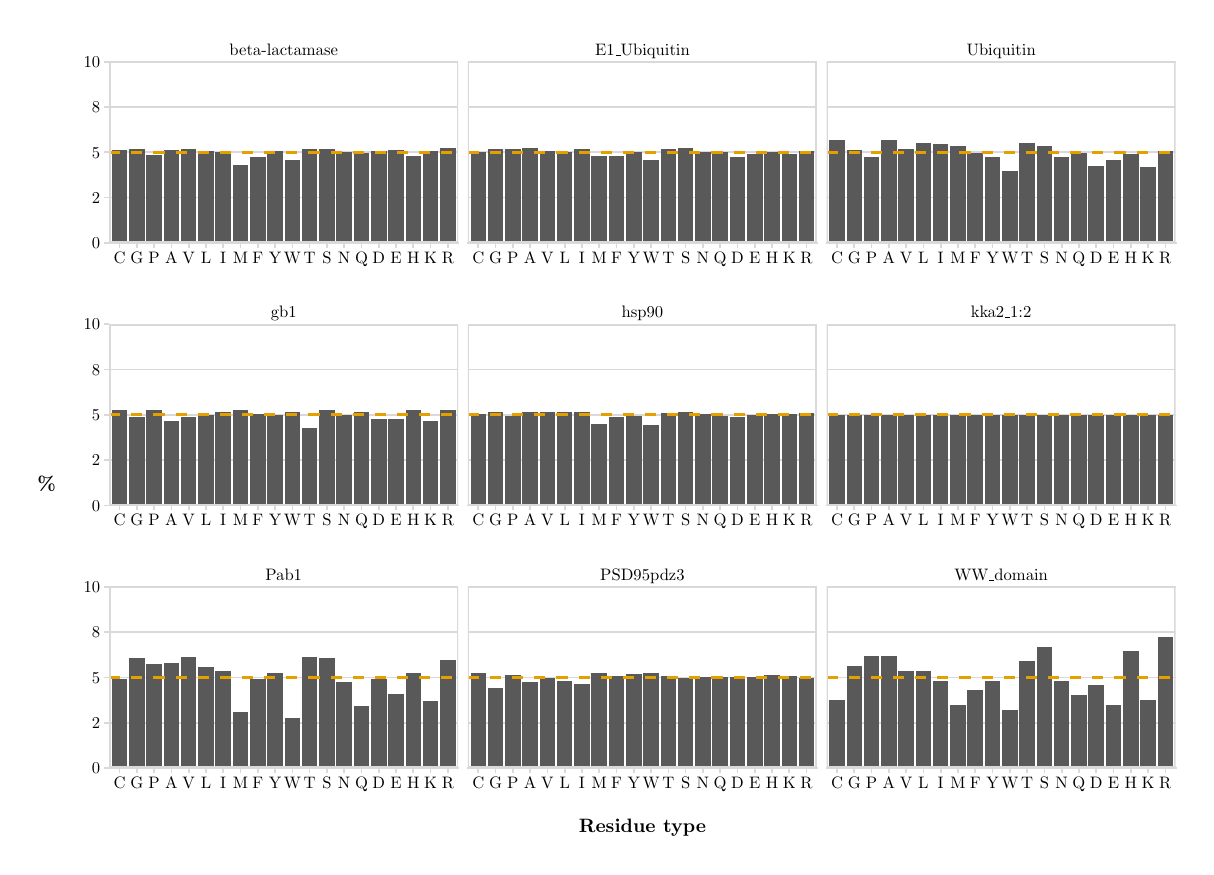
\begin{tikzpicture}[x=1pt,y=1pt]
\definecolor{fillColor}{RGB}{255,255,255}
\path[use as bounding box,fill=fillColor,fill opacity=0.00] (0,0) rectangle (418.34,295.82);
\begin{scope}
\path[clip] ( 29.46,218.05) rectangle (155.58,283.52);
\definecolor{drawColor}{gray}{0.85}

\path[draw=drawColor,line width= 0.6pt,line join=round] ( 29.46,218.05) --
	(155.58,218.05);

\path[draw=drawColor,line width= 0.6pt,line join=round] ( 29.46,234.42) --
	(155.58,234.42);

\path[draw=drawColor,line width= 0.6pt,line join=round] ( 29.46,250.78) --
	(155.58,250.78);

\path[draw=drawColor,line width= 0.6pt,line join=round] ( 29.46,267.15) --
	(155.58,267.15);

\path[draw=drawColor,line width= 0.6pt,line join=round] ( 29.46,283.52) --
	(155.58,283.52);
\definecolor{fillColor}{gray}{0.35}

\path[fill=fillColor] ( 30.39,218.05) rectangle ( 36.01,251.53);

\path[fill=fillColor] ( 36.64,218.05) rectangle ( 42.26,251.89);

\path[fill=fillColor] ( 42.88,218.05) rectangle ( 48.50,249.83);

\path[fill=fillColor] ( 49.13,218.05) rectangle ( 54.75,251.77);

\path[fill=fillColor] ( 55.37,218.05) rectangle ( 60.99,251.89);

\path[fill=fillColor] ( 61.61,218.05) rectangle ( 67.23,251.41);

\path[fill=fillColor] ( 67.86,218.05) rectangle ( 73.48,250.92);

\path[fill=fillColor] ( 74.10,218.05) rectangle ( 79.72,246.07);

\path[fill=fillColor] ( 80.35,218.05) rectangle ( 85.96,249.23);

\path[fill=fillColor] ( 86.59,218.05) rectangle ( 92.21,251.17);

\path[fill=fillColor] ( 92.83,218.05) rectangle ( 98.45,248.13);

\path[fill=fillColor] ( 99.08,218.05) rectangle (104.70,252.14);

\path[fill=fillColor] (105.32,218.05) rectangle (110.94,252.02);

\path[fill=fillColor] (111.56,218.05) rectangle (117.18,250.92);

\path[fill=fillColor] (117.81,218.05) rectangle (123.43,250.56);

\path[fill=fillColor] (124.05,218.05) rectangle (129.67,251.41);

\path[fill=fillColor] (130.30,218.05) rectangle (135.92,251.77);

\path[fill=fillColor] (136.54,218.05) rectangle (142.16,249.59);

\path[fill=fillColor] (142.78,218.05) rectangle (148.40,251.17);

\path[fill=fillColor] (149.03,218.05) rectangle (154.65,252.26);
\definecolor{drawColor}{RGB}{230,159,0}

\path[draw=drawColor,line width= 1.1pt,dash pattern=on 4pt off 4pt ,line join=round] ( 29.46,250.78) -- (155.58,250.78);
\definecolor{drawColor}{gray}{0.85}

\path[draw=drawColor,line width= 1.1pt,line join=round,line cap=round] ( 29.46,218.05) rectangle (155.58,283.52);
\end{scope}
\begin{scope}
\path[clip] ( 29.46,123.17) rectangle (155.58,188.65);
\definecolor{drawColor}{gray}{0.85}

\path[draw=drawColor,line width= 0.6pt,line join=round] ( 29.46,123.17) --
	(155.58,123.17);

\path[draw=drawColor,line width= 0.6pt,line join=round] ( 29.46,139.54) --
	(155.58,139.54);

\path[draw=drawColor,line width= 0.6pt,line join=round] ( 29.46,155.91) --
	(155.58,155.91);

\path[draw=drawColor,line width= 0.6pt,line join=round] ( 29.46,172.28) --
	(155.58,172.28);

\path[draw=drawColor,line width= 0.6pt,line join=round] ( 29.46,188.65) --
	(155.58,188.65);
\definecolor{fillColor}{gray}{0.35}

\path[fill=fillColor] ( 30.39,123.17) rectangle ( 36.01,157.64);

\path[fill=fillColor] ( 36.64,123.17) rectangle ( 42.26,155.08);

\path[fill=fillColor] ( 42.88,123.17) rectangle ( 48.50,157.64);

\path[fill=fillColor] ( 49.13,123.17) rectangle ( 54.75,153.81);

\path[fill=fillColor] ( 55.37,123.17) rectangle ( 60.99,155.08);

\path[fill=fillColor] ( 61.61,123.17) rectangle ( 67.23,155.72);

\path[fill=fillColor] ( 67.86,123.17) rectangle ( 73.48,157.00);

\path[fill=fillColor] ( 74.10,123.17) rectangle ( 79.72,157.64);

\path[fill=fillColor] ( 80.35,123.17) rectangle ( 85.96,156.36);

\path[fill=fillColor] ( 86.59,123.17) rectangle ( 92.21,155.72);

\path[fill=fillColor] ( 92.83,123.17) rectangle ( 98.45,157.00);

\path[fill=fillColor] ( 99.08,123.17) rectangle (104.70,151.25);

\path[fill=fillColor] (105.32,123.17) rectangle (110.94,157.64);

\path[fill=fillColor] (111.56,123.17) rectangle (117.18,155.72);

\path[fill=fillColor] (117.81,123.17) rectangle (123.43,157.00);

\path[fill=fillColor] (124.05,123.17) rectangle (129.67,154.45);

\path[fill=fillColor] (130.30,123.17) rectangle (135.92,154.45);

\path[fill=fillColor] (136.54,123.17) rectangle (142.16,157.64);

\path[fill=fillColor] (142.78,123.17) rectangle (148.40,153.81);

\path[fill=fillColor] (149.03,123.17) rectangle (154.65,157.64);
\definecolor{drawColor}{RGB}{230,159,0}

\path[draw=drawColor,line width= 1.1pt,dash pattern=on 4pt off 4pt ,line join=round] ( 29.46,155.91) -- (155.58,155.91);
\definecolor{drawColor}{gray}{0.85}

\path[draw=drawColor,line width= 1.1pt,line join=round,line cap=round] ( 29.46,123.17) rectangle (155.58,188.65);
\end{scope}
\begin{scope}
\path[clip] ( 29.46, 28.30) rectangle (155.58, 93.78);
\definecolor{drawColor}{gray}{0.85}

\path[draw=drawColor,line width= 0.6pt,line join=round] ( 29.46, 28.30) --
	(155.58, 28.30);

\path[draw=drawColor,line width= 0.6pt,line join=round] ( 29.46, 44.67) --
	(155.58, 44.67);

\path[draw=drawColor,line width= 0.6pt,line join=round] ( 29.46, 61.04) --
	(155.58, 61.04);

\path[draw=drawColor,line width= 0.6pt,line join=round] ( 29.46, 77.41) --
	(155.58, 77.41);

\path[draw=drawColor,line width= 0.6pt,line join=round] ( 29.46, 93.78) --
	(155.58, 93.78);
\definecolor{fillColor}{gray}{0.35}

\path[fill=fillColor] ( 30.39, 28.30) rectangle ( 36.01, 60.51);

\path[fill=fillColor] ( 36.64, 28.30) rectangle ( 42.26, 68.02);

\path[fill=fillColor] ( 42.88, 28.30) rectangle ( 48.50, 65.87);

\path[fill=fillColor] ( 49.13, 28.30) rectangle ( 54.75, 66.41);

\path[fill=fillColor] ( 55.37, 28.30) rectangle ( 60.99, 68.56);

\path[fill=fillColor] ( 61.61, 28.30) rectangle ( 67.23, 64.80);

\path[fill=fillColor] ( 67.86, 28.30) rectangle ( 73.48, 63.19);

\path[fill=fillColor] ( 74.10, 28.30) rectangle ( 79.72, 48.70);

\path[fill=fillColor] ( 80.35, 28.30) rectangle ( 85.96, 60.51);

\path[fill=fillColor] ( 86.59, 28.30) rectangle ( 92.21, 62.65);

\path[fill=fillColor] ( 92.83, 28.30) rectangle ( 98.45, 46.55);

\path[fill=fillColor] ( 99.08, 28.30) rectangle (104.70, 68.56);

\path[fill=fillColor] (105.32, 28.30) rectangle (110.94, 68.02);

\path[fill=fillColor] (111.56, 28.30) rectangle (117.18, 59.43);

\path[fill=fillColor] (117.81, 28.30) rectangle (123.43, 50.84);

\path[fill=fillColor] (124.05, 28.30) rectangle (129.67, 60.51);

\path[fill=fillColor] (130.30, 28.30) rectangle (135.92, 55.14);

\path[fill=fillColor] (136.54, 28.30) rectangle (142.16, 62.65);

\path[fill=fillColor] (142.78, 28.30) rectangle (148.40, 52.46);

\path[fill=fillColor] (149.03, 28.30) rectangle (154.65, 67.48);
\definecolor{drawColor}{RGB}{230,159,0}

\path[draw=drawColor,line width= 1.1pt,dash pattern=on 4pt off 4pt ,line join=round] ( 29.46, 61.04) -- (155.58, 61.04);
\definecolor{drawColor}{gray}{0.85}

\path[draw=drawColor,line width= 1.1pt,line join=round,line cap=round] ( 29.46, 28.30) rectangle (155.58, 93.78);
\end{scope}
\begin{scope}
\path[clip] (159.08,218.05) rectangle (285.21,283.52);
\definecolor{drawColor}{gray}{0.85}

\path[draw=drawColor,line width= 0.6pt,line join=round] (159.08,218.05) --
	(285.21,218.05);

\path[draw=drawColor,line width= 0.6pt,line join=round] (159.08,234.42) --
	(285.21,234.42);

\path[draw=drawColor,line width= 0.6pt,line join=round] (159.08,250.78) --
	(285.21,250.78);

\path[draw=drawColor,line width= 0.6pt,line join=round] (159.08,267.15) --
	(285.21,267.15);

\path[draw=drawColor,line width= 0.6pt,line join=round] (159.08,283.52) --
	(285.21,283.52);
\definecolor{fillColor}{gray}{0.35}

\path[fill=fillColor] (160.02,218.05) rectangle (165.64,250.73);

\path[fill=fillColor] (166.26,218.05) rectangle (171.88,251.87);

\path[fill=fillColor] (172.51,218.05) rectangle (178.13,251.87);

\path[fill=fillColor] (178.75,218.05) rectangle (184.37,252.45);

\path[fill=fillColor] (185.00,218.05) rectangle (190.62,251.30);

\path[fill=fillColor] (191.24,218.05) rectangle (196.86,250.73);

\path[fill=fillColor] (197.48,218.05) rectangle (203.10,251.87);

\path[fill=fillColor] (203.73,218.05) rectangle (209.35,249.58);

\path[fill=fillColor] (209.97,218.05) rectangle (215.59,249.58);

\path[fill=fillColor] (216.22,218.05) rectangle (221.83,250.73);

\path[fill=fillColor] (222.46,218.05) rectangle (228.08,247.86);

\path[fill=fillColor] (228.70,218.05) rectangle (234.32,251.87);

\path[fill=fillColor] (234.95,218.05) rectangle (240.57,252.45);

\path[fill=fillColor] (241.19,218.05) rectangle (246.81,250.73);

\path[fill=fillColor] (247.43,218.05) rectangle (253.05,250.73);

\path[fill=fillColor] (253.68,218.05) rectangle (259.30,249.01);

\path[fill=fillColor] (259.92,218.05) rectangle (265.54,250.15);

\path[fill=fillColor] (266.17,218.05) rectangle (271.79,250.73);

\path[fill=fillColor] (272.41,218.05) rectangle (278.03,250.15);

\path[fill=fillColor] (278.65,218.05) rectangle (284.27,251.30);
\definecolor{drawColor}{RGB}{230,159,0}

\path[draw=drawColor,line width= 1.1pt,dash pattern=on 4pt off 4pt ,line join=round] (159.08,250.78) -- (285.21,250.78);
\definecolor{drawColor}{gray}{0.85}

\path[draw=drawColor,line width= 1.1pt,line join=round,line cap=round] (159.08,218.05) rectangle (285.21,283.52);
\end{scope}
\begin{scope}
\path[clip] (159.08,123.17) rectangle (285.21,188.65);
\definecolor{drawColor}{gray}{0.85}

\path[draw=drawColor,line width= 0.6pt,line join=round] (159.08,123.17) --
	(285.21,123.17);

\path[draw=drawColor,line width= 0.6pt,line join=round] (159.08,139.54) --
	(285.21,139.54);

\path[draw=drawColor,line width= 0.6pt,line join=round] (159.08,155.91) --
	(285.21,155.91);

\path[draw=drawColor,line width= 0.6pt,line join=round] (159.08,172.28) --
	(285.21,172.28);

\path[draw=drawColor,line width= 0.6pt,line join=round] (159.08,188.65) --
	(285.21,188.65);
\definecolor{fillColor}{gray}{0.35}

\path[fill=fillColor] (160.02,123.17) rectangle (165.64,156.14);

\path[fill=fillColor] (166.26,123.17) rectangle (171.88,156.91);

\path[fill=fillColor] (172.51,123.17) rectangle (178.13,155.67);

\path[fill=fillColor] (178.75,123.17) rectangle (184.37,157.07);

\path[fill=fillColor] (185.00,123.17) rectangle (190.62,157.07);

\path[fill=fillColor] (191.24,123.17) rectangle (196.86,157.07);

\path[fill=fillColor] (197.48,123.17) rectangle (203.10,156.91);

\path[fill=fillColor] (203.73,123.17) rectangle (209.35,152.73);

\path[fill=fillColor] (209.97,123.17) rectangle (215.59,155.21);

\path[fill=fillColor] (216.22,123.17) rectangle (221.83,155.52);

\path[fill=fillColor] (222.46,123.17) rectangle (228.08,152.11);

\path[fill=fillColor] (228.70,123.17) rectangle (234.32,156.76);

\path[fill=fillColor] (234.95,123.17) rectangle (240.57,157.07);

\path[fill=fillColor] (241.19,123.17) rectangle (246.81,156.14);

\path[fill=fillColor] (247.43,123.17) rectangle (253.05,155.67);

\path[fill=fillColor] (253.68,123.17) rectangle (259.30,155.21);

\path[fill=fillColor] (259.92,123.17) rectangle (265.54,155.83);

\path[fill=fillColor] (266.17,123.17) rectangle (271.79,156.29);

\path[fill=fillColor] (272.41,123.17) rectangle (278.03,156.29);

\path[fill=fillColor] (278.65,123.17) rectangle (284.27,156.60);
\definecolor{drawColor}{RGB}{230,159,0}

\path[draw=drawColor,line width= 1.1pt,dash pattern=on 4pt off 4pt ,line join=round] (159.08,155.91) -- (285.21,155.91);
\definecolor{drawColor}{gray}{0.85}

\path[draw=drawColor,line width= 1.1pt,line join=round,line cap=round] (159.08,123.17) rectangle (285.21,188.65);
\end{scope}
\begin{scope}
\path[clip] (159.08, 28.30) rectangle (285.21, 93.78);
\definecolor{drawColor}{gray}{0.85}

\path[draw=drawColor,line width= 0.6pt,line join=round] (159.08, 28.30) --
	(285.21, 28.30);

\path[draw=drawColor,line width= 0.6pt,line join=round] (159.08, 44.67) --
	(285.21, 44.67);

\path[draw=drawColor,line width= 0.6pt,line join=round] (159.08, 61.04) --
	(285.21, 61.04);

\path[draw=drawColor,line width= 0.6pt,line join=round] (159.08, 77.41) --
	(285.21, 77.41);

\path[draw=drawColor,line width= 0.6pt,line join=round] (159.08, 93.78) --
	(285.21, 93.78);
\definecolor{fillColor}{gray}{0.35}

\path[fill=fillColor] (160.02, 28.30) rectangle (165.64, 62.77);

\path[fill=fillColor] (166.26, 28.30) rectangle (171.88, 57.37);

\path[fill=fillColor] (172.51, 28.30) rectangle (178.13, 61.93);

\path[fill=fillColor] (178.75, 28.30) rectangle (184.37, 59.44);

\path[fill=fillColor] (185.00, 28.30) rectangle (190.62, 60.69);

\path[fill=fillColor] (191.24, 28.30) rectangle (196.86, 59.86);

\path[fill=fillColor] (197.48, 28.30) rectangle (203.10, 58.61);

\path[fill=fillColor] (203.73, 28.30) rectangle (209.35, 62.77);

\path[fill=fillColor] (209.97, 28.30) rectangle (215.59, 61.52);

\path[fill=fillColor] (216.22, 28.30) rectangle (221.83, 62.35);

\path[fill=fillColor] (222.46, 28.30) rectangle (228.08, 62.77);

\path[fill=fillColor] (228.70, 28.30) rectangle (234.32, 61.52);

\path[fill=fillColor] (234.95, 28.30) rectangle (240.57, 60.69);

\path[fill=fillColor] (241.19, 28.30) rectangle (246.81, 61.10);

\path[fill=fillColor] (247.43, 28.30) rectangle (253.05, 61.10);

\path[fill=fillColor] (253.68, 28.30) rectangle (259.30, 61.10);

\path[fill=fillColor] (259.92, 28.30) rectangle (265.54, 61.10);

\path[fill=fillColor] (266.17, 28.30) rectangle (271.79, 61.93);

\path[fill=fillColor] (272.41, 28.30) rectangle (278.03, 61.52);

\path[fill=fillColor] (278.65, 28.30) rectangle (284.27, 60.69);
\definecolor{drawColor}{RGB}{230,159,0}

\path[draw=drawColor,line width= 1.1pt,dash pattern=on 4pt off 4pt ,line join=round] (159.08, 61.04) -- (285.21, 61.04);
\definecolor{drawColor}{gray}{0.85}

\path[draw=drawColor,line width= 1.1pt,line join=round,line cap=round] (159.08, 28.30) rectangle (285.21, 93.78);
\end{scope}
\begin{scope}
\path[clip] (288.71,218.05) rectangle (414.84,283.52);
\definecolor{drawColor}{gray}{0.85}

\path[draw=drawColor,line width= 0.6pt,line join=round] (288.71,218.05) --
	(414.84,218.05);

\path[draw=drawColor,line width= 0.6pt,line join=round] (288.71,234.42) --
	(414.84,234.42);

\path[draw=drawColor,line width= 0.6pt,line join=round] (288.71,250.78) --
	(414.84,250.78);

\path[draw=drawColor,line width= 0.6pt,line join=round] (288.71,267.15) --
	(414.84,267.15);

\path[draw=drawColor,line width= 0.6pt,line join=round] (288.71,283.52) --
	(414.84,283.52);
\definecolor{fillColor}{gray}{0.35}

\path[fill=fillColor] (289.65,218.05) rectangle (295.27,255.25);

\path[fill=fillColor] (295.89,218.05) rectangle (301.51,251.64);

\path[fill=fillColor] (302.13,218.05) rectangle (307.75,249.05);

\path[fill=fillColor] (308.38,218.05) rectangle (314.00,255.25);

\path[fill=fillColor] (314.62,218.05) rectangle (320.24,252.15);

\path[fill=fillColor] (320.87,218.05) rectangle (326.49,254.22);

\path[fill=fillColor] (327.11,218.05) rectangle (332.73,253.70);

\path[fill=fillColor] (333.35,218.05) rectangle (338.97,253.19);

\path[fill=fillColor] (339.60,218.05) rectangle (345.22,250.60);

\path[fill=fillColor] (345.84,218.05) rectangle (351.46,249.05);

\path[fill=fillColor] (352.08,218.05) rectangle (357.70,243.89);

\path[fill=fillColor] (358.33,218.05) rectangle (363.95,254.22);

\path[fill=fillColor] (364.57,218.05) rectangle (370.19,253.19);

\path[fill=fillColor] (370.82,218.05) rectangle (376.44,249.05);

\path[fill=fillColor] (377.06,218.05) rectangle (382.68,250.60);

\path[fill=fillColor] (383.30,218.05) rectangle (388.92,245.95);

\path[fill=fillColor] (389.55,218.05) rectangle (395.17,248.02);

\path[fill=fillColor] (395.79,218.05) rectangle (401.41,250.09);

\path[fill=fillColor] (402.04,218.05) rectangle (407.66,245.44);

\path[fill=fillColor] (408.28,218.05) rectangle (413.90,251.12);
\definecolor{drawColor}{RGB}{230,159,0}

\path[draw=drawColor,line width= 1.1pt,dash pattern=on 4pt off 4pt ,line join=round] (288.71,250.78) -- (414.84,250.78);
\definecolor{drawColor}{gray}{0.85}

\path[draw=drawColor,line width= 1.1pt,line join=round,line cap=round] (288.71,218.05) rectangle (414.84,283.52);
\end{scope}
\begin{scope}
\path[clip] (288.71,123.17) rectangle (414.84,188.65);
\definecolor{drawColor}{gray}{0.85}

\path[draw=drawColor,line width= 0.6pt,line join=round] (288.71,123.17) --
	(414.84,123.17);

\path[draw=drawColor,line width= 0.6pt,line join=round] (288.71,139.54) --
	(414.84,139.54);

\path[draw=drawColor,line width= 0.6pt,line join=round] (288.71,155.91) --
	(414.84,155.91);

\path[draw=drawColor,line width= 0.6pt,line join=round] (288.71,172.28) --
	(414.84,172.28);

\path[draw=drawColor,line width= 0.6pt,line join=round] (288.71,188.65) --
	(414.84,188.65);
\definecolor{fillColor}{gray}{0.35}

\path[fill=fillColor] (289.65,123.17) rectangle (295.27,155.91);

\path[fill=fillColor] (295.89,123.17) rectangle (301.51,155.91);

\path[fill=fillColor] (302.13,123.17) rectangle (307.75,155.91);

\path[fill=fillColor] (308.38,123.17) rectangle (314.00,155.91);

\path[fill=fillColor] (314.62,123.17) rectangle (320.24,155.91);

\path[fill=fillColor] (320.87,123.17) rectangle (326.49,155.91);

\path[fill=fillColor] (327.11,123.17) rectangle (332.73,155.91);

\path[fill=fillColor] (333.35,123.17) rectangle (338.97,155.91);

\path[fill=fillColor] (339.60,123.17) rectangle (345.22,155.91);

\path[fill=fillColor] (345.84,123.17) rectangle (351.46,155.91);

\path[fill=fillColor] (352.08,123.17) rectangle (357.70,155.91);

\path[fill=fillColor] (358.33,123.17) rectangle (363.95,155.91);

\path[fill=fillColor] (364.57,123.17) rectangle (370.19,155.91);

\path[fill=fillColor] (370.82,123.17) rectangle (376.44,155.91);

\path[fill=fillColor] (377.06,123.17) rectangle (382.68,155.91);

\path[fill=fillColor] (383.30,123.17) rectangle (388.92,155.91);

\path[fill=fillColor] (389.55,123.17) rectangle (395.17,155.91);

\path[fill=fillColor] (395.79,123.17) rectangle (401.41,155.91);

\path[fill=fillColor] (402.04,123.17) rectangle (407.66,155.91);

\path[fill=fillColor] (408.28,123.17) rectangle (413.90,155.91);
\definecolor{drawColor}{RGB}{230,159,0}

\path[draw=drawColor,line width= 1.1pt,dash pattern=on 4pt off 4pt ,line join=round] (288.71,155.91) -- (414.84,155.91);
\definecolor{drawColor}{gray}{0.85}

\path[draw=drawColor,line width= 1.1pt,line join=round,line cap=round] (288.71,123.17) rectangle (414.84,188.65);
\end{scope}
\begin{scope}
\path[clip] (288.71, 28.30) rectangle (414.84, 93.78);
\definecolor{drawColor}{gray}{0.85}

\path[draw=drawColor,line width= 0.6pt,line join=round] (288.71, 28.30) --
	(414.84, 28.30);

\path[draw=drawColor,line width= 0.6pt,line join=round] (288.71, 44.67) --
	(414.84, 44.67);

\path[draw=drawColor,line width= 0.6pt,line join=round] (288.71, 61.04) --
	(414.84, 61.04);

\path[draw=drawColor,line width= 0.6pt,line join=round] (288.71, 77.41) --
	(414.84, 77.41);

\path[draw=drawColor,line width= 0.6pt,line join=round] (288.71, 93.78) --
	(414.84, 93.78);
\definecolor{fillColor}{gray}{0.35}

\path[fill=fillColor] (289.65, 28.30) rectangle (295.27, 52.88);

\path[fill=fillColor] (295.89, 28.30) rectangle (301.51, 65.17);

\path[fill=fillColor] (302.13, 28.30) rectangle (307.75, 68.68);

\path[fill=fillColor] (308.38, 28.30) rectangle (314.00, 68.68);

\path[fill=fillColor] (314.62, 28.30) rectangle (320.24, 63.41);

\path[fill=fillColor] (320.87, 28.30) rectangle (326.49, 63.41);

\path[fill=fillColor] (327.11, 28.30) rectangle (332.73, 59.90);

\path[fill=fillColor] (333.35, 28.30) rectangle (338.97, 51.12);

\path[fill=fillColor] (339.60, 28.30) rectangle (345.22, 56.39);

\path[fill=fillColor] (345.84, 28.30) rectangle (351.46, 59.90);

\path[fill=fillColor] (352.08, 28.30) rectangle (357.70, 49.37);

\path[fill=fillColor] (358.33, 28.30) rectangle (363.95, 66.92);

\path[fill=fillColor] (364.57, 28.30) rectangle (370.19, 72.19);

\path[fill=fillColor] (370.82, 28.30) rectangle (376.44, 59.90);

\path[fill=fillColor] (377.06, 28.30) rectangle (382.68, 54.63);

\path[fill=fillColor] (383.30, 28.30) rectangle (388.92, 58.15);

\path[fill=fillColor] (389.55, 28.30) rectangle (395.17, 51.12);

\path[fill=fillColor] (395.79, 28.30) rectangle (401.41, 70.43);

\path[fill=fillColor] (402.04, 28.30) rectangle (407.66, 52.88);

\path[fill=fillColor] (408.28, 28.30) rectangle (413.90, 75.70);
\definecolor{drawColor}{RGB}{230,159,0}

\path[draw=drawColor,line width= 1.1pt,dash pattern=on 4pt off 4pt ,line join=round] (288.71, 61.04) -- (414.84, 61.04);
\definecolor{drawColor}{gray}{0.85}

\path[draw=drawColor,line width= 1.1pt,line join=round,line cap=round] (288.71, 28.30) rectangle (414.84, 93.78);
\end{scope}
\begin{scope}
\path[clip] ( 29.46, 93.78) rectangle (155.58,102.58);
\definecolor{drawColor}{RGB}{0,0,0}

\node[text=drawColor,anchor=base,inner sep=0pt, outer sep=0pt, scale=  0.60] at ( 92.52, 96.11) {Pab1};
\end{scope}
\begin{scope}
\path[clip] (159.08, 93.78) rectangle (285.21,102.58);
\definecolor{drawColor}{RGB}{0,0,0}

\node[text=drawColor,anchor=base,inner sep=0pt, outer sep=0pt, scale=  0.60] at (222.15, 96.11) {PSD95pdz3};
\end{scope}
\begin{scope}
\path[clip] (288.71, 93.78) rectangle (414.84,102.58);
\definecolor{drawColor}{RGB}{0,0,0}

\node[text=drawColor,anchor=base,inner sep=0pt, outer sep=0pt, scale=  0.60] at (351.77, 96.11) {WW\_domain};
\end{scope}
\begin{scope}
\path[clip] ( 29.46,188.65) rectangle (155.58,197.45);
\definecolor{drawColor}{RGB}{0,0,0}

\node[text=drawColor,anchor=base,inner sep=0pt, outer sep=0pt, scale=  0.60] at ( 92.52,190.99) {gb1};
\end{scope}
\begin{scope}
\path[clip] (159.08,188.65) rectangle (285.21,197.45);
\definecolor{drawColor}{RGB}{0,0,0}

\node[text=drawColor,anchor=base,inner sep=0pt, outer sep=0pt, scale=  0.60] at (222.15,190.99) {hsp90};
\end{scope}
\begin{scope}
\path[clip] (288.71,188.65) rectangle (414.84,197.45);
\definecolor{drawColor}{RGB}{0,0,0}

\node[text=drawColor,anchor=base,inner sep=0pt, outer sep=0pt, scale=  0.60] at (351.77,190.99) {kka2\_1:2};
\end{scope}
\begin{scope}
\path[clip] ( 29.46,283.52) rectangle (155.58,292.32);
\definecolor{drawColor}{RGB}{0,0,0}

\node[text=drawColor,anchor=base,inner sep=0pt, outer sep=0pt, scale=  0.60] at ( 92.52,285.86) {beta-lactamase};
\end{scope}
\begin{scope}
\path[clip] (159.08,283.52) rectangle (285.21,292.32);
\definecolor{drawColor}{RGB}{0,0,0}

\node[text=drawColor,anchor=base,inner sep=0pt, outer sep=0pt, scale=  0.60] at (222.15,285.86) {E1\_Ubiquitin};
\end{scope}
\begin{scope}
\path[clip] (288.71,283.52) rectangle (414.84,292.32);
\definecolor{drawColor}{RGB}{0,0,0}

\node[text=drawColor,anchor=base,inner sep=0pt, outer sep=0pt, scale=  0.60] at (351.77,285.86) {Ubiquitin};
\end{scope}
\begin{scope}
\path[clip] (  0.00,  0.00) rectangle (418.34,295.82);
\definecolor{drawColor}{gray}{0.85}

\path[draw=drawColor,line width= 0.6pt,line join=round,line cap=rect] ( 29.46, 28.30) --
	(155.58, 28.30);
\end{scope}
\begin{scope}
\path[clip] (  0.00,  0.00) rectangle (418.34,295.82);
\definecolor{drawColor}{gray}{0.85}

\path[draw=drawColor,line width= 0.6pt,line join=round] ( 33.20, 26.55) --
	( 33.20, 28.30);

\path[draw=drawColor,line width= 0.6pt,line join=round] ( 39.45, 26.55) --
	( 39.45, 28.30);

\path[draw=drawColor,line width= 0.6pt,line join=round] ( 45.69, 26.55) --
	( 45.69, 28.30);

\path[draw=drawColor,line width= 0.6pt,line join=round] ( 51.94, 26.55) --
	( 51.94, 28.30);

\path[draw=drawColor,line width= 0.6pt,line join=round] ( 58.18, 26.55) --
	( 58.18, 28.30);

\path[draw=drawColor,line width= 0.6pt,line join=round] ( 64.42, 26.55) --
	( 64.42, 28.30);

\path[draw=drawColor,line width= 0.6pt,line join=round] ( 70.67, 26.55) --
	( 70.67, 28.30);

\path[draw=drawColor,line width= 0.6pt,line join=round] ( 76.91, 26.55) --
	( 76.91, 28.30);

\path[draw=drawColor,line width= 0.6pt,line join=round] ( 83.16, 26.55) --
	( 83.16, 28.30);

\path[draw=drawColor,line width= 0.6pt,line join=round] ( 89.40, 26.55) --
	( 89.40, 28.30);

\path[draw=drawColor,line width= 0.6pt,line join=round] ( 95.64, 26.55) --
	( 95.64, 28.30);

\path[draw=drawColor,line width= 0.6pt,line join=round] (101.89, 26.55) --
	(101.89, 28.30);

\path[draw=drawColor,line width= 0.6pt,line join=round] (108.13, 26.55) --
	(108.13, 28.30);

\path[draw=drawColor,line width= 0.6pt,line join=round] (114.37, 26.55) --
	(114.37, 28.30);

\path[draw=drawColor,line width= 0.6pt,line join=round] (120.62, 26.55) --
	(120.62, 28.30);

\path[draw=drawColor,line width= 0.6pt,line join=round] (126.86, 26.55) --
	(126.86, 28.30);

\path[draw=drawColor,line width= 0.6pt,line join=round] (133.11, 26.55) --
	(133.11, 28.30);

\path[draw=drawColor,line width= 0.6pt,line join=round] (139.35, 26.55) --
	(139.35, 28.30);

\path[draw=drawColor,line width= 0.6pt,line join=round] (145.59, 26.55) --
	(145.59, 28.30);

\path[draw=drawColor,line width= 0.6pt,line join=round] (151.84, 26.55) --
	(151.84, 28.30);
\end{scope}
\begin{scope}
\path[clip] (  0.00,  0.00) rectangle (418.34,295.82);
\definecolor{drawColor}{RGB}{0,0,0}

\node[text=drawColor,anchor=base,inner sep=0pt, outer sep=0pt, scale=  0.60] at ( 33.20, 20.92) {C};

\node[text=drawColor,anchor=base,inner sep=0pt, outer sep=0pt, scale=  0.60] at ( 39.45, 20.92) {G};

\node[text=drawColor,anchor=base,inner sep=0pt, outer sep=0pt, scale=  0.60] at ( 45.69, 20.92) {P};

\node[text=drawColor,anchor=base,inner sep=0pt, outer sep=0pt, scale=  0.60] at ( 51.94, 20.92) {A};

\node[text=drawColor,anchor=base,inner sep=0pt, outer sep=0pt, scale=  0.60] at ( 58.18, 20.92) {V};

\node[text=drawColor,anchor=base,inner sep=0pt, outer sep=0pt, scale=  0.60] at ( 64.42, 20.92) {L};

\node[text=drawColor,anchor=base,inner sep=0pt, outer sep=0pt, scale=  0.60] at ( 70.67, 20.92) {I};

\node[text=drawColor,anchor=base,inner sep=0pt, outer sep=0pt, scale=  0.60] at ( 76.91, 20.92) {M};

\node[text=drawColor,anchor=base,inner sep=0pt, outer sep=0pt, scale=  0.60] at ( 83.16, 20.92) {F};

\node[text=drawColor,anchor=base,inner sep=0pt, outer sep=0pt, scale=  0.60] at ( 89.40, 20.92) {Y};

\node[text=drawColor,anchor=base,inner sep=0pt, outer sep=0pt, scale=  0.60] at ( 95.64, 20.92) {W};

\node[text=drawColor,anchor=base,inner sep=0pt, outer sep=0pt, scale=  0.60] at (101.89, 20.92) {T};

\node[text=drawColor,anchor=base,inner sep=0pt, outer sep=0pt, scale=  0.60] at (108.13, 20.92) {S};

\node[text=drawColor,anchor=base,inner sep=0pt, outer sep=0pt, scale=  0.60] at (114.37, 20.92) {N};

\node[text=drawColor,anchor=base,inner sep=0pt, outer sep=0pt, scale=  0.60] at (120.62, 20.92) {Q};

\node[text=drawColor,anchor=base,inner sep=0pt, outer sep=0pt, scale=  0.60] at (126.86, 20.92) {D};

\node[text=drawColor,anchor=base,inner sep=0pt, outer sep=0pt, scale=  0.60] at (133.11, 20.92) {E};

\node[text=drawColor,anchor=base,inner sep=0pt, outer sep=0pt, scale=  0.60] at (139.35, 20.92) {H};

\node[text=drawColor,anchor=base,inner sep=0pt, outer sep=0pt, scale=  0.60] at (145.59, 20.92) {K};

\node[text=drawColor,anchor=base,inner sep=0pt, outer sep=0pt, scale=  0.60] at (151.84, 20.92) {R};
\end{scope}
\begin{scope}
\path[clip] (  0.00,  0.00) rectangle (418.34,295.82);
\definecolor{drawColor}{gray}{0.85}

\path[draw=drawColor,line width= 0.6pt,line join=round,line cap=rect] (159.08, 28.30) --
	(285.21, 28.30);
\end{scope}
\begin{scope}
\path[clip] (  0.00,  0.00) rectangle (418.34,295.82);
\definecolor{drawColor}{gray}{0.85}

\path[draw=drawColor,line width= 0.6pt,line join=round] (162.83, 26.55) --
	(162.83, 28.30);

\path[draw=drawColor,line width= 0.6pt,line join=round] (169.07, 26.55) --
	(169.07, 28.30);

\path[draw=drawColor,line width= 0.6pt,line join=round] (175.32, 26.55) --
	(175.32, 28.30);

\path[draw=drawColor,line width= 0.6pt,line join=round] (181.56, 26.55) --
	(181.56, 28.30);

\path[draw=drawColor,line width= 0.6pt,line join=round] (187.81, 26.55) --
	(187.81, 28.30);

\path[draw=drawColor,line width= 0.6pt,line join=round] (194.05, 26.55) --
	(194.05, 28.30);

\path[draw=drawColor,line width= 0.6pt,line join=round] (200.29, 26.55) --
	(200.29, 28.30);

\path[draw=drawColor,line width= 0.6pt,line join=round] (206.54, 26.55) --
	(206.54, 28.30);

\path[draw=drawColor,line width= 0.6pt,line join=round] (212.78, 26.55) --
	(212.78, 28.30);

\path[draw=drawColor,line width= 0.6pt,line join=round] (219.02, 26.55) --
	(219.02, 28.30);

\path[draw=drawColor,line width= 0.6pt,line join=round] (225.27, 26.55) --
	(225.27, 28.30);

\path[draw=drawColor,line width= 0.6pt,line join=round] (231.51, 26.55) --
	(231.51, 28.30);

\path[draw=drawColor,line width= 0.6pt,line join=round] (237.76, 26.55) --
	(237.76, 28.30);

\path[draw=drawColor,line width= 0.6pt,line join=round] (244.00, 26.55) --
	(244.00, 28.30);

\path[draw=drawColor,line width= 0.6pt,line join=round] (250.24, 26.55) --
	(250.24, 28.30);

\path[draw=drawColor,line width= 0.6pt,line join=round] (256.49, 26.55) --
	(256.49, 28.30);

\path[draw=drawColor,line width= 0.6pt,line join=round] (262.73, 26.55) --
	(262.73, 28.30);

\path[draw=drawColor,line width= 0.6pt,line join=round] (268.98, 26.55) --
	(268.98, 28.30);

\path[draw=drawColor,line width= 0.6pt,line join=round] (275.22, 26.55) --
	(275.22, 28.30);

\path[draw=drawColor,line width= 0.6pt,line join=round] (281.46, 26.55) --
	(281.46, 28.30);
\end{scope}
\begin{scope}
\path[clip] (  0.00,  0.00) rectangle (418.34,295.82);
\definecolor{drawColor}{RGB}{0,0,0}

\node[text=drawColor,anchor=base,inner sep=0pt, outer sep=0pt, scale=  0.60] at (162.83, 20.92) {C};

\node[text=drawColor,anchor=base,inner sep=0pt, outer sep=0pt, scale=  0.60] at (169.07, 20.92) {G};

\node[text=drawColor,anchor=base,inner sep=0pt, outer sep=0pt, scale=  0.60] at (175.32, 20.92) {P};

\node[text=drawColor,anchor=base,inner sep=0pt, outer sep=0pt, scale=  0.60] at (181.56, 20.92) {A};

\node[text=drawColor,anchor=base,inner sep=0pt, outer sep=0pt, scale=  0.60] at (187.81, 20.92) {V};

\node[text=drawColor,anchor=base,inner sep=0pt, outer sep=0pt, scale=  0.60] at (194.05, 20.92) {L};

\node[text=drawColor,anchor=base,inner sep=0pt, outer sep=0pt, scale=  0.60] at (200.29, 20.92) {I};

\node[text=drawColor,anchor=base,inner sep=0pt, outer sep=0pt, scale=  0.60] at (206.54, 20.92) {M};

\node[text=drawColor,anchor=base,inner sep=0pt, outer sep=0pt, scale=  0.60] at (212.78, 20.92) {F};

\node[text=drawColor,anchor=base,inner sep=0pt, outer sep=0pt, scale=  0.60] at (219.02, 20.92) {Y};

\node[text=drawColor,anchor=base,inner sep=0pt, outer sep=0pt, scale=  0.60] at (225.27, 20.92) {W};

\node[text=drawColor,anchor=base,inner sep=0pt, outer sep=0pt, scale=  0.60] at (231.51, 20.92) {T};

\node[text=drawColor,anchor=base,inner sep=0pt, outer sep=0pt, scale=  0.60] at (237.76, 20.92) {S};

\node[text=drawColor,anchor=base,inner sep=0pt, outer sep=0pt, scale=  0.60] at (244.00, 20.92) {N};

\node[text=drawColor,anchor=base,inner sep=0pt, outer sep=0pt, scale=  0.60] at (250.24, 20.92) {Q};

\node[text=drawColor,anchor=base,inner sep=0pt, outer sep=0pt, scale=  0.60] at (256.49, 20.92) {D};

\node[text=drawColor,anchor=base,inner sep=0pt, outer sep=0pt, scale=  0.60] at (262.73, 20.92) {E};

\node[text=drawColor,anchor=base,inner sep=0pt, outer sep=0pt, scale=  0.60] at (268.98, 20.92) {H};

\node[text=drawColor,anchor=base,inner sep=0pt, outer sep=0pt, scale=  0.60] at (275.22, 20.92) {K};

\node[text=drawColor,anchor=base,inner sep=0pt, outer sep=0pt, scale=  0.60] at (281.46, 20.92) {R};
\end{scope}
\begin{scope}
\path[clip] (  0.00,  0.00) rectangle (418.34,295.82);
\definecolor{drawColor}{gray}{0.85}

\path[draw=drawColor,line width= 0.6pt,line join=round,line cap=rect] (288.71, 28.30) --
	(414.84, 28.30);
\end{scope}
\begin{scope}
\path[clip] (  0.00,  0.00) rectangle (418.34,295.82);
\definecolor{drawColor}{gray}{0.85}

\path[draw=drawColor,line width= 0.6pt,line join=round] (292.46, 26.55) --
	(292.46, 28.30);

\path[draw=drawColor,line width= 0.6pt,line join=round] (298.70, 26.55) --
	(298.70, 28.30);

\path[draw=drawColor,line width= 0.6pt,line join=round] (304.94, 26.55) --
	(304.94, 28.30);

\path[draw=drawColor,line width= 0.6pt,line join=round] (311.19, 26.55) --
	(311.19, 28.30);

\path[draw=drawColor,line width= 0.6pt,line join=round] (317.43, 26.55) --
	(317.43, 28.30);

\path[draw=drawColor,line width= 0.6pt,line join=round] (323.68, 26.55) --
	(323.68, 28.30);

\path[draw=drawColor,line width= 0.6pt,line join=round] (329.92, 26.55) --
	(329.92, 28.30);

\path[draw=drawColor,line width= 0.6pt,line join=round] (336.16, 26.55) --
	(336.16, 28.30);

\path[draw=drawColor,line width= 0.6pt,line join=round] (342.41, 26.55) --
	(342.41, 28.30);

\path[draw=drawColor,line width= 0.6pt,line join=round] (348.65, 26.55) --
	(348.65, 28.30);

\path[draw=drawColor,line width= 0.6pt,line join=round] (354.89, 26.55) --
	(354.89, 28.30);

\path[draw=drawColor,line width= 0.6pt,line join=round] (361.14, 26.55) --
	(361.14, 28.30);

\path[draw=drawColor,line width= 0.6pt,line join=round] (367.38, 26.55) --
	(367.38, 28.30);

\path[draw=drawColor,line width= 0.6pt,line join=round] (373.63, 26.55) --
	(373.63, 28.30);

\path[draw=drawColor,line width= 0.6pt,line join=round] (379.87, 26.55) --
	(379.87, 28.30);

\path[draw=drawColor,line width= 0.6pt,line join=round] (386.11, 26.55) --
	(386.11, 28.30);

\path[draw=drawColor,line width= 0.6pt,line join=round] (392.36, 26.55) --
	(392.36, 28.30);

\path[draw=drawColor,line width= 0.6pt,line join=round] (398.60, 26.55) --
	(398.60, 28.30);

\path[draw=drawColor,line width= 0.6pt,line join=round] (404.85, 26.55) --
	(404.85, 28.30);

\path[draw=drawColor,line width= 0.6pt,line join=round] (411.09, 26.55) --
	(411.09, 28.30);
\end{scope}
\begin{scope}
\path[clip] (  0.00,  0.00) rectangle (418.34,295.82);
\definecolor{drawColor}{RGB}{0,0,0}

\node[text=drawColor,anchor=base,inner sep=0pt, outer sep=0pt, scale=  0.60] at (292.46, 20.92) {C};

\node[text=drawColor,anchor=base,inner sep=0pt, outer sep=0pt, scale=  0.60] at (298.70, 20.92) {G};

\node[text=drawColor,anchor=base,inner sep=0pt, outer sep=0pt, scale=  0.60] at (304.94, 20.92) {P};

\node[text=drawColor,anchor=base,inner sep=0pt, outer sep=0pt, scale=  0.60] at (311.19, 20.92) {A};

\node[text=drawColor,anchor=base,inner sep=0pt, outer sep=0pt, scale=  0.60] at (317.43, 20.92) {V};

\node[text=drawColor,anchor=base,inner sep=0pt, outer sep=0pt, scale=  0.60] at (323.68, 20.92) {L};

\node[text=drawColor,anchor=base,inner sep=0pt, outer sep=0pt, scale=  0.60] at (329.92, 20.92) {I};

\node[text=drawColor,anchor=base,inner sep=0pt, outer sep=0pt, scale=  0.60] at (336.16, 20.92) {M};

\node[text=drawColor,anchor=base,inner sep=0pt, outer sep=0pt, scale=  0.60] at (342.41, 20.92) {F};

\node[text=drawColor,anchor=base,inner sep=0pt, outer sep=0pt, scale=  0.60] at (348.65, 20.92) {Y};

\node[text=drawColor,anchor=base,inner sep=0pt, outer sep=0pt, scale=  0.60] at (354.89, 20.92) {W};

\node[text=drawColor,anchor=base,inner sep=0pt, outer sep=0pt, scale=  0.60] at (361.14, 20.92) {T};

\node[text=drawColor,anchor=base,inner sep=0pt, outer sep=0pt, scale=  0.60] at (367.38, 20.92) {S};

\node[text=drawColor,anchor=base,inner sep=0pt, outer sep=0pt, scale=  0.60] at (373.63, 20.92) {N};

\node[text=drawColor,anchor=base,inner sep=0pt, outer sep=0pt, scale=  0.60] at (379.87, 20.92) {Q};

\node[text=drawColor,anchor=base,inner sep=0pt, outer sep=0pt, scale=  0.60] at (386.11, 20.92) {D};

\node[text=drawColor,anchor=base,inner sep=0pt, outer sep=0pt, scale=  0.60] at (392.36, 20.92) {E};

\node[text=drawColor,anchor=base,inner sep=0pt, outer sep=0pt, scale=  0.60] at (398.60, 20.92) {H};

\node[text=drawColor,anchor=base,inner sep=0pt, outer sep=0pt, scale=  0.60] at (404.85, 20.92) {K};

\node[text=drawColor,anchor=base,inner sep=0pt, outer sep=0pt, scale=  0.60] at (411.09, 20.92) {R};
\end{scope}
\begin{scope}
\path[clip] (  0.00,  0.00) rectangle (418.34,295.82);
\definecolor{drawColor}{gray}{0.85}

\path[draw=drawColor,line width= 0.6pt,line join=round,line cap=rect] ( 29.46,123.17) --
	(155.58,123.17);
\end{scope}
\begin{scope}
\path[clip] (  0.00,  0.00) rectangle (418.34,295.82);
\definecolor{drawColor}{gray}{0.85}

\path[draw=drawColor,line width= 0.6pt,line join=round] ( 33.20,121.42) --
	( 33.20,123.17);

\path[draw=drawColor,line width= 0.6pt,line join=round] ( 39.45,121.42) --
	( 39.45,123.17);

\path[draw=drawColor,line width= 0.6pt,line join=round] ( 45.69,121.42) --
	( 45.69,123.17);

\path[draw=drawColor,line width= 0.6pt,line join=round] ( 51.94,121.42) --
	( 51.94,123.17);

\path[draw=drawColor,line width= 0.6pt,line join=round] ( 58.18,121.42) --
	( 58.18,123.17);

\path[draw=drawColor,line width= 0.6pt,line join=round] ( 64.42,121.42) --
	( 64.42,123.17);

\path[draw=drawColor,line width= 0.6pt,line join=round] ( 70.67,121.42) --
	( 70.67,123.17);

\path[draw=drawColor,line width= 0.6pt,line join=round] ( 76.91,121.42) --
	( 76.91,123.17);

\path[draw=drawColor,line width= 0.6pt,line join=round] ( 83.16,121.42) --
	( 83.16,123.17);

\path[draw=drawColor,line width= 0.6pt,line join=round] ( 89.40,121.42) --
	( 89.40,123.17);

\path[draw=drawColor,line width= 0.6pt,line join=round] ( 95.64,121.42) --
	( 95.64,123.17);

\path[draw=drawColor,line width= 0.6pt,line join=round] (101.89,121.42) --
	(101.89,123.17);

\path[draw=drawColor,line width= 0.6pt,line join=round] (108.13,121.42) --
	(108.13,123.17);

\path[draw=drawColor,line width= 0.6pt,line join=round] (114.37,121.42) --
	(114.37,123.17);

\path[draw=drawColor,line width= 0.6pt,line join=round] (120.62,121.42) --
	(120.62,123.17);

\path[draw=drawColor,line width= 0.6pt,line join=round] (126.86,121.42) --
	(126.86,123.17);

\path[draw=drawColor,line width= 0.6pt,line join=round] (133.11,121.42) --
	(133.11,123.17);

\path[draw=drawColor,line width= 0.6pt,line join=round] (139.35,121.42) --
	(139.35,123.17);

\path[draw=drawColor,line width= 0.6pt,line join=round] (145.59,121.42) --
	(145.59,123.17);

\path[draw=drawColor,line width= 0.6pt,line join=round] (151.84,121.42) --
	(151.84,123.17);
\end{scope}
\begin{scope}
\path[clip] (  0.00,  0.00) rectangle (418.34,295.82);
\definecolor{drawColor}{RGB}{0,0,0}

\node[text=drawColor,anchor=base,inner sep=0pt, outer sep=0pt, scale=  0.60] at ( 33.20,115.79) {C};

\node[text=drawColor,anchor=base,inner sep=0pt, outer sep=0pt, scale=  0.60] at ( 39.45,115.79) {G};

\node[text=drawColor,anchor=base,inner sep=0pt, outer sep=0pt, scale=  0.60] at ( 45.69,115.79) {P};

\node[text=drawColor,anchor=base,inner sep=0pt, outer sep=0pt, scale=  0.60] at ( 51.94,115.79) {A};

\node[text=drawColor,anchor=base,inner sep=0pt, outer sep=0pt, scale=  0.60] at ( 58.18,115.79) {V};

\node[text=drawColor,anchor=base,inner sep=0pt, outer sep=0pt, scale=  0.60] at ( 64.42,115.79) {L};

\node[text=drawColor,anchor=base,inner sep=0pt, outer sep=0pt, scale=  0.60] at ( 70.67,115.79) {I};

\node[text=drawColor,anchor=base,inner sep=0pt, outer sep=0pt, scale=  0.60] at ( 76.91,115.79) {M};

\node[text=drawColor,anchor=base,inner sep=0pt, outer sep=0pt, scale=  0.60] at ( 83.16,115.79) {F};

\node[text=drawColor,anchor=base,inner sep=0pt, outer sep=0pt, scale=  0.60] at ( 89.40,115.79) {Y};

\node[text=drawColor,anchor=base,inner sep=0pt, outer sep=0pt, scale=  0.60] at ( 95.64,115.79) {W};

\node[text=drawColor,anchor=base,inner sep=0pt, outer sep=0pt, scale=  0.60] at (101.89,115.79) {T};

\node[text=drawColor,anchor=base,inner sep=0pt, outer sep=0pt, scale=  0.60] at (108.13,115.79) {S};

\node[text=drawColor,anchor=base,inner sep=0pt, outer sep=0pt, scale=  0.60] at (114.37,115.79) {N};

\node[text=drawColor,anchor=base,inner sep=0pt, outer sep=0pt, scale=  0.60] at (120.62,115.79) {Q};

\node[text=drawColor,anchor=base,inner sep=0pt, outer sep=0pt, scale=  0.60] at (126.86,115.79) {D};

\node[text=drawColor,anchor=base,inner sep=0pt, outer sep=0pt, scale=  0.60] at (133.11,115.79) {E};

\node[text=drawColor,anchor=base,inner sep=0pt, outer sep=0pt, scale=  0.60] at (139.35,115.79) {H};

\node[text=drawColor,anchor=base,inner sep=0pt, outer sep=0pt, scale=  0.60] at (145.59,115.79) {K};

\node[text=drawColor,anchor=base,inner sep=0pt, outer sep=0pt, scale=  0.60] at (151.84,115.79) {R};
\end{scope}
\begin{scope}
\path[clip] (  0.00,  0.00) rectangle (418.34,295.82);
\definecolor{drawColor}{gray}{0.85}

\path[draw=drawColor,line width= 0.6pt,line join=round,line cap=rect] (159.08,123.17) --
	(285.21,123.17);
\end{scope}
\begin{scope}
\path[clip] (  0.00,  0.00) rectangle (418.34,295.82);
\definecolor{drawColor}{gray}{0.85}

\path[draw=drawColor,line width= 0.6pt,line join=round] (162.83,121.42) --
	(162.83,123.17);

\path[draw=drawColor,line width= 0.6pt,line join=round] (169.07,121.42) --
	(169.07,123.17);

\path[draw=drawColor,line width= 0.6pt,line join=round] (175.32,121.42) --
	(175.32,123.17);

\path[draw=drawColor,line width= 0.6pt,line join=round] (181.56,121.42) --
	(181.56,123.17);

\path[draw=drawColor,line width= 0.6pt,line join=round] (187.81,121.42) --
	(187.81,123.17);

\path[draw=drawColor,line width= 0.6pt,line join=round] (194.05,121.42) --
	(194.05,123.17);

\path[draw=drawColor,line width= 0.6pt,line join=round] (200.29,121.42) --
	(200.29,123.17);

\path[draw=drawColor,line width= 0.6pt,line join=round] (206.54,121.42) --
	(206.54,123.17);

\path[draw=drawColor,line width= 0.6pt,line join=round] (212.78,121.42) --
	(212.78,123.17);

\path[draw=drawColor,line width= 0.6pt,line join=round] (219.02,121.42) --
	(219.02,123.17);

\path[draw=drawColor,line width= 0.6pt,line join=round] (225.27,121.42) --
	(225.27,123.17);

\path[draw=drawColor,line width= 0.6pt,line join=round] (231.51,121.42) --
	(231.51,123.17);

\path[draw=drawColor,line width= 0.6pt,line join=round] (237.76,121.42) --
	(237.76,123.17);

\path[draw=drawColor,line width= 0.6pt,line join=round] (244.00,121.42) --
	(244.00,123.17);

\path[draw=drawColor,line width= 0.6pt,line join=round] (250.24,121.42) --
	(250.24,123.17);

\path[draw=drawColor,line width= 0.6pt,line join=round] (256.49,121.42) --
	(256.49,123.17);

\path[draw=drawColor,line width= 0.6pt,line join=round] (262.73,121.42) --
	(262.73,123.17);

\path[draw=drawColor,line width= 0.6pt,line join=round] (268.98,121.42) --
	(268.98,123.17);

\path[draw=drawColor,line width= 0.6pt,line join=round] (275.22,121.42) --
	(275.22,123.17);

\path[draw=drawColor,line width= 0.6pt,line join=round] (281.46,121.42) --
	(281.46,123.17);
\end{scope}
\begin{scope}
\path[clip] (  0.00,  0.00) rectangle (418.34,295.82);
\definecolor{drawColor}{RGB}{0,0,0}

\node[text=drawColor,anchor=base,inner sep=0pt, outer sep=0pt, scale=  0.60] at (162.83,115.79) {C};

\node[text=drawColor,anchor=base,inner sep=0pt, outer sep=0pt, scale=  0.60] at (169.07,115.79) {G};

\node[text=drawColor,anchor=base,inner sep=0pt, outer sep=0pt, scale=  0.60] at (175.32,115.79) {P};

\node[text=drawColor,anchor=base,inner sep=0pt, outer sep=0pt, scale=  0.60] at (181.56,115.79) {A};

\node[text=drawColor,anchor=base,inner sep=0pt, outer sep=0pt, scale=  0.60] at (187.81,115.79) {V};

\node[text=drawColor,anchor=base,inner sep=0pt, outer sep=0pt, scale=  0.60] at (194.05,115.79) {L};

\node[text=drawColor,anchor=base,inner sep=0pt, outer sep=0pt, scale=  0.60] at (200.29,115.79) {I};

\node[text=drawColor,anchor=base,inner sep=0pt, outer sep=0pt, scale=  0.60] at (206.54,115.79) {M};

\node[text=drawColor,anchor=base,inner sep=0pt, outer sep=0pt, scale=  0.60] at (212.78,115.79) {F};

\node[text=drawColor,anchor=base,inner sep=0pt, outer sep=0pt, scale=  0.60] at (219.02,115.79) {Y};

\node[text=drawColor,anchor=base,inner sep=0pt, outer sep=0pt, scale=  0.60] at (225.27,115.79) {W};

\node[text=drawColor,anchor=base,inner sep=0pt, outer sep=0pt, scale=  0.60] at (231.51,115.79) {T};

\node[text=drawColor,anchor=base,inner sep=0pt, outer sep=0pt, scale=  0.60] at (237.76,115.79) {S};

\node[text=drawColor,anchor=base,inner sep=0pt, outer sep=0pt, scale=  0.60] at (244.00,115.79) {N};

\node[text=drawColor,anchor=base,inner sep=0pt, outer sep=0pt, scale=  0.60] at (250.24,115.79) {Q};

\node[text=drawColor,anchor=base,inner sep=0pt, outer sep=0pt, scale=  0.60] at (256.49,115.79) {D};

\node[text=drawColor,anchor=base,inner sep=0pt, outer sep=0pt, scale=  0.60] at (262.73,115.79) {E};

\node[text=drawColor,anchor=base,inner sep=0pt, outer sep=0pt, scale=  0.60] at (268.98,115.79) {H};

\node[text=drawColor,anchor=base,inner sep=0pt, outer sep=0pt, scale=  0.60] at (275.22,115.79) {K};

\node[text=drawColor,anchor=base,inner sep=0pt, outer sep=0pt, scale=  0.60] at (281.46,115.79) {R};
\end{scope}
\begin{scope}
\path[clip] (  0.00,  0.00) rectangle (418.34,295.82);
\definecolor{drawColor}{gray}{0.85}

\path[draw=drawColor,line width= 0.6pt,line join=round,line cap=rect] (288.71,123.17) --
	(414.84,123.17);
\end{scope}
\begin{scope}
\path[clip] (  0.00,  0.00) rectangle (418.34,295.82);
\definecolor{drawColor}{gray}{0.85}

\path[draw=drawColor,line width= 0.6pt,line join=round] (292.46,121.42) --
	(292.46,123.17);

\path[draw=drawColor,line width= 0.6pt,line join=round] (298.70,121.42) --
	(298.70,123.17);

\path[draw=drawColor,line width= 0.6pt,line join=round] (304.94,121.42) --
	(304.94,123.17);

\path[draw=drawColor,line width= 0.6pt,line join=round] (311.19,121.42) --
	(311.19,123.17);

\path[draw=drawColor,line width= 0.6pt,line join=round] (317.43,121.42) --
	(317.43,123.17);

\path[draw=drawColor,line width= 0.6pt,line join=round] (323.68,121.42) --
	(323.68,123.17);

\path[draw=drawColor,line width= 0.6pt,line join=round] (329.92,121.42) --
	(329.92,123.17);

\path[draw=drawColor,line width= 0.6pt,line join=round] (336.16,121.42) --
	(336.16,123.17);

\path[draw=drawColor,line width= 0.6pt,line join=round] (342.41,121.42) --
	(342.41,123.17);

\path[draw=drawColor,line width= 0.6pt,line join=round] (348.65,121.42) --
	(348.65,123.17);

\path[draw=drawColor,line width= 0.6pt,line join=round] (354.89,121.42) --
	(354.89,123.17);

\path[draw=drawColor,line width= 0.6pt,line join=round] (361.14,121.42) --
	(361.14,123.17);

\path[draw=drawColor,line width= 0.6pt,line join=round] (367.38,121.42) --
	(367.38,123.17);

\path[draw=drawColor,line width= 0.6pt,line join=round] (373.63,121.42) --
	(373.63,123.17);

\path[draw=drawColor,line width= 0.6pt,line join=round] (379.87,121.42) --
	(379.87,123.17);

\path[draw=drawColor,line width= 0.6pt,line join=round] (386.11,121.42) --
	(386.11,123.17);

\path[draw=drawColor,line width= 0.6pt,line join=round] (392.36,121.42) --
	(392.36,123.17);

\path[draw=drawColor,line width= 0.6pt,line join=round] (398.60,121.42) --
	(398.60,123.17);

\path[draw=drawColor,line width= 0.6pt,line join=round] (404.85,121.42) --
	(404.85,123.17);

\path[draw=drawColor,line width= 0.6pt,line join=round] (411.09,121.42) --
	(411.09,123.17);
\end{scope}
\begin{scope}
\path[clip] (  0.00,  0.00) rectangle (418.34,295.82);
\definecolor{drawColor}{RGB}{0,0,0}

\node[text=drawColor,anchor=base,inner sep=0pt, outer sep=0pt, scale=  0.60] at (292.46,115.79) {C};

\node[text=drawColor,anchor=base,inner sep=0pt, outer sep=0pt, scale=  0.60] at (298.70,115.79) {G};

\node[text=drawColor,anchor=base,inner sep=0pt, outer sep=0pt, scale=  0.60] at (304.94,115.79) {P};

\node[text=drawColor,anchor=base,inner sep=0pt, outer sep=0pt, scale=  0.60] at (311.19,115.79) {A};

\node[text=drawColor,anchor=base,inner sep=0pt, outer sep=0pt, scale=  0.60] at (317.43,115.79) {V};

\node[text=drawColor,anchor=base,inner sep=0pt, outer sep=0pt, scale=  0.60] at (323.68,115.79) {L};

\node[text=drawColor,anchor=base,inner sep=0pt, outer sep=0pt, scale=  0.60] at (329.92,115.79) {I};

\node[text=drawColor,anchor=base,inner sep=0pt, outer sep=0pt, scale=  0.60] at (336.16,115.79) {M};

\node[text=drawColor,anchor=base,inner sep=0pt, outer sep=0pt, scale=  0.60] at (342.41,115.79) {F};

\node[text=drawColor,anchor=base,inner sep=0pt, outer sep=0pt, scale=  0.60] at (348.65,115.79) {Y};

\node[text=drawColor,anchor=base,inner sep=0pt, outer sep=0pt, scale=  0.60] at (354.89,115.79) {W};

\node[text=drawColor,anchor=base,inner sep=0pt, outer sep=0pt, scale=  0.60] at (361.14,115.79) {T};

\node[text=drawColor,anchor=base,inner sep=0pt, outer sep=0pt, scale=  0.60] at (367.38,115.79) {S};

\node[text=drawColor,anchor=base,inner sep=0pt, outer sep=0pt, scale=  0.60] at (373.63,115.79) {N};

\node[text=drawColor,anchor=base,inner sep=0pt, outer sep=0pt, scale=  0.60] at (379.87,115.79) {Q};

\node[text=drawColor,anchor=base,inner sep=0pt, outer sep=0pt, scale=  0.60] at (386.11,115.79) {D};

\node[text=drawColor,anchor=base,inner sep=0pt, outer sep=0pt, scale=  0.60] at (392.36,115.79) {E};

\node[text=drawColor,anchor=base,inner sep=0pt, outer sep=0pt, scale=  0.60] at (398.60,115.79) {H};

\node[text=drawColor,anchor=base,inner sep=0pt, outer sep=0pt, scale=  0.60] at (404.85,115.79) {K};

\node[text=drawColor,anchor=base,inner sep=0pt, outer sep=0pt, scale=  0.60] at (411.09,115.79) {R};
\end{scope}
\begin{scope}
\path[clip] (  0.00,  0.00) rectangle (418.34,295.82);
\definecolor{drawColor}{gray}{0.85}

\path[draw=drawColor,line width= 0.6pt,line join=round,line cap=rect] ( 29.46,218.05) --
	(155.58,218.05);
\end{scope}
\begin{scope}
\path[clip] (  0.00,  0.00) rectangle (418.34,295.82);
\definecolor{drawColor}{gray}{0.85}

\path[draw=drawColor,line width= 0.6pt,line join=round] ( 33.20,216.30) --
	( 33.20,218.05);

\path[draw=drawColor,line width= 0.6pt,line join=round] ( 39.45,216.30) --
	( 39.45,218.05);

\path[draw=drawColor,line width= 0.6pt,line join=round] ( 45.69,216.30) --
	( 45.69,218.05);

\path[draw=drawColor,line width= 0.6pt,line join=round] ( 51.94,216.30) --
	( 51.94,218.05);

\path[draw=drawColor,line width= 0.6pt,line join=round] ( 58.18,216.30) --
	( 58.18,218.05);

\path[draw=drawColor,line width= 0.6pt,line join=round] ( 64.42,216.30) --
	( 64.42,218.05);

\path[draw=drawColor,line width= 0.6pt,line join=round] ( 70.67,216.30) --
	( 70.67,218.05);

\path[draw=drawColor,line width= 0.6pt,line join=round] ( 76.91,216.30) --
	( 76.91,218.05);

\path[draw=drawColor,line width= 0.6pt,line join=round] ( 83.16,216.30) --
	( 83.16,218.05);

\path[draw=drawColor,line width= 0.6pt,line join=round] ( 89.40,216.30) --
	( 89.40,218.05);

\path[draw=drawColor,line width= 0.6pt,line join=round] ( 95.64,216.30) --
	( 95.64,218.05);

\path[draw=drawColor,line width= 0.6pt,line join=round] (101.89,216.30) --
	(101.89,218.05);

\path[draw=drawColor,line width= 0.6pt,line join=round] (108.13,216.30) --
	(108.13,218.05);

\path[draw=drawColor,line width= 0.6pt,line join=round] (114.37,216.30) --
	(114.37,218.05);

\path[draw=drawColor,line width= 0.6pt,line join=round] (120.62,216.30) --
	(120.62,218.05);

\path[draw=drawColor,line width= 0.6pt,line join=round] (126.86,216.30) --
	(126.86,218.05);

\path[draw=drawColor,line width= 0.6pt,line join=round] (133.11,216.30) --
	(133.11,218.05);

\path[draw=drawColor,line width= 0.6pt,line join=round] (139.35,216.30) --
	(139.35,218.05);

\path[draw=drawColor,line width= 0.6pt,line join=round] (145.59,216.30) --
	(145.59,218.05);

\path[draw=drawColor,line width= 0.6pt,line join=round] (151.84,216.30) --
	(151.84,218.05);
\end{scope}
\begin{scope}
\path[clip] (  0.00,  0.00) rectangle (418.34,295.82);
\definecolor{drawColor}{RGB}{0,0,0}

\node[text=drawColor,anchor=base,inner sep=0pt, outer sep=0pt, scale=  0.60] at ( 33.20,210.66) {C};

\node[text=drawColor,anchor=base,inner sep=0pt, outer sep=0pt, scale=  0.60] at ( 39.45,210.66) {G};

\node[text=drawColor,anchor=base,inner sep=0pt, outer sep=0pt, scale=  0.60] at ( 45.69,210.66) {P};

\node[text=drawColor,anchor=base,inner sep=0pt, outer sep=0pt, scale=  0.60] at ( 51.94,210.66) {A};

\node[text=drawColor,anchor=base,inner sep=0pt, outer sep=0pt, scale=  0.60] at ( 58.18,210.66) {V};

\node[text=drawColor,anchor=base,inner sep=0pt, outer sep=0pt, scale=  0.60] at ( 64.42,210.66) {L};

\node[text=drawColor,anchor=base,inner sep=0pt, outer sep=0pt, scale=  0.60] at ( 70.67,210.66) {I};

\node[text=drawColor,anchor=base,inner sep=0pt, outer sep=0pt, scale=  0.60] at ( 76.91,210.66) {M};

\node[text=drawColor,anchor=base,inner sep=0pt, outer sep=0pt, scale=  0.60] at ( 83.16,210.66) {F};

\node[text=drawColor,anchor=base,inner sep=0pt, outer sep=0pt, scale=  0.60] at ( 89.40,210.66) {Y};

\node[text=drawColor,anchor=base,inner sep=0pt, outer sep=0pt, scale=  0.60] at ( 95.64,210.66) {W};

\node[text=drawColor,anchor=base,inner sep=0pt, outer sep=0pt, scale=  0.60] at (101.89,210.66) {T};

\node[text=drawColor,anchor=base,inner sep=0pt, outer sep=0pt, scale=  0.60] at (108.13,210.66) {S};

\node[text=drawColor,anchor=base,inner sep=0pt, outer sep=0pt, scale=  0.60] at (114.37,210.66) {N};

\node[text=drawColor,anchor=base,inner sep=0pt, outer sep=0pt, scale=  0.60] at (120.62,210.66) {Q};

\node[text=drawColor,anchor=base,inner sep=0pt, outer sep=0pt, scale=  0.60] at (126.86,210.66) {D};

\node[text=drawColor,anchor=base,inner sep=0pt, outer sep=0pt, scale=  0.60] at (133.11,210.66) {E};

\node[text=drawColor,anchor=base,inner sep=0pt, outer sep=0pt, scale=  0.60] at (139.35,210.66) {H};

\node[text=drawColor,anchor=base,inner sep=0pt, outer sep=0pt, scale=  0.60] at (145.59,210.66) {K};

\node[text=drawColor,anchor=base,inner sep=0pt, outer sep=0pt, scale=  0.60] at (151.84,210.66) {R};
\end{scope}
\begin{scope}
\path[clip] (  0.00,  0.00) rectangle (418.34,295.82);
\definecolor{drawColor}{gray}{0.85}

\path[draw=drawColor,line width= 0.6pt,line join=round,line cap=rect] (159.08,218.05) --
	(285.21,218.05);
\end{scope}
\begin{scope}
\path[clip] (  0.00,  0.00) rectangle (418.34,295.82);
\definecolor{drawColor}{gray}{0.85}

\path[draw=drawColor,line width= 0.6pt,line join=round] (162.83,216.30) --
	(162.83,218.05);

\path[draw=drawColor,line width= 0.6pt,line join=round] (169.07,216.30) --
	(169.07,218.05);

\path[draw=drawColor,line width= 0.6pt,line join=round] (175.32,216.30) --
	(175.32,218.05);

\path[draw=drawColor,line width= 0.6pt,line join=round] (181.56,216.30) --
	(181.56,218.05);

\path[draw=drawColor,line width= 0.6pt,line join=round] (187.81,216.30) --
	(187.81,218.05);

\path[draw=drawColor,line width= 0.6pt,line join=round] (194.05,216.30) --
	(194.05,218.05);

\path[draw=drawColor,line width= 0.6pt,line join=round] (200.29,216.30) --
	(200.29,218.05);

\path[draw=drawColor,line width= 0.6pt,line join=round] (206.54,216.30) --
	(206.54,218.05);

\path[draw=drawColor,line width= 0.6pt,line join=round] (212.78,216.30) --
	(212.78,218.05);

\path[draw=drawColor,line width= 0.6pt,line join=round] (219.02,216.30) --
	(219.02,218.05);

\path[draw=drawColor,line width= 0.6pt,line join=round] (225.27,216.30) --
	(225.27,218.05);

\path[draw=drawColor,line width= 0.6pt,line join=round] (231.51,216.30) --
	(231.51,218.05);

\path[draw=drawColor,line width= 0.6pt,line join=round] (237.76,216.30) --
	(237.76,218.05);

\path[draw=drawColor,line width= 0.6pt,line join=round] (244.00,216.30) --
	(244.00,218.05);

\path[draw=drawColor,line width= 0.6pt,line join=round] (250.24,216.30) --
	(250.24,218.05);

\path[draw=drawColor,line width= 0.6pt,line join=round] (256.49,216.30) --
	(256.49,218.05);

\path[draw=drawColor,line width= 0.6pt,line join=round] (262.73,216.30) --
	(262.73,218.05);

\path[draw=drawColor,line width= 0.6pt,line join=round] (268.98,216.30) --
	(268.98,218.05);

\path[draw=drawColor,line width= 0.6pt,line join=round] (275.22,216.30) --
	(275.22,218.05);

\path[draw=drawColor,line width= 0.6pt,line join=round] (281.46,216.30) --
	(281.46,218.05);
\end{scope}
\begin{scope}
\path[clip] (  0.00,  0.00) rectangle (418.34,295.82);
\definecolor{drawColor}{RGB}{0,0,0}

\node[text=drawColor,anchor=base,inner sep=0pt, outer sep=0pt, scale=  0.60] at (162.83,210.66) {C};

\node[text=drawColor,anchor=base,inner sep=0pt, outer sep=0pt, scale=  0.60] at (169.07,210.66) {G};

\node[text=drawColor,anchor=base,inner sep=0pt, outer sep=0pt, scale=  0.60] at (175.32,210.66) {P};

\node[text=drawColor,anchor=base,inner sep=0pt, outer sep=0pt, scale=  0.60] at (181.56,210.66) {A};

\node[text=drawColor,anchor=base,inner sep=0pt, outer sep=0pt, scale=  0.60] at (187.81,210.66) {V};

\node[text=drawColor,anchor=base,inner sep=0pt, outer sep=0pt, scale=  0.60] at (194.05,210.66) {L};

\node[text=drawColor,anchor=base,inner sep=0pt, outer sep=0pt, scale=  0.60] at (200.29,210.66) {I};

\node[text=drawColor,anchor=base,inner sep=0pt, outer sep=0pt, scale=  0.60] at (206.54,210.66) {M};

\node[text=drawColor,anchor=base,inner sep=0pt, outer sep=0pt, scale=  0.60] at (212.78,210.66) {F};

\node[text=drawColor,anchor=base,inner sep=0pt, outer sep=0pt, scale=  0.60] at (219.02,210.66) {Y};

\node[text=drawColor,anchor=base,inner sep=0pt, outer sep=0pt, scale=  0.60] at (225.27,210.66) {W};

\node[text=drawColor,anchor=base,inner sep=0pt, outer sep=0pt, scale=  0.60] at (231.51,210.66) {T};

\node[text=drawColor,anchor=base,inner sep=0pt, outer sep=0pt, scale=  0.60] at (237.76,210.66) {S};

\node[text=drawColor,anchor=base,inner sep=0pt, outer sep=0pt, scale=  0.60] at (244.00,210.66) {N};

\node[text=drawColor,anchor=base,inner sep=0pt, outer sep=0pt, scale=  0.60] at (250.24,210.66) {Q};

\node[text=drawColor,anchor=base,inner sep=0pt, outer sep=0pt, scale=  0.60] at (256.49,210.66) {D};

\node[text=drawColor,anchor=base,inner sep=0pt, outer sep=0pt, scale=  0.60] at (262.73,210.66) {E};

\node[text=drawColor,anchor=base,inner sep=0pt, outer sep=0pt, scale=  0.60] at (268.98,210.66) {H};

\node[text=drawColor,anchor=base,inner sep=0pt, outer sep=0pt, scale=  0.60] at (275.22,210.66) {K};

\node[text=drawColor,anchor=base,inner sep=0pt, outer sep=0pt, scale=  0.60] at (281.46,210.66) {R};
\end{scope}
\begin{scope}
\path[clip] (  0.00,  0.00) rectangle (418.34,295.82);
\definecolor{drawColor}{gray}{0.85}

\path[draw=drawColor,line width= 0.6pt,line join=round,line cap=rect] (288.71,218.05) --
	(414.84,218.05);
\end{scope}
\begin{scope}
\path[clip] (  0.00,  0.00) rectangle (418.34,295.82);
\definecolor{drawColor}{gray}{0.85}

\path[draw=drawColor,line width= 0.6pt,line join=round] (292.46,216.30) --
	(292.46,218.05);

\path[draw=drawColor,line width= 0.6pt,line join=round] (298.70,216.30) --
	(298.70,218.05);

\path[draw=drawColor,line width= 0.6pt,line join=round] (304.94,216.30) --
	(304.94,218.05);

\path[draw=drawColor,line width= 0.6pt,line join=round] (311.19,216.30) --
	(311.19,218.05);

\path[draw=drawColor,line width= 0.6pt,line join=round] (317.43,216.30) --
	(317.43,218.05);

\path[draw=drawColor,line width= 0.6pt,line join=round] (323.68,216.30) --
	(323.68,218.05);

\path[draw=drawColor,line width= 0.6pt,line join=round] (329.92,216.30) --
	(329.92,218.05);

\path[draw=drawColor,line width= 0.6pt,line join=round] (336.16,216.30) --
	(336.16,218.05);

\path[draw=drawColor,line width= 0.6pt,line join=round] (342.41,216.30) --
	(342.41,218.05);

\path[draw=drawColor,line width= 0.6pt,line join=round] (348.65,216.30) --
	(348.65,218.05);

\path[draw=drawColor,line width= 0.6pt,line join=round] (354.89,216.30) --
	(354.89,218.05);

\path[draw=drawColor,line width= 0.6pt,line join=round] (361.14,216.30) --
	(361.14,218.05);

\path[draw=drawColor,line width= 0.6pt,line join=round] (367.38,216.30) --
	(367.38,218.05);

\path[draw=drawColor,line width= 0.6pt,line join=round] (373.63,216.30) --
	(373.63,218.05);

\path[draw=drawColor,line width= 0.6pt,line join=round] (379.87,216.30) --
	(379.87,218.05);

\path[draw=drawColor,line width= 0.6pt,line join=round] (386.11,216.30) --
	(386.11,218.05);

\path[draw=drawColor,line width= 0.6pt,line join=round] (392.36,216.30) --
	(392.36,218.05);

\path[draw=drawColor,line width= 0.6pt,line join=round] (398.60,216.30) --
	(398.60,218.05);

\path[draw=drawColor,line width= 0.6pt,line join=round] (404.85,216.30) --
	(404.85,218.05);

\path[draw=drawColor,line width= 0.6pt,line join=round] (411.09,216.30) --
	(411.09,218.05);
\end{scope}
\begin{scope}
\path[clip] (  0.00,  0.00) rectangle (418.34,295.82);
\definecolor{drawColor}{RGB}{0,0,0}

\node[text=drawColor,anchor=base,inner sep=0pt, outer sep=0pt, scale=  0.60] at (292.46,210.66) {C};

\node[text=drawColor,anchor=base,inner sep=0pt, outer sep=0pt, scale=  0.60] at (298.70,210.66) {G};

\node[text=drawColor,anchor=base,inner sep=0pt, outer sep=0pt, scale=  0.60] at (304.94,210.66) {P};

\node[text=drawColor,anchor=base,inner sep=0pt, outer sep=0pt, scale=  0.60] at (311.19,210.66) {A};

\node[text=drawColor,anchor=base,inner sep=0pt, outer sep=0pt, scale=  0.60] at (317.43,210.66) {V};

\node[text=drawColor,anchor=base,inner sep=0pt, outer sep=0pt, scale=  0.60] at (323.68,210.66) {L};

\node[text=drawColor,anchor=base,inner sep=0pt, outer sep=0pt, scale=  0.60] at (329.92,210.66) {I};

\node[text=drawColor,anchor=base,inner sep=0pt, outer sep=0pt, scale=  0.60] at (336.16,210.66) {M};

\node[text=drawColor,anchor=base,inner sep=0pt, outer sep=0pt, scale=  0.60] at (342.41,210.66) {F};

\node[text=drawColor,anchor=base,inner sep=0pt, outer sep=0pt, scale=  0.60] at (348.65,210.66) {Y};

\node[text=drawColor,anchor=base,inner sep=0pt, outer sep=0pt, scale=  0.60] at (354.89,210.66) {W};

\node[text=drawColor,anchor=base,inner sep=0pt, outer sep=0pt, scale=  0.60] at (361.14,210.66) {T};

\node[text=drawColor,anchor=base,inner sep=0pt, outer sep=0pt, scale=  0.60] at (367.38,210.66) {S};

\node[text=drawColor,anchor=base,inner sep=0pt, outer sep=0pt, scale=  0.60] at (373.63,210.66) {N};

\node[text=drawColor,anchor=base,inner sep=0pt, outer sep=0pt, scale=  0.60] at (379.87,210.66) {Q};

\node[text=drawColor,anchor=base,inner sep=0pt, outer sep=0pt, scale=  0.60] at (386.11,210.66) {D};

\node[text=drawColor,anchor=base,inner sep=0pt, outer sep=0pt, scale=  0.60] at (392.36,210.66) {E};

\node[text=drawColor,anchor=base,inner sep=0pt, outer sep=0pt, scale=  0.60] at (398.60,210.66) {H};

\node[text=drawColor,anchor=base,inner sep=0pt, outer sep=0pt, scale=  0.60] at (404.85,210.66) {K};

\node[text=drawColor,anchor=base,inner sep=0pt, outer sep=0pt, scale=  0.60] at (411.09,210.66) {R};
\end{scope}
\begin{scope}
\path[clip] (  0.00,  0.00) rectangle (418.34,295.82);
\definecolor{drawColor}{RGB}{0,0,0}

\node[text=drawColor,anchor=base east,inner sep=0pt, outer sep=0pt, scale=  0.60] at ( 26.21,215.98) {0};

\node[text=drawColor,anchor=base east,inner sep=0pt, outer sep=0pt, scale=  0.60] at ( 26.21,232.35) {2};

\node[text=drawColor,anchor=base east,inner sep=0pt, outer sep=0pt, scale=  0.60] at ( 26.21,248.72) {5};

\node[text=drawColor,anchor=base east,inner sep=0pt, outer sep=0pt, scale=  0.60] at ( 26.21,265.09) {8};

\node[text=drawColor,anchor=base east,inner sep=0pt, outer sep=0pt, scale=  0.60] at ( 26.21,281.46) {10};
\end{scope}
\begin{scope}
\path[clip] (  0.00,  0.00) rectangle (418.34,295.82);
\definecolor{drawColor}{gray}{0.85}

\path[draw=drawColor,line width= 0.6pt,line join=round] ( 27.71,218.05) --
	( 29.46,218.05);

\path[draw=drawColor,line width= 0.6pt,line join=round] ( 27.71,234.42) --
	( 29.46,234.42);

\path[draw=drawColor,line width= 0.6pt,line join=round] ( 27.71,250.78) --
	( 29.46,250.78);

\path[draw=drawColor,line width= 0.6pt,line join=round] ( 27.71,267.15) --
	( 29.46,267.15);

\path[draw=drawColor,line width= 0.6pt,line join=round] ( 27.71,283.52) --
	( 29.46,283.52);
\end{scope}
\begin{scope}
\path[clip] (  0.00,  0.00) rectangle (418.34,295.82);
\definecolor{drawColor}{RGB}{0,0,0}

\node[text=drawColor,anchor=base east,inner sep=0pt, outer sep=0pt, scale=  0.60] at ( 26.21,121.11) {0};

\node[text=drawColor,anchor=base east,inner sep=0pt, outer sep=0pt, scale=  0.60] at ( 26.21,137.48) {2};

\node[text=drawColor,anchor=base east,inner sep=0pt, outer sep=0pt, scale=  0.60] at ( 26.21,153.85) {5};

\node[text=drawColor,anchor=base east,inner sep=0pt, outer sep=0pt, scale=  0.60] at ( 26.21,170.22) {8};

\node[text=drawColor,anchor=base east,inner sep=0pt, outer sep=0pt, scale=  0.60] at ( 26.21,186.59) {10};
\end{scope}
\begin{scope}
\path[clip] (  0.00,  0.00) rectangle (418.34,295.82);
\definecolor{drawColor}{gray}{0.85}

\path[draw=drawColor,line width= 0.6pt,line join=round] ( 27.71,123.17) --
	( 29.46,123.17);

\path[draw=drawColor,line width= 0.6pt,line join=round] ( 27.71,139.54) --
	( 29.46,139.54);

\path[draw=drawColor,line width= 0.6pt,line join=round] ( 27.71,155.91) --
	( 29.46,155.91);

\path[draw=drawColor,line width= 0.6pt,line join=round] ( 27.71,172.28) --
	( 29.46,172.28);

\path[draw=drawColor,line width= 0.6pt,line join=round] ( 27.71,188.65) --
	( 29.46,188.65);
\end{scope}
\begin{scope}
\path[clip] (  0.00,  0.00) rectangle (418.34,295.82);
\definecolor{drawColor}{RGB}{0,0,0}

\node[text=drawColor,anchor=base east,inner sep=0pt, outer sep=0pt, scale=  0.60] at ( 26.21, 26.24) {0};

\node[text=drawColor,anchor=base east,inner sep=0pt, outer sep=0pt, scale=  0.60] at ( 26.21, 42.61) {2};

\node[text=drawColor,anchor=base east,inner sep=0pt, outer sep=0pt, scale=  0.60] at ( 26.21, 58.98) {5};

\node[text=drawColor,anchor=base east,inner sep=0pt, outer sep=0pt, scale=  0.60] at ( 26.21, 75.34) {8};

\node[text=drawColor,anchor=base east,inner sep=0pt, outer sep=0pt, scale=  0.60] at ( 26.21, 91.71) {10};
\end{scope}
\begin{scope}
\path[clip] (  0.00,  0.00) rectangle (418.34,295.82);
\definecolor{drawColor}{gray}{0.85}

\path[draw=drawColor,line width= 0.6pt,line join=round] ( 27.71, 28.30) --
	( 29.46, 28.30);

\path[draw=drawColor,line width= 0.6pt,line join=round] ( 27.71, 44.67) --
	( 29.46, 44.67);

\path[draw=drawColor,line width= 0.6pt,line join=round] ( 27.71, 61.04) --
	( 29.46, 61.04);

\path[draw=drawColor,line width= 0.6pt,line join=round] ( 27.71, 77.41) --
	( 29.46, 77.41);

\path[draw=drawColor,line width= 0.6pt,line join=round] ( 27.71, 93.78) --
	( 29.46, 93.78);
\end{scope}
\begin{scope}
\path[clip] (  0.00,  0.00) rectangle (418.34,295.82);
\definecolor{drawColor}{RGB}{0,0,0}

\node[text=drawColor,anchor=base,inner sep=0pt, outer sep=0pt, scale=  0.70] at (222.15,  4.86) {\bfseries Residue type};
\end{scope}
\begin{scope}
\path[clip] (  0.00,  0.00) rectangle (418.34,295.82);
\definecolor{drawColor}{RGB}{0,0,0}

\node[text=drawColor,anchor=base,inner sep=0pt, outer sep=0pt, scale=  0.70] at (  6.85,128.43) {\bfseries \%};
\end{scope}
\end{tikzpicture}%
}{%
			\caption[Fraction of mutations towards a given residue, by dataset]{%
				\textbf{Fraction of mutations towards a given residue, by dataset.}
				Series of bar plots that represent the fraction of mutations towards each of the 20 standard residues, grouped by dataset.
				The orange dashed lines mark the expected fraction of mutations in the case of uniform frequency.
				For most datasets the distribution is uniform and no mutation is privileged.
				In the dataset \texttt{kka2\_1:2} mutations towards isoleucine, tyrosine, serine, asparagine, and glutamate are overrepresented.
			}\label{sup:fig:aa2_frequencies_by_dataset.tex}%
		}%
	\end{figure}

	\begin{figure}
		\ffigbox[\FBwidth]{% Created by tikzDevice version 0.12.3.1 on 2021-05-09 13:08:56
% !TEX encoding = UTF-8 Unicode
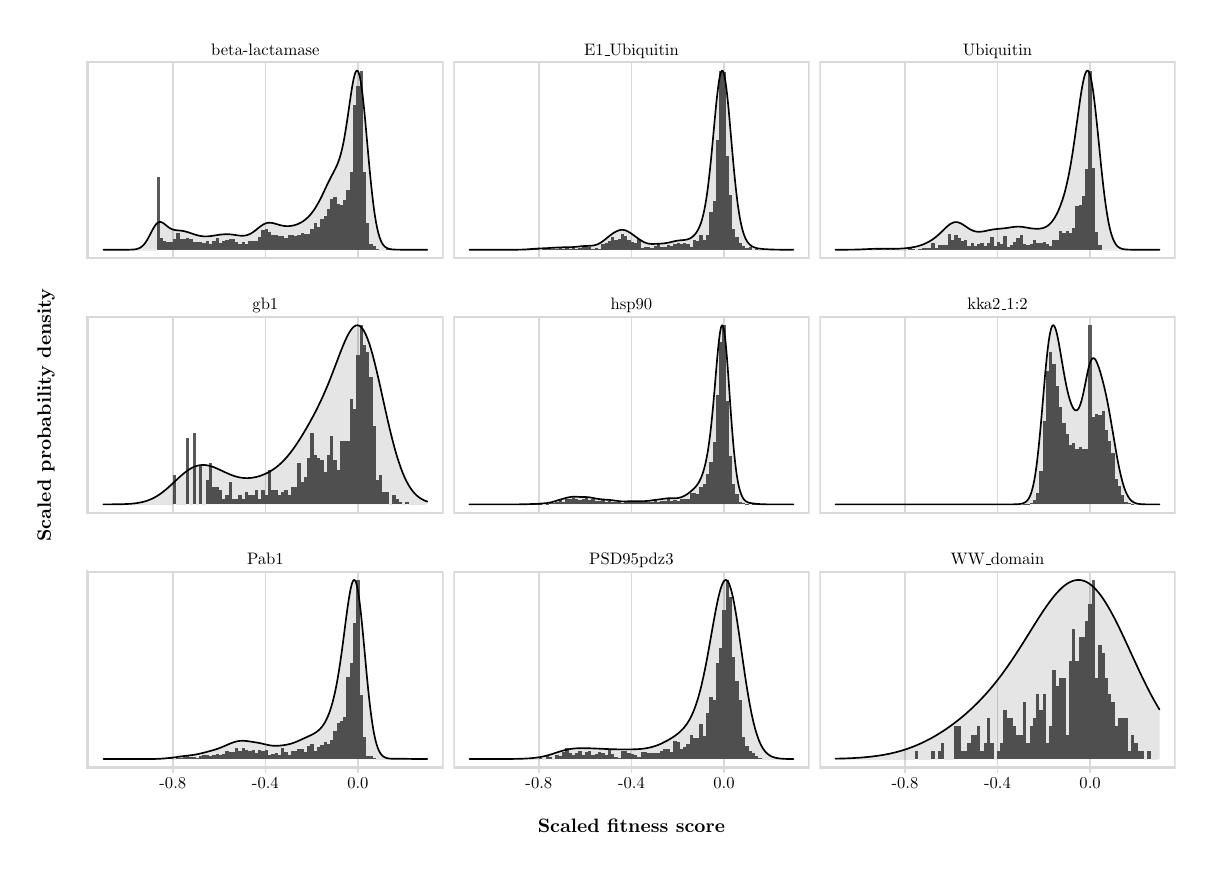
\begin{tikzpicture}[x=1pt,y=1pt]
\definecolor{fillColor}{RGB}{255,255,255}
\path[use as bounding box,fill=fillColor,fill opacity=0.00] (0,0) rectangle (418.34,295.82);
\begin{scope}
\path[clip] ( 21.50,212.35) rectangle (150.28,283.52);
\definecolor{drawColor}{gray}{0.85}

\path[draw=drawColor,line width= 0.6pt,line join=round] ( 52.44,212.35) --
	( 52.44,283.52);

\path[draw=drawColor,line width= 0.6pt,line join=round] ( 85.89,212.35) --
	( 85.89,283.52);

\path[draw=drawColor,line width= 0.6pt,line join=round] (119.34,212.35) --
	(119.34,283.52);
\definecolor{fillColor}{gray}{0.35}

\path[fill=fillColor] ( 27.70,215.58) rectangle ( 28.88,215.58);

\path[fill=fillColor] ( 28.88,215.58) rectangle ( 30.06,215.58);

\path[fill=fillColor] ( 30.06,215.58) rectangle ( 31.24,215.58);

\path[fill=fillColor] ( 31.24,215.58) rectangle ( 32.43,215.58);

\path[fill=fillColor] ( 32.43,215.58) rectangle ( 33.61,215.58);

\path[fill=fillColor] ( 33.61,215.58) rectangle ( 34.79,215.58);

\path[fill=fillColor] ( 34.79,215.58) rectangle ( 35.97,215.58);

\path[fill=fillColor] ( 35.97,215.58) rectangle ( 37.16,215.58);

\path[fill=fillColor] ( 37.16,215.58) rectangle ( 38.34,215.58);

\path[fill=fillColor] ( 38.34,215.58) rectangle ( 39.52,215.58);

\path[fill=fillColor] ( 39.52,215.58) rectangle ( 40.70,215.58);

\path[fill=fillColor] ( 40.70,215.58) rectangle ( 41.89,215.58);

\path[fill=fillColor] ( 41.89,215.58) rectangle ( 43.07,215.58);

\path[fill=fillColor] ( 43.07,215.58) rectangle ( 44.25,215.58);

\path[fill=fillColor] ( 44.25,215.58) rectangle ( 45.43,215.58);

\path[fill=fillColor] ( 45.43,215.58) rectangle ( 46.62,215.58);

\path[fill=fillColor] ( 46.62,215.58) rectangle ( 47.80,241.86);

\path[fill=fillColor] ( 47.80,215.58) rectangle ( 48.98,219.67);

\path[fill=fillColor] ( 48.98,215.58) rectangle ( 50.16,218.62);

\path[fill=fillColor] ( 50.16,215.58) rectangle ( 51.35,218.50);

\path[fill=fillColor] ( 51.35,215.58) rectangle ( 52.53,218.50);

\path[fill=fillColor] ( 52.53,215.58) rectangle ( 53.71,219.55);

\path[fill=fillColor] ( 53.71,215.58) rectangle ( 54.89,221.77);

\path[fill=fillColor] ( 54.89,215.58) rectangle ( 56.08,219.44);

\path[fill=fillColor] ( 56.08,215.58) rectangle ( 57.26,219.44);

\path[fill=fillColor] ( 57.26,215.58) rectangle ( 58.44,219.67);

\path[fill=fillColor] ( 58.44,215.58) rectangle ( 59.62,219.32);

\path[fill=fillColor] ( 59.62,215.58) rectangle ( 60.81,218.27);

\path[fill=fillColor] ( 60.81,215.58) rectangle ( 61.99,218.27);

\path[fill=fillColor] ( 61.99,215.58) rectangle ( 63.17,218.38);

\path[fill=fillColor] ( 63.17,215.58) rectangle ( 64.35,218.15);

\path[fill=fillColor] ( 64.35,215.58) rectangle ( 65.54,218.62);

\path[fill=fillColor] ( 65.54,215.58) rectangle ( 66.72,217.80);

\path[fill=fillColor] ( 66.72,215.58) rectangle ( 67.90,218.62);

\path[fill=fillColor] ( 67.90,215.58) rectangle ( 69.08,219.67);

\path[fill=fillColor] ( 69.08,215.58) rectangle ( 70.27,218.15);

\path[fill=fillColor] ( 70.27,215.58) rectangle ( 71.45,218.74);

\path[fill=fillColor] ( 71.45,215.58) rectangle ( 72.63,219.09);

\path[fill=fillColor] ( 72.63,215.58) rectangle ( 73.81,219.32);

\path[fill=fillColor] ( 73.81,215.58) rectangle ( 75.00,219.55);

\path[fill=fillColor] ( 75.00,215.58) rectangle ( 76.18,218.38);

\path[fill=fillColor] ( 76.18,215.58) rectangle ( 77.36,217.80);

\path[fill=fillColor] ( 77.36,215.58) rectangle ( 78.54,218.50);

\path[fill=fillColor] ( 78.54,215.58) rectangle ( 79.73,217.80);

\path[fill=fillColor] ( 79.73,215.58) rectangle ( 80.91,218.62);

\path[fill=fillColor] ( 80.91,215.58) rectangle ( 82.09,218.85);

\path[fill=fillColor] ( 82.09,215.58) rectangle ( 83.27,218.85);

\path[fill=fillColor] ( 83.27,215.58) rectangle ( 84.46,220.02);

\path[fill=fillColor] ( 84.46,215.58) rectangle ( 85.64,222.59);

\path[fill=fillColor] ( 85.64,215.58) rectangle ( 86.82,223.17);

\path[fill=fillColor] ( 86.82,215.58) rectangle ( 88.00,221.89);

\path[fill=fillColor] ( 88.00,215.58) rectangle ( 89.19,220.95);

\path[fill=fillColor] ( 89.19,215.58) rectangle ( 90.37,220.95);

\path[fill=fillColor] ( 90.37,215.58) rectangle ( 91.55,220.37);

\path[fill=fillColor] ( 91.55,215.58) rectangle ( 92.73,220.60);

\path[fill=fillColor] ( 92.73,215.58) rectangle ( 93.92,219.67);

\path[fill=fillColor] ( 93.92,215.58) rectangle ( 95.10,220.84);

\path[fill=fillColor] ( 95.10,215.58) rectangle ( 96.28,220.84);

\path[fill=fillColor] ( 96.28,215.58) rectangle ( 97.46,220.37);

\path[fill=fillColor] ( 97.46,215.58) rectangle ( 98.65,220.84);

\path[fill=fillColor] ( 98.65,215.58) rectangle ( 99.83,221.77);

\path[fill=fillColor] ( 99.83,215.58) rectangle (101.01,221.30);

\path[fill=fillColor] (101.01,215.58) rectangle (102.19,221.19);

\path[fill=fillColor] (102.19,215.58) rectangle (103.38,223.06);

\path[fill=fillColor] (103.38,215.58) rectangle (104.56,225.28);

\path[fill=fillColor] (104.56,215.58) rectangle (105.74,223.87);

\path[fill=fillColor] (105.74,215.58) rectangle (106.92,226.56);

\path[fill=fillColor] (106.92,215.58) rectangle (108.11,227.85);

\path[fill=fillColor] (108.11,215.58) rectangle (109.29,230.30);

\path[fill=fillColor] (109.29,215.58) rectangle (110.47,233.80);

\path[fill=fillColor] (110.47,215.58) rectangle (111.65,234.50);

\path[fill=fillColor] (111.65,215.58) rectangle (112.84,232.05);

\path[fill=fillColor] (112.84,215.58) rectangle (114.02,231.70);

\path[fill=fillColor] (114.02,215.58) rectangle (115.20,233.45);

\path[fill=fillColor] (115.20,215.58) rectangle (116.38,237.07);

\path[fill=fillColor] (116.38,215.58) rectangle (117.57,243.50);

\path[fill=fillColor] (117.57,215.58) rectangle (118.75,267.79);

\path[fill=fillColor] (118.75,215.58) rectangle (119.93,274.56);

\path[fill=fillColor] (119.93,215.58) rectangle (121.12,280.29);

\path[fill=fillColor] (121.12,215.58) rectangle (122.30,243.50);

\path[fill=fillColor] (122.30,215.58) rectangle (123.48,225.16);

\path[fill=fillColor] (123.48,215.58) rectangle (124.66,217.68);

\path[fill=fillColor] (124.66,215.58) rectangle (125.85,216.98);

\path[fill=fillColor] (125.85,215.58) rectangle (127.03,215.70);

\path[fill=fillColor] (127.03,215.58) rectangle (128.21,215.58);

\path[fill=fillColor] (128.21,215.58) rectangle (129.39,215.58);

\path[fill=fillColor] (129.39,215.58) rectangle (130.58,215.70);

\path[fill=fillColor] (130.58,215.58) rectangle (131.76,215.58);

\path[fill=fillColor] (131.76,215.58) rectangle (132.94,215.58);

\path[fill=fillColor] (132.94,215.58) rectangle (134.12,215.58);

\path[fill=fillColor] (134.12,215.58) rectangle (135.31,215.58);

\path[fill=fillColor] (135.31,215.58) rectangle (136.49,215.58);

\path[fill=fillColor] (136.49,215.58) rectangle (137.67,215.58);

\path[fill=fillColor] (137.67,215.58) rectangle (138.85,215.58);

\path[fill=fillColor] (138.85,215.58) rectangle (140.04,215.58);

\path[fill=fillColor] (140.04,215.58) rectangle (141.22,215.58);

\path[fill=fillColor] (141.22,215.58) rectangle (142.40,215.58);

\path[fill=fillColor] (142.40,215.58) rectangle (143.58,215.58);
\definecolor{fillColor}{RGB}{0,0,0}

\path[fill=fillColor,fill opacity=0.10] ( 27.36,215.58) --
	( 27.59,215.58) --
	( 27.82,215.58) --
	( 28.04,215.58) --
	( 28.27,215.58) --
	( 28.50,215.58) --
	( 28.73,215.58) --
	( 28.96,215.58) --
	( 29.19,215.58) --
	( 29.42,215.58) --
	( 29.65,215.58) --
	( 29.88,215.58) --
	( 30.11,215.58) --
	( 30.34,215.58) --
	( 30.56,215.58) --
	( 30.79,215.58) --
	( 31.02,215.58) --
	( 31.25,215.58) --
	( 31.48,215.58) --
	( 31.71,215.58) --
	( 31.94,215.58) --
	( 32.17,215.58) --
	( 32.40,215.58) --
	( 32.63,215.58) --
	( 32.86,215.58) --
	( 33.09,215.58) --
	( 33.31,215.58) --
	( 33.54,215.58) --
	( 33.77,215.58) --
	( 34.00,215.58) --
	( 34.23,215.58) --
	( 34.46,215.58) --
	( 34.69,215.58) --
	( 34.92,215.58) --
	( 35.15,215.58) --
	( 35.38,215.58) --
	( 35.61,215.59) --
	( 35.83,215.59) --
	( 36.06,215.59) --
	( 36.29,215.59) --
	( 36.52,215.59) --
	( 36.75,215.60) --
	( 36.98,215.60) --
	( 37.21,215.61) --
	( 37.44,215.62) --
	( 37.67,215.63) --
	( 37.90,215.64) --
	( 38.13,215.65) --
	( 38.35,215.67) --
	( 38.58,215.70) --
	( 38.81,215.73) --
	( 39.04,215.77) --
	( 39.27,215.81) --
	( 39.50,215.86) --
	( 39.73,215.93) --
	( 39.96,216.01) --
	( 40.19,216.10) --
	( 40.42,216.20) --
	( 40.65,216.32) --
	( 40.87,216.46) --
	( 41.10,216.62) --
	( 41.33,216.80) --
	( 41.56,217.01) --
	( 41.79,217.23) --
	( 42.02,217.48) --
	( 42.25,217.76) --
	( 42.48,218.06) --
	( 42.71,218.39) --
	( 42.94,218.74) --
	( 43.17,219.11) --
	( 43.39,219.51) --
	( 43.62,219.92) --
	( 43.85,220.34) --
	( 44.08,220.78) --
	( 44.31,221.23) --
	( 44.54,221.67) --
	( 44.77,222.12) --
	( 45.00,222.55) --
	( 45.23,222.98) --
	( 45.46,223.38) --
	( 45.69,223.76) --
	( 45.91,224.12) --
	( 46.14,224.44) --
	( 46.37,224.73) --
	( 46.60,224.98) --
	( 46.83,225.19) --
	( 47.06,225.35) --
	( 47.29,225.47) --
	( 47.52,225.56) --
	( 47.75,225.60) --
	( 47.98,225.60) --
	( 48.21,225.56) --
	( 48.43,225.48) --
	( 48.66,225.38) --
	( 48.89,225.26) --
	( 49.12,225.11) --
	( 49.35,224.94) --
	( 49.58,224.76) --
	( 49.81,224.58) --
	( 50.04,224.39) --
	( 50.27,224.20) --
	( 50.50,224.01) --
	( 50.73,223.83) --
	( 50.95,223.67) --
	( 51.18,223.51) --
	( 51.41,223.37) --
	( 51.64,223.24) --
	( 51.87,223.12) --
	( 52.10,223.02) --
	( 52.33,222.93) --
	( 52.56,222.86) --
	( 52.79,222.79) --
	( 53.02,222.74) --
	( 53.25,222.70) --
	( 53.47,222.66) --
	( 53.70,222.63) --
	( 53.93,222.61) --
	( 54.16,222.58) --
	( 54.39,222.56) --
	( 54.62,222.54) --
	( 54.85,222.52) --
	( 55.08,222.50) --
	( 55.31,222.47) --
	( 55.54,222.44) --
	( 55.77,222.41) --
	( 56.00,222.37) --
	( 56.22,222.33) --
	( 56.45,222.29) --
	( 56.68,222.24) --
	( 56.91,222.18) --
	( 57.14,222.13) --
	( 57.37,222.06) --
	( 57.60,222.00) --
	( 57.83,221.93) --
	( 58.06,221.86) --
	( 58.29,221.79) --
	( 58.52,221.71) --
	( 58.74,221.63) --
	( 58.97,221.56) --
	( 59.20,221.48) --
	( 59.43,221.40) --
	( 59.66,221.32) --
	( 59.89,221.24) --
	( 60.12,221.17) --
	( 60.35,221.09) --
	( 60.58,221.02) --
	( 60.81,220.95) --
	( 61.04,220.88) --
	( 61.26,220.82) --
	( 61.49,220.76) --
	( 61.72,220.70) --
	( 61.95,220.65) --
	( 62.18,220.60) --
	( 62.41,220.56) --
	( 62.64,220.52) --
	( 62.87,220.49) --
	( 63.10,220.46) --
	( 63.33,220.43) --
	( 63.56,220.42) --
	( 63.78,220.40) --
	( 64.01,220.39) --
	( 64.24,220.39) --
	( 64.47,220.39) --
	( 64.70,220.39) --
	( 64.93,220.40) --
	( 65.16,220.42) --
	( 65.39,220.43) --
	( 65.62,220.46) --
	( 65.85,220.48) --
	( 66.08,220.51) --
	( 66.30,220.54) --
	( 66.53,220.57) --
	( 66.76,220.60) --
	( 66.99,220.64) --
	( 67.22,220.67) --
	( 67.45,220.71) --
	( 67.68,220.75) --
	( 67.91,220.78) --
	( 68.14,220.82) --
	( 68.37,220.86) --
	( 68.60,220.89) --
	( 68.82,220.93) --
	( 69.05,220.96) --
	( 69.28,220.99) --
	( 69.51,221.02) --
	( 69.74,221.05) --
	( 69.97,221.07) --
	( 70.20,221.10) --
	( 70.43,221.12) --
	( 70.66,221.13) --
	( 70.89,221.15) --
	( 71.12,221.16) --
	( 71.34,221.17) --
	( 71.57,221.18) --
	( 71.80,221.18) --
	( 72.03,221.18) --
	( 72.26,221.18) --
	( 72.49,221.17) --
	( 72.72,221.16) --
	( 72.95,221.15) --
	( 73.18,221.13) --
	( 73.41,221.11) --
	( 73.64,221.09) --
	( 73.86,221.06) --
	( 74.09,221.03) --
	( 74.32,221.00) --
	( 74.55,220.97) --
	( 74.78,220.94) --
	( 75.01,220.90) --
	( 75.24,220.86) --
	( 75.47,220.83) --
	( 75.70,220.79) --
	( 75.93,220.76) --
	( 76.16,220.73) --
	( 76.39,220.70) --
	( 76.61,220.68) --
	( 76.84,220.66) --
	( 77.07,220.64) --
	( 77.30,220.63) --
	( 77.53,220.63) --
	( 77.76,220.64) --
	( 77.99,220.65) --
	( 78.22,220.67) --
	( 78.45,220.69) --
	( 78.68,220.73) --
	( 78.91,220.77) --
	( 79.13,220.83) --
	( 79.36,220.89) --
	( 79.59,220.97) --
	( 79.82,221.05) --
	( 80.05,221.15) --
	( 80.28,221.25) --
	( 80.51,221.37) --
	( 80.74,221.49) --
	( 80.97,221.63) --
	( 81.20,221.77) --
	( 81.43,221.92) --
	( 81.65,222.08) --
	( 81.88,222.25) --
	( 82.11,222.42) --
	( 82.34,222.60) --
	( 82.57,222.79) --
	( 82.80,222.97) --
	( 83.03,223.16) --
	( 83.26,223.35) --
	( 83.49,223.53) --
	( 83.72,223.72) --
	( 83.95,223.89) --
	( 84.17,224.07) --
	( 84.40,224.23) --
	( 84.63,224.39) --
	( 84.86,224.54) --
	( 85.09,224.68) --
	( 85.32,224.80) --
	( 85.55,224.92) --
	( 85.78,225.02) --
	( 86.01,225.10) --
	( 86.24,225.17) --
	( 86.47,225.23) --
	( 86.69,225.28) --
	( 86.92,225.31) --
	( 87.15,225.33) --
	( 87.38,225.33) --
	( 87.61,225.33) --
	( 87.84,225.31) --
	( 88.07,225.28) --
	( 88.30,225.25) --
	( 88.53,225.21) --
	( 88.76,225.16) --
	( 88.99,225.10) --
	( 89.21,225.04) --
	( 89.44,224.98) --
	( 89.67,224.91) --
	( 89.90,224.84) --
	( 90.13,224.77) --
	( 90.36,224.71) --
	( 90.59,224.64) --
	( 90.82,224.57) --
	( 91.05,224.51) --
	( 91.28,224.45) --
	( 91.51,224.40) --
	( 91.73,224.35) --
	( 91.96,224.30) --
	( 92.19,224.26) --
	( 92.42,224.22) --
	( 92.65,224.19) --
	( 92.88,224.16) --
	( 93.11,224.14) --
	( 93.34,224.12) --
	( 93.57,224.11) --
	( 93.80,224.11) --
	( 94.03,224.11) --
	( 94.25,224.11) --
	( 94.48,224.12) --
	( 94.71,224.14) --
	( 94.94,224.17) --
	( 95.17,224.20) --
	( 95.40,224.23) --
	( 95.63,224.27) --
	( 95.86,224.32) --
	( 96.09,224.37) --
	( 96.32,224.42) --
	( 96.55,224.49) --
	( 96.77,224.56) --
	( 97.00,224.63) --
	( 97.23,224.71) --
	( 97.46,224.80) --
	( 97.69,224.89) --
	( 97.92,224.99) --
	( 98.15,225.10) --
	( 98.38,225.21) --
	( 98.61,225.33) --
	( 98.84,225.46) --
	( 99.07,225.59) --
	( 99.30,225.73) --
	( 99.52,225.88) --
	( 99.75,226.04) --
	( 99.98,226.20) --
	(100.21,226.38) --
	(100.44,226.56) --
	(100.67,226.76) --
	(100.90,226.96) --
	(101.13,227.17) --
	(101.36,227.40) --
	(101.59,227.63) --
	(101.82,227.88) --
	(102.04,228.13) --
	(102.27,228.40) --
	(102.50,228.68) --
	(102.73,228.97) --
	(102.96,229.27) --
	(103.19,229.59) --
	(103.42,229.91) --
	(103.65,230.25) --
	(103.88,230.60) --
	(104.11,230.96) --
	(104.34,231.33) --
	(104.56,231.72) --
	(104.79,232.12) --
	(105.02,232.53) --
	(105.25,232.95) --
	(105.48,233.38) --
	(105.71,233.83) --
	(105.94,234.28) --
	(106.17,234.74) --
	(106.40,235.21) --
	(106.63,235.69) --
	(106.86,236.17) --
	(107.08,236.66) --
	(107.31,237.14) --
	(107.54,237.63) --
	(107.77,238.12) --
	(108.00,238.61) --
	(108.23,239.09) --
	(108.46,239.57) --
	(108.69,240.04) --
	(108.92,240.50) --
	(109.15,240.96) --
	(109.38,241.41) --
	(109.60,241.85) --
	(109.83,242.29) --
	(110.06,242.72) --
	(110.29,243.15) --
	(110.52,243.59) --
	(110.75,244.02) --
	(110.98,244.47) --
	(111.21,244.93) --
	(111.44,245.41) --
	(111.67,245.91) --
	(111.90,246.45) --
	(112.12,247.01) --
	(112.35,247.62) --
	(112.58,248.28) --
	(112.81,249.00) --
	(113.04,249.78) --
	(113.27,250.63) --
	(113.50,251.55) --
	(113.73,252.53) --
	(113.96,253.59) --
	(114.19,254.74) --
	(114.42,255.97) --
	(114.64,257.27) --
	(114.87,258.63) --
	(115.10,260.06) --
	(115.33,261.55) --
	(115.56,263.09) --
	(115.79,264.66) --
	(116.02,266.25) --
	(116.25,267.85) --
	(116.48,269.43) --
	(116.71,270.99) --
	(116.94,272.50) --
	(117.16,273.92) --
	(117.39,275.25) --
	(117.62,276.47) --
	(117.85,277.56) --
	(118.08,278.51) --
	(118.31,279.27) --
	(118.54,279.81) --
	(118.77,280.16) --
	(119.00,280.29) --
	(119.23,280.20) --
	(119.46,279.89) --
	(119.68,279.33) --
	(119.91,278.50) --
	(120.14,277.45) --
	(120.37,276.17) --
	(120.60,274.69) --
	(120.83,273.01) --
	(121.06,271.15) --
	(121.29,269.09) --
	(121.52,266.89) --
	(121.75,264.57) --
	(121.98,262.16) --
	(122.21,259.67) --
	(122.43,257.13) --
	(122.66,254.56) --
	(122.89,251.98) --
	(123.12,249.43) --
	(123.35,246.91) --
	(123.58,244.44) --
	(123.81,242.04) --
	(124.04,239.75) --
	(124.27,237.56) --
	(124.50,235.47) --
	(124.73,233.50) --
	(124.95,231.65) --
	(125.18,229.92) --
	(125.41,228.33) --
	(125.64,226.88) --
	(125.87,225.54) --
	(126.10,224.32) --
	(126.33,223.21) --
	(126.56,222.21) --
	(126.79,221.33) --
	(127.02,220.55) --
	(127.25,219.85) --
	(127.47,219.24) --
	(127.70,218.70) --
	(127.93,218.22) --
	(128.16,217.82) --
	(128.39,217.47) --
	(128.62,217.17) --
	(128.85,216.91) --
	(129.08,216.69) --
	(129.31,216.51) --
	(129.54,216.35) --
	(129.77,216.22) --
	(129.99,216.11) --
	(130.22,216.02) --
	(130.45,215.94) --
	(130.68,215.88) --
	(130.91,215.83) --
	(131.14,215.78) --
	(131.37,215.75) --
	(131.60,215.72) --
	(131.83,215.70) --
	(132.06,215.68) --
	(132.29,215.66) --
	(132.51,215.65) --
	(132.74,215.64) --
	(132.97,215.63) --
	(133.20,215.62) --
	(133.43,215.61) --
	(133.66,215.61) --
	(133.89,215.61) --
	(134.12,215.60) --
	(134.35,215.60) --
	(134.58,215.60) --
	(134.81,215.59) --
	(135.03,215.59) --
	(135.26,215.59) --
	(135.49,215.59) --
	(135.72,215.59) --
	(135.95,215.59) --
	(136.18,215.59) --
	(136.41,215.59) --
	(136.64,215.58) --
	(136.87,215.58) --
	(137.10,215.58) --
	(137.33,215.58) --
	(137.55,215.58) --
	(137.78,215.58) --
	(138.01,215.58) --
	(138.24,215.58) --
	(138.47,215.58) --
	(138.70,215.58) --
	(138.93,215.58) --
	(139.16,215.58) --
	(139.39,215.58) --
	(139.62,215.58) --
	(139.85,215.58) --
	(140.07,215.58) --
	(140.30,215.58) --
	(140.53,215.58) --
	(140.76,215.58) --
	(140.99,215.58) --
	(141.22,215.58) --
	(141.45,215.58) --
	(141.68,215.58) --
	(141.91,215.58) --
	(142.14,215.58) --
	(142.37,215.58) --
	(142.59,215.58) --
	(142.82,215.58) --
	(143.05,215.58) --
	(143.28,215.58) --
	(143.51,215.58) --
	(143.74,215.58) --
	(143.97,215.58) --
	(144.20,215.58) --
	(144.43,215.58) --
	(144.43,215.58) --
	(144.20,215.58) --
	(143.97,215.58) --
	(143.74,215.58) --
	(143.51,215.58) --
	(143.28,215.58) --
	(143.05,215.58) --
	(142.82,215.58) --
	(142.59,215.58) --
	(142.37,215.58) --
	(142.14,215.58) --
	(141.91,215.58) --
	(141.68,215.58) --
	(141.45,215.58) --
	(141.22,215.58) --
	(140.99,215.58) --
	(140.76,215.58) --
	(140.53,215.58) --
	(140.30,215.58) --
	(140.07,215.58) --
	(139.85,215.58) --
	(139.62,215.58) --
	(139.39,215.58) --
	(139.16,215.58) --
	(138.93,215.58) --
	(138.70,215.58) --
	(138.47,215.58) --
	(138.24,215.58) --
	(138.01,215.58) --
	(137.78,215.58) --
	(137.55,215.58) --
	(137.33,215.58) --
	(137.10,215.58) --
	(136.87,215.58) --
	(136.64,215.58) --
	(136.41,215.58) --
	(136.18,215.58) --
	(135.95,215.58) --
	(135.72,215.58) --
	(135.49,215.58) --
	(135.26,215.58) --
	(135.03,215.58) --
	(134.81,215.58) --
	(134.58,215.58) --
	(134.35,215.58) --
	(134.12,215.58) --
	(133.89,215.58) --
	(133.66,215.58) --
	(133.43,215.58) --
	(133.20,215.58) --
	(132.97,215.58) --
	(132.74,215.58) --
	(132.51,215.58) --
	(132.29,215.58) --
	(132.06,215.58) --
	(131.83,215.58) --
	(131.60,215.58) --
	(131.37,215.58) --
	(131.14,215.58) --
	(130.91,215.58) --
	(130.68,215.58) --
	(130.45,215.58) --
	(130.22,215.58) --
	(129.99,215.58) --
	(129.77,215.58) --
	(129.54,215.58) --
	(129.31,215.58) --
	(129.08,215.58) --
	(128.85,215.58) --
	(128.62,215.58) --
	(128.39,215.58) --
	(128.16,215.58) --
	(127.93,215.58) --
	(127.70,215.58) --
	(127.47,215.58) --
	(127.25,215.58) --
	(127.02,215.58) --
	(126.79,215.58) --
	(126.56,215.58) --
	(126.33,215.58) --
	(126.10,215.58) --
	(125.87,215.58) --
	(125.64,215.58) --
	(125.41,215.58) --
	(125.18,215.58) --
	(124.95,215.58) --
	(124.73,215.58) --
	(124.50,215.58) --
	(124.27,215.58) --
	(124.04,215.58) --
	(123.81,215.58) --
	(123.58,215.58) --
	(123.35,215.58) --
	(123.12,215.58) --
	(122.89,215.58) --
	(122.66,215.58) --
	(122.43,215.58) --
	(122.21,215.58) --
	(121.98,215.58) --
	(121.75,215.58) --
	(121.52,215.58) --
	(121.29,215.58) --
	(121.06,215.58) --
	(120.83,215.58) --
	(120.60,215.58) --
	(120.37,215.58) --
	(120.14,215.58) --
	(119.91,215.58) --
	(119.68,215.58) --
	(119.46,215.58) --
	(119.23,215.58) --
	(119.00,215.58) --
	(118.77,215.58) --
	(118.54,215.58) --
	(118.31,215.58) --
	(118.08,215.58) --
	(117.85,215.58) --
	(117.62,215.58) --
	(117.39,215.58) --
	(117.16,215.58) --
	(116.94,215.58) --
	(116.71,215.58) --
	(116.48,215.58) --
	(116.25,215.58) --
	(116.02,215.58) --
	(115.79,215.58) --
	(115.56,215.58) --
	(115.33,215.58) --
	(115.10,215.58) --
	(114.87,215.58) --
	(114.64,215.58) --
	(114.42,215.58) --
	(114.19,215.58) --
	(113.96,215.58) --
	(113.73,215.58) --
	(113.50,215.58) --
	(113.27,215.58) --
	(113.04,215.58) --
	(112.81,215.58) --
	(112.58,215.58) --
	(112.35,215.58) --
	(112.12,215.58) --
	(111.90,215.58) --
	(111.67,215.58) --
	(111.44,215.58) --
	(111.21,215.58) --
	(110.98,215.58) --
	(110.75,215.58) --
	(110.52,215.58) --
	(110.29,215.58) --
	(110.06,215.58) --
	(109.83,215.58) --
	(109.60,215.58) --
	(109.38,215.58) --
	(109.15,215.58) --
	(108.92,215.58) --
	(108.69,215.58) --
	(108.46,215.58) --
	(108.23,215.58) --
	(108.00,215.58) --
	(107.77,215.58) --
	(107.54,215.58) --
	(107.31,215.58) --
	(107.08,215.58) --
	(106.86,215.58) --
	(106.63,215.58) --
	(106.40,215.58) --
	(106.17,215.58) --
	(105.94,215.58) --
	(105.71,215.58) --
	(105.48,215.58) --
	(105.25,215.58) --
	(105.02,215.58) --
	(104.79,215.58) --
	(104.56,215.58) --
	(104.34,215.58) --
	(104.11,215.58) --
	(103.88,215.58) --
	(103.65,215.58) --
	(103.42,215.58) --
	(103.19,215.58) --
	(102.96,215.58) --
	(102.73,215.58) --
	(102.50,215.58) --
	(102.27,215.58) --
	(102.04,215.58) --
	(101.82,215.58) --
	(101.59,215.58) --
	(101.36,215.58) --
	(101.13,215.58) --
	(100.90,215.58) --
	(100.67,215.58) --
	(100.44,215.58) --
	(100.21,215.58) --
	( 99.98,215.58) --
	( 99.75,215.58) --
	( 99.52,215.58) --
	( 99.30,215.58) --
	( 99.07,215.58) --
	( 98.84,215.58) --
	( 98.61,215.58) --
	( 98.38,215.58) --
	( 98.15,215.58) --
	( 97.92,215.58) --
	( 97.69,215.58) --
	( 97.46,215.58) --
	( 97.23,215.58) --
	( 97.00,215.58) --
	( 96.77,215.58) --
	( 96.55,215.58) --
	( 96.32,215.58) --
	( 96.09,215.58) --
	( 95.86,215.58) --
	( 95.63,215.58) --
	( 95.40,215.58) --
	( 95.17,215.58) --
	( 94.94,215.58) --
	( 94.71,215.58) --
	( 94.48,215.58) --
	( 94.25,215.58) --
	( 94.03,215.58) --
	( 93.80,215.58) --
	( 93.57,215.58) --
	( 93.34,215.58) --
	( 93.11,215.58) --
	( 92.88,215.58) --
	( 92.65,215.58) --
	( 92.42,215.58) --
	( 92.19,215.58) --
	( 91.96,215.58) --
	( 91.73,215.58) --
	( 91.51,215.58) --
	( 91.28,215.58) --
	( 91.05,215.58) --
	( 90.82,215.58) --
	( 90.59,215.58) --
	( 90.36,215.58) --
	( 90.13,215.58) --
	( 89.90,215.58) --
	( 89.67,215.58) --
	( 89.44,215.58) --
	( 89.21,215.58) --
	( 88.99,215.58) --
	( 88.76,215.58) --
	( 88.53,215.58) --
	( 88.30,215.58) --
	( 88.07,215.58) --
	( 87.84,215.58) --
	( 87.61,215.58) --
	( 87.38,215.58) --
	( 87.15,215.58) --
	( 86.92,215.58) --
	( 86.69,215.58) --
	( 86.47,215.58) --
	( 86.24,215.58) --
	( 86.01,215.58) --
	( 85.78,215.58) --
	( 85.55,215.58) --
	( 85.32,215.58) --
	( 85.09,215.58) --
	( 84.86,215.58) --
	( 84.63,215.58) --
	( 84.40,215.58) --
	( 84.17,215.58) --
	( 83.95,215.58) --
	( 83.72,215.58) --
	( 83.49,215.58) --
	( 83.26,215.58) --
	( 83.03,215.58) --
	( 82.80,215.58) --
	( 82.57,215.58) --
	( 82.34,215.58) --
	( 82.11,215.58) --
	( 81.88,215.58) --
	( 81.65,215.58) --
	( 81.43,215.58) --
	( 81.20,215.58) --
	( 80.97,215.58) --
	( 80.74,215.58) --
	( 80.51,215.58) --
	( 80.28,215.58) --
	( 80.05,215.58) --
	( 79.82,215.58) --
	( 79.59,215.58) --
	( 79.36,215.58) --
	( 79.13,215.58) --
	( 78.91,215.58) --
	( 78.68,215.58) --
	( 78.45,215.58) --
	( 78.22,215.58) --
	( 77.99,215.58) --
	( 77.76,215.58) --
	( 77.53,215.58) --
	( 77.30,215.58) --
	( 77.07,215.58) --
	( 76.84,215.58) --
	( 76.61,215.58) --
	( 76.39,215.58) --
	( 76.16,215.58) --
	( 75.93,215.58) --
	( 75.70,215.58) --
	( 75.47,215.58) --
	( 75.24,215.58) --
	( 75.01,215.58) --
	( 74.78,215.58) --
	( 74.55,215.58) --
	( 74.32,215.58) --
	( 74.09,215.58) --
	( 73.86,215.58) --
	( 73.64,215.58) --
	( 73.41,215.58) --
	( 73.18,215.58) --
	( 72.95,215.58) --
	( 72.72,215.58) --
	( 72.49,215.58) --
	( 72.26,215.58) --
	( 72.03,215.58) --
	( 71.80,215.58) --
	( 71.57,215.58) --
	( 71.34,215.58) --
	( 71.12,215.58) --
	( 70.89,215.58) --
	( 70.66,215.58) --
	( 70.43,215.58) --
	( 70.20,215.58) --
	( 69.97,215.58) --
	( 69.74,215.58) --
	( 69.51,215.58) --
	( 69.28,215.58) --
	( 69.05,215.58) --
	( 68.82,215.58) --
	( 68.60,215.58) --
	( 68.37,215.58) --
	( 68.14,215.58) --
	( 67.91,215.58) --
	( 67.68,215.58) --
	( 67.45,215.58) --
	( 67.22,215.58) --
	( 66.99,215.58) --
	( 66.76,215.58) --
	( 66.53,215.58) --
	( 66.30,215.58) --
	( 66.08,215.58) --
	( 65.85,215.58) --
	( 65.62,215.58) --
	( 65.39,215.58) --
	( 65.16,215.58) --
	( 64.93,215.58) --
	( 64.70,215.58) --
	( 64.47,215.58) --
	( 64.24,215.58) --
	( 64.01,215.58) --
	( 63.78,215.58) --
	( 63.56,215.58) --
	( 63.33,215.58) --
	( 63.10,215.58) --
	( 62.87,215.58) --
	( 62.64,215.58) --
	( 62.41,215.58) --
	( 62.18,215.58) --
	( 61.95,215.58) --
	( 61.72,215.58) --
	( 61.49,215.58) --
	( 61.26,215.58) --
	( 61.04,215.58) --
	( 60.81,215.58) --
	( 60.58,215.58) --
	( 60.35,215.58) --
	( 60.12,215.58) --
	( 59.89,215.58) --
	( 59.66,215.58) --
	( 59.43,215.58) --
	( 59.20,215.58) --
	( 58.97,215.58) --
	( 58.74,215.58) --
	( 58.52,215.58) --
	( 58.29,215.58) --
	( 58.06,215.58) --
	( 57.83,215.58) --
	( 57.60,215.58) --
	( 57.37,215.58) --
	( 57.14,215.58) --
	( 56.91,215.58) --
	( 56.68,215.58) --
	( 56.45,215.58) --
	( 56.22,215.58) --
	( 56.00,215.58) --
	( 55.77,215.58) --
	( 55.54,215.58) --
	( 55.31,215.58) --
	( 55.08,215.58) --
	( 54.85,215.58) --
	( 54.62,215.58) --
	( 54.39,215.58) --
	( 54.16,215.58) --
	( 53.93,215.58) --
	( 53.70,215.58) --
	( 53.47,215.58) --
	( 53.25,215.58) --
	( 53.02,215.58) --
	( 52.79,215.58) --
	( 52.56,215.58) --
	( 52.33,215.58) --
	( 52.10,215.58) --
	( 51.87,215.58) --
	( 51.64,215.58) --
	( 51.41,215.58) --
	( 51.18,215.58) --
	( 50.95,215.58) --
	( 50.73,215.58) --
	( 50.50,215.58) --
	( 50.27,215.58) --
	( 50.04,215.58) --
	( 49.81,215.58) --
	( 49.58,215.58) --
	( 49.35,215.58) --
	( 49.12,215.58) --
	( 48.89,215.58) --
	( 48.66,215.58) --
	( 48.43,215.58) --
	( 48.21,215.58) --
	( 47.98,215.58) --
	( 47.75,215.58) --
	( 47.52,215.58) --
	( 47.29,215.58) --
	( 47.06,215.58) --
	( 46.83,215.58) --
	( 46.60,215.58) --
	( 46.37,215.58) --
	( 46.14,215.58) --
	( 45.91,215.58) --
	( 45.69,215.58) --
	( 45.46,215.58) --
	( 45.23,215.58) --
	( 45.00,215.58) --
	( 44.77,215.58) --
	( 44.54,215.58) --
	( 44.31,215.58) --
	( 44.08,215.58) --
	( 43.85,215.58) --
	( 43.62,215.58) --
	( 43.39,215.58) --
	( 43.17,215.58) --
	( 42.94,215.58) --
	( 42.71,215.58) --
	( 42.48,215.58) --
	( 42.25,215.58) --
	( 42.02,215.58) --
	( 41.79,215.58) --
	( 41.56,215.58) --
	( 41.33,215.58) --
	( 41.10,215.58) --
	( 40.87,215.58) --
	( 40.65,215.58) --
	( 40.42,215.58) --
	( 40.19,215.58) --
	( 39.96,215.58) --
	( 39.73,215.58) --
	( 39.50,215.58) --
	( 39.27,215.58) --
	( 39.04,215.58) --
	( 38.81,215.58) --
	( 38.58,215.58) --
	( 38.35,215.58) --
	( 38.13,215.58) --
	( 37.90,215.58) --
	( 37.67,215.58) --
	( 37.44,215.58) --
	( 37.21,215.58) --
	( 36.98,215.58) --
	( 36.75,215.58) --
	( 36.52,215.58) --
	( 36.29,215.58) --
	( 36.06,215.58) --
	( 35.83,215.58) --
	( 35.61,215.58) --
	( 35.38,215.58) --
	( 35.15,215.58) --
	( 34.92,215.58) --
	( 34.69,215.58) --
	( 34.46,215.58) --
	( 34.23,215.58) --
	( 34.00,215.58) --
	( 33.77,215.58) --
	( 33.54,215.58) --
	( 33.31,215.58) --
	( 33.09,215.58) --
	( 32.86,215.58) --
	( 32.63,215.58) --
	( 32.40,215.58) --
	( 32.17,215.58) --
	( 31.94,215.58) --
	( 31.71,215.58) --
	( 31.48,215.58) --
	( 31.25,215.58) --
	( 31.02,215.58) --
	( 30.79,215.58) --
	( 30.56,215.58) --
	( 30.34,215.58) --
	( 30.11,215.58) --
	( 29.88,215.58) --
	( 29.65,215.58) --
	( 29.42,215.58) --
	( 29.19,215.58) --
	( 28.96,215.58) --
	( 28.73,215.58) --
	( 28.50,215.58) --
	( 28.27,215.58) --
	( 28.04,215.58) --
	( 27.82,215.58) --
	( 27.59,215.58) --
	( 27.36,215.58) --
	cycle;
\definecolor{drawColor}{RGB}{0,0,0}

\path[draw=drawColor,line width= 0.6pt,line join=round,line cap=round] ( 27.36,215.58) --
	( 27.59,215.58) --
	( 27.82,215.58) --
	( 28.04,215.58) --
	( 28.27,215.58) --
	( 28.50,215.58) --
	( 28.73,215.58) --
	( 28.96,215.58) --
	( 29.19,215.58) --
	( 29.42,215.58) --
	( 29.65,215.58) --
	( 29.88,215.58) --
	( 30.11,215.58) --
	( 30.34,215.58) --
	( 30.56,215.58) --
	( 30.79,215.58) --
	( 31.02,215.58) --
	( 31.25,215.58) --
	( 31.48,215.58) --
	( 31.71,215.58) --
	( 31.94,215.58) --
	( 32.17,215.58) --
	( 32.40,215.58) --
	( 32.63,215.58) --
	( 32.86,215.58) --
	( 33.09,215.58) --
	( 33.31,215.58) --
	( 33.54,215.58) --
	( 33.77,215.58) --
	( 34.00,215.58) --
	( 34.23,215.58) --
	( 34.46,215.58) --
	( 34.69,215.58) --
	( 34.92,215.58) --
	( 35.15,215.58) --
	( 35.38,215.58) --
	( 35.61,215.59) --
	( 35.83,215.59) --
	( 36.06,215.59) --
	( 36.29,215.59) --
	( 36.52,215.59) --
	( 36.75,215.60) --
	( 36.98,215.60) --
	( 37.21,215.61) --
	( 37.44,215.62) --
	( 37.67,215.63) --
	( 37.90,215.64) --
	( 38.13,215.65) --
	( 38.35,215.67) --
	( 38.58,215.70) --
	( 38.81,215.73) --
	( 39.04,215.77) --
	( 39.27,215.81) --
	( 39.50,215.86) --
	( 39.73,215.93) --
	( 39.96,216.01) --
	( 40.19,216.10) --
	( 40.42,216.20) --
	( 40.65,216.32) --
	( 40.87,216.46) --
	( 41.10,216.62) --
	( 41.33,216.80) --
	( 41.56,217.01) --
	( 41.79,217.23) --
	( 42.02,217.48) --
	( 42.25,217.76) --
	( 42.48,218.06) --
	( 42.71,218.39) --
	( 42.94,218.74) --
	( 43.17,219.11) --
	( 43.39,219.51) --
	( 43.62,219.92) --
	( 43.85,220.34) --
	( 44.08,220.78) --
	( 44.31,221.23) --
	( 44.54,221.67) --
	( 44.77,222.12) --
	( 45.00,222.55) --
	( 45.23,222.98) --
	( 45.46,223.38) --
	( 45.69,223.76) --
	( 45.91,224.12) --
	( 46.14,224.44) --
	( 46.37,224.73) --
	( 46.60,224.98) --
	( 46.83,225.19) --
	( 47.06,225.35) --
	( 47.29,225.47) --
	( 47.52,225.56) --
	( 47.75,225.60) --
	( 47.98,225.60) --
	( 48.21,225.56) --
	( 48.43,225.48) --
	( 48.66,225.38) --
	( 48.89,225.26) --
	( 49.12,225.11) --
	( 49.35,224.94) --
	( 49.58,224.76) --
	( 49.81,224.58) --
	( 50.04,224.39) --
	( 50.27,224.20) --
	( 50.50,224.01) --
	( 50.73,223.83) --
	( 50.95,223.67) --
	( 51.18,223.51) --
	( 51.41,223.37) --
	( 51.64,223.24) --
	( 51.87,223.12) --
	( 52.10,223.02) --
	( 52.33,222.93) --
	( 52.56,222.86) --
	( 52.79,222.79) --
	( 53.02,222.74) --
	( 53.25,222.70) --
	( 53.47,222.66) --
	( 53.70,222.63) --
	( 53.93,222.61) --
	( 54.16,222.58) --
	( 54.39,222.56) --
	( 54.62,222.54) --
	( 54.85,222.52) --
	( 55.08,222.50) --
	( 55.31,222.47) --
	( 55.54,222.44) --
	( 55.77,222.41) --
	( 56.00,222.37) --
	( 56.22,222.33) --
	( 56.45,222.29) --
	( 56.68,222.24) --
	( 56.91,222.18) --
	( 57.14,222.13) --
	( 57.37,222.06) --
	( 57.60,222.00) --
	( 57.83,221.93) --
	( 58.06,221.86) --
	( 58.29,221.79) --
	( 58.52,221.71) --
	( 58.74,221.63) --
	( 58.97,221.56) --
	( 59.20,221.48) --
	( 59.43,221.40) --
	( 59.66,221.32) --
	( 59.89,221.24) --
	( 60.12,221.17) --
	( 60.35,221.09) --
	( 60.58,221.02) --
	( 60.81,220.95) --
	( 61.04,220.88) --
	( 61.26,220.82) --
	( 61.49,220.76) --
	( 61.72,220.70) --
	( 61.95,220.65) --
	( 62.18,220.60) --
	( 62.41,220.56) --
	( 62.64,220.52) --
	( 62.87,220.49) --
	( 63.10,220.46) --
	( 63.33,220.43) --
	( 63.56,220.42) --
	( 63.78,220.40) --
	( 64.01,220.39) --
	( 64.24,220.39) --
	( 64.47,220.39) --
	( 64.70,220.39) --
	( 64.93,220.40) --
	( 65.16,220.42) --
	( 65.39,220.43) --
	( 65.62,220.46) --
	( 65.85,220.48) --
	( 66.08,220.51) --
	( 66.30,220.54) --
	( 66.53,220.57) --
	( 66.76,220.60) --
	( 66.99,220.64) --
	( 67.22,220.67) --
	( 67.45,220.71) --
	( 67.68,220.75) --
	( 67.91,220.78) --
	( 68.14,220.82) --
	( 68.37,220.86) --
	( 68.60,220.89) --
	( 68.82,220.93) --
	( 69.05,220.96) --
	( 69.28,220.99) --
	( 69.51,221.02) --
	( 69.74,221.05) --
	( 69.97,221.07) --
	( 70.20,221.10) --
	( 70.43,221.12) --
	( 70.66,221.13) --
	( 70.89,221.15) --
	( 71.12,221.16) --
	( 71.34,221.17) --
	( 71.57,221.18) --
	( 71.80,221.18) --
	( 72.03,221.18) --
	( 72.26,221.18) --
	( 72.49,221.17) --
	( 72.72,221.16) --
	( 72.95,221.15) --
	( 73.18,221.13) --
	( 73.41,221.11) --
	( 73.64,221.09) --
	( 73.86,221.06) --
	( 74.09,221.03) --
	( 74.32,221.00) --
	( 74.55,220.97) --
	( 74.78,220.94) --
	( 75.01,220.90) --
	( 75.24,220.86) --
	( 75.47,220.83) --
	( 75.70,220.79) --
	( 75.93,220.76) --
	( 76.16,220.73) --
	( 76.39,220.70) --
	( 76.61,220.68) --
	( 76.84,220.66) --
	( 77.07,220.64) --
	( 77.30,220.63) --
	( 77.53,220.63) --
	( 77.76,220.64) --
	( 77.99,220.65) --
	( 78.22,220.67) --
	( 78.45,220.69) --
	( 78.68,220.73) --
	( 78.91,220.77) --
	( 79.13,220.83) --
	( 79.36,220.89) --
	( 79.59,220.97) --
	( 79.82,221.05) --
	( 80.05,221.15) --
	( 80.28,221.25) --
	( 80.51,221.37) --
	( 80.74,221.49) --
	( 80.97,221.63) --
	( 81.20,221.77) --
	( 81.43,221.92) --
	( 81.65,222.08) --
	( 81.88,222.25) --
	( 82.11,222.42) --
	( 82.34,222.60) --
	( 82.57,222.79) --
	( 82.80,222.97) --
	( 83.03,223.16) --
	( 83.26,223.35) --
	( 83.49,223.53) --
	( 83.72,223.72) --
	( 83.95,223.89) --
	( 84.17,224.07) --
	( 84.40,224.23) --
	( 84.63,224.39) --
	( 84.86,224.54) --
	( 85.09,224.68) --
	( 85.32,224.80) --
	( 85.55,224.92) --
	( 85.78,225.02) --
	( 86.01,225.10) --
	( 86.24,225.17) --
	( 86.47,225.23) --
	( 86.69,225.28) --
	( 86.92,225.31) --
	( 87.15,225.33) --
	( 87.38,225.33) --
	( 87.61,225.33) --
	( 87.84,225.31) --
	( 88.07,225.28) --
	( 88.30,225.25) --
	( 88.53,225.21) --
	( 88.76,225.16) --
	( 88.99,225.10) --
	( 89.21,225.04) --
	( 89.44,224.98) --
	( 89.67,224.91) --
	( 89.90,224.84) --
	( 90.13,224.77) --
	( 90.36,224.71) --
	( 90.59,224.64) --
	( 90.82,224.57) --
	( 91.05,224.51) --
	( 91.28,224.45) --
	( 91.51,224.40) --
	( 91.73,224.35) --
	( 91.96,224.30) --
	( 92.19,224.26) --
	( 92.42,224.22) --
	( 92.65,224.19) --
	( 92.88,224.16) --
	( 93.11,224.14) --
	( 93.34,224.12) --
	( 93.57,224.11) --
	( 93.80,224.11) --
	( 94.03,224.11) --
	( 94.25,224.11) --
	( 94.48,224.12) --
	( 94.71,224.14) --
	( 94.94,224.17) --
	( 95.17,224.20) --
	( 95.40,224.23) --
	( 95.63,224.27) --
	( 95.86,224.32) --
	( 96.09,224.37) --
	( 96.32,224.42) --
	( 96.55,224.49) --
	( 96.77,224.56) --
	( 97.00,224.63) --
	( 97.23,224.71) --
	( 97.46,224.80) --
	( 97.69,224.89) --
	( 97.92,224.99) --
	( 98.15,225.10) --
	( 98.38,225.21) --
	( 98.61,225.33) --
	( 98.84,225.46) --
	( 99.07,225.59) --
	( 99.30,225.73) --
	( 99.52,225.88) --
	( 99.75,226.04) --
	( 99.98,226.20) --
	(100.21,226.38) --
	(100.44,226.56) --
	(100.67,226.76) --
	(100.90,226.96) --
	(101.13,227.17) --
	(101.36,227.40) --
	(101.59,227.63) --
	(101.82,227.88) --
	(102.04,228.13) --
	(102.27,228.40) --
	(102.50,228.68) --
	(102.73,228.97) --
	(102.96,229.27) --
	(103.19,229.59) --
	(103.42,229.91) --
	(103.65,230.25) --
	(103.88,230.60) --
	(104.11,230.96) --
	(104.34,231.33) --
	(104.56,231.72) --
	(104.79,232.12) --
	(105.02,232.53) --
	(105.25,232.95) --
	(105.48,233.38) --
	(105.71,233.83) --
	(105.94,234.28) --
	(106.17,234.74) --
	(106.40,235.21) --
	(106.63,235.69) --
	(106.86,236.17) --
	(107.08,236.66) --
	(107.31,237.14) --
	(107.54,237.63) --
	(107.77,238.12) --
	(108.00,238.61) --
	(108.23,239.09) --
	(108.46,239.57) --
	(108.69,240.04) --
	(108.92,240.50) --
	(109.15,240.96) --
	(109.38,241.41) --
	(109.60,241.85) --
	(109.83,242.29) --
	(110.06,242.72) --
	(110.29,243.15) --
	(110.52,243.59) --
	(110.75,244.02) --
	(110.98,244.47) --
	(111.21,244.93) --
	(111.44,245.41) --
	(111.67,245.91) --
	(111.90,246.45) --
	(112.12,247.01) --
	(112.35,247.62) --
	(112.58,248.28) --
	(112.81,249.00) --
	(113.04,249.78) --
	(113.27,250.63) --
	(113.50,251.55) --
	(113.73,252.53) --
	(113.96,253.59) --
	(114.19,254.74) --
	(114.42,255.97) --
	(114.64,257.27) --
	(114.87,258.63) --
	(115.10,260.06) --
	(115.33,261.55) --
	(115.56,263.09) --
	(115.79,264.66) --
	(116.02,266.25) --
	(116.25,267.85) --
	(116.48,269.43) --
	(116.71,270.99) --
	(116.94,272.50) --
	(117.16,273.92) --
	(117.39,275.25) --
	(117.62,276.47) --
	(117.85,277.56) --
	(118.08,278.51) --
	(118.31,279.27) --
	(118.54,279.81) --
	(118.77,280.16) --
	(119.00,280.29) --
	(119.23,280.20) --
	(119.46,279.89) --
	(119.68,279.33) --
	(119.91,278.50) --
	(120.14,277.45) --
	(120.37,276.17) --
	(120.60,274.69) --
	(120.83,273.01) --
	(121.06,271.15) --
	(121.29,269.09) --
	(121.52,266.89) --
	(121.75,264.57) --
	(121.98,262.16) --
	(122.21,259.67) --
	(122.43,257.13) --
	(122.66,254.56) --
	(122.89,251.98) --
	(123.12,249.43) --
	(123.35,246.91) --
	(123.58,244.44) --
	(123.81,242.04) --
	(124.04,239.75) --
	(124.27,237.56) --
	(124.50,235.47) --
	(124.73,233.50) --
	(124.95,231.65) --
	(125.18,229.92) --
	(125.41,228.33) --
	(125.64,226.88) --
	(125.87,225.54) --
	(126.10,224.32) --
	(126.33,223.21) --
	(126.56,222.21) --
	(126.79,221.33) --
	(127.02,220.55) --
	(127.25,219.85) --
	(127.47,219.24) --
	(127.70,218.70) --
	(127.93,218.22) --
	(128.16,217.82) --
	(128.39,217.47) --
	(128.62,217.17) --
	(128.85,216.91) --
	(129.08,216.69) --
	(129.31,216.51) --
	(129.54,216.35) --
	(129.77,216.22) --
	(129.99,216.11) --
	(130.22,216.02) --
	(130.45,215.94) --
	(130.68,215.88) --
	(130.91,215.83) --
	(131.14,215.78) --
	(131.37,215.75) --
	(131.60,215.72) --
	(131.83,215.70) --
	(132.06,215.68) --
	(132.29,215.66) --
	(132.51,215.65) --
	(132.74,215.64) --
	(132.97,215.63) --
	(133.20,215.62) --
	(133.43,215.61) --
	(133.66,215.61) --
	(133.89,215.61) --
	(134.12,215.60) --
	(134.35,215.60) --
	(134.58,215.60) --
	(134.81,215.59) --
	(135.03,215.59) --
	(135.26,215.59) --
	(135.49,215.59) --
	(135.72,215.59) --
	(135.95,215.59) --
	(136.18,215.59) --
	(136.41,215.59) --
	(136.64,215.58) --
	(136.87,215.58) --
	(137.10,215.58) --
	(137.33,215.58) --
	(137.55,215.58) --
	(137.78,215.58) --
	(138.01,215.58) --
	(138.24,215.58) --
	(138.47,215.58) --
	(138.70,215.58) --
	(138.93,215.58) --
	(139.16,215.58) --
	(139.39,215.58) --
	(139.62,215.58) --
	(139.85,215.58) --
	(140.07,215.58) --
	(140.30,215.58) --
	(140.53,215.58) --
	(140.76,215.58) --
	(140.99,215.58) --
	(141.22,215.58) --
	(141.45,215.58) --
	(141.68,215.58) --
	(141.91,215.58) --
	(142.14,215.58) --
	(142.37,215.58) --
	(142.59,215.58) --
	(142.82,215.58) --
	(143.05,215.58) --
	(143.28,215.58) --
	(143.51,215.58) --
	(143.74,215.58) --
	(143.97,215.58) --
	(144.20,215.58) --
	(144.43,215.58);
\definecolor{drawColor}{gray}{0.85}

\path[draw=drawColor,line width= 1.1pt,line join=round,line cap=round] ( 21.50,212.35) rectangle (150.28,283.52);
\end{scope}
\begin{scope}
\path[clip] ( 21.50,120.33) rectangle (150.28,191.50);
\definecolor{drawColor}{gray}{0.85}

\path[draw=drawColor,line width= 0.6pt,line join=round] ( 52.44,120.33) --
	( 52.44,191.50);

\path[draw=drawColor,line width= 0.6pt,line join=round] ( 85.89,120.33) --
	( 85.89,191.50);

\path[draw=drawColor,line width= 0.6pt,line join=round] (119.34,120.33) --
	(119.34,191.50);
\definecolor{fillColor}{gray}{0.35}

\path[fill=fillColor] ( 27.70,123.56) rectangle ( 28.88,123.56);

\path[fill=fillColor] ( 28.88,123.56) rectangle ( 30.06,123.56);

\path[fill=fillColor] ( 30.06,123.56) rectangle ( 31.24,123.56);

\path[fill=fillColor] ( 31.24,123.56) rectangle ( 32.43,123.56);

\path[fill=fillColor] ( 32.43,123.56) rectangle ( 33.61,123.56);

\path[fill=fillColor] ( 33.61,123.56) rectangle ( 34.79,123.56);

\path[fill=fillColor] ( 34.79,123.56) rectangle ( 35.97,123.56);

\path[fill=fillColor] ( 35.97,123.56) rectangle ( 37.16,123.56);

\path[fill=fillColor] ( 37.16,123.56) rectangle ( 38.34,123.56);

\path[fill=fillColor] ( 38.34,123.56) rectangle ( 39.52,123.56);

\path[fill=fillColor] ( 39.52,123.56) rectangle ( 40.70,123.56);

\path[fill=fillColor] ( 40.70,123.56) rectangle ( 41.89,123.56);

\path[fill=fillColor] ( 41.89,123.56) rectangle ( 43.07,123.56);

\path[fill=fillColor] ( 43.07,123.56) rectangle ( 44.25,123.56);

\path[fill=fillColor] ( 44.25,123.56) rectangle ( 45.43,123.56);

\path[fill=fillColor] ( 45.43,123.56) rectangle ( 46.62,123.56);

\path[fill=fillColor] ( 46.62,123.56) rectangle ( 47.80,123.56);

\path[fill=fillColor] ( 47.80,123.56) rectangle ( 48.98,123.56);

\path[fill=fillColor] ( 48.98,123.56) rectangle ( 50.16,123.56);

\path[fill=fillColor] ( 50.16,123.56) rectangle ( 51.35,123.56);

\path[fill=fillColor] ( 51.35,123.56) rectangle ( 52.53,123.56);

\path[fill=fillColor] ( 52.53,123.56) rectangle ( 53.71,134.20);

\path[fill=fillColor] ( 53.71,123.56) rectangle ( 54.89,123.56);

\path[fill=fillColor] ( 54.89,123.56) rectangle ( 56.08,123.56);

\path[fill=fillColor] ( 56.08,123.56) rectangle ( 57.26,123.56);

\path[fill=fillColor] ( 57.26,123.56) rectangle ( 58.44,147.49);

\path[fill=fillColor] ( 58.44,123.56) rectangle ( 59.62,123.56);

\path[fill=fillColor] ( 59.62,123.56) rectangle ( 60.81,149.27);

\path[fill=fillColor] ( 60.81,123.56) rectangle ( 61.99,123.56);

\path[fill=fillColor] ( 61.99,123.56) rectangle ( 63.17,137.74);

\path[fill=fillColor] ( 63.17,123.56) rectangle ( 64.35,123.56);

\path[fill=fillColor] ( 64.35,123.56) rectangle ( 65.54,132.42);

\path[fill=fillColor] ( 65.54,123.56) rectangle ( 66.72,138.63);

\path[fill=fillColor] ( 66.72,123.56) rectangle ( 67.90,129.77);

\path[fill=fillColor] ( 67.90,123.56) rectangle ( 69.08,129.77);

\path[fill=fillColor] ( 69.08,123.56) rectangle ( 70.27,128.88);

\path[fill=fillColor] ( 70.27,123.56) rectangle ( 71.45,125.33);

\path[fill=fillColor] ( 71.45,123.56) rectangle ( 72.63,127.11);

\path[fill=fillColor] ( 72.63,123.56) rectangle ( 73.81,131.54);

\path[fill=fillColor] ( 73.81,123.56) rectangle ( 75.00,125.33);

\path[fill=fillColor] ( 75.00,123.56) rectangle ( 76.18,125.33);

\path[fill=fillColor] ( 76.18,123.56) rectangle ( 77.36,127.11);

\path[fill=fillColor] ( 77.36,123.56) rectangle ( 78.54,125.33);

\path[fill=fillColor] ( 78.54,123.56) rectangle ( 79.73,127.99);

\path[fill=fillColor] ( 79.73,123.56) rectangle ( 80.91,127.11);

\path[fill=fillColor] ( 80.91,123.56) rectangle ( 82.09,127.11);

\path[fill=fillColor] ( 82.09,123.56) rectangle ( 83.27,128.88);

\path[fill=fillColor] ( 83.27,123.56) rectangle ( 84.46,125.33);

\path[fill=fillColor] ( 84.46,123.56) rectangle ( 85.64,128.88);

\path[fill=fillColor] ( 85.64,123.56) rectangle ( 86.82,127.11);

\path[fill=fillColor] ( 86.82,123.56) rectangle ( 88.00,135.97);

\path[fill=fillColor] ( 88.00,123.56) rectangle ( 89.19,128.88);

\path[fill=fillColor] ( 89.19,123.56) rectangle ( 90.37,128.88);

\path[fill=fillColor] ( 90.37,123.56) rectangle ( 91.55,127.11);

\path[fill=fillColor] ( 91.55,123.56) rectangle ( 92.73,127.99);

\path[fill=fillColor] ( 92.73,123.56) rectangle ( 93.92,128.88);

\path[fill=fillColor] ( 93.92,123.56) rectangle ( 95.10,127.11);

\path[fill=fillColor] ( 95.10,123.56) rectangle ( 96.28,129.77);

\path[fill=fillColor] ( 96.28,123.56) rectangle ( 97.46,129.77);

\path[fill=fillColor] ( 97.46,123.56) rectangle ( 98.65,138.63);

\path[fill=fillColor] ( 98.65,123.56) rectangle ( 99.83,131.54);

\path[fill=fillColor] ( 99.83,123.56) rectangle (101.01,133.31);

\path[fill=fillColor] (101.01,123.56) rectangle (102.19,140.40);

\path[fill=fillColor] (102.19,123.56) rectangle (103.38,149.27);

\path[fill=fillColor] (103.38,123.56) rectangle (104.56,141.29);

\path[fill=fillColor] (104.56,123.56) rectangle (105.74,140.40);

\path[fill=fillColor] (105.74,123.56) rectangle (106.92,139.52);

\path[fill=fillColor] (106.92,123.56) rectangle (108.11,135.08);

\path[fill=fillColor] (108.11,123.56) rectangle (109.29,141.29);

\path[fill=fillColor] (109.29,123.56) rectangle (110.47,148.38);

\path[fill=fillColor] (110.47,123.56) rectangle (111.65,139.52);

\path[fill=fillColor] (111.65,123.56) rectangle (112.84,135.97);

\path[fill=fillColor] (112.84,123.56) rectangle (114.02,146.61);

\path[fill=fillColor] (114.02,123.56) rectangle (115.20,146.61);

\path[fill=fillColor] (115.20,123.56) rectangle (116.38,146.61);

\path[fill=fillColor] (116.38,123.56) rectangle (117.57,161.67);

\path[fill=fillColor] (117.57,123.56) rectangle (118.75,158.13);

\path[fill=fillColor] (118.75,123.56) rectangle (119.93,177.63);

\path[fill=fillColor] (119.93,123.56) rectangle (121.12,188.27);

\path[fill=fillColor] (121.12,123.56) rectangle (122.30,181.18);

\path[fill=fillColor] (122.30,123.56) rectangle (123.48,178.52);

\path[fill=fillColor] (123.48,123.56) rectangle (124.66,169.65);

\path[fill=fillColor] (124.66,123.56) rectangle (125.85,151.92);

\path[fill=fillColor] (125.85,123.56) rectangle (127.03,132.42);

\path[fill=fillColor] (127.03,123.56) rectangle (128.21,134.20);

\path[fill=fillColor] (128.21,123.56) rectangle (129.39,127.99);

\path[fill=fillColor] (129.39,123.56) rectangle (130.58,127.99);

\path[fill=fillColor] (130.58,123.56) rectangle (131.76,123.56);

\path[fill=fillColor] (131.76,123.56) rectangle (132.94,127.11);

\path[fill=fillColor] (132.94,123.56) rectangle (134.12,125.33);

\path[fill=fillColor] (134.12,123.56) rectangle (135.31,124.45);

\path[fill=fillColor] (135.31,123.56) rectangle (136.49,123.56);

\path[fill=fillColor] (136.49,123.56) rectangle (137.67,124.45);

\path[fill=fillColor] (137.67,123.56) rectangle (138.85,123.56);

\path[fill=fillColor] (138.85,123.56) rectangle (140.04,123.56);

\path[fill=fillColor] (140.04,123.56) rectangle (141.22,123.56);

\path[fill=fillColor] (141.22,123.56) rectangle (142.40,123.56);

\path[fill=fillColor] (142.40,123.56) rectangle (143.58,123.56);
\definecolor{fillColor}{RGB}{0,0,0}

\path[fill=fillColor,fill opacity=0.10] ( 27.36,123.56) --
	( 27.59,123.56) --
	( 27.82,123.56) --
	( 28.04,123.56) --
	( 28.27,123.57) --
	( 28.50,123.57) --
	( 28.73,123.57) --
	( 28.96,123.57) --
	( 29.19,123.57) --
	( 29.42,123.57) --
	( 29.65,123.57) --
	( 29.88,123.57) --
	( 30.11,123.57) --
	( 30.34,123.57) --
	( 30.56,123.58) --
	( 30.79,123.58) --
	( 31.02,123.58) --
	( 31.25,123.58) --
	( 31.48,123.58) --
	( 31.71,123.59) --
	( 31.94,123.59) --
	( 32.17,123.59) --
	( 32.40,123.59) --
	( 32.63,123.60) --
	( 32.86,123.60) --
	( 33.09,123.61) --
	( 33.31,123.61) --
	( 33.54,123.62) --
	( 33.77,123.62) --
	( 34.00,123.63) --
	( 34.23,123.63) --
	( 34.46,123.64) --
	( 34.69,123.65) --
	( 34.92,123.66) --
	( 35.15,123.67) --
	( 35.38,123.67) --
	( 35.61,123.69) --
	( 35.83,123.70) --
	( 36.06,123.71) --
	( 36.29,123.72) --
	( 36.52,123.74) --
	( 36.75,123.75) --
	( 36.98,123.77) --
	( 37.21,123.78) --
	( 37.44,123.80) --
	( 37.67,123.82) --
	( 37.90,123.84) --
	( 38.13,123.87) --
	( 38.35,123.89) --
	( 38.58,123.91) --
	( 38.81,123.94) --
	( 39.04,123.97) --
	( 39.27,124.00) --
	( 39.50,124.04) --
	( 39.73,124.07) --
	( 39.96,124.11) --
	( 40.19,124.15) --
	( 40.42,124.19) --
	( 40.65,124.23) --
	( 40.87,124.28) --
	( 41.10,124.33) --
	( 41.33,124.38) --
	( 41.56,124.43) --
	( 41.79,124.49) --
	( 42.02,124.55) --
	( 42.25,124.61) --
	( 42.48,124.68) --
	( 42.71,124.75) --
	( 42.94,124.82) --
	( 43.17,124.90) --
	( 43.39,124.98) --
	( 43.62,125.06) --
	( 43.85,125.15) --
	( 44.08,125.24) --
	( 44.31,125.34) --
	( 44.54,125.43) --
	( 44.77,125.54) --
	( 45.00,125.64) --
	( 45.23,125.75) --
	( 45.46,125.87) --
	( 45.69,125.99) --
	( 45.91,126.11) --
	( 46.14,126.23) --
	( 46.37,126.37) --
	( 46.60,126.50) --
	( 46.83,126.64) --
	( 47.06,126.78) --
	( 47.29,126.93) --
	( 47.52,127.08) --
	( 47.75,127.24) --
	( 47.98,127.40) --
	( 48.21,127.56) --
	( 48.43,127.73) --
	( 48.66,127.90) --
	( 48.89,128.08) --
	( 49.12,128.26) --
	( 49.35,128.44) --
	( 49.58,128.62) --
	( 49.81,128.81) --
	( 50.04,129.01) --
	( 50.27,129.20) --
	( 50.50,129.40) --
	( 50.73,129.60) --
	( 50.95,129.80) --
	( 51.18,130.01) --
	( 51.41,130.21) --
	( 51.64,130.42) --
	( 51.87,130.63) --
	( 52.10,130.84) --
	( 52.33,131.06) --
	( 52.56,131.27) --
	( 52.79,131.49) --
	( 53.02,131.70) --
	( 53.25,131.92) --
	( 53.47,132.13) --
	( 53.70,132.35) --
	( 53.93,132.56) --
	( 54.16,132.77) --
	( 54.39,132.98) --
	( 54.62,133.20) --
	( 54.85,133.40) --
	( 55.08,133.61) --
	( 55.31,133.81) --
	( 55.54,134.02) --
	( 55.77,134.21) --
	( 56.00,134.41) --
	( 56.22,134.60) --
	( 56.45,134.79) --
	( 56.68,134.98) --
	( 56.91,135.15) --
	( 57.14,135.33) --
	( 57.37,135.50) --
	( 57.60,135.67) --
	( 57.83,135.83) --
	( 58.06,135.99) --
	( 58.29,136.13) --
	( 58.52,136.28) --
	( 58.74,136.42) --
	( 58.97,136.55) --
	( 59.20,136.68) --
	( 59.43,136.80) --
	( 59.66,136.91) --
	( 59.89,137.02) --
	( 60.12,137.12) --
	( 60.35,137.21) --
	( 60.58,137.30) --
	( 60.81,137.38) --
	( 61.04,137.45) --
	( 61.26,137.52) --
	( 61.49,137.58) --
	( 61.72,137.63) --
	( 61.95,137.67) --
	( 62.18,137.71) --
	( 62.41,137.74) --
	( 62.64,137.77) --
	( 62.87,137.79) --
	( 63.10,137.80) --
	( 63.33,137.80) --
	( 63.56,137.80) --
	( 63.78,137.79) --
	( 64.01,137.77) --
	( 64.24,137.76) --
	( 64.47,137.73) --
	( 64.70,137.69) --
	( 64.93,137.66) --
	( 65.16,137.61) --
	( 65.39,137.56) --
	( 65.62,137.51) --
	( 65.85,137.45) --
	( 66.08,137.39) --
	( 66.30,137.32) --
	( 66.53,137.25) --
	( 66.76,137.17) --
	( 66.99,137.09) --
	( 67.22,137.01) --
	( 67.45,136.92) --
	( 67.68,136.83) --
	( 67.91,136.73) --
	( 68.14,136.64) --
	( 68.37,136.54) --
	( 68.60,136.44) --
	( 68.82,136.34) --
	( 69.05,136.24) --
	( 69.28,136.13) --
	( 69.51,136.02) --
	( 69.74,135.92) --
	( 69.97,135.81) --
	( 70.20,135.70) --
	( 70.43,135.59) --
	( 70.66,135.49) --
	( 70.89,135.38) --
	( 71.12,135.27) --
	( 71.34,135.16) --
	( 71.57,135.06) --
	( 71.80,134.95) --
	( 72.03,134.85) --
	( 72.26,134.75) --
	( 72.49,134.65) --
	( 72.72,134.55) --
	( 72.95,134.45) --
	( 73.18,134.36) --
	( 73.41,134.27) --
	( 73.64,134.18) --
	( 73.86,134.09) --
	( 74.09,134.01) --
	( 74.32,133.93) --
	( 74.55,133.85) --
	( 74.78,133.77) --
	( 75.01,133.70) --
	( 75.24,133.64) --
	( 75.47,133.57) --
	( 75.70,133.51) --
	( 75.93,133.45) --
	( 76.16,133.40) --
	( 76.39,133.35) --
	( 76.61,133.30) --
	( 76.84,133.26) --
	( 77.07,133.22) --
	( 77.30,133.19) --
	( 77.53,133.16) --
	( 77.76,133.13) --
	( 77.99,133.11) --
	( 78.22,133.09) --
	( 78.45,133.08) --
	( 78.68,133.06) --
	( 78.91,133.06) --
	( 79.13,133.05) --
	( 79.36,133.06) --
	( 79.59,133.06) --
	( 79.82,133.07) --
	( 80.05,133.08) --
	( 80.28,133.10) --
	( 80.51,133.12) --
	( 80.74,133.14) --
	( 80.97,133.17) --
	( 81.20,133.20) --
	( 81.43,133.24) --
	( 81.65,133.27) --
	( 81.88,133.32) --
	( 82.11,133.36) --
	( 82.34,133.41) --
	( 82.57,133.46) --
	( 82.80,133.52) --
	( 83.03,133.58) --
	( 83.26,133.64) --
	( 83.49,133.71) --
	( 83.72,133.78) --
	( 83.95,133.85) --
	( 84.17,133.93) --
	( 84.40,134.01) --
	( 84.63,134.09) --
	( 84.86,134.18) --
	( 85.09,134.27) --
	( 85.32,134.36) --
	( 85.55,134.46) --
	( 85.78,134.56) --
	( 86.01,134.67) --
	( 86.24,134.77) --
	( 86.47,134.88) --
	( 86.69,135.00) --
	( 86.92,135.12) --
	( 87.15,135.24) --
	( 87.38,135.37) --
	( 87.61,135.50) --
	( 87.84,135.64) --
	( 88.07,135.77) --
	( 88.30,135.92) --
	( 88.53,136.07) --
	( 88.76,136.22) --
	( 88.99,136.38) --
	( 89.21,136.54) --
	( 89.44,136.70) --
	( 89.67,136.87) --
	( 89.90,137.05) --
	( 90.13,137.23) --
	( 90.36,137.42) --
	( 90.59,137.61) --
	( 90.82,137.80) --
	( 91.05,138.00) --
	( 91.28,138.21) --
	( 91.51,138.42) --
	( 91.73,138.64) --
	( 91.96,138.86) --
	( 92.19,139.09) --
	( 92.42,139.32) --
	( 92.65,139.56) --
	( 92.88,139.80) --
	( 93.11,140.05) --
	( 93.34,140.31) --
	( 93.57,140.57) --
	( 93.80,140.84) --
	( 94.03,141.11) --
	( 94.25,141.38) --
	( 94.48,141.67) --
	( 94.71,141.95) --
	( 94.94,142.25) --
	( 95.17,142.55) --
	( 95.40,142.85) --
	( 95.63,143.16) --
	( 95.86,143.47) --
	( 96.09,143.79) --
	( 96.32,144.11) --
	( 96.55,144.44) --
	( 96.77,144.77) --
	( 97.00,145.10) --
	( 97.23,145.45) --
	( 97.46,145.79) --
	( 97.69,146.14) --
	( 97.92,146.49) --
	( 98.15,146.85) --
	( 98.38,147.21) --
	( 98.61,147.57) --
	( 98.84,147.94) --
	( 99.07,148.31) --
	( 99.30,148.68) --
	( 99.52,149.06) --
	( 99.75,149.44) --
	( 99.98,149.82) --
	(100.21,150.21) --
	(100.44,150.60) --
	(100.67,150.99) --
	(100.90,151.39) --
	(101.13,151.79) --
	(101.36,152.19) --
	(101.59,152.59) --
	(101.82,153.00) --
	(102.04,153.41) --
	(102.27,153.83) --
	(102.50,154.25) --
	(102.73,154.67) --
	(102.96,155.09) --
	(103.19,155.52) --
	(103.42,155.96) --
	(103.65,156.39) --
	(103.88,156.83) --
	(104.11,157.28) --
	(104.34,157.73) --
	(104.56,158.18) --
	(104.79,158.64) --
	(105.02,159.11) --
	(105.25,159.58) --
	(105.48,160.05) --
	(105.71,160.53) --
	(105.94,161.02) --
	(106.17,161.51) --
	(106.40,162.01) --
	(106.63,162.51) --
	(106.86,163.02) --
	(107.08,163.53) --
	(107.31,164.06) --
	(107.54,164.58) --
	(107.77,165.12) --
	(108.00,165.66) --
	(108.23,166.21) --
	(108.46,166.76) --
	(108.69,167.32) --
	(108.92,167.89) --
	(109.15,168.46) --
	(109.38,169.04) --
	(109.60,169.62) --
	(109.83,170.20) --
	(110.06,170.79) --
	(110.29,171.39) --
	(110.52,171.99) --
	(110.75,172.59) --
	(110.98,173.19) --
	(111.21,173.80) --
	(111.44,174.41) --
	(111.67,175.01) --
	(111.90,175.62) --
	(112.12,176.23) --
	(112.35,176.83) --
	(112.58,177.43) --
	(112.81,178.03) --
	(113.04,178.62) --
	(113.27,179.20) --
	(113.50,179.78) --
	(113.73,180.35) --
	(113.96,180.91) --
	(114.19,181.46) --
	(114.42,182.00) --
	(114.64,182.52) --
	(114.87,183.03) --
	(115.10,183.52) --
	(115.33,184.00) --
	(115.56,184.45) --
	(115.79,184.90) --
	(116.02,185.31) --
	(116.25,185.70) --
	(116.48,186.08) --
	(116.71,186.42) --
	(116.94,186.74) --
	(117.16,187.04) --
	(117.39,187.30) --
	(117.62,187.53) --
	(117.85,187.74) --
	(118.08,187.91) --
	(118.31,188.05) --
	(118.54,188.16) --
	(118.77,188.23) --
	(119.00,188.26) --
	(119.23,188.27) --
	(119.46,188.23) --
	(119.68,188.16) --
	(119.91,188.05) --
	(120.14,187.90) --
	(120.37,187.71) --
	(120.60,187.49) --
	(120.83,187.23) --
	(121.06,186.93) --
	(121.29,186.59) --
	(121.52,186.22) --
	(121.75,185.80) --
	(121.98,185.35) --
	(122.21,184.87) --
	(122.43,184.34) --
	(122.66,183.78) --
	(122.89,183.19) --
	(123.12,182.56) --
	(123.35,181.90) --
	(123.58,181.21) --
	(123.81,180.48) --
	(124.04,179.72) --
	(124.27,178.95) --
	(124.50,178.13) --
	(124.73,177.29) --
	(124.95,176.44) --
	(125.18,175.55) --
	(125.41,174.64) --
	(125.64,173.72) --
	(125.87,172.77) --
	(126.10,171.81) --
	(126.33,170.84) --
	(126.56,169.84) --
	(126.79,168.84) --
	(127.02,167.83) --
	(127.25,166.81) --
	(127.47,165.78) --
	(127.70,164.74) --
	(127.93,163.70) --
	(128.16,162.66) --
	(128.39,161.62) --
	(128.62,160.57) --
	(128.85,159.53) --
	(129.08,158.50) --
	(129.31,157.47) --
	(129.54,156.44) --
	(129.77,155.42) --
	(129.99,154.41) --
	(130.22,153.42) --
	(130.45,152.43) --
	(130.68,151.45) --
	(130.91,150.49) --
	(131.14,149.54) --
	(131.37,148.61) --
	(131.60,147.69) --
	(131.83,146.79) --
	(132.06,145.91) --
	(132.29,145.04) --
	(132.51,144.19) --
	(132.74,143.37) --
	(132.97,142.56) --
	(133.20,141.77) --
	(133.43,141.00) --
	(133.66,140.26) --
	(133.89,139.53) --
	(134.12,138.82) --
	(134.35,138.14) --
	(134.58,137.47) --
	(134.81,136.83) --
	(135.03,136.21) --
	(135.26,135.61) --
	(135.49,135.03) --
	(135.72,134.47) --
	(135.95,133.93) --
	(136.18,133.41) --
	(136.41,132.91) --
	(136.64,132.43) --
	(136.87,131.97) --
	(137.10,131.53) --
	(137.33,131.10) --
	(137.55,130.69) --
	(137.78,130.31) --
	(138.01,129.93) --
	(138.24,129.58) --
	(138.47,129.24) --
	(138.70,128.92) --
	(138.93,128.61) --
	(139.16,128.32) --
	(139.39,128.04) --
	(139.62,127.77) --
	(139.85,127.52) --
	(140.07,127.28) --
	(140.30,127.05) --
	(140.53,126.84) --
	(140.76,126.63) --
	(140.99,126.44) --
	(141.22,126.26) --
	(141.45,126.09) --
	(141.68,125.92) --
	(141.91,125.77) --
	(142.14,125.63) --
	(142.37,125.49) --
	(142.59,125.36) --
	(142.82,125.24) --
	(143.05,125.13) --
	(143.28,125.02) --
	(143.51,124.92) --
	(143.74,124.83) --
	(143.97,124.74) --
	(144.20,124.66) --
	(144.43,124.58) --
	(144.43,123.56) --
	(144.20,123.56) --
	(143.97,123.56) --
	(143.74,123.56) --
	(143.51,123.56) --
	(143.28,123.56) --
	(143.05,123.56) --
	(142.82,123.56) --
	(142.59,123.56) --
	(142.37,123.56) --
	(142.14,123.56) --
	(141.91,123.56) --
	(141.68,123.56) --
	(141.45,123.56) --
	(141.22,123.56) --
	(140.99,123.56) --
	(140.76,123.56) --
	(140.53,123.56) --
	(140.30,123.56) --
	(140.07,123.56) --
	(139.85,123.56) --
	(139.62,123.56) --
	(139.39,123.56) --
	(139.16,123.56) --
	(138.93,123.56) --
	(138.70,123.56) --
	(138.47,123.56) --
	(138.24,123.56) --
	(138.01,123.56) --
	(137.78,123.56) --
	(137.55,123.56) --
	(137.33,123.56) --
	(137.10,123.56) --
	(136.87,123.56) --
	(136.64,123.56) --
	(136.41,123.56) --
	(136.18,123.56) --
	(135.95,123.56) --
	(135.72,123.56) --
	(135.49,123.56) --
	(135.26,123.56) --
	(135.03,123.56) --
	(134.81,123.56) --
	(134.58,123.56) --
	(134.35,123.56) --
	(134.12,123.56) --
	(133.89,123.56) --
	(133.66,123.56) --
	(133.43,123.56) --
	(133.20,123.56) --
	(132.97,123.56) --
	(132.74,123.56) --
	(132.51,123.56) --
	(132.29,123.56) --
	(132.06,123.56) --
	(131.83,123.56) --
	(131.60,123.56) --
	(131.37,123.56) --
	(131.14,123.56) --
	(130.91,123.56) --
	(130.68,123.56) --
	(130.45,123.56) --
	(130.22,123.56) --
	(129.99,123.56) --
	(129.77,123.56) --
	(129.54,123.56) --
	(129.31,123.56) --
	(129.08,123.56) --
	(128.85,123.56) --
	(128.62,123.56) --
	(128.39,123.56) --
	(128.16,123.56) --
	(127.93,123.56) --
	(127.70,123.56) --
	(127.47,123.56) --
	(127.25,123.56) --
	(127.02,123.56) --
	(126.79,123.56) --
	(126.56,123.56) --
	(126.33,123.56) --
	(126.10,123.56) --
	(125.87,123.56) --
	(125.64,123.56) --
	(125.41,123.56) --
	(125.18,123.56) --
	(124.95,123.56) --
	(124.73,123.56) --
	(124.50,123.56) --
	(124.27,123.56) --
	(124.04,123.56) --
	(123.81,123.56) --
	(123.58,123.56) --
	(123.35,123.56) --
	(123.12,123.56) --
	(122.89,123.56) --
	(122.66,123.56) --
	(122.43,123.56) --
	(122.21,123.56) --
	(121.98,123.56) --
	(121.75,123.56) --
	(121.52,123.56) --
	(121.29,123.56) --
	(121.06,123.56) --
	(120.83,123.56) --
	(120.60,123.56) --
	(120.37,123.56) --
	(120.14,123.56) --
	(119.91,123.56) --
	(119.68,123.56) --
	(119.46,123.56) --
	(119.23,123.56) --
	(119.00,123.56) --
	(118.77,123.56) --
	(118.54,123.56) --
	(118.31,123.56) --
	(118.08,123.56) --
	(117.85,123.56) --
	(117.62,123.56) --
	(117.39,123.56) --
	(117.16,123.56) --
	(116.94,123.56) --
	(116.71,123.56) --
	(116.48,123.56) --
	(116.25,123.56) --
	(116.02,123.56) --
	(115.79,123.56) --
	(115.56,123.56) --
	(115.33,123.56) --
	(115.10,123.56) --
	(114.87,123.56) --
	(114.64,123.56) --
	(114.42,123.56) --
	(114.19,123.56) --
	(113.96,123.56) --
	(113.73,123.56) --
	(113.50,123.56) --
	(113.27,123.56) --
	(113.04,123.56) --
	(112.81,123.56) --
	(112.58,123.56) --
	(112.35,123.56) --
	(112.12,123.56) --
	(111.90,123.56) --
	(111.67,123.56) --
	(111.44,123.56) --
	(111.21,123.56) --
	(110.98,123.56) --
	(110.75,123.56) --
	(110.52,123.56) --
	(110.29,123.56) --
	(110.06,123.56) --
	(109.83,123.56) --
	(109.60,123.56) --
	(109.38,123.56) --
	(109.15,123.56) --
	(108.92,123.56) --
	(108.69,123.56) --
	(108.46,123.56) --
	(108.23,123.56) --
	(108.00,123.56) --
	(107.77,123.56) --
	(107.54,123.56) --
	(107.31,123.56) --
	(107.08,123.56) --
	(106.86,123.56) --
	(106.63,123.56) --
	(106.40,123.56) --
	(106.17,123.56) --
	(105.94,123.56) --
	(105.71,123.56) --
	(105.48,123.56) --
	(105.25,123.56) --
	(105.02,123.56) --
	(104.79,123.56) --
	(104.56,123.56) --
	(104.34,123.56) --
	(104.11,123.56) --
	(103.88,123.56) --
	(103.65,123.56) --
	(103.42,123.56) --
	(103.19,123.56) --
	(102.96,123.56) --
	(102.73,123.56) --
	(102.50,123.56) --
	(102.27,123.56) --
	(102.04,123.56) --
	(101.82,123.56) --
	(101.59,123.56) --
	(101.36,123.56) --
	(101.13,123.56) --
	(100.90,123.56) --
	(100.67,123.56) --
	(100.44,123.56) --
	(100.21,123.56) --
	( 99.98,123.56) --
	( 99.75,123.56) --
	( 99.52,123.56) --
	( 99.30,123.56) --
	( 99.07,123.56) --
	( 98.84,123.56) --
	( 98.61,123.56) --
	( 98.38,123.56) --
	( 98.15,123.56) --
	( 97.92,123.56) --
	( 97.69,123.56) --
	( 97.46,123.56) --
	( 97.23,123.56) --
	( 97.00,123.56) --
	( 96.77,123.56) --
	( 96.55,123.56) --
	( 96.32,123.56) --
	( 96.09,123.56) --
	( 95.86,123.56) --
	( 95.63,123.56) --
	( 95.40,123.56) --
	( 95.17,123.56) --
	( 94.94,123.56) --
	( 94.71,123.56) --
	( 94.48,123.56) --
	( 94.25,123.56) --
	( 94.03,123.56) --
	( 93.80,123.56) --
	( 93.57,123.56) --
	( 93.34,123.56) --
	( 93.11,123.56) --
	( 92.88,123.56) --
	( 92.65,123.56) --
	( 92.42,123.56) --
	( 92.19,123.56) --
	( 91.96,123.56) --
	( 91.73,123.56) --
	( 91.51,123.56) --
	( 91.28,123.56) --
	( 91.05,123.56) --
	( 90.82,123.56) --
	( 90.59,123.56) --
	( 90.36,123.56) --
	( 90.13,123.56) --
	( 89.90,123.56) --
	( 89.67,123.56) --
	( 89.44,123.56) --
	( 89.21,123.56) --
	( 88.99,123.56) --
	( 88.76,123.56) --
	( 88.53,123.56) --
	( 88.30,123.56) --
	( 88.07,123.56) --
	( 87.84,123.56) --
	( 87.61,123.56) --
	( 87.38,123.56) --
	( 87.15,123.56) --
	( 86.92,123.56) --
	( 86.69,123.56) --
	( 86.47,123.56) --
	( 86.24,123.56) --
	( 86.01,123.56) --
	( 85.78,123.56) --
	( 85.55,123.56) --
	( 85.32,123.56) --
	( 85.09,123.56) --
	( 84.86,123.56) --
	( 84.63,123.56) --
	( 84.40,123.56) --
	( 84.17,123.56) --
	( 83.95,123.56) --
	( 83.72,123.56) --
	( 83.49,123.56) --
	( 83.26,123.56) --
	( 83.03,123.56) --
	( 82.80,123.56) --
	( 82.57,123.56) --
	( 82.34,123.56) --
	( 82.11,123.56) --
	( 81.88,123.56) --
	( 81.65,123.56) --
	( 81.43,123.56) --
	( 81.20,123.56) --
	( 80.97,123.56) --
	( 80.74,123.56) --
	( 80.51,123.56) --
	( 80.28,123.56) --
	( 80.05,123.56) --
	( 79.82,123.56) --
	( 79.59,123.56) --
	( 79.36,123.56) --
	( 79.13,123.56) --
	( 78.91,123.56) --
	( 78.68,123.56) --
	( 78.45,123.56) --
	( 78.22,123.56) --
	( 77.99,123.56) --
	( 77.76,123.56) --
	( 77.53,123.56) --
	( 77.30,123.56) --
	( 77.07,123.56) --
	( 76.84,123.56) --
	( 76.61,123.56) --
	( 76.39,123.56) --
	( 76.16,123.56) --
	( 75.93,123.56) --
	( 75.70,123.56) --
	( 75.47,123.56) --
	( 75.24,123.56) --
	( 75.01,123.56) --
	( 74.78,123.56) --
	( 74.55,123.56) --
	( 74.32,123.56) --
	( 74.09,123.56) --
	( 73.86,123.56) --
	( 73.64,123.56) --
	( 73.41,123.56) --
	( 73.18,123.56) --
	( 72.95,123.56) --
	( 72.72,123.56) --
	( 72.49,123.56) --
	( 72.26,123.56) --
	( 72.03,123.56) --
	( 71.80,123.56) --
	( 71.57,123.56) --
	( 71.34,123.56) --
	( 71.12,123.56) --
	( 70.89,123.56) --
	( 70.66,123.56) --
	( 70.43,123.56) --
	( 70.20,123.56) --
	( 69.97,123.56) --
	( 69.74,123.56) --
	( 69.51,123.56) --
	( 69.28,123.56) --
	( 69.05,123.56) --
	( 68.82,123.56) --
	( 68.60,123.56) --
	( 68.37,123.56) --
	( 68.14,123.56) --
	( 67.91,123.56) --
	( 67.68,123.56) --
	( 67.45,123.56) --
	( 67.22,123.56) --
	( 66.99,123.56) --
	( 66.76,123.56) --
	( 66.53,123.56) --
	( 66.30,123.56) --
	( 66.08,123.56) --
	( 65.85,123.56) --
	( 65.62,123.56) --
	( 65.39,123.56) --
	( 65.16,123.56) --
	( 64.93,123.56) --
	( 64.70,123.56) --
	( 64.47,123.56) --
	( 64.24,123.56) --
	( 64.01,123.56) --
	( 63.78,123.56) --
	( 63.56,123.56) --
	( 63.33,123.56) --
	( 63.10,123.56) --
	( 62.87,123.56) --
	( 62.64,123.56) --
	( 62.41,123.56) --
	( 62.18,123.56) --
	( 61.95,123.56) --
	( 61.72,123.56) --
	( 61.49,123.56) --
	( 61.26,123.56) --
	( 61.04,123.56) --
	( 60.81,123.56) --
	( 60.58,123.56) --
	( 60.35,123.56) --
	( 60.12,123.56) --
	( 59.89,123.56) --
	( 59.66,123.56) --
	( 59.43,123.56) --
	( 59.20,123.56) --
	( 58.97,123.56) --
	( 58.74,123.56) --
	( 58.52,123.56) --
	( 58.29,123.56) --
	( 58.06,123.56) --
	( 57.83,123.56) --
	( 57.60,123.56) --
	( 57.37,123.56) --
	( 57.14,123.56) --
	( 56.91,123.56) --
	( 56.68,123.56) --
	( 56.45,123.56) --
	( 56.22,123.56) --
	( 56.00,123.56) --
	( 55.77,123.56) --
	( 55.54,123.56) --
	( 55.31,123.56) --
	( 55.08,123.56) --
	( 54.85,123.56) --
	( 54.62,123.56) --
	( 54.39,123.56) --
	( 54.16,123.56) --
	( 53.93,123.56) --
	( 53.70,123.56) --
	( 53.47,123.56) --
	( 53.25,123.56) --
	( 53.02,123.56) --
	( 52.79,123.56) --
	( 52.56,123.56) --
	( 52.33,123.56) --
	( 52.10,123.56) --
	( 51.87,123.56) --
	( 51.64,123.56) --
	( 51.41,123.56) --
	( 51.18,123.56) --
	( 50.95,123.56) --
	( 50.73,123.56) --
	( 50.50,123.56) --
	( 50.27,123.56) --
	( 50.04,123.56) --
	( 49.81,123.56) --
	( 49.58,123.56) --
	( 49.35,123.56) --
	( 49.12,123.56) --
	( 48.89,123.56) --
	( 48.66,123.56) --
	( 48.43,123.56) --
	( 48.21,123.56) --
	( 47.98,123.56) --
	( 47.75,123.56) --
	( 47.52,123.56) --
	( 47.29,123.56) --
	( 47.06,123.56) --
	( 46.83,123.56) --
	( 46.60,123.56) --
	( 46.37,123.56) --
	( 46.14,123.56) --
	( 45.91,123.56) --
	( 45.69,123.56) --
	( 45.46,123.56) --
	( 45.23,123.56) --
	( 45.00,123.56) --
	( 44.77,123.56) --
	( 44.54,123.56) --
	( 44.31,123.56) --
	( 44.08,123.56) --
	( 43.85,123.56) --
	( 43.62,123.56) --
	( 43.39,123.56) --
	( 43.17,123.56) --
	( 42.94,123.56) --
	( 42.71,123.56) --
	( 42.48,123.56) --
	( 42.25,123.56) --
	( 42.02,123.56) --
	( 41.79,123.56) --
	( 41.56,123.56) --
	( 41.33,123.56) --
	( 41.10,123.56) --
	( 40.87,123.56) --
	( 40.65,123.56) --
	( 40.42,123.56) --
	( 40.19,123.56) --
	( 39.96,123.56) --
	( 39.73,123.56) --
	( 39.50,123.56) --
	( 39.27,123.56) --
	( 39.04,123.56) --
	( 38.81,123.56) --
	( 38.58,123.56) --
	( 38.35,123.56) --
	( 38.13,123.56) --
	( 37.90,123.56) --
	( 37.67,123.56) --
	( 37.44,123.56) --
	( 37.21,123.56) --
	( 36.98,123.56) --
	( 36.75,123.56) --
	( 36.52,123.56) --
	( 36.29,123.56) --
	( 36.06,123.56) --
	( 35.83,123.56) --
	( 35.61,123.56) --
	( 35.38,123.56) --
	( 35.15,123.56) --
	( 34.92,123.56) --
	( 34.69,123.56) --
	( 34.46,123.56) --
	( 34.23,123.56) --
	( 34.00,123.56) --
	( 33.77,123.56) --
	( 33.54,123.56) --
	( 33.31,123.56) --
	( 33.09,123.56) --
	( 32.86,123.56) --
	( 32.63,123.56) --
	( 32.40,123.56) --
	( 32.17,123.56) --
	( 31.94,123.56) --
	( 31.71,123.56) --
	( 31.48,123.56) --
	( 31.25,123.56) --
	( 31.02,123.56) --
	( 30.79,123.56) --
	( 30.56,123.56) --
	( 30.34,123.56) --
	( 30.11,123.56) --
	( 29.88,123.56) --
	( 29.65,123.56) --
	( 29.42,123.56) --
	( 29.19,123.56) --
	( 28.96,123.56) --
	( 28.73,123.56) --
	( 28.50,123.56) --
	( 28.27,123.56) --
	( 28.04,123.56) --
	( 27.82,123.56) --
	( 27.59,123.56) --
	( 27.36,123.56) --
	cycle;
\definecolor{drawColor}{RGB}{0,0,0}

\path[draw=drawColor,line width= 0.6pt,line join=round,line cap=round] ( 27.36,123.56) --
	( 27.59,123.56) --
	( 27.82,123.56) --
	( 28.04,123.56) --
	( 28.27,123.57) --
	( 28.50,123.57) --
	( 28.73,123.57) --
	( 28.96,123.57) --
	( 29.19,123.57) --
	( 29.42,123.57) --
	( 29.65,123.57) --
	( 29.88,123.57) --
	( 30.11,123.57) --
	( 30.34,123.57) --
	( 30.56,123.58) --
	( 30.79,123.58) --
	( 31.02,123.58) --
	( 31.25,123.58) --
	( 31.48,123.58) --
	( 31.71,123.59) --
	( 31.94,123.59) --
	( 32.17,123.59) --
	( 32.40,123.59) --
	( 32.63,123.60) --
	( 32.86,123.60) --
	( 33.09,123.61) --
	( 33.31,123.61) --
	( 33.54,123.62) --
	( 33.77,123.62) --
	( 34.00,123.63) --
	( 34.23,123.63) --
	( 34.46,123.64) --
	( 34.69,123.65) --
	( 34.92,123.66) --
	( 35.15,123.67) --
	( 35.38,123.67) --
	( 35.61,123.69) --
	( 35.83,123.70) --
	( 36.06,123.71) --
	( 36.29,123.72) --
	( 36.52,123.74) --
	( 36.75,123.75) --
	( 36.98,123.77) --
	( 37.21,123.78) --
	( 37.44,123.80) --
	( 37.67,123.82) --
	( 37.90,123.84) --
	( 38.13,123.87) --
	( 38.35,123.89) --
	( 38.58,123.91) --
	( 38.81,123.94) --
	( 39.04,123.97) --
	( 39.27,124.00) --
	( 39.50,124.04) --
	( 39.73,124.07) --
	( 39.96,124.11) --
	( 40.19,124.15) --
	( 40.42,124.19) --
	( 40.65,124.23) --
	( 40.87,124.28) --
	( 41.10,124.33) --
	( 41.33,124.38) --
	( 41.56,124.43) --
	( 41.79,124.49) --
	( 42.02,124.55) --
	( 42.25,124.61) --
	( 42.48,124.68) --
	( 42.71,124.75) --
	( 42.94,124.82) --
	( 43.17,124.90) --
	( 43.39,124.98) --
	( 43.62,125.06) --
	( 43.85,125.15) --
	( 44.08,125.24) --
	( 44.31,125.34) --
	( 44.54,125.43) --
	( 44.77,125.54) --
	( 45.00,125.64) --
	( 45.23,125.75) --
	( 45.46,125.87) --
	( 45.69,125.99) --
	( 45.91,126.11) --
	( 46.14,126.23) --
	( 46.37,126.37) --
	( 46.60,126.50) --
	( 46.83,126.64) --
	( 47.06,126.78) --
	( 47.29,126.93) --
	( 47.52,127.08) --
	( 47.75,127.24) --
	( 47.98,127.40) --
	( 48.21,127.56) --
	( 48.43,127.73) --
	( 48.66,127.90) --
	( 48.89,128.08) --
	( 49.12,128.26) --
	( 49.35,128.44) --
	( 49.58,128.62) --
	( 49.81,128.81) --
	( 50.04,129.01) --
	( 50.27,129.20) --
	( 50.50,129.40) --
	( 50.73,129.60) --
	( 50.95,129.80) --
	( 51.18,130.01) --
	( 51.41,130.21) --
	( 51.64,130.42) --
	( 51.87,130.63) --
	( 52.10,130.84) --
	( 52.33,131.06) --
	( 52.56,131.27) --
	( 52.79,131.49) --
	( 53.02,131.70) --
	( 53.25,131.92) --
	( 53.47,132.13) --
	( 53.70,132.35) --
	( 53.93,132.56) --
	( 54.16,132.77) --
	( 54.39,132.98) --
	( 54.62,133.20) --
	( 54.85,133.40) --
	( 55.08,133.61) --
	( 55.31,133.81) --
	( 55.54,134.02) --
	( 55.77,134.21) --
	( 56.00,134.41) --
	( 56.22,134.60) --
	( 56.45,134.79) --
	( 56.68,134.98) --
	( 56.91,135.15) --
	( 57.14,135.33) --
	( 57.37,135.50) --
	( 57.60,135.67) --
	( 57.83,135.83) --
	( 58.06,135.99) --
	( 58.29,136.13) --
	( 58.52,136.28) --
	( 58.74,136.42) --
	( 58.97,136.55) --
	( 59.20,136.68) --
	( 59.43,136.80) --
	( 59.66,136.91) --
	( 59.89,137.02) --
	( 60.12,137.12) --
	( 60.35,137.21) --
	( 60.58,137.30) --
	( 60.81,137.38) --
	( 61.04,137.45) --
	( 61.26,137.52) --
	( 61.49,137.58) --
	( 61.72,137.63) --
	( 61.95,137.67) --
	( 62.18,137.71) --
	( 62.41,137.74) --
	( 62.64,137.77) --
	( 62.87,137.79) --
	( 63.10,137.80) --
	( 63.33,137.80) --
	( 63.56,137.80) --
	( 63.78,137.79) --
	( 64.01,137.77) --
	( 64.24,137.76) --
	( 64.47,137.73) --
	( 64.70,137.69) --
	( 64.93,137.66) --
	( 65.16,137.61) --
	( 65.39,137.56) --
	( 65.62,137.51) --
	( 65.85,137.45) --
	( 66.08,137.39) --
	( 66.30,137.32) --
	( 66.53,137.25) --
	( 66.76,137.17) --
	( 66.99,137.09) --
	( 67.22,137.01) --
	( 67.45,136.92) --
	( 67.68,136.83) --
	( 67.91,136.73) --
	( 68.14,136.64) --
	( 68.37,136.54) --
	( 68.60,136.44) --
	( 68.82,136.34) --
	( 69.05,136.24) --
	( 69.28,136.13) --
	( 69.51,136.02) --
	( 69.74,135.92) --
	( 69.97,135.81) --
	( 70.20,135.70) --
	( 70.43,135.59) --
	( 70.66,135.49) --
	( 70.89,135.38) --
	( 71.12,135.27) --
	( 71.34,135.16) --
	( 71.57,135.06) --
	( 71.80,134.95) --
	( 72.03,134.85) --
	( 72.26,134.75) --
	( 72.49,134.65) --
	( 72.72,134.55) --
	( 72.95,134.45) --
	( 73.18,134.36) --
	( 73.41,134.27) --
	( 73.64,134.18) --
	( 73.86,134.09) --
	( 74.09,134.01) --
	( 74.32,133.93) --
	( 74.55,133.85) --
	( 74.78,133.77) --
	( 75.01,133.70) --
	( 75.24,133.64) --
	( 75.47,133.57) --
	( 75.70,133.51) --
	( 75.93,133.45) --
	( 76.16,133.40) --
	( 76.39,133.35) --
	( 76.61,133.30) --
	( 76.84,133.26) --
	( 77.07,133.22) --
	( 77.30,133.19) --
	( 77.53,133.16) --
	( 77.76,133.13) --
	( 77.99,133.11) --
	( 78.22,133.09) --
	( 78.45,133.08) --
	( 78.68,133.06) --
	( 78.91,133.06) --
	( 79.13,133.05) --
	( 79.36,133.06) --
	( 79.59,133.06) --
	( 79.82,133.07) --
	( 80.05,133.08) --
	( 80.28,133.10) --
	( 80.51,133.12) --
	( 80.74,133.14) --
	( 80.97,133.17) --
	( 81.20,133.20) --
	( 81.43,133.24) --
	( 81.65,133.27) --
	( 81.88,133.32) --
	( 82.11,133.36) --
	( 82.34,133.41) --
	( 82.57,133.46) --
	( 82.80,133.52) --
	( 83.03,133.58) --
	( 83.26,133.64) --
	( 83.49,133.71) --
	( 83.72,133.78) --
	( 83.95,133.85) --
	( 84.17,133.93) --
	( 84.40,134.01) --
	( 84.63,134.09) --
	( 84.86,134.18) --
	( 85.09,134.27) --
	( 85.32,134.36) --
	( 85.55,134.46) --
	( 85.78,134.56) --
	( 86.01,134.67) --
	( 86.24,134.77) --
	( 86.47,134.88) --
	( 86.69,135.00) --
	( 86.92,135.12) --
	( 87.15,135.24) --
	( 87.38,135.37) --
	( 87.61,135.50) --
	( 87.84,135.64) --
	( 88.07,135.77) --
	( 88.30,135.92) --
	( 88.53,136.07) --
	( 88.76,136.22) --
	( 88.99,136.38) --
	( 89.21,136.54) --
	( 89.44,136.70) --
	( 89.67,136.87) --
	( 89.90,137.05) --
	( 90.13,137.23) --
	( 90.36,137.42) --
	( 90.59,137.61) --
	( 90.82,137.80) --
	( 91.05,138.00) --
	( 91.28,138.21) --
	( 91.51,138.42) --
	( 91.73,138.64) --
	( 91.96,138.86) --
	( 92.19,139.09) --
	( 92.42,139.32) --
	( 92.65,139.56) --
	( 92.88,139.80) --
	( 93.11,140.05) --
	( 93.34,140.31) --
	( 93.57,140.57) --
	( 93.80,140.84) --
	( 94.03,141.11) --
	( 94.25,141.38) --
	( 94.48,141.67) --
	( 94.71,141.95) --
	( 94.94,142.25) --
	( 95.17,142.55) --
	( 95.40,142.85) --
	( 95.63,143.16) --
	( 95.86,143.47) --
	( 96.09,143.79) --
	( 96.32,144.11) --
	( 96.55,144.44) --
	( 96.77,144.77) --
	( 97.00,145.10) --
	( 97.23,145.45) --
	( 97.46,145.79) --
	( 97.69,146.14) --
	( 97.92,146.49) --
	( 98.15,146.85) --
	( 98.38,147.21) --
	( 98.61,147.57) --
	( 98.84,147.94) --
	( 99.07,148.31) --
	( 99.30,148.68) --
	( 99.52,149.06) --
	( 99.75,149.44) --
	( 99.98,149.82) --
	(100.21,150.21) --
	(100.44,150.60) --
	(100.67,150.99) --
	(100.90,151.39) --
	(101.13,151.79) --
	(101.36,152.19) --
	(101.59,152.59) --
	(101.82,153.00) --
	(102.04,153.41) --
	(102.27,153.83) --
	(102.50,154.25) --
	(102.73,154.67) --
	(102.96,155.09) --
	(103.19,155.52) --
	(103.42,155.96) --
	(103.65,156.39) --
	(103.88,156.83) --
	(104.11,157.28) --
	(104.34,157.73) --
	(104.56,158.18) --
	(104.79,158.64) --
	(105.02,159.11) --
	(105.25,159.58) --
	(105.48,160.05) --
	(105.71,160.53) --
	(105.94,161.02) --
	(106.17,161.51) --
	(106.40,162.01) --
	(106.63,162.51) --
	(106.86,163.02) --
	(107.08,163.53) --
	(107.31,164.06) --
	(107.54,164.58) --
	(107.77,165.12) --
	(108.00,165.66) --
	(108.23,166.21) --
	(108.46,166.76) --
	(108.69,167.32) --
	(108.92,167.89) --
	(109.15,168.46) --
	(109.38,169.04) --
	(109.60,169.62) --
	(109.83,170.20) --
	(110.06,170.79) --
	(110.29,171.39) --
	(110.52,171.99) --
	(110.75,172.59) --
	(110.98,173.19) --
	(111.21,173.80) --
	(111.44,174.41) --
	(111.67,175.01) --
	(111.90,175.62) --
	(112.12,176.23) --
	(112.35,176.83) --
	(112.58,177.43) --
	(112.81,178.03) --
	(113.04,178.62) --
	(113.27,179.20) --
	(113.50,179.78) --
	(113.73,180.35) --
	(113.96,180.91) --
	(114.19,181.46) --
	(114.42,182.00) --
	(114.64,182.52) --
	(114.87,183.03) --
	(115.10,183.52) --
	(115.33,184.00) --
	(115.56,184.45) --
	(115.79,184.90) --
	(116.02,185.31) --
	(116.25,185.70) --
	(116.48,186.08) --
	(116.71,186.42) --
	(116.94,186.74) --
	(117.16,187.04) --
	(117.39,187.30) --
	(117.62,187.53) --
	(117.85,187.74) --
	(118.08,187.91) --
	(118.31,188.05) --
	(118.54,188.16) --
	(118.77,188.23) --
	(119.00,188.26) --
	(119.23,188.27) --
	(119.46,188.23) --
	(119.68,188.16) --
	(119.91,188.05) --
	(120.14,187.90) --
	(120.37,187.71) --
	(120.60,187.49) --
	(120.83,187.23) --
	(121.06,186.93) --
	(121.29,186.59) --
	(121.52,186.22) --
	(121.75,185.80) --
	(121.98,185.35) --
	(122.21,184.87) --
	(122.43,184.34) --
	(122.66,183.78) --
	(122.89,183.19) --
	(123.12,182.56) --
	(123.35,181.90) --
	(123.58,181.21) --
	(123.81,180.48) --
	(124.04,179.72) --
	(124.27,178.95) --
	(124.50,178.13) --
	(124.73,177.29) --
	(124.95,176.44) --
	(125.18,175.55) --
	(125.41,174.64) --
	(125.64,173.72) --
	(125.87,172.77) --
	(126.10,171.81) --
	(126.33,170.84) --
	(126.56,169.84) --
	(126.79,168.84) --
	(127.02,167.83) --
	(127.25,166.81) --
	(127.47,165.78) --
	(127.70,164.74) --
	(127.93,163.70) --
	(128.16,162.66) --
	(128.39,161.62) --
	(128.62,160.57) --
	(128.85,159.53) --
	(129.08,158.50) --
	(129.31,157.47) --
	(129.54,156.44) --
	(129.77,155.42) --
	(129.99,154.41) --
	(130.22,153.42) --
	(130.45,152.43) --
	(130.68,151.45) --
	(130.91,150.49) --
	(131.14,149.54) --
	(131.37,148.61) --
	(131.60,147.69) --
	(131.83,146.79) --
	(132.06,145.91) --
	(132.29,145.04) --
	(132.51,144.19) --
	(132.74,143.37) --
	(132.97,142.56) --
	(133.20,141.77) --
	(133.43,141.00) --
	(133.66,140.26) --
	(133.89,139.53) --
	(134.12,138.82) --
	(134.35,138.14) --
	(134.58,137.47) --
	(134.81,136.83) --
	(135.03,136.21) --
	(135.26,135.61) --
	(135.49,135.03) --
	(135.72,134.47) --
	(135.95,133.93) --
	(136.18,133.41) --
	(136.41,132.91) --
	(136.64,132.43) --
	(136.87,131.97) --
	(137.10,131.53) --
	(137.33,131.10) --
	(137.55,130.69) --
	(137.78,130.31) --
	(138.01,129.93) --
	(138.24,129.58) --
	(138.47,129.24) --
	(138.70,128.92) --
	(138.93,128.61) --
	(139.16,128.32) --
	(139.39,128.04) --
	(139.62,127.77) --
	(139.85,127.52) --
	(140.07,127.28) --
	(140.30,127.05) --
	(140.53,126.84) --
	(140.76,126.63) --
	(140.99,126.44) --
	(141.22,126.26) --
	(141.45,126.09) --
	(141.68,125.92) --
	(141.91,125.77) --
	(142.14,125.63) --
	(142.37,125.49) --
	(142.59,125.36) --
	(142.82,125.24) --
	(143.05,125.13) --
	(143.28,125.02) --
	(143.51,124.92) --
	(143.74,124.83) --
	(143.97,124.74) --
	(144.20,124.66) --
	(144.43,124.58);
\definecolor{drawColor}{gray}{0.85}

\path[draw=drawColor,line width= 1.1pt,line join=round,line cap=round] ( 21.50,120.33) rectangle (150.28,191.50);
\end{scope}
\begin{scope}
\path[clip] ( 21.50, 28.30) rectangle (150.28, 99.48);
\definecolor{drawColor}{gray}{0.85}

\path[draw=drawColor,line width= 0.6pt,line join=round] ( 52.44, 28.30) --
	( 52.44, 99.48);

\path[draw=drawColor,line width= 0.6pt,line join=round] ( 85.89, 28.30) --
	( 85.89, 99.48);

\path[draw=drawColor,line width= 0.6pt,line join=round] (119.34, 28.30) --
	(119.34, 99.48);
\definecolor{fillColor}{gray}{0.35}

\path[fill=fillColor] ( 27.70, 31.54) rectangle ( 28.88, 31.54);

\path[fill=fillColor] ( 28.88, 31.54) rectangle ( 30.06, 31.54);

\path[fill=fillColor] ( 30.06, 31.54) rectangle ( 31.24, 31.54);

\path[fill=fillColor] ( 31.24, 31.54) rectangle ( 32.43, 31.54);

\path[fill=fillColor] ( 32.43, 31.54) rectangle ( 33.61, 31.54);

\path[fill=fillColor] ( 33.61, 31.54) rectangle ( 34.79, 31.54);

\path[fill=fillColor] ( 34.79, 31.54) rectangle ( 35.97, 31.54);

\path[fill=fillColor] ( 35.97, 31.54) rectangle ( 37.16, 31.54);

\path[fill=fillColor] ( 37.16, 31.54) rectangle ( 38.34, 31.54);

\path[fill=fillColor] ( 38.34, 31.54) rectangle ( 39.52, 31.54);

\path[fill=fillColor] ( 39.52, 31.54) rectangle ( 40.70, 31.54);

\path[fill=fillColor] ( 40.70, 31.54) rectangle ( 41.89, 31.54);

\path[fill=fillColor] ( 41.89, 31.54) rectangle ( 43.07, 31.54);

\path[fill=fillColor] ( 43.07, 31.54) rectangle ( 44.25, 31.54);

\path[fill=fillColor] ( 44.25, 31.54) rectangle ( 45.43, 31.54);

\path[fill=fillColor] ( 45.43, 31.54) rectangle ( 46.62, 31.54);

\path[fill=fillColor] ( 46.62, 31.54) rectangle ( 47.80, 31.54);

\path[fill=fillColor] ( 47.80, 31.54) rectangle ( 48.98, 31.54);

\path[fill=fillColor] ( 48.98, 31.54) rectangle ( 50.16, 31.54);

\path[fill=fillColor] ( 50.16, 31.54) rectangle ( 51.35, 31.86);

\path[fill=fillColor] ( 51.35, 31.54) rectangle ( 52.53, 31.86);

\path[fill=fillColor] ( 52.53, 31.54) rectangle ( 53.71, 31.54);

\path[fill=fillColor] ( 53.71, 31.54) rectangle ( 54.89, 31.86);

\path[fill=fillColor] ( 54.89, 31.54) rectangle ( 56.08, 31.86);

\path[fill=fillColor] ( 56.08, 31.54) rectangle ( 57.26, 32.18);

\path[fill=fillColor] ( 57.26, 31.54) rectangle ( 58.44, 32.50);

\path[fill=fillColor] ( 58.44, 31.54) rectangle ( 59.62, 32.18);

\path[fill=fillColor] ( 59.62, 31.54) rectangle ( 60.81, 32.18);

\path[fill=fillColor] ( 60.81, 31.54) rectangle ( 61.99, 31.86);

\path[fill=fillColor] ( 61.99, 31.54) rectangle ( 63.17, 32.50);

\path[fill=fillColor] ( 63.17, 31.54) rectangle ( 64.35, 32.82);

\path[fill=fillColor] ( 64.35, 31.54) rectangle ( 65.54, 33.14);

\path[fill=fillColor] ( 65.54, 31.54) rectangle ( 66.72, 32.50);

\path[fill=fillColor] ( 66.72, 31.54) rectangle ( 67.90, 33.14);

\path[fill=fillColor] ( 67.90, 31.54) rectangle ( 69.08, 33.46);

\path[fill=fillColor] ( 69.08, 31.54) rectangle ( 70.27, 33.14);

\path[fill=fillColor] ( 70.27, 31.54) rectangle ( 71.45, 33.46);

\path[fill=fillColor] ( 71.45, 31.54) rectangle ( 72.63, 34.42);

\path[fill=fillColor] ( 72.63, 31.54) rectangle ( 73.81, 34.10);

\path[fill=fillColor] ( 73.81, 31.54) rectangle ( 75.00, 34.10);

\path[fill=fillColor] ( 75.00, 31.54) rectangle ( 76.18, 35.70);

\path[fill=fillColor] ( 76.18, 31.54) rectangle ( 77.36, 34.42);

\path[fill=fillColor] ( 77.36, 31.54) rectangle ( 78.54, 35.38);

\path[fill=fillColor] ( 78.54, 31.54) rectangle ( 79.73, 34.74);

\path[fill=fillColor] ( 79.73, 31.54) rectangle ( 80.91, 34.42);

\path[fill=fillColor] ( 80.91, 31.54) rectangle ( 82.09, 34.74);

\path[fill=fillColor] ( 82.09, 31.54) rectangle ( 83.27, 33.78);

\path[fill=fillColor] ( 83.27, 31.54) rectangle ( 84.46, 34.74);

\path[fill=fillColor] ( 84.46, 31.54) rectangle ( 85.64, 34.42);

\path[fill=fillColor] ( 85.64, 31.54) rectangle ( 86.82, 34.74);

\path[fill=fillColor] ( 86.82, 31.54) rectangle ( 88.00, 32.82);

\path[fill=fillColor] ( 88.00, 31.54) rectangle ( 89.19, 33.46);

\path[fill=fillColor] ( 89.19, 31.54) rectangle ( 90.37, 33.78);

\path[fill=fillColor] ( 90.37, 31.54) rectangle ( 91.55, 32.82);

\path[fill=fillColor] ( 91.55, 31.54) rectangle ( 92.73, 35.38);

\path[fill=fillColor] ( 92.73, 31.54) rectangle ( 93.92, 34.10);

\path[fill=fillColor] ( 93.92, 31.54) rectangle ( 95.10, 32.82);

\path[fill=fillColor] ( 95.10, 31.54) rectangle ( 96.28, 34.42);

\path[fill=fillColor] ( 96.28, 31.54) rectangle ( 97.46, 34.42);

\path[fill=fillColor] ( 97.46, 31.54) rectangle ( 98.65, 35.06);

\path[fill=fillColor] ( 98.65, 31.54) rectangle ( 99.83, 35.06);

\path[fill=fillColor] ( 99.83, 31.54) rectangle (101.01, 34.10);

\path[fill=fillColor] (101.01, 31.54) rectangle (102.19, 36.34);

\path[fill=fillColor] (102.19, 31.54) rectangle (103.38, 36.98);

\path[fill=fillColor] (103.38, 31.54) rectangle (104.56, 34.42);

\path[fill=fillColor] (104.56, 31.54) rectangle (105.74, 36.02);

\path[fill=fillColor] (105.74, 31.54) rectangle (106.92, 36.66);

\path[fill=fillColor] (106.92, 31.54) rectangle (108.11, 37.63);

\path[fill=fillColor] (108.11, 31.54) rectangle (109.29, 36.98);

\path[fill=fillColor] (109.29, 31.54) rectangle (110.47, 38.27);

\path[fill=fillColor] (110.47, 31.54) rectangle (111.65, 41.79);

\path[fill=fillColor] (111.65, 31.54) rectangle (112.84, 44.67);

\path[fill=fillColor] (112.84, 31.54) rectangle (114.02, 45.31);

\path[fill=fillColor] (114.02, 31.54) rectangle (115.20, 46.91);

\path[fill=fillColor] (115.20, 31.54) rectangle (116.38, 61.01);

\path[fill=fillColor] (116.38, 31.54) rectangle (117.57, 66.13);

\path[fill=fillColor] (117.57, 31.54) rectangle (118.75, 80.55);

\path[fill=fillColor] (118.75, 31.54) rectangle (119.93, 96.25);

\path[fill=fillColor] (119.93, 31.54) rectangle (121.12, 54.60);

\path[fill=fillColor] (121.12, 31.54) rectangle (122.30, 39.55);

\path[fill=fillColor] (122.30, 31.54) rectangle (123.48, 32.50);

\path[fill=fillColor] (123.48, 31.54) rectangle (124.66, 32.50);

\path[fill=fillColor] (124.66, 31.54) rectangle (125.85, 31.86);

\path[fill=fillColor] (125.85, 31.54) rectangle (127.03, 31.54);

\path[fill=fillColor] (127.03, 31.54) rectangle (128.21, 31.54);

\path[fill=fillColor] (128.21, 31.54) rectangle (129.39, 31.54);

\path[fill=fillColor] (129.39, 31.54) rectangle (130.58, 31.54);

\path[fill=fillColor] (130.58, 31.54) rectangle (131.76, 31.54);

\path[fill=fillColor] (131.76, 31.54) rectangle (132.94, 31.54);

\path[fill=fillColor] (132.94, 31.54) rectangle (134.12, 31.54);

\path[fill=fillColor] (134.12, 31.54) rectangle (135.31, 31.86);

\path[fill=fillColor] (135.31, 31.54) rectangle (136.49, 31.54);

\path[fill=fillColor] (136.49, 31.54) rectangle (137.67, 31.54);

\path[fill=fillColor] (137.67, 31.54) rectangle (138.85, 31.54);

\path[fill=fillColor] (138.85, 31.54) rectangle (140.04, 31.54);

\path[fill=fillColor] (140.04, 31.54) rectangle (141.22, 31.54);

\path[fill=fillColor] (141.22, 31.54) rectangle (142.40, 31.54);

\path[fill=fillColor] (142.40, 31.54) rectangle (143.58, 31.54);
\definecolor{fillColor}{RGB}{0,0,0}

\path[fill=fillColor,fill opacity=0.10] ( 27.36, 31.54) --
	( 27.59, 31.54) --
	( 27.82, 31.54) --
	( 28.04, 31.54) --
	( 28.27, 31.54) --
	( 28.50, 31.54) --
	( 28.73, 31.54) --
	( 28.96, 31.54) --
	( 29.19, 31.54) --
	( 29.42, 31.54) --
	( 29.65, 31.54) --
	( 29.88, 31.54) --
	( 30.11, 31.54) --
	( 30.34, 31.54) --
	( 30.56, 31.54) --
	( 30.79, 31.54) --
	( 31.02, 31.54) --
	( 31.25, 31.54) --
	( 31.48, 31.54) --
	( 31.71, 31.54) --
	( 31.94, 31.54) --
	( 32.17, 31.54) --
	( 32.40, 31.54) --
	( 32.63, 31.54) --
	( 32.86, 31.54) --
	( 33.09, 31.54) --
	( 33.31, 31.54) --
	( 33.54, 31.54) --
	( 33.77, 31.54) --
	( 34.00, 31.54) --
	( 34.23, 31.54) --
	( 34.46, 31.54) --
	( 34.69, 31.54) --
	( 34.92, 31.54) --
	( 35.15, 31.54) --
	( 35.38, 31.54) --
	( 35.61, 31.54) --
	( 35.83, 31.54) --
	( 36.06, 31.54) --
	( 36.29, 31.54) --
	( 36.52, 31.54) --
	( 36.75, 31.54) --
	( 36.98, 31.54) --
	( 37.21, 31.54) --
	( 37.44, 31.54) --
	( 37.67, 31.54) --
	( 37.90, 31.54) --
	( 38.13, 31.54) --
	( 38.35, 31.54) --
	( 38.58, 31.54) --
	( 38.81, 31.54) --
	( 39.04, 31.54) --
	( 39.27, 31.54) --
	( 39.50, 31.54) --
	( 39.73, 31.54) --
	( 39.96, 31.54) --
	( 40.19, 31.54) --
	( 40.42, 31.54) --
	( 40.65, 31.54) --
	( 40.87, 31.54) --
	( 41.10, 31.54) --
	( 41.33, 31.54) --
	( 41.56, 31.54) --
	( 41.79, 31.54) --
	( 42.02, 31.54) --
	( 42.25, 31.54) --
	( 42.48, 31.54) --
	( 42.71, 31.54) --
	( 42.94, 31.54) --
	( 43.17, 31.54) --
	( 43.39, 31.54) --
	( 43.62, 31.55) --
	( 43.85, 31.55) --
	( 44.08, 31.55) --
	( 44.31, 31.55) --
	( 44.54, 31.55) --
	( 44.77, 31.56) --
	( 45.00, 31.56) --
	( 45.23, 31.56) --
	( 45.46, 31.57) --
	( 45.69, 31.57) --
	( 45.91, 31.58) --
	( 46.14, 31.58) --
	( 46.37, 31.59) --
	( 46.60, 31.60) --
	( 46.83, 31.61) --
	( 47.06, 31.62) --
	( 47.29, 31.63) --
	( 47.52, 31.64) --
	( 47.75, 31.65) --
	( 47.98, 31.66) --
	( 48.21, 31.68) --
	( 48.43, 31.69) --
	( 48.66, 31.71) --
	( 48.89, 31.73) --
	( 49.12, 31.74) --
	( 49.35, 31.76) --
	( 49.58, 31.78) --
	( 49.81, 31.80) --
	( 50.04, 31.82) --
	( 50.27, 31.84) --
	( 50.50, 31.86) --
	( 50.73, 31.89) --
	( 50.95, 31.91) --
	( 51.18, 31.94) --
	( 51.41, 31.96) --
	( 51.64, 31.99) --
	( 51.87, 32.01) --
	( 52.10, 32.04) --
	( 52.33, 32.07) --
	( 52.56, 32.09) --
	( 52.79, 32.12) --
	( 53.02, 32.15) --
	( 53.25, 32.18) --
	( 53.47, 32.21) --
	( 53.70, 32.24) --
	( 53.93, 32.27) --
	( 54.16, 32.30) --
	( 54.39, 32.34) --
	( 54.62, 32.37) --
	( 54.85, 32.40) --
	( 55.08, 32.43) --
	( 55.31, 32.46) --
	( 55.54, 32.49) --
	( 55.77, 32.53) --
	( 56.00, 32.56) --
	( 56.22, 32.59) --
	( 56.45, 32.62) --
	( 56.68, 32.64) --
	( 56.91, 32.67) --
	( 57.14, 32.70) --
	( 57.37, 32.73) --
	( 57.60, 32.76) --
	( 57.83, 32.78) --
	( 58.06, 32.81) --
	( 58.29, 32.84) --
	( 58.52, 32.86) --
	( 58.74, 32.89) --
	( 58.97, 32.92) --
	( 59.20, 32.95) --
	( 59.43, 32.98) --
	( 59.66, 33.01) --
	( 59.89, 33.04) --
	( 60.12, 33.07) --
	( 60.35, 33.11) --
	( 60.58, 33.15) --
	( 60.81, 33.19) --
	( 61.04, 33.23) --
	( 61.26, 33.28) --
	( 61.49, 33.32) --
	( 61.72, 33.37) --
	( 61.95, 33.42) --
	( 62.18, 33.47) --
	( 62.41, 33.53) --
	( 62.64, 33.58) --
	( 62.87, 33.64) --
	( 63.10, 33.70) --
	( 63.33, 33.75) --
	( 63.56, 33.81) --
	( 63.78, 33.87) --
	( 64.01, 33.93) --
	( 64.24, 33.99) --
	( 64.47, 34.05) --
	( 64.70, 34.11) --
	( 64.93, 34.17) --
	( 65.16, 34.24) --
	( 65.39, 34.30) --
	( 65.62, 34.36) --
	( 65.85, 34.42) --
	( 66.08, 34.48) --
	( 66.30, 34.54) --
	( 66.53, 34.61) --
	( 66.76, 34.67) --
	( 66.99, 34.74) --
	( 67.22, 34.80) --
	( 67.45, 34.87) --
	( 67.68, 34.94) --
	( 67.91, 35.01) --
	( 68.14, 35.09) --
	( 68.37, 35.17) --
	( 68.60, 35.24) --
	( 68.82, 35.32) --
	( 69.05, 35.41) --
	( 69.28, 35.49) --
	( 69.51, 35.58) --
	( 69.74, 35.67) --
	( 69.97, 35.76) --
	( 70.20, 35.85) --
	( 70.43, 35.95) --
	( 70.66, 36.05) --
	( 70.89, 36.14) --
	( 71.12, 36.24) --
	( 71.34, 36.34) --
	( 71.57, 36.44) --
	( 71.80, 36.54) --
	( 72.03, 36.64) --
	( 72.26, 36.74) --
	( 72.49, 36.84) --
	( 72.72, 36.94) --
	( 72.95, 37.04) --
	( 73.18, 37.13) --
	( 73.41, 37.22) --
	( 73.64, 37.31) --
	( 73.86, 37.40) --
	( 74.09, 37.48) --
	( 74.32, 37.56) --
	( 74.55, 37.64) --
	( 74.78, 37.71) --
	( 75.01, 37.77) --
	( 75.24, 37.84) --
	( 75.47, 37.89) --
	( 75.70, 37.94) --
	( 75.93, 37.99) --
	( 76.16, 38.02) --
	( 76.39, 38.06) --
	( 76.61, 38.09) --
	( 76.84, 38.11) --
	( 77.07, 38.12) --
	( 77.30, 38.13) --
	( 77.53, 38.14) --
	( 77.76, 38.14) --
	( 77.99, 38.13) --
	( 78.22, 38.12) --
	( 78.45, 38.11) --
	( 78.68, 38.09) --
	( 78.91, 38.07) --
	( 79.13, 38.04) --
	( 79.36, 38.02) --
	( 79.59, 37.99) --
	( 79.82, 37.96) --
	( 80.05, 37.92) --
	( 80.28, 37.89) --
	( 80.51, 37.86) --
	( 80.74, 37.82) --
	( 80.97, 37.78) --
	( 81.20, 37.75) --
	( 81.43, 37.71) --
	( 81.65, 37.68) --
	( 81.88, 37.64) --
	( 82.11, 37.60) --
	( 82.34, 37.57) --
	( 82.57, 37.53) --
	( 82.80, 37.49) --
	( 83.03, 37.45) --
	( 83.26, 37.41) --
	( 83.49, 37.36) --
	( 83.72, 37.32) --
	( 83.95, 37.27) --
	( 84.17, 37.23) --
	( 84.40, 37.18) --
	( 84.63, 37.13) --
	( 84.86, 37.08) --
	( 85.09, 37.03) --
	( 85.32, 36.97) --
	( 85.55, 36.92) --
	( 85.78, 36.86) --
	( 86.01, 36.81) --
	( 86.24, 36.76) --
	( 86.47, 36.70) --
	( 86.69, 36.65) --
	( 86.92, 36.61) --
	( 87.15, 36.56) --
	( 87.38, 36.52) --
	( 87.61, 36.48) --
	( 87.84, 36.44) --
	( 88.07, 36.41) --
	( 88.30, 36.39) --
	( 88.53, 36.36) --
	( 88.76, 36.35) --
	( 88.99, 36.33) --
	( 89.21, 36.32) --
	( 89.44, 36.32) --
	( 89.67, 36.32) --
	( 89.90, 36.32) --
	( 90.13, 36.33) --
	( 90.36, 36.34) --
	( 90.59, 36.35) --
	( 90.82, 36.37) --
	( 91.05, 36.39) --
	( 91.28, 36.41) --
	( 91.51, 36.43) --
	( 91.73, 36.45) --
	( 91.96, 36.48) --
	( 92.19, 36.51) --
	( 92.42, 36.54) --
	( 92.65, 36.57) --
	( 92.88, 36.61) --
	( 93.11, 36.64) --
	( 93.34, 36.68) --
	( 93.57, 36.72) --
	( 93.80, 36.77) --
	( 94.03, 36.82) --
	( 94.25, 36.87) --
	( 94.48, 36.92) --
	( 94.71, 36.98) --
	( 94.94, 37.04) --
	( 95.17, 37.11) --
	( 95.40, 37.18) --
	( 95.63, 37.25) --
	( 95.86, 37.33) --
	( 96.09, 37.41) --
	( 96.32, 37.49) --
	( 96.55, 37.57) --
	( 96.77, 37.66) --
	( 97.00, 37.76) --
	( 97.23, 37.85) --
	( 97.46, 37.95) --
	( 97.69, 38.04) --
	( 97.92, 38.14) --
	( 98.15, 38.25) --
	( 98.38, 38.35) --
	( 98.61, 38.45) --
	( 98.84, 38.56) --
	( 99.07, 38.66) --
	( 99.30, 38.76) --
	( 99.52, 38.87) --
	( 99.75, 38.97) --
	( 99.98, 39.08) --
	(100.21, 39.18) --
	(100.44, 39.29) --
	(100.67, 39.39) --
	(100.90, 39.50) --
	(101.13, 39.60) --
	(101.36, 39.71) --
	(101.59, 39.81) --
	(101.82, 39.92) --
	(102.04, 40.03) --
	(102.27, 40.14) --
	(102.50, 40.25) --
	(102.73, 40.36) --
	(102.96, 40.48) --
	(103.19, 40.60) --
	(103.42, 40.73) --
	(103.65, 40.87) --
	(103.88, 41.01) --
	(104.11, 41.16) --
	(104.34, 41.31) --
	(104.56, 41.48) --
	(104.79, 41.65) --
	(105.02, 41.84) --
	(105.25, 42.05) --
	(105.48, 42.26) --
	(105.71, 42.49) --
	(105.94, 42.74) --
	(106.17, 43.00) --
	(106.40, 43.29) --
	(106.63, 43.60) --
	(106.86, 43.92) --
	(107.08, 44.27) --
	(107.31, 44.64) --
	(107.54, 45.04) --
	(107.77, 45.47) --
	(108.00, 45.93) --
	(108.23, 46.42) --
	(108.46, 46.94) --
	(108.69, 47.49) --
	(108.92, 48.08) --
	(109.15, 48.71) --
	(109.38, 49.38) --
	(109.60, 50.09) --
	(109.83, 50.85) --
	(110.06, 51.65) --
	(110.29, 52.51) --
	(110.52, 53.41) --
	(110.75, 54.37) --
	(110.98, 55.37) --
	(111.21, 56.44) --
	(111.44, 57.57) --
	(111.67, 58.76) --
	(111.90, 60.01) --
	(112.12, 61.32) --
	(112.35, 62.69) --
	(112.58, 64.11) --
	(112.81, 65.61) --
	(113.04, 67.16) --
	(113.27, 68.77) --
	(113.50, 70.42) --
	(113.73, 72.11) --
	(113.96, 73.84) --
	(114.19, 75.60) --
	(114.42, 77.37) --
	(114.64, 79.15) --
	(114.87, 80.92) --
	(115.10, 82.68) --
	(115.33, 84.40) --
	(115.56, 86.07) --
	(115.79, 87.66) --
	(116.02, 89.18) --
	(116.25, 90.59) --
	(116.48, 91.90) --
	(116.71, 93.06) --
	(116.94, 94.04) --
	(117.16, 94.87) --
	(117.39, 95.51) --
	(117.62, 95.97) --
	(117.85, 96.23) --
	(118.08, 96.25) --
	(118.31, 96.03) --
	(118.54, 95.59) --
	(118.77, 94.94) --
	(119.00, 94.08) --
	(119.23, 93.00) --
	(119.46, 91.68) --
	(119.68, 90.16) --
	(119.91, 88.46) --
	(120.14, 86.60) --
	(120.37, 84.59) --
	(120.60, 82.44) --
	(120.83, 80.16) --
	(121.06, 77.80) --
	(121.29, 75.37) --
	(121.52, 72.90) --
	(121.75, 70.40) --
	(121.98, 67.89) --
	(122.21, 65.40) --
	(122.43, 62.95) --
	(122.66, 60.56) --
	(122.89, 58.22) --
	(123.12, 55.96) --
	(123.35, 53.80) --
	(123.58, 51.76) --
	(123.81, 49.82) --
	(124.04, 47.99) --
	(124.27, 46.28) --
	(124.50, 44.69) --
	(124.73, 43.22) --
	(124.95, 41.88) --
	(125.18, 40.66) --
	(125.41, 39.54) --
	(125.64, 38.53) --
	(125.87, 37.62) --
	(126.10, 36.81) --
	(126.33, 36.10) --
	(126.56, 35.46) --
	(126.79, 34.90) --
	(127.02, 34.41) --
	(127.25, 33.97) --
	(127.47, 33.61) --
	(127.70, 33.29) --
	(127.93, 33.01) --
	(128.16, 32.78) --
	(128.39, 32.58) --
	(128.62, 32.40) --
	(128.85, 32.26) --
	(129.08, 32.14) --
	(129.31, 32.04) --
	(129.54, 31.96) --
	(129.77, 31.89) --
	(129.99, 31.83) --
	(130.22, 31.79) --
	(130.45, 31.75) --
	(130.68, 31.72) --
	(130.91, 31.70) --
	(131.14, 31.68) --
	(131.37, 31.67) --
	(131.60, 31.66) --
	(131.83, 31.65) --
	(132.06, 31.65) --
	(132.29, 31.64) --
	(132.51, 31.64) --
	(132.74, 31.64) --
	(132.97, 31.64) --
	(133.20, 31.64) --
	(133.43, 31.64) --
	(133.66, 31.64) --
	(133.89, 31.64) --
	(134.12, 31.64) --
	(134.35, 31.65) --
	(134.58, 31.65) --
	(134.81, 31.64) --
	(135.03, 31.64) --
	(135.26, 31.64) --
	(135.49, 31.64) --
	(135.72, 31.64) --
	(135.95, 31.64) --
	(136.18, 31.63) --
	(136.41, 31.63) --
	(136.64, 31.63) --
	(136.87, 31.62) --
	(137.10, 31.62) --
	(137.33, 31.61) --
	(137.55, 31.61) --
	(137.78, 31.60) --
	(138.01, 31.60) --
	(138.24, 31.59) --
	(138.47, 31.59) --
	(138.70, 31.58) --
	(138.93, 31.58) --
	(139.16, 31.58) --
	(139.39, 31.57) --
	(139.62, 31.57) --
	(139.85, 31.56) --
	(140.07, 31.56) --
	(140.30, 31.56) --
	(140.53, 31.56) --
	(140.76, 31.55) --
	(140.99, 31.55) --
	(141.22, 31.55) --
	(141.45, 31.55) --
	(141.68, 31.55) --
	(141.91, 31.55) --
	(142.14, 31.54) --
	(142.37, 31.54) --
	(142.59, 31.54) --
	(142.82, 31.54) --
	(143.05, 31.54) --
	(143.28, 31.54) --
	(143.51, 31.54) --
	(143.74, 31.54) --
	(143.97, 31.54) --
	(144.20, 31.54) --
	(144.43, 31.54) --
	(144.43, 31.54) --
	(144.20, 31.54) --
	(143.97, 31.54) --
	(143.74, 31.54) --
	(143.51, 31.54) --
	(143.28, 31.54) --
	(143.05, 31.54) --
	(142.82, 31.54) --
	(142.59, 31.54) --
	(142.37, 31.54) --
	(142.14, 31.54) --
	(141.91, 31.54) --
	(141.68, 31.54) --
	(141.45, 31.54) --
	(141.22, 31.54) --
	(140.99, 31.54) --
	(140.76, 31.54) --
	(140.53, 31.54) --
	(140.30, 31.54) --
	(140.07, 31.54) --
	(139.85, 31.54) --
	(139.62, 31.54) --
	(139.39, 31.54) --
	(139.16, 31.54) --
	(138.93, 31.54) --
	(138.70, 31.54) --
	(138.47, 31.54) --
	(138.24, 31.54) --
	(138.01, 31.54) --
	(137.78, 31.54) --
	(137.55, 31.54) --
	(137.33, 31.54) --
	(137.10, 31.54) --
	(136.87, 31.54) --
	(136.64, 31.54) --
	(136.41, 31.54) --
	(136.18, 31.54) --
	(135.95, 31.54) --
	(135.72, 31.54) --
	(135.49, 31.54) --
	(135.26, 31.54) --
	(135.03, 31.54) --
	(134.81, 31.54) --
	(134.58, 31.54) --
	(134.35, 31.54) --
	(134.12, 31.54) --
	(133.89, 31.54) --
	(133.66, 31.54) --
	(133.43, 31.54) --
	(133.20, 31.54) --
	(132.97, 31.54) --
	(132.74, 31.54) --
	(132.51, 31.54) --
	(132.29, 31.54) --
	(132.06, 31.54) --
	(131.83, 31.54) --
	(131.60, 31.54) --
	(131.37, 31.54) --
	(131.14, 31.54) --
	(130.91, 31.54) --
	(130.68, 31.54) --
	(130.45, 31.54) --
	(130.22, 31.54) --
	(129.99, 31.54) --
	(129.77, 31.54) --
	(129.54, 31.54) --
	(129.31, 31.54) --
	(129.08, 31.54) --
	(128.85, 31.54) --
	(128.62, 31.54) --
	(128.39, 31.54) --
	(128.16, 31.54) --
	(127.93, 31.54) --
	(127.70, 31.54) --
	(127.47, 31.54) --
	(127.25, 31.54) --
	(127.02, 31.54) --
	(126.79, 31.54) --
	(126.56, 31.54) --
	(126.33, 31.54) --
	(126.10, 31.54) --
	(125.87, 31.54) --
	(125.64, 31.54) --
	(125.41, 31.54) --
	(125.18, 31.54) --
	(124.95, 31.54) --
	(124.73, 31.54) --
	(124.50, 31.54) --
	(124.27, 31.54) --
	(124.04, 31.54) --
	(123.81, 31.54) --
	(123.58, 31.54) --
	(123.35, 31.54) --
	(123.12, 31.54) --
	(122.89, 31.54) --
	(122.66, 31.54) --
	(122.43, 31.54) --
	(122.21, 31.54) --
	(121.98, 31.54) --
	(121.75, 31.54) --
	(121.52, 31.54) --
	(121.29, 31.54) --
	(121.06, 31.54) --
	(120.83, 31.54) --
	(120.60, 31.54) --
	(120.37, 31.54) --
	(120.14, 31.54) --
	(119.91, 31.54) --
	(119.68, 31.54) --
	(119.46, 31.54) --
	(119.23, 31.54) --
	(119.00, 31.54) --
	(118.77, 31.54) --
	(118.54, 31.54) --
	(118.31, 31.54) --
	(118.08, 31.54) --
	(117.85, 31.54) --
	(117.62, 31.54) --
	(117.39, 31.54) --
	(117.16, 31.54) --
	(116.94, 31.54) --
	(116.71, 31.54) --
	(116.48, 31.54) --
	(116.25, 31.54) --
	(116.02, 31.54) --
	(115.79, 31.54) --
	(115.56, 31.54) --
	(115.33, 31.54) --
	(115.10, 31.54) --
	(114.87, 31.54) --
	(114.64, 31.54) --
	(114.42, 31.54) --
	(114.19, 31.54) --
	(113.96, 31.54) --
	(113.73, 31.54) --
	(113.50, 31.54) --
	(113.27, 31.54) --
	(113.04, 31.54) --
	(112.81, 31.54) --
	(112.58, 31.54) --
	(112.35, 31.54) --
	(112.12, 31.54) --
	(111.90, 31.54) --
	(111.67, 31.54) --
	(111.44, 31.54) --
	(111.21, 31.54) --
	(110.98, 31.54) --
	(110.75, 31.54) --
	(110.52, 31.54) --
	(110.29, 31.54) --
	(110.06, 31.54) --
	(109.83, 31.54) --
	(109.60, 31.54) --
	(109.38, 31.54) --
	(109.15, 31.54) --
	(108.92, 31.54) --
	(108.69, 31.54) --
	(108.46, 31.54) --
	(108.23, 31.54) --
	(108.00, 31.54) --
	(107.77, 31.54) --
	(107.54, 31.54) --
	(107.31, 31.54) --
	(107.08, 31.54) --
	(106.86, 31.54) --
	(106.63, 31.54) --
	(106.40, 31.54) --
	(106.17, 31.54) --
	(105.94, 31.54) --
	(105.71, 31.54) --
	(105.48, 31.54) --
	(105.25, 31.54) --
	(105.02, 31.54) --
	(104.79, 31.54) --
	(104.56, 31.54) --
	(104.34, 31.54) --
	(104.11, 31.54) --
	(103.88, 31.54) --
	(103.65, 31.54) --
	(103.42, 31.54) --
	(103.19, 31.54) --
	(102.96, 31.54) --
	(102.73, 31.54) --
	(102.50, 31.54) --
	(102.27, 31.54) --
	(102.04, 31.54) --
	(101.82, 31.54) --
	(101.59, 31.54) --
	(101.36, 31.54) --
	(101.13, 31.54) --
	(100.90, 31.54) --
	(100.67, 31.54) --
	(100.44, 31.54) --
	(100.21, 31.54) --
	( 99.98, 31.54) --
	( 99.75, 31.54) --
	( 99.52, 31.54) --
	( 99.30, 31.54) --
	( 99.07, 31.54) --
	( 98.84, 31.54) --
	( 98.61, 31.54) --
	( 98.38, 31.54) --
	( 98.15, 31.54) --
	( 97.92, 31.54) --
	( 97.69, 31.54) --
	( 97.46, 31.54) --
	( 97.23, 31.54) --
	( 97.00, 31.54) --
	( 96.77, 31.54) --
	( 96.55, 31.54) --
	( 96.32, 31.54) --
	( 96.09, 31.54) --
	( 95.86, 31.54) --
	( 95.63, 31.54) --
	( 95.40, 31.54) --
	( 95.17, 31.54) --
	( 94.94, 31.54) --
	( 94.71, 31.54) --
	( 94.48, 31.54) --
	( 94.25, 31.54) --
	( 94.03, 31.54) --
	( 93.80, 31.54) --
	( 93.57, 31.54) --
	( 93.34, 31.54) --
	( 93.11, 31.54) --
	( 92.88, 31.54) --
	( 92.65, 31.54) --
	( 92.42, 31.54) --
	( 92.19, 31.54) --
	( 91.96, 31.54) --
	( 91.73, 31.54) --
	( 91.51, 31.54) --
	( 91.28, 31.54) --
	( 91.05, 31.54) --
	( 90.82, 31.54) --
	( 90.59, 31.54) --
	( 90.36, 31.54) --
	( 90.13, 31.54) --
	( 89.90, 31.54) --
	( 89.67, 31.54) --
	( 89.44, 31.54) --
	( 89.21, 31.54) --
	( 88.99, 31.54) --
	( 88.76, 31.54) --
	( 88.53, 31.54) --
	( 88.30, 31.54) --
	( 88.07, 31.54) --
	( 87.84, 31.54) --
	( 87.61, 31.54) --
	( 87.38, 31.54) --
	( 87.15, 31.54) --
	( 86.92, 31.54) --
	( 86.69, 31.54) --
	( 86.47, 31.54) --
	( 86.24, 31.54) --
	( 86.01, 31.54) --
	( 85.78, 31.54) --
	( 85.55, 31.54) --
	( 85.32, 31.54) --
	( 85.09, 31.54) --
	( 84.86, 31.54) --
	( 84.63, 31.54) --
	( 84.40, 31.54) --
	( 84.17, 31.54) --
	( 83.95, 31.54) --
	( 83.72, 31.54) --
	( 83.49, 31.54) --
	( 83.26, 31.54) --
	( 83.03, 31.54) --
	( 82.80, 31.54) --
	( 82.57, 31.54) --
	( 82.34, 31.54) --
	( 82.11, 31.54) --
	( 81.88, 31.54) --
	( 81.65, 31.54) --
	( 81.43, 31.54) --
	( 81.20, 31.54) --
	( 80.97, 31.54) --
	( 80.74, 31.54) --
	( 80.51, 31.54) --
	( 80.28, 31.54) --
	( 80.05, 31.54) --
	( 79.82, 31.54) --
	( 79.59, 31.54) --
	( 79.36, 31.54) --
	( 79.13, 31.54) --
	( 78.91, 31.54) --
	( 78.68, 31.54) --
	( 78.45, 31.54) --
	( 78.22, 31.54) --
	( 77.99, 31.54) --
	( 77.76, 31.54) --
	( 77.53, 31.54) --
	( 77.30, 31.54) --
	( 77.07, 31.54) --
	( 76.84, 31.54) --
	( 76.61, 31.54) --
	( 76.39, 31.54) --
	( 76.16, 31.54) --
	( 75.93, 31.54) --
	( 75.70, 31.54) --
	( 75.47, 31.54) --
	( 75.24, 31.54) --
	( 75.01, 31.54) --
	( 74.78, 31.54) --
	( 74.55, 31.54) --
	( 74.32, 31.54) --
	( 74.09, 31.54) --
	( 73.86, 31.54) --
	( 73.64, 31.54) --
	( 73.41, 31.54) --
	( 73.18, 31.54) --
	( 72.95, 31.54) --
	( 72.72, 31.54) --
	( 72.49, 31.54) --
	( 72.26, 31.54) --
	( 72.03, 31.54) --
	( 71.80, 31.54) --
	( 71.57, 31.54) --
	( 71.34, 31.54) --
	( 71.12, 31.54) --
	( 70.89, 31.54) --
	( 70.66, 31.54) --
	( 70.43, 31.54) --
	( 70.20, 31.54) --
	( 69.97, 31.54) --
	( 69.74, 31.54) --
	( 69.51, 31.54) --
	( 69.28, 31.54) --
	( 69.05, 31.54) --
	( 68.82, 31.54) --
	( 68.60, 31.54) --
	( 68.37, 31.54) --
	( 68.14, 31.54) --
	( 67.91, 31.54) --
	( 67.68, 31.54) --
	( 67.45, 31.54) --
	( 67.22, 31.54) --
	( 66.99, 31.54) --
	( 66.76, 31.54) --
	( 66.53, 31.54) --
	( 66.30, 31.54) --
	( 66.08, 31.54) --
	( 65.85, 31.54) --
	( 65.62, 31.54) --
	( 65.39, 31.54) --
	( 65.16, 31.54) --
	( 64.93, 31.54) --
	( 64.70, 31.54) --
	( 64.47, 31.54) --
	( 64.24, 31.54) --
	( 64.01, 31.54) --
	( 63.78, 31.54) --
	( 63.56, 31.54) --
	( 63.33, 31.54) --
	( 63.10, 31.54) --
	( 62.87, 31.54) --
	( 62.64, 31.54) --
	( 62.41, 31.54) --
	( 62.18, 31.54) --
	( 61.95, 31.54) --
	( 61.72, 31.54) --
	( 61.49, 31.54) --
	( 61.26, 31.54) --
	( 61.04, 31.54) --
	( 60.81, 31.54) --
	( 60.58, 31.54) --
	( 60.35, 31.54) --
	( 60.12, 31.54) --
	( 59.89, 31.54) --
	( 59.66, 31.54) --
	( 59.43, 31.54) --
	( 59.20, 31.54) --
	( 58.97, 31.54) --
	( 58.74, 31.54) --
	( 58.52, 31.54) --
	( 58.29, 31.54) --
	( 58.06, 31.54) --
	( 57.83, 31.54) --
	( 57.60, 31.54) --
	( 57.37, 31.54) --
	( 57.14, 31.54) --
	( 56.91, 31.54) --
	( 56.68, 31.54) --
	( 56.45, 31.54) --
	( 56.22, 31.54) --
	( 56.00, 31.54) --
	( 55.77, 31.54) --
	( 55.54, 31.54) --
	( 55.31, 31.54) --
	( 55.08, 31.54) --
	( 54.85, 31.54) --
	( 54.62, 31.54) --
	( 54.39, 31.54) --
	( 54.16, 31.54) --
	( 53.93, 31.54) --
	( 53.70, 31.54) --
	( 53.47, 31.54) --
	( 53.25, 31.54) --
	( 53.02, 31.54) --
	( 52.79, 31.54) --
	( 52.56, 31.54) --
	( 52.33, 31.54) --
	( 52.10, 31.54) --
	( 51.87, 31.54) --
	( 51.64, 31.54) --
	( 51.41, 31.54) --
	( 51.18, 31.54) --
	( 50.95, 31.54) --
	( 50.73, 31.54) --
	( 50.50, 31.54) --
	( 50.27, 31.54) --
	( 50.04, 31.54) --
	( 49.81, 31.54) --
	( 49.58, 31.54) --
	( 49.35, 31.54) --
	( 49.12, 31.54) --
	( 48.89, 31.54) --
	( 48.66, 31.54) --
	( 48.43, 31.54) --
	( 48.21, 31.54) --
	( 47.98, 31.54) --
	( 47.75, 31.54) --
	( 47.52, 31.54) --
	( 47.29, 31.54) --
	( 47.06, 31.54) --
	( 46.83, 31.54) --
	( 46.60, 31.54) --
	( 46.37, 31.54) --
	( 46.14, 31.54) --
	( 45.91, 31.54) --
	( 45.69, 31.54) --
	( 45.46, 31.54) --
	( 45.23, 31.54) --
	( 45.00, 31.54) --
	( 44.77, 31.54) --
	( 44.54, 31.54) --
	( 44.31, 31.54) --
	( 44.08, 31.54) --
	( 43.85, 31.54) --
	( 43.62, 31.54) --
	( 43.39, 31.54) --
	( 43.17, 31.54) --
	( 42.94, 31.54) --
	( 42.71, 31.54) --
	( 42.48, 31.54) --
	( 42.25, 31.54) --
	( 42.02, 31.54) --
	( 41.79, 31.54) --
	( 41.56, 31.54) --
	( 41.33, 31.54) --
	( 41.10, 31.54) --
	( 40.87, 31.54) --
	( 40.65, 31.54) --
	( 40.42, 31.54) --
	( 40.19, 31.54) --
	( 39.96, 31.54) --
	( 39.73, 31.54) --
	( 39.50, 31.54) --
	( 39.27, 31.54) --
	( 39.04, 31.54) --
	( 38.81, 31.54) --
	( 38.58, 31.54) --
	( 38.35, 31.54) --
	( 38.13, 31.54) --
	( 37.90, 31.54) --
	( 37.67, 31.54) --
	( 37.44, 31.54) --
	( 37.21, 31.54) --
	( 36.98, 31.54) --
	( 36.75, 31.54) --
	( 36.52, 31.54) --
	( 36.29, 31.54) --
	( 36.06, 31.54) --
	( 35.83, 31.54) --
	( 35.61, 31.54) --
	( 35.38, 31.54) --
	( 35.15, 31.54) --
	( 34.92, 31.54) --
	( 34.69, 31.54) --
	( 34.46, 31.54) --
	( 34.23, 31.54) --
	( 34.00, 31.54) --
	( 33.77, 31.54) --
	( 33.54, 31.54) --
	( 33.31, 31.54) --
	( 33.09, 31.54) --
	( 32.86, 31.54) --
	( 32.63, 31.54) --
	( 32.40, 31.54) --
	( 32.17, 31.54) --
	( 31.94, 31.54) --
	( 31.71, 31.54) --
	( 31.48, 31.54) --
	( 31.25, 31.54) --
	( 31.02, 31.54) --
	( 30.79, 31.54) --
	( 30.56, 31.54) --
	( 30.34, 31.54) --
	( 30.11, 31.54) --
	( 29.88, 31.54) --
	( 29.65, 31.54) --
	( 29.42, 31.54) --
	( 29.19, 31.54) --
	( 28.96, 31.54) --
	( 28.73, 31.54) --
	( 28.50, 31.54) --
	( 28.27, 31.54) --
	( 28.04, 31.54) --
	( 27.82, 31.54) --
	( 27.59, 31.54) --
	( 27.36, 31.54) --
	cycle;
\definecolor{drawColor}{RGB}{0,0,0}

\path[draw=drawColor,line width= 0.6pt,line join=round,line cap=round] ( 27.36, 31.54) --
	( 27.59, 31.54) --
	( 27.82, 31.54) --
	( 28.04, 31.54) --
	( 28.27, 31.54) --
	( 28.50, 31.54) --
	( 28.73, 31.54) --
	( 28.96, 31.54) --
	( 29.19, 31.54) --
	( 29.42, 31.54) --
	( 29.65, 31.54) --
	( 29.88, 31.54) --
	( 30.11, 31.54) --
	( 30.34, 31.54) --
	( 30.56, 31.54) --
	( 30.79, 31.54) --
	( 31.02, 31.54) --
	( 31.25, 31.54) --
	( 31.48, 31.54) --
	( 31.71, 31.54) --
	( 31.94, 31.54) --
	( 32.17, 31.54) --
	( 32.40, 31.54) --
	( 32.63, 31.54) --
	( 32.86, 31.54) --
	( 33.09, 31.54) --
	( 33.31, 31.54) --
	( 33.54, 31.54) --
	( 33.77, 31.54) --
	( 34.00, 31.54) --
	( 34.23, 31.54) --
	( 34.46, 31.54) --
	( 34.69, 31.54) --
	( 34.92, 31.54) --
	( 35.15, 31.54) --
	( 35.38, 31.54) --
	( 35.61, 31.54) --
	( 35.83, 31.54) --
	( 36.06, 31.54) --
	( 36.29, 31.54) --
	( 36.52, 31.54) --
	( 36.75, 31.54) --
	( 36.98, 31.54) --
	( 37.21, 31.54) --
	( 37.44, 31.54) --
	( 37.67, 31.54) --
	( 37.90, 31.54) --
	( 38.13, 31.54) --
	( 38.35, 31.54) --
	( 38.58, 31.54) --
	( 38.81, 31.54) --
	( 39.04, 31.54) --
	( 39.27, 31.54) --
	( 39.50, 31.54) --
	( 39.73, 31.54) --
	( 39.96, 31.54) --
	( 40.19, 31.54) --
	( 40.42, 31.54) --
	( 40.65, 31.54) --
	( 40.87, 31.54) --
	( 41.10, 31.54) --
	( 41.33, 31.54) --
	( 41.56, 31.54) --
	( 41.79, 31.54) --
	( 42.02, 31.54) --
	( 42.25, 31.54) --
	( 42.48, 31.54) --
	( 42.71, 31.54) --
	( 42.94, 31.54) --
	( 43.17, 31.54) --
	( 43.39, 31.54) --
	( 43.62, 31.55) --
	( 43.85, 31.55) --
	( 44.08, 31.55) --
	( 44.31, 31.55) --
	( 44.54, 31.55) --
	( 44.77, 31.56) --
	( 45.00, 31.56) --
	( 45.23, 31.56) --
	( 45.46, 31.57) --
	( 45.69, 31.57) --
	( 45.91, 31.58) --
	( 46.14, 31.58) --
	( 46.37, 31.59) --
	( 46.60, 31.60) --
	( 46.83, 31.61) --
	( 47.06, 31.62) --
	( 47.29, 31.63) --
	( 47.52, 31.64) --
	( 47.75, 31.65) --
	( 47.98, 31.66) --
	( 48.21, 31.68) --
	( 48.43, 31.69) --
	( 48.66, 31.71) --
	( 48.89, 31.73) --
	( 49.12, 31.74) --
	( 49.35, 31.76) --
	( 49.58, 31.78) --
	( 49.81, 31.80) --
	( 50.04, 31.82) --
	( 50.27, 31.84) --
	( 50.50, 31.86) --
	( 50.73, 31.89) --
	( 50.95, 31.91) --
	( 51.18, 31.94) --
	( 51.41, 31.96) --
	( 51.64, 31.99) --
	( 51.87, 32.01) --
	( 52.10, 32.04) --
	( 52.33, 32.07) --
	( 52.56, 32.09) --
	( 52.79, 32.12) --
	( 53.02, 32.15) --
	( 53.25, 32.18) --
	( 53.47, 32.21) --
	( 53.70, 32.24) --
	( 53.93, 32.27) --
	( 54.16, 32.30) --
	( 54.39, 32.34) --
	( 54.62, 32.37) --
	( 54.85, 32.40) --
	( 55.08, 32.43) --
	( 55.31, 32.46) --
	( 55.54, 32.49) --
	( 55.77, 32.53) --
	( 56.00, 32.56) --
	( 56.22, 32.59) --
	( 56.45, 32.62) --
	( 56.68, 32.64) --
	( 56.91, 32.67) --
	( 57.14, 32.70) --
	( 57.37, 32.73) --
	( 57.60, 32.76) --
	( 57.83, 32.78) --
	( 58.06, 32.81) --
	( 58.29, 32.84) --
	( 58.52, 32.86) --
	( 58.74, 32.89) --
	( 58.97, 32.92) --
	( 59.20, 32.95) --
	( 59.43, 32.98) --
	( 59.66, 33.01) --
	( 59.89, 33.04) --
	( 60.12, 33.07) --
	( 60.35, 33.11) --
	( 60.58, 33.15) --
	( 60.81, 33.19) --
	( 61.04, 33.23) --
	( 61.26, 33.28) --
	( 61.49, 33.32) --
	( 61.72, 33.37) --
	( 61.95, 33.42) --
	( 62.18, 33.47) --
	( 62.41, 33.53) --
	( 62.64, 33.58) --
	( 62.87, 33.64) --
	( 63.10, 33.70) --
	( 63.33, 33.75) --
	( 63.56, 33.81) --
	( 63.78, 33.87) --
	( 64.01, 33.93) --
	( 64.24, 33.99) --
	( 64.47, 34.05) --
	( 64.70, 34.11) --
	( 64.93, 34.17) --
	( 65.16, 34.24) --
	( 65.39, 34.30) --
	( 65.62, 34.36) --
	( 65.85, 34.42) --
	( 66.08, 34.48) --
	( 66.30, 34.54) --
	( 66.53, 34.61) --
	( 66.76, 34.67) --
	( 66.99, 34.74) --
	( 67.22, 34.80) --
	( 67.45, 34.87) --
	( 67.68, 34.94) --
	( 67.91, 35.01) --
	( 68.14, 35.09) --
	( 68.37, 35.17) --
	( 68.60, 35.24) --
	( 68.82, 35.32) --
	( 69.05, 35.41) --
	( 69.28, 35.49) --
	( 69.51, 35.58) --
	( 69.74, 35.67) --
	( 69.97, 35.76) --
	( 70.20, 35.85) --
	( 70.43, 35.95) --
	( 70.66, 36.05) --
	( 70.89, 36.14) --
	( 71.12, 36.24) --
	( 71.34, 36.34) --
	( 71.57, 36.44) --
	( 71.80, 36.54) --
	( 72.03, 36.64) --
	( 72.26, 36.74) --
	( 72.49, 36.84) --
	( 72.72, 36.94) --
	( 72.95, 37.04) --
	( 73.18, 37.13) --
	( 73.41, 37.22) --
	( 73.64, 37.31) --
	( 73.86, 37.40) --
	( 74.09, 37.48) --
	( 74.32, 37.56) --
	( 74.55, 37.64) --
	( 74.78, 37.71) --
	( 75.01, 37.77) --
	( 75.24, 37.84) --
	( 75.47, 37.89) --
	( 75.70, 37.94) --
	( 75.93, 37.99) --
	( 76.16, 38.02) --
	( 76.39, 38.06) --
	( 76.61, 38.09) --
	( 76.84, 38.11) --
	( 77.07, 38.12) --
	( 77.30, 38.13) --
	( 77.53, 38.14) --
	( 77.76, 38.14) --
	( 77.99, 38.13) --
	( 78.22, 38.12) --
	( 78.45, 38.11) --
	( 78.68, 38.09) --
	( 78.91, 38.07) --
	( 79.13, 38.04) --
	( 79.36, 38.02) --
	( 79.59, 37.99) --
	( 79.82, 37.96) --
	( 80.05, 37.92) --
	( 80.28, 37.89) --
	( 80.51, 37.86) --
	( 80.74, 37.82) --
	( 80.97, 37.78) --
	( 81.20, 37.75) --
	( 81.43, 37.71) --
	( 81.65, 37.68) --
	( 81.88, 37.64) --
	( 82.11, 37.60) --
	( 82.34, 37.57) --
	( 82.57, 37.53) --
	( 82.80, 37.49) --
	( 83.03, 37.45) --
	( 83.26, 37.41) --
	( 83.49, 37.36) --
	( 83.72, 37.32) --
	( 83.95, 37.27) --
	( 84.17, 37.23) --
	( 84.40, 37.18) --
	( 84.63, 37.13) --
	( 84.86, 37.08) --
	( 85.09, 37.03) --
	( 85.32, 36.97) --
	( 85.55, 36.92) --
	( 85.78, 36.86) --
	( 86.01, 36.81) --
	( 86.24, 36.76) --
	( 86.47, 36.70) --
	( 86.69, 36.65) --
	( 86.92, 36.61) --
	( 87.15, 36.56) --
	( 87.38, 36.52) --
	( 87.61, 36.48) --
	( 87.84, 36.44) --
	( 88.07, 36.41) --
	( 88.30, 36.39) --
	( 88.53, 36.36) --
	( 88.76, 36.35) --
	( 88.99, 36.33) --
	( 89.21, 36.32) --
	( 89.44, 36.32) --
	( 89.67, 36.32) --
	( 89.90, 36.32) --
	( 90.13, 36.33) --
	( 90.36, 36.34) --
	( 90.59, 36.35) --
	( 90.82, 36.37) --
	( 91.05, 36.39) --
	( 91.28, 36.41) --
	( 91.51, 36.43) --
	( 91.73, 36.45) --
	( 91.96, 36.48) --
	( 92.19, 36.51) --
	( 92.42, 36.54) --
	( 92.65, 36.57) --
	( 92.88, 36.61) --
	( 93.11, 36.64) --
	( 93.34, 36.68) --
	( 93.57, 36.72) --
	( 93.80, 36.77) --
	( 94.03, 36.82) --
	( 94.25, 36.87) --
	( 94.48, 36.92) --
	( 94.71, 36.98) --
	( 94.94, 37.04) --
	( 95.17, 37.11) --
	( 95.40, 37.18) --
	( 95.63, 37.25) --
	( 95.86, 37.33) --
	( 96.09, 37.41) --
	( 96.32, 37.49) --
	( 96.55, 37.57) --
	( 96.77, 37.66) --
	( 97.00, 37.76) --
	( 97.23, 37.85) --
	( 97.46, 37.95) --
	( 97.69, 38.04) --
	( 97.92, 38.14) --
	( 98.15, 38.25) --
	( 98.38, 38.35) --
	( 98.61, 38.45) --
	( 98.84, 38.56) --
	( 99.07, 38.66) --
	( 99.30, 38.76) --
	( 99.52, 38.87) --
	( 99.75, 38.97) --
	( 99.98, 39.08) --
	(100.21, 39.18) --
	(100.44, 39.29) --
	(100.67, 39.39) --
	(100.90, 39.50) --
	(101.13, 39.60) --
	(101.36, 39.71) --
	(101.59, 39.81) --
	(101.82, 39.92) --
	(102.04, 40.03) --
	(102.27, 40.14) --
	(102.50, 40.25) --
	(102.73, 40.36) --
	(102.96, 40.48) --
	(103.19, 40.60) --
	(103.42, 40.73) --
	(103.65, 40.87) --
	(103.88, 41.01) --
	(104.11, 41.16) --
	(104.34, 41.31) --
	(104.56, 41.48) --
	(104.79, 41.65) --
	(105.02, 41.84) --
	(105.25, 42.05) --
	(105.48, 42.26) --
	(105.71, 42.49) --
	(105.94, 42.74) --
	(106.17, 43.00) --
	(106.40, 43.29) --
	(106.63, 43.60) --
	(106.86, 43.92) --
	(107.08, 44.27) --
	(107.31, 44.64) --
	(107.54, 45.04) --
	(107.77, 45.47) --
	(108.00, 45.93) --
	(108.23, 46.42) --
	(108.46, 46.94) --
	(108.69, 47.49) --
	(108.92, 48.08) --
	(109.15, 48.71) --
	(109.38, 49.38) --
	(109.60, 50.09) --
	(109.83, 50.85) --
	(110.06, 51.65) --
	(110.29, 52.51) --
	(110.52, 53.41) --
	(110.75, 54.37) --
	(110.98, 55.37) --
	(111.21, 56.44) --
	(111.44, 57.57) --
	(111.67, 58.76) --
	(111.90, 60.01) --
	(112.12, 61.32) --
	(112.35, 62.69) --
	(112.58, 64.11) --
	(112.81, 65.61) --
	(113.04, 67.16) --
	(113.27, 68.77) --
	(113.50, 70.42) --
	(113.73, 72.11) --
	(113.96, 73.84) --
	(114.19, 75.60) --
	(114.42, 77.37) --
	(114.64, 79.15) --
	(114.87, 80.92) --
	(115.10, 82.68) --
	(115.33, 84.40) --
	(115.56, 86.07) --
	(115.79, 87.66) --
	(116.02, 89.18) --
	(116.25, 90.59) --
	(116.48, 91.90) --
	(116.71, 93.06) --
	(116.94, 94.04) --
	(117.16, 94.87) --
	(117.39, 95.51) --
	(117.62, 95.97) --
	(117.85, 96.23) --
	(118.08, 96.25) --
	(118.31, 96.03) --
	(118.54, 95.59) --
	(118.77, 94.94) --
	(119.00, 94.08) --
	(119.23, 93.00) --
	(119.46, 91.68) --
	(119.68, 90.16) --
	(119.91, 88.46) --
	(120.14, 86.60) --
	(120.37, 84.59) --
	(120.60, 82.44) --
	(120.83, 80.16) --
	(121.06, 77.80) --
	(121.29, 75.37) --
	(121.52, 72.90) --
	(121.75, 70.40) --
	(121.98, 67.89) --
	(122.21, 65.40) --
	(122.43, 62.95) --
	(122.66, 60.56) --
	(122.89, 58.22) --
	(123.12, 55.96) --
	(123.35, 53.80) --
	(123.58, 51.76) --
	(123.81, 49.82) --
	(124.04, 47.99) --
	(124.27, 46.28) --
	(124.50, 44.69) --
	(124.73, 43.22) --
	(124.95, 41.88) --
	(125.18, 40.66) --
	(125.41, 39.54) --
	(125.64, 38.53) --
	(125.87, 37.62) --
	(126.10, 36.81) --
	(126.33, 36.10) --
	(126.56, 35.46) --
	(126.79, 34.90) --
	(127.02, 34.41) --
	(127.25, 33.97) --
	(127.47, 33.61) --
	(127.70, 33.29) --
	(127.93, 33.01) --
	(128.16, 32.78) --
	(128.39, 32.58) --
	(128.62, 32.40) --
	(128.85, 32.26) --
	(129.08, 32.14) --
	(129.31, 32.04) --
	(129.54, 31.96) --
	(129.77, 31.89) --
	(129.99, 31.83) --
	(130.22, 31.79) --
	(130.45, 31.75) --
	(130.68, 31.72) --
	(130.91, 31.70) --
	(131.14, 31.68) --
	(131.37, 31.67) --
	(131.60, 31.66) --
	(131.83, 31.65) --
	(132.06, 31.65) --
	(132.29, 31.64) --
	(132.51, 31.64) --
	(132.74, 31.64) --
	(132.97, 31.64) --
	(133.20, 31.64) --
	(133.43, 31.64) --
	(133.66, 31.64) --
	(133.89, 31.64) --
	(134.12, 31.64) --
	(134.35, 31.65) --
	(134.58, 31.65) --
	(134.81, 31.64) --
	(135.03, 31.64) --
	(135.26, 31.64) --
	(135.49, 31.64) --
	(135.72, 31.64) --
	(135.95, 31.64) --
	(136.18, 31.63) --
	(136.41, 31.63) --
	(136.64, 31.63) --
	(136.87, 31.62) --
	(137.10, 31.62) --
	(137.33, 31.61) --
	(137.55, 31.61) --
	(137.78, 31.60) --
	(138.01, 31.60) --
	(138.24, 31.59) --
	(138.47, 31.59) --
	(138.70, 31.58) --
	(138.93, 31.58) --
	(139.16, 31.58) --
	(139.39, 31.57) --
	(139.62, 31.57) --
	(139.85, 31.56) --
	(140.07, 31.56) --
	(140.30, 31.56) --
	(140.53, 31.56) --
	(140.76, 31.55) --
	(140.99, 31.55) --
	(141.22, 31.55) --
	(141.45, 31.55) --
	(141.68, 31.55) --
	(141.91, 31.55) --
	(142.14, 31.54) --
	(142.37, 31.54) --
	(142.59, 31.54) --
	(142.82, 31.54) --
	(143.05, 31.54) --
	(143.28, 31.54) --
	(143.51, 31.54) --
	(143.74, 31.54) --
	(143.97, 31.54) --
	(144.20, 31.54) --
	(144.43, 31.54);
\definecolor{drawColor}{gray}{0.85}

\path[draw=drawColor,line width= 1.1pt,line join=round,line cap=round] ( 21.50, 28.30) rectangle (150.28, 99.48);
\end{scope}
\begin{scope}
\path[clip] (153.78,212.35) rectangle (282.56,283.52);
\definecolor{drawColor}{gray}{0.85}

\path[draw=drawColor,line width= 0.6pt,line join=round] (184.72,212.35) --
	(184.72,283.52);

\path[draw=drawColor,line width= 0.6pt,line join=round] (218.17,212.35) --
	(218.17,283.52);

\path[draw=drawColor,line width= 0.6pt,line join=round] (251.62,212.35) --
	(251.62,283.52);
\definecolor{fillColor}{gray}{0.35}

\path[fill=fillColor] (159.97,215.58) rectangle (161.16,215.58);

\path[fill=fillColor] (161.16,215.58) rectangle (162.34,215.58);

\path[fill=fillColor] (162.34,215.58) rectangle (163.52,215.58);

\path[fill=fillColor] (163.52,215.58) rectangle (164.70,215.58);

\path[fill=fillColor] (164.70,215.58) rectangle (165.89,215.58);

\path[fill=fillColor] (165.89,215.58) rectangle (167.07,215.58);

\path[fill=fillColor] (167.07,215.58) rectangle (168.25,215.58);

\path[fill=fillColor] (168.25,215.58) rectangle (169.43,215.58);

\path[fill=fillColor] (169.43,215.58) rectangle (170.62,215.58);

\path[fill=fillColor] (170.62,215.58) rectangle (171.80,215.58);

\path[fill=fillColor] (171.80,215.58) rectangle (172.98,215.58);

\path[fill=fillColor] (172.98,215.58) rectangle (174.16,215.58);

\path[fill=fillColor] (174.16,215.58) rectangle (175.35,215.58);

\path[fill=fillColor] (175.35,215.58) rectangle (176.53,215.58);

\path[fill=fillColor] (176.53,215.58) rectangle (177.71,215.58);

\path[fill=fillColor] (177.71,215.58) rectangle (178.89,215.58);

\path[fill=fillColor] (178.89,215.58) rectangle (180.08,215.58);

\path[fill=fillColor] (180.08,215.58) rectangle (181.26,215.58);

\path[fill=fillColor] (181.26,215.58) rectangle (182.44,215.58);

\path[fill=fillColor] (182.44,215.58) rectangle (183.62,215.91);

\path[fill=fillColor] (183.62,215.58) rectangle (184.81,216.23);

\path[fill=fillColor] (184.81,215.58) rectangle (185.99,215.58);

\path[fill=fillColor] (185.99,215.58) rectangle (187.17,215.91);

\path[fill=fillColor] (187.17,215.58) rectangle (188.35,215.91);

\path[fill=fillColor] (188.35,215.58) rectangle (189.54,215.91);

\path[fill=fillColor] (189.54,215.58) rectangle (190.72,215.91);

\path[fill=fillColor] (190.72,215.58) rectangle (191.90,215.91);

\path[fill=fillColor] (191.90,215.58) rectangle (193.08,216.55);

\path[fill=fillColor] (193.08,215.58) rectangle (194.27,215.91);

\path[fill=fillColor] (194.27,215.58) rectangle (195.45,216.23);

\path[fill=fillColor] (195.45,215.58) rectangle (196.63,215.91);

\path[fill=fillColor] (196.63,215.58) rectangle (197.81,216.23);

\path[fill=fillColor] (197.81,215.58) rectangle (199.00,215.91);

\path[fill=fillColor] (199.00,215.58) rectangle (200.18,216.23);

\path[fill=fillColor] (200.18,215.58) rectangle (201.36,216.55);

\path[fill=fillColor] (201.36,215.58) rectangle (202.54,216.88);

\path[fill=fillColor] (202.54,215.58) rectangle (203.73,216.55);

\path[fill=fillColor] (203.73,215.58) rectangle (204.91,215.91);

\path[fill=fillColor] (204.91,215.58) rectangle (206.09,216.23);

\path[fill=fillColor] (206.09,215.58) rectangle (207.27,215.91);

\path[fill=fillColor] (207.27,215.58) rectangle (208.46,217.52);

\path[fill=fillColor] (208.46,215.58) rectangle (209.64,218.17);

\path[fill=fillColor] (209.64,215.58) rectangle (210.82,218.82);

\path[fill=fillColor] (210.82,215.58) rectangle (212.00,220.11);

\path[fill=fillColor] (212.00,215.58) rectangle (213.19,219.14);

\path[fill=fillColor] (213.19,215.58) rectangle (214.37,219.46);

\path[fill=fillColor] (214.37,215.58) rectangle (215.55,221.41);

\path[fill=fillColor] (215.55,215.58) rectangle (216.73,220.43);

\path[fill=fillColor] (216.73,215.58) rectangle (217.92,219.14);

\path[fill=fillColor] (217.92,215.58) rectangle (219.10,218.49);

\path[fill=fillColor] (219.10,215.58) rectangle (220.28,217.85);

\path[fill=fillColor] (220.28,215.58) rectangle (221.46,219.46);

\path[fill=fillColor] (221.46,215.58) rectangle (222.65,216.23);

\path[fill=fillColor] (222.65,215.58) rectangle (223.83,216.55);

\path[fill=fillColor] (223.83,215.58) rectangle (225.01,216.55);

\path[fill=fillColor] (225.01,215.58) rectangle (226.19,216.23);

\path[fill=fillColor] (226.19,215.58) rectangle (227.38,216.88);

\path[fill=fillColor] (227.38,215.58) rectangle (228.56,217.85);

\path[fill=fillColor] (228.56,215.58) rectangle (229.74,216.55);

\path[fill=fillColor] (229.74,215.58) rectangle (230.92,216.55);

\path[fill=fillColor] (230.92,215.58) rectangle (232.11,217.20);

\path[fill=fillColor] (232.11,215.58) rectangle (233.29,216.88);

\path[fill=fillColor] (233.29,215.58) rectangle (234.47,217.52);

\path[fill=fillColor] (234.47,215.58) rectangle (235.65,218.17);

\path[fill=fillColor] (235.65,215.58) rectangle (236.84,217.52);

\path[fill=fillColor] (236.84,215.58) rectangle (238.02,217.85);

\path[fill=fillColor] (238.02,215.58) rectangle (239.20,217.52);

\path[fill=fillColor] (239.20,215.58) rectangle (240.38,216.55);

\path[fill=fillColor] (240.38,215.58) rectangle (241.57,219.14);

\path[fill=fillColor] (241.57,215.58) rectangle (242.75,218.82);

\path[fill=fillColor] (242.75,215.58) rectangle (243.93,220.76);

\path[fill=fillColor] (243.93,215.58) rectangle (245.11,219.14);

\path[fill=fillColor] (245.11,215.58) rectangle (246.30,220.76);

\path[fill=fillColor] (246.30,215.58) rectangle (247.48,229.17);

\path[fill=fillColor] (247.48,215.58) rectangle (248.66,233.05);

\path[fill=fillColor] (248.66,215.58) rectangle (249.84,255.05);

\path[fill=fillColor] (249.84,215.58) rectangle (251.03,280.29);

\path[fill=fillColor] (251.03,215.58) rectangle (252.21,279.96);

\path[fill=fillColor] (252.21,215.58) rectangle (253.39,249.55);

\path[fill=fillColor] (253.39,215.58) rectangle (254.57,235.32);

\path[fill=fillColor] (254.57,215.58) rectangle (255.76,223.02);

\path[fill=fillColor] (255.76,215.58) rectangle (256.94,220.11);

\path[fill=fillColor] (256.94,215.58) rectangle (258.12,218.17);

\path[fill=fillColor] (258.12,215.58) rectangle (259.30,216.88);

\path[fill=fillColor] (259.30,215.58) rectangle (260.49,216.23);

\path[fill=fillColor] (260.49,215.58) rectangle (261.67,216.55);

\path[fill=fillColor] (261.67,215.58) rectangle (262.85,215.58);

\path[fill=fillColor] (262.85,215.58) rectangle (264.03,215.91);

\path[fill=fillColor] (264.03,215.58) rectangle (265.22,215.58);

\path[fill=fillColor] (265.22,215.58) rectangle (266.40,215.58);

\path[fill=fillColor] (266.40,215.58) rectangle (267.58,215.91);

\path[fill=fillColor] (267.58,215.58) rectangle (268.77,215.58);

\path[fill=fillColor] (268.77,215.58) rectangle (269.95,215.58);

\path[fill=fillColor] (269.95,215.58) rectangle (271.13,215.58);

\path[fill=fillColor] (271.13,215.58) rectangle (272.31,215.58);

\path[fill=fillColor] (272.31,215.58) rectangle (273.50,215.58);

\path[fill=fillColor] (273.50,215.58) rectangle (274.68,215.58);

\path[fill=fillColor] (274.68,215.58) rectangle (275.86,215.58);
\definecolor{fillColor}{RGB}{0,0,0}

\path[fill=fillColor,fill opacity=0.10] (159.63,215.58) --
	(159.86,215.58) --
	(160.09,215.58) --
	(160.32,215.58) --
	(160.55,215.58) --
	(160.78,215.58) --
	(161.01,215.58) --
	(161.24,215.58) --
	(161.47,215.58) --
	(161.70,215.58) --
	(161.93,215.58) --
	(162.15,215.58) --
	(162.38,215.58) --
	(162.61,215.58) --
	(162.84,215.58) --
	(163.07,215.58) --
	(163.30,215.58) --
	(163.53,215.58) --
	(163.76,215.58) --
	(163.99,215.58) --
	(164.22,215.58) --
	(164.45,215.58) --
	(164.67,215.58) --
	(164.90,215.58) --
	(165.13,215.58) --
	(165.36,215.58) --
	(165.59,215.58) --
	(165.82,215.58) --
	(166.05,215.58) --
	(166.28,215.58) --
	(166.51,215.58) --
	(166.74,215.58) --
	(166.97,215.58) --
	(167.20,215.58) --
	(167.42,215.58) --
	(167.65,215.58) --
	(167.88,215.58) --
	(168.11,215.58) --
	(168.34,215.58) --
	(168.57,215.58) --
	(168.80,215.58) --
	(169.03,215.58) --
	(169.26,215.58) --
	(169.49,215.58) --
	(169.72,215.58) --
	(169.94,215.58) --
	(170.17,215.58) --
	(170.40,215.58) --
	(170.63,215.58) --
	(170.86,215.58) --
	(171.09,215.58) --
	(171.32,215.58) --
	(171.55,215.58) --
	(171.78,215.58) --
	(172.01,215.58) --
	(172.24,215.58) --
	(172.46,215.58) --
	(172.69,215.58) --
	(172.92,215.58) --
	(173.15,215.58) --
	(173.38,215.58) --
	(173.61,215.58) --
	(173.84,215.58) --
	(174.07,215.58) --
	(174.30,215.58) --
	(174.53,215.58) --
	(174.76,215.58) --
	(174.98,215.58) --
	(175.21,215.58) --
	(175.44,215.58) --
	(175.67,215.58) --
	(175.90,215.59) --
	(176.13,215.59) --
	(176.36,215.59) --
	(176.59,215.59) --
	(176.82,215.59) --
	(177.05,215.59) --
	(177.28,215.60) --
	(177.50,215.60) --
	(177.73,215.60) --
	(177.96,215.61) --
	(178.19,215.61) --
	(178.42,215.62) --
	(178.65,215.63) --
	(178.88,215.64) --
	(179.11,215.64) --
	(179.34,215.65) --
	(179.57,215.67) --
	(179.80,215.68) --
	(180.02,215.69) --
	(180.25,215.71) --
	(180.48,215.72) --
	(180.71,215.74) --
	(180.94,215.75) --
	(181.17,215.77) --
	(181.40,215.79) --
	(181.63,215.81) --
	(181.86,215.83) --
	(182.09,215.85) --
	(182.32,215.86) --
	(182.54,215.88) --
	(182.77,215.90) --
	(183.00,215.92) --
	(183.23,215.94) --
	(183.46,215.95) --
	(183.69,215.97) --
	(183.92,215.98) --
	(184.15,216.00) --
	(184.38,216.01) --
	(184.61,216.02) --
	(184.84,216.03) --
	(185.06,216.04) --
	(185.29,216.05) --
	(185.52,216.06) --
	(185.75,216.07) --
	(185.98,216.08) --
	(186.21,216.09) --
	(186.44,216.10) --
	(186.67,216.11) --
	(186.90,216.12) --
	(187.13,216.13) --
	(187.36,216.14) --
	(187.58,216.15) --
	(187.81,216.16) --
	(188.04,216.18) --
	(188.27,216.19) --
	(188.50,216.20) --
	(188.73,216.21) --
	(188.96,216.23) --
	(189.19,216.24) --
	(189.42,216.26) --
	(189.65,216.27) --
	(189.88,216.28) --
	(190.11,216.30) --
	(190.33,216.31) --
	(190.56,216.33) --
	(190.79,216.34) --
	(191.02,216.36) --
	(191.25,216.37) --
	(191.48,216.38) --
	(191.71,216.39) --
	(191.94,216.40) --
	(192.17,216.41) --
	(192.40,216.42) --
	(192.63,216.43) --
	(192.85,216.43) --
	(193.08,216.44) --
	(193.31,216.45) --
	(193.54,216.45) --
	(193.77,216.45) --
	(194.00,216.46) --
	(194.23,216.46) --
	(194.46,216.46) --
	(194.69,216.46) --
	(194.92,216.47) --
	(195.15,216.47) --
	(195.37,216.48) --
	(195.60,216.48) --
	(195.83,216.49) --
	(196.06,216.49) --
	(196.29,216.50) --
	(196.52,216.51) --
	(196.75,216.53) --
	(196.98,216.54) --
	(197.21,216.55) --
	(197.44,216.57) --
	(197.67,216.59) --
	(197.89,216.61) --
	(198.12,216.63) --
	(198.35,216.65) --
	(198.58,216.67) --
	(198.81,216.70) --
	(199.04,216.72) --
	(199.27,216.75) --
	(199.50,216.77) --
	(199.73,216.79) --
	(199.96,216.82) --
	(200.19,216.84) --
	(200.41,216.86) --
	(200.64,216.88) --
	(200.87,216.90) --
	(201.10,216.91) --
	(201.33,216.93) --
	(201.56,216.94) --
	(201.79,216.95) --
	(202.02,216.96) --
	(202.25,216.97) --
	(202.48,216.97) --
	(202.71,216.98) --
	(202.93,216.99) --
	(203.16,217.00) --
	(203.39,217.01) --
	(203.62,217.03) --
	(203.85,217.05) --
	(204.08,217.07) --
	(204.31,217.10) --
	(204.54,217.14) --
	(204.77,217.18) --
	(205.00,217.24) --
	(205.23,217.30) --
	(205.45,217.37) --
	(205.68,217.45) --
	(205.91,217.54) --
	(206.14,217.64) --
	(206.37,217.75) --
	(206.60,217.87) --
	(206.83,218.00) --
	(207.06,218.14) --
	(207.29,218.29) --
	(207.52,218.44) --
	(207.75,218.61) --
	(207.97,218.78) --
	(208.20,218.95) --
	(208.43,219.13) --
	(208.66,219.31) --
	(208.89,219.50) --
	(209.12,219.69) --
	(209.35,219.87) --
	(209.58,220.06) --
	(209.81,220.24) --
	(210.04,220.43) --
	(210.27,220.61) --
	(210.49,220.78) --
	(210.72,220.96) --
	(210.95,221.13) --
	(211.18,221.29) --
	(211.41,221.44) --
	(211.64,221.60) --
	(211.87,221.74) --
	(212.10,221.88) --
	(212.33,222.01) --
	(212.56,222.13) --
	(212.79,222.24) --
	(213.02,222.34) --
	(213.24,222.44) --
	(213.47,222.52) --
	(213.70,222.59) --
	(213.93,222.65) --
	(214.16,222.70) --
	(214.39,222.73) --
	(214.62,222.75) --
	(214.85,222.75) --
	(215.08,222.75) --
	(215.31,222.72) --
	(215.54,222.68) --
	(215.76,222.63) --
	(215.99,222.56) --
	(216.22,222.48) --
	(216.45,222.39) --
	(216.68,222.28) --
	(216.91,222.17) --
	(217.14,222.04) --
	(217.37,221.91) --
	(217.60,221.76) --
	(217.83,221.62) --
	(218.06,221.46) --
	(218.28,221.31) --
	(218.51,221.14) --
	(218.74,220.98) --
	(218.97,220.81) --
	(219.20,220.65) --
	(219.43,220.48) --
	(219.66,220.31) --
	(219.89,220.14) --
	(220.12,219.98) --
	(220.35,219.81) --
	(220.58,219.65) --
	(220.80,219.49) --
	(221.03,219.33) --
	(221.26,219.18) --
	(221.49,219.03) --
	(221.72,218.88) --
	(221.95,218.74) --
	(222.18,218.61) --
	(222.41,218.49) --
	(222.64,218.37) --
	(222.87,218.26) --
	(223.10,218.16) --
	(223.32,218.07) --
	(223.55,217.99) --
	(223.78,217.92) --
	(224.01,217.86) --
	(224.24,217.80) --
	(224.47,217.76) --
	(224.70,217.73) --
	(224.93,217.70) --
	(225.16,217.68) --
	(225.39,217.67) --
	(225.62,217.66) --
	(225.84,217.66) --
	(226.07,217.66) --
	(226.30,217.67) --
	(226.53,217.68) --
	(226.76,217.69) --
	(226.99,217.70) --
	(227.22,217.71) --
	(227.45,217.72) --
	(227.68,217.74) --
	(227.91,217.75) --
	(228.14,217.76) --
	(228.36,217.77) --
	(228.59,217.79) --
	(228.82,217.80) --
	(229.05,217.82) --
	(229.28,217.83) --
	(229.51,217.85) --
	(229.74,217.87) --
	(229.97,217.89) --
	(230.20,217.92) --
	(230.43,217.95) --
	(230.66,217.98) --
	(230.88,218.02) --
	(231.11,218.06) --
	(231.34,218.10) --
	(231.57,218.15) --
	(231.80,218.19) --
	(232.03,218.25) --
	(232.26,218.30) --
	(232.49,218.35) --
	(232.72,218.41) --
	(232.95,218.46) --
	(233.18,218.52) --
	(233.41,218.57) --
	(233.63,218.63) --
	(233.86,218.68) --
	(234.09,218.72) --
	(234.32,218.77) --
	(234.55,218.81) --
	(234.78,218.85) --
	(235.01,218.88) --
	(235.24,218.91) --
	(235.47,218.94) --
	(235.70,218.97) --
	(235.93,218.99) --
	(236.15,219.01) --
	(236.38,219.03) --
	(236.61,219.05) --
	(236.84,219.07) --
	(237.07,219.09) --
	(237.30,219.11) --
	(237.53,219.14) --
	(237.76,219.18) --
	(237.99,219.22) --
	(238.22,219.27) --
	(238.45,219.34) --
	(238.67,219.41) --
	(238.90,219.49) --
	(239.13,219.59) --
	(239.36,219.70) --
	(239.59,219.83) --
	(239.82,219.97) --
	(240.05,220.13) --
	(240.28,220.31) --
	(240.51,220.51) --
	(240.74,220.72) --
	(240.97,220.96) --
	(241.19,221.23) --
	(241.42,221.52) --
	(241.65,221.84) --
	(241.88,222.19) --
	(242.11,222.58) --
	(242.34,223.00) --
	(242.57,223.46) --
	(242.80,223.98) --
	(243.03,224.56) --
	(243.26,225.19) --
	(243.49,225.88) --
	(243.71,226.65) --
	(243.94,227.49) --
	(244.17,228.43) --
	(244.40,229.47) --
	(244.63,230.60) --
	(244.86,231.84) --
	(245.09,233.19) --
	(245.32,234.66) --
	(245.55,236.23) --
	(245.78,237.95) --
	(246.01,239.79) --
	(246.23,241.74) --
	(246.46,243.81) --
	(246.69,245.97) --
	(246.92,248.23) --
	(247.15,250.58) --
	(247.38,253.00) --
	(247.61,255.47) --
	(247.84,257.96) --
	(248.07,260.45) --
	(248.30,262.92) --
	(248.53,265.35) --
	(248.75,267.68) --
	(248.98,269.89) --
	(249.21,271.96) --
	(249.44,273.87) --
	(249.67,275.57) --
	(249.90,277.06) --
	(250.13,278.31) --
	(250.36,279.24) --
	(250.59,279.88) --
	(250.82,280.23) --
	(251.05,280.29) --
	(251.27,280.04) --
	(251.50,279.50) --
	(251.73,278.63) --
	(251.96,277.45) --
	(252.19,276.01) --
	(252.42,274.33) --
	(252.65,272.44) --
	(252.88,270.35) --
	(253.11,268.09) --
	(253.34,265.67) --
	(253.57,263.14) --
	(253.79,260.55) --
	(254.02,257.91) --
	(254.25,255.25) --
	(254.48,252.60) --
	(254.71,249.98) --
	(254.94,247.42) --
	(255.17,244.94) --
	(255.40,242.56) --
	(255.63,240.27) --
	(255.86,238.09) --
	(256.09,236.04) --
	(256.32,234.12) --
	(256.54,232.34) --
	(256.77,230.69) --
	(257.00,229.17) --
	(257.23,227.76) --
	(257.46,226.48) --
	(257.69,225.31) --
	(257.92,224.26) --
	(258.15,223.32) --
	(258.38,222.47) --
	(258.61,221.71) --
	(258.84,221.02) --
	(259.06,220.41) --
	(259.29,219.86) --
	(259.52,219.39) --
	(259.75,218.97) --
	(259.98,218.59) --
	(260.21,218.25) --
	(260.44,217.96) --
	(260.67,217.69) --
	(260.90,217.46) --
	(261.13,217.26) --
	(261.36,217.08) --
	(261.58,216.93) --
	(261.81,216.78) --
	(262.04,216.66) --
	(262.27,216.55) --
	(262.50,216.45) --
	(262.73,216.37) --
	(262.96,216.29) --
	(263.19,216.23) --
	(263.42,216.17) --
	(263.65,216.11) --
	(263.88,216.07) --
	(264.10,216.03) --
	(264.33,215.99) --
	(264.56,215.96) --
	(264.79,215.93) --
	(265.02,215.90) --
	(265.25,215.88) --
	(265.48,215.86) --
	(265.71,215.84) --
	(265.94,215.82) --
	(266.17,215.80) --
	(266.40,215.79) --
	(266.62,215.77) --
	(266.85,215.76) --
	(267.08,215.75) --
	(267.31,215.74) --
	(267.54,215.72) --
	(267.77,215.71) --
	(268.00,215.70) --
	(268.23,215.69) --
	(268.46,215.68) --
	(268.69,215.67) --
	(268.92,215.66) --
	(269.14,215.65) --
	(269.37,215.65) --
	(269.60,215.64) --
	(269.83,215.63) --
	(270.06,215.63) --
	(270.29,215.62) --
	(270.52,215.62) --
	(270.75,215.61) --
	(270.98,215.61) --
	(271.21,215.60) --
	(271.44,215.60) --
	(271.66,215.60) --
	(271.89,215.59) --
	(272.12,215.59) --
	(272.35,215.59) --
	(272.58,215.59) --
	(272.81,215.59) --
	(273.04,215.59) --
	(273.27,215.59) --
	(273.50,215.58) --
	(273.73,215.58) --
	(273.96,215.58) --
	(274.18,215.58) --
	(274.41,215.58) --
	(274.64,215.58) --
	(274.87,215.58) --
	(275.10,215.58) --
	(275.33,215.58) --
	(275.56,215.58) --
	(275.79,215.58) --
	(276.02,215.58) --
	(276.25,215.58) --
	(276.48,215.58) --
	(276.70,215.58) --
	(276.70,215.58) --
	(276.48,215.58) --
	(276.25,215.58) --
	(276.02,215.58) --
	(275.79,215.58) --
	(275.56,215.58) --
	(275.33,215.58) --
	(275.10,215.58) --
	(274.87,215.58) --
	(274.64,215.58) --
	(274.41,215.58) --
	(274.18,215.58) --
	(273.96,215.58) --
	(273.73,215.58) --
	(273.50,215.58) --
	(273.27,215.58) --
	(273.04,215.58) --
	(272.81,215.58) --
	(272.58,215.58) --
	(272.35,215.58) --
	(272.12,215.58) --
	(271.89,215.58) --
	(271.66,215.58) --
	(271.44,215.58) --
	(271.21,215.58) --
	(270.98,215.58) --
	(270.75,215.58) --
	(270.52,215.58) --
	(270.29,215.58) --
	(270.06,215.58) --
	(269.83,215.58) --
	(269.60,215.58) --
	(269.37,215.58) --
	(269.14,215.58) --
	(268.92,215.58) --
	(268.69,215.58) --
	(268.46,215.58) --
	(268.23,215.58) --
	(268.00,215.58) --
	(267.77,215.58) --
	(267.54,215.58) --
	(267.31,215.58) --
	(267.08,215.58) --
	(266.85,215.58) --
	(266.62,215.58) --
	(266.40,215.58) --
	(266.17,215.58) --
	(265.94,215.58) --
	(265.71,215.58) --
	(265.48,215.58) --
	(265.25,215.58) --
	(265.02,215.58) --
	(264.79,215.58) --
	(264.56,215.58) --
	(264.33,215.58) --
	(264.10,215.58) --
	(263.88,215.58) --
	(263.65,215.58) --
	(263.42,215.58) --
	(263.19,215.58) --
	(262.96,215.58) --
	(262.73,215.58) --
	(262.50,215.58) --
	(262.27,215.58) --
	(262.04,215.58) --
	(261.81,215.58) --
	(261.58,215.58) --
	(261.36,215.58) --
	(261.13,215.58) --
	(260.90,215.58) --
	(260.67,215.58) --
	(260.44,215.58) --
	(260.21,215.58) --
	(259.98,215.58) --
	(259.75,215.58) --
	(259.52,215.58) --
	(259.29,215.58) --
	(259.06,215.58) --
	(258.84,215.58) --
	(258.61,215.58) --
	(258.38,215.58) --
	(258.15,215.58) --
	(257.92,215.58) --
	(257.69,215.58) --
	(257.46,215.58) --
	(257.23,215.58) --
	(257.00,215.58) --
	(256.77,215.58) --
	(256.54,215.58) --
	(256.32,215.58) --
	(256.09,215.58) --
	(255.86,215.58) --
	(255.63,215.58) --
	(255.40,215.58) --
	(255.17,215.58) --
	(254.94,215.58) --
	(254.71,215.58) --
	(254.48,215.58) --
	(254.25,215.58) --
	(254.02,215.58) --
	(253.79,215.58) --
	(253.57,215.58) --
	(253.34,215.58) --
	(253.11,215.58) --
	(252.88,215.58) --
	(252.65,215.58) --
	(252.42,215.58) --
	(252.19,215.58) --
	(251.96,215.58) --
	(251.73,215.58) --
	(251.50,215.58) --
	(251.27,215.58) --
	(251.05,215.58) --
	(250.82,215.58) --
	(250.59,215.58) --
	(250.36,215.58) --
	(250.13,215.58) --
	(249.90,215.58) --
	(249.67,215.58) --
	(249.44,215.58) --
	(249.21,215.58) --
	(248.98,215.58) --
	(248.75,215.58) --
	(248.53,215.58) --
	(248.30,215.58) --
	(248.07,215.58) --
	(247.84,215.58) --
	(247.61,215.58) --
	(247.38,215.58) --
	(247.15,215.58) --
	(246.92,215.58) --
	(246.69,215.58) --
	(246.46,215.58) --
	(246.23,215.58) --
	(246.01,215.58) --
	(245.78,215.58) --
	(245.55,215.58) --
	(245.32,215.58) --
	(245.09,215.58) --
	(244.86,215.58) --
	(244.63,215.58) --
	(244.40,215.58) --
	(244.17,215.58) --
	(243.94,215.58) --
	(243.71,215.58) --
	(243.49,215.58) --
	(243.26,215.58) --
	(243.03,215.58) --
	(242.80,215.58) --
	(242.57,215.58) --
	(242.34,215.58) --
	(242.11,215.58) --
	(241.88,215.58) --
	(241.65,215.58) --
	(241.42,215.58) --
	(241.19,215.58) --
	(240.97,215.58) --
	(240.74,215.58) --
	(240.51,215.58) --
	(240.28,215.58) --
	(240.05,215.58) --
	(239.82,215.58) --
	(239.59,215.58) --
	(239.36,215.58) --
	(239.13,215.58) --
	(238.90,215.58) --
	(238.67,215.58) --
	(238.45,215.58) --
	(238.22,215.58) --
	(237.99,215.58) --
	(237.76,215.58) --
	(237.53,215.58) --
	(237.30,215.58) --
	(237.07,215.58) --
	(236.84,215.58) --
	(236.61,215.58) --
	(236.38,215.58) --
	(236.15,215.58) --
	(235.93,215.58) --
	(235.70,215.58) --
	(235.47,215.58) --
	(235.24,215.58) --
	(235.01,215.58) --
	(234.78,215.58) --
	(234.55,215.58) --
	(234.32,215.58) --
	(234.09,215.58) --
	(233.86,215.58) --
	(233.63,215.58) --
	(233.41,215.58) --
	(233.18,215.58) --
	(232.95,215.58) --
	(232.72,215.58) --
	(232.49,215.58) --
	(232.26,215.58) --
	(232.03,215.58) --
	(231.80,215.58) --
	(231.57,215.58) --
	(231.34,215.58) --
	(231.11,215.58) --
	(230.88,215.58) --
	(230.66,215.58) --
	(230.43,215.58) --
	(230.20,215.58) --
	(229.97,215.58) --
	(229.74,215.58) --
	(229.51,215.58) --
	(229.28,215.58) --
	(229.05,215.58) --
	(228.82,215.58) --
	(228.59,215.58) --
	(228.36,215.58) --
	(228.14,215.58) --
	(227.91,215.58) --
	(227.68,215.58) --
	(227.45,215.58) --
	(227.22,215.58) --
	(226.99,215.58) --
	(226.76,215.58) --
	(226.53,215.58) --
	(226.30,215.58) --
	(226.07,215.58) --
	(225.84,215.58) --
	(225.62,215.58) --
	(225.39,215.58) --
	(225.16,215.58) --
	(224.93,215.58) --
	(224.70,215.58) --
	(224.47,215.58) --
	(224.24,215.58) --
	(224.01,215.58) --
	(223.78,215.58) --
	(223.55,215.58) --
	(223.32,215.58) --
	(223.10,215.58) --
	(222.87,215.58) --
	(222.64,215.58) --
	(222.41,215.58) --
	(222.18,215.58) --
	(221.95,215.58) --
	(221.72,215.58) --
	(221.49,215.58) --
	(221.26,215.58) --
	(221.03,215.58) --
	(220.80,215.58) --
	(220.58,215.58) --
	(220.35,215.58) --
	(220.12,215.58) --
	(219.89,215.58) --
	(219.66,215.58) --
	(219.43,215.58) --
	(219.20,215.58) --
	(218.97,215.58) --
	(218.74,215.58) --
	(218.51,215.58) --
	(218.28,215.58) --
	(218.06,215.58) --
	(217.83,215.58) --
	(217.60,215.58) --
	(217.37,215.58) --
	(217.14,215.58) --
	(216.91,215.58) --
	(216.68,215.58) --
	(216.45,215.58) --
	(216.22,215.58) --
	(215.99,215.58) --
	(215.76,215.58) --
	(215.54,215.58) --
	(215.31,215.58) --
	(215.08,215.58) --
	(214.85,215.58) --
	(214.62,215.58) --
	(214.39,215.58) --
	(214.16,215.58) --
	(213.93,215.58) --
	(213.70,215.58) --
	(213.47,215.58) --
	(213.24,215.58) --
	(213.02,215.58) --
	(212.79,215.58) --
	(212.56,215.58) --
	(212.33,215.58) --
	(212.10,215.58) --
	(211.87,215.58) --
	(211.64,215.58) --
	(211.41,215.58) --
	(211.18,215.58) --
	(210.95,215.58) --
	(210.72,215.58) --
	(210.49,215.58) --
	(210.27,215.58) --
	(210.04,215.58) --
	(209.81,215.58) --
	(209.58,215.58) --
	(209.35,215.58) --
	(209.12,215.58) --
	(208.89,215.58) --
	(208.66,215.58) --
	(208.43,215.58) --
	(208.20,215.58) --
	(207.97,215.58) --
	(207.75,215.58) --
	(207.52,215.58) --
	(207.29,215.58) --
	(207.06,215.58) --
	(206.83,215.58) --
	(206.60,215.58) --
	(206.37,215.58) --
	(206.14,215.58) --
	(205.91,215.58) --
	(205.68,215.58) --
	(205.45,215.58) --
	(205.23,215.58) --
	(205.00,215.58) --
	(204.77,215.58) --
	(204.54,215.58) --
	(204.31,215.58) --
	(204.08,215.58) --
	(203.85,215.58) --
	(203.62,215.58) --
	(203.39,215.58) --
	(203.16,215.58) --
	(202.93,215.58) --
	(202.71,215.58) --
	(202.48,215.58) --
	(202.25,215.58) --
	(202.02,215.58) --
	(201.79,215.58) --
	(201.56,215.58) --
	(201.33,215.58) --
	(201.10,215.58) --
	(200.87,215.58) --
	(200.64,215.58) --
	(200.41,215.58) --
	(200.19,215.58) --
	(199.96,215.58) --
	(199.73,215.58) --
	(199.50,215.58) --
	(199.27,215.58) --
	(199.04,215.58) --
	(198.81,215.58) --
	(198.58,215.58) --
	(198.35,215.58) --
	(198.12,215.58) --
	(197.89,215.58) --
	(197.67,215.58) --
	(197.44,215.58) --
	(197.21,215.58) --
	(196.98,215.58) --
	(196.75,215.58) --
	(196.52,215.58) --
	(196.29,215.58) --
	(196.06,215.58) --
	(195.83,215.58) --
	(195.60,215.58) --
	(195.37,215.58) --
	(195.15,215.58) --
	(194.92,215.58) --
	(194.69,215.58) --
	(194.46,215.58) --
	(194.23,215.58) --
	(194.00,215.58) --
	(193.77,215.58) --
	(193.54,215.58) --
	(193.31,215.58) --
	(193.08,215.58) --
	(192.85,215.58) --
	(192.63,215.58) --
	(192.40,215.58) --
	(192.17,215.58) --
	(191.94,215.58) --
	(191.71,215.58) --
	(191.48,215.58) --
	(191.25,215.58) --
	(191.02,215.58) --
	(190.79,215.58) --
	(190.56,215.58) --
	(190.33,215.58) --
	(190.11,215.58) --
	(189.88,215.58) --
	(189.65,215.58) --
	(189.42,215.58) --
	(189.19,215.58) --
	(188.96,215.58) --
	(188.73,215.58) --
	(188.50,215.58) --
	(188.27,215.58) --
	(188.04,215.58) --
	(187.81,215.58) --
	(187.58,215.58) --
	(187.36,215.58) --
	(187.13,215.58) --
	(186.90,215.58) --
	(186.67,215.58) --
	(186.44,215.58) --
	(186.21,215.58) --
	(185.98,215.58) --
	(185.75,215.58) --
	(185.52,215.58) --
	(185.29,215.58) --
	(185.06,215.58) --
	(184.84,215.58) --
	(184.61,215.58) --
	(184.38,215.58) --
	(184.15,215.58) --
	(183.92,215.58) --
	(183.69,215.58) --
	(183.46,215.58) --
	(183.23,215.58) --
	(183.00,215.58) --
	(182.77,215.58) --
	(182.54,215.58) --
	(182.32,215.58) --
	(182.09,215.58) --
	(181.86,215.58) --
	(181.63,215.58) --
	(181.40,215.58) --
	(181.17,215.58) --
	(180.94,215.58) --
	(180.71,215.58) --
	(180.48,215.58) --
	(180.25,215.58) --
	(180.02,215.58) --
	(179.80,215.58) --
	(179.57,215.58) --
	(179.34,215.58) --
	(179.11,215.58) --
	(178.88,215.58) --
	(178.65,215.58) --
	(178.42,215.58) --
	(178.19,215.58) --
	(177.96,215.58) --
	(177.73,215.58) --
	(177.50,215.58) --
	(177.28,215.58) --
	(177.05,215.58) --
	(176.82,215.58) --
	(176.59,215.58) --
	(176.36,215.58) --
	(176.13,215.58) --
	(175.90,215.58) --
	(175.67,215.58) --
	(175.44,215.58) --
	(175.21,215.58) --
	(174.98,215.58) --
	(174.76,215.58) --
	(174.53,215.58) --
	(174.30,215.58) --
	(174.07,215.58) --
	(173.84,215.58) --
	(173.61,215.58) --
	(173.38,215.58) --
	(173.15,215.58) --
	(172.92,215.58) --
	(172.69,215.58) --
	(172.46,215.58) --
	(172.24,215.58) --
	(172.01,215.58) --
	(171.78,215.58) --
	(171.55,215.58) --
	(171.32,215.58) --
	(171.09,215.58) --
	(170.86,215.58) --
	(170.63,215.58) --
	(170.40,215.58) --
	(170.17,215.58) --
	(169.94,215.58) --
	(169.72,215.58) --
	(169.49,215.58) --
	(169.26,215.58) --
	(169.03,215.58) --
	(168.80,215.58) --
	(168.57,215.58) --
	(168.34,215.58) --
	(168.11,215.58) --
	(167.88,215.58) --
	(167.65,215.58) --
	(167.42,215.58) --
	(167.20,215.58) --
	(166.97,215.58) --
	(166.74,215.58) --
	(166.51,215.58) --
	(166.28,215.58) --
	(166.05,215.58) --
	(165.82,215.58) --
	(165.59,215.58) --
	(165.36,215.58) --
	(165.13,215.58) --
	(164.90,215.58) --
	(164.67,215.58) --
	(164.45,215.58) --
	(164.22,215.58) --
	(163.99,215.58) --
	(163.76,215.58) --
	(163.53,215.58) --
	(163.30,215.58) --
	(163.07,215.58) --
	(162.84,215.58) --
	(162.61,215.58) --
	(162.38,215.58) --
	(162.15,215.58) --
	(161.93,215.58) --
	(161.70,215.58) --
	(161.47,215.58) --
	(161.24,215.58) --
	(161.01,215.58) --
	(160.78,215.58) --
	(160.55,215.58) --
	(160.32,215.58) --
	(160.09,215.58) --
	(159.86,215.58) --
	(159.63,215.58) --
	cycle;
\definecolor{drawColor}{RGB}{0,0,0}

\path[draw=drawColor,line width= 0.6pt,line join=round,line cap=round] (159.63,215.58) --
	(159.86,215.58) --
	(160.09,215.58) --
	(160.32,215.58) --
	(160.55,215.58) --
	(160.78,215.58) --
	(161.01,215.58) --
	(161.24,215.58) --
	(161.47,215.58) --
	(161.70,215.58) --
	(161.93,215.58) --
	(162.15,215.58) --
	(162.38,215.58) --
	(162.61,215.58) --
	(162.84,215.58) --
	(163.07,215.58) --
	(163.30,215.58) --
	(163.53,215.58) --
	(163.76,215.58) --
	(163.99,215.58) --
	(164.22,215.58) --
	(164.45,215.58) --
	(164.67,215.58) --
	(164.90,215.58) --
	(165.13,215.58) --
	(165.36,215.58) --
	(165.59,215.58) --
	(165.82,215.58) --
	(166.05,215.58) --
	(166.28,215.58) --
	(166.51,215.58) --
	(166.74,215.58) --
	(166.97,215.58) --
	(167.20,215.58) --
	(167.42,215.58) --
	(167.65,215.58) --
	(167.88,215.58) --
	(168.11,215.58) --
	(168.34,215.58) --
	(168.57,215.58) --
	(168.80,215.58) --
	(169.03,215.58) --
	(169.26,215.58) --
	(169.49,215.58) --
	(169.72,215.58) --
	(169.94,215.58) --
	(170.17,215.58) --
	(170.40,215.58) --
	(170.63,215.58) --
	(170.86,215.58) --
	(171.09,215.58) --
	(171.32,215.58) --
	(171.55,215.58) --
	(171.78,215.58) --
	(172.01,215.58) --
	(172.24,215.58) --
	(172.46,215.58) --
	(172.69,215.58) --
	(172.92,215.58) --
	(173.15,215.58) --
	(173.38,215.58) --
	(173.61,215.58) --
	(173.84,215.58) --
	(174.07,215.58) --
	(174.30,215.58) --
	(174.53,215.58) --
	(174.76,215.58) --
	(174.98,215.58) --
	(175.21,215.58) --
	(175.44,215.58) --
	(175.67,215.58) --
	(175.90,215.59) --
	(176.13,215.59) --
	(176.36,215.59) --
	(176.59,215.59) --
	(176.82,215.59) --
	(177.05,215.59) --
	(177.28,215.60) --
	(177.50,215.60) --
	(177.73,215.60) --
	(177.96,215.61) --
	(178.19,215.61) --
	(178.42,215.62) --
	(178.65,215.63) --
	(178.88,215.64) --
	(179.11,215.64) --
	(179.34,215.65) --
	(179.57,215.67) --
	(179.80,215.68) --
	(180.02,215.69) --
	(180.25,215.71) --
	(180.48,215.72) --
	(180.71,215.74) --
	(180.94,215.75) --
	(181.17,215.77) --
	(181.40,215.79) --
	(181.63,215.81) --
	(181.86,215.83) --
	(182.09,215.85) --
	(182.32,215.86) --
	(182.54,215.88) --
	(182.77,215.90) --
	(183.00,215.92) --
	(183.23,215.94) --
	(183.46,215.95) --
	(183.69,215.97) --
	(183.92,215.98) --
	(184.15,216.00) --
	(184.38,216.01) --
	(184.61,216.02) --
	(184.84,216.03) --
	(185.06,216.04) --
	(185.29,216.05) --
	(185.52,216.06) --
	(185.75,216.07) --
	(185.98,216.08) --
	(186.21,216.09) --
	(186.44,216.10) --
	(186.67,216.11) --
	(186.90,216.12) --
	(187.13,216.13) --
	(187.36,216.14) --
	(187.58,216.15) --
	(187.81,216.16) --
	(188.04,216.18) --
	(188.27,216.19) --
	(188.50,216.20) --
	(188.73,216.21) --
	(188.96,216.23) --
	(189.19,216.24) --
	(189.42,216.26) --
	(189.65,216.27) --
	(189.88,216.28) --
	(190.11,216.30) --
	(190.33,216.31) --
	(190.56,216.33) --
	(190.79,216.34) --
	(191.02,216.36) --
	(191.25,216.37) --
	(191.48,216.38) --
	(191.71,216.39) --
	(191.94,216.40) --
	(192.17,216.41) --
	(192.40,216.42) --
	(192.63,216.43) --
	(192.85,216.43) --
	(193.08,216.44) --
	(193.31,216.45) --
	(193.54,216.45) --
	(193.77,216.45) --
	(194.00,216.46) --
	(194.23,216.46) --
	(194.46,216.46) --
	(194.69,216.46) --
	(194.92,216.47) --
	(195.15,216.47) --
	(195.37,216.48) --
	(195.60,216.48) --
	(195.83,216.49) --
	(196.06,216.49) --
	(196.29,216.50) --
	(196.52,216.51) --
	(196.75,216.53) --
	(196.98,216.54) --
	(197.21,216.55) --
	(197.44,216.57) --
	(197.67,216.59) --
	(197.89,216.61) --
	(198.12,216.63) --
	(198.35,216.65) --
	(198.58,216.67) --
	(198.81,216.70) --
	(199.04,216.72) --
	(199.27,216.75) --
	(199.50,216.77) --
	(199.73,216.79) --
	(199.96,216.82) --
	(200.19,216.84) --
	(200.41,216.86) --
	(200.64,216.88) --
	(200.87,216.90) --
	(201.10,216.91) --
	(201.33,216.93) --
	(201.56,216.94) --
	(201.79,216.95) --
	(202.02,216.96) --
	(202.25,216.97) --
	(202.48,216.97) --
	(202.71,216.98) --
	(202.93,216.99) --
	(203.16,217.00) --
	(203.39,217.01) --
	(203.62,217.03) --
	(203.85,217.05) --
	(204.08,217.07) --
	(204.31,217.10) --
	(204.54,217.14) --
	(204.77,217.18) --
	(205.00,217.24) --
	(205.23,217.30) --
	(205.45,217.37) --
	(205.68,217.45) --
	(205.91,217.54) --
	(206.14,217.64) --
	(206.37,217.75) --
	(206.60,217.87) --
	(206.83,218.00) --
	(207.06,218.14) --
	(207.29,218.29) --
	(207.52,218.44) --
	(207.75,218.61) --
	(207.97,218.78) --
	(208.20,218.95) --
	(208.43,219.13) --
	(208.66,219.31) --
	(208.89,219.50) --
	(209.12,219.69) --
	(209.35,219.87) --
	(209.58,220.06) --
	(209.81,220.24) --
	(210.04,220.43) --
	(210.27,220.61) --
	(210.49,220.78) --
	(210.72,220.96) --
	(210.95,221.13) --
	(211.18,221.29) --
	(211.41,221.44) --
	(211.64,221.60) --
	(211.87,221.74) --
	(212.10,221.88) --
	(212.33,222.01) --
	(212.56,222.13) --
	(212.79,222.24) --
	(213.02,222.34) --
	(213.24,222.44) --
	(213.47,222.52) --
	(213.70,222.59) --
	(213.93,222.65) --
	(214.16,222.70) --
	(214.39,222.73) --
	(214.62,222.75) --
	(214.85,222.75) --
	(215.08,222.75) --
	(215.31,222.72) --
	(215.54,222.68) --
	(215.76,222.63) --
	(215.99,222.56) --
	(216.22,222.48) --
	(216.45,222.39) --
	(216.68,222.28) --
	(216.91,222.17) --
	(217.14,222.04) --
	(217.37,221.91) --
	(217.60,221.76) --
	(217.83,221.62) --
	(218.06,221.46) --
	(218.28,221.31) --
	(218.51,221.14) --
	(218.74,220.98) --
	(218.97,220.81) --
	(219.20,220.65) --
	(219.43,220.48) --
	(219.66,220.31) --
	(219.89,220.14) --
	(220.12,219.98) --
	(220.35,219.81) --
	(220.58,219.65) --
	(220.80,219.49) --
	(221.03,219.33) --
	(221.26,219.18) --
	(221.49,219.03) --
	(221.72,218.88) --
	(221.95,218.74) --
	(222.18,218.61) --
	(222.41,218.49) --
	(222.64,218.37) --
	(222.87,218.26) --
	(223.10,218.16) --
	(223.32,218.07) --
	(223.55,217.99) --
	(223.78,217.92) --
	(224.01,217.86) --
	(224.24,217.80) --
	(224.47,217.76) --
	(224.70,217.73) --
	(224.93,217.70) --
	(225.16,217.68) --
	(225.39,217.67) --
	(225.62,217.66) --
	(225.84,217.66) --
	(226.07,217.66) --
	(226.30,217.67) --
	(226.53,217.68) --
	(226.76,217.69) --
	(226.99,217.70) --
	(227.22,217.71) --
	(227.45,217.72) --
	(227.68,217.74) --
	(227.91,217.75) --
	(228.14,217.76) --
	(228.36,217.77) --
	(228.59,217.79) --
	(228.82,217.80) --
	(229.05,217.82) --
	(229.28,217.83) --
	(229.51,217.85) --
	(229.74,217.87) --
	(229.97,217.89) --
	(230.20,217.92) --
	(230.43,217.95) --
	(230.66,217.98) --
	(230.88,218.02) --
	(231.11,218.06) --
	(231.34,218.10) --
	(231.57,218.15) --
	(231.80,218.19) --
	(232.03,218.25) --
	(232.26,218.30) --
	(232.49,218.35) --
	(232.72,218.41) --
	(232.95,218.46) --
	(233.18,218.52) --
	(233.41,218.57) --
	(233.63,218.63) --
	(233.86,218.68) --
	(234.09,218.72) --
	(234.32,218.77) --
	(234.55,218.81) --
	(234.78,218.85) --
	(235.01,218.88) --
	(235.24,218.91) --
	(235.47,218.94) --
	(235.70,218.97) --
	(235.93,218.99) --
	(236.15,219.01) --
	(236.38,219.03) --
	(236.61,219.05) --
	(236.84,219.07) --
	(237.07,219.09) --
	(237.30,219.11) --
	(237.53,219.14) --
	(237.76,219.18) --
	(237.99,219.22) --
	(238.22,219.27) --
	(238.45,219.34) --
	(238.67,219.41) --
	(238.90,219.49) --
	(239.13,219.59) --
	(239.36,219.70) --
	(239.59,219.83) --
	(239.82,219.97) --
	(240.05,220.13) --
	(240.28,220.31) --
	(240.51,220.51) --
	(240.74,220.72) --
	(240.97,220.96) --
	(241.19,221.23) --
	(241.42,221.52) --
	(241.65,221.84) --
	(241.88,222.19) --
	(242.11,222.58) --
	(242.34,223.00) --
	(242.57,223.46) --
	(242.80,223.98) --
	(243.03,224.56) --
	(243.26,225.19) --
	(243.49,225.88) --
	(243.71,226.65) --
	(243.94,227.49) --
	(244.17,228.43) --
	(244.40,229.47) --
	(244.63,230.60) --
	(244.86,231.84) --
	(245.09,233.19) --
	(245.32,234.66) --
	(245.55,236.23) --
	(245.78,237.95) --
	(246.01,239.79) --
	(246.23,241.74) --
	(246.46,243.81) --
	(246.69,245.97) --
	(246.92,248.23) --
	(247.15,250.58) --
	(247.38,253.00) --
	(247.61,255.47) --
	(247.84,257.96) --
	(248.07,260.45) --
	(248.30,262.92) --
	(248.53,265.35) --
	(248.75,267.68) --
	(248.98,269.89) --
	(249.21,271.96) --
	(249.44,273.87) --
	(249.67,275.57) --
	(249.90,277.06) --
	(250.13,278.31) --
	(250.36,279.24) --
	(250.59,279.88) --
	(250.82,280.23) --
	(251.05,280.29) --
	(251.27,280.04) --
	(251.50,279.50) --
	(251.73,278.63) --
	(251.96,277.45) --
	(252.19,276.01) --
	(252.42,274.33) --
	(252.65,272.44) --
	(252.88,270.35) --
	(253.11,268.09) --
	(253.34,265.67) --
	(253.57,263.14) --
	(253.79,260.55) --
	(254.02,257.91) --
	(254.25,255.25) --
	(254.48,252.60) --
	(254.71,249.98) --
	(254.94,247.42) --
	(255.17,244.94) --
	(255.40,242.56) --
	(255.63,240.27) --
	(255.86,238.09) --
	(256.09,236.04) --
	(256.32,234.12) --
	(256.54,232.34) --
	(256.77,230.69) --
	(257.00,229.17) --
	(257.23,227.76) --
	(257.46,226.48) --
	(257.69,225.31) --
	(257.92,224.26) --
	(258.15,223.32) --
	(258.38,222.47) --
	(258.61,221.71) --
	(258.84,221.02) --
	(259.06,220.41) --
	(259.29,219.86) --
	(259.52,219.39) --
	(259.75,218.97) --
	(259.98,218.59) --
	(260.21,218.25) --
	(260.44,217.96) --
	(260.67,217.69) --
	(260.90,217.46) --
	(261.13,217.26) --
	(261.36,217.08) --
	(261.58,216.93) --
	(261.81,216.78) --
	(262.04,216.66) --
	(262.27,216.55) --
	(262.50,216.45) --
	(262.73,216.37) --
	(262.96,216.29) --
	(263.19,216.23) --
	(263.42,216.17) --
	(263.65,216.11) --
	(263.88,216.07) --
	(264.10,216.03) --
	(264.33,215.99) --
	(264.56,215.96) --
	(264.79,215.93) --
	(265.02,215.90) --
	(265.25,215.88) --
	(265.48,215.86) --
	(265.71,215.84) --
	(265.94,215.82) --
	(266.17,215.80) --
	(266.40,215.79) --
	(266.62,215.77) --
	(266.85,215.76) --
	(267.08,215.75) --
	(267.31,215.74) --
	(267.54,215.72) --
	(267.77,215.71) --
	(268.00,215.70) --
	(268.23,215.69) --
	(268.46,215.68) --
	(268.69,215.67) --
	(268.92,215.66) --
	(269.14,215.65) --
	(269.37,215.65) --
	(269.60,215.64) --
	(269.83,215.63) --
	(270.06,215.63) --
	(270.29,215.62) --
	(270.52,215.62) --
	(270.75,215.61) --
	(270.98,215.61) --
	(271.21,215.60) --
	(271.44,215.60) --
	(271.66,215.60) --
	(271.89,215.59) --
	(272.12,215.59) --
	(272.35,215.59) --
	(272.58,215.59) --
	(272.81,215.59) --
	(273.04,215.59) --
	(273.27,215.59) --
	(273.50,215.58) --
	(273.73,215.58) --
	(273.96,215.58) --
	(274.18,215.58) --
	(274.41,215.58) --
	(274.64,215.58) --
	(274.87,215.58) --
	(275.10,215.58) --
	(275.33,215.58) --
	(275.56,215.58) --
	(275.79,215.58) --
	(276.02,215.58) --
	(276.25,215.58) --
	(276.48,215.58) --
	(276.70,215.58);
\definecolor{drawColor}{gray}{0.85}

\path[draw=drawColor,line width= 1.1pt,line join=round,line cap=round] (153.78,212.35) rectangle (282.56,283.52);
\end{scope}
\begin{scope}
\path[clip] (153.78,120.33) rectangle (282.56,191.50);
\definecolor{drawColor}{gray}{0.85}

\path[draw=drawColor,line width= 0.6pt,line join=round] (184.72,120.33) --
	(184.72,191.50);

\path[draw=drawColor,line width= 0.6pt,line join=round] (218.17,120.33) --
	(218.17,191.50);

\path[draw=drawColor,line width= 0.6pt,line join=round] (251.62,120.33) --
	(251.62,191.50);
\definecolor{fillColor}{gray}{0.35}

\path[fill=fillColor] (159.97,123.56) rectangle (161.16,123.56);

\path[fill=fillColor] (161.16,123.56) rectangle (162.34,123.56);

\path[fill=fillColor] (162.34,123.56) rectangle (163.52,123.56);

\path[fill=fillColor] (163.52,123.56) rectangle (164.70,123.56);

\path[fill=fillColor] (164.70,123.56) rectangle (165.89,123.56);

\path[fill=fillColor] (165.89,123.56) rectangle (167.07,123.56);

\path[fill=fillColor] (167.07,123.56) rectangle (168.25,123.56);

\path[fill=fillColor] (168.25,123.56) rectangle (169.43,123.56);

\path[fill=fillColor] (169.43,123.56) rectangle (170.62,123.56);

\path[fill=fillColor] (170.62,123.56) rectangle (171.80,123.56);

\path[fill=fillColor] (171.80,123.56) rectangle (172.98,123.56);

\path[fill=fillColor] (172.98,123.56) rectangle (174.16,123.56);

\path[fill=fillColor] (174.16,123.56) rectangle (175.35,123.56);

\path[fill=fillColor] (175.35,123.56) rectangle (176.53,123.56);

\path[fill=fillColor] (176.53,123.56) rectangle (177.71,123.56);

\path[fill=fillColor] (177.71,123.56) rectangle (178.89,123.56);

\path[fill=fillColor] (178.89,123.56) rectangle (180.08,123.56);

\path[fill=fillColor] (180.08,123.56) rectangle (181.26,123.65);

\path[fill=fillColor] (181.26,123.56) rectangle (182.44,123.65);

\path[fill=fillColor] (182.44,123.56) rectangle (183.62,123.65);

\path[fill=fillColor] (183.62,123.56) rectangle (184.81,123.65);

\path[fill=fillColor] (184.81,123.56) rectangle (185.99,123.73);

\path[fill=fillColor] (185.99,123.56) rectangle (187.17,123.90);

\path[fill=fillColor] (187.17,123.56) rectangle (188.35,123.73);

\path[fill=fillColor] (188.35,123.56) rectangle (189.54,124.08);

\path[fill=fillColor] (189.54,123.56) rectangle (190.72,124.08);

\path[fill=fillColor] (190.72,123.56) rectangle (191.90,124.59);

\path[fill=fillColor] (191.90,123.56) rectangle (193.08,125.11);

\path[fill=fillColor] (193.08,123.56) rectangle (194.27,124.59);

\path[fill=fillColor] (194.27,123.56) rectangle (195.45,125.53);

\path[fill=fillColor] (195.45,123.56) rectangle (196.63,125.53);

\path[fill=fillColor] (196.63,123.56) rectangle (197.81,125.79);

\path[fill=fillColor] (197.81,123.56) rectangle (199.00,125.62);

\path[fill=fillColor] (199.00,123.56) rectangle (200.18,125.02);

\path[fill=fillColor] (200.18,123.56) rectangle (201.36,125.36);

\path[fill=fillColor] (201.36,123.56) rectangle (202.54,125.96);

\path[fill=fillColor] (202.54,123.56) rectangle (203.73,125.19);

\path[fill=fillColor] (203.73,123.56) rectangle (204.91,125.36);

\path[fill=fillColor] (204.91,123.56) rectangle (206.09,124.68);

\path[fill=fillColor] (206.09,123.56) rectangle (207.27,124.85);

\path[fill=fillColor] (207.27,123.56) rectangle (208.46,125.11);

\path[fill=fillColor] (208.46,123.56) rectangle (209.64,124.50);

\path[fill=fillColor] (209.64,123.56) rectangle (210.82,124.76);

\path[fill=fillColor] (210.82,123.56) rectangle (212.00,124.59);

\path[fill=fillColor] (212.00,123.56) rectangle (213.19,124.42);

\path[fill=fillColor] (213.19,123.56) rectangle (214.37,124.59);

\path[fill=fillColor] (214.37,123.56) rectangle (215.55,124.08);

\path[fill=fillColor] (215.55,123.56) rectangle (216.73,124.25);

\path[fill=fillColor] (216.73,123.56) rectangle (217.92,124.59);

\path[fill=fillColor] (217.92,123.56) rectangle (219.10,124.33);

\path[fill=fillColor] (219.10,123.56) rectangle (220.28,124.25);

\path[fill=fillColor] (220.28,123.56) rectangle (221.46,124.42);

\path[fill=fillColor] (221.46,123.56) rectangle (222.65,124.42);

\path[fill=fillColor] (222.65,123.56) rectangle (223.83,124.25);

\path[fill=fillColor] (223.83,123.56) rectangle (225.01,124.42);

\path[fill=fillColor] (225.01,123.56) rectangle (226.19,124.33);

\path[fill=fillColor] (226.19,123.56) rectangle (227.38,125.28);

\path[fill=fillColor] (227.38,123.56) rectangle (228.56,124.42);

\path[fill=fillColor] (228.56,123.56) rectangle (229.74,124.93);

\path[fill=fillColor] (229.74,123.56) rectangle (230.92,124.85);

\path[fill=fillColor] (230.92,123.56) rectangle (232.11,125.79);

\path[fill=fillColor] (232.11,123.56) rectangle (233.29,124.68);

\path[fill=fillColor] (233.29,123.56) rectangle (234.47,125.28);

\path[fill=fillColor] (234.47,123.56) rectangle (235.65,124.85);

\path[fill=fillColor] (235.65,123.56) rectangle (236.84,125.36);

\path[fill=fillColor] (236.84,123.56) rectangle (238.02,125.62);

\path[fill=fillColor] (238.02,123.56) rectangle (239.20,125.53);

\path[fill=fillColor] (239.20,123.56) rectangle (240.38,127.68);

\path[fill=fillColor] (240.38,123.56) rectangle (241.57,127.68);

\path[fill=fillColor] (241.57,123.56) rectangle (242.75,127.42);

\path[fill=fillColor] (242.75,123.56) rectangle (243.93,129.83);

\path[fill=fillColor] (243.93,123.56) rectangle (245.11,130.94);

\path[fill=fillColor] (245.11,123.56) rectangle (246.30,134.63);

\path[fill=fillColor] (246.30,123.56) rectangle (247.48,138.75);

\path[fill=fillColor] (247.48,123.56) rectangle (248.66,145.96);

\path[fill=fillColor] (248.66,123.56) rectangle (249.84,163.21);

\path[fill=fillColor] (249.84,123.56) rectangle (251.03,182.26);

\path[fill=fillColor] (251.03,123.56) rectangle (252.21,188.27);

\path[fill=fillColor] (252.21,123.56) rectangle (253.39,161.06);

\path[fill=fillColor] (253.39,123.56) rectangle (254.57,140.90);

\path[fill=fillColor] (254.57,123.56) rectangle (255.76,131.03);

\path[fill=fillColor] (255.76,123.56) rectangle (256.94,127.34);

\path[fill=fillColor] (256.94,123.56) rectangle (258.12,124.42);

\path[fill=fillColor] (258.12,123.56) rectangle (259.30,124.16);

\path[fill=fillColor] (259.30,123.56) rectangle (260.49,123.73);

\path[fill=fillColor] (260.49,123.56) rectangle (261.67,123.99);

\path[fill=fillColor] (261.67,123.56) rectangle (262.85,123.73);

\path[fill=fillColor] (262.85,123.56) rectangle (264.03,123.73);

\path[fill=fillColor] (264.03,123.56) rectangle (265.22,123.56);

\path[fill=fillColor] (265.22,123.56) rectangle (266.40,123.56);

\path[fill=fillColor] (266.40,123.56) rectangle (267.58,123.56);

\path[fill=fillColor] (267.58,123.56) rectangle (268.77,123.56);

\path[fill=fillColor] (268.77,123.56) rectangle (269.95,123.56);

\path[fill=fillColor] (269.95,123.56) rectangle (271.13,123.56);

\path[fill=fillColor] (271.13,123.56) rectangle (272.31,123.56);

\path[fill=fillColor] (272.31,123.56) rectangle (273.50,123.56);

\path[fill=fillColor] (273.50,123.56) rectangle (274.68,123.56);

\path[fill=fillColor] (274.68,123.56) rectangle (275.86,123.56);
\definecolor{fillColor}{RGB}{0,0,0}

\path[fill=fillColor,fill opacity=0.10] (159.63,123.56) --
	(159.86,123.56) --
	(160.09,123.56) --
	(160.32,123.56) --
	(160.55,123.56) --
	(160.78,123.56) --
	(161.01,123.56) --
	(161.24,123.56) --
	(161.47,123.56) --
	(161.70,123.56) --
	(161.93,123.56) --
	(162.15,123.56) --
	(162.38,123.56) --
	(162.61,123.56) --
	(162.84,123.56) --
	(163.07,123.56) --
	(163.30,123.56) --
	(163.53,123.56) --
	(163.76,123.56) --
	(163.99,123.56) --
	(164.22,123.56) --
	(164.45,123.56) --
	(164.67,123.56) --
	(164.90,123.56) --
	(165.13,123.56) --
	(165.36,123.56) --
	(165.59,123.56) --
	(165.82,123.56) --
	(166.05,123.56) --
	(166.28,123.56) --
	(166.51,123.56) --
	(166.74,123.56) --
	(166.97,123.56) --
	(167.20,123.56) --
	(167.42,123.56) --
	(167.65,123.56) --
	(167.88,123.56) --
	(168.11,123.56) --
	(168.34,123.56) --
	(168.57,123.56) --
	(168.80,123.56) --
	(169.03,123.56) --
	(169.26,123.56) --
	(169.49,123.56) --
	(169.72,123.56) --
	(169.94,123.56) --
	(170.17,123.56) --
	(170.40,123.56) --
	(170.63,123.56) --
	(170.86,123.56) --
	(171.09,123.56) --
	(171.32,123.56) --
	(171.55,123.56) --
	(171.78,123.56) --
	(172.01,123.56) --
	(172.24,123.56) --
	(172.46,123.56) --
	(172.69,123.56) --
	(172.92,123.56) --
	(173.15,123.56) --
	(173.38,123.56) --
	(173.61,123.56) --
	(173.84,123.56) --
	(174.07,123.56) --
	(174.30,123.56) --
	(174.53,123.56) --
	(174.76,123.56) --
	(174.98,123.56) --
	(175.21,123.56) --
	(175.44,123.56) --
	(175.67,123.56) --
	(175.90,123.56) --
	(176.13,123.56) --
	(176.36,123.56) --
	(176.59,123.57) --
	(176.82,123.57) --
	(177.05,123.57) --
	(177.28,123.57) --
	(177.50,123.57) --
	(177.73,123.58) --
	(177.96,123.58) --
	(178.19,123.58) --
	(178.42,123.59) --
	(178.65,123.59) --
	(178.88,123.60) --
	(179.11,123.60) --
	(179.34,123.61) --
	(179.57,123.61) --
	(179.80,123.62) --
	(180.02,123.62) --
	(180.25,123.63) --
	(180.48,123.64) --
	(180.71,123.64) --
	(180.94,123.65) --
	(181.17,123.65) --
	(181.40,123.66) --
	(181.63,123.67) --
	(181.86,123.67) --
	(182.09,123.68) --
	(182.32,123.69) --
	(182.54,123.70) --
	(182.77,123.70) --
	(183.00,123.71) --
	(183.23,123.72) --
	(183.46,123.73) --
	(183.69,123.74) --
	(183.92,123.75) --
	(184.15,123.77) --
	(184.38,123.78) --
	(184.61,123.79) --
	(184.84,123.81) --
	(185.06,123.82) --
	(185.29,123.84) --
	(185.52,123.86) --
	(185.75,123.87) --
	(185.98,123.89) --
	(186.21,123.91) --
	(186.44,123.93) --
	(186.67,123.95) --
	(186.90,123.97) --
	(187.13,123.99) --
	(187.36,124.01) --
	(187.58,124.04) --
	(187.81,124.07) --
	(188.04,124.11) --
	(188.27,124.14) --
	(188.50,124.18) --
	(188.73,124.23) --
	(188.96,124.28) --
	(189.19,124.33) --
	(189.42,124.39) --
	(189.65,124.45) --
	(189.88,124.51) --
	(190.11,124.58) --
	(190.33,124.64) --
	(190.56,124.71) --
	(190.79,124.78) --
	(191.02,124.85) --
	(191.25,124.93) --
	(191.48,125.00) --
	(191.71,125.07) --
	(191.94,125.14) --
	(192.17,125.21) --
	(192.40,125.28) --
	(192.63,125.34) --
	(192.85,125.41) --
	(193.08,125.48) --
	(193.31,125.54) --
	(193.54,125.61) --
	(193.77,125.67) --
	(194.00,125.74) --
	(194.23,125.80) --
	(194.46,125.86) --
	(194.69,125.92) --
	(194.92,125.98) --
	(195.15,126.03) --
	(195.37,126.08) --
	(195.60,126.13) --
	(195.83,126.17) --
	(196.06,126.21) --
	(196.29,126.25) --
	(196.52,126.27) --
	(196.75,126.30) --
	(196.98,126.31) --
	(197.21,126.33) --
	(197.44,126.33) --
	(197.67,126.33) --
	(197.89,126.33) --
	(198.12,126.32) --
	(198.35,126.31) --
	(198.58,126.30) --
	(198.81,126.29) --
	(199.04,126.27) --
	(199.27,126.26) --
	(199.50,126.25) --
	(199.73,126.24) --
	(199.96,126.23) --
	(200.19,126.23) --
	(200.41,126.22) --
	(200.64,126.22) --
	(200.87,126.22) --
	(201.10,126.22) --
	(201.33,126.21) --
	(201.56,126.21) --
	(201.79,126.20) --
	(202.02,126.19) --
	(202.25,126.18) --
	(202.48,126.16) --
	(202.71,126.14) --
	(202.93,126.11) --
	(203.16,126.08) --
	(203.39,126.04) --
	(203.62,126.00) --
	(203.85,125.96) --
	(204.08,125.91) --
	(204.31,125.87) --
	(204.54,125.82) --
	(204.77,125.77) --
	(205.00,125.73) --
	(205.23,125.68) --
	(205.45,125.64) --
	(205.68,125.60) --
	(205.91,125.57) --
	(206.14,125.53) --
	(206.37,125.50) --
	(206.60,125.47) --
	(206.83,125.45) --
	(207.06,125.42) --
	(207.29,125.40) --
	(207.52,125.38) --
	(207.75,125.35) --
	(207.97,125.34) --
	(208.20,125.32) --
	(208.43,125.30) --
	(208.66,125.28) --
	(208.89,125.27) --
	(209.12,125.25) --
	(209.35,125.23) --
	(209.58,125.22) --
	(209.81,125.20) --
	(210.04,125.18) --
	(210.27,125.16) --
	(210.49,125.14) --
	(210.72,125.12) --
	(210.95,125.09) --
	(211.18,125.06) --
	(211.41,125.04) --
	(211.64,125.01) --
	(211.87,124.98) --
	(212.10,124.94) --
	(212.33,124.91) --
	(212.56,124.88) --
	(212.79,124.85) --
	(213.02,124.82) --
	(213.24,124.79) --
	(213.47,124.76) --
	(213.70,124.73) --
	(213.93,124.71) --
	(214.16,124.69) --
	(214.39,124.67) --
	(214.62,124.65) --
	(214.85,124.64) --
	(215.08,124.64) --
	(215.31,124.63) --
	(215.54,124.63) --
	(215.76,124.63) --
	(215.99,124.64) --
	(216.22,124.64) --
	(216.45,124.65) --
	(216.68,124.66) --
	(216.91,124.67) --
	(217.14,124.68) --
	(217.37,124.68) --
	(217.60,124.69) --
	(217.83,124.69) --
	(218.06,124.70) --
	(218.28,124.70) --
	(218.51,124.70) --
	(218.74,124.70) --
	(218.97,124.70) --
	(219.20,124.70) --
	(219.43,124.70) --
	(219.66,124.70) --
	(219.89,124.70) --
	(220.12,124.70) --
	(220.35,124.70) --
	(220.58,124.70) --
	(220.80,124.70) --
	(221.03,124.70) --
	(221.26,124.70) --
	(221.49,124.70) --
	(221.72,124.70) --
	(221.95,124.71) --
	(222.18,124.71) --
	(222.41,124.72) --
	(222.64,124.73) --
	(222.87,124.74) --
	(223.10,124.75) --
	(223.32,124.76) --
	(223.55,124.78) --
	(223.78,124.80) --
	(224.01,124.82) --
	(224.24,124.84) --
	(224.47,124.87) --
	(224.70,124.89) --
	(224.93,124.92) --
	(225.16,124.95) --
	(225.39,124.98) --
	(225.62,125.02) --
	(225.84,125.05) --
	(226.07,125.08) --
	(226.30,125.12) --
	(226.53,125.15) --
	(226.76,125.18) --
	(226.99,125.21) --
	(227.22,125.24) --
	(227.45,125.26) --
	(227.68,125.29) --
	(227.91,125.32) --
	(228.14,125.35) --
	(228.36,125.38) --
	(228.59,125.41) --
	(228.82,125.44) --
	(229.05,125.47) --
	(229.28,125.50) --
	(229.51,125.54) --
	(229.74,125.57) --
	(229.97,125.60) --
	(230.20,125.63) --
	(230.43,125.66) --
	(230.66,125.69) --
	(230.88,125.71) --
	(231.11,125.73) --
	(231.34,125.75) --
	(231.57,125.76) --
	(231.80,125.77) --
	(232.03,125.77) --
	(232.26,125.77) --
	(232.49,125.77) --
	(232.72,125.77) --
	(232.95,125.76) --
	(233.18,125.76) --
	(233.41,125.76) --
	(233.63,125.76) --
	(233.86,125.77) --
	(234.09,125.78) --
	(234.32,125.79) --
	(234.55,125.82) --
	(234.78,125.85) --
	(235.01,125.88) --
	(235.24,125.92) --
	(235.47,125.97) --
	(235.70,126.03) --
	(235.93,126.09) --
	(236.15,126.17) --
	(236.38,126.25) --
	(236.61,126.34) --
	(236.84,126.43) --
	(237.07,126.54) --
	(237.30,126.66) --
	(237.53,126.78) --
	(237.76,126.91) --
	(237.99,127.05) --
	(238.22,127.20) --
	(238.45,127.36) --
	(238.67,127.53) --
	(238.90,127.70) --
	(239.13,127.88) --
	(239.36,128.06) --
	(239.59,128.25) --
	(239.82,128.44) --
	(240.05,128.64) --
	(240.28,128.85) --
	(240.51,129.06) --
	(240.74,129.28) --
	(240.97,129.51) --
	(241.19,129.75) --
	(241.42,130.01) --
	(241.65,130.29) --
	(241.88,130.59) --
	(242.11,130.91) --
	(242.34,131.26) --
	(242.57,131.64) --
	(242.80,132.06) --
	(243.03,132.52) --
	(243.26,133.03) --
	(243.49,133.58) --
	(243.71,134.18) --
	(243.94,134.83) --
	(244.17,135.55) --
	(244.40,136.33) --
	(244.63,137.19) --
	(244.86,138.13) --
	(245.09,139.16) --
	(245.32,140.29) --
	(245.55,141.52) --
	(245.78,142.85) --
	(246.01,144.31) --
	(246.23,145.89) --
	(246.46,147.61) --
	(246.69,149.48) --
	(246.92,151.49) --
	(247.15,153.65) --
	(247.38,155.94) --
	(247.61,158.35) --
	(247.84,160.88) --
	(248.07,163.50) --
	(248.30,166.19) --
	(248.53,168.92) --
	(248.75,171.65) --
	(248.98,174.34) --
	(249.21,176.92) --
	(249.44,179.37) --
	(249.67,181.62) --
	(249.90,183.62) --
	(250.13,185.33) --
	(250.36,186.71) --
	(250.59,187.68) --
	(250.82,188.19) --
	(251.05,188.27) --
	(251.27,187.89) --
	(251.50,187.06) --
	(251.73,185.80) --
	(251.96,184.12) --
	(252.19,182.06) --
	(252.42,179.65) --
	(252.65,176.93) --
	(252.88,173.96) --
	(253.11,170.82) --
	(253.34,167.57) --
	(253.57,164.26) --
	(253.79,160.95) --
	(254.02,157.68) --
	(254.25,154.49) --
	(254.48,151.43) --
	(254.71,148.53) --
	(254.94,145.82) --
	(255.17,143.30) --
	(255.40,140.97) --
	(255.63,138.84) --
	(255.86,136.91) --
	(256.09,135.18) --
	(256.32,133.62) --
	(256.54,132.24) --
	(256.77,131.04) --
	(257.00,129.99) --
	(257.23,129.07) --
	(257.46,128.27) --
	(257.69,127.58) --
	(257.92,126.98) --
	(258.15,126.47) --
	(258.38,126.03) --
	(258.61,125.66) --
	(258.84,125.36) --
	(259.06,125.10) --
	(259.29,124.88) --
	(259.52,124.70) --
	(259.75,124.55) --
	(259.98,124.43) --
	(260.21,124.33) --
	(260.44,124.24) --
	(260.67,124.17) --
	(260.90,124.11) --
	(261.13,124.06) --
	(261.36,124.02) --
	(261.58,123.98) --
	(261.81,123.95) --
	(262.04,123.91) --
	(262.27,123.89) --
	(262.50,123.86) --
	(262.73,123.83) --
	(262.96,123.81) --
	(263.19,123.79) --
	(263.42,123.76) --
	(263.65,123.74) --
	(263.88,123.72) --
	(264.10,123.71) --
	(264.33,123.69) --
	(264.56,123.67) --
	(264.79,123.66) --
	(265.02,123.64) --
	(265.25,123.63) --
	(265.48,123.62) --
	(265.71,123.61) --
	(265.94,123.60) --
	(266.17,123.60) --
	(266.40,123.59) --
	(266.62,123.58) --
	(266.85,123.58) --
	(267.08,123.57) --
	(267.31,123.57) --
	(267.54,123.57) --
	(267.77,123.57) --
	(268.00,123.57) --
	(268.23,123.56) --
	(268.46,123.56) --
	(268.69,123.56) --
	(268.92,123.56) --
	(269.14,123.56) --
	(269.37,123.56) --
	(269.60,123.56) --
	(269.83,123.56) --
	(270.06,123.56) --
	(270.29,123.56) --
	(270.52,123.56) --
	(270.75,123.56) --
	(270.98,123.56) --
	(271.21,123.56) --
	(271.44,123.56) --
	(271.66,123.56) --
	(271.89,123.56) --
	(272.12,123.56) --
	(272.35,123.56) --
	(272.58,123.56) --
	(272.81,123.56) --
	(273.04,123.56) --
	(273.27,123.56) --
	(273.50,123.56) --
	(273.73,123.56) --
	(273.96,123.56) --
	(274.18,123.56) --
	(274.41,123.56) --
	(274.64,123.56) --
	(274.87,123.56) --
	(275.10,123.56) --
	(275.33,123.56) --
	(275.56,123.56) --
	(275.79,123.56) --
	(276.02,123.56) --
	(276.25,123.56) --
	(276.48,123.56) --
	(276.70,123.56) --
	(276.70,123.56) --
	(276.48,123.56) --
	(276.25,123.56) --
	(276.02,123.56) --
	(275.79,123.56) --
	(275.56,123.56) --
	(275.33,123.56) --
	(275.10,123.56) --
	(274.87,123.56) --
	(274.64,123.56) --
	(274.41,123.56) --
	(274.18,123.56) --
	(273.96,123.56) --
	(273.73,123.56) --
	(273.50,123.56) --
	(273.27,123.56) --
	(273.04,123.56) --
	(272.81,123.56) --
	(272.58,123.56) --
	(272.35,123.56) --
	(272.12,123.56) --
	(271.89,123.56) --
	(271.66,123.56) --
	(271.44,123.56) --
	(271.21,123.56) --
	(270.98,123.56) --
	(270.75,123.56) --
	(270.52,123.56) --
	(270.29,123.56) --
	(270.06,123.56) --
	(269.83,123.56) --
	(269.60,123.56) --
	(269.37,123.56) --
	(269.14,123.56) --
	(268.92,123.56) --
	(268.69,123.56) --
	(268.46,123.56) --
	(268.23,123.56) --
	(268.00,123.56) --
	(267.77,123.56) --
	(267.54,123.56) --
	(267.31,123.56) --
	(267.08,123.56) --
	(266.85,123.56) --
	(266.62,123.56) --
	(266.40,123.56) --
	(266.17,123.56) --
	(265.94,123.56) --
	(265.71,123.56) --
	(265.48,123.56) --
	(265.25,123.56) --
	(265.02,123.56) --
	(264.79,123.56) --
	(264.56,123.56) --
	(264.33,123.56) --
	(264.10,123.56) --
	(263.88,123.56) --
	(263.65,123.56) --
	(263.42,123.56) --
	(263.19,123.56) --
	(262.96,123.56) --
	(262.73,123.56) --
	(262.50,123.56) --
	(262.27,123.56) --
	(262.04,123.56) --
	(261.81,123.56) --
	(261.58,123.56) --
	(261.36,123.56) --
	(261.13,123.56) --
	(260.90,123.56) --
	(260.67,123.56) --
	(260.44,123.56) --
	(260.21,123.56) --
	(259.98,123.56) --
	(259.75,123.56) --
	(259.52,123.56) --
	(259.29,123.56) --
	(259.06,123.56) --
	(258.84,123.56) --
	(258.61,123.56) --
	(258.38,123.56) --
	(258.15,123.56) --
	(257.92,123.56) --
	(257.69,123.56) --
	(257.46,123.56) --
	(257.23,123.56) --
	(257.00,123.56) --
	(256.77,123.56) --
	(256.54,123.56) --
	(256.32,123.56) --
	(256.09,123.56) --
	(255.86,123.56) --
	(255.63,123.56) --
	(255.40,123.56) --
	(255.17,123.56) --
	(254.94,123.56) --
	(254.71,123.56) --
	(254.48,123.56) --
	(254.25,123.56) --
	(254.02,123.56) --
	(253.79,123.56) --
	(253.57,123.56) --
	(253.34,123.56) --
	(253.11,123.56) --
	(252.88,123.56) --
	(252.65,123.56) --
	(252.42,123.56) --
	(252.19,123.56) --
	(251.96,123.56) --
	(251.73,123.56) --
	(251.50,123.56) --
	(251.27,123.56) --
	(251.05,123.56) --
	(250.82,123.56) --
	(250.59,123.56) --
	(250.36,123.56) --
	(250.13,123.56) --
	(249.90,123.56) --
	(249.67,123.56) --
	(249.44,123.56) --
	(249.21,123.56) --
	(248.98,123.56) --
	(248.75,123.56) --
	(248.53,123.56) --
	(248.30,123.56) --
	(248.07,123.56) --
	(247.84,123.56) --
	(247.61,123.56) --
	(247.38,123.56) --
	(247.15,123.56) --
	(246.92,123.56) --
	(246.69,123.56) --
	(246.46,123.56) --
	(246.23,123.56) --
	(246.01,123.56) --
	(245.78,123.56) --
	(245.55,123.56) --
	(245.32,123.56) --
	(245.09,123.56) --
	(244.86,123.56) --
	(244.63,123.56) --
	(244.40,123.56) --
	(244.17,123.56) --
	(243.94,123.56) --
	(243.71,123.56) --
	(243.49,123.56) --
	(243.26,123.56) --
	(243.03,123.56) --
	(242.80,123.56) --
	(242.57,123.56) --
	(242.34,123.56) --
	(242.11,123.56) --
	(241.88,123.56) --
	(241.65,123.56) --
	(241.42,123.56) --
	(241.19,123.56) --
	(240.97,123.56) --
	(240.74,123.56) --
	(240.51,123.56) --
	(240.28,123.56) --
	(240.05,123.56) --
	(239.82,123.56) --
	(239.59,123.56) --
	(239.36,123.56) --
	(239.13,123.56) --
	(238.90,123.56) --
	(238.67,123.56) --
	(238.45,123.56) --
	(238.22,123.56) --
	(237.99,123.56) --
	(237.76,123.56) --
	(237.53,123.56) --
	(237.30,123.56) --
	(237.07,123.56) --
	(236.84,123.56) --
	(236.61,123.56) --
	(236.38,123.56) --
	(236.15,123.56) --
	(235.93,123.56) --
	(235.70,123.56) --
	(235.47,123.56) --
	(235.24,123.56) --
	(235.01,123.56) --
	(234.78,123.56) --
	(234.55,123.56) --
	(234.32,123.56) --
	(234.09,123.56) --
	(233.86,123.56) --
	(233.63,123.56) --
	(233.41,123.56) --
	(233.18,123.56) --
	(232.95,123.56) --
	(232.72,123.56) --
	(232.49,123.56) --
	(232.26,123.56) --
	(232.03,123.56) --
	(231.80,123.56) --
	(231.57,123.56) --
	(231.34,123.56) --
	(231.11,123.56) --
	(230.88,123.56) --
	(230.66,123.56) --
	(230.43,123.56) --
	(230.20,123.56) --
	(229.97,123.56) --
	(229.74,123.56) --
	(229.51,123.56) --
	(229.28,123.56) --
	(229.05,123.56) --
	(228.82,123.56) --
	(228.59,123.56) --
	(228.36,123.56) --
	(228.14,123.56) --
	(227.91,123.56) --
	(227.68,123.56) --
	(227.45,123.56) --
	(227.22,123.56) --
	(226.99,123.56) --
	(226.76,123.56) --
	(226.53,123.56) --
	(226.30,123.56) --
	(226.07,123.56) --
	(225.84,123.56) --
	(225.62,123.56) --
	(225.39,123.56) --
	(225.16,123.56) --
	(224.93,123.56) --
	(224.70,123.56) --
	(224.47,123.56) --
	(224.24,123.56) --
	(224.01,123.56) --
	(223.78,123.56) --
	(223.55,123.56) --
	(223.32,123.56) --
	(223.10,123.56) --
	(222.87,123.56) --
	(222.64,123.56) --
	(222.41,123.56) --
	(222.18,123.56) --
	(221.95,123.56) --
	(221.72,123.56) --
	(221.49,123.56) --
	(221.26,123.56) --
	(221.03,123.56) --
	(220.80,123.56) --
	(220.58,123.56) --
	(220.35,123.56) --
	(220.12,123.56) --
	(219.89,123.56) --
	(219.66,123.56) --
	(219.43,123.56) --
	(219.20,123.56) --
	(218.97,123.56) --
	(218.74,123.56) --
	(218.51,123.56) --
	(218.28,123.56) --
	(218.06,123.56) --
	(217.83,123.56) --
	(217.60,123.56) --
	(217.37,123.56) --
	(217.14,123.56) --
	(216.91,123.56) --
	(216.68,123.56) --
	(216.45,123.56) --
	(216.22,123.56) --
	(215.99,123.56) --
	(215.76,123.56) --
	(215.54,123.56) --
	(215.31,123.56) --
	(215.08,123.56) --
	(214.85,123.56) --
	(214.62,123.56) --
	(214.39,123.56) --
	(214.16,123.56) --
	(213.93,123.56) --
	(213.70,123.56) --
	(213.47,123.56) --
	(213.24,123.56) --
	(213.02,123.56) --
	(212.79,123.56) --
	(212.56,123.56) --
	(212.33,123.56) --
	(212.10,123.56) --
	(211.87,123.56) --
	(211.64,123.56) --
	(211.41,123.56) --
	(211.18,123.56) --
	(210.95,123.56) --
	(210.72,123.56) --
	(210.49,123.56) --
	(210.27,123.56) --
	(210.04,123.56) --
	(209.81,123.56) --
	(209.58,123.56) --
	(209.35,123.56) --
	(209.12,123.56) --
	(208.89,123.56) --
	(208.66,123.56) --
	(208.43,123.56) --
	(208.20,123.56) --
	(207.97,123.56) --
	(207.75,123.56) --
	(207.52,123.56) --
	(207.29,123.56) --
	(207.06,123.56) --
	(206.83,123.56) --
	(206.60,123.56) --
	(206.37,123.56) --
	(206.14,123.56) --
	(205.91,123.56) --
	(205.68,123.56) --
	(205.45,123.56) --
	(205.23,123.56) --
	(205.00,123.56) --
	(204.77,123.56) --
	(204.54,123.56) --
	(204.31,123.56) --
	(204.08,123.56) --
	(203.85,123.56) --
	(203.62,123.56) --
	(203.39,123.56) --
	(203.16,123.56) --
	(202.93,123.56) --
	(202.71,123.56) --
	(202.48,123.56) --
	(202.25,123.56) --
	(202.02,123.56) --
	(201.79,123.56) --
	(201.56,123.56) --
	(201.33,123.56) --
	(201.10,123.56) --
	(200.87,123.56) --
	(200.64,123.56) --
	(200.41,123.56) --
	(200.19,123.56) --
	(199.96,123.56) --
	(199.73,123.56) --
	(199.50,123.56) --
	(199.27,123.56) --
	(199.04,123.56) --
	(198.81,123.56) --
	(198.58,123.56) --
	(198.35,123.56) --
	(198.12,123.56) --
	(197.89,123.56) --
	(197.67,123.56) --
	(197.44,123.56) --
	(197.21,123.56) --
	(196.98,123.56) --
	(196.75,123.56) --
	(196.52,123.56) --
	(196.29,123.56) --
	(196.06,123.56) --
	(195.83,123.56) --
	(195.60,123.56) --
	(195.37,123.56) --
	(195.15,123.56) --
	(194.92,123.56) --
	(194.69,123.56) --
	(194.46,123.56) --
	(194.23,123.56) --
	(194.00,123.56) --
	(193.77,123.56) --
	(193.54,123.56) --
	(193.31,123.56) --
	(193.08,123.56) --
	(192.85,123.56) --
	(192.63,123.56) --
	(192.40,123.56) --
	(192.17,123.56) --
	(191.94,123.56) --
	(191.71,123.56) --
	(191.48,123.56) --
	(191.25,123.56) --
	(191.02,123.56) --
	(190.79,123.56) --
	(190.56,123.56) --
	(190.33,123.56) --
	(190.11,123.56) --
	(189.88,123.56) --
	(189.65,123.56) --
	(189.42,123.56) --
	(189.19,123.56) --
	(188.96,123.56) --
	(188.73,123.56) --
	(188.50,123.56) --
	(188.27,123.56) --
	(188.04,123.56) --
	(187.81,123.56) --
	(187.58,123.56) --
	(187.36,123.56) --
	(187.13,123.56) --
	(186.90,123.56) --
	(186.67,123.56) --
	(186.44,123.56) --
	(186.21,123.56) --
	(185.98,123.56) --
	(185.75,123.56) --
	(185.52,123.56) --
	(185.29,123.56) --
	(185.06,123.56) --
	(184.84,123.56) --
	(184.61,123.56) --
	(184.38,123.56) --
	(184.15,123.56) --
	(183.92,123.56) --
	(183.69,123.56) --
	(183.46,123.56) --
	(183.23,123.56) --
	(183.00,123.56) --
	(182.77,123.56) --
	(182.54,123.56) --
	(182.32,123.56) --
	(182.09,123.56) --
	(181.86,123.56) --
	(181.63,123.56) --
	(181.40,123.56) --
	(181.17,123.56) --
	(180.94,123.56) --
	(180.71,123.56) --
	(180.48,123.56) --
	(180.25,123.56) --
	(180.02,123.56) --
	(179.80,123.56) --
	(179.57,123.56) --
	(179.34,123.56) --
	(179.11,123.56) --
	(178.88,123.56) --
	(178.65,123.56) --
	(178.42,123.56) --
	(178.19,123.56) --
	(177.96,123.56) --
	(177.73,123.56) --
	(177.50,123.56) --
	(177.28,123.56) --
	(177.05,123.56) --
	(176.82,123.56) --
	(176.59,123.56) --
	(176.36,123.56) --
	(176.13,123.56) --
	(175.90,123.56) --
	(175.67,123.56) --
	(175.44,123.56) --
	(175.21,123.56) --
	(174.98,123.56) --
	(174.76,123.56) --
	(174.53,123.56) --
	(174.30,123.56) --
	(174.07,123.56) --
	(173.84,123.56) --
	(173.61,123.56) --
	(173.38,123.56) --
	(173.15,123.56) --
	(172.92,123.56) --
	(172.69,123.56) --
	(172.46,123.56) --
	(172.24,123.56) --
	(172.01,123.56) --
	(171.78,123.56) --
	(171.55,123.56) --
	(171.32,123.56) --
	(171.09,123.56) --
	(170.86,123.56) --
	(170.63,123.56) --
	(170.40,123.56) --
	(170.17,123.56) --
	(169.94,123.56) --
	(169.72,123.56) --
	(169.49,123.56) --
	(169.26,123.56) --
	(169.03,123.56) --
	(168.80,123.56) --
	(168.57,123.56) --
	(168.34,123.56) --
	(168.11,123.56) --
	(167.88,123.56) --
	(167.65,123.56) --
	(167.42,123.56) --
	(167.20,123.56) --
	(166.97,123.56) --
	(166.74,123.56) --
	(166.51,123.56) --
	(166.28,123.56) --
	(166.05,123.56) --
	(165.82,123.56) --
	(165.59,123.56) --
	(165.36,123.56) --
	(165.13,123.56) --
	(164.90,123.56) --
	(164.67,123.56) --
	(164.45,123.56) --
	(164.22,123.56) --
	(163.99,123.56) --
	(163.76,123.56) --
	(163.53,123.56) --
	(163.30,123.56) --
	(163.07,123.56) --
	(162.84,123.56) --
	(162.61,123.56) --
	(162.38,123.56) --
	(162.15,123.56) --
	(161.93,123.56) --
	(161.70,123.56) --
	(161.47,123.56) --
	(161.24,123.56) --
	(161.01,123.56) --
	(160.78,123.56) --
	(160.55,123.56) --
	(160.32,123.56) --
	(160.09,123.56) --
	(159.86,123.56) --
	(159.63,123.56) --
	cycle;
\definecolor{drawColor}{RGB}{0,0,0}

\path[draw=drawColor,line width= 0.6pt,line join=round,line cap=round] (159.63,123.56) --
	(159.86,123.56) --
	(160.09,123.56) --
	(160.32,123.56) --
	(160.55,123.56) --
	(160.78,123.56) --
	(161.01,123.56) --
	(161.24,123.56) --
	(161.47,123.56) --
	(161.70,123.56) --
	(161.93,123.56) --
	(162.15,123.56) --
	(162.38,123.56) --
	(162.61,123.56) --
	(162.84,123.56) --
	(163.07,123.56) --
	(163.30,123.56) --
	(163.53,123.56) --
	(163.76,123.56) --
	(163.99,123.56) --
	(164.22,123.56) --
	(164.45,123.56) --
	(164.67,123.56) --
	(164.90,123.56) --
	(165.13,123.56) --
	(165.36,123.56) --
	(165.59,123.56) --
	(165.82,123.56) --
	(166.05,123.56) --
	(166.28,123.56) --
	(166.51,123.56) --
	(166.74,123.56) --
	(166.97,123.56) --
	(167.20,123.56) --
	(167.42,123.56) --
	(167.65,123.56) --
	(167.88,123.56) --
	(168.11,123.56) --
	(168.34,123.56) --
	(168.57,123.56) --
	(168.80,123.56) --
	(169.03,123.56) --
	(169.26,123.56) --
	(169.49,123.56) --
	(169.72,123.56) --
	(169.94,123.56) --
	(170.17,123.56) --
	(170.40,123.56) --
	(170.63,123.56) --
	(170.86,123.56) --
	(171.09,123.56) --
	(171.32,123.56) --
	(171.55,123.56) --
	(171.78,123.56) --
	(172.01,123.56) --
	(172.24,123.56) --
	(172.46,123.56) --
	(172.69,123.56) --
	(172.92,123.56) --
	(173.15,123.56) --
	(173.38,123.56) --
	(173.61,123.56) --
	(173.84,123.56) --
	(174.07,123.56) --
	(174.30,123.56) --
	(174.53,123.56) --
	(174.76,123.56) --
	(174.98,123.56) --
	(175.21,123.56) --
	(175.44,123.56) --
	(175.67,123.56) --
	(175.90,123.56) --
	(176.13,123.56) --
	(176.36,123.56) --
	(176.59,123.57) --
	(176.82,123.57) --
	(177.05,123.57) --
	(177.28,123.57) --
	(177.50,123.57) --
	(177.73,123.58) --
	(177.96,123.58) --
	(178.19,123.58) --
	(178.42,123.59) --
	(178.65,123.59) --
	(178.88,123.60) --
	(179.11,123.60) --
	(179.34,123.61) --
	(179.57,123.61) --
	(179.80,123.62) --
	(180.02,123.62) --
	(180.25,123.63) --
	(180.48,123.64) --
	(180.71,123.64) --
	(180.94,123.65) --
	(181.17,123.65) --
	(181.40,123.66) --
	(181.63,123.67) --
	(181.86,123.67) --
	(182.09,123.68) --
	(182.32,123.69) --
	(182.54,123.70) --
	(182.77,123.70) --
	(183.00,123.71) --
	(183.23,123.72) --
	(183.46,123.73) --
	(183.69,123.74) --
	(183.92,123.75) --
	(184.15,123.77) --
	(184.38,123.78) --
	(184.61,123.79) --
	(184.84,123.81) --
	(185.06,123.82) --
	(185.29,123.84) --
	(185.52,123.86) --
	(185.75,123.87) --
	(185.98,123.89) --
	(186.21,123.91) --
	(186.44,123.93) --
	(186.67,123.95) --
	(186.90,123.97) --
	(187.13,123.99) --
	(187.36,124.01) --
	(187.58,124.04) --
	(187.81,124.07) --
	(188.04,124.11) --
	(188.27,124.14) --
	(188.50,124.18) --
	(188.73,124.23) --
	(188.96,124.28) --
	(189.19,124.33) --
	(189.42,124.39) --
	(189.65,124.45) --
	(189.88,124.51) --
	(190.11,124.58) --
	(190.33,124.64) --
	(190.56,124.71) --
	(190.79,124.78) --
	(191.02,124.85) --
	(191.25,124.93) --
	(191.48,125.00) --
	(191.71,125.07) --
	(191.94,125.14) --
	(192.17,125.21) --
	(192.40,125.28) --
	(192.63,125.34) --
	(192.85,125.41) --
	(193.08,125.48) --
	(193.31,125.54) --
	(193.54,125.61) --
	(193.77,125.67) --
	(194.00,125.74) --
	(194.23,125.80) --
	(194.46,125.86) --
	(194.69,125.92) --
	(194.92,125.98) --
	(195.15,126.03) --
	(195.37,126.08) --
	(195.60,126.13) --
	(195.83,126.17) --
	(196.06,126.21) --
	(196.29,126.25) --
	(196.52,126.27) --
	(196.75,126.30) --
	(196.98,126.31) --
	(197.21,126.33) --
	(197.44,126.33) --
	(197.67,126.33) --
	(197.89,126.33) --
	(198.12,126.32) --
	(198.35,126.31) --
	(198.58,126.30) --
	(198.81,126.29) --
	(199.04,126.27) --
	(199.27,126.26) --
	(199.50,126.25) --
	(199.73,126.24) --
	(199.96,126.23) --
	(200.19,126.23) --
	(200.41,126.22) --
	(200.64,126.22) --
	(200.87,126.22) --
	(201.10,126.22) --
	(201.33,126.21) --
	(201.56,126.21) --
	(201.79,126.20) --
	(202.02,126.19) --
	(202.25,126.18) --
	(202.48,126.16) --
	(202.71,126.14) --
	(202.93,126.11) --
	(203.16,126.08) --
	(203.39,126.04) --
	(203.62,126.00) --
	(203.85,125.96) --
	(204.08,125.91) --
	(204.31,125.87) --
	(204.54,125.82) --
	(204.77,125.77) --
	(205.00,125.73) --
	(205.23,125.68) --
	(205.45,125.64) --
	(205.68,125.60) --
	(205.91,125.57) --
	(206.14,125.53) --
	(206.37,125.50) --
	(206.60,125.47) --
	(206.83,125.45) --
	(207.06,125.42) --
	(207.29,125.40) --
	(207.52,125.38) --
	(207.75,125.35) --
	(207.97,125.34) --
	(208.20,125.32) --
	(208.43,125.30) --
	(208.66,125.28) --
	(208.89,125.27) --
	(209.12,125.25) --
	(209.35,125.23) --
	(209.58,125.22) --
	(209.81,125.20) --
	(210.04,125.18) --
	(210.27,125.16) --
	(210.49,125.14) --
	(210.72,125.12) --
	(210.95,125.09) --
	(211.18,125.06) --
	(211.41,125.04) --
	(211.64,125.01) --
	(211.87,124.98) --
	(212.10,124.94) --
	(212.33,124.91) --
	(212.56,124.88) --
	(212.79,124.85) --
	(213.02,124.82) --
	(213.24,124.79) --
	(213.47,124.76) --
	(213.70,124.73) --
	(213.93,124.71) --
	(214.16,124.69) --
	(214.39,124.67) --
	(214.62,124.65) --
	(214.85,124.64) --
	(215.08,124.64) --
	(215.31,124.63) --
	(215.54,124.63) --
	(215.76,124.63) --
	(215.99,124.64) --
	(216.22,124.64) --
	(216.45,124.65) --
	(216.68,124.66) --
	(216.91,124.67) --
	(217.14,124.68) --
	(217.37,124.68) --
	(217.60,124.69) --
	(217.83,124.69) --
	(218.06,124.70) --
	(218.28,124.70) --
	(218.51,124.70) --
	(218.74,124.70) --
	(218.97,124.70) --
	(219.20,124.70) --
	(219.43,124.70) --
	(219.66,124.70) --
	(219.89,124.70) --
	(220.12,124.70) --
	(220.35,124.70) --
	(220.58,124.70) --
	(220.80,124.70) --
	(221.03,124.70) --
	(221.26,124.70) --
	(221.49,124.70) --
	(221.72,124.70) --
	(221.95,124.71) --
	(222.18,124.71) --
	(222.41,124.72) --
	(222.64,124.73) --
	(222.87,124.74) --
	(223.10,124.75) --
	(223.32,124.76) --
	(223.55,124.78) --
	(223.78,124.80) --
	(224.01,124.82) --
	(224.24,124.84) --
	(224.47,124.87) --
	(224.70,124.89) --
	(224.93,124.92) --
	(225.16,124.95) --
	(225.39,124.98) --
	(225.62,125.02) --
	(225.84,125.05) --
	(226.07,125.08) --
	(226.30,125.12) --
	(226.53,125.15) --
	(226.76,125.18) --
	(226.99,125.21) --
	(227.22,125.24) --
	(227.45,125.26) --
	(227.68,125.29) --
	(227.91,125.32) --
	(228.14,125.35) --
	(228.36,125.38) --
	(228.59,125.41) --
	(228.82,125.44) --
	(229.05,125.47) --
	(229.28,125.50) --
	(229.51,125.54) --
	(229.74,125.57) --
	(229.97,125.60) --
	(230.20,125.63) --
	(230.43,125.66) --
	(230.66,125.69) --
	(230.88,125.71) --
	(231.11,125.73) --
	(231.34,125.75) --
	(231.57,125.76) --
	(231.80,125.77) --
	(232.03,125.77) --
	(232.26,125.77) --
	(232.49,125.77) --
	(232.72,125.77) --
	(232.95,125.76) --
	(233.18,125.76) --
	(233.41,125.76) --
	(233.63,125.76) --
	(233.86,125.77) --
	(234.09,125.78) --
	(234.32,125.79) --
	(234.55,125.82) --
	(234.78,125.85) --
	(235.01,125.88) --
	(235.24,125.92) --
	(235.47,125.97) --
	(235.70,126.03) --
	(235.93,126.09) --
	(236.15,126.17) --
	(236.38,126.25) --
	(236.61,126.34) --
	(236.84,126.43) --
	(237.07,126.54) --
	(237.30,126.66) --
	(237.53,126.78) --
	(237.76,126.91) --
	(237.99,127.05) --
	(238.22,127.20) --
	(238.45,127.36) --
	(238.67,127.53) --
	(238.90,127.70) --
	(239.13,127.88) --
	(239.36,128.06) --
	(239.59,128.25) --
	(239.82,128.44) --
	(240.05,128.64) --
	(240.28,128.85) --
	(240.51,129.06) --
	(240.74,129.28) --
	(240.97,129.51) --
	(241.19,129.75) --
	(241.42,130.01) --
	(241.65,130.29) --
	(241.88,130.59) --
	(242.11,130.91) --
	(242.34,131.26) --
	(242.57,131.64) --
	(242.80,132.06) --
	(243.03,132.52) --
	(243.26,133.03) --
	(243.49,133.58) --
	(243.71,134.18) --
	(243.94,134.83) --
	(244.17,135.55) --
	(244.40,136.33) --
	(244.63,137.19) --
	(244.86,138.13) --
	(245.09,139.16) --
	(245.32,140.29) --
	(245.55,141.52) --
	(245.78,142.85) --
	(246.01,144.31) --
	(246.23,145.89) --
	(246.46,147.61) --
	(246.69,149.48) --
	(246.92,151.49) --
	(247.15,153.65) --
	(247.38,155.94) --
	(247.61,158.35) --
	(247.84,160.88) --
	(248.07,163.50) --
	(248.30,166.19) --
	(248.53,168.92) --
	(248.75,171.65) --
	(248.98,174.34) --
	(249.21,176.92) --
	(249.44,179.37) --
	(249.67,181.62) --
	(249.90,183.62) --
	(250.13,185.33) --
	(250.36,186.71) --
	(250.59,187.68) --
	(250.82,188.19) --
	(251.05,188.27) --
	(251.27,187.89) --
	(251.50,187.06) --
	(251.73,185.80) --
	(251.96,184.12) --
	(252.19,182.06) --
	(252.42,179.65) --
	(252.65,176.93) --
	(252.88,173.96) --
	(253.11,170.82) --
	(253.34,167.57) --
	(253.57,164.26) --
	(253.79,160.95) --
	(254.02,157.68) --
	(254.25,154.49) --
	(254.48,151.43) --
	(254.71,148.53) --
	(254.94,145.82) --
	(255.17,143.30) --
	(255.40,140.97) --
	(255.63,138.84) --
	(255.86,136.91) --
	(256.09,135.18) --
	(256.32,133.62) --
	(256.54,132.24) --
	(256.77,131.04) --
	(257.00,129.99) --
	(257.23,129.07) --
	(257.46,128.27) --
	(257.69,127.58) --
	(257.92,126.98) --
	(258.15,126.47) --
	(258.38,126.03) --
	(258.61,125.66) --
	(258.84,125.36) --
	(259.06,125.10) --
	(259.29,124.88) --
	(259.52,124.70) --
	(259.75,124.55) --
	(259.98,124.43) --
	(260.21,124.33) --
	(260.44,124.24) --
	(260.67,124.17) --
	(260.90,124.11) --
	(261.13,124.06) --
	(261.36,124.02) --
	(261.58,123.98) --
	(261.81,123.95) --
	(262.04,123.91) --
	(262.27,123.89) --
	(262.50,123.86) --
	(262.73,123.83) --
	(262.96,123.81) --
	(263.19,123.79) --
	(263.42,123.76) --
	(263.65,123.74) --
	(263.88,123.72) --
	(264.10,123.71) --
	(264.33,123.69) --
	(264.56,123.67) --
	(264.79,123.66) --
	(265.02,123.64) --
	(265.25,123.63) --
	(265.48,123.62) --
	(265.71,123.61) --
	(265.94,123.60) --
	(266.17,123.60) --
	(266.40,123.59) --
	(266.62,123.58) --
	(266.85,123.58) --
	(267.08,123.57) --
	(267.31,123.57) --
	(267.54,123.57) --
	(267.77,123.57) --
	(268.00,123.57) --
	(268.23,123.56) --
	(268.46,123.56) --
	(268.69,123.56) --
	(268.92,123.56) --
	(269.14,123.56) --
	(269.37,123.56) --
	(269.60,123.56) --
	(269.83,123.56) --
	(270.06,123.56) --
	(270.29,123.56) --
	(270.52,123.56) --
	(270.75,123.56) --
	(270.98,123.56) --
	(271.21,123.56) --
	(271.44,123.56) --
	(271.66,123.56) --
	(271.89,123.56) --
	(272.12,123.56) --
	(272.35,123.56) --
	(272.58,123.56) --
	(272.81,123.56) --
	(273.04,123.56) --
	(273.27,123.56) --
	(273.50,123.56) --
	(273.73,123.56) --
	(273.96,123.56) --
	(274.18,123.56) --
	(274.41,123.56) --
	(274.64,123.56) --
	(274.87,123.56) --
	(275.10,123.56) --
	(275.33,123.56) --
	(275.56,123.56) --
	(275.79,123.56) --
	(276.02,123.56) --
	(276.25,123.56) --
	(276.48,123.56) --
	(276.70,123.56);
\definecolor{drawColor}{gray}{0.85}

\path[draw=drawColor,line width= 1.1pt,line join=round,line cap=round] (153.78,120.33) rectangle (282.56,191.50);
\end{scope}
\begin{scope}
\path[clip] (153.78, 28.30) rectangle (282.56, 99.48);
\definecolor{drawColor}{gray}{0.85}

\path[draw=drawColor,line width= 0.6pt,line join=round] (184.72, 28.30) --
	(184.72, 99.48);

\path[draw=drawColor,line width= 0.6pt,line join=round] (218.17, 28.30) --
	(218.17, 99.48);

\path[draw=drawColor,line width= 0.6pt,line join=round] (251.62, 28.30) --
	(251.62, 99.48);
\definecolor{fillColor}{gray}{0.35}

\path[fill=fillColor] (159.97, 31.54) rectangle (161.16, 31.54);

\path[fill=fillColor] (161.16, 31.54) rectangle (162.34, 31.54);

\path[fill=fillColor] (162.34, 31.54) rectangle (163.52, 31.54);

\path[fill=fillColor] (163.52, 31.54) rectangle (164.70, 31.54);

\path[fill=fillColor] (164.70, 31.54) rectangle (165.89, 31.54);

\path[fill=fillColor] (165.89, 31.54) rectangle (167.07, 31.54);

\path[fill=fillColor] (167.07, 31.54) rectangle (168.25, 31.54);

\path[fill=fillColor] (168.25, 31.54) rectangle (169.43, 31.54);

\path[fill=fillColor] (169.43, 31.54) rectangle (170.62, 31.54);

\path[fill=fillColor] (170.62, 31.54) rectangle (171.80, 31.54);

\path[fill=fillColor] (171.80, 31.54) rectangle (172.98, 31.54);

\path[fill=fillColor] (172.98, 31.54) rectangle (174.16, 31.54);

\path[fill=fillColor] (174.16, 31.54) rectangle (175.35, 31.54);

\path[fill=fillColor] (175.35, 31.54) rectangle (176.53, 31.54);

\path[fill=fillColor] (176.53, 31.54) rectangle (177.71, 31.54);

\path[fill=fillColor] (177.71, 31.54) rectangle (178.89, 31.54);

\path[fill=fillColor] (178.89, 31.54) rectangle (180.08, 31.54);

\path[fill=fillColor] (180.08, 31.54) rectangle (181.26, 31.90);

\path[fill=fillColor] (181.26, 31.54) rectangle (182.44, 31.54);

\path[fill=fillColor] (182.44, 31.54) rectangle (183.62, 31.54);

\path[fill=fillColor] (183.62, 31.54) rectangle (184.81, 31.54);

\path[fill=fillColor] (184.81, 31.54) rectangle (185.99, 31.90);

\path[fill=fillColor] (185.99, 31.54) rectangle (187.17, 31.54);

\path[fill=fillColor] (187.17, 31.54) rectangle (188.35, 32.62);

\path[fill=fillColor] (188.35, 31.54) rectangle (189.54, 32.26);

\path[fill=fillColor] (189.54, 31.54) rectangle (190.72, 31.54);

\path[fill=fillColor] (190.72, 31.54) rectangle (191.90, 32.98);

\path[fill=fillColor] (191.90, 31.54) rectangle (193.08, 32.62);

\path[fill=fillColor] (193.08, 31.54) rectangle (194.27, 34.07);

\path[fill=fillColor] (194.27, 31.54) rectangle (195.45, 35.52);

\path[fill=fillColor] (195.45, 31.54) rectangle (196.63, 33.71);

\path[fill=fillColor] (196.63, 31.54) rectangle (197.81, 32.98);

\path[fill=fillColor] (197.81, 31.54) rectangle (199.00, 33.71);

\path[fill=fillColor] (199.00, 31.54) rectangle (200.18, 34.43);

\path[fill=fillColor] (200.18, 31.54) rectangle (201.36, 32.98);

\path[fill=fillColor] (201.36, 31.54) rectangle (202.54, 34.07);

\path[fill=fillColor] (202.54, 31.54) rectangle (203.73, 34.43);

\path[fill=fillColor] (203.73, 31.54) rectangle (204.91, 32.98);

\path[fill=fillColor] (204.91, 31.54) rectangle (206.09, 33.35);

\path[fill=fillColor] (206.09, 31.54) rectangle (207.27, 34.07);

\path[fill=fillColor] (207.27, 31.54) rectangle (208.46, 33.71);

\path[fill=fillColor] (208.46, 31.54) rectangle (209.64, 32.98);

\path[fill=fillColor] (209.64, 31.54) rectangle (210.82, 35.15);

\path[fill=fillColor] (210.82, 31.54) rectangle (212.00, 33.35);

\path[fill=fillColor] (212.00, 31.54) rectangle (213.19, 32.26);

\path[fill=fillColor] (213.19, 31.54) rectangle (214.37, 31.90);

\path[fill=fillColor] (214.37, 31.54) rectangle (215.55, 34.43);

\path[fill=fillColor] (215.55, 31.54) rectangle (216.73, 34.43);

\path[fill=fillColor] (216.73, 31.54) rectangle (217.92, 33.71);

\path[fill=fillColor] (217.92, 31.54) rectangle (219.10, 33.35);

\path[fill=fillColor] (219.10, 31.54) rectangle (220.28, 32.98);

\path[fill=fillColor] (220.28, 31.54) rectangle (221.46, 32.26);

\path[fill=fillColor] (221.46, 31.54) rectangle (222.65, 34.07);

\path[fill=fillColor] (222.65, 31.54) rectangle (223.83, 34.07);

\path[fill=fillColor] (223.83, 31.54) rectangle (225.01, 33.71);

\path[fill=fillColor] (225.01, 31.54) rectangle (226.19, 33.71);

\path[fill=fillColor] (226.19, 31.54) rectangle (227.38, 33.71);

\path[fill=fillColor] (227.38, 31.54) rectangle (228.56, 33.71);

\path[fill=fillColor] (228.56, 31.54) rectangle (229.74, 34.43);

\path[fill=fillColor] (229.74, 31.54) rectangle (230.92, 35.15);

\path[fill=fillColor] (230.92, 31.54) rectangle (232.11, 35.15);

\path[fill=fillColor] (232.11, 31.54) rectangle (233.29, 34.07);

\path[fill=fillColor] (233.29, 31.54) rectangle (234.47, 38.05);

\path[fill=fillColor] (234.47, 31.54) rectangle (235.65, 37.68);

\path[fill=fillColor] (235.65, 31.54) rectangle (236.84, 35.15);

\path[fill=fillColor] (236.84, 31.54) rectangle (238.02, 35.88);

\path[fill=fillColor] (238.02, 31.54) rectangle (239.20, 36.96);

\path[fill=fillColor] (239.20, 31.54) rectangle (240.38, 40.21);

\path[fill=fillColor] (240.38, 31.54) rectangle (241.57, 39.13);

\path[fill=fillColor] (241.57, 31.54) rectangle (242.75, 39.13);

\path[fill=fillColor] (242.75, 31.54) rectangle (243.93, 44.19);

\path[fill=fillColor] (243.93, 31.54) rectangle (245.11, 39.85);

\path[fill=fillColor] (245.11, 31.54) rectangle (246.30, 48.17);

\path[fill=fillColor] (246.30, 31.54) rectangle (247.48, 53.95);

\path[fill=fillColor] (247.48, 31.54) rectangle (248.66, 52.87);

\path[fill=fillColor] (248.66, 31.54) rectangle (249.84, 66.24);

\path[fill=fillColor] (249.84, 31.54) rectangle (251.03, 71.66);

\path[fill=fillColor] (251.03, 31.54) rectangle (252.21, 85.40);

\path[fill=fillColor] (252.21, 31.54) rectangle (253.39, 96.25);

\path[fill=fillColor] (253.39, 31.54) rectangle (254.57, 90.10);

\path[fill=fillColor] (254.57, 31.54) rectangle (255.76, 68.41);

\path[fill=fillColor] (255.76, 31.54) rectangle (256.94, 59.73);

\path[fill=fillColor] (256.94, 31.54) rectangle (258.12, 52.87);

\path[fill=fillColor] (258.12, 31.54) rectangle (259.30, 39.49);

\path[fill=fillColor] (259.30, 31.54) rectangle (260.49, 36.24);

\path[fill=fillColor] (260.49, 31.54) rectangle (261.67, 34.43);

\path[fill=fillColor] (261.67, 31.54) rectangle (262.85, 33.71);

\path[fill=fillColor] (262.85, 31.54) rectangle (264.03, 32.62);

\path[fill=fillColor] (264.03, 31.54) rectangle (265.22, 31.90);

\path[fill=fillColor] (265.22, 31.54) rectangle (266.40, 31.54);

\path[fill=fillColor] (266.40, 31.54) rectangle (267.58, 31.54);

\path[fill=fillColor] (267.58, 31.54) rectangle (268.77, 31.54);

\path[fill=fillColor] (268.77, 31.54) rectangle (269.95, 31.54);

\path[fill=fillColor] (269.95, 31.54) rectangle (271.13, 31.54);

\path[fill=fillColor] (271.13, 31.54) rectangle (272.31, 31.54);

\path[fill=fillColor] (272.31, 31.54) rectangle (273.50, 31.54);

\path[fill=fillColor] (273.50, 31.54) rectangle (274.68, 31.54);

\path[fill=fillColor] (274.68, 31.54) rectangle (275.86, 31.54);
\definecolor{fillColor}{RGB}{0,0,0}

\path[fill=fillColor,fill opacity=0.10] (159.63, 31.54) --
	(159.86, 31.54) --
	(160.09, 31.54) --
	(160.32, 31.54) --
	(160.55, 31.54) --
	(160.78, 31.54) --
	(161.01, 31.54) --
	(161.24, 31.54) --
	(161.47, 31.54) --
	(161.70, 31.54) --
	(161.93, 31.54) --
	(162.15, 31.54) --
	(162.38, 31.54) --
	(162.61, 31.54) --
	(162.84, 31.54) --
	(163.07, 31.54) --
	(163.30, 31.54) --
	(163.53, 31.54) --
	(163.76, 31.54) --
	(163.99, 31.54) --
	(164.22, 31.54) --
	(164.45, 31.54) --
	(164.67, 31.54) --
	(164.90, 31.54) --
	(165.13, 31.54) --
	(165.36, 31.54) --
	(165.59, 31.54) --
	(165.82, 31.54) --
	(166.05, 31.54) --
	(166.28, 31.54) --
	(166.51, 31.54) --
	(166.74, 31.54) --
	(166.97, 31.54) --
	(167.20, 31.54) --
	(167.42, 31.54) --
	(167.65, 31.54) --
	(167.88, 31.54) --
	(168.11, 31.54) --
	(168.34, 31.54) --
	(168.57, 31.54) --
	(168.80, 31.54) --
	(169.03, 31.54) --
	(169.26, 31.54) --
	(169.49, 31.54) --
	(169.72, 31.54) --
	(169.94, 31.54) --
	(170.17, 31.54) --
	(170.40, 31.54) --
	(170.63, 31.54) --
	(170.86, 31.55) --
	(171.09, 31.55) --
	(171.32, 31.55) --
	(171.55, 31.55) --
	(171.78, 31.55) --
	(172.01, 31.55) --
	(172.24, 31.55) --
	(172.46, 31.55) --
	(172.69, 31.55) --
	(172.92, 31.56) --
	(173.15, 31.56) --
	(173.38, 31.56) --
	(173.61, 31.56) --
	(173.84, 31.56) --
	(174.07, 31.57) --
	(174.30, 31.57) --
	(174.53, 31.57) --
	(174.76, 31.57) --
	(174.98, 31.58) --
	(175.21, 31.58) --
	(175.44, 31.58) --
	(175.67, 31.59) --
	(175.90, 31.59) --
	(176.13, 31.60) --
	(176.36, 31.60) --
	(176.59, 31.61) --
	(176.82, 31.61) --
	(177.05, 31.62) --
	(177.28, 31.62) --
	(177.50, 31.63) --
	(177.73, 31.63) --
	(177.96, 31.64) --
	(178.19, 31.65) --
	(178.42, 31.65) --
	(178.65, 31.66) --
	(178.88, 31.67) --
	(179.11, 31.68) --
	(179.34, 31.69) --
	(179.57, 31.70) --
	(179.80, 31.71) --
	(180.02, 31.72) --
	(180.25, 31.73) --
	(180.48, 31.75) --
	(180.71, 31.76) --
	(180.94, 31.78) --
	(181.17, 31.79) --
	(181.40, 31.81) --
	(181.63, 31.82) --
	(181.86, 31.84) --
	(182.09, 31.86) --
	(182.32, 31.88) --
	(182.54, 31.90) --
	(182.77, 31.93) --
	(183.00, 31.95) --
	(183.23, 31.98) --
	(183.46, 32.01) --
	(183.69, 32.03) --
	(183.92, 32.06) --
	(184.15, 32.10) --
	(184.38, 32.13) --
	(184.61, 32.17) --
	(184.84, 32.20) --
	(185.06, 32.24) --
	(185.29, 32.28) --
	(185.52, 32.32) --
	(185.75, 32.37) --
	(185.98, 32.41) --
	(186.21, 32.46) --
	(186.44, 32.51) --
	(186.67, 32.56) --
	(186.90, 32.62) --
	(187.13, 32.67) --
	(187.36, 32.73) --
	(187.58, 32.79) --
	(187.81, 32.85) --
	(188.04, 32.91) --
	(188.27, 32.98) --
	(188.50, 33.04) --
	(188.73, 33.11) --
	(188.96, 33.18) --
	(189.19, 33.25) --
	(189.42, 33.32) --
	(189.65, 33.39) --
	(189.88, 33.47) --
	(190.11, 33.54) --
	(190.33, 33.62) --
	(190.56, 33.69) --
	(190.79, 33.77) --
	(191.02, 33.84) --
	(191.25, 33.92) --
	(191.48, 33.99) --
	(191.71, 34.07) --
	(191.94, 34.14) --
	(192.17, 34.21) --
	(192.40, 34.29) --
	(192.63, 34.36) --
	(192.85, 34.43) --
	(193.08, 34.49) --
	(193.31, 34.56) --
	(193.54, 34.62) --
	(193.77, 34.68) --
	(194.00, 34.74) --
	(194.23, 34.80) --
	(194.46, 34.86) --
	(194.69, 34.91) --
	(194.92, 34.96) --
	(195.15, 35.01) --
	(195.37, 35.05) --
	(195.60, 35.09) --
	(195.83, 35.13) --
	(196.06, 35.17) --
	(196.29, 35.21) --
	(196.52, 35.24) --
	(196.75, 35.27) --
	(196.98, 35.29) --
	(197.21, 35.32) --
	(197.44, 35.34) --
	(197.67, 35.36) --
	(197.89, 35.38) --
	(198.12, 35.40) --
	(198.35, 35.41) --
	(198.58, 35.42) --
	(198.81, 35.43) --
	(199.04, 35.44) --
	(199.27, 35.45) --
	(199.50, 35.46) --
	(199.73, 35.46) --
	(199.96, 35.46) --
	(200.19, 35.47) --
	(200.41, 35.47) --
	(200.64, 35.47) --
	(200.87, 35.47) --
	(201.10, 35.46) --
	(201.33, 35.46) --
	(201.56, 35.46) --
	(201.79, 35.46) --
	(202.02, 35.45) --
	(202.25, 35.45) --
	(202.48, 35.44) --
	(202.71, 35.43) --
	(202.93, 35.43) --
	(203.16, 35.42) --
	(203.39, 35.41) --
	(203.62, 35.40) --
	(203.85, 35.40) --
	(204.08, 35.39) --
	(204.31, 35.38) --
	(204.54, 35.37) --
	(204.77, 35.36) --
	(205.00, 35.35) --
	(205.23, 35.34) --
	(205.45, 35.33) --
	(205.68, 35.32) --
	(205.91, 35.31) --
	(206.14, 35.30) --
	(206.37, 35.29) --
	(206.60, 35.28) --
	(206.83, 35.27) --
	(207.06, 35.26) --
	(207.29, 35.25) --
	(207.52, 35.24) --
	(207.75, 35.23) --
	(207.97, 35.22) --
	(208.20, 35.21) --
	(208.43, 35.20) --
	(208.66, 35.19) --
	(208.89, 35.18) --
	(209.12, 35.17) --
	(209.35, 35.16) --
	(209.58, 35.15) --
	(209.81, 35.14) --
	(210.04, 35.13) --
	(210.27, 35.13) --
	(210.49, 35.12) --
	(210.72, 35.11) --
	(210.95, 35.10) --
	(211.18, 35.09) --
	(211.41, 35.09) --
	(211.64, 35.08) --
	(211.87, 35.07) --
	(212.10, 35.07) --
	(212.33, 35.06) --
	(212.56, 35.05) --
	(212.79, 35.05) --
	(213.02, 35.04) --
	(213.24, 35.04) --
	(213.47, 35.04) --
	(213.70, 35.03) --
	(213.93, 35.03) --
	(214.16, 35.03) --
	(214.39, 35.02) --
	(214.62, 35.02) --
	(214.85, 35.02) --
	(215.08, 35.02) --
	(215.31, 35.02) --
	(215.54, 35.02) --
	(215.76, 35.02) --
	(215.99, 35.02) --
	(216.22, 35.02) --
	(216.45, 35.02) --
	(216.68, 35.02) --
	(216.91, 35.02) --
	(217.14, 35.02) --
	(217.37, 35.02) --
	(217.60, 35.03) --
	(217.83, 35.03) --
	(218.06, 35.03) --
	(218.28, 35.04) --
	(218.51, 35.04) --
	(218.74, 35.05) --
	(218.97, 35.05) --
	(219.20, 35.06) --
	(219.43, 35.07) --
	(219.66, 35.08) --
	(219.89, 35.09) --
	(220.12, 35.10) --
	(220.35, 35.11) --
	(220.58, 35.12) --
	(220.80, 35.14) --
	(221.03, 35.16) --
	(221.26, 35.17) --
	(221.49, 35.19) --
	(221.72, 35.21) --
	(221.95, 35.24) --
	(222.18, 35.26) --
	(222.41, 35.29) --
	(222.64, 35.32) --
	(222.87, 35.35) --
	(223.10, 35.38) --
	(223.32, 35.42) --
	(223.55, 35.46) --
	(223.78, 35.50) --
	(224.01, 35.54) --
	(224.24, 35.58) --
	(224.47, 35.63) --
	(224.70, 35.68) --
	(224.93, 35.73) --
	(225.16, 35.79) --
	(225.39, 35.85) --
	(225.62, 35.91) --
	(225.84, 35.97) --
	(226.07, 36.04) --
	(226.30, 36.11) --
	(226.53, 36.18) --
	(226.76, 36.26) --
	(226.99, 36.33) --
	(227.22, 36.41) --
	(227.45, 36.50) --
	(227.68, 36.59) --
	(227.91, 36.68) --
	(228.14, 36.77) --
	(228.36, 36.87) --
	(228.59, 36.96) --
	(228.82, 37.06) --
	(229.05, 37.17) --
	(229.28, 37.28) --
	(229.51, 37.38) --
	(229.74, 37.50) --
	(229.97, 37.61) --
	(230.20, 37.73) --
	(230.43, 37.84) --
	(230.66, 37.97) --
	(230.88, 38.09) --
	(231.11, 38.21) --
	(231.34, 38.34) --
	(231.57, 38.47) --
	(231.80, 38.61) --
	(232.03, 38.74) --
	(232.26, 38.88) --
	(232.49, 39.02) --
	(232.72, 39.16) --
	(232.95, 39.31) --
	(233.18, 39.45) --
	(233.41, 39.61) --
	(233.63, 39.76) --
	(233.86, 39.92) --
	(234.09, 40.08) --
	(234.32, 40.25) --
	(234.55, 40.43) --
	(234.78, 40.60) --
	(235.01, 40.79) --
	(235.24, 40.98) --
	(235.47, 41.17) --
	(235.70, 41.38) --
	(235.93, 41.59) --
	(236.15, 41.81) --
	(236.38, 42.04) --
	(236.61, 42.28) --
	(236.84, 42.53) --
	(237.07, 42.79) --
	(237.30, 43.06) --
	(237.53, 43.35) --
	(237.76, 43.64) --
	(237.99, 43.96) --
	(238.22, 44.28) --
	(238.45, 44.63) --
	(238.67, 44.99) --
	(238.90, 45.37) --
	(239.13, 45.76) --
	(239.36, 46.18) --
	(239.59, 46.62) --
	(239.82, 47.09) --
	(240.05, 47.57) --
	(240.28, 48.08) --
	(240.51, 48.61) --
	(240.74, 49.17) --
	(240.97, 49.76) --
	(241.19, 50.37) --
	(241.42, 51.02) --
	(241.65, 51.70) --
	(241.88, 52.40) --
	(242.11, 53.13) --
	(242.34, 53.91) --
	(242.57, 54.71) --
	(242.80, 55.55) --
	(243.03, 56.42) --
	(243.26, 57.32) --
	(243.49, 58.26) --
	(243.71, 59.24) --
	(243.94, 60.24) --
	(244.17, 61.28) --
	(244.40, 62.36) --
	(244.63, 63.47) --
	(244.86, 64.60) --
	(245.09, 65.76) --
	(245.32, 66.95) --
	(245.55, 68.17) --
	(245.78, 69.41) --
	(246.01, 70.67) --
	(246.23, 71.94) --
	(246.46, 73.23) --
	(246.69, 74.53) --
	(246.92, 75.84) --
	(247.15, 77.14) --
	(247.38, 78.45) --
	(247.61, 79.75) --
	(247.84, 81.03) --
	(248.07, 82.31) --
	(248.30, 83.55) --
	(248.53, 84.77) --
	(248.75, 85.96) --
	(248.98, 87.11) --
	(249.21, 88.22) --
	(249.44, 89.27) --
	(249.67, 90.27) --
	(249.90, 91.21) --
	(250.13, 92.09) --
	(250.36, 92.89) --
	(250.59, 93.61) --
	(250.82, 94.25) --
	(251.05, 94.82) --
	(251.27, 95.30) --
	(251.50, 95.67) --
	(251.73, 95.95) --
	(251.96, 96.14) --
	(252.19, 96.25) --
	(252.42, 96.22) --
	(252.65, 96.10) --
	(252.88, 95.88) --
	(253.11, 95.57) --
	(253.34, 95.15) --
	(253.57, 94.61) --
	(253.79, 93.99) --
	(254.02, 93.28) --
	(254.25, 92.48) --
	(254.48, 91.57) --
	(254.71, 90.58) --
	(254.94, 89.51) --
	(255.17, 88.38) --
	(255.40, 87.15) --
	(255.63, 85.87) --
	(255.86, 84.52) --
	(256.09, 83.13) --
	(256.32, 81.68) --
	(256.54, 80.19) --
	(256.77, 78.66) --
	(257.00, 77.11) --
	(257.23, 75.53) --
	(257.46, 73.93) --
	(257.69, 72.32) --
	(257.92, 70.71) --
	(258.15, 69.09) --
	(258.38, 67.48) --
	(258.61, 65.89) --
	(258.84, 64.31) --
	(259.06, 62.75) --
	(259.29, 61.21) --
	(259.52, 59.70) --
	(259.75, 58.23) --
	(259.98, 56.79) --
	(260.21, 55.39) --
	(260.44, 54.03) --
	(260.67, 52.72) --
	(260.90, 51.45) --
	(261.13, 50.22) --
	(261.36, 49.04) --
	(261.58, 47.92) --
	(261.81, 46.84) --
	(262.04, 45.81) --
	(262.27, 44.82) --
	(262.50, 43.90) --
	(262.73, 43.01) --
	(262.96, 42.17) --
	(263.19, 41.38) --
	(263.42, 40.64) --
	(263.65, 39.94) --
	(263.88, 39.28) --
	(264.10, 38.66) --
	(264.33, 38.08) --
	(264.56, 37.55) --
	(264.79, 37.04) --
	(265.02, 36.57) --
	(265.25, 36.14) --
	(265.48, 35.74) --
	(265.71, 35.37) --
	(265.94, 35.02) --
	(266.17, 34.70) --
	(266.40, 34.41) --
	(266.62, 34.14) --
	(266.85, 33.89) --
	(267.08, 33.67) --
	(267.31, 33.46) --
	(267.54, 33.27) --
	(267.77, 33.10) --
	(268.00, 32.94) --
	(268.23, 32.79) --
	(268.46, 32.66) --
	(268.69, 32.55) --
	(268.92, 32.44) --
	(269.14, 32.34) --
	(269.37, 32.25) --
	(269.60, 32.18) --
	(269.83, 32.10) --
	(270.06, 32.04) --
	(270.29, 31.98) --
	(270.52, 31.93) --
	(270.75, 31.89) --
	(270.98, 31.84) --
	(271.21, 31.81) --
	(271.44, 31.77) --
	(271.66, 31.75) --
	(271.89, 31.72) --
	(272.12, 31.70) --
	(272.35, 31.68) --
	(272.58, 31.66) --
	(272.81, 31.64) --
	(273.04, 31.63) --
	(273.27, 31.62) --
	(273.50, 31.61) --
	(273.73, 31.60) --
	(273.96, 31.59) --
	(274.18, 31.58) --
	(274.41, 31.58) --
	(274.64, 31.57) --
	(274.87, 31.57) --
	(275.10, 31.56) --
	(275.33, 31.56) --
	(275.56, 31.56) --
	(275.79, 31.55) --
	(276.02, 31.55) --
	(276.25, 31.55) --
	(276.48, 31.55) --
	(276.70, 31.55) --
	(276.70, 31.54) --
	(276.48, 31.54) --
	(276.25, 31.54) --
	(276.02, 31.54) --
	(275.79, 31.54) --
	(275.56, 31.54) --
	(275.33, 31.54) --
	(275.10, 31.54) --
	(274.87, 31.54) --
	(274.64, 31.54) --
	(274.41, 31.54) --
	(274.18, 31.54) --
	(273.96, 31.54) --
	(273.73, 31.54) --
	(273.50, 31.54) --
	(273.27, 31.54) --
	(273.04, 31.54) --
	(272.81, 31.54) --
	(272.58, 31.54) --
	(272.35, 31.54) --
	(272.12, 31.54) --
	(271.89, 31.54) --
	(271.66, 31.54) --
	(271.44, 31.54) --
	(271.21, 31.54) --
	(270.98, 31.54) --
	(270.75, 31.54) --
	(270.52, 31.54) --
	(270.29, 31.54) --
	(270.06, 31.54) --
	(269.83, 31.54) --
	(269.60, 31.54) --
	(269.37, 31.54) --
	(269.14, 31.54) --
	(268.92, 31.54) --
	(268.69, 31.54) --
	(268.46, 31.54) --
	(268.23, 31.54) --
	(268.00, 31.54) --
	(267.77, 31.54) --
	(267.54, 31.54) --
	(267.31, 31.54) --
	(267.08, 31.54) --
	(266.85, 31.54) --
	(266.62, 31.54) --
	(266.40, 31.54) --
	(266.17, 31.54) --
	(265.94, 31.54) --
	(265.71, 31.54) --
	(265.48, 31.54) --
	(265.25, 31.54) --
	(265.02, 31.54) --
	(264.79, 31.54) --
	(264.56, 31.54) --
	(264.33, 31.54) --
	(264.10, 31.54) --
	(263.88, 31.54) --
	(263.65, 31.54) --
	(263.42, 31.54) --
	(263.19, 31.54) --
	(262.96, 31.54) --
	(262.73, 31.54) --
	(262.50, 31.54) --
	(262.27, 31.54) --
	(262.04, 31.54) --
	(261.81, 31.54) --
	(261.58, 31.54) --
	(261.36, 31.54) --
	(261.13, 31.54) --
	(260.90, 31.54) --
	(260.67, 31.54) --
	(260.44, 31.54) --
	(260.21, 31.54) --
	(259.98, 31.54) --
	(259.75, 31.54) --
	(259.52, 31.54) --
	(259.29, 31.54) --
	(259.06, 31.54) --
	(258.84, 31.54) --
	(258.61, 31.54) --
	(258.38, 31.54) --
	(258.15, 31.54) --
	(257.92, 31.54) --
	(257.69, 31.54) --
	(257.46, 31.54) --
	(257.23, 31.54) --
	(257.00, 31.54) --
	(256.77, 31.54) --
	(256.54, 31.54) --
	(256.32, 31.54) --
	(256.09, 31.54) --
	(255.86, 31.54) --
	(255.63, 31.54) --
	(255.40, 31.54) --
	(255.17, 31.54) --
	(254.94, 31.54) --
	(254.71, 31.54) --
	(254.48, 31.54) --
	(254.25, 31.54) --
	(254.02, 31.54) --
	(253.79, 31.54) --
	(253.57, 31.54) --
	(253.34, 31.54) --
	(253.11, 31.54) --
	(252.88, 31.54) --
	(252.65, 31.54) --
	(252.42, 31.54) --
	(252.19, 31.54) --
	(251.96, 31.54) --
	(251.73, 31.54) --
	(251.50, 31.54) --
	(251.27, 31.54) --
	(251.05, 31.54) --
	(250.82, 31.54) --
	(250.59, 31.54) --
	(250.36, 31.54) --
	(250.13, 31.54) --
	(249.90, 31.54) --
	(249.67, 31.54) --
	(249.44, 31.54) --
	(249.21, 31.54) --
	(248.98, 31.54) --
	(248.75, 31.54) --
	(248.53, 31.54) --
	(248.30, 31.54) --
	(248.07, 31.54) --
	(247.84, 31.54) --
	(247.61, 31.54) --
	(247.38, 31.54) --
	(247.15, 31.54) --
	(246.92, 31.54) --
	(246.69, 31.54) --
	(246.46, 31.54) --
	(246.23, 31.54) --
	(246.01, 31.54) --
	(245.78, 31.54) --
	(245.55, 31.54) --
	(245.32, 31.54) --
	(245.09, 31.54) --
	(244.86, 31.54) --
	(244.63, 31.54) --
	(244.40, 31.54) --
	(244.17, 31.54) --
	(243.94, 31.54) --
	(243.71, 31.54) --
	(243.49, 31.54) --
	(243.26, 31.54) --
	(243.03, 31.54) --
	(242.80, 31.54) --
	(242.57, 31.54) --
	(242.34, 31.54) --
	(242.11, 31.54) --
	(241.88, 31.54) --
	(241.65, 31.54) --
	(241.42, 31.54) --
	(241.19, 31.54) --
	(240.97, 31.54) --
	(240.74, 31.54) --
	(240.51, 31.54) --
	(240.28, 31.54) --
	(240.05, 31.54) --
	(239.82, 31.54) --
	(239.59, 31.54) --
	(239.36, 31.54) --
	(239.13, 31.54) --
	(238.90, 31.54) --
	(238.67, 31.54) --
	(238.45, 31.54) --
	(238.22, 31.54) --
	(237.99, 31.54) --
	(237.76, 31.54) --
	(237.53, 31.54) --
	(237.30, 31.54) --
	(237.07, 31.54) --
	(236.84, 31.54) --
	(236.61, 31.54) --
	(236.38, 31.54) --
	(236.15, 31.54) --
	(235.93, 31.54) --
	(235.70, 31.54) --
	(235.47, 31.54) --
	(235.24, 31.54) --
	(235.01, 31.54) --
	(234.78, 31.54) --
	(234.55, 31.54) --
	(234.32, 31.54) --
	(234.09, 31.54) --
	(233.86, 31.54) --
	(233.63, 31.54) --
	(233.41, 31.54) --
	(233.18, 31.54) --
	(232.95, 31.54) --
	(232.72, 31.54) --
	(232.49, 31.54) --
	(232.26, 31.54) --
	(232.03, 31.54) --
	(231.80, 31.54) --
	(231.57, 31.54) --
	(231.34, 31.54) --
	(231.11, 31.54) --
	(230.88, 31.54) --
	(230.66, 31.54) --
	(230.43, 31.54) --
	(230.20, 31.54) --
	(229.97, 31.54) --
	(229.74, 31.54) --
	(229.51, 31.54) --
	(229.28, 31.54) --
	(229.05, 31.54) --
	(228.82, 31.54) --
	(228.59, 31.54) --
	(228.36, 31.54) --
	(228.14, 31.54) --
	(227.91, 31.54) --
	(227.68, 31.54) --
	(227.45, 31.54) --
	(227.22, 31.54) --
	(226.99, 31.54) --
	(226.76, 31.54) --
	(226.53, 31.54) --
	(226.30, 31.54) --
	(226.07, 31.54) --
	(225.84, 31.54) --
	(225.62, 31.54) --
	(225.39, 31.54) --
	(225.16, 31.54) --
	(224.93, 31.54) --
	(224.70, 31.54) --
	(224.47, 31.54) --
	(224.24, 31.54) --
	(224.01, 31.54) --
	(223.78, 31.54) --
	(223.55, 31.54) --
	(223.32, 31.54) --
	(223.10, 31.54) --
	(222.87, 31.54) --
	(222.64, 31.54) --
	(222.41, 31.54) --
	(222.18, 31.54) --
	(221.95, 31.54) --
	(221.72, 31.54) --
	(221.49, 31.54) --
	(221.26, 31.54) --
	(221.03, 31.54) --
	(220.80, 31.54) --
	(220.58, 31.54) --
	(220.35, 31.54) --
	(220.12, 31.54) --
	(219.89, 31.54) --
	(219.66, 31.54) --
	(219.43, 31.54) --
	(219.20, 31.54) --
	(218.97, 31.54) --
	(218.74, 31.54) --
	(218.51, 31.54) --
	(218.28, 31.54) --
	(218.06, 31.54) --
	(217.83, 31.54) --
	(217.60, 31.54) --
	(217.37, 31.54) --
	(217.14, 31.54) --
	(216.91, 31.54) --
	(216.68, 31.54) --
	(216.45, 31.54) --
	(216.22, 31.54) --
	(215.99, 31.54) --
	(215.76, 31.54) --
	(215.54, 31.54) --
	(215.31, 31.54) --
	(215.08, 31.54) --
	(214.85, 31.54) --
	(214.62, 31.54) --
	(214.39, 31.54) --
	(214.16, 31.54) --
	(213.93, 31.54) --
	(213.70, 31.54) --
	(213.47, 31.54) --
	(213.24, 31.54) --
	(213.02, 31.54) --
	(212.79, 31.54) --
	(212.56, 31.54) --
	(212.33, 31.54) --
	(212.10, 31.54) --
	(211.87, 31.54) --
	(211.64, 31.54) --
	(211.41, 31.54) --
	(211.18, 31.54) --
	(210.95, 31.54) --
	(210.72, 31.54) --
	(210.49, 31.54) --
	(210.27, 31.54) --
	(210.04, 31.54) --
	(209.81, 31.54) --
	(209.58, 31.54) --
	(209.35, 31.54) --
	(209.12, 31.54) --
	(208.89, 31.54) --
	(208.66, 31.54) --
	(208.43, 31.54) --
	(208.20, 31.54) --
	(207.97, 31.54) --
	(207.75, 31.54) --
	(207.52, 31.54) --
	(207.29, 31.54) --
	(207.06, 31.54) --
	(206.83, 31.54) --
	(206.60, 31.54) --
	(206.37, 31.54) --
	(206.14, 31.54) --
	(205.91, 31.54) --
	(205.68, 31.54) --
	(205.45, 31.54) --
	(205.23, 31.54) --
	(205.00, 31.54) --
	(204.77, 31.54) --
	(204.54, 31.54) --
	(204.31, 31.54) --
	(204.08, 31.54) --
	(203.85, 31.54) --
	(203.62, 31.54) --
	(203.39, 31.54) --
	(203.16, 31.54) --
	(202.93, 31.54) --
	(202.71, 31.54) --
	(202.48, 31.54) --
	(202.25, 31.54) --
	(202.02, 31.54) --
	(201.79, 31.54) --
	(201.56, 31.54) --
	(201.33, 31.54) --
	(201.10, 31.54) --
	(200.87, 31.54) --
	(200.64, 31.54) --
	(200.41, 31.54) --
	(200.19, 31.54) --
	(199.96, 31.54) --
	(199.73, 31.54) --
	(199.50, 31.54) --
	(199.27, 31.54) --
	(199.04, 31.54) --
	(198.81, 31.54) --
	(198.58, 31.54) --
	(198.35, 31.54) --
	(198.12, 31.54) --
	(197.89, 31.54) --
	(197.67, 31.54) --
	(197.44, 31.54) --
	(197.21, 31.54) --
	(196.98, 31.54) --
	(196.75, 31.54) --
	(196.52, 31.54) --
	(196.29, 31.54) --
	(196.06, 31.54) --
	(195.83, 31.54) --
	(195.60, 31.54) --
	(195.37, 31.54) --
	(195.15, 31.54) --
	(194.92, 31.54) --
	(194.69, 31.54) --
	(194.46, 31.54) --
	(194.23, 31.54) --
	(194.00, 31.54) --
	(193.77, 31.54) --
	(193.54, 31.54) --
	(193.31, 31.54) --
	(193.08, 31.54) --
	(192.85, 31.54) --
	(192.63, 31.54) --
	(192.40, 31.54) --
	(192.17, 31.54) --
	(191.94, 31.54) --
	(191.71, 31.54) --
	(191.48, 31.54) --
	(191.25, 31.54) --
	(191.02, 31.54) --
	(190.79, 31.54) --
	(190.56, 31.54) --
	(190.33, 31.54) --
	(190.11, 31.54) --
	(189.88, 31.54) --
	(189.65, 31.54) --
	(189.42, 31.54) --
	(189.19, 31.54) --
	(188.96, 31.54) --
	(188.73, 31.54) --
	(188.50, 31.54) --
	(188.27, 31.54) --
	(188.04, 31.54) --
	(187.81, 31.54) --
	(187.58, 31.54) --
	(187.36, 31.54) --
	(187.13, 31.54) --
	(186.90, 31.54) --
	(186.67, 31.54) --
	(186.44, 31.54) --
	(186.21, 31.54) --
	(185.98, 31.54) --
	(185.75, 31.54) --
	(185.52, 31.54) --
	(185.29, 31.54) --
	(185.06, 31.54) --
	(184.84, 31.54) --
	(184.61, 31.54) --
	(184.38, 31.54) --
	(184.15, 31.54) --
	(183.92, 31.54) --
	(183.69, 31.54) --
	(183.46, 31.54) --
	(183.23, 31.54) --
	(183.00, 31.54) --
	(182.77, 31.54) --
	(182.54, 31.54) --
	(182.32, 31.54) --
	(182.09, 31.54) --
	(181.86, 31.54) --
	(181.63, 31.54) --
	(181.40, 31.54) --
	(181.17, 31.54) --
	(180.94, 31.54) --
	(180.71, 31.54) --
	(180.48, 31.54) --
	(180.25, 31.54) --
	(180.02, 31.54) --
	(179.80, 31.54) --
	(179.57, 31.54) --
	(179.34, 31.54) --
	(179.11, 31.54) --
	(178.88, 31.54) --
	(178.65, 31.54) --
	(178.42, 31.54) --
	(178.19, 31.54) --
	(177.96, 31.54) --
	(177.73, 31.54) --
	(177.50, 31.54) --
	(177.28, 31.54) --
	(177.05, 31.54) --
	(176.82, 31.54) --
	(176.59, 31.54) --
	(176.36, 31.54) --
	(176.13, 31.54) --
	(175.90, 31.54) --
	(175.67, 31.54) --
	(175.44, 31.54) --
	(175.21, 31.54) --
	(174.98, 31.54) --
	(174.76, 31.54) --
	(174.53, 31.54) --
	(174.30, 31.54) --
	(174.07, 31.54) --
	(173.84, 31.54) --
	(173.61, 31.54) --
	(173.38, 31.54) --
	(173.15, 31.54) --
	(172.92, 31.54) --
	(172.69, 31.54) --
	(172.46, 31.54) --
	(172.24, 31.54) --
	(172.01, 31.54) --
	(171.78, 31.54) --
	(171.55, 31.54) --
	(171.32, 31.54) --
	(171.09, 31.54) --
	(170.86, 31.54) --
	(170.63, 31.54) --
	(170.40, 31.54) --
	(170.17, 31.54) --
	(169.94, 31.54) --
	(169.72, 31.54) --
	(169.49, 31.54) --
	(169.26, 31.54) --
	(169.03, 31.54) --
	(168.80, 31.54) --
	(168.57, 31.54) --
	(168.34, 31.54) --
	(168.11, 31.54) --
	(167.88, 31.54) --
	(167.65, 31.54) --
	(167.42, 31.54) --
	(167.20, 31.54) --
	(166.97, 31.54) --
	(166.74, 31.54) --
	(166.51, 31.54) --
	(166.28, 31.54) --
	(166.05, 31.54) --
	(165.82, 31.54) --
	(165.59, 31.54) --
	(165.36, 31.54) --
	(165.13, 31.54) --
	(164.90, 31.54) --
	(164.67, 31.54) --
	(164.45, 31.54) --
	(164.22, 31.54) --
	(163.99, 31.54) --
	(163.76, 31.54) --
	(163.53, 31.54) --
	(163.30, 31.54) --
	(163.07, 31.54) --
	(162.84, 31.54) --
	(162.61, 31.54) --
	(162.38, 31.54) --
	(162.15, 31.54) --
	(161.93, 31.54) --
	(161.70, 31.54) --
	(161.47, 31.54) --
	(161.24, 31.54) --
	(161.01, 31.54) --
	(160.78, 31.54) --
	(160.55, 31.54) --
	(160.32, 31.54) --
	(160.09, 31.54) --
	(159.86, 31.54) --
	(159.63, 31.54) --
	cycle;
\definecolor{drawColor}{RGB}{0,0,0}

\path[draw=drawColor,line width= 0.6pt,line join=round,line cap=round] (159.63, 31.54) --
	(159.86, 31.54) --
	(160.09, 31.54) --
	(160.32, 31.54) --
	(160.55, 31.54) --
	(160.78, 31.54) --
	(161.01, 31.54) --
	(161.24, 31.54) --
	(161.47, 31.54) --
	(161.70, 31.54) --
	(161.93, 31.54) --
	(162.15, 31.54) --
	(162.38, 31.54) --
	(162.61, 31.54) --
	(162.84, 31.54) --
	(163.07, 31.54) --
	(163.30, 31.54) --
	(163.53, 31.54) --
	(163.76, 31.54) --
	(163.99, 31.54) --
	(164.22, 31.54) --
	(164.45, 31.54) --
	(164.67, 31.54) --
	(164.90, 31.54) --
	(165.13, 31.54) --
	(165.36, 31.54) --
	(165.59, 31.54) --
	(165.82, 31.54) --
	(166.05, 31.54) --
	(166.28, 31.54) --
	(166.51, 31.54) --
	(166.74, 31.54) --
	(166.97, 31.54) --
	(167.20, 31.54) --
	(167.42, 31.54) --
	(167.65, 31.54) --
	(167.88, 31.54) --
	(168.11, 31.54) --
	(168.34, 31.54) --
	(168.57, 31.54) --
	(168.80, 31.54) --
	(169.03, 31.54) --
	(169.26, 31.54) --
	(169.49, 31.54) --
	(169.72, 31.54) --
	(169.94, 31.54) --
	(170.17, 31.54) --
	(170.40, 31.54) --
	(170.63, 31.54) --
	(170.86, 31.55) --
	(171.09, 31.55) --
	(171.32, 31.55) --
	(171.55, 31.55) --
	(171.78, 31.55) --
	(172.01, 31.55) --
	(172.24, 31.55) --
	(172.46, 31.55) --
	(172.69, 31.55) --
	(172.92, 31.56) --
	(173.15, 31.56) --
	(173.38, 31.56) --
	(173.61, 31.56) --
	(173.84, 31.56) --
	(174.07, 31.57) --
	(174.30, 31.57) --
	(174.53, 31.57) --
	(174.76, 31.57) --
	(174.98, 31.58) --
	(175.21, 31.58) --
	(175.44, 31.58) --
	(175.67, 31.59) --
	(175.90, 31.59) --
	(176.13, 31.60) --
	(176.36, 31.60) --
	(176.59, 31.61) --
	(176.82, 31.61) --
	(177.05, 31.62) --
	(177.28, 31.62) --
	(177.50, 31.63) --
	(177.73, 31.63) --
	(177.96, 31.64) --
	(178.19, 31.65) --
	(178.42, 31.65) --
	(178.65, 31.66) --
	(178.88, 31.67) --
	(179.11, 31.68) --
	(179.34, 31.69) --
	(179.57, 31.70) --
	(179.80, 31.71) --
	(180.02, 31.72) --
	(180.25, 31.73) --
	(180.48, 31.75) --
	(180.71, 31.76) --
	(180.94, 31.78) --
	(181.17, 31.79) --
	(181.40, 31.81) --
	(181.63, 31.82) --
	(181.86, 31.84) --
	(182.09, 31.86) --
	(182.32, 31.88) --
	(182.54, 31.90) --
	(182.77, 31.93) --
	(183.00, 31.95) --
	(183.23, 31.98) --
	(183.46, 32.01) --
	(183.69, 32.03) --
	(183.92, 32.06) --
	(184.15, 32.10) --
	(184.38, 32.13) --
	(184.61, 32.17) --
	(184.84, 32.20) --
	(185.06, 32.24) --
	(185.29, 32.28) --
	(185.52, 32.32) --
	(185.75, 32.37) --
	(185.98, 32.41) --
	(186.21, 32.46) --
	(186.44, 32.51) --
	(186.67, 32.56) --
	(186.90, 32.62) --
	(187.13, 32.67) --
	(187.36, 32.73) --
	(187.58, 32.79) --
	(187.81, 32.85) --
	(188.04, 32.91) --
	(188.27, 32.98) --
	(188.50, 33.04) --
	(188.73, 33.11) --
	(188.96, 33.18) --
	(189.19, 33.25) --
	(189.42, 33.32) --
	(189.65, 33.39) --
	(189.88, 33.47) --
	(190.11, 33.54) --
	(190.33, 33.62) --
	(190.56, 33.69) --
	(190.79, 33.77) --
	(191.02, 33.84) --
	(191.25, 33.92) --
	(191.48, 33.99) --
	(191.71, 34.07) --
	(191.94, 34.14) --
	(192.17, 34.21) --
	(192.40, 34.29) --
	(192.63, 34.36) --
	(192.85, 34.43) --
	(193.08, 34.49) --
	(193.31, 34.56) --
	(193.54, 34.62) --
	(193.77, 34.68) --
	(194.00, 34.74) --
	(194.23, 34.80) --
	(194.46, 34.86) --
	(194.69, 34.91) --
	(194.92, 34.96) --
	(195.15, 35.01) --
	(195.37, 35.05) --
	(195.60, 35.09) --
	(195.83, 35.13) --
	(196.06, 35.17) --
	(196.29, 35.21) --
	(196.52, 35.24) --
	(196.75, 35.27) --
	(196.98, 35.29) --
	(197.21, 35.32) --
	(197.44, 35.34) --
	(197.67, 35.36) --
	(197.89, 35.38) --
	(198.12, 35.40) --
	(198.35, 35.41) --
	(198.58, 35.42) --
	(198.81, 35.43) --
	(199.04, 35.44) --
	(199.27, 35.45) --
	(199.50, 35.46) --
	(199.73, 35.46) --
	(199.96, 35.46) --
	(200.19, 35.47) --
	(200.41, 35.47) --
	(200.64, 35.47) --
	(200.87, 35.47) --
	(201.10, 35.46) --
	(201.33, 35.46) --
	(201.56, 35.46) --
	(201.79, 35.46) --
	(202.02, 35.45) --
	(202.25, 35.45) --
	(202.48, 35.44) --
	(202.71, 35.43) --
	(202.93, 35.43) --
	(203.16, 35.42) --
	(203.39, 35.41) --
	(203.62, 35.40) --
	(203.85, 35.40) --
	(204.08, 35.39) --
	(204.31, 35.38) --
	(204.54, 35.37) --
	(204.77, 35.36) --
	(205.00, 35.35) --
	(205.23, 35.34) --
	(205.45, 35.33) --
	(205.68, 35.32) --
	(205.91, 35.31) --
	(206.14, 35.30) --
	(206.37, 35.29) --
	(206.60, 35.28) --
	(206.83, 35.27) --
	(207.06, 35.26) --
	(207.29, 35.25) --
	(207.52, 35.24) --
	(207.75, 35.23) --
	(207.97, 35.22) --
	(208.20, 35.21) --
	(208.43, 35.20) --
	(208.66, 35.19) --
	(208.89, 35.18) --
	(209.12, 35.17) --
	(209.35, 35.16) --
	(209.58, 35.15) --
	(209.81, 35.14) --
	(210.04, 35.13) --
	(210.27, 35.13) --
	(210.49, 35.12) --
	(210.72, 35.11) --
	(210.95, 35.10) --
	(211.18, 35.09) --
	(211.41, 35.09) --
	(211.64, 35.08) --
	(211.87, 35.07) --
	(212.10, 35.07) --
	(212.33, 35.06) --
	(212.56, 35.05) --
	(212.79, 35.05) --
	(213.02, 35.04) --
	(213.24, 35.04) --
	(213.47, 35.04) --
	(213.70, 35.03) --
	(213.93, 35.03) --
	(214.16, 35.03) --
	(214.39, 35.02) --
	(214.62, 35.02) --
	(214.85, 35.02) --
	(215.08, 35.02) --
	(215.31, 35.02) --
	(215.54, 35.02) --
	(215.76, 35.02) --
	(215.99, 35.02) --
	(216.22, 35.02) --
	(216.45, 35.02) --
	(216.68, 35.02) --
	(216.91, 35.02) --
	(217.14, 35.02) --
	(217.37, 35.02) --
	(217.60, 35.03) --
	(217.83, 35.03) --
	(218.06, 35.03) --
	(218.28, 35.04) --
	(218.51, 35.04) --
	(218.74, 35.05) --
	(218.97, 35.05) --
	(219.20, 35.06) --
	(219.43, 35.07) --
	(219.66, 35.08) --
	(219.89, 35.09) --
	(220.12, 35.10) --
	(220.35, 35.11) --
	(220.58, 35.12) --
	(220.80, 35.14) --
	(221.03, 35.16) --
	(221.26, 35.17) --
	(221.49, 35.19) --
	(221.72, 35.21) --
	(221.95, 35.24) --
	(222.18, 35.26) --
	(222.41, 35.29) --
	(222.64, 35.32) --
	(222.87, 35.35) --
	(223.10, 35.38) --
	(223.32, 35.42) --
	(223.55, 35.46) --
	(223.78, 35.50) --
	(224.01, 35.54) --
	(224.24, 35.58) --
	(224.47, 35.63) --
	(224.70, 35.68) --
	(224.93, 35.73) --
	(225.16, 35.79) --
	(225.39, 35.85) --
	(225.62, 35.91) --
	(225.84, 35.97) --
	(226.07, 36.04) --
	(226.30, 36.11) --
	(226.53, 36.18) --
	(226.76, 36.26) --
	(226.99, 36.33) --
	(227.22, 36.41) --
	(227.45, 36.50) --
	(227.68, 36.59) --
	(227.91, 36.68) --
	(228.14, 36.77) --
	(228.36, 36.87) --
	(228.59, 36.96) --
	(228.82, 37.06) --
	(229.05, 37.17) --
	(229.28, 37.28) --
	(229.51, 37.38) --
	(229.74, 37.50) --
	(229.97, 37.61) --
	(230.20, 37.73) --
	(230.43, 37.84) --
	(230.66, 37.97) --
	(230.88, 38.09) --
	(231.11, 38.21) --
	(231.34, 38.34) --
	(231.57, 38.47) --
	(231.80, 38.61) --
	(232.03, 38.74) --
	(232.26, 38.88) --
	(232.49, 39.02) --
	(232.72, 39.16) --
	(232.95, 39.31) --
	(233.18, 39.45) --
	(233.41, 39.61) --
	(233.63, 39.76) --
	(233.86, 39.92) --
	(234.09, 40.08) --
	(234.32, 40.25) --
	(234.55, 40.43) --
	(234.78, 40.60) --
	(235.01, 40.79) --
	(235.24, 40.98) --
	(235.47, 41.17) --
	(235.70, 41.38) --
	(235.93, 41.59) --
	(236.15, 41.81) --
	(236.38, 42.04) --
	(236.61, 42.28) --
	(236.84, 42.53) --
	(237.07, 42.79) --
	(237.30, 43.06) --
	(237.53, 43.35) --
	(237.76, 43.64) --
	(237.99, 43.96) --
	(238.22, 44.28) --
	(238.45, 44.63) --
	(238.67, 44.99) --
	(238.90, 45.37) --
	(239.13, 45.76) --
	(239.36, 46.18) --
	(239.59, 46.62) --
	(239.82, 47.09) --
	(240.05, 47.57) --
	(240.28, 48.08) --
	(240.51, 48.61) --
	(240.74, 49.17) --
	(240.97, 49.76) --
	(241.19, 50.37) --
	(241.42, 51.02) --
	(241.65, 51.70) --
	(241.88, 52.40) --
	(242.11, 53.13) --
	(242.34, 53.91) --
	(242.57, 54.71) --
	(242.80, 55.55) --
	(243.03, 56.42) --
	(243.26, 57.32) --
	(243.49, 58.26) --
	(243.71, 59.24) --
	(243.94, 60.24) --
	(244.17, 61.28) --
	(244.40, 62.36) --
	(244.63, 63.47) --
	(244.86, 64.60) --
	(245.09, 65.76) --
	(245.32, 66.95) --
	(245.55, 68.17) --
	(245.78, 69.41) --
	(246.01, 70.67) --
	(246.23, 71.94) --
	(246.46, 73.23) --
	(246.69, 74.53) --
	(246.92, 75.84) --
	(247.15, 77.14) --
	(247.38, 78.45) --
	(247.61, 79.75) --
	(247.84, 81.03) --
	(248.07, 82.31) --
	(248.30, 83.55) --
	(248.53, 84.77) --
	(248.75, 85.96) --
	(248.98, 87.11) --
	(249.21, 88.22) --
	(249.44, 89.27) --
	(249.67, 90.27) --
	(249.90, 91.21) --
	(250.13, 92.09) --
	(250.36, 92.89) --
	(250.59, 93.61) --
	(250.82, 94.25) --
	(251.05, 94.82) --
	(251.27, 95.30) --
	(251.50, 95.67) --
	(251.73, 95.95) --
	(251.96, 96.14) --
	(252.19, 96.25) --
	(252.42, 96.22) --
	(252.65, 96.10) --
	(252.88, 95.88) --
	(253.11, 95.57) --
	(253.34, 95.15) --
	(253.57, 94.61) --
	(253.79, 93.99) --
	(254.02, 93.28) --
	(254.25, 92.48) --
	(254.48, 91.57) --
	(254.71, 90.58) --
	(254.94, 89.51) --
	(255.17, 88.38) --
	(255.40, 87.15) --
	(255.63, 85.87) --
	(255.86, 84.52) --
	(256.09, 83.13) --
	(256.32, 81.68) --
	(256.54, 80.19) --
	(256.77, 78.66) --
	(257.00, 77.11) --
	(257.23, 75.53) --
	(257.46, 73.93) --
	(257.69, 72.32) --
	(257.92, 70.71) --
	(258.15, 69.09) --
	(258.38, 67.48) --
	(258.61, 65.89) --
	(258.84, 64.31) --
	(259.06, 62.75) --
	(259.29, 61.21) --
	(259.52, 59.70) --
	(259.75, 58.23) --
	(259.98, 56.79) --
	(260.21, 55.39) --
	(260.44, 54.03) --
	(260.67, 52.72) --
	(260.90, 51.45) --
	(261.13, 50.22) --
	(261.36, 49.04) --
	(261.58, 47.92) --
	(261.81, 46.84) --
	(262.04, 45.81) --
	(262.27, 44.82) --
	(262.50, 43.90) --
	(262.73, 43.01) --
	(262.96, 42.17) --
	(263.19, 41.38) --
	(263.42, 40.64) --
	(263.65, 39.94) --
	(263.88, 39.28) --
	(264.10, 38.66) --
	(264.33, 38.08) --
	(264.56, 37.55) --
	(264.79, 37.04) --
	(265.02, 36.57) --
	(265.25, 36.14) --
	(265.48, 35.74) --
	(265.71, 35.37) --
	(265.94, 35.02) --
	(266.17, 34.70) --
	(266.40, 34.41) --
	(266.62, 34.14) --
	(266.85, 33.89) --
	(267.08, 33.67) --
	(267.31, 33.46) --
	(267.54, 33.27) --
	(267.77, 33.10) --
	(268.00, 32.94) --
	(268.23, 32.79) --
	(268.46, 32.66) --
	(268.69, 32.55) --
	(268.92, 32.44) --
	(269.14, 32.34) --
	(269.37, 32.25) --
	(269.60, 32.18) --
	(269.83, 32.10) --
	(270.06, 32.04) --
	(270.29, 31.98) --
	(270.52, 31.93) --
	(270.75, 31.89) --
	(270.98, 31.84) --
	(271.21, 31.81) --
	(271.44, 31.77) --
	(271.66, 31.75) --
	(271.89, 31.72) --
	(272.12, 31.70) --
	(272.35, 31.68) --
	(272.58, 31.66) --
	(272.81, 31.64) --
	(273.04, 31.63) --
	(273.27, 31.62) --
	(273.50, 31.61) --
	(273.73, 31.60) --
	(273.96, 31.59) --
	(274.18, 31.58) --
	(274.41, 31.58) --
	(274.64, 31.57) --
	(274.87, 31.57) --
	(275.10, 31.56) --
	(275.33, 31.56) --
	(275.56, 31.56) --
	(275.79, 31.55) --
	(276.02, 31.55) --
	(276.25, 31.55) --
	(276.48, 31.55) --
	(276.70, 31.55);
\definecolor{drawColor}{gray}{0.85}

\path[draw=drawColor,line width= 1.1pt,line join=round,line cap=round] (153.78, 28.30) rectangle (282.56, 99.48);
\end{scope}
\begin{scope}
\path[clip] (286.06,212.35) rectangle (414.84,283.52);
\definecolor{drawColor}{gray}{0.85}

\path[draw=drawColor,line width= 0.6pt,line join=round] (317.00,212.35) --
	(317.00,283.52);

\path[draw=drawColor,line width= 0.6pt,line join=round] (350.45,212.35) --
	(350.45,283.52);

\path[draw=drawColor,line width= 0.6pt,line join=round] (383.90,212.35) --
	(383.90,283.52);
\definecolor{fillColor}{gray}{0.35}

\path[fill=fillColor] (292.25,215.58) rectangle (293.43,215.58);

\path[fill=fillColor] (293.43,215.58) rectangle (294.61,215.58);

\path[fill=fillColor] (294.61,215.58) rectangle (295.80,215.58);

\path[fill=fillColor] (295.80,215.58) rectangle (296.98,215.58);

\path[fill=fillColor] (296.98,215.58) rectangle (298.16,215.58);

\path[fill=fillColor] (298.16,215.58) rectangle (299.34,215.58);

\path[fill=fillColor] (299.34,215.58) rectangle (300.53,215.58);

\path[fill=fillColor] (300.53,215.58) rectangle (301.71,215.58);

\path[fill=fillColor] (301.71,215.58) rectangle (302.89,215.58);

\path[fill=fillColor] (302.89,215.58) rectangle (304.08,215.84);

\path[fill=fillColor] (304.08,215.58) rectangle (305.26,215.58);

\path[fill=fillColor] (305.26,215.58) rectangle (306.44,215.58);

\path[fill=fillColor] (306.44,215.58) rectangle (307.62,215.84);

\path[fill=fillColor] (307.62,215.58) rectangle (308.81,215.84);

\path[fill=fillColor] (308.81,215.58) rectangle (309.99,215.58);

\path[fill=fillColor] (309.99,215.58) rectangle (311.17,215.84);

\path[fill=fillColor] (311.17,215.58) rectangle (312.35,215.58);

\path[fill=fillColor] (312.35,215.58) rectangle (313.54,215.84);

\path[fill=fillColor] (313.54,215.58) rectangle (314.72,215.58);

\path[fill=fillColor] (314.72,215.58) rectangle (315.90,215.58);

\path[fill=fillColor] (315.90,215.58) rectangle (317.08,215.58);

\path[fill=fillColor] (317.08,215.58) rectangle (318.27,215.58);

\path[fill=fillColor] (318.27,215.58) rectangle (319.45,216.35);

\path[fill=fillColor] (319.45,215.58) rectangle (320.63,215.84);

\path[fill=fillColor] (320.63,215.58) rectangle (321.81,215.58);

\path[fill=fillColor] (321.81,215.58) rectangle (323.00,215.84);

\path[fill=fillColor] (323.00,215.58) rectangle (324.18,216.10);

\path[fill=fillColor] (324.18,215.58) rectangle (325.36,216.35);

\path[fill=fillColor] (325.36,215.58) rectangle (326.54,216.10);

\path[fill=fillColor] (326.54,215.58) rectangle (327.73,217.89);

\path[fill=fillColor] (327.73,215.58) rectangle (328.91,216.35);

\path[fill=fillColor] (328.91,215.58) rectangle (330.09,217.38);

\path[fill=fillColor] (330.09,215.58) rectangle (331.27,217.38);

\path[fill=fillColor] (331.27,215.58) rectangle (332.46,217.12);

\path[fill=fillColor] (332.46,215.58) rectangle (333.64,221.23);

\path[fill=fillColor] (333.64,215.58) rectangle (334.82,219.18);

\path[fill=fillColor] (334.82,215.58) rectangle (336.00,220.97);

\path[fill=fillColor] (336.00,215.58) rectangle (337.19,219.69);

\path[fill=fillColor] (337.19,215.58) rectangle (338.37,218.66);

\path[fill=fillColor] (338.37,215.58) rectangle (339.55,218.92);

\path[fill=fillColor] (339.55,215.58) rectangle (340.73,216.87);

\path[fill=fillColor] (340.73,215.58) rectangle (341.92,218.15);

\path[fill=fillColor] (341.92,215.58) rectangle (343.10,216.87);

\path[fill=fillColor] (343.10,215.58) rectangle (344.28,217.64);

\path[fill=fillColor] (344.28,215.58) rectangle (345.46,218.15);

\path[fill=fillColor] (345.46,215.58) rectangle (346.65,216.87);

\path[fill=fillColor] (346.65,215.58) rectangle (347.83,217.89);

\path[fill=fillColor] (347.83,215.58) rectangle (349.01,220.20);

\path[fill=fillColor] (349.01,215.58) rectangle (350.19,216.87);

\path[fill=fillColor] (350.19,215.58) rectangle (351.38,218.41);

\path[fill=fillColor] (351.38,215.58) rectangle (352.56,217.64);

\path[fill=fillColor] (352.56,215.58) rectangle (353.74,220.46);

\path[fill=fillColor] (353.74,215.58) rectangle (354.92,216.61);

\path[fill=fillColor] (354.92,215.58) rectangle (356.11,217.38);

\path[fill=fillColor] (356.11,215.58) rectangle (357.29,218.41);

\path[fill=fillColor] (357.29,215.58) rectangle (358.47,219.69);

\path[fill=fillColor] (358.47,215.58) rectangle (359.65,220.72);

\path[fill=fillColor] (359.65,215.58) rectangle (360.84,217.64);

\path[fill=fillColor] (360.84,215.58) rectangle (362.02,217.12);

\path[fill=fillColor] (362.02,215.58) rectangle (363.20,217.64);

\path[fill=fillColor] (363.20,215.58) rectangle (364.38,219.18);

\path[fill=fillColor] (364.38,215.58) rectangle (365.57,218.15);

\path[fill=fillColor] (365.57,215.58) rectangle (366.75,218.15);

\path[fill=fillColor] (366.75,215.58) rectangle (367.93,218.41);

\path[fill=fillColor] (367.93,215.58) rectangle (369.11,217.64);

\path[fill=fillColor] (369.11,215.58) rectangle (370.30,216.87);

\path[fill=fillColor] (370.30,215.58) rectangle (371.48,219.18);

\path[fill=fillColor] (371.48,215.58) rectangle (372.66,218.92);

\path[fill=fillColor] (372.66,215.58) rectangle (373.84,222.26);

\path[fill=fillColor] (373.84,215.58) rectangle (375.03,221.74);

\path[fill=fillColor] (375.03,215.58) rectangle (376.21,222.51);

\path[fill=fillColor] (376.21,215.58) rectangle (377.39,221.49);

\path[fill=fillColor] (377.39,215.58) rectangle (378.57,223.28);

\path[fill=fillColor] (378.57,215.58) rectangle (379.76,231.50);

\path[fill=fillColor] (379.76,215.58) rectangle (380.94,231.76);

\path[fill=fillColor] (380.94,215.58) rectangle (382.12,235.10);

\path[fill=fillColor] (382.12,215.58) rectangle (383.30,244.60);

\path[fill=fillColor] (383.30,215.58) rectangle (384.49,280.29);

\path[fill=fillColor] (384.49,215.58) rectangle (385.67,245.11);

\path[fill=fillColor] (385.67,215.58) rectangle (386.85,222.00);

\path[fill=fillColor] (386.85,215.58) rectangle (388.03,217.12);

\path[fill=fillColor] (388.03,215.58) rectangle (389.22,215.58);

\path[fill=fillColor] (389.22,215.58) rectangle (390.40,215.58);

\path[fill=fillColor] (390.40,215.58) rectangle (391.58,215.58);

\path[fill=fillColor] (391.58,215.58) rectangle (392.76,215.58);

\path[fill=fillColor] (392.76,215.58) rectangle (393.95,215.58);

\path[fill=fillColor] (393.95,215.58) rectangle (395.13,215.58);

\path[fill=fillColor] (395.13,215.58) rectangle (396.31,215.58);

\path[fill=fillColor] (396.31,215.58) rectangle (397.49,215.58);

\path[fill=fillColor] (397.49,215.58) rectangle (398.68,215.58);

\path[fill=fillColor] (398.68,215.58) rectangle (399.86,215.58);

\path[fill=fillColor] (399.86,215.58) rectangle (401.04,215.58);

\path[fill=fillColor] (401.04,215.58) rectangle (402.22,215.58);

\path[fill=fillColor] (402.22,215.58) rectangle (403.41,215.58);

\path[fill=fillColor] (403.41,215.58) rectangle (404.59,215.58);

\path[fill=fillColor] (404.59,215.58) rectangle (405.77,215.58);

\path[fill=fillColor] (405.77,215.58) rectangle (406.95,215.58);

\path[fill=fillColor] (406.95,215.58) rectangle (408.14,215.58);
\definecolor{fillColor}{RGB}{0,0,0}

\path[fill=fillColor,fill opacity=0.10] (291.91,215.58) --
	(292.14,215.58) --
	(292.37,215.58) --
	(292.60,215.58) --
	(292.83,215.58) --
	(293.06,215.58) --
	(293.29,215.58) --
	(293.52,215.58) --
	(293.74,215.58) --
	(293.97,215.58) --
	(294.20,215.58) --
	(294.43,215.59) --
	(294.66,215.59) --
	(294.89,215.59) --
	(295.12,215.59) --
	(295.35,215.59) --
	(295.58,215.59) --
	(295.81,215.59) --
	(296.04,215.59) --
	(296.26,215.59) --
	(296.49,215.60) --
	(296.72,215.60) --
	(296.95,215.60) --
	(297.18,215.60) --
	(297.41,215.61) --
	(297.64,215.61) --
	(297.87,215.61) --
	(298.10,215.62) --
	(298.33,215.62) --
	(298.56,215.63) --
	(298.78,215.63) --
	(299.01,215.64) --
	(299.24,215.64) --
	(299.47,215.65) --
	(299.70,215.65) --
	(299.93,215.66) --
	(300.16,215.67) --
	(300.39,215.68) --
	(300.62,215.68) --
	(300.85,215.69) --
	(301.08,215.70) --
	(301.31,215.71) --
	(301.53,215.72) --
	(301.76,215.73) --
	(301.99,215.74) --
	(302.22,215.75) --
	(302.45,215.76) --
	(302.68,215.77) --
	(302.91,215.78) --
	(303.14,215.79) --
	(303.37,215.80) --
	(303.60,215.81) --
	(303.83,215.82) --
	(304.05,215.83) --
	(304.28,215.84) --
	(304.51,215.85) --
	(304.74,215.86) --
	(304.97,215.87) --
	(305.20,215.88) --
	(305.43,215.89) --
	(305.66,215.89) --
	(305.89,215.90) --
	(306.12,215.91) --
	(306.35,215.91) --
	(306.57,215.92) --
	(306.80,215.93) --
	(307.03,215.93) --
	(307.26,215.93) --
	(307.49,215.94) --
	(307.72,215.94) --
	(307.95,215.94) --
	(308.18,215.94) --
	(308.41,215.94) --
	(308.64,215.95) --
	(308.87,215.94) --
	(309.09,215.94) --
	(309.32,215.94) --
	(309.55,215.94) --
	(309.78,215.94) --
	(310.01,215.94) --
	(310.24,215.93) --
	(310.47,215.93) --
	(310.70,215.93) --
	(310.93,215.92) --
	(311.16,215.92) --
	(311.39,215.92) --
	(311.61,215.92) --
	(311.84,215.91) --
	(312.07,215.91) --
	(312.30,215.91) --
	(312.53,215.91) --
	(312.76,215.91) --
	(312.99,215.91) --
	(313.22,215.91) --
	(313.45,215.91) --
	(313.68,215.92) --
	(313.91,215.92) --
	(314.13,215.93) --
	(314.36,215.93) --
	(314.59,215.94) --
	(314.82,215.95) --
	(315.05,215.96) --
	(315.28,215.97) --
	(315.51,215.99) --
	(315.74,216.00) --
	(315.97,216.02) --
	(316.20,216.03) --
	(316.43,216.05) --
	(316.65,216.07) --
	(316.88,216.09) --
	(317.11,216.11) --
	(317.34,216.13) --
	(317.57,216.16) --
	(317.80,216.18) --
	(318.03,216.21) --
	(318.26,216.24) --
	(318.49,216.27) --
	(318.72,216.30) --
	(318.95,216.33) --
	(319.17,216.37) --
	(319.40,216.40) --
	(319.63,216.44) --
	(319.86,216.48) --
	(320.09,216.52) --
	(320.32,216.56) --
	(320.55,216.61) --
	(320.78,216.66) --
	(321.01,216.71) --
	(321.24,216.76) --
	(321.47,216.82) --
	(321.69,216.88) --
	(321.92,216.94) --
	(322.15,217.01) --
	(322.38,217.08) --
	(322.61,217.15) --
	(322.84,217.23) --
	(323.07,217.31) --
	(323.30,217.39) --
	(323.53,217.48) --
	(323.76,217.57) --
	(323.99,217.67) --
	(324.22,217.77) --
	(324.44,217.87) --
	(324.67,217.98) --
	(324.90,218.09) --
	(325.13,218.21) --
	(325.36,218.33) --
	(325.59,218.45) --
	(325.82,218.58) --
	(326.05,218.71) --
	(326.28,218.85) --
	(326.51,219.00) --
	(326.74,219.14) --
	(326.96,219.30) --
	(327.19,219.45) --
	(327.42,219.62) --
	(327.65,219.79) --
	(327.88,219.96) --
	(328.11,220.14) --
	(328.34,220.33) --
	(328.57,220.52) --
	(328.80,220.71) --
	(329.03,220.91) --
	(329.26,221.12) --
	(329.48,221.33) --
	(329.71,221.54) --
	(329.94,221.76) --
	(330.17,221.98) --
	(330.40,222.21) --
	(330.63,222.43) --
	(330.86,222.66) --
	(331.09,222.88) --
	(331.32,223.10) --
	(331.55,223.33) --
	(331.78,223.54) --
	(332.00,223.76) --
	(332.23,223.96) --
	(332.46,224.16) --
	(332.69,224.35) --
	(332.92,224.53) --
	(333.15,224.70) --
	(333.38,224.86) --
	(333.61,225.00) --
	(333.84,225.13) --
	(334.07,225.24) --
	(334.30,225.34) --
	(334.52,225.42) --
	(334.75,225.48) --
	(334.98,225.52) --
	(335.21,225.55) --
	(335.44,225.56) --
	(335.67,225.55) --
	(335.90,225.53) --
	(336.13,225.48) --
	(336.36,225.42) --
	(336.59,225.35) --
	(336.82,225.26) --
	(337.04,225.16) --
	(337.27,225.05) --
	(337.50,224.93) --
	(337.73,224.79) --
	(337.96,224.65) --
	(338.19,224.51) --
	(338.42,224.35) --
	(338.65,224.20) --
	(338.88,224.04) --
	(339.11,223.88) --
	(339.34,223.73) --
	(339.56,223.57) --
	(339.79,223.42) --
	(340.02,223.27) --
	(340.25,223.13) --
	(340.48,223.00) --
	(340.71,222.87) --
	(340.94,222.75) --
	(341.17,222.64) --
	(341.40,222.54) --
	(341.63,222.44) --
	(341.86,222.36) --
	(342.08,222.29) --
	(342.31,222.23) --
	(342.54,222.18) --
	(342.77,222.13) --
	(343.00,222.10) --
	(343.23,222.08) --
	(343.46,222.06) --
	(343.69,222.06) --
	(343.92,222.06) --
	(344.15,222.07) --
	(344.38,222.08) --
	(344.60,222.11) --
	(344.83,222.13) --
	(345.06,222.17) --
	(345.29,222.20) --
	(345.52,222.24) --
	(345.75,222.29) --
	(345.98,222.33) --
	(346.21,222.38) --
	(346.44,222.43) --
	(346.67,222.48) --
	(346.90,222.53) --
	(347.13,222.58) --
	(347.35,222.63) --
	(347.58,222.67) --
	(347.81,222.72) --
	(348.04,222.76) --
	(348.27,222.80) --
	(348.50,222.84) --
	(348.73,222.88) --
	(348.96,222.92) --
	(349.19,222.95) --
	(349.42,222.98) --
	(349.65,223.01) --
	(349.87,223.04) --
	(350.10,223.06) --
	(350.33,223.08) --
	(350.56,223.11) --
	(350.79,223.13) --
	(351.02,223.15) --
	(351.25,223.17) --
	(351.48,223.19) --
	(351.71,223.21) --
	(351.94,223.23) --
	(352.17,223.25) --
	(352.39,223.27) --
	(352.62,223.30) --
	(352.85,223.32) --
	(353.08,223.35) --
	(353.31,223.38) --
	(353.54,223.41) --
	(353.77,223.44) --
	(354.00,223.47) --
	(354.23,223.50) --
	(354.46,223.54) --
	(354.69,223.57) --
	(354.91,223.61) --
	(355.14,223.64) --
	(355.37,223.68) --
	(355.60,223.71) --
	(355.83,223.75) --
	(356.06,223.78) --
	(356.29,223.81) --
	(356.52,223.84) --
	(356.75,223.86) --
	(356.98,223.88) --
	(357.21,223.90) --
	(357.43,223.91) --
	(357.66,223.92) --
	(357.89,223.92) --
	(358.12,223.92) --
	(358.35,223.91) --
	(358.58,223.90) --
	(358.81,223.89) --
	(359.04,223.87) --
	(359.27,223.84) --
	(359.50,223.81) --
	(359.73,223.78) --
	(359.95,223.75) --
	(360.18,223.71) --
	(360.41,223.67) --
	(360.64,223.63) --
	(360.87,223.59) --
	(361.10,223.55) --
	(361.33,223.51) --
	(361.56,223.47) --
	(361.79,223.43) --
	(362.02,223.39) --
	(362.25,223.36) --
	(362.47,223.32) --
	(362.70,223.29) --
	(362.93,223.26) --
	(363.16,223.24) --
	(363.39,223.21) --
	(363.62,223.20) --
	(363.85,223.18) --
	(364.08,223.17) --
	(364.31,223.16) --
	(364.54,223.16) --
	(364.77,223.16) --
	(364.99,223.16) --
	(365.22,223.17) --
	(365.45,223.18) --
	(365.68,223.20) --
	(365.91,223.23) --
	(366.14,223.26) --
	(366.37,223.30) --
	(366.60,223.35) --
	(366.83,223.41) --
	(367.06,223.48) --
	(367.29,223.55) --
	(367.51,223.64) --
	(367.74,223.75) --
	(367.97,223.86) --
	(368.20,223.99) --
	(368.43,224.13) --
	(368.66,224.29) --
	(368.89,224.47) --
	(369.12,224.67) --
	(369.35,224.88) --
	(369.58,225.11) --
	(369.81,225.36) --
	(370.04,225.63) --
	(370.26,225.92) --
	(370.49,226.23) --
	(370.72,226.56) --
	(370.95,226.91) --
	(371.18,227.28) --
	(371.41,227.68) --
	(371.64,228.10) --
	(371.87,228.54) --
	(372.10,229.00) --
	(372.33,229.49) --
	(372.56,230.00) --
	(372.78,230.54) --
	(373.01,231.11) --
	(373.24,231.70) --
	(373.47,232.32) --
	(373.70,232.98) --
	(373.93,233.67) --
	(374.16,234.39) --
	(374.39,235.15) --
	(374.62,235.94) --
	(374.85,236.78) --
	(375.08,237.67) --
	(375.30,238.60) --
	(375.53,239.58) --
	(375.76,240.60) --
	(375.99,241.67) --
	(376.22,242.81) --
	(376.45,243.99) --
	(376.68,245.23) --
	(376.91,246.52) --
	(377.14,247.86) --
	(377.37,249.27) --
	(377.60,250.72) --
	(377.82,252.22) --
	(378.05,253.76) --
	(378.28,255.35) --
	(378.51,256.97) --
	(378.74,258.61) --
	(378.97,260.28) --
	(379.20,261.95) --
	(379.43,263.63) --
	(379.66,265.29) --
	(379.89,266.94) --
	(380.12,268.54) --
	(380.34,270.11) --
	(380.57,271.61) --
	(380.80,273.05) --
	(381.03,274.37) --
	(381.26,275.60) --
	(381.49,276.72) --
	(381.72,277.71) --
	(381.95,278.57) --
	(382.18,279.25) --
	(382.41,279.76) --
	(382.64,280.11) --
	(382.86,280.29) --
	(383.09,280.29) --
	(383.32,280.08) --
	(383.55,279.66) --
	(383.78,279.06) --
	(384.01,278.27) --
	(384.24,277.31) --
	(384.47,276.17) --
	(384.70,274.82) --
	(384.93,273.32) --
	(385.16,271.68) --
	(385.38,269.90) --
	(385.61,268.01) --
	(385.84,265.98) --
	(386.07,263.87) --
	(386.30,261.69) --
	(386.53,259.45) --
	(386.76,257.17) --
	(386.99,254.86) --
	(387.22,252.55) --
	(387.45,250.25) --
	(387.68,247.97) --
	(387.90,245.72) --
	(388.13,243.53) --
	(388.36,241.40) --
	(388.59,239.35) --
	(388.82,237.38) --
	(389.05,235.48) --
	(389.28,233.68) --
	(389.51,232.00) --
	(389.74,230.41) --
	(389.97,228.92) --
	(390.20,227.53) --
	(390.42,226.24) --
	(390.65,225.06) --
	(390.88,223.99) --
	(391.11,223.00) --
	(391.34,222.10) --
	(391.57,221.28) --
	(391.80,220.55) --
	(392.03,219.90) --
	(392.26,219.32) --
	(392.49,218.80) --
	(392.72,218.34) --
	(392.95,217.94) --
	(393.17,217.59) --
	(393.40,217.29) --
	(393.63,217.02) --
	(393.86,216.79) --
	(394.09,216.59) --
	(394.32,216.43) --
	(394.55,216.29) --
	(394.78,216.17) --
	(395.01,216.06) --
	(395.24,215.98) --
	(395.47,215.90) --
	(395.69,215.85) --
	(395.92,215.80) --
	(396.15,215.76) --
	(396.38,215.72) --
	(396.61,215.69) --
	(396.84,215.67) --
	(397.07,215.65) --
	(397.30,215.64) --
	(397.53,215.63) --
	(397.76,215.62) --
	(397.99,215.61) --
	(398.21,215.60) --
	(398.44,215.60) --
	(398.67,215.59) --
	(398.90,215.59) --
	(399.13,215.59) --
	(399.36,215.59) --
	(399.59,215.59) --
	(399.82,215.59) --
	(400.05,215.58) --
	(400.28,215.58) --
	(400.51,215.58) --
	(400.73,215.58) --
	(400.96,215.58) --
	(401.19,215.58) --
	(401.42,215.58) --
	(401.65,215.58) --
	(401.88,215.58) --
	(402.11,215.58) --
	(402.34,215.58) --
	(402.57,215.58) --
	(402.80,215.58) --
	(403.03,215.58) --
	(403.25,215.58) --
	(403.48,215.58) --
	(403.71,215.58) --
	(403.94,215.58) --
	(404.17,215.58) --
	(404.40,215.58) --
	(404.63,215.58) --
	(404.86,215.58) --
	(405.09,215.58) --
	(405.32,215.58) --
	(405.55,215.58) --
	(405.77,215.58) --
	(406.00,215.58) --
	(406.23,215.58) --
	(406.46,215.58) --
	(406.69,215.58) --
	(406.92,215.58) --
	(407.15,215.58) --
	(407.38,215.58) --
	(407.61,215.58) --
	(407.84,215.58) --
	(408.07,215.58) --
	(408.29,215.58) --
	(408.52,215.58) --
	(408.75,215.58) --
	(408.98,215.58) --
	(408.98,215.58) --
	(408.75,215.58) --
	(408.52,215.58) --
	(408.29,215.58) --
	(408.07,215.58) --
	(407.84,215.58) --
	(407.61,215.58) --
	(407.38,215.58) --
	(407.15,215.58) --
	(406.92,215.58) --
	(406.69,215.58) --
	(406.46,215.58) --
	(406.23,215.58) --
	(406.00,215.58) --
	(405.77,215.58) --
	(405.55,215.58) --
	(405.32,215.58) --
	(405.09,215.58) --
	(404.86,215.58) --
	(404.63,215.58) --
	(404.40,215.58) --
	(404.17,215.58) --
	(403.94,215.58) --
	(403.71,215.58) --
	(403.48,215.58) --
	(403.25,215.58) --
	(403.03,215.58) --
	(402.80,215.58) --
	(402.57,215.58) --
	(402.34,215.58) --
	(402.11,215.58) --
	(401.88,215.58) --
	(401.65,215.58) --
	(401.42,215.58) --
	(401.19,215.58) --
	(400.96,215.58) --
	(400.73,215.58) --
	(400.51,215.58) --
	(400.28,215.58) --
	(400.05,215.58) --
	(399.82,215.58) --
	(399.59,215.58) --
	(399.36,215.58) --
	(399.13,215.58) --
	(398.90,215.58) --
	(398.67,215.58) --
	(398.44,215.58) --
	(398.21,215.58) --
	(397.99,215.58) --
	(397.76,215.58) --
	(397.53,215.58) --
	(397.30,215.58) --
	(397.07,215.58) --
	(396.84,215.58) --
	(396.61,215.58) --
	(396.38,215.58) --
	(396.15,215.58) --
	(395.92,215.58) --
	(395.69,215.58) --
	(395.47,215.58) --
	(395.24,215.58) --
	(395.01,215.58) --
	(394.78,215.58) --
	(394.55,215.58) --
	(394.32,215.58) --
	(394.09,215.58) --
	(393.86,215.58) --
	(393.63,215.58) --
	(393.40,215.58) --
	(393.17,215.58) --
	(392.95,215.58) --
	(392.72,215.58) --
	(392.49,215.58) --
	(392.26,215.58) --
	(392.03,215.58) --
	(391.80,215.58) --
	(391.57,215.58) --
	(391.34,215.58) --
	(391.11,215.58) --
	(390.88,215.58) --
	(390.65,215.58) --
	(390.42,215.58) --
	(390.20,215.58) --
	(389.97,215.58) --
	(389.74,215.58) --
	(389.51,215.58) --
	(389.28,215.58) --
	(389.05,215.58) --
	(388.82,215.58) --
	(388.59,215.58) --
	(388.36,215.58) --
	(388.13,215.58) --
	(387.90,215.58) --
	(387.68,215.58) --
	(387.45,215.58) --
	(387.22,215.58) --
	(386.99,215.58) --
	(386.76,215.58) --
	(386.53,215.58) --
	(386.30,215.58) --
	(386.07,215.58) --
	(385.84,215.58) --
	(385.61,215.58) --
	(385.38,215.58) --
	(385.16,215.58) --
	(384.93,215.58) --
	(384.70,215.58) --
	(384.47,215.58) --
	(384.24,215.58) --
	(384.01,215.58) --
	(383.78,215.58) --
	(383.55,215.58) --
	(383.32,215.58) --
	(383.09,215.58) --
	(382.86,215.58) --
	(382.64,215.58) --
	(382.41,215.58) --
	(382.18,215.58) --
	(381.95,215.58) --
	(381.72,215.58) --
	(381.49,215.58) --
	(381.26,215.58) --
	(381.03,215.58) --
	(380.80,215.58) --
	(380.57,215.58) --
	(380.34,215.58) --
	(380.12,215.58) --
	(379.89,215.58) --
	(379.66,215.58) --
	(379.43,215.58) --
	(379.20,215.58) --
	(378.97,215.58) --
	(378.74,215.58) --
	(378.51,215.58) --
	(378.28,215.58) --
	(378.05,215.58) --
	(377.82,215.58) --
	(377.60,215.58) --
	(377.37,215.58) --
	(377.14,215.58) --
	(376.91,215.58) --
	(376.68,215.58) --
	(376.45,215.58) --
	(376.22,215.58) --
	(375.99,215.58) --
	(375.76,215.58) --
	(375.53,215.58) --
	(375.30,215.58) --
	(375.08,215.58) --
	(374.85,215.58) --
	(374.62,215.58) --
	(374.39,215.58) --
	(374.16,215.58) --
	(373.93,215.58) --
	(373.70,215.58) --
	(373.47,215.58) --
	(373.24,215.58) --
	(373.01,215.58) --
	(372.78,215.58) --
	(372.56,215.58) --
	(372.33,215.58) --
	(372.10,215.58) --
	(371.87,215.58) --
	(371.64,215.58) --
	(371.41,215.58) --
	(371.18,215.58) --
	(370.95,215.58) --
	(370.72,215.58) --
	(370.49,215.58) --
	(370.26,215.58) --
	(370.04,215.58) --
	(369.81,215.58) --
	(369.58,215.58) --
	(369.35,215.58) --
	(369.12,215.58) --
	(368.89,215.58) --
	(368.66,215.58) --
	(368.43,215.58) --
	(368.20,215.58) --
	(367.97,215.58) --
	(367.74,215.58) --
	(367.51,215.58) --
	(367.29,215.58) --
	(367.06,215.58) --
	(366.83,215.58) --
	(366.60,215.58) --
	(366.37,215.58) --
	(366.14,215.58) --
	(365.91,215.58) --
	(365.68,215.58) --
	(365.45,215.58) --
	(365.22,215.58) --
	(364.99,215.58) --
	(364.77,215.58) --
	(364.54,215.58) --
	(364.31,215.58) --
	(364.08,215.58) --
	(363.85,215.58) --
	(363.62,215.58) --
	(363.39,215.58) --
	(363.16,215.58) --
	(362.93,215.58) --
	(362.70,215.58) --
	(362.47,215.58) --
	(362.25,215.58) --
	(362.02,215.58) --
	(361.79,215.58) --
	(361.56,215.58) --
	(361.33,215.58) --
	(361.10,215.58) --
	(360.87,215.58) --
	(360.64,215.58) --
	(360.41,215.58) --
	(360.18,215.58) --
	(359.95,215.58) --
	(359.73,215.58) --
	(359.50,215.58) --
	(359.27,215.58) --
	(359.04,215.58) --
	(358.81,215.58) --
	(358.58,215.58) --
	(358.35,215.58) --
	(358.12,215.58) --
	(357.89,215.58) --
	(357.66,215.58) --
	(357.43,215.58) --
	(357.21,215.58) --
	(356.98,215.58) --
	(356.75,215.58) --
	(356.52,215.58) --
	(356.29,215.58) --
	(356.06,215.58) --
	(355.83,215.58) --
	(355.60,215.58) --
	(355.37,215.58) --
	(355.14,215.58) --
	(354.91,215.58) --
	(354.69,215.58) --
	(354.46,215.58) --
	(354.23,215.58) --
	(354.00,215.58) --
	(353.77,215.58) --
	(353.54,215.58) --
	(353.31,215.58) --
	(353.08,215.58) --
	(352.85,215.58) --
	(352.62,215.58) --
	(352.39,215.58) --
	(352.17,215.58) --
	(351.94,215.58) --
	(351.71,215.58) --
	(351.48,215.58) --
	(351.25,215.58) --
	(351.02,215.58) --
	(350.79,215.58) --
	(350.56,215.58) --
	(350.33,215.58) --
	(350.10,215.58) --
	(349.87,215.58) --
	(349.65,215.58) --
	(349.42,215.58) --
	(349.19,215.58) --
	(348.96,215.58) --
	(348.73,215.58) --
	(348.50,215.58) --
	(348.27,215.58) --
	(348.04,215.58) --
	(347.81,215.58) --
	(347.58,215.58) --
	(347.35,215.58) --
	(347.13,215.58) --
	(346.90,215.58) --
	(346.67,215.58) --
	(346.44,215.58) --
	(346.21,215.58) --
	(345.98,215.58) --
	(345.75,215.58) --
	(345.52,215.58) --
	(345.29,215.58) --
	(345.06,215.58) --
	(344.83,215.58) --
	(344.60,215.58) --
	(344.38,215.58) --
	(344.15,215.58) --
	(343.92,215.58) --
	(343.69,215.58) --
	(343.46,215.58) --
	(343.23,215.58) --
	(343.00,215.58) --
	(342.77,215.58) --
	(342.54,215.58) --
	(342.31,215.58) --
	(342.08,215.58) --
	(341.86,215.58) --
	(341.63,215.58) --
	(341.40,215.58) --
	(341.17,215.58) --
	(340.94,215.58) --
	(340.71,215.58) --
	(340.48,215.58) --
	(340.25,215.58) --
	(340.02,215.58) --
	(339.79,215.58) --
	(339.56,215.58) --
	(339.34,215.58) --
	(339.11,215.58) --
	(338.88,215.58) --
	(338.65,215.58) --
	(338.42,215.58) --
	(338.19,215.58) --
	(337.96,215.58) --
	(337.73,215.58) --
	(337.50,215.58) --
	(337.27,215.58) --
	(337.04,215.58) --
	(336.82,215.58) --
	(336.59,215.58) --
	(336.36,215.58) --
	(336.13,215.58) --
	(335.90,215.58) --
	(335.67,215.58) --
	(335.44,215.58) --
	(335.21,215.58) --
	(334.98,215.58) --
	(334.75,215.58) --
	(334.52,215.58) --
	(334.30,215.58) --
	(334.07,215.58) --
	(333.84,215.58) --
	(333.61,215.58) --
	(333.38,215.58) --
	(333.15,215.58) --
	(332.92,215.58) --
	(332.69,215.58) --
	(332.46,215.58) --
	(332.23,215.58) --
	(332.00,215.58) --
	(331.78,215.58) --
	(331.55,215.58) --
	(331.32,215.58) --
	(331.09,215.58) --
	(330.86,215.58) --
	(330.63,215.58) --
	(330.40,215.58) --
	(330.17,215.58) --
	(329.94,215.58) --
	(329.71,215.58) --
	(329.48,215.58) --
	(329.26,215.58) --
	(329.03,215.58) --
	(328.80,215.58) --
	(328.57,215.58) --
	(328.34,215.58) --
	(328.11,215.58) --
	(327.88,215.58) --
	(327.65,215.58) --
	(327.42,215.58) --
	(327.19,215.58) --
	(326.96,215.58) --
	(326.74,215.58) --
	(326.51,215.58) --
	(326.28,215.58) --
	(326.05,215.58) --
	(325.82,215.58) --
	(325.59,215.58) --
	(325.36,215.58) --
	(325.13,215.58) --
	(324.90,215.58) --
	(324.67,215.58) --
	(324.44,215.58) --
	(324.22,215.58) --
	(323.99,215.58) --
	(323.76,215.58) --
	(323.53,215.58) --
	(323.30,215.58) --
	(323.07,215.58) --
	(322.84,215.58) --
	(322.61,215.58) --
	(322.38,215.58) --
	(322.15,215.58) --
	(321.92,215.58) --
	(321.69,215.58) --
	(321.47,215.58) --
	(321.24,215.58) --
	(321.01,215.58) --
	(320.78,215.58) --
	(320.55,215.58) --
	(320.32,215.58) --
	(320.09,215.58) --
	(319.86,215.58) --
	(319.63,215.58) --
	(319.40,215.58) --
	(319.17,215.58) --
	(318.95,215.58) --
	(318.72,215.58) --
	(318.49,215.58) --
	(318.26,215.58) --
	(318.03,215.58) --
	(317.80,215.58) --
	(317.57,215.58) --
	(317.34,215.58) --
	(317.11,215.58) --
	(316.88,215.58) --
	(316.65,215.58) --
	(316.43,215.58) --
	(316.20,215.58) --
	(315.97,215.58) --
	(315.74,215.58) --
	(315.51,215.58) --
	(315.28,215.58) --
	(315.05,215.58) --
	(314.82,215.58) --
	(314.59,215.58) --
	(314.36,215.58) --
	(314.13,215.58) --
	(313.91,215.58) --
	(313.68,215.58) --
	(313.45,215.58) --
	(313.22,215.58) --
	(312.99,215.58) --
	(312.76,215.58) --
	(312.53,215.58) --
	(312.30,215.58) --
	(312.07,215.58) --
	(311.84,215.58) --
	(311.61,215.58) --
	(311.39,215.58) --
	(311.16,215.58) --
	(310.93,215.58) --
	(310.70,215.58) --
	(310.47,215.58) --
	(310.24,215.58) --
	(310.01,215.58) --
	(309.78,215.58) --
	(309.55,215.58) --
	(309.32,215.58) --
	(309.09,215.58) --
	(308.87,215.58) --
	(308.64,215.58) --
	(308.41,215.58) --
	(308.18,215.58) --
	(307.95,215.58) --
	(307.72,215.58) --
	(307.49,215.58) --
	(307.26,215.58) --
	(307.03,215.58) --
	(306.80,215.58) --
	(306.57,215.58) --
	(306.35,215.58) --
	(306.12,215.58) --
	(305.89,215.58) --
	(305.66,215.58) --
	(305.43,215.58) --
	(305.20,215.58) --
	(304.97,215.58) --
	(304.74,215.58) --
	(304.51,215.58) --
	(304.28,215.58) --
	(304.05,215.58) --
	(303.83,215.58) --
	(303.60,215.58) --
	(303.37,215.58) --
	(303.14,215.58) --
	(302.91,215.58) --
	(302.68,215.58) --
	(302.45,215.58) --
	(302.22,215.58) --
	(301.99,215.58) --
	(301.76,215.58) --
	(301.53,215.58) --
	(301.31,215.58) --
	(301.08,215.58) --
	(300.85,215.58) --
	(300.62,215.58) --
	(300.39,215.58) --
	(300.16,215.58) --
	(299.93,215.58) --
	(299.70,215.58) --
	(299.47,215.58) --
	(299.24,215.58) --
	(299.01,215.58) --
	(298.78,215.58) --
	(298.56,215.58) --
	(298.33,215.58) --
	(298.10,215.58) --
	(297.87,215.58) --
	(297.64,215.58) --
	(297.41,215.58) --
	(297.18,215.58) --
	(296.95,215.58) --
	(296.72,215.58) --
	(296.49,215.58) --
	(296.26,215.58) --
	(296.04,215.58) --
	(295.81,215.58) --
	(295.58,215.58) --
	(295.35,215.58) --
	(295.12,215.58) --
	(294.89,215.58) --
	(294.66,215.58) --
	(294.43,215.58) --
	(294.20,215.58) --
	(293.97,215.58) --
	(293.74,215.58) --
	(293.52,215.58) --
	(293.29,215.58) --
	(293.06,215.58) --
	(292.83,215.58) --
	(292.60,215.58) --
	(292.37,215.58) --
	(292.14,215.58) --
	(291.91,215.58) --
	cycle;
\definecolor{drawColor}{RGB}{0,0,0}

\path[draw=drawColor,line width= 0.6pt,line join=round,line cap=round] (291.91,215.58) --
	(292.14,215.58) --
	(292.37,215.58) --
	(292.60,215.58) --
	(292.83,215.58) --
	(293.06,215.58) --
	(293.29,215.58) --
	(293.52,215.58) --
	(293.74,215.58) --
	(293.97,215.58) --
	(294.20,215.58) --
	(294.43,215.59) --
	(294.66,215.59) --
	(294.89,215.59) --
	(295.12,215.59) --
	(295.35,215.59) --
	(295.58,215.59) --
	(295.81,215.59) --
	(296.04,215.59) --
	(296.26,215.59) --
	(296.49,215.60) --
	(296.72,215.60) --
	(296.95,215.60) --
	(297.18,215.60) --
	(297.41,215.61) --
	(297.64,215.61) --
	(297.87,215.61) --
	(298.10,215.62) --
	(298.33,215.62) --
	(298.56,215.63) --
	(298.78,215.63) --
	(299.01,215.64) --
	(299.24,215.64) --
	(299.47,215.65) --
	(299.70,215.65) --
	(299.93,215.66) --
	(300.16,215.67) --
	(300.39,215.68) --
	(300.62,215.68) --
	(300.85,215.69) --
	(301.08,215.70) --
	(301.31,215.71) --
	(301.53,215.72) --
	(301.76,215.73) --
	(301.99,215.74) --
	(302.22,215.75) --
	(302.45,215.76) --
	(302.68,215.77) --
	(302.91,215.78) --
	(303.14,215.79) --
	(303.37,215.80) --
	(303.60,215.81) --
	(303.83,215.82) --
	(304.05,215.83) --
	(304.28,215.84) --
	(304.51,215.85) --
	(304.74,215.86) --
	(304.97,215.87) --
	(305.20,215.88) --
	(305.43,215.89) --
	(305.66,215.89) --
	(305.89,215.90) --
	(306.12,215.91) --
	(306.35,215.91) --
	(306.57,215.92) --
	(306.80,215.93) --
	(307.03,215.93) --
	(307.26,215.93) --
	(307.49,215.94) --
	(307.72,215.94) --
	(307.95,215.94) --
	(308.18,215.94) --
	(308.41,215.94) --
	(308.64,215.95) --
	(308.87,215.94) --
	(309.09,215.94) --
	(309.32,215.94) --
	(309.55,215.94) --
	(309.78,215.94) --
	(310.01,215.94) --
	(310.24,215.93) --
	(310.47,215.93) --
	(310.70,215.93) --
	(310.93,215.92) --
	(311.16,215.92) --
	(311.39,215.92) --
	(311.61,215.92) --
	(311.84,215.91) --
	(312.07,215.91) --
	(312.30,215.91) --
	(312.53,215.91) --
	(312.76,215.91) --
	(312.99,215.91) --
	(313.22,215.91) --
	(313.45,215.91) --
	(313.68,215.92) --
	(313.91,215.92) --
	(314.13,215.93) --
	(314.36,215.93) --
	(314.59,215.94) --
	(314.82,215.95) --
	(315.05,215.96) --
	(315.28,215.97) --
	(315.51,215.99) --
	(315.74,216.00) --
	(315.97,216.02) --
	(316.20,216.03) --
	(316.43,216.05) --
	(316.65,216.07) --
	(316.88,216.09) --
	(317.11,216.11) --
	(317.34,216.13) --
	(317.57,216.16) --
	(317.80,216.18) --
	(318.03,216.21) --
	(318.26,216.24) --
	(318.49,216.27) --
	(318.72,216.30) --
	(318.95,216.33) --
	(319.17,216.37) --
	(319.40,216.40) --
	(319.63,216.44) --
	(319.86,216.48) --
	(320.09,216.52) --
	(320.32,216.56) --
	(320.55,216.61) --
	(320.78,216.66) --
	(321.01,216.71) --
	(321.24,216.76) --
	(321.47,216.82) --
	(321.69,216.88) --
	(321.92,216.94) --
	(322.15,217.01) --
	(322.38,217.08) --
	(322.61,217.15) --
	(322.84,217.23) --
	(323.07,217.31) --
	(323.30,217.39) --
	(323.53,217.48) --
	(323.76,217.57) --
	(323.99,217.67) --
	(324.22,217.77) --
	(324.44,217.87) --
	(324.67,217.98) --
	(324.90,218.09) --
	(325.13,218.21) --
	(325.36,218.33) --
	(325.59,218.45) --
	(325.82,218.58) --
	(326.05,218.71) --
	(326.28,218.85) --
	(326.51,219.00) --
	(326.74,219.14) --
	(326.96,219.30) --
	(327.19,219.45) --
	(327.42,219.62) --
	(327.65,219.79) --
	(327.88,219.96) --
	(328.11,220.14) --
	(328.34,220.33) --
	(328.57,220.52) --
	(328.80,220.71) --
	(329.03,220.91) --
	(329.26,221.12) --
	(329.48,221.33) --
	(329.71,221.54) --
	(329.94,221.76) --
	(330.17,221.98) --
	(330.40,222.21) --
	(330.63,222.43) --
	(330.86,222.66) --
	(331.09,222.88) --
	(331.32,223.10) --
	(331.55,223.33) --
	(331.78,223.54) --
	(332.00,223.76) --
	(332.23,223.96) --
	(332.46,224.16) --
	(332.69,224.35) --
	(332.92,224.53) --
	(333.15,224.70) --
	(333.38,224.86) --
	(333.61,225.00) --
	(333.84,225.13) --
	(334.07,225.24) --
	(334.30,225.34) --
	(334.52,225.42) --
	(334.75,225.48) --
	(334.98,225.52) --
	(335.21,225.55) --
	(335.44,225.56) --
	(335.67,225.55) --
	(335.90,225.53) --
	(336.13,225.48) --
	(336.36,225.42) --
	(336.59,225.35) --
	(336.82,225.26) --
	(337.04,225.16) --
	(337.27,225.05) --
	(337.50,224.93) --
	(337.73,224.79) --
	(337.96,224.65) --
	(338.19,224.51) --
	(338.42,224.35) --
	(338.65,224.20) --
	(338.88,224.04) --
	(339.11,223.88) --
	(339.34,223.73) --
	(339.56,223.57) --
	(339.79,223.42) --
	(340.02,223.27) --
	(340.25,223.13) --
	(340.48,223.00) --
	(340.71,222.87) --
	(340.94,222.75) --
	(341.17,222.64) --
	(341.40,222.54) --
	(341.63,222.44) --
	(341.86,222.36) --
	(342.08,222.29) --
	(342.31,222.23) --
	(342.54,222.18) --
	(342.77,222.13) --
	(343.00,222.10) --
	(343.23,222.08) --
	(343.46,222.06) --
	(343.69,222.06) --
	(343.92,222.06) --
	(344.15,222.07) --
	(344.38,222.08) --
	(344.60,222.11) --
	(344.83,222.13) --
	(345.06,222.17) --
	(345.29,222.20) --
	(345.52,222.24) --
	(345.75,222.29) --
	(345.98,222.33) --
	(346.21,222.38) --
	(346.44,222.43) --
	(346.67,222.48) --
	(346.90,222.53) --
	(347.13,222.58) --
	(347.35,222.63) --
	(347.58,222.67) --
	(347.81,222.72) --
	(348.04,222.76) --
	(348.27,222.80) --
	(348.50,222.84) --
	(348.73,222.88) --
	(348.96,222.92) --
	(349.19,222.95) --
	(349.42,222.98) --
	(349.65,223.01) --
	(349.87,223.04) --
	(350.10,223.06) --
	(350.33,223.08) --
	(350.56,223.11) --
	(350.79,223.13) --
	(351.02,223.15) --
	(351.25,223.17) --
	(351.48,223.19) --
	(351.71,223.21) --
	(351.94,223.23) --
	(352.17,223.25) --
	(352.39,223.27) --
	(352.62,223.30) --
	(352.85,223.32) --
	(353.08,223.35) --
	(353.31,223.38) --
	(353.54,223.41) --
	(353.77,223.44) --
	(354.00,223.47) --
	(354.23,223.50) --
	(354.46,223.54) --
	(354.69,223.57) --
	(354.91,223.61) --
	(355.14,223.64) --
	(355.37,223.68) --
	(355.60,223.71) --
	(355.83,223.75) --
	(356.06,223.78) --
	(356.29,223.81) --
	(356.52,223.84) --
	(356.75,223.86) --
	(356.98,223.88) --
	(357.21,223.90) --
	(357.43,223.91) --
	(357.66,223.92) --
	(357.89,223.92) --
	(358.12,223.92) --
	(358.35,223.91) --
	(358.58,223.90) --
	(358.81,223.89) --
	(359.04,223.87) --
	(359.27,223.84) --
	(359.50,223.81) --
	(359.73,223.78) --
	(359.95,223.75) --
	(360.18,223.71) --
	(360.41,223.67) --
	(360.64,223.63) --
	(360.87,223.59) --
	(361.10,223.55) --
	(361.33,223.51) --
	(361.56,223.47) --
	(361.79,223.43) --
	(362.02,223.39) --
	(362.25,223.36) --
	(362.47,223.32) --
	(362.70,223.29) --
	(362.93,223.26) --
	(363.16,223.24) --
	(363.39,223.21) --
	(363.62,223.20) --
	(363.85,223.18) --
	(364.08,223.17) --
	(364.31,223.16) --
	(364.54,223.16) --
	(364.77,223.16) --
	(364.99,223.16) --
	(365.22,223.17) --
	(365.45,223.18) --
	(365.68,223.20) --
	(365.91,223.23) --
	(366.14,223.26) --
	(366.37,223.30) --
	(366.60,223.35) --
	(366.83,223.41) --
	(367.06,223.48) --
	(367.29,223.55) --
	(367.51,223.64) --
	(367.74,223.75) --
	(367.97,223.86) --
	(368.20,223.99) --
	(368.43,224.13) --
	(368.66,224.29) --
	(368.89,224.47) --
	(369.12,224.67) --
	(369.35,224.88) --
	(369.58,225.11) --
	(369.81,225.36) --
	(370.04,225.63) --
	(370.26,225.92) --
	(370.49,226.23) --
	(370.72,226.56) --
	(370.95,226.91) --
	(371.18,227.28) --
	(371.41,227.68) --
	(371.64,228.10) --
	(371.87,228.54) --
	(372.10,229.00) --
	(372.33,229.49) --
	(372.56,230.00) --
	(372.78,230.54) --
	(373.01,231.11) --
	(373.24,231.70) --
	(373.47,232.32) --
	(373.70,232.98) --
	(373.93,233.67) --
	(374.16,234.39) --
	(374.39,235.15) --
	(374.62,235.94) --
	(374.85,236.78) --
	(375.08,237.67) --
	(375.30,238.60) --
	(375.53,239.58) --
	(375.76,240.60) --
	(375.99,241.67) --
	(376.22,242.81) --
	(376.45,243.99) --
	(376.68,245.23) --
	(376.91,246.52) --
	(377.14,247.86) --
	(377.37,249.27) --
	(377.60,250.72) --
	(377.82,252.22) --
	(378.05,253.76) --
	(378.28,255.35) --
	(378.51,256.97) --
	(378.74,258.61) --
	(378.97,260.28) --
	(379.20,261.95) --
	(379.43,263.63) --
	(379.66,265.29) --
	(379.89,266.94) --
	(380.12,268.54) --
	(380.34,270.11) --
	(380.57,271.61) --
	(380.80,273.05) --
	(381.03,274.37) --
	(381.26,275.60) --
	(381.49,276.72) --
	(381.72,277.71) --
	(381.95,278.57) --
	(382.18,279.25) --
	(382.41,279.76) --
	(382.64,280.11) --
	(382.86,280.29) --
	(383.09,280.29) --
	(383.32,280.08) --
	(383.55,279.66) --
	(383.78,279.06) --
	(384.01,278.27) --
	(384.24,277.31) --
	(384.47,276.17) --
	(384.70,274.82) --
	(384.93,273.32) --
	(385.16,271.68) --
	(385.38,269.90) --
	(385.61,268.01) --
	(385.84,265.98) --
	(386.07,263.87) --
	(386.30,261.69) --
	(386.53,259.45) --
	(386.76,257.17) --
	(386.99,254.86) --
	(387.22,252.55) --
	(387.45,250.25) --
	(387.68,247.97) --
	(387.90,245.72) --
	(388.13,243.53) --
	(388.36,241.40) --
	(388.59,239.35) --
	(388.82,237.38) --
	(389.05,235.48) --
	(389.28,233.68) --
	(389.51,232.00) --
	(389.74,230.41) --
	(389.97,228.92) --
	(390.20,227.53) --
	(390.42,226.24) --
	(390.65,225.06) --
	(390.88,223.99) --
	(391.11,223.00) --
	(391.34,222.10) --
	(391.57,221.28) --
	(391.80,220.55) --
	(392.03,219.90) --
	(392.26,219.32) --
	(392.49,218.80) --
	(392.72,218.34) --
	(392.95,217.94) --
	(393.17,217.59) --
	(393.40,217.29) --
	(393.63,217.02) --
	(393.86,216.79) --
	(394.09,216.59) --
	(394.32,216.43) --
	(394.55,216.29) --
	(394.78,216.17) --
	(395.01,216.06) --
	(395.24,215.98) --
	(395.47,215.90) --
	(395.69,215.85) --
	(395.92,215.80) --
	(396.15,215.76) --
	(396.38,215.72) --
	(396.61,215.69) --
	(396.84,215.67) --
	(397.07,215.65) --
	(397.30,215.64) --
	(397.53,215.63) --
	(397.76,215.62) --
	(397.99,215.61) --
	(398.21,215.60) --
	(398.44,215.60) --
	(398.67,215.59) --
	(398.90,215.59) --
	(399.13,215.59) --
	(399.36,215.59) --
	(399.59,215.59) --
	(399.82,215.59) --
	(400.05,215.58) --
	(400.28,215.58) --
	(400.51,215.58) --
	(400.73,215.58) --
	(400.96,215.58) --
	(401.19,215.58) --
	(401.42,215.58) --
	(401.65,215.58) --
	(401.88,215.58) --
	(402.11,215.58) --
	(402.34,215.58) --
	(402.57,215.58) --
	(402.80,215.58) --
	(403.03,215.58) --
	(403.25,215.58) --
	(403.48,215.58) --
	(403.71,215.58) --
	(403.94,215.58) --
	(404.17,215.58) --
	(404.40,215.58) --
	(404.63,215.58) --
	(404.86,215.58) --
	(405.09,215.58) --
	(405.32,215.58) --
	(405.55,215.58) --
	(405.77,215.58) --
	(406.00,215.58) --
	(406.23,215.58) --
	(406.46,215.58) --
	(406.69,215.58) --
	(406.92,215.58) --
	(407.15,215.58) --
	(407.38,215.58) --
	(407.61,215.58) --
	(407.84,215.58) --
	(408.07,215.58) --
	(408.29,215.58) --
	(408.52,215.58) --
	(408.75,215.58) --
	(408.98,215.58);
\definecolor{drawColor}{gray}{0.85}

\path[draw=drawColor,line width= 1.1pt,line join=round,line cap=round] (286.06,212.35) rectangle (414.84,283.52);
\end{scope}
\begin{scope}
\path[clip] (286.06,120.33) rectangle (414.84,191.50);
\definecolor{drawColor}{gray}{0.85}

\path[draw=drawColor,line width= 0.6pt,line join=round] (317.00,120.33) --
	(317.00,191.50);

\path[draw=drawColor,line width= 0.6pt,line join=round] (350.45,120.33) --
	(350.45,191.50);

\path[draw=drawColor,line width= 0.6pt,line join=round] (383.90,120.33) --
	(383.90,191.50);
\definecolor{fillColor}{gray}{0.35}

\path[fill=fillColor] (292.25,123.56) rectangle (293.43,123.56);

\path[fill=fillColor] (293.43,123.56) rectangle (294.61,123.56);

\path[fill=fillColor] (294.61,123.56) rectangle (295.80,123.56);

\path[fill=fillColor] (295.80,123.56) rectangle (296.98,123.56);

\path[fill=fillColor] (296.98,123.56) rectangle (298.16,123.56);

\path[fill=fillColor] (298.16,123.56) rectangle (299.34,123.56);

\path[fill=fillColor] (299.34,123.56) rectangle (300.53,123.56);

\path[fill=fillColor] (300.53,123.56) rectangle (301.71,123.56);

\path[fill=fillColor] (301.71,123.56) rectangle (302.89,123.56);

\path[fill=fillColor] (302.89,123.56) rectangle (304.08,123.56);

\path[fill=fillColor] (304.08,123.56) rectangle (305.26,123.56);

\path[fill=fillColor] (305.26,123.56) rectangle (306.44,123.56);

\path[fill=fillColor] (306.44,123.56) rectangle (307.62,123.56);

\path[fill=fillColor] (307.62,123.56) rectangle (308.81,123.56);

\path[fill=fillColor] (308.81,123.56) rectangle (309.99,123.56);

\path[fill=fillColor] (309.99,123.56) rectangle (311.17,123.56);

\path[fill=fillColor] (311.17,123.56) rectangle (312.35,123.56);

\path[fill=fillColor] (312.35,123.56) rectangle (313.54,123.56);

\path[fill=fillColor] (313.54,123.56) rectangle (314.72,123.56);

\path[fill=fillColor] (314.72,123.56) rectangle (315.90,123.56);

\path[fill=fillColor] (315.90,123.56) rectangle (317.08,123.56);

\path[fill=fillColor] (317.08,123.56) rectangle (318.27,123.56);

\path[fill=fillColor] (318.27,123.56) rectangle (319.45,123.56);

\path[fill=fillColor] (319.45,123.56) rectangle (320.63,123.56);

\path[fill=fillColor] (320.63,123.56) rectangle (321.81,123.56);

\path[fill=fillColor] (321.81,123.56) rectangle (323.00,123.56);

\path[fill=fillColor] (323.00,123.56) rectangle (324.18,123.56);

\path[fill=fillColor] (324.18,123.56) rectangle (325.36,123.56);

\path[fill=fillColor] (325.36,123.56) rectangle (326.54,123.56);

\path[fill=fillColor] (326.54,123.56) rectangle (327.73,123.56);

\path[fill=fillColor] (327.73,123.56) rectangle (328.91,123.56);

\path[fill=fillColor] (328.91,123.56) rectangle (330.09,123.56);

\path[fill=fillColor] (330.09,123.56) rectangle (331.27,123.56);

\path[fill=fillColor] (331.27,123.56) rectangle (332.46,123.56);

\path[fill=fillColor] (332.46,123.56) rectangle (333.64,123.56);

\path[fill=fillColor] (333.64,123.56) rectangle (334.82,123.56);

\path[fill=fillColor] (334.82,123.56) rectangle (336.00,123.56);

\path[fill=fillColor] (336.00,123.56) rectangle (337.19,123.56);

\path[fill=fillColor] (337.19,123.56) rectangle (338.37,123.56);

\path[fill=fillColor] (338.37,123.56) rectangle (339.55,123.56);

\path[fill=fillColor] (339.55,123.56) rectangle (340.73,123.56);

\path[fill=fillColor] (340.73,123.56) rectangle (341.92,123.56);

\path[fill=fillColor] (341.92,123.56) rectangle (343.10,123.56);

\path[fill=fillColor] (343.10,123.56) rectangle (344.28,123.56);

\path[fill=fillColor] (344.28,123.56) rectangle (345.46,123.56);

\path[fill=fillColor] (345.46,123.56) rectangle (346.65,123.56);

\path[fill=fillColor] (346.65,123.56) rectangle (347.83,123.56);

\path[fill=fillColor] (347.83,123.56) rectangle (349.01,123.56);

\path[fill=fillColor] (349.01,123.56) rectangle (350.19,123.56);

\path[fill=fillColor] (350.19,123.56) rectangle (351.38,123.56);

\path[fill=fillColor] (351.38,123.56) rectangle (352.56,123.56);

\path[fill=fillColor] (352.56,123.56) rectangle (353.74,123.56);

\path[fill=fillColor] (353.74,123.56) rectangle (354.92,123.56);

\path[fill=fillColor] (354.92,123.56) rectangle (356.11,123.56);

\path[fill=fillColor] (356.11,123.56) rectangle (357.29,123.56);

\path[fill=fillColor] (357.29,123.56) rectangle (358.47,123.56);

\path[fill=fillColor] (358.47,123.56) rectangle (359.65,123.56);

\path[fill=fillColor] (359.65,123.56) rectangle (360.84,123.70);

\path[fill=fillColor] (360.84,123.56) rectangle (362.02,123.70);

\path[fill=fillColor] (362.02,123.56) rectangle (363.20,123.98);

\path[fill=fillColor] (363.20,123.56) rectangle (364.38,125.11);

\path[fill=fillColor] (364.38,123.56) rectangle (365.57,127.65);

\path[fill=fillColor] (365.57,123.56) rectangle (366.75,135.54);

\path[fill=fillColor] (366.75,123.56) rectangle (367.93,153.73);

\path[fill=fillColor] (367.93,123.56) rectangle (369.11,171.63);

\path[fill=fillColor] (369.11,123.56) rectangle (370.30,178.68);

\path[fill=fillColor] (370.30,123.56) rectangle (371.48,174.45);

\path[fill=fillColor] (371.48,123.56) rectangle (372.66,166.42);

\path[fill=fillColor] (372.66,123.56) rectangle (373.84,158.80);

\path[fill=fillColor] (373.84,123.56) rectangle (375.03,152.88);

\path[fill=fillColor] (375.03,123.56) rectangle (376.21,149.08);

\path[fill=fillColor] (376.21,123.56) rectangle (377.39,145.13);

\path[fill=fillColor] (377.39,123.56) rectangle (378.57,145.69);

\path[fill=fillColor] (378.57,123.56) rectangle (379.76,143.58);

\path[fill=fillColor] (379.76,123.56) rectangle (380.94,144.42);

\path[fill=fillColor] (380.94,123.56) rectangle (382.12,143.58);

\path[fill=fillColor] (382.12,123.56) rectangle (383.30,143.72);

\path[fill=fillColor] (383.30,123.56) rectangle (384.49,188.27);

\path[fill=fillColor] (384.49,123.56) rectangle (385.67,155.00);

\path[fill=fillColor] (385.67,123.56) rectangle (386.85,156.27);

\path[fill=fillColor] (386.85,123.56) rectangle (388.03,155.98);

\path[fill=fillColor] (388.03,123.56) rectangle (389.22,157.25);

\path[fill=fillColor] (389.22,123.56) rectangle (390.40,150.49);

\path[fill=fillColor] (390.40,123.56) rectangle (391.58,146.40);

\path[fill=fillColor] (391.58,123.56) rectangle (392.76,142.17);

\path[fill=fillColor] (392.76,123.56) rectangle (393.95,132.72);

\path[fill=fillColor] (393.95,123.56) rectangle (395.13,130.19);

\path[fill=fillColor] (395.13,123.56) rectangle (396.31,126.94);

\path[fill=fillColor] (396.31,123.56) rectangle (397.49,124.41);

\path[fill=fillColor] (397.49,123.56) rectangle (398.68,123.98);

\path[fill=fillColor] (398.68,123.56) rectangle (399.86,123.70);

\path[fill=fillColor] (399.86,123.56) rectangle (401.04,123.56);

\path[fill=fillColor] (401.04,123.56) rectangle (402.22,123.56);

\path[fill=fillColor] (402.22,123.56) rectangle (403.41,123.56);

\path[fill=fillColor] (403.41,123.56) rectangle (404.59,123.56);

\path[fill=fillColor] (404.59,123.56) rectangle (405.77,123.56);

\path[fill=fillColor] (405.77,123.56) rectangle (406.95,123.56);

\path[fill=fillColor] (406.95,123.56) rectangle (408.14,123.56);
\definecolor{fillColor}{RGB}{0,0,0}

\path[fill=fillColor,fill opacity=0.10] (291.91,123.56) --
	(292.14,123.56) --
	(292.37,123.56) --
	(292.60,123.56) --
	(292.83,123.56) --
	(293.06,123.56) --
	(293.29,123.56) --
	(293.52,123.56) --
	(293.74,123.56) --
	(293.97,123.56) --
	(294.20,123.56) --
	(294.43,123.56) --
	(294.66,123.56) --
	(294.89,123.56) --
	(295.12,123.56) --
	(295.35,123.56) --
	(295.58,123.56) --
	(295.81,123.56) --
	(296.04,123.56) --
	(296.26,123.56) --
	(296.49,123.56) --
	(296.72,123.56) --
	(296.95,123.56) --
	(297.18,123.56) --
	(297.41,123.56) --
	(297.64,123.56) --
	(297.87,123.56) --
	(298.10,123.56) --
	(298.33,123.56) --
	(298.56,123.56) --
	(298.78,123.56) --
	(299.01,123.56) --
	(299.24,123.56) --
	(299.47,123.56) --
	(299.70,123.56) --
	(299.93,123.56) --
	(300.16,123.56) --
	(300.39,123.56) --
	(300.62,123.56) --
	(300.85,123.56) --
	(301.08,123.56) --
	(301.31,123.56) --
	(301.53,123.56) --
	(301.76,123.56) --
	(301.99,123.56) --
	(302.22,123.56) --
	(302.45,123.56) --
	(302.68,123.56) --
	(302.91,123.56) --
	(303.14,123.56) --
	(303.37,123.56) --
	(303.60,123.56) --
	(303.83,123.56) --
	(304.05,123.56) --
	(304.28,123.56) --
	(304.51,123.56) --
	(304.74,123.56) --
	(304.97,123.56) --
	(305.20,123.56) --
	(305.43,123.56) --
	(305.66,123.56) --
	(305.89,123.56) --
	(306.12,123.56) --
	(306.35,123.56) --
	(306.57,123.56) --
	(306.80,123.56) --
	(307.03,123.56) --
	(307.26,123.56) --
	(307.49,123.56) --
	(307.72,123.56) --
	(307.95,123.56) --
	(308.18,123.56) --
	(308.41,123.56) --
	(308.64,123.56) --
	(308.87,123.56) --
	(309.09,123.56) --
	(309.32,123.56) --
	(309.55,123.56) --
	(309.78,123.56) --
	(310.01,123.56) --
	(310.24,123.56) --
	(310.47,123.56) --
	(310.70,123.56) --
	(310.93,123.56) --
	(311.16,123.56) --
	(311.39,123.56) --
	(311.61,123.56) --
	(311.84,123.56) --
	(312.07,123.56) --
	(312.30,123.56) --
	(312.53,123.56) --
	(312.76,123.56) --
	(312.99,123.56) --
	(313.22,123.56) --
	(313.45,123.56) --
	(313.68,123.56) --
	(313.91,123.56) --
	(314.13,123.56) --
	(314.36,123.56) --
	(314.59,123.56) --
	(314.82,123.56) --
	(315.05,123.56) --
	(315.28,123.56) --
	(315.51,123.56) --
	(315.74,123.56) --
	(315.97,123.56) --
	(316.20,123.56) --
	(316.43,123.56) --
	(316.65,123.56) --
	(316.88,123.56) --
	(317.11,123.56) --
	(317.34,123.56) --
	(317.57,123.56) --
	(317.80,123.56) --
	(318.03,123.56) --
	(318.26,123.56) --
	(318.49,123.56) --
	(318.72,123.56) --
	(318.95,123.56) --
	(319.17,123.56) --
	(319.40,123.56) --
	(319.63,123.56) --
	(319.86,123.56) --
	(320.09,123.56) --
	(320.32,123.56) --
	(320.55,123.56) --
	(320.78,123.56) --
	(321.01,123.56) --
	(321.24,123.56) --
	(321.47,123.56) --
	(321.69,123.56) --
	(321.92,123.56) --
	(322.15,123.56) --
	(322.38,123.56) --
	(322.61,123.56) --
	(322.84,123.56) --
	(323.07,123.56) --
	(323.30,123.56) --
	(323.53,123.56) --
	(323.76,123.56) --
	(323.99,123.56) --
	(324.22,123.56) --
	(324.44,123.56) --
	(324.67,123.56) --
	(324.90,123.56) --
	(325.13,123.56) --
	(325.36,123.56) --
	(325.59,123.56) --
	(325.82,123.56) --
	(326.05,123.56) --
	(326.28,123.56) --
	(326.51,123.56) --
	(326.74,123.56) --
	(326.96,123.56) --
	(327.19,123.56) --
	(327.42,123.56) --
	(327.65,123.56) --
	(327.88,123.56) --
	(328.11,123.56) --
	(328.34,123.56) --
	(328.57,123.56) --
	(328.80,123.56) --
	(329.03,123.56) --
	(329.26,123.56) --
	(329.48,123.56) --
	(329.71,123.56) --
	(329.94,123.56) --
	(330.17,123.56) --
	(330.40,123.56) --
	(330.63,123.56) --
	(330.86,123.56) --
	(331.09,123.56) --
	(331.32,123.56) --
	(331.55,123.56) --
	(331.78,123.56) --
	(332.00,123.56) --
	(332.23,123.56) --
	(332.46,123.56) --
	(332.69,123.56) --
	(332.92,123.56) --
	(333.15,123.56) --
	(333.38,123.56) --
	(333.61,123.56) --
	(333.84,123.56) --
	(334.07,123.56) --
	(334.30,123.56) --
	(334.52,123.56) --
	(334.75,123.56) --
	(334.98,123.56) --
	(335.21,123.56) --
	(335.44,123.56) --
	(335.67,123.56) --
	(335.90,123.56) --
	(336.13,123.56) --
	(336.36,123.56) --
	(336.59,123.56) --
	(336.82,123.56) --
	(337.04,123.56) --
	(337.27,123.56) --
	(337.50,123.56) --
	(337.73,123.56) --
	(337.96,123.56) --
	(338.19,123.56) --
	(338.42,123.56) --
	(338.65,123.56) --
	(338.88,123.56) --
	(339.11,123.56) --
	(339.34,123.56) --
	(339.56,123.56) --
	(339.79,123.56) --
	(340.02,123.56) --
	(340.25,123.56) --
	(340.48,123.56) --
	(340.71,123.56) --
	(340.94,123.56) --
	(341.17,123.56) --
	(341.40,123.56) --
	(341.63,123.56) --
	(341.86,123.56) --
	(342.08,123.56) --
	(342.31,123.56) --
	(342.54,123.56) --
	(342.77,123.56) --
	(343.00,123.56) --
	(343.23,123.56) --
	(343.46,123.56) --
	(343.69,123.56) --
	(343.92,123.56) --
	(344.15,123.56) --
	(344.38,123.56) --
	(344.60,123.56) --
	(344.83,123.56) --
	(345.06,123.56) --
	(345.29,123.56) --
	(345.52,123.56) --
	(345.75,123.56) --
	(345.98,123.56) --
	(346.21,123.56) --
	(346.44,123.56) --
	(346.67,123.56) --
	(346.90,123.56) --
	(347.13,123.56) --
	(347.35,123.56) --
	(347.58,123.56) --
	(347.81,123.56) --
	(348.04,123.56) --
	(348.27,123.56) --
	(348.50,123.56) --
	(348.73,123.56) --
	(348.96,123.56) --
	(349.19,123.56) --
	(349.42,123.56) --
	(349.65,123.56) --
	(349.87,123.56) --
	(350.10,123.56) --
	(350.33,123.56) --
	(350.56,123.56) --
	(350.79,123.56) --
	(351.02,123.56) --
	(351.25,123.56) --
	(351.48,123.56) --
	(351.71,123.56) --
	(351.94,123.56) --
	(352.17,123.56) --
	(352.39,123.56) --
	(352.62,123.56) --
	(352.85,123.56) --
	(353.08,123.56) --
	(353.31,123.56) --
	(353.54,123.56) --
	(353.77,123.56) --
	(354.00,123.56) --
	(354.23,123.56) --
	(354.46,123.56) --
	(354.69,123.56) --
	(354.91,123.56) --
	(355.14,123.57) --
	(355.37,123.57) --
	(355.60,123.57) --
	(355.83,123.57) --
	(356.06,123.57) --
	(356.29,123.58) --
	(356.52,123.58) --
	(356.75,123.59) --
	(356.98,123.60) --
	(357.21,123.60) --
	(357.43,123.61) --
	(357.66,123.63) --
	(357.89,123.64) --
	(358.12,123.66) --
	(358.35,123.68) --
	(358.58,123.71) --
	(358.81,123.75) --
	(359.04,123.79) --
	(359.27,123.84) --
	(359.50,123.90) --
	(359.73,123.97) --
	(359.95,124.06) --
	(360.18,124.17) --
	(360.41,124.30) --
	(360.64,124.45) --
	(360.87,124.64) --
	(361.10,124.86) --
	(361.33,125.13) --
	(361.56,125.44) --
	(361.79,125.80) --
	(362.02,126.23) --
	(362.25,126.73) --
	(362.47,127.31) --
	(362.70,127.98) --
	(362.93,128.75) --
	(363.16,129.62) --
	(363.39,130.61) --
	(363.62,131.71) --
	(363.85,132.95) --
	(364.08,134.32) --
	(364.31,135.85) --
	(364.54,137.52) --
	(364.77,139.33) --
	(364.99,141.28) --
	(365.22,143.36) --
	(365.45,145.58) --
	(365.68,147.91) --
	(365.91,150.37) --
	(366.14,152.91) --
	(366.37,155.53) --
	(366.60,158.19) --
	(366.83,160.88) --
	(367.06,163.58) --
	(367.29,166.25) --
	(367.51,168.88) --
	(367.74,171.41) --
	(367.97,173.84) --
	(368.20,176.14) --
	(368.43,178.29) --
	(368.66,180.27) --
	(368.89,182.07) --
	(369.12,183.66) --
	(369.35,184.99) --
	(369.58,186.10) --
	(369.81,186.98) --
	(370.04,187.63) --
	(370.26,188.06) --
	(370.49,188.27) --
	(370.72,188.26) --
	(370.95,188.03) --
	(371.18,187.60) --
	(371.41,187.01) --
	(371.64,186.26) --
	(371.87,185.37) --
	(372.10,184.36) --
	(372.33,183.26) --
	(372.56,182.06) --
	(372.78,180.79) --
	(373.01,179.48) --
	(373.24,178.13) --
	(373.47,176.77) --
	(373.70,175.40) --
	(373.93,174.04) --
	(374.16,172.69) --
	(374.39,171.37) --
	(374.62,170.09) --
	(374.85,168.86) --
	(375.08,167.67) --
	(375.30,166.54) --
	(375.53,165.46) --
	(375.76,164.44) --
	(375.99,163.48) --
	(376.22,162.60) --
	(376.45,161.78) --
	(376.68,161.03) --
	(376.91,160.35) --
	(377.14,159.74) --
	(377.37,159.19) --
	(377.60,158.71) --
	(377.82,158.32) --
	(378.05,158.00) --
	(378.28,157.76) --
	(378.51,157.60) --
	(378.74,157.52) --
	(378.97,157.53) --
	(379.20,157.62) --
	(379.43,157.81) --
	(379.66,158.10) --
	(379.89,158.50) --
	(380.12,158.99) --
	(380.34,159.58) --
	(380.57,160.27) --
	(380.80,161.05) --
	(381.03,161.92) --
	(381.26,162.89) --
	(381.49,163.92) --
	(381.72,165.01) --
	(381.95,166.13) --
	(382.18,167.28) --
	(382.41,168.44) --
	(382.64,169.58) --
	(382.86,170.69) --
	(383.09,171.73) --
	(383.32,172.71) --
	(383.55,173.59) --
	(383.78,174.36) --
	(384.01,175.03) --
	(384.24,175.57) --
	(384.47,175.98) --
	(384.70,176.25) --
	(384.93,176.39) --
	(385.16,176.41) --
	(385.38,176.31) --
	(385.61,176.11) --
	(385.84,175.81) --
	(386.07,175.43) --
	(386.30,174.96) --
	(386.53,174.42) --
	(386.76,173.82) --
	(386.99,173.18) --
	(387.22,172.50) --
	(387.45,171.78) --
	(387.68,171.02) --
	(387.90,170.24) --
	(388.13,169.42) --
	(388.36,168.57) --
	(388.59,167.69) --
	(388.82,166.77) --
	(389.05,165.82) --
	(389.28,164.84) --
	(389.51,163.81) --
	(389.74,162.74) --
	(389.97,161.63) --
	(390.20,160.48) --
	(390.42,159.30) --
	(390.65,158.07) --
	(390.88,156.81) --
	(391.11,155.52) --
	(391.34,154.20) --
	(391.57,152.86) --
	(391.80,151.50) --
	(392.03,150.13) --
	(392.26,148.75) --
	(392.49,147.38) --
	(392.72,146.01) --
	(392.95,144.65) --
	(393.17,143.32) --
	(393.40,142.02) --
	(393.63,140.74) --
	(393.86,139.51) --
	(394.09,138.31) --
	(394.32,137.16) --
	(394.55,136.06) --
	(394.78,135.01) --
	(395.01,134.01) --
	(395.24,133.08) --
	(395.47,132.19) --
	(395.69,131.36) --
	(395.92,130.59) --
	(396.15,129.86) --
	(396.38,129.19) --
	(396.61,128.58) --
	(396.84,128.02) --
	(397.07,127.51) --
	(397.30,127.04) --
	(397.53,126.61) --
	(397.76,126.23) --
	(397.99,125.88) --
	(398.21,125.57) --
	(398.44,125.30) --
	(398.67,125.06) --
	(398.90,124.85) --
	(399.13,124.66) --
	(399.36,124.49) --
	(399.59,124.35) --
	(399.82,124.22) --
	(400.05,124.12) --
	(400.28,124.03) --
	(400.51,123.95) --
	(400.73,123.88) --
	(400.96,123.83) --
	(401.19,123.78) --
	(401.42,123.74) --
	(401.65,123.71) --
	(401.88,123.68) --
	(402.11,123.66) --
	(402.34,123.64) --
	(402.57,123.62) --
	(402.80,123.61) --
	(403.03,123.60) --
	(403.25,123.59) --
	(403.48,123.58) --
	(403.71,123.58) --
	(403.94,123.57) --
	(404.17,123.57) --
	(404.40,123.57) --
	(404.63,123.57) --
	(404.86,123.57) --
	(405.09,123.56) --
	(405.32,123.56) --
	(405.55,123.56) --
	(405.77,123.56) --
	(406.00,123.56) --
	(406.23,123.56) --
	(406.46,123.56) --
	(406.69,123.56) --
	(406.92,123.56) --
	(407.15,123.56) --
	(407.38,123.56) --
	(407.61,123.56) --
	(407.84,123.56) --
	(408.07,123.56) --
	(408.29,123.56) --
	(408.52,123.56) --
	(408.75,123.56) --
	(408.98,123.56) --
	(408.98,123.56) --
	(408.75,123.56) --
	(408.52,123.56) --
	(408.29,123.56) --
	(408.07,123.56) --
	(407.84,123.56) --
	(407.61,123.56) --
	(407.38,123.56) --
	(407.15,123.56) --
	(406.92,123.56) --
	(406.69,123.56) --
	(406.46,123.56) --
	(406.23,123.56) --
	(406.00,123.56) --
	(405.77,123.56) --
	(405.55,123.56) --
	(405.32,123.56) --
	(405.09,123.56) --
	(404.86,123.56) --
	(404.63,123.56) --
	(404.40,123.56) --
	(404.17,123.56) --
	(403.94,123.56) --
	(403.71,123.56) --
	(403.48,123.56) --
	(403.25,123.56) --
	(403.03,123.56) --
	(402.80,123.56) --
	(402.57,123.56) --
	(402.34,123.56) --
	(402.11,123.56) --
	(401.88,123.56) --
	(401.65,123.56) --
	(401.42,123.56) --
	(401.19,123.56) --
	(400.96,123.56) --
	(400.73,123.56) --
	(400.51,123.56) --
	(400.28,123.56) --
	(400.05,123.56) --
	(399.82,123.56) --
	(399.59,123.56) --
	(399.36,123.56) --
	(399.13,123.56) --
	(398.90,123.56) --
	(398.67,123.56) --
	(398.44,123.56) --
	(398.21,123.56) --
	(397.99,123.56) --
	(397.76,123.56) --
	(397.53,123.56) --
	(397.30,123.56) --
	(397.07,123.56) --
	(396.84,123.56) --
	(396.61,123.56) --
	(396.38,123.56) --
	(396.15,123.56) --
	(395.92,123.56) --
	(395.69,123.56) --
	(395.47,123.56) --
	(395.24,123.56) --
	(395.01,123.56) --
	(394.78,123.56) --
	(394.55,123.56) --
	(394.32,123.56) --
	(394.09,123.56) --
	(393.86,123.56) --
	(393.63,123.56) --
	(393.40,123.56) --
	(393.17,123.56) --
	(392.95,123.56) --
	(392.72,123.56) --
	(392.49,123.56) --
	(392.26,123.56) --
	(392.03,123.56) --
	(391.80,123.56) --
	(391.57,123.56) --
	(391.34,123.56) --
	(391.11,123.56) --
	(390.88,123.56) --
	(390.65,123.56) --
	(390.42,123.56) --
	(390.20,123.56) --
	(389.97,123.56) --
	(389.74,123.56) --
	(389.51,123.56) --
	(389.28,123.56) --
	(389.05,123.56) --
	(388.82,123.56) --
	(388.59,123.56) --
	(388.36,123.56) --
	(388.13,123.56) --
	(387.90,123.56) --
	(387.68,123.56) --
	(387.45,123.56) --
	(387.22,123.56) --
	(386.99,123.56) --
	(386.76,123.56) --
	(386.53,123.56) --
	(386.30,123.56) --
	(386.07,123.56) --
	(385.84,123.56) --
	(385.61,123.56) --
	(385.38,123.56) --
	(385.16,123.56) --
	(384.93,123.56) --
	(384.70,123.56) --
	(384.47,123.56) --
	(384.24,123.56) --
	(384.01,123.56) --
	(383.78,123.56) --
	(383.55,123.56) --
	(383.32,123.56) --
	(383.09,123.56) --
	(382.86,123.56) --
	(382.64,123.56) --
	(382.41,123.56) --
	(382.18,123.56) --
	(381.95,123.56) --
	(381.72,123.56) --
	(381.49,123.56) --
	(381.26,123.56) --
	(381.03,123.56) --
	(380.80,123.56) --
	(380.57,123.56) --
	(380.34,123.56) --
	(380.12,123.56) --
	(379.89,123.56) --
	(379.66,123.56) --
	(379.43,123.56) --
	(379.20,123.56) --
	(378.97,123.56) --
	(378.74,123.56) --
	(378.51,123.56) --
	(378.28,123.56) --
	(378.05,123.56) --
	(377.82,123.56) --
	(377.60,123.56) --
	(377.37,123.56) --
	(377.14,123.56) --
	(376.91,123.56) --
	(376.68,123.56) --
	(376.45,123.56) --
	(376.22,123.56) --
	(375.99,123.56) --
	(375.76,123.56) --
	(375.53,123.56) --
	(375.30,123.56) --
	(375.08,123.56) --
	(374.85,123.56) --
	(374.62,123.56) --
	(374.39,123.56) --
	(374.16,123.56) --
	(373.93,123.56) --
	(373.70,123.56) --
	(373.47,123.56) --
	(373.24,123.56) --
	(373.01,123.56) --
	(372.78,123.56) --
	(372.56,123.56) --
	(372.33,123.56) --
	(372.10,123.56) --
	(371.87,123.56) --
	(371.64,123.56) --
	(371.41,123.56) --
	(371.18,123.56) --
	(370.95,123.56) --
	(370.72,123.56) --
	(370.49,123.56) --
	(370.26,123.56) --
	(370.04,123.56) --
	(369.81,123.56) --
	(369.58,123.56) --
	(369.35,123.56) --
	(369.12,123.56) --
	(368.89,123.56) --
	(368.66,123.56) --
	(368.43,123.56) --
	(368.20,123.56) --
	(367.97,123.56) --
	(367.74,123.56) --
	(367.51,123.56) --
	(367.29,123.56) --
	(367.06,123.56) --
	(366.83,123.56) --
	(366.60,123.56) --
	(366.37,123.56) --
	(366.14,123.56) --
	(365.91,123.56) --
	(365.68,123.56) --
	(365.45,123.56) --
	(365.22,123.56) --
	(364.99,123.56) --
	(364.77,123.56) --
	(364.54,123.56) --
	(364.31,123.56) --
	(364.08,123.56) --
	(363.85,123.56) --
	(363.62,123.56) --
	(363.39,123.56) --
	(363.16,123.56) --
	(362.93,123.56) --
	(362.70,123.56) --
	(362.47,123.56) --
	(362.25,123.56) --
	(362.02,123.56) --
	(361.79,123.56) --
	(361.56,123.56) --
	(361.33,123.56) --
	(361.10,123.56) --
	(360.87,123.56) --
	(360.64,123.56) --
	(360.41,123.56) --
	(360.18,123.56) --
	(359.95,123.56) --
	(359.73,123.56) --
	(359.50,123.56) --
	(359.27,123.56) --
	(359.04,123.56) --
	(358.81,123.56) --
	(358.58,123.56) --
	(358.35,123.56) --
	(358.12,123.56) --
	(357.89,123.56) --
	(357.66,123.56) --
	(357.43,123.56) --
	(357.21,123.56) --
	(356.98,123.56) --
	(356.75,123.56) --
	(356.52,123.56) --
	(356.29,123.56) --
	(356.06,123.56) --
	(355.83,123.56) --
	(355.60,123.56) --
	(355.37,123.56) --
	(355.14,123.56) --
	(354.91,123.56) --
	(354.69,123.56) --
	(354.46,123.56) --
	(354.23,123.56) --
	(354.00,123.56) --
	(353.77,123.56) --
	(353.54,123.56) --
	(353.31,123.56) --
	(353.08,123.56) --
	(352.85,123.56) --
	(352.62,123.56) --
	(352.39,123.56) --
	(352.17,123.56) --
	(351.94,123.56) --
	(351.71,123.56) --
	(351.48,123.56) --
	(351.25,123.56) --
	(351.02,123.56) --
	(350.79,123.56) --
	(350.56,123.56) --
	(350.33,123.56) --
	(350.10,123.56) --
	(349.87,123.56) --
	(349.65,123.56) --
	(349.42,123.56) --
	(349.19,123.56) --
	(348.96,123.56) --
	(348.73,123.56) --
	(348.50,123.56) --
	(348.27,123.56) --
	(348.04,123.56) --
	(347.81,123.56) --
	(347.58,123.56) --
	(347.35,123.56) --
	(347.13,123.56) --
	(346.90,123.56) --
	(346.67,123.56) --
	(346.44,123.56) --
	(346.21,123.56) --
	(345.98,123.56) --
	(345.75,123.56) --
	(345.52,123.56) --
	(345.29,123.56) --
	(345.06,123.56) --
	(344.83,123.56) --
	(344.60,123.56) --
	(344.38,123.56) --
	(344.15,123.56) --
	(343.92,123.56) --
	(343.69,123.56) --
	(343.46,123.56) --
	(343.23,123.56) --
	(343.00,123.56) --
	(342.77,123.56) --
	(342.54,123.56) --
	(342.31,123.56) --
	(342.08,123.56) --
	(341.86,123.56) --
	(341.63,123.56) --
	(341.40,123.56) --
	(341.17,123.56) --
	(340.94,123.56) --
	(340.71,123.56) --
	(340.48,123.56) --
	(340.25,123.56) --
	(340.02,123.56) --
	(339.79,123.56) --
	(339.56,123.56) --
	(339.34,123.56) --
	(339.11,123.56) --
	(338.88,123.56) --
	(338.65,123.56) --
	(338.42,123.56) --
	(338.19,123.56) --
	(337.96,123.56) --
	(337.73,123.56) --
	(337.50,123.56) --
	(337.27,123.56) --
	(337.04,123.56) --
	(336.82,123.56) --
	(336.59,123.56) --
	(336.36,123.56) --
	(336.13,123.56) --
	(335.90,123.56) --
	(335.67,123.56) --
	(335.44,123.56) --
	(335.21,123.56) --
	(334.98,123.56) --
	(334.75,123.56) --
	(334.52,123.56) --
	(334.30,123.56) --
	(334.07,123.56) --
	(333.84,123.56) --
	(333.61,123.56) --
	(333.38,123.56) --
	(333.15,123.56) --
	(332.92,123.56) --
	(332.69,123.56) --
	(332.46,123.56) --
	(332.23,123.56) --
	(332.00,123.56) --
	(331.78,123.56) --
	(331.55,123.56) --
	(331.32,123.56) --
	(331.09,123.56) --
	(330.86,123.56) --
	(330.63,123.56) --
	(330.40,123.56) --
	(330.17,123.56) --
	(329.94,123.56) --
	(329.71,123.56) --
	(329.48,123.56) --
	(329.26,123.56) --
	(329.03,123.56) --
	(328.80,123.56) --
	(328.57,123.56) --
	(328.34,123.56) --
	(328.11,123.56) --
	(327.88,123.56) --
	(327.65,123.56) --
	(327.42,123.56) --
	(327.19,123.56) --
	(326.96,123.56) --
	(326.74,123.56) --
	(326.51,123.56) --
	(326.28,123.56) --
	(326.05,123.56) --
	(325.82,123.56) --
	(325.59,123.56) --
	(325.36,123.56) --
	(325.13,123.56) --
	(324.90,123.56) --
	(324.67,123.56) --
	(324.44,123.56) --
	(324.22,123.56) --
	(323.99,123.56) --
	(323.76,123.56) --
	(323.53,123.56) --
	(323.30,123.56) --
	(323.07,123.56) --
	(322.84,123.56) --
	(322.61,123.56) --
	(322.38,123.56) --
	(322.15,123.56) --
	(321.92,123.56) --
	(321.69,123.56) --
	(321.47,123.56) --
	(321.24,123.56) --
	(321.01,123.56) --
	(320.78,123.56) --
	(320.55,123.56) --
	(320.32,123.56) --
	(320.09,123.56) --
	(319.86,123.56) --
	(319.63,123.56) --
	(319.40,123.56) --
	(319.17,123.56) --
	(318.95,123.56) --
	(318.72,123.56) --
	(318.49,123.56) --
	(318.26,123.56) --
	(318.03,123.56) --
	(317.80,123.56) --
	(317.57,123.56) --
	(317.34,123.56) --
	(317.11,123.56) --
	(316.88,123.56) --
	(316.65,123.56) --
	(316.43,123.56) --
	(316.20,123.56) --
	(315.97,123.56) --
	(315.74,123.56) --
	(315.51,123.56) --
	(315.28,123.56) --
	(315.05,123.56) --
	(314.82,123.56) --
	(314.59,123.56) --
	(314.36,123.56) --
	(314.13,123.56) --
	(313.91,123.56) --
	(313.68,123.56) --
	(313.45,123.56) --
	(313.22,123.56) --
	(312.99,123.56) --
	(312.76,123.56) --
	(312.53,123.56) --
	(312.30,123.56) --
	(312.07,123.56) --
	(311.84,123.56) --
	(311.61,123.56) --
	(311.39,123.56) --
	(311.16,123.56) --
	(310.93,123.56) --
	(310.70,123.56) --
	(310.47,123.56) --
	(310.24,123.56) --
	(310.01,123.56) --
	(309.78,123.56) --
	(309.55,123.56) --
	(309.32,123.56) --
	(309.09,123.56) --
	(308.87,123.56) --
	(308.64,123.56) --
	(308.41,123.56) --
	(308.18,123.56) --
	(307.95,123.56) --
	(307.72,123.56) --
	(307.49,123.56) --
	(307.26,123.56) --
	(307.03,123.56) --
	(306.80,123.56) --
	(306.57,123.56) --
	(306.35,123.56) --
	(306.12,123.56) --
	(305.89,123.56) --
	(305.66,123.56) --
	(305.43,123.56) --
	(305.20,123.56) --
	(304.97,123.56) --
	(304.74,123.56) --
	(304.51,123.56) --
	(304.28,123.56) --
	(304.05,123.56) --
	(303.83,123.56) --
	(303.60,123.56) --
	(303.37,123.56) --
	(303.14,123.56) --
	(302.91,123.56) --
	(302.68,123.56) --
	(302.45,123.56) --
	(302.22,123.56) --
	(301.99,123.56) --
	(301.76,123.56) --
	(301.53,123.56) --
	(301.31,123.56) --
	(301.08,123.56) --
	(300.85,123.56) --
	(300.62,123.56) --
	(300.39,123.56) --
	(300.16,123.56) --
	(299.93,123.56) --
	(299.70,123.56) --
	(299.47,123.56) --
	(299.24,123.56) --
	(299.01,123.56) --
	(298.78,123.56) --
	(298.56,123.56) --
	(298.33,123.56) --
	(298.10,123.56) --
	(297.87,123.56) --
	(297.64,123.56) --
	(297.41,123.56) --
	(297.18,123.56) --
	(296.95,123.56) --
	(296.72,123.56) --
	(296.49,123.56) --
	(296.26,123.56) --
	(296.04,123.56) --
	(295.81,123.56) --
	(295.58,123.56) --
	(295.35,123.56) --
	(295.12,123.56) --
	(294.89,123.56) --
	(294.66,123.56) --
	(294.43,123.56) --
	(294.20,123.56) --
	(293.97,123.56) --
	(293.74,123.56) --
	(293.52,123.56) --
	(293.29,123.56) --
	(293.06,123.56) --
	(292.83,123.56) --
	(292.60,123.56) --
	(292.37,123.56) --
	(292.14,123.56) --
	(291.91,123.56) --
	cycle;
\definecolor{drawColor}{RGB}{0,0,0}

\path[draw=drawColor,line width= 0.6pt,line join=round,line cap=round] (291.91,123.56) --
	(292.14,123.56) --
	(292.37,123.56) --
	(292.60,123.56) --
	(292.83,123.56) --
	(293.06,123.56) --
	(293.29,123.56) --
	(293.52,123.56) --
	(293.74,123.56) --
	(293.97,123.56) --
	(294.20,123.56) --
	(294.43,123.56) --
	(294.66,123.56) --
	(294.89,123.56) --
	(295.12,123.56) --
	(295.35,123.56) --
	(295.58,123.56) --
	(295.81,123.56) --
	(296.04,123.56) --
	(296.26,123.56) --
	(296.49,123.56) --
	(296.72,123.56) --
	(296.95,123.56) --
	(297.18,123.56) --
	(297.41,123.56) --
	(297.64,123.56) --
	(297.87,123.56) --
	(298.10,123.56) --
	(298.33,123.56) --
	(298.56,123.56) --
	(298.78,123.56) --
	(299.01,123.56) --
	(299.24,123.56) --
	(299.47,123.56) --
	(299.70,123.56) --
	(299.93,123.56) --
	(300.16,123.56) --
	(300.39,123.56) --
	(300.62,123.56) --
	(300.85,123.56) --
	(301.08,123.56) --
	(301.31,123.56) --
	(301.53,123.56) --
	(301.76,123.56) --
	(301.99,123.56) --
	(302.22,123.56) --
	(302.45,123.56) --
	(302.68,123.56) --
	(302.91,123.56) --
	(303.14,123.56) --
	(303.37,123.56) --
	(303.60,123.56) --
	(303.83,123.56) --
	(304.05,123.56) --
	(304.28,123.56) --
	(304.51,123.56) --
	(304.74,123.56) --
	(304.97,123.56) --
	(305.20,123.56) --
	(305.43,123.56) --
	(305.66,123.56) --
	(305.89,123.56) --
	(306.12,123.56) --
	(306.35,123.56) --
	(306.57,123.56) --
	(306.80,123.56) --
	(307.03,123.56) --
	(307.26,123.56) --
	(307.49,123.56) --
	(307.72,123.56) --
	(307.95,123.56) --
	(308.18,123.56) --
	(308.41,123.56) --
	(308.64,123.56) --
	(308.87,123.56) --
	(309.09,123.56) --
	(309.32,123.56) --
	(309.55,123.56) --
	(309.78,123.56) --
	(310.01,123.56) --
	(310.24,123.56) --
	(310.47,123.56) --
	(310.70,123.56) --
	(310.93,123.56) --
	(311.16,123.56) --
	(311.39,123.56) --
	(311.61,123.56) --
	(311.84,123.56) --
	(312.07,123.56) --
	(312.30,123.56) --
	(312.53,123.56) --
	(312.76,123.56) --
	(312.99,123.56) --
	(313.22,123.56) --
	(313.45,123.56) --
	(313.68,123.56) --
	(313.91,123.56) --
	(314.13,123.56) --
	(314.36,123.56) --
	(314.59,123.56) --
	(314.82,123.56) --
	(315.05,123.56) --
	(315.28,123.56) --
	(315.51,123.56) --
	(315.74,123.56) --
	(315.97,123.56) --
	(316.20,123.56) --
	(316.43,123.56) --
	(316.65,123.56) --
	(316.88,123.56) --
	(317.11,123.56) --
	(317.34,123.56) --
	(317.57,123.56) --
	(317.80,123.56) --
	(318.03,123.56) --
	(318.26,123.56) --
	(318.49,123.56) --
	(318.72,123.56) --
	(318.95,123.56) --
	(319.17,123.56) --
	(319.40,123.56) --
	(319.63,123.56) --
	(319.86,123.56) --
	(320.09,123.56) --
	(320.32,123.56) --
	(320.55,123.56) --
	(320.78,123.56) --
	(321.01,123.56) --
	(321.24,123.56) --
	(321.47,123.56) --
	(321.69,123.56) --
	(321.92,123.56) --
	(322.15,123.56) --
	(322.38,123.56) --
	(322.61,123.56) --
	(322.84,123.56) --
	(323.07,123.56) --
	(323.30,123.56) --
	(323.53,123.56) --
	(323.76,123.56) --
	(323.99,123.56) --
	(324.22,123.56) --
	(324.44,123.56) --
	(324.67,123.56) --
	(324.90,123.56) --
	(325.13,123.56) --
	(325.36,123.56) --
	(325.59,123.56) --
	(325.82,123.56) --
	(326.05,123.56) --
	(326.28,123.56) --
	(326.51,123.56) --
	(326.74,123.56) --
	(326.96,123.56) --
	(327.19,123.56) --
	(327.42,123.56) --
	(327.65,123.56) --
	(327.88,123.56) --
	(328.11,123.56) --
	(328.34,123.56) --
	(328.57,123.56) --
	(328.80,123.56) --
	(329.03,123.56) --
	(329.26,123.56) --
	(329.48,123.56) --
	(329.71,123.56) --
	(329.94,123.56) --
	(330.17,123.56) --
	(330.40,123.56) --
	(330.63,123.56) --
	(330.86,123.56) --
	(331.09,123.56) --
	(331.32,123.56) --
	(331.55,123.56) --
	(331.78,123.56) --
	(332.00,123.56) --
	(332.23,123.56) --
	(332.46,123.56) --
	(332.69,123.56) --
	(332.92,123.56) --
	(333.15,123.56) --
	(333.38,123.56) --
	(333.61,123.56) --
	(333.84,123.56) --
	(334.07,123.56) --
	(334.30,123.56) --
	(334.52,123.56) --
	(334.75,123.56) --
	(334.98,123.56) --
	(335.21,123.56) --
	(335.44,123.56) --
	(335.67,123.56) --
	(335.90,123.56) --
	(336.13,123.56) --
	(336.36,123.56) --
	(336.59,123.56) --
	(336.82,123.56) --
	(337.04,123.56) --
	(337.27,123.56) --
	(337.50,123.56) --
	(337.73,123.56) --
	(337.96,123.56) --
	(338.19,123.56) --
	(338.42,123.56) --
	(338.65,123.56) --
	(338.88,123.56) --
	(339.11,123.56) --
	(339.34,123.56) --
	(339.56,123.56) --
	(339.79,123.56) --
	(340.02,123.56) --
	(340.25,123.56) --
	(340.48,123.56) --
	(340.71,123.56) --
	(340.94,123.56) --
	(341.17,123.56) --
	(341.40,123.56) --
	(341.63,123.56) --
	(341.86,123.56) --
	(342.08,123.56) --
	(342.31,123.56) --
	(342.54,123.56) --
	(342.77,123.56) --
	(343.00,123.56) --
	(343.23,123.56) --
	(343.46,123.56) --
	(343.69,123.56) --
	(343.92,123.56) --
	(344.15,123.56) --
	(344.38,123.56) --
	(344.60,123.56) --
	(344.83,123.56) --
	(345.06,123.56) --
	(345.29,123.56) --
	(345.52,123.56) --
	(345.75,123.56) --
	(345.98,123.56) --
	(346.21,123.56) --
	(346.44,123.56) --
	(346.67,123.56) --
	(346.90,123.56) --
	(347.13,123.56) --
	(347.35,123.56) --
	(347.58,123.56) --
	(347.81,123.56) --
	(348.04,123.56) --
	(348.27,123.56) --
	(348.50,123.56) --
	(348.73,123.56) --
	(348.96,123.56) --
	(349.19,123.56) --
	(349.42,123.56) --
	(349.65,123.56) --
	(349.87,123.56) --
	(350.10,123.56) --
	(350.33,123.56) --
	(350.56,123.56) --
	(350.79,123.56) --
	(351.02,123.56) --
	(351.25,123.56) --
	(351.48,123.56) --
	(351.71,123.56) --
	(351.94,123.56) --
	(352.17,123.56) --
	(352.39,123.56) --
	(352.62,123.56) --
	(352.85,123.56) --
	(353.08,123.56) --
	(353.31,123.56) --
	(353.54,123.56) --
	(353.77,123.56) --
	(354.00,123.56) --
	(354.23,123.56) --
	(354.46,123.56) --
	(354.69,123.56) --
	(354.91,123.56) --
	(355.14,123.57) --
	(355.37,123.57) --
	(355.60,123.57) --
	(355.83,123.57) --
	(356.06,123.57) --
	(356.29,123.58) --
	(356.52,123.58) --
	(356.75,123.59) --
	(356.98,123.60) --
	(357.21,123.60) --
	(357.43,123.61) --
	(357.66,123.63) --
	(357.89,123.64) --
	(358.12,123.66) --
	(358.35,123.68) --
	(358.58,123.71) --
	(358.81,123.75) --
	(359.04,123.79) --
	(359.27,123.84) --
	(359.50,123.90) --
	(359.73,123.97) --
	(359.95,124.06) --
	(360.18,124.17) --
	(360.41,124.30) --
	(360.64,124.45) --
	(360.87,124.64) --
	(361.10,124.86) --
	(361.33,125.13) --
	(361.56,125.44) --
	(361.79,125.80) --
	(362.02,126.23) --
	(362.25,126.73) --
	(362.47,127.31) --
	(362.70,127.98) --
	(362.93,128.75) --
	(363.16,129.62) --
	(363.39,130.61) --
	(363.62,131.71) --
	(363.85,132.95) --
	(364.08,134.32) --
	(364.31,135.85) --
	(364.54,137.52) --
	(364.77,139.33) --
	(364.99,141.28) --
	(365.22,143.36) --
	(365.45,145.58) --
	(365.68,147.91) --
	(365.91,150.37) --
	(366.14,152.91) --
	(366.37,155.53) --
	(366.60,158.19) --
	(366.83,160.88) --
	(367.06,163.58) --
	(367.29,166.25) --
	(367.51,168.88) --
	(367.74,171.41) --
	(367.97,173.84) --
	(368.20,176.14) --
	(368.43,178.29) --
	(368.66,180.27) --
	(368.89,182.07) --
	(369.12,183.66) --
	(369.35,184.99) --
	(369.58,186.10) --
	(369.81,186.98) --
	(370.04,187.63) --
	(370.26,188.06) --
	(370.49,188.27) --
	(370.72,188.26) --
	(370.95,188.03) --
	(371.18,187.60) --
	(371.41,187.01) --
	(371.64,186.26) --
	(371.87,185.37) --
	(372.10,184.36) --
	(372.33,183.26) --
	(372.56,182.06) --
	(372.78,180.79) --
	(373.01,179.48) --
	(373.24,178.13) --
	(373.47,176.77) --
	(373.70,175.40) --
	(373.93,174.04) --
	(374.16,172.69) --
	(374.39,171.37) --
	(374.62,170.09) --
	(374.85,168.86) --
	(375.08,167.67) --
	(375.30,166.54) --
	(375.53,165.46) --
	(375.76,164.44) --
	(375.99,163.48) --
	(376.22,162.60) --
	(376.45,161.78) --
	(376.68,161.03) --
	(376.91,160.35) --
	(377.14,159.74) --
	(377.37,159.19) --
	(377.60,158.71) --
	(377.82,158.32) --
	(378.05,158.00) --
	(378.28,157.76) --
	(378.51,157.60) --
	(378.74,157.52) --
	(378.97,157.53) --
	(379.20,157.62) --
	(379.43,157.81) --
	(379.66,158.10) --
	(379.89,158.50) --
	(380.12,158.99) --
	(380.34,159.58) --
	(380.57,160.27) --
	(380.80,161.05) --
	(381.03,161.92) --
	(381.26,162.89) --
	(381.49,163.92) --
	(381.72,165.01) --
	(381.95,166.13) --
	(382.18,167.28) --
	(382.41,168.44) --
	(382.64,169.58) --
	(382.86,170.69) --
	(383.09,171.73) --
	(383.32,172.71) --
	(383.55,173.59) --
	(383.78,174.36) --
	(384.01,175.03) --
	(384.24,175.57) --
	(384.47,175.98) --
	(384.70,176.25) --
	(384.93,176.39) --
	(385.16,176.41) --
	(385.38,176.31) --
	(385.61,176.11) --
	(385.84,175.81) --
	(386.07,175.43) --
	(386.30,174.96) --
	(386.53,174.42) --
	(386.76,173.82) --
	(386.99,173.18) --
	(387.22,172.50) --
	(387.45,171.78) --
	(387.68,171.02) --
	(387.90,170.24) --
	(388.13,169.42) --
	(388.36,168.57) --
	(388.59,167.69) --
	(388.82,166.77) --
	(389.05,165.82) --
	(389.28,164.84) --
	(389.51,163.81) --
	(389.74,162.74) --
	(389.97,161.63) --
	(390.20,160.48) --
	(390.42,159.30) --
	(390.65,158.07) --
	(390.88,156.81) --
	(391.11,155.52) --
	(391.34,154.20) --
	(391.57,152.86) --
	(391.80,151.50) --
	(392.03,150.13) --
	(392.26,148.75) --
	(392.49,147.38) --
	(392.72,146.01) --
	(392.95,144.65) --
	(393.17,143.32) --
	(393.40,142.02) --
	(393.63,140.74) --
	(393.86,139.51) --
	(394.09,138.31) --
	(394.32,137.16) --
	(394.55,136.06) --
	(394.78,135.01) --
	(395.01,134.01) --
	(395.24,133.08) --
	(395.47,132.19) --
	(395.69,131.36) --
	(395.92,130.59) --
	(396.15,129.86) --
	(396.38,129.19) --
	(396.61,128.58) --
	(396.84,128.02) --
	(397.07,127.51) --
	(397.30,127.04) --
	(397.53,126.61) --
	(397.76,126.23) --
	(397.99,125.88) --
	(398.21,125.57) --
	(398.44,125.30) --
	(398.67,125.06) --
	(398.90,124.85) --
	(399.13,124.66) --
	(399.36,124.49) --
	(399.59,124.35) --
	(399.82,124.22) --
	(400.05,124.12) --
	(400.28,124.03) --
	(400.51,123.95) --
	(400.73,123.88) --
	(400.96,123.83) --
	(401.19,123.78) --
	(401.42,123.74) --
	(401.65,123.71) --
	(401.88,123.68) --
	(402.11,123.66) --
	(402.34,123.64) --
	(402.57,123.62) --
	(402.80,123.61) --
	(403.03,123.60) --
	(403.25,123.59) --
	(403.48,123.58) --
	(403.71,123.58) --
	(403.94,123.57) --
	(404.17,123.57) --
	(404.40,123.57) --
	(404.63,123.57) --
	(404.86,123.57) --
	(405.09,123.56) --
	(405.32,123.56) --
	(405.55,123.56) --
	(405.77,123.56) --
	(406.00,123.56) --
	(406.23,123.56) --
	(406.46,123.56) --
	(406.69,123.56) --
	(406.92,123.56) --
	(407.15,123.56) --
	(407.38,123.56) --
	(407.61,123.56) --
	(407.84,123.56) --
	(408.07,123.56) --
	(408.29,123.56) --
	(408.52,123.56) --
	(408.75,123.56) --
	(408.98,123.56);
\definecolor{drawColor}{gray}{0.85}

\path[draw=drawColor,line width= 1.1pt,line join=round,line cap=round] (286.06,120.33) rectangle (414.84,191.50);
\end{scope}
\begin{scope}
\path[clip] (286.06, 28.30) rectangle (414.84, 99.48);
\definecolor{drawColor}{gray}{0.85}

\path[draw=drawColor,line width= 0.6pt,line join=round] (317.00, 28.30) --
	(317.00, 99.48);

\path[draw=drawColor,line width= 0.6pt,line join=round] (350.45, 28.30) --
	(350.45, 99.48);

\path[draw=drawColor,line width= 0.6pt,line join=round] (383.90, 28.30) --
	(383.90, 99.48);
\definecolor{fillColor}{gray}{0.35}

\path[fill=fillColor] (292.25, 31.54) rectangle (293.43, 31.54);

\path[fill=fillColor] (293.43, 31.54) rectangle (294.61, 31.54);

\path[fill=fillColor] (294.61, 31.54) rectangle (295.80, 31.54);

\path[fill=fillColor] (295.80, 31.54) rectangle (296.98, 31.54);

\path[fill=fillColor] (296.98, 31.54) rectangle (298.16, 31.54);

\path[fill=fillColor] (298.16, 31.54) rectangle (299.34, 31.54);

\path[fill=fillColor] (299.34, 31.54) rectangle (300.53, 31.54);

\path[fill=fillColor] (300.53, 31.54) rectangle (301.71, 31.54);

\path[fill=fillColor] (301.71, 31.54) rectangle (302.89, 31.54);

\path[fill=fillColor] (302.89, 31.54) rectangle (304.08, 31.54);

\path[fill=fillColor] (304.08, 31.54) rectangle (305.26, 31.54);

\path[fill=fillColor] (305.26, 31.54) rectangle (306.44, 31.54);

\path[fill=fillColor] (306.44, 31.54) rectangle (307.62, 31.54);

\path[fill=fillColor] (307.62, 31.54) rectangle (308.81, 31.54);

\path[fill=fillColor] (308.81, 31.54) rectangle (309.99, 31.54);

\path[fill=fillColor] (309.99, 31.54) rectangle (311.17, 31.54);

\path[fill=fillColor] (311.17, 31.54) rectangle (312.35, 31.54);

\path[fill=fillColor] (312.35, 31.54) rectangle (313.54, 31.54);

\path[fill=fillColor] (313.54, 31.54) rectangle (314.72, 31.54);

\path[fill=fillColor] (314.72, 31.54) rectangle (315.90, 31.54);

\path[fill=fillColor] (315.90, 31.54) rectangle (317.08, 31.54);

\path[fill=fillColor] (317.08, 31.54) rectangle (318.27, 31.54);

\path[fill=fillColor] (318.27, 31.54) rectangle (319.45, 31.54);

\path[fill=fillColor] (319.45, 31.54) rectangle (320.63, 31.54);

\path[fill=fillColor] (320.63, 31.54) rectangle (321.81, 34.48);

\path[fill=fillColor] (321.81, 31.54) rectangle (323.00, 31.54);

\path[fill=fillColor] (323.00, 31.54) rectangle (324.18, 31.54);

\path[fill=fillColor] (324.18, 31.54) rectangle (325.36, 31.54);

\path[fill=fillColor] (325.36, 31.54) rectangle (326.54, 31.54);

\path[fill=fillColor] (326.54, 31.54) rectangle (327.73, 34.48);

\path[fill=fillColor] (327.73, 31.54) rectangle (328.91, 31.54);

\path[fill=fillColor] (328.91, 31.54) rectangle (330.09, 34.48);

\path[fill=fillColor] (330.09, 31.54) rectangle (331.27, 37.42);

\path[fill=fillColor] (331.27, 31.54) rectangle (332.46, 31.54);

\path[fill=fillColor] (332.46, 31.54) rectangle (333.64, 31.54);

\path[fill=fillColor] (333.64, 31.54) rectangle (334.82, 31.54);

\path[fill=fillColor] (334.82, 31.54) rectangle (336.00, 43.30);

\path[fill=fillColor] (336.00, 31.54) rectangle (337.19, 43.30);

\path[fill=fillColor] (337.19, 31.54) rectangle (338.37, 34.48);

\path[fill=fillColor] (338.37, 31.54) rectangle (339.55, 34.48);

\path[fill=fillColor] (339.55, 31.54) rectangle (340.73, 37.42);

\path[fill=fillColor] (340.73, 31.54) rectangle (341.92, 40.36);

\path[fill=fillColor] (341.92, 31.54) rectangle (343.10, 40.36);

\path[fill=fillColor] (343.10, 31.54) rectangle (344.28, 43.30);

\path[fill=fillColor] (344.28, 31.54) rectangle (345.46, 34.48);

\path[fill=fillColor] (345.46, 31.54) rectangle (346.65, 37.42);

\path[fill=fillColor] (346.65, 31.54) rectangle (347.83, 46.24);

\path[fill=fillColor] (347.83, 31.54) rectangle (349.01, 37.42);

\path[fill=fillColor] (349.01, 31.54) rectangle (350.19, 31.54);

\path[fill=fillColor] (350.19, 31.54) rectangle (351.38, 34.48);

\path[fill=fillColor] (351.38, 31.54) rectangle (352.56, 37.42);

\path[fill=fillColor] (352.56, 31.54) rectangle (353.74, 49.19);

\path[fill=fillColor] (353.74, 31.54) rectangle (354.92, 46.24);

\path[fill=fillColor] (354.92, 31.54) rectangle (356.11, 46.24);

\path[fill=fillColor] (356.11, 31.54) rectangle (357.29, 43.30);

\path[fill=fillColor] (357.29, 31.54) rectangle (358.47, 40.36);

\path[fill=fillColor] (358.47, 31.54) rectangle (359.65, 40.36);

\path[fill=fillColor] (359.65, 31.54) rectangle (360.84, 52.13);

\path[fill=fillColor] (360.84, 31.54) rectangle (362.02, 37.42);

\path[fill=fillColor] (362.02, 31.54) rectangle (363.20, 43.30);

\path[fill=fillColor] (363.20, 31.54) rectangle (364.38, 46.24);

\path[fill=fillColor] (364.38, 31.54) rectangle (365.57, 55.07);

\path[fill=fillColor] (365.57, 31.54) rectangle (366.75, 49.19);

\path[fill=fillColor] (366.75, 31.54) rectangle (367.93, 55.07);

\path[fill=fillColor] (367.93, 31.54) rectangle (369.11, 37.42);

\path[fill=fillColor] (369.11, 31.54) rectangle (370.30, 43.30);

\path[fill=fillColor] (370.30, 31.54) rectangle (371.48, 63.89);

\path[fill=fillColor] (371.48, 31.54) rectangle (372.66, 58.01);

\path[fill=fillColor] (372.66, 31.54) rectangle (373.84, 60.95);

\path[fill=fillColor] (373.84, 31.54) rectangle (375.03, 60.95);

\path[fill=fillColor] (375.03, 31.54) rectangle (376.21, 40.36);

\path[fill=fillColor] (376.21, 31.54) rectangle (377.39, 66.83);

\path[fill=fillColor] (377.39, 31.54) rectangle (378.57, 78.60);

\path[fill=fillColor] (378.57, 31.54) rectangle (379.76, 66.83);

\path[fill=fillColor] (379.76, 31.54) rectangle (380.94, 75.66);

\path[fill=fillColor] (380.94, 31.54) rectangle (382.12, 75.66);

\path[fill=fillColor] (382.12, 31.54) rectangle (383.30, 81.54);

\path[fill=fillColor] (383.30, 31.54) rectangle (384.49, 87.42);

\path[fill=fillColor] (384.49, 31.54) rectangle (385.67, 96.25);

\path[fill=fillColor] (385.67, 31.54) rectangle (386.85, 60.95);

\path[fill=fillColor] (386.85, 31.54) rectangle (388.03, 72.72);

\path[fill=fillColor] (388.03, 31.54) rectangle (389.22, 69.77);

\path[fill=fillColor] (389.22, 31.54) rectangle (390.40, 60.95);

\path[fill=fillColor] (390.40, 31.54) rectangle (391.58, 55.07);

\path[fill=fillColor] (391.58, 31.54) rectangle (392.76, 52.13);

\path[fill=fillColor] (392.76, 31.54) rectangle (393.95, 43.30);

\path[fill=fillColor] (393.95, 31.54) rectangle (395.13, 46.24);

\path[fill=fillColor] (395.13, 31.54) rectangle (396.31, 46.24);

\path[fill=fillColor] (396.31, 31.54) rectangle (397.49, 46.24);

\path[fill=fillColor] (397.49, 31.54) rectangle (398.68, 34.48);

\path[fill=fillColor] (398.68, 31.54) rectangle (399.86, 40.36);

\path[fill=fillColor] (399.86, 31.54) rectangle (401.04, 37.42);

\path[fill=fillColor] (401.04, 31.54) rectangle (402.22, 34.48);

\path[fill=fillColor] (402.22, 31.54) rectangle (403.41, 34.48);

\path[fill=fillColor] (403.41, 31.54) rectangle (404.59, 31.54);

\path[fill=fillColor] (404.59, 31.54) rectangle (405.77, 34.48);

\path[fill=fillColor] (405.77, 31.54) rectangle (406.95, 31.54);

\path[fill=fillColor] (406.95, 31.54) rectangle (408.14, 31.54);
\definecolor{fillColor}{RGB}{0,0,0}

\path[fill=fillColor,fill opacity=0.10] (291.91, 31.67) --
	(292.14, 31.67) --
	(292.37, 31.68) --
	(292.60, 31.68) --
	(292.83, 31.69) --
	(293.06, 31.69) --
	(293.29, 31.70) --
	(293.52, 31.71) --
	(293.74, 31.71) --
	(293.97, 31.72) --
	(294.20, 31.73) --
	(294.43, 31.73) --
	(294.66, 31.74) --
	(294.89, 31.75) --
	(295.12, 31.76) --
	(295.35, 31.76) --
	(295.58, 31.77) --
	(295.81, 31.78) --
	(296.04, 31.79) --
	(296.26, 31.80) --
	(296.49, 31.81) --
	(296.72, 31.82) --
	(296.95, 31.83) --
	(297.18, 31.84) --
	(297.41, 31.85) --
	(297.64, 31.86) --
	(297.87, 31.87) --
	(298.10, 31.88) --
	(298.33, 31.90) --
	(298.56, 31.91) --
	(298.78, 31.92) --
	(299.01, 31.93) --
	(299.24, 31.95) --
	(299.47, 31.96) --
	(299.70, 31.98) --
	(299.93, 31.99) --
	(300.16, 32.01) --
	(300.39, 32.02) --
	(300.62, 32.04) --
	(300.85, 32.05) --
	(301.08, 32.07) --
	(301.31, 32.09) --
	(301.53, 32.10) --
	(301.76, 32.12) --
	(301.99, 32.14) --
	(302.22, 32.16) --
	(302.45, 32.18) --
	(302.68, 32.20) --
	(302.91, 32.22) --
	(303.14, 32.24) --
	(303.37, 32.27) --
	(303.60, 32.29) --
	(303.83, 32.31) --
	(304.05, 32.33) --
	(304.28, 32.36) --
	(304.51, 32.38) --
	(304.74, 32.41) --
	(304.97, 32.44) --
	(305.20, 32.46) --
	(305.43, 32.49) --
	(305.66, 32.52) --
	(305.89, 32.55) --
	(306.12, 32.58) --
	(306.35, 32.61) --
	(306.57, 32.64) --
	(306.80, 32.67) --
	(307.03, 32.70) --
	(307.26, 32.73) --
	(307.49, 32.77) --
	(307.72, 32.80) --
	(307.95, 32.84) --
	(308.18, 32.87) --
	(308.41, 32.91) --
	(308.64, 32.95) --
	(308.87, 32.98) --
	(309.09, 33.02) --
	(309.32, 33.06) --
	(309.55, 33.10) --
	(309.78, 33.15) --
	(310.01, 33.19) --
	(310.24, 33.23) --
	(310.47, 33.28) --
	(310.70, 33.32) --
	(310.93, 33.37) --
	(311.16, 33.42) --
	(311.39, 33.46) --
	(311.61, 33.51) --
	(311.84, 33.56) --
	(312.07, 33.61) --
	(312.30, 33.67) --
	(312.53, 33.72) --
	(312.76, 33.77) --
	(312.99, 33.83) --
	(313.22, 33.88) --
	(313.45, 33.94) --
	(313.68, 34.00) --
	(313.91, 34.06) --
	(314.13, 34.12) --
	(314.36, 34.18) --
	(314.59, 34.24) --
	(314.82, 34.30) --
	(315.05, 34.37) --
	(315.28, 34.43) --
	(315.51, 34.50) --
	(315.74, 34.57) --
	(315.97, 34.63) --
	(316.20, 34.70) --
	(316.43, 34.77) --
	(316.65, 34.85) --
	(316.88, 34.92) --
	(317.11, 34.99) --
	(317.34, 35.07) --
	(317.57, 35.15) --
	(317.80, 35.22) --
	(318.03, 35.30) --
	(318.26, 35.38) --
	(318.49, 35.46) --
	(318.72, 35.55) --
	(318.95, 35.63) --
	(319.17, 35.72) --
	(319.40, 35.80) --
	(319.63, 35.89) --
	(319.86, 35.98) --
	(320.09, 36.07) --
	(320.32, 36.16) --
	(320.55, 36.25) --
	(320.78, 36.34) --
	(321.01, 36.44) --
	(321.24, 36.53) --
	(321.47, 36.63) --
	(321.69, 36.73) --
	(321.92, 36.83) --
	(322.15, 36.93) --
	(322.38, 37.03) --
	(322.61, 37.14) --
	(322.84, 37.24) --
	(323.07, 37.35) --
	(323.30, 37.45) --
	(323.53, 37.56) --
	(323.76, 37.67) --
	(323.99, 37.78) --
	(324.22, 37.89) --
	(324.44, 38.01) --
	(324.67, 38.12) --
	(324.90, 38.24) --
	(325.13, 38.35) --
	(325.36, 38.47) --
	(325.59, 38.59) --
	(325.82, 38.71) --
	(326.05, 38.84) --
	(326.28, 38.96) --
	(326.51, 39.09) --
	(326.74, 39.21) --
	(326.96, 39.34) --
	(327.19, 39.47) --
	(327.42, 39.60) --
	(327.65, 39.73) --
	(327.88, 39.86) --
	(328.11, 40.00) --
	(328.34, 40.13) --
	(328.57, 40.27) --
	(328.80, 40.41) --
	(329.03, 40.55) --
	(329.26, 40.69) --
	(329.48, 40.83) --
	(329.71, 40.97) --
	(329.94, 41.11) --
	(330.17, 41.26) --
	(330.40, 41.41) --
	(330.63, 41.55) --
	(330.86, 41.70) --
	(331.09, 41.86) --
	(331.32, 42.01) --
	(331.55, 42.16) --
	(331.78, 42.32) --
	(332.00, 42.47) --
	(332.23, 42.63) --
	(332.46, 42.79) --
	(332.69, 42.95) --
	(332.92, 43.11) --
	(333.15, 43.27) --
	(333.38, 43.44) --
	(333.61, 43.60) --
	(333.84, 43.77) --
	(334.07, 43.94) --
	(334.30, 44.10) --
	(334.52, 44.28) --
	(334.75, 44.45) --
	(334.98, 44.62) --
	(335.21, 44.80) --
	(335.44, 44.97) --
	(335.67, 45.15) --
	(335.90, 45.33) --
	(336.13, 45.51) --
	(336.36, 45.69) --
	(336.59, 45.87) --
	(336.82, 46.06) --
	(337.04, 46.25) --
	(337.27, 46.43) --
	(337.50, 46.62) --
	(337.73, 46.81) --
	(337.96, 47.01) --
	(338.19, 47.20) --
	(338.42, 47.39) --
	(338.65, 47.59) --
	(338.88, 47.79) --
	(339.11, 47.99) --
	(339.34, 48.19) --
	(339.56, 48.39) --
	(339.79, 48.60) --
	(340.02, 48.80) --
	(340.25, 49.01) --
	(340.48, 49.22) --
	(340.71, 49.43) --
	(340.94, 49.64) --
	(341.17, 49.86) --
	(341.40, 50.07) --
	(341.63, 50.29) --
	(341.86, 50.51) --
	(342.08, 50.73) --
	(342.31, 50.95) --
	(342.54, 51.18) --
	(342.77, 51.40) --
	(343.00, 51.63) --
	(343.23, 51.86) --
	(343.46, 52.09) --
	(343.69, 52.32) --
	(343.92, 52.56) --
	(344.15, 52.80) --
	(344.38, 53.04) --
	(344.60, 53.28) --
	(344.83, 53.52) --
	(345.06, 53.76) --
	(345.29, 54.01) --
	(345.52, 54.26) --
	(345.75, 54.51) --
	(345.98, 54.76) --
	(346.21, 55.02) --
	(346.44, 55.27) --
	(346.67, 55.53) --
	(346.90, 55.79) --
	(347.13, 56.05) --
	(347.35, 56.32) --
	(347.58, 56.58) --
	(347.81, 56.85) --
	(348.04, 57.12) --
	(348.27, 57.39) --
	(348.50, 57.67) --
	(348.73, 57.95) --
	(348.96, 58.23) --
	(349.19, 58.51) --
	(349.42, 58.79) --
	(349.65, 59.07) --
	(349.87, 59.36) --
	(350.10, 59.65) --
	(350.33, 59.94) --
	(350.56, 60.24) --
	(350.79, 60.53) --
	(351.02, 60.83) --
	(351.25, 61.13) --
	(351.48, 61.43) --
	(351.71, 61.74) --
	(351.94, 62.05) --
	(352.17, 62.35) --
	(352.39, 62.66) --
	(352.62, 62.98) --
	(352.85, 63.29) --
	(353.08, 63.61) --
	(353.31, 63.93) --
	(353.54, 64.25) --
	(353.77, 64.57) --
	(354.00, 64.90) --
	(354.23, 65.23) --
	(354.46, 65.55) --
	(354.69, 65.89) --
	(354.91, 66.22) --
	(355.14, 66.55) --
	(355.37, 66.89) --
	(355.60, 67.23) --
	(355.83, 67.57) --
	(356.06, 67.91) --
	(356.29, 68.25) --
	(356.52, 68.60) --
	(356.75, 68.95) --
	(356.98, 69.30) --
	(357.21, 69.65) --
	(357.43, 70.00) --
	(357.66, 70.35) --
	(357.89, 70.71) --
	(358.12, 71.06) --
	(358.35, 71.42) --
	(358.58, 71.78) --
	(358.81, 72.14) --
	(359.04, 72.50) --
	(359.27, 72.86) --
	(359.50, 73.22) --
	(359.73, 73.59) --
	(359.95, 73.95) --
	(360.18, 74.32) --
	(360.41, 74.68) --
	(360.64, 75.05) --
	(360.87, 75.42) --
	(361.10, 75.78) --
	(361.33, 76.15) --
	(361.56, 76.52) --
	(361.79, 76.89) --
	(362.02, 77.26) --
	(362.25, 77.63) --
	(362.47, 77.99) --
	(362.70, 78.36) --
	(362.93, 78.73) --
	(363.16, 79.10) --
	(363.39, 79.46) --
	(363.62, 79.83) --
	(363.85, 80.20) --
	(364.08, 80.56) --
	(364.31, 80.92) --
	(364.54, 81.29) --
	(364.77, 81.65) --
	(364.99, 82.01) --
	(365.22, 82.37) --
	(365.45, 82.72) --
	(365.68, 83.08) --
	(365.91, 83.43) --
	(366.14, 83.78) --
	(366.37, 84.13) --
	(366.60, 84.48) --
	(366.83, 84.83) --
	(367.06, 85.17) --
	(367.29, 85.51) --
	(367.51, 85.84) --
	(367.74, 86.18) --
	(367.97, 86.51) --
	(368.20, 86.84) --
	(368.43, 87.16) --
	(368.66, 87.48) --
	(368.89, 87.80) --
	(369.12, 88.12) --
	(369.35, 88.43) --
	(369.58, 88.73) --
	(369.81, 89.04) --
	(370.04, 89.33) --
	(370.26, 89.63) --
	(370.49, 89.92) --
	(370.72, 90.20) --
	(370.95, 90.48) --
	(371.18, 90.76) --
	(371.41, 91.02) --
	(371.64, 91.29) --
	(371.87, 91.55) --
	(372.10, 91.80) --
	(372.33, 92.05) --
	(372.56, 92.29) --
	(372.78, 92.52) --
	(373.01, 92.76) --
	(373.24, 92.98) --
	(373.47, 93.20) --
	(373.70, 93.41) --
	(373.93, 93.61) --
	(374.16, 93.81) --
	(374.39, 94.00) --
	(374.62, 94.18) --
	(374.85, 94.36) --
	(375.08, 94.53) --
	(375.30, 94.69) --
	(375.53, 94.84) --
	(375.76, 94.99) --
	(375.99, 95.13) --
	(376.22, 95.26) --
	(376.45, 95.38) --
	(376.68, 95.50) --
	(376.91, 95.61) --
	(377.14, 95.71) --
	(377.37, 95.80) --
	(377.60, 95.88) --
	(377.82, 95.96) --
	(378.05, 96.03) --
	(378.28, 96.08) --
	(378.51, 96.13) --
	(378.74, 96.17) --
	(378.97, 96.20) --
	(379.20, 96.23) --
	(379.43, 96.24) --
	(379.66, 96.25) --
	(379.89, 96.24) --
	(380.12, 96.23) --
	(380.34, 96.21) --
	(380.57, 96.18) --
	(380.80, 96.14) --
	(381.03, 96.09) --
	(381.26, 96.03) --
	(381.49, 95.96) --
	(381.72, 95.89) --
	(381.95, 95.80) --
	(382.18, 95.71) --
	(382.41, 95.60) --
	(382.64, 95.49) --
	(382.86, 95.37) --
	(383.09, 95.24) --
	(383.32, 95.10) --
	(383.55, 94.95) --
	(383.78, 94.79) --
	(384.01, 94.62) --
	(384.24, 94.44) --
	(384.47, 94.26) --
	(384.70, 94.07) --
	(384.93, 93.86) --
	(385.16, 93.65) --
	(385.38, 93.43) --
	(385.61, 93.20) --
	(385.84, 92.96) --
	(386.07, 92.72) --
	(386.30, 92.46) --
	(386.53, 92.20) --
	(386.76, 91.93) --
	(386.99, 91.65) --
	(387.22, 91.36) --
	(387.45, 91.07) --
	(387.68, 90.76) --
	(387.90, 90.46) --
	(388.13, 90.14) --
	(388.36, 89.81) --
	(388.59, 89.48) --
	(388.82, 89.14) --
	(389.05, 88.79) --
	(389.28, 88.44) --
	(389.51, 88.07) --
	(389.74, 87.71) --
	(389.97, 87.33) --
	(390.20, 86.96) --
	(390.42, 86.57) --
	(390.65, 86.18) --
	(390.88, 85.77) --
	(391.11, 85.37) --
	(391.34, 84.96) --
	(391.57, 84.55) --
	(391.80, 84.12) --
	(392.03, 83.70) --
	(392.26, 83.27) --
	(392.49, 82.83) --
	(392.72, 82.39) --
	(392.95, 81.94) --
	(393.17, 81.49) --
	(393.40, 81.04) --
	(393.63, 80.58) --
	(393.86, 80.12) --
	(394.09, 79.66) --
	(394.32, 79.19) --
	(394.55, 78.72) --
	(394.78, 78.24) --
	(395.01, 77.76) --
	(395.24, 77.28) --
	(395.47, 76.80) --
	(395.69, 76.31) --
	(395.92, 75.83) --
	(396.15, 75.34) --
	(396.38, 74.85) --
	(396.61, 74.35) --
	(396.84, 73.86) --
	(397.07, 73.36) --
	(397.30, 72.86) --
	(397.53, 72.37) --
	(397.76, 71.87) --
	(397.99, 71.37) --
	(398.21, 70.87) --
	(398.44, 70.37) --
	(398.67, 69.87) --
	(398.90, 69.37) --
	(399.13, 68.87) --
	(399.36, 68.37) --
	(399.59, 67.87) --
	(399.82, 67.37) --
	(400.05, 66.87) --
	(400.28, 66.37) --
	(400.51, 65.88) --
	(400.73, 65.38) --
	(400.96, 64.89) --
	(401.19, 64.40) --
	(401.42, 63.91) --
	(401.65, 63.42) --
	(401.88, 62.93) --
	(402.11, 62.45) --
	(402.34, 61.97) --
	(402.57, 61.49) --
	(402.80, 61.01) --
	(403.03, 60.54) --
	(403.25, 60.06) --
	(403.48, 59.59) --
	(403.71, 59.13) --
	(403.94, 58.67) --
	(404.17, 58.20) --
	(404.40, 57.75) --
	(404.63, 57.29) --
	(404.86, 56.85) --
	(405.09, 56.40) --
	(405.32, 55.96) --
	(405.55, 55.52) --
	(405.77, 55.08) --
	(406.00, 54.65) --
	(406.23, 54.23) --
	(406.46, 53.80) --
	(406.69, 53.38) --
	(406.92, 52.97) --
	(407.15, 52.56) --
	(407.38, 52.15) --
	(407.61, 51.75) --
	(407.84, 51.35) --
	(408.07, 50.96) --
	(408.29, 50.57) --
	(408.52, 50.18) --
	(408.75, 49.80) --
	(408.98, 49.43) --
	(408.98, 31.54) --
	(408.75, 31.54) --
	(408.52, 31.54) --
	(408.29, 31.54) --
	(408.07, 31.54) --
	(407.84, 31.54) --
	(407.61, 31.54) --
	(407.38, 31.54) --
	(407.15, 31.54) --
	(406.92, 31.54) --
	(406.69, 31.54) --
	(406.46, 31.54) --
	(406.23, 31.54) --
	(406.00, 31.54) --
	(405.77, 31.54) --
	(405.55, 31.54) --
	(405.32, 31.54) --
	(405.09, 31.54) --
	(404.86, 31.54) --
	(404.63, 31.54) --
	(404.40, 31.54) --
	(404.17, 31.54) --
	(403.94, 31.54) --
	(403.71, 31.54) --
	(403.48, 31.54) --
	(403.25, 31.54) --
	(403.03, 31.54) --
	(402.80, 31.54) --
	(402.57, 31.54) --
	(402.34, 31.54) --
	(402.11, 31.54) --
	(401.88, 31.54) --
	(401.65, 31.54) --
	(401.42, 31.54) --
	(401.19, 31.54) --
	(400.96, 31.54) --
	(400.73, 31.54) --
	(400.51, 31.54) --
	(400.28, 31.54) --
	(400.05, 31.54) --
	(399.82, 31.54) --
	(399.59, 31.54) --
	(399.36, 31.54) --
	(399.13, 31.54) --
	(398.90, 31.54) --
	(398.67, 31.54) --
	(398.44, 31.54) --
	(398.21, 31.54) --
	(397.99, 31.54) --
	(397.76, 31.54) --
	(397.53, 31.54) --
	(397.30, 31.54) --
	(397.07, 31.54) --
	(396.84, 31.54) --
	(396.61, 31.54) --
	(396.38, 31.54) --
	(396.15, 31.54) --
	(395.92, 31.54) --
	(395.69, 31.54) --
	(395.47, 31.54) --
	(395.24, 31.54) --
	(395.01, 31.54) --
	(394.78, 31.54) --
	(394.55, 31.54) --
	(394.32, 31.54) --
	(394.09, 31.54) --
	(393.86, 31.54) --
	(393.63, 31.54) --
	(393.40, 31.54) --
	(393.17, 31.54) --
	(392.95, 31.54) --
	(392.72, 31.54) --
	(392.49, 31.54) --
	(392.26, 31.54) --
	(392.03, 31.54) --
	(391.80, 31.54) --
	(391.57, 31.54) --
	(391.34, 31.54) --
	(391.11, 31.54) --
	(390.88, 31.54) --
	(390.65, 31.54) --
	(390.42, 31.54) --
	(390.20, 31.54) --
	(389.97, 31.54) --
	(389.74, 31.54) --
	(389.51, 31.54) --
	(389.28, 31.54) --
	(389.05, 31.54) --
	(388.82, 31.54) --
	(388.59, 31.54) --
	(388.36, 31.54) --
	(388.13, 31.54) --
	(387.90, 31.54) --
	(387.68, 31.54) --
	(387.45, 31.54) --
	(387.22, 31.54) --
	(386.99, 31.54) --
	(386.76, 31.54) --
	(386.53, 31.54) --
	(386.30, 31.54) --
	(386.07, 31.54) --
	(385.84, 31.54) --
	(385.61, 31.54) --
	(385.38, 31.54) --
	(385.16, 31.54) --
	(384.93, 31.54) --
	(384.70, 31.54) --
	(384.47, 31.54) --
	(384.24, 31.54) --
	(384.01, 31.54) --
	(383.78, 31.54) --
	(383.55, 31.54) --
	(383.32, 31.54) --
	(383.09, 31.54) --
	(382.86, 31.54) --
	(382.64, 31.54) --
	(382.41, 31.54) --
	(382.18, 31.54) --
	(381.95, 31.54) --
	(381.72, 31.54) --
	(381.49, 31.54) --
	(381.26, 31.54) --
	(381.03, 31.54) --
	(380.80, 31.54) --
	(380.57, 31.54) --
	(380.34, 31.54) --
	(380.12, 31.54) --
	(379.89, 31.54) --
	(379.66, 31.54) --
	(379.43, 31.54) --
	(379.20, 31.54) --
	(378.97, 31.54) --
	(378.74, 31.54) --
	(378.51, 31.54) --
	(378.28, 31.54) --
	(378.05, 31.54) --
	(377.82, 31.54) --
	(377.60, 31.54) --
	(377.37, 31.54) --
	(377.14, 31.54) --
	(376.91, 31.54) --
	(376.68, 31.54) --
	(376.45, 31.54) --
	(376.22, 31.54) --
	(375.99, 31.54) --
	(375.76, 31.54) --
	(375.53, 31.54) --
	(375.30, 31.54) --
	(375.08, 31.54) --
	(374.85, 31.54) --
	(374.62, 31.54) --
	(374.39, 31.54) --
	(374.16, 31.54) --
	(373.93, 31.54) --
	(373.70, 31.54) --
	(373.47, 31.54) --
	(373.24, 31.54) --
	(373.01, 31.54) --
	(372.78, 31.54) --
	(372.56, 31.54) --
	(372.33, 31.54) --
	(372.10, 31.54) --
	(371.87, 31.54) --
	(371.64, 31.54) --
	(371.41, 31.54) --
	(371.18, 31.54) --
	(370.95, 31.54) --
	(370.72, 31.54) --
	(370.49, 31.54) --
	(370.26, 31.54) --
	(370.04, 31.54) --
	(369.81, 31.54) --
	(369.58, 31.54) --
	(369.35, 31.54) --
	(369.12, 31.54) --
	(368.89, 31.54) --
	(368.66, 31.54) --
	(368.43, 31.54) --
	(368.20, 31.54) --
	(367.97, 31.54) --
	(367.74, 31.54) --
	(367.51, 31.54) --
	(367.29, 31.54) --
	(367.06, 31.54) --
	(366.83, 31.54) --
	(366.60, 31.54) --
	(366.37, 31.54) --
	(366.14, 31.54) --
	(365.91, 31.54) --
	(365.68, 31.54) --
	(365.45, 31.54) --
	(365.22, 31.54) --
	(364.99, 31.54) --
	(364.77, 31.54) --
	(364.54, 31.54) --
	(364.31, 31.54) --
	(364.08, 31.54) --
	(363.85, 31.54) --
	(363.62, 31.54) --
	(363.39, 31.54) --
	(363.16, 31.54) --
	(362.93, 31.54) --
	(362.70, 31.54) --
	(362.47, 31.54) --
	(362.25, 31.54) --
	(362.02, 31.54) --
	(361.79, 31.54) --
	(361.56, 31.54) --
	(361.33, 31.54) --
	(361.10, 31.54) --
	(360.87, 31.54) --
	(360.64, 31.54) --
	(360.41, 31.54) --
	(360.18, 31.54) --
	(359.95, 31.54) --
	(359.73, 31.54) --
	(359.50, 31.54) --
	(359.27, 31.54) --
	(359.04, 31.54) --
	(358.81, 31.54) --
	(358.58, 31.54) --
	(358.35, 31.54) --
	(358.12, 31.54) --
	(357.89, 31.54) --
	(357.66, 31.54) --
	(357.43, 31.54) --
	(357.21, 31.54) --
	(356.98, 31.54) --
	(356.75, 31.54) --
	(356.52, 31.54) --
	(356.29, 31.54) --
	(356.06, 31.54) --
	(355.83, 31.54) --
	(355.60, 31.54) --
	(355.37, 31.54) --
	(355.14, 31.54) --
	(354.91, 31.54) --
	(354.69, 31.54) --
	(354.46, 31.54) --
	(354.23, 31.54) --
	(354.00, 31.54) --
	(353.77, 31.54) --
	(353.54, 31.54) --
	(353.31, 31.54) --
	(353.08, 31.54) --
	(352.85, 31.54) --
	(352.62, 31.54) --
	(352.39, 31.54) --
	(352.17, 31.54) --
	(351.94, 31.54) --
	(351.71, 31.54) --
	(351.48, 31.54) --
	(351.25, 31.54) --
	(351.02, 31.54) --
	(350.79, 31.54) --
	(350.56, 31.54) --
	(350.33, 31.54) --
	(350.10, 31.54) --
	(349.87, 31.54) --
	(349.65, 31.54) --
	(349.42, 31.54) --
	(349.19, 31.54) --
	(348.96, 31.54) --
	(348.73, 31.54) --
	(348.50, 31.54) --
	(348.27, 31.54) --
	(348.04, 31.54) --
	(347.81, 31.54) --
	(347.58, 31.54) --
	(347.35, 31.54) --
	(347.13, 31.54) --
	(346.90, 31.54) --
	(346.67, 31.54) --
	(346.44, 31.54) --
	(346.21, 31.54) --
	(345.98, 31.54) --
	(345.75, 31.54) --
	(345.52, 31.54) --
	(345.29, 31.54) --
	(345.06, 31.54) --
	(344.83, 31.54) --
	(344.60, 31.54) --
	(344.38, 31.54) --
	(344.15, 31.54) --
	(343.92, 31.54) --
	(343.69, 31.54) --
	(343.46, 31.54) --
	(343.23, 31.54) --
	(343.00, 31.54) --
	(342.77, 31.54) --
	(342.54, 31.54) --
	(342.31, 31.54) --
	(342.08, 31.54) --
	(341.86, 31.54) --
	(341.63, 31.54) --
	(341.40, 31.54) --
	(341.17, 31.54) --
	(340.94, 31.54) --
	(340.71, 31.54) --
	(340.48, 31.54) --
	(340.25, 31.54) --
	(340.02, 31.54) --
	(339.79, 31.54) --
	(339.56, 31.54) --
	(339.34, 31.54) --
	(339.11, 31.54) --
	(338.88, 31.54) --
	(338.65, 31.54) --
	(338.42, 31.54) --
	(338.19, 31.54) --
	(337.96, 31.54) --
	(337.73, 31.54) --
	(337.50, 31.54) --
	(337.27, 31.54) --
	(337.04, 31.54) --
	(336.82, 31.54) --
	(336.59, 31.54) --
	(336.36, 31.54) --
	(336.13, 31.54) --
	(335.90, 31.54) --
	(335.67, 31.54) --
	(335.44, 31.54) --
	(335.21, 31.54) --
	(334.98, 31.54) --
	(334.75, 31.54) --
	(334.52, 31.54) --
	(334.30, 31.54) --
	(334.07, 31.54) --
	(333.84, 31.54) --
	(333.61, 31.54) --
	(333.38, 31.54) --
	(333.15, 31.54) --
	(332.92, 31.54) --
	(332.69, 31.54) --
	(332.46, 31.54) --
	(332.23, 31.54) --
	(332.00, 31.54) --
	(331.78, 31.54) --
	(331.55, 31.54) --
	(331.32, 31.54) --
	(331.09, 31.54) --
	(330.86, 31.54) --
	(330.63, 31.54) --
	(330.40, 31.54) --
	(330.17, 31.54) --
	(329.94, 31.54) --
	(329.71, 31.54) --
	(329.48, 31.54) --
	(329.26, 31.54) --
	(329.03, 31.54) --
	(328.80, 31.54) --
	(328.57, 31.54) --
	(328.34, 31.54) --
	(328.11, 31.54) --
	(327.88, 31.54) --
	(327.65, 31.54) --
	(327.42, 31.54) --
	(327.19, 31.54) --
	(326.96, 31.54) --
	(326.74, 31.54) --
	(326.51, 31.54) --
	(326.28, 31.54) --
	(326.05, 31.54) --
	(325.82, 31.54) --
	(325.59, 31.54) --
	(325.36, 31.54) --
	(325.13, 31.54) --
	(324.90, 31.54) --
	(324.67, 31.54) --
	(324.44, 31.54) --
	(324.22, 31.54) --
	(323.99, 31.54) --
	(323.76, 31.54) --
	(323.53, 31.54) --
	(323.30, 31.54) --
	(323.07, 31.54) --
	(322.84, 31.54) --
	(322.61, 31.54) --
	(322.38, 31.54) --
	(322.15, 31.54) --
	(321.92, 31.54) --
	(321.69, 31.54) --
	(321.47, 31.54) --
	(321.24, 31.54) --
	(321.01, 31.54) --
	(320.78, 31.54) --
	(320.55, 31.54) --
	(320.32, 31.54) --
	(320.09, 31.54) --
	(319.86, 31.54) --
	(319.63, 31.54) --
	(319.40, 31.54) --
	(319.17, 31.54) --
	(318.95, 31.54) --
	(318.72, 31.54) --
	(318.49, 31.54) --
	(318.26, 31.54) --
	(318.03, 31.54) --
	(317.80, 31.54) --
	(317.57, 31.54) --
	(317.34, 31.54) --
	(317.11, 31.54) --
	(316.88, 31.54) --
	(316.65, 31.54) --
	(316.43, 31.54) --
	(316.20, 31.54) --
	(315.97, 31.54) --
	(315.74, 31.54) --
	(315.51, 31.54) --
	(315.28, 31.54) --
	(315.05, 31.54) --
	(314.82, 31.54) --
	(314.59, 31.54) --
	(314.36, 31.54) --
	(314.13, 31.54) --
	(313.91, 31.54) --
	(313.68, 31.54) --
	(313.45, 31.54) --
	(313.22, 31.54) --
	(312.99, 31.54) --
	(312.76, 31.54) --
	(312.53, 31.54) --
	(312.30, 31.54) --
	(312.07, 31.54) --
	(311.84, 31.54) --
	(311.61, 31.54) --
	(311.39, 31.54) --
	(311.16, 31.54) --
	(310.93, 31.54) --
	(310.70, 31.54) --
	(310.47, 31.54) --
	(310.24, 31.54) --
	(310.01, 31.54) --
	(309.78, 31.54) --
	(309.55, 31.54) --
	(309.32, 31.54) --
	(309.09, 31.54) --
	(308.87, 31.54) --
	(308.64, 31.54) --
	(308.41, 31.54) --
	(308.18, 31.54) --
	(307.95, 31.54) --
	(307.72, 31.54) --
	(307.49, 31.54) --
	(307.26, 31.54) --
	(307.03, 31.54) --
	(306.80, 31.54) --
	(306.57, 31.54) --
	(306.35, 31.54) --
	(306.12, 31.54) --
	(305.89, 31.54) --
	(305.66, 31.54) --
	(305.43, 31.54) --
	(305.20, 31.54) --
	(304.97, 31.54) --
	(304.74, 31.54) --
	(304.51, 31.54) --
	(304.28, 31.54) --
	(304.05, 31.54) --
	(303.83, 31.54) --
	(303.60, 31.54) --
	(303.37, 31.54) --
	(303.14, 31.54) --
	(302.91, 31.54) --
	(302.68, 31.54) --
	(302.45, 31.54) --
	(302.22, 31.54) --
	(301.99, 31.54) --
	(301.76, 31.54) --
	(301.53, 31.54) --
	(301.31, 31.54) --
	(301.08, 31.54) --
	(300.85, 31.54) --
	(300.62, 31.54) --
	(300.39, 31.54) --
	(300.16, 31.54) --
	(299.93, 31.54) --
	(299.70, 31.54) --
	(299.47, 31.54) --
	(299.24, 31.54) --
	(299.01, 31.54) --
	(298.78, 31.54) --
	(298.56, 31.54) --
	(298.33, 31.54) --
	(298.10, 31.54) --
	(297.87, 31.54) --
	(297.64, 31.54) --
	(297.41, 31.54) --
	(297.18, 31.54) --
	(296.95, 31.54) --
	(296.72, 31.54) --
	(296.49, 31.54) --
	(296.26, 31.54) --
	(296.04, 31.54) --
	(295.81, 31.54) --
	(295.58, 31.54) --
	(295.35, 31.54) --
	(295.12, 31.54) --
	(294.89, 31.54) --
	(294.66, 31.54) --
	(294.43, 31.54) --
	(294.20, 31.54) --
	(293.97, 31.54) --
	(293.74, 31.54) --
	(293.52, 31.54) --
	(293.29, 31.54) --
	(293.06, 31.54) --
	(292.83, 31.54) --
	(292.60, 31.54) --
	(292.37, 31.54) --
	(292.14, 31.54) --
	(291.91, 31.54) --
	cycle;
\definecolor{drawColor}{RGB}{0,0,0}

\path[draw=drawColor,line width= 0.6pt,line join=round,line cap=round] (291.91, 31.67) --
	(292.14, 31.67) --
	(292.37, 31.68) --
	(292.60, 31.68) --
	(292.83, 31.69) --
	(293.06, 31.69) --
	(293.29, 31.70) --
	(293.52, 31.71) --
	(293.74, 31.71) --
	(293.97, 31.72) --
	(294.20, 31.73) --
	(294.43, 31.73) --
	(294.66, 31.74) --
	(294.89, 31.75) --
	(295.12, 31.76) --
	(295.35, 31.76) --
	(295.58, 31.77) --
	(295.81, 31.78) --
	(296.04, 31.79) --
	(296.26, 31.80) --
	(296.49, 31.81) --
	(296.72, 31.82) --
	(296.95, 31.83) --
	(297.18, 31.84) --
	(297.41, 31.85) --
	(297.64, 31.86) --
	(297.87, 31.87) --
	(298.10, 31.88) --
	(298.33, 31.90) --
	(298.56, 31.91) --
	(298.78, 31.92) --
	(299.01, 31.93) --
	(299.24, 31.95) --
	(299.47, 31.96) --
	(299.70, 31.98) --
	(299.93, 31.99) --
	(300.16, 32.01) --
	(300.39, 32.02) --
	(300.62, 32.04) --
	(300.85, 32.05) --
	(301.08, 32.07) --
	(301.31, 32.09) --
	(301.53, 32.10) --
	(301.76, 32.12) --
	(301.99, 32.14) --
	(302.22, 32.16) --
	(302.45, 32.18) --
	(302.68, 32.20) --
	(302.91, 32.22) --
	(303.14, 32.24) --
	(303.37, 32.27) --
	(303.60, 32.29) --
	(303.83, 32.31) --
	(304.05, 32.33) --
	(304.28, 32.36) --
	(304.51, 32.38) --
	(304.74, 32.41) --
	(304.97, 32.44) --
	(305.20, 32.46) --
	(305.43, 32.49) --
	(305.66, 32.52) --
	(305.89, 32.55) --
	(306.12, 32.58) --
	(306.35, 32.61) --
	(306.57, 32.64) --
	(306.80, 32.67) --
	(307.03, 32.70) --
	(307.26, 32.73) --
	(307.49, 32.77) --
	(307.72, 32.80) --
	(307.95, 32.84) --
	(308.18, 32.87) --
	(308.41, 32.91) --
	(308.64, 32.95) --
	(308.87, 32.98) --
	(309.09, 33.02) --
	(309.32, 33.06) --
	(309.55, 33.10) --
	(309.78, 33.15) --
	(310.01, 33.19) --
	(310.24, 33.23) --
	(310.47, 33.28) --
	(310.70, 33.32) --
	(310.93, 33.37) --
	(311.16, 33.42) --
	(311.39, 33.46) --
	(311.61, 33.51) --
	(311.84, 33.56) --
	(312.07, 33.61) --
	(312.30, 33.67) --
	(312.53, 33.72) --
	(312.76, 33.77) --
	(312.99, 33.83) --
	(313.22, 33.88) --
	(313.45, 33.94) --
	(313.68, 34.00) --
	(313.91, 34.06) --
	(314.13, 34.12) --
	(314.36, 34.18) --
	(314.59, 34.24) --
	(314.82, 34.30) --
	(315.05, 34.37) --
	(315.28, 34.43) --
	(315.51, 34.50) --
	(315.74, 34.57) --
	(315.97, 34.63) --
	(316.20, 34.70) --
	(316.43, 34.77) --
	(316.65, 34.85) --
	(316.88, 34.92) --
	(317.11, 34.99) --
	(317.34, 35.07) --
	(317.57, 35.15) --
	(317.80, 35.22) --
	(318.03, 35.30) --
	(318.26, 35.38) --
	(318.49, 35.46) --
	(318.72, 35.55) --
	(318.95, 35.63) --
	(319.17, 35.72) --
	(319.40, 35.80) --
	(319.63, 35.89) --
	(319.86, 35.98) --
	(320.09, 36.07) --
	(320.32, 36.16) --
	(320.55, 36.25) --
	(320.78, 36.34) --
	(321.01, 36.44) --
	(321.24, 36.53) --
	(321.47, 36.63) --
	(321.69, 36.73) --
	(321.92, 36.83) --
	(322.15, 36.93) --
	(322.38, 37.03) --
	(322.61, 37.14) --
	(322.84, 37.24) --
	(323.07, 37.35) --
	(323.30, 37.45) --
	(323.53, 37.56) --
	(323.76, 37.67) --
	(323.99, 37.78) --
	(324.22, 37.89) --
	(324.44, 38.01) --
	(324.67, 38.12) --
	(324.90, 38.24) --
	(325.13, 38.35) --
	(325.36, 38.47) --
	(325.59, 38.59) --
	(325.82, 38.71) --
	(326.05, 38.84) --
	(326.28, 38.96) --
	(326.51, 39.09) --
	(326.74, 39.21) --
	(326.96, 39.34) --
	(327.19, 39.47) --
	(327.42, 39.60) --
	(327.65, 39.73) --
	(327.88, 39.86) --
	(328.11, 40.00) --
	(328.34, 40.13) --
	(328.57, 40.27) --
	(328.80, 40.41) --
	(329.03, 40.55) --
	(329.26, 40.69) --
	(329.48, 40.83) --
	(329.71, 40.97) --
	(329.94, 41.11) --
	(330.17, 41.26) --
	(330.40, 41.41) --
	(330.63, 41.55) --
	(330.86, 41.70) --
	(331.09, 41.86) --
	(331.32, 42.01) --
	(331.55, 42.16) --
	(331.78, 42.32) --
	(332.00, 42.47) --
	(332.23, 42.63) --
	(332.46, 42.79) --
	(332.69, 42.95) --
	(332.92, 43.11) --
	(333.15, 43.27) --
	(333.38, 43.44) --
	(333.61, 43.60) --
	(333.84, 43.77) --
	(334.07, 43.94) --
	(334.30, 44.10) --
	(334.52, 44.28) --
	(334.75, 44.45) --
	(334.98, 44.62) --
	(335.21, 44.80) --
	(335.44, 44.97) --
	(335.67, 45.15) --
	(335.90, 45.33) --
	(336.13, 45.51) --
	(336.36, 45.69) --
	(336.59, 45.87) --
	(336.82, 46.06) --
	(337.04, 46.25) --
	(337.27, 46.43) --
	(337.50, 46.62) --
	(337.73, 46.81) --
	(337.96, 47.01) --
	(338.19, 47.20) --
	(338.42, 47.39) --
	(338.65, 47.59) --
	(338.88, 47.79) --
	(339.11, 47.99) --
	(339.34, 48.19) --
	(339.56, 48.39) --
	(339.79, 48.60) --
	(340.02, 48.80) --
	(340.25, 49.01) --
	(340.48, 49.22) --
	(340.71, 49.43) --
	(340.94, 49.64) --
	(341.17, 49.86) --
	(341.40, 50.07) --
	(341.63, 50.29) --
	(341.86, 50.51) --
	(342.08, 50.73) --
	(342.31, 50.95) --
	(342.54, 51.18) --
	(342.77, 51.40) --
	(343.00, 51.63) --
	(343.23, 51.86) --
	(343.46, 52.09) --
	(343.69, 52.32) --
	(343.92, 52.56) --
	(344.15, 52.80) --
	(344.38, 53.04) --
	(344.60, 53.28) --
	(344.83, 53.52) --
	(345.06, 53.76) --
	(345.29, 54.01) --
	(345.52, 54.26) --
	(345.75, 54.51) --
	(345.98, 54.76) --
	(346.21, 55.02) --
	(346.44, 55.27) --
	(346.67, 55.53) --
	(346.90, 55.79) --
	(347.13, 56.05) --
	(347.35, 56.32) --
	(347.58, 56.58) --
	(347.81, 56.85) --
	(348.04, 57.12) --
	(348.27, 57.39) --
	(348.50, 57.67) --
	(348.73, 57.95) --
	(348.96, 58.23) --
	(349.19, 58.51) --
	(349.42, 58.79) --
	(349.65, 59.07) --
	(349.87, 59.36) --
	(350.10, 59.65) --
	(350.33, 59.94) --
	(350.56, 60.24) --
	(350.79, 60.53) --
	(351.02, 60.83) --
	(351.25, 61.13) --
	(351.48, 61.43) --
	(351.71, 61.74) --
	(351.94, 62.05) --
	(352.17, 62.35) --
	(352.39, 62.66) --
	(352.62, 62.98) --
	(352.85, 63.29) --
	(353.08, 63.61) --
	(353.31, 63.93) --
	(353.54, 64.25) --
	(353.77, 64.57) --
	(354.00, 64.90) --
	(354.23, 65.23) --
	(354.46, 65.55) --
	(354.69, 65.89) --
	(354.91, 66.22) --
	(355.14, 66.55) --
	(355.37, 66.89) --
	(355.60, 67.23) --
	(355.83, 67.57) --
	(356.06, 67.91) --
	(356.29, 68.25) --
	(356.52, 68.60) --
	(356.75, 68.95) --
	(356.98, 69.30) --
	(357.21, 69.65) --
	(357.43, 70.00) --
	(357.66, 70.35) --
	(357.89, 70.71) --
	(358.12, 71.06) --
	(358.35, 71.42) --
	(358.58, 71.78) --
	(358.81, 72.14) --
	(359.04, 72.50) --
	(359.27, 72.86) --
	(359.50, 73.22) --
	(359.73, 73.59) --
	(359.95, 73.95) --
	(360.18, 74.32) --
	(360.41, 74.68) --
	(360.64, 75.05) --
	(360.87, 75.42) --
	(361.10, 75.78) --
	(361.33, 76.15) --
	(361.56, 76.52) --
	(361.79, 76.89) --
	(362.02, 77.26) --
	(362.25, 77.63) --
	(362.47, 77.99) --
	(362.70, 78.36) --
	(362.93, 78.73) --
	(363.16, 79.10) --
	(363.39, 79.46) --
	(363.62, 79.83) --
	(363.85, 80.20) --
	(364.08, 80.56) --
	(364.31, 80.92) --
	(364.54, 81.29) --
	(364.77, 81.65) --
	(364.99, 82.01) --
	(365.22, 82.37) --
	(365.45, 82.72) --
	(365.68, 83.08) --
	(365.91, 83.43) --
	(366.14, 83.78) --
	(366.37, 84.13) --
	(366.60, 84.48) --
	(366.83, 84.83) --
	(367.06, 85.17) --
	(367.29, 85.51) --
	(367.51, 85.84) --
	(367.74, 86.18) --
	(367.97, 86.51) --
	(368.20, 86.84) --
	(368.43, 87.16) --
	(368.66, 87.48) --
	(368.89, 87.80) --
	(369.12, 88.12) --
	(369.35, 88.43) --
	(369.58, 88.73) --
	(369.81, 89.04) --
	(370.04, 89.33) --
	(370.26, 89.63) --
	(370.49, 89.92) --
	(370.72, 90.20) --
	(370.95, 90.48) --
	(371.18, 90.76) --
	(371.41, 91.02) --
	(371.64, 91.29) --
	(371.87, 91.55) --
	(372.10, 91.80) --
	(372.33, 92.05) --
	(372.56, 92.29) --
	(372.78, 92.52) --
	(373.01, 92.76) --
	(373.24, 92.98) --
	(373.47, 93.20) --
	(373.70, 93.41) --
	(373.93, 93.61) --
	(374.16, 93.81) --
	(374.39, 94.00) --
	(374.62, 94.18) --
	(374.85, 94.36) --
	(375.08, 94.53) --
	(375.30, 94.69) --
	(375.53, 94.84) --
	(375.76, 94.99) --
	(375.99, 95.13) --
	(376.22, 95.26) --
	(376.45, 95.38) --
	(376.68, 95.50) --
	(376.91, 95.61) --
	(377.14, 95.71) --
	(377.37, 95.80) --
	(377.60, 95.88) --
	(377.82, 95.96) --
	(378.05, 96.03) --
	(378.28, 96.08) --
	(378.51, 96.13) --
	(378.74, 96.17) --
	(378.97, 96.20) --
	(379.20, 96.23) --
	(379.43, 96.24) --
	(379.66, 96.25) --
	(379.89, 96.24) --
	(380.12, 96.23) --
	(380.34, 96.21) --
	(380.57, 96.18) --
	(380.80, 96.14) --
	(381.03, 96.09) --
	(381.26, 96.03) --
	(381.49, 95.96) --
	(381.72, 95.89) --
	(381.95, 95.80) --
	(382.18, 95.71) --
	(382.41, 95.60) --
	(382.64, 95.49) --
	(382.86, 95.37) --
	(383.09, 95.24) --
	(383.32, 95.10) --
	(383.55, 94.95) --
	(383.78, 94.79) --
	(384.01, 94.62) --
	(384.24, 94.44) --
	(384.47, 94.26) --
	(384.70, 94.07) --
	(384.93, 93.86) --
	(385.16, 93.65) --
	(385.38, 93.43) --
	(385.61, 93.20) --
	(385.84, 92.96) --
	(386.07, 92.72) --
	(386.30, 92.46) --
	(386.53, 92.20) --
	(386.76, 91.93) --
	(386.99, 91.65) --
	(387.22, 91.36) --
	(387.45, 91.07) --
	(387.68, 90.76) --
	(387.90, 90.46) --
	(388.13, 90.14) --
	(388.36, 89.81) --
	(388.59, 89.48) --
	(388.82, 89.14) --
	(389.05, 88.79) --
	(389.28, 88.44) --
	(389.51, 88.07) --
	(389.74, 87.71) --
	(389.97, 87.33) --
	(390.20, 86.96) --
	(390.42, 86.57) --
	(390.65, 86.18) --
	(390.88, 85.77) --
	(391.11, 85.37) --
	(391.34, 84.96) --
	(391.57, 84.55) --
	(391.80, 84.12) --
	(392.03, 83.70) --
	(392.26, 83.27) --
	(392.49, 82.83) --
	(392.72, 82.39) --
	(392.95, 81.94) --
	(393.17, 81.49) --
	(393.40, 81.04) --
	(393.63, 80.58) --
	(393.86, 80.12) --
	(394.09, 79.66) --
	(394.32, 79.19) --
	(394.55, 78.72) --
	(394.78, 78.24) --
	(395.01, 77.76) --
	(395.24, 77.28) --
	(395.47, 76.80) --
	(395.69, 76.31) --
	(395.92, 75.83) --
	(396.15, 75.34) --
	(396.38, 74.85) --
	(396.61, 74.35) --
	(396.84, 73.86) --
	(397.07, 73.36) --
	(397.30, 72.86) --
	(397.53, 72.37) --
	(397.76, 71.87) --
	(397.99, 71.37) --
	(398.21, 70.87) --
	(398.44, 70.37) --
	(398.67, 69.87) --
	(398.90, 69.37) --
	(399.13, 68.87) --
	(399.36, 68.37) --
	(399.59, 67.87) --
	(399.82, 67.37) --
	(400.05, 66.87) --
	(400.28, 66.37) --
	(400.51, 65.88) --
	(400.73, 65.38) --
	(400.96, 64.89) --
	(401.19, 64.40) --
	(401.42, 63.91) --
	(401.65, 63.42) --
	(401.88, 62.93) --
	(402.11, 62.45) --
	(402.34, 61.97) --
	(402.57, 61.49) --
	(402.80, 61.01) --
	(403.03, 60.54) --
	(403.25, 60.06) --
	(403.48, 59.59) --
	(403.71, 59.13) --
	(403.94, 58.67) --
	(404.17, 58.20) --
	(404.40, 57.75) --
	(404.63, 57.29) --
	(404.86, 56.85) --
	(405.09, 56.40) --
	(405.32, 55.96) --
	(405.55, 55.52) --
	(405.77, 55.08) --
	(406.00, 54.65) --
	(406.23, 54.23) --
	(406.46, 53.80) --
	(406.69, 53.38) --
	(406.92, 52.97) --
	(407.15, 52.56) --
	(407.38, 52.15) --
	(407.61, 51.75) --
	(407.84, 51.35) --
	(408.07, 50.96) --
	(408.29, 50.57) --
	(408.52, 50.18) --
	(408.75, 49.80) --
	(408.98, 49.43);
\definecolor{drawColor}{gray}{0.85}

\path[draw=drawColor,line width= 1.1pt,line join=round,line cap=round] (286.06, 28.30) rectangle (414.84, 99.48);
\end{scope}
\begin{scope}
\path[clip] ( 21.50, 99.48) rectangle (150.28,108.28);
\definecolor{drawColor}{RGB}{0,0,0}

\node[text=drawColor,anchor=base,inner sep=0pt, outer sep=0pt, scale=  0.60] at ( 85.89,101.81) {Pab1};
\end{scope}
\begin{scope}
\path[clip] (153.78, 99.48) rectangle (282.56,108.28);
\definecolor{drawColor}{RGB}{0,0,0}

\node[text=drawColor,anchor=base,inner sep=0pt, outer sep=0pt, scale=  0.60] at (218.17,101.81) {PSD95pdz3};
\end{scope}
\begin{scope}
\path[clip] (286.06, 99.48) rectangle (414.84,108.28);
\definecolor{drawColor}{RGB}{0,0,0}

\node[text=drawColor,anchor=base,inner sep=0pt, outer sep=0pt, scale=  0.60] at (350.45,101.81) {WW\_domain};
\end{scope}
\begin{scope}
\path[clip] ( 21.50,191.50) rectangle (150.28,200.30);
\definecolor{drawColor}{RGB}{0,0,0}

\node[text=drawColor,anchor=base,inner sep=0pt, outer sep=0pt, scale=  0.60] at ( 85.89,193.83) {gb1};
\end{scope}
\begin{scope}
\path[clip] (153.78,191.50) rectangle (282.56,200.30);
\definecolor{drawColor}{RGB}{0,0,0}

\node[text=drawColor,anchor=base,inner sep=0pt, outer sep=0pt, scale=  0.60] at (218.17,193.83) {hsp90};
\end{scope}
\begin{scope}
\path[clip] (286.06,191.50) rectangle (414.84,200.30);
\definecolor{drawColor}{RGB}{0,0,0}

\node[text=drawColor,anchor=base,inner sep=0pt, outer sep=0pt, scale=  0.60] at (350.45,193.83) {kka2\_1:2};
\end{scope}
\begin{scope}
\path[clip] ( 21.50,283.52) rectangle (150.28,292.32);
\definecolor{drawColor}{RGB}{0,0,0}

\node[text=drawColor,anchor=base,inner sep=0pt, outer sep=0pt, scale=  0.60] at ( 85.89,285.86) {beta-lactamase};
\end{scope}
\begin{scope}
\path[clip] (153.78,283.52) rectangle (282.56,292.32);
\definecolor{drawColor}{RGB}{0,0,0}

\node[text=drawColor,anchor=base,inner sep=0pt, outer sep=0pt, scale=  0.60] at (218.17,285.86) {E1\_Ubiquitin};
\end{scope}
\begin{scope}
\path[clip] (286.06,283.52) rectangle (414.84,292.32);
\definecolor{drawColor}{RGB}{0,0,0}

\node[text=drawColor,anchor=base,inner sep=0pt, outer sep=0pt, scale=  0.60] at (350.45,285.86) {Ubiquitin};
\end{scope}
\begin{scope}
\path[clip] (  0.00,  0.00) rectangle (418.34,295.82);
\definecolor{drawColor}{gray}{0.85}

\path[draw=drawColor,line width= 0.6pt,line join=round] ( 52.44, 26.55) --
	( 52.44, 28.30);

\path[draw=drawColor,line width= 0.6pt,line join=round] ( 85.89, 26.55) --
	( 85.89, 28.30);

\path[draw=drawColor,line width= 0.6pt,line join=round] (119.34, 26.55) --
	(119.34, 28.30);
\end{scope}
\begin{scope}
\path[clip] (  0.00,  0.00) rectangle (418.34,295.82);
\definecolor{drawColor}{RGB}{0,0,0}

\node[text=drawColor,anchor=base,inner sep=0pt, outer sep=0pt, scale=  0.60] at ( 52.44, 20.92) {-0.8};

\node[text=drawColor,anchor=base,inner sep=0pt, outer sep=0pt, scale=  0.60] at ( 85.89, 20.92) {-0.4};

\node[text=drawColor,anchor=base,inner sep=0pt, outer sep=0pt, scale=  0.60] at (119.34, 20.92) {0.0};
\end{scope}
\begin{scope}
\path[clip] (  0.00,  0.00) rectangle (418.34,295.82);
\definecolor{drawColor}{gray}{0.85}

\path[draw=drawColor,line width= 0.6pt,line join=round] (184.72, 26.55) --
	(184.72, 28.30);

\path[draw=drawColor,line width= 0.6pt,line join=round] (218.17, 26.55) --
	(218.17, 28.30);

\path[draw=drawColor,line width= 0.6pt,line join=round] (251.62, 26.55) --
	(251.62, 28.30);
\end{scope}
\begin{scope}
\path[clip] (  0.00,  0.00) rectangle (418.34,295.82);
\definecolor{drawColor}{RGB}{0,0,0}

\node[text=drawColor,anchor=base,inner sep=0pt, outer sep=0pt, scale=  0.60] at (184.72, 20.92) {-0.8};

\node[text=drawColor,anchor=base,inner sep=0pt, outer sep=0pt, scale=  0.60] at (218.17, 20.92) {-0.4};

\node[text=drawColor,anchor=base,inner sep=0pt, outer sep=0pt, scale=  0.60] at (251.62, 20.92) {0.0};
\end{scope}
\begin{scope}
\path[clip] (  0.00,  0.00) rectangle (418.34,295.82);
\definecolor{drawColor}{gray}{0.85}

\path[draw=drawColor,line width= 0.6pt,line join=round] (317.00, 26.55) --
	(317.00, 28.30);

\path[draw=drawColor,line width= 0.6pt,line join=round] (350.45, 26.55) --
	(350.45, 28.30);

\path[draw=drawColor,line width= 0.6pt,line join=round] (383.90, 26.55) --
	(383.90, 28.30);
\end{scope}
\begin{scope}
\path[clip] (  0.00,  0.00) rectangle (418.34,295.82);
\definecolor{drawColor}{RGB}{0,0,0}

\node[text=drawColor,anchor=base,inner sep=0pt, outer sep=0pt, scale=  0.60] at (317.00, 20.92) {-0.8};

\node[text=drawColor,anchor=base,inner sep=0pt, outer sep=0pt, scale=  0.60] at (350.45, 20.92) {-0.4};

\node[text=drawColor,anchor=base,inner sep=0pt, outer sep=0pt, scale=  0.60] at (383.90, 20.92) {0.0};
\end{scope}
\begin{scope}
\path[clip] (  0.00,  0.00) rectangle (418.34,295.82);
\definecolor{drawColor}{gray}{0.85}

\path[draw=drawColor,line width= 0.6pt,line join=round,line cap=rect] ( 21.50,212.35) --
	( 21.50,283.52);
\end{scope}
\begin{scope}
\path[clip] (  0.00,  0.00) rectangle (418.34,295.82);
\definecolor{drawColor}{gray}{0.85}

\path[draw=drawColor,line width= 0.6pt,line join=round,line cap=rect] ( 21.50,120.33) --
	( 21.50,191.50);
\end{scope}
\begin{scope}
\path[clip] (  0.00,  0.00) rectangle (418.34,295.82);
\definecolor{drawColor}{gray}{0.85}

\path[draw=drawColor,line width= 0.6pt,line join=round,line cap=rect] ( 21.50, 28.30) --
	( 21.50, 99.48);
\end{scope}
\begin{scope}
\path[clip] (  0.00,  0.00) rectangle (418.34,295.82);
\definecolor{drawColor}{RGB}{0,0,0}

\node[text=drawColor,anchor=base,inner sep=0pt, outer sep=0pt, scale=  0.70] at (218.17,  4.86) {\bfseries Scaled fitness score};
\end{scope}
\begin{scope}
\path[clip] (  0.00,  0.00) rectangle (418.34,295.82);
\definecolor{drawColor}{RGB}{0,0,0}

\node[text=drawColor,rotate= 90.00,anchor=base,inner sep=0pt, outer sep=0pt, scale=  0.70] at (  8.39,155.91) {\bfseries Scaled probability density};
\end{scope}
\end{tikzpicture}%
}{%
			\caption[Distribution of fitness scores, by dataset]{%
				\textbf{Distribution of fitness scores, by dataset.}
				Series of overlapping kernel density estimates (Gaussian kernel, bandwidth according to~\textcite{Sheather1991} adjusted with a multiplicative factor of \num{5}, showing \num{512} estimation points) and histograms (\num{100} bins) showing the distribution of the fitness scores for the datasets used in this work.
				To facilitate comparisons, the fitness scores were scaled independently for each dataset to the range \numrange{0}{1} and centred such that a neutral mutation would have a scaled score of \num{0}.
				The probability density was normalized to have a maximum value of \num{1} (and not a total area of \num{1}).
				The vertical axis is expressed in terms of normalized probability density also for the histogram.
				All of the datasets seem to have a more or less pronounced bimodal distribution.
				A strong skew towards negative fitness scores is present.
				Neutral effects are by far the most frequent, followed by smaller density peaks in the detrimental effect region.
				The dataset \texttt{beta-lactamase} shows a possible sensitivity artifact at the extreme negative end.
			}\label{sup:fig:score_distribution_by_dataset}%
		}%
	\end{figure}

	\begin{figure}
		\ffigbox[\FBwidth]{% Created by tikzDevice version 0.12.3.1 on 2021-05-09 13:07:58
% !TEX encoding = UTF-8 Unicode
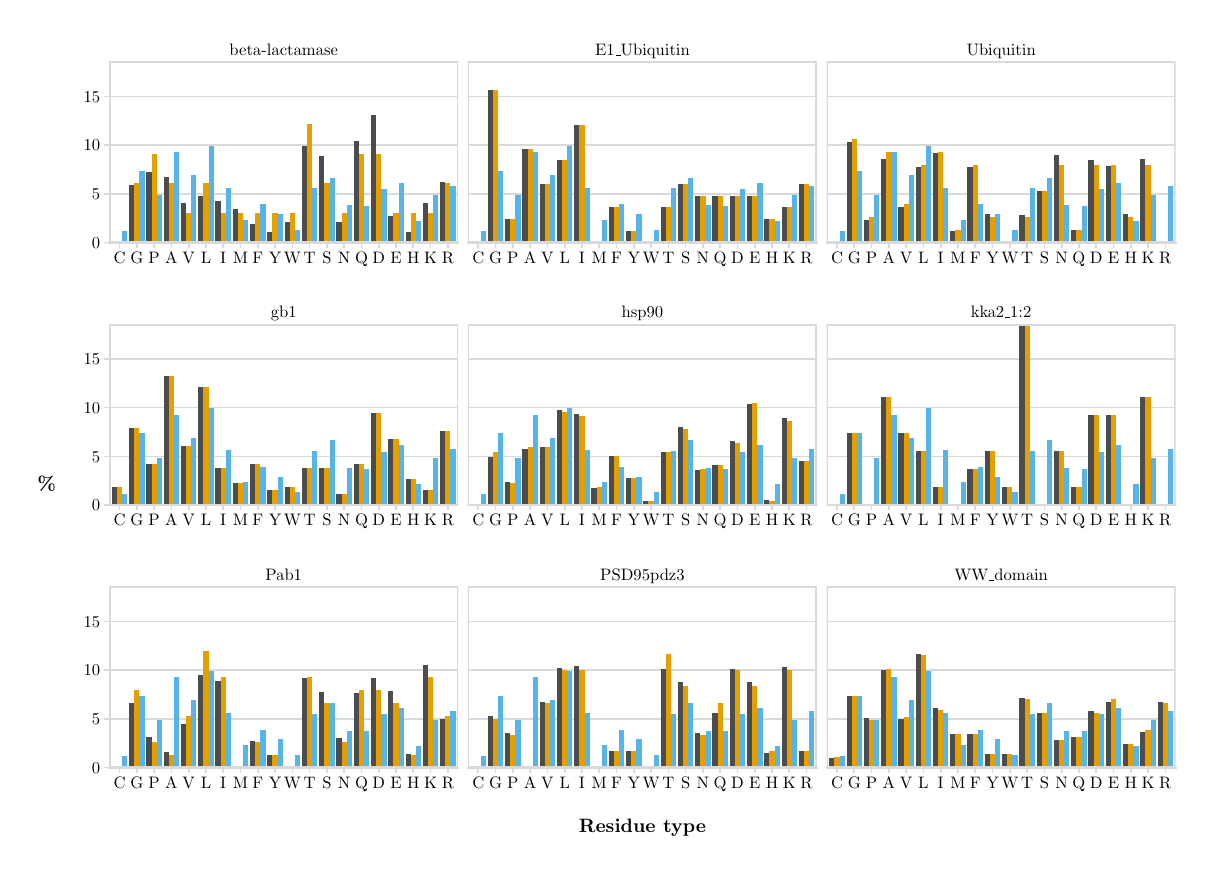
\begin{tikzpicture}[x=1pt,y=1pt]
\definecolor{fillColor}{RGB}{255,255,255}
\path[use as bounding box,fill=fillColor,fill opacity=0.00] (0,0) rectangle (418.34,295.82);
\begin{scope}
\path[clip] ( 29.46,218.05) rectangle (155.58,283.52);
\definecolor{drawColor}{gray}{0.85}

\path[draw=drawColor,line width= 0.6pt,line join=round] ( 29.46,218.18) --
	(155.58,218.18);

\path[draw=drawColor,line width= 0.6pt,line join=round] ( 29.46,235.78) --
	(155.58,235.78);

\path[draw=drawColor,line width= 0.6pt,line join=round] ( 29.46,253.39) --
	(155.58,253.39);

\path[draw=drawColor,line width= 0.6pt,line join=round] ( 29.46,271.00) --
	(155.58,271.00);
\definecolor{fillColor}{RGB}{86,180,233}

\path[fill=fillColor] ( 52.87,218.18) rectangle ( 54.75,250.79);

\path[fill=fillColor] (152.77,218.18) rectangle (154.65,238.60);

\path[fill=fillColor] (115.31,218.18) rectangle (117.18,231.56);

\path[fill=fillColor] (127.80,218.18) rectangle (129.67,237.51);

\path[fill=fillColor] ( 34.14,218.18) rectangle ( 36.01,222.33);

\path[fill=fillColor] (121.55,218.18) rectangle (123.43,231.38);

\path[fill=fillColor] (134.04,218.18) rectangle (135.92,239.87);

\path[fill=fillColor] ( 40.38,218.18) rectangle ( 42.26,244.10);

\path[fill=fillColor] (140.29,218.18) rectangle (142.16,225.89);

\path[fill=fillColor] ( 71.60,218.18) rectangle ( 73.48,238.04);

\path[fill=fillColor] ( 65.36,218.18) rectangle ( 67.23,253.08);

\path[fill=fillColor] (146.53,218.18) rectangle (148.40,235.36);

\path[fill=fillColor] ( 77.85,218.18) rectangle ( 79.72,226.49);

\path[fill=fillColor] ( 84.09,218.18) rectangle ( 85.96,231.95);

\path[fill=fillColor] ( 46.63,218.18) rectangle ( 48.50,235.36);

\path[fill=fillColor] (109.07,218.18) rectangle (110.94,241.53);

\path[fill=fillColor] (102.82,218.18) rectangle (104.70,237.72);

\path[fill=fillColor] ( 96.58,218.18) rectangle ( 98.45,222.75);

\path[fill=fillColor] ( 90.34,218.18) rectangle ( 92.21,228.39);

\path[fill=fillColor] ( 59.12,218.18) rectangle ( 60.99,242.58);
\definecolor{fillColor}{RGB}{230,159,0}

\path[fill=fillColor] ( 32.27,218.18) rectangle ( 34.14,218.18);

\path[fill=fillColor] ( 38.51,218.18) rectangle ( 40.38,239.52);

\path[fill=fillColor] ( 44.76,218.18) rectangle ( 46.63,250.19);

\path[fill=fillColor] ( 51.00,218.18) rectangle ( 52.87,239.52);

\path[fill=fillColor] ( 57.24,218.18) rectangle ( 59.12,228.85);

\path[fill=fillColor] ( 63.49,218.18) rectangle ( 65.36,239.52);

\path[fill=fillColor] ( 69.73,218.18) rectangle ( 71.60,228.85);

\path[fill=fillColor] ( 75.97,218.18) rectangle ( 77.85,228.85);

\path[fill=fillColor] ( 82.22,218.18) rectangle ( 84.09,228.85);

\path[fill=fillColor] ( 88.46,218.18) rectangle ( 90.34,228.85);

\path[fill=fillColor] ( 94.71,218.18) rectangle ( 96.58,228.85);

\path[fill=fillColor] (100.95,218.18) rectangle (102.82,260.86);

\path[fill=fillColor] (107.19,218.18) rectangle (109.07,239.52);

\path[fill=fillColor] (113.44,218.18) rectangle (115.31,228.85);

\path[fill=fillColor] (119.68,218.18) rectangle (121.55,250.19);

\path[fill=fillColor] (125.93,218.18) rectangle (127.80,250.19);

\path[fill=fillColor] (132.17,218.18) rectangle (134.04,228.85);

\path[fill=fillColor] (138.41,218.18) rectangle (140.29,228.85);

\path[fill=fillColor] (144.66,218.18) rectangle (146.53,228.85);

\path[fill=fillColor] (150.90,218.18) rectangle (152.77,239.52);
\definecolor{fillColor}{gray}{0.30}

\path[fill=fillColor] ( 30.39,218.18) rectangle ( 32.27,218.18);

\path[fill=fillColor] ( 36.64,218.18) rectangle ( 38.51,238.95);

\path[fill=fillColor] ( 42.88,218.18) rectangle ( 44.76,243.67);

\path[fill=fillColor] ( 49.13,218.18) rectangle ( 51.00,241.78);

\path[fill=fillColor] ( 55.37,218.18) rectangle ( 57.24,232.34);

\path[fill=fillColor] ( 61.61,218.18) rectangle ( 63.49,235.17);

\path[fill=fillColor] ( 67.86,218.18) rectangle ( 69.73,233.28);

\path[fill=fillColor] ( 74.10,218.18) rectangle ( 75.97,230.45);

\path[fill=fillColor] ( 80.35,218.18) rectangle ( 82.22,224.79);

\path[fill=fillColor] ( 86.59,218.18) rectangle ( 88.46,221.95);

\path[fill=fillColor] ( 92.83,218.18) rectangle ( 94.71,225.73);

\path[fill=fillColor] ( 99.08,218.18) rectangle (100.95,253.11);

\path[fill=fillColor] (105.32,218.18) rectangle (107.19,249.33);

\path[fill=fillColor] (111.56,218.18) rectangle (113.44,225.73);

\path[fill=fillColor] (117.81,218.18) rectangle (119.68,255.00);

\path[fill=fillColor] (124.05,218.18) rectangle (125.93,264.44);

\path[fill=fillColor] (130.30,218.18) rectangle (132.17,227.62);

\path[fill=fillColor] (136.54,218.18) rectangle (138.41,221.95);

\path[fill=fillColor] (142.78,218.18) rectangle (144.66,232.34);

\path[fill=fillColor] (149.03,218.18) rectangle (150.90,239.89);

\path[draw=drawColor,line width= 1.1pt,line join=round,line cap=round] ( 29.46,218.05) rectangle (155.58,283.52);
\end{scope}
\begin{scope}
\path[clip] ( 29.46,123.17) rectangle (155.58,188.65);
\definecolor{drawColor}{gray}{0.85}

\path[draw=drawColor,line width= 0.6pt,line join=round] ( 29.46,123.31) --
	(155.58,123.31);

\path[draw=drawColor,line width= 0.6pt,line join=round] ( 29.46,140.91) --
	(155.58,140.91);

\path[draw=drawColor,line width= 0.6pt,line join=round] ( 29.46,158.52) --
	(155.58,158.52);

\path[draw=drawColor,line width= 0.6pt,line join=round] ( 29.46,176.13) --
	(155.58,176.13);
\definecolor{fillColor}{RGB}{86,180,233}

\path[fill=fillColor] ( 52.87,123.31) rectangle ( 54.75,155.92);

\path[fill=fillColor] (152.77,123.31) rectangle (154.65,143.73);

\path[fill=fillColor] (115.31,123.31) rectangle (117.18,136.69);

\path[fill=fillColor] (127.80,123.31) rectangle (129.67,142.64);

\path[fill=fillColor] ( 34.14,123.31) rectangle ( 36.01,127.46);

\path[fill=fillColor] (121.55,123.31) rectangle (123.43,136.51);

\path[fill=fillColor] (134.04,123.31) rectangle (135.92,145.00);

\path[fill=fillColor] ( 40.38,123.31) rectangle ( 42.26,149.22);

\path[fill=fillColor] (140.29,123.31) rectangle (142.16,131.02);

\path[fill=fillColor] ( 71.60,123.31) rectangle ( 73.48,143.17);

\path[fill=fillColor] ( 65.36,123.31) rectangle ( 67.23,158.21);

\path[fill=fillColor] (146.53,123.31) rectangle (148.40,140.49);

\path[fill=fillColor] ( 77.85,123.31) rectangle ( 79.72,131.62);

\path[fill=fillColor] ( 84.09,123.31) rectangle ( 85.96,137.08);

\path[fill=fillColor] ( 46.63,123.31) rectangle ( 48.50,140.49);

\path[fill=fillColor] (109.07,123.31) rectangle (110.94,146.65);

\path[fill=fillColor] (102.82,123.31) rectangle (104.70,142.85);

\path[fill=fillColor] ( 96.58,123.31) rectangle ( 98.45,127.88);

\path[fill=fillColor] ( 90.34,123.31) rectangle ( 92.21,133.52);

\path[fill=fillColor] ( 59.12,123.31) rectangle ( 60.99,147.71);
\definecolor{fillColor}{RGB}{230,159,0}

\path[fill=fillColor] ( 32.27,123.31) rectangle ( 34.14,129.98);

\path[fill=fillColor] ( 38.51,123.31) rectangle ( 40.38,151.32);

\path[fill=fillColor] ( 44.76,123.31) rectangle ( 46.63,137.98);

\path[fill=fillColor] ( 51.00,123.31) rectangle ( 52.87,169.99);

\path[fill=fillColor] ( 57.24,123.31) rectangle ( 59.12,144.65);

\path[fill=fillColor] ( 63.49,123.31) rectangle ( 65.36,165.99);

\path[fill=fillColor] ( 69.73,123.31) rectangle ( 71.60,136.65);

\path[fill=fillColor] ( 75.97,123.31) rectangle ( 77.85,131.31);

\path[fill=fillColor] ( 82.22,123.31) rectangle ( 84.09,137.98);

\path[fill=fillColor] ( 88.46,123.31) rectangle ( 90.34,128.64);

\path[fill=fillColor] ( 94.71,123.31) rectangle ( 96.58,129.98);

\path[fill=fillColor] (100.95,123.31) rectangle (102.82,136.65);

\path[fill=fillColor] (107.19,123.31) rectangle (109.07,136.65);

\path[fill=fillColor] (113.44,123.31) rectangle (115.31,127.31);

\path[fill=fillColor] (119.68,123.31) rectangle (121.55,137.98);

\path[fill=fillColor] (125.93,123.31) rectangle (127.80,156.65);

\path[fill=fillColor] (132.17,123.31) rectangle (134.04,147.32);

\path[fill=fillColor] (138.41,123.31) rectangle (140.29,132.64);

\path[fill=fillColor] (144.66,123.31) rectangle (146.53,128.64);

\path[fill=fillColor] (150.90,123.31) rectangle (152.77,149.98);
\definecolor{fillColor}{gray}{0.30}

\path[fill=fillColor] ( 30.39,123.31) rectangle ( 32.27,129.98);

\path[fill=fillColor] ( 36.64,123.31) rectangle ( 38.51,151.32);

\path[fill=fillColor] ( 42.88,123.31) rectangle ( 44.76,137.98);

\path[fill=fillColor] ( 49.13,123.31) rectangle ( 51.00,169.99);

\path[fill=fillColor] ( 55.37,123.31) rectangle ( 57.24,144.65);

\path[fill=fillColor] ( 61.61,123.31) rectangle ( 63.49,165.99);

\path[fill=fillColor] ( 67.86,123.31) rectangle ( 69.73,136.65);

\path[fill=fillColor] ( 74.10,123.31) rectangle ( 75.97,131.31);

\path[fill=fillColor] ( 80.35,123.31) rectangle ( 82.22,137.98);

\path[fill=fillColor] ( 86.59,123.31) rectangle ( 88.46,128.64);

\path[fill=fillColor] ( 92.83,123.31) rectangle ( 94.71,129.98);

\path[fill=fillColor] ( 99.08,123.31) rectangle (100.95,136.65);

\path[fill=fillColor] (105.32,123.31) rectangle (107.19,136.65);

\path[fill=fillColor] (111.56,123.31) rectangle (113.44,127.31);

\path[fill=fillColor] (117.81,123.31) rectangle (119.68,137.98);

\path[fill=fillColor] (124.05,123.31) rectangle (125.93,156.65);

\path[fill=fillColor] (130.30,123.31) rectangle (132.17,147.32);

\path[fill=fillColor] (136.54,123.31) rectangle (138.41,132.64);

\path[fill=fillColor] (142.78,123.31) rectangle (144.66,128.64);

\path[fill=fillColor] (149.03,123.31) rectangle (150.90,149.98);

\path[draw=drawColor,line width= 1.1pt,line join=round,line cap=round] ( 29.46,123.17) rectangle (155.58,188.65);
\end{scope}
\begin{scope}
\path[clip] ( 29.46, 28.30) rectangle (155.58, 93.78);
\definecolor{drawColor}{gray}{0.85}

\path[draw=drawColor,line width= 0.6pt,line join=round] ( 29.46, 28.43) --
	(155.58, 28.43);

\path[draw=drawColor,line width= 0.6pt,line join=round] ( 29.46, 46.04) --
	(155.58, 46.04);

\path[draw=drawColor,line width= 0.6pt,line join=round] ( 29.46, 63.65) --
	(155.58, 63.65);

\path[draw=drawColor,line width= 0.6pt,line join=round] ( 29.46, 81.26) --
	(155.58, 81.26);
\definecolor{fillColor}{RGB}{86,180,233}

\path[fill=fillColor] ( 52.87, 28.43) rectangle ( 54.75, 61.04);

\path[fill=fillColor] (152.77, 28.43) rectangle (154.65, 48.86);

\path[fill=fillColor] (115.31, 28.43) rectangle (117.18, 41.82);

\path[fill=fillColor] (127.80, 28.43) rectangle (129.67, 47.77);

\path[fill=fillColor] ( 34.14, 28.43) rectangle ( 36.01, 32.59);

\path[fill=fillColor] (121.55, 28.43) rectangle (123.43, 41.64);

\path[fill=fillColor] (134.04, 28.43) rectangle (135.92, 50.13);

\path[fill=fillColor] ( 40.38, 28.43) rectangle ( 42.26, 54.35);

\path[fill=fillColor] (140.29, 28.43) rectangle (142.16, 36.15);

\path[fill=fillColor] ( 71.60, 28.43) rectangle ( 73.48, 48.30);

\path[fill=fillColor] ( 65.36, 28.43) rectangle ( 67.23, 63.33);

\path[fill=fillColor] (146.53, 28.43) rectangle (148.40, 45.62);

\path[fill=fillColor] ( 77.85, 28.43) rectangle ( 79.72, 36.75);

\path[fill=fillColor] ( 84.09, 28.43) rectangle ( 85.96, 42.20);

\path[fill=fillColor] ( 46.63, 28.43) rectangle ( 48.50, 45.62);

\path[fill=fillColor] (109.07, 28.43) rectangle (110.94, 51.78);

\path[fill=fillColor] (102.82, 28.43) rectangle (104.70, 47.98);

\path[fill=fillColor] ( 96.58, 28.43) rectangle ( 98.45, 33.01);

\path[fill=fillColor] ( 90.34, 28.43) rectangle ( 92.21, 38.65);

\path[fill=fillColor] ( 59.12, 28.43) rectangle ( 60.99, 52.84);
\definecolor{fillColor}{RGB}{230,159,0}

\path[fill=fillColor] ( 32.27, 28.43) rectangle ( 34.14, 28.43);

\path[fill=fillColor] ( 38.51, 28.43) rectangle ( 40.38, 56.61);

\path[fill=fillColor] ( 44.76, 28.43) rectangle ( 46.63, 37.83);

\path[fill=fillColor] ( 51.00, 28.43) rectangle ( 52.87, 33.13);

\path[fill=fillColor] ( 57.24, 28.43) rectangle ( 59.12, 47.22);

\path[fill=fillColor] ( 63.49, 28.43) rectangle ( 65.36, 70.69);

\path[fill=fillColor] ( 69.73, 28.43) rectangle ( 71.60, 61.30);

\path[fill=fillColor] ( 75.97, 28.43) rectangle ( 77.85, 28.43);

\path[fill=fillColor] ( 82.22, 28.43) rectangle ( 84.09, 37.83);

\path[fill=fillColor] ( 88.46, 28.43) rectangle ( 90.34, 33.13);

\path[fill=fillColor] ( 94.71, 28.43) rectangle ( 96.58, 28.43);

\path[fill=fillColor] (100.95, 28.43) rectangle (102.82, 61.30);

\path[fill=fillColor] (107.19, 28.43) rectangle (109.07, 51.91);

\path[fill=fillColor] (113.44, 28.43) rectangle (115.31, 37.83);

\path[fill=fillColor] (119.68, 28.43) rectangle (121.55, 56.61);

\path[fill=fillColor] (125.93, 28.43) rectangle (127.80, 56.61);

\path[fill=fillColor] (132.17, 28.43) rectangle (134.04, 51.91);

\path[fill=fillColor] (138.41, 28.43) rectangle (140.29, 33.13);

\path[fill=fillColor] (144.66, 28.43) rectangle (146.53, 61.30);

\path[fill=fillColor] (150.90, 28.43) rectangle (152.77, 47.22);
\definecolor{fillColor}{gray}{0.30}

\path[fill=fillColor] ( 30.39, 28.43) rectangle ( 32.27, 28.43);

\path[fill=fillColor] ( 36.64, 28.43) rectangle ( 38.51, 51.78);

\path[fill=fillColor] ( 42.88, 28.43) rectangle ( 44.76, 39.55);

\path[fill=fillColor] ( 49.13, 28.43) rectangle ( 51.00, 33.99);

\path[fill=fillColor] ( 55.37, 28.43) rectangle ( 57.24, 44.28);

\path[fill=fillColor] ( 61.61, 28.43) rectangle ( 63.49, 62.07);

\path[fill=fillColor] ( 67.86, 28.43) rectangle ( 69.73, 59.84);

\path[fill=fillColor] ( 74.10, 28.43) rectangle ( 75.97, 28.43);

\path[fill=fillColor] ( 80.35, 28.43) rectangle ( 82.22, 38.16);

\path[fill=fillColor] ( 86.59, 28.43) rectangle ( 88.46, 32.88);

\path[fill=fillColor] ( 92.83, 28.43) rectangle ( 94.71, 28.43);

\path[fill=fillColor] ( 99.08, 28.43) rectangle (100.95, 60.95);

\path[fill=fillColor] (105.32, 28.43) rectangle (107.19, 55.67);

\path[fill=fillColor] (111.56, 28.43) rectangle (113.44, 39.27);

\path[fill=fillColor] (117.81, 28.43) rectangle (119.68, 55.40);

\path[fill=fillColor] (124.05, 28.43) rectangle (125.93, 60.68);

\path[fill=fillColor] (130.30, 28.43) rectangle (132.17, 55.95);

\path[fill=fillColor] (136.54, 28.43) rectangle (138.41, 33.44);

\path[fill=fillColor] (142.78, 28.43) rectangle (144.66, 65.68);

\path[fill=fillColor] (149.03, 28.43) rectangle (150.90, 45.95);

\path[draw=drawColor,line width= 1.1pt,line join=round,line cap=round] ( 29.46, 28.30) rectangle (155.58, 93.78);
\end{scope}
\begin{scope}
\path[clip] (159.08,218.05) rectangle (285.21,283.52);
\definecolor{drawColor}{gray}{0.85}

\path[draw=drawColor,line width= 0.6pt,line join=round] (159.08,218.18) --
	(285.21,218.18);

\path[draw=drawColor,line width= 0.6pt,line join=round] (159.08,235.78) --
	(285.21,235.78);

\path[draw=drawColor,line width= 0.6pt,line join=round] (159.08,253.39) --
	(285.21,253.39);

\path[draw=drawColor,line width= 0.6pt,line join=round] (159.08,271.00) --
	(285.21,271.00);
\definecolor{fillColor}{RGB}{86,180,233}

\path[fill=fillColor] (182.50,218.18) rectangle (184.37,250.79);

\path[fill=fillColor] (282.40,218.18) rectangle (284.27,238.60);

\path[fill=fillColor] (244.94,218.18) rectangle (246.81,231.56);

\path[fill=fillColor] (257.42,218.18) rectangle (259.30,237.51);

\path[fill=fillColor] (163.77,218.18) rectangle (165.64,222.33);

\path[fill=fillColor] (251.18,218.18) rectangle (253.05,231.38);

\path[fill=fillColor] (263.67,218.18) rectangle (265.54,239.87);

\path[fill=fillColor] (170.01,218.18) rectangle (171.88,244.10);

\path[fill=fillColor] (269.91,218.18) rectangle (271.79,225.89);

\path[fill=fillColor] (201.23,218.18) rectangle (203.10,238.04);

\path[fill=fillColor] (194.99,218.18) rectangle (196.86,253.08);

\path[fill=fillColor] (276.16,218.18) rectangle (278.03,235.36);

\path[fill=fillColor] (207.47,218.18) rectangle (209.35,226.49);

\path[fill=fillColor] (213.72,218.18) rectangle (215.59,231.95);

\path[fill=fillColor] (176.25,218.18) rectangle (178.13,235.36);

\path[fill=fillColor] (238.69,218.18) rectangle (240.57,241.53);

\path[fill=fillColor] (232.45,218.18) rectangle (234.32,237.72);

\path[fill=fillColor] (226.21,218.18) rectangle (228.08,222.75);

\path[fill=fillColor] (219.96,218.18) rectangle (221.83,228.39);

\path[fill=fillColor] (188.74,218.18) rectangle (190.62,242.58);
\definecolor{fillColor}{RGB}{230,159,0}

\path[fill=fillColor] (161.89,218.18) rectangle (163.77,218.18);

\path[fill=fillColor] (168.14,218.18) rectangle (170.01,273.34);

\path[fill=fillColor] (174.38,218.18) rectangle (176.25,226.66);

\path[fill=fillColor] (180.63,218.18) rectangle (182.50,252.12);

\path[fill=fillColor] (186.87,218.18) rectangle (188.74,239.39);

\path[fill=fillColor] (193.11,218.18) rectangle (194.99,247.88);

\path[fill=fillColor] (199.36,218.18) rectangle (201.23,260.61);

\path[fill=fillColor] (205.60,218.18) rectangle (207.47,218.18);

\path[fill=fillColor] (211.84,218.18) rectangle (213.72,230.91);

\path[fill=fillColor] (218.09,218.18) rectangle (219.96,222.42);

\path[fill=fillColor] (224.33,218.18) rectangle (226.21,218.18);

\path[fill=fillColor] (230.58,218.18) rectangle (232.45,230.91);

\path[fill=fillColor] (236.82,218.18) rectangle (238.69,239.39);

\path[fill=fillColor] (243.06,218.18) rectangle (244.94,235.15);

\path[fill=fillColor] (249.31,218.18) rectangle (251.18,235.15);

\path[fill=fillColor] (255.55,218.18) rectangle (257.42,235.15);

\path[fill=fillColor] (261.80,218.18) rectangle (263.67,235.15);

\path[fill=fillColor] (268.04,218.18) rectangle (269.91,226.66);

\path[fill=fillColor] (274.28,218.18) rectangle (276.16,230.91);

\path[fill=fillColor] (280.53,218.18) rectangle (282.40,239.39);
\definecolor{fillColor}{gray}{0.30}

\path[fill=fillColor] (160.02,218.18) rectangle (161.89,218.18);

\path[fill=fillColor] (166.26,218.18) rectangle (168.14,273.34);

\path[fill=fillColor] (172.51,218.18) rectangle (174.38,226.66);

\path[fill=fillColor] (178.75,218.18) rectangle (180.63,252.12);

\path[fill=fillColor] (185.00,218.18) rectangle (186.87,239.39);

\path[fill=fillColor] (191.24,218.18) rectangle (193.11,247.88);

\path[fill=fillColor] (197.48,218.18) rectangle (199.36,260.61);

\path[fill=fillColor] (203.73,218.18) rectangle (205.60,218.18);

\path[fill=fillColor] (209.97,218.18) rectangle (211.84,230.91);

\path[fill=fillColor] (216.22,218.18) rectangle (218.09,222.42);

\path[fill=fillColor] (222.46,218.18) rectangle (224.33,218.18);

\path[fill=fillColor] (228.70,218.18) rectangle (230.58,230.91);

\path[fill=fillColor] (234.95,218.18) rectangle (236.82,239.39);

\path[fill=fillColor] (241.19,218.18) rectangle (243.06,235.15);

\path[fill=fillColor] (247.43,218.18) rectangle (249.31,235.15);

\path[fill=fillColor] (253.68,218.18) rectangle (255.55,235.15);

\path[fill=fillColor] (259.92,218.18) rectangle (261.80,235.15);

\path[fill=fillColor] (266.17,218.18) rectangle (268.04,226.66);

\path[fill=fillColor] (272.41,218.18) rectangle (274.28,230.91);

\path[fill=fillColor] (278.65,218.18) rectangle (280.53,239.39);

\path[draw=drawColor,line width= 1.1pt,line join=round,line cap=round] (159.08,218.05) rectangle (285.21,283.52);
\end{scope}
\begin{scope}
\path[clip] (159.08,123.17) rectangle (285.21,188.65);
\definecolor{drawColor}{gray}{0.85}

\path[draw=drawColor,line width= 0.6pt,line join=round] (159.08,123.31) --
	(285.21,123.31);

\path[draw=drawColor,line width= 0.6pt,line join=round] (159.08,140.91) --
	(285.21,140.91);

\path[draw=drawColor,line width= 0.6pt,line join=round] (159.08,158.52) --
	(285.21,158.52);

\path[draw=drawColor,line width= 0.6pt,line join=round] (159.08,176.13) --
	(285.21,176.13);
\definecolor{fillColor}{RGB}{86,180,233}

\path[fill=fillColor] (182.50,123.31) rectangle (184.37,155.92);

\path[fill=fillColor] (282.40,123.31) rectangle (284.27,143.73);

\path[fill=fillColor] (244.94,123.31) rectangle (246.81,136.69);

\path[fill=fillColor] (257.42,123.31) rectangle (259.30,142.64);

\path[fill=fillColor] (163.77,123.31) rectangle (165.64,127.46);

\path[fill=fillColor] (251.18,123.31) rectangle (253.05,136.51);

\path[fill=fillColor] (263.67,123.31) rectangle (265.54,145.00);

\path[fill=fillColor] (170.01,123.31) rectangle (171.88,149.22);

\path[fill=fillColor] (269.91,123.31) rectangle (271.79,131.02);

\path[fill=fillColor] (201.23,123.31) rectangle (203.10,143.17);

\path[fill=fillColor] (194.99,123.31) rectangle (196.86,158.21);

\path[fill=fillColor] (276.16,123.31) rectangle (278.03,140.49);

\path[fill=fillColor] (207.47,123.31) rectangle (209.35,131.62);

\path[fill=fillColor] (213.72,123.31) rectangle (215.59,137.08);

\path[fill=fillColor] (176.25,123.31) rectangle (178.13,140.49);

\path[fill=fillColor] (238.69,123.31) rectangle (240.57,146.65);

\path[fill=fillColor] (232.45,123.31) rectangle (234.32,142.85);

\path[fill=fillColor] (226.21,123.31) rectangle (228.08,127.88);

\path[fill=fillColor] (219.96,123.31) rectangle (221.83,133.52);

\path[fill=fillColor] (188.74,123.31) rectangle (190.62,147.71);
\definecolor{fillColor}{RGB}{230,159,0}

\path[fill=fillColor] (161.89,123.31) rectangle (163.77,123.31);

\path[fill=fillColor] (168.14,123.31) rectangle (170.01,142.60);

\path[fill=fillColor] (174.38,123.31) rectangle (176.25,131.35);

\path[fill=fillColor] (180.63,123.31) rectangle (182.50,144.21);

\path[fill=fillColor] (186.87,123.31) rectangle (188.74,144.21);

\path[fill=fillColor] (193.11,123.31) rectangle (194.99,157.07);

\path[fill=fillColor] (199.36,123.31) rectangle (201.23,155.47);

\path[fill=fillColor] (205.60,123.31) rectangle (207.47,129.74);

\path[fill=fillColor] (211.84,123.31) rectangle (213.72,140.99);

\path[fill=fillColor] (218.09,123.31) rectangle (219.96,132.95);

\path[fill=fillColor] (224.33,123.31) rectangle (226.21,124.91);

\path[fill=fillColor] (230.58,123.31) rectangle (232.45,142.60);

\path[fill=fillColor] (236.82,123.31) rectangle (238.69,150.64);

\path[fill=fillColor] (243.06,123.31) rectangle (244.94,136.17);

\path[fill=fillColor] (249.31,123.31) rectangle (251.18,137.78);

\path[fill=fillColor] (255.55,123.31) rectangle (257.42,145.82);

\path[fill=fillColor] (261.80,123.31) rectangle (263.67,160.29);

\path[fill=fillColor] (268.04,123.31) rectangle (269.91,124.91);

\path[fill=fillColor] (274.28,123.31) rectangle (276.16,153.86);

\path[fill=fillColor] (280.53,123.31) rectangle (282.40,139.39);
\definecolor{fillColor}{gray}{0.30}

\path[fill=fillColor] (160.02,123.31) rectangle (161.89,123.31);

\path[fill=fillColor] (166.26,123.31) rectangle (168.14,140.70);

\path[fill=fillColor] (172.51,123.31) rectangle (174.38,131.55);

\path[fill=fillColor] (178.75,123.31) rectangle (180.63,143.61);

\path[fill=fillColor] (185.00,123.31) rectangle (186.87,144.28);

\path[fill=fillColor] (191.24,123.31) rectangle (193.11,157.51);

\path[fill=fillColor] (197.48,123.31) rectangle (199.36,156.27);

\path[fill=fillColor] (203.73,123.31) rectangle (205.60,129.30);

\path[fill=fillColor] (209.97,123.31) rectangle (211.84,140.95);

\path[fill=fillColor] (216.22,123.31) rectangle (218.09,133.04);

\path[fill=fillColor] (222.46,123.31) rectangle (224.33,124.89);

\path[fill=fillColor] (228.70,123.31) rectangle (230.58,142.53);

\path[fill=fillColor] (234.95,123.31) rectangle (236.82,151.36);

\path[fill=fillColor] (241.19,123.31) rectangle (243.06,136.04);

\path[fill=fillColor] (247.43,123.31) rectangle (249.31,137.95);

\path[fill=fillColor] (253.68,123.31) rectangle (255.55,146.53);

\path[fill=fillColor] (259.92,123.31) rectangle (261.80,159.68);

\path[fill=fillColor] (266.17,123.31) rectangle (268.04,124.97);

\path[fill=fillColor] (272.41,123.31) rectangle (274.28,154.68);

\path[fill=fillColor] (278.65,123.31) rectangle (280.53,139.12);

\path[draw=drawColor,line width= 1.1pt,line join=round,line cap=round] (159.08,123.17) rectangle (285.21,188.65);
\end{scope}
\begin{scope}
\path[clip] (159.08, 28.30) rectangle (285.21, 93.78);
\definecolor{drawColor}{gray}{0.85}

\path[draw=drawColor,line width= 0.6pt,line join=round] (159.08, 28.43) --
	(285.21, 28.43);

\path[draw=drawColor,line width= 0.6pt,line join=round] (159.08, 46.04) --
	(285.21, 46.04);

\path[draw=drawColor,line width= 0.6pt,line join=round] (159.08, 63.65) --
	(285.21, 63.65);

\path[draw=drawColor,line width= 0.6pt,line join=round] (159.08, 81.26) --
	(285.21, 81.26);
\definecolor{fillColor}{RGB}{86,180,233}

\path[fill=fillColor] (182.50, 28.43) rectangle (184.37, 61.04);

\path[fill=fillColor] (282.40, 28.43) rectangle (284.27, 48.86);

\path[fill=fillColor] (244.94, 28.43) rectangle (246.81, 41.82);

\path[fill=fillColor] (257.42, 28.43) rectangle (259.30, 47.77);

\path[fill=fillColor] (163.77, 28.43) rectangle (165.64, 32.59);

\path[fill=fillColor] (251.18, 28.43) rectangle (253.05, 41.64);

\path[fill=fillColor] (263.67, 28.43) rectangle (265.54, 50.13);

\path[fill=fillColor] (170.01, 28.43) rectangle (171.88, 54.35);

\path[fill=fillColor] (269.91, 28.43) rectangle (271.79, 36.15);

\path[fill=fillColor] (201.23, 28.43) rectangle (203.10, 48.30);

\path[fill=fillColor] (194.99, 28.43) rectangle (196.86, 63.33);

\path[fill=fillColor] (276.16, 28.43) rectangle (278.03, 45.62);

\path[fill=fillColor] (207.47, 28.43) rectangle (209.35, 36.75);

\path[fill=fillColor] (213.72, 28.43) rectangle (215.59, 42.20);

\path[fill=fillColor] (176.25, 28.43) rectangle (178.13, 45.62);

\path[fill=fillColor] (238.69, 28.43) rectangle (240.57, 51.78);

\path[fill=fillColor] (232.45, 28.43) rectangle (234.32, 47.98);

\path[fill=fillColor] (226.21, 28.43) rectangle (228.08, 33.01);

\path[fill=fillColor] (219.96, 28.43) rectangle (221.83, 38.65);

\path[fill=fillColor] (188.74, 28.43) rectangle (190.62, 52.84);
\definecolor{fillColor}{RGB}{230,159,0}

\path[fill=fillColor] (161.89, 28.43) rectangle (163.77, 28.43);

\path[fill=fillColor] (168.14, 28.43) rectangle (170.01, 46.04);

\path[fill=fillColor] (174.38, 28.43) rectangle (176.25, 40.17);

\path[fill=fillColor] (180.63, 28.43) rectangle (182.50, 28.43);

\path[fill=fillColor] (186.87, 28.43) rectangle (188.74, 51.91);

\path[fill=fillColor] (193.11, 28.43) rectangle (194.99, 63.65);

\path[fill=fillColor] (199.36, 28.43) rectangle (201.23, 63.65);

\path[fill=fillColor] (205.60, 28.43) rectangle (207.47, 28.43);

\path[fill=fillColor] (211.84, 28.43) rectangle (213.72, 34.30);

\path[fill=fillColor] (218.09, 28.43) rectangle (219.96, 34.30);

\path[fill=fillColor] (224.33, 28.43) rectangle (226.21, 28.43);

\path[fill=fillColor] (230.58, 28.43) rectangle (232.45, 69.52);

\path[fill=fillColor] (236.82, 28.43) rectangle (238.69, 57.78);

\path[fill=fillColor] (243.06, 28.43) rectangle (244.94, 40.17);

\path[fill=fillColor] (249.31, 28.43) rectangle (251.18, 51.91);

\path[fill=fillColor] (255.55, 28.43) rectangle (257.42, 63.65);

\path[fill=fillColor] (261.80, 28.43) rectangle (263.67, 57.78);

\path[fill=fillColor] (268.04, 28.43) rectangle (269.91, 34.30);

\path[fill=fillColor] (274.28, 28.43) rectangle (276.16, 63.65);

\path[fill=fillColor] (280.53, 28.43) rectangle (282.40, 34.30);
\definecolor{fillColor}{gray}{0.30}

\path[fill=fillColor] (160.02, 28.43) rectangle (161.89, 28.43);

\path[fill=fillColor] (166.26, 28.43) rectangle (168.14, 46.94);

\path[fill=fillColor] (172.51, 28.43) rectangle (174.38, 40.77);

\path[fill=fillColor] (178.75, 28.43) rectangle (180.63, 28.43);

\path[fill=fillColor] (185.00, 28.43) rectangle (186.87, 52.18);

\path[fill=fillColor] (191.24, 28.43) rectangle (193.11, 64.51);

\path[fill=fillColor] (197.48, 28.43) rectangle (199.36, 65.13);

\path[fill=fillColor] (203.73, 28.43) rectangle (205.60, 28.43);

\path[fill=fillColor] (209.97, 28.43) rectangle (211.84, 34.60);

\path[fill=fillColor] (216.22, 28.43) rectangle (218.09, 34.60);

\path[fill=fillColor] (222.46, 28.43) rectangle (224.33, 28.43);

\path[fill=fillColor] (228.70, 28.43) rectangle (230.58, 63.90);

\path[fill=fillColor] (234.95, 28.43) rectangle (236.82, 59.27);

\path[fill=fillColor] (241.19, 28.43) rectangle (243.06, 40.77);

\path[fill=fillColor] (247.43, 28.43) rectangle (249.31, 48.17);

\path[fill=fillColor] (253.68, 28.43) rectangle (255.55, 64.21);

\path[fill=fillColor] (259.92, 28.43) rectangle (261.80, 59.27);

\path[fill=fillColor] (266.17, 28.43) rectangle (268.04, 33.68);

\path[fill=fillColor] (272.41, 28.43) rectangle (274.28, 64.82);

\path[fill=fillColor] (278.65, 28.43) rectangle (280.53, 34.29);

\path[draw=drawColor,line width= 1.1pt,line join=round,line cap=round] (159.08, 28.30) rectangle (285.21, 93.78);
\end{scope}
\begin{scope}
\path[clip] (288.71,218.05) rectangle (414.84,283.52);
\definecolor{drawColor}{gray}{0.85}

\path[draw=drawColor,line width= 0.6pt,line join=round] (288.71,218.18) --
	(414.84,218.18);

\path[draw=drawColor,line width= 0.6pt,line join=round] (288.71,235.78) --
	(414.84,235.78);

\path[draw=drawColor,line width= 0.6pt,line join=round] (288.71,253.39) --
	(414.84,253.39);

\path[draw=drawColor,line width= 0.6pt,line join=round] (288.71,271.00) --
	(414.84,271.00);
\definecolor{fillColor}{RGB}{86,180,233}

\path[fill=fillColor] (312.12,218.18) rectangle (314.00,250.79);

\path[fill=fillColor] (412.03,218.18) rectangle (413.90,238.60);

\path[fill=fillColor] (374.56,218.18) rectangle (376.44,231.56);

\path[fill=fillColor] (387.05,218.18) rectangle (388.92,237.51);

\path[fill=fillColor] (293.39,218.18) rectangle (295.27,222.33);

\path[fill=fillColor] (380.81,218.18) rectangle (382.68,231.38);

\path[fill=fillColor] (393.29,218.18) rectangle (395.17,239.87);

\path[fill=fillColor] (299.64,218.18) rectangle (301.51,244.10);

\path[fill=fillColor] (399.54,218.18) rectangle (401.41,225.89);

\path[fill=fillColor] (330.86,218.18) rectangle (332.73,238.04);

\path[fill=fillColor] (324.61,218.18) rectangle (326.49,253.08);

\path[fill=fillColor] (405.78,218.18) rectangle (407.66,235.36);

\path[fill=fillColor] (337.10,218.18) rectangle (338.97,226.49);

\path[fill=fillColor] (343.34,218.18) rectangle (345.22,231.95);

\path[fill=fillColor] (305.88,218.18) rectangle (307.75,235.36);

\path[fill=fillColor] (368.32,218.18) rectangle (370.19,241.53);

\path[fill=fillColor] (362.08,218.18) rectangle (363.95,237.72);

\path[fill=fillColor] (355.83,218.18) rectangle (357.70,222.75);

\path[fill=fillColor] (349.59,218.18) rectangle (351.46,228.39);

\path[fill=fillColor] (318.37,218.18) rectangle (320.24,242.58);
\definecolor{fillColor}{RGB}{230,159,0}

\path[fill=fillColor] (291.52,218.18) rectangle (293.39,218.18);

\path[fill=fillColor] (297.76,218.18) rectangle (299.64,255.74);

\path[fill=fillColor] (304.01,218.18) rectangle (305.88,227.57);

\path[fill=fillColor] (310.25,218.18) rectangle (312.12,251.05);

\path[fill=fillColor] (316.49,218.18) rectangle (318.37,232.26);

\path[fill=fillColor] (322.74,218.18) rectangle (324.61,246.35);

\path[fill=fillColor] (328.98,218.18) rectangle (330.86,251.05);

\path[fill=fillColor] (335.23,218.18) rectangle (337.10,222.87);

\path[fill=fillColor] (341.47,218.18) rectangle (343.34,246.35);

\path[fill=fillColor] (347.71,218.18) rectangle (349.59,227.57);

\path[fill=fillColor] (353.96,218.18) rectangle (355.83,218.18);

\path[fill=fillColor] (360.20,218.18) rectangle (362.08,227.57);

\path[fill=fillColor] (366.45,218.18) rectangle (368.32,236.96);

\path[fill=fillColor] (372.69,218.18) rectangle (374.56,246.35);

\path[fill=fillColor] (378.93,218.18) rectangle (380.81,222.87);

\path[fill=fillColor] (385.18,218.18) rectangle (387.05,246.35);

\path[fill=fillColor] (391.42,218.18) rectangle (393.29,246.35);

\path[fill=fillColor] (397.67,218.18) rectangle (399.54,227.57);

\path[fill=fillColor] (403.91,218.18) rectangle (405.78,246.35);

\path[fill=fillColor] (410.15,218.18) rectangle (412.03,218.18);
\definecolor{fillColor}{gray}{0.30}

\path[fill=fillColor] (289.65,218.18) rectangle (291.52,218.18);

\path[fill=fillColor] (295.89,218.18) rectangle (297.76,254.55);

\path[fill=fillColor] (302.13,218.18) rectangle (304.01,226.26);

\path[fill=fillColor] (308.38,218.18) rectangle (310.25,248.49);

\path[fill=fillColor] (314.62,218.18) rectangle (316.49,231.17);

\path[fill=fillColor] (320.87,218.18) rectangle (322.74,245.31);

\path[fill=fillColor] (327.11,218.18) rectangle (328.98,250.51);

\path[fill=fillColor] (333.35,218.18) rectangle (335.23,222.51);

\path[fill=fillColor] (339.60,218.18) rectangle (341.47,245.31);

\path[fill=fillColor] (345.84,218.18) rectangle (347.71,228.57);

\path[fill=fillColor] (352.08,218.18) rectangle (353.96,218.18);

\path[fill=fillColor] (358.33,218.18) rectangle (360.20,228.28);

\path[fill=fillColor] (364.57,218.18) rectangle (366.45,236.94);

\path[fill=fillColor] (370.82,218.18) rectangle (372.69,249.64);

\path[fill=fillColor] (377.06,218.18) rectangle (378.93,222.80);

\path[fill=fillColor] (383.30,218.18) rectangle (385.18,247.91);

\path[fill=fillColor] (389.55,218.18) rectangle (391.42,245.89);

\path[fill=fillColor] (395.79,218.18) rectangle (397.67,228.57);

\path[fill=fillColor] (402.04,218.18) rectangle (403.91,248.49);

\path[fill=fillColor] (408.28,218.18) rectangle (410.15,218.18);

\path[draw=drawColor,line width= 1.1pt,line join=round,line cap=round] (288.71,218.05) rectangle (414.84,283.52);
\end{scope}
\begin{scope}
\path[clip] (288.71,123.17) rectangle (414.84,188.65);
\definecolor{drawColor}{gray}{0.85}

\path[draw=drawColor,line width= 0.6pt,line join=round] (288.71,123.31) --
	(414.84,123.31);

\path[draw=drawColor,line width= 0.6pt,line join=round] (288.71,140.91) --
	(414.84,140.91);

\path[draw=drawColor,line width= 0.6pt,line join=round] (288.71,158.52) --
	(414.84,158.52);

\path[draw=drawColor,line width= 0.6pt,line join=round] (288.71,176.13) --
	(414.84,176.13);
\definecolor{fillColor}{RGB}{86,180,233}

\path[fill=fillColor] (312.12,123.31) rectangle (314.00,155.92);

\path[fill=fillColor] (412.03,123.31) rectangle (413.90,143.73);

\path[fill=fillColor] (374.56,123.31) rectangle (376.44,136.69);

\path[fill=fillColor] (387.05,123.31) rectangle (388.92,142.64);

\path[fill=fillColor] (293.39,123.31) rectangle (295.27,127.46);

\path[fill=fillColor] (380.81,123.31) rectangle (382.68,136.51);

\path[fill=fillColor] (393.29,123.31) rectangle (395.17,145.00);

\path[fill=fillColor] (299.64,123.31) rectangle (301.51,149.22);

\path[fill=fillColor] (399.54,123.31) rectangle (401.41,131.02);

\path[fill=fillColor] (330.86,123.31) rectangle (332.73,143.17);

\path[fill=fillColor] (324.61,123.31) rectangle (326.49,158.21);

\path[fill=fillColor] (405.78,123.31) rectangle (407.66,140.49);

\path[fill=fillColor] (337.10,123.31) rectangle (338.97,131.62);

\path[fill=fillColor] (343.34,123.31) rectangle (345.22,137.08);

\path[fill=fillColor] (305.88,123.31) rectangle (307.75,140.49);

\path[fill=fillColor] (368.32,123.31) rectangle (370.19,146.65);

\path[fill=fillColor] (362.08,123.31) rectangle (363.95,142.85);

\path[fill=fillColor] (355.83,123.31) rectangle (357.70,127.88);

\path[fill=fillColor] (349.59,123.31) rectangle (351.46,133.52);

\path[fill=fillColor] (318.37,123.31) rectangle (320.24,147.71);
\definecolor{fillColor}{RGB}{230,159,0}

\path[fill=fillColor] (291.52,123.31) rectangle (293.39,123.31);

\path[fill=fillColor] (297.76,123.31) rectangle (299.64,149.39);

\path[fill=fillColor] (304.01,123.31) rectangle (305.88,123.31);

\path[fill=fillColor] (310.25,123.31) rectangle (312.12,162.44);

\path[fill=fillColor] (316.49,123.31) rectangle (318.37,149.39);

\path[fill=fillColor] (322.74,123.31) rectangle (324.61,142.87);

\path[fill=fillColor] (328.98,123.31) rectangle (330.86,129.83);

\path[fill=fillColor] (335.23,123.31) rectangle (337.10,123.31);

\path[fill=fillColor] (341.47,123.31) rectangle (343.34,136.35);

\path[fill=fillColor] (347.71,123.31) rectangle (349.59,142.87);

\path[fill=fillColor] (353.96,123.31) rectangle (355.83,129.83);

\path[fill=fillColor] (360.20,123.31) rectangle (362.08,188.52);

\path[fill=fillColor] (366.45,123.31) rectangle (368.32,123.31);

\path[fill=fillColor] (372.69,123.31) rectangle (374.56,142.87);

\path[fill=fillColor] (378.93,123.31) rectangle (380.81,129.83);

\path[fill=fillColor] (385.18,123.31) rectangle (387.05,155.91);

\path[fill=fillColor] (391.42,123.31) rectangle (393.29,155.91);

\path[fill=fillColor] (397.67,123.31) rectangle (399.54,123.31);

\path[fill=fillColor] (403.91,123.31) rectangle (405.78,162.44);

\path[fill=fillColor] (410.15,123.31) rectangle (412.03,123.31);
\definecolor{fillColor}{gray}{0.30}

\path[fill=fillColor] (289.65,123.31) rectangle (291.52,123.31);

\path[fill=fillColor] (295.89,123.31) rectangle (297.76,149.39);

\path[fill=fillColor] (302.13,123.31) rectangle (304.01,123.31);

\path[fill=fillColor] (308.38,123.31) rectangle (310.25,162.44);

\path[fill=fillColor] (314.62,123.31) rectangle (316.49,149.39);

\path[fill=fillColor] (320.87,123.31) rectangle (322.74,142.87);

\path[fill=fillColor] (327.11,123.31) rectangle (328.98,129.83);

\path[fill=fillColor] (333.35,123.31) rectangle (335.23,123.31);

\path[fill=fillColor] (339.60,123.31) rectangle (341.47,136.35);

\path[fill=fillColor] (345.84,123.31) rectangle (347.71,142.87);

\path[fill=fillColor] (352.08,123.31) rectangle (353.96,129.83);

\path[fill=fillColor] (358.33,123.31) rectangle (360.20,188.52);

\path[fill=fillColor] (364.57,123.31) rectangle (366.45,123.31);

\path[fill=fillColor] (370.82,123.31) rectangle (372.69,142.87);

\path[fill=fillColor] (377.06,123.31) rectangle (378.93,129.83);

\path[fill=fillColor] (383.30,123.31) rectangle (385.18,155.91);

\path[fill=fillColor] (389.55,123.31) rectangle (391.42,155.91);

\path[fill=fillColor] (395.79,123.31) rectangle (397.67,123.31);

\path[fill=fillColor] (402.04,123.31) rectangle (403.91,162.44);

\path[fill=fillColor] (408.28,123.31) rectangle (410.15,123.31);

\path[draw=drawColor,line width= 1.1pt,line join=round,line cap=round] (288.71,123.17) rectangle (414.84,188.65);
\end{scope}
\begin{scope}
\path[clip] (288.71, 28.30) rectangle (414.84, 93.78);
\definecolor{drawColor}{gray}{0.85}

\path[draw=drawColor,line width= 0.6pt,line join=round] (288.71, 28.43) --
	(414.84, 28.43);

\path[draw=drawColor,line width= 0.6pt,line join=round] (288.71, 46.04) --
	(414.84, 46.04);

\path[draw=drawColor,line width= 0.6pt,line join=round] (288.71, 63.65) --
	(414.84, 63.65);

\path[draw=drawColor,line width= 0.6pt,line join=round] (288.71, 81.26) --
	(414.84, 81.26);
\definecolor{fillColor}{RGB}{86,180,233}

\path[fill=fillColor] (312.12, 28.43) rectangle (314.00, 61.04);

\path[fill=fillColor] (412.03, 28.43) rectangle (413.90, 48.86);

\path[fill=fillColor] (374.56, 28.43) rectangle (376.44, 41.82);

\path[fill=fillColor] (387.05, 28.43) rectangle (388.92, 47.77);

\path[fill=fillColor] (293.39, 28.43) rectangle (295.27, 32.59);

\path[fill=fillColor] (380.81, 28.43) rectangle (382.68, 41.64);

\path[fill=fillColor] (393.29, 28.43) rectangle (395.17, 50.13);

\path[fill=fillColor] (299.64, 28.43) rectangle (301.51, 54.35);

\path[fill=fillColor] (399.54, 28.43) rectangle (401.41, 36.15);

\path[fill=fillColor] (330.86, 28.43) rectangle (332.73, 48.30);

\path[fill=fillColor] (324.61, 28.43) rectangle (326.49, 63.33);

\path[fill=fillColor] (405.78, 28.43) rectangle (407.66, 45.62);

\path[fill=fillColor] (337.10, 28.43) rectangle (338.97, 36.75);

\path[fill=fillColor] (343.34, 28.43) rectangle (345.22, 42.20);

\path[fill=fillColor] (305.88, 28.43) rectangle (307.75, 45.62);

\path[fill=fillColor] (368.32, 28.43) rectangle (370.19, 51.78);

\path[fill=fillColor] (362.08, 28.43) rectangle (363.95, 47.98);

\path[fill=fillColor] (355.83, 28.43) rectangle (357.70, 33.01);

\path[fill=fillColor] (349.59, 28.43) rectangle (351.46, 38.65);

\path[fill=fillColor] (318.37, 28.43) rectangle (320.24, 52.84);
\definecolor{fillColor}{RGB}{230,159,0}

\path[fill=fillColor] (291.52, 28.43) rectangle (293.39, 32.13);

\path[fill=fillColor] (297.76, 28.43) rectangle (299.64, 54.29);

\path[fill=fillColor] (304.01, 28.43) rectangle (305.88, 45.67);

\path[fill=fillColor] (310.25, 28.43) rectangle (312.12, 64.14);

\path[fill=fillColor] (316.49, 28.43) rectangle (318.37, 46.90);

\path[fill=fillColor] (322.74, 28.43) rectangle (324.61, 69.07);

\path[fill=fillColor] (328.98, 28.43) rectangle (330.86, 49.37);

\path[fill=fillColor] (335.23, 28.43) rectangle (337.10, 40.75);

\path[fill=fillColor] (341.47, 28.43) rectangle (343.34, 40.75);

\path[fill=fillColor] (347.71, 28.43) rectangle (349.59, 33.36);

\path[fill=fillColor] (353.96, 28.43) rectangle (355.83, 33.36);

\path[fill=fillColor] (360.20, 28.43) rectangle (362.08, 53.06);

\path[fill=fillColor] (366.45, 28.43) rectangle (368.32, 48.14);

\path[fill=fillColor] (372.69, 28.43) rectangle (374.56, 38.28);

\path[fill=fillColor] (378.93, 28.43) rectangle (380.81, 39.52);

\path[fill=fillColor] (385.18, 28.43) rectangle (387.05, 48.14);

\path[fill=fillColor] (391.42, 28.43) rectangle (393.29, 53.06);

\path[fill=fillColor] (397.67, 28.43) rectangle (399.54, 37.05);

\path[fill=fillColor] (403.91, 28.43) rectangle (405.78, 41.98);

\path[fill=fillColor] (410.15, 28.43) rectangle (412.03, 51.83);
\definecolor{fillColor}{gray}{0.30}

\path[fill=fillColor] (289.65, 28.43) rectangle (291.52, 31.89);

\path[fill=fillColor] (295.89, 28.43) rectangle (297.76, 54.14);

\path[fill=fillColor] (302.13, 28.43) rectangle (304.01, 46.38);

\path[fill=fillColor] (308.38, 28.43) rectangle (310.25, 63.54);

\path[fill=fillColor] (314.62, 28.43) rectangle (316.49, 45.92);

\path[fill=fillColor] (320.87, 28.43) rectangle (322.74, 69.48);

\path[fill=fillColor] (327.11, 28.43) rectangle (328.98, 50.03);

\path[fill=fillColor] (333.35, 28.43) rectangle (335.23, 40.57);

\path[fill=fillColor] (339.60, 28.43) rectangle (341.47, 40.70);

\path[fill=fillColor] (345.84, 28.43) rectangle (347.71, 33.52);

\path[fill=fillColor] (352.08, 28.43) rectangle (353.96, 33.33);

\path[fill=fillColor] (358.33, 28.43) rectangle (360.20, 53.49);

\path[fill=fillColor] (364.57, 28.43) rectangle (366.45, 48.14);

\path[fill=fillColor] (370.82, 28.43) rectangle (372.69, 38.48);

\path[fill=fillColor] (377.06, 28.43) rectangle (378.93, 39.59);

\path[fill=fillColor] (383.30, 28.43) rectangle (385.18, 48.73);

\path[fill=fillColor] (389.55, 28.43) rectangle (391.42, 52.12);

\path[fill=fillColor] (395.79, 28.43) rectangle (397.67, 37.11);

\path[fill=fillColor] (402.04, 28.43) rectangle (403.91, 41.42);

\path[fill=fillColor] (408.28, 28.43) rectangle (410.15, 52.25);

\path[draw=drawColor,line width= 1.1pt,line join=round,line cap=round] (288.71, 28.30) rectangle (414.84, 93.78);
\end{scope}
\begin{scope}
\path[clip] ( 29.46, 93.78) rectangle (155.58,102.58);
\definecolor{drawColor}{RGB}{0,0,0}

\node[text=drawColor,anchor=base,inner sep=0pt, outer sep=0pt, scale=  0.60] at ( 92.52, 96.11) {Pab1};
\end{scope}
\begin{scope}
\path[clip] (159.08, 93.78) rectangle (285.21,102.58);
\definecolor{drawColor}{RGB}{0,0,0}

\node[text=drawColor,anchor=base,inner sep=0pt, outer sep=0pt, scale=  0.60] at (222.15, 96.11) {PSD95pdz3};
\end{scope}
\begin{scope}
\path[clip] (288.71, 93.78) rectangle (414.84,102.58);
\definecolor{drawColor}{RGB}{0,0,0}

\node[text=drawColor,anchor=base,inner sep=0pt, outer sep=0pt, scale=  0.60] at (351.77, 96.11) {WW\_domain};
\end{scope}
\begin{scope}
\path[clip] ( 29.46,188.65) rectangle (155.58,197.45);
\definecolor{drawColor}{RGB}{0,0,0}

\node[text=drawColor,anchor=base,inner sep=0pt, outer sep=0pt, scale=  0.60] at ( 92.52,190.99) {gb1};
\end{scope}
\begin{scope}
\path[clip] (159.08,188.65) rectangle (285.21,197.45);
\definecolor{drawColor}{RGB}{0,0,0}

\node[text=drawColor,anchor=base,inner sep=0pt, outer sep=0pt, scale=  0.60] at (222.15,190.99) {hsp90};
\end{scope}
\begin{scope}
\path[clip] (288.71,188.65) rectangle (414.84,197.45);
\definecolor{drawColor}{RGB}{0,0,0}

\node[text=drawColor,anchor=base,inner sep=0pt, outer sep=0pt, scale=  0.60] at (351.77,190.99) {kka2\_1:2};
\end{scope}
\begin{scope}
\path[clip] ( 29.46,283.52) rectangle (155.58,292.32);
\definecolor{drawColor}{RGB}{0,0,0}

\node[text=drawColor,anchor=base,inner sep=0pt, outer sep=0pt, scale=  0.60] at ( 92.52,285.86) {beta-lactamase};
\end{scope}
\begin{scope}
\path[clip] (159.08,283.52) rectangle (285.21,292.32);
\definecolor{drawColor}{RGB}{0,0,0}

\node[text=drawColor,anchor=base,inner sep=0pt, outer sep=0pt, scale=  0.60] at (222.15,285.86) {E1\_Ubiquitin};
\end{scope}
\begin{scope}
\path[clip] (288.71,283.52) rectangle (414.84,292.32);
\definecolor{drawColor}{RGB}{0,0,0}

\node[text=drawColor,anchor=base,inner sep=0pt, outer sep=0pt, scale=  0.60] at (351.77,285.86) {Ubiquitin};
\end{scope}
\begin{scope}
\path[clip] (  0.00,  0.00) rectangle (418.34,295.82);
\definecolor{drawColor}{gray}{0.85}

\path[draw=drawColor,line width= 0.6pt,line join=round,line cap=rect] ( 29.46, 28.30) --
	(155.58, 28.30);
\end{scope}
\begin{scope}
\path[clip] (  0.00,  0.00) rectangle (418.34,295.82);
\definecolor{drawColor}{gray}{0.85}

\path[draw=drawColor,line width= 0.6pt,line join=round] ( 33.20, 26.55) --
	( 33.20, 28.30);

\path[draw=drawColor,line width= 0.6pt,line join=round] ( 39.45, 26.55) --
	( 39.45, 28.30);

\path[draw=drawColor,line width= 0.6pt,line join=round] ( 45.69, 26.55) --
	( 45.69, 28.30);

\path[draw=drawColor,line width= 0.6pt,line join=round] ( 51.94, 26.55) --
	( 51.94, 28.30);

\path[draw=drawColor,line width= 0.6pt,line join=round] ( 58.18, 26.55) --
	( 58.18, 28.30);

\path[draw=drawColor,line width= 0.6pt,line join=round] ( 64.42, 26.55) --
	( 64.42, 28.30);

\path[draw=drawColor,line width= 0.6pt,line join=round] ( 70.67, 26.55) --
	( 70.67, 28.30);

\path[draw=drawColor,line width= 0.6pt,line join=round] ( 76.91, 26.55) --
	( 76.91, 28.30);

\path[draw=drawColor,line width= 0.6pt,line join=round] ( 83.16, 26.55) --
	( 83.16, 28.30);

\path[draw=drawColor,line width= 0.6pt,line join=round] ( 89.40, 26.55) --
	( 89.40, 28.30);

\path[draw=drawColor,line width= 0.6pt,line join=round] ( 95.64, 26.55) --
	( 95.64, 28.30);

\path[draw=drawColor,line width= 0.6pt,line join=round] (101.89, 26.55) --
	(101.89, 28.30);

\path[draw=drawColor,line width= 0.6pt,line join=round] (108.13, 26.55) --
	(108.13, 28.30);

\path[draw=drawColor,line width= 0.6pt,line join=round] (114.37, 26.55) --
	(114.37, 28.30);

\path[draw=drawColor,line width= 0.6pt,line join=round] (120.62, 26.55) --
	(120.62, 28.30);

\path[draw=drawColor,line width= 0.6pt,line join=round] (126.86, 26.55) --
	(126.86, 28.30);

\path[draw=drawColor,line width= 0.6pt,line join=round] (133.11, 26.55) --
	(133.11, 28.30);

\path[draw=drawColor,line width= 0.6pt,line join=round] (139.35, 26.55) --
	(139.35, 28.30);

\path[draw=drawColor,line width= 0.6pt,line join=round] (145.59, 26.55) --
	(145.59, 28.30);

\path[draw=drawColor,line width= 0.6pt,line join=round] (151.84, 26.55) --
	(151.84, 28.30);
\end{scope}
\begin{scope}
\path[clip] (  0.00,  0.00) rectangle (418.34,295.82);
\definecolor{drawColor}{RGB}{0,0,0}

\node[text=drawColor,anchor=base,inner sep=0pt, outer sep=0pt, scale=  0.60] at ( 33.20, 20.92) {C};

\node[text=drawColor,anchor=base,inner sep=0pt, outer sep=0pt, scale=  0.60] at ( 39.45, 20.92) {G};

\node[text=drawColor,anchor=base,inner sep=0pt, outer sep=0pt, scale=  0.60] at ( 45.69, 20.92) {P};

\node[text=drawColor,anchor=base,inner sep=0pt, outer sep=0pt, scale=  0.60] at ( 51.94, 20.92) {A};

\node[text=drawColor,anchor=base,inner sep=0pt, outer sep=0pt, scale=  0.60] at ( 58.18, 20.92) {V};

\node[text=drawColor,anchor=base,inner sep=0pt, outer sep=0pt, scale=  0.60] at ( 64.42, 20.92) {L};

\node[text=drawColor,anchor=base,inner sep=0pt, outer sep=0pt, scale=  0.60] at ( 70.67, 20.92) {I};

\node[text=drawColor,anchor=base,inner sep=0pt, outer sep=0pt, scale=  0.60] at ( 76.91, 20.92) {M};

\node[text=drawColor,anchor=base,inner sep=0pt, outer sep=0pt, scale=  0.60] at ( 83.16, 20.92) {F};

\node[text=drawColor,anchor=base,inner sep=0pt, outer sep=0pt, scale=  0.60] at ( 89.40, 20.92) {Y};

\node[text=drawColor,anchor=base,inner sep=0pt, outer sep=0pt, scale=  0.60] at ( 95.64, 20.92) {W};

\node[text=drawColor,anchor=base,inner sep=0pt, outer sep=0pt, scale=  0.60] at (101.89, 20.92) {T};

\node[text=drawColor,anchor=base,inner sep=0pt, outer sep=0pt, scale=  0.60] at (108.13, 20.92) {S};

\node[text=drawColor,anchor=base,inner sep=0pt, outer sep=0pt, scale=  0.60] at (114.37, 20.92) {N};

\node[text=drawColor,anchor=base,inner sep=0pt, outer sep=0pt, scale=  0.60] at (120.62, 20.92) {Q};

\node[text=drawColor,anchor=base,inner sep=0pt, outer sep=0pt, scale=  0.60] at (126.86, 20.92) {D};

\node[text=drawColor,anchor=base,inner sep=0pt, outer sep=0pt, scale=  0.60] at (133.11, 20.92) {E};

\node[text=drawColor,anchor=base,inner sep=0pt, outer sep=0pt, scale=  0.60] at (139.35, 20.92) {H};

\node[text=drawColor,anchor=base,inner sep=0pt, outer sep=0pt, scale=  0.60] at (145.59, 20.92) {K};

\node[text=drawColor,anchor=base,inner sep=0pt, outer sep=0pt, scale=  0.60] at (151.84, 20.92) {R};
\end{scope}
\begin{scope}
\path[clip] (  0.00,  0.00) rectangle (418.34,295.82);
\definecolor{drawColor}{gray}{0.85}

\path[draw=drawColor,line width= 0.6pt,line join=round,line cap=rect] (159.08, 28.30) --
	(285.21, 28.30);
\end{scope}
\begin{scope}
\path[clip] (  0.00,  0.00) rectangle (418.34,295.82);
\definecolor{drawColor}{gray}{0.85}

\path[draw=drawColor,line width= 0.6pt,line join=round] (162.83, 26.55) --
	(162.83, 28.30);

\path[draw=drawColor,line width= 0.6pt,line join=round] (169.07, 26.55) --
	(169.07, 28.30);

\path[draw=drawColor,line width= 0.6pt,line join=round] (175.32, 26.55) --
	(175.32, 28.30);

\path[draw=drawColor,line width= 0.6pt,line join=round] (181.56, 26.55) --
	(181.56, 28.30);

\path[draw=drawColor,line width= 0.6pt,line join=round] (187.81, 26.55) --
	(187.81, 28.30);

\path[draw=drawColor,line width= 0.6pt,line join=round] (194.05, 26.55) --
	(194.05, 28.30);

\path[draw=drawColor,line width= 0.6pt,line join=round] (200.29, 26.55) --
	(200.29, 28.30);

\path[draw=drawColor,line width= 0.6pt,line join=round] (206.54, 26.55) --
	(206.54, 28.30);

\path[draw=drawColor,line width= 0.6pt,line join=round] (212.78, 26.55) --
	(212.78, 28.30);

\path[draw=drawColor,line width= 0.6pt,line join=round] (219.02, 26.55) --
	(219.02, 28.30);

\path[draw=drawColor,line width= 0.6pt,line join=round] (225.27, 26.55) --
	(225.27, 28.30);

\path[draw=drawColor,line width= 0.6pt,line join=round] (231.51, 26.55) --
	(231.51, 28.30);

\path[draw=drawColor,line width= 0.6pt,line join=round] (237.76, 26.55) --
	(237.76, 28.30);

\path[draw=drawColor,line width= 0.6pt,line join=round] (244.00, 26.55) --
	(244.00, 28.30);

\path[draw=drawColor,line width= 0.6pt,line join=round] (250.24, 26.55) --
	(250.24, 28.30);

\path[draw=drawColor,line width= 0.6pt,line join=round] (256.49, 26.55) --
	(256.49, 28.30);

\path[draw=drawColor,line width= 0.6pt,line join=round] (262.73, 26.55) --
	(262.73, 28.30);

\path[draw=drawColor,line width= 0.6pt,line join=round] (268.98, 26.55) --
	(268.98, 28.30);

\path[draw=drawColor,line width= 0.6pt,line join=round] (275.22, 26.55) --
	(275.22, 28.30);

\path[draw=drawColor,line width= 0.6pt,line join=round] (281.46, 26.55) --
	(281.46, 28.30);
\end{scope}
\begin{scope}
\path[clip] (  0.00,  0.00) rectangle (418.34,295.82);
\definecolor{drawColor}{RGB}{0,0,0}

\node[text=drawColor,anchor=base,inner sep=0pt, outer sep=0pt, scale=  0.60] at (162.83, 20.92) {C};

\node[text=drawColor,anchor=base,inner sep=0pt, outer sep=0pt, scale=  0.60] at (169.07, 20.92) {G};

\node[text=drawColor,anchor=base,inner sep=0pt, outer sep=0pt, scale=  0.60] at (175.32, 20.92) {P};

\node[text=drawColor,anchor=base,inner sep=0pt, outer sep=0pt, scale=  0.60] at (181.56, 20.92) {A};

\node[text=drawColor,anchor=base,inner sep=0pt, outer sep=0pt, scale=  0.60] at (187.81, 20.92) {V};

\node[text=drawColor,anchor=base,inner sep=0pt, outer sep=0pt, scale=  0.60] at (194.05, 20.92) {L};

\node[text=drawColor,anchor=base,inner sep=0pt, outer sep=0pt, scale=  0.60] at (200.29, 20.92) {I};

\node[text=drawColor,anchor=base,inner sep=0pt, outer sep=0pt, scale=  0.60] at (206.54, 20.92) {M};

\node[text=drawColor,anchor=base,inner sep=0pt, outer sep=0pt, scale=  0.60] at (212.78, 20.92) {F};

\node[text=drawColor,anchor=base,inner sep=0pt, outer sep=0pt, scale=  0.60] at (219.02, 20.92) {Y};

\node[text=drawColor,anchor=base,inner sep=0pt, outer sep=0pt, scale=  0.60] at (225.27, 20.92) {W};

\node[text=drawColor,anchor=base,inner sep=0pt, outer sep=0pt, scale=  0.60] at (231.51, 20.92) {T};

\node[text=drawColor,anchor=base,inner sep=0pt, outer sep=0pt, scale=  0.60] at (237.76, 20.92) {S};

\node[text=drawColor,anchor=base,inner sep=0pt, outer sep=0pt, scale=  0.60] at (244.00, 20.92) {N};

\node[text=drawColor,anchor=base,inner sep=0pt, outer sep=0pt, scale=  0.60] at (250.24, 20.92) {Q};

\node[text=drawColor,anchor=base,inner sep=0pt, outer sep=0pt, scale=  0.60] at (256.49, 20.92) {D};

\node[text=drawColor,anchor=base,inner sep=0pt, outer sep=0pt, scale=  0.60] at (262.73, 20.92) {E};

\node[text=drawColor,anchor=base,inner sep=0pt, outer sep=0pt, scale=  0.60] at (268.98, 20.92) {H};

\node[text=drawColor,anchor=base,inner sep=0pt, outer sep=0pt, scale=  0.60] at (275.22, 20.92) {K};

\node[text=drawColor,anchor=base,inner sep=0pt, outer sep=0pt, scale=  0.60] at (281.46, 20.92) {R};
\end{scope}
\begin{scope}
\path[clip] (  0.00,  0.00) rectangle (418.34,295.82);
\definecolor{drawColor}{gray}{0.85}

\path[draw=drawColor,line width= 0.6pt,line join=round,line cap=rect] (288.71, 28.30) --
	(414.84, 28.30);
\end{scope}
\begin{scope}
\path[clip] (  0.00,  0.00) rectangle (418.34,295.82);
\definecolor{drawColor}{gray}{0.85}

\path[draw=drawColor,line width= 0.6pt,line join=round] (292.46, 26.55) --
	(292.46, 28.30);

\path[draw=drawColor,line width= 0.6pt,line join=round] (298.70, 26.55) --
	(298.70, 28.30);

\path[draw=drawColor,line width= 0.6pt,line join=round] (304.94, 26.55) --
	(304.94, 28.30);

\path[draw=drawColor,line width= 0.6pt,line join=round] (311.19, 26.55) --
	(311.19, 28.30);

\path[draw=drawColor,line width= 0.6pt,line join=round] (317.43, 26.55) --
	(317.43, 28.30);

\path[draw=drawColor,line width= 0.6pt,line join=round] (323.68, 26.55) --
	(323.68, 28.30);

\path[draw=drawColor,line width= 0.6pt,line join=round] (329.92, 26.55) --
	(329.92, 28.30);

\path[draw=drawColor,line width= 0.6pt,line join=round] (336.16, 26.55) --
	(336.16, 28.30);

\path[draw=drawColor,line width= 0.6pt,line join=round] (342.41, 26.55) --
	(342.41, 28.30);

\path[draw=drawColor,line width= 0.6pt,line join=round] (348.65, 26.55) --
	(348.65, 28.30);

\path[draw=drawColor,line width= 0.6pt,line join=round] (354.89, 26.55) --
	(354.89, 28.30);

\path[draw=drawColor,line width= 0.6pt,line join=round] (361.14, 26.55) --
	(361.14, 28.30);

\path[draw=drawColor,line width= 0.6pt,line join=round] (367.38, 26.55) --
	(367.38, 28.30);

\path[draw=drawColor,line width= 0.6pt,line join=round] (373.63, 26.55) --
	(373.63, 28.30);

\path[draw=drawColor,line width= 0.6pt,line join=round] (379.87, 26.55) --
	(379.87, 28.30);

\path[draw=drawColor,line width= 0.6pt,line join=round] (386.11, 26.55) --
	(386.11, 28.30);

\path[draw=drawColor,line width= 0.6pt,line join=round] (392.36, 26.55) --
	(392.36, 28.30);

\path[draw=drawColor,line width= 0.6pt,line join=round] (398.60, 26.55) --
	(398.60, 28.30);

\path[draw=drawColor,line width= 0.6pt,line join=round] (404.85, 26.55) --
	(404.85, 28.30);

\path[draw=drawColor,line width= 0.6pt,line join=round] (411.09, 26.55) --
	(411.09, 28.30);
\end{scope}
\begin{scope}
\path[clip] (  0.00,  0.00) rectangle (418.34,295.82);
\definecolor{drawColor}{RGB}{0,0,0}

\node[text=drawColor,anchor=base,inner sep=0pt, outer sep=0pt, scale=  0.60] at (292.46, 20.92) {C};

\node[text=drawColor,anchor=base,inner sep=0pt, outer sep=0pt, scale=  0.60] at (298.70, 20.92) {G};

\node[text=drawColor,anchor=base,inner sep=0pt, outer sep=0pt, scale=  0.60] at (304.94, 20.92) {P};

\node[text=drawColor,anchor=base,inner sep=0pt, outer sep=0pt, scale=  0.60] at (311.19, 20.92) {A};

\node[text=drawColor,anchor=base,inner sep=0pt, outer sep=0pt, scale=  0.60] at (317.43, 20.92) {V};

\node[text=drawColor,anchor=base,inner sep=0pt, outer sep=0pt, scale=  0.60] at (323.68, 20.92) {L};

\node[text=drawColor,anchor=base,inner sep=0pt, outer sep=0pt, scale=  0.60] at (329.92, 20.92) {I};

\node[text=drawColor,anchor=base,inner sep=0pt, outer sep=0pt, scale=  0.60] at (336.16, 20.92) {M};

\node[text=drawColor,anchor=base,inner sep=0pt, outer sep=0pt, scale=  0.60] at (342.41, 20.92) {F};

\node[text=drawColor,anchor=base,inner sep=0pt, outer sep=0pt, scale=  0.60] at (348.65, 20.92) {Y};

\node[text=drawColor,anchor=base,inner sep=0pt, outer sep=0pt, scale=  0.60] at (354.89, 20.92) {W};

\node[text=drawColor,anchor=base,inner sep=0pt, outer sep=0pt, scale=  0.60] at (361.14, 20.92) {T};

\node[text=drawColor,anchor=base,inner sep=0pt, outer sep=0pt, scale=  0.60] at (367.38, 20.92) {S};

\node[text=drawColor,anchor=base,inner sep=0pt, outer sep=0pt, scale=  0.60] at (373.63, 20.92) {N};

\node[text=drawColor,anchor=base,inner sep=0pt, outer sep=0pt, scale=  0.60] at (379.87, 20.92) {Q};

\node[text=drawColor,anchor=base,inner sep=0pt, outer sep=0pt, scale=  0.60] at (386.11, 20.92) {D};

\node[text=drawColor,anchor=base,inner sep=0pt, outer sep=0pt, scale=  0.60] at (392.36, 20.92) {E};

\node[text=drawColor,anchor=base,inner sep=0pt, outer sep=0pt, scale=  0.60] at (398.60, 20.92) {H};

\node[text=drawColor,anchor=base,inner sep=0pt, outer sep=0pt, scale=  0.60] at (404.85, 20.92) {K};

\node[text=drawColor,anchor=base,inner sep=0pt, outer sep=0pt, scale=  0.60] at (411.09, 20.92) {R};
\end{scope}
\begin{scope}
\path[clip] (  0.00,  0.00) rectangle (418.34,295.82);
\definecolor{drawColor}{gray}{0.85}

\path[draw=drawColor,line width= 0.6pt,line join=round,line cap=rect] ( 29.46,123.17) --
	(155.58,123.17);
\end{scope}
\begin{scope}
\path[clip] (  0.00,  0.00) rectangle (418.34,295.82);
\definecolor{drawColor}{gray}{0.85}

\path[draw=drawColor,line width= 0.6pt,line join=round] ( 33.20,121.42) --
	( 33.20,123.17);

\path[draw=drawColor,line width= 0.6pt,line join=round] ( 39.45,121.42) --
	( 39.45,123.17);

\path[draw=drawColor,line width= 0.6pt,line join=round] ( 45.69,121.42) --
	( 45.69,123.17);

\path[draw=drawColor,line width= 0.6pt,line join=round] ( 51.94,121.42) --
	( 51.94,123.17);

\path[draw=drawColor,line width= 0.6pt,line join=round] ( 58.18,121.42) --
	( 58.18,123.17);

\path[draw=drawColor,line width= 0.6pt,line join=round] ( 64.42,121.42) --
	( 64.42,123.17);

\path[draw=drawColor,line width= 0.6pt,line join=round] ( 70.67,121.42) --
	( 70.67,123.17);

\path[draw=drawColor,line width= 0.6pt,line join=round] ( 76.91,121.42) --
	( 76.91,123.17);

\path[draw=drawColor,line width= 0.6pt,line join=round] ( 83.16,121.42) --
	( 83.16,123.17);

\path[draw=drawColor,line width= 0.6pt,line join=round] ( 89.40,121.42) --
	( 89.40,123.17);

\path[draw=drawColor,line width= 0.6pt,line join=round] ( 95.64,121.42) --
	( 95.64,123.17);

\path[draw=drawColor,line width= 0.6pt,line join=round] (101.89,121.42) --
	(101.89,123.17);

\path[draw=drawColor,line width= 0.6pt,line join=round] (108.13,121.42) --
	(108.13,123.17);

\path[draw=drawColor,line width= 0.6pt,line join=round] (114.37,121.42) --
	(114.37,123.17);

\path[draw=drawColor,line width= 0.6pt,line join=round] (120.62,121.42) --
	(120.62,123.17);

\path[draw=drawColor,line width= 0.6pt,line join=round] (126.86,121.42) --
	(126.86,123.17);

\path[draw=drawColor,line width= 0.6pt,line join=round] (133.11,121.42) --
	(133.11,123.17);

\path[draw=drawColor,line width= 0.6pt,line join=round] (139.35,121.42) --
	(139.35,123.17);

\path[draw=drawColor,line width= 0.6pt,line join=round] (145.59,121.42) --
	(145.59,123.17);

\path[draw=drawColor,line width= 0.6pt,line join=round] (151.84,121.42) --
	(151.84,123.17);
\end{scope}
\begin{scope}
\path[clip] (  0.00,  0.00) rectangle (418.34,295.82);
\definecolor{drawColor}{RGB}{0,0,0}

\node[text=drawColor,anchor=base,inner sep=0pt, outer sep=0pt, scale=  0.60] at ( 33.20,115.79) {C};

\node[text=drawColor,anchor=base,inner sep=0pt, outer sep=0pt, scale=  0.60] at ( 39.45,115.79) {G};

\node[text=drawColor,anchor=base,inner sep=0pt, outer sep=0pt, scale=  0.60] at ( 45.69,115.79) {P};

\node[text=drawColor,anchor=base,inner sep=0pt, outer sep=0pt, scale=  0.60] at ( 51.94,115.79) {A};

\node[text=drawColor,anchor=base,inner sep=0pt, outer sep=0pt, scale=  0.60] at ( 58.18,115.79) {V};

\node[text=drawColor,anchor=base,inner sep=0pt, outer sep=0pt, scale=  0.60] at ( 64.42,115.79) {L};

\node[text=drawColor,anchor=base,inner sep=0pt, outer sep=0pt, scale=  0.60] at ( 70.67,115.79) {I};

\node[text=drawColor,anchor=base,inner sep=0pt, outer sep=0pt, scale=  0.60] at ( 76.91,115.79) {M};

\node[text=drawColor,anchor=base,inner sep=0pt, outer sep=0pt, scale=  0.60] at ( 83.16,115.79) {F};

\node[text=drawColor,anchor=base,inner sep=0pt, outer sep=0pt, scale=  0.60] at ( 89.40,115.79) {Y};

\node[text=drawColor,anchor=base,inner sep=0pt, outer sep=0pt, scale=  0.60] at ( 95.64,115.79) {W};

\node[text=drawColor,anchor=base,inner sep=0pt, outer sep=0pt, scale=  0.60] at (101.89,115.79) {T};

\node[text=drawColor,anchor=base,inner sep=0pt, outer sep=0pt, scale=  0.60] at (108.13,115.79) {S};

\node[text=drawColor,anchor=base,inner sep=0pt, outer sep=0pt, scale=  0.60] at (114.37,115.79) {N};

\node[text=drawColor,anchor=base,inner sep=0pt, outer sep=0pt, scale=  0.60] at (120.62,115.79) {Q};

\node[text=drawColor,anchor=base,inner sep=0pt, outer sep=0pt, scale=  0.60] at (126.86,115.79) {D};

\node[text=drawColor,anchor=base,inner sep=0pt, outer sep=0pt, scale=  0.60] at (133.11,115.79) {E};

\node[text=drawColor,anchor=base,inner sep=0pt, outer sep=0pt, scale=  0.60] at (139.35,115.79) {H};

\node[text=drawColor,anchor=base,inner sep=0pt, outer sep=0pt, scale=  0.60] at (145.59,115.79) {K};

\node[text=drawColor,anchor=base,inner sep=0pt, outer sep=0pt, scale=  0.60] at (151.84,115.79) {R};
\end{scope}
\begin{scope}
\path[clip] (  0.00,  0.00) rectangle (418.34,295.82);
\definecolor{drawColor}{gray}{0.85}

\path[draw=drawColor,line width= 0.6pt,line join=round,line cap=rect] (159.08,123.17) --
	(285.21,123.17);
\end{scope}
\begin{scope}
\path[clip] (  0.00,  0.00) rectangle (418.34,295.82);
\definecolor{drawColor}{gray}{0.85}

\path[draw=drawColor,line width= 0.6pt,line join=round] (162.83,121.42) --
	(162.83,123.17);

\path[draw=drawColor,line width= 0.6pt,line join=round] (169.07,121.42) --
	(169.07,123.17);

\path[draw=drawColor,line width= 0.6pt,line join=round] (175.32,121.42) --
	(175.32,123.17);

\path[draw=drawColor,line width= 0.6pt,line join=round] (181.56,121.42) --
	(181.56,123.17);

\path[draw=drawColor,line width= 0.6pt,line join=round] (187.81,121.42) --
	(187.81,123.17);

\path[draw=drawColor,line width= 0.6pt,line join=round] (194.05,121.42) --
	(194.05,123.17);

\path[draw=drawColor,line width= 0.6pt,line join=round] (200.29,121.42) --
	(200.29,123.17);

\path[draw=drawColor,line width= 0.6pt,line join=round] (206.54,121.42) --
	(206.54,123.17);

\path[draw=drawColor,line width= 0.6pt,line join=round] (212.78,121.42) --
	(212.78,123.17);

\path[draw=drawColor,line width= 0.6pt,line join=round] (219.02,121.42) --
	(219.02,123.17);

\path[draw=drawColor,line width= 0.6pt,line join=round] (225.27,121.42) --
	(225.27,123.17);

\path[draw=drawColor,line width= 0.6pt,line join=round] (231.51,121.42) --
	(231.51,123.17);

\path[draw=drawColor,line width= 0.6pt,line join=round] (237.76,121.42) --
	(237.76,123.17);

\path[draw=drawColor,line width= 0.6pt,line join=round] (244.00,121.42) --
	(244.00,123.17);

\path[draw=drawColor,line width= 0.6pt,line join=round] (250.24,121.42) --
	(250.24,123.17);

\path[draw=drawColor,line width= 0.6pt,line join=round] (256.49,121.42) --
	(256.49,123.17);

\path[draw=drawColor,line width= 0.6pt,line join=round] (262.73,121.42) --
	(262.73,123.17);

\path[draw=drawColor,line width= 0.6pt,line join=round] (268.98,121.42) --
	(268.98,123.17);

\path[draw=drawColor,line width= 0.6pt,line join=round] (275.22,121.42) --
	(275.22,123.17);

\path[draw=drawColor,line width= 0.6pt,line join=round] (281.46,121.42) --
	(281.46,123.17);
\end{scope}
\begin{scope}
\path[clip] (  0.00,  0.00) rectangle (418.34,295.82);
\definecolor{drawColor}{RGB}{0,0,0}

\node[text=drawColor,anchor=base,inner sep=0pt, outer sep=0pt, scale=  0.60] at (162.83,115.79) {C};

\node[text=drawColor,anchor=base,inner sep=0pt, outer sep=0pt, scale=  0.60] at (169.07,115.79) {G};

\node[text=drawColor,anchor=base,inner sep=0pt, outer sep=0pt, scale=  0.60] at (175.32,115.79) {P};

\node[text=drawColor,anchor=base,inner sep=0pt, outer sep=0pt, scale=  0.60] at (181.56,115.79) {A};

\node[text=drawColor,anchor=base,inner sep=0pt, outer sep=0pt, scale=  0.60] at (187.81,115.79) {V};

\node[text=drawColor,anchor=base,inner sep=0pt, outer sep=0pt, scale=  0.60] at (194.05,115.79) {L};

\node[text=drawColor,anchor=base,inner sep=0pt, outer sep=0pt, scale=  0.60] at (200.29,115.79) {I};

\node[text=drawColor,anchor=base,inner sep=0pt, outer sep=0pt, scale=  0.60] at (206.54,115.79) {M};

\node[text=drawColor,anchor=base,inner sep=0pt, outer sep=0pt, scale=  0.60] at (212.78,115.79) {F};

\node[text=drawColor,anchor=base,inner sep=0pt, outer sep=0pt, scale=  0.60] at (219.02,115.79) {Y};

\node[text=drawColor,anchor=base,inner sep=0pt, outer sep=0pt, scale=  0.60] at (225.27,115.79) {W};

\node[text=drawColor,anchor=base,inner sep=0pt, outer sep=0pt, scale=  0.60] at (231.51,115.79) {T};

\node[text=drawColor,anchor=base,inner sep=0pt, outer sep=0pt, scale=  0.60] at (237.76,115.79) {S};

\node[text=drawColor,anchor=base,inner sep=0pt, outer sep=0pt, scale=  0.60] at (244.00,115.79) {N};

\node[text=drawColor,anchor=base,inner sep=0pt, outer sep=0pt, scale=  0.60] at (250.24,115.79) {Q};

\node[text=drawColor,anchor=base,inner sep=0pt, outer sep=0pt, scale=  0.60] at (256.49,115.79) {D};

\node[text=drawColor,anchor=base,inner sep=0pt, outer sep=0pt, scale=  0.60] at (262.73,115.79) {E};

\node[text=drawColor,anchor=base,inner sep=0pt, outer sep=0pt, scale=  0.60] at (268.98,115.79) {H};

\node[text=drawColor,anchor=base,inner sep=0pt, outer sep=0pt, scale=  0.60] at (275.22,115.79) {K};

\node[text=drawColor,anchor=base,inner sep=0pt, outer sep=0pt, scale=  0.60] at (281.46,115.79) {R};
\end{scope}
\begin{scope}
\path[clip] (  0.00,  0.00) rectangle (418.34,295.82);
\definecolor{drawColor}{gray}{0.85}

\path[draw=drawColor,line width= 0.6pt,line join=round,line cap=rect] (288.71,123.17) --
	(414.84,123.17);
\end{scope}
\begin{scope}
\path[clip] (  0.00,  0.00) rectangle (418.34,295.82);
\definecolor{drawColor}{gray}{0.85}

\path[draw=drawColor,line width= 0.6pt,line join=round] (292.46,121.42) --
	(292.46,123.17);

\path[draw=drawColor,line width= 0.6pt,line join=round] (298.70,121.42) --
	(298.70,123.17);

\path[draw=drawColor,line width= 0.6pt,line join=round] (304.94,121.42) --
	(304.94,123.17);

\path[draw=drawColor,line width= 0.6pt,line join=round] (311.19,121.42) --
	(311.19,123.17);

\path[draw=drawColor,line width= 0.6pt,line join=round] (317.43,121.42) --
	(317.43,123.17);

\path[draw=drawColor,line width= 0.6pt,line join=round] (323.68,121.42) --
	(323.68,123.17);

\path[draw=drawColor,line width= 0.6pt,line join=round] (329.92,121.42) --
	(329.92,123.17);

\path[draw=drawColor,line width= 0.6pt,line join=round] (336.16,121.42) --
	(336.16,123.17);

\path[draw=drawColor,line width= 0.6pt,line join=round] (342.41,121.42) --
	(342.41,123.17);

\path[draw=drawColor,line width= 0.6pt,line join=round] (348.65,121.42) --
	(348.65,123.17);

\path[draw=drawColor,line width= 0.6pt,line join=round] (354.89,121.42) --
	(354.89,123.17);

\path[draw=drawColor,line width= 0.6pt,line join=round] (361.14,121.42) --
	(361.14,123.17);

\path[draw=drawColor,line width= 0.6pt,line join=round] (367.38,121.42) --
	(367.38,123.17);

\path[draw=drawColor,line width= 0.6pt,line join=round] (373.63,121.42) --
	(373.63,123.17);

\path[draw=drawColor,line width= 0.6pt,line join=round] (379.87,121.42) --
	(379.87,123.17);

\path[draw=drawColor,line width= 0.6pt,line join=round] (386.11,121.42) --
	(386.11,123.17);

\path[draw=drawColor,line width= 0.6pt,line join=round] (392.36,121.42) --
	(392.36,123.17);

\path[draw=drawColor,line width= 0.6pt,line join=round] (398.60,121.42) --
	(398.60,123.17);

\path[draw=drawColor,line width= 0.6pt,line join=round] (404.85,121.42) --
	(404.85,123.17);

\path[draw=drawColor,line width= 0.6pt,line join=round] (411.09,121.42) --
	(411.09,123.17);
\end{scope}
\begin{scope}
\path[clip] (  0.00,  0.00) rectangle (418.34,295.82);
\definecolor{drawColor}{RGB}{0,0,0}

\node[text=drawColor,anchor=base,inner sep=0pt, outer sep=0pt, scale=  0.60] at (292.46,115.79) {C};

\node[text=drawColor,anchor=base,inner sep=0pt, outer sep=0pt, scale=  0.60] at (298.70,115.79) {G};

\node[text=drawColor,anchor=base,inner sep=0pt, outer sep=0pt, scale=  0.60] at (304.94,115.79) {P};

\node[text=drawColor,anchor=base,inner sep=0pt, outer sep=0pt, scale=  0.60] at (311.19,115.79) {A};

\node[text=drawColor,anchor=base,inner sep=0pt, outer sep=0pt, scale=  0.60] at (317.43,115.79) {V};

\node[text=drawColor,anchor=base,inner sep=0pt, outer sep=0pt, scale=  0.60] at (323.68,115.79) {L};

\node[text=drawColor,anchor=base,inner sep=0pt, outer sep=0pt, scale=  0.60] at (329.92,115.79) {I};

\node[text=drawColor,anchor=base,inner sep=0pt, outer sep=0pt, scale=  0.60] at (336.16,115.79) {M};

\node[text=drawColor,anchor=base,inner sep=0pt, outer sep=0pt, scale=  0.60] at (342.41,115.79) {F};

\node[text=drawColor,anchor=base,inner sep=0pt, outer sep=0pt, scale=  0.60] at (348.65,115.79) {Y};

\node[text=drawColor,anchor=base,inner sep=0pt, outer sep=0pt, scale=  0.60] at (354.89,115.79) {W};

\node[text=drawColor,anchor=base,inner sep=0pt, outer sep=0pt, scale=  0.60] at (361.14,115.79) {T};

\node[text=drawColor,anchor=base,inner sep=0pt, outer sep=0pt, scale=  0.60] at (367.38,115.79) {S};

\node[text=drawColor,anchor=base,inner sep=0pt, outer sep=0pt, scale=  0.60] at (373.63,115.79) {N};

\node[text=drawColor,anchor=base,inner sep=0pt, outer sep=0pt, scale=  0.60] at (379.87,115.79) {Q};

\node[text=drawColor,anchor=base,inner sep=0pt, outer sep=0pt, scale=  0.60] at (386.11,115.79) {D};

\node[text=drawColor,anchor=base,inner sep=0pt, outer sep=0pt, scale=  0.60] at (392.36,115.79) {E};

\node[text=drawColor,anchor=base,inner sep=0pt, outer sep=0pt, scale=  0.60] at (398.60,115.79) {H};

\node[text=drawColor,anchor=base,inner sep=0pt, outer sep=0pt, scale=  0.60] at (404.85,115.79) {K};

\node[text=drawColor,anchor=base,inner sep=0pt, outer sep=0pt, scale=  0.60] at (411.09,115.79) {R};
\end{scope}
\begin{scope}
\path[clip] (  0.00,  0.00) rectangle (418.34,295.82);
\definecolor{drawColor}{gray}{0.85}

\path[draw=drawColor,line width= 0.6pt,line join=round,line cap=rect] ( 29.46,218.05) --
	(155.58,218.05);
\end{scope}
\begin{scope}
\path[clip] (  0.00,  0.00) rectangle (418.34,295.82);
\definecolor{drawColor}{gray}{0.85}

\path[draw=drawColor,line width= 0.6pt,line join=round] ( 33.20,216.30) --
	( 33.20,218.05);

\path[draw=drawColor,line width= 0.6pt,line join=round] ( 39.45,216.30) --
	( 39.45,218.05);

\path[draw=drawColor,line width= 0.6pt,line join=round] ( 45.69,216.30) --
	( 45.69,218.05);

\path[draw=drawColor,line width= 0.6pt,line join=round] ( 51.94,216.30) --
	( 51.94,218.05);

\path[draw=drawColor,line width= 0.6pt,line join=round] ( 58.18,216.30) --
	( 58.18,218.05);

\path[draw=drawColor,line width= 0.6pt,line join=round] ( 64.42,216.30) --
	( 64.42,218.05);

\path[draw=drawColor,line width= 0.6pt,line join=round] ( 70.67,216.30) --
	( 70.67,218.05);

\path[draw=drawColor,line width= 0.6pt,line join=round] ( 76.91,216.30) --
	( 76.91,218.05);

\path[draw=drawColor,line width= 0.6pt,line join=round] ( 83.16,216.30) --
	( 83.16,218.05);

\path[draw=drawColor,line width= 0.6pt,line join=round] ( 89.40,216.30) --
	( 89.40,218.05);

\path[draw=drawColor,line width= 0.6pt,line join=round] ( 95.64,216.30) --
	( 95.64,218.05);

\path[draw=drawColor,line width= 0.6pt,line join=round] (101.89,216.30) --
	(101.89,218.05);

\path[draw=drawColor,line width= 0.6pt,line join=round] (108.13,216.30) --
	(108.13,218.05);

\path[draw=drawColor,line width= 0.6pt,line join=round] (114.37,216.30) --
	(114.37,218.05);

\path[draw=drawColor,line width= 0.6pt,line join=round] (120.62,216.30) --
	(120.62,218.05);

\path[draw=drawColor,line width= 0.6pt,line join=round] (126.86,216.30) --
	(126.86,218.05);

\path[draw=drawColor,line width= 0.6pt,line join=round] (133.11,216.30) --
	(133.11,218.05);

\path[draw=drawColor,line width= 0.6pt,line join=round] (139.35,216.30) --
	(139.35,218.05);

\path[draw=drawColor,line width= 0.6pt,line join=round] (145.59,216.30) --
	(145.59,218.05);

\path[draw=drawColor,line width= 0.6pt,line join=round] (151.84,216.30) --
	(151.84,218.05);
\end{scope}
\begin{scope}
\path[clip] (  0.00,  0.00) rectangle (418.34,295.82);
\definecolor{drawColor}{RGB}{0,0,0}

\node[text=drawColor,anchor=base,inner sep=0pt, outer sep=0pt, scale=  0.60] at ( 33.20,210.66) {C};

\node[text=drawColor,anchor=base,inner sep=0pt, outer sep=0pt, scale=  0.60] at ( 39.45,210.66) {G};

\node[text=drawColor,anchor=base,inner sep=0pt, outer sep=0pt, scale=  0.60] at ( 45.69,210.66) {P};

\node[text=drawColor,anchor=base,inner sep=0pt, outer sep=0pt, scale=  0.60] at ( 51.94,210.66) {A};

\node[text=drawColor,anchor=base,inner sep=0pt, outer sep=0pt, scale=  0.60] at ( 58.18,210.66) {V};

\node[text=drawColor,anchor=base,inner sep=0pt, outer sep=0pt, scale=  0.60] at ( 64.42,210.66) {L};

\node[text=drawColor,anchor=base,inner sep=0pt, outer sep=0pt, scale=  0.60] at ( 70.67,210.66) {I};

\node[text=drawColor,anchor=base,inner sep=0pt, outer sep=0pt, scale=  0.60] at ( 76.91,210.66) {M};

\node[text=drawColor,anchor=base,inner sep=0pt, outer sep=0pt, scale=  0.60] at ( 83.16,210.66) {F};

\node[text=drawColor,anchor=base,inner sep=0pt, outer sep=0pt, scale=  0.60] at ( 89.40,210.66) {Y};

\node[text=drawColor,anchor=base,inner sep=0pt, outer sep=0pt, scale=  0.60] at ( 95.64,210.66) {W};

\node[text=drawColor,anchor=base,inner sep=0pt, outer sep=0pt, scale=  0.60] at (101.89,210.66) {T};

\node[text=drawColor,anchor=base,inner sep=0pt, outer sep=0pt, scale=  0.60] at (108.13,210.66) {S};

\node[text=drawColor,anchor=base,inner sep=0pt, outer sep=0pt, scale=  0.60] at (114.37,210.66) {N};

\node[text=drawColor,anchor=base,inner sep=0pt, outer sep=0pt, scale=  0.60] at (120.62,210.66) {Q};

\node[text=drawColor,anchor=base,inner sep=0pt, outer sep=0pt, scale=  0.60] at (126.86,210.66) {D};

\node[text=drawColor,anchor=base,inner sep=0pt, outer sep=0pt, scale=  0.60] at (133.11,210.66) {E};

\node[text=drawColor,anchor=base,inner sep=0pt, outer sep=0pt, scale=  0.60] at (139.35,210.66) {H};

\node[text=drawColor,anchor=base,inner sep=0pt, outer sep=0pt, scale=  0.60] at (145.59,210.66) {K};

\node[text=drawColor,anchor=base,inner sep=0pt, outer sep=0pt, scale=  0.60] at (151.84,210.66) {R};
\end{scope}
\begin{scope}
\path[clip] (  0.00,  0.00) rectangle (418.34,295.82);
\definecolor{drawColor}{gray}{0.85}

\path[draw=drawColor,line width= 0.6pt,line join=round,line cap=rect] (159.08,218.05) --
	(285.21,218.05);
\end{scope}
\begin{scope}
\path[clip] (  0.00,  0.00) rectangle (418.34,295.82);
\definecolor{drawColor}{gray}{0.85}

\path[draw=drawColor,line width= 0.6pt,line join=round] (162.83,216.30) --
	(162.83,218.05);

\path[draw=drawColor,line width= 0.6pt,line join=round] (169.07,216.30) --
	(169.07,218.05);

\path[draw=drawColor,line width= 0.6pt,line join=round] (175.32,216.30) --
	(175.32,218.05);

\path[draw=drawColor,line width= 0.6pt,line join=round] (181.56,216.30) --
	(181.56,218.05);

\path[draw=drawColor,line width= 0.6pt,line join=round] (187.81,216.30) --
	(187.81,218.05);

\path[draw=drawColor,line width= 0.6pt,line join=round] (194.05,216.30) --
	(194.05,218.05);

\path[draw=drawColor,line width= 0.6pt,line join=round] (200.29,216.30) --
	(200.29,218.05);

\path[draw=drawColor,line width= 0.6pt,line join=round] (206.54,216.30) --
	(206.54,218.05);

\path[draw=drawColor,line width= 0.6pt,line join=round] (212.78,216.30) --
	(212.78,218.05);

\path[draw=drawColor,line width= 0.6pt,line join=round] (219.02,216.30) --
	(219.02,218.05);

\path[draw=drawColor,line width= 0.6pt,line join=round] (225.27,216.30) --
	(225.27,218.05);

\path[draw=drawColor,line width= 0.6pt,line join=round] (231.51,216.30) --
	(231.51,218.05);

\path[draw=drawColor,line width= 0.6pt,line join=round] (237.76,216.30) --
	(237.76,218.05);

\path[draw=drawColor,line width= 0.6pt,line join=round] (244.00,216.30) --
	(244.00,218.05);

\path[draw=drawColor,line width= 0.6pt,line join=round] (250.24,216.30) --
	(250.24,218.05);

\path[draw=drawColor,line width= 0.6pt,line join=round] (256.49,216.30) --
	(256.49,218.05);

\path[draw=drawColor,line width= 0.6pt,line join=round] (262.73,216.30) --
	(262.73,218.05);

\path[draw=drawColor,line width= 0.6pt,line join=round] (268.98,216.30) --
	(268.98,218.05);

\path[draw=drawColor,line width= 0.6pt,line join=round] (275.22,216.30) --
	(275.22,218.05);

\path[draw=drawColor,line width= 0.6pt,line join=round] (281.46,216.30) --
	(281.46,218.05);
\end{scope}
\begin{scope}
\path[clip] (  0.00,  0.00) rectangle (418.34,295.82);
\definecolor{drawColor}{RGB}{0,0,0}

\node[text=drawColor,anchor=base,inner sep=0pt, outer sep=0pt, scale=  0.60] at (162.83,210.66) {C};

\node[text=drawColor,anchor=base,inner sep=0pt, outer sep=0pt, scale=  0.60] at (169.07,210.66) {G};

\node[text=drawColor,anchor=base,inner sep=0pt, outer sep=0pt, scale=  0.60] at (175.32,210.66) {P};

\node[text=drawColor,anchor=base,inner sep=0pt, outer sep=0pt, scale=  0.60] at (181.56,210.66) {A};

\node[text=drawColor,anchor=base,inner sep=0pt, outer sep=0pt, scale=  0.60] at (187.81,210.66) {V};

\node[text=drawColor,anchor=base,inner sep=0pt, outer sep=0pt, scale=  0.60] at (194.05,210.66) {L};

\node[text=drawColor,anchor=base,inner sep=0pt, outer sep=0pt, scale=  0.60] at (200.29,210.66) {I};

\node[text=drawColor,anchor=base,inner sep=0pt, outer sep=0pt, scale=  0.60] at (206.54,210.66) {M};

\node[text=drawColor,anchor=base,inner sep=0pt, outer sep=0pt, scale=  0.60] at (212.78,210.66) {F};

\node[text=drawColor,anchor=base,inner sep=0pt, outer sep=0pt, scale=  0.60] at (219.02,210.66) {Y};

\node[text=drawColor,anchor=base,inner sep=0pt, outer sep=0pt, scale=  0.60] at (225.27,210.66) {W};

\node[text=drawColor,anchor=base,inner sep=0pt, outer sep=0pt, scale=  0.60] at (231.51,210.66) {T};

\node[text=drawColor,anchor=base,inner sep=0pt, outer sep=0pt, scale=  0.60] at (237.76,210.66) {S};

\node[text=drawColor,anchor=base,inner sep=0pt, outer sep=0pt, scale=  0.60] at (244.00,210.66) {N};

\node[text=drawColor,anchor=base,inner sep=0pt, outer sep=0pt, scale=  0.60] at (250.24,210.66) {Q};

\node[text=drawColor,anchor=base,inner sep=0pt, outer sep=0pt, scale=  0.60] at (256.49,210.66) {D};

\node[text=drawColor,anchor=base,inner sep=0pt, outer sep=0pt, scale=  0.60] at (262.73,210.66) {E};

\node[text=drawColor,anchor=base,inner sep=0pt, outer sep=0pt, scale=  0.60] at (268.98,210.66) {H};

\node[text=drawColor,anchor=base,inner sep=0pt, outer sep=0pt, scale=  0.60] at (275.22,210.66) {K};

\node[text=drawColor,anchor=base,inner sep=0pt, outer sep=0pt, scale=  0.60] at (281.46,210.66) {R};
\end{scope}
\begin{scope}
\path[clip] (  0.00,  0.00) rectangle (418.34,295.82);
\definecolor{drawColor}{gray}{0.85}

\path[draw=drawColor,line width= 0.6pt,line join=round,line cap=rect] (288.71,218.05) --
	(414.84,218.05);
\end{scope}
\begin{scope}
\path[clip] (  0.00,  0.00) rectangle (418.34,295.82);
\definecolor{drawColor}{gray}{0.85}

\path[draw=drawColor,line width= 0.6pt,line join=round] (292.46,216.30) --
	(292.46,218.05);

\path[draw=drawColor,line width= 0.6pt,line join=round] (298.70,216.30) --
	(298.70,218.05);

\path[draw=drawColor,line width= 0.6pt,line join=round] (304.94,216.30) --
	(304.94,218.05);

\path[draw=drawColor,line width= 0.6pt,line join=round] (311.19,216.30) --
	(311.19,218.05);

\path[draw=drawColor,line width= 0.6pt,line join=round] (317.43,216.30) --
	(317.43,218.05);

\path[draw=drawColor,line width= 0.6pt,line join=round] (323.68,216.30) --
	(323.68,218.05);

\path[draw=drawColor,line width= 0.6pt,line join=round] (329.92,216.30) --
	(329.92,218.05);

\path[draw=drawColor,line width= 0.6pt,line join=round] (336.16,216.30) --
	(336.16,218.05);

\path[draw=drawColor,line width= 0.6pt,line join=round] (342.41,216.30) --
	(342.41,218.05);

\path[draw=drawColor,line width= 0.6pt,line join=round] (348.65,216.30) --
	(348.65,218.05);

\path[draw=drawColor,line width= 0.6pt,line join=round] (354.89,216.30) --
	(354.89,218.05);

\path[draw=drawColor,line width= 0.6pt,line join=round] (361.14,216.30) --
	(361.14,218.05);

\path[draw=drawColor,line width= 0.6pt,line join=round] (367.38,216.30) --
	(367.38,218.05);

\path[draw=drawColor,line width= 0.6pt,line join=round] (373.63,216.30) --
	(373.63,218.05);

\path[draw=drawColor,line width= 0.6pt,line join=round] (379.87,216.30) --
	(379.87,218.05);

\path[draw=drawColor,line width= 0.6pt,line join=round] (386.11,216.30) --
	(386.11,218.05);

\path[draw=drawColor,line width= 0.6pt,line join=round] (392.36,216.30) --
	(392.36,218.05);

\path[draw=drawColor,line width= 0.6pt,line join=round] (398.60,216.30) --
	(398.60,218.05);

\path[draw=drawColor,line width= 0.6pt,line join=round] (404.85,216.30) --
	(404.85,218.05);

\path[draw=drawColor,line width= 0.6pt,line join=round] (411.09,216.30) --
	(411.09,218.05);
\end{scope}
\begin{scope}
\path[clip] (  0.00,  0.00) rectangle (418.34,295.82);
\definecolor{drawColor}{RGB}{0,0,0}

\node[text=drawColor,anchor=base,inner sep=0pt, outer sep=0pt, scale=  0.60] at (292.46,210.66) {C};

\node[text=drawColor,anchor=base,inner sep=0pt, outer sep=0pt, scale=  0.60] at (298.70,210.66) {G};

\node[text=drawColor,anchor=base,inner sep=0pt, outer sep=0pt, scale=  0.60] at (304.94,210.66) {P};

\node[text=drawColor,anchor=base,inner sep=0pt, outer sep=0pt, scale=  0.60] at (311.19,210.66) {A};

\node[text=drawColor,anchor=base,inner sep=0pt, outer sep=0pt, scale=  0.60] at (317.43,210.66) {V};

\node[text=drawColor,anchor=base,inner sep=0pt, outer sep=0pt, scale=  0.60] at (323.68,210.66) {L};

\node[text=drawColor,anchor=base,inner sep=0pt, outer sep=0pt, scale=  0.60] at (329.92,210.66) {I};

\node[text=drawColor,anchor=base,inner sep=0pt, outer sep=0pt, scale=  0.60] at (336.16,210.66) {M};

\node[text=drawColor,anchor=base,inner sep=0pt, outer sep=0pt, scale=  0.60] at (342.41,210.66) {F};

\node[text=drawColor,anchor=base,inner sep=0pt, outer sep=0pt, scale=  0.60] at (348.65,210.66) {Y};

\node[text=drawColor,anchor=base,inner sep=0pt, outer sep=0pt, scale=  0.60] at (354.89,210.66) {W};

\node[text=drawColor,anchor=base,inner sep=0pt, outer sep=0pt, scale=  0.60] at (361.14,210.66) {T};

\node[text=drawColor,anchor=base,inner sep=0pt, outer sep=0pt, scale=  0.60] at (367.38,210.66) {S};

\node[text=drawColor,anchor=base,inner sep=0pt, outer sep=0pt, scale=  0.60] at (373.63,210.66) {N};

\node[text=drawColor,anchor=base,inner sep=0pt, outer sep=0pt, scale=  0.60] at (379.87,210.66) {Q};

\node[text=drawColor,anchor=base,inner sep=0pt, outer sep=0pt, scale=  0.60] at (386.11,210.66) {D};

\node[text=drawColor,anchor=base,inner sep=0pt, outer sep=0pt, scale=  0.60] at (392.36,210.66) {E};

\node[text=drawColor,anchor=base,inner sep=0pt, outer sep=0pt, scale=  0.60] at (398.60,210.66) {H};

\node[text=drawColor,anchor=base,inner sep=0pt, outer sep=0pt, scale=  0.60] at (404.85,210.66) {K};

\node[text=drawColor,anchor=base,inner sep=0pt, outer sep=0pt, scale=  0.60] at (411.09,210.66) {R};
\end{scope}
\begin{scope}
\path[clip] (  0.00,  0.00) rectangle (418.34,295.82);
\definecolor{drawColor}{RGB}{0,0,0}

\node[text=drawColor,anchor=base east,inner sep=0pt, outer sep=0pt, scale=  0.60] at ( 26.21,216.11) {0};

\node[text=drawColor,anchor=base east,inner sep=0pt, outer sep=0pt, scale=  0.60] at ( 26.21,233.72) {5};

\node[text=drawColor,anchor=base east,inner sep=0pt, outer sep=0pt, scale=  0.60] at ( 26.21,251.33) {10};

\node[text=drawColor,anchor=base east,inner sep=0pt, outer sep=0pt, scale=  0.60] at ( 26.21,268.94) {15};
\end{scope}
\begin{scope}
\path[clip] (  0.00,  0.00) rectangle (418.34,295.82);
\definecolor{drawColor}{gray}{0.85}

\path[draw=drawColor,line width= 0.6pt,line join=round] ( 27.71,218.18) --
	( 29.46,218.18);

\path[draw=drawColor,line width= 0.6pt,line join=round] ( 27.71,235.78) --
	( 29.46,235.78);

\path[draw=drawColor,line width= 0.6pt,line join=round] ( 27.71,253.39) --
	( 29.46,253.39);

\path[draw=drawColor,line width= 0.6pt,line join=round] ( 27.71,271.00) --
	( 29.46,271.00);
\end{scope}
\begin{scope}
\path[clip] (  0.00,  0.00) rectangle (418.34,295.82);
\definecolor{drawColor}{RGB}{0,0,0}

\node[text=drawColor,anchor=base east,inner sep=0pt, outer sep=0pt, scale=  0.60] at ( 26.21,121.24) {0};

\node[text=drawColor,anchor=base east,inner sep=0pt, outer sep=0pt, scale=  0.60] at ( 26.21,138.85) {5};

\node[text=drawColor,anchor=base east,inner sep=0pt, outer sep=0pt, scale=  0.60] at ( 26.21,156.46) {10};

\node[text=drawColor,anchor=base east,inner sep=0pt, outer sep=0pt, scale=  0.60] at ( 26.21,174.06) {15};
\end{scope}
\begin{scope}
\path[clip] (  0.00,  0.00) rectangle (418.34,295.82);
\definecolor{drawColor}{gray}{0.85}

\path[draw=drawColor,line width= 0.6pt,line join=round] ( 27.71,123.31) --
	( 29.46,123.31);

\path[draw=drawColor,line width= 0.6pt,line join=round] ( 27.71,140.91) --
	( 29.46,140.91);

\path[draw=drawColor,line width= 0.6pt,line join=round] ( 27.71,158.52) --
	( 29.46,158.52);

\path[draw=drawColor,line width= 0.6pt,line join=round] ( 27.71,176.13) --
	( 29.46,176.13);
\end{scope}
\begin{scope}
\path[clip] (  0.00,  0.00) rectangle (418.34,295.82);
\definecolor{drawColor}{RGB}{0,0,0}

\node[text=drawColor,anchor=base east,inner sep=0pt, outer sep=0pt, scale=  0.60] at ( 26.21, 26.37) {0};

\node[text=drawColor,anchor=base east,inner sep=0pt, outer sep=0pt, scale=  0.60] at ( 26.21, 43.98) {5};

\node[text=drawColor,anchor=base east,inner sep=0pt, outer sep=0pt, scale=  0.60] at ( 26.21, 61.58) {10};

\node[text=drawColor,anchor=base east,inner sep=0pt, outer sep=0pt, scale=  0.60] at ( 26.21, 79.19) {15};
\end{scope}
\begin{scope}
\path[clip] (  0.00,  0.00) rectangle (418.34,295.82);
\definecolor{drawColor}{gray}{0.85}

\path[draw=drawColor,line width= 0.6pt,line join=round] ( 27.71, 28.43) --
	( 29.46, 28.43);

\path[draw=drawColor,line width= 0.6pt,line join=round] ( 27.71, 46.04) --
	( 29.46, 46.04);

\path[draw=drawColor,line width= 0.6pt,line join=round] ( 27.71, 63.65) --
	( 29.46, 63.65);

\path[draw=drawColor,line width= 0.6pt,line join=round] ( 27.71, 81.26) --
	( 29.46, 81.26);
\end{scope}
\begin{scope}
\path[clip] (  0.00,  0.00) rectangle (418.34,295.82);
\definecolor{drawColor}{RGB}{0,0,0}

\node[text=drawColor,anchor=base,inner sep=0pt, outer sep=0pt, scale=  0.70] at (222.15,  4.86) {\bfseries Residue type};
\end{scope}
\begin{scope}
\path[clip] (  0.00,  0.00) rectangle (418.34,295.82);
\definecolor{drawColor}{RGB}{0,0,0}

\node[text=drawColor,anchor=base,inner sep=0pt, outer sep=0pt, scale=  0.70] at (  6.85,128.43) {\bfseries \%};
\end{scope}
\end{tikzpicture}%
}{%
			\caption[Wild-type residue composition of each dataset compared to the wild-type protein sequence and the residue composition of UniProt]{%
				\textbf{Wild-type residue composition of each dataset compared to the wild-type protein sequence and the residue composition of UniProt.}
				The composition of the respective datasets in terms of wild-type residues for each mutation is shown in grey, the residue composition of the wild-type sequence of the mutagenized protein region is shown in orange, and the composition of the whole UniProt is shown in blue.
				The UniProt composition refers to the release 2020\_01, sourced from \url{https://www.uniprot.org/statistics/}.
			}\label{sup:fig:dataset_composition_by_dataset}%
		}%
	\end{figure}

	\begin{figure}
		\ffigbox[\FBwidth]{% Created by tikzDevice version 0.12.3.1 on 2021-05-09 13:08:34
% !TEX encoding = UTF-8 Unicode
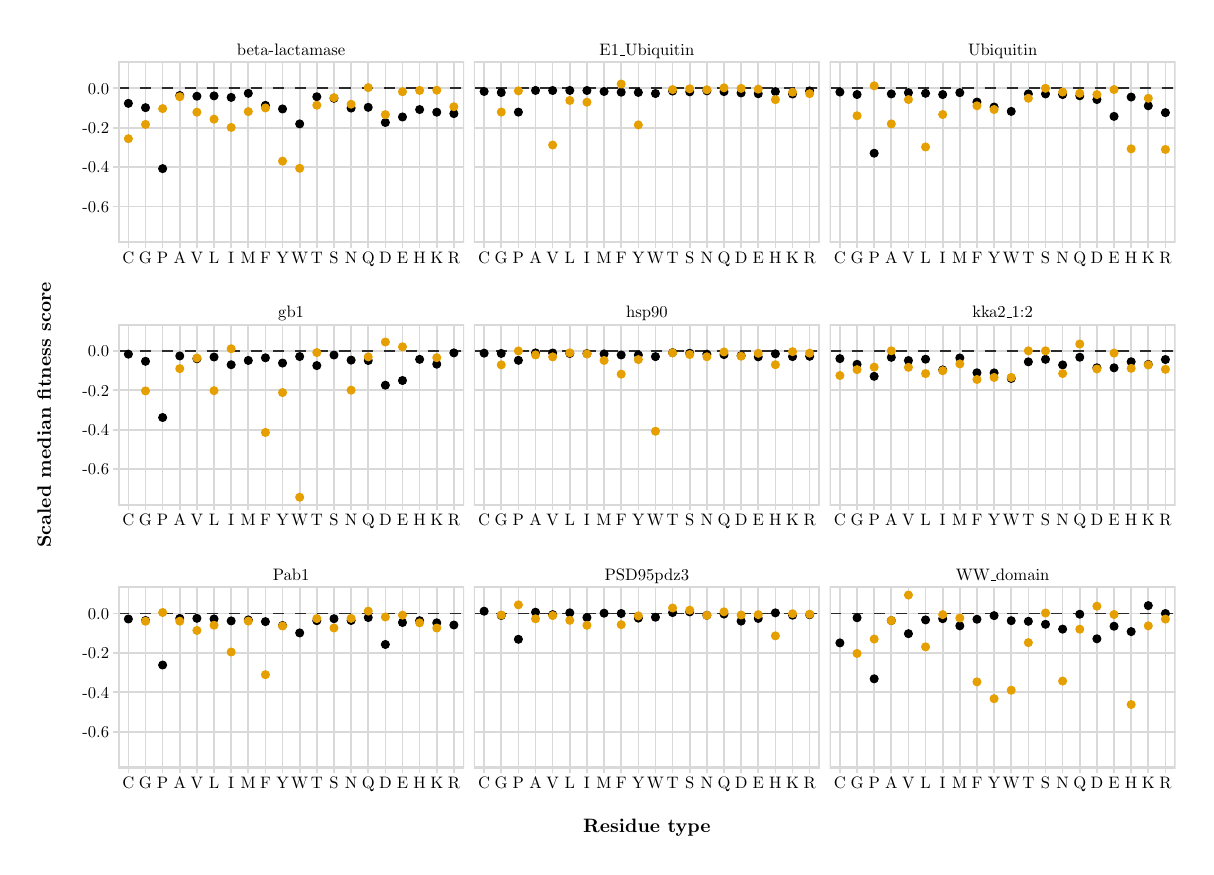
\begin{tikzpicture}[x=1pt,y=1pt]
\definecolor{fillColor}{RGB}{255,255,255}
\path[use as bounding box,fill=fillColor,fill opacity=0.00] (0,0) rectangle (418.34,295.82);
\begin{scope}
\path[clip] ( 32.67,218.05) rectangle (157.73,283.52);
\definecolor{drawColor}{gray}{0.85}

\path[draw=drawColor,line width= 0.6pt,line join=round] ( 32.67,231.15) --
	(157.73,231.15);

\path[draw=drawColor,line width= 0.6pt,line join=round] ( 32.67,245.40) --
	(157.73,245.40);

\path[draw=drawColor,line width= 0.6pt,line join=round] ( 32.67,259.66) --
	(157.73,259.66);

\path[draw=drawColor,line width= 0.6pt,line join=round] ( 32.67,273.91) --
	(157.73,273.91);

\path[draw=drawColor,line width= 0.6pt,line join=round] ( 36.39,218.05) --
	( 36.39,283.52);

\path[draw=drawColor,line width= 0.6pt,line join=round] ( 42.58,218.05) --
	( 42.58,283.52);

\path[draw=drawColor,line width= 0.6pt,line join=round] ( 48.77,218.05) --
	( 48.77,283.52);

\path[draw=drawColor,line width= 0.6pt,line join=round] ( 54.96,218.05) --
	( 54.96,283.52);

\path[draw=drawColor,line width= 0.6pt,line join=round] ( 61.15,218.05) --
	( 61.15,283.52);

\path[draw=drawColor,line width= 0.6pt,line join=round] ( 67.34,218.05) --
	( 67.34,283.52);

\path[draw=drawColor,line width= 0.6pt,line join=round] ( 73.53,218.05) --
	( 73.53,283.52);

\path[draw=drawColor,line width= 0.6pt,line join=round] ( 79.72,218.05) --
	( 79.72,283.52);

\path[draw=drawColor,line width= 0.6pt,line join=round] ( 85.91,218.05) --
	( 85.91,283.52);

\path[draw=drawColor,line width= 0.6pt,line join=round] ( 92.10,218.05) --
	( 92.10,283.52);

\path[draw=drawColor,line width= 0.6pt,line join=round] ( 98.29,218.05) --
	( 98.29,283.52);

\path[draw=drawColor,line width= 0.6pt,line join=round] (104.48,218.05) --
	(104.48,283.52);

\path[draw=drawColor,line width= 0.6pt,line join=round] (110.68,218.05) --
	(110.68,283.52);

\path[draw=drawColor,line width= 0.6pt,line join=round] (116.87,218.05) --
	(116.87,283.52);

\path[draw=drawColor,line width= 0.6pt,line join=round] (123.06,218.05) --
	(123.06,283.52);

\path[draw=drawColor,line width= 0.6pt,line join=round] (129.25,218.05) --
	(129.25,283.52);

\path[draw=drawColor,line width= 0.6pt,line join=round] (135.44,218.05) --
	(135.44,283.52);

\path[draw=drawColor,line width= 0.6pt,line join=round] (141.63,218.05) --
	(141.63,283.52);

\path[draw=drawColor,line width= 0.6pt,line join=round] (147.82,218.05) --
	(147.82,283.52);

\path[draw=drawColor,line width= 0.6pt,line join=round] (154.01,218.05) --
	(154.01,283.52);
\definecolor{drawColor}{RGB}{0,0,0}

\path[draw=drawColor,draw opacity=0.80,line width= 0.6pt,dash pattern=on 4pt off 4pt ,line join=round] ( 32.67,273.91) -- (157.73,273.91);
\definecolor{drawColor}{RGB}{0,0,0}
\definecolor{fillColor}{RGB}{0,0,0}

\path[draw=drawColor,line width= 0.4pt,line join=round,line cap=round,fill=fillColor] ( 48.77,244.88) circle (  1.43);

\path[draw=drawColor,line width= 0.4pt,line join=round,line cap=round,fill=fillColor] (123.06,267.04) circle (  1.43);

\path[draw=drawColor,line width= 0.4pt,line join=round,line cap=round,fill=fillColor] (129.25,261.55) circle (  1.43);

\path[draw=drawColor,line width= 0.4pt,line join=round,line cap=round,fill=fillColor] (147.82,265.27) circle (  1.43);

\path[draw=drawColor,line width= 0.4pt,line join=round,line cap=round,fill=fillColor] (116.87,266.76) circle (  1.43);

\path[draw=drawColor,line width= 0.4pt,line join=round,line cap=round,fill=fillColor] (154.01,264.76) circle (  1.43);

\path[draw=drawColor,line width= 0.4pt,line join=round,line cap=round,fill=fillColor] (135.44,263.55) circle (  1.43);

\path[draw=drawColor,line width= 0.4pt,line join=round,line cap=round,fill=fillColor] (141.63,266.23) circle (  1.43);

\path[draw=drawColor,line width= 0.4pt,line join=round,line cap=round,fill=fillColor] (110.68,270.30) circle (  1.43);

\path[draw=drawColor,line width= 0.4pt,line join=round,line cap=round,fill=fillColor] (104.48,270.86) circle (  1.43);

\path[draw=drawColor,line width= 0.4pt,line join=round,line cap=round,fill=fillColor] ( 42.58,266.91) circle (  1.43);

\path[draw=drawColor,line width= 0.4pt,line join=round,line cap=round,fill=fillColor] ( 36.39,268.46) circle (  1.43);

\path[draw=drawColor,line width= 0.4pt,line join=round,line cap=round,fill=fillColor] ( 54.96,271.30) circle (  1.43);

\path[draw=drawColor,line width= 0.4pt,line join=round,line cap=round,fill=fillColor] ( 79.72,272.10) circle (  1.43);

\path[draw=drawColor,line width= 0.4pt,line join=round,line cap=round,fill=fillColor] ( 61.15,271.05) circle (  1.43);

\path[draw=drawColor,line width= 0.4pt,line join=round,line cap=round,fill=fillColor] ( 92.10,266.45) circle (  1.43);

\path[draw=drawColor,line width= 0.4pt,line join=round,line cap=round,fill=fillColor] ( 85.91,267.75) circle (  1.43);

\path[draw=drawColor,line width= 0.4pt,line join=round,line cap=round,fill=fillColor] ( 67.34,271.17) circle (  1.43);

\path[draw=drawColor,line width= 0.4pt,line join=round,line cap=round,fill=fillColor] ( 73.53,270.62) circle (  1.43);

\path[draw=drawColor,line width= 0.4pt,line join=round,line cap=round,fill=fillColor] ( 98.29,261.04) circle (  1.43);
\definecolor{drawColor}{RGB}{230,159,0}
\definecolor{fillColor}{RGB}{230,159,0}

\path[draw=drawColor,line width= 0.4pt,line join=round,line cap=round,fill=fillColor] ( 48.77,266.57) circle (  1.43);

\path[draw=drawColor,line width= 0.4pt,line join=round,line cap=round,fill=fillColor] (129.25,264.40) circle (  1.43);

\path[draw=drawColor,line width= 0.4pt,line join=round,line cap=round,fill=fillColor] ( 54.96,270.86) circle (  1.43);

\path[draw=drawColor,line width= 0.4pt,line join=round,line cap=round,fill=fillColor] ( 36.39,255.70) circle (  1.43);

\path[draw=drawColor,line width= 0.4pt,line join=round,line cap=round,fill=fillColor] (116.87,268.15) circle (  1.43);

\path[draw=drawColor,line width= 0.4pt,line join=round,line cap=round,fill=fillColor] ( 67.34,262.76) circle (  1.43);

\path[draw=drawColor,line width= 0.4pt,line join=round,line cap=round,fill=fillColor] ( 85.91,266.81) circle (  1.43);

\path[draw=drawColor,line width= 0.4pt,line join=round,line cap=round,fill=fillColor] (135.44,272.68) circle (  1.43);

\path[draw=drawColor,line width= 0.4pt,line join=round,line cap=round,fill=fillColor] (141.63,273.14) circle (  1.43);

\path[draw=drawColor,line width= 0.4pt,line join=round,line cap=round,fill=fillColor] (104.48,267.79) circle (  1.43);

\path[draw=drawColor,line width= 0.4pt,line join=round,line cap=round,fill=fillColor] ( 73.53,259.76) circle (  1.43);

\path[draw=drawColor,line width= 0.4pt,line join=round,line cap=round,fill=fillColor] (154.01,267.24) circle (  1.43);

\path[draw=drawColor,line width= 0.4pt,line join=round,line cap=round,fill=fillColor] ( 61.15,265.28) circle (  1.43);

\path[draw=drawColor,line width= 0.4pt,line join=round,line cap=round,fill=fillColor] ( 92.10,247.60) circle (  1.43);

\path[draw=drawColor,line width= 0.4pt,line join=round,line cap=round,fill=fillColor] (123.06,274.16) circle (  1.43);

\path[draw=drawColor,line width= 0.4pt,line join=round,line cap=round,fill=fillColor] ( 42.58,260.85) circle (  1.43);

\path[draw=drawColor,line width= 0.4pt,line join=round,line cap=round,fill=fillColor] (147.82,273.22) circle (  1.43);

\path[draw=drawColor,line width= 0.4pt,line join=round,line cap=round,fill=fillColor] (110.68,270.52) circle (  1.43);

\path[draw=drawColor,line width= 0.4pt,line join=round,line cap=round,fill=fillColor] ( 79.72,265.50) circle (  1.43);

\path[draw=drawColor,line width= 0.4pt,line join=round,line cap=round,fill=fillColor] ( 98.29,245.00) circle (  1.43);
\definecolor{drawColor}{gray}{0.85}

\path[draw=drawColor,line width= 1.1pt,line join=round,line cap=round] ( 32.67,218.05) rectangle (157.73,283.52);
\end{scope}
\begin{scope}
\path[clip] ( 32.67,123.17) rectangle (157.73,188.65);
\definecolor{drawColor}{gray}{0.85}

\path[draw=drawColor,line width= 0.6pt,line join=round] ( 32.67,136.28) --
	(157.73,136.28);

\path[draw=drawColor,line width= 0.6pt,line join=round] ( 32.67,150.53) --
	(157.73,150.53);

\path[draw=drawColor,line width= 0.6pt,line join=round] ( 32.67,164.78) --
	(157.73,164.78);

\path[draw=drawColor,line width= 0.6pt,line join=round] ( 32.67,179.04) --
	(157.73,179.04);

\path[draw=drawColor,line width= 0.6pt,line join=round] ( 36.39,123.17) --
	( 36.39,188.65);

\path[draw=drawColor,line width= 0.6pt,line join=round] ( 42.58,123.17) --
	( 42.58,188.65);

\path[draw=drawColor,line width= 0.6pt,line join=round] ( 48.77,123.17) --
	( 48.77,188.65);

\path[draw=drawColor,line width= 0.6pt,line join=round] ( 54.96,123.17) --
	( 54.96,188.65);

\path[draw=drawColor,line width= 0.6pt,line join=round] ( 61.15,123.17) --
	( 61.15,188.65);

\path[draw=drawColor,line width= 0.6pt,line join=round] ( 67.34,123.17) --
	( 67.34,188.65);

\path[draw=drawColor,line width= 0.6pt,line join=round] ( 73.53,123.17) --
	( 73.53,188.65);

\path[draw=drawColor,line width= 0.6pt,line join=round] ( 79.72,123.17) --
	( 79.72,188.65);

\path[draw=drawColor,line width= 0.6pt,line join=round] ( 85.91,123.17) --
	( 85.91,188.65);

\path[draw=drawColor,line width= 0.6pt,line join=round] ( 92.10,123.17) --
	( 92.10,188.65);

\path[draw=drawColor,line width= 0.6pt,line join=round] ( 98.29,123.17) --
	( 98.29,188.65);

\path[draw=drawColor,line width= 0.6pt,line join=round] (104.48,123.17) --
	(104.48,188.65);

\path[draw=drawColor,line width= 0.6pt,line join=round] (110.68,123.17) --
	(110.68,188.65);

\path[draw=drawColor,line width= 0.6pt,line join=round] (116.87,123.17) --
	(116.87,188.65);

\path[draw=drawColor,line width= 0.6pt,line join=round] (123.06,123.17) --
	(123.06,188.65);

\path[draw=drawColor,line width= 0.6pt,line join=round] (129.25,123.17) --
	(129.25,188.65);

\path[draw=drawColor,line width= 0.6pt,line join=round] (135.44,123.17) --
	(135.44,188.65);

\path[draw=drawColor,line width= 0.6pt,line join=round] (141.63,123.17) --
	(141.63,188.65);

\path[draw=drawColor,line width= 0.6pt,line join=round] (147.82,123.17) --
	(147.82,188.65);

\path[draw=drawColor,line width= 0.6pt,line join=round] (154.01,123.17) --
	(154.01,188.65);
\definecolor{drawColor}{RGB}{0,0,0}

\path[draw=drawColor,draw opacity=0.80,line width= 0.6pt,dash pattern=on 4pt off 4pt ,line join=round] ( 32.67,179.04) -- (157.73,179.04);
\definecolor{drawColor}{RGB}{0,0,0}
\definecolor{fillColor}{RGB}{0,0,0}

\path[draw=drawColor,line width= 0.4pt,line join=round,line cap=round,fill=fillColor] ( 92.10,174.63) circle (  1.43);

\path[draw=drawColor,line width= 0.4pt,line join=round,line cap=round,fill=fillColor] ( 98.29,176.98) circle (  1.43);

\path[draw=drawColor,line width= 0.4pt,line join=round,line cap=round,fill=fillColor] (141.63,175.97) circle (  1.43);

\path[draw=drawColor,line width= 0.4pt,line join=round,line cap=round,fill=fillColor] ( 85.91,176.52) circle (  1.43);

\path[draw=drawColor,line width= 0.4pt,line join=round,line cap=round,fill=fillColor] (135.44,168.32) circle (  1.43);

\path[draw=drawColor,line width= 0.4pt,line join=round,line cap=round,fill=fillColor] ( 48.77,154.95) circle (  1.43);

\path[draw=drawColor,line width= 0.4pt,line join=round,line cap=round,fill=fillColor] (123.06,175.55) circle (  1.43);

\path[draw=drawColor,line width= 0.4pt,line join=round,line cap=round,fill=fillColor] ( 42.58,175.26) circle (  1.43);

\path[draw=drawColor,line width= 0.4pt,line join=round,line cap=round,fill=fillColor] (116.87,175.69) circle (  1.43);

\path[draw=drawColor,line width= 0.4pt,line join=round,line cap=round,fill=fillColor] (104.48,173.71) circle (  1.43);

\path[draw=drawColor,line width= 0.4pt,line join=round,line cap=round,fill=fillColor] ( 79.72,175.57) circle (  1.43);

\path[draw=drawColor,line width= 0.4pt,line join=round,line cap=round,fill=fillColor] (110.68,177.53) circle (  1.43);

\path[draw=drawColor,line width= 0.4pt,line join=round,line cap=round,fill=fillColor] ( 36.39,177.85) circle (  1.43);

\path[draw=drawColor,line width= 0.4pt,line join=round,line cap=round,fill=fillColor] ( 61.15,176.18) circle (  1.43);

\path[draw=drawColor,line width= 0.4pt,line join=round,line cap=round,fill=fillColor] ( 73.53,174.02) circle (  1.43);

\path[draw=drawColor,line width= 0.4pt,line join=round,line cap=round,fill=fillColor] ( 67.34,176.81) circle (  1.43);

\path[draw=drawColor,line width= 0.4pt,line join=round,line cap=round,fill=fillColor] (129.25,166.63) circle (  1.43);

\path[draw=drawColor,line width= 0.4pt,line join=round,line cap=round,fill=fillColor] (154.01,178.30) circle (  1.43);

\path[draw=drawColor,line width= 0.4pt,line join=round,line cap=round,fill=fillColor] (147.82,174.23) circle (  1.43);

\path[draw=drawColor,line width= 0.4pt,line join=round,line cap=round,fill=fillColor] ( 54.96,177.20) circle (  1.43);
\definecolor{drawColor}{RGB}{230,159,0}
\definecolor{fillColor}{RGB}{230,159,0}

\path[draw=drawColor,line width= 0.4pt,line join=round,line cap=round,fill=fillColor] ( 54.96,172.61) circle (  1.43);

\path[draw=drawColor,line width= 0.4pt,line join=round,line cap=round,fill=fillColor] (129.25,182.23) circle (  1.43);

\path[draw=drawColor,line width= 0.4pt,line join=round,line cap=round,fill=fillColor] ( 61.15,176.46) circle (  1.43);

\path[draw=drawColor,line width= 0.4pt,line join=round,line cap=round,fill=fillColor] (104.48,178.42) circle (  1.43);

\path[draw=drawColor,line width= 0.4pt,line join=round,line cap=round,fill=fillColor] (135.44,180.50) circle (  1.43);

\path[draw=drawColor,line width= 0.4pt,line join=round,line cap=round,fill=fillColor] (147.82,176.56) circle (  1.43);

\path[draw=drawColor,line width= 0.4pt,line join=round,line cap=round,fill=fillColor] ( 92.10,163.97) circle (  1.43);

\path[draw=drawColor,line width= 0.4pt,line join=round,line cap=round,fill=fillColor] ( 67.34,164.65) circle (  1.43);

\path[draw=drawColor,line width= 0.4pt,line join=round,line cap=round,fill=fillColor] (123.06,176.87) circle (  1.43);

\path[draw=drawColor,line width= 0.4pt,line join=round,line cap=round,fill=fillColor] (116.87,164.83) circle (  1.43);

\path[draw=drawColor,line width= 0.4pt,line join=round,line cap=round,fill=fillColor] ( 73.53,179.80) circle (  1.43);

\path[draw=drawColor,line width= 0.4pt,line join=round,line cap=round,fill=fillColor] ( 42.58,164.56) circle (  1.43);

\path[draw=drawColor,line width= 0.4pt,line join=round,line cap=round,fill=fillColor] ( 85.91,149.55) circle (  1.43);

\path[draw=drawColor,line width= 0.4pt,line join=round,line cap=round,fill=fillColor] ( 98.29,126.15) circle (  1.43);
\definecolor{drawColor}{gray}{0.85}

\path[draw=drawColor,line width= 1.1pt,line join=round,line cap=round] ( 32.67,123.17) rectangle (157.73,188.65);
\end{scope}
\begin{scope}
\path[clip] ( 32.67, 28.30) rectangle (157.73, 93.78);
\definecolor{drawColor}{gray}{0.85}

\path[draw=drawColor,line width= 0.6pt,line join=round] ( 32.67, 41.40) --
	(157.73, 41.40);

\path[draw=drawColor,line width= 0.6pt,line join=round] ( 32.67, 55.66) --
	(157.73, 55.66);

\path[draw=drawColor,line width= 0.6pt,line join=round] ( 32.67, 69.91) --
	(157.73, 69.91);

\path[draw=drawColor,line width= 0.6pt,line join=round] ( 32.67, 84.17) --
	(157.73, 84.17);

\path[draw=drawColor,line width= 0.6pt,line join=round] ( 36.39, 28.30) --
	( 36.39, 93.78);

\path[draw=drawColor,line width= 0.6pt,line join=round] ( 42.58, 28.30) --
	( 42.58, 93.78);

\path[draw=drawColor,line width= 0.6pt,line join=round] ( 48.77, 28.30) --
	( 48.77, 93.78);

\path[draw=drawColor,line width= 0.6pt,line join=round] ( 54.96, 28.30) --
	( 54.96, 93.78);

\path[draw=drawColor,line width= 0.6pt,line join=round] ( 61.15, 28.30) --
	( 61.15, 93.78);

\path[draw=drawColor,line width= 0.6pt,line join=round] ( 67.34, 28.30) --
	( 67.34, 93.78);

\path[draw=drawColor,line width= 0.6pt,line join=round] ( 73.53, 28.30) --
	( 73.53, 93.78);

\path[draw=drawColor,line width= 0.6pt,line join=round] ( 79.72, 28.30) --
	( 79.72, 93.78);

\path[draw=drawColor,line width= 0.6pt,line join=round] ( 85.91, 28.30) --
	( 85.91, 93.78);

\path[draw=drawColor,line width= 0.6pt,line join=round] ( 92.10, 28.30) --
	( 92.10, 93.78);

\path[draw=drawColor,line width= 0.6pt,line join=round] ( 98.29, 28.30) --
	( 98.29, 93.78);

\path[draw=drawColor,line width= 0.6pt,line join=round] (104.48, 28.30) --
	(104.48, 93.78);

\path[draw=drawColor,line width= 0.6pt,line join=round] (110.68, 28.30) --
	(110.68, 93.78);

\path[draw=drawColor,line width= 0.6pt,line join=round] (116.87, 28.30) --
	(116.87, 93.78);

\path[draw=drawColor,line width= 0.6pt,line join=round] (123.06, 28.30) --
	(123.06, 93.78);

\path[draw=drawColor,line width= 0.6pt,line join=round] (129.25, 28.30) --
	(129.25, 93.78);

\path[draw=drawColor,line width= 0.6pt,line join=round] (135.44, 28.30) --
	(135.44, 93.78);

\path[draw=drawColor,line width= 0.6pt,line join=round] (141.63, 28.30) --
	(141.63, 93.78);

\path[draw=drawColor,line width= 0.6pt,line join=round] (147.82, 28.30) --
	(147.82, 93.78);

\path[draw=drawColor,line width= 0.6pt,line join=round] (154.01, 28.30) --
	(154.01, 93.78);
\definecolor{drawColor}{RGB}{0,0,0}

\path[draw=drawColor,draw opacity=0.80,line width= 0.6pt,dash pattern=on 4pt off 4pt ,line join=round] ( 32.67, 84.17) -- (157.73, 84.17);
\definecolor{drawColor}{RGB}{0,0,0}
\definecolor{fillColor}{RGB}{0,0,0}

\path[draw=drawColor,line width= 0.4pt,line join=round,line cap=round,fill=fillColor] ( 36.39, 82.14) circle (  1.43);

\path[draw=drawColor,line width= 0.4pt,line join=round,line cap=round,fill=fillColor] (116.87, 81.60) circle (  1.43);

\path[draw=drawColor,line width= 0.4pt,line join=round,line cap=round,fill=fillColor] (110.68, 82.25) circle (  1.43);

\path[draw=drawColor,line width= 0.4pt,line join=round,line cap=round,fill=fillColor] (154.01, 79.97) circle (  1.43);

\path[draw=drawColor,line width= 0.4pt,line join=round,line cap=round,fill=fillColor] (141.63, 81.53) circle (  1.43);

\path[draw=drawColor,line width= 0.4pt,line join=round,line cap=round,fill=fillColor] ( 54.96, 82.37) circle (  1.43);

\path[draw=drawColor,line width= 0.4pt,line join=round,line cap=round,fill=fillColor] (135.44, 80.88) circle (  1.43);

\path[draw=drawColor,line width= 0.4pt,line join=round,line cap=round,fill=fillColor] (104.48, 81.53) circle (  1.43);

\path[draw=drawColor,line width= 0.4pt,line join=round,line cap=round,fill=fillColor] ( 67.34, 82.17) circle (  1.43);

\path[draw=drawColor,line width= 0.4pt,line join=round,line cap=round,fill=fillColor] (147.82, 80.76) circle (  1.43);

\path[draw=drawColor,line width= 0.4pt,line join=round,line cap=round,fill=fillColor] (129.25, 72.94) circle (  1.43);

\path[draw=drawColor,line width= 0.4pt,line join=round,line cap=round,fill=fillColor] ( 42.58, 81.60) circle (  1.43);

\path[draw=drawColor,line width= 0.4pt,line join=round,line cap=round,fill=fillColor] ( 92.10, 79.79) circle (  1.43);

\path[draw=drawColor,line width= 0.4pt,line join=round,line cap=round,fill=fillColor] ( 61.15, 82.39) circle (  1.43);

\path[draw=drawColor,line width= 0.4pt,line join=round,line cap=round,fill=fillColor] ( 73.53, 81.45) circle (  1.43);

\path[draw=drawColor,line width= 0.4pt,line join=round,line cap=round,fill=fillColor] ( 48.77, 65.51) circle (  1.43);

\path[draw=drawColor,line width= 0.4pt,line join=round,line cap=round,fill=fillColor] ( 85.91, 81.19) circle (  1.43);

\path[draw=drawColor,line width= 0.4pt,line join=round,line cap=round,fill=fillColor] ( 79.72, 81.81) circle (  1.43);

\path[draw=drawColor,line width= 0.4pt,line join=round,line cap=round,fill=fillColor] (123.06, 82.68) circle (  1.43);

\path[draw=drawColor,line width= 0.4pt,line join=round,line cap=round,fill=fillColor] ( 98.29, 77.11) circle (  1.43);
\definecolor{drawColor}{RGB}{230,159,0}
\definecolor{fillColor}{RGB}{230,159,0}

\path[draw=drawColor,line width= 0.4pt,line join=round,line cap=round,fill=fillColor] (123.06, 84.99) circle (  1.43);

\path[draw=drawColor,line width= 0.4pt,line join=round,line cap=round,fill=fillColor] ( 54.96, 81.36) circle (  1.43);

\path[draw=drawColor,line width= 0.4pt,line join=round,line cap=round,fill=fillColor] (116.87, 82.37) circle (  1.43);

\path[draw=drawColor,line width= 0.4pt,line join=round,line cap=round,fill=fillColor] ( 48.77, 84.49) circle (  1.43);

\path[draw=drawColor,line width= 0.4pt,line join=round,line cap=round,fill=fillColor] ( 42.58, 81.34) circle (  1.43);

\path[draw=drawColor,line width= 0.4pt,line join=round,line cap=round,fill=fillColor] (104.48, 82.30) circle (  1.43);

\path[draw=drawColor,line width= 0.4pt,line join=round,line cap=round,fill=fillColor] (135.44, 83.53) circle (  1.43);

\path[draw=drawColor,line width= 0.4pt,line join=round,line cap=round,fill=fillColor] (129.25, 82.88) circle (  1.43);

\path[draw=drawColor,line width= 0.4pt,line join=round,line cap=round,fill=fillColor] ( 61.15, 78.01) circle (  1.43);

\path[draw=drawColor,line width= 0.4pt,line join=round,line cap=round,fill=fillColor] ( 67.34, 79.89) circle (  1.43);

\path[draw=drawColor,line width= 0.4pt,line join=round,line cap=round,fill=fillColor] (110.68, 78.90) circle (  1.43);

\path[draw=drawColor,line width= 0.4pt,line join=round,line cap=round,fill=fillColor] (147.82, 78.89) circle (  1.43);

\path[draw=drawColor,line width= 0.4pt,line join=round,line cap=round,fill=fillColor] ( 73.53, 70.21) circle (  1.43);

\path[draw=drawColor,line width= 0.4pt,line join=round,line cap=round,fill=fillColor] (141.63, 80.76) circle (  1.43);

\path[draw=drawColor,line width= 0.4pt,line join=round,line cap=round,fill=fillColor] ( 79.72, 81.39) circle (  1.43);

\path[draw=drawColor,line width= 0.4pt,line join=round,line cap=round,fill=fillColor] ( 85.91, 62.03) circle (  1.43);

\path[draw=drawColor,line width= 0.4pt,line join=round,line cap=round,fill=fillColor] ( 92.10, 79.62) circle (  1.43);
\definecolor{drawColor}{gray}{0.85}

\path[draw=drawColor,line width= 1.1pt,line join=round,line cap=round] ( 32.67, 28.30) rectangle (157.73, 93.78);
\end{scope}
\begin{scope}
\path[clip] (161.23,218.05) rectangle (286.28,283.52);
\definecolor{drawColor}{gray}{0.85}

\path[draw=drawColor,line width= 0.6pt,line join=round] (161.23,231.15) --
	(286.28,231.15);

\path[draw=drawColor,line width= 0.6pt,line join=round] (161.23,245.40) --
	(286.28,245.40);

\path[draw=drawColor,line width= 0.6pt,line join=round] (161.23,259.66) --
	(286.28,259.66);

\path[draw=drawColor,line width= 0.6pt,line join=round] (161.23,273.91) --
	(286.28,273.91);

\path[draw=drawColor,line width= 0.6pt,line join=round] (164.94,218.05) --
	(164.94,283.52);

\path[draw=drawColor,line width= 0.6pt,line join=round] (171.13,218.05) --
	(171.13,283.52);

\path[draw=drawColor,line width= 0.6pt,line join=round] (177.32,218.05) --
	(177.32,283.52);

\path[draw=drawColor,line width= 0.6pt,line join=round] (183.51,218.05) --
	(183.51,283.52);

\path[draw=drawColor,line width= 0.6pt,line join=round] (189.70,218.05) --
	(189.70,283.52);

\path[draw=drawColor,line width= 0.6pt,line join=round] (195.89,218.05) --
	(195.89,283.52);

\path[draw=drawColor,line width= 0.6pt,line join=round] (202.09,218.05) --
	(202.09,283.52);

\path[draw=drawColor,line width= 0.6pt,line join=round] (208.28,218.05) --
	(208.28,283.52);

\path[draw=drawColor,line width= 0.6pt,line join=round] (214.47,218.05) --
	(214.47,283.52);

\path[draw=drawColor,line width= 0.6pt,line join=round] (220.66,218.05) --
	(220.66,283.52);

\path[draw=drawColor,line width= 0.6pt,line join=round] (226.85,218.05) --
	(226.85,283.52);

\path[draw=drawColor,line width= 0.6pt,line join=round] (233.04,218.05) --
	(233.04,283.52);

\path[draw=drawColor,line width= 0.6pt,line join=round] (239.23,218.05) --
	(239.23,283.52);

\path[draw=drawColor,line width= 0.6pt,line join=round] (245.42,218.05) --
	(245.42,283.52);

\path[draw=drawColor,line width= 0.6pt,line join=round] (251.61,218.05) --
	(251.61,283.52);

\path[draw=drawColor,line width= 0.6pt,line join=round] (257.80,218.05) --
	(257.80,283.52);

\path[draw=drawColor,line width= 0.6pt,line join=round] (263.99,218.05) --
	(263.99,283.52);

\path[draw=drawColor,line width= 0.6pt,line join=round] (270.18,218.05) --
	(270.18,283.52);

\path[draw=drawColor,line width= 0.6pt,line join=round] (276.38,218.05) --
	(276.38,283.52);

\path[draw=drawColor,line width= 0.6pt,line join=round] (282.57,218.05) --
	(282.57,283.52);
\definecolor{drawColor}{RGB}{0,0,0}

\path[draw=drawColor,draw opacity=0.80,line width= 0.6pt,dash pattern=on 4pt off 4pt ,line join=round] (161.23,273.91) -- (286.28,273.91);
\definecolor{drawColor}{RGB}{0,0,0}
\definecolor{fillColor}{RGB}{0,0,0}

\path[draw=drawColor,line width= 0.4pt,line join=round,line cap=round,fill=fillColor] (164.94,272.77) circle (  1.43);

\path[draw=drawColor,line width= 0.4pt,line join=round,line cap=round,fill=fillColor] (220.66,272.42) circle (  1.43);

\path[draw=drawColor,line width= 0.4pt,line join=round,line cap=round,fill=fillColor] (214.47,272.51) circle (  1.43);

\path[draw=drawColor,line width= 0.4pt,line join=round,line cap=round,fill=fillColor] (171.13,272.38) circle (  1.43);

\path[draw=drawColor,line width= 0.4pt,line join=round,line cap=round,fill=fillColor] (239.23,272.63) circle (  1.43);

\path[draw=drawColor,line width= 0.4pt,line join=round,line cap=round,fill=fillColor] (233.04,272.91) circle (  1.43);

\path[draw=drawColor,line width= 0.4pt,line join=round,line cap=round,fill=fillColor] (202.09,273.11) circle (  1.43);

\path[draw=drawColor,line width= 0.4pt,line join=round,line cap=round,fill=fillColor] (195.89,273.14) circle (  1.43);

\path[draw=drawColor,line width= 0.4pt,line join=round,line cap=round,fill=fillColor] (282.57,272.96) circle (  1.43);

\path[draw=drawColor,line width= 0.4pt,line join=round,line cap=round,fill=fillColor] (177.32,265.30) circle (  1.43);

\path[draw=drawColor,line width= 0.4pt,line join=round,line cap=round,fill=fillColor] (257.80,272.23) circle (  1.43);

\path[draw=drawColor,line width= 0.4pt,line join=round,line cap=round,fill=fillColor] (270.18,272.72) circle (  1.43);

\path[draw=drawColor,line width= 0.4pt,line join=round,line cap=round,fill=fillColor] (183.51,273.14) circle (  1.43);

\path[draw=drawColor,line width= 0.4pt,line join=round,line cap=round,fill=fillColor] (208.28,272.77) circle (  1.43);

\path[draw=drawColor,line width= 0.4pt,line join=round,line cap=round,fill=fillColor] (276.38,271.85) circle (  1.43);

\path[draw=drawColor,line width= 0.4pt,line join=round,line cap=round,fill=fillColor] (189.70,273.11) circle (  1.43);

\path[draw=drawColor,line width= 0.4pt,line join=round,line cap=round,fill=fillColor] (226.85,272.02) circle (  1.43);

\path[draw=drawColor,line width= 0.4pt,line join=round,line cap=round,fill=fillColor] (245.42,273.00) circle (  1.43);

\path[draw=drawColor,line width= 0.4pt,line join=round,line cap=round,fill=fillColor] (263.99,271.95) circle (  1.43);

\path[draw=drawColor,line width= 0.4pt,line join=round,line cap=round,fill=fillColor] (251.61,272.72) circle (  1.43);
\definecolor{drawColor}{RGB}{230,159,0}
\definecolor{fillColor}{RGB}{230,159,0}

\path[draw=drawColor,line width= 0.4pt,line join=round,line cap=round,fill=fillColor] (251.61,274.08) circle (  1.43);

\path[draw=drawColor,line width= 0.4pt,line join=round,line cap=round,fill=fillColor] (257.80,273.88) circle (  1.43);

\path[draw=drawColor,line width= 0.4pt,line join=round,line cap=round,fill=fillColor] (214.47,275.45) circle (  1.43);

\path[draw=drawColor,line width= 0.4pt,line join=round,line cap=round,fill=fillColor] (233.04,273.44) circle (  1.43);

\path[draw=drawColor,line width= 0.4pt,line join=round,line cap=round,fill=fillColor] (263.99,273.61) circle (  1.43);

\path[draw=drawColor,line width= 0.4pt,line join=round,line cap=round,fill=fillColor] (189.70,253.41) circle (  1.43);

\path[draw=drawColor,line width= 0.4pt,line join=round,line cap=round,fill=fillColor] (195.89,269.51) circle (  1.43);

\path[draw=drawColor,line width= 0.4pt,line join=round,line cap=round,fill=fillColor] (239.23,273.73) circle (  1.43);

\path[draw=drawColor,line width= 0.4pt,line join=round,line cap=round,fill=fillColor] (202.09,268.89) circle (  1.43);

\path[draw=drawColor,line width= 0.4pt,line join=round,line cap=round,fill=fillColor] (220.66,260.68) circle (  1.43);

\path[draw=drawColor,line width= 0.4pt,line join=round,line cap=round,fill=fillColor] (276.38,272.49) circle (  1.43);

\path[draw=drawColor,line width= 0.4pt,line join=round,line cap=round,fill=fillColor] (245.42,273.39) circle (  1.43);

\path[draw=drawColor,line width= 0.4pt,line join=round,line cap=round,fill=fillColor] (270.18,269.81) circle (  1.43);

\path[draw=drawColor,line width= 0.4pt,line join=round,line cap=round,fill=fillColor] (177.32,272.98) circle (  1.43);

\path[draw=drawColor,line width= 0.4pt,line join=round,line cap=round,fill=fillColor] (282.57,271.98) circle (  1.43);

\path[draw=drawColor,line width= 0.4pt,line join=round,line cap=round,fill=fillColor] (171.13,265.33) circle (  1.43);
\definecolor{drawColor}{gray}{0.85}

\path[draw=drawColor,line width= 1.1pt,line join=round,line cap=round] (161.23,218.05) rectangle (286.28,283.52);
\end{scope}
\begin{scope}
\path[clip] (161.23,123.17) rectangle (286.28,188.65);
\definecolor{drawColor}{gray}{0.85}

\path[draw=drawColor,line width= 0.6pt,line join=round] (161.23,136.28) --
	(286.28,136.28);

\path[draw=drawColor,line width= 0.6pt,line join=round] (161.23,150.53) --
	(286.28,150.53);

\path[draw=drawColor,line width= 0.6pt,line join=round] (161.23,164.78) --
	(286.28,164.78);

\path[draw=drawColor,line width= 0.6pt,line join=round] (161.23,179.04) --
	(286.28,179.04);

\path[draw=drawColor,line width= 0.6pt,line join=round] (164.94,123.17) --
	(164.94,188.65);

\path[draw=drawColor,line width= 0.6pt,line join=round] (171.13,123.17) --
	(171.13,188.65);

\path[draw=drawColor,line width= 0.6pt,line join=round] (177.32,123.17) --
	(177.32,188.65);

\path[draw=drawColor,line width= 0.6pt,line join=round] (183.51,123.17) --
	(183.51,188.65);

\path[draw=drawColor,line width= 0.6pt,line join=round] (189.70,123.17) --
	(189.70,188.65);

\path[draw=drawColor,line width= 0.6pt,line join=round] (195.89,123.17) --
	(195.89,188.65);

\path[draw=drawColor,line width= 0.6pt,line join=round] (202.09,123.17) --
	(202.09,188.65);

\path[draw=drawColor,line width= 0.6pt,line join=round] (208.28,123.17) --
	(208.28,188.65);

\path[draw=drawColor,line width= 0.6pt,line join=round] (214.47,123.17) --
	(214.47,188.65);

\path[draw=drawColor,line width= 0.6pt,line join=round] (220.66,123.17) --
	(220.66,188.65);

\path[draw=drawColor,line width= 0.6pt,line join=round] (226.85,123.17) --
	(226.85,188.65);

\path[draw=drawColor,line width= 0.6pt,line join=round] (233.04,123.17) --
	(233.04,188.65);

\path[draw=drawColor,line width= 0.6pt,line join=round] (239.23,123.17) --
	(239.23,188.65);

\path[draw=drawColor,line width= 0.6pt,line join=round] (245.42,123.17) --
	(245.42,188.65);

\path[draw=drawColor,line width= 0.6pt,line join=round] (251.61,123.17) --
	(251.61,188.65);

\path[draw=drawColor,line width= 0.6pt,line join=round] (257.80,123.17) --
	(257.80,188.65);

\path[draw=drawColor,line width= 0.6pt,line join=round] (263.99,123.17) --
	(263.99,188.65);

\path[draw=drawColor,line width= 0.6pt,line join=round] (270.18,123.17) --
	(270.18,188.65);

\path[draw=drawColor,line width= 0.6pt,line join=round] (276.38,123.17) --
	(276.38,188.65);

\path[draw=drawColor,line width= 0.6pt,line join=round] (282.57,123.17) --
	(282.57,188.65);
\definecolor{drawColor}{RGB}{0,0,0}

\path[draw=drawColor,draw opacity=0.80,line width= 0.6pt,dash pattern=on 4pt off 4pt ,line join=round] (161.23,179.04) -- (286.28,179.04);
\definecolor{drawColor}{RGB}{0,0,0}
\definecolor{fillColor}{RGB}{0,0,0}

\path[draw=drawColor,line width= 0.4pt,line join=round,line cap=round,fill=fillColor] (282.57,177.07) circle (  1.43);

\path[draw=drawColor,line width= 0.4pt,line join=round,line cap=round,fill=fillColor] (239.23,178.18) circle (  1.43);

\path[draw=drawColor,line width= 0.4pt,line join=round,line cap=round,fill=fillColor] (233.04,178.39) circle (  1.43);

\path[draw=drawColor,line width= 0.4pt,line join=round,line cap=round,fill=fillColor] (251.61,177.69) circle (  1.43);

\path[draw=drawColor,line width= 0.4pt,line join=round,line cap=round,fill=fillColor] (276.38,176.96) circle (  1.43);

\path[draw=drawColor,line width= 0.4pt,line join=round,line cap=round,fill=fillColor] (177.32,175.62) circle (  1.43);

\path[draw=drawColor,line width= 0.4pt,line join=round,line cap=round,fill=fillColor] (270.18,177.97) circle (  1.43);

\path[draw=drawColor,line width= 0.4pt,line join=round,line cap=round,fill=fillColor] (202.09,178.05) circle (  1.43);

\path[draw=drawColor,line width= 0.4pt,line join=round,line cap=round,fill=fillColor] (164.94,178.21) circle (  1.43);

\path[draw=drawColor,line width= 0.4pt,line join=round,line cap=round,fill=fillColor] (245.42,177.84) circle (  1.43);

\path[draw=drawColor,line width= 0.4pt,line join=round,line cap=round,fill=fillColor] (263.99,176.87) circle (  1.43);

\path[draw=drawColor,line width= 0.4pt,line join=round,line cap=round,fill=fillColor] (171.13,178.10) circle (  1.43);

\path[draw=drawColor,line width= 0.4pt,line join=round,line cap=round,fill=fillColor] (220.66,177.54) circle (  1.43);

\path[draw=drawColor,line width= 0.4pt,line join=round,line cap=round,fill=fillColor] (183.51,178.29) circle (  1.43);

\path[draw=drawColor,line width= 0.4pt,line join=round,line cap=round,fill=fillColor] (189.70,178.27) circle (  1.43);

\path[draw=drawColor,line width= 0.4pt,line join=round,line cap=round,fill=fillColor] (208.28,177.94) circle (  1.43);

\path[draw=drawColor,line width= 0.4pt,line join=round,line cap=round,fill=fillColor] (257.80,177.32) circle (  1.43);

\path[draw=drawColor,line width= 0.4pt,line join=round,line cap=round,fill=fillColor] (195.89,178.08) circle (  1.43);

\path[draw=drawColor,line width= 0.4pt,line join=round,line cap=round,fill=fillColor] (226.85,176.95) circle (  1.43);

\path[draw=drawColor,line width= 0.4pt,line join=round,line cap=round,fill=fillColor] (214.47,177.55) circle (  1.43);
\definecolor{drawColor}{RGB}{230,159,0}
\definecolor{fillColor}{RGB}{230,159,0}

\path[draw=drawColor,line width= 0.4pt,line join=round,line cap=round,fill=fillColor] (183.51,177.56) circle (  1.43);

\path[draw=drawColor,line width= 0.4pt,line join=round,line cap=round,fill=fillColor] (202.09,177.92) circle (  1.43);

\path[draw=drawColor,line width= 0.4pt,line join=round,line cap=round,fill=fillColor] (251.61,178.64) circle (  1.43);

\path[draw=drawColor,line width= 0.4pt,line join=round,line cap=round,fill=fillColor] (195.89,178.32) circle (  1.43);

\path[draw=drawColor,line width= 0.4pt,line join=round,line cap=round,fill=fillColor] (276.38,178.74) circle (  1.43);

\path[draw=drawColor,line width= 0.4pt,line join=round,line cap=round,fill=fillColor] (171.13,173.98) circle (  1.43);

\path[draw=drawColor,line width= 0.4pt,line join=round,line cap=round,fill=fillColor] (282.57,178.20) circle (  1.43);

\path[draw=drawColor,line width= 0.4pt,line join=round,line cap=round,fill=fillColor] (214.47,170.63) circle (  1.43);

\path[draw=drawColor,line width= 0.4pt,line join=round,line cap=round,fill=fillColor] (263.99,178.15) circle (  1.43);

\path[draw=drawColor,line width= 0.4pt,line join=round,line cap=round,fill=fillColor] (233.04,178.30) circle (  1.43);

\path[draw=drawColor,line width= 0.4pt,line join=round,line cap=round,fill=fillColor] (245.42,176.90) circle (  1.43);

\path[draw=drawColor,line width= 0.4pt,line join=round,line cap=round,fill=fillColor] (189.70,176.86) circle (  1.43);

\path[draw=drawColor,line width= 0.4pt,line join=round,line cap=round,fill=fillColor] (177.32,179.00) circle (  1.43);

\path[draw=drawColor,line width= 0.4pt,line join=round,line cap=round,fill=fillColor] (239.23,177.71) circle (  1.43);

\path[draw=drawColor,line width= 0.4pt,line join=round,line cap=round,fill=fillColor] (257.80,177.11) circle (  1.43);

\path[draw=drawColor,line width= 0.4pt,line join=round,line cap=round,fill=fillColor] (220.66,175.88) circle (  1.43);

\path[draw=drawColor,line width= 0.4pt,line join=round,line cap=round,fill=fillColor] (270.18,174.03) circle (  1.43);

\path[draw=drawColor,line width= 0.4pt,line join=round,line cap=round,fill=fillColor] (208.28,175.57) circle (  1.43);

\path[draw=drawColor,line width= 0.4pt,line join=round,line cap=round,fill=fillColor] (226.85,149.98) circle (  1.43);
\definecolor{drawColor}{gray}{0.85}

\path[draw=drawColor,line width= 1.1pt,line join=round,line cap=round] (161.23,123.17) rectangle (286.28,188.65);
\end{scope}
\begin{scope}
\path[clip] (161.23, 28.30) rectangle (286.28, 93.78);
\definecolor{drawColor}{gray}{0.85}

\path[draw=drawColor,line width= 0.6pt,line join=round] (161.23, 41.40) --
	(286.28, 41.40);

\path[draw=drawColor,line width= 0.6pt,line join=round] (161.23, 55.66) --
	(286.28, 55.66);

\path[draw=drawColor,line width= 0.6pt,line join=round] (161.23, 69.91) --
	(286.28, 69.91);

\path[draw=drawColor,line width= 0.6pt,line join=round] (161.23, 84.17) --
	(286.28, 84.17);

\path[draw=drawColor,line width= 0.6pt,line join=round] (164.94, 28.30) --
	(164.94, 93.78);

\path[draw=drawColor,line width= 0.6pt,line join=round] (171.13, 28.30) --
	(171.13, 93.78);

\path[draw=drawColor,line width= 0.6pt,line join=round] (177.32, 28.30) --
	(177.32, 93.78);

\path[draw=drawColor,line width= 0.6pt,line join=round] (183.51, 28.30) --
	(183.51, 93.78);

\path[draw=drawColor,line width= 0.6pt,line join=round] (189.70, 28.30) --
	(189.70, 93.78);

\path[draw=drawColor,line width= 0.6pt,line join=round] (195.89, 28.30) --
	(195.89, 93.78);

\path[draw=drawColor,line width= 0.6pt,line join=round] (202.09, 28.30) --
	(202.09, 93.78);

\path[draw=drawColor,line width= 0.6pt,line join=round] (208.28, 28.30) --
	(208.28, 93.78);

\path[draw=drawColor,line width= 0.6pt,line join=round] (214.47, 28.30) --
	(214.47, 93.78);

\path[draw=drawColor,line width= 0.6pt,line join=round] (220.66, 28.30) --
	(220.66, 93.78);

\path[draw=drawColor,line width= 0.6pt,line join=round] (226.85, 28.30) --
	(226.85, 93.78);

\path[draw=drawColor,line width= 0.6pt,line join=round] (233.04, 28.30) --
	(233.04, 93.78);

\path[draw=drawColor,line width= 0.6pt,line join=round] (239.23, 28.30) --
	(239.23, 93.78);

\path[draw=drawColor,line width= 0.6pt,line join=round] (245.42, 28.30) --
	(245.42, 93.78);

\path[draw=drawColor,line width= 0.6pt,line join=round] (251.61, 28.30) --
	(251.61, 93.78);

\path[draw=drawColor,line width= 0.6pt,line join=round] (257.80, 28.30) --
	(257.80, 93.78);

\path[draw=drawColor,line width= 0.6pt,line join=round] (263.99, 28.30) --
	(263.99, 93.78);

\path[draw=drawColor,line width= 0.6pt,line join=round] (270.18, 28.30) --
	(270.18, 93.78);

\path[draw=drawColor,line width= 0.6pt,line join=round] (276.38, 28.30) --
	(276.38, 93.78);

\path[draw=drawColor,line width= 0.6pt,line join=round] (282.57, 28.30) --
	(282.57, 93.78);
\definecolor{drawColor}{RGB}{0,0,0}

\path[draw=drawColor,draw opacity=0.80,line width= 0.6pt,dash pattern=on 4pt off 4pt ,line join=round] (161.23, 84.17) -- (286.28, 84.17);
\definecolor{drawColor}{RGB}{0,0,0}
\definecolor{fillColor}{RGB}{0,0,0}

\path[draw=drawColor,line width= 0.4pt,line join=round,line cap=round,fill=fillColor] (220.66, 82.45) circle (  1.43);

\path[draw=drawColor,line width= 0.4pt,line join=round,line cap=round,fill=fillColor] (270.18, 84.36) circle (  1.43);

\path[draw=drawColor,line width= 0.4pt,line join=round,line cap=round,fill=fillColor] (226.85, 82.78) circle (  1.43);

\path[draw=drawColor,line width= 0.4pt,line join=round,line cap=round,fill=fillColor] (171.13, 83.41) circle (  1.43);

\path[draw=drawColor,line width= 0.4pt,line join=round,line cap=round,fill=fillColor] (251.61, 83.93) circle (  1.43);

\path[draw=drawColor,line width= 0.4pt,line join=round,line cap=round,fill=fillColor] (214.47, 84.13) circle (  1.43);

\path[draw=drawColor,line width= 0.4pt,line join=round,line cap=round,fill=fillColor] (245.42, 83.48) circle (  1.43);

\path[draw=drawColor,line width= 0.4pt,line join=round,line cap=round,fill=fillColor] (282.57, 83.68) circle (  1.43);

\path[draw=drawColor,line width= 0.4pt,line join=round,line cap=round,fill=fillColor] (257.80, 81.38) circle (  1.43);

\path[draw=drawColor,line width= 0.4pt,line join=round,line cap=round,fill=fillColor] (202.09, 82.66) circle (  1.43);

\path[draw=drawColor,line width= 0.4pt,line join=round,line cap=round,fill=fillColor] (276.38, 83.51) circle (  1.43);

\path[draw=drawColor,line width= 0.4pt,line join=round,line cap=round,fill=fillColor] (195.89, 84.37) circle (  1.43);

\path[draw=drawColor,line width= 0.4pt,line join=round,line cap=round,fill=fillColor] (233.04, 84.47) circle (  1.43);

\path[draw=drawColor,line width= 0.4pt,line join=round,line cap=round,fill=fillColor] (208.28, 84.24) circle (  1.43);

\path[draw=drawColor,line width= 0.4pt,line join=round,line cap=round,fill=fillColor] (164.94, 84.96) circle (  1.43);

\path[draw=drawColor,line width= 0.4pt,line join=round,line cap=round,fill=fillColor] (189.70, 83.71) circle (  1.43);

\path[draw=drawColor,line width= 0.4pt,line join=round,line cap=round,fill=fillColor] (263.99, 82.35) circle (  1.43);

\path[draw=drawColor,line width= 0.4pt,line join=round,line cap=round,fill=fillColor] (239.23, 84.72) circle (  1.43);

\path[draw=drawColor,line width= 0.4pt,line join=round,line cap=round,fill=fillColor] (183.51, 84.60) circle (  1.43);

\path[draw=drawColor,line width= 0.4pt,line join=round,line cap=round,fill=fillColor] (177.32, 74.81) circle (  1.43);
\definecolor{drawColor}{RGB}{230,159,0}
\definecolor{fillColor}{RGB}{230,159,0}

\path[draw=drawColor,line width= 0.4pt,line join=round,line cap=round,fill=fillColor] (177.32, 87.26) circle (  1.43);

\path[draw=drawColor,line width= 0.4pt,line join=round,line cap=round,fill=fillColor] (263.99, 83.71) circle (  1.43);

\path[draw=drawColor,line width= 0.4pt,line join=round,line cap=round,fill=fillColor] (270.18, 76.06) circle (  1.43);

\path[draw=drawColor,line width= 0.4pt,line join=round,line cap=round,fill=fillColor] (171.13, 83.58) circle (  1.43);

\path[draw=drawColor,line width= 0.4pt,line join=round,line cap=round,fill=fillColor] (189.70, 83.38) circle (  1.43);

\path[draw=drawColor,line width= 0.4pt,line join=round,line cap=round,fill=fillColor] (202.09, 79.86) circle (  1.43);

\path[draw=drawColor,line width= 0.4pt,line join=round,line cap=round,fill=fillColor] (257.80, 83.58) circle (  1.43);

\path[draw=drawColor,line width= 0.4pt,line join=round,line cap=round,fill=fillColor] (233.04, 86.12) circle (  1.43);

\path[draw=drawColor,line width= 0.4pt,line join=round,line cap=round,fill=fillColor] (251.61, 84.74) circle (  1.43);

\path[draw=drawColor,line width= 0.4pt,line join=round,line cap=round,fill=fillColor] (239.23, 85.33) circle (  1.43);

\path[draw=drawColor,line width= 0.4pt,line join=round,line cap=round,fill=fillColor] (282.57, 83.87) circle (  1.43);

\path[draw=drawColor,line width= 0.4pt,line join=round,line cap=round,fill=fillColor] (195.89, 81.66) circle (  1.43);

\path[draw=drawColor,line width= 0.4pt,line join=round,line cap=round,fill=fillColor] (214.47, 80.10) circle (  1.43);

\path[draw=drawColor,line width= 0.4pt,line join=round,line cap=round,fill=fillColor] (245.42, 83.48) circle (  1.43);

\path[draw=drawColor,line width= 0.4pt,line join=round,line cap=round,fill=fillColor] (220.66, 83.27) circle (  1.43);

\path[draw=drawColor,line width= 0.4pt,line join=round,line cap=round,fill=fillColor] (183.51, 82.21) circle (  1.43);

\path[draw=drawColor,line width= 0.4pt,line join=round,line cap=round,fill=fillColor] (276.38, 84.05) circle (  1.43);
\definecolor{drawColor}{gray}{0.85}

\path[draw=drawColor,line width= 1.1pt,line join=round,line cap=round] (161.23, 28.30) rectangle (286.28, 93.78);
\end{scope}
\begin{scope}
\path[clip] (289.78,218.05) rectangle (414.84,283.52);
\definecolor{drawColor}{gray}{0.85}

\path[draw=drawColor,line width= 0.6pt,line join=round] (289.78,231.15) --
	(414.84,231.15);

\path[draw=drawColor,line width= 0.6pt,line join=round] (289.78,245.40) --
	(414.84,245.40);

\path[draw=drawColor,line width= 0.6pt,line join=round] (289.78,259.66) --
	(414.84,259.66);

\path[draw=drawColor,line width= 0.6pt,line join=round] (289.78,273.91) --
	(414.84,273.91);

\path[draw=drawColor,line width= 0.6pt,line join=round] (293.50,218.05) --
	(293.50,283.52);

\path[draw=drawColor,line width= 0.6pt,line join=round] (299.69,218.05) --
	(299.69,283.52);

\path[draw=drawColor,line width= 0.6pt,line join=round] (305.88,218.05) --
	(305.88,283.52);

\path[draw=drawColor,line width= 0.6pt,line join=round] (312.07,218.05) --
	(312.07,283.52);

\path[draw=drawColor,line width= 0.6pt,line join=round] (318.26,218.05) --
	(318.26,283.52);

\path[draw=drawColor,line width= 0.6pt,line join=round] (324.45,218.05) --
	(324.45,283.52);

\path[draw=drawColor,line width= 0.6pt,line join=round] (330.64,218.05) --
	(330.64,283.52);

\path[draw=drawColor,line width= 0.6pt,line join=round] (336.83,218.05) --
	(336.83,283.52);

\path[draw=drawColor,line width= 0.6pt,line join=round] (343.02,218.05) --
	(343.02,283.52);

\path[draw=drawColor,line width= 0.6pt,line join=round] (349.21,218.05) --
	(349.21,283.52);

\path[draw=drawColor,line width= 0.6pt,line join=round] (355.40,218.05) --
	(355.40,283.52);

\path[draw=drawColor,line width= 0.6pt,line join=round] (361.59,218.05) --
	(361.59,283.52);

\path[draw=drawColor,line width= 0.6pt,line join=round] (367.79,218.05) --
	(367.79,283.52);

\path[draw=drawColor,line width= 0.6pt,line join=round] (373.98,218.05) --
	(373.98,283.52);

\path[draw=drawColor,line width= 0.6pt,line join=round] (380.17,218.05) --
	(380.17,283.52);

\path[draw=drawColor,line width= 0.6pt,line join=round] (386.36,218.05) --
	(386.36,283.52);

\path[draw=drawColor,line width= 0.6pt,line join=round] (392.55,218.05) --
	(392.55,283.52);

\path[draw=drawColor,line width= 0.6pt,line join=round] (398.74,218.05) --
	(398.74,283.52);

\path[draw=drawColor,line width= 0.6pt,line join=round] (404.93,218.05) --
	(404.93,283.52);

\path[draw=drawColor,line width= 0.6pt,line join=round] (411.12,218.05) --
	(411.12,283.52);
\definecolor{drawColor}{RGB}{0,0,0}

\path[draw=drawColor,draw opacity=0.80,line width= 0.6pt,dash pattern=on 4pt off 4pt ,line join=round] (289.78,273.91) -- (414.84,273.91);
\definecolor{drawColor}{RGB}{0,0,0}
\definecolor{fillColor}{RGB}{0,0,0}

\path[draw=drawColor,line width= 0.4pt,line join=round,line cap=round,fill=fillColor] (380.17,271.20) circle (  1.43);

\path[draw=drawColor,line width= 0.4pt,line join=round,line cap=round,fill=fillColor] (336.83,272.33) circle (  1.43);

\path[draw=drawColor,line width= 0.4pt,line join=round,line cap=round,fill=fillColor] (367.79,271.88) circle (  1.43);

\path[draw=drawColor,line width= 0.4pt,line join=round,line cap=round,fill=fillColor] (361.59,271.88) circle (  1.43);

\path[draw=drawColor,line width= 0.4pt,line join=round,line cap=round,fill=fillColor] (293.50,272.56) circle (  1.43);

\path[draw=drawColor,line width= 0.4pt,line join=round,line cap=round,fill=fillColor] (299.69,271.65) circle (  1.43);

\path[draw=drawColor,line width= 0.4pt,line join=round,line cap=round,fill=fillColor] (312.07,271.88) circle (  1.43);

\path[draw=drawColor,line width= 0.4pt,line join=round,line cap=round,fill=fillColor] (305.88,250.45) circle (  1.43);

\path[draw=drawColor,line width= 0.4pt,line join=round,line cap=round,fill=fillColor] (386.36,269.85) circle (  1.43);

\path[draw=drawColor,line width= 0.4pt,line join=round,line cap=round,fill=fillColor] (373.98,271.65) circle (  1.43);

\path[draw=drawColor,line width= 0.4pt,line join=round,line cap=round,fill=fillColor] (392.55,263.76) circle (  1.43);

\path[draw=drawColor,line width= 0.4pt,line join=round,line cap=round,fill=fillColor] (404.93,267.59) circle (  1.43);

\path[draw=drawColor,line width= 0.4pt,line join=round,line cap=round,fill=fillColor] (355.40,265.56) circle (  1.43);

\path[draw=drawColor,line width= 0.4pt,line join=round,line cap=round,fill=fillColor] (318.26,272.33) circle (  1.43);

\path[draw=drawColor,line width= 0.4pt,line join=round,line cap=round,fill=fillColor] (411.12,265.11) circle (  1.43);

\path[draw=drawColor,line width= 0.4pt,line join=round,line cap=round,fill=fillColor] (349.21,267.14) circle (  1.43);

\path[draw=drawColor,line width= 0.4pt,line join=round,line cap=round,fill=fillColor] (330.64,271.65) circle (  1.43);

\path[draw=drawColor,line width= 0.4pt,line join=round,line cap=round,fill=fillColor] (324.45,272.10) circle (  1.43);

\path[draw=drawColor,line width= 0.4pt,line join=round,line cap=round,fill=fillColor] (398.74,270.75) circle (  1.43);

\path[draw=drawColor,line width= 0.4pt,line join=round,line cap=round,fill=fillColor] (343.02,268.95) circle (  1.43);
\definecolor{drawColor}{RGB}{230,159,0}
\definecolor{fillColor}{RGB}{230,159,0}

\path[draw=drawColor,line width= 0.4pt,line join=round,line cap=round,fill=fillColor] (380.17,272.10) circle (  1.43);

\path[draw=drawColor,line width= 0.4pt,line join=round,line cap=round,fill=fillColor] (386.36,271.65) circle (  1.43);

\path[draw=drawColor,line width= 0.4pt,line join=round,line cap=round,fill=fillColor] (343.02,267.59) circle (  1.43);

\path[draw=drawColor,line width= 0.4pt,line join=round,line cap=round,fill=fillColor] (361.59,270.30) circle (  1.43);

\path[draw=drawColor,line width= 0.4pt,line join=round,line cap=round,fill=fillColor] (392.55,273.46) circle (  1.43);

\path[draw=drawColor,line width= 0.4pt,line join=round,line cap=round,fill=fillColor] (318.26,269.85) circle (  1.43);

\path[draw=drawColor,line width= 0.4pt,line join=round,line cap=round,fill=fillColor] (324.45,252.71) circle (  1.43);

\path[draw=drawColor,line width= 0.4pt,line join=round,line cap=round,fill=fillColor] (367.79,273.91) circle (  1.43);

\path[draw=drawColor,line width= 0.4pt,line join=round,line cap=round,fill=fillColor] (330.64,264.44) circle (  1.43);

\path[draw=drawColor,line width= 0.4pt,line join=round,line cap=round,fill=fillColor] (349.21,266.24) circle (  1.43);

\path[draw=drawColor,line width= 0.4pt,line join=round,line cap=round,fill=fillColor] (404.93,270.30) circle (  1.43);

\path[draw=drawColor,line width= 0.4pt,line join=round,line cap=round,fill=fillColor] (373.98,272.56) circle (  1.43);

\path[draw=drawColor,line width= 0.4pt,line join=round,line cap=round,fill=fillColor] (398.74,252.03) circle (  1.43);

\path[draw=drawColor,line width= 0.4pt,line join=round,line cap=round,fill=fillColor] (305.88,274.81) circle (  1.43);

\path[draw=drawColor,line width= 0.4pt,line join=round,line cap=round,fill=fillColor] (411.12,251.81) circle (  1.43);

\path[draw=drawColor,line width= 0.4pt,line join=round,line cap=round,fill=fillColor] (299.69,263.99) circle (  1.43);

\path[draw=drawColor,line width= 0.4pt,line join=round,line cap=round,fill=fillColor] (312.07,261.05) circle (  1.43);
\definecolor{drawColor}{gray}{0.85}

\path[draw=drawColor,line width= 1.1pt,line join=round,line cap=round] (289.78,218.05) rectangle (414.84,283.52);
\end{scope}
\begin{scope}
\path[clip] (289.78,123.17) rectangle (414.84,188.65);
\definecolor{drawColor}{gray}{0.85}

\path[draw=drawColor,line width= 0.6pt,line join=round] (289.78,136.28) --
	(414.84,136.28);

\path[draw=drawColor,line width= 0.6pt,line join=round] (289.78,150.53) --
	(414.84,150.53);

\path[draw=drawColor,line width= 0.6pt,line join=round] (289.78,164.78) --
	(414.84,164.78);

\path[draw=drawColor,line width= 0.6pt,line join=round] (289.78,179.04) --
	(414.84,179.04);

\path[draw=drawColor,line width= 0.6pt,line join=round] (293.50,123.17) --
	(293.50,188.65);

\path[draw=drawColor,line width= 0.6pt,line join=round] (299.69,123.17) --
	(299.69,188.65);

\path[draw=drawColor,line width= 0.6pt,line join=round] (305.88,123.17) --
	(305.88,188.65);

\path[draw=drawColor,line width= 0.6pt,line join=round] (312.07,123.17) --
	(312.07,188.65);

\path[draw=drawColor,line width= 0.6pt,line join=round] (318.26,123.17) --
	(318.26,188.65);

\path[draw=drawColor,line width= 0.6pt,line join=round] (324.45,123.17) --
	(324.45,188.65);

\path[draw=drawColor,line width= 0.6pt,line join=round] (330.64,123.17) --
	(330.64,188.65);

\path[draw=drawColor,line width= 0.6pt,line join=round] (336.83,123.17) --
	(336.83,188.65);

\path[draw=drawColor,line width= 0.6pt,line join=round] (343.02,123.17) --
	(343.02,188.65);

\path[draw=drawColor,line width= 0.6pt,line join=round] (349.21,123.17) --
	(349.21,188.65);

\path[draw=drawColor,line width= 0.6pt,line join=round] (355.40,123.17) --
	(355.40,188.65);

\path[draw=drawColor,line width= 0.6pt,line join=round] (361.59,123.17) --
	(361.59,188.65);

\path[draw=drawColor,line width= 0.6pt,line join=round] (367.79,123.17) --
	(367.79,188.65);

\path[draw=drawColor,line width= 0.6pt,line join=round] (373.98,123.17) --
	(373.98,188.65);

\path[draw=drawColor,line width= 0.6pt,line join=round] (380.17,123.17) --
	(380.17,188.65);

\path[draw=drawColor,line width= 0.6pt,line join=round] (386.36,123.17) --
	(386.36,188.65);

\path[draw=drawColor,line width= 0.6pt,line join=round] (392.55,123.17) --
	(392.55,188.65);

\path[draw=drawColor,line width= 0.6pt,line join=round] (398.74,123.17) --
	(398.74,188.65);

\path[draw=drawColor,line width= 0.6pt,line join=round] (404.93,123.17) --
	(404.93,188.65);

\path[draw=drawColor,line width= 0.6pt,line join=round] (411.12,123.17) --
	(411.12,188.65);
\definecolor{drawColor}{RGB}{0,0,0}

\path[draw=drawColor,draw opacity=0.80,line width= 0.6pt,dash pattern=on 4pt off 4pt ,line join=round] (289.78,179.04) -- (414.84,179.04);
\definecolor{drawColor}{RGB}{0,0,0}
\definecolor{fillColor}{RGB}{0,0,0}

\path[draw=drawColor,line width= 0.4pt,line join=round,line cap=round,fill=fillColor] (373.98,173.95) circle (  1.43);

\path[draw=drawColor,line width= 0.4pt,line join=round,line cap=round,fill=fillColor] (330.64,172.14) circle (  1.43);

\path[draw=drawColor,line width= 0.4pt,line join=round,line cap=round,fill=fillColor] (293.50,176.23) circle (  1.43);

\path[draw=drawColor,line width= 0.4pt,line join=round,line cap=round,fill=fillColor] (411.12,175.90) circle (  1.43);

\path[draw=drawColor,line width= 0.4pt,line join=round,line cap=round,fill=fillColor] (386.36,172.93) circle (  1.43);

\path[draw=drawColor,line width= 0.4pt,line join=round,line cap=round,fill=fillColor] (380.17,176.73) circle (  1.43);

\path[draw=drawColor,line width= 0.4pt,line join=round,line cap=round,fill=fillColor] (404.93,174.14) circle (  1.43);

\path[draw=drawColor,line width= 0.4pt,line join=round,line cap=round,fill=fillColor] (305.88,169.84) circle (  1.43);

\path[draw=drawColor,line width= 0.4pt,line join=round,line cap=round,fill=fillColor] (398.74,175.10) circle (  1.43);

\path[draw=drawColor,line width= 0.4pt,line join=round,line cap=round,fill=fillColor] (324.45,176.02) circle (  1.43);

\path[draw=drawColor,line width= 0.4pt,line join=round,line cap=round,fill=fillColor] (355.40,169.06) circle (  1.43);

\path[draw=drawColor,line width= 0.4pt,line join=round,line cap=round,fill=fillColor] (343.02,171.11) circle (  1.43);

\path[draw=drawColor,line width= 0.4pt,line join=round,line cap=round,fill=fillColor] (349.21,171.07) circle (  1.43);

\path[draw=drawColor,line width= 0.4pt,line join=round,line cap=round,fill=fillColor] (392.55,172.90) circle (  1.43);

\path[draw=drawColor,line width= 0.4pt,line join=round,line cap=round,fill=fillColor] (299.69,174.16) circle (  1.43);

\path[draw=drawColor,line width= 0.4pt,line join=round,line cap=round,fill=fillColor] (318.26,175.54) circle (  1.43);

\path[draw=drawColor,line width= 0.4pt,line join=round,line cap=round,fill=fillColor] (312.07,176.70) circle (  1.43);

\path[draw=drawColor,line width= 0.4pt,line join=round,line cap=round,fill=fillColor] (336.83,176.48) circle (  1.43);

\path[draw=drawColor,line width= 0.4pt,line join=round,line cap=round,fill=fillColor] (367.79,175.97) circle (  1.43);

\path[draw=drawColor,line width= 0.4pt,line join=round,line cap=round,fill=fillColor] (361.59,175.07) circle (  1.43);
\definecolor{drawColor}{RGB}{230,159,0}
\definecolor{fillColor}{RGB}{230,159,0}

\path[draw=drawColor,line width= 0.4pt,line join=round,line cap=round,fill=fillColor] (392.55,178.23) circle (  1.43);

\path[draw=drawColor,line width= 0.4pt,line join=round,line cap=round,fill=fillColor] (386.36,172.49) circle (  1.43);

\path[draw=drawColor,line width= 0.4pt,line join=round,line cap=round,fill=fillColor] (380.17,181.51) circle (  1.43);

\path[draw=drawColor,line width= 0.4pt,line join=round,line cap=round,fill=fillColor] (324.45,170.82) circle (  1.43);

\path[draw=drawColor,line width= 0.4pt,line join=round,line cap=round,fill=fillColor] (299.69,172.25) circle (  1.43);

\path[draw=drawColor,line width= 0.4pt,line join=round,line cap=round,fill=fillColor] (318.26,173.09) circle (  1.43);

\path[draw=drawColor,line width= 0.4pt,line join=round,line cap=round,fill=fillColor] (305.88,173.16) circle (  1.43);

\path[draw=drawColor,line width= 0.4pt,line join=round,line cap=round,fill=fillColor] (361.59,179.04) circle (  1.43);

\path[draw=drawColor,line width= 0.4pt,line join=round,line cap=round,fill=fillColor] (343.02,168.69) circle (  1.43);

\path[draw=drawColor,line width= 0.4pt,line join=round,line cap=round,fill=fillColor] (312.07,179.05) circle (  1.43);

\path[draw=drawColor,line width= 0.4pt,line join=round,line cap=round,fill=fillColor] (367.79,179.05) circle (  1.43);

\path[draw=drawColor,line width= 0.4pt,line join=round,line cap=round,fill=fillColor] (411.12,172.36) circle (  1.43);

\path[draw=drawColor,line width= 0.4pt,line join=round,line cap=round,fill=fillColor] (398.74,172.72) circle (  1.43);

\path[draw=drawColor,line width= 0.4pt,line join=round,line cap=round,fill=fillColor] (330.64,171.86) circle (  1.43);

\path[draw=drawColor,line width= 0.4pt,line join=round,line cap=round,fill=fillColor] (355.40,169.44) circle (  1.43);

\path[draw=drawColor,line width= 0.4pt,line join=round,line cap=round,fill=fillColor] (404.93,173.95) circle (  1.43);

\path[draw=drawColor,line width= 0.4pt,line join=round,line cap=round,fill=fillColor] (336.83,174.33) circle (  1.43);

\path[draw=drawColor,line width= 0.4pt,line join=round,line cap=round,fill=fillColor] (293.50,170.12) circle (  1.43);

\path[draw=drawColor,line width= 0.4pt,line join=round,line cap=round,fill=fillColor] (349.21,169.42) circle (  1.43);

\path[draw=drawColor,line width= 0.4pt,line join=round,line cap=round,fill=fillColor] (373.98,170.84) circle (  1.43);
\definecolor{drawColor}{gray}{0.85}

\path[draw=drawColor,line width= 1.1pt,line join=round,line cap=round] (289.78,123.17) rectangle (414.84,188.65);
\end{scope}
\begin{scope}
\path[clip] (289.78, 28.30) rectangle (414.84, 93.78);
\definecolor{drawColor}{gray}{0.85}

\path[draw=drawColor,line width= 0.6pt,line join=round] (289.78, 41.40) --
	(414.84, 41.40);

\path[draw=drawColor,line width= 0.6pt,line join=round] (289.78, 55.66) --
	(414.84, 55.66);

\path[draw=drawColor,line width= 0.6pt,line join=round] (289.78, 69.91) --
	(414.84, 69.91);

\path[draw=drawColor,line width= 0.6pt,line join=round] (289.78, 84.17) --
	(414.84, 84.17);

\path[draw=drawColor,line width= 0.6pt,line join=round] (293.50, 28.30) --
	(293.50, 93.78);

\path[draw=drawColor,line width= 0.6pt,line join=round] (299.69, 28.30) --
	(299.69, 93.78);

\path[draw=drawColor,line width= 0.6pt,line join=round] (305.88, 28.30) --
	(305.88, 93.78);

\path[draw=drawColor,line width= 0.6pt,line join=round] (312.07, 28.30) --
	(312.07, 93.78);

\path[draw=drawColor,line width= 0.6pt,line join=round] (318.26, 28.30) --
	(318.26, 93.78);

\path[draw=drawColor,line width= 0.6pt,line join=round] (324.45, 28.30) --
	(324.45, 93.78);

\path[draw=drawColor,line width= 0.6pt,line join=round] (330.64, 28.30) --
	(330.64, 93.78);

\path[draw=drawColor,line width= 0.6pt,line join=round] (336.83, 28.30) --
	(336.83, 93.78);

\path[draw=drawColor,line width= 0.6pt,line join=round] (343.02, 28.30) --
	(343.02, 93.78);

\path[draw=drawColor,line width= 0.6pt,line join=round] (349.21, 28.30) --
	(349.21, 93.78);

\path[draw=drawColor,line width= 0.6pt,line join=round] (355.40, 28.30) --
	(355.40, 93.78);

\path[draw=drawColor,line width= 0.6pt,line join=round] (361.59, 28.30) --
	(361.59, 93.78);

\path[draw=drawColor,line width= 0.6pt,line join=round] (367.79, 28.30) --
	(367.79, 93.78);

\path[draw=drawColor,line width= 0.6pt,line join=round] (373.98, 28.30) --
	(373.98, 93.78);

\path[draw=drawColor,line width= 0.6pt,line join=round] (380.17, 28.30) --
	(380.17, 93.78);

\path[draw=drawColor,line width= 0.6pt,line join=round] (386.36, 28.30) --
	(386.36, 93.78);

\path[draw=drawColor,line width= 0.6pt,line join=round] (392.55, 28.30) --
	(392.55, 93.78);

\path[draw=drawColor,line width= 0.6pt,line join=round] (398.74, 28.30) --
	(398.74, 93.78);

\path[draw=drawColor,line width= 0.6pt,line join=round] (404.93, 28.30) --
	(404.93, 93.78);

\path[draw=drawColor,line width= 0.6pt,line join=round] (411.12, 28.30) --
	(411.12, 93.78);
\definecolor{drawColor}{RGB}{0,0,0}

\path[draw=drawColor,draw opacity=0.80,line width= 0.6pt,dash pattern=on 4pt off 4pt ,line join=round] (289.78, 84.17) -- (414.84, 84.17);
\definecolor{drawColor}{RGB}{0,0,0}
\definecolor{fillColor}{RGB}{0,0,0}

\path[draw=drawColor,line width= 0.4pt,line join=round,line cap=round,fill=fillColor] (411.12, 84.13) circle (  1.43);

\path[draw=drawColor,line width= 0.4pt,line join=round,line cap=round,fill=fillColor] (305.88, 60.53) circle (  1.43);

\path[draw=drawColor,line width= 0.4pt,line join=round,line cap=round,fill=fillColor] (373.98, 78.49) circle (  1.43);

\path[draw=drawColor,line width= 0.4pt,line join=round,line cap=round,fill=fillColor] (398.74, 77.58) circle (  1.43);

\path[draw=drawColor,line width= 0.4pt,line join=round,line cap=round,fill=fillColor] (299.69, 82.59) circle (  1.43);

\path[draw=drawColor,line width= 0.4pt,line join=round,line cap=round,fill=fillColor] (386.36, 74.99) circle (  1.43);

\path[draw=drawColor,line width= 0.4pt,line join=round,line cap=round,fill=fillColor] (367.79, 80.23) circle (  1.43);

\path[draw=drawColor,line width= 0.4pt,line join=round,line cap=round,fill=fillColor] (324.45, 81.82) circle (  1.43);

\path[draw=drawColor,line width= 0.4pt,line join=round,line cap=round,fill=fillColor] (392.55, 79.53) circle (  1.43);

\path[draw=drawColor,line width= 0.4pt,line join=round,line cap=round,fill=fillColor] (336.83, 79.67) circle (  1.43);

\path[draw=drawColor,line width= 0.4pt,line join=round,line cap=round,fill=fillColor] (312.07, 81.58) circle (  1.43);

\path[draw=drawColor,line width= 0.4pt,line join=round,line cap=round,fill=fillColor] (330.64, 82.25) circle (  1.43);

\path[draw=drawColor,line width= 0.4pt,line join=round,line cap=round,fill=fillColor] (349.21, 83.36) circle (  1.43);

\path[draw=drawColor,line width= 0.4pt,line join=round,line cap=round,fill=fillColor] (343.02, 82.05) circle (  1.43);

\path[draw=drawColor,line width= 0.4pt,line join=round,line cap=round,fill=fillColor] (361.59, 81.31) circle (  1.43);

\path[draw=drawColor,line width= 0.4pt,line join=round,line cap=round,fill=fillColor] (404.93, 86.99) circle (  1.43);

\path[draw=drawColor,line width= 0.4pt,line join=round,line cap=round,fill=fillColor] (380.17, 83.87) circle (  1.43);

\path[draw=drawColor,line width= 0.4pt,line join=round,line cap=round,fill=fillColor] (293.50, 73.50) circle (  1.43);

\path[draw=drawColor,line width= 0.4pt,line join=round,line cap=round,fill=fillColor] (355.40, 81.53) circle (  1.43);

\path[draw=drawColor,line width= 0.4pt,line join=round,line cap=round,fill=fillColor] (318.26, 76.84) circle (  1.43);
\definecolor{drawColor}{RGB}{230,159,0}
\definecolor{fillColor}{RGB}{230,159,0}

\path[draw=drawColor,line width= 0.4pt,line join=round,line cap=round,fill=fillColor] (318.26, 90.80) circle (  1.43);

\path[draw=drawColor,line width= 0.4pt,line join=round,line cap=round,fill=fillColor] (386.36, 86.78) circle (  1.43);

\path[draw=drawColor,line width= 0.4pt,line join=round,line cap=round,fill=fillColor] (324.45, 72.08) circle (  1.43);

\path[draw=drawColor,line width= 0.4pt,line join=round,line cap=round,fill=fillColor] (380.17, 78.46) circle (  1.43);

\path[draw=drawColor,line width= 0.4pt,line join=round,line cap=round,fill=fillColor] (336.83, 82.51) circle (  1.43);

\path[draw=drawColor,line width= 0.4pt,line join=round,line cap=round,fill=fillColor] (392.55, 83.77) circle (  1.43);

\path[draw=drawColor,line width= 0.4pt,line join=round,line cap=round,fill=fillColor] (312.07, 81.58) circle (  1.43);

\path[draw=drawColor,line width= 0.4pt,line join=round,line cap=round,fill=fillColor] (367.79, 84.32) circle (  1.43);

\path[draw=drawColor,line width= 0.4pt,line join=round,line cap=round,fill=fillColor] (411.12, 82.11) circle (  1.43);

\path[draw=drawColor,line width= 0.4pt,line join=round,line cap=round,fill=fillColor] (305.88, 74.90) circle (  1.43);

\path[draw=drawColor,line width= 0.4pt,line join=round,line cap=round,fill=fillColor] (330.64, 83.71) circle (  1.43);

\path[draw=drawColor,line width= 0.4pt,line join=round,line cap=round,fill=fillColor] (361.59, 73.61) circle (  1.43);

\path[draw=drawColor,line width= 0.4pt,line join=round,line cap=round,fill=fillColor] (343.02, 59.42) circle (  1.43);

\path[draw=drawColor,line width= 0.4pt,line join=round,line cap=round,fill=fillColor] (299.69, 69.69) circle (  1.43);

\path[draw=drawColor,line width= 0.4pt,line join=round,line cap=round,fill=fillColor] (349.21, 53.34) circle (  1.43);

\path[draw=drawColor,line width= 0.4pt,line join=round,line cap=round,fill=fillColor] (404.93, 79.67) circle (  1.43);

\path[draw=drawColor,line width= 0.4pt,line join=round,line cap=round,fill=fillColor] (355.40, 56.41) circle (  1.43);

\path[draw=drawColor,line width= 0.4pt,line join=round,line cap=round,fill=fillColor] (373.98, 59.72) circle (  1.43);

\path[draw=drawColor,line width= 0.4pt,line join=round,line cap=round,fill=fillColor] (398.74, 51.24) circle (  1.43);
\definecolor{drawColor}{gray}{0.85}

\path[draw=drawColor,line width= 1.1pt,line join=round,line cap=round] (289.78, 28.30) rectangle (414.84, 93.78);
\end{scope}
\begin{scope}
\path[clip] ( 32.67, 93.78) rectangle (157.73,102.58);
\definecolor{drawColor}{RGB}{0,0,0}

\node[text=drawColor,anchor=base,inner sep=0pt, outer sep=0pt, scale=  0.60] at ( 95.20, 96.11) {Pab1};
\end{scope}
\begin{scope}
\path[clip] (161.23, 93.78) rectangle (286.28,102.58);
\definecolor{drawColor}{RGB}{0,0,0}

\node[text=drawColor,anchor=base,inner sep=0pt, outer sep=0pt, scale=  0.60] at (223.75, 96.11) {PSD95pdz3};
\end{scope}
\begin{scope}
\path[clip] (289.78, 93.78) rectangle (414.84,102.58);
\definecolor{drawColor}{RGB}{0,0,0}

\node[text=drawColor,anchor=base,inner sep=0pt, outer sep=0pt, scale=  0.60] at (352.31, 96.11) {WW\_domain};
\end{scope}
\begin{scope}
\path[clip] ( 32.67,188.65) rectangle (157.73,197.45);
\definecolor{drawColor}{RGB}{0,0,0}

\node[text=drawColor,anchor=base,inner sep=0pt, outer sep=0pt, scale=  0.60] at ( 95.20,190.99) {gb1};
\end{scope}
\begin{scope}
\path[clip] (161.23,188.65) rectangle (286.28,197.45);
\definecolor{drawColor}{RGB}{0,0,0}

\node[text=drawColor,anchor=base,inner sep=0pt, outer sep=0pt, scale=  0.60] at (223.75,190.99) {hsp90};
\end{scope}
\begin{scope}
\path[clip] (289.78,188.65) rectangle (414.84,197.45);
\definecolor{drawColor}{RGB}{0,0,0}

\node[text=drawColor,anchor=base,inner sep=0pt, outer sep=0pt, scale=  0.60] at (352.31,190.99) {kka2\_1:2};
\end{scope}
\begin{scope}
\path[clip] ( 32.67,283.52) rectangle (157.73,292.32);
\definecolor{drawColor}{RGB}{0,0,0}

\node[text=drawColor,anchor=base,inner sep=0pt, outer sep=0pt, scale=  0.60] at ( 95.20,285.86) {beta-lactamase};
\end{scope}
\begin{scope}
\path[clip] (161.23,283.52) rectangle (286.28,292.32);
\definecolor{drawColor}{RGB}{0,0,0}

\node[text=drawColor,anchor=base,inner sep=0pt, outer sep=0pt, scale=  0.60] at (223.75,285.86) {E1\_Ubiquitin};
\end{scope}
\begin{scope}
\path[clip] (289.78,283.52) rectangle (414.84,292.32);
\definecolor{drawColor}{RGB}{0,0,0}

\node[text=drawColor,anchor=base,inner sep=0pt, outer sep=0pt, scale=  0.60] at (352.31,285.86) {Ubiquitin};
\end{scope}
\begin{scope}
\path[clip] (  0.00,  0.00) rectangle (418.34,295.82);
\definecolor{drawColor}{gray}{0.85}

\path[draw=drawColor,line width= 0.6pt,line join=round] ( 36.39, 26.55) --
	( 36.39, 28.30);

\path[draw=drawColor,line width= 0.6pt,line join=round] ( 42.58, 26.55) --
	( 42.58, 28.30);

\path[draw=drawColor,line width= 0.6pt,line join=round] ( 48.77, 26.55) --
	( 48.77, 28.30);

\path[draw=drawColor,line width= 0.6pt,line join=round] ( 54.96, 26.55) --
	( 54.96, 28.30);

\path[draw=drawColor,line width= 0.6pt,line join=round] ( 61.15, 26.55) --
	( 61.15, 28.30);

\path[draw=drawColor,line width= 0.6pt,line join=round] ( 67.34, 26.55) --
	( 67.34, 28.30);

\path[draw=drawColor,line width= 0.6pt,line join=round] ( 73.53, 26.55) --
	( 73.53, 28.30);

\path[draw=drawColor,line width= 0.6pt,line join=round] ( 79.72, 26.55) --
	( 79.72, 28.30);

\path[draw=drawColor,line width= 0.6pt,line join=round] ( 85.91, 26.55) --
	( 85.91, 28.30);

\path[draw=drawColor,line width= 0.6pt,line join=round] ( 92.10, 26.55) --
	( 92.10, 28.30);

\path[draw=drawColor,line width= 0.6pt,line join=round] ( 98.29, 26.55) --
	( 98.29, 28.30);

\path[draw=drawColor,line width= 0.6pt,line join=round] (104.48, 26.55) --
	(104.48, 28.30);

\path[draw=drawColor,line width= 0.6pt,line join=round] (110.68, 26.55) --
	(110.68, 28.30);

\path[draw=drawColor,line width= 0.6pt,line join=round] (116.87, 26.55) --
	(116.87, 28.30);

\path[draw=drawColor,line width= 0.6pt,line join=round] (123.06, 26.55) --
	(123.06, 28.30);

\path[draw=drawColor,line width= 0.6pt,line join=round] (129.25, 26.55) --
	(129.25, 28.30);

\path[draw=drawColor,line width= 0.6pt,line join=round] (135.44, 26.55) --
	(135.44, 28.30);

\path[draw=drawColor,line width= 0.6pt,line join=round] (141.63, 26.55) --
	(141.63, 28.30);

\path[draw=drawColor,line width= 0.6pt,line join=round] (147.82, 26.55) --
	(147.82, 28.30);

\path[draw=drawColor,line width= 0.6pt,line join=round] (154.01, 26.55) --
	(154.01, 28.30);
\end{scope}
\begin{scope}
\path[clip] (  0.00,  0.00) rectangle (418.34,295.82);
\definecolor{drawColor}{RGB}{0,0,0}

\node[text=drawColor,anchor=base,inner sep=0pt, outer sep=0pt, scale=  0.60] at ( 36.39, 20.92) {C};

\node[text=drawColor,anchor=base,inner sep=0pt, outer sep=0pt, scale=  0.60] at ( 42.58, 20.92) {G};

\node[text=drawColor,anchor=base,inner sep=0pt, outer sep=0pt, scale=  0.60] at ( 48.77, 20.92) {P};

\node[text=drawColor,anchor=base,inner sep=0pt, outer sep=0pt, scale=  0.60] at ( 54.96, 20.92) {A};

\node[text=drawColor,anchor=base,inner sep=0pt, outer sep=0pt, scale=  0.60] at ( 61.15, 20.92) {V};

\node[text=drawColor,anchor=base,inner sep=0pt, outer sep=0pt, scale=  0.60] at ( 67.34, 20.92) {L};

\node[text=drawColor,anchor=base,inner sep=0pt, outer sep=0pt, scale=  0.60] at ( 73.53, 20.92) {I};

\node[text=drawColor,anchor=base,inner sep=0pt, outer sep=0pt, scale=  0.60] at ( 79.72, 20.92) {M};

\node[text=drawColor,anchor=base,inner sep=0pt, outer sep=0pt, scale=  0.60] at ( 85.91, 20.92) {F};

\node[text=drawColor,anchor=base,inner sep=0pt, outer sep=0pt, scale=  0.60] at ( 92.10, 20.92) {Y};

\node[text=drawColor,anchor=base,inner sep=0pt, outer sep=0pt, scale=  0.60] at ( 98.29, 20.92) {W};

\node[text=drawColor,anchor=base,inner sep=0pt, outer sep=0pt, scale=  0.60] at (104.48, 20.92) {T};

\node[text=drawColor,anchor=base,inner sep=0pt, outer sep=0pt, scale=  0.60] at (110.68, 20.92) {S};

\node[text=drawColor,anchor=base,inner sep=0pt, outer sep=0pt, scale=  0.60] at (116.87, 20.92) {N};

\node[text=drawColor,anchor=base,inner sep=0pt, outer sep=0pt, scale=  0.60] at (123.06, 20.92) {Q};

\node[text=drawColor,anchor=base,inner sep=0pt, outer sep=0pt, scale=  0.60] at (129.25, 20.92) {D};

\node[text=drawColor,anchor=base,inner sep=0pt, outer sep=0pt, scale=  0.60] at (135.44, 20.92) {E};

\node[text=drawColor,anchor=base,inner sep=0pt, outer sep=0pt, scale=  0.60] at (141.63, 20.92) {H};

\node[text=drawColor,anchor=base,inner sep=0pt, outer sep=0pt, scale=  0.60] at (147.82, 20.92) {K};

\node[text=drawColor,anchor=base,inner sep=0pt, outer sep=0pt, scale=  0.60] at (154.01, 20.92) {R};
\end{scope}
\begin{scope}
\path[clip] (  0.00,  0.00) rectangle (418.34,295.82);
\definecolor{drawColor}{gray}{0.85}

\path[draw=drawColor,line width= 0.6pt,line join=round] (164.94, 26.55) --
	(164.94, 28.30);

\path[draw=drawColor,line width= 0.6pt,line join=round] (171.13, 26.55) --
	(171.13, 28.30);

\path[draw=drawColor,line width= 0.6pt,line join=round] (177.32, 26.55) --
	(177.32, 28.30);

\path[draw=drawColor,line width= 0.6pt,line join=round] (183.51, 26.55) --
	(183.51, 28.30);

\path[draw=drawColor,line width= 0.6pt,line join=round] (189.70, 26.55) --
	(189.70, 28.30);

\path[draw=drawColor,line width= 0.6pt,line join=round] (195.89, 26.55) --
	(195.89, 28.30);

\path[draw=drawColor,line width= 0.6pt,line join=round] (202.09, 26.55) --
	(202.09, 28.30);

\path[draw=drawColor,line width= 0.6pt,line join=round] (208.28, 26.55) --
	(208.28, 28.30);

\path[draw=drawColor,line width= 0.6pt,line join=round] (214.47, 26.55) --
	(214.47, 28.30);

\path[draw=drawColor,line width= 0.6pt,line join=round] (220.66, 26.55) --
	(220.66, 28.30);

\path[draw=drawColor,line width= 0.6pt,line join=round] (226.85, 26.55) --
	(226.85, 28.30);

\path[draw=drawColor,line width= 0.6pt,line join=round] (233.04, 26.55) --
	(233.04, 28.30);

\path[draw=drawColor,line width= 0.6pt,line join=round] (239.23, 26.55) --
	(239.23, 28.30);

\path[draw=drawColor,line width= 0.6pt,line join=round] (245.42, 26.55) --
	(245.42, 28.30);

\path[draw=drawColor,line width= 0.6pt,line join=round] (251.61, 26.55) --
	(251.61, 28.30);

\path[draw=drawColor,line width= 0.6pt,line join=round] (257.80, 26.55) --
	(257.80, 28.30);

\path[draw=drawColor,line width= 0.6pt,line join=round] (263.99, 26.55) --
	(263.99, 28.30);

\path[draw=drawColor,line width= 0.6pt,line join=round] (270.18, 26.55) --
	(270.18, 28.30);

\path[draw=drawColor,line width= 0.6pt,line join=round] (276.38, 26.55) --
	(276.38, 28.30);

\path[draw=drawColor,line width= 0.6pt,line join=round] (282.57, 26.55) --
	(282.57, 28.30);
\end{scope}
\begin{scope}
\path[clip] (  0.00,  0.00) rectangle (418.34,295.82);
\definecolor{drawColor}{RGB}{0,0,0}

\node[text=drawColor,anchor=base,inner sep=0pt, outer sep=0pt, scale=  0.60] at (164.94, 20.92) {C};

\node[text=drawColor,anchor=base,inner sep=0pt, outer sep=0pt, scale=  0.60] at (171.13, 20.92) {G};

\node[text=drawColor,anchor=base,inner sep=0pt, outer sep=0pt, scale=  0.60] at (177.32, 20.92) {P};

\node[text=drawColor,anchor=base,inner sep=0pt, outer sep=0pt, scale=  0.60] at (183.51, 20.92) {A};

\node[text=drawColor,anchor=base,inner sep=0pt, outer sep=0pt, scale=  0.60] at (189.70, 20.92) {V};

\node[text=drawColor,anchor=base,inner sep=0pt, outer sep=0pt, scale=  0.60] at (195.89, 20.92) {L};

\node[text=drawColor,anchor=base,inner sep=0pt, outer sep=0pt, scale=  0.60] at (202.09, 20.92) {I};

\node[text=drawColor,anchor=base,inner sep=0pt, outer sep=0pt, scale=  0.60] at (208.28, 20.92) {M};

\node[text=drawColor,anchor=base,inner sep=0pt, outer sep=0pt, scale=  0.60] at (214.47, 20.92) {F};

\node[text=drawColor,anchor=base,inner sep=0pt, outer sep=0pt, scale=  0.60] at (220.66, 20.92) {Y};

\node[text=drawColor,anchor=base,inner sep=0pt, outer sep=0pt, scale=  0.60] at (226.85, 20.92) {W};

\node[text=drawColor,anchor=base,inner sep=0pt, outer sep=0pt, scale=  0.60] at (233.04, 20.92) {T};

\node[text=drawColor,anchor=base,inner sep=0pt, outer sep=0pt, scale=  0.60] at (239.23, 20.92) {S};

\node[text=drawColor,anchor=base,inner sep=0pt, outer sep=0pt, scale=  0.60] at (245.42, 20.92) {N};

\node[text=drawColor,anchor=base,inner sep=0pt, outer sep=0pt, scale=  0.60] at (251.61, 20.92) {Q};

\node[text=drawColor,anchor=base,inner sep=0pt, outer sep=0pt, scale=  0.60] at (257.80, 20.92) {D};

\node[text=drawColor,anchor=base,inner sep=0pt, outer sep=0pt, scale=  0.60] at (263.99, 20.92) {E};

\node[text=drawColor,anchor=base,inner sep=0pt, outer sep=0pt, scale=  0.60] at (270.18, 20.92) {H};

\node[text=drawColor,anchor=base,inner sep=0pt, outer sep=0pt, scale=  0.60] at (276.38, 20.92) {K};

\node[text=drawColor,anchor=base,inner sep=0pt, outer sep=0pt, scale=  0.60] at (282.57, 20.92) {R};
\end{scope}
\begin{scope}
\path[clip] (  0.00,  0.00) rectangle (418.34,295.82);
\definecolor{drawColor}{gray}{0.85}

\path[draw=drawColor,line width= 0.6pt,line join=round] (293.50, 26.55) --
	(293.50, 28.30);

\path[draw=drawColor,line width= 0.6pt,line join=round] (299.69, 26.55) --
	(299.69, 28.30);

\path[draw=drawColor,line width= 0.6pt,line join=round] (305.88, 26.55) --
	(305.88, 28.30);

\path[draw=drawColor,line width= 0.6pt,line join=round] (312.07, 26.55) --
	(312.07, 28.30);

\path[draw=drawColor,line width= 0.6pt,line join=round] (318.26, 26.55) --
	(318.26, 28.30);

\path[draw=drawColor,line width= 0.6pt,line join=round] (324.45, 26.55) --
	(324.45, 28.30);

\path[draw=drawColor,line width= 0.6pt,line join=round] (330.64, 26.55) --
	(330.64, 28.30);

\path[draw=drawColor,line width= 0.6pt,line join=round] (336.83, 26.55) --
	(336.83, 28.30);

\path[draw=drawColor,line width= 0.6pt,line join=round] (343.02, 26.55) --
	(343.02, 28.30);

\path[draw=drawColor,line width= 0.6pt,line join=round] (349.21, 26.55) --
	(349.21, 28.30);

\path[draw=drawColor,line width= 0.6pt,line join=round] (355.40, 26.55) --
	(355.40, 28.30);

\path[draw=drawColor,line width= 0.6pt,line join=round] (361.59, 26.55) --
	(361.59, 28.30);

\path[draw=drawColor,line width= 0.6pt,line join=round] (367.79, 26.55) --
	(367.79, 28.30);

\path[draw=drawColor,line width= 0.6pt,line join=round] (373.98, 26.55) --
	(373.98, 28.30);

\path[draw=drawColor,line width= 0.6pt,line join=round] (380.17, 26.55) --
	(380.17, 28.30);

\path[draw=drawColor,line width= 0.6pt,line join=round] (386.36, 26.55) --
	(386.36, 28.30);

\path[draw=drawColor,line width= 0.6pt,line join=round] (392.55, 26.55) --
	(392.55, 28.30);

\path[draw=drawColor,line width= 0.6pt,line join=round] (398.74, 26.55) --
	(398.74, 28.30);

\path[draw=drawColor,line width= 0.6pt,line join=round] (404.93, 26.55) --
	(404.93, 28.30);

\path[draw=drawColor,line width= 0.6pt,line join=round] (411.12, 26.55) --
	(411.12, 28.30);
\end{scope}
\begin{scope}
\path[clip] (  0.00,  0.00) rectangle (418.34,295.82);
\definecolor{drawColor}{RGB}{0,0,0}

\node[text=drawColor,anchor=base,inner sep=0pt, outer sep=0pt, scale=  0.60] at (293.50, 20.92) {C};

\node[text=drawColor,anchor=base,inner sep=0pt, outer sep=0pt, scale=  0.60] at (299.69, 20.92) {G};

\node[text=drawColor,anchor=base,inner sep=0pt, outer sep=0pt, scale=  0.60] at (305.88, 20.92) {P};

\node[text=drawColor,anchor=base,inner sep=0pt, outer sep=0pt, scale=  0.60] at (312.07, 20.92) {A};

\node[text=drawColor,anchor=base,inner sep=0pt, outer sep=0pt, scale=  0.60] at (318.26, 20.92) {V};

\node[text=drawColor,anchor=base,inner sep=0pt, outer sep=0pt, scale=  0.60] at (324.45, 20.92) {L};

\node[text=drawColor,anchor=base,inner sep=0pt, outer sep=0pt, scale=  0.60] at (330.64, 20.92) {I};

\node[text=drawColor,anchor=base,inner sep=0pt, outer sep=0pt, scale=  0.60] at (336.83, 20.92) {M};

\node[text=drawColor,anchor=base,inner sep=0pt, outer sep=0pt, scale=  0.60] at (343.02, 20.92) {F};

\node[text=drawColor,anchor=base,inner sep=0pt, outer sep=0pt, scale=  0.60] at (349.21, 20.92) {Y};

\node[text=drawColor,anchor=base,inner sep=0pt, outer sep=0pt, scale=  0.60] at (355.40, 20.92) {W};

\node[text=drawColor,anchor=base,inner sep=0pt, outer sep=0pt, scale=  0.60] at (361.59, 20.92) {T};

\node[text=drawColor,anchor=base,inner sep=0pt, outer sep=0pt, scale=  0.60] at (367.79, 20.92) {S};

\node[text=drawColor,anchor=base,inner sep=0pt, outer sep=0pt, scale=  0.60] at (373.98, 20.92) {N};

\node[text=drawColor,anchor=base,inner sep=0pt, outer sep=0pt, scale=  0.60] at (380.17, 20.92) {Q};

\node[text=drawColor,anchor=base,inner sep=0pt, outer sep=0pt, scale=  0.60] at (386.36, 20.92) {D};

\node[text=drawColor,anchor=base,inner sep=0pt, outer sep=0pt, scale=  0.60] at (392.55, 20.92) {E};

\node[text=drawColor,anchor=base,inner sep=0pt, outer sep=0pt, scale=  0.60] at (398.74, 20.92) {H};

\node[text=drawColor,anchor=base,inner sep=0pt, outer sep=0pt, scale=  0.60] at (404.93, 20.92) {K};

\node[text=drawColor,anchor=base,inner sep=0pt, outer sep=0pt, scale=  0.60] at (411.12, 20.92) {R};
\end{scope}
\begin{scope}
\path[clip] (  0.00,  0.00) rectangle (418.34,295.82);
\definecolor{drawColor}{gray}{0.85}

\path[draw=drawColor,line width= 0.6pt,line join=round] ( 36.39,121.42) --
	( 36.39,123.17);

\path[draw=drawColor,line width= 0.6pt,line join=round] ( 42.58,121.42) --
	( 42.58,123.17);

\path[draw=drawColor,line width= 0.6pt,line join=round] ( 48.77,121.42) --
	( 48.77,123.17);

\path[draw=drawColor,line width= 0.6pt,line join=round] ( 54.96,121.42) --
	( 54.96,123.17);

\path[draw=drawColor,line width= 0.6pt,line join=round] ( 61.15,121.42) --
	( 61.15,123.17);

\path[draw=drawColor,line width= 0.6pt,line join=round] ( 67.34,121.42) --
	( 67.34,123.17);

\path[draw=drawColor,line width= 0.6pt,line join=round] ( 73.53,121.42) --
	( 73.53,123.17);

\path[draw=drawColor,line width= 0.6pt,line join=round] ( 79.72,121.42) --
	( 79.72,123.17);

\path[draw=drawColor,line width= 0.6pt,line join=round] ( 85.91,121.42) --
	( 85.91,123.17);

\path[draw=drawColor,line width= 0.6pt,line join=round] ( 92.10,121.42) --
	( 92.10,123.17);

\path[draw=drawColor,line width= 0.6pt,line join=round] ( 98.29,121.42) --
	( 98.29,123.17);

\path[draw=drawColor,line width= 0.6pt,line join=round] (104.48,121.42) --
	(104.48,123.17);

\path[draw=drawColor,line width= 0.6pt,line join=round] (110.68,121.42) --
	(110.68,123.17);

\path[draw=drawColor,line width= 0.6pt,line join=round] (116.87,121.42) --
	(116.87,123.17);

\path[draw=drawColor,line width= 0.6pt,line join=round] (123.06,121.42) --
	(123.06,123.17);

\path[draw=drawColor,line width= 0.6pt,line join=round] (129.25,121.42) --
	(129.25,123.17);

\path[draw=drawColor,line width= 0.6pt,line join=round] (135.44,121.42) --
	(135.44,123.17);

\path[draw=drawColor,line width= 0.6pt,line join=round] (141.63,121.42) --
	(141.63,123.17);

\path[draw=drawColor,line width= 0.6pt,line join=round] (147.82,121.42) --
	(147.82,123.17);

\path[draw=drawColor,line width= 0.6pt,line join=round] (154.01,121.42) --
	(154.01,123.17);
\end{scope}
\begin{scope}
\path[clip] (  0.00,  0.00) rectangle (418.34,295.82);
\definecolor{drawColor}{RGB}{0,0,0}

\node[text=drawColor,anchor=base,inner sep=0pt, outer sep=0pt, scale=  0.60] at ( 36.39,115.79) {C};

\node[text=drawColor,anchor=base,inner sep=0pt, outer sep=0pt, scale=  0.60] at ( 42.58,115.79) {G};

\node[text=drawColor,anchor=base,inner sep=0pt, outer sep=0pt, scale=  0.60] at ( 48.77,115.79) {P};

\node[text=drawColor,anchor=base,inner sep=0pt, outer sep=0pt, scale=  0.60] at ( 54.96,115.79) {A};

\node[text=drawColor,anchor=base,inner sep=0pt, outer sep=0pt, scale=  0.60] at ( 61.15,115.79) {V};

\node[text=drawColor,anchor=base,inner sep=0pt, outer sep=0pt, scale=  0.60] at ( 67.34,115.79) {L};

\node[text=drawColor,anchor=base,inner sep=0pt, outer sep=0pt, scale=  0.60] at ( 73.53,115.79) {I};

\node[text=drawColor,anchor=base,inner sep=0pt, outer sep=0pt, scale=  0.60] at ( 79.72,115.79) {M};

\node[text=drawColor,anchor=base,inner sep=0pt, outer sep=0pt, scale=  0.60] at ( 85.91,115.79) {F};

\node[text=drawColor,anchor=base,inner sep=0pt, outer sep=0pt, scale=  0.60] at ( 92.10,115.79) {Y};

\node[text=drawColor,anchor=base,inner sep=0pt, outer sep=0pt, scale=  0.60] at ( 98.29,115.79) {W};

\node[text=drawColor,anchor=base,inner sep=0pt, outer sep=0pt, scale=  0.60] at (104.48,115.79) {T};

\node[text=drawColor,anchor=base,inner sep=0pt, outer sep=0pt, scale=  0.60] at (110.68,115.79) {S};

\node[text=drawColor,anchor=base,inner sep=0pt, outer sep=0pt, scale=  0.60] at (116.87,115.79) {N};

\node[text=drawColor,anchor=base,inner sep=0pt, outer sep=0pt, scale=  0.60] at (123.06,115.79) {Q};

\node[text=drawColor,anchor=base,inner sep=0pt, outer sep=0pt, scale=  0.60] at (129.25,115.79) {D};

\node[text=drawColor,anchor=base,inner sep=0pt, outer sep=0pt, scale=  0.60] at (135.44,115.79) {E};

\node[text=drawColor,anchor=base,inner sep=0pt, outer sep=0pt, scale=  0.60] at (141.63,115.79) {H};

\node[text=drawColor,anchor=base,inner sep=0pt, outer sep=0pt, scale=  0.60] at (147.82,115.79) {K};

\node[text=drawColor,anchor=base,inner sep=0pt, outer sep=0pt, scale=  0.60] at (154.01,115.79) {R};
\end{scope}
\begin{scope}
\path[clip] (  0.00,  0.00) rectangle (418.34,295.82);
\definecolor{drawColor}{gray}{0.85}

\path[draw=drawColor,line width= 0.6pt,line join=round] (164.94,121.42) --
	(164.94,123.17);

\path[draw=drawColor,line width= 0.6pt,line join=round] (171.13,121.42) --
	(171.13,123.17);

\path[draw=drawColor,line width= 0.6pt,line join=round] (177.32,121.42) --
	(177.32,123.17);

\path[draw=drawColor,line width= 0.6pt,line join=round] (183.51,121.42) --
	(183.51,123.17);

\path[draw=drawColor,line width= 0.6pt,line join=round] (189.70,121.42) --
	(189.70,123.17);

\path[draw=drawColor,line width= 0.6pt,line join=round] (195.89,121.42) --
	(195.89,123.17);

\path[draw=drawColor,line width= 0.6pt,line join=round] (202.09,121.42) --
	(202.09,123.17);

\path[draw=drawColor,line width= 0.6pt,line join=round] (208.28,121.42) --
	(208.28,123.17);

\path[draw=drawColor,line width= 0.6pt,line join=round] (214.47,121.42) --
	(214.47,123.17);

\path[draw=drawColor,line width= 0.6pt,line join=round] (220.66,121.42) --
	(220.66,123.17);

\path[draw=drawColor,line width= 0.6pt,line join=round] (226.85,121.42) --
	(226.85,123.17);

\path[draw=drawColor,line width= 0.6pt,line join=round] (233.04,121.42) --
	(233.04,123.17);

\path[draw=drawColor,line width= 0.6pt,line join=round] (239.23,121.42) --
	(239.23,123.17);

\path[draw=drawColor,line width= 0.6pt,line join=round] (245.42,121.42) --
	(245.42,123.17);

\path[draw=drawColor,line width= 0.6pt,line join=round] (251.61,121.42) --
	(251.61,123.17);

\path[draw=drawColor,line width= 0.6pt,line join=round] (257.80,121.42) --
	(257.80,123.17);

\path[draw=drawColor,line width= 0.6pt,line join=round] (263.99,121.42) --
	(263.99,123.17);

\path[draw=drawColor,line width= 0.6pt,line join=round] (270.18,121.42) --
	(270.18,123.17);

\path[draw=drawColor,line width= 0.6pt,line join=round] (276.38,121.42) --
	(276.38,123.17);

\path[draw=drawColor,line width= 0.6pt,line join=round] (282.57,121.42) --
	(282.57,123.17);
\end{scope}
\begin{scope}
\path[clip] (  0.00,  0.00) rectangle (418.34,295.82);
\definecolor{drawColor}{RGB}{0,0,0}

\node[text=drawColor,anchor=base,inner sep=0pt, outer sep=0pt, scale=  0.60] at (164.94,115.79) {C};

\node[text=drawColor,anchor=base,inner sep=0pt, outer sep=0pt, scale=  0.60] at (171.13,115.79) {G};

\node[text=drawColor,anchor=base,inner sep=0pt, outer sep=0pt, scale=  0.60] at (177.32,115.79) {P};

\node[text=drawColor,anchor=base,inner sep=0pt, outer sep=0pt, scale=  0.60] at (183.51,115.79) {A};

\node[text=drawColor,anchor=base,inner sep=0pt, outer sep=0pt, scale=  0.60] at (189.70,115.79) {V};

\node[text=drawColor,anchor=base,inner sep=0pt, outer sep=0pt, scale=  0.60] at (195.89,115.79) {L};

\node[text=drawColor,anchor=base,inner sep=0pt, outer sep=0pt, scale=  0.60] at (202.09,115.79) {I};

\node[text=drawColor,anchor=base,inner sep=0pt, outer sep=0pt, scale=  0.60] at (208.28,115.79) {M};

\node[text=drawColor,anchor=base,inner sep=0pt, outer sep=0pt, scale=  0.60] at (214.47,115.79) {F};

\node[text=drawColor,anchor=base,inner sep=0pt, outer sep=0pt, scale=  0.60] at (220.66,115.79) {Y};

\node[text=drawColor,anchor=base,inner sep=0pt, outer sep=0pt, scale=  0.60] at (226.85,115.79) {W};

\node[text=drawColor,anchor=base,inner sep=0pt, outer sep=0pt, scale=  0.60] at (233.04,115.79) {T};

\node[text=drawColor,anchor=base,inner sep=0pt, outer sep=0pt, scale=  0.60] at (239.23,115.79) {S};

\node[text=drawColor,anchor=base,inner sep=0pt, outer sep=0pt, scale=  0.60] at (245.42,115.79) {N};

\node[text=drawColor,anchor=base,inner sep=0pt, outer sep=0pt, scale=  0.60] at (251.61,115.79) {Q};

\node[text=drawColor,anchor=base,inner sep=0pt, outer sep=0pt, scale=  0.60] at (257.80,115.79) {D};

\node[text=drawColor,anchor=base,inner sep=0pt, outer sep=0pt, scale=  0.60] at (263.99,115.79) {E};

\node[text=drawColor,anchor=base,inner sep=0pt, outer sep=0pt, scale=  0.60] at (270.18,115.79) {H};

\node[text=drawColor,anchor=base,inner sep=0pt, outer sep=0pt, scale=  0.60] at (276.38,115.79) {K};

\node[text=drawColor,anchor=base,inner sep=0pt, outer sep=0pt, scale=  0.60] at (282.57,115.79) {R};
\end{scope}
\begin{scope}
\path[clip] (  0.00,  0.00) rectangle (418.34,295.82);
\definecolor{drawColor}{gray}{0.85}

\path[draw=drawColor,line width= 0.6pt,line join=round] (293.50,121.42) --
	(293.50,123.17);

\path[draw=drawColor,line width= 0.6pt,line join=round] (299.69,121.42) --
	(299.69,123.17);

\path[draw=drawColor,line width= 0.6pt,line join=round] (305.88,121.42) --
	(305.88,123.17);

\path[draw=drawColor,line width= 0.6pt,line join=round] (312.07,121.42) --
	(312.07,123.17);

\path[draw=drawColor,line width= 0.6pt,line join=round] (318.26,121.42) --
	(318.26,123.17);

\path[draw=drawColor,line width= 0.6pt,line join=round] (324.45,121.42) --
	(324.45,123.17);

\path[draw=drawColor,line width= 0.6pt,line join=round] (330.64,121.42) --
	(330.64,123.17);

\path[draw=drawColor,line width= 0.6pt,line join=round] (336.83,121.42) --
	(336.83,123.17);

\path[draw=drawColor,line width= 0.6pt,line join=round] (343.02,121.42) --
	(343.02,123.17);

\path[draw=drawColor,line width= 0.6pt,line join=round] (349.21,121.42) --
	(349.21,123.17);

\path[draw=drawColor,line width= 0.6pt,line join=round] (355.40,121.42) --
	(355.40,123.17);

\path[draw=drawColor,line width= 0.6pt,line join=round] (361.59,121.42) --
	(361.59,123.17);

\path[draw=drawColor,line width= 0.6pt,line join=round] (367.79,121.42) --
	(367.79,123.17);

\path[draw=drawColor,line width= 0.6pt,line join=round] (373.98,121.42) --
	(373.98,123.17);

\path[draw=drawColor,line width= 0.6pt,line join=round] (380.17,121.42) --
	(380.17,123.17);

\path[draw=drawColor,line width= 0.6pt,line join=round] (386.36,121.42) --
	(386.36,123.17);

\path[draw=drawColor,line width= 0.6pt,line join=round] (392.55,121.42) --
	(392.55,123.17);

\path[draw=drawColor,line width= 0.6pt,line join=round] (398.74,121.42) --
	(398.74,123.17);

\path[draw=drawColor,line width= 0.6pt,line join=round] (404.93,121.42) --
	(404.93,123.17);

\path[draw=drawColor,line width= 0.6pt,line join=round] (411.12,121.42) --
	(411.12,123.17);
\end{scope}
\begin{scope}
\path[clip] (  0.00,  0.00) rectangle (418.34,295.82);
\definecolor{drawColor}{RGB}{0,0,0}

\node[text=drawColor,anchor=base,inner sep=0pt, outer sep=0pt, scale=  0.60] at (293.50,115.79) {C};

\node[text=drawColor,anchor=base,inner sep=0pt, outer sep=0pt, scale=  0.60] at (299.69,115.79) {G};

\node[text=drawColor,anchor=base,inner sep=0pt, outer sep=0pt, scale=  0.60] at (305.88,115.79) {P};

\node[text=drawColor,anchor=base,inner sep=0pt, outer sep=0pt, scale=  0.60] at (312.07,115.79) {A};

\node[text=drawColor,anchor=base,inner sep=0pt, outer sep=0pt, scale=  0.60] at (318.26,115.79) {V};

\node[text=drawColor,anchor=base,inner sep=0pt, outer sep=0pt, scale=  0.60] at (324.45,115.79) {L};

\node[text=drawColor,anchor=base,inner sep=0pt, outer sep=0pt, scale=  0.60] at (330.64,115.79) {I};

\node[text=drawColor,anchor=base,inner sep=0pt, outer sep=0pt, scale=  0.60] at (336.83,115.79) {M};

\node[text=drawColor,anchor=base,inner sep=0pt, outer sep=0pt, scale=  0.60] at (343.02,115.79) {F};

\node[text=drawColor,anchor=base,inner sep=0pt, outer sep=0pt, scale=  0.60] at (349.21,115.79) {Y};

\node[text=drawColor,anchor=base,inner sep=0pt, outer sep=0pt, scale=  0.60] at (355.40,115.79) {W};

\node[text=drawColor,anchor=base,inner sep=0pt, outer sep=0pt, scale=  0.60] at (361.59,115.79) {T};

\node[text=drawColor,anchor=base,inner sep=0pt, outer sep=0pt, scale=  0.60] at (367.79,115.79) {S};

\node[text=drawColor,anchor=base,inner sep=0pt, outer sep=0pt, scale=  0.60] at (373.98,115.79) {N};

\node[text=drawColor,anchor=base,inner sep=0pt, outer sep=0pt, scale=  0.60] at (380.17,115.79) {Q};

\node[text=drawColor,anchor=base,inner sep=0pt, outer sep=0pt, scale=  0.60] at (386.36,115.79) {D};

\node[text=drawColor,anchor=base,inner sep=0pt, outer sep=0pt, scale=  0.60] at (392.55,115.79) {E};

\node[text=drawColor,anchor=base,inner sep=0pt, outer sep=0pt, scale=  0.60] at (398.74,115.79) {H};

\node[text=drawColor,anchor=base,inner sep=0pt, outer sep=0pt, scale=  0.60] at (404.93,115.79) {K};

\node[text=drawColor,anchor=base,inner sep=0pt, outer sep=0pt, scale=  0.60] at (411.12,115.79) {R};
\end{scope}
\begin{scope}
\path[clip] (  0.00,  0.00) rectangle (418.34,295.82);
\definecolor{drawColor}{gray}{0.85}

\path[draw=drawColor,line width= 0.6pt,line join=round] ( 36.39,216.30) --
	( 36.39,218.05);

\path[draw=drawColor,line width= 0.6pt,line join=round] ( 42.58,216.30) --
	( 42.58,218.05);

\path[draw=drawColor,line width= 0.6pt,line join=round] ( 48.77,216.30) --
	( 48.77,218.05);

\path[draw=drawColor,line width= 0.6pt,line join=round] ( 54.96,216.30) --
	( 54.96,218.05);

\path[draw=drawColor,line width= 0.6pt,line join=round] ( 61.15,216.30) --
	( 61.15,218.05);

\path[draw=drawColor,line width= 0.6pt,line join=round] ( 67.34,216.30) --
	( 67.34,218.05);

\path[draw=drawColor,line width= 0.6pt,line join=round] ( 73.53,216.30) --
	( 73.53,218.05);

\path[draw=drawColor,line width= 0.6pt,line join=round] ( 79.72,216.30) --
	( 79.72,218.05);

\path[draw=drawColor,line width= 0.6pt,line join=round] ( 85.91,216.30) --
	( 85.91,218.05);

\path[draw=drawColor,line width= 0.6pt,line join=round] ( 92.10,216.30) --
	( 92.10,218.05);

\path[draw=drawColor,line width= 0.6pt,line join=round] ( 98.29,216.30) --
	( 98.29,218.05);

\path[draw=drawColor,line width= 0.6pt,line join=round] (104.48,216.30) --
	(104.48,218.05);

\path[draw=drawColor,line width= 0.6pt,line join=round] (110.68,216.30) --
	(110.68,218.05);

\path[draw=drawColor,line width= 0.6pt,line join=round] (116.87,216.30) --
	(116.87,218.05);

\path[draw=drawColor,line width= 0.6pt,line join=round] (123.06,216.30) --
	(123.06,218.05);

\path[draw=drawColor,line width= 0.6pt,line join=round] (129.25,216.30) --
	(129.25,218.05);

\path[draw=drawColor,line width= 0.6pt,line join=round] (135.44,216.30) --
	(135.44,218.05);

\path[draw=drawColor,line width= 0.6pt,line join=round] (141.63,216.30) --
	(141.63,218.05);

\path[draw=drawColor,line width= 0.6pt,line join=round] (147.82,216.30) --
	(147.82,218.05);

\path[draw=drawColor,line width= 0.6pt,line join=round] (154.01,216.30) --
	(154.01,218.05);
\end{scope}
\begin{scope}
\path[clip] (  0.00,  0.00) rectangle (418.34,295.82);
\definecolor{drawColor}{RGB}{0,0,0}

\node[text=drawColor,anchor=base,inner sep=0pt, outer sep=0pt, scale=  0.60] at ( 36.39,210.66) {C};

\node[text=drawColor,anchor=base,inner sep=0pt, outer sep=0pt, scale=  0.60] at ( 42.58,210.66) {G};

\node[text=drawColor,anchor=base,inner sep=0pt, outer sep=0pt, scale=  0.60] at ( 48.77,210.66) {P};

\node[text=drawColor,anchor=base,inner sep=0pt, outer sep=0pt, scale=  0.60] at ( 54.96,210.66) {A};

\node[text=drawColor,anchor=base,inner sep=0pt, outer sep=0pt, scale=  0.60] at ( 61.15,210.66) {V};

\node[text=drawColor,anchor=base,inner sep=0pt, outer sep=0pt, scale=  0.60] at ( 67.34,210.66) {L};

\node[text=drawColor,anchor=base,inner sep=0pt, outer sep=0pt, scale=  0.60] at ( 73.53,210.66) {I};

\node[text=drawColor,anchor=base,inner sep=0pt, outer sep=0pt, scale=  0.60] at ( 79.72,210.66) {M};

\node[text=drawColor,anchor=base,inner sep=0pt, outer sep=0pt, scale=  0.60] at ( 85.91,210.66) {F};

\node[text=drawColor,anchor=base,inner sep=0pt, outer sep=0pt, scale=  0.60] at ( 92.10,210.66) {Y};

\node[text=drawColor,anchor=base,inner sep=0pt, outer sep=0pt, scale=  0.60] at ( 98.29,210.66) {W};

\node[text=drawColor,anchor=base,inner sep=0pt, outer sep=0pt, scale=  0.60] at (104.48,210.66) {T};

\node[text=drawColor,anchor=base,inner sep=0pt, outer sep=0pt, scale=  0.60] at (110.68,210.66) {S};

\node[text=drawColor,anchor=base,inner sep=0pt, outer sep=0pt, scale=  0.60] at (116.87,210.66) {N};

\node[text=drawColor,anchor=base,inner sep=0pt, outer sep=0pt, scale=  0.60] at (123.06,210.66) {Q};

\node[text=drawColor,anchor=base,inner sep=0pt, outer sep=0pt, scale=  0.60] at (129.25,210.66) {D};

\node[text=drawColor,anchor=base,inner sep=0pt, outer sep=0pt, scale=  0.60] at (135.44,210.66) {E};

\node[text=drawColor,anchor=base,inner sep=0pt, outer sep=0pt, scale=  0.60] at (141.63,210.66) {H};

\node[text=drawColor,anchor=base,inner sep=0pt, outer sep=0pt, scale=  0.60] at (147.82,210.66) {K};

\node[text=drawColor,anchor=base,inner sep=0pt, outer sep=0pt, scale=  0.60] at (154.01,210.66) {R};
\end{scope}
\begin{scope}
\path[clip] (  0.00,  0.00) rectangle (418.34,295.82);
\definecolor{drawColor}{gray}{0.85}

\path[draw=drawColor,line width= 0.6pt,line join=round] (164.94,216.30) --
	(164.94,218.05);

\path[draw=drawColor,line width= 0.6pt,line join=round] (171.13,216.30) --
	(171.13,218.05);

\path[draw=drawColor,line width= 0.6pt,line join=round] (177.32,216.30) --
	(177.32,218.05);

\path[draw=drawColor,line width= 0.6pt,line join=round] (183.51,216.30) --
	(183.51,218.05);

\path[draw=drawColor,line width= 0.6pt,line join=round] (189.70,216.30) --
	(189.70,218.05);

\path[draw=drawColor,line width= 0.6pt,line join=round] (195.89,216.30) --
	(195.89,218.05);

\path[draw=drawColor,line width= 0.6pt,line join=round] (202.09,216.30) --
	(202.09,218.05);

\path[draw=drawColor,line width= 0.6pt,line join=round] (208.28,216.30) --
	(208.28,218.05);

\path[draw=drawColor,line width= 0.6pt,line join=round] (214.47,216.30) --
	(214.47,218.05);

\path[draw=drawColor,line width= 0.6pt,line join=round] (220.66,216.30) --
	(220.66,218.05);

\path[draw=drawColor,line width= 0.6pt,line join=round] (226.85,216.30) --
	(226.85,218.05);

\path[draw=drawColor,line width= 0.6pt,line join=round] (233.04,216.30) --
	(233.04,218.05);

\path[draw=drawColor,line width= 0.6pt,line join=round] (239.23,216.30) --
	(239.23,218.05);

\path[draw=drawColor,line width= 0.6pt,line join=round] (245.42,216.30) --
	(245.42,218.05);

\path[draw=drawColor,line width= 0.6pt,line join=round] (251.61,216.30) --
	(251.61,218.05);

\path[draw=drawColor,line width= 0.6pt,line join=round] (257.80,216.30) --
	(257.80,218.05);

\path[draw=drawColor,line width= 0.6pt,line join=round] (263.99,216.30) --
	(263.99,218.05);

\path[draw=drawColor,line width= 0.6pt,line join=round] (270.18,216.30) --
	(270.18,218.05);

\path[draw=drawColor,line width= 0.6pt,line join=round] (276.38,216.30) --
	(276.38,218.05);

\path[draw=drawColor,line width= 0.6pt,line join=round] (282.57,216.30) --
	(282.57,218.05);
\end{scope}
\begin{scope}
\path[clip] (  0.00,  0.00) rectangle (418.34,295.82);
\definecolor{drawColor}{RGB}{0,0,0}

\node[text=drawColor,anchor=base,inner sep=0pt, outer sep=0pt, scale=  0.60] at (164.94,210.66) {C};

\node[text=drawColor,anchor=base,inner sep=0pt, outer sep=0pt, scale=  0.60] at (171.13,210.66) {G};

\node[text=drawColor,anchor=base,inner sep=0pt, outer sep=0pt, scale=  0.60] at (177.32,210.66) {P};

\node[text=drawColor,anchor=base,inner sep=0pt, outer sep=0pt, scale=  0.60] at (183.51,210.66) {A};

\node[text=drawColor,anchor=base,inner sep=0pt, outer sep=0pt, scale=  0.60] at (189.70,210.66) {V};

\node[text=drawColor,anchor=base,inner sep=0pt, outer sep=0pt, scale=  0.60] at (195.89,210.66) {L};

\node[text=drawColor,anchor=base,inner sep=0pt, outer sep=0pt, scale=  0.60] at (202.09,210.66) {I};

\node[text=drawColor,anchor=base,inner sep=0pt, outer sep=0pt, scale=  0.60] at (208.28,210.66) {M};

\node[text=drawColor,anchor=base,inner sep=0pt, outer sep=0pt, scale=  0.60] at (214.47,210.66) {F};

\node[text=drawColor,anchor=base,inner sep=0pt, outer sep=0pt, scale=  0.60] at (220.66,210.66) {Y};

\node[text=drawColor,anchor=base,inner sep=0pt, outer sep=0pt, scale=  0.60] at (226.85,210.66) {W};

\node[text=drawColor,anchor=base,inner sep=0pt, outer sep=0pt, scale=  0.60] at (233.04,210.66) {T};

\node[text=drawColor,anchor=base,inner sep=0pt, outer sep=0pt, scale=  0.60] at (239.23,210.66) {S};

\node[text=drawColor,anchor=base,inner sep=0pt, outer sep=0pt, scale=  0.60] at (245.42,210.66) {N};

\node[text=drawColor,anchor=base,inner sep=0pt, outer sep=0pt, scale=  0.60] at (251.61,210.66) {Q};

\node[text=drawColor,anchor=base,inner sep=0pt, outer sep=0pt, scale=  0.60] at (257.80,210.66) {D};

\node[text=drawColor,anchor=base,inner sep=0pt, outer sep=0pt, scale=  0.60] at (263.99,210.66) {E};

\node[text=drawColor,anchor=base,inner sep=0pt, outer sep=0pt, scale=  0.60] at (270.18,210.66) {H};

\node[text=drawColor,anchor=base,inner sep=0pt, outer sep=0pt, scale=  0.60] at (276.38,210.66) {K};

\node[text=drawColor,anchor=base,inner sep=0pt, outer sep=0pt, scale=  0.60] at (282.57,210.66) {R};
\end{scope}
\begin{scope}
\path[clip] (  0.00,  0.00) rectangle (418.34,295.82);
\definecolor{drawColor}{gray}{0.85}

\path[draw=drawColor,line width= 0.6pt,line join=round] (293.50,216.30) --
	(293.50,218.05);

\path[draw=drawColor,line width= 0.6pt,line join=round] (299.69,216.30) --
	(299.69,218.05);

\path[draw=drawColor,line width= 0.6pt,line join=round] (305.88,216.30) --
	(305.88,218.05);

\path[draw=drawColor,line width= 0.6pt,line join=round] (312.07,216.30) --
	(312.07,218.05);

\path[draw=drawColor,line width= 0.6pt,line join=round] (318.26,216.30) --
	(318.26,218.05);

\path[draw=drawColor,line width= 0.6pt,line join=round] (324.45,216.30) --
	(324.45,218.05);

\path[draw=drawColor,line width= 0.6pt,line join=round] (330.64,216.30) --
	(330.64,218.05);

\path[draw=drawColor,line width= 0.6pt,line join=round] (336.83,216.30) --
	(336.83,218.05);

\path[draw=drawColor,line width= 0.6pt,line join=round] (343.02,216.30) --
	(343.02,218.05);

\path[draw=drawColor,line width= 0.6pt,line join=round] (349.21,216.30) --
	(349.21,218.05);

\path[draw=drawColor,line width= 0.6pt,line join=round] (355.40,216.30) --
	(355.40,218.05);

\path[draw=drawColor,line width= 0.6pt,line join=round] (361.59,216.30) --
	(361.59,218.05);

\path[draw=drawColor,line width= 0.6pt,line join=round] (367.79,216.30) --
	(367.79,218.05);

\path[draw=drawColor,line width= 0.6pt,line join=round] (373.98,216.30) --
	(373.98,218.05);

\path[draw=drawColor,line width= 0.6pt,line join=round] (380.17,216.30) --
	(380.17,218.05);

\path[draw=drawColor,line width= 0.6pt,line join=round] (386.36,216.30) --
	(386.36,218.05);

\path[draw=drawColor,line width= 0.6pt,line join=round] (392.55,216.30) --
	(392.55,218.05);

\path[draw=drawColor,line width= 0.6pt,line join=round] (398.74,216.30) --
	(398.74,218.05);

\path[draw=drawColor,line width= 0.6pt,line join=round] (404.93,216.30) --
	(404.93,218.05);

\path[draw=drawColor,line width= 0.6pt,line join=round] (411.12,216.30) --
	(411.12,218.05);
\end{scope}
\begin{scope}
\path[clip] (  0.00,  0.00) rectangle (418.34,295.82);
\definecolor{drawColor}{RGB}{0,0,0}

\node[text=drawColor,anchor=base,inner sep=0pt, outer sep=0pt, scale=  0.60] at (293.50,210.66) {C};

\node[text=drawColor,anchor=base,inner sep=0pt, outer sep=0pt, scale=  0.60] at (299.69,210.66) {G};

\node[text=drawColor,anchor=base,inner sep=0pt, outer sep=0pt, scale=  0.60] at (305.88,210.66) {P};

\node[text=drawColor,anchor=base,inner sep=0pt, outer sep=0pt, scale=  0.60] at (312.07,210.66) {A};

\node[text=drawColor,anchor=base,inner sep=0pt, outer sep=0pt, scale=  0.60] at (318.26,210.66) {V};

\node[text=drawColor,anchor=base,inner sep=0pt, outer sep=0pt, scale=  0.60] at (324.45,210.66) {L};

\node[text=drawColor,anchor=base,inner sep=0pt, outer sep=0pt, scale=  0.60] at (330.64,210.66) {I};

\node[text=drawColor,anchor=base,inner sep=0pt, outer sep=0pt, scale=  0.60] at (336.83,210.66) {M};

\node[text=drawColor,anchor=base,inner sep=0pt, outer sep=0pt, scale=  0.60] at (343.02,210.66) {F};

\node[text=drawColor,anchor=base,inner sep=0pt, outer sep=0pt, scale=  0.60] at (349.21,210.66) {Y};

\node[text=drawColor,anchor=base,inner sep=0pt, outer sep=0pt, scale=  0.60] at (355.40,210.66) {W};

\node[text=drawColor,anchor=base,inner sep=0pt, outer sep=0pt, scale=  0.60] at (361.59,210.66) {T};

\node[text=drawColor,anchor=base,inner sep=0pt, outer sep=0pt, scale=  0.60] at (367.79,210.66) {S};

\node[text=drawColor,anchor=base,inner sep=0pt, outer sep=0pt, scale=  0.60] at (373.98,210.66) {N};

\node[text=drawColor,anchor=base,inner sep=0pt, outer sep=0pt, scale=  0.60] at (380.17,210.66) {Q};

\node[text=drawColor,anchor=base,inner sep=0pt, outer sep=0pt, scale=  0.60] at (386.36,210.66) {D};

\node[text=drawColor,anchor=base,inner sep=0pt, outer sep=0pt, scale=  0.60] at (392.55,210.66) {E};

\node[text=drawColor,anchor=base,inner sep=0pt, outer sep=0pt, scale=  0.60] at (398.74,210.66) {H};

\node[text=drawColor,anchor=base,inner sep=0pt, outer sep=0pt, scale=  0.60] at (404.93,210.66) {K};

\node[text=drawColor,anchor=base,inner sep=0pt, outer sep=0pt, scale=  0.60] at (411.12,210.66) {R};
\end{scope}
\begin{scope}
\path[clip] (  0.00,  0.00) rectangle (418.34,295.82);
\definecolor{drawColor}{RGB}{0,0,0}

\node[text=drawColor,anchor=base east,inner sep=0pt, outer sep=0pt, scale=  0.60] at ( 29.42,229.08) {-0.6};

\node[text=drawColor,anchor=base east,inner sep=0pt, outer sep=0pt, scale=  0.60] at ( 29.42,243.33) {-0.4};

\node[text=drawColor,anchor=base east,inner sep=0pt, outer sep=0pt, scale=  0.60] at ( 29.42,257.59) {-0.2};

\node[text=drawColor,anchor=base east,inner sep=0pt, outer sep=0pt, scale=  0.60] at ( 29.42,271.84) {0.0};
\end{scope}
\begin{scope}
\path[clip] (  0.00,  0.00) rectangle (418.34,295.82);
\definecolor{drawColor}{gray}{0.85}

\path[draw=drawColor,line width= 0.6pt,line join=round] ( 30.92,231.15) --
	( 32.67,231.15);

\path[draw=drawColor,line width= 0.6pt,line join=round] ( 30.92,245.40) --
	( 32.67,245.40);

\path[draw=drawColor,line width= 0.6pt,line join=round] ( 30.92,259.66) --
	( 32.67,259.66);

\path[draw=drawColor,line width= 0.6pt,line join=round] ( 30.92,273.91) --
	( 32.67,273.91);
\end{scope}
\begin{scope}
\path[clip] (  0.00,  0.00) rectangle (418.34,295.82);
\definecolor{drawColor}{RGB}{0,0,0}

\node[text=drawColor,anchor=base east,inner sep=0pt, outer sep=0pt, scale=  0.60] at ( 29.42,134.21) {-0.6};

\node[text=drawColor,anchor=base east,inner sep=0pt, outer sep=0pt, scale=  0.60] at ( 29.42,148.46) {-0.4};

\node[text=drawColor,anchor=base east,inner sep=0pt, outer sep=0pt, scale=  0.60] at ( 29.42,162.72) {-0.2};

\node[text=drawColor,anchor=base east,inner sep=0pt, outer sep=0pt, scale=  0.60] at ( 29.42,176.97) {0.0};
\end{scope}
\begin{scope}
\path[clip] (  0.00,  0.00) rectangle (418.34,295.82);
\definecolor{drawColor}{gray}{0.85}

\path[draw=drawColor,line width= 0.6pt,line join=round] ( 30.92,136.28) --
	( 32.67,136.28);

\path[draw=drawColor,line width= 0.6pt,line join=round] ( 30.92,150.53) --
	( 32.67,150.53);

\path[draw=drawColor,line width= 0.6pt,line join=round] ( 30.92,164.78) --
	( 32.67,164.78);

\path[draw=drawColor,line width= 0.6pt,line join=round] ( 30.92,179.04) --
	( 32.67,179.04);
\end{scope}
\begin{scope}
\path[clip] (  0.00,  0.00) rectangle (418.34,295.82);
\definecolor{drawColor}{RGB}{0,0,0}

\node[text=drawColor,anchor=base east,inner sep=0pt, outer sep=0pt, scale=  0.60] at ( 29.42, 39.34) {-0.6};

\node[text=drawColor,anchor=base east,inner sep=0pt, outer sep=0pt, scale=  0.60] at ( 29.42, 53.59) {-0.4};

\node[text=drawColor,anchor=base east,inner sep=0pt, outer sep=0pt, scale=  0.60] at ( 29.42, 67.85) {-0.2};

\node[text=drawColor,anchor=base east,inner sep=0pt, outer sep=0pt, scale=  0.60] at ( 29.42, 82.10) {0.0};
\end{scope}
\begin{scope}
\path[clip] (  0.00,  0.00) rectangle (418.34,295.82);
\definecolor{drawColor}{gray}{0.85}

\path[draw=drawColor,line width= 0.6pt,line join=round] ( 30.92, 41.40) --
	( 32.67, 41.40);

\path[draw=drawColor,line width= 0.6pt,line join=round] ( 30.92, 55.66) --
	( 32.67, 55.66);

\path[draw=drawColor,line width= 0.6pt,line join=round] ( 30.92, 69.91) --
	( 32.67, 69.91);

\path[draw=drawColor,line width= 0.6pt,line join=round] ( 30.92, 84.17) --
	( 32.67, 84.17);
\end{scope}
\begin{scope}
\path[clip] (  0.00,  0.00) rectangle (418.34,295.82);
\definecolor{drawColor}{RGB}{0,0,0}

\node[text=drawColor,anchor=base,inner sep=0pt, outer sep=0pt, scale=  0.70] at (223.75,  4.86) {\bfseries Residue type};
\end{scope}
\begin{scope}
\path[clip] (  0.00,  0.00) rectangle (418.34,295.82);
\definecolor{drawColor}{RGB}{0,0,0}

\node[text=drawColor,rotate= 90.00,anchor=base,inner sep=0pt, outer sep=0pt, scale=  0.70] at (  8.39,155.91) {\bfseries Scaled median fitness score};
\end{scope}
\end{tikzpicture}%
}{%
			\caption[Median score of mutations to and from each residue type, grouped by dataset]{%
				\textbf{Median score of mutations to and from each residue type, grouped by dataset.}
				Orange dots represent the median score of mutations from the residue.
				Black dots represent the median score of mutations towards the residue.
				For this visualization, the fitness scores were scaled independently for each dataset to the range \numrange{0}{1} and centered such that a neutral mutation would have a scaled score of \num{0}.
				Scaling was applied before calculating the medians.
			}\label{sup:fig:median_residue_fitness_by_dataset}%
		}%
	\end{figure}

	\begin{figure}
		\ffigbox[\FBwidth]{% Created by tikzDevice version 0.12.3.1 on 2021-05-13 15:21:40
% !TEX encoding = UTF-8 Unicode
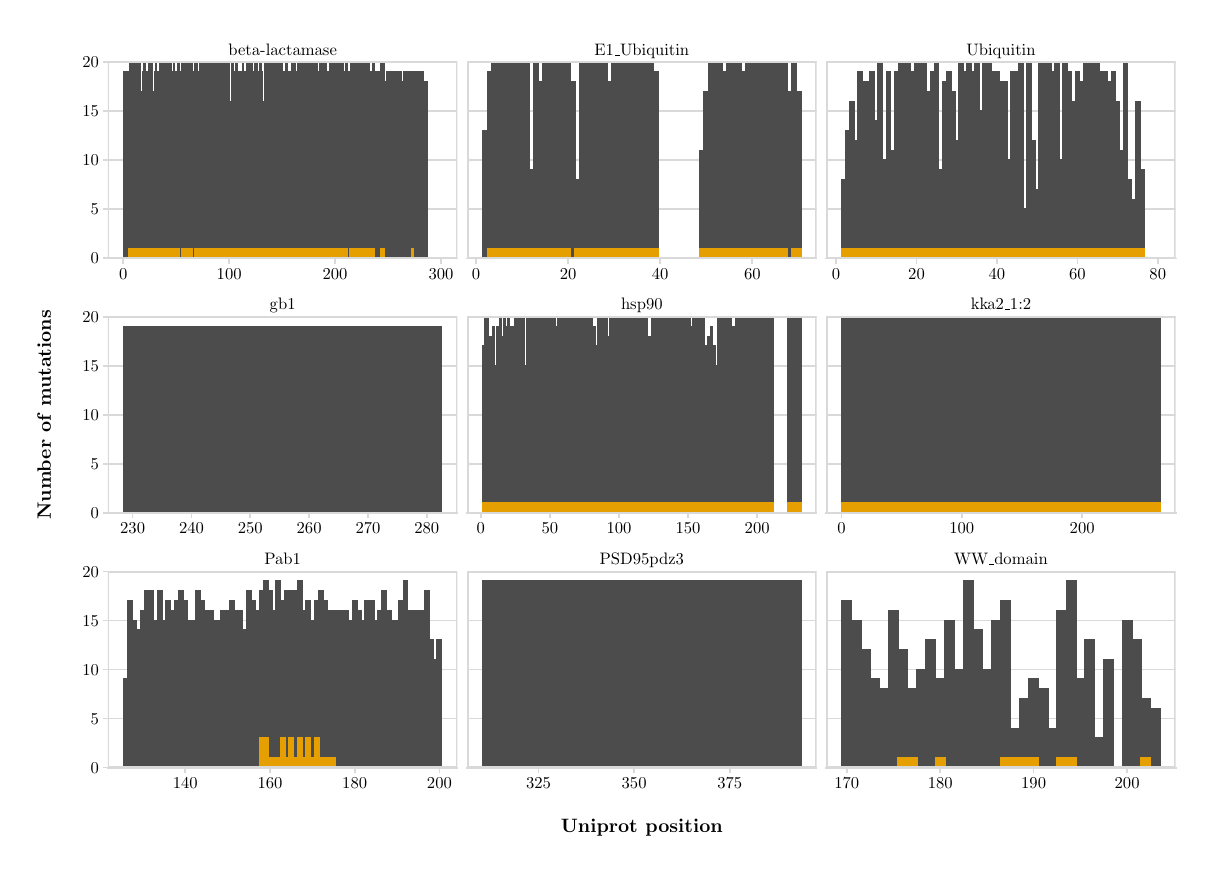
\begin{tikzpicture}[x=1pt,y=1pt]
\definecolor{fillColor}{RGB}{255,255,255}
\path[use as bounding box,fill=fillColor,fill opacity=0.00] (0,0) rectangle (418.34,295.82);
\begin{scope}
\path[clip] ( 29.00,212.35) rectangle (155.28,283.52);
\definecolor{drawColor}{gray}{0.85}

\path[draw=drawColor,line width= 0.6pt,line join=round] ( 29.00,212.49) --
	(155.28,212.49);

\path[draw=drawColor,line width= 0.6pt,line join=round] ( 29.00,230.21) --
	(155.28,230.21);

\path[draw=drawColor,line width= 0.6pt,line join=round] ( 29.00,247.94) --
	(155.28,247.94);

\path[draw=drawColor,line width= 0.6pt,line join=round] ( 29.00,265.66) --
	(155.28,265.66);

\path[draw=drawColor,line width= 0.6pt,line join=round] ( 29.00,283.38) --
	(155.28,283.38);
\definecolor{drawColor}{gray}{0.30}
\definecolor{fillColor}{gray}{0.30}

\path[draw=drawColor,line width= 0.6pt,line cap=rect,fill=fillColor] ( 34.74,212.49) rectangle ( 35.13,279.84);

\path[draw=drawColor,line width= 0.6pt,line cap=rect,fill=fillColor] ( 35.13,212.49) rectangle ( 35.51,279.84);

\path[draw=drawColor,line width= 0.6pt,line cap=rect,fill=fillColor] ( 35.51,212.49) rectangle ( 35.89,279.84);

\path[draw=drawColor,line width= 0.6pt,line cap=rect,fill=fillColor] ( 35.89,212.49) rectangle ( 36.27,276.29);

\path[draw=drawColor,line width= 0.6pt,line cap=rect,fill=fillColor] ( 36.27,212.49) rectangle ( 36.66,279.84);

\path[draw=drawColor,line width= 0.6pt,line cap=rect,fill=fillColor] ( 36.66,216.04) rectangle ( 37.04,279.84);

\path[draw=drawColor,line width= 0.6pt,line cap=rect,fill=fillColor] ( 37.04,216.04) rectangle ( 37.42,283.38);

\path[draw=drawColor,line width= 0.6pt,line cap=rect,fill=fillColor] ( 37.42,216.04) rectangle ( 37.81,283.38);

\path[draw=drawColor,line width= 0.6pt,line cap=rect,fill=fillColor] ( 37.81,216.04) rectangle ( 38.19,279.84);

\path[draw=drawColor,line width= 0.6pt,line cap=rect,fill=fillColor] ( 38.19,216.04) rectangle ( 38.57,283.38);

\path[draw=drawColor,line width= 0.6pt,line cap=rect,fill=fillColor] ( 38.57,216.04) rectangle ( 38.95,283.38);

\path[draw=drawColor,line width= 0.6pt,line cap=rect,fill=fillColor] ( 38.95,216.04) rectangle ( 39.34,283.38);

\path[draw=drawColor,line width= 0.6pt,line cap=rect,fill=fillColor] ( 39.34,216.04) rectangle ( 39.72,283.38);

\path[draw=drawColor,line width= 0.6pt,line cap=rect,fill=fillColor] ( 39.72,216.04) rectangle ( 40.10,283.38);

\path[draw=drawColor,line width= 0.6pt,line cap=rect,fill=fillColor] ( 40.10,216.04) rectangle ( 40.48,283.38);

\path[draw=drawColor,line width= 0.6pt,line cap=rect,fill=fillColor] ( 40.48,216.04) rectangle ( 40.87,272.75);

\path[draw=drawColor,line width= 0.6pt,line cap=rect,fill=fillColor] ( 40.87,212.49) rectangle ( 41.25,272.75);

\path[draw=drawColor,line width= 0.6pt,line cap=rect,fill=fillColor] ( 41.25,216.04) rectangle ( 41.63,258.57);

\path[draw=drawColor,line width= 0.6pt,line cap=rect,fill=fillColor] ( 41.63,216.04) rectangle ( 42.01,279.84);

\path[draw=drawColor,line width= 0.6pt,line cap=rect,fill=fillColor] ( 42.01,216.04) rectangle ( 42.40,283.38);

\path[draw=drawColor,line width= 0.6pt,line cap=rect,fill=fillColor] ( 42.40,212.49) rectangle ( 42.78,279.84);

\path[draw=drawColor,line width= 0.6pt,line cap=rect,fill=fillColor] ( 42.78,212.49) rectangle ( 43.16,279.84);

\path[draw=drawColor,line width= 0.6pt,line cap=rect,fill=fillColor] ( 43.16,216.04) rectangle ( 43.55,262.11);

\path[draw=drawColor,line width= 0.6pt,line cap=rect,fill=fillColor] ( 43.55,216.04) rectangle ( 43.93,279.84);

\path[draw=drawColor,line width= 0.6pt,line cap=rect,fill=fillColor] ( 43.93,216.04) rectangle ( 44.31,283.38);

\path[draw=drawColor,line width= 0.6pt,line cap=rect,fill=fillColor] ( 44.31,216.04) rectangle ( 44.69,251.48);

\path[draw=drawColor,line width= 0.6pt,line cap=rect,fill=fillColor] ( 44.69,216.04) rectangle ( 45.08,283.38);

\path[draw=drawColor,line width= 0.6pt,line cap=rect,fill=fillColor] ( 45.08,216.04) rectangle ( 45.46,269.20);

\path[draw=drawColor,line width= 0.6pt,line cap=rect,fill=fillColor] ( 45.46,216.04) rectangle ( 45.84,272.75);

\path[draw=drawColor,line width= 0.6pt,line cap=rect,fill=fillColor] ( 45.84,212.49) rectangle ( 46.22,279.84);

\path[draw=drawColor,line width= 0.6pt,line cap=rect,fill=fillColor] ( 46.22,216.04) rectangle ( 46.61,283.38);

\path[draw=drawColor,line width= 0.6pt,line cap=rect,fill=fillColor] ( 46.61,216.04) rectangle ( 46.99,279.84);

\path[draw=drawColor,line width= 0.6pt,line cap=rect,fill=fillColor] ( 46.99,216.04) rectangle ( 47.37,276.29);

\path[draw=drawColor,line width= 0.6pt,line cap=rect,fill=fillColor] ( 47.37,216.04) rectangle ( 47.75,276.29);

\path[draw=drawColor,line width= 0.6pt,line cap=rect,fill=fillColor] ( 47.75,216.04) rectangle ( 48.14,283.38);

\path[draw=drawColor,line width= 0.6pt,line cap=rect,fill=fillColor] ( 48.14,216.04) rectangle ( 48.52,279.84);

\path[draw=drawColor,line width= 0.6pt,line cap=rect,fill=fillColor] ( 48.52,216.04) rectangle ( 48.90,283.38);

\path[draw=drawColor,line width= 0.6pt,line cap=rect,fill=fillColor] ( 48.90,216.04) rectangle ( 49.29,283.38);

\path[draw=drawColor,line width= 0.6pt,line cap=rect,fill=fillColor] ( 49.29,216.04) rectangle ( 49.67,276.29);

\path[draw=drawColor,line width= 0.6pt,line cap=rect,fill=fillColor] ( 49.67,216.04) rectangle ( 50.05,283.38);

\path[draw=drawColor,line width= 0.6pt,line cap=rect,fill=fillColor] ( 50.05,216.04) rectangle ( 50.43,283.38);

\path[draw=drawColor,line width= 0.6pt,line cap=rect,fill=fillColor] ( 50.43,216.04) rectangle ( 50.82,283.38);

\path[draw=drawColor,line width= 0.6pt,line cap=rect,fill=fillColor] ( 50.82,216.04) rectangle ( 51.20,272.75);

\path[draw=drawColor,line width= 0.6pt,line cap=rect,fill=fillColor] ( 51.20,216.04) rectangle ( 51.58,283.38);

\path[draw=drawColor,line width= 0.6pt,line cap=rect,fill=fillColor] ( 51.58,216.04) rectangle ( 51.96,283.38);

\path[draw=drawColor,line width= 0.6pt,line cap=rect,fill=fillColor] ( 51.96,216.04) rectangle ( 52.35,272.75);

\path[draw=drawColor,line width= 0.6pt,line cap=rect,fill=fillColor] ( 52.35,216.04) rectangle ( 52.73,279.84);

\path[draw=drawColor,line width= 0.6pt,line cap=rect,fill=fillColor] ( 52.73,216.04) rectangle ( 53.11,283.38);

\path[draw=drawColor,line width= 0.6pt,line cap=rect,fill=fillColor] ( 53.11,216.04) rectangle ( 53.49,279.84);

\path[draw=drawColor,line width= 0.6pt,line cap=rect,fill=fillColor] ( 53.49,216.04) rectangle ( 53.88,279.84);

\path[draw=drawColor,line width= 0.6pt,line cap=rect,fill=fillColor] ( 53.88,216.04) rectangle ( 54.26,269.20);

\path[draw=drawColor,line width= 0.6pt,line cap=rect,fill=fillColor] ( 54.26,216.04) rectangle ( 54.64,283.38);

\path[draw=drawColor,line width= 0.6pt,line cap=rect,fill=fillColor] ( 54.64,212.49) rectangle ( 55.03,279.84);

\path[draw=drawColor,line width= 0.6pt,line cap=rect,fill=fillColor] ( 55.03,212.49) rectangle ( 55.41,276.29);

\path[draw=drawColor,line width= 0.6pt,line cap=rect,fill=fillColor] ( 55.41,212.49) rectangle ( 55.79,279.84);

\path[draw=drawColor,line width= 0.6pt,line cap=rect,fill=fillColor] ( 55.79,216.04) rectangle ( 56.17,283.38);

\path[draw=drawColor,line width= 0.6pt,line cap=rect,fill=fillColor] ( 56.17,216.04) rectangle ( 56.56,283.38);

\path[draw=drawColor,line width= 0.6pt,line cap=rect,fill=fillColor] ( 56.56,216.04) rectangle ( 56.94,269.20);

\path[draw=drawColor,line width= 0.6pt,line cap=rect,fill=fillColor] ( 56.94,216.04) rectangle ( 57.32,283.38);

\path[draw=drawColor,line width= 0.6pt,line cap=rect,fill=fillColor] ( 57.32,216.04) rectangle ( 57.70,279.84);

\path[draw=drawColor,line width= 0.6pt,line cap=rect,fill=fillColor] ( 57.70,216.04) rectangle ( 58.09,283.38);

\path[draw=drawColor,line width= 0.6pt,line cap=rect,fill=fillColor] ( 58.09,216.04) rectangle ( 58.47,272.75);

\path[draw=drawColor,line width= 0.6pt,line cap=rect,fill=fillColor] ( 58.47,216.04) rectangle ( 58.85,283.38);

\path[draw=drawColor,line width= 0.6pt,line cap=rect,fill=fillColor] ( 58.85,216.04) rectangle ( 59.23,276.29);

\path[draw=drawColor,line width= 0.6pt,line cap=rect,fill=fillColor] ( 59.23,216.04) rectangle ( 59.62,283.38);

\path[draw=drawColor,line width= 0.6pt,line cap=rect,fill=fillColor] ( 59.62,212.49) rectangle ( 60.00,279.84);

\path[draw=drawColor,line width= 0.6pt,line cap=rect,fill=fillColor] ( 60.00,212.49) rectangle ( 60.38,279.84);

\path[draw=drawColor,line width= 0.6pt,line cap=rect,fill=fillColor] ( 60.38,216.04) rectangle ( 60.77,283.38);

\path[draw=drawColor,line width= 0.6pt,line cap=rect,fill=fillColor] ( 60.77,216.04) rectangle ( 61.15,283.38);

\path[draw=drawColor,line width= 0.6pt,line cap=rect,fill=fillColor] ( 61.15,212.49) rectangle ( 61.53,279.84);

\path[draw=drawColor,line width= 0.6pt,line cap=rect,fill=fillColor] ( 61.53,212.49) rectangle ( 61.91,244.39);

\path[draw=drawColor,line width= 0.6pt,line cap=rect,fill=fillColor] ( 61.91,216.04) rectangle ( 62.30,272.75);

\path[draw=drawColor,line width= 0.6pt,line cap=rect,fill=fillColor] ( 62.30,216.04) rectangle ( 62.68,283.38);

\path[draw=drawColor,line width= 0.6pt,line cap=rect,fill=fillColor] ( 62.68,212.49) rectangle ( 63.06,269.20);

\path[draw=drawColor,line width= 0.6pt,line cap=rect,fill=fillColor] ( 63.06,216.04) rectangle ( 63.44,283.38);

\path[draw=drawColor,line width= 0.6pt,line cap=rect,fill=fillColor] ( 63.44,216.04) rectangle ( 63.83,283.38);

\path[draw=drawColor,line width= 0.6pt,line cap=rect,fill=fillColor] ( 63.83,216.04) rectangle ( 64.21,279.84);

\path[draw=drawColor,line width= 0.6pt,line cap=rect,fill=fillColor] ( 64.21,216.04) rectangle ( 64.59,283.38);

\path[draw=drawColor,line width= 0.6pt,line cap=rect,fill=fillColor] ( 64.59,216.04) rectangle ( 64.97,283.38);

\path[draw=drawColor,line width= 0.6pt,line cap=rect,fill=fillColor] ( 64.97,216.04) rectangle ( 65.36,283.38);

\path[draw=drawColor,line width= 0.6pt,line cap=rect,fill=fillColor] ( 65.36,216.04) rectangle ( 65.74,283.38);

\path[draw=drawColor,line width= 0.6pt,line cap=rect,fill=fillColor] ( 65.74,216.04) rectangle ( 66.12,283.38);

\path[draw=drawColor,line width= 0.6pt,line cap=rect,fill=fillColor] ( 66.12,216.04) rectangle ( 66.50,283.38);

\path[draw=drawColor,line width= 0.6pt,line cap=rect,fill=fillColor] ( 66.50,216.04) rectangle ( 66.89,279.84);

\path[draw=drawColor,line width= 0.6pt,line cap=rect,fill=fillColor] ( 66.89,216.04) rectangle ( 67.27,283.38);

\path[draw=drawColor,line width= 0.6pt,line cap=rect,fill=fillColor] ( 67.27,216.04) rectangle ( 67.65,283.38);

\path[draw=drawColor,line width= 0.6pt,line cap=rect,fill=fillColor] ( 67.65,216.04) rectangle ( 68.04,283.38);

\path[draw=drawColor,line width= 0.6pt,line cap=rect,fill=fillColor] ( 68.04,216.04) rectangle ( 68.42,283.38);

\path[draw=drawColor,line width= 0.6pt,line cap=rect,fill=fillColor] ( 68.42,216.04) rectangle ( 68.80,283.38);

\path[draw=drawColor,line width= 0.6pt,line cap=rect,fill=fillColor] ( 68.80,216.04) rectangle ( 69.18,283.38);

\path[draw=drawColor,line width= 0.6pt,line cap=rect,fill=fillColor] ( 69.18,216.04) rectangle ( 69.57,283.38);

\path[draw=drawColor,line width= 0.6pt,line cap=rect,fill=fillColor] ( 69.57,216.04) rectangle ( 69.95,283.38);

\path[draw=drawColor,line width= 0.6pt,line cap=rect,fill=fillColor] ( 69.95,216.04) rectangle ( 70.33,283.38);

\path[draw=drawColor,line width= 0.6pt,line cap=rect,fill=fillColor] ( 70.33,216.04) rectangle ( 70.71,283.38);

\path[draw=drawColor,line width= 0.6pt,line cap=rect,fill=fillColor] ( 70.71,216.04) rectangle ( 71.10,283.38);

\path[draw=drawColor,line width= 0.6pt,line cap=rect,fill=fillColor] ( 71.10,216.04) rectangle ( 71.48,283.38);

\path[draw=drawColor,line width= 0.6pt,line cap=rect,fill=fillColor] ( 71.48,216.04) rectangle ( 71.86,283.38);

\path[draw=drawColor,line width= 0.6pt,line cap=rect,fill=fillColor] ( 71.86,212.49) rectangle ( 72.24,276.29);

\path[draw=drawColor,line width= 0.6pt,line cap=rect,fill=fillColor] ( 72.24,216.04) rectangle ( 72.63,283.38);

\path[draw=drawColor,line width= 0.6pt,line cap=rect,fill=fillColor] ( 72.63,216.04) rectangle ( 73.01,269.20);

\path[draw=drawColor,line width= 0.6pt,line cap=rect,fill=fillColor] ( 73.01,216.04) rectangle ( 73.39,269.20);

\path[draw=drawColor,line width= 0.6pt,line cap=rect,fill=fillColor] ( 73.39,212.49) rectangle ( 73.78,262.11);

\path[draw=drawColor,line width= 0.6pt,line cap=rect,fill=fillColor] ( 73.78,216.04) rectangle ( 74.16,283.38);

\path[draw=drawColor,line width= 0.6pt,line cap=rect,fill=fillColor] ( 74.16,216.04) rectangle ( 74.54,279.84);

\path[draw=drawColor,line width= 0.6pt,line cap=rect,fill=fillColor] ( 74.54,212.49) rectangle ( 74.92,279.84);

\path[draw=drawColor,line width= 0.6pt,line cap=rect,fill=fillColor] ( 74.92,212.49) rectangle ( 75.31,279.84);

\path[draw=drawColor,line width= 0.6pt,line cap=rect,fill=fillColor] ( 75.31,216.04) rectangle ( 75.69,283.38);

\path[draw=drawColor,line width= 0.6pt,line cap=rect,fill=fillColor] ( 75.69,216.04) rectangle ( 76.07,279.84);

\path[draw=drawColor,line width= 0.6pt,line cap=rect,fill=fillColor] ( 76.07,216.04) rectangle ( 76.45,276.29);

\path[draw=drawColor,line width= 0.6pt,line cap=rect,fill=fillColor] ( 76.45,216.04) rectangle ( 76.84,279.84);

\path[draw=drawColor,line width= 0.6pt,line cap=rect,fill=fillColor] ( 76.84,216.04) rectangle ( 77.22,279.84);

\path[draw=drawColor,line width= 0.6pt,line cap=rect,fill=fillColor] ( 77.22,216.04) rectangle ( 77.60,279.84);

\path[draw=drawColor,line width= 0.6pt,line cap=rect,fill=fillColor] ( 77.60,216.04) rectangle ( 77.98,283.38);

\path[draw=drawColor,line width= 0.6pt,line cap=rect,fill=fillColor] ( 77.98,216.04) rectangle ( 78.37,276.29);

\path[draw=drawColor,line width= 0.6pt,line cap=rect,fill=fillColor] ( 78.37,212.49) rectangle ( 78.75,279.84);

\path[draw=drawColor,line width= 0.6pt,line cap=rect,fill=fillColor] ( 78.75,216.04) rectangle ( 79.13,265.66);

\path[draw=drawColor,line width= 0.6pt,line cap=rect,fill=fillColor] ( 79.13,216.04) rectangle ( 79.52,283.38);

\path[draw=drawColor,line width= 0.6pt,line cap=rect,fill=fillColor] ( 79.52,216.04) rectangle ( 79.90,283.38);

\path[draw=drawColor,line width= 0.6pt,line cap=rect,fill=fillColor] ( 79.90,212.49) rectangle ( 80.28,276.29);

\path[draw=drawColor,line width= 0.6pt,line cap=rect,fill=fillColor] ( 80.28,212.49) rectangle ( 80.66,276.29);

\path[draw=drawColor,line width= 0.6pt,line cap=rect,fill=fillColor] ( 80.66,216.04) rectangle ( 81.05,283.38);

\path[draw=drawColor,line width= 0.6pt,line cap=rect,fill=fillColor] ( 81.05,216.04) rectangle ( 81.43,279.84);

\path[draw=drawColor,line width= 0.6pt,line cap=rect,fill=fillColor] ( 81.43,216.04) rectangle ( 81.81,272.75);

\path[draw=drawColor,line width= 0.6pt,line cap=rect,fill=fillColor] ( 81.81,216.04) rectangle ( 82.19,279.84);

\path[draw=drawColor,line width= 0.6pt,line cap=rect,fill=fillColor] ( 82.19,216.04) rectangle ( 82.58,283.38);

\path[draw=drawColor,line width= 0.6pt,line cap=rect,fill=fillColor] ( 82.58,216.04) rectangle ( 82.96,283.38);

\path[draw=drawColor,line width= 0.6pt,line cap=rect,fill=fillColor] ( 82.96,212.49) rectangle ( 83.34,279.84);

\path[draw=drawColor,line width= 0.6pt,line cap=rect,fill=fillColor] ( 83.34,216.04) rectangle ( 83.72,269.20);

\path[draw=drawColor,line width= 0.6pt,line cap=rect,fill=fillColor] ( 83.72,216.04) rectangle ( 84.11,283.38);

\path[draw=drawColor,line width= 0.6pt,line cap=rect,fill=fillColor] ( 84.11,216.04) rectangle ( 84.49,283.38);

\path[draw=drawColor,line width= 0.6pt,line cap=rect,fill=fillColor] ( 84.49,212.49) rectangle ( 84.87,279.84);

\path[draw=drawColor,line width= 0.6pt,line cap=rect,fill=fillColor] ( 84.87,216.04) rectangle ( 85.26,255.03);

\path[draw=drawColor,line width= 0.6pt,line cap=rect,fill=fillColor] ( 85.26,216.04) rectangle ( 85.64,269.20);

\path[draw=drawColor,line width= 0.6pt,line cap=rect,fill=fillColor] ( 85.64,216.04) rectangle ( 86.02,283.38);

\path[draw=drawColor,line width= 0.6pt,line cap=rect,fill=fillColor] ( 86.02,216.04) rectangle ( 86.40,283.38);

\path[draw=drawColor,line width= 0.6pt,line cap=rect,fill=fillColor] ( 86.40,216.04) rectangle ( 86.79,283.38);

\path[draw=drawColor,line width= 0.6pt,line cap=rect,fill=fillColor] ( 86.79,216.04) rectangle ( 87.17,283.38);

\path[draw=drawColor,line width= 0.6pt,line cap=rect,fill=fillColor] ( 87.17,216.04) rectangle ( 87.55,283.38);

\path[draw=drawColor,line width= 0.6pt,line cap=rect,fill=fillColor] ( 87.55,216.04) rectangle ( 87.93,283.38);

\path[draw=drawColor,line width= 0.6pt,line cap=rect,fill=fillColor] ( 87.93,216.04) rectangle ( 88.32,283.38);

\path[draw=drawColor,line width= 0.6pt,line cap=rect,fill=fillColor] ( 88.32,216.04) rectangle ( 88.70,276.29);

\path[draw=drawColor,line width= 0.6pt,line cap=rect,fill=fillColor] ( 88.70,216.04) rectangle ( 89.08,283.38);

\path[draw=drawColor,line width= 0.6pt,line cap=rect,fill=fillColor] ( 89.08,216.04) rectangle ( 89.46,283.38);

\path[draw=drawColor,line width= 0.6pt,line cap=rect,fill=fillColor] ( 89.46,216.04) rectangle ( 89.85,283.38);

\path[draw=drawColor,line width= 0.6pt,line cap=rect,fill=fillColor] ( 89.85,216.04) rectangle ( 90.23,283.38);

\path[draw=drawColor,line width= 0.6pt,line cap=rect,fill=fillColor] ( 90.23,216.04) rectangle ( 90.61,283.38);

\path[draw=drawColor,line width= 0.6pt,line cap=rect,fill=fillColor] ( 90.61,216.04) rectangle ( 91.00,283.38);

\path[draw=drawColor,line width= 0.6pt,line cap=rect,fill=fillColor] ( 91.00,216.04) rectangle ( 91.38,283.38);

\path[draw=drawColor,line width= 0.6pt,line cap=rect,fill=fillColor] ( 91.38,216.04) rectangle ( 91.76,283.38);

\path[draw=drawColor,line width= 0.6pt,line cap=rect,fill=fillColor] ( 91.76,216.04) rectangle ( 92.14,283.38);

\path[draw=drawColor,line width= 0.6pt,line cap=rect,fill=fillColor] ( 92.14,216.04) rectangle ( 92.53,279.84);

\path[draw=drawColor,line width= 0.6pt,line cap=rect,fill=fillColor] ( 92.53,216.04) rectangle ( 92.91,276.29);

\path[draw=drawColor,line width= 0.6pt,line cap=rect,fill=fillColor] ( 92.91,212.49) rectangle ( 93.29,276.29);

\path[draw=drawColor,line width= 0.6pt,line cap=rect,fill=fillColor] ( 93.29,216.04) rectangle ( 93.67,283.38);

\path[draw=drawColor,line width= 0.6pt,line cap=rect,fill=fillColor] ( 93.67,216.04) rectangle ( 94.06,276.29);

\path[draw=drawColor,line width= 0.6pt,line cap=rect,fill=fillColor] ( 94.06,212.49) rectangle ( 94.44,279.84);

\path[draw=drawColor,line width= 0.6pt,line cap=rect,fill=fillColor] ( 94.44,212.49) rectangle ( 94.82,255.03);

\path[draw=drawColor,line width= 0.6pt,line cap=rect,fill=fillColor] ( 94.82,216.04) rectangle ( 95.20,279.84);

\path[draw=drawColor,line width= 0.6pt,line cap=rect,fill=fillColor] ( 95.20,216.04) rectangle ( 95.59,279.84);

\path[draw=drawColor,line width= 0.6pt,line cap=rect,fill=fillColor] ( 95.59,216.04) rectangle ( 95.97,283.38);

\path[draw=drawColor,line width= 0.6pt,line cap=rect,fill=fillColor] ( 95.97,216.04) rectangle ( 96.35,283.38);

\path[draw=drawColor,line width= 0.6pt,line cap=rect,fill=fillColor] ( 96.35,216.04) rectangle ( 96.73,283.38);

\path[draw=drawColor,line width= 0.6pt,line cap=rect,fill=fillColor] ( 96.73,212.49) rectangle ( 97.12,279.84);

\path[draw=drawColor,line width= 0.6pt,line cap=rect,fill=fillColor] ( 97.12,216.04) rectangle ( 97.50,265.66);

\path[draw=drawColor,line width= 0.6pt,line cap=rect,fill=fillColor] ( 97.50,216.04) rectangle ( 97.88,283.38);

\path[draw=drawColor,line width= 0.6pt,line cap=rect,fill=fillColor] ( 97.88,216.04) rectangle ( 98.27,283.38);

\path[draw=drawColor,line width= 0.6pt,line cap=rect,fill=fillColor] ( 98.27,212.49) rectangle ( 98.65,279.84);

\path[draw=drawColor,line width= 0.6pt,line cap=rect,fill=fillColor] ( 98.65,216.04) rectangle ( 99.03,283.38);

\path[draw=drawColor,line width= 0.6pt,line cap=rect,fill=fillColor] ( 99.03,216.04) rectangle ( 99.41,279.84);

\path[draw=drawColor,line width= 0.6pt,line cap=rect,fill=fillColor] ( 99.41,216.04) rectangle ( 99.80,283.38);

\path[draw=drawColor,line width= 0.6pt,line cap=rect,fill=fillColor] ( 99.80,216.04) rectangle (100.18,283.38);

\path[draw=drawColor,line width= 0.6pt,line cap=rect,fill=fillColor] (100.18,216.04) rectangle (100.56,283.38);

\path[draw=drawColor,line width= 0.6pt,line cap=rect,fill=fillColor] (100.56,216.04) rectangle (100.94,283.38);

\path[draw=drawColor,line width= 0.6pt,line cap=rect,fill=fillColor] (100.94,216.04) rectangle (101.33,283.38);

\path[draw=drawColor,line width= 0.6pt,line cap=rect,fill=fillColor] (101.33,216.04) rectangle (101.71,283.38);

\path[draw=drawColor,line width= 0.6pt,line cap=rect,fill=fillColor] (101.71,216.04) rectangle (102.09,283.38);

\path[draw=drawColor,line width= 0.6pt,line cap=rect,fill=fillColor] (102.09,216.04) rectangle (102.47,283.38);

\path[draw=drawColor,line width= 0.6pt,line cap=rect,fill=fillColor] (102.47,216.04) rectangle (102.86,283.38);

\path[draw=drawColor,line width= 0.6pt,line cap=rect,fill=fillColor] (102.86,216.04) rectangle (103.24,283.38);

\path[draw=drawColor,line width= 0.6pt,line cap=rect,fill=fillColor] (103.24,212.49) rectangle (103.62,279.84);

\path[draw=drawColor,line width= 0.6pt,line cap=rect,fill=fillColor] (103.62,216.04) rectangle (104.01,283.38);

\path[draw=drawColor,line width= 0.6pt,line cap=rect,fill=fillColor] (104.01,216.04) rectangle (104.39,283.38);

\path[draw=drawColor,line width= 0.6pt,line cap=rect,fill=fillColor] (104.39,216.04) rectangle (104.77,283.38);

\path[draw=drawColor,line width= 0.6pt,line cap=rect,fill=fillColor] (104.77,212.49) rectangle (105.15,279.84);

\path[draw=drawColor,line width= 0.6pt,line cap=rect,fill=fillColor] (105.15,216.04) rectangle (105.54,269.20);

\path[draw=drawColor,line width= 0.6pt,line cap=rect,fill=fillColor] (105.54,216.04) rectangle (105.92,283.38);

\path[draw=drawColor,line width= 0.6pt,line cap=rect,fill=fillColor] (105.92,216.04) rectangle (106.30,283.38);

\path[draw=drawColor,line width= 0.6pt,line cap=rect,fill=fillColor] (106.30,212.49) rectangle (106.68,279.84);

\path[draw=drawColor,line width= 0.6pt,line cap=rect,fill=fillColor] (106.68,216.04) rectangle (107.07,283.38);

\path[draw=drawColor,line width= 0.6pt,line cap=rect,fill=fillColor] (107.07,216.04) rectangle (107.45,279.84);

\path[draw=drawColor,line width= 0.6pt,line cap=rect,fill=fillColor] (107.45,216.04) rectangle (107.83,283.38);

\path[draw=drawColor,line width= 0.6pt,line cap=rect,fill=fillColor] (107.83,216.04) rectangle (108.21,279.84);

\path[draw=drawColor,line width= 0.6pt,line cap=rect,fill=fillColor] (108.21,216.04) rectangle (108.60,276.29);

\path[draw=drawColor,line width= 0.6pt,line cap=rect,fill=fillColor] (108.60,216.04) rectangle (108.98,279.84);

\path[draw=drawColor,line width= 0.6pt,line cap=rect,fill=fillColor] (108.98,216.04) rectangle (109.36,272.75);

\path[draw=drawColor,line width= 0.6pt,line cap=rect,fill=fillColor] (109.36,216.04) rectangle (109.75,283.38);

\path[draw=drawColor,line width= 0.6pt,line cap=rect,fill=fillColor] (109.75,216.04) rectangle (110.13,283.38);

\path[draw=drawColor,line width= 0.6pt,line cap=rect,fill=fillColor] (110.13,216.04) rectangle (110.51,283.38);

\path[draw=drawColor,line width= 0.6pt,line cap=rect,fill=fillColor] (110.51,216.04) rectangle (110.89,269.20);

\path[draw=drawColor,line width= 0.6pt,line cap=rect,fill=fillColor] (110.89,216.04) rectangle (111.28,283.38);

\path[draw=drawColor,line width= 0.6pt,line cap=rect,fill=fillColor] (111.28,216.04) rectangle (111.66,279.84);

\path[draw=drawColor,line width= 0.6pt,line cap=rect,fill=fillColor] (111.66,216.04) rectangle (112.04,283.38);

\path[draw=drawColor,line width= 0.6pt,line cap=rect,fill=fillColor] (112.04,216.04) rectangle (112.42,283.38);

\path[draw=drawColor,line width= 0.6pt,line cap=rect,fill=fillColor] (112.42,216.04) rectangle (112.81,283.38);

\path[draw=drawColor,line width= 0.6pt,line cap=rect,fill=fillColor] (112.81,216.04) rectangle (113.19,276.29);

\path[draw=drawColor,line width= 0.6pt,line cap=rect,fill=fillColor] (113.19,216.04) rectangle (113.57,283.38);

\path[draw=drawColor,line width= 0.6pt,line cap=rect,fill=fillColor] (113.57,216.04) rectangle (113.95,283.38);

\path[draw=drawColor,line width= 0.6pt,line cap=rect,fill=fillColor] (113.95,212.49) rectangle (114.34,279.84);

\path[draw=drawColor,line width= 0.6pt,line cap=rect,fill=fillColor] (114.34,212.49) rectangle (114.72,269.20);

\path[draw=drawColor,line width= 0.6pt,line cap=rect,fill=fillColor] (114.72,216.04) rectangle (115.10,279.84);

\path[draw=drawColor,line width= 0.6pt,line cap=rect,fill=fillColor] (115.10,216.04) rectangle (115.49,283.38);

\path[draw=drawColor,line width= 0.6pt,line cap=rect,fill=fillColor] (115.49,212.49) rectangle (115.87,279.84);

\path[draw=drawColor,line width= 0.6pt,line cap=rect,fill=fillColor] (115.87,212.49) rectangle (116.25,279.84);

\path[draw=drawColor,line width= 0.6pt,line cap=rect,fill=fillColor] (116.25,216.04) rectangle (116.63,279.84);

\path[draw=drawColor,line width= 0.6pt,line cap=rect,fill=fillColor] (116.63,216.04) rectangle (117.02,283.38);

\path[draw=drawColor,line width= 0.6pt,line cap=rect,fill=fillColor] (117.02,216.04) rectangle (117.40,272.75);

\path[draw=drawColor,line width= 0.6pt,line cap=rect,fill=fillColor] (117.40,216.04) rectangle (117.78,283.38);

\path[draw=drawColor,line width= 0.6pt,line cap=rect,fill=fillColor] (117.78,216.04) rectangle (118.16,283.38);

\path[draw=drawColor,line width= 0.6pt,line cap=rect,fill=fillColor] (118.16,216.04) rectangle (118.55,283.38);

\path[draw=drawColor,line width= 0.6pt,line cap=rect,fill=fillColor] (118.55,216.04) rectangle (118.93,283.38);

\path[draw=drawColor,line width= 0.6pt,line cap=rect,fill=fillColor] (118.93,216.04) rectangle (119.31,283.38);

\path[draw=drawColor,line width= 0.6pt,line cap=rect,fill=fillColor] (119.31,216.04) rectangle (119.69,283.38);

\path[draw=drawColor,line width= 0.6pt,line cap=rect,fill=fillColor] (119.69,216.04) rectangle (120.08,283.38);

\path[draw=drawColor,line width= 0.6pt,line cap=rect,fill=fillColor] (120.08,216.04) rectangle (120.46,283.38);

\path[draw=drawColor,line width= 0.6pt,line cap=rect,fill=fillColor] (120.46,216.04) rectangle (120.84,279.84);

\path[draw=drawColor,line width= 0.6pt,line cap=rect,fill=fillColor] (120.84,216.04) rectangle (121.22,283.38);

\path[draw=drawColor,line width= 0.6pt,line cap=rect,fill=fillColor] (121.22,212.49) rectangle (121.61,279.84);

\path[draw=drawColor,line width= 0.6pt,line cap=rect,fill=fillColor] (121.61,216.04) rectangle (121.99,283.38);

\path[draw=drawColor,line width= 0.6pt,line cap=rect,fill=fillColor] (121.99,216.04) rectangle (122.37,283.38);

\path[draw=drawColor,line width= 0.6pt,line cap=rect,fill=fillColor] (122.37,216.04) rectangle (122.76,283.38);

\path[draw=drawColor,line width= 0.6pt,line cap=rect,fill=fillColor] (122.76,212.49) rectangle (123.14,279.84);

\path[draw=drawColor,line width= 0.6pt,line cap=rect,fill=fillColor] (123.14,216.04) rectangle (123.52,283.38);

\path[draw=drawColor,line width= 0.6pt,line cap=rect,fill=fillColor] (123.52,216.04) rectangle (123.90,279.84);

\path[draw=drawColor,line width= 0.6pt,line cap=rect,fill=fillColor] (123.90,216.04) rectangle (124.29,279.84);

\path[draw=drawColor,line width= 0.6pt,line cap=rect,fill=fillColor] (124.29,216.04) rectangle (124.67,279.84);

\path[draw=drawColor,line width= 0.6pt,line cap=rect,fill=fillColor] (124.67,216.04) rectangle (125.05,283.38);

\path[draw=drawColor,line width= 0.6pt,line cap=rect,fill=fillColor] (125.05,212.49) rectangle (125.43,279.84);

\path[draw=drawColor,line width= 0.6pt,line cap=rect,fill=fillColor] (125.43,212.49) rectangle (125.82,279.84);

\path[draw=drawColor,line width= 0.6pt,line cap=rect,fill=fillColor] (125.82,212.49) rectangle (126.20,279.84);

\path[draw=drawColor,line width= 0.6pt,line cap=rect,fill=fillColor] (126.20,212.49) rectangle (126.58,279.84);

\path[draw=drawColor,line width= 0.6pt,line cap=rect,fill=fillColor] (126.58,212.49) rectangle (126.96,279.84);

\path[draw=drawColor,line width= 0.6pt,line cap=rect,fill=fillColor] (126.96,212.49) rectangle (127.35,279.84);

\path[draw=drawColor,line width= 0.6pt,line cap=rect,fill=fillColor] (127.35,212.49) rectangle (127.73,279.84);

\path[draw=drawColor,line width= 0.6pt,line cap=rect,fill=fillColor] (127.73,216.04) rectangle (128.11,283.38);

\path[draw=drawColor,line width= 0.6pt,line cap=rect,fill=fillColor] (128.11,212.49) rectangle (128.50,279.84);

\path[draw=drawColor,line width= 0.6pt,line cap=rect,fill=fillColor] (128.50,216.04) rectangle (128.88,283.38);

\path[draw=drawColor,line width= 0.6pt,line cap=rect,fill=fillColor] (128.88,212.49) rectangle (129.26,276.29);

\path[draw=drawColor,line width= 0.6pt,line cap=rect,fill=fillColor] (129.26,212.49) rectangle (129.64,276.29);

\path[draw=drawColor,line width= 0.6pt,line cap=rect,fill=fillColor] (129.64,212.49) rectangle (130.03,279.84);

\path[draw=drawColor,line width= 0.6pt,line cap=rect,fill=fillColor] (130.03,212.49) rectangle (130.41,279.84);

\path[draw=drawColor,line width= 0.6pt,line cap=rect,fill=fillColor] (130.41,212.49) rectangle (130.79,279.84);

\path[draw=drawColor,line width= 0.6pt,line cap=rect,fill=fillColor] (130.79,212.49) rectangle (131.17,279.84);

\path[draw=drawColor,line width= 0.6pt,line cap=rect,fill=fillColor] (131.17,212.49) rectangle (131.56,276.29);

\path[draw=drawColor,line width= 0.6pt,line cap=rect,fill=fillColor] (131.56,212.49) rectangle (131.94,279.84);

\path[draw=drawColor,line width= 0.6pt,line cap=rect,fill=fillColor] (131.94,212.49) rectangle (132.32,279.84);

\path[draw=drawColor,line width= 0.6pt,line cap=rect,fill=fillColor] (132.32,212.49) rectangle (132.70,279.84);

\path[draw=drawColor,line width= 0.6pt,line cap=rect,fill=fillColor] (132.70,212.49) rectangle (133.09,279.84);

\path[draw=drawColor,line width= 0.6pt,line cap=rect,fill=fillColor] (133.09,212.49) rectangle (133.47,247.94);

\path[draw=drawColor,line width= 0.6pt,line cap=rect,fill=fillColor] (133.47,212.49) rectangle (133.85,279.84);

\path[draw=drawColor,line width= 0.6pt,line cap=rect,fill=fillColor] (133.85,212.49) rectangle (134.24,276.29);

\path[draw=drawColor,line width= 0.6pt,line cap=rect,fill=fillColor] (134.24,212.49) rectangle (134.62,269.20);

\path[draw=drawColor,line width= 0.6pt,line cap=rect,fill=fillColor] (134.62,212.49) rectangle (135.00,279.84);

\path[draw=drawColor,line width= 0.6pt,line cap=rect,fill=fillColor] (135.00,212.49) rectangle (135.38,269.20);

\path[draw=drawColor,line width= 0.6pt,line cap=rect,fill=fillColor] (135.38,212.49) rectangle (135.77,276.29);

\path[draw=drawColor,line width= 0.6pt,line cap=rect,fill=fillColor] (135.77,212.49) rectangle (136.15,279.84);

\path[draw=drawColor,line width= 0.6pt,line cap=rect,fill=fillColor] (136.15,212.49) rectangle (136.53,279.84);

\path[draw=drawColor,line width= 0.6pt,line cap=rect,fill=fillColor] (136.53,212.49) rectangle (136.91,279.84);

\path[draw=drawColor,line width= 0.6pt,line cap=rect,fill=fillColor] (136.91,212.49) rectangle (137.30,279.84);

\path[draw=drawColor,line width= 0.6pt,line cap=rect,fill=fillColor] (137.30,212.49) rectangle (137.68,279.84);

\path[draw=drawColor,line width= 0.6pt,line cap=rect,fill=fillColor] (137.68,212.49) rectangle (138.06,279.84);

\path[draw=drawColor,line width= 0.6pt,line cap=rect,fill=fillColor] (138.06,212.49) rectangle (138.44,269.20);

\path[draw=drawColor,line width= 0.6pt,line cap=rect,fill=fillColor] (138.44,212.49) rectangle (138.83,279.84);

\path[draw=drawColor,line width= 0.6pt,line cap=rect,fill=fillColor] (138.83,216.04) rectangle (139.21,258.57);

\path[draw=drawColor,line width= 0.6pt,line cap=rect,fill=fillColor] (139.21,212.49) rectangle (139.59,262.11);

\path[draw=drawColor,line width= 0.6pt,line cap=rect,fill=fillColor] (139.59,212.49) rectangle (139.98,279.84);

\path[draw=drawColor,line width= 0.6pt,line cap=rect,fill=fillColor] (139.98,212.49) rectangle (140.36,272.75);

\path[draw=drawColor,line width= 0.6pt,line cap=rect,fill=fillColor] (140.36,212.49) rectangle (140.74,279.84);

\path[draw=drawColor,line width= 0.6pt,line cap=rect,fill=fillColor] (140.74,212.49) rectangle (141.12,279.84);

\path[draw=drawColor,line width= 0.6pt,line cap=rect,fill=fillColor] (141.12,212.49) rectangle (141.51,272.75);

\path[draw=drawColor,line width= 0.6pt,line cap=rect,fill=fillColor] (141.51,212.49) rectangle (141.89,279.84);

\path[draw=drawColor,line width= 0.6pt,line cap=rect,fill=fillColor] (141.89,212.49) rectangle (142.27,279.84);

\path[draw=drawColor,line width= 0.6pt,line cap=rect,fill=fillColor] (142.27,212.49) rectangle (142.65,279.84);

\path[draw=drawColor,line width= 0.6pt,line cap=rect,fill=fillColor] (142.65,212.49) rectangle (143.04,279.84);

\path[draw=drawColor,line width= 0.6pt,line cap=rect,fill=fillColor] (143.04,212.49) rectangle (143.42,276.29);

\path[draw=drawColor,line width= 0.6pt,line cap=rect,fill=fillColor] (143.42,212.49) rectangle (143.80,276.29);

\path[draw=drawColor,line width= 0.6pt,line cap=rect,fill=fillColor] (143.80,212.49) rectangle (144.18,276.29);
\definecolor{drawColor}{RGB}{230,159,0}
\definecolor{fillColor}{RGB}{230,159,0}

\path[draw=drawColor,line width= 0.6pt,line cap=rect,fill=fillColor] ( 36.66,212.49) rectangle ( 37.04,216.04);

\path[draw=drawColor,line width= 0.6pt,line cap=rect,fill=fillColor] ( 37.04,212.49) rectangle ( 37.42,216.04);

\path[draw=drawColor,line width= 0.6pt,line cap=rect,fill=fillColor] ( 37.42,212.49) rectangle ( 37.81,216.04);

\path[draw=drawColor,line width= 0.6pt,line cap=rect,fill=fillColor] ( 37.81,212.49) rectangle ( 38.19,216.04);

\path[draw=drawColor,line width= 0.6pt,line cap=rect,fill=fillColor] ( 38.19,212.49) rectangle ( 38.57,216.04);

\path[draw=drawColor,line width= 0.6pt,line cap=rect,fill=fillColor] ( 38.57,212.49) rectangle ( 38.95,216.04);

\path[draw=drawColor,line width= 0.6pt,line cap=rect,fill=fillColor] ( 38.95,212.49) rectangle ( 39.34,216.04);

\path[draw=drawColor,line width= 0.6pt,line cap=rect,fill=fillColor] ( 39.34,212.49) rectangle ( 39.72,216.04);

\path[draw=drawColor,line width= 0.6pt,line cap=rect,fill=fillColor] ( 39.72,212.49) rectangle ( 40.10,216.04);

\path[draw=drawColor,line width= 0.6pt,line cap=rect,fill=fillColor] ( 40.10,212.49) rectangle ( 40.48,216.04);

\path[draw=drawColor,line width= 0.6pt,line cap=rect,fill=fillColor] ( 40.48,212.49) rectangle ( 40.87,216.04);

\path[draw=drawColor,line width= 0.6pt,line cap=rect,fill=fillColor] ( 41.25,212.49) rectangle ( 41.63,216.04);

\path[draw=drawColor,line width= 0.6pt,line cap=rect,fill=fillColor] ( 41.63,212.49) rectangle ( 42.01,216.04);

\path[draw=drawColor,line width= 0.6pt,line cap=rect,fill=fillColor] ( 42.01,212.49) rectangle ( 42.40,216.04);

\path[draw=drawColor,line width= 0.6pt,line cap=rect,fill=fillColor] ( 43.16,212.49) rectangle ( 43.55,216.04);

\path[draw=drawColor,line width= 0.6pt,line cap=rect,fill=fillColor] ( 43.55,212.49) rectangle ( 43.93,216.04);

\path[draw=drawColor,line width= 0.6pt,line cap=rect,fill=fillColor] ( 43.93,212.49) rectangle ( 44.31,216.04);

\path[draw=drawColor,line width= 0.6pt,line cap=rect,fill=fillColor] ( 44.31,212.49) rectangle ( 44.69,216.04);

\path[draw=drawColor,line width= 0.6pt,line cap=rect,fill=fillColor] ( 44.69,212.49) rectangle ( 45.08,216.04);

\path[draw=drawColor,line width= 0.6pt,line cap=rect,fill=fillColor] ( 45.08,212.49) rectangle ( 45.46,216.04);

\path[draw=drawColor,line width= 0.6pt,line cap=rect,fill=fillColor] ( 45.46,212.49) rectangle ( 45.84,216.04);

\path[draw=drawColor,line width= 0.6pt,line cap=rect,fill=fillColor] ( 46.22,212.49) rectangle ( 46.61,216.04);

\path[draw=drawColor,line width= 0.6pt,line cap=rect,fill=fillColor] ( 46.61,212.49) rectangle ( 46.99,216.04);

\path[draw=drawColor,line width= 0.6pt,line cap=rect,fill=fillColor] ( 46.99,212.49) rectangle ( 47.37,216.04);

\path[draw=drawColor,line width= 0.6pt,line cap=rect,fill=fillColor] ( 47.37,212.49) rectangle ( 47.75,216.04);

\path[draw=drawColor,line width= 0.6pt,line cap=rect,fill=fillColor] ( 47.75,212.49) rectangle ( 48.14,216.04);

\path[draw=drawColor,line width= 0.6pt,line cap=rect,fill=fillColor] ( 48.14,212.49) rectangle ( 48.52,216.04);

\path[draw=drawColor,line width= 0.6pt,line cap=rect,fill=fillColor] ( 48.52,212.49) rectangle ( 48.90,216.04);

\path[draw=drawColor,line width= 0.6pt,line cap=rect,fill=fillColor] ( 48.90,212.49) rectangle ( 49.29,216.04);

\path[draw=drawColor,line width= 0.6pt,line cap=rect,fill=fillColor] ( 49.29,212.49) rectangle ( 49.67,216.04);

\path[draw=drawColor,line width= 0.6pt,line cap=rect,fill=fillColor] ( 49.67,212.49) rectangle ( 50.05,216.04);

\path[draw=drawColor,line width= 0.6pt,line cap=rect,fill=fillColor] ( 50.05,212.49) rectangle ( 50.43,216.04);

\path[draw=drawColor,line width= 0.6pt,line cap=rect,fill=fillColor] ( 50.43,212.49) rectangle ( 50.82,216.04);

\path[draw=drawColor,line width= 0.6pt,line cap=rect,fill=fillColor] ( 50.82,212.49) rectangle ( 51.20,216.04);

\path[draw=drawColor,line width= 0.6pt,line cap=rect,fill=fillColor] ( 51.20,212.49) rectangle ( 51.58,216.04);

\path[draw=drawColor,line width= 0.6pt,line cap=rect,fill=fillColor] ( 51.58,212.49) rectangle ( 51.96,216.04);

\path[draw=drawColor,line width= 0.6pt,line cap=rect,fill=fillColor] ( 51.96,212.49) rectangle ( 52.35,216.04);

\path[draw=drawColor,line width= 0.6pt,line cap=rect,fill=fillColor] ( 52.35,212.49) rectangle ( 52.73,216.04);

\path[draw=drawColor,line width= 0.6pt,line cap=rect,fill=fillColor] ( 52.73,212.49) rectangle ( 53.11,216.04);

\path[draw=drawColor,line width= 0.6pt,line cap=rect,fill=fillColor] ( 53.11,212.49) rectangle ( 53.49,216.04);

\path[draw=drawColor,line width= 0.6pt,line cap=rect,fill=fillColor] ( 53.49,212.49) rectangle ( 53.88,216.04);

\path[draw=drawColor,line width= 0.6pt,line cap=rect,fill=fillColor] ( 53.88,212.49) rectangle ( 54.26,216.04);

\path[draw=drawColor,line width= 0.6pt,line cap=rect,fill=fillColor] ( 54.26,212.49) rectangle ( 54.64,216.04);

\path[draw=drawColor,line width= 0.6pt,line cap=rect,fill=fillColor] ( 55.79,212.49) rectangle ( 56.17,216.04);

\path[draw=drawColor,line width= 0.6pt,line cap=rect,fill=fillColor] ( 56.17,212.49) rectangle ( 56.56,216.04);

\path[draw=drawColor,line width= 0.6pt,line cap=rect,fill=fillColor] ( 56.56,212.49) rectangle ( 56.94,216.04);

\path[draw=drawColor,line width= 0.6pt,line cap=rect,fill=fillColor] ( 56.94,212.49) rectangle ( 57.32,216.04);

\path[draw=drawColor,line width= 0.6pt,line cap=rect,fill=fillColor] ( 57.32,212.49) rectangle ( 57.70,216.04);

\path[draw=drawColor,line width= 0.6pt,line cap=rect,fill=fillColor] ( 57.70,212.49) rectangle ( 58.09,216.04);

\path[draw=drawColor,line width= 0.6pt,line cap=rect,fill=fillColor] ( 58.09,212.49) rectangle ( 58.47,216.04);

\path[draw=drawColor,line width= 0.6pt,line cap=rect,fill=fillColor] ( 58.47,212.49) rectangle ( 58.85,216.04);

\path[draw=drawColor,line width= 0.6pt,line cap=rect,fill=fillColor] ( 58.85,212.49) rectangle ( 59.23,216.04);

\path[draw=drawColor,line width= 0.6pt,line cap=rect,fill=fillColor] ( 59.23,212.49) rectangle ( 59.62,216.04);

\path[draw=drawColor,line width= 0.6pt,line cap=rect,fill=fillColor] ( 60.38,212.49) rectangle ( 60.77,216.04);

\path[draw=drawColor,line width= 0.6pt,line cap=rect,fill=fillColor] ( 60.77,212.49) rectangle ( 61.15,216.04);

\path[draw=drawColor,line width= 0.6pt,line cap=rect,fill=fillColor] ( 61.91,212.49) rectangle ( 62.30,216.04);

\path[draw=drawColor,line width= 0.6pt,line cap=rect,fill=fillColor] ( 62.30,212.49) rectangle ( 62.68,216.04);

\path[draw=drawColor,line width= 0.6pt,line cap=rect,fill=fillColor] ( 63.06,212.49) rectangle ( 63.44,216.04);

\path[draw=drawColor,line width= 0.6pt,line cap=rect,fill=fillColor] ( 63.44,212.49) rectangle ( 63.83,216.04);

\path[draw=drawColor,line width= 0.6pt,line cap=rect,fill=fillColor] ( 63.83,212.49) rectangle ( 64.21,216.04);

\path[draw=drawColor,line width= 0.6pt,line cap=rect,fill=fillColor] ( 64.21,212.49) rectangle ( 64.59,216.04);

\path[draw=drawColor,line width= 0.6pt,line cap=rect,fill=fillColor] ( 64.59,212.49) rectangle ( 64.97,216.04);

\path[draw=drawColor,line width= 0.6pt,line cap=rect,fill=fillColor] ( 64.97,212.49) rectangle ( 65.36,216.04);

\path[draw=drawColor,line width= 0.6pt,line cap=rect,fill=fillColor] ( 65.36,212.49) rectangle ( 65.74,216.04);

\path[draw=drawColor,line width= 0.6pt,line cap=rect,fill=fillColor] ( 65.74,212.49) rectangle ( 66.12,216.04);

\path[draw=drawColor,line width= 0.6pt,line cap=rect,fill=fillColor] ( 66.12,212.49) rectangle ( 66.50,216.04);

\path[draw=drawColor,line width= 0.6pt,line cap=rect,fill=fillColor] ( 66.50,212.49) rectangle ( 66.89,216.04);

\path[draw=drawColor,line width= 0.6pt,line cap=rect,fill=fillColor] ( 66.89,212.49) rectangle ( 67.27,216.04);

\path[draw=drawColor,line width= 0.6pt,line cap=rect,fill=fillColor] ( 67.27,212.49) rectangle ( 67.65,216.04);

\path[draw=drawColor,line width= 0.6pt,line cap=rect,fill=fillColor] ( 67.65,212.49) rectangle ( 68.04,216.04);

\path[draw=drawColor,line width= 0.6pt,line cap=rect,fill=fillColor] ( 68.04,212.49) rectangle ( 68.42,216.04);

\path[draw=drawColor,line width= 0.6pt,line cap=rect,fill=fillColor] ( 68.42,212.49) rectangle ( 68.80,216.04);

\path[draw=drawColor,line width= 0.6pt,line cap=rect,fill=fillColor] ( 68.80,212.49) rectangle ( 69.18,216.04);

\path[draw=drawColor,line width= 0.6pt,line cap=rect,fill=fillColor] ( 69.18,212.49) rectangle ( 69.57,216.04);

\path[draw=drawColor,line width= 0.6pt,line cap=rect,fill=fillColor] ( 69.57,212.49) rectangle ( 69.95,216.04);

\path[draw=drawColor,line width= 0.6pt,line cap=rect,fill=fillColor] ( 69.95,212.49) rectangle ( 70.33,216.04);

\path[draw=drawColor,line width= 0.6pt,line cap=rect,fill=fillColor] ( 70.33,212.49) rectangle ( 70.71,216.04);

\path[draw=drawColor,line width= 0.6pt,line cap=rect,fill=fillColor] ( 70.71,212.49) rectangle ( 71.10,216.04);

\path[draw=drawColor,line width= 0.6pt,line cap=rect,fill=fillColor] ( 71.10,212.49) rectangle ( 71.48,216.04);

\path[draw=drawColor,line width= 0.6pt,line cap=rect,fill=fillColor] ( 71.48,212.49) rectangle ( 71.86,216.04);

\path[draw=drawColor,line width= 0.6pt,line cap=rect,fill=fillColor] ( 72.24,212.49) rectangle ( 72.63,216.04);

\path[draw=drawColor,line width= 0.6pt,line cap=rect,fill=fillColor] ( 72.63,212.49) rectangle ( 73.01,216.04);

\path[draw=drawColor,line width= 0.6pt,line cap=rect,fill=fillColor] ( 73.01,212.49) rectangle ( 73.39,216.04);

\path[draw=drawColor,line width= 0.6pt,line cap=rect,fill=fillColor] ( 73.78,212.49) rectangle ( 74.16,216.04);

\path[draw=drawColor,line width= 0.6pt,line cap=rect,fill=fillColor] ( 74.16,212.49) rectangle ( 74.54,216.04);

\path[draw=drawColor,line width= 0.6pt,line cap=rect,fill=fillColor] ( 75.31,212.49) rectangle ( 75.69,216.04);

\path[draw=drawColor,line width= 0.6pt,line cap=rect,fill=fillColor] ( 75.69,212.49) rectangle ( 76.07,216.04);

\path[draw=drawColor,line width= 0.6pt,line cap=rect,fill=fillColor] ( 76.07,212.49) rectangle ( 76.45,216.04);

\path[draw=drawColor,line width= 0.6pt,line cap=rect,fill=fillColor] ( 76.45,212.49) rectangle ( 76.84,216.04);

\path[draw=drawColor,line width= 0.6pt,line cap=rect,fill=fillColor] ( 76.84,212.49) rectangle ( 77.22,216.04);

\path[draw=drawColor,line width= 0.6pt,line cap=rect,fill=fillColor] ( 77.22,212.49) rectangle ( 77.60,216.04);

\path[draw=drawColor,line width= 0.6pt,line cap=rect,fill=fillColor] ( 77.60,212.49) rectangle ( 77.98,216.04);

\path[draw=drawColor,line width= 0.6pt,line cap=rect,fill=fillColor] ( 77.98,212.49) rectangle ( 78.37,216.04);

\path[draw=drawColor,line width= 0.6pt,line cap=rect,fill=fillColor] ( 78.75,212.49) rectangle ( 79.13,216.04);

\path[draw=drawColor,line width= 0.6pt,line cap=rect,fill=fillColor] ( 79.13,212.49) rectangle ( 79.52,216.04);

\path[draw=drawColor,line width= 0.6pt,line cap=rect,fill=fillColor] ( 79.52,212.49) rectangle ( 79.90,216.04);

\path[draw=drawColor,line width= 0.6pt,line cap=rect,fill=fillColor] ( 80.66,212.49) rectangle ( 81.05,216.04);

\path[draw=drawColor,line width= 0.6pt,line cap=rect,fill=fillColor] ( 81.05,212.49) rectangle ( 81.43,216.04);

\path[draw=drawColor,line width= 0.6pt,line cap=rect,fill=fillColor] ( 81.43,212.49) rectangle ( 81.81,216.04);

\path[draw=drawColor,line width= 0.6pt,line cap=rect,fill=fillColor] ( 81.81,212.49) rectangle ( 82.19,216.04);

\path[draw=drawColor,line width= 0.6pt,line cap=rect,fill=fillColor] ( 82.19,212.49) rectangle ( 82.58,216.04);

\path[draw=drawColor,line width= 0.6pt,line cap=rect,fill=fillColor] ( 82.58,212.49) rectangle ( 82.96,216.04);

\path[draw=drawColor,line width= 0.6pt,line cap=rect,fill=fillColor] ( 83.34,212.49) rectangle ( 83.72,216.04);

\path[draw=drawColor,line width= 0.6pt,line cap=rect,fill=fillColor] ( 83.72,212.49) rectangle ( 84.11,216.04);

\path[draw=drawColor,line width= 0.6pt,line cap=rect,fill=fillColor] ( 84.11,212.49) rectangle ( 84.49,216.04);

\path[draw=drawColor,line width= 0.6pt,line cap=rect,fill=fillColor] ( 84.87,212.49) rectangle ( 85.26,216.04);

\path[draw=drawColor,line width= 0.6pt,line cap=rect,fill=fillColor] ( 85.26,212.49) rectangle ( 85.64,216.04);

\path[draw=drawColor,line width= 0.6pt,line cap=rect,fill=fillColor] ( 85.64,212.49) rectangle ( 86.02,216.04);

\path[draw=drawColor,line width= 0.6pt,line cap=rect,fill=fillColor] ( 86.02,212.49) rectangle ( 86.40,216.04);

\path[draw=drawColor,line width= 0.6pt,line cap=rect,fill=fillColor] ( 86.40,212.49) rectangle ( 86.79,216.04);

\path[draw=drawColor,line width= 0.6pt,line cap=rect,fill=fillColor] ( 86.79,212.49) rectangle ( 87.17,216.04);

\path[draw=drawColor,line width= 0.6pt,line cap=rect,fill=fillColor] ( 87.17,212.49) rectangle ( 87.55,216.04);

\path[draw=drawColor,line width= 0.6pt,line cap=rect,fill=fillColor] ( 87.55,212.49) rectangle ( 87.93,216.04);

\path[draw=drawColor,line width= 0.6pt,line cap=rect,fill=fillColor] ( 87.93,212.49) rectangle ( 88.32,216.04);

\path[draw=drawColor,line width= 0.6pt,line cap=rect,fill=fillColor] ( 88.32,212.49) rectangle ( 88.70,216.04);

\path[draw=drawColor,line width= 0.6pt,line cap=rect,fill=fillColor] ( 88.70,212.49) rectangle ( 89.08,216.04);

\path[draw=drawColor,line width= 0.6pt,line cap=rect,fill=fillColor] ( 89.08,212.49) rectangle ( 89.46,216.04);

\path[draw=drawColor,line width= 0.6pt,line cap=rect,fill=fillColor] ( 89.46,212.49) rectangle ( 89.85,216.04);

\path[draw=drawColor,line width= 0.6pt,line cap=rect,fill=fillColor] ( 89.85,212.49) rectangle ( 90.23,216.04);

\path[draw=drawColor,line width= 0.6pt,line cap=rect,fill=fillColor] ( 90.23,212.49) rectangle ( 90.61,216.04);

\path[draw=drawColor,line width= 0.6pt,line cap=rect,fill=fillColor] ( 90.61,212.49) rectangle ( 91.00,216.04);

\path[draw=drawColor,line width= 0.6pt,line cap=rect,fill=fillColor] ( 91.00,212.49) rectangle ( 91.38,216.04);

\path[draw=drawColor,line width= 0.6pt,line cap=rect,fill=fillColor] ( 91.38,212.49) rectangle ( 91.76,216.04);

\path[draw=drawColor,line width= 0.6pt,line cap=rect,fill=fillColor] ( 91.76,212.49) rectangle ( 92.14,216.04);

\path[draw=drawColor,line width= 0.6pt,line cap=rect,fill=fillColor] ( 92.14,212.49) rectangle ( 92.53,216.04);

\path[draw=drawColor,line width= 0.6pt,line cap=rect,fill=fillColor] ( 92.53,212.49) rectangle ( 92.91,216.04);

\path[draw=drawColor,line width= 0.6pt,line cap=rect,fill=fillColor] ( 93.29,212.49) rectangle ( 93.67,216.04);

\path[draw=drawColor,line width= 0.6pt,line cap=rect,fill=fillColor] ( 93.67,212.49) rectangle ( 94.06,216.04);

\path[draw=drawColor,line width= 0.6pt,line cap=rect,fill=fillColor] ( 94.82,212.49) rectangle ( 95.20,216.04);

\path[draw=drawColor,line width= 0.6pt,line cap=rect,fill=fillColor] ( 95.20,212.49) rectangle ( 95.59,216.04);

\path[draw=drawColor,line width= 0.6pt,line cap=rect,fill=fillColor] ( 95.59,212.49) rectangle ( 95.97,216.04);

\path[draw=drawColor,line width= 0.6pt,line cap=rect,fill=fillColor] ( 95.97,212.49) rectangle ( 96.35,216.04);

\path[draw=drawColor,line width= 0.6pt,line cap=rect,fill=fillColor] ( 96.35,212.49) rectangle ( 96.73,216.04);

\path[draw=drawColor,line width= 0.6pt,line cap=rect,fill=fillColor] ( 97.12,212.49) rectangle ( 97.50,216.04);

\path[draw=drawColor,line width= 0.6pt,line cap=rect,fill=fillColor] ( 97.50,212.49) rectangle ( 97.88,216.04);

\path[draw=drawColor,line width= 0.6pt,line cap=rect,fill=fillColor] ( 97.88,212.49) rectangle ( 98.27,216.04);

\path[draw=drawColor,line width= 0.6pt,line cap=rect,fill=fillColor] ( 98.65,212.49) rectangle ( 99.03,216.04);

\path[draw=drawColor,line width= 0.6pt,line cap=rect,fill=fillColor] ( 99.03,212.49) rectangle ( 99.41,216.04);

\path[draw=drawColor,line width= 0.6pt,line cap=rect,fill=fillColor] ( 99.41,212.49) rectangle ( 99.80,216.04);

\path[draw=drawColor,line width= 0.6pt,line cap=rect,fill=fillColor] ( 99.80,212.49) rectangle (100.18,216.04);

\path[draw=drawColor,line width= 0.6pt,line cap=rect,fill=fillColor] (100.18,212.49) rectangle (100.56,216.04);

\path[draw=drawColor,line width= 0.6pt,line cap=rect,fill=fillColor] (100.56,212.49) rectangle (100.94,216.04);

\path[draw=drawColor,line width= 0.6pt,line cap=rect,fill=fillColor] (100.94,212.49) rectangle (101.33,216.04);

\path[draw=drawColor,line width= 0.6pt,line cap=rect,fill=fillColor] (101.33,212.49) rectangle (101.71,216.04);

\path[draw=drawColor,line width= 0.6pt,line cap=rect,fill=fillColor] (101.71,212.49) rectangle (102.09,216.04);

\path[draw=drawColor,line width= 0.6pt,line cap=rect,fill=fillColor] (102.09,212.49) rectangle (102.47,216.04);

\path[draw=drawColor,line width= 0.6pt,line cap=rect,fill=fillColor] (102.47,212.49) rectangle (102.86,216.04);

\path[draw=drawColor,line width= 0.6pt,line cap=rect,fill=fillColor] (102.86,212.49) rectangle (103.24,216.04);

\path[draw=drawColor,line width= 0.6pt,line cap=rect,fill=fillColor] (103.62,212.49) rectangle (104.01,216.04);

\path[draw=drawColor,line width= 0.6pt,line cap=rect,fill=fillColor] (104.01,212.49) rectangle (104.39,216.04);

\path[draw=drawColor,line width= 0.6pt,line cap=rect,fill=fillColor] (104.39,212.49) rectangle (104.77,216.04);

\path[draw=drawColor,line width= 0.6pt,line cap=rect,fill=fillColor] (105.15,212.49) rectangle (105.54,216.04);

\path[draw=drawColor,line width= 0.6pt,line cap=rect,fill=fillColor] (105.54,212.49) rectangle (105.92,216.04);

\path[draw=drawColor,line width= 0.6pt,line cap=rect,fill=fillColor] (105.92,212.49) rectangle (106.30,216.04);

\path[draw=drawColor,line width= 0.6pt,line cap=rect,fill=fillColor] (106.68,212.49) rectangle (107.07,216.04);

\path[draw=drawColor,line width= 0.6pt,line cap=rect,fill=fillColor] (107.07,212.49) rectangle (107.45,216.04);

\path[draw=drawColor,line width= 0.6pt,line cap=rect,fill=fillColor] (107.45,212.49) rectangle (107.83,216.04);

\path[draw=drawColor,line width= 0.6pt,line cap=rect,fill=fillColor] (107.83,212.49) rectangle (108.21,216.04);

\path[draw=drawColor,line width= 0.6pt,line cap=rect,fill=fillColor] (108.21,212.49) rectangle (108.60,216.04);

\path[draw=drawColor,line width= 0.6pt,line cap=rect,fill=fillColor] (108.60,212.49) rectangle (108.98,216.04);

\path[draw=drawColor,line width= 0.6pt,line cap=rect,fill=fillColor] (108.98,212.49) rectangle (109.36,216.04);

\path[draw=drawColor,line width= 0.6pt,line cap=rect,fill=fillColor] (109.36,212.49) rectangle (109.75,216.04);

\path[draw=drawColor,line width= 0.6pt,line cap=rect,fill=fillColor] (109.75,212.49) rectangle (110.13,216.04);

\path[draw=drawColor,line width= 0.6pt,line cap=rect,fill=fillColor] (110.13,212.49) rectangle (110.51,216.04);

\path[draw=drawColor,line width= 0.6pt,line cap=rect,fill=fillColor] (110.51,212.49) rectangle (110.89,216.04);

\path[draw=drawColor,line width= 0.6pt,line cap=rect,fill=fillColor] (110.89,212.49) rectangle (111.28,216.04);

\path[draw=drawColor,line width= 0.6pt,line cap=rect,fill=fillColor] (111.28,212.49) rectangle (111.66,216.04);

\path[draw=drawColor,line width= 0.6pt,line cap=rect,fill=fillColor] (111.66,212.49) rectangle (112.04,216.04);

\path[draw=drawColor,line width= 0.6pt,line cap=rect,fill=fillColor] (112.04,212.49) rectangle (112.42,216.04);

\path[draw=drawColor,line width= 0.6pt,line cap=rect,fill=fillColor] (112.42,212.49) rectangle (112.81,216.04);

\path[draw=drawColor,line width= 0.6pt,line cap=rect,fill=fillColor] (112.81,212.49) rectangle (113.19,216.04);

\path[draw=drawColor,line width= 0.6pt,line cap=rect,fill=fillColor] (113.19,212.49) rectangle (113.57,216.04);

\path[draw=drawColor,line width= 0.6pt,line cap=rect,fill=fillColor] (113.57,212.49) rectangle (113.95,216.04);

\path[draw=drawColor,line width= 0.6pt,line cap=rect,fill=fillColor] (114.72,212.49) rectangle (115.10,216.04);

\path[draw=drawColor,line width= 0.6pt,line cap=rect,fill=fillColor] (115.10,212.49) rectangle (115.49,216.04);

\path[draw=drawColor,line width= 0.6pt,line cap=rect,fill=fillColor] (116.25,212.49) rectangle (116.63,216.04);

\path[draw=drawColor,line width= 0.6pt,line cap=rect,fill=fillColor] (116.63,212.49) rectangle (117.02,216.04);

\path[draw=drawColor,line width= 0.6pt,line cap=rect,fill=fillColor] (117.02,212.49) rectangle (117.40,216.04);

\path[draw=drawColor,line width= 0.6pt,line cap=rect,fill=fillColor] (117.40,212.49) rectangle (117.78,216.04);

\path[draw=drawColor,line width= 0.6pt,line cap=rect,fill=fillColor] (117.78,212.49) rectangle (118.16,216.04);

\path[draw=drawColor,line width= 0.6pt,line cap=rect,fill=fillColor] (118.16,212.49) rectangle (118.55,216.04);

\path[draw=drawColor,line width= 0.6pt,line cap=rect,fill=fillColor] (118.55,212.49) rectangle (118.93,216.04);

\path[draw=drawColor,line width= 0.6pt,line cap=rect,fill=fillColor] (118.93,212.49) rectangle (119.31,216.04);

\path[draw=drawColor,line width= 0.6pt,line cap=rect,fill=fillColor] (119.31,212.49) rectangle (119.69,216.04);

\path[draw=drawColor,line width= 0.6pt,line cap=rect,fill=fillColor] (119.69,212.49) rectangle (120.08,216.04);

\path[draw=drawColor,line width= 0.6pt,line cap=rect,fill=fillColor] (120.08,212.49) rectangle (120.46,216.04);

\path[draw=drawColor,line width= 0.6pt,line cap=rect,fill=fillColor] (120.46,212.49) rectangle (120.84,216.04);

\path[draw=drawColor,line width= 0.6pt,line cap=rect,fill=fillColor] (120.84,212.49) rectangle (121.22,216.04);

\path[draw=drawColor,line width= 0.6pt,line cap=rect,fill=fillColor] (121.61,212.49) rectangle (121.99,216.04);

\path[draw=drawColor,line width= 0.6pt,line cap=rect,fill=fillColor] (121.99,212.49) rectangle (122.37,216.04);

\path[draw=drawColor,line width= 0.6pt,line cap=rect,fill=fillColor] (122.37,212.49) rectangle (122.76,216.04);

\path[draw=drawColor,line width= 0.6pt,line cap=rect,fill=fillColor] (123.14,212.49) rectangle (123.52,216.04);

\path[draw=drawColor,line width= 0.6pt,line cap=rect,fill=fillColor] (123.52,212.49) rectangle (123.90,216.04);

\path[draw=drawColor,line width= 0.6pt,line cap=rect,fill=fillColor] (123.90,212.49) rectangle (124.29,216.04);

\path[draw=drawColor,line width= 0.6pt,line cap=rect,fill=fillColor] (124.29,212.49) rectangle (124.67,216.04);

\path[draw=drawColor,line width= 0.6pt,line cap=rect,fill=fillColor] (124.67,212.49) rectangle (125.05,216.04);

\path[draw=drawColor,line width= 0.6pt,line cap=rect,fill=fillColor] (127.73,212.49) rectangle (128.11,216.04);

\path[draw=drawColor,line width= 0.6pt,line cap=rect,fill=fillColor] (128.50,212.49) rectangle (128.88,216.04);

\path[draw=drawColor,line width= 0.6pt,line cap=rect,fill=fillColor] (138.83,212.49) rectangle (139.21,216.04);

\path[] (149.16,212.49) rectangle (149.54,216.04);
\definecolor{drawColor}{gray}{0.85}

\path[draw=drawColor,line width= 1.1pt,line join=round,line cap=round] ( 29.00,212.35) rectangle (155.28,283.52);
\end{scope}
\begin{scope}
\path[clip] ( 29.00,120.33) rectangle (155.28,191.50);
\definecolor{drawColor}{gray}{0.85}

\path[draw=drawColor,line width= 0.6pt,line join=round] ( 29.00,120.47) --
	(155.28,120.47);

\path[draw=drawColor,line width= 0.6pt,line join=round] ( 29.00,138.19) --
	(155.28,138.19);

\path[draw=drawColor,line width= 0.6pt,line join=round] ( 29.00,155.91) --
	(155.28,155.91);

\path[draw=drawColor,line width= 0.6pt,line join=round] ( 29.00,173.64) --
	(155.28,173.64);

\path[draw=drawColor,line width= 0.6pt,line join=round] ( 29.00,191.36) --
	(155.28,191.36);
\definecolor{drawColor}{gray}{0.30}
\definecolor{fillColor}{gray}{0.30}

\path[draw=drawColor,line width= 0.6pt,line cap=rect,fill=fillColor] ( 34.74,120.47) rectangle ( 36.87,187.81);

\path[draw=drawColor,line width= 0.6pt,line cap=rect,fill=fillColor] ( 36.87,120.47) rectangle ( 39.00,187.81);

\path[draw=drawColor,line width= 0.6pt,line cap=rect,fill=fillColor] ( 39.00,120.47) rectangle ( 41.12,187.81);

\path[draw=drawColor,line width= 0.6pt,line cap=rect,fill=fillColor] ( 41.12,120.47) rectangle ( 43.25,187.81);

\path[draw=drawColor,line width= 0.6pt,line cap=rect,fill=fillColor] ( 43.25,120.47) rectangle ( 45.37,187.81);

\path[draw=drawColor,line width= 0.6pt,line cap=rect,fill=fillColor] ( 45.37,120.47) rectangle ( 47.50,187.81);

\path[draw=drawColor,line width= 0.6pt,line cap=rect,fill=fillColor] ( 47.50,120.47) rectangle ( 49.63,187.81);

\path[draw=drawColor,line width= 0.6pt,line cap=rect,fill=fillColor] ( 49.63,120.47) rectangle ( 51.75,187.81);

\path[draw=drawColor,line width= 0.6pt,line cap=rect,fill=fillColor] ( 51.75,120.47) rectangle ( 53.88,187.81);

\path[draw=drawColor,line width= 0.6pt,line cap=rect,fill=fillColor] ( 53.88,120.47) rectangle ( 56.00,187.81);

\path[draw=drawColor,line width= 0.6pt,line cap=rect,fill=fillColor] ( 56.00,120.47) rectangle ( 58.13,187.81);

\path[draw=drawColor,line width= 0.6pt,line cap=rect,fill=fillColor] ( 58.13,120.47) rectangle ( 60.25,187.81);

\path[draw=drawColor,line width= 0.6pt,line cap=rect,fill=fillColor] ( 60.25,120.47) rectangle ( 62.38,187.81);

\path[draw=drawColor,line width= 0.6pt,line cap=rect,fill=fillColor] ( 62.38,120.47) rectangle ( 64.51,187.81);

\path[draw=drawColor,line width= 0.6pt,line cap=rect,fill=fillColor] ( 64.51,120.47) rectangle ( 66.63,187.81);

\path[draw=drawColor,line width= 0.6pt,line cap=rect,fill=fillColor] ( 66.63,120.47) rectangle ( 68.76,187.81);

\path[draw=drawColor,line width= 0.6pt,line cap=rect,fill=fillColor] ( 68.76,120.47) rectangle ( 70.88,187.81);

\path[draw=drawColor,line width= 0.6pt,line cap=rect,fill=fillColor] ( 70.88,120.47) rectangle ( 73.01,187.81);

\path[draw=drawColor,line width= 0.6pt,line cap=rect,fill=fillColor] ( 73.01,120.47) rectangle ( 75.14,187.81);

\path[draw=drawColor,line width= 0.6pt,line cap=rect,fill=fillColor] ( 75.14,120.47) rectangle ( 77.26,187.81);

\path[draw=drawColor,line width= 0.6pt,line cap=rect,fill=fillColor] ( 77.26,120.47) rectangle ( 79.39,187.81);

\path[draw=drawColor,line width= 0.6pt,line cap=rect,fill=fillColor] ( 79.39,120.47) rectangle ( 81.51,187.81);

\path[draw=drawColor,line width= 0.6pt,line cap=rect,fill=fillColor] ( 81.51,120.47) rectangle ( 83.64,187.81);

\path[draw=drawColor,line width= 0.6pt,line cap=rect,fill=fillColor] ( 83.64,120.47) rectangle ( 85.77,187.81);

\path[draw=drawColor,line width= 0.6pt,line cap=rect,fill=fillColor] ( 85.77,120.47) rectangle ( 87.89,187.81);

\path[draw=drawColor,line width= 0.6pt,line cap=rect,fill=fillColor] ( 87.89,120.47) rectangle ( 90.02,187.81);

\path[draw=drawColor,line width= 0.6pt,line cap=rect,fill=fillColor] ( 90.02,120.47) rectangle ( 92.14,187.81);

\path[draw=drawColor,line width= 0.6pt,line cap=rect,fill=fillColor] ( 92.14,120.47) rectangle ( 94.27,187.81);

\path[draw=drawColor,line width= 0.6pt,line cap=rect,fill=fillColor] ( 94.27,120.47) rectangle ( 96.39,187.81);

\path[draw=drawColor,line width= 0.6pt,line cap=rect,fill=fillColor] ( 96.39,120.47) rectangle ( 98.52,187.81);

\path[draw=drawColor,line width= 0.6pt,line cap=rect,fill=fillColor] ( 98.52,120.47) rectangle (100.65,187.81);

\path[draw=drawColor,line width= 0.6pt,line cap=rect,fill=fillColor] (100.65,120.47) rectangle (102.77,187.81);

\path[draw=drawColor,line width= 0.6pt,line cap=rect,fill=fillColor] (102.77,120.47) rectangle (104.90,187.81);

\path[draw=drawColor,line width= 0.6pt,line cap=rect,fill=fillColor] (104.90,120.47) rectangle (107.02,187.81);

\path[draw=drawColor,line width= 0.6pt,line cap=rect,fill=fillColor] (107.02,120.47) rectangle (109.15,187.81);

\path[draw=drawColor,line width= 0.6pt,line cap=rect,fill=fillColor] (109.15,120.47) rectangle (111.28,187.81);

\path[draw=drawColor,line width= 0.6pt,line cap=rect,fill=fillColor] (111.28,120.47) rectangle (113.40,187.81);

\path[draw=drawColor,line width= 0.6pt,line cap=rect,fill=fillColor] (113.40,120.47) rectangle (115.53,187.81);

\path[draw=drawColor,line width= 0.6pt,line cap=rect,fill=fillColor] (115.53,120.47) rectangle (117.65,187.81);

\path[draw=drawColor,line width= 0.6pt,line cap=rect,fill=fillColor] (117.65,120.47) rectangle (119.78,187.81);

\path[draw=drawColor,line width= 0.6pt,line cap=rect,fill=fillColor] (119.78,120.47) rectangle (121.91,187.81);

\path[draw=drawColor,line width= 0.6pt,line cap=rect,fill=fillColor] (121.91,120.47) rectangle (124.03,187.81);

\path[draw=drawColor,line width= 0.6pt,line cap=rect,fill=fillColor] (124.03,120.47) rectangle (126.16,187.81);

\path[draw=drawColor,line width= 0.6pt,line cap=rect,fill=fillColor] (126.16,120.47) rectangle (128.28,187.81);

\path[draw=drawColor,line width= 0.6pt,line cap=rect,fill=fillColor] (128.28,120.47) rectangle (130.41,187.81);

\path[draw=drawColor,line width= 0.6pt,line cap=rect,fill=fillColor] (130.41,120.47) rectangle (132.53,187.81);

\path[draw=drawColor,line width= 0.6pt,line cap=rect,fill=fillColor] (132.53,120.47) rectangle (134.66,187.81);

\path[draw=drawColor,line width= 0.6pt,line cap=rect,fill=fillColor] (134.66,120.47) rectangle (136.79,187.81);

\path[draw=drawColor,line width= 0.6pt,line cap=rect,fill=fillColor] (136.79,120.47) rectangle (138.91,187.81);

\path[draw=drawColor,line width= 0.6pt,line cap=rect,fill=fillColor] (138.91,120.47) rectangle (141.04,187.81);

\path[draw=drawColor,line width= 0.6pt,line cap=rect,fill=fillColor] (141.04,120.47) rectangle (143.16,187.81);

\path[draw=drawColor,line width= 0.6pt,line cap=rect,fill=fillColor] (143.16,120.47) rectangle (145.29,187.81);

\path[draw=drawColor,line width= 0.6pt,line cap=rect,fill=fillColor] (145.29,120.47) rectangle (147.42,187.81);

\path[draw=drawColor,line width= 0.6pt,line cap=rect,fill=fillColor] (147.42,120.47) rectangle (149.54,187.81);
\definecolor{drawColor}{gray}{0.85}

\path[draw=drawColor,line width= 1.1pt,line join=round,line cap=round] ( 29.00,120.33) rectangle (155.28,191.50);
\end{scope}
\begin{scope}
\path[clip] ( 29.00, 28.30) rectangle (155.28, 99.48);
\definecolor{drawColor}{gray}{0.85}

\path[draw=drawColor,line width= 0.6pt,line join=round] ( 29.00, 28.45) --
	(155.28, 28.45);

\path[draw=drawColor,line width= 0.6pt,line join=round] ( 29.00, 46.17) --
	(155.28, 46.17);

\path[draw=drawColor,line width= 0.6pt,line join=round] ( 29.00, 63.89) --
	(155.28, 63.89);

\path[draw=drawColor,line width= 0.6pt,line join=round] ( 29.00, 81.61) --
	(155.28, 81.61);

\path[draw=drawColor,line width= 0.6pt,line join=round] ( 29.00, 99.34) --
	(155.28, 99.34);
\definecolor{drawColor}{gray}{0.30}
\definecolor{fillColor}{gray}{0.30}

\path[draw=drawColor,line width= 0.6pt,line cap=rect,fill=fillColor] ( 34.74, 28.45) rectangle ( 36.27, 60.35);

\path[draw=drawColor,line width= 0.6pt,line cap=rect,fill=fillColor] ( 36.27, 28.45) rectangle ( 37.81, 88.70);

\path[draw=drawColor,line width= 0.6pt,line cap=rect,fill=fillColor] ( 37.81, 28.45) rectangle ( 39.34, 81.61);

\path[draw=drawColor,line width= 0.6pt,line cap=rect,fill=fillColor] ( 39.34, 28.45) rectangle ( 40.87, 78.07);

\path[draw=drawColor,line width= 0.6pt,line cap=rect,fill=fillColor] ( 40.87, 28.45) rectangle ( 42.40, 85.16);

\path[draw=drawColor,line width= 0.6pt,line cap=rect,fill=fillColor] ( 42.40, 28.45) rectangle ( 43.93, 92.25);

\path[draw=drawColor,line width= 0.6pt,line cap=rect,fill=fillColor] ( 43.93, 28.45) rectangle ( 45.46, 92.25);

\path[draw=drawColor,line width= 0.6pt,line cap=rect,fill=fillColor] ( 45.46, 28.45) rectangle ( 46.99, 81.61);

\path[draw=drawColor,line width= 0.6pt,line cap=rect,fill=fillColor] ( 46.99, 28.45) rectangle ( 48.52, 92.25);

\path[draw=drawColor,line width= 0.6pt,line cap=rect,fill=fillColor] ( 48.52, 28.45) rectangle ( 50.05, 81.61);

\path[draw=drawColor,line width= 0.6pt,line cap=rect,fill=fillColor] ( 50.05, 28.45) rectangle ( 51.58, 88.70);

\path[draw=drawColor,line width= 0.6pt,line cap=rect,fill=fillColor] ( 51.58, 28.45) rectangle ( 53.11, 85.16);

\path[draw=drawColor,line width= 0.6pt,line cap=rect,fill=fillColor] ( 53.11, 28.45) rectangle ( 54.64, 88.70);

\path[draw=drawColor,line width= 0.6pt,line cap=rect,fill=fillColor] ( 54.64, 28.45) rectangle ( 56.17, 92.25);

\path[draw=drawColor,line width= 0.6pt,line cap=rect,fill=fillColor] ( 56.17, 28.45) rectangle ( 57.70, 88.70);

\path[draw=drawColor,line width= 0.6pt,line cap=rect,fill=fillColor] ( 57.70, 28.45) rectangle ( 59.23, 81.61);

\path[draw=drawColor,line width= 0.6pt,line cap=rect,fill=fillColor] ( 59.23, 28.45) rectangle ( 60.77, 81.61);

\path[draw=drawColor,line width= 0.6pt,line cap=rect,fill=fillColor] ( 60.77, 28.45) rectangle ( 62.30, 92.25);

\path[draw=drawColor,line width= 0.6pt,line cap=rect,fill=fillColor] ( 62.30, 28.45) rectangle ( 63.83, 88.70);

\path[draw=drawColor,line width= 0.6pt,line cap=rect,fill=fillColor] ( 63.83, 28.45) rectangle ( 65.36, 85.16);

\path[draw=drawColor,line width= 0.6pt,line cap=rect,fill=fillColor] ( 65.36, 28.45) rectangle ( 66.89, 85.16);

\path[draw=drawColor,line width= 0.6pt,line cap=rect,fill=fillColor] ( 66.89, 28.45) rectangle ( 68.42, 81.61);

\path[draw=drawColor,line width= 0.6pt,line cap=rect,fill=fillColor] ( 68.42, 28.45) rectangle ( 69.95, 81.61);

\path[draw=drawColor,line width= 0.6pt,line cap=rect,fill=fillColor] ( 69.95, 28.45) rectangle ( 71.48, 85.16);

\path[draw=drawColor,line width= 0.6pt,line cap=rect,fill=fillColor] ( 71.48, 28.45) rectangle ( 73.01, 85.16);

\path[draw=drawColor,line width= 0.6pt,line cap=rect,fill=fillColor] ( 73.01, 28.45) rectangle ( 74.54, 88.70);

\path[draw=drawColor,line width= 0.6pt,line cap=rect,fill=fillColor] ( 74.54, 28.45) rectangle ( 76.07, 85.16);

\path[draw=drawColor,line width= 0.6pt,line cap=rect,fill=fillColor] ( 76.07, 28.45) rectangle ( 77.60, 85.16);

\path[draw=drawColor,line width= 0.6pt,line cap=rect,fill=fillColor] ( 77.60, 28.45) rectangle ( 79.13, 78.07);

\path[draw=drawColor,line width= 0.6pt,line cap=rect,fill=fillColor] ( 79.13, 28.45) rectangle ( 80.66, 92.25);

\path[draw=drawColor,line width= 0.6pt,line cap=rect,fill=fillColor] ( 80.66, 28.45) rectangle ( 82.19, 88.70);

\path[draw=drawColor,line width= 0.6pt,line cap=rect,fill=fillColor] ( 82.19, 28.45) rectangle ( 83.72, 85.16);

\path[draw=drawColor,line width= 0.6pt,line cap=rect,fill=fillColor] ( 83.72, 39.08) rectangle ( 85.26, 92.25);

\path[draw=drawColor,line width= 0.6pt,line cap=rect,fill=fillColor] ( 85.26, 39.08) rectangle ( 86.79, 95.79);

\path[draw=drawColor,line width= 0.6pt,line cap=rect,fill=fillColor] ( 86.79, 31.99) rectangle ( 88.32, 92.25);

\path[draw=drawColor,line width= 0.6pt,line cap=rect,fill=fillColor] ( 88.32, 31.99) rectangle ( 89.85, 85.16);

\path[draw=drawColor,line width= 0.6pt,line cap=rect,fill=fillColor] ( 89.85, 31.99) rectangle ( 91.38, 95.79);

\path[draw=drawColor,line width= 0.6pt,line cap=rect,fill=fillColor] ( 91.38, 39.08) rectangle ( 92.91, 88.70);

\path[draw=drawColor,line width= 0.6pt,line cap=rect,fill=fillColor] ( 92.91, 31.99) rectangle ( 94.44, 92.25);

\path[draw=drawColor,line width= 0.6pt,line cap=rect,fill=fillColor] ( 94.44, 39.08) rectangle ( 95.97, 92.25);

\path[draw=drawColor,line width= 0.6pt,line cap=rect,fill=fillColor] ( 95.97, 31.99) rectangle ( 97.50, 92.25);

\path[draw=drawColor,line width= 0.6pt,line cap=rect,fill=fillColor] ( 97.50, 39.08) rectangle ( 99.03, 95.79);

\path[draw=drawColor,line width= 0.6pt,line cap=rect,fill=fillColor] ( 99.03, 31.99) rectangle (100.56, 85.16);

\path[draw=drawColor,line width= 0.6pt,line cap=rect,fill=fillColor] (100.56, 39.08) rectangle (102.09, 88.70);

\path[draw=drawColor,line width= 0.6pt,line cap=rect,fill=fillColor] (102.09, 31.99) rectangle (103.62, 81.61);

\path[draw=drawColor,line width= 0.6pt,line cap=rect,fill=fillColor] (103.62, 39.08) rectangle (105.15, 88.70);

\path[draw=drawColor,line width= 0.6pt,line cap=rect,fill=fillColor] (105.15, 31.99) rectangle (106.68, 92.25);

\path[draw=drawColor,line width= 0.6pt,line cap=rect,fill=fillColor] (106.68, 31.99) rectangle (108.21, 88.70);

\path[draw=drawColor,line width= 0.6pt,line cap=rect,fill=fillColor] (108.21, 31.99) rectangle (109.75, 85.16);

\path[draw=drawColor,line width= 0.6pt,line cap=rect,fill=fillColor] (109.75, 31.99) rectangle (111.28, 85.16);

\path[draw=drawColor,line width= 0.6pt,line cap=rect,fill=fillColor] (111.28, 28.45) rectangle (112.81, 85.16);

\path[draw=drawColor,line width= 0.6pt,line cap=rect,fill=fillColor] (112.81, 28.45) rectangle (114.34, 85.16);

\path[draw=drawColor,line width= 0.6pt,line cap=rect,fill=fillColor] (114.34, 28.45) rectangle (115.87, 85.16);

\path[draw=drawColor,line width= 0.6pt,line cap=rect,fill=fillColor] (115.87, 28.45) rectangle (117.40, 81.61);

\path[draw=drawColor,line width= 0.6pt,line cap=rect,fill=fillColor] (117.40, 28.45) rectangle (118.93, 88.70);

\path[draw=drawColor,line width= 0.6pt,line cap=rect,fill=fillColor] (118.93, 28.45) rectangle (120.46, 85.16);

\path[draw=drawColor,line width= 0.6pt,line cap=rect,fill=fillColor] (120.46, 28.45) rectangle (121.99, 81.61);

\path[draw=drawColor,line width= 0.6pt,line cap=rect,fill=fillColor] (121.99, 28.45) rectangle (123.52, 88.70);

\path[draw=drawColor,line width= 0.6pt,line cap=rect,fill=fillColor] (123.52, 28.45) rectangle (125.05, 88.70);

\path[draw=drawColor,line width= 0.6pt,line cap=rect,fill=fillColor] (125.05, 28.45) rectangle (126.58, 81.61);

\path[draw=drawColor,line width= 0.6pt,line cap=rect,fill=fillColor] (126.58, 28.45) rectangle (128.11, 85.16);

\path[draw=drawColor,line width= 0.6pt,line cap=rect,fill=fillColor] (128.11, 28.45) rectangle (129.64, 92.25);

\path[draw=drawColor,line width= 0.6pt,line cap=rect,fill=fillColor] (129.64, 28.45) rectangle (131.17, 85.16);

\path[draw=drawColor,line width= 0.6pt,line cap=rect,fill=fillColor] (131.17, 28.45) rectangle (132.70, 81.61);

\path[draw=drawColor,line width= 0.6pt,line cap=rect,fill=fillColor] (132.70, 28.45) rectangle (134.24, 81.61);

\path[draw=drawColor,line width= 0.6pt,line cap=rect,fill=fillColor] (134.24, 28.45) rectangle (135.77, 88.70);

\path[draw=drawColor,line width= 0.6pt,line cap=rect,fill=fillColor] (135.77, 28.45) rectangle (137.30, 95.79);

\path[draw=drawColor,line width= 0.6pt,line cap=rect,fill=fillColor] (137.30, 28.45) rectangle (138.83, 85.16);

\path[draw=drawColor,line width= 0.6pt,line cap=rect,fill=fillColor] (138.83, 28.45) rectangle (140.36, 85.16);

\path[draw=drawColor,line width= 0.6pt,line cap=rect,fill=fillColor] (140.36, 28.45) rectangle (141.89, 85.16);

\path[draw=drawColor,line width= 0.6pt,line cap=rect,fill=fillColor] (141.89, 28.45) rectangle (143.42, 85.16);

\path[draw=drawColor,line width= 0.6pt,line cap=rect,fill=fillColor] (143.42, 28.45) rectangle (144.95, 92.25);

\path[draw=drawColor,line width= 0.6pt,line cap=rect,fill=fillColor] (144.95, 28.45) rectangle (146.48, 74.52);

\path[draw=drawColor,line width= 0.6pt,line cap=rect,fill=fillColor] (146.48, 28.45) rectangle (148.01, 67.44);

\path[draw=drawColor,line width= 0.6pt,line cap=rect,fill=fillColor] (148.01, 28.45) rectangle (149.54, 74.52);
\definecolor{drawColor}{RGB}{230,159,0}
\definecolor{fillColor}{RGB}{230,159,0}

\path[draw=drawColor,line width= 0.6pt,line cap=rect,fill=fillColor] ( 83.72, 28.45) rectangle ( 85.26, 39.08);

\path[draw=drawColor,line width= 0.6pt,line cap=rect,fill=fillColor] ( 85.26, 28.45) rectangle ( 86.79, 39.08);

\path[draw=drawColor,line width= 0.6pt,line cap=rect,fill=fillColor] ( 86.79, 28.45) rectangle ( 88.32, 31.99);

\path[draw=drawColor,line width= 0.6pt,line cap=rect,fill=fillColor] ( 88.32, 28.45) rectangle ( 89.85, 31.99);

\path[draw=drawColor,line width= 0.6pt,line cap=rect,fill=fillColor] ( 89.85, 28.45) rectangle ( 91.38, 31.99);

\path[draw=drawColor,line width= 0.6pt,line cap=rect,fill=fillColor] ( 91.38, 28.45) rectangle ( 92.91, 39.08);

\path[draw=drawColor,line width= 0.6pt,line cap=rect,fill=fillColor] ( 92.91, 28.45) rectangle ( 94.44, 31.99);

\path[draw=drawColor,line width= 0.6pt,line cap=rect,fill=fillColor] ( 94.44, 28.45) rectangle ( 95.97, 39.08);

\path[draw=drawColor,line width= 0.6pt,line cap=rect,fill=fillColor] ( 95.97, 28.45) rectangle ( 97.50, 31.99);

\path[draw=drawColor,line width= 0.6pt,line cap=rect,fill=fillColor] ( 97.50, 28.45) rectangle ( 99.03, 39.08);

\path[draw=drawColor,line width= 0.6pt,line cap=rect,fill=fillColor] ( 99.03, 28.45) rectangle (100.56, 31.99);

\path[draw=drawColor,line width= 0.6pt,line cap=rect,fill=fillColor] (100.56, 28.45) rectangle (102.09, 39.08);

\path[draw=drawColor,line width= 0.6pt,line cap=rect,fill=fillColor] (102.09, 28.45) rectangle (103.62, 31.99);

\path[draw=drawColor,line width= 0.6pt,line cap=rect,fill=fillColor] (103.62, 28.45) rectangle (105.15, 39.08);

\path[draw=drawColor,line width= 0.6pt,line cap=rect,fill=fillColor] (105.15, 28.45) rectangle (106.68, 31.99);

\path[draw=drawColor,line width= 0.6pt,line cap=rect,fill=fillColor] (106.68, 28.45) rectangle (108.21, 31.99);

\path[draw=drawColor,line width= 0.6pt,line cap=rect,fill=fillColor] (108.21, 28.45) rectangle (109.75, 31.99);

\path[draw=drawColor,line width= 0.6pt,line cap=rect,fill=fillColor] (109.75, 28.45) rectangle (111.28, 31.99);
\definecolor{drawColor}{gray}{0.85}

\path[draw=drawColor,line width= 1.1pt,line join=round,line cap=round] ( 29.00, 28.30) rectangle (155.28, 99.48);
\end{scope}
\begin{scope}
\path[clip] (158.78,212.35) rectangle (285.06,283.52);
\definecolor{drawColor}{gray}{0.85}

\path[draw=drawColor,line width= 0.6pt,line join=round] (158.78,212.49) --
	(285.06,212.49);

\path[draw=drawColor,line width= 0.6pt,line join=round] (158.78,230.21) --
	(285.06,230.21);

\path[draw=drawColor,line width= 0.6pt,line join=round] (158.78,247.94) --
	(285.06,247.94);

\path[draw=drawColor,line width= 0.6pt,line join=round] (158.78,265.66) --
	(285.06,265.66);

\path[draw=drawColor,line width= 0.6pt,line join=round] (158.78,283.38) --
	(285.06,283.38);
\definecolor{drawColor}{gray}{0.30}
\definecolor{fillColor}{gray}{0.30}

\path[draw=drawColor,line width= 0.6pt,line cap=rect,fill=fillColor] (164.52,212.49) rectangle (166.19,258.57);

\path[draw=drawColor,line width= 0.6pt,line cap=rect,fill=fillColor] (166.19,216.04) rectangle (167.85,279.84);

\path[draw=drawColor,line width= 0.6pt,line cap=rect,fill=fillColor] (167.85,216.04) rectangle (169.51,283.38);

\path[draw=drawColor,line width= 0.6pt,line cap=rect,fill=fillColor] (169.51,216.04) rectangle (171.18,283.38);

\path[draw=drawColor,line width= 0.6pt,line cap=rect,fill=fillColor] (171.18,216.04) rectangle (172.84,283.38);

\path[draw=drawColor,line width= 0.6pt,line cap=rect,fill=fillColor] (172.84,216.04) rectangle (174.50,283.38);

\path[draw=drawColor,line width= 0.6pt,line cap=rect,fill=fillColor] (174.50,216.04) rectangle (176.17,283.38);

\path[draw=drawColor,line width= 0.6pt,line cap=rect,fill=fillColor] (176.17,216.04) rectangle (177.83,283.38);

\path[draw=drawColor,line width= 0.6pt,line cap=rect,fill=fillColor] (177.83,216.04) rectangle (179.49,283.38);

\path[draw=drawColor,line width= 0.6pt,line cap=rect,fill=fillColor] (179.49,216.04) rectangle (181.16,283.38);

\path[draw=drawColor,line width= 0.6pt,line cap=rect,fill=fillColor] (181.16,216.04) rectangle (182.82,244.39);

\path[draw=drawColor,line width= 0.6pt,line cap=rect,fill=fillColor] (182.82,216.04) rectangle (184.49,283.38);

\path[draw=drawColor,line width= 0.6pt,line cap=rect,fill=fillColor] (184.49,216.04) rectangle (186.15,276.29);

\path[draw=drawColor,line width= 0.6pt,line cap=rect,fill=fillColor] (186.15,216.04) rectangle (187.81,283.38);

\path[draw=drawColor,line width= 0.6pt,line cap=rect,fill=fillColor] (187.81,216.04) rectangle (189.48,283.38);

\path[draw=drawColor,line width= 0.6pt,line cap=rect,fill=fillColor] (189.48,216.04) rectangle (191.14,283.38);

\path[draw=drawColor,line width= 0.6pt,line cap=rect,fill=fillColor] (191.14,216.04) rectangle (192.80,283.38);

\path[draw=drawColor,line width= 0.6pt,line cap=rect,fill=fillColor] (192.80,216.04) rectangle (194.47,283.38);

\path[draw=drawColor,line width= 0.6pt,line cap=rect,fill=fillColor] (194.47,216.04) rectangle (196.13,283.38);

\path[draw=drawColor,line width= 0.6pt,line cap=rect,fill=fillColor] (196.13,212.49) rectangle (197.80,276.29);

\path[draw=drawColor,line width= 0.6pt,line cap=rect,fill=fillColor] (197.80,216.04) rectangle (199.46,240.85);

\path[draw=drawColor,line width= 0.6pt,line cap=rect,fill=fillColor] (199.46,216.04) rectangle (201.12,283.38);

\path[draw=drawColor,line width= 0.6pt,line cap=rect,fill=fillColor] (201.12,216.04) rectangle (202.79,283.38);

\path[draw=drawColor,line width= 0.6pt,line cap=rect,fill=fillColor] (202.79,216.04) rectangle (204.45,283.38);

\path[draw=drawColor,line width= 0.6pt,line cap=rect,fill=fillColor] (204.45,216.04) rectangle (206.11,283.38);

\path[draw=drawColor,line width= 0.6pt,line cap=rect,fill=fillColor] (206.11,216.04) rectangle (207.78,283.38);

\path[draw=drawColor,line width= 0.6pt,line cap=rect,fill=fillColor] (207.78,216.04) rectangle (209.44,283.38);

\path[draw=drawColor,line width= 0.6pt,line cap=rect,fill=fillColor] (209.44,216.04) rectangle (211.11,276.29);

\path[draw=drawColor,line width= 0.6pt,line cap=rect,fill=fillColor] (211.11,216.04) rectangle (212.77,283.38);

\path[draw=drawColor,line width= 0.6pt,line cap=rect,fill=fillColor] (212.77,216.04) rectangle (214.43,283.38);

\path[draw=drawColor,line width= 0.6pt,line cap=rect,fill=fillColor] (214.43,216.04) rectangle (216.10,283.38);

\path[draw=drawColor,line width= 0.6pt,line cap=rect,fill=fillColor] (216.10,216.04) rectangle (217.76,283.38);

\path[draw=drawColor,line width= 0.6pt,line cap=rect,fill=fillColor] (217.76,216.04) rectangle (219.42,283.38);

\path[draw=drawColor,line width= 0.6pt,line cap=rect,fill=fillColor] (219.42,216.04) rectangle (221.09,283.38);

\path[draw=drawColor,line width= 0.6pt,line cap=rect,fill=fillColor] (221.09,216.04) rectangle (222.75,283.38);

\path[draw=drawColor,line width= 0.6pt,line cap=rect,fill=fillColor] (222.75,216.04) rectangle (224.42,283.38);

\path[draw=drawColor,line width= 0.6pt,line cap=rect,fill=fillColor] (224.42,216.04) rectangle (226.08,283.38);

\path[draw=drawColor,line width= 0.6pt,line cap=rect,fill=fillColor] (226.08,216.04) rectangle (227.74,279.84);

\path[draw=drawColor,line width= 0.6pt,line cap=rect,fill=fillColor] (242.72,216.04) rectangle (244.38,251.48);

\path[draw=drawColor,line width= 0.6pt,line cap=rect,fill=fillColor] (244.38,216.04) rectangle (246.04,272.75);

\path[draw=drawColor,line width= 0.6pt,line cap=rect,fill=fillColor] (246.04,216.04) rectangle (247.71,283.38);

\path[draw=drawColor,line width= 0.6pt,line cap=rect,fill=fillColor] (247.71,216.04) rectangle (249.37,283.38);

\path[draw=drawColor,line width= 0.6pt,line cap=rect,fill=fillColor] (249.37,216.04) rectangle (251.04,283.38);

\path[draw=drawColor,line width= 0.6pt,line cap=rect,fill=fillColor] (251.04,216.04) rectangle (252.70,279.84);

\path[draw=drawColor,line width= 0.6pt,line cap=rect,fill=fillColor] (252.70,216.04) rectangle (254.36,283.38);

\path[draw=drawColor,line width= 0.6pt,line cap=rect,fill=fillColor] (254.36,216.04) rectangle (256.03,283.38);

\path[draw=drawColor,line width= 0.6pt,line cap=rect,fill=fillColor] (256.03,216.04) rectangle (257.69,283.38);

\path[draw=drawColor,line width= 0.6pt,line cap=rect,fill=fillColor] (257.69,216.04) rectangle (259.35,279.84);

\path[draw=drawColor,line width= 0.6pt,line cap=rect,fill=fillColor] (259.35,216.04) rectangle (261.02,283.38);

\path[draw=drawColor,line width= 0.6pt,line cap=rect,fill=fillColor] (261.02,216.04) rectangle (262.68,283.38);

\path[draw=drawColor,line width= 0.6pt,line cap=rect,fill=fillColor] (262.68,216.04) rectangle (264.35,283.38);

\path[draw=drawColor,line width= 0.6pt,line cap=rect,fill=fillColor] (264.35,216.04) rectangle (266.01,283.38);

\path[draw=drawColor,line width= 0.6pt,line cap=rect,fill=fillColor] (266.01,216.04) rectangle (267.67,283.38);

\path[draw=drawColor,line width= 0.6pt,line cap=rect,fill=fillColor] (267.67,216.04) rectangle (269.34,283.38);

\path[draw=drawColor,line width= 0.6pt,line cap=rect,fill=fillColor] (269.34,216.04) rectangle (271.00,283.38);

\path[draw=drawColor,line width= 0.6pt,line cap=rect,fill=fillColor] (271.00,216.04) rectangle (272.66,283.38);

\path[draw=drawColor,line width= 0.6pt,line cap=rect,fill=fillColor] (272.66,216.04) rectangle (274.33,283.38);

\path[draw=drawColor,line width= 0.6pt,line cap=rect,fill=fillColor] (274.33,212.49) rectangle (275.99,272.75);

\path[draw=drawColor,line width= 0.6pt,line cap=rect,fill=fillColor] (275.99,216.04) rectangle (277.65,283.38);

\path[draw=drawColor,line width= 0.6pt,line cap=rect,fill=fillColor] (277.65,216.04) rectangle (279.32,272.75);
\definecolor{drawColor}{RGB}{230,159,0}
\definecolor{fillColor}{RGB}{230,159,0}

\path[draw=drawColor,line width= 0.6pt,line cap=rect,fill=fillColor] (166.19,212.49) rectangle (167.85,216.04);

\path[draw=drawColor,line width= 0.6pt,line cap=rect,fill=fillColor] (167.85,212.49) rectangle (169.51,216.04);

\path[draw=drawColor,line width= 0.6pt,line cap=rect,fill=fillColor] (169.51,212.49) rectangle (171.18,216.04);

\path[draw=drawColor,line width= 0.6pt,line cap=rect,fill=fillColor] (171.18,212.49) rectangle (172.84,216.04);

\path[draw=drawColor,line width= 0.6pt,line cap=rect,fill=fillColor] (172.84,212.49) rectangle (174.50,216.04);

\path[draw=drawColor,line width= 0.6pt,line cap=rect,fill=fillColor] (174.50,212.49) rectangle (176.17,216.04);

\path[draw=drawColor,line width= 0.6pt,line cap=rect,fill=fillColor] (176.17,212.49) rectangle (177.83,216.04);

\path[draw=drawColor,line width= 0.6pt,line cap=rect,fill=fillColor] (177.83,212.49) rectangle (179.49,216.04);

\path[draw=drawColor,line width= 0.6pt,line cap=rect,fill=fillColor] (179.49,212.49) rectangle (181.16,216.04);

\path[draw=drawColor,line width= 0.6pt,line cap=rect,fill=fillColor] (181.16,212.49) rectangle (182.82,216.04);

\path[draw=drawColor,line width= 0.6pt,line cap=rect,fill=fillColor] (182.82,212.49) rectangle (184.49,216.04);

\path[draw=drawColor,line width= 0.6pt,line cap=rect,fill=fillColor] (184.49,212.49) rectangle (186.15,216.04);

\path[draw=drawColor,line width= 0.6pt,line cap=rect,fill=fillColor] (186.15,212.49) rectangle (187.81,216.04);

\path[draw=drawColor,line width= 0.6pt,line cap=rect,fill=fillColor] (187.81,212.49) rectangle (189.48,216.04);

\path[draw=drawColor,line width= 0.6pt,line cap=rect,fill=fillColor] (189.48,212.49) rectangle (191.14,216.04);

\path[draw=drawColor,line width= 0.6pt,line cap=rect,fill=fillColor] (191.14,212.49) rectangle (192.80,216.04);

\path[draw=drawColor,line width= 0.6pt,line cap=rect,fill=fillColor] (192.80,212.49) rectangle (194.47,216.04);

\path[draw=drawColor,line width= 0.6pt,line cap=rect,fill=fillColor] (194.47,212.49) rectangle (196.13,216.04);

\path[draw=drawColor,line width= 0.6pt,line cap=rect,fill=fillColor] (197.80,212.49) rectangle (199.46,216.04);

\path[draw=drawColor,line width= 0.6pt,line cap=rect,fill=fillColor] (199.46,212.49) rectangle (201.12,216.04);

\path[draw=drawColor,line width= 0.6pt,line cap=rect,fill=fillColor] (201.12,212.49) rectangle (202.79,216.04);

\path[draw=drawColor,line width= 0.6pt,line cap=rect,fill=fillColor] (202.79,212.49) rectangle (204.45,216.04);

\path[draw=drawColor,line width= 0.6pt,line cap=rect,fill=fillColor] (204.45,212.49) rectangle (206.11,216.04);

\path[draw=drawColor,line width= 0.6pt,line cap=rect,fill=fillColor] (206.11,212.49) rectangle (207.78,216.04);

\path[draw=drawColor,line width= 0.6pt,line cap=rect,fill=fillColor] (207.78,212.49) rectangle (209.44,216.04);

\path[draw=drawColor,line width= 0.6pt,line cap=rect,fill=fillColor] (209.44,212.49) rectangle (211.11,216.04);

\path[draw=drawColor,line width= 0.6pt,line cap=rect,fill=fillColor] (211.11,212.49) rectangle (212.77,216.04);

\path[draw=drawColor,line width= 0.6pt,line cap=rect,fill=fillColor] (212.77,212.49) rectangle (214.43,216.04);

\path[draw=drawColor,line width= 0.6pt,line cap=rect,fill=fillColor] (214.43,212.49) rectangle (216.10,216.04);

\path[draw=drawColor,line width= 0.6pt,line cap=rect,fill=fillColor] (216.10,212.49) rectangle (217.76,216.04);

\path[draw=drawColor,line width= 0.6pt,line cap=rect,fill=fillColor] (217.76,212.49) rectangle (219.42,216.04);

\path[draw=drawColor,line width= 0.6pt,line cap=rect,fill=fillColor] (219.42,212.49) rectangle (221.09,216.04);

\path[draw=drawColor,line width= 0.6pt,line cap=rect,fill=fillColor] (221.09,212.49) rectangle (222.75,216.04);

\path[draw=drawColor,line width= 0.6pt,line cap=rect,fill=fillColor] (222.75,212.49) rectangle (224.42,216.04);

\path[draw=drawColor,line width= 0.6pt,line cap=rect,fill=fillColor] (224.42,212.49) rectangle (226.08,216.04);

\path[draw=drawColor,line width= 0.6pt,line cap=rect,fill=fillColor] (226.08,212.49) rectangle (227.74,216.04);

\path[draw=drawColor,line width= 0.6pt,line cap=rect,fill=fillColor] (242.72,212.49) rectangle (244.38,216.04);

\path[draw=drawColor,line width= 0.6pt,line cap=rect,fill=fillColor] (244.38,212.49) rectangle (246.04,216.04);

\path[draw=drawColor,line width= 0.6pt,line cap=rect,fill=fillColor] (246.04,212.49) rectangle (247.71,216.04);

\path[draw=drawColor,line width= 0.6pt,line cap=rect,fill=fillColor] (247.71,212.49) rectangle (249.37,216.04);

\path[draw=drawColor,line width= 0.6pt,line cap=rect,fill=fillColor] (249.37,212.49) rectangle (251.04,216.04);

\path[draw=drawColor,line width= 0.6pt,line cap=rect,fill=fillColor] (251.04,212.49) rectangle (252.70,216.04);

\path[draw=drawColor,line width= 0.6pt,line cap=rect,fill=fillColor] (252.70,212.49) rectangle (254.36,216.04);

\path[draw=drawColor,line width= 0.6pt,line cap=rect,fill=fillColor] (254.36,212.49) rectangle (256.03,216.04);

\path[draw=drawColor,line width= 0.6pt,line cap=rect,fill=fillColor] (256.03,212.49) rectangle (257.69,216.04);

\path[draw=drawColor,line width= 0.6pt,line cap=rect,fill=fillColor] (257.69,212.49) rectangle (259.35,216.04);

\path[draw=drawColor,line width= 0.6pt,line cap=rect,fill=fillColor] (259.35,212.49) rectangle (261.02,216.04);

\path[draw=drawColor,line width= 0.6pt,line cap=rect,fill=fillColor] (261.02,212.49) rectangle (262.68,216.04);

\path[draw=drawColor,line width= 0.6pt,line cap=rect,fill=fillColor] (262.68,212.49) rectangle (264.35,216.04);

\path[draw=drawColor,line width= 0.6pt,line cap=rect,fill=fillColor] (264.35,212.49) rectangle (266.01,216.04);

\path[draw=drawColor,line width= 0.6pt,line cap=rect,fill=fillColor] (266.01,212.49) rectangle (267.67,216.04);

\path[draw=drawColor,line width= 0.6pt,line cap=rect,fill=fillColor] (267.67,212.49) rectangle (269.34,216.04);

\path[draw=drawColor,line width= 0.6pt,line cap=rect,fill=fillColor] (269.34,212.49) rectangle (271.00,216.04);

\path[draw=drawColor,line width= 0.6pt,line cap=rect,fill=fillColor] (271.00,212.49) rectangle (272.66,216.04);

\path[draw=drawColor,line width= 0.6pt,line cap=rect,fill=fillColor] (272.66,212.49) rectangle (274.33,216.04);

\path[draw=drawColor,line width= 0.6pt,line cap=rect,fill=fillColor] (275.99,212.49) rectangle (277.65,216.04);

\path[draw=drawColor,line width= 0.6pt,line cap=rect,fill=fillColor] (277.65,212.49) rectangle (279.32,216.04);
\definecolor{drawColor}{gray}{0.85}

\path[draw=drawColor,line width= 1.1pt,line join=round,line cap=round] (158.78,212.35) rectangle (285.06,283.52);
\end{scope}
\begin{scope}
\path[clip] (158.78,120.33) rectangle (285.06,191.50);
\definecolor{drawColor}{gray}{0.85}

\path[draw=drawColor,line width= 0.6pt,line join=round] (158.78,120.47) --
	(285.06,120.47);

\path[draw=drawColor,line width= 0.6pt,line join=round] (158.78,138.19) --
	(285.06,138.19);

\path[draw=drawColor,line width= 0.6pt,line join=round] (158.78,155.91) --
	(285.06,155.91);

\path[draw=drawColor,line width= 0.6pt,line join=round] (158.78,173.64) --
	(285.06,173.64);

\path[draw=drawColor,line width= 0.6pt,line join=round] (158.78,191.36) --
	(285.06,191.36);
\definecolor{drawColor}{gray}{0.30}
\definecolor{fillColor}{gray}{0.30}

\path[draw=drawColor,line width= 0.6pt,line cap=rect,fill=fillColor] (164.52,124.01) rectangle (165.02,180.72);

\path[draw=drawColor,line width= 0.6pt,line cap=rect,fill=fillColor] (165.02,124.01) rectangle (165.52,191.36);

\path[draw=drawColor,line width= 0.6pt,line cap=rect,fill=fillColor] (165.52,124.01) rectangle (166.02,187.81);

\path[draw=drawColor,line width= 0.6pt,line cap=rect,fill=fillColor] (166.02,124.01) rectangle (166.52,191.36);

\path[draw=drawColor,line width= 0.6pt,line cap=rect,fill=fillColor] (166.52,124.01) rectangle (167.02,180.72);

\path[draw=drawColor,line width= 0.6pt,line cap=rect,fill=fillColor] (167.02,124.01) rectangle (167.52,184.27);

\path[draw=drawColor,line width= 0.6pt,line cap=rect,fill=fillColor] (167.52,124.01) rectangle (168.02,173.64);

\path[draw=drawColor,line width= 0.6pt,line cap=rect,fill=fillColor] (168.02,124.01) rectangle (168.51,187.81);

\path[draw=drawColor,line width= 0.6pt,line cap=rect,fill=fillColor] (168.51,124.01) rectangle (169.01,155.91);

\path[draw=drawColor,line width= 0.6pt,line cap=rect,fill=fillColor] (169.01,124.01) rectangle (169.51,173.64);

\path[draw=drawColor,line width= 0.6pt,line cap=rect,fill=fillColor] (169.51,124.01) rectangle (170.01,187.81);

\path[draw=drawColor,line width= 0.6pt,line cap=rect,fill=fillColor] (170.01,124.01) rectangle (170.51,187.81);

\path[draw=drawColor,line width= 0.6pt,line cap=rect,fill=fillColor] (170.51,124.01) rectangle (171.01,191.36);

\path[draw=drawColor,line width= 0.6pt,line cap=rect,fill=fillColor] (171.01,124.01) rectangle (171.51,184.27);

\path[draw=drawColor,line width= 0.6pt,line cap=rect,fill=fillColor] (171.51,120.47) rectangle (172.01,180.72);

\path[draw=drawColor,line width= 0.6pt,line cap=rect,fill=fillColor] (172.01,124.01) rectangle (172.51,191.36);

\path[draw=drawColor,line width= 0.6pt,line cap=rect,fill=fillColor] (172.51,124.01) rectangle (173.01,187.81);

\path[draw=drawColor,line width= 0.6pt,line cap=rect,fill=fillColor] (173.01,124.01) rectangle (173.51,187.81);

\path[draw=drawColor,line width= 0.6pt,line cap=rect,fill=fillColor] (173.51,124.01) rectangle (174.00,191.36);

\path[draw=drawColor,line width= 0.6pt,line cap=rect,fill=fillColor] (174.00,124.01) rectangle (174.50,187.81);

\path[draw=drawColor,line width= 0.6pt,line cap=rect,fill=fillColor] (174.50,124.01) rectangle (175.00,187.81);

\path[draw=drawColor,line width= 0.6pt,line cap=rect,fill=fillColor] (175.00,124.01) rectangle (175.50,187.81);

\path[draw=drawColor,line width= 0.6pt,line cap=rect,fill=fillColor] (175.50,124.01) rectangle (176.00,187.81);

\path[draw=drawColor,line width= 0.6pt,line cap=rect,fill=fillColor] (176.00,124.01) rectangle (176.50,191.36);

\path[draw=drawColor,line width= 0.6pt,line cap=rect,fill=fillColor] (176.50,124.01) rectangle (177.00,191.36);

\path[draw=drawColor,line width= 0.6pt,line cap=rect,fill=fillColor] (177.00,124.01) rectangle (177.50,191.36);

\path[draw=drawColor,line width= 0.6pt,line cap=rect,fill=fillColor] (177.50,124.01) rectangle (178.00,191.36);

\path[draw=drawColor,line width= 0.6pt,line cap=rect,fill=fillColor] (178.00,124.01) rectangle (178.50,191.36);

\path[draw=drawColor,line width= 0.6pt,line cap=rect,fill=fillColor] (178.50,124.01) rectangle (179.00,191.36);

\path[draw=drawColor,line width= 0.6pt,line cap=rect,fill=fillColor] (179.00,124.01) rectangle (179.49,191.36);

\path[draw=drawColor,line width= 0.6pt,line cap=rect,fill=fillColor] (179.49,124.01) rectangle (179.99,173.64);

\path[draw=drawColor,line width= 0.6pt,line cap=rect,fill=fillColor] (179.99,124.01) rectangle (180.49,173.64);

\path[draw=drawColor,line width= 0.6pt,line cap=rect,fill=fillColor] (180.49,124.01) rectangle (180.99,191.36);

\path[draw=drawColor,line width= 0.6pt,line cap=rect,fill=fillColor] (180.99,124.01) rectangle (181.49,191.36);

\path[draw=drawColor,line width= 0.6pt,line cap=rect,fill=fillColor] (181.49,124.01) rectangle (181.99,191.36);

\path[draw=drawColor,line width= 0.6pt,line cap=rect,fill=fillColor] (181.99,124.01) rectangle (182.49,191.36);

\path[draw=drawColor,line width= 0.6pt,line cap=rect,fill=fillColor] (182.49,124.01) rectangle (182.99,184.27);

\path[draw=drawColor,line width= 0.6pt,line cap=rect,fill=fillColor] (182.99,124.01) rectangle (183.49,191.36);

\path[draw=drawColor,line width= 0.6pt,line cap=rect,fill=fillColor] (183.49,124.01) rectangle (183.99,191.36);

\path[draw=drawColor,line width= 0.6pt,line cap=rect,fill=fillColor] (183.99,124.01) rectangle (184.49,191.36);

\path[draw=drawColor,line width= 0.6pt,line cap=rect,fill=fillColor] (184.49,124.01) rectangle (184.99,191.36);

\path[draw=drawColor,line width= 0.6pt,line cap=rect,fill=fillColor] (184.99,124.01) rectangle (185.48,191.36);

\path[draw=drawColor,line width= 0.6pt,line cap=rect,fill=fillColor] (185.48,124.01) rectangle (185.98,191.36);

\path[draw=drawColor,line width= 0.6pt,line cap=rect,fill=fillColor] (185.98,124.01) rectangle (186.48,191.36);

\path[draw=drawColor,line width= 0.6pt,line cap=rect,fill=fillColor] (186.48,124.01) rectangle (186.98,191.36);

\path[draw=drawColor,line width= 0.6pt,line cap=rect,fill=fillColor] (186.98,124.01) rectangle (187.48,191.36);

\path[draw=drawColor,line width= 0.6pt,line cap=rect,fill=fillColor] (187.48,124.01) rectangle (187.98,191.36);

\path[draw=drawColor,line width= 0.6pt,line cap=rect,fill=fillColor] (187.98,124.01) rectangle (188.48,191.36);

\path[draw=drawColor,line width= 0.6pt,line cap=rect,fill=fillColor] (188.48,124.01) rectangle (188.98,191.36);

\path[draw=drawColor,line width= 0.6pt,line cap=rect,fill=fillColor] (188.98,124.01) rectangle (189.48,184.27);

\path[draw=drawColor,line width= 0.6pt,line cap=rect,fill=fillColor] (189.48,124.01) rectangle (189.98,191.36);

\path[draw=drawColor,line width= 0.6pt,line cap=rect,fill=fillColor] (189.98,124.01) rectangle (190.48,191.36);

\path[draw=drawColor,line width= 0.6pt,line cap=rect,fill=fillColor] (190.48,124.01) rectangle (190.97,187.81);

\path[draw=drawColor,line width= 0.6pt,line cap=rect,fill=fillColor] (190.97,120.47) rectangle (191.47,180.72);

\path[draw=drawColor,line width= 0.6pt,line cap=rect,fill=fillColor] (191.47,124.01) rectangle (191.97,191.36);

\path[draw=drawColor,line width= 0.6pt,line cap=rect,fill=fillColor] (191.97,124.01) rectangle (192.47,191.36);

\path[draw=drawColor,line width= 0.6pt,line cap=rect,fill=fillColor] (192.47,124.01) rectangle (192.97,191.36);

\path[draw=drawColor,line width= 0.6pt,line cap=rect,fill=fillColor] (192.97,124.01) rectangle (193.47,191.36);

\path[draw=drawColor,line width= 0.6pt,line cap=rect,fill=fillColor] (193.47,124.01) rectangle (193.97,191.36);

\path[draw=drawColor,line width= 0.6pt,line cap=rect,fill=fillColor] (193.97,124.01) rectangle (194.47,191.36);

\path[draw=drawColor,line width= 0.6pt,line cap=rect,fill=fillColor] (194.47,124.01) rectangle (194.97,191.36);

\path[draw=drawColor,line width= 0.6pt,line cap=rect,fill=fillColor] (194.97,124.01) rectangle (195.47,191.36);

\path[draw=drawColor,line width= 0.6pt,line cap=rect,fill=fillColor] (195.47,124.01) rectangle (195.97,191.36);

\path[draw=drawColor,line width= 0.6pt,line cap=rect,fill=fillColor] (195.97,124.01) rectangle (196.46,191.36);

\path[draw=drawColor,line width= 0.6pt,line cap=rect,fill=fillColor] (196.46,124.01) rectangle (196.96,191.36);

\path[draw=drawColor,line width= 0.6pt,line cap=rect,fill=fillColor] (196.96,124.01) rectangle (197.46,191.36);

\path[draw=drawColor,line width= 0.6pt,line cap=rect,fill=fillColor] (197.46,124.01) rectangle (197.96,191.36);

\path[draw=drawColor,line width= 0.6pt,line cap=rect,fill=fillColor] (197.96,124.01) rectangle (198.46,187.81);

\path[draw=drawColor,line width= 0.6pt,line cap=rect,fill=fillColor] (198.46,124.01) rectangle (198.96,191.36);

\path[draw=drawColor,line width= 0.6pt,line cap=rect,fill=fillColor] (198.96,124.01) rectangle (199.46,191.36);

\path[draw=drawColor,line width= 0.6pt,line cap=rect,fill=fillColor] (199.46,124.01) rectangle (199.96,191.36);

\path[draw=drawColor,line width= 0.6pt,line cap=rect,fill=fillColor] (199.96,124.01) rectangle (200.46,191.36);

\path[draw=drawColor,line width= 0.6pt,line cap=rect,fill=fillColor] (200.46,124.01) rectangle (200.96,184.27);

\path[draw=drawColor,line width= 0.6pt,line cap=rect,fill=fillColor] (200.96,124.01) rectangle (201.46,191.36);

\path[draw=drawColor,line width= 0.6pt,line cap=rect,fill=fillColor] (201.46,124.01) rectangle (201.96,191.36);

\path[draw=drawColor,line width= 0.6pt,line cap=rect,fill=fillColor] (201.96,124.01) rectangle (202.45,191.36);

\path[draw=drawColor,line width= 0.6pt,line cap=rect,fill=fillColor] (202.45,124.01) rectangle (202.95,191.36);

\path[draw=drawColor,line width= 0.6pt,line cap=rect,fill=fillColor] (202.95,124.01) rectangle (203.45,187.81);

\path[draw=drawColor,line width= 0.6pt,line cap=rect,fill=fillColor] (203.45,124.01) rectangle (203.95,191.36);

\path[draw=drawColor,line width= 0.6pt,line cap=rect,fill=fillColor] (203.95,124.01) rectangle (204.45,184.27);

\path[draw=drawColor,line width= 0.6pt,line cap=rect,fill=fillColor] (204.45,124.01) rectangle (204.95,187.81);

\path[draw=drawColor,line width= 0.6pt,line cap=rect,fill=fillColor] (204.95,124.01) rectangle (205.45,155.91);

\path[draw=drawColor,line width= 0.6pt,line cap=rect,fill=fillColor] (205.45,120.47) rectangle (205.95,180.72);

\path[draw=drawColor,line width= 0.6pt,line cap=rect,fill=fillColor] (205.95,124.01) rectangle (206.45,191.36);

\path[draw=drawColor,line width= 0.6pt,line cap=rect,fill=fillColor] (206.45,124.01) rectangle (206.95,191.36);

\path[draw=drawColor,line width= 0.6pt,line cap=rect,fill=fillColor] (206.95,124.01) rectangle (207.45,191.36);

\path[draw=drawColor,line width= 0.6pt,line cap=rect,fill=fillColor] (207.45,124.01) rectangle (207.94,191.36);

\path[draw=drawColor,line width= 0.6pt,line cap=rect,fill=fillColor] (207.94,124.01) rectangle (208.44,191.36);

\path[draw=drawColor,line width= 0.6pt,line cap=rect,fill=fillColor] (208.44,124.01) rectangle (208.94,191.36);

\path[draw=drawColor,line width= 0.6pt,line cap=rect,fill=fillColor] (208.94,124.01) rectangle (209.44,191.36);

\path[draw=drawColor,line width= 0.6pt,line cap=rect,fill=fillColor] (209.44,120.47) rectangle (209.94,184.27);

\path[draw=drawColor,line width= 0.6pt,line cap=rect,fill=fillColor] (209.94,124.01) rectangle (210.44,184.27);

\path[draw=drawColor,line width= 0.6pt,line cap=rect,fill=fillColor] (210.44,124.01) rectangle (210.94,191.36);

\path[draw=drawColor,line width= 0.6pt,line cap=rect,fill=fillColor] (210.94,124.01) rectangle (211.44,187.81);

\path[draw=drawColor,line width= 0.6pt,line cap=rect,fill=fillColor] (211.44,124.01) rectangle (211.94,191.36);

\path[draw=drawColor,line width= 0.6pt,line cap=rect,fill=fillColor] (211.94,124.01) rectangle (212.44,191.36);

\path[draw=drawColor,line width= 0.6pt,line cap=rect,fill=fillColor] (212.44,124.01) rectangle (212.94,191.36);

\path[draw=drawColor,line width= 0.6pt,line cap=rect,fill=fillColor] (212.94,124.01) rectangle (213.44,191.36);

\path[draw=drawColor,line width= 0.6pt,line cap=rect,fill=fillColor] (213.44,124.01) rectangle (213.93,191.36);

\path[draw=drawColor,line width= 0.6pt,line cap=rect,fill=fillColor] (213.93,124.01) rectangle (214.43,191.36);

\path[draw=drawColor,line width= 0.6pt,line cap=rect,fill=fillColor] (214.43,124.01) rectangle (214.93,187.81);

\path[draw=drawColor,line width= 0.6pt,line cap=rect,fill=fillColor] (214.93,124.01) rectangle (215.43,191.36);

\path[draw=drawColor,line width= 0.6pt,line cap=rect,fill=fillColor] (215.43,124.01) rectangle (215.93,191.36);

\path[draw=drawColor,line width= 0.6pt,line cap=rect,fill=fillColor] (215.93,120.47) rectangle (216.43,187.81);

\path[draw=drawColor,line width= 0.6pt,line cap=rect,fill=fillColor] (216.43,124.01) rectangle (216.93,191.36);

\path[draw=drawColor,line width= 0.6pt,line cap=rect,fill=fillColor] (216.93,124.01) rectangle (217.43,191.36);

\path[draw=drawColor,line width= 0.6pt,line cap=rect,fill=fillColor] (217.43,124.01) rectangle (217.93,191.36);

\path[draw=drawColor,line width= 0.6pt,line cap=rect,fill=fillColor] (217.93,124.01) rectangle (218.43,187.81);

\path[draw=drawColor,line width= 0.6pt,line cap=rect,fill=fillColor] (218.43,124.01) rectangle (218.93,191.36);

\path[draw=drawColor,line width= 0.6pt,line cap=rect,fill=fillColor] (218.93,124.01) rectangle (219.42,191.36);

\path[draw=drawColor,line width= 0.6pt,line cap=rect,fill=fillColor] (219.42,124.01) rectangle (219.92,191.36);

\path[draw=drawColor,line width= 0.6pt,line cap=rect,fill=fillColor] (219.92,124.01) rectangle (220.42,191.36);

\path[draw=drawColor,line width= 0.6pt,line cap=rect,fill=fillColor] (220.42,124.01) rectangle (220.92,191.36);

\path[draw=drawColor,line width= 0.6pt,line cap=rect,fill=fillColor] (220.92,124.01) rectangle (221.42,191.36);

\path[draw=drawColor,line width= 0.6pt,line cap=rect,fill=fillColor] (221.42,120.47) rectangle (221.92,187.81);

\path[draw=drawColor,line width= 0.6pt,line cap=rect,fill=fillColor] (221.92,124.01) rectangle (222.42,191.36);

\path[draw=drawColor,line width= 0.6pt,line cap=rect,fill=fillColor] (222.42,124.01) rectangle (222.92,187.81);

\path[draw=drawColor,line width= 0.6pt,line cap=rect,fill=fillColor] (222.92,124.01) rectangle (223.42,191.36);

\path[draw=drawColor,line width= 0.6pt,line cap=rect,fill=fillColor] (223.42,124.01) rectangle (223.92,191.36);

\path[draw=drawColor,line width= 0.6pt,line cap=rect,fill=fillColor] (223.92,124.01) rectangle (224.42,184.27);

\path[draw=drawColor,line width= 0.6pt,line cap=rect,fill=fillColor] (224.42,124.01) rectangle (224.91,184.27);

\path[draw=drawColor,line width= 0.6pt,line cap=rect,fill=fillColor] (224.91,124.01) rectangle (225.41,173.64);

\path[draw=drawColor,line width= 0.6pt,line cap=rect,fill=fillColor] (225.41,124.01) rectangle (225.91,191.36);

\path[draw=drawColor,line width= 0.6pt,line cap=rect,fill=fillColor] (225.91,124.01) rectangle (226.41,191.36);

\path[draw=drawColor,line width= 0.6pt,line cap=rect,fill=fillColor] (226.41,124.01) rectangle (226.91,191.36);

\path[draw=drawColor,line width= 0.6pt,line cap=rect,fill=fillColor] (226.91,124.01) rectangle (227.41,191.36);

\path[draw=drawColor,line width= 0.6pt,line cap=rect,fill=fillColor] (227.41,124.01) rectangle (227.91,191.36);

\path[draw=drawColor,line width= 0.6pt,line cap=rect,fill=fillColor] (227.91,124.01) rectangle (228.41,191.36);

\path[draw=drawColor,line width= 0.6pt,line cap=rect,fill=fillColor] (228.41,124.01) rectangle (228.91,191.36);

\path[draw=drawColor,line width= 0.6pt,line cap=rect,fill=fillColor] (228.91,124.01) rectangle (229.41,191.36);

\path[draw=drawColor,line width= 0.6pt,line cap=rect,fill=fillColor] (229.41,124.01) rectangle (229.91,191.36);

\path[draw=drawColor,line width= 0.6pt,line cap=rect,fill=fillColor] (229.91,124.01) rectangle (230.41,191.36);

\path[draw=drawColor,line width= 0.6pt,line cap=rect,fill=fillColor] (230.41,124.01) rectangle (230.90,191.36);

\path[draw=drawColor,line width= 0.6pt,line cap=rect,fill=fillColor] (230.90,124.01) rectangle (231.40,191.36);

\path[draw=drawColor,line width= 0.6pt,line cap=rect,fill=fillColor] (231.40,124.01) rectangle (231.90,191.36);

\path[draw=drawColor,line width= 0.6pt,line cap=rect,fill=fillColor] (231.90,124.01) rectangle (232.40,191.36);

\path[draw=drawColor,line width= 0.6pt,line cap=rect,fill=fillColor] (232.40,124.01) rectangle (232.90,191.36);

\path[draw=drawColor,line width= 0.6pt,line cap=rect,fill=fillColor] (232.90,124.01) rectangle (233.40,191.36);

\path[draw=drawColor,line width= 0.6pt,line cap=rect,fill=fillColor] (233.40,124.01) rectangle (233.90,191.36);

\path[draw=drawColor,line width= 0.6pt,line cap=rect,fill=fillColor] (233.90,124.01) rectangle (234.40,191.36);

\path[draw=drawColor,line width= 0.6pt,line cap=rect,fill=fillColor] (234.40,124.01) rectangle (234.90,191.36);

\path[draw=drawColor,line width= 0.6pt,line cap=rect,fill=fillColor] (234.90,124.01) rectangle (235.40,191.36);

\path[draw=drawColor,line width= 0.6pt,line cap=rect,fill=fillColor] (235.40,124.01) rectangle (235.90,191.36);

\path[draw=drawColor,line width= 0.6pt,line cap=rect,fill=fillColor] (235.90,124.01) rectangle (236.39,191.36);

\path[draw=drawColor,line width= 0.6pt,line cap=rect,fill=fillColor] (236.39,124.01) rectangle (236.89,191.36);

\path[draw=drawColor,line width= 0.6pt,line cap=rect,fill=fillColor] (236.89,124.01) rectangle (237.39,191.36);

\path[draw=drawColor,line width= 0.6pt,line cap=rect,fill=fillColor] (237.39,120.47) rectangle (237.89,187.81);

\path[draw=drawColor,line width= 0.6pt,line cap=rect,fill=fillColor] (237.89,124.01) rectangle (238.39,191.36);

\path[draw=drawColor,line width= 0.6pt,line cap=rect,fill=fillColor] (238.39,124.01) rectangle (238.89,191.36);

\path[draw=drawColor,line width= 0.6pt,line cap=rect,fill=fillColor] (238.89,124.01) rectangle (239.39,191.36);

\path[draw=drawColor,line width= 0.6pt,line cap=rect,fill=fillColor] (239.39,124.01) rectangle (239.89,187.81);

\path[draw=drawColor,line width= 0.6pt,line cap=rect,fill=fillColor] (239.89,124.01) rectangle (240.39,187.81);

\path[draw=drawColor,line width= 0.6pt,line cap=rect,fill=fillColor] (240.39,124.01) rectangle (240.89,191.36);

\path[draw=drawColor,line width= 0.6pt,line cap=rect,fill=fillColor] (240.89,124.01) rectangle (241.39,191.36);

\path[draw=drawColor,line width= 0.6pt,line cap=rect,fill=fillColor] (241.39,124.01) rectangle (241.88,191.36);

\path[draw=drawColor,line width= 0.6pt,line cap=rect,fill=fillColor] (241.88,124.01) rectangle (242.38,191.36);

\path[draw=drawColor,line width= 0.6pt,line cap=rect,fill=fillColor] (242.38,124.01) rectangle (242.88,191.36);

\path[draw=drawColor,line width= 0.6pt,line cap=rect,fill=fillColor] (242.88,124.01) rectangle (243.38,191.36);

\path[draw=drawColor,line width= 0.6pt,line cap=rect,fill=fillColor] (243.38,124.01) rectangle (243.88,191.36);

\path[draw=drawColor,line width= 0.6pt,line cap=rect,fill=fillColor] (243.88,124.01) rectangle (244.38,191.36);

\path[draw=drawColor,line width= 0.6pt,line cap=rect,fill=fillColor] (244.38,120.47) rectangle (244.88,166.55);

\path[draw=drawColor,line width= 0.6pt,line cap=rect,fill=fillColor] (244.88,124.01) rectangle (245.38,180.72);

\path[draw=drawColor,line width= 0.6pt,line cap=rect,fill=fillColor] (245.38,124.01) rectangle (245.88,177.18);

\path[draw=drawColor,line width= 0.6pt,line cap=rect,fill=fillColor] (245.88,120.47) rectangle (246.38,184.27);

\path[draw=drawColor,line width= 0.6pt,line cap=rect,fill=fillColor] (246.38,124.01) rectangle (246.88,184.27);

\path[draw=drawColor,line width= 0.6pt,line cap=rect,fill=fillColor] (246.88,124.01) rectangle (247.38,187.81);

\path[draw=drawColor,line width= 0.6pt,line cap=rect,fill=fillColor] (247.38,124.01) rectangle (247.87,173.64);

\path[draw=drawColor,line width= 0.6pt,line cap=rect,fill=fillColor] (247.87,124.01) rectangle (248.37,180.72);

\path[draw=drawColor,line width= 0.6pt,line cap=rect,fill=fillColor] (248.37,124.01) rectangle (248.87,173.64);

\path[draw=drawColor,line width= 0.6pt,line cap=rect,fill=fillColor] (248.87,124.01) rectangle (249.37,170.09);

\path[draw=drawColor,line width= 0.6pt,line cap=rect,fill=fillColor] (249.37,124.01) rectangle (249.87,191.36);

\path[draw=drawColor,line width= 0.6pt,line cap=rect,fill=fillColor] (249.87,124.01) rectangle (250.37,191.36);

\path[draw=drawColor,line width= 0.6pt,line cap=rect,fill=fillColor] (250.37,124.01) rectangle (250.87,191.36);

\path[draw=drawColor,line width= 0.6pt,line cap=rect,fill=fillColor] (250.87,124.01) rectangle (251.37,191.36);

\path[draw=drawColor,line width= 0.6pt,line cap=rect,fill=fillColor] (251.37,124.01) rectangle (251.87,191.36);

\path[draw=drawColor,line width= 0.6pt,line cap=rect,fill=fillColor] (251.87,124.01) rectangle (252.37,191.36);

\path[draw=drawColor,line width= 0.6pt,line cap=rect,fill=fillColor] (252.37,124.01) rectangle (252.87,191.36);

\path[draw=drawColor,line width= 0.6pt,line cap=rect,fill=fillColor] (252.87,124.01) rectangle (253.36,191.36);

\path[draw=drawColor,line width= 0.6pt,line cap=rect,fill=fillColor] (253.36,124.01) rectangle (253.86,191.36);

\path[draw=drawColor,line width= 0.6pt,line cap=rect,fill=fillColor] (253.86,124.01) rectangle (254.36,191.36);

\path[draw=drawColor,line width= 0.6pt,line cap=rect,fill=fillColor] (254.36,124.01) rectangle (254.86,187.81);

\path[draw=drawColor,line width= 0.6pt,line cap=rect,fill=fillColor] (254.86,124.01) rectangle (255.36,187.81);

\path[draw=drawColor,line width= 0.6pt,line cap=rect,fill=fillColor] (255.36,124.01) rectangle (255.86,184.27);

\path[draw=drawColor,line width= 0.6pt,line cap=rect,fill=fillColor] (255.86,124.01) rectangle (256.36,191.36);

\path[draw=drawColor,line width= 0.6pt,line cap=rect,fill=fillColor] (256.36,124.01) rectangle (256.86,191.36);

\path[draw=drawColor,line width= 0.6pt,line cap=rect,fill=fillColor] (256.86,124.01) rectangle (257.36,191.36);

\path[draw=drawColor,line width= 0.6pt,line cap=rect,fill=fillColor] (257.36,124.01) rectangle (257.86,191.36);

\path[draw=drawColor,line width= 0.6pt,line cap=rect,fill=fillColor] (257.86,124.01) rectangle (258.36,191.36);

\path[draw=drawColor,line width= 0.6pt,line cap=rect,fill=fillColor] (258.36,124.01) rectangle (258.85,191.36);

\path[draw=drawColor,line width= 0.6pt,line cap=rect,fill=fillColor] (258.85,124.01) rectangle (259.35,191.36);

\path[draw=drawColor,line width= 0.6pt,line cap=rect,fill=fillColor] (259.35,124.01) rectangle (259.85,191.36);

\path[draw=drawColor,line width= 0.6pt,line cap=rect,fill=fillColor] (259.85,124.01) rectangle (260.35,191.36);

\path[draw=drawColor,line width= 0.6pt,line cap=rect,fill=fillColor] (260.35,124.01) rectangle (260.85,191.36);

\path[draw=drawColor,line width= 0.6pt,line cap=rect,fill=fillColor] (260.85,124.01) rectangle (261.35,191.36);

\path[draw=drawColor,line width= 0.6pt,line cap=rect,fill=fillColor] (261.35,124.01) rectangle (261.85,191.36);

\path[draw=drawColor,line width= 0.6pt,line cap=rect,fill=fillColor] (261.85,124.01) rectangle (262.35,191.36);

\path[draw=drawColor,line width= 0.6pt,line cap=rect,fill=fillColor] (262.35,124.01) rectangle (262.85,191.36);

\path[draw=drawColor,line width= 0.6pt,line cap=rect,fill=fillColor] (262.85,124.01) rectangle (263.35,191.36);

\path[draw=drawColor,line width= 0.6pt,line cap=rect,fill=fillColor] (263.35,124.01) rectangle (263.85,191.36);

\path[draw=drawColor,line width= 0.6pt,line cap=rect,fill=fillColor] (263.85,124.01) rectangle (264.35,191.36);

\path[draw=drawColor,line width= 0.6pt,line cap=rect,fill=fillColor] (264.35,124.01) rectangle (264.84,191.36);

\path[draw=drawColor,line width= 0.6pt,line cap=rect,fill=fillColor] (264.84,124.01) rectangle (265.34,191.36);

\path[draw=drawColor,line width= 0.6pt,line cap=rect,fill=fillColor] (265.34,124.01) rectangle (265.84,187.81);

\path[draw=drawColor,line width= 0.6pt,line cap=rect,fill=fillColor] (265.84,124.01) rectangle (266.34,191.36);

\path[draw=drawColor,line width= 0.6pt,line cap=rect,fill=fillColor] (266.34,124.01) rectangle (266.84,191.36);

\path[draw=drawColor,line width= 0.6pt,line cap=rect,fill=fillColor] (266.84,124.01) rectangle (267.34,180.72);

\path[draw=drawColor,line width= 0.6pt,line cap=rect,fill=fillColor] (267.34,124.01) rectangle (267.84,191.36);

\path[draw=drawColor,line width= 0.6pt,line cap=rect,fill=fillColor] (267.84,124.01) rectangle (268.34,191.36);

\path[draw=drawColor,line width= 0.6pt,line cap=rect,fill=fillColor] (268.34,124.01) rectangle (268.84,191.36);

\path[draw=drawColor,line width= 0.6pt,line cap=rect,fill=fillColor] (268.84,124.01) rectangle (269.34,191.36);

\path[draw=drawColor,line width= 0.6pt,line cap=rect,fill=fillColor] (274.83,124.01) rectangle (275.33,191.36);

\path[draw=drawColor,line width= 0.6pt,line cap=rect,fill=fillColor] (275.33,124.01) rectangle (275.82,191.36);

\path[draw=drawColor,line width= 0.6pt,line cap=rect,fill=fillColor] (275.82,124.01) rectangle (276.32,191.36);

\path[draw=drawColor,line width= 0.6pt,line cap=rect,fill=fillColor] (276.32,124.01) rectangle (276.82,191.36);

\path[draw=drawColor,line width= 0.6pt,line cap=rect,fill=fillColor] (276.82,124.01) rectangle (277.32,191.36);

\path[draw=drawColor,line width= 0.6pt,line cap=rect,fill=fillColor] (277.32,124.01) rectangle (277.82,191.36);

\path[draw=drawColor,line width= 0.6pt,line cap=rect,fill=fillColor] (277.82,124.01) rectangle (278.32,191.36);

\path[draw=drawColor,line width= 0.6pt,line cap=rect,fill=fillColor] (278.32,124.01) rectangle (278.82,191.36);

\path[draw=drawColor,line width= 0.6pt,line cap=rect,fill=fillColor] (278.82,124.01) rectangle (279.32,191.36);
\definecolor{drawColor}{RGB}{230,159,0}
\definecolor{fillColor}{RGB}{230,159,0}

\path[draw=drawColor,line width= 0.6pt,line cap=rect,fill=fillColor] (164.52,120.47) rectangle (165.02,124.01);

\path[draw=drawColor,line width= 0.6pt,line cap=rect,fill=fillColor] (165.02,120.47) rectangle (165.52,124.01);

\path[draw=drawColor,line width= 0.6pt,line cap=rect,fill=fillColor] (165.52,120.47) rectangle (166.02,124.01);

\path[draw=drawColor,line width= 0.6pt,line cap=rect,fill=fillColor] (166.02,120.47) rectangle (166.52,124.01);

\path[draw=drawColor,line width= 0.6pt,line cap=rect,fill=fillColor] (166.52,120.47) rectangle (167.02,124.01);

\path[draw=drawColor,line width= 0.6pt,line cap=rect,fill=fillColor] (167.02,120.47) rectangle (167.52,124.01);

\path[draw=drawColor,line width= 0.6pt,line cap=rect,fill=fillColor] (167.52,120.47) rectangle (168.02,124.01);

\path[draw=drawColor,line width= 0.6pt,line cap=rect,fill=fillColor] (168.02,120.47) rectangle (168.51,124.01);

\path[draw=drawColor,line width= 0.6pt,line cap=rect,fill=fillColor] (168.51,120.47) rectangle (169.01,124.01);

\path[draw=drawColor,line width= 0.6pt,line cap=rect,fill=fillColor] (169.01,120.47) rectangle (169.51,124.01);

\path[draw=drawColor,line width= 0.6pt,line cap=rect,fill=fillColor] (169.51,120.47) rectangle (170.01,124.01);

\path[draw=drawColor,line width= 0.6pt,line cap=rect,fill=fillColor] (170.01,120.47) rectangle (170.51,124.01);

\path[draw=drawColor,line width= 0.6pt,line cap=rect,fill=fillColor] (170.51,120.47) rectangle (171.01,124.01);

\path[draw=drawColor,line width= 0.6pt,line cap=rect,fill=fillColor] (171.01,120.47) rectangle (171.51,124.01);

\path[draw=drawColor,line width= 0.6pt,line cap=rect,fill=fillColor] (172.01,120.47) rectangle (172.51,124.01);

\path[draw=drawColor,line width= 0.6pt,line cap=rect,fill=fillColor] (172.51,120.47) rectangle (173.01,124.01);

\path[draw=drawColor,line width= 0.6pt,line cap=rect,fill=fillColor] (173.01,120.47) rectangle (173.51,124.01);

\path[draw=drawColor,line width= 0.6pt,line cap=rect,fill=fillColor] (173.51,120.47) rectangle (174.00,124.01);

\path[draw=drawColor,line width= 0.6pt,line cap=rect,fill=fillColor] (174.00,120.47) rectangle (174.50,124.01);

\path[draw=drawColor,line width= 0.6pt,line cap=rect,fill=fillColor] (174.50,120.47) rectangle (175.00,124.01);

\path[draw=drawColor,line width= 0.6pt,line cap=rect,fill=fillColor] (175.00,120.47) rectangle (175.50,124.01);

\path[draw=drawColor,line width= 0.6pt,line cap=rect,fill=fillColor] (175.50,120.47) rectangle (176.00,124.01);

\path[draw=drawColor,line width= 0.6pt,line cap=rect,fill=fillColor] (176.00,120.47) rectangle (176.50,124.01);

\path[draw=drawColor,line width= 0.6pt,line cap=rect,fill=fillColor] (176.50,120.47) rectangle (177.00,124.01);

\path[draw=drawColor,line width= 0.6pt,line cap=rect,fill=fillColor] (177.00,120.47) rectangle (177.50,124.01);

\path[draw=drawColor,line width= 0.6pt,line cap=rect,fill=fillColor] (177.50,120.47) rectangle (178.00,124.01);

\path[draw=drawColor,line width= 0.6pt,line cap=rect,fill=fillColor] (178.00,120.47) rectangle (178.50,124.01);

\path[draw=drawColor,line width= 0.6pt,line cap=rect,fill=fillColor] (178.50,120.47) rectangle (179.00,124.01);

\path[draw=drawColor,line width= 0.6pt,line cap=rect,fill=fillColor] (179.00,120.47) rectangle (179.49,124.01);

\path[draw=drawColor,line width= 0.6pt,line cap=rect,fill=fillColor] (179.49,120.47) rectangle (179.99,124.01);

\path[draw=drawColor,line width= 0.6pt,line cap=rect,fill=fillColor] (179.99,120.47) rectangle (180.49,124.01);

\path[draw=drawColor,line width= 0.6pt,line cap=rect,fill=fillColor] (180.49,120.47) rectangle (180.99,124.01);

\path[draw=drawColor,line width= 0.6pt,line cap=rect,fill=fillColor] (180.99,120.47) rectangle (181.49,124.01);

\path[draw=drawColor,line width= 0.6pt,line cap=rect,fill=fillColor] (181.49,120.47) rectangle (181.99,124.01);

\path[draw=drawColor,line width= 0.6pt,line cap=rect,fill=fillColor] (181.99,120.47) rectangle (182.49,124.01);

\path[draw=drawColor,line width= 0.6pt,line cap=rect,fill=fillColor] (182.49,120.47) rectangle (182.99,124.01);

\path[draw=drawColor,line width= 0.6pt,line cap=rect,fill=fillColor] (182.99,120.47) rectangle (183.49,124.01);

\path[draw=drawColor,line width= 0.6pt,line cap=rect,fill=fillColor] (183.49,120.47) rectangle (183.99,124.01);

\path[draw=drawColor,line width= 0.6pt,line cap=rect,fill=fillColor] (183.99,120.47) rectangle (184.49,124.01);

\path[draw=drawColor,line width= 0.6pt,line cap=rect,fill=fillColor] (184.49,120.47) rectangle (184.99,124.01);

\path[draw=drawColor,line width= 0.6pt,line cap=rect,fill=fillColor] (184.99,120.47) rectangle (185.48,124.01);

\path[draw=drawColor,line width= 0.6pt,line cap=rect,fill=fillColor] (185.48,120.47) rectangle (185.98,124.01);

\path[draw=drawColor,line width= 0.6pt,line cap=rect,fill=fillColor] (185.98,120.47) rectangle (186.48,124.01);

\path[draw=drawColor,line width= 0.6pt,line cap=rect,fill=fillColor] (186.48,120.47) rectangle (186.98,124.01);

\path[draw=drawColor,line width= 0.6pt,line cap=rect,fill=fillColor] (186.98,120.47) rectangle (187.48,124.01);

\path[draw=drawColor,line width= 0.6pt,line cap=rect,fill=fillColor] (187.48,120.47) rectangle (187.98,124.01);

\path[draw=drawColor,line width= 0.6pt,line cap=rect,fill=fillColor] (187.98,120.47) rectangle (188.48,124.01);

\path[draw=drawColor,line width= 0.6pt,line cap=rect,fill=fillColor] (188.48,120.47) rectangle (188.98,124.01);

\path[draw=drawColor,line width= 0.6pt,line cap=rect,fill=fillColor] (188.98,120.47) rectangle (189.48,124.01);

\path[draw=drawColor,line width= 0.6pt,line cap=rect,fill=fillColor] (189.48,120.47) rectangle (189.98,124.01);

\path[draw=drawColor,line width= 0.6pt,line cap=rect,fill=fillColor] (189.98,120.47) rectangle (190.48,124.01);

\path[draw=drawColor,line width= 0.6pt,line cap=rect,fill=fillColor] (190.48,120.47) rectangle (190.97,124.01);

\path[draw=drawColor,line width= 0.6pt,line cap=rect,fill=fillColor] (191.47,120.47) rectangle (191.97,124.01);

\path[draw=drawColor,line width= 0.6pt,line cap=rect,fill=fillColor] (191.97,120.47) rectangle (192.47,124.01);

\path[draw=drawColor,line width= 0.6pt,line cap=rect,fill=fillColor] (192.47,120.47) rectangle (192.97,124.01);

\path[draw=drawColor,line width= 0.6pt,line cap=rect,fill=fillColor] (192.97,120.47) rectangle (193.47,124.01);

\path[draw=drawColor,line width= 0.6pt,line cap=rect,fill=fillColor] (193.47,120.47) rectangle (193.97,124.01);

\path[draw=drawColor,line width= 0.6pt,line cap=rect,fill=fillColor] (193.97,120.47) rectangle (194.47,124.01);

\path[draw=drawColor,line width= 0.6pt,line cap=rect,fill=fillColor] (194.47,120.47) rectangle (194.97,124.01);

\path[draw=drawColor,line width= 0.6pt,line cap=rect,fill=fillColor] (194.97,120.47) rectangle (195.47,124.01);

\path[draw=drawColor,line width= 0.6pt,line cap=rect,fill=fillColor] (195.47,120.47) rectangle (195.97,124.01);

\path[draw=drawColor,line width= 0.6pt,line cap=rect,fill=fillColor] (195.97,120.47) rectangle (196.46,124.01);

\path[draw=drawColor,line width= 0.6pt,line cap=rect,fill=fillColor] (196.46,120.47) rectangle (196.96,124.01);

\path[draw=drawColor,line width= 0.6pt,line cap=rect,fill=fillColor] (196.96,120.47) rectangle (197.46,124.01);

\path[draw=drawColor,line width= 0.6pt,line cap=rect,fill=fillColor] (197.46,120.47) rectangle (197.96,124.01);

\path[draw=drawColor,line width= 0.6pt,line cap=rect,fill=fillColor] (197.96,120.47) rectangle (198.46,124.01);

\path[draw=drawColor,line width= 0.6pt,line cap=rect,fill=fillColor] (198.46,120.47) rectangle (198.96,124.01);

\path[draw=drawColor,line width= 0.6pt,line cap=rect,fill=fillColor] (198.96,120.47) rectangle (199.46,124.01);

\path[draw=drawColor,line width= 0.6pt,line cap=rect,fill=fillColor] (199.46,120.47) rectangle (199.96,124.01);

\path[draw=drawColor,line width= 0.6pt,line cap=rect,fill=fillColor] (199.96,120.47) rectangle (200.46,124.01);

\path[draw=drawColor,line width= 0.6pt,line cap=rect,fill=fillColor] (200.46,120.47) rectangle (200.96,124.01);

\path[draw=drawColor,line width= 0.6pt,line cap=rect,fill=fillColor] (200.96,120.47) rectangle (201.46,124.01);

\path[draw=drawColor,line width= 0.6pt,line cap=rect,fill=fillColor] (201.46,120.47) rectangle (201.96,124.01);

\path[draw=drawColor,line width= 0.6pt,line cap=rect,fill=fillColor] (201.96,120.47) rectangle (202.45,124.01);

\path[draw=drawColor,line width= 0.6pt,line cap=rect,fill=fillColor] (202.45,120.47) rectangle (202.95,124.01);

\path[draw=drawColor,line width= 0.6pt,line cap=rect,fill=fillColor] (202.95,120.47) rectangle (203.45,124.01);

\path[draw=drawColor,line width= 0.6pt,line cap=rect,fill=fillColor] (203.45,120.47) rectangle (203.95,124.01);

\path[draw=drawColor,line width= 0.6pt,line cap=rect,fill=fillColor] (203.95,120.47) rectangle (204.45,124.01);

\path[draw=drawColor,line width= 0.6pt,line cap=rect,fill=fillColor] (204.45,120.47) rectangle (204.95,124.01);

\path[draw=drawColor,line width= 0.6pt,line cap=rect,fill=fillColor] (204.95,120.47) rectangle (205.45,124.01);

\path[draw=drawColor,line width= 0.6pt,line cap=rect,fill=fillColor] (205.95,120.47) rectangle (206.45,124.01);

\path[draw=drawColor,line width= 0.6pt,line cap=rect,fill=fillColor] (206.45,120.47) rectangle (206.95,124.01);

\path[draw=drawColor,line width= 0.6pt,line cap=rect,fill=fillColor] (206.95,120.47) rectangle (207.45,124.01);

\path[draw=drawColor,line width= 0.6pt,line cap=rect,fill=fillColor] (207.45,120.47) rectangle (207.94,124.01);

\path[draw=drawColor,line width= 0.6pt,line cap=rect,fill=fillColor] (207.94,120.47) rectangle (208.44,124.01);

\path[draw=drawColor,line width= 0.6pt,line cap=rect,fill=fillColor] (208.44,120.47) rectangle (208.94,124.01);

\path[draw=drawColor,line width= 0.6pt,line cap=rect,fill=fillColor] (208.94,120.47) rectangle (209.44,124.01);

\path[draw=drawColor,line width= 0.6pt,line cap=rect,fill=fillColor] (209.94,120.47) rectangle (210.44,124.01);

\path[draw=drawColor,line width= 0.6pt,line cap=rect,fill=fillColor] (210.44,120.47) rectangle (210.94,124.01);

\path[draw=drawColor,line width= 0.6pt,line cap=rect,fill=fillColor] (210.94,120.47) rectangle (211.44,124.01);

\path[draw=drawColor,line width= 0.6pt,line cap=rect,fill=fillColor] (211.44,120.47) rectangle (211.94,124.01);

\path[draw=drawColor,line width= 0.6pt,line cap=rect,fill=fillColor] (211.94,120.47) rectangle (212.44,124.01);

\path[draw=drawColor,line width= 0.6pt,line cap=rect,fill=fillColor] (212.44,120.47) rectangle (212.94,124.01);

\path[draw=drawColor,line width= 0.6pt,line cap=rect,fill=fillColor] (212.94,120.47) rectangle (213.44,124.01);

\path[draw=drawColor,line width= 0.6pt,line cap=rect,fill=fillColor] (213.44,120.47) rectangle (213.93,124.01);

\path[draw=drawColor,line width= 0.6pt,line cap=rect,fill=fillColor] (213.93,120.47) rectangle (214.43,124.01);

\path[draw=drawColor,line width= 0.6pt,line cap=rect,fill=fillColor] (214.43,120.47) rectangle (214.93,124.01);

\path[draw=drawColor,line width= 0.6pt,line cap=rect,fill=fillColor] (214.93,120.47) rectangle (215.43,124.01);

\path[draw=drawColor,line width= 0.6pt,line cap=rect,fill=fillColor] (215.43,120.47) rectangle (215.93,124.01);

\path[draw=drawColor,line width= 0.6pt,line cap=rect,fill=fillColor] (216.43,120.47) rectangle (216.93,124.01);

\path[draw=drawColor,line width= 0.6pt,line cap=rect,fill=fillColor] (216.93,120.47) rectangle (217.43,124.01);

\path[draw=drawColor,line width= 0.6pt,line cap=rect,fill=fillColor] (217.43,120.47) rectangle (217.93,124.01);

\path[draw=drawColor,line width= 0.6pt,line cap=rect,fill=fillColor] (217.93,120.47) rectangle (218.43,124.01);

\path[draw=drawColor,line width= 0.6pt,line cap=rect,fill=fillColor] (218.43,120.47) rectangle (218.93,124.01);

\path[draw=drawColor,line width= 0.6pt,line cap=rect,fill=fillColor] (218.93,120.47) rectangle (219.42,124.01);

\path[draw=drawColor,line width= 0.6pt,line cap=rect,fill=fillColor] (219.42,120.47) rectangle (219.92,124.01);

\path[draw=drawColor,line width= 0.6pt,line cap=rect,fill=fillColor] (219.92,120.47) rectangle (220.42,124.01);

\path[draw=drawColor,line width= 0.6pt,line cap=rect,fill=fillColor] (220.42,120.47) rectangle (220.92,124.01);

\path[draw=drawColor,line width= 0.6pt,line cap=rect,fill=fillColor] (220.92,120.47) rectangle (221.42,124.01);

\path[draw=drawColor,line width= 0.6pt,line cap=rect,fill=fillColor] (221.92,120.47) rectangle (222.42,124.01);

\path[draw=drawColor,line width= 0.6pt,line cap=rect,fill=fillColor] (222.42,120.47) rectangle (222.92,124.01);

\path[draw=drawColor,line width= 0.6pt,line cap=rect,fill=fillColor] (222.92,120.47) rectangle (223.42,124.01);

\path[draw=drawColor,line width= 0.6pt,line cap=rect,fill=fillColor] (223.42,120.47) rectangle (223.92,124.01);

\path[draw=drawColor,line width= 0.6pt,line cap=rect,fill=fillColor] (223.92,120.47) rectangle (224.42,124.01);

\path[draw=drawColor,line width= 0.6pt,line cap=rect,fill=fillColor] (224.42,120.47) rectangle (224.91,124.01);

\path[draw=drawColor,line width= 0.6pt,line cap=rect,fill=fillColor] (224.91,120.47) rectangle (225.41,124.01);

\path[draw=drawColor,line width= 0.6pt,line cap=rect,fill=fillColor] (225.41,120.47) rectangle (225.91,124.01);

\path[draw=drawColor,line width= 0.6pt,line cap=rect,fill=fillColor] (225.91,120.47) rectangle (226.41,124.01);

\path[draw=drawColor,line width= 0.6pt,line cap=rect,fill=fillColor] (226.41,120.47) rectangle (226.91,124.01);

\path[draw=drawColor,line width= 0.6pt,line cap=rect,fill=fillColor] (226.91,120.47) rectangle (227.41,124.01);

\path[draw=drawColor,line width= 0.6pt,line cap=rect,fill=fillColor] (227.41,120.47) rectangle (227.91,124.01);

\path[draw=drawColor,line width= 0.6pt,line cap=rect,fill=fillColor] (227.91,120.47) rectangle (228.41,124.01);

\path[draw=drawColor,line width= 0.6pt,line cap=rect,fill=fillColor] (228.41,120.47) rectangle (228.91,124.01);

\path[draw=drawColor,line width= 0.6pt,line cap=rect,fill=fillColor] (228.91,120.47) rectangle (229.41,124.01);

\path[draw=drawColor,line width= 0.6pt,line cap=rect,fill=fillColor] (229.41,120.47) rectangle (229.91,124.01);

\path[draw=drawColor,line width= 0.6pt,line cap=rect,fill=fillColor] (229.91,120.47) rectangle (230.41,124.01);

\path[draw=drawColor,line width= 0.6pt,line cap=rect,fill=fillColor] (230.41,120.47) rectangle (230.90,124.01);

\path[draw=drawColor,line width= 0.6pt,line cap=rect,fill=fillColor] (230.90,120.47) rectangle (231.40,124.01);

\path[draw=drawColor,line width= 0.6pt,line cap=rect,fill=fillColor] (231.40,120.47) rectangle (231.90,124.01);

\path[draw=drawColor,line width= 0.6pt,line cap=rect,fill=fillColor] (231.90,120.47) rectangle (232.40,124.01);

\path[draw=drawColor,line width= 0.6pt,line cap=rect,fill=fillColor] (232.40,120.47) rectangle (232.90,124.01);

\path[draw=drawColor,line width= 0.6pt,line cap=rect,fill=fillColor] (232.90,120.47) rectangle (233.40,124.01);

\path[draw=drawColor,line width= 0.6pt,line cap=rect,fill=fillColor] (233.40,120.47) rectangle (233.90,124.01);

\path[draw=drawColor,line width= 0.6pt,line cap=rect,fill=fillColor] (233.90,120.47) rectangle (234.40,124.01);

\path[draw=drawColor,line width= 0.6pt,line cap=rect,fill=fillColor] (234.40,120.47) rectangle (234.90,124.01);

\path[draw=drawColor,line width= 0.6pt,line cap=rect,fill=fillColor] (234.90,120.47) rectangle (235.40,124.01);

\path[draw=drawColor,line width= 0.6pt,line cap=rect,fill=fillColor] (235.40,120.47) rectangle (235.90,124.01);

\path[draw=drawColor,line width= 0.6pt,line cap=rect,fill=fillColor] (235.90,120.47) rectangle (236.39,124.01);

\path[draw=drawColor,line width= 0.6pt,line cap=rect,fill=fillColor] (236.39,120.47) rectangle (236.89,124.01);

\path[draw=drawColor,line width= 0.6pt,line cap=rect,fill=fillColor] (236.89,120.47) rectangle (237.39,124.01);

\path[draw=drawColor,line width= 0.6pt,line cap=rect,fill=fillColor] (237.89,120.47) rectangle (238.39,124.01);

\path[draw=drawColor,line width= 0.6pt,line cap=rect,fill=fillColor] (238.39,120.47) rectangle (238.89,124.01);

\path[draw=drawColor,line width= 0.6pt,line cap=rect,fill=fillColor] (238.89,120.47) rectangle (239.39,124.01);

\path[draw=drawColor,line width= 0.6pt,line cap=rect,fill=fillColor] (239.39,120.47) rectangle (239.89,124.01);

\path[draw=drawColor,line width= 0.6pt,line cap=rect,fill=fillColor] (239.89,120.47) rectangle (240.39,124.01);

\path[draw=drawColor,line width= 0.6pt,line cap=rect,fill=fillColor] (240.39,120.47) rectangle (240.89,124.01);

\path[draw=drawColor,line width= 0.6pt,line cap=rect,fill=fillColor] (240.89,120.47) rectangle (241.39,124.01);

\path[draw=drawColor,line width= 0.6pt,line cap=rect,fill=fillColor] (241.39,120.47) rectangle (241.88,124.01);

\path[draw=drawColor,line width= 0.6pt,line cap=rect,fill=fillColor] (241.88,120.47) rectangle (242.38,124.01);

\path[draw=drawColor,line width= 0.6pt,line cap=rect,fill=fillColor] (242.38,120.47) rectangle (242.88,124.01);

\path[draw=drawColor,line width= 0.6pt,line cap=rect,fill=fillColor] (242.88,120.47) rectangle (243.38,124.01);

\path[draw=drawColor,line width= 0.6pt,line cap=rect,fill=fillColor] (243.38,120.47) rectangle (243.88,124.01);

\path[draw=drawColor,line width= 0.6pt,line cap=rect,fill=fillColor] (243.88,120.47) rectangle (244.38,124.01);

\path[draw=drawColor,line width= 0.6pt,line cap=rect,fill=fillColor] (244.88,120.47) rectangle (245.38,124.01);

\path[draw=drawColor,line width= 0.6pt,line cap=rect,fill=fillColor] (245.38,120.47) rectangle (245.88,124.01);

\path[draw=drawColor,line width= 0.6pt,line cap=rect,fill=fillColor] (246.38,120.47) rectangle (246.88,124.01);

\path[draw=drawColor,line width= 0.6pt,line cap=rect,fill=fillColor] (246.88,120.47) rectangle (247.38,124.01);

\path[draw=drawColor,line width= 0.6pt,line cap=rect,fill=fillColor] (247.38,120.47) rectangle (247.87,124.01);

\path[draw=drawColor,line width= 0.6pt,line cap=rect,fill=fillColor] (247.87,120.47) rectangle (248.37,124.01);

\path[draw=drawColor,line width= 0.6pt,line cap=rect,fill=fillColor] (248.37,120.47) rectangle (248.87,124.01);

\path[draw=drawColor,line width= 0.6pt,line cap=rect,fill=fillColor] (248.87,120.47) rectangle (249.37,124.01);

\path[draw=drawColor,line width= 0.6pt,line cap=rect,fill=fillColor] (249.37,120.47) rectangle (249.87,124.01);

\path[draw=drawColor,line width= 0.6pt,line cap=rect,fill=fillColor] (249.87,120.47) rectangle (250.37,124.01);

\path[draw=drawColor,line width= 0.6pt,line cap=rect,fill=fillColor] (250.37,120.47) rectangle (250.87,124.01);

\path[draw=drawColor,line width= 0.6pt,line cap=rect,fill=fillColor] (250.87,120.47) rectangle (251.37,124.01);

\path[draw=drawColor,line width= 0.6pt,line cap=rect,fill=fillColor] (251.37,120.47) rectangle (251.87,124.01);

\path[draw=drawColor,line width= 0.6pt,line cap=rect,fill=fillColor] (251.87,120.47) rectangle (252.37,124.01);

\path[draw=drawColor,line width= 0.6pt,line cap=rect,fill=fillColor] (252.37,120.47) rectangle (252.87,124.01);

\path[draw=drawColor,line width= 0.6pt,line cap=rect,fill=fillColor] (252.87,120.47) rectangle (253.36,124.01);

\path[draw=drawColor,line width= 0.6pt,line cap=rect,fill=fillColor] (253.36,120.47) rectangle (253.86,124.01);

\path[draw=drawColor,line width= 0.6pt,line cap=rect,fill=fillColor] (253.86,120.47) rectangle (254.36,124.01);

\path[draw=drawColor,line width= 0.6pt,line cap=rect,fill=fillColor] (254.36,120.47) rectangle (254.86,124.01);

\path[draw=drawColor,line width= 0.6pt,line cap=rect,fill=fillColor] (254.86,120.47) rectangle (255.36,124.01);

\path[draw=drawColor,line width= 0.6pt,line cap=rect,fill=fillColor] (255.36,120.47) rectangle (255.86,124.01);

\path[draw=drawColor,line width= 0.6pt,line cap=rect,fill=fillColor] (255.86,120.47) rectangle (256.36,124.01);

\path[draw=drawColor,line width= 0.6pt,line cap=rect,fill=fillColor] (256.36,120.47) rectangle (256.86,124.01);

\path[draw=drawColor,line width= 0.6pt,line cap=rect,fill=fillColor] (256.86,120.47) rectangle (257.36,124.01);

\path[draw=drawColor,line width= 0.6pt,line cap=rect,fill=fillColor] (257.36,120.47) rectangle (257.86,124.01);

\path[draw=drawColor,line width= 0.6pt,line cap=rect,fill=fillColor] (257.86,120.47) rectangle (258.36,124.01);

\path[draw=drawColor,line width= 0.6pt,line cap=rect,fill=fillColor] (258.36,120.47) rectangle (258.85,124.01);

\path[draw=drawColor,line width= 0.6pt,line cap=rect,fill=fillColor] (258.85,120.47) rectangle (259.35,124.01);

\path[draw=drawColor,line width= 0.6pt,line cap=rect,fill=fillColor] (259.35,120.47) rectangle (259.85,124.01);

\path[draw=drawColor,line width= 0.6pt,line cap=rect,fill=fillColor] (259.85,120.47) rectangle (260.35,124.01);

\path[draw=drawColor,line width= 0.6pt,line cap=rect,fill=fillColor] (260.35,120.47) rectangle (260.85,124.01);

\path[draw=drawColor,line width= 0.6pt,line cap=rect,fill=fillColor] (260.85,120.47) rectangle (261.35,124.01);

\path[draw=drawColor,line width= 0.6pt,line cap=rect,fill=fillColor] (261.35,120.47) rectangle (261.85,124.01);

\path[draw=drawColor,line width= 0.6pt,line cap=rect,fill=fillColor] (261.85,120.47) rectangle (262.35,124.01);

\path[draw=drawColor,line width= 0.6pt,line cap=rect,fill=fillColor] (262.35,120.47) rectangle (262.85,124.01);

\path[draw=drawColor,line width= 0.6pt,line cap=rect,fill=fillColor] (262.85,120.47) rectangle (263.35,124.01);

\path[draw=drawColor,line width= 0.6pt,line cap=rect,fill=fillColor] (263.35,120.47) rectangle (263.85,124.01);

\path[draw=drawColor,line width= 0.6pt,line cap=rect,fill=fillColor] (263.85,120.47) rectangle (264.35,124.01);

\path[draw=drawColor,line width= 0.6pt,line cap=rect,fill=fillColor] (264.35,120.47) rectangle (264.84,124.01);

\path[draw=drawColor,line width= 0.6pt,line cap=rect,fill=fillColor] (264.84,120.47) rectangle (265.34,124.01);

\path[draw=drawColor,line width= 0.6pt,line cap=rect,fill=fillColor] (265.34,120.47) rectangle (265.84,124.01);

\path[draw=drawColor,line width= 0.6pt,line cap=rect,fill=fillColor] (265.84,120.47) rectangle (266.34,124.01);

\path[draw=drawColor,line width= 0.6pt,line cap=rect,fill=fillColor] (266.34,120.47) rectangle (266.84,124.01);

\path[draw=drawColor,line width= 0.6pt,line cap=rect,fill=fillColor] (266.84,120.47) rectangle (267.34,124.01);

\path[draw=drawColor,line width= 0.6pt,line cap=rect,fill=fillColor] (267.34,120.47) rectangle (267.84,124.01);

\path[draw=drawColor,line width= 0.6pt,line cap=rect,fill=fillColor] (267.84,120.47) rectangle (268.34,124.01);

\path[draw=drawColor,line width= 0.6pt,line cap=rect,fill=fillColor] (268.34,120.47) rectangle (268.84,124.01);

\path[draw=drawColor,line width= 0.6pt,line cap=rect,fill=fillColor] (268.84,120.47) rectangle (269.34,124.01);

\path[draw=drawColor,line width= 0.6pt,line cap=rect,fill=fillColor] (274.83,120.47) rectangle (275.33,124.01);

\path[draw=drawColor,line width= 0.6pt,line cap=rect,fill=fillColor] (275.33,120.47) rectangle (275.82,124.01);

\path[draw=drawColor,line width= 0.6pt,line cap=rect,fill=fillColor] (275.82,120.47) rectangle (276.32,124.01);

\path[draw=drawColor,line width= 0.6pt,line cap=rect,fill=fillColor] (276.32,120.47) rectangle (276.82,124.01);

\path[draw=drawColor,line width= 0.6pt,line cap=rect,fill=fillColor] (276.82,120.47) rectangle (277.32,124.01);

\path[draw=drawColor,line width= 0.6pt,line cap=rect,fill=fillColor] (277.32,120.47) rectangle (277.82,124.01);

\path[draw=drawColor,line width= 0.6pt,line cap=rect,fill=fillColor] (277.82,120.47) rectangle (278.32,124.01);

\path[draw=drawColor,line width= 0.6pt,line cap=rect,fill=fillColor] (278.32,120.47) rectangle (278.82,124.01);

\path[draw=drawColor,line width= 0.6pt,line cap=rect,fill=fillColor] (278.82,120.47) rectangle (279.32,124.01);
\definecolor{drawColor}{gray}{0.85}

\path[draw=drawColor,line width= 1.1pt,line join=round,line cap=round] (158.78,120.33) rectangle (285.06,191.50);
\end{scope}
\begin{scope}
\path[clip] (158.78, 28.30) rectangle (285.06, 99.48);
\definecolor{drawColor}{gray}{0.85}

\path[draw=drawColor,line width= 0.6pt,line join=round] (158.78, 28.45) --
	(285.06, 28.45);

\path[draw=drawColor,line width= 0.6pt,line join=round] (158.78, 46.17) --
	(285.06, 46.17);

\path[draw=drawColor,line width= 0.6pt,line join=round] (158.78, 63.89) --
	(285.06, 63.89);

\path[draw=drawColor,line width= 0.6pt,line join=round] (158.78, 81.61) --
	(285.06, 81.61);

\path[draw=drawColor,line width= 0.6pt,line join=round] (158.78, 99.34) --
	(285.06, 99.34);
\definecolor{drawColor}{gray}{0.30}
\definecolor{fillColor}{gray}{0.30}

\path[draw=drawColor,line width= 0.6pt,line cap=rect,fill=fillColor] (164.52, 28.45) rectangle (165.90, 95.79);

\path[draw=drawColor,line width= 0.6pt,line cap=rect,fill=fillColor] (165.90, 28.45) rectangle (167.29, 95.79);

\path[draw=drawColor,line width= 0.6pt,line cap=rect,fill=fillColor] (167.29, 28.45) rectangle (168.67, 95.79);

\path[draw=drawColor,line width= 0.6pt,line cap=rect,fill=fillColor] (168.67, 28.45) rectangle (170.05, 95.79);

\path[draw=drawColor,line width= 0.6pt,line cap=rect,fill=fillColor] (170.05, 28.45) rectangle (171.44, 95.79);

\path[draw=drawColor,line width= 0.6pt,line cap=rect,fill=fillColor] (171.44, 28.45) rectangle (172.82, 95.79);

\path[draw=drawColor,line width= 0.6pt,line cap=rect,fill=fillColor] (172.82, 28.45) rectangle (174.20, 95.79);

\path[draw=drawColor,line width= 0.6pt,line cap=rect,fill=fillColor] (174.20, 28.45) rectangle (175.59, 95.79);

\path[draw=drawColor,line width= 0.6pt,line cap=rect,fill=fillColor] (175.59, 28.45) rectangle (176.97, 95.79);

\path[draw=drawColor,line width= 0.6pt,line cap=rect,fill=fillColor] (176.97, 28.45) rectangle (178.35, 95.79);

\path[draw=drawColor,line width= 0.6pt,line cap=rect,fill=fillColor] (178.35, 28.45) rectangle (179.74, 95.79);

\path[draw=drawColor,line width= 0.6pt,line cap=rect,fill=fillColor] (179.74, 28.45) rectangle (181.12, 95.79);

\path[draw=drawColor,line width= 0.6pt,line cap=rect,fill=fillColor] (181.12, 28.45) rectangle (182.50, 95.79);

\path[draw=drawColor,line width= 0.6pt,line cap=rect,fill=fillColor] (182.50, 28.45) rectangle (183.88, 95.79);

\path[draw=drawColor,line width= 0.6pt,line cap=rect,fill=fillColor] (183.88, 28.45) rectangle (185.27, 95.79);

\path[draw=drawColor,line width= 0.6pt,line cap=rect,fill=fillColor] (185.27, 28.45) rectangle (186.65, 95.79);

\path[draw=drawColor,line width= 0.6pt,line cap=rect,fill=fillColor] (186.65, 28.45) rectangle (188.03, 95.79);

\path[draw=drawColor,line width= 0.6pt,line cap=rect,fill=fillColor] (188.03, 28.45) rectangle (189.42, 95.79);

\path[draw=drawColor,line width= 0.6pt,line cap=rect,fill=fillColor] (189.42, 28.45) rectangle (190.80, 95.79);

\path[draw=drawColor,line width= 0.6pt,line cap=rect,fill=fillColor] (190.80, 28.45) rectangle (192.18, 95.79);

\path[draw=drawColor,line width= 0.6pt,line cap=rect,fill=fillColor] (192.18, 28.45) rectangle (193.57, 95.79);

\path[draw=drawColor,line width= 0.6pt,line cap=rect,fill=fillColor] (193.57, 28.45) rectangle (194.95, 95.79);

\path[draw=drawColor,line width= 0.6pt,line cap=rect,fill=fillColor] (194.95, 28.45) rectangle (196.33, 95.79);

\path[draw=drawColor,line width= 0.6pt,line cap=rect,fill=fillColor] (196.33, 28.45) rectangle (197.72, 95.79);

\path[draw=drawColor,line width= 0.6pt,line cap=rect,fill=fillColor] (197.72, 28.45) rectangle (199.10, 95.79);

\path[draw=drawColor,line width= 0.6pt,line cap=rect,fill=fillColor] (199.10, 28.45) rectangle (200.48, 95.79);

\path[draw=drawColor,line width= 0.6pt,line cap=rect,fill=fillColor] (200.48, 28.45) rectangle (201.87, 95.79);

\path[draw=drawColor,line width= 0.6pt,line cap=rect,fill=fillColor] (201.87, 28.45) rectangle (203.25, 95.79);

\path[draw=drawColor,line width= 0.6pt,line cap=rect,fill=fillColor] (203.25, 28.45) rectangle (204.63, 95.79);

\path[draw=drawColor,line width= 0.6pt,line cap=rect,fill=fillColor] (204.63, 28.45) rectangle (206.01, 95.79);

\path[draw=drawColor,line width= 0.6pt,line cap=rect,fill=fillColor] (206.01, 28.45) rectangle (207.40, 95.79);

\path[draw=drawColor,line width= 0.6pt,line cap=rect,fill=fillColor] (207.40, 28.45) rectangle (208.78, 95.79);

\path[draw=drawColor,line width= 0.6pt,line cap=rect,fill=fillColor] (208.78, 28.45) rectangle (210.16, 95.79);

\path[draw=drawColor,line width= 0.6pt,line cap=rect,fill=fillColor] (210.16, 28.45) rectangle (211.55, 95.79);

\path[draw=drawColor,line width= 0.6pt,line cap=rect,fill=fillColor] (211.55, 28.45) rectangle (212.93, 95.79);

\path[draw=drawColor,line width= 0.6pt,line cap=rect,fill=fillColor] (212.93, 28.45) rectangle (214.31, 95.79);

\path[draw=drawColor,line width= 0.6pt,line cap=rect,fill=fillColor] (214.31, 28.45) rectangle (215.70, 95.79);

\path[draw=drawColor,line width= 0.6pt,line cap=rect,fill=fillColor] (215.70, 28.45) rectangle (217.08, 95.79);

\path[draw=drawColor,line width= 0.6pt,line cap=rect,fill=fillColor] (217.08, 28.45) rectangle (218.46, 95.79);

\path[draw=drawColor,line width= 0.6pt,line cap=rect,fill=fillColor] (218.46, 28.45) rectangle (219.85, 95.79);

\path[draw=drawColor,line width= 0.6pt,line cap=rect,fill=fillColor] (219.85, 28.45) rectangle (221.23, 95.79);

\path[draw=drawColor,line width= 0.6pt,line cap=rect,fill=fillColor] (221.23, 28.45) rectangle (222.61, 95.79);

\path[draw=drawColor,line width= 0.6pt,line cap=rect,fill=fillColor] (222.61, 28.45) rectangle (223.99, 95.79);

\path[draw=drawColor,line width= 0.6pt,line cap=rect,fill=fillColor] (223.99, 28.45) rectangle (225.38, 95.79);

\path[draw=drawColor,line width= 0.6pt,line cap=rect,fill=fillColor] (225.38, 28.45) rectangle (226.76, 95.79);

\path[draw=drawColor,line width= 0.6pt,line cap=rect,fill=fillColor] (226.76, 28.45) rectangle (228.14, 95.79);

\path[draw=drawColor,line width= 0.6pt,line cap=rect,fill=fillColor] (228.14, 28.45) rectangle (229.53, 95.79);

\path[draw=drawColor,line width= 0.6pt,line cap=rect,fill=fillColor] (229.53, 28.45) rectangle (230.91, 95.79);

\path[draw=drawColor,line width= 0.6pt,line cap=rect,fill=fillColor] (230.91, 28.45) rectangle (232.29, 95.79);

\path[draw=drawColor,line width= 0.6pt,line cap=rect,fill=fillColor] (232.29, 28.45) rectangle (233.68, 95.79);

\path[draw=drawColor,line width= 0.6pt,line cap=rect,fill=fillColor] (233.68, 28.45) rectangle (235.06, 95.79);

\path[draw=drawColor,line width= 0.6pt,line cap=rect,fill=fillColor] (235.06, 28.45) rectangle (236.44, 95.79);

\path[draw=drawColor,line width= 0.6pt,line cap=rect,fill=fillColor] (236.44, 28.45) rectangle (237.83, 95.79);

\path[draw=drawColor,line width= 0.6pt,line cap=rect,fill=fillColor] (237.83, 28.45) rectangle (239.21, 95.79);

\path[draw=drawColor,line width= 0.6pt,line cap=rect,fill=fillColor] (239.21, 28.45) rectangle (240.59, 95.79);

\path[draw=drawColor,line width= 0.6pt,line cap=rect,fill=fillColor] (240.59, 28.45) rectangle (241.97, 95.79);

\path[draw=drawColor,line width= 0.6pt,line cap=rect,fill=fillColor] (241.97, 28.45) rectangle (243.36, 95.79);

\path[draw=drawColor,line width= 0.6pt,line cap=rect,fill=fillColor] (243.36, 28.45) rectangle (244.74, 95.79);

\path[draw=drawColor,line width= 0.6pt,line cap=rect,fill=fillColor] (244.74, 28.45) rectangle (246.12, 95.79);

\path[draw=drawColor,line width= 0.6pt,line cap=rect,fill=fillColor] (246.12, 28.45) rectangle (247.51, 95.79);

\path[draw=drawColor,line width= 0.6pt,line cap=rect,fill=fillColor] (247.51, 28.45) rectangle (248.89, 95.79);

\path[draw=drawColor,line width= 0.6pt,line cap=rect,fill=fillColor] (248.89, 28.45) rectangle (250.27, 95.79);

\path[draw=drawColor,line width= 0.6pt,line cap=rect,fill=fillColor] (250.27, 28.45) rectangle (251.66, 95.79);

\path[draw=drawColor,line width= 0.6pt,line cap=rect,fill=fillColor] (251.66, 28.45) rectangle (253.04, 95.79);

\path[draw=drawColor,line width= 0.6pt,line cap=rect,fill=fillColor] (253.04, 28.45) rectangle (254.42, 95.79);

\path[draw=drawColor,line width= 0.6pt,line cap=rect,fill=fillColor] (254.42, 28.45) rectangle (255.81, 95.79);

\path[draw=drawColor,line width= 0.6pt,line cap=rect,fill=fillColor] (255.81, 28.45) rectangle (257.19, 95.79);

\path[draw=drawColor,line width= 0.6pt,line cap=rect,fill=fillColor] (257.19, 28.45) rectangle (258.57, 95.79);

\path[draw=drawColor,line width= 0.6pt,line cap=rect,fill=fillColor] (258.57, 28.45) rectangle (259.96, 95.79);

\path[draw=drawColor,line width= 0.6pt,line cap=rect,fill=fillColor] (259.96, 28.45) rectangle (261.34, 95.79);

\path[draw=drawColor,line width= 0.6pt,line cap=rect,fill=fillColor] (261.34, 28.45) rectangle (262.72, 95.79);

\path[draw=drawColor,line width= 0.6pt,line cap=rect,fill=fillColor] (262.72, 28.45) rectangle (264.10, 95.79);

\path[draw=drawColor,line width= 0.6pt,line cap=rect,fill=fillColor] (264.10, 28.45) rectangle (265.49, 95.79);

\path[draw=drawColor,line width= 0.6pt,line cap=rect,fill=fillColor] (265.49, 28.45) rectangle (266.87, 95.79);

\path[draw=drawColor,line width= 0.6pt,line cap=rect,fill=fillColor] (266.87, 28.45) rectangle (268.25, 95.79);

\path[draw=drawColor,line width= 0.6pt,line cap=rect,fill=fillColor] (268.25, 28.45) rectangle (269.64, 95.79);

\path[draw=drawColor,line width= 0.6pt,line cap=rect,fill=fillColor] (269.64, 28.45) rectangle (271.02, 95.79);

\path[draw=drawColor,line width= 0.6pt,line cap=rect,fill=fillColor] (271.02, 28.45) rectangle (272.40, 95.79);

\path[draw=drawColor,line width= 0.6pt,line cap=rect,fill=fillColor] (272.40, 28.45) rectangle (273.79, 95.79);

\path[draw=drawColor,line width= 0.6pt,line cap=rect,fill=fillColor] (273.79, 28.45) rectangle (275.17, 95.79);

\path[draw=drawColor,line width= 0.6pt,line cap=rect,fill=fillColor] (275.17, 28.45) rectangle (276.55, 95.79);

\path[draw=drawColor,line width= 0.6pt,line cap=rect,fill=fillColor] (276.55, 28.45) rectangle (277.94, 95.79);

\path[draw=drawColor,line width= 0.6pt,line cap=rect,fill=fillColor] (277.94, 28.45) rectangle (279.32, 95.79);
\definecolor{drawColor}{gray}{0.85}

\path[draw=drawColor,line width= 1.1pt,line join=round,line cap=round] (158.78, 28.30) rectangle (285.06, 99.48);
\end{scope}
\begin{scope}
\path[clip] (288.56,212.35) rectangle (414.84,283.52);
\definecolor{drawColor}{gray}{0.85}

\path[draw=drawColor,line width= 0.6pt,line join=round] (288.56,212.49) --
	(414.84,212.49);

\path[draw=drawColor,line width= 0.6pt,line join=round] (288.56,230.21) --
	(414.84,230.21);

\path[draw=drawColor,line width= 0.6pt,line join=round] (288.56,247.94) --
	(414.84,247.94);

\path[draw=drawColor,line width= 0.6pt,line join=round] (288.56,265.66) --
	(414.84,265.66);

\path[draw=drawColor,line width= 0.6pt,line join=round] (288.56,283.38) --
	(414.84,283.38);
\definecolor{drawColor}{gray}{0.30}
\definecolor{fillColor}{gray}{0.30}

\path[draw=drawColor,line width= 0.6pt,line cap=rect,fill=fillColor] (294.30,216.04) rectangle (295.75,240.85);

\path[draw=drawColor,line width= 0.6pt,line cap=rect,fill=fillColor] (295.75,216.04) rectangle (297.20,258.57);

\path[draw=drawColor,line width= 0.6pt,line cap=rect,fill=fillColor] (297.20,216.04) rectangle (298.66,269.20);

\path[draw=drawColor,line width= 0.6pt,line cap=rect,fill=fillColor] (298.66,216.04) rectangle (300.11,255.03);

\path[draw=drawColor,line width= 0.6pt,line cap=rect,fill=fillColor] (300.11,216.04) rectangle (301.56,279.84);

\path[draw=drawColor,line width= 0.6pt,line cap=rect,fill=fillColor] (301.56,216.04) rectangle (303.02,276.29);

\path[draw=drawColor,line width= 0.6pt,line cap=rect,fill=fillColor] (303.02,216.04) rectangle (304.47,276.29);

\path[draw=drawColor,line width= 0.6pt,line cap=rect,fill=fillColor] (304.47,216.04) rectangle (305.92,279.84);

\path[draw=drawColor,line width= 0.6pt,line cap=rect,fill=fillColor] (305.92,216.04) rectangle (307.38,262.11);

\path[draw=drawColor,line width= 0.6pt,line cap=rect,fill=fillColor] (307.38,216.04) rectangle (308.83,283.38);

\path[draw=drawColor,line width= 0.6pt,line cap=rect,fill=fillColor] (308.83,216.04) rectangle (310.28,247.94);

\path[draw=drawColor,line width= 0.6pt,line cap=rect,fill=fillColor] (310.28,216.04) rectangle (311.74,279.84);

\path[draw=drawColor,line width= 0.6pt,line cap=rect,fill=fillColor] (311.74,216.04) rectangle (313.19,251.48);

\path[draw=drawColor,line width= 0.6pt,line cap=rect,fill=fillColor] (313.19,216.04) rectangle (314.64,279.84);

\path[draw=drawColor,line width= 0.6pt,line cap=rect,fill=fillColor] (314.64,216.04) rectangle (316.10,283.38);

\path[draw=drawColor,line width= 0.6pt,line cap=rect,fill=fillColor] (316.10,216.04) rectangle (317.55,283.38);

\path[draw=drawColor,line width= 0.6pt,line cap=rect,fill=fillColor] (317.55,216.04) rectangle (319.00,283.38);

\path[draw=drawColor,line width= 0.6pt,line cap=rect,fill=fillColor] (319.00,216.04) rectangle (320.45,279.84);

\path[draw=drawColor,line width= 0.6pt,line cap=rect,fill=fillColor] (320.45,216.04) rectangle (321.91,283.38);

\path[draw=drawColor,line width= 0.6pt,line cap=rect,fill=fillColor] (321.91,216.04) rectangle (323.36,283.38);

\path[draw=drawColor,line width= 0.6pt,line cap=rect,fill=fillColor] (323.36,216.04) rectangle (324.81,283.38);

\path[draw=drawColor,line width= 0.6pt,line cap=rect,fill=fillColor] (324.81,216.04) rectangle (326.27,272.75);

\path[draw=drawColor,line width= 0.6pt,line cap=rect,fill=fillColor] (326.27,216.04) rectangle (327.72,279.84);

\path[draw=drawColor,line width= 0.6pt,line cap=rect,fill=fillColor] (327.72,216.04) rectangle (329.17,283.38);

\path[draw=drawColor,line width= 0.6pt,line cap=rect,fill=fillColor] (329.17,216.04) rectangle (330.63,244.39);

\path[draw=drawColor,line width= 0.6pt,line cap=rect,fill=fillColor] (330.63,216.04) rectangle (332.08,276.29);

\path[draw=drawColor,line width= 0.6pt,line cap=rect,fill=fillColor] (332.08,216.04) rectangle (333.53,279.84);

\path[draw=drawColor,line width= 0.6pt,line cap=rect,fill=fillColor] (333.53,216.04) rectangle (334.99,272.75);

\path[draw=drawColor,line width= 0.6pt,line cap=rect,fill=fillColor] (334.99,216.04) rectangle (336.44,255.03);

\path[draw=drawColor,line width= 0.6pt,line cap=rect,fill=fillColor] (336.44,216.04) rectangle (337.89,283.38);

\path[draw=drawColor,line width= 0.6pt,line cap=rect,fill=fillColor] (337.89,216.04) rectangle (339.35,279.84);

\path[draw=drawColor,line width= 0.6pt,line cap=rect,fill=fillColor] (339.35,216.04) rectangle (340.80,283.38);

\path[draw=drawColor,line width= 0.6pt,line cap=rect,fill=fillColor] (340.80,216.04) rectangle (342.25,279.84);

\path[draw=drawColor,line width= 0.6pt,line cap=rect,fill=fillColor] (342.25,216.04) rectangle (343.70,283.38);

\path[draw=drawColor,line width= 0.6pt,line cap=rect,fill=fillColor] (343.70,216.04) rectangle (345.16,265.66);

\path[draw=drawColor,line width= 0.6pt,line cap=rect,fill=fillColor] (345.16,216.04) rectangle (346.61,283.38);

\path[draw=drawColor,line width= 0.6pt,line cap=rect,fill=fillColor] (346.61,216.04) rectangle (348.06,283.38);

\path[draw=drawColor,line width= 0.6pt,line cap=rect,fill=fillColor] (348.06,216.04) rectangle (349.52,279.84);

\path[draw=drawColor,line width= 0.6pt,line cap=rect,fill=fillColor] (349.52,216.04) rectangle (350.97,279.84);

\path[draw=drawColor,line width= 0.6pt,line cap=rect,fill=fillColor] (350.97,216.04) rectangle (352.42,276.29);

\path[draw=drawColor,line width= 0.6pt,line cap=rect,fill=fillColor] (352.42,216.04) rectangle (353.88,276.29);

\path[draw=drawColor,line width= 0.6pt,line cap=rect,fill=fillColor] (353.88,216.04) rectangle (355.33,247.94);

\path[draw=drawColor,line width= 0.6pt,line cap=rect,fill=fillColor] (355.33,216.04) rectangle (356.78,279.84);

\path[draw=drawColor,line width= 0.6pt,line cap=rect,fill=fillColor] (356.78,216.04) rectangle (358.24,279.84);

\path[draw=drawColor,line width= 0.6pt,line cap=rect,fill=fillColor] (358.24,216.04) rectangle (359.69,283.38);

\path[draw=drawColor,line width= 0.6pt,line cap=rect,fill=fillColor] (359.69,216.04) rectangle (361.14,230.21);

\path[draw=drawColor,line width= 0.6pt,line cap=rect,fill=fillColor] (361.14,216.04) rectangle (362.60,283.38);

\path[draw=drawColor,line width= 0.6pt,line cap=rect,fill=fillColor] (362.60,216.04) rectangle (364.05,255.03);

\path[draw=drawColor,line width= 0.6pt,line cap=rect,fill=fillColor] (364.05,216.04) rectangle (365.50,237.30);

\path[draw=drawColor,line width= 0.6pt,line cap=rect,fill=fillColor] (365.50,216.04) rectangle (366.95,283.38);

\path[draw=drawColor,line width= 0.6pt,line cap=rect,fill=fillColor] (366.95,216.04) rectangle (368.41,283.38);

\path[draw=drawColor,line width= 0.6pt,line cap=rect,fill=fillColor] (368.41,216.04) rectangle (369.86,283.38);

\path[draw=drawColor,line width= 0.6pt,line cap=rect,fill=fillColor] (369.86,216.04) rectangle (371.31,279.84);

\path[draw=drawColor,line width= 0.6pt,line cap=rect,fill=fillColor] (371.31,216.04) rectangle (372.77,283.38);

\path[draw=drawColor,line width= 0.6pt,line cap=rect,fill=fillColor] (372.77,216.04) rectangle (374.22,247.94);

\path[draw=drawColor,line width= 0.6pt,line cap=rect,fill=fillColor] (374.22,216.04) rectangle (375.67,283.38);

\path[draw=drawColor,line width= 0.6pt,line cap=rect,fill=fillColor] (375.67,216.04) rectangle (377.13,279.84);

\path[draw=drawColor,line width= 0.6pt,line cap=rect,fill=fillColor] (377.13,216.04) rectangle (378.58,269.20);

\path[draw=drawColor,line width= 0.6pt,line cap=rect,fill=fillColor] (378.58,216.04) rectangle (380.03,279.84);

\path[draw=drawColor,line width= 0.6pt,line cap=rect,fill=fillColor] (380.03,216.04) rectangle (381.49,276.29);

\path[draw=drawColor,line width= 0.6pt,line cap=rect,fill=fillColor] (381.49,216.04) rectangle (382.94,283.38);

\path[draw=drawColor,line width= 0.6pt,line cap=rect,fill=fillColor] (382.94,216.04) rectangle (384.39,283.38);

\path[draw=drawColor,line width= 0.6pt,line cap=rect,fill=fillColor] (384.39,216.04) rectangle (385.85,283.38);

\path[draw=drawColor,line width= 0.6pt,line cap=rect,fill=fillColor] (385.85,216.04) rectangle (387.30,283.38);

\path[draw=drawColor,line width= 0.6pt,line cap=rect,fill=fillColor] (387.30,216.04) rectangle (388.75,279.84);

\path[draw=drawColor,line width= 0.6pt,line cap=rect,fill=fillColor] (388.75,216.04) rectangle (390.21,279.84);

\path[draw=drawColor,line width= 0.6pt,line cap=rect,fill=fillColor] (390.21,216.04) rectangle (391.66,276.29);

\path[draw=drawColor,line width= 0.6pt,line cap=rect,fill=fillColor] (391.66,216.04) rectangle (393.11,279.84);

\path[draw=drawColor,line width= 0.6pt,line cap=rect,fill=fillColor] (393.11,216.04) rectangle (394.56,269.20);

\path[draw=drawColor,line width= 0.6pt,line cap=rect,fill=fillColor] (394.56,216.04) rectangle (396.02,251.48);

\path[draw=drawColor,line width= 0.6pt,line cap=rect,fill=fillColor] (396.02,216.04) rectangle (397.47,283.38);

\path[draw=drawColor,line width= 0.6pt,line cap=rect,fill=fillColor] (397.47,216.04) rectangle (398.92,240.85);

\path[draw=drawColor,line width= 0.6pt,line cap=rect,fill=fillColor] (398.92,216.04) rectangle (400.38,233.76);

\path[draw=drawColor,line width= 0.6pt,line cap=rect,fill=fillColor] (400.38,216.04) rectangle (401.83,269.20);

\path[draw=drawColor,line width= 0.6pt,line cap=rect,fill=fillColor] (401.83,216.04) rectangle (403.28,244.39);
\definecolor{drawColor}{RGB}{230,159,0}
\definecolor{fillColor}{RGB}{230,159,0}

\path[draw=drawColor,line width= 0.6pt,line cap=rect,fill=fillColor] (294.30,212.49) rectangle (295.75,216.04);

\path[draw=drawColor,line width= 0.6pt,line cap=rect,fill=fillColor] (295.75,212.49) rectangle (297.20,216.04);

\path[draw=drawColor,line width= 0.6pt,line cap=rect,fill=fillColor] (297.20,212.49) rectangle (298.66,216.04);

\path[draw=drawColor,line width= 0.6pt,line cap=rect,fill=fillColor] (298.66,212.49) rectangle (300.11,216.04);

\path[draw=drawColor,line width= 0.6pt,line cap=rect,fill=fillColor] (300.11,212.49) rectangle (301.56,216.04);

\path[draw=drawColor,line width= 0.6pt,line cap=rect,fill=fillColor] (301.56,212.49) rectangle (303.02,216.04);

\path[draw=drawColor,line width= 0.6pt,line cap=rect,fill=fillColor] (303.02,212.49) rectangle (304.47,216.04);

\path[draw=drawColor,line width= 0.6pt,line cap=rect,fill=fillColor] (304.47,212.49) rectangle (305.92,216.04);

\path[draw=drawColor,line width= 0.6pt,line cap=rect,fill=fillColor] (305.92,212.49) rectangle (307.38,216.04);

\path[draw=drawColor,line width= 0.6pt,line cap=rect,fill=fillColor] (307.38,212.49) rectangle (308.83,216.04);

\path[draw=drawColor,line width= 0.6pt,line cap=rect,fill=fillColor] (308.83,212.49) rectangle (310.28,216.04);

\path[draw=drawColor,line width= 0.6pt,line cap=rect,fill=fillColor] (310.28,212.49) rectangle (311.74,216.04);

\path[draw=drawColor,line width= 0.6pt,line cap=rect,fill=fillColor] (311.74,212.49) rectangle (313.19,216.04);

\path[draw=drawColor,line width= 0.6pt,line cap=rect,fill=fillColor] (313.19,212.49) rectangle (314.64,216.04);

\path[draw=drawColor,line width= 0.6pt,line cap=rect,fill=fillColor] (314.64,212.49) rectangle (316.10,216.04);

\path[draw=drawColor,line width= 0.6pt,line cap=rect,fill=fillColor] (316.10,212.49) rectangle (317.55,216.04);

\path[draw=drawColor,line width= 0.6pt,line cap=rect,fill=fillColor] (317.55,212.49) rectangle (319.00,216.04);

\path[draw=drawColor,line width= 0.6pt,line cap=rect,fill=fillColor] (319.00,212.49) rectangle (320.45,216.04);

\path[draw=drawColor,line width= 0.6pt,line cap=rect,fill=fillColor] (320.45,212.49) rectangle (321.91,216.04);

\path[draw=drawColor,line width= 0.6pt,line cap=rect,fill=fillColor] (321.91,212.49) rectangle (323.36,216.04);

\path[draw=drawColor,line width= 0.6pt,line cap=rect,fill=fillColor] (323.36,212.49) rectangle (324.81,216.04);

\path[draw=drawColor,line width= 0.6pt,line cap=rect,fill=fillColor] (324.81,212.49) rectangle (326.27,216.04);

\path[draw=drawColor,line width= 0.6pt,line cap=rect,fill=fillColor] (326.27,212.49) rectangle (327.72,216.04);

\path[draw=drawColor,line width= 0.6pt,line cap=rect,fill=fillColor] (327.72,212.49) rectangle (329.17,216.04);

\path[draw=drawColor,line width= 0.6pt,line cap=rect,fill=fillColor] (329.17,212.49) rectangle (330.63,216.04);

\path[draw=drawColor,line width= 0.6pt,line cap=rect,fill=fillColor] (330.63,212.49) rectangle (332.08,216.04);

\path[draw=drawColor,line width= 0.6pt,line cap=rect,fill=fillColor] (332.08,212.49) rectangle (333.53,216.04);

\path[draw=drawColor,line width= 0.6pt,line cap=rect,fill=fillColor] (333.53,212.49) rectangle (334.99,216.04);

\path[draw=drawColor,line width= 0.6pt,line cap=rect,fill=fillColor] (334.99,212.49) rectangle (336.44,216.04);

\path[draw=drawColor,line width= 0.6pt,line cap=rect,fill=fillColor] (336.44,212.49) rectangle (337.89,216.04);

\path[draw=drawColor,line width= 0.6pt,line cap=rect,fill=fillColor] (337.89,212.49) rectangle (339.35,216.04);

\path[draw=drawColor,line width= 0.6pt,line cap=rect,fill=fillColor] (339.35,212.49) rectangle (340.80,216.04);

\path[draw=drawColor,line width= 0.6pt,line cap=rect,fill=fillColor] (340.80,212.49) rectangle (342.25,216.04);

\path[draw=drawColor,line width= 0.6pt,line cap=rect,fill=fillColor] (342.25,212.49) rectangle (343.70,216.04);

\path[draw=drawColor,line width= 0.6pt,line cap=rect,fill=fillColor] (343.70,212.49) rectangle (345.16,216.04);

\path[draw=drawColor,line width= 0.6pt,line cap=rect,fill=fillColor] (345.16,212.49) rectangle (346.61,216.04);

\path[draw=drawColor,line width= 0.6pt,line cap=rect,fill=fillColor] (346.61,212.49) rectangle (348.06,216.04);

\path[draw=drawColor,line width= 0.6pt,line cap=rect,fill=fillColor] (348.06,212.49) rectangle (349.52,216.04);

\path[draw=drawColor,line width= 0.6pt,line cap=rect,fill=fillColor] (349.52,212.49) rectangle (350.97,216.04);

\path[draw=drawColor,line width= 0.6pt,line cap=rect,fill=fillColor] (350.97,212.49) rectangle (352.42,216.04);

\path[draw=drawColor,line width= 0.6pt,line cap=rect,fill=fillColor] (352.42,212.49) rectangle (353.88,216.04);

\path[draw=drawColor,line width= 0.6pt,line cap=rect,fill=fillColor] (353.88,212.49) rectangle (355.33,216.04);

\path[draw=drawColor,line width= 0.6pt,line cap=rect,fill=fillColor] (355.33,212.49) rectangle (356.78,216.04);

\path[draw=drawColor,line width= 0.6pt,line cap=rect,fill=fillColor] (356.78,212.49) rectangle (358.24,216.04);

\path[draw=drawColor,line width= 0.6pt,line cap=rect,fill=fillColor] (358.24,212.49) rectangle (359.69,216.04);

\path[draw=drawColor,line width= 0.6pt,line cap=rect,fill=fillColor] (359.69,212.49) rectangle (361.14,216.04);

\path[draw=drawColor,line width= 0.6pt,line cap=rect,fill=fillColor] (361.14,212.49) rectangle (362.60,216.04);

\path[draw=drawColor,line width= 0.6pt,line cap=rect,fill=fillColor] (362.60,212.49) rectangle (364.05,216.04);

\path[draw=drawColor,line width= 0.6pt,line cap=rect,fill=fillColor] (364.05,212.49) rectangle (365.50,216.04);

\path[draw=drawColor,line width= 0.6pt,line cap=rect,fill=fillColor] (365.50,212.49) rectangle (366.95,216.04);

\path[draw=drawColor,line width= 0.6pt,line cap=rect,fill=fillColor] (366.95,212.49) rectangle (368.41,216.04);

\path[draw=drawColor,line width= 0.6pt,line cap=rect,fill=fillColor] (368.41,212.49) rectangle (369.86,216.04);

\path[draw=drawColor,line width= 0.6pt,line cap=rect,fill=fillColor] (369.86,212.49) rectangle (371.31,216.04);

\path[draw=drawColor,line width= 0.6pt,line cap=rect,fill=fillColor] (371.31,212.49) rectangle (372.77,216.04);

\path[draw=drawColor,line width= 0.6pt,line cap=rect,fill=fillColor] (372.77,212.49) rectangle (374.22,216.04);

\path[draw=drawColor,line width= 0.6pt,line cap=rect,fill=fillColor] (374.22,212.49) rectangle (375.67,216.04);

\path[draw=drawColor,line width= 0.6pt,line cap=rect,fill=fillColor] (375.67,212.49) rectangle (377.13,216.04);

\path[draw=drawColor,line width= 0.6pt,line cap=rect,fill=fillColor] (377.13,212.49) rectangle (378.58,216.04);

\path[draw=drawColor,line width= 0.6pt,line cap=rect,fill=fillColor] (378.58,212.49) rectangle (380.03,216.04);

\path[draw=drawColor,line width= 0.6pt,line cap=rect,fill=fillColor] (380.03,212.49) rectangle (381.49,216.04);

\path[draw=drawColor,line width= 0.6pt,line cap=rect,fill=fillColor] (381.49,212.49) rectangle (382.94,216.04);

\path[draw=drawColor,line width= 0.6pt,line cap=rect,fill=fillColor] (382.94,212.49) rectangle (384.39,216.04);

\path[draw=drawColor,line width= 0.6pt,line cap=rect,fill=fillColor] (384.39,212.49) rectangle (385.85,216.04);

\path[draw=drawColor,line width= 0.6pt,line cap=rect,fill=fillColor] (385.85,212.49) rectangle (387.30,216.04);

\path[draw=drawColor,line width= 0.6pt,line cap=rect,fill=fillColor] (387.30,212.49) rectangle (388.75,216.04);

\path[draw=drawColor,line width= 0.6pt,line cap=rect,fill=fillColor] (388.75,212.49) rectangle (390.21,216.04);

\path[draw=drawColor,line width= 0.6pt,line cap=rect,fill=fillColor] (390.21,212.49) rectangle (391.66,216.04);

\path[draw=drawColor,line width= 0.6pt,line cap=rect,fill=fillColor] (391.66,212.49) rectangle (393.11,216.04);

\path[draw=drawColor,line width= 0.6pt,line cap=rect,fill=fillColor] (393.11,212.49) rectangle (394.56,216.04);

\path[draw=drawColor,line width= 0.6pt,line cap=rect,fill=fillColor] (394.56,212.49) rectangle (396.02,216.04);

\path[draw=drawColor,line width= 0.6pt,line cap=rect,fill=fillColor] (396.02,212.49) rectangle (397.47,216.04);

\path[draw=drawColor,line width= 0.6pt,line cap=rect,fill=fillColor] (397.47,212.49) rectangle (398.92,216.04);

\path[draw=drawColor,line width= 0.6pt,line cap=rect,fill=fillColor] (398.92,212.49) rectangle (400.38,216.04);

\path[draw=drawColor,line width= 0.6pt,line cap=rect,fill=fillColor] (400.38,212.49) rectangle (401.83,216.04);

\path[draw=drawColor,line width= 0.6pt,line cap=rect,fill=fillColor] (401.83,212.49) rectangle (403.28,216.04);

\path[] (407.64,212.49) rectangle (409.10,216.04);
\definecolor{drawColor}{gray}{0.85}

\path[draw=drawColor,line width= 1.1pt,line join=round,line cap=round] (288.56,212.35) rectangle (414.84,283.52);
\end{scope}
\begin{scope}
\path[clip] (288.56,120.33) rectangle (414.84,191.50);
\definecolor{drawColor}{gray}{0.85}

\path[draw=drawColor,line width= 0.6pt,line join=round] (288.56,120.47) --
	(414.84,120.47);

\path[draw=drawColor,line width= 0.6pt,line join=round] (288.56,138.19) --
	(414.84,138.19);

\path[draw=drawColor,line width= 0.6pt,line join=round] (288.56,155.91) --
	(414.84,155.91);

\path[draw=drawColor,line width= 0.6pt,line join=round] (288.56,173.64) --
	(414.84,173.64);

\path[draw=drawColor,line width= 0.6pt,line join=round] (288.56,191.36) --
	(414.84,191.36);
\definecolor{drawColor}{gray}{0.30}
\definecolor{fillColor}{gray}{0.30}

\path[draw=drawColor,line width= 0.6pt,line cap=rect,fill=fillColor] (294.30,124.01) rectangle (294.73,191.36);

\path[draw=drawColor,line width= 0.6pt,line cap=rect,fill=fillColor] (294.73,124.01) rectangle (295.17,191.36);

\path[draw=drawColor,line width= 0.6pt,line cap=rect,fill=fillColor] (295.17,124.01) rectangle (295.60,191.36);

\path[draw=drawColor,line width= 0.6pt,line cap=rect,fill=fillColor] (295.60,124.01) rectangle (296.04,191.36);

\path[draw=drawColor,line width= 0.6pt,line cap=rect,fill=fillColor] (296.04,124.01) rectangle (296.47,191.36);

\path[draw=drawColor,line width= 0.6pt,line cap=rect,fill=fillColor] (296.47,124.01) rectangle (296.91,191.36);

\path[draw=drawColor,line width= 0.6pt,line cap=rect,fill=fillColor] (296.91,124.01) rectangle (297.34,191.36);

\path[draw=drawColor,line width= 0.6pt,line cap=rect,fill=fillColor] (297.34,124.01) rectangle (297.78,191.36);

\path[draw=drawColor,line width= 0.6pt,line cap=rect,fill=fillColor] (297.78,124.01) rectangle (298.21,191.36);

\path[draw=drawColor,line width= 0.6pt,line cap=rect,fill=fillColor] (298.21,124.01) rectangle (298.65,191.36);

\path[draw=drawColor,line width= 0.6pt,line cap=rect,fill=fillColor] (298.65,124.01) rectangle (299.08,191.36);

\path[draw=drawColor,line width= 0.6pt,line cap=rect,fill=fillColor] (299.08,124.01) rectangle (299.52,191.36);

\path[draw=drawColor,line width= 0.6pt,line cap=rect,fill=fillColor] (299.52,124.01) rectangle (299.95,191.36);

\path[draw=drawColor,line width= 0.6pt,line cap=rect,fill=fillColor] (299.95,124.01) rectangle (300.39,191.36);

\path[draw=drawColor,line width= 0.6pt,line cap=rect,fill=fillColor] (300.39,124.01) rectangle (300.82,191.36);

\path[draw=drawColor,line width= 0.6pt,line cap=rect,fill=fillColor] (300.82,124.01) rectangle (301.26,191.36);

\path[draw=drawColor,line width= 0.6pt,line cap=rect,fill=fillColor] (301.26,124.01) rectangle (301.69,191.36);

\path[draw=drawColor,line width= 0.6pt,line cap=rect,fill=fillColor] (301.69,124.01) rectangle (302.13,191.36);

\path[draw=drawColor,line width= 0.6pt,line cap=rect,fill=fillColor] (302.13,124.01) rectangle (302.56,191.36);

\path[draw=drawColor,line width= 0.6pt,line cap=rect,fill=fillColor] (302.56,124.01) rectangle (303.00,191.36);

\path[draw=drawColor,line width= 0.6pt,line cap=rect,fill=fillColor] (303.00,124.01) rectangle (303.43,191.36);

\path[draw=drawColor,line width= 0.6pt,line cap=rect,fill=fillColor] (303.43,124.01) rectangle (303.86,191.36);

\path[draw=drawColor,line width= 0.6pt,line cap=rect,fill=fillColor] (303.86,124.01) rectangle (304.30,191.36);

\path[draw=drawColor,line width= 0.6pt,line cap=rect,fill=fillColor] (304.30,124.01) rectangle (304.73,191.36);

\path[draw=drawColor,line width= 0.6pt,line cap=rect,fill=fillColor] (304.73,124.01) rectangle (305.17,191.36);

\path[draw=drawColor,line width= 0.6pt,line cap=rect,fill=fillColor] (305.17,124.01) rectangle (305.60,191.36);

\path[draw=drawColor,line width= 0.6pt,line cap=rect,fill=fillColor] (305.60,124.01) rectangle (306.04,191.36);

\path[draw=drawColor,line width= 0.6pt,line cap=rect,fill=fillColor] (306.04,124.01) rectangle (306.47,191.36);

\path[draw=drawColor,line width= 0.6pt,line cap=rect,fill=fillColor] (306.47,124.01) rectangle (306.91,191.36);

\path[draw=drawColor,line width= 0.6pt,line cap=rect,fill=fillColor] (306.91,124.01) rectangle (307.34,191.36);

\path[draw=drawColor,line width= 0.6pt,line cap=rect,fill=fillColor] (307.34,124.01) rectangle (307.78,191.36);

\path[draw=drawColor,line width= 0.6pt,line cap=rect,fill=fillColor] (307.78,124.01) rectangle (308.21,191.36);

\path[draw=drawColor,line width= 0.6pt,line cap=rect,fill=fillColor] (308.21,124.01) rectangle (308.65,191.36);

\path[draw=drawColor,line width= 0.6pt,line cap=rect,fill=fillColor] (308.65,124.01) rectangle (309.08,191.36);

\path[draw=drawColor,line width= 0.6pt,line cap=rect,fill=fillColor] (309.08,124.01) rectangle (309.52,191.36);

\path[draw=drawColor,line width= 0.6pt,line cap=rect,fill=fillColor] (309.52,124.01) rectangle (309.95,191.36);

\path[draw=drawColor,line width= 0.6pt,line cap=rect,fill=fillColor] (309.95,124.01) rectangle (310.39,191.36);

\path[draw=drawColor,line width= 0.6pt,line cap=rect,fill=fillColor] (310.39,124.01) rectangle (310.82,191.36);

\path[draw=drawColor,line width= 0.6pt,line cap=rect,fill=fillColor] (310.82,124.01) rectangle (311.26,191.36);

\path[draw=drawColor,line width= 0.6pt,line cap=rect,fill=fillColor] (311.26,124.01) rectangle (311.69,191.36);

\path[draw=drawColor,line width= 0.6pt,line cap=rect,fill=fillColor] (311.69,124.01) rectangle (312.13,191.36);

\path[draw=drawColor,line width= 0.6pt,line cap=rect,fill=fillColor] (312.13,124.01) rectangle (312.56,191.36);

\path[draw=drawColor,line width= 0.6pt,line cap=rect,fill=fillColor] (312.56,124.01) rectangle (313.00,191.36);

\path[draw=drawColor,line width= 0.6pt,line cap=rect,fill=fillColor] (313.00,124.01) rectangle (313.43,191.36);

\path[draw=drawColor,line width= 0.6pt,line cap=rect,fill=fillColor] (313.43,124.01) rectangle (313.87,191.36);

\path[draw=drawColor,line width= 0.6pt,line cap=rect,fill=fillColor] (313.87,124.01) rectangle (314.30,191.36);

\path[draw=drawColor,line width= 0.6pt,line cap=rect,fill=fillColor] (314.30,124.01) rectangle (314.74,191.36);

\path[draw=drawColor,line width= 0.6pt,line cap=rect,fill=fillColor] (314.74,124.01) rectangle (315.17,191.36);

\path[draw=drawColor,line width= 0.6pt,line cap=rect,fill=fillColor] (315.17,124.01) rectangle (315.61,191.36);

\path[draw=drawColor,line width= 0.6pt,line cap=rect,fill=fillColor] (315.61,124.01) rectangle (316.04,191.36);

\path[draw=drawColor,line width= 0.6pt,line cap=rect,fill=fillColor] (316.04,124.01) rectangle (316.48,191.36);

\path[draw=drawColor,line width= 0.6pt,line cap=rect,fill=fillColor] (316.48,124.01) rectangle (316.91,191.36);

\path[draw=drawColor,line width= 0.6pt,line cap=rect,fill=fillColor] (316.91,124.01) rectangle (317.34,191.36);

\path[draw=drawColor,line width= 0.6pt,line cap=rect,fill=fillColor] (317.34,124.01) rectangle (317.78,191.36);

\path[draw=drawColor,line width= 0.6pt,line cap=rect,fill=fillColor] (317.78,124.01) rectangle (318.21,191.36);

\path[draw=drawColor,line width= 0.6pt,line cap=rect,fill=fillColor] (318.21,124.01) rectangle (318.65,191.36);

\path[draw=drawColor,line width= 0.6pt,line cap=rect,fill=fillColor] (318.65,124.01) rectangle (319.08,191.36);

\path[draw=drawColor,line width= 0.6pt,line cap=rect,fill=fillColor] (319.08,124.01) rectangle (319.52,191.36);

\path[draw=drawColor,line width= 0.6pt,line cap=rect,fill=fillColor] (319.52,124.01) rectangle (319.95,191.36);

\path[draw=drawColor,line width= 0.6pt,line cap=rect,fill=fillColor] (319.95,124.01) rectangle (320.39,191.36);

\path[draw=drawColor,line width= 0.6pt,line cap=rect,fill=fillColor] (320.39,124.01) rectangle (320.82,191.36);

\path[draw=drawColor,line width= 0.6pt,line cap=rect,fill=fillColor] (320.82,124.01) rectangle (321.26,191.36);

\path[draw=drawColor,line width= 0.6pt,line cap=rect,fill=fillColor] (321.26,124.01) rectangle (321.69,191.36);

\path[draw=drawColor,line width= 0.6pt,line cap=rect,fill=fillColor] (321.69,124.01) rectangle (322.13,191.36);

\path[draw=drawColor,line width= 0.6pt,line cap=rect,fill=fillColor] (322.13,124.01) rectangle (322.56,191.36);

\path[draw=drawColor,line width= 0.6pt,line cap=rect,fill=fillColor] (322.56,124.01) rectangle (323.00,191.36);

\path[draw=drawColor,line width= 0.6pt,line cap=rect,fill=fillColor] (323.00,124.01) rectangle (323.43,191.36);

\path[draw=drawColor,line width= 0.6pt,line cap=rect,fill=fillColor] (323.43,124.01) rectangle (323.87,191.36);

\path[draw=drawColor,line width= 0.6pt,line cap=rect,fill=fillColor] (323.87,124.01) rectangle (324.30,191.36);

\path[draw=drawColor,line width= 0.6pt,line cap=rect,fill=fillColor] (324.30,124.01) rectangle (324.74,191.36);

\path[draw=drawColor,line width= 0.6pt,line cap=rect,fill=fillColor] (324.74,124.01) rectangle (325.17,191.36);

\path[draw=drawColor,line width= 0.6pt,line cap=rect,fill=fillColor] (325.17,124.01) rectangle (325.61,191.36);

\path[draw=drawColor,line width= 0.6pt,line cap=rect,fill=fillColor] (325.61,124.01) rectangle (326.04,191.36);

\path[draw=drawColor,line width= 0.6pt,line cap=rect,fill=fillColor] (326.04,124.01) rectangle (326.48,191.36);

\path[draw=drawColor,line width= 0.6pt,line cap=rect,fill=fillColor] (326.48,124.01) rectangle (326.91,191.36);

\path[draw=drawColor,line width= 0.6pt,line cap=rect,fill=fillColor] (326.91,124.01) rectangle (327.35,191.36);

\path[draw=drawColor,line width= 0.6pt,line cap=rect,fill=fillColor] (327.35,124.01) rectangle (327.78,191.36);

\path[draw=drawColor,line width= 0.6pt,line cap=rect,fill=fillColor] (327.78,124.01) rectangle (328.22,191.36);

\path[draw=drawColor,line width= 0.6pt,line cap=rect,fill=fillColor] (328.22,124.01) rectangle (328.65,191.36);

\path[draw=drawColor,line width= 0.6pt,line cap=rect,fill=fillColor] (328.65,124.01) rectangle (329.09,191.36);

\path[draw=drawColor,line width= 0.6pt,line cap=rect,fill=fillColor] (329.09,124.01) rectangle (329.52,191.36);

\path[draw=drawColor,line width= 0.6pt,line cap=rect,fill=fillColor] (329.52,124.01) rectangle (329.96,191.36);

\path[draw=drawColor,line width= 0.6pt,line cap=rect,fill=fillColor] (329.96,124.01) rectangle (330.39,191.36);

\path[draw=drawColor,line width= 0.6pt,line cap=rect,fill=fillColor] (330.39,124.01) rectangle (330.82,191.36);

\path[draw=drawColor,line width= 0.6pt,line cap=rect,fill=fillColor] (330.82,124.01) rectangle (331.26,191.36);

\path[draw=drawColor,line width= 0.6pt,line cap=rect,fill=fillColor] (331.26,124.01) rectangle (331.69,191.36);

\path[draw=drawColor,line width= 0.6pt,line cap=rect,fill=fillColor] (331.69,124.01) rectangle (332.13,191.36);

\path[draw=drawColor,line width= 0.6pt,line cap=rect,fill=fillColor] (332.13,124.01) rectangle (332.56,191.36);

\path[draw=drawColor,line width= 0.6pt,line cap=rect,fill=fillColor] (332.56,124.01) rectangle (333.00,191.36);

\path[draw=drawColor,line width= 0.6pt,line cap=rect,fill=fillColor] (333.00,124.01) rectangle (333.43,191.36);

\path[draw=drawColor,line width= 0.6pt,line cap=rect,fill=fillColor] (333.43,124.01) rectangle (333.87,191.36);

\path[draw=drawColor,line width= 0.6pt,line cap=rect,fill=fillColor] (333.87,124.01) rectangle (334.30,191.36);

\path[draw=drawColor,line width= 0.6pt,line cap=rect,fill=fillColor] (334.30,124.01) rectangle (334.74,191.36);

\path[draw=drawColor,line width= 0.6pt,line cap=rect,fill=fillColor] (334.74,124.01) rectangle (335.17,191.36);

\path[draw=drawColor,line width= 0.6pt,line cap=rect,fill=fillColor] (335.17,124.01) rectangle (335.61,191.36);

\path[draw=drawColor,line width= 0.6pt,line cap=rect,fill=fillColor] (335.61,124.01) rectangle (336.04,191.36);

\path[draw=drawColor,line width= 0.6pt,line cap=rect,fill=fillColor] (336.04,124.01) rectangle (336.48,191.36);

\path[draw=drawColor,line width= 0.6pt,line cap=rect,fill=fillColor] (336.48,124.01) rectangle (336.91,191.36);

\path[draw=drawColor,line width= 0.6pt,line cap=rect,fill=fillColor] (336.91,124.01) rectangle (337.35,191.36);

\path[draw=drawColor,line width= 0.6pt,line cap=rect,fill=fillColor] (337.35,124.01) rectangle (337.78,191.36);

\path[draw=drawColor,line width= 0.6pt,line cap=rect,fill=fillColor] (337.78,124.01) rectangle (338.22,191.36);

\path[draw=drawColor,line width= 0.6pt,line cap=rect,fill=fillColor] (338.22,124.01) rectangle (338.65,191.36);

\path[draw=drawColor,line width= 0.6pt,line cap=rect,fill=fillColor] (338.65,124.01) rectangle (339.09,191.36);

\path[draw=drawColor,line width= 0.6pt,line cap=rect,fill=fillColor] (339.09,124.01) rectangle (339.52,191.36);

\path[draw=drawColor,line width= 0.6pt,line cap=rect,fill=fillColor] (339.52,124.01) rectangle (339.96,191.36);

\path[draw=drawColor,line width= 0.6pt,line cap=rect,fill=fillColor] (339.96,124.01) rectangle (340.39,191.36);

\path[draw=drawColor,line width= 0.6pt,line cap=rect,fill=fillColor] (340.39,124.01) rectangle (340.83,191.36);

\path[draw=drawColor,line width= 0.6pt,line cap=rect,fill=fillColor] (340.83,124.01) rectangle (341.26,191.36);

\path[draw=drawColor,line width= 0.6pt,line cap=rect,fill=fillColor] (341.26,124.01) rectangle (341.70,191.36);

\path[draw=drawColor,line width= 0.6pt,line cap=rect,fill=fillColor] (341.70,124.01) rectangle (342.13,191.36);

\path[draw=drawColor,line width= 0.6pt,line cap=rect,fill=fillColor] (342.13,124.01) rectangle (342.57,191.36);

\path[draw=drawColor,line width= 0.6pt,line cap=rect,fill=fillColor] (342.57,124.01) rectangle (343.00,191.36);

\path[draw=drawColor,line width= 0.6pt,line cap=rect,fill=fillColor] (343.00,124.01) rectangle (343.44,191.36);

\path[draw=drawColor,line width= 0.6pt,line cap=rect,fill=fillColor] (343.44,124.01) rectangle (343.87,191.36);

\path[draw=drawColor,line width= 0.6pt,line cap=rect,fill=fillColor] (343.87,124.01) rectangle (344.30,191.36);

\path[draw=drawColor,line width= 0.6pt,line cap=rect,fill=fillColor] (344.30,124.01) rectangle (344.74,191.36);

\path[draw=drawColor,line width= 0.6pt,line cap=rect,fill=fillColor] (344.74,124.01) rectangle (345.17,191.36);

\path[draw=drawColor,line width= 0.6pt,line cap=rect,fill=fillColor] (345.17,124.01) rectangle (345.61,191.36);

\path[draw=drawColor,line width= 0.6pt,line cap=rect,fill=fillColor] (345.61,124.01) rectangle (346.04,191.36);

\path[draw=drawColor,line width= 0.6pt,line cap=rect,fill=fillColor] (346.04,124.01) rectangle (346.48,191.36);

\path[draw=drawColor,line width= 0.6pt,line cap=rect,fill=fillColor] (346.48,124.01) rectangle (346.91,191.36);

\path[draw=drawColor,line width= 0.6pt,line cap=rect,fill=fillColor] (346.91,124.01) rectangle (347.35,191.36);

\path[draw=drawColor,line width= 0.6pt,line cap=rect,fill=fillColor] (347.35,124.01) rectangle (347.78,191.36);

\path[draw=drawColor,line width= 0.6pt,line cap=rect,fill=fillColor] (347.78,124.01) rectangle (348.22,191.36);

\path[draw=drawColor,line width= 0.6pt,line cap=rect,fill=fillColor] (348.22,124.01) rectangle (348.65,191.36);

\path[draw=drawColor,line width= 0.6pt,line cap=rect,fill=fillColor] (348.65,124.01) rectangle (349.09,191.36);

\path[draw=drawColor,line width= 0.6pt,line cap=rect,fill=fillColor] (349.09,124.01) rectangle (349.52,191.36);

\path[draw=drawColor,line width= 0.6pt,line cap=rect,fill=fillColor] (349.52,124.01) rectangle (349.96,191.36);

\path[draw=drawColor,line width= 0.6pt,line cap=rect,fill=fillColor] (349.96,124.01) rectangle (350.39,191.36);

\path[draw=drawColor,line width= 0.6pt,line cap=rect,fill=fillColor] (350.39,124.01) rectangle (350.83,191.36);

\path[draw=drawColor,line width= 0.6pt,line cap=rect,fill=fillColor] (350.83,124.01) rectangle (351.26,191.36);

\path[draw=drawColor,line width= 0.6pt,line cap=rect,fill=fillColor] (351.26,124.01) rectangle (351.70,191.36);

\path[draw=drawColor,line width= 0.6pt,line cap=rect,fill=fillColor] (351.70,124.01) rectangle (352.13,191.36);

\path[draw=drawColor,line width= 0.6pt,line cap=rect,fill=fillColor] (352.13,124.01) rectangle (352.57,191.36);

\path[draw=drawColor,line width= 0.6pt,line cap=rect,fill=fillColor] (352.57,124.01) rectangle (353.00,191.36);

\path[draw=drawColor,line width= 0.6pt,line cap=rect,fill=fillColor] (353.00,124.01) rectangle (353.44,191.36);

\path[draw=drawColor,line width= 0.6pt,line cap=rect,fill=fillColor] (353.44,124.01) rectangle (353.87,191.36);

\path[draw=drawColor,line width= 0.6pt,line cap=rect,fill=fillColor] (353.87,124.01) rectangle (354.31,191.36);

\path[draw=drawColor,line width= 0.6pt,line cap=rect,fill=fillColor] (354.31,124.01) rectangle (354.74,191.36);

\path[draw=drawColor,line width= 0.6pt,line cap=rect,fill=fillColor] (354.74,124.01) rectangle (355.18,191.36);

\path[draw=drawColor,line width= 0.6pt,line cap=rect,fill=fillColor] (355.18,124.01) rectangle (355.61,191.36);

\path[draw=drawColor,line width= 0.6pt,line cap=rect,fill=fillColor] (355.61,124.01) rectangle (356.05,191.36);

\path[draw=drawColor,line width= 0.6pt,line cap=rect,fill=fillColor] (356.05,124.01) rectangle (356.48,191.36);

\path[draw=drawColor,line width= 0.6pt,line cap=rect,fill=fillColor] (356.48,124.01) rectangle (356.92,191.36);

\path[draw=drawColor,line width= 0.6pt,line cap=rect,fill=fillColor] (356.92,124.01) rectangle (357.35,191.36);

\path[draw=drawColor,line width= 0.6pt,line cap=rect,fill=fillColor] (357.35,124.01) rectangle (357.78,191.36);

\path[draw=drawColor,line width= 0.6pt,line cap=rect,fill=fillColor] (357.78,124.01) rectangle (358.22,191.36);

\path[draw=drawColor,line width= 0.6pt,line cap=rect,fill=fillColor] (358.22,124.01) rectangle (358.65,191.36);

\path[draw=drawColor,line width= 0.6pt,line cap=rect,fill=fillColor] (358.65,124.01) rectangle (359.09,191.36);

\path[draw=drawColor,line width= 0.6pt,line cap=rect,fill=fillColor] (359.09,124.01) rectangle (359.52,191.36);

\path[draw=drawColor,line width= 0.6pt,line cap=rect,fill=fillColor] (359.52,124.01) rectangle (359.96,191.36);

\path[draw=drawColor,line width= 0.6pt,line cap=rect,fill=fillColor] (359.96,124.01) rectangle (360.39,191.36);

\path[draw=drawColor,line width= 0.6pt,line cap=rect,fill=fillColor] (360.39,124.01) rectangle (360.83,191.36);

\path[draw=drawColor,line width= 0.6pt,line cap=rect,fill=fillColor] (360.83,124.01) rectangle (361.26,191.36);

\path[draw=drawColor,line width= 0.6pt,line cap=rect,fill=fillColor] (361.26,124.01) rectangle (361.70,191.36);

\path[draw=drawColor,line width= 0.6pt,line cap=rect,fill=fillColor] (361.70,124.01) rectangle (362.13,191.36);

\path[draw=drawColor,line width= 0.6pt,line cap=rect,fill=fillColor] (362.13,124.01) rectangle (362.57,191.36);

\path[draw=drawColor,line width= 0.6pt,line cap=rect,fill=fillColor] (362.57,124.01) rectangle (363.00,191.36);

\path[draw=drawColor,line width= 0.6pt,line cap=rect,fill=fillColor] (363.00,124.01) rectangle (363.44,191.36);

\path[draw=drawColor,line width= 0.6pt,line cap=rect,fill=fillColor] (363.44,124.01) rectangle (363.87,191.36);

\path[draw=drawColor,line width= 0.6pt,line cap=rect,fill=fillColor] (363.87,124.01) rectangle (364.31,191.36);

\path[draw=drawColor,line width= 0.6pt,line cap=rect,fill=fillColor] (364.31,124.01) rectangle (364.74,191.36);

\path[draw=drawColor,line width= 0.6pt,line cap=rect,fill=fillColor] (364.74,124.01) rectangle (365.18,191.36);

\path[draw=drawColor,line width= 0.6pt,line cap=rect,fill=fillColor] (365.18,124.01) rectangle (365.61,191.36);

\path[draw=drawColor,line width= 0.6pt,line cap=rect,fill=fillColor] (365.61,124.01) rectangle (366.05,191.36);

\path[draw=drawColor,line width= 0.6pt,line cap=rect,fill=fillColor] (366.05,124.01) rectangle (366.48,191.36);

\path[draw=drawColor,line width= 0.6pt,line cap=rect,fill=fillColor] (366.48,124.01) rectangle (366.92,191.36);

\path[draw=drawColor,line width= 0.6pt,line cap=rect,fill=fillColor] (366.92,124.01) rectangle (367.35,191.36);

\path[draw=drawColor,line width= 0.6pt,line cap=rect,fill=fillColor] (367.35,124.01) rectangle (367.79,191.36);

\path[draw=drawColor,line width= 0.6pt,line cap=rect,fill=fillColor] (367.79,124.01) rectangle (368.22,191.36);

\path[draw=drawColor,line width= 0.6pt,line cap=rect,fill=fillColor] (368.22,124.01) rectangle (368.66,191.36);

\path[draw=drawColor,line width= 0.6pt,line cap=rect,fill=fillColor] (368.66,124.01) rectangle (369.09,191.36);

\path[draw=drawColor,line width= 0.6pt,line cap=rect,fill=fillColor] (369.09,124.01) rectangle (369.53,191.36);

\path[draw=drawColor,line width= 0.6pt,line cap=rect,fill=fillColor] (369.53,124.01) rectangle (369.96,191.36);

\path[draw=drawColor,line width= 0.6pt,line cap=rect,fill=fillColor] (369.96,124.01) rectangle (370.40,191.36);

\path[draw=drawColor,line width= 0.6pt,line cap=rect,fill=fillColor] (370.40,124.01) rectangle (370.83,191.36);

\path[draw=drawColor,line width= 0.6pt,line cap=rect,fill=fillColor] (370.83,124.01) rectangle (371.26,191.36);

\path[draw=drawColor,line width= 0.6pt,line cap=rect,fill=fillColor] (371.26,124.01) rectangle (371.70,191.36);

\path[draw=drawColor,line width= 0.6pt,line cap=rect,fill=fillColor] (371.70,124.01) rectangle (372.13,191.36);

\path[draw=drawColor,line width= 0.6pt,line cap=rect,fill=fillColor] (372.13,124.01) rectangle (372.57,191.36);

\path[draw=drawColor,line width= 0.6pt,line cap=rect,fill=fillColor] (372.57,124.01) rectangle (373.00,191.36);

\path[draw=drawColor,line width= 0.6pt,line cap=rect,fill=fillColor] (373.00,124.01) rectangle (373.44,191.36);

\path[draw=drawColor,line width= 0.6pt,line cap=rect,fill=fillColor] (373.44,124.01) rectangle (373.87,191.36);

\path[draw=drawColor,line width= 0.6pt,line cap=rect,fill=fillColor] (373.87,124.01) rectangle (374.31,191.36);

\path[draw=drawColor,line width= 0.6pt,line cap=rect,fill=fillColor] (374.31,124.01) rectangle (374.74,191.36);

\path[draw=drawColor,line width= 0.6pt,line cap=rect,fill=fillColor] (374.74,124.01) rectangle (375.18,191.36);

\path[draw=drawColor,line width= 0.6pt,line cap=rect,fill=fillColor] (375.18,124.01) rectangle (375.61,191.36);

\path[draw=drawColor,line width= 0.6pt,line cap=rect,fill=fillColor] (375.61,124.01) rectangle (376.05,191.36);

\path[draw=drawColor,line width= 0.6pt,line cap=rect,fill=fillColor] (376.05,124.01) rectangle (376.48,191.36);

\path[draw=drawColor,line width= 0.6pt,line cap=rect,fill=fillColor] (376.48,124.01) rectangle (376.92,191.36);

\path[draw=drawColor,line width= 0.6pt,line cap=rect,fill=fillColor] (376.92,124.01) rectangle (377.35,191.36);

\path[draw=drawColor,line width= 0.6pt,line cap=rect,fill=fillColor] (377.35,124.01) rectangle (377.79,191.36);

\path[draw=drawColor,line width= 0.6pt,line cap=rect,fill=fillColor] (377.79,124.01) rectangle (378.22,191.36);

\path[draw=drawColor,line width= 0.6pt,line cap=rect,fill=fillColor] (378.22,124.01) rectangle (378.66,191.36);

\path[draw=drawColor,line width= 0.6pt,line cap=rect,fill=fillColor] (378.66,124.01) rectangle (379.09,191.36);

\path[draw=drawColor,line width= 0.6pt,line cap=rect,fill=fillColor] (379.09,124.01) rectangle (379.53,191.36);

\path[draw=drawColor,line width= 0.6pt,line cap=rect,fill=fillColor] (379.53,124.01) rectangle (379.96,191.36);

\path[draw=drawColor,line width= 0.6pt,line cap=rect,fill=fillColor] (379.96,124.01) rectangle (380.40,191.36);

\path[draw=drawColor,line width= 0.6pt,line cap=rect,fill=fillColor] (380.40,124.01) rectangle (380.83,191.36);

\path[draw=drawColor,line width= 0.6pt,line cap=rect,fill=fillColor] (380.83,124.01) rectangle (381.27,191.36);

\path[draw=drawColor,line width= 0.6pt,line cap=rect,fill=fillColor] (381.27,124.01) rectangle (381.70,191.36);

\path[draw=drawColor,line width= 0.6pt,line cap=rect,fill=fillColor] (381.70,124.01) rectangle (382.14,191.36);

\path[draw=drawColor,line width= 0.6pt,line cap=rect,fill=fillColor] (382.14,124.01) rectangle (382.57,191.36);

\path[draw=drawColor,line width= 0.6pt,line cap=rect,fill=fillColor] (382.57,124.01) rectangle (383.01,191.36);

\path[draw=drawColor,line width= 0.6pt,line cap=rect,fill=fillColor] (383.01,124.01) rectangle (383.44,191.36);

\path[draw=drawColor,line width= 0.6pt,line cap=rect,fill=fillColor] (383.44,124.01) rectangle (383.88,191.36);

\path[draw=drawColor,line width= 0.6pt,line cap=rect,fill=fillColor] (383.88,124.01) rectangle (384.31,191.36);

\path[draw=drawColor,line width= 0.6pt,line cap=rect,fill=fillColor] (384.31,124.01) rectangle (384.74,191.36);

\path[draw=drawColor,line width= 0.6pt,line cap=rect,fill=fillColor] (384.74,124.01) rectangle (385.18,191.36);

\path[draw=drawColor,line width= 0.6pt,line cap=rect,fill=fillColor] (385.18,124.01) rectangle (385.61,191.36);

\path[draw=drawColor,line width= 0.6pt,line cap=rect,fill=fillColor] (385.61,124.01) rectangle (386.05,191.36);

\path[draw=drawColor,line width= 0.6pt,line cap=rect,fill=fillColor] (386.05,124.01) rectangle (386.48,191.36);

\path[draw=drawColor,line width= 0.6pt,line cap=rect,fill=fillColor] (386.48,124.01) rectangle (386.92,191.36);

\path[draw=drawColor,line width= 0.6pt,line cap=rect,fill=fillColor] (386.92,124.01) rectangle (387.35,191.36);

\path[draw=drawColor,line width= 0.6pt,line cap=rect,fill=fillColor] (387.35,124.01) rectangle (387.79,191.36);

\path[draw=drawColor,line width= 0.6pt,line cap=rect,fill=fillColor] (387.79,124.01) rectangle (388.22,191.36);

\path[draw=drawColor,line width= 0.6pt,line cap=rect,fill=fillColor] (388.22,124.01) rectangle (388.66,191.36);

\path[draw=drawColor,line width= 0.6pt,line cap=rect,fill=fillColor] (388.66,124.01) rectangle (389.09,191.36);

\path[draw=drawColor,line width= 0.6pt,line cap=rect,fill=fillColor] (389.09,124.01) rectangle (389.53,191.36);

\path[draw=drawColor,line width= 0.6pt,line cap=rect,fill=fillColor] (389.53,124.01) rectangle (389.96,191.36);

\path[draw=drawColor,line width= 0.6pt,line cap=rect,fill=fillColor] (389.96,124.01) rectangle (390.40,191.36);

\path[draw=drawColor,line width= 0.6pt,line cap=rect,fill=fillColor] (390.40,124.01) rectangle (390.83,191.36);

\path[draw=drawColor,line width= 0.6pt,line cap=rect,fill=fillColor] (390.83,124.01) rectangle (391.27,191.36);

\path[draw=drawColor,line width= 0.6pt,line cap=rect,fill=fillColor] (391.27,124.01) rectangle (391.70,191.36);

\path[draw=drawColor,line width= 0.6pt,line cap=rect,fill=fillColor] (391.70,124.01) rectangle (392.14,191.36);

\path[draw=drawColor,line width= 0.6pt,line cap=rect,fill=fillColor] (392.14,124.01) rectangle (392.57,191.36);

\path[draw=drawColor,line width= 0.6pt,line cap=rect,fill=fillColor] (392.57,124.01) rectangle (393.01,191.36);

\path[draw=drawColor,line width= 0.6pt,line cap=rect,fill=fillColor] (393.01,124.01) rectangle (393.44,191.36);

\path[draw=drawColor,line width= 0.6pt,line cap=rect,fill=fillColor] (393.44,124.01) rectangle (393.88,191.36);

\path[draw=drawColor,line width= 0.6pt,line cap=rect,fill=fillColor] (393.88,124.01) rectangle (394.31,191.36);

\path[draw=drawColor,line width= 0.6pt,line cap=rect,fill=fillColor] (394.31,124.01) rectangle (394.75,191.36);

\path[draw=drawColor,line width= 0.6pt,line cap=rect,fill=fillColor] (394.75,124.01) rectangle (395.18,191.36);

\path[draw=drawColor,line width= 0.6pt,line cap=rect,fill=fillColor] (395.18,124.01) rectangle (395.62,191.36);

\path[draw=drawColor,line width= 0.6pt,line cap=rect,fill=fillColor] (395.62,124.01) rectangle (396.05,191.36);

\path[draw=drawColor,line width= 0.6pt,line cap=rect,fill=fillColor] (396.05,124.01) rectangle (396.49,191.36);

\path[draw=drawColor,line width= 0.6pt,line cap=rect,fill=fillColor] (396.49,124.01) rectangle (396.92,191.36);

\path[draw=drawColor,line width= 0.6pt,line cap=rect,fill=fillColor] (396.92,124.01) rectangle (397.36,191.36);

\path[draw=drawColor,line width= 0.6pt,line cap=rect,fill=fillColor] (397.36,124.01) rectangle (397.79,191.36);

\path[draw=drawColor,line width= 0.6pt,line cap=rect,fill=fillColor] (397.79,124.01) rectangle (398.22,191.36);

\path[draw=drawColor,line width= 0.6pt,line cap=rect,fill=fillColor] (398.22,124.01) rectangle (398.66,191.36);

\path[draw=drawColor,line width= 0.6pt,line cap=rect,fill=fillColor] (398.66,124.01) rectangle (399.09,191.36);

\path[draw=drawColor,line width= 0.6pt,line cap=rect,fill=fillColor] (399.09,124.01) rectangle (399.53,191.36);

\path[draw=drawColor,line width= 0.6pt,line cap=rect,fill=fillColor] (399.53,124.01) rectangle (399.96,191.36);

\path[draw=drawColor,line width= 0.6pt,line cap=rect,fill=fillColor] (399.96,124.01) rectangle (400.40,191.36);

\path[draw=drawColor,line width= 0.6pt,line cap=rect,fill=fillColor] (400.40,124.01) rectangle (400.83,191.36);

\path[draw=drawColor,line width= 0.6pt,line cap=rect,fill=fillColor] (400.83,124.01) rectangle (401.27,191.36);

\path[draw=drawColor,line width= 0.6pt,line cap=rect,fill=fillColor] (401.27,124.01) rectangle (401.70,191.36);

\path[draw=drawColor,line width= 0.6pt,line cap=rect,fill=fillColor] (401.70,124.01) rectangle (402.14,191.36);

\path[draw=drawColor,line width= 0.6pt,line cap=rect,fill=fillColor] (402.14,124.01) rectangle (402.57,191.36);

\path[draw=drawColor,line width= 0.6pt,line cap=rect,fill=fillColor] (402.57,124.01) rectangle (403.01,191.36);

\path[draw=drawColor,line width= 0.6pt,line cap=rect,fill=fillColor] (403.01,124.01) rectangle (403.44,191.36);

\path[draw=drawColor,line width= 0.6pt,line cap=rect,fill=fillColor] (403.44,124.01) rectangle (403.88,191.36);

\path[draw=drawColor,line width= 0.6pt,line cap=rect,fill=fillColor] (403.88,124.01) rectangle (404.31,191.36);

\path[draw=drawColor,line width= 0.6pt,line cap=rect,fill=fillColor] (404.31,124.01) rectangle (404.75,191.36);

\path[draw=drawColor,line width= 0.6pt,line cap=rect,fill=fillColor] (404.75,124.01) rectangle (405.18,191.36);

\path[draw=drawColor,line width= 0.6pt,line cap=rect,fill=fillColor] (405.18,124.01) rectangle (405.62,191.36);

\path[draw=drawColor,line width= 0.6pt,line cap=rect,fill=fillColor] (405.62,124.01) rectangle (406.05,191.36);

\path[draw=drawColor,line width= 0.6pt,line cap=rect,fill=fillColor] (406.05,124.01) rectangle (406.49,191.36);

\path[draw=drawColor,line width= 0.6pt,line cap=rect,fill=fillColor] (406.49,124.01) rectangle (406.92,191.36);

\path[draw=drawColor,line width= 0.6pt,line cap=rect,fill=fillColor] (406.92,124.01) rectangle (407.36,191.36);

\path[draw=drawColor,line width= 0.6pt,line cap=rect,fill=fillColor] (407.36,124.01) rectangle (407.79,191.36);

\path[draw=drawColor,line width= 0.6pt,line cap=rect,fill=fillColor] (407.79,124.01) rectangle (408.23,191.36);

\path[draw=drawColor,line width= 0.6pt,line cap=rect,fill=fillColor] (408.23,124.01) rectangle (408.66,191.36);

\path[draw=drawColor,line width= 0.6pt,line cap=rect,fill=fillColor] (408.66,124.01) rectangle (409.10,191.36);
\definecolor{drawColor}{RGB}{230,159,0}
\definecolor{fillColor}{RGB}{230,159,0}

\path[draw=drawColor,line width= 0.6pt,line cap=rect,fill=fillColor] (294.30,120.47) rectangle (294.73,124.01);

\path[draw=drawColor,line width= 0.6pt,line cap=rect,fill=fillColor] (294.73,120.47) rectangle (295.17,124.01);

\path[draw=drawColor,line width= 0.6pt,line cap=rect,fill=fillColor] (295.17,120.47) rectangle (295.60,124.01);

\path[draw=drawColor,line width= 0.6pt,line cap=rect,fill=fillColor] (295.60,120.47) rectangle (296.04,124.01);

\path[draw=drawColor,line width= 0.6pt,line cap=rect,fill=fillColor] (296.04,120.47) rectangle (296.47,124.01);

\path[draw=drawColor,line width= 0.6pt,line cap=rect,fill=fillColor] (296.47,120.47) rectangle (296.91,124.01);

\path[draw=drawColor,line width= 0.6pt,line cap=rect,fill=fillColor] (296.91,120.47) rectangle (297.34,124.01);

\path[draw=drawColor,line width= 0.6pt,line cap=rect,fill=fillColor] (297.34,120.47) rectangle (297.78,124.01);

\path[draw=drawColor,line width= 0.6pt,line cap=rect,fill=fillColor] (297.78,120.47) rectangle (298.21,124.01);

\path[draw=drawColor,line width= 0.6pt,line cap=rect,fill=fillColor] (298.21,120.47) rectangle (298.65,124.01);

\path[draw=drawColor,line width= 0.6pt,line cap=rect,fill=fillColor] (298.65,120.47) rectangle (299.08,124.01);

\path[draw=drawColor,line width= 0.6pt,line cap=rect,fill=fillColor] (299.08,120.47) rectangle (299.52,124.01);

\path[draw=drawColor,line width= 0.6pt,line cap=rect,fill=fillColor] (299.52,120.47) rectangle (299.95,124.01);

\path[draw=drawColor,line width= 0.6pt,line cap=rect,fill=fillColor] (299.95,120.47) rectangle (300.39,124.01);

\path[draw=drawColor,line width= 0.6pt,line cap=rect,fill=fillColor] (300.39,120.47) rectangle (300.82,124.01);

\path[draw=drawColor,line width= 0.6pt,line cap=rect,fill=fillColor] (300.82,120.47) rectangle (301.26,124.01);

\path[draw=drawColor,line width= 0.6pt,line cap=rect,fill=fillColor] (301.26,120.47) rectangle (301.69,124.01);

\path[draw=drawColor,line width= 0.6pt,line cap=rect,fill=fillColor] (301.69,120.47) rectangle (302.13,124.01);

\path[draw=drawColor,line width= 0.6pt,line cap=rect,fill=fillColor] (302.13,120.47) rectangle (302.56,124.01);

\path[draw=drawColor,line width= 0.6pt,line cap=rect,fill=fillColor] (302.56,120.47) rectangle (303.00,124.01);

\path[draw=drawColor,line width= 0.6pt,line cap=rect,fill=fillColor] (303.00,120.47) rectangle (303.43,124.01);

\path[draw=drawColor,line width= 0.6pt,line cap=rect,fill=fillColor] (303.43,120.47) rectangle (303.86,124.01);

\path[draw=drawColor,line width= 0.6pt,line cap=rect,fill=fillColor] (303.86,120.47) rectangle (304.30,124.01);

\path[draw=drawColor,line width= 0.6pt,line cap=rect,fill=fillColor] (304.30,120.47) rectangle (304.73,124.01);

\path[draw=drawColor,line width= 0.6pt,line cap=rect,fill=fillColor] (304.73,120.47) rectangle (305.17,124.01);

\path[draw=drawColor,line width= 0.6pt,line cap=rect,fill=fillColor] (305.17,120.47) rectangle (305.60,124.01);

\path[draw=drawColor,line width= 0.6pt,line cap=rect,fill=fillColor] (305.60,120.47) rectangle (306.04,124.01);

\path[draw=drawColor,line width= 0.6pt,line cap=rect,fill=fillColor] (306.04,120.47) rectangle (306.47,124.01);

\path[draw=drawColor,line width= 0.6pt,line cap=rect,fill=fillColor] (306.47,120.47) rectangle (306.91,124.01);

\path[draw=drawColor,line width= 0.6pt,line cap=rect,fill=fillColor] (306.91,120.47) rectangle (307.34,124.01);

\path[draw=drawColor,line width= 0.6pt,line cap=rect,fill=fillColor] (307.34,120.47) rectangle (307.78,124.01);

\path[draw=drawColor,line width= 0.6pt,line cap=rect,fill=fillColor] (307.78,120.47) rectangle (308.21,124.01);

\path[draw=drawColor,line width= 0.6pt,line cap=rect,fill=fillColor] (308.21,120.47) rectangle (308.65,124.01);

\path[draw=drawColor,line width= 0.6pt,line cap=rect,fill=fillColor] (308.65,120.47) rectangle (309.08,124.01);

\path[draw=drawColor,line width= 0.6pt,line cap=rect,fill=fillColor] (309.08,120.47) rectangle (309.52,124.01);

\path[draw=drawColor,line width= 0.6pt,line cap=rect,fill=fillColor] (309.52,120.47) rectangle (309.95,124.01);

\path[draw=drawColor,line width= 0.6pt,line cap=rect,fill=fillColor] (309.95,120.47) rectangle (310.39,124.01);

\path[draw=drawColor,line width= 0.6pt,line cap=rect,fill=fillColor] (310.39,120.47) rectangle (310.82,124.01);

\path[draw=drawColor,line width= 0.6pt,line cap=rect,fill=fillColor] (310.82,120.47) rectangle (311.26,124.01);

\path[draw=drawColor,line width= 0.6pt,line cap=rect,fill=fillColor] (311.26,120.47) rectangle (311.69,124.01);

\path[draw=drawColor,line width= 0.6pt,line cap=rect,fill=fillColor] (311.69,120.47) rectangle (312.13,124.01);

\path[draw=drawColor,line width= 0.6pt,line cap=rect,fill=fillColor] (312.13,120.47) rectangle (312.56,124.01);

\path[draw=drawColor,line width= 0.6pt,line cap=rect,fill=fillColor] (312.56,120.47) rectangle (313.00,124.01);

\path[draw=drawColor,line width= 0.6pt,line cap=rect,fill=fillColor] (313.00,120.47) rectangle (313.43,124.01);

\path[draw=drawColor,line width= 0.6pt,line cap=rect,fill=fillColor] (313.43,120.47) rectangle (313.87,124.01);

\path[draw=drawColor,line width= 0.6pt,line cap=rect,fill=fillColor] (313.87,120.47) rectangle (314.30,124.01);

\path[draw=drawColor,line width= 0.6pt,line cap=rect,fill=fillColor] (314.30,120.47) rectangle (314.74,124.01);

\path[draw=drawColor,line width= 0.6pt,line cap=rect,fill=fillColor] (314.74,120.47) rectangle (315.17,124.01);

\path[draw=drawColor,line width= 0.6pt,line cap=rect,fill=fillColor] (315.17,120.47) rectangle (315.61,124.01);

\path[draw=drawColor,line width= 0.6pt,line cap=rect,fill=fillColor] (315.61,120.47) rectangle (316.04,124.01);

\path[draw=drawColor,line width= 0.6pt,line cap=rect,fill=fillColor] (316.04,120.47) rectangle (316.48,124.01);

\path[draw=drawColor,line width= 0.6pt,line cap=rect,fill=fillColor] (316.48,120.47) rectangle (316.91,124.01);

\path[draw=drawColor,line width= 0.6pt,line cap=rect,fill=fillColor] (316.91,120.47) rectangle (317.34,124.01);

\path[draw=drawColor,line width= 0.6pt,line cap=rect,fill=fillColor] (317.34,120.47) rectangle (317.78,124.01);

\path[draw=drawColor,line width= 0.6pt,line cap=rect,fill=fillColor] (317.78,120.47) rectangle (318.21,124.01);

\path[draw=drawColor,line width= 0.6pt,line cap=rect,fill=fillColor] (318.21,120.47) rectangle (318.65,124.01);

\path[draw=drawColor,line width= 0.6pt,line cap=rect,fill=fillColor] (318.65,120.47) rectangle (319.08,124.01);

\path[draw=drawColor,line width= 0.6pt,line cap=rect,fill=fillColor] (319.08,120.47) rectangle (319.52,124.01);

\path[draw=drawColor,line width= 0.6pt,line cap=rect,fill=fillColor] (319.52,120.47) rectangle (319.95,124.01);

\path[draw=drawColor,line width= 0.6pt,line cap=rect,fill=fillColor] (319.95,120.47) rectangle (320.39,124.01);

\path[draw=drawColor,line width= 0.6pt,line cap=rect,fill=fillColor] (320.39,120.47) rectangle (320.82,124.01);

\path[draw=drawColor,line width= 0.6pt,line cap=rect,fill=fillColor] (320.82,120.47) rectangle (321.26,124.01);

\path[draw=drawColor,line width= 0.6pt,line cap=rect,fill=fillColor] (321.26,120.47) rectangle (321.69,124.01);

\path[draw=drawColor,line width= 0.6pt,line cap=rect,fill=fillColor] (321.69,120.47) rectangle (322.13,124.01);

\path[draw=drawColor,line width= 0.6pt,line cap=rect,fill=fillColor] (322.13,120.47) rectangle (322.56,124.01);

\path[draw=drawColor,line width= 0.6pt,line cap=rect,fill=fillColor] (322.56,120.47) rectangle (323.00,124.01);

\path[draw=drawColor,line width= 0.6pt,line cap=rect,fill=fillColor] (323.00,120.47) rectangle (323.43,124.01);

\path[draw=drawColor,line width= 0.6pt,line cap=rect,fill=fillColor] (323.43,120.47) rectangle (323.87,124.01);

\path[draw=drawColor,line width= 0.6pt,line cap=rect,fill=fillColor] (323.87,120.47) rectangle (324.30,124.01);

\path[draw=drawColor,line width= 0.6pt,line cap=rect,fill=fillColor] (324.30,120.47) rectangle (324.74,124.01);

\path[draw=drawColor,line width= 0.6pt,line cap=rect,fill=fillColor] (324.74,120.47) rectangle (325.17,124.01);

\path[draw=drawColor,line width= 0.6pt,line cap=rect,fill=fillColor] (325.17,120.47) rectangle (325.61,124.01);

\path[draw=drawColor,line width= 0.6pt,line cap=rect,fill=fillColor] (325.61,120.47) rectangle (326.04,124.01);

\path[draw=drawColor,line width= 0.6pt,line cap=rect,fill=fillColor] (326.04,120.47) rectangle (326.48,124.01);

\path[draw=drawColor,line width= 0.6pt,line cap=rect,fill=fillColor] (326.48,120.47) rectangle (326.91,124.01);

\path[draw=drawColor,line width= 0.6pt,line cap=rect,fill=fillColor] (326.91,120.47) rectangle (327.35,124.01);

\path[draw=drawColor,line width= 0.6pt,line cap=rect,fill=fillColor] (327.35,120.47) rectangle (327.78,124.01);

\path[draw=drawColor,line width= 0.6pt,line cap=rect,fill=fillColor] (327.78,120.47) rectangle (328.22,124.01);

\path[draw=drawColor,line width= 0.6pt,line cap=rect,fill=fillColor] (328.22,120.47) rectangle (328.65,124.01);

\path[draw=drawColor,line width= 0.6pt,line cap=rect,fill=fillColor] (328.65,120.47) rectangle (329.09,124.01);

\path[draw=drawColor,line width= 0.6pt,line cap=rect,fill=fillColor] (329.09,120.47) rectangle (329.52,124.01);

\path[draw=drawColor,line width= 0.6pt,line cap=rect,fill=fillColor] (329.52,120.47) rectangle (329.96,124.01);

\path[draw=drawColor,line width= 0.6pt,line cap=rect,fill=fillColor] (329.96,120.47) rectangle (330.39,124.01);

\path[draw=drawColor,line width= 0.6pt,line cap=rect,fill=fillColor] (330.39,120.47) rectangle (330.82,124.01);

\path[draw=drawColor,line width= 0.6pt,line cap=rect,fill=fillColor] (330.82,120.47) rectangle (331.26,124.01);

\path[draw=drawColor,line width= 0.6pt,line cap=rect,fill=fillColor] (331.26,120.47) rectangle (331.69,124.01);

\path[draw=drawColor,line width= 0.6pt,line cap=rect,fill=fillColor] (331.69,120.47) rectangle (332.13,124.01);

\path[draw=drawColor,line width= 0.6pt,line cap=rect,fill=fillColor] (332.13,120.47) rectangle (332.56,124.01);

\path[draw=drawColor,line width= 0.6pt,line cap=rect,fill=fillColor] (332.56,120.47) rectangle (333.00,124.01);

\path[draw=drawColor,line width= 0.6pt,line cap=rect,fill=fillColor] (333.00,120.47) rectangle (333.43,124.01);

\path[draw=drawColor,line width= 0.6pt,line cap=rect,fill=fillColor] (333.43,120.47) rectangle (333.87,124.01);

\path[draw=drawColor,line width= 0.6pt,line cap=rect,fill=fillColor] (333.87,120.47) rectangle (334.30,124.01);

\path[draw=drawColor,line width= 0.6pt,line cap=rect,fill=fillColor] (334.30,120.47) rectangle (334.74,124.01);

\path[draw=drawColor,line width= 0.6pt,line cap=rect,fill=fillColor] (334.74,120.47) rectangle (335.17,124.01);

\path[draw=drawColor,line width= 0.6pt,line cap=rect,fill=fillColor] (335.17,120.47) rectangle (335.61,124.01);

\path[draw=drawColor,line width= 0.6pt,line cap=rect,fill=fillColor] (335.61,120.47) rectangle (336.04,124.01);

\path[draw=drawColor,line width= 0.6pt,line cap=rect,fill=fillColor] (336.04,120.47) rectangle (336.48,124.01);

\path[draw=drawColor,line width= 0.6pt,line cap=rect,fill=fillColor] (336.48,120.47) rectangle (336.91,124.01);

\path[draw=drawColor,line width= 0.6pt,line cap=rect,fill=fillColor] (336.91,120.47) rectangle (337.35,124.01);

\path[draw=drawColor,line width= 0.6pt,line cap=rect,fill=fillColor] (337.35,120.47) rectangle (337.78,124.01);

\path[draw=drawColor,line width= 0.6pt,line cap=rect,fill=fillColor] (337.78,120.47) rectangle (338.22,124.01);

\path[draw=drawColor,line width= 0.6pt,line cap=rect,fill=fillColor] (338.22,120.47) rectangle (338.65,124.01);

\path[draw=drawColor,line width= 0.6pt,line cap=rect,fill=fillColor] (338.65,120.47) rectangle (339.09,124.01);

\path[draw=drawColor,line width= 0.6pt,line cap=rect,fill=fillColor] (339.09,120.47) rectangle (339.52,124.01);

\path[draw=drawColor,line width= 0.6pt,line cap=rect,fill=fillColor] (339.52,120.47) rectangle (339.96,124.01);

\path[draw=drawColor,line width= 0.6pt,line cap=rect,fill=fillColor] (339.96,120.47) rectangle (340.39,124.01);

\path[draw=drawColor,line width= 0.6pt,line cap=rect,fill=fillColor] (340.39,120.47) rectangle (340.83,124.01);

\path[draw=drawColor,line width= 0.6pt,line cap=rect,fill=fillColor] (340.83,120.47) rectangle (341.26,124.01);

\path[draw=drawColor,line width= 0.6pt,line cap=rect,fill=fillColor] (341.26,120.47) rectangle (341.70,124.01);

\path[draw=drawColor,line width= 0.6pt,line cap=rect,fill=fillColor] (341.70,120.47) rectangle (342.13,124.01);

\path[draw=drawColor,line width= 0.6pt,line cap=rect,fill=fillColor] (342.13,120.47) rectangle (342.57,124.01);

\path[draw=drawColor,line width= 0.6pt,line cap=rect,fill=fillColor] (342.57,120.47) rectangle (343.00,124.01);

\path[draw=drawColor,line width= 0.6pt,line cap=rect,fill=fillColor] (343.00,120.47) rectangle (343.44,124.01);

\path[draw=drawColor,line width= 0.6pt,line cap=rect,fill=fillColor] (343.44,120.47) rectangle (343.87,124.01);

\path[draw=drawColor,line width= 0.6pt,line cap=rect,fill=fillColor] (343.87,120.47) rectangle (344.30,124.01);

\path[draw=drawColor,line width= 0.6pt,line cap=rect,fill=fillColor] (344.30,120.47) rectangle (344.74,124.01);

\path[draw=drawColor,line width= 0.6pt,line cap=rect,fill=fillColor] (344.74,120.47) rectangle (345.17,124.01);

\path[draw=drawColor,line width= 0.6pt,line cap=rect,fill=fillColor] (345.17,120.47) rectangle (345.61,124.01);

\path[draw=drawColor,line width= 0.6pt,line cap=rect,fill=fillColor] (345.61,120.47) rectangle (346.04,124.01);

\path[draw=drawColor,line width= 0.6pt,line cap=rect,fill=fillColor] (346.04,120.47) rectangle (346.48,124.01);

\path[draw=drawColor,line width= 0.6pt,line cap=rect,fill=fillColor] (346.48,120.47) rectangle (346.91,124.01);

\path[draw=drawColor,line width= 0.6pt,line cap=rect,fill=fillColor] (346.91,120.47) rectangle (347.35,124.01);

\path[draw=drawColor,line width= 0.6pt,line cap=rect,fill=fillColor] (347.35,120.47) rectangle (347.78,124.01);

\path[draw=drawColor,line width= 0.6pt,line cap=rect,fill=fillColor] (347.78,120.47) rectangle (348.22,124.01);

\path[draw=drawColor,line width= 0.6pt,line cap=rect,fill=fillColor] (348.22,120.47) rectangle (348.65,124.01);

\path[draw=drawColor,line width= 0.6pt,line cap=rect,fill=fillColor] (348.65,120.47) rectangle (349.09,124.01);

\path[draw=drawColor,line width= 0.6pt,line cap=rect,fill=fillColor] (349.09,120.47) rectangle (349.52,124.01);

\path[draw=drawColor,line width= 0.6pt,line cap=rect,fill=fillColor] (349.52,120.47) rectangle (349.96,124.01);

\path[draw=drawColor,line width= 0.6pt,line cap=rect,fill=fillColor] (349.96,120.47) rectangle (350.39,124.01);

\path[draw=drawColor,line width= 0.6pt,line cap=rect,fill=fillColor] (350.39,120.47) rectangle (350.83,124.01);

\path[draw=drawColor,line width= 0.6pt,line cap=rect,fill=fillColor] (350.83,120.47) rectangle (351.26,124.01);

\path[draw=drawColor,line width= 0.6pt,line cap=rect,fill=fillColor] (351.26,120.47) rectangle (351.70,124.01);

\path[draw=drawColor,line width= 0.6pt,line cap=rect,fill=fillColor] (351.70,120.47) rectangle (352.13,124.01);

\path[draw=drawColor,line width= 0.6pt,line cap=rect,fill=fillColor] (352.13,120.47) rectangle (352.57,124.01);

\path[draw=drawColor,line width= 0.6pt,line cap=rect,fill=fillColor] (352.57,120.47) rectangle (353.00,124.01);

\path[draw=drawColor,line width= 0.6pt,line cap=rect,fill=fillColor] (353.00,120.47) rectangle (353.44,124.01);

\path[draw=drawColor,line width= 0.6pt,line cap=rect,fill=fillColor] (353.44,120.47) rectangle (353.87,124.01);

\path[draw=drawColor,line width= 0.6pt,line cap=rect,fill=fillColor] (353.87,120.47) rectangle (354.31,124.01);

\path[draw=drawColor,line width= 0.6pt,line cap=rect,fill=fillColor] (354.31,120.47) rectangle (354.74,124.01);

\path[draw=drawColor,line width= 0.6pt,line cap=rect,fill=fillColor] (354.74,120.47) rectangle (355.18,124.01);

\path[draw=drawColor,line width= 0.6pt,line cap=rect,fill=fillColor] (355.18,120.47) rectangle (355.61,124.01);

\path[draw=drawColor,line width= 0.6pt,line cap=rect,fill=fillColor] (355.61,120.47) rectangle (356.05,124.01);

\path[draw=drawColor,line width= 0.6pt,line cap=rect,fill=fillColor] (356.05,120.47) rectangle (356.48,124.01);

\path[draw=drawColor,line width= 0.6pt,line cap=rect,fill=fillColor] (356.48,120.47) rectangle (356.92,124.01);

\path[draw=drawColor,line width= 0.6pt,line cap=rect,fill=fillColor] (356.92,120.47) rectangle (357.35,124.01);

\path[draw=drawColor,line width= 0.6pt,line cap=rect,fill=fillColor] (357.35,120.47) rectangle (357.78,124.01);

\path[draw=drawColor,line width= 0.6pt,line cap=rect,fill=fillColor] (357.78,120.47) rectangle (358.22,124.01);

\path[draw=drawColor,line width= 0.6pt,line cap=rect,fill=fillColor] (358.22,120.47) rectangle (358.65,124.01);

\path[draw=drawColor,line width= 0.6pt,line cap=rect,fill=fillColor] (358.65,120.47) rectangle (359.09,124.01);

\path[draw=drawColor,line width= 0.6pt,line cap=rect,fill=fillColor] (359.09,120.47) rectangle (359.52,124.01);

\path[draw=drawColor,line width= 0.6pt,line cap=rect,fill=fillColor] (359.52,120.47) rectangle (359.96,124.01);

\path[draw=drawColor,line width= 0.6pt,line cap=rect,fill=fillColor] (359.96,120.47) rectangle (360.39,124.01);

\path[draw=drawColor,line width= 0.6pt,line cap=rect,fill=fillColor] (360.39,120.47) rectangle (360.83,124.01);

\path[draw=drawColor,line width= 0.6pt,line cap=rect,fill=fillColor] (360.83,120.47) rectangle (361.26,124.01);

\path[draw=drawColor,line width= 0.6pt,line cap=rect,fill=fillColor] (361.26,120.47) rectangle (361.70,124.01);

\path[draw=drawColor,line width= 0.6pt,line cap=rect,fill=fillColor] (361.70,120.47) rectangle (362.13,124.01);

\path[draw=drawColor,line width= 0.6pt,line cap=rect,fill=fillColor] (362.13,120.47) rectangle (362.57,124.01);

\path[draw=drawColor,line width= 0.6pt,line cap=rect,fill=fillColor] (362.57,120.47) rectangle (363.00,124.01);

\path[draw=drawColor,line width= 0.6pt,line cap=rect,fill=fillColor] (363.00,120.47) rectangle (363.44,124.01);

\path[draw=drawColor,line width= 0.6pt,line cap=rect,fill=fillColor] (363.44,120.47) rectangle (363.87,124.01);

\path[draw=drawColor,line width= 0.6pt,line cap=rect,fill=fillColor] (363.87,120.47) rectangle (364.31,124.01);

\path[draw=drawColor,line width= 0.6pt,line cap=rect,fill=fillColor] (364.31,120.47) rectangle (364.74,124.01);

\path[draw=drawColor,line width= 0.6pt,line cap=rect,fill=fillColor] (364.74,120.47) rectangle (365.18,124.01);

\path[draw=drawColor,line width= 0.6pt,line cap=rect,fill=fillColor] (365.18,120.47) rectangle (365.61,124.01);

\path[draw=drawColor,line width= 0.6pt,line cap=rect,fill=fillColor] (365.61,120.47) rectangle (366.05,124.01);

\path[draw=drawColor,line width= 0.6pt,line cap=rect,fill=fillColor] (366.05,120.47) rectangle (366.48,124.01);

\path[draw=drawColor,line width= 0.6pt,line cap=rect,fill=fillColor] (366.48,120.47) rectangle (366.92,124.01);

\path[draw=drawColor,line width= 0.6pt,line cap=rect,fill=fillColor] (366.92,120.47) rectangle (367.35,124.01);

\path[draw=drawColor,line width= 0.6pt,line cap=rect,fill=fillColor] (367.35,120.47) rectangle (367.79,124.01);

\path[draw=drawColor,line width= 0.6pt,line cap=rect,fill=fillColor] (367.79,120.47) rectangle (368.22,124.01);

\path[draw=drawColor,line width= 0.6pt,line cap=rect,fill=fillColor] (368.22,120.47) rectangle (368.66,124.01);

\path[draw=drawColor,line width= 0.6pt,line cap=rect,fill=fillColor] (368.66,120.47) rectangle (369.09,124.01);

\path[draw=drawColor,line width= 0.6pt,line cap=rect,fill=fillColor] (369.09,120.47) rectangle (369.53,124.01);

\path[draw=drawColor,line width= 0.6pt,line cap=rect,fill=fillColor] (369.53,120.47) rectangle (369.96,124.01);

\path[draw=drawColor,line width= 0.6pt,line cap=rect,fill=fillColor] (369.96,120.47) rectangle (370.40,124.01);

\path[draw=drawColor,line width= 0.6pt,line cap=rect,fill=fillColor] (370.40,120.47) rectangle (370.83,124.01);

\path[draw=drawColor,line width= 0.6pt,line cap=rect,fill=fillColor] (370.83,120.47) rectangle (371.26,124.01);

\path[draw=drawColor,line width= 0.6pt,line cap=rect,fill=fillColor] (371.26,120.47) rectangle (371.70,124.01);

\path[draw=drawColor,line width= 0.6pt,line cap=rect,fill=fillColor] (371.70,120.47) rectangle (372.13,124.01);

\path[draw=drawColor,line width= 0.6pt,line cap=rect,fill=fillColor] (372.13,120.47) rectangle (372.57,124.01);

\path[draw=drawColor,line width= 0.6pt,line cap=rect,fill=fillColor] (372.57,120.47) rectangle (373.00,124.01);

\path[draw=drawColor,line width= 0.6pt,line cap=rect,fill=fillColor] (373.00,120.47) rectangle (373.44,124.01);

\path[draw=drawColor,line width= 0.6pt,line cap=rect,fill=fillColor] (373.44,120.47) rectangle (373.87,124.01);

\path[draw=drawColor,line width= 0.6pt,line cap=rect,fill=fillColor] (373.87,120.47) rectangle (374.31,124.01);

\path[draw=drawColor,line width= 0.6pt,line cap=rect,fill=fillColor] (374.31,120.47) rectangle (374.74,124.01);

\path[draw=drawColor,line width= 0.6pt,line cap=rect,fill=fillColor] (374.74,120.47) rectangle (375.18,124.01);

\path[draw=drawColor,line width= 0.6pt,line cap=rect,fill=fillColor] (375.18,120.47) rectangle (375.61,124.01);

\path[draw=drawColor,line width= 0.6pt,line cap=rect,fill=fillColor] (375.61,120.47) rectangle (376.05,124.01);

\path[draw=drawColor,line width= 0.6pt,line cap=rect,fill=fillColor] (376.05,120.47) rectangle (376.48,124.01);

\path[draw=drawColor,line width= 0.6pt,line cap=rect,fill=fillColor] (376.48,120.47) rectangle (376.92,124.01);

\path[draw=drawColor,line width= 0.6pt,line cap=rect,fill=fillColor] (376.92,120.47) rectangle (377.35,124.01);

\path[draw=drawColor,line width= 0.6pt,line cap=rect,fill=fillColor] (377.35,120.47) rectangle (377.79,124.01);

\path[draw=drawColor,line width= 0.6pt,line cap=rect,fill=fillColor] (377.79,120.47) rectangle (378.22,124.01);

\path[draw=drawColor,line width= 0.6pt,line cap=rect,fill=fillColor] (378.22,120.47) rectangle (378.66,124.01);

\path[draw=drawColor,line width= 0.6pt,line cap=rect,fill=fillColor] (378.66,120.47) rectangle (379.09,124.01);

\path[draw=drawColor,line width= 0.6pt,line cap=rect,fill=fillColor] (379.09,120.47) rectangle (379.53,124.01);

\path[draw=drawColor,line width= 0.6pt,line cap=rect,fill=fillColor] (379.53,120.47) rectangle (379.96,124.01);

\path[draw=drawColor,line width= 0.6pt,line cap=rect,fill=fillColor] (379.96,120.47) rectangle (380.40,124.01);

\path[draw=drawColor,line width= 0.6pt,line cap=rect,fill=fillColor] (380.40,120.47) rectangle (380.83,124.01);

\path[draw=drawColor,line width= 0.6pt,line cap=rect,fill=fillColor] (380.83,120.47) rectangle (381.27,124.01);

\path[draw=drawColor,line width= 0.6pt,line cap=rect,fill=fillColor] (381.27,120.47) rectangle (381.70,124.01);

\path[draw=drawColor,line width= 0.6pt,line cap=rect,fill=fillColor] (381.70,120.47) rectangle (382.14,124.01);

\path[draw=drawColor,line width= 0.6pt,line cap=rect,fill=fillColor] (382.14,120.47) rectangle (382.57,124.01);

\path[draw=drawColor,line width= 0.6pt,line cap=rect,fill=fillColor] (382.57,120.47) rectangle (383.01,124.01);

\path[draw=drawColor,line width= 0.6pt,line cap=rect,fill=fillColor] (383.01,120.47) rectangle (383.44,124.01);

\path[draw=drawColor,line width= 0.6pt,line cap=rect,fill=fillColor] (383.44,120.47) rectangle (383.88,124.01);

\path[draw=drawColor,line width= 0.6pt,line cap=rect,fill=fillColor] (383.88,120.47) rectangle (384.31,124.01);

\path[draw=drawColor,line width= 0.6pt,line cap=rect,fill=fillColor] (384.31,120.47) rectangle (384.74,124.01);

\path[draw=drawColor,line width= 0.6pt,line cap=rect,fill=fillColor] (384.74,120.47) rectangle (385.18,124.01);

\path[draw=drawColor,line width= 0.6pt,line cap=rect,fill=fillColor] (385.18,120.47) rectangle (385.61,124.01);

\path[draw=drawColor,line width= 0.6pt,line cap=rect,fill=fillColor] (385.61,120.47) rectangle (386.05,124.01);

\path[draw=drawColor,line width= 0.6pt,line cap=rect,fill=fillColor] (386.05,120.47) rectangle (386.48,124.01);

\path[draw=drawColor,line width= 0.6pt,line cap=rect,fill=fillColor] (386.48,120.47) rectangle (386.92,124.01);

\path[draw=drawColor,line width= 0.6pt,line cap=rect,fill=fillColor] (386.92,120.47) rectangle (387.35,124.01);

\path[draw=drawColor,line width= 0.6pt,line cap=rect,fill=fillColor] (387.35,120.47) rectangle (387.79,124.01);

\path[draw=drawColor,line width= 0.6pt,line cap=rect,fill=fillColor] (387.79,120.47) rectangle (388.22,124.01);

\path[draw=drawColor,line width= 0.6pt,line cap=rect,fill=fillColor] (388.22,120.47) rectangle (388.66,124.01);

\path[draw=drawColor,line width= 0.6pt,line cap=rect,fill=fillColor] (388.66,120.47) rectangle (389.09,124.01);

\path[draw=drawColor,line width= 0.6pt,line cap=rect,fill=fillColor] (389.09,120.47) rectangle (389.53,124.01);

\path[draw=drawColor,line width= 0.6pt,line cap=rect,fill=fillColor] (389.53,120.47) rectangle (389.96,124.01);

\path[draw=drawColor,line width= 0.6pt,line cap=rect,fill=fillColor] (389.96,120.47) rectangle (390.40,124.01);

\path[draw=drawColor,line width= 0.6pt,line cap=rect,fill=fillColor] (390.40,120.47) rectangle (390.83,124.01);

\path[draw=drawColor,line width= 0.6pt,line cap=rect,fill=fillColor] (390.83,120.47) rectangle (391.27,124.01);

\path[draw=drawColor,line width= 0.6pt,line cap=rect,fill=fillColor] (391.27,120.47) rectangle (391.70,124.01);

\path[draw=drawColor,line width= 0.6pt,line cap=rect,fill=fillColor] (391.70,120.47) rectangle (392.14,124.01);

\path[draw=drawColor,line width= 0.6pt,line cap=rect,fill=fillColor] (392.14,120.47) rectangle (392.57,124.01);

\path[draw=drawColor,line width= 0.6pt,line cap=rect,fill=fillColor] (392.57,120.47) rectangle (393.01,124.01);

\path[draw=drawColor,line width= 0.6pt,line cap=rect,fill=fillColor] (393.01,120.47) rectangle (393.44,124.01);

\path[draw=drawColor,line width= 0.6pt,line cap=rect,fill=fillColor] (393.44,120.47) rectangle (393.88,124.01);

\path[draw=drawColor,line width= 0.6pt,line cap=rect,fill=fillColor] (393.88,120.47) rectangle (394.31,124.01);

\path[draw=drawColor,line width= 0.6pt,line cap=rect,fill=fillColor] (394.31,120.47) rectangle (394.75,124.01);

\path[draw=drawColor,line width= 0.6pt,line cap=rect,fill=fillColor] (394.75,120.47) rectangle (395.18,124.01);

\path[draw=drawColor,line width= 0.6pt,line cap=rect,fill=fillColor] (395.18,120.47) rectangle (395.62,124.01);

\path[draw=drawColor,line width= 0.6pt,line cap=rect,fill=fillColor] (395.62,120.47) rectangle (396.05,124.01);

\path[draw=drawColor,line width= 0.6pt,line cap=rect,fill=fillColor] (396.05,120.47) rectangle (396.49,124.01);

\path[draw=drawColor,line width= 0.6pt,line cap=rect,fill=fillColor] (396.49,120.47) rectangle (396.92,124.01);

\path[draw=drawColor,line width= 0.6pt,line cap=rect,fill=fillColor] (396.92,120.47) rectangle (397.36,124.01);

\path[draw=drawColor,line width= 0.6pt,line cap=rect,fill=fillColor] (397.36,120.47) rectangle (397.79,124.01);

\path[draw=drawColor,line width= 0.6pt,line cap=rect,fill=fillColor] (397.79,120.47) rectangle (398.22,124.01);

\path[draw=drawColor,line width= 0.6pt,line cap=rect,fill=fillColor] (398.22,120.47) rectangle (398.66,124.01);

\path[draw=drawColor,line width= 0.6pt,line cap=rect,fill=fillColor] (398.66,120.47) rectangle (399.09,124.01);

\path[draw=drawColor,line width= 0.6pt,line cap=rect,fill=fillColor] (399.09,120.47) rectangle (399.53,124.01);

\path[draw=drawColor,line width= 0.6pt,line cap=rect,fill=fillColor] (399.53,120.47) rectangle (399.96,124.01);

\path[draw=drawColor,line width= 0.6pt,line cap=rect,fill=fillColor] (399.96,120.47) rectangle (400.40,124.01);

\path[draw=drawColor,line width= 0.6pt,line cap=rect,fill=fillColor] (400.40,120.47) rectangle (400.83,124.01);

\path[draw=drawColor,line width= 0.6pt,line cap=rect,fill=fillColor] (400.83,120.47) rectangle (401.27,124.01);

\path[draw=drawColor,line width= 0.6pt,line cap=rect,fill=fillColor] (401.27,120.47) rectangle (401.70,124.01);

\path[draw=drawColor,line width= 0.6pt,line cap=rect,fill=fillColor] (401.70,120.47) rectangle (402.14,124.01);

\path[draw=drawColor,line width= 0.6pt,line cap=rect,fill=fillColor] (402.14,120.47) rectangle (402.57,124.01);

\path[draw=drawColor,line width= 0.6pt,line cap=rect,fill=fillColor] (402.57,120.47) rectangle (403.01,124.01);

\path[draw=drawColor,line width= 0.6pt,line cap=rect,fill=fillColor] (403.01,120.47) rectangle (403.44,124.01);

\path[draw=drawColor,line width= 0.6pt,line cap=rect,fill=fillColor] (403.44,120.47) rectangle (403.88,124.01);

\path[draw=drawColor,line width= 0.6pt,line cap=rect,fill=fillColor] (403.88,120.47) rectangle (404.31,124.01);

\path[draw=drawColor,line width= 0.6pt,line cap=rect,fill=fillColor] (404.31,120.47) rectangle (404.75,124.01);

\path[draw=drawColor,line width= 0.6pt,line cap=rect,fill=fillColor] (404.75,120.47) rectangle (405.18,124.01);

\path[draw=drawColor,line width= 0.6pt,line cap=rect,fill=fillColor] (405.18,120.47) rectangle (405.62,124.01);

\path[draw=drawColor,line width= 0.6pt,line cap=rect,fill=fillColor] (405.62,120.47) rectangle (406.05,124.01);

\path[draw=drawColor,line width= 0.6pt,line cap=rect,fill=fillColor] (406.05,120.47) rectangle (406.49,124.01);

\path[draw=drawColor,line width= 0.6pt,line cap=rect,fill=fillColor] (406.49,120.47) rectangle (406.92,124.01);

\path[draw=drawColor,line width= 0.6pt,line cap=rect,fill=fillColor] (406.92,120.47) rectangle (407.36,124.01);

\path[draw=drawColor,line width= 0.6pt,line cap=rect,fill=fillColor] (407.36,120.47) rectangle (407.79,124.01);

\path[draw=drawColor,line width= 0.6pt,line cap=rect,fill=fillColor] (407.79,120.47) rectangle (408.23,124.01);

\path[draw=drawColor,line width= 0.6pt,line cap=rect,fill=fillColor] (408.23,120.47) rectangle (408.66,124.01);

\path[draw=drawColor,line width= 0.6pt,line cap=rect,fill=fillColor] (408.66,120.47) rectangle (409.10,124.01);
\definecolor{drawColor}{gray}{0.85}

\path[draw=drawColor,line width= 1.1pt,line join=round,line cap=round] (288.56,120.33) rectangle (414.84,191.50);
\end{scope}
\begin{scope}
\path[clip] (288.56, 28.30) rectangle (414.84, 99.48);
\definecolor{drawColor}{gray}{0.85}

\path[draw=drawColor,line width= 0.6pt,line join=round] (288.56, 28.45) --
	(414.84, 28.45);

\path[draw=drawColor,line width= 0.6pt,line join=round] (288.56, 46.17) --
	(414.84, 46.17);

\path[draw=drawColor,line width= 0.6pt,line join=round] (288.56, 63.89) --
	(414.84, 63.89);

\path[draw=drawColor,line width= 0.6pt,line join=round] (288.56, 81.61) --
	(414.84, 81.61);

\path[draw=drawColor,line width= 0.6pt,line join=round] (288.56, 99.34) --
	(414.84, 99.34);
\definecolor{drawColor}{gray}{0.30}
\definecolor{fillColor}{gray}{0.30}

\path[draw=drawColor,line width= 0.6pt,line cap=rect,fill=fillColor] (294.30, 28.45) rectangle (297.67, 88.70);

\path[draw=drawColor,line width= 0.6pt,line cap=rect,fill=fillColor] (297.67, 28.45) rectangle (301.05, 81.61);

\path[draw=drawColor,line width= 0.6pt,line cap=rect,fill=fillColor] (301.05, 28.45) rectangle (304.43, 70.98);

\path[draw=drawColor,line width= 0.6pt,line cap=rect,fill=fillColor] (304.43, 28.45) rectangle (307.80, 60.35);

\path[draw=drawColor,line width= 0.6pt,line cap=rect,fill=fillColor] (307.80, 28.45) rectangle (311.18, 56.80);

\path[draw=drawColor,line width= 0.6pt,line cap=rect,fill=fillColor] (311.18, 28.45) rectangle (314.56, 85.16);

\path[draw=drawColor,line width= 0.6pt,line cap=rect,fill=fillColor] (314.56, 31.99) rectangle (317.93, 70.98);

\path[draw=drawColor,line width= 0.6pt,line cap=rect,fill=fillColor] (317.93, 31.99) rectangle (321.31, 56.80);

\path[draw=drawColor,line width= 0.6pt,line cap=rect,fill=fillColor] (321.31, 28.45) rectangle (324.69, 63.89);

\path[draw=drawColor,line width= 0.6pt,line cap=rect,fill=fillColor] (324.69, 28.45) rectangle (328.06, 74.52);

\path[draw=drawColor,line width= 0.6pt,line cap=rect,fill=fillColor] (328.06, 31.99) rectangle (331.44, 60.35);

\path[draw=drawColor,line width= 0.6pt,line cap=rect,fill=fillColor] (331.44, 28.45) rectangle (334.82, 81.61);

\path[draw=drawColor,line width= 0.6pt,line cap=rect,fill=fillColor] (334.82, 28.45) rectangle (338.19, 63.89);

\path[draw=drawColor,line width= 0.6pt,line cap=rect,fill=fillColor] (338.19, 28.45) rectangle (341.57, 95.79);

\path[draw=drawColor,line width= 0.6pt,line cap=rect,fill=fillColor] (341.57, 28.45) rectangle (344.94, 78.07);

\path[draw=drawColor,line width= 0.6pt,line cap=rect,fill=fillColor] (344.94, 28.45) rectangle (348.32, 63.89);

\path[draw=drawColor,line width= 0.6pt,line cap=rect,fill=fillColor] (348.32, 28.45) rectangle (351.70, 81.61);

\path[draw=drawColor,line width= 0.6pt,line cap=rect,fill=fillColor] (351.70, 31.99) rectangle (355.07, 88.70);

\path[draw=drawColor,line width= 0.6pt,line cap=rect,fill=fillColor] (355.07, 31.99) rectangle (358.45, 42.62);

\path[draw=drawColor,line width= 0.6pt,line cap=rect,fill=fillColor] (358.45, 31.99) rectangle (361.83, 53.26);

\path[draw=drawColor,line width= 0.6pt,line cap=rect,fill=fillColor] (361.83, 31.99) rectangle (365.20, 60.35);

\path[draw=drawColor,line width= 0.6pt,line cap=rect,fill=fillColor] (365.20, 28.45) rectangle (368.58, 56.80);

\path[draw=drawColor,line width= 0.6pt,line cap=rect,fill=fillColor] (368.58, 28.45) rectangle (371.96, 42.62);

\path[draw=drawColor,line width= 0.6pt,line cap=rect,fill=fillColor] (371.96, 31.99) rectangle (375.33, 85.16);

\path[draw=drawColor,line width= 0.6pt,line cap=rect,fill=fillColor] (375.33, 31.99) rectangle (378.71, 95.79);

\path[draw=drawColor,line width= 0.6pt,line cap=rect,fill=fillColor] (378.71, 28.45) rectangle (382.08, 60.35);

\path[draw=drawColor,line width= 0.6pt,line cap=rect,fill=fillColor] (382.08, 28.45) rectangle (385.46, 74.52);

\path[draw=drawColor,line width= 0.6pt,line cap=rect,fill=fillColor] (385.46, 28.45) rectangle (388.84, 39.08);

\path[draw=drawColor,line width= 0.6pt,line cap=rect,fill=fillColor] (388.84, 28.45) rectangle (392.21, 67.44);

\path[draw=drawColor,line width= 0.6pt,line cap=rect,fill=fillColor] (395.59, 28.45) rectangle (398.97, 81.61);

\path[draw=drawColor,line width= 0.6pt,line cap=rect,fill=fillColor] (398.97, 28.45) rectangle (402.34, 74.52);

\path[draw=drawColor,line width= 0.6pt,line cap=rect,fill=fillColor] (402.34, 31.99) rectangle (405.72, 53.26);

\path[draw=drawColor,line width= 0.6pt,line cap=rect,fill=fillColor] (405.72, 28.45) rectangle (409.10, 49.71);
\definecolor{drawColor}{RGB}{230,159,0}
\definecolor{fillColor}{RGB}{230,159,0}

\path[draw=drawColor,line width= 0.6pt,line cap=rect,fill=fillColor] (314.56, 28.45) rectangle (317.93, 31.99);

\path[draw=drawColor,line width= 0.6pt,line cap=rect,fill=fillColor] (317.93, 28.45) rectangle (321.31, 31.99);

\path[draw=drawColor,line width= 0.6pt,line cap=rect,fill=fillColor] (328.06, 28.45) rectangle (331.44, 31.99);

\path[draw=drawColor,line width= 0.6pt,line cap=rect,fill=fillColor] (351.70, 28.45) rectangle (355.07, 31.99);

\path[draw=drawColor,line width= 0.6pt,line cap=rect,fill=fillColor] (355.07, 28.45) rectangle (358.45, 31.99);

\path[draw=drawColor,line width= 0.6pt,line cap=rect,fill=fillColor] (358.45, 28.45) rectangle (361.83, 31.99);

\path[draw=drawColor,line width= 0.6pt,line cap=rect,fill=fillColor] (361.83, 28.45) rectangle (365.20, 31.99);

\path[draw=drawColor,line width= 0.6pt,line cap=rect,fill=fillColor] (371.96, 28.45) rectangle (375.33, 31.99);

\path[draw=drawColor,line width= 0.6pt,line cap=rect,fill=fillColor] (375.33, 28.45) rectangle (378.71, 31.99);

\path[draw=drawColor,line width= 0.6pt,line cap=rect,fill=fillColor] (402.34, 28.45) rectangle (405.72, 31.99);
\definecolor{drawColor}{gray}{0.85}

\path[draw=drawColor,line width= 1.1pt,line join=round,line cap=round] (288.56, 28.30) rectangle (414.84, 99.48);
\end{scope}
\begin{scope}
\path[clip] ( 29.00, 99.48) rectangle (155.28,108.28);
\definecolor{drawColor}{RGB}{0,0,0}

\node[text=drawColor,anchor=base,inner sep=0pt, outer sep=0pt, scale=  0.60] at ( 92.14,101.81) {Pab1};
\end{scope}
\begin{scope}
\path[clip] (158.78, 99.48) rectangle (285.06,108.28);
\definecolor{drawColor}{RGB}{0,0,0}

\node[text=drawColor,anchor=base,inner sep=0pt, outer sep=0pt, scale=  0.60] at (221.92,101.81) {PSD95pdz3};
\end{scope}
\begin{scope}
\path[clip] (288.56, 99.48) rectangle (414.84,108.28);
\definecolor{drawColor}{RGB}{0,0,0}

\node[text=drawColor,anchor=base,inner sep=0pt, outer sep=0pt, scale=  0.60] at (351.70,101.81) {WW\_domain};
\end{scope}
\begin{scope}
\path[clip] ( 29.00,191.50) rectangle (155.28,200.30);
\definecolor{drawColor}{RGB}{0,0,0}

\node[text=drawColor,anchor=base,inner sep=0pt, outer sep=0pt, scale=  0.60] at ( 92.14,193.83) {gb1};
\end{scope}
\begin{scope}
\path[clip] (158.78,191.50) rectangle (285.06,200.30);
\definecolor{drawColor}{RGB}{0,0,0}

\node[text=drawColor,anchor=base,inner sep=0pt, outer sep=0pt, scale=  0.60] at (221.92,193.83) {hsp90};
\end{scope}
\begin{scope}
\path[clip] (288.56,191.50) rectangle (414.84,200.30);
\definecolor{drawColor}{RGB}{0,0,0}

\node[text=drawColor,anchor=base,inner sep=0pt, outer sep=0pt, scale=  0.60] at (351.70,193.83) {kka2\_1:2};
\end{scope}
\begin{scope}
\path[clip] ( 29.00,283.52) rectangle (155.28,292.32);
\definecolor{drawColor}{RGB}{0,0,0}

\node[text=drawColor,anchor=base,inner sep=0pt, outer sep=0pt, scale=  0.60] at ( 92.14,285.86) {beta-lactamase};
\end{scope}
\begin{scope}
\path[clip] (158.78,283.52) rectangle (285.06,292.32);
\definecolor{drawColor}{RGB}{0,0,0}

\node[text=drawColor,anchor=base,inner sep=0pt, outer sep=0pt, scale=  0.60] at (221.92,285.86) {E1\_Ubiquitin};
\end{scope}
\begin{scope}
\path[clip] (288.56,283.52) rectangle (414.84,292.32);
\definecolor{drawColor}{RGB}{0,0,0}

\node[text=drawColor,anchor=base,inner sep=0pt, outer sep=0pt, scale=  0.60] at (351.70,285.86) {Ubiquitin};
\end{scope}
\begin{scope}
\path[clip] (  0.00,  0.00) rectangle (418.34,295.82);
\definecolor{drawColor}{gray}{0.85}

\path[draw=drawColor,line width= 0.6pt,line join=round,line cap=rect] ( 29.00, 28.30) --
	(155.28, 28.30);
\end{scope}
\begin{scope}
\path[clip] (  0.00,  0.00) rectangle (418.34,295.82);
\definecolor{drawColor}{gray}{0.85}

\path[draw=drawColor,line width= 0.6pt,line join=round] ( 56.94, 26.55) --
	( 56.94, 28.30);

\path[draw=drawColor,line width= 0.6pt,line join=round] ( 87.55, 26.55) --
	( 87.55, 28.30);

\path[draw=drawColor,line width= 0.6pt,line join=round] (118.16, 26.55) --
	(118.16, 28.30);

\path[draw=drawColor,line width= 0.6pt,line join=round] (148.78, 26.55) --
	(148.78, 28.30);
\end{scope}
\begin{scope}
\path[clip] (  0.00,  0.00) rectangle (418.34,295.82);
\definecolor{drawColor}{RGB}{0,0,0}

\node[text=drawColor,anchor=base,inner sep=0pt, outer sep=0pt, scale=  0.60] at ( 56.94, 20.92) {140};

\node[text=drawColor,anchor=base,inner sep=0pt, outer sep=0pt, scale=  0.60] at ( 87.55, 20.92) {160};

\node[text=drawColor,anchor=base,inner sep=0pt, outer sep=0pt, scale=  0.60] at (118.16, 20.92) {180};

\node[text=drawColor,anchor=base,inner sep=0pt, outer sep=0pt, scale=  0.60] at (148.78, 20.92) {200};
\end{scope}
\begin{scope}
\path[clip] (  0.00,  0.00) rectangle (418.34,295.82);
\definecolor{drawColor}{gray}{0.85}

\path[draw=drawColor,line width= 0.6pt,line join=round,line cap=rect] (158.78, 28.30) --
	(285.06, 28.30);
\end{scope}
\begin{scope}
\path[clip] (  0.00,  0.00) rectangle (418.34,295.82);
\definecolor{drawColor}{gray}{0.85}

\path[draw=drawColor,line width= 0.6pt,line join=round] (184.58, 26.55) --
	(184.58, 28.30);

\path[draw=drawColor,line width= 0.6pt,line join=round] (219.15, 26.55) --
	(219.15, 28.30);

\path[draw=drawColor,line width= 0.6pt,line join=round] (253.73, 26.55) --
	(253.73, 28.30);
\end{scope}
\begin{scope}
\path[clip] (  0.00,  0.00) rectangle (418.34,295.82);
\definecolor{drawColor}{RGB}{0,0,0}

\node[text=drawColor,anchor=base,inner sep=0pt, outer sep=0pt, scale=  0.60] at (184.58, 20.92) {325};

\node[text=drawColor,anchor=base,inner sep=0pt, outer sep=0pt, scale=  0.60] at (219.15, 20.92) {350};

\node[text=drawColor,anchor=base,inner sep=0pt, outer sep=0pt, scale=  0.60] at (253.73, 20.92) {375};
\end{scope}
\begin{scope}
\path[clip] (  0.00,  0.00) rectangle (418.34,295.82);
\definecolor{drawColor}{gray}{0.85}

\path[draw=drawColor,line width= 0.6pt,line join=round,line cap=rect] (288.56, 28.30) --
	(414.84, 28.30);
\end{scope}
\begin{scope}
\path[clip] (  0.00,  0.00) rectangle (418.34,295.82);
\definecolor{drawColor}{gray}{0.85}

\path[draw=drawColor,line width= 0.6pt,line join=round] (295.99, 26.55) --
	(295.99, 28.30);

\path[draw=drawColor,line width= 0.6pt,line join=round] (329.75, 26.55) --
	(329.75, 28.30);

\path[draw=drawColor,line width= 0.6pt,line join=round] (363.51, 26.55) --
	(363.51, 28.30);

\path[draw=drawColor,line width= 0.6pt,line join=round] (397.28, 26.55) --
	(397.28, 28.30);
\end{scope}
\begin{scope}
\path[clip] (  0.00,  0.00) rectangle (418.34,295.82);
\definecolor{drawColor}{RGB}{0,0,0}

\node[text=drawColor,anchor=base,inner sep=0pt, outer sep=0pt, scale=  0.60] at (295.99, 20.92) {170};

\node[text=drawColor,anchor=base,inner sep=0pt, outer sep=0pt, scale=  0.60] at (329.75, 20.92) {180};

\node[text=drawColor,anchor=base,inner sep=0pt, outer sep=0pt, scale=  0.60] at (363.51, 20.92) {190};

\node[text=drawColor,anchor=base,inner sep=0pt, outer sep=0pt, scale=  0.60] at (397.28, 20.92) {200};
\end{scope}
\begin{scope}
\path[clip] (  0.00,  0.00) rectangle (418.34,295.82);
\definecolor{drawColor}{gray}{0.85}

\path[draw=drawColor,line width= 0.6pt,line join=round,line cap=rect] ( 29.00,120.33) --
	(155.28,120.33);
\end{scope}
\begin{scope}
\path[clip] (  0.00,  0.00) rectangle (418.34,295.82);
\definecolor{drawColor}{gray}{0.85}

\path[draw=drawColor,line width= 0.6pt,line join=round] ( 37.93,118.58) --
	( 37.93,120.33);

\path[draw=drawColor,line width= 0.6pt,line join=round] ( 59.19,118.58) --
	( 59.19,120.33);

\path[draw=drawColor,line width= 0.6pt,line join=round] ( 80.45,118.58) --
	( 80.45,120.33);

\path[draw=drawColor,line width= 0.6pt,line join=round] (101.71,118.58) --
	(101.71,120.33);

\path[draw=drawColor,line width= 0.6pt,line join=round] (122.97,118.58) --
	(122.97,120.33);

\path[draw=drawColor,line width= 0.6pt,line join=round] (144.23,118.58) --
	(144.23,120.33);
\end{scope}
\begin{scope}
\path[clip] (  0.00,  0.00) rectangle (418.34,295.82);
\definecolor{drawColor}{RGB}{0,0,0}

\node[text=drawColor,anchor=base,inner sep=0pt, outer sep=0pt, scale=  0.60] at ( 37.93,112.94) {230};

\node[text=drawColor,anchor=base,inner sep=0pt, outer sep=0pt, scale=  0.60] at ( 59.19,112.94) {240};

\node[text=drawColor,anchor=base,inner sep=0pt, outer sep=0pt, scale=  0.60] at ( 80.45,112.94) {250};

\node[text=drawColor,anchor=base,inner sep=0pt, outer sep=0pt, scale=  0.60] at (101.71,112.94) {260};

\node[text=drawColor,anchor=base,inner sep=0pt, outer sep=0pt, scale=  0.60] at (122.97,112.94) {270};

\node[text=drawColor,anchor=base,inner sep=0pt, outer sep=0pt, scale=  0.60] at (144.23,112.94) {280};
\end{scope}
\begin{scope}
\path[clip] (  0.00,  0.00) rectangle (418.34,295.82);
\definecolor{drawColor}{gray}{0.85}

\path[draw=drawColor,line width= 0.6pt,line join=round,line cap=rect] (158.78,120.33) --
	(285.06,120.33);
\end{scope}
\begin{scope}
\path[clip] (  0.00,  0.00) rectangle (418.34,295.82);
\definecolor{drawColor}{gray}{0.85}

\path[draw=drawColor,line width= 0.6pt,line join=round] (163.77,118.58) --
	(163.77,120.33);

\path[draw=drawColor,line width= 0.6pt,line join=round] (188.73,118.58) --
	(188.73,120.33);

\path[draw=drawColor,line width= 0.6pt,line join=round] (213.68,118.58) --
	(213.68,120.33);

\path[draw=drawColor,line width= 0.6pt,line join=round] (238.64,118.58) --
	(238.64,120.33);

\path[draw=drawColor,line width= 0.6pt,line join=round] (263.60,118.58) --
	(263.60,120.33);
\end{scope}
\begin{scope}
\path[clip] (  0.00,  0.00) rectangle (418.34,295.82);
\definecolor{drawColor}{RGB}{0,0,0}

\node[text=drawColor,anchor=base,inner sep=0pt, outer sep=0pt, scale=  0.60] at (163.77,112.94) {0};

\node[text=drawColor,anchor=base,inner sep=0pt, outer sep=0pt, scale=  0.60] at (188.73,112.94) {50};

\node[text=drawColor,anchor=base,inner sep=0pt, outer sep=0pt, scale=  0.60] at (213.68,112.94) {100};

\node[text=drawColor,anchor=base,inner sep=0pt, outer sep=0pt, scale=  0.60] at (238.64,112.94) {150};

\node[text=drawColor,anchor=base,inner sep=0pt, outer sep=0pt, scale=  0.60] at (263.60,112.94) {200};
\end{scope}
\begin{scope}
\path[clip] (  0.00,  0.00) rectangle (418.34,295.82);
\definecolor{drawColor}{gray}{0.85}

\path[draw=drawColor,line width= 0.6pt,line join=round,line cap=rect] (288.56,120.33) --
	(414.84,120.33);
\end{scope}
\begin{scope}
\path[clip] (  0.00,  0.00) rectangle (418.34,295.82);
\definecolor{drawColor}{gray}{0.85}

\path[draw=drawColor,line width= 0.6pt,line join=round] (294.08,118.58) --
	(294.08,120.33);

\path[draw=drawColor,line width= 0.6pt,line join=round] (337.56,118.58) --
	(337.56,120.33);

\path[draw=drawColor,line width= 0.6pt,line join=round] (381.05,118.58) --
	(381.05,120.33);
\end{scope}
\begin{scope}
\path[clip] (  0.00,  0.00) rectangle (418.34,295.82);
\definecolor{drawColor}{RGB}{0,0,0}

\node[text=drawColor,anchor=base,inner sep=0pt, outer sep=0pt, scale=  0.60] at (294.08,112.94) {0};

\node[text=drawColor,anchor=base,inner sep=0pt, outer sep=0pt, scale=  0.60] at (337.56,112.94) {100};

\node[text=drawColor,anchor=base,inner sep=0pt, outer sep=0pt, scale=  0.60] at (381.05,112.94) {200};
\end{scope}
\begin{scope}
\path[clip] (  0.00,  0.00) rectangle (418.34,295.82);
\definecolor{drawColor}{gray}{0.85}

\path[draw=drawColor,line width= 0.6pt,line join=round,line cap=rect] ( 29.00,212.35) --
	(155.28,212.35);
\end{scope}
\begin{scope}
\path[clip] (  0.00,  0.00) rectangle (418.34,295.82);
\definecolor{drawColor}{gray}{0.85}

\path[draw=drawColor,line width= 0.6pt,line join=round] ( 34.55,210.60) --
	( 34.55,212.35);

\path[draw=drawColor,line width= 0.6pt,line join=round] ( 72.82,210.60) --
	( 72.82,212.35);

\path[draw=drawColor,line width= 0.6pt,line join=round] (111.08,210.60) --
	(111.08,212.35);

\path[draw=drawColor,line width= 0.6pt,line join=round] (149.35,210.60) --
	(149.35,212.35);
\end{scope}
\begin{scope}
\path[clip] (  0.00,  0.00) rectangle (418.34,295.82);
\definecolor{drawColor}{RGB}{0,0,0}

\node[text=drawColor,anchor=base,inner sep=0pt, outer sep=0pt, scale=  0.60] at ( 34.55,204.97) {0};

\node[text=drawColor,anchor=base,inner sep=0pt, outer sep=0pt, scale=  0.60] at ( 72.82,204.97) {100};

\node[text=drawColor,anchor=base,inner sep=0pt, outer sep=0pt, scale=  0.60] at (111.08,204.97) {200};

\node[text=drawColor,anchor=base,inner sep=0pt, outer sep=0pt, scale=  0.60] at (149.35,204.97) {300};
\end{scope}
\begin{scope}
\path[clip] (  0.00,  0.00) rectangle (418.34,295.82);
\definecolor{drawColor}{gray}{0.85}

\path[draw=drawColor,line width= 0.6pt,line join=round,line cap=rect] (158.78,212.35) --
	(285.06,212.35);
\end{scope}
\begin{scope}
\path[clip] (  0.00,  0.00) rectangle (418.34,295.82);
\definecolor{drawColor}{gray}{0.85}

\path[draw=drawColor,line width= 0.6pt,line join=round] (162.03,210.60) --
	(162.03,212.35);

\path[draw=drawColor,line width= 0.6pt,line join=round] (195.30,210.60) --
	(195.30,212.35);

\path[draw=drawColor,line width= 0.6pt,line join=round] (228.57,210.60) --
	(228.57,212.35);

\path[draw=drawColor,line width= 0.6pt,line join=round] (261.85,210.60) --
	(261.85,212.35);
\end{scope}
\begin{scope}
\path[clip] (  0.00,  0.00) rectangle (418.34,295.82);
\definecolor{drawColor}{RGB}{0,0,0}

\node[text=drawColor,anchor=base,inner sep=0pt, outer sep=0pt, scale=  0.60] at (162.03,204.97) {0};

\node[text=drawColor,anchor=base,inner sep=0pt, outer sep=0pt, scale=  0.60] at (195.30,204.97) {20};

\node[text=drawColor,anchor=base,inner sep=0pt, outer sep=0pt, scale=  0.60] at (228.57,204.97) {40};

\node[text=drawColor,anchor=base,inner sep=0pt, outer sep=0pt, scale=  0.60] at (261.85,204.97) {60};
\end{scope}
\begin{scope}
\path[clip] (  0.00,  0.00) rectangle (418.34,295.82);
\definecolor{drawColor}{gray}{0.85}

\path[draw=drawColor,line width= 0.6pt,line join=round,line cap=rect] (288.56,212.35) --
	(414.84,212.35);
\end{scope}
\begin{scope}
\path[clip] (  0.00,  0.00) rectangle (418.34,295.82);
\definecolor{drawColor}{gray}{0.85}

\path[draw=drawColor,line width= 0.6pt,line join=round] (292.12,210.60) --
	(292.12,212.35);

\path[draw=drawColor,line width= 0.6pt,line join=round] (321.18,210.60) --
	(321.18,212.35);

\path[draw=drawColor,line width= 0.6pt,line join=round] (350.24,210.60) --
	(350.24,212.35);

\path[draw=drawColor,line width= 0.6pt,line join=round] (379.31,210.60) --
	(379.31,212.35);

\path[draw=drawColor,line width= 0.6pt,line join=round] (408.37,210.60) --
	(408.37,212.35);
\end{scope}
\begin{scope}
\path[clip] (  0.00,  0.00) rectangle (418.34,295.82);
\definecolor{drawColor}{RGB}{0,0,0}

\node[text=drawColor,anchor=base,inner sep=0pt, outer sep=0pt, scale=  0.60] at (292.12,204.97) {0};

\node[text=drawColor,anchor=base,inner sep=0pt, outer sep=0pt, scale=  0.60] at (321.18,204.97) {20};

\node[text=drawColor,anchor=base,inner sep=0pt, outer sep=0pt, scale=  0.60] at (350.24,204.97) {40};

\node[text=drawColor,anchor=base,inner sep=0pt, outer sep=0pt, scale=  0.60] at (379.31,204.97) {60};

\node[text=drawColor,anchor=base,inner sep=0pt, outer sep=0pt, scale=  0.60] at (408.37,204.97) {80};
\end{scope}
\begin{scope}
\path[clip] (  0.00,  0.00) rectangle (418.34,295.82);
\definecolor{drawColor}{RGB}{0,0,0}

\node[text=drawColor,anchor=base east,inner sep=0pt, outer sep=0pt, scale=  0.60] at ( 25.75,210.43) {0};

\node[text=drawColor,anchor=base east,inner sep=0pt, outer sep=0pt, scale=  0.60] at ( 25.75,228.15) {5};

\node[text=drawColor,anchor=base east,inner sep=0pt, outer sep=0pt, scale=  0.60] at ( 25.75,245.87) {10};

\node[text=drawColor,anchor=base east,inner sep=0pt, outer sep=0pt, scale=  0.60] at ( 25.75,263.59) {15};

\node[text=drawColor,anchor=base east,inner sep=0pt, outer sep=0pt, scale=  0.60] at ( 25.75,281.31) {20};
\end{scope}
\begin{scope}
\path[clip] (  0.00,  0.00) rectangle (418.34,295.82);
\definecolor{drawColor}{gray}{0.85}

\path[draw=drawColor,line width= 0.6pt,line join=round] ( 27.25,212.49) --
	( 29.00,212.49);

\path[draw=drawColor,line width= 0.6pt,line join=round] ( 27.25,230.21) --
	( 29.00,230.21);

\path[draw=drawColor,line width= 0.6pt,line join=round] ( 27.25,247.94) --
	( 29.00,247.94);

\path[draw=drawColor,line width= 0.6pt,line join=round] ( 27.25,265.66) --
	( 29.00,265.66);

\path[draw=drawColor,line width= 0.6pt,line join=round] ( 27.25,283.38) --
	( 29.00,283.38);
\end{scope}
\begin{scope}
\path[clip] (  0.00,  0.00) rectangle (418.34,295.82);
\definecolor{drawColor}{RGB}{0,0,0}

\node[text=drawColor,anchor=base east,inner sep=0pt, outer sep=0pt, scale=  0.60] at ( 25.75,118.40) {0};

\node[text=drawColor,anchor=base east,inner sep=0pt, outer sep=0pt, scale=  0.60] at ( 25.75,136.12) {5};

\node[text=drawColor,anchor=base east,inner sep=0pt, outer sep=0pt, scale=  0.60] at ( 25.75,153.85) {10};

\node[text=drawColor,anchor=base east,inner sep=0pt, outer sep=0pt, scale=  0.60] at ( 25.75,171.57) {15};

\node[text=drawColor,anchor=base east,inner sep=0pt, outer sep=0pt, scale=  0.60] at ( 25.75,189.29) {20};
\end{scope}
\begin{scope}
\path[clip] (  0.00,  0.00) rectangle (418.34,295.82);
\definecolor{drawColor}{gray}{0.85}

\path[draw=drawColor,line width= 0.6pt,line join=round] ( 27.25,120.47) --
	( 29.00,120.47);

\path[draw=drawColor,line width= 0.6pt,line join=round] ( 27.25,138.19) --
	( 29.00,138.19);

\path[draw=drawColor,line width= 0.6pt,line join=round] ( 27.25,155.91) --
	( 29.00,155.91);

\path[draw=drawColor,line width= 0.6pt,line join=round] ( 27.25,173.64) --
	( 29.00,173.64);

\path[draw=drawColor,line width= 0.6pt,line join=round] ( 27.25,191.36) --
	( 29.00,191.36);
\end{scope}
\begin{scope}
\path[clip] (  0.00,  0.00) rectangle (418.34,295.82);
\definecolor{drawColor}{RGB}{0,0,0}

\node[text=drawColor,anchor=base east,inner sep=0pt, outer sep=0pt, scale=  0.60] at ( 25.75, 26.38) {0};

\node[text=drawColor,anchor=base east,inner sep=0pt, outer sep=0pt, scale=  0.60] at ( 25.75, 44.10) {5};

\node[text=drawColor,anchor=base east,inner sep=0pt, outer sep=0pt, scale=  0.60] at ( 25.75, 61.82) {10};

\node[text=drawColor,anchor=base east,inner sep=0pt, outer sep=0pt, scale=  0.60] at ( 25.75, 79.55) {15};

\node[text=drawColor,anchor=base east,inner sep=0pt, outer sep=0pt, scale=  0.60] at ( 25.75, 97.27) {20};
\end{scope}
\begin{scope}
\path[clip] (  0.00,  0.00) rectangle (418.34,295.82);
\definecolor{drawColor}{gray}{0.85}

\path[draw=drawColor,line width= 0.6pt,line join=round] ( 27.25, 28.45) --
	( 29.00, 28.45);

\path[draw=drawColor,line width= 0.6pt,line join=round] ( 27.25, 46.17) --
	( 29.00, 46.17);

\path[draw=drawColor,line width= 0.6pt,line join=round] ( 27.25, 63.89) --
	( 29.00, 63.89);

\path[draw=drawColor,line width= 0.6pt,line join=round] ( 27.25, 81.61) --
	( 29.00, 81.61);

\path[draw=drawColor,line width= 0.6pt,line join=round] ( 27.25, 99.34) --
	( 29.00, 99.34);
\end{scope}
\begin{scope}
\path[clip] (  0.00,  0.00) rectangle (418.34,295.82);
\definecolor{drawColor}{RGB}{0,0,0}

\node[text=drawColor,anchor=base,inner sep=0pt, outer sep=0pt, scale=  0.70] at (221.92,  4.86) {\bfseries Uniprot position};
\end{scope}
\begin{scope}
\path[clip] (  0.00,  0.00) rectangle (418.34,295.82);
\definecolor{drawColor}{RGB}{0,0,0}

\node[text=drawColor,rotate= 90.00,anchor=base,inner sep=0pt, outer sep=0pt, scale=  0.70] at (  8.39,155.91) {\bfseries Number of mutations};
\end{scope}
\end{tikzpicture}
}{%
			\caption[Mutagenesis coverage along the primary protein sequence for each experiment]{%
				\textbf{Mutagenesis coverage along the primary protein sequence for each experiment.}
				Series of stacked bar plots showing the number of mutations covering a given position along the primary sequence of each of the mutagenized proteins.
				The number of synonymous mutations is in orange and the number of missense mutations is in grey.
				Most experiments cover uniformly the respective mutagenized regions with \num{19} missense mutations, covering almost the full mutational landscape of the sequence.
				The dataset \texttt{E1\_Ubiquitin} is missing all the mutations at position \numrange{40}{48} (UniProt numbering).
				The dataset \texttt{hsp90} is missing all the mutations at position \numrange{212}{222} (UniProt numbering).
				Synonymous mutations are available only for a limited region in \texttt{Pab1} and are absent from some of the datasets.
				\texttt{WW\_domain} has a lower coverage compared to other datasets, not sampling the full mutational landscape of the protein.
				See \cref{sec:minor_inconsistencies} for a discussion about the missing positions.
			}\label{sup:fig:coverage_by_position_by_dataset}%
		}%
	\end{figure}

	\begin{figure}
		\ffigbox[\FBwidth]{% Created by tikzDevice version 0.12.3.1 on 2021-05-18 16:27:34
% !TEX encoding = UTF-8 Unicode
\begin{tikzpicture}[x=1pt,y=1pt]
\definecolor{fillColor}{RGB}{255,255,255}
\path[use as bounding box,fill=fillColor,fill opacity=0.00] (0,0) rectangle (418.34,384.57);
\begin{scope}
\path[clip] ( 28.66,265.66) rectangle (135.54,370.52);
\definecolor{drawColor}{gray}{0.92}

\path[draw=drawColor,line width= 0.4pt,line join=round] ( 28.66,268.78) --
	(135.54,268.78);

\path[draw=drawColor,line width= 0.4pt,line join=round] ( 28.66,273.97) --
	(135.54,273.97);

\path[draw=drawColor,line width= 0.4pt,line join=round] ( 28.66,279.16) --
	(135.54,279.16);

\path[draw=drawColor,line width= 0.4pt,line join=round] ( 28.66,284.35) --
	(135.54,284.35);

\path[draw=drawColor,line width= 0.4pt,line join=round] ( 28.66,289.54) --
	(135.54,289.54);

\path[draw=drawColor,line width= 0.4pt,line join=round] ( 28.66,294.73) --
	(135.54,294.73);

\path[draw=drawColor,line width= 0.4pt,line join=round] ( 28.66,299.92) --
	(135.54,299.92);

\path[draw=drawColor,line width= 0.4pt,line join=round] ( 28.66,305.12) --
	(135.54,305.12);

\path[draw=drawColor,line width= 0.4pt,line join=round] ( 28.66,310.31) --
	(135.54,310.31);

\path[draw=drawColor,line width= 0.4pt,line join=round] ( 28.66,315.50) --
	(135.54,315.50);

\path[draw=drawColor,line width= 0.4pt,line join=round] ( 28.66,320.69) --
	(135.54,320.69);

\path[draw=drawColor,line width= 0.4pt,line join=round] ( 28.66,325.88) --
	(135.54,325.88);

\path[draw=drawColor,line width= 0.4pt,line join=round] ( 28.66,331.07) --
	(135.54,331.07);

\path[draw=drawColor,line width= 0.4pt,line join=round] ( 28.66,336.26) --
	(135.54,336.26);

\path[draw=drawColor,line width= 0.4pt,line join=round] ( 28.66,341.45) --
	(135.54,341.45);

\path[draw=drawColor,line width= 0.4pt,line join=round] ( 28.66,346.64) --
	(135.54,346.64);

\path[draw=drawColor,line width= 0.4pt,line join=round] ( 28.66,351.84) --
	(135.54,351.84);

\path[draw=drawColor,line width= 0.4pt,line join=round] ( 28.66,357.03) --
	(135.54,357.03);

\path[draw=drawColor,line width= 0.4pt,line join=round] ( 28.66,362.22) --
	(135.54,362.22);

\path[draw=drawColor,line width= 0.4pt,line join=round] ( 28.66,367.41) --
	(135.54,367.41);

\path[draw=drawColor,line width= 0.4pt,line join=round] ( 31.83,265.66) --
	( 31.83,370.52);

\path[draw=drawColor,line width= 0.4pt,line join=round] ( 37.13,265.66) --
	( 37.13,370.52);

\path[draw=drawColor,line width= 0.4pt,line join=round] ( 42.42,265.66) --
	( 42.42,370.52);

\path[draw=drawColor,line width= 0.4pt,line join=round] ( 47.71,265.66) --
	( 47.71,370.52);

\path[draw=drawColor,line width= 0.4pt,line join=round] ( 53.00,265.66) --
	( 53.00,370.52);

\path[draw=drawColor,line width= 0.4pt,line join=round] ( 58.29,265.66) --
	( 58.29,370.52);

\path[draw=drawColor,line width= 0.4pt,line join=round] ( 63.58,265.66) --
	( 63.58,370.52);

\path[draw=drawColor,line width= 0.4pt,line join=round] ( 68.87,265.66) --
	( 68.87,370.52);

\path[draw=drawColor,line width= 0.4pt,line join=round] ( 74.16,265.66) --
	( 74.16,370.52);

\path[draw=drawColor,line width= 0.4pt,line join=round] ( 79.45,265.66) --
	( 79.45,370.52);

\path[draw=drawColor,line width= 0.4pt,line join=round] ( 84.74,265.66) --
	( 84.74,370.52);

\path[draw=drawColor,line width= 0.4pt,line join=round] ( 90.03,265.66) --
	( 90.03,370.52);

\path[draw=drawColor,line width= 0.4pt,line join=round] ( 95.33,265.66) --
	( 95.33,370.52);

\path[draw=drawColor,line width= 0.4pt,line join=round] (100.62,265.66) --
	(100.62,370.52);

\path[draw=drawColor,line width= 0.4pt,line join=round] (105.91,265.66) --
	(105.91,370.52);

\path[draw=drawColor,line width= 0.4pt,line join=round] (111.20,265.66) --
	(111.20,370.52);

\path[draw=drawColor,line width= 0.4pt,line join=round] (116.49,265.66) --
	(116.49,370.52);

\path[draw=drawColor,line width= 0.4pt,line join=round] (121.78,265.66) --
	(121.78,370.52);

\path[draw=drawColor,line width= 0.4pt,line join=round] (127.07,265.66) --
	(127.07,370.52);

\path[draw=drawColor,line width= 0.4pt,line join=round] (132.36,265.66) --
	(132.36,370.52);
\definecolor{fillColor}{RGB}{255,254,189}

\path[fill=fillColor] ( 29.19,266.18) rectangle ( 34.48,271.37);
\definecolor{fillColor}{RGB}{247,252,178}

\path[fill=fillColor] ( 29.19,271.37) rectangle ( 34.48,276.56);
\definecolor{fillColor}{RGB}{133,191,161}

\path[fill=fillColor] ( 29.19,276.56) rectangle ( 34.48,281.76);
\definecolor{fillColor}{RGB}{250,253,183}

\path[fill=fillColor] ( 29.19,281.76) rectangle ( 34.48,286.95);
\definecolor{fillColor}{RGB}{241,250,170}

\path[fill=fillColor] ( 29.19,286.95) rectangle ( 34.48,292.14);
\definecolor{fillColor}{RGB}{237,248,163}

\path[fill=fillColor] ( 29.19,292.14) rectangle ( 34.48,297.33);
\definecolor{fillColor}{RGB}{206,235,151}

\path[fill=fillColor] ( 29.19,297.33) rectangle ( 34.48,302.52);
\definecolor{fillColor}{RGB}{244,251,174}

\path[fill=fillColor] ( 29.19,302.52) rectangle ( 34.48,307.71);
\definecolor{fillColor}{RGB}{208,236,151}

\path[fill=fillColor] ( 29.19,307.71) rectangle ( 34.48,312.90);
\definecolor{fillColor}{RGB}{132,190,161}

\path[fill=fillColor] ( 29.19,312.90) rectangle ( 34.48,318.09);
\definecolor{fillColor}{RGB}{146,204,153}

\path[fill=fillColor] ( 29.19,318.09) rectangle ( 34.48,323.28);
\definecolor{fillColor}{RGB}{243,250,172}

\path[fill=fillColor] ( 29.19,323.28) rectangle ( 34.48,328.48);
\definecolor{fillColor}{RGB}{244,250,173}

\path[fill=fillColor] ( 29.19,328.48) rectangle ( 34.48,333.67);
\definecolor{fillColor}{RGB}{150,209,150}

\path[fill=fillColor] ( 29.19,333.67) rectangle ( 34.48,338.86);
\definecolor{fillColor}{RGB}{130,188,162}

\path[fill=fillColor] ( 29.19,338.86) rectangle ( 34.48,344.05);
\definecolor{fillColor}{RGB}{95,158,178}

\path[fill=fillColor] ( 29.19,344.05) rectangle ( 34.48,349.24);
\definecolor{fillColor}{RGB}{104,165,175}

\path[fill=fillColor] ( 29.19,349.24) rectangle ( 34.48,354.43);
\definecolor{fillColor}{RGB}{50,136,189}

\path[fill=fillColor] ( 29.19,354.43) rectangle ( 34.48,359.62);
\definecolor{fillColor}{RGB}{88,154,180}

\path[fill=fillColor] ( 29.19,359.62) rectangle ( 34.48,364.81);
\definecolor{fillColor}{RGB}{62,140,187}

\path[fill=fillColor] ( 29.19,364.81) rectangle ( 34.48,370.00);
\definecolor{fillColor}{RGB}{238,248,164}

\path[fill=fillColor] ( 34.48,266.18) rectangle ( 39.77,271.37);
\definecolor{fillColor}{RGB}{255,255,191}

\path[fill=fillColor] ( 34.48,271.37) rectangle ( 39.77,276.56);
\definecolor{fillColor}{RGB}{176,222,149}

\path[fill=fillColor] ( 34.48,276.56) rectangle ( 39.77,281.76);
\definecolor{fillColor}{RGB}{247,252,178}

\path[fill=fillColor] ( 34.48,281.76) rectangle ( 39.77,286.95);
\definecolor{fillColor}{RGB}{197,231,150}

\path[fill=fillColor] ( 34.48,286.95) rectangle ( 39.77,292.14);
\definecolor{fillColor}{RGB}{204,234,151}

\path[fill=fillColor] ( 34.48,292.14) rectangle ( 39.77,297.33);
\definecolor{fillColor}{RGB}{189,227,150}

\path[fill=fillColor] ( 34.48,297.33) rectangle ( 39.77,302.52);
\definecolor{fillColor}{RGB}{229,245,152}

\path[fill=fillColor] ( 34.48,302.52) rectangle ( 39.77,307.71);
\definecolor{fillColor}{RGB}{198,232,150}

\path[fill=fillColor] ( 34.48,307.71) rectangle ( 39.77,312.90);
\definecolor{fillColor}{RGB}{210,237,151}

\path[fill=fillColor] ( 34.48,312.90) rectangle ( 39.77,318.09);
\definecolor{fillColor}{RGB}{197,231,150}

\path[fill=fillColor] ( 34.48,318.09) rectangle ( 39.77,323.28);
\definecolor{fillColor}{RGB}{232,246,156}

\path[fill=fillColor] ( 34.48,323.28) rectangle ( 39.77,328.48);
\definecolor{fillColor}{RGB}{247,252,178}

\path[fill=fillColor] ( 34.48,328.48) rectangle ( 39.77,333.67);
\definecolor{fillColor}{RGB}{232,246,155}

\path[fill=fillColor] ( 34.48,333.67) rectangle ( 39.77,338.86);
\definecolor{fillColor}{RGB}{230,245,153}

\path[fill=fillColor] ( 34.48,338.86) rectangle ( 39.77,344.05);
\definecolor{fillColor}{RGB}{220,241,152}

\path[fill=fillColor] ( 34.48,344.05) rectangle ( 39.77,349.24);
\definecolor{fillColor}{RGB}{218,240,151}

\path[fill=fillColor] ( 34.48,349.24) rectangle ( 39.77,354.43);
\definecolor{fillColor}{RGB}{235,247,160}

\path[fill=fillColor] ( 34.48,354.43) rectangle ( 39.77,359.62);
\definecolor{fillColor}{RGB}{204,234,151}

\path[fill=fillColor] ( 34.48,359.62) rectangle ( 39.77,364.81);

\path[fill=fillColor] ( 34.48,364.81) rectangle ( 39.77,370.00);
\definecolor{fillColor}{RGB}{244,250,173}

\path[fill=fillColor] ( 39.77,266.18) rectangle ( 45.06,271.37);
\definecolor{fillColor}{RGB}{242,250,170}

\path[fill=fillColor] ( 39.77,271.37) rectangle ( 45.06,276.56);
\definecolor{fillColor}{RGB}{255,254,190}

\path[fill=fillColor] ( 39.77,276.56) rectangle ( 45.06,281.76);
\definecolor{fillColor}{RGB}{247,252,178}

\path[fill=fillColor] ( 39.77,281.76) rectangle ( 45.06,286.95);
\definecolor{fillColor}{RGB}{244,251,174}

\path[fill=fillColor] ( 39.77,286.95) rectangle ( 45.06,292.14);
\definecolor{fillColor}{RGB}{239,248,165}

\path[fill=fillColor] ( 39.77,292.14) rectangle ( 45.06,297.33);
\definecolor{fillColor}{RGB}{240,249,167}

\path[fill=fillColor] ( 39.77,297.33) rectangle ( 45.06,302.52);
\definecolor{fillColor}{RGB}{237,248,163}

\path[fill=fillColor] ( 39.77,302.52) rectangle ( 45.06,307.71);
\definecolor{fillColor}{RGB}{232,246,155}

\path[fill=fillColor] ( 39.77,307.71) rectangle ( 45.06,312.90);
\definecolor{fillColor}{RGB}{230,245,153}

\path[fill=fillColor] ( 39.77,312.90) rectangle ( 45.06,318.09);
\definecolor{fillColor}{RGB}{213,238,151}

\path[fill=fillColor] ( 39.77,318.09) rectangle ( 45.06,323.28);
\definecolor{fillColor}{RGB}{246,252,177}

\path[fill=fillColor] ( 39.77,323.28) rectangle ( 45.06,328.48);
\definecolor{fillColor}{RGB}{247,252,178}

\path[fill=fillColor] ( 39.77,328.48) rectangle ( 45.06,333.67);
\definecolor{fillColor}{RGB}{241,249,169}

\path[fill=fillColor] ( 39.77,333.67) rectangle ( 45.06,338.86);
\definecolor{fillColor}{RGB}{242,250,171}

\path[fill=fillColor] ( 39.77,338.86) rectangle ( 45.06,344.05);
\definecolor{fillColor}{RGB}{236,247,161}

\path[fill=fillColor] ( 39.77,344.05) rectangle ( 45.06,349.24);
\definecolor{fillColor}{RGB}{239,249,166}

\path[fill=fillColor] ( 39.77,349.24) rectangle ( 45.06,354.43);
\definecolor{fillColor}{RGB}{243,250,172}

\path[fill=fillColor] ( 39.77,354.43) rectangle ( 45.06,359.62);
\definecolor{fillColor}{RGB}{241,249,169}

\path[fill=fillColor] ( 39.77,359.62) rectangle ( 45.06,364.81);
\definecolor{fillColor}{RGB}{237,248,163}

\path[fill=fillColor] ( 39.77,364.81) rectangle ( 45.06,370.00);
\definecolor{fillColor}{RGB}{249,253,182}

\path[fill=fillColor] ( 45.06,266.18) rectangle ( 50.35,271.37);
\definecolor{fillColor}{RGB}{252,254,187}

\path[fill=fillColor] ( 45.06,271.37) rectangle ( 50.35,276.56);
\definecolor{fillColor}{RGB}{187,227,150}

\path[fill=fillColor] ( 45.06,276.56) rectangle ( 50.35,281.76);
\definecolor{fillColor}{RGB}{255,254,190}

\path[fill=fillColor] ( 45.06,281.76) rectangle ( 50.35,286.95);
\definecolor{fillColor}{RGB}{246,251,176}

\path[fill=fillColor] ( 45.06,286.95) rectangle ( 50.35,292.14);
\definecolor{fillColor}{RGB}{238,248,165}

\path[fill=fillColor] ( 45.06,292.14) rectangle ( 50.35,297.33);
\definecolor{fillColor}{RGB}{241,249,169}

\path[fill=fillColor] ( 45.06,297.33) rectangle ( 50.35,302.52);
\definecolor{fillColor}{RGB}{247,252,178}

\path[fill=fillColor] ( 45.06,302.52) rectangle ( 50.35,307.71);
\definecolor{fillColor}{RGB}{239,249,166}

\path[fill=fillColor] ( 45.06,307.71) rectangle ( 50.35,312.90);
\definecolor{fillColor}{RGB}{237,248,164}

\path[fill=fillColor] ( 45.06,312.90) rectangle ( 50.35,318.09);
\definecolor{fillColor}{RGB}{236,247,161}

\path[fill=fillColor] ( 45.06,318.09) rectangle ( 50.35,323.28);
\definecolor{fillColor}{RGB}{246,252,177}

\path[fill=fillColor] ( 45.06,323.28) rectangle ( 50.35,328.48);
\definecolor{fillColor}{RGB}{253,254,188}

\path[fill=fillColor] ( 45.06,328.48) rectangle ( 50.35,333.67);
\definecolor{fillColor}{RGB}{237,248,163}

\path[fill=fillColor] ( 45.06,333.67) rectangle ( 50.35,338.86);
\definecolor{fillColor}{RGB}{239,249,166}

\path[fill=fillColor] ( 45.06,338.86) rectangle ( 50.35,344.05);
\definecolor{fillColor}{RGB}{217,239,151}

\path[fill=fillColor] ( 45.06,344.05) rectangle ( 50.35,349.24);
\definecolor{fillColor}{RGB}{230,245,152}

\path[fill=fillColor] ( 45.06,349.24) rectangle ( 50.35,354.43);
\definecolor{fillColor}{RGB}{236,247,161}

\path[fill=fillColor] ( 45.06,354.43) rectangle ( 50.35,359.62);
\definecolor{fillColor}{RGB}{230,245,152}

\path[fill=fillColor] ( 45.06,359.62) rectangle ( 50.35,364.81);
\definecolor{fillColor}{RGB}{217,240,151}

\path[fill=fillColor] ( 45.06,364.81) rectangle ( 50.35,370.00);
\definecolor{fillColor}{RGB}{248,252,180}

\path[fill=fillColor] ( 50.35,266.18) rectangle ( 55.64,271.37);
\definecolor{fillColor}{RGB}{219,240,151}

\path[fill=fillColor] ( 50.35,271.37) rectangle ( 55.64,276.56);
\definecolor{fillColor}{RGB}{166,218,149}

\path[fill=fillColor] ( 50.35,276.56) rectangle ( 55.64,281.76);
\definecolor{fillColor}{RGB}{248,252,180}

\path[fill=fillColor] ( 50.35,281.76) rectangle ( 55.64,286.95);
\definecolor{fillColor}{RGB}{255,255,191}

\path[fill=fillColor] ( 50.35,286.95) rectangle ( 55.64,292.14);
\definecolor{fillColor}{RGB}{249,253,182}

\path[fill=fillColor] ( 50.35,292.14) rectangle ( 55.64,297.33);
\definecolor{fillColor}{RGB}{253,254,188}

\path[fill=fillColor] ( 50.35,297.33) rectangle ( 55.64,302.52);
\definecolor{fillColor}{RGB}{248,252,179}

\path[fill=fillColor] ( 50.35,302.52) rectangle ( 55.64,307.71);
\definecolor{fillColor}{RGB}{234,247,158}

\path[fill=fillColor] ( 50.35,307.71) rectangle ( 55.64,312.90);
\definecolor{fillColor}{RGB}{220,240,152}

\path[fill=fillColor] ( 50.35,312.90) rectangle ( 55.64,318.09);
\definecolor{fillColor}{RGB}{231,246,154}

\path[fill=fillColor] ( 50.35,318.09) rectangle ( 55.64,323.28);
\definecolor{fillColor}{RGB}{248,252,180}

\path[fill=fillColor] ( 50.35,323.28) rectangle ( 55.64,328.48);
\definecolor{fillColor}{RGB}{238,248,164}

\path[fill=fillColor] ( 50.35,328.48) rectangle ( 55.64,333.67);
\definecolor{fillColor}{RGB}{227,244,152}

\path[fill=fillColor] ( 50.35,333.67) rectangle ( 55.64,338.86);
\definecolor{fillColor}{RGB}{219,240,151}

\path[fill=fillColor] ( 50.35,338.86) rectangle ( 55.64,344.05);
\definecolor{fillColor}{RGB}{183,225,150}

\path[fill=fillColor] ( 50.35,344.05) rectangle ( 55.64,349.24);
\definecolor{fillColor}{RGB}{218,240,151}

\path[fill=fillColor] ( 50.35,349.24) rectangle ( 55.64,354.43);
\definecolor{fillColor}{RGB}{216,239,151}

\path[fill=fillColor] ( 50.35,354.43) rectangle ( 55.64,359.62);
\definecolor{fillColor}{RGB}{191,228,150}

\path[fill=fillColor] ( 50.35,359.62) rectangle ( 55.64,364.81);
\definecolor{fillColor}{RGB}{187,227,150}

\path[fill=fillColor] ( 50.35,364.81) rectangle ( 55.64,370.00);
\definecolor{fillColor}{RGB}{244,251,174}

\path[fill=fillColor] ( 55.64,266.18) rectangle ( 60.93,271.37);
\definecolor{fillColor}{RGB}{213,238,151}

\path[fill=fillColor] ( 55.64,271.37) rectangle ( 60.93,276.56);
\definecolor{fillColor}{RGB}{175,222,149}

\path[fill=fillColor] ( 55.64,276.56) rectangle ( 60.93,281.76);
\definecolor{fillColor}{RGB}{243,250,172}

\path[fill=fillColor] ( 55.64,281.76) rectangle ( 60.93,286.95);
\definecolor{fillColor}{RGB}{251,253,184}

\path[fill=fillColor] ( 55.64,286.95) rectangle ( 60.93,292.14);
\definecolor{fillColor}{RGB}{255,255,190}

\path[fill=fillColor] ( 55.64,292.14) rectangle ( 60.93,297.33);
\definecolor{fillColor}{RGB}{251,254,185}

\path[fill=fillColor] ( 55.64,297.33) rectangle ( 60.93,302.52);
\definecolor{fillColor}{RGB}{254,255,190}

\path[fill=fillColor] ( 55.64,302.52) rectangle ( 60.93,307.71);
\definecolor{fillColor}{RGB}{244,250,173}

\path[fill=fillColor] ( 55.64,307.71) rectangle ( 60.93,312.90);
\definecolor{fillColor}{RGB}{231,245,153}

\path[fill=fillColor] ( 55.64,312.90) rectangle ( 60.93,318.09);
\definecolor{fillColor}{RGB}{212,237,151}

\path[fill=fillColor] ( 55.64,318.09) rectangle ( 60.93,323.28);
\definecolor{fillColor}{RGB}{243,250,171}

\path[fill=fillColor] ( 55.64,323.28) rectangle ( 60.93,328.48);
\definecolor{fillColor}{RGB}{233,246,157}

\path[fill=fillColor] ( 55.64,328.48) rectangle ( 60.93,333.67);
\definecolor{fillColor}{RGB}{215,239,151}

\path[fill=fillColor] ( 55.64,333.67) rectangle ( 60.93,338.86);
\definecolor{fillColor}{RGB}{232,246,155}

\path[fill=fillColor] ( 55.64,338.86) rectangle ( 60.93,344.05);
\definecolor{fillColor}{RGB}{150,210,150}

\path[fill=fillColor] ( 55.64,344.05) rectangle ( 60.93,349.24);
\definecolor{fillColor}{RGB}{202,233,151}

\path[fill=fillColor] ( 55.64,349.24) rectangle ( 60.93,354.43);
\definecolor{fillColor}{RGB}{215,239,151}

\path[fill=fillColor] ( 55.64,354.43) rectangle ( 60.93,359.62);
\definecolor{fillColor}{RGB}{181,224,150}

\path[fill=fillColor] ( 55.64,359.62) rectangle ( 60.93,364.81);
\definecolor{fillColor}{RGB}{165,218,149}

\path[fill=fillColor] ( 55.64,364.81) rectangle ( 60.93,370.00);
\definecolor{fillColor}{RGB}{247,252,179}

\path[fill=fillColor] ( 60.93,266.18) rectangle ( 66.23,271.37);
\definecolor{fillColor}{RGB}{176,222,149}

\path[fill=fillColor] ( 60.93,271.37) rectangle ( 66.23,276.56);
\definecolor{fillColor}{RGB}{132,190,161}

\path[fill=fillColor] ( 60.93,276.56) rectangle ( 66.23,281.76);
\definecolor{fillColor}{RGB}{237,248,163}

\path[fill=fillColor] ( 60.93,281.76) rectangle ( 66.23,286.95);
\definecolor{fillColor}{RGB}{254,255,189}

\path[fill=fillColor] ( 60.93,286.95) rectangle ( 66.23,292.14);
\definecolor{fillColor}{RGB}{253,254,188}

\path[fill=fillColor] ( 60.93,292.14) rectangle ( 66.23,297.33);
\definecolor{fillColor}{RGB}{255,255,191}

\path[fill=fillColor] ( 60.93,297.33) rectangle ( 66.23,302.52);
\definecolor{fillColor}{RGB}{249,253,182}

\path[fill=fillColor] ( 60.93,302.52) rectangle ( 66.23,307.71);
\definecolor{fillColor}{RGB}{242,250,170}

\path[fill=fillColor] ( 60.93,307.71) rectangle ( 66.23,312.90);
\definecolor{fillColor}{RGB}{234,247,158}

\path[fill=fillColor] ( 60.93,312.90) rectangle ( 66.23,318.09);
\definecolor{fillColor}{RGB}{200,232,151}

\path[fill=fillColor] ( 60.93,318.09) rectangle ( 66.23,323.28);
\definecolor{fillColor}{RGB}{238,248,164}

\path[fill=fillColor] ( 60.93,323.28) rectangle ( 66.23,328.48);
\definecolor{fillColor}{RGB}{211,237,151}

\path[fill=fillColor] ( 60.93,328.48) rectangle ( 66.23,333.67);
\definecolor{fillColor}{RGB}{188,227,150}

\path[fill=fillColor] ( 60.93,333.67) rectangle ( 66.23,338.86);
\definecolor{fillColor}{RGB}{195,230,150}

\path[fill=fillColor] ( 60.93,338.86) rectangle ( 66.23,344.05);
\definecolor{fillColor}{RGB}{144,203,154}

\path[fill=fillColor] ( 60.93,344.05) rectangle ( 66.23,349.24);
\definecolor{fillColor}{RGB}{183,225,150}

\path[fill=fillColor] ( 60.93,349.24) rectangle ( 66.23,354.43);
\definecolor{fillColor}{RGB}{195,230,150}

\path[fill=fillColor] ( 60.93,354.43) rectangle ( 66.23,359.62);
\definecolor{fillColor}{RGB}{164,217,149}

\path[fill=fillColor] ( 60.93,359.62) rectangle ( 66.23,364.81);
\definecolor{fillColor}{RGB}{166,218,149}

\path[fill=fillColor] ( 60.93,364.81) rectangle ( 66.23,370.00);
\definecolor{fillColor}{RGB}{242,250,171}

\path[fill=fillColor] ( 66.23,266.18) rectangle ( 71.52,271.37);
\definecolor{fillColor}{RGB}{224,242,152}

\path[fill=fillColor] ( 66.23,271.37) rectangle ( 71.52,276.56);
\definecolor{fillColor}{RGB}{124,182,166}

\path[fill=fillColor] ( 66.23,276.56) rectangle ( 71.52,281.76);
\definecolor{fillColor}{RGB}{240,249,168}

\path[fill=fillColor] ( 66.23,281.76) rectangle ( 71.52,286.95);
\definecolor{fillColor}{RGB}{244,251,174}

\path[fill=fillColor] ( 66.23,286.95) rectangle ( 71.52,292.14);
\definecolor{fillColor}{RGB}{251,254,185}

\path[fill=fillColor] ( 66.23,292.14) rectangle ( 71.52,297.33);
\definecolor{fillColor}{RGB}{246,252,178}

\path[fill=fillColor] ( 66.23,297.33) rectangle ( 71.52,302.52);
\definecolor{fillColor}{gray}{0.85}

\path[fill=fillColor] ( 66.23,302.52) rectangle ( 71.52,307.71);
\definecolor{fillColor}{RGB}{236,247,161}

\path[fill=fillColor] ( 66.23,307.71) rectangle ( 71.52,312.90);
\definecolor{fillColor}{RGB}{222,242,152}

\path[fill=fillColor] ( 66.23,312.90) rectangle ( 71.52,318.09);
\definecolor{fillColor}{RGB}{193,229,150}

\path[fill=fillColor] ( 66.23,318.09) rectangle ( 71.52,323.28);
\definecolor{fillColor}{RGB}{238,248,164}

\path[fill=fillColor] ( 66.23,323.28) rectangle ( 71.52,328.48);
\definecolor{fillColor}{RGB}{232,246,155}

\path[fill=fillColor] ( 66.23,328.48) rectangle ( 71.52,333.67);
\definecolor{fillColor}{RGB}{211,237,151}

\path[fill=fillColor] ( 66.23,333.67) rectangle ( 71.52,338.86);
\definecolor{fillColor}{RGB}{237,248,163}

\path[fill=fillColor] ( 66.23,338.86) rectangle ( 71.52,344.05);
\definecolor{fillColor}{RGB}{189,228,150}

\path[fill=fillColor] ( 66.23,344.05) rectangle ( 71.52,349.24);
\definecolor{fillColor}{RGB}{203,233,151}

\path[fill=fillColor] ( 66.23,349.24) rectangle ( 71.52,354.43);
\definecolor{fillColor}{RGB}{232,246,155}

\path[fill=fillColor] ( 66.23,354.43) rectangle ( 71.52,359.62);
\definecolor{fillColor}{RGB}{183,225,150}

\path[fill=fillColor] ( 66.23,359.62) rectangle ( 71.52,364.81);
\definecolor{fillColor}{RGB}{181,224,150}

\path[fill=fillColor] ( 66.23,364.81) rectangle ( 71.52,370.00);
\definecolor{fillColor}{RGB}{245,251,176}

\path[fill=fillColor] ( 71.52,266.18) rectangle ( 76.81,271.37);
\definecolor{fillColor}{RGB}{235,247,160}

\path[fill=fillColor] ( 71.52,271.37) rectangle ( 76.81,276.56);
\definecolor{fillColor}{RGB}{179,223,149}

\path[fill=fillColor] ( 71.52,276.56) rectangle ( 76.81,281.76);
\definecolor{fillColor}{RGB}{245,251,176}

\path[fill=fillColor] ( 71.52,281.76) rectangle ( 76.81,286.95);
\definecolor{fillColor}{RGB}{249,253,181}

\path[fill=fillColor] ( 71.52,286.95) rectangle ( 76.81,292.14);
\definecolor{fillColor}{RGB}{246,251,177}

\path[fill=fillColor] ( 71.52,292.14) rectangle ( 76.81,297.33);
\definecolor{fillColor}{RGB}{245,251,175}

\path[fill=fillColor] ( 71.52,297.33) rectangle ( 76.81,302.52);
\definecolor{fillColor}{RGB}{254,254,189}

\path[fill=fillColor] ( 71.52,302.52) rectangle ( 76.81,307.71);
\definecolor{fillColor}{RGB}{255,255,190}

\path[fill=fillColor] ( 71.52,307.71) rectangle ( 76.81,312.90);
\definecolor{fillColor}{RGB}{250,253,184}

\path[fill=fillColor] ( 71.52,312.90) rectangle ( 76.81,318.09);
\definecolor{fillColor}{RGB}{247,252,178}

\path[fill=fillColor] ( 71.52,318.09) rectangle ( 76.81,323.28);
\definecolor{fillColor}{RGB}{242,250,171}

\path[fill=fillColor] ( 71.52,323.28) rectangle ( 76.81,328.48);
\definecolor{fillColor}{RGB}{242,250,170}

\path[fill=fillColor] ( 71.52,328.48) rectangle ( 76.81,333.67);
\definecolor{fillColor}{RGB}{240,249,168}

\path[fill=fillColor] ( 71.52,333.67) rectangle ( 76.81,338.86);
\definecolor{fillColor}{RGB}{236,248,162}

\path[fill=fillColor] ( 71.52,338.86) rectangle ( 76.81,344.05);
\definecolor{fillColor}{RGB}{164,218,149}

\path[fill=fillColor] ( 71.52,344.05) rectangle ( 76.81,349.24);
\definecolor{fillColor}{RGB}{207,235,151}

\path[fill=fillColor] ( 71.52,349.24) rectangle ( 76.81,354.43);
\definecolor{fillColor}{RGB}{240,249,167}

\path[fill=fillColor] ( 71.52,354.43) rectangle ( 76.81,359.62);
\definecolor{fillColor}{RGB}{231,245,153}

\path[fill=fillColor] ( 71.52,359.62) rectangle ( 76.81,364.81);
\definecolor{fillColor}{RGB}{214,238,151}

\path[fill=fillColor] ( 71.52,364.81) rectangle ( 76.81,370.00);
\definecolor{fillColor}{RGB}{208,236,151}

\path[fill=fillColor] ( 76.81,266.18) rectangle ( 82.10,271.37);
\definecolor{fillColor}{RGB}{167,218,149}

\path[fill=fillColor] ( 76.81,271.37) rectangle ( 82.10,276.56);
\definecolor{fillColor}{RGB}{159,215,148}

\path[fill=fillColor] ( 76.81,276.56) rectangle ( 82.10,281.76);
\definecolor{fillColor}{RGB}{198,231,150}

\path[fill=fillColor] ( 76.81,281.76) rectangle ( 82.10,286.95);
\definecolor{fillColor}{RGB}{243,250,172}

\path[fill=fillColor] ( 76.81,286.95) rectangle ( 82.10,292.14);
\definecolor{fillColor}{RGB}{246,251,177}

\path[fill=fillColor] ( 76.81,292.14) rectangle ( 82.10,297.33);
\definecolor{fillColor}{RGB}{245,251,175}

\path[fill=fillColor] ( 76.81,297.33) rectangle ( 82.10,302.52);

\path[fill=fillColor] ( 76.81,302.52) rectangle ( 82.10,307.71);
\definecolor{fillColor}{RGB}{255,255,191}

\path[fill=fillColor] ( 76.81,307.71) rectangle ( 82.10,312.90);
\definecolor{fillColor}{RGB}{255,254,189}

\path[fill=fillColor] ( 76.81,312.90) rectangle ( 82.10,318.09);
\definecolor{fillColor}{RGB}{234,247,158}

\path[fill=fillColor] ( 76.81,318.09) rectangle ( 82.10,323.28);
\definecolor{fillColor}{RGB}{198,231,150}

\path[fill=fillColor] ( 76.81,323.28) rectangle ( 82.10,328.48);
\definecolor{fillColor}{RGB}{166,218,149}

\path[fill=fillColor] ( 76.81,328.48) rectangle ( 82.10,333.67);
\definecolor{fillColor}{RGB}{138,196,158}

\path[fill=fillColor] ( 76.81,333.67) rectangle ( 82.10,338.86);
\definecolor{fillColor}{RGB}{149,208,151}

\path[fill=fillColor] ( 76.81,338.86) rectangle ( 82.10,344.05);
\definecolor{fillColor}{RGB}{124,182,166}

\path[fill=fillColor] ( 76.81,344.05) rectangle ( 82.10,349.24);
\definecolor{fillColor}{RGB}{123,181,166}

\path[fill=fillColor] ( 76.81,349.24) rectangle ( 82.10,354.43);
\definecolor{fillColor}{RGB}{206,235,151}

\path[fill=fillColor] ( 76.81,354.43) rectangle ( 82.10,359.62);
\definecolor{fillColor}{RGB}{96,159,177}

\path[fill=fillColor] ( 76.81,359.62) rectangle ( 82.10,364.81);
\definecolor{fillColor}{RGB}{113,172,171}

\path[fill=fillColor] ( 76.81,364.81) rectangle ( 82.10,370.00);
\definecolor{fillColor}{RGB}{188,227,150}

\path[fill=fillColor] ( 82.10,266.18) rectangle ( 87.39,271.37);
\definecolor{fillColor}{RGB}{172,221,149}

\path[fill=fillColor] ( 82.10,271.37) rectangle ( 87.39,276.56);
\definecolor{fillColor}{RGB}{152,212,149}

\path[fill=fillColor] ( 82.10,276.56) rectangle ( 87.39,281.76);
\definecolor{fillColor}{RGB}{222,242,152}

\path[fill=fillColor] ( 82.10,281.76) rectangle ( 87.39,286.95);
\definecolor{fillColor}{RGB}{183,225,150}

\path[fill=fillColor] ( 82.10,286.95) rectangle ( 87.39,292.14);
\definecolor{fillColor}{RGB}{223,242,152}

\path[fill=fillColor] ( 82.10,292.14) rectangle ( 87.39,297.33);
\definecolor{fillColor}{RGB}{218,240,151}

\path[fill=fillColor] ( 82.10,297.33) rectangle ( 87.39,302.52);
\definecolor{fillColor}{RGB}{242,250,170}

\path[fill=fillColor] ( 82.10,302.52) rectangle ( 87.39,307.71);
\definecolor{fillColor}{RGB}{246,251,177}

\path[fill=fillColor] ( 82.10,307.71) rectangle ( 87.39,312.90);

\path[fill=fillColor] ( 82.10,312.90) rectangle ( 87.39,318.09);
\definecolor{fillColor}{gray}{0.85}

\path[fill=fillColor] ( 82.10,318.09) rectangle ( 87.39,323.28);
\definecolor{fillColor}{RGB}{187,227,150}

\path[fill=fillColor] ( 82.10,323.28) rectangle ( 87.39,328.48);
\definecolor{fillColor}{RGB}{190,228,150}

\path[fill=fillColor] ( 82.10,328.48) rectangle ( 87.39,333.67);
\definecolor{fillColor}{RGB}{197,231,150}

\path[fill=fillColor] ( 82.10,333.67) rectangle ( 87.39,338.86);
\definecolor{fillColor}{RGB}{191,228,150}

\path[fill=fillColor] ( 82.10,338.86) rectangle ( 87.39,344.05);
\definecolor{fillColor}{RGB}{193,229,150}

\path[fill=fillColor] ( 82.10,344.05) rectangle ( 87.39,349.24);
\definecolor{fillColor}{RGB}{189,228,150}

\path[fill=fillColor] ( 82.10,349.24) rectangle ( 87.39,354.43);
\definecolor{fillColor}{RGB}{214,238,151}

\path[fill=fillColor] ( 82.10,354.43) rectangle ( 87.39,359.62);
\definecolor{fillColor}{RGB}{153,213,148}

\path[fill=fillColor] ( 82.10,359.62) rectangle ( 87.39,364.81);
\definecolor{fillColor}{RGB}{162,217,148}

\path[fill=fillColor] ( 82.10,364.81) rectangle ( 87.39,370.00);
\definecolor{fillColor}{RGB}{247,252,179}

\path[fill=fillColor] ( 87.39,266.18) rectangle ( 92.68,271.37);
\definecolor{fillColor}{RGB}{239,249,167}

\path[fill=fillColor] ( 87.39,271.37) rectangle ( 92.68,276.56);
\definecolor{fillColor}{RGB}{183,225,150}

\path[fill=fillColor] ( 87.39,276.56) rectangle ( 92.68,281.76);
\definecolor{fillColor}{RGB}{247,252,178}

\path[fill=fillColor] ( 87.39,281.76) rectangle ( 92.68,286.95);
\definecolor{fillColor}{RGB}{245,251,176}

\path[fill=fillColor] ( 87.39,286.95) rectangle ( 92.68,292.14);
\definecolor{fillColor}{RGB}{239,249,166}

\path[fill=fillColor] ( 87.39,292.14) rectangle ( 92.68,297.33);
\definecolor{fillColor}{RGB}{239,249,167}

\path[fill=fillColor] ( 87.39,297.33) rectangle ( 92.68,302.52);
\definecolor{fillColor}{RGB}{242,250,170}

\path[fill=fillColor] ( 87.39,302.52) rectangle ( 92.68,307.71);
\definecolor{fillColor}{RGB}{222,241,152}

\path[fill=fillColor] ( 87.39,307.71) rectangle ( 92.68,312.90);
\definecolor{fillColor}{RGB}{226,243,152}

\path[fill=fillColor] ( 87.39,312.90) rectangle ( 92.68,318.09);
\definecolor{fillColor}{RGB}{205,235,151}

\path[fill=fillColor] ( 87.39,318.09) rectangle ( 92.68,323.28);
\definecolor{fillColor}{RGB}{255,255,191}

\path[fill=fillColor] ( 87.39,323.28) rectangle ( 92.68,328.48);
\definecolor{fillColor}{RGB}{254,254,189}

\path[fill=fillColor] ( 87.39,328.48) rectangle ( 92.68,333.67);
\definecolor{fillColor}{RGB}{235,247,160}

\path[fill=fillColor] ( 87.39,333.67) rectangle ( 92.68,338.86);
\definecolor{fillColor}{RGB}{229,245,152}

\path[fill=fillColor] ( 87.39,338.86) rectangle ( 92.68,344.05);
\definecolor{fillColor}{RGB}{221,241,152}

\path[fill=fillColor] ( 87.39,344.05) rectangle ( 92.68,349.24);
\definecolor{fillColor}{RGB}{232,246,155}

\path[fill=fillColor] ( 87.39,349.24) rectangle ( 92.68,354.43);
\definecolor{fillColor}{RGB}{235,247,160}

\path[fill=fillColor] ( 87.39,354.43) rectangle ( 92.68,359.62);
\definecolor{fillColor}{RGB}{219,240,151}

\path[fill=fillColor] ( 87.39,359.62) rectangle ( 92.68,364.81);
\definecolor{fillColor}{RGB}{217,240,151}

\path[fill=fillColor] ( 87.39,364.81) rectangle ( 92.68,370.00);
\definecolor{fillColor}{RGB}{238,248,165}

\path[fill=fillColor] ( 92.68,266.18) rectangle ( 97.97,271.37);
\definecolor{fillColor}{RGB}{244,251,174}

\path[fill=fillColor] ( 92.68,271.37) rectangle ( 97.97,276.56);
\definecolor{fillColor}{RGB}{196,230,150}

\path[fill=fillColor] ( 92.68,276.56) rectangle ( 97.97,281.76);
\definecolor{fillColor}{RGB}{243,250,173}

\path[fill=fillColor] ( 92.68,281.76) rectangle ( 97.97,286.95);
\definecolor{fillColor}{RGB}{233,246,156}

\path[fill=fillColor] ( 92.68,286.95) rectangle ( 97.97,292.14);
\definecolor{fillColor}{RGB}{229,245,152}

\path[fill=fillColor] ( 92.68,292.14) rectangle ( 97.97,297.33);
\definecolor{fillColor}{RGB}{220,241,152}

\path[fill=fillColor] ( 92.68,297.33) rectangle ( 97.97,302.52);
\definecolor{fillColor}{RGB}{243,250,173}

\path[fill=fillColor] ( 92.68,302.52) rectangle ( 97.97,307.71);
\definecolor{fillColor}{RGB}{233,246,157}

\path[fill=fillColor] ( 92.68,307.71) rectangle ( 97.97,312.90);
\definecolor{fillColor}{RGB}{233,246,156}

\path[fill=fillColor] ( 92.68,312.90) rectangle ( 97.97,318.09);
\definecolor{fillColor}{RGB}{218,240,151}

\path[fill=fillColor] ( 92.68,318.09) rectangle ( 97.97,323.28);
\definecolor{fillColor}{RGB}{245,251,174}

\path[fill=fillColor] ( 92.68,323.28) rectangle ( 97.97,328.48);
\definecolor{fillColor}{RGB}{255,255,191}

\path[fill=fillColor] ( 92.68,328.48) rectangle ( 97.97,333.67);
\definecolor{fillColor}{RGB}{239,249,166}

\path[fill=fillColor] ( 92.68,333.67) rectangle ( 97.97,338.86);
\definecolor{fillColor}{RGB}{235,247,160}

\path[fill=fillColor] ( 92.68,338.86) rectangle ( 97.97,344.05);
\definecolor{fillColor}{RGB}{230,245,152}

\path[fill=fillColor] ( 92.68,344.05) rectangle ( 97.97,349.24);
\definecolor{fillColor}{RGB}{234,247,158}

\path[fill=fillColor] ( 92.68,349.24) rectangle ( 97.97,354.43);
\definecolor{fillColor}{RGB}{238,248,164}

\path[fill=fillColor] ( 92.68,354.43) rectangle ( 97.97,359.62);
\definecolor{fillColor}{RGB}{232,246,156}

\path[fill=fillColor] ( 92.68,359.62) rectangle ( 97.97,364.81);

\path[fill=fillColor] ( 92.68,364.81) rectangle ( 97.97,370.00);
\definecolor{fillColor}{RGB}{242,250,170}

\path[fill=fillColor] ( 97.97,266.18) rectangle (103.26,271.37);
\definecolor{fillColor}{RGB}{246,251,177}

\path[fill=fillColor] ( 97.97,271.37) rectangle (103.26,276.56);
\definecolor{fillColor}{RGB}{190,228,150}

\path[fill=fillColor] ( 97.97,276.56) rectangle (103.26,281.76);
\definecolor{fillColor}{RGB}{243,250,172}

\path[fill=fillColor] ( 97.97,281.76) rectangle (103.26,286.95);
\definecolor{fillColor}{RGB}{237,248,162}

\path[fill=fillColor] ( 97.97,286.95) rectangle (103.26,292.14);
\definecolor{fillColor}{RGB}{233,246,156}

\path[fill=fillColor] ( 97.97,292.14) rectangle (103.26,297.33);
\definecolor{fillColor}{RGB}{234,247,158}

\path[fill=fillColor] ( 97.97,297.33) rectangle (103.26,302.52);
\definecolor{fillColor}{RGB}{234,246,158}

\path[fill=fillColor] ( 97.97,302.52) rectangle (103.26,307.71);
\definecolor{fillColor}{RGB}{227,244,152}

\path[fill=fillColor] ( 97.97,307.71) rectangle (103.26,312.90);
\definecolor{fillColor}{RGB}{237,248,163}

\path[fill=fillColor] ( 97.97,312.90) rectangle (103.26,318.09);
\definecolor{fillColor}{RGB}{190,228,150}

\path[fill=fillColor] ( 97.97,318.09) rectangle (103.26,323.28);
\definecolor{fillColor}{RGB}{246,251,177}

\path[fill=fillColor] ( 97.97,323.28) rectangle (103.26,328.48);
\definecolor{fillColor}{RGB}{247,252,178}

\path[fill=fillColor] ( 97.97,328.48) rectangle (103.26,333.67);
\definecolor{fillColor}{RGB}{255,254,190}

\path[fill=fillColor] ( 97.97,333.67) rectangle (103.26,338.86);
\definecolor{fillColor}{RGB}{246,251,177}

\path[fill=fillColor] ( 97.97,338.86) rectangle (103.26,344.05);
\definecolor{fillColor}{RGB}{249,253,182}

\path[fill=fillColor] ( 97.97,344.05) rectangle (103.26,349.24);
\definecolor{fillColor}{RGB}{237,248,162}

\path[fill=fillColor] ( 97.97,349.24) rectangle (103.26,354.43);
\definecolor{fillColor}{RGB}{237,248,163}

\path[fill=fillColor] ( 97.97,354.43) rectangle (103.26,359.62);
\definecolor{fillColor}{RGB}{231,245,153}

\path[fill=fillColor] ( 97.97,359.62) rectangle (103.26,364.81);
\definecolor{fillColor}{RGB}{233,246,157}

\path[fill=fillColor] ( 97.97,364.81) rectangle (103.26,370.00);
\definecolor{fillColor}{RGB}{247,252,179}

\path[fill=fillColor] (103.26,266.18) rectangle (108.55,271.37);
\definecolor{fillColor}{RGB}{251,253,185}

\path[fill=fillColor] (103.26,271.37) rectangle (108.55,276.56);
\definecolor{fillColor}{RGB}{233,246,156}

\path[fill=fillColor] (103.26,276.56) rectangle (108.55,281.76);
\definecolor{fillColor}{RGB}{255,254,190}

\path[fill=fillColor] (103.26,281.76) rectangle (108.55,286.95);
\definecolor{fillColor}{RGB}{255,255,191}

\path[fill=fillColor] (103.26,286.95) rectangle (108.55,292.14);
\definecolor{fillColor}{RGB}{255,255,190}

\path[fill=fillColor] (103.26,292.14) rectangle (108.55,297.33);
\definecolor{fillColor}{RGB}{254,255,190}

\path[fill=fillColor] (103.26,297.33) rectangle (108.55,302.52);
\definecolor{fillColor}{RGB}{255,254,190}

\path[fill=fillColor] (103.26,302.52) rectangle (108.55,307.71);
\definecolor{fillColor}{RGB}{253,254,188}

\path[fill=fillColor] (103.26,307.71) rectangle (108.55,312.90);
\definecolor{fillColor}{RGB}{255,255,191}

\path[fill=fillColor] (103.26,312.90) rectangle (108.55,318.09);
\definecolor{fillColor}{RGB}{252,254,185}

\path[fill=fillColor] (103.26,318.09) rectangle (108.55,323.28);
\definecolor{fillColor}{RGB}{255,254,189}

\path[fill=fillColor] (103.26,323.28) rectangle (108.55,328.48);

\path[fill=fillColor] (103.26,328.48) rectangle (108.55,333.67);
\definecolor{fillColor}{RGB}{255,255,191}

\path[fill=fillColor] (103.26,333.67) rectangle (108.55,338.86);
\definecolor{fillColor}{RGB}{255,255,190}

\path[fill=fillColor] (103.26,338.86) rectangle (108.55,344.05);
\definecolor{fillColor}{RGB}{251,253,185}

\path[fill=fillColor] (103.26,344.05) rectangle (108.55,349.24);
\definecolor{fillColor}{RGB}{255,253,188}

\path[fill=fillColor] (103.26,349.24) rectangle (108.55,354.43);
\definecolor{fillColor}{RGB}{255,254,189}

\path[fill=fillColor] (103.26,354.43) rectangle (108.55,359.62);
\definecolor{fillColor}{RGB}{255,254,190}

\path[fill=fillColor] (103.26,359.62) rectangle (108.55,364.81);
\definecolor{fillColor}{RGB}{255,255,191}

\path[fill=fillColor] (103.26,364.81) rectangle (108.55,370.00);
\definecolor{fillColor}{RGB}{236,247,161}

\path[fill=fillColor] (108.55,266.18) rectangle (113.84,271.37);
\definecolor{fillColor}{RGB}{235,247,160}

\path[fill=fillColor] (108.55,271.37) rectangle (113.84,276.56);
\definecolor{fillColor}{RGB}{178,223,149}

\path[fill=fillColor] (108.55,276.56) rectangle (113.84,281.76);
\definecolor{fillColor}{RGB}{237,248,162}

\path[fill=fillColor] (108.55,281.76) rectangle (113.84,286.95);
\definecolor{fillColor}{RGB}{231,245,154}

\path[fill=fillColor] (108.55,286.95) rectangle (113.84,292.14);
\definecolor{fillColor}{RGB}{218,240,151}

\path[fill=fillColor] (108.55,292.14) rectangle (113.84,297.33);
\definecolor{fillColor}{RGB}{223,242,152}

\path[fill=fillColor] (108.55,297.33) rectangle (113.84,302.52);
\definecolor{fillColor}{RGB}{222,241,152}

\path[fill=fillColor] (108.55,302.52) rectangle (113.84,307.71);
\definecolor{fillColor}{RGB}{206,235,151}

\path[fill=fillColor] (108.55,307.71) rectangle (113.84,312.90);
\definecolor{fillColor}{RGB}{224,242,152}

\path[fill=fillColor] (108.55,312.90) rectangle (113.84,318.09);
\definecolor{fillColor}{RGB}{209,236,151}

\path[fill=fillColor] (108.55,318.09) rectangle (113.84,323.28);
\definecolor{fillColor}{RGB}{234,247,159}

\path[fill=fillColor] (108.55,323.28) rectangle (113.84,328.48);
\definecolor{fillColor}{RGB}{239,249,166}

\path[fill=fillColor] (108.55,328.48) rectangle (113.84,333.67);
\definecolor{fillColor}{RGB}{242,250,171}

\path[fill=fillColor] (108.55,333.67) rectangle (113.84,338.86);
\definecolor{fillColor}{RGB}{236,248,162}

\path[fill=fillColor] (108.55,338.86) rectangle (113.84,344.05);
\definecolor{fillColor}{RGB}{255,254,190}

\path[fill=fillColor] (108.55,344.05) rectangle (113.84,349.24);
\definecolor{fillColor}{RGB}{241,250,170}

\path[fill=fillColor] (108.55,349.24) rectangle (113.84,354.43);
\definecolor{fillColor}{RGB}{233,246,157}

\path[fill=fillColor] (108.55,354.43) rectangle (113.84,359.62);
\definecolor{fillColor}{RGB}{232,246,155}

\path[fill=fillColor] (108.55,359.62) rectangle (113.84,364.81);
\definecolor{fillColor}{RGB}{222,242,152}

\path[fill=fillColor] (108.55,364.81) rectangle (113.84,370.00);
\definecolor{fillColor}{RGB}{248,252,179}

\path[fill=fillColor] (113.84,266.18) rectangle (119.13,271.37);
\definecolor{fillColor}{RGB}{247,252,178}

\path[fill=fillColor] (113.84,271.37) rectangle (119.13,276.56);
\definecolor{fillColor}{RGB}{196,230,150}

\path[fill=fillColor] (113.84,276.56) rectangle (119.13,281.76);
\definecolor{fillColor}{RGB}{249,253,181}

\path[fill=fillColor] (113.84,281.76) rectangle (119.13,286.95);
\definecolor{fillColor}{RGB}{245,251,175}

\path[fill=fillColor] (113.84,286.95) rectangle (119.13,292.14);
\definecolor{fillColor}{RGB}{247,252,178}

\path[fill=fillColor] (113.84,292.14) rectangle (119.13,297.33);
\definecolor{fillColor}{RGB}{245,251,175}

\path[fill=fillColor] (113.84,297.33) rectangle (119.13,302.52);
\definecolor{fillColor}{RGB}{247,252,178}

\path[fill=fillColor] (113.84,302.52) rectangle (119.13,307.71);
\definecolor{fillColor}{RGB}{240,249,168}

\path[fill=fillColor] (113.84,307.71) rectangle (119.13,312.90);
\definecolor{fillColor}{RGB}{244,250,173}

\path[fill=fillColor] (113.84,312.90) rectangle (119.13,318.09);
\definecolor{fillColor}{RGB}{239,249,167}

\path[fill=fillColor] (113.84,318.09) rectangle (119.13,323.28);
\definecolor{fillColor}{RGB}{248,252,180}

\path[fill=fillColor] (113.84,323.28) rectangle (119.13,328.48);

\path[fill=fillColor] (113.84,328.48) rectangle (119.13,333.67);
\definecolor{fillColor}{RGB}{247,252,178}

\path[fill=fillColor] (113.84,333.67) rectangle (119.13,338.86);
\definecolor{fillColor}{RGB}{254,255,189}

\path[fill=fillColor] (113.84,338.86) rectangle (119.13,344.05);
\definecolor{fillColor}{RGB}{250,253,184}

\path[fill=fillColor] (113.84,344.05) rectangle (119.13,349.24);
\definecolor{fillColor}{RGB}{255,255,191}

\path[fill=fillColor] (113.84,349.24) rectangle (119.13,354.43);
\definecolor{fillColor}{RGB}{246,251,177}

\path[fill=fillColor] (113.84,354.43) rectangle (119.13,359.62);
\definecolor{fillColor}{RGB}{246,251,176}

\path[fill=fillColor] (113.84,359.62) rectangle (119.13,364.81);
\definecolor{fillColor}{RGB}{244,250,173}

\path[fill=fillColor] (113.84,364.81) rectangle (119.13,370.00);
\definecolor{fillColor}{RGB}{251,253,185}

\path[fill=fillColor] (119.13,266.18) rectangle (124.43,271.37);
\definecolor{fillColor}{RGB}{252,254,186}

\path[fill=fillColor] (119.13,271.37) rectangle (124.43,276.56);
\definecolor{fillColor}{RGB}{234,247,159}

\path[fill=fillColor] (119.13,276.56) rectangle (124.43,281.76);
\definecolor{fillColor}{RGB}{253,254,187}

\path[fill=fillColor] (119.13,281.76) rectangle (124.43,286.95);
\definecolor{fillColor}{RGB}{251,253,185}

\path[fill=fillColor] (119.13,286.95) rectangle (124.43,292.14);
\definecolor{fillColor}{RGB}{252,254,186}

\path[fill=fillColor] (119.13,292.14) rectangle (124.43,297.33);
\definecolor{fillColor}{RGB}{247,252,179}

\path[fill=fillColor] (119.13,297.33) rectangle (124.43,302.52);
\definecolor{fillColor}{RGB}{253,254,188}

\path[fill=fillColor] (119.13,302.52) rectangle (124.43,307.71);
\definecolor{fillColor}{RGB}{252,254,186}

\path[fill=fillColor] (119.13,307.71) rectangle (124.43,312.90);
\definecolor{fillColor}{RGB}{255,255,191}

\path[fill=fillColor] (119.13,312.90) rectangle (124.43,318.09);
\definecolor{fillColor}{RGB}{250,253,184}

\path[fill=fillColor] (119.13,318.09) rectangle (124.43,323.28);
\definecolor{fillColor}{RGB}{253,254,188}

\path[fill=fillColor] (119.13,323.28) rectangle (124.43,328.48);
\definecolor{fillColor}{RGB}{251,253,184}

\path[fill=fillColor] (119.13,328.48) rectangle (124.43,333.67);
\definecolor{fillColor}{RGB}{255,255,191}

\path[fill=fillColor] (119.13,333.67) rectangle (124.43,338.86);
\definecolor{fillColor}{RGB}{254,255,190}

\path[fill=fillColor] (119.13,338.86) rectangle (124.43,344.05);
\definecolor{fillColor}{RGB}{250,253,182}

\path[fill=fillColor] (119.13,344.05) rectangle (124.43,349.24);
\definecolor{fillColor}{RGB}{252,254,187}

\path[fill=fillColor] (119.13,349.24) rectangle (124.43,354.43);
\definecolor{fillColor}{RGB}{255,254,189}

\path[fill=fillColor] (119.13,354.43) rectangle (124.43,359.62);
\definecolor{fillColor}{RGB}{255,254,190}

\path[fill=fillColor] (119.13,359.62) rectangle (124.43,364.81);
\definecolor{fillColor}{RGB}{254,255,190}

\path[fill=fillColor] (119.13,364.81) rectangle (124.43,370.00);
\definecolor{fillColor}{RGB}{246,251,176}

\path[fill=fillColor] (124.43,266.18) rectangle (129.72,271.37);
\definecolor{fillColor}{RGB}{244,251,174}

\path[fill=fillColor] (124.43,271.37) rectangle (129.72,276.56);
\definecolor{fillColor}{RGB}{185,226,150}

\path[fill=fillColor] (124.43,276.56) rectangle (129.72,281.76);
\definecolor{fillColor}{RGB}{249,253,182}

\path[fill=fillColor] (124.43,281.76) rectangle (129.72,286.95);
\definecolor{fillColor}{RGB}{247,252,179}

\path[fill=fillColor] (124.43,286.95) rectangle (129.72,292.14);
\definecolor{fillColor}{RGB}{247,252,178}

\path[fill=fillColor] (124.43,292.14) rectangle (129.72,297.33);
\definecolor{fillColor}{RGB}{240,249,167}

\path[fill=fillColor] (124.43,297.33) rectangle (129.72,302.52);
\definecolor{fillColor}{RGB}{247,252,178}

\path[fill=fillColor] (124.43,302.52) rectangle (129.72,307.71);
\definecolor{fillColor}{RGB}{241,249,169}

\path[fill=fillColor] (124.43,307.71) rectangle (129.72,312.90);
\definecolor{fillColor}{RGB}{239,249,166}

\path[fill=fillColor] (124.43,312.90) rectangle (129.72,318.09);
\definecolor{fillColor}{RGB}{240,249,168}

\path[fill=fillColor] (124.43,318.09) rectangle (129.72,323.28);
\definecolor{fillColor}{RGB}{242,250,170}

\path[fill=fillColor] (124.43,323.28) rectangle (129.72,328.48);

\path[fill=fillColor] (124.43,328.48) rectangle (129.72,333.67);
\definecolor{fillColor}{RGB}{241,249,168}

\path[fill=fillColor] (124.43,333.67) rectangle (129.72,338.86);
\definecolor{fillColor}{RGB}{247,252,179}

\path[fill=fillColor] (124.43,338.86) rectangle (129.72,344.05);
\definecolor{fillColor}{RGB}{239,249,166}

\path[fill=fillColor] (124.43,344.05) rectangle (129.72,349.24);
\definecolor{fillColor}{RGB}{240,249,168}

\path[fill=fillColor] (124.43,349.24) rectangle (129.72,354.43);
\definecolor{fillColor}{RGB}{238,248,165}

\path[fill=fillColor] (124.43,354.43) rectangle (129.72,359.62);
\definecolor{fillColor}{RGB}{254,255,190}

\path[fill=fillColor] (124.43,359.62) rectangle (129.72,364.81);
\definecolor{fillColor}{RGB}{248,252,180}

\path[fill=fillColor] (124.43,364.81) rectangle (129.72,370.00);
\definecolor{fillColor}{RGB}{240,249,168}

\path[fill=fillColor] (129.72,266.18) rectangle (135.01,271.37);
\definecolor{fillColor}{RGB}{240,249,167}

\path[fill=fillColor] (129.72,271.37) rectangle (135.01,276.56);
\definecolor{fillColor}{RGB}{173,221,149}

\path[fill=fillColor] (129.72,276.56) rectangle (135.01,281.76);
\definecolor{fillColor}{RGB}{246,251,177}

\path[fill=fillColor] (129.72,281.76) rectangle (135.01,286.95);
\definecolor{fillColor}{RGB}{240,249,167}

\path[fill=fillColor] (129.72,286.95) rectangle (135.01,292.14);
\definecolor{fillColor}{RGB}{242,250,171}

\path[fill=fillColor] (129.72,292.14) rectangle (135.01,297.33);
\definecolor{fillColor}{RGB}{237,248,164}

\path[fill=fillColor] (129.72,297.33) rectangle (135.01,302.52);
\definecolor{fillColor}{RGB}{243,250,172}

\path[fill=fillColor] (129.72,302.52) rectangle (135.01,307.71);
\definecolor{fillColor}{RGB}{236,247,162}

\path[fill=fillColor] (129.72,307.71) rectangle (135.01,312.90);
\definecolor{fillColor}{RGB}{238,248,164}

\path[fill=fillColor] (129.72,312.90) rectangle (135.01,318.09);
\definecolor{fillColor}{RGB}{230,245,153}

\path[fill=fillColor] (129.72,318.09) rectangle (135.01,323.28);
\definecolor{fillColor}{RGB}{246,251,176}

\path[fill=fillColor] (129.72,323.28) rectangle (135.01,328.48);
\definecolor{fillColor}{RGB}{247,252,178}

\path[fill=fillColor] (129.72,328.48) rectangle (135.01,333.67);
\definecolor{fillColor}{RGB}{245,251,175}

\path[fill=fillColor] (129.72,333.67) rectangle (135.01,338.86);
\definecolor{fillColor}{RGB}{248,252,180}

\path[fill=fillColor] (129.72,338.86) rectangle (135.01,344.05);
\definecolor{fillColor}{RGB}{232,246,156}

\path[fill=fillColor] (129.72,344.05) rectangle (135.01,349.24);
\definecolor{fillColor}{RGB}{240,249,167}

\path[fill=fillColor] (129.72,349.24) rectangle (135.01,354.43);
\definecolor{fillColor}{RGB}{249,252,181}

\path[fill=fillColor] (129.72,354.43) rectangle (135.01,359.62);
\definecolor{fillColor}{RGB}{253,254,188}

\path[fill=fillColor] (129.72,359.62) rectangle (135.01,364.81);
\definecolor{fillColor}{RGB}{255,255,191}

\path[fill=fillColor] (129.72,364.81) rectangle (135.01,370.00);
\end{scope}
\begin{scope}
\path[clip] ( 28.66,146.76) rectangle (135.54,251.62);
\definecolor{drawColor}{gray}{0.92}

\path[draw=drawColor,line width= 0.4pt,line join=round] ( 28.66,149.87) --
	(135.54,149.87);

\path[draw=drawColor,line width= 0.4pt,line join=round] ( 28.66,155.06) --
	(135.54,155.06);

\path[draw=drawColor,line width= 0.4pt,line join=round] ( 28.66,160.25) --
	(135.54,160.25);

\path[draw=drawColor,line width= 0.4pt,line join=round] ( 28.66,165.45) --
	(135.54,165.45);

\path[draw=drawColor,line width= 0.4pt,line join=round] ( 28.66,170.64) --
	(135.54,170.64);

\path[draw=drawColor,line width= 0.4pt,line join=round] ( 28.66,175.83) --
	(135.54,175.83);

\path[draw=drawColor,line width= 0.4pt,line join=round] ( 28.66,181.02) --
	(135.54,181.02);

\path[draw=drawColor,line width= 0.4pt,line join=round] ( 28.66,186.21) --
	(135.54,186.21);

\path[draw=drawColor,line width= 0.4pt,line join=round] ( 28.66,191.40) --
	(135.54,191.40);

\path[draw=drawColor,line width= 0.4pt,line join=round] ( 28.66,196.59) --
	(135.54,196.59);

\path[draw=drawColor,line width= 0.4pt,line join=round] ( 28.66,201.78) --
	(135.54,201.78);

\path[draw=drawColor,line width= 0.4pt,line join=round] ( 28.66,206.97) --
	(135.54,206.97);

\path[draw=drawColor,line width= 0.4pt,line join=round] ( 28.66,212.16) --
	(135.54,212.16);

\path[draw=drawColor,line width= 0.4pt,line join=round] ( 28.66,217.36) --
	(135.54,217.36);

\path[draw=drawColor,line width= 0.4pt,line join=round] ( 28.66,222.55) --
	(135.54,222.55);

\path[draw=drawColor,line width= 0.4pt,line join=round] ( 28.66,227.74) --
	(135.54,227.74);

\path[draw=drawColor,line width= 0.4pt,line join=round] ( 28.66,232.93) --
	(135.54,232.93);

\path[draw=drawColor,line width= 0.4pt,line join=round] ( 28.66,238.12) --
	(135.54,238.12);

\path[draw=drawColor,line width= 0.4pt,line join=round] ( 28.66,243.31) --
	(135.54,243.31);

\path[draw=drawColor,line width= 0.4pt,line join=round] ( 28.66,248.50) --
	(135.54,248.50);

\path[draw=drawColor,line width= 0.4pt,line join=round] ( 31.83,146.76) --
	( 31.83,251.62);

\path[draw=drawColor,line width= 0.4pt,line join=round] ( 37.13,146.76) --
	( 37.13,251.62);

\path[draw=drawColor,line width= 0.4pt,line join=round] ( 42.42,146.76) --
	( 42.42,251.62);

\path[draw=drawColor,line width= 0.4pt,line join=round] ( 47.71,146.76) --
	( 47.71,251.62);

\path[draw=drawColor,line width= 0.4pt,line join=round] ( 53.00,146.76) --
	( 53.00,251.62);

\path[draw=drawColor,line width= 0.4pt,line join=round] ( 58.29,146.76) --
	( 58.29,251.62);

\path[draw=drawColor,line width= 0.4pt,line join=round] ( 63.58,146.76) --
	( 63.58,251.62);

\path[draw=drawColor,line width= 0.4pt,line join=round] ( 68.87,146.76) --
	( 68.87,251.62);

\path[draw=drawColor,line width= 0.4pt,line join=round] ( 74.16,146.76) --
	( 74.16,251.62);

\path[draw=drawColor,line width= 0.4pt,line join=round] ( 79.45,146.76) --
	( 79.45,251.62);

\path[draw=drawColor,line width= 0.4pt,line join=round] ( 84.74,146.76) --
	( 84.74,251.62);

\path[draw=drawColor,line width= 0.4pt,line join=round] ( 90.03,146.76) --
	( 90.03,251.62);

\path[draw=drawColor,line width= 0.4pt,line join=round] ( 95.33,146.76) --
	( 95.33,251.62);

\path[draw=drawColor,line width= 0.4pt,line join=round] (100.62,146.76) --
	(100.62,251.62);

\path[draw=drawColor,line width= 0.4pt,line join=round] (105.91,146.76) --
	(105.91,251.62);

\path[draw=drawColor,line width= 0.4pt,line join=round] (111.20,146.76) --
	(111.20,251.62);

\path[draw=drawColor,line width= 0.4pt,line join=round] (116.49,146.76) --
	(116.49,251.62);

\path[draw=drawColor,line width= 0.4pt,line join=round] (121.78,146.76) --
	(121.78,251.62);

\path[draw=drawColor,line width= 0.4pt,line join=round] (127.07,146.76) --
	(127.07,251.62);

\path[draw=drawColor,line width= 0.4pt,line join=round] (132.36,146.76) --
	(132.36,251.62);
\definecolor{fillColor}{gray}{0.85}

\path[fill=fillColor] ( 29.19,147.28) rectangle ( 34.48,152.47);

\path[fill=fillColor] ( 29.19,152.47) rectangle ( 34.48,157.66);

\path[fill=fillColor] ( 29.19,157.66) rectangle ( 34.48,162.85);

\path[fill=fillColor] ( 29.19,162.85) rectangle ( 34.48,168.04);

\path[fill=fillColor] ( 29.19,168.04) rectangle ( 34.48,173.23);

\path[fill=fillColor] ( 29.19,173.23) rectangle ( 34.48,178.42);

\path[fill=fillColor] ( 29.19,178.42) rectangle ( 34.48,183.61);

\path[fill=fillColor] ( 29.19,183.61) rectangle ( 34.48,188.80);

\path[fill=fillColor] ( 29.19,188.80) rectangle ( 34.48,194.00);

\path[fill=fillColor] ( 29.19,194.00) rectangle ( 34.48,199.19);

\path[fill=fillColor] ( 29.19,199.19) rectangle ( 34.48,204.38);

\path[fill=fillColor] ( 29.19,204.38) rectangle ( 34.48,209.57);

\path[fill=fillColor] ( 29.19,209.57) rectangle ( 34.48,214.76);

\path[fill=fillColor] ( 29.19,214.76) rectangle ( 34.48,219.95);

\path[fill=fillColor] ( 29.19,219.95) rectangle ( 34.48,225.14);

\path[fill=fillColor] ( 29.19,225.14) rectangle ( 34.48,230.33);

\path[fill=fillColor] ( 29.19,230.33) rectangle ( 34.48,235.52);

\path[fill=fillColor] ( 29.19,235.52) rectangle ( 34.48,240.72);

\path[fill=fillColor] ( 29.19,240.72) rectangle ( 34.48,245.91);

\path[fill=fillColor] ( 29.19,245.91) rectangle ( 34.48,251.10);
\definecolor{fillColor}{RGB}{239,249,166}

\path[fill=fillColor] ( 34.48,147.28) rectangle ( 39.77,152.47);
\definecolor{fillColor}{gray}{0.85}

\path[fill=fillColor] ( 34.48,152.47) rectangle ( 39.77,157.66);
\definecolor{fillColor}{RGB}{179,223,149}

\path[fill=fillColor] ( 34.48,157.66) rectangle ( 39.77,162.85);
\definecolor{fillColor}{RGB}{243,250,173}

\path[fill=fillColor] ( 34.48,162.85) rectangle ( 39.77,168.04);
\definecolor{fillColor}{RGB}{230,245,153}

\path[fill=fillColor] ( 34.48,168.04) rectangle ( 39.77,173.23);
\definecolor{fillColor}{RGB}{227,244,152}

\path[fill=fillColor] ( 34.48,173.23) rectangle ( 39.77,178.42);
\definecolor{fillColor}{RGB}{210,236,151}

\path[fill=fillColor] ( 34.48,178.42) rectangle ( 39.77,183.61);
\definecolor{fillColor}{RGB}{220,241,152}

\path[fill=fillColor] ( 34.48,183.61) rectangle ( 39.77,188.80);
\definecolor{fillColor}{RGB}{235,247,160}

\path[fill=fillColor] ( 34.48,188.80) rectangle ( 39.77,194.00);
\definecolor{fillColor}{RGB}{232,246,154}

\path[fill=fillColor] ( 34.48,194.00) rectangle ( 39.77,199.19);
\definecolor{fillColor}{RGB}{231,245,154}

\path[fill=fillColor] ( 34.48,199.19) rectangle ( 39.77,204.38);
\definecolor{fillColor}{RGB}{227,244,152}

\path[fill=fillColor] ( 34.48,204.38) rectangle ( 39.77,209.57);
\definecolor{fillColor}{RGB}{233,246,157}

\path[fill=fillColor] ( 34.48,209.57) rectangle ( 39.77,214.76);
\definecolor{fillColor}{RGB}{221,241,152}

\path[fill=fillColor] ( 34.48,214.76) rectangle ( 39.77,219.95);
\definecolor{fillColor}{RGB}{218,240,151}

\path[fill=fillColor] ( 34.48,219.95) rectangle ( 39.77,225.14);
\definecolor{fillColor}{RGB}{219,240,151}

\path[fill=fillColor] ( 34.48,225.14) rectangle ( 39.77,230.33);
\definecolor{fillColor}{RGB}{222,242,152}

\path[fill=fillColor] ( 34.48,230.33) rectangle ( 39.77,235.52);

\path[fill=fillColor] ( 34.48,235.52) rectangle ( 39.77,240.72);
\definecolor{fillColor}{RGB}{213,238,151}

\path[fill=fillColor] ( 34.48,240.72) rectangle ( 39.77,245.91);
\definecolor{fillColor}{RGB}{221,241,152}

\path[fill=fillColor] ( 34.48,245.91) rectangle ( 39.77,251.10);
\definecolor{fillColor}{gray}{0.85}

\path[fill=fillColor] ( 39.77,147.28) rectangle ( 45.06,152.47);

\path[fill=fillColor] ( 39.77,152.47) rectangle ( 45.06,157.66);

\path[fill=fillColor] ( 39.77,157.66) rectangle ( 45.06,162.85);

\path[fill=fillColor] ( 39.77,162.85) rectangle ( 45.06,168.04);

\path[fill=fillColor] ( 39.77,168.04) rectangle ( 45.06,173.23);

\path[fill=fillColor] ( 39.77,173.23) rectangle ( 45.06,178.42);

\path[fill=fillColor] ( 39.77,178.42) rectangle ( 45.06,183.61);

\path[fill=fillColor] ( 39.77,183.61) rectangle ( 45.06,188.80);

\path[fill=fillColor] ( 39.77,188.80) rectangle ( 45.06,194.00);

\path[fill=fillColor] ( 39.77,194.00) rectangle ( 45.06,199.19);

\path[fill=fillColor] ( 39.77,199.19) rectangle ( 45.06,204.38);

\path[fill=fillColor] ( 39.77,204.38) rectangle ( 45.06,209.57);

\path[fill=fillColor] ( 39.77,209.57) rectangle ( 45.06,214.76);

\path[fill=fillColor] ( 39.77,214.76) rectangle ( 45.06,219.95);

\path[fill=fillColor] ( 39.77,219.95) rectangle ( 45.06,225.14);

\path[fill=fillColor] ( 39.77,225.14) rectangle ( 45.06,230.33);

\path[fill=fillColor] ( 39.77,230.33) rectangle ( 45.06,235.52);

\path[fill=fillColor] ( 39.77,235.52) rectangle ( 45.06,240.72);

\path[fill=fillColor] ( 39.77,240.72) rectangle ( 45.06,245.91);

\path[fill=fillColor] ( 39.77,245.91) rectangle ( 45.06,251.10);
\definecolor{fillColor}{RGB}{254,255,189}

\path[fill=fillColor] ( 45.06,147.28) rectangle ( 50.35,152.47);
\definecolor{fillColor}{RGB}{253,254,188}

\path[fill=fillColor] ( 45.06,152.47) rectangle ( 50.35,157.66);
\definecolor{fillColor}{RGB}{242,250,171}

\path[fill=fillColor] ( 45.06,157.66) rectangle ( 50.35,162.85);
\definecolor{fillColor}{gray}{0.85}

\path[fill=fillColor] ( 45.06,162.85) rectangle ( 50.35,168.04);
\definecolor{fillColor}{RGB}{249,252,181}

\path[fill=fillColor] ( 45.06,168.04) rectangle ( 50.35,173.23);
\definecolor{fillColor}{RGB}{234,247,159}

\path[fill=fillColor] ( 45.06,173.23) rectangle ( 50.35,178.42);
\definecolor{fillColor}{RGB}{240,249,168}

\path[fill=fillColor] ( 45.06,178.42) rectangle ( 50.35,183.61);
\definecolor{fillColor}{RGB}{245,251,175}

\path[fill=fillColor] ( 45.06,183.61) rectangle ( 50.35,188.80);
\definecolor{fillColor}{RGB}{224,242,152}

\path[fill=fillColor] ( 45.06,188.80) rectangle ( 50.35,194.00);
\definecolor{fillColor}{RGB}{229,244,152}

\path[fill=fillColor] ( 45.06,194.00) rectangle ( 50.35,199.19);
\definecolor{fillColor}{RGB}{230,245,152}

\path[fill=fillColor] ( 45.06,199.19) rectangle ( 50.35,204.38);
\definecolor{fillColor}{RGB}{251,253,184}

\path[fill=fillColor] ( 45.06,204.38) rectangle ( 50.35,209.57);
\definecolor{fillColor}{RGB}{255,253,188}

\path[fill=fillColor] ( 45.06,209.57) rectangle ( 50.35,214.76);
\definecolor{fillColor}{RGB}{237,248,164}

\path[fill=fillColor] ( 45.06,214.76) rectangle ( 50.35,219.95);
\definecolor{fillColor}{RGB}{237,248,163}

\path[fill=fillColor] ( 45.06,219.95) rectangle ( 50.35,225.14);
\definecolor{fillColor}{RGB}{230,245,153}

\path[fill=fillColor] ( 45.06,225.14) rectangle ( 50.35,230.33);
\definecolor{fillColor}{RGB}{233,246,157}

\path[fill=fillColor] ( 45.06,230.33) rectangle ( 50.35,235.52);
\definecolor{fillColor}{RGB}{232,246,155}

\path[fill=fillColor] ( 45.06,235.52) rectangle ( 50.35,240.72);
\definecolor{fillColor}{RGB}{220,241,152}

\path[fill=fillColor] ( 45.06,240.72) rectangle ( 50.35,245.91);
\definecolor{fillColor}{RGB}{233,246,156}

\path[fill=fillColor] ( 45.06,245.91) rectangle ( 50.35,251.10);
\definecolor{fillColor}{RGB}{252,254,186}

\path[fill=fillColor] ( 50.35,147.28) rectangle ( 55.64,152.47);
\definecolor{fillColor}{RGB}{237,248,162}

\path[fill=fillColor] ( 50.35,152.47) rectangle ( 55.64,157.66);
\definecolor{fillColor}{RGB}{200,232,151}

\path[fill=fillColor] ( 50.35,157.66) rectangle ( 55.64,162.85);
\definecolor{fillColor}{RGB}{248,252,180}

\path[fill=fillColor] ( 50.35,162.85) rectangle ( 55.64,168.04);
\definecolor{fillColor}{gray}{0.85}

\path[fill=fillColor] ( 50.35,168.04) rectangle ( 55.64,173.23);
\definecolor{fillColor}{RGB}{254,254,189}

\path[fill=fillColor] ( 50.35,173.23) rectangle ( 55.64,178.42);

\path[fill=fillColor] ( 50.35,178.42) rectangle ( 55.64,183.61);
\definecolor{fillColor}{RGB}{253,254,188}

\path[fill=fillColor] ( 50.35,183.61) rectangle ( 55.64,188.80);
\definecolor{fillColor}{RGB}{252,254,186}

\path[fill=fillColor] ( 50.35,188.80) rectangle ( 55.64,194.00);
\definecolor{fillColor}{RGB}{237,248,163}

\path[fill=fillColor] ( 50.35,194.00) rectangle ( 55.64,199.19);
\definecolor{fillColor}{RGB}{240,249,168}

\path[fill=fillColor] ( 50.35,199.19) rectangle ( 55.64,204.38);
\definecolor{fillColor}{RGB}{249,253,182}

\path[fill=fillColor] ( 50.35,204.38) rectangle ( 55.64,209.57);
\definecolor{fillColor}{RGB}{243,250,172}

\path[fill=fillColor] ( 50.35,209.57) rectangle ( 55.64,214.76);
\definecolor{fillColor}{RGB}{238,248,165}

\path[fill=fillColor] ( 50.35,214.76) rectangle ( 55.64,219.95);
\definecolor{fillColor}{RGB}{242,250,171}

\path[fill=fillColor] ( 50.35,219.95) rectangle ( 55.64,225.14);
\definecolor{fillColor}{RGB}{214,238,151}

\path[fill=fillColor] ( 50.35,225.14) rectangle ( 55.64,230.33);
\definecolor{fillColor}{RGB}{229,244,152}

\path[fill=fillColor] ( 50.35,230.33) rectangle ( 55.64,235.52);
\definecolor{fillColor}{RGB}{239,249,166}

\path[fill=fillColor] ( 50.35,235.52) rectangle ( 55.64,240.72);
\definecolor{fillColor}{RGB}{231,245,154}

\path[fill=fillColor] ( 50.35,240.72) rectangle ( 55.64,245.91);
\definecolor{fillColor}{RGB}{232,246,154}

\path[fill=fillColor] ( 50.35,245.91) rectangle ( 55.64,251.10);
\definecolor{fillColor}{RGB}{250,253,182}

\path[fill=fillColor] ( 55.64,147.28) rectangle ( 60.93,152.47);
\definecolor{fillColor}{RGB}{237,248,164}

\path[fill=fillColor] ( 55.64,152.47) rectangle ( 60.93,157.66);
\definecolor{fillColor}{RGB}{213,238,151}

\path[fill=fillColor] ( 55.64,157.66) rectangle ( 60.93,162.85);
\definecolor{fillColor}{RGB}{246,251,177}

\path[fill=fillColor] ( 55.64,162.85) rectangle ( 60.93,168.04);
\definecolor{fillColor}{RGB}{250,253,184}

\path[fill=fillColor] ( 55.64,168.04) rectangle ( 60.93,173.23);
\definecolor{fillColor}{gray}{0.85}

\path[fill=fillColor] ( 55.64,173.23) rectangle ( 60.93,178.42);
\definecolor{fillColor}{RGB}{248,252,180}

\path[fill=fillColor] ( 55.64,178.42) rectangle ( 60.93,183.61);
\definecolor{fillColor}{RGB}{243,250,172}

\path[fill=fillColor] ( 55.64,183.61) rectangle ( 60.93,188.80);
\definecolor{fillColor}{RGB}{245,251,175}

\path[fill=fillColor] ( 55.64,188.80) rectangle ( 60.93,194.00);
\definecolor{fillColor}{RGB}{228,244,152}

\path[fill=fillColor] ( 55.64,194.00) rectangle ( 60.93,199.19);
\definecolor{fillColor}{RGB}{215,239,151}

\path[fill=fillColor] ( 55.64,199.19) rectangle ( 60.93,204.38);
\definecolor{fillColor}{RGB}{247,252,178}

\path[fill=fillColor] ( 55.64,204.38) rectangle ( 60.93,209.57);
\definecolor{fillColor}{RGB}{243,250,173}

\path[fill=fillColor] ( 55.64,209.57) rectangle ( 60.93,214.76);
\definecolor{fillColor}{RGB}{238,248,164}

\path[fill=fillColor] ( 55.64,214.76) rectangle ( 60.93,219.95);
\definecolor{fillColor}{RGB}{236,247,162}

\path[fill=fillColor] ( 55.64,219.95) rectangle ( 60.93,225.14);
\definecolor{fillColor}{RGB}{172,221,149}

\path[fill=fillColor] ( 55.64,225.14) rectangle ( 60.93,230.33);
\definecolor{fillColor}{RGB}{203,233,151}

\path[fill=fillColor] ( 55.64,230.33) rectangle ( 60.93,235.52);
\definecolor{fillColor}{RGB}{231,245,153}

\path[fill=fillColor] ( 55.64,235.52) rectangle ( 60.93,240.72);
\definecolor{fillColor}{RGB}{221,241,152}

\path[fill=fillColor] ( 55.64,240.72) rectangle ( 60.93,245.91);
\definecolor{fillColor}{RGB}{208,235,151}

\path[fill=fillColor] ( 55.64,245.91) rectangle ( 60.93,251.10);
\definecolor{fillColor}{RGB}{253,254,188}

\path[fill=fillColor] ( 60.93,147.28) rectangle ( 66.23,152.47);
\definecolor{fillColor}{RGB}{255,253,188}

\path[fill=fillColor] ( 60.93,152.47) rectangle ( 66.23,157.66);
\definecolor{fillColor}{RGB}{108,168,173}

\path[fill=fillColor] ( 60.93,157.66) rectangle ( 66.23,162.85);
\definecolor{fillColor}{RGB}{251,254,185}

\path[fill=fillColor] ( 60.93,162.85) rectangle ( 66.23,168.04);
\definecolor{fillColor}{RGB}{255,254,190}

\path[fill=fillColor] ( 60.93,168.04) rectangle ( 66.23,173.23);
\definecolor{fillColor}{RGB}{255,250,182}

\path[fill=fillColor] ( 60.93,173.23) rectangle ( 66.23,178.42);
\definecolor{fillColor}{gray}{0.85}

\path[fill=fillColor] ( 60.93,178.42) rectangle ( 66.23,183.61);
\definecolor{fillColor}{RGB}{253,254,188}

\path[fill=fillColor] ( 60.93,183.61) rectangle ( 66.23,188.80);
\definecolor{fillColor}{RGB}{255,252,185}

\path[fill=fillColor] ( 60.93,188.80) rectangle ( 66.23,194.00);
\definecolor{fillColor}{RGB}{255,250,183}

\path[fill=fillColor] ( 60.93,194.00) rectangle ( 66.23,199.19);
\definecolor{fillColor}{RGB}{255,252,186}

\path[fill=fillColor] ( 60.93,199.19) rectangle ( 66.23,204.38);
\definecolor{fillColor}{RGB}{255,254,189}

\path[fill=fillColor] ( 60.93,204.38) rectangle ( 66.23,209.57);
\definecolor{fillColor}{RGB}{252,254,186}

\path[fill=fillColor] ( 60.93,209.57) rectangle ( 66.23,214.76);
\definecolor{fillColor}{RGB}{253,254,188}

\path[fill=fillColor] ( 60.93,214.76) rectangle ( 66.23,219.95);
\definecolor{fillColor}{RGB}{255,254,189}

\path[fill=fillColor] ( 60.93,219.95) rectangle ( 66.23,225.14);
\definecolor{fillColor}{RGB}{251,253,184}

\path[fill=fillColor] ( 60.93,225.14) rectangle ( 66.23,230.33);
\definecolor{fillColor}{RGB}{255,253,188}

\path[fill=fillColor] ( 60.93,230.33) rectangle ( 66.23,235.52);
\definecolor{fillColor}{RGB}{255,254,189}

\path[fill=fillColor] ( 60.93,235.52) rectangle ( 66.23,240.72);

\path[fill=fillColor] ( 60.93,240.72) rectangle ( 66.23,245.91);

\path[fill=fillColor] ( 60.93,245.91) rectangle ( 66.23,251.10);
\definecolor{fillColor}{gray}{0.85}

\path[fill=fillColor] ( 66.23,147.28) rectangle ( 71.52,152.47);

\path[fill=fillColor] ( 66.23,152.47) rectangle ( 71.52,157.66);

\path[fill=fillColor] ( 66.23,157.66) rectangle ( 71.52,162.85);

\path[fill=fillColor] ( 66.23,162.85) rectangle ( 71.52,168.04);

\path[fill=fillColor] ( 66.23,168.04) rectangle ( 71.52,173.23);

\path[fill=fillColor] ( 66.23,173.23) rectangle ( 71.52,178.42);

\path[fill=fillColor] ( 66.23,178.42) rectangle ( 71.52,183.61);

\path[fill=fillColor] ( 66.23,183.61) rectangle ( 71.52,188.80);

\path[fill=fillColor] ( 66.23,188.80) rectangle ( 71.52,194.00);

\path[fill=fillColor] ( 66.23,194.00) rectangle ( 71.52,199.19);

\path[fill=fillColor] ( 66.23,199.19) rectangle ( 71.52,204.38);

\path[fill=fillColor] ( 66.23,204.38) rectangle ( 71.52,209.57);

\path[fill=fillColor] ( 66.23,209.57) rectangle ( 71.52,214.76);

\path[fill=fillColor] ( 66.23,214.76) rectangle ( 71.52,219.95);

\path[fill=fillColor] ( 66.23,219.95) rectangle ( 71.52,225.14);

\path[fill=fillColor] ( 66.23,225.14) rectangle ( 71.52,230.33);

\path[fill=fillColor] ( 66.23,230.33) rectangle ( 71.52,235.52);

\path[fill=fillColor] ( 66.23,235.52) rectangle ( 71.52,240.72);

\path[fill=fillColor] ( 66.23,240.72) rectangle ( 71.52,245.91);

\path[fill=fillColor] ( 66.23,245.91) rectangle ( 71.52,251.10);
\definecolor{fillColor}{RGB}{229,244,152}

\path[fill=fillColor] ( 71.52,147.28) rectangle ( 76.81,152.47);
\definecolor{fillColor}{RGB}{158,215,148}

\path[fill=fillColor] ( 71.52,152.47) rectangle ( 76.81,157.66);
\definecolor{fillColor}{RGB}{116,175,169}

\path[fill=fillColor] ( 71.52,157.66) rectangle ( 76.81,162.85);
\definecolor{fillColor}{RGB}{208,236,151}

\path[fill=fillColor] ( 71.52,162.85) rectangle ( 76.81,168.04);
\definecolor{fillColor}{RGB}{229,245,152}

\path[fill=fillColor] ( 71.52,168.04) rectangle ( 76.81,173.23);
\definecolor{fillColor}{RGB}{245,251,175}

\path[fill=fillColor] ( 71.52,173.23) rectangle ( 76.81,178.42);
\definecolor{fillColor}{RGB}{228,244,152}

\path[fill=fillColor] ( 71.52,178.42) rectangle ( 76.81,183.61);
\definecolor{fillColor}{RGB}{243,250,172}

\path[fill=fillColor] ( 71.52,183.61) rectangle ( 76.81,188.80);
\definecolor{fillColor}{gray}{0.85}

\path[fill=fillColor] ( 71.52,188.80) rectangle ( 76.81,194.00);
\definecolor{fillColor}{RGB}{237,248,163}

\path[fill=fillColor] ( 71.52,194.00) rectangle ( 76.81,199.19);
\definecolor{fillColor}{RGB}{204,234,151}

\path[fill=fillColor] ( 71.52,199.19) rectangle ( 76.81,204.38);
\definecolor{fillColor}{RGB}{176,222,149}

\path[fill=fillColor] ( 71.52,204.38) rectangle ( 76.81,209.57);
\definecolor{fillColor}{RGB}{197,231,150}

\path[fill=fillColor] ( 71.52,209.57) rectangle ( 76.81,214.76);
\definecolor{fillColor}{RGB}{175,222,149}

\path[fill=fillColor] ( 71.52,214.76) rectangle ( 76.81,219.95);
\definecolor{fillColor}{RGB}{163,217,149}

\path[fill=fillColor] ( 71.52,219.95) rectangle ( 76.81,225.14);
\definecolor{fillColor}{RGB}{108,168,173}

\path[fill=fillColor] ( 71.52,225.14) rectangle ( 76.81,230.33);
\definecolor{fillColor}{RGB}{113,172,171}

\path[fill=fillColor] ( 71.52,230.33) rectangle ( 76.81,235.52);
\definecolor{fillColor}{RGB}{232,246,155}

\path[fill=fillColor] ( 71.52,235.52) rectangle ( 76.81,240.72);
\definecolor{fillColor}{RGB}{160,216,148}

\path[fill=fillColor] ( 71.52,240.72) rectangle ( 76.81,245.91);
\definecolor{fillColor}{RGB}{113,172,171}

\path[fill=fillColor] ( 71.52,245.91) rectangle ( 76.81,251.10);
\definecolor{fillColor}{RGB}{243,250,171}

\path[fill=fillColor] ( 76.81,147.28) rectangle ( 82.10,152.47);
\definecolor{fillColor}{RGB}{213,238,151}

\path[fill=fillColor] ( 76.81,152.47) rectangle ( 82.10,157.66);
\definecolor{fillColor}{RGB}{158,215,148}

\path[fill=fillColor] ( 76.81,157.66) rectangle ( 82.10,162.85);
\definecolor{fillColor}{RGB}{235,247,160}

\path[fill=fillColor] ( 76.81,162.85) rectangle ( 82.10,168.04);
\definecolor{fillColor}{RGB}{236,247,161}

\path[fill=fillColor] ( 76.81,168.04) rectangle ( 82.10,173.23);
\definecolor{fillColor}{RGB}{249,253,182}

\path[fill=fillColor] ( 76.81,173.23) rectangle ( 82.10,178.42);
\definecolor{fillColor}{RGB}{239,249,166}

\path[fill=fillColor] ( 76.81,178.42) rectangle ( 82.10,183.61);
\definecolor{fillColor}{RGB}{245,251,176}

\path[fill=fillColor] ( 76.81,183.61) rectangle ( 82.10,188.80);
\definecolor{fillColor}{RGB}{255,253,188}

\path[fill=fillColor] ( 76.81,188.80) rectangle ( 82.10,194.00);
\definecolor{fillColor}{gray}{0.85}

\path[fill=fillColor] ( 76.81,194.00) rectangle ( 82.10,199.19);
\definecolor{fillColor}{RGB}{255,254,189}

\path[fill=fillColor] ( 76.81,199.19) rectangle ( 82.10,204.38);
\definecolor{fillColor}{RGB}{225,243,152}

\path[fill=fillColor] ( 76.81,204.38) rectangle ( 82.10,209.57);
\definecolor{fillColor}{RGB}{231,245,154}

\path[fill=fillColor] ( 76.81,209.57) rectangle ( 82.10,214.76);
\definecolor{fillColor}{RGB}{224,242,152}

\path[fill=fillColor] ( 76.81,214.76) rectangle ( 82.10,219.95);
\definecolor{fillColor}{RGB}{226,243,152}

\path[fill=fillColor] ( 76.81,219.95) rectangle ( 82.10,225.14);
\definecolor{fillColor}{RGB}{149,208,151}

\path[fill=fillColor] ( 76.81,225.14) rectangle ( 82.10,230.33);
\definecolor{fillColor}{RGB}{162,217,148}

\path[fill=fillColor] ( 76.81,230.33) rectangle ( 82.10,235.52);
\definecolor{fillColor}{RGB}{246,251,177}

\path[fill=fillColor] ( 76.81,235.52) rectangle ( 82.10,240.72);
\definecolor{fillColor}{RGB}{222,242,152}

\path[fill=fillColor] ( 76.81,240.72) rectangle ( 82.10,245.91);
\definecolor{fillColor}{RGB}{227,244,152}

\path[fill=fillColor] ( 76.81,245.91) rectangle ( 82.10,251.10);
\definecolor{fillColor}{RGB}{117,176,169}

\path[fill=fillColor] ( 82.10,147.28) rectangle ( 87.39,152.47);

\path[fill=fillColor] ( 82.10,152.47) rectangle ( 87.39,157.66);
\definecolor{fillColor}{RGB}{94,157,178}

\path[fill=fillColor] ( 82.10,157.66) rectangle ( 87.39,162.85);
\definecolor{fillColor}{RGB}{108,168,173}

\path[fill=fillColor] ( 82.10,162.85) rectangle ( 87.39,168.04);
\definecolor{fillColor}{RGB}{94,157,178}

\path[fill=fillColor] ( 82.10,168.04) rectangle ( 87.39,173.23);
\definecolor{fillColor}{RGB}{108,168,173}

\path[fill=fillColor] ( 82.10,173.23) rectangle ( 87.39,178.42);
\definecolor{fillColor}{RGB}{94,157,178}

\path[fill=fillColor] ( 82.10,178.42) rectangle ( 87.39,183.61);

\path[fill=fillColor] ( 82.10,183.61) rectangle ( 87.39,188.80);
\definecolor{fillColor}{RGB}{151,211,149}

\path[fill=fillColor] ( 82.10,188.80) rectangle ( 87.39,194.00);
\definecolor{fillColor}{RGB}{135,193,160}

\path[fill=fillColor] ( 82.10,194.00) rectangle ( 87.39,199.19);
\definecolor{fillColor}{gray}{0.85}

\path[fill=fillColor] ( 82.10,199.19) rectangle ( 87.39,204.38);
\definecolor{fillColor}{RGB}{108,168,173}

\path[fill=fillColor] ( 82.10,204.38) rectangle ( 87.39,209.57);
\definecolor{fillColor}{RGB}{94,157,178}

\path[fill=fillColor] ( 82.10,209.57) rectangle ( 87.39,214.76);

\path[fill=fillColor] ( 82.10,214.76) rectangle ( 87.39,219.95);

\path[fill=fillColor] ( 82.10,219.95) rectangle ( 87.39,225.14);

\path[fill=fillColor] ( 82.10,225.14) rectangle ( 87.39,230.33);

\path[fill=fillColor] ( 82.10,230.33) rectangle ( 87.39,235.52);
\definecolor{fillColor}{RGB}{108,168,173}

\path[fill=fillColor] ( 82.10,235.52) rectangle ( 87.39,240.72);
\definecolor{fillColor}{RGB}{94,157,178}

\path[fill=fillColor] ( 82.10,240.72) rectangle ( 87.39,245.91);
\definecolor{fillColor}{RGB}{117,176,169}

\path[fill=fillColor] ( 82.10,245.91) rectangle ( 87.39,251.10);
\definecolor{fillColor}{RGB}{254,255,189}

\path[fill=fillColor] ( 87.39,147.28) rectangle ( 92.68,152.47);
\definecolor{fillColor}{RGB}{253,254,188}

\path[fill=fillColor] ( 87.39,152.47) rectangle ( 92.68,157.66);
\definecolor{fillColor}{RGB}{223,242,152}

\path[fill=fillColor] ( 87.39,157.66) rectangle ( 92.68,162.85);
\definecolor{fillColor}{RGB}{253,254,188}

\path[fill=fillColor] ( 87.39,162.85) rectangle ( 92.68,168.04);

\path[fill=fillColor] ( 87.39,168.04) rectangle ( 92.68,173.23);
\definecolor{fillColor}{RGB}{253,254,187}

\path[fill=fillColor] ( 87.39,173.23) rectangle ( 92.68,178.42);
\definecolor{fillColor}{RGB}{253,254,188}

\path[fill=fillColor] ( 87.39,178.42) rectangle ( 92.68,183.61);
\definecolor{fillColor}{RGB}{252,254,187}

\path[fill=fillColor] ( 87.39,183.61) rectangle ( 92.68,188.80);
\definecolor{fillColor}{RGB}{253,254,188}

\path[fill=fillColor] ( 87.39,188.80) rectangle ( 92.68,194.00);
\definecolor{fillColor}{RGB}{253,254,187}

\path[fill=fillColor] ( 87.39,194.00) rectangle ( 92.68,199.19);
\definecolor{fillColor}{RGB}{255,255,191}

\path[fill=fillColor] ( 87.39,199.19) rectangle ( 92.68,204.38);
\definecolor{fillColor}{gray}{0.85}

\path[fill=fillColor] ( 87.39,204.38) rectangle ( 92.68,209.57);
\definecolor{fillColor}{RGB}{255,255,191}

\path[fill=fillColor] ( 87.39,209.57) rectangle ( 92.68,214.76);
\definecolor{fillColor}{RGB}{252,254,186}

\path[fill=fillColor] ( 87.39,214.76) rectangle ( 92.68,219.95);
\definecolor{fillColor}{RGB}{254,255,190}

\path[fill=fillColor] ( 87.39,219.95) rectangle ( 92.68,225.14);
\definecolor{fillColor}{RGB}{247,252,178}

\path[fill=fillColor] ( 87.39,225.14) rectangle ( 92.68,230.33);
\definecolor{fillColor}{RGB}{250,253,183}

\path[fill=fillColor] ( 87.39,230.33) rectangle ( 92.68,235.52);
\definecolor{fillColor}{RGB}{254,255,189}

\path[fill=fillColor] ( 87.39,235.52) rectangle ( 92.68,240.72);
\definecolor{fillColor}{RGB}{255,255,191}

\path[fill=fillColor] ( 87.39,240.72) rectangle ( 92.68,245.91);
\definecolor{fillColor}{RGB}{255,253,188}

\path[fill=fillColor] ( 87.39,245.91) rectangle ( 92.68,251.10);
\definecolor{fillColor}{gray}{0.85}

\path[fill=fillColor] ( 92.68,147.28) rectangle ( 97.97,152.47);

\path[fill=fillColor] ( 92.68,152.47) rectangle ( 97.97,157.66);

\path[fill=fillColor] ( 92.68,157.66) rectangle ( 97.97,162.85);

\path[fill=fillColor] ( 92.68,162.85) rectangle ( 97.97,168.04);

\path[fill=fillColor] ( 92.68,168.04) rectangle ( 97.97,173.23);

\path[fill=fillColor] ( 92.68,173.23) rectangle ( 97.97,178.42);

\path[fill=fillColor] ( 92.68,178.42) rectangle ( 97.97,183.61);

\path[fill=fillColor] ( 92.68,183.61) rectangle ( 97.97,188.80);

\path[fill=fillColor] ( 92.68,188.80) rectangle ( 97.97,194.00);

\path[fill=fillColor] ( 92.68,194.00) rectangle ( 97.97,199.19);

\path[fill=fillColor] ( 92.68,199.19) rectangle ( 97.97,204.38);

\path[fill=fillColor] ( 92.68,204.38) rectangle ( 97.97,209.57);

\path[fill=fillColor] ( 92.68,209.57) rectangle ( 97.97,214.76);

\path[fill=fillColor] ( 92.68,214.76) rectangle ( 97.97,219.95);

\path[fill=fillColor] ( 92.68,219.95) rectangle ( 97.97,225.14);

\path[fill=fillColor] ( 92.68,225.14) rectangle ( 97.97,230.33);

\path[fill=fillColor] ( 92.68,230.33) rectangle ( 97.97,235.52);

\path[fill=fillColor] ( 92.68,235.52) rectangle ( 97.97,240.72);

\path[fill=fillColor] ( 92.68,240.72) rectangle ( 97.97,245.91);

\path[fill=fillColor] ( 92.68,245.91) rectangle ( 97.97,251.10);
\definecolor{fillColor}{RGB}{242,250,170}

\path[fill=fillColor] ( 97.97,147.28) rectangle (103.26,152.47);
\definecolor{fillColor}{RGB}{240,249,167}

\path[fill=fillColor] ( 97.97,152.47) rectangle (103.26,157.66);
\definecolor{fillColor}{RGB}{132,190,161}

\path[fill=fillColor] ( 97.97,157.66) rectangle (103.26,162.85);
\definecolor{fillColor}{RGB}{232,246,156}

\path[fill=fillColor] ( 97.97,162.85) rectangle (103.26,168.04);
\definecolor{fillColor}{RGB}{232,246,155}

\path[fill=fillColor] ( 97.97,168.04) rectangle (103.26,173.23);
\definecolor{fillColor}{RGB}{232,246,156}

\path[fill=fillColor] ( 97.97,173.23) rectangle (103.26,178.42);
\definecolor{fillColor}{RGB}{238,248,164}

\path[fill=fillColor] ( 97.97,178.42) rectangle (103.26,183.61);
\definecolor{fillColor}{RGB}{231,245,153}

\path[fill=fillColor] ( 97.97,183.61) rectangle (103.26,188.80);
\definecolor{fillColor}{RGB}{230,245,152}

\path[fill=fillColor] ( 97.97,188.80) rectangle (103.26,194.00);
\definecolor{fillColor}{RGB}{232,246,154}

\path[fill=fillColor] ( 97.97,194.00) rectangle (103.26,199.19);
\definecolor{fillColor}{RGB}{235,247,160}

\path[fill=fillColor] ( 97.97,199.19) rectangle (103.26,204.38);
\definecolor{fillColor}{RGB}{241,250,170}

\path[fill=fillColor] ( 97.97,204.38) rectangle (103.26,209.57);
\definecolor{fillColor}{RGB}{241,249,169}

\path[fill=fillColor] ( 97.97,209.57) rectangle (103.26,214.76);
\definecolor{fillColor}{gray}{0.85}

\path[fill=fillColor] ( 97.97,214.76) rectangle (103.26,219.95);
\definecolor{fillColor}{RGB}{232,246,155}

\path[fill=fillColor] ( 97.97,219.95) rectangle (103.26,225.14);
\definecolor{fillColor}{RGB}{215,238,151}

\path[fill=fillColor] ( 97.97,225.14) rectangle (103.26,230.33);
\definecolor{fillColor}{RGB}{224,243,152}

\path[fill=fillColor] ( 97.97,230.33) rectangle (103.26,235.52);
\definecolor{fillColor}{RGB}{236,247,161}

\path[fill=fillColor] ( 97.97,235.52) rectangle (103.26,240.72);
\definecolor{fillColor}{RGB}{231,245,153}

\path[fill=fillColor] ( 97.97,240.72) rectangle (103.26,245.91);
\definecolor{fillColor}{RGB}{233,246,157}

\path[fill=fillColor] ( 97.97,245.91) rectangle (103.26,251.10);
\definecolor{fillColor}{RGB}{253,254,187}

\path[fill=fillColor] (103.26,147.28) rectangle (108.55,152.47);
\definecolor{fillColor}{RGB}{255,249,181}

\path[fill=fillColor] (103.26,152.47) rectangle (108.55,157.66);
\definecolor{fillColor}{RGB}{165,218,149}

\path[fill=fillColor] (103.26,157.66) rectangle (108.55,162.85);
\definecolor{fillColor}{RGB}{252,254,187}

\path[fill=fillColor] (103.26,162.85) rectangle (108.55,168.04);
\definecolor{fillColor}{RGB}{245,251,175}

\path[fill=fillColor] (103.26,168.04) rectangle (108.55,173.23);
\definecolor{fillColor}{RGB}{255,255,190}

\path[fill=fillColor] (103.26,173.23) rectangle (108.55,178.42);
\definecolor{fillColor}{RGB}{244,251,174}

\path[fill=fillColor] (103.26,178.42) rectangle (108.55,183.61);
\definecolor{fillColor}{RGB}{253,254,187}

\path[fill=fillColor] (103.26,183.61) rectangle (108.55,188.80);
\definecolor{fillColor}{RGB}{238,248,165}

\path[fill=fillColor] (103.26,188.80) rectangle (108.55,194.00);
\definecolor{fillColor}{RGB}{237,248,162}

\path[fill=fillColor] (103.26,194.00) rectangle (108.55,199.19);
\definecolor{fillColor}{RGB}{239,248,165}

\path[fill=fillColor] (103.26,199.19) rectangle (108.55,204.38);
\definecolor{fillColor}{RGB}{250,253,184}

\path[fill=fillColor] (103.26,204.38) rectangle (108.55,209.57);
\definecolor{fillColor}{RGB}{254,255,189}

\path[fill=fillColor] (103.26,209.57) rectangle (108.55,214.76);
\definecolor{fillColor}{RGB}{255,248,179}

\path[fill=fillColor] (103.26,214.76) rectangle (108.55,219.95);
\definecolor{fillColor}{gray}{0.85}

\path[fill=fillColor] (103.26,219.95) rectangle (108.55,225.14);
\definecolor{fillColor}{RGB}{206,235,151}

\path[fill=fillColor] (103.26,225.14) rectangle (108.55,230.33);
\definecolor{fillColor}{RGB}{215,239,151}

\path[fill=fillColor] (103.26,230.33) rectangle (108.55,235.52);
\definecolor{fillColor}{RGB}{255,253,188}

\path[fill=fillColor] (103.26,235.52) rectangle (108.55,240.72);
\definecolor{fillColor}{RGB}{255,251,185}

\path[fill=fillColor] (103.26,240.72) rectangle (108.55,245.91);
\definecolor{fillColor}{RGB}{255,250,183}

\path[fill=fillColor] (103.26,245.91) rectangle (108.55,251.10);
\definecolor{fillColor}{RGB}{255,250,182}

\path[fill=fillColor] (108.55,147.28) rectangle (113.84,152.47);
\definecolor{fillColor}{RGB}{255,251,185}

\path[fill=fillColor] (108.55,152.47) rectangle (113.84,157.66);
\definecolor{fillColor}{RGB}{236,247,162}

\path[fill=fillColor] (108.55,157.66) rectangle (113.84,162.85);
\definecolor{fillColor}{RGB}{255,248,179}

\path[fill=fillColor] (108.55,162.85) rectangle (113.84,168.04);
\definecolor{fillColor}{RGB}{255,249,181}

\path[fill=fillColor] (108.55,168.04) rectangle (113.84,173.23);
\definecolor{fillColor}{RGB}{255,252,185}

\path[fill=fillColor] (108.55,173.23) rectangle (113.84,178.42);
\definecolor{fillColor}{RGB}{255,250,183}

\path[fill=fillColor] (108.55,178.42) rectangle (113.84,183.61);
\definecolor{fillColor}{RGB}{255,252,186}

\path[fill=fillColor] (108.55,183.61) rectangle (113.84,188.80);
\definecolor{fillColor}{RGB}{255,250,182}

\path[fill=fillColor] (108.55,188.80) rectangle (113.84,194.00);
\definecolor{fillColor}{RGB}{255,249,181}

\path[fill=fillColor] (108.55,194.00) rectangle (113.84,199.19);
\definecolor{fillColor}{RGB}{255,248,179}

\path[fill=fillColor] (108.55,199.19) rectangle (113.84,204.38);
\definecolor{fillColor}{RGB}{255,250,183}

\path[fill=fillColor] (108.55,204.38) rectangle (113.84,209.57);
\definecolor{fillColor}{RGB}{255,248,180}

\path[fill=fillColor] (108.55,209.57) rectangle (113.84,214.76);
\definecolor{fillColor}{RGB}{255,249,181}

\path[fill=fillColor] (108.55,214.76) rectangle (113.84,219.95);
\definecolor{fillColor}{RGB}{255,251,184}

\path[fill=fillColor] (108.55,219.95) rectangle (113.84,225.14);
\definecolor{fillColor}{gray}{0.85}

\path[fill=fillColor] (108.55,225.14) rectangle (113.84,230.33);
\definecolor{fillColor}{RGB}{255,254,189}

\path[fill=fillColor] (108.55,230.33) rectangle (113.84,235.52);
\definecolor{fillColor}{RGB}{255,248,179}

\path[fill=fillColor] (108.55,235.52) rectangle (113.84,240.72);
\definecolor{fillColor}{RGB}{255,251,184}

\path[fill=fillColor] (108.55,240.72) rectangle (113.84,245.91);
\definecolor{fillColor}{RGB}{255,248,179}

\path[fill=fillColor] (108.55,245.91) rectangle (113.84,251.10);
\definecolor{fillColor}{RGB}{241,249,169}

\path[fill=fillColor] (113.84,147.28) rectangle (119.13,152.47);
\definecolor{fillColor}{RGB}{238,248,165}

\path[fill=fillColor] (113.84,152.47) rectangle (119.13,157.66);
\definecolor{fillColor}{RGB}{234,247,158}

\path[fill=fillColor] (113.84,157.66) rectangle (119.13,162.85);
\definecolor{fillColor}{RGB}{239,249,167}

\path[fill=fillColor] (113.84,162.85) rectangle (119.13,168.04);
\definecolor{fillColor}{RGB}{242,250,170}

\path[fill=fillColor] (113.84,168.04) rectangle (119.13,173.23);
\definecolor{fillColor}{RGB}{239,248,165}

\path[fill=fillColor] (113.84,173.23) rectangle (119.13,178.42);
\definecolor{fillColor}{RGB}{240,249,168}

\path[fill=fillColor] (113.84,178.42) rectangle (119.13,183.61);
\definecolor{fillColor}{RGB}{238,248,164}

\path[fill=fillColor] (113.84,183.61) rectangle (119.13,188.80);
\definecolor{fillColor}{RGB}{240,249,167}

\path[fill=fillColor] (113.84,188.80) rectangle (119.13,194.00);
\definecolor{fillColor}{RGB}{241,249,169}

\path[fill=fillColor] (113.84,194.00) rectangle (119.13,199.19);
\definecolor{fillColor}{RGB}{241,250,170}

\path[fill=fillColor] (113.84,199.19) rectangle (119.13,204.38);
\definecolor{fillColor}{RGB}{243,250,172}

\path[fill=fillColor] (113.84,204.38) rectangle (119.13,209.57);
\definecolor{fillColor}{RGB}{241,249,169}

\path[fill=fillColor] (113.84,209.57) rectangle (119.13,214.76);
\definecolor{fillColor}{RGB}{239,249,167}

\path[fill=fillColor] (113.84,214.76) rectangle (119.13,219.95);
\definecolor{fillColor}{RGB}{242,250,171}

\path[fill=fillColor] (113.84,219.95) rectangle (119.13,225.14);
\definecolor{fillColor}{RGB}{237,248,163}

\path[fill=fillColor] (113.84,225.14) rectangle (119.13,230.33);
\definecolor{fillColor}{gray}{0.85}

\path[fill=fillColor] (113.84,230.33) rectangle (119.13,235.52);
\definecolor{fillColor}{RGB}{241,249,169}

\path[fill=fillColor] (113.84,235.52) rectangle (119.13,240.72);
\definecolor{fillColor}{RGB}{240,249,167}

\path[fill=fillColor] (113.84,240.72) rectangle (119.13,245.91);
\definecolor{fillColor}{RGB}{241,249,169}

\path[fill=fillColor] (113.84,245.91) rectangle (119.13,251.10);
\definecolor{fillColor}{gray}{0.85}

\path[fill=fillColor] (119.13,147.28) rectangle (124.43,152.47);

\path[fill=fillColor] (119.13,152.47) rectangle (124.43,157.66);

\path[fill=fillColor] (119.13,157.66) rectangle (124.43,162.85);

\path[fill=fillColor] (119.13,162.85) rectangle (124.43,168.04);

\path[fill=fillColor] (119.13,168.04) rectangle (124.43,173.23);

\path[fill=fillColor] (119.13,173.23) rectangle (124.43,178.42);

\path[fill=fillColor] (119.13,178.42) rectangle (124.43,183.61);

\path[fill=fillColor] (119.13,183.61) rectangle (124.43,188.80);

\path[fill=fillColor] (119.13,188.80) rectangle (124.43,194.00);

\path[fill=fillColor] (119.13,194.00) rectangle (124.43,199.19);

\path[fill=fillColor] (119.13,199.19) rectangle (124.43,204.38);

\path[fill=fillColor] (119.13,204.38) rectangle (124.43,209.57);

\path[fill=fillColor] (119.13,209.57) rectangle (124.43,214.76);

\path[fill=fillColor] (119.13,214.76) rectangle (124.43,219.95);

\path[fill=fillColor] (119.13,219.95) rectangle (124.43,225.14);

\path[fill=fillColor] (119.13,225.14) rectangle (124.43,230.33);

\path[fill=fillColor] (119.13,230.33) rectangle (124.43,235.52);

\path[fill=fillColor] (119.13,235.52) rectangle (124.43,240.72);

\path[fill=fillColor] (119.13,240.72) rectangle (124.43,245.91);

\path[fill=fillColor] (119.13,245.91) rectangle (124.43,251.10);
\definecolor{fillColor}{RGB}{241,249,169}

\path[fill=fillColor] (124.43,147.28) rectangle (129.72,152.47);
\definecolor{fillColor}{RGB}{236,248,162}

\path[fill=fillColor] (124.43,152.47) rectangle (129.72,157.66);
\definecolor{fillColor}{RGB}{217,239,151}

\path[fill=fillColor] (124.43,157.66) rectangle (129.72,162.85);
\definecolor{fillColor}{RGB}{237,248,164}

\path[fill=fillColor] (124.43,162.85) rectangle (129.72,168.04);
\definecolor{fillColor}{RGB}{241,249,169}

\path[fill=fillColor] (124.43,168.04) rectangle (129.72,173.23);
\definecolor{fillColor}{RGB}{242,250,170}

\path[fill=fillColor] (124.43,173.23) rectangle (129.72,178.42);
\definecolor{fillColor}{RGB}{241,250,170}

\path[fill=fillColor] (124.43,178.42) rectangle (129.72,183.61);
\definecolor{fillColor}{RGB}{241,249,169}

\path[fill=fillColor] (124.43,183.61) rectangle (129.72,188.80);
\definecolor{fillColor}{RGB}{239,248,165}

\path[fill=fillColor] (124.43,188.80) rectangle (129.72,194.00);
\definecolor{fillColor}{RGB}{235,247,160}

\path[fill=fillColor] (124.43,194.00) rectangle (129.72,199.19);
\definecolor{fillColor}{RGB}{240,249,167}

\path[fill=fillColor] (124.43,199.19) rectangle (129.72,204.38);
\definecolor{fillColor}{RGB}{239,249,166}

\path[fill=fillColor] (124.43,204.38) rectangle (129.72,209.57);
\definecolor{fillColor}{RGB}{238,248,164}

\path[fill=fillColor] (124.43,209.57) rectangle (129.72,214.76);

\path[fill=fillColor] (124.43,214.76) rectangle (129.72,219.95);
\definecolor{fillColor}{RGB}{238,248,165}

\path[fill=fillColor] (124.43,219.95) rectangle (129.72,225.14);
\definecolor{fillColor}{RGB}{231,245,154}

\path[fill=fillColor] (124.43,225.14) rectangle (129.72,230.33);
\definecolor{fillColor}{RGB}{232,246,155}

\path[fill=fillColor] (124.43,230.33) rectangle (129.72,235.52);
\definecolor{fillColor}{RGB}{238,248,164}

\path[fill=fillColor] (124.43,235.52) rectangle (129.72,240.72);
\definecolor{fillColor}{gray}{0.85}

\path[fill=fillColor] (124.43,240.72) rectangle (129.72,245.91);
\definecolor{fillColor}{RGB}{253,254,187}

\path[fill=fillColor] (124.43,245.91) rectangle (129.72,251.10);
\definecolor{fillColor}{gray}{0.85}

\path[fill=fillColor] (129.72,147.28) rectangle (135.01,152.47);

\path[fill=fillColor] (129.72,152.47) rectangle (135.01,157.66);

\path[fill=fillColor] (129.72,157.66) rectangle (135.01,162.85);

\path[fill=fillColor] (129.72,162.85) rectangle (135.01,168.04);

\path[fill=fillColor] (129.72,168.04) rectangle (135.01,173.23);

\path[fill=fillColor] (129.72,173.23) rectangle (135.01,178.42);

\path[fill=fillColor] (129.72,178.42) rectangle (135.01,183.61);

\path[fill=fillColor] (129.72,183.61) rectangle (135.01,188.80);

\path[fill=fillColor] (129.72,188.80) rectangle (135.01,194.00);

\path[fill=fillColor] (129.72,194.00) rectangle (135.01,199.19);

\path[fill=fillColor] (129.72,199.19) rectangle (135.01,204.38);

\path[fill=fillColor] (129.72,204.38) rectangle (135.01,209.57);

\path[fill=fillColor] (129.72,209.57) rectangle (135.01,214.76);

\path[fill=fillColor] (129.72,214.76) rectangle (135.01,219.95);

\path[fill=fillColor] (129.72,219.95) rectangle (135.01,225.14);

\path[fill=fillColor] (129.72,225.14) rectangle (135.01,230.33);

\path[fill=fillColor] (129.72,230.33) rectangle (135.01,235.52);

\path[fill=fillColor] (129.72,235.52) rectangle (135.01,240.72);

\path[fill=fillColor] (129.72,240.72) rectangle (135.01,245.91);

\path[fill=fillColor] (129.72,245.91) rectangle (135.01,251.10);
\end{scope}
\begin{scope}
\path[clip] ( 28.66, 27.85) rectangle (135.54,132.71);
\definecolor{drawColor}{gray}{0.92}

\path[draw=drawColor,line width= 0.4pt,line join=round] ( 28.66, 30.97) --
	(135.54, 30.97);

\path[draw=drawColor,line width= 0.4pt,line join=round] ( 28.66, 36.16) --
	(135.54, 36.16);

\path[draw=drawColor,line width= 0.4pt,line join=round] ( 28.66, 41.35) --
	(135.54, 41.35);

\path[draw=drawColor,line width= 0.4pt,line join=round] ( 28.66, 46.54) --
	(135.54, 46.54);

\path[draw=drawColor,line width= 0.4pt,line join=round] ( 28.66, 51.73) --
	(135.54, 51.73);

\path[draw=drawColor,line width= 0.4pt,line join=round] ( 28.66, 56.92) --
	(135.54, 56.92);

\path[draw=drawColor,line width= 0.4pt,line join=round] ( 28.66, 62.11) --
	(135.54, 62.11);

\path[draw=drawColor,line width= 0.4pt,line join=round] ( 28.66, 67.30) --
	(135.54, 67.30);

\path[draw=drawColor,line width= 0.4pt,line join=round] ( 28.66, 72.49) --
	(135.54, 72.49);

\path[draw=drawColor,line width= 0.4pt,line join=round] ( 28.66, 77.69) --
	(135.54, 77.69);

\path[draw=drawColor,line width= 0.4pt,line join=round] ( 28.66, 82.88) --
	(135.54, 82.88);

\path[draw=drawColor,line width= 0.4pt,line join=round] ( 28.66, 88.07) --
	(135.54, 88.07);

\path[draw=drawColor,line width= 0.4pt,line join=round] ( 28.66, 93.26) --
	(135.54, 93.26);

\path[draw=drawColor,line width= 0.4pt,line join=round] ( 28.66, 98.45) --
	(135.54, 98.45);

\path[draw=drawColor,line width= 0.4pt,line join=round] ( 28.66,103.64) --
	(135.54,103.64);

\path[draw=drawColor,line width= 0.4pt,line join=round] ( 28.66,108.83) --
	(135.54,108.83);

\path[draw=drawColor,line width= 0.4pt,line join=round] ( 28.66,114.02) --
	(135.54,114.02);

\path[draw=drawColor,line width= 0.4pt,line join=round] ( 28.66,119.21) --
	(135.54,119.21);

\path[draw=drawColor,line width= 0.4pt,line join=round] ( 28.66,124.40) --
	(135.54,124.40);

\path[draw=drawColor,line width= 0.4pt,line join=round] ( 28.66,129.60) --
	(135.54,129.60);

\path[draw=drawColor,line width= 0.4pt,line join=round] ( 31.83, 27.85) --
	( 31.83,132.71);

\path[draw=drawColor,line width= 0.4pt,line join=round] ( 37.13, 27.85) --
	( 37.13,132.71);

\path[draw=drawColor,line width= 0.4pt,line join=round] ( 42.42, 27.85) --
	( 42.42,132.71);

\path[draw=drawColor,line width= 0.4pt,line join=round] ( 47.71, 27.85) --
	( 47.71,132.71);

\path[draw=drawColor,line width= 0.4pt,line join=round] ( 53.00, 27.85) --
	( 53.00,132.71);

\path[draw=drawColor,line width= 0.4pt,line join=round] ( 58.29, 27.85) --
	( 58.29,132.71);

\path[draw=drawColor,line width= 0.4pt,line join=round] ( 63.58, 27.85) --
	( 63.58,132.71);

\path[draw=drawColor,line width= 0.4pt,line join=round] ( 68.87, 27.85) --
	( 68.87,132.71);

\path[draw=drawColor,line width= 0.4pt,line join=round] ( 74.16, 27.85) --
	( 74.16,132.71);

\path[draw=drawColor,line width= 0.4pt,line join=round] ( 79.45, 27.85) --
	( 79.45,132.71);

\path[draw=drawColor,line width= 0.4pt,line join=round] ( 84.74, 27.85) --
	( 84.74,132.71);

\path[draw=drawColor,line width= 0.4pt,line join=round] ( 90.03, 27.85) --
	( 90.03,132.71);

\path[draw=drawColor,line width= 0.4pt,line join=round] ( 95.33, 27.85) --
	( 95.33,132.71);

\path[draw=drawColor,line width= 0.4pt,line join=round] (100.62, 27.85) --
	(100.62,132.71);

\path[draw=drawColor,line width= 0.4pt,line join=round] (105.91, 27.85) --
	(105.91,132.71);

\path[draw=drawColor,line width= 0.4pt,line join=round] (111.20, 27.85) --
	(111.20,132.71);

\path[draw=drawColor,line width= 0.4pt,line join=round] (116.49, 27.85) --
	(116.49,132.71);

\path[draw=drawColor,line width= 0.4pt,line join=round] (121.78, 27.85) --
	(121.78,132.71);

\path[draw=drawColor,line width= 0.4pt,line join=round] (127.07, 27.85) --
	(127.07,132.71);

\path[draw=drawColor,line width= 0.4pt,line join=round] (132.36, 27.85) --
	(132.36,132.71);
\definecolor{fillColor}{gray}{0.85}

\path[fill=fillColor] ( 29.19, 28.37) rectangle ( 34.48, 33.56);

\path[fill=fillColor] ( 29.19, 33.56) rectangle ( 34.48, 38.75);

\path[fill=fillColor] ( 29.19, 38.75) rectangle ( 34.48, 43.94);

\path[fill=fillColor] ( 29.19, 43.94) rectangle ( 34.48, 49.13);

\path[fill=fillColor] ( 29.19, 49.13) rectangle ( 34.48, 54.33);

\path[fill=fillColor] ( 29.19, 54.33) rectangle ( 34.48, 59.52);

\path[fill=fillColor] ( 29.19, 59.52) rectangle ( 34.48, 64.71);

\path[fill=fillColor] ( 29.19, 64.71) rectangle ( 34.48, 69.90);

\path[fill=fillColor] ( 29.19, 69.90) rectangle ( 34.48, 75.09);

\path[fill=fillColor] ( 29.19, 75.09) rectangle ( 34.48, 80.28);

\path[fill=fillColor] ( 29.19, 80.28) rectangle ( 34.48, 85.47);

\path[fill=fillColor] ( 29.19, 85.47) rectangle ( 34.48, 90.66);

\path[fill=fillColor] ( 29.19, 90.66) rectangle ( 34.48, 95.85);

\path[fill=fillColor] ( 29.19, 95.85) rectangle ( 34.48,101.05);

\path[fill=fillColor] ( 29.19,101.05) rectangle ( 34.48,106.24);

\path[fill=fillColor] ( 29.19,106.24) rectangle ( 34.48,111.43);

\path[fill=fillColor] ( 29.19,111.43) rectangle ( 34.48,116.62);

\path[fill=fillColor] ( 29.19,116.62) rectangle ( 34.48,121.81);

\path[fill=fillColor] ( 29.19,121.81) rectangle ( 34.48,127.00);

\path[fill=fillColor] ( 29.19,127.00) rectangle ( 34.48,132.19);
\definecolor{fillColor}{RGB}{249,253,182}

\path[fill=fillColor] ( 34.48, 28.37) rectangle ( 39.77, 33.56);
\definecolor{fillColor}{RGB}{255,255,191}

\path[fill=fillColor] ( 34.48, 33.56) rectangle ( 39.77, 38.75);
\definecolor{fillColor}{RGB}{213,238,151}

\path[fill=fillColor] ( 34.48, 38.75) rectangle ( 39.77, 43.94);
\definecolor{fillColor}{RGB}{253,254,188}

\path[fill=fillColor] ( 34.48, 43.94) rectangle ( 39.77, 49.13);
\definecolor{fillColor}{RGB}{233,246,157}

\path[fill=fillColor] ( 34.48, 49.13) rectangle ( 39.77, 54.33);
\definecolor{fillColor}{RGB}{240,249,167}

\path[fill=fillColor] ( 34.48, 54.33) rectangle ( 39.77, 59.52);
\definecolor{fillColor}{RGB}{233,246,157}

\path[fill=fillColor] ( 34.48, 59.52) rectangle ( 39.77, 64.71);
\definecolor{fillColor}{RGB}{171,220,149}

\path[fill=fillColor] ( 34.48, 64.71) rectangle ( 39.77, 69.90);
\definecolor{fillColor}{RGB}{240,249,167}

\path[fill=fillColor] ( 34.48, 69.90) rectangle ( 39.77, 75.09);
\definecolor{fillColor}{RGB}{237,248,163}

\path[fill=fillColor] ( 34.48, 75.09) rectangle ( 39.77, 80.28);
\definecolor{fillColor}{RGB}{239,249,166}

\path[fill=fillColor] ( 34.48, 80.28) rectangle ( 39.77, 85.47);
\definecolor{fillColor}{RGB}{238,248,165}

\path[fill=fillColor] ( 34.48, 85.47) rectangle ( 39.77, 90.66);
\definecolor{fillColor}{RGB}{252,254,186}

\path[fill=fillColor] ( 34.48, 90.66) rectangle ( 39.77, 95.85);
\definecolor{fillColor}{RGB}{249,253,181}

\path[fill=fillColor] ( 34.48, 95.85) rectangle ( 39.77,101.05);
\definecolor{fillColor}{RGB}{196,231,150}

\path[fill=fillColor] ( 34.48,101.05) rectangle ( 39.77,106.24);
\definecolor{fillColor}{RGB}{238,248,165}

\path[fill=fillColor] ( 34.48,106.24) rectangle ( 39.77,111.43);
\definecolor{fillColor}{RGB}{240,249,168}

\path[fill=fillColor] ( 34.48,111.43) rectangle ( 39.77,116.62);
\definecolor{fillColor}{RGB}{242,250,170}

\path[fill=fillColor] ( 34.48,116.62) rectangle ( 39.77,121.81);
\definecolor{fillColor}{RGB}{196,231,150}

\path[fill=fillColor] ( 34.48,121.81) rectangle ( 39.77,127.00);
\definecolor{fillColor}{RGB}{241,249,168}

\path[fill=fillColor] ( 34.48,127.00) rectangle ( 39.77,132.19);
\definecolor{fillColor}{RGB}{255,255,191}

\path[fill=fillColor] ( 39.77, 28.37) rectangle ( 45.06, 33.56);
\definecolor{fillColor}{RGB}{255,255,190}

\path[fill=fillColor] ( 39.77, 33.56) rectangle ( 45.06, 38.75);
\definecolor{fillColor}{gray}{0.85}

\path[fill=fillColor] ( 39.77, 38.75) rectangle ( 45.06, 43.94);
\definecolor{fillColor}{RGB}{255,255,190}

\path[fill=fillColor] ( 39.77, 43.94) rectangle ( 45.06, 49.13);
\definecolor{fillColor}{RGB}{255,254,190}

\path[fill=fillColor] ( 39.77, 49.13) rectangle ( 45.06, 54.33);
\definecolor{fillColor}{RGB}{255,255,190}

\path[fill=fillColor] ( 39.77, 54.33) rectangle ( 45.06, 59.52);

\path[fill=fillColor] ( 39.77, 59.52) rectangle ( 45.06, 64.71);
\definecolor{fillColor}{gray}{0.85}

\path[fill=fillColor] ( 39.77, 64.71) rectangle ( 45.06, 69.90);
\definecolor{fillColor}{RGB}{255,253,188}

\path[fill=fillColor] ( 39.77, 69.90) rectangle ( 45.06, 75.09);
\definecolor{fillColor}{RGB}{253,254,188}

\path[fill=fillColor] ( 39.77, 75.09) rectangle ( 45.06, 80.28);
\definecolor{fillColor}{gray}{0.85}

\path[fill=fillColor] ( 39.77, 80.28) rectangle ( 45.06, 85.47);
\definecolor{fillColor}{RGB}{255,254,190}

\path[fill=fillColor] ( 39.77, 85.47) rectangle ( 45.06, 90.66);

\path[fill=fillColor] ( 39.77, 90.66) rectangle ( 45.06, 95.85);
\definecolor{fillColor}{RGB}{255,255,191}

\path[fill=fillColor] ( 39.77, 95.85) rectangle ( 45.06,101.05);
\definecolor{fillColor}{RGB}{255,250,183}

\path[fill=fillColor] ( 39.77,101.05) rectangle ( 45.06,106.24);
\definecolor{fillColor}{RGB}{246,251,177}

\path[fill=fillColor] ( 39.77,106.24) rectangle ( 45.06,111.43);
\definecolor{fillColor}{gray}{0.85}

\path[fill=fillColor] ( 39.77,111.43) rectangle ( 45.06,116.62);
\definecolor{fillColor}{RGB}{255,255,191}

\path[fill=fillColor] ( 39.77,116.62) rectangle ( 45.06,121.81);
\definecolor{fillColor}{gray}{0.85}

\path[fill=fillColor] ( 39.77,121.81) rectangle ( 45.06,127.00);
\definecolor{fillColor}{RGB}{255,253,188}

\path[fill=fillColor] ( 39.77,127.00) rectangle ( 45.06,132.19);
\definecolor{fillColor}{RGB}{255,255,191}

\path[fill=fillColor] ( 45.06, 28.37) rectangle ( 50.35, 33.56);
\definecolor{fillColor}{RGB}{253,254,187}

\path[fill=fillColor] ( 45.06, 33.56) rectangle ( 50.35, 38.75);
\definecolor{fillColor}{RGB}{232,246,155}

\path[fill=fillColor] ( 45.06, 38.75) rectangle ( 50.35, 43.94);
\definecolor{fillColor}{RGB}{255,255,191}

\path[fill=fillColor] ( 45.06, 43.94) rectangle ( 50.35, 49.13);
\definecolor{fillColor}{RGB}{253,254,188}

\path[fill=fillColor] ( 45.06, 49.13) rectangle ( 50.35, 54.33);
\definecolor{fillColor}{RGB}{247,252,178}

\path[fill=fillColor] ( 45.06, 54.33) rectangle ( 50.35, 59.52);
\definecolor{fillColor}{RGB}{250,253,183}

\path[fill=fillColor] ( 45.06, 59.52) rectangle ( 50.35, 64.71);
\definecolor{fillColor}{gray}{0.85}

\path[fill=fillColor] ( 45.06, 64.71) rectangle ( 50.35, 69.90);
\definecolor{fillColor}{RGB}{244,250,173}

\path[fill=fillColor] ( 45.06, 69.90) rectangle ( 50.35, 75.09);
\definecolor{fillColor}{RGB}{237,248,163}

\path[fill=fillColor] ( 45.06, 75.09) rectangle ( 50.35, 80.28);
\definecolor{fillColor}{gray}{0.85}

\path[fill=fillColor] ( 45.06, 80.28) rectangle ( 50.35, 85.47);
\definecolor{fillColor}{RGB}{253,254,187}

\path[fill=fillColor] ( 45.06, 85.47) rectangle ( 50.35, 90.66);
\definecolor{fillColor}{RGB}{254,255,189}

\path[fill=fillColor] ( 45.06, 90.66) rectangle ( 50.35, 95.85);
\definecolor{fillColor}{RGB}{241,250,170}

\path[fill=fillColor] ( 45.06, 95.85) rectangle ( 50.35,101.05);
\definecolor{fillColor}{RGB}{251,254,185}

\path[fill=fillColor] ( 45.06,101.05) rectangle ( 50.35,106.24);
\definecolor{fillColor}{RGB}{242,250,170}

\path[fill=fillColor] ( 45.06,106.24) rectangle ( 50.35,111.43);

\path[fill=fillColor] ( 45.06,111.43) rectangle ( 50.35,116.62);
\definecolor{fillColor}{RGB}{241,249,169}

\path[fill=fillColor] ( 45.06,116.62) rectangle ( 50.35,121.81);
\definecolor{fillColor}{gray}{0.85}

\path[fill=fillColor] ( 45.06,121.81) rectangle ( 50.35,127.00);
\definecolor{fillColor}{RGB}{242,250,170}

\path[fill=fillColor] ( 45.06,127.00) rectangle ( 50.35,132.19);
\definecolor{fillColor}{RGB}{253,254,187}

\path[fill=fillColor] ( 50.35, 28.37) rectangle ( 55.64, 33.56);
\definecolor{fillColor}{RGB}{242,250,170}

\path[fill=fillColor] ( 50.35, 33.56) rectangle ( 55.64, 38.75);
\definecolor{fillColor}{RGB}{214,238,151}

\path[fill=fillColor] ( 50.35, 38.75) rectangle ( 55.64, 43.94);
\definecolor{fillColor}{RGB}{254,254,189}

\path[fill=fillColor] ( 50.35, 43.94) rectangle ( 55.64, 49.13);
\definecolor{fillColor}{RGB}{255,254,190}

\path[fill=fillColor] ( 50.35, 49.13) rectangle ( 55.64, 54.33);
\definecolor{fillColor}{RGB}{251,254,185}

\path[fill=fillColor] ( 50.35, 54.33) rectangle ( 55.64, 59.52);
\definecolor{fillColor}{RGB}{255,255,191}

\path[fill=fillColor] ( 50.35, 59.52) rectangle ( 55.64, 64.71);
\definecolor{fillColor}{RGB}{248,252,180}

\path[fill=fillColor] ( 50.35, 64.71) rectangle ( 55.64, 69.90);
\definecolor{fillColor}{RGB}{232,246,155}

\path[fill=fillColor] ( 50.35, 69.90) rectangle ( 55.64, 75.09);
\definecolor{fillColor}{RGB}{137,195,158}

\path[fill=fillColor] ( 50.35, 75.09) rectangle ( 55.64, 80.28);
\definecolor{fillColor}{RGB}{246,251,177}

\path[fill=fillColor] ( 50.35, 80.28) rectangle ( 55.64, 85.47);
\definecolor{fillColor}{RGB}{251,253,185}

\path[fill=fillColor] ( 50.35, 85.47) rectangle ( 55.64, 90.66);
\definecolor{fillColor}{RGB}{246,251,177}

\path[fill=fillColor] ( 50.35, 90.66) rectangle ( 55.64, 95.85);
\definecolor{fillColor}{RGB}{167,219,149}

\path[fill=fillColor] ( 50.35, 95.85) rectangle ( 55.64,101.05);
\definecolor{fillColor}{RGB}{249,253,181}

\path[fill=fillColor] ( 50.35,101.05) rectangle ( 55.64,106.24);
\definecolor{fillColor}{RGB}{224,242,152}

\path[fill=fillColor] ( 50.35,106.24) rectangle ( 55.64,111.43);
\definecolor{fillColor}{RGB}{231,245,154}

\path[fill=fillColor] ( 50.35,111.43) rectangle ( 55.64,116.62);
\definecolor{fillColor}{RGB}{161,216,148}

\path[fill=fillColor] ( 50.35,116.62) rectangle ( 55.64,121.81);
\definecolor{fillColor}{RGB}{247,252,179}

\path[fill=fillColor] ( 50.35,121.81) rectangle ( 55.64,127.00);
\definecolor{fillColor}{RGB}{231,245,153}

\path[fill=fillColor] ( 50.35,127.00) rectangle ( 55.64,132.19);
\definecolor{fillColor}{RGB}{251,253,184}

\path[fill=fillColor] ( 55.64, 28.37) rectangle ( 60.93, 33.56);
\definecolor{fillColor}{RGB}{236,248,162}

\path[fill=fillColor] ( 55.64, 33.56) rectangle ( 60.93, 38.75);
\definecolor{fillColor}{RGB}{230,245,153}

\path[fill=fillColor] ( 55.64, 38.75) rectangle ( 60.93, 43.94);
\definecolor{fillColor}{RGB}{249,252,181}

\path[fill=fillColor] ( 55.64, 43.94) rectangle ( 60.93, 49.13);
\definecolor{fillColor}{RGB}{253,254,188}

\path[fill=fillColor] ( 55.64, 49.13) rectangle ( 60.93, 54.33);
\definecolor{fillColor}{gray}{0.85}

\path[fill=fillColor] ( 55.64, 54.33) rectangle ( 60.93, 59.52);
\definecolor{fillColor}{RGB}{253,254,188}

\path[fill=fillColor] ( 55.64, 59.52) rectangle ( 60.93, 64.71);
\definecolor{fillColor}{RGB}{254,254,189}

\path[fill=fillColor] ( 55.64, 64.71) rectangle ( 60.93, 69.90);
\definecolor{fillColor}{RGB}{253,254,188}

\path[fill=fillColor] ( 55.64, 69.90) rectangle ( 60.93, 75.09);
\definecolor{fillColor}{RGB}{239,249,166}

\path[fill=fillColor] ( 55.64, 75.09) rectangle ( 60.93, 80.28);
\definecolor{fillColor}{RGB}{236,247,161}

\path[fill=fillColor] ( 55.64, 80.28) rectangle ( 60.93, 85.47);
\definecolor{fillColor}{RGB}{249,253,182}

\path[fill=fillColor] ( 55.64, 85.47) rectangle ( 60.93, 90.66);
\definecolor{fillColor}{RGB}{240,249,168}

\path[fill=fillColor] ( 55.64, 90.66) rectangle ( 60.93, 95.85);
\definecolor{fillColor}{gray}{0.85}

\path[fill=fillColor] ( 55.64, 95.85) rectangle ( 60.93,101.05);
\definecolor{fillColor}{RGB}{241,249,168}

\path[fill=fillColor] ( 55.64,101.05) rectangle ( 60.93,106.24);
\definecolor{fillColor}{gray}{0.85}

\path[fill=fillColor] ( 55.64,106.24) rectangle ( 60.93,111.43);
\definecolor{fillColor}{RGB}{235,247,160}

\path[fill=fillColor] ( 55.64,111.43) rectangle ( 60.93,116.62);
\definecolor{fillColor}{RGB}{250,253,183}

\path[fill=fillColor] ( 55.64,116.62) rectangle ( 60.93,121.81);
\definecolor{fillColor}{RGB}{236,248,162}

\path[fill=fillColor] ( 55.64,121.81) rectangle ( 60.93,127.00);
\definecolor{fillColor}{RGB}{234,246,158}

\path[fill=fillColor] ( 55.64,127.00) rectangle ( 60.93,132.19);
\definecolor{fillColor}{RGB}{250,253,183}

\path[fill=fillColor] ( 60.93, 28.37) rectangle ( 66.23, 33.56);
\definecolor{fillColor}{RGB}{179,223,149}

\path[fill=fillColor] ( 60.93, 33.56) rectangle ( 66.23, 38.75);
\definecolor{fillColor}{RGB}{190,228,150}

\path[fill=fillColor] ( 60.93, 38.75) rectangle ( 66.23, 43.94);
\definecolor{fillColor}{RGB}{244,251,174}

\path[fill=fillColor] ( 60.93, 43.94) rectangle ( 66.23, 49.13);
\definecolor{fillColor}{RGB}{253,254,189}

\path[fill=fillColor] ( 60.93, 49.13) rectangle ( 66.23, 54.33);
\definecolor{fillColor}{RGB}{253,254,188}

\path[fill=fillColor] ( 60.93, 54.33) rectangle ( 66.23, 59.52);
\definecolor{fillColor}{gray}{0.85}

\path[fill=fillColor] ( 60.93, 59.52) rectangle ( 66.23, 64.71);
\definecolor{fillColor}{RGB}{250,253,183}

\path[fill=fillColor] ( 60.93, 64.71) rectangle ( 66.23, 69.90);
\definecolor{fillColor}{RGB}{235,247,159}

\path[fill=fillColor] ( 60.93, 69.90) rectangle ( 66.23, 75.09);
\definecolor{fillColor}{RGB}{217,240,151}

\path[fill=fillColor] ( 60.93, 75.09) rectangle ( 66.23, 80.28);
\definecolor{fillColor}{gray}{0.85}

\path[fill=fillColor] ( 60.93, 80.28) rectangle ( 66.23, 85.47);
\definecolor{fillColor}{RGB}{248,252,180}

\path[fill=fillColor] ( 60.93, 85.47) rectangle ( 66.23, 90.66);
\definecolor{fillColor}{RGB}{226,243,152}

\path[fill=fillColor] ( 60.93, 90.66) rectangle ( 66.23, 95.85);
\definecolor{fillColor}{RGB}{223,242,152}

\path[fill=fillColor] ( 60.93, 95.85) rectangle ( 66.23,101.05);
\definecolor{fillColor}{RGB}{255,255,191}

\path[fill=fillColor] ( 60.93,101.05) rectangle ( 66.23,106.24);
\definecolor{fillColor}{RGB}{167,219,149}

\path[fill=fillColor] ( 60.93,106.24) rectangle ( 66.23,111.43);
\definecolor{fillColor}{gray}{0.85}

\path[fill=fillColor] ( 60.93,111.43) rectangle ( 66.23,116.62);
\definecolor{fillColor}{RGB}{223,242,152}

\path[fill=fillColor] ( 60.93,116.62) rectangle ( 66.23,121.81);
\definecolor{fillColor}{RGB}{195,230,150}

\path[fill=fillColor] ( 60.93,121.81) rectangle ( 66.23,127.00);
\definecolor{fillColor}{RGB}{189,228,150}

\path[fill=fillColor] ( 60.93,127.00) rectangle ( 66.23,132.19);
\definecolor{fillColor}{gray}{0.85}

\path[fill=fillColor] ( 66.23, 28.37) rectangle ( 71.52, 33.56);
\definecolor{fillColor}{RGB}{252,254,186}

\path[fill=fillColor] ( 66.23, 33.56) rectangle ( 71.52, 38.75);
\definecolor{fillColor}{RGB}{234,247,158}

\path[fill=fillColor] ( 66.23, 38.75) rectangle ( 71.52, 43.94);
\definecolor{fillColor}{RGB}{251,253,185}

\path[fill=fillColor] ( 66.23, 43.94) rectangle ( 71.52, 49.13);
\definecolor{fillColor}{RGB}{254,255,189}

\path[fill=fillColor] ( 66.23, 49.13) rectangle ( 71.52, 54.33);
\definecolor{fillColor}{RGB}{255,254,190}

\path[fill=fillColor] ( 66.23, 54.33) rectangle ( 71.52, 59.52);
\definecolor{fillColor}{RGB}{254,254,189}

\path[fill=fillColor] ( 66.23, 59.52) rectangle ( 71.52, 64.71);
\definecolor{fillColor}{gray}{0.85}

\path[fill=fillColor] ( 66.23, 64.71) rectangle ( 71.52, 69.90);
\definecolor{fillColor}{RGB}{253,254,188}

\path[fill=fillColor] ( 66.23, 69.90) rectangle ( 71.52, 75.09);
\definecolor{fillColor}{gray}{0.85}

\path[fill=fillColor] ( 66.23, 75.09) rectangle ( 71.52, 80.28);
\definecolor{fillColor}{RGB}{253,254,187}

\path[fill=fillColor] ( 66.23, 80.28) rectangle ( 71.52, 85.47);
\definecolor{fillColor}{RGB}{251,253,185}

\path[fill=fillColor] ( 66.23, 85.47) rectangle ( 71.52, 90.66);
\definecolor{fillColor}{RGB}{247,252,179}

\path[fill=fillColor] ( 66.23, 90.66) rectangle ( 71.52, 95.85);
\definecolor{fillColor}{RGB}{252,254,185}

\path[fill=fillColor] ( 66.23, 95.85) rectangle ( 71.52,101.05);
\definecolor{fillColor}{RGB}{253,254,188}

\path[fill=fillColor] ( 66.23,101.05) rectangle ( 71.52,106.24);
\definecolor{fillColor}{gray}{0.85}

\path[fill=fillColor] ( 66.23,106.24) rectangle ( 71.52,111.43);
\definecolor{fillColor}{RGB}{250,253,183}

\path[fill=fillColor] ( 66.23,111.43) rectangle ( 71.52,116.62);
\definecolor{fillColor}{gray}{0.85}

\path[fill=fillColor] ( 66.23,116.62) rectangle ( 71.52,121.81);
\definecolor{fillColor}{RGB}{251,253,184}

\path[fill=fillColor] ( 66.23,121.81) rectangle ( 71.52,127.00);
\definecolor{fillColor}{RGB}{249,253,182}

\path[fill=fillColor] ( 66.23,127.00) rectangle ( 71.52,132.19);
\definecolor{fillColor}{RGB}{231,245,153}

\path[fill=fillColor] ( 71.52, 28.37) rectangle ( 76.81, 33.56);
\definecolor{fillColor}{RGB}{155,214,148}

\path[fill=fillColor] ( 71.52, 33.56) rectangle ( 76.81, 38.75);
\definecolor{fillColor}{RGB}{146,204,153}

\path[fill=fillColor] ( 71.52, 38.75) rectangle ( 76.81, 43.94);
\definecolor{fillColor}{RGB}{213,238,151}

\path[fill=fillColor] ( 71.52, 43.94) rectangle ( 76.81, 49.13);
\definecolor{fillColor}{RGB}{224,242,152}

\path[fill=fillColor] ( 71.52, 49.13) rectangle ( 76.81, 54.33);
\definecolor{fillColor}{RGB}{233,246,157}

\path[fill=fillColor] ( 71.52, 54.33) rectangle ( 76.81, 59.52);
\definecolor{fillColor}{RGB}{234,247,158}

\path[fill=fillColor] ( 71.52, 59.52) rectangle ( 76.81, 64.71);
\definecolor{fillColor}{RGB}{239,249,166}

\path[fill=fillColor] ( 71.52, 64.71) rectangle ( 76.81, 69.90);
\definecolor{fillColor}{RGB}{255,255,191}

\path[fill=fillColor] ( 71.52, 69.90) rectangle ( 76.81, 75.09);
\definecolor{fillColor}{RGB}{252,254,186}

\path[fill=fillColor] ( 71.52, 75.09) rectangle ( 76.81, 80.28);
\definecolor{fillColor}{RGB}{236,247,162}

\path[fill=fillColor] ( 71.52, 80.28) rectangle ( 76.81, 85.47);
\definecolor{fillColor}{RGB}{199,232,151}

\path[fill=fillColor] ( 71.52, 85.47) rectangle ( 76.81, 90.66);
\definecolor{fillColor}{RGB}{201,233,151}

\path[fill=fillColor] ( 71.52, 90.66) rectangle ( 76.81, 95.85);
\definecolor{fillColor}{RGB}{196,231,150}

\path[fill=fillColor] ( 71.52, 95.85) rectangle ( 76.81,101.05);
\definecolor{fillColor}{gray}{0.85}

\path[fill=fillColor] ( 71.52,101.05) rectangle ( 76.81,106.24);
\definecolor{fillColor}{RGB}{134,192,160}

\path[fill=fillColor] ( 71.52,106.24) rectangle ( 76.81,111.43);
\definecolor{fillColor}{gray}{0.85}

\path[fill=fillColor] ( 71.52,111.43) rectangle ( 76.81,116.62);
\definecolor{fillColor}{RGB}{237,248,163}

\path[fill=fillColor] ( 71.52,116.62) rectangle ( 76.81,121.81);
\definecolor{fillColor}{gray}{0.85}

\path[fill=fillColor] ( 71.52,121.81) rectangle ( 76.81,127.00);
\definecolor{fillColor}{RGB}{182,225,150}

\path[fill=fillColor] ( 71.52,127.00) rectangle ( 76.81,132.19);
\definecolor{fillColor}{RGB}{249,253,182}

\path[fill=fillColor] ( 76.81, 28.37) rectangle ( 82.10, 33.56);
\definecolor{fillColor}{RGB}{245,251,175}

\path[fill=fillColor] ( 76.81, 33.56) rectangle ( 82.10, 38.75);
\definecolor{fillColor}{RGB}{172,220,149}

\path[fill=fillColor] ( 76.81, 38.75) rectangle ( 82.10, 43.94);
\definecolor{fillColor}{RGB}{253,254,187}

\path[fill=fillColor] ( 76.81, 43.94) rectangle ( 82.10, 49.13);
\definecolor{fillColor}{RGB}{248,252,180}

\path[fill=fillColor] ( 76.81, 49.13) rectangle ( 82.10, 54.33);
\definecolor{fillColor}{RGB}{250,253,184}

\path[fill=fillColor] ( 76.81, 54.33) rectangle ( 82.10, 59.52);
\definecolor{fillColor}{RGB}{250,253,183}

\path[fill=fillColor] ( 76.81, 59.52) rectangle ( 82.10, 64.71);
\definecolor{fillColor}{gray}{0.85}

\path[fill=fillColor] ( 76.81, 64.71) rectangle ( 82.10, 69.90);
\definecolor{fillColor}{RGB}{254,255,190}

\path[fill=fillColor] ( 76.81, 69.90) rectangle ( 82.10, 75.09);
\definecolor{fillColor}{gray}{0.85}

\path[fill=fillColor] ( 76.81, 75.09) rectangle ( 82.10, 80.28);
\definecolor{fillColor}{RGB}{247,252,178}

\path[fill=fillColor] ( 76.81, 80.28) rectangle ( 82.10, 85.47);
\definecolor{fillColor}{RGB}{245,251,175}

\path[fill=fillColor] ( 76.81, 85.47) rectangle ( 82.10, 90.66);
\definecolor{fillColor}{RGB}{249,252,181}

\path[fill=fillColor] ( 76.81, 90.66) rectangle ( 82.10, 95.85);
\definecolor{fillColor}{RGB}{250,253,183}

\path[fill=fillColor] ( 76.81, 95.85) rectangle ( 82.10,101.05);
\definecolor{fillColor}{RGB}{250,253,182}

\path[fill=fillColor] ( 76.81,101.05) rectangle ( 82.10,106.24);
\definecolor{fillColor}{RGB}{242,250,170}

\path[fill=fillColor] ( 76.81,106.24) rectangle ( 82.10,111.43);
\definecolor{fillColor}{RGB}{232,246,156}

\path[fill=fillColor] ( 76.81,111.43) rectangle ( 82.10,116.62);
\definecolor{fillColor}{RGB}{252,254,186}

\path[fill=fillColor] ( 76.81,116.62) rectangle ( 82.10,121.81);

\path[fill=fillColor] ( 76.81,121.81) rectangle ( 82.10,127.00);
\definecolor{fillColor}{RGB}{254,254,189}

\path[fill=fillColor] ( 76.81,127.00) rectangle ( 82.10,132.19);
\definecolor{fillColor}{gray}{0.85}

\path[fill=fillColor] ( 82.10, 28.37) rectangle ( 87.39, 33.56);

\path[fill=fillColor] ( 82.10, 33.56) rectangle ( 87.39, 38.75);

\path[fill=fillColor] ( 82.10, 38.75) rectangle ( 87.39, 43.94);

\path[fill=fillColor] ( 82.10, 43.94) rectangle ( 87.39, 49.13);

\path[fill=fillColor] ( 82.10, 49.13) rectangle ( 87.39, 54.33);

\path[fill=fillColor] ( 82.10, 54.33) rectangle ( 87.39, 59.52);

\path[fill=fillColor] ( 82.10, 59.52) rectangle ( 87.39, 64.71);

\path[fill=fillColor] ( 82.10, 64.71) rectangle ( 87.39, 69.90);

\path[fill=fillColor] ( 82.10, 69.90) rectangle ( 87.39, 75.09);

\path[fill=fillColor] ( 82.10, 75.09) rectangle ( 87.39, 80.28);

\path[fill=fillColor] ( 82.10, 80.28) rectangle ( 87.39, 85.47);

\path[fill=fillColor] ( 82.10, 85.47) rectangle ( 87.39, 90.66);

\path[fill=fillColor] ( 82.10, 90.66) rectangle ( 87.39, 95.85);

\path[fill=fillColor] ( 82.10, 95.85) rectangle ( 87.39,101.05);

\path[fill=fillColor] ( 82.10,101.05) rectangle ( 87.39,106.24);

\path[fill=fillColor] ( 82.10,106.24) rectangle ( 87.39,111.43);

\path[fill=fillColor] ( 82.10,111.43) rectangle ( 87.39,116.62);

\path[fill=fillColor] ( 82.10,116.62) rectangle ( 87.39,121.81);

\path[fill=fillColor] ( 82.10,121.81) rectangle ( 87.39,127.00);

\path[fill=fillColor] ( 82.10,127.00) rectangle ( 87.39,132.19);
\definecolor{fillColor}{RGB}{255,255,191}

\path[fill=fillColor] ( 87.39, 28.37) rectangle ( 92.68, 33.56);
\definecolor{fillColor}{RGB}{252,254,186}

\path[fill=fillColor] ( 87.39, 33.56) rectangle ( 92.68, 38.75);
\definecolor{fillColor}{RGB}{239,249,167}

\path[fill=fillColor] ( 87.39, 38.75) rectangle ( 92.68, 43.94);
\definecolor{fillColor}{RGB}{255,255,190}

\path[fill=fillColor] ( 87.39, 43.94) rectangle ( 92.68, 49.13);
\definecolor{fillColor}{RGB}{253,254,187}

\path[fill=fillColor] ( 87.39, 49.13) rectangle ( 92.68, 54.33);
\definecolor{fillColor}{RGB}{250,253,182}

\path[fill=fillColor] ( 87.39, 54.33) rectangle ( 92.68, 59.52);
\definecolor{fillColor}{RGB}{251,253,184}

\path[fill=fillColor] ( 87.39, 59.52) rectangle ( 92.68, 64.71);
\definecolor{fillColor}{RGB}{255,255,190}

\path[fill=fillColor] ( 87.39, 64.71) rectangle ( 92.68, 69.90);
\definecolor{fillColor}{RGB}{249,252,181}

\path[fill=fillColor] ( 87.39, 69.90) rectangle ( 92.68, 75.09);

\path[fill=fillColor] ( 87.39, 75.09) rectangle ( 92.68, 80.28);
\definecolor{fillColor}{gray}{0.85}

\path[fill=fillColor] ( 87.39, 80.28) rectangle ( 92.68, 85.47);
\definecolor{fillColor}{RGB}{255,255,191}

\path[fill=fillColor] ( 87.39, 85.47) rectangle ( 92.68, 90.66);
\definecolor{fillColor}{RGB}{255,254,190}

\path[fill=fillColor] ( 87.39, 90.66) rectangle ( 92.68, 95.85);
\definecolor{fillColor}{RGB}{250,253,182}

\path[fill=fillColor] ( 87.39, 95.85) rectangle ( 92.68,101.05);
\definecolor{fillColor}{gray}{0.85}

\path[fill=fillColor] ( 87.39,101.05) rectangle ( 92.68,106.24);
\definecolor{fillColor}{RGB}{242,250,170}

\path[fill=fillColor] ( 87.39,106.24) rectangle ( 92.68,111.43);
\definecolor{fillColor}{gray}{0.85}

\path[fill=fillColor] ( 87.39,111.43) rectangle ( 92.68,116.62);
\definecolor{fillColor}{RGB}{244,251,174}

\path[fill=fillColor] ( 87.39,116.62) rectangle ( 92.68,121.81);
\definecolor{fillColor}{RGB}{245,251,176}

\path[fill=fillColor] ( 87.39,121.81) rectangle ( 92.68,127.00);
\definecolor{fillColor}{RGB}{247,252,178}

\path[fill=fillColor] ( 87.39,127.00) rectangle ( 92.68,132.19);
\definecolor{fillColor}{RGB}{249,252,181}

\path[fill=fillColor] ( 92.68, 28.37) rectangle ( 97.97, 33.56);
\definecolor{fillColor}{RGB}{245,251,175}

\path[fill=fillColor] ( 92.68, 33.56) rectangle ( 97.97, 38.75);
\definecolor{fillColor}{RGB}{225,243,152}

\path[fill=fillColor] ( 92.68, 38.75) rectangle ( 97.97, 43.94);
\definecolor{fillColor}{RGB}{248,252,180}

\path[fill=fillColor] ( 92.68, 43.94) rectangle ( 97.97, 49.13);
\definecolor{fillColor}{RGB}{241,249,168}

\path[fill=fillColor] ( 92.68, 49.13) rectangle ( 97.97, 54.33);
\definecolor{fillColor}{RGB}{243,250,173}

\path[fill=fillColor] ( 92.68, 54.33) rectangle ( 97.97, 59.52);
\definecolor{fillColor}{RGB}{237,248,163}

\path[fill=fillColor] ( 92.68, 59.52) rectangle ( 97.97, 64.71);
\definecolor{fillColor}{RGB}{237,248,164}

\path[fill=fillColor] ( 92.68, 64.71) rectangle ( 97.97, 69.90);
\definecolor{fillColor}{RGB}{239,248,165}

\path[fill=fillColor] ( 92.68, 69.90) rectangle ( 97.97, 75.09);
\definecolor{fillColor}{RGB}{240,249,168}

\path[fill=fillColor] ( 92.68, 75.09) rectangle ( 97.97, 80.28);
\definecolor{fillColor}{RGB}{241,249,169}

\path[fill=fillColor] ( 92.68, 80.28) rectangle ( 97.97, 85.47);
\definecolor{fillColor}{RGB}{246,251,177}

\path[fill=fillColor] ( 92.68, 85.47) rectangle ( 97.97, 90.66);
\definecolor{fillColor}{RGB}{255,255,191}

\path[fill=fillColor] ( 92.68, 90.66) rectangle ( 97.97, 95.85);
\definecolor{fillColor}{RGB}{254,254,189}

\path[fill=fillColor] ( 92.68, 95.85) rectangle ( 97.97,101.05);
\definecolor{fillColor}{gray}{0.85}

\path[fill=fillColor] ( 92.68,101.05) rectangle ( 97.97,106.24);
\definecolor{fillColor}{RGB}{230,245,152}

\path[fill=fillColor] ( 92.68,106.24) rectangle ( 97.97,111.43);
\definecolor{fillColor}{RGB}{240,249,168}

\path[fill=fillColor] ( 92.68,111.43) rectangle ( 97.97,116.62);
\definecolor{fillColor}{RGB}{237,248,163}

\path[fill=fillColor] ( 92.68,116.62) rectangle ( 97.97,121.81);
\definecolor{fillColor}{RGB}{177,223,149}

\path[fill=fillColor] ( 92.68,121.81) rectangle ( 97.97,127.00);
\definecolor{fillColor}{RGB}{240,249,167}

\path[fill=fillColor] ( 92.68,127.00) rectangle ( 97.97,132.19);
\definecolor{fillColor}{RGB}{244,250,173}

\path[fill=fillColor] ( 97.97, 28.37) rectangle (103.26, 33.56);
\definecolor{fillColor}{RGB}{247,252,178}

\path[fill=fillColor] ( 97.97, 33.56) rectangle (103.26, 38.75);
\definecolor{fillColor}{RGB}{237,248,163}

\path[fill=fillColor] ( 97.97, 38.75) rectangle (103.26, 43.94);
\definecolor{fillColor}{RGB}{248,252,181}

\path[fill=fillColor] ( 97.97, 43.94) rectangle (103.26, 49.13);
\definecolor{fillColor}{RGB}{242,250,171}

\path[fill=fillColor] ( 97.97, 49.13) rectangle (103.26, 54.33);
\definecolor{fillColor}{RGB}{243,250,172}

\path[fill=fillColor] ( 97.97, 54.33) rectangle (103.26, 59.52);
\definecolor{fillColor}{RGB}{242,250,171}

\path[fill=fillColor] ( 97.97, 59.52) rectangle (103.26, 64.71);
\definecolor{fillColor}{RGB}{253,254,188}

\path[fill=fillColor] ( 97.97, 64.71) rectangle (103.26, 69.90);
\definecolor{fillColor}{RGB}{242,250,171}

\path[fill=fillColor] ( 97.97, 69.90) rectangle (103.26, 75.09);
\definecolor{fillColor}{RGB}{243,250,172}

\path[fill=fillColor] ( 97.97, 75.09) rectangle (103.26, 80.28);
\definecolor{fillColor}{RGB}{246,251,176}

\path[fill=fillColor] ( 97.97, 80.28) rectangle (103.26, 85.47);
\definecolor{fillColor}{RGB}{245,251,176}

\path[fill=fillColor] ( 97.97, 85.47) rectangle (103.26, 90.66);
\definecolor{fillColor}{RGB}{248,252,180}

\path[fill=fillColor] ( 97.97, 90.66) rectangle (103.26, 95.85);
\definecolor{fillColor}{RGB}{254,255,190}

\path[fill=fillColor] ( 97.97, 95.85) rectangle (103.26,101.05);
\definecolor{fillColor}{RGB}{249,253,181}

\path[fill=fillColor] ( 97.97,101.05) rectangle (103.26,106.24);
\definecolor{fillColor}{RGB}{247,252,178}

\path[fill=fillColor] ( 97.97,106.24) rectangle (103.26,111.43);
\definecolor{fillColor}{RGB}{242,250,171}

\path[fill=fillColor] ( 97.97,111.43) rectangle (103.26,116.62);
\definecolor{fillColor}{RGB}{246,251,176}

\path[fill=fillColor] ( 97.97,116.62) rectangle (103.26,121.81);
\definecolor{fillColor}{RGB}{247,252,178}

\path[fill=fillColor] ( 97.97,121.81) rectangle (103.26,127.00);
\definecolor{fillColor}{RGB}{244,251,174}

\path[fill=fillColor] ( 97.97,127.00) rectangle (103.26,132.19);
\definecolor{fillColor}{RGB}{255,234,156}

\path[fill=fillColor] (103.26, 28.37) rectangle (108.55, 33.56);
\definecolor{fillColor}{RGB}{255,255,190}

\path[fill=fillColor] (103.26, 33.56) rectangle (108.55, 38.75);
\definecolor{fillColor}{RGB}{240,249,167}

\path[fill=fillColor] (103.26, 38.75) rectangle (108.55, 43.94);
\definecolor{fillColor}{RGB}{255,253,188}

\path[fill=fillColor] (103.26, 43.94) rectangle (108.55, 49.13);
\definecolor{fillColor}{RGB}{255,255,190}

\path[fill=fillColor] (103.26, 49.13) rectangle (108.55, 54.33);
\definecolor{fillColor}{RGB}{255,254,189}

\path[fill=fillColor] (103.26, 54.33) rectangle (108.55, 59.52);
\definecolor{fillColor}{RGB}{254,255,189}

\path[fill=fillColor] (103.26, 59.52) rectangle (108.55, 64.71);
\definecolor{fillColor}{gray}{0.85}

\path[fill=fillColor] (103.26, 64.71) rectangle (108.55, 69.90);

\path[fill=fillColor] (103.26, 69.90) rectangle (108.55, 75.09);
\definecolor{fillColor}{RGB}{255,255,190}

\path[fill=fillColor] (103.26, 75.09) rectangle (108.55, 80.28);
\definecolor{fillColor}{gray}{0.85}

\path[fill=fillColor] (103.26, 80.28) rectangle (108.55, 85.47);
\definecolor{fillColor}{RGB}{255,254,189}

\path[fill=fillColor] (103.26, 85.47) rectangle (108.55, 90.66);
\definecolor{fillColor}{RGB}{255,252,186}

\path[fill=fillColor] (103.26, 90.66) rectangle (108.55, 95.85);

\path[fill=fillColor] (103.26, 95.85) rectangle (108.55,101.05);
\definecolor{fillColor}{gray}{0.85}

\path[fill=fillColor] (103.26,101.05) rectangle (108.55,106.24);
\definecolor{fillColor}{RGB}{255,255,190}

\path[fill=fillColor] (103.26,106.24) rectangle (108.55,111.43);
\definecolor{fillColor}{RGB}{255,253,188}

\path[fill=fillColor] (103.26,111.43) rectangle (108.55,116.62);

\path[fill=fillColor] (103.26,116.62) rectangle (108.55,121.81);
\definecolor{fillColor}{RGB}{255,254,189}

\path[fill=fillColor] (103.26,121.81) rectangle (108.55,127.00);
\definecolor{fillColor}{RGB}{255,253,187}

\path[fill=fillColor] (103.26,127.00) rectangle (108.55,132.19);
\definecolor{fillColor}{RGB}{254,254,189}

\path[fill=fillColor] (108.55, 28.37) rectangle (113.84, 33.56);
\definecolor{fillColor}{RGB}{253,254,188}

\path[fill=fillColor] (108.55, 33.56) rectangle (113.84, 38.75);
\definecolor{fillColor}{RGB}{240,249,168}

\path[fill=fillColor] (108.55, 38.75) rectangle (113.84, 43.94);
\definecolor{fillColor}{RGB}{253,254,188}

\path[fill=fillColor] (108.55, 43.94) rectangle (113.84, 49.13);
\definecolor{fillColor}{RGB}{252,254,187}

\path[fill=fillColor] (108.55, 49.13) rectangle (113.84, 54.33);
\definecolor{fillColor}{RGB}{253,254,188}

\path[fill=fillColor] (108.55, 54.33) rectangle (113.84, 59.52);
\definecolor{fillColor}{RGB}{251,254,185}

\path[fill=fillColor] (108.55, 59.52) rectangle (113.84, 64.71);
\definecolor{fillColor}{gray}{0.85}

\path[fill=fillColor] (108.55, 64.71) rectangle (113.84, 69.90);
\definecolor{fillColor}{RGB}{252,254,186}

\path[fill=fillColor] (108.55, 69.90) rectangle (113.84, 75.09);

\path[fill=fillColor] (108.55, 75.09) rectangle (113.84, 80.28);
\definecolor{fillColor}{gray}{0.85}

\path[fill=fillColor] (108.55, 80.28) rectangle (113.84, 85.47);
\definecolor{fillColor}{RGB}{253,254,187}

\path[fill=fillColor] (108.55, 85.47) rectangle (113.84, 90.66);
\definecolor{fillColor}{RGB}{254,255,190}

\path[fill=fillColor] (108.55, 90.66) rectangle (113.84, 95.85);
\definecolor{fillColor}{RGB}{254,255,189}

\path[fill=fillColor] (108.55, 95.85) rectangle (113.84,101.05);
\definecolor{fillColor}{RGB}{254,254,189}

\path[fill=fillColor] (108.55,101.05) rectangle (113.84,106.24);
\definecolor{fillColor}{RGB}{255,254,190}

\path[fill=fillColor] (108.55,106.24) rectangle (113.84,111.43);
\definecolor{fillColor}{RGB}{254,255,189}

\path[fill=fillColor] (108.55,111.43) rectangle (113.84,116.62);
\definecolor{fillColor}{RGB}{254,255,190}

\path[fill=fillColor] (108.55,116.62) rectangle (113.84,121.81);
\definecolor{fillColor}{RGB}{251,253,184}

\path[fill=fillColor] (108.55,121.81) rectangle (113.84,127.00);
\definecolor{fillColor}{RGB}{251,254,185}

\path[fill=fillColor] (108.55,127.00) rectangle (113.84,132.19);
\definecolor{fillColor}{gray}{0.85}

\path[fill=fillColor] (113.84, 28.37) rectangle (119.13, 33.56);
\definecolor{fillColor}{RGB}{254,255,189}

\path[fill=fillColor] (113.84, 33.56) rectangle (119.13, 38.75);
\definecolor{fillColor}{RGB}{252,254,186}

\path[fill=fillColor] (113.84, 38.75) rectangle (119.13, 43.94);
\definecolor{fillColor}{RGB}{254,255,190}

\path[fill=fillColor] (113.84, 43.94) rectangle (119.13, 49.13);

\path[fill=fillColor] (113.84, 49.13) rectangle (119.13, 54.33);
\definecolor{fillColor}{RGB}{254,254,189}

\path[fill=fillColor] (113.84, 54.33) rectangle (119.13, 59.52);

\path[fill=fillColor] (113.84, 59.52) rectangle (119.13, 64.71);
\definecolor{fillColor}{gray}{0.85}

\path[fill=fillColor] (113.84, 64.71) rectangle (119.13, 69.90);
\definecolor{fillColor}{RGB}{244,251,174}

\path[fill=fillColor] (113.84, 69.90) rectangle (119.13, 75.09);
\definecolor{fillColor}{RGB}{253,254,188}

\path[fill=fillColor] (113.84, 75.09) rectangle (119.13, 80.28);
\definecolor{fillColor}{gray}{0.85}

\path[fill=fillColor] (113.84, 80.28) rectangle (119.13, 85.47);
\definecolor{fillColor}{RGB}{255,255,191}

\path[fill=fillColor] (113.84, 85.47) rectangle (119.13, 90.66);
\definecolor{fillColor}{RGB}{253,254,188}

\path[fill=fillColor] (113.84, 90.66) rectangle (119.13, 95.85);
\definecolor{fillColor}{RGB}{255,255,191}

\path[fill=fillColor] (113.84, 95.85) rectangle (119.13,101.05);
\definecolor{fillColor}{RGB}{255,255,190}

\path[fill=fillColor] (113.84,101.05) rectangle (119.13,106.24);

\path[fill=fillColor] (113.84,106.24) rectangle (119.13,111.43);
\definecolor{fillColor}{RGB}{255,254,190}

\path[fill=fillColor] (113.84,111.43) rectangle (119.13,116.62);
\definecolor{fillColor}{RGB}{254,254,189}

\path[fill=fillColor] (113.84,116.62) rectangle (119.13,121.81);
\definecolor{fillColor}{RGB}{255,255,191}

\path[fill=fillColor] (113.84,121.81) rectangle (119.13,127.00);
\definecolor{fillColor}{RGB}{253,254,189}

\path[fill=fillColor] (113.84,127.00) rectangle (119.13,132.19);
\definecolor{fillColor}{RGB}{244,251,174}

\path[fill=fillColor] (119.13, 28.37) rectangle (124.43, 33.56);
\definecolor{fillColor}{RGB}{241,249,169}

\path[fill=fillColor] (119.13, 33.56) rectangle (124.43, 38.75);
\definecolor{fillColor}{RGB}{218,240,151}

\path[fill=fillColor] (119.13, 38.75) rectangle (124.43, 43.94);
\definecolor{fillColor}{RGB}{243,250,173}

\path[fill=fillColor] (119.13, 43.94) rectangle (124.43, 49.13);
\definecolor{fillColor}{RGB}{231,246,154}

\path[fill=fillColor] (119.13, 49.13) rectangle (124.43, 54.33);
\definecolor{fillColor}{RGB}{245,251,176}

\path[fill=fillColor] (119.13, 54.33) rectangle (124.43, 59.52);
\definecolor{fillColor}{RGB}{232,246,155}

\path[fill=fillColor] (119.13, 59.52) rectangle (124.43, 64.71);
\definecolor{fillColor}{RGB}{248,252,179}

\path[fill=fillColor] (119.13, 64.71) rectangle (124.43, 69.90);
\definecolor{fillColor}{RGB}{235,247,159}

\path[fill=fillColor] (119.13, 69.90) rectangle (124.43, 75.09);
\definecolor{fillColor}{RGB}{237,248,163}

\path[fill=fillColor] (119.13, 75.09) rectangle (124.43, 80.28);
\definecolor{fillColor}{gray}{0.85}

\path[fill=fillColor] (119.13, 80.28) rectangle (124.43, 85.47);
\definecolor{fillColor}{RGB}{232,246,156}

\path[fill=fillColor] (119.13, 85.47) rectangle (124.43, 90.66);
\definecolor{fillColor}{RGB}{243,250,172}

\path[fill=fillColor] (119.13, 90.66) rectangle (124.43, 95.85);
\definecolor{fillColor}{RGB}{246,251,177}

\path[fill=fillColor] (119.13, 95.85) rectangle (124.43,101.05);
\definecolor{fillColor}{RGB}{252,254,186}

\path[fill=fillColor] (119.13,101.05) rectangle (124.43,106.24);
\definecolor{fillColor}{RGB}{242,250,171}

\path[fill=fillColor] (119.13,106.24) rectangle (124.43,111.43);
\definecolor{fillColor}{RGB}{234,247,159}

\path[fill=fillColor] (119.13,111.43) rectangle (124.43,116.62);
\definecolor{fillColor}{RGB}{255,255,191}

\path[fill=fillColor] (119.13,116.62) rectangle (124.43,121.81);
\definecolor{fillColor}{RGB}{242,250,170}

\path[fill=fillColor] (119.13,121.81) rectangle (124.43,127.00);
\definecolor{fillColor}{RGB}{238,248,165}

\path[fill=fillColor] (119.13,127.00) rectangle (124.43,132.19);
\definecolor{fillColor}{RGB}{235,247,159}

\path[fill=fillColor] (124.43, 28.37) rectangle (129.72, 33.56);
\definecolor{fillColor}{RGB}{241,249,169}

\path[fill=fillColor] (124.43, 33.56) rectangle (129.72, 38.75);
\definecolor{fillColor}{RGB}{212,237,151}

\path[fill=fillColor] (124.43, 38.75) rectangle (129.72, 43.94);
\definecolor{fillColor}{RGB}{245,251,176}

\path[fill=fillColor] (124.43, 43.94) rectangle (129.72, 49.13);
\definecolor{fillColor}{RGB}{242,250,170}

\path[fill=fillColor] (124.43, 49.13) rectangle (129.72, 54.33);
\definecolor{fillColor}{RGB}{244,251,174}

\path[fill=fillColor] (124.43, 54.33) rectangle (129.72, 59.52);
\definecolor{fillColor}{RGB}{243,250,172}

\path[fill=fillColor] (124.43, 59.52) rectangle (129.72, 64.71);
\definecolor{fillColor}{RGB}{243,250,173}

\path[fill=fillColor] (124.43, 64.71) rectangle (129.72, 69.90);
\definecolor{fillColor}{RGB}{255,253,188}

\path[fill=fillColor] (124.43, 69.90) rectangle (129.72, 75.09);
\definecolor{fillColor}{RGB}{243,250,172}

\path[fill=fillColor] (124.43, 75.09) rectangle (129.72, 80.28);
\definecolor{fillColor}{RGB}{242,250,170}

\path[fill=fillColor] (124.43, 80.28) rectangle (129.72, 85.47);
\definecolor{fillColor}{RGB}{238,248,164}

\path[fill=fillColor] (124.43, 85.47) rectangle (129.72, 90.66);
\definecolor{fillColor}{RGB}{245,251,175}

\path[fill=fillColor] (124.43, 90.66) rectangle (129.72, 95.85);
\definecolor{fillColor}{RGB}{242,250,171}

\path[fill=fillColor] (124.43, 95.85) rectangle (129.72,101.05);
\definecolor{fillColor}{RGB}{244,251,174}

\path[fill=fillColor] (124.43,101.05) rectangle (129.72,106.24);
\definecolor{fillColor}{RGB}{226,243,152}

\path[fill=fillColor] (124.43,106.24) rectangle (129.72,111.43);
\definecolor{fillColor}{RGB}{236,247,161}

\path[fill=fillColor] (124.43,111.43) rectangle (129.72,116.62);
\definecolor{fillColor}{RGB}{245,251,175}

\path[fill=fillColor] (124.43,116.62) rectangle (129.72,121.81);
\definecolor{fillColor}{RGB}{255,255,191}

\path[fill=fillColor] (124.43,121.81) rectangle (129.72,127.00);
\definecolor{fillColor}{RGB}{254,254,189}

\path[fill=fillColor] (124.43,127.00) rectangle (129.72,132.19);
\definecolor{fillColor}{gray}{0.85}

\path[fill=fillColor] (129.72, 28.37) rectangle (135.01, 33.56);

\path[fill=fillColor] (129.72, 33.56) rectangle (135.01, 38.75);

\path[fill=fillColor] (129.72, 38.75) rectangle (135.01, 43.94);

\path[fill=fillColor] (129.72, 43.94) rectangle (135.01, 49.13);

\path[fill=fillColor] (129.72, 49.13) rectangle (135.01, 54.33);

\path[fill=fillColor] (129.72, 54.33) rectangle (135.01, 59.52);

\path[fill=fillColor] (129.72, 59.52) rectangle (135.01, 64.71);

\path[fill=fillColor] (129.72, 64.71) rectangle (135.01, 69.90);

\path[fill=fillColor] (129.72, 69.90) rectangle (135.01, 75.09);

\path[fill=fillColor] (129.72, 75.09) rectangle (135.01, 80.28);

\path[fill=fillColor] (129.72, 80.28) rectangle (135.01, 85.47);

\path[fill=fillColor] (129.72, 85.47) rectangle (135.01, 90.66);

\path[fill=fillColor] (129.72, 90.66) rectangle (135.01, 95.85);

\path[fill=fillColor] (129.72, 95.85) rectangle (135.01,101.05);

\path[fill=fillColor] (129.72,101.05) rectangle (135.01,106.24);

\path[fill=fillColor] (129.72,106.24) rectangle (135.01,111.43);

\path[fill=fillColor] (129.72,111.43) rectangle (135.01,116.62);

\path[fill=fillColor] (129.72,116.62) rectangle (135.01,121.81);

\path[fill=fillColor] (129.72,121.81) rectangle (135.01,127.00);

\path[fill=fillColor] (129.72,127.00) rectangle (135.01,132.19);
\end{scope}
\begin{scope}
\path[clip] (139.04,265.66) rectangle (245.91,370.52);
\definecolor{drawColor}{gray}{0.92}

\path[draw=drawColor,line width= 0.4pt,line join=round] (139.04,268.78) --
	(245.91,268.78);

\path[draw=drawColor,line width= 0.4pt,line join=round] (139.04,273.97) --
	(245.91,273.97);

\path[draw=drawColor,line width= 0.4pt,line join=round] (139.04,279.16) --
	(245.91,279.16);

\path[draw=drawColor,line width= 0.4pt,line join=round] (139.04,284.35) --
	(245.91,284.35);

\path[draw=drawColor,line width= 0.4pt,line join=round] (139.04,289.54) --
	(245.91,289.54);

\path[draw=drawColor,line width= 0.4pt,line join=round] (139.04,294.73) --
	(245.91,294.73);

\path[draw=drawColor,line width= 0.4pt,line join=round] (139.04,299.92) --
	(245.91,299.92);

\path[draw=drawColor,line width= 0.4pt,line join=round] (139.04,305.12) --
	(245.91,305.12);

\path[draw=drawColor,line width= 0.4pt,line join=round] (139.04,310.31) --
	(245.91,310.31);

\path[draw=drawColor,line width= 0.4pt,line join=round] (139.04,315.50) --
	(245.91,315.50);

\path[draw=drawColor,line width= 0.4pt,line join=round] (139.04,320.69) --
	(245.91,320.69);

\path[draw=drawColor,line width= 0.4pt,line join=round] (139.04,325.88) --
	(245.91,325.88);

\path[draw=drawColor,line width= 0.4pt,line join=round] (139.04,331.07) --
	(245.91,331.07);

\path[draw=drawColor,line width= 0.4pt,line join=round] (139.04,336.26) --
	(245.91,336.26);

\path[draw=drawColor,line width= 0.4pt,line join=round] (139.04,341.45) --
	(245.91,341.45);

\path[draw=drawColor,line width= 0.4pt,line join=round] (139.04,346.64) --
	(245.91,346.64);

\path[draw=drawColor,line width= 0.4pt,line join=round] (139.04,351.84) --
	(245.91,351.84);

\path[draw=drawColor,line width= 0.4pt,line join=round] (139.04,357.03) --
	(245.91,357.03);

\path[draw=drawColor,line width= 0.4pt,line join=round] (139.04,362.22) --
	(245.91,362.22);

\path[draw=drawColor,line width= 0.4pt,line join=round] (139.04,367.41) --
	(245.91,367.41);

\path[draw=drawColor,line width= 0.4pt,line join=round] (142.21,265.66) --
	(142.21,370.52);

\path[draw=drawColor,line width= 0.4pt,line join=round] (147.50,265.66) --
	(147.50,370.52);

\path[draw=drawColor,line width= 0.4pt,line join=round] (152.79,265.66) --
	(152.79,370.52);

\path[draw=drawColor,line width= 0.4pt,line join=round] (158.08,265.66) --
	(158.08,370.52);

\path[draw=drawColor,line width= 0.4pt,line join=round] (163.37,265.66) --
	(163.37,370.52);

\path[draw=drawColor,line width= 0.4pt,line join=round] (168.67,265.66) --
	(168.67,370.52);

\path[draw=drawColor,line width= 0.4pt,line join=round] (173.96,265.66) --
	(173.96,370.52);

\path[draw=drawColor,line width= 0.4pt,line join=round] (179.25,265.66) --
	(179.25,370.52);

\path[draw=drawColor,line width= 0.4pt,line join=round] (184.54,265.66) --
	(184.54,370.52);

\path[draw=drawColor,line width= 0.4pt,line join=round] (189.83,265.66) --
	(189.83,370.52);

\path[draw=drawColor,line width= 0.4pt,line join=round] (195.12,265.66) --
	(195.12,370.52);

\path[draw=drawColor,line width= 0.4pt,line join=round] (200.41,265.66) --
	(200.41,370.52);

\path[draw=drawColor,line width= 0.4pt,line join=round] (205.70,265.66) --
	(205.70,370.52);

\path[draw=drawColor,line width= 0.4pt,line join=round] (210.99,265.66) --
	(210.99,370.52);

\path[draw=drawColor,line width= 0.4pt,line join=round] (216.28,265.66) --
	(216.28,370.52);

\path[draw=drawColor,line width= 0.4pt,line join=round] (221.57,265.66) --
	(221.57,370.52);

\path[draw=drawColor,line width= 0.4pt,line join=round] (226.87,265.66) --
	(226.87,370.52);

\path[draw=drawColor,line width= 0.4pt,line join=round] (232.16,265.66) --
	(232.16,370.52);

\path[draw=drawColor,line width= 0.4pt,line join=round] (237.45,265.66) --
	(237.45,370.52);

\path[draw=drawColor,line width= 0.4pt,line join=round] (242.74,265.66) --
	(242.74,370.52);
\definecolor{fillColor}{gray}{0.85}

\path[fill=fillColor] (139.57,266.18) rectangle (144.86,271.37);

\path[fill=fillColor] (139.57,271.37) rectangle (144.86,276.56);

\path[fill=fillColor] (139.57,276.56) rectangle (144.86,281.76);

\path[fill=fillColor] (139.57,281.76) rectangle (144.86,286.95);

\path[fill=fillColor] (139.57,286.95) rectangle (144.86,292.14);

\path[fill=fillColor] (139.57,292.14) rectangle (144.86,297.33);

\path[fill=fillColor] (139.57,297.33) rectangle (144.86,302.52);

\path[fill=fillColor] (139.57,302.52) rectangle (144.86,307.71);

\path[fill=fillColor] (139.57,307.71) rectangle (144.86,312.90);

\path[fill=fillColor] (139.57,312.90) rectangle (144.86,318.09);

\path[fill=fillColor] (139.57,318.09) rectangle (144.86,323.28);

\path[fill=fillColor] (139.57,323.28) rectangle (144.86,328.48);

\path[fill=fillColor] (139.57,328.48) rectangle (144.86,333.67);

\path[fill=fillColor] (139.57,333.67) rectangle (144.86,338.86);

\path[fill=fillColor] (139.57,338.86) rectangle (144.86,344.05);

\path[fill=fillColor] (139.57,344.05) rectangle (144.86,349.24);

\path[fill=fillColor] (139.57,349.24) rectangle (144.86,354.43);

\path[fill=fillColor] (139.57,354.43) rectangle (144.86,359.62);

\path[fill=fillColor] (139.57,359.62) rectangle (144.86,364.81);

\path[fill=fillColor] (139.57,364.81) rectangle (144.86,370.00);
\definecolor{fillColor}{RGB}{221,241,152}

\path[fill=fillColor] (144.86,266.18) rectangle (150.15,271.37);
\definecolor{fillColor}{RGB}{254,255,190}

\path[fill=fillColor] (144.86,271.37) rectangle (150.15,276.56);
\definecolor{fillColor}{RGB}{232,246,155}

\path[fill=fillColor] (144.86,276.56) rectangle (150.15,281.76);
\definecolor{fillColor}{RGB}{252,254,186}

\path[fill=fillColor] (144.86,281.76) rectangle (150.15,286.95);
\definecolor{fillColor}{RGB}{232,246,155}

\path[fill=fillColor] (144.86,286.95) rectangle (150.15,292.14);
\definecolor{fillColor}{RGB}{233,246,156}

\path[fill=fillColor] (144.86,292.14) rectangle (150.15,297.33);
\definecolor{fillColor}{RGB}{228,244,152}

\path[fill=fillColor] (144.86,297.33) rectangle (150.15,302.52);
\definecolor{fillColor}{RGB}{234,247,158}

\path[fill=fillColor] (144.86,302.52) rectangle (150.15,307.71);
\definecolor{fillColor}{RGB}{237,248,163}

\path[fill=fillColor] (144.86,307.71) rectangle (150.15,312.90);

\path[fill=fillColor] (144.86,312.90) rectangle (150.15,318.09);
\definecolor{fillColor}{RGB}{249,253,182}

\path[fill=fillColor] (144.86,318.09) rectangle (150.15,323.28);
\definecolor{fillColor}{RGB}{221,241,152}

\path[fill=fillColor] (144.86,323.28) rectangle (150.15,328.48);
\definecolor{fillColor}{RGB}{244,251,174}

\path[fill=fillColor] (144.86,328.48) rectangle (150.15,333.67);
\definecolor{fillColor}{RGB}{248,252,180}

\path[fill=fillColor] (144.86,333.67) rectangle (150.15,338.86);
\definecolor{fillColor}{RGB}{218,240,151}

\path[fill=fillColor] (144.86,338.86) rectangle (150.15,344.05);
\definecolor{fillColor}{RGB}{246,252,177}

\path[fill=fillColor] (144.86,344.05) rectangle (150.15,349.24);
\definecolor{fillColor}{RGB}{236,247,161}

\path[fill=fillColor] (144.86,349.24) rectangle (150.15,354.43);
\definecolor{fillColor}{RGB}{220,241,152}

\path[fill=fillColor] (144.86,354.43) rectangle (150.15,359.62);
\definecolor{fillColor}{RGB}{218,240,151}

\path[fill=fillColor] (144.86,359.62) rectangle (150.15,364.81);
\definecolor{fillColor}{RGB}{215,239,151}

\path[fill=fillColor] (144.86,364.81) rectangle (150.15,370.00);
\definecolor{fillColor}{RGB}{254,255,190}

\path[fill=fillColor] (150.15,266.18) rectangle (155.44,271.37);
\definecolor{fillColor}{RGB}{253,254,188}

\path[fill=fillColor] (150.15,271.37) rectangle (155.44,276.56);
\definecolor{fillColor}{RGB}{254,255,190}

\path[fill=fillColor] (150.15,276.56) rectangle (155.44,281.76);
\definecolor{fillColor}{RGB}{255,255,191}

\path[fill=fillColor] (150.15,281.76) rectangle (155.44,286.95);
\definecolor{fillColor}{RGB}{254,254,189}

\path[fill=fillColor] (150.15,286.95) rectangle (155.44,292.14);
\definecolor{fillColor}{RGB}{253,254,188}

\path[fill=fillColor] (150.15,292.14) rectangle (155.44,297.33);

\path[fill=fillColor] (150.15,297.33) rectangle (155.44,302.52);
\definecolor{fillColor}{RGB}{254,255,190}

\path[fill=fillColor] (150.15,302.52) rectangle (155.44,307.71);
\definecolor{fillColor}{RGB}{253,254,187}

\path[fill=fillColor] (150.15,307.71) rectangle (155.44,312.90);
\definecolor{fillColor}{RGB}{251,253,185}

\path[fill=fillColor] (150.15,312.90) rectangle (155.44,318.09);
\definecolor{fillColor}{RGB}{249,253,181}

\path[fill=fillColor] (150.15,318.09) rectangle (155.44,323.28);
\definecolor{fillColor}{RGB}{255,255,191}

\path[fill=fillColor] (150.15,323.28) rectangle (155.44,328.48);

\path[fill=fillColor] (150.15,328.48) rectangle (155.44,333.67);
\definecolor{fillColor}{RGB}{252,254,187}

\path[fill=fillColor] (150.15,333.67) rectangle (155.44,338.86);
\definecolor{fillColor}{RGB}{253,254,188}

\path[fill=fillColor] (150.15,338.86) rectangle (155.44,344.05);
\definecolor{fillColor}{RGB}{254,255,189}

\path[fill=fillColor] (150.15,344.05) rectangle (155.44,349.24);
\definecolor{fillColor}{RGB}{253,254,188}

\path[fill=fillColor] (150.15,349.24) rectangle (155.44,354.43);
\definecolor{fillColor}{RGB}{255,255,191}

\path[fill=fillColor] (150.15,354.43) rectangle (155.44,359.62);
\definecolor{fillColor}{RGB}{253,254,189}

\path[fill=fillColor] (150.15,359.62) rectangle (155.44,364.81);
\definecolor{fillColor}{RGB}{254,254,189}

\path[fill=fillColor] (150.15,364.81) rectangle (155.44,370.00);
\definecolor{fillColor}{gray}{0.85}

\path[fill=fillColor] (155.44,266.18) rectangle (160.73,271.37);

\path[fill=fillColor] (155.44,271.37) rectangle (160.73,276.56);

\path[fill=fillColor] (155.44,276.56) rectangle (160.73,281.76);

\path[fill=fillColor] (155.44,281.76) rectangle (160.73,286.95);

\path[fill=fillColor] (155.44,286.95) rectangle (160.73,292.14);

\path[fill=fillColor] (155.44,292.14) rectangle (160.73,297.33);

\path[fill=fillColor] (155.44,297.33) rectangle (160.73,302.52);

\path[fill=fillColor] (155.44,302.52) rectangle (160.73,307.71);

\path[fill=fillColor] (155.44,307.71) rectangle (160.73,312.90);

\path[fill=fillColor] (155.44,312.90) rectangle (160.73,318.09);

\path[fill=fillColor] (155.44,318.09) rectangle (160.73,323.28);

\path[fill=fillColor] (155.44,323.28) rectangle (160.73,328.48);

\path[fill=fillColor] (155.44,328.48) rectangle (160.73,333.67);

\path[fill=fillColor] (155.44,333.67) rectangle (160.73,338.86);

\path[fill=fillColor] (155.44,338.86) rectangle (160.73,344.05);

\path[fill=fillColor] (155.44,344.05) rectangle (160.73,349.24);

\path[fill=fillColor] (155.44,349.24) rectangle (160.73,354.43);

\path[fill=fillColor] (155.44,354.43) rectangle (160.73,359.62);

\path[fill=fillColor] (155.44,359.62) rectangle (160.73,364.81);

\path[fill=fillColor] (155.44,364.81) rectangle (160.73,370.00);
\definecolor{fillColor}{RGB}{252,254,187}

\path[fill=fillColor] (160.73,266.18) rectangle (166.02,271.37);
\definecolor{fillColor}{RGB}{219,240,151}

\path[fill=fillColor] (160.73,271.37) rectangle (166.02,276.56);
\definecolor{fillColor}{RGB}{228,244,152}

\path[fill=fillColor] (160.73,276.56) rectangle (166.02,281.76);
\definecolor{fillColor}{RGB}{243,250,173}

\path[fill=fillColor] (160.73,281.76) rectangle (166.02,286.95);
\definecolor{fillColor}{RGB}{255,254,190}

\path[fill=fillColor] (160.73,286.95) rectangle (166.02,292.14);
\definecolor{fillColor}{RGB}{243,250,172}

\path[fill=fillColor] (160.73,292.14) rectangle (166.02,297.33);

\path[fill=fillColor] (160.73,297.33) rectangle (166.02,302.52);
\definecolor{fillColor}{RGB}{247,252,179}

\path[fill=fillColor] (160.73,302.52) rectangle (166.02,307.71);
\definecolor{fillColor}{RGB}{252,254,186}

\path[fill=fillColor] (160.73,307.71) rectangle (166.02,312.90);
\definecolor{fillColor}{RGB}{232,246,155}

\path[fill=fillColor] (160.73,312.90) rectangle (166.02,318.09);
\definecolor{fillColor}{RGB}{214,238,151}

\path[fill=fillColor] (160.73,318.09) rectangle (166.02,323.28);
\definecolor{fillColor}{RGB}{243,250,172}

\path[fill=fillColor] (160.73,323.28) rectangle (166.02,328.48);
\definecolor{fillColor}{RGB}{218,240,151}

\path[fill=fillColor] (160.73,328.48) rectangle (166.02,333.67);
\definecolor{fillColor}{RGB}{214,238,151}

\path[fill=fillColor] (160.73,333.67) rectangle (166.02,338.86);
\definecolor{fillColor}{RGB}{212,237,151}

\path[fill=fillColor] (160.73,338.86) rectangle (166.02,344.05);
\definecolor{fillColor}{RGB}{198,231,150}

\path[fill=fillColor] (160.73,344.05) rectangle (166.02,349.24);
\definecolor{fillColor}{RGB}{210,237,151}

\path[fill=fillColor] (160.73,349.24) rectangle (166.02,354.43);
\definecolor{fillColor}{RGB}{209,236,151}

\path[fill=fillColor] (160.73,354.43) rectangle (166.02,359.62);
\definecolor{fillColor}{RGB}{180,224,149}

\path[fill=fillColor] (160.73,359.62) rectangle (166.02,364.81);
\definecolor{fillColor}{RGB}{191,228,150}

\path[fill=fillColor] (160.73,364.81) rectangle (166.02,370.00);
\definecolor{fillColor}{RGB}{248,252,181}

\path[fill=fillColor] (166.02,266.18) rectangle (171.31,271.37);
\definecolor{fillColor}{RGB}{230,245,152}

\path[fill=fillColor] (166.02,271.37) rectangle (171.31,276.56);
\definecolor{fillColor}{RGB}{215,239,151}

\path[fill=fillColor] (166.02,276.56) rectangle (171.31,281.76);
\definecolor{fillColor}{RGB}{252,254,186}

\path[fill=fillColor] (166.02,281.76) rectangle (171.31,286.95);
\definecolor{fillColor}{RGB}{254,255,189}

\path[fill=fillColor] (166.02,286.95) rectangle (171.31,292.14);
\definecolor{fillColor}{RGB}{255,254,189}

\path[fill=fillColor] (166.02,292.14) rectangle (171.31,297.33);
\definecolor{fillColor}{RGB}{254,255,190}

\path[fill=fillColor] (166.02,297.33) rectangle (171.31,302.52);
\definecolor{fillColor}{RGB}{254,255,189}

\path[fill=fillColor] (166.02,302.52) rectangle (171.31,307.71);
\definecolor{fillColor}{RGB}{255,255,190}

\path[fill=fillColor] (166.02,307.71) rectangle (171.31,312.90);
\definecolor{fillColor}{RGB}{241,250,170}

\path[fill=fillColor] (166.02,312.90) rectangle (171.31,318.09);
\definecolor{fillColor}{RGB}{247,252,179}

\path[fill=fillColor] (166.02,318.09) rectangle (171.31,323.28);
\definecolor{fillColor}{RGB}{252,254,185}

\path[fill=fillColor] (166.02,323.28) rectangle (171.31,328.48);
\definecolor{fillColor}{RGB}{232,246,155}

\path[fill=fillColor] (166.02,328.48) rectangle (171.31,333.67);
\definecolor{fillColor}{RGB}{219,240,151}

\path[fill=fillColor] (166.02,333.67) rectangle (171.31,338.86);
\definecolor{fillColor}{RGB}{233,246,157}

\path[fill=fillColor] (166.02,338.86) rectangle (171.31,344.05);
\definecolor{fillColor}{RGB}{185,226,150}

\path[fill=fillColor] (166.02,344.05) rectangle (171.31,349.24);
\definecolor{fillColor}{RGB}{206,235,151}

\path[fill=fillColor] (166.02,349.24) rectangle (171.31,354.43);
\definecolor{fillColor}{RGB}{209,236,151}

\path[fill=fillColor] (166.02,354.43) rectangle (171.31,359.62);
\definecolor{fillColor}{RGB}{202,233,151}

\path[fill=fillColor] (166.02,359.62) rectangle (171.31,364.81);
\definecolor{fillColor}{RGB}{188,227,150}

\path[fill=fillColor] (166.02,364.81) rectangle (171.31,370.00);
\definecolor{fillColor}{RGB}{250,253,184}

\path[fill=fillColor] (171.31,266.18) rectangle (176.60,271.37);
\definecolor{fillColor}{RGB}{215,238,151}

\path[fill=fillColor] (171.31,271.37) rectangle (176.60,276.56);
\definecolor{fillColor}{RGB}{201,233,151}

\path[fill=fillColor] (171.31,276.56) rectangle (176.60,281.76);
\definecolor{fillColor}{RGB}{246,251,177}

\path[fill=fillColor] (171.31,281.76) rectangle (176.60,286.95);
\definecolor{fillColor}{RGB}{255,254,190}

\path[fill=fillColor] (171.31,286.95) rectangle (176.60,292.14);
\definecolor{fillColor}{RGB}{253,254,188}

\path[fill=fillColor] (171.31,292.14) rectangle (176.60,297.33);
\definecolor{fillColor}{RGB}{254,255,190}

\path[fill=fillColor] (171.31,297.33) rectangle (176.60,302.52);
\definecolor{fillColor}{RGB}{252,254,186}

\path[fill=fillColor] (171.31,302.52) rectangle (176.60,307.71);
\definecolor{fillColor}{RGB}{247,252,179}

\path[fill=fillColor] (171.31,307.71) rectangle (176.60,312.90);
\definecolor{fillColor}{RGB}{238,248,165}

\path[fill=fillColor] (171.31,312.90) rectangle (176.60,318.09);
\definecolor{fillColor}{RGB}{203,233,151}

\path[fill=fillColor] (171.31,318.09) rectangle (176.60,323.28);
\definecolor{fillColor}{RGB}{251,253,184}

\path[fill=fillColor] (171.31,323.28) rectangle (176.60,328.48);
\definecolor{fillColor}{RGB}{233,246,156}

\path[fill=fillColor] (171.31,328.48) rectangle (176.60,333.67);
\definecolor{fillColor}{RGB}{223,242,152}

\path[fill=fillColor] (171.31,333.67) rectangle (176.60,338.86);
\definecolor{fillColor}{RGB}{202,233,151}

\path[fill=fillColor] (171.31,338.86) rectangle (176.60,344.05);
\definecolor{fillColor}{RGB}{195,230,150}

\path[fill=fillColor] (171.31,344.05) rectangle (176.60,349.24);
\definecolor{fillColor}{RGB}{191,228,150}

\path[fill=fillColor] (171.31,349.24) rectangle (176.60,354.43);
\definecolor{fillColor}{RGB}{200,232,151}

\path[fill=fillColor] (171.31,354.43) rectangle (176.60,359.62);
\definecolor{fillColor}{RGB}{199,232,150}

\path[fill=fillColor] (171.31,359.62) rectangle (176.60,364.81);
\definecolor{fillColor}{RGB}{198,231,150}

\path[fill=fillColor] (171.31,364.81) rectangle (176.60,370.00);
\definecolor{fillColor}{gray}{0.85}

\path[fill=fillColor] (176.60,266.18) rectangle (181.89,271.37);

\path[fill=fillColor] (176.60,271.37) rectangle (181.89,276.56);

\path[fill=fillColor] (176.60,276.56) rectangle (181.89,281.76);

\path[fill=fillColor] (176.60,281.76) rectangle (181.89,286.95);

\path[fill=fillColor] (176.60,286.95) rectangle (181.89,292.14);

\path[fill=fillColor] (176.60,292.14) rectangle (181.89,297.33);

\path[fill=fillColor] (176.60,297.33) rectangle (181.89,302.52);

\path[fill=fillColor] (176.60,302.52) rectangle (181.89,307.71);

\path[fill=fillColor] (176.60,307.71) rectangle (181.89,312.90);

\path[fill=fillColor] (176.60,312.90) rectangle (181.89,318.09);

\path[fill=fillColor] (176.60,318.09) rectangle (181.89,323.28);

\path[fill=fillColor] (176.60,323.28) rectangle (181.89,328.48);

\path[fill=fillColor] (176.60,328.48) rectangle (181.89,333.67);

\path[fill=fillColor] (176.60,333.67) rectangle (181.89,338.86);

\path[fill=fillColor] (176.60,338.86) rectangle (181.89,344.05);

\path[fill=fillColor] (176.60,344.05) rectangle (181.89,349.24);

\path[fill=fillColor] (176.60,349.24) rectangle (181.89,354.43);

\path[fill=fillColor] (176.60,354.43) rectangle (181.89,359.62);

\path[fill=fillColor] (176.60,359.62) rectangle (181.89,364.81);

\path[fill=fillColor] (176.60,364.81) rectangle (181.89,370.00);
\definecolor{fillColor}{RGB}{255,255,191}

\path[fill=fillColor] (181.89,266.18) rectangle (187.18,271.37);
\definecolor{fillColor}{RGB}{255,252,187}

\path[fill=fillColor] (181.89,271.37) rectangle (187.18,276.56);
\definecolor{fillColor}{RGB}{252,254,187}

\path[fill=fillColor] (181.89,276.56) rectangle (187.18,281.76);
\definecolor{fillColor}{RGB}{255,250,182}

\path[fill=fillColor] (181.89,281.76) rectangle (187.18,286.95);
\definecolor{fillColor}{RGB}{255,249,181}

\path[fill=fillColor] (181.89,286.95) rectangle (187.18,292.14);
\definecolor{fillColor}{RGB}{255,252,186}

\path[fill=fillColor] (181.89,292.14) rectangle (187.18,297.33);
\definecolor{fillColor}{RGB}{255,253,188}

\path[fill=fillColor] (181.89,297.33) rectangle (187.18,302.52);
\definecolor{fillColor}{RGB}{255,246,176}

\path[fill=fillColor] (181.89,302.52) rectangle (187.18,307.71);
\definecolor{fillColor}{RGB}{255,255,190}

\path[fill=fillColor] (181.89,307.71) rectangle (187.18,312.90);
\definecolor{fillColor}{RGB}{255,253,188}

\path[fill=fillColor] (181.89,312.90) rectangle (187.18,318.09);

\path[fill=fillColor] (181.89,318.09) rectangle (187.18,323.28);
\definecolor{fillColor}{RGB}{255,254,189}

\path[fill=fillColor] (181.89,323.28) rectangle (187.18,328.48);
\definecolor{fillColor}{RGB}{253,254,189}

\path[fill=fillColor] (181.89,328.48) rectangle (187.18,333.67);
\definecolor{fillColor}{RGB}{255,253,188}

\path[fill=fillColor] (181.89,333.67) rectangle (187.18,338.86);
\definecolor{fillColor}{RGB}{255,249,181}

\path[fill=fillColor] (181.89,338.86) rectangle (187.18,344.05);
\definecolor{fillColor}{RGB}{255,251,185}

\path[fill=fillColor] (181.89,344.05) rectangle (187.18,349.24);
\definecolor{fillColor}{RGB}{255,252,187}

\path[fill=fillColor] (181.89,349.24) rectangle (187.18,354.43);
\definecolor{fillColor}{RGB}{255,253,187}

\path[fill=fillColor] (181.89,354.43) rectangle (187.18,359.62);
\definecolor{fillColor}{RGB}{255,252,186}

\path[fill=fillColor] (181.89,359.62) rectangle (187.18,364.81);

\path[fill=fillColor] (181.89,364.81) rectangle (187.18,370.00);
\definecolor{fillColor}{RGB}{249,253,182}

\path[fill=fillColor] (187.18,266.18) rectangle (192.47,271.37);
\definecolor{fillColor}{RGB}{146,204,153}

\path[fill=fillColor] (187.18,271.37) rectangle (192.47,276.56);
\definecolor{fillColor}{RGB}{77,148,183}

\path[fill=fillColor] (187.18,276.56) rectangle (192.47,281.76);
\definecolor{fillColor}{RGB}{246,251,176}

\path[fill=fillColor] (187.18,281.76) rectangle (192.47,286.95);
\definecolor{fillColor}{RGB}{248,252,180}

\path[fill=fillColor] (187.18,286.95) rectangle (192.47,292.14);
\definecolor{fillColor}{RGB}{237,248,163}

\path[fill=fillColor] (187.18,292.14) rectangle (192.47,297.33);
\definecolor{fillColor}{RGB}{228,244,152}

\path[fill=fillColor] (187.18,297.33) rectangle (192.47,302.52);
\definecolor{fillColor}{RGB}{237,248,163}

\path[fill=fillColor] (187.18,302.52) rectangle (192.47,307.71);
\definecolor{fillColor}{RGB}{255,254,190}

\path[fill=fillColor] (187.18,307.71) rectangle (192.47,312.90);
\definecolor{fillColor}{RGB}{255,251,184}

\path[fill=fillColor] (187.18,312.90) rectangle (192.47,318.09);
\definecolor{fillColor}{RGB}{255,254,189}

\path[fill=fillColor] (187.18,318.09) rectangle (192.47,323.28);
\definecolor{fillColor}{RGB}{247,252,178}

\path[fill=fillColor] (187.18,323.28) rectangle (192.47,328.48);
\definecolor{fillColor}{RGB}{245,251,175}

\path[fill=fillColor] (187.18,328.48) rectangle (192.47,333.67);
\definecolor{fillColor}{RGB}{239,249,166}

\path[fill=fillColor] (187.18,333.67) rectangle (192.47,338.86);
\definecolor{fillColor}{RGB}{147,206,152}

\path[fill=fillColor] (187.18,338.86) rectangle (192.47,344.05);
\definecolor{fillColor}{RGB}{175,222,149}

\path[fill=fillColor] (187.18,344.05) rectangle (192.47,349.24);
\definecolor{fillColor}{RGB}{162,217,148}

\path[fill=fillColor] (187.18,349.24) rectangle (192.47,354.43);
\definecolor{fillColor}{RGB}{244,251,174}

\path[fill=fillColor] (187.18,354.43) rectangle (192.47,359.62);
\definecolor{fillColor}{RGB}{164,217,149}

\path[fill=fillColor] (187.18,359.62) rectangle (192.47,364.81);
\definecolor{fillColor}{RGB}{210,237,151}

\path[fill=fillColor] (187.18,364.81) rectangle (192.47,370.00);
\definecolor{fillColor}{gray}{0.85}

\path[fill=fillColor] (192.47,266.18) rectangle (197.77,271.37);

\path[fill=fillColor] (192.47,271.37) rectangle (197.77,276.56);

\path[fill=fillColor] (192.47,276.56) rectangle (197.77,281.76);

\path[fill=fillColor] (192.47,281.76) rectangle (197.77,286.95);

\path[fill=fillColor] (192.47,286.95) rectangle (197.77,292.14);

\path[fill=fillColor] (192.47,292.14) rectangle (197.77,297.33);

\path[fill=fillColor] (192.47,297.33) rectangle (197.77,302.52);

\path[fill=fillColor] (192.47,302.52) rectangle (197.77,307.71);

\path[fill=fillColor] (192.47,307.71) rectangle (197.77,312.90);

\path[fill=fillColor] (192.47,312.90) rectangle (197.77,318.09);

\path[fill=fillColor] (192.47,318.09) rectangle (197.77,323.28);

\path[fill=fillColor] (192.47,323.28) rectangle (197.77,328.48);

\path[fill=fillColor] (192.47,328.48) rectangle (197.77,333.67);

\path[fill=fillColor] (192.47,333.67) rectangle (197.77,338.86);

\path[fill=fillColor] (192.47,338.86) rectangle (197.77,344.05);

\path[fill=fillColor] (192.47,344.05) rectangle (197.77,349.24);

\path[fill=fillColor] (192.47,349.24) rectangle (197.77,354.43);

\path[fill=fillColor] (192.47,354.43) rectangle (197.77,359.62);

\path[fill=fillColor] (192.47,359.62) rectangle (197.77,364.81);

\path[fill=fillColor] (192.47,364.81) rectangle (197.77,370.00);
\definecolor{fillColor}{RGB}{254,255,189}

\path[fill=fillColor] (197.77,266.18) rectangle (203.06,271.37);
\definecolor{fillColor}{RGB}{253,254,187}

\path[fill=fillColor] (197.77,271.37) rectangle (203.06,276.56);
\definecolor{fillColor}{RGB}{241,249,169}

\path[fill=fillColor] (197.77,276.56) rectangle (203.06,281.76);
\definecolor{fillColor}{RGB}{255,253,188}

\path[fill=fillColor] (197.77,281.76) rectangle (203.06,286.95);
\definecolor{fillColor}{RGB}{253,254,189}

\path[fill=fillColor] (197.77,286.95) rectangle (203.06,292.14);
\definecolor{fillColor}{RGB}{255,255,191}

\path[fill=fillColor] (197.77,292.14) rectangle (203.06,297.33);
\definecolor{fillColor}{RGB}{252,254,187}

\path[fill=fillColor] (197.77,297.33) rectangle (203.06,302.52);
\definecolor{fillColor}{RGB}{253,254,188}

\path[fill=fillColor] (197.77,302.52) rectangle (203.06,307.71);
\definecolor{fillColor}{RGB}{255,255,191}

\path[fill=fillColor] (197.77,307.71) rectangle (203.06,312.90);
\definecolor{fillColor}{RGB}{252,254,186}

\path[fill=fillColor] (197.77,312.90) rectangle (203.06,318.09);
\definecolor{fillColor}{RGB}{250,253,183}

\path[fill=fillColor] (197.77,318.09) rectangle (203.06,323.28);
\definecolor{fillColor}{RGB}{254,255,190}

\path[fill=fillColor] (197.77,323.28) rectangle (203.06,328.48);
\definecolor{fillColor}{RGB}{255,255,191}

\path[fill=fillColor] (197.77,328.48) rectangle (203.06,333.67);

\path[fill=fillColor] (197.77,333.67) rectangle (203.06,338.86);
\definecolor{fillColor}{RGB}{255,254,189}

\path[fill=fillColor] (197.77,338.86) rectangle (203.06,344.05);
\definecolor{fillColor}{RGB}{255,255,190}

\path[fill=fillColor] (197.77,344.05) rectangle (203.06,349.24);
\definecolor{fillColor}{RGB}{255,254,190}

\path[fill=fillColor] (197.77,349.24) rectangle (203.06,354.43);
\definecolor{fillColor}{RGB}{255,255,191}

\path[fill=fillColor] (197.77,354.43) rectangle (203.06,359.62);
\definecolor{fillColor}{RGB}{253,254,188}

\path[fill=fillColor] (197.77,359.62) rectangle (203.06,364.81);
\definecolor{fillColor}{RGB}{255,255,191}

\path[fill=fillColor] (197.77,364.81) rectangle (203.06,370.00);
\definecolor{fillColor}{RGB}{254,255,190}

\path[fill=fillColor] (203.06,266.18) rectangle (208.35,271.37);
\definecolor{fillColor}{RGB}{255,255,191}

\path[fill=fillColor] (203.06,271.37) rectangle (208.35,276.56);
\definecolor{fillColor}{RGB}{251,253,185}

\path[fill=fillColor] (203.06,276.56) rectangle (208.35,281.76);
\definecolor{fillColor}{RGB}{255,255,190}

\path[fill=fillColor] (203.06,281.76) rectangle (208.35,286.95);

\path[fill=fillColor] (203.06,286.95) rectangle (208.35,292.14);
\definecolor{fillColor}{RGB}{254,255,190}

\path[fill=fillColor] (203.06,292.14) rectangle (208.35,297.33);
\definecolor{fillColor}{RGB}{255,255,191}

\path[fill=fillColor] (203.06,297.33) rectangle (208.35,302.52);
\definecolor{fillColor}{RGB}{254,254,189}

\path[fill=fillColor] (203.06,302.52) rectangle (208.35,307.71);
\definecolor{fillColor}{RGB}{253,254,187}

\path[fill=fillColor] (203.06,307.71) rectangle (208.35,312.90);
\definecolor{fillColor}{RGB}{255,255,190}

\path[fill=fillColor] (203.06,312.90) rectangle (208.35,318.09);
\definecolor{fillColor}{RGB}{251,253,185}

\path[fill=fillColor] (203.06,318.09) rectangle (208.35,323.28);
\definecolor{fillColor}{RGB}{255,255,190}

\path[fill=fillColor] (203.06,323.28) rectangle (208.35,328.48);
\definecolor{fillColor}{RGB}{255,255,191}

\path[fill=fillColor] (203.06,328.48) rectangle (208.35,333.67);

\path[fill=fillColor] (203.06,333.67) rectangle (208.35,338.86);

\path[fill=fillColor] (203.06,338.86) rectangle (208.35,344.05);

\path[fill=fillColor] (203.06,344.05) rectangle (208.35,349.24);
\definecolor{fillColor}{RGB}{255,255,190}

\path[fill=fillColor] (203.06,349.24) rectangle (208.35,354.43);
\definecolor{fillColor}{RGB}{255,255,191}

\path[fill=fillColor] (203.06,354.43) rectangle (208.35,359.62);

\path[fill=fillColor] (203.06,359.62) rectangle (208.35,364.81);
\definecolor{fillColor}{RGB}{255,254,189}

\path[fill=fillColor] (203.06,364.81) rectangle (208.35,370.00);
\definecolor{fillColor}{RGB}{255,255,190}

\path[fill=fillColor] (208.35,266.18) rectangle (213.64,271.37);
\definecolor{fillColor}{RGB}{254,255,190}

\path[fill=fillColor] (208.35,271.37) rectangle (213.64,276.56);
\definecolor{fillColor}{RGB}{249,253,182}

\path[fill=fillColor] (208.35,276.56) rectangle (213.64,281.76);
\definecolor{fillColor}{RGB}{254,255,190}

\path[fill=fillColor] (208.35,281.76) rectangle (213.64,286.95);
\definecolor{fillColor}{RGB}{252,254,187}

\path[fill=fillColor] (208.35,286.95) rectangle (213.64,292.14);
\definecolor{fillColor}{RGB}{254,255,190}

\path[fill=fillColor] (208.35,292.14) rectangle (213.64,297.33);
\definecolor{fillColor}{RGB}{254,255,189}

\path[fill=fillColor] (208.35,297.33) rectangle (213.64,302.52);
\definecolor{fillColor}{RGB}{254,255,190}

\path[fill=fillColor] (208.35,302.52) rectangle (213.64,307.71);

\path[fill=fillColor] (208.35,307.71) rectangle (213.64,312.90);

\path[fill=fillColor] (208.35,312.90) rectangle (213.64,318.09);
\definecolor{fillColor}{RGB}{255,255,190}

\path[fill=fillColor] (208.35,318.09) rectangle (213.64,323.28);
\definecolor{fillColor}{RGB}{254,255,189}

\path[fill=fillColor] (208.35,323.28) rectangle (213.64,328.48);
\definecolor{fillColor}{RGB}{255,255,191}

\path[fill=fillColor] (208.35,328.48) rectangle (213.64,333.67);
\definecolor{fillColor}{RGB}{254,255,190}

\path[fill=fillColor] (208.35,333.67) rectangle (213.64,338.86);
\definecolor{fillColor}{RGB}{255,253,188}

\path[fill=fillColor] (208.35,338.86) rectangle (213.64,344.05);
\definecolor{fillColor}{RGB}{254,254,189}

\path[fill=fillColor] (208.35,344.05) rectangle (213.64,349.24);
\definecolor{fillColor}{RGB}{254,255,190}

\path[fill=fillColor] (208.35,349.24) rectangle (213.64,354.43);
\definecolor{fillColor}{RGB}{255,255,191}

\path[fill=fillColor] (208.35,354.43) rectangle (213.64,359.62);

\path[fill=fillColor] (208.35,359.62) rectangle (213.64,364.81);

\path[fill=fillColor] (208.35,364.81) rectangle (213.64,370.00);
\definecolor{fillColor}{RGB}{255,248,179}

\path[fill=fillColor] (213.64,266.18) rectangle (218.93,271.37);
\definecolor{fillColor}{RGB}{250,253,184}

\path[fill=fillColor] (213.64,271.37) rectangle (218.93,276.56);
\definecolor{fillColor}{RGB}{240,249,168}

\path[fill=fillColor] (213.64,276.56) rectangle (218.93,281.76);
\definecolor{fillColor}{RGB}{244,251,173}

\path[fill=fillColor] (213.64,281.76) rectangle (218.93,286.95);
\definecolor{fillColor}{RGB}{255,255,190}

\path[fill=fillColor] (213.64,286.95) rectangle (218.93,292.14);
\definecolor{fillColor}{RGB}{255,253,188}

\path[fill=fillColor] (213.64,292.14) rectangle (218.93,297.33);
\definecolor{fillColor}{RGB}{254,255,190}

\path[fill=fillColor] (213.64,297.33) rectangle (218.93,302.52);
\definecolor{fillColor}{RGB}{252,254,187}

\path[fill=fillColor] (213.64,302.52) rectangle (218.93,307.71);
\definecolor{fillColor}{RGB}{255,248,180}

\path[fill=fillColor] (213.64,307.71) rectangle (218.93,312.90);
\definecolor{fillColor}{RGB}{242,250,171}

\path[fill=fillColor] (213.64,312.90) rectangle (218.93,318.09);
\definecolor{fillColor}{RGB}{255,254,190}

\path[fill=fillColor] (213.64,318.09) rectangle (218.93,323.28);
\definecolor{fillColor}{RGB}{249,252,181}

\path[fill=fillColor] (213.64,323.28) rectangle (218.93,328.48);
\definecolor{fillColor}{RGB}{253,254,188}

\path[fill=fillColor] (213.64,328.48) rectangle (218.93,333.67);
\definecolor{fillColor}{RGB}{255,254,189}

\path[fill=fillColor] (213.64,333.67) rectangle (218.93,338.86);
\definecolor{fillColor}{RGB}{255,255,191}

\path[fill=fillColor] (213.64,338.86) rectangle (218.93,344.05);
\definecolor{fillColor}{RGB}{255,253,187}

\path[fill=fillColor] (213.64,344.05) rectangle (218.93,349.24);
\definecolor{fillColor}{RGB}{250,253,183}

\path[fill=fillColor] (213.64,349.24) rectangle (218.93,354.43);
\definecolor{fillColor}{RGB}{246,251,177}

\path[fill=fillColor] (213.64,354.43) rectangle (218.93,359.62);
\definecolor{fillColor}{RGB}{233,246,157}

\path[fill=fillColor] (213.64,359.62) rectangle (218.93,364.81);
\definecolor{fillColor}{RGB}{255,253,188}

\path[fill=fillColor] (213.64,364.81) rectangle (218.93,370.00);
\definecolor{fillColor}{RGB}{253,254,189}

\path[fill=fillColor] (218.93,266.18) rectangle (224.22,271.37);
\definecolor{fillColor}{RGB}{254,255,189}

\path[fill=fillColor] (218.93,271.37) rectangle (224.22,276.56);
\definecolor{fillColor}{RGB}{250,253,183}

\path[fill=fillColor] (218.93,276.56) rectangle (224.22,281.76);
\definecolor{fillColor}{RGB}{255,254,190}

\path[fill=fillColor] (218.93,281.76) rectangle (224.22,286.95);
\definecolor{fillColor}{RGB}{254,255,190}

\path[fill=fillColor] (218.93,286.95) rectangle (224.22,292.14);
\definecolor{fillColor}{RGB}{255,255,190}

\path[fill=fillColor] (218.93,292.14) rectangle (224.22,297.33);

\path[fill=fillColor] (218.93,297.33) rectangle (224.22,302.52);
\definecolor{fillColor}{RGB}{255,252,185}

\path[fill=fillColor] (218.93,302.52) rectangle (224.22,307.71);
\definecolor{fillColor}{RGB}{254,255,190}

\path[fill=fillColor] (218.93,307.71) rectangle (224.22,312.90);
\definecolor{fillColor}{RGB}{255,253,187}

\path[fill=fillColor] (218.93,312.90) rectangle (224.22,318.09);
\definecolor{fillColor}{RGB}{255,254,189}

\path[fill=fillColor] (218.93,318.09) rectangle (224.22,323.28);
\definecolor{fillColor}{RGB}{255,255,190}

\path[fill=fillColor] (218.93,323.28) rectangle (224.22,328.48);
\definecolor{fillColor}{RGB}{255,254,190}

\path[fill=fillColor] (218.93,328.48) rectangle (224.22,333.67);
\definecolor{fillColor}{RGB}{254,255,190}

\path[fill=fillColor] (218.93,333.67) rectangle (224.22,338.86);

\path[fill=fillColor] (218.93,338.86) rectangle (224.22,344.05);
\definecolor{fillColor}{RGB}{255,255,191}

\path[fill=fillColor] (218.93,344.05) rectangle (224.22,349.24);

\path[fill=fillColor] (218.93,349.24) rectangle (224.22,354.43);
\definecolor{fillColor}{RGB}{254,255,190}

\path[fill=fillColor] (218.93,354.43) rectangle (224.22,359.62);
\definecolor{fillColor}{RGB}{255,254,189}

\path[fill=fillColor] (218.93,359.62) rectangle (224.22,364.81);
\definecolor{fillColor}{RGB}{255,255,190}

\path[fill=fillColor] (218.93,364.81) rectangle (224.22,370.00);
\definecolor{fillColor}{RGB}{250,253,182}

\path[fill=fillColor] (224.22,266.18) rectangle (229.51,271.37);
\definecolor{fillColor}{RGB}{253,254,188}

\path[fill=fillColor] (224.22,271.37) rectangle (229.51,276.56);
\definecolor{fillColor}{RGB}{247,252,179}

\path[fill=fillColor] (224.22,276.56) rectangle (229.51,281.76);
\definecolor{fillColor}{RGB}{254,254,189}

\path[fill=fillColor] (224.22,281.76) rectangle (229.51,286.95);
\definecolor{fillColor}{RGB}{254,255,189}

\path[fill=fillColor] (224.22,286.95) rectangle (229.51,292.14);
\definecolor{fillColor}{RGB}{255,253,188}

\path[fill=fillColor] (224.22,292.14) rectangle (229.51,297.33);
\definecolor{fillColor}{RGB}{254,255,190}

\path[fill=fillColor] (224.22,297.33) rectangle (229.51,302.52);
\definecolor{fillColor}{RGB}{255,255,191}

\path[fill=fillColor] (224.22,302.52) rectangle (229.51,307.71);
\definecolor{fillColor}{RGB}{253,254,188}

\path[fill=fillColor] (224.22,307.71) rectangle (229.51,312.90);
\definecolor{fillColor}{RGB}{252,254,186}

\path[fill=fillColor] (224.22,312.90) rectangle (229.51,318.09);
\definecolor{fillColor}{RGB}{253,254,188}

\path[fill=fillColor] (224.22,318.09) rectangle (229.51,323.28);
\definecolor{fillColor}{RGB}{255,255,190}

\path[fill=fillColor] (224.22,323.28) rectangle (229.51,328.48);
\definecolor{fillColor}{RGB}{253,254,188}

\path[fill=fillColor] (224.22,328.48) rectangle (229.51,333.67);
\definecolor{fillColor}{RGB}{253,254,187}

\path[fill=fillColor] (224.22,333.67) rectangle (229.51,338.86);
\definecolor{fillColor}{RGB}{255,254,189}

\path[fill=fillColor] (224.22,338.86) rectangle (229.51,344.05);
\definecolor{fillColor}{RGB}{252,254,186}

\path[fill=fillColor] (224.22,344.05) rectangle (229.51,349.24);
\definecolor{fillColor}{RGB}{255,254,190}

\path[fill=fillColor] (224.22,349.24) rectangle (229.51,354.43);
\definecolor{fillColor}{RGB}{254,255,189}

\path[fill=fillColor] (224.22,354.43) rectangle (229.51,359.62);
\definecolor{fillColor}{RGB}{250,253,183}

\path[fill=fillColor] (224.22,359.62) rectangle (229.51,364.81);
\definecolor{fillColor}{RGB}{249,253,182}

\path[fill=fillColor] (224.22,364.81) rectangle (229.51,370.00);
\definecolor{fillColor}{RGB}{238,248,165}

\path[fill=fillColor] (229.51,266.18) rectangle (234.80,271.37);
\definecolor{fillColor}{RGB}{254,255,190}

\path[fill=fillColor] (229.51,271.37) rectangle (234.80,276.56);
\definecolor{fillColor}{RGB}{145,204,154}

\path[fill=fillColor] (229.51,276.56) rectangle (234.80,281.76);
\definecolor{fillColor}{RGB}{255,254,189}

\path[fill=fillColor] (229.51,281.76) rectangle (234.80,286.95);
\definecolor{fillColor}{RGB}{255,254,190}

\path[fill=fillColor] (229.51,286.95) rectangle (234.80,292.14);
\definecolor{fillColor}{RGB}{248,252,180}

\path[fill=fillColor] (229.51,292.14) rectangle (234.80,297.33);
\definecolor{fillColor}{RGB}{250,253,183}

\path[fill=fillColor] (229.51,297.33) rectangle (234.80,302.52);
\definecolor{fillColor}{RGB}{253,254,188}

\path[fill=fillColor] (229.51,302.52) rectangle (234.80,307.71);
\definecolor{fillColor}{RGB}{255,253,187}

\path[fill=fillColor] (229.51,307.71) rectangle (234.80,312.90);

\path[fill=fillColor] (229.51,312.90) rectangle (234.80,318.09);
\definecolor{fillColor}{gray}{0.85}

\path[fill=fillColor] (229.51,318.09) rectangle (234.80,323.28);
\definecolor{fillColor}{RGB}{234,247,158}

\path[fill=fillColor] (229.51,323.28) rectangle (234.80,328.48);
\definecolor{fillColor}{RGB}{249,253,181}

\path[fill=fillColor] (229.51,328.48) rectangle (234.80,333.67);
\definecolor{fillColor}{RGB}{254,255,190}

\path[fill=fillColor] (229.51,333.67) rectangle (234.80,338.86);
\definecolor{fillColor}{RGB}{251,253,185}

\path[fill=fillColor] (229.51,338.86) rectangle (234.80,344.05);
\definecolor{fillColor}{gray}{0.85}

\path[fill=fillColor] (229.51,344.05) rectangle (234.80,349.24);
\definecolor{fillColor}{RGB}{117,175,169}

\path[fill=fillColor] (229.51,349.24) rectangle (234.80,354.43);
\definecolor{fillColor}{gray}{0.85}

\path[fill=fillColor] (229.51,354.43) rectangle (234.80,359.62);
\definecolor{fillColor}{RGB}{158,215,148}

\path[fill=fillColor] (229.51,359.62) rectangle (234.80,364.81);
\definecolor{fillColor}{RGB}{248,252,181}

\path[fill=fillColor] (229.51,364.81) rectangle (234.80,370.00);
\definecolor{fillColor}{RGB}{245,251,176}

\path[fill=fillColor] (234.80,266.18) rectangle (240.09,271.37);
\definecolor{fillColor}{RGB}{248,252,180}

\path[fill=fillColor] (234.80,271.37) rectangle (240.09,276.56);
\definecolor{fillColor}{RGB}{203,234,151}

\path[fill=fillColor] (234.80,276.56) rectangle (240.09,281.76);
\definecolor{fillColor}{RGB}{249,253,182}

\path[fill=fillColor] (234.80,281.76) rectangle (240.09,286.95);
\definecolor{fillColor}{RGB}{247,252,179}

\path[fill=fillColor] (234.80,286.95) rectangle (240.09,292.14);
\definecolor{fillColor}{RGB}{246,251,176}

\path[fill=fillColor] (234.80,292.14) rectangle (240.09,297.33);
\definecolor{fillColor}{RGB}{246,251,177}

\path[fill=fillColor] (234.80,297.33) rectangle (240.09,302.52);
\definecolor{fillColor}{RGB}{250,253,183}

\path[fill=fillColor] (234.80,302.52) rectangle (240.09,307.71);
\definecolor{fillColor}{RGB}{252,254,187}

\path[fill=fillColor] (234.80,307.71) rectangle (240.09,312.90);
\definecolor{fillColor}{RGB}{247,252,179}

\path[fill=fillColor] (234.80,312.90) rectangle (240.09,318.09);
\definecolor{fillColor}{RGB}{243,250,172}

\path[fill=fillColor] (234.80,318.09) rectangle (240.09,323.28);
\definecolor{fillColor}{RGB}{251,253,184}

\path[fill=fillColor] (234.80,323.28) rectangle (240.09,328.48);
\definecolor{fillColor}{RGB}{250,253,183}

\path[fill=fillColor] (234.80,328.48) rectangle (240.09,333.67);

\path[fill=fillColor] (234.80,333.67) rectangle (240.09,338.86);
\definecolor{fillColor}{RGB}{251,254,185}

\path[fill=fillColor] (234.80,338.86) rectangle (240.09,344.05);
\definecolor{fillColor}{RGB}{239,249,166}

\path[fill=fillColor] (234.80,344.05) rectangle (240.09,349.24);
\definecolor{fillColor}{RGB}{241,249,169}

\path[fill=fillColor] (234.80,349.24) rectangle (240.09,354.43);
\definecolor{fillColor}{RGB}{252,254,186}

\path[fill=fillColor] (234.80,354.43) rectangle (240.09,359.62);
\definecolor{fillColor}{RGB}{253,254,189}

\path[fill=fillColor] (234.80,359.62) rectangle (240.09,364.81);
\definecolor{fillColor}{RGB}{254,255,189}

\path[fill=fillColor] (234.80,364.81) rectangle (240.09,370.00);
\definecolor{fillColor}{RGB}{250,253,184}

\path[fill=fillColor] (240.09,266.18) rectangle (245.38,271.37);
\definecolor{fillColor}{RGB}{253,254,188}

\path[fill=fillColor] (240.09,271.37) rectangle (245.38,276.56);
\definecolor{fillColor}{RGB}{248,252,180}

\path[fill=fillColor] (240.09,276.56) rectangle (245.38,281.76);
\definecolor{fillColor}{RGB}{252,254,186}

\path[fill=fillColor] (240.09,281.76) rectangle (245.38,286.95);
\definecolor{fillColor}{RGB}{249,253,182}

\path[fill=fillColor] (240.09,286.95) rectangle (245.38,292.14);
\definecolor{fillColor}{RGB}{252,254,186}

\path[fill=fillColor] (240.09,292.14) rectangle (245.38,297.33);
\definecolor{fillColor}{RGB}{248,252,179}

\path[fill=fillColor] (240.09,297.33) rectangle (245.38,302.52);
\definecolor{fillColor}{RGB}{251,253,185}

\path[fill=fillColor] (240.09,302.52) rectangle (245.38,307.71);
\definecolor{fillColor}{RGB}{253,254,188}

\path[fill=fillColor] (240.09,307.71) rectangle (245.38,312.90);

\path[fill=fillColor] (240.09,312.90) rectangle (245.38,318.09);
\definecolor{fillColor}{gray}{0.85}

\path[fill=fillColor] (240.09,318.09) rectangle (245.38,323.28);
\definecolor{fillColor}{RGB}{254,254,189}

\path[fill=fillColor] (240.09,323.28) rectangle (245.38,328.48);
\definecolor{fillColor}{RGB}{253,254,187}

\path[fill=fillColor] (240.09,328.48) rectangle (245.38,333.67);
\definecolor{fillColor}{RGB}{254,255,189}

\path[fill=fillColor] (240.09,333.67) rectangle (245.38,338.86);
\definecolor{fillColor}{RGB}{253,254,187}

\path[fill=fillColor] (240.09,338.86) rectangle (245.38,344.05);
\definecolor{fillColor}{RGB}{245,251,176}

\path[fill=fillColor] (240.09,344.05) rectangle (245.38,349.24);
\definecolor{fillColor}{RGB}{251,254,185}

\path[fill=fillColor] (240.09,349.24) rectangle (245.38,354.43);
\definecolor{fillColor}{RGB}{254,255,189}

\path[fill=fillColor] (240.09,354.43) rectangle (245.38,359.62);
\definecolor{fillColor}{RGB}{255,255,191}

\path[fill=fillColor] (240.09,359.62) rectangle (245.38,364.81);
\definecolor{fillColor}{RGB}{255,254,190}

\path[fill=fillColor] (240.09,364.81) rectangle (245.38,370.00);
\end{scope}
\begin{scope}
\path[clip] (139.04,146.76) rectangle (245.91,251.62);
\definecolor{drawColor}{gray}{0.92}

\path[draw=drawColor,line width= 0.4pt,line join=round] (139.04,149.87) --
	(245.91,149.87);

\path[draw=drawColor,line width= 0.4pt,line join=round] (139.04,155.06) --
	(245.91,155.06);

\path[draw=drawColor,line width= 0.4pt,line join=round] (139.04,160.25) --
	(245.91,160.25);

\path[draw=drawColor,line width= 0.4pt,line join=round] (139.04,165.45) --
	(245.91,165.45);

\path[draw=drawColor,line width= 0.4pt,line join=round] (139.04,170.64) --
	(245.91,170.64);

\path[draw=drawColor,line width= 0.4pt,line join=round] (139.04,175.83) --
	(245.91,175.83);

\path[draw=drawColor,line width= 0.4pt,line join=round] (139.04,181.02) --
	(245.91,181.02);

\path[draw=drawColor,line width= 0.4pt,line join=round] (139.04,186.21) --
	(245.91,186.21);

\path[draw=drawColor,line width= 0.4pt,line join=round] (139.04,191.40) --
	(245.91,191.40);

\path[draw=drawColor,line width= 0.4pt,line join=round] (139.04,196.59) --
	(245.91,196.59);

\path[draw=drawColor,line width= 0.4pt,line join=round] (139.04,201.78) --
	(245.91,201.78);

\path[draw=drawColor,line width= 0.4pt,line join=round] (139.04,206.97) --
	(245.91,206.97);

\path[draw=drawColor,line width= 0.4pt,line join=round] (139.04,212.16) --
	(245.91,212.16);

\path[draw=drawColor,line width= 0.4pt,line join=round] (139.04,217.36) --
	(245.91,217.36);

\path[draw=drawColor,line width= 0.4pt,line join=round] (139.04,222.55) --
	(245.91,222.55);

\path[draw=drawColor,line width= 0.4pt,line join=round] (139.04,227.74) --
	(245.91,227.74);

\path[draw=drawColor,line width= 0.4pt,line join=round] (139.04,232.93) --
	(245.91,232.93);

\path[draw=drawColor,line width= 0.4pt,line join=round] (139.04,238.12) --
	(245.91,238.12);

\path[draw=drawColor,line width= 0.4pt,line join=round] (139.04,243.31) --
	(245.91,243.31);

\path[draw=drawColor,line width= 0.4pt,line join=round] (139.04,248.50) --
	(245.91,248.50);

\path[draw=drawColor,line width= 0.4pt,line join=round] (142.21,146.76) --
	(142.21,251.62);

\path[draw=drawColor,line width= 0.4pt,line join=round] (147.50,146.76) --
	(147.50,251.62);

\path[draw=drawColor,line width= 0.4pt,line join=round] (152.79,146.76) --
	(152.79,251.62);

\path[draw=drawColor,line width= 0.4pt,line join=round] (158.08,146.76) --
	(158.08,251.62);

\path[draw=drawColor,line width= 0.4pt,line join=round] (163.37,146.76) --
	(163.37,251.62);

\path[draw=drawColor,line width= 0.4pt,line join=round] (168.67,146.76) --
	(168.67,251.62);

\path[draw=drawColor,line width= 0.4pt,line join=round] (173.96,146.76) --
	(173.96,251.62);

\path[draw=drawColor,line width= 0.4pt,line join=round] (179.25,146.76) --
	(179.25,251.62);

\path[draw=drawColor,line width= 0.4pt,line join=round] (184.54,146.76) --
	(184.54,251.62);

\path[draw=drawColor,line width= 0.4pt,line join=round] (189.83,146.76) --
	(189.83,251.62);

\path[draw=drawColor,line width= 0.4pt,line join=round] (195.12,146.76) --
	(195.12,251.62);

\path[draw=drawColor,line width= 0.4pt,line join=round] (200.41,146.76) --
	(200.41,251.62);

\path[draw=drawColor,line width= 0.4pt,line join=round] (205.70,146.76) --
	(205.70,251.62);

\path[draw=drawColor,line width= 0.4pt,line join=round] (210.99,146.76) --
	(210.99,251.62);

\path[draw=drawColor,line width= 0.4pt,line join=round] (216.28,146.76) --
	(216.28,251.62);

\path[draw=drawColor,line width= 0.4pt,line join=round] (221.57,146.76) --
	(221.57,251.62);

\path[draw=drawColor,line width= 0.4pt,line join=round] (226.87,146.76) --
	(226.87,251.62);

\path[draw=drawColor,line width= 0.4pt,line join=round] (232.16,146.76) --
	(232.16,251.62);

\path[draw=drawColor,line width= 0.4pt,line join=round] (237.45,146.76) --
	(237.45,251.62);

\path[draw=drawColor,line width= 0.4pt,line join=round] (242.74,146.76) --
	(242.74,251.62);
\definecolor{fillColor}{gray}{0.85}

\path[fill=fillColor] (139.57,147.28) rectangle (144.86,152.47);

\path[fill=fillColor] (139.57,152.47) rectangle (144.86,157.66);

\path[fill=fillColor] (139.57,157.66) rectangle (144.86,162.85);

\path[fill=fillColor] (139.57,162.85) rectangle (144.86,168.04);

\path[fill=fillColor] (139.57,168.04) rectangle (144.86,173.23);

\path[fill=fillColor] (139.57,173.23) rectangle (144.86,178.42);

\path[fill=fillColor] (139.57,178.42) rectangle (144.86,183.61);

\path[fill=fillColor] (139.57,183.61) rectangle (144.86,188.80);

\path[fill=fillColor] (139.57,188.80) rectangle (144.86,194.00);

\path[fill=fillColor] (139.57,194.00) rectangle (144.86,199.19);

\path[fill=fillColor] (139.57,199.19) rectangle (144.86,204.38);

\path[fill=fillColor] (139.57,204.38) rectangle (144.86,209.57);

\path[fill=fillColor] (139.57,209.57) rectangle (144.86,214.76);

\path[fill=fillColor] (139.57,214.76) rectangle (144.86,219.95);

\path[fill=fillColor] (139.57,219.95) rectangle (144.86,225.14);

\path[fill=fillColor] (139.57,225.14) rectangle (144.86,230.33);

\path[fill=fillColor] (139.57,230.33) rectangle (144.86,235.52);

\path[fill=fillColor] (139.57,235.52) rectangle (144.86,240.72);

\path[fill=fillColor] (139.57,240.72) rectangle (144.86,245.91);

\path[fill=fillColor] (139.57,245.91) rectangle (144.86,251.10);
\definecolor{fillColor}{RGB}{234,247,158}

\path[fill=fillColor] (144.86,147.28) rectangle (150.15,152.47);
\definecolor{fillColor}{RGB}{255,255,190}

\path[fill=fillColor] (144.86,152.47) rectangle (150.15,157.66);
\definecolor{fillColor}{RGB}{214,238,151}

\path[fill=fillColor] (144.86,157.66) rectangle (150.15,162.85);
\definecolor{fillColor}{RGB}{240,249,167}

\path[fill=fillColor] (144.86,162.85) rectangle (150.15,168.04);
\definecolor{fillColor}{RGB}{217,239,151}

\path[fill=fillColor] (144.86,168.04) rectangle (150.15,173.23);
\definecolor{fillColor}{RGB}{208,236,151}

\path[fill=fillColor] (144.86,173.23) rectangle (150.15,178.42);
\definecolor{fillColor}{RGB}{218,240,151}

\path[fill=fillColor] (144.86,178.42) rectangle (150.15,183.61);
\definecolor{fillColor}{RGB}{236,248,162}

\path[fill=fillColor] (144.86,183.61) rectangle (150.15,188.80);
\definecolor{fillColor}{RGB}{230,245,153}

\path[fill=fillColor] (144.86,188.80) rectangle (150.15,194.00);
\definecolor{fillColor}{RGB}{216,239,151}

\path[fill=fillColor] (144.86,194.00) rectangle (150.15,199.19);
\definecolor{fillColor}{RGB}{220,241,152}

\path[fill=fillColor] (144.86,199.19) rectangle (150.15,204.38);
\definecolor{fillColor}{RGB}{226,243,152}

\path[fill=fillColor] (144.86,204.38) rectangle (150.15,209.57);
\definecolor{fillColor}{RGB}{232,246,155}

\path[fill=fillColor] (144.86,209.57) rectangle (150.15,214.76);
\definecolor{fillColor}{RGB}{231,245,153}

\path[fill=fillColor] (144.86,214.76) rectangle (150.15,219.95);
\definecolor{fillColor}{RGB}{240,249,167}

\path[fill=fillColor] (144.86,219.95) rectangle (150.15,225.14);
\definecolor{fillColor}{RGB}{220,241,152}

\path[fill=fillColor] (144.86,225.14) rectangle (150.15,230.33);
\definecolor{fillColor}{RGB}{233,246,156}

\path[fill=fillColor] (144.86,230.33) rectangle (150.15,235.52);
\definecolor{fillColor}{RGB}{236,247,161}

\path[fill=fillColor] (144.86,235.52) rectangle (150.15,240.72);
\definecolor{fillColor}{RGB}{229,245,152}

\path[fill=fillColor] (144.86,240.72) rectangle (150.15,245.91);
\definecolor{fillColor}{RGB}{213,238,151}

\path[fill=fillColor] (144.86,245.91) rectangle (150.15,251.10);
\definecolor{fillColor}{RGB}{255,254,189}

\path[fill=fillColor] (150.15,147.28) rectangle (155.44,152.47);
\definecolor{fillColor}{RGB}{255,255,191}

\path[fill=fillColor] (150.15,152.47) rectangle (155.44,157.66);

\path[fill=fillColor] (150.15,157.66) rectangle (155.44,162.85);
\definecolor{fillColor}{RGB}{255,254,189}

\path[fill=fillColor] (150.15,162.85) rectangle (155.44,168.04);
\definecolor{fillColor}{RGB}{255,255,191}

\path[fill=fillColor] (150.15,168.04) rectangle (155.44,173.23);
\definecolor{fillColor}{RGB}{254,255,190}

\path[fill=fillColor] (150.15,173.23) rectangle (155.44,178.42);
\definecolor{fillColor}{RGB}{255,255,190}

\path[fill=fillColor] (150.15,178.42) rectangle (155.44,183.61);
\definecolor{fillColor}{RGB}{253,254,188}

\path[fill=fillColor] (150.15,183.61) rectangle (155.44,188.80);
\definecolor{fillColor}{RGB}{253,254,189}

\path[fill=fillColor] (150.15,188.80) rectangle (155.44,194.00);
\definecolor{fillColor}{RGB}{254,255,189}

\path[fill=fillColor] (150.15,194.00) rectangle (155.44,199.19);
\definecolor{fillColor}{RGB}{254,255,190}

\path[fill=fillColor] (150.15,199.19) rectangle (155.44,204.38);
\definecolor{fillColor}{RGB}{255,255,190}

\path[fill=fillColor] (150.15,204.38) rectangle (155.44,209.57);
\definecolor{fillColor}{RGB}{255,255,191}

\path[fill=fillColor] (150.15,209.57) rectangle (155.44,214.76);
\definecolor{fillColor}{RGB}{254,255,190}

\path[fill=fillColor] (150.15,214.76) rectangle (155.44,219.95);
\definecolor{fillColor}{RGB}{255,255,191}

\path[fill=fillColor] (150.15,219.95) rectangle (155.44,225.14);
\definecolor{fillColor}{RGB}{254,254,189}

\path[fill=fillColor] (150.15,225.14) rectangle (155.44,230.33);
\definecolor{fillColor}{RGB}{255,255,190}

\path[fill=fillColor] (150.15,230.33) rectangle (155.44,235.52);
\definecolor{fillColor}{RGB}{255,255,191}

\path[fill=fillColor] (150.15,235.52) rectangle (155.44,240.72);
\definecolor{fillColor}{RGB}{255,255,190}

\path[fill=fillColor] (150.15,240.72) rectangle (155.44,245.91);
\definecolor{fillColor}{RGB}{255,255,191}

\path[fill=fillColor] (150.15,245.91) rectangle (155.44,251.10);
\definecolor{fillColor}{RGB}{254,255,190}

\path[fill=fillColor] (155.44,147.28) rectangle (160.73,152.47);

\path[fill=fillColor] (155.44,152.47) rectangle (160.73,157.66);
\definecolor{fillColor}{RGB}{244,251,174}

\path[fill=fillColor] (155.44,157.66) rectangle (160.73,162.85);
\definecolor{fillColor}{RGB}{254,255,190}

\path[fill=fillColor] (155.44,162.85) rectangle (160.73,168.04);
\definecolor{fillColor}{RGB}{252,254,186}

\path[fill=fillColor] (155.44,168.04) rectangle (160.73,173.23);
\definecolor{fillColor}{RGB}{244,251,174}

\path[fill=fillColor] (155.44,173.23) rectangle (160.73,178.42);
\definecolor{fillColor}{RGB}{250,253,183}

\path[fill=fillColor] (155.44,178.42) rectangle (160.73,183.61);
\definecolor{fillColor}{RGB}{249,252,181}

\path[fill=fillColor] (155.44,183.61) rectangle (160.73,188.80);
\definecolor{fillColor}{RGB}{245,251,175}

\path[fill=fillColor] (155.44,188.80) rectangle (160.73,194.00);
\definecolor{fillColor}{RGB}{243,250,172}

\path[fill=fillColor] (155.44,194.00) rectangle (160.73,199.19);
\definecolor{fillColor}{RGB}{240,249,167}

\path[fill=fillColor] (155.44,199.19) rectangle (160.73,204.38);
\definecolor{fillColor}{RGB}{254,255,189}

\path[fill=fillColor] (155.44,204.38) rectangle (160.73,209.57);
\definecolor{fillColor}{RGB}{255,255,191}

\path[fill=fillColor] (155.44,209.57) rectangle (160.73,214.76);
\definecolor{fillColor}{RGB}{250,253,183}

\path[fill=fillColor] (155.44,214.76) rectangle (160.73,219.95);
\definecolor{fillColor}{RGB}{244,250,173}

\path[fill=fillColor] (155.44,219.95) rectangle (160.73,225.14);
\definecolor{fillColor}{RGB}{245,251,176}

\path[fill=fillColor] (155.44,225.14) rectangle (160.73,230.33);
\definecolor{fillColor}{RGB}{242,250,170}

\path[fill=fillColor] (155.44,230.33) rectangle (160.73,235.52);
\definecolor{fillColor}{RGB}{246,251,177}

\path[fill=fillColor] (155.44,235.52) rectangle (160.73,240.72);
\definecolor{fillColor}{RGB}{242,250,171}

\path[fill=fillColor] (155.44,240.72) rectangle (160.73,245.91);
\definecolor{fillColor}{RGB}{240,249,168}

\path[fill=fillColor] (155.44,245.91) rectangle (160.73,251.10);
\definecolor{fillColor}{RGB}{253,254,188}

\path[fill=fillColor] (160.73,147.28) rectangle (166.02,152.47);
\definecolor{fillColor}{RGB}{245,251,175}

\path[fill=fillColor] (160.73,152.47) rectangle (166.02,157.66);
\definecolor{fillColor}{RGB}{232,246,155}

\path[fill=fillColor] (160.73,157.66) rectangle (166.02,162.85);
\definecolor{fillColor}{RGB}{251,253,185}

\path[fill=fillColor] (160.73,162.85) rectangle (166.02,168.04);
\definecolor{fillColor}{RGB}{255,254,189}

\path[fill=fillColor] (160.73,168.04) rectangle (166.02,173.23);
\definecolor{fillColor}{RGB}{253,254,188}

\path[fill=fillColor] (160.73,173.23) rectangle (166.02,178.42);
\definecolor{fillColor}{RGB}{254,255,189}

\path[fill=fillColor] (160.73,178.42) rectangle (166.02,183.61);
\definecolor{fillColor}{RGB}{252,254,186}

\path[fill=fillColor] (160.73,183.61) rectangle (166.02,188.80);
\definecolor{fillColor}{RGB}{237,248,163}

\path[fill=fillColor] (160.73,188.80) rectangle (166.02,194.00);
\definecolor{fillColor}{RGB}{236,247,161}

\path[fill=fillColor] (160.73,194.00) rectangle (166.02,199.19);
\definecolor{fillColor}{RGB}{226,243,152}

\path[fill=fillColor] (160.73,199.19) rectangle (166.02,204.38);
\definecolor{fillColor}{RGB}{254,255,189}

\path[fill=fillColor] (160.73,204.38) rectangle (166.02,209.57);
\definecolor{fillColor}{RGB}{249,253,182}

\path[fill=fillColor] (160.73,209.57) rectangle (166.02,214.76);
\definecolor{fillColor}{RGB}{245,251,176}

\path[fill=fillColor] (160.73,214.76) rectangle (166.02,219.95);
\definecolor{fillColor}{RGB}{244,250,173}

\path[fill=fillColor] (160.73,219.95) rectangle (166.02,225.14);
\definecolor{fillColor}{RGB}{236,247,161}

\path[fill=fillColor] (160.73,225.14) rectangle (166.02,230.33);
\definecolor{fillColor}{RGB}{240,249,168}

\path[fill=fillColor] (160.73,230.33) rectangle (166.02,235.52);
\definecolor{fillColor}{RGB}{235,247,160}

\path[fill=fillColor] (160.73,235.52) rectangle (166.02,240.72);
\definecolor{fillColor}{RGB}{228,244,152}

\path[fill=fillColor] (160.73,240.72) rectangle (166.02,245.91);
\definecolor{fillColor}{RGB}{216,239,151}

\path[fill=fillColor] (160.73,245.91) rectangle (166.02,251.10);
\definecolor{fillColor}{RGB}{252,254,187}

\path[fill=fillColor] (166.02,147.28) rectangle (171.31,152.47);
\definecolor{fillColor}{RGB}{249,253,182}

\path[fill=fillColor] (166.02,152.47) rectangle (171.31,157.66);
\definecolor{fillColor}{RGB}{235,247,160}

\path[fill=fillColor] (166.02,157.66) rectangle (171.31,162.85);
\definecolor{fillColor}{RGB}{251,253,185}

\path[fill=fillColor] (166.02,162.85) rectangle (171.31,168.04);
\definecolor{fillColor}{RGB}{253,254,188}

\path[fill=fillColor] (166.02,168.04) rectangle (171.31,173.23);
\definecolor{fillColor}{RGB}{255,255,190}

\path[fill=fillColor] (166.02,173.23) rectangle (171.31,178.42);
\definecolor{fillColor}{RGB}{254,255,190}

\path[fill=fillColor] (166.02,178.42) rectangle (171.31,183.61);
\definecolor{fillColor}{RGB}{253,254,188}

\path[fill=fillColor] (166.02,183.61) rectangle (171.31,188.80);
\definecolor{fillColor}{RGB}{252,254,186}

\path[fill=fillColor] (166.02,188.80) rectangle (171.31,194.00);
\definecolor{fillColor}{RGB}{250,253,183}

\path[fill=fillColor] (166.02,194.00) rectangle (171.31,199.19);
\definecolor{fillColor}{RGB}{241,250,170}

\path[fill=fillColor] (166.02,199.19) rectangle (171.31,204.38);
\definecolor{fillColor}{RGB}{252,254,186}

\path[fill=fillColor] (166.02,204.38) rectangle (171.31,209.57);
\definecolor{fillColor}{RGB}{251,253,184}

\path[fill=fillColor] (166.02,209.57) rectangle (171.31,214.76);
\definecolor{fillColor}{RGB}{249,253,181}

\path[fill=fillColor] (166.02,214.76) rectangle (171.31,219.95);
\definecolor{fillColor}{RGB}{250,253,184}

\path[fill=fillColor] (166.02,219.95) rectangle (171.31,225.14);
\definecolor{fillColor}{RGB}{245,251,176}

\path[fill=fillColor] (166.02,225.14) rectangle (171.31,230.33);
\definecolor{fillColor}{RGB}{250,253,183}

\path[fill=fillColor] (166.02,230.33) rectangle (171.31,235.52);
\definecolor{fillColor}{RGB}{248,252,179}

\path[fill=fillColor] (166.02,235.52) rectangle (171.31,240.72);
\definecolor{fillColor}{RGB}{247,252,178}

\path[fill=fillColor] (166.02,240.72) rectangle (171.31,245.91);
\definecolor{fillColor}{RGB}{228,244,152}

\path[fill=fillColor] (166.02,245.91) rectangle (171.31,251.10);
\definecolor{fillColor}{RGB}{254,254,189}

\path[fill=fillColor] (171.31,147.28) rectangle (176.60,152.47);
\definecolor{fillColor}{RGB}{249,252,181}

\path[fill=fillColor] (171.31,152.47) rectangle (176.60,157.66);
\definecolor{fillColor}{RGB}{236,247,161}

\path[fill=fillColor] (171.31,157.66) rectangle (176.60,162.85);
\definecolor{fillColor}{RGB}{254,254,189}

\path[fill=fillColor] (171.31,162.85) rectangle (176.60,168.04);
\definecolor{fillColor}{RGB}{254,255,190}

\path[fill=fillColor] (171.31,168.04) rectangle (176.60,173.23);
\definecolor{fillColor}{RGB}{251,254,185}

\path[fill=fillColor] (171.31,173.23) rectangle (176.60,178.42);
\definecolor{fillColor}{RGB}{255,255,191}

\path[fill=fillColor] (171.31,178.42) rectangle (176.60,183.61);
\definecolor{fillColor}{RGB}{253,254,187}

\path[fill=fillColor] (171.31,183.61) rectangle (176.60,188.80);
\definecolor{fillColor}{RGB}{251,253,184}

\path[fill=fillColor] (171.31,188.80) rectangle (176.60,194.00);
\definecolor{fillColor}{RGB}{250,253,183}

\path[fill=fillColor] (171.31,194.00) rectangle (176.60,199.19);
\definecolor{fillColor}{RGB}{246,252,178}

\path[fill=fillColor] (171.31,199.19) rectangle (176.60,204.38);
\definecolor{fillColor}{RGB}{253,254,187}

\path[fill=fillColor] (171.31,204.38) rectangle (176.60,209.57);
\definecolor{fillColor}{RGB}{251,253,184}

\path[fill=fillColor] (171.31,209.57) rectangle (176.60,214.76);
\definecolor{fillColor}{RGB}{250,253,184}

\path[fill=fillColor] (171.31,214.76) rectangle (176.60,219.95);
\definecolor{fillColor}{RGB}{251,253,184}

\path[fill=fillColor] (171.31,219.95) rectangle (176.60,225.14);
\definecolor{fillColor}{RGB}{239,249,166}

\path[fill=fillColor] (171.31,225.14) rectangle (176.60,230.33);
\definecolor{fillColor}{RGB}{248,252,180}

\path[fill=fillColor] (171.31,230.33) rectangle (176.60,235.52);
\definecolor{fillColor}{RGB}{252,254,187}

\path[fill=fillColor] (171.31,235.52) rectangle (176.60,240.72);
\definecolor{fillColor}{RGB}{248,252,179}

\path[fill=fillColor] (171.31,240.72) rectangle (176.60,245.91);
\definecolor{fillColor}{RGB}{240,249,167}

\path[fill=fillColor] (171.31,245.91) rectangle (176.60,251.10);
\definecolor{fillColor}{RGB}{253,254,187}

\path[fill=fillColor] (176.60,147.28) rectangle (181.89,152.47);
\definecolor{fillColor}{RGB}{245,251,176}

\path[fill=fillColor] (176.60,152.47) rectangle (181.89,157.66);
\definecolor{fillColor}{RGB}{224,242,152}

\path[fill=fillColor] (176.60,157.66) rectangle (181.89,162.85);
\definecolor{fillColor}{RGB}{251,253,185}

\path[fill=fillColor] (176.60,162.85) rectangle (181.89,168.04);
\definecolor{fillColor}{RGB}{253,254,188}

\path[fill=fillColor] (176.60,168.04) rectangle (181.89,173.23);

\path[fill=fillColor] (176.60,173.23) rectangle (181.89,178.42);

\path[fill=fillColor] (176.60,178.42) rectangle (181.89,183.61);
\definecolor{fillColor}{gray}{0.85}

\path[fill=fillColor] (176.60,183.61) rectangle (181.89,188.80);
\definecolor{fillColor}{RGB}{247,252,178}

\path[fill=fillColor] (176.60,188.80) rectangle (181.89,194.00);
\definecolor{fillColor}{RGB}{234,246,158}

\path[fill=fillColor] (176.60,194.00) rectangle (181.89,199.19);
\definecolor{fillColor}{RGB}{238,248,165}

\path[fill=fillColor] (176.60,199.19) rectangle (181.89,204.38);
\definecolor{fillColor}{RGB}{247,252,178}

\path[fill=fillColor] (176.60,204.38) rectangle (181.89,209.57);
\definecolor{fillColor}{RGB}{250,253,184}

\path[fill=fillColor] (176.60,209.57) rectangle (181.89,214.76);
\definecolor{fillColor}{RGB}{248,252,179}

\path[fill=fillColor] (176.60,214.76) rectangle (181.89,219.95);
\definecolor{fillColor}{RGB}{252,254,186}

\path[fill=fillColor] (176.60,219.95) rectangle (181.89,225.14);
\definecolor{fillColor}{RGB}{205,234,151}

\path[fill=fillColor] (176.60,225.14) rectangle (181.89,230.33);
\definecolor{fillColor}{RGB}{243,250,172}

\path[fill=fillColor] (176.60,230.33) rectangle (181.89,235.52);
\definecolor{fillColor}{RGB}{241,249,169}

\path[fill=fillColor] (176.60,235.52) rectangle (181.89,240.72);
\definecolor{fillColor}{RGB}{236,247,161}

\path[fill=fillColor] (176.60,240.72) rectangle (181.89,245.91);
\definecolor{fillColor}{RGB}{230,245,152}

\path[fill=fillColor] (176.60,245.91) rectangle (181.89,251.10);
\definecolor{fillColor}{RGB}{245,251,175}

\path[fill=fillColor] (181.89,147.28) rectangle (187.18,152.47);
\definecolor{fillColor}{RGB}{236,248,162}

\path[fill=fillColor] (181.89,152.47) rectangle (187.18,157.66);
\definecolor{fillColor}{RGB}{206,235,151}

\path[fill=fillColor] (181.89,157.66) rectangle (187.18,162.85);
\definecolor{fillColor}{RGB}{236,247,162}

\path[fill=fillColor] (181.89,162.85) rectangle (187.18,168.04);
\definecolor{fillColor}{RGB}{237,248,162}

\path[fill=fillColor] (181.89,168.04) rectangle (187.18,173.23);
\definecolor{fillColor}{RGB}{241,249,169}

\path[fill=fillColor] (181.89,173.23) rectangle (187.18,178.42);
\definecolor{fillColor}{RGB}{238,248,164}

\path[fill=fillColor] (181.89,178.42) rectangle (187.18,183.61);
\definecolor{fillColor}{RGB}{248,252,181}

\path[fill=fillColor] (181.89,183.61) rectangle (187.18,188.80);
\definecolor{fillColor}{RGB}{255,255,190}

\path[fill=fillColor] (181.89,188.80) rectangle (187.18,194.00);
\definecolor{fillColor}{RGB}{253,254,188}

\path[fill=fillColor] (181.89,194.00) rectangle (187.18,199.19);
\definecolor{fillColor}{RGB}{243,250,173}

\path[fill=fillColor] (181.89,199.19) rectangle (187.18,204.38);
\definecolor{fillColor}{RGB}{230,245,152}

\path[fill=fillColor] (181.89,204.38) rectangle (187.18,209.57);
\definecolor{fillColor}{RGB}{231,245,154}

\path[fill=fillColor] (181.89,209.57) rectangle (187.18,214.76);
\definecolor{fillColor}{RGB}{232,246,155}

\path[fill=fillColor] (181.89,214.76) rectangle (187.18,219.95);
\definecolor{fillColor}{RGB}{233,246,156}

\path[fill=fillColor] (181.89,219.95) rectangle (187.18,225.14);
\definecolor{fillColor}{RGB}{190,228,150}

\path[fill=fillColor] (181.89,225.14) rectangle (187.18,230.33);
\definecolor{fillColor}{RGB}{211,237,151}

\path[fill=fillColor] (181.89,230.33) rectangle (187.18,235.52);
\definecolor{fillColor}{RGB}{243,250,172}

\path[fill=fillColor] (181.89,235.52) rectangle (187.18,240.72);
\definecolor{fillColor}{RGB}{206,235,151}

\path[fill=fillColor] (181.89,240.72) rectangle (187.18,245.91);
\definecolor{fillColor}{RGB}{202,233,151}

\path[fill=fillColor] (181.89,245.91) rectangle (187.18,251.10);
\definecolor{fillColor}{RGB}{235,247,160}

\path[fill=fillColor] (187.18,147.28) rectangle (192.47,152.47);
\definecolor{fillColor}{RGB}{233,246,157}

\path[fill=fillColor] (187.18,152.47) rectangle (192.47,157.66);
\definecolor{fillColor}{RGB}{231,245,153}

\path[fill=fillColor] (187.18,157.66) rectangle (192.47,162.85);
\definecolor{fillColor}{RGB}{240,249,167}

\path[fill=fillColor] (187.18,162.85) rectangle (192.47,168.04);
\definecolor{fillColor}{RGB}{240,249,168}

\path[fill=fillColor] (187.18,168.04) rectangle (192.47,173.23);
\definecolor{fillColor}{RGB}{246,251,177}

\path[fill=fillColor] (187.18,173.23) rectangle (192.47,178.42);
\definecolor{fillColor}{RGB}{237,248,163}

\path[fill=fillColor] (187.18,178.42) rectangle (192.47,183.61);
\definecolor{fillColor}{RGB}{245,251,175}

\path[fill=fillColor] (187.18,183.61) rectangle (192.47,188.80);
\definecolor{fillColor}{RGB}{254,254,189}

\path[fill=fillColor] (187.18,188.80) rectangle (192.47,194.00);
\definecolor{fillColor}{RGB}{255,254,189}

\path[fill=fillColor] (187.18,194.00) rectangle (192.47,199.19);
\definecolor{fillColor}{RGB}{239,248,165}

\path[fill=fillColor] (187.18,199.19) rectangle (192.47,204.38);
\definecolor{fillColor}{RGB}{238,248,164}

\path[fill=fillColor] (187.18,204.38) rectangle (192.47,209.57);
\definecolor{fillColor}{RGB}{237,248,162}

\path[fill=fillColor] (187.18,209.57) rectangle (192.47,214.76);
\definecolor{fillColor}{RGB}{241,249,169}

\path[fill=fillColor] (187.18,214.76) rectangle (192.47,219.95);
\definecolor{fillColor}{RGB}{236,247,161}

\path[fill=fillColor] (187.18,219.95) rectangle (192.47,225.14);
\definecolor{fillColor}{RGB}{228,244,152}

\path[fill=fillColor] (187.18,225.14) rectangle (192.47,230.33);
\definecolor{fillColor}{RGB}{236,248,162}

\path[fill=fillColor] (187.18,230.33) rectangle (192.47,235.52);
\definecolor{fillColor}{RGB}{242,250,170}

\path[fill=fillColor] (187.18,235.52) rectangle (192.47,240.72);
\definecolor{fillColor}{RGB}{232,246,154}

\path[fill=fillColor] (187.18,240.72) rectangle (192.47,245.91);
\definecolor{fillColor}{RGB}{226,243,152}

\path[fill=fillColor] (187.18,245.91) rectangle (192.47,251.10);
\definecolor{fillColor}{RGB}{155,214,148}

\path[fill=fillColor] (192.47,147.28) rectangle (197.77,152.47);
\definecolor{fillColor}{RGB}{145,204,153}

\path[fill=fillColor] (192.47,152.47) rectangle (197.77,157.66);
\definecolor{fillColor}{RGB}{128,185,164}

\path[fill=fillColor] (192.47,157.66) rectangle (197.77,162.85);
\definecolor{fillColor}{RGB}{143,201,155}

\path[fill=fillColor] (192.47,162.85) rectangle (197.77,168.04);
\definecolor{fillColor}{RGB}{181,224,150}

\path[fill=fillColor] (192.47,168.04) rectangle (197.77,173.23);
\definecolor{fillColor}{RGB}{249,253,182}

\path[fill=fillColor] (192.47,173.23) rectangle (197.77,178.42);
\definecolor{fillColor}{RGB}{193,229,150}

\path[fill=fillColor] (192.47,178.42) rectangle (197.77,183.61);
\definecolor{fillColor}{RGB}{247,252,178}

\path[fill=fillColor] (192.47,183.61) rectangle (197.77,188.80);
\definecolor{fillColor}{RGB}{253,254,188}

\path[fill=fillColor] (192.47,188.80) rectangle (197.77,194.00);
\definecolor{fillColor}{RGB}{252,254,185}

\path[fill=fillColor] (192.47,194.00) rectangle (197.77,199.19);
\definecolor{fillColor}{gray}{0.85}

\path[fill=fillColor] (192.47,199.19) rectangle (197.77,204.38);
\definecolor{fillColor}{RGB}{142,201,155}

\path[fill=fillColor] (192.47,204.38) rectangle (197.77,209.57);
\definecolor{fillColor}{RGB}{135,193,160}

\path[fill=fillColor] (192.47,209.57) rectangle (197.77,214.76);
\definecolor{fillColor}{RGB}{205,234,151}

\path[fill=fillColor] (192.47,214.76) rectangle (197.77,219.95);
\definecolor{fillColor}{RGB}{193,229,150}

\path[fill=fillColor] (192.47,219.95) rectangle (197.77,225.14);
\definecolor{fillColor}{RGB}{236,247,161}

\path[fill=fillColor] (192.47,225.14) rectangle (197.77,230.33);
\definecolor{fillColor}{RGB}{201,233,151}

\path[fill=fillColor] (192.47,230.33) rectangle (197.77,235.52);
\definecolor{fillColor}{RGB}{233,246,156}

\path[fill=fillColor] (192.47,235.52) rectangle (197.77,240.72);
\definecolor{fillColor}{RGB}{143,201,155}

\path[fill=fillColor] (192.47,240.72) rectangle (197.77,245.91);
\definecolor{fillColor}{RGB}{120,178,168}

\path[fill=fillColor] (192.47,245.91) rectangle (197.77,251.10);
\definecolor{fillColor}{RGB}{254,255,189}

\path[fill=fillColor] (197.77,147.28) rectangle (203.06,152.47);
\definecolor{fillColor}{RGB}{252,254,187}

\path[fill=fillColor] (197.77,152.47) rectangle (203.06,157.66);
\definecolor{fillColor}{RGB}{245,251,175}

\path[fill=fillColor] (197.77,157.66) rectangle (203.06,162.85);
\definecolor{fillColor}{RGB}{254,254,189}

\path[fill=fillColor] (197.77,162.85) rectangle (203.06,168.04);

\path[fill=fillColor] (197.77,168.04) rectangle (203.06,173.23);
\definecolor{fillColor}{RGB}{254,255,189}

\path[fill=fillColor] (197.77,173.23) rectangle (203.06,178.42);
\definecolor{fillColor}{RGB}{252,254,186}

\path[fill=fillColor] (197.77,178.42) rectangle (203.06,183.61);
\definecolor{fillColor}{RGB}{253,254,188}

\path[fill=fillColor] (197.77,183.61) rectangle (203.06,188.80);
\definecolor{fillColor}{RGB}{252,254,186}

\path[fill=fillColor] (197.77,188.80) rectangle (203.06,194.00);
\definecolor{fillColor}{RGB}{253,254,188}

\path[fill=fillColor] (197.77,194.00) rectangle (203.06,199.19);
\definecolor{fillColor}{RGB}{251,253,184}

\path[fill=fillColor] (197.77,199.19) rectangle (203.06,204.38);
\definecolor{fillColor}{RGB}{255,255,191}

\path[fill=fillColor] (197.77,204.38) rectangle (203.06,209.57);
\definecolor{fillColor}{RGB}{254,254,189}

\path[fill=fillColor] (197.77,209.57) rectangle (203.06,214.76);
\definecolor{fillColor}{RGB}{253,254,187}

\path[fill=fillColor] (197.77,214.76) rectangle (203.06,219.95);
\definecolor{fillColor}{RGB}{252,254,186}

\path[fill=fillColor] (197.77,219.95) rectangle (203.06,225.14);
\definecolor{fillColor}{RGB}{253,254,188}

\path[fill=fillColor] (197.77,225.14) rectangle (203.06,230.33);
\definecolor{fillColor}{RGB}{250,253,183}

\path[fill=fillColor] (197.77,230.33) rectangle (203.06,235.52);
\definecolor{fillColor}{RGB}{252,254,186}

\path[fill=fillColor] (197.77,235.52) rectangle (203.06,240.72);
\definecolor{fillColor}{RGB}{250,253,183}

\path[fill=fillColor] (197.77,240.72) rectangle (203.06,245.91);
\definecolor{fillColor}{RGB}{252,254,186}

\path[fill=fillColor] (197.77,245.91) rectangle (203.06,251.10);
\definecolor{fillColor}{RGB}{253,254,189}

\path[fill=fillColor] (203.06,147.28) rectangle (208.35,152.47);
\definecolor{fillColor}{RGB}{253,254,187}

\path[fill=fillColor] (203.06,152.47) rectangle (208.35,157.66);
\definecolor{fillColor}{RGB}{238,248,165}

\path[fill=fillColor] (203.06,157.66) rectangle (208.35,162.85);
\definecolor{fillColor}{RGB}{255,255,191}

\path[fill=fillColor] (203.06,162.85) rectangle (208.35,168.04);
\definecolor{fillColor}{RGB}{251,253,185}

\path[fill=fillColor] (203.06,168.04) rectangle (208.35,173.23);
\definecolor{fillColor}{RGB}{245,251,176}

\path[fill=fillColor] (203.06,173.23) rectangle (208.35,178.42);
\definecolor{fillColor}{RGB}{249,253,181}

\path[fill=fillColor] (203.06,178.42) rectangle (208.35,183.61);
\definecolor{fillColor}{RGB}{246,251,177}

\path[fill=fillColor] (203.06,183.61) rectangle (208.35,188.80);
\definecolor{fillColor}{RGB}{242,250,170}

\path[fill=fillColor] (203.06,188.80) rectangle (208.35,194.00);
\definecolor{fillColor}{RGB}{242,250,171}

\path[fill=fillColor] (203.06,194.00) rectangle (208.35,199.19);
\definecolor{fillColor}{RGB}{244,251,173}

\path[fill=fillColor] (203.06,199.19) rectangle (208.35,204.38);
\definecolor{fillColor}{RGB}{254,255,189}

\path[fill=fillColor] (203.06,204.38) rectangle (208.35,209.57);
\definecolor{fillColor}{RGB}{255,255,191}

\path[fill=fillColor] (203.06,209.57) rectangle (208.35,214.76);
\definecolor{fillColor}{RGB}{252,254,186}

\path[fill=fillColor] (203.06,214.76) rectangle (208.35,219.95);
\definecolor{fillColor}{RGB}{245,251,176}

\path[fill=fillColor] (203.06,219.95) rectangle (208.35,225.14);
\definecolor{fillColor}{RGB}{248,252,180}

\path[fill=fillColor] (203.06,225.14) rectangle (208.35,230.33);
\definecolor{fillColor}{RGB}{245,251,176}

\path[fill=fillColor] (203.06,230.33) rectangle (208.35,235.52);
\definecolor{fillColor}{RGB}{246,252,177}

\path[fill=fillColor] (203.06,235.52) rectangle (208.35,240.72);
\definecolor{fillColor}{RGB}{239,249,166}

\path[fill=fillColor] (203.06,240.72) rectangle (208.35,245.91);
\definecolor{fillColor}{RGB}{241,249,169}

\path[fill=fillColor] (203.06,245.91) rectangle (208.35,251.10);
\definecolor{fillColor}{RGB}{243,250,172}

\path[fill=fillColor] (208.35,147.28) rectangle (213.64,152.47);
\definecolor{fillColor}{RGB}{245,251,176}

\path[fill=fillColor] (208.35,152.47) rectangle (213.64,157.66);
\definecolor{fillColor}{RGB}{239,249,166}

\path[fill=fillColor] (208.35,157.66) rectangle (213.64,162.85);
\definecolor{fillColor}{RGB}{243,250,172}

\path[fill=fillColor] (208.35,162.85) rectangle (213.64,168.04);
\definecolor{fillColor}{RGB}{244,250,173}

\path[fill=fillColor] (208.35,168.04) rectangle (213.64,173.23);
\definecolor{fillColor}{RGB}{245,251,175}

\path[fill=fillColor] (208.35,173.23) rectangle (213.64,178.42);
\definecolor{fillColor}{RGB}{246,251,177}

\path[fill=fillColor] (208.35,178.42) rectangle (213.64,183.61);
\definecolor{fillColor}{RGB}{245,251,175}

\path[fill=fillColor] (208.35,183.61) rectangle (213.64,188.80);
\definecolor{fillColor}{RGB}{244,251,174}

\path[fill=fillColor] (208.35,188.80) rectangle (213.64,194.00);
\definecolor{fillColor}{RGB}{244,251,173}

\path[fill=fillColor] (208.35,194.00) rectangle (213.64,199.19);
\definecolor{fillColor}{RGB}{242,250,170}

\path[fill=fillColor] (208.35,199.19) rectangle (213.64,204.38);
\definecolor{fillColor}{RGB}{246,251,177}

\path[fill=fillColor] (208.35,204.38) rectangle (213.64,209.57);

\path[fill=fillColor] (208.35,209.57) rectangle (213.64,214.76);
\definecolor{fillColor}{RGB}{255,253,188}

\path[fill=fillColor] (208.35,214.76) rectangle (213.64,219.95);
\definecolor{fillColor}{RGB}{245,251,175}

\path[fill=fillColor] (208.35,219.95) rectangle (213.64,225.14);

\path[fill=fillColor] (208.35,225.14) rectangle (213.64,230.33);
\definecolor{fillColor}{RGB}{243,250,172}

\path[fill=fillColor] (208.35,230.33) rectangle (213.64,235.52);
\definecolor{fillColor}{RGB}{245,251,175}

\path[fill=fillColor] (208.35,235.52) rectangle (213.64,240.72);

\path[fill=fillColor] (208.35,240.72) rectangle (213.64,245.91);

\path[fill=fillColor] (208.35,245.91) rectangle (213.64,251.10);
\definecolor{fillColor}{RGB}{255,253,188}

\path[fill=fillColor] (213.64,147.28) rectangle (218.93,152.47);
\definecolor{fillColor}{RGB}{253,254,187}

\path[fill=fillColor] (213.64,152.47) rectangle (218.93,157.66);
\definecolor{fillColor}{RGB}{239,249,166}

\path[fill=fillColor] (213.64,157.66) rectangle (218.93,162.85);
\definecolor{fillColor}{RGB}{255,254,190}

\path[fill=fillColor] (213.64,162.85) rectangle (218.93,168.04);
\definecolor{fillColor}{RGB}{252,254,187}

\path[fill=fillColor] (213.64,168.04) rectangle (218.93,173.23);
\definecolor{fillColor}{RGB}{254,254,189}

\path[fill=fillColor] (213.64,173.23) rectangle (218.93,178.42);
\definecolor{fillColor}{RGB}{252,254,186}

\path[fill=fillColor] (213.64,178.42) rectangle (218.93,183.61);
\definecolor{fillColor}{RGB}{255,255,191}

\path[fill=fillColor] (213.64,183.61) rectangle (218.93,188.80);
\definecolor{fillColor}{RGB}{252,254,186}

\path[fill=fillColor] (213.64,188.80) rectangle (218.93,194.00);
\definecolor{fillColor}{RGB}{253,254,188}

\path[fill=fillColor] (213.64,194.00) rectangle (218.93,199.19);
\definecolor{fillColor}{RGB}{255,254,189}

\path[fill=fillColor] (213.64,199.19) rectangle (218.93,204.38);
\definecolor{fillColor}{RGB}{254,255,189}

\path[fill=fillColor] (213.64,204.38) rectangle (218.93,209.57);
\definecolor{fillColor}{RGB}{255,255,191}

\path[fill=fillColor] (213.64,209.57) rectangle (218.93,214.76);
\definecolor{fillColor}{RGB}{254,255,190}

\path[fill=fillColor] (213.64,214.76) rectangle (218.93,219.95);
\definecolor{fillColor}{RGB}{254,255,189}

\path[fill=fillColor] (213.64,219.95) rectangle (218.93,225.14);
\definecolor{fillColor}{RGB}{253,254,188}

\path[fill=fillColor] (213.64,225.14) rectangle (218.93,230.33);

\path[fill=fillColor] (213.64,230.33) rectangle (218.93,235.52);
\definecolor{fillColor}{RGB}{254,255,190}

\path[fill=fillColor] (213.64,235.52) rectangle (218.93,240.72);
\definecolor{fillColor}{RGB}{253,254,188}

\path[fill=fillColor] (213.64,240.72) rectangle (218.93,245.91);
\definecolor{fillColor}{RGB}{254,255,190}

\path[fill=fillColor] (213.64,245.91) rectangle (218.93,251.10);
\definecolor{fillColor}{RGB}{246,251,177}

\path[fill=fillColor] (218.93,147.28) rectangle (224.22,152.47);
\definecolor{fillColor}{RGB}{245,251,175}

\path[fill=fillColor] (218.93,152.47) rectangle (224.22,157.66);

\path[fill=fillColor] (218.93,157.66) rectangle (224.22,162.85);
\definecolor{fillColor}{RGB}{244,250,173}

\path[fill=fillColor] (218.93,162.85) rectangle (224.22,168.04);
\definecolor{fillColor}{RGB}{243,250,172}

\path[fill=fillColor] (218.93,168.04) rectangle (224.22,173.23);
\definecolor{fillColor}{RGB}{244,250,173}

\path[fill=fillColor] (218.93,173.23) rectangle (224.22,178.42);
\definecolor{fillColor}{RGB}{243,250,173}

\path[fill=fillColor] (218.93,178.42) rectangle (224.22,183.61);
\definecolor{fillColor}{RGB}{247,252,178}

\path[fill=fillColor] (218.93,183.61) rectangle (224.22,188.80);
\definecolor{fillColor}{RGB}{242,250,171}

\path[fill=fillColor] (218.93,188.80) rectangle (224.22,194.00);
\definecolor{fillColor}{RGB}{243,250,173}

\path[fill=fillColor] (218.93,194.00) rectangle (224.22,199.19);
\definecolor{fillColor}{RGB}{240,249,168}

\path[fill=fillColor] (218.93,199.19) rectangle (224.22,204.38);
\definecolor{fillColor}{RGB}{244,251,173}

\path[fill=fillColor] (218.93,204.38) rectangle (224.22,209.57);
\definecolor{fillColor}{RGB}{245,251,176}

\path[fill=fillColor] (218.93,209.57) rectangle (224.22,214.76);
\definecolor{fillColor}{RGB}{244,251,174}

\path[fill=fillColor] (218.93,214.76) rectangle (224.22,219.95);

\path[fill=fillColor] (218.93,219.95) rectangle (224.22,225.14);
\definecolor{fillColor}{RGB}{255,255,191}

\path[fill=fillColor] (218.93,225.14) rectangle (224.22,230.33);
\definecolor{fillColor}{RGB}{244,250,173}

\path[fill=fillColor] (218.93,230.33) rectangle (224.22,235.52);

\path[fill=fillColor] (218.93,235.52) rectangle (224.22,240.72);
\definecolor{fillColor}{RGB}{242,250,171}

\path[fill=fillColor] (218.93,240.72) rectangle (224.22,245.91);
\definecolor{fillColor}{RGB}{242,250,170}

\path[fill=fillColor] (218.93,245.91) rectangle (224.22,251.10);
\definecolor{fillColor}{RGB}{252,254,187}

\path[fill=fillColor] (224.22,147.28) rectangle (229.51,152.47);
\definecolor{fillColor}{RGB}{251,254,185}

\path[fill=fillColor] (224.22,152.47) rectangle (229.51,157.66);
\definecolor{fillColor}{RGB}{244,251,174}

\path[fill=fillColor] (224.22,157.66) rectangle (229.51,162.85);
\definecolor{fillColor}{RGB}{251,254,185}

\path[fill=fillColor] (224.22,162.85) rectangle (229.51,168.04);
\definecolor{fillColor}{RGB}{251,253,184}

\path[fill=fillColor] (224.22,168.04) rectangle (229.51,173.23);

\path[fill=fillColor] (224.22,173.23) rectangle (229.51,178.42);
\definecolor{fillColor}{RGB}{251,253,185}

\path[fill=fillColor] (224.22,178.42) rectangle (229.51,183.61);
\definecolor{fillColor}{RGB}{254,255,190}

\path[fill=fillColor] (224.22,183.61) rectangle (229.51,188.80);
\definecolor{fillColor}{RGB}{250,253,184}

\path[fill=fillColor] (224.22,188.80) rectangle (229.51,194.00);
\definecolor{fillColor}{RGB}{253,254,188}

\path[fill=fillColor] (224.22,194.00) rectangle (229.51,199.19);
\definecolor{fillColor}{RGB}{253,254,187}

\path[fill=fillColor] (224.22,199.19) rectangle (229.51,204.38);
\definecolor{fillColor}{RGB}{252,254,185}

\path[fill=fillColor] (224.22,204.38) rectangle (229.51,209.57);
\definecolor{fillColor}{RGB}{251,254,185}

\path[fill=fillColor] (224.22,209.57) rectangle (229.51,214.76);
\definecolor{fillColor}{RGB}{254,254,189}

\path[fill=fillColor] (224.22,214.76) rectangle (229.51,219.95);
\definecolor{fillColor}{RGB}{254,255,189}

\path[fill=fillColor] (224.22,219.95) rectangle (229.51,225.14);
\definecolor{fillColor}{RGB}{252,254,186}

\path[fill=fillColor] (224.22,225.14) rectangle (229.51,230.33);
\definecolor{fillColor}{RGB}{255,255,191}

\path[fill=fillColor] (224.22,230.33) rectangle (229.51,235.52);
\definecolor{fillColor}{RGB}{251,254,185}

\path[fill=fillColor] (224.22,235.52) rectangle (229.51,240.72);
\definecolor{fillColor}{RGB}{248,252,181}

\path[fill=fillColor] (224.22,240.72) rectangle (229.51,245.91);
\definecolor{fillColor}{RGB}{248,252,180}

\path[fill=fillColor] (224.22,245.91) rectangle (229.51,251.10);
\definecolor{fillColor}{RGB}{251,253,185}

\path[fill=fillColor] (229.51,147.28) rectangle (234.80,152.47);
\definecolor{fillColor}{RGB}{237,248,163}

\path[fill=fillColor] (229.51,152.47) rectangle (234.80,157.66);
\definecolor{fillColor}{RGB}{154,213,148}

\path[fill=fillColor] (229.51,157.66) rectangle (234.80,162.85);
\definecolor{fillColor}{RGB}{249,253,181}

\path[fill=fillColor] (229.51,162.85) rectangle (234.80,168.04);
\definecolor{fillColor}{RGB}{242,250,171}

\path[fill=fillColor] (229.51,168.04) rectangle (234.80,173.23);
\definecolor{fillColor}{RGB}{248,252,179}

\path[fill=fillColor] (229.51,173.23) rectangle (234.80,178.42);
\definecolor{fillColor}{RGB}{230,245,152}

\path[fill=fillColor] (229.51,178.42) rectangle (234.80,183.61);
\definecolor{fillColor}{RGB}{252,254,186}

\path[fill=fillColor] (229.51,183.61) rectangle (234.80,188.80);
\definecolor{fillColor}{RGB}{254,255,190}

\path[fill=fillColor] (229.51,188.80) rectangle (234.80,194.00);
\definecolor{fillColor}{RGB}{255,254,189}

\path[fill=fillColor] (229.51,194.00) rectangle (234.80,199.19);
\definecolor{fillColor}{RGB}{253,254,188}

\path[fill=fillColor] (229.51,199.19) rectangle (234.80,204.38);
\definecolor{fillColor}{RGB}{248,252,181}

\path[fill=fillColor] (229.51,204.38) rectangle (234.80,209.57);

\path[fill=fillColor] (229.51,209.57) rectangle (234.80,214.76);
\definecolor{fillColor}{RGB}{251,253,184}

\path[fill=fillColor] (229.51,214.76) rectangle (234.80,219.95);
\definecolor{fillColor}{RGB}{253,254,188}

\path[fill=fillColor] (229.51,219.95) rectangle (234.80,225.14);
\definecolor{fillColor}{RGB}{242,250,171}

\path[fill=fillColor] (229.51,225.14) rectangle (234.80,230.33);
\definecolor{fillColor}{RGB}{241,249,169}

\path[fill=fillColor] (229.51,230.33) rectangle (234.80,235.52);
\definecolor{fillColor}{RGB}{255,254,189}

\path[fill=fillColor] (229.51,235.52) rectangle (234.80,240.72);
\definecolor{fillColor}{RGB}{243,250,173}

\path[fill=fillColor] (229.51,240.72) rectangle (234.80,245.91);
\definecolor{fillColor}{RGB}{254,255,189}

\path[fill=fillColor] (229.51,245.91) rectangle (234.80,251.10);
\definecolor{fillColor}{RGB}{255,255,191}

\path[fill=fillColor] (234.80,147.28) rectangle (240.09,152.47);

\path[fill=fillColor] (234.80,152.47) rectangle (240.09,157.66);
\definecolor{fillColor}{RGB}{253,254,188}

\path[fill=fillColor] (234.80,157.66) rectangle (240.09,162.85);
\definecolor{fillColor}{RGB}{255,254,190}

\path[fill=fillColor] (234.80,162.85) rectangle (240.09,168.04);
\definecolor{fillColor}{RGB}{254,255,190}

\path[fill=fillColor] (234.80,168.04) rectangle (240.09,173.23);

\path[fill=fillColor] (234.80,173.23) rectangle (240.09,178.42);
\definecolor{fillColor}{RGB}{254,255,189}

\path[fill=fillColor] (234.80,178.42) rectangle (240.09,183.61);
\definecolor{fillColor}{RGB}{254,255,190}

\path[fill=fillColor] (234.80,183.61) rectangle (240.09,188.80);
\definecolor{fillColor}{RGB}{255,255,191}

\path[fill=fillColor] (234.80,188.80) rectangle (240.09,194.00);
\definecolor{fillColor}{RGB}{254,255,190}

\path[fill=fillColor] (234.80,194.00) rectangle (240.09,199.19);
\definecolor{fillColor}{RGB}{253,254,187}

\path[fill=fillColor] (234.80,199.19) rectangle (240.09,204.38);
\definecolor{fillColor}{RGB}{255,254,189}

\path[fill=fillColor] (234.80,204.38) rectangle (240.09,209.57);
\definecolor{fillColor}{RGB}{255,255,191}

\path[fill=fillColor] (234.80,209.57) rectangle (240.09,214.76);
\definecolor{fillColor}{RGB}{254,255,189}

\path[fill=fillColor] (234.80,214.76) rectangle (240.09,219.95);
\definecolor{fillColor}{RGB}{255,255,191}

\path[fill=fillColor] (234.80,219.95) rectangle (240.09,225.14);
\definecolor{fillColor}{RGB}{253,254,188}

\path[fill=fillColor] (234.80,225.14) rectangle (240.09,230.33);
\definecolor{fillColor}{RGB}{254,255,189}

\path[fill=fillColor] (234.80,230.33) rectangle (240.09,235.52);
\definecolor{fillColor}{RGB}{255,254,190}

\path[fill=fillColor] (234.80,235.52) rectangle (240.09,240.72);

\path[fill=fillColor] (234.80,240.72) rectangle (240.09,245.91);
\definecolor{fillColor}{RGB}{254,255,190}

\path[fill=fillColor] (234.80,245.91) rectangle (240.09,251.10);
\definecolor{fillColor}{RGB}{248,252,179}

\path[fill=fillColor] (240.09,147.28) rectangle (245.38,152.47);
\definecolor{fillColor}{RGB}{248,252,181}

\path[fill=fillColor] (240.09,152.47) rectangle (245.38,157.66);
\definecolor{fillColor}{RGB}{238,248,165}

\path[fill=fillColor] (240.09,157.66) rectangle (245.38,162.85);
\definecolor{fillColor}{RGB}{250,253,183}

\path[fill=fillColor] (240.09,162.85) rectangle (245.38,168.04);

\path[fill=fillColor] (240.09,168.04) rectangle (245.38,173.23);
\definecolor{fillColor}{RGB}{249,252,181}

\path[fill=fillColor] (240.09,173.23) rectangle (245.38,178.42);
\definecolor{fillColor}{RGB}{248,252,179}

\path[fill=fillColor] (240.09,178.42) rectangle (245.38,183.61);
\definecolor{fillColor}{RGB}{254,255,190}

\path[fill=fillColor] (240.09,183.61) rectangle (245.38,188.80);
\definecolor{fillColor}{RGB}{252,254,187}

\path[fill=fillColor] (240.09,188.80) rectangle (245.38,194.00);
\definecolor{fillColor}{RGB}{252,254,186}

\path[fill=fillColor] (240.09,194.00) rectangle (245.38,199.19);
\definecolor{fillColor}{RGB}{253,254,188}

\path[fill=fillColor] (240.09,199.19) rectangle (245.38,204.38);
\definecolor{fillColor}{RGB}{250,253,183}

\path[fill=fillColor] (240.09,204.38) rectangle (245.38,209.57);

\path[fill=fillColor] (240.09,209.57) rectangle (245.38,214.76);
\definecolor{fillColor}{RGB}{249,253,182}

\path[fill=fillColor] (240.09,214.76) rectangle (245.38,219.95);
\definecolor{fillColor}{RGB}{249,253,181}

\path[fill=fillColor] (240.09,219.95) rectangle (245.38,225.14);
\definecolor{fillColor}{RGB}{250,253,182}

\path[fill=fillColor] (240.09,225.14) rectangle (245.38,230.33);
\definecolor{fillColor}{RGB}{248,252,180}

\path[fill=fillColor] (240.09,230.33) rectangle (245.38,235.52);
\definecolor{fillColor}{RGB}{254,255,189}

\path[fill=fillColor] (240.09,235.52) rectangle (245.38,240.72);
\definecolor{fillColor}{RGB}{252,254,186}

\path[fill=fillColor] (240.09,240.72) rectangle (245.38,245.91);
\definecolor{fillColor}{RGB}{254,255,190}

\path[fill=fillColor] (240.09,245.91) rectangle (245.38,251.10);
\end{scope}
\begin{scope}
\path[clip] (139.04, 27.85) rectangle (245.91,132.71);
\definecolor{drawColor}{gray}{0.92}

\path[draw=drawColor,line width= 0.4pt,line join=round] (139.04, 30.97) --
	(245.91, 30.97);

\path[draw=drawColor,line width= 0.4pt,line join=round] (139.04, 36.16) --
	(245.91, 36.16);

\path[draw=drawColor,line width= 0.4pt,line join=round] (139.04, 41.35) --
	(245.91, 41.35);

\path[draw=drawColor,line width= 0.4pt,line join=round] (139.04, 46.54) --
	(245.91, 46.54);

\path[draw=drawColor,line width= 0.4pt,line join=round] (139.04, 51.73) --
	(245.91, 51.73);

\path[draw=drawColor,line width= 0.4pt,line join=round] (139.04, 56.92) --
	(245.91, 56.92);

\path[draw=drawColor,line width= 0.4pt,line join=round] (139.04, 62.11) --
	(245.91, 62.11);

\path[draw=drawColor,line width= 0.4pt,line join=round] (139.04, 67.30) --
	(245.91, 67.30);

\path[draw=drawColor,line width= 0.4pt,line join=round] (139.04, 72.49) --
	(245.91, 72.49);

\path[draw=drawColor,line width= 0.4pt,line join=round] (139.04, 77.69) --
	(245.91, 77.69);

\path[draw=drawColor,line width= 0.4pt,line join=round] (139.04, 82.88) --
	(245.91, 82.88);

\path[draw=drawColor,line width= 0.4pt,line join=round] (139.04, 88.07) --
	(245.91, 88.07);

\path[draw=drawColor,line width= 0.4pt,line join=round] (139.04, 93.26) --
	(245.91, 93.26);

\path[draw=drawColor,line width= 0.4pt,line join=round] (139.04, 98.45) --
	(245.91, 98.45);

\path[draw=drawColor,line width= 0.4pt,line join=round] (139.04,103.64) --
	(245.91,103.64);

\path[draw=drawColor,line width= 0.4pt,line join=round] (139.04,108.83) --
	(245.91,108.83);

\path[draw=drawColor,line width= 0.4pt,line join=round] (139.04,114.02) --
	(245.91,114.02);

\path[draw=drawColor,line width= 0.4pt,line join=round] (139.04,119.21) --
	(245.91,119.21);

\path[draw=drawColor,line width= 0.4pt,line join=round] (139.04,124.40) --
	(245.91,124.40);

\path[draw=drawColor,line width= 0.4pt,line join=round] (139.04,129.60) --
	(245.91,129.60);

\path[draw=drawColor,line width= 0.4pt,line join=round] (142.21, 27.85) --
	(142.21,132.71);

\path[draw=drawColor,line width= 0.4pt,line join=round] (147.50, 27.85) --
	(147.50,132.71);

\path[draw=drawColor,line width= 0.4pt,line join=round] (152.79, 27.85) --
	(152.79,132.71);

\path[draw=drawColor,line width= 0.4pt,line join=round] (158.08, 27.85) --
	(158.08,132.71);

\path[draw=drawColor,line width= 0.4pt,line join=round] (163.37, 27.85) --
	(163.37,132.71);

\path[draw=drawColor,line width= 0.4pt,line join=round] (168.67, 27.85) --
	(168.67,132.71);

\path[draw=drawColor,line width= 0.4pt,line join=round] (173.96, 27.85) --
	(173.96,132.71);

\path[draw=drawColor,line width= 0.4pt,line join=round] (179.25, 27.85) --
	(179.25,132.71);

\path[draw=drawColor,line width= 0.4pt,line join=round] (184.54, 27.85) --
	(184.54,132.71);

\path[draw=drawColor,line width= 0.4pt,line join=round] (189.83, 27.85) --
	(189.83,132.71);

\path[draw=drawColor,line width= 0.4pt,line join=round] (195.12, 27.85) --
	(195.12,132.71);

\path[draw=drawColor,line width= 0.4pt,line join=round] (200.41, 27.85) --
	(200.41,132.71);

\path[draw=drawColor,line width= 0.4pt,line join=round] (205.70, 27.85) --
	(205.70,132.71);

\path[draw=drawColor,line width= 0.4pt,line join=round] (210.99, 27.85) --
	(210.99,132.71);

\path[draw=drawColor,line width= 0.4pt,line join=round] (216.28, 27.85) --
	(216.28,132.71);

\path[draw=drawColor,line width= 0.4pt,line join=round] (221.57, 27.85) --
	(221.57,132.71);

\path[draw=drawColor,line width= 0.4pt,line join=round] (226.87, 27.85) --
	(226.87,132.71);

\path[draw=drawColor,line width= 0.4pt,line join=round] (232.16, 27.85) --
	(232.16,132.71);

\path[draw=drawColor,line width= 0.4pt,line join=round] (237.45, 27.85) --
	(237.45,132.71);

\path[draw=drawColor,line width= 0.4pt,line join=round] (242.74, 27.85) --
	(242.74,132.71);
\definecolor{fillColor}{gray}{0.85}

\path[fill=fillColor] (139.57, 28.37) rectangle (144.86, 33.56);

\path[fill=fillColor] (139.57, 33.56) rectangle (144.86, 38.75);

\path[fill=fillColor] (139.57, 38.75) rectangle (144.86, 43.94);

\path[fill=fillColor] (139.57, 43.94) rectangle (144.86, 49.13);

\path[fill=fillColor] (139.57, 49.13) rectangle (144.86, 54.33);

\path[fill=fillColor] (139.57, 54.33) rectangle (144.86, 59.52);

\path[fill=fillColor] (139.57, 59.52) rectangle (144.86, 64.71);

\path[fill=fillColor] (139.57, 64.71) rectangle (144.86, 69.90);

\path[fill=fillColor] (139.57, 69.90) rectangle (144.86, 75.09);

\path[fill=fillColor] (139.57, 75.09) rectangle (144.86, 80.28);

\path[fill=fillColor] (139.57, 80.28) rectangle (144.86, 85.47);

\path[fill=fillColor] (139.57, 85.47) rectangle (144.86, 90.66);

\path[fill=fillColor] (139.57, 90.66) rectangle (144.86, 95.85);

\path[fill=fillColor] (139.57, 95.85) rectangle (144.86,101.05);

\path[fill=fillColor] (139.57,101.05) rectangle (144.86,106.24);

\path[fill=fillColor] (139.57,106.24) rectangle (144.86,111.43);

\path[fill=fillColor] (139.57,111.43) rectangle (144.86,116.62);

\path[fill=fillColor] (139.57,116.62) rectangle (144.86,121.81);

\path[fill=fillColor] (139.57,121.81) rectangle (144.86,127.00);

\path[fill=fillColor] (139.57,127.00) rectangle (144.86,132.19);
\definecolor{fillColor}{RGB}{250,253,184}

\path[fill=fillColor] (144.86, 28.37) rectangle (150.15, 33.56);
\definecolor{fillColor}{gray}{0.85}

\path[fill=fillColor] (144.86, 33.56) rectangle (150.15, 38.75);
\definecolor{fillColor}{RGB}{237,248,163}

\path[fill=fillColor] (144.86, 38.75) rectangle (150.15, 43.94);
\definecolor{fillColor}{RGB}{250,253,182}

\path[fill=fillColor] (144.86, 43.94) rectangle (150.15, 49.13);
\definecolor{fillColor}{RGB}{238,248,165}

\path[fill=fillColor] (144.86, 49.13) rectangle (150.15, 54.33);
\definecolor{fillColor}{RGB}{241,250,170}

\path[fill=fillColor] (144.86, 54.33) rectangle (150.15, 59.52);
\definecolor{fillColor}{RGB}{244,250,173}

\path[fill=fillColor] (144.86, 59.52) rectangle (150.15, 64.71);
\definecolor{fillColor}{RGB}{247,252,178}

\path[fill=fillColor] (144.86, 64.71) rectangle (150.15, 69.90);
\definecolor{fillColor}{RGB}{244,251,174}

\path[fill=fillColor] (144.86, 69.90) rectangle (150.15, 75.09);
\definecolor{fillColor}{RGB}{243,250,172}

\path[fill=fillColor] (144.86, 75.09) rectangle (150.15, 80.28);
\definecolor{fillColor}{RGB}{245,251,176}

\path[fill=fillColor] (144.86, 80.28) rectangle (150.15, 85.47);
\definecolor{fillColor}{RGB}{248,252,179}

\path[fill=fillColor] (144.86, 85.47) rectangle (150.15, 90.66);
\definecolor{fillColor}{RGB}{253,254,188}

\path[fill=fillColor] (144.86, 90.66) rectangle (150.15, 95.85);
\definecolor{fillColor}{RGB}{249,252,181}

\path[fill=fillColor] (144.86, 95.85) rectangle (150.15,101.05);
\definecolor{fillColor}{RGB}{249,253,181}

\path[fill=fillColor] (144.86,101.05) rectangle (150.15,106.24);
\definecolor{fillColor}{RGB}{248,252,180}

\path[fill=fillColor] (144.86,106.24) rectangle (150.15,111.43);
\definecolor{fillColor}{RGB}{249,252,181}

\path[fill=fillColor] (144.86,111.43) rectangle (150.15,116.62);
\definecolor{fillColor}{RGB}{247,252,178}

\path[fill=fillColor] (144.86,116.62) rectangle (150.15,121.81);
\definecolor{fillColor}{RGB}{246,251,176}

\path[fill=fillColor] (144.86,121.81) rectangle (150.15,127.00);
\definecolor{fillColor}{RGB}{246,251,177}

\path[fill=fillColor] (144.86,127.00) rectangle (150.15,132.19);
\definecolor{fillColor}{RGB}{255,249,182}

\path[fill=fillColor] (150.15, 28.37) rectangle (155.44, 33.56);
\definecolor{fillColor}{RGB}{255,248,178}

\path[fill=fillColor] (150.15, 33.56) rectangle (155.44, 38.75);
\definecolor{fillColor}{gray}{0.85}

\path[fill=fillColor] (150.15, 38.75) rectangle (155.44, 43.94);
\definecolor{fillColor}{RGB}{255,250,183}

\path[fill=fillColor] (150.15, 43.94) rectangle (155.44, 49.13);
\definecolor{fillColor}{RGB}{255,253,187}

\path[fill=fillColor] (150.15, 49.13) rectangle (155.44, 54.33);
\definecolor{fillColor}{RGB}{255,253,188}

\path[fill=fillColor] (150.15, 54.33) rectangle (155.44, 59.52);
\definecolor{fillColor}{RGB}{255,252,185}

\path[fill=fillColor] (150.15, 59.52) rectangle (155.44, 64.71);
\definecolor{fillColor}{RGB}{255,250,182}

\path[fill=fillColor] (150.15, 64.71) rectangle (155.44, 69.90);
\definecolor{fillColor}{RGB}{255,254,189}

\path[fill=fillColor] (150.15, 69.90) rectangle (155.44, 75.09);
\definecolor{fillColor}{RGB}{255,252,187}

\path[fill=fillColor] (150.15, 75.09) rectangle (155.44, 80.28);
\definecolor{fillColor}{RGB}{252,254,186}

\path[fill=fillColor] (150.15, 80.28) rectangle (155.44, 85.47);
\definecolor{fillColor}{RGB}{255,252,186}

\path[fill=fillColor] (150.15, 85.47) rectangle (155.44, 90.66);
\definecolor{fillColor}{RGB}{255,250,183}

\path[fill=fillColor] (150.15, 90.66) rectangle (155.44, 95.85);
\definecolor{fillColor}{RGB}{255,247,177}

\path[fill=fillColor] (150.15, 95.85) rectangle (155.44,101.05);
\definecolor{fillColor}{RGB}{255,247,178}

\path[fill=fillColor] (150.15,101.05) rectangle (155.44,106.24);
\definecolor{fillColor}{RGB}{250,253,184}

\path[fill=fillColor] (150.15,106.24) rectangle (155.44,111.43);
\definecolor{fillColor}{RGB}{255,255,191}

\path[fill=fillColor] (150.15,111.43) rectangle (155.44,116.62);
\definecolor{fillColor}{RGB}{255,248,179}

\path[fill=fillColor] (150.15,116.62) rectangle (155.44,121.81);
\definecolor{fillColor}{RGB}{255,249,181}

\path[fill=fillColor] (150.15,121.81) rectangle (155.44,127.00);

\path[fill=fillColor] (150.15,127.00) rectangle (155.44,132.19);
\definecolor{fillColor}{RGB}{253,254,188}

\path[fill=fillColor] (155.44, 28.37) rectangle (160.73, 33.56);

\path[fill=fillColor] (155.44, 33.56) rectangle (160.73, 38.75);
\definecolor{fillColor}{RGB}{239,248,165}

\path[fill=fillColor] (155.44, 38.75) rectangle (160.73, 43.94);
\definecolor{fillColor}{gray}{0.85}

\path[fill=fillColor] (155.44, 43.94) rectangle (160.73, 49.13);
\definecolor{fillColor}{RGB}{253,254,187}

\path[fill=fillColor] (155.44, 49.13) rectangle (160.73, 54.33);
\definecolor{fillColor}{RGB}{243,250,171}

\path[fill=fillColor] (155.44, 54.33) rectangle (160.73, 59.52);
\definecolor{fillColor}{RGB}{249,253,182}

\path[fill=fillColor] (155.44, 59.52) rectangle (160.73, 64.71);
\definecolor{fillColor}{RGB}{245,251,175}

\path[fill=fillColor] (155.44, 64.71) rectangle (160.73, 69.90);
\definecolor{fillColor}{RGB}{240,249,167}

\path[fill=fillColor] (155.44, 69.90) rectangle (160.73, 75.09);
\definecolor{fillColor}{RGB}{248,252,179}

\path[fill=fillColor] (155.44, 75.09) rectangle (160.73, 80.28);
\definecolor{fillColor}{RGB}{238,248,164}

\path[fill=fillColor] (155.44, 80.28) rectangle (160.73, 85.47);
\definecolor{fillColor}{RGB}{253,254,187}

\path[fill=fillColor] (155.44, 85.47) rectangle (160.73, 90.66);
\definecolor{fillColor}{RGB}{253,254,188}

\path[fill=fillColor] (155.44, 90.66) rectangle (160.73, 95.85);
\definecolor{fillColor}{RGB}{243,250,173}

\path[fill=fillColor] (155.44, 95.85) rectangle (160.73,101.05);
\definecolor{fillColor}{RGB}{241,249,169}

\path[fill=fillColor] (155.44,101.05) rectangle (160.73,106.24);
\definecolor{fillColor}{RGB}{239,248,166}

\path[fill=fillColor] (155.44,106.24) rectangle (160.73,111.43);
\definecolor{fillColor}{RGB}{241,250,170}

\path[fill=fillColor] (155.44,111.43) rectangle (160.73,116.62);
\definecolor{fillColor}{RGB}{244,251,174}

\path[fill=fillColor] (155.44,116.62) rectangle (160.73,121.81);
\definecolor{fillColor}{RGB}{241,249,170}

\path[fill=fillColor] (155.44,121.81) rectangle (160.73,127.00);
\definecolor{fillColor}{RGB}{238,248,165}

\path[fill=fillColor] (155.44,127.00) rectangle (160.73,132.19);
\definecolor{fillColor}{RGB}{255,253,188}

\path[fill=fillColor] (160.73, 28.37) rectangle (166.02, 33.56);
\definecolor{fillColor}{RGB}{250,253,182}

\path[fill=fillColor] (160.73, 33.56) rectangle (166.02, 38.75);
\definecolor{fillColor}{RGB}{231,245,153}

\path[fill=fillColor] (160.73, 38.75) rectangle (166.02, 43.94);
\definecolor{fillColor}{RGB}{255,255,191}

\path[fill=fillColor] (160.73, 43.94) rectangle (166.02, 49.13);
\definecolor{fillColor}{gray}{0.85}

\path[fill=fillColor] (160.73, 49.13) rectangle (166.02, 54.33);
\definecolor{fillColor}{RGB}{252,254,187}

\path[fill=fillColor] (160.73, 54.33) rectangle (166.02, 59.52);
\definecolor{fillColor}{RGB}{255,255,191}

\path[fill=fillColor] (160.73, 59.52) rectangle (166.02, 64.71);
\definecolor{fillColor}{RGB}{253,254,188}

\path[fill=fillColor] (160.73, 64.71) rectangle (166.02, 69.90);
\definecolor{fillColor}{RGB}{248,252,181}

\path[fill=fillColor] (160.73, 69.90) rectangle (166.02, 75.09);
\definecolor{fillColor}{RGB}{252,254,185}

\path[fill=fillColor] (160.73, 75.09) rectangle (166.02, 80.28);
\definecolor{fillColor}{RGB}{240,249,167}

\path[fill=fillColor] (160.73, 80.28) rectangle (166.02, 85.47);
\definecolor{fillColor}{RGB}{255,254,190}

\path[fill=fillColor] (160.73, 85.47) rectangle (166.02, 90.66);
\definecolor{fillColor}{RGB}{255,255,191}

\path[fill=fillColor] (160.73, 90.66) rectangle (166.02, 95.85);
\definecolor{fillColor}{RGB}{244,251,174}

\path[fill=fillColor] (160.73, 95.85) rectangle (166.02,101.05);
\definecolor{fillColor}{RGB}{253,254,188}

\path[fill=fillColor] (160.73,101.05) rectangle (166.02,106.24);
\definecolor{fillColor}{RGB}{230,245,152}

\path[fill=fillColor] (160.73,106.24) rectangle (166.02,111.43);
\definecolor{fillColor}{RGB}{242,250,170}

\path[fill=fillColor] (160.73,111.43) rectangle (166.02,116.62);
\definecolor{fillColor}{RGB}{252,254,186}

\path[fill=fillColor] (160.73,116.62) rectangle (166.02,121.81);
\definecolor{fillColor}{RGB}{248,252,180}

\path[fill=fillColor] (160.73,121.81) rectangle (166.02,127.00);
\definecolor{fillColor}{RGB}{249,252,181}

\path[fill=fillColor] (160.73,127.00) rectangle (166.02,132.19);
\definecolor{fillColor}{RGB}{254,255,190}

\path[fill=fillColor] (166.02, 28.37) rectangle (171.31, 33.56);
\definecolor{fillColor}{RGB}{238,248,165}

\path[fill=fillColor] (166.02, 33.56) rectangle (171.31, 38.75);
\definecolor{fillColor}{RGB}{231,245,153}

\path[fill=fillColor] (166.02, 38.75) rectangle (171.31, 43.94);
\definecolor{fillColor}{RGB}{252,254,187}

\path[fill=fillColor] (166.02, 43.94) rectangle (171.31, 49.13);
\definecolor{fillColor}{RGB}{251,253,184}

\path[fill=fillColor] (166.02, 49.13) rectangle (171.31, 54.33);
\definecolor{fillColor}{gray}{0.85}

\path[fill=fillColor] (166.02, 54.33) rectangle (171.31, 59.52);
\definecolor{fillColor}{RGB}{253,254,189}

\path[fill=fillColor] (166.02, 59.52) rectangle (171.31, 64.71);
\definecolor{fillColor}{RGB}{255,255,191}

\path[fill=fillColor] (166.02, 64.71) rectangle (171.31, 69.90);
\definecolor{fillColor}{RGB}{255,254,190}

\path[fill=fillColor] (166.02, 69.90) rectangle (171.31, 75.09);
\definecolor{fillColor}{RGB}{250,253,183}

\path[fill=fillColor] (166.02, 75.09) rectangle (171.31, 80.28);
\definecolor{fillColor}{RGB}{244,250,173}

\path[fill=fillColor] (166.02, 80.28) rectangle (171.31, 85.47);
\definecolor{fillColor}{RGB}{249,253,182}

\path[fill=fillColor] (166.02, 85.47) rectangle (171.31, 90.66);
\definecolor{fillColor}{RGB}{249,253,181}

\path[fill=fillColor] (166.02, 90.66) rectangle (171.31, 95.85);
\definecolor{fillColor}{RGB}{245,251,175}

\path[fill=fillColor] (166.02, 95.85) rectangle (171.31,101.05);
\definecolor{fillColor}{RGB}{239,249,166}

\path[fill=fillColor] (166.02,101.05) rectangle (171.31,106.24);
\definecolor{fillColor}{RGB}{215,239,151}

\path[fill=fillColor] (166.02,106.24) rectangle (171.31,111.43);
\definecolor{fillColor}{RGB}{214,238,151}

\path[fill=fillColor] (166.02,111.43) rectangle (171.31,116.62);
\definecolor{fillColor}{RGB}{246,252,177}

\path[fill=fillColor] (166.02,116.62) rectangle (171.31,121.81);
\definecolor{fillColor}{RGB}{235,247,160}

\path[fill=fillColor] (166.02,121.81) rectangle (171.31,127.00);
\definecolor{fillColor}{RGB}{230,245,152}

\path[fill=fillColor] (166.02,127.00) rectangle (171.31,132.19);
\definecolor{fillColor}{RGB}{250,253,183}

\path[fill=fillColor] (171.31, 28.37) rectangle (176.60, 33.56);
\definecolor{fillColor}{RGB}{237,248,163}

\path[fill=fillColor] (171.31, 33.56) rectangle (176.60, 38.75);
\definecolor{fillColor}{RGB}{230,245,152}

\path[fill=fillColor] (171.31, 38.75) rectangle (176.60, 43.94);
\definecolor{fillColor}{RGB}{244,251,174}

\path[fill=fillColor] (171.31, 43.94) rectangle (176.60, 49.13);
\definecolor{fillColor}{RGB}{255,254,190}

\path[fill=fillColor] (171.31, 49.13) rectangle (176.60, 54.33);
\definecolor{fillColor}{RGB}{255,255,191}

\path[fill=fillColor] (171.31, 54.33) rectangle (176.60, 59.52);
\definecolor{fillColor}{gray}{0.85}

\path[fill=fillColor] (171.31, 59.52) rectangle (176.60, 64.71);
\definecolor{fillColor}{RGB}{253,254,188}

\path[fill=fillColor] (171.31, 64.71) rectangle (176.60, 69.90);
\definecolor{fillColor}{RGB}{250,253,182}

\path[fill=fillColor] (171.31, 69.90) rectangle (176.60, 75.09);
\definecolor{fillColor}{RGB}{241,249,169}

\path[fill=fillColor] (171.31, 75.09) rectangle (176.60, 80.28);
\definecolor{fillColor}{RGB}{209,236,151}

\path[fill=fillColor] (171.31, 80.28) rectangle (176.60, 85.47);
\definecolor{fillColor}{RGB}{248,252,179}

\path[fill=fillColor] (171.31, 85.47) rectangle (176.60, 90.66);
\definecolor{fillColor}{RGB}{243,250,171}

\path[fill=fillColor] (171.31, 90.66) rectangle (176.60, 95.85);
\definecolor{fillColor}{RGB}{239,248,165}

\path[fill=fillColor] (171.31, 95.85) rectangle (176.60,101.05);

\path[fill=fillColor] (171.31,101.05) rectangle (176.60,106.24);
\definecolor{fillColor}{RGB}{211,237,151}

\path[fill=fillColor] (171.31,106.24) rectangle (176.60,111.43);
\definecolor{fillColor}{RGB}{213,238,151}

\path[fill=fillColor] (171.31,111.43) rectangle (176.60,116.62);
\definecolor{fillColor}{RGB}{223,242,152}

\path[fill=fillColor] (171.31,116.62) rectangle (176.60,121.81);
\definecolor{fillColor}{RGB}{240,249,168}

\path[fill=fillColor] (171.31,121.81) rectangle (176.60,127.00);
\definecolor{fillColor}{RGB}{215,239,151}

\path[fill=fillColor] (171.31,127.00) rectangle (176.60,132.19);
\definecolor{fillColor}{gray}{0.85}

\path[fill=fillColor] (176.60, 28.37) rectangle (181.89, 33.56);

\path[fill=fillColor] (176.60, 33.56) rectangle (181.89, 38.75);

\path[fill=fillColor] (176.60, 38.75) rectangle (181.89, 43.94);

\path[fill=fillColor] (176.60, 43.94) rectangle (181.89, 49.13);

\path[fill=fillColor] (176.60, 49.13) rectangle (181.89, 54.33);

\path[fill=fillColor] (176.60, 54.33) rectangle (181.89, 59.52);

\path[fill=fillColor] (176.60, 59.52) rectangle (181.89, 64.71);

\path[fill=fillColor] (176.60, 64.71) rectangle (181.89, 69.90);

\path[fill=fillColor] (176.60, 69.90) rectangle (181.89, 75.09);

\path[fill=fillColor] (176.60, 75.09) rectangle (181.89, 80.28);

\path[fill=fillColor] (176.60, 80.28) rectangle (181.89, 85.47);

\path[fill=fillColor] (176.60, 85.47) rectangle (181.89, 90.66);

\path[fill=fillColor] (176.60, 90.66) rectangle (181.89, 95.85);

\path[fill=fillColor] (176.60, 95.85) rectangle (181.89,101.05);

\path[fill=fillColor] (176.60,101.05) rectangle (181.89,106.24);

\path[fill=fillColor] (176.60,106.24) rectangle (181.89,111.43);

\path[fill=fillColor] (176.60,111.43) rectangle (181.89,116.62);

\path[fill=fillColor] (176.60,116.62) rectangle (181.89,121.81);

\path[fill=fillColor] (176.60,121.81) rectangle (181.89,127.00);

\path[fill=fillColor] (176.60,127.00) rectangle (181.89,132.19);
\definecolor{fillColor}{RGB}{252,254,187}

\path[fill=fillColor] (181.89, 28.37) rectangle (187.18, 33.56);
\definecolor{fillColor}{RGB}{251,253,185}

\path[fill=fillColor] (181.89, 33.56) rectangle (187.18, 38.75);
\definecolor{fillColor}{RGB}{121,179,167}

\path[fill=fillColor] (181.89, 38.75) rectangle (187.18, 43.94);
\definecolor{fillColor}{RGB}{252,254,186}

\path[fill=fillColor] (181.89, 43.94) rectangle (187.18, 49.13);
\definecolor{fillColor}{RGB}{249,253,182}

\path[fill=fillColor] (181.89, 49.13) rectangle (187.18, 54.33);
\definecolor{fillColor}{RGB}{253,254,189}

\path[fill=fillColor] (181.89, 54.33) rectangle (187.18, 59.52);
\definecolor{fillColor}{RGB}{249,252,181}

\path[fill=fillColor] (181.89, 59.52) rectangle (187.18, 64.71);
\definecolor{fillColor}{RGB}{255,252,186}

\path[fill=fillColor] (181.89, 64.71) rectangle (187.18, 69.90);
\definecolor{fillColor}{gray}{0.85}

\path[fill=fillColor] (181.89, 69.90) rectangle (187.18, 75.09);
\definecolor{fillColor}{RGB}{255,253,187}

\path[fill=fillColor] (181.89, 75.09) rectangle (187.18, 80.28);
\definecolor{fillColor}{RGB}{251,254,185}

\path[fill=fillColor] (181.89, 80.28) rectangle (187.18, 85.47);
\definecolor{fillColor}{RGB}{248,252,180}

\path[fill=fillColor] (181.89, 85.47) rectangle (187.18, 90.66);
\definecolor{fillColor}{RGB}{249,253,182}

\path[fill=fillColor] (181.89, 90.66) rectangle (187.18, 95.85);
\definecolor{fillColor}{RGB}{240,249,168}

\path[fill=fillColor] (181.89, 95.85) rectangle (187.18,101.05);
\definecolor{fillColor}{RGB}{238,248,165}

\path[fill=fillColor] (181.89,101.05) rectangle (187.18,106.24);
\definecolor{fillColor}{RGB}{208,236,151}

\path[fill=fillColor] (181.89,106.24) rectangle (187.18,111.43);
\definecolor{fillColor}{RGB}{214,238,151}

\path[fill=fillColor] (181.89,111.43) rectangle (187.18,116.62);
\definecolor{fillColor}{RGB}{250,253,183}

\path[fill=fillColor] (181.89,116.62) rectangle (187.18,121.81);
\definecolor{fillColor}{RGB}{242,250,171}

\path[fill=fillColor] (181.89,121.81) rectangle (187.18,127.00);
\definecolor{fillColor}{RGB}{230,245,153}

\path[fill=fillColor] (181.89,127.00) rectangle (187.18,132.19);
\definecolor{fillColor}{RGB}{253,254,188}

\path[fill=fillColor] (187.18, 28.37) rectangle (192.47, 33.56);
\definecolor{fillColor}{RGB}{250,253,183}

\path[fill=fillColor] (187.18, 33.56) rectangle (192.47, 38.75);
\definecolor{fillColor}{RGB}{249,252,181}

\path[fill=fillColor] (187.18, 38.75) rectangle (192.47, 43.94);
\definecolor{fillColor}{RGB}{255,255,191}

\path[fill=fillColor] (187.18, 43.94) rectangle (192.47, 49.13);
\definecolor{fillColor}{RGB}{248,252,180}

\path[fill=fillColor] (187.18, 49.13) rectangle (192.47, 54.33);
\definecolor{fillColor}{RGB}{255,255,190}

\path[fill=fillColor] (187.18, 54.33) rectangle (192.47, 59.52);
\definecolor{fillColor}{RGB}{249,252,181}

\path[fill=fillColor] (187.18, 59.52) rectangle (192.47, 64.71);
\definecolor{fillColor}{RGB}{251,253,185}

\path[fill=fillColor] (187.18, 64.71) rectangle (192.47, 69.90);
\definecolor{fillColor}{RGB}{255,251,185}

\path[fill=fillColor] (187.18, 69.90) rectangle (192.47, 75.09);
\definecolor{fillColor}{gray}{0.85}

\path[fill=fillColor] (187.18, 75.09) rectangle (192.47, 80.28);
\definecolor{fillColor}{RGB}{255,254,189}

\path[fill=fillColor] (187.18, 80.28) rectangle (192.47, 85.47);
\definecolor{fillColor}{RGB}{254,255,189}

\path[fill=fillColor] (187.18, 85.47) rectangle (192.47, 90.66);
\definecolor{fillColor}{RGB}{255,255,191}

\path[fill=fillColor] (187.18, 90.66) rectangle (192.47, 95.85);
\definecolor{fillColor}{RGB}{255,248,179}

\path[fill=fillColor] (187.18, 95.85) rectangle (192.47,101.05);
\definecolor{fillColor}{RGB}{255,250,182}

\path[fill=fillColor] (187.18,101.05) rectangle (192.47,106.24);
\definecolor{fillColor}{RGB}{253,254,188}

\path[fill=fillColor] (187.18,106.24) rectangle (192.47,111.43);
\definecolor{fillColor}{RGB}{255,253,187}

\path[fill=fillColor] (187.18,111.43) rectangle (192.47,116.62);
\definecolor{fillColor}{RGB}{255,252,185}

\path[fill=fillColor] (187.18,116.62) rectangle (192.47,121.81);
\definecolor{fillColor}{RGB}{253,254,188}

\path[fill=fillColor] (187.18,121.81) rectangle (192.47,127.00);
\definecolor{fillColor}{RGB}{250,253,184}

\path[fill=fillColor] (187.18,127.00) rectangle (192.47,132.19);
\definecolor{fillColor}{gray}{0.85}

\path[fill=fillColor] (192.47, 28.37) rectangle (197.77, 33.56);

\path[fill=fillColor] (192.47, 33.56) rectangle (197.77, 38.75);

\path[fill=fillColor] (192.47, 38.75) rectangle (197.77, 43.94);

\path[fill=fillColor] (192.47, 43.94) rectangle (197.77, 49.13);

\path[fill=fillColor] (192.47, 49.13) rectangle (197.77, 54.33);

\path[fill=fillColor] (192.47, 54.33) rectangle (197.77, 59.52);

\path[fill=fillColor] (192.47, 59.52) rectangle (197.77, 64.71);

\path[fill=fillColor] (192.47, 64.71) rectangle (197.77, 69.90);

\path[fill=fillColor] (192.47, 69.90) rectangle (197.77, 75.09);

\path[fill=fillColor] (192.47, 75.09) rectangle (197.77, 80.28);

\path[fill=fillColor] (192.47, 80.28) rectangle (197.77, 85.47);

\path[fill=fillColor] (192.47, 85.47) rectangle (197.77, 90.66);

\path[fill=fillColor] (192.47, 90.66) rectangle (197.77, 95.85);

\path[fill=fillColor] (192.47, 95.85) rectangle (197.77,101.05);

\path[fill=fillColor] (192.47,101.05) rectangle (197.77,106.24);

\path[fill=fillColor] (192.47,106.24) rectangle (197.77,111.43);

\path[fill=fillColor] (192.47,111.43) rectangle (197.77,116.62);

\path[fill=fillColor] (192.47,116.62) rectangle (197.77,121.81);

\path[fill=fillColor] (192.47,121.81) rectangle (197.77,127.00);

\path[fill=fillColor] (192.47,127.00) rectangle (197.77,132.19);
\definecolor{fillColor}{RGB}{255,251,184}

\path[fill=fillColor] (197.77, 28.37) rectangle (203.06, 33.56);
\definecolor{fillColor}{RGB}{255,250,183}

\path[fill=fillColor] (197.77, 33.56) rectangle (203.06, 38.75);
\definecolor{fillColor}{RGB}{255,253,188}

\path[fill=fillColor] (197.77, 38.75) rectangle (203.06, 43.94);
\definecolor{fillColor}{RGB}{255,252,186}

\path[fill=fillColor] (197.77, 43.94) rectangle (203.06, 49.13);
\definecolor{fillColor}{RGB}{255,250,183}

\path[fill=fillColor] (197.77, 49.13) rectangle (203.06, 54.33);
\definecolor{fillColor}{RGB}{255,251,184}

\path[fill=fillColor] (197.77, 54.33) rectangle (203.06, 59.52);

\path[fill=fillColor] (197.77, 59.52) rectangle (203.06, 64.71);
\definecolor{fillColor}{RGB}{255,252,185}

\path[fill=fillColor] (197.77, 64.71) rectangle (203.06, 69.90);
\definecolor{fillColor}{RGB}{255,254,189}

\path[fill=fillColor] (197.77, 69.90) rectangle (203.06, 75.09);

\path[fill=fillColor] (197.77, 75.09) rectangle (203.06, 80.28);
\definecolor{fillColor}{RGB}{255,252,187}

\path[fill=fillColor] (197.77, 80.28) rectangle (203.06, 85.47);
\definecolor{fillColor}{gray}{0.85}

\path[fill=fillColor] (197.77, 85.47) rectangle (203.06, 90.66);
\definecolor{fillColor}{RGB}{255,252,185}

\path[fill=fillColor] (197.77, 90.66) rectangle (203.06, 95.85);
\definecolor{fillColor}{RGB}{255,251,184}

\path[fill=fillColor] (197.77, 95.85) rectangle (203.06,101.05);
\definecolor{fillColor}{RGB}{255,251,185}

\path[fill=fillColor] (197.77,101.05) rectangle (203.06,106.24);
\definecolor{fillColor}{RGB}{255,254,190}

\path[fill=fillColor] (197.77,106.24) rectangle (203.06,111.43);
\definecolor{fillColor}{RGB}{255,255,190}

\path[fill=fillColor] (197.77,111.43) rectangle (203.06,116.62);
\definecolor{fillColor}{RGB}{255,250,183}

\path[fill=fillColor] (197.77,116.62) rectangle (203.06,121.81);
\definecolor{fillColor}{RGB}{255,251,184}

\path[fill=fillColor] (197.77,121.81) rectangle (203.06,127.00);
\definecolor{fillColor}{RGB}{255,249,180}

\path[fill=fillColor] (197.77,127.00) rectangle (203.06,132.19);
\definecolor{fillColor}{RGB}{255,254,189}

\path[fill=fillColor] (203.06, 28.37) rectangle (208.35, 33.56);
\definecolor{fillColor}{RGB}{255,254,190}

\path[fill=fillColor] (203.06, 33.56) rectangle (208.35, 38.75);
\definecolor{fillColor}{RGB}{243,250,172}

\path[fill=fillColor] (203.06, 38.75) rectangle (208.35, 43.94);
\definecolor{fillColor}{RGB}{255,253,188}

\path[fill=fillColor] (203.06, 43.94) rectangle (208.35, 49.13);
\definecolor{fillColor}{RGB}{255,253,187}

\path[fill=fillColor] (203.06, 49.13) rectangle (208.35, 54.33);
\definecolor{fillColor}{RGB}{255,254,190}

\path[fill=fillColor] (203.06, 54.33) rectangle (208.35, 59.52);
\definecolor{fillColor}{RGB}{255,253,188}

\path[fill=fillColor] (203.06, 59.52) rectangle (208.35, 64.71);

\path[fill=fillColor] (203.06, 64.71) rectangle (208.35, 69.90);
\definecolor{fillColor}{RGB}{255,255,191}

\path[fill=fillColor] (203.06, 69.90) rectangle (208.35, 75.09);

\path[fill=fillColor] (203.06, 75.09) rectangle (208.35, 80.28);
\definecolor{fillColor}{RGB}{251,254,185}

\path[fill=fillColor] (203.06, 80.28) rectangle (208.35, 85.47);
\definecolor{fillColor}{RGB}{255,253,188}

\path[fill=fillColor] (203.06, 85.47) rectangle (208.35, 90.66);
\definecolor{fillColor}{gray}{0.85}

\path[fill=fillColor] (203.06, 90.66) rectangle (208.35, 95.85);
\definecolor{fillColor}{RGB}{254,255,189}

\path[fill=fillColor] (203.06, 95.85) rectangle (208.35,101.05);
\definecolor{fillColor}{RGB}{255,254,190}

\path[fill=fillColor] (203.06,101.05) rectangle (208.35,106.24);
\definecolor{fillColor}{RGB}{253,254,188}

\path[fill=fillColor] (203.06,106.24) rectangle (208.35,111.43);
\definecolor{fillColor}{RGB}{254,255,190}

\path[fill=fillColor] (203.06,111.43) rectangle (208.35,116.62);
\definecolor{fillColor}{RGB}{255,252,187}

\path[fill=fillColor] (203.06,116.62) rectangle (208.35,121.81);
\definecolor{fillColor}{RGB}{255,255,191}

\path[fill=fillColor] (203.06,121.81) rectangle (208.35,127.00);
\definecolor{fillColor}{RGB}{255,253,188}

\path[fill=fillColor] (203.06,127.00) rectangle (208.35,132.19);
\definecolor{fillColor}{RGB}{255,253,187}

\path[fill=fillColor] (208.35, 28.37) rectangle (213.64, 33.56);
\definecolor{fillColor}{RGB}{254,255,190}

\path[fill=fillColor] (208.35, 33.56) rectangle (213.64, 38.75);
\definecolor{fillColor}{RGB}{237,248,163}

\path[fill=fillColor] (208.35, 38.75) rectangle (213.64, 43.94);
\definecolor{fillColor}{RGB}{255,254,190}

\path[fill=fillColor] (208.35, 43.94) rectangle (213.64, 49.13);
\definecolor{fillColor}{RGB}{255,255,191}

\path[fill=fillColor] (208.35, 49.13) rectangle (213.64, 54.33);
\definecolor{fillColor}{RGB}{252,254,186}

\path[fill=fillColor] (208.35, 54.33) rectangle (213.64, 59.52);
\definecolor{fillColor}{RGB}{253,254,188}

\path[fill=fillColor] (208.35, 59.52) rectangle (213.64, 64.71);
\definecolor{fillColor}{RGB}{255,253,188}

\path[fill=fillColor] (208.35, 64.71) rectangle (213.64, 69.90);
\definecolor{fillColor}{RGB}{252,254,186}

\path[fill=fillColor] (208.35, 69.90) rectangle (213.64, 75.09);

\path[fill=fillColor] (208.35, 75.09) rectangle (213.64, 80.28);
\definecolor{fillColor}{RGB}{253,254,188}

\path[fill=fillColor] (208.35, 80.28) rectangle (213.64, 85.47);
\definecolor{fillColor}{RGB}{255,254,189}

\path[fill=fillColor] (208.35, 85.47) rectangle (213.64, 90.66);
\definecolor{fillColor}{RGB}{255,253,187}

\path[fill=fillColor] (208.35, 90.66) rectangle (213.64, 95.85);
\definecolor{fillColor}{gray}{0.85}

\path[fill=fillColor] (208.35, 95.85) rectangle (213.64,101.05);
\definecolor{fillColor}{RGB}{254,255,190}

\path[fill=fillColor] (208.35,101.05) rectangle (213.64,106.24);
\definecolor{fillColor}{RGB}{252,254,187}

\path[fill=fillColor] (208.35,106.24) rectangle (213.64,111.43);
\definecolor{fillColor}{RGB}{245,251,175}

\path[fill=fillColor] (208.35,111.43) rectangle (213.64,116.62);
\definecolor{fillColor}{RGB}{254,255,189}

\path[fill=fillColor] (208.35,116.62) rectangle (213.64,121.81);
\definecolor{fillColor}{RGB}{255,254,190}

\path[fill=fillColor] (208.35,121.81) rectangle (213.64,127.00);
\definecolor{fillColor}{RGB}{254,255,190}

\path[fill=fillColor] (208.35,127.00) rectangle (213.64,132.19);
\definecolor{fillColor}{RGB}{255,253,188}

\path[fill=fillColor] (213.64, 28.37) rectangle (218.93, 33.56);
\definecolor{fillColor}{RGB}{255,255,190}

\path[fill=fillColor] (213.64, 33.56) rectangle (218.93, 38.75);
\definecolor{fillColor}{RGB}{237,248,163}

\path[fill=fillColor] (213.64, 38.75) rectangle (218.93, 43.94);
\definecolor{fillColor}{RGB}{255,255,190}

\path[fill=fillColor] (213.64, 43.94) rectangle (218.93, 49.13);
\definecolor{fillColor}{RGB}{255,255,191}

\path[fill=fillColor] (213.64, 49.13) rectangle (218.93, 54.33);
\definecolor{fillColor}{RGB}{255,252,186}

\path[fill=fillColor] (213.64, 54.33) rectangle (218.93, 59.52);
\definecolor{fillColor}{RGB}{255,254,189}

\path[fill=fillColor] (213.64, 59.52) rectangle (218.93, 64.71);
\definecolor{fillColor}{RGB}{255,253,188}

\path[fill=fillColor] (213.64, 64.71) rectangle (218.93, 69.90);
\definecolor{fillColor}{RGB}{255,250,183}

\path[fill=fillColor] (213.64, 69.90) rectangle (218.93, 75.09);
\definecolor{fillColor}{RGB}{255,253,188}

\path[fill=fillColor] (213.64, 75.09) rectangle (218.93, 80.28);
\definecolor{fillColor}{RGB}{255,251,184}

\path[fill=fillColor] (213.64, 80.28) rectangle (218.93, 85.47);
\definecolor{fillColor}{RGB}{255,254,190}

\path[fill=fillColor] (213.64, 85.47) rectangle (218.93, 90.66);
\definecolor{fillColor}{RGB}{255,255,190}

\path[fill=fillColor] (213.64, 90.66) rectangle (218.93, 95.85);
\definecolor{fillColor}{RGB}{255,253,188}

\path[fill=fillColor] (213.64, 95.85) rectangle (218.93,101.05);
\definecolor{fillColor}{gray}{0.85}

\path[fill=fillColor] (213.64,101.05) rectangle (218.93,106.24);
\definecolor{fillColor}{RGB}{249,253,182}

\path[fill=fillColor] (213.64,106.24) rectangle (218.93,111.43);
\definecolor{fillColor}{RGB}{255,254,189}

\path[fill=fillColor] (213.64,111.43) rectangle (218.93,116.62);
\definecolor{fillColor}{RGB}{255,253,188}

\path[fill=fillColor] (213.64,116.62) rectangle (218.93,121.81);
\definecolor{fillColor}{RGB}{254,254,189}

\path[fill=fillColor] (213.64,121.81) rectangle (218.93,127.00);
\definecolor{fillColor}{RGB}{255,253,188}

\path[fill=fillColor] (213.64,127.00) rectangle (218.93,132.19);
\definecolor{fillColor}{RGB}{255,255,191}

\path[fill=fillColor] (218.93, 28.37) rectangle (224.22, 33.56);
\definecolor{fillColor}{RGB}{252,254,187}

\path[fill=fillColor] (218.93, 33.56) rectangle (224.22, 38.75);
\definecolor{fillColor}{RGB}{218,240,151}

\path[fill=fillColor] (218.93, 38.75) rectangle (224.22, 43.94);
\definecolor{fillColor}{RGB}{254,255,190}

\path[fill=fillColor] (218.93, 43.94) rectangle (224.22, 49.13);
\definecolor{fillColor}{RGB}{249,253,181}

\path[fill=fillColor] (218.93, 49.13) rectangle (224.22, 54.33);
\definecolor{fillColor}{RGB}{249,253,182}

\path[fill=fillColor] (218.93, 54.33) rectangle (224.22, 59.52);
\definecolor{fillColor}{RGB}{248,252,179}

\path[fill=fillColor] (218.93, 59.52) rectangle (224.22, 64.71);
\definecolor{fillColor}{RGB}{254,255,189}

\path[fill=fillColor] (218.93, 64.71) rectangle (224.22, 69.90);
\definecolor{fillColor}{RGB}{254,255,190}

\path[fill=fillColor] (218.93, 69.90) rectangle (224.22, 75.09);
\definecolor{fillColor}{RGB}{254,254,189}

\path[fill=fillColor] (218.93, 75.09) rectangle (224.22, 80.28);
\definecolor{fillColor}{RGB}{253,254,189}

\path[fill=fillColor] (218.93, 80.28) rectangle (224.22, 85.47);
\definecolor{fillColor}{RGB}{252,254,186}

\path[fill=fillColor] (218.93, 85.47) rectangle (224.22, 90.66);
\definecolor{fillColor}{RGB}{255,254,190}

\path[fill=fillColor] (218.93, 90.66) rectangle (224.22, 95.85);
\definecolor{fillColor}{RGB}{253,254,188}

\path[fill=fillColor] (218.93, 95.85) rectangle (224.22,101.05);
\definecolor{fillColor}{RGB}{255,253,188}

\path[fill=fillColor] (218.93,101.05) rectangle (224.22,106.24);
\definecolor{fillColor}{gray}{0.85}

\path[fill=fillColor] (218.93,106.24) rectangle (224.22,111.43);
\definecolor{fillColor}{RGB}{253,254,188}

\path[fill=fillColor] (218.93,111.43) rectangle (224.22,116.62);
\definecolor{fillColor}{RGB}{255,252,186}

\path[fill=fillColor] (218.93,116.62) rectangle (224.22,121.81);
\definecolor{fillColor}{RGB}{248,252,180}

\path[fill=fillColor] (218.93,121.81) rectangle (224.22,127.00);
\definecolor{fillColor}{RGB}{241,249,169}

\path[fill=fillColor] (218.93,127.00) rectangle (224.22,132.19);
\definecolor{fillColor}{RGB}{253,254,188}

\path[fill=fillColor] (224.22, 28.37) rectangle (229.51, 33.56);
\definecolor{fillColor}{RGB}{253,254,187}

\path[fill=fillColor] (224.22, 33.56) rectangle (229.51, 38.75);
\definecolor{fillColor}{RGB}{236,247,162}

\path[fill=fillColor] (224.22, 38.75) rectangle (229.51, 43.94);
\definecolor{fillColor}{RGB}{252,254,187}

\path[fill=fillColor] (224.22, 43.94) rectangle (229.51, 49.13);
\definecolor{fillColor}{RGB}{254,255,189}

\path[fill=fillColor] (224.22, 49.13) rectangle (229.51, 54.33);
\definecolor{fillColor}{RGB}{254,254,189}

\path[fill=fillColor] (224.22, 54.33) rectangle (229.51, 59.52);
\definecolor{fillColor}{RGB}{253,254,187}

\path[fill=fillColor] (224.22, 59.52) rectangle (229.51, 64.71);
\definecolor{fillColor}{RGB}{255,255,190}

\path[fill=fillColor] (224.22, 64.71) rectangle (229.51, 69.90);
\definecolor{fillColor}{RGB}{254,255,189}

\path[fill=fillColor] (224.22, 69.90) rectangle (229.51, 75.09);

\path[fill=fillColor] (224.22, 75.09) rectangle (229.51, 80.28);
\definecolor{fillColor}{RGB}{254,255,190}

\path[fill=fillColor] (224.22, 80.28) rectangle (229.51, 85.47);

\path[fill=fillColor] (224.22, 85.47) rectangle (229.51, 90.66);
\definecolor{fillColor}{RGB}{254,254,189}

\path[fill=fillColor] (224.22, 90.66) rectangle (229.51, 95.85);
\definecolor{fillColor}{RGB}{255,255,191}

\path[fill=fillColor] (224.22, 95.85) rectangle (229.51,101.05);
\definecolor{fillColor}{RGB}{255,254,189}

\path[fill=fillColor] (224.22,101.05) rectangle (229.51,106.24);
\definecolor{fillColor}{RGB}{255,252,187}

\path[fill=fillColor] (224.22,106.24) rectangle (229.51,111.43);
\definecolor{fillColor}{gray}{0.85}

\path[fill=fillColor] (224.22,111.43) rectangle (229.51,116.62);
\definecolor{fillColor}{RGB}{254,254,189}

\path[fill=fillColor] (224.22,116.62) rectangle (229.51,121.81);
\definecolor{fillColor}{RGB}{248,252,180}

\path[fill=fillColor] (224.22,121.81) rectangle (229.51,127.00);
\definecolor{fillColor}{RGB}{249,253,182}

\path[fill=fillColor] (224.22,127.00) rectangle (229.51,132.19);
\definecolor{fillColor}{RGB}{240,249,168}

\path[fill=fillColor] (229.51, 28.37) rectangle (234.80, 33.56);
\definecolor{fillColor}{RGB}{229,245,152}

\path[fill=fillColor] (229.51, 33.56) rectangle (234.80, 38.75);
\definecolor{fillColor}{RGB}{228,244,152}

\path[fill=fillColor] (229.51, 38.75) rectangle (234.80, 43.94);

\path[fill=fillColor] (229.51, 43.94) rectangle (234.80, 49.13);
\definecolor{fillColor}{RGB}{242,250,171}

\path[fill=fillColor] (229.51, 49.13) rectangle (234.80, 54.33);
\definecolor{fillColor}{RGB}{238,248,165}

\path[fill=fillColor] (229.51, 54.33) rectangle (234.80, 59.52);

\path[fill=fillColor] (229.51, 59.52) rectangle (234.80, 64.71);
\definecolor{fillColor}{RGB}{224,243,152}

\path[fill=fillColor] (229.51, 64.71) rectangle (234.80, 69.90);
\definecolor{fillColor}{RGB}{239,249,166}

\path[fill=fillColor] (229.51, 69.90) rectangle (234.80, 75.09);

\path[fill=fillColor] (229.51, 75.09) rectangle (234.80, 80.28);
\definecolor{fillColor}{RGB}{217,239,151}

\path[fill=fillColor] (229.51, 80.28) rectangle (234.80, 85.47);
\definecolor{fillColor}{RGB}{234,246,158}

\path[fill=fillColor] (229.51, 85.47) rectangle (234.80, 90.66);
\definecolor{fillColor}{RGB}{233,246,157}

\path[fill=fillColor] (229.51, 90.66) rectangle (234.80, 95.85);
\definecolor{fillColor}{RGB}{239,249,166}

\path[fill=fillColor] (229.51, 95.85) rectangle (234.80,101.05);
\definecolor{fillColor}{RGB}{246,251,177}

\path[fill=fillColor] (229.51,101.05) rectangle (234.80,106.24);
\definecolor{fillColor}{RGB}{235,247,159}

\path[fill=fillColor] (229.51,106.24) rectangle (234.80,111.43);
\definecolor{fillColor}{RGB}{226,243,152}

\path[fill=fillColor] (229.51,111.43) rectangle (234.80,116.62);
\definecolor{fillColor}{gray}{0.85}

\path[fill=fillColor] (229.51,116.62) rectangle (234.80,121.81);
\definecolor{fillColor}{RGB}{234,247,159}

\path[fill=fillColor] (229.51,121.81) rectangle (234.80,127.00);
\definecolor{fillColor}{RGB}{238,248,164}

\path[fill=fillColor] (229.51,127.00) rectangle (234.80,132.19);
\definecolor{fillColor}{RGB}{255,254,190}

\path[fill=fillColor] (234.80, 28.37) rectangle (240.09, 33.56);
\definecolor{fillColor}{RGB}{254,255,190}

\path[fill=fillColor] (234.80, 33.56) rectangle (240.09, 38.75);
\definecolor{fillColor}{RGB}{244,251,174}

\path[fill=fillColor] (234.80, 38.75) rectangle (240.09, 43.94);
\definecolor{fillColor}{RGB}{253,254,187}

\path[fill=fillColor] (234.80, 43.94) rectangle (240.09, 49.13);
\definecolor{fillColor}{RGB}{255,254,190}

\path[fill=fillColor] (234.80, 49.13) rectangle (240.09, 54.33);
\definecolor{fillColor}{RGB}{255,255,191}

\path[fill=fillColor] (234.80, 54.33) rectangle (240.09, 59.52);
\definecolor{fillColor}{RGB}{254,255,190}

\path[fill=fillColor] (234.80, 59.52) rectangle (240.09, 64.71);
\definecolor{fillColor}{RGB}{255,255,190}

\path[fill=fillColor] (234.80, 64.71) rectangle (240.09, 69.90);
\definecolor{fillColor}{RGB}{255,254,189}

\path[fill=fillColor] (234.80, 69.90) rectangle (240.09, 75.09);
\definecolor{fillColor}{RGB}{253,254,188}

\path[fill=fillColor] (234.80, 75.09) rectangle (240.09, 80.28);
\definecolor{fillColor}{RGB}{254,254,189}

\path[fill=fillColor] (234.80, 80.28) rectangle (240.09, 85.47);
\definecolor{fillColor}{RGB}{255,254,189}

\path[fill=fillColor] (234.80, 85.47) rectangle (240.09, 90.66);
\definecolor{fillColor}{RGB}{255,255,190}

\path[fill=fillColor] (234.80, 90.66) rectangle (240.09, 95.85);
\definecolor{fillColor}{RGB}{255,254,190}

\path[fill=fillColor] (234.80, 95.85) rectangle (240.09,101.05);
\definecolor{fillColor}{RGB}{255,255,191}

\path[fill=fillColor] (234.80,101.05) rectangle (240.09,106.24);
\definecolor{fillColor}{RGB}{250,253,183}

\path[fill=fillColor] (234.80,106.24) rectangle (240.09,111.43);
\definecolor{fillColor}{RGB}{252,254,186}

\path[fill=fillColor] (234.80,111.43) rectangle (240.09,116.62);
\definecolor{fillColor}{RGB}{255,255,190}

\path[fill=fillColor] (234.80,116.62) rectangle (240.09,121.81);
\definecolor{fillColor}{gray}{0.85}

\path[fill=fillColor] (234.80,121.81) rectangle (240.09,127.00);
\definecolor{fillColor}{RGB}{255,254,190}

\path[fill=fillColor] (234.80,127.00) rectangle (240.09,132.19);
\definecolor{fillColor}{RGB}{255,255,190}

\path[fill=fillColor] (240.09, 28.37) rectangle (245.38, 33.56);
\definecolor{fillColor}{RGB}{255,254,189}

\path[fill=fillColor] (240.09, 33.56) rectangle (245.38, 38.75);
\definecolor{fillColor}{RGB}{243,250,172}

\path[fill=fillColor] (240.09, 38.75) rectangle (245.38, 43.94);
\definecolor{fillColor}{RGB}{254,255,190}

\path[fill=fillColor] (240.09, 43.94) rectangle (245.38, 49.13);

\path[fill=fillColor] (240.09, 49.13) rectangle (245.38, 54.33);
\definecolor{fillColor}{RGB}{252,254,186}

\path[fill=fillColor] (240.09, 54.33) rectangle (245.38, 59.52);
\definecolor{fillColor}{RGB}{252,254,187}

\path[fill=fillColor] (240.09, 59.52) rectangle (245.38, 64.71);
\definecolor{fillColor}{RGB}{254,254,189}

\path[fill=fillColor] (240.09, 64.71) rectangle (245.38, 69.90);
\definecolor{fillColor}{RGB}{251,253,184}

\path[fill=fillColor] (240.09, 69.90) rectangle (245.38, 75.09);
\definecolor{fillColor}{RGB}{253,254,189}

\path[fill=fillColor] (240.09, 75.09) rectangle (245.38, 80.28);
\definecolor{fillColor}{RGB}{250,253,183}

\path[fill=fillColor] (240.09, 80.28) rectangle (245.38, 85.47);
\definecolor{fillColor}{RGB}{255,255,190}

\path[fill=fillColor] (240.09, 85.47) rectangle (245.38, 90.66);
\definecolor{fillColor}{RGB}{255,255,191}

\path[fill=fillColor] (240.09, 90.66) rectangle (245.38, 95.85);
\definecolor{fillColor}{RGB}{255,255,190}

\path[fill=fillColor] (240.09, 95.85) rectangle (245.38,101.05);
\definecolor{fillColor}{RGB}{255,254,189}

\path[fill=fillColor] (240.09,101.05) rectangle (245.38,106.24);
\definecolor{fillColor}{RGB}{253,254,187}

\path[fill=fillColor] (240.09,106.24) rectangle (245.38,111.43);
\definecolor{fillColor}{RGB}{254,254,189}

\path[fill=fillColor] (240.09,111.43) rectangle (245.38,116.62);
\definecolor{fillColor}{RGB}{255,254,189}

\path[fill=fillColor] (240.09,116.62) rectangle (245.38,121.81);
\definecolor{fillColor}{RGB}{255,250,183}

\path[fill=fillColor] (240.09,121.81) rectangle (245.38,127.00);
\definecolor{fillColor}{gray}{0.85}

\path[fill=fillColor] (240.09,127.00) rectangle (245.38,132.19);
\end{scope}
\begin{scope}
\path[clip] (249.41,265.66) rectangle (356.29,370.52);
\definecolor{drawColor}{gray}{0.92}

\path[draw=drawColor,line width= 0.4pt,line join=round] (249.41,268.78) --
	(356.29,268.78);

\path[draw=drawColor,line width= 0.4pt,line join=round] (249.41,273.97) --
	(356.29,273.97);

\path[draw=drawColor,line width= 0.4pt,line join=round] (249.41,279.16) --
	(356.29,279.16);

\path[draw=drawColor,line width= 0.4pt,line join=round] (249.41,284.35) --
	(356.29,284.35);

\path[draw=drawColor,line width= 0.4pt,line join=round] (249.41,289.54) --
	(356.29,289.54);

\path[draw=drawColor,line width= 0.4pt,line join=round] (249.41,294.73) --
	(356.29,294.73);

\path[draw=drawColor,line width= 0.4pt,line join=round] (249.41,299.92) --
	(356.29,299.92);

\path[draw=drawColor,line width= 0.4pt,line join=round] (249.41,305.12) --
	(356.29,305.12);

\path[draw=drawColor,line width= 0.4pt,line join=round] (249.41,310.31) --
	(356.29,310.31);

\path[draw=drawColor,line width= 0.4pt,line join=round] (249.41,315.50) --
	(356.29,315.50);

\path[draw=drawColor,line width= 0.4pt,line join=round] (249.41,320.69) --
	(356.29,320.69);

\path[draw=drawColor,line width= 0.4pt,line join=round] (249.41,325.88) --
	(356.29,325.88);

\path[draw=drawColor,line width= 0.4pt,line join=round] (249.41,331.07) --
	(356.29,331.07);

\path[draw=drawColor,line width= 0.4pt,line join=round] (249.41,336.26) --
	(356.29,336.26);

\path[draw=drawColor,line width= 0.4pt,line join=round] (249.41,341.45) --
	(356.29,341.45);

\path[draw=drawColor,line width= 0.4pt,line join=round] (249.41,346.64) --
	(356.29,346.64);

\path[draw=drawColor,line width= 0.4pt,line join=round] (249.41,351.84) --
	(356.29,351.84);

\path[draw=drawColor,line width= 0.4pt,line join=round] (249.41,357.03) --
	(356.29,357.03);

\path[draw=drawColor,line width= 0.4pt,line join=round] (249.41,362.22) --
	(356.29,362.22);

\path[draw=drawColor,line width= 0.4pt,line join=round] (249.41,367.41) --
	(356.29,367.41);

\path[draw=drawColor,line width= 0.4pt,line join=round] (252.59,265.66) --
	(252.59,370.52);

\path[draw=drawColor,line width= 0.4pt,line join=round] (257.88,265.66) --
	(257.88,370.52);

\path[draw=drawColor,line width= 0.4pt,line join=round] (263.17,265.66) --
	(263.17,370.52);

\path[draw=drawColor,line width= 0.4pt,line join=round] (268.46,265.66) --
	(268.46,370.52);

\path[draw=drawColor,line width= 0.4pt,line join=round] (273.75,265.66) --
	(273.75,370.52);

\path[draw=drawColor,line width= 0.4pt,line join=round] (279.04,265.66) --
	(279.04,370.52);

\path[draw=drawColor,line width= 0.4pt,line join=round] (284.33,265.66) --
	(284.33,370.52);

\path[draw=drawColor,line width= 0.4pt,line join=round] (289.62,265.66) --
	(289.62,370.52);

\path[draw=drawColor,line width= 0.4pt,line join=round] (294.91,265.66) --
	(294.91,370.52);

\path[draw=drawColor,line width= 0.4pt,line join=round] (300.20,265.66) --
	(300.20,370.52);

\path[draw=drawColor,line width= 0.4pt,line join=round] (305.50,265.66) --
	(305.50,370.52);

\path[draw=drawColor,line width= 0.4pt,line join=round] (310.79,265.66) --
	(310.79,370.52);

\path[draw=drawColor,line width= 0.4pt,line join=round] (316.08,265.66) --
	(316.08,370.52);

\path[draw=drawColor,line width= 0.4pt,line join=round] (321.37,265.66) --
	(321.37,370.52);

\path[draw=drawColor,line width= 0.4pt,line join=round] (326.66,265.66) --
	(326.66,370.52);

\path[draw=drawColor,line width= 0.4pt,line join=round] (331.95,265.66) --
	(331.95,370.52);

\path[draw=drawColor,line width= 0.4pt,line join=round] (337.24,265.66) --
	(337.24,370.52);

\path[draw=drawColor,line width= 0.4pt,line join=round] (342.53,265.66) --
	(342.53,370.52);

\path[draw=drawColor,line width= 0.4pt,line join=round] (347.82,265.66) --
	(347.82,370.52);

\path[draw=drawColor,line width= 0.4pt,line join=round] (353.11,265.66) --
	(353.11,370.52);
\definecolor{fillColor}{gray}{0.85}

\path[fill=fillColor] (249.94,266.18) rectangle (255.23,271.37);

\path[fill=fillColor] (249.94,271.37) rectangle (255.23,276.56);

\path[fill=fillColor] (249.94,276.56) rectangle (255.23,281.76);

\path[fill=fillColor] (249.94,281.76) rectangle (255.23,286.95);

\path[fill=fillColor] (249.94,286.95) rectangle (255.23,292.14);

\path[fill=fillColor] (249.94,292.14) rectangle (255.23,297.33);

\path[fill=fillColor] (249.94,297.33) rectangle (255.23,302.52);

\path[fill=fillColor] (249.94,302.52) rectangle (255.23,307.71);

\path[fill=fillColor] (249.94,307.71) rectangle (255.23,312.90);

\path[fill=fillColor] (249.94,312.90) rectangle (255.23,318.09);

\path[fill=fillColor] (249.94,318.09) rectangle (255.23,323.28);

\path[fill=fillColor] (249.94,323.28) rectangle (255.23,328.48);

\path[fill=fillColor] (249.94,328.48) rectangle (255.23,333.67);

\path[fill=fillColor] (249.94,333.67) rectangle (255.23,338.86);

\path[fill=fillColor] (249.94,338.86) rectangle (255.23,344.05);

\path[fill=fillColor] (249.94,344.05) rectangle (255.23,349.24);

\path[fill=fillColor] (249.94,349.24) rectangle (255.23,354.43);

\path[fill=fillColor] (249.94,354.43) rectangle (255.23,359.62);

\path[fill=fillColor] (249.94,359.62) rectangle (255.23,364.81);

\path[fill=fillColor] (249.94,364.81) rectangle (255.23,370.00);
\definecolor{fillColor}{RGB}{234,247,159}

\path[fill=fillColor] (255.23,266.18) rectangle (260.52,271.37);
\definecolor{fillColor}{RGB}{255,255,191}

\path[fill=fillColor] (255.23,271.37) rectangle (260.52,276.56);
\definecolor{fillColor}{RGB}{193,229,150}

\path[fill=fillColor] (255.23,276.56) rectangle (260.52,281.76);
\definecolor{fillColor}{RGB}{236,248,162}

\path[fill=fillColor] (255.23,281.76) rectangle (260.52,286.95);
\definecolor{fillColor}{RGB}{234,246,158}

\path[fill=fillColor] (255.23,286.95) rectangle (260.52,292.14);
\definecolor{fillColor}{RGB}{227,244,152}

\path[fill=fillColor] (255.23,292.14) rectangle (260.52,297.33);
\definecolor{fillColor}{RGB}{233,246,157}

\path[fill=fillColor] (255.23,297.33) rectangle (260.52,302.52);
\definecolor{fillColor}{RGB}{235,247,160}

\path[fill=fillColor] (255.23,302.52) rectangle (260.52,307.71);
\definecolor{fillColor}{RGB}{236,247,161}

\path[fill=fillColor] (255.23,307.71) rectangle (260.52,312.90);
\definecolor{fillColor}{RGB}{234,246,158}

\path[fill=fillColor] (255.23,312.90) rectangle (260.52,318.09);
\definecolor{fillColor}{RGB}{245,251,175}

\path[fill=fillColor] (255.23,318.09) rectangle (260.52,323.28);
\definecolor{fillColor}{RGB}{221,241,152}

\path[fill=fillColor] (255.23,323.28) rectangle (260.52,328.48);
\definecolor{fillColor}{RGB}{239,248,165}

\path[fill=fillColor] (255.23,328.48) rectangle (260.52,333.67);
\definecolor{fillColor}{RGB}{242,250,170}

\path[fill=fillColor] (255.23,333.67) rectangle (260.52,338.86);
\definecolor{fillColor}{RGB}{234,247,158}

\path[fill=fillColor] (255.23,338.86) rectangle (260.52,344.05);
\definecolor{fillColor}{RGB}{214,238,151}

\path[fill=fillColor] (255.23,344.05) rectangle (260.52,349.24);
\definecolor{fillColor}{RGB}{207,235,151}

\path[fill=fillColor] (255.23,349.24) rectangle (260.52,354.43);
\definecolor{fillColor}{RGB}{216,239,151}

\path[fill=fillColor] (255.23,354.43) rectangle (260.52,359.62);

\path[fill=fillColor] (255.23,359.62) rectangle (260.52,364.81);
\definecolor{fillColor}{RGB}{212,237,151}

\path[fill=fillColor] (255.23,364.81) rectangle (260.52,370.00);
\definecolor{fillColor}{RGB}{255,254,190}

\path[fill=fillColor] (260.52,266.18) rectangle (265.81,271.37);
\definecolor{fillColor}{RGB}{255,254,189}

\path[fill=fillColor] (260.52,271.37) rectangle (265.81,276.56);
\definecolor{fillColor}{RGB}{255,254,190}

\path[fill=fillColor] (260.52,276.56) rectangle (265.81,281.76);
\definecolor{fillColor}{RGB}{255,253,188}

\path[fill=fillColor] (260.52,281.76) rectangle (265.81,286.95);
\definecolor{fillColor}{RGB}{255,254,190}

\path[fill=fillColor] (260.52,286.95) rectangle (265.81,292.14);
\definecolor{fillColor}{RGB}{255,253,188}

\path[fill=fillColor] (260.52,292.14) rectangle (265.81,297.33);
\definecolor{fillColor}{RGB}{255,254,190}

\path[fill=fillColor] (260.52,297.33) rectangle (265.81,302.52);
\definecolor{fillColor}{RGB}{255,254,189}

\path[fill=fillColor] (260.52,302.52) rectangle (265.81,307.71);
\definecolor{fillColor}{RGB}{252,254,187}

\path[fill=fillColor] (260.52,307.71) rectangle (265.81,312.90);

\path[fill=fillColor] (260.52,312.90) rectangle (265.81,318.09);
\definecolor{fillColor}{RGB}{251,253,185}

\path[fill=fillColor] (260.52,318.09) rectangle (265.81,323.28);
\definecolor{fillColor}{RGB}{255,253,188}

\path[fill=fillColor] (260.52,323.28) rectangle (265.81,328.48);
\definecolor{fillColor}{RGB}{255,253,187}

\path[fill=fillColor] (260.52,328.48) rectangle (265.81,333.67);
\definecolor{fillColor}{RGB}{255,254,189}

\path[fill=fillColor] (260.52,333.67) rectangle (265.81,338.86);
\definecolor{fillColor}{RGB}{255,253,187}

\path[fill=fillColor] (260.52,338.86) rectangle (265.81,344.05);
\definecolor{fillColor}{RGB}{255,254,189}

\path[fill=fillColor] (260.52,344.05) rectangle (265.81,349.24);
\definecolor{fillColor}{RGB}{255,253,188}

\path[fill=fillColor] (260.52,349.24) rectangle (265.81,354.43);
\definecolor{fillColor}{RGB}{255,254,189}

\path[fill=fillColor] (260.52,354.43) rectangle (265.81,359.62);
\definecolor{fillColor}{RGB}{255,252,186}

\path[fill=fillColor] (260.52,359.62) rectangle (265.81,364.81);
\definecolor{fillColor}{RGB}{255,254,190}

\path[fill=fillColor] (260.52,364.81) rectangle (265.81,370.00);
\definecolor{fillColor}{RGB}{253,254,187}

\path[fill=fillColor] (265.81,266.18) rectangle (271.10,271.37);

\path[fill=fillColor] (265.81,271.37) rectangle (271.10,276.56);
\definecolor{fillColor}{RGB}{182,225,150}

\path[fill=fillColor] (265.81,276.56) rectangle (271.10,281.76);
\definecolor{fillColor}{RGB}{254,255,190}

\path[fill=fillColor] (265.81,281.76) rectangle (271.10,286.95);
\definecolor{fillColor}{RGB}{241,249,169}

\path[fill=fillColor] (265.81,286.95) rectangle (271.10,292.14);
\definecolor{fillColor}{RGB}{199,232,150}

\path[fill=fillColor] (265.81,292.14) rectangle (271.10,297.33);
\definecolor{fillColor}{RGB}{242,250,170}

\path[fill=fillColor] (265.81,297.33) rectangle (271.10,302.52);
\definecolor{fillColor}{RGB}{236,247,161}

\path[fill=fillColor] (265.81,302.52) rectangle (271.10,307.71);
\definecolor{fillColor}{RGB}{225,243,152}

\path[fill=fillColor] (265.81,307.71) rectangle (271.10,312.90);
\definecolor{fillColor}{RGB}{231,246,154}

\path[fill=fillColor] (265.81,312.90) rectangle (271.10,318.09);
\definecolor{fillColor}{RGB}{246,252,178}

\path[fill=fillColor] (265.81,318.09) rectangle (271.10,323.28);
\definecolor{fillColor}{RGB}{252,254,187}

\path[fill=fillColor] (265.81,323.28) rectangle (271.10,328.48);
\definecolor{fillColor}{RGB}{254,255,190}

\path[fill=fillColor] (265.81,328.48) rectangle (271.10,333.67);
\definecolor{fillColor}{RGB}{246,252,178}

\path[fill=fillColor] (265.81,333.67) rectangle (271.10,338.86);
\definecolor{fillColor}{RGB}{227,244,152}

\path[fill=fillColor] (265.81,338.86) rectangle (271.10,344.05);
\definecolor{fillColor}{RGB}{217,239,151}

\path[fill=fillColor] (265.81,344.05) rectangle (271.10,349.24);
\definecolor{fillColor}{RGB}{183,225,150}

\path[fill=fillColor] (265.81,349.24) rectangle (271.10,354.43);
\definecolor{fillColor}{RGB}{248,252,179}

\path[fill=fillColor] (265.81,354.43) rectangle (271.10,359.62);
\definecolor{fillColor}{RGB}{117,176,169}

\path[fill=fillColor] (265.81,359.62) rectangle (271.10,364.81);
\definecolor{fillColor}{RGB}{225,243,152}

\path[fill=fillColor] (265.81,364.81) rectangle (271.10,370.00);
\definecolor{fillColor}{RGB}{253,254,189}

\path[fill=fillColor] (271.10,266.18) rectangle (276.40,271.37);
\definecolor{fillColor}{RGB}{199,232,150}

\path[fill=fillColor] (271.10,271.37) rectangle (276.40,276.56);
\definecolor{fillColor}{RGB}{210,236,151}

\path[fill=fillColor] (271.10,276.56) rectangle (276.40,281.76);
\definecolor{fillColor}{RGB}{244,251,174}

\path[fill=fillColor] (271.10,281.76) rectangle (276.40,286.95);
\definecolor{fillColor}{RGB}{254,255,189}

\path[fill=fillColor] (271.10,286.95) rectangle (276.40,292.14);
\definecolor{fillColor}{RGB}{250,253,184}

\path[fill=fillColor] (271.10,292.14) rectangle (276.40,297.33);
\definecolor{fillColor}{RGB}{253,254,188}

\path[fill=fillColor] (271.10,297.33) rectangle (276.40,302.52);
\definecolor{fillColor}{RGB}{242,250,171}

\path[fill=fillColor] (271.10,302.52) rectangle (276.40,307.71);
\definecolor{fillColor}{RGB}{244,251,174}

\path[fill=fillColor] (271.10,307.71) rectangle (276.40,312.90);
\definecolor{fillColor}{RGB}{252,254,186}

\path[fill=fillColor] (271.10,312.90) rectangle (276.40,318.09);
\definecolor{fillColor}{RGB}{205,234,151}

\path[fill=fillColor] (271.10,318.09) rectangle (276.40,323.28);
\definecolor{fillColor}{RGB}{246,251,176}

\path[fill=fillColor] (271.10,323.28) rectangle (276.40,328.48);
\definecolor{fillColor}{RGB}{218,240,151}

\path[fill=fillColor] (271.10,328.48) rectangle (276.40,333.67);
\definecolor{fillColor}{RGB}{213,238,151}

\path[fill=fillColor] (271.10,333.67) rectangle (276.40,338.86);
\definecolor{fillColor}{RGB}{219,240,151}

\path[fill=fillColor] (271.10,338.86) rectangle (276.40,344.05);
\definecolor{fillColor}{RGB}{132,190,161}

\path[fill=fillColor] (271.10,344.05) rectangle (276.40,349.24);
\definecolor{fillColor}{RGB}{179,223,149}

\path[fill=fillColor] (271.10,349.24) rectangle (276.40,354.43);
\definecolor{fillColor}{RGB}{253,254,188}

\path[fill=fillColor] (271.10,354.43) rectangle (276.40,359.62);
\definecolor{fillColor}{RGB}{92,156,179}

\path[fill=fillColor] (271.10,359.62) rectangle (276.40,364.81);
\definecolor{fillColor}{RGB}{163,217,149}

\path[fill=fillColor] (271.10,364.81) rectangle (276.40,370.00);
\definecolor{fillColor}{RGB}{233,246,156}

\path[fill=fillColor] (276.40,266.18) rectangle (281.69,271.37);
\definecolor{fillColor}{RGB}{178,223,149}

\path[fill=fillColor] (276.40,271.37) rectangle (281.69,276.56);
\definecolor{fillColor}{RGB}{192,229,150}

\path[fill=fillColor] (276.40,276.56) rectangle (281.69,281.76);
\definecolor{fillColor}{RGB}{210,236,151}

\path[fill=fillColor] (276.40,281.76) rectangle (281.69,286.95);
\definecolor{fillColor}{RGB}{250,253,182}

\path[fill=fillColor] (276.40,286.95) rectangle (281.69,292.14);
\definecolor{fillColor}{RGB}{255,254,190}

\path[fill=fillColor] (276.40,292.14) rectangle (281.69,297.33);
\definecolor{fillColor}{RGB}{246,252,177}

\path[fill=fillColor] (276.40,297.33) rectangle (281.69,302.52);
\definecolor{fillColor}{RGB}{248,252,180}

\path[fill=fillColor] (276.40,302.52) rectangle (281.69,307.71);
\definecolor{fillColor}{RGB}{240,249,168}

\path[fill=fillColor] (276.40,307.71) rectangle (281.69,312.90);
\definecolor{fillColor}{RGB}{219,240,151}

\path[fill=fillColor] (276.40,312.90) rectangle (281.69,318.09);
\definecolor{fillColor}{RGB}{176,222,149}

\path[fill=fillColor] (276.40,318.09) rectangle (281.69,323.28);
\definecolor{fillColor}{RGB}{217,239,151}

\path[fill=fillColor] (276.40,323.28) rectangle (281.69,328.48);
\definecolor{fillColor}{RGB}{197,231,150}

\path[fill=fillColor] (276.40,328.48) rectangle (281.69,333.67);
\definecolor{fillColor}{RGB}{168,219,149}

\path[fill=fillColor] (276.40,333.67) rectangle (281.69,338.86);
\definecolor{fillColor}{RGB}{192,229,150}

\path[fill=fillColor] (276.40,338.86) rectangle (281.69,344.05);
\definecolor{fillColor}{RGB}{161,216,148}

\path[fill=fillColor] (276.40,344.05) rectangle (281.69,349.24);
\definecolor{fillColor}{RGB}{205,234,151}

\path[fill=fillColor] (276.40,349.24) rectangle (281.69,354.43);
\definecolor{fillColor}{RGB}{193,229,150}

\path[fill=fillColor] (276.40,354.43) rectangle (281.69,359.62);
\definecolor{fillColor}{RGB}{143,202,155}

\path[fill=fillColor] (276.40,359.62) rectangle (281.69,364.81);
\definecolor{fillColor}{RGB}{170,220,149}

\path[fill=fillColor] (276.40,364.81) rectangle (281.69,370.00);
\definecolor{fillColor}{RGB}{249,253,182}

\path[fill=fillColor] (281.69,266.18) rectangle (286.98,271.37);
\definecolor{fillColor}{RGB}{203,234,151}

\path[fill=fillColor] (281.69,271.37) rectangle (286.98,276.56);
\definecolor{fillColor}{RGB}{220,241,152}

\path[fill=fillColor] (281.69,276.56) rectangle (286.98,281.76);
\definecolor{fillColor}{RGB}{232,246,155}

\path[fill=fillColor] (281.69,281.76) rectangle (286.98,286.95);
\definecolor{fillColor}{RGB}{255,255,190}

\path[fill=fillColor] (281.69,286.95) rectangle (286.98,292.14);
\definecolor{fillColor}{RGB}{255,255,191}

\path[fill=fillColor] (281.69,292.14) rectangle (286.98,297.33);
\definecolor{fillColor}{RGB}{255,254,190}

\path[fill=fillColor] (281.69,297.33) rectangle (286.98,302.52);
\definecolor{fillColor}{RGB}{252,254,187}

\path[fill=fillColor] (281.69,302.52) rectangle (286.98,307.71);
\definecolor{fillColor}{RGB}{237,248,163}

\path[fill=fillColor] (281.69,307.71) rectangle (286.98,312.90);
\definecolor{fillColor}{RGB}{183,225,150}

\path[fill=fillColor] (281.69,312.90) rectangle (286.98,318.09);
\definecolor{fillColor}{RGB}{159,215,148}

\path[fill=fillColor] (281.69,318.09) rectangle (286.98,323.28);
\definecolor{fillColor}{RGB}{238,248,164}

\path[fill=fillColor] (281.69,323.28) rectangle (286.98,328.48);
\definecolor{fillColor}{RGB}{230,245,152}

\path[fill=fillColor] (281.69,328.48) rectangle (286.98,333.67);
\definecolor{fillColor}{RGB}{191,228,150}

\path[fill=fillColor] (281.69,333.67) rectangle (286.98,338.86);
\definecolor{fillColor}{RGB}{214,238,151}

\path[fill=fillColor] (281.69,338.86) rectangle (286.98,344.05);

\path[fill=fillColor] (281.69,344.05) rectangle (286.98,349.24);
\definecolor{fillColor}{RGB}{193,229,150}

\path[fill=fillColor] (281.69,349.24) rectangle (286.98,354.43);

\path[fill=fillColor] (281.69,354.43) rectangle (286.98,359.62);
\definecolor{fillColor}{RGB}{211,237,151}

\path[fill=fillColor] (281.69,359.62) rectangle (286.98,364.81);
\definecolor{fillColor}{RGB}{218,240,151}

\path[fill=fillColor] (281.69,364.81) rectangle (286.98,370.00);
\definecolor{fillColor}{gray}{0.85}

\path[fill=fillColor] (286.98,266.18) rectangle (292.27,271.37);

\path[fill=fillColor] (286.98,271.37) rectangle (292.27,276.56);

\path[fill=fillColor] (286.98,276.56) rectangle (292.27,281.76);

\path[fill=fillColor] (286.98,281.76) rectangle (292.27,286.95);

\path[fill=fillColor] (286.98,286.95) rectangle (292.27,292.14);

\path[fill=fillColor] (286.98,292.14) rectangle (292.27,297.33);

\path[fill=fillColor] (286.98,297.33) rectangle (292.27,302.52);

\path[fill=fillColor] (286.98,302.52) rectangle (292.27,307.71);

\path[fill=fillColor] (286.98,307.71) rectangle (292.27,312.90);

\path[fill=fillColor] (286.98,312.90) rectangle (292.27,318.09);

\path[fill=fillColor] (286.98,318.09) rectangle (292.27,323.28);

\path[fill=fillColor] (286.98,323.28) rectangle (292.27,328.48);

\path[fill=fillColor] (286.98,328.48) rectangle (292.27,333.67);

\path[fill=fillColor] (286.98,333.67) rectangle (292.27,338.86);

\path[fill=fillColor] (286.98,338.86) rectangle (292.27,344.05);

\path[fill=fillColor] (286.98,344.05) rectangle (292.27,349.24);

\path[fill=fillColor] (286.98,349.24) rectangle (292.27,354.43);

\path[fill=fillColor] (286.98,354.43) rectangle (292.27,359.62);

\path[fill=fillColor] (286.98,359.62) rectangle (292.27,364.81);

\path[fill=fillColor] (286.98,364.81) rectangle (292.27,370.00);
\definecolor{fillColor}{RGB}{244,251,174}

\path[fill=fillColor] (292.27,266.18) rectangle (297.56,271.37);
\definecolor{fillColor}{RGB}{237,248,163}

\path[fill=fillColor] (292.27,271.37) rectangle (297.56,276.56);
\definecolor{fillColor}{RGB}{158,215,148}

\path[fill=fillColor] (292.27,276.56) rectangle (297.56,281.76);
\definecolor{fillColor}{RGB}{238,248,164}

\path[fill=fillColor] (292.27,281.76) rectangle (297.56,286.95);
\definecolor{fillColor}{RGB}{252,254,187}

\path[fill=fillColor] (292.27,286.95) rectangle (297.56,292.14);
\definecolor{fillColor}{RGB}{249,253,182}

\path[fill=fillColor] (292.27,292.14) rectangle (297.56,297.33);
\definecolor{fillColor}{RGB}{245,251,176}

\path[fill=fillColor] (292.27,297.33) rectangle (297.56,302.52);
\definecolor{fillColor}{RGB}{252,254,186}

\path[fill=fillColor] (292.27,302.52) rectangle (297.56,307.71);
\definecolor{fillColor}{RGB}{255,255,191}

\path[fill=fillColor] (292.27,307.71) rectangle (297.56,312.90);
\definecolor{fillColor}{RGB}{245,251,175}

\path[fill=fillColor] (292.27,312.90) rectangle (297.56,318.09);

\path[fill=fillColor] (292.27,318.09) rectangle (297.56,323.28);
\definecolor{fillColor}{RGB}{235,247,160}

\path[fill=fillColor] (292.27,323.28) rectangle (297.56,328.48);
\definecolor{fillColor}{RGB}{235,247,159}

\path[fill=fillColor] (292.27,328.48) rectangle (297.56,333.67);
\definecolor{fillColor}{RGB}{231,245,153}

\path[fill=fillColor] (292.27,333.67) rectangle (297.56,338.86);
\definecolor{fillColor}{RGB}{231,245,154}

\path[fill=fillColor] (292.27,338.86) rectangle (297.56,344.05);
\definecolor{fillColor}{RGB}{167,219,149}

\path[fill=fillColor] (292.27,344.05) rectangle (297.56,349.24);
\definecolor{fillColor}{RGB}{141,199,156}

\path[fill=fillColor] (292.27,349.24) rectangle (297.56,354.43);
\definecolor{fillColor}{RGB}{241,249,169}

\path[fill=fillColor] (292.27,354.43) rectangle (297.56,359.62);
\definecolor{fillColor}{RGB}{189,227,150}

\path[fill=fillColor] (292.27,359.62) rectangle (297.56,364.81);
\definecolor{fillColor}{RGB}{246,252,178}

\path[fill=fillColor] (292.27,364.81) rectangle (297.56,370.00);
\definecolor{fillColor}{RGB}{253,254,188}

\path[fill=fillColor] (297.56,266.18) rectangle (302.85,271.37);
\definecolor{fillColor}{gray}{0.85}

\path[fill=fillColor] (297.56,271.37) rectangle (302.85,276.56);
\definecolor{fillColor}{RGB}{152,212,148}

\path[fill=fillColor] (297.56,276.56) rectangle (302.85,281.76);
\definecolor{fillColor}{RGB}{233,246,157}

\path[fill=fillColor] (297.56,281.76) rectangle (302.85,286.95);
\definecolor{fillColor}{RGB}{238,248,165}

\path[fill=fillColor] (297.56,286.95) rectangle (302.85,292.14);
\definecolor{fillColor}{RGB}{241,249,169}

\path[fill=fillColor] (297.56,292.14) rectangle (302.85,297.33);
\definecolor{fillColor}{RGB}{205,234,151}

\path[fill=fillColor] (297.56,297.33) rectangle (302.85,302.52);
\definecolor{fillColor}{RGB}{249,253,182}

\path[fill=fillColor] (297.56,302.52) rectangle (302.85,307.71);
\definecolor{fillColor}{RGB}{255,254,189}

\path[fill=fillColor] (297.56,307.71) rectangle (302.85,312.90);
\definecolor{fillColor}{RGB}{255,254,190}

\path[fill=fillColor] (297.56,312.90) rectangle (302.85,318.09);
\definecolor{fillColor}{RGB}{253,254,188}

\path[fill=fillColor] (297.56,318.09) rectangle (302.85,323.28);
\definecolor{fillColor}{RGB}{74,146,184}

\path[fill=fillColor] (297.56,323.28) rectangle (302.85,328.48);
\definecolor{fillColor}{RGB}{248,252,180}

\path[fill=fillColor] (297.56,328.48) rectangle (302.85,333.67);
\definecolor{fillColor}{RGB}{252,254,186}

\path[fill=fillColor] (297.56,333.67) rectangle (302.85,338.86);
\definecolor{fillColor}{RGB}{242,250,171}

\path[fill=fillColor] (297.56,338.86) rectangle (302.85,344.05);
\definecolor{fillColor}{gray}{0.85}

\path[fill=fillColor] (297.56,344.05) rectangle (302.85,349.24);
\definecolor{fillColor}{RGB}{196,230,150}

\path[fill=fillColor] (297.56,349.24) rectangle (302.85,354.43);
\definecolor{fillColor}{RGB}{255,254,189}

\path[fill=fillColor] (297.56,354.43) rectangle (302.85,359.62);
\definecolor{fillColor}{gray}{0.85}

\path[fill=fillColor] (297.56,359.62) rectangle (302.85,364.81);

\path[fill=fillColor] (297.56,364.81) rectangle (302.85,370.00);

\path[fill=fillColor] (302.85,266.18) rectangle (308.14,271.37);

\path[fill=fillColor] (302.85,271.37) rectangle (308.14,276.56);

\path[fill=fillColor] (302.85,276.56) rectangle (308.14,281.76);

\path[fill=fillColor] (302.85,281.76) rectangle (308.14,286.95);

\path[fill=fillColor] (302.85,286.95) rectangle (308.14,292.14);

\path[fill=fillColor] (302.85,292.14) rectangle (308.14,297.33);

\path[fill=fillColor] (302.85,297.33) rectangle (308.14,302.52);

\path[fill=fillColor] (302.85,302.52) rectangle (308.14,307.71);

\path[fill=fillColor] (302.85,307.71) rectangle (308.14,312.90);

\path[fill=fillColor] (302.85,312.90) rectangle (308.14,318.09);

\path[fill=fillColor] (302.85,318.09) rectangle (308.14,323.28);

\path[fill=fillColor] (302.85,323.28) rectangle (308.14,328.48);

\path[fill=fillColor] (302.85,328.48) rectangle (308.14,333.67);

\path[fill=fillColor] (302.85,333.67) rectangle (308.14,338.86);

\path[fill=fillColor] (302.85,338.86) rectangle (308.14,344.05);

\path[fill=fillColor] (302.85,344.05) rectangle (308.14,349.24);

\path[fill=fillColor] (302.85,349.24) rectangle (308.14,354.43);

\path[fill=fillColor] (302.85,354.43) rectangle (308.14,359.62);

\path[fill=fillColor] (302.85,359.62) rectangle (308.14,364.81);

\path[fill=fillColor] (302.85,364.81) rectangle (308.14,370.00);
\definecolor{fillColor}{RGB}{252,254,187}

\path[fill=fillColor] (308.14,266.18) rectangle (313.43,271.37);
\definecolor{fillColor}{RGB}{250,253,184}

\path[fill=fillColor] (308.14,271.37) rectangle (313.43,276.56);
\definecolor{fillColor}{RGB}{241,249,169}

\path[fill=fillColor] (308.14,276.56) rectangle (313.43,281.76);
\definecolor{fillColor}{RGB}{249,253,182}

\path[fill=fillColor] (308.14,281.76) rectangle (313.43,286.95);
\definecolor{fillColor}{RGB}{247,252,179}

\path[fill=fillColor] (308.14,286.95) rectangle (313.43,292.14);
\definecolor{fillColor}{RGB}{243,250,172}

\path[fill=fillColor] (308.14,292.14) rectangle (313.43,297.33);
\definecolor{fillColor}{RGB}{239,249,166}

\path[fill=fillColor] (308.14,297.33) rectangle (313.43,302.52);
\definecolor{fillColor}{RGB}{247,252,178}

\path[fill=fillColor] (308.14,302.52) rectangle (313.43,307.71);
\definecolor{fillColor}{RGB}{207,235,151}

\path[fill=fillColor] (308.14,307.71) rectangle (313.43,312.90);
\definecolor{fillColor}{RGB}{230,245,152}

\path[fill=fillColor] (308.14,312.90) rectangle (313.43,318.09);
\definecolor{fillColor}{RGB}{222,242,152}

\path[fill=fillColor] (308.14,318.09) rectangle (313.43,323.28);
\definecolor{fillColor}{RGB}{255,255,191}

\path[fill=fillColor] (308.14,323.28) rectangle (313.43,328.48);
\definecolor{fillColor}{RGB}{255,255,190}

\path[fill=fillColor] (308.14,328.48) rectangle (313.43,333.67);
\definecolor{fillColor}{RGB}{250,253,184}

\path[fill=fillColor] (308.14,333.67) rectangle (313.43,338.86);
\definecolor{fillColor}{RGB}{246,251,176}

\path[fill=fillColor] (308.14,338.86) rectangle (313.43,344.05);
\definecolor{fillColor}{RGB}{236,247,161}

\path[fill=fillColor] (308.14,344.05) rectangle (313.43,349.24);
\definecolor{fillColor}{RGB}{244,250,173}

\path[fill=fillColor] (308.14,349.24) rectangle (313.43,354.43);
\definecolor{fillColor}{RGB}{247,252,178}

\path[fill=fillColor] (308.14,354.43) rectangle (313.43,359.62);
\definecolor{fillColor}{RGB}{230,245,153}

\path[fill=fillColor] (308.14,359.62) rectangle (313.43,364.81);
\definecolor{fillColor}{RGB}{236,247,161}

\path[fill=fillColor] (308.14,364.81) rectangle (313.43,370.00);
\definecolor{fillColor}{RGB}{255,255,191}

\path[fill=fillColor] (313.43,266.18) rectangle (318.72,271.37);

\path[fill=fillColor] (313.43,271.37) rectangle (318.72,276.56);
\definecolor{fillColor}{RGB}{238,248,165}

\path[fill=fillColor] (313.43,276.56) rectangle (318.72,281.76);
\definecolor{fillColor}{RGB}{255,254,189}

\path[fill=fillColor] (313.43,281.76) rectangle (318.72,286.95);
\definecolor{fillColor}{RGB}{254,255,189}

\path[fill=fillColor] (313.43,286.95) rectangle (318.72,292.14);
\definecolor{fillColor}{RGB}{253,254,188}

\path[fill=fillColor] (313.43,292.14) rectangle (318.72,297.33);

\path[fill=fillColor] (313.43,297.33) rectangle (318.72,302.52);
\definecolor{fillColor}{RGB}{255,255,191}

\path[fill=fillColor] (313.43,302.52) rectangle (318.72,307.71);
\definecolor{fillColor}{RGB}{252,254,187}

\path[fill=fillColor] (313.43,307.71) rectangle (318.72,312.90);
\definecolor{fillColor}{RGB}{254,254,189}

\path[fill=fillColor] (313.43,312.90) rectangle (318.72,318.09);
\definecolor{fillColor}{RGB}{250,253,183}

\path[fill=fillColor] (313.43,318.09) rectangle (318.72,323.28);
\definecolor{fillColor}{RGB}{255,254,189}

\path[fill=fillColor] (313.43,323.28) rectangle (318.72,328.48);
\definecolor{fillColor}{RGB}{255,255,191}

\path[fill=fillColor] (313.43,328.48) rectangle (318.72,333.67);
\definecolor{fillColor}{RGB}{255,254,190}

\path[fill=fillColor] (313.43,333.67) rectangle (318.72,338.86);
\definecolor{fillColor}{RGB}{255,255,190}

\path[fill=fillColor] (313.43,338.86) rectangle (318.72,344.05);
\definecolor{fillColor}{RGB}{254,254,189}

\path[fill=fillColor] (313.43,344.05) rectangle (318.72,349.24);
\definecolor{fillColor}{RGB}{252,254,186}

\path[fill=fillColor] (313.43,349.24) rectangle (318.72,354.43);
\definecolor{fillColor}{RGB}{255,254,189}

\path[fill=fillColor] (313.43,354.43) rectangle (318.72,359.62);
\definecolor{fillColor}{RGB}{253,254,187}

\path[fill=fillColor] (313.43,359.62) rectangle (318.72,364.81);
\definecolor{fillColor}{RGB}{254,255,190}

\path[fill=fillColor] (313.43,364.81) rectangle (318.72,370.00);
\definecolor{fillColor}{RGB}{254,254,189}

\path[fill=fillColor] (318.72,266.18) rectangle (324.01,271.37);

\path[fill=fillColor] (318.72,271.37) rectangle (324.01,276.56);
\definecolor{fillColor}{RGB}{186,226,150}

\path[fill=fillColor] (318.72,276.56) rectangle (324.01,281.76);
\definecolor{fillColor}{RGB}{254,255,190}

\path[fill=fillColor] (318.72,281.76) rectangle (324.01,286.95);
\definecolor{fillColor}{RGB}{253,254,188}

\path[fill=fillColor] (318.72,286.95) rectangle (324.01,292.14);
\definecolor{fillColor}{RGB}{249,253,182}

\path[fill=fillColor] (318.72,292.14) rectangle (324.01,297.33);
\definecolor{fillColor}{RGB}{249,252,181}

\path[fill=fillColor] (318.72,297.33) rectangle (324.01,302.52);
\definecolor{fillColor}{RGB}{252,254,186}

\path[fill=fillColor] (318.72,302.52) rectangle (324.01,307.71);
\definecolor{fillColor}{RGB}{248,252,180}

\path[fill=fillColor] (318.72,307.71) rectangle (324.01,312.90);
\definecolor{fillColor}{RGB}{246,252,178}

\path[fill=fillColor] (318.72,312.90) rectangle (324.01,318.09);
\definecolor{fillColor}{RGB}{250,253,184}

\path[fill=fillColor] (318.72,318.09) rectangle (324.01,323.28);
\definecolor{fillColor}{RGB}{253,254,188}

\path[fill=fillColor] (318.72,323.28) rectangle (324.01,328.48);
\definecolor{fillColor}{RGB}{254,255,189}

\path[fill=fillColor] (318.72,328.48) rectangle (324.01,333.67);
\definecolor{fillColor}{RGB}{255,255,191}

\path[fill=fillColor] (318.72,333.67) rectangle (324.01,338.86);
\definecolor{fillColor}{RGB}{252,254,187}

\path[fill=fillColor] (318.72,338.86) rectangle (324.01,344.05);
\definecolor{fillColor}{RGB}{255,255,191}

\path[fill=fillColor] (318.72,344.05) rectangle (324.01,349.24);
\definecolor{fillColor}{RGB}{243,250,172}

\path[fill=fillColor] (318.72,349.24) rectangle (324.01,354.43);
\definecolor{fillColor}{RGB}{255,255,191}

\path[fill=fillColor] (318.72,354.43) rectangle (324.01,359.62);
\definecolor{fillColor}{RGB}{253,254,188}

\path[fill=fillColor] (318.72,359.62) rectangle (324.01,364.81);
\definecolor{fillColor}{RGB}{254,255,189}

\path[fill=fillColor] (318.72,364.81) rectangle (324.01,370.00);
\definecolor{fillColor}{RGB}{246,251,177}

\path[fill=fillColor] (324.01,266.18) rectangle (329.30,271.37);

\path[fill=fillColor] (324.01,271.37) rectangle (329.30,276.56);
\definecolor{fillColor}{RGB}{171,220,149}

\path[fill=fillColor] (324.01,276.56) rectangle (329.30,281.76);
\definecolor{fillColor}{RGB}{245,251,176}

\path[fill=fillColor] (324.01,281.76) rectangle (329.30,286.95);
\definecolor{fillColor}{RGB}{252,254,186}

\path[fill=fillColor] (324.01,286.95) rectangle (329.30,292.14);
\definecolor{fillColor}{RGB}{242,250,171}

\path[fill=fillColor] (324.01,292.14) rectangle (329.30,297.33);
\definecolor{fillColor}{RGB}{251,253,184}

\path[fill=fillColor] (324.01,297.33) rectangle (329.30,302.52);
\definecolor{fillColor}{RGB}{246,251,177}

\path[fill=fillColor] (324.01,302.52) rectangle (329.30,307.71);
\definecolor{fillColor}{RGB}{245,251,175}

\path[fill=fillColor] (324.01,307.71) rectangle (329.30,312.90);
\definecolor{fillColor}{RGB}{242,250,170}

\path[fill=fillColor] (324.01,312.90) rectangle (329.30,318.09);
\definecolor{fillColor}{RGB}{253,254,187}

\path[fill=fillColor] (324.01,318.09) rectangle (329.30,323.28);
\definecolor{fillColor}{RGB}{244,251,174}

\path[fill=fillColor] (324.01,323.28) rectangle (329.30,328.48);
\definecolor{fillColor}{RGB}{251,253,184}

\path[fill=fillColor] (324.01,328.48) rectangle (329.30,333.67);
\definecolor{fillColor}{RGB}{252,254,186}

\path[fill=fillColor] (324.01,333.67) rectangle (329.30,338.86);
\definecolor{fillColor}{RGB}{255,254,190}

\path[fill=fillColor] (324.01,338.86) rectangle (329.30,344.05);
\definecolor{fillColor}{RGB}{243,250,172}

\path[fill=fillColor] (324.01,344.05) rectangle (329.30,349.24);
\definecolor{fillColor}{RGB}{243,250,173}

\path[fill=fillColor] (324.01,349.24) rectangle (329.30,354.43);
\definecolor{fillColor}{RGB}{247,252,178}

\path[fill=fillColor] (324.01,354.43) rectangle (329.30,359.62);
\definecolor{fillColor}{RGB}{247,252,179}

\path[fill=fillColor] (324.01,359.62) rectangle (329.30,364.81);
\definecolor{fillColor}{RGB}{240,249,167}

\path[fill=fillColor] (324.01,364.81) rectangle (329.30,370.00);
\definecolor{fillColor}{RGB}{254,254,189}

\path[fill=fillColor] (329.30,266.18) rectangle (334.60,271.37);
\definecolor{fillColor}{RGB}{252,254,187}

\path[fill=fillColor] (329.30,271.37) rectangle (334.60,276.56);
\definecolor{fillColor}{RGB}{234,247,158}

\path[fill=fillColor] (329.30,276.56) rectangle (334.60,281.76);
\definecolor{fillColor}{RGB}{254,255,190}

\path[fill=fillColor] (329.30,281.76) rectangle (334.60,286.95);
\definecolor{fillColor}{RGB}{250,253,184}

\path[fill=fillColor] (329.30,286.95) rectangle (334.60,292.14);
\definecolor{fillColor}{RGB}{248,252,180}

\path[fill=fillColor] (329.30,292.14) rectangle (334.60,297.33);

\path[fill=fillColor] (329.30,297.33) rectangle (334.60,302.52);
\definecolor{fillColor}{RGB}{249,252,181}

\path[fill=fillColor] (329.30,302.52) rectangle (334.60,307.71);
\definecolor{fillColor}{RGB}{244,251,174}

\path[fill=fillColor] (329.30,307.71) rectangle (334.60,312.90);
\definecolor{fillColor}{RGB}{249,252,181}

\path[fill=fillColor] (329.30,312.90) rectangle (334.60,318.09);
\definecolor{fillColor}{RGB}{247,252,179}

\path[fill=fillColor] (329.30,318.09) rectangle (334.60,323.28);
\definecolor{fillColor}{RGB}{253,254,188}

\path[fill=fillColor] (329.30,323.28) rectangle (334.60,328.48);

\path[fill=fillColor] (329.30,328.48) rectangle (334.60,333.67);
\definecolor{fillColor}{RGB}{254,254,189}

\path[fill=fillColor] (329.30,333.67) rectangle (334.60,338.86);
\definecolor{fillColor}{RGB}{252,254,187}

\path[fill=fillColor] (329.30,338.86) rectangle (334.60,344.05);
\definecolor{fillColor}{RGB}{255,255,191}

\path[fill=fillColor] (329.30,344.05) rectangle (334.60,349.24);

\path[fill=fillColor] (329.30,349.24) rectangle (334.60,354.43);
\definecolor{fillColor}{RGB}{248,252,181}

\path[fill=fillColor] (329.30,354.43) rectangle (334.60,359.62);
\definecolor{fillColor}{RGB}{248,252,179}

\path[fill=fillColor] (329.30,359.62) rectangle (334.60,364.81);
\definecolor{fillColor}{RGB}{244,251,174}

\path[fill=fillColor] (329.30,364.81) rectangle (334.60,370.00);
\definecolor{fillColor}{RGB}{253,254,188}

\path[fill=fillColor] (334.60,266.18) rectangle (339.89,271.37);
\definecolor{fillColor}{RGB}{255,255,191}

\path[fill=fillColor] (334.60,271.37) rectangle (339.89,276.56);
\definecolor{fillColor}{RGB}{242,250,170}

\path[fill=fillColor] (334.60,276.56) rectangle (339.89,281.76);
\definecolor{fillColor}{RGB}{255,255,191}

\path[fill=fillColor] (334.60,281.76) rectangle (339.89,286.95);
\definecolor{fillColor}{RGB}{253,254,188}

\path[fill=fillColor] (334.60,286.95) rectangle (339.89,292.14);
\definecolor{fillColor}{RGB}{249,253,181}

\path[fill=fillColor] (334.60,292.14) rectangle (339.89,297.33);
\definecolor{fillColor}{RGB}{250,253,183}

\path[fill=fillColor] (334.60,297.33) rectangle (339.89,302.52);
\definecolor{fillColor}{RGB}{254,255,190}

\path[fill=fillColor] (334.60,302.52) rectangle (339.89,307.71);
\definecolor{fillColor}{RGB}{243,250,172}

\path[fill=fillColor] (334.60,307.71) rectangle (339.89,312.90);
\definecolor{fillColor}{RGB}{244,251,174}

\path[fill=fillColor] (334.60,312.90) rectangle (339.89,318.09);
\definecolor{fillColor}{RGB}{250,253,183}

\path[fill=fillColor] (334.60,318.09) rectangle (339.89,323.28);
\definecolor{fillColor}{RGB}{253,254,188}

\path[fill=fillColor] (334.60,323.28) rectangle (339.89,328.48);
\definecolor{fillColor}{RGB}{255,255,190}

\path[fill=fillColor] (334.60,328.48) rectangle (339.89,333.67);
\definecolor{fillColor}{RGB}{255,254,190}

\path[fill=fillColor] (334.60,333.67) rectangle (339.89,338.86);
\definecolor{fillColor}{RGB}{255,254,189}

\path[fill=fillColor] (334.60,338.86) rectangle (339.89,344.05);
\definecolor{fillColor}{RGB}{255,255,190}

\path[fill=fillColor] (334.60,344.05) rectangle (339.89,349.24);
\definecolor{fillColor}{RGB}{255,254,190}

\path[fill=fillColor] (334.60,349.24) rectangle (339.89,354.43);
\definecolor{fillColor}{RGB}{254,255,190}

\path[fill=fillColor] (334.60,354.43) rectangle (339.89,359.62);
\definecolor{fillColor}{RGB}{244,250,173}

\path[fill=fillColor] (334.60,359.62) rectangle (339.89,364.81);
\definecolor{fillColor}{RGB}{239,249,166}

\path[fill=fillColor] (334.60,364.81) rectangle (339.89,370.00);
\definecolor{fillColor}{RGB}{241,249,169}

\path[fill=fillColor] (339.89,266.18) rectangle (345.18,271.37);
\definecolor{fillColor}{RGB}{192,229,150}

\path[fill=fillColor] (339.89,271.37) rectangle (345.18,276.56);
\definecolor{fillColor}{RGB}{148,207,152}

\path[fill=fillColor] (339.89,276.56) rectangle (345.18,281.76);
\definecolor{fillColor}{RGB}{243,250,172}

\path[fill=fillColor] (339.89,281.76) rectangle (345.18,286.95);
\definecolor{fillColor}{RGB}{238,248,164}

\path[fill=fillColor] (339.89,286.95) rectangle (345.18,292.14);
\definecolor{fillColor}{RGB}{86,153,181}

\path[fill=fillColor] (339.89,292.14) rectangle (345.18,297.33);
\definecolor{fillColor}{RGB}{199,232,150}

\path[fill=fillColor] (339.89,297.33) rectangle (345.18,302.52);
\definecolor{fillColor}{RGB}{215,239,151}

\path[fill=fillColor] (339.89,302.52) rectangle (345.18,307.71);
\definecolor{fillColor}{RGB}{240,249,168}

\path[fill=fillColor] (339.89,307.71) rectangle (345.18,312.90);
\definecolor{fillColor}{RGB}{224,242,152}

\path[fill=fillColor] (339.89,312.90) rectangle (345.18,318.09);
\definecolor{fillColor}{RGB}{183,225,150}

\path[fill=fillColor] (339.89,318.09) rectangle (345.18,323.28);
\definecolor{fillColor}{RGB}{218,240,151}

\path[fill=fillColor] (339.89,323.28) rectangle (345.18,328.48);
\definecolor{fillColor}{RGB}{241,249,169}

\path[fill=fillColor] (339.89,328.48) rectangle (345.18,333.67);
\definecolor{fillColor}{RGB}{245,251,176}

\path[fill=fillColor] (339.89,333.67) rectangle (345.18,338.86);
\definecolor{fillColor}{RGB}{241,249,169}

\path[fill=fillColor] (339.89,338.86) rectangle (345.18,344.05);
\definecolor{fillColor}{RGB}{139,197,157}

\path[fill=fillColor] (339.89,344.05) rectangle (345.18,349.24);
\definecolor{fillColor}{RGB}{182,225,150}

\path[fill=fillColor] (339.89,349.24) rectangle (345.18,354.43);
\definecolor{fillColor}{RGB}{254,255,190}

\path[fill=fillColor] (339.89,354.43) rectangle (345.18,359.62);
\definecolor{fillColor}{gray}{0.85}

\path[fill=fillColor] (339.89,359.62) rectangle (345.18,364.81);

\path[fill=fillColor] (339.89,364.81) rectangle (345.18,370.00);
\definecolor{fillColor}{RGB}{240,249,168}

\path[fill=fillColor] (345.18,266.18) rectangle (350.47,271.37);
\definecolor{fillColor}{RGB}{244,251,174}

\path[fill=fillColor] (345.18,271.37) rectangle (350.47,276.56);
\definecolor{fillColor}{RGB}{182,225,150}

\path[fill=fillColor] (345.18,276.56) rectangle (350.47,281.76);
\definecolor{fillColor}{RGB}{244,251,174}

\path[fill=fillColor] (345.18,281.76) rectangle (350.47,286.95);
\definecolor{fillColor}{RGB}{237,248,163}

\path[fill=fillColor] (345.18,286.95) rectangle (350.47,292.14);
\definecolor{fillColor}{RGB}{235,247,159}

\path[fill=fillColor] (345.18,292.14) rectangle (350.47,297.33);
\definecolor{fillColor}{RGB}{236,247,162}

\path[fill=fillColor] (345.18,297.33) rectangle (350.47,302.52);
\definecolor{fillColor}{RGB}{242,250,171}

\path[fill=fillColor] (345.18,302.52) rectangle (350.47,307.71);
\definecolor{fillColor}{RGB}{228,244,152}

\path[fill=fillColor] (345.18,307.71) rectangle (350.47,312.90);
\definecolor{fillColor}{RGB}{237,248,163}

\path[fill=fillColor] (345.18,312.90) rectangle (350.47,318.09);
\definecolor{fillColor}{RGB}{203,234,151}

\path[fill=fillColor] (345.18,318.09) rectangle (350.47,323.28);
\definecolor{fillColor}{RGB}{243,250,173}

\path[fill=fillColor] (345.18,323.28) rectangle (350.47,328.48);
\definecolor{fillColor}{RGB}{243,250,171}

\path[fill=fillColor] (345.18,328.48) rectangle (350.47,333.67);
\definecolor{fillColor}{RGB}{240,249,167}

\path[fill=fillColor] (345.18,333.67) rectangle (350.47,338.86);
\definecolor{fillColor}{RGB}{245,251,175}

\path[fill=fillColor] (345.18,338.86) rectangle (350.47,344.05);
\definecolor{fillColor}{RGB}{231,245,153}

\path[fill=fillColor] (345.18,344.05) rectangle (350.47,349.24);
\definecolor{fillColor}{RGB}{200,232,151}

\path[fill=fillColor] (345.18,349.24) rectangle (350.47,354.43);
\definecolor{fillColor}{RGB}{243,250,172}

\path[fill=fillColor] (345.18,354.43) rectangle (350.47,359.62);
\definecolor{fillColor}{RGB}{255,255,191}

\path[fill=fillColor] (345.18,359.62) rectangle (350.47,364.81);
\definecolor{fillColor}{RGB}{245,251,175}

\path[fill=fillColor] (345.18,364.81) rectangle (350.47,370.00);
\definecolor{fillColor}{RGB}{237,248,163}

\path[fill=fillColor] (350.47,266.18) rectangle (355.76,271.37);
\definecolor{fillColor}{RGB}{232,246,155}

\path[fill=fillColor] (350.47,271.37) rectangle (355.76,276.56);
\definecolor{fillColor}{RGB}{179,223,149}

\path[fill=fillColor] (350.47,276.56) rectangle (355.76,281.76);
\definecolor{fillColor}{RGB}{229,244,152}

\path[fill=fillColor] (350.47,281.76) rectangle (355.76,286.95);
\definecolor{fillColor}{RGB}{225,243,152}

\path[fill=fillColor] (350.47,286.95) rectangle (355.76,292.14);
\definecolor{fillColor}{RGB}{196,231,150}

\path[fill=fillColor] (350.47,292.14) rectangle (355.76,297.33);
\definecolor{fillColor}{RGB}{206,235,151}

\path[fill=fillColor] (350.47,297.33) rectangle (355.76,302.52);
\definecolor{fillColor}{RGB}{236,248,162}

\path[fill=fillColor] (350.47,302.52) rectangle (355.76,307.71);
\definecolor{fillColor}{RGB}{210,237,151}

\path[fill=fillColor] (350.47,307.71) rectangle (355.76,312.90);
\definecolor{fillColor}{RGB}{216,239,151}

\path[fill=fillColor] (350.47,312.90) rectangle (355.76,318.09);
\definecolor{fillColor}{RGB}{122,180,167}

\path[fill=fillColor] (350.47,318.09) rectangle (355.76,323.28);
\definecolor{fillColor}{RGB}{210,237,151}

\path[fill=fillColor] (350.47,323.28) rectangle (355.76,328.48);
\definecolor{fillColor}{RGB}{223,242,152}

\path[fill=fillColor] (350.47,328.48) rectangle (355.76,333.67);
\definecolor{fillColor}{RGB}{234,247,158}

\path[fill=fillColor] (350.47,333.67) rectangle (355.76,338.86);
\definecolor{fillColor}{RGB}{233,246,157}

\path[fill=fillColor] (350.47,338.86) rectangle (355.76,344.05);
\definecolor{fillColor}{RGB}{213,238,151}

\path[fill=fillColor] (350.47,344.05) rectangle (355.76,349.24);
\definecolor{fillColor}{RGB}{181,224,150}

\path[fill=fillColor] (350.47,349.24) rectangle (355.76,354.43);
\definecolor{fillColor}{RGB}{234,247,158}

\path[fill=fillColor] (350.47,354.43) rectangle (355.76,359.62);
\definecolor{fillColor}{RGB}{243,250,172}

\path[fill=fillColor] (350.47,359.62) rectangle (355.76,364.81);
\definecolor{fillColor}{RGB}{255,254,189}

\path[fill=fillColor] (350.47,364.81) rectangle (355.76,370.00);
\end{scope}
\begin{scope}
\path[clip] (249.41,146.76) rectangle (356.29,251.62);
\definecolor{drawColor}{gray}{0.92}

\path[draw=drawColor,line width= 0.4pt,line join=round] (249.41,149.87) --
	(356.29,149.87);

\path[draw=drawColor,line width= 0.4pt,line join=round] (249.41,155.06) --
	(356.29,155.06);

\path[draw=drawColor,line width= 0.4pt,line join=round] (249.41,160.25) --
	(356.29,160.25);

\path[draw=drawColor,line width= 0.4pt,line join=round] (249.41,165.45) --
	(356.29,165.45);

\path[draw=drawColor,line width= 0.4pt,line join=round] (249.41,170.64) --
	(356.29,170.64);

\path[draw=drawColor,line width= 0.4pt,line join=round] (249.41,175.83) --
	(356.29,175.83);

\path[draw=drawColor,line width= 0.4pt,line join=round] (249.41,181.02) --
	(356.29,181.02);

\path[draw=drawColor,line width= 0.4pt,line join=round] (249.41,186.21) --
	(356.29,186.21);

\path[draw=drawColor,line width= 0.4pt,line join=round] (249.41,191.40) --
	(356.29,191.40);

\path[draw=drawColor,line width= 0.4pt,line join=round] (249.41,196.59) --
	(356.29,196.59);

\path[draw=drawColor,line width= 0.4pt,line join=round] (249.41,201.78) --
	(356.29,201.78);

\path[draw=drawColor,line width= 0.4pt,line join=round] (249.41,206.97) --
	(356.29,206.97);

\path[draw=drawColor,line width= 0.4pt,line join=round] (249.41,212.16) --
	(356.29,212.16);

\path[draw=drawColor,line width= 0.4pt,line join=round] (249.41,217.36) --
	(356.29,217.36);

\path[draw=drawColor,line width= 0.4pt,line join=round] (249.41,222.55) --
	(356.29,222.55);

\path[draw=drawColor,line width= 0.4pt,line join=round] (249.41,227.74) --
	(356.29,227.74);

\path[draw=drawColor,line width= 0.4pt,line join=round] (249.41,232.93) --
	(356.29,232.93);

\path[draw=drawColor,line width= 0.4pt,line join=round] (249.41,238.12) --
	(356.29,238.12);

\path[draw=drawColor,line width= 0.4pt,line join=round] (249.41,243.31) --
	(356.29,243.31);

\path[draw=drawColor,line width= 0.4pt,line join=round] (249.41,248.50) --
	(356.29,248.50);

\path[draw=drawColor,line width= 0.4pt,line join=round] (252.59,146.76) --
	(252.59,251.62);

\path[draw=drawColor,line width= 0.4pt,line join=round] (257.88,146.76) --
	(257.88,251.62);

\path[draw=drawColor,line width= 0.4pt,line join=round] (263.17,146.76) --
	(263.17,251.62);

\path[draw=drawColor,line width= 0.4pt,line join=round] (268.46,146.76) --
	(268.46,251.62);

\path[draw=drawColor,line width= 0.4pt,line join=round] (273.75,146.76) --
	(273.75,251.62);

\path[draw=drawColor,line width= 0.4pt,line join=round] (279.04,146.76) --
	(279.04,251.62);

\path[draw=drawColor,line width= 0.4pt,line join=round] (284.33,146.76) --
	(284.33,251.62);

\path[draw=drawColor,line width= 0.4pt,line join=round] (289.62,146.76) --
	(289.62,251.62);

\path[draw=drawColor,line width= 0.4pt,line join=round] (294.91,146.76) --
	(294.91,251.62);

\path[draw=drawColor,line width= 0.4pt,line join=round] (300.20,146.76) --
	(300.20,251.62);

\path[draw=drawColor,line width= 0.4pt,line join=round] (305.50,146.76) --
	(305.50,251.62);

\path[draw=drawColor,line width= 0.4pt,line join=round] (310.79,146.76) --
	(310.79,251.62);

\path[draw=drawColor,line width= 0.4pt,line join=round] (316.08,146.76) --
	(316.08,251.62);

\path[draw=drawColor,line width= 0.4pt,line join=round] (321.37,146.76) --
	(321.37,251.62);

\path[draw=drawColor,line width= 0.4pt,line join=round] (326.66,146.76) --
	(326.66,251.62);

\path[draw=drawColor,line width= 0.4pt,line join=round] (331.95,146.76) --
	(331.95,251.62);

\path[draw=drawColor,line width= 0.4pt,line join=round] (337.24,146.76) --
	(337.24,251.62);

\path[draw=drawColor,line width= 0.4pt,line join=round] (342.53,146.76) --
	(342.53,251.62);

\path[draw=drawColor,line width= 0.4pt,line join=round] (347.82,146.76) --
	(347.82,251.62);

\path[draw=drawColor,line width= 0.4pt,line join=round] (353.11,146.76) --
	(353.11,251.62);
\definecolor{fillColor}{RGB}{255,255,191}

\path[fill=fillColor] (249.94,147.28) rectangle (255.23,152.47);
\definecolor{fillColor}{RGB}{248,252,181}

\path[fill=fillColor] (249.94,152.47) rectangle (255.23,157.66);
\definecolor{fillColor}{RGB}{243,250,172}

\path[fill=fillColor] (249.94,157.66) rectangle (255.23,162.85);
\definecolor{fillColor}{RGB}{251,254,185}

\path[fill=fillColor] (249.94,162.85) rectangle (255.23,168.04);
\definecolor{fillColor}{RGB}{249,252,181}

\path[fill=fillColor] (249.94,168.04) rectangle (255.23,173.23);
\definecolor{fillColor}{RGB}{246,251,177}

\path[fill=fillColor] (249.94,173.23) rectangle (255.23,178.42);
\definecolor{fillColor}{RGB}{244,250,173}

\path[fill=fillColor] (249.94,178.42) rectangle (255.23,183.61);
\definecolor{fillColor}{RGB}{245,251,175}

\path[fill=fillColor] (249.94,183.61) rectangle (255.23,188.80);
\definecolor{fillColor}{RGB}{243,250,172}

\path[fill=fillColor] (249.94,188.80) rectangle (255.23,194.00);
\definecolor{fillColor}{RGB}{242,250,171}

\path[fill=fillColor] (249.94,194.00) rectangle (255.23,199.19);
\definecolor{fillColor}{RGB}{242,250,170}

\path[fill=fillColor] (249.94,199.19) rectangle (255.23,204.38);
\definecolor{fillColor}{RGB}{255,255,190}

\path[fill=fillColor] (249.94,204.38) rectangle (255.23,209.57);
\definecolor{fillColor}{RGB}{249,252,181}

\path[fill=fillColor] (249.94,209.57) rectangle (255.23,214.76);
\definecolor{fillColor}{RGB}{247,252,178}

\path[fill=fillColor] (249.94,214.76) rectangle (255.23,219.95);
\definecolor{fillColor}{RGB}{246,252,178}

\path[fill=fillColor] (249.94,219.95) rectangle (255.23,225.14);
\definecolor{fillColor}{RGB}{242,250,171}

\path[fill=fillColor] (249.94,225.14) rectangle (255.23,230.33);
\definecolor{fillColor}{RGB}{243,250,173}

\path[fill=fillColor] (249.94,230.33) rectangle (255.23,235.52);
\definecolor{fillColor}{RGB}{244,251,174}

\path[fill=fillColor] (249.94,235.52) rectangle (255.23,240.72);
\definecolor{fillColor}{RGB}{250,253,183}

\path[fill=fillColor] (249.94,240.72) rectangle (255.23,245.91);
\definecolor{fillColor}{RGB}{249,253,182}

\path[fill=fillColor] (249.94,245.91) rectangle (255.23,251.10);
\definecolor{fillColor}{RGB}{248,252,180}

\path[fill=fillColor] (255.23,147.28) rectangle (260.52,152.47);
\definecolor{fillColor}{RGB}{255,255,191}

\path[fill=fillColor] (255.23,152.47) rectangle (260.52,157.66);
\definecolor{fillColor}{RGB}{246,251,177}

\path[fill=fillColor] (255.23,157.66) rectangle (260.52,162.85);
\definecolor{fillColor}{RGB}{249,253,182}

\path[fill=fillColor] (255.23,162.85) rectangle (260.52,168.04);
\definecolor{fillColor}{RGB}{245,251,176}

\path[fill=fillColor] (255.23,168.04) rectangle (260.52,173.23);
\definecolor{fillColor}{RGB}{248,252,180}

\path[fill=fillColor] (255.23,173.23) rectangle (260.52,178.42);
\definecolor{fillColor}{RGB}{244,251,173}

\path[fill=fillColor] (255.23,178.42) rectangle (260.52,183.61);
\definecolor{fillColor}{RGB}{248,252,181}

\path[fill=fillColor] (255.23,183.61) rectangle (260.52,188.80);
\definecolor{fillColor}{RGB}{246,252,177}

\path[fill=fillColor] (255.23,188.80) rectangle (260.52,194.00);
\definecolor{fillColor}{RGB}{246,251,177}

\path[fill=fillColor] (255.23,194.00) rectangle (260.52,199.19);
\definecolor{fillColor}{RGB}{243,250,173}

\path[fill=fillColor] (255.23,199.19) rectangle (260.52,204.38);
\definecolor{fillColor}{RGB}{249,252,181}

\path[fill=fillColor] (255.23,204.38) rectangle (260.52,209.57);
\definecolor{fillColor}{RGB}{253,254,188}

\path[fill=fillColor] (255.23,209.57) rectangle (260.52,214.76);
\definecolor{fillColor}{RGB}{252,254,186}

\path[fill=fillColor] (255.23,214.76) rectangle (260.52,219.95);
\definecolor{fillColor}{RGB}{251,253,184}

\path[fill=fillColor] (255.23,219.95) rectangle (260.52,225.14);
\definecolor{fillColor}{RGB}{252,254,186}

\path[fill=fillColor] (255.23,225.14) rectangle (260.52,230.33);
\definecolor{fillColor}{RGB}{250,253,182}

\path[fill=fillColor] (255.23,230.33) rectangle (260.52,235.52);
\definecolor{fillColor}{RGB}{250,253,184}

\path[fill=fillColor] (255.23,235.52) rectangle (260.52,240.72);

\path[fill=fillColor] (255.23,240.72) rectangle (260.52,245.91);
\definecolor{fillColor}{RGB}{249,252,181}

\path[fill=fillColor] (255.23,245.91) rectangle (260.52,251.10);
\definecolor{fillColor}{RGB}{248,252,181}

\path[fill=fillColor] (260.52,147.28) rectangle (265.81,152.47);
\definecolor{fillColor}{RGB}{248,252,180}

\path[fill=fillColor] (260.52,152.47) rectangle (265.81,157.66);
\definecolor{fillColor}{RGB}{255,255,191}

\path[fill=fillColor] (260.52,157.66) rectangle (265.81,162.85);
\definecolor{fillColor}{RGB}{252,254,186}

\path[fill=fillColor] (260.52,162.85) rectangle (265.81,168.04);
\definecolor{fillColor}{RGB}{250,253,183}

\path[fill=fillColor] (260.52,168.04) rectangle (265.81,173.23);
\definecolor{fillColor}{RGB}{251,253,184}

\path[fill=fillColor] (260.52,173.23) rectangle (265.81,178.42);
\definecolor{fillColor}{RGB}{247,252,178}

\path[fill=fillColor] (260.52,178.42) rectangle (265.81,183.61);

\path[fill=fillColor] (260.52,183.61) rectangle (265.81,188.80);
\definecolor{fillColor}{RGB}{244,251,174}

\path[fill=fillColor] (260.52,188.80) rectangle (265.81,194.00);

\path[fill=fillColor] (260.52,194.00) rectangle (265.81,199.19);
\definecolor{fillColor}{RGB}{241,250,170}

\path[fill=fillColor] (260.52,199.19) rectangle (265.81,204.38);
\definecolor{fillColor}{RGB}{248,252,180}

\path[fill=fillColor] (260.52,204.38) rectangle (265.81,209.57);
\definecolor{fillColor}{RGB}{250,253,184}

\path[fill=fillColor] (260.52,209.57) rectangle (265.81,214.76);
\definecolor{fillColor}{RGB}{248,252,181}

\path[fill=fillColor] (260.52,214.76) rectangle (265.81,219.95);
\definecolor{fillColor}{RGB}{248,252,180}

\path[fill=fillColor] (260.52,219.95) rectangle (265.81,225.14);
\definecolor{fillColor}{RGB}{245,251,176}

\path[fill=fillColor] (260.52,225.14) rectangle (265.81,230.33);
\definecolor{fillColor}{RGB}{247,252,178}

\path[fill=fillColor] (260.52,230.33) rectangle (265.81,235.52);
\definecolor{fillColor}{RGB}{245,251,175}

\path[fill=fillColor] (260.52,235.52) rectangle (265.81,240.72);
\definecolor{fillColor}{RGB}{250,253,182}

\path[fill=fillColor] (260.52,240.72) rectangle (265.81,245.91);
\definecolor{fillColor}{RGB}{248,252,181}

\path[fill=fillColor] (260.52,245.91) rectangle (265.81,251.10);
\definecolor{fillColor}{RGB}{255,255,191}

\path[fill=fillColor] (265.81,147.28) rectangle (271.10,152.47);
\definecolor{fillColor}{RGB}{252,254,187}

\path[fill=fillColor] (265.81,152.47) rectangle (271.10,157.66);
\definecolor{fillColor}{RGB}{248,252,180}

\path[fill=fillColor] (265.81,157.66) rectangle (271.10,162.85);
\definecolor{fillColor}{RGB}{255,255,191}

\path[fill=fillColor] (265.81,162.85) rectangle (271.10,168.04);
\definecolor{fillColor}{RGB}{253,254,188}

\path[fill=fillColor] (265.81,168.04) rectangle (271.10,173.23);
\definecolor{fillColor}{RGB}{251,253,185}

\path[fill=fillColor] (265.81,173.23) rectangle (271.10,178.42);
\definecolor{fillColor}{RGB}{251,253,184}

\path[fill=fillColor] (265.81,178.42) rectangle (271.10,183.61);
\definecolor{fillColor}{RGB}{253,254,188}

\path[fill=fillColor] (265.81,183.61) rectangle (271.10,188.80);
\definecolor{fillColor}{RGB}{251,253,185}

\path[fill=fillColor] (265.81,188.80) rectangle (271.10,194.00);
\definecolor{fillColor}{RGB}{254,254,189}

\path[fill=fillColor] (265.81,194.00) rectangle (271.10,199.19);
\definecolor{fillColor}{RGB}{247,252,179}

\path[fill=fillColor] (265.81,199.19) rectangle (271.10,204.38);
\definecolor{fillColor}{RGB}{254,255,189}

\path[fill=fillColor] (265.81,204.38) rectangle (271.10,209.57);
\definecolor{fillColor}{RGB}{252,254,187}

\path[fill=fillColor] (265.81,209.57) rectangle (271.10,214.76);
\definecolor{fillColor}{RGB}{253,254,188}

\path[fill=fillColor] (265.81,214.76) rectangle (271.10,219.95);
\definecolor{fillColor}{RGB}{255,255,191}

\path[fill=fillColor] (265.81,219.95) rectangle (271.10,225.14);
\definecolor{fillColor}{RGB}{252,254,186}

\path[fill=fillColor] (265.81,225.14) rectangle (271.10,230.33);

\path[fill=fillColor] (265.81,230.33) rectangle (271.10,235.52);
\definecolor{fillColor}{RGB}{255,255,190}

\path[fill=fillColor] (265.81,235.52) rectangle (271.10,240.72);
\definecolor{fillColor}{RGB}{255,255,191}

\path[fill=fillColor] (265.81,240.72) rectangle (271.10,245.91);
\definecolor{fillColor}{RGB}{254,255,190}

\path[fill=fillColor] (265.81,245.91) rectangle (271.10,251.10);
\definecolor{fillColor}{RGB}{253,254,187}

\path[fill=fillColor] (271.10,147.28) rectangle (276.40,152.47);
\definecolor{fillColor}{RGB}{246,251,177}

\path[fill=fillColor] (271.10,152.47) rectangle (276.40,157.66);
\definecolor{fillColor}{RGB}{241,250,170}

\path[fill=fillColor] (271.10,157.66) rectangle (276.40,162.85);
\definecolor{fillColor}{RGB}{253,254,188}

\path[fill=fillColor] (271.10,162.85) rectangle (276.40,168.04);
\definecolor{fillColor}{RGB}{255,255,191}

\path[fill=fillColor] (271.10,168.04) rectangle (276.40,173.23);
\definecolor{fillColor}{RGB}{250,253,183}

\path[fill=fillColor] (271.10,173.23) rectangle (276.40,178.42);
\definecolor{fillColor}{RGB}{255,254,190}

\path[fill=fillColor] (271.10,178.42) rectangle (276.40,183.61);
\definecolor{fillColor}{RGB}{252,254,186}

\path[fill=fillColor] (271.10,183.61) rectangle (276.40,188.80);
\definecolor{fillColor}{RGB}{247,252,179}

\path[fill=fillColor] (271.10,188.80) rectangle (276.40,194.00);
\definecolor{fillColor}{RGB}{246,251,177}

\path[fill=fillColor] (271.10,194.00) rectangle (276.40,199.19);
\definecolor{fillColor}{RGB}{245,251,175}

\path[fill=fillColor] (271.10,199.19) rectangle (276.40,204.38);
\definecolor{fillColor}{RGB}{252,254,187}

\path[fill=fillColor] (271.10,204.38) rectangle (276.40,209.57);
\definecolor{fillColor}{RGB}{249,253,182}

\path[fill=fillColor] (271.10,209.57) rectangle (276.40,214.76);
\definecolor{fillColor}{RGB}{246,251,177}

\path[fill=fillColor] (271.10,214.76) rectangle (276.40,219.95);
\definecolor{fillColor}{RGB}{249,253,181}

\path[fill=fillColor] (271.10,219.95) rectangle (276.40,225.14);
\definecolor{fillColor}{RGB}{243,250,172}

\path[fill=fillColor] (271.10,225.14) rectangle (276.40,230.33);
\definecolor{fillColor}{RGB}{249,253,182}

\path[fill=fillColor] (271.10,230.33) rectangle (276.40,235.52);
\definecolor{fillColor}{RGB}{249,252,181}

\path[fill=fillColor] (271.10,235.52) rectangle (276.40,240.72);
\definecolor{fillColor}{RGB}{247,252,178}

\path[fill=fillColor] (271.10,240.72) rectangle (276.40,245.91);
\definecolor{fillColor}{RGB}{249,253,181}

\path[fill=fillColor] (271.10,245.91) rectangle (276.40,251.10);

\path[fill=fillColor] (276.40,147.28) rectangle (281.69,152.47);
\definecolor{fillColor}{RGB}{244,250,173}

\path[fill=fillColor] (276.40,152.47) rectangle (281.69,157.66);
\definecolor{fillColor}{RGB}{250,253,182}

\path[fill=fillColor] (276.40,157.66) rectangle (281.69,162.85);
\definecolor{fillColor}{RGB}{244,251,174}

\path[fill=fillColor] (276.40,162.85) rectangle (281.69,168.04);
\definecolor{fillColor}{RGB}{248,252,180}

\path[fill=fillColor] (276.40,168.04) rectangle (281.69,173.23);
\definecolor{fillColor}{RGB}{255,255,191}

\path[fill=fillColor] (276.40,173.23) rectangle (281.69,178.42);
\definecolor{fillColor}{RGB}{250,253,182}

\path[fill=fillColor] (276.40,178.42) rectangle (281.69,183.61);
\definecolor{fillColor}{RGB}{252,254,186}

\path[fill=fillColor] (276.40,183.61) rectangle (281.69,188.80);
\definecolor{fillColor}{RGB}{247,252,179}

\path[fill=fillColor] (276.40,188.80) rectangle (281.69,194.00);

\path[fill=fillColor] (276.40,194.00) rectangle (281.69,199.19);
\definecolor{fillColor}{RGB}{245,251,175}

\path[fill=fillColor] (276.40,199.19) rectangle (281.69,204.38);
\definecolor{fillColor}{RGB}{245,251,176}

\path[fill=fillColor] (276.40,204.38) rectangle (281.69,209.57);
\definecolor{fillColor}{RGB}{245,251,175}

\path[fill=fillColor] (276.40,209.57) rectangle (281.69,214.76);
\definecolor{fillColor}{RGB}{244,251,173}

\path[fill=fillColor] (276.40,214.76) rectangle (281.69,219.95);
\definecolor{fillColor}{RGB}{247,252,179}

\path[fill=fillColor] (276.40,219.95) rectangle (281.69,225.14);
\definecolor{fillColor}{RGB}{244,251,174}

\path[fill=fillColor] (276.40,225.14) rectangle (281.69,230.33);

\path[fill=fillColor] (276.40,230.33) rectangle (281.69,235.52);
\definecolor{fillColor}{RGB}{245,251,175}

\path[fill=fillColor] (276.40,235.52) rectangle (281.69,240.72);
\definecolor{fillColor}{RGB}{246,251,176}

\path[fill=fillColor] (276.40,240.72) rectangle (281.69,245.91);
\definecolor{fillColor}{RGB}{249,252,181}

\path[fill=fillColor] (276.40,245.91) rectangle (281.69,251.10);
\definecolor{fillColor}{RGB}{247,252,179}

\path[fill=fillColor] (281.69,147.28) rectangle (286.98,152.47);
\definecolor{fillColor}{RGB}{243,250,173}

\path[fill=fillColor] (281.69,152.47) rectangle (286.98,157.66);
\definecolor{fillColor}{RGB}{242,250,171}

\path[fill=fillColor] (281.69,157.66) rectangle (286.98,162.85);
\definecolor{fillColor}{RGB}{248,252,180}

\path[fill=fillColor] (281.69,162.85) rectangle (286.98,168.04);
\definecolor{fillColor}{RGB}{255,254,190}

\path[fill=fillColor] (281.69,168.04) rectangle (286.98,173.23);
\definecolor{fillColor}{RGB}{251,253,185}

\path[fill=fillColor] (281.69,173.23) rectangle (286.98,178.42);
\definecolor{fillColor}{RGB}{255,255,191}

\path[fill=fillColor] (281.69,178.42) rectangle (286.98,183.61);
\definecolor{fillColor}{RGB}{249,252,181}

\path[fill=fillColor] (281.69,183.61) rectangle (286.98,188.80);
\definecolor{fillColor}{RGB}{249,253,182}

\path[fill=fillColor] (281.69,188.80) rectangle (286.98,194.00);
\definecolor{fillColor}{RGB}{242,250,171}

\path[fill=fillColor] (281.69,194.00) rectangle (286.98,199.19);
\definecolor{fillColor}{RGB}{243,250,172}

\path[fill=fillColor] (281.69,199.19) rectangle (286.98,204.38);
\definecolor{fillColor}{RGB}{252,254,187}

\path[fill=fillColor] (281.69,204.38) rectangle (286.98,209.57);
\definecolor{fillColor}{RGB}{245,251,175}

\path[fill=fillColor] (281.69,209.57) rectangle (286.98,214.76);
\definecolor{fillColor}{RGB}{250,253,183}

\path[fill=fillColor] (281.69,214.76) rectangle (286.98,219.95);
\definecolor{fillColor}{RGB}{251,253,184}

\path[fill=fillColor] (281.69,219.95) rectangle (286.98,225.14);
\definecolor{fillColor}{RGB}{244,251,174}

\path[fill=fillColor] (281.69,225.14) rectangle (286.98,230.33);

\path[fill=fillColor] (281.69,230.33) rectangle (286.98,235.52);
\definecolor{fillColor}{RGB}{242,250,171}

\path[fill=fillColor] (281.69,235.52) rectangle (286.98,240.72);
\definecolor{fillColor}{RGB}{244,251,173}

\path[fill=fillColor] (281.69,240.72) rectangle (286.98,245.91);
\definecolor{fillColor}{RGB}{245,251,176}

\path[fill=fillColor] (281.69,245.91) rectangle (286.98,251.10);
\definecolor{fillColor}{RGB}{248,252,180}

\path[fill=fillColor] (286.98,147.28) rectangle (292.27,152.47);
\definecolor{fillColor}{RGB}{245,251,175}

\path[fill=fillColor] (286.98,152.47) rectangle (292.27,157.66);
\definecolor{fillColor}{RGB}{246,251,177}

\path[fill=fillColor] (286.98,157.66) rectangle (292.27,162.85);
\definecolor{fillColor}{RGB}{248,252,180}

\path[fill=fillColor] (286.98,162.85) rectangle (292.27,168.04);
\definecolor{fillColor}{RGB}{253,254,187}

\path[fill=fillColor] (286.98,168.04) rectangle (292.27,173.23);
\definecolor{fillColor}{RGB}{255,252,186}

\path[fill=fillColor] (286.98,173.23) rectangle (292.27,178.42);
\definecolor{fillColor}{RGB}{253,254,187}

\path[fill=fillColor] (286.98,178.42) rectangle (292.27,183.61);
\definecolor{fillColor}{RGB}{255,255,191}

\path[fill=fillColor] (286.98,183.61) rectangle (292.27,188.80);
\definecolor{fillColor}{RGB}{249,252,181}

\path[fill=fillColor] (286.98,188.80) rectangle (292.27,194.00);
\definecolor{fillColor}{RGB}{248,252,179}

\path[fill=fillColor] (286.98,194.00) rectangle (292.27,199.19);
\definecolor{fillColor}{RGB}{246,251,177}

\path[fill=fillColor] (286.98,199.19) rectangle (292.27,204.38);
\definecolor{fillColor}{RGB}{252,254,186}

\path[fill=fillColor] (286.98,204.38) rectangle (292.27,209.57);
\definecolor{fillColor}{RGB}{244,250,173}

\path[fill=fillColor] (286.98,209.57) rectangle (292.27,214.76);
\definecolor{fillColor}{RGB}{245,251,175}

\path[fill=fillColor] (286.98,214.76) rectangle (292.27,219.95);
\definecolor{fillColor}{RGB}{248,252,181}

\path[fill=fillColor] (286.98,219.95) rectangle (292.27,225.14);
\definecolor{fillColor}{RGB}{247,252,179}

\path[fill=fillColor] (286.98,225.14) rectangle (292.27,230.33);
\definecolor{fillColor}{RGB}{246,251,177}

\path[fill=fillColor] (286.98,230.33) rectangle (292.27,235.52);
\definecolor{fillColor}{RGB}{249,252,181}

\path[fill=fillColor] (286.98,235.52) rectangle (292.27,240.72);
\definecolor{fillColor}{RGB}{249,253,182}

\path[fill=fillColor] (286.98,240.72) rectangle (292.27,245.91);
\definecolor{fillColor}{RGB}{251,253,184}

\path[fill=fillColor] (286.98,245.91) rectangle (292.27,251.10);
\definecolor{fillColor}{RGB}{245,251,175}

\path[fill=fillColor] (292.27,147.28) rectangle (297.56,152.47);
\definecolor{fillColor}{RGB}{243,250,171}

\path[fill=fillColor] (292.27,152.47) rectangle (297.56,157.66);
\definecolor{fillColor}{RGB}{243,250,173}

\path[fill=fillColor] (292.27,157.66) rectangle (297.56,162.85);

\path[fill=fillColor] (292.27,162.85) rectangle (297.56,168.04);
\definecolor{fillColor}{RGB}{246,251,177}

\path[fill=fillColor] (292.27,168.04) rectangle (297.56,173.23);
\definecolor{fillColor}{RGB}{248,252,180}

\path[fill=fillColor] (292.27,173.23) rectangle (297.56,178.42);
\definecolor{fillColor}{RGB}{243,250,172}

\path[fill=fillColor] (292.27,178.42) rectangle (297.56,183.61);
\definecolor{fillColor}{RGB}{241,249,168}

\path[fill=fillColor] (292.27,183.61) rectangle (297.56,188.80);
\definecolor{fillColor}{RGB}{255,255,191}

\path[fill=fillColor] (292.27,188.80) rectangle (297.56,194.00);
\definecolor{fillColor}{RGB}{252,254,186}

\path[fill=fillColor] (292.27,194.00) rectangle (297.56,199.19);
\definecolor{fillColor}{RGB}{250,253,183}

\path[fill=fillColor] (292.27,199.19) rectangle (297.56,204.38);
\definecolor{fillColor}{RGB}{243,250,173}

\path[fill=fillColor] (292.27,204.38) rectangle (297.56,209.57);
\definecolor{fillColor}{RGB}{250,253,183}

\path[fill=fillColor] (292.27,209.57) rectangle (297.56,214.76);
\definecolor{fillColor}{RGB}{242,250,171}

\path[fill=fillColor] (292.27,214.76) rectangle (297.56,219.95);
\definecolor{fillColor}{RGB}{245,251,175}

\path[fill=fillColor] (292.27,219.95) rectangle (297.56,225.14);
\definecolor{fillColor}{RGB}{242,250,170}

\path[fill=fillColor] (292.27,225.14) rectangle (297.56,230.33);
\definecolor{fillColor}{RGB}{243,250,173}

\path[fill=fillColor] (292.27,230.33) rectangle (297.56,235.52);
\definecolor{fillColor}{RGB}{243,250,172}

\path[fill=fillColor] (292.27,235.52) rectangle (297.56,240.72);

\path[fill=fillColor] (292.27,240.72) rectangle (297.56,245.91);
\definecolor{fillColor}{RGB}{245,251,176}

\path[fill=fillColor] (292.27,245.91) rectangle (297.56,251.10);
\definecolor{fillColor}{RGB}{250,253,183}

\path[fill=fillColor] (297.56,147.28) rectangle (302.85,152.47);
\definecolor{fillColor}{RGB}{241,249,169}

\path[fill=fillColor] (297.56,152.47) rectangle (302.85,157.66);
\definecolor{fillColor}{RGB}{238,248,165}

\path[fill=fillColor] (297.56,157.66) rectangle (302.85,162.85);
\definecolor{fillColor}{RGB}{244,251,174}

\path[fill=fillColor] (297.56,162.85) rectangle (302.85,168.04);
\definecolor{fillColor}{RGB}{242,250,171}

\path[fill=fillColor] (297.56,168.04) rectangle (302.85,173.23);
\definecolor{fillColor}{RGB}{245,251,175}

\path[fill=fillColor] (297.56,173.23) rectangle (302.85,178.42);
\definecolor{fillColor}{RGB}{241,249,168}

\path[fill=fillColor] (297.56,178.42) rectangle (302.85,183.61);
\definecolor{fillColor}{RGB}{255,255,190}

\path[fill=fillColor] (297.56,183.61) rectangle (302.85,188.80);
\definecolor{fillColor}{RGB}{251,253,185}

\path[fill=fillColor] (297.56,188.80) rectangle (302.85,194.00);
\definecolor{fillColor}{RGB}{255,255,191}

\path[fill=fillColor] (297.56,194.00) rectangle (302.85,199.19);
\definecolor{fillColor}{RGB}{244,251,174}

\path[fill=fillColor] (297.56,199.19) rectangle (302.85,204.38);
\definecolor{fillColor}{RGB}{246,251,177}

\path[fill=fillColor] (297.56,204.38) rectangle (302.85,209.57);
\definecolor{fillColor}{RGB}{243,250,172}

\path[fill=fillColor] (297.56,209.57) rectangle (302.85,214.76);
\definecolor{fillColor}{RGB}{239,249,166}

\path[fill=fillColor] (297.56,214.76) rectangle (302.85,219.95);
\definecolor{fillColor}{RGB}{245,251,175}

\path[fill=fillColor] (297.56,219.95) rectangle (302.85,225.14);
\definecolor{fillColor}{RGB}{246,251,177}

\path[fill=fillColor] (297.56,225.14) rectangle (302.85,230.33);
\definecolor{fillColor}{RGB}{240,249,168}

\path[fill=fillColor] (297.56,230.33) rectangle (302.85,235.52);
\definecolor{fillColor}{RGB}{248,252,180}

\path[fill=fillColor] (297.56,235.52) rectangle (302.85,240.72);
\definecolor{fillColor}{RGB}{239,249,166}

\path[fill=fillColor] (297.56,240.72) rectangle (302.85,245.91);

\path[fill=fillColor] (297.56,245.91) rectangle (302.85,251.10);
\definecolor{fillColor}{RGB}{246,251,176}

\path[fill=fillColor] (302.85,147.28) rectangle (308.14,152.47);
\definecolor{fillColor}{RGB}{249,253,182}

\path[fill=fillColor] (302.85,152.47) rectangle (308.14,157.66);
\definecolor{fillColor}{RGB}{239,249,166}

\path[fill=fillColor] (302.85,157.66) rectangle (308.14,162.85);
\definecolor{fillColor}{RGB}{244,251,174}

\path[fill=fillColor] (302.85,162.85) rectangle (308.14,168.04);

\path[fill=fillColor] (302.85,168.04) rectangle (308.14,173.23);
\definecolor{fillColor}{RGB}{249,252,181}

\path[fill=fillColor] (302.85,173.23) rectangle (308.14,178.42);
\definecolor{fillColor}{RGB}{242,250,170}

\path[fill=fillColor] (302.85,178.42) rectangle (308.14,183.61);
\definecolor{fillColor}{RGB}{242,250,171}

\path[fill=fillColor] (302.85,183.61) rectangle (308.14,188.80);
\definecolor{fillColor}{RGB}{250,253,182}

\path[fill=fillColor] (302.85,188.80) rectangle (308.14,194.00);
\definecolor{fillColor}{RGB}{244,250,173}

\path[fill=fillColor] (302.85,194.00) rectangle (308.14,199.19);
\definecolor{fillColor}{RGB}{255,255,191}

\path[fill=fillColor] (302.85,199.19) rectangle (308.14,204.38);
\definecolor{fillColor}{RGB}{241,249,169}

\path[fill=fillColor] (302.85,204.38) rectangle (308.14,209.57);
\definecolor{fillColor}{RGB}{243,250,172}

\path[fill=fillColor] (302.85,209.57) rectangle (308.14,214.76);
\definecolor{fillColor}{RGB}{240,249,167}

\path[fill=fillColor] (302.85,214.76) rectangle (308.14,219.95);
\definecolor{fillColor}{RGB}{242,250,171}

\path[fill=fillColor] (302.85,219.95) rectangle (308.14,225.14);
\definecolor{fillColor}{RGB}{240,249,168}

\path[fill=fillColor] (302.85,225.14) rectangle (308.14,230.33);
\definecolor{fillColor}{RGB}{241,249,168}

\path[fill=fillColor] (302.85,230.33) rectangle (308.14,235.52);
\definecolor{fillColor}{RGB}{242,250,171}

\path[fill=fillColor] (302.85,235.52) rectangle (308.14,240.72);
\definecolor{fillColor}{RGB}{243,250,172}

\path[fill=fillColor] (302.85,240.72) rectangle (308.14,245.91);
\definecolor{fillColor}{RGB}{251,254,185}

\path[fill=fillColor] (302.85,245.91) rectangle (308.14,251.10);
\definecolor{fillColor}{RGB}{255,252,185}

\path[fill=fillColor] (308.14,147.28) rectangle (313.43,152.47);
\definecolor{fillColor}{RGB}{250,253,182}

\path[fill=fillColor] (308.14,152.47) rectangle (313.43,157.66);
\definecolor{fillColor}{RGB}{243,250,172}

\path[fill=fillColor] (308.14,157.66) rectangle (313.43,162.85);
\definecolor{fillColor}{RGB}{255,254,190}

\path[fill=fillColor] (308.14,162.85) rectangle (313.43,168.04);
\definecolor{fillColor}{RGB}{255,255,191}

\path[fill=fillColor] (308.14,168.04) rectangle (313.43,173.23);
\definecolor{fillColor}{RGB}{253,254,189}

\path[fill=fillColor] (308.14,173.23) rectangle (313.43,178.42);
\definecolor{fillColor}{RGB}{251,253,184}

\path[fill=fillColor] (308.14,178.42) rectangle (313.43,183.61);
\definecolor{fillColor}{RGB}{255,254,189}

\path[fill=fillColor] (308.14,183.61) rectangle (313.43,188.80);
\definecolor{fillColor}{RGB}{248,252,180}

\path[fill=fillColor] (308.14,188.80) rectangle (313.43,194.00);
\definecolor{fillColor}{RGB}{252,254,186}

\path[fill=fillColor] (308.14,194.00) rectangle (313.43,199.19);
\definecolor{fillColor}{RGB}{248,252,180}

\path[fill=fillColor] (308.14,199.19) rectangle (313.43,204.38);
\definecolor{fillColor}{RGB}{255,255,191}

\path[fill=fillColor] (308.14,204.38) rectangle (313.43,209.57);
\definecolor{fillColor}{RGB}{255,253,187}

\path[fill=fillColor] (308.14,209.57) rectangle (313.43,214.76);
\definecolor{fillColor}{RGB}{251,253,185}

\path[fill=fillColor] (308.14,214.76) rectangle (313.43,219.95);
\definecolor{fillColor}{RGB}{255,254,189}

\path[fill=fillColor] (308.14,219.95) rectangle (313.43,225.14);
\definecolor{fillColor}{RGB}{251,253,185}

\path[fill=fillColor] (308.14,225.14) rectangle (313.43,230.33);
\definecolor{fillColor}{RGB}{253,254,187}

\path[fill=fillColor] (308.14,230.33) rectangle (313.43,235.52);
\definecolor{fillColor}{RGB}{255,252,187}

\path[fill=fillColor] (308.14,235.52) rectangle (313.43,240.72);
\definecolor{fillColor}{RGB}{252,254,186}

\path[fill=fillColor] (308.14,240.72) rectangle (313.43,245.91);
\definecolor{fillColor}{RGB}{255,255,190}

\path[fill=fillColor] (308.14,245.91) rectangle (313.43,251.10);
\definecolor{fillColor}{RGB}{255,252,186}

\path[fill=fillColor] (313.43,147.28) rectangle (318.72,152.47);
\definecolor{fillColor}{RGB}{254,254,189}

\path[fill=fillColor] (313.43,152.47) rectangle (318.72,157.66);
\definecolor{fillColor}{RGB}{247,252,178}

\path[fill=fillColor] (313.43,157.66) rectangle (318.72,162.85);
\definecolor{fillColor}{RGB}{255,252,186}

\path[fill=fillColor] (313.43,162.85) rectangle (318.72,168.04);
\definecolor{fillColor}{RGB}{255,254,190}

\path[fill=fillColor] (313.43,168.04) rectangle (318.72,173.23);
\definecolor{fillColor}{RGB}{251,253,184}

\path[fill=fillColor] (313.43,173.23) rectangle (318.72,178.42);
\definecolor{fillColor}{RGB}{251,253,185}

\path[fill=fillColor] (313.43,178.42) rectangle (318.72,183.61);
\definecolor{fillColor}{RGB}{254,254,189}

\path[fill=fillColor] (313.43,183.61) rectangle (318.72,188.80);
\definecolor{fillColor}{RGB}{251,253,185}

\path[fill=fillColor] (313.43,188.80) rectangle (318.72,194.00);
\definecolor{fillColor}{RGB}{251,254,185}

\path[fill=fillColor] (313.43,194.00) rectangle (318.72,199.19);
\definecolor{fillColor}{RGB}{251,253,184}

\path[fill=fillColor] (313.43,199.19) rectangle (318.72,204.38);
\definecolor{fillColor}{RGB}{255,252,186}

\path[fill=fillColor] (313.43,204.38) rectangle (318.72,209.57);
\definecolor{fillColor}{RGB}{255,255,191}

\path[fill=fillColor] (313.43,209.57) rectangle (318.72,214.76);

\path[fill=fillColor] (313.43,214.76) rectangle (318.72,219.95);
\definecolor{fillColor}{RGB}{255,251,184}

\path[fill=fillColor] (313.43,219.95) rectangle (318.72,225.14);
\definecolor{fillColor}{RGB}{250,253,183}

\path[fill=fillColor] (313.43,225.14) rectangle (318.72,230.33);
\definecolor{fillColor}{RGB}{253,254,188}

\path[fill=fillColor] (313.43,230.33) rectangle (318.72,235.52);
\definecolor{fillColor}{RGB}{255,255,190}

\path[fill=fillColor] (313.43,235.52) rectangle (318.72,240.72);
\definecolor{fillColor}{RGB}{254,255,190}

\path[fill=fillColor] (313.43,240.72) rectangle (318.72,245.91);
\definecolor{fillColor}{RGB}{253,254,188}

\path[fill=fillColor] (313.43,245.91) rectangle (318.72,251.10);
\definecolor{fillColor}{RGB}{239,249,167}

\path[fill=fillColor] (318.72,147.28) rectangle (324.01,152.47);
\definecolor{fillColor}{RGB}{248,252,181}

\path[fill=fillColor] (318.72,152.47) rectangle (324.01,157.66);
\definecolor{fillColor}{RGB}{242,250,171}

\path[fill=fillColor] (318.72,157.66) rectangle (324.01,162.85);
\definecolor{fillColor}{RGB}{255,235,158}

\path[fill=fillColor] (318.72,162.85) rectangle (324.01,168.04);
\definecolor{fillColor}{RGB}{244,251,174}

\path[fill=fillColor] (318.72,168.04) rectangle (324.01,173.23);

\path[fill=fillColor] (318.72,173.23) rectangle (324.01,178.42);
\definecolor{fillColor}{RGB}{242,250,171}

\path[fill=fillColor] (318.72,178.42) rectangle (324.01,183.61);
\definecolor{fillColor}{RGB}{241,249,169}

\path[fill=fillColor] (318.72,183.61) rectangle (324.01,188.80);
\definecolor{fillColor}{RGB}{239,249,166}

\path[fill=fillColor] (318.72,188.80) rectangle (324.01,194.00);
\definecolor{fillColor}{RGB}{244,251,174}

\path[fill=fillColor] (318.72,194.00) rectangle (324.01,199.19);
\definecolor{fillColor}{RGB}{241,249,169}

\path[fill=fillColor] (318.72,199.19) rectangle (324.01,204.38);
\definecolor{fillColor}{RGB}{247,252,179}

\path[fill=fillColor] (318.72,204.38) rectangle (324.01,209.57);
\definecolor{fillColor}{RGB}{253,254,189}

\path[fill=fillColor] (318.72,209.57) rectangle (324.01,214.76);
\definecolor{fillColor}{RGB}{255,255,191}

\path[fill=fillColor] (318.72,214.76) rectangle (324.01,219.95);
\definecolor{fillColor}{RGB}{246,252,177}

\path[fill=fillColor] (318.72,219.95) rectangle (324.01,225.14);
\definecolor{fillColor}{RGB}{254,255,190}

\path[fill=fillColor] (318.72,225.14) rectangle (324.01,230.33);
\definecolor{fillColor}{RGB}{245,251,175}

\path[fill=fillColor] (318.72,230.33) rectangle (324.01,235.52);
\definecolor{fillColor}{RGB}{248,252,180}

\path[fill=fillColor] (318.72,235.52) rectangle (324.01,240.72);

\path[fill=fillColor] (318.72,240.72) rectangle (324.01,245.91);
\definecolor{fillColor}{RGB}{250,253,183}

\path[fill=fillColor] (318.72,245.91) rectangle (324.01,251.10);
\definecolor{fillColor}{RGB}{255,252,187}

\path[fill=fillColor] (324.01,147.28) rectangle (329.30,152.47);
\definecolor{fillColor}{RGB}{252,254,186}

\path[fill=fillColor] (324.01,152.47) rectangle (329.30,157.66);
\definecolor{fillColor}{RGB}{250,253,184}

\path[fill=fillColor] (324.01,157.66) rectangle (329.30,162.85);
\definecolor{fillColor}{RGB}{255,250,182}

\path[fill=fillColor] (324.01,162.85) rectangle (329.30,168.04);
\definecolor{fillColor}{RGB}{255,249,181}

\path[fill=fillColor] (324.01,168.04) rectangle (329.30,173.23);
\definecolor{fillColor}{RGB}{255,255,190}

\path[fill=fillColor] (324.01,173.23) rectangle (329.30,178.42);
\definecolor{fillColor}{RGB}{255,250,183}

\path[fill=fillColor] (324.01,178.42) rectangle (329.30,183.61);
\definecolor{fillColor}{RGB}{255,248,179}

\path[fill=fillColor] (324.01,183.61) rectangle (329.30,188.80);
\definecolor{fillColor}{RGB}{254,254,189}

\path[fill=fillColor] (324.01,188.80) rectangle (329.30,194.00);
\definecolor{fillColor}{RGB}{253,254,188}

\path[fill=fillColor] (324.01,194.00) rectangle (329.30,199.19);

\path[fill=fillColor] (324.01,199.19) rectangle (329.30,204.38);
\definecolor{fillColor}{RGB}{255,248,179}

\path[fill=fillColor] (324.01,204.38) rectangle (329.30,209.57);
\definecolor{fillColor}{RGB}{255,250,183}

\path[fill=fillColor] (324.01,209.57) rectangle (329.30,214.76);
\definecolor{fillColor}{RGB}{255,253,187}

\path[fill=fillColor] (324.01,214.76) rectangle (329.30,219.95);
\definecolor{fillColor}{RGB}{255,255,191}

\path[fill=fillColor] (324.01,219.95) rectangle (329.30,225.14);

\path[fill=fillColor] (324.01,225.14) rectangle (329.30,230.33);
\definecolor{fillColor}{RGB}{255,251,184}

\path[fill=fillColor] (324.01,230.33) rectangle (329.30,235.52);
\definecolor{fillColor}{RGB}{253,254,188}

\path[fill=fillColor] (324.01,235.52) rectangle (329.30,240.72);
\definecolor{fillColor}{RGB}{254,255,190}

\path[fill=fillColor] (324.01,240.72) rectangle (329.30,245.91);
\definecolor{fillColor}{RGB}{255,253,188}

\path[fill=fillColor] (324.01,245.91) rectangle (329.30,251.10);
\definecolor{fillColor}{RGB}{248,252,181}

\path[fill=fillColor] (329.30,147.28) rectangle (334.60,152.47);
\definecolor{fillColor}{RGB}{252,254,186}

\path[fill=fillColor] (329.30,152.47) rectangle (334.60,157.66);
\definecolor{fillColor}{RGB}{245,251,176}

\path[fill=fillColor] (329.30,157.66) rectangle (334.60,162.85);
\definecolor{fillColor}{RGB}{249,252,181}

\path[fill=fillColor] (329.30,162.85) rectangle (334.60,168.04);
\definecolor{fillColor}{RGB}{249,253,182}

\path[fill=fillColor] (329.30,168.04) rectangle (334.60,173.23);
\definecolor{fillColor}{RGB}{247,252,178}

\path[fill=fillColor] (329.30,173.23) rectangle (334.60,178.42);
\definecolor{fillColor}{RGB}{244,251,174}

\path[fill=fillColor] (329.30,178.42) rectangle (334.60,183.61);
\definecolor{fillColor}{RGB}{248,252,179}

\path[fill=fillColor] (329.30,183.61) rectangle (334.60,188.80);
\definecolor{fillColor}{RGB}{245,251,175}

\path[fill=fillColor] (329.30,188.80) rectangle (334.60,194.00);
\definecolor{fillColor}{RGB}{246,251,177}

\path[fill=fillColor] (329.30,194.00) rectangle (334.60,199.19);

\path[fill=fillColor] (329.30,199.19) rectangle (334.60,204.38);
\definecolor{fillColor}{RGB}{249,253,181}

\path[fill=fillColor] (329.30,204.38) rectangle (334.60,209.57);
\definecolor{fillColor}{RGB}{252,254,186}

\path[fill=fillColor] (329.30,209.57) rectangle (334.60,214.76);
\definecolor{fillColor}{RGB}{253,254,188}

\path[fill=fillColor] (329.30,214.76) rectangle (334.60,219.95);
\definecolor{fillColor}{RGB}{249,253,182}

\path[fill=fillColor] (329.30,219.95) rectangle (334.60,225.14);
\definecolor{fillColor}{RGB}{255,255,191}

\path[fill=fillColor] (329.30,225.14) rectangle (334.60,230.33);
\definecolor{fillColor}{RGB}{252,254,187}

\path[fill=fillColor] (329.30,230.33) rectangle (334.60,235.52);
\definecolor{fillColor}{RGB}{248,252,180}

\path[fill=fillColor] (329.30,235.52) rectangle (334.60,240.72);
\definecolor{fillColor}{RGB}{247,252,179}

\path[fill=fillColor] (329.30,240.72) rectangle (334.60,245.91);
\definecolor{fillColor}{RGB}{248,252,180}

\path[fill=fillColor] (329.30,245.91) rectangle (334.60,251.10);
\definecolor{fillColor}{RGB}{254,255,190}

\path[fill=fillColor] (334.60,147.28) rectangle (339.89,152.47);
\definecolor{fillColor}{RGB}{252,254,186}

\path[fill=fillColor] (334.60,152.47) rectangle (339.89,157.66);
\definecolor{fillColor}{RGB}{246,252,177}

\path[fill=fillColor] (334.60,157.66) rectangle (339.89,162.85);
\definecolor{fillColor}{RGB}{252,254,186}

\path[fill=fillColor] (334.60,162.85) rectangle (339.89,168.04);

\path[fill=fillColor] (334.60,168.04) rectangle (339.89,173.23);
\definecolor{fillColor}{RGB}{251,253,185}

\path[fill=fillColor] (334.60,173.23) rectangle (339.89,178.42);
\definecolor{fillColor}{RGB}{249,253,182}

\path[fill=fillColor] (334.60,178.42) rectangle (339.89,183.61);
\definecolor{fillColor}{RGB}{250,253,183}

\path[fill=fillColor] (334.60,183.61) rectangle (339.89,188.80);
\definecolor{fillColor}{RGB}{250,253,184}

\path[fill=fillColor] (334.60,188.80) rectangle (339.89,194.00);
\definecolor{fillColor}{RGB}{251,253,184}

\path[fill=fillColor] (334.60,194.00) rectangle (339.89,199.19);
\definecolor{fillColor}{RGB}{250,253,183}

\path[fill=fillColor] (334.60,199.19) rectangle (339.89,204.38);
\definecolor{fillColor}{RGB}{252,254,187}

\path[fill=fillColor] (334.60,204.38) rectangle (339.89,209.57);
\definecolor{fillColor}{RGB}{253,254,188}

\path[fill=fillColor] (334.60,209.57) rectangle (339.89,214.76);

\path[fill=fillColor] (334.60,214.76) rectangle (339.89,219.95);
\definecolor{fillColor}{RGB}{255,254,190}

\path[fill=fillColor] (334.60,219.95) rectangle (339.89,225.14);
\definecolor{fillColor}{RGB}{254,255,190}

\path[fill=fillColor] (334.60,225.14) rectangle (339.89,230.33);
\definecolor{fillColor}{RGB}{255,255,191}

\path[fill=fillColor] (334.60,230.33) rectangle (339.89,235.52);

\path[fill=fillColor] (334.60,235.52) rectangle (339.89,240.72);
\definecolor{fillColor}{RGB}{253,254,188}

\path[fill=fillColor] (334.60,240.72) rectangle (339.89,245.91);
\definecolor{fillColor}{RGB}{252,254,186}

\path[fill=fillColor] (334.60,245.91) rectangle (339.89,251.10);
\definecolor{fillColor}{RGB}{249,253,182}

\path[fill=fillColor] (339.89,147.28) rectangle (345.18,152.47);
\definecolor{fillColor}{RGB}{248,252,181}

\path[fill=fillColor] (339.89,152.47) rectangle (345.18,157.66);
\definecolor{fillColor}{RGB}{247,252,178}

\path[fill=fillColor] (339.89,157.66) rectangle (345.18,162.85);
\definecolor{fillColor}{RGB}{251,253,184}

\path[fill=fillColor] (339.89,162.85) rectangle (345.18,168.04);
\definecolor{fillColor}{RGB}{250,253,183}

\path[fill=fillColor] (339.89,168.04) rectangle (345.18,173.23);
\definecolor{fillColor}{RGB}{249,253,182}

\path[fill=fillColor] (339.89,173.23) rectangle (345.18,178.42);
\definecolor{fillColor}{RGB}{247,252,178}

\path[fill=fillColor] (339.89,178.42) rectangle (345.18,183.61);
\definecolor{fillColor}{RGB}{248,252,180}

\path[fill=fillColor] (339.89,183.61) rectangle (345.18,188.80);
\definecolor{fillColor}{RGB}{246,251,177}

\path[fill=fillColor] (339.89,188.80) rectangle (345.18,194.00);
\definecolor{fillColor}{RGB}{249,252,181}

\path[fill=fillColor] (339.89,194.00) rectangle (345.18,199.19);
\definecolor{fillColor}{RGB}{245,251,176}

\path[fill=fillColor] (339.89,199.19) rectangle (345.18,204.38);
\definecolor{fillColor}{RGB}{251,253,184}

\path[fill=fillColor] (339.89,204.38) rectangle (345.18,209.57);
\definecolor{fillColor}{RGB}{248,252,180}

\path[fill=fillColor] (339.89,209.57) rectangle (345.18,214.76);
\definecolor{fillColor}{RGB}{252,254,187}

\path[fill=fillColor] (339.89,214.76) rectangle (345.18,219.95);
\definecolor{fillColor}{RGB}{250,253,182}

\path[fill=fillColor] (339.89,219.95) rectangle (345.18,225.14);
\definecolor{fillColor}{RGB}{248,252,180}

\path[fill=fillColor] (339.89,225.14) rectangle (345.18,230.33);
\definecolor{fillColor}{RGB}{249,253,182}

\path[fill=fillColor] (339.89,230.33) rectangle (345.18,235.52);
\definecolor{fillColor}{RGB}{255,255,191}

\path[fill=fillColor] (339.89,235.52) rectangle (345.18,240.72);
\definecolor{fillColor}{RGB}{249,252,181}

\path[fill=fillColor] (339.89,240.72) rectangle (345.18,245.91);
\definecolor{fillColor}{RGB}{254,255,189}

\path[fill=fillColor] (339.89,245.91) rectangle (345.18,251.10);
\definecolor{fillColor}{RGB}{248,252,180}

\path[fill=fillColor] (345.18,147.28) rectangle (350.47,152.47);
\definecolor{fillColor}{RGB}{247,252,178}

\path[fill=fillColor] (345.18,152.47) rectangle (350.47,157.66);
\definecolor{fillColor}{RGB}{249,253,181}

\path[fill=fillColor] (345.18,157.66) rectangle (350.47,162.85);
\definecolor{fillColor}{RGB}{247,252,178}

\path[fill=fillColor] (345.18,162.85) rectangle (350.47,168.04);
\definecolor{fillColor}{RGB}{251,254,185}

\path[fill=fillColor] (345.18,168.04) rectangle (350.47,173.23);
\definecolor{fillColor}{RGB}{252,254,186}

\path[fill=fillColor] (345.18,173.23) rectangle (350.47,178.42);
\definecolor{fillColor}{RGB}{254,255,190}

\path[fill=fillColor] (345.18,178.42) rectangle (350.47,183.61);
\definecolor{fillColor}{RGB}{249,253,182}

\path[fill=fillColor] (345.18,183.61) rectangle (350.47,188.80);
\definecolor{fillColor}{RGB}{247,252,179}

\path[fill=fillColor] (345.18,188.80) rectangle (350.47,194.00);
\definecolor{fillColor}{RGB}{244,251,174}

\path[fill=fillColor] (345.18,194.00) rectangle (350.47,199.19);
\definecolor{fillColor}{RGB}{244,251,173}

\path[fill=fillColor] (345.18,199.19) rectangle (350.47,204.38);
\definecolor{fillColor}{RGB}{248,252,181}

\path[fill=fillColor] (345.18,204.38) rectangle (350.47,209.57);
\definecolor{fillColor}{RGB}{247,252,178}

\path[fill=fillColor] (345.18,209.57) rectangle (350.47,214.76);
\definecolor{fillColor}{RGB}{247,252,179}

\path[fill=fillColor] (345.18,214.76) rectangle (350.47,219.95);
\definecolor{fillColor}{RGB}{252,254,186}

\path[fill=fillColor] (345.18,219.95) rectangle (350.47,225.14);
\definecolor{fillColor}{RGB}{241,249,169}

\path[fill=fillColor] (345.18,225.14) rectangle (350.47,230.33);
\definecolor{fillColor}{RGB}{251,254,185}

\path[fill=fillColor] (345.18,230.33) rectangle (350.47,235.52);
\definecolor{fillColor}{RGB}{247,252,178}

\path[fill=fillColor] (345.18,235.52) rectangle (350.47,240.72);
\definecolor{fillColor}{RGB}{255,255,191}

\path[fill=fillColor] (345.18,240.72) rectangle (350.47,245.91);
\definecolor{fillColor}{RGB}{252,254,187}

\path[fill=fillColor] (345.18,245.91) rectangle (350.47,251.10);
\definecolor{fillColor}{RGB}{251,253,184}

\path[fill=fillColor] (350.47,147.28) rectangle (355.76,152.47);
\definecolor{fillColor}{RGB}{246,252,178}

\path[fill=fillColor] (350.47,152.47) rectangle (355.76,157.66);
\definecolor{fillColor}{RGB}{242,250,171}

\path[fill=fillColor] (350.47,157.66) rectangle (355.76,162.85);
\definecolor{fillColor}{RGB}{250,253,183}

\path[fill=fillColor] (350.47,162.85) rectangle (355.76,168.04);
\definecolor{fillColor}{RGB}{248,252,179}

\path[fill=fillColor] (350.47,168.04) rectangle (355.76,173.23);
\definecolor{fillColor}{RGB}{249,253,182}

\path[fill=fillColor] (350.47,173.23) rectangle (355.76,178.42);
\definecolor{fillColor}{RGB}{248,252,180}

\path[fill=fillColor] (350.47,178.42) rectangle (355.76,183.61);
\definecolor{fillColor}{RGB}{250,253,183}

\path[fill=fillColor] (350.47,183.61) rectangle (355.76,188.80);
\definecolor{fillColor}{RGB}{247,252,178}

\path[fill=fillColor] (350.47,188.80) rectangle (355.76,194.00);
\definecolor{fillColor}{RGB}{248,252,180}

\path[fill=fillColor] (350.47,194.00) rectangle (355.76,199.19);
\definecolor{fillColor}{RGB}{245,251,174}

\path[fill=fillColor] (350.47,199.19) rectangle (355.76,204.38);
\definecolor{fillColor}{RGB}{248,252,180}

\path[fill=fillColor] (350.47,204.38) rectangle (355.76,209.57);
\definecolor{fillColor}{RGB}{250,253,183}

\path[fill=fillColor] (350.47,209.57) rectangle (355.76,214.76);
\definecolor{fillColor}{RGB}{247,252,179}

\path[fill=fillColor] (350.47,214.76) rectangle (355.76,219.95);
\definecolor{fillColor}{RGB}{250,253,184}

\path[fill=fillColor] (350.47,219.95) rectangle (355.76,225.14);
\definecolor{fillColor}{RGB}{246,251,177}

\path[fill=fillColor] (350.47,225.14) rectangle (355.76,230.33);
\definecolor{fillColor}{RGB}{248,252,180}

\path[fill=fillColor] (350.47,230.33) rectangle (355.76,235.52);
\definecolor{fillColor}{RGB}{253,254,187}

\path[fill=fillColor] (350.47,235.52) rectangle (355.76,240.72);
\definecolor{fillColor}{RGB}{255,255,190}

\path[fill=fillColor] (350.47,240.72) rectangle (355.76,245.91);
\definecolor{fillColor}{RGB}{255,255,191}

\path[fill=fillColor] (350.47,245.91) rectangle (355.76,251.10);
\end{scope}
\begin{scope}
\path[clip] (249.41, 27.85) rectangle (356.29,132.71);
\definecolor{drawColor}{gray}{0.92}

\path[draw=drawColor,line width= 0.4pt,line join=round] (249.41, 30.97) --
	(356.29, 30.97);

\path[draw=drawColor,line width= 0.4pt,line join=round] (249.41, 36.16) --
	(356.29, 36.16);

\path[draw=drawColor,line width= 0.4pt,line join=round] (249.41, 41.35) --
	(356.29, 41.35);

\path[draw=drawColor,line width= 0.4pt,line join=round] (249.41, 46.54) --
	(356.29, 46.54);

\path[draw=drawColor,line width= 0.4pt,line join=round] (249.41, 51.73) --
	(356.29, 51.73);

\path[draw=drawColor,line width= 0.4pt,line join=round] (249.41, 56.92) --
	(356.29, 56.92);

\path[draw=drawColor,line width= 0.4pt,line join=round] (249.41, 62.11) --
	(356.29, 62.11);

\path[draw=drawColor,line width= 0.4pt,line join=round] (249.41, 67.30) --
	(356.29, 67.30);

\path[draw=drawColor,line width= 0.4pt,line join=round] (249.41, 72.49) --
	(356.29, 72.49);

\path[draw=drawColor,line width= 0.4pt,line join=round] (249.41, 77.69) --
	(356.29, 77.69);

\path[draw=drawColor,line width= 0.4pt,line join=round] (249.41, 82.88) --
	(356.29, 82.88);

\path[draw=drawColor,line width= 0.4pt,line join=round] (249.41, 88.07) --
	(356.29, 88.07);

\path[draw=drawColor,line width= 0.4pt,line join=round] (249.41, 93.26) --
	(356.29, 93.26);

\path[draw=drawColor,line width= 0.4pt,line join=round] (249.41, 98.45) --
	(356.29, 98.45);

\path[draw=drawColor,line width= 0.4pt,line join=round] (249.41,103.64) --
	(356.29,103.64);

\path[draw=drawColor,line width= 0.4pt,line join=round] (249.41,108.83) --
	(356.29,108.83);

\path[draw=drawColor,line width= 0.4pt,line join=round] (249.41,114.02) --
	(356.29,114.02);

\path[draw=drawColor,line width= 0.4pt,line join=round] (249.41,119.21) --
	(356.29,119.21);

\path[draw=drawColor,line width= 0.4pt,line join=round] (249.41,124.40) --
	(356.29,124.40);

\path[draw=drawColor,line width= 0.4pt,line join=round] (249.41,129.60) --
	(356.29,129.60);

\path[draw=drawColor,line width= 0.4pt,line join=round] (252.59, 27.85) --
	(252.59,132.71);

\path[draw=drawColor,line width= 0.4pt,line join=round] (257.88, 27.85) --
	(257.88,132.71);

\path[draw=drawColor,line width= 0.4pt,line join=round] (263.17, 27.85) --
	(263.17,132.71);

\path[draw=drawColor,line width= 0.4pt,line join=round] (268.46, 27.85) --
	(268.46,132.71);

\path[draw=drawColor,line width= 0.4pt,line join=round] (273.75, 27.85) --
	(273.75,132.71);

\path[draw=drawColor,line width= 0.4pt,line join=round] (279.04, 27.85) --
	(279.04,132.71);

\path[draw=drawColor,line width= 0.4pt,line join=round] (284.33, 27.85) --
	(284.33,132.71);

\path[draw=drawColor,line width= 0.4pt,line join=round] (289.62, 27.85) --
	(289.62,132.71);

\path[draw=drawColor,line width= 0.4pt,line join=round] (294.91, 27.85) --
	(294.91,132.71);

\path[draw=drawColor,line width= 0.4pt,line join=round] (300.20, 27.85) --
	(300.20,132.71);

\path[draw=drawColor,line width= 0.4pt,line join=round] (305.50, 27.85) --
	(305.50,132.71);

\path[draw=drawColor,line width= 0.4pt,line join=round] (310.79, 27.85) --
	(310.79,132.71);

\path[draw=drawColor,line width= 0.4pt,line join=round] (316.08, 27.85) --
	(316.08,132.71);

\path[draw=drawColor,line width= 0.4pt,line join=round] (321.37, 27.85) --
	(321.37,132.71);

\path[draw=drawColor,line width= 0.4pt,line join=round] (326.66, 27.85) --
	(326.66,132.71);

\path[draw=drawColor,line width= 0.4pt,line join=round] (331.95, 27.85) --
	(331.95,132.71);

\path[draw=drawColor,line width= 0.4pt,line join=round] (337.24, 27.85) --
	(337.24,132.71);

\path[draw=drawColor,line width= 0.4pt,line join=round] (342.53, 27.85) --
	(342.53,132.71);

\path[draw=drawColor,line width= 0.4pt,line join=round] (347.82, 27.85) --
	(347.82,132.71);

\path[draw=drawColor,line width= 0.4pt,line join=round] (353.11, 27.85) --
	(353.11,132.71);
\definecolor{fillColor}{gray}{0.85}

\path[fill=fillColor] (249.94, 28.37) rectangle (255.23, 33.56);

\path[fill=fillColor] (249.94, 33.56) rectangle (255.23, 38.75);

\path[fill=fillColor] (249.94, 38.75) rectangle (255.23, 43.94);

\path[fill=fillColor] (249.94, 43.94) rectangle (255.23, 49.13);

\path[fill=fillColor] (249.94, 49.13) rectangle (255.23, 54.33);

\path[fill=fillColor] (249.94, 54.33) rectangle (255.23, 59.52);

\path[fill=fillColor] (249.94, 59.52) rectangle (255.23, 64.71);

\path[fill=fillColor] (249.94, 64.71) rectangle (255.23, 69.90);

\path[fill=fillColor] (249.94, 69.90) rectangle (255.23, 75.09);

\path[fill=fillColor] (249.94, 75.09) rectangle (255.23, 80.28);

\path[fill=fillColor] (249.94, 80.28) rectangle (255.23, 85.47);

\path[fill=fillColor] (249.94, 85.47) rectangle (255.23, 90.66);

\path[fill=fillColor] (249.94, 90.66) rectangle (255.23, 95.85);

\path[fill=fillColor] (249.94, 95.85) rectangle (255.23,101.05);

\path[fill=fillColor] (249.94,101.05) rectangle (255.23,106.24);

\path[fill=fillColor] (249.94,106.24) rectangle (255.23,111.43);

\path[fill=fillColor] (249.94,111.43) rectangle (255.23,116.62);

\path[fill=fillColor] (249.94,116.62) rectangle (255.23,121.81);

\path[fill=fillColor] (249.94,121.81) rectangle (255.23,127.00);

\path[fill=fillColor] (249.94,127.00) rectangle (255.23,132.19);
\definecolor{fillColor}{RGB}{239,249,167}

\path[fill=fillColor] (255.23, 28.37) rectangle (260.52, 33.56);
\definecolor{fillColor}{RGB}{255,252,185}

\path[fill=fillColor] (255.23, 33.56) rectangle (260.52, 38.75);
\definecolor{fillColor}{RGB}{233,246,157}

\path[fill=fillColor] (255.23, 38.75) rectangle (260.52, 43.94);
\definecolor{fillColor}{RGB}{233,246,156}

\path[fill=fillColor] (255.23, 43.94) rectangle (260.52, 49.13);
\definecolor{fillColor}{RGB}{144,203,154}

\path[fill=fillColor] (255.23, 49.13) rectangle (260.52, 54.33);
\definecolor{fillColor}{RGB}{233,246,156}

\path[fill=fillColor] (255.23, 54.33) rectangle (260.52, 59.52);
\definecolor{fillColor}{gray}{0.85}

\path[fill=fillColor] (255.23, 59.52) rectangle (260.52, 64.71);
\definecolor{fillColor}{RGB}{240,249,168}

\path[fill=fillColor] (255.23, 64.71) rectangle (260.52, 69.90);
\definecolor{fillColor}{RGB}{250,253,183}

\path[fill=fillColor] (255.23, 69.90) rectangle (260.52, 75.09);
\definecolor{fillColor}{gray}{0.85}

\path[fill=fillColor] (255.23, 75.09) rectangle (260.52, 80.28);
\definecolor{fillColor}{RGB}{210,236,151}

\path[fill=fillColor] (255.23, 80.28) rectangle (260.52, 85.47);
\definecolor{fillColor}{RGB}{91,156,179}

\path[fill=fillColor] (255.23, 85.47) rectangle (260.52, 90.66);
\definecolor{fillColor}{RGB}{236,247,161}

\path[fill=fillColor] (255.23, 90.66) rectangle (260.52, 95.85);
\definecolor{fillColor}{RGB}{242,250,170}

\path[fill=fillColor] (255.23, 95.85) rectangle (260.52,101.05);
\definecolor{fillColor}{gray}{0.85}

\path[fill=fillColor] (255.23,101.05) rectangle (260.52,106.24);
\definecolor{fillColor}{RGB}{234,247,159}

\path[fill=fillColor] (255.23,106.24) rectangle (260.52,111.43);
\definecolor{fillColor}{gray}{0.85}

\path[fill=fillColor] (255.23,111.43) rectangle (260.52,116.62);
\definecolor{fillColor}{RGB}{243,250,173}

\path[fill=fillColor] (255.23,116.62) rectangle (260.52,121.81);
\definecolor{fillColor}{gray}{0.85}

\path[fill=fillColor] (255.23,121.81) rectangle (260.52,127.00);
\definecolor{fillColor}{RGB}{243,250,172}

\path[fill=fillColor] (255.23,127.00) rectangle (260.52,132.19);
\definecolor{fillColor}{gray}{0.85}

\path[fill=fillColor] (260.52, 28.37) rectangle (265.81, 33.56);
\definecolor{fillColor}{RGB}{255,251,185}

\path[fill=fillColor] (260.52, 33.56) rectangle (265.81, 38.75);
\definecolor{fillColor}{RGB}{249,253,181}

\path[fill=fillColor] (260.52, 38.75) rectangle (265.81, 43.94);
\definecolor{fillColor}{RGB}{233,246,156}

\path[fill=fillColor] (260.52, 43.94) rectangle (265.81, 49.13);
\definecolor{fillColor}{RGB}{219,240,151}

\path[fill=fillColor] (260.52, 49.13) rectangle (265.81, 54.33);
\definecolor{fillColor}{RGB}{244,251,174}

\path[fill=fillColor] (260.52, 54.33) rectangle (265.81, 59.52);
\definecolor{fillColor}{RGB}{255,253,188}

\path[fill=fillColor] (260.52, 59.52) rectangle (265.81, 64.71);
\definecolor{fillColor}{gray}{0.85}

\path[fill=fillColor] (260.52, 64.71) rectangle (265.81, 69.90);
\definecolor{fillColor}{RGB}{243,250,173}

\path[fill=fillColor] (260.52, 69.90) rectangle (265.81, 75.09);
\definecolor{fillColor}{gray}{0.85}

\path[fill=fillColor] (260.52, 75.09) rectangle (265.81, 80.28);
\definecolor{fillColor}{RGB}{154,213,148}

\path[fill=fillColor] (260.52, 80.28) rectangle (265.81, 85.47);
\definecolor{fillColor}{RGB}{247,252,178}

\path[fill=fillColor] (260.52, 85.47) rectangle (265.81, 90.66);
\definecolor{fillColor}{RGB}{230,245,152}

\path[fill=fillColor] (260.52, 90.66) rectangle (265.81, 95.85);
\definecolor{fillColor}{gray}{0.85}

\path[fill=fillColor] (260.52, 95.85) rectangle (265.81,101.05);
\definecolor{fillColor}{RGB}{233,246,157}

\path[fill=fillColor] (260.52,101.05) rectangle (265.81,106.24);
\definecolor{fillColor}{gray}{0.85}

\path[fill=fillColor] (260.52,106.24) rectangle (265.81,111.43);
\definecolor{fillColor}{RGB}{251,253,185}

\path[fill=fillColor] (260.52,111.43) rectangle (265.81,116.62);
\definecolor{fillColor}{RGB}{232,246,156}

\path[fill=fillColor] (260.52,116.62) rectangle (265.81,121.81);
\definecolor{fillColor}{RGB}{255,248,180}

\path[fill=fillColor] (260.52,121.81) rectangle (265.81,127.00);
\definecolor{fillColor}{RGB}{240,249,167}

\path[fill=fillColor] (260.52,127.00) rectangle (265.81,132.19);
\definecolor{fillColor}{RGB}{245,251,175}

\path[fill=fillColor] (265.81, 28.37) rectangle (271.10, 33.56);
\definecolor{fillColor}{RGB}{246,252,177}

\path[fill=fillColor] (265.81, 33.56) rectangle (271.10, 38.75);
\definecolor{fillColor}{RGB}{227,244,152}

\path[fill=fillColor] (265.81, 38.75) rectangle (271.10, 43.94);
\definecolor{fillColor}{RGB}{252,254,186}

\path[fill=fillColor] (265.81, 43.94) rectangle (271.10, 49.13);
\definecolor{fillColor}{RGB}{234,246,158}

\path[fill=fillColor] (265.81, 49.13) rectangle (271.10, 54.33);
\definecolor{fillColor}{RGB}{255,245,175}

\path[fill=fillColor] (265.81, 54.33) rectangle (271.10, 59.52);
\definecolor{fillColor}{RGB}{234,247,158}

\path[fill=fillColor] (265.81, 59.52) rectangle (271.10, 64.71);
\definecolor{fillColor}{gray}{0.85}

\path[fill=fillColor] (265.81, 64.71) rectangle (271.10, 69.90);
\definecolor{fillColor}{RGB}{254,255,190}

\path[fill=fillColor] (265.81, 69.90) rectangle (271.10, 75.09);
\definecolor{fillColor}{RGB}{255,254,189}

\path[fill=fillColor] (265.81, 75.09) rectangle (271.10, 80.28);
\definecolor{fillColor}{gray}{0.85}

\path[fill=fillColor] (265.81, 80.28) rectangle (271.10, 85.47);
\definecolor{fillColor}{RGB}{249,253,181}

\path[fill=fillColor] (265.81, 85.47) rectangle (271.10, 90.66);
\definecolor{fillColor}{RGB}{253,254,188}

\path[fill=fillColor] (265.81, 90.66) rectangle (271.10, 95.85);

\path[fill=fillColor] (265.81, 95.85) rectangle (271.10,101.05);
\definecolor{fillColor}{RGB}{255,255,191}

\path[fill=fillColor] (265.81,101.05) rectangle (271.10,106.24);
\definecolor{fillColor}{RGB}{242,250,171}

\path[fill=fillColor] (265.81,106.24) rectangle (271.10,111.43);
\definecolor{fillColor}{RGB}{243,250,172}

\path[fill=fillColor] (265.81,111.43) rectangle (271.10,116.62);
\definecolor{fillColor}{RGB}{252,254,186}

\path[fill=fillColor] (265.81,116.62) rectangle (271.10,121.81);
\definecolor{fillColor}{gray}{0.85}

\path[fill=fillColor] (265.81,121.81) rectangle (271.10,127.00);
\definecolor{fillColor}{RGB}{255,246,176}

\path[fill=fillColor] (265.81,127.00) rectangle (271.10,132.19);
\definecolor{fillColor}{gray}{0.85}

\path[fill=fillColor] (271.10, 28.37) rectangle (276.40, 33.56);
\definecolor{fillColor}{RGB}{255,239,165}

\path[fill=fillColor] (271.10, 33.56) rectangle (276.40, 38.75);
\definecolor{fillColor}{RGB}{255,232,152}

\path[fill=fillColor] (271.10, 38.75) rectangle (276.40, 43.94);
\definecolor{fillColor}{RGB}{255,249,181}

\path[fill=fillColor] (271.10, 43.94) rectangle (276.40, 49.13);
\definecolor{fillColor}{gray}{0.85}

\path[fill=fillColor] (271.10, 49.13) rectangle (276.40, 54.33);
\definecolor{fillColor}{RGB}{255,244,173}

\path[fill=fillColor] (271.10, 54.33) rectangle (276.40, 59.52);
\definecolor{fillColor}{RGB}{255,251,184}

\path[fill=fillColor] (271.10, 59.52) rectangle (276.40, 64.71);
\definecolor{fillColor}{RGB}{255,249,180}

\path[fill=fillColor] (271.10, 64.71) rectangle (276.40, 69.90);
\definecolor{fillColor}{RGB}{255,252,186}

\path[fill=fillColor] (271.10, 69.90) rectangle (276.40, 75.09);
\definecolor{fillColor}{RGB}{255,251,184}

\path[fill=fillColor] (271.10, 75.09) rectangle (276.40, 80.28);
\definecolor{fillColor}{gray}{0.85}

\path[fill=fillColor] (271.10, 80.28) rectangle (276.40, 85.47);
\definecolor{fillColor}{RGB}{254,255,190}

\path[fill=fillColor] (271.10, 85.47) rectangle (276.40, 90.66);
\definecolor{fillColor}{RGB}{255,241,168}

\path[fill=fillColor] (271.10, 90.66) rectangle (276.40, 95.85);
\definecolor{fillColor}{RGB}{255,232,152}

\path[fill=fillColor] (271.10, 95.85) rectangle (276.40,101.05);
\definecolor{fillColor}{gray}{0.85}

\path[fill=fillColor] (271.10,101.05) rectangle (276.40,106.24);
\definecolor{fillColor}{RGB}{255,241,167}

\path[fill=fillColor] (271.10,106.24) rectangle (276.40,111.43);
\definecolor{fillColor}{RGB}{255,247,178}

\path[fill=fillColor] (271.10,111.43) rectangle (276.40,116.62);
\definecolor{fillColor}{RGB}{255,237,161}

\path[fill=fillColor] (271.10,116.62) rectangle (276.40,121.81);
\definecolor{fillColor}{gray}{0.85}

\path[fill=fillColor] (271.10,121.81) rectangle (276.40,127.00);
\definecolor{fillColor}{RGB}{254,227,143}

\path[fill=fillColor] (271.10,127.00) rectangle (276.40,132.19);
\definecolor{fillColor}{gray}{0.85}

\path[fill=fillColor] (276.40, 28.37) rectangle (281.69, 33.56);

\path[fill=fillColor] (276.40, 33.56) rectangle (281.69, 38.75);
\definecolor{fillColor}{RGB}{208,235,151}

\path[fill=fillColor] (276.40, 38.75) rectangle (281.69, 43.94);
\definecolor{fillColor}{gray}{0.85}

\path[fill=fillColor] (276.40, 43.94) rectangle (281.69, 49.13);
\definecolor{fillColor}{RGB}{247,252,178}

\path[fill=fillColor] (276.40, 49.13) rectangle (281.69, 54.33);
\definecolor{fillColor}{RGB}{255,254,189}

\path[fill=fillColor] (276.40, 54.33) rectangle (281.69, 59.52);
\definecolor{fillColor}{RGB}{255,251,185}

\path[fill=fillColor] (276.40, 59.52) rectangle (281.69, 64.71);
\definecolor{fillColor}{RGB}{253,254,188}

\path[fill=fillColor] (276.40, 64.71) rectangle (281.69, 69.90);
\definecolor{fillColor}{RGB}{245,251,175}

\path[fill=fillColor] (276.40, 69.90) rectangle (281.69, 75.09);
\definecolor{fillColor}{gray}{0.85}

\path[fill=fillColor] (276.40, 75.09) rectangle (281.69, 80.28);
\definecolor{fillColor}{RGB}{226,243,152}

\path[fill=fillColor] (276.40, 80.28) rectangle (281.69, 85.47);
\definecolor{fillColor}{RGB}{222,242,152}

\path[fill=fillColor] (276.40, 85.47) rectangle (281.69, 90.66);
\definecolor{fillColor}{gray}{0.85}

\path[fill=fillColor] (276.40, 90.66) rectangle (281.69, 95.85);

\path[fill=fillColor] (276.40, 95.85) rectangle (281.69,101.05);
\definecolor{fillColor}{RGB}{231,245,154}

\path[fill=fillColor] (276.40,101.05) rectangle (281.69,106.24);
\definecolor{fillColor}{gray}{0.85}

\path[fill=fillColor] (276.40,106.24) rectangle (281.69,111.43);

\path[fill=fillColor] (276.40,111.43) rectangle (281.69,116.62);
\definecolor{fillColor}{RGB}{231,245,153}

\path[fill=fillColor] (276.40,116.62) rectangle (281.69,121.81);
\definecolor{fillColor}{RGB}{255,232,153}

\path[fill=fillColor] (276.40,121.81) rectangle (281.69,127.00);
\definecolor{fillColor}{RGB}{234,247,159}

\path[fill=fillColor] (276.40,127.00) rectangle (281.69,132.19);
\definecolor{fillColor}{RGB}{252,254,186}

\path[fill=fillColor] (281.69, 28.37) rectangle (286.98, 33.56);
\definecolor{fillColor}{RGB}{253,254,188}

\path[fill=fillColor] (281.69, 33.56) rectangle (286.98, 38.75);
\definecolor{fillColor}{RGB}{232,246,155}

\path[fill=fillColor] (281.69, 38.75) rectangle (286.98, 43.94);
\definecolor{fillColor}{RGB}{248,252,180}

\path[fill=fillColor] (281.69, 43.94) rectangle (286.98, 49.13);
\definecolor{fillColor}{RGB}{249,253,182}

\path[fill=fillColor] (281.69, 49.13) rectangle (286.98, 54.33);
\definecolor{fillColor}{RGB}{254,255,190}

\path[fill=fillColor] (281.69, 54.33) rectangle (286.98, 59.52);
\definecolor{fillColor}{RGB}{255,255,190}

\path[fill=fillColor] (281.69, 59.52) rectangle (286.98, 64.71);

\path[fill=fillColor] (281.69, 64.71) rectangle (286.98, 69.90);
\definecolor{fillColor}{RGB}{248,252,180}

\path[fill=fillColor] (281.69, 69.90) rectangle (286.98, 75.09);
\definecolor{fillColor}{RGB}{255,254,190}

\path[fill=fillColor] (281.69, 75.09) rectangle (286.98, 80.28);
\definecolor{fillColor}{gray}{0.85}

\path[fill=fillColor] (281.69, 80.28) rectangle (286.98, 85.47);
\definecolor{fillColor}{RGB}{255,255,191}

\path[fill=fillColor] (281.69, 85.47) rectangle (286.98, 90.66);
\definecolor{fillColor}{RGB}{250,253,183}

\path[fill=fillColor] (281.69, 90.66) rectangle (286.98, 95.85);
\definecolor{fillColor}{RGB}{255,248,180}

\path[fill=fillColor] (281.69, 95.85) rectangle (286.98,101.05);
\definecolor{fillColor}{gray}{0.85}

\path[fill=fillColor] (281.69,101.05) rectangle (286.98,106.24);

\path[fill=fillColor] (281.69,106.24) rectangle (286.98,111.43);

\path[fill=fillColor] (281.69,111.43) rectangle (286.98,116.62);
\definecolor{fillColor}{RGB}{255,253,188}

\path[fill=fillColor] (281.69,116.62) rectangle (286.98,121.81);
\definecolor{fillColor}{RGB}{255,246,175}

\path[fill=fillColor] (281.69,121.81) rectangle (286.98,127.00);
\definecolor{fillColor}{RGB}{255,255,191}

\path[fill=fillColor] (281.69,127.00) rectangle (286.98,132.19);
\definecolor{fillColor}{gray}{0.85}

\path[fill=fillColor] (286.98, 28.37) rectangle (292.27, 33.56);
\definecolor{fillColor}{RGB}{255,255,190}

\path[fill=fillColor] (286.98, 33.56) rectangle (292.27, 38.75);
\definecolor{fillColor}{gray}{0.85}

\path[fill=fillColor] (286.98, 38.75) rectangle (292.27, 43.94);
\definecolor{fillColor}{RGB}{253,254,188}

\path[fill=fillColor] (286.98, 43.94) rectangle (292.27, 49.13);

\path[fill=fillColor] (286.98, 49.13) rectangle (292.27, 54.33);
\definecolor{fillColor}{RGB}{249,253,182}

\path[fill=fillColor] (286.98, 54.33) rectangle (292.27, 59.52);
\definecolor{fillColor}{RGB}{248,252,179}

\path[fill=fillColor] (286.98, 59.52) rectangle (292.27, 64.71);
\definecolor{fillColor}{gray}{0.85}

\path[fill=fillColor] (286.98, 64.71) rectangle (292.27, 69.90);
\definecolor{fillColor}{RGB}{236,247,161}

\path[fill=fillColor] (286.98, 69.90) rectangle (292.27, 75.09);
\definecolor{fillColor}{gray}{0.85}

\path[fill=fillColor] (286.98, 75.09) rectangle (292.27, 80.28);
\definecolor{fillColor}{RGB}{245,251,175}

\path[fill=fillColor] (286.98, 80.28) rectangle (292.27, 85.47);
\definecolor{fillColor}{RGB}{252,254,186}

\path[fill=fillColor] (286.98, 85.47) rectangle (292.27, 90.66);
\definecolor{fillColor}{RGB}{255,250,183}

\path[fill=fillColor] (286.98, 90.66) rectangle (292.27, 95.85);
\definecolor{fillColor}{gray}{0.85}

\path[fill=fillColor] (286.98, 95.85) rectangle (292.27,101.05);
\definecolor{fillColor}{RGB}{255,248,179}

\path[fill=fillColor] (286.98,101.05) rectangle (292.27,106.24);
\definecolor{fillColor}{gray}{0.85}

\path[fill=fillColor] (286.98,106.24) rectangle (292.27,111.43);
\definecolor{fillColor}{RGB}{255,237,161}

\path[fill=fillColor] (286.98,111.43) rectangle (292.27,116.62);
\definecolor{fillColor}{gray}{0.85}

\path[fill=fillColor] (286.98,116.62) rectangle (292.27,121.81);
\definecolor{fillColor}{RGB}{255,253,187}

\path[fill=fillColor] (286.98,121.81) rectangle (292.27,127.00);
\definecolor{fillColor}{RGB}{252,254,186}

\path[fill=fillColor] (286.98,127.00) rectangle (292.27,132.19);
\definecolor{fillColor}{gray}{0.85}

\path[fill=fillColor] (292.27, 28.37) rectangle (297.56, 33.56);

\path[fill=fillColor] (292.27, 33.56) rectangle (297.56, 38.75);

\path[fill=fillColor] (292.27, 38.75) rectangle (297.56, 43.94);
\definecolor{fillColor}{RGB}{223,242,152}

\path[fill=fillColor] (292.27, 43.94) rectangle (297.56, 49.13);
\definecolor{fillColor}{RGB}{150,209,150}

\path[fill=fillColor] (292.27, 49.13) rectangle (297.56, 54.33);
\definecolor{fillColor}{gray}{0.85}

\path[fill=fillColor] (292.27, 54.33) rectangle (297.56, 59.52);
\definecolor{fillColor}{RGB}{146,205,153}

\path[fill=fillColor] (292.27, 59.52) rectangle (297.56, 64.71);
\definecolor{fillColor}{gray}{0.85}

\path[fill=fillColor] (292.27, 64.71) rectangle (297.56, 69.90);
\definecolor{fillColor}{RGB}{255,249,180}

\path[fill=fillColor] (292.27, 69.90) rectangle (297.56, 75.09);
\definecolor{fillColor}{RGB}{255,252,186}

\path[fill=fillColor] (292.27, 75.09) rectangle (297.56, 80.28);
\definecolor{fillColor}{gray}{0.85}

\path[fill=fillColor] (292.27, 80.28) rectangle (297.56, 85.47);
\definecolor{fillColor}{RGB}{163,217,149}

\path[fill=fillColor] (292.27, 85.47) rectangle (297.56, 90.66);
\definecolor{fillColor}{gray}{0.85}

\path[fill=fillColor] (292.27, 90.66) rectangle (297.56, 95.85);

\path[fill=fillColor] (292.27, 95.85) rectangle (297.56,101.05);

\path[fill=fillColor] (292.27,101.05) rectangle (297.56,106.24);

\path[fill=fillColor] (292.27,106.24) rectangle (297.56,111.43);

\path[fill=fillColor] (292.27,111.43) rectangle (297.56,116.62);
\definecolor{fillColor}{RGB}{210,236,151}

\path[fill=fillColor] (292.27,116.62) rectangle (297.56,121.81);
\definecolor{fillColor}{gray}{0.85}

\path[fill=fillColor] (292.27,121.81) rectangle (297.56,127.00);

\path[fill=fillColor] (292.27,127.00) rectangle (297.56,132.19);

\path[fill=fillColor] (297.56, 28.37) rectangle (302.85, 33.56);

\path[fill=fillColor] (297.56, 33.56) rectangle (302.85, 38.75);

\path[fill=fillColor] (297.56, 38.75) rectangle (302.85, 43.94);

\path[fill=fillColor] (297.56, 43.94) rectangle (302.85, 49.13);

\path[fill=fillColor] (297.56, 49.13) rectangle (302.85, 54.33);

\path[fill=fillColor] (297.56, 54.33) rectangle (302.85, 59.52);

\path[fill=fillColor] (297.56, 59.52) rectangle (302.85, 64.71);

\path[fill=fillColor] (297.56, 64.71) rectangle (302.85, 69.90);
\definecolor{fillColor}{RGB}{201,233,151}

\path[fill=fillColor] (297.56, 69.90) rectangle (302.85, 75.09);
\definecolor{fillColor}{RGB}{255,255,190}

\path[fill=fillColor] (297.56, 75.09) rectangle (302.85, 80.28);
\definecolor{fillColor}{gray}{0.85}

\path[fill=fillColor] (297.56, 80.28) rectangle (302.85, 85.47);

\path[fill=fillColor] (297.56, 85.47) rectangle (302.85, 90.66);

\path[fill=fillColor] (297.56, 90.66) rectangle (302.85, 95.85);

\path[fill=fillColor] (297.56, 95.85) rectangle (302.85,101.05);

\path[fill=fillColor] (297.56,101.05) rectangle (302.85,106.24);
\definecolor{fillColor}{RGB}{145,204,153}

\path[fill=fillColor] (297.56,106.24) rectangle (302.85,111.43);
\definecolor{fillColor}{gray}{0.85}

\path[fill=fillColor] (297.56,111.43) rectangle (302.85,116.62);
\definecolor{fillColor}{RGB}{171,220,149}

\path[fill=fillColor] (297.56,116.62) rectangle (302.85,121.81);
\definecolor{fillColor}{gray}{0.85}

\path[fill=fillColor] (297.56,121.81) rectangle (302.85,127.00);

\path[fill=fillColor] (297.56,127.00) rectangle (302.85,132.19);
\definecolor{fillColor}{RGB}{161,216,148}

\path[fill=fillColor] (302.85, 28.37) rectangle (308.14, 33.56);
\definecolor{fillColor}{RGB}{172,221,149}

\path[fill=fillColor] (302.85, 33.56) rectangle (308.14, 38.75);
\definecolor{fillColor}{gray}{0.85}

\path[fill=fillColor] (302.85, 38.75) rectangle (308.14, 43.94);

\path[fill=fillColor] (302.85, 43.94) rectangle (308.14, 49.13);

\path[fill=fillColor] (302.85, 49.13) rectangle (308.14, 54.33);
\definecolor{fillColor}{RGB}{183,225,150}

\path[fill=fillColor] (302.85, 54.33) rectangle (308.14, 59.52);
\definecolor{fillColor}{gray}{0.85}

\path[fill=fillColor] (302.85, 59.52) rectangle (308.14, 64.71);

\path[fill=fillColor] (302.85, 64.71) rectangle (308.14, 69.90);
\definecolor{fillColor}{RGB}{242,250,170}

\path[fill=fillColor] (302.85, 69.90) rectangle (308.14, 75.09);
\definecolor{fillColor}{RGB}{242,250,171}

\path[fill=fillColor] (302.85, 75.09) rectangle (308.14, 80.28);
\definecolor{fillColor}{RGB}{252,254,186}

\path[fill=fillColor] (302.85, 80.28) rectangle (308.14, 85.47);
\definecolor{fillColor}{gray}{0.85}

\path[fill=fillColor] (302.85, 85.47) rectangle (308.14, 90.66);
\definecolor{fillColor}{RGB}{179,224,149}

\path[fill=fillColor] (302.85, 90.66) rectangle (308.14, 95.85);
\definecolor{fillColor}{gray}{0.85}

\path[fill=fillColor] (302.85, 95.85) rectangle (308.14,101.05);

\path[fill=fillColor] (302.85,101.05) rectangle (308.14,106.24);

\path[fill=fillColor] (302.85,106.24) rectangle (308.14,111.43);

\path[fill=fillColor] (302.85,111.43) rectangle (308.14,116.62);

\path[fill=fillColor] (302.85,116.62) rectangle (308.14,121.81);

\path[fill=fillColor] (302.85,121.81) rectangle (308.14,127.00);
\definecolor{fillColor}{RGB}{214,238,151}

\path[fill=fillColor] (302.85,127.00) rectangle (308.14,132.19);
\definecolor{fillColor}{RGB}{250,253,184}

\path[fill=fillColor] (308.14, 28.37) rectangle (313.43, 33.56);
\definecolor{fillColor}{RGB}{237,248,163}

\path[fill=fillColor] (308.14, 33.56) rectangle (313.43, 38.75);
\definecolor{fillColor}{RGB}{200,232,151}

\path[fill=fillColor] (308.14, 38.75) rectangle (313.43, 43.94);
\definecolor{fillColor}{RGB}{244,251,174}

\path[fill=fillColor] (308.14, 43.94) rectangle (313.43, 49.13);
\definecolor{fillColor}{RGB}{243,250,173}

\path[fill=fillColor] (308.14, 49.13) rectangle (313.43, 54.33);
\definecolor{fillColor}{RGB}{247,252,179}

\path[fill=fillColor] (308.14, 54.33) rectangle (313.43, 59.52);
\definecolor{fillColor}{RGB}{244,250,173}

\path[fill=fillColor] (308.14, 59.52) rectangle (313.43, 64.71);
\definecolor{fillColor}{RGB}{242,250,170}

\path[fill=fillColor] (308.14, 64.71) rectangle (313.43, 69.90);
\definecolor{fillColor}{RGB}{255,254,190}

\path[fill=fillColor] (308.14, 69.90) rectangle (313.43, 75.09);
\definecolor{fillColor}{RGB}{252,254,187}

\path[fill=fillColor] (308.14, 75.09) rectangle (313.43, 80.28);
\definecolor{fillColor}{RGB}{244,250,173}

\path[fill=fillColor] (308.14, 80.28) rectangle (313.43, 85.47);
\definecolor{fillColor}{gray}{0.85}

\path[fill=fillColor] (308.14, 85.47) rectangle (313.43, 90.66);
\definecolor{fillColor}{RGB}{245,251,176}

\path[fill=fillColor] (308.14, 90.66) rectangle (313.43, 95.85);
\definecolor{fillColor}{RGB}{233,246,156}

\path[fill=fillColor] (308.14, 95.85) rectangle (313.43,101.05);
\definecolor{fillColor}{RGB}{255,247,177}

\path[fill=fillColor] (308.14,101.05) rectangle (313.43,106.24);
\definecolor{fillColor}{RGB}{186,226,150}

\path[fill=fillColor] (308.14,106.24) rectangle (313.43,111.43);
\definecolor{fillColor}{RGB}{234,247,159}

\path[fill=fillColor] (308.14,111.43) rectangle (313.43,116.62);
\definecolor{fillColor}{RGB}{207,235,151}

\path[fill=fillColor] (308.14,116.62) rectangle (313.43,121.81);
\definecolor{fillColor}{RGB}{235,247,160}

\path[fill=fillColor] (308.14,121.81) rectangle (313.43,127.00);
\definecolor{fillColor}{RGB}{237,248,162}

\path[fill=fillColor] (308.14,127.00) rectangle (313.43,132.19);
\definecolor{fillColor}{RGB}{236,247,162}

\path[fill=fillColor] (313.43, 28.37) rectangle (318.72, 33.56);
\definecolor{fillColor}{RGB}{255,252,185}

\path[fill=fillColor] (313.43, 33.56) rectangle (318.72, 38.75);
\definecolor{fillColor}{RGB}{237,248,163}

\path[fill=fillColor] (313.43, 38.75) rectangle (318.72, 43.94);
\definecolor{fillColor}{RGB}{255,250,182}

\path[fill=fillColor] (313.43, 43.94) rectangle (318.72, 49.13);
\definecolor{fillColor}{RGB}{255,255,190}

\path[fill=fillColor] (313.43, 49.13) rectangle (318.72, 54.33);
\definecolor{fillColor}{RGB}{250,253,183}

\path[fill=fillColor] (313.43, 54.33) rectangle (318.72, 59.52);
\definecolor{fillColor}{RGB}{255,255,191}

\path[fill=fillColor] (313.43, 59.52) rectangle (318.72, 64.71);
\definecolor{fillColor}{RGB}{249,253,181}

\path[fill=fillColor] (313.43, 64.71) rectangle (318.72, 69.90);
\definecolor{fillColor}{RGB}{254,255,189}

\path[fill=fillColor] (313.43, 69.90) rectangle (318.72, 75.09);
\definecolor{fillColor}{RGB}{255,251,185}

\path[fill=fillColor] (313.43, 75.09) rectangle (318.72, 80.28);
\definecolor{fillColor}{RGB}{255,252,186}

\path[fill=fillColor] (313.43, 80.28) rectangle (318.72, 85.47);
\definecolor{fillColor}{RGB}{255,254,190}

\path[fill=fillColor] (313.43, 85.47) rectangle (318.72, 90.66);
\definecolor{fillColor}{gray}{0.85}

\path[fill=fillColor] (313.43, 90.66) rectangle (318.72, 95.85);
\definecolor{fillColor}{RGB}{255,253,188}

\path[fill=fillColor] (313.43, 95.85) rectangle (318.72,101.05);
\definecolor{fillColor}{RGB}{255,242,170}

\path[fill=fillColor] (313.43,101.05) rectangle (318.72,106.24);
\definecolor{fillColor}{RGB}{247,252,178}

\path[fill=fillColor] (313.43,106.24) rectangle (318.72,111.43);
\definecolor{fillColor}{RGB}{249,253,182}

\path[fill=fillColor] (313.43,111.43) rectangle (318.72,116.62);
\definecolor{fillColor}{RGB}{251,253,185}

\path[fill=fillColor] (313.43,116.62) rectangle (318.72,121.81);
\definecolor{fillColor}{RGB}{255,240,167}

\path[fill=fillColor] (313.43,121.81) rectangle (318.72,127.00);
\definecolor{fillColor}{RGB}{255,247,178}

\path[fill=fillColor] (313.43,127.00) rectangle (318.72,132.19);
\definecolor{fillColor}{RGB}{221,241,152}

\path[fill=fillColor] (318.72, 28.37) rectangle (324.01, 33.56);
\definecolor{fillColor}{gray}{0.85}

\path[fill=fillColor] (318.72, 33.56) rectangle (324.01, 38.75);

\path[fill=fillColor] (318.72, 38.75) rectangle (324.01, 43.94);

\path[fill=fillColor] (318.72, 43.94) rectangle (324.01, 49.13);

\path[fill=fillColor] (318.72, 49.13) rectangle (324.01, 54.33);

\path[fill=fillColor] (318.72, 54.33) rectangle (324.01, 59.52);

\path[fill=fillColor] (318.72, 59.52) rectangle (324.01, 64.71);

\path[fill=fillColor] (318.72, 64.71) rectangle (324.01, 69.90);

\path[fill=fillColor] (318.72, 69.90) rectangle (324.01, 75.09);
\definecolor{fillColor}{RGB}{186,227,150}

\path[fill=fillColor] (318.72, 75.09) rectangle (324.01, 80.28);
\definecolor{fillColor}{gray}{0.85}

\path[fill=fillColor] (318.72, 80.28) rectangle (324.01, 85.47);
\definecolor{fillColor}{RGB}{164,218,149}

\path[fill=fillColor] (318.72, 85.47) rectangle (324.01, 90.66);
\definecolor{fillColor}{RGB}{245,251,175}

\path[fill=fillColor] (318.72, 90.66) rectangle (324.01, 95.85);
\definecolor{fillColor}{gray}{0.85}

\path[fill=fillColor] (318.72, 95.85) rectangle (324.01,101.05);

\path[fill=fillColor] (318.72,101.05) rectangle (324.01,106.24);
\definecolor{fillColor}{RGB}{236,247,161}

\path[fill=fillColor] (318.72,106.24) rectangle (324.01,111.43);
\definecolor{fillColor}{gray}{0.85}

\path[fill=fillColor] (318.72,111.43) rectangle (324.01,116.62);
\definecolor{fillColor}{RGB}{213,238,151}

\path[fill=fillColor] (318.72,116.62) rectangle (324.01,121.81);
\definecolor{fillColor}{RGB}{209,236,151}

\path[fill=fillColor] (318.72,121.81) rectangle (324.01,127.00);
\definecolor{fillColor}{RGB}{184,226,150}

\path[fill=fillColor] (318.72,127.00) rectangle (324.01,132.19);
\definecolor{fillColor}{gray}{0.85}

\path[fill=fillColor] (324.01, 28.37) rectangle (329.30, 33.56);
\definecolor{fillColor}{RGB}{241,249,169}

\path[fill=fillColor] (324.01, 33.56) rectangle (329.30, 38.75);
\definecolor{fillColor}{RGB}{163,217,149}

\path[fill=fillColor] (324.01, 38.75) rectangle (329.30, 43.94);
\definecolor{fillColor}{RGB}{255,252,186}

\path[fill=fillColor] (324.01, 43.94) rectangle (329.30, 49.13);
\definecolor{fillColor}{RGB}{232,246,155}

\path[fill=fillColor] (324.01, 49.13) rectangle (329.30, 54.33);
\definecolor{fillColor}{RGB}{237,248,162}

\path[fill=fillColor] (324.01, 54.33) rectangle (329.30, 59.52);
\definecolor{fillColor}{gray}{0.85}

\path[fill=fillColor] (324.01, 59.52) rectangle (329.30, 64.71);
\definecolor{fillColor}{RGB}{243,250,173}

\path[fill=fillColor] (324.01, 64.71) rectangle (329.30, 69.90);
\definecolor{fillColor}{gray}{0.85}

\path[fill=fillColor] (324.01, 69.90) rectangle (329.30, 75.09);
\definecolor{fillColor}{RGB}{251,254,185}

\path[fill=fillColor] (324.01, 75.09) rectangle (329.30, 80.28);
\definecolor{fillColor}{RGB}{255,252,187}

\path[fill=fillColor] (324.01, 80.28) rectangle (329.30, 85.47);
\definecolor{fillColor}{RGB}{238,248,165}

\path[fill=fillColor] (324.01, 85.47) rectangle (329.30, 90.66);
\definecolor{fillColor}{RGB}{251,253,184}

\path[fill=fillColor] (324.01, 90.66) rectangle (329.30, 95.85);
\definecolor{fillColor}{RGB}{246,251,177}

\path[fill=fillColor] (324.01, 95.85) rectangle (329.30,101.05);
\definecolor{fillColor}{gray}{0.85}

\path[fill=fillColor] (324.01,101.05) rectangle (329.30,106.24);
\definecolor{fillColor}{RGB}{249,252,181}

\path[fill=fillColor] (324.01,106.24) rectangle (329.30,111.43);
\definecolor{fillColor}{RGB}{238,248,165}

\path[fill=fillColor] (324.01,111.43) rectangle (329.30,116.62);
\definecolor{fillColor}{RGB}{253,254,189}

\path[fill=fillColor] (324.01,116.62) rectangle (329.30,121.81);
\definecolor{fillColor}{RGB}{255,253,188}

\path[fill=fillColor] (324.01,121.81) rectangle (329.30,127.00);
\definecolor{fillColor}{RGB}{255,244,173}

\path[fill=fillColor] (324.01,127.00) rectangle (329.30,132.19);
\definecolor{fillColor}{RGB}{255,247,177}

\path[fill=fillColor] (329.30, 28.37) rectangle (334.60, 33.56);
\definecolor{fillColor}{RGB}{253,254,187}

\path[fill=fillColor] (329.30, 33.56) rectangle (334.60, 38.75);
\definecolor{fillColor}{RGB}{245,251,176}

\path[fill=fillColor] (329.30, 38.75) rectangle (334.60, 43.94);
\definecolor{fillColor}{RGB}{255,249,182}

\path[fill=fillColor] (329.30, 43.94) rectangle (334.60, 49.13);
\definecolor{fillColor}{RGB}{255,253,188}

\path[fill=fillColor] (329.30, 49.13) rectangle (334.60, 54.33);
\definecolor{fillColor}{RGB}{255,246,177}

\path[fill=fillColor] (329.30, 54.33) rectangle (334.60, 59.52);
\definecolor{fillColor}{RGB}{252,254,186}

\path[fill=fillColor] (329.30, 59.52) rectangle (334.60, 64.71);
\definecolor{fillColor}{gray}{0.85}

\path[fill=fillColor] (329.30, 64.71) rectangle (334.60, 69.90);
\definecolor{fillColor}{RGB}{255,250,182}

\path[fill=fillColor] (329.30, 69.90) rectangle (334.60, 75.09);
\definecolor{fillColor}{RGB}{253,254,188}

\path[fill=fillColor] (329.30, 75.09) rectangle (334.60, 80.28);
\definecolor{fillColor}{RGB}{255,246,176}

\path[fill=fillColor] (329.30, 80.28) rectangle (334.60, 85.47);
\definecolor{fillColor}{RGB}{254,254,189}

\path[fill=fillColor] (329.30, 85.47) rectangle (334.60, 90.66);
\definecolor{fillColor}{RGB}{255,254,190}

\path[fill=fillColor] (329.30, 90.66) rectangle (334.60, 95.85);

\path[fill=fillColor] (329.30, 95.85) rectangle (334.60,101.05);
\definecolor{fillColor}{RGB}{255,254,189}

\path[fill=fillColor] (329.30,101.05) rectangle (334.60,106.24);
\definecolor{fillColor}{RGB}{255,253,188}

\path[fill=fillColor] (329.30,106.24) rectangle (334.60,111.43);
\definecolor{fillColor}{RGB}{251,253,184}

\path[fill=fillColor] (329.30,111.43) rectangle (334.60,116.62);
\definecolor{fillColor}{RGB}{255,254,190}

\path[fill=fillColor] (329.30,116.62) rectangle (334.60,121.81);
\definecolor{fillColor}{RGB}{255,245,174}

\path[fill=fillColor] (329.30,121.81) rectangle (334.60,127.00);
\definecolor{fillColor}{RGB}{255,231,151}

\path[fill=fillColor] (329.30,127.00) rectangle (334.60,132.19);
\definecolor{fillColor}{gray}{0.85}

\path[fill=fillColor] (334.60, 28.37) rectangle (339.89, 33.56);
\definecolor{fillColor}{RGB}{255,238,162}

\path[fill=fillColor] (334.60, 33.56) rectangle (339.89, 38.75);
\definecolor{fillColor}{gray}{0.85}

\path[fill=fillColor] (334.60, 38.75) rectangle (339.89, 43.94);
\definecolor{fillColor}{RGB}{255,249,180}

\path[fill=fillColor] (334.60, 43.94) rectangle (339.89, 49.13);
\definecolor{fillColor}{RGB}{212,237,151}

\path[fill=fillColor] (334.60, 49.13) rectangle (339.89, 54.33);
\definecolor{fillColor}{gray}{0.85}

\path[fill=fillColor] (334.60, 54.33) rectangle (339.89, 59.52);

\path[fill=fillColor] (334.60, 59.52) rectangle (339.89, 64.71);

\path[fill=fillColor] (334.60, 64.71) rectangle (339.89, 69.90);

\path[fill=fillColor] (334.60, 69.90) rectangle (339.89, 75.09);

\path[fill=fillColor] (334.60, 75.09) rectangle (339.89, 80.28);

\path[fill=fillColor] (334.60, 80.28) rectangle (339.89, 85.47);
\definecolor{fillColor}{RGB}{253,254,188}

\path[fill=fillColor] (334.60, 85.47) rectangle (339.89, 90.66);
\definecolor{fillColor}{RGB}{255,254,189}

\path[fill=fillColor] (334.60, 90.66) rectangle (339.89, 95.85);
\definecolor{fillColor}{RGB}{246,251,177}

\path[fill=fillColor] (334.60, 95.85) rectangle (339.89,101.05);
\definecolor{fillColor}{RGB}{255,254,189}

\path[fill=fillColor] (334.60,101.05) rectangle (339.89,106.24);
\definecolor{fillColor}{RGB}{255,250,183}

\path[fill=fillColor] (334.60,106.24) rectangle (339.89,111.43);
\definecolor{fillColor}{gray}{0.85}

\path[fill=fillColor] (334.60,111.43) rectangle (339.89,116.62);
\definecolor{fillColor}{RGB}{229,245,152}

\path[fill=fillColor] (334.60,116.62) rectangle (339.89,121.81);
\definecolor{fillColor}{RGB}{237,248,163}

\path[fill=fillColor] (334.60,121.81) rectangle (339.89,127.00);
\definecolor{fillColor}{gray}{0.85}

\path[fill=fillColor] (334.60,127.00) rectangle (339.89,132.19);
\definecolor{fillColor}{RGB}{208,235,151}

\path[fill=fillColor] (339.89, 28.37) rectangle (345.18, 33.56);
\definecolor{fillColor}{gray}{0.85}

\path[fill=fillColor] (339.89, 33.56) rectangle (345.18, 38.75);
\definecolor{fillColor}{RGB}{115,174,170}

\path[fill=fillColor] (339.89, 38.75) rectangle (345.18, 43.94);
\definecolor{fillColor}{gray}{0.85}

\path[fill=fillColor] (339.89, 43.94) rectangle (345.18, 49.13);

\path[fill=fillColor] (339.89, 49.13) rectangle (345.18, 54.33);

\path[fill=fillColor] (339.89, 54.33) rectangle (345.18, 59.52);
\definecolor{fillColor}{RGB}{214,238,151}

\path[fill=fillColor] (339.89, 59.52) rectangle (345.18, 64.71);
\definecolor{fillColor}{gray}{0.85}

\path[fill=fillColor] (339.89, 64.71) rectangle (345.18, 69.90);

\path[fill=fillColor] (339.89, 69.90) rectangle (345.18, 75.09);

\path[fill=fillColor] (339.89, 75.09) rectangle (345.18, 80.28);

\path[fill=fillColor] (339.89, 80.28) rectangle (345.18, 85.47);

\path[fill=fillColor] (339.89, 85.47) rectangle (345.18, 90.66);

\path[fill=fillColor] (339.89, 90.66) rectangle (345.18, 95.85);

\path[fill=fillColor] (339.89, 95.85) rectangle (345.18,101.05);

\path[fill=fillColor] (339.89,101.05) rectangle (345.18,106.24);

\path[fill=fillColor] (339.89,106.24) rectangle (345.18,111.43);

\path[fill=fillColor] (339.89,111.43) rectangle (345.18,116.62);

\path[fill=fillColor] (339.89,116.62) rectangle (345.18,121.81);

\path[fill=fillColor] (339.89,121.81) rectangle (345.18,127.00);
\definecolor{fillColor}{RGB}{148,207,151}

\path[fill=fillColor] (339.89,127.00) rectangle (345.18,132.19);
\definecolor{fillColor}{gray}{0.85}

\path[fill=fillColor] (345.18, 28.37) rectangle (350.47, 33.56);

\path[fill=fillColor] (345.18, 33.56) rectangle (350.47, 38.75);
\definecolor{fillColor}{RGB}{149,208,151}

\path[fill=fillColor] (345.18, 38.75) rectangle (350.47, 43.94);
\definecolor{fillColor}{RGB}{248,252,180}

\path[fill=fillColor] (345.18, 43.94) rectangle (350.47, 49.13);
\definecolor{fillColor}{RGB}{235,247,159}

\path[fill=fillColor] (345.18, 49.13) rectangle (350.47, 54.33);
\definecolor{fillColor}{RGB}{253,254,188}

\path[fill=fillColor] (345.18, 54.33) rectangle (350.47, 59.52);
\definecolor{fillColor}{RGB}{247,252,178}

\path[fill=fillColor] (345.18, 59.52) rectangle (350.47, 64.71);
\definecolor{fillColor}{RGB}{249,253,182}

\path[fill=fillColor] (345.18, 64.71) rectangle (350.47, 69.90);
\definecolor{fillColor}{gray}{0.85}

\path[fill=fillColor] (345.18, 69.90) rectangle (350.47, 75.09);
\definecolor{fillColor}{RGB}{244,251,174}

\path[fill=fillColor] (345.18, 75.09) rectangle (350.47, 80.28);
\definecolor{fillColor}{gray}{0.85}

\path[fill=fillColor] (345.18, 80.28) rectangle (350.47, 85.47);
\definecolor{fillColor}{RGB}{251,253,184}

\path[fill=fillColor] (345.18, 85.47) rectangle (350.47, 90.66);
\definecolor{fillColor}{RGB}{253,254,189}

\path[fill=fillColor] (345.18, 90.66) rectangle (350.47, 95.85);
\definecolor{fillColor}{RGB}{248,252,180}

\path[fill=fillColor] (345.18, 95.85) rectangle (350.47,101.05);
\definecolor{fillColor}{RGB}{251,254,185}

\path[fill=fillColor] (345.18,101.05) rectangle (350.47,106.24);
\definecolor{fillColor}{RGB}{243,250,173}

\path[fill=fillColor] (345.18,106.24) rectangle (350.47,111.43);
\definecolor{fillColor}{RGB}{251,254,185}

\path[fill=fillColor] (345.18,111.43) rectangle (350.47,116.62);
\definecolor{fillColor}{RGB}{254,255,190}

\path[fill=fillColor] (345.18,116.62) rectangle (350.47,121.81);
\definecolor{fillColor}{gray}{0.85}

\path[fill=fillColor] (345.18,121.81) rectangle (350.47,127.00);
\definecolor{fillColor}{RGB}{253,254,188}

\path[fill=fillColor] (345.18,127.00) rectangle (350.47,132.19);
\definecolor{fillColor}{RGB}{232,246,156}

\path[fill=fillColor] (350.47, 28.37) rectangle (355.76, 33.56);
\definecolor{fillColor}{RGB}{222,242,152}

\path[fill=fillColor] (350.47, 33.56) rectangle (355.76, 38.75);
\definecolor{fillColor}{RGB}{232,246,155}

\path[fill=fillColor] (350.47, 38.75) rectangle (355.76, 43.94);
\definecolor{fillColor}{RGB}{254,255,189}

\path[fill=fillColor] (350.47, 43.94) rectangle (355.76, 49.13);
\definecolor{fillColor}{RGB}{255,255,191}

\path[fill=fillColor] (350.47, 49.13) rectangle (355.76, 54.33);
\definecolor{fillColor}{RGB}{255,255,190}

\path[fill=fillColor] (350.47, 54.33) rectangle (355.76, 59.52);
\definecolor{fillColor}{RGB}{255,243,171}

\path[fill=fillColor] (350.47, 59.52) rectangle (355.76, 64.71);
\definecolor{fillColor}{gray}{0.85}

\path[fill=fillColor] (350.47, 64.71) rectangle (355.76, 69.90);
\definecolor{fillColor}{RGB}{253,254,188}

\path[fill=fillColor] (350.47, 69.90) rectangle (355.76, 75.09);
\definecolor{fillColor}{RGB}{252,254,187}

\path[fill=fillColor] (350.47, 75.09) rectangle (355.76, 80.28);
\definecolor{fillColor}{RGB}{251,254,185}

\path[fill=fillColor] (350.47, 80.28) rectangle (355.76, 85.47);
\definecolor{fillColor}{RGB}{255,249,180}

\path[fill=fillColor] (350.47, 85.47) rectangle (355.76, 90.66);
\definecolor{fillColor}{RGB}{238,248,164}

\path[fill=fillColor] (350.47, 90.66) rectangle (355.76, 95.85);
\definecolor{fillColor}{RGB}{255,246,175}

\path[fill=fillColor] (350.47, 95.85) rectangle (355.76,101.05);
\definecolor{fillColor}{RGB}{247,252,178}

\path[fill=fillColor] (350.47,101.05) rectangle (355.76,106.24);
\definecolor{fillColor}{RGB}{233,246,157}

\path[fill=fillColor] (350.47,106.24) rectangle (355.76,111.43);
\definecolor{fillColor}{gray}{0.85}

\path[fill=fillColor] (350.47,111.43) rectangle (355.76,116.62);
\definecolor{fillColor}{RGB}{236,247,161}

\path[fill=fillColor] (350.47,116.62) rectangle (355.76,121.81);
\definecolor{fillColor}{gray}{0.85}

\path[fill=fillColor] (350.47,121.81) rectangle (355.76,127.00);
\definecolor{fillColor}{RGB}{255,251,184}

\path[fill=fillColor] (350.47,127.00) rectangle (355.76,132.19);
\end{scope}
\begin{scope}
\path[clip] ( 28.66,132.71) rectangle (135.54,143.26);
\definecolor{drawColor}{gray}{0.10}

\node[text=drawColor,anchor=base,inner sep=0pt, outer sep=0pt, scale=  0.56] at ( 82.10,136.06) {Pab1};
\end{scope}
\begin{scope}
\path[clip] (139.04,132.71) rectangle (245.91,143.26);
\definecolor{drawColor}{gray}{0.10}

\node[text=drawColor,anchor=base,inner sep=0pt, outer sep=0pt, scale=  0.56] at (192.47,136.06) {PSD95pdz3};
\end{scope}
\begin{scope}
\path[clip] (249.41,132.71) rectangle (356.29,143.26);
\definecolor{drawColor}{gray}{0.10}

\node[text=drawColor,anchor=base,inner sep=0pt, outer sep=0pt, scale=  0.56] at (302.85,136.06) {WW\_domain};
\end{scope}
\begin{scope}
\path[clip] ( 28.66,251.62) rectangle (135.54,262.16);
\definecolor{drawColor}{gray}{0.10}

\node[text=drawColor,anchor=base,inner sep=0pt, outer sep=0pt, scale=  0.56] at ( 82.10,254.96) {gb1};
\end{scope}
\begin{scope}
\path[clip] (139.04,251.62) rectangle (245.91,262.16);
\definecolor{drawColor}{gray}{0.10}

\node[text=drawColor,anchor=base,inner sep=0pt, outer sep=0pt, scale=  0.56] at (192.47,254.96) {hsp90};
\end{scope}
\begin{scope}
\path[clip] (249.41,251.62) rectangle (356.29,262.16);
\definecolor{drawColor}{gray}{0.10}

\node[text=drawColor,anchor=base,inner sep=0pt, outer sep=0pt, scale=  0.56] at (302.85,254.96) {kka2\_1:2};
\end{scope}
\begin{scope}
\path[clip] ( 28.66,370.52) rectangle (135.54,381.07);
\definecolor{drawColor}{gray}{0.10}

\node[text=drawColor,anchor=base,inner sep=0pt, outer sep=0pt, scale=  0.56] at ( 82.10,373.87) {beta-lactamase};
\end{scope}
\begin{scope}
\path[clip] (139.04,370.52) rectangle (245.91,381.07);
\definecolor{drawColor}{gray}{0.10}

\node[text=drawColor,anchor=base,inner sep=0pt, outer sep=0pt, scale=  0.56] at (192.47,373.87) {E1\_Ubiquitin};
\end{scope}
\begin{scope}
\path[clip] (249.41,370.52) rectangle (356.29,381.07);
\definecolor{drawColor}{gray}{0.10}

\node[text=drawColor,anchor=base,inner sep=0pt, outer sep=0pt, scale=  0.56] at (302.85,373.87) {Ubiquitin};
\end{scope}
\begin{scope}
\path[clip] (  0.00,  0.00) rectangle (418.34,384.57);
\definecolor{drawColor}{gray}{0.30}

\node[text=drawColor,anchor=base,inner sep=0pt, outer sep=0pt, scale=  0.56] at ( 31.83, 20.84) {C};

\node[text=drawColor,anchor=base,inner sep=0pt, outer sep=0pt, scale=  0.56] at ( 37.13, 20.84) {G};

\node[text=drawColor,anchor=base,inner sep=0pt, outer sep=0pt, scale=  0.56] at ( 42.42, 20.84) {P};

\node[text=drawColor,anchor=base,inner sep=0pt, outer sep=0pt, scale=  0.56] at ( 47.71, 20.84) {A};

\node[text=drawColor,anchor=base,inner sep=0pt, outer sep=0pt, scale=  0.56] at ( 53.00, 20.84) {V};

\node[text=drawColor,anchor=base,inner sep=0pt, outer sep=0pt, scale=  0.56] at ( 58.29, 20.84) {L};

\node[text=drawColor,anchor=base,inner sep=0pt, outer sep=0pt, scale=  0.56] at ( 63.58, 20.84) {I};

\node[text=drawColor,anchor=base,inner sep=0pt, outer sep=0pt, scale=  0.56] at ( 68.87, 20.84) {M};

\node[text=drawColor,anchor=base,inner sep=0pt, outer sep=0pt, scale=  0.56] at ( 74.16, 20.84) {F};

\node[text=drawColor,anchor=base,inner sep=0pt, outer sep=0pt, scale=  0.56] at ( 79.45, 20.84) {Y};

\node[text=drawColor,anchor=base,inner sep=0pt, outer sep=0pt, scale=  0.56] at ( 84.74, 20.84) {W};

\node[text=drawColor,anchor=base,inner sep=0pt, outer sep=0pt, scale=  0.56] at ( 90.03, 20.84) {T};

\node[text=drawColor,anchor=base,inner sep=0pt, outer sep=0pt, scale=  0.56] at ( 95.33, 20.84) {S};

\node[text=drawColor,anchor=base,inner sep=0pt, outer sep=0pt, scale=  0.56] at (100.62, 20.84) {N};

\node[text=drawColor,anchor=base,inner sep=0pt, outer sep=0pt, scale=  0.56] at (105.91, 20.84) {Q};

\node[text=drawColor,anchor=base,inner sep=0pt, outer sep=0pt, scale=  0.56] at (111.20, 20.84) {D};

\node[text=drawColor,anchor=base,inner sep=0pt, outer sep=0pt, scale=  0.56] at (116.49, 20.84) {E};

\node[text=drawColor,anchor=base,inner sep=0pt, outer sep=0pt, scale=  0.56] at (121.78, 20.84) {H};

\node[text=drawColor,anchor=base,inner sep=0pt, outer sep=0pt, scale=  0.56] at (127.07, 20.84) {K};

\node[text=drawColor,anchor=base,inner sep=0pt, outer sep=0pt, scale=  0.56] at (132.36, 20.84) {R};
\end{scope}
\begin{scope}
\path[clip] (  0.00,  0.00) rectangle (418.34,384.57);
\definecolor{drawColor}{gray}{0.30}

\node[text=drawColor,anchor=base,inner sep=0pt, outer sep=0pt, scale=  0.56] at (142.21, 20.84) {C};

\node[text=drawColor,anchor=base,inner sep=0pt, outer sep=0pt, scale=  0.56] at (147.50, 20.84) {G};

\node[text=drawColor,anchor=base,inner sep=0pt, outer sep=0pt, scale=  0.56] at (152.79, 20.84) {P};

\node[text=drawColor,anchor=base,inner sep=0pt, outer sep=0pt, scale=  0.56] at (158.08, 20.84) {A};

\node[text=drawColor,anchor=base,inner sep=0pt, outer sep=0pt, scale=  0.56] at (163.37, 20.84) {V};

\node[text=drawColor,anchor=base,inner sep=0pt, outer sep=0pt, scale=  0.56] at (168.67, 20.84) {L};

\node[text=drawColor,anchor=base,inner sep=0pt, outer sep=0pt, scale=  0.56] at (173.96, 20.84) {I};

\node[text=drawColor,anchor=base,inner sep=0pt, outer sep=0pt, scale=  0.56] at (179.25, 20.84) {M};

\node[text=drawColor,anchor=base,inner sep=0pt, outer sep=0pt, scale=  0.56] at (184.54, 20.84) {F};

\node[text=drawColor,anchor=base,inner sep=0pt, outer sep=0pt, scale=  0.56] at (189.83, 20.84) {Y};

\node[text=drawColor,anchor=base,inner sep=0pt, outer sep=0pt, scale=  0.56] at (195.12, 20.84) {W};

\node[text=drawColor,anchor=base,inner sep=0pt, outer sep=0pt, scale=  0.56] at (200.41, 20.84) {T};

\node[text=drawColor,anchor=base,inner sep=0pt, outer sep=0pt, scale=  0.56] at (205.70, 20.84) {S};

\node[text=drawColor,anchor=base,inner sep=0pt, outer sep=0pt, scale=  0.56] at (210.99, 20.84) {N};

\node[text=drawColor,anchor=base,inner sep=0pt, outer sep=0pt, scale=  0.56] at (216.28, 20.84) {Q};

\node[text=drawColor,anchor=base,inner sep=0pt, outer sep=0pt, scale=  0.56] at (221.57, 20.84) {D};

\node[text=drawColor,anchor=base,inner sep=0pt, outer sep=0pt, scale=  0.56] at (226.87, 20.84) {E};

\node[text=drawColor,anchor=base,inner sep=0pt, outer sep=0pt, scale=  0.56] at (232.16, 20.84) {H};

\node[text=drawColor,anchor=base,inner sep=0pt, outer sep=0pt, scale=  0.56] at (237.45, 20.84) {K};

\node[text=drawColor,anchor=base,inner sep=0pt, outer sep=0pt, scale=  0.56] at (242.74, 20.84) {R};
\end{scope}
\begin{scope}
\path[clip] (  0.00,  0.00) rectangle (418.34,384.57);
\definecolor{drawColor}{gray}{0.30}

\node[text=drawColor,anchor=base,inner sep=0pt, outer sep=0pt, scale=  0.56] at (252.59, 20.84) {C};

\node[text=drawColor,anchor=base,inner sep=0pt, outer sep=0pt, scale=  0.56] at (257.88, 20.84) {G};

\node[text=drawColor,anchor=base,inner sep=0pt, outer sep=0pt, scale=  0.56] at (263.17, 20.84) {P};

\node[text=drawColor,anchor=base,inner sep=0pt, outer sep=0pt, scale=  0.56] at (268.46, 20.84) {A};

\node[text=drawColor,anchor=base,inner sep=0pt, outer sep=0pt, scale=  0.56] at (273.75, 20.84) {V};

\node[text=drawColor,anchor=base,inner sep=0pt, outer sep=0pt, scale=  0.56] at (279.04, 20.84) {L};

\node[text=drawColor,anchor=base,inner sep=0pt, outer sep=0pt, scale=  0.56] at (284.33, 20.84) {I};

\node[text=drawColor,anchor=base,inner sep=0pt, outer sep=0pt, scale=  0.56] at (289.62, 20.84) {M};

\node[text=drawColor,anchor=base,inner sep=0pt, outer sep=0pt, scale=  0.56] at (294.91, 20.84) {F};

\node[text=drawColor,anchor=base,inner sep=0pt, outer sep=0pt, scale=  0.56] at (300.20, 20.84) {Y};

\node[text=drawColor,anchor=base,inner sep=0pt, outer sep=0pt, scale=  0.56] at (305.50, 20.84) {W};

\node[text=drawColor,anchor=base,inner sep=0pt, outer sep=0pt, scale=  0.56] at (310.79, 20.84) {T};

\node[text=drawColor,anchor=base,inner sep=0pt, outer sep=0pt, scale=  0.56] at (316.08, 20.84) {S};

\node[text=drawColor,anchor=base,inner sep=0pt, outer sep=0pt, scale=  0.56] at (321.37, 20.84) {N};

\node[text=drawColor,anchor=base,inner sep=0pt, outer sep=0pt, scale=  0.56] at (326.66, 20.84) {Q};

\node[text=drawColor,anchor=base,inner sep=0pt, outer sep=0pt, scale=  0.56] at (331.95, 20.84) {D};

\node[text=drawColor,anchor=base,inner sep=0pt, outer sep=0pt, scale=  0.56] at (337.24, 20.84) {E};

\node[text=drawColor,anchor=base,inner sep=0pt, outer sep=0pt, scale=  0.56] at (342.53, 20.84) {H};

\node[text=drawColor,anchor=base,inner sep=0pt, outer sep=0pt, scale=  0.56] at (347.82, 20.84) {K};

\node[text=drawColor,anchor=base,inner sep=0pt, outer sep=0pt, scale=  0.56] at (353.11, 20.84) {R};
\end{scope}
\begin{scope}
\path[clip] (  0.00,  0.00) rectangle (418.34,384.57);
\definecolor{drawColor}{gray}{0.30}

\node[text=drawColor,anchor=base east,inner sep=0pt, outer sep=0pt, scale=  0.56] at ( 25.51,266.85) {C};

\node[text=drawColor,anchor=base east,inner sep=0pt, outer sep=0pt, scale=  0.56] at ( 25.51,272.04) {G};

\node[text=drawColor,anchor=base east,inner sep=0pt, outer sep=0pt, scale=  0.56] at ( 25.51,277.23) {P};

\node[text=drawColor,anchor=base east,inner sep=0pt, outer sep=0pt, scale=  0.56] at ( 25.51,282.42) {A};

\node[text=drawColor,anchor=base east,inner sep=0pt, outer sep=0pt, scale=  0.56] at ( 25.51,287.61) {V};

\node[text=drawColor,anchor=base east,inner sep=0pt, outer sep=0pt, scale=  0.56] at ( 25.51,292.80) {L};

\node[text=drawColor,anchor=base east,inner sep=0pt, outer sep=0pt, scale=  0.56] at ( 25.51,298.00) {I};

\node[text=drawColor,anchor=base east,inner sep=0pt, outer sep=0pt, scale=  0.56] at ( 25.51,303.19) {M};

\node[text=drawColor,anchor=base east,inner sep=0pt, outer sep=0pt, scale=  0.56] at ( 25.51,308.38) {F};

\node[text=drawColor,anchor=base east,inner sep=0pt, outer sep=0pt, scale=  0.56] at ( 25.51,313.57) {Y};

\node[text=drawColor,anchor=base east,inner sep=0pt, outer sep=0pt, scale=  0.56] at ( 25.51,318.76) {W};

\node[text=drawColor,anchor=base east,inner sep=0pt, outer sep=0pt, scale=  0.56] at ( 25.51,323.95) {T};

\node[text=drawColor,anchor=base east,inner sep=0pt, outer sep=0pt, scale=  0.56] at ( 25.51,329.14) {S};

\node[text=drawColor,anchor=base east,inner sep=0pt, outer sep=0pt, scale=  0.56] at ( 25.51,334.33) {N};

\node[text=drawColor,anchor=base east,inner sep=0pt, outer sep=0pt, scale=  0.56] at ( 25.51,339.52) {Q};

\node[text=drawColor,anchor=base east,inner sep=0pt, outer sep=0pt, scale=  0.56] at ( 25.51,344.72) {D};

\node[text=drawColor,anchor=base east,inner sep=0pt, outer sep=0pt, scale=  0.56] at ( 25.51,349.91) {E};

\node[text=drawColor,anchor=base east,inner sep=0pt, outer sep=0pt, scale=  0.56] at ( 25.51,355.10) {H};

\node[text=drawColor,anchor=base east,inner sep=0pt, outer sep=0pt, scale=  0.56] at ( 25.51,360.29) {K};

\node[text=drawColor,anchor=base east,inner sep=0pt, outer sep=0pt, scale=  0.56] at ( 25.51,365.48) {R};
\end{scope}
\begin{scope}
\path[clip] (  0.00,  0.00) rectangle (418.34,384.57);
\definecolor{drawColor}{gray}{0.30}

\node[text=drawColor,anchor=base east,inner sep=0pt, outer sep=0pt, scale=  0.56] at ( 25.51,147.94) {C};

\node[text=drawColor,anchor=base east,inner sep=0pt, outer sep=0pt, scale=  0.56] at ( 25.51,153.13) {G};

\node[text=drawColor,anchor=base east,inner sep=0pt, outer sep=0pt, scale=  0.56] at ( 25.51,158.33) {P};

\node[text=drawColor,anchor=base east,inner sep=0pt, outer sep=0pt, scale=  0.56] at ( 25.51,163.52) {A};

\node[text=drawColor,anchor=base east,inner sep=0pt, outer sep=0pt, scale=  0.56] at ( 25.51,168.71) {V};

\node[text=drawColor,anchor=base east,inner sep=0pt, outer sep=0pt, scale=  0.56] at ( 25.51,173.90) {L};

\node[text=drawColor,anchor=base east,inner sep=0pt, outer sep=0pt, scale=  0.56] at ( 25.51,179.09) {I};

\node[text=drawColor,anchor=base east,inner sep=0pt, outer sep=0pt, scale=  0.56] at ( 25.51,184.28) {M};

\node[text=drawColor,anchor=base east,inner sep=0pt, outer sep=0pt, scale=  0.56] at ( 25.51,189.47) {F};

\node[text=drawColor,anchor=base east,inner sep=0pt, outer sep=0pt, scale=  0.56] at ( 25.51,194.66) {Y};

\node[text=drawColor,anchor=base east,inner sep=0pt, outer sep=0pt, scale=  0.56] at ( 25.51,199.85) {W};

\node[text=drawColor,anchor=base east,inner sep=0pt, outer sep=0pt, scale=  0.56] at ( 25.51,205.04) {T};

\node[text=drawColor,anchor=base east,inner sep=0pt, outer sep=0pt, scale=  0.56] at ( 25.51,210.24) {S};

\node[text=drawColor,anchor=base east,inner sep=0pt, outer sep=0pt, scale=  0.56] at ( 25.51,215.43) {N};

\node[text=drawColor,anchor=base east,inner sep=0pt, outer sep=0pt, scale=  0.56] at ( 25.51,220.62) {Q};

\node[text=drawColor,anchor=base east,inner sep=0pt, outer sep=0pt, scale=  0.56] at ( 25.51,225.81) {D};

\node[text=drawColor,anchor=base east,inner sep=0pt, outer sep=0pt, scale=  0.56] at ( 25.51,231.00) {E};

\node[text=drawColor,anchor=base east,inner sep=0pt, outer sep=0pt, scale=  0.56] at ( 25.51,236.19) {H};

\node[text=drawColor,anchor=base east,inner sep=0pt, outer sep=0pt, scale=  0.56] at ( 25.51,241.38) {K};

\node[text=drawColor,anchor=base east,inner sep=0pt, outer sep=0pt, scale=  0.56] at ( 25.51,246.57) {R};
\end{scope}
\begin{scope}
\path[clip] (  0.00,  0.00) rectangle (418.34,384.57);
\definecolor{drawColor}{gray}{0.30}

\node[text=drawColor,anchor=base east,inner sep=0pt, outer sep=0pt, scale=  0.56] at ( 25.51, 29.04) {C};

\node[text=drawColor,anchor=base east,inner sep=0pt, outer sep=0pt, scale=  0.56] at ( 25.51, 34.23) {G};

\node[text=drawColor,anchor=base east,inner sep=0pt, outer sep=0pt, scale=  0.56] at ( 25.51, 39.42) {P};

\node[text=drawColor,anchor=base east,inner sep=0pt, outer sep=0pt, scale=  0.56] at ( 25.51, 44.61) {A};

\node[text=drawColor,anchor=base east,inner sep=0pt, outer sep=0pt, scale=  0.56] at ( 25.51, 49.80) {V};

\node[text=drawColor,anchor=base east,inner sep=0pt, outer sep=0pt, scale=  0.56] at ( 25.51, 54.99) {L};

\node[text=drawColor,anchor=base east,inner sep=0pt, outer sep=0pt, scale=  0.56] at ( 25.51, 60.18) {I};

\node[text=drawColor,anchor=base east,inner sep=0pt, outer sep=0pt, scale=  0.56] at ( 25.51, 65.37) {M};

\node[text=drawColor,anchor=base east,inner sep=0pt, outer sep=0pt, scale=  0.56] at ( 25.51, 70.57) {F};

\node[text=drawColor,anchor=base east,inner sep=0pt, outer sep=0pt, scale=  0.56] at ( 25.51, 75.76) {Y};

\node[text=drawColor,anchor=base east,inner sep=0pt, outer sep=0pt, scale=  0.56] at ( 25.51, 80.95) {W};

\node[text=drawColor,anchor=base east,inner sep=0pt, outer sep=0pt, scale=  0.56] at ( 25.51, 86.14) {T};

\node[text=drawColor,anchor=base east,inner sep=0pt, outer sep=0pt, scale=  0.56] at ( 25.51, 91.33) {S};

\node[text=drawColor,anchor=base east,inner sep=0pt, outer sep=0pt, scale=  0.56] at ( 25.51, 96.52) {N};

\node[text=drawColor,anchor=base east,inner sep=0pt, outer sep=0pt, scale=  0.56] at ( 25.51,101.71) {Q};

\node[text=drawColor,anchor=base east,inner sep=0pt, outer sep=0pt, scale=  0.56] at ( 25.51,106.90) {D};

\node[text=drawColor,anchor=base east,inner sep=0pt, outer sep=0pt, scale=  0.56] at ( 25.51,112.09) {E};

\node[text=drawColor,anchor=base east,inner sep=0pt, outer sep=0pt, scale=  0.56] at ( 25.51,117.28) {H};

\node[text=drawColor,anchor=base east,inner sep=0pt, outer sep=0pt, scale=  0.56] at ( 25.51,122.48) {K};

\node[text=drawColor,anchor=base east,inner sep=0pt, outer sep=0pt, scale=  0.56] at ( 25.51,127.67) {R};
\end{scope}
\begin{scope}
\path[clip] (  0.00,  0.00) rectangle (418.34,384.57);
\definecolor{drawColor}{RGB}{0,0,0}

\node[text=drawColor,anchor=base,inner sep=0pt, outer sep=0pt, scale=  0.70] at (192.47,  4.86) {\bfseries Mutation from};
\end{scope}
\begin{scope}
\path[clip] (  0.00,  0.00) rectangle (418.34,384.57);
\definecolor{drawColor}{RGB}{0,0,0}

\node[text=drawColor,rotate= 90.00,anchor=base,inner sep=0pt, outer sep=0pt, scale=  0.70] at (  8.39,199.19) {\bfseries Mutation towards};
\end{scope}
\begin{scope}
\path[clip] (  0.00,  0.00) rectangle (418.34,384.57);
\node[inner sep=0pt,outer sep=0pt,anchor=south west,rotate=  0.00] at (366.79, 154.43) {
	\pgfimage[width= 14.45pt,height= 72.27pt,interpolate=true]{tikz/raster/mutation_identity_by_dataset_ras1.png}};
\end{scope}
\begin{scope}
\path[clip] (  0.00,  0.00) rectangle (418.34,384.57);
\definecolor{drawColor}{RGB}{0,0,0}

\node[text=drawColor,anchor=base west,inner sep=0pt, outer sep=0pt, scale=  0.56] at (384.74,153.59) {-0.8};

\node[text=drawColor,anchor=base west,inner sep=0pt, outer sep=0pt, scale=  0.56] at (384.74,171.11) {-0.4};

\node[text=drawColor,anchor=base west,inner sep=0pt, outer sep=0pt, scale=  0.56] at (384.74,188.64) {0.0};

\node[text=drawColor,anchor=base west,inner sep=0pt, outer sep=0pt, scale=  0.56] at (384.74,206.16) {0.4};

\node[text=drawColor,anchor=base west,inner sep=0pt, outer sep=0pt, scale=  0.56] at (384.74,223.69) {0.8};
\end{scope}
\begin{scope}
\path[clip] (  0.00,  0.00) rectangle (418.34,384.57);
\definecolor{drawColor}{RGB}{0,0,0}

\node[text=drawColor,anchor=base west,inner sep=0pt, outer sep=0pt, scale=  0.70] at (366.79,238.44) {Scaled average};

\node[text=drawColor,anchor=base west,inner sep=0pt, outer sep=0pt, scale=  0.70] at (366.79,230.88) {fitness score};
\end{scope}
\begin{scope}
\path[clip] (  0.00,  0.00) rectangle (418.34,384.57);
\definecolor{drawColor}{RGB}{255,255,255}

\path[draw=drawColor,line width= 0.2pt,line join=round] (366.79,155.51) -- (369.68,155.51);

\path[draw=drawColor,line width= 0.2pt,line join=round] (366.79,173.04) -- (369.68,173.04);

\path[draw=drawColor,line width= 0.2pt,line join=round] (366.79,190.57) -- (369.68,190.57);

\path[draw=drawColor,line width= 0.2pt,line join=round] (366.79,208.09) -- (369.68,208.09);

\path[draw=drawColor,line width= 0.2pt,line join=round] (366.79,225.62) -- (369.68,225.62);

\path[draw=drawColor,line width= 0.2pt,line join=round] (378.35,155.51) -- (381.24,155.51);

\path[draw=drawColor,line width= 0.2pt,line join=round] (378.35,173.04) -- (381.24,173.04);

\path[draw=drawColor,line width= 0.2pt,line join=round] (378.35,190.57) -- (381.24,190.57);

\path[draw=drawColor,line width= 0.2pt,line join=round] (378.35,208.09) -- (381.24,208.09);

\path[draw=drawColor,line width= 0.2pt,line join=round] (378.35,225.62) -- (381.24,225.62);
\end{scope}
\end{tikzpicture}%
}{%
			\caption[Average fitness score for each possible mutation, by dataset]{%
				\textbf{Average fitness score for each possible mutation, by dataset.}

				Series of heatmaps showing the average scaled fitness score for mutations towards and from any of the 20 standard residue types, for each dataset used in this study.
				Fitness scores were scaled to make them more comparable across datasets.
				Scaling was done on a per-dataset basis bringing the scores to the range \numrange{0}{1} and subtracting the scaled value for a score of \num{0}.
				Positive values indicate favoured mutations, negative values indicate damaging mutations, and a value of \num{0} indicates a mutation that has a neutral effect.
				Mutations that are not observed in the dataset are in grey.
			}\label{sup:fig:mutation_identity_by_dataset}%
		}%
	\end{figure}

	\begin{figure}
		\ffigbox[\FBwidth]{% Created by tikzDevice version 0.12.3.1 on 2021-05-18 16:12:23
% !TEX encoding = UTF-8 Unicode
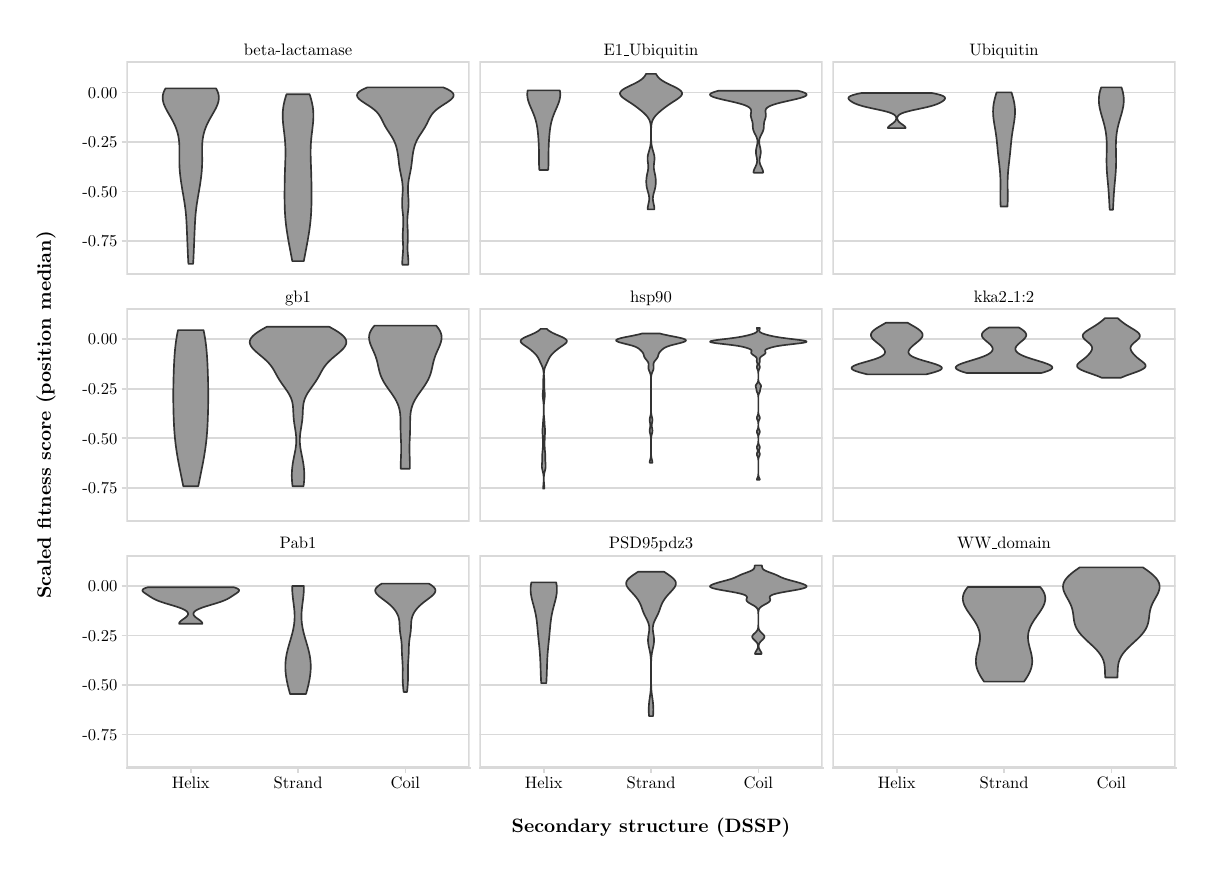
\begin{tikzpicture}[x=1pt,y=1pt]
\definecolor{fillColor}{RGB}{255,255,255}
\path[use as bounding box,fill=fillColor,fill opacity=0.00] (0,0) rectangle (418.34,295.82);
\begin{scope}
\path[clip] ( 35.67,206.65) rectangle (159.73,283.52);
\definecolor{drawColor}{gray}{0.85}

\path[draw=drawColor,line width= 0.6pt,line join=round] ( 35.67,218.70) --
	(159.73,218.70);

\path[draw=drawColor,line width= 0.6pt,line join=round] ( 35.67,236.61) --
	(159.73,236.61);

\path[draw=drawColor,line width= 0.6pt,line join=round] ( 35.67,254.53) --
	(159.73,254.53);

\path[draw=drawColor,line width= 0.6pt,line join=round] ( 35.67,272.44) --
	(159.73,272.44);
\definecolor{drawColor}{gray}{0.20}
\definecolor{fillColor}{gray}{0.60}

\path[draw=drawColor,line width= 0.6pt,line join=round,line cap=round,fill=fillColor] ( 58.09,210.45) --
	( 58.08,210.58) --
	( 58.07,210.70) --
	( 58.06,210.82) --
	( 58.05,210.95) --
	( 58.05,211.07) --
	( 58.04,211.20) --
	( 58.03,211.32) --
	( 58.02,211.44) --
	( 58.02,211.57) --
	( 58.01,211.69) --
	( 58.00,211.82) --
	( 57.99,211.94) --
	( 57.99,212.07) --
	( 57.98,212.19) --
	( 57.97,212.31) --
	( 57.97,212.44) --
	( 57.96,212.56) --
	( 57.95,212.69) --
	( 57.95,212.81) --
	( 57.94,212.93) --
	( 57.93,213.06) --
	( 57.93,213.18) --
	( 57.92,213.31) --
	( 57.92,213.43) --
	( 57.91,213.55) --
	( 57.90,213.68) --
	( 57.90,213.80) --
	( 57.89,213.93) --
	( 57.89,214.05) --
	( 57.88,214.18) --
	( 57.88,214.30) --
	( 57.87,214.42) --
	( 57.86,214.55) --
	( 57.86,214.67) --
	( 57.85,214.80) --
	( 57.85,214.92) --
	( 57.84,215.04) --
	( 57.84,215.17) --
	( 57.83,215.29) --
	( 57.83,215.42) --
	( 57.82,215.54) --
	( 57.82,215.66) --
	( 57.81,215.79) --
	( 57.81,215.91) --
	( 57.80,216.04) --
	( 57.80,216.16) --
	( 57.79,216.28) --
	( 57.79,216.41) --
	( 57.78,216.53) --
	( 57.78,216.66) --
	( 57.77,216.78) --
	( 57.77,216.91) --
	( 57.76,217.03) --
	( 57.76,217.15) --
	( 57.75,217.28) --
	( 57.75,217.40) --
	( 57.74,217.53) --
	( 57.74,217.65) --
	( 57.73,217.77) --
	( 57.72,217.90) --
	( 57.72,218.02) --
	( 57.71,218.15) --
	( 57.71,218.27) --
	( 57.70,218.39) --
	( 57.70,218.52) --
	( 57.69,218.64) --
	( 57.69,218.77) --
	( 57.68,218.89) --
	( 57.68,219.02) --
	( 57.67,219.14) --
	( 57.67,219.26) --
	( 57.66,219.39) --
	( 57.66,219.51) --
	( 57.65,219.64) --
	( 57.65,219.76) --
	( 57.64,219.88) --
	( 57.64,220.01) --
	( 57.63,220.13) --
	( 57.63,220.26) --
	( 57.62,220.38) --
	( 57.62,220.50) --
	( 57.61,220.63) --
	( 57.61,220.75) --
	( 57.60,220.88) --
	( 57.59,221.00) --
	( 57.59,221.12) --
	( 57.58,221.25) --
	( 57.58,221.37) --
	( 57.57,221.50) --
	( 57.57,221.62) --
	( 57.56,221.75) --
	( 57.56,221.87) --
	( 57.55,221.99) --
	( 57.55,222.12) --
	( 57.54,222.24) --
	( 57.54,222.37) --
	( 57.53,222.49) --
	( 57.53,222.61) --
	( 57.52,222.74) --
	( 57.52,222.86) --
	( 57.51,222.99) --
	( 57.51,223.11) --
	( 57.50,223.23) --
	( 57.49,223.36) --
	( 57.49,223.48) --
	( 57.48,223.61) --
	( 57.48,223.73) --
	( 57.47,223.86) --
	( 57.47,223.98) --
	( 57.46,224.10) --
	( 57.46,224.23) --
	( 57.45,224.35) --
	( 57.44,224.48) --
	( 57.44,224.60) --
	( 57.43,224.72) --
	( 57.43,224.85) --
	( 57.42,224.97) --
	( 57.41,225.10) --
	( 57.41,225.22) --
	( 57.40,225.34) --
	( 57.39,225.47) --
	( 57.39,225.59) --
	( 57.38,225.72) --
	( 57.37,225.84) --
	( 57.36,225.96) --
	( 57.36,226.09) --
	( 57.35,226.21) --
	( 57.34,226.34) --
	( 57.33,226.46) --
	( 57.33,226.59) --
	( 57.32,226.71) --
	( 57.31,226.83) --
	( 57.30,226.96) --
	( 57.29,227.08) --
	( 57.28,227.21) --
	( 57.27,227.33) --
	( 57.26,227.45) --
	( 57.26,227.58) --
	( 57.25,227.70) --
	( 57.24,227.83) --
	( 57.22,227.95) --
	( 57.21,228.07) --
	( 57.20,228.20) --
	( 57.19,228.32) --
	( 57.18,228.45) --
	( 57.17,228.57) --
	( 57.16,228.70) --
	( 57.15,228.82) --
	( 57.13,228.94) --
	( 57.12,229.07) --
	( 57.11,229.19) --
	( 57.10,229.32) --
	( 57.08,229.44) --
	( 57.07,229.56) --
	( 57.06,229.69) --
	( 57.04,229.81) --
	( 57.03,229.94) --
	( 57.01,230.06) --
	( 57.00,230.18) --
	( 56.98,230.31) --
	( 56.97,230.43) --
	( 56.95,230.56) --
	( 56.94,230.68) --
	( 56.92,230.81) --
	( 56.90,230.93) --
	( 56.89,231.05) --
	( 56.87,231.18) --
	( 56.85,231.30) --
	( 56.84,231.43) --
	( 56.82,231.55) --
	( 56.80,231.67) --
	( 56.78,231.80) --
	( 56.77,231.92) --
	( 56.75,232.05) --
	( 56.73,232.17) --
	( 56.71,232.29) --
	( 56.69,232.42) --
	( 56.67,232.54) --
	( 56.65,232.67) --
	( 56.63,232.79) --
	( 56.61,232.91) --
	( 56.60,233.04) --
	( 56.58,233.16) --
	( 56.56,233.29) --
	( 56.54,233.41) --
	( 56.51,233.54) --
	( 56.49,233.66) --
	( 56.47,233.78) --
	( 56.45,233.91) --
	( 56.43,234.03) --
	( 56.41,234.16) --
	( 56.39,234.28) --
	( 56.37,234.40) --
	( 56.35,234.53) --
	( 56.33,234.65) --
	( 56.31,234.78) --
	( 56.29,234.90) --
	( 56.26,235.02) --
	( 56.24,235.15) --
	( 56.22,235.27) --
	( 56.20,235.40) --
	( 56.18,235.52) --
	( 56.16,235.65) --
	( 56.14,235.77) --
	( 56.12,235.89) --
	( 56.09,236.02) --
	( 56.07,236.14) --
	( 56.05,236.27) --
	( 56.03,236.39) --
	( 56.01,236.51) --
	( 55.99,236.64) --
	( 55.97,236.76) --
	( 55.94,236.89) --
	( 55.92,237.01) --
	( 55.90,237.13) --
	( 55.88,237.26) --
	( 55.86,237.38) --
	( 55.84,237.51) --
	( 55.82,237.63) --
	( 55.80,237.75) --
	( 55.78,237.88) --
	( 55.76,238.00) --
	( 55.74,238.13) --
	( 55.72,238.25) --
	( 55.70,238.38) --
	( 55.68,238.50) --
	( 55.66,238.62) --
	( 55.64,238.75) --
	( 55.62,238.87) --
	( 55.60,239.00) --
	( 55.58,239.12) --
	( 55.56,239.24) --
	( 55.54,239.37) --
	( 55.52,239.49) --
	( 55.50,239.62) --
	( 55.48,239.74) --
	( 55.46,239.86) --
	( 55.45,239.99) --
	( 55.43,240.11) --
	( 55.41,240.24) --
	( 55.39,240.36) --
	( 55.37,240.49) --
	( 55.36,240.61) --
	( 55.34,240.73) --
	( 55.32,240.86) --
	( 55.30,240.98) --
	( 55.29,241.11) --
	( 55.27,241.23) --
	( 55.26,241.35) --
	( 55.24,241.48) --
	( 55.22,241.60) --
	( 55.21,241.73) --
	( 55.19,241.85) --
	( 55.18,241.97) --
	( 55.16,242.10) --
	( 55.15,242.22) --
	( 55.13,242.35) --
	( 55.12,242.47) --
	( 55.11,242.59) --
	( 55.09,242.72) --
	( 55.08,242.84) --
	( 55.07,242.97) --
	( 55.05,243.09) --
	( 55.04,243.22) --
	( 55.03,243.34) --
	( 55.02,243.46) --
	( 55.01,243.59) --
	( 54.99,243.71) --
	( 54.98,243.84) --
	( 54.97,243.96) --
	( 54.96,244.08) --
	( 54.95,244.21) --
	( 54.94,244.33) --
	( 54.93,244.46) --
	( 54.92,244.58) --
	( 54.92,244.70) --
	( 54.91,244.83) --
	( 54.90,244.95) --
	( 54.89,245.08) --
	( 54.88,245.20) --
	( 54.88,245.33) --
	( 54.87,245.45) --
	( 54.86,245.57) --
	( 54.86,245.70) --
	( 54.85,245.82) --
	( 54.85,245.95) --
	( 54.84,246.07) --
	( 54.84,246.19) --
	( 54.83,246.32) --
	( 54.83,246.44) --
	( 54.83,246.57) --
	( 54.82,246.69) --
	( 54.82,246.81) --
	( 54.82,246.94) --
	( 54.81,247.06) --
	( 54.81,247.19) --
	( 54.81,247.31) --
	( 54.81,247.43) --
	( 54.81,247.56) --
	( 54.81,247.68) --
	( 54.80,247.81) --
	( 54.80,247.93) --
	( 54.80,248.06) --
	( 54.80,248.18) --
	( 54.80,248.30) --
	( 54.80,248.43) --
	( 54.80,248.55) --
	( 54.80,248.68) --
	( 54.81,248.80) --
	( 54.81,248.92) --
	( 54.81,249.05) --
	( 54.81,249.17) --
	( 54.81,249.30) --
	( 54.81,249.42) --
	( 54.81,249.54) --
	( 54.81,249.67) --
	( 54.82,249.79) --
	( 54.82,249.92) --
	( 54.82,250.04) --
	( 54.82,250.17) --
	( 54.82,250.29) --
	( 54.82,250.41) --
	( 54.83,250.54) --
	( 54.83,250.66) --
	( 54.83,250.79) --
	( 54.83,250.91) --
	( 54.83,251.03) --
	( 54.83,251.16) --
	( 54.83,251.28) --
	( 54.83,251.41) --
	( 54.83,251.53) --
	( 54.83,251.65) --
	( 54.83,251.78) --
	( 54.83,251.90) --
	( 54.83,252.03) --
	( 54.83,252.15) --
	( 54.83,252.27) --
	( 54.83,252.40) --
	( 54.83,252.52) --
	( 54.82,252.65) --
	( 54.82,252.77) --
	( 54.82,252.90) --
	( 54.82,253.02) --
	( 54.81,253.14) --
	( 54.81,253.27) --
	( 54.80,253.39) --
	( 54.80,253.52) --
	( 54.79,253.64) --
	( 54.78,253.76) --
	( 54.78,253.89) --
	( 54.77,254.01) --
	( 54.76,254.14) --
	( 54.75,254.26) --
	( 54.74,254.38) --
	( 54.73,254.51) --
	( 54.72,254.63) --
	( 54.71,254.76) --
	( 54.69,254.88) --
	( 54.68,255.01) --
	( 54.67,255.13) --
	( 54.65,255.25) --
	( 54.64,255.38) --
	( 54.62,255.50) --
	( 54.60,255.63) --
	( 54.59,255.75) --
	( 54.57,255.87) --
	( 54.55,256.00) --
	( 54.53,256.12) --
	( 54.51,256.25) --
	( 54.48,256.37) --
	( 54.46,256.49) --
	( 54.44,256.62) --
	( 54.41,256.74) --
	( 54.39,256.87) --
	( 54.36,256.99) --
	( 54.33,257.12) --
	( 54.30,257.24) --
	( 54.27,257.36) --
	( 54.24,257.49) --
	( 54.21,257.61) --
	( 54.18,257.74) --
	( 54.15,257.86) --
	( 54.11,257.98) --
	( 54.08,258.11) --
	( 54.04,258.23) --
	( 54.00,258.36) --
	( 53.97,258.48) --
	( 53.93,258.60) --
	( 53.89,258.73) --
	( 53.84,258.85) --
	( 53.80,258.98) --
	( 53.76,259.10) --
	( 53.71,259.22) --
	( 53.67,259.35) --
	( 53.62,259.47) --
	( 53.58,259.60) --
	( 53.53,259.72) --
	( 53.48,259.85) --
	( 53.43,259.97) --
	( 53.38,260.09) --
	( 53.33,260.22) --
	( 53.27,260.34) --
	( 53.22,260.47) --
	( 53.16,260.59) --
	( 53.11,260.71) --
	( 53.05,260.84) --
	( 53.00,260.96) --
	( 52.94,261.09) --
	( 52.88,261.21) --
	( 52.82,261.33) --
	( 52.76,261.46) --
	( 52.70,261.58) --
	( 52.63,261.71) --
	( 52.57,261.83) --
	( 52.51,261.96) --
	( 52.44,262.08) --
	( 52.38,262.20) --
	( 52.31,262.33) --
	( 52.24,262.45) --
	( 52.18,262.58) --
	( 52.11,262.70) --
	( 52.04,262.82) --
	( 51.97,262.95) --
	( 51.90,263.07) --
	( 51.83,263.20) --
	( 51.76,263.32) --
	( 51.69,263.44) --
	( 51.62,263.57) --
	( 51.55,263.69) --
	( 51.48,263.82) --
	( 51.41,263.94) --
	( 51.34,264.06) --
	( 51.26,264.19) --
	( 51.19,264.31) --
	( 51.12,264.44) --
	( 51.05,264.56) --
	( 50.98,264.69) --
	( 50.90,264.81) --
	( 50.83,264.93) --
	( 50.76,265.06) --
	( 50.69,265.18) --
	( 50.62,265.31) --
	( 50.55,265.43) --
	( 50.48,265.55) --
	( 50.41,265.68) --
	( 50.34,265.80) --
	( 50.27,265.93) --
	( 50.21,266.05) --
	( 50.14,266.17) --
	( 50.07,266.30) --
	( 50.01,266.42) --
	( 49.95,266.55) --
	( 49.88,266.67) --
	( 49.82,266.80) --
	( 49.76,266.92) --
	( 49.70,267.04) --
	( 49.64,267.17) --
	( 49.59,267.29) --
	( 49.53,267.42) --
	( 49.48,267.54) --
	( 49.42,267.66) --
	( 49.37,267.79) --
	( 49.32,267.91) --
	( 49.28,268.04) --
	( 49.23,268.16) --
	( 49.19,268.28) --
	( 49.15,268.41) --
	( 49.11,268.53) --
	( 49.07,268.66) --
	( 49.03,268.78) --
	( 49.00,268.90) --
	( 48.97,269.03) --
	( 48.94,269.15) --
	( 48.91,269.28) --
	( 48.89,269.40) --
	( 48.87,269.53) --
	( 48.85,269.65) --
	( 48.83,269.77) --
	( 48.81,269.90) --
	( 48.80,270.02) --
	( 48.79,270.15) --
	( 48.79,270.27) --
	( 48.78,270.39) --
	( 48.78,270.52) --
	( 48.78,270.64) --
	( 48.79,270.77) --
	( 48.80,270.89) --
	( 48.80,271.01) --
	( 48.82,271.14) --
	( 48.83,271.26) --
	( 48.85,271.39) --
	( 48.87,271.51) --
	( 48.90,271.64) --
	( 48.92,271.76) --
	( 48.95,271.88) --
	( 48.99,272.01) --
	( 49.02,272.13) --
	( 49.06,272.26) --
	( 49.10,272.38) --
	( 49.15,272.50) --
	( 49.19,272.63) --
	( 49.24,272.75) --
	( 49.30,272.88) --
	( 49.35,273.00) --
	( 49.41,273.12) --
	( 49.47,273.25) --
	( 49.53,273.37) --
	( 49.60,273.50) --
	( 49.67,273.62) --
	( 49.74,273.74) --
	( 49.81,273.87) --
	( 68.05,273.87) --
	( 68.13,273.74) --
	( 68.20,273.62) --
	( 68.26,273.50) --
	( 68.33,273.37) --
	( 68.39,273.25) --
	( 68.45,273.12) --
	( 68.51,273.00) --
	( 68.57,272.88) --
	( 68.62,272.75) --
	( 68.67,272.63) --
	( 68.72,272.50) --
	( 68.76,272.38) --
	( 68.80,272.26) --
	( 68.84,272.13) --
	( 68.88,272.01) --
	( 68.91,271.88) --
	( 68.94,271.76) --
	( 68.97,271.64) --
	( 68.99,271.51) --
	( 69.01,271.39) --
	( 69.03,271.26) --
	( 69.04,271.14) --
	( 69.06,271.01) --
	( 69.07,270.89) --
	( 69.08,270.77) --
	( 69.08,270.64) --
	( 69.08,270.52) --
	( 69.08,270.39) --
	( 69.08,270.27) --
	( 69.07,270.15) --
	( 69.06,270.02) --
	( 69.05,269.90) --
	( 69.03,269.77) --
	( 69.02,269.65) --
	( 69.00,269.53) --
	( 68.97,269.40) --
	( 68.95,269.28) --
	( 68.92,269.15) --
	( 68.90,269.03) --
	( 68.86,268.90) --
	( 68.83,268.78) --
	( 68.79,268.66) --
	( 68.76,268.53) --
	( 68.72,268.41) --
	( 68.68,268.28) --
	( 68.63,268.16) --
	( 68.59,268.04) --
	( 68.54,267.91) --
	( 68.49,267.79) --
	( 68.44,267.66) --
	( 68.39,267.54) --
	( 68.33,267.42) --
	( 68.28,267.29) --
	( 68.22,267.17) --
	( 68.16,267.04) --
	( 68.10,266.92) --
	( 68.04,266.80) --
	( 67.98,266.67) --
	( 67.92,266.55) --
	( 67.85,266.42) --
	( 67.79,266.30) --
	( 67.72,266.17) --
	( 67.66,266.05) --
	( 67.59,265.93) --
	( 67.52,265.80) --
	( 67.45,265.68) --
	( 67.38,265.55) --
	( 67.31,265.43) --
	( 67.24,265.31) --
	( 67.17,265.18) --
	( 67.10,265.06) --
	( 67.03,264.93) --
	( 66.96,264.81) --
	( 66.89,264.69) --
	( 66.82,264.56) --
	( 66.74,264.44) --
	( 66.67,264.31) --
	( 66.60,264.19) --
	( 66.53,264.06) --
	( 66.46,263.94) --
	( 66.38,263.82) --
	( 66.31,263.69) --
	( 66.24,263.57) --
	( 66.17,263.44) --
	( 66.10,263.32) --
	( 66.03,263.20) --
	( 65.96,263.07) --
	( 65.89,262.95) --
	( 65.82,262.82) --
	( 65.75,262.70) --
	( 65.69,262.58) --
	( 65.62,262.45) --
	( 65.55,262.33) --
	( 65.49,262.20) --
	( 65.42,262.08) --
	( 65.36,261.96) --
	( 65.29,261.83) --
	( 65.23,261.71) --
	( 65.17,261.58) --
	( 65.11,261.46) --
	( 65.05,261.33) --
	( 64.99,261.21) --
	( 64.93,261.09) --
	( 64.87,260.96) --
	( 64.81,260.84) --
	( 64.75,260.71) --
	( 64.70,260.59) --
	( 64.64,260.47) --
	( 64.59,260.34) --
	( 64.54,260.22) --
	( 64.48,260.09) --
	( 64.43,259.97) --
	( 64.38,259.85) --
	( 64.33,259.72) --
	( 64.29,259.60) --
	( 64.24,259.47) --
	( 64.19,259.35) --
	( 64.15,259.22) --
	( 64.10,259.10) --
	( 64.06,258.98) --
	( 64.02,258.85) --
	( 63.98,258.73) --
	( 63.94,258.60) --
	( 63.90,258.48) --
	( 63.86,258.36) --
	( 63.82,258.23) --
	( 63.79,258.11) --
	( 63.75,257.98) --
	( 63.72,257.86) --
	( 63.68,257.74) --
	( 63.65,257.61) --
	( 63.62,257.49) --
	( 63.59,257.36) --
	( 63.56,257.24) --
	( 63.53,257.12) --
	( 63.50,256.99) --
	( 63.48,256.87) --
	( 63.45,256.74) --
	( 63.43,256.62) --
	( 63.40,256.49) --
	( 63.38,256.37) --
	( 63.36,256.25) --
	( 63.34,256.12) --
	( 63.32,256.00) --
	( 63.30,255.87) --
	( 63.28,255.75) --
	( 63.26,255.63) --
	( 63.24,255.50) --
	( 63.23,255.38) --
	( 63.21,255.25) --
	( 63.20,255.13) --
	( 63.18,255.01) --
	( 63.17,254.88) --
	( 63.16,254.76) --
	( 63.14,254.63) --
	( 63.13,254.51) --
	( 63.12,254.38) --
	( 63.11,254.26) --
	( 63.10,254.14) --
	( 63.10,254.01) --
	( 63.09,253.89) --
	( 63.08,253.76) --
	( 63.07,253.64) --
	( 63.07,253.52) --
	( 63.06,253.39) --
	( 63.06,253.27) --
	( 63.05,253.14) --
	( 63.05,253.02) --
	( 63.04,252.90) --
	( 63.04,252.77) --
	( 63.04,252.65) --
	( 63.04,252.52) --
	( 63.03,252.40) --
	( 63.03,252.27) --
	( 63.03,252.15) --
	( 63.03,252.03) --
	( 63.03,251.90) --
	( 63.03,251.78) --
	( 63.03,251.65) --
	( 63.03,251.53) --
	( 63.03,251.41) --
	( 63.03,251.28) --
	( 63.03,251.16) --
	( 63.03,251.03) --
	( 63.03,250.91) --
	( 63.03,250.79) --
	( 63.04,250.66) --
	( 63.04,250.54) --
	( 63.04,250.41) --
	( 63.04,250.29) --
	( 63.04,250.17) --
	( 63.04,250.04) --
	( 63.05,249.92) --
	( 63.05,249.79) --
	( 63.05,249.67) --
	( 63.05,249.54) --
	( 63.05,249.42) --
	( 63.05,249.30) --
	( 63.05,249.17) --
	( 63.06,249.05) --
	( 63.06,248.92) --
	( 63.06,248.80) --
	( 63.06,248.68) --
	( 63.06,248.55) --
	( 63.06,248.43) --
	( 63.06,248.30) --
	( 63.06,248.18) --
	( 63.06,248.06) --
	( 63.06,247.93) --
	( 63.06,247.81) --
	( 63.06,247.68) --
	( 63.06,247.56) --
	( 63.06,247.43) --
	( 63.05,247.31) --
	( 63.05,247.19) --
	( 63.05,247.06) --
	( 63.05,246.94) --
	( 63.04,246.81) --
	( 63.04,246.69) --
	( 63.04,246.57) --
	( 63.03,246.44) --
	( 63.03,246.32) --
	( 63.03,246.19) --
	( 63.02,246.07) --
	( 63.02,245.95) --
	( 63.01,245.82) --
	( 63.00,245.70) --
	( 63.00,245.57) --
	( 62.99,245.45) --
	( 62.99,245.33) --
	( 62.98,245.20) --
	( 62.97,245.08) --
	( 62.96,244.95) --
	( 62.96,244.83) --
	( 62.95,244.70) --
	( 62.94,244.58) --
	( 62.93,244.46) --
	( 62.92,244.33) --
	( 62.91,244.21) --
	( 62.90,244.08) --
	( 62.89,243.96) --
	( 62.88,243.84) --
	( 62.87,243.71) --
	( 62.86,243.59) --
	( 62.85,243.46) --
	( 62.83,243.34) --
	( 62.82,243.22) --
	( 62.81,243.09) --
	( 62.80,242.97) --
	( 62.78,242.84) --
	( 62.77,242.72) --
	( 62.76,242.59) --
	( 62.74,242.47) --
	( 62.73,242.35) --
	( 62.71,242.22) --
	( 62.70,242.10) --
	( 62.69,241.97) --
	( 62.67,241.85) --
	( 62.65,241.73) --
	( 62.64,241.60) --
	( 62.62,241.48) --
	( 62.61,241.35) --
	( 62.59,241.23) --
	( 62.57,241.11) --
	( 62.56,240.98) --
	( 62.54,240.86) --
	( 62.52,240.73) --
	( 62.51,240.61) --
	( 62.49,240.49) --
	( 62.47,240.36) --
	( 62.45,240.24) --
	( 62.44,240.11) --
	( 62.42,239.99) --
	( 62.40,239.86) --
	( 62.38,239.74) --
	( 62.36,239.62) --
	( 62.34,239.49) --
	( 62.32,239.37) --
	( 62.30,239.24) --
	( 62.29,239.12) --
	( 62.27,239.00) --
	( 62.25,238.87) --
	( 62.23,238.75) --
	( 62.21,238.62) --
	( 62.19,238.50) --
	( 62.17,238.38) --
	( 62.15,238.25) --
	( 62.13,238.13) --
	( 62.11,238.00) --
	( 62.08,237.88) --
	( 62.06,237.75) --
	( 62.04,237.63) --
	( 62.02,237.51) --
	( 62.00,237.38) --
	( 61.98,237.26) --
	( 61.96,237.13) --
	( 61.94,237.01) --
	( 61.92,236.89) --
	( 61.90,236.76) --
	( 61.88,236.64) --
	( 61.85,236.51) --
	( 61.83,236.39) --
	( 61.81,236.27) --
	( 61.79,236.14) --
	( 61.77,236.02) --
	( 61.75,235.89) --
	( 61.73,235.77) --
	( 61.70,235.65) --
	( 61.68,235.52) --
	( 61.66,235.40) --
	( 61.64,235.27) --
	( 61.62,235.15) --
	( 61.60,235.02) --
	( 61.58,234.90) --
	( 61.56,234.78) --
	( 61.53,234.65) --
	( 61.51,234.53) --
	( 61.49,234.40) --
	( 61.47,234.28) --
	( 61.45,234.16) --
	( 61.43,234.03) --
	( 61.41,233.91) --
	( 61.39,233.78) --
	( 61.37,233.66) --
	( 61.35,233.54) --
	( 61.33,233.41) --
	( 61.31,233.29) --
	( 61.29,233.16) --
	( 61.27,233.04) --
	( 61.25,232.91) --
	( 61.23,232.79) --
	( 61.21,232.67) --
	( 61.19,232.54) --
	( 61.17,232.42) --
	( 61.15,232.29) --
	( 61.13,232.17) --
	( 61.12,232.05) --
	( 61.10,231.92) --
	( 61.08,231.80) --
	( 61.06,231.67) --
	( 61.04,231.55) --
	( 61.03,231.43) --
	( 61.01,231.30) --
	( 60.99,231.18) --
	( 60.98,231.05) --
	( 60.96,230.93) --
	( 60.94,230.81) --
	( 60.93,230.68) --
	( 60.91,230.56) --
	( 60.89,230.43) --
	( 60.88,230.31) --
	( 60.86,230.18) --
	( 60.85,230.06) --
	( 60.84,229.94) --
	( 60.82,229.81) --
	( 60.81,229.69) --
	( 60.79,229.56) --
	( 60.78,229.44) --
	( 60.77,229.32) --
	( 60.75,229.19) --
	( 60.74,229.07) --
	( 60.73,228.94) --
	( 60.72,228.82) --
	( 60.70,228.70) --
	( 60.69,228.57) --
	( 60.68,228.45) --
	( 60.67,228.32) --
	( 60.66,228.20) --
	( 60.65,228.07) --
	( 60.64,227.95) --
	( 60.63,227.83) --
	( 60.62,227.70) --
	( 60.61,227.58) --
	( 60.60,227.45) --
	( 60.59,227.33) --
	( 60.58,227.21) --
	( 60.57,227.08) --
	( 60.56,226.96) --
	( 60.55,226.83) --
	( 60.55,226.71) --
	( 60.54,226.59) --
	( 60.53,226.46) --
	( 60.52,226.34) --
	( 60.51,226.21) --
	( 60.51,226.09) --
	( 60.50,225.96) --
	( 60.49,225.84) --
	( 60.48,225.72) --
	( 60.48,225.59) --
	( 60.47,225.47) --
	( 60.46,225.34) --
	( 60.46,225.22) --
	( 60.45,225.10) --
	( 60.44,224.97) --
	( 60.44,224.85) --
	( 60.43,224.72) --
	( 60.43,224.60) --
	( 60.42,224.48) --
	( 60.41,224.35) --
	( 60.41,224.23) --
	( 60.40,224.10) --
	( 60.40,223.98) --
	( 60.39,223.86) --
	( 60.39,223.73) --
	( 60.38,223.61) --
	( 60.37,223.48) --
	( 60.37,223.36) --
	( 60.36,223.23) --
	( 60.36,223.11) --
	( 60.35,222.99) --
	( 60.35,222.86) --
	( 60.34,222.74) --
	( 60.34,222.61) --
	( 60.33,222.49) --
	( 60.33,222.37) --
	( 60.32,222.24) --
	( 60.32,222.12) --
	( 60.31,221.99) --
	( 60.30,221.87) --
	( 60.30,221.75) --
	( 60.29,221.62) --
	( 60.29,221.50) --
	( 60.28,221.37) --
	( 60.28,221.25) --
	( 60.27,221.12) --
	( 60.27,221.00) --
	( 60.26,220.88) --
	( 60.26,220.75) --
	( 60.25,220.63) --
	( 60.25,220.50) --
	( 60.24,220.38) --
	( 60.24,220.26) --
	( 60.23,220.13) --
	( 60.23,220.01) --
	( 60.22,219.88) --
	( 60.22,219.76) --
	( 60.21,219.64) --
	( 60.21,219.51) --
	( 60.20,219.39) --
	( 60.19,219.26) --
	( 60.19,219.14) --
	( 60.18,219.02) --
	( 60.18,218.89) --
	( 60.17,218.77) --
	( 60.17,218.64) --
	( 60.16,218.52) --
	( 60.16,218.39) --
	( 60.15,218.27) --
	( 60.15,218.15) --
	( 60.14,218.02) --
	( 60.14,217.90) --
	( 60.13,217.77) --
	( 60.13,217.65) --
	( 60.12,217.53) --
	( 60.12,217.40) --
	( 60.11,217.28) --
	( 60.11,217.15) --
	( 60.10,217.03) --
	( 60.10,216.91) --
	( 60.09,216.78) --
	( 60.09,216.66) --
	( 60.08,216.53) --
	( 60.08,216.41) --
	( 60.07,216.28) --
	( 60.07,216.16) --
	( 60.06,216.04) --
	( 60.06,215.91) --
	( 60.05,215.79) --
	( 60.05,215.66) --
	( 60.04,215.54) --
	( 60.04,215.42) --
	( 60.03,215.29) --
	( 60.02,215.17) --
	( 60.02,215.04) --
	( 60.01,214.92) --
	( 60.01,214.80) --
	( 60.00,214.67) --
	( 60.00,214.55) --
	( 59.99,214.42) --
	( 59.99,214.30) --
	( 59.98,214.18) --
	( 59.98,214.05) --
	( 59.97,213.93) --
	( 59.96,213.80) --
	( 59.96,213.68) --
	( 59.95,213.55) --
	( 59.95,213.43) --
	( 59.94,213.31) --
	( 59.93,213.18) --
	( 59.93,213.06) --
	( 59.92,212.93) --
	( 59.92,212.81) --
	( 59.91,212.69) --
	( 59.90,212.56) --
	( 59.90,212.44) --
	( 59.89,212.31) --
	( 59.88,212.19) --
	( 59.88,212.07) --
	( 59.87,211.94) --
	( 59.86,211.82) --
	( 59.85,211.69) --
	( 59.85,211.57) --
	( 59.84,211.44) --
	( 59.83,211.32) --
	( 59.83,211.20) --
	( 59.82,211.07) --
	( 59.81,210.95) --
	( 59.80,210.82) --
	( 59.79,210.70) --
	( 59.79,210.58) --
	( 59.78,210.45) --
	( 58.09,210.45) --
	cycle;

\path[draw=drawColor,line width= 0.6pt,line join=round,line cap=round,fill=fillColor] ( 95.62,211.47) --
	( 95.59,211.59) --
	( 95.57,211.71) --
	( 95.55,211.83) --
	( 95.53,211.94) --
	( 95.50,212.06) --
	( 95.48,212.18) --
	( 95.46,212.30) --
	( 95.44,212.42) --
	( 95.41,212.53) --
	( 95.39,212.65) --
	( 95.37,212.77) --
	( 95.35,212.89) --
	( 95.32,213.01) --
	( 95.30,213.12) --
	( 95.28,213.24) --
	( 95.26,213.36) --
	( 95.23,213.48) --
	( 95.21,213.60) --
	( 95.19,213.71) --
	( 95.17,213.83) --
	( 95.14,213.95) --
	( 95.12,214.07) --
	( 95.10,214.19) --
	( 95.08,214.30) --
	( 95.05,214.42) --
	( 95.03,214.54) --
	( 95.01,214.66) --
	( 94.99,214.78) --
	( 94.96,214.89) --
	( 94.94,215.01) --
	( 94.92,215.13) --
	( 94.90,215.25) --
	( 94.88,215.37) --
	( 94.85,215.48) --
	( 94.83,215.60) --
	( 94.81,215.72) --
	( 94.79,215.84) --
	( 94.76,215.96) --
	( 94.74,216.07) --
	( 94.72,216.19) --
	( 94.70,216.31) --
	( 94.67,216.43) --
	( 94.65,216.55) --
	( 94.63,216.66) --
	( 94.61,216.78) --
	( 94.59,216.90) --
	( 94.56,217.02) --
	( 94.54,217.14) --
	( 94.52,217.25) --
	( 94.50,217.37) --
	( 94.48,217.49) --
	( 94.45,217.61) --
	( 94.43,217.73) --
	( 94.41,217.84) --
	( 94.39,217.96) --
	( 94.37,218.08) --
	( 94.35,218.20) --
	( 94.33,218.32) --
	( 94.30,218.43) --
	( 94.28,218.55) --
	( 94.26,218.67) --
	( 94.24,218.79) --
	( 94.22,218.91) --
	( 94.20,219.02) --
	( 94.18,219.14) --
	( 94.16,219.26) --
	( 94.14,219.38) --
	( 94.12,219.50) --
	( 94.10,219.62) --
	( 94.07,219.73) --
	( 94.05,219.85) --
	( 94.03,219.97) --
	( 94.01,220.09) --
	( 93.99,220.21) --
	( 93.97,220.32) --
	( 93.95,220.44) --
	( 93.94,220.56) --
	( 93.92,220.68) --
	( 93.90,220.80) --
	( 93.88,220.91) --
	( 93.86,221.03) --
	( 93.84,221.15) --
	( 93.82,221.27) --
	( 93.80,221.39) --
	( 93.78,221.50) --
	( 93.76,221.62) --
	( 93.75,221.74) --
	( 93.73,221.86) --
	( 93.71,221.98) --
	( 93.69,222.09) --
	( 93.67,222.21) --
	( 93.66,222.33) --
	( 93.64,222.45) --
	( 93.62,222.57) --
	( 93.60,222.68) --
	( 93.59,222.80) --
	( 93.57,222.92) --
	( 93.55,223.04) --
	( 93.54,223.16) --
	( 93.52,223.27) --
	( 93.51,223.39) --
	( 93.49,223.51) --
	( 93.47,223.63) --
	( 93.46,223.75) --
	( 93.44,223.86) --
	( 93.43,223.98) --
	( 93.41,224.10) --
	( 93.40,224.22) --
	( 93.38,224.34) --
	( 93.37,224.45) --
	( 93.36,224.57) --
	( 93.34,224.69) --
	( 93.33,224.81) --
	( 93.31,224.93) --
	( 93.30,225.04) --
	( 93.29,225.16) --
	( 93.28,225.28) --
	( 93.26,225.40) --
	( 93.25,225.52) --
	( 93.24,225.63) --
	( 93.23,225.75) --
	( 93.21,225.87) --
	( 93.20,225.99) --
	( 93.19,226.11) --
	( 93.18,226.22) --
	( 93.17,226.34) --
	( 93.16,226.46) --
	( 93.15,226.58) --
	( 93.14,226.70) --
	( 93.13,226.81) --
	( 93.12,226.93) --
	( 93.11,227.05) --
	( 93.10,227.17) --
	( 93.09,227.29) --
	( 93.08,227.40) --
	( 93.07,227.52) --
	( 93.06,227.64) --
	( 93.05,227.76) --
	( 93.04,227.88) --
	( 93.03,227.99) --
	( 93.03,228.11) --
	( 93.02,228.23) --
	( 93.01,228.35) --
	( 93.00,228.47) --
	( 93.00,228.58) --
	( 92.99,228.70) --
	( 92.98,228.82) --
	( 92.98,228.94) --
	( 92.97,229.06) --
	( 92.96,229.17) --
	( 92.96,229.29) --
	( 92.95,229.41) --
	( 92.94,229.53) --
	( 92.94,229.65) --
	( 92.93,229.77) --
	( 92.93,229.88) --
	( 92.92,230.00) --
	( 92.92,230.12) --
	( 92.91,230.24) --
	( 92.91,230.36) --
	( 92.90,230.47) --
	( 92.90,230.59) --
	( 92.90,230.71) --
	( 92.89,230.83) --
	( 92.89,230.95) --
	( 92.88,231.06) --
	( 92.88,231.18) --
	( 92.88,231.30) --
	( 92.87,231.42) --
	( 92.87,231.54) --
	( 92.87,231.65) --
	( 92.87,231.77) --
	( 92.86,231.89) --
	( 92.86,232.01) --
	( 92.86,232.13) --
	( 92.86,232.24) --
	( 92.85,232.36) --
	( 92.85,232.48) --
	( 92.85,232.60) --
	( 92.85,232.72) --
	( 92.85,232.83) --
	( 92.84,232.95) --
	( 92.84,233.07) --
	( 92.84,233.19) --
	( 92.84,233.31) --
	( 92.84,233.42) --
	( 92.84,233.54) --
	( 92.84,233.66) --
	( 92.84,233.78) --
	( 92.83,233.90) --
	( 92.83,234.01) --
	( 92.83,234.13) --
	( 92.83,234.25) --
	( 92.83,234.37) --
	( 92.83,234.49) --
	( 92.83,234.60) --
	( 92.83,234.72) --
	( 92.83,234.84) --
	( 92.83,234.96) --
	( 92.83,235.08) --
	( 92.83,235.19) --
	( 92.83,235.31) --
	( 92.83,235.43) --
	( 92.83,235.55) --
	( 92.83,235.67) --
	( 92.83,235.78) --
	( 92.83,235.90) --
	( 92.83,236.02) --
	( 92.83,236.14) --
	( 92.83,236.26) --
	( 92.83,236.37) --
	( 92.83,236.49) --
	( 92.83,236.61) --
	( 92.83,236.73) --
	( 92.83,236.85) --
	( 92.84,236.96) --
	( 92.84,237.08) --
	( 92.84,237.20) --
	( 92.84,237.32) --
	( 92.84,237.44) --
	( 92.84,237.55) --
	( 92.84,237.67) --
	( 92.84,237.79) --
	( 92.84,237.91) --
	( 92.84,238.03) --
	( 92.84,238.14) --
	( 92.85,238.26) --
	( 92.85,238.38) --
	( 92.85,238.50) --
	( 92.85,238.62) --
	( 92.85,238.73) --
	( 92.85,238.85) --
	( 92.85,238.97) --
	( 92.86,239.09) --
	( 92.86,239.21) --
	( 92.86,239.32) --
	( 92.86,239.44) --
	( 92.86,239.56) --
	( 92.86,239.68) --
	( 92.87,239.80) --
	( 92.87,239.92) --
	( 92.87,240.03) --
	( 92.87,240.15) --
	( 92.87,240.27) --
	( 92.88,240.39) --
	( 92.88,240.51) --
	( 92.88,240.62) --
	( 92.88,240.74) --
	( 92.88,240.86) --
	( 92.89,240.98) --
	( 92.89,241.10) --
	( 92.89,241.21) --
	( 92.89,241.33) --
	( 92.90,241.45) --
	( 92.90,241.57) --
	( 92.90,241.69) --
	( 92.91,241.80) --
	( 92.91,241.92) --
	( 92.91,242.04) --
	( 92.91,242.16) --
	( 92.92,242.28) --
	( 92.92,242.39) --
	( 92.92,242.51) --
	( 92.93,242.63) --
	( 92.93,242.75) --
	( 92.93,242.87) --
	( 92.94,242.98) --
	( 92.94,243.10) --
	( 92.94,243.22) --
	( 92.95,243.34) --
	( 92.95,243.46) --
	( 92.95,243.57) --
	( 92.96,243.69) --
	( 92.96,243.81) --
	( 92.97,243.93) --
	( 92.97,244.05) --
	( 92.97,244.16) --
	( 92.98,244.28) --
	( 92.98,244.40) --
	( 92.99,244.52) --
	( 92.99,244.64) --
	( 92.99,244.75) --
	( 93.00,244.87) --
	( 93.00,244.99) --
	( 93.01,245.11) --
	( 93.01,245.23) --
	( 93.01,245.34) --
	( 93.02,245.46) --
	( 93.02,245.58) --
	( 93.03,245.70) --
	( 93.03,245.82) --
	( 93.04,245.93) --
	( 93.04,246.05) --
	( 93.05,246.17) --
	( 93.05,246.29) --
	( 93.05,246.41) --
	( 93.06,246.52) --
	( 93.06,246.64) --
	( 93.07,246.76) --
	( 93.07,246.88) --
	( 93.07,247.00) --
	( 93.08,247.11) --
	( 93.08,247.23) --
	( 93.09,247.35) --
	( 93.09,247.47) --
	( 93.09,247.59) --
	( 93.10,247.70) --
	( 93.10,247.82) --
	( 93.11,247.94) --
	( 93.11,248.06) --
	( 93.11,248.18) --
	( 93.12,248.29) --
	( 93.12,248.41) --
	( 93.12,248.53) --
	( 93.13,248.65) --
	( 93.13,248.77) --
	( 93.13,248.88) --
	( 93.13,249.00) --
	( 93.14,249.12) --
	( 93.14,249.24) --
	( 93.14,249.36) --
	( 93.14,249.47) --
	( 93.15,249.59) --
	( 93.15,249.71) --
	( 93.15,249.83) --
	( 93.15,249.95) --
	( 93.15,250.07) --
	( 93.15,250.18) --
	( 93.15,250.30) --
	( 93.15,250.42) --
	( 93.15,250.54) --
	( 93.16,250.66) --
	( 93.15,250.77) --
	( 93.15,250.89) --
	( 93.15,251.01) --
	( 93.15,251.13) --
	( 93.15,251.25) --
	( 93.15,251.36) --
	( 93.15,251.48) --
	( 93.15,251.60) --
	( 93.15,251.72) --
	( 93.14,251.84) --
	( 93.14,251.95) --
	( 93.14,252.07) --
	( 93.14,252.19) --
	( 93.13,252.31) --
	( 93.13,252.43) --
	( 93.13,252.54) --
	( 93.12,252.66) --
	( 93.12,252.78) --
	( 93.11,252.90) --
	( 93.11,253.02) --
	( 93.10,253.13) --
	( 93.10,253.25) --
	( 93.09,253.37) --
	( 93.09,253.49) --
	( 93.08,253.61) --
	( 93.07,253.72) --
	( 93.07,253.84) --
	( 93.06,253.96) --
	( 93.05,254.08) --
	( 93.04,254.20) --
	( 93.04,254.31) --
	( 93.03,254.43) --
	( 93.02,254.55) --
	( 93.01,254.67) --
	( 93.00,254.79) --
	( 92.99,254.90) --
	( 92.98,255.02) --
	( 92.97,255.14) --
	( 92.96,255.26) --
	( 92.95,255.38) --
	( 92.94,255.49) --
	( 92.93,255.61) --
	( 92.92,255.73) --
	( 92.91,255.85) --
	( 92.90,255.97) --
	( 92.88,256.08) --
	( 92.87,256.20) --
	( 92.86,256.32) --
	( 92.85,256.44) --
	( 92.83,256.56) --
	( 92.82,256.67) --
	( 92.81,256.79) --
	( 92.80,256.91) --
	( 92.78,257.03) --
	( 92.77,257.15) --
	( 92.76,257.26) --
	( 92.74,257.38) --
	( 92.73,257.50) --
	( 92.71,257.62) --
	( 92.70,257.74) --
	( 92.69,257.85) --
	( 92.67,257.97) --
	( 92.66,258.09) --
	( 92.64,258.21) --
	( 92.63,258.33) --
	( 92.61,258.44) --
	( 92.60,258.56) --
	( 92.59,258.68) --
	( 92.57,258.80) --
	( 92.56,258.92) --
	( 92.54,259.03) --
	( 92.53,259.15) --
	( 92.51,259.27) --
	( 92.50,259.39) --
	( 92.49,259.51) --
	( 92.47,259.62) --
	( 92.46,259.74) --
	( 92.44,259.86) --
	( 92.43,259.98) --
	( 92.42,260.10) --
	( 92.40,260.22) --
	( 92.39,260.33) --
	( 92.38,260.45) --
	( 92.37,260.57) --
	( 92.35,260.69) --
	( 92.34,260.81) --
	( 92.33,260.92) --
	( 92.32,261.04) --
	( 92.31,261.16) --
	( 92.29,261.28) --
	( 92.28,261.40) --
	( 92.27,261.51) --
	( 92.26,261.63) --
	( 92.25,261.75) --
	( 92.24,261.87) --
	( 92.24,261.99) --
	( 92.23,262.10) --
	( 92.22,262.22) --
	( 92.21,262.34) --
	( 92.20,262.46) --
	( 92.20,262.58) --
	( 92.19,262.69) --
	( 92.18,262.81) --
	( 92.18,262.93) --
	( 92.17,263.05) --
	( 92.17,263.17) --
	( 92.17,263.28) --
	( 92.16,263.40) --
	( 92.16,263.52) --
	( 92.16,263.64) --
	( 92.16,263.76) --
	( 92.15,263.87) --
	( 92.15,263.99) --
	( 92.15,264.11) --
	( 92.15,264.23) --
	( 92.16,264.35) --
	( 92.16,264.46) --
	( 92.16,264.58) --
	( 92.16,264.70) --
	( 92.17,264.82) --
	( 92.17,264.94) --
	( 92.18,265.05) --
	( 92.18,265.17) --
	( 92.19,265.29) --
	( 92.19,265.41) --
	( 92.20,265.53) --
	( 92.21,265.64) --
	( 92.22,265.76) --
	( 92.23,265.88) --
	( 92.24,266.00) --
	( 92.25,266.12) --
	( 92.26,266.23) --
	( 92.27,266.35) --
	( 92.29,266.47) --
	( 92.30,266.59) --
	( 92.32,266.71) --
	( 92.33,266.82) --
	( 92.35,266.94) --
	( 92.36,267.06) --
	( 92.38,267.18) --
	( 92.40,267.30) --
	( 92.42,267.41) --
	( 92.44,267.53) --
	( 92.46,267.65) --
	( 92.48,267.77) --
	( 92.50,267.89) --
	( 92.52,268.00) --
	( 92.55,268.12) --
	( 92.57,268.24) --
	( 92.59,268.36) --
	( 92.62,268.48) --
	( 92.64,268.59) --
	( 92.67,268.71) --
	( 92.70,268.83) --
	( 92.72,268.95) --
	( 92.75,269.07) --
	( 92.78,269.18) --
	( 92.81,269.30) --
	( 92.84,269.42) --
	( 92.87,269.54) --
	( 92.90,269.66) --
	( 92.93,269.77) --
	( 92.96,269.89) --
	( 93.00,270.01) --
	( 93.03,270.13) --
	( 93.06,270.25) --
	( 93.10,270.37) --
	( 93.13,270.48) --
	( 93.17,270.60) --
	( 93.20,270.72) --
	( 93.24,270.84) --
	( 93.27,270.96) --
	( 93.31,271.07) --
	( 93.35,271.19) --
	( 93.39,271.31) --
	( 93.42,271.43) --
	( 93.46,271.55) --
	( 93.50,271.66) --
	( 93.54,271.78) --
	(101.86,271.78) --
	(101.90,271.66) --
	(101.94,271.55) --
	(101.97,271.43) --
	(102.01,271.31) --
	(102.05,271.19) --
	(102.09,271.07) --
	(102.12,270.96) --
	(102.16,270.84) --
	(102.20,270.72) --
	(102.23,270.60) --
	(102.27,270.48) --
	(102.30,270.37) --
	(102.34,270.25) --
	(102.37,270.13) --
	(102.40,270.01) --
	(102.43,269.89) --
	(102.47,269.77) --
	(102.50,269.66) --
	(102.53,269.54) --
	(102.56,269.42) --
	(102.59,269.30) --
	(102.62,269.18) --
	(102.65,269.07) --
	(102.67,268.95) --
	(102.70,268.83) --
	(102.73,268.71) --
	(102.75,268.59) --
	(102.78,268.48) --
	(102.80,268.36) --
	(102.83,268.24) --
	(102.85,268.12) --
	(102.87,268.00) --
	(102.90,267.89) --
	(102.92,267.77) --
	(102.94,267.65) --
	(102.96,267.53) --
	(102.98,267.41) --
	(103.00,267.30) --
	(103.02,267.18) --
	(103.03,267.06) --
	(103.05,266.94) --
	(103.07,266.82) --
	(103.08,266.71) --
	(103.10,266.59) --
	(103.11,266.47) --
	(103.12,266.35) --
	(103.13,266.23) --
	(103.15,266.12) --
	(103.16,266.00) --
	(103.17,265.88) --
	(103.18,265.76) --
	(103.19,265.64) --
	(103.19,265.53) --
	(103.20,265.41) --
	(103.21,265.29) --
	(103.22,265.17) --
	(103.22,265.05) --
	(103.23,264.94) --
	(103.23,264.82) --
	(103.23,264.70) --
	(103.24,264.58) --
	(103.24,264.46) --
	(103.24,264.35) --
	(103.24,264.23) --
	(103.24,264.11) --
	(103.24,263.99) --
	(103.24,263.87) --
	(103.24,263.76) --
	(103.24,263.64) --
	(103.24,263.52) --
	(103.23,263.40) --
	(103.23,263.28) --
	(103.23,263.17) --
	(103.22,263.05) --
	(103.22,262.93) --
	(103.21,262.81) --
	(103.21,262.69) --
	(103.20,262.58) --
	(103.19,262.46) --
	(103.19,262.34) --
	(103.18,262.22) --
	(103.17,262.10) --
	(103.16,261.99) --
	(103.15,261.87) --
	(103.14,261.75) --
	(103.13,261.63) --
	(103.12,261.51) --
	(103.11,261.40) --
	(103.10,261.28) --
	(103.09,261.16) --
	(103.08,261.04) --
	(103.07,260.92) --
	(103.06,260.81) --
	(103.04,260.69) --
	(103.03,260.57) --
	(103.02,260.45) --
	(103.01,260.33) --
	(102.99,260.22) --
	(102.98,260.10) --
	(102.97,259.98) --
	(102.95,259.86) --
	(102.94,259.74) --
	(102.93,259.62) --
	(102.91,259.51) --
	(102.90,259.39) --
	(102.88,259.27) --
	(102.87,259.15) --
	(102.86,259.03) --
	(102.84,258.92) --
	(102.83,258.80) --
	(102.81,258.68) --
	(102.80,258.56) --
	(102.78,258.44) --
	(102.77,258.33) --
	(102.75,258.21) --
	(102.74,258.09) --
	(102.73,257.97) --
	(102.71,257.85) --
	(102.70,257.74) --
	(102.68,257.62) --
	(102.67,257.50) --
	(102.66,257.38) --
	(102.64,257.26) --
	(102.63,257.15) --
	(102.61,257.03) --
	(102.60,256.91) --
	(102.59,256.79) --
	(102.58,256.67) --
	(102.56,256.56) --
	(102.55,256.44) --
	(102.54,256.32) --
	(102.53,256.20) --
	(102.51,256.08) --
	(102.50,255.97) --
	(102.49,255.85) --
	(102.48,255.73) --
	(102.47,255.61) --
	(102.46,255.49) --
	(102.45,255.38) --
	(102.44,255.26) --
	(102.43,255.14) --
	(102.42,255.02) --
	(102.41,254.90) --
	(102.40,254.79) --
	(102.39,254.67) --
	(102.38,254.55) --
	(102.37,254.43) --
	(102.36,254.31) --
	(102.35,254.20) --
	(102.35,254.08) --
	(102.34,253.96) --
	(102.33,253.84) --
	(102.32,253.72) --
	(102.32,253.61) --
	(102.31,253.49) --
	(102.31,253.37) --
	(102.30,253.25) --
	(102.29,253.13) --
	(102.29,253.02) --
	(102.28,252.90) --
	(102.28,252.78) --
	(102.27,252.66) --
	(102.27,252.54) --
	(102.27,252.43) --
	(102.26,252.31) --
	(102.26,252.19) --
	(102.26,252.07) --
	(102.25,251.95) --
	(102.25,251.84) --
	(102.25,251.72) --
	(102.25,251.60) --
	(102.25,251.48) --
	(102.25,251.36) --
	(102.24,251.25) --
	(102.24,251.13) --
	(102.24,251.01) --
	(102.24,250.89) --
	(102.24,250.77) --
	(102.24,250.66) --
	(102.24,250.54) --
	(102.24,250.42) --
	(102.24,250.30) --
	(102.24,250.18) --
	(102.25,250.07) --
	(102.25,249.95) --
	(102.25,249.83) --
	(102.25,249.71) --
	(102.25,249.59) --
	(102.25,249.47) --
	(102.26,249.36) --
	(102.26,249.24) --
	(102.26,249.12) --
	(102.26,249.00) --
	(102.27,248.88) --
	(102.27,248.77) --
	(102.27,248.65) --
	(102.27,248.53) --
	(102.28,248.41) --
	(102.28,248.29) --
	(102.28,248.18) --
	(102.29,248.06) --
	(102.29,247.94) --
	(102.30,247.82) --
	(102.30,247.70) --
	(102.30,247.59) --
	(102.31,247.47) --
	(102.31,247.35) --
	(102.31,247.23) --
	(102.32,247.11) --
	(102.32,247.00) --
	(102.33,246.88) --
	(102.33,246.76) --
	(102.34,246.64) --
	(102.34,246.52) --
	(102.34,246.41) --
	(102.35,246.29) --
	(102.35,246.17) --
	(102.36,246.05) --
	(102.36,245.93) --
	(102.37,245.82) --
	(102.37,245.70) --
	(102.37,245.58) --
	(102.38,245.46) --
	(102.38,245.34) --
	(102.39,245.23) --
	(102.39,245.11) --
	(102.39,244.99) --
	(102.40,244.87) --
	(102.40,244.75) --
	(102.41,244.64) --
	(102.41,244.52) --
	(102.42,244.40) --
	(102.42,244.28) --
	(102.42,244.16) --
	(102.43,244.05) --
	(102.43,243.93) --
	(102.44,243.81) --
	(102.44,243.69) --
	(102.44,243.57) --
	(102.45,243.46) --
	(102.45,243.34) --
	(102.45,243.22) --
	(102.46,243.10) --
	(102.46,242.98) --
	(102.46,242.87) --
	(102.47,242.75) --
	(102.47,242.63) --
	(102.47,242.51) --
	(102.48,242.39) --
	(102.48,242.28) --
	(102.48,242.16) --
	(102.49,242.04) --
	(102.49,241.92) --
	(102.49,241.80) --
	(102.49,241.69) --
	(102.50,241.57) --
	(102.50,241.45) --
	(102.50,241.33) --
	(102.50,241.21) --
	(102.51,241.10) --
	(102.51,240.98) --
	(102.51,240.86) --
	(102.51,240.74) --
	(102.52,240.62) --
	(102.52,240.51) --
	(102.52,240.39) --
	(102.52,240.27) --
	(102.53,240.15) --
	(102.53,240.03) --
	(102.53,239.92) --
	(102.53,239.80) --
	(102.53,239.68) --
	(102.53,239.56) --
	(102.54,239.44) --
	(102.54,239.32) --
	(102.54,239.21) --
	(102.54,239.09) --
	(102.54,238.97) --
	(102.54,238.85) --
	(102.55,238.73) --
	(102.55,238.62) --
	(102.55,238.50) --
	(102.55,238.38) --
	(102.55,238.26) --
	(102.55,238.14) --
	(102.55,238.03) --
	(102.55,237.91) --
	(102.56,237.79) --
	(102.56,237.67) --
	(102.56,237.55) --
	(102.56,237.44) --
	(102.56,237.32) --
	(102.56,237.20) --
	(102.56,237.08) --
	(102.56,236.96) --
	(102.56,236.85) --
	(102.56,236.73) --
	(102.56,236.61) --
	(102.56,236.49) --
	(102.57,236.37) --
	(102.57,236.26) --
	(102.57,236.14) --
	(102.57,236.02) --
	(102.57,235.90) --
	(102.57,235.78) --
	(102.57,235.67) --
	(102.57,235.55) --
	(102.57,235.43) --
	(102.57,235.31) --
	(102.57,235.19) --
	(102.57,235.08) --
	(102.57,234.96) --
	(102.57,234.84) --
	(102.57,234.72) --
	(102.57,234.60) --
	(102.57,234.49) --
	(102.57,234.37) --
	(102.56,234.25) --
	(102.56,234.13) --
	(102.56,234.01) --
	(102.56,233.90) --
	(102.56,233.78) --
	(102.56,233.66) --
	(102.56,233.54) --
	(102.56,233.42) --
	(102.56,233.31) --
	(102.56,233.19) --
	(102.55,233.07) --
	(102.55,232.95) --
	(102.55,232.83) --
	(102.55,232.72) --
	(102.55,232.60) --
	(102.55,232.48) --
	(102.54,232.36) --
	(102.54,232.24) --
	(102.54,232.13) --
	(102.54,232.01) --
	(102.53,231.89) --
	(102.53,231.77) --
	(102.53,231.65) --
	(102.53,231.54) --
	(102.52,231.42) --
	(102.52,231.30) --
	(102.52,231.18) --
	(102.51,231.06) --
	(102.51,230.95) --
	(102.50,230.83) --
	(102.50,230.71) --
	(102.50,230.59) --
	(102.49,230.47) --
	(102.49,230.36) --
	(102.48,230.24) --
	(102.48,230.12) --
	(102.47,230.00) --
	(102.47,229.88) --
	(102.46,229.77) --
	(102.46,229.65) --
	(102.45,229.53) --
	(102.45,229.41) --
	(102.44,229.29) --
	(102.43,229.17) --
	(102.43,229.06) --
	(102.42,228.94) --
	(102.42,228.82) --
	(102.41,228.70) --
	(102.40,228.58) --
	(102.39,228.47) --
	(102.39,228.35) --
	(102.38,228.23) --
	(102.37,228.11) --
	(102.36,227.99) --
	(102.36,227.88) --
	(102.35,227.76) --
	(102.34,227.64) --
	(102.33,227.52) --
	(102.32,227.40) --
	(102.31,227.29) --
	(102.30,227.17) --
	(102.29,227.05) --
	(102.28,226.93) --
	(102.27,226.81) --
	(102.26,226.70) --
	(102.25,226.58) --
	(102.24,226.46) --
	(102.23,226.34) --
	(102.22,226.22) --
	(102.21,226.11) --
	(102.20,225.99) --
	(102.18,225.87) --
	(102.17,225.75) --
	(102.16,225.63) --
	(102.15,225.52) --
	(102.13,225.40) --
	(102.12,225.28) --
	(102.11,225.16) --
	(102.10,225.04) --
	(102.08,224.93) --
	(102.07,224.81) --
	(102.06,224.69) --
	(102.04,224.57) --
	(102.03,224.45) --
	(102.01,224.34) --
	(102.00,224.22) --
	(101.98,224.10) --
	(101.97,223.98) --
	(101.95,223.86) --
	(101.94,223.75) --
	(101.92,223.63) --
	(101.91,223.51) --
	(101.89,223.39) --
	(101.88,223.27) --
	(101.86,223.16) --
	(101.84,223.04) --
	(101.83,222.92) --
	(101.81,222.80) --
	(101.79,222.68) --
	(101.78,222.57) --
	(101.76,222.45) --
	(101.74,222.33) --
	(101.72,222.21) --
	(101.71,222.09) --
	(101.69,221.98) --
	(101.67,221.86) --
	(101.65,221.74) --
	(101.63,221.62) --
	(101.61,221.50) --
	(101.60,221.39) --
	(101.58,221.27) --
	(101.56,221.15) --
	(101.54,221.03) --
	(101.52,220.91) --
	(101.50,220.80) --
	(101.48,220.68) --
	(101.46,220.56) --
	(101.44,220.44) --
	(101.42,220.32) --
	(101.40,220.21) --
	(101.38,220.09) --
	(101.36,219.97) --
	(101.34,219.85) --
	(101.32,219.73) --
	(101.30,219.62) --
	(101.28,219.50) --
	(101.26,219.38) --
	(101.24,219.26) --
	(101.22,219.14) --
	(101.20,219.02) --
	(101.18,218.91) --
	(101.16,218.79) --
	(101.14,218.67) --
	(101.11,218.55) --
	(101.09,218.43) --
	(101.07,218.32) --
	(101.05,218.20) --
	(101.03,218.08) --
	(101.01,217.96) --
	(100.99,217.84) --
	(100.96,217.73) --
	(100.94,217.61) --
	(100.92,217.49) --
	(100.90,217.37) --
	(100.88,217.25) --
	(100.86,217.14) --
	(100.83,217.02) --
	(100.81,216.90) --
	(100.79,216.78) --
	(100.77,216.66) --
	(100.75,216.55) --
	(100.72,216.43) --
	(100.70,216.31) --
	(100.68,216.19) --
	(100.66,216.07) --
	(100.63,215.96) --
	(100.61,215.84) --
	(100.59,215.72) --
	(100.57,215.60) --
	(100.54,215.48) --
	(100.52,215.37) --
	(100.50,215.25) --
	(100.48,215.13) --
	(100.45,215.01) --
	(100.43,214.89) --
	(100.41,214.78) --
	(100.39,214.66) --
	(100.36,214.54) --
	(100.34,214.42) --
	(100.32,214.30) --
	(100.30,214.19) --
	(100.27,214.07) --
	(100.25,213.95) --
	(100.23,213.83) --
	(100.21,213.71) --
	(100.18,213.60) --
	(100.16,213.48) --
	(100.14,213.36) --
	(100.12,213.24) --
	(100.09,213.12) --
	(100.07,213.01) --
	(100.05,212.89) --
	(100.03,212.77) --
	(100.00,212.65) --
	( 99.98,212.53) --
	( 99.96,212.42) --
	( 99.94,212.30) --
	( 99.92,212.18) --
	( 99.89,212.06) --
	( 99.87,211.94) --
	( 99.85,211.83) --
	( 99.83,211.71) --
	( 99.80,211.59) --
	( 99.78,211.47) --
	( 95.62,211.47) --
	cycle;

\path[draw=drawColor,line width= 0.6pt,line join=round,line cap=round,fill=fillColor] (135.38,210.14) --
	(135.38,210.27) --
	(135.37,210.40) --
	(135.37,210.52) --
	(135.36,210.65) --
	(135.36,210.77) --
	(135.36,210.90) --
	(135.36,211.02) --
	(135.36,211.15) --
	(135.36,211.27) --
	(135.37,211.40) --
	(135.37,211.52) --
	(135.38,211.65) --
	(135.38,211.77) --
	(135.39,211.90) --
	(135.40,212.03) --
	(135.40,212.15) --
	(135.41,212.28) --
	(135.42,212.40) --
	(135.43,212.53) --
	(135.44,212.65) --
	(135.45,212.78) --
	(135.46,212.90) --
	(135.47,213.03) --
	(135.49,213.15) --
	(135.50,213.28) --
	(135.51,213.41) --
	(135.52,213.53) --
	(135.53,213.66) --
	(135.54,213.78) --
	(135.55,213.91) --
	(135.56,214.03) --
	(135.57,214.16) --
	(135.58,214.28) --
	(135.59,214.41) --
	(135.60,214.53) --
	(135.61,214.66) --
	(135.62,214.79) --
	(135.63,214.91) --
	(135.63,215.04) --
	(135.64,215.16) --
	(135.65,215.29) --
	(135.65,215.41) --
	(135.65,215.54) --
	(135.66,215.66) --
	(135.66,215.79) --
	(135.66,215.91) --
	(135.66,216.04) --
	(135.67,216.16) --
	(135.67,216.29) --
	(135.67,216.42) --
	(135.66,216.54) --
	(135.66,216.67) --
	(135.66,216.79) --
	(135.66,216.92) --
	(135.66,217.04) --
	(135.65,217.17) --
	(135.65,217.29) --
	(135.64,217.42) --
	(135.64,217.54) --
	(135.64,217.67) --
	(135.63,217.80) --
	(135.63,217.92) --
	(135.62,218.05) --
	(135.62,218.17) --
	(135.61,218.30) --
	(135.60,218.42) --
	(135.60,218.55) --
	(135.59,218.67) --
	(135.59,218.80) --
	(135.58,218.92) --
	(135.58,219.05) --
	(135.57,219.18) --
	(135.57,219.30) --
	(135.57,219.43) --
	(135.56,219.55) --
	(135.56,219.68) --
	(135.56,219.80) --
	(135.55,219.93) --
	(135.55,220.05) --
	(135.55,220.18) --
	(135.55,220.30) --
	(135.55,220.43) --
	(135.55,220.55) --
	(135.55,220.68) --
	(135.55,220.81) --
	(135.55,220.93) --
	(135.55,221.06) --
	(135.55,221.18) --
	(135.55,221.31) --
	(135.56,221.43) --
	(135.56,221.56) --
	(135.56,221.68) --
	(135.57,221.81) --
	(135.57,221.93) --
	(135.58,222.06) --
	(135.58,222.19) --
	(135.59,222.31) --
	(135.60,222.44) --
	(135.60,222.56) --
	(135.61,222.69) --
	(135.62,222.81) --
	(135.62,222.94) --
	(135.63,223.06) --
	(135.64,223.19) --
	(135.64,223.31) --
	(135.65,223.44) --
	(135.66,223.56) --
	(135.67,223.69) --
	(135.67,223.82) --
	(135.68,223.94) --
	(135.69,224.07) --
	(135.69,224.19) --
	(135.70,224.32) --
	(135.71,224.44) --
	(135.71,224.57) --
	(135.72,224.69) --
	(135.72,224.82) --
	(135.72,224.94) --
	(135.73,225.07) --
	(135.73,225.20) --
	(135.73,225.32) --
	(135.74,225.45) --
	(135.74,225.57) --
	(135.74,225.70) --
	(135.74,225.82) --
	(135.74,225.95) --
	(135.74,226.07) --
	(135.74,226.20) --
	(135.73,226.32) --
	(135.73,226.45) --
	(135.73,226.58) --
	(135.72,226.70) --
	(135.72,226.83) --
	(135.71,226.95) --
	(135.70,227.08) --
	(135.69,227.20) --
	(135.69,227.33) --
	(135.68,227.45) --
	(135.67,227.58) --
	(135.66,227.70) --
	(135.65,227.83) --
	(135.64,227.95) --
	(135.62,228.08) --
	(135.61,228.21) --
	(135.60,228.33) --
	(135.59,228.46) --
	(135.57,228.58) --
	(135.56,228.71) --
	(135.55,228.83) --
	(135.53,228.96) --
	(135.52,229.08) --
	(135.51,229.21) --
	(135.49,229.33) --
	(135.48,229.46) --
	(135.46,229.59) --
	(135.45,229.71) --
	(135.44,229.84) --
	(135.42,229.96) --
	(135.41,230.09) --
	(135.40,230.21) --
	(135.39,230.34) --
	(135.38,230.46) --
	(135.37,230.59) --
	(135.36,230.71) --
	(135.35,230.84) --
	(135.34,230.97) --
	(135.33,231.09) --
	(135.32,231.22) --
	(135.32,231.34) --
	(135.31,231.47) --
	(135.31,231.59) --
	(135.30,231.72) --
	(135.30,231.84) --
	(135.30,231.97) --
	(135.29,232.09) --
	(135.29,232.22) --
	(135.29,232.34) --
	(135.29,232.47) --
	(135.29,232.60) --
	(135.29,232.72) --
	(135.30,232.85) --
	(135.30,232.97) --
	(135.30,233.10) --
	(135.31,233.22) --
	(135.31,233.35) --
	(135.32,233.47) --
	(135.32,233.60) --
	(135.33,233.72) --
	(135.34,233.85) --
	(135.35,233.98) --
	(135.35,234.10) --
	(135.36,234.23) --
	(135.37,234.35) --
	(135.38,234.48) --
	(135.39,234.60) --
	(135.39,234.73) --
	(135.40,234.85) --
	(135.41,234.98) --
	(135.42,235.10) --
	(135.43,235.23) --
	(135.44,235.36) --
	(135.45,235.48) --
	(135.45,235.61) --
	(135.46,235.73) --
	(135.47,235.86) --
	(135.48,235.98) --
	(135.48,236.11) --
	(135.49,236.23) --
	(135.50,236.36) --
	(135.50,236.48) --
	(135.51,236.61) --
	(135.51,236.73) --
	(135.51,236.86) --
	(135.52,236.99) --
	(135.52,237.11) --
	(135.52,237.24) --
	(135.52,237.36) --
	(135.52,237.49) --
	(135.52,237.61) --
	(135.52,237.74) --
	(135.52,237.86) --
	(135.52,237.99) --
	(135.51,238.11) --
	(135.51,238.24) --
	(135.50,238.37) --
	(135.50,238.49) --
	(135.49,238.62) --
	(135.48,238.74) --
	(135.47,238.87) --
	(135.46,238.99) --
	(135.45,239.12) --
	(135.44,239.24) --
	(135.43,239.37) --
	(135.42,239.49) --
	(135.40,239.62) --
	(135.39,239.75) --
	(135.37,239.87) --
	(135.36,240.00) --
	(135.34,240.12) --
	(135.32,240.25) --
	(135.30,240.37) --
	(135.29,240.50) --
	(135.27,240.62) --
	(135.25,240.75) --
	(135.23,240.87) --
	(135.20,241.00) --
	(135.18,241.12) --
	(135.16,241.25) --
	(135.14,241.38) --
	(135.11,241.50) --
	(135.09,241.63) --
	(135.06,241.75) --
	(135.04,241.88) --
	(135.01,242.00) --
	(134.99,242.13) --
	(134.96,242.25) --
	(134.94,242.38) --
	(134.91,242.50) --
	(134.88,242.63) --
	(134.86,242.76) --
	(134.83,242.88) --
	(134.81,243.01) --
	(134.78,243.13) --
	(134.75,243.26) --
	(134.73,243.38) --
	(134.70,243.51) --
	(134.68,243.63) --
	(134.65,243.76) --
	(134.63,243.88) --
	(134.60,244.01) --
	(134.58,244.14) --
	(134.56,244.26) --
	(134.53,244.39) --
	(134.51,244.51) --
	(134.49,244.64) --
	(134.46,244.76) --
	(134.44,244.89) --
	(134.42,245.01) --
	(134.40,245.14) --
	(134.38,245.26) --
	(134.36,245.39) --
	(134.34,245.51) --
	(134.32,245.64) --
	(134.30,245.77) --
	(134.29,245.89) --
	(134.27,246.02) --
	(134.25,246.14) --
	(134.23,246.27) --
	(134.22,246.39) --
	(134.20,246.52) --
	(134.19,246.64) --
	(134.17,246.77) --
	(134.16,246.89) --
	(134.14,247.02) --
	(134.13,247.15) --
	(134.11,247.27) --
	(134.10,247.40) --
	(134.08,247.52) --
	(134.07,247.65) --
	(134.05,247.77) --
	(134.04,247.90) --
	(134.03,248.02) --
	(134.01,248.15) --
	(134.00,248.27) --
	(133.98,248.40) --
	(133.97,248.53) --
	(133.95,248.65) --
	(133.94,248.78) --
	(133.92,248.90) --
	(133.91,249.03) --
	(133.89,249.15) --
	(133.88,249.28) --
	(133.86,249.40) --
	(133.84,249.53) --
	(133.83,249.65) --
	(133.81,249.78) --
	(133.79,249.90) --
	(133.77,250.03) --
	(133.75,250.16) --
	(133.73,250.28) --
	(133.71,250.41) --
	(133.69,250.53) --
	(133.67,250.66) --
	(133.65,250.78) --
	(133.63,250.91) --
	(133.60,251.03) --
	(133.58,251.16) --
	(133.55,251.28) --
	(133.53,251.41) --
	(133.50,251.54) --
	(133.48,251.66) --
	(133.45,251.79) --
	(133.42,251.91) --
	(133.39,252.04) --
	(133.36,252.16) --
	(133.33,252.29) --
	(133.30,252.41) --
	(133.26,252.54) --
	(133.23,252.66) --
	(133.19,252.79) --
	(133.16,252.92) --
	(133.12,253.04) --
	(133.08,253.17) --
	(133.04,253.29) --
	(133.00,253.42) --
	(132.95,253.54) --
	(132.91,253.67) --
	(132.86,253.79) --
	(132.82,253.92) --
	(132.77,254.04) --
	(132.72,254.17) --
	(132.67,254.29) --
	(132.61,254.42) --
	(132.56,254.55) --
	(132.50,254.67) --
	(132.45,254.80) --
	(132.39,254.92) --
	(132.33,255.05) --
	(132.27,255.17) --
	(132.20,255.30) --
	(132.14,255.42) --
	(132.07,255.55) --
	(132.00,255.67) --
	(131.93,255.80) --
	(131.86,255.93) --
	(131.79,256.05) --
	(131.72,256.18) --
	(131.64,256.30) --
	(131.57,256.43) --
	(131.49,256.55) --
	(131.41,256.68) --
	(131.33,256.80) --
	(131.25,256.93) --
	(131.17,257.05) --
	(131.09,257.18) --
	(131.01,257.31) --
	(130.93,257.43) --
	(130.85,257.56) --
	(130.76,257.68) --
	(130.68,257.81) --
	(130.60,257.93) --
	(130.51,258.06) --
	(130.43,258.18) --
	(130.35,258.31) --
	(130.26,258.43) --
	(130.18,258.56) --
	(130.10,258.68) --
	(130.02,258.81) --
	(129.94,258.94) --
	(129.86,259.06) --
	(129.78,259.19) --
	(129.70,259.31) --
	(129.62,259.44) --
	(129.55,259.56) --
	(129.47,259.69) --
	(129.40,259.81) --
	(129.32,259.94) --
	(129.25,260.06) --
	(129.18,260.19) --
	(129.11,260.32) --
	(129.04,260.44) --
	(128.97,260.57) --
	(128.91,260.69) --
	(128.84,260.82) --
	(128.77,260.94) --
	(128.71,261.07) --
	(128.65,261.19) --
	(128.58,261.32) --
	(128.52,261.44) --
	(128.46,261.57) --
	(128.40,261.70) --
	(128.34,261.82) --
	(128.28,261.95) --
	(128.22,262.07) --
	(128.16,262.20) --
	(128.10,262.32) --
	(128.04,262.45) --
	(127.98,262.57) --
	(127.91,262.70) --
	(127.85,262.82) --
	(127.79,262.95) --
	(127.72,263.07) --
	(127.65,263.20) --
	(127.59,263.33) --
	(127.51,263.45) --
	(127.44,263.58) --
	(127.37,263.70) --
	(127.29,263.83) --
	(127.21,263.95) --
	(127.13,264.08) --
	(127.05,264.20) --
	(126.96,264.33) --
	(126.87,264.45) --
	(126.78,264.58) --
	(126.68,264.71) --
	(126.57,264.83) --
	(126.47,264.96) --
	(126.36,265.08) --
	(126.25,265.21) --
	(126.13,265.33) --
	(126.01,265.46) --
	(125.88,265.58) --
	(125.75,265.71) --
	(125.62,265.83) --
	(125.48,265.96) --
	(125.33,266.09) --
	(125.18,266.21) --
	(125.03,266.34) --
	(124.87,266.46) --
	(124.71,266.59) --
	(124.54,266.71) --
	(124.37,266.84) --
	(124.20,266.96) --
	(124.02,267.09) --
	(123.84,267.21) --
	(123.66,267.34) --
	(123.47,267.46) --
	(123.28,267.59) --
	(123.09,267.72) --
	(122.90,267.84) --
	(122.70,267.97) --
	(122.51,268.09) --
	(122.31,268.22) --
	(122.12,268.34) --
	(121.92,268.47) --
	(121.73,268.59) --
	(121.54,268.72) --
	(121.35,268.84) --
	(121.16,268.97) --
	(120.98,269.10) --
	(120.80,269.22) --
	(120.62,269.35) --
	(120.45,269.47) --
	(120.29,269.60) --
	(120.14,269.72) --
	(119.99,269.85) --
	(119.85,269.97) --
	(119.72,270.10) --
	(119.60,270.22) --
	(119.48,270.35) --
	(119.38,270.48) --
	(119.29,270.60) --
	(119.21,270.73) --
	(119.15,270.85) --
	(119.10,270.98) --
	(119.06,271.10) --
	(119.03,271.23) --
	(119.02,271.35) --
	(119.02,271.48) --
	(119.04,271.60) --
	(119.07,271.73) --
	(119.12,271.85) --
	(119.18,271.98) --
	(119.26,272.11) --
	(119.36,272.23) --
	(119.46,272.36) --
	(119.59,272.48) --
	(119.73,272.61) --
	(119.88,272.73) --
	(120.05,272.86) --
	(120.23,272.98) --
	(120.43,273.11) --
	(120.64,273.23) --
	(120.86,273.36) --
	(121.10,273.49) --
	(121.35,273.61) --
	(121.61,273.74) --
	(121.88,273.86) --
	(122.16,273.99) --
	(122.45,274.11) --
	(122.75,274.24) --
	(150.18,274.24) --
	(150.48,274.11) --
	(150.77,273.99) --
	(151.05,273.86) --
	(151.32,273.74) --
	(151.58,273.61) --
	(151.83,273.49) --
	(152.07,273.36) --
	(152.29,273.23) --
	(152.50,273.11) --
	(152.70,272.98) --
	(152.88,272.86) --
	(153.05,272.73) --
	(153.20,272.61) --
	(153.35,272.48) --
	(153.47,272.36) --
	(153.58,272.23) --
	(153.67,272.11) --
	(153.75,271.98) --
	(153.81,271.85) --
	(153.86,271.73) --
	(153.89,271.60) --
	(153.91,271.48) --
	(153.91,271.35) --
	(153.90,271.23) --
	(153.87,271.10) --
	(153.83,270.98) --
	(153.78,270.85) --
	(153.72,270.73) --
	(153.64,270.60) --
	(153.55,270.48) --
	(153.45,270.35) --
	(153.34,270.22) --
	(153.21,270.10) --
	(153.09,269.97) --
	(152.94,269.85) --
	(152.79,269.72) --
	(152.64,269.60) --
	(152.48,269.47) --
	(152.31,269.35) --
	(152.13,269.22) --
	(151.96,269.10) --
	(151.77,268.97) --
	(151.58,268.84) --
	(151.40,268.72) --
	(151.20,268.59) --
	(151.01,268.47) --
	(150.81,268.34) --
	(150.62,268.22) --
	(150.42,268.09) --
	(150.23,267.97) --
	(150.03,267.84) --
	(149.84,267.72) --
	(149.65,267.59) --
	(149.46,267.46) --
	(149.27,267.34) --
	(149.09,267.21) --
	(148.91,267.09) --
	(148.73,266.96) --
	(148.56,266.84) --
	(148.39,266.71) --
	(148.22,266.59) --
	(148.06,266.46) --
	(147.90,266.34) --
	(147.75,266.21) --
	(147.60,266.09) --
	(147.46,265.96) --
	(147.32,265.83) --
	(147.18,265.71) --
	(147.05,265.58) --
	(146.92,265.46) --
	(146.80,265.33) --
	(146.68,265.21) --
	(146.57,265.08) --
	(146.46,264.96) --
	(146.36,264.83) --
	(146.25,264.71) --
	(146.16,264.58) --
	(146.06,264.45) --
	(145.97,264.33) --
	(145.88,264.20) --
	(145.80,264.08) --
	(145.72,263.95) --
	(145.64,263.83) --
	(145.56,263.70) --
	(145.49,263.58) --
	(145.42,263.45) --
	(145.35,263.33) --
	(145.28,263.20) --
	(145.21,263.07) --
	(145.15,262.95) --
	(145.08,262.82) --
	(145.02,262.70) --
	(144.96,262.57) --
	(144.89,262.45) --
	(144.83,262.32) --
	(144.77,262.20) --
	(144.71,262.07) --
	(144.65,261.95) --
	(144.59,261.82) --
	(144.53,261.70) --
	(144.47,261.57) --
	(144.41,261.44) --
	(144.35,261.32) --
	(144.28,261.19) --
	(144.22,261.07) --
	(144.16,260.94) --
	(144.09,260.82) --
	(144.03,260.69) --
	(143.96,260.57) --
	(143.89,260.44) --
	(143.82,260.32) --
	(143.75,260.19) --
	(143.68,260.06) --
	(143.61,259.94) --
	(143.54,259.81) --
	(143.46,259.69) --
	(143.39,259.56) --
	(143.31,259.44) --
	(143.23,259.31) --
	(143.15,259.19) --
	(143.07,259.06) --
	(142.99,258.94) --
	(142.91,258.81) --
	(142.83,258.68) --
	(142.75,258.56) --
	(142.67,258.43) --
	(142.59,258.31) --
	(142.50,258.18) --
	(142.42,258.06) --
	(142.34,257.93) --
	(142.25,257.81) --
	(142.17,257.68) --
	(142.09,257.56) --
	(142.00,257.43) --
	(141.92,257.31) --
	(141.84,257.18) --
	(141.76,257.05) --
	(141.68,256.93) --
	(141.60,256.80) --
	(141.52,256.68) --
	(141.44,256.55) --
	(141.36,256.43) --
	(141.29,256.30) --
	(141.21,256.18) --
	(141.14,256.05) --
	(141.07,255.93) --
	(141.00,255.80) --
	(140.93,255.67) --
	(140.86,255.55) --
	(140.79,255.42) --
	(140.73,255.30) --
	(140.67,255.17) --
	(140.60,255.05) --
	(140.54,254.92) --
	(140.48,254.80) --
	(140.43,254.67) --
	(140.37,254.55) --
	(140.32,254.42) --
	(140.26,254.29) --
	(140.21,254.17) --
	(140.16,254.04) --
	(140.11,253.92) --
	(140.07,253.79) --
	(140.02,253.67) --
	(139.98,253.54) --
	(139.93,253.42) --
	(139.89,253.29) --
	(139.85,253.17) --
	(139.81,253.04) --
	(139.78,252.92) --
	(139.74,252.79) --
	(139.70,252.66) --
	(139.67,252.54) --
	(139.64,252.41) --
	(139.60,252.29) --
	(139.57,252.16) --
	(139.54,252.04) --
	(139.51,251.91) --
	(139.48,251.79) --
	(139.46,251.66) --
	(139.43,251.54) --
	(139.40,251.41) --
	(139.38,251.28) --
	(139.35,251.16) --
	(139.33,251.03) --
	(139.30,250.91) --
	(139.28,250.78) --
	(139.26,250.66) --
	(139.24,250.53) --
	(139.22,250.41) --
	(139.20,250.28) --
	(139.18,250.16) --
	(139.16,250.03) --
	(139.14,249.90) --
	(139.12,249.78) --
	(139.11,249.65) --
	(139.09,249.53) --
	(139.07,249.40) --
	(139.05,249.28) --
	(139.04,249.15) --
	(139.02,249.03) --
	(139.01,248.90) --
	(138.99,248.78) --
	(138.98,248.65) --
	(138.96,248.53) --
	(138.95,248.40) --
	(138.93,248.27) --
	(138.92,248.15) --
	(138.91,248.02) --
	(138.89,247.90) --
	(138.88,247.77) --
	(138.86,247.65) --
	(138.85,247.52) --
	(138.83,247.40) --
	(138.82,247.27) --
	(138.81,247.15) --
	(138.79,247.02) --
	(138.78,246.89) --
	(138.76,246.77) --
	(138.75,246.64) --
	(138.73,246.52) --
	(138.71,246.39) --
	(138.70,246.27) --
	(138.68,246.14) --
	(138.66,246.02) --
	(138.65,245.89) --
	(138.63,245.77) --
	(138.61,245.64) --
	(138.59,245.51) --
	(138.57,245.39) --
	(138.55,245.26) --
	(138.53,245.14) --
	(138.51,245.01) --
	(138.49,244.89) --
	(138.47,244.76) --
	(138.45,244.64) --
	(138.42,244.51) --
	(138.40,244.39) --
	(138.38,244.26) --
	(138.35,244.14) --
	(138.33,244.01) --
	(138.30,243.88) --
	(138.28,243.76) --
	(138.25,243.63) --
	(138.23,243.51) --
	(138.20,243.38) --
	(138.18,243.26) --
	(138.15,243.13) --
	(138.13,243.01) --
	(138.10,242.88) --
	(138.07,242.76) --
	(138.05,242.63) --
	(138.02,242.50) --
	(137.99,242.38) --
	(137.97,242.25) --
	(137.94,242.13) --
	(137.92,242.00) --
	(137.89,241.88) --
	(137.87,241.75) --
	(137.84,241.63) --
	(137.82,241.50) --
	(137.80,241.38) --
	(137.77,241.25) --
	(137.75,241.12) --
	(137.73,241.00) --
	(137.71,240.87) --
	(137.69,240.75) --
	(137.67,240.62) --
	(137.65,240.50) --
	(137.63,240.37) --
	(137.61,240.25) --
	(137.59,240.12) --
	(137.57,240.00) --
	(137.56,239.87) --
	(137.54,239.75) --
	(137.53,239.62) --
	(137.51,239.49) --
	(137.50,239.37) --
	(137.49,239.24) --
	(137.48,239.12) --
	(137.47,238.99) --
	(137.46,238.87) --
	(137.45,238.74) --
	(137.44,238.62) --
	(137.44,238.49) --
	(137.43,238.37) --
	(137.42,238.24) --
	(137.42,238.11) --
	(137.42,237.99) --
	(137.41,237.86) --
	(137.41,237.74) --
	(137.41,237.61) --
	(137.41,237.49) --
	(137.41,237.36) --
	(137.41,237.24) --
	(137.41,237.11) --
	(137.41,236.99) --
	(137.42,236.86) --
	(137.42,236.73) --
	(137.43,236.61) --
	(137.43,236.48) --
	(137.44,236.36) --
	(137.44,236.23) --
	(137.45,236.11) --
	(137.45,235.98) --
	(137.46,235.86) --
	(137.47,235.73) --
	(137.48,235.61) --
	(137.49,235.48) --
	(137.49,235.36) --
	(137.50,235.23) --
	(137.51,235.10) --
	(137.52,234.98) --
	(137.53,234.85) --
	(137.54,234.73) --
	(137.55,234.60) --
	(137.55,234.48) --
	(137.56,234.35) --
	(137.57,234.23) --
	(137.58,234.10) --
	(137.59,233.98) --
	(137.59,233.85) --
	(137.60,233.72) --
	(137.61,233.60) --
	(137.61,233.47) --
	(137.62,233.35) --
	(137.62,233.22) --
	(137.63,233.10) --
	(137.63,232.97) --
	(137.63,232.85) --
	(137.64,232.72) --
	(137.64,232.60) --
	(137.64,232.47) --
	(137.64,232.34) --
	(137.64,232.22) --
	(137.64,232.09) --
	(137.64,231.97) --
	(137.63,231.84) --
	(137.63,231.72) --
	(137.63,231.59) --
	(137.62,231.47) --
	(137.61,231.34) --
	(137.61,231.22) --
	(137.60,231.09) --
	(137.59,230.97) --
	(137.58,230.84) --
	(137.57,230.71) --
	(137.56,230.59) --
	(137.55,230.46) --
	(137.54,230.34) --
	(137.53,230.21) --
	(137.52,230.09) --
	(137.51,229.96) --
	(137.49,229.84) --
	(137.48,229.71) --
	(137.47,229.59) --
	(137.45,229.46) --
	(137.44,229.33) --
	(137.43,229.21) --
	(137.41,229.08) --
	(137.40,228.96) --
	(137.38,228.83) --
	(137.37,228.71) --
	(137.36,228.58) --
	(137.34,228.46) --
	(137.33,228.33) --
	(137.32,228.21) --
	(137.31,228.08) --
	(137.30,227.95) --
	(137.28,227.83) --
	(137.27,227.70) --
	(137.26,227.58) --
	(137.25,227.45) --
	(137.25,227.33) --
	(137.24,227.20) --
	(137.23,227.08) --
	(137.22,226.95) --
	(137.22,226.83) --
	(137.21,226.70) --
	(137.21,226.58) --
	(137.20,226.45) --
	(137.20,226.32) --
	(137.20,226.20) --
	(137.19,226.07) --
	(137.19,225.95) --
	(137.19,225.82) --
	(137.19,225.70) --
	(137.19,225.57) --
	(137.19,225.45) --
	(137.20,225.32) --
	(137.20,225.20) --
	(137.20,225.07) --
	(137.21,224.94) --
	(137.21,224.82) --
	(137.22,224.69) --
	(137.22,224.57) --
	(137.23,224.44) --
	(137.23,224.32) --
	(137.24,224.19) --
	(137.25,224.07) --
	(137.25,223.94) --
	(137.26,223.82) --
	(137.27,223.69) --
	(137.27,223.56) --
	(137.28,223.44) --
	(137.29,223.31) --
	(137.29,223.19) --
	(137.30,223.06) --
	(137.31,222.94) --
	(137.32,222.81) --
	(137.32,222.69) --
	(137.33,222.56) --
	(137.34,222.44) --
	(137.34,222.31) --
	(137.35,222.19) --
	(137.35,222.06) --
	(137.36,221.93) --
	(137.36,221.81) --
	(137.37,221.68) --
	(137.37,221.56) --
	(137.37,221.43) --
	(137.38,221.31) --
	(137.38,221.18) --
	(137.38,221.06) --
	(137.38,220.93) --
	(137.38,220.81) --
	(137.38,220.68) --
	(137.38,220.55) --
	(137.38,220.43) --
	(137.38,220.30) --
	(137.38,220.18) --
	(137.38,220.05) --
	(137.38,219.93) --
	(137.38,219.80) --
	(137.37,219.68) --
	(137.37,219.55) --
	(137.37,219.43) --
	(137.36,219.30) --
	(137.36,219.18) --
	(137.35,219.05) --
	(137.35,218.92) --
	(137.34,218.80) --
	(137.34,218.67) --
	(137.33,218.55) --
	(137.33,218.42) --
	(137.32,218.30) --
	(137.32,218.17) --
	(137.31,218.05) --
	(137.31,217.92) --
	(137.30,217.80) --
	(137.30,217.67) --
	(137.29,217.54) --
	(137.29,217.42) --
	(137.28,217.29) --
	(137.28,217.17) --
	(137.28,217.04) --
	(137.27,216.92) --
	(137.27,216.79) --
	(137.27,216.67) --
	(137.27,216.54) --
	(137.27,216.42) --
	(137.27,216.29) --
	(137.27,216.16) --
	(137.27,216.04) --
	(137.27,215.91) --
	(137.27,215.79) --
	(137.27,215.66) --
	(137.28,215.54) --
	(137.28,215.41) --
	(137.29,215.29) --
	(137.29,215.16) --
	(137.30,215.04) --
	(137.30,214.91) --
	(137.31,214.79) --
	(137.32,214.66) --
	(137.33,214.53) --
	(137.34,214.41) --
	(137.35,214.28) --
	(137.36,214.16) --
	(137.37,214.03) --
	(137.38,213.91) --
	(137.39,213.78) --
	(137.40,213.66) --
	(137.41,213.53) --
	(137.42,213.41) --
	(137.43,213.28) --
	(137.45,213.15) --
	(137.46,213.03) --
	(137.47,212.90) --
	(137.48,212.78) --
	(137.49,212.65) --
	(137.50,212.53) --
	(137.51,212.40) --
	(137.52,212.28) --
	(137.53,212.15) --
	(137.53,212.03) --
	(137.54,211.90) --
	(137.55,211.77) --
	(137.55,211.65) --
	(137.56,211.52) --
	(137.56,211.40) --
	(137.57,211.27) --
	(137.57,211.15) --
	(137.57,211.02) --
	(137.57,210.90) --
	(137.57,210.77) --
	(137.57,210.65) --
	(137.56,210.52) --
	(137.56,210.40) --
	(137.55,210.27) --
	(137.55,210.14) --
	(135.38,210.14) --
	cycle;
\definecolor{drawColor}{gray}{0.85}

\path[draw=drawColor,line width= 1.1pt,line join=round,line cap=round] ( 35.67,206.65) rectangle (159.73,283.52);
\end{scope}
\begin{scope}
\path[clip] ( 35.67,117.48) rectangle (159.73,194.35);
\definecolor{drawColor}{gray}{0.85}

\path[draw=drawColor,line width= 0.6pt,line join=round] ( 35.67,129.53) --
	(159.73,129.53);

\path[draw=drawColor,line width= 0.6pt,line join=round] ( 35.67,147.44) --
	(159.73,147.44);

\path[draw=drawColor,line width= 0.6pt,line join=round] ( 35.67,165.35) --
	(159.73,165.35);

\path[draw=drawColor,line width= 0.6pt,line join=round] ( 35.67,183.27) --
	(159.73,183.27);
\definecolor{drawColor}{gray}{0.20}
\definecolor{fillColor}{gray}{0.60}

\path[draw=drawColor,line width= 0.6pt,line join=round,line cap=round,fill=fillColor] ( 56.22,130.10) --
	( 56.20,130.21) --
	( 56.18,130.32) --
	( 56.16,130.43) --
	( 56.14,130.54) --
	( 56.11,130.65) --
	( 56.09,130.76) --
	( 56.07,130.87) --
	( 56.05,130.98) --
	( 56.03,131.09) --
	( 56.00,131.20) --
	( 55.98,131.31) --
	( 55.96,131.42) --
	( 55.94,131.53) --
	( 55.92,131.64) --
	( 55.89,131.75) --
	( 55.87,131.86) --
	( 55.85,131.97) --
	( 55.83,132.08) --
	( 55.81,132.19) --
	( 55.78,132.30) --
	( 55.76,132.41) --
	( 55.74,132.52) --
	( 55.72,132.63) --
	( 55.69,132.75) --
	( 55.67,132.86) --
	( 55.65,132.97) --
	( 55.63,133.08) --
	( 55.61,133.19) --
	( 55.58,133.30) --
	( 55.56,133.41) --
	( 55.54,133.52) --
	( 55.52,133.63) --
	( 55.49,133.74) --
	( 55.47,133.85) --
	( 55.45,133.96) --
	( 55.43,134.07) --
	( 55.40,134.18) --
	( 55.38,134.29) --
	( 55.36,134.40) --
	( 55.34,134.51) --
	( 55.31,134.62) --
	( 55.29,134.73) --
	( 55.27,134.84) --
	( 55.25,134.95) --
	( 55.22,135.06) --
	( 55.20,135.17) --
	( 55.18,135.29) --
	( 55.16,135.40) --
	( 55.13,135.51) --
	( 55.11,135.62) --
	( 55.09,135.73) --
	( 55.07,135.84) --
	( 55.05,135.95) --
	( 55.02,136.06) --
	( 55.00,136.17) --
	( 54.98,136.28) --
	( 54.96,136.39) --
	( 54.94,136.50) --
	( 54.91,136.61) --
	( 54.89,136.72) --
	( 54.87,136.83) --
	( 54.85,136.94) --
	( 54.83,137.05) --
	( 54.80,137.16) --
	( 54.78,137.27) --
	( 54.76,137.38) --
	( 54.74,137.49) --
	( 54.72,137.60) --
	( 54.70,137.71) --
	( 54.67,137.82) --
	( 54.65,137.94) --
	( 54.63,138.05) --
	( 54.61,138.16) --
	( 54.59,138.27) --
	( 54.57,138.38) --
	( 54.55,138.49) --
	( 54.53,138.60) --
	( 54.51,138.71) --
	( 54.49,138.82) --
	( 54.46,138.93) --
	( 54.44,139.04) --
	( 54.42,139.15) --
	( 54.40,139.26) --
	( 54.38,139.37) --
	( 54.36,139.48) --
	( 54.34,139.59) --
	( 54.32,139.70) --
	( 54.30,139.81) --
	( 54.28,139.92) --
	( 54.26,140.03) --
	( 54.24,140.14) --
	( 54.22,140.25) --
	( 54.20,140.36) --
	( 54.18,140.48) --
	( 54.17,140.59) --
	( 54.15,140.70) --
	( 54.13,140.81) --
	( 54.11,140.92) --
	( 54.09,141.03) --
	( 54.07,141.14) --
	( 54.05,141.25) --
	( 54.03,141.36) --
	( 54.02,141.47) --
	( 54.00,141.58) --
	( 53.98,141.69) --
	( 53.96,141.80) --
	( 53.94,141.91) --
	( 53.93,142.02) --
	( 53.91,142.13) --
	( 53.89,142.24) --
	( 53.87,142.35) --
	( 53.86,142.46) --
	( 53.84,142.57) --
	( 53.82,142.68) --
	( 53.81,142.79) --
	( 53.79,142.90) --
	( 53.77,143.01) --
	( 53.76,143.13) --
	( 53.74,143.24) --
	( 53.72,143.35) --
	( 53.71,143.46) --
	( 53.69,143.57) --
	( 53.68,143.68) --
	( 53.66,143.79) --
	( 53.65,143.90) --
	( 53.63,144.01) --
	( 53.62,144.12) --
	( 53.60,144.23) --
	( 53.59,144.34) --
	( 53.57,144.45) --
	( 53.56,144.56) --
	( 53.54,144.67) --
	( 53.53,144.78) --
	( 53.51,144.89) --
	( 53.50,145.00) --
	( 53.49,145.11) --
	( 53.47,145.22) --
	( 53.46,145.33) --
	( 53.45,145.44) --
	( 53.43,145.55) --
	( 53.42,145.66) --
	( 53.41,145.78) --
	( 53.39,145.89) --
	( 53.38,146.00) --
	( 53.37,146.11) --
	( 53.36,146.22) --
	( 53.34,146.33) --
	( 53.33,146.44) --
	( 53.32,146.55) --
	( 53.31,146.66) --
	( 53.30,146.77) --
	( 53.28,146.88) --
	( 53.27,146.99) --
	( 53.26,147.10) --
	( 53.25,147.21) --
	( 53.24,147.32) --
	( 53.23,147.43) --
	( 53.22,147.54) --
	( 53.21,147.65) --
	( 53.20,147.76) --
	( 53.19,147.87) --
	( 53.18,147.98) --
	( 53.17,148.09) --
	( 53.16,148.20) --
	( 53.15,148.32) --
	( 53.14,148.43) --
	( 53.13,148.54) --
	( 53.12,148.65) --
	( 53.11,148.76) --
	( 53.10,148.87) --
	( 53.09,148.98) --
	( 53.08,149.09) --
	( 53.07,149.20) --
	( 53.06,149.31) --
	( 53.06,149.42) --
	( 53.05,149.53) --
	( 53.04,149.64) --
	( 53.03,149.75) --
	( 53.02,149.86) --
	( 53.02,149.97) --
	( 53.01,150.08) --
	( 53.00,150.19) --
	( 52.99,150.30) --
	( 52.99,150.41) --
	( 52.98,150.52) --
	( 52.97,150.63) --
	( 52.96,150.74) --
	( 52.96,150.85) --
	( 52.95,150.97) --
	( 52.94,151.08) --
	( 52.94,151.19) --
	( 52.93,151.30) --
	( 52.92,151.41) --
	( 52.92,151.52) --
	( 52.91,151.63) --
	( 52.90,151.74) --
	( 52.90,151.85) --
	( 52.89,151.96) --
	( 52.89,152.07) --
	( 52.88,152.18) --
	( 52.87,152.29) --
	( 52.87,152.40) --
	( 52.86,152.51) --
	( 52.86,152.62) --
	( 52.85,152.73) --
	( 52.85,152.84) --
	( 52.84,152.95) --
	( 52.84,153.06) --
	( 52.83,153.17) --
	( 52.83,153.28) --
	( 52.82,153.39) --
	( 52.82,153.51) --
	( 52.81,153.62) --
	( 52.81,153.73) --
	( 52.80,153.84) --
	( 52.80,153.95) --
	( 52.79,154.06) --
	( 52.79,154.17) --
	( 52.78,154.28) --
	( 52.78,154.39) --
	( 52.77,154.50) --
	( 52.77,154.61) --
	( 52.77,154.72) --
	( 52.76,154.83) --
	( 52.76,154.94) --
	( 52.75,155.05) --
	( 52.75,155.16) --
	( 52.75,155.27) --
	( 52.74,155.38) --
	( 52.74,155.49) --
	( 52.74,155.60) --
	( 52.73,155.71) --
	( 52.73,155.82) --
	( 52.73,155.93) --
	( 52.72,156.04) --
	( 52.72,156.16) --
	( 52.72,156.27) --
	( 52.71,156.38) --
	( 52.71,156.49) --
	( 52.71,156.60) --
	( 52.70,156.71) --
	( 52.70,156.82) --
	( 52.70,156.93) --
	( 52.69,157.04) --
	( 52.69,157.15) --
	( 52.69,157.26) --
	( 52.69,157.37) --
	( 52.68,157.48) --
	( 52.68,157.59) --
	( 52.68,157.70) --
	( 52.68,157.81) --
	( 52.67,157.92) --
	( 52.67,158.03) --
	( 52.67,158.14) --
	( 52.67,158.25) --
	( 52.66,158.36) --
	( 52.66,158.47) --
	( 52.66,158.58) --
	( 52.66,158.70) --
	( 52.66,158.81) --
	( 52.65,158.92) --
	( 52.65,159.03) --
	( 52.65,159.14) --
	( 52.65,159.25) --
	( 52.65,159.36) --
	( 52.64,159.47) --
	( 52.64,159.58) --
	( 52.64,159.69) --
	( 52.64,159.80) --
	( 52.64,159.91) --
	( 52.64,160.02) --
	( 52.64,160.13) --
	( 52.63,160.24) --
	( 52.63,160.35) --
	( 52.63,160.46) --
	( 52.63,160.57) --
	( 52.63,160.68) --
	( 52.63,160.79) --
	( 52.63,160.90) --
	( 52.63,161.01) --
	( 52.63,161.12) --
	( 52.63,161.23) --
	( 52.62,161.35) --
	( 52.62,161.46) --
	( 52.62,161.57) --
	( 52.62,161.68) --
	( 52.62,161.79) --
	( 52.62,161.90) --
	( 52.62,162.01) --
	( 52.62,162.12) --
	( 52.62,162.23) --
	( 52.62,162.34) --
	( 52.62,162.45) --
	( 52.62,162.56) --
	( 52.62,162.67) --
	( 52.62,162.78) --
	( 52.62,162.89) --
	( 52.62,163.00) --
	( 52.62,163.11) --
	( 52.62,163.22) --
	( 52.62,163.33) --
	( 52.62,163.44) --
	( 52.62,163.55) --
	( 52.62,163.66) --
	( 52.62,163.77) --
	( 52.62,163.89) --
	( 52.62,164.00) --
	( 52.62,164.11) --
	( 52.62,164.22) --
	( 52.63,164.33) --
	( 52.63,164.44) --
	( 52.63,164.55) --
	( 52.63,164.66) --
	( 52.63,164.77) --
	( 52.63,164.88) --
	( 52.63,164.99) --
	( 52.63,165.10) --
	( 52.63,165.21) --
	( 52.63,165.32) --
	( 52.64,165.43) --
	( 52.64,165.54) --
	( 52.64,165.65) --
	( 52.64,165.76) --
	( 52.64,165.87) --
	( 52.64,165.98) --
	( 52.64,166.09) --
	( 52.65,166.20) --
	( 52.65,166.31) --
	( 52.65,166.42) --
	( 52.65,166.54) --
	( 52.65,166.65) --
	( 52.66,166.76) --
	( 52.66,166.87) --
	( 52.66,166.98) --
	( 52.66,167.09) --
	( 52.66,167.20) --
	( 52.67,167.31) --
	( 52.67,167.42) --
	( 52.67,167.53) --
	( 52.67,167.64) --
	( 52.67,167.75) --
	( 52.68,167.86) --
	( 52.68,167.97) --
	( 52.68,168.08) --
	( 52.68,168.19) --
	( 52.69,168.30) --
	( 52.69,168.41) --
	( 52.69,168.52) --
	( 52.70,168.63) --
	( 52.70,168.74) --
	( 52.70,168.85) --
	( 52.70,168.96) --
	( 52.71,169.08) --
	( 52.71,169.19) --
	( 52.71,169.30) --
	( 52.72,169.41) --
	( 52.72,169.52) --
	( 52.72,169.63) --
	( 52.73,169.74) --
	( 52.73,169.85) --
	( 52.73,169.96) --
	( 52.74,170.07) --
	( 52.74,170.18) --
	( 52.74,170.29) --
	( 52.75,170.40) --
	( 52.75,170.51) --
	( 52.75,170.62) --
	( 52.76,170.73) --
	( 52.76,170.84) --
	( 52.76,170.95) --
	( 52.77,171.06) --
	( 52.77,171.17) --
	( 52.77,171.28) --
	( 52.78,171.39) --
	( 52.78,171.50) --
	( 52.79,171.61) --
	( 52.79,171.73) --
	( 52.79,171.84) --
	( 52.80,171.95) --
	( 52.80,172.06) --
	( 52.81,172.17) --
	( 52.81,172.28) --
	( 52.82,172.39) --
	( 52.82,172.50) --
	( 52.82,172.61) --
	( 52.83,172.72) --
	( 52.83,172.83) --
	( 52.84,172.94) --
	( 52.84,173.05) --
	( 52.85,173.16) --
	( 52.85,173.27) --
	( 52.86,173.38) --
	( 52.86,173.49) --
	( 52.87,173.60) --
	( 52.87,173.71) --
	( 52.88,173.82) --
	( 52.88,173.93) --
	( 52.89,174.04) --
	( 52.89,174.15) --
	( 52.90,174.26) --
	( 52.90,174.38) --
	( 52.91,174.49) --
	( 52.91,174.60) --
	( 52.92,174.71) --
	( 52.92,174.82) --
	( 52.93,174.93) --
	( 52.93,175.04) --
	( 52.94,175.15) --
	( 52.95,175.26) --
	( 52.95,175.37) --
	( 52.96,175.48) --
	( 52.96,175.59) --
	( 52.97,175.70) --
	( 52.98,175.81) --
	( 52.98,175.92) --
	( 52.99,176.03) --
	( 53.00,176.14) --
	( 53.00,176.25) --
	( 53.01,176.36) --
	( 53.02,176.47) --
	( 53.02,176.58) --
	( 53.03,176.69) --
	( 53.04,176.80) --
	( 53.05,176.92) --
	( 53.05,177.03) --
	( 53.06,177.14) --
	( 53.07,177.25) --
	( 53.08,177.36) --
	( 53.08,177.47) --
	( 53.09,177.58) --
	( 53.10,177.69) --
	( 53.11,177.80) --
	( 53.12,177.91) --
	( 53.13,178.02) --
	( 53.13,178.13) --
	( 53.14,178.24) --
	( 53.15,178.35) --
	( 53.16,178.46) --
	( 53.17,178.57) --
	( 53.18,178.68) --
	( 53.19,178.79) --
	( 53.20,178.90) --
	( 53.21,179.01) --
	( 53.22,179.12) --
	( 53.23,179.23) --
	( 53.24,179.34) --
	( 53.25,179.45) --
	( 53.26,179.57) --
	( 53.27,179.68) --
	( 53.28,179.79) --
	( 53.29,179.90) --
	( 53.30,180.01) --
	( 53.31,180.12) --
	( 53.33,180.23) --
	( 53.34,180.34) --
	( 53.35,180.45) --
	( 53.36,180.56) --
	( 53.37,180.67) --
	( 53.39,180.78) --
	( 53.40,180.89) --
	( 53.41,181.00) --
	( 53.43,181.11) --
	( 53.44,181.22) --
	( 53.45,181.33) --
	( 53.47,181.44) --
	( 53.48,181.55) --
	( 53.49,181.66) --
	( 53.51,181.77) --
	( 53.52,181.88) --
	( 53.54,181.99) --
	( 53.55,182.11) --
	( 53.57,182.22) --
	( 53.58,182.33) --
	( 53.60,182.44) --
	( 53.61,182.55) --
	( 53.63,182.66) --
	( 53.64,182.77) --
	( 53.66,182.88) --
	( 53.68,182.99) --
	( 53.69,183.10) --
	( 53.71,183.21) --
	( 53.73,183.32) --
	( 53.75,183.43) --
	( 53.76,183.54) --
	( 53.78,183.65) --
	( 53.80,183.76) --
	( 53.82,183.87) --
	( 53.84,183.98) --
	( 53.85,184.09) --
	( 53.87,184.20) --
	( 53.89,184.31) --
	( 53.91,184.42) --
	( 53.93,184.53) --
	( 53.95,184.64) --
	( 53.97,184.76) --
	( 53.99,184.87) --
	( 54.01,184.98) --
	( 54.03,185.09) --
	( 54.05,185.20) --
	( 54.07,185.31) --
	( 54.09,185.42) --
	( 54.12,185.53) --
	( 54.14,185.64) --
	( 54.16,185.75) --
	( 54.18,185.86) --
	( 54.20,185.97) --
	( 54.23,186.08) --
	( 54.25,186.19) --
	( 54.27,186.30) --
	( 54.29,186.41) --
	( 54.32,186.52) --
	( 63.55,186.52) --
	( 63.57,186.41) --
	( 63.59,186.30) --
	( 63.62,186.19) --
	( 63.64,186.08) --
	( 63.66,185.97) --
	( 63.68,185.86) --
	( 63.70,185.75) --
	( 63.73,185.64) --
	( 63.75,185.53) --
	( 63.77,185.42) --
	( 63.79,185.31) --
	( 63.81,185.20) --
	( 63.83,185.09) --
	( 63.85,184.98) --
	( 63.87,184.87) --
	( 63.89,184.76) --
	( 63.91,184.64) --
	( 63.93,184.53) --
	( 63.95,184.42) --
	( 63.97,184.31) --
	( 63.99,184.20) --
	( 64.01,184.09) --
	( 64.03,183.98) --
	( 64.05,183.87) --
	( 64.06,183.76) --
	( 64.08,183.65) --
	( 64.10,183.54) --
	( 64.12,183.43) --
	( 64.13,183.32) --
	( 64.15,183.21) --
	( 64.17,183.10) --
	( 64.19,182.99) --
	( 64.20,182.88) --
	( 64.22,182.77) --
	( 64.23,182.66) --
	( 64.25,182.55) --
	( 64.27,182.44) --
	( 64.28,182.33) --
	( 64.30,182.22) --
	( 64.31,182.11) --
	( 64.33,181.99) --
	( 64.34,181.88) --
	( 64.36,181.77) --
	( 64.37,181.66) --
	( 64.38,181.55) --
	( 64.40,181.44) --
	( 64.41,181.33) --
	( 64.42,181.22) --
	( 64.44,181.11) --
	( 64.45,181.00) --
	( 64.46,180.89) --
	( 64.48,180.78) --
	( 64.49,180.67) --
	( 64.50,180.56) --
	( 64.51,180.45) --
	( 64.52,180.34) --
	( 64.54,180.23) --
	( 64.55,180.12) --
	( 64.56,180.01) --
	( 64.57,179.90) --
	( 64.58,179.79) --
	( 64.59,179.68) --
	( 64.60,179.57) --
	( 64.61,179.45) --
	( 64.62,179.34) --
	( 64.63,179.23) --
	( 64.64,179.12) --
	( 64.65,179.01) --
	( 64.66,178.90) --
	( 64.67,178.79) --
	( 64.68,178.68) --
	( 64.69,178.57) --
	( 64.70,178.46) --
	( 64.71,178.35) --
	( 64.72,178.24) --
	( 64.73,178.13) --
	( 64.74,178.02) --
	( 64.75,177.91) --
	( 64.75,177.80) --
	( 64.76,177.69) --
	( 64.77,177.58) --
	( 64.78,177.47) --
	( 64.79,177.36) --
	( 64.79,177.25) --
	( 64.80,177.14) --
	( 64.81,177.03) --
	( 64.82,176.92) --
	( 64.82,176.80) --
	( 64.83,176.69) --
	( 64.84,176.58) --
	( 64.85,176.47) --
	( 64.85,176.36) --
	( 64.86,176.25) --
	( 64.87,176.14) --
	( 64.87,176.03) --
	( 64.88,175.92) --
	( 64.89,175.81) --
	( 64.89,175.70) --
	( 64.90,175.59) --
	( 64.90,175.48) --
	( 64.91,175.37) --
	( 64.92,175.26) --
	( 64.92,175.15) --
	( 64.93,175.04) --
	( 64.93,174.93) --
	( 64.94,174.82) --
	( 64.95,174.71) --
	( 64.95,174.60) --
	( 64.96,174.49) --
	( 64.96,174.38) --
	( 64.97,174.26) --
	( 64.97,174.15) --
	( 64.98,174.04) --
	( 64.98,173.93) --
	( 64.99,173.82) --
	( 64.99,173.71) --
	( 65.00,173.60) --
	( 65.00,173.49) --
	( 65.01,173.38) --
	( 65.01,173.27) --
	( 65.02,173.16) --
	( 65.02,173.05) --
	( 65.03,172.94) --
	( 65.03,172.83) --
	( 65.03,172.72) --
	( 65.04,172.61) --
	( 65.04,172.50) --
	( 65.05,172.39) --
	( 65.05,172.28) --
	( 65.06,172.17) --
	( 65.06,172.06) --
	( 65.06,171.95) --
	( 65.07,171.84) --
	( 65.07,171.73) --
	( 65.08,171.61) --
	( 65.08,171.50) --
	( 65.08,171.39) --
	( 65.09,171.28) --
	( 65.09,171.17) --
	( 65.10,171.06) --
	( 65.10,170.95) --
	( 65.10,170.84) --
	( 65.11,170.73) --
	( 65.11,170.62) --
	( 65.11,170.51) --
	( 65.12,170.40) --
	( 65.12,170.29) --
	( 65.12,170.18) --
	( 65.13,170.07) --
	( 65.13,169.96) --
	( 65.13,169.85) --
	( 65.14,169.74) --
	( 65.14,169.63) --
	( 65.14,169.52) --
	( 65.15,169.41) --
	( 65.15,169.30) --
	( 65.15,169.19) --
	( 65.16,169.08) --
	( 65.16,168.96) --
	( 65.16,168.85) --
	( 65.16,168.74) --
	( 65.17,168.63) --
	( 65.17,168.52) --
	( 65.17,168.41) --
	( 65.18,168.30) --
	( 65.18,168.19) --
	( 65.18,168.08) --
	( 65.18,167.97) --
	( 65.19,167.86) --
	( 65.19,167.75) --
	( 65.19,167.64) --
	( 65.19,167.53) --
	( 65.19,167.42) --
	( 65.20,167.31) --
	( 65.20,167.20) --
	( 65.20,167.09) --
	( 65.20,166.98) --
	( 65.21,166.87) --
	( 65.21,166.76) --
	( 65.21,166.65) --
	( 65.21,166.54) --
	( 65.21,166.42) --
	( 65.21,166.31) --
	( 65.22,166.20) --
	( 65.22,166.09) --
	( 65.22,165.98) --
	( 65.22,165.87) --
	( 65.22,165.76) --
	( 65.22,165.65) --
	( 65.23,165.54) --
	( 65.23,165.43) --
	( 65.23,165.32) --
	( 65.23,165.21) --
	( 65.23,165.10) --
	( 65.23,164.99) --
	( 65.23,164.88) --
	( 65.23,164.77) --
	( 65.24,164.66) --
	( 65.24,164.55) --
	( 65.24,164.44) --
	( 65.24,164.33) --
	( 65.24,164.22) --
	( 65.24,164.11) --
	( 65.24,164.00) --
	( 65.24,163.89) --
	( 65.24,163.77) --
	( 65.24,163.66) --
	( 65.24,163.55) --
	( 65.24,163.44) --
	( 65.24,163.33) --
	( 65.24,163.22) --
	( 65.24,163.11) --
	( 65.24,163.00) --
	( 65.24,162.89) --
	( 65.24,162.78) --
	( 65.24,162.67) --
	( 65.24,162.56) --
	( 65.24,162.45) --
	( 65.24,162.34) --
	( 65.24,162.23) --
	( 65.24,162.12) --
	( 65.24,162.01) --
	( 65.24,161.90) --
	( 65.24,161.79) --
	( 65.24,161.68) --
	( 65.24,161.57) --
	( 65.24,161.46) --
	( 65.24,161.35) --
	( 65.24,161.23) --
	( 65.24,161.12) --
	( 65.24,161.01) --
	( 65.24,160.90) --
	( 65.23,160.79) --
	( 65.23,160.68) --
	( 65.23,160.57) --
	( 65.23,160.46) --
	( 65.23,160.35) --
	( 65.23,160.24) --
	( 65.23,160.13) --
	( 65.23,160.02) --
	( 65.22,159.91) --
	( 65.22,159.80) --
	( 65.22,159.69) --
	( 65.22,159.58) --
	( 65.22,159.47) --
	( 65.22,159.36) --
	( 65.21,159.25) --
	( 65.21,159.14) --
	( 65.21,159.03) --
	( 65.21,158.92) --
	( 65.21,158.81) --
	( 65.21,158.70) --
	( 65.20,158.58) --
	( 65.20,158.47) --
	( 65.20,158.36) --
	( 65.20,158.25) --
	( 65.19,158.14) --
	( 65.19,158.03) --
	( 65.19,157.92) --
	( 65.19,157.81) --
	( 65.18,157.70) --
	( 65.18,157.59) --
	( 65.18,157.48) --
	( 65.18,157.37) --
	( 65.17,157.26) --
	( 65.17,157.15) --
	( 65.17,157.04) --
	( 65.17,156.93) --
	( 65.16,156.82) --
	( 65.16,156.71) --
	( 65.16,156.60) --
	( 65.15,156.49) --
	( 65.15,156.38) --
	( 65.15,156.27) --
	( 65.14,156.16) --
	( 65.14,156.04) --
	( 65.14,155.93) --
	( 65.13,155.82) --
	( 65.13,155.71) --
	( 65.13,155.60) --
	( 65.12,155.49) --
	( 65.12,155.38) --
	( 65.12,155.27) --
	( 65.11,155.16) --
	( 65.11,155.05) --
	( 65.10,154.94) --
	( 65.10,154.83) --
	( 65.10,154.72) --
	( 65.09,154.61) --
	( 65.09,154.50) --
	( 65.08,154.39) --
	( 65.08,154.28) --
	( 65.08,154.17) --
	( 65.07,154.06) --
	( 65.07,153.95) --
	( 65.06,153.84) --
	( 65.06,153.73) --
	( 65.05,153.62) --
	( 65.05,153.51) --
	( 65.04,153.39) --
	( 65.04,153.28) --
	( 65.03,153.17) --
	( 65.03,153.06) --
	( 65.02,152.95) --
	( 65.02,152.84) --
	( 65.01,152.73) --
	( 65.01,152.62) --
	( 65.00,152.51) --
	( 65.00,152.40) --
	( 64.99,152.29) --
	( 64.98,152.18) --
	( 64.98,152.07) --
	( 64.97,151.96) --
	( 64.97,151.85) --
	( 64.96,151.74) --
	( 64.95,151.63) --
	( 64.95,151.52) --
	( 64.94,151.41) --
	( 64.93,151.30) --
	( 64.93,151.19) --
	( 64.92,151.08) --
	( 64.91,150.97) --
	( 64.91,150.85) --
	( 64.90,150.74) --
	( 64.89,150.63) --
	( 64.89,150.52) --
	( 64.88,150.41) --
	( 64.87,150.30) --
	( 64.86,150.19) --
	( 64.86,150.08) --
	( 64.85,149.97) --
	( 64.84,149.86) --
	( 64.83,149.75) --
	( 64.82,149.64) --
	( 64.81,149.53) --
	( 64.81,149.42) --
	( 64.80,149.31) --
	( 64.79,149.20) --
	( 64.78,149.09) --
	( 64.77,148.98) --
	( 64.76,148.87) --
	( 64.75,148.76) --
	( 64.74,148.65) --
	( 64.74,148.54) --
	( 64.73,148.43) --
	( 64.72,148.32) --
	( 64.71,148.20) --
	( 64.70,148.09) --
	( 64.69,147.98) --
	( 64.68,147.87) --
	( 64.67,147.76) --
	( 64.66,147.65) --
	( 64.65,147.54) --
	( 64.63,147.43) --
	( 64.62,147.32) --
	( 64.61,147.21) --
	( 64.60,147.10) --
	( 64.59,146.99) --
	( 64.58,146.88) --
	( 64.57,146.77) --
	( 64.56,146.66) --
	( 64.54,146.55) --
	( 64.53,146.44) --
	( 64.52,146.33) --
	( 64.51,146.22) --
	( 64.50,146.11) --
	( 64.48,146.00) --
	( 64.47,145.89) --
	( 64.46,145.78) --
	( 64.44,145.66) --
	( 64.43,145.55) --
	( 64.42,145.44) --
	( 64.40,145.33) --
	( 64.39,145.22) --
	( 64.38,145.11) --
	( 64.36,145.00) --
	( 64.35,144.89) --
	( 64.34,144.78) --
	( 64.32,144.67) --
	( 64.31,144.56) --
	( 64.29,144.45) --
	( 64.28,144.34) --
	( 64.26,144.23) --
	( 64.25,144.12) --
	( 64.23,144.01) --
	( 64.22,143.90) --
	( 64.20,143.79) --
	( 64.19,143.68) --
	( 64.17,143.57) --
	( 64.15,143.46) --
	( 64.14,143.35) --
	( 64.12,143.24) --
	( 64.11,143.13) --
	( 64.09,143.01) --
	( 64.07,142.90) --
	( 64.06,142.79) --
	( 64.04,142.68) --
	( 64.02,142.57) --
	( 64.01,142.46) --
	( 63.99,142.35) --
	( 63.97,142.24) --
	( 63.95,142.13) --
	( 63.94,142.02) --
	( 63.92,141.91) --
	( 63.90,141.80) --
	( 63.88,141.69) --
	( 63.87,141.58) --
	( 63.85,141.47) --
	( 63.83,141.36) --
	( 63.81,141.25) --
	( 63.79,141.14) --
	( 63.77,141.03) --
	( 63.75,140.92) --
	( 63.74,140.81) --
	( 63.72,140.70) --
	( 63.70,140.59) --
	( 63.68,140.48) --
	( 63.66,140.36) --
	( 63.64,140.25) --
	( 63.62,140.14) --
	( 63.60,140.03) --
	( 63.58,139.92) --
	( 63.56,139.81) --
	( 63.54,139.70) --
	( 63.52,139.59) --
	( 63.50,139.48) --
	( 63.48,139.37) --
	( 63.46,139.26) --
	( 63.44,139.15) --
	( 63.42,139.04) --
	( 63.40,138.93) --
	( 63.38,138.82) --
	( 63.36,138.71) --
	( 63.34,138.60) --
	( 63.31,138.49) --
	( 63.29,138.38) --
	( 63.27,138.27) --
	( 63.25,138.16) --
	( 63.23,138.05) --
	( 63.21,137.94) --
	( 63.19,137.82) --
	( 63.17,137.71) --
	( 63.15,137.60) --
	( 63.12,137.49) --
	( 63.10,137.38) --
	( 63.08,137.27) --
	( 63.06,137.16) --
	( 63.04,137.05) --
	( 63.02,136.94) --
	( 62.99,136.83) --
	( 62.97,136.72) --
	( 62.95,136.61) --
	( 62.93,136.50) --
	( 62.91,136.39) --
	( 62.88,136.28) --
	( 62.86,136.17) --
	( 62.84,136.06) --
	( 62.82,135.95) --
	( 62.80,135.84) --
	( 62.77,135.73) --
	( 62.75,135.62) --
	( 62.73,135.51) --
	( 62.71,135.40) --
	( 62.68,135.29) --
	( 62.66,135.17) --
	( 62.64,135.06) --
	( 62.62,134.95) --
	( 62.59,134.84) --
	( 62.57,134.73) --
	( 62.55,134.62) --
	( 62.53,134.51) --
	( 62.50,134.40) --
	( 62.48,134.29) --
	( 62.46,134.18) --
	( 62.44,134.07) --
	( 62.41,133.96) --
	( 62.39,133.85) --
	( 62.37,133.74) --
	( 62.35,133.63) --
	( 62.33,133.52) --
	( 62.30,133.41) --
	( 62.28,133.30) --
	( 62.26,133.19) --
	( 62.24,133.08) --
	( 62.21,132.97) --
	( 62.19,132.86) --
	( 62.17,132.75) --
	( 62.15,132.63) --
	( 62.12,132.52) --
	( 62.10,132.41) --
	( 62.08,132.30) --
	( 62.06,132.19) --
	( 62.03,132.08) --
	( 62.01,131.97) --
	( 61.99,131.86) --
	( 61.97,131.75) --
	( 61.95,131.64) --
	( 61.92,131.53) --
	( 61.90,131.42) --
	( 61.88,131.31) --
	( 61.86,131.20) --
	( 61.84,131.09) --
	( 61.81,130.98) --
	( 61.79,130.87) --
	( 61.77,130.76) --
	( 61.75,130.65) --
	( 61.73,130.54) --
	( 61.71,130.43) --
	( 61.68,130.32) --
	( 61.66,130.21) --
	( 61.64,130.10) --
	( 56.22,130.10) --
	cycle;

\path[draw=drawColor,line width= 0.6pt,line join=round,line cap=round,fill=fillColor] ( 95.72,130.10) --
	( 95.71,130.21) --
	( 95.69,130.32) --
	( 95.68,130.43) --
	( 95.66,130.55) --
	( 95.65,130.66) --
	( 95.64,130.77) --
	( 95.62,130.88) --
	( 95.61,131.00) --
	( 95.60,131.11) --
	( 95.59,131.22) --
	( 95.58,131.34) --
	( 95.57,131.45) --
	( 95.56,131.56) --
	( 95.55,131.67) --
	( 95.54,131.79) --
	( 95.53,131.90) --
	( 95.52,132.01) --
	( 95.51,132.13) --
	( 95.51,132.24) --
	( 95.50,132.35) --
	( 95.49,132.46) --
	( 95.49,132.58) --
	( 95.48,132.69) --
	( 95.48,132.80) --
	( 95.47,132.91) --
	( 95.47,133.03) --
	( 95.46,133.14) --
	( 95.46,133.25) --
	( 95.46,133.37) --
	( 95.46,133.48) --
	( 95.45,133.59) --
	( 95.45,133.70) --
	( 95.45,133.82) --
	( 95.45,133.93) --
	( 95.45,134.04) --
	( 95.45,134.16) --
	( 95.45,134.27) --
	( 95.45,134.38) --
	( 95.46,134.49) --
	( 95.46,134.61) --
	( 95.46,134.72) --
	( 95.46,134.83) --
	( 95.47,134.94) --
	( 95.47,135.06) --
	( 95.48,135.17) --
	( 95.48,135.28) --
	( 95.49,135.40) --
	( 95.49,135.51) --
	( 95.50,135.62) --
	( 95.51,135.73) --
	( 95.51,135.85) --
	( 95.52,135.96) --
	( 95.53,136.07) --
	( 95.54,136.19) --
	( 95.55,136.30) --
	( 95.56,136.41) --
	( 95.57,136.52) --
	( 95.58,136.64) --
	( 95.59,136.75) --
	( 95.60,136.86) --
	( 95.61,136.97) --
	( 95.63,137.09) --
	( 95.64,137.20) --
	( 95.65,137.31) --
	( 95.67,137.43) --
	( 95.68,137.54) --
	( 95.69,137.65) --
	( 95.71,137.76) --
	( 95.73,137.88) --
	( 95.74,137.99) --
	( 95.76,138.10) --
	( 95.77,138.22) --
	( 95.79,138.33) --
	( 95.81,138.44) --
	( 95.83,138.55) --
	( 95.85,138.67) --
	( 95.86,138.78) --
	( 95.88,138.89) --
	( 95.90,139.01) --
	( 95.92,139.12) --
	( 95.94,139.23) --
	( 95.96,139.34) --
	( 95.98,139.46) --
	( 96.01,139.57) --
	( 96.03,139.68) --
	( 96.05,139.79) --
	( 96.07,139.91) --
	( 96.09,140.02) --
	( 96.11,140.13) --
	( 96.14,140.25) --
	( 96.16,140.36) --
	( 96.18,140.47) --
	( 96.21,140.58) --
	( 96.23,140.70) --
	( 96.25,140.81) --
	( 96.27,140.92) --
	( 96.30,141.04) --
	( 96.32,141.15) --
	( 96.34,141.26) --
	( 96.37,141.37) --
	( 96.39,141.49) --
	( 96.41,141.60) --
	( 96.44,141.71) --
	( 96.46,141.82) --
	( 96.48,141.94) --
	( 96.50,142.05) --
	( 96.53,142.16) --
	( 96.55,142.28) --
	( 96.57,142.39) --
	( 96.59,142.50) --
	( 96.61,142.61) --
	( 96.64,142.73) --
	( 96.66,142.84) --
	( 96.68,142.95) --
	( 96.70,143.07) --
	( 96.72,143.18) --
	( 96.74,143.29) --
	( 96.75,143.40) --
	( 96.77,143.52) --
	( 96.79,143.63) --
	( 96.81,143.74) --
	( 96.83,143.85) --
	( 96.84,143.97) --
	( 96.86,144.08) --
	( 96.87,144.19) --
	( 96.89,144.31) --
	( 96.90,144.42) --
	( 96.92,144.53) --
	( 96.93,144.64) --
	( 96.94,144.76) --
	( 96.95,144.87) --
	( 96.97,144.98) --
	( 96.98,145.10) --
	( 96.99,145.21) --
	( 97.00,145.32) --
	( 97.00,145.43) --
	( 97.01,145.55) --
	( 97.02,145.66) --
	( 97.03,145.77) --
	( 97.03,145.89) --
	( 97.04,146.00) --
	( 97.04,146.11) --
	( 97.04,146.22) --
	( 97.05,146.34) --
	( 97.05,146.45) --
	( 97.05,146.56) --
	( 97.05,146.67) --
	( 97.05,146.79) --
	( 97.05,146.90) --
	( 97.05,147.01) --
	( 97.05,147.13) --
	( 97.04,147.24) --
	( 97.04,147.35) --
	( 97.04,147.46) --
	( 97.03,147.58) --
	( 97.03,147.69) --
	( 97.02,147.80) --
	( 97.01,147.92) --
	( 97.01,148.03) --
	( 97.00,148.14) --
	( 96.99,148.25) --
	( 96.98,148.37) --
	( 96.97,148.48) --
	( 96.96,148.59) --
	( 96.95,148.70) --
	( 96.93,148.82) --
	( 96.92,148.93) --
	( 96.91,149.04) --
	( 96.90,149.16) --
	( 96.88,149.27) --
	( 96.87,149.38) --
	( 96.85,149.49) --
	( 96.84,149.61) --
	( 96.82,149.72) --
	( 96.81,149.83) --
	( 96.79,149.95) --
	( 96.77,150.06) --
	( 96.76,150.17) --
	( 96.74,150.28) --
	( 96.72,150.40) --
	( 96.71,150.51) --
	( 96.69,150.62) --
	( 96.67,150.73) --
	( 96.65,150.85) --
	( 96.63,150.96) --
	( 96.62,151.07) --
	( 96.60,151.19) --
	( 96.58,151.30) --
	( 96.56,151.41) --
	( 96.54,151.52) --
	( 96.52,151.64) --
	( 96.50,151.75) --
	( 96.49,151.86) --
	( 96.47,151.98) --
	( 96.45,152.09) --
	( 96.43,152.20) --
	( 96.41,152.31) --
	( 96.40,152.43) --
	( 96.38,152.54) --
	( 96.36,152.65) --
	( 96.35,152.76) --
	( 96.33,152.88) --
	( 96.31,152.99) --
	( 96.30,153.10) --
	( 96.28,153.22) --
	( 96.27,153.33) --
	( 96.25,153.44) --
	( 96.24,153.55) --
	( 96.22,153.67) --
	( 96.21,153.78) --
	( 96.20,153.89) --
	( 96.18,154.01) --
	( 96.17,154.12) --
	( 96.16,154.23) --
	( 96.15,154.34) --
	( 96.14,154.46) --
	( 96.13,154.57) --
	( 96.12,154.68) --
	( 96.11,154.80) --
	( 96.10,154.91) --
	( 96.09,155.02) --
	( 96.08,155.13) --
	( 96.07,155.25) --
	( 96.06,155.36) --
	( 96.06,155.47) --
	( 96.05,155.58) --
	( 96.04,155.70) --
	( 96.04,155.81) --
	( 96.03,155.92) --
	( 96.03,156.04) --
	( 96.02,156.15) --
	( 96.01,156.26) --
	( 96.01,156.37) --
	( 96.00,156.49) --
	( 96.00,156.60) --
	( 96.00,156.71) --
	( 95.99,156.83) --
	( 95.99,156.94) --
	( 95.98,157.05) --
	( 95.98,157.16) --
	( 95.97,157.28) --
	( 95.97,157.39) --
	( 95.96,157.50) --
	( 95.96,157.61) --
	( 95.95,157.73) --
	( 95.95,157.84) --
	( 95.94,157.95) --
	( 95.93,158.07) --
	( 95.93,158.18) --
	( 95.92,158.29) --
	( 95.91,158.40) --
	( 95.90,158.52) --
	( 95.89,158.63) --
	( 95.88,158.74) --
	( 95.87,158.86) --
	( 95.86,158.97) --
	( 95.85,159.08) --
	( 95.84,159.19) --
	( 95.82,159.31) --
	( 95.81,159.42) --
	( 95.79,159.53) --
	( 95.78,159.64) --
	( 95.76,159.76) --
	( 95.74,159.87) --
	( 95.72,159.98) --
	( 95.70,160.10) --
	( 95.68,160.21) --
	( 95.65,160.32) --
	( 95.63,160.43) --
	( 95.60,160.55) --
	( 95.58,160.66) --
	( 95.55,160.77) --
	( 95.52,160.89) --
	( 95.48,161.00) --
	( 95.45,161.11) --
	( 95.42,161.22) --
	( 95.38,161.34) --
	( 95.34,161.45) --
	( 95.30,161.56) --
	( 95.26,161.67) --
	( 95.22,161.79) --
	( 95.18,161.90) --
	( 95.13,162.01) --
	( 95.08,162.13) --
	( 95.03,162.24) --
	( 94.98,162.35) --
	( 94.93,162.46) --
	( 94.88,162.58) --
	( 94.82,162.69) --
	( 94.77,162.80) --
	( 94.71,162.92) --
	( 94.65,163.03) --
	( 94.59,163.14) --
	( 94.53,163.25) --
	( 94.46,163.37) --
	( 94.40,163.48) --
	( 94.33,163.59) --
	( 94.27,163.71) --
	( 94.20,163.82) --
	( 94.13,163.93) --
	( 94.06,164.04) --
	( 93.98,164.16) --
	( 93.91,164.27) --
	( 93.84,164.38) --
	( 93.76,164.49) --
	( 93.69,164.61) --
	( 93.61,164.72) --
	( 93.53,164.83) --
	( 93.46,164.95) --
	( 93.38,165.06) --
	( 93.30,165.17) --
	( 93.22,165.28) --
	( 93.14,165.40) --
	( 93.06,165.51) --
	( 92.98,165.62) --
	( 92.90,165.74) --
	( 92.82,165.85) --
	( 92.73,165.96) --
	( 92.65,166.07) --
	( 92.57,166.19) --
	( 92.49,166.30) --
	( 92.41,166.41) --
	( 92.33,166.52) --
	( 92.25,166.64) --
	( 92.17,166.75) --
	( 92.09,166.86) --
	( 92.01,166.98) --
	( 91.93,167.09) --
	( 91.85,167.20) --
	( 91.77,167.31) --
	( 91.69,167.43) --
	( 91.61,167.54) --
	( 91.54,167.65) --
	( 91.46,167.77) --
	( 91.39,167.88) --
	( 91.31,167.99) --
	( 91.24,168.10) --
	( 91.16,168.22) --
	( 91.09,168.33) --
	( 91.02,168.44) --
	( 90.95,168.55) --
	( 90.88,168.67) --
	( 90.81,168.78) --
	( 90.74,168.89) --
	( 90.67,169.01) --
	( 90.60,169.12) --
	( 90.54,169.23) --
	( 90.47,169.34) --
	( 90.41,169.46) --
	( 90.34,169.57) --
	( 90.28,169.68) --
	( 90.21,169.80) --
	( 90.15,169.91) --
	( 90.09,170.02) --
	( 90.03,170.13) --
	( 89.96,170.25) --
	( 89.90,170.36) --
	( 89.84,170.47) --
	( 89.78,170.58) --
	( 89.72,170.70) --
	( 89.66,170.81) --
	( 89.60,170.92) --
	( 89.54,171.04) --
	( 89.47,171.15) --
	( 89.41,171.26) --
	( 89.35,171.37) --
	( 89.29,171.49) --
	( 89.23,171.60) --
	( 89.16,171.71) --
	( 89.10,171.83) --
	( 89.03,171.94) --
	( 88.97,172.05) --
	( 88.90,172.16) --
	( 88.83,172.28) --
	( 88.77,172.39) --
	( 88.70,172.50) --
	( 88.63,172.62) --
	( 88.55,172.73) --
	( 88.48,172.84) --
	( 88.41,172.95) --
	( 88.33,173.07) --
	( 88.25,173.18) --
	( 88.17,173.29) --
	( 88.09,173.40) --
	( 88.01,173.52) --
	( 87.92,173.63) --
	( 87.84,173.74) --
	( 87.75,173.86) --
	( 87.66,173.97) --
	( 87.57,174.08) --
	( 87.48,174.19) --
	( 87.38,174.31) --
	( 87.28,174.42) --
	( 87.18,174.53) --
	( 87.08,174.65) --
	( 86.98,174.76) --
	( 86.87,174.87) --
	( 86.76,174.98) --
	( 86.66,175.10) --
	( 86.54,175.21) --
	( 86.43,175.32) --
	( 86.32,175.43) --
	( 86.20,175.55) --
	( 86.08,175.66) --
	( 85.96,175.77) --
	( 85.84,175.89) --
	( 85.71,176.00) --
	( 85.59,176.11) --
	( 85.46,176.22) --
	( 85.33,176.34) --
	( 85.20,176.45) --
	( 85.07,176.56) --
	( 84.94,176.68) --
	( 84.81,176.79) --
	( 84.68,176.90) --
	( 84.54,177.01) --
	( 84.41,177.13) --
	( 84.27,177.24) --
	( 84.14,177.35) --
	( 84.00,177.46) --
	( 83.87,177.58) --
	( 83.73,177.69) --
	( 83.60,177.80) --
	( 83.46,177.92) --
	( 83.33,178.03) --
	( 83.19,178.14) --
	( 83.06,178.25) --
	( 82.93,178.37) --
	( 82.80,178.48) --
	( 82.67,178.59) --
	( 82.54,178.71) --
	( 82.42,178.82) --
	( 82.29,178.93) --
	( 82.17,179.04) --
	( 82.05,179.16) --
	( 81.93,179.27) --
	( 81.82,179.38) --
	( 81.71,179.49) --
	( 81.60,179.61) --
	( 81.50,179.72) --
	( 81.39,179.83) --
	( 81.29,179.95) --
	( 81.20,180.06) --
	( 81.11,180.17) --
	( 81.02,180.28) --
	( 80.93,180.40) --
	( 80.86,180.51) --
	( 80.78,180.62) --
	( 80.71,180.74) --
	( 80.65,180.85) --
	( 80.58,180.96) --
	( 80.53,181.07) --
	( 80.48,181.19) --
	( 80.43,181.30) --
	( 80.39,181.41) --
	( 80.35,181.53) --
	( 80.32,181.64) --
	( 80.30,181.75) --
	( 80.28,181.86) --
	( 80.26,181.98) --
	( 80.25,182.09) --
	( 80.25,182.20) --
	( 80.26,182.31) --
	( 80.27,182.43) --
	( 80.28,182.54) --
	( 80.30,182.65) --
	( 80.33,182.77) --
	( 80.36,182.88) --
	( 80.40,182.99) --
	( 80.44,183.10) --
	( 80.49,183.22) --
	( 80.55,183.33) --
	( 80.61,183.44) --
	( 80.68,183.56) --
	( 80.75,183.67) --
	( 80.83,183.78) --
	( 80.92,183.89) --
	( 81.01,184.01) --
	( 81.11,184.12) --
	( 81.21,184.23) --
	( 81.31,184.34) --
	( 81.43,184.46) --
	( 81.54,184.57) --
	( 81.67,184.68) --
	( 81.79,184.80) --
	( 81.93,184.91) --
	( 82.07,185.02) --
	( 82.21,185.13) --
	( 82.35,185.25) --
	( 82.50,185.36) --
	( 82.66,185.47) --
	( 82.82,185.59) --
	( 82.98,185.70) --
	( 83.15,185.81) --
	( 83.32,185.92) --
	( 83.49,186.04) --
	( 83.67,186.15) --
	( 83.85,186.26) --
	( 84.03,186.37) --
	( 84.21,186.49) --
	( 84.40,186.60) --
	( 84.59,186.71) --
	( 84.79,186.83) --
	( 84.98,186.94) --
	( 85.18,187.05) --
	( 85.38,187.16) --
	( 85.58,187.28) --
	( 85.78,187.39) --
	( 85.98,187.50) --
	( 86.19,187.62) --
	( 86.39,187.73) --
	(109.01,187.73) --
	(109.21,187.62) --
	(109.41,187.50) --
	(109.62,187.39) --
	(109.82,187.28) --
	(110.02,187.16) --
	(110.22,187.05) --
	(110.41,186.94) --
	(110.61,186.83) --
	(110.80,186.71) --
	(110.99,186.60) --
	(111.18,186.49) --
	(111.37,186.37) --
	(111.55,186.26) --
	(111.73,186.15) --
	(111.91,186.04) --
	(112.08,185.92) --
	(112.25,185.81) --
	(112.42,185.70) --
	(112.58,185.59) --
	(112.74,185.47) --
	(112.89,185.36) --
	(113.04,185.25) --
	(113.19,185.13) --
	(113.33,185.02) --
	(113.47,184.91) --
	(113.60,184.80) --
	(113.73,184.68) --
	(113.85,184.57) --
	(113.97,184.46) --
	(114.08,184.34) --
	(114.19,184.23) --
	(114.29,184.12) --
	(114.39,184.01) --
	(114.48,183.89) --
	(114.56,183.78) --
	(114.64,183.67) --
	(114.72,183.56) --
	(114.79,183.44) --
	(114.85,183.33) --
	(114.90,183.22) --
	(114.95,183.10) --
	(115.00,182.99) --
	(115.04,182.88) --
	(115.07,182.77) --
	(115.10,182.65) --
	(115.12,182.54) --
	(115.13,182.43) --
	(115.14,182.31) --
	(115.14,182.20) --
	(115.14,182.09) --
	(115.13,181.98) --
	(115.12,181.86) --
	(115.10,181.75) --
	(115.07,181.64) --
	(115.05,181.53) --
	(115.01,181.41) --
	(114.97,181.30) --
	(114.92,181.19) --
	(114.87,181.07) --
	(114.81,180.96) --
	(114.75,180.85) --
	(114.69,180.74) --
	(114.62,180.62) --
	(114.54,180.51) --
	(114.46,180.40) --
	(114.38,180.28) --
	(114.29,180.17) --
	(114.20,180.06) --
	(114.10,179.95) --
	(114.01,179.83) --
	(113.90,179.72) --
	(113.80,179.61) --
	(113.69,179.49) --
	(113.58,179.38) --
	(113.46,179.27) --
	(113.35,179.16) --
	(113.23,179.04) --
	(113.10,178.93) --
	(112.98,178.82) --
	(112.86,178.71) --
	(112.73,178.59) --
	(112.60,178.48) --
	(112.47,178.37) --
	(112.34,178.25) --
	(112.20,178.14) --
	(112.07,178.03) --
	(111.94,177.92) --
	(111.80,177.80) --
	(111.67,177.69) --
	(111.53,177.58) --
	(111.40,177.46) --
	(111.26,177.35) --
	(111.12,177.24) --
	(110.99,177.13) --
	(110.86,177.01) --
	(110.72,176.90) --
	(110.59,176.79) --
	(110.46,176.68) --
	(110.32,176.56) --
	(110.19,176.45) --
	(110.06,176.34) --
	(109.94,176.22) --
	(109.81,176.11) --
	(109.68,176.00) --
	(109.56,175.89) --
	(109.44,175.77) --
	(109.32,175.66) --
	(109.20,175.55) --
	(109.08,175.43) --
	(108.97,175.32) --
	(108.85,175.21) --
	(108.74,175.10) --
	(108.63,174.98) --
	(108.52,174.87) --
	(108.42,174.76) --
	(108.32,174.65) --
	(108.21,174.53) --
	(108.11,174.42) --
	(108.02,174.31) --
	(107.92,174.19) --
	(107.83,174.08) --
	(107.74,173.97) --
	(107.65,173.86) --
	(107.56,173.74) --
	(107.47,173.63) --
	(107.39,173.52) --
	(107.31,173.40) --
	(107.22,173.29) --
	(107.15,173.18) --
	(107.07,173.07) --
	(106.99,172.95) --
	(106.92,172.84) --
	(106.84,172.73) --
	(106.77,172.62) --
	(106.70,172.50) --
	(106.63,172.39) --
	(106.56,172.28) --
	(106.50,172.16) --
	(106.43,172.05) --
	(106.36,171.94) --
	(106.30,171.83) --
	(106.24,171.71) --
	(106.17,171.60) --
	(106.11,171.49) --
	(106.05,171.37) --
	(105.98,171.26) --
	(105.92,171.15) --
	(105.86,171.04) --
	(105.80,170.92) --
	(105.74,170.81) --
	(105.68,170.70) --
	(105.62,170.58) --
	(105.56,170.47) --
	(105.50,170.36) --
	(105.43,170.25) --
	(105.37,170.13) --
	(105.31,170.02) --
	(105.25,169.91) --
	(105.18,169.80) --
	(105.12,169.68) --
	(105.06,169.57) --
	(104.99,169.46) --
	(104.93,169.34) --
	(104.86,169.23) --
	(104.79,169.12) --
	(104.73,169.01) --
	(104.66,168.89) --
	(104.59,168.78) --
	(104.52,168.67) --
	(104.45,168.55) --
	(104.38,168.44) --
	(104.31,168.33) --
	(104.23,168.22) --
	(104.16,168.10) --
	(104.09,167.99) --
	(104.01,167.88) --
	(103.94,167.77) --
	(103.86,167.65) --
	(103.78,167.54) --
	(103.71,167.43) --
	(103.63,167.31) --
	(103.55,167.20) --
	(103.47,167.09) --
	(103.39,166.98) --
	(103.31,166.86) --
	(103.23,166.75) --
	(103.15,166.64) --
	(103.07,166.52) --
	(102.99,166.41) --
	(102.91,166.30) --
	(102.83,166.19) --
	(102.74,166.07) --
	(102.66,165.96) --
	(102.58,165.85) --
	(102.50,165.74) --
	(102.42,165.62) --
	(102.34,165.51) --
	(102.26,165.40) --
	(102.18,165.28) --
	(102.10,165.17) --
	(102.02,165.06) --
	(101.94,164.95) --
	(101.86,164.83) --
	(101.79,164.72) --
	(101.71,164.61) --
	(101.63,164.49) --
	(101.56,164.38) --
	(101.49,164.27) --
	(101.41,164.16) --
	(101.34,164.04) --
	(101.27,163.93) --
	(101.20,163.82) --
	(101.13,163.71) --
	(101.06,163.59) --
	(101.00,163.48) --
	(100.93,163.37) --
	(100.87,163.25) --
	(100.81,163.14) --
	(100.75,163.03) --
	(100.69,162.92) --
	(100.63,162.80) --
	(100.57,162.69) --
	(100.52,162.58) --
	(100.47,162.46) --
	(100.41,162.35) --
	(100.36,162.24) --
	(100.32,162.13) --
	(100.27,162.01) --
	(100.22,161.90) --
	(100.18,161.79) --
	(100.14,161.67) --
	(100.09,161.56) --
	(100.06,161.45) --
	(100.02,161.34) --
	( 99.98,161.22) --
	( 99.95,161.11) --
	( 99.91,161.00) --
	( 99.88,160.89) --
	( 99.85,160.77) --
	( 99.82,160.66) --
	( 99.79,160.55) --
	( 99.77,160.43) --
	( 99.74,160.32) --
	( 99.72,160.21) --
	( 99.70,160.10) --
	( 99.68,159.98) --
	( 99.66,159.87) --
	( 99.64,159.76) --
	( 99.62,159.64) --
	( 99.60,159.53) --
	( 99.59,159.42) --
	( 99.57,159.31) --
	( 99.56,159.19) --
	( 99.55,159.08) --
	( 99.53,158.97) --
	( 99.52,158.86) --
	( 99.51,158.74) --
	( 99.50,158.63) --
	( 99.49,158.52) --
	( 99.49,158.40) --
	( 99.48,158.29) --
	( 99.47,158.18) --
	( 99.46,158.07) --
	( 99.46,157.95) --
	( 99.45,157.84) --
	( 99.45,157.73) --
	( 99.44,157.61) --
	( 99.43,157.50) --
	( 99.43,157.39) --
	( 99.42,157.28) --
	( 99.42,157.16) --
	( 99.42,157.05) --
	( 99.41,156.94) --
	( 99.41,156.83) --
	( 99.40,156.71) --
	( 99.40,156.60) --
	( 99.39,156.49) --
	( 99.39,156.37) --
	( 99.38,156.26) --
	( 99.38,156.15) --
	( 99.37,156.04) --
	( 99.37,155.92) --
	( 99.36,155.81) --
	( 99.35,155.70) --
	( 99.35,155.58) --
	( 99.34,155.47) --
	( 99.33,155.36) --
	( 99.32,155.25) --
	( 99.32,155.13) --
	( 99.31,155.02) --
	( 99.30,154.91) --
	( 99.29,154.80) --
	( 99.28,154.68) --
	( 99.27,154.57) --
	( 99.26,154.46) --
	( 99.25,154.34) --
	( 99.24,154.23) --
	( 99.22,154.12) --
	( 99.21,154.01) --
	( 99.20,153.89) --
	( 99.19,153.78) --
	( 99.17,153.67) --
	( 99.16,153.55) --
	( 99.14,153.44) --
	( 99.13,153.33) --
	( 99.11,153.22) --
	( 99.10,153.10) --
	( 99.08,152.99) --
	( 99.07,152.88) --
	( 99.05,152.76) --
	( 99.03,152.65) --
	( 99.02,152.54) --
	( 99.00,152.43) --
	( 98.98,152.31) --
	( 98.96,152.20) --
	( 98.95,152.09) --
	( 98.93,151.98) --
	( 98.91,151.86) --
	( 98.89,151.75) --
	( 98.87,151.64) --
	( 98.86,151.52) --
	( 98.84,151.41) --
	( 98.82,151.30) --
	( 98.80,151.19) --
	( 98.78,151.07) --
	( 98.76,150.96) --
	( 98.75,150.85) --
	( 98.73,150.73) --
	( 98.71,150.62) --
	( 98.69,150.51) --
	( 98.67,150.40) --
	( 98.66,150.28) --
	( 98.64,150.17) --
	( 98.62,150.06) --
	( 98.61,149.95) --
	( 98.59,149.83) --
	( 98.57,149.72) --
	( 98.56,149.61) --
	( 98.54,149.49) --
	( 98.53,149.38) --
	( 98.51,149.27) --
	( 98.50,149.16) --
	( 98.49,149.04) --
	( 98.47,148.93) --
	( 98.46,148.82) --
	( 98.45,148.70) --
	( 98.44,148.59) --
	( 98.43,148.48) --
	( 98.42,148.37) --
	( 98.41,148.25) --
	( 98.40,148.14) --
	( 98.39,148.03) --
	( 98.38,147.92) --
	( 98.38,147.80) --
	( 98.37,147.69) --
	( 98.37,147.58) --
	( 98.36,147.46) --
	( 98.36,147.35) --
	( 98.35,147.24) --
	( 98.35,147.13) --
	( 98.35,147.01) --
	( 98.35,146.90) --
	( 98.35,146.79) --
	( 98.35,146.67) --
	( 98.35,146.56) --
	( 98.35,146.45) --
	( 98.35,146.34) --
	( 98.35,146.22) --
	( 98.36,146.11) --
	( 98.36,146.00) --
	( 98.37,145.89) --
	( 98.37,145.77) --
	( 98.38,145.66) --
	( 98.39,145.55) --
	( 98.39,145.43) --
	( 98.40,145.32) --
	( 98.41,145.21) --
	( 98.42,145.10) --
	( 98.43,144.98) --
	( 98.44,144.87) --
	( 98.45,144.76) --
	( 98.47,144.64) --
	( 98.48,144.53) --
	( 98.49,144.42) --
	( 98.51,144.31) --
	( 98.52,144.19) --
	( 98.54,144.08) --
	( 98.55,143.97) --
	( 98.57,143.85) --
	( 98.59,143.74) --
	( 98.61,143.63) --
	( 98.62,143.52) --
	( 98.64,143.40) --
	( 98.66,143.29) --
	( 98.68,143.18) --
	( 98.70,143.07) --
	( 98.72,142.95) --
	( 98.74,142.84) --
	( 98.76,142.73) --
	( 98.78,142.61) --
	( 98.80,142.50) --
	( 98.83,142.39) --
	( 98.85,142.28) --
	( 98.87,142.16) --
	( 98.89,142.05) --
	( 98.92,141.94) --
	( 98.94,141.82) --
	( 98.96,141.71) --
	( 98.98,141.60) --
	( 99.01,141.49) --
	( 99.03,141.37) --
	( 99.05,141.26) --
	( 99.08,141.15) --
	( 99.10,141.04) --
	( 99.12,140.92) --
	( 99.15,140.81) --
	( 99.17,140.70) --
	( 99.19,140.58) --
	( 99.21,140.47) --
	( 99.24,140.36) --
	( 99.26,140.25) --
	( 99.28,140.13) --
	( 99.30,140.02) --
	( 99.33,139.91) --
	( 99.35,139.79) --
	( 99.37,139.68) --
	( 99.39,139.57) --
	( 99.41,139.46) --
	( 99.43,139.34) --
	( 99.45,139.23) --
	( 99.47,139.12) --
	( 99.49,139.01) --
	( 99.51,138.89) --
	( 99.53,138.78) --
	( 99.55,138.67) --
	( 99.57,138.55) --
	( 99.59,138.44) --
	( 99.61,138.33) --
	( 99.62,138.22) --
	( 99.64,138.10) --
	( 99.66,137.99) --
	( 99.67,137.88) --
	( 99.69,137.76) --
	( 99.70,137.65) --
	( 99.72,137.54) --
	( 99.73,137.43) --
	( 99.75,137.31) --
	( 99.76,137.20) --
	( 99.77,137.09) --
	( 99.78,136.97) --
	( 99.80,136.86) --
	( 99.81,136.75) --
	( 99.82,136.64) --
	( 99.83,136.52) --
	( 99.84,136.41) --
	( 99.85,136.30) --
	( 99.86,136.19) --
	( 99.87,136.07) --
	( 99.88,135.96) --
	( 99.88,135.85) --
	( 99.89,135.73) --
	( 99.90,135.62) --
	( 99.90,135.51) --
	( 99.91,135.40) --
	( 99.92,135.28) --
	( 99.92,135.17) --
	( 99.93,135.06) --
	( 99.93,134.94) --
	( 99.93,134.83) --
	( 99.94,134.72) --
	( 99.94,134.61) --
	( 99.94,134.49) --
	( 99.94,134.38) --
	( 99.94,134.27) --
	( 99.95,134.16) --
	( 99.95,134.04) --
	( 99.95,133.93) --
	( 99.95,133.82) --
	( 99.95,133.70) --
	( 99.94,133.59) --
	( 99.94,133.48) --
	( 99.94,133.37) --
	( 99.94,133.25) --
	( 99.93,133.14) --
	( 99.93,133.03) --
	( 99.93,132.91) --
	( 99.92,132.80) --
	( 99.92,132.69) --
	( 99.91,132.58) --
	( 99.91,132.46) --
	( 99.90,132.35) --
	( 99.89,132.24) --
	( 99.88,132.13) --
	( 99.88,132.01) --
	( 99.87,131.90) --
	( 99.86,131.79) --
	( 99.85,131.67) --
	( 99.84,131.56) --
	( 99.83,131.45) --
	( 99.82,131.34) --
	( 99.81,131.22) --
	( 99.80,131.11) --
	( 99.79,131.00) --
	( 99.77,130.88) --
	( 99.76,130.77) --
	( 99.75,130.66) --
	( 99.73,130.55) --
	( 99.72,130.43) --
	( 99.70,130.32) --
	( 99.69,130.21) --
	( 99.67,130.10) --
	( 95.72,130.10) --
	cycle;

\path[draw=drawColor,line width= 0.6pt,line join=round,line cap=round,fill=fillColor] (134.83,136.44) --
	(134.83,136.54) --
	(134.83,136.64) --
	(134.82,136.74) --
	(134.82,136.84) --
	(134.82,136.95) --
	(134.82,137.05) --
	(134.82,137.15) --
	(134.81,137.25) --
	(134.81,137.35) --
	(134.81,137.45) --
	(134.81,137.55) --
	(134.81,137.65) --
	(134.81,137.76) --
	(134.81,137.86) --
	(134.81,137.96) --
	(134.81,138.06) --
	(134.82,138.16) --
	(134.82,138.26) --
	(134.82,138.36) --
	(134.82,138.46) --
	(134.82,138.56) --
	(134.82,138.67) --
	(134.83,138.77) --
	(134.83,138.87) --
	(134.83,138.97) --
	(134.83,139.07) --
	(134.84,139.17) --
	(134.84,139.27) --
	(134.84,139.37) --
	(134.85,139.48) --
	(134.85,139.58) --
	(134.85,139.68) --
	(134.86,139.78) --
	(134.86,139.88) --
	(134.86,139.98) --
	(134.87,140.08) --
	(134.87,140.18) --
	(134.88,140.29) --
	(134.88,140.39) --
	(134.88,140.49) --
	(134.89,140.59) --
	(134.89,140.69) --
	(134.89,140.79) --
	(134.90,140.89) --
	(134.90,140.99) --
	(134.91,141.09) --
	(134.91,141.20) --
	(134.91,141.30) --
	(134.92,141.40) --
	(134.92,141.50) --
	(134.92,141.60) --
	(134.93,141.70) --
	(134.93,141.80) --
	(134.93,141.90) --
	(134.94,142.01) --
	(134.94,142.11) --
	(134.94,142.21) --
	(134.94,142.31) --
	(134.95,142.41) --
	(134.95,142.51) --
	(134.95,142.61) --
	(134.95,142.71) --
	(134.95,142.82) --
	(134.96,142.92) --
	(134.96,143.02) --
	(134.96,143.12) --
	(134.96,143.22) --
	(134.96,143.32) --
	(134.96,143.42) --
	(134.96,143.52) --
	(134.96,143.62) --
	(134.96,143.73) --
	(134.96,143.83) --
	(134.96,143.93) --
	(134.96,144.03) --
	(134.96,144.13) --
	(134.96,144.23) --
	(134.96,144.33) --
	(134.96,144.43) --
	(134.96,144.54) --
	(134.95,144.64) --
	(134.95,144.74) --
	(134.95,144.84) --
	(134.95,144.94) --
	(134.95,145.04) --
	(134.94,145.14) --
	(134.94,145.24) --
	(134.94,145.34) --
	(134.94,145.45) --
	(134.93,145.55) --
	(134.93,145.65) --
	(134.93,145.75) --
	(134.92,145.85) --
	(134.92,145.95) --
	(134.92,146.05) --
	(134.91,146.15) --
	(134.91,146.26) --
	(134.90,146.36) --
	(134.90,146.46) --
	(134.90,146.56) --
	(134.89,146.66) --
	(134.89,146.76) --
	(134.88,146.86) --
	(134.88,146.96) --
	(134.87,147.07) --
	(134.87,147.17) --
	(134.86,147.27) --
	(134.86,147.37) --
	(134.86,147.47) --
	(134.85,147.57) --
	(134.85,147.67) --
	(134.84,147.77) --
	(134.84,147.87) --
	(134.83,147.98) --
	(134.83,148.08) --
	(134.82,148.18) --
	(134.82,148.28) --
	(134.81,148.38) --
	(134.81,148.48) --
	(134.81,148.58) --
	(134.80,148.68) --
	(134.80,148.79) --
	(134.79,148.89) --
	(134.79,148.99) --
	(134.79,149.09) --
	(134.78,149.19) --
	(134.78,149.29) --
	(134.77,149.39) --
	(134.77,149.49) --
	(134.77,149.60) --
	(134.76,149.70) --
	(134.76,149.80) --
	(134.76,149.90) --
	(134.76,150.00) --
	(134.75,150.10) --
	(134.75,150.20) --
	(134.75,150.30) --
	(134.75,150.40) --
	(134.74,150.51) --
	(134.74,150.61) --
	(134.74,150.71) --
	(134.74,150.81) --
	(134.74,150.91) --
	(134.74,151.01) --
	(134.73,151.11) --
	(134.73,151.21) --
	(134.73,151.32) --
	(134.73,151.42) --
	(134.73,151.52) --
	(134.73,151.62) --
	(134.73,151.72) --
	(134.73,151.82) --
	(134.73,151.92) --
	(134.73,152.02) --
	(134.73,152.13) --
	(134.73,152.23) --
	(134.73,152.33) --
	(134.72,152.43) --
	(134.72,152.53) --
	(134.72,152.63) --
	(134.72,152.73) --
	(134.72,152.83) --
	(134.72,152.93) --
	(134.72,153.04) --
	(134.72,153.14) --
	(134.72,153.24) --
	(134.72,153.34) --
	(134.72,153.44) --
	(134.72,153.54) --
	(134.72,153.64) --
	(134.72,153.74) --
	(134.72,153.85) --
	(134.72,153.95) --
	(134.71,154.05) --
	(134.71,154.15) --
	(134.71,154.25) --
	(134.71,154.35) --
	(134.71,154.45) --
	(134.70,154.55) --
	(134.70,154.66) --
	(134.70,154.76) --
	(134.69,154.86) --
	(134.69,154.96) --
	(134.68,155.06) --
	(134.68,155.16) --
	(134.67,155.26) --
	(134.67,155.36) --
	(134.66,155.46) --
	(134.66,155.57) --
	(134.65,155.67) --
	(134.64,155.77) --
	(134.63,155.87) --
	(134.62,155.97) --
	(134.62,156.07) --
	(134.61,156.17) --
	(134.60,156.27) --
	(134.58,156.38) --
	(134.57,156.48) --
	(134.56,156.58) --
	(134.55,156.68) --
	(134.53,156.78) --
	(134.52,156.88) --
	(134.50,156.98) --
	(134.49,157.08) --
	(134.47,157.19) --
	(134.45,157.29) --
	(134.43,157.39) --
	(134.42,157.49) --
	(134.40,157.59) --
	(134.37,157.69) --
	(134.35,157.79) --
	(134.33,157.89) --
	(134.31,157.99) --
	(134.28,158.10) --
	(134.26,158.20) --
	(134.23,158.30) --
	(134.20,158.40) --
	(134.17,158.50) --
	(134.14,158.60) --
	(134.11,158.70) --
	(134.08,158.80) --
	(134.05,158.91) --
	(134.02,159.01) --
	(133.98,159.11) --
	(133.95,159.21) --
	(133.91,159.31) --
	(133.88,159.41) --
	(133.84,159.51) --
	(133.80,159.61) --
	(133.76,159.71) --
	(133.72,159.82) --
	(133.67,159.92) --
	(133.63,160.02) --
	(133.59,160.12) --
	(133.54,160.22) --
	(133.50,160.32) --
	(133.45,160.42) --
	(133.40,160.52) --
	(133.35,160.63) --
	(133.30,160.73) --
	(133.25,160.83) --
	(133.20,160.93) --
	(133.14,161.03) --
	(133.09,161.13) --
	(133.03,161.23) --
	(132.98,161.33) --
	(132.92,161.44) --
	(132.86,161.54) --
	(132.81,161.64) --
	(132.75,161.74) --
	(132.69,161.84) --
	(132.63,161.94) --
	(132.56,162.04) --
	(132.50,162.14) --
	(132.44,162.24) --
	(132.37,162.35) --
	(132.31,162.45) --
	(132.24,162.55) --
	(132.18,162.65) --
	(132.11,162.75) --
	(132.04,162.85) --
	(131.98,162.95) --
	(131.91,163.05) --
	(131.84,163.16) --
	(131.77,163.26) --
	(131.70,163.36) --
	(131.63,163.46) --
	(131.56,163.56) --
	(131.49,163.66) --
	(131.42,163.76) --
	(131.35,163.86) --
	(131.28,163.97) --
	(131.20,164.07) --
	(131.13,164.17) --
	(131.06,164.27) --
	(130.99,164.37) --
	(130.91,164.47) --
	(130.84,164.57) --
	(130.77,164.67) --
	(130.70,164.77) --
	(130.62,164.88) --
	(130.55,164.98) --
	(130.48,165.08) --
	(130.41,165.18) --
	(130.33,165.28) --
	(130.26,165.38) --
	(130.19,165.48) --
	(130.12,165.58) --
	(130.05,165.69) --
	(129.98,165.79) --
	(129.91,165.89) --
	(129.84,165.99) --
	(129.77,166.09) --
	(129.70,166.19) --
	(129.63,166.29) --
	(129.56,166.39) --
	(129.49,166.50) --
	(129.42,166.60) --
	(129.36,166.70) --
	(129.29,166.80) --
	(129.23,166.90) --
	(129.16,167.00) --
	(129.10,167.10) --
	(129.03,167.20) --
	(128.97,167.30) --
	(128.91,167.41) --
	(128.85,167.51) --
	(128.79,167.61) --
	(128.73,167.71) --
	(128.67,167.81) --
	(128.61,167.91) --
	(128.56,168.01) --
	(128.50,168.11) --
	(128.44,168.22) --
	(128.39,168.32) --
	(128.34,168.42) --
	(128.28,168.52) --
	(128.23,168.62) --
	(128.18,168.72) --
	(128.13,168.82) --
	(128.08,168.92) --
	(128.03,169.03) --
	(127.99,169.13) --
	(127.94,169.23) --
	(127.90,169.33) --
	(127.85,169.43) --
	(127.81,169.53) --
	(127.77,169.63) --
	(127.73,169.73) --
	(127.68,169.83) --
	(127.64,169.94) --
	(127.61,170.04) --
	(127.57,170.14) --
	(127.53,170.24) --
	(127.49,170.34) --
	(127.46,170.44) --
	(127.42,170.54) --
	(127.39,170.64) --
	(127.36,170.75) --
	(127.33,170.85) --
	(127.29,170.95) --
	(127.26,171.05) --
	(127.23,171.15) --
	(127.20,171.25) --
	(127.18,171.35) --
	(127.15,171.45) --
	(127.12,171.55) --
	(127.09,171.66) --
	(127.07,171.76) --
	(127.04,171.86) --
	(127.02,171.96) --
	(126.99,172.06) --
	(126.97,172.16) --
	(126.94,172.26) --
	(126.92,172.36) --
	(126.89,172.47) --
	(126.87,172.57) --
	(126.85,172.67) --
	(126.83,172.77) --
	(126.80,172.87) --
	(126.78,172.97) --
	(126.76,173.07) --
	(126.74,173.17) --
	(126.72,173.28) --
	(126.69,173.38) --
	(126.67,173.48) --
	(126.65,173.58) --
	(126.63,173.68) --
	(126.61,173.78) --
	(126.58,173.88) --
	(126.56,173.98) --
	(126.54,174.08) --
	(126.52,174.19) --
	(126.50,174.29) --
	(126.47,174.39) --
	(126.45,174.49) --
	(126.43,174.59) --
	(126.40,174.69) --
	(126.38,174.79) --
	(126.35,174.89) --
	(126.33,175.00) --
	(126.30,175.10) --
	(126.28,175.20) --
	(126.25,175.30) --
	(126.22,175.40) --
	(126.20,175.50) --
	(126.17,175.60) --
	(126.14,175.70) --
	(126.11,175.81) --
	(126.08,175.91) --
	(126.05,176.01) --
	(126.02,176.11) --
	(125.99,176.21) --
	(125.96,176.31) --
	(125.93,176.41) --
	(125.89,176.51) --
	(125.86,176.61) --
	(125.82,176.72) --
	(125.79,176.82) --
	(125.75,176.92) --
	(125.72,177.02) --
	(125.68,177.12) --
	(125.64,177.22) --
	(125.61,177.32) --
	(125.57,177.42) --
	(125.53,177.53) --
	(125.49,177.63) --
	(125.45,177.73) --
	(125.41,177.83) --
	(125.37,177.93) --
	(125.32,178.03) --
	(125.28,178.13) --
	(125.24,178.23) --
	(125.20,178.34) --
	(125.15,178.44) --
	(125.11,178.54) --
	(125.07,178.64) --
	(125.02,178.74) --
	(124.98,178.84) --
	(124.93,178.94) --
	(124.89,179.04) --
	(124.84,179.14) --
	(124.79,179.25) --
	(124.75,179.35) --
	(124.70,179.45) --
	(124.66,179.55) --
	(124.61,179.65) --
	(124.57,179.75) --
	(124.52,179.85) --
	(124.48,179.95) --
	(124.43,180.06) --
	(124.39,180.16) --
	(124.34,180.26) --
	(124.30,180.36) --
	(124.25,180.46) --
	(124.21,180.56) --
	(124.17,180.66) --
	(124.12,180.76) --
	(124.08,180.87) --
	(124.04,180.97) --
	(124.00,181.07) --
	(123.96,181.17) --
	(123.92,181.27) --
	(123.88,181.37) --
	(123.85,181.47) --
	(123.81,181.57) --
	(123.78,181.67) --
	(123.74,181.78) --
	(123.71,181.88) --
	(123.68,181.98) --
	(123.65,182.08) --
	(123.62,182.18) --
	(123.59,182.28) --
	(123.56,182.38) --
	(123.54,182.48) --
	(123.52,182.59) --
	(123.49,182.69) --
	(123.47,182.79) --
	(123.45,182.89) --
	(123.44,182.99) --
	(123.42,183.09) --
	(123.41,183.19) --
	(123.40,183.29) --
	(123.39,183.40) --
	(123.38,183.50) --
	(123.37,183.60) --
	(123.37,183.70) --
	(123.36,183.80) --
	(123.36,183.90) --
	(123.36,184.00) --
	(123.37,184.10) --
	(123.37,184.20) --
	(123.38,184.31) --
	(123.39,184.41) --
	(123.40,184.51) --
	(123.42,184.61) --
	(123.44,184.71) --
	(123.45,184.81) --
	(123.48,184.91) --
	(123.50,185.01) --
	(123.52,185.12) --
	(123.55,185.22) --
	(123.58,185.32) --
	(123.61,185.42) --
	(123.65,185.52) --
	(123.69,185.62) --
	(123.73,185.72) --
	(123.77,185.82) --
	(123.81,185.92) --
	(123.86,186.03) --
	(123.91,186.13) --
	(123.96,186.23) --
	(124.01,186.33) --
	(124.07,186.43) --
	(124.12,186.53) --
	(124.18,186.63) --
	(124.25,186.73) --
	(124.31,186.84) --
	(124.38,186.94) --
	(124.44,187.04) --
	(124.52,187.14) --
	(124.59,187.24) --
	(124.66,187.34) --
	(124.74,187.44) --
	(124.82,187.54) --
	(124.90,187.65) --
	(124.98,187.75) --
	(125.07,187.85) --
	(125.15,187.95) --
	(125.24,188.05) --
	(125.33,188.15) --
	(147.60,188.15) --
	(147.69,188.05) --
	(147.78,187.95) --
	(147.87,187.85) --
	(147.95,187.75) --
	(148.03,187.65) --
	(148.11,187.54) --
	(148.19,187.44) --
	(148.27,187.34) --
	(148.34,187.24) --
	(148.42,187.14) --
	(148.49,187.04) --
	(148.55,186.94) --
	(148.62,186.84) --
	(148.69,186.73) --
	(148.75,186.63) --
	(148.81,186.53) --
	(148.87,186.43) --
	(148.92,186.33) --
	(148.97,186.23) --
	(149.02,186.13) --
	(149.07,186.03) --
	(149.12,185.92) --
	(149.16,185.82) --
	(149.20,185.72) --
	(149.25,185.62) --
	(149.28,185.52) --
	(149.32,185.42) --
	(149.35,185.32) --
	(149.38,185.22) --
	(149.41,185.12) --
	(149.43,185.01) --
	(149.46,184.91) --
	(149.48,184.81) --
	(149.50,184.71) --
	(149.51,184.61) --
	(149.53,184.51) --
	(149.54,184.41) --
	(149.55,184.31) --
	(149.56,184.20) --
	(149.56,184.10) --
	(149.57,184.00) --
	(149.57,183.90) --
	(149.57,183.80) --
	(149.57,183.70) --
	(149.56,183.60) --
	(149.55,183.50) --
	(149.55,183.40) --
	(149.54,183.29) --
	(149.52,183.19) --
	(149.51,183.09) --
	(149.49,182.99) --
	(149.48,182.89) --
	(149.46,182.79) --
	(149.44,182.69) --
	(149.42,182.59) --
	(149.39,182.48) --
	(149.37,182.38) --
	(149.34,182.28) --
	(149.31,182.18) --
	(149.28,182.08) --
	(149.25,181.98) --
	(149.22,181.88) --
	(149.19,181.78) --
	(149.16,181.67) --
	(149.12,181.57) --
	(149.08,181.47) --
	(149.05,181.37) --
	(149.01,181.27) --
	(148.97,181.17) --
	(148.93,181.07) --
	(148.89,180.97) --
	(148.85,180.87) --
	(148.81,180.76) --
	(148.76,180.66) --
	(148.72,180.56) --
	(148.68,180.46) --
	(148.63,180.36) --
	(148.59,180.26) --
	(148.55,180.16) --
	(148.50,180.06) --
	(148.46,179.95) --
	(148.41,179.85) --
	(148.36,179.75) --
	(148.32,179.65) --
	(148.27,179.55) --
	(148.23,179.45) --
	(148.18,179.35) --
	(148.14,179.25) --
	(148.09,179.14) --
	(148.05,179.04) --
	(148.00,178.94) --
	(147.96,178.84) --
	(147.91,178.74) --
	(147.87,178.64) --
	(147.82,178.54) --
	(147.78,178.44) --
	(147.73,178.34) --
	(147.69,178.23) --
	(147.65,178.13) --
	(147.61,178.03) --
	(147.56,177.93) --
	(147.52,177.83) --
	(147.48,177.73) --
	(147.44,177.63) --
	(147.40,177.53) --
	(147.36,177.42) --
	(147.33,177.32) --
	(147.29,177.22) --
	(147.25,177.12) --
	(147.21,177.02) --
	(147.18,176.92) --
	(147.14,176.82) --
	(147.11,176.72) --
	(147.07,176.61) --
	(147.04,176.51) --
	(147.01,176.41) --
	(146.97,176.31) --
	(146.94,176.21) --
	(146.91,176.11) --
	(146.88,176.01) --
	(146.85,175.91) --
	(146.82,175.81) --
	(146.79,175.70) --
	(146.76,175.60) --
	(146.73,175.50) --
	(146.71,175.40) --
	(146.68,175.30) --
	(146.65,175.20) --
	(146.63,175.10) --
	(146.60,175.00) --
	(146.58,174.89) --
	(146.55,174.79) --
	(146.53,174.69) --
	(146.51,174.59) --
	(146.48,174.49) --
	(146.46,174.39) --
	(146.44,174.29) --
	(146.41,174.19) --
	(146.39,174.08) --
	(146.37,173.98) --
	(146.35,173.88) --
	(146.32,173.78) --
	(146.30,173.68) --
	(146.28,173.58) --
	(146.26,173.48) --
	(146.24,173.38) --
	(146.22,173.28) --
	(146.19,173.17) --
	(146.17,173.07) --
	(146.15,172.97) --
	(146.13,172.87) --
	(146.11,172.77) --
	(146.08,172.67) --
	(146.06,172.57) --
	(146.04,172.47) --
	(146.01,172.36) --
	(145.99,172.26) --
	(145.97,172.16) --
	(145.94,172.06) --
	(145.92,171.96) --
	(145.89,171.86) --
	(145.87,171.76) --
	(145.84,171.66) --
	(145.81,171.55) --
	(145.78,171.45) --
	(145.76,171.35) --
	(145.73,171.25) --
	(145.70,171.15) --
	(145.67,171.05) --
	(145.64,170.95) --
	(145.61,170.85) --
	(145.57,170.75) --
	(145.54,170.64) --
	(145.51,170.54) --
	(145.47,170.44) --
	(145.44,170.34) --
	(145.40,170.24) --
	(145.36,170.14) --
	(145.33,170.04) --
	(145.29,169.94) --
	(145.25,169.83) --
	(145.21,169.73) --
	(145.16,169.63) --
	(145.12,169.53) --
	(145.08,169.43) --
	(145.03,169.33) --
	(144.99,169.23) --
	(144.94,169.13) --
	(144.90,169.03) --
	(144.85,168.92) --
	(144.80,168.82) --
	(144.75,168.72) --
	(144.70,168.62) --
	(144.65,168.52) --
	(144.60,168.42) --
	(144.54,168.32) --
	(144.49,168.22) --
	(144.43,168.11) --
	(144.38,168.01) --
	(144.32,167.91) --
	(144.26,167.81) --
	(144.20,167.71) --
	(144.14,167.61) --
	(144.08,167.51) --
	(144.02,167.41) --
	(143.96,167.30) --
	(143.90,167.20) --
	(143.83,167.10) --
	(143.77,167.00) --
	(143.71,166.90) --
	(143.64,166.80) --
	(143.57,166.70) --
	(143.51,166.60) --
	(143.44,166.50) --
	(143.37,166.39) --
	(143.30,166.29) --
	(143.24,166.19) --
	(143.17,166.09) --
	(143.10,165.99) --
	(143.03,165.89) --
	(142.96,165.79) --
	(142.88,165.69) --
	(142.81,165.58) --
	(142.74,165.48) --
	(142.67,165.38) --
	(142.60,165.28) --
	(142.53,165.18) --
	(142.45,165.08) --
	(142.38,164.98) --
	(142.31,164.88) --
	(142.24,164.77) --
	(142.16,164.67) --
	(142.09,164.57) --
	(142.02,164.47) --
	(141.95,164.37) --
	(141.87,164.27) --
	(141.80,164.17) --
	(141.73,164.07) --
	(141.66,163.97) --
	(141.58,163.86) --
	(141.51,163.76) --
	(141.44,163.66) --
	(141.37,163.56) --
	(141.30,163.46) --
	(141.23,163.36) --
	(141.16,163.26) --
	(141.09,163.16) --
	(141.02,163.05) --
	(140.95,162.95) --
	(140.89,162.85) --
	(140.82,162.75) --
	(140.75,162.65) --
	(140.69,162.55) --
	(140.62,162.45) --
	(140.56,162.35) --
	(140.49,162.24) --
	(140.43,162.14) --
	(140.37,162.04) --
	(140.31,161.94) --
	(140.24,161.84) --
	(140.18,161.74) --
	(140.13,161.64) --
	(140.07,161.54) --
	(140.01,161.44) --
	(139.95,161.33) --
	(139.90,161.23) --
	(139.84,161.13) --
	(139.79,161.03) --
	(139.73,160.93) --
	(139.68,160.83) --
	(139.63,160.73) --
	(139.58,160.63) --
	(139.53,160.52) --
	(139.48,160.42) --
	(139.44,160.32) --
	(139.39,160.22) --
	(139.34,160.12) --
	(139.30,160.02) --
	(139.26,159.92) --
	(139.21,159.82) --
	(139.17,159.71) --
	(139.13,159.61) --
	(139.09,159.51) --
	(139.06,159.41) --
	(139.02,159.31) --
	(138.98,159.21) --
	(138.95,159.11) --
	(138.91,159.01) --
	(138.88,158.91) --
	(138.85,158.80) --
	(138.82,158.70) --
	(138.79,158.60) --
	(138.76,158.50) --
	(138.73,158.40) --
	(138.70,158.30) --
	(138.68,158.20) --
	(138.65,158.10) --
	(138.63,157.99) --
	(138.60,157.89) --
	(138.58,157.79) --
	(138.56,157.69) --
	(138.54,157.59) --
	(138.52,157.49) --
	(138.50,157.39) --
	(138.48,157.29) --
	(138.46,157.19) --
	(138.44,157.08) --
	(138.43,156.98) --
	(138.41,156.88) --
	(138.40,156.78) --
	(138.38,156.68) --
	(138.37,156.58) --
	(138.36,156.48) --
	(138.35,156.38) --
	(138.34,156.27) --
	(138.33,156.17) --
	(138.32,156.07) --
	(138.31,155.97) --
	(138.30,155.87) --
	(138.29,155.77) --
	(138.28,155.67) --
	(138.28,155.57) --
	(138.27,155.46) --
	(138.26,155.36) --
	(138.26,155.26) --
	(138.25,155.16) --
	(138.25,155.06) --
	(138.24,154.96) --
	(138.24,154.86) --
	(138.23,154.76) --
	(138.23,154.66) --
	(138.23,154.55) --
	(138.23,154.45) --
	(138.22,154.35) --
	(138.22,154.25) --
	(138.22,154.15) --
	(138.22,154.05) --
	(138.22,153.95) --
	(138.21,153.85) --
	(138.21,153.74) --
	(138.21,153.64) --
	(138.21,153.54) --
	(138.21,153.44) --
	(138.21,153.34) --
	(138.21,153.24) --
	(138.21,153.14) --
	(138.21,153.04) --
	(138.21,152.93) --
	(138.21,152.83) --
	(138.21,152.73) --
	(138.21,152.63) --
	(138.21,152.53) --
	(138.21,152.43) --
	(138.21,152.33) --
	(138.21,152.23) --
	(138.21,152.13) --
	(138.21,152.02) --
	(138.20,151.92) --
	(138.20,151.82) --
	(138.20,151.72) --
	(138.20,151.62) --
	(138.20,151.52) --
	(138.20,151.42) --
	(138.20,151.32) --
	(138.20,151.21) --
	(138.20,151.11) --
	(138.20,151.01) --
	(138.19,150.91) --
	(138.19,150.81) --
	(138.19,150.71) --
	(138.19,150.61) --
	(138.19,150.51) --
	(138.19,150.40) --
	(138.18,150.30) --
	(138.18,150.20) --
	(138.18,150.10) --
	(138.18,150.00) --
	(138.17,149.90) --
	(138.17,149.80) --
	(138.17,149.70) --
	(138.16,149.60) --
	(138.16,149.49) --
	(138.16,149.39) --
	(138.15,149.29) --
	(138.15,149.19) --
	(138.15,149.09) --
	(138.14,148.99) --
	(138.14,148.89) --
	(138.13,148.79) --
	(138.13,148.68) --
	(138.13,148.58) --
	(138.12,148.48) --
	(138.12,148.38) --
	(138.11,148.28) --
	(138.11,148.18) --
	(138.10,148.08) --
	(138.10,147.98) --
	(138.09,147.87) --
	(138.09,147.77) --
	(138.09,147.67) --
	(138.08,147.57) --
	(138.08,147.47) --
	(138.07,147.37) --
	(138.07,147.27) --
	(138.06,147.17) --
	(138.06,147.07) --
	(138.05,146.96) --
	(138.05,146.86) --
	(138.04,146.76) --
	(138.04,146.66) --
	(138.04,146.56) --
	(138.03,146.46) --
	(138.03,146.36) --
	(138.02,146.26) --
	(138.02,146.15) --
	(138.02,146.05) --
	(138.01,145.95) --
	(138.01,145.85) --
	(138.01,145.75) --
	(138.00,145.65) --
	(138.00,145.55) --
	(138.00,145.45) --
	(137.99,145.34) --
	(137.99,145.24) --
	(137.99,145.14) --
	(137.98,145.04) --
	(137.98,144.94) --
	(137.98,144.84) --
	(137.98,144.74) --
	(137.98,144.64) --
	(137.98,144.54) --
	(137.97,144.43) --
	(137.97,144.33) --
	(137.97,144.23) --
	(137.97,144.13) --
	(137.97,144.03) --
	(137.97,143.93) --
	(137.97,143.83) --
	(137.97,143.73) --
	(137.97,143.62) --
	(137.97,143.52) --
	(137.97,143.42) --
	(137.97,143.32) --
	(137.97,143.22) --
	(137.97,143.12) --
	(137.97,143.02) --
	(137.98,142.92) --
	(137.98,142.82) --
	(137.98,142.71) --
	(137.98,142.61) --
	(137.98,142.51) --
	(137.99,142.41) --
	(137.99,142.31) --
	(137.99,142.21) --
	(137.99,142.11) --
	(138.00,142.01) --
	(138.00,141.90) --
	(138.00,141.80) --
	(138.01,141.70) --
	(138.01,141.60) --
	(138.01,141.50) --
	(138.02,141.40) --
	(138.02,141.30) --
	(138.02,141.20) --
	(138.03,141.09) --
	(138.03,140.99) --
	(138.03,140.89) --
	(138.04,140.79) --
	(138.04,140.69) --
	(138.04,140.59) --
	(138.05,140.49) --
	(138.05,140.39) --
	(138.06,140.29) --
	(138.06,140.18) --
	(138.06,140.08) --
	(138.07,139.98) --
	(138.07,139.88) --
	(138.07,139.78) --
	(138.08,139.68) --
	(138.08,139.58) --
	(138.09,139.48) --
	(138.09,139.37) --
	(138.09,139.27) --
	(138.09,139.17) --
	(138.10,139.07) --
	(138.10,138.97) --
	(138.10,138.87) --
	(138.11,138.77) --
	(138.11,138.67) --
	(138.11,138.56) --
	(138.11,138.46) --
	(138.11,138.36) --
	(138.11,138.26) --
	(138.12,138.16) --
	(138.12,138.06) --
	(138.12,137.96) --
	(138.12,137.86) --
	(138.12,137.76) --
	(138.12,137.65) --
	(138.12,137.55) --
	(138.12,137.45) --
	(138.12,137.35) --
	(138.12,137.25) --
	(138.12,137.15) --
	(138.11,137.05) --
	(138.11,136.95) --
	(138.11,136.84) --
	(138.11,136.74) --
	(138.11,136.64) --
	(138.10,136.54) --
	(138.10,136.44) --
	(134.83,136.44) --
	cycle;
\definecolor{drawColor}{gray}{0.85}

\path[draw=drawColor,line width= 1.1pt,line join=round,line cap=round] ( 35.67,117.48) rectangle (159.73,194.35);
\end{scope}
\begin{scope}
\path[clip] ( 35.67, 28.30) rectangle (159.73,105.18);
\definecolor{drawColor}{gray}{0.85}

\path[draw=drawColor,line width= 0.6pt,line join=round] ( 35.67, 40.35) --
	(159.73, 40.35);

\path[draw=drawColor,line width= 0.6pt,line join=round] ( 35.67, 58.27) --
	(159.73, 58.27);

\path[draw=drawColor,line width= 0.6pt,line join=round] ( 35.67, 76.18) --
	(159.73, 76.18);

\path[draw=drawColor,line width= 0.6pt,line join=round] ( 35.67, 94.09) --
	(159.73, 94.09);
\definecolor{drawColor}{gray}{0.20}
\definecolor{fillColor}{gray}{0.60}

\path[draw=drawColor,line width= 0.6pt,line join=round,line cap=round,fill=fillColor] ( 54.72, 80.41) --
	( 54.72, 80.44) --
	( 54.72, 80.46) --
	( 54.72, 80.49) --
	( 54.72, 80.51) --
	( 54.72, 80.54) --
	( 54.73, 80.57) --
	( 54.73, 80.59) --
	( 54.74, 80.62) --
	( 54.74, 80.64) --
	( 54.75, 80.67) --
	( 54.76, 80.70) --
	( 54.77, 80.72) --
	( 54.78, 80.75) --
	( 54.79, 80.77) --
	( 54.80, 80.80) --
	( 54.81, 80.83) --
	( 54.83, 80.85) --
	( 54.84, 80.88) --
	( 54.86, 80.90) --
	( 54.87, 80.93) --
	( 54.89, 80.95) --
	( 54.91, 80.98) --
	( 54.93, 81.01) --
	( 54.95, 81.03) --
	( 54.97, 81.06) --
	( 54.99, 81.08) --
	( 55.01, 81.11) --
	( 55.03, 81.14) --
	( 55.06, 81.16) --
	( 55.08, 81.19) --
	( 55.11, 81.21) --
	( 55.13, 81.24) --
	( 55.16, 81.27) --
	( 55.18, 81.29) --
	( 55.21, 81.32) --
	( 55.24, 81.34) --
	( 55.27, 81.37) --
	( 55.30, 81.39) --
	( 55.33, 81.42) --
	( 55.36, 81.45) --
	( 55.39, 81.47) --
	( 55.42, 81.50) --
	( 55.45, 81.52) --
	( 55.48, 81.55) --
	( 55.51, 81.58) --
	( 55.55, 81.60) --
	( 55.58, 81.63) --
	( 55.61, 81.65) --
	( 55.65, 81.68) --
	( 55.68, 81.71) --
	( 55.72, 81.73) --
	( 55.75, 81.76) --
	( 55.79, 81.78) --
	( 55.82, 81.81) --
	( 55.86, 81.83) --
	( 55.90, 81.86) --
	( 55.93, 81.89) --
	( 55.97, 81.91) --
	( 56.00, 81.94) --
	( 56.04, 81.96) --
	( 56.08, 81.99) --
	( 56.11, 82.02) --
	( 56.15, 82.04) --
	( 56.19, 82.07) --
	( 56.23, 82.09) --
	( 56.26, 82.12) --
	( 56.30, 82.15) --
	( 56.34, 82.17) --
	( 56.37, 82.20) --
	( 56.41, 82.22) --
	( 56.45, 82.25) --
	( 56.48, 82.27) --
	( 56.52, 82.30) --
	( 56.56, 82.33) --
	( 56.59, 82.35) --
	( 56.63, 82.38) --
	( 56.66, 82.40) --
	( 56.70, 82.43) --
	( 56.74, 82.46) --
	( 56.77, 82.48) --
	( 56.81, 82.51) --
	( 56.84, 82.53) --
	( 56.88, 82.56) --
	( 56.91, 82.59) --
	( 56.94, 82.61) --
	( 56.98, 82.64) --
	( 57.01, 82.66) --
	( 57.04, 82.69) --
	( 57.07, 82.71) --
	( 57.11, 82.74) --
	( 57.14, 82.77) --
	( 57.17, 82.79) --
	( 57.20, 82.82) --
	( 57.23, 82.84) --
	( 57.26, 82.87) --
	( 57.29, 82.90) --
	( 57.32, 82.92) --
	( 57.34, 82.95) --
	( 57.37, 82.97) --
	( 57.40, 83.00) --
	( 57.43, 83.02) --
	( 57.45, 83.05) --
	( 57.48, 83.08) --
	( 57.50, 83.10) --
	( 57.53, 83.13) --
	( 57.55, 83.15) --
	( 57.57, 83.18) --
	( 57.60, 83.21) --
	( 57.62, 83.23) --
	( 57.64, 83.26) --
	( 57.66, 83.28) --
	( 57.68, 83.31) --
	( 57.70, 83.34) --
	( 57.72, 83.36) --
	( 57.74, 83.39) --
	( 57.75, 83.41) --
	( 57.77, 83.44) --
	( 57.79, 83.46) --
	( 57.80, 83.49) --
	( 57.82, 83.52) --
	( 57.83, 83.54) --
	( 57.84, 83.57) --
	( 57.86, 83.59) --
	( 57.87, 83.62) --
	( 57.88, 83.65) --
	( 57.89, 83.67) --
	( 57.90, 83.70) --
	( 57.91, 83.72) --
	( 57.92, 83.75) --
	( 57.92, 83.78) --
	( 57.93, 83.80) --
	( 57.94, 83.83) --
	( 57.94, 83.85) --
	( 57.95, 83.88) --
	( 57.95, 83.90) --
	( 57.95, 83.93) --
	( 57.95, 83.96) --
	( 57.96, 83.98) --
	( 57.96, 84.01) --
	( 57.96, 84.03) --
	( 57.96, 84.06) --
	( 57.95, 84.09) --
	( 57.95, 84.11) --
	( 57.95, 84.14) --
	( 57.94, 84.16) --
	( 57.94, 84.19) --
	( 57.93, 84.22) --
	( 57.93, 84.24) --
	( 57.92, 84.27) --
	( 57.91, 84.29) --
	( 57.90, 84.32) --
	( 57.89, 84.34) --
	( 57.88, 84.37) --
	( 57.87, 84.40) --
	( 57.86, 84.42) --
	( 57.84, 84.45) --
	( 57.83, 84.47) --
	( 57.82, 84.50) --
	( 57.80, 84.53) --
	( 57.78, 84.55) --
	( 57.77, 84.58) --
	( 57.75, 84.60) --
	( 57.73, 84.63) --
	( 57.71, 84.66) --
	( 57.69, 84.68) --
	( 57.67, 84.71) --
	( 57.64, 84.73) --
	( 57.62, 84.76) --
	( 57.60, 84.78) --
	( 57.57, 84.81) --
	( 57.55, 84.84) --
	( 57.52, 84.86) --
	( 57.49, 84.89) --
	( 57.46, 84.91) --
	( 57.43, 84.94) --
	( 57.40, 84.97) --
	( 57.37, 84.99) --
	( 57.34, 85.02) --
	( 57.31, 85.04) --
	( 57.27, 85.07) --
	( 57.24, 85.10) --
	( 57.20, 85.12) --
	( 57.17, 85.15) --
	( 57.13, 85.17) --
	( 57.09, 85.20) --
	( 57.05, 85.22) --
	( 57.01, 85.25) --
	( 56.97, 85.28) --
	( 56.93, 85.30) --
	( 56.88, 85.33) --
	( 56.84, 85.35) --
	( 56.80, 85.38) --
	( 56.75, 85.41) --
	( 56.70, 85.43) --
	( 56.66, 85.46) --
	( 56.61, 85.48) --
	( 56.56, 85.51) --
	( 56.51, 85.53) --
	( 56.46, 85.56) --
	( 56.41, 85.59) --
	( 56.36, 85.61) --
	( 56.30, 85.64) --
	( 56.25, 85.66) --
	( 56.20, 85.69) --
	( 56.14, 85.72) --
	( 56.08, 85.74) --
	( 56.03, 85.77) --
	( 55.97, 85.79) --
	( 55.91, 85.82) --
	( 55.85, 85.85) --
	( 55.79, 85.87) --
	( 55.73, 85.90) --
	( 55.67, 85.92) --
	( 55.60, 85.95) --
	( 55.54, 85.97) --
	( 55.48, 86.00) --
	( 55.41, 86.03) --
	( 55.34, 86.05) --
	( 55.28, 86.08) --
	( 55.21, 86.10) --
	( 55.14, 86.13) --
	( 55.07, 86.16) --
	( 55.00, 86.18) --
	( 54.93, 86.21) --
	( 54.86, 86.23) --
	( 54.79, 86.26) --
	( 54.72, 86.29) --
	( 54.64, 86.31) --
	( 54.57, 86.34) --
	( 54.50, 86.36) --
	( 54.42, 86.39) --
	( 54.35, 86.41) --
	( 54.27, 86.44) --
	( 54.19, 86.47) --
	( 54.12, 86.49) --
	( 54.04, 86.52) --
	( 53.96, 86.54) --
	( 53.88, 86.57) --
	( 53.80, 86.60) --
	( 53.72, 86.62) --
	( 53.64, 86.65) --
	( 53.56, 86.67) --
	( 53.48, 86.70) --
	( 53.40, 86.73) --
	( 53.32, 86.75) --
	( 53.23, 86.78) --
	( 53.15, 86.80) --
	( 53.07, 86.83) --
	( 52.98, 86.85) --
	( 52.90, 86.88) --
	( 52.81, 86.91) --
	( 52.73, 86.93) --
	( 52.64, 86.96) --
	( 52.56, 86.98) --
	( 52.47, 87.01) --
	( 52.39, 87.04) --
	( 52.30, 87.06) --
	( 52.22, 87.09) --
	( 52.13, 87.11) --
	( 52.04, 87.14) --
	( 51.96, 87.17) --
	( 51.87, 87.19) --
	( 51.78, 87.22) --
	( 51.70, 87.24) --
	( 51.61, 87.27) --
	( 51.52, 87.29) --
	( 51.44, 87.32) --
	( 51.35, 87.35) --
	( 51.26, 87.37) --
	( 51.17, 87.40) --
	( 51.09, 87.42) --
	( 51.00, 87.45) --
	( 50.91, 87.48) --
	( 50.83, 87.50) --
	( 50.74, 87.53) --
	( 50.65, 87.55) --
	( 50.57, 87.58) --
	( 50.48, 87.61) --
	( 50.39, 87.63) --
	( 50.31, 87.66) --
	( 50.22, 87.68) --
	( 50.14, 87.71) --
	( 50.05, 87.73) --
	( 49.97, 87.76) --
	( 49.88, 87.79) --
	( 49.80, 87.81) --
	( 49.72, 87.84) --
	( 49.63, 87.86) --
	( 49.55, 87.89) --
	( 49.47, 87.92) --
	( 49.38, 87.94) --
	( 49.30, 87.97) --
	( 49.22, 87.99) --
	( 49.14, 88.02) --
	( 49.06, 88.04) --
	( 48.98, 88.07) --
	( 48.90, 88.10) --
	( 48.82, 88.12) --
	( 48.74, 88.15) --
	( 48.66, 88.17) --
	( 48.58, 88.20) --
	( 48.51, 88.23) --
	( 48.43, 88.25) --
	( 48.35, 88.28) --
	( 48.28, 88.30) --
	( 48.20, 88.33) --
	( 48.13, 88.36) --
	( 48.05, 88.38) --
	( 47.98, 88.41) --
	( 47.91, 88.43) --
	( 47.84, 88.46) --
	( 47.76, 88.48) --
	( 47.69, 88.51) --
	( 47.62, 88.54) --
	( 47.55, 88.56) --
	( 47.48, 88.59) --
	( 47.42, 88.61) --
	( 47.35, 88.64) --
	( 47.28, 88.67) --
	( 47.22, 88.69) --
	( 47.15, 88.72) --
	( 47.08, 88.74) --
	( 47.02, 88.77) --
	( 46.96, 88.80) --
	( 46.89, 88.82) --
	( 46.83, 88.85) --
	( 46.77, 88.87) --
	( 46.71, 88.90) --
	( 46.65, 88.92) --
	( 46.59, 88.95) --
	( 46.53, 88.98) --
	( 46.47, 89.00) --
	( 46.41, 89.03) --
	( 46.36, 89.05) --
	( 46.30, 89.08) --
	( 46.24, 89.11) --
	( 46.19, 89.13) --
	( 46.13, 89.16) --
	( 46.08, 89.18) --
	( 46.02, 89.21) --
	( 45.97, 89.24) --
	( 45.92, 89.26) --
	( 45.87, 89.29) --
	( 45.82, 89.31) --
	( 45.77, 89.34) --
	( 45.72, 89.36) --
	( 45.67, 89.39) --
	( 45.62, 89.42) --
	( 45.57, 89.44) --
	( 45.52, 89.47) --
	( 45.47, 89.49) --
	( 45.42, 89.52) --
	( 45.38, 89.55) --
	( 45.33, 89.57) --
	( 45.29, 89.60) --
	( 45.24, 89.62) --
	( 45.19, 89.65) --
	( 45.15, 89.68) --
	( 45.11, 89.70) --
	( 45.06, 89.73) --
	( 45.02, 89.75) --
	( 44.97, 89.78) --
	( 44.93, 89.80) --
	( 44.89, 89.83) --
	( 44.85, 89.86) --
	( 44.80, 89.88) --
	( 44.76, 89.91) --
	( 44.72, 89.93) --
	( 44.68, 89.96) --
	( 44.64, 89.99) --
	( 44.60, 90.01) --
	( 44.56, 90.04) --
	( 44.52, 90.06) --
	( 44.48, 90.09) --
	( 44.43, 90.11) --
	( 44.39, 90.14) --
	( 44.35, 90.17) --
	( 44.31, 90.19) --
	( 44.28, 90.22) --
	( 44.24, 90.24) --
	( 44.20, 90.27) --
	( 44.16, 90.30) --
	( 44.12, 90.32) --
	( 44.08, 90.35) --
	( 44.04, 90.37) --
	( 44.00, 90.40) --
	( 43.96, 90.43) --
	( 43.92, 90.45) --
	( 43.88, 90.48) --
	( 43.84, 90.50) --
	( 43.80, 90.53) --
	( 43.76, 90.55) --
	( 43.72, 90.58) --
	( 43.68, 90.61) --
	( 43.64, 90.63) --
	( 43.60, 90.66) --
	( 43.56, 90.68) --
	( 43.52, 90.71) --
	( 43.49, 90.74) --
	( 43.45, 90.76) --
	( 43.41, 90.79) --
	( 43.37, 90.81) --
	( 43.33, 90.84) --
	( 43.29, 90.87) --
	( 43.25, 90.89) --
	( 43.21, 90.92) --
	( 43.17, 90.94) --
	( 43.13, 90.97) --
	( 43.09, 90.99) --
	( 43.05, 91.02) --
	( 43.01, 91.05) --
	( 42.97, 91.07) --
	( 42.93, 91.10) --
	( 42.89, 91.12) --
	( 42.85, 91.15) --
	( 42.81, 91.18) --
	( 42.77, 91.20) --
	( 42.73, 91.23) --
	( 42.69, 91.25) --
	( 42.65, 91.28) --
	( 42.61, 91.31) --
	( 42.58, 91.33) --
	( 42.54, 91.36) --
	( 42.50, 91.38) --
	( 42.46, 91.41) --
	( 42.42, 91.43) --
	( 42.39, 91.46) --
	( 42.35, 91.49) --
	( 42.31, 91.51) --
	( 42.28, 91.54) --
	( 42.24, 91.56) --
	( 42.20, 91.59) --
	( 42.17, 91.62) --
	( 42.13, 91.64) --
	( 42.10, 91.67) --
	( 42.07, 91.69) --
	( 42.03, 91.72) --
	( 42.00, 91.75) --
	( 41.97, 91.77) --
	( 41.94, 91.80) --
	( 41.91, 91.82) --
	( 41.88, 91.85) --
	( 41.85, 91.87) --
	( 41.82, 91.90) --
	( 41.80, 91.93) --
	( 41.77, 91.95) --
	( 41.74, 91.98) --
	( 41.72, 92.00) --
	( 41.70, 92.03) --
	( 41.67, 92.06) --
	( 41.65, 92.08) --
	( 41.63, 92.11) --
	( 41.61, 92.13) --
	( 41.60, 92.16) --
	( 41.58, 92.19) --
	( 41.56, 92.21) --
	( 41.55, 92.24) --
	( 41.54, 92.26) --
	( 41.53, 92.29) --
	( 41.52, 92.31) --
	( 41.51, 92.34) --
	( 41.50, 92.37) --
	( 41.49, 92.39) --
	( 41.49, 92.42) --
	( 41.49, 92.44) --
	( 41.49, 92.47) --
	( 41.49, 92.50) --
	( 41.49, 92.52) --
	( 41.49, 92.55) --
	( 41.50, 92.57) --
	( 41.51, 92.60) --
	( 41.52, 92.62) --
	( 41.53, 92.65) --
	( 41.54, 92.68) --
	( 41.55, 92.70) --
	( 41.57, 92.73) --
	( 41.59, 92.75) --
	( 41.61, 92.78) --
	( 41.63, 92.81) --
	( 41.66, 92.83) --
	( 41.68, 92.86) --
	( 41.71, 92.88) --
	( 41.74, 92.91) --
	( 41.77, 92.94) --
	( 41.81, 92.96) --
	( 41.84, 92.99) --
	( 41.88, 93.01) --
	( 41.92, 93.04) --
	( 41.96, 93.06) --
	( 42.01, 93.09) --
	( 42.06, 93.12) --
	( 42.11, 93.14) --
	( 42.16, 93.17) --
	( 42.21, 93.19) --
	( 42.27, 93.22) --
	( 42.32, 93.25) --
	( 42.38, 93.27) --
	( 42.44, 93.30) --
	( 42.51, 93.32) --
	( 42.57, 93.35) --
	( 42.64, 93.38) --
	( 42.71, 93.40) --
	( 42.79, 93.43) --
	( 42.86, 93.45) --
	( 42.94, 93.48) --
	( 43.02, 93.50) --
	( 43.10, 93.53) --
	( 43.18, 93.56) --
	( 43.26, 93.58) --
	( 43.35, 93.61) --
	( 43.44, 93.63) --
	( 74.42, 93.63) --
	( 74.51, 93.61) --
	( 74.60, 93.58) --
	( 74.68, 93.56) --
	( 74.77, 93.53) --
	( 74.85, 93.50) --
	( 74.93, 93.48) --
	( 75.00, 93.45) --
	( 75.08, 93.43) --
	( 75.15, 93.40) --
	( 75.22, 93.38) --
	( 75.29, 93.35) --
	( 75.35, 93.32) --
	( 75.42, 93.30) --
	( 75.48, 93.27) --
	( 75.54, 93.25) --
	( 75.60, 93.22) --
	( 75.65, 93.19) --
	( 75.71, 93.17) --
	( 75.76, 93.14) --
	( 75.81, 93.12) --
	( 75.85, 93.09) --
	( 75.90, 93.06) --
	( 75.94, 93.04) --
	( 75.98, 93.01) --
	( 76.02, 92.99) --
	( 76.06, 92.96) --
	( 76.09, 92.94) --
	( 76.12, 92.91) --
	( 76.15, 92.88) --
	( 76.18, 92.86) --
	( 76.21, 92.83) --
	( 76.23, 92.81) --
	( 76.25, 92.78) --
	( 76.28, 92.75) --
	( 76.29, 92.73) --
	( 76.31, 92.70) --
	( 76.32, 92.68) --
	( 76.34, 92.65) --
	( 76.35, 92.62) --
	( 76.36, 92.60) --
	( 76.36, 92.57) --
	( 76.37, 92.55) --
	( 76.37, 92.52) --
	( 76.38, 92.50) --
	( 76.38, 92.47) --
	( 76.38, 92.44) --
	( 76.37, 92.42) --
	( 76.37, 92.39) --
	( 76.36, 92.37) --
	( 76.36, 92.34) --
	( 76.35, 92.31) --
	( 76.34, 92.29) --
	( 76.33, 92.26) --
	( 76.31, 92.24) --
	( 76.30, 92.21) --
	( 76.28, 92.19) --
	( 76.27, 92.16) --
	( 76.25, 92.13) --
	( 76.23, 92.11) --
	( 76.21, 92.08) --
	( 76.19, 92.06) --
	( 76.17, 92.03) --
	( 76.14, 92.00) --
	( 76.12, 91.98) --
	( 76.09, 91.95) --
	( 76.07, 91.93) --
	( 76.04, 91.90) --
	( 76.01, 91.87) --
	( 75.98, 91.85) --
	( 75.95, 91.82) --
	( 75.92, 91.80) --
	( 75.89, 91.77) --
	( 75.86, 91.75) --
	( 75.83, 91.72) --
	( 75.80, 91.69) --
	( 75.76, 91.67) --
	( 75.73, 91.64) --
	( 75.69, 91.62) --
	( 75.66, 91.59) --
	( 75.62, 91.56) --
	( 75.59, 91.54) --
	( 75.55, 91.51) --
	( 75.51, 91.49) --
	( 75.48, 91.46) --
	( 75.44, 91.43) --
	( 75.40, 91.41) --
	( 75.36, 91.38) --
	( 75.33, 91.36) --
	( 75.29, 91.33) --
	( 75.25, 91.31) --
	( 75.21, 91.28) --
	( 75.17, 91.25) --
	( 75.13, 91.23) --
	( 75.09, 91.20) --
	( 75.05, 91.18) --
	( 75.01, 91.15) --
	( 74.97, 91.12) --
	( 74.93, 91.10) --
	( 74.89, 91.07) --
	( 74.85, 91.05) --
	( 74.82, 91.02) --
	( 74.78, 90.99) --
	( 74.74, 90.97) --
	( 74.70, 90.94) --
	( 74.66, 90.92) --
	( 74.62, 90.89) --
	( 74.58, 90.87) --
	( 74.54, 90.84) --
	( 74.50, 90.81) --
	( 74.46, 90.79) --
	( 74.42, 90.76) --
	( 74.38, 90.74) --
	( 74.34, 90.71) --
	( 74.30, 90.68) --
	( 74.26, 90.66) --
	( 74.22, 90.63) --
	( 74.18, 90.61) --
	( 74.14, 90.58) --
	( 74.10, 90.55) --
	( 74.06, 90.53) --
	( 74.02, 90.50) --
	( 73.98, 90.48) --
	( 73.94, 90.45) --
	( 73.90, 90.43) --
	( 73.86, 90.40) --
	( 73.83, 90.37) --
	( 73.79, 90.35) --
	( 73.75, 90.32) --
	( 73.71, 90.30) --
	( 73.67, 90.27) --
	( 73.63, 90.24) --
	( 73.59, 90.22) --
	( 73.55, 90.19) --
	( 73.51, 90.17) --
	( 73.47, 90.14) --
	( 73.43, 90.11) --
	( 73.39, 90.09) --
	( 73.35, 90.06) --
	( 73.31, 90.04) --
	( 73.27, 90.01) --
	( 73.22, 89.99) --
	( 73.18, 89.96) --
	( 73.14, 89.93) --
	( 73.10, 89.91) --
	( 73.06, 89.88) --
	( 73.02, 89.86) --
	( 72.97, 89.83) --
	( 72.93, 89.80) --
	( 72.89, 89.78) --
	( 72.85, 89.75) --
	( 72.80, 89.73) --
	( 72.76, 89.70) --
	( 72.71, 89.68) --
	( 72.67, 89.65) --
	( 72.62, 89.62) --
	( 72.58, 89.60) --
	( 72.53, 89.57) --
	( 72.49, 89.55) --
	( 72.44, 89.52) --
	( 72.39, 89.49) --
	( 72.34, 89.47) --
	( 72.30, 89.44) --
	( 72.25, 89.42) --
	( 72.20, 89.39) --
	( 72.15, 89.36) --
	( 72.10, 89.34) --
	( 72.05, 89.31) --
	( 72.00, 89.29) --
	( 71.94, 89.26) --
	( 71.89, 89.24) --
	( 71.84, 89.21) --
	( 71.78, 89.18) --
	( 71.73, 89.16) --
	( 71.68, 89.13) --
	( 71.62, 89.11) --
	( 71.56, 89.08) --
	( 71.51, 89.05) --
	( 71.45, 89.03) --
	( 71.39, 89.00) --
	( 71.33, 88.98) --
	( 71.27, 88.95) --
	( 71.21, 88.92) --
	( 71.15, 88.90) --
	( 71.09, 88.87) --
	( 71.03, 88.85) --
	( 70.97, 88.82) --
	( 70.91, 88.80) --
	( 70.84, 88.77) --
	( 70.78, 88.74) --
	( 70.71, 88.72) --
	( 70.65, 88.69) --
	( 70.58, 88.67) --
	( 70.51, 88.64) --
	( 70.45, 88.61) --
	( 70.38, 88.59) --
	( 70.31, 88.56) --
	( 70.24, 88.54) --
	( 70.17, 88.51) --
	( 70.10, 88.48) --
	( 70.03, 88.46) --
	( 69.95, 88.43) --
	( 69.88, 88.41) --
	( 69.81, 88.38) --
	( 69.73, 88.36) --
	( 69.66, 88.33) --
	( 69.59, 88.30) --
	( 69.51, 88.28) --
	( 69.43, 88.25) --
	( 69.36, 88.23) --
	( 69.28, 88.20) --
	( 69.20, 88.17) --
	( 69.12, 88.15) --
	( 69.04, 88.12) --
	( 68.97, 88.10) --
	( 68.89, 88.07) --
	( 68.81, 88.04) --
	( 68.72, 88.02) --
	( 68.64, 87.99) --
	( 68.56, 87.97) --
	( 68.48, 87.94) --
	( 68.40, 87.92) --
	( 68.31, 87.89) --
	( 68.23, 87.86) --
	( 68.15, 87.84) --
	( 68.06, 87.81) --
	( 67.98, 87.79) --
	( 67.89, 87.76) --
	( 67.81, 87.73) --
	( 67.72, 87.71) --
	( 67.64, 87.68) --
	( 67.55, 87.66) --
	( 67.47, 87.63) --
	( 67.38, 87.61) --
	( 67.30, 87.58) --
	( 67.21, 87.55) --
	( 67.12, 87.53) --
	( 67.04, 87.50) --
	( 66.95, 87.48) --
	( 66.86, 87.45) --
	( 66.78, 87.42) --
	( 66.69, 87.40) --
	( 66.60, 87.37) --
	( 66.51, 87.35) --
	( 66.43, 87.32) --
	( 66.34, 87.29) --
	( 66.25, 87.27) --
	( 66.17, 87.24) --
	( 66.08, 87.22) --
	( 65.99, 87.19) --
	( 65.91, 87.17) --
	( 65.82, 87.14) --
	( 65.73, 87.11) --
	( 65.65, 87.09) --
	( 65.56, 87.06) --
	( 65.47, 87.04) --
	( 65.39, 87.01) --
	( 65.30, 86.98) --
	( 65.22, 86.96) --
	( 65.13, 86.93) --
	( 65.05, 86.91) --
	( 64.96, 86.88) --
	( 64.88, 86.85) --
	( 64.80, 86.83) --
	( 64.71, 86.80) --
	( 64.63, 86.78) --
	( 64.55, 86.75) --
	( 64.47, 86.73) --
	( 64.38, 86.70) --
	( 64.30, 86.67) --
	( 64.22, 86.65) --
	( 64.14, 86.62) --
	( 64.06, 86.60) --
	( 63.98, 86.57) --
	( 63.90, 86.54) --
	( 63.82, 86.52) --
	( 63.75, 86.49) --
	( 63.67, 86.47) --
	( 63.59, 86.44) --
	( 63.52, 86.41) --
	( 63.44, 86.39) --
	( 63.37, 86.36) --
	( 63.29, 86.34) --
	( 63.22, 86.31) --
	( 63.15, 86.29) --
	( 63.07, 86.26) --
	( 63.00, 86.23) --
	( 62.93, 86.21) --
	( 62.86, 86.18) --
	( 62.79, 86.16) --
	( 62.72, 86.13) --
	( 62.65, 86.10) --
	( 62.59, 86.08) --
	( 62.52, 86.05) --
	( 62.45, 86.03) --
	( 62.39, 86.00) --
	( 62.32, 85.97) --
	( 62.26, 85.95) --
	( 62.20, 85.92) --
	( 62.13, 85.90) --
	( 62.07, 85.87) --
	( 62.01, 85.85) --
	( 61.95, 85.82) --
	( 61.89, 85.79) --
	( 61.84, 85.77) --
	( 61.78, 85.74) --
	( 61.72, 85.72) --
	( 61.67, 85.69) --
	( 61.61, 85.66) --
	( 61.56, 85.64) --
	( 61.51, 85.61) --
	( 61.45, 85.59) --
	( 61.40, 85.56) --
	( 61.35, 85.53) --
	( 61.30, 85.51) --
	( 61.25, 85.48) --
	( 61.20, 85.46) --
	( 61.16, 85.43) --
	( 61.11, 85.41) --
	( 61.07, 85.38) --
	( 61.02, 85.35) --
	( 60.98, 85.33) --
	( 60.94, 85.30) --
	( 60.89, 85.28) --
	( 60.85, 85.25) --
	( 60.81, 85.22) --
	( 60.77, 85.20) --
	( 60.74, 85.17) --
	( 60.70, 85.15) --
	( 60.66, 85.12) --
	( 60.63, 85.10) --
	( 60.59, 85.07) --
	( 60.56, 85.04) --
	( 60.52, 85.02) --
	( 60.49, 84.99) --
	( 60.46, 84.97) --
	( 60.43, 84.94) --
	( 60.40, 84.91) --
	( 60.37, 84.89) --
	( 60.34, 84.86) --
	( 60.32, 84.84) --
	( 60.29, 84.81) --
	( 60.27, 84.78) --
	( 60.24, 84.76) --
	( 60.22, 84.73) --
	( 60.20, 84.71) --
	( 60.17, 84.68) --
	( 60.15, 84.66) --
	( 60.13, 84.63) --
	( 60.12, 84.60) --
	( 60.10, 84.58) --
	( 60.08, 84.55) --
	( 60.06, 84.53) --
	( 60.05, 84.50) --
	( 60.03, 84.47) --
	( 60.02, 84.45) --
	( 60.01, 84.42) --
	( 59.99, 84.40) --
	( 59.98, 84.37) --
	( 59.97, 84.34) --
	( 59.96, 84.32) --
	( 59.95, 84.29) --
	( 59.94, 84.27) --
	( 59.94, 84.24) --
	( 59.93, 84.22) --
	( 59.92, 84.19) --
	( 59.92, 84.16) --
	( 59.91, 84.14) --
	( 59.91, 84.11) --
	( 59.91, 84.09) --
	( 59.91, 84.06) --
	( 59.91, 84.03) --
	( 59.91, 84.01) --
	( 59.91, 83.98) --
	( 59.91, 83.96) --
	( 59.91, 83.93) --
	( 59.91, 83.90) --
	( 59.92, 83.88) --
	( 59.92, 83.85) --
	( 59.93, 83.83) --
	( 59.93, 83.80) --
	( 59.94, 83.78) --
	( 59.95, 83.75) --
	( 59.95, 83.72) --
	( 59.96, 83.70) --
	( 59.97, 83.67) --
	( 59.98, 83.65) --
	( 60.00, 83.62) --
	( 60.01, 83.59) --
	( 60.02, 83.57) --
	( 60.03, 83.54) --
	( 60.05, 83.52) --
	( 60.06, 83.49) --
	( 60.08, 83.46) --
	( 60.09, 83.44) --
	( 60.11, 83.41) --
	( 60.13, 83.39) --
	( 60.15, 83.36) --
	( 60.16, 83.34) --
	( 60.18, 83.31) --
	( 60.20, 83.28) --
	( 60.22, 83.26) --
	( 60.25, 83.23) --
	( 60.27, 83.21) --
	( 60.29, 83.18) --
	( 60.31, 83.15) --
	( 60.34, 83.13) --
	( 60.36, 83.10) --
	( 60.39, 83.08) --
	( 60.41, 83.05) --
	( 60.44, 83.02) --
	( 60.46, 83.00) --
	( 60.49, 82.97) --
	( 60.52, 82.95) --
	( 60.55, 82.92) --
	( 60.58, 82.90) --
	( 60.60, 82.87) --
	( 60.63, 82.84) --
	( 60.66, 82.82) --
	( 60.69, 82.79) --
	( 60.73, 82.77) --
	( 60.76, 82.74) --
	( 60.79, 82.71) --
	( 60.82, 82.69) --
	( 60.85, 82.66) --
	( 60.89, 82.64) --
	( 60.92, 82.61) --
	( 60.95, 82.59) --
	( 60.99, 82.56) --
	( 61.02, 82.53) --
	( 61.06, 82.51) --
	( 61.09, 82.48) --
	( 61.13, 82.46) --
	( 61.16, 82.43) --
	( 61.20, 82.40) --
	( 61.23, 82.38) --
	( 61.27, 82.35) --
	( 61.31, 82.33) --
	( 61.34, 82.30) --
	( 61.38, 82.27) --
	( 61.42, 82.25) --
	( 61.45, 82.22) --
	( 61.49, 82.20) --
	( 61.53, 82.17) --
	( 61.56, 82.15) --
	( 61.60, 82.12) --
	( 61.64, 82.09) --
	( 61.67, 82.07) --
	( 61.71, 82.04) --
	( 61.75, 82.02) --
	( 61.79, 81.99) --
	( 61.82, 81.96) --
	( 61.86, 81.94) --
	( 61.90, 81.91) --
	( 61.93, 81.89) --
	( 61.97, 81.86) --
	( 62.00, 81.83) --
	( 62.04, 81.81) --
	( 62.08, 81.78) --
	( 62.11, 81.76) --
	( 62.15, 81.73) --
	( 62.18, 81.71) --
	( 62.21, 81.68) --
	( 62.25, 81.65) --
	( 62.28, 81.63) --
	( 62.32, 81.60) --
	( 62.35, 81.58) --
	( 62.38, 81.55) --
	( 62.41, 81.52) --
	( 62.45, 81.50) --
	( 62.48, 81.47) --
	( 62.51, 81.45) --
	( 62.54, 81.42) --
	( 62.57, 81.39) --
	( 62.60, 81.37) --
	( 62.62, 81.34) --
	( 62.65, 81.32) --
	( 62.68, 81.29) --
	( 62.71, 81.27) --
	( 62.73, 81.24) --
	( 62.76, 81.21) --
	( 62.78, 81.19) --
	( 62.81, 81.16) --
	( 62.83, 81.14) --
	( 62.85, 81.11) --
	( 62.87, 81.08) --
	( 62.89, 81.06) --
	( 62.92, 81.03) --
	( 62.93, 81.01) --
	( 62.95, 80.98) --
	( 62.97, 80.95) --
	( 62.99, 80.93) --
	( 63.00, 80.90) --
	( 63.02, 80.88) --
	( 63.03, 80.85) --
	( 63.05, 80.83) --
	( 63.06, 80.80) --
	( 63.07, 80.77) --
	( 63.08, 80.75) --
	( 63.09, 80.72) --
	( 63.10, 80.70) --
	( 63.11, 80.67) --
	( 63.12, 80.64) --
	( 63.13, 80.62) --
	( 63.13, 80.59) --
	( 63.14, 80.57) --
	( 63.14, 80.54) --
	( 63.14, 80.51) --
	( 63.14, 80.49) --
	( 63.14, 80.46) --
	( 63.14, 80.44) --
	( 63.14, 80.41) --
	( 54.72, 80.41) --
	cycle;

\path[draw=drawColor,line width= 0.6pt,line join=round,line cap=round,fill=fillColor] ( 94.81, 55.05) --
	( 94.79, 55.13) --
	( 94.77, 55.21) --
	( 94.75, 55.28) --
	( 94.73, 55.36) --
	( 94.71, 55.44) --
	( 94.69, 55.51) --
	( 94.67, 55.59) --
	( 94.65, 55.66) --
	( 94.63, 55.74) --
	( 94.60, 55.82) --
	( 94.58, 55.89) --
	( 94.56, 55.97) --
	( 94.54, 56.05) --
	( 94.52, 56.12) --
	( 94.50, 56.20) --
	( 94.48, 56.28) --
	( 94.46, 56.35) --
	( 94.44, 56.43) --
	( 94.42, 56.50) --
	( 94.40, 56.58) --
	( 94.38, 56.66) --
	( 94.36, 56.73) --
	( 94.34, 56.81) --
	( 94.32, 56.89) --
	( 94.30, 56.96) --
	( 94.28, 57.04) --
	( 94.26, 57.12) --
	( 94.24, 57.19) --
	( 94.23, 57.27) --
	( 94.21, 57.34) --
	( 94.19, 57.42) --
	( 94.17, 57.50) --
	( 94.15, 57.57) --
	( 94.13, 57.65) --
	( 94.11, 57.73) --
	( 94.09, 57.80) --
	( 94.08, 57.88) --
	( 94.06, 57.96) --
	( 94.04, 58.03) --
	( 94.02, 58.11) --
	( 94.00, 58.18) --
	( 93.99, 58.26) --
	( 93.97, 58.34) --
	( 93.95, 58.41) --
	( 93.93, 58.49) --
	( 93.92, 58.57) --
	( 93.90, 58.64) --
	( 93.88, 58.72) --
	( 93.86, 58.80) --
	( 93.85, 58.87) --
	( 93.83, 58.95) --
	( 93.81, 59.03) --
	( 93.80, 59.10) --
	( 93.78, 59.18) --
	( 93.77, 59.25) --
	( 93.75, 59.33) --
	( 93.73, 59.41) --
	( 93.72, 59.48) --
	( 93.70, 59.56) --
	( 93.69, 59.64) --
	( 93.67, 59.71) --
	( 93.66, 59.79) --
	( 93.64, 59.87) --
	( 93.63, 59.94) --
	( 93.61, 60.02) --
	( 93.60, 60.09) --
	( 93.59, 60.17) --
	( 93.57, 60.25) --
	( 93.56, 60.32) --
	( 93.54, 60.40) --
	( 93.53, 60.48) --
	( 93.52, 60.55) --
	( 93.50, 60.63) --
	( 93.49, 60.71) --
	( 93.48, 60.78) --
	( 93.47, 60.86) --
	( 93.45, 60.93) --
	( 93.44, 61.01) --
	( 93.43, 61.09) --
	( 93.42, 61.16) --
	( 93.41, 61.24) --
	( 93.40, 61.32) --
	( 93.38, 61.39) --
	( 93.37, 61.47) --
	( 93.36, 61.55) --
	( 93.35, 61.62) --
	( 93.34, 61.70) --
	( 93.33, 61.78) --
	( 93.32, 61.85) --
	( 93.31, 61.93) --
	( 93.30, 62.00) --
	( 93.29, 62.08) --
	( 93.28, 62.16) --
	( 93.28, 62.23) --
	( 93.27, 62.31) --
	( 93.26, 62.39) --
	( 93.25, 62.46) --
	( 93.24, 62.54) --
	( 93.23, 62.62) --
	( 93.23, 62.69) --
	( 93.22, 62.77) --
	( 93.21, 62.84) --
	( 93.21, 62.92) --
	( 93.20, 63.00) --
	( 93.19, 63.07) --
	( 93.19, 63.15) --
	( 93.18, 63.23) --
	( 93.18, 63.30) --
	( 93.17, 63.38) --
	( 93.17, 63.46) --
	( 93.16, 63.53) --
	( 93.16, 63.61) --
	( 93.15, 63.68) --
	( 93.15, 63.76) --
	( 93.14, 63.84) --
	( 93.14, 63.91) --
	( 93.14, 63.99) --
	( 93.13, 64.07) --
	( 93.13, 64.14) --
	( 93.13, 64.22) --
	( 93.13, 64.30) --
	( 93.12, 64.37) --
	( 93.12, 64.45) --
	( 93.12, 64.52) --
	( 93.12, 64.60) --
	( 93.12, 64.68) --
	( 93.12, 64.75) --
	( 93.12, 64.83) --
	( 93.12, 64.91) --
	( 93.12, 64.98) --
	( 93.12, 65.06) --
	( 93.12, 65.14) --
	( 93.12, 65.21) --
	( 93.12, 65.29) --
	( 93.12, 65.37) --
	( 93.12, 65.44) --
	( 93.12, 65.52) --
	( 93.13, 65.59) --
	( 93.13, 65.67) --
	( 93.13, 65.75) --
	( 93.13, 65.82) --
	( 93.14, 65.90) --
	( 93.14, 65.98) --
	( 93.14, 66.05) --
	( 93.15, 66.13) --
	( 93.15, 66.21) --
	( 93.16, 66.28) --
	( 93.16, 66.36) --
	( 93.17, 66.43) --
	( 93.17, 66.51) --
	( 93.18, 66.59) --
	( 93.18, 66.66) --
	( 93.19, 66.74) --
	( 93.20, 66.82) --
	( 93.20, 66.89) --
	( 93.21, 66.97) --
	( 93.22, 67.05) --
	( 93.23, 67.12) --
	( 93.23, 67.20) --
	( 93.24, 67.27) --
	( 93.25, 67.35) --
	( 93.26, 67.43) --
	( 93.27, 67.50) --
	( 93.28, 67.58) --
	( 93.29, 67.66) --
	( 93.30, 67.73) --
	( 93.31, 67.81) --
	( 93.32, 67.89) --
	( 93.33, 67.96) --
	( 93.34, 68.04) --
	( 93.35, 68.12) --
	( 93.36, 68.19) --
	( 93.37, 68.27) --
	( 93.38, 68.34) --
	( 93.39, 68.42) --
	( 93.41, 68.50) --
	( 93.42, 68.57) --
	( 93.43, 68.65) --
	( 93.44, 68.73) --
	( 93.46, 68.80) --
	( 93.47, 68.88) --
	( 93.49, 68.96) --
	( 93.50, 69.03) --
	( 93.51, 69.11) --
	( 93.53, 69.18) --
	( 93.54, 69.26) --
	( 93.56, 69.34) --
	( 93.57, 69.41) --
	( 93.59, 69.49) --
	( 93.60, 69.57) --
	( 93.62, 69.64) --
	( 93.64, 69.72) --
	( 93.65, 69.80) --
	( 93.67, 69.87) --
	( 93.69, 69.95) --
	( 93.70, 70.02) --
	( 93.72, 70.10) --
	( 93.74, 70.18) --
	( 93.75, 70.25) --
	( 93.77, 70.33) --
	( 93.79, 70.41) --
	( 93.81, 70.48) --
	( 93.83, 70.56) --
	( 93.84, 70.64) --
	( 93.86, 70.71) --
	( 93.88, 70.79) --
	( 93.90, 70.86) --
	( 93.92, 70.94) --
	( 93.94, 71.02) --
	( 93.96, 71.09) --
	( 93.98, 71.17) --
	( 94.00, 71.25) --
	( 94.02, 71.32) --
	( 94.04, 71.40) --
	( 94.06, 71.48) --
	( 94.08, 71.55) --
	( 94.10, 71.63) --
	( 94.12, 71.71) --
	( 94.14, 71.78) --
	( 94.16, 71.86) --
	( 94.18, 71.93) --
	( 94.20, 72.01) --
	( 94.22, 72.09) --
	( 94.25, 72.16) --
	( 94.27, 72.24) --
	( 94.29, 72.32) --
	( 94.31, 72.39) --
	( 94.33, 72.47) --
	( 94.35, 72.55) --
	( 94.38, 72.62) --
	( 94.40, 72.70) --
	( 94.42, 72.77) --
	( 94.44, 72.85) --
	( 94.46, 72.93) --
	( 94.49, 73.00) --
	( 94.51, 73.08) --
	( 94.53, 73.16) --
	( 94.55, 73.23) --
	( 94.58, 73.31) --
	( 94.60, 73.39) --
	( 94.62, 73.46) --
	( 94.64, 73.54) --
	( 94.67, 73.61) --
	( 94.69, 73.69) --
	( 94.71, 73.77) --
	( 94.73, 73.84) --
	( 94.76, 73.92) --
	( 94.78, 74.00) --
	( 94.80, 74.07) --
	( 94.82, 74.15) --
	( 94.85, 74.23) --
	( 94.87, 74.30) --
	( 94.89, 74.38) --
	( 94.92, 74.46) --
	( 94.94, 74.53) --
	( 94.96, 74.61) --
	( 94.98, 74.68) --
	( 95.01, 74.76) --
	( 95.03, 74.84) --
	( 95.05, 74.91) --
	( 95.07, 74.99) --
	( 95.10, 75.07) --
	( 95.12, 75.14) --
	( 95.14, 75.22) --
	( 95.16, 75.30) --
	( 95.18, 75.37) --
	( 95.21, 75.45) --
	( 95.23, 75.52) --
	( 95.25, 75.60) --
	( 95.27, 75.68) --
	( 95.29, 75.75) --
	( 95.31, 75.83) --
	( 95.34, 75.91) --
	( 95.36, 75.98) --
	( 95.38, 76.06) --
	( 95.40, 76.14) --
	( 95.42, 76.21) --
	( 95.44, 76.29) --
	( 95.46, 76.36) --
	( 95.48, 76.44) --
	( 95.50, 76.52) --
	( 95.52, 76.59) --
	( 95.54, 76.67) --
	( 95.56, 76.75) --
	( 95.58, 76.82) --
	( 95.60, 76.90) --
	( 95.62, 76.98) --
	( 95.64, 77.05) --
	( 95.66, 77.13) --
	( 95.68, 77.20) --
	( 95.70, 77.28) --
	( 95.72, 77.36) --
	( 95.74, 77.43) --
	( 95.76, 77.51) --
	( 95.77, 77.59) --
	( 95.79, 77.66) --
	( 95.81, 77.74) --
	( 95.83, 77.82) --
	( 95.84, 77.89) --
	( 95.86, 77.97) --
	( 95.88, 78.05) --
	( 95.90, 78.12) --
	( 95.91, 78.20) --
	( 95.93, 78.27) --
	( 95.95, 78.35) --
	( 95.96, 78.43) --
	( 95.98, 78.50) --
	( 95.99, 78.58) --
	( 96.01, 78.66) --
	( 96.02, 78.73) --
	( 96.04, 78.81) --
	( 96.05, 78.89) --
	( 96.07, 78.96) --
	( 96.08, 79.04) --
	( 96.09, 79.11) --
	( 96.11, 79.19) --
	( 96.12, 79.27) --
	( 96.14, 79.34) --
	( 96.15, 79.42) --
	( 96.16, 79.50) --
	( 96.17, 79.57) --
	( 96.19, 79.65) --
	( 96.20, 79.73) --
	( 96.21, 79.80) --
	( 96.22, 79.88) --
	( 96.23, 79.95) --
	( 96.24, 80.03) --
	( 96.25, 80.11) --
	( 96.26, 80.18) --
	( 96.27, 80.26) --
	( 96.28, 80.34) --
	( 96.29, 80.41) --
	( 96.30, 80.49) --
	( 96.31, 80.57) --
	( 96.32, 80.64) --
	( 96.33, 80.72) --
	( 96.34, 80.80) --
	( 96.34, 80.87) --
	( 96.35, 80.95) --
	( 96.36, 81.02) --
	( 96.37, 81.10) --
	( 96.37, 81.18) --
	( 96.38, 81.25) --
	( 96.39, 81.33) --
	( 96.39, 81.41) --
	( 96.40, 81.48) --
	( 96.40, 81.56) --
	( 96.41, 81.64) --
	( 96.41, 81.71) --
	( 96.42, 81.79) --
	( 96.42, 81.86) --
	( 96.43, 81.94) --
	( 96.43, 82.02) --
	( 96.43, 82.09) --
	( 96.44, 82.17) --
	( 96.44, 82.25) --
	( 96.44, 82.32) --
	( 96.45, 82.40) --
	( 96.45, 82.48) --
	( 96.45, 82.55) --
	( 96.45, 82.63) --
	( 96.45, 82.70) --
	( 96.45, 82.78) --
	( 96.46, 82.86) --
	( 96.46, 82.93) --
	( 96.46, 83.01) --
	( 96.46, 83.09) --
	( 96.46, 83.16) --
	( 96.46, 83.24) --
	( 96.46, 83.32) --
	( 96.45, 83.39) --
	( 96.45, 83.47) --
	( 96.45, 83.54) --
	( 96.45, 83.62) --
	( 96.45, 83.70) --
	( 96.45, 83.77) --
	( 96.44, 83.85) --
	( 96.44, 83.93) --
	( 96.44, 84.00) --
	( 96.44, 84.08) --
	( 96.43, 84.16) --
	( 96.43, 84.23) --
	( 96.43, 84.31) --
	( 96.42, 84.39) --
	( 96.42, 84.46) --
	( 96.41, 84.54) --
	( 96.41, 84.61) --
	( 96.40, 84.69) --
	( 96.40, 84.77) --
	( 96.39, 84.84) --
	( 96.39, 84.92) --
	( 96.38, 85.00) --
	( 96.38, 85.07) --
	( 96.37, 85.15) --
	( 96.36, 85.23) --
	( 96.36, 85.30) --
	( 96.35, 85.38) --
	( 96.35, 85.45) --
	( 96.34, 85.53) --
	( 96.33, 85.61) --
	( 96.32, 85.68) --
	( 96.32, 85.76) --
	( 96.31, 85.84) --
	( 96.30, 85.91) --
	( 96.29, 85.99) --
	( 96.29, 86.07) --
	( 96.28, 86.14) --
	( 96.27, 86.22) --
	( 96.26, 86.29) --
	( 96.25, 86.37) --
	( 96.25, 86.45) --
	( 96.24, 86.52) --
	( 96.23, 86.60) --
	( 96.22, 86.68) --
	( 96.21, 86.75) --
	( 96.20, 86.83) --
	( 96.19, 86.91) --
	( 96.18, 86.98) --
	( 96.17, 87.06) --
	( 96.16, 87.14) --
	( 96.16, 87.21) --
	( 96.15, 87.29) --
	( 96.14, 87.36) --
	( 96.13, 87.44) --
	( 96.12, 87.52) --
	( 96.11, 87.59) --
	( 96.10, 87.67) --
	( 96.09, 87.75) --
	( 96.08, 87.82) --
	( 96.07, 87.90) --
	( 96.06, 87.98) --
	( 96.05, 88.05) --
	( 96.04, 88.13) --
	( 96.03, 88.20) --
	( 96.02, 88.28) --
	( 96.01, 88.36) --
	( 96.00, 88.43) --
	( 95.99, 88.51) --
	( 95.98, 88.59) --
	( 95.97, 88.66) --
	( 95.96, 88.74) --
	( 95.95, 88.82) --
	( 95.94, 88.89) --
	( 95.93, 88.97) --
	( 95.92, 89.04) --
	( 95.91, 89.12) --
	( 95.90, 89.20) --
	( 95.89, 89.27) --
	( 95.88, 89.35) --
	( 95.88, 89.43) --
	( 95.87, 89.50) --
	( 95.86, 89.58) --
	( 95.85, 89.66) --
	( 95.84, 89.73) --
	( 95.83, 89.81) --
	( 95.82, 89.88) --
	( 95.81, 89.96) --
	( 95.80, 90.04) --
	( 95.80, 90.11) --
	( 95.79, 90.19) --
	( 95.78, 90.27) --
	( 95.77, 90.34) --
	( 95.76, 90.42) --
	( 95.76, 90.50) --
	( 95.75, 90.57) --
	( 95.74, 90.65) --
	( 95.73, 90.73) --
	( 95.73, 90.80) --
	( 95.72, 90.88) --
	( 95.71, 90.95) --
	( 95.71, 91.03) --
	( 95.70, 91.11) --
	( 95.69, 91.18) --
	( 95.69, 91.26) --
	( 95.68, 91.34) --
	( 95.68, 91.41) --
	( 95.67, 91.49) --
	( 95.66, 91.57) --
	( 95.66, 91.64) --
	( 95.65, 91.72) --
	( 95.65, 91.79) --
	( 95.64, 91.87) --
	( 95.64, 91.95) --
	( 95.64, 92.02) --
	( 95.63, 92.10) --
	( 95.63, 92.18) --
	( 95.62, 92.25) --
	( 95.62, 92.33) --
	( 95.62, 92.41) --
	( 95.61, 92.48) --
	( 95.61, 92.56) --
	( 95.61, 92.63) --
	( 95.61, 92.71) --
	( 95.60, 92.79) --
	( 95.60, 92.86) --
	( 95.60, 92.94) --
	( 95.60, 93.02) --
	( 95.60, 93.09) --
	( 95.60, 93.17) --
	( 95.60, 93.25) --
	( 95.59, 93.32) --
	( 95.59, 93.40) --
	( 95.59, 93.48) --
	( 95.59, 93.55) --
	( 95.59, 93.63) --
	( 95.60, 93.70) --
	( 95.60, 93.78) --
	( 95.60, 93.86) --
	( 95.60, 93.93) --
	( 95.60, 94.01) --
	( 95.60, 94.09) --
	( 99.80, 94.09) --
	( 99.80, 94.01) --
	( 99.80, 93.93) --
	( 99.80, 93.86) --
	( 99.80, 93.78) --
	( 99.80, 93.70) --
	( 99.80, 93.63) --
	( 99.80, 93.55) --
	( 99.80, 93.48) --
	( 99.80, 93.40) --
	( 99.80, 93.32) --
	( 99.80, 93.25) --
	( 99.80, 93.17) --
	( 99.80, 93.09) --
	( 99.80, 93.02) --
	( 99.80, 92.94) --
	( 99.80, 92.86) --
	( 99.79, 92.79) --
	( 99.79, 92.71) --
	( 99.79, 92.63) --
	( 99.79, 92.56) --
	( 99.78, 92.48) --
	( 99.78, 92.41) --
	( 99.78, 92.33) --
	( 99.77, 92.25) --
	( 99.77, 92.18) --
	( 99.77, 92.10) --
	( 99.76, 92.02) --
	( 99.76, 91.95) --
	( 99.75, 91.87) --
	( 99.75, 91.79) --
	( 99.74, 91.72) --
	( 99.74, 91.64) --
	( 99.73, 91.57) --
	( 99.73, 91.49) --
	( 99.72, 91.41) --
	( 99.72, 91.34) --
	( 99.71, 91.26) --
	( 99.70, 91.18) --
	( 99.70, 91.11) --
	( 99.69, 91.03) --
	( 99.68, 90.95) --
	( 99.68, 90.88) --
	( 99.67, 90.80) --
	( 99.66, 90.73) --
	( 99.66, 90.65) --
	( 99.65, 90.57) --
	( 99.64, 90.50) --
	( 99.63, 90.42) --
	( 99.63, 90.34) --
	( 99.62, 90.27) --
	( 99.61, 90.19) --
	( 99.60, 90.11) --
	( 99.59, 90.04) --
	( 99.58, 89.96) --
	( 99.58, 89.88) --
	( 99.57, 89.81) --
	( 99.56, 89.73) --
	( 99.55, 89.66) --
	( 99.54, 89.58) --
	( 99.53, 89.50) --
	( 99.52, 89.43) --
	( 99.51, 89.35) --
	( 99.50, 89.27) --
	( 99.49, 89.20) --
	( 99.48, 89.12) --
	( 99.47, 89.04) --
	( 99.47, 88.97) --
	( 99.46, 88.89) --
	( 99.45, 88.82) --
	( 99.44, 88.74) --
	( 99.43, 88.66) --
	( 99.42, 88.59) --
	( 99.41, 88.51) --
	( 99.40, 88.43) --
	( 99.39, 88.36) --
	( 99.38, 88.28) --
	( 99.37, 88.20) --
	( 99.36, 88.13) --
	( 99.35, 88.05) --
	( 99.34, 87.98) --
	( 99.33, 87.90) --
	( 99.32, 87.82) --
	( 99.31, 87.75) --
	( 99.30, 87.67) --
	( 99.29, 87.59) --
	( 99.28, 87.52) --
	( 99.27, 87.44) --
	( 99.26, 87.36) --
	( 99.25, 87.29) --
	( 99.24, 87.21) --
	( 99.23, 87.14) --
	( 99.22, 87.06) --
	( 99.21, 86.98) --
	( 99.20, 86.91) --
	( 99.20, 86.83) --
	( 99.19, 86.75) --
	( 99.18, 86.68) --
	( 99.17, 86.60) --
	( 99.16, 86.52) --
	( 99.15, 86.45) --
	( 99.14, 86.37) --
	( 99.14, 86.29) --
	( 99.13, 86.22) --
	( 99.12, 86.14) --
	( 99.11, 86.07) --
	( 99.10, 85.99) --
	( 99.10, 85.91) --
	( 99.09, 85.84) --
	( 99.08, 85.76) --
	( 99.07, 85.68) --
	( 99.07, 85.61) --
	( 99.06, 85.53) --
	( 99.05, 85.45) --
	( 99.05, 85.38) --
	( 99.04, 85.30) --
	( 99.03, 85.23) --
	( 99.03, 85.15) --
	( 99.02, 85.07) --
	( 99.01, 85.00) --
	( 99.01, 84.92) --
	( 99.00, 84.84) --
	( 99.00, 84.77) --
	( 98.99, 84.69) --
	( 98.99, 84.61) --
	( 98.98, 84.54) --
	( 98.98, 84.46) --
	( 98.98, 84.39) --
	( 98.97, 84.31) --
	( 98.97, 84.23) --
	( 98.96, 84.16) --
	( 98.96, 84.08) --
	( 98.96, 84.00) --
	( 98.96, 83.93) --
	( 98.95, 83.85) --
	( 98.95, 83.77) --
	( 98.95, 83.70) --
	( 98.95, 83.62) --
	( 98.95, 83.54) --
	( 98.94, 83.47) --
	( 98.94, 83.39) --
	( 98.94, 83.32) --
	( 98.94, 83.24) --
	( 98.94, 83.16) --
	( 98.94, 83.09) --
	( 98.94, 83.01) --
	( 98.94, 82.93) --
	( 98.94, 82.86) --
	( 98.94, 82.78) --
	( 98.94, 82.70) --
	( 98.95, 82.63) --
	( 98.95, 82.55) --
	( 98.95, 82.48) --
	( 98.95, 82.40) --
	( 98.95, 82.32) --
	( 98.96, 82.25) --
	( 98.96, 82.17) --
	( 98.96, 82.09) --
	( 98.97, 82.02) --
	( 98.97, 81.94) --
	( 98.97, 81.86) --
	( 98.98, 81.79) --
	( 98.98, 81.71) --
	( 98.99, 81.64) --
	( 98.99, 81.56) --
	( 99.00, 81.48) --
	( 99.00, 81.41) --
	( 99.01, 81.33) --
	( 99.02, 81.25) --
	( 99.02, 81.18) --
	( 99.03, 81.10) --
	( 99.04, 81.02) --
	( 99.04, 80.95) --
	( 99.05, 80.87) --
	( 99.06, 80.80) --
	( 99.07, 80.72) --
	( 99.08, 80.64) --
	( 99.09, 80.57) --
	( 99.09, 80.49) --
	( 99.10, 80.41) --
	( 99.11, 80.34) --
	( 99.12, 80.26) --
	( 99.13, 80.18) --
	( 99.14, 80.11) --
	( 99.15, 80.03) --
	( 99.17, 79.95) --
	( 99.18, 79.88) --
	( 99.19, 79.80) --
	( 99.20, 79.73) --
	( 99.21, 79.65) --
	( 99.22, 79.57) --
	( 99.24, 79.50) --
	( 99.25, 79.42) --
	( 99.26, 79.34) --
	( 99.28, 79.27) --
	( 99.29, 79.19) --
	( 99.30, 79.11) --
	( 99.32, 79.04) --
	( 99.33, 78.96) --
	( 99.34, 78.89) --
	( 99.36, 78.81) --
	( 99.37, 78.73) --
	( 99.39, 78.66) --
	( 99.40, 78.58) --
	( 99.42, 78.50) --
	( 99.44, 78.43) --
	( 99.45, 78.35) --
	( 99.47, 78.27) --
	( 99.48, 78.20) --
	( 99.50, 78.12) --
	( 99.52, 78.05) --
	( 99.54, 77.97) --
	( 99.55, 77.89) --
	( 99.57, 77.82) --
	( 99.59, 77.74) --
	( 99.61, 77.66) --
	( 99.62, 77.59) --
	( 99.64, 77.51) --
	( 99.66, 77.43) --
	( 99.68, 77.36) --
	( 99.70, 77.28) --
	( 99.72, 77.20) --
	( 99.74, 77.13) --
	( 99.75, 77.05) --
	( 99.77, 76.98) --
	( 99.79, 76.90) --
	( 99.81, 76.82) --
	( 99.83, 76.75) --
	( 99.85, 76.67) --
	( 99.87, 76.59) --
	( 99.89, 76.52) --
	( 99.91, 76.44) --
	( 99.94, 76.36) --
	( 99.96, 76.29) --
	( 99.98, 76.21) --
	(100.00, 76.14) --
	(100.02, 76.06) --
	(100.04, 75.98) --
	(100.06, 75.91) --
	(100.08, 75.83) --
	(100.10, 75.75) --
	(100.13, 75.68) --
	(100.15, 75.60) --
	(100.17, 75.52) --
	(100.19, 75.45) --
	(100.21, 75.37) --
	(100.24, 75.30) --
	(100.26, 75.22) --
	(100.28, 75.14) --
	(100.30, 75.07) --
	(100.32, 74.99) --
	(100.35, 74.91) --
	(100.37, 74.84) --
	(100.39, 74.76) --
	(100.41, 74.68) --
	(100.44, 74.61) --
	(100.46, 74.53) --
	(100.48, 74.46) --
	(100.50, 74.38) --
	(100.53, 74.30) --
	(100.55, 74.23) --
	(100.57, 74.15) --
	(100.60, 74.07) --
	(100.62, 74.00) --
	(100.64, 73.92) --
	(100.66, 73.84) --
	(100.69, 73.77) --
	(100.71, 73.69) --
	(100.73, 73.61) --
	(100.75, 73.54) --
	(100.78, 73.46) --
	(100.80, 73.39) --
	(100.82, 73.31) --
	(100.84, 73.23) --
	(100.87, 73.16) --
	(100.89, 73.08) --
	(100.91, 73.00) --
	(100.93, 72.93) --
	(100.96, 72.85) --
	(100.98, 72.77) --
	(101.00, 72.70) --
	(101.02, 72.62) --
	(101.04, 72.55) --
	(101.07, 72.47) --
	(101.09, 72.39) --
	(101.11, 72.32) --
	(101.13, 72.24) --
	(101.15, 72.16) --
	(101.17, 72.09) --
	(101.19, 72.01) --
	(101.22, 71.93) --
	(101.24, 71.86) --
	(101.26, 71.78) --
	(101.28, 71.71) --
	(101.30, 71.63) --
	(101.32, 71.55) --
	(101.34, 71.48) --
	(101.36, 71.40) --
	(101.38, 71.32) --
	(101.40, 71.25) --
	(101.42, 71.17) --
	(101.44, 71.09) --
	(101.46, 71.02) --
	(101.48, 70.94) --
	(101.50, 70.86) --
	(101.52, 70.79) --
	(101.53, 70.71) --
	(101.55, 70.64) --
	(101.57, 70.56) --
	(101.59, 70.48) --
	(101.61, 70.41) --
	(101.63, 70.33) --
	(101.64, 70.25) --
	(101.66, 70.18) --
	(101.68, 70.10) --
	(101.70, 70.02) --
	(101.71, 69.95) --
	(101.73, 69.87) --
	(101.75, 69.80) --
	(101.76, 69.72) --
	(101.78, 69.64) --
	(101.79, 69.57) --
	(101.81, 69.49) --
	(101.82, 69.41) --
	(101.84, 69.34) --
	(101.85, 69.26) --
	(101.87, 69.18) --
	(101.88, 69.11) --
	(101.90, 69.03) --
	(101.91, 68.96) --
	(101.93, 68.88) --
	(101.94, 68.80) --
	(101.95, 68.73) --
	(101.97, 68.65) --
	(101.98, 68.57) --
	(101.99, 68.50) --
	(102.00, 68.42) --
	(102.01, 68.34) --
	(102.03, 68.27) --
	(102.04, 68.19) --
	(102.05, 68.12) --
	(102.06, 68.04) --
	(102.07, 67.96) --
	(102.08, 67.89) --
	(102.09, 67.81) --
	(102.10, 67.73) --
	(102.11, 67.66) --
	(102.12, 67.58) --
	(102.13, 67.50) --
	(102.14, 67.43) --
	(102.15, 67.35) --
	(102.16, 67.27) --
	(102.16, 67.20) --
	(102.17, 67.12) --
	(102.18, 67.05) --
	(102.19, 66.97) --
	(102.19, 66.89) --
	(102.20, 66.82) --
	(102.21, 66.74) --
	(102.21, 66.66) --
	(102.22, 66.59) --
	(102.23, 66.51) --
	(102.23, 66.43) --
	(102.24, 66.36) --
	(102.24, 66.28) --
	(102.25, 66.21) --
	(102.25, 66.13) --
	(102.25, 66.05) --
	(102.26, 65.98) --
	(102.26, 65.90) --
	(102.26, 65.82) --
	(102.27, 65.75) --
	(102.27, 65.67) --
	(102.27, 65.59) --
	(102.27, 65.52) --
	(102.28, 65.44) --
	(102.28, 65.37) --
	(102.28, 65.29) --
	(102.28, 65.21) --
	(102.28, 65.14) --
	(102.28, 65.06) --
	(102.28, 64.98) --
	(102.28, 64.91) --
	(102.28, 64.83) --
	(102.28, 64.75) --
	(102.28, 64.68) --
	(102.28, 64.60) --
	(102.28, 64.52) --
	(102.28, 64.45) --
	(102.27, 64.37) --
	(102.27, 64.30) --
	(102.27, 64.22) --
	(102.27, 64.14) --
	(102.26, 64.07) --
	(102.26, 63.99) --
	(102.26, 63.91) --
	(102.25, 63.84) --
	(102.25, 63.76) --
	(102.25, 63.68) --
	(102.24, 63.61) --
	(102.24, 63.53) --
	(102.23, 63.46) --
	(102.23, 63.38) --
	(102.22, 63.30) --
	(102.22, 63.23) --
	(102.21, 63.15) --
	(102.20, 63.07) --
	(102.20, 63.00) --
	(102.19, 62.92) --
	(102.18, 62.84) --
	(102.18, 62.77) --
	(102.17, 62.69) --
	(102.16, 62.62) --
	(102.15, 62.54) --
	(102.15, 62.46) --
	(102.14, 62.39) --
	(102.13, 62.31) --
	(102.12, 62.23) --
	(102.11, 62.16) --
	(102.10, 62.08) --
	(102.09, 62.00) --
	(102.08, 61.93) --
	(102.08, 61.85) --
	(102.07, 61.78) --
	(102.06, 61.70) --
	(102.04, 61.62) --
	(102.03, 61.55) --
	(102.02, 61.47) --
	(102.01, 61.39) --
	(102.00, 61.32) --
	(101.99, 61.24) --
	(101.98, 61.16) --
	(101.97, 61.09) --
	(101.95, 61.01) --
	(101.94, 60.93) --
	(101.93, 60.86) --
	(101.92, 60.78) --
	(101.91, 60.71) --
	(101.89, 60.63) --
	(101.88, 60.55) --
	(101.87, 60.48) --
	(101.85, 60.40) --
	(101.84, 60.32) --
	(101.83, 60.25) --
	(101.81, 60.17) --
	(101.80, 60.09) --
	(101.78, 60.02) --
	(101.77, 59.94) --
	(101.75, 59.87) --
	(101.74, 59.79) --
	(101.72, 59.71) --
	(101.71, 59.64) --
	(101.69, 59.56) --
	(101.68, 59.48) --
	(101.66, 59.41) --
	(101.65, 59.33) --
	(101.63, 59.25) --
	(101.62, 59.18) --
	(101.60, 59.10) --
	(101.58, 59.03) --
	(101.57, 58.95) --
	(101.55, 58.87) --
	(101.53, 58.80) --
	(101.52, 58.72) --
	(101.50, 58.64) --
	(101.48, 58.57) --
	(101.46, 58.49) --
	(101.45, 58.41) --
	(101.43, 58.34) --
	(101.41, 58.26) --
	(101.39, 58.18) --
	(101.38, 58.11) --
	(101.36, 58.03) --
	(101.34, 57.96) --
	(101.32, 57.88) --
	(101.30, 57.80) --
	(101.28, 57.73) --
	(101.27, 57.65) --
	(101.25, 57.57) --
	(101.23, 57.50) --
	(101.21, 57.42) --
	(101.19, 57.34) --
	(101.17, 57.27) --
	(101.15, 57.19) --
	(101.13, 57.12) --
	(101.11, 57.04) --
	(101.09, 56.96) --
	(101.07, 56.89) --
	(101.05, 56.81) --
	(101.04, 56.73) --
	(101.02, 56.66) --
	(101.00, 56.58) --
	(100.98, 56.50) --
	(100.96, 56.43) --
	(100.94, 56.35) --
	(100.91, 56.28) --
	(100.89, 56.20) --
	(100.87, 56.12) --
	(100.85, 56.05) --
	(100.83, 55.97) --
	(100.81, 55.89) --
	(100.79, 55.82) --
	(100.77, 55.74) --
	(100.75, 55.66) --
	(100.73, 55.59) --
	(100.71, 55.51) --
	(100.69, 55.44) --
	(100.67, 55.36) --
	(100.65, 55.28) --
	(100.63, 55.21) --
	(100.60, 55.13) --
	(100.58, 55.05) --
	( 94.81, 55.05) --
	cycle;

\path[draw=drawColor,line width= 0.6pt,line join=round,line cap=round,fill=fillColor] (135.86, 55.76) --
	(135.85, 55.83) --
	(135.84, 55.91) --
	(135.83, 55.99) --
	(135.82, 56.06) --
	(135.81, 56.14) --
	(135.81, 56.22) --
	(135.80, 56.29) --
	(135.79, 56.37) --
	(135.78, 56.45) --
	(135.77, 56.52) --
	(135.77, 56.60) --
	(135.76, 56.68) --
	(135.75, 56.75) --
	(135.74, 56.83) --
	(135.74, 56.91) --
	(135.73, 56.98) --
	(135.72, 57.06) --
	(135.71, 57.14) --
	(135.71, 57.21) --
	(135.70, 57.29) --
	(135.69, 57.37) --
	(135.68, 57.44) --
	(135.68, 57.52) --
	(135.67, 57.60) --
	(135.66, 57.67) --
	(135.66, 57.75) --
	(135.65, 57.83) --
	(135.64, 57.90) --
	(135.64, 57.98) --
	(135.63, 58.06) --
	(135.63, 58.13) --
	(135.62, 58.21) --
	(135.61, 58.29) --
	(135.61, 58.36) --
	(135.60, 58.44) --
	(135.60, 58.52) --
	(135.59, 58.59) --
	(135.59, 58.67) --
	(135.58, 58.75) --
	(135.58, 58.82) --
	(135.57, 58.90) --
	(135.57, 58.98) --
	(135.56, 59.05) --
	(135.56, 59.13) --
	(135.55, 59.21) --
	(135.55, 59.28) --
	(135.55, 59.36) --
	(135.54, 59.44) --
	(135.54, 59.51) --
	(135.53, 59.59) --
	(135.53, 59.67) --
	(135.53, 59.74) --
	(135.52, 59.82) --
	(135.52, 59.90) --
	(135.52, 59.97) --
	(135.52, 60.05) --
	(135.51, 60.13) --
	(135.51, 60.20) --
	(135.51, 60.28) --
	(135.51, 60.36) --
	(135.50, 60.43) --
	(135.50, 60.51) --
	(135.50, 60.59) --
	(135.50, 60.66) --
	(135.50, 60.74) --
	(135.50, 60.82) --
	(135.50, 60.89) --
	(135.49, 60.97) --
	(135.49, 61.05) --
	(135.49, 61.12) --
	(135.49, 61.20) --
	(135.49, 61.28) --
	(135.49, 61.35) --
	(135.49, 61.43) --
	(135.49, 61.51) --
	(135.49, 61.58) --
	(135.49, 61.66) --
	(135.49, 61.74) --
	(135.49, 61.81) --
	(135.49, 61.89) --
	(135.49, 61.97) --
	(135.49, 62.04) --
	(135.49, 62.12) --
	(135.49, 62.20) --
	(135.49, 62.27) --
	(135.49, 62.35) --
	(135.50, 62.43) --
	(135.50, 62.50) --
	(135.50, 62.58) --
	(135.50, 62.66) --
	(135.50, 62.73) --
	(135.50, 62.81) --
	(135.50, 62.89) --
	(135.50, 62.96) --
	(135.50, 63.04) --
	(135.50, 63.12) --
	(135.50, 63.19) --
	(135.50, 63.27) --
	(135.50, 63.35) --
	(135.51, 63.42) --
	(135.51, 63.50) --
	(135.51, 63.58) --
	(135.51, 63.65) --
	(135.51, 63.73) --
	(135.51, 63.81) --
	(135.51, 63.88) --
	(135.51, 63.96) --
	(135.51, 64.04) --
	(135.51, 64.11) --
	(135.51, 64.19) --
	(135.51, 64.27) --
	(135.51, 64.34) --
	(135.51, 64.42) --
	(135.51, 64.50) --
	(135.50, 64.57) --
	(135.50, 64.65) --
	(135.50, 64.73) --
	(135.50, 64.80) --
	(135.50, 64.88) --
	(135.50, 64.96) --
	(135.50, 65.03) --
	(135.50, 65.11) --
	(135.49, 65.19) --
	(135.49, 65.26) --
	(135.49, 65.34) --
	(135.49, 65.42) --
	(135.49, 65.49) --
	(135.48, 65.57) --
	(135.48, 65.65) --
	(135.48, 65.72) --
	(135.47, 65.80) --
	(135.47, 65.88) --
	(135.47, 65.95) --
	(135.46, 66.03) --
	(135.46, 66.11) --
	(135.46, 66.18) --
	(135.45, 66.26) --
	(135.45, 66.34) --
	(135.45, 66.41) --
	(135.44, 66.49) --
	(135.44, 66.57) --
	(135.43, 66.64) --
	(135.43, 66.72) --
	(135.42, 66.80) --
	(135.42, 66.87) --
	(135.41, 66.95) --
	(135.41, 67.03) --
	(135.40, 67.10) --
	(135.40, 67.18) --
	(135.39, 67.26) --
	(135.39, 67.33) --
	(135.38, 67.41) --
	(135.38, 67.49) --
	(135.37, 67.56) --
	(135.37, 67.64) --
	(135.36, 67.72) --
	(135.36, 67.79) --
	(135.35, 67.87) --
	(135.35, 67.95) --
	(135.34, 68.02) --
	(135.34, 68.10) --
	(135.33, 68.17) --
	(135.33, 68.25) --
	(135.32, 68.33) --
	(135.32, 68.40) --
	(135.31, 68.48) --
	(135.31, 68.56) --
	(135.30, 68.63) --
	(135.30, 68.71) --
	(135.29, 68.79) --
	(135.29, 68.86) --
	(135.28, 68.94) --
	(135.28, 69.02) --
	(135.27, 69.09) --
	(135.27, 69.17) --
	(135.27, 69.25) --
	(135.26, 69.32) --
	(135.26, 69.40) --
	(135.26, 69.48) --
	(135.25, 69.55) --
	(135.25, 69.63) --
	(135.24, 69.71) --
	(135.24, 69.78) --
	(135.24, 69.86) --
	(135.24, 69.94) --
	(135.23, 70.01) --
	(135.23, 70.09) --
	(135.23, 70.17) --
	(135.22, 70.24) --
	(135.22, 70.32) --
	(135.22, 70.40) --
	(135.22, 70.47) --
	(135.22, 70.55) --
	(135.21, 70.63) --
	(135.21, 70.70) --
	(135.21, 70.78) --
	(135.21, 70.86) --
	(135.21, 70.93) --
	(135.20, 71.01) --
	(135.20, 71.09) --
	(135.20, 71.16) --
	(135.20, 71.24) --
	(135.20, 71.32) --
	(135.20, 71.39) --
	(135.19, 71.47) --
	(135.19, 71.55) --
	(135.19, 71.62) --
	(135.19, 71.70) --
	(135.19, 71.78) --
	(135.19, 71.85) --
	(135.18, 71.93) --
	(135.18, 72.01) --
	(135.18, 72.08) --
	(135.18, 72.16) --
	(135.17, 72.24) --
	(135.17, 72.31) --
	(135.17, 72.39) --
	(135.17, 72.47) --
	(135.16, 72.54) --
	(135.16, 72.62) --
	(135.16, 72.70) --
	(135.15, 72.77) --
	(135.15, 72.85) --
	(135.14, 72.93) --
	(135.14, 73.00) --
	(135.14, 73.08) --
	(135.13, 73.16) --
	(135.13, 73.23) --
	(135.12, 73.31) --
	(135.11, 73.39) --
	(135.11, 73.46) --
	(135.10, 73.54) --
	(135.10, 73.62) --
	(135.09, 73.69) --
	(135.08, 73.77) --
	(135.07, 73.85) --
	(135.07, 73.92) --
	(135.06, 74.00) --
	(135.05, 74.08) --
	(135.04, 74.15) --
	(135.03, 74.23) --
	(135.02, 74.31) --
	(135.01, 74.38) --
	(135.01, 74.46) --
	(135.00, 74.54) --
	(134.99, 74.61) --
	(134.97, 74.69) --
	(134.96, 74.77) --
	(134.95, 74.84) --
	(134.94, 74.92) --
	(134.93, 75.00) --
	(134.92, 75.07) --
	(134.91, 75.15) --
	(134.90, 75.23) --
	(134.88, 75.30) --
	(134.87, 75.38) --
	(134.86, 75.46) --
	(134.85, 75.53) --
	(134.84, 75.61) --
	(134.82, 75.69) --
	(134.81, 75.76) --
	(134.80, 75.84) --
	(134.79, 75.92) --
	(134.77, 75.99) --
	(134.76, 76.07) --
	(134.75, 76.15) --
	(134.74, 76.22) --
	(134.72, 76.30) --
	(134.71, 76.38) --
	(134.70, 76.45) --
	(134.69, 76.53) --
	(134.68, 76.61) --
	(134.67, 76.68) --
	(134.65, 76.76) --
	(134.64, 76.84) --
	(134.63, 76.91) --
	(134.62, 76.99) --
	(134.61, 77.07) --
	(134.60, 77.14) --
	(134.59, 77.22) --
	(134.58, 77.30) --
	(134.57, 77.37) --
	(134.56, 77.45) --
	(134.55, 77.53) --
	(134.54, 77.60) --
	(134.53, 77.68) --
	(134.52, 77.76) --
	(134.52, 77.83) --
	(134.51, 77.91) --
	(134.50, 77.99) --
	(134.49, 78.06) --
	(134.49, 78.14) --
	(134.48, 78.22) --
	(134.47, 78.29) --
	(134.47, 78.37) --
	(134.46, 78.45) --
	(134.46, 78.52) --
	(134.45, 78.60) --
	(134.45, 78.68) --
	(134.44, 78.75) --
	(134.44, 78.83) --
	(134.43, 78.91) --
	(134.43, 78.98) --
	(134.43, 79.06) --
	(134.42, 79.14) --
	(134.42, 79.21) --
	(134.42, 79.29) --
	(134.41, 79.37) --
	(134.41, 79.44) --
	(134.41, 79.52) --
	(134.40, 79.60) --
	(134.40, 79.67) --
	(134.40, 79.75) --
	(134.39, 79.83) --
	(134.39, 79.90) --
	(134.39, 79.98) --
	(134.39, 80.06) --
	(134.38, 80.13) --
	(134.38, 80.21) --
	(134.38, 80.29) --
	(134.37, 80.36) --
	(134.37, 80.44) --
	(134.36, 80.52) --
	(134.36, 80.59) --
	(134.36, 80.67) --
	(134.35, 80.75) --
	(134.35, 80.82) --
	(134.34, 80.90) --
	(134.33, 80.98) --
	(134.33, 81.05) --
	(134.32, 81.13) --
	(134.31, 81.21) --
	(134.30, 81.28) --
	(134.30, 81.36) --
	(134.29, 81.44) --
	(134.28, 81.51) --
	(134.27, 81.59) --
	(134.26, 81.67) --
	(134.25, 81.74) --
	(134.23, 81.82) --
	(134.22, 81.90) --
	(134.21, 81.97) --
	(134.19, 82.05) --
	(134.18, 82.13) --
	(134.16, 82.20) --
	(134.15, 82.28) --
	(134.13, 82.36) --
	(134.11, 82.43) --
	(134.09, 82.51) --
	(134.07, 82.59) --
	(134.05, 82.66) --
	(134.03, 82.74) --
	(134.01, 82.82) --
	(133.98, 82.89) --
	(133.96, 82.97) --
	(133.93, 83.04) --
	(133.91, 83.12) --
	(133.88, 83.20) --
	(133.85, 83.27) --
	(133.82, 83.35) --
	(133.79, 83.43) --
	(133.76, 83.50) --
	(133.73, 83.58) --
	(133.70, 83.66) --
	(133.66, 83.73) --
	(133.63, 83.81) --
	(133.59, 83.89) --
	(133.55, 83.96) --
	(133.52, 84.04) --
	(133.48, 84.12) --
	(133.44, 84.19) --
	(133.39, 84.27) --
	(133.35, 84.35) --
	(133.31, 84.42) --
	(133.26, 84.50) --
	(133.22, 84.58) --
	(133.17, 84.65) --
	(133.12, 84.73) --
	(133.08, 84.81) --
	(133.03, 84.88) --
	(132.97, 84.96) --
	(132.92, 85.04) --
	(132.87, 85.11) --
	(132.81, 85.19) --
	(132.76, 85.27) --
	(132.70, 85.34) --
	(132.65, 85.42) --
	(132.59, 85.50) --
	(132.53, 85.57) --
	(132.47, 85.65) --
	(132.40, 85.73) --
	(132.34, 85.80) --
	(132.28, 85.88) --
	(132.21, 85.96) --
	(132.15, 86.03) --
	(132.08, 86.11) --
	(132.01, 86.19) --
	(131.94, 86.26) --
	(131.87, 86.34) --
	(131.80, 86.42) --
	(131.72, 86.49) --
	(131.65, 86.57) --
	(131.57, 86.65) --
	(131.50, 86.72) --
	(131.42, 86.80) --
	(131.34, 86.88) --
	(131.26, 86.95) --
	(131.18, 87.03) --
	(131.09, 87.11) --
	(131.01, 87.18) --
	(130.93, 87.26) --
	(130.84, 87.34) --
	(130.75, 87.41) --
	(130.66, 87.49) --
	(130.58, 87.57) --
	(130.49, 87.64) --
	(130.39, 87.72) --
	(130.30, 87.80) --
	(130.21, 87.87) --
	(130.11, 87.95) --
	(130.02, 88.03) --
	(129.92, 88.10) --
	(129.83, 88.18) --
	(129.73, 88.26) --
	(129.63, 88.33) --
	(129.53, 88.41) --
	(129.43, 88.49) --
	(129.33, 88.56) --
	(129.23, 88.64) --
	(129.13, 88.72) --
	(129.03, 88.79) --
	(128.92, 88.87) --
	(128.82, 88.95) --
	(128.72, 89.02) --
	(128.62, 89.10) --
	(128.51, 89.18) --
	(128.41, 89.25) --
	(128.31, 89.33) --
	(128.20, 89.41) --
	(128.10, 89.48) --
	(128.00, 89.56) --
	(127.90, 89.64) --
	(127.80, 89.71) --
	(127.70, 89.79) --
	(127.60, 89.87) --
	(127.50, 89.94) --
	(127.40, 90.02) --
	(127.31, 90.10) --
	(127.21, 90.17) --
	(127.12, 90.25) --
	(127.03, 90.33) --
	(126.94, 90.40) --
	(126.85, 90.48) --
	(126.76, 90.56) --
	(126.68, 90.63) --
	(126.60, 90.71) --
	(126.52, 90.79) --
	(126.44, 90.86) --
	(126.36, 90.94) --
	(126.29, 91.02) --
	(126.22, 91.09) --
	(126.16, 91.17) --
	(126.09, 91.25) --
	(126.03, 91.32) --
	(125.98, 91.40) --
	(125.92, 91.48) --
	(125.87, 91.55) --
	(125.83, 91.63) --
	(125.79, 91.71) --
	(125.75, 91.78) --
	(125.72, 91.86) --
	(125.69, 91.94) --
	(125.66, 92.01) --
	(125.64, 92.09) --
	(125.62, 92.17) --
	(125.61, 92.24) --
	(125.60, 92.32) --
	(125.60, 92.40) --
	(125.60, 92.47) --
	(125.60, 92.55) --
	(125.61, 92.63) --
	(125.63, 92.70) --
	(125.65, 92.78) --
	(125.67, 92.86) --
	(125.70, 92.93) --
	(125.73, 93.01) --
	(125.77, 93.09) --
	(125.82, 93.16) --
	(125.87, 93.24) --
	(125.92, 93.32) --
	(125.97, 93.39) --
	(126.04, 93.47) --
	(126.10, 93.55) --
	(126.17, 93.62) --
	(126.25, 93.70) --
	(126.33, 93.78) --
	(126.41, 93.85) --
	(126.50, 93.93) --
	(126.59, 94.01) --
	(126.69, 94.08) --
	(126.79, 94.16) --
	(126.89, 94.24) --
	(127.00, 94.31) --
	(127.11, 94.39) --
	(127.22, 94.47) --
	(127.34, 94.54) --
	(127.46, 94.62) --
	(127.59, 94.70) --
	(127.71, 94.77) --
	(127.84, 94.85) --
	(127.97, 94.93) --
	(144.96, 94.93) --
	(145.09, 94.85) --
	(145.22, 94.77) --
	(145.35, 94.70) --
	(145.47, 94.62) --
	(145.59, 94.54) --
	(145.71, 94.47) --
	(145.82, 94.39) --
	(145.93, 94.31) --
	(146.04, 94.24) --
	(146.14, 94.16) --
	(146.24, 94.08) --
	(146.34, 94.01) --
	(146.43, 93.93) --
	(146.52, 93.85) --
	(146.60, 93.78) --
	(146.68, 93.70) --
	(146.76, 93.62) --
	(146.83, 93.55) --
	(146.89, 93.47) --
	(146.96, 93.39) --
	(147.01, 93.32) --
	(147.07, 93.24) --
	(147.11, 93.16) --
	(147.16, 93.09) --
	(147.20, 93.01) --
	(147.23, 92.93) --
	(147.26, 92.86) --
	(147.28, 92.78) --
	(147.30, 92.70) --
	(147.32, 92.63) --
	(147.33, 92.55) --
	(147.33, 92.47) --
	(147.34, 92.40) --
	(147.33, 92.32) --
	(147.32, 92.24) --
	(147.31, 92.17) --
	(147.29, 92.09) --
	(147.27, 92.01) --
	(147.25, 91.94) --
	(147.22, 91.86) --
	(147.18, 91.78) --
	(147.14, 91.71) --
	(147.10, 91.63) --
	(147.06, 91.55) --
	(147.01, 91.48) --
	(146.95, 91.40) --
	(146.90, 91.32) --
	(146.84, 91.25) --
	(146.78, 91.17) --
	(146.71, 91.09) --
	(146.64, 91.02) --
	(146.57, 90.94) --
	(146.49, 90.86) --
	(146.42, 90.79) --
	(146.34, 90.71) --
	(146.25, 90.63) --
	(146.17, 90.56) --
	(146.08, 90.48) --
	(146.00, 90.40) --
	(145.90, 90.33) --
	(145.81, 90.25) --
	(145.72, 90.17) --
	(145.62, 90.10) --
	(145.53, 90.02) --
	(145.43, 89.94) --
	(145.33, 89.87) --
	(145.23, 89.79) --
	(145.13, 89.71) --
	(145.03, 89.64) --
	(144.93, 89.56) --
	(144.83, 89.48) --
	(144.73, 89.41) --
	(144.62, 89.33) --
	(144.52, 89.25) --
	(144.42, 89.18) --
	(144.32, 89.10) --
	(144.21, 89.02) --
	(144.11, 88.95) --
	(144.01, 88.87) --
	(143.90, 88.79) --
	(143.80, 88.72) --
	(143.70, 88.64) --
	(143.60, 88.56) --
	(143.50, 88.49) --
	(143.40, 88.41) --
	(143.30, 88.33) --
	(143.20, 88.26) --
	(143.10, 88.18) --
	(143.01, 88.10) --
	(142.91, 88.03) --
	(142.82, 87.95) --
	(142.72, 87.87) --
	(142.63, 87.80) --
	(142.54, 87.72) --
	(142.45, 87.64) --
	(142.36, 87.57) --
	(142.27, 87.49) --
	(142.18, 87.41) --
	(142.09, 87.34) --
	(142.01, 87.26) --
	(141.92, 87.18) --
	(141.84, 87.11) --
	(141.75, 87.03) --
	(141.67, 86.95) --
	(141.59, 86.88) --
	(141.51, 86.80) --
	(141.44, 86.72) --
	(141.36, 86.65) --
	(141.28, 86.57) --
	(141.21, 86.49) --
	(141.14, 86.42) --
	(141.06, 86.34) --
	(140.99, 86.26) --
	(140.92, 86.19) --
	(140.85, 86.11) --
	(140.79, 86.03) --
	(140.72, 85.96) --
	(140.65, 85.88) --
	(140.59, 85.80) --
	(140.53, 85.73) --
	(140.47, 85.65) --
	(140.40, 85.57) --
	(140.34, 85.50) --
	(140.29, 85.42) --
	(140.23, 85.34) --
	(140.17, 85.27) --
	(140.12, 85.19) --
	(140.06, 85.11) --
	(140.01, 85.04) --
	(139.96, 84.96) --
	(139.91, 84.88) --
	(139.86, 84.81) --
	(139.81, 84.73) --
	(139.76, 84.65) --
	(139.71, 84.58) --
	(139.67, 84.50) --
	(139.62, 84.42) --
	(139.58, 84.35) --
	(139.54, 84.27) --
	(139.50, 84.19) --
	(139.46, 84.12) --
	(139.42, 84.04) --
	(139.38, 83.96) --
	(139.34, 83.89) --
	(139.30, 83.81) --
	(139.27, 83.73) --
	(139.24, 83.66) --
	(139.20, 83.58) --
	(139.17, 83.50) --
	(139.14, 83.43) --
	(139.11, 83.35) --
	(139.08, 83.27) --
	(139.05, 83.20) --
	(139.02, 83.12) --
	(139.00, 83.04) --
	(138.97, 82.97) --
	(138.95, 82.89) --
	(138.92, 82.82) --
	(138.90, 82.74) --
	(138.88, 82.66) --
	(138.86, 82.59) --
	(138.84, 82.51) --
	(138.82, 82.43) --
	(138.80, 82.36) --
	(138.79, 82.28) --
	(138.77, 82.20) --
	(138.75, 82.13) --
	(138.74, 82.05) --
	(138.72, 81.97) --
	(138.71, 81.90) --
	(138.70, 81.82) --
	(138.69, 81.74) --
	(138.67, 81.67) --
	(138.66, 81.59) --
	(138.65, 81.51) --
	(138.64, 81.44) --
	(138.63, 81.36) --
	(138.63, 81.28) --
	(138.62, 81.21) --
	(138.61, 81.13) --
	(138.60, 81.05) --
	(138.60, 80.98) --
	(138.59, 80.90) --
	(138.59, 80.82) --
	(138.58, 80.75) --
	(138.58, 80.67) --
	(138.57, 80.59) --
	(138.57, 80.52) --
	(138.56, 80.44) --
	(138.56, 80.36) --
	(138.56, 80.29) --
	(138.55, 80.21) --
	(138.55, 80.13) --
	(138.55, 80.06) --
	(138.54, 79.98) --
	(138.54, 79.90) --
	(138.54, 79.83) --
	(138.53, 79.75) --
	(138.53, 79.67) --
	(138.53, 79.60) --
	(138.53, 79.52) --
	(138.52, 79.44) --
	(138.52, 79.37) --
	(138.52, 79.29) --
	(138.51, 79.21) --
	(138.51, 79.14) --
	(138.51, 79.06) --
	(138.50, 78.98) --
	(138.50, 78.91) --
	(138.49, 78.83) --
	(138.49, 78.75) --
	(138.48, 78.68) --
	(138.48, 78.60) --
	(138.47, 78.52) --
	(138.47, 78.45) --
	(138.46, 78.37) --
	(138.46, 78.29) --
	(138.45, 78.22) --
	(138.44, 78.14) --
	(138.44, 78.06) --
	(138.43, 77.99) --
	(138.42, 77.91) --
	(138.42, 77.83) --
	(138.41, 77.76) --
	(138.40, 77.68) --
	(138.39, 77.60) --
	(138.38, 77.53) --
	(138.37, 77.45) --
	(138.36, 77.37) --
	(138.35, 77.30) --
	(138.34, 77.22) --
	(138.33, 77.14) --
	(138.32, 77.07) --
	(138.31, 76.99) --
	(138.30, 76.91) --
	(138.29, 76.84) --
	(138.28, 76.76) --
	(138.27, 76.68) --
	(138.25, 76.61) --
	(138.24, 76.53) --
	(138.23, 76.45) --
	(138.22, 76.38) --
	(138.21, 76.30) --
	(138.19, 76.22) --
	(138.18, 76.15) --
	(138.17, 76.07) --
	(138.16, 75.99) --
	(138.14, 75.92) --
	(138.13, 75.84) --
	(138.12, 75.76) --
	(138.11, 75.69) --
	(138.10, 75.61) --
	(138.08, 75.53) --
	(138.07, 75.46) --
	(138.06, 75.38) --
	(138.05, 75.30) --
	(138.03, 75.23) --
	(138.02, 75.15) --
	(138.01, 75.07) --
	(138.00, 75.00) --
	(137.99, 74.92) --
	(137.98, 74.84) --
	(137.97, 74.77) --
	(137.96, 74.69) --
	(137.95, 74.61) --
	(137.94, 74.54) --
	(137.93, 74.46) --
	(137.92, 74.38) --
	(137.91, 74.31) --
	(137.90, 74.23) --
	(137.89, 74.15) --
	(137.88, 74.08) --
	(137.87, 74.00) --
	(137.86, 73.92) --
	(137.86, 73.85) --
	(137.85, 73.77) --
	(137.84, 73.69) --
	(137.84, 73.62) --
	(137.83, 73.54) --
	(137.82, 73.46) --
	(137.82, 73.39) --
	(137.81, 73.31) --
	(137.81, 73.23) --
	(137.80, 73.16) --
	(137.80, 73.08) --
	(137.79, 73.00) --
	(137.79, 72.93) --
	(137.78, 72.85) --
	(137.78, 72.77) --
	(137.77, 72.70) --
	(137.77, 72.62) --
	(137.77, 72.54) --
	(137.77, 72.47) --
	(137.76, 72.39) --
	(137.76, 72.31) --
	(137.76, 72.24) --
	(137.75, 72.16) --
	(137.75, 72.08) --
	(137.75, 72.01) --
	(137.75, 71.93) --
	(137.75, 71.85) --
	(137.74, 71.78) --
	(137.74, 71.70) --
	(137.74, 71.62) --
	(137.74, 71.55) --
	(137.74, 71.47) --
	(137.74, 71.39) --
	(137.73, 71.32) --
	(137.73, 71.24) --
	(137.73, 71.16) --
	(137.73, 71.09) --
	(137.73, 71.01) --
	(137.73, 70.93) --
	(137.72, 70.86) --
	(137.72, 70.78) --
	(137.72, 70.70) --
	(137.72, 70.63) --
	(137.72, 70.55) --
	(137.71, 70.47) --
	(137.71, 70.40) --
	(137.71, 70.32) --
	(137.71, 70.24) --
	(137.70, 70.17) --
	(137.70, 70.09) --
	(137.70, 70.01) --
	(137.70, 69.94) --
	(137.69, 69.86) --
	(137.69, 69.78) --
	(137.69, 69.71) --
	(137.68, 69.63) --
	(137.68, 69.55) --
	(137.68, 69.48) --
	(137.67, 69.40) --
	(137.67, 69.32) --
	(137.66, 69.25) --
	(137.66, 69.17) --
	(137.66, 69.09) --
	(137.65, 69.02) --
	(137.65, 68.94) --
	(137.64, 68.86) --
	(137.64, 68.79) --
	(137.63, 68.71) --
	(137.63, 68.63) --
	(137.62, 68.56) --
	(137.62, 68.48) --
	(137.61, 68.40) --
	(137.61, 68.33) --
	(137.60, 68.25) --
	(137.60, 68.17) --
	(137.59, 68.10) --
	(137.59, 68.02) --
	(137.58, 67.95) --
	(137.58, 67.87) --
	(137.57, 67.79) --
	(137.57, 67.72) --
	(137.56, 67.64) --
	(137.56, 67.56) --
	(137.55, 67.49) --
	(137.55, 67.41) --
	(137.54, 67.33) --
	(137.54, 67.26) --
	(137.53, 67.18) --
	(137.53, 67.10) --
	(137.52, 67.03) --
	(137.52, 66.95) --
	(137.51, 66.87) --
	(137.51, 66.80) --
	(137.50, 66.72) --
	(137.50, 66.64) --
	(137.49, 66.57) --
	(137.49, 66.49) --
	(137.49, 66.41) --
	(137.48, 66.34) --
	(137.48, 66.26) --
	(137.47, 66.18) --
	(137.47, 66.11) --
	(137.47, 66.03) --
	(137.46, 65.95) --
	(137.46, 65.88) --
	(137.46, 65.80) --
	(137.45, 65.72) --
	(137.45, 65.65) --
	(137.45, 65.57) --
	(137.45, 65.49) --
	(137.44, 65.42) --
	(137.44, 65.34) --
	(137.44, 65.26) --
	(137.44, 65.19) --
	(137.44, 65.11) --
	(137.43, 65.03) --
	(137.43, 64.96) --
	(137.43, 64.88) --
	(137.43, 64.80) --
	(137.43, 64.73) --
	(137.43, 64.65) --
	(137.43, 64.57) --
	(137.43, 64.50) --
	(137.43, 64.42) --
	(137.42, 64.34) --
	(137.42, 64.27) --
	(137.42, 64.19) --
	(137.42, 64.11) --
	(137.42, 64.04) --
	(137.42, 63.96) --
	(137.42, 63.88) --
	(137.42, 63.81) --
	(137.42, 63.73) --
	(137.42, 63.65) --
	(137.43, 63.58) --
	(137.43, 63.50) --
	(137.43, 63.42) --
	(137.43, 63.35) --
	(137.43, 63.27) --
	(137.43, 63.19) --
	(137.43, 63.12) --
	(137.43, 63.04) --
	(137.43, 62.96) --
	(137.43, 62.89) --
	(137.43, 62.81) --
	(137.43, 62.73) --
	(137.43, 62.66) --
	(137.43, 62.58) --
	(137.44, 62.50) --
	(137.44, 62.43) --
	(137.44, 62.35) --
	(137.44, 62.27) --
	(137.44, 62.20) --
	(137.44, 62.12) --
	(137.44, 62.04) --
	(137.44, 61.97) --
	(137.44, 61.89) --
	(137.44, 61.81) --
	(137.44, 61.74) --
	(137.44, 61.66) --
	(137.44, 61.58) --
	(137.44, 61.51) --
	(137.44, 61.43) --
	(137.44, 61.35) --
	(137.44, 61.28) --
	(137.44, 61.20) --
	(137.44, 61.12) --
	(137.44, 61.05) --
	(137.44, 60.97) --
	(137.44, 60.89) --
	(137.43, 60.82) --
	(137.43, 60.74) --
	(137.43, 60.66) --
	(137.43, 60.59) --
	(137.43, 60.51) --
	(137.43, 60.43) --
	(137.43, 60.36) --
	(137.42, 60.28) --
	(137.42, 60.20) --
	(137.42, 60.13) --
	(137.42, 60.05) --
	(137.41, 59.97) --
	(137.41, 59.90) --
	(137.41, 59.82) --
	(137.40, 59.74) --
	(137.40, 59.67) --
	(137.40, 59.59) --
	(137.39, 59.51) --
	(137.39, 59.44) --
	(137.39, 59.36) --
	(137.38, 59.28) --
	(137.38, 59.21) --
	(137.37, 59.13) --
	(137.37, 59.05) --
	(137.36, 58.98) --
	(137.36, 58.90) --
	(137.35, 58.82) --
	(137.35, 58.75) --
	(137.34, 58.67) --
	(137.34, 58.59) --
	(137.33, 58.52) --
	(137.33, 58.44) --
	(137.32, 58.36) --
	(137.32, 58.29) --
	(137.31, 58.21) --
	(137.31, 58.13) --
	(137.30, 58.06) --
	(137.29, 57.98) --
	(137.29, 57.90) --
	(137.28, 57.83) --
	(137.27, 57.75) --
	(137.27, 57.67) --
	(137.26, 57.60) --
	(137.25, 57.52) --
	(137.25, 57.44) --
	(137.24, 57.37) --
	(137.23, 57.29) --
	(137.23, 57.21) --
	(137.22, 57.14) --
	(137.21, 57.06) --
	(137.20, 56.98) --
	(137.20, 56.91) --
	(137.19, 56.83) --
	(137.18, 56.75) --
	(137.17, 56.68) --
	(137.17, 56.60) --
	(137.16, 56.52) --
	(137.15, 56.45) --
	(137.14, 56.37) --
	(137.13, 56.29) --
	(137.13, 56.22) --
	(137.12, 56.14) --
	(137.11, 56.06) --
	(137.10, 55.99) --
	(137.09, 55.91) --
	(137.08, 55.83) --
	(137.07, 55.76) --
	(135.86, 55.76) --
	cycle;
\definecolor{drawColor}{gray}{0.85}

\path[draw=drawColor,line width= 1.1pt,line join=round,line cap=round] ( 35.67, 28.30) rectangle (159.73,105.18);
\end{scope}
\begin{scope}
\path[clip] (163.23,206.65) rectangle (287.28,283.52);
\definecolor{drawColor}{gray}{0.85}

\path[draw=drawColor,line width= 0.6pt,line join=round] (163.23,218.70) --
	(287.28,218.70);

\path[draw=drawColor,line width= 0.6pt,line join=round] (163.23,236.61) --
	(287.28,236.61);

\path[draw=drawColor,line width= 0.6pt,line join=round] (163.23,254.53) --
	(287.28,254.53);

\path[draw=drawColor,line width= 0.6pt,line join=round] (163.23,272.44) --
	(287.28,272.44);
\definecolor{drawColor}{gray}{0.20}
\definecolor{fillColor}{gray}{0.60}

\path[draw=drawColor,line width= 0.6pt,line join=round,line cap=round,fill=fillColor] (184.90,244.40) --
	(184.89,244.45) --
	(184.89,244.51) --
	(184.88,244.57) --
	(184.88,244.62) --
	(184.87,244.68) --
	(184.87,244.74) --
	(184.87,244.79) --
	(184.86,244.85) --
	(184.86,244.90) --
	(184.85,244.96) --
	(184.85,245.02) --
	(184.85,245.07) --
	(184.84,245.13) --
	(184.84,245.19) --
	(184.84,245.24) --
	(184.83,245.30) --
	(184.83,245.35) --
	(184.83,245.41) --
	(184.82,245.47) --
	(184.82,245.52) --
	(184.82,245.58) --
	(184.82,245.64) --
	(184.81,245.69) --
	(184.81,245.75) --
	(184.81,245.80) --
	(184.80,245.86) --
	(184.80,245.92) --
	(184.80,245.97) --
	(184.80,246.03) --
	(184.80,246.09) --
	(184.79,246.14) --
	(184.79,246.20) --
	(184.79,246.25) --
	(184.79,246.31) --
	(184.79,246.37) --
	(184.78,246.42) --
	(184.78,246.48) --
	(184.78,246.54) --
	(184.78,246.59) --
	(184.78,246.65) --
	(184.78,246.70) --
	(184.77,246.76) --
	(184.77,246.82) --
	(184.77,246.87) --
	(184.77,246.93) --
	(184.77,246.99) --
	(184.77,247.04) --
	(184.77,247.10) --
	(184.77,247.15) --
	(184.77,247.21) --
	(184.76,247.27) --
	(184.76,247.32) --
	(184.76,247.38) --
	(184.76,247.44) --
	(184.76,247.49) --
	(184.76,247.55) --
	(184.76,247.60) --
	(184.76,247.66) --
	(184.76,247.72) --
	(184.76,247.77) --
	(184.76,247.83) --
	(184.76,247.89) --
	(184.76,247.94) --
	(184.76,248.00) --
	(184.76,248.06) --
	(184.76,248.11) --
	(184.76,248.17) --
	(184.76,248.22) --
	(184.76,248.28) --
	(184.76,248.34) --
	(184.76,248.39) --
	(184.76,248.45) --
	(184.76,248.51) --
	(184.76,248.56) --
	(184.75,248.62) --
	(184.75,248.67) --
	(184.75,248.73) --
	(184.75,248.79) --
	(184.75,248.84) --
	(184.75,248.90) --
	(184.75,248.96) --
	(184.75,249.01) --
	(184.75,249.07) --
	(184.75,249.12) --
	(184.75,249.18) --
	(184.75,249.24) --
	(184.75,249.29) --
	(184.75,249.35) --
	(184.75,249.41) --
	(184.75,249.46) --
	(184.75,249.52) --
	(184.75,249.57) --
	(184.75,249.63) --
	(184.75,249.69) --
	(184.75,249.74) --
	(184.75,249.80) --
	(184.75,249.86) --
	(184.75,249.91) --
	(184.75,249.97) --
	(184.75,250.02) --
	(184.75,250.08) --
	(184.75,250.14) --
	(184.75,250.19) --
	(184.75,250.25) --
	(184.75,250.31) --
	(184.75,250.36) --
	(184.75,250.42) --
	(184.75,250.47) --
	(184.75,250.53) --
	(184.75,250.59) --
	(184.75,250.64) --
	(184.75,250.70) --
	(184.75,250.76) --
	(184.75,250.81) --
	(184.75,250.87) --
	(184.75,250.92) --
	(184.75,250.98) --
	(184.75,251.04) --
	(184.75,251.09) --
	(184.75,251.15) --
	(184.75,251.21) --
	(184.75,251.26) --
	(184.75,251.32) --
	(184.74,251.37) --
	(184.74,251.43) --
	(184.74,251.49) --
	(184.74,251.54) --
	(184.74,251.60) --
	(184.74,251.66) --
	(184.74,251.71) --
	(184.74,251.77) --
	(184.74,251.82) --
	(184.74,251.88) --
	(184.73,251.94) --
	(184.73,251.99) --
	(184.73,252.05) --
	(184.73,252.11) --
	(184.73,252.16) --
	(184.73,252.22) --
	(184.73,252.27) --
	(184.72,252.33) --
	(184.72,252.39) --
	(184.72,252.44) --
	(184.72,252.50) --
	(184.72,252.56) --
	(184.72,252.61) --
	(184.71,252.67) --
	(184.71,252.72) --
	(184.71,252.78) --
	(184.71,252.84) --
	(184.71,252.89) --
	(184.71,252.95) --
	(184.70,253.01) --
	(184.70,253.06) --
	(184.70,253.12) --
	(184.70,253.17) --
	(184.69,253.23) --
	(184.69,253.29) --
	(184.69,253.34) --
	(184.69,253.40) --
	(184.68,253.46) --
	(184.68,253.51) --
	(184.68,253.57) --
	(184.68,253.62) --
	(184.67,253.68) --
	(184.67,253.74) --
	(184.67,253.79) --
	(184.67,253.85) --
	(184.66,253.91) --
	(184.66,253.96) --
	(184.66,254.02) --
	(184.66,254.07) --
	(184.65,254.13) --
	(184.65,254.19) --
	(184.65,254.24) --
	(184.64,254.30) --
	(184.64,254.36) --
	(184.64,254.41) --
	(184.63,254.47) --
	(184.63,254.52) --
	(184.63,254.58) --
	(184.62,254.64) --
	(184.62,254.69) --
	(184.62,254.75) --
	(184.61,254.81) --
	(184.61,254.86) --
	(184.61,254.92) --
	(184.60,254.97) --
	(184.60,255.03) --
	(184.60,255.09) --
	(184.59,255.14) --
	(184.59,255.20) --
	(184.58,255.26) --
	(184.58,255.31) --
	(184.58,255.37) --
	(184.57,255.42) --
	(184.57,255.48) --
	(184.57,255.54) --
	(184.56,255.59) --
	(184.56,255.65) --
	(184.55,255.71) --
	(184.55,255.76) --
	(184.55,255.82) --
	(184.54,255.87) --
	(184.54,255.93) --
	(184.53,255.99) --
	(184.53,256.04) --
	(184.52,256.10) --
	(184.52,256.16) --
	(184.51,256.21) --
	(184.51,256.27) --
	(184.51,256.33) --
	(184.50,256.38) --
	(184.50,256.44) --
	(184.49,256.49) --
	(184.49,256.55) --
	(184.48,256.61) --
	(184.48,256.66) --
	(184.47,256.72) --
	(184.47,256.78) --
	(184.46,256.83) --
	(184.46,256.89) --
	(184.45,256.94) --
	(184.45,257.00) --
	(184.44,257.06) --
	(184.44,257.11) --
	(184.43,257.17) --
	(184.43,257.23) --
	(184.42,257.28) --
	(184.42,257.34) --
	(184.41,257.39) --
	(184.41,257.45) --
	(184.40,257.51) --
	(184.40,257.56) --
	(184.39,257.62) --
	(184.38,257.68) --
	(184.38,257.73) --
	(184.37,257.79) --
	(184.37,257.84) --
	(184.36,257.90) --
	(184.36,257.96) --
	(184.35,258.01) --
	(184.34,258.07) --
	(184.34,258.13) --
	(184.33,258.18) --
	(184.32,258.24) --
	(184.32,258.29) --
	(184.31,258.35) --
	(184.31,258.41) --
	(184.30,258.46) --
	(184.29,258.52) --
	(184.29,258.58) --
	(184.28,258.63) --
	(184.27,258.69) --
	(184.26,258.74) --
	(184.26,258.80) --
	(184.25,258.86) --
	(184.24,258.91) --
	(184.24,258.97) --
	(184.23,259.03) --
	(184.22,259.08) --
	(184.21,259.14) --
	(184.21,259.19) --
	(184.20,259.25) --
	(184.19,259.31) --
	(184.18,259.36) --
	(184.17,259.42) --
	(184.17,259.48) --
	(184.16,259.53) --
	(184.15,259.59) --
	(184.14,259.64) --
	(184.13,259.70) --
	(184.12,259.76) --
	(184.12,259.81) --
	(184.11,259.87) --
	(184.10,259.93) --
	(184.09,259.98) --
	(184.08,260.04) --
	(184.07,260.09) --
	(184.06,260.15) --
	(184.05,260.21) --
	(184.04,260.26) --
	(184.03,260.32) --
	(184.02,260.38) --
	(184.01,260.43) --
	(184.00,260.49) --
	(183.99,260.54) --
	(183.98,260.60) --
	(183.97,260.66) --
	(183.96,260.71) --
	(183.95,260.77) --
	(183.93,260.83) --
	(183.92,260.88) --
	(183.91,260.94) --
	(183.90,260.99) --
	(183.89,261.05) --
	(183.88,261.11) --
	(183.86,261.16) --
	(183.85,261.22) --
	(183.84,261.28) --
	(183.83,261.33) --
	(183.82,261.39) --
	(183.80,261.44) --
	(183.79,261.50) --
	(183.78,261.56) --
	(183.76,261.61) --
	(183.75,261.67) --
	(183.74,261.73) --
	(183.72,261.78) --
	(183.71,261.84) --
	(183.69,261.89) --
	(183.68,261.95) --
	(183.66,262.01) --
	(183.65,262.06) --
	(183.64,262.12) --
	(183.62,262.18) --
	(183.60,262.23) --
	(183.59,262.29) --
	(183.57,262.34) --
	(183.56,262.40) --
	(183.54,262.46) --
	(183.53,262.51) --
	(183.51,262.57) --
	(183.49,262.63) --
	(183.48,262.68) --
	(183.46,262.74) --
	(183.44,262.79) --
	(183.43,262.85) --
	(183.41,262.91) --
	(183.39,262.96) --
	(183.37,263.02) --
	(183.36,263.08) --
	(183.34,263.13) --
	(183.32,263.19) --
	(183.30,263.24) --
	(183.28,263.30) --
	(183.26,263.36) --
	(183.24,263.41) --
	(183.23,263.47) --
	(183.21,263.53) --
	(183.19,263.58) --
	(183.17,263.64) --
	(183.15,263.69) --
	(183.13,263.75) --
	(183.11,263.81) --
	(183.09,263.86) --
	(183.07,263.92) --
	(183.05,263.98) --
	(183.03,264.03) --
	(183.00,264.09) --
	(182.98,264.14) --
	(182.96,264.20) --
	(182.94,264.26) --
	(182.92,264.31) --
	(182.90,264.37) --
	(182.88,264.43) --
	(182.85,264.48) --
	(182.83,264.54) --
	(182.81,264.60) --
	(182.79,264.65) --
	(182.76,264.71) --
	(182.74,264.76) --
	(182.72,264.82) --
	(182.70,264.88) --
	(182.67,264.93) --
	(182.65,264.99) --
	(182.63,265.05) --
	(182.60,265.10) --
	(182.58,265.16) --
	(182.56,265.21) --
	(182.53,265.27) --
	(182.51,265.33) --
	(182.49,265.38) --
	(182.46,265.44) --
	(182.44,265.50) --
	(182.41,265.55) --
	(182.39,265.61) --
	(182.37,265.66) --
	(182.34,265.72) --
	(182.32,265.78) --
	(182.29,265.83) --
	(182.27,265.89) --
	(182.24,265.95) --
	(182.22,266.00) --
	(182.20,266.06) --
	(182.17,266.11) --
	(182.15,266.17) --
	(182.12,266.23) --
	(182.10,266.28) --
	(182.07,266.34) --
	(182.05,266.40) --
	(182.02,266.45) --
	(182.00,266.51) --
	(181.97,266.56) --
	(181.95,266.62) --
	(181.92,266.68) --
	(181.90,266.73) --
	(181.88,266.79) --
	(181.85,266.85) --
	(181.83,266.90) --
	(181.80,266.96) --
	(181.78,267.01) --
	(181.75,267.07) --
	(181.73,267.13) --
	(181.71,267.18) --
	(181.68,267.24) --
	(181.66,267.30) --
	(181.63,267.35) --
	(181.61,267.41) --
	(181.59,267.46) --
	(181.56,267.52) --
	(181.54,267.58) --
	(181.52,267.63) --
	(181.49,267.69) --
	(181.47,267.75) --
	(181.45,267.80) --
	(181.42,267.86) --
	(181.40,267.91) --
	(181.38,267.97) --
	(181.36,268.03) --
	(181.33,268.08) --
	(181.31,268.14) --
	(181.29,268.20) --
	(181.27,268.25) --
	(181.25,268.31) --
	(181.23,268.36) --
	(181.21,268.42) --
	(181.19,268.48) --
	(181.16,268.53) --
	(181.14,268.59) --
	(181.12,268.65) --
	(181.10,268.70) --
	(181.08,268.76) --
	(181.07,268.81) --
	(181.05,268.87) --
	(181.03,268.93) --
	(181.01,268.98) --
	(180.99,269.04) --
	(180.97,269.10) --
	(180.96,269.15) --
	(180.94,269.21) --
	(180.92,269.26) --
	(180.90,269.32) --
	(180.89,269.38) --
	(180.87,269.43) --
	(180.85,269.49) --
	(180.84,269.55) --
	(180.82,269.60) --
	(180.81,269.66) --
	(180.79,269.71) --
	(180.78,269.77) --
	(180.77,269.83) --
	(180.75,269.88) --
	(180.74,269.94) --
	(180.73,270.00) --
	(180.71,270.05) --
	(180.70,270.11) --
	(180.69,270.16) --
	(180.68,270.22) --
	(180.67,270.28) --
	(180.66,270.33) --
	(180.65,270.39) --
	(180.64,270.45) --
	(180.63,270.50) --
	(180.62,270.56) --
	(180.61,270.61) --
	(180.60,270.67) --
	(180.60,270.73) --
	(180.59,270.78) --
	(180.58,270.84) --
	(180.57,270.90) --
	(180.57,270.95) --
	(180.56,271.01) --
	(180.56,271.06) --
	(180.55,271.12) --
	(180.55,271.18) --
	(180.55,271.23) --
	(180.54,271.29) --
	(180.54,271.35) --
	(180.54,271.40) --
	(180.53,271.46) --
	(180.53,271.51) --
	(180.53,271.57) --
	(180.53,271.63) --
	(180.53,271.68) --
	(180.53,271.74) --
	(180.53,271.80) --
	(180.53,271.85) --
	(180.53,271.91) --
	(180.54,271.96) --
	(180.54,272.02) --
	(180.54,272.08) --
	(180.55,272.13) --
	(180.55,272.19) --
	(180.55,272.25) --
	(180.56,272.30) --
	(180.56,272.36) --
	(180.57,272.41) --
	(180.58,272.47) --
	(180.58,272.53) --
	(180.59,272.58) --
	(180.60,272.64) --
	(180.61,272.70) --
	(180.61,272.75) --
	(180.62,272.81) --
	(180.63,272.87) --
	(180.64,272.92) --
	(180.65,272.98) --
	(180.66,273.03) --
	(180.67,273.09) --
	(180.69,273.15) --
	(192.29,273.15) --
	(192.30,273.09) --
	(192.31,273.03) --
	(192.32,272.98) --
	(192.33,272.92) --
	(192.34,272.87) --
	(192.35,272.81) --
	(192.36,272.75) --
	(192.37,272.70) --
	(192.38,272.64) --
	(192.38,272.58) --
	(192.39,272.53) --
	(192.40,272.47) --
	(192.40,272.41) --
	(192.41,272.36) --
	(192.41,272.30) --
	(192.42,272.25) --
	(192.42,272.19) --
	(192.43,272.13) --
	(192.43,272.08) --
	(192.43,272.02) --
	(192.44,271.96) --
	(192.44,271.91) --
	(192.44,271.85) --
	(192.44,271.80) --
	(192.44,271.74) --
	(192.44,271.68) --
	(192.44,271.63) --
	(192.44,271.57) --
	(192.44,271.51) --
	(192.44,271.46) --
	(192.44,271.40) --
	(192.43,271.35) --
	(192.43,271.29) --
	(192.43,271.23) --
	(192.42,271.18) --
	(192.42,271.12) --
	(192.41,271.06) --
	(192.41,271.01) --
	(192.40,270.95) --
	(192.40,270.90) --
	(192.39,270.84) --
	(192.38,270.78) --
	(192.38,270.73) --
	(192.37,270.67) --
	(192.36,270.61) --
	(192.35,270.56) --
	(192.34,270.50) --
	(192.33,270.45) --
	(192.32,270.39) --
	(192.31,270.33) --
	(192.30,270.28) --
	(192.29,270.22) --
	(192.28,270.16) --
	(192.27,270.11) --
	(192.26,270.05) --
	(192.25,270.00) --
	(192.23,269.94) --
	(192.22,269.88) --
	(192.21,269.83) --
	(192.19,269.77) --
	(192.18,269.71) --
	(192.16,269.66) --
	(192.15,269.60) --
	(192.13,269.55) --
	(192.12,269.49) --
	(192.10,269.43) --
	(192.09,269.38) --
	(192.07,269.32) --
	(192.05,269.26) --
	(192.04,269.21) --
	(192.02,269.15) --
	(192.00,269.10) --
	(191.98,269.04) --
	(191.96,268.98) --
	(191.95,268.93) --
	(191.93,268.87) --
	(191.91,268.81) --
	(191.89,268.76) --
	(191.87,268.70) --
	(191.85,268.65) --
	(191.83,268.59) --
	(191.81,268.53) --
	(191.79,268.48) --
	(191.77,268.42) --
	(191.75,268.36) --
	(191.72,268.31) --
	(191.70,268.25) --
	(191.68,268.20) --
	(191.66,268.14) --
	(191.64,268.08) --
	(191.62,268.03) --
	(191.59,267.97) --
	(191.57,267.91) --
	(191.55,267.86) --
	(191.53,267.80) --
	(191.50,267.75) --
	(191.48,267.69) --
	(191.46,267.63) --
	(191.43,267.58) --
	(191.41,267.52) --
	(191.39,267.46) --
	(191.36,267.41) --
	(191.34,267.35) --
	(191.32,267.30) --
	(191.29,267.24) --
	(191.27,267.18) --
	(191.24,267.13) --
	(191.22,267.07) --
	(191.19,267.01) --
	(191.17,266.96) --
	(191.15,266.90) --
	(191.12,266.85) --
	(191.10,266.79) --
	(191.07,266.73) --
	(191.05,266.68) --
	(191.02,266.62) --
	(191.00,266.56) --
	(190.97,266.51) --
	(190.95,266.45) --
	(190.92,266.40) --
	(190.90,266.34) --
	(190.88,266.28) --
	(190.85,266.23) --
	(190.83,266.17) --
	(190.80,266.11) --
	(190.78,266.06) --
	(190.75,266.00) --
	(190.73,265.95) --
	(190.70,265.89) --
	(190.68,265.83) --
	(190.66,265.78) --
	(190.63,265.72) --
	(190.61,265.66) --
	(190.58,265.61) --
	(190.56,265.55) --
	(190.53,265.50) --
	(190.51,265.44) --
	(190.49,265.38) --
	(190.46,265.33) --
	(190.44,265.27) --
	(190.42,265.21) --
	(190.39,265.16) --
	(190.37,265.10) --
	(190.35,265.05) --
	(190.32,264.99) --
	(190.30,264.93) --
	(190.28,264.88) --
	(190.25,264.82) --
	(190.23,264.76) --
	(190.21,264.71) --
	(190.19,264.65) --
	(190.16,264.60) --
	(190.14,264.54) --
	(190.12,264.48) --
	(190.10,264.43) --
	(190.08,264.37) --
	(190.05,264.31) --
	(190.03,264.26) --
	(190.01,264.20) --
	(189.99,264.14) --
	(189.97,264.09) --
	(189.95,264.03) --
	(189.93,263.98) --
	(189.91,263.92) --
	(189.89,263.86) --
	(189.87,263.81) --
	(189.85,263.75) --
	(189.83,263.69) --
	(189.81,263.64) --
	(189.79,263.58) --
	(189.77,263.53) --
	(189.75,263.47) --
	(189.73,263.41) --
	(189.71,263.36) --
	(189.69,263.30) --
	(189.67,263.24) --
	(189.65,263.19) --
	(189.64,263.13) --
	(189.62,263.08) --
	(189.60,263.02) --
	(189.58,262.96) --
	(189.56,262.91) --
	(189.55,262.85) --
	(189.53,262.79) --
	(189.51,262.74) --
	(189.50,262.68) --
	(189.48,262.63) --
	(189.46,262.57) --
	(189.45,262.51) --
	(189.43,262.46) --
	(189.41,262.40) --
	(189.40,262.34) --
	(189.38,262.29) --
	(189.37,262.23) --
	(189.35,262.18) --
	(189.34,262.12) --
	(189.32,262.06) --
	(189.31,262.01) --
	(189.29,261.95) --
	(189.28,261.89) --
	(189.26,261.84) --
	(189.25,261.78) --
	(189.24,261.73) --
	(189.22,261.67) --
	(189.21,261.61) --
	(189.20,261.56) --
	(189.18,261.50) --
	(189.17,261.44) --
	(189.16,261.39) --
	(189.14,261.33) --
	(189.13,261.28) --
	(189.12,261.22) --
	(189.11,261.16) --
	(189.10,261.11) --
	(189.08,261.05) --
	(189.07,260.99) --
	(189.06,260.94) --
	(189.05,260.88) --
	(189.04,260.83) --
	(189.03,260.77) --
	(189.02,260.71) --
	(189.00,260.66) --
	(188.99,260.60) --
	(188.98,260.54) --
	(188.97,260.49) --
	(188.96,260.43) --
	(188.95,260.38) --
	(188.94,260.32) --
	(188.93,260.26) --
	(188.92,260.21) --
	(188.91,260.15) --
	(188.90,260.09) --
	(188.89,260.04) --
	(188.88,259.98) --
	(188.88,259.93) --
	(188.87,259.87) --
	(188.86,259.81) --
	(188.85,259.76) --
	(188.84,259.70) --
	(188.83,259.64) --
	(188.82,259.59) --
	(188.81,259.53) --
	(188.81,259.48) --
	(188.80,259.42) --
	(188.79,259.36) --
	(188.78,259.31) --
	(188.77,259.25) --
	(188.77,259.19) --
	(188.76,259.14) --
	(188.75,259.08) --
	(188.74,259.03) --
	(188.74,258.97) --
	(188.73,258.91) --
	(188.72,258.86) --
	(188.71,258.80) --
	(188.71,258.74) --
	(188.70,258.69) --
	(188.69,258.63) --
	(188.69,258.58) --
	(188.68,258.52) --
	(188.67,258.46) --
	(188.67,258.41) --
	(188.66,258.35) --
	(188.65,258.29) --
	(188.65,258.24) --
	(188.64,258.18) --
	(188.64,258.13) --
	(188.63,258.07) --
	(188.62,258.01) --
	(188.62,257.96) --
	(188.61,257.90) --
	(188.61,257.84) --
	(188.60,257.79) --
	(188.59,257.73) --
	(188.59,257.68) --
	(188.58,257.62) --
	(188.58,257.56) --
	(188.57,257.51) --
	(188.57,257.45) --
	(188.56,257.39) --
	(188.56,257.34) --
	(188.55,257.28) --
	(188.54,257.23) --
	(188.54,257.17) --
	(188.53,257.11) --
	(188.53,257.06) --
	(188.52,257.00) --
	(188.52,256.94) --
	(188.51,256.89) --
	(188.51,256.83) --
	(188.50,256.78) --
	(188.50,256.72) --
	(188.49,256.66) --
	(188.49,256.61) --
	(188.49,256.55) --
	(188.48,256.49) --
	(188.48,256.44) --
	(188.47,256.38) --
	(188.47,256.33) --
	(188.46,256.27) --
	(188.46,256.21) --
	(188.45,256.16) --
	(188.45,256.10) --
	(188.44,256.04) --
	(188.44,255.99) --
	(188.44,255.93) --
	(188.43,255.87) --
	(188.43,255.82) --
	(188.42,255.76) --
	(188.42,255.71) --
	(188.42,255.65) --
	(188.41,255.59) --
	(188.41,255.54) --
	(188.40,255.48) --
	(188.40,255.42) --
	(188.40,255.37) --
	(188.39,255.31) --
	(188.39,255.26) --
	(188.38,255.20) --
	(188.38,255.14) --
	(188.38,255.09) --
	(188.37,255.03) --
	(188.37,254.97) --
	(188.37,254.92) --
	(188.36,254.86) --
	(188.36,254.81) --
	(188.36,254.75) --
	(188.35,254.69) --
	(188.35,254.64) --
	(188.35,254.58) --
	(188.34,254.52) --
	(188.34,254.47) --
	(188.34,254.41) --
	(188.33,254.36) --
	(188.33,254.30) --
	(188.33,254.24) --
	(188.32,254.19) --
	(188.32,254.13) --
	(188.32,254.07) --
	(188.31,254.02) --
	(188.31,253.96) --
	(188.31,253.91) --
	(188.31,253.85) --
	(188.30,253.79) --
	(188.30,253.74) --
	(188.30,253.68) --
	(188.30,253.62) --
	(188.29,253.57) --
	(188.29,253.51) --
	(188.29,253.46) --
	(188.29,253.40) --
	(188.28,253.34) --
	(188.28,253.29) --
	(188.28,253.23) --
	(188.28,253.17) --
	(188.27,253.12) --
	(188.27,253.06) --
	(188.27,253.01) --
	(188.27,252.95) --
	(188.27,252.89) --
	(188.26,252.84) --
	(188.26,252.78) --
	(188.26,252.72) --
	(188.26,252.67) --
	(188.26,252.61) --
	(188.25,252.56) --
	(188.25,252.50) --
	(188.25,252.44) --
	(188.25,252.39) --
	(188.25,252.33) --
	(188.25,252.27) --
	(188.24,252.22) --
	(188.24,252.16) --
	(188.24,252.11) --
	(188.24,252.05) --
	(188.24,251.99) --
	(188.24,251.94) --
	(188.24,251.88) --
	(188.24,251.82) --
	(188.23,251.77) --
	(188.23,251.71) --
	(188.23,251.66) --
	(188.23,251.60) --
	(188.23,251.54) --
	(188.23,251.49) --
	(188.23,251.43) --
	(188.23,251.37) --
	(188.23,251.32) --
	(188.23,251.26) --
	(188.23,251.21) --
	(188.23,251.15) --
	(188.22,251.09) --
	(188.22,251.04) --
	(188.22,250.98) --
	(188.22,250.92) --
	(188.22,250.87) --
	(188.22,250.81) --
	(188.22,250.76) --
	(188.22,250.70) --
	(188.22,250.64) --
	(188.22,250.59) --
	(188.22,250.53) --
	(188.22,250.47) --
	(188.22,250.42) --
	(188.22,250.36) --
	(188.22,250.31) --
	(188.22,250.25) --
	(188.22,250.19) --
	(188.22,250.14) --
	(188.22,250.08) --
	(188.22,250.02) --
	(188.22,249.97) --
	(188.22,249.91) --
	(188.22,249.86) --
	(188.22,249.80) --
	(188.22,249.74) --
	(188.22,249.69) --
	(188.22,249.63) --
	(188.22,249.57) --
	(188.22,249.52) --
	(188.22,249.46) --
	(188.22,249.41) --
	(188.22,249.35) --
	(188.22,249.29) --
	(188.22,249.24) --
	(188.22,249.18) --
	(188.22,249.12) --
	(188.22,249.07) --
	(188.22,249.01) --
	(188.22,248.96) --
	(188.22,248.90) --
	(188.22,248.84) --
	(188.22,248.79) --
	(188.22,248.73) --
	(188.22,248.67) --
	(188.22,248.62) --
	(188.22,248.56) --
	(188.22,248.51) --
	(188.22,248.45) --
	(188.22,248.39) --
	(188.22,248.34) --
	(188.22,248.28) --
	(188.22,248.22) --
	(188.22,248.17) --
	(188.22,248.11) --
	(188.22,248.06) --
	(188.22,248.00) --
	(188.22,247.94) --
	(188.21,247.89) --
	(188.21,247.83) --
	(188.21,247.77) --
	(188.21,247.72) --
	(188.21,247.66) --
	(188.21,247.60) --
	(188.21,247.55) --
	(188.21,247.49) --
	(188.21,247.44) --
	(188.21,247.38) --
	(188.21,247.32) --
	(188.21,247.27) --
	(188.21,247.21) --
	(188.21,247.15) --
	(188.21,247.10) --
	(188.20,247.04) --
	(188.20,246.99) --
	(188.20,246.93) --
	(188.20,246.87) --
	(188.20,246.82) --
	(188.20,246.76) --
	(188.20,246.70) --
	(188.20,246.65) --
	(188.19,246.59) --
	(188.19,246.54) --
	(188.19,246.48) --
	(188.19,246.42) --
	(188.19,246.37) --
	(188.19,246.31) --
	(188.18,246.25) --
	(188.18,246.20) --
	(188.18,246.14) --
	(188.18,246.09) --
	(188.17,246.03) --
	(188.17,245.97) --
	(188.17,245.92) --
	(188.17,245.86) --
	(188.17,245.80) --
	(188.16,245.75) --
	(188.16,245.69) --
	(188.16,245.64) --
	(188.15,245.58) --
	(188.15,245.52) --
	(188.15,245.47) --
	(188.15,245.41) --
	(188.14,245.35) --
	(188.14,245.30) --
	(188.14,245.24) --
	(188.13,245.19) --
	(188.13,245.13) --
	(188.13,245.07) --
	(188.12,245.02) --
	(188.12,244.96) --
	(188.11,244.90) --
	(188.11,244.85) --
	(188.11,244.79) --
	(188.10,244.74) --
	(188.10,244.68) --
	(188.09,244.62) --
	(188.09,244.57) --
	(188.08,244.51) --
	(188.08,244.45) --
	(188.08,244.40) --
	(184.90,244.40) --
	cycle;

\path[draw=drawColor,line width= 0.6pt,line join=round,line cap=round,fill=fillColor] (224.03,230.15) --
	(224.03,230.25) --
	(224.04,230.34) --
	(224.04,230.44) --
	(224.04,230.53) --
	(224.05,230.63) --
	(224.06,230.73) --
	(224.07,230.82) --
	(224.08,230.92) --
	(224.09,231.01) --
	(224.11,231.11) --
	(224.12,231.21) --
	(224.14,231.30) --
	(224.16,231.40) --
	(224.18,231.49) --
	(224.19,231.59) --
	(224.21,231.68) --
	(224.23,231.78) --
	(224.26,231.88) --
	(224.28,231.97) --
	(224.30,232.07) --
	(224.32,232.16) --
	(224.34,232.26) --
	(224.36,232.36) --
	(224.38,232.45) --
	(224.40,232.55) --
	(224.42,232.64) --
	(224.44,232.74) --
	(224.46,232.83) --
	(224.48,232.93) --
	(224.49,233.03) --
	(224.51,233.12) --
	(224.52,233.22) --
	(224.54,233.31) --
	(224.55,233.41) --
	(224.56,233.51) --
	(224.57,233.60) --
	(224.57,233.70) --
	(224.58,233.79) --
	(224.58,233.89) --
	(224.58,233.98) --
	(224.59,234.08) --
	(224.58,234.18) --
	(224.58,234.27) --
	(224.58,234.37) --
	(224.57,234.46) --
	(224.56,234.56) --
	(224.55,234.66) --
	(224.54,234.75) --
	(224.53,234.85) --
	(224.52,234.94) --
	(224.50,235.04) --
	(224.48,235.13) --
	(224.47,235.23) --
	(224.45,235.33) --
	(224.43,235.42) --
	(224.40,235.52) --
	(224.38,235.61) --
	(224.36,235.71) --
	(224.33,235.81) --
	(224.31,235.90) --
	(224.28,236.00) --
	(224.25,236.09) --
	(224.23,236.19) --
	(224.20,236.28) --
	(224.17,236.38) --
	(224.14,236.48) --
	(224.12,236.57) --
	(224.09,236.67) --
	(224.06,236.76) --
	(224.03,236.86) --
	(224.01,236.96) --
	(223.98,237.05) --
	(223.95,237.15) --
	(223.93,237.24) --
	(223.90,237.34) --
	(223.88,237.43) --
	(223.85,237.53) --
	(223.83,237.63) --
	(223.81,237.72) --
	(223.78,237.82) --
	(223.76,237.91) --
	(223.74,238.01) --
	(223.72,238.11) --
	(223.71,238.20) --
	(223.69,238.30) --
	(223.67,238.39) --
	(223.66,238.49) --
	(223.64,238.58) --
	(223.63,238.68) --
	(223.62,238.78) --
	(223.61,238.87) --
	(223.60,238.97) --
	(223.59,239.06) --
	(223.58,239.16) --
	(223.57,239.26) --
	(223.56,239.35) --
	(223.56,239.45) --
	(223.55,239.54) --
	(223.55,239.64) --
	(223.54,239.73) --
	(223.54,239.83) --
	(223.54,239.93) --
	(223.54,240.02) --
	(223.54,240.12) --
	(223.54,240.21) --
	(223.54,240.31) --
	(223.54,240.41) --
	(223.54,240.50) --
	(223.54,240.60) --
	(223.55,240.69) --
	(223.55,240.79) --
	(223.56,240.88) --
	(223.56,240.98) --
	(223.57,241.08) --
	(223.58,241.17) --
	(223.59,241.27) --
	(223.60,241.36) --
	(223.61,241.46) --
	(223.62,241.56) --
	(223.63,241.65) --
	(223.64,241.75) --
	(223.65,241.84) --
	(223.67,241.94) --
	(223.68,242.04) --
	(223.70,242.13) --
	(223.71,242.23) --
	(223.73,242.32) --
	(223.75,242.42) --
	(223.77,242.51) --
	(223.79,242.61) --
	(223.81,242.71) --
	(223.83,242.80) --
	(223.85,242.90) --
	(223.87,242.99) --
	(223.89,243.09) --
	(223.91,243.19) --
	(223.93,243.28) --
	(223.95,243.38) --
	(223.97,243.47) --
	(223.99,243.57) --
	(224.01,243.66) --
	(224.03,243.76) --
	(224.05,243.86) --
	(224.07,243.95) --
	(224.09,244.05) --
	(224.11,244.14) --
	(224.13,244.24) --
	(224.14,244.34) --
	(224.16,244.43) --
	(224.17,244.53) --
	(224.19,244.62) --
	(224.20,244.72) --
	(224.21,244.81) --
	(224.22,244.91) --
	(224.23,245.01) --
	(224.23,245.10) --
	(224.24,245.20) --
	(224.25,245.29) --
	(224.25,245.39) --
	(224.25,245.49) --
	(224.25,245.58) --
	(224.25,245.68) --
	(224.25,245.77) --
	(224.24,245.87) --
	(224.24,245.96) --
	(224.23,246.06) --
	(224.23,246.16) --
	(224.22,246.25) --
	(224.21,246.35) --
	(224.20,246.44) --
	(224.19,246.54) --
	(224.18,246.64) --
	(224.17,246.73) --
	(224.16,246.83) --
	(224.14,246.92) --
	(224.13,247.02) --
	(224.12,247.11) --
	(224.11,247.21) --
	(224.10,247.31) --
	(224.08,247.40) --
	(224.07,247.50) --
	(224.06,247.59) --
	(224.05,247.69) --
	(224.04,247.79) --
	(224.03,247.88) --
	(224.03,247.98) --
	(224.02,248.07) --
	(224.01,248.17) --
	(224.01,248.26) --
	(224.01,248.36) --
	(224.00,248.46) --
	(224.00,248.55) --
	(224.00,248.65) --
	(224.01,248.74) --
	(224.01,248.84) --
	(224.02,248.94) --
	(224.03,249.03) --
	(224.03,249.13) --
	(224.04,249.22) --
	(224.06,249.32) --
	(224.07,249.41) --
	(224.08,249.51) --
	(224.10,249.61) --
	(224.12,249.70) --
	(224.14,249.80) --
	(224.16,249.89) --
	(224.18,249.99) --
	(224.20,250.09) --
	(224.23,250.18) --
	(224.25,250.28) --
	(224.28,250.37) --
	(224.30,250.47) --
	(224.33,250.56) --
	(224.36,250.66) --
	(224.38,250.76) --
	(224.41,250.85) --
	(224.44,250.95) --
	(224.47,251.04) --
	(224.50,251.14) --
	(224.53,251.24) --
	(224.55,251.33) --
	(224.58,251.43) --
	(224.61,251.52) --
	(224.64,251.62) --
	(224.67,251.71) --
	(224.70,251.81) --
	(224.72,251.91) --
	(224.75,252.00) --
	(224.77,252.10) --
	(224.80,252.19) --
	(224.82,252.29) --
	(224.85,252.39) --
	(224.87,252.48) --
	(224.89,252.58) --
	(224.91,252.67) --
	(224.94,252.77) --
	(224.95,252.87) --
	(224.97,252.96) --
	(224.99,253.06) --
	(225.01,253.15) --
	(225.03,253.25) --
	(225.04,253.34) --
	(225.06,253.44) --
	(225.07,253.54) --
	(225.08,253.63) --
	(225.10,253.73) --
	(225.11,253.82) --
	(225.12,253.92) --
	(225.13,254.02) --
	(225.14,254.11) --
	(225.15,254.21) --
	(225.16,254.30) --
	(225.17,254.40) --
	(225.17,254.49) --
	(225.18,254.59) --
	(225.19,254.69) --
	(225.19,254.78) --
	(225.20,254.88) --
	(225.20,254.97) --
	(225.21,255.07) --
	(225.21,255.17) --
	(225.22,255.26) --
	(225.22,255.36) --
	(225.22,255.45) --
	(225.23,255.55) --
	(225.23,255.64) --
	(225.23,255.74) --
	(225.23,255.84) --
	(225.24,255.93) --
	(225.24,256.03) --
	(225.24,256.12) --
	(225.24,256.22) --
	(225.24,256.32) --
	(225.24,256.41) --
	(225.24,256.51) --
	(225.25,256.60) --
	(225.25,256.70) --
	(225.25,256.79) --
	(225.25,256.89) --
	(225.25,256.99) --
	(225.25,257.08) --
	(225.25,257.18) --
	(225.25,257.27) --
	(225.25,257.37) --
	(225.25,257.47) --
	(225.25,257.56) --
	(225.25,257.66) --
	(225.25,257.75) --
	(225.25,257.85) --
	(225.25,257.94) --
	(225.25,258.04) --
	(225.25,258.14) --
	(225.25,258.23) --
	(225.24,258.33) --
	(225.24,258.42) --
	(225.24,258.52) --
	(225.24,258.62) --
	(225.24,258.71) --
	(225.24,258.81) --
	(225.24,258.90) --
	(225.23,259.00) --
	(225.23,259.09) --
	(225.23,259.19) --
	(225.22,259.29) --
	(225.22,259.38) --
	(225.22,259.48) --
	(225.21,259.57) --
	(225.21,259.67) --
	(225.20,259.77) --
	(225.20,259.86) --
	(225.19,259.96) --
	(225.18,260.05) --
	(225.18,260.15) --
	(225.17,260.24) --
	(225.16,260.34) --
	(225.15,260.44) --
	(225.14,260.53) --
	(225.13,260.63) --
	(225.11,260.72) --
	(225.10,260.82) --
	(225.08,260.92) --
	(225.07,261.01) --
	(225.05,261.11) --
	(225.03,261.20) --
	(225.01,261.30) --
	(224.99,261.39) --
	(224.97,261.49) --
	(224.94,261.59) --
	(224.92,261.68) --
	(224.89,261.78) --
	(224.86,261.87) --
	(224.83,261.97) --
	(224.79,262.07) --
	(224.76,262.16) --
	(224.72,262.26) --
	(224.68,262.35) --
	(224.64,262.45) --
	(224.59,262.54) --
	(224.54,262.64) --
	(224.49,262.74) --
	(224.44,262.83) --
	(224.39,262.93) --
	(224.33,263.02) --
	(224.27,263.12) --
	(224.21,263.22) --
	(224.15,263.31) --
	(224.08,263.41) --
	(224.01,263.50) --
	(223.94,263.60) --
	(223.87,263.70) --
	(223.79,263.79) --
	(223.71,263.89) --
	(223.63,263.98) --
	(223.55,264.08) --
	(223.46,264.17) --
	(223.37,264.27) --
	(223.28,264.37) --
	(223.19,264.46) --
	(223.10,264.56) --
	(223.00,264.65) --
	(222.90,264.75) --
	(222.80,264.85) --
	(222.70,264.94) --
	(222.60,265.04) --
	(222.49,265.13) --
	(222.38,265.23) --
	(222.27,265.32) --
	(222.17,265.42) --
	(222.05,265.52) --
	(221.94,265.61) --
	(221.83,265.71) --
	(221.71,265.80) --
	(221.60,265.90) --
	(221.48,266.00) --
	(221.36,266.09) --
	(221.25,266.19) --
	(221.13,266.28) --
	(221.01,266.38) --
	(220.88,266.47) --
	(220.76,266.57) --
	(220.64,266.67) --
	(220.51,266.76) --
	(220.39,266.86) --
	(220.26,266.95) --
	(220.14,267.05) --
	(220.01,267.15) --
	(219.88,267.24) --
	(219.75,267.34) --
	(219.62,267.43) --
	(219.49,267.53) --
	(219.35,267.62) --
	(219.22,267.72) --
	(219.08,267.82) --
	(218.94,267.91) --
	(218.81,268.01) --
	(218.67,268.10) --
	(218.53,268.20) --
	(218.38,268.30) --
	(218.24,268.39) --
	(218.10,268.49) --
	(217.95,268.58) --
	(217.81,268.68) --
	(217.66,268.77) --
	(217.51,268.87) --
	(217.36,268.97) --
	(217.22,269.06) --
	(217.07,269.16) --
	(216.92,269.25) --
	(216.77,269.35) --
	(216.62,269.45) --
	(216.48,269.54) --
	(216.33,269.64) --
	(216.19,269.73) --
	(216.04,269.83) --
	(215.90,269.92) --
	(215.76,270.02) --
	(215.63,270.12) --
	(215.49,270.21) --
	(215.36,270.31) --
	(215.24,270.40) --
	(215.11,270.50) --
	(215.00,270.60) --
	(214.88,270.69) --
	(214.78,270.79) --
	(214.68,270.88) --
	(214.58,270.98) --
	(214.49,271.07) --
	(214.41,271.17) --
	(214.34,271.27) --
	(214.27,271.36) --
	(214.21,271.46) --
	(214.16,271.55) --
	(214.12,271.65) --
	(214.09,271.75) --
	(214.06,271.84) --
	(214.05,271.94) --
	(214.04,272.03) --
	(214.05,272.13) --
	(214.06,272.22) --
	(214.08,272.32) --
	(214.12,272.42) --
	(214.16,272.51) --
	(214.21,272.61) --
	(214.27,272.70) --
	(214.35,272.80) --
	(214.43,272.90) --
	(214.52,272.99) --
	(214.62,273.09) --
	(214.73,273.18) --
	(214.85,273.28) --
	(214.97,273.37) --
	(215.11,273.47) --
	(215.25,273.57) --
	(215.40,273.66) --
	(215.56,273.76) --
	(215.72,273.85) --
	(215.89,273.95) --
	(216.06,274.05) --
	(216.24,274.14) --
	(216.43,274.24) --
	(216.61,274.33) --
	(216.81,274.43) --
	(217.00,274.52) --
	(217.20,274.62) --
	(217.40,274.72) --
	(217.60,274.81) --
	(217.80,274.91) --
	(218.00,275.00) --
	(218.20,275.10) --
	(218.41,275.20) --
	(218.61,275.29) --
	(218.81,275.39) --
	(219.00,275.48) --
	(219.20,275.58) --
	(219.39,275.68) --
	(219.58,275.77) --
	(219.77,275.87) --
	(219.95,275.96) --
	(220.13,276.06) --
	(220.31,276.15) --
	(220.48,276.25) --
	(220.64,276.35) --
	(220.81,276.44) --
	(220.96,276.54) --
	(221.11,276.63) --
	(221.26,276.73) --
	(221.40,276.83) --
	(221.54,276.92) --
	(221.67,277.02) --
	(221.79,277.11) --
	(221.91,277.21) --
	(222.03,277.30) --
	(222.14,277.40) --
	(222.25,277.50) --
	(222.35,277.59) --
	(222.44,277.69) --
	(222.54,277.78) --
	(222.62,277.88) --
	(222.71,277.98) --
	(222.79,278.07) --
	(222.86,278.17) --
	(222.94,278.26) --
	(223.00,278.36) --
	(223.07,278.45) --
	(223.13,278.55) --
	(223.19,278.65) --
	(223.25,278.74) --
	(223.31,278.84) --
	(223.36,278.93) --
	(223.41,279.03) --
	(223.46,279.13) --
	(227.04,279.13) --
	(227.09,279.03) --
	(227.14,278.93) --
	(227.20,278.84) --
	(227.25,278.74) --
	(227.31,278.65) --
	(227.37,278.55) --
	(227.44,278.45) --
	(227.50,278.36) --
	(227.57,278.26) --
	(227.64,278.17) --
	(227.72,278.07) --
	(227.80,277.98) --
	(227.88,277.88) --
	(227.97,277.78) --
	(228.06,277.69) --
	(228.16,277.59) --
	(228.26,277.50) --
	(228.37,277.40) --
	(228.48,277.30) --
	(228.59,277.21) --
	(228.71,277.11) --
	(228.84,277.02) --
	(228.97,276.92) --
	(229.11,276.83) --
	(229.25,276.73) --
	(229.39,276.63) --
	(229.55,276.54) --
	(229.70,276.44) --
	(229.86,276.35) --
	(230.03,276.25) --
	(230.20,276.15) --
	(230.37,276.06) --
	(230.55,275.96) --
	(230.74,275.87) --
	(230.92,275.77) --
	(231.11,275.68) --
	(231.31,275.58) --
	(231.50,275.48) --
	(231.70,275.39) --
	(231.90,275.29) --
	(232.10,275.20) --
	(232.30,275.10) --
	(232.50,275.00) --
	(232.71,274.91) --
	(232.91,274.81) --
	(233.11,274.72) --
	(233.31,274.62) --
	(233.51,274.52) --
	(233.70,274.43) --
	(233.89,274.33) --
	(234.08,274.24) --
	(234.27,274.14) --
	(234.45,274.05) --
	(234.62,273.95) --
	(234.79,273.85) --
	(234.95,273.76) --
	(235.11,273.66) --
	(235.26,273.57) --
	(235.40,273.47) --
	(235.53,273.37) --
	(235.66,273.28) --
	(235.78,273.18) --
	(235.89,273.09) --
	(235.99,272.99) --
	(236.08,272.90) --
	(236.16,272.80) --
	(236.23,272.70) --
	(236.29,272.61) --
	(236.35,272.51) --
	(236.39,272.42) --
	(236.42,272.32) --
	(236.45,272.22) --
	(236.46,272.13) --
	(236.47,272.03) --
	(236.46,271.94) --
	(236.44,271.84) --
	(236.42,271.75) --
	(236.39,271.65) --
	(236.34,271.55) --
	(236.29,271.46) --
	(236.24,271.36) --
	(236.17,271.27) --
	(236.09,271.17) --
	(236.01,271.07) --
	(235.93,270.98) --
	(235.83,270.88) --
	(235.73,270.79) --
	(235.62,270.69) --
	(235.51,270.60) --
	(235.39,270.50) --
	(235.27,270.40) --
	(235.14,270.31) --
	(235.01,270.21) --
	(234.88,270.12) --
	(234.74,270.02) --
	(234.61,269.92) --
	(234.46,269.83) --
	(234.32,269.73) --
	(234.18,269.64) --
	(234.03,269.54) --
	(233.88,269.45) --
	(233.74,269.35) --
	(233.59,269.25) --
	(233.44,269.16) --
	(233.29,269.06) --
	(233.14,268.97) --
	(232.99,268.87) --
	(232.85,268.77) --
	(232.70,268.68) --
	(232.55,268.58) --
	(232.41,268.49) --
	(232.26,268.39) --
	(232.12,268.30) --
	(231.98,268.20) --
	(231.84,268.10) --
	(231.70,268.01) --
	(231.56,267.91) --
	(231.43,267.82) --
	(231.29,267.72) --
	(231.15,267.62) --
	(231.02,267.53) --
	(230.89,267.43) --
	(230.76,267.34) --
	(230.63,267.24) --
	(230.50,267.15) --
	(230.37,267.05) --
	(230.24,266.95) --
	(230.12,266.86) --
	(229.99,266.76) --
	(229.87,266.67) --
	(229.74,266.57) --
	(229.62,266.47) --
	(229.50,266.38) --
	(229.38,266.28) --
	(229.26,266.19) --
	(229.14,266.09) --
	(229.02,266.00) --
	(228.91,265.90) --
	(228.79,265.80) --
	(228.68,265.71) --
	(228.56,265.61) --
	(228.45,265.52) --
	(228.34,265.42) --
	(228.23,265.32) --
	(228.12,265.23) --
	(228.02,265.13) --
	(227.91,265.04) --
	(227.81,264.94) --
	(227.71,264.85) --
	(227.61,264.75) --
	(227.51,264.65) --
	(227.41,264.56) --
	(227.32,264.46) --
	(227.22,264.37) --
	(227.13,264.27) --
	(227.05,264.17) --
	(226.96,264.08) --
	(226.88,263.98) --
	(226.80,263.89) --
	(226.72,263.79) --
	(226.64,263.70) --
	(226.57,263.60) --
	(226.49,263.50) --
	(226.43,263.41) --
	(226.36,263.31) --
	(226.30,263.22) --
	(226.23,263.12) --
	(226.17,263.02) --
	(226.12,262.93) --
	(226.06,262.83) --
	(226.01,262.74) --
	(225.96,262.64) --
	(225.92,262.54) --
	(225.87,262.45) --
	(225.83,262.35) --
	(225.79,262.26) --
	(225.75,262.16) --
	(225.71,262.07) --
	(225.68,261.97) --
	(225.65,261.87) --
	(225.62,261.78) --
	(225.59,261.68) --
	(225.56,261.59) --
	(225.54,261.49) --
	(225.52,261.39) --
	(225.49,261.30) --
	(225.47,261.20) --
	(225.46,261.11) --
	(225.44,261.01) --
	(225.42,260.92) --
	(225.41,260.82) --
	(225.39,260.72) --
	(225.38,260.63) --
	(225.37,260.53) --
	(225.36,260.44) --
	(225.35,260.34) --
	(225.34,260.24) --
	(225.33,260.15) --
	(225.32,260.05) --
	(225.32,259.96) --
	(225.31,259.86) --
	(225.30,259.77) --
	(225.30,259.67) --
	(225.29,259.57) --
	(225.29,259.48) --
	(225.29,259.38) --
	(225.28,259.29) --
	(225.28,259.19) --
	(225.28,259.09) --
	(225.27,259.00) --
	(225.27,258.90) --
	(225.27,258.81) --
	(225.27,258.71) --
	(225.27,258.62) --
	(225.26,258.52) --
	(225.26,258.42) --
	(225.26,258.33) --
	(225.26,258.23) --
	(225.26,258.14) --
	(225.26,258.04) --
	(225.26,257.94) --
	(225.26,257.85) --
	(225.26,257.75) --
	(225.26,257.66) --
	(225.26,257.56) --
	(225.26,257.47) --
	(225.26,257.37) --
	(225.26,257.27) --
	(225.26,257.18) --
	(225.26,257.08) --
	(225.26,256.99) --
	(225.26,256.89) --
	(225.26,256.79) --
	(225.26,256.70) --
	(225.26,256.60) --
	(225.26,256.51) --
	(225.26,256.41) --
	(225.26,256.32) --
	(225.27,256.22) --
	(225.27,256.12) --
	(225.27,256.03) --
	(225.27,255.93) --
	(225.27,255.84) --
	(225.27,255.74) --
	(225.28,255.64) --
	(225.28,255.55) --
	(225.28,255.45) --
	(225.29,255.36) --
	(225.29,255.26) --
	(225.29,255.17) --
	(225.30,255.07) --
	(225.30,254.97) --
	(225.31,254.88) --
	(225.31,254.78) --
	(225.32,254.69) --
	(225.33,254.59) --
	(225.33,254.49) --
	(225.34,254.40) --
	(225.35,254.30) --
	(225.36,254.21) --
	(225.37,254.11) --
	(225.38,254.02) --
	(225.39,253.92) --
	(225.40,253.82) --
	(225.41,253.73) --
	(225.42,253.63) --
	(225.44,253.54) --
	(225.45,253.44) --
	(225.46,253.34) --
	(225.48,253.25) --
	(225.50,253.15) --
	(225.51,253.06) --
	(225.53,252.96) --
	(225.55,252.87) --
	(225.57,252.77) --
	(225.59,252.67) --
	(225.61,252.58) --
	(225.64,252.48) --
	(225.66,252.39) --
	(225.68,252.29) --
	(225.71,252.19) --
	(225.73,252.10) --
	(225.76,252.00) --
	(225.78,251.91) --
	(225.81,251.81) --
	(225.84,251.71) --
	(225.87,251.62) --
	(225.90,251.52) --
	(225.92,251.43) --
	(225.95,251.33) --
	(225.98,251.24) --
	(226.01,251.14) --
	(226.04,251.04) --
	(226.07,250.95) --
	(226.10,250.85) --
	(226.12,250.76) --
	(226.15,250.66) --
	(226.18,250.56) --
	(226.21,250.47) --
	(226.23,250.37) --
	(226.26,250.28) --
	(226.28,250.18) --
	(226.30,250.09) --
	(226.33,249.99) --
	(226.35,249.89) --
	(226.37,249.80) --
	(226.39,249.70) --
	(226.41,249.61) --
	(226.42,249.51) --
	(226.44,249.41) --
	(226.45,249.32) --
	(226.46,249.22) --
	(226.47,249.13) --
	(226.48,249.03) --
	(226.49,248.94) --
	(226.49,248.84) --
	(226.50,248.74) --
	(226.50,248.65) --
	(226.50,248.55) --
	(226.50,248.46) --
	(226.50,248.36) --
	(226.50,248.26) --
	(226.49,248.17) --
	(226.49,248.07) --
	(226.48,247.98) --
	(226.47,247.88) --
	(226.47,247.79) --
	(226.46,247.69) --
	(226.45,247.59) --
	(226.43,247.50) --
	(226.42,247.40) --
	(226.41,247.31) --
	(226.40,247.21) --
	(226.39,247.11) --
	(226.37,247.02) --
	(226.36,246.92) --
	(226.35,246.83) --
	(226.34,246.73) --
	(226.33,246.64) --
	(226.32,246.54) --
	(226.31,246.44) --
	(226.30,246.35) --
	(226.29,246.25) --
	(226.28,246.16) --
	(226.27,246.06) --
	(226.27,245.96) --
	(226.26,245.87) --
	(226.26,245.77) --
	(226.26,245.68) --
	(226.26,245.58) --
	(226.26,245.49) --
	(226.26,245.39) --
	(226.26,245.29) --
	(226.27,245.20) --
	(226.27,245.10) --
	(226.28,245.01) --
	(226.29,244.91) --
	(226.30,244.81) --
	(226.31,244.72) --
	(226.32,244.62) --
	(226.33,244.53) --
	(226.35,244.43) --
	(226.36,244.34) --
	(226.38,244.24) --
	(226.40,244.14) --
	(226.42,244.05) --
	(226.43,243.95) --
	(226.45,243.86) --
	(226.47,243.76) --
	(226.49,243.66) --
	(226.51,243.57) --
	(226.54,243.47) --
	(226.56,243.38) --
	(226.58,243.28) --
	(226.60,243.19) --
	(226.62,243.09) --
	(226.64,242.99) --
	(226.66,242.90) --
	(226.68,242.80) --
	(226.70,242.71) --
	(226.72,242.61) --
	(226.74,242.51) --
	(226.76,242.42) --
	(226.77,242.32) --
	(226.79,242.23) --
	(226.81,242.13) --
	(226.82,242.04) --
	(226.84,241.94) --
	(226.85,241.84) --
	(226.87,241.75) --
	(226.88,241.65) --
	(226.89,241.56) --
	(226.90,241.46) --
	(226.91,241.36) --
	(226.92,241.27) --
	(226.93,241.17) --
	(226.94,241.08) --
	(226.94,240.98) --
	(226.95,240.88) --
	(226.95,240.79) --
	(226.96,240.69) --
	(226.96,240.60) --
	(226.97,240.50) --
	(226.97,240.41) --
	(226.97,240.31) --
	(226.97,240.21) --
	(226.97,240.12) --
	(226.97,240.02) --
	(226.97,239.93) --
	(226.97,239.83) --
	(226.96,239.73) --
	(226.96,239.64) --
	(226.96,239.54) --
	(226.95,239.45) --
	(226.94,239.35) --
	(226.94,239.26) --
	(226.93,239.16) --
	(226.92,239.06) --
	(226.91,238.97) --
	(226.90,238.87) --
	(226.89,238.78) --
	(226.88,238.68) --
	(226.86,238.58) --
	(226.85,238.49) --
	(226.83,238.39) --
	(226.82,238.30) --
	(226.80,238.20) --
	(226.78,238.11) --
	(226.76,238.01) --
	(226.74,237.91) --
	(226.72,237.82) --
	(226.70,237.72) --
	(226.68,237.63) --
	(226.65,237.53) --
	(226.63,237.43) --
	(226.61,237.34) --
	(226.58,237.24) --
	(226.55,237.15) --
	(226.53,237.05) --
	(226.50,236.96) --
	(226.47,236.86) --
	(226.45,236.76) --
	(226.42,236.67) --
	(226.39,236.57) --
	(226.36,236.48) --
	(226.33,236.38) --
	(226.31,236.28) --
	(226.28,236.19) --
	(226.25,236.09) --
	(226.23,236.00) --
	(226.20,235.90) --
	(226.17,235.81) --
	(226.15,235.71) --
	(226.13,235.61) --
	(226.10,235.52) --
	(226.08,235.42) --
	(226.06,235.33) --
	(226.04,235.23) --
	(226.02,235.13) --
	(226.01,235.04) --
	(225.99,234.94) --
	(225.98,234.85) --
	(225.96,234.75) --
	(225.95,234.66) --
	(225.94,234.56) --
	(225.94,234.46) --
	(225.93,234.37) --
	(225.92,234.27) --
	(225.92,234.18) --
	(225.92,234.08) --
	(225.92,233.98) --
	(225.92,233.89) --
	(225.93,233.79) --
	(225.93,233.70) --
	(225.94,233.60) --
	(225.95,233.51) --
	(225.96,233.41) --
	(225.97,233.31) --
	(225.98,233.22) --
	(226.00,233.12) --
	(226.01,233.03) --
	(226.03,232.93) --
	(226.05,232.83) --
	(226.07,232.74) --
	(226.09,232.64) --
	(226.10,232.55) --
	(226.13,232.45) --
	(226.15,232.36) --
	(226.17,232.26) --
	(226.19,232.16) --
	(226.21,232.07) --
	(226.23,231.97) --
	(226.25,231.88) --
	(226.27,231.78) --
	(226.29,231.68) --
	(226.31,231.59) --
	(226.33,231.49) --
	(226.35,231.40) --
	(226.37,231.30) --
	(226.38,231.21) --
	(226.40,231.11) --
	(226.41,231.01) --
	(226.43,230.92) --
	(226.44,230.82) --
	(226.45,230.73) --
	(226.45,230.63) --
	(226.46,230.53) --
	(226.47,230.44) --
	(226.47,230.34) --
	(226.47,230.25) --
	(226.47,230.15) --
	(224.03,230.15) --
	cycle;

\path[draw=drawColor,line width= 0.6pt,line join=round,line cap=round,fill=fillColor] (262.28,243.42) --
	(262.28,243.48) --
	(262.28,243.54) --
	(262.28,243.59) --
	(262.29,243.65) --
	(262.29,243.71) --
	(262.30,243.77) --
	(262.31,243.83) --
	(262.32,243.88) --
	(262.33,243.94) --
	(262.34,244.00) --
	(262.36,244.06) --
	(262.37,244.12) --
	(262.39,244.17) --
	(262.40,244.23) --
	(262.42,244.29) --
	(262.44,244.35) --
	(262.46,244.41) --
	(262.48,244.46) --
	(262.50,244.52) --
	(262.53,244.58) --
	(262.55,244.64) --
	(262.57,244.70) --
	(262.60,244.75) --
	(262.62,244.81) --
	(262.65,244.87) --
	(262.68,244.93) --
	(262.70,244.99) --
	(262.73,245.04) --
	(262.76,245.10) --
	(262.79,245.16) --
	(262.81,245.22) --
	(262.84,245.28) --
	(262.87,245.33) --
	(262.90,245.39) --
	(262.93,245.45) --
	(262.95,245.51) --
	(262.98,245.57) --
	(263.01,245.62) --
	(263.04,245.68) --
	(263.06,245.74) --
	(263.09,245.80) --
	(263.12,245.86) --
	(263.14,245.91) --
	(263.17,245.97) --
	(263.19,246.03) --
	(263.22,246.09) --
	(263.24,246.15) --
	(263.26,246.20) --
	(263.29,246.26) --
	(263.31,246.32) --
	(263.33,246.38) --
	(263.35,246.43) --
	(263.37,246.49) --
	(263.39,246.55) --
	(263.40,246.61) --
	(263.42,246.67) --
	(263.44,246.72) --
	(263.45,246.78) --
	(263.47,246.84) --
	(263.48,246.90) --
	(263.49,246.96) --
	(263.50,247.01) --
	(263.51,247.07) --
	(263.52,247.13) --
	(263.53,247.19) --
	(263.54,247.25) --
	(263.55,247.30) --
	(263.55,247.36) --
	(263.56,247.42) --
	(263.56,247.48) --
	(263.57,247.54) --
	(263.57,247.59) --
	(263.57,247.65) --
	(263.57,247.71) --
	(263.57,247.77) --
	(263.57,247.83) --
	(263.57,247.88) --
	(263.57,247.94) --
	(263.56,248.00) --
	(263.56,248.06) --
	(263.55,248.12) --
	(263.55,248.17) --
	(263.54,248.23) --
	(263.54,248.29) --
	(263.53,248.35) --
	(263.52,248.41) --
	(263.51,248.46) --
	(263.50,248.52) --
	(263.50,248.58) --
	(263.49,248.64) --
	(263.48,248.70) --
	(263.47,248.75) --
	(263.45,248.81) --
	(263.44,248.87) --
	(263.43,248.93) --
	(263.42,248.99) --
	(263.41,249.04) --
	(263.40,249.10) --
	(263.39,249.16) --
	(263.37,249.22) --
	(263.36,249.28) --
	(263.35,249.33) --
	(263.34,249.39) --
	(263.33,249.45) --
	(263.31,249.51) --
	(263.30,249.57) --
	(263.29,249.62) --
	(263.28,249.68) --
	(263.27,249.74) --
	(263.26,249.80) --
	(263.25,249.85) --
	(263.24,249.91) --
	(263.23,249.97) --
	(263.22,250.03) --
	(263.21,250.09) --
	(263.20,250.14) --
	(263.19,250.20) --
	(263.19,250.26) --
	(263.18,250.32) --
	(263.17,250.38) --
	(263.17,250.43) --
	(263.16,250.49) --
	(263.16,250.55) --
	(263.16,250.61) --
	(263.15,250.67) --
	(263.15,250.72) --
	(263.15,250.78) --
	(263.15,250.84) --
	(263.15,250.90) --
	(263.15,250.96) --
	(263.15,251.01) --
	(263.15,251.07) --
	(263.15,251.13) --
	(263.15,251.19) --
	(263.16,251.25) --
	(263.16,251.30) --
	(263.17,251.36) --
	(263.17,251.42) --
	(263.18,251.48) --
	(263.18,251.54) --
	(263.19,251.59) --
	(263.20,251.65) --
	(263.21,251.71) --
	(263.22,251.77) --
	(263.22,251.83) --
	(263.23,251.88) --
	(263.24,251.94) --
	(263.26,252.00) --
	(263.27,252.06) --
	(263.28,252.12) --
	(263.29,252.17) --
	(263.30,252.23) --
	(263.31,252.29) --
	(263.33,252.35) --
	(263.34,252.41) --
	(263.35,252.46) --
	(263.37,252.52) --
	(263.38,252.58) --
	(263.39,252.64) --
	(263.41,252.70) --
	(263.42,252.75) --
	(263.43,252.81) --
	(263.45,252.87) --
	(263.46,252.93) --
	(263.48,252.98) --
	(263.49,253.04) --
	(263.50,253.10) --
	(263.52,253.16) --
	(263.53,253.22) --
	(263.54,253.27) --
	(263.55,253.33) --
	(263.57,253.39) --
	(263.58,253.45) --
	(263.59,253.51) --
	(263.60,253.56) --
	(263.61,253.62) --
	(263.62,253.68) --
	(263.63,253.74) --
	(263.64,253.80) --
	(263.65,253.85) --
	(263.66,253.91) --
	(263.66,253.97) --
	(263.67,254.03) --
	(263.68,254.09) --
	(263.68,254.14) --
	(263.69,254.20) --
	(263.69,254.26) --
	(263.70,254.32) --
	(263.70,254.38) --
	(263.70,254.43) --
	(263.71,254.49) --
	(263.71,254.55) --
	(263.71,254.61) --
	(263.71,254.67) --
	(263.71,254.72) --
	(263.70,254.78) --
	(263.70,254.84) --
	(263.70,254.90) --
	(263.69,254.96) --
	(263.69,255.01) --
	(263.68,255.07) --
	(263.68,255.13) --
	(263.67,255.19) --
	(263.66,255.25) --
	(263.65,255.30) --
	(263.64,255.36) --
	(263.63,255.42) --
	(263.62,255.48) --
	(263.61,255.54) --
	(263.59,255.59) --
	(263.58,255.65) --
	(263.56,255.71) --
	(263.55,255.77) --
	(263.53,255.83) --
	(263.51,255.88) --
	(263.49,255.94) --
	(263.47,256.00) --
	(263.45,256.06) --
	(263.43,256.11) --
	(263.41,256.17) --
	(263.39,256.23) --
	(263.37,256.29) --
	(263.34,256.35) --
	(263.32,256.40) --
	(263.29,256.46) --
	(263.27,256.52) --
	(263.24,256.58) --
	(263.21,256.64) --
	(263.19,256.69) --
	(263.16,256.75) --
	(263.13,256.81) --
	(263.10,256.87) --
	(263.07,256.93) --
	(263.04,256.98) --
	(263.01,257.04) --
	(262.99,257.10) --
	(262.96,257.16) --
	(262.93,257.22) --
	(262.89,257.27) --
	(262.86,257.33) --
	(262.83,257.39) --
	(262.80,257.45) --
	(262.77,257.51) --
	(262.74,257.56) --
	(262.71,257.62) --
	(262.68,257.68) --
	(262.66,257.74) --
	(262.63,257.80) --
	(262.60,257.85) --
	(262.57,257.91) --
	(262.54,257.97) --
	(262.51,258.03) --
	(262.49,258.09) --
	(262.46,258.14) --
	(262.44,258.20) --
	(262.41,258.26) --
	(262.39,258.32) --
	(262.36,258.38) --
	(262.34,258.43) --
	(262.32,258.49) --
	(262.30,258.55) --
	(262.28,258.61) --
	(262.26,258.67) --
	(262.24,258.72) --
	(262.22,258.78) --
	(262.20,258.84) --
	(262.19,258.90) --
	(262.17,258.96) --
	(262.16,259.01) --
	(262.14,259.07) --
	(262.13,259.13) --
	(262.12,259.19) --
	(262.11,259.25) --
	(262.10,259.30) --
	(262.09,259.36) --
	(262.08,259.42) --
	(262.07,259.48) --
	(262.07,259.53) --
	(262.06,259.59) --
	(262.06,259.65) --
	(262.05,259.71) --
	(262.05,259.77) --
	(262.04,259.82) --
	(262.04,259.88) --
	(262.04,259.94) --
	(262.03,260.00) --
	(262.03,260.06) --
	(262.03,260.11) --
	(262.03,260.17) --
	(262.03,260.23) --
	(262.02,260.29) --
	(262.02,260.35) --
	(262.02,260.40) --
	(262.02,260.46) --
	(262.02,260.52) --
	(262.02,260.58) --
	(262.01,260.64) --
	(262.01,260.69) --
	(262.01,260.75) --
	(262.01,260.81) --
	(262.00,260.87) --
	(262.00,260.93) --
	(261.99,260.98) --
	(261.99,261.04) --
	(261.98,261.10) --
	(261.98,261.16) --
	(261.97,261.22) --
	(261.96,261.27) --
	(261.96,261.33) --
	(261.95,261.39) --
	(261.94,261.45) --
	(261.93,261.51) --
	(261.92,261.56) --
	(261.91,261.62) --
	(261.90,261.68) --
	(261.88,261.74) --
	(261.87,261.80) --
	(261.86,261.85) --
	(261.84,261.91) --
	(261.83,261.97) --
	(261.81,262.03) --
	(261.80,262.09) --
	(261.78,262.14) --
	(261.76,262.20) --
	(261.74,262.26) --
	(261.73,262.32) --
	(261.71,262.38) --
	(261.69,262.43) --
	(261.67,262.49) --
	(261.65,262.55) --
	(261.63,262.61) --
	(261.61,262.66) --
	(261.60,262.72) --
	(261.58,262.78) --
	(261.56,262.84) --
	(261.54,262.90) --
	(261.52,262.95) --
	(261.51,263.01) --
	(261.49,263.07) --
	(261.47,263.13) --
	(261.45,263.19) --
	(261.44,263.24) --
	(261.42,263.30) --
	(261.41,263.36) --
	(261.40,263.42) --
	(261.38,263.48) --
	(261.37,263.53) --
	(261.36,263.59) --
	(261.35,263.65) --
	(261.34,263.71) --
	(261.33,263.77) --
	(261.32,263.82) --
	(261.32,263.88) --
	(261.31,263.94) --
	(261.31,264.00) --
	(261.30,264.06) --
	(261.30,264.11) --
	(261.30,264.17) --
	(261.30,264.23) --
	(261.30,264.29) --
	(261.30,264.35) --
	(261.31,264.40) --
	(261.31,264.46) --
	(261.31,264.52) --
	(261.32,264.58) --
	(261.32,264.64) --
	(261.33,264.69) --
	(261.33,264.75) --
	(261.34,264.81) --
	(261.35,264.87) --
	(261.36,264.93) --
	(261.36,264.98) --
	(261.37,265.04) --
	(261.38,265.10) --
	(261.39,265.16) --
	(261.40,265.22) --
	(261.40,265.27) --
	(261.41,265.33) --
	(261.41,265.39) --
	(261.42,265.45) --
	(261.42,265.51) --
	(261.43,265.56) --
	(261.43,265.62) --
	(261.43,265.68) --
	(261.43,265.74) --
	(261.42,265.79) --
	(261.42,265.85) --
	(261.41,265.91) --
	(261.40,265.97) --
	(261.39,266.03) --
	(261.38,266.08) --
	(261.36,266.14) --
	(261.34,266.20) --
	(261.32,266.26) --
	(261.29,266.32) --
	(261.26,266.37) --
	(261.23,266.43) --
	(261.19,266.49) --
	(261.15,266.55) --
	(261.11,266.61) --
	(261.06,266.66) --
	(261.01,266.72) --
	(260.95,266.78) --
	(260.89,266.84) --
	(260.83,266.90) --
	(260.75,266.95) --
	(260.68,267.01) --
	(260.60,267.07) --
	(260.51,267.13) --
	(260.42,267.19) --
	(260.32,267.24) --
	(260.22,267.30) --
	(260.12,267.36) --
	(260.00,267.42) --
	(259.88,267.48) --
	(259.76,267.53) --
	(259.63,267.59) --
	(259.49,267.65) --
	(259.35,267.71) --
	(259.20,267.77) --
	(259.05,267.82) --
	(258.89,267.88) --
	(258.73,267.94) --
	(258.56,268.00) --
	(258.38,268.06) --
	(258.20,268.11) --
	(258.02,268.17) --
	(257.82,268.23) --
	(257.63,268.29) --
	(257.42,268.35) --
	(257.22,268.40) --
	(257.01,268.46) --
	(256.79,268.52) --
	(256.57,268.58) --
	(256.34,268.64) --
	(256.11,268.69) --
	(255.88,268.75) --
	(255.64,268.81) --
	(255.40,268.87) --
	(255.16,268.92) --
	(254.91,268.98) --
	(254.66,269.04) --
	(254.41,269.10) --
	(254.16,269.16) --
	(253.90,269.21) --
	(253.64,269.27) --
	(253.39,269.33) --
	(253.13,269.39) --
	(252.87,269.45) --
	(252.61,269.50) --
	(252.35,269.56) --
	(252.09,269.62) --
	(251.84,269.68) --
	(251.58,269.74) --
	(251.33,269.79) --
	(251.08,269.85) --
	(250.83,269.91) --
	(250.59,269.97) --
	(250.35,270.03) --
	(250.11,270.08) --
	(249.88,270.14) --
	(249.65,270.20) --
	(249.43,270.26) --
	(249.22,270.32) --
	(249.01,270.37) --
	(248.80,270.43) --
	(248.60,270.49) --
	(248.41,270.55) --
	(248.23,270.61) --
	(248.06,270.66) --
	(247.89,270.72) --
	(247.73,270.78) --
	(247.59,270.84) --
	(247.45,270.90) --
	(247.32,270.95) --
	(247.20,271.01) --
	(247.08,271.07) --
	(246.99,271.13) --
	(246.90,271.19) --
	(246.82,271.24) --
	(246.75,271.30) --
	(246.69,271.36) --
	(246.64,271.42) --
	(246.61,271.48) --
	(246.59,271.53) --
	(246.58,271.59) --
	(246.58,271.65) --
	(246.59,271.71) --
	(246.61,271.77) --
	(246.64,271.82) --
	(246.69,271.88) --
	(246.75,271.94) --
	(246.81,272.00) --
	(246.89,272.06) --
	(246.98,272.11) --
	(247.08,272.17) --
	(247.19,272.23) --
	(247.32,272.29) --
	(247.45,272.34) --
	(247.59,272.40) --
	(247.74,272.46) --
	(247.90,272.52) --
	(248.07,272.58) --
	(248.26,272.63) --
	(248.44,272.69) --
	(248.64,272.75) --
	(248.84,272.81) --
	(249.05,272.87) --
	(249.27,272.92) --
	(249.50,272.98) --
	(249.73,273.04) --
	(278.31,273.04) --
	(278.54,272.98) --
	(278.77,272.92) --
	(278.99,272.87) --
	(279.20,272.81) --
	(279.40,272.75) --
	(279.60,272.69) --
	(279.79,272.63) --
	(279.97,272.58) --
	(280.14,272.52) --
	(280.30,272.46) --
	(280.45,272.40) --
	(280.59,272.34) --
	(280.72,272.29) --
	(280.85,272.23) --
	(280.96,272.17) --
	(281.06,272.11) --
	(281.15,272.06) --
	(281.23,272.00) --
	(281.30,271.94) --
	(281.35,271.88) --
	(281.40,271.82) --
	(281.43,271.77) --
	(281.45,271.71) --
	(281.46,271.65) --
	(281.47,271.59) --
	(281.45,271.53) --
	(281.43,271.48) --
	(281.40,271.42) --
	(281.35,271.36) --
	(281.29,271.30) --
	(281.23,271.24) --
	(281.14,271.19) --
	(281.06,271.13) --
	(280.96,271.07) --
	(280.84,271.01) --
	(280.73,270.95) --
	(280.60,270.90) --
	(280.46,270.84) --
	(280.31,270.78) --
	(280.15,270.72) --
	(279.98,270.66) --
	(279.81,270.61) --
	(279.63,270.55) --
	(279.44,270.49) --
	(279.24,270.43) --
	(279.04,270.37) --
	(278.83,270.32) --
	(278.61,270.26) --
	(278.39,270.20) --
	(278.16,270.14) --
	(277.93,270.08) --
	(277.69,270.03) --
	(277.45,269.97) --
	(277.21,269.91) --
	(276.96,269.85) --
	(276.71,269.79) --
	(276.46,269.74) --
	(276.20,269.68) --
	(275.95,269.62) --
	(275.69,269.56) --
	(275.43,269.50) --
	(275.17,269.45) --
	(274.91,269.39) --
	(274.65,269.33) --
	(274.40,269.27) --
	(274.14,269.21) --
	(273.89,269.16) --
	(273.63,269.10) --
	(273.38,269.04) --
	(273.13,268.98) --
	(272.88,268.92) --
	(272.64,268.87) --
	(272.40,268.81) --
	(272.16,268.75) --
	(271.93,268.69) --
	(271.70,268.64) --
	(271.47,268.58) --
	(271.25,268.52) --
	(271.04,268.46) --
	(270.82,268.40) --
	(270.62,268.35) --
	(270.41,268.29) --
	(270.22,268.23) --
	(270.02,268.17) --
	(269.84,268.11) --
	(269.66,268.06) --
	(269.48,268.00) --
	(269.31,267.94) --
	(269.15,267.88) --
	(268.99,267.82) --
	(268.84,267.77) --
	(268.69,267.71) --
	(268.55,267.65) --
	(268.41,267.59) --
	(268.28,267.53) --
	(268.16,267.48) --
	(268.04,267.42) --
	(267.93,267.36) --
	(267.82,267.30) --
	(267.72,267.24) --
	(267.62,267.19) --
	(267.53,267.13) --
	(267.44,267.07) --
	(267.36,267.01) --
	(267.29,266.95) --
	(267.22,266.90) --
	(267.15,266.84) --
	(267.09,266.78) --
	(267.03,266.72) --
	(266.98,266.66) --
	(266.93,266.61) --
	(266.89,266.55) --
	(266.85,266.49) --
	(266.81,266.43) --
	(266.78,266.37) --
	(266.75,266.32) --
	(266.72,266.26) --
	(266.70,266.20) --
	(266.68,266.14) --
	(266.66,266.08) --
	(266.65,266.03) --
	(266.64,265.97) --
	(266.63,265.91) --
	(266.62,265.85) --
	(266.62,265.79) --
	(266.61,265.74) --
	(266.61,265.68) --
	(266.61,265.62) --
	(266.61,265.56) --
	(266.62,265.51) --
	(266.62,265.45) --
	(266.63,265.39) --
	(266.63,265.33) --
	(266.64,265.27) --
	(266.65,265.22) --
	(266.65,265.16) --
	(266.66,265.10) --
	(266.67,265.04) --
	(266.68,264.98) --
	(266.68,264.93) --
	(266.69,264.87) --
	(266.70,264.81) --
	(266.71,264.75) --
	(266.71,264.69) --
	(266.72,264.64) --
	(266.72,264.58) --
	(266.73,264.52) --
	(266.73,264.46) --
	(266.74,264.40) --
	(266.74,264.35) --
	(266.74,264.29) --
	(266.74,264.23) --
	(266.74,264.17) --
	(266.74,264.11) --
	(266.74,264.06) --
	(266.73,264.00) --
	(266.73,263.94) --
	(266.72,263.88) --
	(266.72,263.82) --
	(266.71,263.77) --
	(266.70,263.71) --
	(266.69,263.65) --
	(266.68,263.59) --
	(266.67,263.53) --
	(266.66,263.48) --
	(266.65,263.42) --
	(266.63,263.36) --
	(266.62,263.30) --
	(266.60,263.24) --
	(266.59,263.19) --
	(266.57,263.13) --
	(266.55,263.07) --
	(266.54,263.01) --
	(266.52,262.95) --
	(266.50,262.90) --
	(266.48,262.84) --
	(266.46,262.78) --
	(266.44,262.72) --
	(266.43,262.66) --
	(266.41,262.61) --
	(266.39,262.55) --
	(266.37,262.49) --
	(266.35,262.43) --
	(266.33,262.38) --
	(266.31,262.32) --
	(266.30,262.26) --
	(266.28,262.20) --
	(266.26,262.14) --
	(266.25,262.09) --
	(266.23,262.03) --
	(266.21,261.97) --
	(266.20,261.91) --
	(266.18,261.85) --
	(266.17,261.80) --
	(266.16,261.74) --
	(266.15,261.68) --
	(266.13,261.62) --
	(266.12,261.56) --
	(266.11,261.51) --
	(266.10,261.45) --
	(266.09,261.39) --
	(266.08,261.33) --
	(266.08,261.27) --
	(266.07,261.22) --
	(266.06,261.16) --
	(266.06,261.10) --
	(266.05,261.04) --
	(266.05,260.98) --
	(266.04,260.93) --
	(266.04,260.87) --
	(266.04,260.81) --
	(266.03,260.75) --
	(266.03,260.69) --
	(266.03,260.64) --
	(266.03,260.58) --
	(266.02,260.52) --
	(266.02,260.46) --
	(266.02,260.40) --
	(266.02,260.35) --
	(266.02,260.29) --
	(266.02,260.23) --
	(266.01,260.17) --
	(266.01,260.11) --
	(266.01,260.06) --
	(266.01,260.00) --
	(266.01,259.94) --
	(266.00,259.88) --
	(266.00,259.82) --
	(265.99,259.77) --
	(265.99,259.71) --
	(265.99,259.65) --
	(265.98,259.59) --
	(265.97,259.53) --
	(265.97,259.48) --
	(265.96,259.42) --
	(265.95,259.36) --
	(265.94,259.30) --
	(265.93,259.25) --
	(265.92,259.19) --
	(265.91,259.13) --
	(265.90,259.07) --
	(265.88,259.01) --
	(265.87,258.96) --
	(265.85,258.90) --
	(265.84,258.84) --
	(265.82,258.78) --
	(265.80,258.72) --
	(265.78,258.67) --
	(265.76,258.61) --
	(265.74,258.55) --
	(265.72,258.49) --
	(265.70,258.43) --
	(265.68,258.38) --
	(265.65,258.32) --
	(265.63,258.26) --
	(265.61,258.20) --
	(265.58,258.14) --
	(265.55,258.09) --
	(265.53,258.03) --
	(265.50,257.97) --
	(265.47,257.91) --
	(265.44,257.85) --
	(265.41,257.80) --
	(265.39,257.74) --
	(265.36,257.68) --
	(265.33,257.62) --
	(265.30,257.56) --
	(265.27,257.51) --
	(265.24,257.45) --
	(265.21,257.39) --
	(265.18,257.33) --
	(265.15,257.27) --
	(265.12,257.22) --
	(265.09,257.16) --
	(265.06,257.10) --
	(265.03,257.04) --
	(265.00,256.98) --
	(264.97,256.93) --
	(264.94,256.87) --
	(264.91,256.81) --
	(264.88,256.75) --
	(264.85,256.69) --
	(264.83,256.64) --
	(264.80,256.58) --
	(264.77,256.52) --
	(264.75,256.46) --
	(264.72,256.40) --
	(264.70,256.35) --
	(264.68,256.29) --
	(264.65,256.23) --
	(264.63,256.17) --
	(264.61,256.11) --
	(264.59,256.06) --
	(264.57,256.00) --
	(264.55,255.94) --
	(264.53,255.88) --
	(264.51,255.83) --
	(264.50,255.77) --
	(264.48,255.71) --
	(264.46,255.65) --
	(264.45,255.59) --
	(264.44,255.54) --
	(264.42,255.48) --
	(264.41,255.42) --
	(264.40,255.36) --
	(264.39,255.30) --
	(264.38,255.25) --
	(264.37,255.19) --
	(264.36,255.13) --
	(264.36,255.07) --
	(264.35,255.01) --
	(264.35,254.96) --
	(264.34,254.90) --
	(264.34,254.84) --
	(264.34,254.78) --
	(264.33,254.72) --
	(264.33,254.67) --
	(264.33,254.61) --
	(264.33,254.55) --
	(264.33,254.49) --
	(264.34,254.43) --
	(264.34,254.38) --
	(264.34,254.32) --
	(264.35,254.26) --
	(264.35,254.20) --
	(264.36,254.14) --
	(264.36,254.09) --
	(264.37,254.03) --
	(264.38,253.97) --
	(264.38,253.91) --
	(264.39,253.85) --
	(264.40,253.80) --
	(264.41,253.74) --
	(264.42,253.68) --
	(264.43,253.62) --
	(264.44,253.56) --
	(264.45,253.51) --
	(264.46,253.45) --
	(264.48,253.39) --
	(264.49,253.33) --
	(264.50,253.27) --
	(264.51,253.22) --
	(264.53,253.16) --
	(264.54,253.10) --
	(264.55,253.04) --
	(264.57,252.98) --
	(264.58,252.93) --
	(264.59,252.87) --
	(264.61,252.81) --
	(264.62,252.75) --
	(264.63,252.70) --
	(264.65,252.64) --
	(264.66,252.58) --
	(264.67,252.52) --
	(264.69,252.46) --
	(264.70,252.41) --
	(264.71,252.35) --
	(264.73,252.29) --
	(264.74,252.23) --
	(264.75,252.17) --
	(264.76,252.12) --
	(264.77,252.06) --
	(264.79,252.00) --
	(264.80,251.94) --
	(264.81,251.88) --
	(264.82,251.83) --
	(264.83,251.77) --
	(264.83,251.71) --
	(264.84,251.65) --
	(264.85,251.59) --
	(264.86,251.54) --
	(264.86,251.48) --
	(264.87,251.42) --
	(264.88,251.36) --
	(264.88,251.30) --
	(264.88,251.25) --
	(264.89,251.19) --
	(264.89,251.13) --
	(264.89,251.07) --
	(264.89,251.01) --
	(264.89,250.96) --
	(264.90,250.90) --
	(264.89,250.84) --
	(264.89,250.78) --
	(264.89,250.72) --
	(264.89,250.67) --
	(264.89,250.61) --
	(264.88,250.55) --
	(264.88,250.49) --
	(264.87,250.43) --
	(264.87,250.38) --
	(264.86,250.32) --
	(264.85,250.26) --
	(264.85,250.20) --
	(264.84,250.14) --
	(264.83,250.09) --
	(264.82,250.03) --
	(264.81,249.97) --
	(264.80,249.91) --
	(264.79,249.85) --
	(264.78,249.80) --
	(264.77,249.74) --
	(264.76,249.68) --
	(264.75,249.62) --
	(264.74,249.57) --
	(264.73,249.51) --
	(264.72,249.45) --
	(264.70,249.39) --
	(264.69,249.33) --
	(264.68,249.28) --
	(264.67,249.22) --
	(264.66,249.16) --
	(264.64,249.10) --
	(264.63,249.04) --
	(264.62,248.99) --
	(264.61,248.93) --
	(264.60,248.87) --
	(264.59,248.81) --
	(264.58,248.75) --
	(264.57,248.70) --
	(264.56,248.64) --
	(264.55,248.58) --
	(264.54,248.52) --
	(264.53,248.46) --
	(264.52,248.41) --
	(264.51,248.35) --
	(264.50,248.29) --
	(264.50,248.23) --
	(264.49,248.17) --
	(264.49,248.12) --
	(264.48,248.06) --
	(264.48,248.00) --
	(264.48,247.94) --
	(264.47,247.88) --
	(264.47,247.83) --
	(264.47,247.77) --
	(264.47,247.71) --
	(264.47,247.65) --
	(264.47,247.59) --
	(264.48,247.54) --
	(264.48,247.48) --
	(264.48,247.42) --
	(264.49,247.36) --
	(264.49,247.30) --
	(264.50,247.25) --
	(264.51,247.19) --
	(264.52,247.13) --
	(264.53,247.07) --
	(264.54,247.01) --
	(264.55,246.96) --
	(264.56,246.90) --
	(264.57,246.84) --
	(264.59,246.78) --
	(264.60,246.72) --
	(264.62,246.67) --
	(264.64,246.61) --
	(264.65,246.55) --
	(264.67,246.49) --
	(264.69,246.43) --
	(264.71,246.38) --
	(264.73,246.32) --
	(264.75,246.26) --
	(264.78,246.20) --
	(264.80,246.15) --
	(264.82,246.09) --
	(264.85,246.03) --
	(264.87,245.97) --
	(264.90,245.91) --
	(264.92,245.86) --
	(264.95,245.80) --
	(264.98,245.74) --
	(265.00,245.68) --
	(265.03,245.62) --
	(265.06,245.57) --
	(265.09,245.51) --
	(265.11,245.45) --
	(265.14,245.39) --
	(265.17,245.33) --
	(265.20,245.28) --
	(265.23,245.22) --
	(265.26,245.16) --
	(265.28,245.10) --
	(265.31,245.04) --
	(265.34,244.99) --
	(265.36,244.93) --
	(265.39,244.87) --
	(265.42,244.81) --
	(265.44,244.75) --
	(265.47,244.70) --
	(265.49,244.64) --
	(265.51,244.58) --
	(265.54,244.52) --
	(265.56,244.46) --
	(265.58,244.41) --
	(265.60,244.35) --
	(265.62,244.29) --
	(265.64,244.23) --
	(265.65,244.17) --
	(265.67,244.12) --
	(265.69,244.06) --
	(265.70,244.00) --
	(265.71,243.94) --
	(265.72,243.88) --
	(265.73,243.83) --
	(265.74,243.77) --
	(265.75,243.71) --
	(265.76,243.65) --
	(265.76,243.59) --
	(265.76,243.54) --
	(265.77,243.48) --
	(265.77,243.42) --
	(262.28,243.42) --
	cycle;
\definecolor{drawColor}{gray}{0.85}

\path[draw=drawColor,line width= 1.1pt,line join=round,line cap=round] (163.23,206.65) rectangle (287.28,283.52);
\end{scope}
\begin{scope}
\path[clip] (163.23,117.48) rectangle (287.28,194.35);
\definecolor{drawColor}{gray}{0.85}

\path[draw=drawColor,line width= 0.6pt,line join=round] (163.23,129.53) --
	(287.28,129.53);

\path[draw=drawColor,line width= 0.6pt,line join=round] (163.23,147.44) --
	(287.28,147.44);

\path[draw=drawColor,line width= 0.6pt,line join=round] (163.23,165.35) --
	(287.28,165.35);

\path[draw=drawColor,line width= 0.6pt,line join=round] (163.23,183.27) --
	(287.28,183.27);
\definecolor{drawColor}{gray}{0.20}
\definecolor{fillColor}{gray}{0.60}

\path[draw=drawColor,line width= 0.6pt,line join=round,line cap=round,fill=fillColor] (186.27,129.24) --
	(186.28,129.35) --
	(186.28,129.46) --
	(186.28,129.57) --
	(186.28,129.69) --
	(186.29,129.80) --
	(186.30,129.91) --
	(186.30,130.03) --
	(186.31,130.14) --
	(186.32,130.25) --
	(186.33,130.37) --
	(186.34,130.48) --
	(186.35,130.59) --
	(186.36,130.70) --
	(186.36,130.82) --
	(186.37,130.93) --
	(186.38,131.04) --
	(186.39,131.16) --
	(186.40,131.27) --
	(186.41,131.38) --
	(186.42,131.49) --
	(186.42,131.61) --
	(186.43,131.72) --
	(186.44,131.83) --
	(186.44,131.95) --
	(186.45,132.06) --
	(186.45,132.17) --
	(186.45,132.29) --
	(186.46,132.40) --
	(186.46,132.51) --
	(186.46,132.62) --
	(186.46,132.74) --
	(186.46,132.85) --
	(186.46,132.96) --
	(186.46,133.08) --
	(186.45,133.19) --
	(186.45,133.30) --
	(186.44,133.42) --
	(186.44,133.53) --
	(186.43,133.64) --
	(186.42,133.75) --
	(186.41,133.87) --
	(186.40,133.98) --
	(186.39,134.09) --
	(186.38,134.21) --
	(186.36,134.32) --
	(186.34,134.43) --
	(186.33,134.55) --
	(186.31,134.66) --
	(186.28,134.77) --
	(186.26,134.88) --
	(186.24,135.00) --
	(186.21,135.11) --
	(186.19,135.22) --
	(186.16,135.34) --
	(186.13,135.45) --
	(186.11,135.56) --
	(186.08,135.67) --
	(186.05,135.79) --
	(186.02,135.90) --
	(186.00,136.01) --
	(185.97,136.13) --
	(185.95,136.24) --
	(185.92,136.35) --
	(185.90,136.47) --
	(185.88,136.58) --
	(185.86,136.69) --
	(185.85,136.80) --
	(185.83,136.92) --
	(185.82,137.03) --
	(185.81,137.14) --
	(185.81,137.26) --
	(185.80,137.37) --
	(185.80,137.48) --
	(185.80,137.60) --
	(185.81,137.71) --
	(185.81,137.82) --
	(185.82,137.93) --
	(185.83,138.05) --
	(185.83,138.16) --
	(185.84,138.27) --
	(185.85,138.39) --
	(185.86,138.50) --
	(185.88,138.61) --
	(185.89,138.73) --
	(185.90,138.84) --
	(185.91,138.95) --
	(185.92,139.06) --
	(185.92,139.18) --
	(185.93,139.29) --
	(185.94,139.40) --
	(185.94,139.52) --
	(185.95,139.63) --
	(185.95,139.74) --
	(185.95,139.85) --
	(185.95,139.97) --
	(185.95,140.08) --
	(185.95,140.19) --
	(185.95,140.31) --
	(185.95,140.42) --
	(185.95,140.53) --
	(185.95,140.65) --
	(185.95,140.76) --
	(185.95,140.87) --
	(185.95,140.98) --
	(185.95,141.10) --
	(185.95,141.21) --
	(185.95,141.32) --
	(185.95,141.44) --
	(185.95,141.55) --
	(185.96,141.66) --
	(185.96,141.78) --
	(185.97,141.89) --
	(185.98,142.00) --
	(185.99,142.11) --
	(186.00,142.23) --
	(186.01,142.34) --
	(186.02,142.45) --
	(186.03,142.57) --
	(186.04,142.68) --
	(186.05,142.79) --
	(186.06,142.91) --
	(186.08,143.02) --
	(186.09,143.13) --
	(186.10,143.24) --
	(186.11,143.36) --
	(186.12,143.47) --
	(186.12,143.58) --
	(186.13,143.70) --
	(186.14,143.81) --
	(186.14,143.92) --
	(186.15,144.04) --
	(186.15,144.15) --
	(186.15,144.26) --
	(186.16,144.37) --
	(186.16,144.49) --
	(186.16,144.60) --
	(186.16,144.71) --
	(186.16,144.83) --
	(186.16,144.94) --
	(186.16,145.05) --
	(186.16,145.16) --
	(186.16,145.28) --
	(186.16,145.39) --
	(186.16,145.50) --
	(186.16,145.62) --
	(186.16,145.73) --
	(186.16,145.84) --
	(186.16,145.96) --
	(186.16,146.07) --
	(186.16,146.18) --
	(186.16,146.29) --
	(186.16,146.41) --
	(186.16,146.52) --
	(186.16,146.63) --
	(186.16,146.75) --
	(186.16,146.86) --
	(186.16,146.97) --
	(186.15,147.09) --
	(186.15,147.20) --
	(186.15,147.31) --
	(186.15,147.42) --
	(186.14,147.54) --
	(186.14,147.65) --
	(186.14,147.76) --
	(186.13,147.88) --
	(186.13,147.99) --
	(186.12,148.10) --
	(186.11,148.22) --
	(186.11,148.33) --
	(186.10,148.44) --
	(186.09,148.55) --
	(186.08,148.67) --
	(186.07,148.78) --
	(186.06,148.89) --
	(186.06,149.01) --
	(186.05,149.12) --
	(186.04,149.23) --
	(186.03,149.34) --
	(186.03,149.46) --
	(186.02,149.57) --
	(186.02,149.68) --
	(186.01,149.80) --
	(186.01,149.91) --
	(186.01,150.02) --
	(186.01,150.14) --
	(186.01,150.25) --
	(186.02,150.36) --
	(186.02,150.47) --
	(186.03,150.59) --
	(186.03,150.70) --
	(186.04,150.81) --
	(186.05,150.93) --
	(186.06,151.04) --
	(186.07,151.15) --
	(186.08,151.27) --
	(186.09,151.38) --
	(186.10,151.49) --
	(186.11,151.60) --
	(186.12,151.72) --
	(186.13,151.83) --
	(186.14,151.94) --
	(186.15,152.06) --
	(186.16,152.17) --
	(186.17,152.28) --
	(186.18,152.40) --
	(186.18,152.51) --
	(186.19,152.62) --
	(186.20,152.73) --
	(186.20,152.85) --
	(186.21,152.96) --
	(186.22,153.07) --
	(186.22,153.19) --
	(186.23,153.30) --
	(186.24,153.41) --
	(186.25,153.52) --
	(186.25,153.64) --
	(186.26,153.75) --
	(186.27,153.86) --
	(186.28,153.98) --
	(186.29,154.09) --
	(186.30,154.20) --
	(186.31,154.32) --
	(186.32,154.43) --
	(186.33,154.54) --
	(186.34,154.65) --
	(186.35,154.77) --
	(186.36,154.88) --
	(186.37,154.99) --
	(186.38,155.11) --
	(186.39,155.22) --
	(186.40,155.33) --
	(186.41,155.45) --
	(186.42,155.56) --
	(186.43,155.67) --
	(186.43,155.78) --
	(186.44,155.90) --
	(186.45,156.01) --
	(186.45,156.12) --
	(186.46,156.24) --
	(186.46,156.35) --
	(186.46,156.46) --
	(186.47,156.58) --
	(186.47,156.69) --
	(186.47,156.80) --
	(186.47,156.91) --
	(186.48,157.03) --
	(186.48,157.14) --
	(186.48,157.25) --
	(186.48,157.37) --
	(186.48,157.48) --
	(186.48,157.59) --
	(186.48,157.70) --
	(186.48,157.82) --
	(186.48,157.93) --
	(186.48,158.04) --
	(186.48,158.16) --
	(186.48,158.27) --
	(186.48,158.38) --
	(186.48,158.50) --
	(186.47,158.61) --
	(186.47,158.72) --
	(186.47,158.83) --
	(186.47,158.95) --
	(186.46,159.06) --
	(186.46,159.17) --
	(186.45,159.29) --
	(186.45,159.40) --
	(186.44,159.51) --
	(186.44,159.63) --
	(186.43,159.74) --
	(186.42,159.85) --
	(186.41,159.96) --
	(186.40,160.08) --
	(186.39,160.19) --
	(186.38,160.30) --
	(186.37,160.42) --
	(186.36,160.53) --
	(186.35,160.64) --
	(186.33,160.76) --
	(186.32,160.87) --
	(186.31,160.98) --
	(186.29,161.09) --
	(186.28,161.21) --
	(186.26,161.32) --
	(186.25,161.43) --
	(186.23,161.55) --
	(186.22,161.66) --
	(186.21,161.77) --
	(186.19,161.88) --
	(186.18,162.00) --
	(186.17,162.11) --
	(186.16,162.22) --
	(186.15,162.34) --
	(186.14,162.45) --
	(186.14,162.56) --
	(186.13,162.68) --
	(186.13,162.79) --
	(186.12,162.90) --
	(186.12,163.01) --
	(186.12,163.13) --
	(186.12,163.24) --
	(186.12,163.35) --
	(186.13,163.47) --
	(186.13,163.58) --
	(186.14,163.69) --
	(186.15,163.81) --
	(186.15,163.92) --
	(186.16,164.03) --
	(186.17,164.14) --
	(186.18,164.26) --
	(186.19,164.37) --
	(186.20,164.48) --
	(186.21,164.60) --
	(186.22,164.71) --
	(186.23,164.82) --
	(186.24,164.94) --
	(186.25,165.05) --
	(186.26,165.16) --
	(186.27,165.27) --
	(186.28,165.39) --
	(186.28,165.50) --
	(186.29,165.61) --
	(186.29,165.73) --
	(186.30,165.84) --
	(186.30,165.95) --
	(186.30,166.06) --
	(186.30,166.18) --
	(186.30,166.29) --
	(186.29,166.40) --
	(186.29,166.52) --
	(186.29,166.63) --
	(186.29,166.74) --
	(186.28,166.86) --
	(186.28,166.97) --
	(186.28,167.08) --
	(186.27,167.19) --
	(186.27,167.31) --
	(186.27,167.42) --
	(186.27,167.53) --
	(186.27,167.65) --
	(186.27,167.76) --
	(186.27,167.87) --
	(186.27,167.99) --
	(186.27,168.10) --
	(186.28,168.21) --
	(186.28,168.32) --
	(186.29,168.44) --
	(186.30,168.55) --
	(186.30,168.66) --
	(186.31,168.78) --
	(186.32,168.89) --
	(186.33,169.00) --
	(186.34,169.12) --
	(186.35,169.23) --
	(186.36,169.34) --
	(186.37,169.45) --
	(186.38,169.57) --
	(186.39,169.68) --
	(186.39,169.79) --
	(186.40,169.91) --
	(186.41,170.02) --
	(186.41,170.13) --
	(186.42,170.24) --
	(186.42,170.36) --
	(186.43,170.47) --
	(186.43,170.58) --
	(186.43,170.70) --
	(186.43,170.81) --
	(186.43,170.92) --
	(186.43,171.04) --
	(186.42,171.15) --
	(186.42,171.26) --
	(186.41,171.37) --
	(186.40,171.49) --
	(186.39,171.60) --
	(186.38,171.71) --
	(186.36,171.83) --
	(186.35,171.94) --
	(186.33,172.05) --
	(186.31,172.17) --
	(186.28,172.28) --
	(186.26,172.39) --
	(186.23,172.50) --
	(186.20,172.62) --
	(186.16,172.73) --
	(186.13,172.84) --
	(186.09,172.96) --
	(186.05,173.07) --
	(186.01,173.18) --
	(185.96,173.30) --
	(185.92,173.41) --
	(185.87,173.52) --
	(185.82,173.63) --
	(185.77,173.75) --
	(185.72,173.86) --
	(185.67,173.97) --
	(185.61,174.09) --
	(185.56,174.20) --
	(185.51,174.31) --
	(185.45,174.42) --
	(185.40,174.54) --
	(185.35,174.65) --
	(185.29,174.76) --
	(185.24,174.88) --
	(185.19,174.99) --
	(185.14,175.10) --
	(185.09,175.22) --
	(185.04,175.33) --
	(184.99,175.44) --
	(184.93,175.55) --
	(184.88,175.67) --
	(184.83,175.78) --
	(184.78,175.89) --
	(184.72,176.01) --
	(184.67,176.12) --
	(184.61,176.23) --
	(184.55,176.35) --
	(184.49,176.46) --
	(184.43,176.57) --
	(184.36,176.68) --
	(184.29,176.80) --
	(184.22,176.91) --
	(184.14,177.02) --
	(184.06,177.14) --
	(183.98,177.25) --
	(183.89,177.36) --
	(183.80,177.48) --
	(183.70,177.59) --
	(183.61,177.70) --
	(183.50,177.81) --
	(183.40,177.93) --
	(183.29,178.04) --
	(183.18,178.15) --
	(183.07,178.27) --
	(182.95,178.38) --
	(182.83,178.49) --
	(182.71,178.61) --
	(182.59,178.72) --
	(182.46,178.83) --
	(182.33,178.94) --
	(182.20,179.06) --
	(182.06,179.17) --
	(181.93,179.28) --
	(181.79,179.40) --
	(181.64,179.51) --
	(181.50,179.62) --
	(181.35,179.73) --
	(181.20,179.85) --
	(181.05,179.96) --
	(180.90,180.07) --
	(180.74,180.19) --
	(180.58,180.30) --
	(180.42,180.41) --
	(180.26,180.53) --
	(180.09,180.64) --
	(179.93,180.75) --
	(179.76,180.86) --
	(179.60,180.98) --
	(179.44,181.09) --
	(179.28,181.20) --
	(179.13,181.32) --
	(178.98,181.43) --
	(178.84,181.54) --
	(178.71,181.66) --
	(178.58,181.77) --
	(178.47,181.88) --
	(178.37,181.99) --
	(178.29,182.11) --
	(178.23,182.22) --
	(178.18,182.33) --
	(178.14,182.45) --
	(178.14,182.56) --
	(178.15,182.67) --
	(178.18,182.79) --
	(178.24,182.90) --
	(178.31,183.01) --
	(178.41,183.12) --
	(178.53,183.24) --
	(178.68,183.35) --
	(178.84,183.46) --
	(179.02,183.58) --
	(179.21,183.69) --
	(179.43,183.80) --
	(179.65,183.91) --
	(179.89,184.03) --
	(180.14,184.14) --
	(180.39,184.25) --
	(180.65,184.37) --
	(180.92,184.48) --
	(181.19,184.59) --
	(181.45,184.71) --
	(181.72,184.82) --
	(181.98,184.93) --
	(182.24,185.04) --
	(182.50,185.16) --
	(182.74,185.27) --
	(182.98,185.38) --
	(183.21,185.50) --
	(183.44,185.61) --
	(183.65,185.72) --
	(183.86,185.84) --
	(184.05,185.95) --
	(184.23,186.06) --
	(184.41,186.17) --
	(184.57,186.29) --
	(184.73,186.40) --
	(184.87,186.51) --
	(185.01,186.63) --
	(185.13,186.74) --
	(185.25,186.85) --
	(185.36,186.97) --
	(187.61,186.97) --
	(187.72,186.85) --
	(187.84,186.74) --
	(187.96,186.63) --
	(188.10,186.51) --
	(188.24,186.40) --
	(188.40,186.29) --
	(188.57,186.17) --
	(188.74,186.06) --
	(188.92,185.95) --
	(189.12,185.84) --
	(189.32,185.72) --
	(189.53,185.61) --
	(189.76,185.50) --
	(189.99,185.38) --
	(190.23,185.27) --
	(190.47,185.16) --
	(190.73,185.04) --
	(190.99,184.93) --
	(191.25,184.82) --
	(191.52,184.71) --
	(191.79,184.59) --
	(192.05,184.48) --
	(192.32,184.37) --
	(192.58,184.25) --
	(192.83,184.14) --
	(193.08,184.03) --
	(193.32,183.91) --
	(193.55,183.80) --
	(193.76,183.69) --
	(193.95,183.58) --
	(194.13,183.46) --
	(194.29,183.35) --
	(194.44,183.24) --
	(194.56,183.12) --
	(194.66,183.01) --
	(194.73,182.90) --
	(194.79,182.79) --
	(194.82,182.67) --
	(194.84,182.56) --
	(194.83,182.45) --
	(194.80,182.33) --
	(194.75,182.22) --
	(194.68,182.11) --
	(194.60,181.99) --
	(194.50,181.88) --
	(194.39,181.77) --
	(194.27,181.66) --
	(194.13,181.54) --
	(193.99,181.43) --
	(193.85,181.32) --
	(193.69,181.20) --
	(193.53,181.09) --
	(193.37,180.98) --
	(193.21,180.86) --
	(193.05,180.75) --
	(192.88,180.64) --
	(192.72,180.53) --
	(192.55,180.41) --
	(192.39,180.30) --
	(192.23,180.19) --
	(192.08,180.07) --
	(191.92,179.96) --
	(191.77,179.85) --
	(191.62,179.73) --
	(191.47,179.62) --
	(191.33,179.51) --
	(191.19,179.40) --
	(191.05,179.28) --
	(190.91,179.17) --
	(190.78,179.06) --
	(190.64,178.94) --
	(190.51,178.83) --
	(190.39,178.72) --
	(190.26,178.61) --
	(190.14,178.49) --
	(190.02,178.38) --
	(189.91,178.27) --
	(189.79,178.15) --
	(189.68,178.04) --
	(189.57,177.93) --
	(189.47,177.81) --
	(189.37,177.70) --
	(189.27,177.59) --
	(189.18,177.48) --
	(189.08,177.36) --
	(189.00,177.25) --
	(188.91,177.14) --
	(188.83,177.02) --
	(188.76,176.91) --
	(188.68,176.80) --
	(188.61,176.68) --
	(188.55,176.57) --
	(188.48,176.46) --
	(188.42,176.35) --
	(188.36,176.23) --
	(188.30,176.12) --
	(188.25,176.01) --
	(188.19,175.89) --
	(188.14,175.78) --
	(188.09,175.67) --
	(188.04,175.55) --
	(187.99,175.44) --
	(187.94,175.33) --
	(187.89,175.22) --
	(187.83,175.10) --
	(187.78,174.99) --
	(187.73,174.88) --
	(187.68,174.76) --
	(187.63,174.65) --
	(187.57,174.54) --
	(187.52,174.42) --
	(187.47,174.31) --
	(187.41,174.20) --
	(187.36,174.09) --
	(187.31,173.97) --
	(187.25,173.86) --
	(187.20,173.75) --
	(187.15,173.63) --
	(187.10,173.52) --
	(187.05,173.41) --
	(187.01,173.30) --
	(186.96,173.18) --
	(186.92,173.07) --
	(186.88,172.96) --
	(186.84,172.84) --
	(186.81,172.73) --
	(186.78,172.62) --
	(186.74,172.50) --
	(186.72,172.39) --
	(186.69,172.28) --
	(186.67,172.17) --
	(186.65,172.05) --
	(186.63,171.94) --
	(186.61,171.83) --
	(186.59,171.71) --
	(186.58,171.60) --
	(186.57,171.49) --
	(186.56,171.37) --
	(186.55,171.26) --
	(186.55,171.15) --
	(186.55,171.04) --
	(186.54,170.92) --
	(186.54,170.81) --
	(186.54,170.70) --
	(186.54,170.58) --
	(186.54,170.47) --
	(186.55,170.36) --
	(186.55,170.24) --
	(186.56,170.13) --
	(186.56,170.02) --
	(186.57,169.91) --
	(186.58,169.79) --
	(186.59,169.68) --
	(186.60,169.57) --
	(186.60,169.45) --
	(186.61,169.34) --
	(186.62,169.23) --
	(186.63,169.12) --
	(186.64,169.00) --
	(186.65,168.89) --
	(186.66,168.78) --
	(186.67,168.66) --
	(186.68,168.55) --
	(186.68,168.44) --
	(186.69,168.32) --
	(186.69,168.21) --
	(186.70,168.10) --
	(186.70,167.99) --
	(186.70,167.87) --
	(186.71,167.76) --
	(186.71,167.65) --
	(186.71,167.53) --
	(186.70,167.42) --
	(186.70,167.31) --
	(186.70,167.19) --
	(186.70,167.08) --
	(186.69,166.97) --
	(186.69,166.86) --
	(186.69,166.74) --
	(186.68,166.63) --
	(186.68,166.52) --
	(186.68,166.40) --
	(186.68,166.29) --
	(186.68,166.18) --
	(186.67,166.06) --
	(186.68,165.95) --
	(186.68,165.84) --
	(186.68,165.73) --
	(186.68,165.61) --
	(186.69,165.50) --
	(186.69,165.39) --
	(186.70,165.27) --
	(186.71,165.16) --
	(186.72,165.05) --
	(186.73,164.94) --
	(186.74,164.82) --
	(186.75,164.71) --
	(186.76,164.60) --
	(186.77,164.48) --
	(186.78,164.37) --
	(186.79,164.26) --
	(186.80,164.14) --
	(186.81,164.03) --
	(186.82,163.92) --
	(186.83,163.81) --
	(186.83,163.69) --
	(186.84,163.58) --
	(186.85,163.47) --
	(186.85,163.35) --
	(186.85,163.24) --
	(186.85,163.13) --
	(186.85,163.01) --
	(186.85,162.90) --
	(186.85,162.79) --
	(186.84,162.68) --
	(186.84,162.56) --
	(186.83,162.45) --
	(186.82,162.34) --
	(186.81,162.22) --
	(186.80,162.11) --
	(186.79,162.00) --
	(186.78,161.88) --
	(186.77,161.77) --
	(186.75,161.66) --
	(186.74,161.55) --
	(186.72,161.43) --
	(186.71,161.32) --
	(186.69,161.21) --
	(186.68,161.09) --
	(186.67,160.98) --
	(186.65,160.87) --
	(186.64,160.76) --
	(186.62,160.64) --
	(186.61,160.53) --
	(186.60,160.42) --
	(186.59,160.30) --
	(186.58,160.19) --
	(186.57,160.08) --
	(186.56,159.96) --
	(186.55,159.85) --
	(186.54,159.74) --
	(186.54,159.63) --
	(186.53,159.51) --
	(186.52,159.40) --
	(186.52,159.29) --
	(186.51,159.17) --
	(186.51,159.06) --
	(186.51,158.95) --
	(186.50,158.83) --
	(186.50,158.72) --
	(186.50,158.61) --
	(186.50,158.50) --
	(186.49,158.38) --
	(186.49,158.27) --
	(186.49,158.16) --
	(186.49,158.04) --
	(186.49,157.93) --
	(186.49,157.82) --
	(186.49,157.70) --
	(186.49,157.59) --
	(186.49,157.48) --
	(186.49,157.37) --
	(186.49,157.25) --
	(186.49,157.14) --
	(186.50,157.03) --
	(186.50,156.91) --
	(186.50,156.80) --
	(186.50,156.69) --
	(186.51,156.58) --
	(186.51,156.46) --
	(186.51,156.35) --
	(186.52,156.24) --
	(186.52,156.12) --
	(186.53,156.01) --
	(186.53,155.90) --
	(186.54,155.78) --
	(186.55,155.67) --
	(186.55,155.56) --
	(186.56,155.45) --
	(186.57,155.33) --
	(186.58,155.22) --
	(186.59,155.11) --
	(186.60,154.99) --
	(186.61,154.88) --
	(186.62,154.77) --
	(186.63,154.65) --
	(186.64,154.54) --
	(186.65,154.43) --
	(186.66,154.32) --
	(186.67,154.20) --
	(186.68,154.09) --
	(186.69,153.98) --
	(186.70,153.86) --
	(186.71,153.75) --
	(186.72,153.64) --
	(186.73,153.52) --
	(186.73,153.41) --
	(186.74,153.30) --
	(186.75,153.19) --
	(186.76,153.07) --
	(186.76,152.96) --
	(186.77,152.85) --
	(186.78,152.73) --
	(186.78,152.62) --
	(186.79,152.51) --
	(186.80,152.40) --
	(186.80,152.28) --
	(186.81,152.17) --
	(186.82,152.06) --
	(186.83,151.94) --
	(186.84,151.83) --
	(186.85,151.72) --
	(186.86,151.60) --
	(186.87,151.49) --
	(186.88,151.38) --
	(186.89,151.27) --
	(186.90,151.15) --
	(186.91,151.04) --
	(186.92,150.93) --
	(186.93,150.81) --
	(186.94,150.70) --
	(186.95,150.59) --
	(186.95,150.47) --
	(186.96,150.36) --
	(186.96,150.25) --
	(186.96,150.14) --
	(186.96,150.02) --
	(186.96,149.91) --
	(186.96,149.80) --
	(186.96,149.68) --
	(186.95,149.57) --
	(186.95,149.46) --
	(186.94,149.34) --
	(186.93,149.23) --
	(186.92,149.12) --
	(186.92,149.01) --
	(186.91,148.89) --
	(186.90,148.78) --
	(186.89,148.67) --
	(186.88,148.55) --
	(186.87,148.44) --
	(186.87,148.33) --
	(186.86,148.22) --
	(186.85,148.10) --
	(186.85,147.99) --
	(186.84,147.88) --
	(186.84,147.76) --
	(186.83,147.65) --
	(186.83,147.54) --
	(186.83,147.42) --
	(186.82,147.31) --
	(186.82,147.20) --
	(186.82,147.09) --
	(186.82,146.97) --
	(186.82,146.86) --
	(186.82,146.75) --
	(186.81,146.63) --
	(186.81,146.52) --
	(186.81,146.41) --
	(186.81,146.29) --
	(186.81,146.18) --
	(186.81,146.07) --
	(186.81,145.96) --
	(186.81,145.84) --
	(186.81,145.73) --
	(186.81,145.62) --
	(186.81,145.50) --
	(186.81,145.39) --
	(186.81,145.28) --
	(186.81,145.16) --
	(186.81,145.05) --
	(186.81,144.94) --
	(186.81,144.83) --
	(186.81,144.71) --
	(186.81,144.60) --
	(186.81,144.49) --
	(186.81,144.37) --
	(186.82,144.26) --
	(186.82,144.15) --
	(186.82,144.04) --
	(186.83,143.92) --
	(186.84,143.81) --
	(186.84,143.70) --
	(186.85,143.58) --
	(186.86,143.47) --
	(186.87,143.36) --
	(186.88,143.24) --
	(186.89,143.13) --
	(186.90,143.02) --
	(186.91,142.91) --
	(186.92,142.79) --
	(186.93,142.68) --
	(186.94,142.57) --
	(186.95,142.45) --
	(186.97,142.34) --
	(186.98,142.23) --
	(186.99,142.11) --
	(186.99,142.00) --
	(187.00,141.89) --
	(187.01,141.78) --
	(187.01,141.66) --
	(187.02,141.55) --
	(187.02,141.44) --
	(187.02,141.32) --
	(187.03,141.21) --
	(187.03,141.10) --
	(187.03,140.98) --
	(187.03,140.87) --
	(187.02,140.76) --
	(187.02,140.65) --
	(187.02,140.53) --
	(187.02,140.42) --
	(187.02,140.31) --
	(187.02,140.19) --
	(187.02,140.08) --
	(187.02,139.97) --
	(187.02,139.85) --
	(187.02,139.74) --
	(187.02,139.63) --
	(187.03,139.52) --
	(187.03,139.40) --
	(187.04,139.29) --
	(187.05,139.18) --
	(187.06,139.06) --
	(187.07,138.95) --
	(187.08,138.84) --
	(187.09,138.73) --
	(187.10,138.61) --
	(187.11,138.50) --
	(187.12,138.39) --
	(187.13,138.27) --
	(187.14,138.16) --
	(187.15,138.05) --
	(187.16,137.93) --
	(187.16,137.82) --
	(187.17,137.71) --
	(187.17,137.60) --
	(187.17,137.48) --
	(187.17,137.37) --
	(187.16,137.26) --
	(187.16,137.14) --
	(187.15,137.03) --
	(187.14,136.92) --
	(187.13,136.80) --
	(187.11,136.69) --
	(187.09,136.58) --
	(187.07,136.47) --
	(187.05,136.35) --
	(187.03,136.24) --
	(187.00,136.13) --
	(186.98,136.01) --
	(186.95,135.90) --
	(186.92,135.79) --
	(186.89,135.67) --
	(186.87,135.56) --
	(186.84,135.45) --
	(186.81,135.34) --
	(186.78,135.22) --
	(186.76,135.11) --
	(186.73,135.00) --
	(186.71,134.88) --
	(186.69,134.77) --
	(186.67,134.66) --
	(186.65,134.55) --
	(186.63,134.43) --
	(186.61,134.32) --
	(186.60,134.21) --
	(186.58,134.09) --
	(186.57,133.98) --
	(186.56,133.87) --
	(186.55,133.75) --
	(186.54,133.64) --
	(186.53,133.53) --
	(186.53,133.42) --
	(186.52,133.30) --
	(186.52,133.19) --
	(186.52,133.08) --
	(186.51,132.96) --
	(186.51,132.85) --
	(186.51,132.74) --
	(186.51,132.62) --
	(186.51,132.51) --
	(186.52,132.40) --
	(186.52,132.29) --
	(186.52,132.17) --
	(186.53,132.06) --
	(186.53,131.95) --
	(186.54,131.83) --
	(186.54,131.72) --
	(186.55,131.61) --
	(186.56,131.49) --
	(186.56,131.38) --
	(186.57,131.27) --
	(186.58,131.16) --
	(186.59,131.04) --
	(186.60,130.93) --
	(186.61,130.82) --
	(186.62,130.70) --
	(186.63,130.59) --
	(186.64,130.48) --
	(186.65,130.37) --
	(186.65,130.25) --
	(186.66,130.14) --
	(186.67,130.03) --
	(186.68,129.91) --
	(186.68,129.80) --
	(186.69,129.69) --
	(186.69,129.57) --
	(186.70,129.46) --
	(186.70,129.35) --
	(186.70,129.24) --
	(186.27,129.24) --
	cycle;

\path[draw=drawColor,line width= 0.6pt,line join=round,line cap=round,fill=fillColor] (224.76,138.57) --
	(224.76,138.66) --
	(224.77,138.75) --
	(224.77,138.84) --
	(224.78,138.93) --
	(224.80,139.02) --
	(224.81,139.12) --
	(224.83,139.21) --
	(224.85,139.30) --
	(224.87,139.39) --
	(224.89,139.48) --
	(224.91,139.57) --
	(224.93,139.66) --
	(224.96,139.76) --
	(224.98,139.85) --
	(225.00,139.94) --
	(225.03,140.03) --
	(225.05,140.12) --
	(225.07,140.21) --
	(225.09,140.30) --
	(225.11,140.40) --
	(225.12,140.49) --
	(225.14,140.58) --
	(225.15,140.67) --
	(225.17,140.76) --
	(225.18,140.85) --
	(225.19,140.94) --
	(225.20,141.04) --
	(225.21,141.13) --
	(225.21,141.22) --
	(225.22,141.31) --
	(225.23,141.40) --
	(225.23,141.49) --
	(225.24,141.58) --
	(225.24,141.68) --
	(225.24,141.77) --
	(225.24,141.86) --
	(225.25,141.95) --
	(225.25,142.04) --
	(225.25,142.13) --
	(225.25,142.22) --
	(225.25,142.32) --
	(225.25,142.41) --
	(225.25,142.50) --
	(225.25,142.59) --
	(225.25,142.68) --
	(225.25,142.77) --
	(225.25,142.86) --
	(225.25,142.96) --
	(225.25,143.05) --
	(225.25,143.14) --
	(225.25,143.23) --
	(225.25,143.32) --
	(225.25,143.41) --
	(225.25,143.50) --
	(225.25,143.60) --
	(225.25,143.69) --
	(225.25,143.78) --
	(225.25,143.87) --
	(225.25,143.96) --
	(225.25,144.05) --
	(225.25,144.15) --
	(225.25,144.24) --
	(225.25,144.33) --
	(225.25,144.42) --
	(225.25,144.51) --
	(225.25,144.60) --
	(225.25,144.69) --
	(225.25,144.79) --
	(225.25,144.88) --
	(225.25,144.97) --
	(225.25,145.06) --
	(225.25,145.15) --
	(225.25,145.24) --
	(225.25,145.33) --
	(225.25,145.43) --
	(225.25,145.52) --
	(225.25,145.61) --
	(225.25,145.70) --
	(225.25,145.79) --
	(225.25,145.88) --
	(225.25,145.97) --
	(225.25,146.07) --
	(225.25,146.16) --
	(225.25,146.25) --
	(225.25,146.34) --
	(225.25,146.43) --
	(225.25,146.52) --
	(225.25,146.61) --
	(225.25,146.71) --
	(225.25,146.80) --
	(225.24,146.89) --
	(225.24,146.98) --
	(225.24,147.07) --
	(225.24,147.16) --
	(225.23,147.25) --
	(225.23,147.35) --
	(225.22,147.44) --
	(225.22,147.53) --
	(225.21,147.62) --
	(225.20,147.71) --
	(225.19,147.80) --
	(225.18,147.89) --
	(225.17,147.99) --
	(225.16,148.08) --
	(225.14,148.17) --
	(225.13,148.26) --
	(225.11,148.35) --
	(225.09,148.44) --
	(225.07,148.53) --
	(225.05,148.63) --
	(225.03,148.72) --
	(225.01,148.81) --
	(224.99,148.90) --
	(224.96,148.99) --
	(224.94,149.08) --
	(224.92,149.17) --
	(224.89,149.27) --
	(224.87,149.36) --
	(224.85,149.45) --
	(224.83,149.54) --
	(224.81,149.63) --
	(224.80,149.72) --
	(224.78,149.81) --
	(224.77,149.91) --
	(224.77,150.00) --
	(224.76,150.09) --
	(224.76,150.18) --
	(224.76,150.27) --
	(224.76,150.36) --
	(224.77,150.45) --
	(224.77,150.55) --
	(224.79,150.64) --
	(224.80,150.73) --
	(224.81,150.82) --
	(224.83,150.91) --
	(224.85,151.00) --
	(224.86,151.09) --
	(224.88,151.19) --
	(224.90,151.28) --
	(224.92,151.37) --
	(224.93,151.46) --
	(224.95,151.55) --
	(224.96,151.64) --
	(224.97,151.73) --
	(224.98,151.83) --
	(224.99,151.92) --
	(224.99,152.01) --
	(225.00,152.10) --
	(225.00,152.19) --
	(224.99,152.28) --
	(224.99,152.38) --
	(224.98,152.47) --
	(224.97,152.56) --
	(224.96,152.65) --
	(224.94,152.74) --
	(224.93,152.83) --
	(224.91,152.92) --
	(224.89,153.02) --
	(224.87,153.11) --
	(224.86,153.20) --
	(224.84,153.29) --
	(224.82,153.38) --
	(224.81,153.47) --
	(224.79,153.56) --
	(224.78,153.66) --
	(224.77,153.75) --
	(224.76,153.84) --
	(224.76,153.93) --
	(224.76,154.02) --
	(224.76,154.11) --
	(224.76,154.20) --
	(224.77,154.30) --
	(224.78,154.39) --
	(224.79,154.48) --
	(224.80,154.57) --
	(224.82,154.66) --
	(224.84,154.75) --
	(224.86,154.84) --
	(224.88,154.94) --
	(224.90,155.03) --
	(224.93,155.12) --
	(224.95,155.21) --
	(224.97,155.30) --
	(224.99,155.39) --
	(225.02,155.48) --
	(225.04,155.58) --
	(225.06,155.67) --
	(225.08,155.76) --
	(225.10,155.85) --
	(225.12,155.94) --
	(225.13,156.03) --
	(225.15,156.12) --
	(225.16,156.22) --
	(225.17,156.31) --
	(225.19,156.40) --
	(225.20,156.49) --
	(225.20,156.58) --
	(225.21,156.67) --
	(225.22,156.76) --
	(225.22,156.86) --
	(225.23,156.95) --
	(225.23,157.04) --
	(225.24,157.13) --
	(225.24,157.22) --
	(225.24,157.31) --
	(225.24,157.40) --
	(225.25,157.50) --
	(225.25,157.59) --
	(225.25,157.68) --
	(225.25,157.77) --
	(225.25,157.86) --
	(225.25,157.95) --
	(225.25,158.04) --
	(225.25,158.14) --
	(225.25,158.23) --
	(225.25,158.32) --
	(225.25,158.41) --
	(225.25,158.50) --
	(225.25,158.59) --
	(225.25,158.68) --
	(225.25,158.78) --
	(225.25,158.87) --
	(225.25,158.96) --
	(225.25,159.05) --
	(225.25,159.14) --
	(225.25,159.23) --
	(225.25,159.32) --
	(225.25,159.42) --
	(225.25,159.51) --
	(225.25,159.60) --
	(225.25,159.69) --
	(225.25,159.78) --
	(225.25,159.87) --
	(225.25,159.97) --
	(225.25,160.06) --
	(225.25,160.15) --
	(225.25,160.24) --
	(225.25,160.33) --
	(225.25,160.42) --
	(225.25,160.51) --
	(225.25,160.61) --
	(225.25,160.70) --
	(225.25,160.79) --
	(225.25,160.88) --
	(225.25,160.97) --
	(225.25,161.06) --
	(225.25,161.15) --
	(225.25,161.25) --
	(225.25,161.34) --
	(225.25,161.43) --
	(225.25,161.52) --
	(225.25,161.61) --
	(225.25,161.70) --
	(225.25,161.79) --
	(225.25,161.89) --
	(225.25,161.98) --
	(225.25,162.07) --
	(225.25,162.16) --
	(225.25,162.25) --
	(225.25,162.34) --
	(225.25,162.43) --
	(225.25,162.53) --
	(225.25,162.62) --
	(225.25,162.71) --
	(225.25,162.80) --
	(225.25,162.89) --
	(225.25,162.98) --
	(225.25,163.07) --
	(225.25,163.17) --
	(225.25,163.26) --
	(225.25,163.35) --
	(225.25,163.44) --
	(225.25,163.53) --
	(225.25,163.62) --
	(225.25,163.71) --
	(225.25,163.81) --
	(225.25,163.90) --
	(225.25,163.99) --
	(225.25,164.08) --
	(225.25,164.17) --
	(225.25,164.26) --
	(225.25,164.35) --
	(225.25,164.45) --
	(225.25,164.54) --
	(225.25,164.63) --
	(225.25,164.72) --
	(225.25,164.81) --
	(225.25,164.90) --
	(225.25,164.99) --
	(225.25,165.09) --
	(225.25,165.18) --
	(225.25,165.27) --
	(225.25,165.36) --
	(225.25,165.45) --
	(225.25,165.54) --
	(225.25,165.63) --
	(225.25,165.73) --
	(225.25,165.82) --
	(225.25,165.91) --
	(225.25,166.00) --
	(225.25,166.09) --
	(225.25,166.18) --
	(225.25,166.27) --
	(225.25,166.37) --
	(225.25,166.46) --
	(225.25,166.55) --
	(225.25,166.64) --
	(225.25,166.73) --
	(225.25,166.82) --
	(225.25,166.91) --
	(225.25,167.01) --
	(225.25,167.10) --
	(225.25,167.19) --
	(225.25,167.28) --
	(225.25,167.37) --
	(225.25,167.46) --
	(225.25,167.55) --
	(225.25,167.65) --
	(225.25,167.74) --
	(225.25,167.83) --
	(225.25,167.92) --
	(225.25,168.01) --
	(225.25,168.10) --
	(225.25,168.20) --
	(225.25,168.29) --
	(225.25,168.38) --
	(225.25,168.47) --
	(225.25,168.56) --
	(225.25,168.65) --
	(225.25,168.74) --
	(225.25,168.84) --
	(225.25,168.93) --
	(225.24,169.02) --
	(225.24,169.11) --
	(225.24,169.20) --
	(225.24,169.29) --
	(225.23,169.38) --
	(225.23,169.48) --
	(225.22,169.57) --
	(225.21,169.66) --
	(225.21,169.75) --
	(225.20,169.84) --
	(225.19,169.93) --
	(225.17,170.02) --
	(225.16,170.12) --
	(225.15,170.21) --
	(225.13,170.30) --
	(225.11,170.39) --
	(225.09,170.48) --
	(225.06,170.57) --
	(225.04,170.66) --
	(225.01,170.76) --
	(224.98,170.85) --
	(224.95,170.94) --
	(224.92,171.03) --
	(224.88,171.12) --
	(224.85,171.21) --
	(224.81,171.30) --
	(224.77,171.40) --
	(224.73,171.49) --
	(224.69,171.58) --
	(224.65,171.67) --
	(224.61,171.76) --
	(224.57,171.85) --
	(224.54,171.94) --
	(224.50,172.04) --
	(224.47,172.13) --
	(224.44,172.22) --
	(224.41,172.31) --
	(224.38,172.40) --
	(224.36,172.49) --
	(224.34,172.58) --
	(224.33,172.68) --
	(224.32,172.77) --
	(224.31,172.86) --
	(224.30,172.95) --
	(224.30,173.04) --
	(224.31,173.13) --
	(224.31,173.22) --
	(224.32,173.32) --
	(224.32,173.41) --
	(224.33,173.50) --
	(224.34,173.59) --
	(224.35,173.68) --
	(224.36,173.77) --
	(224.37,173.86) --
	(224.37,173.96) --
	(224.38,174.05) --
	(224.38,174.14) --
	(224.37,174.23) --
	(224.36,174.32) --
	(224.35,174.41) --
	(224.33,174.50) --
	(224.31,174.60) --
	(224.28,174.69) --
	(224.24,174.78) --
	(224.20,174.87) --
	(224.16,174.96) --
	(224.11,175.05) --
	(224.05,175.14) --
	(223.99,175.24) --
	(223.92,175.33) --
	(223.85,175.42) --
	(223.78,175.51) --
	(223.71,175.60) --
	(223.63,175.69) --
	(223.56,175.79) --
	(223.48,175.88) --
	(223.40,175.97) --
	(223.33,176.06) --
	(223.26,176.15) --
	(223.19,176.24) --
	(223.12,176.33) --
	(223.06,176.43) --
	(223.00,176.52) --
	(222.95,176.61) --
	(222.90,176.70) --
	(222.86,176.79) --
	(222.82,176.88) --
	(222.78,176.97) --
	(222.75,177.07) --
	(222.72,177.16) --
	(222.69,177.25) --
	(222.67,177.34) --
	(222.65,177.43) --
	(222.62,177.52) --
	(222.60,177.61) --
	(222.57,177.71) --
	(222.54,177.80) --
	(222.51,177.89) --
	(222.47,177.98) --
	(222.43,178.07) --
	(222.38,178.16) --
	(222.33,178.25) --
	(222.27,178.35) --
	(222.21,178.44) --
	(222.14,178.53) --
	(222.07,178.62) --
	(222.00,178.71) --
	(221.92,178.80) --
	(221.83,178.89) --
	(221.75,178.99) --
	(221.66,179.08) --
	(221.57,179.17) --
	(221.47,179.26) --
	(221.38,179.35) --
	(221.28,179.44) --
	(221.18,179.53) --
	(221.07,179.63) --
	(220.96,179.72) --
	(220.84,179.81) --
	(220.71,179.90) --
	(220.58,179.99) --
	(220.44,180.08) --
	(220.28,180.17) --
	(220.11,180.27) --
	(219.92,180.36) --
	(219.73,180.45) --
	(219.51,180.54) --
	(219.27,180.63) --
	(219.02,180.72) --
	(218.74,180.81) --
	(218.45,180.91) --
	(218.15,181.00) --
	(217.82,181.09) --
	(217.48,181.18) --
	(217.13,181.27) --
	(216.77,181.36) --
	(216.40,181.45) --
	(216.03,181.55) --
	(215.66,181.64) --
	(215.29,181.73) --
	(214.93,181.82) --
	(214.59,181.91) --
	(214.26,182.00) --
	(213.94,182.09) --
	(213.66,182.19) --
	(213.40,182.28) --
	(213.18,182.37) --
	(212.99,182.46) --
	(212.84,182.55) --
	(212.73,182.64) --
	(212.66,182.73) --
	(212.65,182.83) --
	(212.67,182.92) --
	(212.74,183.01) --
	(212.86,183.10) --
	(213.01,183.19) --
	(213.22,183.28) --
	(213.46,183.38) --
	(213.75,183.47) --
	(214.07,183.56) --
	(214.42,183.65) --
	(214.79,183.74) --
	(215.20,183.83) --
	(215.63,183.92) --
	(216.07,184.02) --
	(216.52,184.11) --
	(216.99,184.20) --
	(217.45,184.29) --
	(217.92,184.38) --
	(218.39,184.47) --
	(218.85,184.56) --
	(219.29,184.66) --
	(219.73,184.75) --
	(220.16,184.84) --
	(220.56,184.93) --
	(220.95,185.02) --
	(221.32,185.11) --
	(221.67,185.20) --
	(222.00,185.30) --
	(228.51,185.30) --
	(228.84,185.20) --
	(229.19,185.11) --
	(229.56,185.02) --
	(229.94,184.93) --
	(230.35,184.84) --
	(230.77,184.75) --
	(231.21,184.66) --
	(231.66,184.56) --
	(232.12,184.47) --
	(232.58,184.38) --
	(233.05,184.29) --
	(233.52,184.20) --
	(233.98,184.11) --
	(234.44,184.02) --
	(234.88,183.92) --
	(235.31,183.83) --
	(235.71,183.74) --
	(236.09,183.65) --
	(236.44,183.56) --
	(236.76,183.47) --
	(237.04,183.38) --
	(237.29,183.28) --
	(237.49,183.19) --
	(237.65,183.10) --
	(237.76,183.01) --
	(237.83,182.92) --
	(237.86,182.83) --
	(237.84,182.73) --
	(237.77,182.64) --
	(237.66,182.55) --
	(237.51,182.46) --
	(237.32,182.37) --
	(237.10,182.28) --
	(236.85,182.19) --
	(236.56,182.09) --
	(236.25,182.00) --
	(235.92,181.91) --
	(235.57,181.82) --
	(235.22,181.73) --
	(234.85,181.64) --
	(234.48,181.55) --
	(234.11,181.45) --
	(233.74,181.36) --
	(233.38,181.27) --
	(233.03,181.18) --
	(232.69,181.09) --
	(232.36,181.00) --
	(232.05,180.91) --
	(231.76,180.81) --
	(231.49,180.72) --
	(231.24,180.63) --
	(231.00,180.54) --
	(230.78,180.45) --
	(230.58,180.36) --
	(230.40,180.27) --
	(230.23,180.17) --
	(230.07,180.08) --
	(229.92,179.99) --
	(229.79,179.90) --
	(229.67,179.81) --
	(229.55,179.72) --
	(229.44,179.63) --
	(229.33,179.53) --
	(229.23,179.44) --
	(229.13,179.35) --
	(229.03,179.26) --
	(228.94,179.17) --
	(228.85,179.08) --
	(228.76,178.99) --
	(228.67,178.89) --
	(228.59,178.80) --
	(228.51,178.71) --
	(228.44,178.62) --
	(228.36,178.53) --
	(228.30,178.44) --
	(228.23,178.35) --
	(228.18,178.25) --
	(228.13,178.16) --
	(228.08,178.07) --
	(228.04,177.98) --
	(228.00,177.89) --
	(227.97,177.80) --
	(227.94,177.71) --
	(227.91,177.61) --
	(227.89,177.52) --
	(227.86,177.43) --
	(227.84,177.34) --
	(227.81,177.25) --
	(227.79,177.16) --
	(227.76,177.07) --
	(227.73,176.97) --
	(227.69,176.88) --
	(227.65,176.79) --
	(227.61,176.70) --
	(227.56,176.61) --
	(227.50,176.52) --
	(227.45,176.43) --
	(227.38,176.33) --
	(227.32,176.24) --
	(227.25,176.15) --
	(227.18,176.06) --
	(227.10,175.97) --
	(227.03,175.88) --
	(226.95,175.79) --
	(226.87,175.69) --
	(226.80,175.60) --
	(226.72,175.51) --
	(226.65,175.42) --
	(226.58,175.33) --
	(226.52,175.24) --
	(226.46,175.14) --
	(226.40,175.05) --
	(226.35,174.96) --
	(226.30,174.87) --
	(226.26,174.78) --
	(226.23,174.69) --
	(226.20,174.60) --
	(226.17,174.50) --
	(226.16,174.41) --
	(226.14,174.32) --
	(226.13,174.23) --
	(226.13,174.14) --
	(226.13,174.05) --
	(226.13,173.96) --
	(226.14,173.86) --
	(226.14,173.77) --
	(226.15,173.68) --
	(226.16,173.59) --
	(226.17,173.50) --
	(226.18,173.41) --
	(226.19,173.32) --
	(226.20,173.22) --
	(226.20,173.13) --
	(226.20,173.04) --
	(226.20,172.95) --
	(226.20,172.86) --
	(226.19,172.77) --
	(226.18,172.68) --
	(226.16,172.58) --
	(226.15,172.49) --
	(226.12,172.40) --
	(226.10,172.31) --
	(226.07,172.22) --
	(226.04,172.13) --
	(226.01,172.04) --
	(225.97,171.94) --
	(225.93,171.85) --
	(225.90,171.76) --
	(225.86,171.67) --
	(225.82,171.58) --
	(225.78,171.49) --
	(225.74,171.40) --
	(225.70,171.30) --
	(225.66,171.21) --
	(225.62,171.12) --
	(225.59,171.03) --
	(225.56,170.94) --
	(225.52,170.85) --
	(225.50,170.76) --
	(225.47,170.66) --
	(225.44,170.57) --
	(225.42,170.48) --
	(225.40,170.39) --
	(225.38,170.30) --
	(225.36,170.21) --
	(225.35,170.12) --
	(225.33,170.02) --
	(225.32,169.93) --
	(225.31,169.84) --
	(225.30,169.75) --
	(225.29,169.66) --
	(225.29,169.57) --
	(225.28,169.48) --
	(225.28,169.38) --
	(225.27,169.29) --
	(225.27,169.20) --
	(225.27,169.11) --
	(225.26,169.02) --
	(225.26,168.93) --
	(225.26,168.84) --
	(225.26,168.74) --
	(225.26,168.65) --
	(225.26,168.56) --
	(225.26,168.47) --
	(225.26,168.38) --
	(225.25,168.29) --
	(225.25,168.20) --
	(225.25,168.10) --
	(225.25,168.01) --
	(225.25,167.92) --
	(225.25,167.83) --
	(225.25,167.74) --
	(225.25,167.65) --
	(225.25,167.55) --
	(225.25,167.46) --
	(225.25,167.37) --
	(225.25,167.28) --
	(225.25,167.19) --
	(225.25,167.10) --
	(225.25,167.01) --
	(225.25,166.91) --
	(225.25,166.82) --
	(225.25,166.73) --
	(225.25,166.64) --
	(225.25,166.55) --
	(225.25,166.46) --
	(225.25,166.37) --
	(225.25,166.27) --
	(225.25,166.18) --
	(225.25,166.09) --
	(225.25,166.00) --
	(225.25,165.91) --
	(225.25,165.82) --
	(225.25,165.73) --
	(225.25,165.63) --
	(225.25,165.54) --
	(225.25,165.45) --
	(225.25,165.36) --
	(225.25,165.27) --
	(225.25,165.18) --
	(225.25,165.09) --
	(225.25,164.99) --
	(225.25,164.90) --
	(225.25,164.81) --
	(225.25,164.72) --
	(225.25,164.63) --
	(225.25,164.54) --
	(225.25,164.45) --
	(225.25,164.35) --
	(225.25,164.26) --
	(225.25,164.17) --
	(225.25,164.08) --
	(225.25,163.99) --
	(225.25,163.90) --
	(225.25,163.81) --
	(225.25,163.71) --
	(225.25,163.62) --
	(225.25,163.53) --
	(225.25,163.44) --
	(225.25,163.35) --
	(225.25,163.26) --
	(225.25,163.17) --
	(225.25,163.07) --
	(225.25,162.98) --
	(225.25,162.89) --
	(225.25,162.80) --
	(225.25,162.71) --
	(225.25,162.62) --
	(225.25,162.53) --
	(225.25,162.43) --
	(225.25,162.34) --
	(225.25,162.25) --
	(225.25,162.16) --
	(225.25,162.07) --
	(225.25,161.98) --
	(225.25,161.89) --
	(225.25,161.79) --
	(225.25,161.70) --
	(225.25,161.61) --
	(225.25,161.52) --
	(225.25,161.43) --
	(225.25,161.34) --
	(225.25,161.25) --
	(225.25,161.15) --
	(225.25,161.06) --
	(225.25,160.97) --
	(225.25,160.88) --
	(225.25,160.79) --
	(225.25,160.70) --
	(225.25,160.61) --
	(225.25,160.51) --
	(225.25,160.42) --
	(225.25,160.33) --
	(225.25,160.24) --
	(225.25,160.15) --
	(225.25,160.06) --
	(225.25,159.97) --
	(225.25,159.87) --
	(225.25,159.78) --
	(225.25,159.69) --
	(225.25,159.60) --
	(225.25,159.51) --
	(225.25,159.42) --
	(225.25,159.32) --
	(225.25,159.23) --
	(225.25,159.14) --
	(225.25,159.05) --
	(225.25,158.96) --
	(225.25,158.87) --
	(225.25,158.78) --
	(225.25,158.68) --
	(225.25,158.59) --
	(225.25,158.50) --
	(225.25,158.41) --
	(225.25,158.32) --
	(225.25,158.23) --
	(225.25,158.14) --
	(225.25,158.04) --
	(225.26,157.95) --
	(225.26,157.86) --
	(225.26,157.77) --
	(225.26,157.68) --
	(225.26,157.59) --
	(225.26,157.50) --
	(225.26,157.40) --
	(225.26,157.31) --
	(225.27,157.22) --
	(225.27,157.13) --
	(225.27,157.04) --
	(225.28,156.95) --
	(225.28,156.86) --
	(225.29,156.76) --
	(225.29,156.67) --
	(225.30,156.58) --
	(225.31,156.49) --
	(225.32,156.40) --
	(225.33,156.31) --
	(225.34,156.22) --
	(225.36,156.12) --
	(225.37,156.03) --
	(225.39,155.94) --
	(225.41,155.85) --
	(225.43,155.76) --
	(225.45,155.67) --
	(225.47,155.58) --
	(225.49,155.48) --
	(225.51,155.39) --
	(225.54,155.30) --
	(225.56,155.21) --
	(225.58,155.12) --
	(225.60,155.03) --
	(225.63,154.94) --
	(225.65,154.84) --
	(225.67,154.75) --
	(225.69,154.66) --
	(225.70,154.57) --
	(225.72,154.48) --
	(225.73,154.39) --
	(225.74,154.30) --
	(225.75,154.20) --
	(225.75,154.11) --
	(225.75,154.02) --
	(225.75,153.93) --
	(225.74,153.84) --
	(225.74,153.75) --
	(225.73,153.66) --
	(225.71,153.56) --
	(225.70,153.47) --
	(225.69,153.38) --
	(225.67,153.29) --
	(225.65,153.20) --
	(225.63,153.11) --
	(225.62,153.02) --
	(225.60,152.92) --
	(225.58,152.83) --
	(225.57,152.74) --
	(225.55,152.65) --
	(225.54,152.56) --
	(225.53,152.47) --
	(225.52,152.38) --
	(225.52,152.28) --
	(225.51,152.19) --
	(225.51,152.10) --
	(225.51,152.01) --
	(225.52,151.92) --
	(225.53,151.83) --
	(225.53,151.73) --
	(225.55,151.64) --
	(225.56,151.55) --
	(225.57,151.46) --
	(225.59,151.37) --
	(225.61,151.28) --
	(225.63,151.19) --
	(225.64,151.09) --
	(225.66,151.00) --
	(225.68,150.91) --
	(225.69,150.82) --
	(225.71,150.73) --
	(225.72,150.64) --
	(225.73,150.55) --
	(225.74,150.45) --
	(225.75,150.36) --
	(225.75,150.27) --
	(225.75,150.18) --
	(225.75,150.09) --
	(225.74,150.00) --
	(225.73,149.91) --
	(225.72,149.81) --
	(225.71,149.72) --
	(225.69,149.63) --
	(225.68,149.54) --
	(225.66,149.45) --
	(225.64,149.36) --
	(225.61,149.27) --
	(225.59,149.17) --
	(225.57,149.08) --
	(225.54,148.99) --
	(225.52,148.90) --
	(225.50,148.81) --
	(225.48,148.72) --
	(225.45,148.63) --
	(225.43,148.53) --
	(225.41,148.44) --
	(225.40,148.35) --
	(225.38,148.26) --
	(225.36,148.17) --
	(225.35,148.08) --
	(225.34,147.99) --
	(225.33,147.89) --
	(225.32,147.80) --
	(225.31,147.71) --
	(225.30,147.62) --
	(225.29,147.53) --
	(225.28,147.44) --
	(225.28,147.35) --
	(225.27,147.25) --
	(225.27,147.16) --
	(225.27,147.07) --
	(225.27,146.98) --
	(225.26,146.89) --
	(225.26,146.80) --
	(225.26,146.71) --
	(225.26,146.61) --
	(225.26,146.52) --
	(225.26,146.43) --
	(225.26,146.34) --
	(225.26,146.25) --
	(225.25,146.16) --
	(225.25,146.07) --
	(225.25,145.97) --
	(225.25,145.88) --
	(225.25,145.79) --
	(225.25,145.70) --
	(225.25,145.61) --
	(225.25,145.52) --
	(225.25,145.43) --
	(225.25,145.33) --
	(225.25,145.24) --
	(225.25,145.15) --
	(225.25,145.06) --
	(225.25,144.97) --
	(225.25,144.88) --
	(225.25,144.79) --
	(225.25,144.69) --
	(225.25,144.60) --
	(225.25,144.51) --
	(225.25,144.42) --
	(225.25,144.33) --
	(225.25,144.24) --
	(225.25,144.15) --
	(225.25,144.05) --
	(225.25,143.96) --
	(225.25,143.87) --
	(225.25,143.78) --
	(225.25,143.69) --
	(225.25,143.60) --
	(225.25,143.50) --
	(225.25,143.41) --
	(225.25,143.32) --
	(225.25,143.23) --
	(225.25,143.14) --
	(225.25,143.05) --
	(225.25,142.96) --
	(225.25,142.86) --
	(225.25,142.77) --
	(225.25,142.68) --
	(225.25,142.59) --
	(225.26,142.50) --
	(225.26,142.41) --
	(225.26,142.32) --
	(225.26,142.22) --
	(225.26,142.13) --
	(225.26,142.04) --
	(225.26,141.95) --
	(225.26,141.86) --
	(225.27,141.77) --
	(225.27,141.68) --
	(225.27,141.58) --
	(225.28,141.49) --
	(225.28,141.40) --
	(225.29,141.31) --
	(225.29,141.22) --
	(225.30,141.13) --
	(225.31,141.04) --
	(225.32,140.94) --
	(225.33,140.85) --
	(225.34,140.76) --
	(225.35,140.67) --
	(225.37,140.58) --
	(225.38,140.49) --
	(225.40,140.40) --
	(225.42,140.30) --
	(225.44,140.21) --
	(225.46,140.12) --
	(225.48,140.03) --
	(225.50,139.94) --
	(225.53,139.85) --
	(225.55,139.76) --
	(225.57,139.66) --
	(225.60,139.57) --
	(225.62,139.48) --
	(225.64,139.39) --
	(225.66,139.30) --
	(225.68,139.21) --
	(225.70,139.12) --
	(225.71,139.02) --
	(225.72,138.93) --
	(225.73,138.84) --
	(225.74,138.75) --
	(225.75,138.66) --
	(225.75,138.57) --
	(224.76,138.57) --
	cycle;

\path[draw=drawColor,line width= 0.6pt,line join=round,line cap=round,fill=fillColor] (263.49,132.44) --
	(263.49,132.55) --
	(263.51,132.65) --
	(263.54,132.76) --
	(263.58,132.87) --
	(263.62,132.97) --
	(263.67,133.08) --
	(263.72,133.19) --
	(263.77,133.30) --
	(263.81,133.40) --
	(263.85,133.51) --
	(263.89,133.62) --
	(263.92,133.73) --
	(263.94,133.83) --
	(263.96,133.94) --
	(263.98,134.05) --
	(263.99,134.16) --
	(264.00,134.26) --
	(264.01,134.37) --
	(264.01,134.48) --
	(264.02,134.59) --
	(264.02,134.69) --
	(264.02,134.80) --
	(264.02,134.91) --
	(264.02,135.02) --
	(264.02,135.12) --
	(264.02,135.23) --
	(264.02,135.34) --
	(264.02,135.44) --
	(264.02,135.55) --
	(264.02,135.66) --
	(264.02,135.77) --
	(264.02,135.87) --
	(264.02,135.98) --
	(264.02,136.09) --
	(264.02,136.20) --
	(264.02,136.30) --
	(264.02,136.41) --
	(264.02,136.52) --
	(264.02,136.63) --
	(264.02,136.73) --
	(264.02,136.84) --
	(264.02,136.95) --
	(264.02,137.06) --
	(264.02,137.16) --
	(264.02,137.27) --
	(264.02,137.38) --
	(264.02,137.49) --
	(264.02,137.59) --
	(264.02,137.70) --
	(264.02,137.81) --
	(264.02,137.92) --
	(264.02,138.02) --
	(264.02,138.13) --
	(264.02,138.24) --
	(264.02,138.34) --
	(264.02,138.45) --
	(264.02,138.56) --
	(264.02,138.67) --
	(264.02,138.77) --
	(264.02,138.88) --
	(264.02,138.99) --
	(264.02,139.10) --
	(264.02,139.20) --
	(264.02,139.31) --
	(264.02,139.42) --
	(264.02,139.53) --
	(264.01,139.63) --
	(264.01,139.74) --
	(264.00,139.85) --
	(263.99,139.96) --
	(263.98,140.06) --
	(263.97,140.17) --
	(263.95,140.28) --
	(263.92,140.39) --
	(263.89,140.49) --
	(263.86,140.60) --
	(263.82,140.71) --
	(263.77,140.81) --
	(263.72,140.92) --
	(263.67,141.03) --
	(263.63,141.14) --
	(263.58,141.24) --
	(263.54,141.35) --
	(263.51,141.46) --
	(263.49,141.57) --
	(263.49,141.67) --
	(263.49,141.78) --
	(263.51,141.89) --
	(263.53,142.00) --
	(263.57,142.10) --
	(263.60,142.21) --
	(263.65,142.32) --
	(263.69,142.43) --
	(263.73,142.53) --
	(263.76,142.64) --
	(263.78,142.75) --
	(263.79,142.86) --
	(263.79,142.96) --
	(263.78,143.07) --
	(263.77,143.18) --
	(263.74,143.28) --
	(263.70,143.39) --
	(263.66,143.50) --
	(263.62,143.61) --
	(263.58,143.71) --
	(263.54,143.82) --
	(263.51,143.93) --
	(263.49,144.04) --
	(263.49,144.14) --
	(263.49,144.25) --
	(263.51,144.36) --
	(263.53,144.47) --
	(263.57,144.57) --
	(263.61,144.68) --
	(263.66,144.79) --
	(263.70,144.90) --
	(263.75,145.00) --
	(263.80,145.11) --
	(263.84,145.22) --
	(263.88,145.33) --
	(263.91,145.43) --
	(263.94,145.54) --
	(263.96,145.65) --
	(263.98,145.76) --
	(263.99,145.86) --
	(264.00,145.97) --
	(264.01,146.08) --
	(264.01,146.18) --
	(264.01,146.29) --
	(264.02,146.40) --
	(264.02,146.51) --
	(264.02,146.61) --
	(264.02,146.72) --
	(264.02,146.83) --
	(264.02,146.94) --
	(264.02,147.04) --
	(264.02,147.15) --
	(264.02,147.26) --
	(264.02,147.37) --
	(264.02,147.47) --
	(264.02,147.58) --
	(264.01,147.69) --
	(264.01,147.80) --
	(264.01,147.90) --
	(264.00,148.01) --
	(263.99,148.12) --
	(263.98,148.23) --
	(263.96,148.33) --
	(263.94,148.44) --
	(263.91,148.55) --
	(263.88,148.65) --
	(263.84,148.76) --
	(263.80,148.87) --
	(263.75,148.98) --
	(263.70,149.08) --
	(263.65,149.19) --
	(263.61,149.30) --
	(263.56,149.41) --
	(263.53,149.51) --
	(263.50,149.62) --
	(263.49,149.73) --
	(263.49,149.84) --
	(263.50,149.94) --
	(263.52,150.05) --
	(263.55,150.16) --
	(263.59,150.27) --
	(263.64,150.37) --
	(263.68,150.48) --
	(263.73,150.59) --
	(263.78,150.70) --
	(263.82,150.80) --
	(263.86,150.91) --
	(263.90,151.02) --
	(263.93,151.13) --
	(263.95,151.23) --
	(263.97,151.34) --
	(263.98,151.45) --
	(264.00,151.55) --
	(264.00,151.66) --
	(264.01,151.77) --
	(264.01,151.88) --
	(264.02,151.98) --
	(264.02,152.09) --
	(264.02,152.20) --
	(264.02,152.31) --
	(264.02,152.41) --
	(264.02,152.52) --
	(264.02,152.63) --
	(264.01,152.74) --
	(264.01,152.84) --
	(264.00,152.95) --
	(264.00,153.06) --
	(263.99,153.17) --
	(263.97,153.27) --
	(263.95,153.38) --
	(263.93,153.49) --
	(263.90,153.60) --
	(263.86,153.70) --
	(263.83,153.81) --
	(263.78,153.92) --
	(263.73,154.02) --
	(263.68,154.13) --
	(263.64,154.24) --
	(263.59,154.35) --
	(263.55,154.45) --
	(263.52,154.56) --
	(263.50,154.67) --
	(263.49,154.78) --
	(263.49,154.88) --
	(263.50,154.99) --
	(263.53,155.10) --
	(263.56,155.21) --
	(263.61,155.31) --
	(263.65,155.42) --
	(263.70,155.53) --
	(263.75,155.64) --
	(263.80,155.74) --
	(263.84,155.85) --
	(263.88,155.96) --
	(263.91,156.07) --
	(263.94,156.17) --
	(263.96,156.28) --
	(263.98,156.39) --
	(263.99,156.49) --
	(264.00,156.60) --
	(264.01,156.71) --
	(264.01,156.82) --
	(264.01,156.92) --
	(264.02,157.03) --
	(264.02,157.14) --
	(264.02,157.25) --
	(264.02,157.35) --
	(264.02,157.46) --
	(264.02,157.57) --
	(264.02,157.68) --
	(264.02,157.78) --
	(264.02,157.89) --
	(264.02,158.00) --
	(264.02,158.11) --
	(264.02,158.21) --
	(264.02,158.32) --
	(264.02,158.43) --
	(264.02,158.54) --
	(264.02,158.64) --
	(264.02,158.75) --
	(264.02,158.86) --
	(264.02,158.97) --
	(264.02,159.07) --
	(264.02,159.18) --
	(264.02,159.29) --
	(264.02,159.39) --
	(264.02,159.50) --
	(264.02,159.61) --
	(264.02,159.72) --
	(264.02,159.82) --
	(264.02,159.93) --
	(264.02,160.04) --
	(264.02,160.15) --
	(264.02,160.25) --
	(264.02,160.36) --
	(264.02,160.47) --
	(264.02,160.58) --
	(264.02,160.68) --
	(264.02,160.79) --
	(264.02,160.90) --
	(264.02,161.01) --
	(264.02,161.11) --
	(264.02,161.22) --
	(264.02,161.33) --
	(264.02,161.44) --
	(264.02,161.54) --
	(264.02,161.65) --
	(264.02,161.76) --
	(264.02,161.86) --
	(264.02,161.97) --
	(264.02,162.08) --
	(264.02,162.19) --
	(264.02,162.29) --
	(264.01,162.40) --
	(264.01,162.51) --
	(264.01,162.62) --
	(264.00,162.72) --
	(263.99,162.83) --
	(263.98,162.94) --
	(263.96,163.05) --
	(263.94,163.15) --
	(263.91,163.26) --
	(263.88,163.37) --
	(263.84,163.48) --
	(263.80,163.58) --
	(263.75,163.69) --
	(263.70,163.80) --
	(263.65,163.91) --
	(263.60,164.01) --
	(263.55,164.12) --
	(263.50,164.23) --
	(263.47,164.33) --
	(263.44,164.44) --
	(263.41,164.55) --
	(263.40,164.66) --
	(263.38,164.76) --
	(263.37,164.87) --
	(263.37,164.98) --
	(263.35,165.09) --
	(263.34,165.19) --
	(263.32,165.30) --
	(263.29,165.41) --
	(263.26,165.52) --
	(263.22,165.62) --
	(263.18,165.73) --
	(263.14,165.84) --
	(263.11,165.95) --
	(263.08,166.05) --
	(263.06,166.16) --
	(263.05,166.27) --
	(263.06,166.38) --
	(263.08,166.48) --
	(263.12,166.59) --
	(263.16,166.70) --
	(263.22,166.81) --
	(263.29,166.91) --
	(263.37,167.02) --
	(263.44,167.13) --
	(263.52,167.23) --
	(263.60,167.34) --
	(263.67,167.45) --
	(263.73,167.56) --
	(263.79,167.66) --
	(263.84,167.77) --
	(263.88,167.88) --
	(263.92,167.99) --
	(263.94,168.09) --
	(263.97,168.20) --
	(263.98,168.31) --
	(263.99,168.42) --
	(264.00,168.52) --
	(264.01,168.63) --
	(264.01,168.74) --
	(264.02,168.85) --
	(264.02,168.95) --
	(264.02,169.06) --
	(264.02,169.17) --
	(264.02,169.28) --
	(264.02,169.38) --
	(264.02,169.49) --
	(264.02,169.60) --
	(264.02,169.70) --
	(264.02,169.81) --
	(264.02,169.92) --
	(264.02,170.03) --
	(264.02,170.13) --
	(264.02,170.24) --
	(264.02,170.35) --
	(264.02,170.46) --
	(264.02,170.56) --
	(264.02,170.67) --
	(264.02,170.78) --
	(264.02,170.89) --
	(264.01,170.99) --
	(264.01,171.10) --
	(264.01,171.21) --
	(264.00,171.32) --
	(263.99,171.42) --
	(263.98,171.53) --
	(263.96,171.64) --
	(263.94,171.75) --
	(263.91,171.85) --
	(263.88,171.96) --
	(263.84,172.07) --
	(263.80,172.17) --
	(263.76,172.28) --
	(263.71,172.39) --
	(263.66,172.50) --
	(263.61,172.60) --
	(263.57,172.71) --
	(263.53,172.82) --
	(263.51,172.93) --
	(263.49,173.03) --
	(263.48,173.14) --
	(263.49,173.25) --
	(263.51,173.36) --
	(263.53,173.46) --
	(263.56,173.57) --
	(263.59,173.68) --
	(263.63,173.79) --
	(263.66,173.89) --
	(263.68,174.00) --
	(263.70,174.11) --
	(263.70,174.22) --
	(263.70,174.32) --
	(263.68,174.43) --
	(263.66,174.54) --
	(263.63,174.65) --
	(263.59,174.75) --
	(263.56,174.86) --
	(263.53,174.97) --
	(263.50,175.07) --
	(263.48,175.18) --
	(263.46,175.29) --
	(263.46,175.40) --
	(263.46,175.50) --
	(263.47,175.61) --
	(263.48,175.72) --
	(263.49,175.83) --
	(263.50,175.93) --
	(263.51,176.04) --
	(263.50,176.15) --
	(263.48,176.26) --
	(263.45,176.36) --
	(263.40,176.47) --
	(263.33,176.58) --
	(263.25,176.69) --
	(263.15,176.79) --
	(263.04,176.90) --
	(262.92,177.01) --
	(262.78,177.12) --
	(262.63,177.22) --
	(262.48,177.33) --
	(262.32,177.44) --
	(262.16,177.54) --
	(262.01,177.65) --
	(261.87,177.76) --
	(261.74,177.87) --
	(261.63,177.97) --
	(261.54,178.08) --
	(261.48,178.19) --
	(261.44,178.30) --
	(261.43,178.40) --
	(261.45,178.51) --
	(261.47,178.62) --
	(261.51,178.73) --
	(261.54,178.83) --
	(261.57,178.94) --
	(261.57,179.05) --
	(261.56,179.16) --
	(261.51,179.26) --
	(261.42,179.37) --
	(261.29,179.48) --
	(261.13,179.59) --
	(260.92,179.69) --
	(260.68,179.80) --
	(260.41,179.91) --
	(260.10,180.01) --
	(259.77,180.12) --
	(259.41,180.23) --
	(259.02,180.34) --
	(258.59,180.44) --
	(258.12,180.55) --
	(257.60,180.66) --
	(257.02,180.77) --
	(256.37,180.87) --
	(255.65,180.98) --
	(254.86,181.09) --
	(254.01,181.20) --
	(253.10,181.30) --
	(252.16,181.41) --
	(251.21,181.52) --
	(250.27,181.63) --
	(249.37,181.73) --
	(248.55,181.84) --
	(247.85,181.95) --
	(247.28,182.06) --
	(246.87,182.16) --
	(246.63,182.27) --
	(246.58,182.38) --
	(246.70,182.49) --
	(246.99,182.59) --
	(247.44,182.70) --
	(248.03,182.81) --
	(248.74,182.91) --
	(249.54,183.02) --
	(250.41,183.13) --
	(251.31,183.24) --
	(252.22,183.34) --
	(253.11,183.45) --
	(253.97,183.56) --
	(254.78,183.67) --
	(255.56,183.77) --
	(256.28,183.88) --
	(256.95,183.99) --
	(257.57,184.10) --
	(258.16,184.20) --
	(258.70,184.31) --
	(259.21,184.42) --
	(259.70,184.53) --
	(260.15,184.63) --
	(260.58,184.74) --
	(260.99,184.85) --
	(261.37,184.96) --
	(261.72,185.06) --
	(262.05,185.17) --
	(262.35,185.28) --
	(262.61,185.38) --
	(262.85,185.49) --
	(263.05,185.60) --
	(263.22,185.71) --
	(263.36,185.81) --
	(263.48,185.92) --
	(263.56,186.03) --
	(263.62,186.14) --
	(263.65,186.24) --
	(263.67,186.35) --
	(263.67,186.46) --
	(263.65,186.57) --
	(263.62,186.67) --
	(263.59,186.78) --
	(263.56,186.89) --
	(263.53,187.00) --
	(263.50,187.10) --
	(263.49,187.21) --
	(263.48,187.32) --
	(264.56,187.32) --
	(264.55,187.21) --
	(264.54,187.10) --
	(264.51,187.00) --
	(264.48,186.89) --
	(264.45,186.78) --
	(264.42,186.67) --
	(264.39,186.57) --
	(264.38,186.46) --
	(264.37,186.35) --
	(264.39,186.24) --
	(264.42,186.14) --
	(264.48,186.03) --
	(264.57,185.92) --
	(264.68,185.81) --
	(264.82,185.71) --
	(264.99,185.60) --
	(265.20,185.49) --
	(265.43,185.38) --
	(265.70,185.28) --
	(265.99,185.17) --
	(266.32,185.06) --
	(266.67,184.96) --
	(267.05,184.85) --
	(267.46,184.74) --
	(267.89,184.63) --
	(268.34,184.53) --
	(268.83,184.42) --
	(269.34,184.31) --
	(269.88,184.20) --
	(270.47,184.10) --
	(271.09,183.99) --
	(271.76,183.88) --
	(272.49,183.77) --
	(273.26,183.67) --
	(274.08,183.56) --
	(274.94,183.45) --
	(275.83,183.34) --
	(276.73,183.24) --
	(277.63,183.13) --
	(278.50,183.02) --
	(279.30,182.91) --
	(280.01,182.81) --
	(280.60,182.70) --
	(281.05,182.59) --
	(281.35,182.49) --
	(281.47,182.38) --
	(281.41,182.27) --
	(281.17,182.16) --
	(280.76,182.06) --
	(280.19,181.95) --
	(279.49,181.84) --
	(278.67,181.73) --
	(277.77,181.63) --
	(276.83,181.52) --
	(275.88,181.41) --
	(274.94,181.30) --
	(274.03,181.20) --
	(273.18,181.09) --
	(272.39,180.98) --
	(271.67,180.87) --
	(271.02,180.77) --
	(270.44,180.66) --
	(269.92,180.55) --
	(269.45,180.44) --
	(269.02,180.34) --
	(268.63,180.23) --
	(268.27,180.12) --
	(267.94,180.01) --
	(267.63,179.91) --
	(267.36,179.80) --
	(267.12,179.69) --
	(266.91,179.59) --
	(266.75,179.48) --
	(266.62,179.37) --
	(266.54,179.26) --
	(266.49,179.16) --
	(266.47,179.05) --
	(266.47,178.94) --
	(266.50,178.83) --
	(266.53,178.73) --
	(266.57,178.62) --
	(266.60,178.51) --
	(266.61,178.40) --
	(266.60,178.30) --
	(266.56,178.19) --
	(266.50,178.08) --
	(266.41,177.97) --
	(266.30,177.87) --
	(266.17,177.76) --
	(266.03,177.65) --
	(265.88,177.54) --
	(265.72,177.44) --
	(265.56,177.33) --
	(265.41,177.22) --
	(265.26,177.12) --
	(265.12,177.01) --
	(265.00,176.90) --
	(264.89,176.79) --
	(264.79,176.69) --
	(264.71,176.58) --
	(264.64,176.47) --
	(264.59,176.36) --
	(264.56,176.26) --
	(264.54,176.15) --
	(264.53,176.04) --
	(264.54,175.93) --
	(264.55,175.83) --
	(264.56,175.72) --
	(264.57,175.61) --
	(264.58,175.50) --
	(264.58,175.40) --
	(264.58,175.29) --
	(264.57,175.18) --
	(264.54,175.07) --
	(264.52,174.97) --
	(264.48,174.86) --
	(264.45,174.75) --
	(264.41,174.65) --
	(264.38,174.54) --
	(264.36,174.43) --
	(264.34,174.32) --
	(264.34,174.22) --
	(264.34,174.11) --
	(264.36,174.00) --
	(264.38,173.89) --
	(264.41,173.79) --
	(264.45,173.68) --
	(264.48,173.57) --
	(264.51,173.46) --
	(264.54,173.36) --
	(264.55,173.25) --
	(264.56,173.14) --
	(264.55,173.03) --
	(264.54,172.93) --
	(264.51,172.82) --
	(264.47,172.71) --
	(264.43,172.60) --
	(264.38,172.50) --
	(264.33,172.39) --
	(264.29,172.28) --
	(264.24,172.17) --
	(264.20,172.07) --
	(264.16,171.96) --
	(264.13,171.85) --
	(264.10,171.75) --
	(264.08,171.64) --
	(264.06,171.53) --
	(264.05,171.42) --
	(264.04,171.32) --
	(264.03,171.21) --
	(264.03,171.10) --
	(264.03,170.99) --
	(264.02,170.89) --
	(264.02,170.78) --
	(264.02,170.67) --
	(264.02,170.56) --
	(264.02,170.46) --
	(264.02,170.35) --
	(264.02,170.24) --
	(264.02,170.13) --
	(264.02,170.03) --
	(264.02,169.92) --
	(264.02,169.81) --
	(264.02,169.70) --
	(264.02,169.60) --
	(264.02,169.49) --
	(264.02,169.38) --
	(264.02,169.28) --
	(264.02,169.17) --
	(264.02,169.06) --
	(264.02,168.95) --
	(264.03,168.85) --
	(264.03,168.74) --
	(264.03,168.63) --
	(264.04,168.52) --
	(264.05,168.42) --
	(264.06,168.31) --
	(264.08,168.20) --
	(264.10,168.09) --
	(264.12,167.99) --
	(264.16,167.88) --
	(264.20,167.77) --
	(264.25,167.66) --
	(264.31,167.56) --
	(264.37,167.45) --
	(264.45,167.34) --
	(264.52,167.23) --
	(264.60,167.13) --
	(264.68,167.02) --
	(264.75,166.91) --
	(264.82,166.81) --
	(264.88,166.70) --
	(264.92,166.59) --
	(264.96,166.48) --
	(264.98,166.38) --
	(264.99,166.27) --
	(264.98,166.16) --
	(264.96,166.05) --
	(264.93,165.95) --
	(264.90,165.84) --
	(264.86,165.73) --
	(264.82,165.62) --
	(264.79,165.52) --
	(264.75,165.41) --
	(264.73,165.30) --
	(264.70,165.19) --
	(264.69,165.09) --
	(264.68,164.98) --
	(264.67,164.87) --
	(264.66,164.76) --
	(264.64,164.66) --
	(264.63,164.55) --
	(264.60,164.44) --
	(264.57,164.33) --
	(264.54,164.23) --
	(264.49,164.12) --
	(264.45,164.01) --
	(264.39,163.91) --
	(264.34,163.80) --
	(264.29,163.69) --
	(264.25,163.58) --
	(264.20,163.48) --
	(264.16,163.37) --
	(264.13,163.26) --
	(264.10,163.15) --
	(264.08,163.05) --
	(264.06,162.94) --
	(264.05,162.83) --
	(264.04,162.72) --
	(264.04,162.62) --
	(264.03,162.51) --
	(264.03,162.40) --
	(264.02,162.29) --
	(264.02,162.19) --
	(264.02,162.08) --
	(264.02,161.97) --
	(264.02,161.86) --
	(264.02,161.76) --
	(264.02,161.65) --
	(264.02,161.54) --
	(264.02,161.44) --
	(264.02,161.33) --
	(264.02,161.22) --
	(264.02,161.11) --
	(264.02,161.01) --
	(264.02,160.90) --
	(264.02,160.79) --
	(264.02,160.68) --
	(264.02,160.58) --
	(264.02,160.47) --
	(264.02,160.36) --
	(264.02,160.25) --
	(264.02,160.15) --
	(264.02,160.04) --
	(264.02,159.93) --
	(264.02,159.82) --
	(264.02,159.72) --
	(264.02,159.61) --
	(264.02,159.50) --
	(264.02,159.39) --
	(264.02,159.29) --
	(264.02,159.18) --
	(264.02,159.07) --
	(264.02,158.97) --
	(264.02,158.86) --
	(264.02,158.75) --
	(264.02,158.64) --
	(264.02,158.54) --
	(264.02,158.43) --
	(264.02,158.32) --
	(264.02,158.21) --
	(264.02,158.11) --
	(264.02,158.00) --
	(264.02,157.89) --
	(264.02,157.78) --
	(264.02,157.68) --
	(264.02,157.57) --
	(264.02,157.46) --
	(264.02,157.35) --
	(264.02,157.25) --
	(264.02,157.14) --
	(264.02,157.03) --
	(264.03,156.92) --
	(264.03,156.82) --
	(264.03,156.71) --
	(264.04,156.60) --
	(264.05,156.49) --
	(264.06,156.39) --
	(264.08,156.28) --
	(264.10,156.17) --
	(264.13,156.07) --
	(264.16,155.96) --
	(264.20,155.85) --
	(264.24,155.74) --
	(264.29,155.64) --
	(264.34,155.53) --
	(264.39,155.42) --
	(264.43,155.31) --
	(264.48,155.21) --
	(264.51,155.10) --
	(264.54,154.99) --
	(264.55,154.88) --
	(264.55,154.78) --
	(264.54,154.67) --
	(264.52,154.56) --
	(264.49,154.45) --
	(264.45,154.35) --
	(264.40,154.24) --
	(264.36,154.13) --
	(264.31,154.02) --
	(264.26,153.92) --
	(264.22,153.81) --
	(264.18,153.70) --
	(264.14,153.60) --
	(264.11,153.49) --
	(264.09,153.38) --
	(264.07,153.27) --
	(264.06,153.17) --
	(264.04,153.06) --
	(264.04,152.95) --
	(264.03,152.84) --
	(264.03,152.74) --
	(264.03,152.63) --
	(264.02,152.52) --
	(264.02,152.41) --
	(264.02,152.31) --
	(264.02,152.20) --
	(264.02,152.09) --
	(264.03,151.98) --
	(264.03,151.88) --
	(264.03,151.77) --
	(264.04,151.66) --
	(264.05,151.55) --
	(264.06,151.45) --
	(264.07,151.34) --
	(264.09,151.23) --
	(264.11,151.13) --
	(264.14,151.02) --
	(264.18,150.91) --
	(264.22,150.80) --
	(264.26,150.70) --
	(264.31,150.59) --
	(264.36,150.48) --
	(264.41,150.37) --
	(264.45,150.27) --
	(264.49,150.16) --
	(264.52,150.05) --
	(264.54,149.94) --
	(264.55,149.84) --
	(264.55,149.73) --
	(264.54,149.62) --
	(264.51,149.51) --
	(264.48,149.41) --
	(264.43,149.30) --
	(264.39,149.19) --
	(264.34,149.08) --
	(264.29,148.98) --
	(264.24,148.87) --
	(264.20,148.76) --
	(264.16,148.65) --
	(264.13,148.55) --
	(264.10,148.44) --
	(264.08,148.33) --
	(264.06,148.23) --
	(264.05,148.12) --
	(264.04,148.01) --
	(264.04,147.90) --
	(264.03,147.80) --
	(264.03,147.69) --
	(264.02,147.58) --
	(264.02,147.47) --
	(264.02,147.37) --
	(264.02,147.26) --
	(264.02,147.15) --
	(264.02,147.04) --
	(264.02,146.94) --
	(264.02,146.83) --
	(264.02,146.72) --
	(264.02,146.61) --
	(264.02,146.51) --
	(264.02,146.40) --
	(264.03,146.29) --
	(264.03,146.18) --
	(264.03,146.08) --
	(264.04,145.97) --
	(264.05,145.86) --
	(264.06,145.76) --
	(264.08,145.65) --
	(264.10,145.54) --
	(264.13,145.43) --
	(264.16,145.33) --
	(264.20,145.22) --
	(264.24,145.11) --
	(264.29,145.00) --
	(264.34,144.90) --
	(264.39,144.79) --
	(264.43,144.68) --
	(264.47,144.57) --
	(264.51,144.47) --
	(264.54,144.36) --
	(264.55,144.25) --
	(264.55,144.14) --
	(264.55,144.04) --
	(264.53,143.93) --
	(264.50,143.82) --
	(264.46,143.71) --
	(264.42,143.61) --
	(264.38,143.50) --
	(264.34,143.39) --
	(264.30,143.28) --
	(264.28,143.18) --
	(264.26,143.07) --
	(264.25,142.96) --
	(264.25,142.86) --
	(264.26,142.75) --
	(264.28,142.64) --
	(264.32,142.53) --
	(264.35,142.43) --
	(264.40,142.32) --
	(264.44,142.21) --
	(264.48,142.10) --
	(264.51,142.00) --
	(264.54,141.89) --
	(264.55,141.78) --
	(264.55,141.67) --
	(264.55,141.57) --
	(264.53,141.46) --
	(264.50,141.35) --
	(264.46,141.24) --
	(264.41,141.14) --
	(264.37,141.03) --
	(264.32,140.92) --
	(264.27,140.81) --
	(264.22,140.71) --
	(264.18,140.60) --
	(264.15,140.49) --
	(264.12,140.39) --
	(264.09,140.28) --
	(264.07,140.17) --
	(264.06,140.06) --
	(264.05,139.96) --
	(264.04,139.85) --
	(264.03,139.74) --
	(264.03,139.63) --
	(264.03,139.53) --
	(264.02,139.42) --
	(264.02,139.31) --
	(264.02,139.20) --
	(264.02,139.10) --
	(264.02,138.99) --
	(264.02,138.88) --
	(264.02,138.77) --
	(264.02,138.67) --
	(264.02,138.56) --
	(264.02,138.45) --
	(264.02,138.34) --
	(264.02,138.24) --
	(264.02,138.13) --
	(264.02,138.02) --
	(264.02,137.92) --
	(264.02,137.81) --
	(264.02,137.70) --
	(264.02,137.59) --
	(264.02,137.49) --
	(264.02,137.38) --
	(264.02,137.27) --
	(264.02,137.16) --
	(264.02,137.06) --
	(264.02,136.95) --
	(264.02,136.84) --
	(264.02,136.73) --
	(264.02,136.63) --
	(264.02,136.52) --
	(264.02,136.41) --
	(264.02,136.30) --
	(264.02,136.20) --
	(264.02,136.09) --
	(264.02,135.98) --
	(264.02,135.87) --
	(264.02,135.77) --
	(264.02,135.66) --
	(264.02,135.55) --
	(264.02,135.44) --
	(264.02,135.34) --
	(264.02,135.23) --
	(264.02,135.12) --
	(264.02,135.02) --
	(264.02,134.91) --
	(264.02,134.80) --
	(264.02,134.69) --
	(264.03,134.59) --
	(264.03,134.48) --
	(264.03,134.37) --
	(264.04,134.26) --
	(264.05,134.16) --
	(264.06,134.05) --
	(264.08,133.94) --
	(264.10,133.83) --
	(264.12,133.73) --
	(264.15,133.62) --
	(264.19,133.51) --
	(264.23,133.40) --
	(264.27,133.30) --
	(264.32,133.19) --
	(264.37,133.08) --
	(264.42,132.97) --
	(264.46,132.87) --
	(264.50,132.76) --
	(264.53,132.65) --
	(264.55,132.55) --
	(264.55,132.44) --
	(263.49,132.44) --
	cycle;
\definecolor{drawColor}{gray}{0.85}

\path[draw=drawColor,line width= 1.1pt,line join=round,line cap=round] (163.23,117.48) rectangle (287.28,194.35);
\end{scope}
\begin{scope}
\path[clip] (163.23, 28.30) rectangle (287.28,105.18);
\definecolor{drawColor}{gray}{0.85}

\path[draw=drawColor,line width= 0.6pt,line join=round] (163.23, 40.35) --
	(287.28, 40.35);

\path[draw=drawColor,line width= 0.6pt,line join=round] (163.23, 58.27) --
	(287.28, 58.27);

\path[draw=drawColor,line width= 0.6pt,line join=round] (163.23, 76.18) --
	(287.28, 76.18);

\path[draw=drawColor,line width= 0.6pt,line join=round] (163.23, 94.09) --
	(287.28, 94.09);
\definecolor{drawColor}{gray}{0.20}
\definecolor{fillColor}{gray}{0.60}

\path[draw=drawColor,line width= 0.6pt,line join=round,line cap=round,fill=fillColor] (185.57, 58.96) --
	(185.57, 59.04) --
	(185.56, 59.11) --
	(185.56, 59.18) --
	(185.55, 59.25) --
	(185.55, 59.32) --
	(185.54, 59.39) --
	(185.54, 59.46) --
	(185.54, 59.53) --
	(185.53, 59.61) --
	(185.53, 59.68) --
	(185.52, 59.75) --
	(185.52, 59.82) --
	(185.51, 59.89) --
	(185.51, 59.96) --
	(185.51, 60.03) --
	(185.50, 60.10) --
	(185.50, 60.18) --
	(185.50, 60.25) --
	(185.49, 60.32) --
	(185.49, 60.39) --
	(185.48, 60.46) --
	(185.48, 60.53) --
	(185.48, 60.60) --
	(185.47, 60.68) --
	(185.47, 60.75) --
	(185.47, 60.82) --
	(185.46, 60.89) --
	(185.46, 60.96) --
	(185.46, 61.03) --
	(185.45, 61.10) --
	(185.45, 61.17) --
	(185.45, 61.25) --
	(185.44, 61.32) --
	(185.44, 61.39) --
	(185.44, 61.46) --
	(185.43, 61.53) --
	(185.43, 61.60) --
	(185.43, 61.67) --
	(185.42, 61.74) --
	(185.42, 61.82) --
	(185.42, 61.89) --
	(185.42, 61.96) --
	(185.41, 62.03) --
	(185.41, 62.10) --
	(185.41, 62.17) --
	(185.41, 62.24) --
	(185.40, 62.31) --
	(185.40, 62.39) --
	(185.40, 62.46) --
	(185.39, 62.53) --
	(185.39, 62.60) --
	(185.39, 62.67) --
	(185.39, 62.74) --
	(185.38, 62.81) --
	(185.38, 62.88) --
	(185.38, 62.96) --
	(185.38, 63.03) --
	(185.38, 63.10) --
	(185.37, 63.17) --
	(185.37, 63.24) --
	(185.37, 63.31) --
	(185.37, 63.38) --
	(185.36, 63.46) --
	(185.36, 63.53) --
	(185.36, 63.60) --
	(185.36, 63.67) --
	(185.36, 63.74) --
	(185.35, 63.81) --
	(185.35, 63.88) --
	(185.35, 63.95) --
	(185.35, 64.03) --
	(185.34, 64.10) --
	(185.34, 64.17) --
	(185.34, 64.24) --
	(185.34, 64.31) --
	(185.34, 64.38) --
	(185.33, 64.45) --
	(185.33, 64.52) --
	(185.33, 64.60) --
	(185.33, 64.67) --
	(185.33, 64.74) --
	(185.32, 64.81) --
	(185.32, 64.88) --
	(185.32, 64.95) --
	(185.32, 65.02) --
	(185.31, 65.09) --
	(185.31, 65.17) --
	(185.31, 65.24) --
	(185.31, 65.31) --
	(185.31, 65.38) --
	(185.30, 65.45) --
	(185.30, 65.52) --
	(185.30, 65.59) --
	(185.30, 65.66) --
	(185.29, 65.74) --
	(185.29, 65.81) --
	(185.29, 65.88) --
	(185.29, 65.95) --
	(185.28, 66.02) --
	(185.28, 66.09) --
	(185.28, 66.16) --
	(185.28, 66.24) --
	(185.27, 66.31) --
	(185.27, 66.38) --
	(185.27, 66.45) --
	(185.27, 66.52) --
	(185.26, 66.59) --
	(185.26, 66.66) --
	(185.26, 66.73) --
	(185.25, 66.81) --
	(185.25, 66.88) --
	(185.25, 66.95) --
	(185.24, 67.02) --
	(185.24, 67.09) --
	(185.24, 67.16) --
	(185.24, 67.23) --
	(185.23, 67.30) --
	(185.23, 67.38) --
	(185.23, 67.45) --
	(185.22, 67.52) --
	(185.22, 67.59) --
	(185.21, 67.66) --
	(185.21, 67.73) --
	(185.21, 67.80) --
	(185.20, 67.87) --
	(185.20, 67.95) --
	(185.20, 68.02) --
	(185.19, 68.09) --
	(185.19, 68.16) --
	(185.18, 68.23) --
	(185.18, 68.30) --
	(185.18, 68.37) --
	(185.17, 68.44) --
	(185.17, 68.52) --
	(185.16, 68.59) --
	(185.16, 68.66) --
	(185.15, 68.73) --
	(185.15, 68.80) --
	(185.14, 68.87) --
	(185.14, 68.94) --
	(185.14, 69.02) --
	(185.13, 69.09) --
	(185.13, 69.16) --
	(185.12, 69.23) --
	(185.12, 69.30) --
	(185.11, 69.37) --
	(185.11, 69.44) --
	(185.10, 69.51) --
	(185.10, 69.59) --
	(185.09, 69.66) --
	(185.08, 69.73) --
	(185.08, 69.80) --
	(185.07, 69.87) --
	(185.07, 69.94) --
	(185.06, 70.01) --
	(185.06, 70.08) --
	(185.05, 70.16) --
	(185.05, 70.23) --
	(185.04, 70.30) --
	(185.03, 70.37) --
	(185.03, 70.44) --
	(185.02, 70.51) --
	(185.02, 70.58) --
	(185.01, 70.65) --
	(185.00, 70.73) --
	(185.00, 70.80) --
	(184.99, 70.87) --
	(184.98, 70.94) --
	(184.98, 71.01) --
	(184.97, 71.08) --
	(184.96, 71.15) --
	(184.96, 71.22) --
	(184.95, 71.30) --
	(184.95, 71.37) --
	(184.94, 71.44) --
	(184.93, 71.51) --
	(184.92, 71.58) --
	(184.92, 71.65) --
	(184.91, 71.72) --
	(184.90, 71.80) --
	(184.90, 71.87) --
	(184.89, 71.94) --
	(184.88, 72.01) --
	(184.88, 72.08) --
	(184.87, 72.15) --
	(184.86, 72.22) --
	(184.86, 72.29) --
	(184.85, 72.37) --
	(184.84, 72.44) --
	(184.83, 72.51) --
	(184.83, 72.58) --
	(184.82, 72.65) --
	(184.81, 72.72) --
	(184.80, 72.79) --
	(184.80, 72.86) --
	(184.79, 72.94) --
	(184.78, 73.01) --
	(184.78, 73.08) --
	(184.77, 73.15) --
	(184.76, 73.22) --
	(184.75, 73.29) --
	(184.75, 73.36) --
	(184.74, 73.43) --
	(184.73, 73.51) --
	(184.72, 73.58) --
	(184.72, 73.65) --
	(184.71, 73.72) --
	(184.70, 73.79) --
	(184.69, 73.86) --
	(184.69, 73.93) --
	(184.68, 74.00) --
	(184.67, 74.08) --
	(184.66, 74.15) --
	(184.66, 74.22) --
	(184.65, 74.29) --
	(184.64, 74.36) --
	(184.64, 74.43) --
	(184.63, 74.50) --
	(184.62, 74.58) --
	(184.61, 74.65) --
	(184.61, 74.72) --
	(184.60, 74.79) --
	(184.59, 74.86) --
	(184.58, 74.93) --
	(184.58, 75.00) --
	(184.57, 75.07) --
	(184.56, 75.15) --
	(184.56, 75.22) --
	(184.55, 75.29) --
	(184.54, 75.36) --
	(184.54, 75.43) --
	(184.53, 75.50) --
	(184.52, 75.57) --
	(184.51, 75.64) --
	(184.51, 75.72) --
	(184.50, 75.79) --
	(184.49, 75.86) --
	(184.49, 75.93) --
	(184.48, 76.00) --
	(184.47, 76.07) --
	(184.47, 76.14) --
	(184.46, 76.21) --
	(184.45, 76.29) --
	(184.45, 76.36) --
	(184.44, 76.43) --
	(184.43, 76.50) --
	(184.43, 76.57) --
	(184.42, 76.64) --
	(184.41, 76.71) --
	(184.41, 76.78) --
	(184.40, 76.86) --
	(184.39, 76.93) --
	(184.39, 77.00) --
	(184.38, 77.07) --
	(184.37, 77.14) --
	(184.37, 77.21) --
	(184.36, 77.28) --
	(184.35, 77.36) --
	(184.35, 77.43) --
	(184.34, 77.50) --
	(184.33, 77.57) --
	(184.33, 77.64) --
	(184.32, 77.71) --
	(184.32, 77.78) --
	(184.31, 77.85) --
	(184.30, 77.93) --
	(184.30, 78.00) --
	(184.29, 78.07) --
	(184.28, 78.14) --
	(184.28, 78.21) --
	(184.27, 78.28) --
	(184.26, 78.35) --
	(184.26, 78.42) --
	(184.25, 78.50) --
	(184.25, 78.57) --
	(184.24, 78.64) --
	(184.23, 78.71) --
	(184.23, 78.78) --
	(184.22, 78.85) --
	(184.21, 78.92) --
	(184.21, 78.99) --
	(184.20, 79.07) --
	(184.19, 79.14) --
	(184.19, 79.21) --
	(184.18, 79.28) --
	(184.17, 79.35) --
	(184.17, 79.42) --
	(184.16, 79.49) --
	(184.15, 79.56) --
	(184.15, 79.64) --
	(184.14, 79.71) --
	(184.13, 79.78) --
	(184.13, 79.85) --
	(184.12, 79.92) --
	(184.11, 79.99) --
	(184.10, 80.06) --
	(184.10, 80.14) --
	(184.09, 80.21) --
	(184.08, 80.28) --
	(184.08, 80.35) --
	(184.07, 80.42) --
	(184.06, 80.49) --
	(184.05, 80.56) --
	(184.04, 80.63) --
	(184.04, 80.71) --
	(184.03, 80.78) --
	(184.02, 80.85) --
	(184.01, 80.92) --
	(184.00, 80.99) --
	(184.00, 81.06) --
	(183.99, 81.13) --
	(183.98, 81.20) --
	(183.97, 81.28) --
	(183.96, 81.35) --
	(183.95, 81.42) --
	(183.94, 81.49) --
	(183.93, 81.56) --
	(183.92, 81.63) --
	(183.92, 81.70) --
	(183.91, 81.77) --
	(183.90, 81.85) --
	(183.89, 81.92) --
	(183.88, 81.99) --
	(183.87, 82.06) --
	(183.86, 82.13) --
	(183.85, 82.20) --
	(183.84, 82.27) --
	(183.82, 82.34) --
	(183.81, 82.42) --
	(183.80, 82.49) --
	(183.79, 82.56) --
	(183.78, 82.63) --
	(183.77, 82.70) --
	(183.76, 82.77) --
	(183.75, 82.84) --
	(183.73, 82.92) --
	(183.72, 82.99) --
	(183.71, 83.06) --
	(183.70, 83.13) --
	(183.69, 83.20) --
	(183.67, 83.27) --
	(183.66, 83.34) --
	(183.65, 83.41) --
	(183.63, 83.49) --
	(183.62, 83.56) --
	(183.61, 83.63) --
	(183.59, 83.70) --
	(183.58, 83.77) --
	(183.57, 83.84) --
	(183.55, 83.91) --
	(183.54, 83.98) --
	(183.52, 84.06) --
	(183.51, 84.13) --
	(183.49, 84.20) --
	(183.48, 84.27) --
	(183.46, 84.34) --
	(183.45, 84.41) --
	(183.43, 84.48) --
	(183.42, 84.55) --
	(183.40, 84.63) --
	(183.39, 84.70) --
	(183.37, 84.77) --
	(183.35, 84.84) --
	(183.34, 84.91) --
	(183.32, 84.98) --
	(183.30, 85.05) --
	(183.29, 85.12) --
	(183.27, 85.20) --
	(183.25, 85.27) --
	(183.24, 85.34) --
	(183.22, 85.41) --
	(183.20, 85.48) --
	(183.18, 85.55) --
	(183.17, 85.62) --
	(183.15, 85.70) --
	(183.13, 85.77) --
	(183.11, 85.84) --
	(183.09, 85.91) --
	(183.08, 85.98) --
	(183.06, 86.05) --
	(183.04, 86.12) --
	(183.02, 86.19) --
	(183.00, 86.27) --
	(182.98, 86.34) --
	(182.97, 86.41) --
	(182.95, 86.48) --
	(182.93, 86.55) --
	(182.91, 86.62) --
	(182.89, 86.69) --
	(182.87, 86.76) --
	(182.85, 86.84) --
	(182.83, 86.91) --
	(182.81, 86.98) --
	(182.79, 87.05) --
	(182.77, 87.12) --
	(182.76, 87.19) --
	(182.74, 87.26) --
	(182.72, 87.33) --
	(182.70, 87.41) --
	(182.68, 87.48) --
	(182.66, 87.55) --
	(182.64, 87.62) --
	(182.62, 87.69) --
	(182.60, 87.76) --
	(182.58, 87.83) --
	(182.56, 87.90) --
	(182.54, 87.98) --
	(182.52, 88.05) --
	(182.51, 88.12) --
	(182.49, 88.19) --
	(182.47, 88.26) --
	(182.45, 88.33) --
	(182.43, 88.40) --
	(182.41, 88.48) --
	(182.39, 88.55) --
	(182.38, 88.62) --
	(182.36, 88.69) --
	(182.34, 88.76) --
	(182.32, 88.83) --
	(182.30, 88.90) --
	(182.29, 88.97) --
	(182.27, 89.05) --
	(182.25, 89.12) --
	(182.23, 89.19) --
	(182.22, 89.26) --
	(182.20, 89.33) --
	(182.18, 89.40) --
	(182.17, 89.47) --
	(182.15, 89.54) --
	(182.13, 89.62) --
	(182.12, 89.69) --
	(182.10, 89.76) --
	(182.09, 89.83) --
	(182.07, 89.90) --
	(182.06, 89.97) --
	(182.04, 90.04) --
	(182.03, 90.11) --
	(182.01, 90.19) --
	(182.00, 90.26) --
	(181.99, 90.33) --
	(181.97, 90.40) --
	(181.96, 90.47) --
	(181.95, 90.54) --
	(181.93, 90.61) --
	(181.92, 90.68) --
	(181.91, 90.76) --
	(181.90, 90.83) --
	(181.89, 90.90) --
	(181.88, 90.97) --
	(181.87, 91.04) --
	(181.86, 91.11) --
	(181.85, 91.18) --
	(181.84, 91.26) --
	(181.83, 91.33) --
	(181.82, 91.40) --
	(181.81, 91.47) --
	(181.80, 91.54) --
	(181.79, 91.61) --
	(181.79, 91.68) --
	(181.78, 91.75) --
	(181.77, 91.83) --
	(181.77, 91.90) --
	(181.76, 91.97) --
	(181.76, 92.04) --
	(181.75, 92.11) --
	(181.75, 92.18) --
	(181.74, 92.25) --
	(181.74, 92.32) --
	(181.74, 92.40) --
	(181.74, 92.47) --
	(181.73, 92.54) --
	(181.73, 92.61) --
	(181.73, 92.68) --
	(181.73, 92.75) --
	(181.73, 92.82) --
	(181.73, 92.89) --
	(181.73, 92.97) --
	(181.73, 93.04) --
	(181.73, 93.11) --
	(181.73, 93.18) --
	(181.74, 93.25) --
	(181.74, 93.32) --
	(181.74, 93.39) --
	(181.75, 93.46) --
	(181.75, 93.54) --
	(181.75, 93.61) --
	(181.76, 93.68) --
	(181.77, 93.75) --
	(181.77, 93.82) --
	(181.78, 93.89) --
	(181.78, 93.96) --
	(181.79, 94.04) --
	(181.80, 94.11) --
	(181.81, 94.18) --
	(181.82, 94.25) --
	(181.83, 94.32) --
	(181.84, 94.39) --
	(181.85, 94.46) --
	(181.86, 94.53) --
	(181.87, 94.61) --
	(181.88, 94.68) --
	(181.89, 94.75) --
	(181.90, 94.82) --
	(181.92, 94.89) --
	(181.93, 94.96) --
	(181.94, 95.03) --
	(181.96, 95.10) --
	(181.97, 95.18) --
	(181.99, 95.25) --
	(182.00, 95.32) --
	(182.02, 95.39) --
	(190.95, 95.39) --
	(190.97, 95.32) --
	(190.98, 95.25) --
	(191.00, 95.18) --
	(191.01, 95.10) --
	(191.03, 95.03) --
	(191.04, 94.96) --
	(191.06, 94.89) --
	(191.07, 94.82) --
	(191.08, 94.75) --
	(191.09, 94.68) --
	(191.10, 94.61) --
	(191.12, 94.53) --
	(191.13, 94.46) --
	(191.14, 94.39) --
	(191.15, 94.32) --
	(191.16, 94.25) --
	(191.16, 94.18) --
	(191.17, 94.11) --
	(191.18, 94.04) --
	(191.19, 93.96) --
	(191.19, 93.89) --
	(191.20, 93.82) --
	(191.21, 93.75) --
	(191.21, 93.68) --
	(191.22, 93.61) --
	(191.22, 93.54) --
	(191.23, 93.46) --
	(191.23, 93.39) --
	(191.23, 93.32) --
	(191.24, 93.25) --
	(191.24, 93.18) --
	(191.24, 93.11) --
	(191.24, 93.04) --
	(191.24, 92.97) --
	(191.24, 92.89) --
	(191.24, 92.82) --
	(191.24, 92.75) --
	(191.24, 92.68) --
	(191.24, 92.61) --
	(191.24, 92.54) --
	(191.24, 92.47) --
	(191.23, 92.40) --
	(191.23, 92.32) --
	(191.23, 92.25) --
	(191.22, 92.18) --
	(191.22, 92.11) --
	(191.22, 92.04) --
	(191.21, 91.97) --
	(191.20, 91.90) --
	(191.20, 91.83) --
	(191.19, 91.75) --
	(191.19, 91.68) --
	(191.18, 91.61) --
	(191.17, 91.54) --
	(191.16, 91.47) --
	(191.15, 91.40) --
	(191.15, 91.33) --
	(191.14, 91.26) --
	(191.13, 91.18) --
	(191.12, 91.11) --
	(191.11, 91.04) --
	(191.10, 90.97) --
	(191.09, 90.90) --
	(191.07, 90.83) --
	(191.06, 90.76) --
	(191.05, 90.68) --
	(191.04, 90.61) --
	(191.03, 90.54) --
	(191.01, 90.47) --
	(191.00, 90.40) --
	(190.99, 90.33) --
	(190.97, 90.26) --
	(190.96, 90.19) --
	(190.95, 90.11) --
	(190.93, 90.04) --
	(190.92, 89.97) --
	(190.90, 89.90) --
	(190.89, 89.83) --
	(190.87, 89.76) --
	(190.86, 89.69) --
	(190.84, 89.62) --
	(190.82, 89.54) --
	(190.81, 89.47) --
	(190.79, 89.40) --
	(190.77, 89.33) --
	(190.76, 89.26) --
	(190.74, 89.19) --
	(190.72, 89.12) --
	(190.71, 89.05) --
	(190.69, 88.97) --
	(190.67, 88.90) --
	(190.65, 88.83) --
	(190.63, 88.76) --
	(190.62, 88.69) --
	(190.60, 88.62) --
	(190.58, 88.55) --
	(190.56, 88.48) --
	(190.54, 88.40) --
	(190.52, 88.33) --
	(190.50, 88.26) --
	(190.49, 88.19) --
	(190.47, 88.12) --
	(190.45, 88.05) --
	(190.43, 87.98) --
	(190.41, 87.90) --
	(190.39, 87.83) --
	(190.37, 87.76) --
	(190.35, 87.69) --
	(190.33, 87.62) --
	(190.31, 87.55) --
	(190.29, 87.48) --
	(190.28, 87.41) --
	(190.26, 87.33) --
	(190.24, 87.26) --
	(190.22, 87.19) --
	(190.20, 87.12) --
	(190.18, 87.05) --
	(190.16, 86.98) --
	(190.14, 86.91) --
	(190.12, 86.84) --
	(190.10, 86.76) --
	(190.08, 86.69) --
	(190.06, 86.62) --
	(190.05, 86.55) --
	(190.03, 86.48) --
	(190.01, 86.41) --
	(189.99, 86.34) --
	(189.97, 86.27) --
	(189.95, 86.19) --
	(189.93, 86.12) --
	(189.91, 86.05) --
	(189.90, 85.98) --
	(189.88, 85.91) --
	(189.86, 85.84) --
	(189.84, 85.77) --
	(189.82, 85.70) --
	(189.81, 85.62) --
	(189.79, 85.55) --
	(189.77, 85.48) --
	(189.75, 85.41) --
	(189.74, 85.34) --
	(189.72, 85.27) --
	(189.70, 85.20) --
	(189.69, 85.12) --
	(189.67, 85.05) --
	(189.65, 84.98) --
	(189.64, 84.91) --
	(189.62, 84.84) --
	(189.60, 84.77) --
	(189.59, 84.70) --
	(189.57, 84.63) --
	(189.56, 84.55) --
	(189.54, 84.48) --
	(189.52, 84.41) --
	(189.51, 84.34) --
	(189.49, 84.27) --
	(189.48, 84.20) --
	(189.46, 84.13) --
	(189.45, 84.06) --
	(189.44, 83.98) --
	(189.42, 83.91) --
	(189.41, 83.84) --
	(189.39, 83.77) --
	(189.38, 83.70) --
	(189.37, 83.63) --
	(189.35, 83.56) --
	(189.34, 83.49) --
	(189.33, 83.41) --
	(189.31, 83.34) --
	(189.30, 83.27) --
	(189.29, 83.20) --
	(189.27, 83.13) --
	(189.26, 83.06) --
	(189.25, 82.99) --
	(189.24, 82.92) --
	(189.23, 82.84) --
	(189.21, 82.77) --
	(189.20, 82.70) --
	(189.19, 82.63) --
	(189.18, 82.56) --
	(189.17, 82.49) --
	(189.16, 82.42) --
	(189.15, 82.34) --
	(189.14, 82.27) --
	(189.13, 82.20) --
	(189.12, 82.13) --
	(189.11, 82.06) --
	(189.10, 81.99) --
	(189.09, 81.92) --
	(189.08, 81.85) --
	(189.07, 81.77) --
	(189.06, 81.70) --
	(189.05, 81.63) --
	(189.04, 81.56) --
	(189.03, 81.49) --
	(189.02, 81.42) --
	(189.01, 81.35) --
	(189.00, 81.28) --
	(188.99, 81.20) --
	(188.99, 81.13) --
	(188.98, 81.06) --
	(188.97, 80.99) --
	(188.96, 80.92) --
	(188.95, 80.85) --
	(188.94, 80.78) --
	(188.94, 80.71) --
	(188.93, 80.63) --
	(188.92, 80.56) --
	(188.91, 80.49) --
	(188.90, 80.42) --
	(188.90, 80.35) --
	(188.89, 80.28) --
	(188.88, 80.21) --
	(188.87, 80.14) --
	(188.87, 80.06) --
	(188.86, 79.99) --
	(188.85, 79.92) --
	(188.85, 79.85) --
	(188.84, 79.78) --
	(188.83, 79.71) --
	(188.83, 79.64) --
	(188.82, 79.56) --
	(188.81, 79.49) --
	(188.81, 79.42) --
	(188.80, 79.35) --
	(188.79, 79.28) --
	(188.79, 79.21) --
	(188.78, 79.14) --
	(188.77, 79.07) --
	(188.77, 78.99) --
	(188.76, 78.92) --
	(188.75, 78.85) --
	(188.75, 78.78) --
	(188.74, 78.71) --
	(188.73, 78.64) --
	(188.73, 78.57) --
	(188.72, 78.50) --
	(188.71, 78.42) --
	(188.71, 78.35) --
	(188.70, 78.28) --
	(188.69, 78.21) --
	(188.69, 78.14) --
	(188.68, 78.07) --
	(188.68, 78.00) --
	(188.67, 77.93) --
	(188.66, 77.85) --
	(188.66, 77.78) --
	(188.65, 77.71) --
	(188.64, 77.64) --
	(188.64, 77.57) --
	(188.63, 77.50) --
	(188.62, 77.43) --
	(188.62, 77.36) --
	(188.61, 77.28) --
	(188.61, 77.21) --
	(188.60, 77.14) --
	(188.59, 77.07) --
	(188.59, 77.00) --
	(188.58, 76.93) --
	(188.57, 76.86) --
	(188.57, 76.78) --
	(188.56, 76.71) --
	(188.55, 76.64) --
	(188.55, 76.57) --
	(188.54, 76.50) --
	(188.53, 76.43) --
	(188.53, 76.36) --
	(188.52, 76.29) --
	(188.51, 76.21) --
	(188.51, 76.14) --
	(188.50, 76.07) --
	(188.49, 76.00) --
	(188.49, 75.93) --
	(188.48, 75.86) --
	(188.47, 75.79) --
	(188.47, 75.72) --
	(188.46, 75.64) --
	(188.45, 75.57) --
	(188.44, 75.50) --
	(188.44, 75.43) --
	(188.43, 75.36) --
	(188.42, 75.29) --
	(188.42, 75.22) --
	(188.41, 75.15) --
	(188.40, 75.07) --
	(188.39, 75.00) --
	(188.39, 74.93) --
	(188.38, 74.86) --
	(188.37, 74.79) --
	(188.37, 74.72) --
	(188.36, 74.65) --
	(188.35, 74.58) --
	(188.34, 74.50) --
	(188.34, 74.43) --
	(188.33, 74.36) --
	(188.32, 74.29) --
	(188.31, 74.22) --
	(188.31, 74.15) --
	(188.30, 74.08) --
	(188.29, 74.00) --
	(188.29, 73.93) --
	(188.28, 73.86) --
	(188.27, 73.79) --
	(188.26, 73.72) --
	(188.26, 73.65) --
	(188.25, 73.58) --
	(188.24, 73.51) --
	(188.23, 73.43) --
	(188.23, 73.36) --
	(188.22, 73.29) --
	(188.21, 73.22) --
	(188.20, 73.15) --
	(188.20, 73.08) --
	(188.19, 73.01) --
	(188.18, 72.94) --
	(188.18, 72.86) --
	(188.17, 72.79) --
	(188.16, 72.72) --
	(188.15, 72.65) --
	(188.15, 72.58) --
	(188.14, 72.51) --
	(188.13, 72.44) --
	(188.12, 72.37) --
	(188.12, 72.29) --
	(188.11, 72.22) --
	(188.10, 72.15) --
	(188.10, 72.08) --
	(188.09, 72.01) --
	(188.08, 71.94) --
	(188.08, 71.87) --
	(188.07, 71.80) --
	(188.06, 71.72) --
	(188.05, 71.65) --
	(188.05, 71.58) --
	(188.04, 71.51) --
	(188.03, 71.44) --
	(188.03, 71.37) --
	(188.02, 71.30) --
	(188.01, 71.22) --
	(188.01, 71.15) --
	(188.00, 71.08) --
	(187.99, 71.01) --
	(187.99, 70.94) --
	(187.98, 70.87) --
	(187.98, 70.80) --
	(187.97, 70.73) --
	(187.96, 70.65) --
	(187.96, 70.58) --
	(187.95, 70.51) --
	(187.94, 70.44) --
	(187.94, 70.37) --
	(187.93, 70.30) --
	(187.93, 70.23) --
	(187.92, 70.16) --
	(187.92, 70.08) --
	(187.91, 70.01) --
	(187.90, 69.94) --
	(187.90, 69.87) --
	(187.89, 69.80) --
	(187.89, 69.73) --
	(187.88, 69.66) --
	(187.88, 69.59) --
	(187.87, 69.51) --
	(187.87, 69.44) --
	(187.86, 69.37) --
	(187.86, 69.30) --
	(187.85, 69.23) --
	(187.85, 69.16) --
	(187.84, 69.09) --
	(187.84, 69.02) --
	(187.83, 68.94) --
	(187.83, 68.87) --
	(187.82, 68.80) --
	(187.82, 68.73) --
	(187.81, 68.66) --
	(187.81, 68.59) --
	(187.81, 68.52) --
	(187.80, 68.44) --
	(187.80, 68.37) --
	(187.79, 68.30) --
	(187.79, 68.23) --
	(187.78, 68.16) --
	(187.78, 68.09) --
	(187.78, 68.02) --
	(187.77, 67.95) --
	(187.77, 67.87) --
	(187.77, 67.80) --
	(187.76, 67.73) --
	(187.76, 67.66) --
	(187.75, 67.59) --
	(187.75, 67.52) --
	(187.75, 67.45) --
	(187.74, 67.38) --
	(187.74, 67.30) --
	(187.74, 67.23) --
	(187.73, 67.16) --
	(187.73, 67.09) --
	(187.73, 67.02) --
	(187.72, 66.95) --
	(187.72, 66.88) --
	(187.72, 66.81) --
	(187.72, 66.73) --
	(187.71, 66.66) --
	(187.71, 66.59) --
	(187.71, 66.52) --
	(187.70, 66.45) --
	(187.70, 66.38) --
	(187.70, 66.31) --
	(187.70, 66.24) --
	(187.69, 66.16) --
	(187.69, 66.09) --
	(187.69, 66.02) --
	(187.69, 65.95) --
	(187.68, 65.88) --
	(187.68, 65.81) --
	(187.68, 65.74) --
	(187.68, 65.66) --
	(187.67, 65.59) --
	(187.67, 65.52) --
	(187.67, 65.45) --
	(187.67, 65.38) --
	(187.66, 65.31) --
	(187.66, 65.24) --
	(187.66, 65.17) --
	(187.66, 65.09) --
	(187.66, 65.02) --
	(187.65, 64.95) --
	(187.65, 64.88) --
	(187.65, 64.81) --
	(187.65, 64.74) --
	(187.65, 64.67) --
	(187.64, 64.60) --
	(187.64, 64.52) --
	(187.64, 64.45) --
	(187.64, 64.38) --
	(187.63, 64.31) --
	(187.63, 64.24) --
	(187.63, 64.17) --
	(187.63, 64.10) --
	(187.63, 64.03) --
	(187.62, 63.95) --
	(187.62, 63.88) --
	(187.62, 63.81) --
	(187.62, 63.74) --
	(187.61, 63.67) --
	(187.61, 63.60) --
	(187.61, 63.53) --
	(187.61, 63.46) --
	(187.61, 63.38) --
	(187.60, 63.31) --
	(187.60, 63.24) --
	(187.60, 63.17) --
	(187.60, 63.10) --
	(187.59, 63.03) --
	(187.59, 62.96) --
	(187.59, 62.88) --
	(187.59, 62.81) --
	(187.59, 62.74) --
	(187.58, 62.67) --
	(187.58, 62.60) --
	(187.58, 62.53) --
	(187.58, 62.46) --
	(187.57, 62.39) --
	(187.57, 62.31) --
	(187.57, 62.24) --
	(187.56, 62.17) --
	(187.56, 62.10) --
	(187.56, 62.03) --
	(187.56, 61.96) --
	(187.55, 61.89) --
	(187.55, 61.82) --
	(187.55, 61.74) --
	(187.54, 61.67) --
	(187.54, 61.60) --
	(187.54, 61.53) --
	(187.54, 61.46) --
	(187.53, 61.39) --
	(187.53, 61.32) --
	(187.53, 61.25) --
	(187.52, 61.17) --
	(187.52, 61.10) --
	(187.52, 61.03) --
	(187.51, 60.96) --
	(187.51, 60.89) --
	(187.51, 60.82) --
	(187.50, 60.75) --
	(187.50, 60.68) --
	(187.50, 60.60) --
	(187.49, 60.53) --
	(187.49, 60.46) --
	(187.49, 60.39) --
	(187.48, 60.32) --
	(187.48, 60.25) --
	(187.47, 60.18) --
	(187.47, 60.10) --
	(187.47, 60.03) --
	(187.46, 59.96) --
	(187.46, 59.89) --
	(187.45, 59.82) --
	(187.45, 59.75) --
	(187.45, 59.68) --
	(187.44, 59.61) --
	(187.44, 59.53) --
	(187.43, 59.46) --
	(187.43, 59.39) --
	(187.42, 59.32) --
	(187.42, 59.25) --
	(187.41, 59.18) --
	(187.41, 59.11) --
	(187.41, 59.04) --
	(187.40, 58.96) --
	(185.57, 58.96) --
	cycle;

\path[draw=drawColor,line width= 0.6pt,line join=round,line cap=round,fill=fillColor] (224.53, 47.06) --
	(224.52, 47.16) --
	(224.51, 47.26) --
	(224.50, 47.37) --
	(224.49, 47.47) --
	(224.49, 47.57) --
	(224.48, 47.67) --
	(224.47, 47.77) --
	(224.47, 47.88) --
	(224.46, 47.98) --
	(224.46, 48.08) --
	(224.45, 48.18) --
	(224.45, 48.28) --
	(224.45, 48.39) --
	(224.44, 48.49) --
	(224.44, 48.59) --
	(224.44, 48.69) --
	(224.43, 48.79) --
	(224.43, 48.90) --
	(224.43, 49.00) --
	(224.43, 49.10) --
	(224.43, 49.20) --
	(224.43, 49.30) --
	(224.43, 49.41) --
	(224.43, 49.51) --
	(224.43, 49.61) --
	(224.43, 49.71) --
	(224.43, 49.81) --
	(224.44, 49.92) --
	(224.44, 50.02) --
	(224.44, 50.12) --
	(224.44, 50.22) --
	(224.45, 50.33) --
	(224.45, 50.43) --
	(224.46, 50.53) --
	(224.46, 50.63) --
	(224.47, 50.73) --
	(224.47, 50.84) --
	(224.48, 50.94) --
	(224.48, 51.04) --
	(224.49, 51.14) --
	(224.50, 51.24) --
	(224.51, 51.35) --
	(224.52, 51.45) --
	(224.52, 51.55) --
	(224.53, 51.65) --
	(224.54, 51.75) --
	(224.55, 51.86) --
	(224.56, 51.96) --
	(224.57, 52.06) --
	(224.59, 52.16) --
	(224.60, 52.26) --
	(224.61, 52.37) --
	(224.62, 52.47) --
	(224.63, 52.57) --
	(224.65, 52.67) --
	(224.66, 52.77) --
	(224.67, 52.88) --
	(224.69, 52.98) --
	(224.70, 53.08) --
	(224.72, 53.18) --
	(224.73, 53.28) --
	(224.74, 53.39) --
	(224.76, 53.49) --
	(224.77, 53.59) --
	(224.79, 53.69) --
	(224.80, 53.79) --
	(224.82, 53.90) --
	(224.83, 54.00) --
	(224.85, 54.10) --
	(224.86, 54.20) --
	(224.88, 54.30) --
	(224.89, 54.41) --
	(224.90, 54.51) --
	(224.92, 54.61) --
	(224.93, 54.71) --
	(224.95, 54.81) --
	(224.96, 54.92) --
	(224.97, 55.02) --
	(224.99, 55.12) --
	(225.00, 55.22) --
	(225.01, 55.32) --
	(225.02, 55.43) --
	(225.03, 55.53) --
	(225.05, 55.63) --
	(225.06, 55.73) --
	(225.07, 55.83) --
	(225.08, 55.94) --
	(225.09, 56.04) --
	(225.10, 56.14) --
	(225.11, 56.24) --
	(225.12, 56.34) --
	(225.12, 56.45) --
	(225.13, 56.55) --
	(225.14, 56.65) --
	(225.15, 56.75) --
	(225.15, 56.85) --
	(225.16, 56.96) --
	(225.17, 57.06) --
	(225.17, 57.16) --
	(225.18, 57.26) --
	(225.18, 57.36) --
	(225.19, 57.47) --
	(225.19, 57.57) --
	(225.20, 57.67) --
	(225.20, 57.77) --
	(225.21, 57.87) --
	(225.21, 57.98) --
	(225.21, 58.08) --
	(225.22, 58.18) --
	(225.22, 58.28) --
	(225.22, 58.38) --
	(225.23, 58.49) --
	(225.23, 58.59) --
	(225.23, 58.69) --
	(225.23, 58.79) --
	(225.23, 58.89) --
	(225.24, 59.00) --
	(225.24, 59.10) --
	(225.24, 59.20) --
	(225.24, 59.30) --
	(225.24, 59.40) --
	(225.24, 59.51) --
	(225.24, 59.61) --
	(225.24, 59.71) --
	(225.25, 59.81) --
	(225.25, 59.92) --
	(225.25, 60.02) --
	(225.25, 60.12) --
	(225.25, 60.22) --
	(225.25, 60.32) --
	(225.25, 60.43) --
	(225.25, 60.53) --
	(225.25, 60.63) --
	(225.25, 60.73) --
	(225.25, 60.83) --
	(225.25, 60.94) --
	(225.25, 61.04) --
	(225.25, 61.14) --
	(225.25, 61.24) --
	(225.25, 61.34) --
	(225.25, 61.45) --
	(225.25, 61.55) --
	(225.25, 61.65) --
	(225.25, 61.75) --
	(225.25, 61.85) --
	(225.25, 61.96) --
	(225.25, 62.06) --
	(225.25, 62.16) --
	(225.25, 62.26) --
	(225.25, 62.36) --
	(225.25, 62.47) --
	(225.25, 62.57) --
	(225.25, 62.67) --
	(225.25, 62.77) --
	(225.25, 62.87) --
	(225.25, 62.98) --
	(225.25, 63.08) --
	(225.25, 63.18) --
	(225.25, 63.28) --
	(225.25, 63.38) --
	(225.25, 63.49) --
	(225.25, 63.59) --
	(225.25, 63.69) --
	(225.25, 63.79) --
	(225.25, 63.89) --
	(225.25, 64.00) --
	(225.25, 64.10) --
	(225.25, 64.20) --
	(225.25, 64.30) --
	(225.25, 64.40) --
	(225.25, 64.51) --
	(225.25, 64.61) --
	(225.25, 64.71) --
	(225.25, 64.81) --
	(225.25, 64.91) --
	(225.25, 65.02) --
	(225.25, 65.12) --
	(225.25, 65.22) --
	(225.24, 65.32) --
	(225.24, 65.42) --
	(225.24, 65.53) --
	(225.24, 65.63) --
	(225.24, 65.73) --
	(225.24, 65.83) --
	(225.24, 65.93) --
	(225.24, 66.04) --
	(225.23, 66.14) --
	(225.23, 66.24) --
	(225.23, 66.34) --
	(225.23, 66.44) --
	(225.22, 66.55) --
	(225.22, 66.65) --
	(225.22, 66.75) --
	(225.21, 66.85) --
	(225.21, 66.95) --
	(225.21, 67.06) --
	(225.20, 67.16) --
	(225.20, 67.26) --
	(225.19, 67.36) --
	(225.19, 67.46) --
	(225.18, 67.57) --
	(225.18, 67.67) --
	(225.17, 67.77) --
	(225.16, 67.87) --
	(225.16, 67.97) --
	(225.15, 68.08) --
	(225.14, 68.18) --
	(225.13, 68.28) --
	(225.12, 68.38) --
	(225.11, 68.48) --
	(225.10, 68.59) --
	(225.09, 68.69) --
	(225.08, 68.79) --
	(225.07, 68.89) --
	(225.06, 68.99) --
	(225.04, 69.10) --
	(225.03, 69.20) --
	(225.02, 69.30) --
	(225.00, 69.40) --
	(224.99, 69.51) --
	(224.97, 69.61) --
	(224.95, 69.71) --
	(224.94, 69.81) --
	(224.92, 69.91) --
	(224.90, 70.02) --
	(224.88, 70.12) --
	(224.86, 70.22) --
	(224.84, 70.32) --
	(224.82, 70.42) --
	(224.80, 70.53) --
	(224.78, 70.63) --
	(224.76, 70.73) --
	(224.74, 70.83) --
	(224.72, 70.93) --
	(224.69, 71.04) --
	(224.67, 71.14) --
	(224.65, 71.24) --
	(224.63, 71.34) --
	(224.60, 71.44) --
	(224.58, 71.55) --
	(224.56, 71.65) --
	(224.54, 71.75) --
	(224.51, 71.85) --
	(224.49, 71.95) --
	(224.47, 72.06) --
	(224.45, 72.16) --
	(224.43, 72.26) --
	(224.41, 72.36) --
	(224.39, 72.46) --
	(224.37, 72.57) --
	(224.35, 72.67) --
	(224.33, 72.77) --
	(224.31, 72.87) --
	(224.29, 72.97) --
	(224.28, 73.08) --
	(224.26, 73.18) --
	(224.25, 73.28) --
	(224.24, 73.38) --
	(224.22, 73.48) --
	(224.21, 73.59) --
	(224.20, 73.69) --
	(224.19, 73.79) --
	(224.19, 73.89) --
	(224.18, 73.99) --
	(224.17, 74.10) --
	(224.17, 74.20) --
	(224.17, 74.30) --
	(224.16, 74.40) --
	(224.16, 74.50) --
	(224.17, 74.61) --
	(224.17, 74.71) --
	(224.17, 74.81) --
	(224.18, 74.91) --
	(224.18, 75.01) --
	(224.19, 75.12) --
	(224.20, 75.22) --
	(224.20, 75.32) --
	(224.21, 75.42) --
	(224.22, 75.52) --
	(224.24, 75.63) --
	(224.25, 75.73) --
	(224.26, 75.83) --
	(224.28, 75.93) --
	(224.29, 76.03) --
	(224.31, 76.14) --
	(224.32, 76.24) --
	(224.34, 76.34) --
	(224.35, 76.44) --
	(224.37, 76.54) --
	(224.39, 76.65) --
	(224.40, 76.75) --
	(224.42, 76.85) --
	(224.44, 76.95) --
	(224.45, 77.05) --
	(224.47, 77.16) --
	(224.48, 77.26) --
	(224.50, 77.36) --
	(224.51, 77.46) --
	(224.53, 77.56) --
	(224.54, 77.67) --
	(224.55, 77.77) --
	(224.56, 77.87) --
	(224.57, 77.97) --
	(224.58, 78.07) --
	(224.59, 78.18) --
	(224.60, 78.28) --
	(224.60, 78.38) --
	(224.61, 78.48) --
	(224.61, 78.58) --
	(224.61, 78.69) --
	(224.61, 78.79) --
	(224.61, 78.89) --
	(224.60, 78.99) --
	(224.60, 79.10) --
	(224.59, 79.20) --
	(224.58, 79.30) --
	(224.57, 79.40) --
	(224.56, 79.50) --
	(224.54, 79.61) --
	(224.53, 79.71) --
	(224.51, 79.81) --
	(224.49, 79.91) --
	(224.47, 80.01) --
	(224.44, 80.12) --
	(224.42, 80.22) --
	(224.39, 80.32) --
	(224.36, 80.42) --
	(224.33, 80.52) --
	(224.30, 80.63) --
	(224.26, 80.73) --
	(224.22, 80.83) --
	(224.19, 80.93) --
	(224.15, 81.03) --
	(224.11, 81.14) --
	(224.06, 81.24) --
	(224.02, 81.34) --
	(223.98, 81.44) --
	(223.93, 81.54) --
	(223.88, 81.65) --
	(223.83, 81.75) --
	(223.79, 81.85) --
	(223.74, 81.95) --
	(223.69, 82.05) --
	(223.63, 82.16) --
	(223.58, 82.26) --
	(223.53, 82.36) --
	(223.48, 82.46) --
	(223.43, 82.56) --
	(223.37, 82.67) --
	(223.32, 82.77) --
	(223.27, 82.87) --
	(223.22, 82.97) --
	(223.17, 83.07) --
	(223.12, 83.18) --
	(223.06, 83.28) --
	(223.01, 83.38) --
	(222.96, 83.48) --
	(222.91, 83.58) --
	(222.87, 83.69) --
	(222.82, 83.79) --
	(222.77, 83.89) --
	(222.73, 83.99) --
	(222.68, 84.09) --
	(222.64, 84.20) --
	(222.59, 84.30) --
	(222.55, 84.40) --
	(222.51, 84.50) --
	(222.47, 84.60) --
	(222.43, 84.71) --
	(222.39, 84.81) --
	(222.35, 84.91) --
	(222.31, 85.01) --
	(222.27, 85.11) --
	(222.23, 85.22) --
	(222.20, 85.32) --
	(222.16, 85.42) --
	(222.13, 85.52) --
	(222.09, 85.62) --
	(222.06, 85.73) --
	(222.02, 85.83) --
	(221.99, 85.93) --
	(221.95, 86.03) --
	(221.92, 86.13) --
	(221.88, 86.24) --
	(221.84, 86.34) --
	(221.81, 86.44) --
	(221.77, 86.54) --
	(221.74, 86.64) --
	(221.70, 86.75) --
	(221.66, 86.85) --
	(221.62, 86.95) --
	(221.58, 87.05) --
	(221.54, 87.15) --
	(221.50, 87.26) --
	(221.45, 87.36) --
	(221.41, 87.46) --
	(221.36, 87.56) --
	(221.32, 87.66) --
	(221.27, 87.77) --
	(221.22, 87.87) --
	(221.17, 87.97) --
	(221.12, 88.07) --
	(221.06, 88.18) --
	(221.01, 88.28) --
	(220.95, 88.38) --
	(220.90, 88.48) --
	(220.84, 88.58) --
	(220.78, 88.69) --
	(220.71, 88.79) --
	(220.65, 88.89) --
	(220.59, 88.99) --
	(220.52, 89.09) --
	(220.45, 89.20) --
	(220.38, 89.30) --
	(220.31, 89.40) --
	(220.24, 89.50) --
	(220.16, 89.60) --
	(220.09, 89.71) --
	(220.01, 89.81) --
	(219.93, 89.91) --
	(219.85, 90.01) --
	(219.77, 90.11) --
	(219.69, 90.22) --
	(219.61, 90.32) --
	(219.52, 90.42) --
	(219.43, 90.52) --
	(219.35, 90.62) --
	(219.26, 90.73) --
	(219.17, 90.83) --
	(219.08, 90.93) --
	(218.99, 91.03) --
	(218.90, 91.13) --
	(218.80, 91.24) --
	(218.71, 91.34) --
	(218.62, 91.44) --
	(218.52, 91.54) --
	(218.43, 91.64) --
	(218.33, 91.75) --
	(218.24, 91.85) --
	(218.14, 91.95) --
	(218.05, 92.05) --
	(217.95, 92.15) --
	(217.86, 92.26) --
	(217.76, 92.36) --
	(217.67, 92.46) --
	(217.58, 92.56) --
	(217.49, 92.66) --
	(217.40, 92.77) --
	(217.31, 92.87) --
	(217.23, 92.97) --
	(217.14, 93.07) --
	(217.06, 93.17) --
	(216.99, 93.28) --
	(216.91, 93.38) --
	(216.84, 93.48) --
	(216.77, 93.58) --
	(216.70, 93.68) --
	(216.64, 93.79) --
	(216.59, 93.89) --
	(216.53, 93.99) --
	(216.48, 94.09) --
	(216.44, 94.19) --
	(216.40, 94.30) --
	(216.37, 94.40) --
	(216.34, 94.50) --
	(216.31, 94.60) --
	(216.29, 94.70) --
	(216.28, 94.81) --
	(216.28, 94.91) --
	(216.28, 95.01) --
	(216.28, 95.11) --
	(216.29, 95.21) --
	(216.31, 95.32) --
	(216.33, 95.42) --
	(216.36, 95.52) --
	(216.40, 95.62) --
	(216.44, 95.72) --
	(216.49, 95.83) --
	(216.55, 95.93) --
	(216.61, 96.03) --
	(216.67, 96.13) --
	(216.75, 96.23) --
	(216.82, 96.34) --
	(216.91, 96.44) --
	(217.00, 96.54) --
	(217.09, 96.64) --
	(217.19, 96.74) --
	(217.30, 96.85) --
	(217.41, 96.95) --
	(217.52, 97.05) --
	(217.64, 97.15) --
	(217.76, 97.25) --
	(217.89, 97.36) --
	(218.02, 97.46) --
	(218.15, 97.56) --
	(218.29, 97.66) --
	(218.43, 97.77) --
	(218.57, 97.87) --
	(218.71, 97.97) --
	(218.86, 98.07) --
	(219.00, 98.17) --
	(219.15, 98.28) --
	(219.30, 98.38) --
	(219.45, 98.48) --
	(219.60, 98.58) --
	(219.76, 98.68) --
	(219.91, 98.79) --
	(220.06, 98.89) --
	(220.21, 98.99) --
	(220.36, 99.09) --
	(220.51, 99.19) --
	(229.99, 99.19) --
	(230.15, 99.09) --
	(230.30, 98.99) --
	(230.45, 98.89) --
	(230.60, 98.79) --
	(230.75, 98.68) --
	(230.90, 98.58) --
	(231.05, 98.48) --
	(231.20, 98.38) --
	(231.35, 98.28) --
	(231.50, 98.17) --
	(231.65, 98.07) --
	(231.80, 97.97) --
	(231.94, 97.87) --
	(232.08, 97.77) --
	(232.22, 97.66) --
	(232.36, 97.56) --
	(232.49, 97.46) --
	(232.62, 97.36) --
	(232.74, 97.25) --
	(232.87, 97.15) --
	(232.99, 97.05) --
	(233.10, 96.95) --
	(233.21, 96.85) --
	(233.31, 96.74) --
	(233.41, 96.64) --
	(233.51, 96.54) --
	(233.60, 96.44) --
	(233.68, 96.34) --
	(233.76, 96.23) --
	(233.83, 96.13) --
	(233.90, 96.03) --
	(233.96, 95.93) --
	(234.02, 95.83) --
	(234.06, 95.72) --
	(234.11, 95.62) --
	(234.14, 95.52) --
	(234.17, 95.42) --
	(234.20, 95.32) --
	(234.22, 95.21) --
	(234.23, 95.11) --
	(234.23, 95.01) --
	(234.23, 94.91) --
	(234.23, 94.81) --
	(234.21, 94.70) --
	(234.19, 94.60) --
	(234.17, 94.50) --
	(234.14, 94.40) --
	(234.11, 94.30) --
	(234.07, 94.19) --
	(234.02, 94.09) --
	(233.97, 93.99) --
	(233.92, 93.89) --
	(233.86, 93.79) --
	(233.80, 93.68) --
	(233.74, 93.58) --
	(233.67, 93.48) --
	(233.60, 93.38) --
	(233.52, 93.28) --
	(233.44, 93.17) --
	(233.36, 93.07) --
	(233.28, 92.97) --
	(233.19, 92.87) --
	(233.11, 92.77) --
	(233.02, 92.66) --
	(232.93, 92.56) --
	(232.84, 92.46) --
	(232.74, 92.36) --
	(232.65, 92.26) --
	(232.56, 92.15) --
	(232.46, 92.05) --
	(232.37, 91.95) --
	(232.27, 91.85) --
	(232.18, 91.75) --
	(232.08, 91.64) --
	(231.99, 91.54) --
	(231.89, 91.44) --
	(231.80, 91.34) --
	(231.70, 91.24) --
	(231.61, 91.13) --
	(231.52, 91.03) --
	(231.43, 90.93) --
	(231.34, 90.83) --
	(231.25, 90.73) --
	(231.16, 90.62) --
	(231.07, 90.52) --
	(230.99, 90.42) --
	(230.90, 90.32) --
	(230.82, 90.22) --
	(230.73, 90.11) --
	(230.65, 90.01) --
	(230.57, 89.91) --
	(230.50, 89.81) --
	(230.42, 89.71) --
	(230.34, 89.60) --
	(230.27, 89.50) --
	(230.20, 89.40) --
	(230.13, 89.30) --
	(230.06, 89.20) --
	(229.99, 89.09) --
	(229.92, 88.99) --
	(229.86, 88.89) --
	(229.79, 88.79) --
	(229.73, 88.69) --
	(229.67, 88.58) --
	(229.61, 88.48) --
	(229.55, 88.38) --
	(229.50, 88.28) --
	(229.44, 88.18) --
	(229.39, 88.07) --
	(229.34, 87.97) --
	(229.29, 87.87) --
	(229.24, 87.77) --
	(229.19, 87.66) --
	(229.14, 87.56) --
	(229.10, 87.46) --
	(229.05, 87.36) --
	(229.01, 87.26) --
	(228.97, 87.15) --
	(228.93, 87.05) --
	(228.89, 86.95) --
	(228.85, 86.85) --
	(228.81, 86.75) --
	(228.77, 86.64) --
	(228.73, 86.54) --
	(228.70, 86.44) --
	(228.66, 86.34) --
	(228.63, 86.24) --
	(228.59, 86.13) --
	(228.56, 86.03) --
	(228.52, 85.93) --
	(228.49, 85.83) --
	(228.45, 85.73) --
	(228.42, 85.62) --
	(228.38, 85.52) --
	(228.35, 85.42) --
	(228.31, 85.32) --
	(228.27, 85.22) --
	(228.24, 85.11) --
	(228.20, 85.01) --
	(228.16, 84.91) --
	(228.12, 84.81) --
	(228.08, 84.71) --
	(228.04, 84.60) --
	(228.00, 84.50) --
	(227.96, 84.40) --
	(227.91, 84.30) --
	(227.87, 84.20) --
	(227.83, 84.09) --
	(227.78, 83.99) --
	(227.74, 83.89) --
	(227.69, 83.79) --
	(227.64, 83.69) --
	(227.59, 83.58) --
	(227.54, 83.48) --
	(227.49, 83.38) --
	(227.44, 83.28) --
	(227.39, 83.18) --
	(227.34, 83.07) --
	(227.29, 82.97) --
	(227.24, 82.87) --
	(227.18, 82.77) --
	(227.13, 82.67) --
	(227.08, 82.56) --
	(227.03, 82.46) --
	(226.98, 82.36) --
	(226.92, 82.26) --
	(226.87, 82.16) --
	(226.82, 82.05) --
	(226.77, 81.95) --
	(226.72, 81.85) --
	(226.67, 81.75) --
	(226.62, 81.65) --
	(226.58, 81.54) --
	(226.53, 81.44) --
	(226.49, 81.34) --
	(226.44, 81.24) --
	(226.40, 81.14) --
	(226.36, 81.03) --
	(226.32, 80.93) --
	(226.28, 80.83) --
	(226.25, 80.73) --
	(226.21, 80.63) --
	(226.18, 80.52) --
	(226.15, 80.42) --
	(226.12, 80.32) --
	(226.09, 80.22) --
	(226.06, 80.12) --
	(226.04, 80.01) --
	(226.02, 79.91) --
	(226.00, 79.81) --
	(225.98, 79.71) --
	(225.96, 79.61) --
	(225.95, 79.50) --
	(225.94, 79.40) --
	(225.92, 79.30) --
	(225.91, 79.20) --
	(225.91, 79.10) --
	(225.90, 78.99) --
	(225.90, 78.89) --
	(225.90, 78.79) --
	(225.90, 78.69) --
	(225.90, 78.58) --
	(225.90, 78.48) --
	(225.90, 78.38) --
	(225.91, 78.28) --
	(225.92, 78.18) --
	(225.92, 78.07) --
	(225.93, 77.97) --
	(225.94, 77.87) --
	(225.95, 77.77) --
	(225.97, 77.67) --
	(225.98, 77.56) --
	(225.99, 77.46) --
	(226.01, 77.36) --
	(226.02, 77.26) --
	(226.04, 77.16) --
	(226.05, 77.05) --
	(226.07, 76.95) --
	(226.09, 76.85) --
	(226.10, 76.75) --
	(226.12, 76.65) --
	(226.14, 76.54) --
	(226.15, 76.44) --
	(226.17, 76.34) --
	(226.19, 76.24) --
	(226.20, 76.14) --
	(226.22, 76.03) --
	(226.23, 75.93) --
	(226.25, 75.83) --
	(226.26, 75.73) --
	(226.27, 75.63) --
	(226.28, 75.52) --
	(226.29, 75.42) --
	(226.30, 75.32) --
	(226.31, 75.22) --
	(226.32, 75.12) --
	(226.33, 75.01) --
	(226.33, 74.91) --
	(226.34, 74.81) --
	(226.34, 74.71) --
	(226.34, 74.61) --
	(226.34, 74.50) --
	(226.34, 74.40) --
	(226.34, 74.30) --
	(226.34, 74.20) --
	(226.33, 74.10) --
	(226.33, 73.99) --
	(226.32, 73.89) --
	(226.31, 73.79) --
	(226.30, 73.69) --
	(226.29, 73.59) --
	(226.28, 73.48) --
	(226.27, 73.38) --
	(226.26, 73.28) --
	(226.24, 73.18) --
	(226.23, 73.08) --
	(226.21, 72.97) --
	(226.20, 72.87) --
	(226.18, 72.77) --
	(226.16, 72.67) --
	(226.14, 72.57) --
	(226.12, 72.46) --
	(226.10, 72.36) --
	(226.08, 72.26) --
	(226.06, 72.16) --
	(226.04, 72.06) --
	(226.02, 71.95) --
	(225.99, 71.85) --
	(225.97, 71.75) --
	(225.95, 71.65) --
	(225.92, 71.55) --
	(225.90, 71.44) --
	(225.88, 71.34) --
	(225.86, 71.24) --
	(225.83, 71.14) --
	(225.81, 71.04) --
	(225.79, 70.93) --
	(225.77, 70.83) --
	(225.75, 70.73) --
	(225.73, 70.63) --
	(225.70, 70.53) --
	(225.68, 70.42) --
	(225.66, 70.32) --
	(225.64, 70.22) --
	(225.62, 70.12) --
	(225.61, 70.02) --
	(225.59, 69.91) --
	(225.57, 69.81) --
	(225.55, 69.71) --
	(225.54, 69.61) --
	(225.52, 69.51) --
	(225.51, 69.40) --
	(225.49, 69.30) --
	(225.48, 69.20) --
	(225.46, 69.10) --
	(225.45, 68.99) --
	(225.44, 68.89) --
	(225.43, 68.79) --
	(225.42, 68.69) --
	(225.40, 68.59) --
	(225.39, 68.48) --
	(225.38, 68.38) --
	(225.38, 68.28) --
	(225.37, 68.18) --
	(225.36, 68.08) --
	(225.35, 67.97) --
	(225.34, 67.87) --
	(225.34, 67.77) --
	(225.33, 67.67) --
	(225.32, 67.57) --
	(225.32, 67.46) --
	(225.31, 67.36) --
	(225.31, 67.26) --
	(225.30, 67.16) --
	(225.30, 67.06) --
	(225.30, 66.95) --
	(225.29, 66.85) --
	(225.29, 66.75) --
	(225.29, 66.65) --
	(225.28, 66.55) --
	(225.28, 66.44) --
	(225.28, 66.34) --
	(225.28, 66.24) --
	(225.27, 66.14) --
	(225.27, 66.04) --
	(225.27, 65.93) --
	(225.27, 65.83) --
	(225.27, 65.73) --
	(225.27, 65.63) --
	(225.26, 65.53) --
	(225.26, 65.42) --
	(225.26, 65.32) --
	(225.26, 65.22) --
	(225.26, 65.12) --
	(225.26, 65.02) --
	(225.26, 64.91) --
	(225.26, 64.81) --
	(225.26, 64.71) --
	(225.26, 64.61) --
	(225.26, 64.51) --
	(225.26, 64.40) --
	(225.26, 64.30) --
	(225.26, 64.20) --
	(225.26, 64.10) --
	(225.26, 64.00) --
	(225.26, 63.89) --
	(225.25, 63.79) --
	(225.25, 63.69) --
	(225.25, 63.59) --
	(225.25, 63.49) --
	(225.25, 63.38) --
	(225.25, 63.28) --
	(225.25, 63.18) --
	(225.25, 63.08) --
	(225.25, 62.98) --
	(225.25, 62.87) --
	(225.25, 62.77) --
	(225.25, 62.67) --
	(225.25, 62.57) --
	(225.25, 62.47) --
	(225.25, 62.36) --
	(225.25, 62.26) --
	(225.25, 62.16) --
	(225.25, 62.06) --
	(225.25, 61.96) --
	(225.25, 61.85) --
	(225.25, 61.75) --
	(225.25, 61.65) --
	(225.25, 61.55) --
	(225.25, 61.45) --
	(225.25, 61.34) --
	(225.25, 61.24) --
	(225.26, 61.14) --
	(225.26, 61.04) --
	(225.26, 60.94) --
	(225.26, 60.83) --
	(225.26, 60.73) --
	(225.26, 60.63) --
	(225.26, 60.53) --
	(225.26, 60.43) --
	(225.26, 60.32) --
	(225.26, 60.22) --
	(225.26, 60.12) --
	(225.26, 60.02) --
	(225.26, 59.92) --
	(225.26, 59.81) --
	(225.26, 59.71) --
	(225.26, 59.61) --
	(225.26, 59.51) --
	(225.27, 59.40) --
	(225.27, 59.30) --
	(225.27, 59.20) --
	(225.27, 59.10) --
	(225.27, 59.00) --
	(225.27, 58.89) --
	(225.27, 58.79) --
	(225.28, 58.69) --
	(225.28, 58.59) --
	(225.28, 58.49) --
	(225.28, 58.38) --
	(225.29, 58.28) --
	(225.29, 58.18) --
	(225.29, 58.08) --
	(225.30, 57.98) --
	(225.30, 57.87) --
	(225.30, 57.77) --
	(225.31, 57.67) --
	(225.31, 57.57) --
	(225.32, 57.47) --
	(225.32, 57.36) --
	(225.33, 57.26) --
	(225.33, 57.16) --
	(225.34, 57.06) --
	(225.35, 56.96) --
	(225.35, 56.85) --
	(225.36, 56.75) --
	(225.37, 56.65) --
	(225.37, 56.55) --
	(225.38, 56.45) --
	(225.39, 56.34) --
	(225.40, 56.24) --
	(225.41, 56.14) --
	(225.42, 56.04) --
	(225.43, 55.94) --
	(225.44, 55.83) --
	(225.45, 55.73) --
	(225.46, 55.63) --
	(225.47, 55.53) --
	(225.48, 55.43) --
	(225.50, 55.32) --
	(225.51, 55.22) --
	(225.52, 55.12) --
	(225.53, 55.02) --
	(225.55, 54.92) --
	(225.56, 54.81) --
	(225.57, 54.71) --
	(225.59, 54.61) --
	(225.60, 54.51) --
	(225.62, 54.41) --
	(225.63, 54.30) --
	(225.65, 54.20) --
	(225.66, 54.10) --
	(225.67, 54.00) --
	(225.69, 53.90) --
	(225.70, 53.79) --
	(225.72, 53.69) --
	(225.73, 53.59) --
	(225.75, 53.49) --
	(225.76, 53.39) --
	(225.78, 53.28) --
	(225.79, 53.18) --
	(225.81, 53.08) --
	(225.82, 52.98) --
	(225.83, 52.88) --
	(225.85, 52.77) --
	(225.86, 52.67) --
	(225.87, 52.57) --
	(225.89, 52.47) --
	(225.90, 52.37) --
	(225.91, 52.26) --
	(225.92, 52.16) --
	(225.93, 52.06) --
	(225.94, 51.96) --
	(225.95, 51.86) --
	(225.96, 51.75) --
	(225.97, 51.65) --
	(225.98, 51.55) --
	(225.99, 51.45) --
	(226.00, 51.35) --
	(226.01, 51.24) --
	(226.02, 51.14) --
	(226.02, 51.04) --
	(226.03, 50.94) --
	(226.03, 50.84) --
	(226.04, 50.73) --
	(226.05, 50.63) --
	(226.05, 50.53) --
	(226.06, 50.43) --
	(226.06, 50.33) --
	(226.06, 50.22) --
	(226.07, 50.12) --
	(226.07, 50.02) --
	(226.07, 49.92) --
	(226.07, 49.81) --
	(226.08, 49.71) --
	(226.08, 49.61) --
	(226.08, 49.51) --
	(226.08, 49.41) --
	(226.08, 49.30) --
	(226.08, 49.20) --
	(226.08, 49.10) --
	(226.08, 49.00) --
	(226.07, 48.90) --
	(226.07, 48.79) --
	(226.07, 48.69) --
	(226.07, 48.59) --
	(226.06, 48.49) --
	(226.06, 48.39) --
	(226.06, 48.28) --
	(226.05, 48.18) --
	(226.05, 48.08) --
	(226.04, 47.98) --
	(226.04, 47.88) --
	(226.03, 47.77) --
	(226.03, 47.67) --
	(226.02, 47.57) --
	(226.01, 47.47) --
	(226.00, 47.37) --
	(226.00, 47.26) --
	(225.99, 47.16) --
	(225.98, 47.06) --
	(224.53, 47.06) --
	cycle;

\path[draw=drawColor,line width= 0.6pt,line join=round,line cap=round,fill=fillColor] (262.83, 69.51) --
	(262.84, 69.57) --
	(262.84, 69.64) --
	(262.85, 69.70) --
	(262.86, 69.76) --
	(262.88, 69.82) --
	(262.89, 69.89) --
	(262.92, 69.95) --
	(262.94, 70.01) --
	(262.97, 70.08) --
	(262.99, 70.14) --
	(263.02, 70.20) --
	(263.06, 70.26) --
	(263.09, 70.33) --
	(263.13, 70.39) --
	(263.16, 70.45) --
	(263.20, 70.51) --
	(263.24, 70.58) --
	(263.28, 70.64) --
	(263.32, 70.70) --
	(263.36, 70.76) --
	(263.39, 70.83) --
	(263.43, 70.89) --
	(263.47, 70.95) --
	(263.50, 71.01) --
	(263.54, 71.08) --
	(263.57, 71.14) --
	(263.61, 71.20) --
	(263.64, 71.27) --
	(263.67, 71.33) --
	(263.69, 71.39) --
	(263.72, 71.45) --
	(263.75, 71.52) --
	(263.77, 71.58) --
	(263.79, 71.64) --
	(263.81, 71.70) --
	(263.83, 71.77) --
	(263.84, 71.83) --
	(263.86, 71.89) --
	(263.87, 71.95) --
	(263.88, 72.02) --
	(263.89, 72.08) --
	(263.89, 72.14) --
	(263.90, 72.20) --
	(263.90, 72.27) --
	(263.90, 72.33) --
	(263.90, 72.39) --
	(263.90, 72.45) --
	(263.90, 72.52) --
	(263.89, 72.58) --
	(263.88, 72.64) --
	(263.87, 72.71) --
	(263.86, 72.77) --
	(263.85, 72.83) --
	(263.83, 72.89) --
	(263.81, 72.96) --
	(263.79, 73.02) --
	(263.77, 73.08) --
	(263.75, 73.14) --
	(263.72, 73.21) --
	(263.69, 73.27) --
	(263.66, 73.33) --
	(263.62, 73.39) --
	(263.59, 73.46) --
	(263.55, 73.52) --
	(263.50, 73.58) --
	(263.46, 73.64) --
	(263.41, 73.71) --
	(263.36, 73.77) --
	(263.31, 73.83) --
	(263.25, 73.90) --
	(263.20, 73.96) --
	(263.14, 74.02) --
	(263.08, 74.08) --
	(263.01, 74.15) --
	(262.95, 74.21) --
	(262.89, 74.27) --
	(262.82, 74.33) --
	(262.75, 74.40) --
	(262.69, 74.46) --
	(262.62, 74.52) --
	(262.56, 74.58) --
	(262.49, 74.65) --
	(262.43, 74.71) --
	(262.36, 74.77) --
	(262.30, 74.83) --
	(262.24, 74.90) --
	(262.19, 74.96) --
	(262.13, 75.02) --
	(262.08, 75.08) --
	(262.04, 75.15) --
	(261.99, 75.21) --
	(261.96, 75.27) --
	(261.92, 75.34) --
	(261.89, 75.40) --
	(261.87, 75.46) --
	(261.85, 75.52) --
	(261.84, 75.59) --
	(261.83, 75.65) --
	(261.82, 75.71) --
	(261.82, 75.77) --
	(261.83, 75.84) --
	(261.85, 75.90) --
	(261.86, 75.96) --
	(261.89, 76.02) --
	(261.91, 76.09) --
	(261.95, 76.15) --
	(261.98, 76.21) --
	(262.03, 76.27) --
	(262.07, 76.34) --
	(262.12, 76.40) --
	(262.17, 76.46) --
	(262.23, 76.53) --
	(262.29, 76.59) --
	(262.35, 76.65) --
	(262.41, 76.71) --
	(262.47, 76.78) --
	(262.54, 76.84) --
	(262.60, 76.90) --
	(262.67, 76.96) --
	(262.74, 77.03) --
	(262.80, 77.09) --
	(262.87, 77.15) --
	(262.93, 77.21) --
	(263.00, 77.28) --
	(263.06, 77.34) --
	(263.12, 77.40) --
	(263.18, 77.46) --
	(263.24, 77.53) --
	(263.29, 77.59) --
	(263.35, 77.65) --
	(263.40, 77.71) --
	(263.45, 77.78) --
	(263.49, 77.84) --
	(263.54, 77.90) --
	(263.58, 77.97) --
	(263.62, 78.03) --
	(263.65, 78.09) --
	(263.69, 78.15) --
	(263.72, 78.22) --
	(263.75, 78.28) --
	(263.78, 78.34) --
	(263.80, 78.40) --
	(263.82, 78.47) --
	(263.85, 78.53) --
	(263.86, 78.59) --
	(263.88, 78.65) --
	(263.90, 78.72) --
	(263.91, 78.78) --
	(263.92, 78.84) --
	(263.94, 78.90) --
	(263.95, 78.97) --
	(263.96, 79.03) --
	(263.96, 79.09) --
	(263.97, 79.16) --
	(263.98, 79.22) --
	(263.98, 79.28) --
	(263.99, 79.34) --
	(263.99, 79.41) --
	(264.00, 79.47) --
	(264.00, 79.53) --
	(264.00, 79.59) --
	(264.01, 79.66) --
	(264.01, 79.72) --
	(264.01, 79.78) --
	(264.01, 79.84) --
	(264.01, 79.91) --
	(264.01, 79.97) --
	(264.02, 80.03) --
	(264.02, 80.09) --
	(264.02, 80.16) --
	(264.02, 80.22) --
	(264.02, 80.28) --
	(264.02, 80.34) --
	(264.02, 80.41) --
	(264.02, 80.47) --
	(264.02, 80.53) --
	(264.02, 80.60) --
	(264.02, 80.66) --
	(264.02, 80.72) --
	(264.02, 80.78) --
	(264.02, 80.85) --
	(264.02, 80.91) --
	(264.02, 80.97) --
	(264.02, 81.03) --
	(264.02, 81.10) --
	(264.02, 81.16) --
	(264.02, 81.22) --
	(264.02, 81.28) --
	(264.02, 81.35) --
	(264.02, 81.41) --
	(264.02, 81.47) --
	(264.02, 81.53) --
	(264.02, 81.60) --
	(264.02, 81.66) --
	(264.02, 81.72) --
	(264.02, 81.79) --
	(264.02, 81.85) --
	(264.02, 81.91) --
	(264.02, 81.97) --
	(264.02, 82.04) --
	(264.02, 82.10) --
	(264.02, 82.16) --
	(264.02, 82.22) --
	(264.02, 82.29) --
	(264.02, 82.35) --
	(264.02, 82.41) --
	(264.02, 82.47) --
	(264.02, 82.54) --
	(264.02, 82.60) --
	(264.02, 82.66) --
	(264.02, 82.72) --
	(264.02, 82.79) --
	(264.02, 82.85) --
	(264.02, 82.91) --
	(264.02, 82.97) --
	(264.02, 83.04) --
	(264.02, 83.10) --
	(264.02, 83.16) --
	(264.02, 83.23) --
	(264.02, 83.29) --
	(264.02, 83.35) --
	(264.02, 83.41) --
	(264.02, 83.48) --
	(264.02, 83.54) --
	(264.02, 83.60) --
	(264.02, 83.66) --
	(264.02, 83.73) --
	(264.02, 83.79) --
	(264.02, 83.85) --
	(264.02, 83.91) --
	(264.02, 83.98) --
	(264.02, 84.04) --
	(264.01, 84.10) --
	(264.01, 84.16) --
	(264.01, 84.23) --
	(264.01, 84.29) --
	(264.01, 84.35) --
	(264.01, 84.42) --
	(264.00, 84.48) --
	(264.00, 84.54) --
	(264.00, 84.60) --
	(263.99, 84.67) --
	(263.99, 84.73) --
	(263.98, 84.79) --
	(263.98, 84.85) --
	(263.97, 84.92) --
	(263.96, 84.98) --
	(263.95, 85.04) --
	(263.94, 85.10) --
	(263.93, 85.17) --
	(263.92, 85.23) --
	(263.90, 85.29) --
	(263.89, 85.35) --
	(263.87, 85.42) --
	(263.85, 85.48) --
	(263.82, 85.54) --
	(263.80, 85.60) --
	(263.77, 85.67) --
	(263.74, 85.73) --
	(263.71, 85.79) --
	(263.67, 85.86) --
	(263.63, 85.92) --
	(263.59, 85.98) --
	(263.54, 86.04) --
	(263.49, 86.11) --
	(263.44, 86.17) --
	(263.38, 86.23) --
	(263.32, 86.29) --
	(263.26, 86.36) --
	(263.19, 86.42) --
	(263.11, 86.48) --
	(263.04, 86.54) --
	(262.95, 86.61) --
	(262.87, 86.67) --
	(262.78, 86.73) --
	(262.69, 86.79) --
	(262.59, 86.86) --
	(262.49, 86.92) --
	(262.39, 86.98) --
	(262.28, 87.05) --
	(262.17, 87.11) --
	(262.06, 87.17) --
	(261.95, 87.23) --
	(261.84, 87.30) --
	(261.72, 87.36) --
	(261.61, 87.42) --
	(261.49, 87.48) --
	(261.38, 87.55) --
	(261.26, 87.61) --
	(261.15, 87.67) --
	(261.04, 87.73) --
	(260.93, 87.80) --
	(260.82, 87.86) --
	(260.72, 87.92) --
	(260.62, 87.98) --
	(260.52, 88.05) --
	(260.43, 88.11) --
	(260.34, 88.17) --
	(260.26, 88.23) --
	(260.18, 88.30) --
	(260.11, 88.36) --
	(260.05, 88.42) --
	(259.99, 88.49) --
	(259.94, 88.55) --
	(259.89, 88.61) --
	(259.85, 88.67) --
	(259.82, 88.74) --
	(259.79, 88.80) --
	(259.77, 88.86) --
	(259.75, 88.92) --
	(259.74, 88.99) --
	(259.74, 89.05) --
	(259.74, 89.11) --
	(259.74, 89.17) --
	(259.75, 89.24) --
	(259.76, 89.30) --
	(259.78, 89.36) --
	(259.80, 89.42) --
	(259.81, 89.49) --
	(259.83, 89.55) --
	(259.85, 89.61) --
	(259.87, 89.68) --
	(259.88, 89.74) --
	(259.90, 89.80) --
	(259.91, 89.86) --
	(259.91, 89.93) --
	(259.91, 89.99) --
	(259.91, 90.05) --
	(259.89, 90.11) --
	(259.87, 90.18) --
	(259.85, 90.24) --
	(259.81, 90.30) --
	(259.76, 90.36) --
	(259.70, 90.43) --
	(259.63, 90.49) --
	(259.55, 90.55) --
	(259.46, 90.61) --
	(259.36, 90.68) --
	(259.24, 90.74) --
	(259.11, 90.80) --
	(258.96, 90.86) --
	(258.81, 90.93) --
	(258.63, 90.99) --
	(258.45, 91.05) --
	(258.25, 91.12) --
	(258.04, 91.18) --
	(257.81, 91.24) --
	(257.57, 91.30) --
	(257.32, 91.37) --
	(257.05, 91.43) --
	(256.77, 91.49) --
	(256.49, 91.55) --
	(256.19, 91.62) --
	(255.87, 91.68) --
	(255.55, 91.74) --
	(255.22, 91.80) --
	(254.88, 91.87) --
	(254.54, 91.93) --
	(254.18, 91.99) --
	(253.83, 92.05) --
	(253.46, 92.12) --
	(253.10, 92.18) --
	(252.73, 92.24) --
	(252.37, 92.31) --
	(252.00, 92.37) --
	(251.63, 92.43) --
	(251.27, 92.49) --
	(250.92, 92.56) --
	(250.57, 92.62) --
	(250.23, 92.68) --
	(249.89, 92.74) --
	(249.57, 92.81) --
	(249.26, 92.87) --
	(248.96, 92.93) --
	(248.68, 92.99) --
	(248.41, 93.06) --
	(248.16, 93.12) --
	(247.92, 93.18) --
	(247.71, 93.24) --
	(247.50, 93.31) --
	(247.33, 93.37) --
	(247.17, 93.43) --
	(247.02, 93.49) --
	(246.90, 93.56) --
	(246.80, 93.62) --
	(246.72, 93.68) --
	(246.65, 93.75) --
	(246.61, 93.81) --
	(246.58, 93.87) --
	(246.58, 93.93) --
	(246.59, 94.00) --
	(246.61, 94.06) --
	(246.65, 94.12) --
	(246.71, 94.18) --
	(246.78, 94.25) --
	(246.87, 94.31) --
	(246.96, 94.37) --
	(247.07, 94.43) --
	(247.19, 94.50) --
	(247.33, 94.56) --
	(247.47, 94.62) --
	(247.62, 94.68) --
	(247.78, 94.75) --
	(247.94, 94.81) --
	(248.12, 94.87) --
	(248.30, 94.94) --
	(248.49, 95.00) --
	(248.68, 95.06) --
	(248.88, 95.12) --
	(249.08, 95.19) --
	(249.29, 95.25) --
	(249.51, 95.31) --
	(249.72, 95.37) --
	(249.95, 95.44) --
	(250.17, 95.50) --
	(250.40, 95.56) --
	(250.63, 95.62) --
	(250.86, 95.69) --
	(251.10, 95.75) --
	(251.33, 95.81) --
	(251.57, 95.87) --
	(251.80, 95.94) --
	(252.03, 96.00) --
	(252.27, 96.06) --
	(252.50, 96.12) --
	(252.73, 96.19) --
	(252.95, 96.25) --
	(253.17, 96.31) --
	(253.39, 96.38) --
	(253.60, 96.44) --
	(253.81, 96.50) --
	(254.01, 96.56) --
	(254.20, 96.63) --
	(254.39, 96.69) --
	(254.57, 96.75) --
	(254.75, 96.81) --
	(254.92, 96.88) --
	(255.09, 96.94) --
	(255.24, 97.00) --
	(255.40, 97.06) --
	(255.55, 97.13) --
	(255.69, 97.19) --
	(255.83, 97.25) --
	(255.97, 97.31) --
	(256.10, 97.38) --
	(256.23, 97.44) --
	(256.36, 97.50) --
	(256.49, 97.57) --
	(256.62, 97.63) --
	(256.74, 97.69) --
	(256.87, 97.75) --
	(257.00, 97.82) --
	(257.14, 97.88) --
	(257.27, 97.94) --
	(257.41, 98.00) --
	(257.55, 98.07) --
	(257.70, 98.13) --
	(257.84, 98.19) --
	(258.00, 98.25) --
	(258.15, 98.32) --
	(258.31, 98.38) --
	(258.47, 98.44) --
	(258.63, 98.50) --
	(258.80, 98.57) --
	(258.97, 98.63) --
	(259.14, 98.69) --
	(259.31, 98.75) --
	(259.49, 98.82) --
	(259.66, 98.88) --
	(259.83, 98.94) --
	(260.00, 99.01) --
	(260.17, 99.07) --
	(260.33, 99.13) --
	(260.50, 99.19) --
	(260.66, 99.26) --
	(260.81, 99.32) --
	(260.96, 99.38) --
	(261.11, 99.44) --
	(261.24, 99.51) --
	(261.38, 99.57) --
	(261.50, 99.63) --
	(261.62, 99.69) --
	(261.73, 99.76) --
	(261.84, 99.82) --
	(261.94, 99.88) --
	(262.03, 99.94) --
	(262.11,100.01) --
	(262.19,100.07) --
	(262.25,100.13) --
	(262.32,100.20) --
	(262.37,100.26) --
	(262.42,100.32) --
	(262.46,100.38) --
	(262.50,100.45) --
	(262.53,100.51) --
	(262.56,100.57) --
	(262.59,100.63) --
	(262.61,100.70) --
	(262.62,100.76) --
	(262.64,100.82) --
	(262.65,100.88) --
	(262.66,100.95) --
	(262.67,101.01) --
	(262.67,101.07) --
	(262.68,101.13) --
	(262.69,101.20) --
	(262.70,101.26) --
	(262.71,101.32) --
	(262.72,101.38) --
	(262.73,101.45) --
	(262.74,101.51) --
	(265.30,101.51) --
	(265.31,101.45) --
	(265.33,101.38) --
	(265.34,101.32) --
	(265.34,101.26) --
	(265.35,101.20) --
	(265.36,101.13) --
	(265.37,101.07) --
	(265.37,101.01) --
	(265.38,100.95) --
	(265.39,100.88) --
	(265.40,100.82) --
	(265.42,100.76) --
	(265.44,100.70) --
	(265.46,100.63) --
	(265.48,100.57) --
	(265.51,100.51) --
	(265.54,100.45) --
	(265.58,100.38) --
	(265.62,100.32) --
	(265.67,100.26) --
	(265.72,100.20) --
	(265.79,100.13) --
	(265.85,100.07) --
	(265.93,100.01) --
	(266.01, 99.94) --
	(266.10, 99.88) --
	(266.20, 99.82) --
	(266.31, 99.76) --
	(266.42, 99.69) --
	(266.54, 99.63) --
	(266.66, 99.57) --
	(266.80, 99.51) --
	(266.93, 99.44) --
	(267.08, 99.38) --
	(267.23, 99.32) --
	(267.38, 99.26) --
	(267.54, 99.19) --
	(267.71, 99.13) --
	(267.87, 99.07) --
	(268.04, 99.01) --
	(268.21, 98.94) --
	(268.38, 98.88) --
	(268.56, 98.82) --
	(268.73, 98.75) --
	(268.90, 98.69) --
	(269.07, 98.63) --
	(269.24, 98.57) --
	(269.41, 98.50) --
	(269.57, 98.44) --
	(269.73, 98.38) --
	(269.89, 98.32) --
	(270.05, 98.25) --
	(270.20, 98.19) --
	(270.34, 98.13) --
	(270.49, 98.07) --
	(270.63, 98.00) --
	(270.77, 97.94) --
	(270.90, 97.88) --
	(271.04, 97.82) --
	(271.17, 97.75) --
	(271.30, 97.69) --
	(271.42, 97.63) --
	(271.55, 97.57) --
	(271.68, 97.50) --
	(271.81, 97.44) --
	(271.94, 97.38) --
	(272.08, 97.31) --
	(272.21, 97.25) --
	(272.35, 97.19) --
	(272.49, 97.13) --
	(272.64, 97.06) --
	(272.80, 97.00) --
	(272.95, 96.94) --
	(273.12, 96.88) --
	(273.29, 96.81) --
	(273.47, 96.75) --
	(273.65, 96.69) --
	(273.84, 96.63) --
	(274.03, 96.56) --
	(274.24, 96.50) --
	(274.44, 96.44) --
	(274.65, 96.38) --
	(274.87, 96.31) --
	(275.09, 96.25) --
	(275.32, 96.19) --
	(275.54, 96.12) --
	(275.77, 96.06) --
	(276.01, 96.00) --
	(276.24, 95.94) --
	(276.48, 95.87) --
	(276.71, 95.81) --
	(276.95, 95.75) --
	(277.18, 95.69) --
	(277.41, 95.62) --
	(277.64, 95.56) --
	(277.87, 95.50) --
	(278.09, 95.44) --
	(278.32, 95.37) --
	(278.53, 95.31) --
	(278.75, 95.25) --
	(278.96, 95.19) --
	(279.16, 95.12) --
	(279.36, 95.06) --
	(279.56, 95.00) --
	(279.74, 94.94) --
	(279.92, 94.87) --
	(280.10, 94.81) --
	(280.27, 94.75) --
	(280.42, 94.68) --
	(280.57, 94.62) --
	(280.71, 94.56) --
	(280.85, 94.50) --
	(280.97, 94.43) --
	(281.08, 94.37) --
	(281.17, 94.31) --
	(281.26, 94.25) --
	(281.33, 94.18) --
	(281.39, 94.12) --
	(281.43, 94.06) --
	(281.46, 94.00) --
	(281.47, 93.93) --
	(281.46, 93.87) --
	(281.43, 93.81) --
	(281.39, 93.75) --
	(281.32, 93.68) --
	(281.24, 93.62) --
	(281.14, 93.56) --
	(281.02, 93.49) --
	(280.88, 93.43) --
	(280.72, 93.37) --
	(280.54, 93.31) --
	(280.34, 93.24) --
	(280.12, 93.18) --
	(279.88, 93.12) --
	(279.63, 93.06) --
	(279.36, 92.99) --
	(279.08, 92.93) --
	(278.78, 92.87) --
	(278.47, 92.81) --
	(278.15, 92.74) --
	(277.81, 92.68) --
	(277.47, 92.62) --
	(277.12, 92.56) --
	(276.77, 92.49) --
	(276.41, 92.43) --
	(276.04, 92.37) --
	(275.68, 92.31) --
	(275.31, 92.24) --
	(274.94, 92.18) --
	(274.58, 92.12) --
	(274.21, 92.05) --
	(273.86, 91.99) --
	(273.50, 91.93) --
	(273.16, 91.87) --
	(272.82, 91.80) --
	(272.49, 91.74) --
	(272.17, 91.68) --
	(271.85, 91.62) --
	(271.56, 91.55) --
	(271.27, 91.49) --
	(270.99, 91.43) --
	(270.72, 91.37) --
	(270.47, 91.30) --
	(270.23, 91.24) --
	(270.00, 91.18) --
	(269.79, 91.12) --
	(269.59, 91.05) --
	(269.41, 90.99) --
	(269.24, 90.93) --
	(269.08, 90.86) --
	(268.93, 90.80) --
	(268.80, 90.74) --
	(268.69, 90.68) --
	(268.58, 90.61) --
	(268.49, 90.55) --
	(268.41, 90.49) --
	(268.34, 90.43) --
	(268.28, 90.36) --
	(268.23, 90.30) --
	(268.20, 90.24) --
	(268.17, 90.18) --
	(268.15, 90.11) --
	(268.14, 90.05) --
	(268.13, 89.99) --
	(268.13, 89.93) --
	(268.14, 89.86) --
	(268.14, 89.80) --
	(268.16, 89.74) --
	(268.17, 89.68) --
	(268.19, 89.61) --
	(268.21, 89.55) --
	(268.23, 89.49) --
	(268.25, 89.42) --
	(268.26, 89.36) --
	(268.28, 89.30) --
	(268.29, 89.24) --
	(268.30, 89.17) --
	(268.30, 89.11) --
	(268.30, 89.05) --
	(268.30, 88.99) --
	(268.29, 88.92) --
	(268.27, 88.86) --
	(268.25, 88.80) --
	(268.22, 88.74) --
	(268.19, 88.67) --
	(268.15, 88.61) --
	(268.11, 88.55) --
	(268.05, 88.49) --
	(267.99, 88.42) --
	(267.93, 88.36) --
	(267.86, 88.30) --
	(267.78, 88.23) --
	(267.70, 88.17) --
	(267.61, 88.11) --
	(267.52, 88.05) --
	(267.43, 87.98) --
	(267.32, 87.92) --
	(267.22, 87.86) --
	(267.11, 87.80) --
	(267.00, 87.73) --
	(266.89, 87.67) --
	(266.78, 87.61) --
	(266.66, 87.55) --
	(266.55, 87.48) --
	(266.43, 87.42) --
	(266.32, 87.36) --
	(266.20, 87.30) --
	(266.09, 87.23) --
	(265.98, 87.17) --
	(265.87, 87.11) --
	(265.76, 87.05) --
	(265.65, 86.98) --
	(265.55, 86.92) --
	(265.45, 86.86) --
	(265.35, 86.79) --
	(265.26, 86.73) --
	(265.17, 86.67) --
	(265.09, 86.61) --
	(265.01, 86.54) --
	(264.93, 86.48) --
	(264.85, 86.42) --
	(264.78, 86.36) --
	(264.72, 86.29) --
	(264.66, 86.23) --
	(264.60, 86.17) --
	(264.55, 86.11) --
	(264.50, 86.04) --
	(264.45, 85.98) --
	(264.41, 85.92) --
	(264.37, 85.86) --
	(264.33, 85.79) --
	(264.30, 85.73) --
	(264.27, 85.67) --
	(264.24, 85.60) --
	(264.22, 85.54) --
	(264.19, 85.48) --
	(264.17, 85.42) --
	(264.15, 85.35) --
	(264.14, 85.29) --
	(264.12, 85.23) --
	(264.11, 85.17) --
	(264.10, 85.10) --
	(264.09, 85.04) --
	(264.08, 84.98) --
	(264.07, 84.92) --
	(264.06, 84.85) --
	(264.06, 84.79) --
	(264.05, 84.73) --
	(264.05, 84.67) --
	(264.04, 84.60) --
	(264.04, 84.54) --
	(264.04, 84.48) --
	(264.03, 84.42) --
	(264.03, 84.35) --
	(264.03, 84.29) --
	(264.03, 84.23) --
	(264.03, 84.16) --
	(264.03, 84.10) --
	(264.03, 84.04) --
	(264.02, 83.98) --
	(264.02, 83.91) --
	(264.02, 83.85) --
	(264.02, 83.79) --
	(264.02, 83.73) --
	(264.02, 83.66) --
	(264.02, 83.60) --
	(264.02, 83.54) --
	(264.02, 83.48) --
	(264.02, 83.41) --
	(264.02, 83.35) --
	(264.02, 83.29) --
	(264.02, 83.23) --
	(264.02, 83.16) --
	(264.02, 83.10) --
	(264.02, 83.04) --
	(264.02, 82.97) --
	(264.02, 82.91) --
	(264.02, 82.85) --
	(264.02, 82.79) --
	(264.02, 82.72) --
	(264.02, 82.66) --
	(264.02, 82.60) --
	(264.02, 82.54) --
	(264.02, 82.47) --
	(264.02, 82.41) --
	(264.02, 82.35) --
	(264.02, 82.29) --
	(264.02, 82.22) --
	(264.02, 82.16) --
	(264.02, 82.10) --
	(264.02, 82.04) --
	(264.02, 81.97) --
	(264.02, 81.91) --
	(264.02, 81.85) --
	(264.02, 81.79) --
	(264.02, 81.72) --
	(264.02, 81.66) --
	(264.02, 81.60) --
	(264.02, 81.53) --
	(264.02, 81.47) --
	(264.02, 81.41) --
	(264.02, 81.35) --
	(264.02, 81.28) --
	(264.02, 81.22) --
	(264.02, 81.16) --
	(264.02, 81.10) --
	(264.02, 81.03) --
	(264.02, 80.97) --
	(264.02, 80.91) --
	(264.02, 80.85) --
	(264.02, 80.78) --
	(264.02, 80.72) --
	(264.02, 80.66) --
	(264.02, 80.60) --
	(264.02, 80.53) --
	(264.02, 80.47) --
	(264.02, 80.41) --
	(264.02, 80.34) --
	(264.02, 80.28) --
	(264.02, 80.22) --
	(264.02, 80.16) --
	(264.02, 80.09) --
	(264.03, 80.03) --
	(264.03, 79.97) --
	(264.03, 79.91) --
	(264.03, 79.84) --
	(264.03, 79.78) --
	(264.03, 79.72) --
	(264.03, 79.66) --
	(264.04, 79.59) --
	(264.04, 79.53) --
	(264.04, 79.47) --
	(264.05, 79.41) --
	(264.05, 79.34) --
	(264.06, 79.28) --
	(264.06, 79.22) --
	(264.07, 79.16) --
	(264.08, 79.09) --
	(264.08, 79.03) --
	(264.09, 78.97) --
	(264.10, 78.90) --
	(264.12, 78.84) --
	(264.13, 78.78) --
	(264.14, 78.72) --
	(264.16, 78.65) --
	(264.18, 78.59) --
	(264.20, 78.53) --
	(264.22, 78.47) --
	(264.24, 78.40) --
	(264.27, 78.34) --
	(264.29, 78.28) --
	(264.32, 78.22) --
	(264.35, 78.15) --
	(264.39, 78.09) --
	(264.42, 78.03) --
	(264.46, 77.97) --
	(264.50, 77.90) --
	(264.55, 77.84) --
	(264.59, 77.78) --
	(264.64, 77.71) --
	(264.69, 77.65) --
	(264.75, 77.59) --
	(264.80, 77.53) --
	(264.86, 77.46) --
	(264.92, 77.40) --
	(264.98, 77.34) --
	(265.04, 77.28) --
	(265.11, 77.21) --
	(265.17, 77.15) --
	(265.24, 77.09) --
	(265.30, 77.03) --
	(265.37, 76.96) --
	(265.44, 76.90) --
	(265.50, 76.84) --
	(265.57, 76.78) --
	(265.63, 76.71) --
	(265.69, 76.65) --
	(265.76, 76.59) --
	(265.81, 76.53) --
	(265.87, 76.46) --
	(265.92, 76.40) --
	(265.97, 76.34) --
	(266.02, 76.27) --
	(266.06, 76.21) --
	(266.09, 76.15) --
	(266.13, 76.09) --
	(266.16, 76.02) --
	(266.18, 75.96) --
	(266.20, 75.90) --
	(266.21, 75.84) --
	(266.22, 75.77) --
	(266.22, 75.71) --
	(266.21, 75.65) --
	(266.21, 75.59) --
	(266.19, 75.52) --
	(266.17, 75.46) --
	(266.15, 75.40) --
	(266.12, 75.34) --
	(266.08, 75.27) --
	(266.05, 75.21) --
	(266.00, 75.15) --
	(265.96, 75.08) --
	(265.91, 75.02) --
	(265.85, 74.96) --
	(265.80, 74.90) --
	(265.74, 74.83) --
	(265.68, 74.77) --
	(265.61, 74.71) --
	(265.55, 74.65) --
	(265.49, 74.58) --
	(265.42, 74.52) --
	(265.35, 74.46) --
	(265.29, 74.40) --
	(265.22, 74.33) --
	(265.15, 74.27) --
	(265.09, 74.21) --
	(265.03, 74.15) --
	(264.96, 74.08) --
	(264.90, 74.02) --
	(264.85, 73.96) --
	(264.79, 73.90) --
	(264.73, 73.83) --
	(264.68, 73.77) --
	(264.63, 73.71) --
	(264.58, 73.64) --
	(264.54, 73.58) --
	(264.50, 73.52) --
	(264.46, 73.46) --
	(264.42, 73.39) --
	(264.38, 73.33) --
	(264.35, 73.27) --
	(264.32, 73.21) --
	(264.29, 73.14) --
	(264.27, 73.08) --
	(264.25, 73.02) --
	(264.23, 72.96) --
	(264.21, 72.89) --
	(264.19, 72.83) --
	(264.18, 72.77) --
	(264.17, 72.71) --
	(264.16, 72.64) --
	(264.15, 72.58) --
	(264.14, 72.52) --
	(264.14, 72.45) --
	(264.14, 72.39) --
	(264.14, 72.33) --
	(264.14, 72.27) --
	(264.14, 72.20) --
	(264.15, 72.14) --
	(264.15, 72.08) --
	(264.16, 72.02) --
	(264.17, 71.95) --
	(264.19, 71.89) --
	(264.20, 71.83) --
	(264.22, 71.77) --
	(264.23, 71.70) --
	(264.25, 71.64) --
	(264.27, 71.58) --
	(264.30, 71.52) --
	(264.32, 71.45) --
	(264.35, 71.39) --
	(264.37, 71.33) --
	(264.40, 71.27) --
	(264.44, 71.20) --
	(264.47, 71.14) --
	(264.50, 71.08) --
	(264.54, 71.01) --
	(264.57, 70.95) --
	(264.61, 70.89) --
	(264.65, 70.83) --
	(264.69, 70.76) --
	(264.72, 70.70) --
	(264.76, 70.64) --
	(264.80, 70.58) --
	(264.84, 70.51) --
	(264.88, 70.45) --
	(264.91, 70.39) --
	(264.95, 70.33) --
	(264.98, 70.26) --
	(265.02, 70.20) --
	(265.05, 70.14) --
	(265.08, 70.08) --
	(265.10, 70.01) --
	(265.13, 69.95) --
	(265.15, 69.89) --
	(265.16, 69.82) --
	(265.18, 69.76) --
	(265.19, 69.70) --
	(265.20, 69.64) --
	(265.21, 69.57) --
	(265.21, 69.51) --
	(262.83, 69.51) --
	cycle;
\definecolor{drawColor}{gray}{0.85}

\path[draw=drawColor,line width= 1.1pt,line join=round,line cap=round] (163.23, 28.30) rectangle (287.28,105.18);
\end{scope}
\begin{scope}
\path[clip] (290.78,206.65) rectangle (414.84,283.52);
\definecolor{drawColor}{gray}{0.85}

\path[draw=drawColor,line width= 0.6pt,line join=round] (290.78,218.70) --
	(414.84,218.70);

\path[draw=drawColor,line width= 0.6pt,line join=round] (290.78,236.61) --
	(414.84,236.61);

\path[draw=drawColor,line width= 0.6pt,line join=round] (290.78,254.53) --
	(414.84,254.53);

\path[draw=drawColor,line width= 0.6pt,line join=round] (290.78,272.44) --
	(414.84,272.44);
\definecolor{drawColor}{gray}{0.20}
\definecolor{fillColor}{gray}{0.60}

\path[draw=drawColor,line width= 0.6pt,line join=round,line cap=round,fill=fillColor] (310.84,259.52) --
	(310.84,259.54) --
	(310.84,259.56) --
	(310.84,259.59) --
	(310.85,259.61) --
	(310.85,259.64) --
	(310.86,259.66) --
	(310.86,259.69) --
	(310.87,259.71) --
	(310.88,259.74) --
	(310.89,259.76) --
	(310.90,259.79) --
	(310.91,259.81) --
	(310.93,259.84) --
	(310.94,259.86) --
	(310.95,259.89) --
	(310.97,259.91) --
	(310.99,259.94) --
	(311.00,259.96) --
	(311.02,259.99) --
	(311.04,260.01) --
	(311.06,260.04) --
	(311.08,260.06) --
	(311.11,260.09) --
	(311.13,260.11) --
	(311.15,260.14) --
	(311.18,260.16) --
	(311.20,260.19) --
	(311.23,260.21) --
	(311.25,260.24) --
	(311.28,260.26) --
	(311.31,260.29) --
	(311.34,260.31) --
	(311.36,260.34) --
	(311.39,260.36) --
	(311.42,260.38) --
	(311.45,260.41) --
	(311.48,260.43) --
	(311.52,260.46) --
	(311.55,260.48) --
	(311.58,260.51) --
	(311.61,260.53) --
	(311.65,260.56) --
	(311.68,260.58) --
	(311.71,260.61) --
	(311.75,260.63) --
	(311.78,260.66) --
	(311.82,260.68) --
	(311.85,260.71) --
	(311.88,260.73) --
	(311.92,260.76) --
	(311.95,260.78) --
	(311.99,260.81) --
	(312.02,260.83) --
	(312.06,260.86) --
	(312.10,260.88) --
	(312.13,260.91) --
	(312.17,260.93) --
	(312.20,260.96) --
	(312.24,260.98) --
	(312.27,261.01) --
	(312.31,261.03) --
	(312.34,261.06) --
	(312.38,261.08) --
	(312.41,261.11) --
	(312.44,261.13) --
	(312.48,261.16) --
	(312.51,261.18) --
	(312.55,261.20) --
	(312.58,261.23) --
	(312.61,261.25) --
	(312.64,261.28) --
	(312.68,261.30) --
	(312.71,261.33) --
	(312.74,261.35) --
	(312.77,261.38) --
	(312.80,261.40) --
	(312.83,261.43) --
	(312.86,261.45) --
	(312.89,261.48) --
	(312.92,261.50) --
	(312.95,261.53) --
	(312.98,261.55) --
	(313.01,261.58) --
	(313.04,261.60) --
	(313.07,261.63) --
	(313.09,261.65) --
	(313.12,261.68) --
	(313.14,261.70) --
	(313.17,261.73) --
	(313.20,261.75) --
	(313.22,261.78) --
	(313.24,261.80) --
	(313.27,261.83) --
	(313.29,261.85) --
	(313.31,261.88) --
	(313.34,261.90) --
	(313.36,261.93) --
	(313.38,261.95) --
	(313.40,261.98) --
	(313.42,262.00) --
	(313.44,262.02) --
	(313.46,262.05) --
	(313.48,262.07) --
	(313.49,262.10) --
	(313.51,262.12) --
	(313.53,262.15) --
	(313.55,262.17) --
	(313.56,262.20) --
	(313.58,262.22) --
	(313.59,262.25) --
	(313.61,262.27) --
	(313.62,262.30) --
	(313.64,262.32) --
	(313.65,262.35) --
	(313.66,262.37) --
	(313.67,262.40) --
	(313.69,262.42) --
	(313.70,262.45) --
	(313.71,262.47) --
	(313.72,262.50) --
	(313.73,262.52) --
	(313.74,262.55) --
	(313.75,262.57) --
	(313.76,262.60) --
	(313.77,262.62) --
	(313.77,262.65) --
	(313.78,262.67) --
	(313.79,262.70) --
	(313.80,262.72) --
	(313.80,262.75) --
	(313.81,262.77) --
	(313.81,262.80) --
	(313.82,262.82) --
	(313.82,262.85) --
	(313.83,262.87) --
	(313.83,262.89) --
	(313.83,262.92) --
	(313.84,262.94) --
	(313.84,262.97) --
	(313.84,262.99) --
	(313.84,263.02) --
	(313.84,263.04) --
	(313.84,263.07) --
	(313.85,263.09) --
	(313.85,263.12) --
	(313.84,263.14) --
	(313.84,263.17) --
	(313.84,263.19) --
	(313.84,263.22) --
	(313.84,263.24) --
	(313.84,263.27) --
	(313.83,263.29) --
	(313.83,263.32) --
	(313.82,263.34) --
	(313.82,263.37) --
	(313.81,263.39) --
	(313.81,263.42) --
	(313.80,263.44) --
	(313.80,263.47) --
	(313.79,263.49) --
	(313.78,263.52) --
	(313.77,263.54) --
	(313.76,263.57) --
	(313.75,263.59) --
	(313.74,263.62) --
	(313.73,263.64) --
	(313.72,263.67) --
	(313.71,263.69) --
	(313.70,263.71) --
	(313.69,263.74) --
	(313.67,263.76) --
	(313.66,263.79) --
	(313.64,263.81) --
	(313.63,263.84) --
	(313.61,263.86) --
	(313.59,263.89) --
	(313.58,263.91) --
	(313.56,263.94) --
	(313.54,263.96) --
	(313.52,263.99) --
	(313.50,264.01) --
	(313.48,264.04) --
	(313.45,264.06) --
	(313.43,264.09) --
	(313.41,264.11) --
	(313.38,264.14) --
	(313.35,264.16) --
	(313.33,264.19) --
	(313.30,264.21) --
	(313.27,264.24) --
	(313.24,264.26) --
	(313.21,264.29) --
	(313.18,264.31) --
	(313.15,264.34) --
	(313.11,264.36) --
	(313.08,264.39) --
	(313.04,264.41) --
	(313.01,264.44) --
	(312.97,264.46) --
	(312.93,264.49) --
	(312.89,264.51) --
	(312.85,264.53) --
	(312.80,264.56) --
	(312.76,264.58) --
	(312.72,264.61) --
	(312.67,264.63) --
	(312.62,264.66) --
	(312.57,264.68) --
	(312.52,264.71) --
	(312.47,264.73) --
	(312.42,264.76) --
	(312.37,264.78) --
	(312.31,264.81) --
	(312.26,264.83) --
	(312.20,264.86) --
	(312.14,264.88) --
	(312.08,264.91) --
	(312.02,264.93) --
	(311.96,264.96) --
	(311.89,264.98) --
	(311.83,265.01) --
	(311.76,265.03) --
	(311.69,265.06) --
	(311.62,265.08) --
	(311.55,265.11) --
	(311.48,265.13) --
	(311.41,265.16) --
	(311.33,265.18) --
	(311.26,265.21) --
	(311.18,265.23) --
	(311.10,265.26) --
	(311.02,265.28) --
	(310.94,265.31) --
	(310.86,265.33) --
	(310.77,265.35) --
	(310.69,265.38) --
	(310.60,265.40) --
	(310.52,265.43) --
	(310.43,265.45) --
	(310.34,265.48) --
	(310.25,265.50) --
	(310.15,265.53) --
	(310.06,265.55) --
	(309.96,265.58) --
	(309.87,265.60) --
	(309.77,265.63) --
	(309.67,265.65) --
	(309.57,265.68) --
	(309.47,265.70) --
	(309.37,265.73) --
	(309.27,265.75) --
	(309.17,265.78) --
	(309.06,265.80) --
	(308.96,265.83) --
	(308.85,265.85) --
	(308.75,265.88) --
	(308.64,265.90) --
	(308.53,265.93) --
	(308.42,265.95) --
	(308.31,265.98) --
	(308.20,266.00) --
	(308.09,266.03) --
	(307.98,266.05) --
	(307.86,266.08) --
	(307.75,266.10) --
	(307.64,266.13) --
	(307.52,266.15) --
	(307.41,266.17) --
	(307.29,266.20) --
	(307.18,266.22) --
	(307.06,266.25) --
	(306.95,266.27) --
	(306.83,266.30) --
	(306.71,266.32) --
	(306.60,266.35) --
	(306.48,266.37) --
	(306.36,266.40) --
	(306.25,266.42) --
	(306.13,266.45) --
	(306.01,266.47) --
	(305.90,266.50) --
	(305.78,266.52) --
	(305.66,266.55) --
	(305.55,266.57) --
	(305.43,266.60) --
	(305.32,266.62) --
	(305.20,266.65) --
	(305.09,266.67) --
	(304.97,266.70) --
	(304.86,266.72) --
	(304.74,266.75) --
	(304.63,266.77) --
	(304.51,266.80) --
	(304.40,266.82) --
	(304.29,266.85) --
	(304.18,266.87) --
	(304.07,266.90) --
	(303.96,266.92) --
	(303.85,266.95) --
	(303.74,266.97) --
	(303.63,267.00) --
	(303.52,267.02) --
	(303.42,267.04) --
	(303.31,267.07) --
	(303.20,267.09) --
	(303.10,267.12) --
	(303.00,267.14) --
	(302.89,267.17) --
	(302.79,267.19) --
	(302.69,267.22) --
	(302.59,267.24) --
	(302.49,267.27) --
	(302.39,267.29) --
	(302.30,267.32) --
	(302.20,267.34) --
	(302.11,267.37) --
	(302.01,267.39) --
	(301.92,267.42) --
	(301.83,267.44) --
	(301.74,267.47) --
	(301.65,267.49) --
	(301.56,267.52) --
	(301.47,267.54) --
	(301.38,267.57) --
	(301.29,267.59) --
	(301.21,267.62) --
	(301.12,267.64) --
	(301.04,267.67) --
	(300.96,267.69) --
	(300.88,267.72) --
	(300.80,267.74) --
	(300.72,267.77) --
	(300.64,267.79) --
	(300.56,267.82) --
	(300.49,267.84) --
	(300.41,267.86) --
	(300.34,267.89) --
	(300.27,267.91) --
	(300.19,267.94) --
	(300.12,267.96) --
	(300.05,267.99) --
	(299.98,268.01) --
	(299.91,268.04) --
	(299.85,268.06) --
	(299.78,268.09) --
	(299.71,268.11) --
	(299.65,268.14) --
	(299.58,268.16) --
	(299.52,268.19) --
	(299.46,268.21) --
	(299.40,268.24) --
	(299.34,268.26) --
	(299.28,268.29) --
	(299.22,268.31) --
	(299.16,268.34) --
	(299.10,268.36) --
	(299.04,268.39) --
	(298.99,268.41) --
	(298.93,268.44) --
	(298.88,268.46) --
	(298.82,268.49) --
	(298.77,268.51) --
	(298.72,268.54) --
	(298.67,268.56) --
	(298.62,268.59) --
	(298.56,268.61) --
	(298.52,268.64) --
	(298.47,268.66) --
	(298.42,268.68) --
	(298.37,268.71) --
	(298.32,268.73) --
	(298.27,268.76) --
	(298.23,268.78) --
	(298.18,268.81) --
	(298.14,268.83) --
	(298.09,268.86) --
	(298.05,268.88) --
	(298.01,268.91) --
	(297.96,268.93) --
	(297.92,268.96) --
	(297.88,268.98) --
	(297.84,269.01) --
	(297.80,269.03) --
	(297.76,269.06) --
	(297.72,269.08) --
	(297.68,269.11) --
	(297.64,269.13) --
	(297.60,269.16) --
	(297.57,269.18) --
	(297.53,269.21) --
	(297.49,269.23) --
	(297.46,269.26) --
	(297.42,269.28) --
	(297.39,269.31) --
	(297.35,269.33) --
	(297.32,269.36) --
	(297.29,269.38) --
	(297.26,269.41) --
	(297.22,269.43) --
	(297.19,269.46) --
	(297.16,269.48) --
	(297.13,269.50) --
	(297.10,269.53) --
	(297.08,269.55) --
	(297.05,269.58) --
	(297.02,269.60) --
	(297.00,269.63) --
	(296.97,269.65) --
	(296.94,269.68) --
	(296.92,269.70) --
	(296.90,269.73) --
	(296.87,269.75) --
	(296.85,269.78) --
	(296.83,269.80) --
	(296.81,269.83) --
	(296.79,269.85) --
	(296.77,269.88) --
	(296.75,269.90) --
	(296.74,269.93) --
	(296.72,269.95) --
	(296.71,269.98) --
	(296.69,270.00) --
	(296.68,270.03) --
	(296.67,270.05) --
	(296.65,270.08) --
	(296.64,270.10) --
	(296.63,270.13) --
	(296.63,270.15) --
	(296.62,270.18) --
	(296.61,270.20) --
	(296.61,270.23) --
	(296.60,270.25) --
	(296.60,270.28) --
	(296.60,270.30) --
	(296.60,270.32) --
	(296.60,270.35) --
	(296.60,270.37) --
	(296.60,270.40) --
	(296.61,270.42) --
	(296.61,270.45) --
	(296.62,270.47) --
	(296.63,270.50) --
	(296.64,270.52) --
	(296.65,270.55) --
	(296.66,270.57) --
	(296.67,270.60) --
	(296.69,270.62) --
	(296.70,270.65) --
	(296.72,270.67) --
	(296.74,270.70) --
	(296.76,270.72) --
	(296.79,270.75) --
	(296.81,270.77) --
	(296.84,270.80) --
	(296.87,270.82) --
	(296.89,270.85) --
	(296.93,270.87) --
	(296.96,270.90) --
	(296.99,270.92) --
	(297.03,270.95) --
	(297.07,270.97) --
	(297.11,271.00) --
	(297.15,271.02) --
	(297.19,271.05) --
	(297.24,271.07) --
	(297.28,271.10) --
	(297.33,271.12) --
	(297.38,271.14) --
	(297.43,271.17) --
	(297.49,271.19) --
	(297.55,271.22) --
	(297.60,271.24) --
	(297.66,271.27) --
	(297.73,271.29) --
	(297.79,271.32) --
	(297.85,271.34) --
	(297.92,271.37) --
	(297.99,271.39) --
	(298.06,271.42) --
	(298.14,271.44) --
	(298.21,271.47) --
	(298.29,271.49) --
	(298.37,271.52) --
	(298.45,271.54) --
	(298.54,271.57) --
	(298.62,271.59) --
	(298.71,271.62) --
	(298.80,271.64) --
	(298.89,271.67) --
	(298.98,271.69) --
	(299.08,271.72) --
	(299.17,271.74) --
	(299.27,271.77) --
	(299.37,271.79) --
	(299.47,271.82) --
	(299.58,271.84) --
	(299.68,271.87) --
	(299.79,271.89) --
	(299.90,271.92) --
	(300.01,271.94) --
	(300.13,271.97) --
	(300.24,271.99) --
	(300.36,272.01) --
	(300.47,272.04) --
	(300.59,272.06) --
	(300.71,272.09) --
	(300.83,272.11) --
	(300.96,272.14) --
	(301.08,272.16) --
	(301.21,272.19) --
	(301.34,272.21) --
	(326.74,272.21) --
	(326.87,272.19) --
	(327.00,272.16) --
	(327.12,272.14) --
	(327.25,272.11) --
	(327.37,272.09) --
	(327.49,272.06) --
	(327.61,272.04) --
	(327.73,272.01) --
	(327.84,271.99) --
	(327.96,271.97) --
	(328.07,271.94) --
	(328.18,271.92) --
	(328.29,271.89) --
	(328.40,271.87) --
	(328.50,271.84) --
	(328.61,271.82) --
	(328.71,271.79) --
	(328.81,271.77) --
	(328.91,271.74) --
	(329.01,271.72) --
	(329.10,271.69) --
	(329.19,271.67) --
	(329.28,271.64) --
	(329.37,271.62) --
	(329.46,271.59) --
	(329.55,271.57) --
	(329.63,271.54) --
	(329.71,271.52) --
	(329.79,271.49) --
	(329.87,271.47) --
	(329.94,271.44) --
	(330.02,271.42) --
	(330.09,271.39) --
	(330.16,271.37) --
	(330.23,271.34) --
	(330.29,271.32) --
	(330.36,271.29) --
	(330.42,271.27) --
	(330.48,271.24) --
	(330.54,271.22) --
	(330.59,271.19) --
	(330.65,271.17) --
	(330.70,271.14) --
	(330.75,271.12) --
	(330.80,271.10) --
	(330.85,271.07) --
	(330.89,271.05) --
	(330.94,271.02) --
	(330.98,271.00) --
	(331.02,270.97) --
	(331.05,270.95) --
	(331.09,270.92) --
	(331.12,270.90) --
	(331.16,270.87) --
	(331.19,270.85) --
	(331.22,270.82) --
	(331.24,270.80) --
	(331.27,270.77) --
	(331.30,270.75) --
	(331.32,270.72) --
	(331.34,270.70) --
	(331.36,270.67) --
	(331.38,270.65) --
	(331.39,270.62) --
	(331.41,270.60) --
	(331.42,270.57) --
	(331.44,270.55) --
	(331.45,270.52) --
	(331.46,270.50) --
	(331.46,270.47) --
	(331.47,270.45) --
	(331.48,270.42) --
	(331.48,270.40) --
	(331.48,270.37) --
	(331.49,270.35) --
	(331.49,270.32) --
	(331.49,270.30) --
	(331.48,270.28) --
	(331.48,270.25) --
	(331.48,270.23) --
	(331.47,270.20) --
	(331.46,270.18) --
	(331.46,270.15) --
	(331.45,270.13) --
	(331.44,270.10) --
	(331.43,270.08) --
	(331.42,270.05) --
	(331.40,270.03) --
	(331.39,270.00) --
	(331.38,269.98) --
	(331.36,269.95) --
	(331.34,269.93) --
	(331.33,269.90) --
	(331.31,269.88) --
	(331.29,269.85) --
	(331.27,269.83) --
	(331.25,269.80) --
	(331.23,269.78) --
	(331.21,269.75) --
	(331.19,269.73) --
	(331.16,269.70) --
	(331.14,269.68) --
	(331.11,269.65) --
	(331.09,269.63) --
	(331.06,269.60) --
	(331.03,269.58) --
	(331.01,269.55) --
	(330.98,269.53) --
	(330.95,269.50) --
	(330.92,269.48) --
	(330.89,269.46) --
	(330.86,269.43) --
	(330.83,269.41) --
	(330.79,269.38) --
	(330.76,269.36) --
	(330.73,269.33) --
	(330.69,269.31) --
	(330.66,269.28) --
	(330.63,269.26) --
	(330.59,269.23) --
	(330.55,269.21) --
	(330.52,269.18) --
	(330.48,269.16) --
	(330.44,269.13) --
	(330.40,269.11) --
	(330.36,269.08) --
	(330.32,269.06) --
	(330.28,269.03) --
	(330.24,269.01) --
	(330.20,268.98) --
	(330.16,268.96) --
	(330.12,268.93) --
	(330.08,268.91) --
	(330.03,268.88) --
	(329.99,268.86) --
	(329.94,268.83) --
	(329.90,268.81) --
	(329.85,268.78) --
	(329.81,268.76) --
	(329.76,268.73) --
	(329.71,268.71) --
	(329.67,268.68) --
	(329.62,268.66) --
	(329.57,268.64) --
	(329.52,268.61) --
	(329.47,268.59) --
	(329.42,268.56) --
	(329.36,268.54) --
	(329.31,268.51) --
	(329.26,268.49) --
	(329.20,268.46) --
	(329.15,268.44) --
	(329.09,268.41) --
	(329.04,268.39) --
	(328.98,268.36) --
	(328.92,268.34) --
	(328.86,268.31) --
	(328.81,268.29) --
	(328.75,268.26) --
	(328.68,268.24) --
	(328.62,268.21) --
	(328.56,268.19) --
	(328.50,268.16) --
	(328.43,268.14) --
	(328.37,268.11) --
	(328.30,268.09) --
	(328.24,268.06) --
	(328.17,268.04) --
	(328.10,268.01) --
	(328.03,267.99) --
	(327.96,267.96) --
	(327.89,267.94) --
	(327.82,267.91) --
	(327.74,267.89) --
	(327.67,267.86) --
	(327.59,267.84) --
	(327.52,267.82) --
	(327.44,267.79) --
	(327.36,267.77) --
	(327.28,267.74) --
	(327.20,267.72) --
	(327.12,267.69) --
	(327.04,267.67) --
	(326.96,267.64) --
	(326.87,267.62) --
	(326.79,267.59) --
	(326.70,267.57) --
	(326.61,267.54) --
	(326.53,267.52) --
	(326.44,267.49) --
	(326.35,267.47) --
	(326.26,267.44) --
	(326.16,267.42) --
	(326.07,267.39) --
	(325.98,267.37) --
	(325.88,267.34) --
	(325.78,267.32) --
	(325.69,267.29) --
	(325.59,267.27) --
	(325.49,267.24) --
	(325.39,267.22) --
	(325.29,267.19) --
	(325.19,267.17) --
	(325.09,267.14) --
	(324.98,267.12) --
	(324.88,267.09) --
	(324.77,267.07) --
	(324.67,267.04) --
	(324.56,267.02) --
	(324.45,267.00) --
	(324.34,266.97) --
	(324.23,266.95) --
	(324.12,266.92) --
	(324.01,266.90) --
	(323.90,266.87) --
	(323.79,266.85) --
	(323.68,266.82) --
	(323.57,266.80) --
	(323.45,266.77) --
	(323.34,266.75) --
	(323.23,266.72) --
	(323.11,266.70) --
	(323.00,266.67) --
	(322.88,266.65) --
	(322.77,266.62) --
	(322.65,266.60) --
	(322.53,266.57) --
	(322.42,266.55) --
	(322.30,266.52) --
	(322.18,266.50) --
	(322.07,266.47) --
	(321.95,266.45) --
	(321.83,266.42) --
	(321.72,266.40) --
	(321.60,266.37) --
	(321.48,266.35) --
	(321.37,266.32) --
	(321.25,266.30) --
	(321.14,266.27) --
	(321.02,266.25) --
	(320.90,266.22) --
	(320.79,266.20) --
	(320.67,266.17) --
	(320.56,266.15) --
	(320.45,266.13) --
	(320.33,266.10) --
	(320.22,266.08) --
	(320.11,266.05) --
	(319.99,266.03) --
	(319.88,266.00) --
	(319.77,265.98) --
	(319.66,265.95) --
	(319.55,265.93) --
	(319.44,265.90) --
	(319.34,265.88) --
	(319.23,265.85) --
	(319.12,265.83) --
	(319.02,265.80) --
	(318.91,265.78) --
	(318.81,265.75) --
	(318.71,265.73) --
	(318.61,265.70) --
	(318.51,265.68) --
	(318.41,265.65) --
	(318.31,265.63) --
	(318.21,265.60) --
	(318.12,265.58) --
	(318.02,265.55) --
	(317.93,265.53) --
	(317.84,265.50) --
	(317.75,265.48) --
	(317.66,265.45) --
	(317.57,265.43) --
	(317.48,265.40) --
	(317.39,265.38) --
	(317.31,265.35) --
	(317.22,265.33) --
	(317.14,265.31) --
	(317.06,265.28) --
	(316.98,265.26) --
	(316.90,265.23) --
	(316.82,265.21) --
	(316.75,265.18) --
	(316.67,265.16) --
	(316.60,265.13) --
	(316.53,265.11) --
	(316.46,265.08) --
	(316.39,265.06) --
	(316.32,265.03) --
	(316.25,265.01) --
	(316.19,264.98) --
	(316.12,264.96) --
	(316.06,264.93) --
	(316.00,264.91) --
	(315.94,264.88) --
	(315.88,264.86) --
	(315.83,264.83) --
	(315.77,264.81) --
	(315.71,264.78) --
	(315.66,264.76) --
	(315.61,264.73) --
	(315.56,264.71) --
	(315.51,264.68) --
	(315.46,264.66) --
	(315.41,264.63) --
	(315.37,264.61) --
	(315.32,264.58) --
	(315.28,264.56) --
	(315.24,264.53) --
	(315.19,264.51) --
	(315.15,264.49) --
	(315.11,264.46) --
	(315.08,264.44) --
	(315.04,264.41) --
	(315.00,264.39) --
	(314.97,264.36) --
	(314.94,264.34) --
	(314.90,264.31) --
	(314.87,264.29) --
	(314.84,264.26) --
	(314.81,264.24) --
	(314.78,264.21) --
	(314.75,264.19) --
	(314.73,264.16) --
	(314.70,264.14) --
	(314.68,264.11) --
	(314.65,264.09) --
	(314.63,264.06) --
	(314.61,264.04) --
	(314.58,264.01) --
	(314.56,263.99) --
	(314.54,263.96) --
	(314.52,263.94) --
	(314.51,263.91) --
	(314.49,263.89) --
	(314.47,263.86) --
	(314.45,263.84) --
	(314.44,263.81) --
	(314.42,263.79) --
	(314.41,263.76) --
	(314.40,263.74) --
	(314.38,263.71) --
	(314.37,263.69) --
	(314.36,263.67) --
	(314.35,263.64) --
	(314.34,263.62) --
	(314.33,263.59) --
	(314.32,263.57) --
	(314.31,263.54) --
	(314.30,263.52) --
	(314.29,263.49) --
	(314.29,263.47) --
	(314.28,263.44) --
	(314.27,263.42) --
	(314.27,263.39) --
	(314.26,263.37) --
	(314.26,263.34) --
	(314.25,263.32) --
	(314.25,263.29) --
	(314.25,263.27) --
	(314.24,263.24) --
	(314.24,263.22) --
	(314.24,263.19) --
	(314.24,263.17) --
	(314.24,263.14) --
	(314.24,263.12) --
	(314.24,263.09) --
	(314.24,263.07) --
	(314.24,263.04) --
	(314.24,263.02) --
	(314.24,262.99) --
	(314.24,262.97) --
	(314.25,262.94) --
	(314.25,262.92) --
	(314.25,262.89) --
	(314.26,262.87) --
	(314.26,262.85) --
	(314.26,262.82) --
	(314.27,262.80) --
	(314.27,262.77) --
	(314.28,262.75) --
	(314.29,262.72) --
	(314.29,262.70) --
	(314.30,262.67) --
	(314.31,262.65) --
	(314.32,262.62) --
	(314.32,262.60) --
	(314.33,262.57) --
	(314.34,262.55) --
	(314.35,262.52) --
	(314.36,262.50) --
	(314.37,262.47) --
	(314.38,262.45) --
	(314.40,262.42) --
	(314.41,262.40) --
	(314.42,262.37) --
	(314.43,262.35) --
	(314.45,262.32) --
	(314.46,262.30) --
	(314.47,262.27) --
	(314.49,262.25) --
	(314.50,262.22) --
	(314.52,262.20) --
	(314.54,262.17) --
	(314.55,262.15) --
	(314.57,262.12) --
	(314.59,262.10) --
	(314.61,262.07) --
	(314.62,262.05) --
	(314.64,262.02) --
	(314.66,262.00) --
	(314.68,261.98) --
	(314.70,261.95) --
	(314.73,261.93) --
	(314.75,261.90) --
	(314.77,261.88) --
	(314.79,261.85) --
	(314.81,261.83) --
	(314.84,261.80) --
	(314.86,261.78) --
	(314.89,261.75) --
	(314.91,261.73) --
	(314.94,261.70) --
	(314.96,261.68) --
	(314.99,261.65) --
	(315.02,261.63) --
	(315.04,261.60) --
	(315.07,261.58) --
	(315.10,261.55) --
	(315.13,261.53) --
	(315.16,261.50) --
	(315.19,261.48) --
	(315.22,261.45) --
	(315.25,261.43) --
	(315.28,261.40) --
	(315.31,261.38) --
	(315.34,261.35) --
	(315.37,261.33) --
	(315.40,261.30) --
	(315.44,261.28) --
	(315.47,261.25) --
	(315.50,261.23) --
	(315.54,261.20) --
	(315.57,261.18) --
	(315.60,261.16) --
	(315.64,261.13) --
	(315.67,261.11) --
	(315.71,261.08) --
	(315.74,261.06) --
	(315.78,261.03) --
	(315.81,261.01) --
	(315.85,260.98) --
	(315.88,260.96) --
	(315.92,260.93) --
	(315.95,260.91) --
	(315.99,260.88) --
	(316.02,260.86) --
	(316.06,260.83) --
	(316.09,260.81) --
	(316.13,260.78) --
	(316.16,260.76) --
	(316.20,260.73) --
	(316.23,260.71) --
	(316.27,260.68) --
	(316.30,260.66) --
	(316.34,260.63) --
	(316.37,260.61) --
	(316.40,260.58) --
	(316.44,260.56) --
	(316.47,260.53) --
	(316.50,260.51) --
	(316.53,260.48) --
	(316.57,260.46) --
	(316.60,260.43) --
	(316.63,260.41) --
	(316.66,260.38) --
	(316.69,260.36) --
	(316.72,260.34) --
	(316.75,260.31) --
	(316.77,260.29) --
	(316.80,260.26) --
	(316.83,260.24) --
	(316.86,260.21) --
	(316.88,260.19) --
	(316.91,260.16) --
	(316.93,260.14) --
	(316.95,260.11) --
	(316.98,260.09) --
	(317.00,260.06) --
	(317.02,260.04) --
	(317.04,260.01) --
	(317.06,259.99) --
	(317.08,259.96) --
	(317.09,259.94) --
	(317.11,259.91) --
	(317.13,259.89) --
	(317.14,259.86) --
	(317.16,259.84) --
	(317.17,259.81) --
	(317.18,259.79) --
	(317.19,259.76) --
	(317.20,259.74) --
	(317.21,259.71) --
	(317.22,259.69) --
	(317.22,259.66) --
	(317.23,259.64) --
	(317.24,259.61) --
	(317.24,259.59) --
	(317.24,259.56) --
	(317.24,259.54) --
	(317.24,259.52) --
	(310.84,259.52) --
	cycle;

\path[draw=drawColor,line width= 0.6pt,line join=round,line cap=round,fill=fillColor] (351.59,231.17) --
	(351.58,231.25) --
	(351.58,231.33) --
	(351.57,231.41) --
	(351.57,231.49) --
	(351.56,231.57) --
	(351.56,231.66) --
	(351.55,231.74) --
	(351.55,231.82) --
	(351.54,231.90) --
	(351.54,231.98) --
	(351.53,232.06) --
	(351.53,232.14) --
	(351.52,232.22) --
	(351.52,232.30) --
	(351.52,232.38) --
	(351.51,232.46) --
	(351.51,232.54) --
	(351.51,232.62) --
	(351.50,232.70) --
	(351.50,232.79) --
	(351.50,232.87) --
	(351.50,232.95) --
	(351.49,233.03) --
	(351.49,233.11) --
	(351.49,233.19) --
	(351.49,233.27) --
	(351.48,233.35) --
	(351.48,233.43) --
	(351.48,233.51) --
	(351.48,233.59) --
	(351.48,233.67) --
	(351.47,233.75) --
	(351.47,233.84) --
	(351.47,233.92) --
	(351.47,234.00) --
	(351.47,234.08) --
	(351.47,234.16) --
	(351.47,234.24) --
	(351.47,234.32) --
	(351.47,234.40) --
	(351.47,234.48) --
	(351.47,234.56) --
	(351.47,234.64) --
	(351.47,234.72) --
	(351.47,234.80) --
	(351.47,234.89) --
	(351.47,234.97) --
	(351.47,235.05) --
	(351.47,235.13) --
	(351.47,235.21) --
	(351.47,235.29) --
	(351.47,235.37) --
	(351.47,235.45) --
	(351.47,235.53) --
	(351.47,235.61) --
	(351.47,235.69) --
	(351.47,235.77) --
	(351.47,235.85) --
	(351.47,235.94) --
	(351.48,236.02) --
	(351.48,236.10) --
	(351.48,236.18) --
	(351.48,236.26) --
	(351.48,236.34) --
	(351.48,236.42) --
	(351.48,236.50) --
	(351.48,236.58) --
	(351.49,236.66) --
	(351.49,236.74) --
	(351.49,236.82) --
	(351.49,236.90) --
	(351.49,236.99) --
	(351.49,237.07) --
	(351.49,237.15) --
	(351.50,237.23) --
	(351.50,237.31) --
	(351.50,237.39) --
	(351.50,237.47) --
	(351.50,237.55) --
	(351.50,237.63) --
	(351.50,237.71) --
	(351.50,237.79) --
	(351.51,237.87) --
	(351.51,237.95) --
	(351.51,238.04) --
	(351.51,238.12) --
	(351.51,238.20) --
	(351.51,238.28) --
	(351.51,238.36) --
	(351.51,238.44) --
	(351.51,238.52) --
	(351.52,238.60) --
	(351.52,238.68) --
	(351.52,238.76) --
	(351.52,238.84) --
	(351.52,238.92) --
	(351.52,239.00) --
	(351.52,239.09) --
	(351.52,239.17) --
	(351.52,239.25) --
	(351.52,239.33) --
	(351.52,239.41) --
	(351.52,239.49) --
	(351.52,239.57) --
	(351.52,239.65) --
	(351.52,239.73) --
	(351.52,239.81) --
	(351.52,239.89) --
	(351.52,239.97) --
	(351.52,240.05) --
	(351.52,240.14) --
	(351.51,240.22) --
	(351.51,240.30) --
	(351.51,240.38) --
	(351.51,240.46) --
	(351.51,240.54) --
	(351.51,240.62) --
	(351.51,240.70) --
	(351.50,240.78) --
	(351.50,240.86) --
	(351.50,240.94) --
	(351.50,241.02) --
	(351.50,241.10) --
	(351.49,241.19) --
	(351.49,241.27) --
	(351.49,241.35) --
	(351.48,241.43) --
	(351.48,241.51) --
	(351.48,241.59) --
	(351.48,241.67) --
	(351.47,241.75) --
	(351.47,241.83) --
	(351.46,241.91) --
	(351.46,241.99) --
	(351.46,242.07) --
	(351.45,242.15) --
	(351.45,242.23) --
	(351.44,242.32) --
	(351.44,242.40) --
	(351.44,242.48) --
	(351.43,242.56) --
	(351.43,242.64) --
	(351.42,242.72) --
	(351.42,242.80) --
	(351.41,242.88) --
	(351.40,242.96) --
	(351.40,243.04) --
	(351.39,243.12) --
	(351.39,243.20) --
	(351.38,243.28) --
	(351.38,243.37) --
	(351.37,243.45) --
	(351.36,243.53) --
	(351.36,243.61) --
	(351.35,243.69) --
	(351.34,243.77) --
	(351.34,243.85) --
	(351.33,243.93) --
	(351.32,244.01) --
	(351.32,244.09) --
	(351.31,244.17) --
	(351.30,244.25) --
	(351.29,244.33) --
	(351.29,244.42) --
	(351.28,244.50) --
	(351.27,244.58) --
	(351.26,244.66) --
	(351.25,244.74) --
	(351.25,244.82) --
	(351.24,244.90) --
	(351.23,244.98) --
	(351.22,245.06) --
	(351.21,245.14) --
	(351.21,245.22) --
	(351.20,245.30) --
	(351.19,245.38) --
	(351.18,245.47) --
	(351.17,245.55) --
	(351.16,245.63) --
	(351.15,245.71) --
	(351.14,245.79) --
	(351.14,245.87) --
	(351.13,245.95) --
	(351.12,246.03) --
	(351.11,246.11) --
	(351.10,246.19) --
	(351.09,246.27) --
	(351.08,246.35) --
	(351.07,246.43) --
	(351.06,246.52) --
	(351.05,246.60) --
	(351.04,246.68) --
	(351.03,246.76) --
	(351.02,246.84) --
	(351.02,246.92) --
	(351.01,247.00) --
	(351.00,247.08) --
	(350.99,247.16) --
	(350.98,247.24) --
	(350.97,247.32) --
	(350.96,247.40) --
	(350.95,247.48) --
	(350.94,247.57) --
	(350.93,247.65) --
	(350.92,247.73) --
	(350.91,247.81) --
	(350.90,247.89) --
	(350.89,247.97) --
	(350.88,248.05) --
	(350.87,248.13) --
	(350.86,248.21) --
	(350.86,248.29) --
	(350.85,248.37) --
	(350.84,248.45) --
	(350.83,248.53) --
	(350.82,248.62) --
	(350.81,248.70) --
	(350.80,248.78) --
	(350.79,248.86) --
	(350.78,248.94) --
	(350.77,249.02) --
	(350.76,249.10) --
	(350.76,249.18) --
	(350.75,249.26) --
	(350.74,249.34) --
	(350.73,249.42) --
	(350.72,249.50) --
	(350.71,249.58) --
	(350.70,249.67) --
	(350.69,249.75) --
	(350.69,249.83) --
	(350.68,249.91) --
	(350.67,249.99) --
	(350.66,250.07) --
	(350.65,250.15) --
	(350.64,250.23) --
	(350.64,250.31) --
	(350.63,250.39) --
	(350.62,250.47) --
	(350.61,250.55) --
	(350.60,250.63) --
	(350.59,250.72) --
	(350.59,250.80) --
	(350.58,250.88) --
	(350.57,250.96) --
	(350.56,251.04) --
	(350.55,251.12) --
	(350.55,251.20) --
	(350.54,251.28) --
	(350.53,251.36) --
	(350.52,251.44) --
	(350.52,251.52) --
	(350.51,251.60) --
	(350.50,251.68) --
	(350.49,251.76) --
	(350.48,251.85) --
	(350.48,251.93) --
	(350.47,252.01) --
	(350.46,252.09) --
	(350.45,252.17) --
	(350.45,252.25) --
	(350.44,252.33) --
	(350.43,252.41) --
	(350.42,252.49) --
	(350.42,252.57) --
	(350.41,252.65) --
	(350.40,252.73) --
	(350.39,252.81) --
	(350.39,252.90) --
	(350.38,252.98) --
	(350.37,253.06) --
	(350.36,253.14) --
	(350.36,253.22) --
	(350.35,253.30) --
	(350.34,253.38) --
	(350.33,253.46) --
	(350.33,253.54) --
	(350.32,253.62) --
	(350.31,253.70) --
	(350.30,253.78) --
	(350.29,253.86) --
	(350.29,253.95) --
	(350.28,254.03) --
	(350.27,254.11) --
	(350.26,254.19) --
	(350.25,254.27) --
	(350.25,254.35) --
	(350.24,254.43) --
	(350.23,254.51) --
	(350.22,254.59) --
	(350.21,254.67) --
	(350.20,254.75) --
	(350.20,254.83) --
	(350.19,254.91) --
	(350.18,255.00) --
	(350.17,255.08) --
	(350.16,255.16) --
	(350.15,255.24) --
	(350.14,255.32) --
	(350.13,255.40) --
	(350.13,255.48) --
	(350.12,255.56) --
	(350.11,255.64) --
	(350.10,255.72) --
	(350.09,255.80) --
	(350.08,255.88) --
	(350.07,255.96) --
	(350.06,256.05) --
	(350.05,256.13) --
	(350.04,256.21) --
	(350.03,256.29) --
	(350.02,256.37) --
	(350.01,256.45) --
	(350.00,256.53) --
	(349.99,256.61) --
	(349.97,256.69) --
	(349.96,256.77) --
	(349.95,256.85) --
	(349.94,256.93) --
	(349.93,257.01) --
	(349.92,257.10) --
	(349.91,257.18) --
	(349.90,257.26) --
	(349.89,257.34) --
	(349.87,257.42) --
	(349.86,257.50) --
	(349.85,257.58) --
	(349.84,257.66) --
	(349.83,257.74) --
	(349.81,257.82) --
	(349.80,257.90) --
	(349.79,257.98) --
	(349.78,258.06) --
	(349.76,258.15) --
	(349.75,258.23) --
	(349.74,258.31) --
	(349.73,258.39) --
	(349.71,258.47) --
	(349.70,258.55) --
	(349.69,258.63) --
	(349.67,258.71) --
	(349.66,258.79) --
	(349.65,258.87) --
	(349.63,258.95) --
	(349.62,259.03) --
	(349.61,259.11) --
	(349.59,259.20) --
	(349.58,259.28) --
	(349.57,259.36) --
	(349.55,259.44) --
	(349.54,259.52) --
	(349.53,259.60) --
	(349.51,259.68) --
	(349.50,259.76) --
	(349.48,259.84) --
	(349.47,259.92) --
	(349.46,260.00) --
	(349.44,260.08) --
	(349.43,260.16) --
	(349.42,260.25) --
	(349.40,260.33) --
	(349.39,260.41) --
	(349.38,260.49) --
	(349.36,260.57) --
	(349.35,260.65) --
	(349.33,260.73) --
	(349.32,260.81) --
	(349.31,260.89) --
	(349.29,260.97) --
	(349.28,261.05) --
	(349.27,261.13) --
	(349.26,261.21) --
	(349.24,261.30) --
	(349.23,261.38) --
	(349.22,261.46) --
	(349.20,261.54) --
	(349.19,261.62) --
	(349.18,261.70) --
	(349.17,261.78) --
	(349.16,261.86) --
	(349.14,261.94) --
	(349.13,262.02) --
	(349.12,262.10) --
	(349.11,262.18) --
	(349.10,262.26) --
	(349.09,262.34) --
	(349.07,262.43) --
	(349.06,262.51) --
	(349.05,262.59) --
	(349.04,262.67) --
	(349.03,262.75) --
	(349.02,262.83) --
	(349.01,262.91) --
	(349.00,262.99) --
	(348.99,263.07) --
	(348.98,263.15) --
	(348.97,263.23) --
	(348.97,263.31) --
	(348.96,263.39) --
	(348.95,263.48) --
	(348.94,263.56) --
	(348.93,263.64) --
	(348.93,263.72) --
	(348.92,263.80) --
	(348.91,263.88) --
	(348.91,263.96) --
	(348.90,264.04) --
	(348.89,264.12) --
	(348.89,264.20) --
	(348.88,264.28) --
	(348.88,264.36) --
	(348.87,264.44) --
	(348.87,264.53) --
	(348.87,264.61) --
	(348.86,264.69) --
	(348.86,264.77) --
	(348.86,264.85) --
	(348.85,264.93) --
	(348.85,265.01) --
	(348.85,265.09) --
	(348.85,265.17) --
	(348.85,265.25) --
	(348.84,265.33) --
	(348.84,265.41) --
	(348.84,265.49) --
	(348.84,265.58) --
	(348.84,265.66) --
	(348.85,265.74) --
	(348.85,265.82) --
	(348.85,265.90) --
	(348.85,265.98) --
	(348.85,266.06) --
	(348.86,266.14) --
	(348.86,266.22) --
	(348.86,266.30) --
	(348.87,266.38) --
	(348.87,266.46) --
	(348.88,266.54) --
	(348.88,266.63) --
	(348.89,266.71) --
	(348.89,266.79) --
	(348.90,266.87) --
	(348.90,266.95) --
	(348.91,267.03) --
	(348.92,267.11) --
	(348.93,267.19) --
	(348.93,267.27) --
	(348.94,267.35) --
	(348.95,267.43) --
	(348.96,267.51) --
	(348.97,267.59) --
	(348.98,267.68) --
	(348.99,267.76) --
	(349.00,267.84) --
	(349.01,267.92) --
	(349.03,268.00) --
	(349.04,268.08) --
	(349.05,268.16) --
	(349.06,268.24) --
	(349.08,268.32) --
	(349.09,268.40) --
	(349.10,268.48) --
	(349.12,268.56) --
	(349.13,268.64) --
	(349.15,268.73) --
	(349.16,268.81) --
	(349.18,268.89) --
	(349.19,268.97) --
	(349.21,269.05) --
	(349.23,269.13) --
	(349.24,269.21) --
	(349.26,269.29) --
	(349.28,269.37) --
	(349.30,269.45) --
	(349.31,269.53) --
	(349.33,269.61) --
	(349.35,269.69) --
	(349.37,269.78) --
	(349.39,269.86) --
	(349.41,269.94) --
	(349.43,270.02) --
	(349.45,270.10) --
	(349.47,270.18) --
	(349.49,270.26) --
	(349.51,270.34) --
	(349.53,270.42) --
	(349.55,270.50) --
	(349.57,270.58) --
	(349.60,270.66) --
	(349.62,270.74) --
	(349.64,270.83) --
	(349.66,270.91) --
	(349.69,270.99) --
	(349.71,271.07) --
	(349.73,271.15) --
	(349.76,271.23) --
	(349.78,271.31) --
	(349.80,271.39) --
	(349.83,271.47) --
	(349.85,271.55) --
	(349.87,271.63) --
	(349.90,271.71) --
	(349.92,271.79) --
	(349.95,271.87) --
	(349.97,271.96) --
	(350.00,272.04) --
	(350.02,272.12) --
	(350.05,272.20) --
	(350.07,272.28) --
	(350.10,272.36) --
	(350.12,272.44) --
	(355.49,272.44) --
	(355.52,272.36) --
	(355.54,272.28) --
	(355.57,272.20) --
	(355.59,272.12) --
	(355.62,272.04) --
	(355.64,271.96) --
	(355.67,271.87) --
	(355.69,271.79) --
	(355.72,271.71) --
	(355.74,271.63) --
	(355.77,271.55) --
	(355.79,271.47) --
	(355.81,271.39) --
	(355.84,271.31) --
	(355.86,271.23) --
	(355.88,271.15) --
	(355.91,271.07) --
	(355.93,270.99) --
	(355.95,270.91) --
	(355.98,270.83) --
	(356.00,270.74) --
	(356.02,270.66) --
	(356.04,270.58) --
	(356.06,270.50) --
	(356.09,270.42) --
	(356.11,270.34) --
	(356.13,270.26) --
	(356.15,270.18) --
	(356.17,270.10) --
	(356.19,270.02) --
	(356.21,269.94) --
	(356.23,269.86) --
	(356.25,269.78) --
	(356.27,269.69) --
	(356.28,269.61) --
	(356.30,269.53) --
	(356.32,269.45) --
	(356.34,269.37) --
	(356.36,269.29) --
	(356.37,269.21) --
	(356.39,269.13) --
	(356.41,269.05) --
	(356.42,268.97) --
	(356.44,268.89) --
	(356.45,268.81) --
	(356.47,268.73) --
	(356.48,268.64) --
	(356.50,268.56) --
	(356.51,268.48) --
	(356.53,268.40) --
	(356.54,268.32) --
	(356.55,268.24) --
	(356.57,268.16) --
	(356.58,268.08) --
	(356.59,268.00) --
	(356.60,267.92) --
	(356.61,267.84) --
	(356.62,267.76) --
	(356.63,267.68) --
	(356.64,267.59) --
	(356.65,267.51) --
	(356.66,267.43) --
	(356.67,267.35) --
	(356.68,267.27) --
	(356.69,267.19) --
	(356.70,267.11) --
	(356.70,267.03) --
	(356.71,266.95) --
	(356.72,266.87) --
	(356.72,266.79) --
	(356.73,266.71) --
	(356.74,266.63) --
	(356.74,266.54) --
	(356.75,266.46) --
	(356.75,266.38) --
	(356.75,266.30) --
	(356.76,266.22) --
	(356.76,266.14) --
	(356.76,266.06) --
	(356.77,265.98) --
	(356.77,265.90) --
	(356.77,265.82) --
	(356.77,265.74) --
	(356.77,265.66) --
	(356.77,265.58) --
	(356.77,265.49) --
	(356.77,265.41) --
	(356.77,265.33) --
	(356.77,265.25) --
	(356.77,265.17) --
	(356.77,265.09) --
	(356.77,265.01) --
	(356.76,264.93) --
	(356.76,264.85) --
	(356.76,264.77) --
	(356.75,264.69) --
	(356.75,264.61) --
	(356.75,264.53) --
	(356.74,264.44) --
	(356.74,264.36) --
	(356.73,264.28) --
	(356.73,264.20) --
	(356.72,264.12) --
	(356.72,264.04) --
	(356.71,263.96) --
	(356.70,263.88) --
	(356.70,263.80) --
	(356.69,263.72) --
	(356.68,263.64) --
	(356.67,263.56) --
	(356.67,263.48) --
	(356.66,263.39) --
	(356.65,263.31) --
	(356.64,263.23) --
	(356.63,263.15) --
	(356.62,263.07) --
	(356.61,262.99) --
	(356.60,262.91) --
	(356.59,262.83) --
	(356.58,262.75) --
	(356.57,262.67) --
	(356.56,262.59) --
	(356.55,262.51) --
	(356.54,262.43) --
	(356.53,262.34) --
	(356.52,262.26) --
	(356.51,262.18) --
	(356.50,262.10) --
	(356.49,262.02) --
	(356.47,261.94) --
	(356.46,261.86) --
	(356.45,261.78) --
	(356.44,261.70) --
	(356.42,261.62) --
	(356.41,261.54) --
	(356.40,261.46) --
	(356.39,261.38) --
	(356.37,261.30) --
	(356.36,261.21) --
	(356.35,261.13) --
	(356.33,261.05) --
	(356.32,260.97) --
	(356.31,260.89) --
	(356.29,260.81) --
	(356.28,260.73) --
	(356.27,260.65) --
	(356.25,260.57) --
	(356.24,260.49) --
	(356.23,260.41) --
	(356.21,260.33) --
	(356.20,260.25) --
	(356.19,260.16) --
	(356.17,260.08) --
	(356.16,260.00) --
	(356.15,259.92) --
	(356.13,259.84) --
	(356.12,259.76) --
	(356.10,259.68) --
	(356.09,259.60) --
	(356.08,259.52) --
	(356.06,259.44) --
	(356.05,259.36) --
	(356.04,259.28) --
	(356.02,259.20) --
	(356.01,259.11) --
	(356.00,259.03) --
	(355.98,258.95) --
	(355.97,258.87) --
	(355.96,258.79) --
	(355.94,258.71) --
	(355.93,258.63) --
	(355.92,258.55) --
	(355.90,258.47) --
	(355.89,258.39) --
	(355.88,258.31) --
	(355.87,258.23) --
	(355.85,258.15) --
	(355.84,258.06) --
	(355.83,257.98) --
	(355.82,257.90) --
	(355.80,257.82) --
	(355.79,257.74) --
	(355.78,257.66) --
	(355.77,257.58) --
	(355.75,257.50) --
	(355.74,257.42) --
	(355.73,257.34) --
	(355.72,257.26) --
	(355.71,257.18) --
	(355.70,257.10) --
	(355.69,257.01) --
	(355.67,256.93) --
	(355.66,256.85) --
	(355.65,256.77) --
	(355.64,256.69) --
	(355.63,256.61) --
	(355.62,256.53) --
	(355.61,256.45) --
	(355.60,256.37) --
	(355.59,256.29) --
	(355.58,256.21) --
	(355.57,256.13) --
	(355.56,256.05) --
	(355.55,255.96) --
	(355.54,255.88) --
	(355.53,255.80) --
	(355.52,255.72) --
	(355.51,255.64) --
	(355.50,255.56) --
	(355.49,255.48) --
	(355.48,255.40) --
	(355.47,255.32) --
	(355.46,255.24) --
	(355.46,255.16) --
	(355.45,255.08) --
	(355.44,255.00) --
	(355.43,254.91) --
	(355.42,254.83) --
	(355.41,254.75) --
	(355.40,254.67) --
	(355.39,254.59) --
	(355.39,254.51) --
	(355.38,254.43) --
	(355.37,254.35) --
	(355.36,254.27) --
	(355.35,254.19) --
	(355.35,254.11) --
	(355.34,254.03) --
	(355.33,253.95) --
	(355.32,253.86) --
	(355.31,253.78) --
	(355.31,253.70) --
	(355.30,253.62) --
	(355.29,253.54) --
	(355.28,253.46) --
	(355.28,253.38) --
	(355.27,253.30) --
	(355.26,253.22) --
	(355.25,253.14) --
	(355.24,253.06) --
	(355.24,252.98) --
	(355.23,252.90) --
	(355.22,252.81) --
	(355.21,252.73) --
	(355.21,252.65) --
	(355.20,252.57) --
	(355.19,252.49) --
	(355.18,252.41) --
	(355.18,252.33) --
	(355.17,252.25) --
	(355.16,252.17) --
	(355.15,252.09) --
	(355.15,252.01) --
	(355.14,251.93) --
	(355.13,251.85) --
	(355.12,251.76) --
	(355.12,251.68) --
	(355.11,251.60) --
	(355.10,251.52) --
	(355.09,251.44) --
	(355.09,251.36) --
	(355.08,251.28) --
	(355.07,251.20) --
	(355.06,251.12) --
	(355.05,251.04) --
	(355.05,250.96) --
	(355.04,250.88) --
	(355.03,250.80) --
	(355.02,250.72) --
	(355.01,250.63) --
	(355.01,250.55) --
	(355.00,250.47) --
	(354.99,250.39) --
	(354.98,250.31) --
	(354.97,250.23) --
	(354.96,250.15) --
	(354.96,250.07) --
	(354.95,249.99) --
	(354.94,249.91) --
	(354.93,249.83) --
	(354.92,249.75) --
	(354.91,249.67) --
	(354.91,249.58) --
	(354.90,249.50) --
	(354.89,249.42) --
	(354.88,249.34) --
	(354.87,249.26) --
	(354.86,249.18) --
	(354.85,249.10) --
	(354.84,249.02) --
	(354.83,248.94) --
	(354.83,248.86) --
	(354.82,248.78) --
	(354.81,248.70) --
	(354.80,248.62) --
	(354.79,248.53) --
	(354.78,248.45) --
	(354.77,248.37) --
	(354.76,248.29) --
	(354.75,248.21) --
	(354.74,248.13) --
	(354.73,248.05) --
	(354.72,247.97) --
	(354.71,247.89) --
	(354.70,247.81) --
	(354.70,247.73) --
	(354.69,247.65) --
	(354.68,247.57) --
	(354.67,247.48) --
	(354.66,247.40) --
	(354.65,247.32) --
	(354.64,247.24) --
	(354.63,247.16) --
	(354.62,247.08) --
	(354.61,247.00) --
	(354.60,246.92) --
	(354.59,246.84) --
	(354.58,246.76) --
	(354.57,246.68) --
	(354.56,246.60) --
	(354.55,246.52) --
	(354.55,246.43) --
	(354.54,246.35) --
	(354.53,246.27) --
	(354.52,246.19) --
	(354.51,246.11) --
	(354.50,246.03) --
	(354.49,245.95) --
	(354.48,245.87) --
	(354.47,245.79) --
	(354.46,245.71) --
	(354.45,245.63) --
	(354.45,245.55) --
	(354.44,245.47) --
	(354.43,245.38) --
	(354.42,245.30) --
	(354.41,245.22) --
	(354.40,245.14) --
	(354.39,245.06) --
	(354.39,244.98) --
	(354.38,244.90) --
	(354.37,244.82) --
	(354.36,244.74) --
	(354.35,244.66) --
	(354.35,244.58) --
	(354.34,244.50) --
	(354.33,244.42) --
	(354.32,244.33) --
	(354.32,244.25) --
	(354.31,244.17) --
	(354.30,244.09) --
	(354.29,244.01) --
	(354.29,243.93) --
	(354.28,243.85) --
	(354.27,243.77) --
	(354.27,243.69) --
	(354.26,243.61) --
	(354.25,243.53) --
	(354.25,243.45) --
	(354.24,243.37) --
	(354.24,243.28) --
	(354.23,243.20) --
	(354.22,243.12) --
	(354.22,243.04) --
	(354.21,242.96) --
	(354.21,242.88) --
	(354.20,242.80) --
	(354.20,242.72) --
	(354.19,242.64) --
	(354.19,242.56) --
	(354.18,242.48) --
	(354.18,242.40) --
	(354.17,242.32) --
	(354.17,242.23) --
	(354.16,242.15) --
	(354.16,242.07) --
	(354.16,241.99) --
	(354.15,241.91) --
	(354.15,241.83) --
	(354.14,241.75) --
	(354.14,241.67) --
	(354.14,241.59) --
	(354.13,241.51) --
	(354.13,241.43) --
	(354.13,241.35) --
	(354.13,241.27) --
	(354.12,241.19) --
	(354.12,241.10) --
	(354.12,241.02) --
	(354.12,240.94) --
	(354.11,240.86) --
	(354.11,240.78) --
	(354.11,240.70) --
	(354.11,240.62) --
	(354.11,240.54) --
	(354.11,240.46) --
	(354.10,240.38) --
	(354.10,240.30) --
	(354.10,240.22) --
	(354.10,240.14) --
	(354.10,240.05) --
	(354.10,239.97) --
	(354.10,239.89) --
	(354.10,239.81) --
	(354.10,239.73) --
	(354.10,239.65) --
	(354.10,239.57) --
	(354.10,239.49) --
	(354.10,239.41) --
	(354.10,239.33) --
	(354.10,239.25) --
	(354.10,239.17) --
	(354.10,239.09) --
	(354.10,239.00) --
	(354.10,238.92) --
	(354.10,238.84) --
	(354.10,238.76) --
	(354.10,238.68) --
	(354.10,238.60) --
	(354.10,238.52) --
	(354.10,238.44) --
	(354.10,238.36) --
	(354.11,238.28) --
	(354.11,238.20) --
	(354.11,238.12) --
	(354.11,238.04) --
	(354.11,237.95) --
	(354.11,237.87) --
	(354.11,237.79) --
	(354.11,237.71) --
	(354.11,237.63) --
	(354.12,237.55) --
	(354.12,237.47) --
	(354.12,237.39) --
	(354.12,237.31) --
	(354.12,237.23) --
	(354.12,237.15) --
	(354.12,237.07) --
	(354.13,236.99) --
	(354.13,236.90) --
	(354.13,236.82) --
	(354.13,236.74) --
	(354.13,236.66) --
	(354.13,236.58) --
	(354.13,236.50) --
	(354.14,236.42) --
	(354.14,236.34) --
	(354.14,236.26) --
	(354.14,236.18) --
	(354.14,236.10) --
	(354.14,236.02) --
	(354.14,235.94) --
	(354.14,235.85) --
	(354.14,235.77) --
	(354.14,235.69) --
	(354.15,235.61) --
	(354.15,235.53) --
	(354.15,235.45) --
	(354.15,235.37) --
	(354.15,235.29) --
	(354.15,235.21) --
	(354.15,235.13) --
	(354.15,235.05) --
	(354.15,234.97) --
	(354.15,234.89) --
	(354.15,234.80) --
	(354.15,234.72) --
	(354.15,234.64) --
	(354.15,234.56) --
	(354.15,234.48) --
	(354.15,234.40) --
	(354.15,234.32) --
	(354.15,234.24) --
	(354.15,234.16) --
	(354.15,234.08) --
	(354.15,234.00) --
	(354.14,233.92) --
	(354.14,233.84) --
	(354.14,233.75) --
	(354.14,233.67) --
	(354.14,233.59) --
	(354.14,233.51) --
	(354.13,233.43) --
	(354.13,233.35) --
	(354.13,233.27) --
	(354.13,233.19) --
	(354.13,233.11) --
	(354.12,233.03) --
	(354.12,232.95) --
	(354.12,232.87) --
	(354.12,232.79) --
	(354.11,232.70) --
	(354.11,232.62) --
	(354.11,232.54) --
	(354.10,232.46) --
	(354.10,232.38) --
	(354.10,232.30) --
	(354.09,232.22) --
	(354.09,232.14) --
	(354.08,232.06) --
	(354.08,231.98) --
	(354.07,231.90) --
	(354.07,231.82) --
	(354.07,231.74) --
	(354.06,231.66) --
	(354.06,231.57) --
	(354.05,231.49) --
	(354.05,231.41) --
	(354.04,231.33) --
	(354.03,231.25) --
	(354.03,231.17) --
	(351.59,231.17) --
	cycle;

\path[draw=drawColor,line width= 0.6pt,line join=round,line cap=round,fill=fillColor] (390.98,230.04) --
	(390.97,230.12) --
	(390.97,230.21) --
	(390.97,230.30) --
	(390.96,230.38) --
	(390.96,230.47) --
	(390.95,230.56) --
	(390.95,230.64) --
	(390.94,230.73) --
	(390.94,230.82) --
	(390.93,230.90) --
	(390.93,230.99) --
	(390.92,231.08) --
	(390.92,231.16) --
	(390.91,231.25) --
	(390.91,231.33) --
	(390.91,231.42) --
	(390.90,231.51) --
	(390.90,231.59) --
	(390.89,231.68) --
	(390.89,231.77) --
	(390.88,231.85) --
	(390.88,231.94) --
	(390.87,232.03) --
	(390.87,232.11) --
	(390.86,232.20) --
	(390.86,232.29) --
	(390.86,232.37) --
	(390.85,232.46) --
	(390.85,232.55) --
	(390.84,232.63) --
	(390.84,232.72) --
	(390.83,232.81) --
	(390.83,232.89) --
	(390.82,232.98) --
	(390.82,233.07) --
	(390.81,233.15) --
	(390.81,233.24) --
	(390.80,233.32) --
	(390.80,233.41) --
	(390.80,233.50) --
	(390.79,233.58) --
	(390.79,233.67) --
	(390.78,233.76) --
	(390.78,233.84) --
	(390.77,233.93) --
	(390.77,234.02) --
	(390.76,234.10) --
	(390.76,234.19) --
	(390.75,234.28) --
	(390.75,234.36) --
	(390.74,234.45) --
	(390.74,234.54) --
	(390.73,234.62) --
	(390.73,234.71) --
	(390.72,234.80) --
	(390.71,234.88) --
	(390.71,234.97) --
	(390.70,235.06) --
	(390.70,235.14) --
	(390.69,235.23) --
	(390.69,235.32) --
	(390.68,235.40) --
	(390.68,235.49) --
	(390.67,235.57) --
	(390.66,235.66) --
	(390.66,235.75) --
	(390.65,235.83) --
	(390.65,235.92) --
	(390.64,236.01) --
	(390.64,236.09) --
	(390.63,236.18) --
	(390.62,236.27) --
	(390.62,236.35) --
	(390.61,236.44) --
	(390.60,236.53) --
	(390.60,236.61) --
	(390.59,236.70) --
	(390.58,236.79) --
	(390.58,236.87) --
	(390.57,236.96) --
	(390.56,237.05) --
	(390.56,237.13) --
	(390.55,237.22) --
	(390.54,237.31) --
	(390.54,237.39) --
	(390.53,237.48) --
	(390.52,237.56) --
	(390.52,237.65) --
	(390.51,237.74) --
	(390.50,237.82) --
	(390.49,237.91) --
	(390.49,238.00) --
	(390.48,238.08) --
	(390.47,238.17) --
	(390.46,238.26) --
	(390.46,238.34) --
	(390.45,238.43) --
	(390.44,238.52) --
	(390.43,238.60) --
	(390.43,238.69) --
	(390.42,238.78) --
	(390.41,238.86) --
	(390.40,238.95) --
	(390.40,239.04) --
	(390.39,239.12) --
	(390.38,239.21) --
	(390.37,239.30) --
	(390.36,239.38) --
	(390.36,239.47) --
	(390.35,239.56) --
	(390.34,239.64) --
	(390.33,239.73) --
	(390.32,239.81) --
	(390.31,239.90) --
	(390.31,239.99) --
	(390.30,240.07) --
	(390.29,240.16) --
	(390.28,240.25) --
	(390.27,240.33) --
	(390.27,240.42) --
	(390.26,240.51) --
	(390.25,240.59) --
	(390.24,240.68) --
	(390.23,240.77) --
	(390.23,240.85) --
	(390.22,240.94) --
	(390.21,241.03) --
	(390.20,241.11) --
	(390.19,241.20) --
	(390.19,241.29) --
	(390.18,241.37) --
	(390.17,241.46) --
	(390.16,241.55) --
	(390.15,241.63) --
	(390.15,241.72) --
	(390.14,241.80) --
	(390.13,241.89) --
	(390.12,241.98) --
	(390.12,242.06) --
	(390.11,242.15) --
	(390.10,242.24) --
	(390.09,242.32) --
	(390.09,242.41) --
	(390.08,242.50) --
	(390.07,242.58) --
	(390.07,242.67) --
	(390.06,242.76) --
	(390.05,242.84) --
	(390.05,242.93) --
	(390.04,243.02) --
	(390.03,243.10) --
	(390.03,243.19) --
	(390.02,243.28) --
	(390.01,243.36) --
	(390.01,243.45) --
	(390.00,243.54) --
	(389.99,243.62) --
	(389.99,243.71) --
	(389.98,243.80) --
	(389.98,243.88) --
	(389.97,243.97) --
	(389.97,244.05) --
	(389.96,244.14) --
	(389.96,244.23) --
	(389.95,244.31) --
	(389.95,244.40) --
	(389.94,244.49) --
	(389.94,244.57) --
	(389.93,244.66) --
	(389.93,244.75) --
	(389.92,244.83) --
	(389.92,244.92) --
	(389.91,245.01) --
	(389.91,245.09) --
	(389.91,245.18) --
	(389.90,245.27) --
	(389.90,245.35) --
	(389.90,245.44) --
	(389.89,245.53) --
	(389.89,245.61) --
	(389.89,245.70) --
	(389.88,245.79) --
	(389.88,245.87) --
	(389.88,245.96) --
	(389.87,246.05) --
	(389.87,246.13) --
	(389.87,246.22) --
	(389.87,246.30) --
	(389.87,246.39) --
	(389.86,246.48) --
	(389.86,246.56) --
	(389.86,246.65) --
	(389.86,246.74) --
	(389.86,246.82) --
	(389.86,246.91) --
	(389.85,247.00) --
	(389.85,247.08) --
	(389.85,247.17) --
	(389.85,247.26) --
	(389.85,247.34) --
	(389.85,247.43) --
	(389.85,247.52) --
	(389.85,247.60) --
	(389.85,247.69) --
	(389.85,247.78) --
	(389.85,247.86) --
	(389.85,247.95) --
	(389.85,248.04) --
	(389.85,248.12) --
	(389.85,248.21) --
	(389.85,248.29) --
	(389.85,248.38) --
	(389.85,248.47) --
	(389.85,248.55) --
	(389.85,248.64) --
	(389.85,248.73) --
	(389.86,248.81) --
	(389.86,248.90) --
	(389.86,248.99) --
	(389.86,249.07) --
	(389.86,249.16) --
	(389.86,249.25) --
	(389.86,249.33) --
	(389.86,249.42) --
	(389.87,249.51) --
	(389.87,249.59) --
	(389.87,249.68) --
	(389.87,249.77) --
	(389.87,249.85) --
	(389.87,249.94) --
	(389.88,250.03) --
	(389.88,250.11) --
	(389.88,250.20) --
	(389.88,250.29) --
	(389.88,250.37) --
	(389.88,250.46) --
	(389.89,250.54) --
	(389.89,250.63) --
	(389.89,250.72) --
	(389.89,250.80) --
	(389.89,250.89) --
	(389.89,250.98) --
	(389.90,251.06) --
	(389.90,251.15) --
	(389.90,251.24) --
	(389.90,251.32) --
	(389.90,251.41) --
	(389.90,251.50) --
	(389.91,251.58) --
	(389.91,251.67) --
	(389.91,251.76) --
	(389.91,251.84) --
	(389.91,251.93) --
	(389.91,252.02) --
	(389.91,252.10) --
	(389.92,252.19) --
	(389.92,252.28) --
	(389.92,252.36) --
	(389.92,252.45) --
	(389.92,252.53) --
	(389.92,252.62) --
	(389.92,252.71) --
	(389.92,252.79) --
	(389.92,252.88) --
	(389.92,252.97) --
	(389.92,253.05) --
	(389.92,253.14) --
	(389.92,253.23) --
	(389.92,253.31) --
	(389.92,253.40) --
	(389.92,253.49) --
	(389.92,253.57) --
	(389.92,253.66) --
	(389.92,253.75) --
	(389.91,253.83) --
	(389.91,253.92) --
	(389.91,254.01) --
	(389.91,254.09) --
	(389.91,254.18) --
	(389.91,254.27) --
	(389.90,254.35) --
	(389.90,254.44) --
	(389.90,254.53) --
	(389.90,254.61) --
	(389.89,254.70) --
	(389.89,254.78) --
	(389.89,254.87) --
	(389.88,254.96) --
	(389.88,255.04) --
	(389.87,255.13) --
	(389.87,255.22) --
	(389.86,255.30) --
	(389.86,255.39) --
	(389.85,255.48) --
	(389.85,255.56) --
	(389.84,255.65) --
	(389.84,255.74) --
	(389.83,255.82) --
	(389.82,255.91) --
	(389.82,256.00) --
	(389.81,256.08) --
	(389.80,256.17) --
	(389.80,256.26) --
	(389.79,256.34) --
	(389.78,256.43) --
	(389.77,256.52) --
	(389.76,256.60) --
	(389.75,256.69) --
	(389.75,256.77) --
	(389.74,256.86) --
	(389.73,256.95) --
	(389.72,257.03) --
	(389.71,257.12) --
	(389.70,257.21) --
	(389.68,257.29) --
	(389.67,257.38) --
	(389.66,257.47) --
	(389.65,257.55) --
	(389.64,257.64) --
	(389.63,257.73) --
	(389.61,257.81) --
	(389.60,257.90) --
	(389.59,257.99) --
	(389.57,258.07) --
	(389.56,258.16) --
	(389.55,258.25) --
	(389.53,258.33) --
	(389.52,258.42) --
	(389.50,258.51) --
	(389.49,258.59) --
	(389.47,258.68) --
	(389.45,258.77) --
	(389.44,258.85) --
	(389.42,258.94) --
	(389.41,259.02) --
	(389.39,259.11) --
	(389.37,259.20) --
	(389.35,259.28) --
	(389.34,259.37) --
	(389.32,259.46) --
	(389.30,259.54) --
	(389.28,259.63) --
	(389.26,259.72) --
	(389.24,259.80) --
	(389.22,259.89) --
	(389.20,259.98) --
	(389.18,260.06) --
	(389.16,260.15) --
	(389.14,260.24) --
	(389.12,260.32) --
	(389.10,260.41) --
	(389.08,260.50) --
	(389.06,260.58) --
	(389.04,260.67) --
	(389.01,260.76) --
	(388.99,260.84) --
	(388.97,260.93) --
	(388.95,261.01) --
	(388.93,261.10) --
	(388.90,261.19) --
	(388.88,261.27) --
	(388.86,261.36) --
	(388.83,261.45) --
	(388.81,261.53) --
	(388.78,261.62) --
	(388.76,261.71) --
	(388.74,261.79) --
	(388.71,261.88) --
	(388.69,261.97) --
	(388.66,262.05) --
	(388.64,262.14) --
	(388.61,262.23) --
	(388.59,262.31) --
	(388.56,262.40) --
	(388.54,262.49) --
	(388.51,262.57) --
	(388.49,262.66) --
	(388.46,262.75) --
	(388.44,262.83) --
	(388.41,262.92) --
	(388.39,263.01) --
	(388.36,263.09) --
	(388.34,263.18) --
	(388.31,263.26) --
	(388.29,263.35) --
	(388.26,263.44) --
	(388.24,263.52) --
	(388.21,263.61) --
	(388.18,263.70) --
	(388.16,263.78) --
	(388.13,263.87) --
	(388.11,263.96) --
	(388.08,264.04) --
	(388.06,264.13) --
	(388.03,264.22) --
	(388.01,264.30) --
	(387.98,264.39) --
	(387.96,264.48) --
	(387.93,264.56) --
	(387.91,264.65) --
	(387.89,264.74) --
	(387.86,264.82) --
	(387.84,264.91) --
	(387.81,265.00) --
	(387.79,265.08) --
	(387.77,265.17) --
	(387.74,265.26) --
	(387.72,265.34) --
	(387.70,265.43) --
	(387.68,265.51) --
	(387.66,265.60) --
	(387.63,265.69) --
	(387.61,265.77) --
	(387.59,265.86) --
	(387.57,265.95) --
	(387.55,266.03) --
	(387.53,266.12) --
	(387.51,266.21) --
	(387.49,266.29) --
	(387.47,266.38) --
	(387.45,266.47) --
	(387.43,266.55) --
	(387.41,266.64) --
	(387.40,266.73) --
	(387.38,266.81) --
	(387.36,266.90) --
	(387.34,266.99) --
	(387.33,267.07) --
	(387.31,267.16) --
	(387.30,267.25) --
	(387.28,267.33) --
	(387.27,267.42) --
	(387.25,267.50) --
	(387.24,267.59) --
	(387.23,267.68) --
	(387.21,267.76) --
	(387.20,267.85) --
	(387.19,267.94) --
	(387.18,268.02) --
	(387.17,268.11) --
	(387.16,268.20) --
	(387.15,268.28) --
	(387.14,268.37) --
	(387.13,268.46) --
	(387.12,268.54) --
	(387.12,268.63) --
	(387.11,268.72) --
	(387.10,268.80) --
	(387.10,268.89) --
	(387.09,268.98) --
	(387.09,269.06) --
	(387.09,269.15) --
	(387.08,269.24) --
	(387.08,269.32) --
	(387.08,269.41) --
	(387.08,269.50) --
	(387.08,269.58) --
	(387.08,269.67) --
	(387.08,269.75) --
	(387.08,269.84) --
	(387.08,269.93) --
	(387.08,270.01) --
	(387.08,270.10) --
	(387.09,270.19) --
	(387.09,270.27) --
	(387.10,270.36) --
	(387.10,270.45) --
	(387.11,270.53) --
	(387.11,270.62) --
	(387.12,270.71) --
	(387.13,270.79) --
	(387.14,270.88) --
	(387.15,270.97) --
	(387.16,271.05) --
	(387.17,271.14) --
	(387.18,271.23) --
	(387.19,271.31) --
	(387.20,271.40) --
	(387.21,271.49) --
	(387.23,271.57) --
	(387.24,271.66) --
	(387.26,271.74) --
	(387.27,271.83) --
	(387.29,271.92) --
	(387.30,272.00) --
	(387.32,272.09) --
	(387.34,272.18) --
	(387.36,272.26) --
	(387.37,272.35) --
	(387.39,272.44) --
	(387.41,272.52) --
	(387.43,272.61) --
	(387.45,272.70) --
	(387.47,272.78) --
	(387.50,272.87) --
	(387.52,272.96) --
	(387.54,273.04) --
	(387.56,273.13) --
	(387.59,273.22) --
	(387.61,273.30) --
	(387.64,273.39) --
	(387.66,273.48) --
	(387.69,273.56) --
	(387.71,273.65) --
	(387.74,273.74) --
	(387.77,273.82) --
	(387.79,273.91) --
	(387.82,273.99) --
	(387.85,274.08) --
	(387.88,274.17) --
	(387.91,274.25) --
	(395.24,274.25) --
	(395.27,274.17) --
	(395.30,274.08) --
	(395.33,273.99) --
	(395.36,273.91) --
	(395.38,273.82) --
	(395.41,273.74) --
	(395.44,273.65) --
	(395.46,273.56) --
	(395.49,273.48) --
	(395.51,273.39) --
	(395.54,273.30) --
	(395.56,273.22) --
	(395.59,273.13) --
	(395.61,273.04) --
	(395.63,272.96) --
	(395.65,272.87) --
	(395.68,272.78) --
	(395.70,272.70) --
	(395.72,272.61) --
	(395.74,272.52) --
	(395.76,272.44) --
	(395.78,272.35) --
	(395.79,272.26) --
	(395.81,272.18) --
	(395.83,272.09) --
	(395.85,272.00) --
	(395.86,271.92) --
	(395.88,271.83) --
	(395.89,271.74) --
	(395.91,271.66) --
	(395.92,271.57) --
	(395.94,271.49) --
	(395.95,271.40) --
	(395.96,271.31) --
	(395.97,271.23) --
	(395.98,271.14) --
	(395.99,271.05) --
	(396.00,270.97) --
	(396.01,270.88) --
	(396.02,270.79) --
	(396.03,270.71) --
	(396.04,270.62) --
	(396.04,270.53) --
	(396.05,270.45) --
	(396.05,270.36) --
	(396.06,270.27) --
	(396.06,270.19) --
	(396.07,270.10) --
	(396.07,270.01) --
	(396.07,269.93) --
	(396.07,269.84) --
	(396.07,269.75) --
	(396.07,269.67) --
	(396.07,269.58) --
	(396.07,269.50) --
	(396.07,269.41) --
	(396.07,269.32) --
	(396.07,269.24) --
	(396.06,269.15) --
	(396.06,269.06) --
	(396.06,268.98) --
	(396.05,268.89) --
	(396.05,268.80) --
	(396.04,268.72) --
	(396.03,268.63) --
	(396.03,268.54) --
	(396.02,268.46) --
	(396.01,268.37) --
	(396.00,268.28) --
	(395.99,268.20) --
	(395.98,268.11) --
	(395.97,268.02) --
	(395.96,267.94) --
	(395.95,267.85) --
	(395.94,267.76) --
	(395.92,267.68) --
	(395.91,267.59) --
	(395.90,267.50) --
	(395.88,267.42) --
	(395.87,267.33) --
	(395.85,267.25) --
	(395.84,267.16) --
	(395.82,267.07) --
	(395.81,266.99) --
	(395.79,266.90) --
	(395.77,266.81) --
	(395.76,266.73) --
	(395.74,266.64) --
	(395.72,266.55) --
	(395.70,266.47) --
	(395.68,266.38) --
	(395.66,266.29) --
	(395.64,266.21) --
	(395.62,266.12) --
	(395.60,266.03) --
	(395.58,265.95) --
	(395.56,265.86) --
	(395.54,265.77) --
	(395.52,265.69) --
	(395.50,265.60) --
	(395.47,265.51) --
	(395.45,265.43) --
	(395.43,265.34) --
	(395.41,265.26) --
	(395.38,265.17) --
	(395.36,265.08) --
	(395.34,265.00) --
	(395.31,264.91) --
	(395.29,264.82) --
	(395.26,264.74) --
	(395.24,264.65) --
	(395.22,264.56) --
	(395.19,264.48) --
	(395.17,264.39) --
	(395.14,264.30) --
	(395.12,264.22) --
	(395.09,264.13) --
	(395.07,264.04) --
	(395.04,263.96) --
	(395.02,263.87) --
	(394.99,263.78) --
	(394.97,263.70) --
	(394.94,263.61) --
	(394.92,263.52) --
	(394.89,263.44) --
	(394.86,263.35) --
	(394.84,263.26) --
	(394.81,263.18) --
	(394.79,263.09) --
	(394.76,263.01) --
	(394.74,262.92) --
	(394.71,262.83) --
	(394.69,262.75) --
	(394.66,262.66) --
	(394.64,262.57) --
	(394.61,262.49) --
	(394.59,262.40) --
	(394.56,262.31) --
	(394.54,262.23) --
	(394.51,262.14) --
	(394.49,262.05) --
	(394.46,261.97) --
	(394.44,261.88) --
	(394.41,261.79) --
	(394.39,261.71) --
	(394.37,261.62) --
	(394.34,261.53) --
	(394.32,261.45) --
	(394.29,261.36) --
	(394.27,261.27) --
	(394.25,261.19) --
	(394.23,261.10) --
	(394.20,261.01) --
	(394.18,260.93) --
	(394.16,260.84) --
	(394.14,260.76) --
	(394.11,260.67) --
	(394.09,260.58) --
	(394.07,260.50) --
	(394.05,260.41) --
	(394.03,260.32) --
	(394.01,260.24) --
	(393.99,260.15) --
	(393.97,260.06) --
	(393.95,259.98) --
	(393.93,259.89) --
	(393.91,259.80) --
	(393.89,259.72) --
	(393.87,259.63) --
	(393.85,259.54) --
	(393.83,259.46) --
	(393.82,259.37) --
	(393.80,259.28) --
	(393.78,259.20) --
	(393.76,259.11) --
	(393.75,259.02) --
	(393.73,258.94) --
	(393.71,258.85) --
	(393.70,258.77) --
	(393.68,258.68) --
	(393.66,258.59) --
	(393.65,258.51) --
	(393.63,258.42) --
	(393.62,258.33) --
	(393.61,258.25) --
	(393.59,258.16) --
	(393.58,258.07) --
	(393.56,257.99) --
	(393.55,257.90) --
	(393.54,257.81) --
	(393.53,257.73) --
	(393.51,257.64) --
	(393.50,257.55) --
	(393.49,257.47) --
	(393.48,257.38) --
	(393.47,257.29) --
	(393.46,257.21) --
	(393.44,257.12) --
	(393.43,257.03) --
	(393.42,256.95) --
	(393.42,256.86) --
	(393.41,256.77) --
	(393.40,256.69) --
	(393.39,256.60) --
	(393.38,256.52) --
	(393.37,256.43) --
	(393.36,256.34) --
	(393.35,256.26) --
	(393.35,256.17) --
	(393.34,256.08) --
	(393.33,256.00) --
	(393.33,255.91) --
	(393.32,255.82) --
	(393.31,255.74) --
	(393.31,255.65) --
	(393.30,255.56) --
	(393.30,255.48) --
	(393.29,255.39) --
	(393.29,255.30) --
	(393.28,255.22) --
	(393.28,255.13) --
	(393.27,255.04) --
	(393.27,254.96) --
	(393.27,254.87) --
	(393.26,254.78) --
	(393.26,254.70) --
	(393.26,254.61) --
	(393.25,254.53) --
	(393.25,254.44) --
	(393.25,254.35) --
	(393.24,254.27) --
	(393.24,254.18) --
	(393.24,254.09) --
	(393.24,254.01) --
	(393.24,253.92) --
	(393.24,253.83) --
	(393.23,253.75) --
	(393.23,253.66) --
	(393.23,253.57) --
	(393.23,253.49) --
	(393.23,253.40) --
	(393.23,253.31) --
	(393.23,253.23) --
	(393.23,253.14) --
	(393.23,253.05) --
	(393.23,252.97) --
	(393.23,252.88) --
	(393.23,252.79) --
	(393.23,252.71) --
	(393.23,252.62) --
	(393.23,252.53) --
	(393.23,252.45) --
	(393.23,252.36) --
	(393.23,252.28) --
	(393.24,252.19) --
	(393.24,252.10) --
	(393.24,252.02) --
	(393.24,251.93) --
	(393.24,251.84) --
	(393.24,251.76) --
	(393.24,251.67) --
	(393.24,251.58) --
	(393.25,251.50) --
	(393.25,251.41) --
	(393.25,251.32) --
	(393.25,251.24) --
	(393.25,251.15) --
	(393.25,251.06) --
	(393.26,250.98) --
	(393.26,250.89) --
	(393.26,250.80) --
	(393.26,250.72) --
	(393.26,250.63) --
	(393.26,250.54) --
	(393.27,250.46) --
	(393.27,250.37) --
	(393.27,250.29) --
	(393.27,250.20) --
	(393.27,250.11) --
	(393.28,250.03) --
	(393.28,249.94) --
	(393.28,249.85) --
	(393.28,249.77) --
	(393.28,249.68) --
	(393.28,249.59) --
	(393.29,249.51) --
	(393.29,249.42) --
	(393.29,249.33) --
	(393.29,249.25) --
	(393.29,249.16) --
	(393.29,249.07) --
	(393.29,248.99) --
	(393.29,248.90) --
	(393.30,248.81) --
	(393.30,248.73) --
	(393.30,248.64) --
	(393.30,248.55) --
	(393.30,248.47) --
	(393.30,248.38) --
	(393.30,248.29) --
	(393.30,248.21) --
	(393.30,248.12) --
	(393.30,248.04) --
	(393.30,247.95) --
	(393.30,247.86) --
	(393.30,247.78) --
	(393.30,247.69) --
	(393.30,247.60) --
	(393.30,247.52) --
	(393.30,247.43) --
	(393.30,247.34) --
	(393.30,247.26) --
	(393.30,247.17) --
	(393.30,247.08) --
	(393.30,247.00) --
	(393.29,246.91) --
	(393.29,246.82) --
	(393.29,246.74) --
	(393.29,246.65) --
	(393.29,246.56) --
	(393.29,246.48) --
	(393.29,246.39) --
	(393.28,246.30) --
	(393.28,246.22) --
	(393.28,246.13) --
	(393.28,246.05) --
	(393.27,245.96) --
	(393.27,245.87) --
	(393.27,245.79) --
	(393.27,245.70) --
	(393.26,245.61) --
	(393.26,245.53) --
	(393.26,245.44) --
	(393.25,245.35) --
	(393.25,245.27) --
	(393.24,245.18) --
	(393.24,245.09) --
	(393.24,245.01) --
	(393.23,244.92) --
	(393.23,244.83) --
	(393.22,244.75) --
	(393.22,244.66) --
	(393.22,244.57) --
	(393.21,244.49) --
	(393.21,244.40) --
	(393.20,244.31) --
	(393.20,244.23) --
	(393.19,244.14) --
	(393.18,244.05) --
	(393.18,243.97) --
	(393.17,243.88) --
	(393.17,243.80) --
	(393.16,243.71) --
	(393.16,243.62) --
	(393.15,243.54) --
	(393.14,243.45) --
	(393.14,243.36) --
	(393.13,243.28) --
	(393.13,243.19) --
	(393.12,243.10) --
	(393.11,243.02) --
	(393.11,242.93) --
	(393.10,242.84) --
	(393.09,242.76) --
	(393.08,242.67) --
	(393.08,242.58) --
	(393.07,242.50) --
	(393.06,242.41) --
	(393.06,242.32) --
	(393.05,242.24) --
	(393.04,242.15) --
	(393.03,242.06) --
	(393.03,241.98) --
	(393.02,241.89) --
	(393.01,241.80) --
	(393.00,241.72) --
	(393.00,241.63) --
	(392.99,241.55) --
	(392.98,241.46) --
	(392.97,241.37) --
	(392.96,241.29) --
	(392.96,241.20) --
	(392.95,241.11) --
	(392.94,241.03) --
	(392.93,240.94) --
	(392.92,240.85) --
	(392.92,240.77) --
	(392.91,240.68) --
	(392.90,240.59) --
	(392.89,240.51) --
	(392.88,240.42) --
	(392.88,240.33) --
	(392.87,240.25) --
	(392.86,240.16) --
	(392.85,240.07) --
	(392.84,239.99) --
	(392.84,239.90) --
	(392.83,239.81) --
	(392.82,239.73) --
	(392.81,239.64) --
	(392.80,239.56) --
	(392.80,239.47) --
	(392.79,239.38) --
	(392.78,239.30) --
	(392.77,239.21) --
	(392.76,239.12) --
	(392.76,239.04) --
	(392.75,238.95) --
	(392.74,238.86) --
	(392.73,238.78) --
	(392.72,238.69) --
	(392.72,238.60) --
	(392.71,238.52) --
	(392.70,238.43) --
	(392.69,238.34) --
	(392.69,238.26) --
	(392.68,238.17) --
	(392.67,238.08) --
	(392.66,238.00) --
	(392.66,237.91) --
	(392.65,237.82) --
	(392.64,237.74) --
	(392.63,237.65) --
	(392.63,237.56) --
	(392.62,237.48) --
	(392.61,237.39) --
	(392.61,237.31) --
	(392.60,237.22) --
	(392.59,237.13) --
	(392.59,237.05) --
	(392.58,236.96) --
	(392.57,236.87) --
	(392.57,236.79) --
	(392.56,236.70) --
	(392.55,236.61) --
	(392.55,236.53) --
	(392.54,236.44) --
	(392.53,236.35) --
	(392.53,236.27) --
	(392.52,236.18) --
	(392.52,236.09) --
	(392.51,236.01) --
	(392.50,235.92) --
	(392.50,235.83) --
	(392.49,235.75) --
	(392.49,235.66) --
	(392.48,235.57) --
	(392.47,235.49) --
	(392.47,235.40) --
	(392.46,235.32) --
	(392.46,235.23) --
	(392.45,235.14) --
	(392.45,235.06) --
	(392.44,234.97) --
	(392.44,234.88) --
	(392.43,234.80) --
	(392.43,234.71) --
	(392.42,234.62) --
	(392.41,234.54) --
	(392.41,234.45) --
	(392.40,234.36) --
	(392.40,234.28) --
	(392.39,234.19) --
	(392.39,234.10) --
	(392.38,234.02) --
	(392.38,233.93) --
	(392.37,233.84) --
	(392.37,233.76) --
	(392.37,233.67) --
	(392.36,233.58) --
	(392.36,233.50) --
	(392.35,233.41) --
	(392.35,233.32) --
	(392.34,233.24) --
	(392.34,233.15) --
	(392.33,233.07) --
	(392.33,232.98) --
	(392.32,232.89) --
	(392.32,232.81) --
	(392.31,232.72) --
	(392.31,232.63) --
	(392.30,232.55) --
	(392.30,232.46) --
	(392.30,232.37) --
	(392.29,232.29) --
	(392.29,232.20) --
	(392.28,232.11) --
	(392.28,232.03) --
	(392.27,231.94) --
	(392.27,231.85) --
	(392.26,231.77) --
	(392.26,231.68) --
	(392.25,231.59) --
	(392.25,231.51) --
	(392.25,231.42) --
	(392.24,231.33) --
	(392.24,231.25) --
	(392.23,231.16) --
	(392.23,231.08) --
	(392.22,230.99) --
	(392.22,230.90) --
	(392.21,230.82) --
	(392.21,230.73) --
	(392.20,230.64) --
	(392.20,230.56) --
	(392.19,230.47) --
	(392.19,230.38) --
	(392.19,230.30) --
	(392.18,230.21) --
	(392.18,230.12) --
	(392.17,230.04) --
	(390.98,230.04) --
	cycle;
\definecolor{drawColor}{gray}{0.85}

\path[draw=drawColor,line width= 1.1pt,line join=round,line cap=round] (290.78,206.65) rectangle (414.84,283.52);
\end{scope}
\begin{scope}
\path[clip] (290.78,117.48) rectangle (414.84,194.35);
\definecolor{drawColor}{gray}{0.85}

\path[draw=drawColor,line width= 0.6pt,line join=round] (290.78,129.53) --
	(414.84,129.53);

\path[draw=drawColor,line width= 0.6pt,line join=round] (290.78,147.44) --
	(414.84,147.44);

\path[draw=drawColor,line width= 0.6pt,line join=round] (290.78,165.35) --
	(414.84,165.35);

\path[draw=drawColor,line width= 0.6pt,line join=round] (290.78,183.27) --
	(414.84,183.27);
\definecolor{drawColor}{gray}{0.20}
\definecolor{fillColor}{gray}{0.60}

\path[draw=drawColor,line width= 0.6pt,line join=round,line cap=round,fill=fillColor] (303.37,170.55) --
	(303.23,170.58) --
	(303.08,170.62) --
	(302.93,170.66) --
	(302.79,170.69) --
	(302.64,170.73) --
	(302.50,170.77) --
	(302.35,170.80) --
	(302.21,170.84) --
	(302.07,170.88) --
	(301.93,170.91) --
	(301.79,170.95) --
	(301.65,170.99) --
	(301.51,171.02) --
	(301.38,171.06) --
	(301.24,171.09) --
	(301.11,171.13) --
	(300.98,171.17) --
	(300.85,171.20) --
	(300.72,171.24) --
	(300.60,171.28) --
	(300.47,171.31) --
	(300.35,171.35) --
	(300.23,171.39) --
	(300.12,171.42) --
	(300.00,171.46) --
	(299.89,171.50) --
	(299.77,171.53) --
	(299.67,171.57) --
	(299.56,171.61) --
	(299.46,171.64) --
	(299.35,171.68) --
	(299.26,171.71) --
	(299.16,171.75) --
	(299.07,171.79) --
	(298.98,171.82) --
	(298.89,171.86) --
	(298.80,171.90) --
	(298.72,171.93) --
	(298.64,171.97) --
	(298.57,172.01) --
	(298.50,172.04) --
	(298.43,172.08) --
	(298.36,172.12) --
	(298.30,172.15) --
	(298.24,172.19) --
	(298.18,172.23) --
	(298.13,172.26) --
	(298.08,172.30) --
	(298.03,172.33) --
	(297.98,172.37) --
	(297.95,172.41) --
	(297.91,172.44) --
	(297.88,172.48) --
	(297.84,172.52) --
	(297.82,172.55) --
	(297.80,172.59) --
	(297.78,172.63) --
	(297.76,172.66) --
	(297.75,172.70) --
	(297.74,172.74) --
	(297.73,172.77) --
	(297.73,172.81) --
	(297.73,172.85) --
	(297.74,172.88) --
	(297.75,172.92) --
	(297.76,172.95) --
	(297.77,172.99) --
	(297.79,173.03) --
	(297.81,173.06) --
	(297.84,173.10) --
	(297.87,173.14) --
	(297.90,173.17) --
	(297.93,173.21) --
	(297.97,173.25) --
	(298.01,173.28) --
	(298.06,173.32) --
	(298.11,173.36) --
	(298.16,173.39) --
	(298.21,173.43) --
	(298.27,173.47) --
	(298.33,173.50) --
	(298.39,173.54) --
	(298.46,173.57) --
	(298.53,173.61) --
	(298.60,173.65) --
	(298.67,173.68) --
	(298.75,173.72) --
	(298.83,173.76) --
	(298.91,173.79) --
	(298.99,173.83) --
	(299.08,173.87) --
	(299.17,173.90) --
	(299.26,173.94) --
	(299.35,173.98) --
	(299.45,174.01) --
	(299.55,174.05) --
	(299.65,174.09) --
	(299.75,174.12) --
	(299.85,174.16) --
	(299.96,174.19) --
	(300.07,174.23) --
	(300.17,174.27) --
	(300.29,174.30) --
	(300.40,174.34) --
	(300.51,174.38) --
	(300.63,174.41) --
	(300.74,174.45) --
	(300.86,174.49) --
	(300.98,174.52) --
	(301.10,174.56) --
	(301.22,174.60) --
	(301.34,174.63) --
	(301.46,174.67) --
	(301.59,174.71) --
	(301.71,174.74) --
	(301.84,174.78) --
	(301.96,174.81) --
	(302.09,174.85) --
	(302.22,174.89) --
	(302.34,174.92) --
	(302.47,174.96) --
	(302.60,175.00) --
	(302.72,175.03) --
	(302.85,175.07) --
	(302.98,175.11) --
	(303.11,175.14) --
	(303.24,175.18) --
	(303.36,175.22) --
	(303.49,175.25) --
	(303.62,175.29) --
	(303.74,175.33) --
	(303.87,175.36) --
	(304.00,175.40) --
	(304.12,175.43) --
	(304.25,175.47) --
	(304.37,175.51) --
	(304.50,175.54) --
	(304.62,175.58) --
	(304.74,175.62) --
	(304.86,175.65) --
	(304.98,175.69) --
	(305.10,175.73) --
	(305.22,175.76) --
	(305.34,175.80) --
	(305.45,175.84) --
	(305.57,175.87) --
	(305.68,175.91) --
	(305.80,175.95) --
	(305.91,175.98) --
	(306.02,176.02) --
	(306.13,176.05) --
	(306.24,176.09) --
	(306.34,176.13) --
	(306.45,176.16) --
	(306.55,176.20) --
	(306.65,176.24) --
	(306.75,176.27) --
	(306.85,176.31) --
	(306.95,176.35) --
	(307.05,176.38) --
	(307.14,176.42) --
	(307.24,176.46) --
	(307.33,176.49) --
	(307.42,176.53) --
	(307.51,176.57) --
	(307.59,176.60) --
	(307.68,176.64) --
	(307.76,176.67) --
	(307.84,176.71) --
	(307.92,176.75) --
	(308.00,176.78) --
	(308.08,176.82) --
	(308.15,176.86) --
	(308.22,176.89) --
	(308.29,176.93) --
	(308.36,176.97) --
	(308.43,177.00) --
	(308.50,177.04) --
	(308.56,177.08) --
	(308.62,177.11) --
	(308.69,177.15) --
	(308.74,177.19) --
	(308.80,177.22) --
	(308.86,177.26) --
	(308.91,177.29) --
	(308.96,177.33) --
	(309.01,177.37) --
	(309.06,177.40) --
	(309.11,177.44) --
	(309.15,177.48) --
	(309.20,177.51) --
	(309.24,177.55) --
	(309.28,177.59) --
	(309.32,177.62) --
	(309.35,177.66) --
	(309.39,177.70) --
	(309.42,177.73) --
	(309.46,177.77) --
	(309.49,177.81) --
	(309.51,177.84) --
	(309.54,177.88) --
	(309.57,177.91) --
	(309.59,177.95) --
	(309.62,177.99) --
	(309.64,178.02) --
	(309.66,178.06) --
	(309.68,178.10) --
	(309.69,178.13) --
	(309.71,178.17) --
	(309.72,178.21) --
	(309.74,178.24) --
	(309.75,178.28) --
	(309.76,178.32) --
	(309.77,178.35) --
	(309.77,178.39) --
	(309.78,178.43) --
	(309.79,178.46) --
	(309.79,178.50) --
	(309.79,178.53) --
	(309.79,178.57) --
	(309.79,178.61) --
	(309.79,178.64) --
	(309.79,178.68) --
	(309.79,178.72) --
	(309.79,178.75) --
	(309.78,178.79) --
	(309.77,178.83) --
	(309.77,178.86) --
	(309.76,178.90) --
	(309.75,178.94) --
	(309.74,178.97) --
	(309.73,179.01) --
	(309.72,179.05) --
	(309.70,179.08) --
	(309.69,179.12) --
	(309.67,179.15) --
	(309.66,179.19) --
	(309.64,179.23) --
	(309.63,179.26) --
	(309.61,179.30) --
	(309.59,179.34) --
	(309.57,179.37) --
	(309.55,179.41) --
	(309.53,179.45) --
	(309.51,179.48) --
	(309.48,179.52) --
	(309.46,179.56) --
	(309.44,179.59) --
	(309.41,179.63) --
	(309.39,179.67) --
	(309.36,179.70) --
	(309.33,179.74) --
	(309.31,179.77) --
	(309.28,179.81) --
	(309.25,179.85) --
	(309.22,179.88) --
	(309.19,179.92) --
	(309.16,179.96) --
	(309.13,179.99) --
	(309.10,180.03) --
	(309.07,180.07) --
	(309.03,180.10) --
	(309.00,180.14) --
	(308.97,180.18) --
	(308.93,180.21) --
	(308.90,180.25) --
	(308.87,180.29) --
	(308.83,180.32) --
	(308.79,180.36) --
	(308.76,180.39) --
	(308.72,180.43) --
	(308.69,180.47) --
	(308.65,180.50) --
	(308.61,180.54) --
	(308.57,180.58) --
	(308.53,180.61) --
	(308.50,180.65) --
	(308.46,180.69) --
	(308.42,180.72) --
	(308.38,180.76) --
	(308.34,180.80) --
	(308.30,180.83) --
	(308.26,180.87) --
	(308.21,180.91) --
	(308.17,180.94) --
	(308.13,180.98) --
	(308.09,181.01) --
	(308.05,181.05) --
	(308.01,181.09) --
	(307.96,181.12) --
	(307.92,181.16) --
	(307.88,181.20) --
	(307.83,181.23) --
	(307.79,181.27) --
	(307.75,181.31) --
	(307.70,181.34) --
	(307.66,181.38) --
	(307.61,181.42) --
	(307.57,181.45) --
	(307.53,181.49) --
	(307.48,181.53) --
	(307.44,181.56) --
	(307.39,181.60) --
	(307.35,181.63) --
	(307.30,181.67) --
	(307.26,181.71) --
	(307.21,181.74) --
	(307.17,181.78) --
	(307.12,181.82) --
	(307.07,181.85) --
	(307.03,181.89) --
	(306.98,181.93) --
	(306.94,181.96) --
	(306.89,182.00) --
	(306.85,182.04) --
	(306.80,182.07) --
	(306.76,182.11) --
	(306.71,182.15) --
	(306.67,182.18) --
	(306.62,182.22) --
	(306.58,182.25) --
	(306.53,182.29) --
	(306.49,182.33) --
	(306.45,182.36) --
	(306.40,182.40) --
	(306.36,182.44) --
	(306.32,182.47) --
	(306.27,182.51) --
	(306.23,182.55) --
	(306.19,182.58) --
	(306.14,182.62) --
	(306.10,182.66) --
	(306.06,182.69) --
	(306.02,182.73) --
	(305.98,182.77) --
	(305.94,182.80) --
	(305.90,182.84) --
	(305.86,182.87) --
	(305.82,182.91) --
	(305.78,182.95) --
	(305.74,182.98) --
	(305.70,183.02) --
	(305.66,183.06) --
	(305.63,183.09) --
	(305.59,183.13) --
	(305.55,183.17) --
	(305.52,183.20) --
	(305.48,183.24) --
	(305.45,183.28) --
	(305.42,183.31) --
	(305.38,183.35) --
	(305.35,183.39) --
	(305.32,183.42) --
	(305.29,183.46) --
	(305.26,183.49) --
	(305.23,183.53) --
	(305.20,183.57) --
	(305.17,183.60) --
	(305.14,183.64) --
	(305.12,183.68) --
	(305.09,183.71) --
	(305.06,183.75) --
	(305.04,183.79) --
	(305.01,183.82) --
	(304.99,183.86) --
	(304.97,183.90) --
	(304.95,183.93) --
	(304.93,183.97) --
	(304.91,184.01) --
	(304.89,184.04) --
	(304.87,184.08) --
	(304.85,184.11) --
	(304.84,184.15) --
	(304.82,184.19) --
	(304.81,184.22) --
	(304.79,184.26) --
	(304.78,184.30) --
	(304.77,184.33) --
	(304.76,184.37) --
	(304.75,184.41) --
	(304.74,184.44) --
	(304.73,184.48) --
	(304.73,184.52) --
	(304.72,184.55) --
	(304.71,184.59) --
	(304.71,184.63) --
	(304.71,184.66) --
	(304.70,184.70) --
	(304.70,184.74) --
	(304.70,184.77) --
	(304.70,184.81) --
	(304.71,184.84) --
	(304.71,184.88) --
	(304.71,184.92) --
	(304.72,184.95) --
	(304.72,184.99) --
	(304.73,185.03) --
	(304.74,185.06) --
	(304.75,185.10) --
	(304.76,185.14) --
	(304.77,185.17) --
	(304.78,185.21) --
	(304.79,185.25) --
	(304.80,185.28) --
	(304.82,185.32) --
	(304.84,185.36) --
	(304.85,185.39) --
	(304.87,185.43) --
	(304.89,185.46) --
	(304.91,185.50) --
	(304.93,185.54) --
	(304.95,185.57) --
	(304.97,185.61) --
	(305.00,185.65) --
	(305.02,185.68) --
	(305.04,185.72) --
	(305.07,185.76) --
	(305.10,185.79) --
	(305.13,185.83) --
	(305.15,185.87) --
	(305.18,185.90) --
	(305.21,185.94) --
	(305.25,185.98) --
	(305.28,186.01) --
	(305.31,186.05) --
	(305.35,186.08) --
	(305.38,186.12) --
	(305.42,186.16) --
	(305.45,186.19) --
	(305.49,186.23) --
	(305.53,186.27) --
	(305.57,186.30) --
	(305.61,186.34) --
	(305.65,186.38) --
	(305.69,186.41) --
	(305.73,186.45) --
	(305.78,186.49) --
	(305.82,186.52) --
	(305.86,186.56) --
	(305.91,186.60) --
	(305.96,186.63) --
	(306.00,186.67) --
	(306.05,186.70) --
	(306.10,186.74) --
	(306.15,186.78) --
	(306.19,186.81) --
	(306.24,186.85) --
	(306.29,186.89) --
	(306.35,186.92) --
	(306.40,186.96) --
	(306.45,187.00) --
	(306.50,187.03) --
	(306.56,187.07) --
	(306.61,187.11) --
	(306.66,187.14) --
	(306.72,187.18) --
	(306.77,187.22) --
	(306.83,187.25) --
	(306.89,187.29) --
	(306.94,187.32) --
	(307.00,187.36) --
	(307.06,187.40) --
	(307.12,187.43) --
	(307.18,187.47) --
	(307.23,187.51) --
	(307.29,187.54) --
	(307.35,187.58) --
	(307.41,187.62) --
	(307.47,187.65) --
	(307.53,187.69) --
	(307.60,187.73) --
	(307.66,187.76) --
	(307.72,187.80) --
	(307.78,187.84) --
	(307.84,187.87) --
	(307.90,187.91) --
	(307.97,187.94) --
	(308.03,187.98) --
	(308.09,188.02) --
	(308.15,188.05) --
	(308.22,188.09) --
	(308.28,188.13) --
	(308.34,188.16) --
	(308.41,188.20) --
	(308.47,188.24) --
	(308.53,188.27) --
	(308.60,188.31) --
	(308.66,188.35) --
	(308.73,188.38) --
	(308.79,188.42) --
	(308.85,188.46) --
	(308.92,188.49) --
	(308.98,188.53) --
	(309.04,188.56) --
	(309.11,188.60) --
	(309.17,188.64) --
	(309.23,188.67) --
	(309.30,188.71) --
	(309.36,188.75) --
	(309.42,188.78) --
	(309.49,188.82) --
	(309.55,188.86) --
	(309.61,188.89) --
	(309.67,188.93) --
	(309.74,188.97) --
	(309.80,189.00) --
	(309.86,189.04) --
	(309.92,189.08) --
	(309.98,189.11) --
	(310.04,189.15) --
	(310.10,189.18) --
	(317.98,189.18) --
	(318.04,189.15) --
	(318.10,189.11) --
	(318.16,189.08) --
	(318.22,189.04) --
	(318.28,189.00) --
	(318.35,188.97) --
	(318.41,188.93) --
	(318.47,188.89) --
	(318.53,188.86) --
	(318.60,188.82) --
	(318.66,188.78) --
	(318.72,188.75) --
	(318.78,188.71) --
	(318.85,188.67) --
	(318.91,188.64) --
	(318.97,188.60) --
	(319.04,188.56) --
	(319.10,188.53) --
	(319.17,188.49) --
	(319.23,188.46) --
	(319.29,188.42) --
	(319.36,188.38) --
	(319.42,188.35) --
	(319.48,188.31) --
	(319.55,188.27) --
	(319.61,188.24) --
	(319.67,188.20) --
	(319.74,188.16) --
	(319.80,188.13) --
	(319.86,188.09) --
	(319.93,188.05) --
	(319.99,188.02) --
	(320.05,187.98) --
	(320.12,187.94) --
	(320.18,187.91) --
	(320.24,187.87) --
	(320.30,187.84) --
	(320.36,187.80) --
	(320.43,187.76) --
	(320.49,187.73) --
	(320.55,187.69) --
	(320.61,187.65) --
	(320.67,187.62) --
	(320.73,187.58) --
	(320.79,187.54) --
	(320.85,187.51) --
	(320.91,187.47) --
	(320.97,187.43) --
	(321.02,187.40) --
	(321.08,187.36) --
	(321.14,187.32) --
	(321.20,187.29) --
	(321.25,187.25) --
	(321.31,187.22) --
	(321.36,187.18) --
	(321.42,187.14) --
	(321.47,187.11) --
	(321.53,187.07) --
	(321.58,187.03) --
	(321.63,187.00) --
	(321.68,186.96) --
	(321.74,186.92) --
	(321.79,186.89) --
	(321.84,186.85) --
	(321.89,186.81) --
	(321.94,186.78) --
	(321.99,186.74) --
	(322.03,186.70) --
	(322.08,186.67) --
	(322.13,186.63) --
	(322.17,186.60) --
	(322.22,186.56) --
	(322.26,186.52) --
	(322.31,186.49) --
	(322.35,186.45) --
	(322.39,186.41) --
	(322.43,186.38) --
	(322.47,186.34) --
	(322.51,186.30) --
	(322.55,186.27) --
	(322.59,186.23) --
	(322.63,186.19) --
	(322.67,186.16) --
	(322.70,186.12) --
	(322.74,186.08) --
	(322.77,186.05) --
	(322.80,186.01) --
	(322.84,185.98) --
	(322.87,185.94) --
	(322.90,185.90) --
	(322.93,185.87) --
	(322.96,185.83) --
	(322.98,185.79) --
	(323.01,185.76) --
	(323.04,185.72) --
	(323.06,185.68) --
	(323.09,185.65) --
	(323.11,185.61) --
	(323.13,185.57) --
	(323.15,185.54) --
	(323.17,185.50) --
	(323.19,185.46) --
	(323.21,185.43) --
	(323.23,185.39) --
	(323.25,185.36) --
	(323.26,185.32) --
	(323.28,185.28) --
	(323.29,185.25) --
	(323.30,185.21) --
	(323.32,185.17) --
	(323.33,185.14) --
	(323.34,185.10) --
	(323.34,185.06) --
	(323.35,185.03) --
	(323.36,184.99) --
	(323.36,184.95) --
	(323.37,184.92) --
	(323.37,184.88) --
	(323.38,184.84) --
	(323.38,184.81) --
	(323.38,184.77) --
	(323.38,184.74) --
	(323.38,184.70) --
	(323.38,184.66) --
	(323.37,184.63) --
	(323.37,184.59) --
	(323.36,184.55) --
	(323.36,184.52) --
	(323.35,184.48) --
	(323.34,184.44) --
	(323.33,184.41) --
	(323.32,184.37) --
	(323.31,184.33) --
	(323.30,184.30) --
	(323.29,184.26) --
	(323.27,184.22) --
	(323.26,184.19) --
	(323.24,184.15) --
	(323.23,184.11) --
	(323.21,184.08) --
	(323.19,184.04) --
	(323.17,184.01) --
	(323.15,183.97) --
	(323.13,183.93) --
	(323.11,183.90) --
	(323.09,183.86) --
	(323.07,183.82) --
	(323.04,183.79) --
	(323.02,183.75) --
	(322.99,183.71) --
	(322.97,183.68) --
	(322.94,183.64) --
	(322.91,183.60) --
	(322.88,183.57) --
	(322.85,183.53) --
	(322.83,183.49) --
	(322.79,183.46) --
	(322.76,183.42) --
	(322.73,183.39) --
	(322.70,183.35) --
	(322.67,183.31) --
	(322.63,183.28) --
	(322.60,183.24) --
	(322.56,183.20) --
	(322.53,183.17) --
	(322.49,183.13) --
	(322.45,183.09) --
	(322.42,183.06) --
	(322.38,183.02) --
	(322.34,182.98) --
	(322.30,182.95) --
	(322.26,182.91) --
	(322.22,182.87) --
	(322.19,182.84) --
	(322.14,182.80) --
	(322.10,182.77) --
	(322.06,182.73) --
	(322.02,182.69) --
	(321.98,182.66) --
	(321.94,182.62) --
	(321.90,182.58) --
	(321.85,182.55) --
	(321.81,182.51) --
	(321.77,182.47) --
	(321.72,182.44) --
	(321.68,182.40) --
	(321.64,182.36) --
	(321.59,182.33) --
	(321.55,182.29) --
	(321.50,182.25) --
	(321.46,182.22) --
	(321.41,182.18) --
	(321.37,182.15) --
	(321.32,182.11) --
	(321.28,182.07) --
	(321.23,182.04) --
	(321.19,182.00) --
	(321.14,181.96) --
	(321.10,181.93) --
	(321.05,181.89) --
	(321.01,181.85) --
	(320.96,181.82) --
	(320.92,181.78) --
	(320.87,181.74) --
	(320.83,181.71) --
	(320.78,181.67) --
	(320.74,181.63) --
	(320.69,181.60) --
	(320.65,181.56) --
	(320.60,181.53) --
	(320.56,181.49) --
	(320.51,181.45) --
	(320.47,181.42) --
	(320.42,181.38) --
	(320.38,181.34) --
	(320.34,181.31) --
	(320.29,181.27) --
	(320.25,181.23) --
	(320.21,181.20) --
	(320.16,181.16) --
	(320.12,181.12) --
	(320.08,181.09) --
	(320.03,181.05) --
	(319.99,181.01) --
	(319.95,180.98) --
	(319.91,180.94) --
	(319.87,180.91) --
	(319.83,180.87) --
	(319.79,180.83) --
	(319.75,180.80) --
	(319.70,180.76) --
	(319.67,180.72) --
	(319.63,180.69) --
	(319.59,180.65) --
	(319.55,180.61) --
	(319.51,180.58) --
	(319.47,180.54) --
	(319.43,180.50) --
	(319.40,180.47) --
	(319.36,180.43) --
	(319.32,180.39) --
	(319.29,180.36) --
	(319.25,180.32) --
	(319.22,180.29) --
	(319.18,180.25) --
	(319.15,180.21) --
	(319.11,180.18) --
	(319.08,180.14) --
	(319.05,180.10) --
	(319.02,180.07) --
	(318.98,180.03) --
	(318.95,179.99) --
	(318.92,179.96) --
	(318.89,179.92) --
	(318.86,179.88) --
	(318.83,179.85) --
	(318.80,179.81) --
	(318.78,179.77) --
	(318.75,179.74) --
	(318.72,179.70) --
	(318.70,179.67) --
	(318.67,179.63) --
	(318.65,179.59) --
	(318.62,179.56) --
	(318.60,179.52) --
	(318.58,179.48) --
	(318.55,179.45) --
	(318.53,179.41) --
	(318.51,179.37) --
	(318.49,179.34) --
	(318.47,179.30) --
	(318.46,179.26) --
	(318.44,179.23) --
	(318.42,179.19) --
	(318.41,179.15) --
	(318.39,179.12) --
	(318.38,179.08) --
	(318.37,179.05) --
	(318.35,179.01) --
	(318.34,178.97) --
	(318.33,178.94) --
	(318.32,178.90) --
	(318.32,178.86) --
	(318.31,178.83) --
	(318.30,178.79) --
	(318.30,178.75) --
	(318.29,178.72) --
	(318.29,178.68) --
	(318.29,178.64) --
	(318.29,178.61) --
	(318.29,178.57) --
	(318.29,178.53) --
	(318.29,178.50) --
	(318.30,178.46) --
	(318.30,178.43) --
	(318.31,178.39) --
	(318.31,178.35) --
	(318.32,178.32) --
	(318.33,178.28) --
	(318.35,178.24) --
	(318.36,178.21) --
	(318.37,178.17) --
	(318.39,178.13) --
	(318.41,178.10) --
	(318.42,178.06) --
	(318.45,178.02) --
	(318.47,177.99) --
	(318.49,177.95) --
	(318.51,177.91) --
	(318.54,177.88) --
	(318.57,177.84) --
	(318.60,177.81) --
	(318.63,177.77) --
	(318.66,177.73) --
	(318.69,177.70) --
	(318.73,177.66) --
	(318.76,177.62) --
	(318.80,177.59) --
	(318.84,177.55) --
	(318.88,177.51) --
	(318.93,177.48) --
	(318.97,177.44) --
	(319.02,177.40) --
	(319.07,177.37) --
	(319.12,177.33) --
	(319.17,177.29) --
	(319.23,177.26) --
	(319.28,177.22) --
	(319.34,177.19) --
	(319.40,177.15) --
	(319.46,177.11) --
	(319.52,177.08) --
	(319.58,177.04) --
	(319.65,177.00) --
	(319.72,176.97) --
	(319.79,176.93) --
	(319.86,176.89) --
	(319.93,176.86) --
	(320.01,176.82) --
	(320.08,176.78) --
	(320.16,176.75) --
	(320.24,176.71) --
	(320.32,176.67) --
	(320.41,176.64) --
	(320.49,176.60) --
	(320.58,176.57) --
	(320.66,176.53) --
	(320.75,176.49) --
	(320.85,176.46) --
	(320.94,176.42) --
	(321.03,176.38) --
	(321.13,176.35) --
	(321.23,176.31) --
	(321.33,176.27) --
	(321.43,176.24) --
	(321.53,176.20) --
	(321.63,176.16) --
	(321.74,176.13) --
	(321.85,176.09) --
	(321.95,176.05) --
	(322.06,176.02) --
	(322.17,175.98) --
	(322.29,175.95) --
	(322.40,175.91) --
	(322.51,175.87) --
	(322.63,175.84) --
	(322.74,175.80) --
	(322.86,175.76) --
	(322.98,175.73) --
	(323.10,175.69) --
	(323.22,175.65) --
	(323.34,175.62) --
	(323.46,175.58) --
	(323.59,175.54) --
	(323.71,175.51) --
	(323.83,175.47) --
	(323.96,175.43) --
	(324.09,175.40) --
	(324.21,175.36) --
	(324.34,175.33) --
	(324.46,175.29) --
	(324.59,175.25) --
	(324.72,175.22) --
	(324.85,175.18) --
	(324.97,175.14) --
	(325.10,175.11) --
	(325.23,175.07) --
	(325.36,175.03) --
	(325.49,175.00) --
	(325.61,174.96) --
	(325.74,174.92) --
	(325.87,174.89) --
	(325.99,174.85) --
	(326.12,174.81) --
	(326.25,174.78) --
	(326.37,174.74) --
	(326.49,174.71) --
	(326.62,174.67) --
	(326.74,174.63) --
	(326.86,174.60) --
	(326.98,174.56) --
	(327.10,174.52) --
	(327.22,174.49) --
	(327.34,174.45) --
	(327.46,174.41) --
	(327.57,174.38) --
	(327.68,174.34) --
	(327.80,174.30) --
	(327.91,174.27) --
	(328.02,174.23) --
	(328.12,174.19) --
	(328.23,174.16) --
	(328.33,174.12) --
	(328.43,174.09) --
	(328.53,174.05) --
	(328.63,174.01) --
	(328.73,173.98) --
	(328.82,173.94) --
	(328.91,173.90) --
	(329.00,173.87) --
	(329.09,173.83) --
	(329.17,173.79) --
	(329.25,173.76) --
	(329.33,173.72) --
	(329.41,173.68) --
	(329.48,173.65) --
	(329.56,173.61) --
	(329.63,173.57) --
	(329.69,173.54) --
	(329.75,173.50) --
	(329.81,173.47) --
	(329.87,173.43) --
	(329.92,173.39) --
	(329.98,173.36) --
	(330.02,173.32) --
	(330.07,173.28) --
	(330.11,173.25) --
	(330.15,173.21) --
	(330.18,173.17) --
	(330.21,173.14) --
	(330.24,173.10) --
	(330.27,173.06) --
	(330.29,173.03) --
	(330.31,172.99) --
	(330.32,172.95) --
	(330.34,172.92) --
	(330.34,172.88) --
	(330.35,172.85) --
	(330.35,172.81) --
	(330.35,172.77) --
	(330.34,172.74) --
	(330.33,172.70) --
	(330.32,172.66) --
	(330.30,172.63) --
	(330.29,172.59) --
	(330.26,172.55) --
	(330.24,172.52) --
	(330.21,172.48) --
	(330.17,172.44) --
	(330.14,172.41) --
	(330.10,172.37) --
	(330.05,172.33) --
	(330.01,172.30) --
	(329.96,172.26) --
	(329.90,172.23) --
	(329.85,172.19) --
	(329.79,172.15) --
	(329.72,172.12) --
	(329.66,172.08) --
	(329.59,172.04) --
	(329.51,172.01) --
	(329.44,171.97) --
	(329.36,171.93) --
	(329.28,171.90) --
	(329.19,171.86) --
	(329.11,171.82) --
	(329.01,171.79) --
	(328.92,171.75) --
	(328.83,171.71) --
	(328.73,171.68) --
	(328.63,171.64) --
	(328.52,171.61) --
	(328.42,171.57) --
	(328.31,171.53) --
	(328.20,171.50) --
	(328.08,171.46) --
	(327.97,171.42) --
	(327.85,171.39) --
	(327.73,171.35) --
	(327.61,171.31) --
	(327.48,171.28) --
	(327.36,171.24) --
	(327.23,171.20) --
	(327.10,171.17) --
	(326.97,171.13) --
	(326.84,171.09) --
	(326.70,171.06) --
	(326.57,171.02) --
	(326.43,170.99) --
	(326.29,170.95) --
	(326.15,170.91) --
	(326.01,170.88) --
	(325.87,170.84) --
	(325.73,170.80) --
	(325.58,170.77) --
	(325.44,170.73) --
	(325.29,170.69) --
	(325.15,170.66) --
	(325.00,170.62) --
	(324.85,170.58) --
	(324.71,170.55) --
	(303.37,170.55) --
	cycle;

\path[draw=drawColor,line width= 0.6pt,line join=round,line cap=round,fill=fillColor] (339.24,171.06) --
	(339.13,171.09) --
	(339.01,171.12) --
	(338.90,171.16) --
	(338.79,171.19) --
	(338.68,171.22) --
	(338.57,171.25) --
	(338.46,171.28) --
	(338.36,171.32) --
	(338.25,171.35) --
	(338.15,171.38) --
	(338.04,171.41) --
	(337.94,171.45) --
	(337.84,171.48) --
	(337.75,171.51) --
	(337.65,171.54) --
	(337.56,171.57) --
	(337.46,171.61) --
	(337.37,171.64) --
	(337.28,171.67) --
	(337.19,171.70) --
	(337.11,171.73) --
	(337.02,171.77) --
	(336.94,171.80) --
	(336.86,171.83) --
	(336.78,171.86) --
	(336.70,171.89) --
	(336.63,171.93) --
	(336.55,171.96) --
	(336.48,171.99) --
	(336.41,172.02) --
	(336.35,172.06) --
	(336.28,172.09) --
	(336.22,172.12) --
	(336.16,172.15) --
	(336.10,172.18) --
	(336.04,172.22) --
	(335.99,172.25) --
	(335.94,172.28) --
	(335.89,172.31) --
	(335.84,172.34) --
	(335.79,172.38) --
	(335.75,172.41) --
	(335.71,172.44) --
	(335.67,172.47) --
	(335.63,172.50) --
	(335.60,172.54) --
	(335.57,172.57) --
	(335.54,172.60) --
	(335.51,172.63) --
	(335.49,172.66) --
	(335.46,172.70) --
	(335.44,172.73) --
	(335.42,172.76) --
	(335.41,172.79) --
	(335.40,172.83) --
	(335.38,172.86) --
	(335.38,172.89) --
	(335.37,172.92) --
	(335.37,172.95) --
	(335.36,172.99) --
	(335.36,173.02) --
	(335.37,173.05) --
	(335.37,173.08) --
	(335.38,173.11) --
	(335.39,173.15) --
	(335.40,173.18) --
	(335.42,173.21) --
	(335.43,173.24) --
	(335.45,173.27) --
	(335.47,173.31) --
	(335.50,173.34) --
	(335.52,173.37) --
	(335.55,173.40) --
	(335.58,173.43) --
	(335.61,173.47) --
	(335.65,173.50) --
	(335.68,173.53) --
	(335.72,173.56) --
	(335.76,173.60) --
	(335.80,173.63) --
	(335.85,173.66) --
	(335.90,173.69) --
	(335.94,173.72) --
	(335.99,173.76) --
	(336.05,173.79) --
	(336.10,173.82) --
	(336.16,173.85) --
	(336.21,173.88) --
	(336.28,173.92) --
	(336.34,173.95) --
	(336.40,173.98) --
	(336.46,174.01) --
	(336.53,174.04) --
	(336.60,174.08) --
	(336.67,174.11) --
	(336.74,174.14) --
	(336.81,174.17) --
	(336.89,174.21) --
	(336.97,174.24) --
	(337.04,174.27) --
	(337.12,174.30) --
	(337.20,174.33) --
	(337.28,174.37) --
	(337.37,174.40) --
	(337.45,174.43) --
	(337.54,174.46) --
	(337.62,174.49) --
	(337.71,174.53) --
	(337.80,174.56) --
	(337.89,174.59) --
	(337.98,174.62) --
	(338.08,174.65) --
	(338.17,174.69) --
	(338.26,174.72) --
	(338.36,174.75) --
	(338.45,174.78) --
	(338.55,174.81) --
	(338.65,174.85) --
	(338.75,174.88) --
	(338.85,174.91) --
	(338.95,174.94) --
	(339.05,174.98) --
	(339.15,175.01) --
	(339.25,175.04) --
	(339.35,175.07) --
	(339.45,175.10) --
	(339.56,175.14) --
	(339.66,175.17) --
	(339.77,175.20) --
	(339.87,175.23) --
	(339.98,175.26) --
	(340.08,175.30) --
	(340.19,175.33) --
	(340.29,175.36) --
	(340.40,175.39) --
	(340.50,175.42) --
	(340.61,175.46) --
	(340.72,175.49) --
	(340.82,175.52) --
	(340.93,175.55) --
	(341.03,175.58) --
	(341.14,175.62) --
	(341.25,175.65) --
	(341.35,175.68) --
	(341.46,175.71) --
	(341.57,175.75) --
	(341.67,175.78) --
	(341.78,175.81) --
	(341.88,175.84) --
	(341.99,175.87) --
	(342.09,175.91) --
	(342.20,175.94) --
	(342.30,175.97) --
	(342.40,176.00) --
	(342.51,176.03) --
	(342.61,176.07) --
	(342.71,176.10) --
	(342.81,176.13) --
	(342.91,176.16) --
	(343.02,176.19) --
	(343.12,176.23) --
	(343.22,176.26) --
	(343.31,176.29) --
	(343.41,176.32) --
	(343.51,176.36) --
	(343.61,176.39) --
	(343.71,176.42) --
	(343.80,176.45) --
	(343.90,176.48) --
	(343.99,176.52) --
	(344.09,176.55) --
	(344.18,176.58) --
	(344.27,176.61) --
	(344.36,176.64) --
	(344.45,176.68) --
	(344.54,176.71) --
	(344.63,176.74) --
	(344.72,176.77) --
	(344.81,176.80) --
	(344.89,176.84) --
	(344.98,176.87) --
	(345.07,176.90) --
	(345.15,176.93) --
	(345.23,176.96) --
	(345.31,177.00) --
	(345.40,177.03) --
	(345.48,177.06) --
	(345.56,177.09) --
	(345.63,177.13) --
	(345.71,177.16) --
	(345.79,177.19) --
	(345.86,177.22) --
	(345.94,177.25) --
	(346.01,177.29) --
	(346.09,177.32) --
	(346.16,177.35) --
	(346.23,177.38) --
	(346.30,177.41) --
	(346.37,177.45) --
	(346.43,177.48) --
	(346.50,177.51) --
	(346.57,177.54) --
	(346.63,177.57) --
	(346.70,177.61) --
	(346.76,177.64) --
	(346.82,177.67) --
	(346.88,177.70) --
	(346.94,177.73) --
	(347.00,177.77) --
	(347.06,177.80) --
	(347.11,177.83) --
	(347.17,177.86) --
	(347.22,177.90) --
	(347.28,177.93) --
	(347.33,177.96) --
	(347.38,177.99) --
	(347.43,178.02) --
	(347.48,178.06) --
	(347.53,178.09) --
	(347.58,178.12) --
	(347.62,178.15) --
	(347.67,178.18) --
	(347.71,178.22) --
	(347.76,178.25) --
	(347.80,178.28) --
	(347.84,178.31) --
	(347.88,178.34) --
	(347.92,178.38) --
	(347.96,178.41) --
	(347.99,178.44) --
	(348.03,178.47) --
	(348.07,178.50) --
	(348.10,178.54) --
	(348.13,178.57) --
	(348.17,178.60) --
	(348.20,178.63) --
	(348.23,178.67) --
	(348.26,178.70) --
	(348.29,178.73) --
	(348.31,178.76) --
	(348.34,178.79) --
	(348.37,178.83) --
	(348.39,178.86) --
	(348.41,178.89) --
	(348.44,178.92) --
	(348.46,178.95) --
	(348.48,178.99) --
	(348.50,179.02) --
	(348.52,179.05) --
	(348.54,179.08) --
	(348.55,179.11) --
	(348.57,179.15) --
	(348.58,179.18) --
	(348.60,179.21) --
	(348.61,179.24) --
	(348.62,179.28) --
	(348.63,179.31) --
	(348.65,179.34) --
	(348.66,179.37) --
	(348.66,179.40) --
	(348.67,179.44) --
	(348.68,179.47) --
	(348.69,179.50) --
	(348.69,179.53) --
	(348.70,179.56) --
	(348.70,179.60) --
	(348.70,179.63) --
	(348.70,179.66) --
	(348.71,179.69) --
	(348.71,179.72) --
	(348.70,179.76) --
	(348.70,179.79) --
	(348.70,179.82) --
	(348.70,179.85) --
	(348.69,179.88) --
	(348.69,179.92) --
	(348.68,179.95) --
	(348.68,179.98) --
	(348.67,180.01) --
	(348.66,180.05) --
	(348.65,180.08) --
	(348.65,180.11) --
	(348.64,180.14) --
	(348.62,180.17) --
	(348.61,180.21) --
	(348.60,180.24) --
	(348.59,180.27) --
	(348.57,180.30) --
	(348.56,180.33) --
	(348.54,180.37) --
	(348.53,180.40) --
	(348.51,180.43) --
	(348.50,180.46) --
	(348.48,180.49) --
	(348.46,180.53) --
	(348.44,180.56) --
	(348.42,180.59) --
	(348.40,180.62) --
	(348.38,180.65) --
	(348.36,180.69) --
	(348.33,180.72) --
	(348.31,180.75) --
	(348.29,180.78) --
	(348.26,180.82) --
	(348.24,180.85) --
	(348.21,180.88) --
	(348.19,180.91) --
	(348.16,180.94) --
	(348.13,180.98) --
	(348.11,181.01) --
	(348.08,181.04) --
	(348.05,181.07) --
	(348.02,181.10) --
	(347.99,181.14) --
	(347.96,181.17) --
	(347.93,181.20) --
	(347.90,181.23) --
	(347.87,181.26) --
	(347.84,181.30) --
	(347.80,181.33) --
	(347.77,181.36) --
	(347.74,181.39) --
	(347.70,181.43) --
	(347.67,181.46) --
	(347.64,181.49) --
	(347.60,181.52) --
	(347.57,181.55) --
	(347.53,181.59) --
	(347.50,181.62) --
	(347.46,181.65) --
	(347.42,181.68) --
	(347.39,181.71) --
	(347.35,181.75) --
	(347.31,181.78) --
	(347.28,181.81) --
	(347.24,181.84) --
	(347.20,181.87) --
	(347.17,181.91) --
	(347.13,181.94) --
	(347.09,181.97) --
	(347.05,182.00) --
	(347.01,182.03) --
	(346.98,182.07) --
	(346.94,182.10) --
	(346.90,182.13) --
	(346.86,182.16) --
	(346.82,182.20) --
	(346.78,182.23) --
	(346.74,182.26) --
	(346.71,182.29) --
	(346.67,182.32) --
	(346.63,182.36) --
	(346.59,182.39) --
	(346.55,182.42) --
	(346.51,182.45) --
	(346.47,182.48) --
	(346.44,182.52) --
	(346.40,182.55) --
	(346.36,182.58) --
	(346.32,182.61) --
	(346.28,182.64) --
	(346.25,182.68) --
	(346.21,182.71) --
	(346.17,182.74) --
	(346.13,182.77) --
	(346.10,182.80) --
	(346.06,182.84) --
	(346.02,182.87) --
	(345.99,182.90) --
	(345.95,182.93) --
	(345.92,182.97) --
	(345.88,183.00) --
	(345.85,183.03) --
	(345.81,183.06) --
	(345.78,183.09) --
	(345.75,183.13) --
	(345.71,183.16) --
	(345.68,183.19) --
	(345.65,183.22) --
	(345.61,183.25) --
	(345.58,183.29) --
	(345.55,183.32) --
	(345.52,183.35) --
	(345.49,183.38) --
	(345.46,183.41) --
	(345.43,183.45) --
	(345.40,183.48) --
	(345.37,183.51) --
	(345.35,183.54) --
	(345.32,183.58) --
	(345.29,183.61) --
	(345.27,183.64) --
	(345.24,183.67) --
	(345.22,183.70) --
	(345.19,183.74) --
	(345.17,183.77) --
	(345.15,183.80) --
	(345.12,183.83) --
	(345.10,183.86) --
	(345.08,183.90) --
	(345.06,183.93) --
	(345.04,183.96) --
	(345.02,183.99) --
	(345.00,184.02) --
	(344.99,184.06) --
	(344.97,184.09) --
	(344.95,184.12) --
	(344.94,184.15) --
	(344.92,184.18) --
	(344.91,184.22) --
	(344.90,184.25) --
	(344.88,184.28) --
	(344.87,184.31) --
	(344.86,184.35) --
	(344.85,184.38) --
	(344.84,184.41) --
	(344.83,184.44) --
	(344.83,184.47) --
	(344.82,184.51) --
	(344.81,184.54) --
	(344.81,184.57) --
	(344.80,184.60) --
	(344.80,184.63) --
	(344.80,184.67) --
	(344.79,184.70) --
	(344.79,184.73) --
	(344.79,184.76) --
	(344.79,184.79) --
	(344.79,184.83) --
	(344.80,184.86) --
	(344.80,184.89) --
	(344.80,184.92) --
	(344.81,184.95) --
	(344.81,184.99) --
	(344.82,185.02) --
	(344.83,185.05) --
	(344.83,185.08) --
	(344.84,185.12) --
	(344.85,185.15) --
	(344.86,185.18) --
	(344.87,185.21) --
	(344.89,185.24) --
	(344.90,185.28) --
	(344.91,185.31) --
	(344.93,185.34) --
	(344.94,185.37) --
	(344.96,185.40) --
	(344.98,185.44) --
	(345.00,185.47) --
	(345.02,185.50) --
	(345.03,185.53) --
	(345.06,185.56) --
	(345.08,185.60) --
	(345.10,185.63) --
	(345.12,185.66) --
	(345.15,185.69) --
	(345.17,185.73) --
	(345.20,185.76) --
	(345.22,185.79) --
	(345.25,185.82) --
	(345.28,185.85) --
	(345.30,185.89) --
	(345.33,185.92) --
	(345.36,185.95) --
	(345.39,185.98) --
	(345.42,186.01) --
	(345.46,186.05) --
	(345.49,186.08) --
	(345.52,186.11) --
	(345.56,186.14) --
	(345.59,186.17) --
	(345.63,186.21) --
	(345.66,186.24) --
	(345.70,186.27) --
	(345.74,186.30) --
	(345.78,186.33) --
	(345.81,186.37) --
	(345.85,186.40) --
	(345.89,186.43) --
	(345.93,186.46) --
	(345.98,186.50) --
	(346.02,186.53) --
	(346.06,186.56) --
	(346.10,186.59) --
	(346.15,186.62) --
	(346.19,186.66) --
	(346.23,186.69) --
	(346.28,186.72) --
	(346.32,186.75) --
	(346.37,186.78) --
	(346.42,186.82) --
	(346.46,186.85) --
	(346.51,186.88) --
	(346.56,186.91) --
	(346.61,186.94) --
	(346.65,186.98) --
	(346.70,187.01) --
	(346.75,187.04) --
	(346.80,187.07) --
	(346.85,187.10) --
	(346.90,187.14) --
	(346.95,187.17) --
	(347.00,187.20) --
	(347.06,187.23) --
	(347.11,187.27) --
	(347.16,187.30) --
	(347.21,187.33) --
	(347.26,187.36) --
	(347.32,187.39) --
	(347.37,187.43) --
	(347.42,187.46) --
	(358.20,187.46) --
	(358.25,187.43) --
	(358.30,187.39) --
	(358.35,187.36) --
	(358.41,187.33) --
	(358.46,187.30) --
	(358.51,187.27) --
	(358.56,187.23) --
	(358.61,187.20) --
	(358.66,187.17) --
	(358.71,187.14) --
	(358.76,187.10) --
	(358.81,187.07) --
	(358.86,187.04) --
	(358.91,187.01) --
	(358.96,186.98) --
	(359.01,186.94) --
	(359.06,186.91) --
	(359.11,186.88) --
	(359.15,186.85) --
	(359.20,186.82) --
	(359.25,186.78) --
	(359.29,186.75) --
	(359.34,186.72) --
	(359.38,186.69) --
	(359.43,186.66) --
	(359.47,186.62) --
	(359.51,186.59) --
	(359.56,186.56) --
	(359.60,186.53) --
	(359.64,186.50) --
	(359.68,186.46) --
	(359.72,186.43) --
	(359.76,186.40) --
	(359.80,186.37) --
	(359.84,186.33) --
	(359.88,186.30) --
	(359.92,186.27) --
	(359.95,186.24) --
	(359.99,186.21) --
	(360.02,186.17) --
	(360.06,186.14) --
	(360.09,186.11) --
	(360.13,186.08) --
	(360.16,186.05) --
	(360.19,186.01) --
	(360.22,185.98) --
	(360.25,185.95) --
	(360.28,185.92) --
	(360.31,185.89) --
	(360.34,185.85) --
	(360.37,185.82) --
	(360.40,185.79) --
	(360.42,185.76) --
	(360.45,185.73) --
	(360.47,185.69) --
	(360.50,185.66) --
	(360.52,185.63) --
	(360.54,185.60) --
	(360.56,185.56) --
	(360.58,185.53) --
	(360.60,185.50) --
	(360.62,185.47) --
	(360.64,185.44) --
	(360.66,185.40) --
	(360.67,185.37) --
	(360.69,185.34) --
	(360.70,185.31) --
	(360.72,185.28) --
	(360.73,185.24) --
	(360.74,185.21) --
	(360.75,185.18) --
	(360.76,185.15) --
	(360.77,185.12) --
	(360.78,185.08) --
	(360.79,185.05) --
	(360.80,185.02) --
	(360.80,184.99) --
	(360.81,184.95) --
	(360.81,184.92) --
	(360.82,184.89) --
	(360.82,184.86) --
	(360.82,184.83) --
	(360.82,184.79) --
	(360.82,184.76) --
	(360.82,184.73) --
	(360.82,184.70) --
	(360.82,184.67) --
	(360.82,184.63) --
	(360.81,184.60) --
	(360.81,184.57) --
	(360.80,184.54) --
	(360.80,184.51) --
	(360.79,184.47) --
	(360.78,184.44) --
	(360.77,184.41) --
	(360.77,184.38) --
	(360.76,184.35) --
	(360.74,184.31) --
	(360.73,184.28) --
	(360.72,184.25) --
	(360.71,184.22) --
	(360.69,184.18) --
	(360.68,184.15) --
	(360.66,184.12) --
	(360.65,184.09) --
	(360.63,184.06) --
	(360.61,184.02) --
	(360.59,183.99) --
	(360.58,183.96) --
	(360.56,183.93) --
	(360.54,183.90) --
	(360.51,183.86) --
	(360.49,183.83) --
	(360.47,183.80) --
	(360.45,183.77) --
	(360.42,183.74) --
	(360.40,183.70) --
	(360.37,183.67) --
	(360.35,183.64) --
	(360.32,183.61) --
	(360.30,183.58) --
	(360.27,183.54) --
	(360.24,183.51) --
	(360.21,183.48) --
	(360.18,183.45) --
	(360.16,183.41) --
	(360.13,183.38) --
	(360.10,183.35) --
	(360.06,183.32) --
	(360.03,183.29) --
	(360.00,183.25) --
	(359.97,183.22) --
	(359.94,183.19) --
	(359.90,183.16) --
	(359.87,183.13) --
	(359.84,183.09) --
	(359.80,183.06) --
	(359.77,183.03) --
	(359.73,183.00) --
	(359.70,182.97) --
	(359.66,182.93) --
	(359.63,182.90) --
	(359.59,182.87) --
	(359.56,182.84) --
	(359.52,182.80) --
	(359.48,182.77) --
	(359.45,182.74) --
	(359.41,182.71) --
	(359.37,182.68) --
	(359.33,182.64) --
	(359.30,182.61) --
	(359.26,182.58) --
	(359.22,182.55) --
	(359.18,182.52) --
	(359.14,182.48) --
	(359.10,182.45) --
	(359.07,182.42) --
	(359.03,182.39) --
	(358.99,182.36) --
	(358.95,182.32) --
	(358.91,182.29) --
	(358.87,182.26) --
	(358.83,182.23) --
	(358.80,182.20) --
	(358.76,182.16) --
	(358.72,182.13) --
	(358.68,182.10) --
	(358.64,182.07) --
	(358.60,182.03) --
	(358.56,182.00) --
	(358.53,181.97) --
	(358.49,181.94) --
	(358.45,181.91) --
	(358.41,181.87) --
	(358.38,181.84) --
	(358.34,181.81) --
	(358.30,181.78) --
	(358.27,181.75) --
	(358.23,181.71) --
	(358.19,181.68) --
	(358.16,181.65) --
	(358.12,181.62) --
	(358.09,181.59) --
	(358.05,181.55) --
	(358.02,181.52) --
	(357.98,181.49) --
	(357.95,181.46) --
	(357.91,181.43) --
	(357.88,181.39) --
	(357.85,181.36) --
	(357.81,181.33) --
	(357.78,181.30) --
	(357.75,181.26) --
	(357.72,181.23) --
	(357.69,181.20) --
	(357.66,181.17) --
	(357.63,181.14) --
	(357.60,181.10) --
	(357.57,181.07) --
	(357.54,181.04) --
	(357.51,181.01) --
	(357.48,180.98) --
	(357.46,180.94) --
	(357.43,180.91) --
	(357.40,180.88) --
	(357.38,180.85) --
	(357.35,180.82) --
	(357.33,180.78) --
	(357.31,180.75) --
	(357.28,180.72) --
	(357.26,180.69) --
	(357.24,180.65) --
	(357.22,180.62) --
	(357.20,180.59) --
	(357.18,180.56) --
	(357.16,180.53) --
	(357.14,180.49) --
	(357.12,180.46) --
	(357.10,180.43) --
	(357.09,180.40) --
	(357.07,180.37) --
	(357.06,180.33) --
	(357.04,180.30) --
	(357.03,180.27) --
	(357.02,180.24) --
	(357.00,180.21) --
	(356.99,180.17) --
	(356.98,180.14) --
	(356.97,180.11) --
	(356.96,180.08) --
	(356.95,180.05) --
	(356.95,180.01) --
	(356.94,179.98) --
	(356.93,179.95) --
	(356.93,179.92) --
	(356.92,179.88) --
	(356.92,179.85) --
	(356.92,179.82) --
	(356.91,179.79) --
	(356.91,179.76) --
	(356.91,179.72) --
	(356.91,179.69) --
	(356.91,179.66) --
	(356.91,179.63) --
	(356.92,179.60) --
	(356.92,179.56) --
	(356.93,179.53) --
	(356.93,179.50) --
	(356.94,179.47) --
	(356.94,179.44) --
	(356.95,179.40) --
	(356.96,179.37) --
	(356.97,179.34) --
	(356.98,179.31) --
	(356.99,179.28) --
	(357.01,179.24) --
	(357.02,179.21) --
	(357.03,179.18) --
	(357.05,179.15) --
	(357.06,179.11) --
	(357.08,179.08) --
	(357.10,179.05) --
	(357.12,179.02) --
	(357.14,178.99) --
	(357.16,178.95) --
	(357.18,178.92) --
	(357.20,178.89) --
	(357.23,178.86) --
	(357.25,178.83) --
	(357.28,178.79) --
	(357.30,178.76) --
	(357.33,178.73) --
	(357.36,178.70) --
	(357.39,178.67) --
	(357.42,178.63) --
	(357.45,178.60) --
	(357.48,178.57) --
	(357.52,178.54) --
	(357.55,178.50) --
	(357.59,178.47) --
	(357.62,178.44) --
	(357.66,178.41) --
	(357.70,178.38) --
	(357.74,178.34) --
	(357.78,178.31) --
	(357.82,178.28) --
	(357.86,178.25) --
	(357.90,178.22) --
	(357.95,178.18) --
	(357.99,178.15) --
	(358.04,178.12) --
	(358.09,178.09) --
	(358.14,178.06) --
	(358.19,178.02) --
	(358.23,177.99) --
	(358.29,177.96) --
	(358.34,177.93) --
	(358.39,177.90) --
	(358.45,177.86) --
	(358.50,177.83) --
	(358.56,177.80) --
	(358.62,177.77) --
	(358.68,177.73) --
	(358.74,177.70) --
	(358.80,177.67) --
	(358.86,177.64) --
	(358.92,177.61) --
	(358.98,177.57) --
	(359.05,177.54) --
	(359.11,177.51) --
	(359.18,177.48) --
	(359.25,177.45) --
	(359.32,177.41) --
	(359.39,177.38) --
	(359.46,177.35) --
	(359.53,177.32) --
	(359.60,177.29) --
	(359.68,177.25) --
	(359.75,177.22) --
	(359.83,177.19) --
	(359.90,177.16) --
	(359.98,177.13) --
	(360.06,177.09) --
	(360.14,177.06) --
	(360.22,177.03) --
	(360.30,177.00) --
	(360.38,176.96) --
	(360.47,176.93) --
	(360.55,176.90) --
	(360.64,176.87) --
	(360.72,176.84) --
	(360.81,176.80) --
	(360.90,176.77) --
	(360.98,176.74) --
	(361.07,176.71) --
	(361.16,176.68) --
	(361.25,176.64) --
	(361.35,176.61) --
	(361.44,176.58) --
	(361.53,176.55) --
	(361.63,176.52) --
	(361.72,176.48) --
	(361.82,176.45) --
	(361.91,176.42) --
	(362.01,176.39) --
	(362.11,176.36) --
	(362.20,176.32) --
	(362.30,176.29) --
	(362.40,176.26) --
	(362.50,176.23) --
	(362.60,176.19) --
	(362.70,176.16) --
	(362.80,176.13) --
	(362.91,176.10) --
	(363.01,176.07) --
	(363.11,176.03) --
	(363.21,176.00) --
	(363.32,175.97) --
	(363.42,175.94) --
	(363.53,175.91) --
	(363.63,175.87) --
	(363.74,175.84) --
	(363.84,175.81) --
	(363.95,175.78) --
	(364.05,175.75) --
	(364.16,175.71) --
	(364.26,175.68) --
	(364.37,175.65) --
	(364.48,175.62) --
	(364.58,175.58) --
	(364.69,175.55) --
	(364.79,175.52) --
	(364.90,175.49) --
	(365.01,175.46) --
	(365.11,175.42) --
	(365.22,175.39) --
	(365.32,175.36) --
	(365.43,175.33) --
	(365.54,175.30) --
	(365.64,175.26) --
	(365.75,175.23) --
	(365.85,175.20) --
	(365.95,175.17) --
	(366.06,175.14) --
	(366.16,175.10) --
	(366.26,175.07) --
	(366.37,175.04) --
	(366.47,175.01) --
	(366.57,174.98) --
	(366.67,174.94) --
	(366.77,174.91) --
	(366.87,174.88) --
	(366.97,174.85) --
	(367.07,174.81) --
	(367.16,174.78) --
	(367.26,174.75) --
	(367.35,174.72) --
	(367.45,174.69) --
	(367.54,174.65) --
	(367.63,174.62) --
	(367.72,174.59) --
	(367.82,174.56) --
	(367.90,174.53) --
	(367.99,174.49) --
	(368.08,174.46) --
	(368.17,174.43) --
	(368.25,174.40) --
	(368.33,174.37) --
	(368.41,174.33) --
	(368.49,174.30) --
	(368.57,174.27) --
	(368.65,174.24) --
	(368.73,174.21) --
	(368.80,174.17) --
	(368.88,174.14) --
	(368.95,174.11) --
	(369.02,174.08) --
	(369.08,174.04) --
	(369.15,174.01) --
	(369.22,173.98) --
	(369.28,173.95) --
	(369.34,173.92) --
	(369.40,173.88) --
	(369.46,173.85) --
	(369.52,173.82) --
	(369.57,173.79) --
	(369.62,173.76) --
	(369.67,173.72) --
	(369.72,173.69) --
	(369.77,173.66) --
	(369.81,173.63) --
	(369.85,173.60) --
	(369.89,173.56) --
	(369.93,173.53) --
	(369.97,173.50) --
	(370.00,173.47) --
	(370.04,173.43) --
	(370.07,173.40) --
	(370.09,173.37) --
	(370.12,173.34) --
	(370.14,173.31) --
	(370.16,173.27) --
	(370.18,173.24) --
	(370.20,173.21) --
	(370.21,173.18) --
	(370.23,173.15) --
	(370.24,173.11) --
	(370.24,173.08) --
	(370.25,173.05) --
	(370.25,173.02) --
	(370.25,172.99) --
	(370.25,172.95) --
	(370.25,172.92) --
	(370.24,172.89) --
	(370.23,172.86) --
	(370.22,172.83) --
	(370.21,172.79) --
	(370.19,172.76) --
	(370.17,172.73) --
	(370.15,172.70) --
	(370.13,172.66) --
	(370.11,172.63) --
	(370.08,172.60) --
	(370.05,172.57) --
	(370.02,172.54) --
	(369.98,172.50) --
	(369.95,172.47) --
	(369.91,172.44) --
	(369.87,172.41) --
	(369.82,172.38) --
	(369.78,172.34) --
	(369.73,172.31) --
	(369.68,172.28) --
	(369.63,172.25) --
	(369.57,172.22) --
	(369.52,172.18) --
	(369.46,172.15) --
	(369.40,172.12) --
	(369.33,172.09) --
	(369.27,172.06) --
	(369.20,172.02) --
	(369.13,171.99) --
	(369.06,171.96) --
	(368.99,171.93) --
	(368.91,171.89) --
	(368.84,171.86) --
	(368.76,171.83) --
	(368.68,171.80) --
	(368.59,171.77) --
	(368.51,171.73) --
	(368.42,171.70) --
	(368.34,171.67) --
	(368.25,171.64) --
	(368.15,171.61) --
	(368.06,171.57) --
	(367.97,171.54) --
	(367.87,171.51) --
	(367.77,171.48) --
	(367.67,171.45) --
	(367.57,171.41) --
	(367.47,171.38) --
	(367.37,171.35) --
	(367.26,171.32) --
	(367.15,171.28) --
	(367.05,171.25) --
	(366.94,171.22) --
	(366.83,171.19) --
	(366.72,171.16) --
	(366.60,171.12) --
	(366.49,171.09) --
	(366.38,171.06) --
	(339.24,171.06) --
	cycle;

\path[draw=drawColor,line width= 0.6pt,line join=round,line cap=round,fill=fillColor] (388.02,169.34) --
	(387.93,169.39) --
	(387.84,169.43) --
	(387.74,169.47) --
	(387.65,169.51) --
	(387.55,169.55) --
	(387.45,169.60) --
	(387.36,169.64) --
	(387.25,169.68) --
	(387.15,169.72) --
	(387.05,169.76) --
	(386.95,169.81) --
	(386.84,169.85) --
	(386.73,169.89) --
	(386.63,169.93) --
	(386.52,169.98) --
	(386.41,170.02) --
	(386.30,170.06) --
	(386.19,170.10) --
	(386.07,170.14) --
	(385.96,170.19) --
	(385.85,170.23) --
	(385.73,170.27) --
	(385.62,170.31) --
	(385.50,170.35) --
	(385.38,170.40) --
	(385.27,170.44) --
	(385.15,170.48) --
	(385.03,170.52) --
	(384.91,170.56) --
	(384.79,170.61) --
	(384.67,170.65) --
	(384.55,170.69) --
	(384.43,170.73) --
	(384.31,170.77) --
	(384.20,170.82) --
	(384.08,170.86) --
	(383.96,170.90) --
	(383.84,170.94) --
	(383.72,170.99) --
	(383.60,171.03) --
	(383.48,171.07) --
	(383.36,171.11) --
	(383.24,171.15) --
	(383.12,171.20) --
	(383.01,171.24) --
	(382.89,171.28) --
	(382.78,171.32) --
	(382.66,171.36) --
	(382.55,171.41) --
	(382.43,171.45) --
	(382.32,171.49) --
	(382.21,171.53) --
	(382.10,171.57) --
	(381.99,171.62) --
	(381.89,171.66) --
	(381.78,171.70) --
	(381.68,171.74) --
	(381.57,171.79) --
	(381.47,171.83) --
	(381.37,171.87) --
	(381.27,171.91) --
	(381.18,171.95) --
	(381.08,172.00) --
	(380.99,172.04) --
	(380.90,172.08) --
	(380.81,172.12) --
	(380.72,172.16) --
	(380.64,172.21) --
	(380.56,172.25) --
	(380.47,172.29) --
	(380.40,172.33) --
	(380.32,172.37) --
	(380.25,172.42) --
	(380.17,172.46) --
	(380.11,172.50) --
	(380.04,172.54) --
	(379.97,172.59) --
	(379.91,172.63) --
	(379.85,172.67) --
	(379.80,172.71) --
	(379.74,172.75) --
	(379.69,172.80) --
	(379.64,172.84) --
	(379.59,172.88) --
	(379.55,172.92) --
	(379.51,172.96) --
	(379.47,173.01) --
	(379.43,173.05) --
	(379.40,173.09) --
	(379.37,173.13) --
	(379.34,173.17) --
	(379.31,173.22) --
	(379.29,173.26) --
	(379.27,173.30) --
	(379.25,173.34) --
	(379.24,173.39) --
	(379.22,173.43) --
	(379.21,173.47) --
	(379.20,173.51) --
	(379.20,173.55) --
	(379.20,173.60) --
	(379.20,173.64) --
	(379.20,173.68) --
	(379.20,173.72) --
	(379.21,173.76) --
	(379.22,173.81) --
	(379.23,173.85) --
	(379.24,173.89) --
	(379.26,173.93) --
	(379.27,173.97) --
	(379.29,174.02) --
	(379.31,174.06) --
	(379.34,174.10) --
	(379.36,174.14) --
	(379.39,174.18) --
	(379.42,174.23) --
	(379.45,174.27) --
	(379.48,174.31) --
	(379.52,174.35) --
	(379.55,174.40) --
	(379.59,174.44) --
	(379.63,174.48) --
	(379.67,174.52) --
	(379.71,174.56) --
	(379.75,174.61) --
	(379.80,174.65) --
	(379.84,174.69) --
	(379.89,174.73) --
	(379.93,174.77) --
	(379.98,174.82) --
	(380.03,174.86) --
	(380.08,174.90) --
	(380.13,174.94) --
	(380.18,174.98) --
	(380.23,175.03) --
	(380.29,175.07) --
	(380.34,175.11) --
	(380.39,175.15) --
	(380.45,175.20) --
	(380.50,175.24) --
	(380.56,175.28) --
	(380.61,175.32) --
	(380.67,175.36) --
	(380.72,175.41) --
	(380.78,175.45) --
	(380.83,175.49) --
	(380.89,175.53) --
	(380.94,175.57) --
	(381.00,175.62) --
	(381.06,175.66) --
	(381.11,175.70) --
	(381.17,175.74) --
	(381.22,175.78) --
	(381.28,175.83) --
	(381.33,175.87) --
	(381.39,175.91) --
	(381.44,175.95) --
	(381.50,176.00) --
	(381.55,176.04) --
	(381.61,176.08) --
	(381.66,176.12) --
	(381.71,176.16) --
	(381.77,176.21) --
	(381.82,176.25) --
	(381.87,176.29) --
	(381.92,176.33) --
	(381.97,176.37) --
	(382.03,176.42) --
	(382.08,176.46) --
	(382.13,176.50) --
	(382.18,176.54) --
	(382.22,176.58) --
	(382.27,176.63) --
	(382.32,176.67) --
	(382.37,176.71) --
	(382.42,176.75) --
	(382.46,176.79) --
	(382.51,176.84) --
	(382.56,176.88) --
	(382.60,176.92) --
	(382.65,176.96) --
	(382.69,177.01) --
	(382.74,177.05) --
	(382.78,177.09) --
	(382.82,177.13) --
	(382.87,177.17) --
	(382.91,177.22) --
	(382.95,177.26) --
	(382.99,177.30) --
	(383.04,177.34) --
	(383.08,177.38) --
	(383.12,177.43) --
	(383.16,177.47) --
	(383.20,177.51) --
	(383.24,177.55) --
	(383.28,177.59) --
	(383.31,177.64) --
	(383.35,177.68) --
	(383.39,177.72) --
	(383.43,177.76) --
	(383.47,177.81) --
	(383.50,177.85) --
	(383.54,177.89) --
	(383.58,177.93) --
	(383.61,177.97) --
	(383.65,178.02) --
	(383.68,178.06) --
	(383.72,178.10) --
	(383.75,178.14) --
	(383.79,178.18) --
	(383.82,178.23) --
	(383.85,178.27) --
	(383.88,178.31) --
	(383.92,178.35) --
	(383.95,178.39) --
	(383.98,178.44) --
	(384.01,178.48) --
	(384.04,178.52) --
	(384.07,178.56) --
	(384.10,178.61) --
	(384.13,178.65) --
	(384.16,178.69) --
	(384.18,178.73) --
	(384.21,178.77) --
	(384.24,178.82) --
	(384.26,178.86) --
	(384.29,178.90) --
	(384.31,178.94) --
	(384.33,178.98) --
	(384.36,179.03) --
	(384.38,179.07) --
	(384.40,179.11) --
	(384.42,179.15) --
	(384.44,179.19) --
	(384.46,179.24) --
	(384.48,179.28) --
	(384.49,179.32) --
	(384.51,179.36) --
	(384.53,179.41) --
	(384.54,179.45) --
	(384.55,179.49) --
	(384.57,179.53) --
	(384.58,179.57) --
	(384.59,179.62) --
	(384.60,179.66) --
	(384.61,179.70) --
	(384.61,179.74) --
	(384.62,179.78) --
	(384.62,179.83) --
	(384.63,179.87) --
	(384.63,179.91) --
	(384.63,179.95) --
	(384.63,179.99) --
	(384.63,180.04) --
	(384.63,180.08) --
	(384.63,180.12) --
	(384.62,180.16) --
	(384.62,180.20) --
	(384.61,180.25) --
	(384.60,180.29) --
	(384.59,180.33) --
	(384.58,180.37) --
	(384.57,180.42) --
	(384.56,180.46) --
	(384.55,180.50) --
	(384.53,180.54) --
	(384.51,180.58) --
	(384.50,180.63) --
	(384.48,180.67) --
	(384.46,180.71) --
	(384.43,180.75) --
	(384.41,180.79) --
	(384.39,180.84) --
	(384.36,180.88) --
	(384.34,180.92) --
	(384.31,180.96) --
	(384.28,181.00) --
	(384.25,181.05) --
	(384.22,181.09) --
	(384.19,181.13) --
	(384.16,181.17) --
	(384.12,181.22) --
	(384.09,181.26) --
	(384.05,181.30) --
	(384.01,181.34) --
	(383.97,181.38) --
	(383.94,181.43) --
	(383.90,181.47) --
	(383.85,181.51) --
	(383.81,181.55) --
	(383.77,181.59) --
	(383.73,181.64) --
	(383.68,181.68) --
	(383.64,181.72) --
	(383.59,181.76) --
	(383.55,181.80) --
	(383.50,181.85) --
	(383.45,181.89) --
	(383.41,181.93) --
	(383.36,181.97) --
	(383.31,182.02) --
	(383.26,182.06) --
	(383.21,182.10) --
	(383.16,182.14) --
	(383.11,182.18) --
	(383.06,182.23) --
	(383.01,182.27) --
	(382.96,182.31) --
	(382.91,182.35) --
	(382.86,182.39) --
	(382.81,182.44) --
	(382.76,182.48) --
	(382.71,182.52) --
	(382.66,182.56) --
	(382.61,182.60) --
	(382.56,182.65) --
	(382.51,182.69) --
	(382.46,182.73) --
	(382.41,182.77) --
	(382.36,182.82) --
	(382.31,182.86) --
	(382.26,182.90) --
	(382.22,182.94) --
	(382.17,182.98) --
	(382.12,183.03) --
	(382.08,183.07) --
	(382.03,183.11) --
	(381.99,183.15) --
	(381.95,183.19) --
	(381.91,183.24) --
	(381.87,183.28) --
	(381.83,183.32) --
	(381.79,183.36) --
	(381.75,183.40) --
	(381.71,183.45) --
	(381.68,183.49) --
	(381.64,183.53) --
	(381.61,183.57) --
	(381.58,183.61) --
	(381.55,183.66) --
	(381.52,183.70) --
	(381.49,183.74) --
	(381.47,183.78) --
	(381.44,183.83) --
	(381.42,183.87) --
	(381.40,183.91) --
	(381.38,183.95) --
	(381.36,183.99) --
	(381.34,184.04) --
	(381.32,184.08) --
	(381.31,184.12) --
	(381.30,184.16) --
	(381.29,184.20) --
	(381.28,184.25) --
	(381.27,184.29) --
	(381.27,184.33) --
	(381.26,184.37) --
	(381.26,184.41) --
	(381.26,184.46) --
	(381.26,184.50) --
	(381.26,184.54) --
	(381.27,184.58) --
	(381.27,184.63) --
	(381.28,184.67) --
	(381.29,184.71) --
	(381.30,184.75) --
	(381.32,184.79) --
	(381.33,184.84) --
	(381.35,184.88) --
	(381.37,184.92) --
	(381.39,184.96) --
	(381.41,185.00) --
	(381.43,185.05) --
	(381.46,185.09) --
	(381.48,185.13) --
	(381.51,185.17) --
	(381.54,185.21) --
	(381.57,185.26) --
	(381.61,185.30) --
	(381.64,185.34) --
	(381.68,185.38) --
	(381.72,185.43) --
	(381.76,185.47) --
	(381.80,185.51) --
	(381.84,185.55) --
	(381.88,185.59) --
	(381.93,185.64) --
	(381.97,185.68) --
	(382.02,185.72) --
	(382.07,185.76) --
	(382.12,185.80) --
	(382.17,185.85) --
	(382.22,185.89) --
	(382.27,185.93) --
	(382.33,185.97) --
	(382.38,186.01) --
	(382.44,186.06) --
	(382.50,186.10) --
	(382.56,186.14) --
	(382.62,186.18) --
	(382.67,186.23) --
	(382.74,186.27) --
	(382.80,186.31) --
	(382.86,186.35) --
	(382.92,186.39) --
	(382.99,186.44) --
	(383.05,186.48) --
	(383.11,186.52) --
	(383.18,186.56) --
	(383.25,186.60) --
	(383.31,186.65) --
	(383.38,186.69) --
	(383.45,186.73) --
	(383.51,186.77) --
	(383.58,186.81) --
	(383.65,186.86) --
	(383.72,186.90) --
	(383.79,186.94) --
	(383.86,186.98) --
	(383.92,187.02) --
	(383.99,187.07) --
	(384.06,187.11) --
	(384.13,187.15) --
	(384.20,187.19) --
	(384.27,187.24) --
	(384.34,187.28) --
	(384.41,187.32) --
	(384.48,187.36) --
	(384.55,187.40) --
	(384.62,187.45) --
	(384.69,187.49) --
	(384.76,187.53) --
	(384.83,187.57) --
	(384.90,187.61) --
	(384.97,187.66) --
	(385.03,187.70) --
	(385.10,187.74) --
	(385.17,187.78) --
	(385.24,187.82) --
	(385.31,187.87) --
	(385.37,187.91) --
	(385.44,187.95) --
	(385.51,187.99) --
	(385.57,188.04) --
	(385.64,188.08) --
	(385.71,188.12) --
	(385.77,188.16) --
	(385.84,188.20) --
	(385.90,188.25) --
	(385.97,188.29) --
	(386.03,188.33) --
	(386.10,188.37) --
	(386.16,188.41) --
	(386.22,188.46) --
	(386.29,188.50) --
	(386.35,188.54) --
	(386.41,188.58) --
	(386.48,188.62) --
	(386.54,188.67) --
	(386.60,188.71) --
	(386.66,188.75) --
	(386.72,188.79) --
	(386.78,188.84) --
	(386.84,188.88) --
	(386.90,188.92) --
	(386.96,188.96) --
	(387.02,189.00) --
	(387.08,189.05) --
	(387.13,189.09) --
	(387.19,189.13) --
	(387.25,189.17) --
	(387.31,189.21) --
	(387.36,189.26) --
	(387.42,189.30) --
	(387.48,189.34) --
	(387.53,189.38) --
	(387.59,189.42) --
	(387.64,189.47) --
	(387.70,189.51) --
	(387.75,189.55) --
	(387.81,189.59) --
	(387.86,189.63) --
	(387.91,189.68) --
	(387.97,189.72) --
	(388.02,189.76) --
	(388.07,189.80) --
	(388.13,189.85) --
	(388.18,189.89) --
	(388.23,189.93) --
	(388.28,189.97) --
	(388.33,190.01) --
	(388.38,190.06) --
	(388.43,190.10) --
	(388.48,190.14) --
	(388.53,190.18) --
	(388.58,190.22) --
	(388.63,190.27) --
	(388.68,190.31) --
	(388.73,190.35) --
	(388.78,190.39) --
	(388.82,190.43) --
	(388.87,190.48) --
	(388.92,190.52) --
	(388.96,190.56) --
	(389.01,190.60) --
	(389.06,190.65) --
	(389.10,190.69) --
	(389.15,190.73) --
	(389.19,190.77) --
	(389.24,190.81) --
	(389.28,190.86) --
	(393.87,190.86) --
	(393.92,190.81) --
	(393.96,190.77) --
	(394.00,190.73) --
	(394.05,190.69) --
	(394.10,190.65) --
	(394.14,190.60) --
	(394.19,190.56) --
	(394.23,190.52) --
	(394.28,190.48) --
	(394.33,190.43) --
	(394.38,190.39) --
	(394.42,190.35) --
	(394.47,190.31) --
	(394.52,190.27) --
	(394.57,190.22) --
	(394.62,190.18) --
	(394.67,190.14) --
	(394.72,190.10) --
	(394.77,190.06) --
	(394.82,190.01) --
	(394.87,189.97) --
	(394.92,189.93) --
	(394.97,189.89) --
	(395.02,189.85) --
	(395.08,189.80) --
	(395.13,189.76) --
	(395.18,189.72) --
	(395.24,189.68) --
	(395.29,189.63) --
	(395.34,189.59) --
	(395.40,189.55) --
	(395.45,189.51) --
	(395.51,189.47) --
	(395.56,189.42) --
	(395.62,189.38) --
	(395.67,189.34) --
	(395.73,189.30) --
	(395.79,189.26) --
	(395.84,189.21) --
	(395.90,189.17) --
	(395.96,189.13) --
	(396.02,189.09) --
	(396.07,189.05) --
	(396.13,189.00) --
	(396.19,188.96) --
	(396.25,188.92) --
	(396.31,188.88) --
	(396.37,188.84) --
	(396.43,188.79) --
	(396.49,188.75) --
	(396.55,188.71) --
	(396.61,188.67) --
	(396.68,188.62) --
	(396.74,188.58) --
	(396.80,188.54) --
	(396.86,188.50) --
	(396.93,188.46) --
	(396.99,188.41) --
	(397.05,188.37) --
	(397.12,188.33) --
	(397.18,188.29) --
	(397.25,188.25) --
	(397.31,188.20) --
	(397.38,188.16) --
	(397.44,188.12) --
	(397.51,188.08) --
	(397.58,188.04) --
	(397.64,187.99) --
	(397.71,187.95) --
	(397.78,187.91) --
	(397.84,187.87) --
	(397.91,187.82) --
	(397.98,187.78) --
	(398.05,187.74) --
	(398.12,187.70) --
	(398.19,187.66) --
	(398.25,187.61) --
	(398.32,187.57) --
	(398.39,187.53) --
	(398.46,187.49) --
	(398.53,187.45) --
	(398.60,187.40) --
	(398.67,187.36) --
	(398.74,187.32) --
	(398.81,187.28) --
	(398.88,187.24) --
	(398.95,187.19) --
	(399.02,187.15) --
	(399.09,187.11) --
	(399.16,187.07) --
	(399.23,187.02) --
	(399.29,186.98) --
	(399.36,186.94) --
	(399.43,186.90) --
	(399.50,186.86) --
	(399.57,186.81) --
	(399.64,186.77) --
	(399.70,186.73) --
	(399.77,186.69) --
	(399.84,186.65) --
	(399.90,186.60) --
	(399.97,186.56) --
	(400.04,186.52) --
	(400.10,186.48) --
	(400.16,186.44) --
	(400.23,186.39) --
	(400.29,186.35) --
	(400.35,186.31) --
	(400.41,186.27) --
	(400.48,186.23) --
	(400.54,186.18) --
	(400.59,186.14) --
	(400.65,186.10) --
	(400.71,186.06) --
	(400.77,186.01) --
	(400.82,185.97) --
	(400.88,185.93) --
	(400.93,185.89) --
	(400.98,185.85) --
	(401.03,185.80) --
	(401.08,185.76) --
	(401.13,185.72) --
	(401.18,185.68) --
	(401.22,185.64) --
	(401.27,185.59) --
	(401.31,185.55) --
	(401.35,185.51) --
	(401.39,185.47) --
	(401.43,185.43) --
	(401.47,185.38) --
	(401.51,185.34) --
	(401.54,185.30) --
	(401.58,185.26) --
	(401.61,185.21) --
	(401.64,185.17) --
	(401.67,185.13) --
	(401.69,185.09) --
	(401.72,185.05) --
	(401.74,185.00) --
	(401.76,184.96) --
	(401.78,184.92) --
	(401.80,184.88) --
	(401.82,184.84) --
	(401.83,184.79) --
	(401.85,184.75) --
	(401.86,184.71) --
	(401.87,184.67) --
	(401.88,184.63) --
	(401.88,184.58) --
	(401.89,184.54) --
	(401.89,184.50) --
	(401.89,184.46) --
	(401.89,184.41) --
	(401.89,184.37) --
	(401.89,184.33) --
	(401.88,184.29) --
	(401.87,184.25) --
	(401.86,184.20) --
	(401.85,184.16) --
	(401.84,184.12) --
	(401.83,184.08) --
	(401.81,184.04) --
	(401.79,183.99) --
	(401.77,183.95) --
	(401.75,183.91) --
	(401.73,183.87) --
	(401.71,183.83) --
	(401.68,183.78) --
	(401.66,183.74) --
	(401.63,183.70) --
	(401.60,183.66) --
	(401.57,183.61) --
	(401.54,183.57) --
	(401.51,183.53) --
	(401.47,183.49) --
	(401.44,183.45) --
	(401.40,183.40) --
	(401.36,183.36) --
	(401.32,183.32) --
	(401.28,183.28) --
	(401.24,183.24) --
	(401.20,183.19) --
	(401.16,183.15) --
	(401.12,183.11) --
	(401.07,183.07) --
	(401.03,183.03) --
	(400.98,182.98) --
	(400.93,182.94) --
	(400.89,182.90) --
	(400.84,182.86) --
	(400.79,182.82) --
	(400.74,182.77) --
	(400.69,182.73) --
	(400.65,182.69) --
	(400.60,182.65) --
	(400.55,182.60) --
	(400.50,182.56) --
	(400.44,182.52) --
	(400.39,182.48) --
	(400.34,182.44) --
	(400.29,182.39) --
	(400.24,182.35) --
	(400.19,182.31) --
	(400.14,182.27) --
	(400.09,182.23) --
	(400.04,182.18) --
	(399.99,182.14) --
	(399.94,182.10) --
	(399.89,182.06) --
	(399.84,182.02) --
	(399.79,181.97) --
	(399.75,181.93) --
	(399.70,181.89) --
	(399.65,181.85) --
	(399.60,181.80) --
	(399.56,181.76) --
	(399.51,181.72) --
	(399.47,181.68) --
	(399.42,181.64) --
	(399.38,181.59) --
	(399.34,181.55) --
	(399.30,181.51) --
	(399.25,181.47) --
	(399.22,181.43) --
	(399.18,181.38) --
	(399.14,181.34) --
	(399.10,181.30) --
	(399.06,181.26) --
	(399.03,181.22) --
	(399.00,181.17) --
	(398.96,181.13) --
	(398.93,181.09) --
	(398.90,181.05) --
	(398.87,181.00) --
	(398.84,180.96) --
	(398.81,180.92) --
	(398.79,180.88) --
	(398.76,180.84) --
	(398.74,180.79) --
	(398.72,180.75) --
	(398.69,180.71) --
	(398.67,180.67) --
	(398.66,180.63) --
	(398.64,180.58) --
	(398.62,180.54) --
	(398.61,180.50) --
	(398.59,180.46) --
	(398.58,180.42) --
	(398.57,180.37) --
	(398.56,180.33) --
	(398.55,180.29) --
	(398.54,180.25) --
	(398.53,180.20) --
	(398.53,180.16) --
	(398.52,180.12) --
	(398.52,180.08) --
	(398.52,180.04) --
	(398.52,179.99) --
	(398.52,179.95) --
	(398.52,179.91) --
	(398.52,179.87) --
	(398.53,179.83) --
	(398.53,179.78) --
	(398.54,179.74) --
	(398.54,179.70) --
	(398.55,179.66) --
	(398.56,179.62) --
	(398.57,179.57) --
	(398.58,179.53) --
	(398.60,179.49) --
	(398.61,179.45) --
	(398.62,179.41) --
	(398.64,179.36) --
	(398.66,179.32) --
	(398.67,179.28) --
	(398.69,179.24) --
	(398.71,179.19) --
	(398.73,179.15) --
	(398.75,179.11) --
	(398.77,179.07) --
	(398.79,179.03) --
	(398.82,178.98) --
	(398.84,178.94) --
	(398.86,178.90) --
	(398.89,178.86) --
	(398.91,178.82) --
	(398.94,178.77) --
	(398.97,178.73) --
	(398.99,178.69) --
	(399.02,178.65) --
	(399.05,178.61) --
	(399.08,178.56) --
	(399.11,178.52) --
	(399.14,178.48) --
	(399.17,178.44) --
	(399.20,178.39) --
	(399.23,178.35) --
	(399.27,178.31) --
	(399.30,178.27) --
	(399.33,178.23) --
	(399.36,178.18) --
	(399.40,178.14) --
	(399.43,178.10) --
	(399.47,178.06) --
	(399.50,178.02) --
	(399.54,177.97) --
	(399.57,177.93) --
	(399.61,177.89) --
	(399.65,177.85) --
	(399.68,177.81) --
	(399.72,177.76) --
	(399.76,177.72) --
	(399.80,177.68) --
	(399.84,177.64) --
	(399.87,177.59) --
	(399.91,177.55) --
	(399.95,177.51) --
	(399.99,177.47) --
	(400.03,177.43) --
	(400.07,177.38) --
	(400.12,177.34) --
	(400.16,177.30) --
	(400.20,177.26) --
	(400.24,177.22) --
	(400.28,177.17) --
	(400.33,177.13) --
	(400.37,177.09) --
	(400.41,177.05) --
	(400.46,177.01) --
	(400.50,176.96) --
	(400.55,176.92) --
	(400.59,176.88) --
	(400.64,176.84) --
	(400.69,176.79) --
	(400.73,176.75) --
	(400.78,176.71) --
	(400.83,176.67) --
	(400.88,176.63) --
	(400.93,176.58) --
	(400.98,176.54) --
	(401.02,176.50) --
	(401.08,176.46) --
	(401.13,176.42) --
	(401.18,176.37) --
	(401.23,176.33) --
	(401.28,176.29) --
	(401.33,176.25) --
	(401.38,176.21) --
	(401.44,176.16) --
	(401.49,176.12) --
	(401.54,176.08) --
	(401.60,176.04) --
	(401.65,176.00) --
	(401.71,175.95) --
	(401.76,175.91) --
	(401.82,175.87) --
	(401.87,175.83) --
	(401.93,175.78) --
	(401.98,175.74) --
	(402.04,175.70) --
	(402.09,175.66) --
	(402.15,175.62) --
	(402.21,175.57) --
	(402.26,175.53) --
	(402.32,175.49) --
	(402.37,175.45) --
	(402.43,175.41) --
	(402.48,175.36) --
	(402.54,175.32) --
	(402.60,175.28) --
	(402.65,175.24) --
	(402.70,175.20) --
	(402.76,175.15) --
	(402.81,175.11) --
	(402.87,175.07) --
	(402.92,175.03) --
	(402.97,174.98) --
	(403.02,174.94) --
	(403.07,174.90) --
	(403.12,174.86) --
	(403.17,174.82) --
	(403.22,174.77) --
	(403.26,174.73) --
	(403.31,174.69) --
	(403.36,174.65) --
	(403.40,174.61) --
	(403.44,174.56) --
	(403.48,174.52) --
	(403.52,174.48) --
	(403.56,174.44) --
	(403.60,174.40) --
	(403.63,174.35) --
	(403.67,174.31) --
	(403.70,174.27) --
	(403.73,174.23) --
	(403.76,174.18) --
	(403.79,174.14) --
	(403.81,174.10) --
	(403.84,174.06) --
	(403.86,174.02) --
	(403.88,173.97) --
	(403.89,173.93) --
	(403.91,173.89) --
	(403.92,173.85) --
	(403.93,173.81) --
	(403.94,173.76) --
	(403.95,173.72) --
	(403.95,173.68) --
	(403.95,173.64) --
	(403.95,173.60) --
	(403.95,173.55) --
	(403.95,173.51) --
	(403.94,173.47) --
	(403.93,173.43) --
	(403.91,173.39) --
	(403.90,173.34) --
	(403.88,173.30) --
	(403.86,173.26) --
	(403.84,173.22) --
	(403.81,173.17) --
	(403.78,173.13) --
	(403.75,173.09) --
	(403.72,173.05) --
	(403.68,173.01) --
	(403.64,172.96) --
	(403.60,172.92) --
	(403.56,172.88) --
	(403.51,172.84) --
	(403.46,172.80) --
	(403.41,172.75) --
	(403.36,172.71) --
	(403.30,172.67) --
	(403.24,172.63) --
	(403.18,172.59) --
	(403.11,172.54) --
	(403.05,172.50) --
	(402.98,172.46) --
	(402.90,172.42) --
	(402.83,172.37) --
	(402.75,172.33) --
	(402.68,172.29) --
	(402.60,172.25) --
	(402.51,172.21) --
	(402.43,172.16) --
	(402.34,172.12) --
	(402.25,172.08) --
	(402.16,172.04) --
	(402.07,172.00) --
	(401.97,171.95) --
	(401.88,171.91) --
	(401.78,171.87) --
	(401.68,171.83) --
	(401.58,171.79) --
	(401.48,171.74) --
	(401.37,171.70) --
	(401.27,171.66) --
	(401.16,171.62) --
	(401.05,171.57) --
	(400.94,171.53) --
	(400.83,171.49) --
	(400.72,171.45) --
	(400.60,171.41) --
	(400.49,171.36) --
	(400.38,171.32) --
	(400.26,171.28) --
	(400.14,171.24) --
	(400.03,171.20) --
	(399.91,171.15) --
	(399.79,171.11) --
	(399.67,171.07) --
	(399.55,171.03) --
	(399.43,170.99) --
	(399.32,170.94) --
	(399.20,170.90) --
	(399.08,170.86) --
	(398.96,170.82) --
	(398.84,170.77) --
	(398.72,170.73) --
	(398.60,170.69) --
	(398.48,170.65) --
	(398.36,170.61) --
	(398.24,170.56) --
	(398.12,170.52) --
	(398.00,170.48) --
	(397.88,170.44) --
	(397.77,170.40) --
	(397.65,170.35) --
	(397.53,170.31) --
	(397.42,170.27) --
	(397.30,170.23) --
	(397.19,170.19) --
	(397.08,170.14) --
	(396.96,170.10) --
	(396.85,170.06) --
	(396.74,170.02) --
	(396.63,169.98) --
	(396.52,169.93) --
	(396.42,169.89) --
	(396.31,169.85) --
	(396.20,169.81) --
	(396.10,169.76) --
	(396.00,169.72) --
	(395.90,169.68) --
	(395.80,169.64) --
	(395.70,169.60) --
	(395.60,169.55) --
	(395.50,169.51) --
	(395.41,169.47) --
	(395.31,169.43) --
	(395.22,169.39) --
	(395.13,169.34) --
	(388.02,169.34) --
	cycle;
\definecolor{drawColor}{gray}{0.85}

\path[draw=drawColor,line width= 1.1pt,line join=round,line cap=round] (290.78,117.48) rectangle (414.84,194.35);
\end{scope}
\begin{scope}
\path[clip] (290.78, 28.30) rectangle (414.84,105.18);
\definecolor{drawColor}{gray}{0.85}

\path[draw=drawColor,line width= 0.6pt,line join=round] (290.78, 40.35) --
	(414.84, 40.35);

\path[draw=drawColor,line width= 0.6pt,line join=round] (290.78, 58.27) --
	(414.84, 58.27);

\path[draw=drawColor,line width= 0.6pt,line join=round] (290.78, 76.18) --
	(414.84, 76.18);

\path[draw=drawColor,line width= 0.6pt,line join=round] (290.78, 94.09) --
	(414.84, 94.09);
\definecolor{drawColor}{gray}{0.20}
\definecolor{fillColor}{gray}{0.60}

\path[draw=drawColor,line width= 0.6pt,line join=round,line cap=round,fill=fillColor] (345.60, 59.51) --
	(345.55, 59.58) --
	(345.50, 59.65) --
	(345.46, 59.71) --
	(345.41, 59.78) --
	(345.36, 59.85) --
	(345.32, 59.92) --
	(345.27, 59.98) --
	(345.23, 60.05) --
	(345.18, 60.12) --
	(345.14, 60.18) --
	(345.09, 60.25) --
	(345.05, 60.32) --
	(345.00, 60.38) --
	(344.96, 60.45) --
	(344.91, 60.52) --
	(344.87, 60.58) --
	(344.83, 60.65) --
	(344.78, 60.72) --
	(344.74, 60.79) --
	(344.70, 60.85) --
	(344.65, 60.92) --
	(344.61, 60.99) --
	(344.57, 61.05) --
	(344.53, 61.12) --
	(344.49, 61.19) --
	(344.45, 61.25) --
	(344.41, 61.32) --
	(344.37, 61.39) --
	(344.33, 61.45) --
	(344.29, 61.52) --
	(344.25, 61.59) --
	(344.21, 61.65) --
	(344.17, 61.72) --
	(344.13, 61.79) --
	(344.10, 61.86) --
	(344.06, 61.92) --
	(344.02, 61.99) --
	(343.99, 62.06) --
	(343.95, 62.12) --
	(343.91, 62.19) --
	(343.88, 62.26) --
	(343.84, 62.32) --
	(343.81, 62.39) --
	(343.78, 62.46) --
	(343.74, 62.52) --
	(343.71, 62.59) --
	(343.68, 62.66) --
	(343.64, 62.72) --
	(343.61, 62.79) --
	(343.58, 62.86) --
	(343.55, 62.93) --
	(343.52, 62.99) --
	(343.49, 63.06) --
	(343.46, 63.13) --
	(343.43, 63.19) --
	(343.40, 63.26) --
	(343.38, 63.33) --
	(343.35, 63.39) --
	(343.32, 63.46) --
	(343.30, 63.53) --
	(343.27, 63.59) --
	(343.24, 63.66) --
	(343.22, 63.73) --
	(343.19, 63.80) --
	(343.17, 63.86) --
	(343.15, 63.93) --
	(343.12, 64.00) --
	(343.10, 64.06) --
	(343.08, 64.13) --
	(343.06, 64.20) --
	(343.04, 64.26) --
	(343.02, 64.33) --
	(343.00, 64.40) --
	(342.98, 64.46) --
	(342.96, 64.53) --
	(342.94, 64.60) --
	(342.92, 64.66) --
	(342.91, 64.73) --
	(342.89, 64.80) --
	(342.87, 64.87) --
	(342.86, 64.93) --
	(342.84, 65.00) --
	(342.83, 65.07) --
	(342.81, 65.13) --
	(342.80, 65.20) --
	(342.79, 65.27) --
	(342.78, 65.33) --
	(342.76, 65.40) --
	(342.75, 65.47) --
	(342.74, 65.53) --
	(342.73, 65.60) --
	(342.72, 65.67) --
	(342.71, 65.73) --
	(342.70, 65.80) --
	(342.70, 65.87) --
	(342.69, 65.94) --
	(342.68, 66.00) --
	(342.67, 66.07) --
	(342.67, 66.14) --
	(342.66, 66.20) --
	(342.66, 66.27) --
	(342.65, 66.34) --
	(342.65, 66.40) --
	(342.65, 66.47) --
	(342.64, 66.54) --
	(342.64, 66.60) --
	(342.64, 66.67) --
	(342.64, 66.74) --
	(342.64, 66.81) --
	(342.64, 66.87) --
	(342.64, 66.94) --
	(342.64, 67.01) --
	(342.64, 67.07) --
	(342.64, 67.14) --
	(342.64, 67.21) --
	(342.64, 67.27) --
	(342.65, 67.34) --
	(342.65, 67.41) --
	(342.65, 67.47) --
	(342.66, 67.54) --
	(342.66, 67.61) --
	(342.67, 67.67) --
	(342.67, 67.74) --
	(342.68, 67.81) --
	(342.69, 67.88) --
	(342.69, 67.94) --
	(342.70, 68.01) --
	(342.71, 68.08) --
	(342.72, 68.14) --
	(342.72, 68.21) --
	(342.73, 68.28) --
	(342.74, 68.34) --
	(342.75, 68.41) --
	(342.76, 68.48) --
	(342.77, 68.54) --
	(342.78, 68.61) --
	(342.79, 68.68) --
	(342.80, 68.74) --
	(342.82, 68.81) --
	(342.83, 68.88) --
	(342.84, 68.95) --
	(342.85, 69.01) --
	(342.87, 69.08) --
	(342.88, 69.15) --
	(342.89, 69.21) --
	(342.91, 69.28) --
	(342.92, 69.35) --
	(342.93, 69.41) --
	(342.95, 69.48) --
	(342.96, 69.55) --
	(342.98, 69.61) --
	(342.99, 69.68) --
	(343.01, 69.75) --
	(343.02, 69.82) --
	(343.04, 69.88) --
	(343.06, 69.95) --
	(343.07, 70.02) --
	(343.09, 70.08) --
	(343.10, 70.15) --
	(343.12, 70.22) --
	(343.14, 70.28) --
	(343.16, 70.35) --
	(343.17, 70.42) --
	(343.19, 70.48) --
	(343.21, 70.55) --
	(343.22, 70.62) --
	(343.24, 70.68) --
	(343.26, 70.75) --
	(343.28, 70.82) --
	(343.29, 70.89) --
	(343.31, 70.95) --
	(343.33, 71.02) --
	(343.35, 71.09) --
	(343.37, 71.15) --
	(343.38, 71.22) --
	(343.40, 71.29) --
	(343.42, 71.35) --
	(343.44, 71.42) --
	(343.45, 71.49) --
	(343.47, 71.55) --
	(343.49, 71.62) --
	(343.51, 71.69) --
	(343.53, 71.76) --
	(343.54, 71.82) --
	(343.56, 71.89) --
	(343.58, 71.96) --
	(343.60, 72.02) --
	(343.61, 72.09) --
	(343.63, 72.16) --
	(343.65, 72.22) --
	(343.66, 72.29) --
	(343.68, 72.36) --
	(343.70, 72.42) --
	(343.71, 72.49) --
	(343.73, 72.56) --
	(343.74, 72.62) --
	(343.76, 72.69) --
	(343.78, 72.76) --
	(343.79, 72.83) --
	(343.81, 72.89) --
	(343.82, 72.96) --
	(343.84, 73.03) --
	(343.85, 73.09) --
	(343.86, 73.16) --
	(343.88, 73.23) --
	(343.89, 73.29) --
	(343.91, 73.36) --
	(343.92, 73.43) --
	(343.93, 73.49) --
	(343.94, 73.56) --
	(343.96, 73.63) --
	(343.97, 73.69) --
	(343.98, 73.76) --
	(343.99, 73.83) --
	(344.00, 73.90) --
	(344.01, 73.96) --
	(344.02, 74.03) --
	(344.03, 74.10) --
	(344.04, 74.16) --
	(344.05, 74.23) --
	(344.06, 74.30) --
	(344.07, 74.36) --
	(344.08, 74.43) --
	(344.08, 74.50) --
	(344.09, 74.56) --
	(344.10, 74.63) --
	(344.10, 74.70) --
	(344.11, 74.77) --
	(344.11, 74.83) --
	(344.12, 74.90) --
	(344.12, 74.97) --
	(344.13, 75.03) --
	(344.13, 75.10) --
	(344.13, 75.17) --
	(344.14, 75.23) --
	(344.14, 75.30) --
	(344.14, 75.37) --
	(344.14, 75.43) --
	(344.14, 75.50) --
	(344.14, 75.57) --
	(344.14, 75.63) --
	(344.14, 75.70) --
	(344.14, 75.77) --
	(344.14, 75.84) --
	(344.14, 75.90) --
	(344.13, 75.97) --
	(344.13, 76.04) --
	(344.13, 76.10) --
	(344.12, 76.17) --
	(344.12, 76.24) --
	(344.11, 76.30) --
	(344.11, 76.37) --
	(344.10, 76.44) --
	(344.09, 76.50) --
	(344.08, 76.57) --
	(344.08, 76.64) --
	(344.07, 76.70) --
	(344.06, 76.77) --
	(344.05, 76.84) --
	(344.04, 76.91) --
	(344.03, 76.97) --
	(344.02, 77.04) --
	(344.00, 77.11) --
	(343.99, 77.17) --
	(343.98, 77.24) --
	(343.96, 77.31) --
	(343.95, 77.37) --
	(343.94, 77.44) --
	(343.92, 77.51) --
	(343.90, 77.57) --
	(343.89, 77.64) --
	(343.87, 77.71) --
	(343.85, 77.78) --
	(343.84, 77.84) --
	(343.82, 77.91) --
	(343.80, 77.98) --
	(343.78, 78.04) --
	(343.76, 78.11) --
	(343.74, 78.18) --
	(343.72, 78.24) --
	(343.69, 78.31) --
	(343.67, 78.38) --
	(343.65, 78.44) --
	(343.62, 78.51) --
	(343.60, 78.58) --
	(343.58, 78.64) --
	(343.55, 78.71) --
	(343.53, 78.78) --
	(343.50, 78.85) --
	(343.47, 78.91) --
	(343.45, 78.98) --
	(343.42, 79.05) --
	(343.39, 79.11) --
	(343.36, 79.18) --
	(343.33, 79.25) --
	(343.30, 79.31) --
	(343.27, 79.38) --
	(343.24, 79.45) --
	(343.21, 79.51) --
	(343.18, 79.58) --
	(343.15, 79.65) --
	(343.11, 79.71) --
	(343.08, 79.78) --
	(343.05, 79.85) --
	(343.01, 79.92) --
	(342.98, 79.98) --
	(342.94, 80.05) --
	(342.91, 80.12) --
	(342.87, 80.18) --
	(342.83, 80.25) --
	(342.80, 80.32) --
	(342.76, 80.38) --
	(342.72, 80.45) --
	(342.69, 80.52) --
	(342.65, 80.58) --
	(342.61, 80.65) --
	(342.57, 80.72) --
	(342.53, 80.79) --
	(342.49, 80.85) --
	(342.45, 80.92) --
	(342.41, 80.99) --
	(342.37, 81.05) --
	(342.33, 81.12) --
	(342.29, 81.19) --
	(342.24, 81.25) --
	(342.20, 81.32) --
	(342.16, 81.39) --
	(342.12, 81.45) --
	(342.07, 81.52) --
	(342.03, 81.59) --
	(341.99, 81.65) --
	(341.94, 81.72) --
	(341.90, 81.79) --
	(341.85, 81.86) --
	(341.81, 81.92) --
	(341.76, 81.99) --
	(341.72, 82.06) --
	(341.67, 82.12) --
	(341.63, 82.19) --
	(341.58, 82.26) --
	(341.54, 82.32) --
	(341.49, 82.39) --
	(341.44, 82.46) --
	(341.40, 82.52) --
	(341.35, 82.59) --
	(341.30, 82.66) --
	(341.26, 82.73) --
	(341.21, 82.79) --
	(341.16, 82.86) --
	(341.12, 82.93) --
	(341.07, 82.99) --
	(341.02, 83.06) --
	(340.97, 83.13) --
	(340.93, 83.19) --
	(340.88, 83.26) --
	(340.83, 83.33) --
	(340.78, 83.39) --
	(340.74, 83.46) --
	(340.69, 83.53) --
	(340.64, 83.59) --
	(340.60, 83.66) --
	(340.55, 83.73) --
	(340.50, 83.80) --
	(340.45, 83.86) --
	(340.41, 83.93) --
	(340.36, 84.00) --
	(340.31, 84.06) --
	(340.27, 84.13) --
	(340.22, 84.20) --
	(340.17, 84.26) --
	(340.13, 84.33) --
	(340.08, 84.40) --
	(340.03, 84.46) --
	(339.99, 84.53) --
	(339.94, 84.60) --
	(339.90, 84.66) --
	(339.85, 84.73) --
	(339.81, 84.80) --
	(339.76, 84.87) --
	(339.72, 84.93) --
	(339.67, 85.00) --
	(339.63, 85.07) --
	(339.58, 85.13) --
	(339.54, 85.20) --
	(339.50, 85.27) --
	(339.46, 85.33) --
	(339.41, 85.40) --
	(339.37, 85.47) --
	(339.33, 85.53) --
	(339.29, 85.60) --
	(339.25, 85.67) --
	(339.21, 85.74) --
	(339.17, 85.80) --
	(339.13, 85.87) --
	(339.09, 85.94) --
	(339.05, 86.00) --
	(339.01, 86.07) --
	(338.97, 86.14) --
	(338.93, 86.20) --
	(338.90, 86.27) --
	(338.86, 86.34) --
	(338.83, 86.40) --
	(338.79, 86.47) --
	(338.76, 86.54) --
	(338.72, 86.60) --
	(338.69, 86.67) --
	(338.65, 86.74) --
	(338.62, 86.81) --
	(338.59, 86.87) --
	(338.56, 86.94) --
	(338.53, 87.01) --
	(338.50, 87.07) --
	(338.47, 87.14) --
	(338.44, 87.21) --
	(338.41, 87.27) --
	(338.38, 87.34) --
	(338.36, 87.41) --
	(338.33, 87.47) --
	(338.31, 87.54) --
	(338.28, 87.61) --
	(338.26, 87.67) --
	(338.23, 87.74) --
	(338.21, 87.81) --
	(338.19, 87.88) --
	(338.17, 87.94) --
	(338.15, 88.01) --
	(338.13, 88.08) --
	(338.11, 88.14) --
	(338.09, 88.21) --
	(338.07, 88.28) --
	(338.06, 88.34) --
	(338.04, 88.41) --
	(338.03, 88.48) --
	(338.02, 88.54) --
	(338.00, 88.61) --
	(337.99, 88.68) --
	(337.98, 88.75) --
	(337.97, 88.81) --
	(337.96, 88.88) --
	(337.95, 88.95) --
	(337.94, 89.01) --
	(337.94, 89.08) --
	(337.93, 89.15) --
	(337.92, 89.21) --
	(337.92, 89.28) --
	(337.92, 89.35) --
	(337.92, 89.41) --
	(337.91, 89.48) --
	(337.91, 89.55) --
	(337.91, 89.61) --
	(337.91, 89.68) --
	(337.92, 89.75) --
	(337.92, 89.82) --
	(337.92, 89.88) --
	(337.93, 89.95) --
	(337.94, 90.02) --
	(337.94, 90.08) --
	(337.95, 90.15) --
	(337.96, 90.22) --
	(337.97, 90.28) --
	(337.98, 90.35) --
	(337.99, 90.42) --
	(338.01, 90.48) --
	(338.02, 90.55) --
	(338.04, 90.62) --
	(338.05, 90.68) --
	(338.07, 90.75) --
	(338.09, 90.82) --
	(338.10, 90.89) --
	(338.12, 90.95) --
	(338.14, 91.02) --
	(338.17, 91.09) --
	(338.19, 91.15) --
	(338.21, 91.22) --
	(338.24, 91.29) --
	(338.26, 91.35) --
	(338.29, 91.42) --
	(338.32, 91.49) --
	(338.34, 91.55) --
	(338.37, 91.62) --
	(338.40, 91.69) --
	(338.44, 91.76) --
	(338.47, 91.82) --
	(338.50, 91.89) --
	(338.54, 91.96) --
	(338.57, 92.02) --
	(338.61, 92.09) --
	(338.64, 92.16) --
	(338.68, 92.22) --
	(338.72, 92.29) --
	(338.76, 92.36) --
	(338.80, 92.42) --
	(338.84, 92.49) --
	(338.88, 92.56) --
	(338.93, 92.62) --
	(338.97, 92.69) --
	(339.02, 92.76) --
	(339.06, 92.83) --
	(339.11, 92.89) --
	(339.16, 92.96) --
	(339.21, 93.03) --
	(339.26, 93.09) --
	(339.31, 93.16) --
	(339.36, 93.23) --
	(339.41, 93.29) --
	(339.46, 93.36) --
	(339.51, 93.43) --
	(339.57, 93.49) --
	(339.62, 93.56) --
	(339.68, 93.63) --
	(339.74, 93.70) --
	(365.88, 93.70) --
	(365.94, 93.63) --
	(365.99, 93.56) --
	(366.05, 93.49) --
	(366.10, 93.43) --
	(366.16, 93.36) --
	(366.21, 93.29) --
	(366.26, 93.23) --
	(366.31, 93.16) --
	(366.36, 93.09) --
	(366.41, 93.03) --
	(366.46, 92.96) --
	(366.51, 92.89) --
	(366.55, 92.83) --
	(366.60, 92.76) --
	(366.64, 92.69) --
	(366.69, 92.62) --
	(366.73, 92.56) --
	(366.77, 92.49) --
	(366.82, 92.42) --
	(366.86, 92.36) --
	(366.90, 92.29) --
	(366.94, 92.22) --
	(366.97, 92.16) --
	(367.01, 92.09) --
	(367.05, 92.02) --
	(367.08, 91.96) --
	(367.12, 91.89) --
	(367.15, 91.82) --
	(367.18, 91.76) --
	(367.21, 91.69) --
	(367.24, 91.62) --
	(367.27, 91.55) --
	(367.30, 91.49) --
	(367.33, 91.42) --
	(367.35, 91.35) --
	(367.38, 91.29) --
	(367.40, 91.22) --
	(367.43, 91.15) --
	(367.45, 91.09) --
	(367.47, 91.02) --
	(367.49, 90.95) --
	(367.51, 90.89) --
	(367.53, 90.82) --
	(367.55, 90.75) --
	(367.57, 90.68) --
	(367.58, 90.62) --
	(367.60, 90.55) --
	(367.61, 90.48) --
	(367.62, 90.42) --
	(367.64, 90.35) --
	(367.65, 90.28) --
	(367.66, 90.22) --
	(367.67, 90.15) --
	(367.67, 90.08) --
	(367.68, 90.02) --
	(367.69, 89.95) --
	(367.69, 89.88) --
	(367.70, 89.82) --
	(367.70, 89.75) --
	(367.70, 89.68) --
	(367.70, 89.61) --
	(367.70, 89.55) --
	(367.70, 89.48) --
	(367.70, 89.41) --
	(367.70, 89.35) --
	(367.70, 89.28) --
	(367.69, 89.21) --
	(367.69, 89.15) --
	(367.68, 89.08) --
	(367.67, 89.01) --
	(367.67, 88.95) --
	(367.66, 88.88) --
	(367.65, 88.81) --
	(367.64, 88.75) --
	(367.63, 88.68) --
	(367.61, 88.61) --
	(367.60, 88.54) --
	(367.59, 88.48) --
	(367.57, 88.41) --
	(367.56, 88.34) --
	(367.54, 88.28) --
	(367.52, 88.21) --
	(367.51, 88.14) --
	(367.49, 88.08) --
	(367.47, 88.01) --
	(367.45, 87.94) --
	(367.43, 87.88) --
	(367.41, 87.81) --
	(367.38, 87.74) --
	(367.36, 87.67) --
	(367.34, 87.61) --
	(367.31, 87.54) --
	(367.29, 87.47) --
	(367.26, 87.41) --
	(367.23, 87.34) --
	(367.21, 87.27) --
	(367.18, 87.21) --
	(367.15, 87.14) --
	(367.12, 87.07) --
	(367.09, 87.01) --
	(367.06, 86.94) --
	(367.03, 86.87) --
	(366.99, 86.81) --
	(366.96, 86.74) --
	(366.93, 86.67) --
	(366.90, 86.60) --
	(366.86, 86.54) --
	(366.83, 86.47) --
	(366.79, 86.40) --
	(366.75, 86.34) --
	(366.72, 86.27) --
	(366.68, 86.20) --
	(366.64, 86.14) --
	(366.61, 86.07) --
	(366.57, 86.00) --
	(366.53, 85.94) --
	(366.49, 85.87) --
	(366.45, 85.80) --
	(366.41, 85.74) --
	(366.37, 85.67) --
	(366.33, 85.60) --
	(366.29, 85.53) --
	(366.25, 85.47) --
	(366.20, 85.40) --
	(366.16, 85.33) --
	(366.12, 85.27) --
	(366.07, 85.20) --
	(366.03, 85.13) --
	(365.99, 85.07) --
	(365.94, 85.00) --
	(365.90, 84.93) --
	(365.85, 84.87) --
	(365.81, 84.80) --
	(365.77, 84.73) --
	(365.72, 84.66) --
	(365.67, 84.60) --
	(365.63, 84.53) --
	(365.58, 84.46) --
	(365.54, 84.40) --
	(365.49, 84.33) --
	(365.44, 84.26) --
	(365.40, 84.20) --
	(365.35, 84.13) --
	(365.30, 84.06) --
	(365.26, 84.00) --
	(365.21, 83.93) --
	(365.16, 83.86) --
	(365.12, 83.80) --
	(365.07, 83.73) --
	(365.02, 83.66) --
	(364.97, 83.59) --
	(364.93, 83.53) --
	(364.88, 83.46) --
	(364.83, 83.39) --
	(364.78, 83.33) --
	(364.74, 83.26) --
	(364.69, 83.19) --
	(364.64, 83.13) --
	(364.59, 83.06) --
	(364.55, 82.99) --
	(364.50, 82.93) --
	(364.45, 82.86) --
	(364.41, 82.79) --
	(364.36, 82.73) --
	(364.31, 82.66) --
	(364.27, 82.59) --
	(364.22, 82.52) --
	(364.17, 82.46) --
	(364.13, 82.39) --
	(364.08, 82.32) --
	(364.03, 82.26) --
	(363.99, 82.19) --
	(363.94, 82.12) --
	(363.90, 82.06) --
	(363.85, 81.99) --
	(363.81, 81.92) --
	(363.76, 81.86) --
	(363.72, 81.79) --
	(363.67, 81.72) --
	(363.63, 81.65) --
	(363.59, 81.59) --
	(363.54, 81.52) --
	(363.50, 81.45) --
	(363.46, 81.39) --
	(363.42, 81.32) --
	(363.37, 81.25) --
	(363.33, 81.19) --
	(363.29, 81.12) --
	(363.25, 81.05) --
	(363.21, 80.99) --
	(363.17, 80.92) --
	(363.13, 80.85) --
	(363.09, 80.79) --
	(363.05, 80.72) --
	(363.01, 80.65) --
	(362.97, 80.58) --
	(362.93, 80.52) --
	(362.89, 80.45) --
	(362.86, 80.38) --
	(362.82, 80.32) --
	(362.78, 80.25) --
	(362.75, 80.18) --
	(362.71, 80.12) --
	(362.67, 80.05) --
	(362.64, 79.98) --
	(362.60, 79.92) --
	(362.57, 79.85) --
	(362.54, 79.78) --
	(362.50, 79.71) --
	(362.47, 79.65) --
	(362.44, 79.58) --
	(362.41, 79.51) --
	(362.38, 79.45) --
	(362.35, 79.38) --
	(362.31, 79.31) --
	(362.29, 79.25) --
	(362.26, 79.18) --
	(362.23, 79.11) --
	(362.20, 79.05) --
	(362.17, 78.98) --
	(362.14, 78.91) --
	(362.12, 78.85) --
	(362.09, 78.78) --
	(362.07, 78.71) --
	(362.04, 78.64) --
	(362.02, 78.58) --
	(361.99, 78.51) --
	(361.97, 78.44) --
	(361.95, 78.38) --
	(361.92, 78.31) --
	(361.90, 78.24) --
	(361.88, 78.18) --
	(361.86, 78.11) --
	(361.84, 78.04) --
	(361.82, 77.98) --
	(361.80, 77.91) --
	(361.78, 77.84) --
	(361.76, 77.78) --
	(361.74, 77.71) --
	(361.73, 77.64) --
	(361.71, 77.57) --
	(361.70, 77.51) --
	(361.68, 77.44) --
	(361.67, 77.37) --
	(361.65, 77.31) --
	(361.64, 77.24) --
	(361.62, 77.17) --
	(361.61, 77.11) --
	(361.60, 77.04) --
	(361.59, 76.97) --
	(361.58, 76.91) --
	(361.57, 76.84) --
	(361.56, 76.77) --
	(361.55, 76.70) --
	(361.54, 76.64) --
	(361.53, 76.57) --
	(361.52, 76.50) --
	(361.52, 76.44) --
	(361.51, 76.37) --
	(361.50, 76.30) --
	(361.50, 76.24) --
	(361.49, 76.17) --
	(361.49, 76.10) --
	(361.49, 76.04) --
	(361.48, 75.97) --
	(361.48, 75.90) --
	(361.48, 75.84) --
	(361.48, 75.77) --
	(361.47, 75.70) --
	(361.47, 75.63) --
	(361.47, 75.57) --
	(361.47, 75.50) --
	(361.47, 75.43) --
	(361.48, 75.37) --
	(361.48, 75.30) --
	(361.48, 75.23) --
	(361.48, 75.17) --
	(361.49, 75.10) --
	(361.49, 75.03) --
	(361.49, 74.97) --
	(361.50, 74.90) --
	(361.50, 74.83) --
	(361.51, 74.77) --
	(361.51, 74.70) --
	(361.52, 74.63) --
	(361.53, 74.56) --
	(361.53, 74.50) --
	(361.54, 74.43) --
	(361.55, 74.36) --
	(361.56, 74.30) --
	(361.57, 74.23) --
	(361.58, 74.16) --
	(361.58, 74.10) --
	(361.59, 74.03) --
	(361.60, 73.96) --
	(361.61, 73.90) --
	(361.63, 73.83) --
	(361.64, 73.76) --
	(361.65, 73.69) --
	(361.66, 73.63) --
	(361.67, 73.56) --
	(361.69, 73.49) --
	(361.70, 73.43) --
	(361.71, 73.36) --
	(361.72, 73.29) --
	(361.74, 73.23) --
	(361.75, 73.16) --
	(361.77, 73.09) --
	(361.78, 73.03) --
	(361.80, 72.96) --
	(361.81, 72.89) --
	(361.83, 72.83) --
	(361.84, 72.76) --
	(361.86, 72.69) --
	(361.87, 72.62) --
	(361.89, 72.56) --
	(361.90, 72.49) --
	(361.92, 72.42) --
	(361.94, 72.36) --
	(361.95, 72.29) --
	(361.97, 72.22) --
	(361.99, 72.16) --
	(362.00, 72.09) --
	(362.02, 72.02) --
	(362.04, 71.96) --
	(362.06, 71.89) --
	(362.07, 71.82) --
	(362.09, 71.76) --
	(362.11, 71.69) --
	(362.13, 71.62) --
	(362.14, 71.55) --
	(362.16, 71.49) --
	(362.18, 71.42) --
	(362.20, 71.35) --
	(362.22, 71.29) --
	(362.23, 71.22) --
	(362.25, 71.15) --
	(362.27, 71.09) --
	(362.29, 71.02) --
	(362.30, 70.95) --
	(362.32, 70.89) --
	(362.34, 70.82) --
	(362.36, 70.75) --
	(362.37, 70.68) --
	(362.39, 70.62) --
	(362.41, 70.55) --
	(362.43, 70.48) --
	(362.44, 70.42) --
	(362.46, 70.35) --
	(362.48, 70.28) --
	(362.49, 70.22) --
	(362.51, 70.15) --
	(362.53, 70.08) --
	(362.54, 70.02) --
	(362.56, 69.95) --
	(362.58, 69.88) --
	(362.59, 69.82) --
	(362.61, 69.75) --
	(362.62, 69.68) --
	(362.64, 69.61) --
	(362.65, 69.55) --
	(362.67, 69.48) --
	(362.68, 69.41) --
	(362.70, 69.35) --
	(362.71, 69.28) --
	(362.72, 69.21) --
	(362.74, 69.15) --
	(362.75, 69.08) --
	(362.76, 69.01) --
	(362.78, 68.95) --
	(362.79, 68.88) --
	(362.80, 68.81) --
	(362.81, 68.74) --
	(362.82, 68.68) --
	(362.83, 68.61) --
	(362.85, 68.54) --
	(362.86, 68.48) --
	(362.87, 68.41) --
	(362.87, 68.34) --
	(362.88, 68.28) --
	(362.89, 68.21) --
	(362.90, 68.14) --
	(362.91, 68.08) --
	(362.92, 68.01) --
	(362.92, 67.94) --
	(362.93, 67.88) --
	(362.94, 67.81) --
	(362.94, 67.74) --
	(362.95, 67.67) --
	(362.95, 67.61) --
	(362.96, 67.54) --
	(362.96, 67.47) --
	(362.97, 67.41) --
	(362.97, 67.34) --
	(362.97, 67.27) --
	(362.98, 67.21) --
	(362.98, 67.14) --
	(362.98, 67.07) --
	(362.98, 67.01) --
	(362.98, 66.94) --
	(362.98, 66.87) --
	(362.98, 66.81) --
	(362.98, 66.74) --
	(362.98, 66.67) --
	(362.98, 66.60) --
	(362.97, 66.54) --
	(362.97, 66.47) --
	(362.97, 66.40) --
	(362.96, 66.34) --
	(362.96, 66.27) --
	(362.95, 66.20) --
	(362.95, 66.14) --
	(362.94, 66.07) --
	(362.94, 66.00) --
	(362.93, 65.94) --
	(362.92, 65.87) --
	(362.91, 65.80) --
	(362.90, 65.73) --
	(362.89, 65.67) --
	(362.89, 65.60) --
	(362.87, 65.53) --
	(362.86, 65.47) --
	(362.85, 65.40) --
	(362.84, 65.33) --
	(362.83, 65.27) --
	(362.82, 65.20) --
	(362.80, 65.13) --
	(362.79, 65.07) --
	(362.77, 65.00) --
	(362.76, 64.93) --
	(362.74, 64.87) --
	(362.73, 64.80) --
	(362.71, 64.73) --
	(362.69, 64.66) --
	(362.68, 64.60) --
	(362.66, 64.53) --
	(362.64, 64.46) --
	(362.62, 64.40) --
	(362.60, 64.33) --
	(362.58, 64.26) --
	(362.56, 64.20) --
	(362.54, 64.13) --
	(362.52, 64.06) --
	(362.49, 64.00) --
	(362.47, 63.93) --
	(362.45, 63.86) --
	(362.42, 63.80) --
	(362.40, 63.73) --
	(362.37, 63.66) --
	(362.35, 63.59) --
	(362.32, 63.53) --
	(362.29, 63.46) --
	(362.27, 63.39) --
	(362.24, 63.33) --
	(362.21, 63.26) --
	(362.18, 63.19) --
	(362.15, 63.13) --
	(362.13, 63.06) --
	(362.10, 62.99) --
	(362.07, 62.93) --
	(362.03, 62.86) --
	(362.00, 62.79) --
	(361.97, 62.72) --
	(361.94, 62.66) --
	(361.91, 62.59) --
	(361.87, 62.52) --
	(361.84, 62.46) --
	(361.81, 62.39) --
	(361.77, 62.32) --
	(361.74, 62.26) --
	(361.70, 62.19) --
	(361.67, 62.12) --
	(361.63, 62.06) --
	(361.59, 61.99) --
	(361.56, 61.92) --
	(361.52, 61.86) --
	(361.48, 61.79) --
	(361.44, 61.72) --
	(361.41, 61.65) --
	(361.37, 61.59) --
	(361.33, 61.52) --
	(361.29, 61.45) --
	(361.25, 61.39) --
	(361.21, 61.32) --
	(361.17, 61.25) --
	(361.13, 61.19) --
	(361.09, 61.12) --
	(361.05, 61.05) --
	(361.00, 60.99) --
	(360.96, 60.92) --
	(360.92, 60.85) --
	(360.88, 60.79) --
	(360.83, 60.72) --
	(360.79, 60.65) --
	(360.75, 60.58) --
	(360.70, 60.52) --
	(360.66, 60.45) --
	(360.61, 60.38) --
	(360.57, 60.32) --
	(360.53, 60.25) --
	(360.48, 60.18) --
	(360.44, 60.12) --
	(360.39, 60.05) --
	(360.34, 59.98) --
	(360.30, 59.92) --
	(360.25, 59.85) --
	(360.21, 59.78) --
	(360.16, 59.71) --
	(360.11, 59.65) --
	(360.07, 59.58) --
	(360.02, 59.51) --
	(345.60, 59.51) --
	cycle;

\path[draw=drawColor,line width= 0.6pt,line join=round,line cap=round,fill=fillColor] (389.38, 60.99) --
	(389.37, 61.07) --
	(389.36, 61.15) --
	(389.36, 61.22) --
	(389.35, 61.30) --
	(389.35, 61.38) --
	(389.35, 61.46) --
	(389.34, 61.54) --
	(389.34, 61.61) --
	(389.33, 61.69) --
	(389.33, 61.77) --
	(389.33, 61.85) --
	(389.32, 61.93) --
	(389.32, 62.00) --
	(389.32, 62.08) --
	(389.31, 62.16) --
	(389.31, 62.24) --
	(389.31, 62.31) --
	(389.30, 62.39) --
	(389.30, 62.47) --
	(389.30, 62.55) --
	(389.30, 62.63) --
	(389.29, 62.70) --
	(389.29, 62.78) --
	(389.29, 62.86) --
	(389.29, 62.94) --
	(389.28, 63.02) --
	(389.28, 63.09) --
	(389.28, 63.17) --
	(389.28, 63.25) --
	(389.27, 63.33) --
	(389.27, 63.40) --
	(389.27, 63.48) --
	(389.27, 63.56) --
	(389.26, 63.64) --
	(389.26, 63.72) --
	(389.26, 63.79) --
	(389.25, 63.87) --
	(389.25, 63.95) --
	(389.24, 64.03) --
	(389.24, 64.11) --
	(389.23, 64.18) --
	(389.23, 64.26) --
	(389.22, 64.34) --
	(389.22, 64.42) --
	(389.21, 64.50) --
	(389.21, 64.57) --
	(389.20, 64.65) --
	(389.19, 64.73) --
	(389.19, 64.81) --
	(389.18, 64.88) --
	(389.17, 64.96) --
	(389.16, 65.04) --
	(389.15, 65.12) --
	(389.14, 65.20) --
	(389.13, 65.27) --
	(389.12, 65.35) --
	(389.11, 65.43) --
	(389.10, 65.51) --
	(389.09, 65.59) --
	(389.08, 65.66) --
	(389.06, 65.74) --
	(389.05, 65.82) --
	(389.03, 65.90) --
	(389.02, 65.97) --
	(389.00, 66.05) --
	(388.99, 66.13) --
	(388.97, 66.21) --
	(388.95, 66.29) --
	(388.93, 66.36) --
	(388.91, 66.44) --
	(388.89, 66.52) --
	(388.87, 66.60) --
	(388.85, 66.68) --
	(388.83, 66.75) --
	(388.80, 66.83) --
	(388.78, 66.91) --
	(388.76, 66.99) --
	(388.73, 67.07) --
	(388.70, 67.14) --
	(388.68, 67.22) --
	(388.65, 67.30) --
	(388.62, 67.38) --
	(388.59, 67.45) --
	(388.56, 67.53) --
	(388.52, 67.61) --
	(388.49, 67.69) --
	(388.46, 67.77) --
	(388.42, 67.84) --
	(388.39, 67.92) --
	(388.35, 68.00) --
	(388.31, 68.08) --
	(388.28, 68.16) --
	(388.24, 68.23) --
	(388.20, 68.31) --
	(388.15, 68.39) --
	(388.11, 68.47) --
	(388.07, 68.55) --
	(388.02, 68.62) --
	(387.98, 68.70) --
	(387.93, 68.78) --
	(387.89, 68.86) --
	(387.84, 68.93) --
	(387.79, 69.01) --
	(387.74, 69.09) --
	(387.69, 69.17) --
	(387.64, 69.25) --
	(387.58, 69.32) --
	(387.53, 69.40) --
	(387.48, 69.48) --
	(387.42, 69.56) --
	(387.36, 69.64) --
	(387.30, 69.71) --
	(387.25, 69.79) --
	(387.19, 69.87) --
	(387.13, 69.95) --
	(387.07, 70.02) --
	(387.00, 70.10) --
	(386.94, 70.18) --
	(386.88, 70.26) --
	(386.81, 70.34) --
	(386.75, 70.41) --
	(386.68, 70.49) --
	(386.61, 70.57) --
	(386.54, 70.65) --
	(386.48, 70.73) --
	(386.41, 70.80) --
	(386.34, 70.88) --
	(386.26, 70.96) --
	(386.19, 71.04) --
	(386.12, 71.12) --
	(386.05, 71.19) --
	(385.97, 71.27) --
	(385.90, 71.35) --
	(385.82, 71.43) --
	(385.75, 71.50) --
	(385.67, 71.58) --
	(385.59, 71.66) --
	(385.52, 71.74) --
	(385.44, 71.82) --
	(385.36, 71.89) --
	(385.28, 71.97) --
	(385.20, 72.05) --
	(385.12, 72.13) --
	(385.04, 72.21) --
	(384.96, 72.28) --
	(384.88, 72.36) --
	(384.79, 72.44) --
	(384.71, 72.52) --
	(384.63, 72.60) --
	(384.55, 72.67) --
	(384.46, 72.75) --
	(384.38, 72.83) --
	(384.30, 72.91) --
	(384.21, 72.98) --
	(384.13, 73.06) --
	(384.04, 73.14) --
	(383.96, 73.22) --
	(383.88, 73.30) --
	(383.79, 73.37) --
	(383.71, 73.45) --
	(383.62, 73.53) --
	(383.54, 73.61) --
	(383.45, 73.69) --
	(383.37, 73.76) --
	(383.28, 73.84) --
	(383.20, 73.92) --
	(383.11, 74.00) --
	(383.03, 74.07) --
	(382.95, 74.15) --
	(382.86, 74.23) --
	(382.78, 74.31) --
	(382.70, 74.39) --
	(382.61, 74.46) --
	(382.53, 74.54) --
	(382.45, 74.62) --
	(382.36, 74.70) --
	(382.28, 74.78) --
	(382.20, 74.85) --
	(382.12, 74.93) --
	(382.04, 75.01) --
	(381.96, 75.09) --
	(381.88, 75.17) --
	(381.80, 75.24) --
	(381.72, 75.32) --
	(381.64, 75.40) --
	(381.57, 75.48) --
	(381.49, 75.55) --
	(381.41, 75.63) --
	(381.34, 75.71) --
	(381.26, 75.79) --
	(381.19, 75.87) --
	(381.11, 75.94) --
	(381.04, 76.02) --
	(380.97, 76.10) --
	(380.90, 76.18) --
	(380.83, 76.26) --
	(380.76, 76.33) --
	(380.69, 76.41) --
	(380.62, 76.49) --
	(380.55, 76.57) --
	(380.49, 76.64) --
	(380.42, 76.72) --
	(380.35, 76.80) --
	(380.29, 76.88) --
	(380.23, 76.96) --
	(380.16, 77.03) --
	(380.10, 77.11) --
	(380.04, 77.19) --
	(379.98, 77.27) --
	(379.92, 77.35) --
	(379.86, 77.42) --
	(379.81, 77.50) --
	(379.75, 77.58) --
	(379.70, 77.66) --
	(379.64, 77.74) --
	(379.59, 77.81) --
	(379.54, 77.89) --
	(379.49, 77.97) --
	(379.44, 78.05) --
	(379.39, 78.12) --
	(379.34, 78.20) --
	(379.29, 78.28) --
	(379.24, 78.36) --
	(379.20, 78.44) --
	(379.16, 78.51) --
	(379.11, 78.59) --
	(379.07, 78.67) --
	(379.03, 78.75) --
	(378.99, 78.83) --
	(378.95, 78.90) --
	(378.91, 78.98) --
	(378.87, 79.06) --
	(378.84, 79.14) --
	(378.80, 79.22) --
	(378.76, 79.29) --
	(378.73, 79.37) --
	(378.70, 79.45) --
	(378.67, 79.53) --
	(378.63, 79.60) --
	(378.60, 79.68) --
	(378.57, 79.76) --
	(378.55, 79.84) --
	(378.52, 79.92) --
	(378.49, 79.99) --
	(378.47, 80.07) --
	(378.44, 80.15) --
	(378.42, 80.23) --
	(378.39, 80.31) --
	(378.37, 80.38) --
	(378.35, 80.46) --
	(378.33, 80.54) --
	(378.31, 80.62) --
	(378.29, 80.69) --
	(378.27, 80.77) --
	(378.25, 80.85) --
	(378.23, 80.93) --
	(378.21, 81.01) --
	(378.19, 81.08) --
	(378.18, 81.16) --
	(378.16, 81.24) --
	(378.15, 81.32) --
	(378.13, 81.40) --
	(378.12, 81.47) --
	(378.10, 81.55) --
	(378.09, 81.63) --
	(378.08, 81.71) --
	(378.07, 81.79) --
	(378.05, 81.86) --
	(378.04, 81.94) --
	(378.03, 82.02) --
	(378.02, 82.10) --
	(378.01, 82.17) --
	(378.00, 82.25) --
	(377.99, 82.33) --
	(377.98, 82.41) --
	(377.97, 82.49) --
	(377.96, 82.56) --
	(377.95, 82.64) --
	(377.94, 82.72) --
	(377.93, 82.80) --
	(377.92, 82.88) --
	(377.91, 82.95) --
	(377.90, 83.03) --
	(377.89, 83.11) --
	(377.88, 83.19) --
	(377.88, 83.26) --
	(377.87, 83.34) --
	(377.86, 83.42) --
	(377.85, 83.50) --
	(377.84, 83.58) --
	(377.83, 83.65) --
	(377.82, 83.73) --
	(377.81, 83.81) --
	(377.80, 83.89) --
	(377.79, 83.97) --
	(377.78, 84.04) --
	(377.77, 84.12) --
	(377.75, 84.20) --
	(377.74, 84.28) --
	(377.73, 84.36) --
	(377.72, 84.43) --
	(377.70, 84.51) --
	(377.69, 84.59) --
	(377.68, 84.67) --
	(377.66, 84.74) --
	(377.65, 84.82) --
	(377.63, 84.90) --
	(377.62, 84.98) --
	(377.60, 85.06) --
	(377.59, 85.13) --
	(377.57, 85.21) --
	(377.55, 85.29) --
	(377.53, 85.37) --
	(377.52, 85.45) --
	(377.50, 85.52) --
	(377.48, 85.60) --
	(377.46, 85.68) --
	(377.43, 85.76) --
	(377.41, 85.84) --
	(377.39, 85.91) --
	(377.37, 85.99) --
	(377.35, 86.07) --
	(377.32, 86.15) --
	(377.30, 86.22) --
	(377.27, 86.30) --
	(377.25, 86.38) --
	(377.22, 86.46) --
	(377.19, 86.54) --
	(377.16, 86.61) --
	(377.14, 86.69) --
	(377.11, 86.77) --
	(377.08, 86.85) --
	(377.05, 86.93) --
	(377.02, 87.00) --
	(376.98, 87.08) --
	(376.95, 87.16) --
	(376.92, 87.24) --
	(376.89, 87.31) --
	(376.85, 87.39) --
	(376.82, 87.47) --
	(376.78, 87.55) --
	(376.75, 87.63) --
	(376.71, 87.70) --
	(376.67, 87.78) --
	(376.64, 87.86) --
	(376.60, 87.94) --
	(376.56, 88.02) --
	(376.52, 88.09) --
	(376.48, 88.17) --
	(376.44, 88.25) --
	(376.40, 88.33) --
	(376.36, 88.41) --
	(376.32, 88.48) --
	(376.28, 88.56) --
	(376.24, 88.64) --
	(376.20, 88.72) --
	(376.16, 88.79) --
	(376.11, 88.87) --
	(376.07, 88.95) --
	(376.03, 89.03) --
	(375.98, 89.11) --
	(375.94, 89.18) --
	(375.90, 89.26) --
	(375.85, 89.34) --
	(375.81, 89.42) --
	(375.77, 89.50) --
	(375.72, 89.57) --
	(375.68, 89.65) --
	(375.64, 89.73) --
	(375.59, 89.81) --
	(375.55, 89.89) --
	(375.50, 89.96) --
	(375.46, 90.04) --
	(375.42, 90.12) --
	(375.37, 90.20) --
	(375.33, 90.27) --
	(375.29, 90.35) --
	(375.25, 90.43) --
	(375.20, 90.51) --
	(375.16, 90.59) --
	(375.12, 90.66) --
	(375.08, 90.74) --
	(375.04, 90.82) --
	(375.00, 90.90) --
	(374.96, 90.98) --
	(374.92, 91.05) --
	(374.88, 91.13) --
	(374.84, 91.21) --
	(374.81, 91.29) --
	(374.77, 91.36) --
	(374.73, 91.44) --
	(374.70, 91.52) --
	(374.67, 91.60) --
	(374.63, 91.68) --
	(374.60, 91.75) --
	(374.57, 91.83) --
	(374.54, 91.91) --
	(374.51, 91.99) --
	(374.48, 92.07) --
	(374.45, 92.14) --
	(374.42, 92.22) --
	(374.39, 92.30) --
	(374.37, 92.38) --
	(374.35, 92.46) --
	(374.32, 92.53) --
	(374.30, 92.61) --
	(374.28, 92.69) --
	(374.26, 92.77) --
	(374.24, 92.84) --
	(374.23, 92.92) --
	(374.21, 93.00) --
	(374.20, 93.08) --
	(374.18, 93.16) --
	(374.17, 93.23) --
	(374.16, 93.31) --
	(374.15, 93.39) --
	(374.15, 93.47) --
	(374.14, 93.55) --
	(374.13, 93.62) --
	(374.13, 93.70) --
	(374.13, 93.78) --
	(374.13, 93.86) --
	(374.13, 93.93) --
	(374.14, 94.01) --
	(374.14, 94.09) --
	(374.15, 94.17) --
	(374.15, 94.25) --
	(374.16, 94.32) --
	(374.17, 94.40) --
	(374.19, 94.48) --
	(374.20, 94.56) --
	(374.22, 94.64) --
	(374.23, 94.71) --
	(374.25, 94.79) --
	(374.27, 94.87) --
	(374.30, 94.95) --
	(374.32, 95.03) --
	(374.35, 95.10) --
	(374.37, 95.18) --
	(374.40, 95.26) --
	(374.43, 95.34) --
	(374.47, 95.41) --
	(374.50, 95.49) --
	(374.54, 95.57) --
	(374.57, 95.65) --
	(374.61, 95.73) --
	(374.66, 95.80) --
	(374.70, 95.88) --
	(374.74, 95.96) --
	(374.79, 96.04) --
	(374.84, 96.12) --
	(374.89, 96.19) --
	(374.94, 96.27) --
	(374.99, 96.35) --
	(375.04, 96.43) --
	(375.10, 96.51) --
	(375.16, 96.58) --
	(375.22, 96.66) --
	(375.28, 96.74) --
	(375.34, 96.82) --
	(375.40, 96.89) --
	(375.47, 96.97) --
	(375.54, 97.05) --
	(375.61, 97.13) --
	(375.68, 97.21) --
	(375.75, 97.28) --
	(375.82, 97.36) --
	(375.89, 97.44) --
	(375.97, 97.52) --
	(376.05, 97.60) --
	(376.13, 97.67) --
	(376.21, 97.75) --
	(376.29, 97.83) --
	(376.37, 97.91) --
	(376.45, 97.98) --
	(376.54, 98.06) --
	(376.63, 98.14) --
	(376.72, 98.22) --
	(376.80, 98.30) --
	(376.90, 98.37) --
	(376.99, 98.45) --
	(377.08, 98.53) --
	(377.17, 98.61) --
	(377.27, 98.69) --
	(377.36, 98.76) --
	(377.46, 98.84) --
	(377.56, 98.92) --
	(377.66, 99.00) --
	(377.76, 99.08) --
	(377.86, 99.15) --
	(377.96, 99.23) --
	(378.06, 99.31) --
	(378.17, 99.39) --
	(378.27, 99.46) --
	(378.38, 99.54) --
	(378.48, 99.62) --
	(378.59, 99.70) --
	(378.70, 99.78) --
	(378.81, 99.85) --
	(378.92, 99.93) --
	(379.03,100.01) --
	(379.14,100.09) --
	(379.25,100.17) --
	(379.36,100.24) --
	(379.47,100.32) --
	(379.58,100.40) --
	(379.69,100.48) --
	(379.81,100.56) --
	(379.92,100.63) --
	(380.03,100.71) --
	(380.15,100.79) --
	(403.00,100.79) --
	(403.12,100.71) --
	(403.23,100.63) --
	(403.34,100.56) --
	(403.46,100.48) --
	(403.57,100.40) --
	(403.68,100.32) --
	(403.79,100.24) --
	(403.90,100.17) --
	(404.02,100.09) --
	(404.13,100.01) --
	(404.24, 99.93) --
	(404.34, 99.85) --
	(404.45, 99.78) --
	(404.56, 99.70) --
	(404.67, 99.62) --
	(404.77, 99.54) --
	(404.88, 99.46) --
	(404.98, 99.39) --
	(405.09, 99.31) --
	(405.19, 99.23) --
	(405.29, 99.15) --
	(405.39, 99.08) --
	(405.49, 99.00) --
	(405.59, 98.92) --
	(405.69, 98.84) --
	(405.79, 98.76) --
	(405.88, 98.69) --
	(405.98, 98.61) --
	(406.07, 98.53) --
	(406.16, 98.45) --
	(406.26, 98.37) --
	(406.35, 98.30) --
	(406.44, 98.22) --
	(406.52, 98.14) --
	(406.61, 98.06) --
	(406.70, 97.98) --
	(406.78, 97.91) --
	(406.86, 97.83) --
	(406.94, 97.75) --
	(407.02, 97.67) --
	(407.10, 97.60) --
	(407.18, 97.52) --
	(407.26, 97.44) --
	(407.33, 97.36) --
	(407.40, 97.28) --
	(407.48, 97.21) --
	(407.55, 97.13) --
	(407.61, 97.05) --
	(407.68, 96.97) --
	(407.75, 96.89) --
	(407.81, 96.82) --
	(407.87, 96.74) --
	(407.93, 96.66) --
	(407.99, 96.58) --
	(408.05, 96.51) --
	(408.11, 96.43) --
	(408.16, 96.35) --
	(408.21, 96.27) --
	(408.27, 96.19) --
	(408.31, 96.12) --
	(408.36, 96.04) --
	(408.41, 95.96) --
	(408.45, 95.88) --
	(408.50, 95.80) --
	(408.54, 95.73) --
	(408.58, 95.65) --
	(408.61, 95.57) --
	(408.65, 95.49) --
	(408.68, 95.41) --
	(408.72, 95.34) --
	(408.75, 95.26) --
	(408.78, 95.18) --
	(408.80, 95.10) --
	(408.83, 95.03) --
	(408.85, 94.95) --
	(408.88, 94.87) --
	(408.90, 94.79) --
	(408.92, 94.71) --
	(408.93, 94.64) --
	(408.95, 94.56) --
	(408.96, 94.48) --
	(408.98, 94.40) --
	(408.99, 94.32) --
	(409.00, 94.25) --
	(409.00, 94.17) --
	(409.01, 94.09) --
	(409.02, 94.01) --
	(409.02, 93.93) --
	(409.02, 93.86) --
	(409.02, 93.78) --
	(409.02, 93.70) --
	(409.02, 93.62) --
	(409.01, 93.55) --
	(409.01, 93.47) --
	(409.00, 93.39) --
	(408.99, 93.31) --
	(408.98, 93.23) --
	(408.97, 93.16) --
	(408.95, 93.08) --
	(408.94, 93.00) --
	(408.92, 92.92) --
	(408.91, 92.84) --
	(408.89, 92.77) --
	(408.87, 92.69) --
	(408.85, 92.61) --
	(408.83, 92.53) --
	(408.81, 92.46) --
	(408.78, 92.38) --
	(408.76, 92.30) --
	(408.73, 92.22) --
	(408.70, 92.14) --
	(408.67, 92.07) --
	(408.65, 91.99) --
	(408.61, 91.91) --
	(408.58, 91.83) --
	(408.55, 91.75) --
	(408.52, 91.68) --
	(408.49, 91.60) --
	(408.45, 91.52) --
	(408.42, 91.44) --
	(408.38, 91.36) --
	(408.34, 91.29) --
	(408.31, 91.21) --
	(408.27, 91.13) --
	(408.23, 91.05) --
	(408.19, 90.98) --
	(408.15, 90.90) --
	(408.11, 90.82) --
	(408.07, 90.74) --
	(408.03, 90.66) --
	(407.99, 90.59) --
	(407.95, 90.51) --
	(407.90, 90.43) --
	(407.86, 90.35) --
	(407.82, 90.27) --
	(407.78, 90.20) --
	(407.73, 90.12) --
	(407.69, 90.04) --
	(407.65, 89.96) --
	(407.60, 89.89) --
	(407.56, 89.81) --
	(407.52, 89.73) --
	(407.47, 89.65) --
	(407.43, 89.57) --
	(407.38, 89.50) --
	(407.34, 89.42) --
	(407.30, 89.34) --
	(407.25, 89.26) --
	(407.21, 89.18) --
	(407.17, 89.11) --
	(407.12, 89.03) --
	(407.08, 88.95) --
	(407.04, 88.87) --
	(406.99, 88.79) --
	(406.95, 88.72) --
	(406.91, 88.64) --
	(406.87, 88.56) --
	(406.83, 88.48) --
	(406.79, 88.41) --
	(406.75, 88.33) --
	(406.71, 88.25) --
	(406.67, 88.17) --
	(406.63, 88.09) --
	(406.59, 88.02) --
	(406.55, 87.94) --
	(406.51, 87.86) --
	(406.48, 87.78) --
	(406.44, 87.70) --
	(406.40, 87.63) --
	(406.37, 87.55) --
	(406.33, 87.47) --
	(406.30, 87.39) --
	(406.26, 87.31) --
	(406.23, 87.24) --
	(406.20, 87.16) --
	(406.17, 87.08) --
	(406.13, 87.00) --
	(406.10, 86.93) --
	(406.07, 86.85) --
	(406.04, 86.77) --
	(406.01, 86.69) --
	(405.99, 86.61) --
	(405.96, 86.54) --
	(405.93, 86.46) --
	(405.91, 86.38) --
	(405.88, 86.30) --
	(405.85, 86.22) --
	(405.83, 86.15) --
	(405.81, 86.07) --
	(405.78, 85.99) --
	(405.76, 85.91) --
	(405.74, 85.84) --
	(405.72, 85.76) --
	(405.69, 85.68) --
	(405.67, 85.60) --
	(405.65, 85.52) --
	(405.64, 85.45) --
	(405.62, 85.37) --
	(405.60, 85.29) --
	(405.58, 85.21) --
	(405.56, 85.13) --
	(405.55, 85.06) --
	(405.53, 84.98) --
	(405.52, 84.90) --
	(405.50, 84.82) --
	(405.49, 84.74) --
	(405.47, 84.67) --
	(405.46, 84.59) --
	(405.45, 84.51) --
	(405.43, 84.43) --
	(405.42, 84.36) --
	(405.41, 84.28) --
	(405.40, 84.20) --
	(405.39, 84.12) --
	(405.37, 84.04) --
	(405.36, 83.97) --
	(405.35, 83.89) --
	(405.34, 83.81) --
	(405.33, 83.73) --
	(405.32, 83.65) --
	(405.31, 83.58) --
	(405.30, 83.50) --
	(405.29, 83.42) --
	(405.28, 83.34) --
	(405.27, 83.26) --
	(405.27, 83.19) --
	(405.26, 83.11) --
	(405.25, 83.03) --
	(405.24, 82.95) --
	(405.23, 82.88) --
	(405.22, 82.80) --
	(405.21, 82.72) --
	(405.20, 82.64) --
	(405.19, 82.56) --
	(405.18, 82.49) --
	(405.17, 82.41) --
	(405.16, 82.33) --
	(405.15, 82.25) --
	(405.14, 82.17) --
	(405.13, 82.10) --
	(405.12, 82.02) --
	(405.11, 81.94) --
	(405.10, 81.86) --
	(405.08, 81.79) --
	(405.07, 81.71) --
	(405.06, 81.63) --
	(405.05, 81.55) --
	(405.03, 81.47) --
	(405.02, 81.40) --
	(405.00, 81.32) --
	(404.99, 81.24) --
	(404.97, 81.16) --
	(404.96, 81.08) --
	(404.94, 81.01) --
	(404.92, 80.93) --
	(404.90, 80.85) --
	(404.89, 80.77) --
	(404.87, 80.69) --
	(404.85, 80.62) --
	(404.82, 80.54) --
	(404.80, 80.46) --
	(404.78, 80.38) --
	(404.76, 80.31) --
	(404.73, 80.23) --
	(404.71, 80.15) --
	(404.68, 80.07) --
	(404.66, 79.99) --
	(404.63, 79.92) --
	(404.60, 79.84) --
	(404.58, 79.76) --
	(404.55, 79.68) --
	(404.52, 79.60) --
	(404.49, 79.53) --
	(404.45, 79.45) --
	(404.42, 79.37) --
	(404.39, 79.29) --
	(404.35, 79.22) --
	(404.32, 79.14) --
	(404.28, 79.06) --
	(404.24, 78.98) --
	(404.20, 78.90) --
	(404.16, 78.83) --
	(404.12, 78.75) --
	(404.08, 78.67) --
	(404.04, 78.59) --
	(404.00, 78.51) --
	(403.95, 78.44) --
	(403.91, 78.36) --
	(403.86, 78.28) --
	(403.81, 78.20) --
	(403.76, 78.12) --
	(403.71, 78.05) --
	(403.66, 77.97) --
	(403.61, 77.89) --
	(403.56, 77.81) --
	(403.51, 77.74) --
	(403.45, 77.66) --
	(403.40, 77.58) --
	(403.34, 77.50) --
	(403.29, 77.42) --
	(403.23, 77.35) --
	(403.17, 77.27) --
	(403.11, 77.19) --
	(403.05, 77.11) --
	(402.99, 77.03) --
	(402.92, 76.96) --
	(402.86, 76.88) --
	(402.80, 76.80) --
	(402.73, 76.72) --
	(402.67, 76.64) --
	(402.60, 76.57) --
	(402.53, 76.49) --
	(402.46, 76.41) --
	(402.39, 76.33) --
	(402.32, 76.26) --
	(402.25, 76.18) --
	(402.18, 76.10) --
	(402.11, 76.02) --
	(402.04, 75.94) --
	(401.96, 75.87) --
	(401.89, 75.79) --
	(401.81, 75.71) --
	(401.74, 75.63) --
	(401.66, 75.55) --
	(401.58, 75.48) --
	(401.51, 75.40) --
	(401.43, 75.32) --
	(401.35, 75.24) --
	(401.27, 75.17) --
	(401.19, 75.09) --
	(401.11, 75.01) --
	(401.03, 74.93) --
	(400.95, 74.85) --
	(400.87, 74.78) --
	(400.79, 74.70) --
	(400.70, 74.62) --
	(400.62, 74.54) --
	(400.54, 74.46) --
	(400.46, 74.39) --
	(400.37, 74.31) --
	(400.29, 74.23) --
	(400.20, 74.15) --
	(400.12, 74.07) --
	(400.04, 74.00) --
	(399.95, 73.92) --
	(399.87, 73.84) --
	(399.78, 73.76) --
	(399.70, 73.69) --
	(399.61, 73.61) --
	(399.53, 73.53) --
	(399.44, 73.45) --
	(399.36, 73.37) --
	(399.28, 73.30) --
	(399.19, 73.22) --
	(399.11, 73.14) --
	(399.02, 73.06) --
	(398.94, 72.98) --
	(398.85, 72.91) --
	(398.77, 72.83) --
	(398.69, 72.75) --
	(398.60, 72.67) --
	(398.52, 72.60) --
	(398.44, 72.52) --
	(398.36, 72.44) --
	(398.28, 72.36) --
	(398.19, 72.28) --
	(398.11, 72.21) --
	(398.03, 72.13) --
	(397.95, 72.05) --
	(397.87, 71.97) --
	(397.79, 71.89) --
	(397.71, 71.82) --
	(397.64, 71.74) --
	(397.56, 71.66) --
	(397.48, 71.58) --
	(397.40, 71.50) --
	(397.33, 71.43) --
	(397.25, 71.35) --
	(397.18, 71.27) --
	(397.10, 71.19) --
	(397.03, 71.12) --
	(396.96, 71.04) --
	(396.89, 70.96) --
	(396.82, 70.88) --
	(396.74, 70.80) --
	(396.68, 70.73) --
	(396.61, 70.65) --
	(396.54, 70.57) --
	(396.47, 70.49) --
	(396.40, 70.41) --
	(396.34, 70.34) --
	(396.27, 70.26) --
	(396.21, 70.18) --
	(396.15, 70.10) --
	(396.09, 70.02) --
	(396.02, 69.95) --
	(395.96, 69.87) --
	(395.90, 69.79) --
	(395.85, 69.71) --
	(395.79, 69.64) --
	(395.73, 69.56) --
	(395.68, 69.48) --
	(395.62, 69.40) --
	(395.57, 69.32) --
	(395.51, 69.25) --
	(395.46, 69.17) --
	(395.41, 69.09) --
	(395.36, 69.01) --
	(395.31, 68.93) --
	(395.26, 68.86) --
	(395.22, 68.78) --
	(395.17, 68.70) --
	(395.13, 68.62) --
	(395.08, 68.55) --
	(395.04, 68.47) --
	(395.00, 68.39) --
	(394.95, 68.31) --
	(394.91, 68.23) --
	(394.87, 68.16) --
	(394.84, 68.08) --
	(394.80, 68.00) --
	(394.76, 67.92) --
	(394.73, 67.84) --
	(394.69, 67.77) --
	(394.66, 67.69) --
	(394.63, 67.61) --
	(394.59, 67.53) --
	(394.56, 67.45) --
	(394.53, 67.38) --
	(394.50, 67.30) --
	(394.48, 67.22) --
	(394.45, 67.14) --
	(394.42, 67.07) --
	(394.40, 66.99) --
	(394.37, 66.91) --
	(394.35, 66.83) --
	(394.32, 66.75) --
	(394.30, 66.68) --
	(394.28, 66.60) --
	(394.26, 66.52) --
	(394.24, 66.44) --
	(394.22, 66.36) --
	(394.20, 66.29) --
	(394.18, 66.21) --
	(394.16, 66.13) --
	(394.15, 66.05) --
	(394.13, 65.97) --
	(394.12, 65.90) --
	(394.10, 65.82) --
	(394.09, 65.74) --
	(394.08, 65.66) --
	(394.06, 65.59) --
	(394.05, 65.51) --
	(394.04, 65.43) --
	(394.03, 65.35) --
	(394.02, 65.27) --
	(394.01, 65.20) --
	(394.00, 65.12) --
	(393.99, 65.04) --
	(393.98, 64.96) --
	(393.97, 64.88) --
	(393.96, 64.81) --
	(393.96, 64.73) --
	(393.95, 64.65) --
	(393.94, 64.57) --
	(393.94, 64.50) --
	(393.93, 64.42) --
	(393.93, 64.34) --
	(393.92, 64.26) --
	(393.92, 64.18) --
	(393.91, 64.11) --
	(393.91, 64.03) --
	(393.90, 63.95) --
	(393.90, 63.87) --
	(393.90, 63.79) --
	(393.89, 63.72) --
	(393.89, 63.64) --
	(393.89, 63.56) --
	(393.88, 63.48) --
	(393.88, 63.40) --
	(393.88, 63.33) --
	(393.87, 63.25) --
	(393.87, 63.17) --
	(393.87, 63.09) --
	(393.87, 63.02) --
	(393.86, 62.94) --
	(393.86, 62.86) --
	(393.86, 62.78) --
	(393.86, 62.70) --
	(393.85, 62.63) --
	(393.85, 62.55) --
	(393.85, 62.47) --
	(393.85, 62.39) --
	(393.84, 62.31) --
	(393.84, 62.24) --
	(393.84, 62.16) --
	(393.83, 62.08) --
	(393.83, 62.00) --
	(393.83, 61.93) --
	(393.82, 61.85) --
	(393.82, 61.77) --
	(393.82, 61.69) --
	(393.81, 61.61) --
	(393.81, 61.54) --
	(393.81, 61.46) --
	(393.80, 61.38) --
	(393.80, 61.30) --
	(393.79, 61.22) --
	(393.79, 61.15) --
	(393.78, 61.07) --
	(393.78, 60.99) --
	(389.38, 60.99) --
	cycle;
\definecolor{drawColor}{gray}{0.85}

\path[draw=drawColor,line width= 1.1pt,line join=round,line cap=round] (290.78, 28.30) rectangle (414.84,105.18);
\end{scope}
\begin{scope}
\path[clip] ( 35.67,105.18) rectangle (159.73,113.98);
\definecolor{drawColor}{RGB}{0,0,0}

\node[text=drawColor,anchor=base,inner sep=0pt, outer sep=0pt, scale=  0.60] at ( 97.70,107.51) {Pab1};
\end{scope}
\begin{scope}
\path[clip] (163.23,105.18) rectangle (287.28,113.98);
\definecolor{drawColor}{RGB}{0,0,0}

\node[text=drawColor,anchor=base,inner sep=0pt, outer sep=0pt, scale=  0.60] at (225.25,107.51) {PSD95pdz3};
\end{scope}
\begin{scope}
\path[clip] (290.78,105.18) rectangle (414.84,113.98);
\definecolor{drawColor}{RGB}{0,0,0}

\node[text=drawColor,anchor=base,inner sep=0pt, outer sep=0pt, scale=  0.60] at (352.81,107.51) {WW\_domain};
\end{scope}
\begin{scope}
\path[clip] ( 35.67,194.35) rectangle (159.73,203.15);
\definecolor{drawColor}{RGB}{0,0,0}

\node[text=drawColor,anchor=base,inner sep=0pt, outer sep=0pt, scale=  0.60] at ( 97.70,196.68) {gb1};
\end{scope}
\begin{scope}
\path[clip] (163.23,194.35) rectangle (287.28,203.15);
\definecolor{drawColor}{RGB}{0,0,0}

\node[text=drawColor,anchor=base,inner sep=0pt, outer sep=0pt, scale=  0.60] at (225.25,196.68) {hsp90};
\end{scope}
\begin{scope}
\path[clip] (290.78,194.35) rectangle (414.84,203.15);
\definecolor{drawColor}{RGB}{0,0,0}

\node[text=drawColor,anchor=base,inner sep=0pt, outer sep=0pt, scale=  0.60] at (352.81,196.68) {kka2\_1:2};
\end{scope}
\begin{scope}
\path[clip] ( 35.67,283.52) rectangle (159.73,292.32);
\definecolor{drawColor}{RGB}{0,0,0}

\node[text=drawColor,anchor=base,inner sep=0pt, outer sep=0pt, scale=  0.60] at ( 97.70,285.86) {beta-lactamase};
\end{scope}
\begin{scope}
\path[clip] (163.23,283.52) rectangle (287.28,292.32);
\definecolor{drawColor}{RGB}{0,0,0}

\node[text=drawColor,anchor=base,inner sep=0pt, outer sep=0pt, scale=  0.60] at (225.25,285.86) {E1\_Ubiquitin};
\end{scope}
\begin{scope}
\path[clip] (290.78,283.52) rectangle (414.84,292.32);
\definecolor{drawColor}{RGB}{0,0,0}

\node[text=drawColor,anchor=base,inner sep=0pt, outer sep=0pt, scale=  0.60] at (352.81,285.86) {Ubiquitin};
\end{scope}
\begin{scope}
\path[clip] (  0.00,  0.00) rectangle (418.34,295.82);
\definecolor{drawColor}{gray}{0.85}

\path[draw=drawColor,line width= 0.6pt,line join=round,line cap=rect] ( 35.67, 28.30) --
	(159.73, 28.30);
\end{scope}
\begin{scope}
\path[clip] (  0.00,  0.00) rectangle (418.34,295.82);
\definecolor{drawColor}{gray}{0.85}

\path[draw=drawColor,line width= 0.6pt,line join=round] ( 58.93, 26.55) --
	( 58.93, 28.30);

\path[draw=drawColor,line width= 0.6pt,line join=round] ( 97.70, 26.55) --
	( 97.70, 28.30);

\path[draw=drawColor,line width= 0.6pt,line join=round] (136.47, 26.55) --
	(136.47, 28.30);
\end{scope}
\begin{scope}
\path[clip] (  0.00,  0.00) rectangle (418.34,295.82);
\definecolor{drawColor}{RGB}{0,0,0}

\node[text=drawColor,anchor=base,inner sep=0pt, outer sep=0pt, scale=  0.60] at ( 58.93, 20.92) {Helix};

\node[text=drawColor,anchor=base,inner sep=0pt, outer sep=0pt, scale=  0.60] at ( 97.70, 20.92) {Strand};

\node[text=drawColor,anchor=base,inner sep=0pt, outer sep=0pt, scale=  0.60] at (136.47, 20.92) {Coil};
\end{scope}
\begin{scope}
\path[clip] (  0.00,  0.00) rectangle (418.34,295.82);
\definecolor{drawColor}{gray}{0.85}

\path[draw=drawColor,line width= 0.6pt,line join=round,line cap=rect] (163.23, 28.30) --
	(287.28, 28.30);
\end{scope}
\begin{scope}
\path[clip] (  0.00,  0.00) rectangle (418.34,295.82);
\definecolor{drawColor}{gray}{0.85}

\path[draw=drawColor,line width= 0.6pt,line join=round] (186.49, 26.55) --
	(186.49, 28.30);

\path[draw=drawColor,line width= 0.6pt,line join=round] (225.25, 26.55) --
	(225.25, 28.30);

\path[draw=drawColor,line width= 0.6pt,line join=round] (264.02, 26.55) --
	(264.02, 28.30);
\end{scope}
\begin{scope}
\path[clip] (  0.00,  0.00) rectangle (418.34,295.82);
\definecolor{drawColor}{RGB}{0,0,0}

\node[text=drawColor,anchor=base,inner sep=0pt, outer sep=0pt, scale=  0.60] at (186.49, 20.92) {Helix};

\node[text=drawColor,anchor=base,inner sep=0pt, outer sep=0pt, scale=  0.60] at (225.25, 20.92) {Strand};

\node[text=drawColor,anchor=base,inner sep=0pt, outer sep=0pt, scale=  0.60] at (264.02, 20.92) {Coil};
\end{scope}
\begin{scope}
\path[clip] (  0.00,  0.00) rectangle (418.34,295.82);
\definecolor{drawColor}{gray}{0.85}

\path[draw=drawColor,line width= 0.6pt,line join=round,line cap=rect] (290.78, 28.30) --
	(414.84, 28.30);
\end{scope}
\begin{scope}
\path[clip] (  0.00,  0.00) rectangle (418.34,295.82);
\definecolor{drawColor}{gray}{0.85}

\path[draw=drawColor,line width= 0.6pt,line join=round] (314.04, 26.55) --
	(314.04, 28.30);

\path[draw=drawColor,line width= 0.6pt,line join=round] (352.81, 26.55) --
	(352.81, 28.30);

\path[draw=drawColor,line width= 0.6pt,line join=round] (391.58, 26.55) --
	(391.58, 28.30);
\end{scope}
\begin{scope}
\path[clip] (  0.00,  0.00) rectangle (418.34,295.82);
\definecolor{drawColor}{RGB}{0,0,0}

\node[text=drawColor,anchor=base,inner sep=0pt, outer sep=0pt, scale=  0.60] at (314.04, 20.92) {Helix};

\node[text=drawColor,anchor=base,inner sep=0pt, outer sep=0pt, scale=  0.60] at (352.81, 20.92) {Strand};

\node[text=drawColor,anchor=base,inner sep=0pt, outer sep=0pt, scale=  0.60] at (391.58, 20.92) {Coil};
\end{scope}
\begin{scope}
\path[clip] (  0.00,  0.00) rectangle (418.34,295.82);
\definecolor{drawColor}{RGB}{0,0,0}

\node[text=drawColor,anchor=base east,inner sep=0pt, outer sep=0pt, scale=  0.60] at ( 32.42,216.63) {-0.75};

\node[text=drawColor,anchor=base east,inner sep=0pt, outer sep=0pt, scale=  0.60] at ( 32.42,234.55) {-0.50};

\node[text=drawColor,anchor=base east,inner sep=0pt, outer sep=0pt, scale=  0.60] at ( 32.42,252.46) {-0.25};

\node[text=drawColor,anchor=base east,inner sep=0pt, outer sep=0pt, scale=  0.60] at ( 32.42,270.37) {0.00};
\end{scope}
\begin{scope}
\path[clip] (  0.00,  0.00) rectangle (418.34,295.82);
\definecolor{drawColor}{gray}{0.85}

\path[draw=drawColor,line width= 0.6pt,line join=round] ( 33.92,218.70) --
	( 35.67,218.70);

\path[draw=drawColor,line width= 0.6pt,line join=round] ( 33.92,236.61) --
	( 35.67,236.61);

\path[draw=drawColor,line width= 0.6pt,line join=round] ( 33.92,254.53) --
	( 35.67,254.53);

\path[draw=drawColor,line width= 0.6pt,line join=round] ( 33.92,272.44) --
	( 35.67,272.44);
\end{scope}
\begin{scope}
\path[clip] (  0.00,  0.00) rectangle (418.34,295.82);
\definecolor{drawColor}{RGB}{0,0,0}

\node[text=drawColor,anchor=base east,inner sep=0pt, outer sep=0pt, scale=  0.60] at ( 32.42,127.46) {-0.75};

\node[text=drawColor,anchor=base east,inner sep=0pt, outer sep=0pt, scale=  0.60] at ( 32.42,145.37) {-0.50};

\node[text=drawColor,anchor=base east,inner sep=0pt, outer sep=0pt, scale=  0.60] at ( 32.42,163.29) {-0.25};

\node[text=drawColor,anchor=base east,inner sep=0pt, outer sep=0pt, scale=  0.60] at ( 32.42,181.20) {0.00};
\end{scope}
\begin{scope}
\path[clip] (  0.00,  0.00) rectangle (418.34,295.82);
\definecolor{drawColor}{gray}{0.85}

\path[draw=drawColor,line width= 0.6pt,line join=round] ( 33.92,129.53) --
	( 35.67,129.53);

\path[draw=drawColor,line width= 0.6pt,line join=round] ( 33.92,147.44) --
	( 35.67,147.44);

\path[draw=drawColor,line width= 0.6pt,line join=round] ( 33.92,165.35) --
	( 35.67,165.35);

\path[draw=drawColor,line width= 0.6pt,line join=round] ( 33.92,183.27) --
	( 35.67,183.27);
\end{scope}
\begin{scope}
\path[clip] (  0.00,  0.00) rectangle (418.34,295.82);
\definecolor{drawColor}{RGB}{0,0,0}

\node[text=drawColor,anchor=base east,inner sep=0pt, outer sep=0pt, scale=  0.60] at ( 32.42, 38.29) {-0.75};

\node[text=drawColor,anchor=base east,inner sep=0pt, outer sep=0pt, scale=  0.60] at ( 32.42, 56.20) {-0.50};

\node[text=drawColor,anchor=base east,inner sep=0pt, outer sep=0pt, scale=  0.60] at ( 32.42, 74.11) {-0.25};

\node[text=drawColor,anchor=base east,inner sep=0pt, outer sep=0pt, scale=  0.60] at ( 32.42, 92.03) {0.00};
\end{scope}
\begin{scope}
\path[clip] (  0.00,  0.00) rectangle (418.34,295.82);
\definecolor{drawColor}{gray}{0.85}

\path[draw=drawColor,line width= 0.6pt,line join=round] ( 33.92, 40.35) --
	( 35.67, 40.35);

\path[draw=drawColor,line width= 0.6pt,line join=round] ( 33.92, 58.27) --
	( 35.67, 58.27);

\path[draw=drawColor,line width= 0.6pt,line join=round] ( 33.92, 76.18) --
	( 35.67, 76.18);

\path[draw=drawColor,line width= 0.6pt,line join=round] ( 33.92, 94.09) --
	( 35.67, 94.09);
\end{scope}
\begin{scope}
\path[clip] (  0.00,  0.00) rectangle (418.34,295.82);
\definecolor{drawColor}{RGB}{0,0,0}

\node[text=drawColor,anchor=base,inner sep=0pt, outer sep=0pt, scale=  0.70] at (225.25,  4.86) {\bfseries Secondary structure (DSSP)};
\end{scope}
\begin{scope}
\path[clip] (  0.00,  0.00) rectangle (418.34,295.82);
\definecolor{drawColor}{RGB}{0,0,0}

\node[text=drawColor,rotate= 90.00,anchor=base,inner sep=0pt, outer sep=0pt, scale=  0.70] at (  8.39,155.91) {\bfseries Scaled fitness score (position median)};
\end{scope}
\end{tikzpicture}%
}{%
			\caption[Fitness score distribution by secondary structure, by dataset]{%
				\textbf{Fitness score distribution by secondary structure, by dataset.}
				Series of violin plots showing the distribution of median scaled fitness scores according to the secondary structure of the mutated position for each dataset used in this work.
				Fitness scores were scaled to make them more comparable across datasets.
				Scaling was done on a per-dataset basis bringing the scores to the range \numrange{0}{1} and subtracting the scaled value for a raw score of \num{0}.
				The median of the scaled fitness scores was taken by protein position and dataset.
				Only the subset of protein positions with an experimental secondary structure assignment is shown.
				The assignments were obtained as explained in \cref{sec:mm_exp_val}.

			}\label{sup:fig:score_dssp_q3_by_dataset}%
		}%
	\end{figure}

	\begin{figure}
		\ffigbox[\FBwidth]{% Created by tikzDevice version 0.12.3.1 on 2021-06-10 13:31:19
% !TEX encoding = UTF-8 Unicode
}{%
			\caption[Fitness score distribution by relative solvent accessibility, by dataset]{%
				\textbf{Fitness score distribution by relative solvent accessibility, by dataset.}
				Series of scatter plots showing the dependency between the experimental relative solvent accessibility of a mutated position and its median scaled fitness score.
				Fitness scores were scaled to make them more comparable across datasets.
				Scaling was done on a per-dataset basis bringing the scores to the range \numrange{0}{1} and subtracting the scaled value for a raw score of \num{0}.
				The median of the scaled fitness scores was taken by protein position and dataset.
			}\label{sup:fig:score_dssp_rsa_by_dataset}%
		}%
	\end{figure}

	\begin{figure}
		\ffigbox[\textwidth]{%
			\begin{subfloatrow}
				\ffigbox[\FBwidth]{\input{./tikz/single_protein_models_naive_test_result_summary.tex}}{\caption{}\label{sup:subfig:test_summary_naive}}
				\hfill%
				\ffigbox[\FBwidth]{% Created by tikzDevice version 0.12.3.1 on 2021-07-01 16:56:03
% !TEX encoding = UTF-8 Unicode
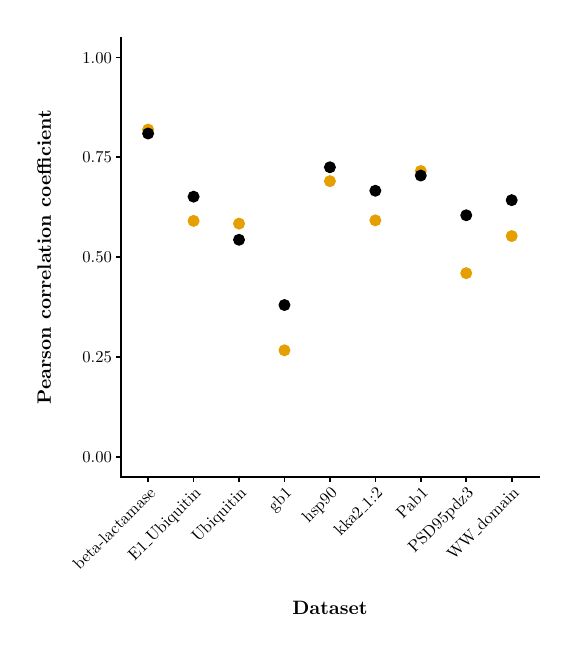
\begin{tikzpicture}[x=1pt,y=1pt]
\definecolor{fillColor}{RGB}{255,255,255}
\path[use as bounding box,fill=fillColor,fill opacity=0.00] (0,0) rectangle (188.25,216.81);
\begin{scope}
\path[clip] ( 33.67, 54.47) rectangle (184.75,213.31);
\definecolor{drawColor}{RGB}{230,159,0}
\definecolor{fillColor}{RGB}{230,159,0}

\path[draw=drawColor,line width= 0.4pt,line join=round,line cap=round,fill=fillColor] ( 59.95,146.98) circle (  1.96);
\definecolor{drawColor}{RGB}{0,0,0}
\definecolor{fillColor}{RGB}{0,0,0}

\path[draw=drawColor,line width= 0.4pt,line join=round,line cap=round,fill=fillColor] ( 59.95,155.74) circle (  1.96);
\definecolor{drawColor}{RGB}{230,159,0}
\definecolor{fillColor}{RGB}{230,159,0}

\path[draw=drawColor,line width= 0.4pt,line join=round,line cap=round,fill=fillColor] (158.48,128.10) circle (  1.96);
\definecolor{drawColor}{RGB}{0,0,0}
\definecolor{fillColor}{RGB}{0,0,0}

\path[draw=drawColor,line width= 0.4pt,line join=round,line cap=round,fill=fillColor] (158.48,149.02) circle (  1.96);
\definecolor{drawColor}{RGB}{230,159,0}
\definecolor{fillColor}{RGB}{230,159,0}

\path[draw=drawColor,line width= 0.4pt,line join=round,line cap=round,fill=fillColor] (142.05,165.02) circle (  1.96);
\definecolor{drawColor}{RGB}{0,0,0}
\definecolor{fillColor}{RGB}{0,0,0}

\path[draw=drawColor,line width= 0.4pt,line join=round,line cap=round,fill=fillColor] (142.05,163.37) circle (  1.96);
\definecolor{drawColor}{RGB}{230,159,0}
\definecolor{fillColor}{RGB}{230,159,0}

\path[draw=drawColor,line width= 0.4pt,line join=round,line cap=round,fill=fillColor] ( 76.37,146.00) circle (  1.96);
\definecolor{drawColor}{RGB}{0,0,0}
\definecolor{fillColor}{RGB}{0,0,0}

\path[draw=drawColor,line width= 0.4pt,line join=round,line cap=round,fill=fillColor] ( 76.37,140.16) circle (  1.96);
\definecolor{drawColor}{RGB}{230,159,0}
\definecolor{fillColor}{RGB}{230,159,0}

\path[draw=drawColor,line width= 0.4pt,line join=round,line cap=round,fill=fillColor] (174.90,141.51) circle (  1.96);
\definecolor{drawColor}{RGB}{0,0,0}
\definecolor{fillColor}{RGB}{0,0,0}

\path[draw=drawColor,line width= 0.4pt,line join=round,line cap=round,fill=fillColor] (174.90,154.48) circle (  1.96);
\definecolor{drawColor}{RGB}{230,159,0}
\definecolor{fillColor}{RGB}{230,159,0}

\path[draw=drawColor,line width= 0.4pt,line join=round,line cap=round,fill=fillColor] ( 43.52,179.99) circle (  1.96);
\definecolor{drawColor}{RGB}{0,0,0}
\definecolor{fillColor}{RGB}{0,0,0}

\path[draw=drawColor,line width= 0.4pt,line join=round,line cap=round,fill=fillColor] ( 43.52,178.56) circle (  1.96);
\definecolor{drawColor}{RGB}{230,159,0}
\definecolor{fillColor}{RGB}{230,159,0}

\path[draw=drawColor,line width= 0.4pt,line join=round,line cap=round,fill=fillColor] ( 92.79,100.22) circle (  1.96);
\definecolor{drawColor}{RGB}{0,0,0}
\definecolor{fillColor}{RGB}{0,0,0}

\path[draw=drawColor,line width= 0.4pt,line join=round,line cap=round,fill=fillColor] ( 92.79,116.58) circle (  1.96);
\definecolor{drawColor}{RGB}{230,159,0}
\definecolor{fillColor}{RGB}{230,159,0}

\path[draw=drawColor,line width= 0.4pt,line join=round,line cap=round,fill=fillColor] (109.21,161.35) circle (  1.96);
\definecolor{drawColor}{RGB}{0,0,0}
\definecolor{fillColor}{RGB}{0,0,0}

\path[draw=drawColor,line width= 0.4pt,line join=round,line cap=round,fill=fillColor] (109.21,166.37) circle (  1.96);
\definecolor{drawColor}{RGB}{230,159,0}
\definecolor{fillColor}{RGB}{230,159,0}

\path[draw=drawColor,line width= 0.4pt,line join=round,line cap=round,fill=fillColor] (125.63,147.18) circle (  1.96);
\definecolor{drawColor}{RGB}{0,0,0}
\definecolor{fillColor}{RGB}{0,0,0}

\path[draw=drawColor,line width= 0.4pt,line join=round,line cap=round,fill=fillColor] (125.63,157.88) circle (  1.96);
\end{scope}
\begin{scope}
\path[clip] (  0.00,  0.00) rectangle (188.25,216.81);
\definecolor{drawColor}{RGB}{0,0,0}

\path[draw=drawColor,line width= 0.6pt,line join=round,line cap=rect] ( 33.67, 54.47) --
	( 33.67,213.31);
\end{scope}
\begin{scope}
\path[clip] (  0.00,  0.00) rectangle (188.25,216.81);
\definecolor{drawColor}{RGB}{0,0,0}

\node[text=drawColor,anchor=base east,inner sep=0pt, outer sep=0pt, scale=  0.60] at ( 30.42, 59.62) {0.00};

\node[text=drawColor,anchor=base east,inner sep=0pt, outer sep=0pt, scale=  0.60] at ( 30.42, 95.72) {0.25};

\node[text=drawColor,anchor=base east,inner sep=0pt, outer sep=0pt, scale=  0.60] at ( 30.42,131.82) {0.50};

\node[text=drawColor,anchor=base east,inner sep=0pt, outer sep=0pt, scale=  0.60] at ( 30.42,167.92) {0.75};

\node[text=drawColor,anchor=base east,inner sep=0pt, outer sep=0pt, scale=  0.60] at ( 30.42,204.02) {1.00};
\end{scope}
\begin{scope}
\path[clip] (  0.00,  0.00) rectangle (188.25,216.81);
\definecolor{drawColor}{RGB}{0,0,0}

\path[draw=drawColor,line width= 0.6pt,line join=round] ( 31.92, 61.69) --
	( 33.67, 61.69);

\path[draw=drawColor,line width= 0.6pt,line join=round] ( 31.92, 97.79) --
	( 33.67, 97.79);

\path[draw=drawColor,line width= 0.6pt,line join=round] ( 31.92,133.89) --
	( 33.67,133.89);

\path[draw=drawColor,line width= 0.6pt,line join=round] ( 31.92,169.99) --
	( 33.67,169.99);

\path[draw=drawColor,line width= 0.6pt,line join=round] ( 31.92,206.09) --
	( 33.67,206.09);
\end{scope}
\begin{scope}
\path[clip] (  0.00,  0.00) rectangle (188.25,216.81);
\definecolor{drawColor}{RGB}{0,0,0}

\path[draw=drawColor,line width= 0.6pt,line join=round,line cap=rect] ( 33.67, 54.47) --
	(184.75, 54.47);
\end{scope}
\begin{scope}
\path[clip] (  0.00,  0.00) rectangle (188.25,216.81);
\definecolor{drawColor}{RGB}{0,0,0}

\path[draw=drawColor,line width= 0.6pt,line join=round] ( 43.52, 52.72) --
	( 43.52, 54.47);

\path[draw=drawColor,line width= 0.6pt,line join=round] ( 59.95, 52.72) --
	( 59.95, 54.47);

\path[draw=drawColor,line width= 0.6pt,line join=round] ( 76.37, 52.72) --
	( 76.37, 54.47);

\path[draw=drawColor,line width= 0.6pt,line join=round] ( 92.79, 52.72) --
	( 92.79, 54.47);

\path[draw=drawColor,line width= 0.6pt,line join=round] (109.21, 52.72) --
	(109.21, 54.47);

\path[draw=drawColor,line width= 0.6pt,line join=round] (125.63, 52.72) --
	(125.63, 54.47);

\path[draw=drawColor,line width= 0.6pt,line join=round] (142.05, 52.72) --
	(142.05, 54.47);

\path[draw=drawColor,line width= 0.6pt,line join=round] (158.48, 52.72) --
	(158.48, 54.47);

\path[draw=drawColor,line width= 0.6pt,line join=round] (174.90, 52.72) --
	(174.90, 54.47);
\end{scope}
\begin{scope}
\path[clip] (  0.00,  0.00) rectangle (188.25,216.81);
\definecolor{drawColor}{RGB}{0,0,0}

\node[text=drawColor,rotate= 45.00,anchor=base east,inner sep=0pt, outer sep=0pt, scale=  0.60] at ( 46.45, 48.30) {beta-lactamase};

\node[text=drawColor,rotate= 45.00,anchor=base east,inner sep=0pt, outer sep=0pt, scale=  0.60] at ( 62.87, 48.30) {E1\_Ubiquitin};

\node[text=drawColor,rotate= 45.00,anchor=base east,inner sep=0pt, outer sep=0pt, scale=  0.60] at ( 79.29, 48.30) {Ubiquitin};

\node[text=drawColor,rotate= 45.00,anchor=base east,inner sep=0pt, outer sep=0pt, scale=  0.60] at ( 95.71, 48.30) {gb1};

\node[text=drawColor,rotate= 45.00,anchor=base east,inner sep=0pt, outer sep=0pt, scale=  0.60] at (112.13, 48.30) {hsp90};

\node[text=drawColor,rotate= 45.00,anchor=base east,inner sep=0pt, outer sep=0pt, scale=  0.60] at (128.56, 48.30) {kka2\_1:2};

\node[text=drawColor,rotate= 45.00,anchor=base east,inner sep=0pt, outer sep=0pt, scale=  0.60] at (144.98, 48.30) {Pab1};

\node[text=drawColor,rotate= 45.00,anchor=base east,inner sep=0pt, outer sep=0pt, scale=  0.60] at (161.40, 48.30) {PSD95pdz3};

\node[text=drawColor,rotate= 45.00,anchor=base east,inner sep=0pt, outer sep=0pt, scale=  0.60] at (177.82, 48.30) {WW\_domain};
\end{scope}
\begin{scope}
\path[clip] (  0.00,  0.00) rectangle (188.25,216.81);
\definecolor{drawColor}{RGB}{0,0,0}

\node[text=drawColor,anchor=base,inner sep=0pt, outer sep=0pt, scale=  0.70] at (109.21,  4.86) {\bfseries Dataset};
\end{scope}
\begin{scope}
\path[clip] (  0.00,  0.00) rectangle (188.25,216.81);
\definecolor{drawColor}{RGB}{0,0,0}

\node[text=drawColor,rotate= 90.00,anchor=base,inner sep=0pt, outer sep=0pt, scale=  0.70] at (  8.39,133.89) {\bfseries Pearson correlation coefficient};
\end{scope}
\end{tikzpicture}
}{\caption{}\label{sup:subfig:test_summary_by_position}}
			\end{subfloatrow}
			\subfigvsep%
			\begin{subfloatrow}
				\ffigbox[\FBwidth]{\input{./tikz/lopo_xgb_models_test_result_summary.tex}}{\caption{}\label{sup:subfig:test_summary_lopo_xgb}}
				\hfill%
				\ffigbox[\FBwidth]{\input{./tikz/lopo_linear_models_test_result_summary.tex}}{\caption{}\label{sup:subfig:test_summary_lopo_linear}}
			\end{subfloatrow}
		}%
		{%
			\caption[Validation and testing performances]{%
				\textbf{Validation and testing performances.}
				Series of plots showing the performances on the validation sets (orange points) and testing sets (black points) for the models developed in this work.
				\subref{sup:subfig:test_summary_naive} Naive single protein models.
				\subref{sup:subfig:test_summary_by_position} Single protein models trained by segregating protein positions.
				\subref{sup:subfig:test_summary_lopo_xgb} General gradient boosted tree models trained in a Leave-One-Protein-Out (LOPO) fashion.
				\subref{sup:subfig:test_summary_lopo_linear} General linear regression models trained in a Leave-One-Protein-Out (LOPO) fashion.
			}\label{sup:fig:test_summary}%
		}%
	\end{figure}

	\begin{figure}
		\ffigbox[\FBwidth]{% Created by tikzDevice version 0.12.3.1 on 2021-06-10 10:39:57
% !TEX encoding = UTF-8 Unicode
\begin{tikzpicture}[x=1pt,y=1pt]
\definecolor{fillColor}{RGB}{255,255,255}
\path[use as bounding box,fill=fillColor,fill opacity=0.00] (0,0) rectangle (418.34,295.82);
\begin{scope}
\path[clip] ( 35.67,212.35) rectangle (151.11,283.52);
\definecolor{drawColor}{RGB}{38,38,38}

\path[draw=drawColor,draw opacity=0.50,line width= 0.4pt,line join=round,line cap=round] ( 75.32,253.62) -- ( 79.25,257.54);

\path[draw=drawColor,draw opacity=0.50,line width= 0.4pt,line join=round,line cap=round] ( 75.32,257.54) -- ( 79.25,253.62);

\path[draw=drawColor,draw opacity=0.50,line width= 0.4pt,line join=round,line cap=round] (128.72,258.15) -- (132.65,262.07);

\path[draw=drawColor,draw opacity=0.50,line width= 0.4pt,line join=round,line cap=round] (128.72,262.07) -- (132.65,258.15);

\path[draw=drawColor,draw opacity=0.50,line width= 0.4pt,line join=round,line cap=round] (130.71,274.79) -- (134.63,278.72);

\path[draw=drawColor,draw opacity=0.50,line width= 0.4pt,line join=round,line cap=round] (130.71,278.72) -- (134.63,274.79);

\path[draw=drawColor,draw opacity=0.50,line width= 0.4pt,line join=round,line cap=round] ( 66.39,242.41) -- ( 70.32,246.33);

\path[draw=drawColor,draw opacity=0.50,line width= 0.4pt,line join=round,line cap=round] ( 66.39,246.33) -- ( 70.32,242.41);

\path[draw=drawColor,draw opacity=0.50,line width= 0.4pt,line join=round,line cap=round] ( 88.83,259.21) -- ( 92.75,263.13);

\path[draw=drawColor,draw opacity=0.50,line width= 0.4pt,line join=round,line cap=round] ( 88.83,263.13) -- ( 92.75,259.21);

\path[draw=drawColor,draw opacity=0.50,line width= 0.4pt,line join=round,line cap=round] ( 38.96,242.75) -- ( 42.88,246.68);

\path[draw=drawColor,draw opacity=0.50,line width= 0.4pt,line join=round,line cap=round] ( 38.96,246.68) -- ( 42.88,242.75);

\path[draw=drawColor,draw opacity=0.50,line width= 0.4pt,line join=round,line cap=round] (123.06,270.86) -- (126.98,274.78);

\path[draw=drawColor,draw opacity=0.50,line width= 0.4pt,line join=round,line cap=round] (123.06,274.78) -- (126.98,270.86);

\path[draw=drawColor,draw opacity=0.50,line width= 0.4pt,line join=round,line cap=round] ( 47.67,237.58) -- ( 51.59,241.50);

\path[draw=drawColor,draw opacity=0.50,line width= 0.4pt,line join=round,line cap=round] ( 47.67,241.50) -- ( 51.59,237.58);

\path[draw=drawColor,draw opacity=0.50,line width= 0.4pt,line join=round,line cap=round] (126.50,271.16) -- (130.42,275.09);

\path[draw=drawColor,draw opacity=0.50,line width= 0.4pt,line join=round,line cap=round] (126.50,275.09) -- (130.42,271.16);

\path[draw=drawColor,draw opacity=0.50,line width= 0.4pt,line join=round,line cap=round] (117.41,264.88) -- (121.34,268.81);

\path[draw=drawColor,draw opacity=0.50,line width= 0.4pt,line join=round,line cap=round] (117.41,268.81) -- (121.34,264.88);

\path[draw=drawColor,draw opacity=0.50,line width= 0.4pt,line join=round,line cap=round] (131.16,274.06) -- (135.08,277.98);

\path[draw=drawColor,draw opacity=0.50,line width= 0.4pt,line join=round,line cap=round] (131.16,277.98) -- (135.08,274.06);

\path[draw=drawColor,draw opacity=0.50,line width= 0.4pt,line join=round,line cap=round] (131.51,273.25) -- (135.44,277.18);

\path[draw=drawColor,draw opacity=0.50,line width= 0.4pt,line join=round,line cap=round] (131.51,277.18) -- (135.44,273.25);

\path[draw=drawColor,draw opacity=0.50,line width= 0.4pt,line join=round,line cap=round] (132.59,273.02) -- (136.51,276.94);

\path[draw=drawColor,draw opacity=0.50,line width= 0.4pt,line join=round,line cap=round] (132.59,276.94) -- (136.51,273.02);

\path[draw=drawColor,draw opacity=0.50,line width= 0.4pt,line join=round,line cap=round] ( 50.55,243.96) -- ( 54.47,247.88);

\path[draw=drawColor,draw opacity=0.50,line width= 0.4pt,line join=round,line cap=round] ( 50.55,247.88) -- ( 54.47,243.96);

\path[draw=drawColor,draw opacity=0.50,line width= 0.4pt,line join=round,line cap=round] (111.32,251.72) -- (115.25,255.65);

\path[draw=drawColor,draw opacity=0.50,line width= 0.4pt,line join=round,line cap=round] (111.32,255.65) -- (115.25,251.72);

\path[draw=drawColor,draw opacity=0.50,line width= 0.4pt,line join=round,line cap=round] ( 94.47,253.00) -- ( 98.39,256.93);

\path[draw=drawColor,draw opacity=0.50,line width= 0.4pt,line join=round,line cap=round] ( 94.47,256.93) -- ( 98.39,253.00);

\path[draw=drawColor,draw opacity=0.50,line width= 0.4pt,line join=round,line cap=round] (129.12,257.42) -- (133.04,261.34);

\path[draw=drawColor,draw opacity=0.50,line width= 0.4pt,line join=round,line cap=round] (129.12,261.34) -- (133.04,257.42);

\path[draw=drawColor,draw opacity=0.50,line width= 0.4pt,line join=round,line cap=round] (109.51,240.01) -- (113.43,243.94);

\path[draw=drawColor,draw opacity=0.50,line width= 0.4pt,line join=round,line cap=round] (109.51,243.94) -- (113.43,240.01);

\path[draw=drawColor,draw opacity=0.50,line width= 0.4pt,line join=round,line cap=round] (115.74,271.52) -- (119.67,275.45);

\path[draw=drawColor,draw opacity=0.50,line width= 0.4pt,line join=round,line cap=round] (115.74,275.45) -- (119.67,271.52);

\path[draw=drawColor,draw opacity=0.50,line width= 0.4pt,line join=round,line cap=round] (129.91,272.39) -- (133.83,276.32);

\path[draw=drawColor,draw opacity=0.50,line width= 0.4pt,line join=round,line cap=round] (129.91,276.32) -- (133.83,272.39);

\path[draw=drawColor,draw opacity=0.50,line width= 0.4pt,line join=round,line cap=round] (128.94,268.33) -- (132.86,272.26);

\path[draw=drawColor,draw opacity=0.50,line width= 0.4pt,line join=round,line cap=round] (128.94,272.26) -- (132.86,268.33);

\path[draw=drawColor,draw opacity=0.50,line width= 0.4pt,line join=round,line cap=round] (122.89,266.12) -- (126.81,270.05);

\path[draw=drawColor,draw opacity=0.50,line width= 0.4pt,line join=round,line cap=round] (122.89,270.05) -- (126.81,266.12);

\path[draw=drawColor,draw opacity=0.50,line width= 0.4pt,line join=round,line cap=round] (112.59,273.84) -- (116.52,277.77);

\path[draw=drawColor,draw opacity=0.50,line width= 0.4pt,line join=round,line cap=round] (112.59,277.77) -- (116.52,273.84);

\path[draw=drawColor,draw opacity=0.50,line width= 0.4pt,line join=round,line cap=round] ( 86.66,237.21) -- ( 90.59,241.13);

\path[draw=drawColor,draw opacity=0.50,line width= 0.4pt,line join=round,line cap=round] ( 86.66,241.13) -- ( 90.59,237.21);

\path[draw=drawColor,draw opacity=0.50,line width= 0.4pt,line join=round,line cap=round] (122.92,269.78) -- (126.84,273.71);

\path[draw=drawColor,draw opacity=0.50,line width= 0.4pt,line join=round,line cap=round] (122.92,273.71) -- (126.84,269.78);

\path[draw=drawColor,draw opacity=0.50,line width= 0.4pt,line join=round,line cap=round] (132.94,270.50) -- (136.87,274.42);

\path[draw=drawColor,draw opacity=0.50,line width= 0.4pt,line join=round,line cap=round] (132.94,274.42) -- (136.87,270.50);

\path[draw=drawColor,draw opacity=0.50,line width= 0.4pt,line join=round,line cap=round] (104.58,258.01) -- (108.50,261.94);

\path[draw=drawColor,draw opacity=0.50,line width= 0.4pt,line join=round,line cap=round] (104.58,261.94) -- (108.50,258.01);

\path[draw=drawColor,draw opacity=0.50,line width= 0.4pt,line join=round,line cap=round] (109.39,263.12) -- (113.32,267.05);

\path[draw=drawColor,draw opacity=0.50,line width= 0.4pt,line join=round,line cap=round] (109.39,267.05) -- (113.32,263.12);

\path[draw=drawColor,draw opacity=0.50,line width= 0.4pt,line join=round,line cap=round] (110.29,262.41) -- (114.22,266.33);

\path[draw=drawColor,draw opacity=0.50,line width= 0.4pt,line join=round,line cap=round] (110.29,266.33) -- (114.22,262.41);

\path[draw=drawColor,draw opacity=0.50,line width= 0.4pt,line join=round,line cap=round] (131.70,273.44) -- (135.62,277.37);

\path[draw=drawColor,draw opacity=0.50,line width= 0.4pt,line join=round,line cap=round] (131.70,277.37) -- (135.62,273.44);

\path[draw=drawColor,draw opacity=0.50,line width= 0.4pt,line join=round,line cap=round] (132.29,273.03) -- (136.21,276.96);

\path[draw=drawColor,draw opacity=0.50,line width= 0.4pt,line join=round,line cap=round] (132.29,276.96) -- (136.21,273.03);

\path[draw=drawColor,draw opacity=0.50,line width= 0.4pt,line join=round,line cap=round] (118.89,271.05) -- (122.82,274.97);

\path[draw=drawColor,draw opacity=0.50,line width= 0.4pt,line join=round,line cap=round] (118.89,274.97) -- (122.82,271.05);

\path[draw=drawColor,draw opacity=0.50,line width= 0.4pt,line join=round,line cap=round] ( 52.20,231.48) -- ( 56.12,235.41);

\path[draw=drawColor,draw opacity=0.50,line width= 0.4pt,line join=round,line cap=round] ( 52.20,235.41) -- ( 56.12,231.48);

\path[draw=drawColor,draw opacity=0.50,line width= 0.4pt,line join=round,line cap=round] (129.96,274.94) -- (133.88,278.86);

\path[draw=drawColor,draw opacity=0.50,line width= 0.4pt,line join=round,line cap=round] (129.96,278.86) -- (133.88,274.94);

\path[draw=drawColor,draw opacity=0.50,line width= 0.4pt,line join=round,line cap=round] (117.08,270.83) -- (121.00,274.76);

\path[draw=drawColor,draw opacity=0.50,line width= 0.4pt,line join=round,line cap=round] (117.08,274.76) -- (121.00,270.83);

\path[draw=drawColor,draw opacity=0.50,line width= 0.4pt,line join=round,line cap=round] ( 38.96,235.17) -- ( 42.88,239.09);

\path[draw=drawColor,draw opacity=0.50,line width= 0.4pt,line join=round,line cap=round] ( 38.96,239.09) -- ( 42.88,235.17);

\path[draw=drawColor,draw opacity=0.50,line width= 0.4pt,line join=round,line cap=round] (130.87,271.56) -- (134.79,275.49);

\path[draw=drawColor,draw opacity=0.50,line width= 0.4pt,line join=round,line cap=round] (130.87,275.49) -- (134.79,271.56);

\path[draw=drawColor,draw opacity=0.50,line width= 0.4pt,line join=round,line cap=round] (121.15,267.80) -- (125.08,271.72);

\path[draw=drawColor,draw opacity=0.50,line width= 0.4pt,line join=round,line cap=round] (121.15,271.72) -- (125.08,267.80);

\path[draw=drawColor,draw opacity=0.50,line width= 0.4pt,line join=round,line cap=round] (132.44,274.18) -- (136.37,278.10);

\path[draw=drawColor,draw opacity=0.50,line width= 0.4pt,line join=round,line cap=round] (132.44,278.10) -- (136.37,274.18);

\path[draw=drawColor,draw opacity=0.50,line width= 0.4pt,line join=round,line cap=round] (129.12,268.91) -- (133.04,272.84);

\path[draw=drawColor,draw opacity=0.50,line width= 0.4pt,line join=round,line cap=round] (129.12,272.84) -- (133.04,268.91);

\path[draw=drawColor,draw opacity=0.50,line width= 0.4pt,line join=round,line cap=round] ( 95.70,252.04) -- ( 99.62,255.97);

\path[draw=drawColor,draw opacity=0.50,line width= 0.4pt,line join=round,line cap=round] ( 95.70,255.97) -- ( 99.62,252.04);

\path[draw=drawColor,draw opacity=0.50,line width= 0.4pt,line join=round,line cap=round] ( 94.13,253.41) -- ( 98.06,257.33);

\path[draw=drawColor,draw opacity=0.50,line width= 0.4pt,line join=round,line cap=round] ( 94.13,257.33) -- ( 98.06,253.41);

\path[draw=drawColor,draw opacity=0.50,line width= 0.4pt,line join=round,line cap=round] ( 42.30,226.05) -- ( 46.22,229.98);

\path[draw=drawColor,draw opacity=0.50,line width= 0.4pt,line join=round,line cap=round] ( 42.30,229.98) -- ( 46.22,226.05);

\path[draw=drawColor,draw opacity=0.50,line width= 0.4pt,line join=round,line cap=round] (125.54,274.34) -- (129.46,278.27);

\path[draw=drawColor,draw opacity=0.50,line width= 0.4pt,line join=round,line cap=round] (125.54,278.27) -- (129.46,274.34);

\path[draw=drawColor,draw opacity=0.50,line width= 0.4pt,line join=round,line cap=round] (126.27,268.58) -- (130.20,272.51);

\path[draw=drawColor,draw opacity=0.50,line width= 0.4pt,line join=round,line cap=round] (126.27,272.51) -- (130.20,268.58);

\path[draw=drawColor,draw opacity=0.50,line width= 0.4pt,line join=round,line cap=round] (124.43,273.76) -- (128.35,277.68);

\path[draw=drawColor,draw opacity=0.50,line width= 0.4pt,line join=round,line cap=round] (124.43,277.68) -- (128.35,273.76);

\path[draw=drawColor,draw opacity=0.50,line width= 0.4pt,line join=round,line cap=round] (116.33,266.20) -- (120.26,270.12);

\path[draw=drawColor,draw opacity=0.50,line width= 0.4pt,line join=round,line cap=round] (116.33,270.12) -- (120.26,266.20);

\path[draw=drawColor,draw opacity=0.50,line width= 0.4pt,line join=round,line cap=round] (129.06,273.50) -- (132.98,277.43);

\path[draw=drawColor,draw opacity=0.50,line width= 0.4pt,line join=round,line cap=round] (129.06,277.43) -- (132.98,273.50);

\path[draw=drawColor,draw opacity=0.50,line width= 0.4pt,line join=round,line cap=round] (107.70,253.14) -- (111.62,257.07);

\path[draw=drawColor,draw opacity=0.50,line width= 0.4pt,line join=round,line cap=round] (107.70,257.07) -- (111.62,253.14);

\path[draw=drawColor,draw opacity=0.50,line width= 0.4pt,line join=round,line cap=round] ( 68.76,245.61) -- ( 72.68,249.53);

\path[draw=drawColor,draw opacity=0.50,line width= 0.4pt,line join=round,line cap=round] ( 68.76,249.53) -- ( 72.68,245.61);

\path[draw=drawColor,draw opacity=0.50,line width= 0.4pt,line join=round,line cap=round] ( 97.39,253.46) -- (101.32,257.39);

\path[draw=drawColor,draw opacity=0.50,line width= 0.4pt,line join=round,line cap=round] ( 97.39,257.39) -- (101.32,253.46);

\path[draw=drawColor,draw opacity=0.50,line width= 0.4pt,line join=round,line cap=round] (119.18,267.93) -- (123.10,271.85);

\path[draw=drawColor,draw opacity=0.50,line width= 0.4pt,line join=round,line cap=round] (119.18,271.85) -- (123.10,267.93);

\path[draw=drawColor,draw opacity=0.50,line width= 0.4pt,line join=round,line cap=round] (119.79,265.65) -- (123.72,269.58);

\path[draw=drawColor,draw opacity=0.50,line width= 0.4pt,line join=round,line cap=round] (119.79,269.58) -- (123.72,265.65);

\path[draw=drawColor,draw opacity=0.50,line width= 0.4pt,line join=round,line cap=round] (125.36,272.85) -- (129.29,276.77);

\path[draw=drawColor,draw opacity=0.50,line width= 0.4pt,line join=round,line cap=round] (125.36,276.77) -- (129.29,272.85);

\path[draw=drawColor,draw opacity=0.50,line width= 0.4pt,line join=round,line cap=round] ( 49.15,235.26) -- ( 53.07,239.18);

\path[draw=drawColor,draw opacity=0.50,line width= 0.4pt,line join=round,line cap=round] ( 49.15,239.18) -- ( 53.07,235.26);

\path[draw=drawColor,draw opacity=0.50,line width= 0.4pt,line join=round,line cap=round] (134.07,274.82) -- (138.00,278.74);

\path[draw=drawColor,draw opacity=0.50,line width= 0.4pt,line join=round,line cap=round] (134.07,278.74) -- (138.00,274.82);

\path[draw=drawColor,draw opacity=0.50,line width= 0.4pt,line join=round,line cap=round] (102.49,258.63) -- (106.42,262.55);

\path[draw=drawColor,draw opacity=0.50,line width= 0.4pt,line join=round,line cap=round] (102.49,262.55) -- (106.42,258.63);

\path[draw=drawColor,draw opacity=0.50,line width= 0.4pt,line join=round,line cap=round] ( 39.41,229.18) -- ( 43.33,233.10);

\path[draw=drawColor,draw opacity=0.50,line width= 0.4pt,line join=round,line cap=round] ( 39.41,233.10) -- ( 43.33,229.18);

\path[draw=drawColor,draw opacity=0.50,line width= 0.4pt,line join=round,line cap=round] (108.69,268.95) -- (112.62,272.87);

\path[draw=drawColor,draw opacity=0.50,line width= 0.4pt,line join=round,line cap=round] (108.69,272.87) -- (112.62,268.95);

\path[draw=drawColor,draw opacity=0.50,line width= 0.4pt,line join=round,line cap=round] ( 52.04,236.37) -- ( 55.96,240.30);

\path[draw=drawColor,draw opacity=0.50,line width= 0.4pt,line join=round,line cap=round] ( 52.04,240.30) -- ( 55.96,236.37);

\path[draw=drawColor,draw opacity=0.50,line width= 0.4pt,line join=round,line cap=round] (115.59,268.71) -- (119.51,272.63);

\path[draw=drawColor,draw opacity=0.50,line width= 0.4pt,line join=round,line cap=round] (115.59,272.63) -- (119.51,268.71);

\path[draw=drawColor,draw opacity=0.50,line width= 0.4pt,line join=round,line cap=round] (127.68,270.67) -- (131.61,274.59);

\path[draw=drawColor,draw opacity=0.50,line width= 0.4pt,line join=round,line cap=round] (127.68,274.59) -- (131.61,270.67);

\path[draw=drawColor,draw opacity=0.50,line width= 0.4pt,line join=round,line cap=round] (134.09,272.47) -- (138.02,276.39);

\path[draw=drawColor,draw opacity=0.50,line width= 0.4pt,line join=round,line cap=round] (134.09,276.39) -- (138.02,272.47);

\path[draw=drawColor,draw opacity=0.50,line width= 0.4pt,line join=round,line cap=round] (110.90,265.56) -- (114.82,269.48);

\path[draw=drawColor,draw opacity=0.50,line width= 0.4pt,line join=round,line cap=round] (110.90,269.48) -- (114.82,265.56);

\path[draw=drawColor,draw opacity=0.50,line width= 0.4pt,line join=round,line cap=round] (116.38,265.06) -- (120.30,268.98);

\path[draw=drawColor,draw opacity=0.50,line width= 0.4pt,line join=round,line cap=round] (116.38,268.98) -- (120.30,265.06);

\path[draw=drawColor,draw opacity=0.50,line width= 0.4pt,line join=round,line cap=round] ( 39.34,228.12) -- ( 43.27,232.04);

\path[draw=drawColor,draw opacity=0.50,line width= 0.4pt,line join=round,line cap=round] ( 39.34,232.04) -- ( 43.27,228.12);

\path[draw=drawColor,draw opacity=0.50,line width= 0.4pt,line join=round,line cap=round] ( 67.67,248.01) -- ( 71.60,251.94);

\path[draw=drawColor,draw opacity=0.50,line width= 0.4pt,line join=round,line cap=round] ( 67.67,251.94) -- ( 71.60,248.01);

\path[draw=drawColor,draw opacity=0.50,line width= 0.4pt,line join=round,line cap=round] (127.40,273.81) -- (131.32,277.74);

\path[draw=drawColor,draw opacity=0.50,line width= 0.4pt,line join=round,line cap=round] (127.40,277.74) -- (131.32,273.81);

\path[draw=drawColor,draw opacity=0.50,line width= 0.4pt,line join=round,line cap=round] (115.25,270.78) -- (119.17,274.70);

\path[draw=drawColor,draw opacity=0.50,line width= 0.4pt,line join=round,line cap=round] (115.25,274.70) -- (119.17,270.78);

\path[draw=drawColor,draw opacity=0.50,line width= 0.4pt,line join=round,line cap=round] (124.14,270.68) -- (128.06,274.61);

\path[draw=drawColor,draw opacity=0.50,line width= 0.4pt,line join=round,line cap=round] (124.14,274.61) -- (128.06,270.68);

\path[draw=drawColor,draw opacity=0.50,line width= 0.4pt,line join=round,line cap=round] (117.61,251.20) -- (121.54,255.13);

\path[draw=drawColor,draw opacity=0.50,line width= 0.4pt,line join=round,line cap=round] (117.61,255.13) -- (121.54,251.20);

\path[draw=drawColor,draw opacity=0.50,line width= 0.4pt,line join=round,line cap=round] (131.49,275.92) -- (135.41,279.84);

\path[draw=drawColor,draw opacity=0.50,line width= 0.4pt,line join=round,line cap=round] (131.49,279.84) -- (135.41,275.92);

\path[draw=drawColor,draw opacity=0.50,line width= 0.4pt,line join=round,line cap=round] (128.13,270.64) -- (132.05,274.56);

\path[draw=drawColor,draw opacity=0.50,line width= 0.4pt,line join=round,line cap=round] (128.13,274.56) -- (132.05,270.64);

\path[draw=drawColor,draw opacity=0.50,line width= 0.4pt,line join=round,line cap=round] (129.80,274.63) -- (133.72,278.55);

\path[draw=drawColor,draw opacity=0.50,line width= 0.4pt,line join=round,line cap=round] (129.80,278.55) -- (133.72,274.63);

\path[draw=drawColor,draw opacity=0.50,line width= 0.4pt,line join=round,line cap=round] (112.02,262.80) -- (115.94,266.72);

\path[draw=drawColor,draw opacity=0.50,line width= 0.4pt,line join=round,line cap=round] (112.02,266.72) -- (115.94,262.80);

\path[draw=drawColor,draw opacity=0.50,line width= 0.4pt,line join=round,line cap=round] (132.80,275.60) -- (136.73,279.52);

\path[draw=drawColor,draw opacity=0.50,line width= 0.4pt,line join=round,line cap=round] (132.80,279.52) -- (136.73,275.60);

\path[draw=drawColor,draw opacity=0.50,line width= 0.4pt,line join=round,line cap=round] (116.24,270.84) -- (120.16,274.76);

\path[draw=drawColor,draw opacity=0.50,line width= 0.4pt,line join=round,line cap=round] (116.24,274.76) -- (120.16,270.84);

\path[draw=drawColor,draw opacity=0.50,line width= 0.4pt,line join=round,line cap=round] ( 75.68,241.36) -- ( 79.61,245.28);

\path[draw=drawColor,draw opacity=0.50,line width= 0.4pt,line join=round,line cap=round] ( 75.68,245.28) -- ( 79.61,241.36);

\path[draw=drawColor,draw opacity=0.50,line width= 0.4pt,line join=round,line cap=round] ( 84.99,245.78) -- ( 88.91,249.71);

\path[draw=drawColor,draw opacity=0.50,line width= 0.4pt,line join=round,line cap=round] ( 84.99,249.71) -- ( 88.91,245.78);

\path[draw=drawColor,draw opacity=0.50,line width= 0.4pt,line join=round,line cap=round] (132.09,274.96) -- (136.02,278.89);

\path[draw=drawColor,draw opacity=0.50,line width= 0.4pt,line join=round,line cap=round] (132.09,278.89) -- (136.02,274.96);

\path[draw=drawColor,draw opacity=0.50,line width= 0.4pt,line join=round,line cap=round] (129.71,273.51) -- (133.63,277.44);

\path[draw=drawColor,draw opacity=0.50,line width= 0.4pt,line join=round,line cap=round] (129.71,277.44) -- (133.63,273.51);

\path[draw=drawColor,draw opacity=0.50,line width= 0.4pt,line join=round,line cap=round] (118.82,267.24) -- (122.74,271.17);

\path[draw=drawColor,draw opacity=0.50,line width= 0.4pt,line join=round,line cap=round] (118.82,271.17) -- (122.74,267.24);

\path[draw=drawColor,draw opacity=0.50,line width= 0.4pt,line join=round,line cap=round] ( 45.47,235.38) -- ( 49.40,239.30);

\path[draw=drawColor,draw opacity=0.50,line width= 0.4pt,line join=round,line cap=round] ( 45.47,239.30) -- ( 49.40,235.38);

\path[draw=drawColor,draw opacity=0.50,line width= 0.4pt,line join=round,line cap=round] (128.29,274.02) -- (132.21,277.94);

\path[draw=drawColor,draw opacity=0.50,line width= 0.4pt,line join=round,line cap=round] (128.29,277.94) -- (132.21,274.02);

\path[draw=drawColor,draw opacity=0.50,line width= 0.4pt,line join=round,line cap=round] (110.53,256.34) -- (114.45,260.26);

\path[draw=drawColor,draw opacity=0.50,line width= 0.4pt,line join=round,line cap=round] (110.53,260.26) -- (114.45,256.34);

\path[draw=drawColor,draw opacity=0.50,line width= 0.4pt,line join=round,line cap=round] ( 39.43,229.23) -- ( 43.36,233.16);

\path[draw=drawColor,draw opacity=0.50,line width= 0.4pt,line join=round,line cap=round] ( 39.43,233.16) -- ( 43.36,229.23);

\path[draw=drawColor,draw opacity=0.50,line width= 0.4pt,line join=round,line cap=round] (129.70,272.86) -- (133.63,276.78);

\path[draw=drawColor,draw opacity=0.50,line width= 0.4pt,line join=round,line cap=round] (129.70,276.78) -- (133.63,272.86);

\path[draw=drawColor,draw opacity=0.50,line width= 0.4pt,line join=round,line cap=round] (129.91,274.93) -- (133.84,278.85);

\path[draw=drawColor,draw opacity=0.50,line width= 0.4pt,line join=round,line cap=round] (129.91,278.85) -- (133.84,274.93);

\path[draw=drawColor,draw opacity=0.50,line width= 0.4pt,line join=round,line cap=round] (131.70,273.45) -- (135.62,277.37);

\path[draw=drawColor,draw opacity=0.50,line width= 0.4pt,line join=round,line cap=round] (131.70,277.37) -- (135.62,273.45);

\path[draw=drawColor,draw opacity=0.50,line width= 0.4pt,line join=round,line cap=round] ( 51.71,239.50) -- ( 55.63,243.42);

\path[draw=drawColor,draw opacity=0.50,line width= 0.4pt,line join=round,line cap=round] ( 51.71,243.42) -- ( 55.63,239.50);

\path[draw=drawColor,draw opacity=0.50,line width= 0.4pt,line join=round,line cap=round] (132.62,275.46) -- (136.54,279.38);

\path[draw=drawColor,draw opacity=0.50,line width= 0.4pt,line join=round,line cap=round] (132.62,279.38) -- (136.54,275.46);

\path[draw=drawColor,draw opacity=0.50,line width= 0.4pt,line join=round,line cap=round] (101.82,267.88) -- (105.75,271.80);

\path[draw=drawColor,draw opacity=0.50,line width= 0.4pt,line join=round,line cap=round] (101.82,271.80) -- (105.75,267.88);

\path[draw=drawColor,draw opacity=0.50,line width= 0.4pt,line join=round,line cap=round] (115.77,268.34) -- (119.70,272.26);

\path[draw=drawColor,draw opacity=0.50,line width= 0.4pt,line join=round,line cap=round] (115.77,272.26) -- (119.70,268.34);

\path[draw=drawColor,draw opacity=0.50,line width= 0.4pt,line join=round,line cap=round] (129.31,275.94) -- (133.23,279.87);

\path[draw=drawColor,draw opacity=0.50,line width= 0.4pt,line join=round,line cap=round] (129.31,279.87) -- (133.23,275.94);

\path[draw=drawColor,draw opacity=0.50,line width= 0.4pt,line join=round,line cap=round] ( 85.67,262.84) -- ( 89.59,266.77);

\path[draw=drawColor,draw opacity=0.50,line width= 0.4pt,line join=round,line cap=round] ( 85.67,266.77) -- ( 89.59,262.84);

\path[draw=drawColor,draw opacity=0.50,line width= 0.4pt,line join=round,line cap=round] ( 96.54,261.68) -- (100.47,265.60);

\path[draw=drawColor,draw opacity=0.50,line width= 0.4pt,line join=round,line cap=round] ( 96.54,265.60) -- (100.47,261.68);

\path[draw=drawColor,draw opacity=0.50,line width= 0.4pt,line join=round,line cap=round] ( 93.64,255.53) -- ( 97.56,259.46);

\path[draw=drawColor,draw opacity=0.50,line width= 0.4pt,line join=round,line cap=round] ( 93.64,259.46) -- ( 97.56,255.53);

\path[draw=drawColor,draw opacity=0.50,line width= 0.4pt,line join=round,line cap=round] (119.06,267.69) -- (122.98,271.62);

\path[draw=drawColor,draw opacity=0.50,line width= 0.4pt,line join=round,line cap=round] (119.06,271.62) -- (122.98,267.69);

\path[draw=drawColor,draw opacity=0.50,line width= 0.4pt,line join=round,line cap=round] (130.13,274.53) -- (134.05,278.45);

\path[draw=drawColor,draw opacity=0.50,line width= 0.4pt,line join=round,line cap=round] (130.13,278.45) -- (134.05,274.53);

\path[draw=drawColor,draw opacity=0.50,line width= 0.4pt,line join=round,line cap=round] (129.43,272.10) -- (133.36,276.02);

\path[draw=drawColor,draw opacity=0.50,line width= 0.4pt,line join=round,line cap=round] (129.43,276.02) -- (133.36,272.10);

\path[draw=drawColor,draw opacity=0.50,line width= 0.4pt,line join=round,line cap=round] (129.40,272.00) -- (133.33,275.93);

\path[draw=drawColor,draw opacity=0.50,line width= 0.4pt,line join=round,line cap=round] (129.40,275.93) -- (133.33,272.00);

\path[draw=drawColor,draw opacity=0.50,line width= 0.4pt,line join=round,line cap=round] ( 96.49,258.23) -- (100.41,262.16);

\path[draw=drawColor,draw opacity=0.50,line width= 0.4pt,line join=round,line cap=round] ( 96.49,262.16) -- (100.41,258.23);

\path[draw=drawColor,draw opacity=0.50,line width= 0.4pt,line join=round,line cap=round] (105.43,253.48) -- (109.35,257.40);

\path[draw=drawColor,draw opacity=0.50,line width= 0.4pt,line join=round,line cap=round] (105.43,257.40) -- (109.35,253.48);

\path[draw=drawColor,draw opacity=0.50,line width= 0.4pt,line join=round,line cap=round] (124.37,272.65) -- (128.30,276.57);

\path[draw=drawColor,draw opacity=0.50,line width= 0.4pt,line join=round,line cap=round] (124.37,276.57) -- (128.30,272.65);

\path[draw=drawColor,draw opacity=0.50,line width= 0.4pt,line join=round,line cap=round] (133.37,275.25) -- (137.29,279.18);

\path[draw=drawColor,draw opacity=0.50,line width= 0.4pt,line join=round,line cap=round] (133.37,279.18) -- (137.29,275.25);

\path[draw=drawColor,draw opacity=0.50,line width= 0.4pt,line join=round,line cap=round] ( 45.48,232.38) -- ( 49.40,236.30);

\path[draw=drawColor,draw opacity=0.50,line width= 0.4pt,line join=round,line cap=round] ( 45.48,236.30) -- ( 49.40,232.38);

\path[draw=drawColor,draw opacity=0.50,line width= 0.4pt,line join=round,line cap=round] (126.09,273.77) -- (130.01,277.69);

\path[draw=drawColor,draw opacity=0.50,line width= 0.4pt,line join=round,line cap=round] (126.09,277.69) -- (130.01,273.77);

\path[draw=drawColor,draw opacity=0.50,line width= 0.4pt,line join=round,line cap=round] (131.74,273.86) -- (135.67,277.78);

\path[draw=drawColor,draw opacity=0.50,line width= 0.4pt,line join=round,line cap=round] (131.74,277.78) -- (135.67,273.86);

\path[draw=drawColor,draw opacity=0.50,line width= 0.4pt,line join=round,line cap=round] (120.49,271.64) -- (124.41,275.57);

\path[draw=drawColor,draw opacity=0.50,line width= 0.4pt,line join=round,line cap=round] (120.49,275.57) -- (124.41,271.64);

\path[draw=drawColor,draw opacity=0.50,line width= 0.4pt,line join=round,line cap=round] (128.36,273.05) -- (132.29,276.97);

\path[draw=drawColor,draw opacity=0.50,line width= 0.4pt,line join=round,line cap=round] (128.36,276.97) -- (132.29,273.05);

\path[draw=drawColor,draw opacity=0.50,line width= 0.4pt,line join=round,line cap=round] (135.06,275.00) -- (138.99,278.93);

\path[draw=drawColor,draw opacity=0.50,line width= 0.4pt,line join=round,line cap=round] (135.06,278.93) -- (138.99,275.00);

\path[draw=drawColor,draw opacity=0.50,line width= 0.4pt,line join=round,line cap=round] (103.78,268.36) -- (107.71,272.28);

\path[draw=drawColor,draw opacity=0.50,line width= 0.4pt,line join=round,line cap=round] (103.78,272.28) -- (107.71,268.36);

\path[draw=drawColor,draw opacity=0.50,line width= 0.4pt,line join=round,line cap=round] (132.59,273.13) -- (136.51,277.05);

\path[draw=drawColor,draw opacity=0.50,line width= 0.4pt,line join=round,line cap=round] (132.59,277.05) -- (136.51,273.13);

\path[draw=drawColor,draw opacity=0.50,line width= 0.4pt,line join=round,line cap=round] ( 76.02,252.63) -- ( 79.94,256.56);

\path[draw=drawColor,draw opacity=0.50,line width= 0.4pt,line join=round,line cap=round] ( 76.02,256.56) -- ( 79.94,252.63);

\path[draw=drawColor,draw opacity=0.50,line width= 0.4pt,line join=round,line cap=round] ( 91.05,248.27) -- ( 94.97,252.19);

\path[draw=drawColor,draw opacity=0.50,line width= 0.4pt,line join=round,line cap=round] ( 91.05,252.19) -- ( 94.97,248.27);

\path[draw=drawColor,draw opacity=0.50,line width= 0.4pt,line join=round,line cap=round] (101.93,235.69) -- (105.86,239.61);

\path[draw=drawColor,draw opacity=0.50,line width= 0.4pt,line join=round,line cap=round] (101.93,239.61) -- (105.86,235.69);

\path[draw=drawColor,draw opacity=0.50,line width= 0.4pt,line join=round,line cap=round] (101.16,258.10) -- (105.08,262.02);

\path[draw=drawColor,draw opacity=0.50,line width= 0.4pt,line join=round,line cap=round] (101.16,262.02) -- (105.08,258.10);

\path[draw=drawColor,draw opacity=0.50,line width= 0.4pt,line join=round,line cap=round] (133.32,274.94) -- (137.25,278.87);

\path[draw=drawColor,draw opacity=0.50,line width= 0.4pt,line join=round,line cap=round] (133.32,278.87) -- (137.25,274.94);

\path[draw=drawColor,draw opacity=0.50,line width= 0.4pt,line join=round,line cap=round] (127.05,273.67) -- (130.97,277.59);

\path[draw=drawColor,draw opacity=0.50,line width= 0.4pt,line join=round,line cap=round] (127.05,277.59) -- (130.97,273.67);

\path[draw=drawColor,draw opacity=0.50,line width= 0.4pt,line join=round,line cap=round] (128.60,269.67) -- (132.52,273.60);

\path[draw=drawColor,draw opacity=0.50,line width= 0.4pt,line join=round,line cap=round] (128.60,273.60) -- (132.52,269.67);

\path[draw=drawColor,draw opacity=0.50,line width= 0.4pt,line join=round,line cap=round] (109.15,271.37) -- (113.08,275.29);

\path[draw=drawColor,draw opacity=0.50,line width= 0.4pt,line join=round,line cap=round] (109.15,275.29) -- (113.08,271.37);

\path[draw=drawColor,draw opacity=0.50,line width= 0.4pt,line join=round,line cap=round] (135.26,274.06) -- (139.19,277.99);

\path[draw=drawColor,draw opacity=0.50,line width= 0.4pt,line join=round,line cap=round] (135.26,277.99) -- (139.19,274.06);

\path[draw=drawColor,draw opacity=0.50,line width= 0.4pt,line join=round,line cap=round] ( 62.85,260.40) -- ( 66.78,264.32);

\path[draw=drawColor,draw opacity=0.50,line width= 0.4pt,line join=round,line cap=round] ( 62.85,264.32) -- ( 66.78,260.40);

\path[draw=drawColor,draw opacity=0.50,line width= 0.4pt,line join=round,line cap=round] (117.43,263.29) -- (121.35,267.21);

\path[draw=drawColor,draw opacity=0.50,line width= 0.4pt,line join=round,line cap=round] (117.43,267.21) -- (121.35,263.29);

\path[draw=drawColor,draw opacity=0.50,line width= 0.4pt,line join=round,line cap=round] ( 57.15,256.19) -- ( 61.07,260.11);

\path[draw=drawColor,draw opacity=0.50,line width= 0.4pt,line join=round,line cap=round] ( 57.15,260.11) -- ( 61.07,256.19);

\path[draw=drawColor,draw opacity=0.50,line width= 0.4pt,line join=round,line cap=round] ( 47.87,258.35) -- ( 51.80,262.28);

\path[draw=drawColor,draw opacity=0.50,line width= 0.4pt,line join=round,line cap=round] ( 47.87,262.28) -- ( 51.80,258.35);

\path[draw=drawColor,draw opacity=0.50,line width= 0.4pt,line join=round,line cap=round] ( 64.93,229.75) -- ( 68.86,233.67);

\path[draw=drawColor,draw opacity=0.50,line width= 0.4pt,line join=round,line cap=round] ( 64.93,233.67) -- ( 68.86,229.75);

\path[draw=drawColor,draw opacity=0.50,line width= 0.4pt,line join=round,line cap=round] ( 66.34,240.88) -- ( 70.26,244.80);

\path[draw=drawColor,draw opacity=0.50,line width= 0.4pt,line join=round,line cap=round] ( 66.34,244.80) -- ( 70.26,240.88);

\path[draw=drawColor,draw opacity=0.50,line width= 0.4pt,line join=round,line cap=round] ( 40.23,236.54) -- ( 44.16,240.46);

\path[draw=drawColor,draw opacity=0.50,line width= 0.4pt,line join=round,line cap=round] ( 40.23,240.46) -- ( 44.16,236.54);

\path[draw=drawColor,draw opacity=0.50,line width= 0.4pt,line join=round,line cap=round] (128.20,269.15) -- (132.13,273.08);

\path[draw=drawColor,draw opacity=0.50,line width= 0.4pt,line join=round,line cap=round] (128.20,273.08) -- (132.13,269.15);

\path[draw=drawColor,draw opacity=0.50,line width= 0.4pt,line join=round,line cap=round] (123.81,274.01) -- (127.73,277.94);

\path[draw=drawColor,draw opacity=0.50,line width= 0.4pt,line join=round,line cap=round] (123.81,277.94) -- (127.73,274.01);

\path[draw=drawColor,draw opacity=0.50,line width= 0.4pt,line join=round,line cap=round] (120.38,268.42) -- (124.31,272.35);

\path[draw=drawColor,draw opacity=0.50,line width= 0.4pt,line join=round,line cap=round] (120.38,272.35) -- (124.31,268.42);

\path[draw=drawColor,draw opacity=0.50,line width= 0.4pt,line join=round,line cap=round] (116.70,267.68) -- (120.62,271.61);

\path[draw=drawColor,draw opacity=0.50,line width= 0.4pt,line join=round,line cap=round] (116.70,271.61) -- (120.62,267.68);

\path[draw=drawColor,draw opacity=0.50,line width= 0.4pt,line join=round,line cap=round] (131.55,274.92) -- (135.47,278.84);

\path[draw=drawColor,draw opacity=0.50,line width= 0.4pt,line join=round,line cap=round] (131.55,278.84) -- (135.47,274.92);

\path[draw=drawColor,draw opacity=0.50,line width= 0.4pt,line join=round,line cap=round] (115.45,265.65) -- (119.38,269.58);

\path[draw=drawColor,draw opacity=0.50,line width= 0.4pt,line join=round,line cap=round] (115.45,269.58) -- (119.38,265.65);

\path[draw=drawColor,draw opacity=0.50,line width= 0.4pt,line join=round,line cap=round] ( 61.25,236.51) -- ( 65.17,240.44);

\path[draw=drawColor,draw opacity=0.50,line width= 0.4pt,line join=round,line cap=round] ( 61.25,240.44) -- ( 65.17,236.51);

\path[draw=drawColor,draw opacity=0.50,line width= 0.4pt,line join=round,line cap=round] (133.59,275.53) -- (137.51,279.46);

\path[draw=drawColor,draw opacity=0.50,line width= 0.4pt,line join=round,line cap=round] (133.59,279.46) -- (137.51,275.53);

\path[draw=drawColor,draw opacity=0.50,line width= 0.4pt,line join=round,line cap=round] ( 86.89,253.01) -- ( 90.81,256.94);

\path[draw=drawColor,draw opacity=0.50,line width= 0.4pt,line join=round,line cap=round] ( 86.89,256.94) -- ( 90.81,253.01);

\path[draw=drawColor,draw opacity=0.50,line width= 0.4pt,line join=round,line cap=round] (128.81,272.11) -- (132.74,276.03);

\path[draw=drawColor,draw opacity=0.50,line width= 0.4pt,line join=round,line cap=round] (128.81,276.03) -- (132.74,272.11);

\path[draw=drawColor,draw opacity=0.50,line width= 0.4pt,line join=round,line cap=round] (128.43,272.29) -- (132.35,276.21);

\path[draw=drawColor,draw opacity=0.50,line width= 0.4pt,line join=round,line cap=round] (128.43,276.21) -- (132.35,272.29);

\path[draw=drawColor,draw opacity=0.50,line width= 0.4pt,line join=round,line cap=round] (135.06,274.94) -- (138.99,278.86);

\path[draw=drawColor,draw opacity=0.50,line width= 0.4pt,line join=round,line cap=round] (135.06,278.86) -- (138.99,274.94);

\path[draw=drawColor,draw opacity=0.50,line width= 0.4pt,line join=round,line cap=round] (107.28,242.44) -- (111.20,246.37);

\path[draw=drawColor,draw opacity=0.50,line width= 0.4pt,line join=round,line cap=round] (107.28,246.37) -- (111.20,242.44);

\path[draw=drawColor,draw opacity=0.50,line width= 0.4pt,line join=round,line cap=round] (129.08,269.17) -- (133.01,273.09);

\path[draw=drawColor,draw opacity=0.50,line width= 0.4pt,line join=round,line cap=round] (129.08,273.09) -- (133.01,269.17);

\path[draw=drawColor,draw opacity=0.50,line width= 0.4pt,line join=round,line cap=round] ( 66.05,251.53) -- ( 69.98,255.46);

\path[draw=drawColor,draw opacity=0.50,line width= 0.4pt,line join=round,line cap=round] ( 66.05,255.46) -- ( 69.98,251.53);

\path[draw=drawColor,draw opacity=0.50,line width= 0.4pt,line join=round,line cap=round] ( 39.14,240.25) -- ( 43.07,244.18);

\path[draw=drawColor,draw opacity=0.50,line width= 0.4pt,line join=round,line cap=round] ( 39.14,244.18) -- ( 43.07,240.25);

\path[draw=drawColor,draw opacity=0.50,line width= 0.4pt,line join=round,line cap=round] (125.72,272.08) -- (129.64,276.00);

\path[draw=drawColor,draw opacity=0.50,line width= 0.4pt,line join=round,line cap=round] (125.72,276.00) -- (129.64,272.08);

\path[draw=drawColor,draw opacity=0.50,line width= 0.4pt,line join=round,line cap=round] ( 78.21,260.37) -- ( 82.13,264.30);

\path[draw=drawColor,draw opacity=0.50,line width= 0.4pt,line join=round,line cap=round] ( 78.21,264.30) -- ( 82.13,260.37);

\path[draw=drawColor,draw opacity=0.50,line width= 0.4pt,line join=round,line cap=round] (133.65,274.32) -- (137.57,278.25);

\path[draw=drawColor,draw opacity=0.50,line width= 0.4pt,line join=round,line cap=round] (133.65,278.25) -- (137.57,274.32);

\path[draw=drawColor,draw opacity=0.50,line width= 0.4pt,line join=round,line cap=round] (131.51,274.75) -- (135.43,278.67);

\path[draw=drawColor,draw opacity=0.50,line width= 0.4pt,line join=round,line cap=round] (131.51,278.67) -- (135.43,274.75);

\path[draw=drawColor,draw opacity=0.50,line width= 0.4pt,line join=round,line cap=round] ( 47.87,241.48) -- ( 51.80,245.41);

\path[draw=drawColor,draw opacity=0.50,line width= 0.4pt,line join=round,line cap=round] ( 47.87,245.41) -- ( 51.80,241.48);

\path[draw=drawColor,draw opacity=0.50,line width= 0.4pt,line join=round,line cap=round] (115.33,257.28) -- (119.26,261.20);

\path[draw=drawColor,draw opacity=0.50,line width= 0.4pt,line join=round,line cap=round] (115.33,261.20) -- (119.26,257.28);

\path[draw=drawColor,draw opacity=0.50,line width= 0.4pt,line join=round,line cap=round] (115.41,264.26) -- (119.33,268.18);

\path[draw=drawColor,draw opacity=0.50,line width= 0.4pt,line join=round,line cap=round] (115.41,268.18) -- (119.33,264.26);

\path[draw=drawColor,draw opacity=0.50,line width= 0.4pt,line join=round,line cap=round] ( 94.19,267.61) -- ( 98.11,271.53);

\path[draw=drawColor,draw opacity=0.50,line width= 0.4pt,line join=round,line cap=round] ( 94.19,271.53) -- ( 98.11,267.61);

\path[draw=drawColor,draw opacity=0.50,line width= 0.4pt,line join=round,line cap=round] ( 89.26,248.85) -- ( 93.19,252.78);

\path[draw=drawColor,draw opacity=0.50,line width= 0.4pt,line join=round,line cap=round] ( 89.26,252.78) -- ( 93.19,248.85);

\path[draw=drawColor,draw opacity=0.50,line width= 0.4pt,line join=round,line cap=round] ( 90.10,250.68) -- ( 94.03,254.60);

\path[draw=drawColor,draw opacity=0.50,line width= 0.4pt,line join=round,line cap=round] ( 90.10,254.60) -- ( 94.03,250.68);

\path[draw=drawColor,draw opacity=0.50,line width= 0.4pt,line join=round,line cap=round] (127.21,273.50) -- (131.13,277.42);

\path[draw=drawColor,draw opacity=0.50,line width= 0.4pt,line join=round,line cap=round] (127.21,277.42) -- (131.13,273.50);

\path[draw=drawColor,draw opacity=0.50,line width= 0.4pt,line join=round,line cap=round] (131.33,275.32) -- (135.25,279.24);

\path[draw=drawColor,draw opacity=0.50,line width= 0.4pt,line join=round,line cap=round] (131.33,279.24) -- (135.25,275.32);

\path[draw=drawColor,draw opacity=0.50,line width= 0.4pt,line join=round,line cap=round] (132.52,274.65) -- (136.44,278.58);

\path[draw=drawColor,draw opacity=0.50,line width= 0.4pt,line join=round,line cap=round] (132.52,278.58) -- (136.44,274.65);

\path[draw=drawColor,draw opacity=0.50,line width= 0.4pt,line join=round,line cap=round] ( 43.65,230.63) -- ( 47.57,234.55);

\path[draw=drawColor,draw opacity=0.50,line width= 0.4pt,line join=round,line cap=round] ( 43.65,234.55) -- ( 47.57,230.63);

\path[draw=drawColor,draw opacity=0.50,line width= 0.4pt,line join=round,line cap=round] (120.70,270.01) -- (124.62,273.94);

\path[draw=drawColor,draw opacity=0.50,line width= 0.4pt,line join=round,line cap=round] (120.70,273.94) -- (124.62,270.01);

\path[draw=drawColor,draw opacity=0.50,line width= 0.4pt,line join=round,line cap=round] (120.56,262.69) -- (124.48,266.62);

\path[draw=drawColor,draw opacity=0.50,line width= 0.4pt,line join=round,line cap=round] (120.56,266.62) -- (124.48,262.69);

\path[draw=drawColor,draw opacity=0.50,line width= 0.4pt,line join=round,line cap=round] (114.12,261.36) -- (118.04,265.28);

\path[draw=drawColor,draw opacity=0.50,line width= 0.4pt,line join=round,line cap=round] (114.12,265.28) -- (118.04,261.36);

\path[draw=drawColor,draw opacity=0.50,line width= 0.4pt,line join=round,line cap=round] ( 38.96,231.55) -- ( 42.88,235.48);

\path[draw=drawColor,draw opacity=0.50,line width= 0.4pt,line join=round,line cap=round] ( 38.96,235.48) -- ( 42.88,231.55);

\path[draw=drawColor,draw opacity=0.50,line width= 0.4pt,line join=round,line cap=round] (128.52,265.04) -- (132.45,268.97);

\path[draw=drawColor,draw opacity=0.50,line width= 0.4pt,line join=round,line cap=round] (128.52,268.97) -- (132.45,265.04);

\path[draw=drawColor,draw opacity=0.50,line width= 0.4pt,line join=round,line cap=round] ( 84.67,249.24) -- ( 88.59,253.17);

\path[draw=drawColor,draw opacity=0.50,line width= 0.4pt,line join=round,line cap=round] ( 84.67,253.17) -- ( 88.59,249.24);

\path[draw=drawColor,draw opacity=0.50,line width= 0.4pt,line join=round,line cap=round] (108.89,270.07) -- (112.82,273.99);

\path[draw=drawColor,draw opacity=0.50,line width= 0.4pt,line join=round,line cap=round] (108.89,273.99) -- (112.82,270.07);

\path[draw=drawColor,draw opacity=0.50,line width= 0.4pt,line join=round,line cap=round] (129.65,274.57) -- (133.57,278.49);

\path[draw=drawColor,draw opacity=0.50,line width= 0.4pt,line join=round,line cap=round] (129.65,278.49) -- (133.57,274.57);

\path[draw=drawColor,draw opacity=0.50,line width= 0.4pt,line join=round,line cap=round] (131.29,271.79) -- (135.22,275.71);

\path[draw=drawColor,draw opacity=0.50,line width= 0.4pt,line join=round,line cap=round] (131.29,275.71) -- (135.22,271.79);

\path[draw=drawColor,draw opacity=0.50,line width= 0.4pt,line join=round,line cap=round] (129.53,250.80) -- (133.45,254.72);

\path[draw=drawColor,draw opacity=0.50,line width= 0.4pt,line join=round,line cap=round] (129.53,254.72) -- (133.45,250.80);

\path[draw=drawColor,draw opacity=0.50,line width= 0.4pt,line join=round,line cap=round] (130.04,274.96) -- (133.96,278.88);

\path[draw=drawColor,draw opacity=0.50,line width= 0.4pt,line join=round,line cap=round] (130.04,278.88) -- (133.96,274.96);

\path[draw=drawColor,draw opacity=0.50,line width= 0.4pt,line join=round,line cap=round] (110.96,263.30) -- (114.88,267.22);

\path[draw=drawColor,draw opacity=0.50,line width= 0.4pt,line join=round,line cap=round] (110.96,267.22) -- (114.88,263.30);

\path[draw=drawColor,draw opacity=0.50,line width= 0.4pt,line join=round,line cap=round] (129.54,273.03) -- (133.46,276.96);

\path[draw=drawColor,draw opacity=0.50,line width= 0.4pt,line join=round,line cap=round] (129.54,276.96) -- (133.46,273.03);

\path[draw=drawColor,draw opacity=0.50,line width= 0.4pt,line join=round,line cap=round] ( 59.34,239.10) -- ( 63.26,243.03);

\path[draw=drawColor,draw opacity=0.50,line width= 0.4pt,line join=round,line cap=round] ( 59.34,243.03) -- ( 63.26,239.10);

\path[draw=drawColor,draw opacity=0.50,line width= 0.4pt,line join=round,line cap=round] ( 68.45,233.31) -- ( 72.38,237.24);

\path[draw=drawColor,draw opacity=0.50,line width= 0.4pt,line join=round,line cap=round] ( 68.45,237.24) -- ( 72.38,233.31);

\path[draw=drawColor,draw opacity=0.50,line width= 0.4pt,line join=round,line cap=round] (131.39,271.63) -- (135.32,275.55);

\path[draw=drawColor,draw opacity=0.50,line width= 0.4pt,line join=round,line cap=round] (131.39,275.55) -- (135.32,271.63);

\path[draw=drawColor,draw opacity=0.50,line width= 0.4pt,line join=round,line cap=round] (116.68,266.52) -- (120.61,270.44);

\path[draw=drawColor,draw opacity=0.50,line width= 0.4pt,line join=round,line cap=round] (116.68,270.44) -- (120.61,266.52);

\path[draw=drawColor,draw opacity=0.50,line width= 0.4pt,line join=round,line cap=round] (130.01,274.86) -- (133.94,278.78);

\path[draw=drawColor,draw opacity=0.50,line width= 0.4pt,line join=round,line cap=round] (130.01,278.78) -- (133.94,274.86);

\path[draw=drawColor,draw opacity=0.50,line width= 0.4pt,line join=round,line cap=round] ( 66.68,231.31) -- ( 70.61,235.24);

\path[draw=drawColor,draw opacity=0.50,line width= 0.4pt,line join=round,line cap=round] ( 66.68,235.24) -- ( 70.61,231.31);

\path[draw=drawColor,draw opacity=0.50,line width= 0.4pt,line join=round,line cap=round] ( 87.51,247.82) -- ( 91.43,251.74);

\path[draw=drawColor,draw opacity=0.50,line width= 0.4pt,line join=round,line cap=round] ( 87.51,251.74) -- ( 91.43,247.82);

\path[draw=drawColor,draw opacity=0.50,line width= 0.4pt,line join=round,line cap=round] (131.56,275.02) -- (135.48,278.94);

\path[draw=drawColor,draw opacity=0.50,line width= 0.4pt,line join=round,line cap=round] (131.56,278.94) -- (135.48,275.02);

\path[draw=drawColor,draw opacity=0.50,line width= 0.4pt,line join=round,line cap=round] (116.49,264.94) -- (120.41,268.86);

\path[draw=drawColor,draw opacity=0.50,line width= 0.4pt,line join=round,line cap=round] (116.49,268.86) -- (120.41,264.94);

\path[draw=drawColor,draw opacity=0.50,line width= 0.4pt,line join=round,line cap=round] (131.53,260.11) -- (135.45,264.03);

\path[draw=drawColor,draw opacity=0.50,line width= 0.4pt,line join=round,line cap=round] (131.53,264.03) -- (135.45,260.11);

\path[draw=drawColor,draw opacity=0.50,line width= 0.4pt,line join=round,line cap=round] (109.26,259.10) -- (113.19,263.03);

\path[draw=drawColor,draw opacity=0.50,line width= 0.4pt,line join=round,line cap=round] (109.26,263.03) -- (113.19,259.10);

\path[draw=drawColor,draw opacity=0.50,line width= 0.4pt,line join=round,line cap=round] (125.36,271.35) -- (129.29,275.27);

\path[draw=drawColor,draw opacity=0.50,line width= 0.4pt,line join=round,line cap=round] (125.36,275.27) -- (129.29,271.35);

\path[draw=drawColor,draw opacity=0.50,line width= 0.4pt,line join=round,line cap=round] (130.00,271.41) -- (133.92,275.33);

\path[draw=drawColor,draw opacity=0.50,line width= 0.4pt,line join=round,line cap=round] (130.00,275.33) -- (133.92,271.41);

\path[draw=drawColor,draw opacity=0.50,line width= 0.4pt,line join=round,line cap=round] ( 98.52,264.66) -- (102.44,268.59);

\path[draw=drawColor,draw opacity=0.50,line width= 0.4pt,line join=round,line cap=round] ( 98.52,268.59) -- (102.44,264.66);

\path[draw=drawColor,draw opacity=0.50,line width= 0.4pt,line join=round,line cap=round] ( 73.66,249.25) -- ( 77.59,253.17);

\path[draw=drawColor,draw opacity=0.50,line width= 0.4pt,line join=round,line cap=round] ( 73.66,253.17) -- ( 77.59,249.25);

\path[draw=drawColor,draw opacity=0.50,line width= 0.4pt,line join=round,line cap=round] (129.75,271.98) -- (133.67,275.90);

\path[draw=drawColor,draw opacity=0.50,line width= 0.4pt,line join=round,line cap=round] (129.75,275.90) -- (133.67,271.98);

\path[draw=drawColor,draw opacity=0.50,line width= 0.4pt,line join=round,line cap=round] (112.34,267.08) -- (116.27,271.01);

\path[draw=drawColor,draw opacity=0.50,line width= 0.4pt,line join=round,line cap=round] (112.34,271.01) -- (116.27,267.08);

\path[draw=drawColor,draw opacity=0.50,line width= 0.4pt,line join=round,line cap=round] (131.38,275.23) -- (135.31,279.15);

\path[draw=drawColor,draw opacity=0.50,line width= 0.4pt,line join=round,line cap=round] (131.38,279.15) -- (135.31,275.23);

\path[draw=drawColor,draw opacity=0.50,line width= 0.4pt,line join=round,line cap=round] ( 50.46,229.73) -- ( 54.39,233.65);

\path[draw=drawColor,draw opacity=0.50,line width= 0.4pt,line join=round,line cap=round] ( 50.46,233.65) -- ( 54.39,229.73);

\path[draw=drawColor,draw opacity=0.50,line width= 0.4pt,line join=round,line cap=round] (129.86,272.95) -- (133.79,276.88);

\path[draw=drawColor,draw opacity=0.50,line width= 0.4pt,line join=round,line cap=round] (129.86,276.88) -- (133.79,272.95);

\path[draw=drawColor,draw opacity=0.50,line width= 0.4pt,line join=round,line cap=round] (122.72,269.47) -- (126.65,273.40);

\path[draw=drawColor,draw opacity=0.50,line width= 0.4pt,line join=round,line cap=round] (122.72,273.40) -- (126.65,269.47);

\path[draw=drawColor,draw opacity=0.50,line width= 0.4pt,line join=round,line cap=round] (115.88,258.25) -- (119.80,262.17);

\path[draw=drawColor,draw opacity=0.50,line width= 0.4pt,line join=round,line cap=round] (115.88,262.17) -- (119.80,258.25);

\path[draw=drawColor,draw opacity=0.50,line width= 0.4pt,line join=round,line cap=round] (118.17,254.01) -- (122.10,257.94);

\path[draw=drawColor,draw opacity=0.50,line width= 0.4pt,line join=round,line cap=round] (118.17,257.94) -- (122.10,254.01);

\path[draw=drawColor,draw opacity=0.50,line width= 0.4pt,line join=round,line cap=round] (107.32,269.65) -- (111.25,273.58);

\path[draw=drawColor,draw opacity=0.50,line width= 0.4pt,line join=round,line cap=round] (107.32,273.58) -- (111.25,269.65);

\path[draw=drawColor,draw opacity=0.50,line width= 0.4pt,line join=round,line cap=round] ( 58.24,247.32) -- ( 62.16,251.24);

\path[draw=drawColor,draw opacity=0.50,line width= 0.4pt,line join=round,line cap=round] ( 58.24,251.24) -- ( 62.16,247.32);

\path[draw=drawColor,draw opacity=0.50,line width= 0.4pt,line join=round,line cap=round] (130.29,273.11) -- (134.22,277.04);

\path[draw=drawColor,draw opacity=0.50,line width= 0.4pt,line join=round,line cap=round] (130.29,277.04) -- (134.22,273.11);

\path[draw=drawColor,draw opacity=0.50,line width= 0.4pt,line join=round,line cap=round] (113.78,249.49) -- (117.70,253.41);

\path[draw=drawColor,draw opacity=0.50,line width= 0.4pt,line join=round,line cap=round] (113.78,253.41) -- (117.70,249.49);

\path[draw=drawColor,draw opacity=0.50,line width= 0.4pt,line join=round,line cap=round] (111.25,268.40) -- (115.17,272.32);

\path[draw=drawColor,draw opacity=0.50,line width= 0.4pt,line join=round,line cap=round] (111.25,272.32) -- (115.17,268.40);

\path[draw=drawColor,draw opacity=0.50,line width= 0.4pt,line join=round,line cap=round] (125.90,273.48) -- (129.82,277.40);

\path[draw=drawColor,draw opacity=0.50,line width= 0.4pt,line join=round,line cap=round] (125.90,277.40) -- (129.82,273.48);

\path[draw=drawColor,draw opacity=0.50,line width= 0.4pt,line join=round,line cap=round] (137.05,271.80) -- (140.97,275.72);

\path[draw=drawColor,draw opacity=0.50,line width= 0.4pt,line join=round,line cap=round] (137.05,275.72) -- (140.97,271.80);

\path[draw=drawColor,draw opacity=0.50,line width= 0.4pt,line join=round,line cap=round] ( 47.67,243.06) -- ( 51.59,246.99);

\path[draw=drawColor,draw opacity=0.50,line width= 0.4pt,line join=round,line cap=round] ( 47.67,246.99) -- ( 51.59,243.06);

\path[draw=drawColor,draw opacity=0.50,line width= 0.4pt,line join=round,line cap=round] (121.69,273.61) -- (125.61,277.54);

\path[draw=drawColor,draw opacity=0.50,line width= 0.4pt,line join=round,line cap=round] (121.69,277.54) -- (125.61,273.61);

\path[draw=drawColor,draw opacity=0.50,line width= 0.4pt,line join=round,line cap=round] (118.73,265.08) -- (122.65,269.00);

\path[draw=drawColor,draw opacity=0.50,line width= 0.4pt,line join=round,line cap=round] (118.73,269.00) -- (122.65,265.08);

\path[draw=drawColor,draw opacity=0.50,line width= 0.4pt,line join=round,line cap=round] (127.30,267.73) -- (131.23,271.65);

\path[draw=drawColor,draw opacity=0.50,line width= 0.4pt,line join=round,line cap=round] (127.30,271.65) -- (131.23,267.73);

\path[draw=drawColor,draw opacity=0.50,line width= 0.4pt,line join=round,line cap=round] ( 88.86,253.18) -- ( 92.78,257.10);

\path[draw=drawColor,draw opacity=0.50,line width= 0.4pt,line join=round,line cap=round] ( 88.86,257.10) -- ( 92.78,253.18);

\path[draw=drawColor,draw opacity=0.50,line width= 0.4pt,line join=round,line cap=round] ( 39.29,227.99) -- ( 43.22,231.91);

\path[draw=drawColor,draw opacity=0.50,line width= 0.4pt,line join=round,line cap=round] ( 39.29,231.91) -- ( 43.22,227.99);

\path[draw=drawColor,draw opacity=0.50,line width= 0.4pt,line join=round,line cap=round] (126.94,268.01) -- (130.86,271.93);

\path[draw=drawColor,draw opacity=0.50,line width= 0.4pt,line join=round,line cap=round] (126.94,271.93) -- (130.86,268.01);

\path[draw=drawColor,draw opacity=0.50,line width= 0.4pt,line join=round,line cap=round] (129.32,273.22) -- (133.24,277.15);

\path[draw=drawColor,draw opacity=0.50,line width= 0.4pt,line join=round,line cap=round] (129.32,277.15) -- (133.24,273.22);

\path[draw=drawColor,draw opacity=0.50,line width= 0.4pt,line join=round,line cap=round] (118.20,267.18) -- (122.13,271.10);

\path[draw=drawColor,draw opacity=0.50,line width= 0.4pt,line join=round,line cap=round] (118.20,271.10) -- (122.13,267.18);

\path[draw=drawColor,draw opacity=0.50,line width= 0.4pt,line join=round,line cap=round] (111.85,264.68) -- (115.77,268.60);

\path[draw=drawColor,draw opacity=0.50,line width= 0.4pt,line join=round,line cap=round] (111.85,268.60) -- (115.77,264.68);

\path[draw=drawColor,draw opacity=0.50,line width= 0.4pt,line join=round,line cap=round] (103.76,262.55) -- (107.69,266.48);

\path[draw=drawColor,draw opacity=0.50,line width= 0.4pt,line join=round,line cap=round] (103.76,266.48) -- (107.69,262.55);

\path[draw=drawColor,draw opacity=0.50,line width= 0.4pt,line join=round,line cap=round] ( 70.98,246.94) -- ( 74.90,250.86);

\path[draw=drawColor,draw opacity=0.50,line width= 0.4pt,line join=round,line cap=round] ( 70.98,250.86) -- ( 74.90,246.94);

\path[draw=drawColor,draw opacity=0.50,line width= 0.4pt,line join=round,line cap=round] (130.38,273.88) -- (134.31,277.81);

\path[draw=drawColor,draw opacity=0.50,line width= 0.4pt,line join=round,line cap=round] (130.38,277.81) -- (134.31,273.88);

\path[draw=drawColor,draw opacity=0.50,line width= 0.4pt,line join=round,line cap=round] (130.73,271.99) -- (134.65,275.91);

\path[draw=drawColor,draw opacity=0.50,line width= 0.4pt,line join=round,line cap=round] (130.73,275.91) -- (134.65,271.99);

\path[draw=drawColor,draw opacity=0.50,line width= 0.4pt,line join=round,line cap=round] (130.83,270.51) -- (134.76,274.44);

\path[draw=drawColor,draw opacity=0.50,line width= 0.4pt,line join=round,line cap=round] (130.83,274.44) -- (134.76,270.51);

\path[draw=drawColor,draw opacity=0.50,line width= 0.4pt,line join=round,line cap=round] (130.36,275.24) -- (134.28,279.16);

\path[draw=drawColor,draw opacity=0.50,line width= 0.4pt,line join=round,line cap=round] (130.36,279.16) -- (134.28,275.24);

\path[draw=drawColor,draw opacity=0.50,line width= 0.4pt,line join=round,line cap=round] (122.08,265.89) -- (126.00,269.81);

\path[draw=drawColor,draw opacity=0.50,line width= 0.4pt,line join=round,line cap=round] (122.08,269.81) -- (126.00,265.89);

\path[draw=drawColor,draw opacity=0.50,line width= 0.4pt,line join=round,line cap=round] ( 45.84,229.19) -- ( 49.76,233.11);

\path[draw=drawColor,draw opacity=0.50,line width= 0.4pt,line join=round,line cap=round] ( 45.84,233.11) -- ( 49.76,229.19);

\path[draw=drawColor,draw opacity=0.50,line width= 0.4pt,line join=round,line cap=round] (131.22,275.14) -- (135.15,279.06);

\path[draw=drawColor,draw opacity=0.50,line width= 0.4pt,line join=round,line cap=round] (131.22,279.06) -- (135.15,275.14);

\path[draw=drawColor,draw opacity=0.50,line width= 0.4pt,line join=round,line cap=round] ( 67.01,242.37) -- ( 70.93,246.29);

\path[draw=drawColor,draw opacity=0.50,line width= 0.4pt,line join=round,line cap=round] ( 67.01,246.29) -- ( 70.93,242.37);

\path[draw=drawColor,draw opacity=0.50,line width= 0.4pt,line join=round,line cap=round] (120.11,271.68) -- (124.03,275.60);

\path[draw=drawColor,draw opacity=0.50,line width= 0.4pt,line join=round,line cap=round] (120.11,275.60) -- (124.03,271.68);

\path[draw=drawColor,draw opacity=0.50,line width= 0.4pt,line join=round,line cap=round] (132.59,274.28) -- (136.51,278.21);

\path[draw=drawColor,draw opacity=0.50,line width= 0.4pt,line join=round,line cap=round] (132.59,278.21) -- (136.51,274.28);

\path[draw=drawColor,draw opacity=0.50,line width= 0.4pt,line join=round,line cap=round] ( 89.27,257.82) -- ( 93.19,261.74);

\path[draw=drawColor,draw opacity=0.50,line width= 0.4pt,line join=round,line cap=round] ( 89.27,261.74) -- ( 93.19,257.82);

\path[draw=drawColor,draw opacity=0.50,line width= 0.4pt,line join=round,line cap=round] (126.82,267.98) -- (130.74,271.91);

\path[draw=drawColor,draw opacity=0.50,line width= 0.4pt,line join=round,line cap=round] (126.82,271.91) -- (130.74,267.98);

\path[draw=drawColor,draw opacity=0.50,line width= 0.4pt,line join=round,line cap=round] (133.95,274.78) -- (137.87,278.70);

\path[draw=drawColor,draw opacity=0.50,line width= 0.4pt,line join=round,line cap=round] (133.95,278.70) -- (137.87,274.78);

\path[draw=drawColor,draw opacity=0.50,line width= 0.4pt,line join=round,line cap=round] (107.07,260.40) -- (110.99,264.32);

\path[draw=drawColor,draw opacity=0.50,line width= 0.4pt,line join=round,line cap=round] (107.07,264.32) -- (110.99,260.40);

\path[draw=drawColor,draw opacity=0.50,line width= 0.4pt,line join=round,line cap=round] (132.59,274.07) -- (136.51,278.00);

\path[draw=drawColor,draw opacity=0.50,line width= 0.4pt,line join=round,line cap=round] (132.59,278.00) -- (136.51,274.07);

\path[draw=drawColor,draw opacity=0.50,line width= 0.4pt,line join=round,line cap=round] (120.04,259.28) -- (123.97,263.20);

\path[draw=drawColor,draw opacity=0.50,line width= 0.4pt,line join=round,line cap=round] (120.04,263.20) -- (123.97,259.28);

\path[draw=drawColor,draw opacity=0.50,line width= 0.4pt,line join=round,line cap=round] ( 71.28,248.69) -- ( 75.21,252.62);

\path[draw=drawColor,draw opacity=0.50,line width= 0.4pt,line join=round,line cap=round] ( 71.28,252.62) -- ( 75.21,248.69);

\path[draw=drawColor,draw opacity=0.50,line width= 0.4pt,line join=round,line cap=round] (124.72,270.79) -- (128.65,274.72);

\path[draw=drawColor,draw opacity=0.50,line width= 0.4pt,line join=round,line cap=round] (124.72,274.72) -- (128.65,270.79);

\path[draw=drawColor,draw opacity=0.50,line width= 0.4pt,line join=round,line cap=round] ( 98.97,266.54) -- (102.90,270.47);

\path[draw=drawColor,draw opacity=0.50,line width= 0.4pt,line join=round,line cap=round] ( 98.97,270.47) -- (102.90,266.54);

\path[draw=drawColor,draw opacity=0.50,line width= 0.4pt,line join=round,line cap=round] (129.34,273.97) -- (133.26,277.90);

\path[draw=drawColor,draw opacity=0.50,line width= 0.4pt,line join=round,line cap=round] (129.34,277.90) -- (133.26,273.97);

\path[draw=drawColor,draw opacity=0.50,line width= 0.4pt,line join=round,line cap=round] (131.91,274.96) -- (135.83,278.89);

\path[draw=drawColor,draw opacity=0.50,line width= 0.4pt,line join=round,line cap=round] (131.91,278.89) -- (135.83,274.96);

\path[draw=drawColor,draw opacity=0.50,line width= 0.4pt,line join=round,line cap=round] (120.92,269.66) -- (124.84,273.59);

\path[draw=drawColor,draw opacity=0.50,line width= 0.4pt,line join=round,line cap=round] (120.92,273.59) -- (124.84,269.66);

\path[draw=drawColor,draw opacity=0.50,line width= 0.4pt,line join=round,line cap=round] ( 97.60,258.16) -- (101.53,262.09);

\path[draw=drawColor,draw opacity=0.50,line width= 0.4pt,line join=round,line cap=round] ( 97.60,262.09) -- (101.53,258.16);

\path[draw=drawColor,draw opacity=0.50,line width= 0.4pt,line join=round,line cap=round] (134.96,274.19) -- (138.89,278.11);

\path[draw=drawColor,draw opacity=0.50,line width= 0.4pt,line join=round,line cap=round] (134.96,278.11) -- (138.89,274.19);

\path[draw=drawColor,draw opacity=0.50,line width= 0.4pt,line join=round,line cap=round] (101.38,254.62) -- (105.30,258.55);

\path[draw=drawColor,draw opacity=0.50,line width= 0.4pt,line join=round,line cap=round] (101.38,258.55) -- (105.30,254.62);

\path[draw=drawColor,draw opacity=0.50,line width= 0.4pt,line join=round,line cap=round] (134.11,275.36) -- (138.03,279.29);

\path[draw=drawColor,draw opacity=0.50,line width= 0.4pt,line join=round,line cap=round] (134.11,279.29) -- (138.03,275.36);

\path[draw=drawColor,draw opacity=0.50,line width= 0.4pt,line join=round,line cap=round] ( 66.55,250.04) -- ( 70.47,253.96);

\path[draw=drawColor,draw opacity=0.50,line width= 0.4pt,line join=round,line cap=round] ( 66.55,253.96) -- ( 70.47,250.04);

\path[draw=drawColor,draw opacity=0.50,line width= 0.4pt,line join=round,line cap=round] (100.22,266.08) -- (104.14,270.00);

\path[draw=drawColor,draw opacity=0.50,line width= 0.4pt,line join=round,line cap=round] (100.22,270.00) -- (104.14,266.08);

\path[draw=drawColor,draw opacity=0.50,line width= 0.4pt,line join=round,line cap=round] (119.53,271.13) -- (123.45,275.06);

\path[draw=drawColor,draw opacity=0.50,line width= 0.4pt,line join=round,line cap=round] (119.53,275.06) -- (123.45,271.13);

\path[draw=drawColor,draw opacity=0.50,line width= 0.4pt,line join=round,line cap=round] (131.15,273.87) -- (135.08,277.79);

\path[draw=drawColor,draw opacity=0.50,line width= 0.4pt,line join=round,line cap=round] (131.15,277.79) -- (135.08,273.87);

\path[draw=drawColor,draw opacity=0.50,line width= 0.4pt,line join=round,line cap=round] (113.33,267.09) -- (117.25,271.01);

\path[draw=drawColor,draw opacity=0.50,line width= 0.4pt,line join=round,line cap=round] (113.33,271.01) -- (117.25,267.09);

\path[draw=drawColor,draw opacity=0.50,line width= 0.4pt,line join=round,line cap=round] ( 38.96,230.27) -- ( 42.88,234.19);

\path[draw=drawColor,draw opacity=0.50,line width= 0.4pt,line join=round,line cap=round] ( 38.96,234.19) -- ( 42.88,230.27);

\path[draw=drawColor,draw opacity=0.50,line width= 0.4pt,line join=round,line cap=round] (114.34,258.51) -- (118.26,262.44);

\path[draw=drawColor,draw opacity=0.50,line width= 0.4pt,line join=round,line cap=round] (114.34,262.44) -- (118.26,258.51);

\path[draw=drawColor,draw opacity=0.50,line width= 0.4pt,line join=round,line cap=round] ( 48.86,229.79) -- ( 52.79,233.72);

\path[draw=drawColor,draw opacity=0.50,line width= 0.4pt,line join=round,line cap=round] ( 48.86,233.72) -- ( 52.79,229.79);

\path[draw=drawColor,draw opacity=0.50,line width= 0.4pt,line join=round,line cap=round] (120.50,263.28) -- (124.43,267.20);

\path[draw=drawColor,draw opacity=0.50,line width= 0.4pt,line join=round,line cap=round] (120.50,267.20) -- (124.43,263.28);

\path[draw=drawColor,draw opacity=0.50,line width= 0.4pt,line join=round,line cap=round] (121.64,269.60) -- (125.56,273.52);

\path[draw=drawColor,draw opacity=0.50,line width= 0.4pt,line join=round,line cap=round] (121.64,273.52) -- (125.56,269.60);

\path[draw=drawColor,draw opacity=0.50,line width= 0.4pt,line join=round,line cap=round] ( 38.96,228.95) -- ( 42.88,232.87);

\path[draw=drawColor,draw opacity=0.50,line width= 0.4pt,line join=round,line cap=round] ( 38.96,232.87) -- ( 42.88,228.95);

\path[draw=drawColor,draw opacity=0.50,line width= 0.4pt,line join=round,line cap=round] (126.21,260.39) -- (130.13,264.31);

\path[draw=drawColor,draw opacity=0.50,line width= 0.4pt,line join=round,line cap=round] (126.21,264.31) -- (130.13,260.39);

\path[draw=drawColor,draw opacity=0.50,line width= 0.4pt,line join=round,line cap=round] (106.62,240.80) -- (110.55,244.73);

\path[draw=drawColor,draw opacity=0.50,line width= 0.4pt,line join=round,line cap=round] (106.62,244.73) -- (110.55,240.80);

\path[draw=drawColor,draw opacity=0.50,line width= 0.4pt,line join=round,line cap=round] (131.31,273.33) -- (135.23,277.25);

\path[draw=drawColor,draw opacity=0.50,line width= 0.4pt,line join=round,line cap=round] (131.31,277.25) -- (135.23,273.33);

\path[draw=drawColor,draw opacity=0.50,line width= 0.4pt,line join=round,line cap=round] (126.94,274.23) -- (130.86,278.16);

\path[draw=drawColor,draw opacity=0.50,line width= 0.4pt,line join=round,line cap=round] (126.94,278.16) -- (130.86,274.23);

\path[draw=drawColor,draw opacity=0.50,line width= 0.4pt,line join=round,line cap=round] (132.31,274.00) -- (136.23,277.93);

\path[draw=drawColor,draw opacity=0.50,line width= 0.4pt,line join=round,line cap=round] (132.31,277.93) -- (136.23,274.00);

\path[draw=drawColor,draw opacity=0.50,line width= 0.4pt,line join=round,line cap=round] (106.45,271.72) -- (110.37,275.64);

\path[draw=drawColor,draw opacity=0.50,line width= 0.4pt,line join=round,line cap=round] (106.45,275.64) -- (110.37,271.72);

\path[draw=drawColor,draw opacity=0.50,line width= 0.4pt,line join=round,line cap=round] (131.22,275.31) -- (135.14,279.24);

\path[draw=drawColor,draw opacity=0.50,line width= 0.4pt,line join=round,line cap=round] (131.22,279.24) -- (135.14,275.31);

\path[draw=drawColor,draw opacity=0.50,line width= 0.4pt,line join=round,line cap=round] ( 56.17,240.09) -- ( 60.09,244.02);

\path[draw=drawColor,draw opacity=0.50,line width= 0.4pt,line join=round,line cap=round] ( 56.17,244.02) -- ( 60.09,240.09);

\path[draw=drawColor,draw opacity=0.50,line width= 0.4pt,line join=round,line cap=round] ( 62.14,245.58) -- ( 66.07,249.51);

\path[draw=drawColor,draw opacity=0.50,line width= 0.4pt,line join=round,line cap=round] ( 62.14,249.51) -- ( 66.07,245.58);

\path[draw=drawColor,draw opacity=0.50,line width= 0.4pt,line join=round,line cap=round] ( 46.60,235.87) -- ( 50.52,239.80);

\path[draw=drawColor,draw opacity=0.50,line width= 0.4pt,line join=round,line cap=round] ( 46.60,239.80) -- ( 50.52,235.87);

\path[draw=drawColor,draw opacity=0.50,line width= 0.4pt,line join=round,line cap=round] (131.66,275.53) -- (135.58,279.46);

\path[draw=drawColor,draw opacity=0.50,line width= 0.4pt,line join=round,line cap=round] (131.66,279.46) -- (135.58,275.53);

\path[draw=drawColor,draw opacity=0.50,line width= 0.4pt,line join=round,line cap=round] (132.39,274.20) -- (136.32,278.13);

\path[draw=drawColor,draw opacity=0.50,line width= 0.4pt,line join=round,line cap=round] (132.39,278.13) -- (136.32,274.20);

\path[draw=drawColor,draw opacity=0.50,line width= 0.4pt,line join=round,line cap=round] (100.93,257.66) -- (104.86,261.59);

\path[draw=drawColor,draw opacity=0.50,line width= 0.4pt,line join=round,line cap=round] (100.93,261.59) -- (104.86,257.66);

\path[draw=drawColor,draw opacity=0.50,line width= 0.4pt,line join=round,line cap=round] ( 72.89,242.77) -- ( 76.82,246.69);

\path[draw=drawColor,draw opacity=0.50,line width= 0.4pt,line join=round,line cap=round] ( 72.89,246.69) -- ( 76.82,242.77);

\path[draw=drawColor,draw opacity=0.50,line width= 0.4pt,line join=round,line cap=round] (130.68,270.36) -- (134.60,274.29);

\path[draw=drawColor,draw opacity=0.50,line width= 0.4pt,line join=round,line cap=round] (130.68,274.29) -- (134.60,270.36);

\path[draw=drawColor,draw opacity=0.50,line width= 0.4pt,line join=round,line cap=round] (127.24,271.69) -- (131.16,275.62);

\path[draw=drawColor,draw opacity=0.50,line width= 0.4pt,line join=round,line cap=round] (127.24,275.62) -- (131.16,271.69);

\path[draw=drawColor,draw opacity=0.50,line width= 0.4pt,line join=round,line cap=round] (122.78,270.64) -- (126.70,274.57);

\path[draw=drawColor,draw opacity=0.50,line width= 0.4pt,line join=round,line cap=round] (122.78,274.57) -- (126.70,270.64);

\path[draw=drawColor,draw opacity=0.50,line width= 0.4pt,line join=round,line cap=round] ( 39.95,230.78) -- ( 43.87,234.70);

\path[draw=drawColor,draw opacity=0.50,line width= 0.4pt,line join=round,line cap=round] ( 39.95,234.70) -- ( 43.87,230.78);

\path[draw=drawColor,draw opacity=0.50,line width= 0.4pt,line join=round,line cap=round] (127.18,269.11) -- (131.10,273.04);

\path[draw=drawColor,draw opacity=0.50,line width= 0.4pt,line join=round,line cap=round] (127.18,273.04) -- (131.10,269.11);

\path[draw=drawColor,draw opacity=0.50,line width= 0.4pt,line join=round,line cap=round] (120.10,268.38) -- (124.03,272.30);

\path[draw=drawColor,draw opacity=0.50,line width= 0.4pt,line join=round,line cap=round] (120.10,272.30) -- (124.03,268.38);

\path[draw=drawColor,draw opacity=0.50,line width= 0.4pt,line join=round,line cap=round] (127.14,271.09) -- (131.06,275.02);

\path[draw=drawColor,draw opacity=0.50,line width= 0.4pt,line join=round,line cap=round] (127.14,275.02) -- (131.06,271.09);

\path[draw=drawColor,draw opacity=0.50,line width= 0.4pt,line join=round,line cap=round] ( 41.35,237.38) -- ( 45.27,241.30);

\path[draw=drawColor,draw opacity=0.50,line width= 0.4pt,line join=round,line cap=round] ( 41.35,241.30) -- ( 45.27,237.38);

\path[draw=drawColor,draw opacity=0.50,line width= 0.4pt,line join=round,line cap=round] (133.53,273.93) -- (137.45,277.85);

\path[draw=drawColor,draw opacity=0.50,line width= 0.4pt,line join=round,line cap=round] (133.53,277.85) -- (137.45,273.93);

\path[draw=drawColor,draw opacity=0.50,line width= 0.4pt,line join=round,line cap=round] (131.76,273.49) -- (135.68,277.41);

\path[draw=drawColor,draw opacity=0.50,line width= 0.4pt,line join=round,line cap=round] (131.76,277.41) -- (135.68,273.49);

\path[draw=drawColor,draw opacity=0.50,line width= 0.4pt,line join=round,line cap=round] ( 73.35,250.08) -- ( 77.28,254.01);

\path[draw=drawColor,draw opacity=0.50,line width= 0.4pt,line join=round,line cap=round] ( 73.35,254.01) -- ( 77.28,250.08);

\path[draw=drawColor,draw opacity=0.50,line width= 0.4pt,line join=round,line cap=round] (114.75,253.25) -- (118.68,257.18);

\path[draw=drawColor,draw opacity=0.50,line width= 0.4pt,line join=round,line cap=round] (114.75,257.18) -- (118.68,253.25);

\path[draw=drawColor,draw opacity=0.50,line width= 0.4pt,line join=round,line cap=round] (120.53,269.64) -- (124.45,273.57);

\path[draw=drawColor,draw opacity=0.50,line width= 0.4pt,line join=round,line cap=round] (120.53,273.57) -- (124.45,269.64);

\path[draw=drawColor,draw opacity=0.50,line width= 0.4pt,line join=round,line cap=round] ( 91.13,252.47) -- ( 95.06,256.39);

\path[draw=drawColor,draw opacity=0.50,line width= 0.4pt,line join=round,line cap=round] ( 91.13,256.39) -- ( 95.06,252.47);

\path[draw=drawColor,draw opacity=0.50,line width= 0.4pt,line join=round,line cap=round] (124.47,268.43) -- (128.39,272.35);

\path[draw=drawColor,draw opacity=0.50,line width= 0.4pt,line join=round,line cap=round] (124.47,272.35) -- (128.39,268.43);

\path[draw=drawColor,draw opacity=0.50,line width= 0.4pt,line join=round,line cap=round] ( 96.83,272.52) -- (100.75,276.45);

\path[draw=drawColor,draw opacity=0.50,line width= 0.4pt,line join=round,line cap=round] ( 96.83,276.45) -- (100.75,272.52);

\path[draw=drawColor,draw opacity=0.50,line width= 0.4pt,line join=round,line cap=round] (131.70,273.82) -- (135.62,277.74);

\path[draw=drawColor,draw opacity=0.50,line width= 0.4pt,line join=round,line cap=round] (131.70,277.74) -- (135.62,273.82);

\path[draw=drawColor,draw opacity=0.50,line width= 0.4pt,line join=round,line cap=round] (130.05,273.65) -- (133.97,277.58);

\path[draw=drawColor,draw opacity=0.50,line width= 0.4pt,line join=round,line cap=round] (130.05,277.58) -- (133.97,273.65);

\path[draw=drawColor,draw opacity=0.50,line width= 0.4pt,line join=round,line cap=round] ( 40.74,241.44) -- ( 44.66,245.36);

\path[draw=drawColor,draw opacity=0.50,line width= 0.4pt,line join=round,line cap=round] ( 40.74,245.36) -- ( 44.66,241.44);

\path[draw=drawColor,draw opacity=0.50,line width= 0.4pt,line join=round,line cap=round] (131.95,273.99) -- (135.87,277.91);

\path[draw=drawColor,draw opacity=0.50,line width= 0.4pt,line join=round,line cap=round] (131.95,277.91) -- (135.87,273.99);

\path[draw=drawColor,draw opacity=0.50,line width= 0.4pt,line join=round,line cap=round] ( 83.30,239.36) -- ( 87.23,243.28);

\path[draw=drawColor,draw opacity=0.50,line width= 0.4pt,line join=round,line cap=round] ( 83.30,243.28) -- ( 87.23,239.36);

\path[draw=drawColor,draw opacity=0.50,line width= 0.4pt,line join=round,line cap=round] (127.43,270.37) -- (131.35,274.30);

\path[draw=drawColor,draw opacity=0.50,line width= 0.4pt,line join=round,line cap=round] (127.43,274.30) -- (131.35,270.37);

\path[draw=drawColor,draw opacity=0.50,line width= 0.4pt,line join=round,line cap=round] (125.06,271.33) -- (128.98,275.26);

\path[draw=drawColor,draw opacity=0.50,line width= 0.4pt,line join=round,line cap=round] (125.06,275.26) -- (128.98,271.33);

\path[draw=drawColor,draw opacity=0.50,line width= 0.4pt,line join=round,line cap=round] (119.64,263.77) -- (123.56,267.69);

\path[draw=drawColor,draw opacity=0.50,line width= 0.4pt,line join=round,line cap=round] (119.64,267.69) -- (123.56,263.77);

\path[draw=drawColor,draw opacity=0.50,line width= 0.4pt,line join=round,line cap=round] (128.50,273.16) -- (132.42,277.08);

\path[draw=drawColor,draw opacity=0.50,line width= 0.4pt,line join=round,line cap=round] (128.50,277.08) -- (132.42,273.16);

\path[draw=drawColor,draw opacity=0.50,line width= 0.4pt,line join=round,line cap=round] (125.16,268.89) -- (129.08,272.81);

\path[draw=drawColor,draw opacity=0.50,line width= 0.4pt,line join=round,line cap=round] (125.16,272.81) -- (129.08,268.89);

\path[draw=drawColor,draw opacity=0.50,line width= 0.4pt,line join=round,line cap=round] (132.29,274.03) -- (136.22,277.96);

\path[draw=drawColor,draw opacity=0.50,line width= 0.4pt,line join=round,line cap=round] (132.29,277.96) -- (136.22,274.03);

\path[draw=drawColor,draw opacity=0.50,line width= 0.4pt,line join=round,line cap=round] (129.12,258.92) -- (133.04,262.84);

\path[draw=drawColor,draw opacity=0.50,line width= 0.4pt,line join=round,line cap=round] (129.12,262.84) -- (133.04,258.92);

\path[draw=drawColor,draw opacity=0.50,line width= 0.4pt,line join=round,line cap=round] ( 92.38,249.36) -- ( 96.30,253.28);

\path[draw=drawColor,draw opacity=0.50,line width= 0.4pt,line join=round,line cap=round] ( 92.38,253.28) -- ( 96.30,249.36);

\path[draw=drawColor,draw opacity=0.50,line width= 0.4pt,line join=round,line cap=round] ( 60.97,235.04) -- ( 64.90,238.96);

\path[draw=drawColor,draw opacity=0.50,line width= 0.4pt,line join=round,line cap=round] ( 60.97,238.96) -- ( 64.90,235.04);

\path[draw=drawColor,draw opacity=0.50,line width= 0.4pt,line join=round,line cap=round] (110.14,256.67) -- (114.06,260.60);

\path[draw=drawColor,draw opacity=0.50,line width= 0.4pt,line join=round,line cap=round] (110.14,260.60) -- (114.06,256.67);

\path[draw=drawColor,draw opacity=0.50,line width= 0.4pt,line join=round,line cap=round] (102.21,253.30) -- (106.14,257.23);

\path[draw=drawColor,draw opacity=0.50,line width= 0.4pt,line join=round,line cap=round] (102.21,257.23) -- (106.14,253.30);

\path[draw=drawColor,draw opacity=0.50,line width= 0.4pt,line join=round,line cap=round] (118.60,265.42) -- (122.52,269.34);

\path[draw=drawColor,draw opacity=0.50,line width= 0.4pt,line join=round,line cap=round] (118.60,269.34) -- (122.52,265.42);

\path[draw=drawColor,draw opacity=0.50,line width= 0.4pt,line join=round,line cap=round] (127.37,270.03) -- (131.29,273.95);

\path[draw=drawColor,draw opacity=0.50,line width= 0.4pt,line join=round,line cap=round] (127.37,273.95) -- (131.29,270.03);

\path[draw=drawColor,draw opacity=0.50,line width= 0.4pt,line join=round,line cap=round] (113.55,257.81) -- (117.48,261.74);

\path[draw=drawColor,draw opacity=0.50,line width= 0.4pt,line join=round,line cap=round] (113.55,261.74) -- (117.48,257.81);

\path[draw=drawColor,draw opacity=0.50,line width= 0.4pt,line join=round,line cap=round] ( 53.62,240.97) -- ( 57.54,244.90);

\path[draw=drawColor,draw opacity=0.50,line width= 0.4pt,line join=round,line cap=round] ( 53.62,244.90) -- ( 57.54,240.97);

\path[draw=drawColor,draw opacity=0.50,line width= 0.4pt,line join=round,line cap=round] (118.74,257.72) -- (122.67,261.65);

\path[draw=drawColor,draw opacity=0.50,line width= 0.4pt,line join=round,line cap=round] (118.74,261.65) -- (122.67,257.72);

\path[draw=drawColor,draw opacity=0.50,line width= 0.4pt,line join=round,line cap=round] (130.50,274.30) -- (134.42,278.22);

\path[draw=drawColor,draw opacity=0.50,line width= 0.4pt,line join=round,line cap=round] (130.50,278.22) -- (134.42,274.30);

\path[draw=drawColor,draw opacity=0.50,line width= 0.4pt,line join=round,line cap=round] (124.22,266.42) -- (128.14,270.34);

\path[draw=drawColor,draw opacity=0.50,line width= 0.4pt,line join=round,line cap=round] (124.22,270.34) -- (128.14,266.42);

\path[draw=drawColor,draw opacity=0.50,line width= 0.4pt,line join=round,line cap=round] (107.61,264.82) -- (111.54,268.75);

\path[draw=drawColor,draw opacity=0.50,line width= 0.4pt,line join=round,line cap=round] (107.61,268.75) -- (111.54,264.82);

\path[draw=drawColor,draw opacity=0.50,line width= 0.4pt,line join=round,line cap=round] ( 40.17,221.88) -- ( 44.10,225.81);

\path[draw=drawColor,draw opacity=0.50,line width= 0.4pt,line join=round,line cap=round] ( 40.17,225.81) -- ( 44.10,221.88);

\path[draw=drawColor,draw opacity=0.50,line width= 0.4pt,line join=round,line cap=round] ( 70.68,239.02) -- ( 74.60,242.95);

\path[draw=drawColor,draw opacity=0.50,line width= 0.4pt,line join=round,line cap=round] ( 70.68,242.95) -- ( 74.60,239.02);

\path[draw=drawColor,draw opacity=0.50,line width= 0.4pt,line join=round,line cap=round] (118.55,252.14) -- (122.48,256.06);

\path[draw=drawColor,draw opacity=0.50,line width= 0.4pt,line join=round,line cap=round] (118.55,256.06) -- (122.48,252.14);

\path[draw=drawColor,draw opacity=0.50,line width= 0.4pt,line join=round,line cap=round] (126.68,272.47) -- (130.60,276.39);

\path[draw=drawColor,draw opacity=0.50,line width= 0.4pt,line join=round,line cap=round] (126.68,276.39) -- (130.60,272.47);

\path[draw=drawColor,draw opacity=0.50,line width= 0.4pt,line join=round,line cap=round] ( 46.09,237.24) -- ( 50.01,241.17);

\path[draw=drawColor,draw opacity=0.50,line width= 0.4pt,line join=round,line cap=round] ( 46.09,241.17) -- ( 50.01,237.24);

\path[draw=drawColor,draw opacity=0.50,line width= 0.4pt,line join=round,line cap=round] (130.77,274.69) -- (134.70,278.61);

\path[draw=drawColor,draw opacity=0.50,line width= 0.4pt,line join=round,line cap=round] (130.77,278.61) -- (134.70,274.69);

\path[draw=drawColor,draw opacity=0.50,line width= 0.4pt,line join=round,line cap=round] (129.77,271.16) -- (133.70,275.09);

\path[draw=drawColor,draw opacity=0.50,line width= 0.4pt,line join=round,line cap=round] (129.77,275.09) -- (133.70,271.16);

\path[draw=drawColor,draw opacity=0.50,line width= 0.4pt,line join=round,line cap=round] (126.85,271.67) -- (130.78,275.60);

\path[draw=drawColor,draw opacity=0.50,line width= 0.4pt,line join=round,line cap=round] (126.85,275.60) -- (130.78,271.67);

\path[draw=drawColor,draw opacity=0.50,line width= 0.4pt,line join=round,line cap=round] (115.37,262.78) -- (119.29,266.71);

\path[draw=drawColor,draw opacity=0.50,line width= 0.4pt,line join=round,line cap=round] (115.37,266.71) -- (119.29,262.78);

\path[draw=drawColor,draw opacity=0.50,line width= 0.4pt,line join=round,line cap=round] (111.51,265.75) -- (115.43,269.67);

\path[draw=drawColor,draw opacity=0.50,line width= 0.4pt,line join=round,line cap=round] (111.51,269.67) -- (115.43,265.75);

\path[draw=drawColor,draw opacity=0.50,line width= 0.4pt,line join=round,line cap=round] (109.77,253.71) -- (113.69,257.63);

\path[draw=drawColor,draw opacity=0.50,line width= 0.4pt,line join=round,line cap=round] (109.77,257.63) -- (113.69,253.71);

\path[draw=drawColor,draw opacity=0.50,line width= 0.4pt,line join=round,line cap=round] ( 80.60,253.49) -- ( 84.52,257.41);

\path[draw=drawColor,draw opacity=0.50,line width= 0.4pt,line join=round,line cap=round] ( 80.60,257.41) -- ( 84.52,253.49);

\path[draw=drawColor,draw opacity=0.50,line width= 0.4pt,line join=round,line cap=round] ( 84.10,253.58) -- ( 88.02,257.51);

\path[draw=drawColor,draw opacity=0.50,line width= 0.4pt,line join=round,line cap=round] ( 84.10,257.51) -- ( 88.02,253.58);

\path[draw=drawColor,draw opacity=0.50,line width= 0.4pt,line join=round,line cap=round] ( 46.30,232.36) -- ( 50.22,236.28);

\path[draw=drawColor,draw opacity=0.50,line width= 0.4pt,line join=round,line cap=round] ( 46.30,236.28) -- ( 50.22,232.36);

\path[draw=drawColor,draw opacity=0.50,line width= 0.4pt,line join=round,line cap=round] (116.15,267.49) -- (120.07,271.41);

\path[draw=drawColor,draw opacity=0.50,line width= 0.4pt,line join=round,line cap=round] (116.15,271.41) -- (120.07,267.49);

\path[draw=drawColor,draw opacity=0.50,line width= 0.4pt,line join=round,line cap=round] (109.61,262.07) -- (113.53,265.99);

\path[draw=drawColor,draw opacity=0.50,line width= 0.4pt,line join=round,line cap=round] (109.61,265.99) -- (113.53,262.07);

\path[draw=drawColor,draw opacity=0.50,line width= 0.4pt,line join=round,line cap=round] (114.55,269.14) -- (118.47,273.06);

\path[draw=drawColor,draw opacity=0.50,line width= 0.4pt,line join=round,line cap=round] (114.55,273.06) -- (118.47,269.14);

\path[draw=drawColor,draw opacity=0.50,line width= 0.4pt,line join=round,line cap=round] (125.84,266.53) -- (129.76,270.45);

\path[draw=drawColor,draw opacity=0.50,line width= 0.4pt,line join=round,line cap=round] (125.84,270.45) -- (129.76,266.53);

\path[draw=drawColor,draw opacity=0.50,line width= 0.4pt,line join=round,line cap=round] ( 99.15,263.06) -- (103.07,266.98);

\path[draw=drawColor,draw opacity=0.50,line width= 0.4pt,line join=round,line cap=round] ( 99.15,266.98) -- (103.07,263.06);

\path[draw=drawColor,draw opacity=0.50,line width= 0.4pt,line join=round,line cap=round] (126.70,272.48) -- (130.62,276.40);

\path[draw=drawColor,draw opacity=0.50,line width= 0.4pt,line join=round,line cap=round] (126.70,276.40) -- (130.62,272.48);

\path[draw=drawColor,draw opacity=0.50,line width= 0.4pt,line join=round,line cap=round] (124.19,246.60) -- (128.12,250.53);

\path[draw=drawColor,draw opacity=0.50,line width= 0.4pt,line join=round,line cap=round] (124.19,250.53) -- (128.12,246.60);

\path[draw=drawColor,draw opacity=0.50,line width= 0.4pt,line join=round,line cap=round] ( 39.07,235.64) -- ( 42.99,239.56);

\path[draw=drawColor,draw opacity=0.50,line width= 0.4pt,line join=round,line cap=round] ( 39.07,239.56) -- ( 42.99,235.64);

\path[draw=drawColor,draw opacity=0.50,line width= 0.4pt,line join=round,line cap=round] ( 38.96,227.16) -- ( 42.88,231.08);

\path[draw=drawColor,draw opacity=0.50,line width= 0.4pt,line join=round,line cap=round] ( 38.96,231.08) -- ( 42.88,227.16);

\path[draw=drawColor,draw opacity=0.50,line width= 0.4pt,line join=round,line cap=round] ( 79.56,246.93) -- ( 83.48,250.85);

\path[draw=drawColor,draw opacity=0.50,line width= 0.4pt,line join=round,line cap=round] ( 79.56,250.85) -- ( 83.48,246.93);

\path[draw=drawColor,draw opacity=0.50,line width= 0.4pt,line join=round,line cap=round] (129.24,274.48) -- (133.17,278.41);

\path[draw=drawColor,draw opacity=0.50,line width= 0.4pt,line join=round,line cap=round] (129.24,278.41) -- (133.17,274.48);

\path[draw=drawColor,draw opacity=0.50,line width= 0.4pt,line join=round,line cap=round] (132.71,274.50) -- (136.64,278.42);

\path[draw=drawColor,draw opacity=0.50,line width= 0.4pt,line join=round,line cap=round] (132.71,278.42) -- (136.64,274.50);

\path[draw=drawColor,draw opacity=0.50,line width= 0.4pt,line join=round,line cap=round] (139.59,269.29) -- (143.52,273.22);

\path[draw=drawColor,draw opacity=0.50,line width= 0.4pt,line join=round,line cap=round] (139.59,273.22) -- (143.52,269.29);

\path[draw=drawColor,draw opacity=0.50,line width= 0.4pt,line join=round,line cap=round] ( 86.12,266.49) -- ( 90.05,270.41);

\path[draw=drawColor,draw opacity=0.50,line width= 0.4pt,line join=round,line cap=round] ( 86.12,270.41) -- ( 90.05,266.49);

\path[draw=drawColor,draw opacity=0.50,line width= 0.4pt,line join=round,line cap=round] (132.28,275.15) -- (136.21,279.07);

\path[draw=drawColor,draw opacity=0.50,line width= 0.4pt,line join=round,line cap=round] (132.28,279.07) -- (136.21,275.15);

\path[draw=drawColor,draw opacity=0.50,line width= 0.4pt,line join=round,line cap=round] (132.85,275.47) -- (136.77,279.40);

\path[draw=drawColor,draw opacity=0.50,line width= 0.4pt,line join=round,line cap=round] (132.85,279.40) -- (136.77,275.47);

\path[draw=drawColor,draw opacity=0.50,line width= 0.4pt,line join=round,line cap=round] (126.56,273.26) -- (130.48,277.19);

\path[draw=drawColor,draw opacity=0.50,line width= 0.4pt,line join=round,line cap=round] (126.56,277.19) -- (130.48,273.26);

\path[draw=drawColor,draw opacity=0.50,line width= 0.4pt,line join=round,line cap=round] ( 42.42,220.81) -- ( 46.35,224.74);

\path[draw=drawColor,draw opacity=0.50,line width= 0.4pt,line join=round,line cap=round] ( 42.42,224.74) -- ( 46.35,220.81);

\path[draw=drawColor,draw opacity=0.50,line width= 0.4pt,line join=round,line cap=round] (134.67,274.75) -- (138.59,278.67);

\path[draw=drawColor,draw opacity=0.50,line width= 0.4pt,line join=round,line cap=round] (134.67,278.67) -- (138.59,274.75);

\path[draw=drawColor,draw opacity=0.50,line width= 0.4pt,line join=round,line cap=round] ( 94.73,248.74) -- ( 98.66,252.66);

\path[draw=drawColor,draw opacity=0.50,line width= 0.4pt,line join=round,line cap=round] ( 94.73,252.66) -- ( 98.66,248.74);

\path[draw=drawColor,draw opacity=0.50,line width= 0.4pt,line join=round,line cap=round] (113.92,261.69) -- (117.84,265.61);

\path[draw=drawColor,draw opacity=0.50,line width= 0.4pt,line join=round,line cap=round] (113.92,265.61) -- (117.84,261.69);

\path[draw=drawColor,draw opacity=0.50,line width= 0.4pt,line join=round,line cap=round] ( 94.90,261.95) -- ( 98.82,265.88);

\path[draw=drawColor,draw opacity=0.50,line width= 0.4pt,line join=round,line cap=round] ( 94.90,265.88) -- ( 98.82,261.95);

\path[draw=drawColor,draw opacity=0.50,line width= 0.4pt,line join=round,line cap=round] ( 61.81,236.66) -- ( 65.74,240.59);

\path[draw=drawColor,draw opacity=0.50,line width= 0.4pt,line join=round,line cap=round] ( 61.81,240.59) -- ( 65.74,236.66);

\path[draw=drawColor,draw opacity=0.50,line width= 0.4pt,line join=round,line cap=round] (118.67,271.76) -- (122.59,275.68);

\path[draw=drawColor,draw opacity=0.50,line width= 0.4pt,line join=round,line cap=round] (118.67,275.68) -- (122.59,271.76);

\path[draw=drawColor,draw opacity=0.50,line width= 0.4pt,line join=round,line cap=round] (129.76,272.51) -- (133.69,276.44);

\path[draw=drawColor,draw opacity=0.50,line width= 0.4pt,line join=round,line cap=round] (129.76,276.44) -- (133.69,272.51);

\path[draw=drawColor,draw opacity=0.50,line width= 0.4pt,line join=round,line cap=round] (133.58,273.27) -- (137.50,277.19);

\path[draw=drawColor,draw opacity=0.50,line width= 0.4pt,line join=round,line cap=round] (133.58,277.19) -- (137.50,273.27);

\path[draw=drawColor,draw opacity=0.50,line width= 0.4pt,line join=round,line cap=round] (127.40,270.85) -- (131.33,274.77);

\path[draw=drawColor,draw opacity=0.50,line width= 0.4pt,line join=round,line cap=round] (127.40,274.77) -- (131.33,270.85);

\path[draw=drawColor,draw opacity=0.50,line width= 0.4pt,line join=round,line cap=round] (119.80,266.80) -- (123.72,270.72);

\path[draw=drawColor,draw opacity=0.50,line width= 0.4pt,line join=round,line cap=round] (119.80,270.72) -- (123.72,266.80);

\path[draw=drawColor,draw opacity=0.50,line width= 0.4pt,line join=round,line cap=round] ( 73.12,243.36) -- ( 77.04,247.28);

\path[draw=drawColor,draw opacity=0.50,line width= 0.4pt,line join=round,line cap=round] ( 73.12,247.28) -- ( 77.04,243.36);

\path[draw=drawColor,draw opacity=0.50,line width= 0.4pt,line join=round,line cap=round] ( 96.70,255.18) -- (100.63,259.11);

\path[draw=drawColor,draw opacity=0.50,line width= 0.4pt,line join=round,line cap=round] ( 96.70,259.11) -- (100.63,255.18);

\path[draw=drawColor,draw opacity=0.50,line width= 0.4pt,line join=round,line cap=round] ( 62.15,244.80) -- ( 66.07,248.73);

\path[draw=drawColor,draw opacity=0.50,line width= 0.4pt,line join=round,line cap=round] ( 62.15,248.73) -- ( 66.07,244.80);

\path[draw=drawColor,draw opacity=0.50,line width= 0.4pt,line join=round,line cap=round] (132.93,273.84) -- (136.85,277.76);

\path[draw=drawColor,draw opacity=0.50,line width= 0.4pt,line join=round,line cap=round] (132.93,277.76) -- (136.85,273.84);

\path[draw=drawColor,draw opacity=0.50,line width= 0.4pt,line join=round,line cap=round] ( 42.34,239.07) -- ( 46.27,243.00);

\path[draw=drawColor,draw opacity=0.50,line width= 0.4pt,line join=round,line cap=round] ( 42.34,243.00) -- ( 46.27,239.07);

\path[draw=drawColor,draw opacity=0.50,line width= 0.4pt,line join=round,line cap=round] (128.67,254.66) -- (132.59,258.59);

\path[draw=drawColor,draw opacity=0.50,line width= 0.4pt,line join=round,line cap=round] (128.67,258.59) -- (132.59,254.66);

\path[draw=drawColor,draw opacity=0.50,line width= 0.4pt,line join=round,line cap=round] (103.92,253.41) -- (107.85,257.33);

\path[draw=drawColor,draw opacity=0.50,line width= 0.4pt,line join=round,line cap=round] (103.92,257.33) -- (107.85,253.41);

\path[draw=drawColor,draw opacity=0.50,line width= 0.4pt,line join=round,line cap=round] (132.93,267.87) -- (136.85,271.79);

\path[draw=drawColor,draw opacity=0.50,line width= 0.4pt,line join=round,line cap=round] (132.93,271.79) -- (136.85,267.87);

\path[draw=drawColor,draw opacity=0.50,line width= 0.4pt,line join=round,line cap=round] (126.99,270.73) -- (130.91,274.65);

\path[draw=drawColor,draw opacity=0.50,line width= 0.4pt,line join=round,line cap=round] (126.99,274.65) -- (130.91,270.73);

\path[draw=drawColor,draw opacity=0.50,line width= 0.4pt,line join=round,line cap=round] (105.05,259.27) -- (108.97,263.20);

\path[draw=drawColor,draw opacity=0.50,line width= 0.4pt,line join=round,line cap=round] (105.05,263.20) -- (108.97,259.27);

\path[draw=drawColor,draw opacity=0.50,line width= 0.4pt,line join=round,line cap=round] (128.78,269.69) -- (132.71,273.61);

\path[draw=drawColor,draw opacity=0.50,line width= 0.4pt,line join=round,line cap=round] (128.78,273.61) -- (132.71,269.69);

\path[draw=drawColor,draw opacity=0.50,line width= 0.4pt,line join=round,line cap=round] ( 84.85,257.59) -- ( 88.77,261.52);

\path[draw=drawColor,draw opacity=0.50,line width= 0.4pt,line join=round,line cap=round] ( 84.85,261.52) -- ( 88.77,257.59);

\path[draw=drawColor,draw opacity=0.50,line width= 0.4pt,line join=round,line cap=round] (132.30,275.14) -- (136.23,279.07);

\path[draw=drawColor,draw opacity=0.50,line width= 0.4pt,line join=round,line cap=round] (132.30,279.07) -- (136.23,275.14);

\path[draw=drawColor,draw opacity=0.50,line width= 0.4pt,line join=round,line cap=round] (111.31,259.06) -- (115.23,262.99);

\path[draw=drawColor,draw opacity=0.50,line width= 0.4pt,line join=round,line cap=round] (111.31,262.99) -- (115.23,259.06);

\path[draw=drawColor,draw opacity=0.50,line width= 0.4pt,line join=round,line cap=round] (130.26,270.94) -- (134.19,274.86);

\path[draw=drawColor,draw opacity=0.50,line width= 0.4pt,line join=round,line cap=round] (130.26,274.86) -- (134.19,270.94);

\path[draw=drawColor,draw opacity=0.50,line width= 0.4pt,line join=round,line cap=round] (124.74,267.19) -- (128.66,271.12);

\path[draw=drawColor,draw opacity=0.50,line width= 0.4pt,line join=round,line cap=round] (124.74,271.12) -- (128.66,267.19);

\path[draw=drawColor,draw opacity=0.50,line width= 0.4pt,line join=round,line cap=round] (131.16,272.94) -- (135.09,276.87);

\path[draw=drawColor,draw opacity=0.50,line width= 0.4pt,line join=round,line cap=round] (131.16,276.87) -- (135.09,272.94);

\path[draw=drawColor,draw opacity=0.50,line width= 0.4pt,line join=round,line cap=round] (127.53,275.45) -- (131.46,279.37);

\path[draw=drawColor,draw opacity=0.50,line width= 0.4pt,line join=round,line cap=round] (127.53,279.37) -- (131.46,275.45);

\path[draw=drawColor,draw opacity=0.50,line width= 0.4pt,line join=round,line cap=round] (126.26,272.83) -- (130.19,276.75);

\path[draw=drawColor,draw opacity=0.50,line width= 0.4pt,line join=round,line cap=round] (126.26,276.75) -- (130.19,272.83);

\path[draw=drawColor,draw opacity=0.50,line width= 0.4pt,line join=round,line cap=round] (130.07,274.42) -- (133.99,278.34);

\path[draw=drawColor,draw opacity=0.50,line width= 0.4pt,line join=round,line cap=round] (130.07,278.34) -- (133.99,274.42);

\path[draw=drawColor,draw opacity=0.50,line width= 0.4pt,line join=round,line cap=round] (131.10,273.85) -- (135.03,277.78);

\path[draw=drawColor,draw opacity=0.50,line width= 0.4pt,line join=round,line cap=round] (131.10,277.78) -- (135.03,273.85);

\path[draw=drawColor,draw opacity=0.50,line width= 0.4pt,line join=round,line cap=round] ( 54.18,240.84) -- ( 58.11,244.76);

\path[draw=drawColor,draw opacity=0.50,line width= 0.4pt,line join=round,line cap=round] ( 54.18,244.76) -- ( 58.11,240.84);

\path[draw=drawColor,draw opacity=0.50,line width= 0.4pt,line join=round,line cap=round] (104.42,265.22) -- (108.34,269.14);

\path[draw=drawColor,draw opacity=0.50,line width= 0.4pt,line join=round,line cap=round] (104.42,269.14) -- (108.34,265.22);

\path[draw=drawColor,draw opacity=0.50,line width= 0.4pt,line join=round,line cap=round] ( 50.57,240.04) -- ( 54.49,243.96);

\path[draw=drawColor,draw opacity=0.50,line width= 0.4pt,line join=round,line cap=round] ( 50.57,243.96) -- ( 54.49,240.04);

\path[draw=drawColor,draw opacity=0.50,line width= 0.4pt,line join=round,line cap=round] (115.95,268.23) -- (119.87,272.15);

\path[draw=drawColor,draw opacity=0.50,line width= 0.4pt,line join=round,line cap=round] (115.95,272.15) -- (119.87,268.23);

\path[draw=drawColor,draw opacity=0.50,line width= 0.4pt,line join=round,line cap=round] ( 60.10,238.24) -- ( 64.03,242.16);

\path[draw=drawColor,draw opacity=0.50,line width= 0.4pt,line join=round,line cap=round] ( 60.10,242.16) -- ( 64.03,238.24);

\path[draw=drawColor,draw opacity=0.50,line width= 0.4pt,line join=round,line cap=round] ( 95.34,257.65) -- ( 99.26,261.57);

\path[draw=drawColor,draw opacity=0.50,line width= 0.4pt,line join=round,line cap=round] ( 95.34,261.57) -- ( 99.26,257.65);

\path[draw=drawColor,draw opacity=0.50,line width= 0.4pt,line join=round,line cap=round] (113.88,258.94) -- (117.81,262.87);

\path[draw=drawColor,draw opacity=0.50,line width= 0.4pt,line join=round,line cap=round] (113.88,262.87) -- (117.81,258.94);

\path[draw=drawColor,draw opacity=0.50,line width= 0.4pt,line join=round,line cap=round] (106.63,263.29) -- (110.56,267.21);

\path[draw=drawColor,draw opacity=0.50,line width= 0.4pt,line join=round,line cap=round] (106.63,267.21) -- (110.56,263.29);

\path[draw=drawColor,draw opacity=0.50,line width= 0.4pt,line join=round,line cap=round] (119.79,270.88) -- (123.71,274.81);

\path[draw=drawColor,draw opacity=0.50,line width= 0.4pt,line join=round,line cap=round] (119.79,274.81) -- (123.71,270.88);

\path[draw=drawColor,draw opacity=0.50,line width= 0.4pt,line join=round,line cap=round] ( 87.95,241.05) -- ( 91.87,244.98);

\path[draw=drawColor,draw opacity=0.50,line width= 0.4pt,line join=round,line cap=round] ( 87.95,244.98) -- ( 91.87,241.05);

\path[draw=drawColor,draw opacity=0.50,line width= 0.4pt,line join=round,line cap=round] (125.66,266.71) -- (129.59,270.64);

\path[draw=drawColor,draw opacity=0.50,line width= 0.4pt,line join=round,line cap=round] (125.66,270.64) -- (129.59,266.71);

\path[draw=drawColor,draw opacity=0.50,line width= 0.4pt,line join=round,line cap=round] (132.93,274.39) -- (136.85,278.31);

\path[draw=drawColor,draw opacity=0.50,line width= 0.4pt,line join=round,line cap=round] (132.93,278.31) -- (136.85,274.39);

\path[draw=drawColor,draw opacity=0.50,line width= 0.4pt,line join=round,line cap=round] (126.99,271.23) -- (130.91,275.16);

\path[draw=drawColor,draw opacity=0.50,line width= 0.4pt,line join=round,line cap=round] (126.99,275.16) -- (130.91,271.23);

\path[draw=drawColor,draw opacity=0.50,line width= 0.4pt,line join=round,line cap=round] ( 70.68,259.84) -- ( 74.60,263.76);

\path[draw=drawColor,draw opacity=0.50,line width= 0.4pt,line join=round,line cap=round] ( 70.68,263.76) -- ( 74.60,259.84);

\path[draw=drawColor,draw opacity=0.50,line width= 0.4pt,line join=round,line cap=round] (132.49,275.21) -- (136.41,279.13);

\path[draw=drawColor,draw opacity=0.50,line width= 0.4pt,line join=round,line cap=round] (132.49,279.13) -- (136.41,275.21);

\path[draw=drawColor,draw opacity=0.50,line width= 0.4pt,line join=round,line cap=round] (124.28,259.89) -- (128.20,263.82);

\path[draw=drawColor,draw opacity=0.50,line width= 0.4pt,line join=round,line cap=round] (124.28,263.82) -- (128.20,259.89);

\path[draw=drawColor,draw opacity=0.50,line width= 0.4pt,line join=round,line cap=round] (115.11,249.16) -- (119.03,253.08);

\path[draw=drawColor,draw opacity=0.50,line width= 0.4pt,line join=round,line cap=round] (115.11,253.08) -- (119.03,249.16);

\path[draw=drawColor,draw opacity=0.50,line width= 0.4pt,line join=round,line cap=round] ( 51.95,228.77) -- ( 55.88,232.69);

\path[draw=drawColor,draw opacity=0.50,line width= 0.4pt,line join=round,line cap=round] ( 51.95,232.69) -- ( 55.88,228.77);

\path[draw=drawColor,draw opacity=0.50,line width= 0.4pt,line join=round,line cap=round] (133.33,274.34) -- (137.25,278.27);

\path[draw=drawColor,draw opacity=0.50,line width= 0.4pt,line join=round,line cap=round] (133.33,278.27) -- (137.25,274.34);

\path[draw=drawColor,draw opacity=0.50,line width= 0.4pt,line join=round,line cap=round] (133.29,264.87) -- (137.22,268.79);

\path[draw=drawColor,draw opacity=0.50,line width= 0.4pt,line join=round,line cap=round] (133.29,268.79) -- (137.22,264.87);

\path[draw=drawColor,draw opacity=0.50,line width= 0.4pt,line join=round,line cap=round] ( 68.41,239.42) -- ( 72.34,243.35);

\path[draw=drawColor,draw opacity=0.50,line width= 0.4pt,line join=round,line cap=round] ( 68.41,243.35) -- ( 72.34,239.42);

\path[draw=drawColor,draw opacity=0.50,line width= 0.4pt,line join=round,line cap=round] (125.29,269.07) -- (129.22,272.99);

\path[draw=drawColor,draw opacity=0.50,line width= 0.4pt,line join=round,line cap=round] (125.29,272.99) -- (129.22,269.07);

\path[draw=drawColor,draw opacity=0.50,line width= 0.4pt,line join=round,line cap=round] (130.36,273.69) -- (134.28,277.61);

\path[draw=drawColor,draw opacity=0.50,line width= 0.4pt,line join=round,line cap=round] (130.36,277.61) -- (134.28,273.69);

\path[draw=drawColor,draw opacity=0.50,line width= 0.4pt,line join=round,line cap=round] (121.35,266.97) -- (125.27,270.89);

\path[draw=drawColor,draw opacity=0.50,line width= 0.4pt,line join=round,line cap=round] (121.35,270.89) -- (125.27,266.97);

\path[draw=drawColor,draw opacity=0.50,line width= 0.4pt,line join=round,line cap=round] (120.33,268.20) -- (124.25,272.13);

\path[draw=drawColor,draw opacity=0.50,line width= 0.4pt,line join=round,line cap=round] (120.33,272.13) -- (124.25,268.20);

\path[draw=drawColor,draw opacity=0.50,line width= 0.4pt,line join=round,line cap=round] (123.21,272.48) -- (127.13,276.41);

\path[draw=drawColor,draw opacity=0.50,line width= 0.4pt,line join=round,line cap=round] (123.21,276.41) -- (127.13,272.48);

\path[draw=drawColor,draw opacity=0.50,line width= 0.4pt,line join=round,line cap=round] (105.36,262.97) -- (109.28,266.89);

\path[draw=drawColor,draw opacity=0.50,line width= 0.4pt,line join=round,line cap=round] (105.36,266.89) -- (109.28,262.97);

\path[draw=drawColor,draw opacity=0.50,line width= 0.4pt,line join=round,line cap=round] (131.18,275.07) -- (135.11,279.00);

\path[draw=drawColor,draw opacity=0.50,line width= 0.4pt,line join=round,line cap=round] (131.18,279.00) -- (135.11,275.07);

\path[draw=drawColor,draw opacity=0.50,line width= 0.4pt,line join=round,line cap=round] (131.19,273.64) -- (135.11,277.57);

\path[draw=drawColor,draw opacity=0.50,line width= 0.4pt,line join=round,line cap=round] (131.19,277.57) -- (135.11,273.64);

\path[draw=drawColor,draw opacity=0.50,line width= 0.4pt,line join=round,line cap=round] ( 91.09,266.53) -- ( 95.02,270.45);

\path[draw=drawColor,draw opacity=0.50,line width= 0.4pt,line join=round,line cap=round] ( 91.09,270.45) -- ( 95.02,266.53);

\path[draw=drawColor,draw opacity=0.50,line width= 0.4pt,line join=round,line cap=round] (129.61,273.70) -- (133.54,277.63);

\path[draw=drawColor,draw opacity=0.50,line width= 0.4pt,line join=round,line cap=round] (129.61,277.63) -- (133.54,273.70);

\path[draw=drawColor,draw opacity=0.50,line width= 0.4pt,line join=round,line cap=round] (124.37,259.00) -- (128.29,262.92);

\path[draw=drawColor,draw opacity=0.50,line width= 0.4pt,line join=round,line cap=round] (124.37,262.92) -- (128.29,259.00);

\path[draw=drawColor,draw opacity=0.50,line width= 0.4pt,line join=round,line cap=round] ( 53.45,241.94) -- ( 57.37,245.87);

\path[draw=drawColor,draw opacity=0.50,line width= 0.4pt,line join=round,line cap=round] ( 53.45,245.87) -- ( 57.37,241.94);

\path[draw=drawColor,draw opacity=0.50,line width= 0.4pt,line join=round,line cap=round] ( 48.79,232.79) -- ( 52.71,236.71);

\path[draw=drawColor,draw opacity=0.50,line width= 0.4pt,line join=round,line cap=round] ( 48.79,236.71) -- ( 52.71,232.79);

\path[draw=drawColor,draw opacity=0.50,line width= 0.4pt,line join=round,line cap=round] ( 82.83,268.69) -- ( 86.75,272.61);

\path[draw=drawColor,draw opacity=0.50,line width= 0.4pt,line join=round,line cap=round] ( 82.83,272.61) -- ( 86.75,268.69);

\path[draw=drawColor,draw opacity=0.50,line width= 0.4pt,line join=round,line cap=round] (132.32,274.01) -- (136.25,277.93);

\path[draw=drawColor,draw opacity=0.50,line width= 0.4pt,line join=round,line cap=round] (132.32,277.93) -- (136.25,274.01);

\path[draw=drawColor,draw opacity=0.50,line width= 0.4pt,line join=round,line cap=round] ( 92.04,252.16) -- ( 95.97,256.08);

\path[draw=drawColor,draw opacity=0.50,line width= 0.4pt,line join=round,line cap=round] ( 92.04,256.08) -- ( 95.97,252.16);

\path[draw=drawColor,draw opacity=0.50,line width= 0.4pt,line join=round,line cap=round] (131.51,274.15) -- (135.43,278.07);

\path[draw=drawColor,draw opacity=0.50,line width= 0.4pt,line join=round,line cap=round] (131.51,278.07) -- (135.43,274.15);

\path[draw=drawColor,draw opacity=0.50,line width= 0.4pt,line join=round,line cap=round] (129.76,276.95) -- (133.69,280.87);

\path[draw=drawColor,draw opacity=0.50,line width= 0.4pt,line join=round,line cap=round] (129.76,280.87) -- (133.69,276.95);

\path[draw=drawColor,draw opacity=0.50,line width= 0.4pt,line join=round,line cap=round] (128.49,271.56) -- (132.42,275.49);

\path[draw=drawColor,draw opacity=0.50,line width= 0.4pt,line join=round,line cap=round] (128.49,275.49) -- (132.42,271.56);

\path[draw=drawColor,draw opacity=0.50,line width= 0.4pt,line join=round,line cap=round] (133.86,276.27) -- (137.79,280.20);

\path[draw=drawColor,draw opacity=0.50,line width= 0.4pt,line join=round,line cap=round] (133.86,280.20) -- (137.79,276.27);

\path[draw=drawColor,draw opacity=0.50,line width= 0.4pt,line join=round,line cap=round] (115.82,268.10) -- (119.74,272.02);

\path[draw=drawColor,draw opacity=0.50,line width= 0.4pt,line join=round,line cap=round] (115.82,272.02) -- (119.74,268.10);

\path[draw=drawColor,draw opacity=0.50,line width= 0.4pt,line join=round,line cap=round] (103.08,262.91) -- (107.00,266.83);

\path[draw=drawColor,draw opacity=0.50,line width= 0.4pt,line join=round,line cap=round] (103.08,266.83) -- (107.00,262.91);

\path[draw=drawColor,draw opacity=0.50,line width= 0.4pt,line join=round,line cap=round] ( 59.26,242.72) -- ( 63.19,246.65);

\path[draw=drawColor,draw opacity=0.50,line width= 0.4pt,line join=round,line cap=round] ( 59.26,246.65) -- ( 63.19,242.72);

\path[draw=drawColor,draw opacity=0.50,line width= 0.4pt,line join=round,line cap=round] (131.16,273.97) -- (135.09,277.89);

\path[draw=drawColor,draw opacity=0.50,line width= 0.4pt,line join=round,line cap=round] (131.16,277.89) -- (135.09,273.97);

\path[draw=drawColor,draw opacity=0.50,line width= 0.4pt,line join=round,line cap=round] (130.97,274.30) -- (134.89,278.22);

\path[draw=drawColor,draw opacity=0.50,line width= 0.4pt,line join=round,line cap=round] (130.97,278.22) -- (134.89,274.30);

\path[draw=drawColor,draw opacity=0.50,line width= 0.4pt,line join=round,line cap=round] ( 39.71,243.26) -- ( 43.63,247.18);

\path[draw=drawColor,draw opacity=0.50,line width= 0.4pt,line join=round,line cap=round] ( 39.71,247.18) -- ( 43.63,243.26);

\path[draw=drawColor,draw opacity=0.50,line width= 0.4pt,line join=round,line cap=round] ( 42.94,236.52) -- ( 46.87,240.44);

\path[draw=drawColor,draw opacity=0.50,line width= 0.4pt,line join=round,line cap=round] ( 42.94,240.44) -- ( 46.87,236.52);

\path[draw=drawColor,draw opacity=0.50,line width= 0.4pt,line join=round,line cap=round] (127.99,271.20) -- (131.92,275.13);

\path[draw=drawColor,draw opacity=0.50,line width= 0.4pt,line join=round,line cap=round] (127.99,275.13) -- (131.92,271.20);

\path[draw=drawColor,draw opacity=0.50,line width= 0.4pt,line join=round,line cap=round] (122.94,264.13) -- (126.86,268.06);

\path[draw=drawColor,draw opacity=0.50,line width= 0.4pt,line join=round,line cap=round] (122.94,268.06) -- (126.86,264.13);

\path[draw=drawColor,draw opacity=0.50,line width= 0.4pt,line join=round,line cap=round] (129.08,275.03) -- (133.01,278.96);

\path[draw=drawColor,draw opacity=0.50,line width= 0.4pt,line join=round,line cap=round] (129.08,278.96) -- (133.01,275.03);

\path[draw=drawColor,draw opacity=0.50,line width= 0.4pt,line join=round,line cap=round] ( 58.03,248.79) -- ( 61.95,252.71);

\path[draw=drawColor,draw opacity=0.50,line width= 0.4pt,line join=round,line cap=round] ( 58.03,252.71) -- ( 61.95,248.79);

\path[draw=drawColor,draw opacity=0.50,line width= 0.4pt,line join=round,line cap=round] ( 93.20,265.76) -- ( 97.13,269.68);

\path[draw=drawColor,draw opacity=0.50,line width= 0.4pt,line join=round,line cap=round] ( 93.20,269.68) -- ( 97.13,265.76);

\path[draw=drawColor,draw opacity=0.50,line width= 0.4pt,line join=round,line cap=round] ( 80.56,264.07) -- ( 84.48,267.99);

\path[draw=drawColor,draw opacity=0.50,line width= 0.4pt,line join=round,line cap=round] ( 80.56,267.99) -- ( 84.48,264.07);

\path[draw=drawColor,draw opacity=0.50,line width= 0.4pt,line join=round,line cap=round] ( 84.06,263.01) -- ( 87.98,266.94);

\path[draw=drawColor,draw opacity=0.50,line width= 0.4pt,line join=round,line cap=round] ( 84.06,266.94) -- ( 87.98,263.01);

\path[draw=drawColor,draw opacity=0.50,line width= 0.4pt,line join=round,line cap=round] (130.04,274.48) -- (133.96,278.41);

\path[draw=drawColor,draw opacity=0.50,line width= 0.4pt,line join=round,line cap=round] (130.04,278.41) -- (133.96,274.48);

\path[draw=drawColor,draw opacity=0.50,line width= 0.4pt,line join=round,line cap=round] ( 87.81,250.85) -- ( 91.74,254.78);

\path[draw=drawColor,draw opacity=0.50,line width= 0.4pt,line join=round,line cap=round] ( 87.81,254.78) -- ( 91.74,250.85);

\path[draw=drawColor,draw opacity=0.50,line width= 0.4pt,line join=round,line cap=round] (128.13,274.29) -- (132.05,278.22);

\path[draw=drawColor,draw opacity=0.50,line width= 0.4pt,line join=round,line cap=round] (128.13,278.22) -- (132.05,274.29);

\path[draw=drawColor,draw opacity=0.50,line width= 0.4pt,line join=round,line cap=round] (133.07,274.41) -- (136.99,278.33);

\path[draw=drawColor,draw opacity=0.50,line width= 0.4pt,line join=round,line cap=round] (133.07,278.33) -- (136.99,274.41);

\path[draw=drawColor,draw opacity=0.50,line width= 0.4pt,line join=round,line cap=round] (112.41,265.64) -- (116.33,269.57);

\path[draw=drawColor,draw opacity=0.50,line width= 0.4pt,line join=round,line cap=round] (112.41,269.57) -- (116.33,265.64);

\path[draw=drawColor,draw opacity=0.50,line width= 0.4pt,line join=round,line cap=round] (122.09,270.77) -- (126.01,274.70);

\path[draw=drawColor,draw opacity=0.50,line width= 0.4pt,line join=round,line cap=round] (122.09,274.70) -- (126.01,270.77);

\path[draw=drawColor,draw opacity=0.50,line width= 0.4pt,line join=round,line cap=round] (132.49,275.55) -- (136.42,279.47);

\path[draw=drawColor,draw opacity=0.50,line width= 0.4pt,line join=round,line cap=round] (132.49,279.47) -- (136.42,275.55);

\path[draw=drawColor,draw opacity=0.50,line width= 0.4pt,line join=round,line cap=round] ( 85.62,257.39) -- ( 89.54,261.31);

\path[draw=drawColor,draw opacity=0.50,line width= 0.4pt,line join=round,line cap=round] ( 85.62,261.31) -- ( 89.54,257.39);

\path[draw=drawColor,draw opacity=0.50,line width= 0.4pt,line join=round,line cap=round] (105.74,248.22) -- (109.67,252.14);

\path[draw=drawColor,draw opacity=0.50,line width= 0.4pt,line join=round,line cap=round] (105.74,252.14) -- (109.67,248.22);

\path[draw=drawColor,draw opacity=0.50,line width= 0.4pt,line join=round,line cap=round] ( 86.68,255.10) -- ( 90.60,259.02);

\path[draw=drawColor,draw opacity=0.50,line width= 0.4pt,line join=round,line cap=round] ( 86.68,259.02) -- ( 90.60,255.10);

\path[draw=drawColor,draw opacity=0.50,line width= 0.4pt,line join=round,line cap=round] ( 67.00,265.35) -- ( 70.92,269.27);

\path[draw=drawColor,draw opacity=0.50,line width= 0.4pt,line join=round,line cap=round] ( 67.00,269.27) -- ( 70.92,265.35);

\path[draw=drawColor,draw opacity=0.50,line width= 0.4pt,line join=round,line cap=round] (118.21,267.85) -- (122.13,271.78);

\path[draw=drawColor,draw opacity=0.50,line width= 0.4pt,line join=round,line cap=round] (118.21,271.78) -- (122.13,267.85);

\path[draw=drawColor,draw opacity=0.50,line width= 0.4pt,line join=round,line cap=round] (133.35,274.85) -- (137.27,278.77);

\path[draw=drawColor,draw opacity=0.50,line width= 0.4pt,line join=round,line cap=round] (133.35,278.77) -- (137.27,274.85);

\path[draw=drawColor,draw opacity=0.50,line width= 0.4pt,line join=round,line cap=round] (130.56,273.72) -- (134.48,277.64);

\path[draw=drawColor,draw opacity=0.50,line width= 0.4pt,line join=round,line cap=round] (130.56,277.64) -- (134.48,273.72);

\path[draw=drawColor,draw opacity=0.50,line width= 0.4pt,line join=round,line cap=round] (132.41,275.22) -- (136.33,279.15);

\path[draw=drawColor,draw opacity=0.50,line width= 0.4pt,line join=round,line cap=round] (132.41,279.15) -- (136.33,275.22);

\path[draw=drawColor,draw opacity=0.50,line width= 0.4pt,line join=round,line cap=round] ( 66.77,255.10) -- ( 70.69,259.02);

\path[draw=drawColor,draw opacity=0.50,line width= 0.4pt,line join=round,line cap=round] ( 66.77,259.02) -- ( 70.69,255.10);

\path[draw=drawColor,draw opacity=0.50,line width= 0.4pt,line join=round,line cap=round] ( 39.13,226.66) -- ( 43.05,230.58);

\path[draw=drawColor,draw opacity=0.50,line width= 0.4pt,line join=round,line cap=round] ( 39.13,230.58) -- ( 43.05,226.66);

\path[draw=drawColor,draw opacity=0.50,line width= 0.4pt,line join=round,line cap=round] (126.07,273.05) -- (130.00,276.98);

\path[draw=drawColor,draw opacity=0.50,line width= 0.4pt,line join=round,line cap=round] (126.07,276.98) -- (130.00,273.05);

\path[draw=drawColor,draw opacity=0.50,line width= 0.4pt,line join=round,line cap=round] ( 73.14,252.67) -- ( 77.06,256.60);

\path[draw=drawColor,draw opacity=0.50,line width= 0.4pt,line join=round,line cap=round] ( 73.14,256.60) -- ( 77.06,252.67);

\path[draw=drawColor,draw opacity=0.50,line width= 0.4pt,line join=round,line cap=round] ( 38.96,241.17) -- ( 42.88,245.09);

\path[draw=drawColor,draw opacity=0.50,line width= 0.4pt,line join=round,line cap=round] ( 38.96,245.09) -- ( 42.88,241.17);

\path[draw=drawColor,draw opacity=0.50,line width= 0.4pt,line join=round,line cap=round] (121.78,271.22) -- (125.71,275.14);

\path[draw=drawColor,draw opacity=0.50,line width= 0.4pt,line join=round,line cap=round] (121.78,275.14) -- (125.71,271.22);

\path[draw=drawColor,draw opacity=0.50,line width= 0.4pt,line join=round,line cap=round] (130.65,266.71) -- (134.57,270.64);

\path[draw=drawColor,draw opacity=0.50,line width= 0.4pt,line join=round,line cap=round] (130.65,270.64) -- (134.57,266.71);

\path[draw=drawColor,draw opacity=0.50,line width= 0.4pt,line join=round,line cap=round] (132.85,262.05) -- (136.77,265.97);

\path[draw=drawColor,draw opacity=0.50,line width= 0.4pt,line join=round,line cap=round] (132.85,265.97) -- (136.77,262.05);

\path[draw=drawColor,draw opacity=0.50,line width= 0.4pt,line join=round,line cap=round] (111.47,265.46) -- (115.39,269.39);

\path[draw=drawColor,draw opacity=0.50,line width= 0.4pt,line join=round,line cap=round] (111.47,269.39) -- (115.39,265.46);

\path[draw=drawColor,draw opacity=0.50,line width= 0.4pt,line join=round,line cap=round] (134.91,275.21) -- (138.83,279.13);

\path[draw=drawColor,draw opacity=0.50,line width= 0.4pt,line join=round,line cap=round] (134.91,279.13) -- (138.83,275.21);

\path[draw=drawColor,draw opacity=0.50,line width= 0.4pt,line join=round,line cap=round] (132.50,276.44) -- (136.43,280.37);

\path[draw=drawColor,draw opacity=0.50,line width= 0.4pt,line join=round,line cap=round] (132.50,280.37) -- (136.43,276.44);

\path[draw=drawColor,draw opacity=0.50,line width= 0.4pt,line join=round,line cap=round] (113.86,266.38) -- (117.79,270.31);

\path[draw=drawColor,draw opacity=0.50,line width= 0.4pt,line join=round,line cap=round] (113.86,270.31) -- (117.79,266.38);

\path[draw=drawColor,draw opacity=0.50,line width= 0.4pt,line join=round,line cap=round] (120.99,270.36) -- (124.92,274.29);

\path[draw=drawColor,draw opacity=0.50,line width= 0.4pt,line join=round,line cap=round] (120.99,274.29) -- (124.92,270.36);

\path[draw=drawColor,draw opacity=0.50,line width= 0.4pt,line join=round,line cap=round] ( 77.27,262.89) -- ( 81.19,266.81);

\path[draw=drawColor,draw opacity=0.50,line width= 0.4pt,line join=round,line cap=round] ( 77.27,266.81) -- ( 81.19,262.89);

\path[draw=drawColor,draw opacity=0.50,line width= 0.4pt,line join=round,line cap=round] (128.66,269.73) -- (132.59,273.65);

\path[draw=drawColor,draw opacity=0.50,line width= 0.4pt,line join=round,line cap=round] (128.66,273.65) -- (132.59,269.73);

\path[draw=drawColor,draw opacity=0.50,line width= 0.4pt,line join=round,line cap=round] ( 42.14,232.49) -- ( 46.07,236.41);

\path[draw=drawColor,draw opacity=0.50,line width= 0.4pt,line join=round,line cap=round] ( 42.14,236.41) -- ( 46.07,232.49);

\path[draw=drawColor,draw opacity=0.50,line width= 0.4pt,line join=round,line cap=round] (115.88,263.85) -- (119.80,267.77);

\path[draw=drawColor,draw opacity=0.50,line width= 0.4pt,line join=round,line cap=round] (115.88,267.77) -- (119.80,263.85);

\path[draw=drawColor,draw opacity=0.50,line width= 0.4pt,line join=round,line cap=round] (133.80,275.82) -- (137.73,279.75);

\path[draw=drawColor,draw opacity=0.50,line width= 0.4pt,line join=round,line cap=round] (133.80,279.75) -- (137.73,275.82);

\path[draw=drawColor,draw opacity=0.50,line width= 0.4pt,line join=round,line cap=round] (128.67,272.17) -- (132.59,276.09);

\path[draw=drawColor,draw opacity=0.50,line width= 0.4pt,line join=round,line cap=round] (128.67,276.09) -- (132.59,272.17);

\path[draw=drawColor,draw opacity=0.50,line width= 0.4pt,line join=round,line cap=round] ( 98.90,259.21) -- (102.82,263.13);

\path[draw=drawColor,draw opacity=0.50,line width= 0.4pt,line join=round,line cap=round] ( 98.90,263.13) -- (102.82,259.21);

\path[draw=drawColor,draw opacity=0.50,line width= 0.4pt,line join=round,line cap=round] (119.51,270.84) -- (123.43,274.76);

\path[draw=drawColor,draw opacity=0.50,line width= 0.4pt,line join=round,line cap=round] (119.51,274.76) -- (123.43,270.84);

\path[draw=drawColor,draw opacity=0.50,line width= 0.4pt,line join=round,line cap=round] (103.41,256.59) -- (107.34,260.51);

\path[draw=drawColor,draw opacity=0.50,line width= 0.4pt,line join=round,line cap=round] (103.41,260.51) -- (107.34,256.59);

\path[draw=drawColor,draw opacity=0.50,line width= 0.4pt,line join=round,line cap=round] ( 77.60,259.54) -- ( 81.52,263.47);

\path[draw=drawColor,draw opacity=0.50,line width= 0.4pt,line join=round,line cap=round] ( 77.60,263.47) -- ( 81.52,259.54);

\path[draw=drawColor,draw opacity=0.50,line width= 0.4pt,line join=round,line cap=round] (124.12,274.83) -- (128.04,278.75);

\path[draw=drawColor,draw opacity=0.50,line width= 0.4pt,line join=round,line cap=round] (124.12,278.75) -- (128.04,274.83);

\path[draw=drawColor,draw opacity=0.50,line width= 0.4pt,line join=round,line cap=round] (109.30,268.56) -- (113.23,272.48);

\path[draw=drawColor,draw opacity=0.50,line width= 0.4pt,line join=round,line cap=round] (109.30,272.48) -- (113.23,268.56);

\path[draw=drawColor,draw opacity=0.50,line width= 0.4pt,line join=round,line cap=round] ( 38.96,241.84) -- ( 42.88,245.77);

\path[draw=drawColor,draw opacity=0.50,line width= 0.4pt,line join=round,line cap=round] ( 38.96,245.77) -- ( 42.88,241.84);

\path[draw=drawColor,draw opacity=0.50,line width= 0.4pt,line join=round,line cap=round] (129.28,274.40) -- (133.21,278.33);

\path[draw=drawColor,draw opacity=0.50,line width= 0.4pt,line join=round,line cap=round] (129.28,278.33) -- (133.21,274.40);

\path[draw=drawColor,draw opacity=0.50,line width= 0.4pt,line join=round,line cap=round] ( 88.00,238.98) -- ( 91.93,242.90);

\path[draw=drawColor,draw opacity=0.50,line width= 0.4pt,line join=round,line cap=round] ( 88.00,242.90) -- ( 91.93,238.98);

\path[draw=drawColor,draw opacity=0.50,line width= 0.4pt,line join=round,line cap=round] (126.96,254.00) -- (130.88,257.93);

\path[draw=drawColor,draw opacity=0.50,line width= 0.4pt,line join=round,line cap=round] (126.96,257.93) -- (130.88,254.00);

\path[draw=drawColor,draw opacity=0.50,line width= 0.4pt,line join=round,line cap=round] (100.96,256.42) -- (104.88,260.35);

\path[draw=drawColor,draw opacity=0.50,line width= 0.4pt,line join=round,line cap=round] (100.96,260.35) -- (104.88,256.42);

\path[draw=drawColor,draw opacity=0.50,line width= 0.4pt,line join=round,line cap=round] (131.14,274.50) -- (135.07,278.42);

\path[draw=drawColor,draw opacity=0.50,line width= 0.4pt,line join=round,line cap=round] (131.14,278.42) -- (135.07,274.50);

\path[draw=drawColor,draw opacity=0.50,line width= 0.4pt,line join=round,line cap=round] (129.79,272.37) -- (133.71,276.30);

\path[draw=drawColor,draw opacity=0.50,line width= 0.4pt,line join=round,line cap=round] (129.79,276.30) -- (133.71,272.37);

\path[draw=drawColor,draw opacity=0.50,line width= 0.4pt,line join=round,line cap=round] ( 40.48,226.90) -- ( 44.41,230.82);

\path[draw=drawColor,draw opacity=0.50,line width= 0.4pt,line join=round,line cap=round] ( 40.48,230.82) -- ( 44.41,226.90);

\path[draw=drawColor,draw opacity=0.50,line width= 0.4pt,line join=round,line cap=round] (102.19,251.43) -- (106.11,255.35);

\path[draw=drawColor,draw opacity=0.50,line width= 0.4pt,line join=round,line cap=round] (102.19,255.35) -- (106.11,251.43);

\path[draw=drawColor,draw opacity=0.50,line width= 0.4pt,line join=round,line cap=round] (130.66,273.85) -- (134.58,277.77);

\path[draw=drawColor,draw opacity=0.50,line width= 0.4pt,line join=round,line cap=round] (130.66,277.77) -- (134.58,273.85);

\path[draw=drawColor,draw opacity=0.50,line width= 0.4pt,line join=round,line cap=round] (114.32,270.06) -- (118.24,273.99);

\path[draw=drawColor,draw opacity=0.50,line width= 0.4pt,line join=round,line cap=round] (114.32,273.99) -- (118.24,270.06);

\path[draw=drawColor,draw opacity=0.50,line width= 0.4pt,line join=round,line cap=round] ( 82.49,240.74) -- ( 86.42,244.67);

\path[draw=drawColor,draw opacity=0.50,line width= 0.4pt,line join=round,line cap=round] ( 82.49,244.67) -- ( 86.42,240.74);

\path[draw=drawColor,draw opacity=0.50,line width= 0.4pt,line join=round,line cap=round] (128.60,270.67) -- (132.52,274.60);

\path[draw=drawColor,draw opacity=0.50,line width= 0.4pt,line join=round,line cap=round] (128.60,274.60) -- (132.52,270.67);

\path[draw=drawColor,draw opacity=0.50,line width= 0.4pt,line join=round,line cap=round] ( 39.10,236.19) -- ( 43.03,240.12);

\path[draw=drawColor,draw opacity=0.50,line width= 0.4pt,line join=round,line cap=round] ( 39.10,240.12) -- ( 43.03,236.19);

\path[draw=drawColor,draw opacity=0.50,line width= 0.4pt,line join=round,line cap=round] (133.13,271.30) -- (137.06,275.23);

\path[draw=drawColor,draw opacity=0.50,line width= 0.4pt,line join=round,line cap=round] (133.13,275.23) -- (137.06,271.30);

\path[draw=drawColor,draw opacity=0.50,line width= 0.4pt,line join=round,line cap=round] (103.16,229.37) -- (107.08,233.29);

\path[draw=drawColor,draw opacity=0.50,line width= 0.4pt,line join=round,line cap=round] (103.16,233.29) -- (107.08,229.37);

\path[draw=drawColor,draw opacity=0.50,line width= 0.4pt,line join=round,line cap=round] (131.40,273.93) -- (135.32,277.85);

\path[draw=drawColor,draw opacity=0.50,line width= 0.4pt,line join=round,line cap=round] (131.40,277.85) -- (135.32,273.93);

\path[draw=drawColor,draw opacity=0.50,line width= 0.4pt,line join=round,line cap=round] ( 85.74,257.89) -- ( 89.66,261.81);

\path[draw=drawColor,draw opacity=0.50,line width= 0.4pt,line join=round,line cap=round] ( 85.74,261.81) -- ( 89.66,257.89);

\path[draw=drawColor,draw opacity=0.50,line width= 0.4pt,line join=round,line cap=round] (119.21,271.72) -- (123.14,275.64);

\path[draw=drawColor,draw opacity=0.50,line width= 0.4pt,line join=round,line cap=round] (119.21,275.64) -- (123.14,271.72);

\path[draw=drawColor,draw opacity=0.50,line width= 0.4pt,line join=round,line cap=round] (132.18,274.99) -- (136.11,278.91);

\path[draw=drawColor,draw opacity=0.50,line width= 0.4pt,line join=round,line cap=round] (132.18,278.91) -- (136.11,274.99);

\path[draw=drawColor,draw opacity=0.50,line width= 0.4pt,line join=round,line cap=round] (126.81,271.01) -- (130.73,274.93);

\path[draw=drawColor,draw opacity=0.50,line width= 0.4pt,line join=round,line cap=round] (126.81,274.93) -- (130.73,271.01);

\path[draw=drawColor,draw opacity=0.50,line width= 0.4pt,line join=round,line cap=round] (130.11,273.75) -- (134.03,277.67);

\path[draw=drawColor,draw opacity=0.50,line width= 0.4pt,line join=round,line cap=round] (130.11,277.67) -- (134.03,273.75);

\path[draw=drawColor,draw opacity=0.50,line width= 0.4pt,line join=round,line cap=round] (121.28,262.01) -- (125.21,265.93);

\path[draw=drawColor,draw opacity=0.50,line width= 0.4pt,line join=round,line cap=round] (121.28,265.93) -- (125.21,262.01);

\path[draw=drawColor,draw opacity=0.50,line width= 0.4pt,line join=round,line cap=round] (130.14,275.83) -- (134.07,279.76);

\path[draw=drawColor,draw opacity=0.50,line width= 0.4pt,line join=round,line cap=round] (130.14,279.76) -- (134.07,275.83);

\path[draw=drawColor,draw opacity=0.50,line width= 0.4pt,line join=round,line cap=round] (129.02,272.10) -- (132.94,276.03);

\path[draw=drawColor,draw opacity=0.50,line width= 0.4pt,line join=round,line cap=round] (129.02,276.03) -- (132.94,272.10);

\path[draw=drawColor,draw opacity=0.50,line width= 0.4pt,line join=round,line cap=round] (129.18,274.65) -- (133.10,278.58);

\path[draw=drawColor,draw opacity=0.50,line width= 0.4pt,line join=round,line cap=round] (129.18,278.58) -- (133.10,274.65);

\path[draw=drawColor,draw opacity=0.50,line width= 0.4pt,line join=round,line cap=round] (132.85,274.66) -- (136.77,278.59);

\path[draw=drawColor,draw opacity=0.50,line width= 0.4pt,line join=round,line cap=round] (132.85,278.59) -- (136.77,274.66);

\path[draw=drawColor,draw opacity=0.50,line width= 0.4pt,line join=round,line cap=round] ( 86.84,242.50) -- ( 90.76,246.42);

\path[draw=drawColor,draw opacity=0.50,line width= 0.4pt,line join=round,line cap=round] ( 86.84,246.42) -- ( 90.76,242.50);

\path[draw=drawColor,draw opacity=0.50,line width= 0.4pt,line join=round,line cap=round] ( 39.91,240.47) -- ( 43.84,244.39);

\path[draw=drawColor,draw opacity=0.50,line width= 0.4pt,line join=round,line cap=round] ( 39.91,244.39) -- ( 43.84,240.47);

\path[draw=drawColor,draw opacity=0.50,line width= 0.4pt,line join=round,line cap=round] (113.85,270.77) -- (117.77,274.69);

\path[draw=drawColor,draw opacity=0.50,line width= 0.4pt,line join=round,line cap=round] (113.85,274.69) -- (117.77,270.77);

\path[draw=drawColor,draw opacity=0.50,line width= 0.4pt,line join=round,line cap=round] ( 81.95,242.62) -- ( 85.87,246.54);

\path[draw=drawColor,draw opacity=0.50,line width= 0.4pt,line join=round,line cap=round] ( 81.95,246.54) -- ( 85.87,242.62);

\path[draw=drawColor,draw opacity=0.50,line width= 0.4pt,line join=round,line cap=round] (129.61,272.86) -- (133.54,276.78);

\path[draw=drawColor,draw opacity=0.50,line width= 0.4pt,line join=round,line cap=round] (129.61,276.78) -- (133.54,272.86);

\path[draw=drawColor,draw opacity=0.50,line width= 0.4pt,line join=round,line cap=round] (130.18,272.86) -- (134.10,276.78);

\path[draw=drawColor,draw opacity=0.50,line width= 0.4pt,line join=round,line cap=round] (130.18,276.78) -- (134.10,272.86);

\path[draw=drawColor,draw opacity=0.50,line width= 0.4pt,line join=round,line cap=round] (101.76,268.79) -- (105.68,272.72);

\path[draw=drawColor,draw opacity=0.50,line width= 0.4pt,line join=round,line cap=round] (101.76,272.72) -- (105.68,268.79);

\path[draw=drawColor,draw opacity=0.50,line width= 0.4pt,line join=round,line cap=round] ( 54.13,241.18) -- ( 58.05,245.11);

\path[draw=drawColor,draw opacity=0.50,line width= 0.4pt,line join=round,line cap=round] ( 54.13,245.11) -- ( 58.05,241.18);

\path[draw=drawColor,draw opacity=0.50,line width= 0.4pt,line join=round,line cap=round] ( 99.77,249.44) -- (103.69,253.36);

\path[draw=drawColor,draw opacity=0.50,line width= 0.4pt,line join=round,line cap=round] ( 99.77,253.36) -- (103.69,249.44);

\path[draw=drawColor,draw opacity=0.50,line width= 0.4pt,line join=round,line cap=round] (120.15,271.04) -- (124.07,274.96);

\path[draw=drawColor,draw opacity=0.50,line width= 0.4pt,line join=round,line cap=round] (120.15,274.96) -- (124.07,271.04);

\path[draw=drawColor,draw opacity=0.50,line width= 0.4pt,line join=round,line cap=round] (116.24,268.68) -- (120.16,272.61);

\path[draw=drawColor,draw opacity=0.50,line width= 0.4pt,line join=round,line cap=round] (116.24,272.61) -- (120.16,268.68);

\path[draw=drawColor,draw opacity=0.50,line width= 0.4pt,line join=round,line cap=round] (131.64,273.56) -- (135.56,277.49);

\path[draw=drawColor,draw opacity=0.50,line width= 0.4pt,line join=round,line cap=round] (131.64,277.49) -- (135.56,273.56);

\path[draw=drawColor,draw opacity=0.50,line width= 0.4pt,line join=round,line cap=round] (109.97,265.22) -- (113.90,269.14);

\path[draw=drawColor,draw opacity=0.50,line width= 0.4pt,line join=round,line cap=round] (109.97,269.14) -- (113.90,265.22);

\path[draw=drawColor,draw opacity=0.50,line width= 0.4pt,line join=round,line cap=round] ( 43.42,232.51) -- ( 47.34,236.43);

\path[draw=drawColor,draw opacity=0.50,line width= 0.4pt,line join=round,line cap=round] ( 43.42,236.43) -- ( 47.34,232.51);

\path[draw=drawColor,draw opacity=0.50,line width= 0.4pt,line join=round,line cap=round] (133.62,274.12) -- (137.55,278.05);

\path[draw=drawColor,draw opacity=0.50,line width= 0.4pt,line join=round,line cap=round] (133.62,278.05) -- (137.55,274.12);

\path[draw=drawColor,draw opacity=0.50,line width= 0.4pt,line join=round,line cap=round] ( 95.27,259.05) -- ( 99.20,262.97);

\path[draw=drawColor,draw opacity=0.50,line width= 0.4pt,line join=round,line cap=round] ( 95.27,262.97) -- ( 99.20,259.05);

\path[draw=drawColor,draw opacity=0.50,line width= 0.4pt,line join=round,line cap=round] ( 83.46,260.52) -- ( 87.38,264.44);

\path[draw=drawColor,draw opacity=0.50,line width= 0.4pt,line join=round,line cap=round] ( 83.46,264.44) -- ( 87.38,260.52);

\path[draw=drawColor,draw opacity=0.50,line width= 0.4pt,line join=round,line cap=round] (133.48,273.26) -- (137.40,277.18);

\path[draw=drawColor,draw opacity=0.50,line width= 0.4pt,line join=round,line cap=round] (133.48,277.18) -- (137.40,273.26);

\path[draw=drawColor,draw opacity=0.50,line width= 0.4pt,line join=round,line cap=round] (131.37,273.30) -- (135.30,277.22);

\path[draw=drawColor,draw opacity=0.50,line width= 0.4pt,line join=round,line cap=round] (131.37,277.22) -- (135.30,273.30);

\path[draw=drawColor,draw opacity=0.50,line width= 0.4pt,line join=round,line cap=round] ( 86.42,260.30) -- ( 90.34,264.22);

\path[draw=drawColor,draw opacity=0.50,line width= 0.4pt,line join=round,line cap=round] ( 86.42,264.22) -- ( 90.34,260.30);

\path[draw=drawColor,draw opacity=0.50,line width= 0.4pt,line join=round,line cap=round] ( 39.51,228.93) -- ( 43.44,232.85);

\path[draw=drawColor,draw opacity=0.50,line width= 0.4pt,line join=round,line cap=round] ( 39.51,232.85) -- ( 43.44,228.93);

\path[draw=drawColor,draw opacity=0.50,line width= 0.4pt,line join=round,line cap=round] ( 83.83,261.49) -- ( 87.75,265.42);

\path[draw=drawColor,draw opacity=0.50,line width= 0.4pt,line join=round,line cap=round] ( 83.83,265.42) -- ( 87.75,261.49);

\path[draw=drawColor,draw opacity=0.50,line width= 0.4pt,line join=round,line cap=round] (119.87,266.59) -- (123.80,270.52);

\path[draw=drawColor,draw opacity=0.50,line width= 0.4pt,line join=round,line cap=round] (119.87,270.52) -- (123.80,266.59);

\path[draw=drawColor,draw opacity=0.50,line width= 0.4pt,line join=round,line cap=round] (133.27,274.05) -- (137.19,277.97);

\path[draw=drawColor,draw opacity=0.50,line width= 0.4pt,line join=round,line cap=round] (133.27,277.97) -- (137.19,274.05);

\path[draw=drawColor,draw opacity=0.50,line width= 0.4pt,line join=round,line cap=round] ( 53.52,230.08) -- ( 57.45,234.00);

\path[draw=drawColor,draw opacity=0.50,line width= 0.4pt,line join=round,line cap=round] ( 53.52,234.00) -- ( 57.45,230.08);

\path[draw=drawColor,draw opacity=0.50,line width= 0.4pt,line join=round,line cap=round] ( 62.13,245.69) -- ( 66.05,249.62);

\path[draw=drawColor,draw opacity=0.50,line width= 0.4pt,line join=round,line cap=round] ( 62.13,249.62) -- ( 66.05,245.69);

\path[draw=drawColor,draw opacity=0.50,line width= 0.4pt,line join=round,line cap=round] (130.82,273.72) -- (134.74,277.64);

\path[draw=drawColor,draw opacity=0.50,line width= 0.4pt,line join=round,line cap=round] (130.82,277.64) -- (134.74,273.72);

\path[draw=drawColor,draw opacity=0.50,line width= 0.4pt,line join=round,line cap=round] ( 43.77,236.50) -- ( 47.69,240.43);

\path[draw=drawColor,draw opacity=0.50,line width= 0.4pt,line join=round,line cap=round] ( 43.77,240.43) -- ( 47.69,236.50);

\path[draw=drawColor,draw opacity=0.50,line width= 0.4pt,line join=round,line cap=round] (117.73,253.65) -- (121.65,257.57);

\path[draw=drawColor,draw opacity=0.50,line width= 0.4pt,line join=round,line cap=round] (117.73,257.57) -- (121.65,253.65);

\path[draw=drawColor,draw opacity=0.50,line width= 0.4pt,line join=round,line cap=round] (132.22,273.54) -- (136.15,277.46);

\path[draw=drawColor,draw opacity=0.50,line width= 0.4pt,line join=round,line cap=round] (132.22,277.46) -- (136.15,273.54);

\path[draw=drawColor,draw opacity=0.50,line width= 0.4pt,line join=round,line cap=round] ( 70.49,240.11) -- ( 74.42,244.04);

\path[draw=drawColor,draw opacity=0.50,line width= 0.4pt,line join=round,line cap=round] ( 70.49,244.04) -- ( 74.42,240.11);

\path[draw=drawColor,draw opacity=0.50,line width= 0.4pt,line join=round,line cap=round] (125.31,273.05) -- (129.24,276.98);

\path[draw=drawColor,draw opacity=0.50,line width= 0.4pt,line join=round,line cap=round] (125.31,276.98) -- (129.24,273.05);

\path[draw=drawColor,draw opacity=0.50,line width= 0.4pt,line join=round,line cap=round] ( 60.81,238.61) -- ( 64.73,242.53);

\path[draw=drawColor,draw opacity=0.50,line width= 0.4pt,line join=round,line cap=round] ( 60.81,242.53) -- ( 64.73,238.61);

\path[draw=drawColor,draw opacity=0.50,line width= 0.4pt,line join=round,line cap=round] ( 61.41,256.14) -- ( 65.33,260.07);

\path[draw=drawColor,draw opacity=0.50,line width= 0.4pt,line join=round,line cap=round] ( 61.41,260.07) -- ( 65.33,256.14);

\path[draw=drawColor,draw opacity=0.50,line width= 0.4pt,line join=round,line cap=round] (128.05,270.47) -- (131.98,274.40);

\path[draw=drawColor,draw opacity=0.50,line width= 0.4pt,line join=round,line cap=round] (128.05,274.40) -- (131.98,270.47);

\path[draw=drawColor,draw opacity=0.50,line width= 0.4pt,line join=round,line cap=round] (132.12,274.46) -- (136.04,278.38);

\path[draw=drawColor,draw opacity=0.50,line width= 0.4pt,line join=round,line cap=round] (132.12,278.38) -- (136.04,274.46);

\path[draw=drawColor,draw opacity=0.50,line width= 0.4pt,line join=round,line cap=round] ( 68.07,235.67) -- ( 71.99,239.59);

\path[draw=drawColor,draw opacity=0.50,line width= 0.4pt,line join=round,line cap=round] ( 68.07,239.59) -- ( 71.99,235.67);

\path[draw=drawColor,draw opacity=0.50,line width= 0.4pt,line join=round,line cap=round] ( 75.70,242.65) -- ( 79.62,246.57);

\path[draw=drawColor,draw opacity=0.50,line width= 0.4pt,line join=round,line cap=round] ( 75.70,246.57) -- ( 79.62,242.65);

\path[draw=drawColor,draw opacity=0.50,line width= 0.4pt,line join=round,line cap=round] ( 65.63,254.18) -- ( 69.56,258.10);

\path[draw=drawColor,draw opacity=0.50,line width= 0.4pt,line join=round,line cap=round] ( 65.63,258.10) -- ( 69.56,254.18);

\path[draw=drawColor,draw opacity=0.50,line width= 0.4pt,line join=round,line cap=round] (117.18,262.98) -- (121.11,266.90);

\path[draw=drawColor,draw opacity=0.50,line width= 0.4pt,line join=round,line cap=round] (117.18,266.90) -- (121.11,262.98);

\path[draw=drawColor,draw opacity=0.50,line width= 0.4pt,line join=round,line cap=round] ( 53.35,249.05) -- ( 57.28,252.97);

\path[draw=drawColor,draw opacity=0.50,line width= 0.4pt,line join=round,line cap=round] ( 53.35,252.97) -- ( 57.28,249.05);

\path[draw=drawColor,draw opacity=0.50,line width= 0.4pt,line join=round,line cap=round] (128.13,268.81) -- (132.05,272.73);

\path[draw=drawColor,draw opacity=0.50,line width= 0.4pt,line join=round,line cap=round] (128.13,272.73) -- (132.05,268.81);

\path[draw=drawColor,draw opacity=0.50,line width= 0.4pt,line join=round,line cap=round] (116.78,272.88) -- (120.70,276.80);

\path[draw=drawColor,draw opacity=0.50,line width= 0.4pt,line join=round,line cap=round] (116.78,276.80) -- (120.70,272.88);

\path[draw=drawColor,draw opacity=0.50,line width= 0.4pt,line join=round,line cap=round] (131.93,273.55) -- (135.85,277.48);

\path[draw=drawColor,draw opacity=0.50,line width= 0.4pt,line join=round,line cap=round] (131.93,277.48) -- (135.85,273.55);

\path[draw=drawColor,draw opacity=0.50,line width= 0.4pt,line join=round,line cap=round] (134.50,276.53) -- (138.42,280.46);

\path[draw=drawColor,draw opacity=0.50,line width= 0.4pt,line join=round,line cap=round] (134.50,280.46) -- (138.42,276.53);

\path[draw=drawColor,draw opacity=0.50,line width= 0.4pt,line join=round,line cap=round] ( 47.67,231.56) -- ( 51.60,235.49);

\path[draw=drawColor,draw opacity=0.50,line width= 0.4pt,line join=round,line cap=round] ( 47.67,235.49) -- ( 51.60,231.56);

\path[draw=drawColor,draw opacity=0.50,line width= 0.4pt,line join=round,line cap=round] (116.24,264.72) -- (120.16,268.65);

\path[draw=drawColor,draw opacity=0.50,line width= 0.4pt,line join=round,line cap=round] (116.24,268.65) -- (120.16,264.72);

\path[draw=drawColor,draw opacity=0.50,line width= 0.4pt,line join=round,line cap=round] ( 38.96,254.49) -- ( 42.88,258.42);

\path[draw=drawColor,draw opacity=0.50,line width= 0.4pt,line join=round,line cap=round] ( 38.96,258.42) -- ( 42.88,254.49);

\path[draw=drawColor,draw opacity=0.50,line width= 0.4pt,line join=round,line cap=round] ( 40.49,232.73) -- ( 44.42,236.65);

\path[draw=drawColor,draw opacity=0.50,line width= 0.4pt,line join=round,line cap=round] ( 40.49,236.65) -- ( 44.42,232.73);

\path[draw=drawColor,draw opacity=0.50,line width= 0.4pt,line join=round,line cap=round] (117.55,271.02) -- (121.48,274.94);

\path[draw=drawColor,draw opacity=0.50,line width= 0.4pt,line join=round,line cap=round] (117.55,274.94) -- (121.48,271.02);

\path[draw=drawColor,draw opacity=0.50,line width= 0.4pt,line join=round,line cap=round] ( 42.20,227.61) -- ( 46.12,231.54);

\path[draw=drawColor,draw opacity=0.50,line width= 0.4pt,line join=round,line cap=round] ( 42.20,231.54) -- ( 46.12,227.61);

\path[draw=drawColor,draw opacity=0.50,line width= 0.4pt,line join=round,line cap=round] (123.67,268.28) -- (127.59,272.20);

\path[draw=drawColor,draw opacity=0.50,line width= 0.4pt,line join=round,line cap=round] (123.67,272.20) -- (127.59,268.28);

\path[draw=drawColor,draw opacity=0.50,line width= 0.4pt,line join=round,line cap=round] (106.68,264.08) -- (110.60,268.00);

\path[draw=drawColor,draw opacity=0.50,line width= 0.4pt,line join=round,line cap=round] (106.68,268.00) -- (110.60,264.08);

\path[draw=drawColor,draw opacity=0.50,line width= 0.4pt,line join=round,line cap=round] ( 38.96,232.06) -- ( 42.88,235.98);

\path[draw=drawColor,draw opacity=0.50,line width= 0.4pt,line join=round,line cap=round] ( 38.96,235.98) -- ( 42.88,232.06);

\path[draw=drawColor,draw opacity=0.50,line width= 0.4pt,line join=round,line cap=round] (132.75,272.97) -- (136.68,276.89);

\path[draw=drawColor,draw opacity=0.50,line width= 0.4pt,line join=round,line cap=round] (132.75,276.89) -- (136.68,272.97);

\path[draw=drawColor,draw opacity=0.50,line width= 0.4pt,line join=round,line cap=round] ( 43.76,251.56) -- ( 47.68,255.48);

\path[draw=drawColor,draw opacity=0.50,line width= 0.4pt,line join=round,line cap=round] ( 43.76,255.48) -- ( 47.68,251.56);

\path[draw=drawColor,draw opacity=0.50,line width= 0.4pt,line join=round,line cap=round] ( 88.00,256.73) -- ( 91.93,260.65);

\path[draw=drawColor,draw opacity=0.50,line width= 0.4pt,line join=round,line cap=round] ( 88.00,260.65) -- ( 91.93,256.73);

\path[draw=drawColor,draw opacity=0.50,line width= 0.4pt,line join=round,line cap=round] (127.80,273.61) -- (131.72,277.54);

\path[draw=drawColor,draw opacity=0.50,line width= 0.4pt,line join=round,line cap=round] (127.80,277.54) -- (131.72,273.61);

\path[draw=drawColor,draw opacity=0.50,line width= 0.4pt,line join=round,line cap=round] ( 79.49,246.33) -- ( 83.41,250.26);

\path[draw=drawColor,draw opacity=0.50,line width= 0.4pt,line join=round,line cap=round] ( 79.49,250.26) -- ( 83.41,246.33);

\path[draw=drawColor,draw opacity=0.50,line width= 0.4pt,line join=round,line cap=round] (121.24,262.39) -- (125.16,266.32);

\path[draw=drawColor,draw opacity=0.50,line width= 0.4pt,line join=round,line cap=round] (121.24,266.32) -- (125.16,262.39);

\path[draw=drawColor,draw opacity=0.50,line width= 0.4pt,line join=round,line cap=round] ( 78.19,242.10) -- ( 82.12,246.02);

\path[draw=drawColor,draw opacity=0.50,line width= 0.4pt,line join=round,line cap=round] ( 78.19,246.02) -- ( 82.12,242.10);

\path[draw=drawColor,draw opacity=0.50,line width= 0.4pt,line join=round,line cap=round] (112.52,267.03) -- (116.45,270.96);

\path[draw=drawColor,draw opacity=0.50,line width= 0.4pt,line join=round,line cap=round] (112.52,270.96) -- (116.45,267.03);

\path[draw=drawColor,draw opacity=0.50,line width= 0.4pt,line join=round,line cap=round] (127.62,262.51) -- (131.54,266.43);

\path[draw=drawColor,draw opacity=0.50,line width= 0.4pt,line join=round,line cap=round] (127.62,266.43) -- (131.54,262.51);

\path[draw=drawColor,draw opacity=0.50,line width= 0.4pt,line join=round,line cap=round] ( 85.65,242.69) -- ( 89.57,246.61);

\path[draw=drawColor,draw opacity=0.50,line width= 0.4pt,line join=round,line cap=round] ( 85.65,246.61) -- ( 89.57,242.69);

\path[draw=drawColor,draw opacity=0.50,line width= 0.4pt,line join=round,line cap=round] ( 76.41,250.38) -- ( 80.33,254.30);

\path[draw=drawColor,draw opacity=0.50,line width= 0.4pt,line join=round,line cap=round] ( 76.41,254.30) -- ( 80.33,250.38);

\path[draw=drawColor,draw opacity=0.50,line width= 0.4pt,line join=round,line cap=round] (131.80,273.85) -- (135.72,277.77);

\path[draw=drawColor,draw opacity=0.50,line width= 0.4pt,line join=round,line cap=round] (131.80,277.77) -- (135.72,273.85);

\path[draw=drawColor,draw opacity=0.50,line width= 0.4pt,line join=round,line cap=round] (133.18,266.59) -- (137.10,270.52);

\path[draw=drawColor,draw opacity=0.50,line width= 0.4pt,line join=round,line cap=round] (133.18,270.52) -- (137.10,266.59);

\path[draw=drawColor,draw opacity=0.50,line width= 0.4pt,line join=round,line cap=round] (127.87,271.41) -- (131.79,275.34);

\path[draw=drawColor,draw opacity=0.50,line width= 0.4pt,line join=round,line cap=round] (127.87,275.34) -- (131.79,271.41);

\path[draw=drawColor,draw opacity=0.50,line width= 0.4pt,line join=round,line cap=round] (130.09,272.36) -- (134.01,276.28);

\path[draw=drawColor,draw opacity=0.50,line width= 0.4pt,line join=round,line cap=round] (130.09,276.28) -- (134.01,272.36);

\path[draw=drawColor,draw opacity=0.50,line width= 0.4pt,line join=round,line cap=round] (100.10,261.33) -- (104.03,265.25);

\path[draw=drawColor,draw opacity=0.50,line width= 0.4pt,line join=round,line cap=round] (100.10,265.25) -- (104.03,261.33);

\path[draw=drawColor,draw opacity=0.50,line width= 0.4pt,line join=round,line cap=round] ( 99.77,235.02) -- (103.70,238.95);

\path[draw=drawColor,draw opacity=0.50,line width= 0.4pt,line join=round,line cap=round] ( 99.77,238.95) -- (103.70,235.02);

\path[draw=drawColor,draw opacity=0.50,line width= 0.4pt,line join=round,line cap=round] ( 74.46,264.48) -- ( 78.39,268.41);

\path[draw=drawColor,draw opacity=0.50,line width= 0.4pt,line join=round,line cap=round] ( 74.46,268.41) -- ( 78.39,264.48);

\path[draw=drawColor,draw opacity=0.50,line width= 0.4pt,line join=round,line cap=round] ( 63.63,251.03) -- ( 67.55,254.95);

\path[draw=drawColor,draw opacity=0.50,line width= 0.4pt,line join=round,line cap=round] ( 63.63,254.95) -- ( 67.55,251.03);

\path[draw=drawColor,draw opacity=0.50,line width= 0.4pt,line join=round,line cap=round] (116.46,266.38) -- (120.38,270.31);

\path[draw=drawColor,draw opacity=0.50,line width= 0.4pt,line join=round,line cap=round] (116.46,270.31) -- (120.38,266.38);

\path[draw=drawColor,draw opacity=0.50,line width= 0.4pt,line join=round,line cap=round] (110.78,268.84) -- (114.71,272.77);

\path[draw=drawColor,draw opacity=0.50,line width= 0.4pt,line join=round,line cap=round] (110.78,272.77) -- (114.71,268.84);

\path[draw=drawColor,draw opacity=0.50,line width= 0.4pt,line join=round,line cap=round] ( 69.01,255.71) -- ( 72.94,259.64);

\path[draw=drawColor,draw opacity=0.50,line width= 0.4pt,line join=round,line cap=round] ( 69.01,259.64) -- ( 72.94,255.71);

\path[draw=drawColor,draw opacity=0.50,line width= 0.4pt,line join=round,line cap=round] (135.93,276.64) -- (139.86,280.57);

\path[draw=drawColor,draw opacity=0.50,line width= 0.4pt,line join=round,line cap=round] (135.93,280.57) -- (139.86,276.64);

\path[draw=drawColor,draw opacity=0.50,line width= 0.4pt,line join=round,line cap=round] (132.26,274.43) -- (136.18,278.35);

\path[draw=drawColor,draw opacity=0.50,line width= 0.4pt,line join=round,line cap=round] (132.26,278.35) -- (136.18,274.43);

\path[draw=drawColor,draw opacity=0.50,line width= 0.4pt,line join=round,line cap=round] (132.28,272.85) -- (136.20,276.77);

\path[draw=drawColor,draw opacity=0.50,line width= 0.4pt,line join=round,line cap=round] (132.28,276.77) -- (136.20,272.85);

\path[draw=drawColor,draw opacity=0.50,line width= 0.4pt,line join=round,line cap=round] (117.48,259.05) -- (121.40,262.97);

\path[draw=drawColor,draw opacity=0.50,line width= 0.4pt,line join=round,line cap=round] (117.48,262.97) -- (121.40,259.05);

\path[draw=drawColor,draw opacity=0.50,line width= 0.4pt,line join=round,line cap=round] (129.32,272.61) -- (133.24,276.53);

\path[draw=drawColor,draw opacity=0.50,line width= 0.4pt,line join=round,line cap=round] (129.32,276.53) -- (133.24,272.61);

\path[draw=drawColor,draw opacity=0.50,line width= 0.4pt,line join=round,line cap=round] ( 52.78,234.58) -- ( 56.70,238.51);

\path[draw=drawColor,draw opacity=0.50,line width= 0.4pt,line join=round,line cap=round] ( 52.78,238.51) -- ( 56.70,234.58);

\path[draw=drawColor,draw opacity=0.50,line width= 0.4pt,line join=round,line cap=round] (133.12,273.33) -- (137.05,277.26);

\path[draw=drawColor,draw opacity=0.50,line width= 0.4pt,line join=round,line cap=round] (133.12,277.26) -- (137.05,273.33);

\path[draw=drawColor,draw opacity=0.50,line width= 0.4pt,line join=round,line cap=round] (125.55,269.13) -- (129.48,273.06);

\path[draw=drawColor,draw opacity=0.50,line width= 0.4pt,line join=round,line cap=round] (125.55,273.06) -- (129.48,269.13);

\path[draw=drawColor,draw opacity=0.50,line width= 0.4pt,line join=round,line cap=round] (123.37,269.42) -- (127.30,273.34);

\path[draw=drawColor,draw opacity=0.50,line width= 0.4pt,line join=round,line cap=round] (123.37,273.34) -- (127.30,269.42);

\path[draw=drawColor,draw opacity=0.50,line width= 0.4pt,line join=round,line cap=round] (128.13,270.22) -- (132.05,274.14);

\path[draw=drawColor,draw opacity=0.50,line width= 0.4pt,line join=round,line cap=round] (128.13,274.14) -- (132.05,270.22);

\path[draw=drawColor,draw opacity=0.50,line width= 0.4pt,line join=round,line cap=round] ( 38.96,235.17) -- ( 42.88,239.10);

\path[draw=drawColor,draw opacity=0.50,line width= 0.4pt,line join=round,line cap=round] ( 38.96,239.10) -- ( 42.88,235.17);

\path[draw=drawColor,draw opacity=0.50,line width= 0.4pt,line join=round,line cap=round] ( 87.71,258.86) -- ( 91.64,262.78);

\path[draw=drawColor,draw opacity=0.50,line width= 0.4pt,line join=round,line cap=round] ( 87.71,262.78) -- ( 91.64,258.86);

\path[draw=drawColor,draw opacity=0.50,line width= 0.4pt,line join=round,line cap=round] (124.31,271.48) -- (128.23,275.40);

\path[draw=drawColor,draw opacity=0.50,line width= 0.4pt,line join=round,line cap=round] (124.31,275.40) -- (128.23,271.48);

\path[draw=drawColor,draw opacity=0.50,line width= 0.4pt,line join=round,line cap=round] (128.13,273.94) -- (132.05,277.87);

\path[draw=drawColor,draw opacity=0.50,line width= 0.4pt,line join=round,line cap=round] (128.13,277.87) -- (132.05,273.94);

\path[draw=drawColor,draw opacity=0.50,line width= 0.4pt,line join=round,line cap=round] (114.24,267.43) -- (118.17,271.35);

\path[draw=drawColor,draw opacity=0.50,line width= 0.4pt,line join=round,line cap=round] (114.24,271.35) -- (118.17,267.43);

\path[draw=drawColor,draw opacity=0.50,line width= 0.4pt,line join=round,line cap=round] (107.29,262.32) -- (111.22,266.24);

\path[draw=drawColor,draw opacity=0.50,line width= 0.4pt,line join=round,line cap=round] (107.29,266.24) -- (111.22,262.32);

\path[draw=drawColor,draw opacity=0.50,line width= 0.4pt,line join=round,line cap=round] ( 87.44,258.07) -- ( 91.37,261.99);

\path[draw=drawColor,draw opacity=0.50,line width= 0.4pt,line join=round,line cap=round] ( 87.44,261.99) -- ( 91.37,258.07);

\path[draw=drawColor,draw opacity=0.50,line width= 0.4pt,line join=round,line cap=round] ( 97.34,252.83) -- (101.26,256.75);

\path[draw=drawColor,draw opacity=0.50,line width= 0.4pt,line join=round,line cap=round] ( 97.34,256.75) -- (101.26,252.83);

\path[draw=drawColor,draw opacity=0.50,line width= 0.4pt,line join=round,line cap=round] (125.31,266.48) -- (129.24,270.41);

\path[draw=drawColor,draw opacity=0.50,line width= 0.4pt,line join=round,line cap=round] (125.31,270.41) -- (129.24,266.48);

\path[draw=drawColor,draw opacity=0.50,line width= 0.4pt,line join=round,line cap=round] (133.27,274.83) -- (137.19,278.76);

\path[draw=drawColor,draw opacity=0.50,line width= 0.4pt,line join=round,line cap=round] (133.27,278.76) -- (137.19,274.83);

\path[draw=drawColor,draw opacity=0.50,line width= 0.4pt,line join=round,line cap=round] ( 75.79,232.49) -- ( 79.71,236.41);

\path[draw=drawColor,draw opacity=0.50,line width= 0.4pt,line join=round,line cap=round] ( 75.79,236.41) -- ( 79.71,232.49);

\path[draw=drawColor,draw opacity=0.50,line width= 0.4pt,line join=round,line cap=round] (126.70,273.44) -- (130.62,277.36);

\path[draw=drawColor,draw opacity=0.50,line width= 0.4pt,line join=round,line cap=round] (126.70,277.36) -- (130.62,273.44);

\path[draw=drawColor,draw opacity=0.50,line width= 0.4pt,line join=round,line cap=round] (123.67,272.54) -- (127.59,276.47);

\path[draw=drawColor,draw opacity=0.50,line width= 0.4pt,line join=round,line cap=round] (123.67,276.47) -- (127.59,272.54);

\path[draw=drawColor,draw opacity=0.50,line width= 0.4pt,line join=round,line cap=round] (105.32,258.73) -- (109.24,262.66);

\path[draw=drawColor,draw opacity=0.50,line width= 0.4pt,line join=round,line cap=round] (105.32,262.66) -- (109.24,258.73);

\path[draw=drawColor,draw opacity=0.50,line width= 0.4pt,line join=round,line cap=round] ( 92.28,233.55) -- ( 96.20,237.47);

\path[draw=drawColor,draw opacity=0.50,line width= 0.4pt,line join=round,line cap=round] ( 92.28,237.47) -- ( 96.20,233.55);

\path[draw=drawColor,draw opacity=0.50,line width= 0.4pt,line join=round,line cap=round] (127.76,272.81) -- (131.68,276.74);

\path[draw=drawColor,draw opacity=0.50,line width= 0.4pt,line join=round,line cap=round] (127.76,276.74) -- (131.68,272.81);

\path[draw=drawColor,draw opacity=0.50,line width= 0.4pt,line join=round,line cap=round] (105.31,267.79) -- (109.24,271.72);

\path[draw=drawColor,draw opacity=0.50,line width= 0.4pt,line join=round,line cap=round] (105.31,271.72) -- (109.24,267.79);

\path[draw=drawColor,draw opacity=0.50,line width= 0.4pt,line join=round,line cap=round] (108.90,269.15) -- (112.83,273.08);

\path[draw=drawColor,draw opacity=0.50,line width= 0.4pt,line join=round,line cap=round] (108.90,273.08) -- (112.83,269.15);

\path[draw=drawColor,draw opacity=0.50,line width= 0.4pt,line join=round,line cap=round] (118.55,271.63) -- (122.47,275.55);

\path[draw=drawColor,draw opacity=0.50,line width= 0.4pt,line join=round,line cap=round] (118.55,275.55) -- (122.47,271.63);

\path[draw=drawColor,draw opacity=0.50,line width= 0.4pt,line join=round,line cap=round] ( 99.93,242.85) -- (103.85,246.78);

\path[draw=drawColor,draw opacity=0.50,line width= 0.4pt,line join=round,line cap=round] ( 99.93,246.78) -- (103.85,242.85);

\path[draw=drawColor,draw opacity=0.50,line width= 0.4pt,line join=round,line cap=round] (116.19,264.69) -- (120.12,268.61);

\path[draw=drawColor,draw opacity=0.50,line width= 0.4pt,line join=round,line cap=round] (116.19,268.61) -- (120.12,264.69);

\path[draw=drawColor,draw opacity=0.50,line width= 0.4pt,line join=round,line cap=round] (132.71,275.33) -- (136.64,279.25);

\path[draw=drawColor,draw opacity=0.50,line width= 0.4pt,line join=round,line cap=round] (132.71,279.25) -- (136.64,275.33);

\path[draw=drawColor,draw opacity=0.50,line width= 0.4pt,line join=round,line cap=round] (129.05,270.64) -- (132.98,274.57);

\path[draw=drawColor,draw opacity=0.50,line width= 0.4pt,line join=round,line cap=round] (129.05,274.57) -- (132.98,270.64);

\path[draw=drawColor,draw opacity=0.50,line width= 0.4pt,line join=round,line cap=round] (111.99,269.39) -- (115.92,273.32);

\path[draw=drawColor,draw opacity=0.50,line width= 0.4pt,line join=round,line cap=round] (111.99,273.32) -- (115.92,269.39);

\path[draw=drawColor,draw opacity=0.50,line width= 0.4pt,line join=round,line cap=round] (130.99,273.54) -- (134.92,277.46);

\path[draw=drawColor,draw opacity=0.50,line width= 0.4pt,line join=round,line cap=round] (130.99,277.46) -- (134.92,273.54);

\path[draw=drawColor,draw opacity=0.50,line width= 0.4pt,line join=round,line cap=round] (111.21,267.90) -- (115.14,271.82);

\path[draw=drawColor,draw opacity=0.50,line width= 0.4pt,line join=round,line cap=round] (111.21,271.82) -- (115.14,267.90);

\path[draw=drawColor,draw opacity=0.50,line width= 0.4pt,line join=round,line cap=round] (132.05,275.13) -- (135.97,279.05);

\path[draw=drawColor,draw opacity=0.50,line width= 0.4pt,line join=round,line cap=round] (132.05,279.05) -- (135.97,275.13);

\path[draw=drawColor,draw opacity=0.50,line width= 0.4pt,line join=round,line cap=round] ( 58.28,239.94) -- ( 62.20,243.87);

\path[draw=drawColor,draw opacity=0.50,line width= 0.4pt,line join=round,line cap=round] ( 58.28,243.87) -- ( 62.20,239.94);

\path[draw=drawColor,draw opacity=0.50,line width= 0.4pt,line join=round,line cap=round] (112.40,259.71) -- (116.33,263.63);

\path[draw=drawColor,draw opacity=0.50,line width= 0.4pt,line join=round,line cap=round] (112.40,263.63) -- (116.33,259.71);

\path[draw=drawColor,draw opacity=0.50,line width= 0.4pt,line join=round,line cap=round] ( 87.22,250.53) -- ( 91.14,254.46);

\path[draw=drawColor,draw opacity=0.50,line width= 0.4pt,line join=round,line cap=round] ( 87.22,254.46) -- ( 91.14,250.53);

\path[draw=drawColor,draw opacity=0.50,line width= 0.4pt,line join=round,line cap=round] ( 57.18,240.46) -- ( 61.10,244.38);

\path[draw=drawColor,draw opacity=0.50,line width= 0.4pt,line join=round,line cap=round] ( 57.18,244.38) -- ( 61.10,240.46);

\path[draw=drawColor,draw opacity=0.50,line width= 0.4pt,line join=round,line cap=round] (107.41,255.43) -- (111.34,259.35);

\path[draw=drawColor,draw opacity=0.50,line width= 0.4pt,line join=round,line cap=round] (107.41,259.35) -- (111.34,255.43);

\path[draw=drawColor,draw opacity=0.50,line width= 0.4pt,line join=round,line cap=round] (129.04,271.21) -- (132.96,275.14);

\path[draw=drawColor,draw opacity=0.50,line width= 0.4pt,line join=round,line cap=round] (129.04,275.14) -- (132.96,271.21);

\path[draw=drawColor,draw opacity=0.50,line width= 0.4pt,line join=round,line cap=round] ( 86.46,250.13) -- ( 90.38,254.06);

\path[draw=drawColor,draw opacity=0.50,line width= 0.4pt,line join=round,line cap=round] ( 86.46,254.06) -- ( 90.38,250.13);

\path[draw=drawColor,draw opacity=0.50,line width= 0.4pt,line join=round,line cap=round] ( 80.91,263.95) -- ( 84.84,267.88);

\path[draw=drawColor,draw opacity=0.50,line width= 0.4pt,line join=round,line cap=round] ( 80.91,267.88) -- ( 84.84,263.95);

\path[draw=drawColor,draw opacity=0.50,line width= 0.4pt,line join=round,line cap=round] (128.13,272.75) -- (132.05,276.67);

\path[draw=drawColor,draw opacity=0.50,line width= 0.4pt,line join=round,line cap=round] (128.13,276.67) -- (132.05,272.75);

\path[draw=drawColor,draw opacity=0.50,line width= 0.4pt,line join=round,line cap=round] ( 87.94,255.60) -- ( 91.87,259.53);

\path[draw=drawColor,draw opacity=0.50,line width= 0.4pt,line join=round,line cap=round] ( 87.94,259.53) -- ( 91.87,255.60);

\path[draw=drawColor,draw opacity=0.50,line width= 0.4pt,line join=round,line cap=round] (132.07,275.17) -- (135.99,279.10);

\path[draw=drawColor,draw opacity=0.50,line width= 0.4pt,line join=round,line cap=round] (132.07,279.10) -- (135.99,275.17);

\path[draw=drawColor,draw opacity=0.50,line width= 0.4pt,line join=round,line cap=round] (130.65,273.66) -- (134.57,277.59);

\path[draw=drawColor,draw opacity=0.50,line width= 0.4pt,line join=round,line cap=round] (130.65,277.59) -- (134.57,273.66);

\path[draw=drawColor,draw opacity=0.50,line width= 0.4pt,line join=round,line cap=round] ( 59.08,242.81) -- ( 63.01,246.73);

\path[draw=drawColor,draw opacity=0.50,line width= 0.4pt,line join=round,line cap=round] ( 59.08,246.73) -- ( 63.01,242.81);

\path[draw=drawColor,draw opacity=0.50,line width= 0.4pt,line join=round,line cap=round] (128.60,272.13) -- (132.52,276.06);

\path[draw=drawColor,draw opacity=0.50,line width= 0.4pt,line join=round,line cap=round] (128.60,276.06) -- (132.52,272.13);

\path[draw=drawColor,draw opacity=0.50,line width= 0.4pt,line join=round,line cap=round] (111.85,266.39) -- (115.77,270.31);

\path[draw=drawColor,draw opacity=0.50,line width= 0.4pt,line join=round,line cap=round] (111.85,270.31) -- (115.77,266.39);

\path[draw=drawColor,draw opacity=0.50,line width= 0.4pt,line join=round,line cap=round] ( 55.62,236.78) -- ( 59.54,240.71);

\path[draw=drawColor,draw opacity=0.50,line width= 0.4pt,line join=round,line cap=round] ( 55.62,240.71) -- ( 59.54,236.78);

\path[draw=drawColor,draw opacity=0.50,line width= 0.4pt,line join=round,line cap=round] ( 68.73,236.95) -- ( 72.65,240.87);

\path[draw=drawColor,draw opacity=0.50,line width= 0.4pt,line join=round,line cap=round] ( 68.73,240.87) -- ( 72.65,236.95);

\path[draw=drawColor,draw opacity=0.50,line width= 0.4pt,line join=round,line cap=round] ( 62.78,247.20) -- ( 66.71,251.12);

\path[draw=drawColor,draw opacity=0.50,line width= 0.4pt,line join=round,line cap=round] ( 62.78,251.12) -- ( 66.71,247.20);

\path[draw=drawColor,draw opacity=0.50,line width= 0.4pt,line join=round,line cap=round] ( 48.48,239.47) -- ( 52.40,243.39);

\path[draw=drawColor,draw opacity=0.50,line width= 0.4pt,line join=round,line cap=round] ( 48.48,243.39) -- ( 52.40,239.47);

\path[draw=drawColor,draw opacity=0.50,line width= 0.4pt,line join=round,line cap=round] (112.96,267.65) -- (116.88,271.58);

\path[draw=drawColor,draw opacity=0.50,line width= 0.4pt,line join=round,line cap=round] (112.96,271.58) -- (116.88,267.65);

\path[draw=drawColor,draw opacity=0.50,line width= 0.4pt,line join=round,line cap=round] (119.38,270.26) -- (123.31,274.18);

\path[draw=drawColor,draw opacity=0.50,line width= 0.4pt,line join=round,line cap=round] (119.38,274.18) -- (123.31,270.26);

\path[draw=drawColor,draw opacity=0.50,line width= 0.4pt,line join=round,line cap=round] ( 97.28,256.85) -- (101.21,260.78);

\path[draw=drawColor,draw opacity=0.50,line width= 0.4pt,line join=round,line cap=round] ( 97.28,260.78) -- (101.21,256.85);

\path[draw=drawColor,draw opacity=0.50,line width= 0.4pt,line join=round,line cap=round] ( 92.98,260.70) -- ( 96.91,264.63);

\path[draw=drawColor,draw opacity=0.50,line width= 0.4pt,line join=round,line cap=round] ( 92.98,264.63) -- ( 96.91,260.70);

\path[draw=drawColor,draw opacity=0.50,line width= 0.4pt,line join=round,line cap=round] (110.29,263.53) -- (114.22,267.46);

\path[draw=drawColor,draw opacity=0.50,line width= 0.4pt,line join=round,line cap=round] (110.29,267.46) -- (114.22,263.53);

\path[draw=drawColor,draw opacity=0.50,line width= 0.4pt,line join=round,line cap=round] (129.16,270.50) -- (133.08,274.43);

\path[draw=drawColor,draw opacity=0.50,line width= 0.4pt,line join=round,line cap=round] (129.16,274.43) -- (133.08,270.50);

\path[draw=drawColor,draw opacity=0.50,line width= 0.4pt,line join=round,line cap=round] (109.37,252.91) -- (113.29,256.83);

\path[draw=drawColor,draw opacity=0.50,line width= 0.4pt,line join=round,line cap=round] (109.37,256.83) -- (113.29,252.91);

\path[draw=drawColor,draw opacity=0.50,line width= 0.4pt,line join=round,line cap=round] (119.90,264.75) -- (123.82,268.67);

\path[draw=drawColor,draw opacity=0.50,line width= 0.4pt,line join=round,line cap=round] (119.90,268.67) -- (123.82,264.75);

\path[draw=drawColor,draw opacity=0.50,line width= 0.4pt,line join=round,line cap=round] (127.14,253.66) -- (131.06,257.59);

\path[draw=drawColor,draw opacity=0.50,line width= 0.4pt,line join=round,line cap=round] (127.14,257.59) -- (131.06,253.66);

\path[draw=drawColor,draw opacity=0.50,line width= 0.4pt,line join=round,line cap=round] (124.56,274.78) -- (128.49,278.70);

\path[draw=drawColor,draw opacity=0.50,line width= 0.4pt,line join=round,line cap=round] (124.56,278.70) -- (128.49,274.78);

\path[draw=drawColor,draw opacity=0.50,line width= 0.4pt,line join=round,line cap=round] ( 87.58,253.74) -- ( 91.50,257.67);

\path[draw=drawColor,draw opacity=0.50,line width= 0.4pt,line join=round,line cap=round] ( 87.58,257.67) -- ( 91.50,253.74);

\path[draw=drawColor,draw opacity=0.50,line width= 0.4pt,line join=round,line cap=round] (120.28,269.63) -- (124.21,273.56);

\path[draw=drawColor,draw opacity=0.50,line width= 0.4pt,line join=round,line cap=round] (120.28,273.56) -- (124.21,269.63);

\path[draw=drawColor,draw opacity=0.50,line width= 0.4pt,line join=round,line cap=round] (107.92,268.43) -- (111.84,272.36);

\path[draw=drawColor,draw opacity=0.50,line width= 0.4pt,line join=round,line cap=round] (107.92,272.36) -- (111.84,268.43);

\path[draw=drawColor,draw opacity=0.50,line width= 0.4pt,line join=round,line cap=round] (131.37,274.21) -- (135.30,278.13);

\path[draw=drawColor,draw opacity=0.50,line width= 0.4pt,line join=round,line cap=round] (131.37,278.13) -- (135.30,274.21);

\path[draw=drawColor,draw opacity=0.50,line width= 0.4pt,line join=round,line cap=round] (132.27,273.29) -- (136.20,277.21);

\path[draw=drawColor,draw opacity=0.50,line width= 0.4pt,line join=round,line cap=round] (132.27,277.21) -- (136.20,273.29);

\path[draw=drawColor,draw opacity=0.50,line width= 0.4pt,line join=round,line cap=round] (127.35,271.40) -- (131.27,275.32);

\path[draw=drawColor,draw opacity=0.50,line width= 0.4pt,line join=round,line cap=round] (127.35,275.32) -- (131.27,271.40);

\path[draw=drawColor,draw opacity=0.50,line width= 0.4pt,line join=round,line cap=round] (116.39,267.84) -- (120.32,271.76);

\path[draw=drawColor,draw opacity=0.50,line width= 0.4pt,line join=round,line cap=round] (116.39,271.76) -- (120.32,267.84);

\path[draw=drawColor,draw opacity=0.50,line width= 0.4pt,line join=round,line cap=round] (119.55,272.24) -- (123.48,276.17);

\path[draw=drawColor,draw opacity=0.50,line width= 0.4pt,line join=round,line cap=round] (119.55,276.17) -- (123.48,272.24);

\path[draw=drawColor,draw opacity=0.50,line width= 0.4pt,line join=round,line cap=round] (128.23,270.25) -- (132.15,274.18);

\path[draw=drawColor,draw opacity=0.50,line width= 0.4pt,line join=round,line cap=round] (128.23,274.18) -- (132.15,270.25);

\path[draw=drawColor,draw opacity=0.50,line width= 0.4pt,line join=round,line cap=round] (120.44,274.63) -- (124.36,278.55);

\path[draw=drawColor,draw opacity=0.50,line width= 0.4pt,line join=round,line cap=round] (120.44,278.55) -- (124.36,274.63);

\path[draw=drawColor,draw opacity=0.50,line width= 0.4pt,line join=round,line cap=round] (129.90,274.88) -- (133.82,278.80);

\path[draw=drawColor,draw opacity=0.50,line width= 0.4pt,line join=round,line cap=round] (129.90,278.80) -- (133.82,274.88);

\path[draw=drawColor,draw opacity=0.50,line width= 0.4pt,line join=round,line cap=round] (123.21,271.95) -- (127.14,275.88);

\path[draw=drawColor,draw opacity=0.50,line width= 0.4pt,line join=round,line cap=round] (123.21,275.88) -- (127.14,271.95);

\path[draw=drawColor,draw opacity=0.50,line width= 0.4pt,line join=round,line cap=round] (129.61,273.75) -- (133.54,277.68);

\path[draw=drawColor,draw opacity=0.50,line width= 0.4pt,line join=round,line cap=round] (129.61,277.68) -- (133.54,273.75);

\path[draw=drawColor,draw opacity=0.50,line width= 0.4pt,line join=round,line cap=round] (123.90,273.47) -- (127.82,277.39);

\path[draw=drawColor,draw opacity=0.50,line width= 0.4pt,line join=round,line cap=round] (123.90,277.39) -- (127.82,273.47);

\path[draw=drawColor,draw opacity=0.50,line width= 0.4pt,line join=round,line cap=round] ( 39.81,229.32) -- ( 43.73,233.24);

\path[draw=drawColor,draw opacity=0.50,line width= 0.4pt,line join=round,line cap=round] ( 39.81,233.24) -- ( 43.73,229.32);

\path[draw=drawColor,draw opacity=0.50,line width= 0.4pt,line join=round,line cap=round] ( 71.03,253.43) -- ( 74.95,257.35);

\path[draw=drawColor,draw opacity=0.50,line width= 0.4pt,line join=round,line cap=round] ( 71.03,257.35) -- ( 74.95,253.43);

\path[draw=drawColor,draw opacity=0.50,line width= 0.4pt,line join=round,line cap=round] (126.79,273.80) -- (130.72,277.73);

\path[draw=drawColor,draw opacity=0.50,line width= 0.4pt,line join=round,line cap=round] (126.79,277.73) -- (130.72,273.80);

\path[draw=drawColor,draw opacity=0.50,line width= 0.4pt,line join=round,line cap=round] ( 97.05,256.06) -- (100.98,259.98);

\path[draw=drawColor,draw opacity=0.50,line width= 0.4pt,line join=round,line cap=round] ( 97.05,259.98) -- (100.98,256.06);

\path[draw=drawColor,draw opacity=0.50,line width= 0.4pt,line join=round,line cap=round] ( 49.33,234.99) -- ( 53.25,238.92);

\path[draw=drawColor,draw opacity=0.50,line width= 0.4pt,line join=round,line cap=round] ( 49.33,238.92) -- ( 53.25,234.99);

\path[draw=drawColor,draw opacity=0.50,line width= 0.4pt,line join=round,line cap=round] (131.21,275.19) -- (135.14,279.12);

\path[draw=drawColor,draw opacity=0.50,line width= 0.4pt,line join=round,line cap=round] (131.21,279.12) -- (135.14,275.19);

\path[draw=drawColor,draw opacity=0.50,line width= 0.4pt,line join=round,line cap=round] (120.70,270.58) -- (124.62,274.50);

\path[draw=drawColor,draw opacity=0.50,line width= 0.4pt,line join=round,line cap=round] (120.70,274.50) -- (124.62,270.58);

\path[draw=drawColor,draw opacity=0.50,line width= 0.4pt,line join=round,line cap=round] (123.86,268.79) -- (127.79,272.71);

\path[draw=drawColor,draw opacity=0.50,line width= 0.4pt,line join=round,line cap=round] (123.86,272.71) -- (127.79,268.79);

\path[draw=drawColor,draw opacity=0.50,line width= 0.4pt,line join=round,line cap=round] (133.59,273.53) -- (137.52,277.46);

\path[draw=drawColor,draw opacity=0.50,line width= 0.4pt,line join=round,line cap=round] (133.59,277.46) -- (137.52,273.53);

\path[draw=drawColor,draw opacity=0.50,line width= 0.4pt,line join=round,line cap=round] (121.27,263.89) -- (125.19,267.81);

\path[draw=drawColor,draw opacity=0.50,line width= 0.4pt,line join=round,line cap=round] (121.27,267.81) -- (125.19,263.89);

\path[draw=drawColor,draw opacity=0.50,line width= 0.4pt,line join=round,line cap=round] (123.53,268.45) -- (127.45,272.37);

\path[draw=drawColor,draw opacity=0.50,line width= 0.4pt,line join=round,line cap=round] (123.53,272.37) -- (127.45,268.45);

\path[draw=drawColor,draw opacity=0.50,line width= 0.4pt,line join=round,line cap=round] ( 49.12,233.32) -- ( 53.05,237.25);

\path[draw=drawColor,draw opacity=0.50,line width= 0.4pt,line join=round,line cap=round] ( 49.12,237.25) -- ( 53.05,233.32);

\path[draw=drawColor,draw opacity=0.50,line width= 0.4pt,line join=round,line cap=round] (130.68,274.10) -- (134.60,278.02);

\path[draw=drawColor,draw opacity=0.50,line width= 0.4pt,line join=round,line cap=round] (130.68,278.02) -- (134.60,274.10);

\path[draw=drawColor,draw opacity=0.50,line width= 0.4pt,line join=round,line cap=round] (133.69,275.46) -- (137.61,279.39);

\path[draw=drawColor,draw opacity=0.50,line width= 0.4pt,line join=round,line cap=round] (133.69,279.39) -- (137.61,275.46);

\path[draw=drawColor,draw opacity=0.50,line width= 0.4pt,line join=round,line cap=round] (132.59,274.58) -- (136.51,278.50);

\path[draw=drawColor,draw opacity=0.50,line width= 0.4pt,line join=round,line cap=round] (132.59,278.50) -- (136.51,274.58);

\path[draw=drawColor,draw opacity=0.50,line width= 0.4pt,line join=round,line cap=round] (131.73,272.65) -- (135.65,276.57);

\path[draw=drawColor,draw opacity=0.50,line width= 0.4pt,line join=round,line cap=round] (131.73,276.57) -- (135.65,272.65);

\path[draw=drawColor,draw opacity=0.50,line width= 0.4pt,line join=round,line cap=round] (102.73,260.10) -- (106.65,264.03);

\path[draw=drawColor,draw opacity=0.50,line width= 0.4pt,line join=round,line cap=round] (102.73,264.03) -- (106.65,260.10);

\path[draw=drawColor,draw opacity=0.50,line width= 0.4pt,line join=round,line cap=round] (123.26,268.26) -- (127.18,272.18);

\path[draw=drawColor,draw opacity=0.50,line width= 0.4pt,line join=round,line cap=round] (123.26,272.18) -- (127.18,268.26);

\path[draw=drawColor,draw opacity=0.50,line width= 0.4pt,line join=round,line cap=round] ( 39.16,232.31) -- ( 43.09,236.24);

\path[draw=drawColor,draw opacity=0.50,line width= 0.4pt,line join=round,line cap=round] ( 39.16,236.24) -- ( 43.09,232.31);

\path[draw=drawColor,draw opacity=0.50,line width= 0.4pt,line join=round,line cap=round] (125.88,274.17) -- (129.80,278.10);

\path[draw=drawColor,draw opacity=0.50,line width= 0.4pt,line join=round,line cap=round] (125.88,278.10) -- (129.80,274.17);

\path[draw=drawColor,draw opacity=0.50,line width= 0.4pt,line join=round,line cap=round] (121.73,257.56) -- (125.65,261.48);

\path[draw=drawColor,draw opacity=0.50,line width= 0.4pt,line join=round,line cap=round] (121.73,261.48) -- (125.65,257.56);

\path[draw=drawColor,draw opacity=0.50,line width= 0.4pt,line join=round,line cap=round] (132.68,274.52) -- (136.60,278.45);

\path[draw=drawColor,draw opacity=0.50,line width= 0.4pt,line join=round,line cap=round] (132.68,278.45) -- (136.60,274.52);

\path[draw=drawColor,draw opacity=0.50,line width= 0.4pt,line join=round,line cap=round] (130.68,266.92) -- (134.60,270.84);

\path[draw=drawColor,draw opacity=0.50,line width= 0.4pt,line join=round,line cap=round] (130.68,270.84) -- (134.60,266.92);

\path[draw=drawColor,draw opacity=0.50,line width= 0.4pt,line join=round,line cap=round] (116.07,258.94) -- (120.00,262.86);

\path[draw=drawColor,draw opacity=0.50,line width= 0.4pt,line join=round,line cap=round] (116.07,262.86) -- (120.00,258.94);

\path[draw=drawColor,draw opacity=0.50,line width= 0.4pt,line join=round,line cap=round] (114.13,270.58) -- (118.05,274.50);

\path[draw=drawColor,draw opacity=0.50,line width= 0.4pt,line join=round,line cap=round] (114.13,274.50) -- (118.05,270.58);

\path[draw=drawColor,draw opacity=0.50,line width= 0.4pt,line join=round,line cap=round] (118.59,253.09) -- (122.51,257.01);

\path[draw=drawColor,draw opacity=0.50,line width= 0.4pt,line join=round,line cap=round] (118.59,257.01) -- (122.51,253.09);

\path[draw=drawColor,draw opacity=0.50,line width= 0.4pt,line join=round,line cap=round] (128.31,258.05) -- (132.23,261.97);

\path[draw=drawColor,draw opacity=0.50,line width= 0.4pt,line join=round,line cap=round] (128.31,261.97) -- (132.23,258.05);

\path[draw=drawColor,draw opacity=0.50,line width= 0.4pt,line join=round,line cap=round] (128.94,270.26) -- (132.86,274.18);

\path[draw=drawColor,draw opacity=0.50,line width= 0.4pt,line join=round,line cap=round] (128.94,274.18) -- (132.86,270.26);

\path[draw=drawColor,draw opacity=0.50,line width= 0.4pt,line join=round,line cap=round] (125.16,273.23) -- (129.08,277.15);

\path[draw=drawColor,draw opacity=0.50,line width= 0.4pt,line join=round,line cap=round] (125.16,277.15) -- (129.08,273.23);

\path[draw=drawColor,draw opacity=0.50,line width= 0.4pt,line join=round,line cap=round] (126.76,270.93) -- (130.68,274.85);

\path[draw=drawColor,draw opacity=0.50,line width= 0.4pt,line join=round,line cap=round] (126.76,274.85) -- (130.68,270.93);

\path[draw=drawColor,draw opacity=0.50,line width= 0.4pt,line join=round,line cap=round] (116.38,265.76) -- (120.31,269.69);

\path[draw=drawColor,draw opacity=0.50,line width= 0.4pt,line join=round,line cap=round] (116.38,269.69) -- (120.31,265.76);

\path[draw=drawColor,draw opacity=0.50,line width= 0.4pt,line join=round,line cap=round] (127.17,272.29) -- (131.09,276.22);

\path[draw=drawColor,draw opacity=0.50,line width= 0.4pt,line join=round,line cap=round] (127.17,276.22) -- (131.09,272.29);

\path[draw=drawColor,draw opacity=0.50,line width= 0.4pt,line join=round,line cap=round] (130.29,273.87) -- (134.21,277.79);

\path[draw=drawColor,draw opacity=0.50,line width= 0.4pt,line join=round,line cap=round] (130.29,277.79) -- (134.21,273.87);

\path[draw=drawColor,draw opacity=0.50,line width= 0.4pt,line join=round,line cap=round] (114.65,271.28) -- (118.57,275.21);

\path[draw=drawColor,draw opacity=0.50,line width= 0.4pt,line join=round,line cap=round] (114.65,275.21) -- (118.57,271.28);

\path[draw=drawColor,draw opacity=0.50,line width= 0.4pt,line join=round,line cap=round] (128.74,274.89) -- (132.66,278.81);

\path[draw=drawColor,draw opacity=0.50,line width= 0.4pt,line join=round,line cap=round] (128.74,278.81) -- (132.66,274.89);

\path[draw=drawColor,draw opacity=0.50,line width= 0.4pt,line join=round,line cap=round] (130.75,272.88) -- (134.68,276.80);

\path[draw=drawColor,draw opacity=0.50,line width= 0.4pt,line join=round,line cap=round] (130.75,276.80) -- (134.68,272.88);

\path[draw=drawColor,draw opacity=0.50,line width= 0.4pt,line join=round,line cap=round] (130.52,276.09) -- (134.45,280.02);

\path[draw=drawColor,draw opacity=0.50,line width= 0.4pt,line join=round,line cap=round] (130.52,280.02) -- (134.45,276.09);

\path[draw=drawColor,draw opacity=0.50,line width= 0.4pt,line join=round,line cap=round] (127.58,267.03) -- (131.50,270.95);

\path[draw=drawColor,draw opacity=0.50,line width= 0.4pt,line join=round,line cap=round] (127.58,270.95) -- (131.50,267.03);

\path[draw=drawColor,draw opacity=0.50,line width= 0.4pt,line join=round,line cap=round] (120.40,263.65) -- (124.32,267.58);

\path[draw=drawColor,draw opacity=0.50,line width= 0.4pt,line join=round,line cap=round] (120.40,267.58) -- (124.32,263.65);

\path[draw=drawColor,draw opacity=0.50,line width= 0.4pt,line join=round,line cap=round] (130.80,268.00) -- (134.73,271.92);

\path[draw=drawColor,draw opacity=0.50,line width= 0.4pt,line join=round,line cap=round] (130.80,271.92) -- (134.73,268.00);

\path[draw=drawColor,draw opacity=0.50,line width= 0.4pt,line join=round,line cap=round] (122.27,272.51) -- (126.19,276.44);

\path[draw=drawColor,draw opacity=0.50,line width= 0.4pt,line join=round,line cap=round] (122.27,276.44) -- (126.19,272.51);

\path[draw=drawColor,draw opacity=0.50,line width= 0.4pt,line join=round,line cap=round] (123.48,272.01) -- (127.41,275.93);

\path[draw=drawColor,draw opacity=0.50,line width= 0.4pt,line join=round,line cap=round] (123.48,275.93) -- (127.41,272.01);

\path[draw=drawColor,draw opacity=0.50,line width= 0.4pt,line join=round,line cap=round] (125.26,271.08) -- (129.19,275.01);

\path[draw=drawColor,draw opacity=0.50,line width= 0.4pt,line join=round,line cap=round] (125.26,275.01) -- (129.19,271.08);

\path[draw=drawColor,draw opacity=0.50,line width= 0.4pt,line join=round,line cap=round] (100.77,259.05) -- (104.69,262.98);

\path[draw=drawColor,draw opacity=0.50,line width= 0.4pt,line join=round,line cap=round] (100.77,262.98) -- (104.69,259.05);

\path[draw=drawColor,draw opacity=0.50,line width= 0.4pt,line join=round,line cap=round] ( 47.38,255.46) -- ( 51.30,259.39);

\path[draw=drawColor,draw opacity=0.50,line width= 0.4pt,line join=round,line cap=round] ( 47.38,259.39) -- ( 51.30,255.46);

\path[draw=drawColor,draw opacity=0.50,line width= 0.4pt,line join=round,line cap=round] (124.08,267.68) -- (128.00,271.61);

\path[draw=drawColor,draw opacity=0.50,line width= 0.4pt,line join=round,line cap=round] (124.08,271.61) -- (128.00,267.68);

\path[draw=drawColor,draw opacity=0.50,line width= 0.4pt,line join=round,line cap=round] ( 99.33,248.57) -- (103.26,252.49);

\path[draw=drawColor,draw opacity=0.50,line width= 0.4pt,line join=round,line cap=round] ( 99.33,252.49) -- (103.26,248.57);

\path[draw=drawColor,draw opacity=0.50,line width= 0.4pt,line join=round,line cap=round] (131.34,268.35) -- (135.26,272.27);

\path[draw=drawColor,draw opacity=0.50,line width= 0.4pt,line join=round,line cap=round] (131.34,272.27) -- (135.26,268.35);

\path[draw=drawColor,draw opacity=0.50,line width= 0.4pt,line join=round,line cap=round] (134.89,276.25) -- (138.81,280.18);

\path[draw=drawColor,draw opacity=0.50,line width= 0.4pt,line join=round,line cap=round] (134.89,280.18) -- (138.81,276.25);

\path[draw=drawColor,draw opacity=0.50,line width= 0.4pt,line join=round,line cap=round] (134.37,275.86) -- (138.29,279.79);

\path[draw=drawColor,draw opacity=0.50,line width= 0.4pt,line join=round,line cap=round] (134.37,279.79) -- (138.29,275.86);

\path[draw=drawColor,draw opacity=0.50,line width= 0.4pt,line join=round,line cap=round] (124.51,269.89) -- (128.44,273.81);

\path[draw=drawColor,draw opacity=0.50,line width= 0.4pt,line join=round,line cap=round] (124.51,273.81) -- (128.44,269.89);

\path[draw=drawColor,draw opacity=0.50,line width= 0.4pt,line join=round,line cap=round] (131.71,273.37) -- (135.64,277.29);

\path[draw=drawColor,draw opacity=0.50,line width= 0.4pt,line join=round,line cap=round] (131.71,277.29) -- (135.64,273.37);

\path[draw=drawColor,draw opacity=0.50,line width= 0.4pt,line join=round,line cap=round] (132.66,273.84) -- (136.58,277.76);

\path[draw=drawColor,draw opacity=0.50,line width= 0.4pt,line join=round,line cap=round] (132.66,277.76) -- (136.58,273.84);

\path[draw=drawColor,draw opacity=0.50,line width= 0.4pt,line join=round,line cap=round] ( 38.96,226.72) -- ( 42.88,230.64);

\path[draw=drawColor,draw opacity=0.50,line width= 0.4pt,line join=round,line cap=round] ( 38.96,230.64) -- ( 42.88,226.72);

\path[draw=drawColor,draw opacity=0.50,line width= 0.4pt,line join=round,line cap=round] ( 56.47,234.20) -- ( 60.39,238.12);

\path[draw=drawColor,draw opacity=0.50,line width= 0.4pt,line join=round,line cap=round] ( 56.47,238.12) -- ( 60.39,234.20);

\path[draw=drawColor,draw opacity=0.50,line width= 0.4pt,line join=round,line cap=round] ( 66.20,253.28) -- ( 70.13,257.20);

\path[draw=drawColor,draw opacity=0.50,line width= 0.4pt,line join=round,line cap=round] ( 66.20,257.20) -- ( 70.13,253.28);

\path[draw=drawColor,draw opacity=0.50,line width= 0.4pt,line join=round,line cap=round] ( 73.22,240.70) -- ( 77.15,244.62);

\path[draw=drawColor,draw opacity=0.50,line width= 0.4pt,line join=round,line cap=round] ( 73.22,244.62) -- ( 77.15,240.70);

\path[draw=drawColor,draw opacity=0.50,line width= 0.4pt,line join=round,line cap=round] (129.44,270.36) -- (133.36,274.28);

\path[draw=drawColor,draw opacity=0.50,line width= 0.4pt,line join=round,line cap=round] (129.44,274.28) -- (133.36,270.36);

\path[draw=drawColor,draw opacity=0.50,line width= 0.4pt,line join=round,line cap=round] (108.89,254.78) -- (112.81,258.71);

\path[draw=drawColor,draw opacity=0.50,line width= 0.4pt,line join=round,line cap=round] (108.89,258.71) -- (112.81,254.78);

\path[draw=drawColor,draw opacity=0.50,line width= 0.4pt,line join=round,line cap=round] ( 91.49,255.09) -- ( 95.41,259.02);

\path[draw=drawColor,draw opacity=0.50,line width= 0.4pt,line join=round,line cap=round] ( 91.49,259.02) -- ( 95.41,255.09);

\path[draw=drawColor,draw opacity=0.50,line width= 0.4pt,line join=round,line cap=round] (112.03,261.28) -- (115.95,265.21);

\path[draw=drawColor,draw opacity=0.50,line width= 0.4pt,line join=round,line cap=round] (112.03,265.21) -- (115.95,261.28);

\path[draw=drawColor,draw opacity=0.50,line width= 0.4pt,line join=round,line cap=round] (129.55,269.45) -- (133.47,273.37);

\path[draw=drawColor,draw opacity=0.50,line width= 0.4pt,line join=round,line cap=round] (129.55,273.37) -- (133.47,269.45);

\path[draw=drawColor,draw opacity=0.50,line width= 0.4pt,line join=round,line cap=round] (117.29,260.73) -- (121.21,264.65);

\path[draw=drawColor,draw opacity=0.50,line width= 0.4pt,line join=round,line cap=round] (117.29,264.65) -- (121.21,260.73);

\path[draw=drawColor,draw opacity=0.50,line width= 0.4pt,line join=round,line cap=round] (107.05,262.80) -- (110.98,266.73);

\path[draw=drawColor,draw opacity=0.50,line width= 0.4pt,line join=round,line cap=round] (107.05,266.73) -- (110.98,262.80);

\path[draw=drawColor,draw opacity=0.50,line width= 0.4pt,line join=round,line cap=round] (128.13,272.93) -- (132.05,276.86);

\path[draw=drawColor,draw opacity=0.50,line width= 0.4pt,line join=round,line cap=round] (128.13,276.86) -- (132.05,272.93);

\path[draw=drawColor,draw opacity=0.50,line width= 0.4pt,line join=round,line cap=round] (131.96,274.68) -- (135.89,278.60);

\path[draw=drawColor,draw opacity=0.50,line width= 0.4pt,line join=round,line cap=round] (131.96,278.60) -- (135.89,274.68);

\path[draw=drawColor,draw opacity=0.50,line width= 0.4pt,line join=round,line cap=round] ( 52.89,248.61) -- ( 56.81,252.53);

\path[draw=drawColor,draw opacity=0.50,line width= 0.4pt,line join=round,line cap=round] ( 52.89,252.53) -- ( 56.81,248.61);

\path[draw=drawColor,draw opacity=0.50,line width= 0.4pt,line join=round,line cap=round] (111.51,267.42) -- (115.43,271.35);

\path[draw=drawColor,draw opacity=0.50,line width= 0.4pt,line join=round,line cap=round] (111.51,271.35) -- (115.43,267.42);

\path[draw=drawColor,draw opacity=0.50,line width= 0.4pt,line join=round,line cap=round] (110.58,265.26) -- (114.51,269.18);

\path[draw=drawColor,draw opacity=0.50,line width= 0.4pt,line join=round,line cap=round] (110.58,269.18) -- (114.51,265.26);

\path[draw=drawColor,draw opacity=0.50,line width= 0.4pt,line join=round,line cap=round] (129.63,274.70) -- (133.55,278.62);

\path[draw=drawColor,draw opacity=0.50,line width= 0.4pt,line join=round,line cap=round] (129.63,278.62) -- (133.55,274.70);

\path[draw=drawColor,draw opacity=0.50,line width= 0.4pt,line join=round,line cap=round] (111.36,259.93) -- (115.28,263.85);

\path[draw=drawColor,draw opacity=0.50,line width= 0.4pt,line join=round,line cap=round] (111.36,263.85) -- (115.28,259.93);

\path[draw=drawColor,draw opacity=0.50,line width= 0.4pt,line join=round,line cap=round] ( 54.95,254.83) -- ( 58.88,258.76);

\path[draw=drawColor,draw opacity=0.50,line width= 0.4pt,line join=round,line cap=round] ( 54.95,258.76) -- ( 58.88,254.83);

\path[draw=drawColor,draw opacity=0.50,line width= 0.4pt,line join=round,line cap=round] (129.05,273.76) -- (132.98,277.68);

\path[draw=drawColor,draw opacity=0.50,line width= 0.4pt,line join=round,line cap=round] (129.05,277.68) -- (132.98,273.76);

\path[draw=drawColor,draw opacity=0.50,line width= 0.4pt,line join=round,line cap=round] ( 88.48,248.27) -- ( 92.40,252.20);

\path[draw=drawColor,draw opacity=0.50,line width= 0.4pt,line join=round,line cap=round] ( 88.48,252.20) -- ( 92.40,248.27);

\path[draw=drawColor,draw opacity=0.50,line width= 0.4pt,line join=round,line cap=round] (123.23,272.31) -- (127.15,276.23);

\path[draw=drawColor,draw opacity=0.50,line width= 0.4pt,line join=round,line cap=round] (123.23,276.23) -- (127.15,272.31);

\path[draw=drawColor,draw opacity=0.50,line width= 0.4pt,line join=round,line cap=round] (109.74,274.08) -- (113.66,278.01);

\path[draw=drawColor,draw opacity=0.50,line width= 0.4pt,line join=round,line cap=round] (109.74,278.01) -- (113.66,274.08);

\path[draw=drawColor,draw opacity=0.50,line width= 0.4pt,line join=round,line cap=round] (124.83,270.80) -- (128.75,274.72);

\path[draw=drawColor,draw opacity=0.50,line width= 0.4pt,line join=round,line cap=round] (124.83,274.72) -- (128.75,270.80);

\path[draw=drawColor,draw opacity=0.50,line width= 0.4pt,line join=round,line cap=round] (129.99,268.26) -- (133.92,272.18);

\path[draw=drawColor,draw opacity=0.50,line width= 0.4pt,line join=round,line cap=round] (129.99,272.18) -- (133.92,268.26);

\path[draw=drawColor,draw opacity=0.50,line width= 0.4pt,line join=round,line cap=round] (131.93,273.28) -- (135.86,277.20);

\path[draw=drawColor,draw opacity=0.50,line width= 0.4pt,line join=round,line cap=round] (131.93,277.20) -- (135.86,273.28);

\path[draw=drawColor,draw opacity=0.50,line width= 0.4pt,line join=round,line cap=round] (112.25,266.41) -- (116.18,270.34);

\path[draw=drawColor,draw opacity=0.50,line width= 0.4pt,line join=round,line cap=round] (112.25,270.34) -- (116.18,266.41);

\path[draw=drawColor,draw opacity=0.50,line width= 0.4pt,line join=round,line cap=round] (130.99,273.29) -- (134.92,277.22);

\path[draw=drawColor,draw opacity=0.50,line width= 0.4pt,line join=round,line cap=round] (130.99,277.22) -- (134.92,273.29);

\path[draw=drawColor,draw opacity=0.50,line width= 0.4pt,line join=round,line cap=round] (100.01,257.07) -- (103.93,260.99);

\path[draw=drawColor,draw opacity=0.50,line width= 0.4pt,line join=round,line cap=round] (100.01,260.99) -- (103.93,257.07);

\path[draw=drawColor,draw opacity=0.50,line width= 0.4pt,line join=round,line cap=round] ( 39.48,231.93) -- ( 43.41,235.85);

\path[draw=drawColor,draw opacity=0.50,line width= 0.4pt,line join=round,line cap=round] ( 39.48,235.85) -- ( 43.41,231.93);

\path[draw=drawColor,draw opacity=0.50,line width= 0.4pt,line join=round,line cap=round] (123.67,273.76) -- (127.59,277.68);

\path[draw=drawColor,draw opacity=0.50,line width= 0.4pt,line join=round,line cap=round] (123.67,277.68) -- (127.59,273.76);

\path[draw=drawColor,draw opacity=0.50,line width= 0.4pt,line join=round,line cap=round] ( 47.95,252.00) -- ( 51.87,255.93);

\path[draw=drawColor,draw opacity=0.50,line width= 0.4pt,line join=round,line cap=round] ( 47.95,255.93) -- ( 51.87,252.00);

\path[draw=drawColor,draw opacity=0.50,line width= 0.4pt,line join=round,line cap=round] (110.91,262.79) -- (114.83,266.72);

\path[draw=drawColor,draw opacity=0.50,line width= 0.4pt,line join=round,line cap=round] (110.91,266.72) -- (114.83,262.79);

\path[draw=drawColor,draw opacity=0.50,line width= 0.4pt,line join=round,line cap=round] (128.13,272.81) -- (132.05,276.74);

\path[draw=drawColor,draw opacity=0.50,line width= 0.4pt,line join=round,line cap=round] (128.13,276.74) -- (132.05,272.81);

\path[draw=drawColor,draw opacity=0.50,line width= 0.4pt,line join=round,line cap=round] (127.14,273.71) -- (131.06,277.64);

\path[draw=drawColor,draw opacity=0.50,line width= 0.4pt,line join=round,line cap=round] (127.14,277.64) -- (131.06,273.71);

\path[draw=drawColor,draw opacity=0.50,line width= 0.4pt,line join=round,line cap=round] (133.20,274.44) -- (137.12,278.36);

\path[draw=drawColor,draw opacity=0.50,line width= 0.4pt,line join=round,line cap=round] (133.20,278.36) -- (137.12,274.44);

\path[draw=drawColor,draw opacity=0.50,line width= 0.4pt,line join=round,line cap=round] (125.16,266.04) -- (129.08,269.96);

\path[draw=drawColor,draw opacity=0.50,line width= 0.4pt,line join=round,line cap=round] (125.16,269.96) -- (129.08,266.04);

\path[draw=drawColor,draw opacity=0.50,line width= 0.4pt,line join=round,line cap=round] (129.86,273.71) -- (133.79,277.63);

\path[draw=drawColor,draw opacity=0.50,line width= 0.4pt,line join=round,line cap=round] (129.86,277.63) -- (133.79,273.71);

\path[draw=drawColor,draw opacity=0.50,line width= 0.4pt,line join=round,line cap=round] (131.13,273.90) -- (135.05,277.82);

\path[draw=drawColor,draw opacity=0.50,line width= 0.4pt,line join=round,line cap=round] (131.13,277.82) -- (135.05,273.90);

\path[draw=drawColor,draw opacity=0.50,line width= 0.4pt,line join=round,line cap=round] (117.94,271.55) -- (121.87,275.48);

\path[draw=drawColor,draw opacity=0.50,line width= 0.4pt,line join=round,line cap=round] (117.94,275.48) -- (121.87,271.55);

\path[draw=drawColor,draw opacity=0.50,line width= 0.4pt,line join=round,line cap=round] (120.16,266.00) -- (124.09,269.92);

\path[draw=drawColor,draw opacity=0.50,line width= 0.4pt,line join=round,line cap=round] (120.16,269.92) -- (124.09,266.00);

\path[draw=drawColor,draw opacity=0.50,line width= 0.4pt,line join=round,line cap=round] (118.90,269.22) -- (122.83,273.14);

\path[draw=drawColor,draw opacity=0.50,line width= 0.4pt,line join=round,line cap=round] (118.90,273.14) -- (122.83,269.22);

\path[draw=drawColor,draw opacity=0.50,line width= 0.4pt,line join=round,line cap=round] ( 74.24,248.49) -- ( 78.16,252.42);

\path[draw=drawColor,draw opacity=0.50,line width= 0.4pt,line join=round,line cap=round] ( 74.24,252.42) -- ( 78.16,248.49);

\path[draw=drawColor,draw opacity=0.50,line width= 0.4pt,line join=round,line cap=round] (132.99,274.55) -- (136.92,278.47);

\path[draw=drawColor,draw opacity=0.50,line width= 0.4pt,line join=round,line cap=round] (132.99,278.47) -- (136.92,274.55);

\path[draw=drawColor,draw opacity=0.50,line width= 0.4pt,line join=round,line cap=round] (127.93,272.45) -- (131.86,276.37);

\path[draw=drawColor,draw opacity=0.50,line width= 0.4pt,line join=round,line cap=round] (127.93,276.37) -- (131.86,272.45);

\path[draw=drawColor,draw opacity=0.50,line width= 0.4pt,line join=round,line cap=round] (127.90,269.96) -- (131.82,273.88);

\path[draw=drawColor,draw opacity=0.50,line width= 0.4pt,line join=round,line cap=round] (127.90,273.88) -- (131.82,269.96);

\path[draw=drawColor,draw opacity=0.50,line width= 0.4pt,line join=round,line cap=round] ( 38.96,235.41) -- ( 42.88,239.33);

\path[draw=drawColor,draw opacity=0.50,line width= 0.4pt,line join=round,line cap=round] ( 38.96,239.33) -- ( 42.88,235.41);

\path[draw=drawColor,draw opacity=0.50,line width= 0.4pt,line join=round,line cap=round] (128.40,274.27) -- (132.33,278.20);

\path[draw=drawColor,draw opacity=0.50,line width= 0.4pt,line join=round,line cap=round] (128.40,278.20) -- (132.33,274.27);

\path[draw=drawColor,draw opacity=0.50,line width= 0.4pt,line join=round,line cap=round] (128.53,270.46) -- (132.46,274.39);

\path[draw=drawColor,draw opacity=0.50,line width= 0.4pt,line join=round,line cap=round] (128.53,274.39) -- (132.46,270.46);

\path[draw=drawColor,draw opacity=0.50,line width= 0.4pt,line join=round,line cap=round] ( 95.93,253.59) -- ( 99.85,257.51);

\path[draw=drawColor,draw opacity=0.50,line width= 0.4pt,line join=round,line cap=round] ( 95.93,257.51) -- ( 99.85,253.59);

\path[draw=drawColor,draw opacity=0.50,line width= 0.4pt,line join=round,line cap=round] (128.83,270.93) -- (132.75,274.86);

\path[draw=drawColor,draw opacity=0.50,line width= 0.4pt,line join=round,line cap=round] (128.83,274.86) -- (132.75,270.93);

\path[draw=drawColor,draw opacity=0.50,line width= 0.4pt,line join=round,line cap=round] (118.98,268.76) -- (122.91,272.69);

\path[draw=drawColor,draw opacity=0.50,line width= 0.4pt,line join=round,line cap=round] (118.98,272.69) -- (122.91,268.76);

\path[draw=drawColor,draw opacity=0.50,line width= 0.4pt,line join=round,line cap=round] ( 99.99,267.82) -- (103.92,271.75);

\path[draw=drawColor,draw opacity=0.50,line width= 0.4pt,line join=round,line cap=round] ( 99.99,271.75) -- (103.92,267.82);

\path[draw=drawColor,draw opacity=0.50,line width= 0.4pt,line join=round,line cap=round] (131.10,273.59) -- (135.03,277.52);

\path[draw=drawColor,draw opacity=0.50,line width= 0.4pt,line join=round,line cap=round] (131.10,277.52) -- (135.03,273.59);

\path[draw=drawColor,draw opacity=0.50,line width= 0.4pt,line join=round,line cap=round] (131.29,273.50) -- (135.22,277.43);

\path[draw=drawColor,draw opacity=0.50,line width= 0.4pt,line join=round,line cap=round] (131.29,277.43) -- (135.22,273.50);

\path[draw=drawColor,draw opacity=0.50,line width= 0.4pt,line join=round,line cap=round] (133.56,272.65) -- (137.48,276.57);

\path[draw=drawColor,draw opacity=0.50,line width= 0.4pt,line join=round,line cap=round] (133.56,276.57) -- (137.48,272.65);

\path[draw=drawColor,draw opacity=0.50,line width= 0.4pt,line join=round,line cap=round] (132.32,274.33) -- (136.25,278.26);

\path[draw=drawColor,draw opacity=0.50,line width= 0.4pt,line join=round,line cap=round] (132.32,278.26) -- (136.25,274.33);

\path[draw=drawColor,draw opacity=0.50,line width= 0.4pt,line join=round,line cap=round] (137.05,271.63) -- (140.97,275.55);

\path[draw=drawColor,draw opacity=0.50,line width= 0.4pt,line join=round,line cap=round] (137.05,275.55) -- (140.97,271.63);

\path[draw=drawColor,draw opacity=0.50,line width= 0.4pt,line join=round,line cap=round] (129.91,274.00) -- (133.84,277.92);

\path[draw=drawColor,draw opacity=0.50,line width= 0.4pt,line join=round,line cap=round] (129.91,277.92) -- (133.84,274.00);

\path[draw=drawColor,draw opacity=0.50,line width= 0.4pt,line join=round,line cap=round] ( 95.80,255.80) -- ( 99.73,259.72);

\path[draw=drawColor,draw opacity=0.50,line width= 0.4pt,line join=round,line cap=round] ( 95.80,259.72) -- ( 99.73,255.80);

\path[draw=drawColor,draw opacity=0.50,line width= 0.4pt,line join=round,line cap=round] ( 67.19,238.37) -- ( 71.12,242.30);

\path[draw=drawColor,draw opacity=0.50,line width= 0.4pt,line join=round,line cap=round] ( 67.19,242.30) -- ( 71.12,238.37);

\path[draw=drawColor,draw opacity=0.50,line width= 0.4pt,line join=round,line cap=round] (119.67,267.84) -- (123.59,271.76);

\path[draw=drawColor,draw opacity=0.50,line width= 0.4pt,line join=round,line cap=round] (119.67,271.76) -- (123.59,267.84);

\path[draw=drawColor,draw opacity=0.50,line width= 0.4pt,line join=round,line cap=round] (107.07,264.25) -- (110.99,268.18);

\path[draw=drawColor,draw opacity=0.50,line width= 0.4pt,line join=round,line cap=round] (107.07,268.18) -- (110.99,264.25);

\path[draw=drawColor,draw opacity=0.50,line width= 0.4pt,line join=round,line cap=round] (128.13,274.79) -- (132.05,278.72);

\path[draw=drawColor,draw opacity=0.50,line width= 0.4pt,line join=round,line cap=round] (128.13,278.72) -- (132.05,274.79);

\path[draw=drawColor,draw opacity=0.50,line width= 0.4pt,line join=round,line cap=round] (121.36,272.25) -- (125.29,276.18);

\path[draw=drawColor,draw opacity=0.50,line width= 0.4pt,line join=round,line cap=round] (121.36,276.18) -- (125.29,272.25);

\path[draw=drawColor,draw opacity=0.50,line width= 0.4pt,line join=round,line cap=round] (129.34,270.80) -- (133.26,274.72);

\path[draw=drawColor,draw opacity=0.50,line width= 0.4pt,line join=round,line cap=round] (129.34,274.72) -- (133.26,270.80);

\path[draw=drawColor,draw opacity=0.50,line width= 0.4pt,line join=round,line cap=round] (104.35,267.35) -- (108.27,271.27);

\path[draw=drawColor,draw opacity=0.50,line width= 0.4pt,line join=round,line cap=round] (104.35,271.27) -- (108.27,267.35);

\path[draw=drawColor,draw opacity=0.50,line width= 0.4pt,line join=round,line cap=round] (132.32,271.23) -- (136.25,275.16);

\path[draw=drawColor,draw opacity=0.50,line width= 0.4pt,line join=round,line cap=round] (132.32,275.16) -- (136.25,271.23);

\path[draw=drawColor,draw opacity=0.50,line width= 0.4pt,line join=round,line cap=round] (122.40,269.16) -- (126.32,273.08);

\path[draw=drawColor,draw opacity=0.50,line width= 0.4pt,line join=round,line cap=round] (122.40,273.08) -- (126.32,269.16);

\path[draw=drawColor,draw opacity=0.50,line width= 0.4pt,line join=round,line cap=round] (118.10,257.26) -- (122.02,261.19);

\path[draw=drawColor,draw opacity=0.50,line width= 0.4pt,line join=round,line cap=round] (118.10,261.19) -- (122.02,257.26);

\path[draw=drawColor,draw opacity=0.50,line width= 0.4pt,line join=round,line cap=round] (104.72,272.29) -- (108.65,276.21);

\path[draw=drawColor,draw opacity=0.50,line width= 0.4pt,line join=round,line cap=round] (104.72,276.21) -- (108.65,272.29);

\path[draw=drawColor,draw opacity=0.50,line width= 0.4pt,line join=round,line cap=round] (130.36,269.28) -- (134.28,273.21);

\path[draw=drawColor,draw opacity=0.50,line width= 0.4pt,line join=round,line cap=round] (130.36,273.21) -- (134.28,269.28);

\path[draw=drawColor,draw opacity=0.50,line width= 0.4pt,line join=round,line cap=round] (121.20,262.76) -- (125.13,266.68);

\path[draw=drawColor,draw opacity=0.50,line width= 0.4pt,line join=round,line cap=round] (121.20,266.68) -- (125.13,262.76);

\path[draw=drawColor,draw opacity=0.50,line width= 0.4pt,line join=round,line cap=round] (132.24,262.03) -- (136.17,265.96);

\path[draw=drawColor,draw opacity=0.50,line width= 0.4pt,line join=round,line cap=round] (132.24,265.96) -- (136.17,262.03);

\path[draw=drawColor,draw opacity=0.50,line width= 0.4pt,line join=round,line cap=round] (103.04,242.35) -- (106.96,246.27);

\path[draw=drawColor,draw opacity=0.50,line width= 0.4pt,line join=round,line cap=round] (103.04,246.27) -- (106.96,242.35);

\path[draw=drawColor,draw opacity=0.50,line width= 0.4pt,line join=round,line cap=round] ( 63.48,242.83) -- ( 67.40,246.75);

\path[draw=drawColor,draw opacity=0.50,line width= 0.4pt,line join=round,line cap=round] ( 63.48,246.75) -- ( 67.40,242.83);

\path[draw=drawColor,draw opacity=0.50,line width= 0.4pt,line join=round,line cap=round] (132.59,272.81) -- (136.51,276.74);

\path[draw=drawColor,draw opacity=0.50,line width= 0.4pt,line join=round,line cap=round] (132.59,276.74) -- (136.51,272.81);

\path[draw=drawColor,draw opacity=0.50,line width= 0.4pt,line join=round,line cap=round] (128.57,273.16) -- (132.50,277.08);

\path[draw=drawColor,draw opacity=0.50,line width= 0.4pt,line join=round,line cap=round] (128.57,277.08) -- (132.50,273.16);

\path[draw=drawColor,draw opacity=0.50,line width= 0.4pt,line join=round,line cap=round] ( 95.17,249.28) -- ( 99.09,253.20);

\path[draw=drawColor,draw opacity=0.50,line width= 0.4pt,line join=round,line cap=round] ( 95.17,253.20) -- ( 99.09,249.28);

\path[draw=drawColor,draw opacity=0.50,line width= 0.4pt,line join=round,line cap=round] (123.22,265.64) -- (127.15,269.57);

\path[draw=drawColor,draw opacity=0.50,line width= 0.4pt,line join=round,line cap=round] (123.22,269.57) -- (127.15,265.64);

\path[draw=drawColor,draw opacity=0.50,line width= 0.4pt,line join=round,line cap=round] (133.48,272.70) -- (137.40,276.63);

\path[draw=drawColor,draw opacity=0.50,line width= 0.4pt,line join=round,line cap=round] (133.48,276.63) -- (137.40,272.70);

\path[draw=drawColor,draw opacity=0.50,line width= 0.4pt,line join=round,line cap=round] (128.72,273.35) -- (132.65,277.27);

\path[draw=drawColor,draw opacity=0.50,line width= 0.4pt,line join=round,line cap=round] (128.72,277.27) -- (132.65,273.35);

\path[draw=drawColor,draw opacity=0.50,line width= 0.4pt,line join=round,line cap=round] (126.46,268.75) -- (130.38,272.68);

\path[draw=drawColor,draw opacity=0.50,line width= 0.4pt,line join=round,line cap=round] (126.46,272.68) -- (130.38,268.75);

\path[draw=drawColor,draw opacity=0.50,line width= 0.4pt,line join=round,line cap=round] (122.97,265.84) -- (126.89,269.76);

\path[draw=drawColor,draw opacity=0.50,line width= 0.4pt,line join=round,line cap=round] (122.97,269.76) -- (126.89,265.84);

\path[draw=drawColor,draw opacity=0.50,line width= 0.4pt,line join=round,line cap=round] (132.78,269.07) -- (136.70,272.99);

\path[draw=drawColor,draw opacity=0.50,line width= 0.4pt,line join=round,line cap=round] (132.78,272.99) -- (136.70,269.07);

\path[draw=drawColor,draw opacity=0.50,line width= 0.4pt,line join=round,line cap=round] (134.40,272.54) -- (138.33,276.46);

\path[draw=drawColor,draw opacity=0.50,line width= 0.4pt,line join=round,line cap=round] (134.40,276.46) -- (138.33,272.54);

\path[draw=drawColor,draw opacity=0.50,line width= 0.4pt,line join=round,line cap=round] (121.32,262.70) -- (125.25,266.62);

\path[draw=drawColor,draw opacity=0.50,line width= 0.4pt,line join=round,line cap=round] (121.32,266.62) -- (125.25,262.70);

\path[draw=drawColor,draw opacity=0.50,line width= 0.4pt,line join=round,line cap=round] ( 97.91,264.18) -- (101.84,268.10);

\path[draw=drawColor,draw opacity=0.50,line width= 0.4pt,line join=round,line cap=round] ( 97.91,268.10) -- (101.84,264.18);

\path[draw=drawColor,draw opacity=0.50,line width= 0.4pt,line join=round,line cap=round] (131.56,275.10) -- (135.48,279.02);

\path[draw=drawColor,draw opacity=0.50,line width= 0.4pt,line join=round,line cap=round] (131.56,279.02) -- (135.48,275.10);

\path[draw=drawColor,draw opacity=0.50,line width= 0.4pt,line join=round,line cap=round] (128.20,272.83) -- (132.13,276.75);

\path[draw=drawColor,draw opacity=0.50,line width= 0.4pt,line join=round,line cap=round] (128.20,276.75) -- (132.13,272.83);

\path[draw=drawColor,draw opacity=0.50,line width= 0.4pt,line join=round,line cap=round] (111.67,261.58) -- (115.59,265.50);

\path[draw=drawColor,draw opacity=0.50,line width= 0.4pt,line join=round,line cap=round] (111.67,265.50) -- (115.59,261.58);

\path[draw=drawColor,draw opacity=0.50,line width= 0.4pt,line join=round,line cap=round] (111.64,264.50) -- (115.57,268.43);

\path[draw=drawColor,draw opacity=0.50,line width= 0.4pt,line join=round,line cap=round] (111.64,268.43) -- (115.57,264.50);

\path[draw=drawColor,draw opacity=0.50,line width= 0.4pt,line join=round,line cap=round] ( 80.28,271.51) -- ( 84.20,275.43);

\path[draw=drawColor,draw opacity=0.50,line width= 0.4pt,line join=round,line cap=round] ( 80.28,275.43) -- ( 84.20,271.51);

\path[draw=drawColor,draw opacity=0.50,line width= 0.4pt,line join=round,line cap=round] (132.73,273.77) -- (136.66,277.69);

\path[draw=drawColor,draw opacity=0.50,line width= 0.4pt,line join=round,line cap=round] (132.73,277.69) -- (136.66,273.77);

\path[draw=drawColor,draw opacity=0.50,line width= 0.4pt,line join=round,line cap=round] ( 89.12,236.43) -- ( 93.05,240.35);

\path[draw=drawColor,draw opacity=0.50,line width= 0.4pt,line join=round,line cap=round] ( 89.12,240.35) -- ( 93.05,236.43);

\path[draw=drawColor,draw opacity=0.50,line width= 0.4pt,line join=round,line cap=round] (133.27,271.44) -- (137.20,275.36);

\path[draw=drawColor,draw opacity=0.50,line width= 0.4pt,line join=round,line cap=round] (133.27,275.36) -- (137.20,271.44);

\path[draw=drawColor,draw opacity=0.50,line width= 0.4pt,line join=round,line cap=round] ( 93.10,269.32) -- ( 97.02,273.25);

\path[draw=drawColor,draw opacity=0.50,line width= 0.4pt,line join=round,line cap=round] ( 93.10,273.25) -- ( 97.02,269.32);

\path[draw=drawColor,draw opacity=0.50,line width= 0.4pt,line join=round,line cap=round] (128.77,273.12) -- (132.70,277.04);

\path[draw=drawColor,draw opacity=0.50,line width= 0.4pt,line join=round,line cap=round] (128.77,277.04) -- (132.70,273.12);

\path[draw=drawColor,draw opacity=0.50,line width= 0.4pt,line join=round,line cap=round] (115.29,264.87) -- (119.22,268.80);

\path[draw=drawColor,draw opacity=0.50,line width= 0.4pt,line join=round,line cap=round] (115.29,268.80) -- (119.22,264.87);

\path[draw=drawColor,draw opacity=0.50,line width= 0.4pt,line join=round,line cap=round] (100.39,269.99) -- (104.31,273.92);

\path[draw=drawColor,draw opacity=0.50,line width= 0.4pt,line join=round,line cap=round] (100.39,273.92) -- (104.31,269.99);

\path[draw=drawColor,draw opacity=0.50,line width= 0.4pt,line join=round,line cap=round] (119.21,270.45) -- (123.14,274.37);

\path[draw=drawColor,draw opacity=0.50,line width= 0.4pt,line join=round,line cap=round] (119.21,274.37) -- (123.14,270.45);

\path[draw=drawColor,draw opacity=0.50,line width= 0.4pt,line join=round,line cap=round] (130.27,273.92) -- (134.20,277.85);

\path[draw=drawColor,draw opacity=0.50,line width= 0.4pt,line join=round,line cap=round] (130.27,277.85) -- (134.20,273.92);

\path[draw=drawColor,draw opacity=0.50,line width= 0.4pt,line join=round,line cap=round] (131.80,273.73) -- (135.72,277.66);

\path[draw=drawColor,draw opacity=0.50,line width= 0.4pt,line join=round,line cap=round] (131.80,277.66) -- (135.72,273.73);

\path[draw=drawColor,draw opacity=0.50,line width= 0.4pt,line join=round,line cap=round] (103.39,257.86) -- (107.31,261.79);

\path[draw=drawColor,draw opacity=0.50,line width= 0.4pt,line join=round,line cap=round] (103.39,261.79) -- (107.31,257.86);

\path[draw=drawColor,draw opacity=0.50,line width= 0.4pt,line join=round,line cap=round] ( 94.63,256.47) -- ( 98.55,260.40);

\path[draw=drawColor,draw opacity=0.50,line width= 0.4pt,line join=round,line cap=round] ( 94.63,260.40) -- ( 98.55,256.47);

\path[draw=drawColor,draw opacity=0.50,line width= 0.4pt,line join=round,line cap=round] (130.87,275.23) -- (134.80,279.16);

\path[draw=drawColor,draw opacity=0.50,line width= 0.4pt,line join=round,line cap=round] (130.87,279.16) -- (134.80,275.23);

\path[draw=drawColor,draw opacity=0.50,line width= 0.4pt,line join=round,line cap=round] (113.89,267.67) -- (117.81,271.60);

\path[draw=drawColor,draw opacity=0.50,line width= 0.4pt,line join=round,line cap=round] (113.89,271.60) -- (117.81,267.67);

\path[draw=drawColor,draw opacity=0.50,line width= 0.4pt,line join=round,line cap=round] ( 80.76,243.85) -- ( 84.68,247.78);

\path[draw=drawColor,draw opacity=0.50,line width= 0.4pt,line join=round,line cap=round] ( 80.76,247.78) -- ( 84.68,243.85);

\path[draw=drawColor,draw opacity=0.50,line width= 0.4pt,line join=round,line cap=round] (133.42,275.52) -- (137.35,279.44);

\path[draw=drawColor,draw opacity=0.50,line width= 0.4pt,line join=round,line cap=round] (133.42,279.44) -- (137.35,275.52);

\path[draw=drawColor,draw opacity=0.50,line width= 0.4pt,line join=round,line cap=round] (132.10,274.82) -- (136.03,278.74);

\path[draw=drawColor,draw opacity=0.50,line width= 0.4pt,line join=round,line cap=round] (132.10,278.74) -- (136.03,274.82);

\path[draw=drawColor,draw opacity=0.50,line width= 0.4pt,line join=round,line cap=round] (128.41,272.43) -- (132.33,276.35);

\path[draw=drawColor,draw opacity=0.50,line width= 0.4pt,line join=round,line cap=round] (128.41,276.35) -- (132.33,272.43);

\path[draw=drawColor,draw opacity=0.50,line width= 0.4pt,line join=round,line cap=round] (117.86,263.85) -- (121.78,267.77);

\path[draw=drawColor,draw opacity=0.50,line width= 0.4pt,line join=round,line cap=round] (117.86,267.77) -- (121.78,263.85);

\path[draw=drawColor,draw opacity=0.50,line width= 0.4pt,line join=round,line cap=round] (130.42,274.03) -- (134.35,277.95);

\path[draw=drawColor,draw opacity=0.50,line width= 0.4pt,line join=round,line cap=round] (130.42,277.95) -- (134.35,274.03);

\path[draw=drawColor,draw opacity=0.50,line width= 0.4pt,line join=round,line cap=round] ( 38.96,224.97) -- ( 42.88,228.89);

\path[draw=drawColor,draw opacity=0.50,line width= 0.4pt,line join=round,line cap=round] ( 38.96,228.89) -- ( 42.88,224.97);

\path[draw=drawColor,draw opacity=0.50,line width= 0.4pt,line join=round,line cap=round] (129.71,264.52) -- (133.64,268.45);

\path[draw=drawColor,draw opacity=0.50,line width= 0.4pt,line join=round,line cap=round] (129.71,268.45) -- (133.64,264.52);

\path[draw=drawColor,draw opacity=0.50,line width= 0.4pt,line join=round,line cap=round] ( 89.73,258.01) -- ( 93.65,261.94);

\path[draw=drawColor,draw opacity=0.50,line width= 0.4pt,line join=round,line cap=round] ( 89.73,261.94) -- ( 93.65,258.01);

\path[draw=drawColor,draw opacity=0.50,line width= 0.4pt,line join=round,line cap=round] (128.13,274.79) -- (132.05,278.72);

\path[draw=drawColor,draw opacity=0.50,line width= 0.4pt,line join=round,line cap=round] (128.13,278.72) -- (132.05,274.79);

\path[draw=drawColor,draw opacity=0.50,line width= 0.4pt,line join=round,line cap=round] (122.56,265.72) -- (126.48,269.65);

\path[draw=drawColor,draw opacity=0.50,line width= 0.4pt,line join=round,line cap=round] (122.56,269.65) -- (126.48,265.72);

\path[draw=drawColor,draw opacity=0.50,line width= 0.4pt,line join=round,line cap=round] ( 53.95,238.39) -- ( 57.88,242.32);

\path[draw=drawColor,draw opacity=0.50,line width= 0.4pt,line join=round,line cap=round] ( 53.95,242.32) -- ( 57.88,238.39);

\path[draw=drawColor,draw opacity=0.50,line width= 0.4pt,line join=round,line cap=round] ( 58.35,241.62) -- ( 62.28,245.54);

\path[draw=drawColor,draw opacity=0.50,line width= 0.4pt,line join=round,line cap=round] ( 58.35,245.54) -- ( 62.28,241.62);

\path[draw=drawColor,draw opacity=0.50,line width= 0.4pt,line join=round,line cap=round] ( 46.82,228.79) -- ( 50.75,232.71);

\path[draw=drawColor,draw opacity=0.50,line width= 0.4pt,line join=round,line cap=round] ( 46.82,232.71) -- ( 50.75,228.79);

\path[draw=drawColor,draw opacity=0.50,line width= 0.4pt,line join=round,line cap=round] (121.91,270.24) -- (125.84,274.16);

\path[draw=drawColor,draw opacity=0.50,line width= 0.4pt,line join=round,line cap=round] (121.91,274.16) -- (125.84,270.24);

\path[draw=drawColor,draw opacity=0.50,line width= 0.4pt,line join=round,line cap=round] (129.27,275.14) -- (133.20,279.06);

\path[draw=drawColor,draw opacity=0.50,line width= 0.4pt,line join=round,line cap=round] (129.27,279.06) -- (133.20,275.14);

\path[draw=drawColor,draw opacity=0.50,line width= 0.4pt,line join=round,line cap=round] (126.88,268.44) -- (130.80,272.37);

\path[draw=drawColor,draw opacity=0.50,line width= 0.4pt,line join=round,line cap=round] (126.88,272.37) -- (130.80,268.44);

\path[draw=drawColor,draw opacity=0.50,line width= 0.4pt,line join=round,line cap=round] (123.84,271.95) -- (127.76,275.87);

\path[draw=drawColor,draw opacity=0.50,line width= 0.4pt,line join=round,line cap=round] (123.84,275.87) -- (127.76,271.95);

\path[draw=drawColor,draw opacity=0.50,line width= 0.4pt,line join=round,line cap=round] ( 86.99,248.15) -- ( 90.92,252.08);

\path[draw=drawColor,draw opacity=0.50,line width= 0.4pt,line join=round,line cap=round] ( 86.99,252.08) -- ( 90.92,248.15);

\path[draw=drawColor,draw opacity=0.50,line width= 0.4pt,line join=round,line cap=round] ( 87.93,262.99) -- ( 91.86,266.91);

\path[draw=drawColor,draw opacity=0.50,line width= 0.4pt,line join=round,line cap=round] ( 87.93,266.91) -- ( 91.86,262.99);

\path[draw=drawColor,draw opacity=0.50,line width= 0.4pt,line join=round,line cap=round] (124.31,265.57) -- (128.23,269.49);

\path[draw=drawColor,draw opacity=0.50,line width= 0.4pt,line join=round,line cap=round] (124.31,269.49) -- (128.23,265.57);

\path[draw=drawColor,draw opacity=0.50,line width= 0.4pt,line join=round,line cap=round] ( 49.02,231.76) -- ( 52.95,235.68);

\path[draw=drawColor,draw opacity=0.50,line width= 0.4pt,line join=round,line cap=round] ( 49.02,235.68) -- ( 52.95,231.76);

\path[draw=drawColor,draw opacity=0.50,line width= 0.4pt,line join=round,line cap=round] (131.91,274.88) -- (135.84,278.80);

\path[draw=drawColor,draw opacity=0.50,line width= 0.4pt,line join=round,line cap=round] (131.91,278.80) -- (135.84,274.88);

\path[draw=drawColor,draw opacity=0.50,line width= 0.4pt,line join=round,line cap=round] (117.93,253.11) -- (121.85,257.03);

\path[draw=drawColor,draw opacity=0.50,line width= 0.4pt,line join=round,line cap=round] (117.93,257.03) -- (121.85,253.11);

\path[draw=drawColor,draw opacity=0.50,line width= 0.4pt,line join=round,line cap=round] ( 63.19,243.64) -- ( 67.11,247.57);

\path[draw=drawColor,draw opacity=0.50,line width= 0.4pt,line join=round,line cap=round] ( 63.19,247.57) -- ( 67.11,243.64);

\path[draw=drawColor,draw opacity=0.50,line width= 0.4pt,line join=round,line cap=round] (115.85,267.89) -- (119.77,271.82);

\path[draw=drawColor,draw opacity=0.50,line width= 0.4pt,line join=round,line cap=round] (115.85,271.82) -- (119.77,267.89);

\path[draw=drawColor,draw opacity=0.50,line width= 0.4pt,line join=round,line cap=round] ( 64.72,255.33) -- ( 68.64,259.25);

\path[draw=drawColor,draw opacity=0.50,line width= 0.4pt,line join=round,line cap=round] ( 64.72,259.25) -- ( 68.64,255.33);

\path[draw=drawColor,draw opacity=0.50,line width= 0.4pt,line join=round,line cap=round] (133.05,274.26) -- (136.97,278.19);

\path[draw=drawColor,draw opacity=0.50,line width= 0.4pt,line join=round,line cap=round] (133.05,278.19) -- (136.97,274.26);

\path[draw=drawColor,draw opacity=0.50,line width= 0.4pt,line join=round,line cap=round] ( 55.62,245.13) -- ( 59.54,249.05);

\path[draw=drawColor,draw opacity=0.50,line width= 0.4pt,line join=round,line cap=round] ( 55.62,249.05) -- ( 59.54,245.13);

\path[draw=drawColor,draw opacity=0.50,line width= 0.4pt,line join=round,line cap=round] (128.38,272.72) -- (132.31,276.65);

\path[draw=drawColor,draw opacity=0.50,line width= 0.4pt,line join=round,line cap=round] (128.38,276.65) -- (132.31,272.72);

\path[draw=drawColor,draw opacity=0.50,line width= 0.4pt,line join=round,line cap=round] (129.45,260.87) -- (133.38,264.80);

\path[draw=drawColor,draw opacity=0.50,line width= 0.4pt,line join=round,line cap=round] (129.45,264.80) -- (133.38,260.87);

\path[draw=drawColor,draw opacity=0.50,line width= 0.4pt,line join=round,line cap=round] ( 73.92,233.22) -- ( 77.84,237.14);

\path[draw=drawColor,draw opacity=0.50,line width= 0.4pt,line join=round,line cap=round] ( 73.92,237.14) -- ( 77.84,233.22);

\path[draw=drawColor,draw opacity=0.50,line width= 0.4pt,line join=round,line cap=round] ( 65.71,242.22) -- ( 69.63,246.14);

\path[draw=drawColor,draw opacity=0.50,line width= 0.4pt,line join=round,line cap=round] ( 65.71,246.14) -- ( 69.63,242.22);

\path[draw=drawColor,draw opacity=0.50,line width= 0.4pt,line join=round,line cap=round] (128.49,264.18) -- (132.42,268.10);

\path[draw=drawColor,draw opacity=0.50,line width= 0.4pt,line join=round,line cap=round] (128.49,268.10) -- (132.42,264.18);

\path[draw=drawColor,draw opacity=0.50,line width= 0.4pt,line join=round,line cap=round] (128.96,275.33) -- (132.88,279.25);

\path[draw=drawColor,draw opacity=0.50,line width= 0.4pt,line join=round,line cap=round] (128.96,279.25) -- (132.88,275.33);

\path[draw=drawColor,draw opacity=0.50,line width= 0.4pt,line join=round,line cap=round] ( 87.84,259.44) -- ( 91.76,263.37);

\path[draw=drawColor,draw opacity=0.50,line width= 0.4pt,line join=round,line cap=round] ( 87.84,263.37) -- ( 91.76,259.44);

\path[draw=drawColor,draw opacity=0.50,line width= 0.4pt,line join=round,line cap=round] (125.58,268.33) -- (129.51,272.26);

\path[draw=drawColor,draw opacity=0.50,line width= 0.4pt,line join=round,line cap=round] (125.58,272.26) -- (129.51,268.33);

\path[draw=drawColor,draw opacity=0.50,line width= 0.4pt,line join=round,line cap=round] ( 98.03,270.41) -- (101.96,274.33);

\path[draw=drawColor,draw opacity=0.50,line width= 0.4pt,line join=round,line cap=round] ( 98.03,274.33) -- (101.96,270.41);

\path[draw=drawColor,draw opacity=0.50,line width= 0.4pt,line join=round,line cap=round] (121.91,269.99) -- (125.83,273.91);

\path[draw=drawColor,draw opacity=0.50,line width= 0.4pt,line join=round,line cap=round] (121.91,273.91) -- (125.83,269.99);

\path[draw=drawColor,draw opacity=0.50,line width= 0.4pt,line join=round,line cap=round] (125.79,263.44) -- (129.71,267.37);

\path[draw=drawColor,draw opacity=0.50,line width= 0.4pt,line join=round,line cap=round] (125.79,267.37) -- (129.71,263.44);

\path[draw=drawColor,draw opacity=0.50,line width= 0.4pt,line join=round,line cap=round] (100.19,259.02) -- (104.11,262.95);

\path[draw=drawColor,draw opacity=0.50,line width= 0.4pt,line join=round,line cap=round] (100.19,262.95) -- (104.11,259.02);

\path[draw=drawColor,draw opacity=0.50,line width= 0.4pt,line join=round,line cap=round] (128.49,275.30) -- (132.41,279.22);

\path[draw=drawColor,draw opacity=0.50,line width= 0.4pt,line join=round,line cap=round] (128.49,279.22) -- (132.41,275.30);

\path[draw=drawColor,draw opacity=0.50,line width= 0.4pt,line join=round,line cap=round] ( 57.45,231.09) -- ( 61.37,235.02);

\path[draw=drawColor,draw opacity=0.50,line width= 0.4pt,line join=round,line cap=round] ( 57.45,235.02) -- ( 61.37,231.09);

\path[draw=drawColor,draw opacity=0.50,line width= 0.4pt,line join=round,line cap=round] ( 55.96,235.35) -- ( 59.88,239.27);

\path[draw=drawColor,draw opacity=0.50,line width= 0.4pt,line join=round,line cap=round] ( 55.96,239.27) -- ( 59.88,235.35);

\path[draw=drawColor,draw opacity=0.50,line width= 0.4pt,line join=round,line cap=round] ( 66.18,258.34) -- ( 70.10,262.27);

\path[draw=drawColor,draw opacity=0.50,line width= 0.4pt,line join=round,line cap=round] ( 66.18,262.27) -- ( 70.10,258.34);

\path[draw=drawColor,draw opacity=0.50,line width= 0.4pt,line join=round,line cap=round] ( 78.63,240.07) -- ( 82.56,243.99);

\path[draw=drawColor,draw opacity=0.50,line width= 0.4pt,line join=round,line cap=round] ( 78.63,243.99) -- ( 82.56,240.07);

\path[draw=drawColor,draw opacity=0.50,line width= 0.4pt,line join=round,line cap=round] ( 46.93,235.37) -- ( 50.85,239.30);

\path[draw=drawColor,draw opacity=0.50,line width= 0.4pt,line join=round,line cap=round] ( 46.93,239.30) -- ( 50.85,235.37);

\path[draw=drawColor,draw opacity=0.50,line width= 0.4pt,line join=round,line cap=round] (125.71,274.33) -- (129.64,278.25);

\path[draw=drawColor,draw opacity=0.50,line width= 0.4pt,line join=round,line cap=round] (125.71,278.25) -- (129.64,274.33);

\path[draw=drawColor,draw opacity=0.50,line width= 0.4pt,line join=round,line cap=round] (115.87,258.95) -- (119.79,262.87);

\path[draw=drawColor,draw opacity=0.50,line width= 0.4pt,line join=round,line cap=round] (115.87,262.87) -- (119.79,258.95);

\path[draw=drawColor,draw opacity=0.50,line width= 0.4pt,line join=round,line cap=round] (130.22,272.38) -- (134.14,276.30);

\path[draw=drawColor,draw opacity=0.50,line width= 0.4pt,line join=round,line cap=round] (130.22,276.30) -- (134.14,272.38);

\path[draw=drawColor,draw opacity=0.50,line width= 0.4pt,line join=round,line cap=round] (113.79,268.43) -- (117.71,272.36);

\path[draw=drawColor,draw opacity=0.50,line width= 0.4pt,line join=round,line cap=round] (113.79,272.36) -- (117.71,268.43);

\path[draw=drawColor,draw opacity=0.50,line width= 0.4pt,line join=round,line cap=round] (128.57,273.45) -- (132.50,277.38);

\path[draw=drawColor,draw opacity=0.50,line width= 0.4pt,line join=round,line cap=round] (128.57,277.38) -- (132.50,273.45);

\path[draw=drawColor,draw opacity=0.50,line width= 0.4pt,line join=round,line cap=round] ( 89.44,266.44) -- ( 93.36,270.36);

\path[draw=drawColor,draw opacity=0.50,line width= 0.4pt,line join=round,line cap=round] ( 89.44,270.36) -- ( 93.36,266.44);

\path[draw=drawColor,draw opacity=0.50,line width= 0.4pt,line join=round,line cap=round] (111.61,266.78) -- (115.53,270.70);

\path[draw=drawColor,draw opacity=0.50,line width= 0.4pt,line join=round,line cap=round] (111.61,270.70) -- (115.53,266.78);

\path[draw=drawColor,draw opacity=0.50,line width= 0.4pt,line join=round,line cap=round] ( 42.30,241.84) -- ( 46.22,245.77);

\path[draw=drawColor,draw opacity=0.50,line width= 0.4pt,line join=round,line cap=round] ( 42.30,245.77) -- ( 46.22,241.84);

\path[draw=drawColor,draw opacity=0.50,line width= 0.4pt,line join=round,line cap=round] (117.71,270.70) -- (121.64,274.62);

\path[draw=drawColor,draw opacity=0.50,line width= 0.4pt,line join=round,line cap=round] (117.71,274.62) -- (121.64,270.70);

\path[draw=drawColor,draw opacity=0.50,line width= 0.4pt,line join=round,line cap=round] (126.60,271.09) -- (130.52,275.01);

\path[draw=drawColor,draw opacity=0.50,line width= 0.4pt,line join=round,line cap=round] (126.60,275.01) -- (130.52,271.09);

\path[draw=drawColor,draw opacity=0.50,line width= 0.4pt,line join=round,line cap=round] ( 60.71,258.24) -- ( 64.64,262.16);

\path[draw=drawColor,draw opacity=0.50,line width= 0.4pt,line join=round,line cap=round] ( 60.71,262.16) -- ( 64.64,258.24);

\path[draw=drawColor,draw opacity=0.50,line width= 0.4pt,line join=round,line cap=round] ( 76.22,258.29) -- ( 80.14,262.21);

\path[draw=drawColor,draw opacity=0.50,line width= 0.4pt,line join=round,line cap=round] ( 76.22,262.21) -- ( 80.14,258.29);

\path[draw=drawColor,draw opacity=0.50,line width= 0.4pt,line join=round,line cap=round] (104.35,268.08) -- (108.27,272.00);

\path[draw=drawColor,draw opacity=0.50,line width= 0.4pt,line join=round,line cap=round] (104.35,272.00) -- (108.27,268.08);

\path[draw=drawColor,draw opacity=0.50,line width= 0.4pt,line join=round,line cap=round] (113.80,274.46) -- (117.73,278.38);

\path[draw=drawColor,draw opacity=0.50,line width= 0.4pt,line join=round,line cap=round] (113.80,278.38) -- (117.73,274.46);

\path[draw=drawColor,draw opacity=0.50,line width= 0.4pt,line join=round,line cap=round] (116.81,244.35) -- (120.74,248.28);

\path[draw=drawColor,draw opacity=0.50,line width= 0.4pt,line join=round,line cap=round] (116.81,248.28) -- (120.74,244.35);

\path[draw=drawColor,draw opacity=0.50,line width= 0.4pt,line join=round,line cap=round] ( 38.96,233.39) -- ( 42.88,237.31);

\path[draw=drawColor,draw opacity=0.50,line width= 0.4pt,line join=round,line cap=round] ( 38.96,237.31) -- ( 42.88,233.39);

\path[draw=drawColor,draw opacity=0.50,line width= 0.4pt,line join=round,line cap=round] (115.60,265.99) -- (119.53,269.91);

\path[draw=drawColor,draw opacity=0.50,line width= 0.4pt,line join=round,line cap=round] (115.60,269.91) -- (119.53,265.99);

\path[draw=drawColor,draw opacity=0.50,line width= 0.4pt,line join=round,line cap=round] (104.05,263.79) -- (107.98,267.72);

\path[draw=drawColor,draw opacity=0.50,line width= 0.4pt,line join=round,line cap=round] (104.05,267.72) -- (107.98,263.79);

\path[draw=drawColor,draw opacity=0.50,line width= 0.4pt,line join=round,line cap=round] (118.87,260.20) -- (122.80,264.13);

\path[draw=drawColor,draw opacity=0.50,line width= 0.4pt,line join=round,line cap=round] (118.87,264.13) -- (122.80,260.20);

\path[draw=drawColor,draw opacity=0.50,line width= 0.4pt,line join=round,line cap=round] (132.09,274.64) -- (136.02,278.56);

\path[draw=drawColor,draw opacity=0.50,line width= 0.4pt,line join=round,line cap=round] (132.09,278.56) -- (136.02,274.64);

\path[draw=drawColor,draw opacity=0.50,line width= 0.4pt,line join=round,line cap=round] (128.26,272.39) -- (132.19,276.31);

\path[draw=drawColor,draw opacity=0.50,line width= 0.4pt,line join=round,line cap=round] (128.26,276.31) -- (132.19,272.39);

\path[draw=drawColor,draw opacity=0.50,line width= 0.4pt,line join=round,line cap=round] (128.13,271.77) -- (132.05,275.69);

\path[draw=drawColor,draw opacity=0.50,line width= 0.4pt,line join=round,line cap=round] (128.13,275.69) -- (132.05,271.77);

\path[draw=drawColor,draw opacity=0.50,line width= 0.4pt,line join=round,line cap=round] (123.67,272.51) -- (127.59,276.44);

\path[draw=drawColor,draw opacity=0.50,line width= 0.4pt,line join=round,line cap=round] (123.67,276.44) -- (127.59,272.51);

\path[draw=drawColor,draw opacity=0.50,line width= 0.4pt,line join=round,line cap=round] (122.67,274.10) -- (126.59,278.03);

\path[draw=drawColor,draw opacity=0.50,line width= 0.4pt,line join=round,line cap=round] (122.67,278.03) -- (126.59,274.10);

\path[draw=drawColor,draw opacity=0.50,line width= 0.4pt,line join=round,line cap=round] (131.68,274.02) -- (135.60,277.94);

\path[draw=drawColor,draw opacity=0.50,line width= 0.4pt,line join=round,line cap=round] (131.68,277.94) -- (135.60,274.02);

\path[draw=drawColor,draw opacity=0.50,line width= 0.4pt,line join=round,line cap=round] (103.33,266.12) -- (107.26,270.04);

\path[draw=drawColor,draw opacity=0.50,line width= 0.4pt,line join=round,line cap=round] (103.33,270.04) -- (107.26,266.12);

\path[draw=drawColor,draw opacity=0.50,line width= 0.4pt,line join=round,line cap=round] (123.84,269.42) -- (127.76,273.35);

\path[draw=drawColor,draw opacity=0.50,line width= 0.4pt,line join=round,line cap=round] (123.84,273.35) -- (127.76,269.42);

\path[draw=drawColor,draw opacity=0.50,line width= 0.4pt,line join=round,line cap=round] ( 83.83,255.23) -- ( 87.76,259.15);

\path[draw=drawColor,draw opacity=0.50,line width= 0.4pt,line join=round,line cap=round] ( 83.83,259.15) -- ( 87.76,255.23);

\path[draw=drawColor,draw opacity=0.50,line width= 0.4pt,line join=round,line cap=round] (128.70,267.75) -- (132.62,271.68);

\path[draw=drawColor,draw opacity=0.50,line width= 0.4pt,line join=round,line cap=round] (128.70,271.68) -- (132.62,267.75);

\path[draw=drawColor,draw opacity=0.50,line width= 0.4pt,line join=round,line cap=round] ( 48.40,226.82) -- ( 52.32,230.74);

\path[draw=drawColor,draw opacity=0.50,line width= 0.4pt,line join=round,line cap=round] ( 48.40,230.74) -- ( 52.32,226.82);

\path[draw=drawColor,draw opacity=0.50,line width= 0.4pt,line join=round,line cap=round] (132.19,275.59) -- (136.11,279.52);

\path[draw=drawColor,draw opacity=0.50,line width= 0.4pt,line join=round,line cap=round] (132.19,279.52) -- (136.11,275.59);

\path[draw=drawColor,draw opacity=0.50,line width= 0.4pt,line join=round,line cap=round] (133.95,274.73) -- (137.88,278.65);

\path[draw=drawColor,draw opacity=0.50,line width= 0.4pt,line join=round,line cap=round] (133.95,278.65) -- (137.88,274.73);

\path[draw=drawColor,draw opacity=0.50,line width= 0.4pt,line join=round,line cap=round] ( 99.24,260.35) -- (103.16,264.27);

\path[draw=drawColor,draw opacity=0.50,line width= 0.4pt,line join=round,line cap=round] ( 99.24,264.27) -- (103.16,260.35);

\path[draw=drawColor,draw opacity=0.50,line width= 0.4pt,line join=round,line cap=round] ( 78.13,256.77) -- ( 82.06,260.70);

\path[draw=drawColor,draw opacity=0.50,line width= 0.4pt,line join=round,line cap=round] ( 78.13,260.70) -- ( 82.06,256.77);

\path[draw=drawColor,draw opacity=0.50,line width= 0.4pt,line join=round,line cap=round] ( 93.48,256.17) -- ( 97.41,260.10);

\path[draw=drawColor,draw opacity=0.50,line width= 0.4pt,line join=round,line cap=round] ( 93.48,260.10) -- ( 97.41,256.17);

\path[draw=drawColor,draw opacity=0.50,line width= 0.4pt,line join=round,line cap=round] ( 88.81,242.68) -- ( 92.74,246.60);

\path[draw=drawColor,draw opacity=0.50,line width= 0.4pt,line join=round,line cap=round] ( 88.81,246.60) -- ( 92.74,242.68);

\path[draw=drawColor,draw opacity=0.50,line width= 0.4pt,line join=round,line cap=round] (119.72,266.90) -- (123.64,270.82);

\path[draw=drawColor,draw opacity=0.50,line width= 0.4pt,line join=round,line cap=round] (119.72,270.82) -- (123.64,266.90);

\path[draw=drawColor,draw opacity=0.50,line width= 0.4pt,line join=round,line cap=round] (119.39,269.71) -- (123.31,273.64);

\path[draw=drawColor,draw opacity=0.50,line width= 0.4pt,line join=round,line cap=round] (119.39,273.64) -- (123.31,269.71);

\path[draw=drawColor,draw opacity=0.50,line width= 0.4pt,line join=round,line cap=round] (131.23,275.04) -- (135.15,278.97);

\path[draw=drawColor,draw opacity=0.50,line width= 0.4pt,line join=round,line cap=round] (131.23,278.97) -- (135.15,275.04);

\path[draw=drawColor,draw opacity=0.50,line width= 0.4pt,line join=round,line cap=round] ( 99.65,250.62) -- (103.58,254.54);

\path[draw=drawColor,draw opacity=0.50,line width= 0.4pt,line join=round,line cap=round] ( 99.65,254.54) -- (103.58,250.62);

\path[draw=drawColor,draw opacity=0.50,line width= 0.4pt,line join=round,line cap=round] (127.55,273.75) -- (131.47,277.67);

\path[draw=drawColor,draw opacity=0.50,line width= 0.4pt,line join=round,line cap=round] (127.55,277.67) -- (131.47,273.75);

\path[draw=drawColor,draw opacity=0.50,line width= 0.4pt,line join=round,line cap=round] ( 39.25,227.58) -- ( 43.18,231.50);

\path[draw=drawColor,draw opacity=0.50,line width= 0.4pt,line join=round,line cap=round] ( 39.25,231.50) -- ( 43.18,227.58);

\path[draw=drawColor,draw opacity=0.50,line width= 0.4pt,line join=round,line cap=round] (101.22,245.37) -- (105.15,249.29);

\path[draw=drawColor,draw opacity=0.50,line width= 0.4pt,line join=round,line cap=round] (101.22,249.29) -- (105.15,245.37);

\path[draw=drawColor,draw opacity=0.50,line width= 0.4pt,line join=round,line cap=round] ( 47.87,239.17) -- ( 51.80,243.10);

\path[draw=drawColor,draw opacity=0.50,line width= 0.4pt,line join=round,line cap=round] ( 47.87,243.10) -- ( 51.80,239.17);

\path[draw=drawColor,draw opacity=0.50,line width= 0.4pt,line join=round,line cap=round] (113.51,263.93) -- (117.43,267.86);

\path[draw=drawColor,draw opacity=0.50,line width= 0.4pt,line join=round,line cap=round] (113.51,267.86) -- (117.43,263.93);

\path[draw=drawColor,draw opacity=0.50,line width= 0.4pt,line join=round,line cap=round] ( 49.78,238.23) -- ( 53.71,242.15);

\path[draw=drawColor,draw opacity=0.50,line width= 0.4pt,line join=round,line cap=round] ( 49.78,242.15) -- ( 53.71,238.23);

\path[draw=drawColor,draw opacity=0.50,line width= 0.4pt,line join=round,line cap=round] (102.79,273.09) -- (106.71,277.01);

\path[draw=drawColor,draw opacity=0.50,line width= 0.4pt,line join=round,line cap=round] (102.79,277.01) -- (106.71,273.09);

\path[draw=drawColor,draw opacity=0.50,line width= 0.4pt,line join=round,line cap=round] ( 65.07,241.46) -- ( 69.00,245.38);

\path[draw=drawColor,draw opacity=0.50,line width= 0.4pt,line join=round,line cap=round] ( 65.07,245.38) -- ( 69.00,241.46);

\path[draw=drawColor,draw opacity=0.50,line width= 0.4pt,line join=round,line cap=round] (110.37,265.72) -- (114.29,269.64);

\path[draw=drawColor,draw opacity=0.50,line width= 0.4pt,line join=round,line cap=round] (110.37,269.64) -- (114.29,265.72);

\path[draw=drawColor,draw opacity=0.50,line width= 0.4pt,line join=round,line cap=round] (113.51,265.82) -- (117.44,269.74);

\path[draw=drawColor,draw opacity=0.50,line width= 0.4pt,line join=round,line cap=round] (113.51,269.74) -- (117.44,265.82);

\path[draw=drawColor,draw opacity=0.50,line width= 0.4pt,line join=round,line cap=round] ( 40.60,234.82) -- ( 44.52,238.75);

\path[draw=drawColor,draw opacity=0.50,line width= 0.4pt,line join=round,line cap=round] ( 40.60,238.75) -- ( 44.52,234.82);

\path[draw=drawColor,draw opacity=0.50,line width= 0.4pt,line join=round,line cap=round] (121.37,262.96) -- (125.30,266.88);

\path[draw=drawColor,draw opacity=0.50,line width= 0.4pt,line join=round,line cap=round] (121.37,266.88) -- (125.30,262.96);

\path[draw=drawColor,draw opacity=0.50,line width= 0.4pt,line join=round,line cap=round] (133.68,269.56) -- (137.61,273.49);

\path[draw=drawColor,draw opacity=0.50,line width= 0.4pt,line join=round,line cap=round] (133.68,273.49) -- (137.61,269.56);

\path[draw=drawColor,draw opacity=0.50,line width= 0.4pt,line join=round,line cap=round] (124.95,273.97) -- (128.88,277.90);

\path[draw=drawColor,draw opacity=0.50,line width= 0.4pt,line join=round,line cap=round] (124.95,277.90) -- (128.88,273.97);

\path[draw=drawColor,draw opacity=0.50,line width= 0.4pt,line join=round,line cap=round] (119.79,272.47) -- (123.72,276.40);

\path[draw=drawColor,draw opacity=0.50,line width= 0.4pt,line join=round,line cap=round] (119.79,276.40) -- (123.72,272.47);

\path[draw=drawColor,draw opacity=0.50,line width= 0.4pt,line join=round,line cap=round] ( 82.64,255.45) -- ( 86.56,259.37);

\path[draw=drawColor,draw opacity=0.50,line width= 0.4pt,line join=round,line cap=round] ( 82.64,259.37) -- ( 86.56,255.45);

\path[draw=drawColor,draw opacity=0.50,line width= 0.4pt,line join=round,line cap=round] (110.06,265.91) -- (113.98,269.83);

\path[draw=drawColor,draw opacity=0.50,line width= 0.4pt,line join=round,line cap=round] (110.06,269.83) -- (113.98,265.91);

\path[draw=drawColor,draw opacity=0.50,line width= 0.4pt,line join=round,line cap=round] (120.39,269.37) -- (124.31,273.30);

\path[draw=drawColor,draw opacity=0.50,line width= 0.4pt,line join=round,line cap=round] (120.39,273.30) -- (124.31,269.37);

\path[draw=drawColor,draw opacity=0.50,line width= 0.4pt,line join=round,line cap=round] (130.58,274.76) -- (134.51,278.68);

\path[draw=drawColor,draw opacity=0.50,line width= 0.4pt,line join=round,line cap=round] (130.58,278.68) -- (134.51,274.76);

\path[draw=drawColor,draw opacity=0.50,line width= 0.4pt,line join=round,line cap=round] (129.91,274.82) -- (133.84,278.75);

\path[draw=drawColor,draw opacity=0.50,line width= 0.4pt,line join=round,line cap=round] (129.91,278.75) -- (133.84,274.82);

\path[draw=drawColor,draw opacity=0.50,line width= 0.4pt,line join=round,line cap=round] ( 67.51,257.18) -- ( 71.44,261.10);

\path[draw=drawColor,draw opacity=0.50,line width= 0.4pt,line join=round,line cap=round] ( 67.51,261.10) -- ( 71.44,257.18);

\path[draw=drawColor,draw opacity=0.50,line width= 0.4pt,line join=round,line cap=round] (131.33,275.75) -- (135.25,279.68);

\path[draw=drawColor,draw opacity=0.50,line width= 0.4pt,line join=round,line cap=round] (131.33,279.68) -- (135.25,275.75);

\path[draw=drawColor,draw opacity=0.50,line width= 0.4pt,line join=round,line cap=round] (129.42,273.37) -- (133.34,277.30);

\path[draw=drawColor,draw opacity=0.50,line width= 0.4pt,line join=round,line cap=round] (129.42,277.30) -- (133.34,273.37);

\path[draw=drawColor,draw opacity=0.50,line width= 0.4pt,line join=round,line cap=round] (103.25,263.92) -- (107.18,267.84);

\path[draw=drawColor,draw opacity=0.50,line width= 0.4pt,line join=round,line cap=round] (103.25,267.84) -- (107.18,263.92);

\path[draw=drawColor,draw opacity=0.50,line width= 0.4pt,line join=round,line cap=round] (120.37,272.86) -- (124.29,276.79);

\path[draw=drawColor,draw opacity=0.50,line width= 0.4pt,line join=round,line cap=round] (120.37,276.79) -- (124.29,272.86);

\path[draw=drawColor,draw opacity=0.50,line width= 0.4pt,line join=round,line cap=round] ( 66.14,238.50) -- ( 70.07,242.42);

\path[draw=drawColor,draw opacity=0.50,line width= 0.4pt,line join=round,line cap=round] ( 66.14,242.42) -- ( 70.07,238.50);

\path[draw=drawColor,draw opacity=0.50,line width= 0.4pt,line join=round,line cap=round] ( 93.20,257.01) -- ( 97.12,260.93);

\path[draw=drawColor,draw opacity=0.50,line width= 0.4pt,line join=round,line cap=round] ( 93.20,260.93) -- ( 97.12,257.01);

\path[draw=drawColor,draw opacity=0.50,line width= 0.4pt,line join=round,line cap=round] (122.69,263.15) -- (126.61,267.08);

\path[draw=drawColor,draw opacity=0.50,line width= 0.4pt,line join=round,line cap=round] (122.69,267.08) -- (126.61,263.15);

\path[draw=drawColor,draw opacity=0.50,line width= 0.4pt,line join=round,line cap=round] (130.88,273.00) -- (134.81,276.92);

\path[draw=drawColor,draw opacity=0.50,line width= 0.4pt,line join=round,line cap=round] (130.88,276.92) -- (134.81,273.00);

\path[draw=drawColor,draw opacity=0.50,line width= 0.4pt,line join=round,line cap=round] (130.58,273.10) -- (134.50,277.02);

\path[draw=drawColor,draw opacity=0.50,line width= 0.4pt,line join=round,line cap=round] (130.58,277.02) -- (134.50,273.10);

\path[draw=drawColor,draw opacity=0.50,line width= 0.4pt,line join=round,line cap=round] (130.70,272.20) -- (134.62,276.13);

\path[draw=drawColor,draw opacity=0.50,line width= 0.4pt,line join=round,line cap=round] (130.70,276.13) -- (134.62,272.20);

\path[draw=drawColor,draw opacity=0.50,line width= 0.4pt,line join=round,line cap=round] ( 97.53,256.69) -- (101.46,260.61);

\path[draw=drawColor,draw opacity=0.50,line width= 0.4pt,line join=round,line cap=round] ( 97.53,260.61) -- (101.46,256.69);

\path[draw=drawColor,draw opacity=0.50,line width= 0.4pt,line join=round,line cap=round] (112.83,262.09) -- (116.76,266.01);

\path[draw=drawColor,draw opacity=0.50,line width= 0.4pt,line join=round,line cap=round] (112.83,266.01) -- (116.76,262.09);

\path[draw=drawColor,draw opacity=0.50,line width= 0.4pt,line join=round,line cap=round] (129.70,273.98) -- (133.63,277.90);

\path[draw=drawColor,draw opacity=0.50,line width= 0.4pt,line join=round,line cap=round] (129.70,277.90) -- (133.63,273.98);

\path[draw=drawColor,draw opacity=0.50,line width= 0.4pt,line join=round,line cap=round] (100.02,261.45) -- (103.94,265.37);

\path[draw=drawColor,draw opacity=0.50,line width= 0.4pt,line join=round,line cap=round] (100.02,265.37) -- (103.94,261.45);

\path[draw=drawColor,draw opacity=0.50,line width= 0.4pt,line join=round,line cap=round] (132.83,273.17) -- (136.76,277.10);

\path[draw=drawColor,draw opacity=0.50,line width= 0.4pt,line join=round,line cap=round] (132.83,277.10) -- (136.76,273.17);

\path[draw=drawColor,draw opacity=0.50,line width= 0.4pt,line join=round,line cap=round] (133.74,274.36) -- (137.66,278.28);

\path[draw=drawColor,draw opacity=0.50,line width= 0.4pt,line join=round,line cap=round] (133.74,278.28) -- (137.66,274.36);

\path[draw=drawColor,draw opacity=0.50,line width= 0.4pt,line join=round,line cap=round] (124.56,270.99) -- (128.49,274.91);

\path[draw=drawColor,draw opacity=0.50,line width= 0.4pt,line join=round,line cap=round] (124.56,274.91) -- (128.49,270.99);

\path[draw=drawColor,draw opacity=0.50,line width= 0.4pt,line join=round,line cap=round] ( 86.64,239.42) -- ( 90.57,243.35);

\path[draw=drawColor,draw opacity=0.50,line width= 0.4pt,line join=round,line cap=round] ( 86.64,243.35) -- ( 90.57,239.42);

\path[draw=drawColor,draw opacity=0.50,line width= 0.4pt,line join=round,line cap=round] (105.91,240.30) -- (109.84,244.22);

\path[draw=drawColor,draw opacity=0.50,line width= 0.4pt,line join=round,line cap=round] (105.91,244.22) -- (109.84,240.30);

\path[draw=drawColor,draw opacity=0.50,line width= 0.4pt,line join=round,line cap=round] ( 51.74,239.27) -- ( 55.66,243.19);

\path[draw=drawColor,draw opacity=0.50,line width= 0.4pt,line join=round,line cap=round] ( 51.74,243.19) -- ( 55.66,239.27);

\path[draw=drawColor,draw opacity=0.50,line width= 0.4pt,line join=round,line cap=round] (129.70,274.34) -- (133.62,278.26);

\path[draw=drawColor,draw opacity=0.50,line width= 0.4pt,line join=round,line cap=round] (129.70,278.26) -- (133.62,274.34);

\path[draw=drawColor,draw opacity=0.50,line width= 0.4pt,line join=round,line cap=round] (104.26,257.20) -- (108.19,261.13);

\path[draw=drawColor,draw opacity=0.50,line width= 0.4pt,line join=round,line cap=round] (104.26,261.13) -- (108.19,257.20);

\path[draw=drawColor,draw opacity=0.50,line width= 0.4pt,line join=round,line cap=round] (125.13,264.78) -- (129.05,268.71);

\path[draw=drawColor,draw opacity=0.50,line width= 0.4pt,line join=round,line cap=round] (125.13,268.71) -- (129.05,264.78);

\path[draw=drawColor,draw opacity=0.50,line width= 0.4pt,line join=round,line cap=round] (131.29,275.53) -- (135.22,279.46);

\path[draw=drawColor,draw opacity=0.50,line width= 0.4pt,line join=round,line cap=round] (131.29,279.46) -- (135.22,275.53);

\path[draw=drawColor,draw opacity=0.50,line width= 0.4pt,line join=round,line cap=round] (102.06,248.03) -- (105.99,251.96);

\path[draw=drawColor,draw opacity=0.50,line width= 0.4pt,line join=round,line cap=round] (102.06,251.96) -- (105.99,248.03);

\path[draw=drawColor,draw opacity=0.50,line width= 0.4pt,line join=round,line cap=round] (121.26,267.43) -- (125.18,271.36);

\path[draw=drawColor,draw opacity=0.50,line width= 0.4pt,line join=round,line cap=round] (121.26,271.36) -- (125.18,267.43);

\path[draw=drawColor,draw opacity=0.50,line width= 0.4pt,line join=round,line cap=round] (128.65,272.71) -- (132.57,276.63);

\path[draw=drawColor,draw opacity=0.50,line width= 0.4pt,line join=round,line cap=round] (128.65,276.63) -- (132.57,272.71);

\path[draw=drawColor,draw opacity=0.50,line width= 0.4pt,line join=round,line cap=round] (105.39,264.66) -- (109.31,268.58);

\path[draw=drawColor,draw opacity=0.50,line width= 0.4pt,line join=round,line cap=round] (105.39,268.58) -- (109.31,264.66);

\path[draw=drawColor,draw opacity=0.50,line width= 0.4pt,line join=round,line cap=round] (121.98,269.53) -- (125.91,273.46);

\path[draw=drawColor,draw opacity=0.50,line width= 0.4pt,line join=round,line cap=round] (121.98,273.46) -- (125.91,269.53);

\path[draw=drawColor,draw opacity=0.50,line width= 0.4pt,line join=round,line cap=round] (119.79,271.80) -- (123.71,275.73);

\path[draw=drawColor,draw opacity=0.50,line width= 0.4pt,line join=round,line cap=round] (119.79,275.73) -- (123.71,271.80);

\path[draw=drawColor,draw opacity=0.50,line width= 0.4pt,line join=round,line cap=round] (125.43,275.01) -- (129.35,278.94);

\path[draw=drawColor,draw opacity=0.50,line width= 0.4pt,line join=round,line cap=round] (125.43,278.94) -- (129.35,275.01);

\path[draw=drawColor,draw opacity=0.50,line width= 0.4pt,line join=round,line cap=round] ( 98.90,248.67) -- (102.82,252.60);

\path[draw=drawColor,draw opacity=0.50,line width= 0.4pt,line join=round,line cap=round] ( 98.90,252.60) -- (102.82,248.67);

\path[draw=drawColor,draw opacity=0.50,line width= 0.4pt,line join=round,line cap=round] (111.79,267.14) -- (115.71,271.06);

\path[draw=drawColor,draw opacity=0.50,line width= 0.4pt,line join=round,line cap=round] (111.79,271.06) -- (115.71,267.14);

\path[draw=drawColor,draw opacity=0.50,line width= 0.4pt,line join=round,line cap=round] (117.95,274.74) -- (121.88,278.66);

\path[draw=drawColor,draw opacity=0.50,line width= 0.4pt,line join=round,line cap=round] (117.95,278.66) -- (121.88,274.74);

\path[draw=drawColor,draw opacity=0.50,line width= 0.4pt,line join=round,line cap=round] (132.59,267.46) -- (136.51,271.38);

\path[draw=drawColor,draw opacity=0.50,line width= 0.4pt,line join=round,line cap=round] (132.59,271.38) -- (136.51,267.46);

\path[draw=drawColor,draw opacity=0.50,line width= 0.4pt,line join=round,line cap=round] (109.66,260.38) -- (113.59,264.31);

\path[draw=drawColor,draw opacity=0.50,line width= 0.4pt,line join=round,line cap=round] (109.66,264.31) -- (113.59,260.38);

\path[draw=drawColor,draw opacity=0.50,line width= 0.4pt,line join=round,line cap=round] (127.50,269.90) -- (131.43,273.82);

\path[draw=drawColor,draw opacity=0.50,line width= 0.4pt,line join=round,line cap=round] (127.50,273.82) -- (131.43,269.90);

\path[draw=drawColor,draw opacity=0.50,line width= 0.4pt,line join=round,line cap=round] (133.20,274.41) -- (137.12,278.33);

\path[draw=drawColor,draw opacity=0.50,line width= 0.4pt,line join=round,line cap=round] (133.20,278.33) -- (137.12,274.41);

\path[draw=drawColor,draw opacity=0.50,line width= 0.4pt,line join=round,line cap=round] (107.51,263.52) -- (111.44,267.44);

\path[draw=drawColor,draw opacity=0.50,line width= 0.4pt,line join=round,line cap=round] (107.51,267.44) -- (111.44,263.52);

\path[draw=drawColor,draw opacity=0.50,line width= 0.4pt,line join=round,line cap=round] (135.26,275.45) -- (139.19,279.37);

\path[draw=drawColor,draw opacity=0.50,line width= 0.4pt,line join=round,line cap=round] (135.26,279.37) -- (139.19,275.45);

\path[draw=drawColor,draw opacity=0.50,line width= 0.4pt,line join=round,line cap=round] ( 53.16,233.68) -- ( 57.08,237.61);

\path[draw=drawColor,draw opacity=0.50,line width= 0.4pt,line join=round,line cap=round] ( 53.16,237.61) -- ( 57.08,233.68);

\path[draw=drawColor,draw opacity=0.50,line width= 0.4pt,line join=round,line cap=round] (130.57,274.52) -- (134.50,278.44);

\path[draw=drawColor,draw opacity=0.50,line width= 0.4pt,line join=round,line cap=round] (130.57,278.44) -- (134.50,274.52);

\path[draw=drawColor,draw opacity=0.50,line width= 0.4pt,line join=round,line cap=round] (122.48,274.57) -- (126.41,278.50);

\path[draw=drawColor,draw opacity=0.50,line width= 0.4pt,line join=round,line cap=round] (122.48,278.50) -- (126.41,274.57);

\path[draw=drawColor,draw opacity=0.50,line width= 0.4pt,line join=round,line cap=round] (110.95,264.70) -- (114.87,268.63);

\path[draw=drawColor,draw opacity=0.50,line width= 0.4pt,line join=round,line cap=round] (110.95,268.63) -- (114.87,264.70);

\path[draw=drawColor,draw opacity=0.50,line width= 0.4pt,line join=round,line cap=round] (120.40,272.70) -- (124.32,276.62);

\path[draw=drawColor,draw opacity=0.50,line width= 0.4pt,line join=round,line cap=round] (120.40,276.62) -- (124.32,272.70);

\path[draw=drawColor,draw opacity=0.50,line width= 0.4pt,line join=round,line cap=round] (123.03,254.61) -- (126.96,258.54);

\path[draw=drawColor,draw opacity=0.50,line width= 0.4pt,line join=round,line cap=round] (123.03,258.54) -- (126.96,254.61);

\path[draw=drawColor,draw opacity=0.50,line width= 0.4pt,line join=round,line cap=round] (131.60,271.22) -- (135.52,275.15);

\path[draw=drawColor,draw opacity=0.50,line width= 0.4pt,line join=round,line cap=round] (131.60,275.15) -- (135.52,271.22);

\path[draw=drawColor,draw opacity=0.50,line width= 0.4pt,line join=round,line cap=round] (133.05,275.11) -- (136.98,279.03);

\path[draw=drawColor,draw opacity=0.50,line width= 0.4pt,line join=round,line cap=round] (133.05,279.03) -- (136.98,275.11);

\path[draw=drawColor,draw opacity=0.50,line width= 0.4pt,line join=round,line cap=round] ( 86.47,257.71) -- ( 90.39,261.64);

\path[draw=drawColor,draw opacity=0.50,line width= 0.4pt,line join=round,line cap=round] ( 86.47,261.64) -- ( 90.39,257.71);

\path[draw=drawColor,draw opacity=0.50,line width= 0.4pt,line join=round,line cap=round] ( 48.63,239.08) -- ( 52.55,243.01);

\path[draw=drawColor,draw opacity=0.50,line width= 0.4pt,line join=round,line cap=round] ( 48.63,243.01) -- ( 52.55,239.08);

\path[draw=drawColor,draw opacity=0.50,line width= 0.4pt,line join=round,line cap=round] (118.52,269.38) -- (122.44,273.30);

\path[draw=drawColor,draw opacity=0.50,line width= 0.4pt,line join=round,line cap=round] (118.52,273.30) -- (122.44,269.38);

\path[draw=drawColor,draw opacity=0.50,line width= 0.4pt,line join=round,line cap=round] ( 85.21,269.45) -- ( 89.13,273.38);

\path[draw=drawColor,draw opacity=0.50,line width= 0.4pt,line join=round,line cap=round] ( 85.21,273.38) -- ( 89.13,269.45);

\path[draw=drawColor,draw opacity=0.50,line width= 0.4pt,line join=round,line cap=round] (132.76,274.81) -- (136.68,278.74);

\path[draw=drawColor,draw opacity=0.50,line width= 0.4pt,line join=round,line cap=round] (132.76,278.74) -- (136.68,274.81);

\path[draw=drawColor,draw opacity=0.50,line width= 0.4pt,line join=round,line cap=round] (128.65,272.55) -- (132.58,276.48);

\path[draw=drawColor,draw opacity=0.50,line width= 0.4pt,line join=round,line cap=round] (128.65,276.48) -- (132.58,272.55);

\path[draw=drawColor,draw opacity=0.50,line width= 0.4pt,line join=round,line cap=round] (124.31,267.85) -- (128.23,271.77);

\path[draw=drawColor,draw opacity=0.50,line width= 0.4pt,line join=round,line cap=round] (124.31,271.77) -- (128.23,267.85);

\path[draw=drawColor,draw opacity=0.50,line width= 0.4pt,line join=round,line cap=round] ( 63.18,252.75) -- ( 67.11,256.68);

\path[draw=drawColor,draw opacity=0.50,line width= 0.4pt,line join=round,line cap=round] ( 63.18,256.68) -- ( 67.11,252.75);

\path[draw=drawColor,draw opacity=0.50,line width= 0.4pt,line join=round,line cap=round] ( 98.83,264.22) -- (102.75,268.14);

\path[draw=drawColor,draw opacity=0.50,line width= 0.4pt,line join=round,line cap=round] ( 98.83,268.14) -- (102.75,264.22);

\path[draw=drawColor,draw opacity=0.50,line width= 0.4pt,line join=round,line cap=round] ( 60.26,243.23) -- ( 64.18,247.15);

\path[draw=drawColor,draw opacity=0.50,line width= 0.4pt,line join=round,line cap=round] ( 60.26,247.15) -- ( 64.18,243.23);

\path[draw=drawColor,draw opacity=0.50,line width= 0.4pt,line join=round,line cap=round] (133.97,273.17) -- (137.90,277.10);

\path[draw=drawColor,draw opacity=0.50,line width= 0.4pt,line join=round,line cap=round] (133.97,277.10) -- (137.90,273.17);

\path[draw=drawColor,draw opacity=0.50,line width= 0.4pt,line join=round,line cap=round] (132.49,274.20) -- (136.41,278.12);

\path[draw=drawColor,draw opacity=0.50,line width= 0.4pt,line join=round,line cap=round] (132.49,278.12) -- (136.41,274.20);

\path[draw=drawColor,draw opacity=0.50,line width= 0.4pt,line join=round,line cap=round] (129.37,270.02) -- (133.30,273.94);

\path[draw=drawColor,draw opacity=0.50,line width= 0.4pt,line join=round,line cap=round] (129.37,273.94) -- (133.30,270.02);

\path[draw=drawColor,draw opacity=0.50,line width= 0.4pt,line join=round,line cap=round] (126.07,274.10) -- (130.00,278.02);

\path[draw=drawColor,draw opacity=0.50,line width= 0.4pt,line join=round,line cap=round] (126.07,278.02) -- (130.00,274.10);

\path[draw=drawColor,draw opacity=0.50,line width= 0.4pt,line join=round,line cap=round] ( 96.78,250.73) -- (100.71,254.65);

\path[draw=drawColor,draw opacity=0.50,line width= 0.4pt,line join=round,line cap=round] ( 96.78,254.65) -- (100.71,250.73);

\path[draw=drawColor,draw opacity=0.50,line width= 0.4pt,line join=round,line cap=round] (131.37,274.98) -- (135.29,278.90);

\path[draw=drawColor,draw opacity=0.50,line width= 0.4pt,line join=round,line cap=round] (131.37,278.90) -- (135.29,274.98);

\path[draw=drawColor,draw opacity=0.50,line width= 0.4pt,line join=round,line cap=round] (129.95,272.35) -- (133.88,276.27);

\path[draw=drawColor,draw opacity=0.50,line width= 0.4pt,line join=round,line cap=round] (129.95,276.27) -- (133.88,272.35);

\path[draw=drawColor,draw opacity=0.50,line width= 0.4pt,line join=round,line cap=round] ( 54.76,240.21) -- ( 58.69,244.14);

\path[draw=drawColor,draw opacity=0.50,line width= 0.4pt,line join=round,line cap=round] ( 54.76,244.14) -- ( 58.69,240.21);

\path[draw=drawColor,draw opacity=0.50,line width= 0.4pt,line join=round,line cap=round] ( 63.92,253.60) -- ( 67.85,257.52);

\path[draw=drawColor,draw opacity=0.50,line width= 0.4pt,line join=round,line cap=round] ( 63.92,257.52) -- ( 67.85,253.60);

\path[draw=drawColor,draw opacity=0.50,line width= 0.4pt,line join=round,line cap=round] (105.39,250.42) -- (109.31,254.34);

\path[draw=drawColor,draw opacity=0.50,line width= 0.4pt,line join=round,line cap=round] (105.39,254.34) -- (109.31,250.42);

\path[draw=drawColor,draw opacity=0.50,line width= 0.4pt,line join=round,line cap=round] (131.29,274.63) -- (135.21,278.56);

\path[draw=drawColor,draw opacity=0.50,line width= 0.4pt,line join=round,line cap=round] (131.29,278.56) -- (135.21,274.63);

\path[draw=drawColor,draw opacity=0.50,line width= 0.4pt,line join=round,line cap=round] (125.68,267.85) -- (129.61,271.77);

\path[draw=drawColor,draw opacity=0.50,line width= 0.4pt,line join=round,line cap=round] (125.68,271.77) -- (129.61,267.85);

\path[draw=drawColor,draw opacity=0.50,line width= 0.4pt,line join=round,line cap=round] (122.10,268.55) -- (126.02,272.48);

\path[draw=drawColor,draw opacity=0.50,line width= 0.4pt,line join=round,line cap=round] (122.10,272.48) -- (126.02,268.55);

\path[draw=drawColor,draw opacity=0.50,line width= 0.4pt,line join=round,line cap=round] (133.08,275.05) -- (137.01,278.98);

\path[draw=drawColor,draw opacity=0.50,line width= 0.4pt,line join=round,line cap=round] (133.08,278.98) -- (137.01,275.05);

\path[draw=drawColor,draw opacity=0.50,line width= 0.4pt,line join=round,line cap=round] (128.49,273.01) -- (132.41,276.93);

\path[draw=drawColor,draw opacity=0.50,line width= 0.4pt,line join=round,line cap=round] (128.49,276.93) -- (132.41,273.01);

\path[draw=drawColor,draw opacity=0.50,line width= 0.4pt,line join=round,line cap=round] ( 49.86,234.56) -- ( 53.78,238.48);

\path[draw=drawColor,draw opacity=0.50,line width= 0.4pt,line join=round,line cap=round] ( 49.86,238.48) -- ( 53.78,234.56);

\path[draw=drawColor,draw opacity=0.50,line width= 0.4pt,line join=round,line cap=round] (128.83,270.35) -- (132.75,274.28);

\path[draw=drawColor,draw opacity=0.50,line width= 0.4pt,line join=round,line cap=round] (128.83,274.28) -- (132.75,270.35);

\path[draw=drawColor,draw opacity=0.50,line width= 0.4pt,line join=round,line cap=round] ( 73.42,261.32) -- ( 77.35,265.25);

\path[draw=drawColor,draw opacity=0.50,line width= 0.4pt,line join=round,line cap=round] ( 73.42,265.25) -- ( 77.35,261.32);

\path[draw=drawColor,draw opacity=0.50,line width= 0.4pt,line join=round,line cap=round] (111.53,268.96) -- (115.46,272.89);

\path[draw=drawColor,draw opacity=0.50,line width= 0.4pt,line join=round,line cap=round] (111.53,272.89) -- (115.46,268.96);

\path[draw=drawColor,draw opacity=0.50,line width= 0.4pt,line join=round,line cap=round] (132.35,274.60) -- (136.28,278.52);

\path[draw=drawColor,draw opacity=0.50,line width= 0.4pt,line join=round,line cap=round] (132.35,278.52) -- (136.28,274.60);

\path[draw=drawColor,draw opacity=0.50,line width= 0.4pt,line join=round,line cap=round] (130.80,275.10) -- (134.73,279.02);

\path[draw=drawColor,draw opacity=0.50,line width= 0.4pt,line join=round,line cap=round] (130.80,279.02) -- (134.73,275.10);

\path[draw=drawColor,draw opacity=0.50,line width= 0.4pt,line join=round,line cap=round] ( 88.25,260.10) -- ( 92.17,264.02);

\path[draw=drawColor,draw opacity=0.50,line width= 0.4pt,line join=round,line cap=round] ( 88.25,264.02) -- ( 92.17,260.10);

\path[draw=drawColor,draw opacity=0.50,line width= 0.4pt,line join=round,line cap=round] (118.17,272.83) -- (122.09,276.76);

\path[draw=drawColor,draw opacity=0.50,line width= 0.4pt,line join=round,line cap=round] (118.17,276.76) -- (122.09,272.83);

\path[draw=drawColor,draw opacity=0.50,line width= 0.4pt,line join=round,line cap=round] ( 69.89,253.53) -- ( 73.81,257.46);

\path[draw=drawColor,draw opacity=0.50,line width= 0.4pt,line join=round,line cap=round] ( 69.89,257.46) -- ( 73.81,253.53);

\path[draw=drawColor,draw opacity=0.50,line width= 0.4pt,line join=round,line cap=round] (128.56,269.55) -- (132.49,273.47);

\path[draw=drawColor,draw opacity=0.50,line width= 0.4pt,line join=round,line cap=round] (128.56,273.47) -- (132.49,269.55);

\path[draw=drawColor,draw opacity=0.50,line width= 0.4pt,line join=round,line cap=round] (123.08,254.92) -- (127.00,258.84);

\path[draw=drawColor,draw opacity=0.50,line width= 0.4pt,line join=round,line cap=round] (123.08,258.84) -- (127.00,254.92);

\path[draw=drawColor,draw opacity=0.50,line width= 0.4pt,line join=round,line cap=round] (126.91,269.98) -- (130.84,273.90);

\path[draw=drawColor,draw opacity=0.50,line width= 0.4pt,line join=round,line cap=round] (126.91,273.90) -- (130.84,269.98);

\path[draw=drawColor,draw opacity=0.50,line width= 0.4pt,line join=round,line cap=round] (123.26,271.97) -- (127.19,275.90);

\path[draw=drawColor,draw opacity=0.50,line width= 0.4pt,line join=round,line cap=round] (123.26,275.90) -- (127.19,271.97);

\path[draw=drawColor,draw opacity=0.50,line width= 0.4pt,line join=round,line cap=round] ( 78.59,250.46) -- ( 82.51,254.38);

\path[draw=drawColor,draw opacity=0.50,line width= 0.4pt,line join=round,line cap=round] ( 78.59,254.38) -- ( 82.51,250.46);

\path[draw=drawColor,draw opacity=0.50,line width= 0.4pt,line join=round,line cap=round] ( 46.25,235.29) -- ( 50.18,239.22);

\path[draw=drawColor,draw opacity=0.50,line width= 0.4pt,line join=round,line cap=round] ( 46.25,239.22) -- ( 50.18,235.29);

\path[draw=drawColor,draw opacity=0.50,line width= 0.4pt,line join=round,line cap=round] (131.97,272.15) -- (135.89,276.08);

\path[draw=drawColor,draw opacity=0.50,line width= 0.4pt,line join=round,line cap=round] (131.97,276.08) -- (135.89,272.15);

\path[draw=drawColor,draw opacity=0.50,line width= 0.4pt,line join=round,line cap=round] (105.35,256.08) -- (109.27,260.01);

\path[draw=drawColor,draw opacity=0.50,line width= 0.4pt,line join=round,line cap=round] (105.35,260.01) -- (109.27,256.08);

\path[draw=drawColor,draw opacity=0.50,line width= 0.4pt,line join=round,line cap=round] (116.91,266.48) -- (120.83,270.41);

\path[draw=drawColor,draw opacity=0.50,line width= 0.4pt,line join=round,line cap=round] (116.91,270.41) -- (120.83,266.48);

\path[draw=drawColor,draw opacity=0.50,line width= 0.4pt,line join=round,line cap=round] ( 88.15,251.43) -- ( 92.08,255.36);

\path[draw=drawColor,draw opacity=0.50,line width= 0.4pt,line join=round,line cap=round] ( 88.15,255.36) -- ( 92.08,251.43);

\path[draw=drawColor,draw opacity=0.50,line width= 0.4pt,line join=round,line cap=round] ( 96.77,253.98) -- (100.70,257.91);

\path[draw=drawColor,draw opacity=0.50,line width= 0.4pt,line join=round,line cap=round] ( 96.77,257.91) -- (100.70,253.98);

\path[draw=drawColor,draw opacity=0.50,line width= 0.4pt,line join=round,line cap=round] (113.59,252.05) -- (117.51,255.97);

\path[draw=drawColor,draw opacity=0.50,line width= 0.4pt,line join=round,line cap=round] (113.59,255.97) -- (117.51,252.05);

\path[draw=drawColor,draw opacity=0.50,line width= 0.4pt,line join=round,line cap=round] (129.24,271.48) -- (133.16,275.40);

\path[draw=drawColor,draw opacity=0.50,line width= 0.4pt,line join=round,line cap=round] (129.24,275.40) -- (133.16,271.48);

\path[draw=drawColor,draw opacity=0.50,line width= 0.4pt,line join=round,line cap=round] ( 85.09,264.39) -- ( 89.02,268.31);

\path[draw=drawColor,draw opacity=0.50,line width= 0.4pt,line join=round,line cap=round] ( 85.09,268.31) -- ( 89.02,264.39);

\path[draw=drawColor,draw opacity=0.50,line width= 0.4pt,line join=round,line cap=round] (124.90,270.92) -- (128.83,274.84);

\path[draw=drawColor,draw opacity=0.50,line width= 0.4pt,line join=round,line cap=round] (124.90,274.84) -- (128.83,270.92);

\path[draw=drawColor,draw opacity=0.50,line width= 0.4pt,line join=round,line cap=round] (116.66,267.02) -- (120.59,270.94);

\path[draw=drawColor,draw opacity=0.50,line width= 0.4pt,line join=round,line cap=round] (116.66,270.94) -- (120.59,267.02);

\path[draw=drawColor,draw opacity=0.50,line width= 0.4pt,line join=round,line cap=round] (111.92,245.71) -- (115.84,249.63);

\path[draw=drawColor,draw opacity=0.50,line width= 0.4pt,line join=round,line cap=round] (111.92,249.63) -- (115.84,245.71);

\path[draw=drawColor,draw opacity=0.50,line width= 0.4pt,line join=round,line cap=round] (131.96,273.44) -- (135.88,277.36);

\path[draw=drawColor,draw opacity=0.50,line width= 0.4pt,line join=round,line cap=round] (131.96,277.36) -- (135.88,273.44);

\path[draw=drawColor,draw opacity=0.50,line width= 0.4pt,line join=round,line cap=round] (107.32,253.84) -- (111.25,257.77);

\path[draw=drawColor,draw opacity=0.50,line width= 0.4pt,line join=round,line cap=round] (107.32,257.77) -- (111.25,253.84);

\path[draw=drawColor,draw opacity=0.50,line width= 0.4pt,line join=round,line cap=round] (130.23,275.01) -- (134.15,278.94);

\path[draw=drawColor,draw opacity=0.50,line width= 0.4pt,line join=round,line cap=round] (130.23,278.94) -- (134.15,275.01);

\path[draw=drawColor,draw opacity=0.50,line width= 0.4pt,line join=round,line cap=round] ( 89.48,253.16) -- ( 93.41,257.09);

\path[draw=drawColor,draw opacity=0.50,line width= 0.4pt,line join=round,line cap=round] ( 89.48,257.09) -- ( 93.41,253.16);

\path[draw=drawColor,draw opacity=0.50,line width= 0.4pt,line join=round,line cap=round] (131.83,273.42) -- (135.76,277.34);

\path[draw=drawColor,draw opacity=0.50,line width= 0.4pt,line join=round,line cap=round] (131.83,277.34) -- (135.76,273.42);

\path[draw=drawColor,draw opacity=0.50,line width= 0.4pt,line join=round,line cap=round] ( 55.95,234.59) -- ( 59.88,238.51);

\path[draw=drawColor,draw opacity=0.50,line width= 0.4pt,line join=round,line cap=round] ( 55.95,238.51) -- ( 59.88,234.59);

\path[draw=drawColor,draw opacity=0.50,line width= 0.4pt,line join=round,line cap=round] (116.31,265.77) -- (120.24,269.69);

\path[draw=drawColor,draw opacity=0.50,line width= 0.4pt,line join=round,line cap=round] (116.31,269.69) -- (120.24,265.77);

\path[draw=drawColor,draw opacity=0.50,line width= 0.4pt,line join=round,line cap=round] (115.06,257.48) -- (118.99,261.40);

\path[draw=drawColor,draw opacity=0.50,line width= 0.4pt,line join=round,line cap=round] (115.06,261.40) -- (118.99,257.48);

\path[draw=drawColor,draw opacity=0.50,line width= 0.4pt,line join=round,line cap=round] ( 82.59,249.96) -- ( 86.51,253.89);

\path[draw=drawColor,draw opacity=0.50,line width= 0.4pt,line join=round,line cap=round] ( 82.59,253.89) -- ( 86.51,249.96);

\path[draw=drawColor,draw opacity=0.50,line width= 0.4pt,line join=round,line cap=round] (125.16,268.35) -- (129.08,272.27);

\path[draw=drawColor,draw opacity=0.50,line width= 0.4pt,line join=round,line cap=round] (125.16,272.27) -- (129.08,268.35);

\path[draw=drawColor,draw opacity=0.50,line width= 0.4pt,line join=round,line cap=round] (132.48,275.36) -- (136.41,279.28);

\path[draw=drawColor,draw opacity=0.50,line width= 0.4pt,line join=round,line cap=round] (132.48,279.28) -- (136.41,275.36);

\path[draw=drawColor,draw opacity=0.50,line width= 0.4pt,line join=round,line cap=round] (129.91,267.29) -- (133.84,271.21);

\path[draw=drawColor,draw opacity=0.50,line width= 0.4pt,line join=round,line cap=round] (129.91,271.21) -- (133.84,267.29);

\path[draw=drawColor,draw opacity=0.50,line width= 0.4pt,line join=round,line cap=round] (128.75,272.94) -- (132.68,276.86);

\path[draw=drawColor,draw opacity=0.50,line width= 0.4pt,line join=round,line cap=round] (128.75,276.86) -- (132.68,272.94);

\path[draw=drawColor,draw opacity=0.50,line width= 0.4pt,line join=round,line cap=round] (131.50,274.99) -- (135.42,278.92);

\path[draw=drawColor,draw opacity=0.50,line width= 0.4pt,line join=round,line cap=round] (131.50,278.92) -- (135.42,274.99);

\path[draw=drawColor,draw opacity=0.50,line width= 0.4pt,line join=round,line cap=round] ( 49.35,250.60) -- ( 53.27,254.52);

\path[draw=drawColor,draw opacity=0.50,line width= 0.4pt,line join=round,line cap=round] ( 49.35,254.52) -- ( 53.27,250.60);

\path[draw=drawColor,draw opacity=0.50,line width= 0.4pt,line join=round,line cap=round] (108.05,266.14) -- (111.98,270.07);

\path[draw=drawColor,draw opacity=0.50,line width= 0.4pt,line join=round,line cap=round] (108.05,270.07) -- (111.98,266.14);

\path[draw=drawColor,draw opacity=0.50,line width= 0.4pt,line join=round,line cap=round] (120.37,254.70) -- (124.30,258.62);

\path[draw=drawColor,draw opacity=0.50,line width= 0.4pt,line join=round,line cap=round] (120.37,258.62) -- (124.30,254.70);

\path[draw=drawColor,draw opacity=0.50,line width= 0.4pt,line join=round,line cap=round] (131.22,275.68) -- (135.14,279.60);

\path[draw=drawColor,draw opacity=0.50,line width= 0.4pt,line join=round,line cap=round] (131.22,279.60) -- (135.14,275.68);

\path[draw=drawColor,draw opacity=0.50,line width= 0.4pt,line join=round,line cap=round] ( 48.34,240.99) -- ( 52.27,244.91);

\path[draw=drawColor,draw opacity=0.50,line width= 0.4pt,line join=round,line cap=round] ( 48.34,244.91) -- ( 52.27,240.99);

\path[draw=drawColor,draw opacity=0.50,line width= 0.4pt,line join=round,line cap=round] (105.13,268.44) -- (109.06,272.37);

\path[draw=drawColor,draw opacity=0.50,line width= 0.4pt,line join=round,line cap=round] (105.13,272.37) -- (109.06,268.44);

\path[draw=drawColor,draw opacity=0.50,line width= 0.4pt,line join=round,line cap=round] (120.69,272.91) -- (124.61,276.84);

\path[draw=drawColor,draw opacity=0.50,line width= 0.4pt,line join=round,line cap=round] (120.69,276.84) -- (124.61,272.91);

\path[draw=drawColor,draw opacity=0.50,line width= 0.4pt,line join=round,line cap=round] (131.80,274.15) -- (135.72,278.08);

\path[draw=drawColor,draw opacity=0.50,line width= 0.4pt,line join=round,line cap=round] (131.80,278.08) -- (135.72,274.15);

\path[draw=drawColor,draw opacity=0.50,line width= 0.4pt,line join=round,line cap=round] (102.19,238.47) -- (106.11,242.40);

\path[draw=drawColor,draw opacity=0.50,line width= 0.4pt,line join=round,line cap=round] (102.19,242.40) -- (106.11,238.47);

\path[draw=drawColor,draw opacity=0.50,line width= 0.4pt,line join=round,line cap=round] (119.21,268.24) -- (123.14,272.17);

\path[draw=drawColor,draw opacity=0.50,line width= 0.4pt,line join=round,line cap=round] (119.21,272.17) -- (123.14,268.24);

\path[draw=drawColor,draw opacity=0.50,line width= 0.4pt,line join=round,line cap=round] (121.99,265.74) -- (125.91,269.67);

\path[draw=drawColor,draw opacity=0.50,line width= 0.4pt,line join=round,line cap=round] (121.99,269.67) -- (125.91,265.74);

\path[draw=drawColor,draw opacity=0.50,line width= 0.4pt,line join=round,line cap=round] ( 49.09,232.34) -- ( 53.02,236.26);

\path[draw=drawColor,draw opacity=0.50,line width= 0.4pt,line join=round,line cap=round] ( 49.09,236.26) -- ( 53.02,232.34);

\path[draw=drawColor,draw opacity=0.50,line width= 0.4pt,line join=round,line cap=round] (108.11,244.82) -- (112.04,248.74);

\path[draw=drawColor,draw opacity=0.50,line width= 0.4pt,line join=round,line cap=round] (108.11,248.74) -- (112.04,244.82);

\path[draw=drawColor,draw opacity=0.50,line width= 0.4pt,line join=round,line cap=round] (130.29,273.60) -- (134.22,277.53);

\path[draw=drawColor,draw opacity=0.50,line width= 0.4pt,line join=round,line cap=round] (130.29,277.53) -- (134.22,273.60);

\path[draw=drawColor,draw opacity=0.50,line width= 0.4pt,line join=round,line cap=round] ( 89.99,246.98) -- ( 93.92,250.90);

\path[draw=drawColor,draw opacity=0.50,line width= 0.4pt,line join=round,line cap=round] ( 89.99,250.90) -- ( 93.92,246.98);

\path[draw=drawColor,draw opacity=0.50,line width= 0.4pt,line join=round,line cap=round] (131.83,272.34) -- (135.75,276.26);

\path[draw=drawColor,draw opacity=0.50,line width= 0.4pt,line join=round,line cap=round] (131.83,276.26) -- (135.75,272.34);

\path[draw=drawColor,draw opacity=0.50,line width= 0.4pt,line join=round,line cap=round] (131.66,271.31) -- (135.59,275.24);

\path[draw=drawColor,draw opacity=0.50,line width= 0.4pt,line join=round,line cap=round] (131.66,275.24) -- (135.59,271.31);

\path[draw=drawColor,draw opacity=0.50,line width= 0.4pt,line join=round,line cap=round] ( 58.12,248.55) -- ( 62.05,252.48);

\path[draw=drawColor,draw opacity=0.50,line width= 0.4pt,line join=round,line cap=round] ( 58.12,252.48) -- ( 62.05,248.55);

\path[draw=drawColor,draw opacity=0.50,line width= 0.4pt,line join=round,line cap=round] (116.65,261.59) -- (120.58,265.52);

\path[draw=drawColor,draw opacity=0.50,line width= 0.4pt,line join=round,line cap=round] (116.65,265.52) -- (120.58,261.59);

\path[draw=drawColor,draw opacity=0.50,line width= 0.4pt,line join=round,line cap=round] ( 47.87,247.54) -- ( 51.80,251.47);

\path[draw=drawColor,draw opacity=0.50,line width= 0.4pt,line join=round,line cap=round] ( 47.87,251.47) -- ( 51.80,247.54);

\path[draw=drawColor,draw opacity=0.50,line width= 0.4pt,line join=round,line cap=round] (126.35,272.98) -- (130.27,276.90);

\path[draw=drawColor,draw opacity=0.50,line width= 0.4pt,line join=round,line cap=round] (126.35,276.90) -- (130.27,272.98);

\path[draw=drawColor,draw opacity=0.50,line width= 0.4pt,line join=round,line cap=round] (130.36,273.42) -- (134.28,277.34);

\path[draw=drawColor,draw opacity=0.50,line width= 0.4pt,line join=round,line cap=round] (130.36,277.34) -- (134.28,273.42);

\path[draw=drawColor,draw opacity=0.50,line width= 0.4pt,line join=round,line cap=round] ( 84.90,249.45) -- ( 88.83,253.38);

\path[draw=drawColor,draw opacity=0.50,line width= 0.4pt,line join=round,line cap=round] ( 84.90,253.38) -- ( 88.83,249.45);

\path[draw=drawColor,draw opacity=0.50,line width= 0.4pt,line join=round,line cap=round] ( 92.53,250.53) -- ( 96.45,254.46);

\path[draw=drawColor,draw opacity=0.50,line width= 0.4pt,line join=round,line cap=round] ( 92.53,254.46) -- ( 96.45,250.53);

\path[draw=drawColor,draw opacity=0.50,line width= 0.4pt,line join=round,line cap=round] (136.87,274.85) -- (140.80,278.77);

\path[draw=drawColor,draw opacity=0.50,line width= 0.4pt,line join=round,line cap=round] (136.87,278.77) -- (140.80,274.85);

\path[draw=drawColor,draw opacity=0.50,line width= 0.4pt,line join=round,line cap=round] (111.38,268.07) -- (115.30,271.99);

\path[draw=drawColor,draw opacity=0.50,line width= 0.4pt,line join=round,line cap=round] (111.38,271.99) -- (115.30,268.07);

\path[draw=drawColor,draw opacity=0.50,line width= 0.4pt,line join=round,line cap=round] (131.70,274.73) -- (135.62,278.66);

\path[draw=drawColor,draw opacity=0.50,line width= 0.4pt,line join=round,line cap=round] (131.70,278.66) -- (135.62,274.73);

\path[draw=drawColor,draw opacity=0.50,line width= 0.4pt,line join=round,line cap=round] (127.33,271.83) -- (131.26,275.76);

\path[draw=drawColor,draw opacity=0.50,line width= 0.4pt,line join=round,line cap=round] (127.33,275.76) -- (131.26,271.83);

\path[draw=drawColor,draw opacity=0.50,line width= 0.4pt,line join=round,line cap=round] (126.29,268.96) -- (130.21,272.88);

\path[draw=drawColor,draw opacity=0.50,line width= 0.4pt,line join=round,line cap=round] (126.29,272.88) -- (130.21,268.96);

\path[draw=drawColor,draw opacity=0.50,line width= 0.4pt,line join=round,line cap=round] (129.32,273.63) -- (133.24,277.55);

\path[draw=drawColor,draw opacity=0.50,line width= 0.4pt,line join=round,line cap=round] (129.32,277.55) -- (133.24,273.63);

\path[draw=drawColor,draw opacity=0.50,line width= 0.4pt,line join=round,line cap=round] (117.63,264.14) -- (121.56,268.07);

\path[draw=drawColor,draw opacity=0.50,line width= 0.4pt,line join=round,line cap=round] (117.63,268.07) -- (121.56,264.14);

\path[draw=drawColor,draw opacity=0.50,line width= 0.4pt,line join=round,line cap=round] ( 38.96,226.03) -- ( 42.88,229.95);

\path[draw=drawColor,draw opacity=0.50,line width= 0.4pt,line join=round,line cap=round] ( 38.96,229.95) -- ( 42.88,226.03);

\path[draw=drawColor,draw opacity=0.50,line width= 0.4pt,line join=round,line cap=round] (130.36,272.31) -- (134.28,276.24);

\path[draw=drawColor,draw opacity=0.50,line width= 0.4pt,line join=round,line cap=round] (130.36,276.24) -- (134.28,272.31);

\path[draw=drawColor,draw opacity=0.50,line width= 0.4pt,line join=round,line cap=round] ( 55.34,254.65) -- ( 59.27,258.58);

\path[draw=drawColor,draw opacity=0.50,line width= 0.4pt,line join=round,line cap=round] ( 55.34,258.58) -- ( 59.27,254.65);

\path[draw=drawColor,draw opacity=0.50,line width= 0.4pt,line join=round,line cap=round] (134.75,274.38) -- (138.68,278.31);

\path[draw=drawColor,draw opacity=0.50,line width= 0.4pt,line join=round,line cap=round] (134.75,278.31) -- (138.68,274.38);

\path[draw=drawColor,draw opacity=0.50,line width= 0.4pt,line join=round,line cap=round] ( 39.50,221.86) -- ( 43.43,225.78);

\path[draw=drawColor,draw opacity=0.50,line width= 0.4pt,line join=round,line cap=round] ( 39.50,225.78) -- ( 43.43,221.86);

\path[draw=drawColor,draw opacity=0.50,line width= 0.4pt,line join=round,line cap=round] (130.11,271.96) -- (134.03,275.88);

\path[draw=drawColor,draw opacity=0.50,line width= 0.4pt,line join=round,line cap=round] (130.11,275.88) -- (134.03,271.96);

\path[draw=drawColor,draw opacity=0.50,line width= 0.4pt,line join=round,line cap=round] (101.91,271.59) -- (105.84,275.51);

\path[draw=drawColor,draw opacity=0.50,line width= 0.4pt,line join=round,line cap=round] (101.91,275.51) -- (105.84,271.59);

\path[draw=drawColor,draw opacity=0.50,line width= 0.4pt,line join=round,line cap=round] (128.90,268.36) -- (132.82,272.28);

\path[draw=drawColor,draw opacity=0.50,line width= 0.4pt,line join=round,line cap=round] (128.90,272.28) -- (132.82,268.36);

\path[draw=drawColor,draw opacity=0.50,line width= 0.4pt,line join=round,line cap=round] ( 87.32,255.53) -- ( 91.25,259.45);

\path[draw=drawColor,draw opacity=0.50,line width= 0.4pt,line join=round,line cap=round] ( 87.32,259.45) -- ( 91.25,255.53);

\path[draw=drawColor,draw opacity=0.50,line width= 0.4pt,line join=round,line cap=round] ( 59.76,239.84) -- ( 63.69,243.76);

\path[draw=drawColor,draw opacity=0.50,line width= 0.4pt,line join=round,line cap=round] ( 59.76,243.76) -- ( 63.69,239.84);

\path[draw=drawColor,draw opacity=0.50,line width= 0.4pt,line join=round,line cap=round] (132.70,276.42) -- (136.63,280.34);

\path[draw=drawColor,draw opacity=0.50,line width= 0.4pt,line join=round,line cap=round] (132.70,280.34) -- (136.63,276.42);

\path[draw=drawColor,draw opacity=0.50,line width= 0.4pt,line join=round,line cap=round] (116.13,269.75) -- (120.05,273.67);

\path[draw=drawColor,draw opacity=0.50,line width= 0.4pt,line join=round,line cap=round] (116.13,273.67) -- (120.05,269.75);

\path[draw=drawColor,draw opacity=0.50,line width= 0.4pt,line join=round,line cap=round] (131.58,269.86) -- (135.50,273.78);

\path[draw=drawColor,draw opacity=0.50,line width= 0.4pt,line join=round,line cap=round] (131.58,273.78) -- (135.50,269.86);

\path[draw=drawColor,draw opacity=0.50,line width= 0.4pt,line join=round,line cap=round] (127.69,274.05) -- (131.62,277.97);

\path[draw=drawColor,draw opacity=0.50,line width= 0.4pt,line join=round,line cap=round] (127.69,277.97) -- (131.62,274.05);

\path[draw=drawColor,draw opacity=0.50,line width= 0.4pt,line join=round,line cap=round] ( 61.52,237.98) -- ( 65.45,241.91);

\path[draw=drawColor,draw opacity=0.50,line width= 0.4pt,line join=round,line cap=round] ( 61.52,241.91) -- ( 65.45,237.98);

\path[draw=drawColor,draw opacity=0.50,line width= 0.4pt,line join=round,line cap=round] (130.76,273.58) -- (134.68,277.51);

\path[draw=drawColor,draw opacity=0.50,line width= 0.4pt,line join=round,line cap=round] (130.76,277.51) -- (134.68,273.58);

\path[draw=drawColor,draw opacity=0.50,line width= 0.4pt,line join=round,line cap=round] (126.76,268.65) -- (130.68,272.58);

\path[draw=drawColor,draw opacity=0.50,line width= 0.4pt,line join=round,line cap=round] (126.76,272.58) -- (130.68,268.65);

\path[draw=drawColor,draw opacity=0.50,line width= 0.4pt,line join=round,line cap=round] (129.40,274.45) -- (133.33,278.37);

\path[draw=drawColor,draw opacity=0.50,line width= 0.4pt,line join=round,line cap=round] (129.40,278.37) -- (133.33,274.45);

\path[draw=drawColor,draw opacity=0.50,line width= 0.4pt,line join=round,line cap=round] (122.56,269.69) -- (126.48,273.62);

\path[draw=drawColor,draw opacity=0.50,line width= 0.4pt,line join=round,line cap=round] (122.56,273.62) -- (126.48,269.69);

\path[draw=drawColor,draw opacity=0.50,line width= 0.4pt,line join=round,line cap=round] ( 69.84,242.99) -- ( 73.76,246.92);

\path[draw=drawColor,draw opacity=0.50,line width= 0.4pt,line join=round,line cap=round] ( 69.84,246.92) -- ( 73.76,242.99);

\path[draw=drawColor,draw opacity=0.50,line width= 0.4pt,line join=round,line cap=round] ( 74.63,241.50) -- ( 78.55,245.43);

\path[draw=drawColor,draw opacity=0.50,line width= 0.4pt,line join=round,line cap=round] ( 74.63,245.43) -- ( 78.55,241.50);

\path[draw=drawColor,draw opacity=0.50,line width= 0.4pt,line join=round,line cap=round] ( 39.40,227.90) -- ( 43.33,231.82);

\path[draw=drawColor,draw opacity=0.50,line width= 0.4pt,line join=round,line cap=round] ( 39.40,231.82) -- ( 43.33,227.90);

\path[draw=drawColor,draw opacity=0.50,line width= 0.4pt,line join=round,line cap=round] (122.18,273.16) -- (126.11,277.09);

\path[draw=drawColor,draw opacity=0.50,line width= 0.4pt,line join=round,line cap=round] (122.18,277.09) -- (126.11,273.16);

\path[draw=drawColor,draw opacity=0.50,line width= 0.4pt,line join=round,line cap=round] ( 91.31,262.43) -- ( 95.23,266.35);

\path[draw=drawColor,draw opacity=0.50,line width= 0.4pt,line join=round,line cap=round] ( 91.31,266.35) -- ( 95.23,262.43);

\path[draw=drawColor,draw opacity=0.50,line width= 0.4pt,line join=round,line cap=round] (110.29,265.75) -- (114.22,269.67);

\path[draw=drawColor,draw opacity=0.50,line width= 0.4pt,line join=round,line cap=round] (110.29,269.67) -- (114.22,265.75);

\path[draw=drawColor,draw opacity=0.50,line width= 0.4pt,line join=round,line cap=round] (106.86,261.88) -- (110.78,265.81);

\path[draw=drawColor,draw opacity=0.50,line width= 0.4pt,line join=round,line cap=round] (106.86,265.81) -- (110.78,261.88);

\path[draw=drawColor,draw opacity=0.50,line width= 0.4pt,line join=round,line cap=round] (130.81,274.79) -- (134.74,278.71);

\path[draw=drawColor,draw opacity=0.50,line width= 0.4pt,line join=round,line cap=round] (130.81,278.71) -- (134.74,274.79);

\path[draw=drawColor,draw opacity=0.50,line width= 0.4pt,line join=round,line cap=round] (133.05,275.02) -- (136.97,278.95);

\path[draw=drawColor,draw opacity=0.50,line width= 0.4pt,line join=round,line cap=round] (133.05,278.95) -- (136.97,275.02);

\path[draw=drawColor,draw opacity=0.50,line width= 0.4pt,line join=round,line cap=round] (124.02,270.98) -- (127.95,274.90);

\path[draw=drawColor,draw opacity=0.50,line width= 0.4pt,line join=round,line cap=round] (124.02,274.90) -- (127.95,270.98);

\path[draw=drawColor,draw opacity=0.50,line width= 0.4pt,line join=round,line cap=round] ( 87.17,252.70) -- ( 91.09,256.62);

\path[draw=drawColor,draw opacity=0.50,line width= 0.4pt,line join=round,line cap=round] ( 87.17,256.62) -- ( 91.09,252.70);

\path[draw=drawColor,draw opacity=0.50,line width= 0.4pt,line join=round,line cap=round] (129.12,274.63) -- (133.04,278.55);

\path[draw=drawColor,draw opacity=0.50,line width= 0.4pt,line join=round,line cap=round] (129.12,278.55) -- (133.04,274.63);

\path[draw=drawColor,draw opacity=0.50,line width= 0.4pt,line join=round,line cap=round] (130.49,271.91) -- (134.41,275.83);

\path[draw=drawColor,draw opacity=0.50,line width= 0.4pt,line join=round,line cap=round] (130.49,275.83) -- (134.41,271.91);

\path[draw=drawColor,draw opacity=0.50,line width= 0.4pt,line join=round,line cap=round] (116.57,260.76) -- (120.49,264.68);

\path[draw=drawColor,draw opacity=0.50,line width= 0.4pt,line join=round,line cap=round] (116.57,264.68) -- (120.49,260.76);

\path[draw=drawColor,draw opacity=0.50,line width= 0.4pt,line join=round,line cap=round] (122.72,267.11) -- (126.65,271.03);

\path[draw=drawColor,draw opacity=0.50,line width= 0.4pt,line join=round,line cap=round] (122.72,271.03) -- (126.65,267.11);

\path[draw=drawColor,draw opacity=0.50,line width= 0.4pt,line join=round,line cap=round] (131.70,275.17) -- (135.62,279.10);

\path[draw=drawColor,draw opacity=0.50,line width= 0.4pt,line join=round,line cap=round] (131.70,279.10) -- (135.62,275.17);

\path[draw=drawColor,draw opacity=0.50,line width= 0.4pt,line join=round,line cap=round] (105.60,255.98) -- (109.53,259.90);

\path[draw=drawColor,draw opacity=0.50,line width= 0.4pt,line join=round,line cap=round] (105.60,259.90) -- (109.53,255.98);

\path[draw=drawColor,draw opacity=0.50,line width= 0.4pt,line join=round,line cap=round] ( 88.84,266.47) -- ( 92.77,270.40);

\path[draw=drawColor,draw opacity=0.50,line width= 0.4pt,line join=round,line cap=round] ( 88.84,270.40) -- ( 92.77,266.47);

\path[draw=drawColor,draw opacity=0.50,line width= 0.4pt,line join=round,line cap=round] (117.47,263.75) -- (121.39,267.67);

\path[draw=drawColor,draw opacity=0.50,line width= 0.4pt,line join=round,line cap=round] (117.47,267.67) -- (121.39,263.75);

\path[draw=drawColor,draw opacity=0.50,line width= 0.4pt,line join=round,line cap=round] (124.01,270.98) -- (127.94,274.90);

\path[draw=drawColor,draw opacity=0.50,line width= 0.4pt,line join=round,line cap=round] (124.01,274.90) -- (127.94,270.98);

\path[draw=drawColor,draw opacity=0.50,line width= 0.4pt,line join=round,line cap=round] (131.70,272.65) -- (135.62,276.57);

\path[draw=drawColor,draw opacity=0.50,line width= 0.4pt,line join=round,line cap=round] (131.70,276.57) -- (135.62,272.65);

\path[draw=drawColor,draw opacity=0.50,line width= 0.4pt,line join=round,line cap=round] (130.83,274.66) -- (134.75,278.58);

\path[draw=drawColor,draw opacity=0.50,line width= 0.4pt,line join=round,line cap=round] (130.83,278.58) -- (134.75,274.66);

\path[draw=drawColor,draw opacity=0.50,line width= 0.4pt,line join=round,line cap=round] (129.40,272.25) -- (133.33,276.18);

\path[draw=drawColor,draw opacity=0.50,line width= 0.4pt,line join=round,line cap=round] (129.40,276.18) -- (133.33,272.25);

\path[draw=drawColor,draw opacity=0.50,line width= 0.4pt,line join=round,line cap=round] ( 45.89,238.59) -- ( 49.82,242.52);

\path[draw=drawColor,draw opacity=0.50,line width= 0.4pt,line join=round,line cap=round] ( 45.89,242.52) -- ( 49.82,238.59);

\path[draw=drawColor,draw opacity=0.50,line width= 0.4pt,line join=round,line cap=round] ( 60.31,257.90) -- ( 64.23,261.82);

\path[draw=drawColor,draw opacity=0.50,line width= 0.4pt,line join=round,line cap=round] ( 60.31,261.82) -- ( 64.23,257.90);

\path[draw=drawColor,draw opacity=0.50,line width= 0.4pt,line join=round,line cap=round] ( 67.13,249.32) -- ( 71.06,253.24);

\path[draw=drawColor,draw opacity=0.50,line width= 0.4pt,line join=round,line cap=round] ( 67.13,253.24) -- ( 71.06,249.32);

\path[draw=drawColor,draw opacity=0.50,line width= 0.4pt,line join=round,line cap=round] (116.07,268.52) -- (120.00,272.44);

\path[draw=drawColor,draw opacity=0.50,line width= 0.4pt,line join=round,line cap=round] (116.07,272.44) -- (120.00,268.52);

\path[draw=drawColor,draw opacity=0.50,line width= 0.4pt,line join=round,line cap=round] ( 70.59,251.05) -- ( 74.52,254.97);

\path[draw=drawColor,draw opacity=0.50,line width= 0.4pt,line join=round,line cap=round] ( 70.59,254.97) -- ( 74.52,251.05);

\path[draw=drawColor,draw opacity=0.50,line width= 0.4pt,line join=round,line cap=round] ( 72.96,254.69) -- ( 76.88,258.61);

\path[draw=drawColor,draw opacity=0.50,line width= 0.4pt,line join=round,line cap=round] ( 72.96,258.61) -- ( 76.88,254.69);

\path[draw=drawColor,draw opacity=0.50,line width= 0.4pt,line join=round,line cap=round] (126.23,272.53) -- (130.15,276.45);

\path[draw=drawColor,draw opacity=0.50,line width= 0.4pt,line join=round,line cap=round] (126.23,276.45) -- (130.15,272.53);

\path[draw=drawColor,draw opacity=0.50,line width= 0.4pt,line join=round,line cap=round] (123.67,265.49) -- (127.59,269.42);

\path[draw=drawColor,draw opacity=0.50,line width= 0.4pt,line join=round,line cap=round] (123.67,269.42) -- (127.59,265.49);

\path[draw=drawColor,draw opacity=0.50,line width= 0.4pt,line join=round,line cap=round] (131.04,273.25) -- (134.96,277.17);

\path[draw=drawColor,draw opacity=0.50,line width= 0.4pt,line join=round,line cap=round] (131.04,277.17) -- (134.96,273.25);

\path[draw=drawColor,draw opacity=0.50,line width= 0.4pt,line join=round,line cap=round] ( 46.25,231.46) -- ( 50.18,235.38);

\path[draw=drawColor,draw opacity=0.50,line width= 0.4pt,line join=round,line cap=round] ( 46.25,235.38) -- ( 50.18,231.46);

\path[draw=drawColor,draw opacity=0.50,line width= 0.4pt,line join=round,line cap=round] (134.07,273.27) -- (138.00,277.19);

\path[draw=drawColor,draw opacity=0.50,line width= 0.4pt,line join=round,line cap=round] (134.07,277.19) -- (138.00,273.27);

\path[draw=drawColor,draw opacity=0.50,line width= 0.4pt,line join=round,line cap=round] (128.13,262.96) -- (132.05,266.88);

\path[draw=drawColor,draw opacity=0.50,line width= 0.4pt,line join=round,line cap=round] (128.13,266.88) -- (132.05,262.96);

\path[draw=drawColor,draw opacity=0.50,line width= 0.4pt,line join=round,line cap=round] ( 87.16,255.89) -- ( 91.08,259.82);

\path[draw=drawColor,draw opacity=0.50,line width= 0.4pt,line join=round,line cap=round] ( 87.16,259.82) -- ( 91.08,255.89);

\path[draw=drawColor,draw opacity=0.50,line width= 0.4pt,line join=round,line cap=round] (130.36,259.89) -- (134.28,263.81);

\path[draw=drawColor,draw opacity=0.50,line width= 0.4pt,line join=round,line cap=round] (130.36,263.81) -- (134.28,259.89);

\path[draw=drawColor,draw opacity=0.50,line width= 0.4pt,line join=round,line cap=round] (130.98,270.12) -- (134.91,274.05);

\path[draw=drawColor,draw opacity=0.50,line width= 0.4pt,line join=round,line cap=round] (130.98,274.05) -- (134.91,270.12);

\path[draw=drawColor,draw opacity=0.50,line width= 0.4pt,line join=round,line cap=round] ( 38.96,227.51) -- ( 42.88,231.43);

\path[draw=drawColor,draw opacity=0.50,line width= 0.4pt,line join=round,line cap=round] ( 38.96,231.43) -- ( 42.88,227.51);

\path[draw=drawColor,draw opacity=0.50,line width= 0.4pt,line join=round,line cap=round] (120.35,267.11) -- (124.28,271.04);

\path[draw=drawColor,draw opacity=0.50,line width= 0.4pt,line join=round,line cap=round] (120.35,271.04) -- (124.28,267.11);

\path[draw=drawColor,draw opacity=0.50,line width= 0.4pt,line join=round,line cap=round] (119.64,265.73) -- (123.56,269.65);

\path[draw=drawColor,draw opacity=0.50,line width= 0.4pt,line join=round,line cap=round] (119.64,269.65) -- (123.56,265.73);

\path[draw=drawColor,draw opacity=0.50,line width= 0.4pt,line join=round,line cap=round] (126.98,274.07) -- (130.90,278.00);

\path[draw=drawColor,draw opacity=0.50,line width= 0.4pt,line join=round,line cap=round] (126.98,278.00) -- (130.90,274.07);

\path[draw=drawColor,draw opacity=0.50,line width= 0.4pt,line join=round,line cap=round] (117.43,254.45) -- (121.35,258.37);

\path[draw=drawColor,draw opacity=0.50,line width= 0.4pt,line join=round,line cap=round] (117.43,258.37) -- (121.35,254.45);

\path[draw=drawColor,draw opacity=0.50,line width= 0.4pt,line join=round,line cap=round] (128.25,274.44) -- (132.18,278.36);

\path[draw=drawColor,draw opacity=0.50,line width= 0.4pt,line join=round,line cap=round] (128.25,278.36) -- (132.18,274.44);

\path[draw=drawColor,draw opacity=0.50,line width= 0.4pt,line join=round,line cap=round] (132.05,271.26) -- (135.98,275.18);

\path[draw=drawColor,draw opacity=0.50,line width= 0.4pt,line join=round,line cap=round] (132.05,275.18) -- (135.98,271.26);

\path[draw=drawColor,draw opacity=0.50,line width= 0.4pt,line join=round,line cap=round] ( 42.05,227.62) -- ( 45.98,231.55);

\path[draw=drawColor,draw opacity=0.50,line width= 0.4pt,line join=round,line cap=round] ( 42.05,231.55) -- ( 45.98,227.62);

\path[draw=drawColor,draw opacity=0.50,line width= 0.4pt,line join=round,line cap=round] (116.07,259.02) -- (120.00,262.95);

\path[draw=drawColor,draw opacity=0.50,line width= 0.4pt,line join=round,line cap=round] (116.07,262.95) -- (120.00,259.02);

\path[draw=drawColor,draw opacity=0.50,line width= 0.4pt,line join=round,line cap=round] ( 38.96,228.01) -- ( 42.88,231.93);

\path[draw=drawColor,draw opacity=0.50,line width= 0.4pt,line join=round,line cap=round] ( 38.96,231.93) -- ( 42.88,228.01);

\path[draw=drawColor,draw opacity=0.50,line width= 0.4pt,line join=round,line cap=round] (128.13,268.09) -- (132.05,272.02);

\path[draw=drawColor,draw opacity=0.50,line width= 0.4pt,line join=round,line cap=round] (128.13,272.02) -- (132.05,268.09);

\path[draw=drawColor,draw opacity=0.50,line width= 0.4pt,line join=round,line cap=round] ( 88.08,243.67) -- ( 92.00,247.59);

\path[draw=drawColor,draw opacity=0.50,line width= 0.4pt,line join=round,line cap=round] ( 88.08,247.59) -- ( 92.00,243.67);

\path[draw=drawColor,draw opacity=0.50,line width= 0.4pt,line join=round,line cap=round] (128.69,271.70) -- (132.61,275.62);

\path[draw=drawColor,draw opacity=0.50,line width= 0.4pt,line join=round,line cap=round] (128.69,275.62) -- (132.61,271.70);

\path[draw=drawColor,draw opacity=0.50,line width= 0.4pt,line join=round,line cap=round] (132.42,275.00) -- (136.34,278.92);

\path[draw=drawColor,draw opacity=0.50,line width= 0.4pt,line join=round,line cap=round] (132.42,278.92) -- (136.34,275.00);

\path[draw=drawColor,draw opacity=0.50,line width= 0.4pt,line join=round,line cap=round] ( 39.61,223.04) -- ( 43.53,226.97);

\path[draw=drawColor,draw opacity=0.50,line width= 0.4pt,line join=round,line cap=round] ( 39.61,226.97) -- ( 43.53,223.04);

\path[draw=drawColor,draw opacity=0.50,line width= 0.4pt,line join=round,line cap=round] (107.54,271.70) -- (111.46,275.62);

\path[draw=drawColor,draw opacity=0.50,line width= 0.4pt,line join=round,line cap=round] (107.54,275.62) -- (111.46,271.70);

\path[draw=drawColor,draw opacity=0.50,line width= 0.4pt,line join=round,line cap=round] (127.89,268.70) -- (131.81,272.62);

\path[draw=drawColor,draw opacity=0.50,line width= 0.4pt,line join=round,line cap=round] (127.89,272.62) -- (131.81,268.70);

\path[draw=drawColor,draw opacity=0.50,line width= 0.4pt,line join=round,line cap=round] (118.53,271.14) -- (122.45,275.06);

\path[draw=drawColor,draw opacity=0.50,line width= 0.4pt,line join=round,line cap=round] (118.53,275.06) -- (122.45,271.14);

\path[draw=drawColor,draw opacity=0.50,line width= 0.4pt,line join=round,line cap=round] ( 97.27,259.49) -- (101.19,263.42);

\path[draw=drawColor,draw opacity=0.50,line width= 0.4pt,line join=round,line cap=round] ( 97.27,263.42) -- (101.19,259.49);

\path[draw=drawColor,draw opacity=0.50,line width= 0.4pt,line join=round,line cap=round] (129.58,272.97) -- (133.51,276.89);

\path[draw=drawColor,draw opacity=0.50,line width= 0.4pt,line join=round,line cap=round] (129.58,276.89) -- (133.51,272.97);

\path[draw=drawColor,draw opacity=0.50,line width= 0.4pt,line join=round,line cap=round] ( 79.08,245.22) -- ( 83.01,249.15);

\path[draw=drawColor,draw opacity=0.50,line width= 0.4pt,line join=round,line cap=round] ( 79.08,249.15) -- ( 83.01,245.22);

\path[draw=drawColor,draw opacity=0.50,line width= 0.4pt,line join=round,line cap=round] (129.36,275.80) -- (133.28,279.72);

\path[draw=drawColor,draw opacity=0.50,line width= 0.4pt,line join=round,line cap=round] (129.36,279.72) -- (133.28,275.80);

\path[draw=drawColor,draw opacity=0.50,line width= 0.4pt,line join=round,line cap=round] (131.97,270.38) -- (135.89,274.31);

\path[draw=drawColor,draw opacity=0.50,line width= 0.4pt,line join=round,line cap=round] (131.97,274.31) -- (135.89,270.38);

\path[draw=drawColor,draw opacity=0.50,line width= 0.4pt,line join=round,line cap=round] (120.26,265.89) -- (124.18,269.81);

\path[draw=drawColor,draw opacity=0.50,line width= 0.4pt,line join=round,line cap=round] (120.26,269.81) -- (124.18,265.89);

\path[draw=drawColor,draw opacity=0.50,line width= 0.4pt,line join=round,line cap=round] (102.65,251.15) -- (106.58,255.08);

\path[draw=drawColor,draw opacity=0.50,line width= 0.4pt,line join=round,line cap=round] (102.65,255.08) -- (106.58,251.15);

\path[draw=drawColor,draw opacity=0.50,line width= 0.4pt,line join=round,line cap=round] ( 89.94,252.79) -- ( 93.86,256.72);

\path[draw=drawColor,draw opacity=0.50,line width= 0.4pt,line join=round,line cap=round] ( 89.94,256.72) -- ( 93.86,252.79);

\path[draw=drawColor,draw opacity=0.50,line width= 0.4pt,line join=round,line cap=round] ( 99.08,260.01) -- (103.00,263.94);

\path[draw=drawColor,draw opacity=0.50,line width= 0.4pt,line join=round,line cap=round] ( 99.08,263.94) -- (103.00,260.01);

\path[draw=drawColor,draw opacity=0.50,line width= 0.4pt,line join=round,line cap=round] (109.56,259.60) -- (113.49,263.53);

\path[draw=drawColor,draw opacity=0.50,line width= 0.4pt,line join=round,line cap=round] (109.56,263.53) -- (113.49,259.60);

\path[draw=drawColor,draw opacity=0.50,line width= 0.4pt,line join=round,line cap=round] (126.17,270.46) -- (130.10,274.39);

\path[draw=drawColor,draw opacity=0.50,line width= 0.4pt,line join=round,line cap=round] (126.17,274.39) -- (130.10,270.46);

\path[draw=drawColor,draw opacity=0.50,line width= 0.4pt,line join=round,line cap=round] ( 47.02,233.28) -- ( 50.95,237.21);

\path[draw=drawColor,draw opacity=0.50,line width= 0.4pt,line join=round,line cap=round] ( 47.02,237.21) -- ( 50.95,233.28);

\path[draw=drawColor,draw opacity=0.50,line width= 0.4pt,line join=round,line cap=round] (131.64,273.94) -- (135.57,277.86);

\path[draw=drawColor,draw opacity=0.50,line width= 0.4pt,line join=round,line cap=round] (131.64,277.86) -- (135.57,273.94);

\path[draw=drawColor,draw opacity=0.50,line width= 0.4pt,line join=round,line cap=round] (134.69,274.92) -- (138.61,278.84);

\path[draw=drawColor,draw opacity=0.50,line width= 0.4pt,line join=round,line cap=round] (134.69,278.84) -- (138.61,274.92);

\path[draw=drawColor,draw opacity=0.50,line width= 0.4pt,line join=round,line cap=round] (132.59,274.97) -- (136.51,278.89);

\path[draw=drawColor,draw opacity=0.50,line width= 0.4pt,line join=round,line cap=round] (132.59,278.89) -- (136.51,274.97);

\path[draw=drawColor,draw opacity=0.50,line width= 0.4pt,line join=round,line cap=round] ( 71.65,235.43) -- ( 75.58,239.36);

\path[draw=drawColor,draw opacity=0.50,line width= 0.4pt,line join=round,line cap=round] ( 71.65,239.36) -- ( 75.58,235.43);

\path[draw=drawColor,draw opacity=0.50,line width= 0.4pt,line join=round,line cap=round] (126.03,271.98) -- (129.95,275.90);

\path[draw=drawColor,draw opacity=0.50,line width= 0.4pt,line join=round,line cap=round] (126.03,275.90) -- (129.95,271.98);

\path[draw=drawColor,draw opacity=0.50,line width= 0.4pt,line join=round,line cap=round] (133.20,274.41) -- (137.12,278.33);

\path[draw=drawColor,draw opacity=0.50,line width= 0.4pt,line join=round,line cap=round] (133.20,278.33) -- (137.12,274.41);

\path[draw=drawColor,draw opacity=0.50,line width= 0.4pt,line join=round,line cap=round] (130.12,271.92) -- (134.04,275.85);

\path[draw=drawColor,draw opacity=0.50,line width= 0.4pt,line join=round,line cap=round] (130.12,275.85) -- (134.04,271.92);

\path[draw=drawColor,draw opacity=0.50,line width= 0.4pt,line join=round,line cap=round] ( 71.21,260.67) -- ( 75.14,264.59);

\path[draw=drawColor,draw opacity=0.50,line width= 0.4pt,line join=round,line cap=round] ( 71.21,264.59) -- ( 75.14,260.67);

\path[draw=drawColor,draw opacity=0.50,line width= 0.4pt,line join=round,line cap=round] (105.84,243.64) -- (109.76,247.56);

\path[draw=drawColor,draw opacity=0.50,line width= 0.4pt,line join=round,line cap=round] (105.84,247.56) -- (109.76,243.64);

\path[draw=drawColor,draw opacity=0.50,line width= 0.4pt,line join=round,line cap=round] (132.25,270.11) -- (136.18,274.04);

\path[draw=drawColor,draw opacity=0.50,line width= 0.4pt,line join=round,line cap=round] (132.25,274.04) -- (136.18,270.11);

\path[draw=drawColor,draw opacity=0.50,line width= 0.4pt,line join=round,line cap=round] (120.30,274.39) -- (124.22,278.31);

\path[draw=drawColor,draw opacity=0.50,line width= 0.4pt,line join=round,line cap=round] (120.30,278.31) -- (124.22,274.39);

\path[draw=drawColor,draw opacity=0.50,line width= 0.4pt,line join=round,line cap=round] ( 93.28,255.75) -- ( 97.21,259.67);

\path[draw=drawColor,draw opacity=0.50,line width= 0.4pt,line join=round,line cap=round] ( 93.28,259.67) -- ( 97.21,255.75);

\path[draw=drawColor,draw opacity=0.50,line width= 0.4pt,line join=round,line cap=round] (131.37,272.25) -- (135.30,276.18);

\path[draw=drawColor,draw opacity=0.50,line width= 0.4pt,line join=round,line cap=round] (131.37,276.18) -- (135.30,272.25);

\path[draw=drawColor,draw opacity=0.50,line width= 0.4pt,line join=round,line cap=round] (116.89,246.91) -- (120.82,250.83);

\path[draw=drawColor,draw opacity=0.50,line width= 0.4pt,line join=round,line cap=round] (116.89,250.83) -- (120.82,246.91);

\path[draw=drawColor,draw opacity=0.50,line width= 0.4pt,line join=round,line cap=round] (110.69,262.90) -- (114.62,266.83);

\path[draw=drawColor,draw opacity=0.50,line width= 0.4pt,line join=round,line cap=round] (110.69,266.83) -- (114.62,262.90);

\path[draw=drawColor,draw opacity=0.50,line width= 0.4pt,line join=round,line cap=round] ( 71.28,244.26) -- ( 75.20,248.19);

\path[draw=drawColor,draw opacity=0.50,line width= 0.4pt,line join=round,line cap=round] ( 71.28,248.19) -- ( 75.20,244.26);

\path[draw=drawColor,draw opacity=0.50,line width= 0.4pt,line join=round,line cap=round] (108.29,267.02) -- (112.22,270.95);

\path[draw=drawColor,draw opacity=0.50,line width= 0.4pt,line join=round,line cap=round] (108.29,270.95) -- (112.22,267.02);

\path[draw=drawColor,draw opacity=0.50,line width= 0.4pt,line join=round,line cap=round] (107.39,269.38) -- (111.32,273.31);

\path[draw=drawColor,draw opacity=0.50,line width= 0.4pt,line join=round,line cap=round] (107.39,273.31) -- (111.32,269.38);

\path[draw=drawColor,draw opacity=0.50,line width= 0.4pt,line join=round,line cap=round] (127.26,273.76) -- (131.18,277.68);

\path[draw=drawColor,draw opacity=0.50,line width= 0.4pt,line join=round,line cap=round] (127.26,277.68) -- (131.18,273.76);

\path[draw=drawColor,draw opacity=0.50,line width= 0.4pt,line join=round,line cap=round] (128.57,273.33) -- (132.50,277.25);

\path[draw=drawColor,draw opacity=0.50,line width= 0.4pt,line join=round,line cap=round] (128.57,277.25) -- (132.50,273.33);

\path[draw=drawColor,draw opacity=0.50,line width= 0.4pt,line join=round,line cap=round] ( 87.18,254.14) -- ( 91.10,258.06);

\path[draw=drawColor,draw opacity=0.50,line width= 0.4pt,line join=round,line cap=round] ( 87.18,258.06) -- ( 91.10,254.14);

\path[draw=drawColor,draw opacity=0.50,line width= 0.4pt,line join=round,line cap=round] (115.70,270.77) -- (119.63,274.70);

\path[draw=drawColor,draw opacity=0.50,line width= 0.4pt,line join=round,line cap=round] (115.70,274.70) -- (119.63,270.77);

\path[draw=drawColor,draw opacity=0.50,line width= 0.4pt,line join=round,line cap=round] (128.78,273.12) -- (132.70,277.04);

\path[draw=drawColor,draw opacity=0.50,line width= 0.4pt,line join=round,line cap=round] (128.78,277.04) -- (132.70,273.12);

\path[draw=drawColor,draw opacity=0.50,line width= 0.4pt,line join=round,line cap=round] (134.24,275.63) -- (138.16,279.56);

\path[draw=drawColor,draw opacity=0.50,line width= 0.4pt,line join=round,line cap=round] (134.24,279.56) -- (138.16,275.63);

\path[draw=drawColor,draw opacity=0.50,line width= 0.4pt,line join=round,line cap=round] (126.03,273.09) -- (129.95,277.01);

\path[draw=drawColor,draw opacity=0.50,line width= 0.4pt,line join=round,line cap=round] (126.03,277.01) -- (129.95,273.09);

\path[draw=drawColor,draw opacity=0.50,line width= 0.4pt,line join=round,line cap=round] (128.84,271.55) -- (132.76,275.47);

\path[draw=drawColor,draw opacity=0.50,line width= 0.4pt,line join=round,line cap=round] (128.84,275.47) -- (132.76,271.55);

\path[draw=drawColor,draw opacity=0.50,line width= 0.4pt,line join=round,line cap=round] ( 47.87,231.20) -- ( 51.80,235.12);

\path[draw=drawColor,draw opacity=0.50,line width= 0.4pt,line join=round,line cap=round] ( 47.87,235.12) -- ( 51.80,231.20);

\path[draw=drawColor,draw opacity=0.50,line width= 0.4pt,line join=round,line cap=round] (107.93,245.10) -- (111.86,249.02);

\path[draw=drawColor,draw opacity=0.50,line width= 0.4pt,line join=round,line cap=round] (107.93,249.02) -- (111.86,245.10);

\path[draw=drawColor,draw opacity=0.50,line width= 0.4pt,line join=round,line cap=round] ( 95.94,259.77) -- ( 99.86,263.69);

\path[draw=drawColor,draw opacity=0.50,line width= 0.4pt,line join=round,line cap=round] ( 95.94,263.69) -- ( 99.86,259.77);

\path[draw=drawColor,draw opacity=0.50,line width= 0.4pt,line join=round,line cap=round] ( 90.61,265.49) -- ( 94.53,269.41);

\path[draw=drawColor,draw opacity=0.50,line width= 0.4pt,line join=round,line cap=round] ( 90.61,269.41) -- ( 94.53,265.49);

\path[draw=drawColor,draw opacity=0.50,line width= 0.4pt,line join=round,line cap=round] (132.59,271.40) -- (136.51,275.33);

\path[draw=drawColor,draw opacity=0.50,line width= 0.4pt,line join=round,line cap=round] (132.59,275.33) -- (136.51,271.40);

\path[draw=drawColor,draw opacity=0.50,line width= 0.4pt,line join=round,line cap=round] ( 46.39,229.91) -- ( 50.31,233.83);

\path[draw=drawColor,draw opacity=0.50,line width= 0.4pt,line join=round,line cap=round] ( 46.39,233.83) -- ( 50.31,229.91);

\path[draw=drawColor,draw opacity=0.50,line width= 0.4pt,line join=round,line cap=round] (120.99,273.76) -- (124.92,277.68);

\path[draw=drawColor,draw opacity=0.50,line width= 0.4pt,line join=round,line cap=round] (120.99,277.68) -- (124.92,273.76);

\path[draw=drawColor,draw opacity=0.50,line width= 0.4pt,line join=round,line cap=round] (127.96,273.18) -- (131.88,277.10);

\path[draw=drawColor,draw opacity=0.50,line width= 0.4pt,line join=round,line cap=round] (127.96,277.10) -- (131.88,273.18);

\path[draw=drawColor,draw opacity=0.50,line width= 0.4pt,line join=round,line cap=round] (128.78,272.29) -- (132.71,276.22);

\path[draw=drawColor,draw opacity=0.50,line width= 0.4pt,line join=round,line cap=round] (128.78,276.22) -- (132.71,272.29);

\path[draw=drawColor,draw opacity=0.50,line width= 0.4pt,line join=round,line cap=round] (130.09,274.41) -- (134.02,278.33);

\path[draw=drawColor,draw opacity=0.50,line width= 0.4pt,line join=round,line cap=round] (130.09,278.33) -- (134.02,274.41);

\path[draw=drawColor,draw opacity=0.50,line width= 0.4pt,line join=round,line cap=round] (132.29,273.26) -- (136.21,277.18);

\path[draw=drawColor,draw opacity=0.50,line width= 0.4pt,line join=round,line cap=round] (132.29,277.18) -- (136.21,273.26);

\path[draw=drawColor,draw opacity=0.50,line width= 0.4pt,line join=round,line cap=round] ( 93.77,259.96) -- ( 97.70,263.89);

\path[draw=drawColor,draw opacity=0.50,line width= 0.4pt,line join=round,line cap=round] ( 93.77,263.89) -- ( 97.70,259.96);

\path[draw=drawColor,draw opacity=0.50,line width= 0.4pt,line join=round,line cap=round] ( 42.20,235.28) -- ( 46.12,239.21);

\path[draw=drawColor,draw opacity=0.50,line width= 0.4pt,line join=round,line cap=round] ( 42.20,239.21) -- ( 46.12,235.28);

\path[draw=drawColor,draw opacity=0.50,line width= 0.4pt,line join=round,line cap=round] ( 84.82,249.72) -- ( 88.74,253.64);

\path[draw=drawColor,draw opacity=0.50,line width= 0.4pt,line join=round,line cap=round] ( 84.82,253.64) -- ( 88.74,249.72);

\path[draw=drawColor,draw opacity=0.50,line width= 0.4pt,line join=round,line cap=round] (118.74,267.03) -- (122.67,270.95);

\path[draw=drawColor,draw opacity=0.50,line width= 0.4pt,line join=round,line cap=round] (118.74,270.95) -- (122.67,267.03);

\path[draw=drawColor,draw opacity=0.50,line width= 0.4pt,line join=round,line cap=round] (122.84,265.94) -- (126.77,269.86);

\path[draw=drawColor,draw opacity=0.50,line width= 0.4pt,line join=round,line cap=round] (122.84,269.86) -- (126.77,265.94);

\path[draw=drawColor,draw opacity=0.50,line width= 0.4pt,line join=round,line cap=round] (129.46,273.62) -- (133.39,277.54);

\path[draw=drawColor,draw opacity=0.50,line width= 0.4pt,line join=round,line cap=round] (129.46,277.54) -- (133.39,273.62);

\path[draw=drawColor,draw opacity=0.50,line width= 0.4pt,line join=round,line cap=round] (119.37,265.95) -- (123.29,269.88);

\path[draw=drawColor,draw opacity=0.50,line width= 0.4pt,line join=round,line cap=round] (119.37,269.88) -- (123.29,265.95);

\path[draw=drawColor,draw opacity=0.50,line width= 0.4pt,line join=round,line cap=round] (117.49,268.51) -- (121.41,272.43);

\path[draw=drawColor,draw opacity=0.50,line width= 0.4pt,line join=round,line cap=round] (117.49,272.43) -- (121.41,268.51);

\path[draw=drawColor,draw opacity=0.50,line width= 0.4pt,line join=round,line cap=round] ( 39.67,233.89) -- ( 43.59,237.81);

\path[draw=drawColor,draw opacity=0.50,line width= 0.4pt,line join=round,line cap=round] ( 39.67,237.81) -- ( 43.59,233.89);

\path[draw=drawColor,draw opacity=0.50,line width= 0.4pt,line join=round,line cap=round] (119.21,267.88) -- (123.14,271.81);

\path[draw=drawColor,draw opacity=0.50,line width= 0.4pt,line join=round,line cap=round] (119.21,271.81) -- (123.14,267.88);

\path[draw=drawColor,draw opacity=0.50,line width= 0.4pt,line join=round,line cap=round] ( 91.05,262.21) -- ( 94.98,266.13);

\path[draw=drawColor,draw opacity=0.50,line width= 0.4pt,line join=round,line cap=round] ( 91.05,266.13) -- ( 94.98,262.21);

\path[draw=drawColor,draw opacity=0.50,line width= 0.4pt,line join=round,line cap=round] ( 52.48,245.26) -- ( 56.40,249.19);

\path[draw=drawColor,draw opacity=0.50,line width= 0.4pt,line join=round,line cap=round] ( 52.48,249.19) -- ( 56.40,245.26);

\path[draw=drawColor,draw opacity=0.50,line width= 0.4pt,line join=round,line cap=round] (110.70,268.68) -- (114.62,272.60);

\path[draw=drawColor,draw opacity=0.50,line width= 0.4pt,line join=round,line cap=round] (110.70,272.60) -- (114.62,268.68);

\path[draw=drawColor,draw opacity=0.50,line width= 0.4pt,line join=round,line cap=round] (132.31,273.53) -- (136.23,277.45);

\path[draw=drawColor,draw opacity=0.50,line width= 0.4pt,line join=round,line cap=round] (132.31,277.45) -- (136.23,273.53);

\path[draw=drawColor,draw opacity=0.50,line width= 0.4pt,line join=round,line cap=round] (129.77,264.52) -- (133.70,268.44);

\path[draw=drawColor,draw opacity=0.50,line width= 0.4pt,line join=round,line cap=round] (129.77,268.44) -- (133.70,264.52);

\path[draw=drawColor,draw opacity=0.50,line width= 0.4pt,line join=round,line cap=round] (109.48,258.87) -- (113.40,262.80);

\path[draw=drawColor,draw opacity=0.50,line width= 0.4pt,line join=round,line cap=round] (109.48,262.80) -- (113.40,258.87);

\path[draw=drawColor,draw opacity=0.50,line width= 0.4pt,line join=round,line cap=round] (132.39,268.66) -- (136.32,272.58);

\path[draw=drawColor,draw opacity=0.50,line width= 0.4pt,line join=round,line cap=round] (132.39,272.58) -- (136.32,268.66);

\path[draw=drawColor,draw opacity=0.50,line width= 0.4pt,line join=round,line cap=round] (128.55,273.30) -- (132.47,277.23);

\path[draw=drawColor,draw opacity=0.50,line width= 0.4pt,line join=round,line cap=round] (128.55,277.23) -- (132.47,273.30);

\path[draw=drawColor,draw opacity=0.50,line width= 0.4pt,line join=round,line cap=round] (133.10,264.68) -- (137.02,268.60);

\path[draw=drawColor,draw opacity=0.50,line width= 0.4pt,line join=round,line cap=round] (133.10,268.60) -- (137.02,264.68);

\path[draw=drawColor,draw opacity=0.50,line width= 0.4pt,line join=round,line cap=round] ( 67.30,245.78) -- ( 71.22,249.70);

\path[draw=drawColor,draw opacity=0.50,line width= 0.4pt,line join=round,line cap=round] ( 67.30,249.70) -- ( 71.22,245.78);

\path[draw=drawColor,draw opacity=0.50,line width= 0.4pt,line join=round,line cap=round] (117.75,255.65) -- (121.67,259.57);

\path[draw=drawColor,draw opacity=0.50,line width= 0.4pt,line join=round,line cap=round] (117.75,259.57) -- (121.67,255.65);

\path[draw=drawColor,draw opacity=0.50,line width= 0.4pt,line join=round,line cap=round] (130.84,274.57) -- (134.77,278.49);

\path[draw=drawColor,draw opacity=0.50,line width= 0.4pt,line join=round,line cap=round] (130.84,278.49) -- (134.77,274.57);

\path[draw=drawColor,draw opacity=0.50,line width= 0.4pt,line join=round,line cap=round] ( 96.47,253.96) -- (100.40,257.89);

\path[draw=drawColor,draw opacity=0.50,line width= 0.4pt,line join=round,line cap=round] ( 96.47,257.89) -- (100.40,253.96);

\path[draw=drawColor,draw opacity=0.50,line width= 0.4pt,line join=round,line cap=round] (129.91,269.11) -- (133.84,273.03);

\path[draw=drawColor,draw opacity=0.50,line width= 0.4pt,line join=round,line cap=round] (129.91,273.03) -- (133.84,269.11);

\path[draw=drawColor,draw opacity=0.50,line width= 0.4pt,line join=round,line cap=round] (132.11,273.90) -- (136.03,277.83);

\path[draw=drawColor,draw opacity=0.50,line width= 0.4pt,line join=round,line cap=round] (132.11,277.83) -- (136.03,273.90);

\path[draw=drawColor,draw opacity=0.50,line width= 0.4pt,line join=round,line cap=round] ( 82.84,259.93) -- ( 86.77,263.86);

\path[draw=drawColor,draw opacity=0.50,line width= 0.4pt,line join=round,line cap=round] ( 82.84,263.86) -- ( 86.77,259.93);

\path[draw=drawColor,draw opacity=0.50,line width= 0.4pt,line join=round,line cap=round] (131.43,260.02) -- (135.35,263.94);

\path[draw=drawColor,draw opacity=0.50,line width= 0.4pt,line join=round,line cap=round] (131.43,263.94) -- (135.35,260.02);

\path[draw=drawColor,draw opacity=0.50,line width= 0.4pt,line join=round,line cap=round] (127.97,269.37) -- (131.90,273.30);

\path[draw=drawColor,draw opacity=0.50,line width= 0.4pt,line join=round,line cap=round] (127.97,273.30) -- (131.90,269.37);

\path[draw=drawColor,draw opacity=0.50,line width= 0.4pt,line join=round,line cap=round] (128.87,271.99) -- (132.80,275.91);

\path[draw=drawColor,draw opacity=0.50,line width= 0.4pt,line join=round,line cap=round] (128.87,275.91) -- (132.80,271.99);

\path[draw=drawColor,draw opacity=0.50,line width= 0.4pt,line join=round,line cap=round] (130.92,273.56) -- (134.84,277.49);

\path[draw=drawColor,draw opacity=0.50,line width= 0.4pt,line join=round,line cap=round] (130.92,277.49) -- (134.84,273.56);

\path[draw=drawColor,draw opacity=0.50,line width= 0.4pt,line join=round,line cap=round] (130.15,275.08) -- (134.07,279.01);

\path[draw=drawColor,draw opacity=0.50,line width= 0.4pt,line join=round,line cap=round] (130.15,279.01) -- (134.07,275.08);

\path[draw=drawColor,draw opacity=0.50,line width= 0.4pt,line join=round,line cap=round] (129.40,274.10) -- (133.33,278.03);

\path[draw=drawColor,draw opacity=0.50,line width= 0.4pt,line join=round,line cap=round] (129.40,278.03) -- (133.33,274.10);

\path[draw=drawColor,draw opacity=0.50,line width= 0.4pt,line join=round,line cap=round] ( 86.66,247.29) -- ( 90.58,251.22);

\path[draw=drawColor,draw opacity=0.50,line width= 0.4pt,line join=round,line cap=round] ( 86.66,251.22) -- ( 90.58,247.29);

\path[draw=drawColor,draw opacity=0.50,line width= 0.4pt,line join=round,line cap=round] (117.71,263.31) -- (121.63,267.23);

\path[draw=drawColor,draw opacity=0.50,line width= 0.4pt,line join=round,line cap=round] (117.71,267.23) -- (121.63,263.31);

\path[draw=drawColor,draw opacity=0.50,line width= 0.4pt,line join=round,line cap=round] (128.52,272.99) -- (132.45,276.92);

\path[draw=drawColor,draw opacity=0.50,line width= 0.4pt,line join=round,line cap=round] (128.52,276.92) -- (132.45,272.99);

\path[draw=drawColor,draw opacity=0.50,line width= 0.4pt,line join=round,line cap=round] (129.81,273.07) -- (133.74,276.99);

\path[draw=drawColor,draw opacity=0.50,line width= 0.4pt,line join=round,line cap=round] (129.81,276.99) -- (133.74,273.07);

\path[draw=drawColor,draw opacity=0.50,line width= 0.4pt,line join=round,line cap=round] (131.52,275.84) -- (135.44,279.77);

\path[draw=drawColor,draw opacity=0.50,line width= 0.4pt,line join=round,line cap=round] (131.52,279.77) -- (135.44,275.84);

\path[draw=drawColor,draw opacity=0.50,line width= 0.4pt,line join=round,line cap=round] ( 94.16,263.35) -- ( 98.08,267.28);

\path[draw=drawColor,draw opacity=0.50,line width= 0.4pt,line join=round,line cap=round] ( 94.16,267.28) -- ( 98.08,263.35);

\path[draw=drawColor,draw opacity=0.50,line width= 0.4pt,line join=round,line cap=round] (128.57,273.58) -- (132.49,277.50);

\path[draw=drawColor,draw opacity=0.50,line width= 0.4pt,line join=round,line cap=round] (128.57,277.50) -- (132.49,273.58);

\path[draw=drawColor,draw opacity=0.50,line width= 0.4pt,line join=round,line cap=round] (131.35,276.09) -- (135.28,280.02);

\path[draw=drawColor,draw opacity=0.50,line width= 0.4pt,line join=round,line cap=round] (131.35,280.02) -- (135.28,276.09);

\path[draw=drawColor,draw opacity=0.50,line width= 0.4pt,line join=round,line cap=round] ( 90.26,233.82) -- ( 94.18,237.75);

\path[draw=drawColor,draw opacity=0.50,line width= 0.4pt,line join=round,line cap=round] ( 90.26,237.75) -- ( 94.18,233.82);

\path[draw=drawColor,draw opacity=0.50,line width= 0.4pt,line join=round,line cap=round] (132.80,274.09) -- (136.73,278.01);

\path[draw=drawColor,draw opacity=0.50,line width= 0.4pt,line join=round,line cap=round] (132.80,278.01) -- (136.73,274.09);

\path[draw=drawColor,draw opacity=0.50,line width= 0.4pt,line join=round,line cap=round] (136.27,274.28) -- (140.19,278.21);

\path[draw=drawColor,draw opacity=0.50,line width= 0.4pt,line join=round,line cap=round] (136.27,278.21) -- (140.19,274.28);

\path[draw=drawColor,draw opacity=0.50,line width= 0.4pt,line join=round,line cap=round] ( 42.45,236.24) -- ( 46.37,240.16);

\path[draw=drawColor,draw opacity=0.50,line width= 0.4pt,line join=round,line cap=round] ( 42.45,240.16) -- ( 46.37,236.24);

\path[draw=drawColor,draw opacity=0.50,line width= 0.4pt,line join=round,line cap=round] (129.91,275.25) -- (133.84,279.18);

\path[draw=drawColor,draw opacity=0.50,line width= 0.4pt,line join=round,line cap=round] (129.91,279.18) -- (133.84,275.25);

\path[draw=drawColor,draw opacity=0.50,line width= 0.4pt,line join=round,line cap=round] (129.91,272.05) -- (133.84,275.97);

\path[draw=drawColor,draw opacity=0.50,line width= 0.4pt,line join=round,line cap=round] (129.91,275.97) -- (133.84,272.05);

\path[draw=drawColor,draw opacity=0.50,line width= 0.4pt,line join=round,line cap=round] ( 56.24,236.34) -- ( 60.17,240.27);

\path[draw=drawColor,draw opacity=0.50,line width= 0.4pt,line join=round,line cap=round] ( 56.24,240.27) -- ( 60.17,236.34);

\path[draw=drawColor,draw opacity=0.50,line width= 0.4pt,line join=round,line cap=round] (130.36,272.87) -- (134.28,276.79);

\path[draw=drawColor,draw opacity=0.50,line width= 0.4pt,line join=round,line cap=round] (130.36,276.79) -- (134.28,272.87);

\path[draw=drawColor,draw opacity=0.50,line width= 0.4pt,line join=round,line cap=round] (129.36,273.74) -- (133.28,277.67);

\path[draw=drawColor,draw opacity=0.50,line width= 0.4pt,line join=round,line cap=round] (129.36,277.67) -- (133.28,273.74);

\path[draw=drawColor,draw opacity=0.50,line width= 0.4pt,line join=round,line cap=round] ( 65.71,250.07) -- ( 69.63,253.99);

\path[draw=drawColor,draw opacity=0.50,line width= 0.4pt,line join=round,line cap=round] ( 65.71,253.99) -- ( 69.63,250.07);

\path[draw=drawColor,draw opacity=0.50,line width= 0.4pt,line join=round,line cap=round] (128.13,268.93) -- (132.05,272.86);

\path[draw=drawColor,draw opacity=0.50,line width= 0.4pt,line join=round,line cap=round] (128.13,272.86) -- (132.05,268.93);

\path[draw=drawColor,draw opacity=0.50,line width= 0.4pt,line join=round,line cap=round] ( 96.28,252.86) -- (100.21,256.79);

\path[draw=drawColor,draw opacity=0.50,line width= 0.4pt,line join=round,line cap=round] ( 96.28,256.79) -- (100.21,252.86);

\path[draw=drawColor,draw opacity=0.50,line width= 0.4pt,line join=round,line cap=round] (105.13,265.87) -- (109.05,269.80);

\path[draw=drawColor,draw opacity=0.50,line width= 0.4pt,line join=round,line cap=round] (105.13,269.80) -- (109.05,265.87);

\path[draw=drawColor,draw opacity=0.50,line width= 0.4pt,line join=round,line cap=round] (128.13,273.40) -- (132.05,277.32);

\path[draw=drawColor,draw opacity=0.50,line width= 0.4pt,line join=round,line cap=round] (128.13,277.32) -- (132.05,273.40);

\path[draw=drawColor,draw opacity=0.50,line width= 0.4pt,line join=round,line cap=round] ( 92.29,266.35) -- ( 96.22,270.27);

\path[draw=drawColor,draw opacity=0.50,line width= 0.4pt,line join=round,line cap=round] ( 92.29,270.27) -- ( 96.22,266.35);

\path[draw=drawColor,draw opacity=0.50,line width= 0.4pt,line join=round,line cap=round] (117.15,272.81) -- (121.07,276.74);

\path[draw=drawColor,draw opacity=0.50,line width= 0.4pt,line join=round,line cap=round] (117.15,276.74) -- (121.07,272.81);

\path[draw=drawColor,draw opacity=0.50,line width= 0.4pt,line join=round,line cap=round] ( 46.40,241.67) -- ( 50.33,245.59);

\path[draw=drawColor,draw opacity=0.50,line width= 0.4pt,line join=round,line cap=round] ( 46.40,245.59) -- ( 50.33,241.67);

\path[draw=drawColor,draw opacity=0.50,line width= 0.4pt,line join=round,line cap=round] (132.59,266.83) -- (136.51,270.76);

\path[draw=drawColor,draw opacity=0.50,line width= 0.4pt,line join=round,line cap=round] (132.59,270.76) -- (136.51,266.83);

\path[draw=drawColor,draw opacity=0.50,line width= 0.4pt,line join=round,line cap=round] ( 39.47,236.85) -- ( 43.39,240.77);

\path[draw=drawColor,draw opacity=0.50,line width= 0.4pt,line join=round,line cap=round] ( 39.47,240.77) -- ( 43.39,236.85);

\path[draw=drawColor,draw opacity=0.50,line width= 0.4pt,line join=round,line cap=round] (112.13,259.52) -- (116.05,263.44);

\path[draw=drawColor,draw opacity=0.50,line width= 0.4pt,line join=round,line cap=round] (112.13,263.44) -- (116.05,259.52);

\path[draw=drawColor,draw opacity=0.50,line width= 0.4pt,line join=round,line cap=round] ( 95.84,258.86) -- ( 99.77,262.78);

\path[draw=drawColor,draw opacity=0.50,line width= 0.4pt,line join=round,line cap=round] ( 95.84,262.78) -- ( 99.77,258.86);

\path[draw=drawColor,draw opacity=0.50,line width= 0.4pt,line join=round,line cap=round] ( 90.59,252.64) -- ( 94.51,256.56);

\path[draw=drawColor,draw opacity=0.50,line width= 0.4pt,line join=round,line cap=round] ( 90.59,256.56) -- ( 94.51,252.64);

\path[draw=drawColor,draw opacity=0.50,line width= 0.4pt,line join=round,line cap=round] (127.39,274.23) -- (131.31,278.15);

\path[draw=drawColor,draw opacity=0.50,line width= 0.4pt,line join=round,line cap=round] (127.39,278.15) -- (131.31,274.23);

\path[draw=drawColor,draw opacity=0.50,line width= 0.4pt,line join=round,line cap=round] (115.64,269.98) -- (119.57,273.90);

\path[draw=drawColor,draw opacity=0.50,line width= 0.4pt,line join=round,line cap=round] (115.64,273.90) -- (119.57,269.98);

\path[draw=drawColor,draw opacity=0.50,line width= 0.4pt,line join=round,line cap=round] ( 88.12,261.66) -- ( 92.04,265.58);

\path[draw=drawColor,draw opacity=0.50,line width= 0.4pt,line join=round,line cap=round] ( 88.12,265.58) -- ( 92.04,261.66);

\path[draw=drawColor,draw opacity=0.50,line width= 0.4pt,line join=round,line cap=round] (125.63,274.69) -- (129.55,278.61);

\path[draw=drawColor,draw opacity=0.50,line width= 0.4pt,line join=round,line cap=round] (125.63,278.61) -- (129.55,274.69);

\path[draw=drawColor,draw opacity=0.50,line width= 0.4pt,line join=round,line cap=round] ( 77.04,252.28) -- ( 80.96,256.21);

\path[draw=drawColor,draw opacity=0.50,line width= 0.4pt,line join=round,line cap=round] ( 77.04,256.21) -- ( 80.96,252.28);

\path[draw=drawColor,draw opacity=0.50,line width= 0.4pt,line join=round,line cap=round] (112.92,261.10) -- (116.85,265.02);

\path[draw=drawColor,draw opacity=0.50,line width= 0.4pt,line join=round,line cap=round] (112.92,265.02) -- (116.85,261.10);

\path[draw=drawColor,draw opacity=0.50,line width= 0.4pt,line join=round,line cap=round] (133.37,272.78) -- (137.30,276.70);

\path[draw=drawColor,draw opacity=0.50,line width= 0.4pt,line join=round,line cap=round] (133.37,276.70) -- (137.30,272.78);

\path[draw=drawColor,draw opacity=0.50,line width= 0.4pt,line join=round,line cap=round] (119.05,263.21) -- (122.97,267.14);

\path[draw=drawColor,draw opacity=0.50,line width= 0.4pt,line join=round,line cap=round] (119.05,267.14) -- (122.97,263.21);

\path[draw=drawColor,draw opacity=0.50,line width= 0.4pt,line join=round,line cap=round] (127.11,273.74) -- (131.03,277.66);

\path[draw=drawColor,draw opacity=0.50,line width= 0.4pt,line join=round,line cap=round] (127.11,277.66) -- (131.03,273.74);

\path[draw=drawColor,draw opacity=0.50,line width= 0.4pt,line join=round,line cap=round] (120.99,272.62) -- (124.92,276.54);

\path[draw=drawColor,draw opacity=0.50,line width= 0.4pt,line join=round,line cap=round] (120.99,276.54) -- (124.92,272.62);

\path[draw=drawColor,draw opacity=0.50,line width= 0.4pt,line join=round,line cap=round] ( 96.16,262.26) -- (100.09,266.18);

\path[draw=drawColor,draw opacity=0.50,line width= 0.4pt,line join=round,line cap=round] ( 96.16,266.18) -- (100.09,262.26);

\path[draw=drawColor,draw opacity=0.50,line width= 0.4pt,line join=round,line cap=round] (132.19,272.20) -- (136.12,276.12);

\path[draw=drawColor,draw opacity=0.50,line width= 0.4pt,line join=round,line cap=round] (132.19,276.12) -- (136.12,272.20);

\path[draw=drawColor,draw opacity=0.50,line width= 0.4pt,line join=round,line cap=round] ( 93.10,255.39) -- ( 97.02,259.31);

\path[draw=drawColor,draw opacity=0.50,line width= 0.4pt,line join=round,line cap=round] ( 93.10,259.31) -- ( 97.02,255.39);

\path[draw=drawColor,draw opacity=0.50,line width= 0.4pt,line join=round,line cap=round] ( 47.87,248.73) -- ( 51.80,252.66);

\path[draw=drawColor,draw opacity=0.50,line width= 0.4pt,line join=round,line cap=round] ( 47.87,252.66) -- ( 51.80,248.73);

\path[draw=drawColor,draw opacity=0.50,line width= 0.4pt,line join=round,line cap=round] ( 74.63,236.72) -- ( 78.55,240.65);

\path[draw=drawColor,draw opacity=0.50,line width= 0.4pt,line join=round,line cap=round] ( 74.63,240.65) -- ( 78.55,236.72);

\path[draw=drawColor,draw opacity=0.50,line width= 0.4pt,line join=round,line cap=round] (132.09,259.15) -- (136.02,263.07);

\path[draw=drawColor,draw opacity=0.50,line width= 0.4pt,line join=round,line cap=round] (132.09,263.07) -- (136.02,259.15);

\path[draw=drawColor,draw opacity=0.50,line width= 0.4pt,line join=round,line cap=round] (129.25,272.61) -- (133.17,276.54);

\path[draw=drawColor,draw opacity=0.50,line width= 0.4pt,line join=round,line cap=round] (129.25,276.54) -- (133.17,272.61);

\path[draw=drawColor,draw opacity=0.50,line width= 0.4pt,line join=round,line cap=round] (123.82,235.86) -- (127.75,239.79);

\path[draw=drawColor,draw opacity=0.50,line width= 0.4pt,line join=round,line cap=round] (123.82,239.79) -- (127.75,235.86);

\path[draw=drawColor,draw opacity=0.50,line width= 0.4pt,line join=round,line cap=round] (123.44,270.21) -- (127.36,274.14);

\path[draw=drawColor,draw opacity=0.50,line width= 0.4pt,line join=round,line cap=round] (123.44,274.14) -- (127.36,270.21);

\path[draw=drawColor,draw opacity=0.50,line width= 0.4pt,line join=round,line cap=round] ( 38.96,239.18) -- ( 42.88,243.10);

\path[draw=drawColor,draw opacity=0.50,line width= 0.4pt,line join=round,line cap=round] ( 38.96,243.10) -- ( 42.88,239.18);

\path[draw=drawColor,draw opacity=0.50,line width= 0.4pt,line join=round,line cap=round] (126.56,274.18) -- (130.48,278.10);

\path[draw=drawColor,draw opacity=0.50,line width= 0.4pt,line join=round,line cap=round] (126.56,278.10) -- (130.48,274.18);

\path[draw=drawColor,draw opacity=0.50,line width= 0.4pt,line join=round,line cap=round] (129.61,272.44) -- (133.54,276.36);

\path[draw=drawColor,draw opacity=0.50,line width= 0.4pt,line join=round,line cap=round] (129.61,276.36) -- (133.54,272.44);

\path[draw=drawColor,draw opacity=0.50,line width= 0.4pt,line join=round,line cap=round] ( 50.59,248.66) -- ( 54.52,252.58);

\path[draw=drawColor,draw opacity=0.50,line width= 0.4pt,line join=round,line cap=round] ( 50.59,252.58) -- ( 54.52,248.66);

\path[draw=drawColor,draw opacity=0.50,line width= 0.4pt,line join=round,line cap=round] (122.27,268.15) -- (126.19,272.08);

\path[draw=drawColor,draw opacity=0.50,line width= 0.4pt,line join=round,line cap=round] (122.27,272.08) -- (126.19,268.15);

\path[draw=drawColor,draw opacity=0.50,line width= 0.4pt,line join=round,line cap=round] ( 43.30,242.18) -- ( 47.23,246.10);

\path[draw=drawColor,draw opacity=0.50,line width= 0.4pt,line join=round,line cap=round] ( 43.30,246.10) -- ( 47.23,242.18);

\path[draw=drawColor,draw opacity=0.50,line width= 0.4pt,line join=round,line cap=round] ( 86.67,254.97) -- ( 90.60,258.89);

\path[draw=drawColor,draw opacity=0.50,line width= 0.4pt,line join=round,line cap=round] ( 86.67,258.89) -- ( 90.60,254.97);

\path[draw=drawColor,draw opacity=0.50,line width= 0.4pt,line join=round,line cap=round] ( 38.96,230.91) -- ( 42.88,234.83);

\path[draw=drawColor,draw opacity=0.50,line width= 0.4pt,line join=round,line cap=round] ( 38.96,234.83) -- ( 42.88,230.91);

\path[draw=drawColor,draw opacity=0.50,line width= 0.4pt,line join=round,line cap=round] (132.24,273.25) -- (136.17,277.18);

\path[draw=drawColor,draw opacity=0.50,line width= 0.4pt,line join=round,line cap=round] (132.24,277.18) -- (136.17,273.25);

\path[draw=drawColor,draw opacity=0.50,line width= 0.4pt,line join=round,line cap=round] (128.69,273.46) -- (132.61,277.38);

\path[draw=drawColor,draw opacity=0.50,line width= 0.4pt,line join=round,line cap=round] (128.69,277.38) -- (132.61,273.46);

\path[draw=drawColor,draw opacity=0.50,line width= 0.4pt,line join=round,line cap=round] (115.06,266.61) -- (118.98,270.53);

\path[draw=drawColor,draw opacity=0.50,line width= 0.4pt,line join=round,line cap=round] (115.06,270.53) -- (118.98,266.61);

\path[draw=drawColor,draw opacity=0.50,line width= 0.4pt,line join=round,line cap=round] (126.69,274.72) -- (130.61,278.64);

\path[draw=drawColor,draw opacity=0.50,line width= 0.4pt,line join=round,line cap=round] (126.69,278.64) -- (130.61,274.72);

\path[draw=drawColor,draw opacity=0.50,line width= 0.4pt,line join=round,line cap=round] ( 68.85,240.84) -- ( 72.77,244.76);

\path[draw=drawColor,draw opacity=0.50,line width= 0.4pt,line join=round,line cap=round] ( 68.85,244.76) -- ( 72.77,240.84);

\path[draw=drawColor,draw opacity=0.50,line width= 0.4pt,line join=round,line cap=round] (117.77,260.93) -- (121.69,264.85);

\path[draw=drawColor,draw opacity=0.50,line width= 0.4pt,line join=round,line cap=round] (117.77,264.85) -- (121.69,260.93);

\path[draw=drawColor,draw opacity=0.50,line width= 0.4pt,line join=round,line cap=round] (133.33,272.49) -- (137.25,276.41);

\path[draw=drawColor,draw opacity=0.50,line width= 0.4pt,line join=round,line cap=round] (133.33,276.41) -- (137.25,272.49);

\path[draw=drawColor,draw opacity=0.50,line width= 0.4pt,line join=round,line cap=round] (114.68,260.71) -- (118.60,264.63);

\path[draw=drawColor,draw opacity=0.50,line width= 0.4pt,line join=round,line cap=round] (114.68,264.63) -- (118.60,260.71);

\path[draw=drawColor,draw opacity=0.50,line width= 0.4pt,line join=round,line cap=round] ( 69.72,242.80) -- ( 73.64,246.73);

\path[draw=drawColor,draw opacity=0.50,line width= 0.4pt,line join=round,line cap=round] ( 69.72,246.73) -- ( 73.64,242.80);

\path[draw=drawColor,draw opacity=0.50,line width= 0.4pt,line join=round,line cap=round] (120.05,272.16) -- (123.97,276.08);

\path[draw=drawColor,draw opacity=0.50,line width= 0.4pt,line join=round,line cap=round] (120.05,276.08) -- (123.97,272.16);

\path[draw=drawColor,draw opacity=0.50,line width= 0.4pt,line join=round,line cap=round] (123.89,271.81) -- (127.82,275.74);

\path[draw=drawColor,draw opacity=0.50,line width= 0.4pt,line join=round,line cap=round] (123.89,275.74) -- (127.82,271.81);

\path[draw=drawColor,draw opacity=0.50,line width= 0.4pt,line join=round,line cap=round] ( 91.38,254.49) -- ( 95.31,258.42);

\path[draw=drawColor,draw opacity=0.50,line width= 0.4pt,line join=round,line cap=round] ( 91.38,258.42) -- ( 95.31,254.49);

\path[draw=drawColor,draw opacity=0.50,line width= 0.4pt,line join=round,line cap=round] ( 93.71,247.47) -- ( 97.63,251.40);

\path[draw=drawColor,draw opacity=0.50,line width= 0.4pt,line join=round,line cap=round] ( 93.71,251.40) -- ( 97.63,247.47);

\path[draw=drawColor,draw opacity=0.50,line width= 0.4pt,line join=round,line cap=round] (130.33,269.49) -- (134.26,273.42);

\path[draw=drawColor,draw opacity=0.50,line width= 0.4pt,line join=round,line cap=round] (130.33,273.42) -- (134.26,269.49);

\path[draw=drawColor,draw opacity=0.50,line width= 0.4pt,line join=round,line cap=round] (112.26,265.35) -- (116.19,269.27);

\path[draw=drawColor,draw opacity=0.50,line width= 0.4pt,line join=round,line cap=round] (112.26,269.27) -- (116.19,265.35);

\path[draw=drawColor,draw opacity=0.50,line width= 0.4pt,line join=round,line cap=round] ( 52.65,252.65) -- ( 56.57,256.58);

\path[draw=drawColor,draw opacity=0.50,line width= 0.4pt,line join=round,line cap=round] ( 52.65,256.58) -- ( 56.57,252.65);

\path[draw=drawColor,draw opacity=0.50,line width= 0.4pt,line join=round,line cap=round] (131.29,273.44) -- (135.21,277.36);

\path[draw=drawColor,draw opacity=0.50,line width= 0.4pt,line join=round,line cap=round] (131.29,277.36) -- (135.21,273.44);

\path[draw=drawColor,draw opacity=0.50,line width= 0.4pt,line join=round,line cap=round] (132.09,275.25) -- (136.02,279.18);

\path[draw=drawColor,draw opacity=0.50,line width= 0.4pt,line join=round,line cap=round] (132.09,279.18) -- (136.02,275.25);

\path[draw=drawColor,draw opacity=0.50,line width= 0.4pt,line join=round,line cap=round] ( 38.96,228.99) -- ( 42.88,232.92);

\path[draw=drawColor,draw opacity=0.50,line width= 0.4pt,line join=round,line cap=round] ( 38.96,232.92) -- ( 42.88,228.99);

\path[draw=drawColor,draw opacity=0.50,line width= 0.4pt,line join=round,line cap=round] ( 96.38,242.27) -- (100.31,246.19);

\path[draw=drawColor,draw opacity=0.50,line width= 0.4pt,line join=round,line cap=round] ( 96.38,246.19) -- (100.31,242.27);

\path[draw=drawColor,draw opacity=0.50,line width= 0.4pt,line join=round,line cap=round] ( 66.98,234.78) -- ( 70.91,238.70);

\path[draw=drawColor,draw opacity=0.50,line width= 0.4pt,line join=round,line cap=round] ( 66.98,238.70) -- ( 70.91,234.78);

\path[draw=drawColor,draw opacity=0.50,line width= 0.4pt,line join=round,line cap=round] (127.63,273.90) -- (131.56,277.83);

\path[draw=drawColor,draw opacity=0.50,line width= 0.4pt,line join=round,line cap=round] (127.63,277.83) -- (131.56,273.90);

\path[draw=drawColor,draw opacity=0.50,line width= 0.4pt,line join=round,line cap=round] (118.52,266.80) -- (122.44,270.73);

\path[draw=drawColor,draw opacity=0.50,line width= 0.4pt,line join=round,line cap=round] (118.52,270.73) -- (122.44,266.80);

\path[draw=drawColor,draw opacity=0.50,line width= 0.4pt,line join=round,line cap=round] (116.24,272.31) -- (120.16,276.24);

\path[draw=drawColor,draw opacity=0.50,line width= 0.4pt,line join=round,line cap=round] (116.24,276.24) -- (120.16,272.31);

\path[draw=drawColor,draw opacity=0.50,line width= 0.4pt,line join=round,line cap=round] ( 97.23,256.58) -- (101.16,260.50);

\path[draw=drawColor,draw opacity=0.50,line width= 0.4pt,line join=round,line cap=round] ( 97.23,260.50) -- (101.16,256.58);

\path[draw=drawColor,draw opacity=0.50,line width= 0.4pt,line join=round,line cap=round] (131.70,257.87) -- (135.62,261.80);

\path[draw=drawColor,draw opacity=0.50,line width= 0.4pt,line join=round,line cap=round] (131.70,261.80) -- (135.62,257.87);

\path[draw=drawColor,draw opacity=0.50,line width= 0.4pt,line join=round,line cap=round] ( 38.96,228.99) -- ( 42.88,232.91);

\path[draw=drawColor,draw opacity=0.50,line width= 0.4pt,line join=round,line cap=round] ( 38.96,232.91) -- ( 42.88,228.99);

\path[draw=drawColor,draw opacity=0.50,line width= 0.4pt,line join=round,line cap=round] ( 38.96,219.14) -- ( 42.88,223.07);

\path[draw=drawColor,draw opacity=0.50,line width= 0.4pt,line join=round,line cap=round] ( 38.96,223.07) -- ( 42.88,219.14);

\path[draw=drawColor,draw opacity=0.50,line width= 0.4pt,line join=round,line cap=round] (108.90,258.92) -- (112.83,262.85);

\path[draw=drawColor,draw opacity=0.50,line width= 0.4pt,line join=round,line cap=round] (108.90,262.85) -- (112.83,258.92);

\path[draw=drawColor,draw opacity=0.50,line width= 0.4pt,line join=round,line cap=round] (132.05,273.90) -- (135.97,277.83);

\path[draw=drawColor,draw opacity=0.50,line width= 0.4pt,line join=round,line cap=round] (132.05,277.83) -- (135.97,273.90);

\path[draw=drawColor,draw opacity=0.50,line width= 0.4pt,line join=round,line cap=round] ( 95.33,255.55) -- ( 99.26,259.48);

\path[draw=drawColor,draw opacity=0.50,line width= 0.4pt,line join=round,line cap=round] ( 95.33,259.48) -- ( 99.26,255.55);

\path[draw=drawColor,draw opacity=0.50,line width= 0.4pt,line join=round,line cap=round] ( 38.96,229.82) -- ( 42.88,233.74);

\path[draw=drawColor,draw opacity=0.50,line width= 0.4pt,line join=round,line cap=round] ( 38.96,233.74) -- ( 42.88,229.82);

\path[draw=drawColor,draw opacity=0.50,line width= 0.4pt,line join=round,line cap=round] (132.61,271.74) -- (136.54,275.67);

\path[draw=drawColor,draw opacity=0.50,line width= 0.4pt,line join=round,line cap=round] (132.61,275.67) -- (136.54,271.74);

\path[draw=drawColor,draw opacity=0.50,line width= 0.4pt,line join=round,line cap=round] (126.49,275.37) -- (130.42,279.29);

\path[draw=drawColor,draw opacity=0.50,line width= 0.4pt,line join=round,line cap=round] (126.49,279.29) -- (130.42,275.37);

\path[draw=drawColor,draw opacity=0.50,line width= 0.4pt,line join=round,line cap=round] (117.87,269.18) -- (121.80,273.10);

\path[draw=drawColor,draw opacity=0.50,line width= 0.4pt,line join=round,line cap=round] (117.87,273.10) -- (121.80,269.18);

\path[draw=drawColor,draw opacity=0.50,line width= 0.4pt,line join=round,line cap=round] (124.31,269.57) -- (128.23,273.49);

\path[draw=drawColor,draw opacity=0.50,line width= 0.4pt,line join=round,line cap=round] (124.31,273.49) -- (128.23,269.57);

\path[draw=drawColor,draw opacity=0.50,line width= 0.4pt,line join=round,line cap=round] (127.21,273.84) -- (131.13,277.76);

\path[draw=drawColor,draw opacity=0.50,line width= 0.4pt,line join=round,line cap=round] (127.21,277.76) -- (131.13,273.84);

\path[draw=drawColor,draw opacity=0.50,line width= 0.4pt,line join=round,line cap=round] (115.77,267.52) -- (119.70,271.45);

\path[draw=drawColor,draw opacity=0.50,line width= 0.4pt,line join=round,line cap=round] (115.77,271.45) -- (119.70,267.52);

\path[draw=drawColor,draw opacity=0.50,line width= 0.4pt,line join=round,line cap=round] (133.48,274.60) -- (137.40,278.52);

\path[draw=drawColor,draw opacity=0.50,line width= 0.4pt,line join=round,line cap=round] (133.48,278.52) -- (137.40,274.60);

\path[draw=drawColor,draw opacity=0.50,line width= 0.4pt,line join=round,line cap=round] (137.05,275.27) -- (140.97,279.19);

\path[draw=drawColor,draw opacity=0.50,line width= 0.4pt,line join=round,line cap=round] (137.05,279.19) -- (140.97,275.27);

\path[draw=drawColor,draw opacity=0.50,line width= 0.4pt,line join=round,line cap=round] (129.35,262.96) -- (133.28,266.88);

\path[draw=drawColor,draw opacity=0.50,line width= 0.4pt,line join=round,line cap=round] (129.35,266.88) -- (133.28,262.96);

\path[draw=drawColor,draw opacity=0.50,line width= 0.4pt,line join=round,line cap=round] (119.21,273.59) -- (123.14,277.52);

\path[draw=drawColor,draw opacity=0.50,line width= 0.4pt,line join=round,line cap=round] (119.21,277.52) -- (123.14,273.59);

\path[draw=drawColor,draw opacity=0.50,line width= 0.4pt,line join=round,line cap=round] (114.17,263.71) -- (118.10,267.63);

\path[draw=drawColor,draw opacity=0.50,line width= 0.4pt,line join=round,line cap=round] (114.17,267.63) -- (118.10,263.71);

\path[draw=drawColor,draw opacity=0.50,line width= 0.4pt,line join=round,line cap=round] ( 47.36,238.21) -- ( 51.29,242.13);

\path[draw=drawColor,draw opacity=0.50,line width= 0.4pt,line join=round,line cap=round] ( 47.36,242.13) -- ( 51.29,238.21);

\path[draw=drawColor,draw opacity=0.50,line width= 0.4pt,line join=round,line cap=round] (123.23,269.04) -- (127.16,272.96);

\path[draw=drawColor,draw opacity=0.50,line width= 0.4pt,line join=round,line cap=round] (123.23,272.96) -- (127.16,269.04);

\path[draw=drawColor,draw opacity=0.50,line width= 0.4pt,line join=round,line cap=round] (117.27,267.19) -- (121.20,271.11);

\path[draw=drawColor,draw opacity=0.50,line width= 0.4pt,line join=round,line cap=round] (117.27,271.11) -- (121.20,267.19);

\path[draw=drawColor,draw opacity=0.50,line width= 0.4pt,line join=round,line cap=round] ( 47.87,240.92) -- ( 51.80,244.84);

\path[draw=drawColor,draw opacity=0.50,line width= 0.4pt,line join=round,line cap=round] ( 47.87,244.84) -- ( 51.80,240.92);

\path[draw=drawColor,draw opacity=0.50,line width= 0.4pt,line join=round,line cap=round] (130.03,274.14) -- (133.95,278.07);

\path[draw=drawColor,draw opacity=0.50,line width= 0.4pt,line join=round,line cap=round] (130.03,278.07) -- (133.95,274.14);

\path[draw=drawColor,draw opacity=0.50,line width= 0.4pt,line join=round,line cap=round] (108.72,268.91) -- (112.64,272.84);

\path[draw=drawColor,draw opacity=0.50,line width= 0.4pt,line join=round,line cap=round] (108.72,272.84) -- (112.64,268.91);

\path[draw=drawColor,draw opacity=0.50,line width= 0.4pt,line join=round,line cap=round] (125.62,267.33) -- (129.54,271.26);

\path[draw=drawColor,draw opacity=0.50,line width= 0.4pt,line join=round,line cap=round] (125.62,271.26) -- (129.54,267.33);

\path[draw=drawColor,draw opacity=0.50,line width= 0.4pt,line join=round,line cap=round] ( 70.71,239.54) -- ( 74.63,243.47);

\path[draw=drawColor,draw opacity=0.50,line width= 0.4pt,line join=round,line cap=round] ( 70.71,243.47) -- ( 74.63,239.54);

\path[draw=drawColor,draw opacity=0.50,line width= 0.4pt,line join=round,line cap=round] (132.17,273.36) -- (136.09,277.29);

\path[draw=drawColor,draw opacity=0.50,line width= 0.4pt,line join=round,line cap=round] (132.17,277.29) -- (136.09,273.36);

\path[draw=drawColor,draw opacity=0.50,line width= 0.4pt,line join=round,line cap=round] (132.88,275.15) -- (136.81,279.08);

\path[draw=drawColor,draw opacity=0.50,line width= 0.4pt,line join=round,line cap=round] (132.88,279.08) -- (136.81,275.15);

\path[draw=drawColor,draw opacity=0.50,line width= 0.4pt,line join=round,line cap=round] ( 86.55,252.27) -- ( 90.48,256.20);

\path[draw=drawColor,draw opacity=0.50,line width= 0.4pt,line join=round,line cap=round] ( 86.55,256.20) -- ( 90.48,252.27);

\path[draw=drawColor,draw opacity=0.50,line width= 0.4pt,line join=round,line cap=round] (108.79,250.30) -- (112.72,254.23);

\path[draw=drawColor,draw opacity=0.50,line width= 0.4pt,line join=round,line cap=round] (108.79,254.23) -- (112.72,250.30);

\path[draw=drawColor,draw opacity=0.50,line width= 0.4pt,line join=round,line cap=round] ( 71.76,241.98) -- ( 75.69,245.91);

\path[draw=drawColor,draw opacity=0.50,line width= 0.4pt,line join=round,line cap=round] ( 71.76,245.91) -- ( 75.69,241.98);

\path[draw=drawColor,draw opacity=0.50,line width= 0.4pt,line join=round,line cap=round] ( 39.25,238.23) -- ( 43.17,242.16);

\path[draw=drawColor,draw opacity=0.50,line width= 0.4pt,line join=round,line cap=round] ( 39.25,242.16) -- ( 43.17,238.23);

\path[draw=drawColor,draw opacity=0.50,line width= 0.4pt,line join=round,line cap=round] ( 38.96,232.74) -- ( 42.88,236.67);

\path[draw=drawColor,draw opacity=0.50,line width= 0.4pt,line join=round,line cap=round] ( 38.96,236.67) -- ( 42.88,232.74);

\path[draw=drawColor,draw opacity=0.50,line width= 0.4pt,line join=round,line cap=round] (118.44,264.89) -- (122.36,268.81);

\path[draw=drawColor,draw opacity=0.50,line width= 0.4pt,line join=round,line cap=round] (118.44,268.81) -- (122.36,264.89);

\path[draw=drawColor,draw opacity=0.50,line width= 0.4pt,line join=round,line cap=round] (126.72,268.66) -- (130.65,272.58);

\path[draw=drawColor,draw opacity=0.50,line width= 0.4pt,line join=round,line cap=round] (126.72,272.58) -- (130.65,268.66);

\path[draw=drawColor,draw opacity=0.50,line width= 0.4pt,line join=round,line cap=round] (124.94,273.61) -- (128.87,277.54);

\path[draw=drawColor,draw opacity=0.50,line width= 0.4pt,line join=round,line cap=round] (124.94,277.54) -- (128.87,273.61);

\path[draw=drawColor,draw opacity=0.50,line width= 0.4pt,line join=round,line cap=round] (115.81,263.88) -- (119.74,267.81);

\path[draw=drawColor,draw opacity=0.50,line width= 0.4pt,line join=round,line cap=round] (115.81,267.81) -- (119.74,263.88);

\path[draw=drawColor,draw opacity=0.50,line width= 0.4pt,line join=round,line cap=round] (130.87,272.72) -- (134.80,276.64);

\path[draw=drawColor,draw opacity=0.50,line width= 0.4pt,line join=round,line cap=round] (130.87,276.64) -- (134.80,272.72);

\path[draw=drawColor,draw opacity=0.50,line width= 0.4pt,line join=round,line cap=round] (110.03,245.96) -- (113.95,249.89);

\path[draw=drawColor,draw opacity=0.50,line width= 0.4pt,line join=round,line cap=round] (110.03,249.89) -- (113.95,245.96);

\path[draw=drawColor,draw opacity=0.50,line width= 0.4pt,line join=round,line cap=round] ( 38.96,228.03) -- ( 42.88,231.95);

\path[draw=drawColor,draw opacity=0.50,line width= 0.4pt,line join=round,line cap=round] ( 38.96,231.95) -- ( 42.88,228.03);

\path[draw=drawColor,draw opacity=0.50,line width= 0.4pt,line join=round,line cap=round] (112.65,268.85) -- (116.57,272.77);

\path[draw=drawColor,draw opacity=0.50,line width= 0.4pt,line join=round,line cap=round] (112.65,272.77) -- (116.57,268.85);

\path[draw=drawColor,draw opacity=0.50,line width= 0.4pt,line join=round,line cap=round] (131.84,274.12) -- (135.77,278.04);

\path[draw=drawColor,draw opacity=0.50,line width= 0.4pt,line join=round,line cap=round] (131.84,278.04) -- (135.77,274.12);

\path[draw=drawColor,draw opacity=0.50,line width= 0.4pt,line join=round,line cap=round] (125.63,274.54) -- (129.56,278.47);

\path[draw=drawColor,draw opacity=0.50,line width= 0.4pt,line join=round,line cap=round] (125.63,278.47) -- (129.56,274.54);

\path[draw=drawColor,draw opacity=0.50,line width= 0.4pt,line join=round,line cap=round] (112.04,267.70) -- (115.96,271.63);

\path[draw=drawColor,draw opacity=0.50,line width= 0.4pt,line join=round,line cap=round] (112.04,271.63) -- (115.96,267.70);

\path[draw=drawColor,draw opacity=0.50,line width= 0.4pt,line join=round,line cap=round] ( 60.06,242.26) -- ( 63.98,246.18);

\path[draw=drawColor,draw opacity=0.50,line width= 0.4pt,line join=round,line cap=round] ( 60.06,246.18) -- ( 63.98,242.26);

\path[draw=drawColor,draw opacity=0.50,line width= 0.4pt,line join=round,line cap=round] (132.99,276.27) -- (136.92,280.19);

\path[draw=drawColor,draw opacity=0.50,line width= 0.4pt,line join=round,line cap=round] (132.99,280.19) -- (136.92,276.27);

\path[draw=drawColor,draw opacity=0.50,line width= 0.4pt,line join=round,line cap=round] (105.71,247.49) -- (109.63,251.42);

\path[draw=drawColor,draw opacity=0.50,line width= 0.4pt,line join=round,line cap=round] (105.71,251.42) -- (109.63,247.49);

\path[draw=drawColor,draw opacity=0.50,line width= 0.4pt,line join=round,line cap=round] (131.10,271.39) -- (135.03,275.31);

\path[draw=drawColor,draw opacity=0.50,line width= 0.4pt,line join=round,line cap=round] (131.10,275.31) -- (135.03,271.39);

\path[draw=drawColor,draw opacity=0.50,line width= 0.4pt,line join=round,line cap=round] (129.11,272.00) -- (133.03,275.92);

\path[draw=drawColor,draw opacity=0.50,line width= 0.4pt,line join=round,line cap=round] (129.11,275.92) -- (133.03,272.00);

\path[draw=drawColor,draw opacity=0.50,line width= 0.4pt,line join=round,line cap=round] ( 77.50,236.74) -- ( 81.43,240.66);

\path[draw=drawColor,draw opacity=0.50,line width= 0.4pt,line join=round,line cap=round] ( 77.50,240.66) -- ( 81.43,236.74);

\path[draw=drawColor,draw opacity=0.50,line width= 0.4pt,line join=round,line cap=round] ( 47.19,253.37) -- ( 51.11,257.29);

\path[draw=drawColor,draw opacity=0.50,line width= 0.4pt,line join=round,line cap=round] ( 47.19,257.29) -- ( 51.11,253.37);

\path[draw=drawColor,draw opacity=0.50,line width= 0.4pt,line join=round,line cap=round] (124.71,269.06) -- (128.63,272.99);

\path[draw=drawColor,draw opacity=0.50,line width= 0.4pt,line join=round,line cap=round] (124.71,272.99) -- (128.63,269.06);

\path[draw=drawColor,draw opacity=0.50,line width= 0.4pt,line join=round,line cap=round] ( 65.71,242.99) -- ( 69.63,246.91);

\path[draw=drawColor,draw opacity=0.50,line width= 0.4pt,line join=round,line cap=round] ( 65.71,246.91) -- ( 69.63,242.99);

\path[draw=drawColor,draw opacity=0.50,line width= 0.4pt,line join=round,line cap=round] (129.91,273.38) -- (133.84,277.30);

\path[draw=drawColor,draw opacity=0.50,line width= 0.4pt,line join=round,line cap=round] (129.91,277.30) -- (133.84,273.38);

\path[draw=drawColor,draw opacity=0.50,line width= 0.4pt,line join=round,line cap=round] (130.85,275.10) -- (134.78,279.03);

\path[draw=drawColor,draw opacity=0.50,line width= 0.4pt,line join=round,line cap=round] (130.85,279.03) -- (134.78,275.10);

\path[draw=drawColor,draw opacity=0.50,line width= 0.4pt,line join=round,line cap=round] ( 71.02,264.44) -- ( 74.94,268.36);

\path[draw=drawColor,draw opacity=0.50,line width= 0.4pt,line join=round,line cap=round] ( 71.02,268.36) -- ( 74.94,264.44);

\path[draw=drawColor,draw opacity=0.50,line width= 0.4pt,line join=round,line cap=round] (111.07,261.87) -- (114.99,265.79);

\path[draw=drawColor,draw opacity=0.50,line width= 0.4pt,line join=round,line cap=round] (111.07,265.79) -- (114.99,261.87);

\path[draw=drawColor,draw opacity=0.50,line width= 0.4pt,line join=round,line cap=round] ( 79.23,250.77) -- ( 83.15,254.70);

\path[draw=drawColor,draw opacity=0.50,line width= 0.4pt,line join=round,line cap=round] ( 79.23,254.70) -- ( 83.15,250.77);

\path[draw=drawColor,draw opacity=0.50,line width= 0.4pt,line join=round,line cap=round] (132.59,274.08) -- (136.51,278.00);

\path[draw=drawColor,draw opacity=0.50,line width= 0.4pt,line join=round,line cap=round] (132.59,278.00) -- (136.51,274.08);

\path[draw=drawColor,draw opacity=0.50,line width= 0.4pt,line join=round,line cap=round] ( 61.89,250.62) -- ( 65.81,254.55);

\path[draw=drawColor,draw opacity=0.50,line width= 0.4pt,line join=round,line cap=round] ( 61.89,254.55) -- ( 65.81,250.62);

\path[draw=drawColor,draw opacity=0.50,line width= 0.4pt,line join=round,line cap=round] (133.37,273.89) -- (137.30,277.81);

\path[draw=drawColor,draw opacity=0.50,line width= 0.4pt,line join=round,line cap=round] (133.37,277.81) -- (137.30,273.89);

\path[draw=drawColor,draw opacity=0.50,line width= 0.4pt,line join=round,line cap=round] (101.38,264.02) -- (105.30,267.95);

\path[draw=drawColor,draw opacity=0.50,line width= 0.4pt,line join=round,line cap=round] (101.38,267.95) -- (105.30,264.02);

\path[draw=drawColor,draw opacity=0.50,line width= 0.4pt,line join=round,line cap=round] ( 97.10,256.40) -- (101.03,260.33);

\path[draw=drawColor,draw opacity=0.50,line width= 0.4pt,line join=round,line cap=round] ( 97.10,260.33) -- (101.03,256.40);

\path[draw=drawColor,draw opacity=0.50,line width= 0.4pt,line join=round,line cap=round] (132.03,273.42) -- (135.95,277.34);

\path[draw=drawColor,draw opacity=0.50,line width= 0.4pt,line join=round,line cap=round] (132.03,277.34) -- (135.95,273.42);

\path[draw=drawColor,draw opacity=0.50,line width= 0.4pt,line join=round,line cap=round] (118.53,268.93) -- (122.45,272.86);

\path[draw=drawColor,draw opacity=0.50,line width= 0.4pt,line join=round,line cap=round] (118.53,272.86) -- (122.45,268.93);

\path[draw=drawColor,draw opacity=0.50,line width= 0.4pt,line join=round,line cap=round] ( 38.96,229.66) -- ( 42.88,233.59);

\path[draw=drawColor,draw opacity=0.50,line width= 0.4pt,line join=round,line cap=round] ( 38.96,233.59) -- ( 42.88,229.66);

\path[draw=drawColor,draw opacity=0.50,line width= 0.4pt,line join=round,line cap=round] ( 74.86,261.03) -- ( 78.78,264.96);

\path[draw=drawColor,draw opacity=0.50,line width= 0.4pt,line join=round,line cap=round] ( 74.86,264.96) -- ( 78.78,261.03);

\path[draw=drawColor,draw opacity=0.50,line width= 0.4pt,line join=round,line cap=round] (132.09,275.54) -- (136.02,279.47);

\path[draw=drawColor,draw opacity=0.50,line width= 0.4pt,line join=round,line cap=round] (132.09,279.47) -- (136.02,275.54);

\path[draw=drawColor,draw opacity=0.50,line width= 0.4pt,line join=round,line cap=round] ( 39.54,231.59) -- ( 43.46,235.51);

\path[draw=drawColor,draw opacity=0.50,line width= 0.4pt,line join=round,line cap=round] ( 39.54,235.51) -- ( 43.46,231.59);

\path[draw=drawColor,draw opacity=0.50,line width= 0.4pt,line join=round,line cap=round] (125.23,269.76) -- (129.15,273.68);

\path[draw=drawColor,draw opacity=0.50,line width= 0.4pt,line join=round,line cap=round] (125.23,273.68) -- (129.15,269.76);

\path[draw=drawColor,draw opacity=0.50,line width= 0.4pt,line join=round,line cap=round] (130.99,275.17) -- (134.91,279.10);

\path[draw=drawColor,draw opacity=0.50,line width= 0.4pt,line join=round,line cap=round] (130.99,279.10) -- (134.91,275.17);

\path[draw=drawColor,draw opacity=0.50,line width= 0.4pt,line join=round,line cap=round] (119.10,247.00) -- (123.02,250.93);

\path[draw=drawColor,draw opacity=0.50,line width= 0.4pt,line join=round,line cap=round] (119.10,250.93) -- (123.02,247.00);

\path[draw=drawColor,draw opacity=0.50,line width= 0.4pt,line join=round,line cap=round] ( 38.96,224.85) -- ( 42.88,228.77);

\path[draw=drawColor,draw opacity=0.50,line width= 0.4pt,line join=round,line cap=round] ( 38.96,228.77) -- ( 42.88,224.85);

\path[draw=drawColor,draw opacity=0.50,line width= 0.4pt,line join=round,line cap=round] (134.82,272.26) -- (138.74,276.19);

\path[draw=drawColor,draw opacity=0.50,line width= 0.4pt,line join=round,line cap=round] (134.82,276.19) -- (138.74,272.26);

\path[draw=drawColor,draw opacity=0.50,line width= 0.4pt,line join=round,line cap=round] (132.35,274.73) -- (136.28,278.65);

\path[draw=drawColor,draw opacity=0.50,line width= 0.4pt,line join=round,line cap=round] (132.35,278.65) -- (136.28,274.73);

\path[draw=drawColor,draw opacity=0.50,line width= 0.4pt,line join=round,line cap=round] ( 80.52,254.47) -- ( 84.44,258.39);

\path[draw=drawColor,draw opacity=0.50,line width= 0.4pt,line join=round,line cap=round] ( 80.52,258.39) -- ( 84.44,254.47);

\path[draw=drawColor,draw opacity=0.50,line width= 0.4pt,line join=round,line cap=round] (129.41,266.15) -- (133.34,270.08);

\path[draw=drawColor,draw opacity=0.50,line width= 0.4pt,line join=round,line cap=round] (129.41,270.08) -- (133.34,266.15);

\path[draw=drawColor,draw opacity=0.50,line width= 0.4pt,line join=round,line cap=round] (133.60,275.50) -- (137.52,279.43);

\path[draw=drawColor,draw opacity=0.50,line width= 0.4pt,line join=round,line cap=round] (133.60,279.43) -- (137.52,275.50);

\path[draw=drawColor,draw opacity=0.50,line width= 0.4pt,line join=round,line cap=round] ( 93.96,248.53) -- ( 97.89,252.45);

\path[draw=drawColor,draw opacity=0.50,line width= 0.4pt,line join=round,line cap=round] ( 93.96,252.45) -- ( 97.89,248.53);

\path[draw=drawColor,draw opacity=0.50,line width= 0.4pt,line join=round,line cap=round] (131.20,275.13) -- (135.13,279.05);

\path[draw=drawColor,draw opacity=0.50,line width= 0.4pt,line join=round,line cap=round] (131.20,279.05) -- (135.13,275.13);

\path[draw=drawColor,draw opacity=0.50,line width= 0.4pt,line join=round,line cap=round] ( 72.86,264.49) -- ( 76.78,268.41);

\path[draw=drawColor,draw opacity=0.50,line width= 0.4pt,line join=round,line cap=round] ( 72.86,268.41) -- ( 76.78,264.49);

\path[draw=drawColor,draw opacity=0.50,line width= 0.4pt,line join=round,line cap=round] (105.48,260.90) -- (109.40,264.83);

\path[draw=drawColor,draw opacity=0.50,line width= 0.4pt,line join=round,line cap=round] (105.48,264.83) -- (109.40,260.90);

\path[draw=drawColor,draw opacity=0.50,line width= 0.4pt,line join=round,line cap=round] (126.41,268.44) -- (130.33,272.36);

\path[draw=drawColor,draw opacity=0.50,line width= 0.4pt,line join=round,line cap=round] (126.41,272.36) -- (130.33,268.44);

\path[draw=drawColor,draw opacity=0.50,line width= 0.4pt,line join=round,line cap=round] (122.05,270.55) -- (125.98,274.47);

\path[draw=drawColor,draw opacity=0.50,line width= 0.4pt,line join=round,line cap=round] (122.05,274.47) -- (125.98,270.55);

\path[draw=drawColor,draw opacity=0.50,line width= 0.4pt,line join=round,line cap=round] ( 95.78,262.50) -- ( 99.70,266.43);

\path[draw=drawColor,draw opacity=0.50,line width= 0.4pt,line join=round,line cap=round] ( 95.78,266.43) -- ( 99.70,262.50);

\path[draw=drawColor,draw opacity=0.50,line width= 0.4pt,line join=round,line cap=round] (129.12,271.85) -- (133.04,275.77);

\path[draw=drawColor,draw opacity=0.50,line width= 0.4pt,line join=round,line cap=round] (129.12,275.77) -- (133.04,271.85);

\path[draw=drawColor,draw opacity=0.50,line width= 0.4pt,line join=round,line cap=round] (100.72,251.78) -- (104.65,255.70);

\path[draw=drawColor,draw opacity=0.50,line width= 0.4pt,line join=round,line cap=round] (100.72,255.70) -- (104.65,251.78);

\path[draw=drawColor,draw opacity=0.50,line width= 0.4pt,line join=round,line cap=round] (126.85,271.84) -- (130.78,275.76);

\path[draw=drawColor,draw opacity=0.50,line width= 0.4pt,line join=round,line cap=round] (126.85,275.76) -- (130.78,271.84);

\path[draw=drawColor,draw opacity=0.50,line width= 0.4pt,line join=round,line cap=round] ( 42.20,241.65) -- ( 46.12,245.57);

\path[draw=drawColor,draw opacity=0.50,line width= 0.4pt,line join=round,line cap=round] ( 42.20,245.57) -- ( 46.12,241.65);

\path[draw=drawColor,draw opacity=0.50,line width= 0.4pt,line join=round,line cap=round] (122.18,272.02) -- (126.11,275.94);

\path[draw=drawColor,draw opacity=0.50,line width= 0.4pt,line join=round,line cap=round] (122.18,275.94) -- (126.11,272.02);

\path[draw=drawColor,draw opacity=0.50,line width= 0.4pt,line join=round,line cap=round] (119.55,269.41) -- (123.48,273.34);

\path[draw=drawColor,draw opacity=0.50,line width= 0.4pt,line join=round,line cap=round] (119.55,273.34) -- (123.48,269.41);

\path[draw=drawColor,draw opacity=0.50,line width= 0.4pt,line join=round,line cap=round] (127.67,266.68) -- (131.59,270.61);

\path[draw=drawColor,draw opacity=0.50,line width= 0.4pt,line join=round,line cap=round] (127.67,270.61) -- (131.59,266.68);

\path[draw=drawColor,draw opacity=0.50,line width= 0.4pt,line join=round,line cap=round] ( 42.30,234.33) -- ( 46.22,238.25);

\path[draw=drawColor,draw opacity=0.50,line width= 0.4pt,line join=round,line cap=round] ( 42.30,238.25) -- ( 46.22,234.33);

\path[draw=drawColor,draw opacity=0.50,line width= 0.4pt,line join=round,line cap=round] (121.59,270.48) -- (125.51,274.40);

\path[draw=drawColor,draw opacity=0.50,line width= 0.4pt,line join=round,line cap=round] (121.59,274.40) -- (125.51,270.48);

\path[draw=drawColor,draw opacity=0.50,line width= 0.4pt,line join=round,line cap=round] (128.79,274.86) -- (132.71,278.79);

\path[draw=drawColor,draw opacity=0.50,line width= 0.4pt,line join=round,line cap=round] (128.79,278.79) -- (132.71,274.86);

\path[draw=drawColor,draw opacity=0.50,line width= 0.4pt,line join=round,line cap=round] (131.58,276.14) -- (135.51,280.06);

\path[draw=drawColor,draw opacity=0.50,line width= 0.4pt,line join=round,line cap=round] (131.58,280.06) -- (135.51,276.14);

\path[draw=drawColor,draw opacity=0.50,line width= 0.4pt,line join=round,line cap=round] (120.79,267.35) -- (124.71,271.27);

\path[draw=drawColor,draw opacity=0.50,line width= 0.4pt,line join=round,line cap=round] (120.79,271.27) -- (124.71,267.35);

\path[draw=drawColor,draw opacity=0.50,line width= 0.4pt,line join=round,line cap=round] (137.05,276.30) -- (140.97,280.22);

\path[draw=drawColor,draw opacity=0.50,line width= 0.4pt,line join=round,line cap=round] (137.05,280.22) -- (140.97,276.30);

\path[draw=drawColor,draw opacity=0.50,line width= 0.4pt,line join=round,line cap=round] (104.46,256.16) -- (108.38,260.08);

\path[draw=drawColor,draw opacity=0.50,line width= 0.4pt,line join=round,line cap=round] (104.46,260.08) -- (108.38,256.16);

\path[draw=drawColor,draw opacity=0.50,line width= 0.4pt,line join=round,line cap=round] (129.37,273.65) -- (133.30,277.57);

\path[draw=drawColor,draw opacity=0.50,line width= 0.4pt,line join=round,line cap=round] (129.37,277.57) -- (133.30,273.65);

\path[draw=drawColor,draw opacity=0.50,line width= 0.4pt,line join=round,line cap=round] ( 88.58,243.88) -- ( 92.51,247.80);

\path[draw=drawColor,draw opacity=0.50,line width= 0.4pt,line join=round,line cap=round] ( 88.58,247.80) -- ( 92.51,243.88);

\path[draw=drawColor,draw opacity=0.50,line width= 0.4pt,line join=round,line cap=round] (117.94,267.63) -- (121.86,271.56);

\path[draw=drawColor,draw opacity=0.50,line width= 0.4pt,line join=round,line cap=round] (117.94,271.56) -- (121.86,267.63);

\path[draw=drawColor,draw opacity=0.50,line width= 0.4pt,line join=round,line cap=round] (130.14,274.33) -- (134.06,278.25);

\path[draw=drawColor,draw opacity=0.50,line width= 0.4pt,line join=round,line cap=round] (130.14,278.25) -- (134.06,274.33);

\path[draw=drawColor,draw opacity=0.50,line width= 0.4pt,line join=round,line cap=round] ( 46.19,231.60) -- ( 50.12,235.52);

\path[draw=drawColor,draw opacity=0.50,line width= 0.4pt,line join=round,line cap=round] ( 46.19,235.52) -- ( 50.12,231.60);

\path[draw=drawColor,draw opacity=0.50,line width= 0.4pt,line join=round,line cap=round] ( 81.25,241.91) -- ( 85.17,245.84);

\path[draw=drawColor,draw opacity=0.50,line width= 0.4pt,line join=round,line cap=round] ( 81.25,245.84) -- ( 85.17,241.91);

\path[draw=drawColor,draw opacity=0.50,line width= 0.4pt,line join=round,line cap=round] (126.82,273.15) -- (130.75,277.08);

\path[draw=drawColor,draw opacity=0.50,line width= 0.4pt,line join=round,line cap=round] (126.82,277.08) -- (130.75,273.15);

\path[draw=drawColor,draw opacity=0.50,line width= 0.4pt,line join=round,line cap=round] (126.46,265.25) -- (130.38,269.18);

\path[draw=drawColor,draw opacity=0.50,line width= 0.4pt,line join=round,line cap=round] (126.46,269.18) -- (130.38,265.25);

\path[draw=drawColor,draw opacity=0.50,line width= 0.4pt,line join=round,line cap=round] (132.96,276.10) -- (136.88,280.02);

\path[draw=drawColor,draw opacity=0.50,line width= 0.4pt,line join=round,line cap=round] (132.96,280.02) -- (136.88,276.10);

\path[draw=drawColor,draw opacity=0.50,line width= 0.4pt,line join=round,line cap=round] (128.86,268.78) -- (132.78,272.71);

\path[draw=drawColor,draw opacity=0.50,line width= 0.4pt,line join=round,line cap=round] (128.86,272.71) -- (132.78,268.78);

\path[draw=drawColor,draw opacity=0.50,line width= 0.4pt,line join=round,line cap=round] (113.05,259.33) -- (116.98,263.26);

\path[draw=drawColor,draw opacity=0.50,line width= 0.4pt,line join=round,line cap=round] (113.05,263.26) -- (116.98,259.33);

\path[draw=drawColor,draw opacity=0.50,line width= 0.4pt,line join=round,line cap=round] ( 86.41,263.04) -- ( 90.34,266.97);

\path[draw=drawColor,draw opacity=0.50,line width= 0.4pt,line join=round,line cap=round] ( 86.41,266.97) -- ( 90.34,263.04);

\path[draw=drawColor,draw opacity=0.50,line width= 0.4pt,line join=round,line cap=round] (133.30,274.12) -- (137.23,278.04);

\path[draw=drawColor,draw opacity=0.50,line width= 0.4pt,line join=round,line cap=round] (133.30,278.04) -- (137.23,274.12);

\path[draw=drawColor,draw opacity=0.50,line width= 0.4pt,line join=round,line cap=round] (119.16,273.01) -- (123.09,276.93);

\path[draw=drawColor,draw opacity=0.50,line width= 0.4pt,line join=round,line cap=round] (119.16,276.93) -- (123.09,273.01);

\path[draw=drawColor,draw opacity=0.50,line width= 0.4pt,line join=round,line cap=round] (108.51,263.48) -- (112.44,267.41);

\path[draw=drawColor,draw opacity=0.50,line width= 0.4pt,line join=round,line cap=round] (108.51,267.41) -- (112.44,263.48);

\path[draw=drawColor,draw opacity=0.50,line width= 0.4pt,line join=round,line cap=round] (127.22,275.33) -- (131.14,279.26);

\path[draw=drawColor,draw opacity=0.50,line width= 0.4pt,line join=round,line cap=round] (127.22,279.26) -- (131.14,275.33);

\path[draw=drawColor,draw opacity=0.50,line width= 0.4pt,line join=round,line cap=round] (127.42,269.16) -- (131.35,273.08);

\path[draw=drawColor,draw opacity=0.50,line width= 0.4pt,line join=round,line cap=round] (127.42,273.08) -- (131.35,269.16);

\path[draw=drawColor,draw opacity=0.50,line width= 0.4pt,line join=round,line cap=round] (103.38,252.94) -- (107.31,256.86);

\path[draw=drawColor,draw opacity=0.50,line width= 0.4pt,line join=round,line cap=round] (103.38,256.86) -- (107.31,252.94);

\path[draw=drawColor,draw opacity=0.50,line width= 0.4pt,line join=round,line cap=round] (126.19,272.48) -- (130.11,276.41);

\path[draw=drawColor,draw opacity=0.50,line width= 0.4pt,line join=round,line cap=round] (126.19,276.41) -- (130.11,272.48);

\path[draw=drawColor,draw opacity=0.50,line width= 0.4pt,line join=round,line cap=round] (126.15,273.13) -- (130.07,277.05);

\path[draw=drawColor,draw opacity=0.50,line width= 0.4pt,line join=round,line cap=round] (126.15,277.05) -- (130.07,273.13);

\path[draw=drawColor,draw opacity=0.50,line width= 0.4pt,line join=round,line cap=round] (130.13,267.51) -- (134.06,271.44);

\path[draw=drawColor,draw opacity=0.50,line width= 0.4pt,line join=round,line cap=round] (130.13,271.44) -- (134.06,267.51);

\path[draw=drawColor,draw opacity=0.50,line width= 0.4pt,line join=round,line cap=round] (130.36,263.97) -- (134.28,267.89);

\path[draw=drawColor,draw opacity=0.50,line width= 0.4pt,line join=round,line cap=round] (130.36,267.89) -- (134.28,263.97);

\path[draw=drawColor,draw opacity=0.50,line width= 0.4pt,line join=round,line cap=round] ( 84.14,258.56) -- ( 88.06,262.49);

\path[draw=drawColor,draw opacity=0.50,line width= 0.4pt,line join=round,line cap=round] ( 84.14,262.49) -- ( 88.06,258.56);

\path[draw=drawColor,draw opacity=0.50,line width= 0.4pt,line join=round,line cap=round] (119.95,271.55) -- (123.88,275.48);

\path[draw=drawColor,draw opacity=0.50,line width= 0.4pt,line join=round,line cap=round] (119.95,275.48) -- (123.88,271.55);

\path[draw=drawColor,draw opacity=0.50,line width= 0.4pt,line join=round,line cap=round] (110.99,266.71) -- (114.91,270.64);

\path[draw=drawColor,draw opacity=0.50,line width= 0.4pt,line join=round,line cap=round] (110.99,270.64) -- (114.91,266.71);

\path[draw=drawColor,draw opacity=0.50,line width= 0.4pt,line join=round,line cap=round] (126.22,275.84) -- (130.14,279.77);

\path[draw=drawColor,draw opacity=0.50,line width= 0.4pt,line join=round,line cap=round] (126.22,279.77) -- (130.14,275.84);

\path[draw=drawColor,draw opacity=0.50,line width= 0.4pt,line join=round,line cap=round] ( 38.96,234.40) -- ( 42.88,238.32);

\path[draw=drawColor,draw opacity=0.50,line width= 0.4pt,line join=round,line cap=round] ( 38.96,238.32) -- ( 42.88,234.40);

\path[draw=drawColor,draw opacity=0.50,line width= 0.4pt,line join=round,line cap=round] (135.82,275.42) -- (139.74,279.34);

\path[draw=drawColor,draw opacity=0.50,line width= 0.4pt,line join=round,line cap=round] (135.82,279.34) -- (139.74,275.42);

\path[draw=drawColor,draw opacity=0.50,line width= 0.4pt,line join=round,line cap=round] ( 95.64,240.63) -- ( 99.57,244.56);

\path[draw=drawColor,draw opacity=0.50,line width= 0.4pt,line join=round,line cap=round] ( 95.64,244.56) -- ( 99.57,240.63);

\path[draw=drawColor,draw opacity=0.50,line width= 0.4pt,line join=round,line cap=round] (129.78,270.10) -- (133.70,274.02);

\path[draw=drawColor,draw opacity=0.50,line width= 0.4pt,line join=round,line cap=round] (129.78,274.02) -- (133.70,270.10);

\path[draw=drawColor,draw opacity=0.50,line width= 0.4pt,line join=round,line cap=round] (130.80,273.64) -- (134.73,277.57);

\path[draw=drawColor,draw opacity=0.50,line width= 0.4pt,line join=round,line cap=round] (130.80,277.57) -- (134.73,273.64);

\path[draw=drawColor,draw opacity=0.50,line width= 0.4pt,line join=round,line cap=round] ( 63.48,249.33) -- ( 67.40,253.25);

\path[draw=drawColor,draw opacity=0.50,line width= 0.4pt,line join=round,line cap=round] ( 63.48,253.25) -- ( 67.40,249.33);

\path[draw=drawColor,draw opacity=0.50,line width= 0.4pt,line join=round,line cap=round] (132.09,275.16) -- (136.02,279.09);

\path[draw=drawColor,draw opacity=0.50,line width= 0.4pt,line join=round,line cap=round] (132.09,279.09) -- (136.02,275.16);

\path[draw=drawColor,draw opacity=0.50,line width= 0.4pt,line join=round,line cap=round] (131.95,275.71) -- (135.87,279.64);

\path[draw=drawColor,draw opacity=0.50,line width= 0.4pt,line join=round,line cap=round] (131.95,279.64) -- (135.87,275.71);

\path[draw=drawColor,draw opacity=0.50,line width= 0.4pt,line join=round,line cap=round] (130.70,274.66) -- (134.63,278.59);

\path[draw=drawColor,draw opacity=0.50,line width= 0.4pt,line join=round,line cap=round] (130.70,278.59) -- (134.63,274.66);

\path[draw=drawColor,draw opacity=0.50,line width= 0.4pt,line join=round,line cap=round] ( 74.22,258.36) -- ( 78.14,262.28);

\path[draw=drawColor,draw opacity=0.50,line width= 0.4pt,line join=round,line cap=round] ( 74.22,262.28) -- ( 78.14,258.36);

\path[draw=drawColor,draw opacity=0.50,line width= 0.4pt,line join=round,line cap=round] ( 39.22,234.28) -- ( 43.14,238.20);

\path[draw=drawColor,draw opacity=0.50,line width= 0.4pt,line join=round,line cap=round] ( 39.22,238.20) -- ( 43.14,234.28);

\path[draw=drawColor,draw opacity=0.50,line width= 0.4pt,line join=round,line cap=round] (136.36,275.43) -- (140.28,279.35);

\path[draw=drawColor,draw opacity=0.50,line width= 0.4pt,line join=round,line cap=round] (136.36,279.35) -- (140.28,275.43);

\path[draw=drawColor,draw opacity=0.50,line width= 0.4pt,line join=round,line cap=round] (125.31,273.26) -- (129.24,277.18);

\path[draw=drawColor,draw opacity=0.50,line width= 0.4pt,line join=round,line cap=round] (125.31,277.18) -- (129.24,273.26);

\path[draw=drawColor,draw opacity=0.50,line width= 0.4pt,line join=round,line cap=round] (133.35,275.74) -- (137.27,279.66);

\path[draw=drawColor,draw opacity=0.50,line width= 0.4pt,line join=round,line cap=round] (133.35,279.66) -- (137.27,275.74);

\path[draw=drawColor,draw opacity=0.50,line width= 0.4pt,line join=round,line cap=round] (124.01,266.91) -- (127.94,270.83);

\path[draw=drawColor,draw opacity=0.50,line width= 0.4pt,line join=round,line cap=round] (124.01,270.83) -- (127.94,266.91);

\path[draw=drawColor,draw opacity=0.50,line width= 0.4pt,line join=round,line cap=round] (124.78,271.69) -- (128.70,275.61);

\path[draw=drawColor,draw opacity=0.50,line width= 0.4pt,line join=round,line cap=round] (124.78,275.61) -- (128.70,271.69);

\path[draw=drawColor,draw opacity=0.50,line width= 0.4pt,line join=round,line cap=round] (109.17,257.49) -- (113.10,261.41);

\path[draw=drawColor,draw opacity=0.50,line width= 0.4pt,line join=round,line cap=round] (109.17,261.41) -- (113.10,257.49);

\path[draw=drawColor,draw opacity=0.50,line width= 0.4pt,line join=round,line cap=round] (130.50,269.12) -- (134.42,273.05);

\path[draw=drawColor,draw opacity=0.50,line width= 0.4pt,line join=round,line cap=round] (130.50,273.05) -- (134.42,269.12);

\path[draw=drawColor,draw opacity=0.50,line width= 0.4pt,line join=round,line cap=round] (127.32,267.48) -- (131.24,271.40);

\path[draw=drawColor,draw opacity=0.50,line width= 0.4pt,line join=round,line cap=round] (127.32,271.40) -- (131.24,267.48);

\path[draw=drawColor,draw opacity=0.50,line width= 0.4pt,line join=round,line cap=round] (127.18,260.70) -- (131.11,264.63);

\path[draw=drawColor,draw opacity=0.50,line width= 0.4pt,line join=round,line cap=round] (127.18,264.63) -- (131.11,260.70);

\path[draw=drawColor,draw opacity=0.50,line width= 0.4pt,line join=round,line cap=round] (135.37,274.78) -- (139.30,278.70);

\path[draw=drawColor,draw opacity=0.50,line width= 0.4pt,line join=round,line cap=round] (135.37,278.70) -- (139.30,274.78);

\path[draw=drawColor,draw opacity=0.50,line width= 0.4pt,line join=round,line cap=round] (130.13,274.75) -- (134.05,278.67);

\path[draw=drawColor,draw opacity=0.50,line width= 0.4pt,line join=round,line cap=round] (130.13,278.67) -- (134.05,274.75);

\path[draw=drawColor,draw opacity=0.50,line width= 0.4pt,line join=round,line cap=round] (127.71,268.68) -- (131.63,272.61);

\path[draw=drawColor,draw opacity=0.50,line width= 0.4pt,line join=round,line cap=round] (127.71,272.61) -- (131.63,268.68);

\path[draw=drawColor,draw opacity=0.50,line width= 0.4pt,line join=round,line cap=round] (130.95,278.33) -- (134.87,282.25);

\path[draw=drawColor,draw opacity=0.50,line width= 0.4pt,line join=round,line cap=round] (130.95,282.25) -- (134.87,278.33);

\path[draw=drawColor,draw opacity=0.50,line width= 0.4pt,line join=round,line cap=round] (132.09,275.96) -- (136.02,279.89);

\path[draw=drawColor,draw opacity=0.50,line width= 0.4pt,line join=round,line cap=round] (132.09,279.89) -- (136.02,275.96);

\path[draw=drawColor,draw opacity=0.50,line width= 0.4pt,line join=round,line cap=round] ( 77.54,248.51) -- ( 81.47,252.44);

\path[draw=drawColor,draw opacity=0.50,line width= 0.4pt,line join=round,line cap=round] ( 77.54,252.44) -- ( 81.47,248.51);

\path[draw=drawColor,draw opacity=0.50,line width= 0.4pt,line join=round,line cap=round] ( 68.72,250.99) -- ( 72.64,254.91);

\path[draw=drawColor,draw opacity=0.50,line width= 0.4pt,line join=round,line cap=round] ( 68.72,254.91) -- ( 72.64,250.99);

\path[draw=drawColor,draw opacity=0.50,line width= 0.4pt,line join=round,line cap=round] ( 60.48,247.52) -- ( 64.41,251.45);

\path[draw=drawColor,draw opacity=0.50,line width= 0.4pt,line join=round,line cap=round] ( 60.48,251.45) -- ( 64.41,247.52);

\path[draw=drawColor,draw opacity=0.50,line width= 0.4pt,line join=round,line cap=round] (118.97,266.93) -- (122.89,270.85);

\path[draw=drawColor,draw opacity=0.50,line width= 0.4pt,line join=round,line cap=round] (118.97,270.85) -- (122.89,266.93);

\path[draw=drawColor,draw opacity=0.50,line width= 0.4pt,line join=round,line cap=round] (120.59,269.50) -- (124.51,273.43);

\path[draw=drawColor,draw opacity=0.50,line width= 0.4pt,line join=round,line cap=round] (120.59,273.43) -- (124.51,269.50);

\path[draw=drawColor,draw opacity=0.50,line width= 0.4pt,line join=round,line cap=round] ( 61.35,234.62) -- ( 65.27,238.55);

\path[draw=drawColor,draw opacity=0.50,line width= 0.4pt,line join=round,line cap=round] ( 61.35,238.55) -- ( 65.27,234.62);

\path[draw=drawColor,draw opacity=0.50,line width= 0.4pt,line join=round,line cap=round] ( 52.45,237.57) -- ( 56.38,241.50);

\path[draw=drawColor,draw opacity=0.50,line width= 0.4pt,line join=round,line cap=round] ( 52.45,241.50) -- ( 56.38,237.57);

\path[draw=drawColor,draw opacity=0.50,line width= 0.4pt,line join=round,line cap=round] (110.89,258.08) -- (114.81,262.01);

\path[draw=drawColor,draw opacity=0.50,line width= 0.4pt,line join=round,line cap=round] (110.89,262.01) -- (114.81,258.08);

\path[draw=drawColor,draw opacity=0.50,line width= 0.4pt,line join=round,line cap=round] (100.27,266.11) -- (104.20,270.04);

\path[draw=drawColor,draw opacity=0.50,line width= 0.4pt,line join=round,line cap=round] (100.27,270.04) -- (104.20,266.11);

\path[draw=drawColor,draw opacity=0.50,line width= 0.4pt,line join=round,line cap=round] (135.12,273.57) -- (139.04,277.50);

\path[draw=drawColor,draw opacity=0.50,line width= 0.4pt,line join=round,line cap=round] (135.12,277.50) -- (139.04,273.57);

\path[draw=drawColor,draw opacity=0.50,line width= 0.4pt,line join=round,line cap=round] (132.29,264.83) -- (136.21,268.75);

\path[draw=drawColor,draw opacity=0.50,line width= 0.4pt,line join=round,line cap=round] (132.29,268.75) -- (136.21,264.83);

\path[draw=drawColor,draw opacity=0.50,line width= 0.4pt,line join=round,line cap=round] (126.81,275.11) -- (130.74,279.03);

\path[draw=drawColor,draw opacity=0.50,line width= 0.4pt,line join=round,line cap=round] (126.81,279.03) -- (130.74,275.11);

\path[draw=drawColor,draw opacity=0.50,line width= 0.4pt,line join=round,line cap=round] (110.59,268.27) -- (114.51,272.19);

\path[draw=drawColor,draw opacity=0.50,line width= 0.4pt,line join=round,line cap=round] (110.59,272.19) -- (114.51,268.27);

\path[draw=drawColor,draw opacity=0.50,line width= 0.4pt,line join=round,line cap=round] ( 44.16,252.56) -- ( 48.08,256.48);

\path[draw=drawColor,draw opacity=0.50,line width= 0.4pt,line join=round,line cap=round] ( 44.16,256.48) -- ( 48.08,252.56);

\path[draw=drawColor,draw opacity=0.50,line width= 0.4pt,line join=round,line cap=round] (131.44,275.26) -- (135.36,279.18);

\path[draw=drawColor,draw opacity=0.50,line width= 0.4pt,line join=round,line cap=round] (131.44,279.18) -- (135.36,275.26);

\path[draw=drawColor,draw opacity=0.50,line width= 0.4pt,line join=round,line cap=round] ( 58.03,252.00) -- ( 61.96,255.92);

\path[draw=drawColor,draw opacity=0.50,line width= 0.4pt,line join=round,line cap=round] ( 58.03,255.92) -- ( 61.96,252.00);

\path[draw=drawColor,draw opacity=0.50,line width= 0.4pt,line join=round,line cap=round] (118.39,270.17) -- (122.31,274.10);

\path[draw=drawColor,draw opacity=0.50,line width= 0.4pt,line join=round,line cap=round] (118.39,274.10) -- (122.31,270.17);

\path[draw=drawColor,draw opacity=0.50,line width= 0.4pt,line join=round,line cap=round] (126.15,269.96) -- (130.07,273.88);

\path[draw=drawColor,draw opacity=0.50,line width= 0.4pt,line join=round,line cap=round] (126.15,273.88) -- (130.07,269.96);

\path[draw=drawColor,draw opacity=0.50,line width= 0.4pt,line join=round,line cap=round] ( 56.79,230.10) -- ( 60.72,234.02);

\path[draw=drawColor,draw opacity=0.50,line width= 0.4pt,line join=round,line cap=round] ( 56.79,234.02) -- ( 60.72,230.10);

\path[draw=drawColor,draw opacity=0.50,line width= 0.4pt,line join=round,line cap=round] (122.18,262.89) -- (126.11,266.81);

\path[draw=drawColor,draw opacity=0.50,line width= 0.4pt,line join=round,line cap=round] (122.18,266.81) -- (126.11,262.89);

\path[draw=drawColor,draw opacity=0.50,line width= 0.4pt,line join=round,line cap=round] (106.01,263.35) -- (109.93,267.28);

\path[draw=drawColor,draw opacity=0.50,line width= 0.4pt,line join=round,line cap=round] (106.01,267.28) -- (109.93,263.35);

\path[draw=drawColor,draw opacity=0.50,line width= 0.4pt,line join=round,line cap=round] (115.02,253.91) -- (118.95,257.84);

\path[draw=drawColor,draw opacity=0.50,line width= 0.4pt,line join=round,line cap=round] (115.02,257.84) -- (118.95,253.91);

\path[draw=drawColor,draw opacity=0.50,line width= 0.4pt,line join=round,line cap=round] (122.15,261.74) -- (126.07,265.66);

\path[draw=drawColor,draw opacity=0.50,line width= 0.4pt,line join=round,line cap=round] (122.15,265.66) -- (126.07,261.74);

\path[draw=drawColor,draw opacity=0.50,line width= 0.4pt,line join=round,line cap=round] (128.28,276.63) -- (132.20,280.56);

\path[draw=drawColor,draw opacity=0.50,line width= 0.4pt,line join=round,line cap=round] (128.28,280.56) -- (132.20,276.63);

\path[draw=drawColor,draw opacity=0.50,line width= 0.4pt,line join=round,line cap=round] (121.57,269.50) -- (125.49,273.42);

\path[draw=drawColor,draw opacity=0.50,line width= 0.4pt,line join=round,line cap=round] (121.57,273.42) -- (125.49,269.50);

\path[draw=drawColor,draw opacity=0.50,line width= 0.4pt,line join=round,line cap=round] ( 84.91,248.11) -- ( 88.84,252.04);

\path[draw=drawColor,draw opacity=0.50,line width= 0.4pt,line join=round,line cap=round] ( 84.91,252.04) -- ( 88.84,248.11);

\path[draw=drawColor,draw opacity=0.50,line width= 0.4pt,line join=round,line cap=round] (129.15,272.46) -- (133.07,276.38);

\path[draw=drawColor,draw opacity=0.50,line width= 0.4pt,line join=round,line cap=round] (129.15,276.38) -- (133.07,272.46);

\path[draw=drawColor,draw opacity=0.50,line width= 0.4pt,line join=round,line cap=round] ( 90.94,255.12) -- ( 94.87,259.05);

\path[draw=drawColor,draw opacity=0.50,line width= 0.4pt,line join=round,line cap=round] ( 90.94,259.05) -- ( 94.87,255.12);

\path[draw=drawColor,draw opacity=0.50,line width= 0.4pt,line join=round,line cap=round] (122.07,273.61) -- (125.99,277.53);

\path[draw=drawColor,draw opacity=0.50,line width= 0.4pt,line join=round,line cap=round] (122.07,277.53) -- (125.99,273.61);

\path[draw=drawColor,draw opacity=0.50,line width= 0.4pt,line join=round,line cap=round] (135.37,273.62) -- (139.30,277.55);

\path[draw=drawColor,draw opacity=0.50,line width= 0.4pt,line join=round,line cap=round] (135.37,277.55) -- (139.30,273.62);

\path[draw=drawColor,draw opacity=0.50,line width= 0.4pt,line join=round,line cap=round] (118.22,261.50) -- (122.14,265.43);

\path[draw=drawColor,draw opacity=0.50,line width= 0.4pt,line join=round,line cap=round] (118.22,265.43) -- (122.14,261.50);

\path[draw=drawColor,draw opacity=0.50,line width= 0.4pt,line join=round,line cap=round] (100.98,262.11) -- (104.90,266.03);

\path[draw=drawColor,draw opacity=0.50,line width= 0.4pt,line join=round,line cap=round] (100.98,266.03) -- (104.90,262.11);

\path[draw=drawColor,draw opacity=0.50,line width= 0.4pt,line join=round,line cap=round] (119.31,266.66) -- (123.24,270.58);

\path[draw=drawColor,draw opacity=0.50,line width= 0.4pt,line join=round,line cap=round] (119.31,270.58) -- (123.24,266.66);

\path[draw=drawColor,draw opacity=0.50,line width= 0.4pt,line join=round,line cap=round] (131.87,274.02) -- (135.80,277.95);

\path[draw=drawColor,draw opacity=0.50,line width= 0.4pt,line join=round,line cap=round] (131.87,277.95) -- (135.80,274.02);

\path[draw=drawColor,draw opacity=0.50,line width= 0.4pt,line join=round,line cap=round] (132.69,269.05) -- (136.62,272.97);

\path[draw=drawColor,draw opacity=0.50,line width= 0.4pt,line join=round,line cap=round] (132.69,272.97) -- (136.62,269.05);

\path[draw=drawColor,draw opacity=0.50,line width= 0.4pt,line join=round,line cap=round] ( 74.23,250.67) -- ( 78.16,254.60);

\path[draw=drawColor,draw opacity=0.50,line width= 0.4pt,line join=round,line cap=round] ( 74.23,254.60) -- ( 78.16,250.67);

\path[draw=drawColor,draw opacity=0.50,line width= 0.4pt,line join=round,line cap=round] ( 95.28,246.13) -- ( 99.20,250.05);

\path[draw=drawColor,draw opacity=0.50,line width= 0.4pt,line join=round,line cap=round] ( 95.28,250.05) -- ( 99.20,246.13);

\path[draw=drawColor,draw opacity=0.50,line width= 0.4pt,line join=round,line cap=round] (111.90,265.32) -- (115.82,269.24);

\path[draw=drawColor,draw opacity=0.50,line width= 0.4pt,line join=round,line cap=round] (111.90,269.24) -- (115.82,265.32);

\path[draw=drawColor,draw opacity=0.50,line width= 0.4pt,line join=round,line cap=round] (127.64,274.32) -- (131.57,278.24);

\path[draw=drawColor,draw opacity=0.50,line width= 0.4pt,line join=round,line cap=round] (127.64,278.24) -- (131.57,274.32);

\path[draw=drawColor,draw opacity=0.50,line width= 0.4pt,line join=round,line cap=round] (125.41,264.33) -- (129.34,268.26);

\path[draw=drawColor,draw opacity=0.50,line width= 0.4pt,line join=round,line cap=round] (125.41,268.26) -- (129.34,264.33);

\path[draw=drawColor,draw opacity=0.50,line width= 0.4pt,line join=round,line cap=round] (111.41,267.08) -- (115.33,271.01);

\path[draw=drawColor,draw opacity=0.50,line width= 0.4pt,line join=round,line cap=round] (111.41,271.01) -- (115.33,267.08);

\path[draw=drawColor,draw opacity=0.50,line width= 0.4pt,line join=round,line cap=round] ( 38.96,229.93) -- ( 42.88,233.85);

\path[draw=drawColor,draw opacity=0.50,line width= 0.4pt,line join=round,line cap=round] ( 38.96,233.85) -- ( 42.88,229.93);

\path[draw=drawColor,draw opacity=0.50,line width= 0.4pt,line join=round,line cap=round] (111.89,263.90) -- (115.82,267.83);

\path[draw=drawColor,draw opacity=0.50,line width= 0.4pt,line join=round,line cap=round] (111.89,267.83) -- (115.82,263.90);

\path[draw=drawColor,draw opacity=0.50,line width= 0.4pt,line join=round,line cap=round] (105.11,263.31) -- (109.03,267.23);

\path[draw=drawColor,draw opacity=0.50,line width= 0.4pt,line join=round,line cap=round] (105.11,267.23) -- (109.03,263.31);

\path[draw=drawColor,draw opacity=0.50,line width= 0.4pt,line join=round,line cap=round] ( 65.35,249.50) -- ( 69.28,253.43);

\path[draw=drawColor,draw opacity=0.50,line width= 0.4pt,line join=round,line cap=round] ( 65.35,253.43) -- ( 69.28,249.50);

\path[draw=drawColor,draw opacity=0.50,line width= 0.4pt,line join=round,line cap=round] (130.69,272.06) -- (134.61,275.98);

\path[draw=drawColor,draw opacity=0.50,line width= 0.4pt,line join=round,line cap=round] (130.69,275.98) -- (134.61,272.06);

\path[draw=drawColor,draw opacity=0.50,line width= 0.4pt,line join=round,line cap=round] (129.91,267.27) -- (133.84,271.19);

\path[draw=drawColor,draw opacity=0.50,line width= 0.4pt,line join=round,line cap=round] (129.91,271.19) -- (133.84,267.27);

\path[draw=drawColor,draw opacity=0.50,line width= 0.4pt,line join=round,line cap=round] (128.89,271.64) -- (132.82,275.56);

\path[draw=drawColor,draw opacity=0.50,line width= 0.4pt,line join=round,line cap=round] (128.89,275.56) -- (132.82,271.64);

\path[draw=drawColor,draw opacity=0.50,line width= 0.4pt,line join=round,line cap=round] ( 98.85,256.35) -- (102.77,260.28);

\path[draw=drawColor,draw opacity=0.50,line width= 0.4pt,line join=round,line cap=round] ( 98.85,260.28) -- (102.77,256.35);

\path[draw=drawColor,draw opacity=0.50,line width= 0.4pt,line join=round,line cap=round] ( 40.27,229.68) -- ( 44.19,233.61);

\path[draw=drawColor,draw opacity=0.50,line width= 0.4pt,line join=round,line cap=round] ( 40.27,233.61) -- ( 44.19,229.68);

\path[draw=drawColor,draw opacity=0.50,line width= 0.4pt,line join=round,line cap=round] (137.05,274.59) -- (140.97,278.51);

\path[draw=drawColor,draw opacity=0.50,line width= 0.4pt,line join=round,line cap=round] (137.05,278.51) -- (140.97,274.59);

\path[draw=drawColor,draw opacity=0.50,line width= 0.4pt,line join=round,line cap=round] (124.49,265.93) -- (128.41,269.85);

\path[draw=drawColor,draw opacity=0.50,line width= 0.4pt,line join=round,line cap=round] (124.49,269.85) -- (128.41,265.93);

\path[draw=drawColor,draw opacity=0.50,line width= 0.4pt,line join=round,line cap=round] (134.91,275.33) -- (138.83,279.25);

\path[draw=drawColor,draw opacity=0.50,line width= 0.4pt,line join=round,line cap=round] (134.91,279.25) -- (138.83,275.33);

\path[draw=drawColor,draw opacity=0.50,line width= 0.4pt,line join=round,line cap=round] (127.35,272.74) -- (131.28,276.67);

\path[draw=drawColor,draw opacity=0.50,line width= 0.4pt,line join=round,line cap=round] (127.35,276.67) -- (131.28,272.74);

\path[draw=drawColor,draw opacity=0.50,line width= 0.4pt,line join=round,line cap=round] ( 72.08,241.55) -- ( 76.00,245.47);

\path[draw=drawColor,draw opacity=0.50,line width= 0.4pt,line join=round,line cap=round] ( 72.08,245.47) -- ( 76.00,241.55);

\path[draw=drawColor,draw opacity=0.50,line width= 0.4pt,line join=round,line cap=round] ( 87.84,239.25) -- ( 91.77,243.18);

\path[draw=drawColor,draw opacity=0.50,line width= 0.4pt,line join=round,line cap=round] ( 87.84,243.18) -- ( 91.77,239.25);

\path[draw=drawColor,draw opacity=0.50,line width= 0.4pt,line join=round,line cap=round] (125.98,267.83) -- (129.91,271.76);

\path[draw=drawColor,draw opacity=0.50,line width= 0.4pt,line join=round,line cap=round] (125.98,271.76) -- (129.91,267.83);

\path[draw=drawColor,draw opacity=0.50,line width= 0.4pt,line join=round,line cap=round] (111.04,243.55) -- (114.96,247.47);

\path[draw=drawColor,draw opacity=0.50,line width= 0.4pt,line join=round,line cap=round] (111.04,247.47) -- (114.96,243.55);

\path[draw=drawColor,draw opacity=0.50,line width= 0.4pt,line join=round,line cap=round] (106.25,262.04) -- (110.18,265.96);

\path[draw=drawColor,draw opacity=0.50,line width= 0.4pt,line join=round,line cap=round] (106.25,265.96) -- (110.18,262.04);

\path[draw=drawColor,draw opacity=0.50,line width= 0.4pt,line join=round,line cap=round] (122.08,261.22) -- (126.01,265.14);

\path[draw=drawColor,draw opacity=0.50,line width= 0.4pt,line join=round,line cap=round] (122.08,265.14) -- (126.01,261.22);

\path[draw=drawColor,draw opacity=0.50,line width= 0.4pt,line join=round,line cap=round] ( 58.41,231.78) -- ( 62.34,235.70);

\path[draw=drawColor,draw opacity=0.50,line width= 0.4pt,line join=round,line cap=round] ( 58.41,235.70) -- ( 62.34,231.78);

\path[draw=drawColor,draw opacity=0.50,line width= 0.4pt,line join=round,line cap=round] (131.43,274.25) -- (135.36,278.18);

\path[draw=drawColor,draw opacity=0.50,line width= 0.4pt,line join=round,line cap=round] (131.43,278.18) -- (135.36,274.25);

\path[draw=drawColor,draw opacity=0.50,line width= 0.4pt,line join=round,line cap=round] (125.16,274.77) -- (129.08,278.69);

\path[draw=drawColor,draw opacity=0.50,line width= 0.4pt,line join=round,line cap=round] (125.16,278.69) -- (129.08,274.77);

\path[draw=drawColor,draw opacity=0.50,line width= 0.4pt,line join=round,line cap=round] (126.44,270.54) -- (130.36,274.47);

\path[draw=drawColor,draw opacity=0.50,line width= 0.4pt,line join=round,line cap=round] (126.44,274.47) -- (130.36,270.54);

\path[draw=drawColor,draw opacity=0.50,line width= 0.4pt,line join=round,line cap=round] (123.11,271.19) -- (127.04,275.11);

\path[draw=drawColor,draw opacity=0.50,line width= 0.4pt,line join=round,line cap=round] (123.11,275.11) -- (127.04,271.19);

\path[draw=drawColor,draw opacity=0.50,line width= 0.4pt,line join=round,line cap=round] ( 96.18,258.41) -- (100.10,262.34);

\path[draw=drawColor,draw opacity=0.50,line width= 0.4pt,line join=round,line cap=round] ( 96.18,262.34) -- (100.10,258.41);

\path[draw=drawColor,draw opacity=0.50,line width= 0.4pt,line join=round,line cap=round] (125.30,265.86) -- (129.22,269.78);

\path[draw=drawColor,draw opacity=0.50,line width= 0.4pt,line join=round,line cap=round] (125.30,269.78) -- (129.22,265.86);

\path[draw=drawColor,draw opacity=0.50,line width= 0.4pt,line join=round,line cap=round] (115.58,269.36) -- (119.50,273.29);

\path[draw=drawColor,draw opacity=0.50,line width= 0.4pt,line join=round,line cap=round] (115.58,273.29) -- (119.50,269.36);

\path[draw=drawColor,draw opacity=0.50,line width= 0.4pt,line join=round,line cap=round] ( 76.57,256.58) -- ( 80.49,260.50);

\path[draw=drawColor,draw opacity=0.50,line width= 0.4pt,line join=round,line cap=round] ( 76.57,260.50) -- ( 80.49,256.58);

\path[draw=drawColor,draw opacity=0.50,line width= 0.4pt,line join=round,line cap=round] (117.75,261.11) -- (121.67,265.03);

\path[draw=drawColor,draw opacity=0.50,line width= 0.4pt,line join=round,line cap=round] (117.75,265.03) -- (121.67,261.11);

\path[draw=drawColor,draw opacity=0.50,line width= 0.4pt,line join=round,line cap=round] (105.80,264.05) -- (109.72,267.97);

\path[draw=drawColor,draw opacity=0.50,line width= 0.4pt,line join=round,line cap=round] (105.80,267.97) -- (109.72,264.05);

\path[draw=drawColor,draw opacity=0.50,line width= 0.4pt,line join=round,line cap=round] ( 75.96,259.96) -- ( 79.88,263.88);

\path[draw=drawColor,draw opacity=0.50,line width= 0.4pt,line join=round,line cap=round] ( 75.96,263.88) -- ( 79.88,259.96);

\path[draw=drawColor,draw opacity=0.50,line width= 0.4pt,line join=round,line cap=round] (135.77,275.62) -- (139.70,279.54);

\path[draw=drawColor,draw opacity=0.50,line width= 0.4pt,line join=round,line cap=round] (135.77,279.54) -- (139.70,275.62);

\path[draw=drawColor,draw opacity=0.50,line width= 0.4pt,line join=round,line cap=round] (132.18,275.68) -- (136.11,279.60);

\path[draw=drawColor,draw opacity=0.50,line width= 0.4pt,line join=round,line cap=round] (132.18,279.60) -- (136.11,275.68);

\path[draw=drawColor,draw opacity=0.50,line width= 0.4pt,line join=round,line cap=round] ( 47.32,228.41) -- ( 51.25,232.34);

\path[draw=drawColor,draw opacity=0.50,line width= 0.4pt,line join=round,line cap=round] ( 47.32,232.34) -- ( 51.25,228.41);

\path[draw=drawColor,draw opacity=0.50,line width= 0.4pt,line join=round,line cap=round] (128.95,266.15) -- (132.87,270.08);

\path[draw=drawColor,draw opacity=0.50,line width= 0.4pt,line join=round,line cap=round] (128.95,270.08) -- (132.87,266.15);

\path[draw=drawColor,draw opacity=0.50,line width= 0.4pt,line join=round,line cap=round] (127.86,272.75) -- (131.78,276.67);

\path[draw=drawColor,draw opacity=0.50,line width= 0.4pt,line join=round,line cap=round] (127.86,276.67) -- (131.78,272.75);

\path[draw=drawColor,draw opacity=0.50,line width= 0.4pt,line join=round,line cap=round] (117.33,268.65) -- (121.25,272.57);

\path[draw=drawColor,draw opacity=0.50,line width= 0.4pt,line join=round,line cap=round] (117.33,272.57) -- (121.25,268.65);

\path[draw=drawColor,draw opacity=0.50,line width= 0.4pt,line join=round,line cap=round] (120.99,269.35) -- (124.92,273.27);

\path[draw=drawColor,draw opacity=0.50,line width= 0.4pt,line join=round,line cap=round] (120.99,273.27) -- (124.92,269.35);

\path[draw=drawColor,draw opacity=0.50,line width= 0.4pt,line join=round,line cap=round] (108.89,258.28) -- (112.82,262.20);

\path[draw=drawColor,draw opacity=0.50,line width= 0.4pt,line join=round,line cap=round] (108.89,262.20) -- (112.82,258.28);

\path[draw=drawColor,draw opacity=0.50,line width= 0.4pt,line join=round,line cap=round] (124.17,267.27) -- (128.09,271.19);

\path[draw=drawColor,draw opacity=0.50,line width= 0.4pt,line join=round,line cap=round] (124.17,271.19) -- (128.09,267.27);

\path[draw=drawColor,draw opacity=0.50,line width= 0.4pt,line join=round,line cap=round] ( 45.41,237.33) -- ( 49.34,241.25);

\path[draw=drawColor,draw opacity=0.50,line width= 0.4pt,line join=round,line cap=round] ( 45.41,241.25) -- ( 49.34,237.33);

\path[draw=drawColor,draw opacity=0.50,line width= 0.4pt,line join=round,line cap=round] (130.48,275.15) -- (134.41,279.07);

\path[draw=drawColor,draw opacity=0.50,line width= 0.4pt,line join=round,line cap=round] (130.48,279.07) -- (134.41,275.15);

\path[draw=drawColor,draw opacity=0.50,line width= 0.4pt,line join=round,line cap=round] (122.56,269.87) -- (126.48,273.79);

\path[draw=drawColor,draw opacity=0.50,line width= 0.4pt,line join=round,line cap=round] (122.56,273.79) -- (126.48,269.87);

\path[draw=drawColor,draw opacity=0.50,line width= 0.4pt,line join=round,line cap=round] ( 72.02,226.95) -- ( 75.94,230.87);

\path[draw=drawColor,draw opacity=0.50,line width= 0.4pt,line join=round,line cap=round] ( 72.02,230.87) -- ( 75.94,226.95);

\path[draw=drawColor,draw opacity=0.50,line width= 0.4pt,line join=round,line cap=round] (119.75,267.78) -- (123.67,271.71);

\path[draw=drawColor,draw opacity=0.50,line width= 0.4pt,line join=round,line cap=round] (119.75,271.71) -- (123.67,267.78);

\path[draw=drawColor,draw opacity=0.50,line width= 0.4pt,line join=round,line cap=round] ( 51.44,232.71) -- ( 55.36,236.64);

\path[draw=drawColor,draw opacity=0.50,line width= 0.4pt,line join=round,line cap=round] ( 51.44,236.64) -- ( 55.36,232.71);

\path[draw=drawColor,draw opacity=0.50,line width= 0.4pt,line join=round,line cap=round] ( 92.03,246.53) -- ( 95.95,250.46);

\path[draw=drawColor,draw opacity=0.50,line width= 0.4pt,line join=round,line cap=round] ( 92.03,250.46) -- ( 95.95,246.53);

\path[draw=drawColor,draw opacity=0.50,line width= 0.4pt,line join=round,line cap=round] (116.73,234.28) -- (120.66,238.21);

\path[draw=drawColor,draw opacity=0.50,line width= 0.4pt,line join=round,line cap=round] (116.73,238.21) -- (120.66,234.28);

\path[draw=drawColor,draw opacity=0.50,line width= 0.4pt,line join=round,line cap=round] (128.36,271.16) -- (132.29,275.08);

\path[draw=drawColor,draw opacity=0.50,line width= 0.4pt,line join=round,line cap=round] (128.36,275.08) -- (132.29,271.16);

\path[draw=drawColor,draw opacity=0.50,line width= 0.4pt,line join=round,line cap=round] (128.13,273.16) -- (132.05,277.08);

\path[draw=drawColor,draw opacity=0.50,line width= 0.4pt,line join=round,line cap=round] (128.13,277.08) -- (132.05,273.16);

\path[draw=drawColor,draw opacity=0.50,line width= 0.4pt,line join=round,line cap=round] (125.36,273.76) -- (129.28,277.69);

\path[draw=drawColor,draw opacity=0.50,line width= 0.4pt,line join=round,line cap=round] (125.36,277.69) -- (129.28,273.76);

\path[draw=drawColor,draw opacity=0.50,line width= 0.4pt,line join=round,line cap=round] (127.44,266.82) -- (131.37,270.75);

\path[draw=drawColor,draw opacity=0.50,line width= 0.4pt,line join=round,line cap=round] (127.44,270.75) -- (131.37,266.82);

\path[draw=drawColor,draw opacity=0.50,line width= 0.4pt,line join=round,line cap=round] (129.91,270.55) -- (133.84,274.47);

\path[draw=drawColor,draw opacity=0.50,line width= 0.4pt,line join=round,line cap=round] (129.91,274.47) -- (133.84,270.55);

\path[draw=drawColor,draw opacity=0.50,line width= 0.4pt,line join=round,line cap=round] (121.85,268.63) -- (125.77,272.56);

\path[draw=drawColor,draw opacity=0.50,line width= 0.4pt,line join=round,line cap=round] (121.85,272.56) -- (125.77,268.63);

\path[draw=drawColor,draw opacity=0.50,line width= 0.4pt,line join=round,line cap=round] ( 87.30,247.40) -- ( 91.23,251.33);

\path[draw=drawColor,draw opacity=0.50,line width= 0.4pt,line join=round,line cap=round] ( 87.30,251.33) -- ( 91.23,247.40);

\path[draw=drawColor,draw opacity=0.50,line width= 0.4pt,line join=round,line cap=round] (124.71,270.48) -- (128.63,274.41);

\path[draw=drawColor,draw opacity=0.50,line width= 0.4pt,line join=round,line cap=round] (124.71,274.41) -- (128.63,270.48);

\path[draw=drawColor,draw opacity=0.50,line width= 0.4pt,line join=round,line cap=round] (129.13,273.28) -- (133.05,277.20);

\path[draw=drawColor,draw opacity=0.50,line width= 0.4pt,line join=round,line cap=round] (129.13,277.20) -- (133.05,273.28);

\path[draw=drawColor,draw opacity=0.50,line width= 0.4pt,line join=round,line cap=round] ( 76.44,241.57) -- ( 80.36,245.49);

\path[draw=drawColor,draw opacity=0.50,line width= 0.4pt,line join=round,line cap=round] ( 76.44,245.49) -- ( 80.36,241.57);

\path[draw=drawColor,draw opacity=0.50,line width= 0.4pt,line join=round,line cap=round] (100.97,256.34) -- (104.90,260.26);

\path[draw=drawColor,draw opacity=0.50,line width= 0.4pt,line join=round,line cap=round] (100.97,260.26) -- (104.90,256.34);

\path[draw=drawColor,draw opacity=0.50,line width= 0.4pt,line join=round,line cap=round] ( 48.02,232.88) -- ( 51.94,236.80);

\path[draw=drawColor,draw opacity=0.50,line width= 0.4pt,line join=round,line cap=round] ( 48.02,236.80) -- ( 51.94,232.88);

\path[draw=drawColor,draw opacity=0.50,line width= 0.4pt,line join=round,line cap=round] (111.37,268.80) -- (115.30,272.73);

\path[draw=drawColor,draw opacity=0.50,line width= 0.4pt,line join=round,line cap=round] (111.37,272.73) -- (115.30,268.80);

\path[draw=drawColor,draw opacity=0.50,line width= 0.4pt,line join=round,line cap=round] ( 63.71,244.33) -- ( 67.63,248.25);

\path[draw=drawColor,draw opacity=0.50,line width= 0.4pt,line join=round,line cap=round] ( 63.71,248.25) -- ( 67.63,244.33);

\path[draw=drawColor,draw opacity=0.50,line width= 0.4pt,line join=round,line cap=round] (106.04,266.42) -- (109.97,270.35);

\path[draw=drawColor,draw opacity=0.50,line width= 0.4pt,line join=round,line cap=round] (106.04,270.35) -- (109.97,266.42);

\path[draw=drawColor,draw opacity=0.50,line width= 0.4pt,line join=round,line cap=round] (127.59,272.52) -- (131.51,276.44);

\path[draw=drawColor,draw opacity=0.50,line width= 0.4pt,line join=round,line cap=round] (127.59,276.44) -- (131.51,272.52);

\path[draw=drawColor,draw opacity=0.50,line width= 0.4pt,line join=round,line cap=round] (129.05,273.06) -- (132.98,276.99);

\path[draw=drawColor,draw opacity=0.50,line width= 0.4pt,line join=round,line cap=round] (129.05,276.99) -- (132.98,273.06);

\path[draw=drawColor,draw opacity=0.50,line width= 0.4pt,line join=round,line cap=round] (119.39,248.86) -- (123.32,252.79);

\path[draw=drawColor,draw opacity=0.50,line width= 0.4pt,line join=round,line cap=round] (119.39,252.79) -- (123.32,248.86);

\path[draw=drawColor,draw opacity=0.50,line width= 0.4pt,line join=round,line cap=round] ( 59.37,253.00) -- ( 63.30,256.93);

\path[draw=drawColor,draw opacity=0.50,line width= 0.4pt,line join=round,line cap=round] ( 59.37,256.93) -- ( 63.30,253.00);

\path[draw=drawColor,draw opacity=0.50,line width= 0.4pt,line join=round,line cap=round] ( 66.70,242.52) -- ( 70.62,246.44);

\path[draw=drawColor,draw opacity=0.50,line width= 0.4pt,line join=round,line cap=round] ( 66.70,246.44) -- ( 70.62,242.52);

\path[draw=drawColor,draw opacity=0.50,line width= 0.4pt,line join=round,line cap=round] ( 85.76,249.07) -- ( 89.69,253.00);

\path[draw=drawColor,draw opacity=0.50,line width= 0.4pt,line join=round,line cap=round] ( 85.76,253.00) -- ( 89.69,249.07);

\path[draw=drawColor,draw opacity=0.50,line width= 0.4pt,line join=round,line cap=round] ( 53.44,244.77) -- ( 57.36,248.69);

\path[draw=drawColor,draw opacity=0.50,line width= 0.4pt,line join=round,line cap=round] ( 53.44,248.69) -- ( 57.36,244.77);

\path[draw=drawColor,draw opacity=0.50,line width= 0.4pt,line join=round,line cap=round] ( 38.96,230.61) -- ( 42.88,234.54);

\path[draw=drawColor,draw opacity=0.50,line width= 0.4pt,line join=round,line cap=round] ( 38.96,234.54) -- ( 42.88,230.61);

\path[draw=drawColor,draw opacity=0.50,line width= 0.4pt,line join=round,line cap=round] (130.96,273.55) -- (134.88,277.47);

\path[draw=drawColor,draw opacity=0.50,line width= 0.4pt,line join=round,line cap=round] (130.96,277.47) -- (134.88,273.55);

\path[draw=drawColor,draw opacity=0.50,line width= 0.4pt,line join=round,line cap=round] (133.08,274.34) -- (137.01,278.26);

\path[draw=drawColor,draw opacity=0.50,line width= 0.4pt,line join=round,line cap=round] (133.08,278.26) -- (137.01,274.34);

\path[draw=drawColor,draw opacity=0.50,line width= 0.4pt,line join=round,line cap=round] (128.02,274.99) -- (131.94,278.91);

\path[draw=drawColor,draw opacity=0.50,line width= 0.4pt,line join=round,line cap=round] (128.02,278.91) -- (131.94,274.99);

\path[draw=drawColor,draw opacity=0.50,line width= 0.4pt,line join=round,line cap=round] (114.36,258.66) -- (118.28,262.59);

\path[draw=drawColor,draw opacity=0.50,line width= 0.4pt,line join=round,line cap=round] (114.36,262.59) -- (118.28,258.66);

\path[draw=drawColor,draw opacity=0.50,line width= 0.4pt,line join=round,line cap=round] (125.35,274.95) -- (129.28,278.87);

\path[draw=drawColor,draw opacity=0.50,line width= 0.4pt,line join=round,line cap=round] (125.35,278.87) -- (129.28,274.95);

\path[draw=drawColor,draw opacity=0.50,line width= 0.4pt,line join=round,line cap=round] ( 85.03,264.59) -- ( 88.95,268.51);

\path[draw=drawColor,draw opacity=0.50,line width= 0.4pt,line join=round,line cap=round] ( 85.03,268.51) -- ( 88.95,264.59);

\path[draw=drawColor,draw opacity=0.50,line width= 0.4pt,line join=round,line cap=round] (116.24,269.93) -- (120.16,273.85);

\path[draw=drawColor,draw opacity=0.50,line width= 0.4pt,line join=round,line cap=round] (116.24,273.85) -- (120.16,269.93);

\path[draw=drawColor,draw opacity=0.50,line width= 0.4pt,line join=round,line cap=round] ( 48.68,229.91) -- ( 52.61,233.83);

\path[draw=drawColor,draw opacity=0.50,line width= 0.4pt,line join=round,line cap=round] ( 48.68,233.83) -- ( 52.61,229.91);

\path[draw=drawColor,draw opacity=0.50,line width= 0.4pt,line join=round,line cap=round] (132.18,274.26) -- (136.11,278.18);

\path[draw=drawColor,draw opacity=0.50,line width= 0.4pt,line join=round,line cap=round] (132.18,278.18) -- (136.11,274.26);

\path[draw=drawColor,draw opacity=0.50,line width= 0.4pt,line join=round,line cap=round] ( 75.62,273.50) -- ( 79.54,277.43);

\path[draw=drawColor,draw opacity=0.50,line width= 0.4pt,line join=round,line cap=round] ( 75.62,277.43) -- ( 79.54,273.50);

\path[draw=drawColor,draw opacity=0.50,line width= 0.4pt,line join=round,line cap=round] (111.57,252.59) -- (115.49,256.51);

\path[draw=drawColor,draw opacity=0.50,line width= 0.4pt,line join=round,line cap=round] (111.57,256.51) -- (115.49,252.59);

\path[draw=drawColor,draw opacity=0.50,line width= 0.4pt,line join=round,line cap=round] (132.59,272.44) -- (136.51,276.37);

\path[draw=drawColor,draw opacity=0.50,line width= 0.4pt,line join=round,line cap=round] (132.59,276.37) -- (136.51,272.44);

\path[draw=drawColor,draw opacity=0.50,line width= 0.4pt,line join=round,line cap=round] (130.48,275.44) -- (134.40,279.36);

\path[draw=drawColor,draw opacity=0.50,line width= 0.4pt,line join=round,line cap=round] (130.48,279.36) -- (134.40,275.44);

\path[draw=drawColor,draw opacity=0.50,line width= 0.4pt,line join=round,line cap=round] (126.39,271.79) -- (130.32,275.71);

\path[draw=drawColor,draw opacity=0.50,line width= 0.4pt,line join=round,line cap=round] (126.39,275.71) -- (130.32,271.79);

\path[draw=drawColor,draw opacity=0.50,line width= 0.4pt,line join=round,line cap=round] (100.56,245.13) -- (104.49,249.06);

\path[draw=drawColor,draw opacity=0.50,line width= 0.4pt,line join=round,line cap=round] (100.56,249.06) -- (104.49,245.13);

\path[draw=drawColor,draw opacity=0.50,line width= 0.4pt,line join=round,line cap=round] (128.57,269.58) -- (132.50,273.50);

\path[draw=drawColor,draw opacity=0.50,line width= 0.4pt,line join=round,line cap=round] (128.57,273.50) -- (132.50,269.58);

\path[draw=drawColor,draw opacity=0.50,line width= 0.4pt,line join=round,line cap=round] (130.74,273.70) -- (134.67,277.62);

\path[draw=drawColor,draw opacity=0.50,line width= 0.4pt,line join=round,line cap=round] (130.74,277.62) -- (134.67,273.70);

\path[draw=drawColor,draw opacity=0.50,line width= 0.4pt,line join=round,line cap=round] (133.01,272.52) -- (136.94,276.44);

\path[draw=drawColor,draw opacity=0.50,line width= 0.4pt,line join=round,line cap=round] (133.01,276.44) -- (136.94,272.52);

\path[draw=drawColor,draw opacity=0.50,line width= 0.4pt,line join=round,line cap=round] (110.54,244.74) -- (114.46,248.66);

\path[draw=drawColor,draw opacity=0.50,line width= 0.4pt,line join=round,line cap=round] (110.54,248.66) -- (114.46,244.74);

\path[draw=drawColor,draw opacity=0.50,line width= 0.4pt,line join=round,line cap=round] (105.54,255.18) -- (109.46,259.11);

\path[draw=drawColor,draw opacity=0.50,line width= 0.4pt,line join=round,line cap=round] (105.54,259.11) -- (109.46,255.18);

\path[draw=drawColor,draw opacity=0.50,line width= 0.4pt,line join=round,line cap=round] (129.13,270.14) -- (133.06,274.06);

\path[draw=drawColor,draw opacity=0.50,line width= 0.4pt,line join=round,line cap=round] (129.13,274.06) -- (133.06,270.14);

\path[draw=drawColor,draw opacity=0.50,line width= 0.4pt,line join=round,line cap=round] (128.98,275.80) -- (132.90,279.73);

\path[draw=drawColor,draw opacity=0.50,line width= 0.4pt,line join=round,line cap=round] (128.98,279.73) -- (132.90,275.80);

\path[draw=drawColor,draw opacity=0.50,line width= 0.4pt,line join=round,line cap=round] (124.37,269.72) -- (128.29,273.64);

\path[draw=drawColor,draw opacity=0.50,line width= 0.4pt,line join=round,line cap=round] (124.37,273.64) -- (128.29,269.72);

\path[draw=drawColor,draw opacity=0.50,line width= 0.4pt,line join=round,line cap=round] (128.13,271.32) -- (132.05,275.24);

\path[draw=drawColor,draw opacity=0.50,line width= 0.4pt,line join=round,line cap=round] (128.13,275.24) -- (132.05,271.32);

\path[draw=drawColor,draw opacity=0.50,line width= 0.4pt,line join=round,line cap=round] (111.70,265.31) -- (115.62,269.23);

\path[draw=drawColor,draw opacity=0.50,line width= 0.4pt,line join=round,line cap=round] (111.70,269.23) -- (115.62,265.31);

\path[draw=drawColor,draw opacity=0.50,line width= 0.4pt,line join=round,line cap=round] ( 99.30,262.50) -- (103.22,266.43);

\path[draw=drawColor,draw opacity=0.50,line width= 0.4pt,line join=round,line cap=round] ( 99.30,266.43) -- (103.22,262.50);

\path[draw=drawColor,draw opacity=0.50,line width= 0.4pt,line join=round,line cap=round] (116.42,264.79) -- (120.34,268.72);

\path[draw=drawColor,draw opacity=0.50,line width= 0.4pt,line join=round,line cap=round] (116.42,268.72) -- (120.34,264.79);

\path[draw=drawColor,draw opacity=0.50,line width= 0.4pt,line join=round,line cap=round] (123.26,271.34) -- (127.19,275.27);

\path[draw=drawColor,draw opacity=0.50,line width= 0.4pt,line join=round,line cap=round] (123.26,275.27) -- (127.19,271.34);

\path[draw=drawColor,draw opacity=0.50,line width= 0.4pt,line join=round,line cap=round] (131.18,265.93) -- (135.10,269.86);

\path[draw=drawColor,draw opacity=0.50,line width= 0.4pt,line join=round,line cap=round] (131.18,269.86) -- (135.10,265.93);

\path[draw=drawColor,draw opacity=0.50,line width= 0.4pt,line join=round,line cap=round] (128.94,273.32) -- (132.86,277.24);

\path[draw=drawColor,draw opacity=0.50,line width= 0.4pt,line join=round,line cap=round] (128.94,277.24) -- (132.86,273.32);

\path[draw=drawColor,draw opacity=0.50,line width= 0.4pt,line join=round,line cap=round] (113.36,258.07) -- (117.28,261.99);

\path[draw=drawColor,draw opacity=0.50,line width= 0.4pt,line join=round,line cap=round] (113.36,261.99) -- (117.28,258.07);

\path[draw=drawColor,draw opacity=0.50,line width= 0.4pt,line join=round,line cap=round] (123.38,271.04) -- (127.31,274.96);

\path[draw=drawColor,draw opacity=0.50,line width= 0.4pt,line join=round,line cap=round] (123.38,274.96) -- (127.31,271.04);

\path[draw=drawColor,draw opacity=0.50,line width= 0.4pt,line join=round,line cap=round] (130.96,271.37) -- (134.88,275.30);

\path[draw=drawColor,draw opacity=0.50,line width= 0.4pt,line join=round,line cap=round] (130.96,275.30) -- (134.88,271.37);

\path[draw=drawColor,draw opacity=0.50,line width= 0.4pt,line join=round,line cap=round] ( 39.36,223.61) -- ( 43.29,227.53);

\path[draw=drawColor,draw opacity=0.50,line width= 0.4pt,line join=round,line cap=round] ( 39.36,227.53) -- ( 43.29,223.61);

\path[draw=drawColor,draw opacity=0.50,line width= 0.4pt,line join=round,line cap=round] (122.21,267.64) -- (126.14,271.56);

\path[draw=drawColor,draw opacity=0.50,line width= 0.4pt,line join=round,line cap=round] (122.21,271.56) -- (126.14,267.64);

\path[draw=drawColor,draw opacity=0.50,line width= 0.4pt,line join=round,line cap=round] ( 70.45,247.36) -- ( 74.37,251.29);

\path[draw=drawColor,draw opacity=0.50,line width= 0.4pt,line join=round,line cap=round] ( 70.45,251.29) -- ( 74.37,247.36);

\path[draw=drawColor,draw opacity=0.50,line width= 0.4pt,line join=round,line cap=round] (129.32,273.02) -- (133.24,276.94);

\path[draw=drawColor,draw opacity=0.50,line width= 0.4pt,line join=round,line cap=round] (129.32,276.94) -- (133.24,273.02);

\path[draw=drawColor,draw opacity=0.50,line width= 0.4pt,line join=round,line cap=round] ( 51.34,251.08) -- ( 55.27,255.01);

\path[draw=drawColor,draw opacity=0.50,line width= 0.4pt,line join=round,line cap=round] ( 51.34,255.01) -- ( 55.27,251.08);

\path[draw=drawColor,draw opacity=0.50,line width= 0.4pt,line join=round,line cap=round] (124.78,269.70) -- (128.71,273.62);

\path[draw=drawColor,draw opacity=0.50,line width= 0.4pt,line join=round,line cap=round] (124.78,273.62) -- (128.71,269.70);

\path[draw=drawColor,draw opacity=0.50,line width= 0.4pt,line join=round,line cap=round] ( 95.55,271.73) -- ( 99.47,275.65);

\path[draw=drawColor,draw opacity=0.50,line width= 0.4pt,line join=round,line cap=round] ( 95.55,275.65) -- ( 99.47,271.73);

\path[draw=drawColor,draw opacity=0.50,line width= 0.4pt,line join=round,line cap=round] (130.68,273.58) -- (134.60,277.50);

\path[draw=drawColor,draw opacity=0.50,line width= 0.4pt,line join=round,line cap=round] (130.68,277.50) -- (134.60,273.58);

\path[draw=drawColor,draw opacity=0.50,line width= 0.4pt,line join=round,line cap=round] (115.23,253.19) -- (119.16,257.12);

\path[draw=drawColor,draw opacity=0.50,line width= 0.4pt,line join=round,line cap=round] (115.23,257.12) -- (119.16,253.19);

\path[draw=drawColor,draw opacity=0.50,line width= 0.4pt,line join=round,line cap=round] (117.02,260.96) -- (120.94,264.89);

\path[draw=drawColor,draw opacity=0.50,line width= 0.4pt,line join=round,line cap=round] (117.02,264.89) -- (120.94,260.96);

\path[draw=drawColor,draw opacity=0.50,line width= 0.4pt,line join=round,line cap=round] (115.12,260.32) -- (119.05,264.24);

\path[draw=drawColor,draw opacity=0.50,line width= 0.4pt,line join=round,line cap=round] (115.12,264.24) -- (119.05,260.32);

\path[draw=drawColor,draw opacity=0.50,line width= 0.4pt,line join=round,line cap=round] (114.23,273.44) -- (118.15,277.36);

\path[draw=drawColor,draw opacity=0.50,line width= 0.4pt,line join=round,line cap=round] (114.23,277.36) -- (118.15,273.44);

\path[draw=drawColor,draw opacity=0.50,line width= 0.4pt,line join=round,line cap=round] (115.90,242.25) -- (119.83,246.17);

\path[draw=drawColor,draw opacity=0.50,line width= 0.4pt,line join=round,line cap=round] (115.90,246.17) -- (119.83,242.25);

\path[draw=drawColor,draw opacity=0.50,line width= 0.4pt,line join=round,line cap=round] (129.86,273.38) -- (133.78,277.30);

\path[draw=drawColor,draw opacity=0.50,line width= 0.4pt,line join=round,line cap=round] (129.86,277.30) -- (133.78,273.38);

\path[draw=drawColor,draw opacity=0.50,line width= 0.4pt,line join=round,line cap=round] ( 69.78,265.39) -- ( 73.70,269.31);

\path[draw=drawColor,draw opacity=0.50,line width= 0.4pt,line join=round,line cap=round] ( 69.78,269.31) -- ( 73.70,265.39);

\path[draw=drawColor,draw opacity=0.50,line width= 0.4pt,line join=round,line cap=round] (132.50,275.46) -- (136.43,279.38);

\path[draw=drawColor,draw opacity=0.50,line width= 0.4pt,line join=round,line cap=round] (132.50,279.38) -- (136.43,275.46);

\path[draw=drawColor,draw opacity=0.50,line width= 0.4pt,line join=round,line cap=round] (102.45,263.18) -- (106.38,267.10);

\path[draw=drawColor,draw opacity=0.50,line width= 0.4pt,line join=round,line cap=round] (102.45,267.10) -- (106.38,263.18);

\path[draw=drawColor,draw opacity=0.50,line width= 0.4pt,line join=round,line cap=round] (131.32,275.25) -- (135.24,279.17);

\path[draw=drawColor,draw opacity=0.50,line width= 0.4pt,line join=round,line cap=round] (131.32,279.17) -- (135.24,275.25);

\path[draw=drawColor,draw opacity=0.50,line width= 0.4pt,line join=round,line cap=round] (114.47,260.09) -- (118.40,264.02);

\path[draw=drawColor,draw opacity=0.50,line width= 0.4pt,line join=round,line cap=round] (114.47,264.02) -- (118.40,260.09);

\path[draw=drawColor,draw opacity=0.50,line width= 0.4pt,line join=round,line cap=round] (127.08,274.11) -- (131.00,278.04);

\path[draw=drawColor,draw opacity=0.50,line width= 0.4pt,line join=round,line cap=round] (127.08,278.04) -- (131.00,274.11);

\path[draw=drawColor,draw opacity=0.50,line width= 0.4pt,line join=round,line cap=round] (134.45,272.19) -- (138.37,276.11);

\path[draw=drawColor,draw opacity=0.50,line width= 0.4pt,line join=round,line cap=round] (134.45,276.11) -- (138.37,272.19);

\path[draw=drawColor,draw opacity=0.50,line width= 0.4pt,line join=round,line cap=round] (131.45,274.05) -- (135.37,277.98);

\path[draw=drawColor,draw opacity=0.50,line width= 0.4pt,line join=round,line cap=round] (131.45,277.98) -- (135.37,274.05);

\path[draw=drawColor,draw opacity=0.50,line width= 0.4pt,line join=round,line cap=round] ( 80.29,255.16) -- ( 84.22,259.09);

\path[draw=drawColor,draw opacity=0.50,line width= 0.4pt,line join=round,line cap=round] ( 80.29,259.09) -- ( 84.22,255.16);

\path[draw=drawColor,draw opacity=0.50,line width= 0.4pt,line join=round,line cap=round] (130.36,274.12) -- (134.28,278.05);

\path[draw=drawColor,draw opacity=0.50,line width= 0.4pt,line join=round,line cap=round] (130.36,278.05) -- (134.28,274.12);

\path[draw=drawColor,draw opacity=0.50,line width= 0.4pt,line join=round,line cap=round] (119.87,271.59) -- (123.80,275.51);

\path[draw=drawColor,draw opacity=0.50,line width= 0.4pt,line join=round,line cap=round] (119.87,275.51) -- (123.80,271.59);

\path[draw=drawColor,draw opacity=0.50,line width= 0.4pt,line join=round,line cap=round] (117.29,268.49) -- (121.21,272.42);

\path[draw=drawColor,draw opacity=0.50,line width= 0.4pt,line join=round,line cap=round] (117.29,272.42) -- (121.21,268.49);

\path[draw=drawColor,draw opacity=0.50,line width= 0.4pt,line join=round,line cap=round] (129.91,272.06) -- (133.84,275.98);

\path[draw=drawColor,draw opacity=0.50,line width= 0.4pt,line join=round,line cap=round] (129.91,275.98) -- (133.84,272.06);

\path[draw=drawColor,draw opacity=0.50,line width= 0.4pt,line join=round,line cap=round] ( 87.43,240.85) -- ( 91.35,244.78);

\path[draw=drawColor,draw opacity=0.50,line width= 0.4pt,line join=round,line cap=round] ( 87.43,244.78) -- ( 91.35,240.85);

\path[draw=drawColor,draw opacity=0.50,line width= 0.4pt,line join=round,line cap=round] (102.00,253.14) -- (105.92,257.06);

\path[draw=drawColor,draw opacity=0.50,line width= 0.4pt,line join=round,line cap=round] (102.00,257.06) -- (105.92,253.14);

\path[draw=drawColor,draw opacity=0.50,line width= 0.4pt,line join=round,line cap=round] (130.28,267.86) -- (134.21,271.78);

\path[draw=drawColor,draw opacity=0.50,line width= 0.4pt,line join=round,line cap=round] (130.28,271.78) -- (134.21,267.86);

\path[draw=drawColor,draw opacity=0.50,line width= 0.4pt,line join=round,line cap=round] ( 45.33,242.89) -- ( 49.25,246.81);

\path[draw=drawColor,draw opacity=0.50,line width= 0.4pt,line join=round,line cap=round] ( 45.33,246.81) -- ( 49.25,242.89);

\path[draw=drawColor,draw opacity=0.50,line width= 0.4pt,line join=round,line cap=round] (124.17,266.04) -- (128.09,269.96);

\path[draw=drawColor,draw opacity=0.50,line width= 0.4pt,line join=round,line cap=round] (124.17,269.96) -- (128.09,266.04);

\path[draw=drawColor,draw opacity=0.50,line width= 0.4pt,line join=round,line cap=round] (131.40,275.45) -- (135.33,279.37);

\path[draw=drawColor,draw opacity=0.50,line width= 0.4pt,line join=round,line cap=round] (131.40,279.37) -- (135.33,275.45);

\path[draw=drawColor,draw opacity=0.50,line width= 0.4pt,line join=round,line cap=round] (133.80,272.41) -- (137.73,276.34);

\path[draw=drawColor,draw opacity=0.50,line width= 0.4pt,line join=round,line cap=round] (133.80,276.34) -- (137.73,272.41);

\path[draw=drawColor,draw opacity=0.50,line width= 0.4pt,line join=round,line cap=round] (126.51,272.75) -- (130.43,276.68);

\path[draw=drawColor,draw opacity=0.50,line width= 0.4pt,line join=round,line cap=round] (126.51,276.68) -- (130.43,272.75);

\path[draw=drawColor,draw opacity=0.50,line width= 0.4pt,line join=round,line cap=round] (124.41,272.97) -- (128.34,276.89);

\path[draw=drawColor,draw opacity=0.50,line width= 0.4pt,line join=round,line cap=round] (124.41,276.89) -- (128.34,272.97);

\path[draw=drawColor,draw opacity=0.50,line width= 0.4pt,line join=round,line cap=round] ( 96.78,264.61) -- (100.70,268.54);

\path[draw=drawColor,draw opacity=0.50,line width= 0.4pt,line join=round,line cap=round] ( 96.78,268.54) -- (100.70,264.61);

\path[draw=drawColor,draw opacity=0.50,line width= 0.4pt,line join=round,line cap=round] (109.92,257.66) -- (113.84,261.59);

\path[draw=drawColor,draw opacity=0.50,line width= 0.4pt,line join=round,line cap=round] (109.92,261.59) -- (113.84,257.66);

\path[draw=drawColor,draw opacity=0.50,line width= 0.4pt,line join=round,line cap=round] (106.66,237.99) -- (110.59,241.92);

\path[draw=drawColor,draw opacity=0.50,line width= 0.4pt,line join=round,line cap=round] (106.66,241.92) -- (110.59,237.99);

\path[draw=drawColor,draw opacity=0.50,line width= 0.4pt,line join=round,line cap=round] (130.60,274.78) -- (134.52,278.71);

\path[draw=drawColor,draw opacity=0.50,line width= 0.4pt,line join=round,line cap=round] (130.60,278.71) -- (134.52,274.78);

\path[draw=drawColor,draw opacity=0.50,line width= 0.4pt,line join=round,line cap=round] ( 90.81,256.20) -- ( 94.73,260.13);

\path[draw=drawColor,draw opacity=0.50,line width= 0.4pt,line join=round,line cap=round] ( 90.81,260.13) -- ( 94.73,256.20);

\path[draw=drawColor,draw opacity=0.50,line width= 0.4pt,line join=round,line cap=round] (132.35,274.63) -- (136.28,278.55);

\path[draw=drawColor,draw opacity=0.50,line width= 0.4pt,line join=round,line cap=round] (132.35,278.55) -- (136.28,274.63);

\path[draw=drawColor,draw opacity=0.50,line width= 0.4pt,line join=round,line cap=round] (137.05,273.30) -- (140.97,277.22);

\path[draw=drawColor,draw opacity=0.50,line width= 0.4pt,line join=round,line cap=round] (137.05,277.22) -- (140.97,273.30);

\path[draw=drawColor,draw opacity=0.50,line width= 0.4pt,line join=round,line cap=round] (101.66,254.22) -- (105.59,258.14);

\path[draw=drawColor,draw opacity=0.50,line width= 0.4pt,line join=round,line cap=round] (101.66,258.14) -- (105.59,254.22);

\path[draw=drawColor,draw opacity=0.50,line width= 0.4pt,line join=round,line cap=round] (131.47,273.55) -- (135.40,277.48);

\path[draw=drawColor,draw opacity=0.50,line width= 0.4pt,line join=round,line cap=round] (131.47,277.48) -- (135.40,273.55);

\path[draw=drawColor,draw opacity=0.50,line width= 0.4pt,line join=round,line cap=round] (131.95,272.67) -- (135.87,276.59);

\path[draw=drawColor,draw opacity=0.50,line width= 0.4pt,line join=round,line cap=round] (131.95,276.59) -- (135.87,272.67);

\path[draw=drawColor,draw opacity=0.50,line width= 0.4pt,line join=round,line cap=round] ( 98.54,261.79) -- (102.46,265.72);

\path[draw=drawColor,draw opacity=0.50,line width= 0.4pt,line join=round,line cap=round] ( 98.54,265.72) -- (102.46,261.79);

\path[draw=drawColor,draw opacity=0.50,line width= 0.4pt,line join=round,line cap=round] (125.58,271.56) -- (129.51,275.48);

\path[draw=drawColor,draw opacity=0.50,line width= 0.4pt,line join=round,line cap=round] (125.58,275.48) -- (129.51,271.56);

\path[draw=drawColor,draw opacity=0.50,line width= 0.4pt,line join=round,line cap=round] (131.51,273.35) -- (135.44,277.28);

\path[draw=drawColor,draw opacity=0.50,line width= 0.4pt,line join=round,line cap=round] (131.51,277.28) -- (135.44,273.35);

\path[draw=drawColor,draw opacity=0.50,line width= 0.4pt,line join=round,line cap=round] (133.73,275.69) -- (137.66,279.61);

\path[draw=drawColor,draw opacity=0.50,line width= 0.4pt,line join=round,line cap=round] (133.73,279.61) -- (137.66,275.69);

\path[draw=drawColor,draw opacity=0.50,line width= 0.4pt,line join=round,line cap=round] ( 47.87,231.11) -- ( 51.80,235.04);

\path[draw=drawColor,draw opacity=0.50,line width= 0.4pt,line join=round,line cap=round] ( 47.87,235.04) -- ( 51.80,231.11);

\path[draw=drawColor,draw opacity=0.50,line width= 0.4pt,line join=round,line cap=round] ( 88.84,248.62) -- ( 92.76,252.54);

\path[draw=drawColor,draw opacity=0.50,line width= 0.4pt,line join=round,line cap=round] ( 88.84,252.54) -- ( 92.76,248.62);

\path[draw=drawColor,draw opacity=0.50,line width= 0.4pt,line join=round,line cap=round] (108.26,264.40) -- (112.18,268.32);

\path[draw=drawColor,draw opacity=0.50,line width= 0.4pt,line join=round,line cap=round] (108.26,268.32) -- (112.18,264.40);

\path[draw=drawColor,draw opacity=0.50,line width= 0.4pt,line join=round,line cap=round] (131.70,274.16) -- (135.62,278.08);

\path[draw=drawColor,draw opacity=0.50,line width= 0.4pt,line join=round,line cap=round] (131.70,278.08) -- (135.62,274.16);

\path[draw=drawColor,draw opacity=0.50,line width= 0.4pt,line join=round,line cap=round] (106.12,266.68) -- (110.04,270.60);

\path[draw=drawColor,draw opacity=0.50,line width= 0.4pt,line join=round,line cap=round] (106.12,270.60) -- (110.04,266.68);

\path[draw=drawColor,draw opacity=0.50,line width= 0.4pt,line join=round,line cap=round] (108.67,254.32) -- (112.60,258.25);

\path[draw=drawColor,draw opacity=0.50,line width= 0.4pt,line join=round,line cap=round] (108.67,258.25) -- (112.60,254.32);

\path[draw=drawColor,draw opacity=0.50,line width= 0.4pt,line join=round,line cap=round] (129.07,270.78) -- (132.99,274.70);

\path[draw=drawColor,draw opacity=0.50,line width= 0.4pt,line join=round,line cap=round] (129.07,274.70) -- (132.99,270.78);

\path[draw=drawColor,draw opacity=0.50,line width= 0.4pt,line join=round,line cap=round] (127.92,265.74) -- (131.85,269.66);

\path[draw=drawColor,draw opacity=0.50,line width= 0.4pt,line join=round,line cap=round] (127.92,269.66) -- (131.85,265.74);

\path[draw=drawColor,draw opacity=0.50,line width= 0.4pt,line join=round,line cap=round] (103.72,262.13) -- (107.65,266.05);

\path[draw=drawColor,draw opacity=0.50,line width= 0.4pt,line join=round,line cap=round] (103.72,266.05) -- (107.65,262.13);

\path[draw=drawColor,draw opacity=0.50,line width= 0.4pt,line join=round,line cap=round] (117.87,270.14) -- (121.80,274.06);

\path[draw=drawColor,draw opacity=0.50,line width= 0.4pt,line join=round,line cap=round] (117.87,274.06) -- (121.80,270.14);

\path[draw=drawColor,draw opacity=0.50,line width= 0.4pt,line join=round,line cap=round] ( 72.91,233.80) -- ( 76.83,237.73);

\path[draw=drawColor,draw opacity=0.50,line width= 0.4pt,line join=round,line cap=round] ( 72.91,237.73) -- ( 76.83,233.80);

\path[draw=drawColor,draw opacity=0.50,line width= 0.4pt,line join=round,line cap=round] (119.95,269.25) -- (123.88,273.17);

\path[draw=drawColor,draw opacity=0.50,line width= 0.4pt,line join=round,line cap=round] (119.95,273.17) -- (123.88,269.25);

\path[draw=drawColor,draw opacity=0.50,line width= 0.4pt,line join=round,line cap=round] ( 70.68,258.85) -- ( 74.61,262.77);

\path[draw=drawColor,draw opacity=0.50,line width= 0.4pt,line join=round,line cap=round] ( 70.68,262.77) -- ( 74.61,258.85);

\path[draw=drawColor,draw opacity=0.50,line width= 0.4pt,line join=round,line cap=round] ( 71.06,243.93) -- ( 74.99,247.86);

\path[draw=drawColor,draw opacity=0.50,line width= 0.4pt,line join=round,line cap=round] ( 71.06,247.86) -- ( 74.99,243.93);

\path[draw=drawColor,draw opacity=0.50,line width= 0.4pt,line join=round,line cap=round] ( 86.66,252.73) -- ( 90.58,256.65);

\path[draw=drawColor,draw opacity=0.50,line width= 0.4pt,line join=round,line cap=round] ( 86.66,256.65) -- ( 90.58,252.73);

\path[draw=drawColor,draw opacity=0.50,line width= 0.4pt,line join=round,line cap=round] (128.45,267.69) -- (132.37,271.61);

\path[draw=drawColor,draw opacity=0.50,line width= 0.4pt,line join=round,line cap=round] (128.45,271.61) -- (132.37,267.69);

\path[draw=drawColor,draw opacity=0.50,line width= 0.4pt,line join=round,line cap=round] ( 59.47,256.41) -- ( 63.39,260.33);

\path[draw=drawColor,draw opacity=0.50,line width= 0.4pt,line join=round,line cap=round] ( 59.47,260.33) -- ( 63.39,256.41);

\path[draw=drawColor,draw opacity=0.50,line width= 0.4pt,line join=round,line cap=round] (127.73,271.38) -- (131.66,275.30);

\path[draw=drawColor,draw opacity=0.50,line width= 0.4pt,line join=round,line cap=round] (127.73,275.30) -- (131.66,271.38);

\path[draw=drawColor,draw opacity=0.50,line width= 0.4pt,line join=round,line cap=round] (115.18,273.33) -- (119.11,277.25);

\path[draw=drawColor,draw opacity=0.50,line width= 0.4pt,line join=round,line cap=round] (115.18,277.25) -- (119.11,273.33);

\path[draw=drawColor,draw opacity=0.50,line width= 0.4pt,line join=round,line cap=round] (131.77,271.46) -- (135.70,275.38);

\path[draw=drawColor,draw opacity=0.50,line width= 0.4pt,line join=round,line cap=round] (131.77,275.38) -- (135.70,271.46);

\path[draw=drawColor,draw opacity=0.50,line width= 0.4pt,line join=round,line cap=round] (124.82,266.76) -- (128.75,270.68);

\path[draw=drawColor,draw opacity=0.50,line width= 0.4pt,line join=round,line cap=round] (124.82,270.68) -- (128.75,266.76);

\path[draw=drawColor,draw opacity=0.50,line width= 0.4pt,line join=round,line cap=round] (125.16,271.16) -- (129.08,275.09);

\path[draw=drawColor,draw opacity=0.50,line width= 0.4pt,line join=round,line cap=round] (125.16,275.09) -- (129.08,271.16);

\path[draw=drawColor,draw opacity=0.50,line width= 0.4pt,line join=round,line cap=round] ( 63.31,244.22) -- ( 67.24,248.14);

\path[draw=drawColor,draw opacity=0.50,line width= 0.4pt,line join=round,line cap=round] ( 63.31,248.14) -- ( 67.24,244.22);

\path[draw=drawColor,draw opacity=0.50,line width= 0.4pt,line join=round,line cap=round] (100.65,254.58) -- (104.57,258.51);

\path[draw=drawColor,draw opacity=0.50,line width= 0.4pt,line join=round,line cap=round] (100.65,258.51) -- (104.57,254.58);

\path[draw=drawColor,draw opacity=0.50,line width= 0.4pt,line join=round,line cap=round] ( 93.88,251.05) -- ( 97.80,254.97);

\path[draw=drawColor,draw opacity=0.50,line width= 0.4pt,line join=round,line cap=round] ( 93.88,254.97) -- ( 97.80,251.05);

\path[draw=drawColor,draw opacity=0.50,line width= 0.4pt,line join=round,line cap=round] ( 95.08,261.68) -- ( 99.01,265.61);

\path[draw=drawColor,draw opacity=0.50,line width= 0.4pt,line join=round,line cap=round] ( 95.08,265.61) -- ( 99.01,261.68);

\path[draw=drawColor,draw opacity=0.50,line width= 0.4pt,line join=round,line cap=round] (118.14,251.76) -- (122.07,255.68);

\path[draw=drawColor,draw opacity=0.50,line width= 0.4pt,line join=round,line cap=round] (118.14,255.68) -- (122.07,251.76);

\path[draw=drawColor,draw opacity=0.50,line width= 0.4pt,line join=round,line cap=round] (133.73,275.04) -- (137.66,278.96);

\path[draw=drawColor,draw opacity=0.50,line width= 0.4pt,line join=round,line cap=round] (133.73,278.96) -- (137.66,275.04);

\path[draw=drawColor,draw opacity=0.50,line width= 0.4pt,line join=round,line cap=round] (112.32,258.59) -- (116.25,262.51);

\path[draw=drawColor,draw opacity=0.50,line width= 0.4pt,line join=round,line cap=round] (112.32,262.51) -- (116.25,258.59);

\path[draw=drawColor,draw opacity=0.50,line width= 0.4pt,line join=round,line cap=round] (130.30,273.15) -- (134.22,277.08);

\path[draw=drawColor,draw opacity=0.50,line width= 0.4pt,line join=round,line cap=round] (130.30,277.08) -- (134.22,273.15);

\path[draw=drawColor,draw opacity=0.50,line width= 0.4pt,line join=round,line cap=round] (127.49,273.37) -- (131.42,277.29);

\path[draw=drawColor,draw opacity=0.50,line width= 0.4pt,line join=round,line cap=round] (127.49,277.29) -- (131.42,273.37);

\path[draw=drawColor,draw opacity=0.50,line width= 0.4pt,line join=round,line cap=round] (102.65,260.00) -- (106.58,263.93);

\path[draw=drawColor,draw opacity=0.50,line width= 0.4pt,line join=round,line cap=round] (102.65,263.93) -- (106.58,260.00);

\path[draw=drawColor,draw opacity=0.50,line width= 0.4pt,line join=round,line cap=round] (129.56,273.03) -- (133.49,276.96);

\path[draw=drawColor,draw opacity=0.50,line width= 0.4pt,line join=round,line cap=round] (129.56,276.96) -- (133.49,273.03);

\path[draw=drawColor,draw opacity=0.50,line width= 0.4pt,line join=round,line cap=round] ( 87.11,254.27) -- ( 91.03,258.20);

\path[draw=drawColor,draw opacity=0.50,line width= 0.4pt,line join=round,line cap=round] ( 87.11,258.20) -- ( 91.03,254.27);

\path[draw=drawColor,draw opacity=0.50,line width= 0.4pt,line join=round,line cap=round] (106.14,254.84) -- (110.07,258.77);

\path[draw=drawColor,draw opacity=0.50,line width= 0.4pt,line join=round,line cap=round] (106.14,258.77) -- (110.07,254.84);

\path[draw=drawColor,draw opacity=0.50,line width= 0.4pt,line join=round,line cap=round] ( 56.54,236.96) -- ( 60.47,240.89);

\path[draw=drawColor,draw opacity=0.50,line width= 0.4pt,line join=round,line cap=round] ( 56.54,240.89) -- ( 60.47,236.96);

\path[draw=drawColor,draw opacity=0.50,line width= 0.4pt,line join=round,line cap=round] (133.71,276.36) -- (137.63,280.28);

\path[draw=drawColor,draw opacity=0.50,line width= 0.4pt,line join=round,line cap=round] (133.71,280.28) -- (137.63,276.36);

\path[draw=drawColor,draw opacity=0.50,line width= 0.4pt,line join=round,line cap=round] (122.35,271.81) -- (126.28,275.73);

\path[draw=drawColor,draw opacity=0.50,line width= 0.4pt,line join=round,line cap=round] (122.35,275.73) -- (126.28,271.81);

\path[draw=drawColor,draw opacity=0.50,line width= 0.4pt,line join=round,line cap=round] (128.13,267.08) -- (132.05,271.01);

\path[draw=drawColor,draw opacity=0.50,line width= 0.4pt,line join=round,line cap=round] (128.13,271.01) -- (132.05,267.08);

\path[draw=drawColor,draw opacity=0.50,line width= 0.4pt,line join=round,line cap=round] (111.66,265.48) -- (115.58,269.41);

\path[draw=drawColor,draw opacity=0.50,line width= 0.4pt,line join=round,line cap=round] (111.66,269.41) -- (115.58,265.48);

\path[draw=drawColor,draw opacity=0.50,line width= 0.4pt,line join=round,line cap=round] (130.94,269.35) -- (134.87,273.27);

\path[draw=drawColor,draw opacity=0.50,line width= 0.4pt,line join=round,line cap=round] (130.94,273.27) -- (134.87,269.35);

\path[draw=drawColor,draw opacity=0.50,line width= 0.4pt,line join=round,line cap=round] (100.37,267.24) -- (104.29,271.17);

\path[draw=drawColor,draw opacity=0.50,line width= 0.4pt,line join=round,line cap=round] (100.37,271.17) -- (104.29,267.24);

\path[draw=drawColor,draw opacity=0.50,line width= 0.4pt,line join=round,line cap=round] (131.53,265.57) -- (135.45,269.50);

\path[draw=drawColor,draw opacity=0.50,line width= 0.4pt,line join=round,line cap=round] (131.53,269.50) -- (135.45,265.57);

\path[draw=drawColor,draw opacity=0.50,line width= 0.4pt,line join=round,line cap=round] (120.33,268.55) -- (124.25,272.47);

\path[draw=drawColor,draw opacity=0.50,line width= 0.4pt,line join=round,line cap=round] (120.33,272.47) -- (124.25,268.55);

\path[draw=drawColor,draw opacity=0.50,line width= 0.4pt,line join=round,line cap=round] ( 96.71,259.10) -- (100.63,263.03);

\path[draw=drawColor,draw opacity=0.50,line width= 0.4pt,line join=round,line cap=round] ( 96.71,263.03) -- (100.63,259.10);

\path[draw=drawColor,draw opacity=0.50,line width= 0.4pt,line join=round,line cap=round] (132.29,271.22) -- (136.21,275.14);

\path[draw=drawColor,draw opacity=0.50,line width= 0.4pt,line join=round,line cap=round] (132.29,275.14) -- (136.21,271.22);

\path[draw=drawColor,draw opacity=0.50,line width= 0.4pt,line join=round,line cap=round] ( 88.30,252.20) -- ( 92.23,256.12);

\path[draw=drawColor,draw opacity=0.50,line width= 0.4pt,line join=round,line cap=round] ( 88.30,256.12) -- ( 92.23,252.20);

\path[draw=drawColor,draw opacity=0.50,line width= 0.4pt,line join=round,line cap=round] (101.38,240.85) -- (105.30,244.77);

\path[draw=drawColor,draw opacity=0.50,line width= 0.4pt,line join=round,line cap=round] (101.38,244.77) -- (105.30,240.85);

\path[draw=drawColor,draw opacity=0.50,line width= 0.4pt,line join=round,line cap=round] ( 47.11,235.73) -- ( 51.03,239.66);

\path[draw=drawColor,draw opacity=0.50,line width= 0.4pt,line join=round,line cap=round] ( 47.11,239.66) -- ( 51.03,235.73);

\path[draw=drawColor,draw opacity=0.50,line width= 0.4pt,line join=round,line cap=round] (125.67,272.79) -- (129.59,276.71);

\path[draw=drawColor,draw opacity=0.50,line width= 0.4pt,line join=round,line cap=round] (125.67,276.71) -- (129.59,272.79);

\path[draw=drawColor,draw opacity=0.50,line width= 0.4pt,line join=round,line cap=round] (120.40,268.37) -- (124.32,272.30);

\path[draw=drawColor,draw opacity=0.50,line width= 0.4pt,line join=round,line cap=round] (120.40,272.30) -- (124.32,268.37);

\path[draw=drawColor,draw opacity=0.50,line width= 0.4pt,line join=round,line cap=round] ( 41.93,225.53) -- ( 45.85,229.45);

\path[draw=drawColor,draw opacity=0.50,line width= 0.4pt,line join=round,line cap=round] ( 41.93,229.45) -- ( 45.85,225.53);

\path[draw=drawColor,draw opacity=0.50,line width= 0.4pt,line join=round,line cap=round] (126.98,272.28) -- (130.91,276.20);

\path[draw=drawColor,draw opacity=0.50,line width= 0.4pt,line join=round,line cap=round] (126.98,276.20) -- (130.91,272.28);

\path[draw=drawColor,draw opacity=0.50,line width= 0.4pt,line join=round,line cap=round] (110.53,251.97) -- (114.45,255.89);

\path[draw=drawColor,draw opacity=0.50,line width= 0.4pt,line join=round,line cap=round] (110.53,255.89) -- (114.45,251.97);

\path[draw=drawColor,draw opacity=0.50,line width= 0.4pt,line join=round,line cap=round] (116.57,263.40) -- (120.49,267.32);

\path[draw=drawColor,draw opacity=0.50,line width= 0.4pt,line join=round,line cap=round] (116.57,267.32) -- (120.49,263.40);

\path[draw=drawColor,draw opacity=0.50,line width= 0.4pt,line join=round,line cap=round] (130.00,274.05) -- (133.93,277.97);

\path[draw=drawColor,draw opacity=0.50,line width= 0.4pt,line join=round,line cap=round] (130.00,277.97) -- (133.93,274.05);

\path[draw=drawColor,draw opacity=0.50,line width= 0.4pt,line join=round,line cap=round] ( 38.96,230.74) -- ( 42.88,234.67);

\path[draw=drawColor,draw opacity=0.50,line width= 0.4pt,line join=round,line cap=round] ( 38.96,234.67) -- ( 42.88,230.74);

\path[draw=drawColor,draw opacity=0.50,line width= 0.4pt,line join=round,line cap=round] (117.95,270.24) -- (121.87,274.16);

\path[draw=drawColor,draw opacity=0.50,line width= 0.4pt,line join=round,line cap=round] (117.95,274.16) -- (121.87,270.24);

\path[draw=drawColor,draw opacity=0.50,line width= 0.4pt,line join=round,line cap=round] ( 95.97,260.29) -- ( 99.90,264.21);

\path[draw=drawColor,draw opacity=0.50,line width= 0.4pt,line join=round,line cap=round] ( 95.97,264.21) -- ( 99.90,260.29);

\path[draw=drawColor,draw opacity=0.50,line width= 0.4pt,line join=round,line cap=round] (131.62,275.08) -- (135.54,279.00);

\path[draw=drawColor,draw opacity=0.50,line width= 0.4pt,line join=round,line cap=round] (131.62,279.00) -- (135.54,275.08);

\path[draw=drawColor,draw opacity=0.50,line width= 0.4pt,line join=round,line cap=round] (122.25,272.79) -- (126.17,276.72);

\path[draw=drawColor,draw opacity=0.50,line width= 0.4pt,line join=round,line cap=round] (122.25,276.72) -- (126.17,272.79);

\path[draw=drawColor,draw opacity=0.50,line width= 0.4pt,line join=round,line cap=round] (129.07,275.23) -- (132.99,279.15);

\path[draw=drawColor,draw opacity=0.50,line width= 0.4pt,line join=round,line cap=round] (129.07,279.15) -- (132.99,275.23);

\path[draw=drawColor,draw opacity=0.50,line width= 0.4pt,line join=round,line cap=round] (117.91,263.38) -- (121.83,267.30);

\path[draw=drawColor,draw opacity=0.50,line width= 0.4pt,line join=round,line cap=round] (117.91,267.30) -- (121.83,263.38);

\path[draw=drawColor,draw opacity=0.50,line width= 0.4pt,line join=round,line cap=round] (124.30,272.30) -- (128.23,276.23);

\path[draw=drawColor,draw opacity=0.50,line width= 0.4pt,line join=round,line cap=round] (124.30,276.23) -- (128.23,272.30);

\path[draw=drawColor,draw opacity=0.50,line width= 0.4pt,line join=round,line cap=round] (125.76,261.83) -- (129.68,265.75);

\path[draw=drawColor,draw opacity=0.50,line width= 0.4pt,line join=round,line cap=round] (125.76,265.75) -- (129.68,261.83);

\path[draw=drawColor,draw opacity=0.50,line width= 0.4pt,line join=round,line cap=round] (129.26,272.74) -- (133.18,276.66);

\path[draw=drawColor,draw opacity=0.50,line width= 0.4pt,line join=round,line cap=round] (129.26,276.66) -- (133.18,272.74);

\path[draw=drawColor,draw opacity=0.50,line width= 0.4pt,line join=round,line cap=round] (125.11,267.97) -- (129.04,271.90);

\path[draw=drawColor,draw opacity=0.50,line width= 0.4pt,line join=round,line cap=round] (125.11,271.90) -- (129.04,267.97);

\path[draw=drawColor,draw opacity=0.50,line width= 0.4pt,line join=round,line cap=round] (103.42,264.49) -- (107.34,268.42);

\path[draw=drawColor,draw opacity=0.50,line width= 0.4pt,line join=round,line cap=round] (103.42,268.42) -- (107.34,264.49);

\path[draw=drawColor,draw opacity=0.50,line width= 0.4pt,line join=round,line cap=round] ( 71.95,256.11) -- ( 75.87,260.03);

\path[draw=drawColor,draw opacity=0.50,line width= 0.4pt,line join=round,line cap=round] ( 71.95,260.03) -- ( 75.87,256.11);

\path[draw=drawColor,draw opacity=0.50,line width= 0.4pt,line join=round,line cap=round] ( 99.08,256.72) -- (103.00,260.64);

\path[draw=drawColor,draw opacity=0.50,line width= 0.4pt,line join=round,line cap=round] ( 99.08,260.64) -- (103.00,256.72);

\path[draw=drawColor,draw opacity=0.50,line width= 0.4pt,line join=round,line cap=round] (131.17,273.34) -- (135.10,277.27);

\path[draw=drawColor,draw opacity=0.50,line width= 0.4pt,line join=round,line cap=round] (131.17,277.27) -- (135.10,273.34);

\path[draw=drawColor,draw opacity=0.50,line width= 0.4pt,line join=round,line cap=round] (129.08,266.57) -- (133.01,270.50);

\path[draw=drawColor,draw opacity=0.50,line width= 0.4pt,line join=round,line cap=round] (129.08,270.50) -- (133.01,266.57);

\path[draw=drawColor,draw opacity=0.50,line width= 0.4pt,line join=round,line cap=round] ( 38.96,235.93) -- ( 42.88,239.86);

\path[draw=drawColor,draw opacity=0.50,line width= 0.4pt,line join=round,line cap=round] ( 38.96,239.86) -- ( 42.88,235.93);

\path[draw=drawColor,draw opacity=0.50,line width= 0.4pt,line join=round,line cap=round] ( 87.58,246.48) -- ( 91.50,250.40);

\path[draw=drawColor,draw opacity=0.50,line width= 0.4pt,line join=round,line cap=round] ( 87.58,250.40) -- ( 91.50,246.48);

\path[draw=drawColor,draw opacity=0.50,line width= 0.4pt,line join=round,line cap=round] ( 48.72,236.60) -- ( 52.65,240.53);

\path[draw=drawColor,draw opacity=0.50,line width= 0.4pt,line join=round,line cap=round] ( 48.72,240.53) -- ( 52.65,236.60);

\path[draw=drawColor,draw opacity=0.50,line width= 0.4pt,line join=round,line cap=round] ( 88.47,250.30) -- ( 92.39,254.23);

\path[draw=drawColor,draw opacity=0.50,line width= 0.4pt,line join=round,line cap=round] ( 88.47,254.23) -- ( 92.39,250.30);

\path[draw=drawColor,draw opacity=0.50,line width= 0.4pt,line join=round,line cap=round] (136.61,271.58) -- (140.54,275.51);

\path[draw=drawColor,draw opacity=0.50,line width= 0.4pt,line join=round,line cap=round] (136.61,275.51) -- (140.54,271.58);

\path[draw=drawColor,draw opacity=0.50,line width= 0.4pt,line join=round,line cap=round] (131.78,275.09) -- (135.70,279.02);

\path[draw=drawColor,draw opacity=0.50,line width= 0.4pt,line join=round,line cap=round] (131.78,279.02) -- (135.70,275.09);

\path[draw=drawColor,draw opacity=0.50,line width= 0.4pt,line join=round,line cap=round] (132.40,271.53) -- (136.33,275.46);

\path[draw=drawColor,draw opacity=0.50,line width= 0.4pt,line join=round,line cap=round] (132.40,275.46) -- (136.33,271.53);

\path[draw=drawColor,draw opacity=0.50,line width= 0.4pt,line join=round,line cap=round] ( 38.96,227.88) -- ( 42.88,231.80);

\path[draw=drawColor,draw opacity=0.50,line width= 0.4pt,line join=round,line cap=round] ( 38.96,231.80) -- ( 42.88,227.88);

\path[draw=drawColor,draw opacity=0.50,line width= 0.4pt,line join=round,line cap=round] (123.53,273.45) -- (127.45,277.37);

\path[draw=drawColor,draw opacity=0.50,line width= 0.4pt,line join=round,line cap=round] (123.53,277.37) -- (127.45,273.45);

\path[draw=drawColor,draw opacity=0.50,line width= 0.4pt,line join=round,line cap=round] (127.55,271.67) -- (131.47,275.59);

\path[draw=drawColor,draw opacity=0.50,line width= 0.4pt,line join=round,line cap=round] (127.55,275.59) -- (131.47,271.67);

\path[draw=drawColor,draw opacity=0.50,line width= 0.4pt,line join=round,line cap=round] (128.65,260.36) -- (132.58,264.29);

\path[draw=drawColor,draw opacity=0.50,line width= 0.4pt,line join=round,line cap=round] (128.65,264.29) -- (132.58,260.36);

\path[draw=drawColor,draw opacity=0.50,line width= 0.4pt,line join=round,line cap=round] (128.57,269.25) -- (132.49,273.17);

\path[draw=drawColor,draw opacity=0.50,line width= 0.4pt,line join=round,line cap=round] (128.57,273.17) -- (132.49,269.25);

\path[draw=drawColor,draw opacity=0.50,line width= 0.4pt,line join=round,line cap=round] ( 88.52,264.01) -- ( 92.44,267.93);

\path[draw=drawColor,draw opacity=0.50,line width= 0.4pt,line join=round,line cap=round] ( 88.52,267.93) -- ( 92.44,264.01);

\path[draw=drawColor,draw opacity=0.50,line width= 0.4pt,line join=round,line cap=round] (120.20,256.68) -- (124.13,260.60);

\path[draw=drawColor,draw opacity=0.50,line width= 0.4pt,line join=round,line cap=round] (120.20,260.60) -- (124.13,256.68);

\path[draw=drawColor,draw opacity=0.50,line width= 0.4pt,line join=round,line cap=round] (113.07,260.18) -- (116.99,264.10);

\path[draw=drawColor,draw opacity=0.50,line width= 0.4pt,line join=round,line cap=round] (113.07,264.10) -- (116.99,260.18);

\path[draw=drawColor,draw opacity=0.50,line width= 0.4pt,line join=round,line cap=round] (121.61,273.73) -- (125.54,277.66);

\path[draw=drawColor,draw opacity=0.50,line width= 0.4pt,line join=round,line cap=round] (121.61,277.66) -- (125.54,273.73);

\path[draw=drawColor,draw opacity=0.50,line width= 0.4pt,line join=round,line cap=round] ( 49.25,234.39) -- ( 53.17,238.31);

\path[draw=drawColor,draw opacity=0.50,line width= 0.4pt,line join=round,line cap=round] ( 49.25,238.31) -- ( 53.17,234.39);

\path[draw=drawColor,draw opacity=0.50,line width= 0.4pt,line join=round,line cap=round] ( 74.63,232.81) -- ( 78.55,236.74);

\path[draw=drawColor,draw opacity=0.50,line width= 0.4pt,line join=round,line cap=round] ( 74.63,236.74) -- ( 78.55,232.81);

\path[draw=drawColor,draw opacity=0.50,line width= 0.4pt,line join=round,line cap=round] ( 41.70,227.64) -- ( 45.62,231.57);

\path[draw=drawColor,draw opacity=0.50,line width= 0.4pt,line join=round,line cap=round] ( 41.70,231.57) -- ( 45.62,227.64);

\path[draw=drawColor,draw opacity=0.50,line width= 0.4pt,line join=round,line cap=round] ( 42.30,230.28) -- ( 46.22,234.20);

\path[draw=drawColor,draw opacity=0.50,line width= 0.4pt,line join=round,line cap=round] ( 42.30,234.20) -- ( 46.22,230.28);

\path[draw=drawColor,draw opacity=0.50,line width= 0.4pt,line join=round,line cap=round] ( 39.28,229.28) -- ( 43.21,233.21);

\path[draw=drawColor,draw opacity=0.50,line width= 0.4pt,line join=round,line cap=round] ( 39.28,233.21) -- ( 43.21,229.28);

\path[draw=drawColor,draw opacity=0.50,line width= 0.4pt,line join=round,line cap=round] (112.76,256.39) -- (116.69,260.32);

\path[draw=drawColor,draw opacity=0.50,line width= 0.4pt,line join=round,line cap=round] (112.76,260.32) -- (116.69,256.39);

\path[draw=drawColor,draw opacity=0.50,line width= 0.4pt,line join=round,line cap=round] ( 39.32,235.91) -- ( 43.24,239.83);

\path[draw=drawColor,draw opacity=0.50,line width= 0.4pt,line join=round,line cap=round] ( 39.32,239.83) -- ( 43.24,235.91);

\path[draw=drawColor,draw opacity=0.50,line width= 0.4pt,line join=round,line cap=round] (123.78,271.02) -- (127.70,274.94);

\path[draw=drawColor,draw opacity=0.50,line width= 0.4pt,line join=round,line cap=round] (123.78,274.94) -- (127.70,271.02);

\path[draw=drawColor,draw opacity=0.50,line width= 0.4pt,line join=round,line cap=round] (107.62,257.58) -- (111.54,261.50);

\path[draw=drawColor,draw opacity=0.50,line width= 0.4pt,line join=round,line cap=round] (107.62,261.50) -- (111.54,257.58);

\path[draw=drawColor,draw opacity=0.50,line width= 0.4pt,line join=round,line cap=round] ( 73.82,246.65) -- ( 77.74,250.57);

\path[draw=drawColor,draw opacity=0.50,line width= 0.4pt,line join=round,line cap=round] ( 73.82,250.57) -- ( 77.74,246.65);

\path[draw=drawColor,draw opacity=0.50,line width= 0.4pt,line join=round,line cap=round] (129.34,266.03) -- (133.26,269.95);

\path[draw=drawColor,draw opacity=0.50,line width= 0.4pt,line join=round,line cap=round] (129.34,269.95) -- (133.26,266.03);

\path[draw=drawColor,draw opacity=0.50,line width= 0.4pt,line join=round,line cap=round] ( 39.10,228.95) -- ( 43.03,232.87);

\path[draw=drawColor,draw opacity=0.50,line width= 0.4pt,line join=round,line cap=round] ( 39.10,232.87) -- ( 43.03,228.95);

\path[draw=drawColor,draw opacity=0.50,line width= 0.4pt,line join=round,line cap=round] (129.61,270.03) -- (133.54,273.96);

\path[draw=drawColor,draw opacity=0.50,line width= 0.4pt,line join=round,line cap=round] (129.61,273.96) -- (133.54,270.03);

\path[draw=drawColor,draw opacity=0.50,line width= 0.4pt,line join=round,line cap=round] ( 81.11,249.37) -- ( 85.03,253.29);

\path[draw=drawColor,draw opacity=0.50,line width= 0.4pt,line join=round,line cap=round] ( 81.11,253.29) -- ( 85.03,249.37);

\path[draw=drawColor,draw opacity=0.50,line width= 0.4pt,line join=round,line cap=round] ( 73.97,260.28) -- ( 77.90,264.21);

\path[draw=drawColor,draw opacity=0.50,line width= 0.4pt,line join=round,line cap=round] ( 73.97,264.21) -- ( 77.90,260.28);

\path[draw=drawColor,draw opacity=0.50,line width= 0.4pt,line join=round,line cap=round] (132.11,273.94) -- (136.03,277.86);

\path[draw=drawColor,draw opacity=0.50,line width= 0.4pt,line join=round,line cap=round] (132.11,277.86) -- (136.03,273.94);

\path[draw=drawColor,draw opacity=0.50,line width= 0.4pt,line join=round,line cap=round] (122.05,272.58) -- (125.97,276.50);

\path[draw=drawColor,draw opacity=0.50,line width= 0.4pt,line join=round,line cap=round] (122.05,276.50) -- (125.97,272.58);

\path[draw=drawColor,draw opacity=0.50,line width= 0.4pt,line join=round,line cap=round] (104.66,239.30) -- (108.59,243.23);

\path[draw=drawColor,draw opacity=0.50,line width= 0.4pt,line join=round,line cap=round] (104.66,243.23) -- (108.59,239.30);

\path[draw=drawColor,draw opacity=0.50,line width= 0.4pt,line join=round,line cap=round] (111.99,259.85) -- (115.92,263.78);

\path[draw=drawColor,draw opacity=0.50,line width= 0.4pt,line join=round,line cap=round] (111.99,263.78) -- (115.92,259.85);

\path[draw=drawColor,draw opacity=0.50,line width= 0.4pt,line join=round,line cap=round] (132.96,271.83) -- (136.88,275.75);

\path[draw=drawColor,draw opacity=0.50,line width= 0.4pt,line join=round,line cap=round] (132.96,275.75) -- (136.88,271.83);

\path[draw=drawColor,draw opacity=0.50,line width= 0.4pt,line join=round,line cap=round] ( 85.67,249.15) -- ( 89.60,253.07);

\path[draw=drawColor,draw opacity=0.50,line width= 0.4pt,line join=round,line cap=round] ( 85.67,253.07) -- ( 89.60,249.15);

\path[draw=drawColor,draw opacity=0.50,line width= 0.4pt,line join=round,line cap=round] ( 98.30,266.03) -- (102.23,269.96);

\path[draw=drawColor,draw opacity=0.50,line width= 0.4pt,line join=round,line cap=round] ( 98.30,269.96) -- (102.23,266.03);

\path[draw=drawColor,draw opacity=0.50,line width= 0.4pt,line join=round,line cap=round] (128.39,274.18) -- (132.32,278.10);

\path[draw=drawColor,draw opacity=0.50,line width= 0.4pt,line join=round,line cap=round] (128.39,278.10) -- (132.32,274.18);

\path[draw=drawColor,draw opacity=0.50,line width= 0.4pt,line join=round,line cap=round] (120.20,270.85) -- (124.13,274.78);

\path[draw=drawColor,draw opacity=0.50,line width= 0.4pt,line join=round,line cap=round] (120.20,274.78) -- (124.13,270.85);

\path[draw=drawColor,draw opacity=0.50,line width= 0.4pt,line join=round,line cap=round] ( 48.70,247.61) -- ( 52.63,251.53);

\path[draw=drawColor,draw opacity=0.50,line width= 0.4pt,line join=round,line cap=round] ( 48.70,251.53) -- ( 52.63,247.61);

\path[draw=drawColor,draw opacity=0.50,line width= 0.4pt,line join=round,line cap=round] (129.77,273.86) -- (133.69,277.78);

\path[draw=drawColor,draw opacity=0.50,line width= 0.4pt,line join=round,line cap=round] (129.77,277.78) -- (133.69,273.86);

\path[draw=drawColor,draw opacity=0.50,line width= 0.4pt,line join=round,line cap=round] ( 58.24,243.23) -- ( 62.16,247.16);

\path[draw=drawColor,draw opacity=0.50,line width= 0.4pt,line join=round,line cap=round] ( 58.24,247.16) -- ( 62.16,243.23);

\path[draw=drawColor,draw opacity=0.50,line width= 0.4pt,line join=round,line cap=round] (129.32,272.42) -- (133.24,276.34);

\path[draw=drawColor,draw opacity=0.50,line width= 0.4pt,line join=round,line cap=round] (129.32,276.34) -- (133.24,272.42);

\path[draw=drawColor,draw opacity=0.50,line width= 0.4pt,line join=round,line cap=round] ( 54.00,234.49) -- ( 57.93,238.41);

\path[draw=drawColor,draw opacity=0.50,line width= 0.4pt,line join=round,line cap=round] ( 54.00,238.41) -- ( 57.93,234.49);

\path[draw=drawColor,draw opacity=0.50,line width= 0.4pt,line join=round,line cap=round] ( 70.17,237.90) -- ( 74.09,241.83);

\path[draw=drawColor,draw opacity=0.50,line width= 0.4pt,line join=round,line cap=round] ( 70.17,241.83) -- ( 74.09,237.90);

\path[draw=drawColor,draw opacity=0.50,line width= 0.4pt,line join=round,line cap=round] (121.55,253.52) -- (125.47,257.45);

\path[draw=drawColor,draw opacity=0.50,line width= 0.4pt,line join=round,line cap=round] (121.55,257.45) -- (125.47,253.52);

\path[draw=drawColor,draw opacity=0.50,line width= 0.4pt,line join=round,line cap=round] ( 38.96,230.45) -- ( 42.88,234.37);

\path[draw=drawColor,draw opacity=0.50,line width= 0.4pt,line join=round,line cap=round] ( 38.96,234.37) -- ( 42.88,230.45);

\path[draw=drawColor,draw opacity=0.50,line width= 0.4pt,line join=round,line cap=round] ( 89.67,253.25) -- ( 93.59,257.17);

\path[draw=drawColor,draw opacity=0.50,line width= 0.4pt,line join=round,line cap=round] ( 89.67,257.17) -- ( 93.59,253.25);

\path[draw=drawColor,draw opacity=0.50,line width= 0.4pt,line join=round,line cap=round] (115.47,255.76) -- (119.39,259.69);

\path[draw=drawColor,draw opacity=0.50,line width= 0.4pt,line join=round,line cap=round] (115.47,259.69) -- (119.39,255.76);

\path[draw=drawColor,draw opacity=0.50,line width= 0.4pt,line join=round,line cap=round] (131.27,274.58) -- (135.20,278.50);

\path[draw=drawColor,draw opacity=0.50,line width= 0.4pt,line join=round,line cap=round] (131.27,278.50) -- (135.20,274.58);

\path[draw=drawColor,draw opacity=0.50,line width= 0.4pt,line join=round,line cap=round] (109.28,261.86) -- (113.21,265.79);

\path[draw=drawColor,draw opacity=0.50,line width= 0.4pt,line join=round,line cap=round] (109.28,265.79) -- (113.21,261.86);

\path[draw=drawColor,draw opacity=0.50,line width= 0.4pt,line join=round,line cap=round] ( 91.37,260.08) -- ( 95.29,264.00);

\path[draw=drawColor,draw opacity=0.50,line width= 0.4pt,line join=round,line cap=round] ( 91.37,264.00) -- ( 95.29,260.08);

\path[draw=drawColor,draw opacity=0.50,line width= 0.4pt,line join=round,line cap=round] ( 50.33,263.67) -- ( 54.26,267.59);

\path[draw=drawColor,draw opacity=0.50,line width= 0.4pt,line join=round,line cap=round] ( 50.33,267.59) -- ( 54.26,263.67);

\path[draw=drawColor,draw opacity=0.50,line width= 0.4pt,line join=round,line cap=round] (119.38,268.83) -- (123.31,272.75);

\path[draw=drawColor,draw opacity=0.50,line width= 0.4pt,line join=round,line cap=round] (119.38,272.75) -- (123.31,268.83);

\path[draw=drawColor,draw opacity=0.50,line width= 0.4pt,line join=round,line cap=round] ( 42.14,237.34) -- ( 46.07,241.27);

\path[draw=drawColor,draw opacity=0.50,line width= 0.4pt,line join=round,line cap=round] ( 42.14,241.27) -- ( 46.07,237.34);

\path[draw=drawColor,draw opacity=0.50,line width= 0.4pt,line join=round,line cap=round] (119.21,266.93) -- (123.14,270.85);

\path[draw=drawColor,draw opacity=0.50,line width= 0.4pt,line join=round,line cap=round] (119.21,270.85) -- (123.14,266.93);

\path[draw=drawColor,draw opacity=0.50,line width= 0.4pt,line join=round,line cap=round] ( 46.39,242.65) -- ( 50.31,246.58);

\path[draw=drawColor,draw opacity=0.50,line width= 0.4pt,line join=round,line cap=round] ( 46.39,246.58) -- ( 50.31,242.65);

\path[draw=drawColor,draw opacity=0.50,line width= 0.4pt,line join=round,line cap=round] (123.21,258.73) -- (127.13,262.66);

\path[draw=drawColor,draw opacity=0.50,line width= 0.4pt,line join=round,line cap=round] (123.21,262.66) -- (127.13,258.73);

\path[draw=drawColor,draw opacity=0.50,line width= 0.4pt,line join=round,line cap=round] (127.42,272.39) -- (131.34,276.32);

\path[draw=drawColor,draw opacity=0.50,line width= 0.4pt,line join=round,line cap=round] (127.42,276.32) -- (131.34,272.39);

\path[draw=drawColor,draw opacity=0.50,line width= 0.4pt,line join=round,line cap=round] (131.47,274.59) -- (135.40,278.52);

\path[draw=drawColor,draw opacity=0.50,line width= 0.4pt,line join=round,line cap=round] (131.47,278.52) -- (135.40,274.59);

\path[draw=drawColor,draw opacity=0.50,line width= 0.4pt,line join=round,line cap=round] (117.47,262.57) -- (121.39,266.50);

\path[draw=drawColor,draw opacity=0.50,line width= 0.4pt,line join=round,line cap=round] (117.47,266.50) -- (121.39,262.57);

\path[draw=drawColor,draw opacity=0.50,line width= 0.4pt,line join=round,line cap=round] (129.40,273.51) -- (133.33,277.44);

\path[draw=drawColor,draw opacity=0.50,line width= 0.4pt,line join=round,line cap=round] (129.40,277.44) -- (133.33,273.51);

\path[draw=drawColor,draw opacity=0.50,line width= 0.4pt,line join=round,line cap=round] (128.92,274.74) -- (132.84,278.66);

\path[draw=drawColor,draw opacity=0.50,line width= 0.4pt,line join=round,line cap=round] (128.92,278.66) -- (132.84,274.74);

\path[draw=drawColor,draw opacity=0.50,line width= 0.4pt,line join=round,line cap=round] (120.46,272.57) -- (124.39,276.49);

\path[draw=drawColor,draw opacity=0.50,line width= 0.4pt,line join=round,line cap=round] (120.46,276.49) -- (124.39,272.57);

\path[draw=drawColor,draw opacity=0.50,line width= 0.4pt,line join=round,line cap=round] (127.39,274.18) -- (131.31,278.11);

\path[draw=drawColor,draw opacity=0.50,line width= 0.4pt,line join=round,line cap=round] (127.39,278.11) -- (131.31,274.18);

\path[draw=drawColor,draw opacity=0.50,line width= 0.4pt,line join=round,line cap=round] (131.10,273.25) -- (135.02,277.17);

\path[draw=drawColor,draw opacity=0.50,line width= 0.4pt,line join=round,line cap=round] (131.10,277.17) -- (135.02,273.25);

\path[draw=drawColor,draw opacity=0.50,line width= 0.4pt,line join=round,line cap=round] ( 78.08,258.24) -- ( 82.00,262.17);

\path[draw=drawColor,draw opacity=0.50,line width= 0.4pt,line join=round,line cap=round] ( 78.08,262.17) -- ( 82.00,258.24);

\path[draw=drawColor,draw opacity=0.50,line width= 0.4pt,line join=round,line cap=round] ( 85.70,258.14) -- ( 89.63,262.06);

\path[draw=drawColor,draw opacity=0.50,line width= 0.4pt,line join=round,line cap=round] ( 85.70,262.06) -- ( 89.63,258.14);

\path[draw=drawColor,draw opacity=0.50,line width= 0.4pt,line join=round,line cap=round] (105.28,267.94) -- (109.21,271.87);

\path[draw=drawColor,draw opacity=0.50,line width= 0.4pt,line join=round,line cap=round] (105.28,271.87) -- (109.21,267.94);

\path[draw=drawColor,draw opacity=0.50,line width= 0.4pt,line join=round,line cap=round] (132.32,272.54) -- (136.25,276.46);

\path[draw=drawColor,draw opacity=0.50,line width= 0.4pt,line join=round,line cap=round] (132.32,276.46) -- (136.25,272.54);

\path[draw=drawColor,draw opacity=0.50,line width= 0.4pt,line join=round,line cap=round] (127.07,260.36) -- (130.99,264.29);

\path[draw=drawColor,draw opacity=0.50,line width= 0.4pt,line join=round,line cap=round] (127.07,264.29) -- (130.99,260.36);

\path[draw=drawColor,draw opacity=0.50,line width= 0.4pt,line join=round,line cap=round] ( 87.61,253.30) -- ( 91.54,257.23);

\path[draw=drawColor,draw opacity=0.50,line width= 0.4pt,line join=round,line cap=round] ( 87.61,257.23) -- ( 91.54,253.30);

\path[draw=drawColor,draw opacity=0.50,line width= 0.4pt,line join=round,line cap=round] ( 38.96,223.71) -- ( 42.88,227.63);

\path[draw=drawColor,draw opacity=0.50,line width= 0.4pt,line join=round,line cap=round] ( 38.96,227.63) -- ( 42.88,223.71);

\path[draw=drawColor,draw opacity=0.50,line width= 0.4pt,line join=round,line cap=round] ( 81.49,255.18) -- ( 85.42,259.10);

\path[draw=drawColor,draw opacity=0.50,line width= 0.4pt,line join=round,line cap=round] ( 81.49,259.10) -- ( 85.42,255.18);

\path[draw=drawColor,draw opacity=0.50,line width= 0.4pt,line join=round,line cap=round] (127.53,270.16) -- (131.46,274.09);

\path[draw=drawColor,draw opacity=0.50,line width= 0.4pt,line join=round,line cap=round] (127.53,274.09) -- (131.46,270.16);

\path[draw=drawColor,draw opacity=0.50,line width= 0.4pt,line join=round,line cap=round] ( 41.50,244.04) -- ( 45.43,247.97);

\path[draw=drawColor,draw opacity=0.50,line width= 0.4pt,line join=round,line cap=round] ( 41.50,247.97) -- ( 45.43,244.04);

\path[draw=drawColor,draw opacity=0.50,line width= 0.4pt,line join=round,line cap=round] (116.25,265.68) -- (120.18,269.61);

\path[draw=drawColor,draw opacity=0.50,line width= 0.4pt,line join=round,line cap=round] (116.25,269.61) -- (120.18,265.68);

\path[draw=drawColor,draw opacity=0.50,line width= 0.4pt,line join=round,line cap=round] (129.54,275.49) -- (133.46,279.41);

\path[draw=drawColor,draw opacity=0.50,line width= 0.4pt,line join=round,line cap=round] (129.54,279.41) -- (133.46,275.49);

\path[draw=drawColor,draw opacity=0.50,line width= 0.4pt,line join=round,line cap=round] (116.19,270.42) -- (120.12,274.35);

\path[draw=drawColor,draw opacity=0.50,line width= 0.4pt,line join=round,line cap=round] (116.19,274.35) -- (120.12,270.42);

\path[draw=drawColor,draw opacity=0.50,line width= 0.4pt,line join=round,line cap=round] ( 81.16,260.02) -- ( 85.09,263.94);

\path[draw=drawColor,draw opacity=0.50,line width= 0.4pt,line join=round,line cap=round] ( 81.16,263.94) -- ( 85.09,260.02);

\path[draw=drawColor,draw opacity=0.50,line width= 0.4pt,line join=round,line cap=round] (121.56,267.22) -- (125.48,271.14);

\path[draw=drawColor,draw opacity=0.50,line width= 0.4pt,line join=round,line cap=round] (121.56,271.14) -- (125.48,267.22);

\path[draw=drawColor,draw opacity=0.50,line width= 0.4pt,line join=round,line cap=round] (115.87,272.06) -- (119.79,275.98);

\path[draw=drawColor,draw opacity=0.50,line width= 0.4pt,line join=round,line cap=round] (115.87,275.98) -- (119.79,272.06);

\path[draw=drawColor,draw opacity=0.50,line width= 0.4pt,line join=round,line cap=round] (110.05,267.52) -- (113.98,271.45);

\path[draw=drawColor,draw opacity=0.50,line width= 0.4pt,line join=round,line cap=round] (110.05,271.45) -- (113.98,267.52);

\path[draw=drawColor,draw opacity=0.50,line width= 0.4pt,line join=round,line cap=round] (132.85,274.94) -- (136.77,278.86);

\path[draw=drawColor,draw opacity=0.50,line width= 0.4pt,line join=round,line cap=round] (132.85,278.86) -- (136.77,274.94);

\path[draw=drawColor,draw opacity=0.50,line width= 0.4pt,line join=round,line cap=round] (118.06,270.44) -- (121.98,274.36);

\path[draw=drawColor,draw opacity=0.50,line width= 0.4pt,line join=round,line cap=round] (118.06,274.36) -- (121.98,270.44);

\path[draw=drawColor,draw opacity=0.50,line width= 0.4pt,line join=round,line cap=round] (134.82,273.82) -- (138.74,277.75);

\path[draw=drawColor,draw opacity=0.50,line width= 0.4pt,line join=round,line cap=round] (134.82,277.75) -- (138.74,273.82);

\path[draw=drawColor,draw opacity=0.50,line width= 0.4pt,line join=round,line cap=round] ( 38.96,231.71) -- ( 42.88,235.63);

\path[draw=drawColor,draw opacity=0.50,line width= 0.4pt,line join=round,line cap=round] ( 38.96,235.63) -- ( 42.88,231.71);

\path[draw=drawColor,draw opacity=0.50,line width= 0.4pt,line join=round,line cap=round] ( 92.58,250.33) -- ( 96.50,254.25);

\path[draw=drawColor,draw opacity=0.50,line width= 0.4pt,line join=round,line cap=round] ( 92.58,254.25) -- ( 96.50,250.33);

\path[draw=drawColor,draw opacity=0.50,line width= 0.4pt,line join=round,line cap=round] (112.05,258.30) -- (115.98,262.22);

\path[draw=drawColor,draw opacity=0.50,line width= 0.4pt,line join=round,line cap=round] (112.05,262.22) -- (115.98,258.30);

\path[draw=drawColor,draw opacity=0.50,line width= 0.4pt,line join=round,line cap=round] (126.35,272.84) -- (130.27,276.77);

\path[draw=drawColor,draw opacity=0.50,line width= 0.4pt,line join=round,line cap=round] (126.35,276.77) -- (130.27,272.84);

\path[draw=drawColor,draw opacity=0.50,line width= 0.4pt,line join=round,line cap=round] ( 99.73,255.66) -- (103.65,259.58);

\path[draw=drawColor,draw opacity=0.50,line width= 0.4pt,line join=round,line cap=round] ( 99.73,259.58) -- (103.65,255.66);

\path[draw=drawColor,draw opacity=0.50,line width= 0.4pt,line join=round,line cap=round] ( 39.97,228.69) -- ( 43.90,232.61);

\path[draw=drawColor,draw opacity=0.50,line width= 0.4pt,line join=round,line cap=round] ( 39.97,232.61) -- ( 43.90,228.69);

\path[draw=drawColor,draw opacity=0.50,line width= 0.4pt,line join=round,line cap=round] (111.60,267.58) -- (115.53,271.50);

\path[draw=drawColor,draw opacity=0.50,line width= 0.4pt,line join=round,line cap=round] (111.60,271.50) -- (115.53,267.58);

\path[draw=drawColor,draw opacity=0.50,line width= 0.4pt,line join=round,line cap=round] (130.77,271.76) -- (134.70,275.69);

\path[draw=drawColor,draw opacity=0.50,line width= 0.4pt,line join=round,line cap=round] (130.77,275.69) -- (134.70,271.76);

\path[draw=drawColor,draw opacity=0.50,line width= 0.4pt,line join=round,line cap=round] ( 70.17,267.63) -- ( 74.09,271.56);

\path[draw=drawColor,draw opacity=0.50,line width= 0.4pt,line join=round,line cap=round] ( 70.17,271.56) -- ( 74.09,267.63);

\path[draw=drawColor,draw opacity=0.50,line width= 0.4pt,line join=round,line cap=round] (132.34,275.01) -- (136.27,278.94);

\path[draw=drawColor,draw opacity=0.50,line width= 0.4pt,line join=round,line cap=round] (132.34,278.94) -- (136.27,275.01);

\path[draw=drawColor,draw opacity=0.50,line width= 0.4pt,line join=round,line cap=round] (128.98,274.76) -- (132.91,278.68);

\path[draw=drawColor,draw opacity=0.50,line width= 0.4pt,line join=round,line cap=round] (128.98,278.68) -- (132.91,274.76);

\path[draw=drawColor,draw opacity=0.50,line width= 0.4pt,line join=round,line cap=round] (108.91,256.50) -- (112.84,260.42);

\path[draw=drawColor,draw opacity=0.50,line width= 0.4pt,line join=round,line cap=round] (108.91,260.42) -- (112.84,256.50);

\path[draw=drawColor,draw opacity=0.50,line width= 0.4pt,line join=round,line cap=round] ( 52.48,231.28) -- ( 56.40,235.21);

\path[draw=drawColor,draw opacity=0.50,line width= 0.4pt,line join=round,line cap=round] ( 52.48,235.21) -- ( 56.40,231.28);

\path[draw=drawColor,draw opacity=0.50,line width= 0.4pt,line join=round,line cap=round] (119.38,270.19) -- (123.30,274.11);

\path[draw=drawColor,draw opacity=0.50,line width= 0.4pt,line join=round,line cap=round] (119.38,274.11) -- (123.30,270.19);

\path[draw=drawColor,draw opacity=0.50,line width= 0.4pt,line join=round,line cap=round] (113.44,264.71) -- (117.37,268.63);

\path[draw=drawColor,draw opacity=0.50,line width= 0.4pt,line join=round,line cap=round] (113.44,268.63) -- (117.37,264.71);

\path[draw=drawColor,draw opacity=0.50,line width= 0.4pt,line join=round,line cap=round] (121.51,270.49) -- (125.43,274.41);

\path[draw=drawColor,draw opacity=0.50,line width= 0.4pt,line join=round,line cap=round] (121.51,274.41) -- (125.43,270.49);

\path[draw=drawColor,draw opacity=0.50,line width= 0.4pt,line join=round,line cap=round] (129.12,272.31) -- (133.04,276.24);

\path[draw=drawColor,draw opacity=0.50,line width= 0.4pt,line join=round,line cap=round] (129.12,276.24) -- (133.04,272.31);

\path[draw=drawColor,draw opacity=0.50,line width= 0.4pt,line join=round,line cap=round] ( 92.46,261.63) -- ( 96.38,265.56);

\path[draw=drawColor,draw opacity=0.50,line width= 0.4pt,line join=round,line cap=round] ( 92.46,265.56) -- ( 96.38,261.63);

\path[draw=drawColor,draw opacity=0.50,line width= 0.4pt,line join=round,line cap=round] (113.54,261.67) -- (117.46,265.59);

\path[draw=drawColor,draw opacity=0.50,line width= 0.4pt,line join=round,line cap=round] (113.54,265.59) -- (117.46,261.67);

\path[draw=drawColor,draw opacity=0.50,line width= 0.4pt,line join=round,line cap=round] ( 90.52,252.90) -- ( 94.45,256.82);

\path[draw=drawColor,draw opacity=0.50,line width= 0.4pt,line join=round,line cap=round] ( 90.52,256.82) -- ( 94.45,252.90);

\path[draw=drawColor,draw opacity=0.50,line width= 0.4pt,line join=round,line cap=round] ( 47.40,238.60) -- ( 51.33,242.52);

\path[draw=drawColor,draw opacity=0.50,line width= 0.4pt,line join=round,line cap=round] ( 47.40,242.52) -- ( 51.33,238.60);

\path[draw=drawColor,draw opacity=0.50,line width= 0.4pt,line join=round,line cap=round] ( 92.58,264.88) -- ( 96.50,268.81);

\path[draw=drawColor,draw opacity=0.50,line width= 0.4pt,line join=round,line cap=round] ( 92.58,268.81) -- ( 96.50,264.88);

\path[draw=drawColor,draw opacity=0.50,line width= 0.4pt,line join=round,line cap=round] (115.49,265.97) -- (119.42,269.89);

\path[draw=drawColor,draw opacity=0.50,line width= 0.4pt,line join=round,line cap=round] (115.49,269.89) -- (119.42,265.97);

\path[draw=drawColor,draw opacity=0.50,line width= 0.4pt,line join=round,line cap=round] ( 46.39,238.55) -- ( 50.31,242.48);

\path[draw=drawColor,draw opacity=0.50,line width= 0.4pt,line join=round,line cap=round] ( 46.39,242.48) -- ( 50.31,238.55);

\path[draw=drawColor,draw opacity=0.50,line width= 0.4pt,line join=round,line cap=round] ( 80.76,257.07) -- ( 84.69,261.00);

\path[draw=drawColor,draw opacity=0.50,line width= 0.4pt,line join=round,line cap=round] ( 80.76,261.00) -- ( 84.69,257.07);

\path[draw=drawColor,draw opacity=0.50,line width= 0.4pt,line join=round,line cap=round] (132.69,274.41) -- (136.61,278.34);

\path[draw=drawColor,draw opacity=0.50,line width= 0.4pt,line join=round,line cap=round] (132.69,278.34) -- (136.61,274.41);

\path[draw=drawColor,draw opacity=0.50,line width= 0.4pt,line join=round,line cap=round] (132.65,275.13) -- (136.58,279.05);

\path[draw=drawColor,draw opacity=0.50,line width= 0.4pt,line join=round,line cap=round] (132.65,279.05) -- (136.58,275.13);

\path[draw=drawColor,draw opacity=0.50,line width= 0.4pt,line join=round,line cap=round] ( 90.70,235.88) -- ( 94.62,239.81);

\path[draw=drawColor,draw opacity=0.50,line width= 0.4pt,line join=round,line cap=round] ( 90.70,239.81) -- ( 94.62,235.88);

\path[draw=drawColor,draw opacity=0.50,line width= 0.4pt,line join=round,line cap=round] (127.57,273.39) -- (131.50,277.31);

\path[draw=drawColor,draw opacity=0.50,line width= 0.4pt,line join=round,line cap=round] (127.57,277.31) -- (131.50,273.39);

\path[draw=drawColor,draw opacity=0.50,line width= 0.4pt,line join=round,line cap=round] (131.36,271.51) -- (135.29,275.43);

\path[draw=drawColor,draw opacity=0.50,line width= 0.4pt,line join=round,line cap=round] (131.36,275.43) -- (135.29,271.51);

\path[draw=drawColor,draw opacity=0.50,line width= 0.4pt,line join=round,line cap=round] (108.96,265.34) -- (112.88,269.27);

\path[draw=drawColor,draw opacity=0.50,line width= 0.4pt,line join=round,line cap=round] (108.96,269.27) -- (112.88,265.34);

\path[draw=drawColor,draw opacity=0.50,line width= 0.4pt,line join=round,line cap=round] (123.33,272.14) -- (127.25,276.06);

\path[draw=drawColor,draw opacity=0.50,line width= 0.4pt,line join=round,line cap=round] (123.33,276.06) -- (127.25,272.14);

\path[draw=drawColor,draw opacity=0.50,line width= 0.4pt,line join=round,line cap=round] ( 57.38,248.09) -- ( 61.31,252.01);

\path[draw=drawColor,draw opacity=0.50,line width= 0.4pt,line join=round,line cap=round] ( 57.38,252.01) -- ( 61.31,248.09);

\path[draw=drawColor,draw opacity=0.50,line width= 0.4pt,line join=round,line cap=round] (127.37,272.08) -- (131.30,276.00);

\path[draw=drawColor,draw opacity=0.50,line width= 0.4pt,line join=round,line cap=round] (127.37,276.00) -- (131.30,272.08);

\path[draw=drawColor,draw opacity=0.50,line width= 0.4pt,line join=round,line cap=round] (131.95,274.66) -- (135.87,278.58);

\path[draw=drawColor,draw opacity=0.50,line width= 0.4pt,line join=round,line cap=round] (131.95,278.58) -- (135.87,274.66);

\path[draw=drawColor,draw opacity=0.50,line width= 0.4pt,line join=round,line cap=round] (129.69,275.05) -- (133.61,278.97);

\path[draw=drawColor,draw opacity=0.50,line width= 0.4pt,line join=round,line cap=round] (129.69,278.97) -- (133.61,275.05);

\path[draw=drawColor,draw opacity=0.50,line width= 0.4pt,line join=round,line cap=round] (113.90,271.28) -- (117.82,275.20);

\path[draw=drawColor,draw opacity=0.50,line width= 0.4pt,line join=round,line cap=round] (113.90,275.20) -- (117.82,271.28);

\path[draw=drawColor,draw opacity=0.50,line width= 0.4pt,line join=round,line cap=round] ( 91.55,257.26) -- ( 95.47,261.18);

\path[draw=drawColor,draw opacity=0.50,line width= 0.4pt,line join=round,line cap=round] ( 91.55,261.18) -- ( 95.47,257.26);

\path[draw=drawColor,draw opacity=0.50,line width= 0.4pt,line join=round,line cap=round] (128.13,273.33) -- (132.05,277.25);

\path[draw=drawColor,draw opacity=0.50,line width= 0.4pt,line join=round,line cap=round] (128.13,277.25) -- (132.05,273.33);

\path[draw=drawColor,draw opacity=0.50,line width= 0.4pt,line join=round,line cap=round] (111.94,254.16) -- (115.87,258.08);

\path[draw=drawColor,draw opacity=0.50,line width= 0.4pt,line join=round,line cap=round] (111.94,258.08) -- (115.87,254.16);

\path[draw=drawColor,draw opacity=0.50,line width= 0.4pt,line join=round,line cap=round] (122.65,270.22) -- (126.57,274.15);

\path[draw=drawColor,draw opacity=0.50,line width= 0.4pt,line join=round,line cap=round] (122.65,274.15) -- (126.57,270.22);

\path[draw=drawColor,draw opacity=0.50,line width= 0.4pt,line join=round,line cap=round] ( 90.17,262.86) -- ( 94.10,266.78);

\path[draw=drawColor,draw opacity=0.50,line width= 0.4pt,line join=round,line cap=round] ( 90.17,266.78) -- ( 94.10,262.86);

\path[draw=drawColor,draw opacity=0.50,line width= 0.4pt,line join=round,line cap=round] ( 40.23,228.61) -- ( 44.16,232.53);

\path[draw=drawColor,draw opacity=0.50,line width= 0.4pt,line join=round,line cap=round] ( 40.23,232.53) -- ( 44.16,228.61);

\path[draw=drawColor,draw opacity=0.50,line width= 0.4pt,line join=round,line cap=round] ( 74.16,246.47) -- ( 78.08,250.39);

\path[draw=drawColor,draw opacity=0.50,line width= 0.4pt,line join=round,line cap=round] ( 74.16,250.39) -- ( 78.08,246.47);

\path[draw=drawColor,draw opacity=0.50,line width= 0.4pt,line join=round,line cap=round] (131.56,266.72) -- (135.48,270.65);

\path[draw=drawColor,draw opacity=0.50,line width= 0.4pt,line join=round,line cap=round] (131.56,270.65) -- (135.48,266.72);

\path[draw=drawColor,draw opacity=0.50,line width= 0.4pt,line join=round,line cap=round] (119.70,270.27) -- (123.63,274.19);

\path[draw=drawColor,draw opacity=0.50,line width= 0.4pt,line join=round,line cap=round] (119.70,274.19) -- (123.63,270.27);

\path[draw=drawColor,draw opacity=0.50,line width= 0.4pt,line join=round,line cap=round] (129.24,273.62) -- (133.17,277.54);

\path[draw=drawColor,draw opacity=0.50,line width= 0.4pt,line join=round,line cap=round] (129.24,277.54) -- (133.17,273.62);

\path[draw=drawColor,draw opacity=0.50,line width= 0.4pt,line join=round,line cap=round] ( 55.34,240.62) -- ( 59.27,244.54);

\path[draw=drawColor,draw opacity=0.50,line width= 0.4pt,line join=round,line cap=round] ( 55.34,244.54) -- ( 59.27,240.62);

\path[draw=drawColor,draw opacity=0.50,line width= 0.4pt,line join=round,line cap=round] (127.21,275.11) -- (131.13,279.04);

\path[draw=drawColor,draw opacity=0.50,line width= 0.4pt,line join=round,line cap=round] (127.21,279.04) -- (131.13,275.11);

\path[draw=drawColor,draw opacity=0.50,line width= 0.4pt,line join=round,line cap=round] (131.10,274.04) -- (135.03,277.96);

\path[draw=drawColor,draw opacity=0.50,line width= 0.4pt,line join=round,line cap=round] (131.10,277.96) -- (135.03,274.04);

\path[draw=drawColor,draw opacity=0.50,line width= 0.4pt,line join=round,line cap=round] (133.83,272.65) -- (137.75,276.57);

\path[draw=drawColor,draw opacity=0.50,line width= 0.4pt,line join=round,line cap=round] (133.83,276.57) -- (137.75,272.65);

\path[draw=drawColor,draw opacity=0.50,line width= 0.4pt,line join=round,line cap=round] (122.78,264.95) -- (126.70,268.87);

\path[draw=drawColor,draw opacity=0.50,line width= 0.4pt,line join=round,line cap=round] (122.78,268.87) -- (126.70,264.95);

\path[draw=drawColor,draw opacity=0.50,line width= 0.4pt,line join=round,line cap=round] (131.94,275.12) -- (135.86,279.04);

\path[draw=drawColor,draw opacity=0.50,line width= 0.4pt,line join=round,line cap=round] (131.94,279.04) -- (135.86,275.12);

\path[draw=drawColor,draw opacity=0.50,line width= 0.4pt,line join=round,line cap=round] (130.01,271.06) -- (133.93,274.98);

\path[draw=drawColor,draw opacity=0.50,line width= 0.4pt,line join=round,line cap=round] (130.01,274.98) -- (133.93,271.06);

\path[draw=drawColor,draw opacity=0.50,line width= 0.4pt,line join=round,line cap=round] (132.18,272.67) -- (136.11,276.59);

\path[draw=drawColor,draw opacity=0.50,line width= 0.4pt,line join=round,line cap=round] (132.18,276.59) -- (136.11,272.67);

\path[draw=drawColor,draw opacity=0.50,line width= 0.4pt,line join=round,line cap=round] ( 49.82,234.28) -- ( 53.75,238.20);

\path[draw=drawColor,draw opacity=0.50,line width= 0.4pt,line join=round,line cap=round] ( 49.82,238.20) -- ( 53.75,234.28);

\path[draw=drawColor,draw opacity=0.50,line width= 0.4pt,line join=round,line cap=round] (129.22,274.54) -- (133.14,278.47);

\path[draw=drawColor,draw opacity=0.50,line width= 0.4pt,line join=round,line cap=round] (129.22,278.47) -- (133.14,274.54);

\path[draw=drawColor,draw opacity=0.50,line width= 0.4pt,line join=round,line cap=round] ( 47.15,231.64) -- ( 51.07,235.56);

\path[draw=drawColor,draw opacity=0.50,line width= 0.4pt,line join=round,line cap=round] ( 47.15,235.56) -- ( 51.07,231.64);

\path[draw=drawColor,draw opacity=0.50,line width= 0.4pt,line join=round,line cap=round] (117.97,262.10) -- (121.89,266.02);

\path[draw=drawColor,draw opacity=0.50,line width= 0.4pt,line join=round,line cap=round] (117.97,266.02) -- (121.89,262.10);

\path[draw=drawColor,draw opacity=0.50,line width= 0.4pt,line join=round,line cap=round] (129.70,270.70) -- (133.63,274.63);

\path[draw=drawColor,draw opacity=0.50,line width= 0.4pt,line join=round,line cap=round] (129.70,274.63) -- (133.63,270.70);

\path[draw=drawColor,draw opacity=0.50,line width= 0.4pt,line join=round,line cap=round] ( 55.56,245.13) -- ( 59.49,249.05);

\path[draw=drawColor,draw opacity=0.50,line width= 0.4pt,line join=round,line cap=round] ( 55.56,249.05) -- ( 59.49,245.13);

\path[draw=drawColor,draw opacity=0.50,line width= 0.4pt,line join=round,line cap=round] (118.32,273.72) -- (122.24,277.65);

\path[draw=drawColor,draw opacity=0.50,line width= 0.4pt,line join=round,line cap=round] (118.32,277.65) -- (122.24,273.72);

\path[draw=drawColor,draw opacity=0.50,line width= 0.4pt,line join=round,line cap=round] (133.08,275.91) -- (137.01,279.84);

\path[draw=drawColor,draw opacity=0.50,line width= 0.4pt,line join=round,line cap=round] (133.08,279.84) -- (137.01,275.91);

\path[draw=drawColor,draw opacity=0.50,line width= 0.4pt,line join=round,line cap=round] (117.91,273.29) -- (121.83,277.21);

\path[draw=drawColor,draw opacity=0.50,line width= 0.4pt,line join=round,line cap=round] (117.91,277.21) -- (121.83,273.29);

\path[draw=drawColor,draw opacity=0.50,line width= 0.4pt,line join=round,line cap=round] (120.33,269.57) -- (124.25,273.50);

\path[draw=drawColor,draw opacity=0.50,line width= 0.4pt,line join=round,line cap=round] (120.33,273.50) -- (124.25,269.57);

\path[draw=drawColor,draw opacity=0.50,line width= 0.4pt,line join=round,line cap=round] ( 40.74,235.29) -- ( 44.66,239.22);

\path[draw=drawColor,draw opacity=0.50,line width= 0.4pt,line join=round,line cap=round] ( 40.74,239.22) -- ( 44.66,235.29);

\path[draw=drawColor,draw opacity=0.50,line width= 0.4pt,line join=round,line cap=round] (107.15,258.87) -- (111.07,262.80);

\path[draw=drawColor,draw opacity=0.50,line width= 0.4pt,line join=round,line cap=round] (107.15,262.80) -- (111.07,258.87);

\path[draw=drawColor,draw opacity=0.50,line width= 0.4pt,line join=round,line cap=round] ( 46.72,232.12) -- ( 50.65,236.04);

\path[draw=drawColor,draw opacity=0.50,line width= 0.4pt,line join=round,line cap=round] ( 46.72,236.04) -- ( 50.65,232.12);

\path[draw=drawColor,draw opacity=0.50,line width= 0.4pt,line join=round,line cap=round] (117.29,266.86) -- (121.22,270.78);

\path[draw=drawColor,draw opacity=0.50,line width= 0.4pt,line join=round,line cap=round] (117.29,270.78) -- (121.22,266.86);

\path[draw=drawColor,draw opacity=0.50,line width= 0.4pt,line join=round,line cap=round] ( 52.07,231.98) -- ( 55.99,235.90);

\path[draw=drawColor,draw opacity=0.50,line width= 0.4pt,line join=round,line cap=round] ( 52.07,235.90) -- ( 55.99,231.98);

\path[draw=drawColor,draw opacity=0.50,line width= 0.4pt,line join=round,line cap=round] (121.20,267.47) -- (125.13,271.39);

\path[draw=drawColor,draw opacity=0.50,line width= 0.4pt,line join=round,line cap=round] (121.20,271.39) -- (125.13,267.47);

\path[draw=drawColor,draw opacity=0.50,line width= 0.4pt,line join=round,line cap=round] ( 68.21,244.57) -- ( 72.13,248.50);

\path[draw=drawColor,draw opacity=0.50,line width= 0.4pt,line join=round,line cap=round] ( 68.21,248.50) -- ( 72.13,244.57);

\path[draw=drawColor,draw opacity=0.50,line width= 0.4pt,line join=round,line cap=round] (130.58,274.50) -- (134.51,278.43);

\path[draw=drawColor,draw opacity=0.50,line width= 0.4pt,line join=round,line cap=round] (130.58,278.43) -- (134.51,274.50);

\path[draw=drawColor,draw opacity=0.50,line width= 0.4pt,line join=round,line cap=round] (117.89,270.11) -- (121.82,274.03);

\path[draw=drawColor,draw opacity=0.50,line width= 0.4pt,line join=round,line cap=round] (117.89,274.03) -- (121.82,270.11);

\path[draw=drawColor,draw opacity=0.50,line width= 0.4pt,line join=round,line cap=round] (126.07,266.07) -- (130.00,269.99);

\path[draw=drawColor,draw opacity=0.50,line width= 0.4pt,line join=round,line cap=round] (126.07,269.99) -- (130.00,266.07);

\path[draw=drawColor,draw opacity=0.50,line width= 0.4pt,line join=round,line cap=round] (112.88,262.99) -- (116.81,266.91);

\path[draw=drawColor,draw opacity=0.50,line width= 0.4pt,line join=round,line cap=round] (112.88,266.91) -- (116.81,262.99);

\path[draw=drawColor,draw opacity=0.50,line width= 0.4pt,line join=round,line cap=round] (130.92,265.53) -- (134.84,269.45);

\path[draw=drawColor,draw opacity=0.50,line width= 0.4pt,line join=round,line cap=round] (130.92,269.45) -- (134.84,265.53);

\path[draw=drawColor,draw opacity=0.50,line width= 0.4pt,line join=round,line cap=round] (128.18,270.86) -- (132.11,274.79);

\path[draw=drawColor,draw opacity=0.50,line width= 0.4pt,line join=round,line cap=round] (128.18,274.79) -- (132.11,270.86);

\path[draw=drawColor,draw opacity=0.50,line width= 0.4pt,line join=round,line cap=round] (113.81,264.67) -- (117.74,268.59);

\path[draw=drawColor,draw opacity=0.50,line width= 0.4pt,line join=round,line cap=round] (113.81,268.59) -- (117.74,264.67);

\path[draw=drawColor,draw opacity=0.50,line width= 0.4pt,line join=round,line cap=round] (121.94,269.68) -- (125.86,273.60);

\path[draw=drawColor,draw opacity=0.50,line width= 0.4pt,line join=round,line cap=round] (121.94,273.60) -- (125.86,269.68);

\path[draw=drawColor,draw opacity=0.50,line width= 0.4pt,line join=round,line cap=round] (125.04,267.88) -- (128.97,271.80);

\path[draw=drawColor,draw opacity=0.50,line width= 0.4pt,line join=round,line cap=round] (125.04,271.80) -- (128.97,267.88);

\path[draw=drawColor,draw opacity=0.50,line width= 0.4pt,line join=round,line cap=round] (127.29,267.77) -- (131.21,271.69);

\path[draw=drawColor,draw opacity=0.50,line width= 0.4pt,line join=round,line cap=round] (127.29,271.69) -- (131.21,267.77);

\path[draw=drawColor,draw opacity=0.50,line width= 0.4pt,line join=round,line cap=round] (110.10,267.44) -- (114.02,271.37);

\path[draw=drawColor,draw opacity=0.50,line width= 0.4pt,line join=round,line cap=round] (110.10,271.37) -- (114.02,267.44);

\path[draw=drawColor,draw opacity=0.50,line width= 0.4pt,line join=round,line cap=round] (125.00,272.60) -- (128.92,276.52);

\path[draw=drawColor,draw opacity=0.50,line width= 0.4pt,line join=round,line cap=round] (125.00,276.52) -- (128.92,272.60);

\path[draw=drawColor,draw opacity=0.50,line width= 0.4pt,line join=round,line cap=round] ( 86.13,250.04) -- ( 90.06,253.97);

\path[draw=drawColor,draw opacity=0.50,line width= 0.4pt,line join=round,line cap=round] ( 86.13,253.97) -- ( 90.06,250.04);

\path[draw=drawColor,draw opacity=0.50,line width= 0.4pt,line join=round,line cap=round] ( 85.77,258.42) -- ( 89.70,262.34);

\path[draw=drawColor,draw opacity=0.50,line width= 0.4pt,line join=round,line cap=round] ( 85.77,262.34) -- ( 89.70,258.42);

\path[draw=drawColor,draw opacity=0.50,line width= 0.4pt,line join=round,line cap=round] (115.50,270.89) -- (119.42,274.82);

\path[draw=drawColor,draw opacity=0.50,line width= 0.4pt,line join=round,line cap=round] (115.50,274.82) -- (119.42,270.89);

\path[draw=drawColor,draw opacity=0.50,line width= 0.4pt,line join=round,line cap=round] (113.44,267.69) -- (117.37,271.61);

\path[draw=drawColor,draw opacity=0.50,line width= 0.4pt,line join=round,line cap=round] (113.44,271.61) -- (117.37,267.69);

\path[draw=drawColor,draw opacity=0.50,line width= 0.4pt,line join=round,line cap=round] ( 39.45,229.24) -- ( 43.38,233.16);

\path[draw=drawColor,draw opacity=0.50,line width= 0.4pt,line join=round,line cap=round] ( 39.45,233.16) -- ( 43.38,229.24);

\path[draw=drawColor,draw opacity=0.50,line width= 0.4pt,line join=round,line cap=round] (132.16,274.57) -- (136.09,278.49);

\path[draw=drawColor,draw opacity=0.50,line width= 0.4pt,line join=round,line cap=round] (132.16,278.49) -- (136.09,274.57);

\path[draw=drawColor,draw opacity=0.50,line width= 0.4pt,line join=round,line cap=round] ( 85.94,241.98) -- ( 89.87,245.90);

\path[draw=drawColor,draw opacity=0.50,line width= 0.4pt,line join=round,line cap=round] ( 85.94,245.90) -- ( 89.87,241.98);

\path[draw=drawColor,draw opacity=0.50,line width= 0.4pt,line join=round,line cap=round] (116.16,261.66) -- (120.08,265.59);

\path[draw=drawColor,draw opacity=0.50,line width= 0.4pt,line join=round,line cap=round] (116.16,265.59) -- (120.08,261.66);

\path[draw=drawColor,draw opacity=0.50,line width= 0.4pt,line join=round,line cap=round] ( 71.36,231.12) -- ( 75.28,235.04);

\path[draw=drawColor,draw opacity=0.50,line width= 0.4pt,line join=round,line cap=round] ( 71.36,235.04) -- ( 75.28,231.12);

\path[draw=drawColor,draw opacity=0.50,line width= 0.4pt,line join=round,line cap=round] ( 81.07,257.47) -- ( 84.99,261.40);

\path[draw=drawColor,draw opacity=0.50,line width= 0.4pt,line join=round,line cap=round] ( 81.07,261.40) -- ( 84.99,257.47);

\path[draw=drawColor,draw opacity=0.50,line width= 0.4pt,line join=round,line cap=round] (132.29,257.49) -- (136.21,261.41);

\path[draw=drawColor,draw opacity=0.50,line width= 0.4pt,line join=round,line cap=round] (132.29,261.41) -- (136.21,257.49);

\path[draw=drawColor,draw opacity=0.50,line width= 0.4pt,line join=round,line cap=round] (128.84,269.79) -- (132.77,273.71);

\path[draw=drawColor,draw opacity=0.50,line width= 0.4pt,line join=round,line cap=round] (128.84,273.71) -- (132.77,269.79);

\path[draw=drawColor,draw opacity=0.50,line width= 0.4pt,line join=round,line cap=round] (117.43,264.70) -- (121.35,268.62);

\path[draw=drawColor,draw opacity=0.50,line width= 0.4pt,line join=round,line cap=round] (117.43,268.62) -- (121.35,264.70);

\path[draw=drawColor,draw opacity=0.50,line width= 0.4pt,line join=round,line cap=round] (129.70,275.11) -- (133.63,279.03);

\path[draw=drawColor,draw opacity=0.50,line width= 0.4pt,line join=round,line cap=round] (129.70,279.03) -- (133.63,275.11);

\path[draw=drawColor,draw opacity=0.50,line width= 0.4pt,line join=round,line cap=round] ( 94.16,253.27) -- ( 98.08,257.20);

\path[draw=drawColor,draw opacity=0.50,line width= 0.4pt,line join=round,line cap=round] ( 94.16,257.20) -- ( 98.08,253.27);

\path[draw=drawColor,draw opacity=0.50,line width= 0.4pt,line join=round,line cap=round] (127.79,273.03) -- (131.71,276.96);

\path[draw=drawColor,draw opacity=0.50,line width= 0.4pt,line join=round,line cap=round] (127.79,276.96) -- (131.71,273.03);

\path[draw=drawColor,draw opacity=0.50,line width= 0.4pt,line join=round,line cap=round] (125.01,273.28) -- (128.94,277.20);

\path[draw=drawColor,draw opacity=0.50,line width= 0.4pt,line join=round,line cap=round] (125.01,277.20) -- (128.94,273.28);

\path[draw=drawColor,draw opacity=0.50,line width= 0.4pt,line join=round,line cap=round] (119.21,270.90) -- (123.14,274.82);

\path[draw=drawColor,draw opacity=0.50,line width= 0.4pt,line join=round,line cap=round] (119.21,274.82) -- (123.14,270.90);

\path[draw=drawColor,draw opacity=0.50,line width= 0.4pt,line join=round,line cap=round] ( 56.79,249.74) -- ( 60.72,253.66);

\path[draw=drawColor,draw opacity=0.50,line width= 0.4pt,line join=round,line cap=round] ( 56.79,253.66) -- ( 60.72,249.74);

\path[draw=drawColor,draw opacity=0.50,line width= 0.4pt,line join=round,line cap=round] (125.95,275.31) -- (129.87,279.24);

\path[draw=drawColor,draw opacity=0.50,line width= 0.4pt,line join=round,line cap=round] (125.95,279.24) -- (129.87,275.31);

\path[draw=drawColor,draw opacity=0.50,line width= 0.4pt,line join=round,line cap=round] (131.53,270.35) -- (135.45,274.28);

\path[draw=drawColor,draw opacity=0.50,line width= 0.4pt,line join=round,line cap=round] (131.53,274.28) -- (135.45,270.35);

\path[draw=drawColor,draw opacity=0.50,line width= 0.4pt,line join=round,line cap=round] (129.40,269.27) -- (133.33,273.19);

\path[draw=drawColor,draw opacity=0.50,line width= 0.4pt,line join=round,line cap=round] (129.40,273.19) -- (133.33,269.27);

\path[draw=drawColor,draw opacity=0.50,line width= 0.4pt,line join=round,line cap=round] ( 62.05,252.54) -- ( 65.97,256.46);

\path[draw=drawColor,draw opacity=0.50,line width= 0.4pt,line join=round,line cap=round] ( 62.05,256.46) -- ( 65.97,252.54);

\path[draw=drawColor,draw opacity=0.50,line width= 0.4pt,line join=round,line cap=round] ( 57.04,243.74) -- ( 60.96,247.66);

\path[draw=drawColor,draw opacity=0.50,line width= 0.4pt,line join=round,line cap=round] ( 57.04,247.66) -- ( 60.96,243.74);

\path[draw=drawColor,draw opacity=0.50,line width= 0.4pt,line join=round,line cap=round] (119.15,268.17) -- (123.07,272.09);

\path[draw=drawColor,draw opacity=0.50,line width= 0.4pt,line join=round,line cap=round] (119.15,272.09) -- (123.07,268.17);

\path[draw=drawColor,draw opacity=0.50,line width= 0.4pt,line join=round,line cap=round] ( 79.23,235.43) -- ( 83.16,239.36);

\path[draw=drawColor,draw opacity=0.50,line width= 0.4pt,line join=round,line cap=round] ( 79.23,239.36) -- ( 83.16,235.43);

\path[draw=drawColor,draw opacity=0.50,line width= 0.4pt,line join=round,line cap=round] ( 72.97,242.41) -- ( 76.89,246.33);

\path[draw=drawColor,draw opacity=0.50,line width= 0.4pt,line join=round,line cap=round] ( 72.97,246.33) -- ( 76.89,242.41);

\path[draw=drawColor,draw opacity=0.50,line width= 0.4pt,line join=round,line cap=round] (129.32,272.01) -- (133.24,275.93);

\path[draw=drawColor,draw opacity=0.50,line width= 0.4pt,line join=round,line cap=round] (129.32,275.93) -- (133.24,272.01);

\path[draw=drawColor,draw opacity=0.50,line width= 0.4pt,line join=round,line cap=round] ( 98.91,258.87) -- (102.83,262.80);

\path[draw=drawColor,draw opacity=0.50,line width= 0.4pt,line join=round,line cap=round] ( 98.91,262.80) -- (102.83,258.87);

\path[draw=drawColor,draw opacity=0.50,line width= 0.4pt,line join=round,line cap=round] (130.20,272.78) -- (134.13,276.71);

\path[draw=drawColor,draw opacity=0.50,line width= 0.4pt,line join=round,line cap=round] (130.20,276.71) -- (134.13,272.78);

\path[draw=drawColor,draw opacity=0.50,line width= 0.4pt,line join=round,line cap=round] (127.66,269.24) -- (131.58,273.16);

\path[draw=drawColor,draw opacity=0.50,line width= 0.4pt,line join=round,line cap=round] (127.66,273.16) -- (131.58,269.24);

\path[draw=drawColor,draw opacity=0.50,line width= 0.4pt,line join=round,line cap=round] (121.40,269.50) -- (125.32,273.42);

\path[draw=drawColor,draw opacity=0.50,line width= 0.4pt,line join=round,line cap=round] (121.40,273.42) -- (125.32,269.50);

\path[draw=drawColor,draw opacity=0.50,line width= 0.4pt,line join=round,line cap=round] (127.13,271.53) -- (131.05,275.46);

\path[draw=drawColor,draw opacity=0.50,line width= 0.4pt,line join=round,line cap=round] (127.13,275.46) -- (131.05,271.53);

\path[draw=drawColor,draw opacity=0.50,line width= 0.4pt,line join=round,line cap=round] (130.36,267.95) -- (134.28,271.87);

\path[draw=drawColor,draw opacity=0.50,line width= 0.4pt,line join=round,line cap=round] (130.36,271.87) -- (134.28,267.95);

\path[draw=drawColor,draw opacity=0.50,line width= 0.4pt,line join=round,line cap=round] ( 39.45,228.72) -- ( 43.38,232.65);

\path[draw=drawColor,draw opacity=0.50,line width= 0.4pt,line join=round,line cap=round] ( 39.45,232.65) -- ( 43.38,228.72);

\path[draw=drawColor,draw opacity=0.50,line width= 0.4pt,line join=round,line cap=round] (131.90,274.18) -- (135.83,278.11);

\path[draw=drawColor,draw opacity=0.50,line width= 0.4pt,line join=round,line cap=round] (131.90,278.11) -- (135.83,274.18);

\path[draw=drawColor,draw opacity=0.50,line width= 0.4pt,line join=round,line cap=round] (130.87,271.34) -- (134.80,275.26);

\path[draw=drawColor,draw opacity=0.50,line width= 0.4pt,line join=round,line cap=round] (130.87,275.26) -- (134.80,271.34);

\path[draw=drawColor,draw opacity=0.50,line width= 0.4pt,line join=round,line cap=round] (117.77,265.07) -- (121.70,268.99);

\path[draw=drawColor,draw opacity=0.50,line width= 0.4pt,line join=round,line cap=round] (117.77,268.99) -- (121.70,265.07);

\path[draw=drawColor,draw opacity=0.50,line width= 0.4pt,line join=round,line cap=round] ( 49.98,232.52) -- ( 53.91,236.45);

\path[draw=drawColor,draw opacity=0.50,line width= 0.4pt,line join=round,line cap=round] ( 49.98,236.45) -- ( 53.91,232.52);

\path[draw=drawColor,draw opacity=0.50,line width= 0.4pt,line join=round,line cap=round] (137.05,275.29) -- (140.97,279.21);

\path[draw=drawColor,draw opacity=0.50,line width= 0.4pt,line join=round,line cap=round] (137.05,279.21) -- (140.97,275.29);

\path[draw=drawColor,draw opacity=0.50,line width= 0.4pt,line join=round,line cap=round] (129.59,274.46) -- (133.51,278.38);

\path[draw=drawColor,draw opacity=0.50,line width= 0.4pt,line join=round,line cap=round] (129.59,278.38) -- (133.51,274.46);

\path[draw=drawColor,draw opacity=0.50,line width= 0.4pt,line join=round,line cap=round] (115.23,273.09) -- (119.15,277.01);

\path[draw=drawColor,draw opacity=0.50,line width= 0.4pt,line join=round,line cap=round] (115.23,277.01) -- (119.15,273.09);

\path[draw=drawColor,draw opacity=0.50,line width= 0.4pt,line join=round,line cap=round] ( 99.78,258.99) -- (103.71,262.92);

\path[draw=drawColor,draw opacity=0.50,line width= 0.4pt,line join=round,line cap=round] ( 99.78,262.92) -- (103.71,258.99);

\path[draw=drawColor,draw opacity=0.50,line width= 0.4pt,line join=round,line cap=round] ( 74.97,255.90) -- ( 78.90,259.82);

\path[draw=drawColor,draw opacity=0.50,line width= 0.4pt,line join=round,line cap=round] ( 74.97,259.82) -- ( 78.90,255.90);

\path[draw=drawColor,draw opacity=0.50,line width= 0.4pt,line join=round,line cap=round] ( 38.96,235.91) -- ( 42.88,239.83);

\path[draw=drawColor,draw opacity=0.50,line width= 0.4pt,line join=round,line cap=round] ( 38.96,239.83) -- ( 42.88,235.91);

\path[draw=drawColor,draw opacity=0.50,line width= 0.4pt,line join=round,line cap=round] (131.10,273.35) -- (135.03,277.27);

\path[draw=drawColor,draw opacity=0.50,line width= 0.4pt,line join=round,line cap=round] (131.10,277.27) -- (135.03,273.35);

\path[draw=drawColor,draw opacity=0.50,line width= 0.4pt,line join=round,line cap=round] ( 40.23,229.72) -- ( 44.16,233.65);

\path[draw=drawColor,draw opacity=0.50,line width= 0.4pt,line join=round,line cap=round] ( 40.23,233.65) -- ( 44.16,229.72);

\path[draw=drawColor,draw opacity=0.50,line width= 0.4pt,line join=round,line cap=round] (121.64,262.49) -- (125.57,266.42);

\path[draw=drawColor,draw opacity=0.50,line width= 0.4pt,line join=round,line cap=round] (121.64,266.42) -- (125.57,262.49);

\path[draw=drawColor,draw opacity=0.50,line width= 0.4pt,line join=round,line cap=round] ( 67.85,236.01) -- ( 71.77,239.94);

\path[draw=drawColor,draw opacity=0.50,line width= 0.4pt,line join=round,line cap=round] ( 67.85,239.94) -- ( 71.77,236.01);

\path[draw=drawColor,draw opacity=0.50,line width= 0.4pt,line join=round,line cap=round] ( 65.93,245.00) -- ( 69.85,248.93);

\path[draw=drawColor,draw opacity=0.50,line width= 0.4pt,line join=round,line cap=round] ( 65.93,248.93) -- ( 69.85,245.00);

\path[draw=drawColor,draw opacity=0.50,line width= 0.4pt,line join=round,line cap=round] ( 60.95,244.17) -- ( 64.88,248.09);

\path[draw=drawColor,draw opacity=0.50,line width= 0.4pt,line join=round,line cap=round] ( 60.95,248.09) -- ( 64.88,244.17);

\path[draw=drawColor,draw opacity=0.50,line width= 0.4pt,line join=round,line cap=round] (123.33,270.88) -- (127.25,274.80);

\path[draw=drawColor,draw opacity=0.50,line width= 0.4pt,line join=round,line cap=round] (123.33,274.80) -- (127.25,270.88);

\path[draw=drawColor,draw opacity=0.50,line width= 0.4pt,line join=round,line cap=round] ( 43.79,238.97) -- ( 47.71,242.90);

\path[draw=drawColor,draw opacity=0.50,line width= 0.4pt,line join=round,line cap=round] ( 43.79,242.90) -- ( 47.71,238.97);

\path[draw=drawColor,draw opacity=0.50,line width= 0.4pt,line join=round,line cap=round] ( 58.51,239.31) -- ( 62.43,243.24);

\path[draw=drawColor,draw opacity=0.50,line width= 0.4pt,line join=round,line cap=round] ( 58.51,243.24) -- ( 62.43,239.31);

\path[draw=drawColor,draw opacity=0.50,line width= 0.4pt,line join=round,line cap=round] (129.34,274.42) -- (133.26,278.35);

\path[draw=drawColor,draw opacity=0.50,line width= 0.4pt,line join=round,line cap=round] (129.34,278.35) -- (133.26,274.42);

\path[draw=drawColor,draw opacity=0.50,line width= 0.4pt,line join=round,line cap=round] (117.69,267.37) -- (121.62,271.29);

\path[draw=drawColor,draw opacity=0.50,line width= 0.4pt,line join=round,line cap=round] (117.69,271.29) -- (121.62,267.37);

\path[draw=drawColor,draw opacity=0.50,line width= 0.4pt,line join=round,line cap=round] (130.45,271.86) -- (134.38,275.79);

\path[draw=drawColor,draw opacity=0.50,line width= 0.4pt,line join=round,line cap=round] (130.45,275.79) -- (134.38,271.86);

\path[draw=drawColor,draw opacity=0.50,line width= 0.4pt,line join=round,line cap=round] ( 41.24,238.47) -- ( 45.17,242.39);

\path[draw=drawColor,draw opacity=0.50,line width= 0.4pt,line join=round,line cap=round] ( 41.24,242.39) -- ( 45.17,238.47);

\path[draw=drawColor,draw opacity=0.50,line width= 0.4pt,line join=round,line cap=round] (119.39,264.90) -- (123.31,268.82);

\path[draw=drawColor,draw opacity=0.50,line width= 0.4pt,line join=round,line cap=round] (119.39,268.82) -- (123.31,264.90);

\path[draw=drawColor,draw opacity=0.50,line width= 0.4pt,line join=round,line cap=round] (123.03,266.92) -- (126.96,270.84);

\path[draw=drawColor,draw opacity=0.50,line width= 0.4pt,line join=round,line cap=round] (123.03,270.84) -- (126.96,266.92);

\path[draw=drawColor,draw opacity=0.50,line width= 0.4pt,line join=round,line cap=round] ( 69.11,251.18) -- ( 73.03,255.10);

\path[draw=drawColor,draw opacity=0.50,line width= 0.4pt,line join=round,line cap=round] ( 69.11,255.10) -- ( 73.03,251.18);

\path[draw=drawColor,draw opacity=0.50,line width= 0.4pt,line join=round,line cap=round] ( 51.54,230.55) -- ( 55.46,234.47);

\path[draw=drawColor,draw opacity=0.50,line width= 0.4pt,line join=round,line cap=round] ( 51.54,234.47) -- ( 55.46,230.55);

\path[draw=drawColor,draw opacity=0.50,line width= 0.4pt,line join=round,line cap=round] (127.39,273.02) -- (131.31,276.94);

\path[draw=drawColor,draw opacity=0.50,line width= 0.4pt,line join=round,line cap=round] (127.39,276.94) -- (131.31,273.02);

\path[draw=drawColor,draw opacity=0.50,line width= 0.4pt,line join=round,line cap=round] ( 71.92,244.84) -- ( 75.84,248.77);

\path[draw=drawColor,draw opacity=0.50,line width= 0.4pt,line join=round,line cap=round] ( 71.92,248.77) -- ( 75.84,244.84);

\path[draw=drawColor,draw opacity=0.50,line width= 0.4pt,line join=round,line cap=round] (130.16,275.97) -- (134.08,279.89);

\path[draw=drawColor,draw opacity=0.50,line width= 0.4pt,line join=round,line cap=round] (130.16,279.89) -- (134.08,275.97);

\path[draw=drawColor,draw opacity=0.50,line width= 0.4pt,line join=round,line cap=round] (121.33,262.00) -- (125.26,265.92);

\path[draw=drawColor,draw opacity=0.50,line width= 0.4pt,line join=round,line cap=round] (121.33,265.92) -- (125.26,262.00);

\path[draw=drawColor,draw opacity=0.50,line width= 0.4pt,line join=round,line cap=round] (131.32,274.54) -- (135.25,278.46);

\path[draw=drawColor,draw opacity=0.50,line width= 0.4pt,line join=round,line cap=round] (131.32,278.46) -- (135.25,274.54);

\path[draw=drawColor,draw opacity=0.50,line width= 0.4pt,line join=round,line cap=round] (128.77,267.21) -- (132.69,271.14);

\path[draw=drawColor,draw opacity=0.50,line width= 0.4pt,line join=round,line cap=round] (128.77,271.14) -- (132.69,267.21);

\path[draw=drawColor,draw opacity=0.50,line width= 0.4pt,line join=round,line cap=round] ( 91.13,253.35) -- ( 95.06,257.27);

\path[draw=drawColor,draw opacity=0.50,line width= 0.4pt,line join=round,line cap=round] ( 91.13,257.27) -- ( 95.06,253.35);

\path[draw=drawColor,draw opacity=0.50,line width= 0.4pt,line join=round,line cap=round] (129.31,272.50) -- (133.23,276.42);

\path[draw=drawColor,draw opacity=0.50,line width= 0.4pt,line join=round,line cap=round] (129.31,276.42) -- (133.23,272.50);

\path[draw=drawColor,draw opacity=0.50,line width= 0.4pt,line join=round,line cap=round] ( 50.98,240.81) -- ( 54.90,244.74);

\path[draw=drawColor,draw opacity=0.50,line width= 0.4pt,line join=round,line cap=round] ( 50.98,244.74) -- ( 54.90,240.81);

\path[draw=drawColor,draw opacity=0.50,line width= 0.4pt,line join=round,line cap=round] (127.90,270.37) -- (131.82,274.29);

\path[draw=drawColor,draw opacity=0.50,line width= 0.4pt,line join=round,line cap=round] (127.90,274.29) -- (131.82,270.37);

\path[draw=drawColor,draw opacity=0.50,line width= 0.4pt,line join=round,line cap=round] ( 89.03,254.65) -- ( 92.95,258.58);

\path[draw=drawColor,draw opacity=0.50,line width= 0.4pt,line join=round,line cap=round] ( 89.03,258.58) -- ( 92.95,254.65);

\path[draw=drawColor,draw opacity=0.50,line width= 0.4pt,line join=round,line cap=round] (119.21,251.05) -- (123.14,254.98);

\path[draw=drawColor,draw opacity=0.50,line width= 0.4pt,line join=round,line cap=round] (119.21,254.98) -- (123.14,251.05);

\path[draw=drawColor,draw opacity=0.50,line width= 0.4pt,line join=round,line cap=round] (105.24,262.74) -- (109.17,266.67);

\path[draw=drawColor,draw opacity=0.50,line width= 0.4pt,line join=round,line cap=round] (105.24,266.67) -- (109.17,262.74);

\path[draw=drawColor,draw opacity=0.50,line width= 0.4pt,line join=round,line cap=round] (108.95,262.20) -- (112.87,266.13);

\path[draw=drawColor,draw opacity=0.50,line width= 0.4pt,line join=round,line cap=round] (108.95,266.13) -- (112.87,262.20);

\path[draw=drawColor,draw opacity=0.50,line width= 0.4pt,line join=round,line cap=round] ( 64.88,242.90) -- ( 68.81,246.82);

\path[draw=drawColor,draw opacity=0.50,line width= 0.4pt,line join=round,line cap=round] ( 64.88,246.82) -- ( 68.81,242.90);

\path[draw=drawColor,draw opacity=0.50,line width= 0.4pt,line join=round,line cap=round] (130.16,273.73) -- (134.08,277.66);

\path[draw=drawColor,draw opacity=0.50,line width= 0.4pt,line join=round,line cap=round] (130.16,277.66) -- (134.08,273.73);

\path[draw=drawColor,draw opacity=0.50,line width= 0.4pt,line join=round,line cap=round] (112.98,264.73) -- (116.90,268.65);

\path[draw=drawColor,draw opacity=0.50,line width= 0.4pt,line join=round,line cap=round] (112.98,268.65) -- (116.90,264.73);

\path[draw=drawColor,draw opacity=0.50,line width= 0.4pt,line join=round,line cap=round] ( 58.17,241.16) -- ( 62.10,245.08);

\path[draw=drawColor,draw opacity=0.50,line width= 0.4pt,line join=round,line cap=round] ( 58.17,245.08) -- ( 62.10,241.16);

\path[draw=drawColor,draw opacity=0.50,line width= 0.4pt,line join=round,line cap=round] (117.28,269.57) -- (121.21,273.50);

\path[draw=drawColor,draw opacity=0.50,line width= 0.4pt,line join=round,line cap=round] (117.28,273.50) -- (121.21,269.57);

\path[draw=drawColor,draw opacity=0.50,line width= 0.4pt,line join=round,line cap=round] ( 52.97,245.17) -- ( 56.89,249.09);

\path[draw=drawColor,draw opacity=0.50,line width= 0.4pt,line join=round,line cap=round] ( 52.97,249.09) -- ( 56.89,245.17);

\path[draw=drawColor,draw opacity=0.50,line width= 0.4pt,line join=round,line cap=round] (128.71,270.57) -- (132.64,274.49);

\path[draw=drawColor,draw opacity=0.50,line width= 0.4pt,line join=round,line cap=round] (128.71,274.49) -- (132.64,270.57);

\path[draw=drawColor,draw opacity=0.50,line width= 0.4pt,line join=round,line cap=round] ( 97.26,257.39) -- (101.19,261.31);

\path[draw=drawColor,draw opacity=0.50,line width= 0.4pt,line join=round,line cap=round] ( 97.26,261.31) -- (101.19,257.39);

\path[draw=drawColor,draw opacity=0.50,line width= 0.4pt,line join=round,line cap=round] (128.13,274.80) -- (132.05,278.73);

\path[draw=drawColor,draw opacity=0.50,line width= 0.4pt,line join=round,line cap=round] (128.13,278.73) -- (132.05,274.80);

\path[draw=drawColor,draw opacity=0.50,line width= 0.4pt,line join=round,line cap=round] (125.29,271.28) -- (129.22,275.20);

\path[draw=drawColor,draw opacity=0.50,line width= 0.4pt,line join=round,line cap=round] (125.29,275.20) -- (129.22,271.28);

\path[draw=drawColor,draw opacity=0.50,line width= 0.4pt,line join=round,line cap=round] (130.61,272.49) -- (134.54,276.41);

\path[draw=drawColor,draw opacity=0.50,line width= 0.4pt,line join=round,line cap=round] (130.61,276.41) -- (134.54,272.49);

\path[draw=drawColor,draw opacity=0.50,line width= 0.4pt,line join=round,line cap=round] ( 99.31,252.12) -- (103.24,256.05);

\path[draw=drawColor,draw opacity=0.50,line width= 0.4pt,line join=round,line cap=round] ( 99.31,256.05) -- (103.24,252.12);

\path[draw=drawColor,draw opacity=0.50,line width= 0.4pt,line join=round,line cap=round] (113.96,255.64) -- (117.88,259.57);

\path[draw=drawColor,draw opacity=0.50,line width= 0.4pt,line join=round,line cap=round] (113.96,259.57) -- (117.88,255.64);

\path[draw=drawColor,draw opacity=0.50,line width= 0.4pt,line join=round,line cap=round] ( 66.47,235.75) -- ( 70.40,239.67);

\path[draw=drawColor,draw opacity=0.50,line width= 0.4pt,line join=round,line cap=round] ( 66.47,239.67) -- ( 70.40,235.75);

\path[draw=drawColor,draw opacity=0.50,line width= 0.4pt,line join=round,line cap=round] (125.71,271.09) -- (129.63,275.01);

\path[draw=drawColor,draw opacity=0.50,line width= 0.4pt,line join=round,line cap=round] (125.71,275.01) -- (129.63,271.09);

\path[draw=drawColor,draw opacity=0.50,line width= 0.4pt,line join=round,line cap=round] (130.98,273.67) -- (134.90,277.59);

\path[draw=drawColor,draw opacity=0.50,line width= 0.4pt,line join=round,line cap=round] (130.98,277.59) -- (134.90,273.67);

\path[draw=drawColor,draw opacity=0.50,line width= 0.4pt,line join=round,line cap=round] ( 94.47,241.17) -- ( 98.40,245.10);

\path[draw=drawColor,draw opacity=0.50,line width= 0.4pt,line join=round,line cap=round] ( 94.47,245.10) -- ( 98.40,241.17);

\path[draw=drawColor,draw opacity=0.50,line width= 0.4pt,line join=round,line cap=round] (129.14,273.80) -- (133.07,277.72);

\path[draw=drawColor,draw opacity=0.50,line width= 0.4pt,line join=round,line cap=round] (129.14,277.72) -- (133.07,273.80);

\path[draw=drawColor,draw opacity=0.50,line width= 0.4pt,line join=round,line cap=round] (132.77,273.89) -- (136.69,277.82);

\path[draw=drawColor,draw opacity=0.50,line width= 0.4pt,line join=round,line cap=round] (132.77,277.82) -- (136.69,273.89);

\path[draw=drawColor,draw opacity=0.50,line width= 0.4pt,line join=round,line cap=round] ( 97.10,250.07) -- (101.02,253.99);

\path[draw=drawColor,draw opacity=0.50,line width= 0.4pt,line join=round,line cap=round] ( 97.10,253.99) -- (101.02,250.07);

\path[draw=drawColor,draw opacity=0.50,line width= 0.4pt,line join=round,line cap=round] (118.68,269.15) -- (122.60,273.07);

\path[draw=drawColor,draw opacity=0.50,line width= 0.4pt,line join=round,line cap=round] (118.68,273.07) -- (122.60,269.15);

\path[draw=drawColor,draw opacity=0.50,line width= 0.4pt,line join=round,line cap=round] (113.64,263.73) -- (117.56,267.65);

\path[draw=drawColor,draw opacity=0.50,line width= 0.4pt,line join=round,line cap=round] (113.64,267.65) -- (117.56,263.73);

\path[draw=drawColor,draw opacity=0.50,line width= 0.4pt,line join=round,line cap=round] (124.71,270.73) -- (128.63,274.66);

\path[draw=drawColor,draw opacity=0.50,line width= 0.4pt,line join=round,line cap=round] (124.71,274.66) -- (128.63,270.73);

\path[draw=drawColor,draw opacity=0.50,line width= 0.4pt,line join=round,line cap=round] ( 46.79,241.29) -- ( 50.71,245.22);

\path[draw=drawColor,draw opacity=0.50,line width= 0.4pt,line join=round,line cap=round] ( 46.79,245.22) -- ( 50.71,241.29);

\path[draw=drawColor,draw opacity=0.50,line width= 0.4pt,line join=round,line cap=round] (130.36,274.78) -- (134.28,278.70);

\path[draw=drawColor,draw opacity=0.50,line width= 0.4pt,line join=round,line cap=round] (130.36,278.70) -- (134.28,274.78);

\path[draw=drawColor,draw opacity=0.50,line width= 0.4pt,line join=round,line cap=round] (129.29,267.15) -- (133.22,271.07);

\path[draw=drawColor,draw opacity=0.50,line width= 0.4pt,line join=round,line cap=round] (129.29,271.07) -- (133.22,267.15);

\path[draw=drawColor,draw opacity=0.50,line width= 0.4pt,line join=round,line cap=round] ( 98.73,233.63) -- (102.66,237.56);

\path[draw=drawColor,draw opacity=0.50,line width= 0.4pt,line join=round,line cap=round] ( 98.73,237.56) -- (102.66,233.63);

\path[draw=drawColor,draw opacity=0.50,line width= 0.4pt,line join=round,line cap=round] (104.87,253.70) -- (108.79,257.63);

\path[draw=drawColor,draw opacity=0.50,line width= 0.4pt,line join=round,line cap=round] (104.87,257.63) -- (108.79,253.70);

\path[draw=drawColor,draw opacity=0.50,line width= 0.4pt,line join=round,line cap=round] (133.17,273.70) -- (137.09,277.63);

\path[draw=drawColor,draw opacity=0.50,line width= 0.4pt,line join=round,line cap=round] (133.17,277.63) -- (137.09,273.70);

\path[draw=drawColor,draw opacity=0.50,line width= 0.4pt,line join=round,line cap=round] (131.60,275.20) -- (135.52,279.13);

\path[draw=drawColor,draw opacity=0.50,line width= 0.4pt,line join=round,line cap=round] (131.60,279.13) -- (135.52,275.20);

\path[draw=drawColor,draw opacity=0.50,line width= 0.4pt,line join=round,line cap=round] (113.46,259.10) -- (117.39,263.02);

\path[draw=drawColor,draw opacity=0.50,line width= 0.4pt,line join=round,line cap=round] (113.46,263.02) -- (117.39,259.10);

\path[draw=drawColor,draw opacity=0.50,line width= 0.4pt,line join=round,line cap=round] (121.56,272.21) -- (125.49,276.14);

\path[draw=drawColor,draw opacity=0.50,line width= 0.4pt,line join=round,line cap=round] (121.56,276.14) -- (125.49,272.21);

\path[draw=drawColor,draw opacity=0.50,line width= 0.4pt,line join=round,line cap=round] (133.13,274.95) -- (137.06,278.88);

\path[draw=drawColor,draw opacity=0.50,line width= 0.4pt,line join=round,line cap=round] (133.13,278.88) -- (137.06,274.95);

\path[draw=drawColor,draw opacity=0.50,line width= 0.4pt,line join=round,line cap=round] (129.74,270.68) -- (133.66,274.60);

\path[draw=drawColor,draw opacity=0.50,line width= 0.4pt,line join=round,line cap=round] (129.74,274.60) -- (133.66,270.68);

\path[draw=drawColor,draw opacity=0.50,line width= 0.4pt,line join=round,line cap=round] (110.94,258.94) -- (114.86,262.86);

\path[draw=drawColor,draw opacity=0.50,line width= 0.4pt,line join=round,line cap=round] (110.94,262.86) -- (114.86,258.94);

\path[draw=drawColor,draw opacity=0.50,line width= 0.4pt,line join=round,line cap=round] (127.04,270.92) -- (130.96,274.85);

\path[draw=drawColor,draw opacity=0.50,line width= 0.4pt,line join=round,line cap=round] (127.04,274.85) -- (130.96,270.92);

\path[draw=drawColor,draw opacity=0.50,line width= 0.4pt,line join=round,line cap=round] (131.63,274.47) -- (135.56,278.39);

\path[draw=drawColor,draw opacity=0.50,line width= 0.4pt,line join=round,line cap=round] (131.63,278.39) -- (135.56,274.47);

\path[draw=drawColor,draw opacity=0.50,line width= 0.4pt,line join=round,line cap=round] (122.04,270.45) -- (125.97,274.38);

\path[draw=drawColor,draw opacity=0.50,line width= 0.4pt,line join=round,line cap=round] (122.04,274.38) -- (125.97,270.45);

\path[draw=drawColor,draw opacity=0.50,line width= 0.4pt,line join=round,line cap=round] (143.91,272.06) -- (147.83,275.98);

\path[draw=drawColor,draw opacity=0.50,line width= 0.4pt,line join=round,line cap=round] (143.91,275.98) -- (147.83,272.06);

\path[draw=drawColor,draw opacity=0.50,line width= 0.4pt,line join=round,line cap=round] (113.19,255.98) -- (117.12,259.90);

\path[draw=drawColor,draw opacity=0.50,line width= 0.4pt,line join=round,line cap=round] (113.19,259.90) -- (117.12,255.98);

\path[draw=drawColor,draw opacity=0.50,line width= 0.4pt,line join=round,line cap=round] (128.75,273.74) -- (132.67,277.66);

\path[draw=drawColor,draw opacity=0.50,line width= 0.4pt,line join=round,line cap=round] (128.75,277.66) -- (132.67,273.74);

\path[draw=drawColor,draw opacity=0.50,line width= 0.4pt,line join=round,line cap=round] (131.99,275.18) -- (135.91,279.11);

\path[draw=drawColor,draw opacity=0.50,line width= 0.4pt,line join=round,line cap=round] (131.99,279.11) -- (135.91,275.18);

\path[draw=drawColor,draw opacity=0.50,line width= 0.4pt,line join=round,line cap=round] (120.38,272.08) -- (124.31,276.01);

\path[draw=drawColor,draw opacity=0.50,line width= 0.4pt,line join=round,line cap=round] (120.38,276.01) -- (124.31,272.08);

\path[draw=drawColor,draw opacity=0.50,line width= 0.4pt,line join=round,line cap=round] (128.36,274.16) -- (132.29,278.09);

\path[draw=drawColor,draw opacity=0.50,line width= 0.4pt,line join=round,line cap=round] (128.36,278.09) -- (132.29,274.16);

\path[draw=drawColor,draw opacity=0.50,line width= 0.4pt,line join=round,line cap=round] ( 94.27,252.70) -- ( 98.20,256.62);

\path[draw=drawColor,draw opacity=0.50,line width= 0.4pt,line join=round,line cap=round] ( 94.27,256.62) -- ( 98.20,252.70);

\path[draw=drawColor,draw opacity=0.50,line width= 0.4pt,line join=round,line cap=round] ( 99.79,244.07) -- (103.72,247.99);

\path[draw=drawColor,draw opacity=0.50,line width= 0.4pt,line join=round,line cap=round] ( 99.79,247.99) -- (103.72,244.07);

\path[draw=drawColor,draw opacity=0.50,line width= 0.4pt,line join=round,line cap=round] (126.35,274.62) -- (130.27,278.55);

\path[draw=drawColor,draw opacity=0.50,line width= 0.4pt,line join=round,line cap=round] (126.35,278.55) -- (130.27,274.62);

\path[draw=drawColor,draw opacity=0.50,line width= 0.4pt,line join=round,line cap=round] ( 48.32,250.75) -- ( 52.24,254.68);

\path[draw=drawColor,draw opacity=0.50,line width= 0.4pt,line join=round,line cap=round] ( 48.32,254.68) -- ( 52.24,250.75);

\path[draw=drawColor,draw opacity=0.50,line width= 0.4pt,line join=round,line cap=round] ( 38.96,230.31) -- ( 42.88,234.23);

\path[draw=drawColor,draw opacity=0.50,line width= 0.4pt,line join=round,line cap=round] ( 38.96,234.23) -- ( 42.88,230.31);

\path[draw=drawColor,draw opacity=0.50,line width= 0.4pt,line join=round,line cap=round] ( 91.24,258.14) -- ( 95.16,262.07);

\path[draw=drawColor,draw opacity=0.50,line width= 0.4pt,line join=round,line cap=round] ( 91.24,262.07) -- ( 95.16,258.14);

\path[draw=drawColor,draw opacity=0.50,line width= 0.4pt,line join=round,line cap=round] (104.43,257.91) -- (108.35,261.84);

\path[draw=drawColor,draw opacity=0.50,line width= 0.4pt,line join=round,line cap=round] (104.43,261.84) -- (108.35,257.91);

\path[draw=drawColor,draw opacity=0.50,line width= 0.4pt,line join=round,line cap=round] (134.16,274.90) -- (138.09,278.83);

\path[draw=drawColor,draw opacity=0.50,line width= 0.4pt,line join=round,line cap=round] (134.16,278.83) -- (138.09,274.90);

\path[draw=drawColor,draw opacity=0.50,line width= 0.4pt,line join=round,line cap=round] (121.27,268.67) -- (125.19,272.60);

\path[draw=drawColor,draw opacity=0.50,line width= 0.4pt,line join=round,line cap=round] (121.27,272.60) -- (125.19,268.67);

\path[draw=drawColor,draw opacity=0.50,line width= 0.4pt,line join=round,line cap=round] (127.82,274.09) -- (131.75,278.02);

\path[draw=drawColor,draw opacity=0.50,line width= 0.4pt,line join=round,line cap=round] (127.82,278.02) -- (131.75,274.09);

\path[draw=drawColor,draw opacity=0.50,line width= 0.4pt,line join=round,line cap=round] (129.48,273.68) -- (133.41,277.60);

\path[draw=drawColor,draw opacity=0.50,line width= 0.4pt,line join=round,line cap=round] (129.48,277.60) -- (133.41,273.68);

\path[draw=drawColor,draw opacity=0.50,line width= 0.4pt,line join=round,line cap=round] (115.49,263.01) -- (119.42,266.94);

\path[draw=drawColor,draw opacity=0.50,line width= 0.4pt,line join=round,line cap=round] (115.49,266.94) -- (119.42,263.01);

\path[draw=drawColor,draw opacity=0.50,line width= 0.4pt,line join=round,line cap=round] (113.43,267.00) -- (117.35,270.92);

\path[draw=drawColor,draw opacity=0.50,line width= 0.4pt,line join=round,line cap=round] (113.43,270.92) -- (117.35,267.00);

\path[draw=drawColor,draw opacity=0.50,line width= 0.4pt,line join=round,line cap=round] (126.96,272.31) -- (130.88,276.23);

\path[draw=drawColor,draw opacity=0.50,line width= 0.4pt,line join=round,line cap=round] (126.96,276.23) -- (130.88,272.31);

\path[draw=drawColor,draw opacity=0.50,line width= 0.4pt,line join=round,line cap=round] (102.83,267.56) -- (106.76,271.48);

\path[draw=drawColor,draw opacity=0.50,line width= 0.4pt,line join=round,line cap=round] (102.83,271.48) -- (106.76,267.56);

\path[draw=drawColor,draw opacity=0.50,line width= 0.4pt,line join=round,line cap=round] (111.36,269.86) -- (115.28,273.78);

\path[draw=drawColor,draw opacity=0.50,line width= 0.4pt,line join=round,line cap=round] (111.36,273.78) -- (115.28,269.86);

\path[draw=drawColor,draw opacity=0.50,line width= 0.4pt,line join=round,line cap=round] (120.83,270.50) -- (124.76,274.43);

\path[draw=drawColor,draw opacity=0.50,line width= 0.4pt,line join=round,line cap=round] (120.83,274.43) -- (124.76,270.50);

\path[draw=drawColor,draw opacity=0.50,line width= 0.4pt,line join=round,line cap=round] (120.76,264.42) -- (124.69,268.34);

\path[draw=drawColor,draw opacity=0.50,line width= 0.4pt,line join=round,line cap=round] (120.76,268.34) -- (124.69,264.42);

\path[draw=drawColor,draw opacity=0.50,line width= 0.4pt,line join=round,line cap=round] (129.61,273.38) -- (133.54,277.30);

\path[draw=drawColor,draw opacity=0.50,line width= 0.4pt,line join=round,line cap=round] (129.61,277.30) -- (133.54,273.38);

\path[draw=drawColor,draw opacity=0.50,line width= 0.4pt,line join=round,line cap=round] (131.70,275.66) -- (135.62,279.59);

\path[draw=drawColor,draw opacity=0.50,line width= 0.4pt,line join=round,line cap=round] (131.70,279.59) -- (135.62,275.66);

\path[draw=drawColor,draw opacity=0.50,line width= 0.4pt,line join=round,line cap=round] (101.38,253.54) -- (105.30,257.46);

\path[draw=drawColor,draw opacity=0.50,line width= 0.4pt,line join=round,line cap=round] (101.38,257.46) -- (105.30,253.54);

\path[draw=drawColor,draw opacity=0.50,line width= 0.4pt,line join=round,line cap=round] (112.90,260.81) -- (116.82,264.74);

\path[draw=drawColor,draw opacity=0.50,line width= 0.4pt,line join=round,line cap=round] (112.90,264.74) -- (116.82,260.81);

\path[draw=drawColor,draw opacity=0.50,line width= 0.4pt,line join=round,line cap=round] (128.13,272.20) -- (132.05,276.12);

\path[draw=drawColor,draw opacity=0.50,line width= 0.4pt,line join=round,line cap=round] (128.13,276.12) -- (132.05,272.20);

\path[draw=drawColor,draw opacity=0.50,line width= 0.4pt,line join=round,line cap=round] (131.70,276.58) -- (135.62,280.51);

\path[draw=drawColor,draw opacity=0.50,line width= 0.4pt,line join=round,line cap=round] (131.70,280.51) -- (135.62,276.58);

\path[draw=drawColor,draw opacity=0.50,line width= 0.4pt,line join=round,line cap=round] (108.49,260.10) -- (112.41,264.02);

\path[draw=drawColor,draw opacity=0.50,line width= 0.4pt,line join=round,line cap=round] (108.49,264.02) -- (112.41,260.10);

\path[draw=drawColor,draw opacity=0.50,line width= 0.4pt,line join=round,line cap=round] (123.05,272.93) -- (126.97,276.85);

\path[draw=drawColor,draw opacity=0.50,line width= 0.4pt,line join=round,line cap=round] (123.05,276.85) -- (126.97,272.93);

\path[draw=drawColor,draw opacity=0.50,line width= 0.4pt,line join=round,line cap=round] (121.89,276.50) -- (125.81,280.43);

\path[draw=drawColor,draw opacity=0.50,line width= 0.4pt,line join=round,line cap=round] (121.89,280.43) -- (125.81,276.50);

\path[draw=drawColor,draw opacity=0.50,line width= 0.4pt,line join=round,line cap=round] ( 95.51,264.72) -- ( 99.43,268.65);

\path[draw=drawColor,draw opacity=0.50,line width= 0.4pt,line join=round,line cap=round] ( 95.51,268.65) -- ( 99.43,264.72);

\path[draw=drawColor,draw opacity=0.50,line width= 0.4pt,line join=round,line cap=round] (125.94,265.59) -- (129.86,269.51);

\path[draw=drawColor,draw opacity=0.50,line width= 0.4pt,line join=round,line cap=round] (125.94,269.51) -- (129.86,265.59);

\path[draw=drawColor,draw opacity=0.50,line width= 0.4pt,line join=round,line cap=round] (131.49,273.26) -- (135.42,277.19);

\path[draw=drawColor,draw opacity=0.50,line width= 0.4pt,line join=round,line cap=round] (131.49,277.19) -- (135.42,273.26);

\path[draw=drawColor,draw opacity=0.50,line width= 0.4pt,line join=round,line cap=round] (131.60,273.16) -- (135.52,277.09);

\path[draw=drawColor,draw opacity=0.50,line width= 0.4pt,line join=round,line cap=round] (131.60,277.09) -- (135.52,273.16);

\path[draw=drawColor,draw opacity=0.50,line width= 0.4pt,line join=round,line cap=round] (124.19,272.49) -- (128.12,276.42);

\path[draw=drawColor,draw opacity=0.50,line width= 0.4pt,line join=round,line cap=round] (124.19,276.42) -- (128.12,272.49);

\path[draw=drawColor,draw opacity=0.50,line width= 0.4pt,line join=round,line cap=round] (132.73,267.24) -- (136.66,271.16);

\path[draw=drawColor,draw opacity=0.50,line width= 0.4pt,line join=round,line cap=round] (132.73,271.16) -- (136.66,267.24);

\path[draw=drawColor,draw opacity=0.50,line width= 0.4pt,line join=round,line cap=round] (129.96,274.24) -- (133.89,278.17);

\path[draw=drawColor,draw opacity=0.50,line width= 0.4pt,line join=round,line cap=round] (129.96,278.17) -- (133.89,274.24);

\path[draw=drawColor,draw opacity=0.50,line width= 0.4pt,line join=round,line cap=round] ( 40.36,226.98) -- ( 44.29,230.91);

\path[draw=drawColor,draw opacity=0.50,line width= 0.4pt,line join=round,line cap=round] ( 40.36,230.91) -- ( 44.29,226.98);

\path[draw=drawColor,draw opacity=0.50,line width= 0.4pt,line join=round,line cap=round] (132.19,273.19) -- (136.11,277.11);

\path[draw=drawColor,draw opacity=0.50,line width= 0.4pt,line join=round,line cap=round] (132.19,277.11) -- (136.11,273.19);

\path[draw=drawColor,draw opacity=0.50,line width= 0.4pt,line join=round,line cap=round] ( 91.54,245.48) -- ( 95.46,249.41);

\path[draw=drawColor,draw opacity=0.50,line width= 0.4pt,line join=round,line cap=round] ( 91.54,249.41) -- ( 95.46,245.48);

\path[draw=drawColor,draw opacity=0.50,line width= 0.4pt,line join=round,line cap=round] (114.83,258.26) -- (118.75,262.19);

\path[draw=drawColor,draw opacity=0.50,line width= 0.4pt,line join=round,line cap=round] (114.83,262.19) -- (118.75,258.26);

\path[draw=drawColor,draw opacity=0.50,line width= 0.4pt,line join=round,line cap=round] ( 82.66,246.42) -- ( 86.58,250.35);

\path[draw=drawColor,draw opacity=0.50,line width= 0.4pt,line join=round,line cap=round] ( 82.66,250.35) -- ( 86.58,246.42);

\path[draw=drawColor,draw opacity=0.50,line width= 0.4pt,line join=round,line cap=round] ( 97.67,264.19) -- (101.59,268.11);

\path[draw=drawColor,draw opacity=0.50,line width= 0.4pt,line join=round,line cap=round] ( 97.67,268.11) -- (101.59,264.19);

\path[draw=drawColor,draw opacity=0.50,line width= 0.4pt,line join=round,line cap=round] (127.72,271.82) -- (131.65,275.74);

\path[draw=drawColor,draw opacity=0.50,line width= 0.4pt,line join=round,line cap=round] (127.72,275.74) -- (131.65,271.82);

\path[draw=drawColor,draw opacity=0.50,line width= 0.4pt,line join=round,line cap=round] ( 64.87,245.76) -- ( 68.79,249.68);

\path[draw=drawColor,draw opacity=0.50,line width= 0.4pt,line join=round,line cap=round] ( 64.87,249.68) -- ( 68.79,245.76);

\path[draw=drawColor,draw opacity=0.50,line width= 0.4pt,line join=round,line cap=round] ( 71.58,239.34) -- ( 75.50,243.26);

\path[draw=drawColor,draw opacity=0.50,line width= 0.4pt,line join=round,line cap=round] ( 71.58,243.26) -- ( 75.50,239.34);

\path[draw=drawColor,draw opacity=0.50,line width= 0.4pt,line join=round,line cap=round] (128.71,270.17) -- (132.64,274.09);

\path[draw=drawColor,draw opacity=0.50,line width= 0.4pt,line join=round,line cap=round] (128.71,274.09) -- (132.64,270.17);

\path[draw=drawColor,draw opacity=0.50,line width= 0.4pt,line join=round,line cap=round] ( 41.57,225.88) -- ( 45.49,229.80);

\path[draw=drawColor,draw opacity=0.50,line width= 0.4pt,line join=round,line cap=round] ( 41.57,229.80) -- ( 45.49,225.88);

\path[draw=drawColor,draw opacity=0.50,line width= 0.4pt,line join=round,line cap=round] (128.54,266.91) -- (132.47,270.83);

\path[draw=drawColor,draw opacity=0.50,line width= 0.4pt,line join=round,line cap=round] (128.54,270.83) -- (132.47,266.91);

\path[draw=drawColor,draw opacity=0.50,line width= 0.4pt,line join=round,line cap=round] ( 87.77,242.80) -- ( 91.70,246.73);

\path[draw=drawColor,draw opacity=0.50,line width= 0.4pt,line join=round,line cap=round] ( 87.77,246.73) -- ( 91.70,242.80);

\path[draw=drawColor,draw opacity=0.50,line width= 0.4pt,line join=round,line cap=round] (129.91,273.39) -- (133.84,277.32);

\path[draw=drawColor,draw opacity=0.50,line width= 0.4pt,line join=round,line cap=round] (129.91,277.32) -- (133.84,273.39);

\path[draw=drawColor,draw opacity=0.50,line width= 0.4pt,line join=round,line cap=round] ( 38.96,232.39) -- ( 42.88,236.32);

\path[draw=drawColor,draw opacity=0.50,line width= 0.4pt,line join=round,line cap=round] ( 38.96,236.32) -- ( 42.88,232.39);

\path[draw=drawColor,draw opacity=0.50,line width= 0.4pt,line join=round,line cap=round] (132.03,276.80) -- (135.95,280.72);

\path[draw=drawColor,draw opacity=0.50,line width= 0.4pt,line join=round,line cap=round] (132.03,280.72) -- (135.95,276.80);

\path[draw=drawColor,draw opacity=0.50,line width= 0.4pt,line join=round,line cap=round] (129.59,272.56) -- (133.51,276.49);

\path[draw=drawColor,draw opacity=0.50,line width= 0.4pt,line join=round,line cap=round] (129.59,276.49) -- (133.51,272.56);

\path[draw=drawColor,draw opacity=0.50,line width= 0.4pt,line join=round,line cap=round] (125.90,261.90) -- (129.82,265.82);

\path[draw=drawColor,draw opacity=0.50,line width= 0.4pt,line join=round,line cap=round] (125.90,265.82) -- (129.82,261.90);

\path[draw=drawColor,draw opacity=0.50,line width= 0.4pt,line join=round,line cap=round] (119.21,265.57) -- (123.14,269.49);

\path[draw=drawColor,draw opacity=0.50,line width= 0.4pt,line join=round,line cap=round] (119.21,269.49) -- (123.14,265.57);

\path[draw=drawColor,draw opacity=0.50,line width= 0.4pt,line join=round,line cap=round] (132.62,274.97) -- (136.54,278.90);

\path[draw=drawColor,draw opacity=0.50,line width= 0.4pt,line join=round,line cap=round] (132.62,278.90) -- (136.54,274.97);

\path[draw=drawColor,draw opacity=0.50,line width= 0.4pt,line join=round,line cap=round] (128.77,271.68) -- (132.69,275.60);

\path[draw=drawColor,draw opacity=0.50,line width= 0.4pt,line join=round,line cap=round] (128.77,275.60) -- (132.69,271.68);

\path[draw=drawColor,draw opacity=0.50,line width= 0.4pt,line join=round,line cap=round] ( 55.17,232.71) -- ( 59.09,236.63);

\path[draw=drawColor,draw opacity=0.50,line width= 0.4pt,line join=round,line cap=round] ( 55.17,236.63) -- ( 59.09,232.71);

\path[draw=drawColor,draw opacity=0.50,line width= 0.4pt,line join=round,line cap=round] ( 74.70,241.01) -- ( 78.63,244.93);

\path[draw=drawColor,draw opacity=0.50,line width= 0.4pt,line join=round,line cap=round] ( 74.70,244.93) -- ( 78.63,241.01);

\path[draw=drawColor,draw opacity=0.50,line width= 0.4pt,line join=round,line cap=round] ( 95.43,259.98) -- ( 99.36,263.91);

\path[draw=drawColor,draw opacity=0.50,line width= 0.4pt,line join=round,line cap=round] ( 95.43,263.91) -- ( 99.36,259.98);

\path[draw=drawColor,draw opacity=0.50,line width= 0.4pt,line join=round,line cap=round] (102.04,248.70) -- (105.96,252.63);

\path[draw=drawColor,draw opacity=0.50,line width= 0.4pt,line join=round,line cap=round] (102.04,252.63) -- (105.96,248.70);

\path[draw=drawColor,draw opacity=0.50,line width= 0.4pt,line join=round,line cap=round] (132.59,275.02) -- (136.51,278.94);

\path[draw=drawColor,draw opacity=0.50,line width= 0.4pt,line join=round,line cap=round] (132.59,278.94) -- (136.51,275.02);

\path[draw=drawColor,draw opacity=0.50,line width= 0.4pt,line join=round,line cap=round] (120.24,271.87) -- (124.16,275.79);

\path[draw=drawColor,draw opacity=0.50,line width= 0.4pt,line join=round,line cap=round] (120.24,275.79) -- (124.16,271.87);

\path[draw=drawColor,draw opacity=0.50,line width= 0.4pt,line join=round,line cap=round] (127.64,270.88) -- (131.57,274.81);

\path[draw=drawColor,draw opacity=0.50,line width= 0.4pt,line join=round,line cap=round] (127.64,274.81) -- (131.57,270.88);

\path[draw=drawColor,draw opacity=0.50,line width= 0.4pt,line join=round,line cap=round] (131.22,274.05) -- (135.15,277.97);

\path[draw=drawColor,draw opacity=0.50,line width= 0.4pt,line join=round,line cap=round] (131.22,277.97) -- (135.15,274.05);

\path[draw=drawColor,draw opacity=0.50,line width= 0.4pt,line join=round,line cap=round] (125.55,262.60) -- (129.48,266.52);

\path[draw=drawColor,draw opacity=0.50,line width= 0.4pt,line join=round,line cap=round] (125.55,266.52) -- (129.48,262.60);

\path[draw=drawColor,draw opacity=0.50,line width= 0.4pt,line join=round,line cap=round] (129.36,273.06) -- (133.28,276.99);

\path[draw=drawColor,draw opacity=0.50,line width= 0.4pt,line join=round,line cap=round] (129.36,276.99) -- (133.28,273.06);

\path[draw=drawColor,draw opacity=0.50,line width= 0.4pt,line join=round,line cap=round] ( 40.61,235.68) -- ( 44.53,239.60);

\path[draw=drawColor,draw opacity=0.50,line width= 0.4pt,line join=round,line cap=round] ( 40.61,239.60) -- ( 44.53,235.68);

\path[draw=drawColor,draw opacity=0.50,line width= 0.4pt,line join=round,line cap=round] ( 92.31,250.42) -- ( 96.23,254.35);

\path[draw=drawColor,draw opacity=0.50,line width= 0.4pt,line join=round,line cap=round] ( 92.31,254.35) -- ( 96.23,250.42);

\path[draw=drawColor,draw opacity=0.50,line width= 0.4pt,line join=round,line cap=round] (128.01,269.99) -- (131.93,273.91);

\path[draw=drawColor,draw opacity=0.50,line width= 0.4pt,line join=round,line cap=round] (128.01,273.91) -- (131.93,269.99);

\path[draw=drawColor,draw opacity=0.50,line width= 0.4pt,line join=round,line cap=round] (125.45,264.11) -- (129.38,268.04);

\path[draw=drawColor,draw opacity=0.50,line width= 0.4pt,line join=round,line cap=round] (125.45,268.04) -- (129.38,264.11);

\path[draw=drawColor,draw opacity=0.50,line width= 0.4pt,line join=round,line cap=round] (123.37,268.69) -- (127.30,272.62);

\path[draw=drawColor,draw opacity=0.50,line width= 0.4pt,line join=round,line cap=round] (123.37,272.62) -- (127.30,268.69);

\path[draw=drawColor,draw opacity=0.50,line width= 0.4pt,line join=round,line cap=round] (130.85,271.92) -- (134.77,275.84);

\path[draw=drawColor,draw opacity=0.50,line width= 0.4pt,line join=round,line cap=round] (130.85,275.84) -- (134.77,271.92);

\path[draw=drawColor,draw opacity=0.50,line width= 0.4pt,line join=round,line cap=round] (119.01,262.33) -- (122.93,266.26);

\path[draw=drawColor,draw opacity=0.50,line width= 0.4pt,line join=round,line cap=round] (119.01,266.26) -- (122.93,262.33);

\path[draw=drawColor,draw opacity=0.50,line width= 0.4pt,line join=round,line cap=round] (111.56,256.00) -- (115.48,259.93);

\path[draw=drawColor,draw opacity=0.50,line width= 0.4pt,line join=round,line cap=round] (111.56,259.93) -- (115.48,256.00);

\path[draw=drawColor,draw opacity=0.50,line width= 0.4pt,line join=round,line cap=round] (131.29,272.34) -- (135.21,276.27);

\path[draw=drawColor,draw opacity=0.50,line width= 0.4pt,line join=round,line cap=round] (131.29,276.27) -- (135.21,272.34);

\path[draw=drawColor,draw opacity=0.50,line width= 0.4pt,line join=round,line cap=round] (115.10,270.51) -- (119.02,274.43);

\path[draw=drawColor,draw opacity=0.50,line width= 0.4pt,line join=round,line cap=round] (115.10,274.43) -- (119.02,270.51);

\path[draw=drawColor,draw opacity=0.50,line width= 0.4pt,line join=round,line cap=round] (119.33,268.37) -- (123.25,272.30);

\path[draw=drawColor,draw opacity=0.50,line width= 0.4pt,line join=round,line cap=round] (119.33,272.30) -- (123.25,268.37);

\path[draw=drawColor,draw opacity=0.50,line width= 0.4pt,line join=round,line cap=round] (132.31,274.41) -- (136.23,278.33);

\path[draw=drawColor,draw opacity=0.50,line width= 0.4pt,line join=round,line cap=round] (132.31,278.33) -- (136.23,274.41);

\path[draw=drawColor,draw opacity=0.50,line width= 0.4pt,line join=round,line cap=round] (129.71,275.35) -- (133.64,279.27);

\path[draw=drawColor,draw opacity=0.50,line width= 0.4pt,line join=round,line cap=round] (129.71,279.27) -- (133.64,275.35);

\path[draw=drawColor,draw opacity=0.50,line width= 0.4pt,line join=round,line cap=round] (131.95,273.15) -- (135.87,277.08);

\path[draw=drawColor,draw opacity=0.50,line width= 0.4pt,line join=round,line cap=round] (131.95,277.08) -- (135.87,273.15);

\path[draw=drawColor,draw opacity=0.50,line width= 0.4pt,line join=round,line cap=round] (129.68,275.09) -- (133.60,279.01);

\path[draw=drawColor,draw opacity=0.50,line width= 0.4pt,line join=round,line cap=round] (129.68,279.01) -- (133.60,275.09);

\path[draw=drawColor,draw opacity=0.50,line width= 0.4pt,line join=round,line cap=round] ( 96.42,267.37) -- (100.35,271.29);

\path[draw=drawColor,draw opacity=0.50,line width= 0.4pt,line join=round,line cap=round] ( 96.42,271.29) -- (100.35,267.37);

\path[draw=drawColor,draw opacity=0.50,line width= 0.4pt,line join=round,line cap=round] (128.53,262.76) -- (132.46,266.68);

\path[draw=drawColor,draw opacity=0.50,line width= 0.4pt,line join=round,line cap=round] (128.53,266.68) -- (132.46,262.76);

\path[draw=drawColor,draw opacity=0.50,line width= 0.4pt,line join=round,line cap=round] ( 93.73,245.84) -- ( 97.65,249.77);

\path[draw=drawColor,draw opacity=0.50,line width= 0.4pt,line join=round,line cap=round] ( 93.73,249.77) -- ( 97.65,245.84);

\path[draw=drawColor,draw opacity=0.50,line width= 0.4pt,line join=round,line cap=round] (117.68,237.20) -- (121.61,241.13);

\path[draw=drawColor,draw opacity=0.50,line width= 0.4pt,line join=round,line cap=round] (117.68,241.13) -- (121.61,237.20);

\path[draw=drawColor,draw opacity=0.50,line width= 0.4pt,line join=round,line cap=round] ( 98.33,262.43) -- (102.25,266.35);

\path[draw=drawColor,draw opacity=0.50,line width= 0.4pt,line join=round,line cap=round] ( 98.33,266.35) -- (102.25,262.43);

\path[draw=drawColor,draw opacity=0.50,line width= 0.4pt,line join=round,line cap=round] ( 99.65,237.44) -- (103.58,241.36);

\path[draw=drawColor,draw opacity=0.50,line width= 0.4pt,line join=round,line cap=round] ( 99.65,241.36) -- (103.58,237.44);

\path[draw=drawColor,draw opacity=0.50,line width= 0.4pt,line join=round,line cap=round] ( 97.42,258.47) -- (101.35,262.39);

\path[draw=drawColor,draw opacity=0.50,line width= 0.4pt,line join=round,line cap=round] ( 97.42,262.39) -- (101.35,258.47);

\path[draw=drawColor,draw opacity=0.50,line width= 0.4pt,line join=round,line cap=round] (130.80,273.38) -- (134.73,277.30);

\path[draw=drawColor,draw opacity=0.50,line width= 0.4pt,line join=round,line cap=round] (130.80,277.30) -- (134.73,273.38);

\path[draw=drawColor,draw opacity=0.50,line width= 0.4pt,line join=round,line cap=round] (131.53,274.68) -- (135.45,278.60);

\path[draw=drawColor,draw opacity=0.50,line width= 0.4pt,line join=round,line cap=round] (131.53,278.60) -- (135.45,274.68);

\path[draw=drawColor,draw opacity=0.50,line width= 0.4pt,line join=round,line cap=round] (100.23,245.68) -- (104.16,249.60);

\path[draw=drawColor,draw opacity=0.50,line width= 0.4pt,line join=round,line cap=round] (100.23,249.60) -- (104.16,245.68);

\path[draw=drawColor,draw opacity=0.50,line width= 0.4pt,line join=round,line cap=round] (126.38,272.42) -- (130.30,276.34);

\path[draw=drawColor,draw opacity=0.50,line width= 0.4pt,line join=round,line cap=round] (126.38,276.34) -- (130.30,272.42);

\path[draw=drawColor,draw opacity=0.50,line width= 0.4pt,line join=round,line cap=round] (124.96,273.56) -- (128.88,277.48);

\path[draw=drawColor,draw opacity=0.50,line width= 0.4pt,line join=round,line cap=round] (124.96,277.48) -- (128.88,273.56);

\path[draw=drawColor,draw opacity=0.50,line width= 0.4pt,line join=round,line cap=round] (129.91,275.25) -- (133.84,279.17);

\path[draw=drawColor,draw opacity=0.50,line width= 0.4pt,line join=round,line cap=round] (129.91,279.17) -- (133.84,275.25);

\path[draw=drawColor,draw opacity=0.50,line width= 0.4pt,line join=round,line cap=round] ( 62.36,241.84) -- ( 66.29,245.77);

\path[draw=drawColor,draw opacity=0.50,line width= 0.4pt,line join=round,line cap=round] ( 62.36,245.77) -- ( 66.29,241.84);

\path[draw=drawColor,draw opacity=0.50,line width= 0.4pt,line join=round,line cap=round] ( 74.68,247.57) -- ( 78.60,251.50);

\path[draw=drawColor,draw opacity=0.50,line width= 0.4pt,line join=round,line cap=round] ( 74.68,251.50) -- ( 78.60,247.57);

\path[draw=drawColor,draw opacity=0.50,line width= 0.4pt,line join=round,line cap=round] (119.74,264.45) -- (123.66,268.38);

\path[draw=drawColor,draw opacity=0.50,line width= 0.4pt,line join=round,line cap=round] (119.74,268.38) -- (123.66,264.45);

\path[draw=drawColor,draw opacity=0.50,line width= 0.4pt,line join=round,line cap=round] (128.13,268.83) -- (132.05,272.76);

\path[draw=drawColor,draw opacity=0.50,line width= 0.4pt,line join=round,line cap=round] (128.13,272.76) -- (132.05,268.83);

\path[draw=drawColor,draw opacity=0.50,line width= 0.4pt,line join=round,line cap=round] ( 60.44,240.74) -- ( 64.36,244.66);

\path[draw=drawColor,draw opacity=0.50,line width= 0.4pt,line join=round,line cap=round] ( 60.44,244.66) -- ( 64.36,240.74);

\path[draw=drawColor,draw opacity=0.50,line width= 0.4pt,line join=round,line cap=round] (129.33,273.88) -- (133.26,277.80);

\path[draw=drawColor,draw opacity=0.50,line width= 0.4pt,line join=round,line cap=round] (129.33,277.80) -- (133.26,273.88);

\path[draw=drawColor,draw opacity=0.50,line width= 0.4pt,line join=round,line cap=round] (119.68,263.30) -- (123.61,267.22);

\path[draw=drawColor,draw opacity=0.50,line width= 0.4pt,line join=round,line cap=round] (119.68,267.22) -- (123.61,263.30);

\path[draw=drawColor,draw opacity=0.50,line width= 0.4pt,line join=round,line cap=round] (128.34,267.58) -- (132.26,271.50);

\path[draw=drawColor,draw opacity=0.50,line width= 0.4pt,line join=round,line cap=round] (128.34,271.50) -- (132.26,267.58);

\path[draw=drawColor,draw opacity=0.50,line width= 0.4pt,line join=round,line cap=round] (128.47,275.34) -- (132.40,279.26);

\path[draw=drawColor,draw opacity=0.50,line width= 0.4pt,line join=round,line cap=round] (128.47,279.26) -- (132.40,275.34);

\path[draw=drawColor,draw opacity=0.50,line width= 0.4pt,line join=round,line cap=round] ( 41.35,233.69) -- ( 45.27,237.61);

\path[draw=drawColor,draw opacity=0.50,line width= 0.4pt,line join=round,line cap=round] ( 41.35,237.61) -- ( 45.27,233.69);

\path[draw=drawColor,draw opacity=0.50,line width= 0.4pt,line join=round,line cap=round] (122.10,270.92) -- (126.02,274.85);

\path[draw=drawColor,draw opacity=0.50,line width= 0.4pt,line join=round,line cap=round] (122.10,274.85) -- (126.02,270.92);

\path[draw=drawColor,draw opacity=0.50,line width= 0.4pt,line join=round,line cap=round] (100.03,261.77) -- (103.95,265.69);

\path[draw=drawColor,draw opacity=0.50,line width= 0.4pt,line join=round,line cap=round] (100.03,265.69) -- (103.95,261.77);

\path[draw=drawColor,draw opacity=0.50,line width= 0.4pt,line join=round,line cap=round] ( 98.50,247.86) -- (102.42,251.78);

\path[draw=drawColor,draw opacity=0.50,line width= 0.4pt,line join=round,line cap=round] ( 98.50,251.78) -- (102.42,247.86);

\path[draw=drawColor,draw opacity=0.50,line width= 0.4pt,line join=round,line cap=round] ( 39.77,235.47) -- ( 43.69,239.39);

\path[draw=drawColor,draw opacity=0.50,line width= 0.4pt,line join=round,line cap=round] ( 39.77,239.39) -- ( 43.69,235.47);

\path[draw=drawColor,draw opacity=0.50,line width= 0.4pt,line join=round,line cap=round] ( 91.13,265.88) -- ( 95.06,269.81);

\path[draw=drawColor,draw opacity=0.50,line width= 0.4pt,line join=round,line cap=round] ( 91.13,269.81) -- ( 95.06,265.88);

\path[draw=drawColor,draw opacity=0.50,line width= 0.4pt,line join=round,line cap=round] (137.05,274.56) -- (140.97,278.48);

\path[draw=drawColor,draw opacity=0.50,line width= 0.4pt,line join=round,line cap=round] (137.05,278.48) -- (140.97,274.56);

\path[draw=drawColor,draw opacity=0.50,line width= 0.4pt,line join=round,line cap=round] ( 59.60,251.95) -- ( 63.53,255.87);

\path[draw=drawColor,draw opacity=0.50,line width= 0.4pt,line join=round,line cap=round] ( 59.60,255.87) -- ( 63.53,251.95);

\path[draw=drawColor,draw opacity=0.50,line width= 0.4pt,line join=round,line cap=round] ( 41.01,225.40) -- ( 44.94,229.32);

\path[draw=drawColor,draw opacity=0.50,line width= 0.4pt,line join=round,line cap=round] ( 41.01,229.32) -- ( 44.94,225.40);

\path[draw=drawColor,draw opacity=0.50,line width= 0.4pt,line join=round,line cap=round] (125.71,270.73) -- (129.63,274.66);

\path[draw=drawColor,draw opacity=0.50,line width= 0.4pt,line join=round,line cap=round] (125.71,274.66) -- (129.63,270.73);

\path[draw=drawColor,draw opacity=0.50,line width= 0.4pt,line join=round,line cap=round] (133.07,275.29) -- (136.99,279.21);

\path[draw=drawColor,draw opacity=0.50,line width= 0.4pt,line join=round,line cap=round] (133.07,279.21) -- (136.99,275.29);

\path[draw=drawColor,draw opacity=0.50,line width= 0.4pt,line join=round,line cap=round] (115.34,270.98) -- (119.27,274.90);

\path[draw=drawColor,draw opacity=0.50,line width= 0.4pt,line join=round,line cap=round] (115.34,274.90) -- (119.27,270.98);

\path[draw=drawColor,draw opacity=0.50,line width= 0.4pt,line join=round,line cap=round] (104.21,251.90) -- (108.13,255.82);

\path[draw=drawColor,draw opacity=0.50,line width= 0.4pt,line join=round,line cap=round] (104.21,255.82) -- (108.13,251.90);

\path[draw=drawColor,draw opacity=0.50,line width= 0.4pt,line join=round,line cap=round] (126.39,272.61) -- (130.32,276.54);

\path[draw=drawColor,draw opacity=0.50,line width= 0.4pt,line join=round,line cap=round] (126.39,276.54) -- (130.32,272.61);

\path[draw=drawColor,draw opacity=0.50,line width= 0.4pt,line join=round,line cap=round] (102.44,259.71) -- (106.36,263.64);

\path[draw=drawColor,draw opacity=0.50,line width= 0.4pt,line join=round,line cap=round] (102.44,263.64) -- (106.36,259.71);

\path[draw=drawColor,draw opacity=0.50,line width= 0.4pt,line join=round,line cap=round] (129.26,270.73) -- (133.19,274.65);

\path[draw=drawColor,draw opacity=0.50,line width= 0.4pt,line join=round,line cap=round] (129.26,274.65) -- (133.19,270.73);

\path[draw=drawColor,draw opacity=0.50,line width= 0.4pt,line join=round,line cap=round] (124.08,272.83) -- (128.00,276.76);

\path[draw=drawColor,draw opacity=0.50,line width= 0.4pt,line join=round,line cap=round] (124.08,276.76) -- (128.00,272.83);

\path[draw=drawColor,draw opacity=0.50,line width= 0.4pt,line join=round,line cap=round] (124.94,269.08) -- (128.87,273.01);

\path[draw=drawColor,draw opacity=0.50,line width= 0.4pt,line join=round,line cap=round] (124.94,273.01) -- (128.87,269.08);

\path[draw=drawColor,draw opacity=0.50,line width= 0.4pt,line join=round,line cap=round] (129.40,272.60) -- (133.33,276.53);

\path[draw=drawColor,draw opacity=0.50,line width= 0.4pt,line join=round,line cap=round] (129.40,276.53) -- (133.33,272.60);

\path[draw=drawColor,draw opacity=0.50,line width= 0.4pt,line join=round,line cap=round] (130.48,275.61) -- (134.41,279.53);

\path[draw=drawColor,draw opacity=0.50,line width= 0.4pt,line join=round,line cap=round] (130.48,279.53) -- (134.41,275.61);

\path[draw=drawColor,draw opacity=0.50,line width= 0.4pt,line join=round,line cap=round] (131.22,275.40) -- (135.14,279.32);

\path[draw=drawColor,draw opacity=0.50,line width= 0.4pt,line join=round,line cap=round] (131.22,279.32) -- (135.14,275.40);

\path[draw=drawColor,draw opacity=0.50,line width= 0.4pt,line join=round,line cap=round] (123.67,271.46) -- (127.59,275.39);

\path[draw=drawColor,draw opacity=0.50,line width= 0.4pt,line join=round,line cap=round] (123.67,275.39) -- (127.59,271.46);

\path[draw=drawColor,draw opacity=0.50,line width= 0.4pt,line join=round,line cap=round] (131.88,243.92) -- (135.81,247.84);

\path[draw=drawColor,draw opacity=0.50,line width= 0.4pt,line join=round,line cap=round] (131.88,247.84) -- (135.81,243.92);

\path[draw=drawColor,draw opacity=0.50,line width= 0.4pt,line join=round,line cap=round] ( 94.65,263.41) -- ( 98.58,267.34);

\path[draw=drawColor,draw opacity=0.50,line width= 0.4pt,line join=round,line cap=round] ( 94.65,267.34) -- ( 98.58,263.41);

\path[draw=drawColor,draw opacity=0.50,line width= 0.4pt,line join=round,line cap=round] (102.55,257.57) -- (106.47,261.50);

\path[draw=drawColor,draw opacity=0.50,line width= 0.4pt,line join=round,line cap=round] (102.55,261.50) -- (106.47,257.57);

\path[draw=drawColor,draw opacity=0.50,line width= 0.4pt,line join=round,line cap=round] ( 39.29,239.55) -- ( 43.21,243.48);

\path[draw=drawColor,draw opacity=0.50,line width= 0.4pt,line join=round,line cap=round] ( 39.29,243.48) -- ( 43.21,239.55);

\path[draw=drawColor,draw opacity=0.50,line width= 0.4pt,line join=round,line cap=round] ( 48.62,246.04) -- ( 52.55,249.97);

\path[draw=drawColor,draw opacity=0.50,line width= 0.4pt,line join=round,line cap=round] ( 48.62,249.97) -- ( 52.55,246.04);

\path[draw=drawColor,draw opacity=0.50,line width= 0.4pt,line join=round,line cap=round] (121.26,264.82) -- (125.18,268.74);

\path[draw=drawColor,draw opacity=0.50,line width= 0.4pt,line join=round,line cap=round] (121.26,268.74) -- (125.18,264.82);

\path[draw=drawColor,draw opacity=0.50,line width= 0.4pt,line join=round,line cap=round] (129.84,273.86) -- (133.77,277.79);

\path[draw=drawColor,draw opacity=0.50,line width= 0.4pt,line join=round,line cap=round] (129.84,277.79) -- (133.77,273.86);

\path[draw=drawColor,draw opacity=0.50,line width= 0.4pt,line join=round,line cap=round] (132.22,268.33) -- (136.14,272.25);

\path[draw=drawColor,draw opacity=0.50,line width= 0.4pt,line join=round,line cap=round] (132.22,272.25) -- (136.14,268.33);

\path[draw=drawColor,draw opacity=0.50,line width= 0.4pt,line join=round,line cap=round] (132.29,269.12) -- (136.21,273.04);

\path[draw=drawColor,draw opacity=0.50,line width= 0.4pt,line join=round,line cap=round] (132.29,273.04) -- (136.21,269.12);

\path[draw=drawColor,draw opacity=0.50,line width= 0.4pt,line join=round,line cap=round] (125.95,272.55) -- (129.88,276.48);

\path[draw=drawColor,draw opacity=0.50,line width= 0.4pt,line join=round,line cap=round] (125.95,276.48) -- (129.88,272.55);

\path[draw=drawColor,draw opacity=0.50,line width= 0.4pt,line join=round,line cap=round] (127.76,272.82) -- (131.68,276.74);

\path[draw=drawColor,draw opacity=0.50,line width= 0.4pt,line join=round,line cap=round] (127.76,276.74) -- (131.68,272.82);

\path[draw=drawColor,draw opacity=0.50,line width= 0.4pt,line join=round,line cap=round] ( 43.18,231.33) -- ( 47.10,235.25);

\path[draw=drawColor,draw opacity=0.50,line width= 0.4pt,line join=round,line cap=round] ( 43.18,235.25) -- ( 47.10,231.33);

\path[draw=drawColor,draw opacity=0.50,line width= 0.4pt,line join=round,line cap=round] ( 88.39,256.09) -- ( 92.31,260.01);

\path[draw=drawColor,draw opacity=0.50,line width= 0.4pt,line join=round,line cap=round] ( 88.39,260.01) -- ( 92.31,256.09);

\path[draw=drawColor,draw opacity=0.50,line width= 0.4pt,line join=round,line cap=round] (128.87,270.48) -- (132.80,274.41);

\path[draw=drawColor,draw opacity=0.50,line width= 0.4pt,line join=round,line cap=round] (128.87,274.41) -- (132.80,270.48);

\path[draw=drawColor,draw opacity=0.50,line width= 0.4pt,line join=round,line cap=round] (111.31,268.10) -- (115.23,272.03);

\path[draw=drawColor,draw opacity=0.50,line width= 0.4pt,line join=round,line cap=round] (111.31,272.03) -- (115.23,268.10);

\path[draw=drawColor,draw opacity=0.50,line width= 0.4pt,line join=round,line cap=round] ( 92.31,263.03) -- ( 96.24,266.95);

\path[draw=drawColor,draw opacity=0.50,line width= 0.4pt,line join=round,line cap=round] ( 92.31,266.95) -- ( 96.24,263.03);

\path[draw=drawColor,draw opacity=0.50,line width= 0.4pt,line join=round,line cap=round] ( 46.22,233.48) -- ( 50.15,237.40);

\path[draw=drawColor,draw opacity=0.50,line width= 0.4pt,line join=round,line cap=round] ( 46.22,237.40) -- ( 50.15,233.48);

\path[draw=drawColor,draw opacity=0.50,line width= 0.4pt,line join=round,line cap=round] (132.20,273.99) -- (136.12,277.92);

\path[draw=drawColor,draw opacity=0.50,line width= 0.4pt,line join=round,line cap=round] (132.20,277.92) -- (136.12,273.99);

\path[draw=drawColor,draw opacity=0.50,line width= 0.4pt,line join=round,line cap=round] ( 81.76,256.46) -- ( 85.68,260.38);

\path[draw=drawColor,draw opacity=0.50,line width= 0.4pt,line join=round,line cap=round] ( 81.76,260.38) -- ( 85.68,256.46);

\path[draw=drawColor,draw opacity=0.50,line width= 0.4pt,line join=round,line cap=round] (127.42,272.28) -- (131.34,276.21);

\path[draw=drawColor,draw opacity=0.50,line width= 0.4pt,line join=round,line cap=round] (127.42,276.21) -- (131.34,272.28);

\path[draw=drawColor,draw opacity=0.50,line width= 0.4pt,line join=round,line cap=round] (129.37,274.41) -- (133.30,278.34);

\path[draw=drawColor,draw opacity=0.50,line width= 0.4pt,line join=round,line cap=round] (129.37,278.34) -- (133.30,274.41);

\path[draw=drawColor,draw opacity=0.50,line width= 0.4pt,line join=round,line cap=round] (132.82,275.41) -- (136.75,279.34);

\path[draw=drawColor,draw opacity=0.50,line width= 0.4pt,line join=round,line cap=round] (132.82,279.34) -- (136.75,275.41);

\path[draw=drawColor,draw opacity=0.50,line width= 0.4pt,line join=round,line cap=round] ( 38.96,234.21) -- ( 42.88,238.13);

\path[draw=drawColor,draw opacity=0.50,line width= 0.4pt,line join=round,line cap=round] ( 38.96,238.13) -- ( 42.88,234.21);

\path[draw=drawColor,draw opacity=0.50,line width= 0.4pt,line join=round,line cap=round] (128.47,272.41) -- (132.40,276.33);

\path[draw=drawColor,draw opacity=0.50,line width= 0.4pt,line join=round,line cap=round] (128.47,276.33) -- (132.40,272.41);

\path[draw=drawColor,draw opacity=0.50,line width= 0.4pt,line join=round,line cap=round] (135.19,272.77) -- (139.11,276.69);

\path[draw=drawColor,draw opacity=0.50,line width= 0.4pt,line join=round,line cap=round] (135.19,276.69) -- (139.11,272.77);

\path[draw=drawColor,draw opacity=0.50,line width= 0.4pt,line join=round,line cap=round] ( 85.43,252.58) -- ( 89.35,256.50);

\path[draw=drawColor,draw opacity=0.50,line width= 0.4pt,line join=round,line cap=round] ( 85.43,256.50) -- ( 89.35,252.58);

\path[draw=drawColor,draw opacity=0.50,line width= 0.4pt,line join=round,line cap=round] (114.16,265.84) -- (118.09,269.76);

\path[draw=drawColor,draw opacity=0.50,line width= 0.4pt,line join=round,line cap=round] (114.16,269.76) -- (118.09,265.84);

\path[draw=drawColor,draw opacity=0.50,line width= 0.4pt,line join=round,line cap=round] (129.44,273.82) -- (133.36,277.74);

\path[draw=drawColor,draw opacity=0.50,line width= 0.4pt,line join=round,line cap=round] (129.44,277.74) -- (133.36,273.82);

\path[draw=drawColor,draw opacity=0.50,line width= 0.4pt,line join=round,line cap=round] (133.14,273.52) -- (137.07,277.45);

\path[draw=drawColor,draw opacity=0.50,line width= 0.4pt,line join=round,line cap=round] (133.14,277.45) -- (137.07,273.52);

\path[draw=drawColor,draw opacity=0.50,line width= 0.4pt,line join=round,line cap=round] ( 82.11,262.34) -- ( 86.03,266.26);

\path[draw=drawColor,draw opacity=0.50,line width= 0.4pt,line join=round,line cap=round] ( 82.11,266.26) -- ( 86.03,262.34);

\path[draw=drawColor,draw opacity=0.50,line width= 0.4pt,line join=round,line cap=round] (129.67,273.65) -- (133.59,277.57);

\path[draw=drawColor,draw opacity=0.50,line width= 0.4pt,line join=round,line cap=round] (129.67,277.57) -- (133.59,273.65);

\path[draw=drawColor,draw opacity=0.50,line width= 0.4pt,line join=round,line cap=round] ( 61.25,228.43) -- ( 65.17,232.36);

\path[draw=drawColor,draw opacity=0.50,line width= 0.4pt,line join=round,line cap=round] ( 61.25,232.36) -- ( 65.17,228.43);

\path[draw=drawColor,draw opacity=0.50,line width= 0.4pt,line join=round,line cap=round] (124.08,265.26) -- (128.00,269.19);

\path[draw=drawColor,draw opacity=0.50,line width= 0.4pt,line join=round,line cap=round] (124.08,269.19) -- (128.00,265.26);

\path[draw=drawColor,draw opacity=0.50,line width= 0.4pt,line join=round,line cap=round] (122.18,256.66) -- (126.11,260.58);

\path[draw=drawColor,draw opacity=0.50,line width= 0.4pt,line join=round,line cap=round] (122.18,260.58) -- (126.11,256.66);

\path[draw=drawColor,draw opacity=0.50,line width= 0.4pt,line join=round,line cap=round] (129.34,274.10) -- (133.27,278.02);

\path[draw=drawColor,draw opacity=0.50,line width= 0.4pt,line join=round,line cap=round] (129.34,278.02) -- (133.27,274.10);

\path[draw=drawColor,draw opacity=0.50,line width= 0.4pt,line join=round,line cap=round] ( 46.43,230.28) -- ( 50.35,234.21);

\path[draw=drawColor,draw opacity=0.50,line width= 0.4pt,line join=round,line cap=round] ( 46.43,234.21) -- ( 50.35,230.28);

\path[draw=drawColor,draw opacity=0.50,line width= 0.4pt,line join=round,line cap=round] ( 65.07,245.55) -- ( 69.00,249.47);

\path[draw=drawColor,draw opacity=0.50,line width= 0.4pt,line join=round,line cap=round] ( 65.07,249.47) -- ( 69.00,245.55);

\path[draw=drawColor,draw opacity=0.50,line width= 0.4pt,line join=round,line cap=round] (131.42,274.00) -- (135.35,277.92);

\path[draw=drawColor,draw opacity=0.50,line width= 0.4pt,line join=round,line cap=round] (131.42,277.92) -- (135.35,274.00);

\path[draw=drawColor,draw opacity=0.50,line width= 0.4pt,line join=round,line cap=round] (115.89,272.93) -- (119.81,276.86);

\path[draw=drawColor,draw opacity=0.50,line width= 0.4pt,line join=round,line cap=round] (115.89,276.86) -- (119.81,272.93);

\path[draw=drawColor,draw opacity=0.50,line width= 0.4pt,line join=round,line cap=round] (130.33,272.16) -- (134.25,276.08);

\path[draw=drawColor,draw opacity=0.50,line width= 0.4pt,line join=round,line cap=round] (130.33,276.08) -- (134.25,272.16);

\path[draw=drawColor,draw opacity=0.50,line width= 0.4pt,line join=round,line cap=round] (132.59,275.22) -- (136.51,279.14);

\path[draw=drawColor,draw opacity=0.50,line width= 0.4pt,line join=round,line cap=round] (132.59,279.14) -- (136.51,275.22);

\path[draw=drawColor,draw opacity=0.50,line width= 0.4pt,line join=round,line cap=round] ( 93.80,255.63) -- ( 97.72,259.56);

\path[draw=drawColor,draw opacity=0.50,line width= 0.4pt,line join=round,line cap=round] ( 93.80,259.56) -- ( 97.72,255.63);

\path[draw=drawColor,draw opacity=0.50,line width= 0.4pt,line join=round,line cap=round] (118.11,264.51) -- (122.04,268.44);

\path[draw=drawColor,draw opacity=0.50,line width= 0.4pt,line join=round,line cap=round] (118.11,268.44) -- (122.04,264.51);

\path[draw=drawColor,draw opacity=0.50,line width= 0.4pt,line join=round,line cap=round] (116.66,261.45) -- (120.59,265.37);

\path[draw=drawColor,draw opacity=0.50,line width= 0.4pt,line join=round,line cap=round] (116.66,265.37) -- (120.59,261.45);

\path[draw=drawColor,draw opacity=0.50,line width= 0.4pt,line join=round,line cap=round] (125.70,269.78) -- (129.62,273.70);

\path[draw=drawColor,draw opacity=0.50,line width= 0.4pt,line join=round,line cap=round] (125.70,273.70) -- (129.62,269.78);

\path[draw=drawColor,draw opacity=0.50,line width= 0.4pt,line join=round,line cap=round] (133.26,274.71) -- (137.19,278.64);

\path[draw=drawColor,draw opacity=0.50,line width= 0.4pt,line join=round,line cap=round] (133.26,278.64) -- (137.19,274.71);

\path[draw=drawColor,draw opacity=0.50,line width= 0.4pt,line join=round,line cap=round] (131.54,274.01) -- (135.47,277.93);

\path[draw=drawColor,draw opacity=0.50,line width= 0.4pt,line join=round,line cap=round] (131.54,277.93) -- (135.47,274.01);

\path[draw=drawColor,draw opacity=0.50,line width= 0.4pt,line join=round,line cap=round] (121.27,269.34) -- (125.19,273.27);

\path[draw=drawColor,draw opacity=0.50,line width= 0.4pt,line join=round,line cap=round] (121.27,273.27) -- (125.19,269.34);

\path[draw=drawColor,draw opacity=0.50,line width= 0.4pt,line join=round,line cap=round] ( 38.96,213.62) -- ( 42.88,217.55);

\path[draw=drawColor,draw opacity=0.50,line width= 0.4pt,line join=round,line cap=round] ( 38.96,217.55) -- ( 42.88,213.62);

\path[draw=drawColor,draw opacity=0.50,line width= 0.4pt,line join=round,line cap=round] (128.73,270.95) -- (132.65,274.87);

\path[draw=drawColor,draw opacity=0.50,line width= 0.4pt,line join=round,line cap=round] (128.73,274.87) -- (132.65,270.95);

\path[draw=drawColor,draw opacity=0.50,line width= 0.4pt,line join=round,line cap=round] (118.59,264.07) -- (122.51,268.00);

\path[draw=drawColor,draw opacity=0.50,line width= 0.4pt,line join=round,line cap=round] (118.59,268.00) -- (122.51,264.07);

\path[draw=drawColor,draw opacity=0.50,line width= 0.4pt,line join=round,line cap=round] (130.68,272.77) -- (134.60,276.69);

\path[draw=drawColor,draw opacity=0.50,line width= 0.4pt,line join=round,line cap=round] (130.68,276.69) -- (134.60,272.77);

\path[draw=drawColor,draw opacity=0.50,line width= 0.4pt,line join=round,line cap=round] (125.99,266.63) -- (129.91,270.56);

\path[draw=drawColor,draw opacity=0.50,line width= 0.4pt,line join=round,line cap=round] (125.99,270.56) -- (129.91,266.63);

\path[draw=drawColor,draw opacity=0.50,line width= 0.4pt,line join=round,line cap=round] (118.00,263.18) -- (121.92,267.10);

\path[draw=drawColor,draw opacity=0.50,line width= 0.4pt,line join=round,line cap=round] (118.00,267.10) -- (121.92,263.18);

\path[draw=drawColor,draw opacity=0.50,line width= 0.4pt,line join=round,line cap=round] (120.72,258.70) -- (124.64,262.63);

\path[draw=drawColor,draw opacity=0.50,line width= 0.4pt,line join=round,line cap=round] (120.72,262.63) -- (124.64,258.70);

\path[draw=drawColor,draw opacity=0.50,line width= 0.4pt,line join=round,line cap=round] (112.23,243.19) -- (116.16,247.11);

\path[draw=drawColor,draw opacity=0.50,line width= 0.4pt,line join=round,line cap=round] (112.23,247.11) -- (116.16,243.19);

\path[draw=drawColor,draw opacity=0.50,line width= 0.4pt,line join=round,line cap=round] (113.70,259.84) -- (117.62,263.77);

\path[draw=drawColor,draw opacity=0.50,line width= 0.4pt,line join=round,line cap=round] (113.70,263.77) -- (117.62,259.84);

\path[draw=drawColor,draw opacity=0.50,line width= 0.4pt,line join=round,line cap=round] ( 84.35,257.71) -- ( 88.28,261.64);

\path[draw=drawColor,draw opacity=0.50,line width= 0.4pt,line join=round,line cap=round] ( 84.35,261.64) -- ( 88.28,257.71);

\path[draw=drawColor,draw opacity=0.50,line width= 0.4pt,line join=round,line cap=round] (130.18,264.91) -- (134.10,268.83);

\path[draw=drawColor,draw opacity=0.50,line width= 0.4pt,line join=round,line cap=round] (130.18,268.83) -- (134.10,264.91);

\path[draw=drawColor,draw opacity=0.50,line width= 0.4pt,line join=round,line cap=round] (127.83,272.92) -- (131.76,276.84);

\path[draw=drawColor,draw opacity=0.50,line width= 0.4pt,line join=round,line cap=round] (127.83,276.84) -- (131.76,272.92);

\path[draw=drawColor,draw opacity=0.50,line width= 0.4pt,line join=round,line cap=round] ( 40.74,246.07) -- ( 44.66,249.99);

\path[draw=drawColor,draw opacity=0.50,line width= 0.4pt,line join=round,line cap=round] ( 40.74,249.99) -- ( 44.66,246.07);

\path[draw=drawColor,draw opacity=0.50,line width= 0.4pt,line join=round,line cap=round] (125.16,272.08) -- (129.08,276.01);

\path[draw=drawColor,draw opacity=0.50,line width= 0.4pt,line join=round,line cap=round] (125.16,276.01) -- (129.08,272.08);

\path[draw=drawColor,draw opacity=0.50,line width= 0.4pt,line join=round,line cap=round] ( 93.28,253.07) -- ( 97.21,256.99);

\path[draw=drawColor,draw opacity=0.50,line width= 0.4pt,line join=round,line cap=round] ( 93.28,256.99) -- ( 97.21,253.07);

\path[draw=drawColor,draw opacity=0.50,line width= 0.4pt,line join=round,line cap=round] (129.12,270.37) -- (133.04,274.29);

\path[draw=drawColor,draw opacity=0.50,line width= 0.4pt,line join=round,line cap=round] (129.12,274.29) -- (133.04,270.37);

\path[draw=drawColor,draw opacity=0.50,line width= 0.4pt,line join=round,line cap=round] (130.86,275.06) -- (134.78,278.99);

\path[draw=drawColor,draw opacity=0.50,line width= 0.4pt,line join=round,line cap=round] (130.86,278.99) -- (134.78,275.06);

\path[draw=drawColor,draw opacity=0.50,line width= 0.4pt,line join=round,line cap=round] (120.99,253.56) -- (124.92,257.48);

\path[draw=drawColor,draw opacity=0.50,line width= 0.4pt,line join=round,line cap=round] (120.99,257.48) -- (124.92,253.56);

\path[draw=drawColor,draw opacity=0.50,line width= 0.4pt,line join=round,line cap=round] (122.45,270.79) -- (126.38,274.71);

\path[draw=drawColor,draw opacity=0.50,line width= 0.4pt,line join=round,line cap=round] (122.45,274.71) -- (126.38,270.79);

\path[draw=drawColor,draw opacity=0.50,line width= 0.4pt,line join=round,line cap=round] ( 48.56,239.40) -- ( 52.48,243.32);

\path[draw=drawColor,draw opacity=0.50,line width= 0.4pt,line join=round,line cap=round] ( 48.56,243.32) -- ( 52.48,239.40);

\path[draw=drawColor,draw opacity=0.50,line width= 0.4pt,line join=round,line cap=round] (132.31,274.93) -- (136.24,278.85);

\path[draw=drawColor,draw opacity=0.50,line width= 0.4pt,line join=round,line cap=round] (132.31,278.85) -- (136.24,274.93);

\path[draw=drawColor,draw opacity=0.50,line width= 0.4pt,line join=round,line cap=round] (123.41,266.87) -- (127.33,270.79);

\path[draw=drawColor,draw opacity=0.50,line width= 0.4pt,line join=round,line cap=round] (123.41,270.79) -- (127.33,266.87);

\path[draw=drawColor,draw opacity=0.50,line width= 0.4pt,line join=round,line cap=round] (130.72,274.21) -- (134.64,278.13);

\path[draw=drawColor,draw opacity=0.50,line width= 0.4pt,line join=round,line cap=round] (130.72,278.13) -- (134.64,274.21);

\path[draw=drawColor,draw opacity=0.50,line width= 0.4pt,line join=round,line cap=round] (122.18,266.55) -- (126.11,270.48);

\path[draw=drawColor,draw opacity=0.50,line width= 0.4pt,line join=round,line cap=round] (122.18,270.48) -- (126.11,266.55);

\path[draw=drawColor,draw opacity=0.50,line width= 0.4pt,line join=round,line cap=round] (132.59,274.32) -- (136.51,278.24);

\path[draw=drawColor,draw opacity=0.50,line width= 0.4pt,line join=round,line cap=round] (132.59,278.24) -- (136.51,274.32);

\path[draw=drawColor,draw opacity=0.50,line width= 0.4pt,line join=round,line cap=round] ( 85.45,254.37) -- ( 89.38,258.29);

\path[draw=drawColor,draw opacity=0.50,line width= 0.4pt,line join=round,line cap=round] ( 85.45,258.29) -- ( 89.38,254.37);

\path[draw=drawColor,draw opacity=0.50,line width= 0.4pt,line join=round,line cap=round] (116.15,265.14) -- (120.08,269.06);

\path[draw=drawColor,draw opacity=0.50,line width= 0.4pt,line join=round,line cap=round] (116.15,269.06) -- (120.08,265.14);

\path[draw=drawColor,draw opacity=0.50,line width= 0.4pt,line join=round,line cap=round] (117.27,272.06) -- (121.20,275.99);

\path[draw=drawColor,draw opacity=0.50,line width= 0.4pt,line join=round,line cap=round] (117.27,275.99) -- (121.20,272.06);

\path[draw=drawColor,draw opacity=0.50,line width= 0.4pt,line join=round,line cap=round] (132.42,274.13) -- (136.35,278.06);

\path[draw=drawColor,draw opacity=0.50,line width= 0.4pt,line join=round,line cap=round] (132.42,278.06) -- (136.35,274.13);

\path[draw=drawColor,draw opacity=0.50,line width= 0.4pt,line join=round,line cap=round] (126.77,271.91) -- (130.69,275.83);

\path[draw=drawColor,draw opacity=0.50,line width= 0.4pt,line join=round,line cap=round] (126.77,275.83) -- (130.69,271.91);

\path[draw=drawColor,draw opacity=0.50,line width= 0.4pt,line join=round,line cap=round] (118.16,270.20) -- (122.09,274.13);

\path[draw=drawColor,draw opacity=0.50,line width= 0.4pt,line join=round,line cap=round] (118.16,274.13) -- (122.09,270.20);

\path[draw=drawColor,draw opacity=0.50,line width= 0.4pt,line join=round,line cap=round] ( 97.87,251.49) -- (101.79,255.42);

\path[draw=drawColor,draw opacity=0.50,line width= 0.4pt,line join=round,line cap=round] ( 97.87,255.42) -- (101.79,251.49);

\path[draw=drawColor,draw opacity=0.50,line width= 0.4pt,line join=round,line cap=round] (116.41,266.86) -- (120.34,270.79);

\path[draw=drawColor,draw opacity=0.50,line width= 0.4pt,line join=round,line cap=round] (116.41,270.79) -- (120.34,266.86);

\path[draw=drawColor,draw opacity=0.50,line width= 0.4pt,line join=round,line cap=round] ( 93.00,263.91) -- ( 96.93,267.83);

\path[draw=drawColor,draw opacity=0.50,line width= 0.4pt,line join=round,line cap=round] ( 93.00,267.83) -- ( 96.93,263.91);

\path[draw=drawColor,draw opacity=0.50,line width= 0.4pt,line join=round,line cap=round] (126.79,272.83) -- (130.72,276.76);

\path[draw=drawColor,draw opacity=0.50,line width= 0.4pt,line join=round,line cap=round] (126.79,276.76) -- (130.72,272.83);

\path[draw=drawColor,draw opacity=0.50,line width= 0.4pt,line join=round,line cap=round] (131.30,270.55) -- (135.22,274.48);

\path[draw=drawColor,draw opacity=0.50,line width= 0.4pt,line join=round,line cap=round] (131.30,274.48) -- (135.22,270.55);

\path[draw=drawColor,draw opacity=0.50,line width= 0.4pt,line join=round,line cap=round] (118.74,271.52) -- (122.67,275.44);

\path[draw=drawColor,draw opacity=0.50,line width= 0.4pt,line join=round,line cap=round] (118.74,275.44) -- (122.67,271.52);

\path[draw=drawColor,draw opacity=0.50,line width= 0.4pt,line join=round,line cap=round] (113.97,257.55) -- (117.89,261.47);

\path[draw=drawColor,draw opacity=0.50,line width= 0.4pt,line join=round,line cap=round] (113.97,261.47) -- (117.89,257.55);

\path[draw=drawColor,draw opacity=0.50,line width= 0.4pt,line join=round,line cap=round] (130.68,275.42) -- (134.60,279.34);

\path[draw=drawColor,draw opacity=0.50,line width= 0.4pt,line join=round,line cap=round] (130.68,279.34) -- (134.60,275.42);

\path[draw=drawColor,draw opacity=0.50,line width= 0.4pt,line join=round,line cap=round] (128.53,273.87) -- (132.46,277.80);

\path[draw=drawColor,draw opacity=0.50,line width= 0.4pt,line join=round,line cap=round] (128.53,277.80) -- (132.46,273.87);

\path[draw=drawColor,draw opacity=0.50,line width= 0.4pt,line join=round,line cap=round] (119.83,269.25) -- (123.76,273.17);

\path[draw=drawColor,draw opacity=0.50,line width= 0.4pt,line join=round,line cap=round] (119.83,273.17) -- (123.76,269.25);

\path[draw=drawColor,draw opacity=0.50,line width= 0.4pt,line join=round,line cap=round] ( 49.45,241.26) -- ( 53.37,245.19);

\path[draw=drawColor,draw opacity=0.50,line width= 0.4pt,line join=round,line cap=round] ( 49.45,245.19) -- ( 53.37,241.26);

\path[draw=drawColor,draw opacity=0.50,line width= 0.4pt,line join=round,line cap=round] (126.35,270.75) -- (130.27,274.67);

\path[draw=drawColor,draw opacity=0.50,line width= 0.4pt,line join=round,line cap=round] (126.35,274.67) -- (130.27,270.75);

\path[draw=drawColor,draw opacity=0.50,line width= 0.4pt,line join=round,line cap=round] (122.18,254.80) -- (126.11,258.73);

\path[draw=drawColor,draw opacity=0.50,line width= 0.4pt,line join=round,line cap=round] (122.18,258.73) -- (126.11,254.80);

\path[draw=drawColor,draw opacity=0.50,line width= 0.4pt,line join=round,line cap=round] (131.17,273.83) -- (135.10,277.76);

\path[draw=drawColor,draw opacity=0.50,line width= 0.4pt,line join=round,line cap=round] (131.17,277.76) -- (135.10,273.83);

\path[draw=drawColor,draw opacity=0.50,line width= 0.4pt,line join=round,line cap=round] (109.87,271.39) -- (113.79,275.31);

\path[draw=drawColor,draw opacity=0.50,line width= 0.4pt,line join=round,line cap=round] (109.87,275.31) -- (113.79,271.39);

\path[draw=drawColor,draw opacity=0.50,line width= 0.4pt,line join=round,line cap=round] (129.91,273.67) -- (133.84,277.60);

\path[draw=drawColor,draw opacity=0.50,line width= 0.4pt,line join=round,line cap=round] (129.91,277.60) -- (133.84,273.67);

\path[draw=drawColor,draw opacity=0.50,line width= 0.4pt,line join=round,line cap=round] (114.99,263.43) -- (118.92,267.35);

\path[draw=drawColor,draw opacity=0.50,line width= 0.4pt,line join=round,line cap=round] (114.99,267.35) -- (118.92,263.43);

\path[draw=drawColor,draw opacity=0.50,line width= 0.4pt,line join=round,line cap=round] ( 99.64,268.92) -- (103.56,272.85);

\path[draw=drawColor,draw opacity=0.50,line width= 0.4pt,line join=round,line cap=round] ( 99.64,272.85) -- (103.56,268.92);

\path[draw=drawColor,draw opacity=0.50,line width= 0.4pt,line join=round,line cap=round] (106.66,254.80) -- (110.59,258.72);

\path[draw=drawColor,draw opacity=0.50,line width= 0.4pt,line join=round,line cap=round] (106.66,258.72) -- (110.59,254.80);

\path[draw=drawColor,draw opacity=0.50,line width= 0.4pt,line join=round,line cap=round] ( 89.78,241.25) -- ( 93.70,245.18);

\path[draw=drawColor,draw opacity=0.50,line width= 0.4pt,line join=round,line cap=round] ( 89.78,245.18) -- ( 93.70,241.25);

\path[draw=drawColor,draw opacity=0.50,line width= 0.4pt,line join=round,line cap=round] (113.47,274.04) -- (117.39,277.96);

\path[draw=drawColor,draw opacity=0.50,line width= 0.4pt,line join=round,line cap=round] (113.47,277.96) -- (117.39,274.04);

\path[draw=drawColor,draw opacity=0.50,line width= 0.4pt,line join=round,line cap=round] (119.21,269.07) -- (123.14,272.99);

\path[draw=drawColor,draw opacity=0.50,line width= 0.4pt,line join=round,line cap=round] (119.21,272.99) -- (123.14,269.07);

\path[draw=drawColor,draw opacity=0.50,line width= 0.4pt,line join=round,line cap=round] (128.88,270.12) -- (132.81,274.05);

\path[draw=drawColor,draw opacity=0.50,line width= 0.4pt,line join=round,line cap=round] (128.88,274.05) -- (132.81,270.12);

\path[draw=drawColor,draw opacity=0.50,line width= 0.4pt,line join=round,line cap=round] ( 54.24,249.71) -- ( 58.17,253.64);

\path[draw=drawColor,draw opacity=0.50,line width= 0.4pt,line join=round,line cap=round] ( 54.24,253.64) -- ( 58.17,249.71);

\path[draw=drawColor,draw opacity=0.50,line width= 0.4pt,line join=round,line cap=round] (121.31,270.16) -- (125.23,274.09);

\path[draw=drawColor,draw opacity=0.50,line width= 0.4pt,line join=round,line cap=round] (121.31,274.09) -- (125.23,270.16);

\path[draw=drawColor,draw opacity=0.50,line width= 0.4pt,line join=round,line cap=round] ( 77.17,241.78) -- ( 81.10,245.71);

\path[draw=drawColor,draw opacity=0.50,line width= 0.4pt,line join=round,line cap=round] ( 77.17,245.71) -- ( 81.10,241.78);

\path[draw=drawColor,draw opacity=0.50,line width= 0.4pt,line join=round,line cap=round] (123.24,270.82) -- (127.16,274.75);

\path[draw=drawColor,draw opacity=0.50,line width= 0.4pt,line join=round,line cap=round] (123.24,274.75) -- (127.16,270.82);

\path[draw=drawColor,draw opacity=0.50,line width= 0.4pt,line join=round,line cap=round] ( 81.37,253.66) -- ( 85.29,257.59);

\path[draw=drawColor,draw opacity=0.50,line width= 0.4pt,line join=round,line cap=round] ( 81.37,257.59) -- ( 85.29,253.66);

\path[draw=drawColor,draw opacity=0.50,line width= 0.4pt,line join=round,line cap=round] (116.04,271.11) -- (119.97,275.03);

\path[draw=drawColor,draw opacity=0.50,line width= 0.4pt,line join=round,line cap=round] (116.04,275.03) -- (119.97,271.11);

\path[draw=drawColor,draw opacity=0.50,line width= 0.4pt,line join=round,line cap=round] (129.71,274.47) -- (133.64,278.39);

\path[draw=drawColor,draw opacity=0.50,line width= 0.4pt,line join=round,line cap=round] (129.71,278.39) -- (133.64,274.47);

\path[draw=drawColor,draw opacity=0.50,line width= 0.4pt,line join=round,line cap=round] (107.77,267.16) -- (111.70,271.08);

\path[draw=drawColor,draw opacity=0.50,line width= 0.4pt,line join=round,line cap=round] (107.77,271.08) -- (111.70,267.16);

\path[draw=drawColor,draw opacity=0.50,line width= 0.4pt,line join=round,line cap=round] (102.78,255.57) -- (106.70,259.49);

\path[draw=drawColor,draw opacity=0.50,line width= 0.4pt,line join=round,line cap=round] (102.78,259.49) -- (106.70,255.57);

\path[draw=drawColor,draw opacity=0.50,line width= 0.4pt,line join=round,line cap=round] (131.10,275.46) -- (135.03,279.39);

\path[draw=drawColor,draw opacity=0.50,line width= 0.4pt,line join=round,line cap=round] (131.10,279.39) -- (135.03,275.46);

\path[draw=drawColor,draw opacity=0.50,line width= 0.4pt,line join=round,line cap=round] (127.84,273.28) -- (131.76,277.21);

\path[draw=drawColor,draw opacity=0.50,line width= 0.4pt,line join=round,line cap=round] (127.84,277.21) -- (131.76,273.28);

\path[draw=drawColor,draw opacity=0.50,line width= 0.4pt,line join=round,line cap=round] (122.78,273.40) -- (126.70,277.33);

\path[draw=drawColor,draw opacity=0.50,line width= 0.4pt,line join=round,line cap=round] (122.78,277.33) -- (126.70,273.40);

\path[draw=drawColor,draw opacity=0.50,line width= 0.4pt,line join=round,line cap=round] ( 69.28,249.13) -- ( 73.20,253.05);

\path[draw=drawColor,draw opacity=0.50,line width= 0.4pt,line join=round,line cap=round] ( 69.28,253.05) -- ( 73.20,249.13);

\path[draw=drawColor,draw opacity=0.50,line width= 0.4pt,line join=round,line cap=round] (132.59,273.32) -- (136.51,277.24);

\path[draw=drawColor,draw opacity=0.50,line width= 0.4pt,line join=round,line cap=round] (132.59,277.24) -- (136.51,273.32);

\path[draw=drawColor,draw opacity=0.50,line width= 0.4pt,line join=round,line cap=round] (128.27,268.79) -- (132.20,272.72);

\path[draw=drawColor,draw opacity=0.50,line width= 0.4pt,line join=round,line cap=round] (128.27,272.72) -- (132.20,268.79);

\path[draw=drawColor,draw opacity=0.50,line width= 0.4pt,line join=round,line cap=round] ( 55.75,238.73) -- ( 59.68,242.65);

\path[draw=drawColor,draw opacity=0.50,line width= 0.4pt,line join=round,line cap=round] ( 55.75,242.65) -- ( 59.68,238.73);

\path[draw=drawColor,draw opacity=0.50,line width= 0.4pt,line join=round,line cap=round] ( 46.60,230.93) -- ( 50.52,234.86);

\path[draw=drawColor,draw opacity=0.50,line width= 0.4pt,line join=round,line cap=round] ( 46.60,234.86) -- ( 50.52,230.93);

\path[draw=drawColor,draw opacity=0.50,line width= 0.4pt,line join=round,line cap=round] (127.26,264.12) -- (131.19,268.05);

\path[draw=drawColor,draw opacity=0.50,line width= 0.4pt,line join=round,line cap=round] (127.26,268.05) -- (131.19,264.12);

\path[draw=drawColor,draw opacity=0.50,line width= 0.4pt,line join=round,line cap=round] (130.69,273.64) -- (134.62,277.56);

\path[draw=drawColor,draw opacity=0.50,line width= 0.4pt,line join=round,line cap=round] (130.69,277.56) -- (134.62,273.64);

\path[draw=drawColor,draw opacity=0.50,line width= 0.4pt,line join=round,line cap=round] (103.39,262.68) -- (107.31,266.61);

\path[draw=drawColor,draw opacity=0.50,line width= 0.4pt,line join=round,line cap=round] (103.39,266.61) -- (107.31,262.68);

\path[draw=drawColor,draw opacity=0.50,line width= 0.4pt,line join=round,line cap=round] (117.55,256.77) -- (121.48,260.70);

\path[draw=drawColor,draw opacity=0.50,line width= 0.4pt,line join=round,line cap=round] (117.55,260.70) -- (121.48,256.77);

\path[draw=drawColor,draw opacity=0.50,line width= 0.4pt,line join=round,line cap=round] (130.29,273.31) -- (134.22,277.23);

\path[draw=drawColor,draw opacity=0.50,line width= 0.4pt,line join=round,line cap=round] (130.29,277.23) -- (134.22,273.31);

\path[draw=drawColor,draw opacity=0.50,line width= 0.4pt,line join=round,line cap=round] (121.94,246.74) -- (125.86,250.66);

\path[draw=drawColor,draw opacity=0.50,line width= 0.4pt,line join=round,line cap=round] (121.94,250.66) -- (125.86,246.74);

\path[draw=drawColor,draw opacity=0.50,line width= 0.4pt,line join=round,line cap=round] (128.13,272.56) -- (132.05,276.48);

\path[draw=drawColor,draw opacity=0.50,line width= 0.4pt,line join=round,line cap=round] (128.13,276.48) -- (132.05,272.56);

\path[draw=drawColor,draw opacity=0.50,line width= 0.4pt,line join=round,line cap=round] (126.35,270.66) -- (130.27,274.58);

\path[draw=drawColor,draw opacity=0.50,line width= 0.4pt,line join=round,line cap=round] (126.35,274.58) -- (130.27,270.66);

\path[draw=drawColor,draw opacity=0.50,line width= 0.4pt,line join=round,line cap=round] (122.26,271.40) -- (126.18,275.32);

\path[draw=drawColor,draw opacity=0.50,line width= 0.4pt,line join=round,line cap=round] (122.26,275.32) -- (126.18,271.40);

\path[draw=drawColor,draw opacity=0.50,line width= 0.4pt,line join=round,line cap=round] (125.16,272.26) -- (129.08,276.19);

\path[draw=drawColor,draw opacity=0.50,line width= 0.4pt,line join=round,line cap=round] (125.16,276.19) -- (129.08,272.26);

\path[draw=drawColor,draw opacity=0.50,line width= 0.4pt,line join=round,line cap=round] (130.26,274.35) -- (134.19,278.28);

\path[draw=drawColor,draw opacity=0.50,line width= 0.4pt,line join=round,line cap=round] (130.26,278.28) -- (134.19,274.35);

\path[draw=drawColor,draw opacity=0.50,line width= 0.4pt,line join=round,line cap=round] (131.44,275.39) -- (135.36,279.31);

\path[draw=drawColor,draw opacity=0.50,line width= 0.4pt,line join=round,line cap=round] (131.44,279.31) -- (135.36,275.39);

\path[draw=drawColor,draw opacity=0.50,line width= 0.4pt,line join=round,line cap=round] ( 75.50,246.44) -- ( 79.43,250.37);

\path[draw=drawColor,draw opacity=0.50,line width= 0.4pt,line join=round,line cap=round] ( 75.50,250.37) -- ( 79.43,246.44);

\path[draw=drawColor,draw opacity=0.50,line width= 0.4pt,line join=round,line cap=round] (114.75,265.25) -- (118.68,269.17);

\path[draw=drawColor,draw opacity=0.50,line width= 0.4pt,line join=round,line cap=round] (114.75,269.17) -- (118.68,265.25);

\path[draw=drawColor,draw opacity=0.50,line width= 0.4pt,line join=round,line cap=round] (131.22,271.36) -- (135.14,275.28);

\path[draw=drawColor,draw opacity=0.50,line width= 0.4pt,line join=round,line cap=round] (131.22,275.28) -- (135.14,271.36);

\path[draw=drawColor,draw opacity=0.50,line width= 0.4pt,line join=round,line cap=round] (118.60,272.20) -- (122.52,276.13);

\path[draw=drawColor,draw opacity=0.50,line width= 0.4pt,line join=round,line cap=round] (118.60,276.13) -- (122.52,272.20);

\path[draw=drawColor,draw opacity=0.50,line width= 0.4pt,line join=round,line cap=round] (113.90,263.81) -- (117.82,267.74);

\path[draw=drawColor,draw opacity=0.50,line width= 0.4pt,line join=round,line cap=round] (113.90,267.74) -- (117.82,263.81);

\path[draw=drawColor,draw opacity=0.50,line width= 0.4pt,line join=round,line cap=round] ( 54.12,235.68) -- ( 58.04,239.61);

\path[draw=drawColor,draw opacity=0.50,line width= 0.4pt,line join=round,line cap=round] ( 54.12,239.61) -- ( 58.04,235.68);

\path[draw=drawColor,draw opacity=0.50,line width= 0.4pt,line join=round,line cap=round] ( 54.92,237.94) -- ( 58.84,241.86);

\path[draw=drawColor,draw opacity=0.50,line width= 0.4pt,line join=round,line cap=round] ( 54.92,241.86) -- ( 58.84,237.94);

\path[draw=drawColor,draw opacity=0.50,line width= 0.4pt,line join=round,line cap=round] (115.56,265.18) -- (119.49,269.10);

\path[draw=drawColor,draw opacity=0.50,line width= 0.4pt,line join=round,line cap=round] (115.56,269.10) -- (119.49,265.18);

\path[draw=drawColor,draw opacity=0.50,line width= 0.4pt,line join=round,line cap=round] ( 51.47,261.98) -- ( 55.40,265.90);

\path[draw=drawColor,draw opacity=0.50,line width= 0.4pt,line join=round,line cap=round] ( 51.47,265.90) -- ( 55.40,261.98);

\path[draw=drawColor,draw opacity=0.50,line width= 0.4pt,line join=round,line cap=round] ( 69.42,252.49) -- ( 73.35,256.42);

\path[draw=drawColor,draw opacity=0.50,line width= 0.4pt,line join=round,line cap=round] ( 69.42,256.42) -- ( 73.35,252.49);

\path[draw=drawColor,draw opacity=0.50,line width= 0.4pt,line join=round,line cap=round] (128.83,271.74) -- (132.76,275.66);

\path[draw=drawColor,draw opacity=0.50,line width= 0.4pt,line join=round,line cap=round] (128.83,275.66) -- (132.76,271.74);

\path[draw=drawColor,draw opacity=0.50,line width= 0.4pt,line join=round,line cap=round] ( 83.91,247.92) -- ( 87.84,251.84);

\path[draw=drawColor,draw opacity=0.50,line width= 0.4pt,line join=round,line cap=round] ( 83.91,251.84) -- ( 87.84,247.92);

\path[draw=drawColor,draw opacity=0.50,line width= 0.4pt,line join=round,line cap=round] (128.77,274.60) -- (132.69,278.52);

\path[draw=drawColor,draw opacity=0.50,line width= 0.4pt,line join=round,line cap=round] (128.77,278.52) -- (132.69,274.60);

\path[draw=drawColor,draw opacity=0.50,line width= 0.4pt,line join=round,line cap=round] (121.25,266.19) -- (125.17,270.12);

\path[draw=drawColor,draw opacity=0.50,line width= 0.4pt,line join=round,line cap=round] (121.25,270.12) -- (125.17,266.19);

\path[draw=drawColor,draw opacity=0.50,line width= 0.4pt,line join=round,line cap=round] (127.39,258.49) -- (131.31,262.41);

\path[draw=drawColor,draw opacity=0.50,line width= 0.4pt,line join=round,line cap=round] (127.39,262.41) -- (131.31,258.49);

\path[draw=drawColor,draw opacity=0.50,line width= 0.4pt,line join=round,line cap=round] (130.24,274.82) -- (134.16,278.74);

\path[draw=drawColor,draw opacity=0.50,line width= 0.4pt,line join=round,line cap=round] (130.24,278.74) -- (134.16,274.82);

\path[draw=drawColor,draw opacity=0.50,line width= 0.4pt,line join=round,line cap=round] (120.76,271.23) -- (124.69,275.16);

\path[draw=drawColor,draw opacity=0.50,line width= 0.4pt,line join=round,line cap=round] (120.76,275.16) -- (124.69,271.23);

\path[draw=drawColor,draw opacity=0.50,line width= 0.4pt,line join=round,line cap=round] (131.93,274.50) -- (135.86,278.43);

\path[draw=drawColor,draw opacity=0.50,line width= 0.4pt,line join=round,line cap=round] (131.93,278.43) -- (135.86,274.50);

\path[draw=drawColor,draw opacity=0.50,line width= 0.4pt,line join=round,line cap=round] (118.77,268.66) -- (122.69,272.58);

\path[draw=drawColor,draw opacity=0.50,line width= 0.4pt,line join=round,line cap=round] (118.77,272.58) -- (122.69,268.66);

\path[draw=drawColor,draw opacity=0.50,line width= 0.4pt,line join=round,line cap=round] (114.45,271.55) -- (118.37,275.47);

\path[draw=drawColor,draw opacity=0.50,line width= 0.4pt,line join=round,line cap=round] (114.45,275.47) -- (118.37,271.55);

\path[draw=drawColor,draw opacity=0.50,line width= 0.4pt,line join=round,line cap=round] (131.72,273.12) -- (135.64,277.05);

\path[draw=drawColor,draw opacity=0.50,line width= 0.4pt,line join=round,line cap=round] (131.72,277.05) -- (135.64,273.12);

\path[draw=drawColor,draw opacity=0.50,line width= 0.4pt,line join=round,line cap=round] (109.65,255.24) -- (113.57,259.17);

\path[draw=drawColor,draw opacity=0.50,line width= 0.4pt,line join=round,line cap=round] (109.65,259.17) -- (113.57,255.24);

\path[draw=drawColor,draw opacity=0.50,line width= 0.4pt,line join=round,line cap=round] (119.61,270.54) -- (123.53,274.46);

\path[draw=drawColor,draw opacity=0.50,line width= 0.4pt,line join=round,line cap=round] (119.61,274.46) -- (123.53,270.54);

\path[draw=drawColor,draw opacity=0.50,line width= 0.4pt,line join=round,line cap=round] (130.89,274.52) -- (134.81,278.44);

\path[draw=drawColor,draw opacity=0.50,line width= 0.4pt,line join=round,line cap=round] (130.89,278.44) -- (134.81,274.52);

\path[draw=drawColor,draw opacity=0.50,line width= 0.4pt,line join=round,line cap=round] (107.35,263.85) -- (111.28,267.78);

\path[draw=drawColor,draw opacity=0.50,line width= 0.4pt,line join=round,line cap=round] (107.35,267.78) -- (111.28,263.85);

\path[draw=drawColor,draw opacity=0.50,line width= 0.4pt,line join=round,line cap=round] (129.31,273.00) -- (133.23,276.93);

\path[draw=drawColor,draw opacity=0.50,line width= 0.4pt,line join=round,line cap=round] (129.31,276.93) -- (133.23,273.00);

\path[draw=drawColor,draw opacity=0.50,line width= 0.4pt,line join=round,line cap=round] ( 38.96,216.17) -- ( 42.88,220.09);

\path[draw=drawColor,draw opacity=0.50,line width= 0.4pt,line join=round,line cap=round] ( 38.96,220.09) -- ( 42.88,216.17);

\path[draw=drawColor,draw opacity=0.50,line width= 0.4pt,line join=round,line cap=round] (128.13,272.94) -- (132.05,276.87);

\path[draw=drawColor,draw opacity=0.50,line width= 0.4pt,line join=round,line cap=round] (128.13,276.87) -- (132.05,272.94);

\path[draw=drawColor,draw opacity=0.50,line width= 0.4pt,line join=round,line cap=round] ( 55.05,244.66) -- ( 58.98,248.59);

\path[draw=drawColor,draw opacity=0.50,line width= 0.4pt,line join=round,line cap=round] ( 55.05,248.59) -- ( 58.98,244.66);

\path[draw=drawColor,draw opacity=0.50,line width= 0.4pt,line join=round,line cap=round] (131.70,273.57) -- (135.62,277.49);

\path[draw=drawColor,draw opacity=0.50,line width= 0.4pt,line join=round,line cap=round] (131.70,277.49) -- (135.62,273.57);

\path[draw=drawColor,draw opacity=0.50,line width= 0.4pt,line join=round,line cap=round] ( 89.08,259.97) -- ( 93.01,263.89);

\path[draw=drawColor,draw opacity=0.50,line width= 0.4pt,line join=round,line cap=round] ( 89.08,263.89) -- ( 93.01,259.97);

\path[draw=drawColor,draw opacity=0.50,line width= 0.4pt,line join=round,line cap=round] (128.87,275.05) -- (132.80,278.97);

\path[draw=drawColor,draw opacity=0.50,line width= 0.4pt,line join=round,line cap=round] (128.87,278.97) -- (132.80,275.05);

\path[draw=drawColor,draw opacity=0.50,line width= 0.4pt,line join=round,line cap=round] (120.33,261.10) -- (124.25,265.03);

\path[draw=drawColor,draw opacity=0.50,line width= 0.4pt,line join=round,line cap=round] (120.33,265.03) -- (124.25,261.10);

\path[draw=drawColor,draw opacity=0.50,line width= 0.4pt,line join=round,line cap=round] (105.23,272.24) -- (109.15,276.16);

\path[draw=drawColor,draw opacity=0.50,line width= 0.4pt,line join=round,line cap=round] (105.23,276.16) -- (109.15,272.24);

\path[draw=drawColor,draw opacity=0.50,line width= 0.4pt,line join=round,line cap=round] ( 64.14,234.40) -- ( 68.06,238.33);

\path[draw=drawColor,draw opacity=0.50,line width= 0.4pt,line join=round,line cap=round] ( 64.14,238.33) -- ( 68.06,234.40);

\path[draw=drawColor,draw opacity=0.50,line width= 0.4pt,line join=round,line cap=round] (128.98,271.83) -- (132.90,275.75);

\path[draw=drawColor,draw opacity=0.50,line width= 0.4pt,line join=round,line cap=round] (128.98,275.75) -- (132.90,271.83);

\path[draw=drawColor,draw opacity=0.50,line width= 0.4pt,line join=round,line cap=round] ( 69.88,245.36) -- ( 73.81,249.29);

\path[draw=drawColor,draw opacity=0.50,line width= 0.4pt,line join=round,line cap=round] ( 69.88,249.29) -- ( 73.81,245.36);

\path[draw=drawColor,draw opacity=0.50,line width= 0.4pt,line join=round,line cap=round] (128.90,273.41) -- (132.83,277.34);

\path[draw=drawColor,draw opacity=0.50,line width= 0.4pt,line join=round,line cap=round] (128.90,277.34) -- (132.83,273.41);

\path[draw=drawColor,draw opacity=0.50,line width= 0.4pt,line join=round,line cap=round] (125.37,273.34) -- (129.29,277.27);

\path[draw=drawColor,draw opacity=0.50,line width= 0.4pt,line join=round,line cap=round] (125.37,277.27) -- (129.29,273.34);

\path[draw=drawColor,draw opacity=0.50,line width= 0.4pt,line join=round,line cap=round] (115.26,249.72) -- (119.19,253.65);

\path[draw=drawColor,draw opacity=0.50,line width= 0.4pt,line join=round,line cap=round] (115.26,253.65) -- (119.19,249.72);

\path[draw=drawColor,draw opacity=0.50,line width= 0.4pt,line join=round,line cap=round] (125.23,272.05) -- (129.15,275.97);

\path[draw=drawColor,draw opacity=0.50,line width= 0.4pt,line join=round,line cap=round] (125.23,275.97) -- (129.15,272.05);

\path[draw=drawColor,draw opacity=0.50,line width= 0.4pt,line join=round,line cap=round] (132.59,272.57) -- (136.51,276.50);

\path[draw=drawColor,draw opacity=0.50,line width= 0.4pt,line join=round,line cap=round] (132.59,276.50) -- (136.51,272.57);

\path[draw=drawColor,draw opacity=0.50,line width= 0.4pt,line join=round,line cap=round] (130.98,273.61) -- (134.90,277.54);

\path[draw=drawColor,draw opacity=0.50,line width= 0.4pt,line join=round,line cap=round] (130.98,277.54) -- (134.90,273.61);

\path[draw=drawColor,draw opacity=0.50,line width= 0.4pt,line join=round,line cap=round] (116.16,270.12) -- (120.09,274.04);

\path[draw=drawColor,draw opacity=0.50,line width= 0.4pt,line join=round,line cap=round] (116.16,274.04) -- (120.09,270.12);

\path[draw=drawColor,draw opacity=0.50,line width= 0.4pt,line join=round,line cap=round] (125.94,245.71) -- (129.86,249.63);

\path[draw=drawColor,draw opacity=0.50,line width= 0.4pt,line join=round,line cap=round] (125.94,249.63) -- (129.86,245.71);

\path[draw=drawColor,draw opacity=0.50,line width= 0.4pt,line join=round,line cap=round] ( 57.66,246.15) -- ( 61.59,250.07);

\path[draw=drawColor,draw opacity=0.50,line width= 0.4pt,line join=round,line cap=round] ( 57.66,250.07) -- ( 61.59,246.15);

\path[draw=drawColor,draw opacity=0.50,line width= 0.4pt,line join=round,line cap=round] (115.20,260.27) -- (119.13,264.19);

\path[draw=drawColor,draw opacity=0.50,line width= 0.4pt,line join=round,line cap=round] (115.20,264.19) -- (119.13,260.27);

\path[draw=drawColor,draw opacity=0.50,line width= 0.4pt,line join=round,line cap=round] ( 66.65,249.29) -- ( 70.57,253.22);

\path[draw=drawColor,draw opacity=0.50,line width= 0.4pt,line join=round,line cap=round] ( 66.65,253.22) -- ( 70.57,249.29);

\path[draw=drawColor,draw opacity=0.50,line width= 0.4pt,line join=round,line cap=round] (125.16,273.36) -- (129.08,277.29);

\path[draw=drawColor,draw opacity=0.50,line width= 0.4pt,line join=round,line cap=round] (125.16,277.29) -- (129.08,273.36);

\path[draw=drawColor,draw opacity=0.50,line width= 0.4pt,line join=round,line cap=round] ( 51.83,239.52) -- ( 55.75,243.44);

\path[draw=drawColor,draw opacity=0.50,line width= 0.4pt,line join=round,line cap=round] ( 51.83,243.44) -- ( 55.75,239.52);

\path[draw=drawColor,draw opacity=0.50,line width= 0.4pt,line join=round,line cap=round] (111.91,252.79) -- (115.84,256.71);

\path[draw=drawColor,draw opacity=0.50,line width= 0.4pt,line join=round,line cap=round] (111.91,256.71) -- (115.84,252.79);

\path[draw=drawColor,draw opacity=0.50,line width= 0.4pt,line join=round,line cap=round] (121.60,269.18) -- (125.53,273.11);

\path[draw=drawColor,draw opacity=0.50,line width= 0.4pt,line join=round,line cap=round] (121.60,273.11) -- (125.53,269.18);

\path[draw=drawColor,draw opacity=0.50,line width= 0.4pt,line join=round,line cap=round] (111.61,269.44) -- (115.54,273.37);

\path[draw=drawColor,draw opacity=0.50,line width= 0.4pt,line join=round,line cap=round] (111.61,273.37) -- (115.54,269.44);

\path[draw=drawColor,draw opacity=0.50,line width= 0.4pt,line join=round,line cap=round] (133.01,272.75) -- (136.93,276.67);

\path[draw=drawColor,draw opacity=0.50,line width= 0.4pt,line join=round,line cap=round] (133.01,276.67) -- (136.93,272.75);

\path[draw=drawColor,draw opacity=0.50,line width= 0.4pt,line join=round,line cap=round] (104.75,263.20) -- (108.68,267.13);

\path[draw=drawColor,draw opacity=0.50,line width= 0.4pt,line join=round,line cap=round] (104.75,267.13) -- (108.68,263.20);

\path[draw=drawColor,draw opacity=0.50,line width= 0.4pt,line join=round,line cap=round] ( 86.66,252.08) -- ( 90.59,256.01);

\path[draw=drawColor,draw opacity=0.50,line width= 0.4pt,line join=round,line cap=round] ( 86.66,256.01) -- ( 90.59,252.08);

\path[draw=drawColor,draw opacity=0.50,line width= 0.4pt,line join=round,line cap=round] ( 55.87,246.86) -- ( 59.79,250.79);

\path[draw=drawColor,draw opacity=0.50,line width= 0.4pt,line join=round,line cap=round] ( 55.87,250.79) -- ( 59.79,246.86);

\path[draw=drawColor,draw opacity=0.50,line width= 0.4pt,line join=round,line cap=round] ( 39.55,230.62) -- ( 43.48,234.55);

\path[draw=drawColor,draw opacity=0.50,line width= 0.4pt,line join=round,line cap=round] ( 39.55,234.55) -- ( 43.48,230.62);

\path[draw=drawColor,draw opacity=0.50,line width= 0.4pt,line join=round,line cap=round] (115.52,263.58) -- (119.44,267.51);

\path[draw=drawColor,draw opacity=0.50,line width= 0.4pt,line join=round,line cap=round] (115.52,267.51) -- (119.44,263.58);

\path[draw=drawColor,draw opacity=0.50,line width= 0.4pt,line join=round,line cap=round] ( 38.96,228.68) -- ( 42.88,232.61);

\path[draw=drawColor,draw opacity=0.50,line width= 0.4pt,line join=round,line cap=round] ( 38.96,232.61) -- ( 42.88,228.68);

\path[draw=drawColor,draw opacity=0.50,line width= 0.4pt,line join=round,line cap=round] (121.23,264.35) -- (125.15,268.27);

\path[draw=drawColor,draw opacity=0.50,line width= 0.4pt,line join=round,line cap=round] (121.23,268.27) -- (125.15,264.35);

\path[draw=drawColor,draw opacity=0.50,line width= 0.4pt,line join=round,line cap=round] (100.65,262.63) -- (104.57,266.55);

\path[draw=drawColor,draw opacity=0.50,line width= 0.4pt,line join=round,line cap=round] (100.65,266.55) -- (104.57,262.63);

\path[draw=drawColor,draw opacity=0.50,line width= 0.4pt,line join=round,line cap=round] ( 68.74,250.87) -- ( 72.66,254.80);

\path[draw=drawColor,draw opacity=0.50,line width= 0.4pt,line join=round,line cap=round] ( 68.74,254.80) -- ( 72.66,250.87);

\path[draw=drawColor,draw opacity=0.50,line width= 0.4pt,line join=round,line cap=round] (131.70,273.91) -- (135.62,277.84);

\path[draw=drawColor,draw opacity=0.50,line width= 0.4pt,line join=round,line cap=round] (131.70,277.84) -- (135.62,273.91);

\path[draw=drawColor,draw opacity=0.50,line width= 0.4pt,line join=round,line cap=round] (119.21,271.04) -- (123.14,274.96);

\path[draw=drawColor,draw opacity=0.50,line width= 0.4pt,line join=round,line cap=round] (119.21,274.96) -- (123.14,271.04);

\path[draw=drawColor,draw opacity=0.50,line width= 0.4pt,line join=round,line cap=round] (127.52,260.91) -- (131.45,264.83);

\path[draw=drawColor,draw opacity=0.50,line width= 0.4pt,line join=round,line cap=round] (127.52,264.83) -- (131.45,260.91);

\path[draw=drawColor,draw opacity=0.50,line width= 0.4pt,line join=round,line cap=round] (122.93,273.61) -- (126.85,277.53);

\path[draw=drawColor,draw opacity=0.50,line width= 0.4pt,line join=round,line cap=round] (122.93,277.53) -- (126.85,273.61);

\path[draw=drawColor,draw opacity=0.50,line width= 0.4pt,line join=round,line cap=round] (129.81,270.49) -- (133.73,274.42);

\path[draw=drawColor,draw opacity=0.50,line width= 0.4pt,line join=round,line cap=round] (129.81,274.42) -- (133.73,270.49);

\path[draw=drawColor,draw opacity=0.50,line width= 0.4pt,line join=round,line cap=round] (128.61,271.15) -- (132.53,275.08);

\path[draw=drawColor,draw opacity=0.50,line width= 0.4pt,line join=round,line cap=round] (128.61,275.08) -- (132.53,271.15);

\path[draw=drawColor,draw opacity=0.50,line width= 0.4pt,line join=round,line cap=round] ( 65.64,234.12) -- ( 69.56,238.04);

\path[draw=drawColor,draw opacity=0.50,line width= 0.4pt,line join=round,line cap=round] ( 65.64,238.04) -- ( 69.56,234.12);

\path[draw=drawColor,draw opacity=0.50,line width= 0.4pt,line join=round,line cap=round] ( 88.64,238.09) -- ( 92.56,242.01);

\path[draw=drawColor,draw opacity=0.50,line width= 0.4pt,line join=round,line cap=round] ( 88.64,242.01) -- ( 92.56,238.09);

\path[draw=drawColor,draw opacity=0.50,line width= 0.4pt,line join=round,line cap=round] (113.53,248.65) -- (117.46,252.57);

\path[draw=drawColor,draw opacity=0.50,line width= 0.4pt,line join=round,line cap=round] (113.53,252.57) -- (117.46,248.65);

\path[draw=drawColor,draw opacity=0.50,line width= 0.4pt,line join=round,line cap=round] (121.68,266.29) -- (125.60,270.21);

\path[draw=drawColor,draw opacity=0.50,line width= 0.4pt,line join=round,line cap=round] (121.68,270.21) -- (125.60,266.29);

\path[draw=drawColor,draw opacity=0.50,line width= 0.4pt,line join=round,line cap=round] ( 50.36,241.12) -- ( 54.29,245.05);

\path[draw=drawColor,draw opacity=0.50,line width= 0.4pt,line join=round,line cap=round] ( 50.36,245.05) -- ( 54.29,241.12);

\path[draw=drawColor,draw opacity=0.50,line width= 0.4pt,line join=round,line cap=round] (128.99,274.41) -- (132.91,278.34);

\path[draw=drawColor,draw opacity=0.50,line width= 0.4pt,line join=round,line cap=round] (128.99,278.34) -- (132.91,274.41);

\path[draw=drawColor,draw opacity=0.50,line width= 0.4pt,line join=round,line cap=round] (134.39,268.78) -- (138.31,272.71);

\path[draw=drawColor,draw opacity=0.50,line width= 0.4pt,line join=round,line cap=round] (134.39,272.71) -- (138.31,268.78);

\path[draw=drawColor,draw opacity=0.50,line width= 0.4pt,line join=round,line cap=round] ( 88.10,258.11) -- ( 92.03,262.04);

\path[draw=drawColor,draw opacity=0.50,line width= 0.4pt,line join=round,line cap=round] ( 88.10,262.04) -- ( 92.03,258.11);

\path[draw=drawColor,draw opacity=0.50,line width= 0.4pt,line join=round,line cap=round] (126.10,270.80) -- (130.03,274.73);

\path[draw=drawColor,draw opacity=0.50,line width= 0.4pt,line join=round,line cap=round] (126.10,274.73) -- (130.03,270.80);

\path[draw=drawColor,draw opacity=0.50,line width= 0.4pt,line join=round,line cap=round] (131.87,273.81) -- (135.79,277.74);

\path[draw=drawColor,draw opacity=0.50,line width= 0.4pt,line join=round,line cap=round] (131.87,277.74) -- (135.79,273.81);

\path[draw=drawColor,draw opacity=0.50,line width= 0.4pt,line join=round,line cap=round] (111.78,257.23) -- (115.70,261.15);

\path[draw=drawColor,draw opacity=0.50,line width= 0.4pt,line join=round,line cap=round] (111.78,261.15) -- (115.70,257.23);

\path[draw=drawColor,draw opacity=0.50,line width= 0.4pt,line join=round,line cap=round] ( 45.57,230.28) -- ( 49.50,234.20);

\path[draw=drawColor,draw opacity=0.50,line width= 0.4pt,line join=round,line cap=round] ( 45.57,234.20) -- ( 49.50,230.28);

\path[draw=drawColor,draw opacity=0.50,line width= 0.4pt,line join=round,line cap=round] ( 89.32,236.21) -- ( 93.25,240.13);

\path[draw=drawColor,draw opacity=0.50,line width= 0.4pt,line join=round,line cap=round] ( 89.32,240.13) -- ( 93.25,236.21);

\path[draw=drawColor,draw opacity=0.50,line width= 0.4pt,line join=round,line cap=round] (120.60,259.99) -- (124.52,263.92);

\path[draw=drawColor,draw opacity=0.50,line width= 0.4pt,line join=round,line cap=round] (120.60,263.92) -- (124.52,259.99);

\path[draw=drawColor,draw opacity=0.50,line width= 0.4pt,line join=round,line cap=round] (132.75,273.89) -- (136.67,277.81);

\path[draw=drawColor,draw opacity=0.50,line width= 0.4pt,line join=round,line cap=round] (132.75,277.81) -- (136.67,273.89);

\path[draw=drawColor,draw opacity=0.50,line width= 0.4pt,line join=round,line cap=round] ( 40.44,226.57) -- ( 44.37,230.49);

\path[draw=drawColor,draw opacity=0.50,line width= 0.4pt,line join=round,line cap=round] ( 40.44,230.49) -- ( 44.37,226.57);

\path[draw=drawColor,draw opacity=0.50,line width= 0.4pt,line join=round,line cap=round] ( 40.23,231.17) -- ( 44.16,235.09);

\path[draw=drawColor,draw opacity=0.50,line width= 0.4pt,line join=round,line cap=round] ( 40.23,235.09) -- ( 44.16,231.17);

\path[draw=drawColor,draw opacity=0.50,line width= 0.4pt,line join=round,line cap=round] ( 78.91,239.25) -- ( 82.83,243.17);

\path[draw=drawColor,draw opacity=0.50,line width= 0.4pt,line join=round,line cap=round] ( 78.91,243.17) -- ( 82.83,239.25);

\path[draw=drawColor,draw opacity=0.50,line width= 0.4pt,line join=round,line cap=round] (131.79,274.30) -- (135.72,278.22);

\path[draw=drawColor,draw opacity=0.50,line width= 0.4pt,line join=round,line cap=round] (131.79,278.22) -- (135.72,274.30);

\path[draw=drawColor,draw opacity=0.50,line width= 0.4pt,line join=round,line cap=round] (130.11,273.86) -- (134.03,277.79);

\path[draw=drawColor,draw opacity=0.50,line width= 0.4pt,line join=round,line cap=round] (130.11,277.79) -- (134.03,273.86);

\path[draw=drawColor,draw opacity=0.50,line width= 0.4pt,line join=round,line cap=round] ( 79.08,262.06) -- ( 83.01,265.98);

\path[draw=drawColor,draw opacity=0.50,line width= 0.4pt,line join=round,line cap=round] ( 79.08,265.98) -- ( 83.01,262.06);

\path[draw=drawColor,draw opacity=0.50,line width= 0.4pt,line join=round,line cap=round] ( 85.33,260.29) -- ( 89.25,264.21);

\path[draw=drawColor,draw opacity=0.50,line width= 0.4pt,line join=round,line cap=round] ( 85.33,264.21) -- ( 89.25,260.29);

\path[draw=drawColor,draw opacity=0.50,line width= 0.4pt,line join=round,line cap=round] (133.59,274.60) -- (137.52,278.52);

\path[draw=drawColor,draw opacity=0.50,line width= 0.4pt,line join=round,line cap=round] (133.59,278.52) -- (137.52,274.60);

\path[draw=drawColor,draw opacity=0.50,line width= 0.4pt,line join=round,line cap=round] (131.01,274.05) -- (134.93,277.97);

\path[draw=drawColor,draw opacity=0.50,line width= 0.4pt,line join=round,line cap=round] (131.01,277.97) -- (134.93,274.05);

\path[draw=drawColor,draw opacity=0.50,line width= 0.4pt,line join=round,line cap=round] ( 88.52,254.52) -- ( 92.45,258.45);

\path[draw=drawColor,draw opacity=0.50,line width= 0.4pt,line join=round,line cap=round] ( 88.52,258.45) -- ( 92.45,254.52);

\path[draw=drawColor,draw opacity=0.50,line width= 0.4pt,line join=round,line cap=round] ( 96.84,257.29) -- (100.77,261.22);

\path[draw=drawColor,draw opacity=0.50,line width= 0.4pt,line join=round,line cap=round] ( 96.84,261.22) -- (100.77,257.29);

\path[draw=drawColor,draw opacity=0.50,line width= 0.4pt,line join=round,line cap=round] (129.74,274.85) -- (133.66,278.78);

\path[draw=drawColor,draw opacity=0.50,line width= 0.4pt,line join=round,line cap=round] (129.74,278.78) -- (133.66,274.85);

\path[draw=drawColor,draw opacity=0.50,line width= 0.4pt,line join=round,line cap=round] ( 66.35,245.54) -- ( 70.27,249.46);

\path[draw=drawColor,draw opacity=0.50,line width= 0.4pt,line join=round,line cap=round] ( 66.35,249.46) -- ( 70.27,245.54);

\path[draw=drawColor,draw opacity=0.50,line width= 0.4pt,line join=round,line cap=round] (130.83,273.41) -- (134.76,277.34);

\path[draw=drawColor,draw opacity=0.50,line width= 0.4pt,line join=round,line cap=round] (130.83,277.34) -- (134.76,273.41);

\path[draw=drawColor,draw opacity=0.50,line width= 0.4pt,line join=round,line cap=round] (125.81,270.22) -- (129.74,274.14);

\path[draw=drawColor,draw opacity=0.50,line width= 0.4pt,line join=round,line cap=round] (125.81,274.14) -- (129.74,270.22);

\path[draw=drawColor,draw opacity=0.50,line width= 0.4pt,line join=round,line cap=round] (112.84,266.04) -- (116.77,269.97);

\path[draw=drawColor,draw opacity=0.50,line width= 0.4pt,line join=round,line cap=round] (112.84,269.97) -- (116.77,266.04);

\path[draw=drawColor,draw opacity=0.50,line width= 0.4pt,line join=round,line cap=round] ( 53.03,240.38) -- ( 56.95,244.31);

\path[draw=drawColor,draw opacity=0.50,line width= 0.4pt,line join=round,line cap=round] ( 53.03,244.31) -- ( 56.95,240.38);

\path[draw=drawColor,draw opacity=0.50,line width= 0.4pt,line join=round,line cap=round] (130.01,262.61) -- (133.94,266.53);

\path[draw=drawColor,draw opacity=0.50,line width= 0.4pt,line join=round,line cap=round] (130.01,266.53) -- (133.94,262.61);

\path[draw=drawColor,draw opacity=0.50,line width= 0.4pt,line join=round,line cap=round] (131.13,273.70) -- (135.06,277.63);

\path[draw=drawColor,draw opacity=0.50,line width= 0.4pt,line join=round,line cap=round] (131.13,277.63) -- (135.06,273.70);

\path[draw=drawColor,draw opacity=0.50,line width= 0.4pt,line join=round,line cap=round] (128.78,272.21) -- (132.71,276.13);

\path[draw=drawColor,draw opacity=0.50,line width= 0.4pt,line join=round,line cap=round] (128.78,276.13) -- (132.71,272.21);

\path[draw=drawColor,draw opacity=0.50,line width= 0.4pt,line join=round,line cap=round] (125.85,275.30) -- (129.77,279.23);

\path[draw=drawColor,draw opacity=0.50,line width= 0.4pt,line join=round,line cap=round] (125.85,279.23) -- (129.77,275.30);

\path[draw=drawColor,draw opacity=0.50,line width= 0.4pt,line join=round,line cap=round] (113.23,254.19) -- (117.15,258.11);

\path[draw=drawColor,draw opacity=0.50,line width= 0.4pt,line join=round,line cap=round] (113.23,258.11) -- (117.15,254.19);

\path[draw=drawColor,draw opacity=0.50,line width= 0.4pt,line join=round,line cap=round] (110.29,258.69) -- (114.22,262.61);

\path[draw=drawColor,draw opacity=0.50,line width= 0.4pt,line join=round,line cap=round] (110.29,262.61) -- (114.22,258.69);

\path[draw=drawColor,draw opacity=0.50,line width= 0.4pt,line join=round,line cap=round] (129.30,263.21) -- (133.22,267.13);

\path[draw=drawColor,draw opacity=0.50,line width= 0.4pt,line join=round,line cap=round] (129.30,267.13) -- (133.22,263.21);

\path[draw=drawColor,draw opacity=0.50,line width= 0.4pt,line join=round,line cap=round] (125.54,271.25) -- (129.46,275.17);

\path[draw=drawColor,draw opacity=0.50,line width= 0.4pt,line join=round,line cap=round] (125.54,275.17) -- (129.46,271.25);

\path[draw=drawColor,draw opacity=0.50,line width= 0.4pt,line join=round,line cap=round] (131.58,275.69) -- (135.51,279.61);

\path[draw=drawColor,draw opacity=0.50,line width= 0.4pt,line join=round,line cap=round] (131.58,279.61) -- (135.51,275.69);

\path[draw=drawColor,draw opacity=0.50,line width= 0.4pt,line join=round,line cap=round] ( 91.59,253.79) -- ( 95.52,257.72);

\path[draw=drawColor,draw opacity=0.50,line width= 0.4pt,line join=round,line cap=round] ( 91.59,257.72) -- ( 95.52,253.79);

\path[draw=drawColor,draw opacity=0.50,line width= 0.4pt,line join=round,line cap=round] (130.36,272.47) -- (134.28,276.39);

\path[draw=drawColor,draw opacity=0.50,line width= 0.4pt,line join=round,line cap=round] (130.36,276.39) -- (134.28,272.47);

\path[draw=drawColor,draw opacity=0.50,line width= 0.4pt,line join=round,line cap=round] (112.01,260.02) -- (115.93,263.94);

\path[draw=drawColor,draw opacity=0.50,line width= 0.4pt,line join=round,line cap=round] (112.01,263.94) -- (115.93,260.02);

\path[draw=drawColor,draw opacity=0.50,line width= 0.4pt,line join=round,line cap=round] (114.54,270.96) -- (118.47,274.88);

\path[draw=drawColor,draw opacity=0.50,line width= 0.4pt,line join=round,line cap=round] (114.54,274.88) -- (118.47,270.96);

\path[draw=drawColor,draw opacity=0.50,line width= 0.4pt,line join=round,line cap=round] (102.75,251.99) -- (106.67,255.91);

\path[draw=drawColor,draw opacity=0.50,line width= 0.4pt,line join=round,line cap=round] (102.75,255.91) -- (106.67,251.99);

\path[draw=drawColor,draw opacity=0.50,line width= 0.4pt,line join=round,line cap=round] (113.85,271.46) -- (117.77,275.38);

\path[draw=drawColor,draw opacity=0.50,line width= 0.4pt,line join=round,line cap=round] (113.85,275.38) -- (117.77,271.46);

\path[draw=drawColor,draw opacity=0.50,line width= 0.4pt,line join=round,line cap=round] (112.17,268.68) -- (116.10,272.61);

\path[draw=drawColor,draw opacity=0.50,line width= 0.4pt,line join=round,line cap=round] (112.17,272.61) -- (116.10,268.68);

\path[draw=drawColor,draw opacity=0.50,line width= 0.4pt,line join=round,line cap=round] (114.87,272.60) -- (118.80,276.53);

\path[draw=drawColor,draw opacity=0.50,line width= 0.4pt,line join=round,line cap=round] (114.87,276.53) -- (118.80,272.60);

\path[draw=drawColor,draw opacity=0.50,line width= 0.4pt,line join=round,line cap=round] ( 71.06,249.28) -- ( 74.98,253.20);

\path[draw=drawColor,draw opacity=0.50,line width= 0.4pt,line join=round,line cap=round] ( 71.06,253.20) -- ( 74.98,249.28);

\path[draw=drawColor,draw opacity=0.50,line width= 0.4pt,line join=round,line cap=round] (117.29,271.00) -- (121.22,274.93);

\path[draw=drawColor,draw opacity=0.50,line width= 0.4pt,line join=round,line cap=round] (117.29,274.93) -- (121.22,271.00);

\path[draw=drawColor,draw opacity=0.50,line width= 0.4pt,line join=round,line cap=round] (130.80,275.40) -- (134.73,279.33);

\path[draw=drawColor,draw opacity=0.50,line width= 0.4pt,line join=round,line cap=round] (130.80,279.33) -- (134.73,275.40);

\path[draw=drawColor,draw opacity=0.50,line width= 0.4pt,line join=round,line cap=round] (120.24,267.89) -- (124.16,271.81);

\path[draw=drawColor,draw opacity=0.50,line width= 0.4pt,line join=round,line cap=round] (120.24,271.81) -- (124.16,267.89);

\path[draw=drawColor,draw opacity=0.50,line width= 0.4pt,line join=round,line cap=round] (107.03,260.69) -- (110.96,264.61);

\path[draw=drawColor,draw opacity=0.50,line width= 0.4pt,line join=round,line cap=round] (107.03,264.61) -- (110.96,260.69);

\path[draw=drawColor,draw opacity=0.50,line width= 0.4pt,line join=round,line cap=round] ( 42.52,233.00) -- ( 46.45,236.92);

\path[draw=drawColor,draw opacity=0.50,line width= 0.4pt,line join=round,line cap=round] ( 42.52,236.92) -- ( 46.45,233.00);

\path[draw=drawColor,draw opacity=0.50,line width= 0.4pt,line join=round,line cap=round] (126.95,273.65) -- (130.87,277.58);

\path[draw=drawColor,draw opacity=0.50,line width= 0.4pt,line join=round,line cap=round] (126.95,277.58) -- (130.87,273.65);

\path[draw=drawColor,draw opacity=0.50,line width= 0.4pt,line join=round,line cap=round] ( 89.82,245.55) -- ( 93.74,249.48);

\path[draw=drawColor,draw opacity=0.50,line width= 0.4pt,line join=round,line cap=round] ( 89.82,249.48) -- ( 93.74,245.55);

\path[draw=drawColor,draw opacity=0.50,line width= 0.4pt,line join=round,line cap=round] ( 89.20,252.78) -- ( 93.12,256.71);

\path[draw=drawColor,draw opacity=0.50,line width= 0.4pt,line join=round,line cap=round] ( 89.20,256.71) -- ( 93.12,252.78);

\path[draw=drawColor,draw opacity=0.50,line width= 0.4pt,line join=round,line cap=round] (128.85,273.56) -- (132.77,277.48);

\path[draw=drawColor,draw opacity=0.50,line width= 0.4pt,line join=round,line cap=round] (128.85,277.48) -- (132.77,273.56);

\path[draw=drawColor,draw opacity=0.50,line width= 0.4pt,line join=round,line cap=round] (132.10,273.22) -- (136.03,277.15);

\path[draw=drawColor,draw opacity=0.50,line width= 0.4pt,line join=round,line cap=round] (132.10,277.15) -- (136.03,273.22);

\path[draw=drawColor,draw opacity=0.50,line width= 0.4pt,line join=round,line cap=round] (113.22,261.76) -- (117.15,265.69);

\path[draw=drawColor,draw opacity=0.50,line width= 0.4pt,line join=round,line cap=round] (113.22,265.69) -- (117.15,261.76);

\path[draw=drawColor,draw opacity=0.50,line width= 0.4pt,line join=round,line cap=round] (130.11,275.87) -- (134.03,279.80);

\path[draw=drawColor,draw opacity=0.50,line width= 0.4pt,line join=round,line cap=round] (130.11,279.80) -- (134.03,275.87);

\path[draw=drawColor,draw opacity=0.50,line width= 0.4pt,line join=round,line cap=round] ( 38.96,235.98) -- ( 42.88,239.91);

\path[draw=drawColor,draw opacity=0.50,line width= 0.4pt,line join=round,line cap=round] ( 38.96,239.91) -- ( 42.88,235.98);

\path[draw=drawColor,draw opacity=0.50,line width= 0.4pt,line join=round,line cap=round] (129.39,275.23) -- (133.31,279.15);

\path[draw=drawColor,draw opacity=0.50,line width= 0.4pt,line join=round,line cap=round] (129.39,279.15) -- (133.31,275.23);

\path[draw=drawColor,draw opacity=0.50,line width= 0.4pt,line join=round,line cap=round] (128.87,273.23) -- (132.80,277.16);

\path[draw=drawColor,draw opacity=0.50,line width= 0.4pt,line join=round,line cap=round] (128.87,277.16) -- (132.80,273.23);

\path[draw=drawColor,draw opacity=0.50,line width= 0.4pt,line join=round,line cap=round] ( 98.84,257.76) -- (102.77,261.69);

\path[draw=drawColor,draw opacity=0.50,line width= 0.4pt,line join=round,line cap=round] ( 98.84,261.69) -- (102.77,257.76);

\path[draw=drawColor,draw opacity=0.50,line width= 0.4pt,line join=round,line cap=round] (130.88,273.45) -- (134.81,277.38);

\path[draw=drawColor,draw opacity=0.50,line width= 0.4pt,line join=round,line cap=round] (130.88,277.38) -- (134.81,273.45);

\path[draw=drawColor,draw opacity=0.50,line width= 0.4pt,line join=round,line cap=round] (123.51,265.41) -- (127.44,269.34);

\path[draw=drawColor,draw opacity=0.50,line width= 0.4pt,line join=round,line cap=round] (123.51,269.34) -- (127.44,265.41);

\path[draw=drawColor,draw opacity=0.50,line width= 0.4pt,line join=round,line cap=round] ( 91.72,275.16) -- ( 95.64,279.08);

\path[draw=drawColor,draw opacity=0.50,line width= 0.4pt,line join=round,line cap=round] ( 91.72,279.08) -- ( 95.64,275.16);

\path[draw=drawColor,draw opacity=0.50,line width= 0.4pt,line join=round,line cap=round] (127.51,271.43) -- (131.44,275.36);

\path[draw=drawColor,draw opacity=0.50,line width= 0.4pt,line join=round,line cap=round] (127.51,275.36) -- (131.44,271.43);

\path[draw=drawColor,draw opacity=0.50,line width= 0.4pt,line join=round,line cap=round] ( 71.48,238.28) -- ( 75.40,242.20);

\path[draw=drawColor,draw opacity=0.50,line width= 0.4pt,line join=round,line cap=round] ( 71.48,242.20) -- ( 75.40,238.28);

\path[draw=drawColor,draw opacity=0.50,line width= 0.4pt,line join=round,line cap=round] (111.78,269.88) -- (115.70,273.80);

\path[draw=drawColor,draw opacity=0.50,line width= 0.4pt,line join=round,line cap=round] (111.78,273.80) -- (115.70,269.88);

\path[draw=drawColor,draw opacity=0.50,line width= 0.4pt,line join=round,line cap=round] ( 78.68,240.52) -- ( 82.60,244.44);

\path[draw=drawColor,draw opacity=0.50,line width= 0.4pt,line join=round,line cap=round] ( 78.68,244.44) -- ( 82.60,240.52);

\path[draw=drawColor,draw opacity=0.50,line width= 0.4pt,line join=round,line cap=round] (114.79,269.33) -- (118.71,273.25);

\path[draw=drawColor,draw opacity=0.50,line width= 0.4pt,line join=round,line cap=round] (114.79,273.25) -- (118.71,269.33);

\path[draw=drawColor,draw opacity=0.50,line width= 0.4pt,line join=round,line cap=round] (122.61,269.47) -- (126.53,273.39);

\path[draw=drawColor,draw opacity=0.50,line width= 0.4pt,line join=round,line cap=round] (122.61,273.39) -- (126.53,269.47);

\path[draw=drawColor,draw opacity=0.50,line width= 0.4pt,line join=round,line cap=round] ( 78.87,246.91) -- ( 82.79,250.84);

\path[draw=drawColor,draw opacity=0.50,line width= 0.4pt,line join=round,line cap=round] ( 78.87,250.84) -- ( 82.79,246.91);

\path[draw=drawColor,draw opacity=0.50,line width= 0.4pt,line join=round,line cap=round] (134.07,274.92) -- (138.00,278.84);

\path[draw=drawColor,draw opacity=0.50,line width= 0.4pt,line join=round,line cap=round] (134.07,278.84) -- (138.00,274.92);

\path[draw=drawColor,draw opacity=0.50,line width= 0.4pt,line join=round,line cap=round] (128.55,271.71) -- (132.48,275.63);

\path[draw=drawColor,draw opacity=0.50,line width= 0.4pt,line join=round,line cap=round] (128.55,275.63) -- (132.48,271.71);

\path[draw=drawColor,draw opacity=0.50,line width= 0.4pt,line join=round,line cap=round] (118.64,266.99) -- (122.56,270.92);

\path[draw=drawColor,draw opacity=0.50,line width= 0.4pt,line join=round,line cap=round] (118.64,270.92) -- (122.56,266.99);

\path[draw=drawColor,draw opacity=0.50,line width= 0.4pt,line join=round,line cap=round] (129.40,274.68) -- (133.33,278.60);

\path[draw=drawColor,draw opacity=0.50,line width= 0.4pt,line join=round,line cap=round] (129.40,278.60) -- (133.33,274.68);

\path[draw=drawColor,draw opacity=0.50,line width= 0.4pt,line join=round,line cap=round] (115.95,261.54) -- (119.87,265.46);

\path[draw=drawColor,draw opacity=0.50,line width= 0.4pt,line join=round,line cap=round] (115.95,265.46) -- (119.87,261.54);

\path[draw=drawColor,draw opacity=0.50,line width= 0.4pt,line join=round,line cap=round] (124.91,261.33) -- (128.83,265.25);

\path[draw=drawColor,draw opacity=0.50,line width= 0.4pt,line join=round,line cap=round] (124.91,265.25) -- (128.83,261.33);

\path[draw=drawColor,draw opacity=0.50,line width= 0.4pt,line join=round,line cap=round] (117.41,257.51) -- (121.34,261.43);

\path[draw=drawColor,draw opacity=0.50,line width= 0.4pt,line join=round,line cap=round] (117.41,261.43) -- (121.34,257.51);

\path[draw=drawColor,draw opacity=0.50,line width= 0.4pt,line join=round,line cap=round] (106.43,272.21) -- (110.35,276.13);

\path[draw=drawColor,draw opacity=0.50,line width= 0.4pt,line join=round,line cap=round] (106.43,276.13) -- (110.35,272.21);

\path[draw=drawColor,draw opacity=0.50,line width= 0.4pt,line join=round,line cap=round] (134.01,274.47) -- (137.93,278.40);

\path[draw=drawColor,draw opacity=0.50,line width= 0.4pt,line join=round,line cap=round] (134.01,278.40) -- (137.93,274.47);

\path[draw=drawColor,draw opacity=0.50,line width= 0.4pt,line join=round,line cap=round] (132.00,267.85) -- (135.92,271.77);

\path[draw=drawColor,draw opacity=0.50,line width= 0.4pt,line join=round,line cap=round] (132.00,271.77) -- (135.92,267.85);

\path[draw=drawColor,draw opacity=0.50,line width= 0.4pt,line join=round,line cap=round] (129.76,274.50) -- (133.69,278.42);

\path[draw=drawColor,draw opacity=0.50,line width= 0.4pt,line join=round,line cap=round] (129.76,278.42) -- (133.69,274.50);

\path[draw=drawColor,draw opacity=0.50,line width= 0.4pt,line join=round,line cap=round] (128.85,271.06) -- (132.78,274.99);

\path[draw=drawColor,draw opacity=0.50,line width= 0.4pt,line join=round,line cap=round] (128.85,274.99) -- (132.78,271.06);

\path[draw=drawColor,draw opacity=0.50,line width= 0.4pt,line join=round,line cap=round] (132.12,270.26) -- (136.04,274.18);

\path[draw=drawColor,draw opacity=0.50,line width= 0.4pt,line join=round,line cap=round] (132.12,274.18) -- (136.04,270.26);

\path[draw=drawColor,draw opacity=0.50,line width= 0.4pt,line join=round,line cap=round] (114.40,268.97) -- (118.32,272.90);

\path[draw=drawColor,draw opacity=0.50,line width= 0.4pt,line join=round,line cap=round] (114.40,272.90) -- (118.32,268.97);

\path[draw=drawColor,draw opacity=0.50,line width= 0.4pt,line join=round,line cap=round] (132.50,273.58) -- (136.43,277.50);

\path[draw=drawColor,draw opacity=0.50,line width= 0.4pt,line join=round,line cap=round] (132.50,277.50) -- (136.43,273.58);

\path[draw=drawColor,draw opacity=0.50,line width= 0.4pt,line join=round,line cap=round] (132.66,276.11) -- (136.59,280.03);

\path[draw=drawColor,draw opacity=0.50,line width= 0.4pt,line join=round,line cap=round] (132.66,280.03) -- (136.59,276.11);

\path[draw=drawColor,draw opacity=0.50,line width= 0.4pt,line join=round,line cap=round] (115.54,263.66) -- (119.46,267.59);

\path[draw=drawColor,draw opacity=0.50,line width= 0.4pt,line join=round,line cap=round] (115.54,267.59) -- (119.46,263.66);

\path[draw=drawColor,draw opacity=0.50,line width= 0.4pt,line join=round,line cap=round] ( 63.73,236.05) -- ( 67.65,239.97);

\path[draw=drawColor,draw opacity=0.50,line width= 0.4pt,line join=round,line cap=round] ( 63.73,239.97) -- ( 67.65,236.05);

\path[draw=drawColor,draw opacity=0.50,line width= 0.4pt,line join=round,line cap=round] (119.72,273.16) -- (123.64,277.09);

\path[draw=drawColor,draw opacity=0.50,line width= 0.4pt,line join=round,line cap=round] (119.72,277.09) -- (123.64,273.16);

\path[draw=drawColor,draw opacity=0.50,line width= 0.4pt,line join=round,line cap=round] (127.14,274.28) -- (131.06,278.20);

\path[draw=drawColor,draw opacity=0.50,line width= 0.4pt,line join=round,line cap=round] (127.14,278.20) -- (131.06,274.28);

\path[draw=drawColor,draw opacity=0.50,line width= 0.4pt,line join=round,line cap=round] (127.30,276.88) -- (131.22,280.81);

\path[draw=drawColor,draw opacity=0.50,line width= 0.4pt,line join=round,line cap=round] (127.30,280.81) -- (131.22,276.88);

\path[draw=drawColor,draw opacity=0.50,line width= 0.4pt,line join=round,line cap=round] (100.92,255.25) -- (104.84,259.17);

\path[draw=drawColor,draw opacity=0.50,line width= 0.4pt,line join=round,line cap=round] (100.92,259.17) -- (104.84,255.25);

\path[draw=drawColor,draw opacity=0.50,line width= 0.4pt,line join=round,line cap=round] (129.61,272.16) -- (133.54,276.08);

\path[draw=drawColor,draw opacity=0.50,line width= 0.4pt,line join=round,line cap=round] (129.61,276.08) -- (133.54,272.16);

\path[draw=drawColor,draw opacity=0.50,line width= 0.4pt,line join=round,line cap=round] ( 62.19,244.88) -- ( 66.12,248.81);

\path[draw=drawColor,draw opacity=0.50,line width= 0.4pt,line join=round,line cap=round] ( 62.19,248.81) -- ( 66.12,244.88);

\path[draw=drawColor,draw opacity=0.50,line width= 0.4pt,line join=round,line cap=round] (112.67,261.38) -- (116.59,265.30);

\path[draw=drawColor,draw opacity=0.50,line width= 0.4pt,line join=round,line cap=round] (112.67,265.30) -- (116.59,261.38);

\path[draw=drawColor,draw opacity=0.50,line width= 0.4pt,line join=round,line cap=round] (124.06,273.29) -- (127.98,277.22);

\path[draw=drawColor,draw opacity=0.50,line width= 0.4pt,line join=round,line cap=round] (124.06,277.22) -- (127.98,273.29);

\path[draw=drawColor,draw opacity=0.50,line width= 0.4pt,line join=round,line cap=round] (132.03,275.18) -- (135.95,279.11);

\path[draw=drawColor,draw opacity=0.50,line width= 0.4pt,line join=round,line cap=round] (132.03,279.11) -- (135.95,275.18);

\path[draw=drawColor,draw opacity=0.50,line width= 0.4pt,line join=round,line cap=round] (129.34,272.76) -- (133.27,276.69);

\path[draw=drawColor,draw opacity=0.50,line width= 0.4pt,line join=round,line cap=round] (129.34,276.69) -- (133.27,272.76);

\path[draw=drawColor,draw opacity=0.50,line width= 0.4pt,line join=round,line cap=round] (130.32,273.79) -- (134.24,277.71);

\path[draw=drawColor,draw opacity=0.50,line width= 0.4pt,line join=round,line cap=round] (130.32,277.71) -- (134.24,273.79);

\path[draw=drawColor,draw opacity=0.50,line width= 0.4pt,line join=round,line cap=round] (129.88,271.70) -- (133.80,275.63);

\path[draw=drawColor,draw opacity=0.50,line width= 0.4pt,line join=round,line cap=round] (129.88,275.63) -- (133.80,271.70);

\path[draw=drawColor,draw opacity=0.50,line width= 0.4pt,line join=round,line cap=round] ( 66.82,256.01) -- ( 70.75,259.94);

\path[draw=drawColor,draw opacity=0.50,line width= 0.4pt,line join=round,line cap=round] ( 66.82,259.94) -- ( 70.75,256.01);

\path[draw=drawColor,draw opacity=0.50,line width= 0.4pt,line join=round,line cap=round] (127.84,273.46) -- (131.76,277.39);

\path[draw=drawColor,draw opacity=0.50,line width= 0.4pt,line join=round,line cap=round] (127.84,277.39) -- (131.76,273.46);

\path[draw=drawColor,draw opacity=0.50,line width= 0.4pt,line join=round,line cap=round] (129.12,273.80) -- (133.04,277.72);

\path[draw=drawColor,draw opacity=0.50,line width= 0.4pt,line join=round,line cap=round] (129.12,277.72) -- (133.04,273.80);

\path[draw=drawColor,draw opacity=0.50,line width= 0.4pt,line join=round,line cap=round] (129.35,272.97) -- (133.27,276.89);

\path[draw=drawColor,draw opacity=0.50,line width= 0.4pt,line join=round,line cap=round] (129.35,276.89) -- (133.27,272.97);

\path[draw=drawColor,draw opacity=0.50,line width= 0.4pt,line join=round,line cap=round] (109.55,256.27) -- (113.47,260.20);

\path[draw=drawColor,draw opacity=0.50,line width= 0.4pt,line join=round,line cap=round] (109.55,260.20) -- (113.47,256.27);

\path[draw=drawColor,draw opacity=0.50,line width= 0.4pt,line join=round,line cap=round] ( 40.98,234.91) -- ( 44.91,238.84);

\path[draw=drawColor,draw opacity=0.50,line width= 0.4pt,line join=round,line cap=round] ( 40.98,238.84) -- ( 44.91,234.91);

\path[draw=drawColor,draw opacity=0.50,line width= 0.4pt,line join=round,line cap=round] ( 72.40,244.26) -- ( 76.32,248.19);

\path[draw=drawColor,draw opacity=0.50,line width= 0.4pt,line join=round,line cap=round] ( 72.40,248.19) -- ( 76.32,244.26);

\path[draw=drawColor,draw opacity=0.50,line width= 0.4pt,line join=round,line cap=round] ( 42.03,247.79) -- ( 45.95,251.71);

\path[draw=drawColor,draw opacity=0.50,line width= 0.4pt,line join=round,line cap=round] ( 42.03,251.71) -- ( 45.95,247.79);

\path[draw=drawColor,draw opacity=0.50,line width= 0.4pt,line join=round,line cap=round] (129.24,270.90) -- (133.17,274.82);

\path[draw=drawColor,draw opacity=0.50,line width= 0.4pt,line join=round,line cap=round] (129.24,274.82) -- (133.17,270.90);

\path[draw=drawColor,draw opacity=0.50,line width= 0.4pt,line join=round,line cap=round] (102.69,259.46) -- (106.61,263.38);

\path[draw=drawColor,draw opacity=0.50,line width= 0.4pt,line join=round,line cap=round] (102.69,263.38) -- (106.61,259.46);

\path[draw=drawColor,draw opacity=0.50,line width= 0.4pt,line join=round,line cap=round] (130.28,275.12) -- (134.21,279.05);

\path[draw=drawColor,draw opacity=0.50,line width= 0.4pt,line join=round,line cap=round] (130.28,279.05) -- (134.21,275.12);

\path[draw=drawColor,draw opacity=0.50,line width= 0.4pt,line join=round,line cap=round] (128.80,272.48) -- (132.72,276.40);

\path[draw=drawColor,draw opacity=0.50,line width= 0.4pt,line join=round,line cap=round] (128.80,276.40) -- (132.72,272.48);

\path[draw=drawColor,draw opacity=0.50,line width= 0.4pt,line join=round,line cap=round] ( 89.57,254.36) -- ( 93.49,258.29);

\path[draw=drawColor,draw opacity=0.50,line width= 0.4pt,line join=round,line cap=round] ( 89.57,258.29) -- ( 93.49,254.36);

\path[draw=drawColor,draw opacity=0.50,line width= 0.4pt,line join=round,line cap=round] ( 41.86,230.07) -- ( 45.78,233.99);

\path[draw=drawColor,draw opacity=0.50,line width= 0.4pt,line join=round,line cap=round] ( 41.86,233.99) -- ( 45.78,230.07);

\path[draw=drawColor,draw opacity=0.50,line width= 0.4pt,line join=round,line cap=round] (130.78,273.66) -- (134.71,277.58);

\path[draw=drawColor,draw opacity=0.50,line width= 0.4pt,line join=round,line cap=round] (130.78,277.58) -- (134.71,273.66);

\path[draw=drawColor,draw opacity=0.50,line width= 0.4pt,line join=round,line cap=round] (115.21,269.15) -- (119.13,273.07);

\path[draw=drawColor,draw opacity=0.50,line width= 0.4pt,line join=round,line cap=round] (115.21,273.07) -- (119.13,269.15);

\path[draw=drawColor,draw opacity=0.50,line width= 0.4pt,line join=round,line cap=round] (131.54,270.57) -- (135.47,274.49);

\path[draw=drawColor,draw opacity=0.50,line width= 0.4pt,line join=round,line cap=round] (131.54,274.49) -- (135.47,270.57);

\path[draw=drawColor,draw opacity=0.50,line width= 0.4pt,line join=round,line cap=round] (130.89,274.15) -- (134.82,278.07);

\path[draw=drawColor,draw opacity=0.50,line width= 0.4pt,line join=round,line cap=round] (130.89,278.07) -- (134.82,274.15);

\path[draw=drawColor,draw opacity=0.50,line width= 0.4pt,line join=round,line cap=round] ( 39.38,232.78) -- ( 43.31,236.70);

\path[draw=drawColor,draw opacity=0.50,line width= 0.4pt,line join=round,line cap=round] ( 39.38,236.70) -- ( 43.31,232.78);

\path[draw=drawColor,draw opacity=0.50,line width= 0.4pt,line join=round,line cap=round] (116.49,268.90) -- (120.42,272.82);

\path[draw=drawColor,draw opacity=0.50,line width= 0.4pt,line join=round,line cap=round] (116.49,272.82) -- (120.42,268.90);

\path[draw=drawColor,draw opacity=0.50,line width= 0.4pt,line join=round,line cap=round] (129.12,273.45) -- (133.05,277.38);

\path[draw=drawColor,draw opacity=0.50,line width= 0.4pt,line join=round,line cap=round] (129.12,277.38) -- (133.05,273.45);

\path[draw=drawColor,draw opacity=0.50,line width= 0.4pt,line join=round,line cap=round] (128.53,261.17) -- (132.46,265.09);

\path[draw=drawColor,draw opacity=0.50,line width= 0.4pt,line join=round,line cap=round] (128.53,265.09) -- (132.46,261.17);

\path[draw=drawColor,draw opacity=0.50,line width= 0.4pt,line join=round,line cap=round] (107.08,263.57) -- (111.00,267.49);

\path[draw=drawColor,draw opacity=0.50,line width= 0.4pt,line join=round,line cap=round] (107.08,267.49) -- (111.00,263.57);

\path[draw=drawColor,draw opacity=0.50,line width= 0.4pt,line join=round,line cap=round] (131.44,274.59) -- (135.37,278.51);

\path[draw=drawColor,draw opacity=0.50,line width= 0.4pt,line join=round,line cap=round] (131.44,278.51) -- (135.37,274.59);

\path[draw=drawColor,draw opacity=0.50,line width= 0.4pt,line join=round,line cap=round] ( 88.80,259.08) -- ( 92.72,263.01);

\path[draw=drawColor,draw opacity=0.50,line width= 0.4pt,line join=round,line cap=round] ( 88.80,263.01) -- ( 92.72,259.08);

\path[draw=drawColor,draw opacity=0.50,line width= 0.4pt,line join=round,line cap=round] (133.35,271.91) -- (137.27,275.84);

\path[draw=drawColor,draw opacity=0.50,line width= 0.4pt,line join=round,line cap=round] (133.35,275.84) -- (137.27,271.91);

\path[draw=drawColor,draw opacity=0.50,line width= 0.4pt,line join=round,line cap=round] (131.10,274.53) -- (135.03,278.45);

\path[draw=drawColor,draw opacity=0.50,line width= 0.4pt,line join=round,line cap=round] (131.10,278.45) -- (135.03,274.53);

\path[draw=drawColor,draw opacity=0.50,line width= 0.4pt,line join=round,line cap=round] ( 66.74,249.81) -- ( 70.66,253.73);

\path[draw=drawColor,draw opacity=0.50,line width= 0.4pt,line join=round,line cap=round] ( 66.74,253.73) -- ( 70.66,249.81);

\path[draw=drawColor,draw opacity=0.50,line width= 0.4pt,line join=round,line cap=round] ( 38.96,229.72) -- ( 42.88,233.64);

\path[draw=drawColor,draw opacity=0.50,line width= 0.4pt,line join=round,line cap=round] ( 38.96,233.64) -- ( 42.88,229.72);

\path[draw=drawColor,draw opacity=0.50,line width= 0.4pt,line join=round,line cap=round] (118.22,273.08) -- (122.14,277.00);

\path[draw=drawColor,draw opacity=0.50,line width= 0.4pt,line join=round,line cap=round] (118.22,277.00) -- (122.14,273.08);

\path[draw=drawColor,draw opacity=0.50,line width= 0.4pt,line join=round,line cap=round] ( 69.42,242.78) -- ( 73.35,246.70);

\path[draw=drawColor,draw opacity=0.50,line width= 0.4pt,line join=round,line cap=round] ( 69.42,246.70) -- ( 73.35,242.78);

\path[draw=drawColor,draw opacity=0.50,line width= 0.4pt,line join=round,line cap=round] ( 39.25,228.34) -- ( 43.18,232.27);

\path[draw=drawColor,draw opacity=0.50,line width= 0.4pt,line join=round,line cap=round] ( 39.25,232.27) -- ( 43.18,228.34);

\path[draw=drawColor,draw opacity=0.50,line width= 0.4pt,line join=round,line cap=round] ( 97.58,255.66) -- (101.51,259.59);

\path[draw=drawColor,draw opacity=0.50,line width= 0.4pt,line join=round,line cap=round] ( 97.58,259.59) -- (101.51,255.66);

\path[draw=drawColor,draw opacity=0.50,line width= 0.4pt,line join=round,line cap=round] ( 64.22,249.59) -- ( 68.15,253.52);

\path[draw=drawColor,draw opacity=0.50,line width= 0.4pt,line join=round,line cap=round] ( 64.22,253.52) -- ( 68.15,249.59);

\path[draw=drawColor,draw opacity=0.50,line width= 0.4pt,line join=round,line cap=round] ( 86.86,251.20) -- ( 90.78,255.13);

\path[draw=drawColor,draw opacity=0.50,line width= 0.4pt,line join=round,line cap=round] ( 86.86,255.13) -- ( 90.78,251.20);

\path[draw=drawColor,draw opacity=0.50,line width= 0.4pt,line join=round,line cap=round] (131.84,275.28) -- (135.77,279.20);

\path[draw=drawColor,draw opacity=0.50,line width= 0.4pt,line join=round,line cap=round] (131.84,279.20) -- (135.77,275.28);

\path[draw=drawColor,draw opacity=0.50,line width= 0.4pt,line join=round,line cap=round] (133.96,274.84) -- (137.88,278.76);

\path[draw=drawColor,draw opacity=0.50,line width= 0.4pt,line join=round,line cap=round] (133.96,278.76) -- (137.88,274.84);

\path[draw=drawColor,draw opacity=0.50,line width= 0.4pt,line join=round,line cap=round] (130.51,275.18) -- (134.43,279.10);

\path[draw=drawColor,draw opacity=0.50,line width= 0.4pt,line join=round,line cap=round] (130.51,279.10) -- (134.43,275.18);

\path[draw=drawColor,draw opacity=0.50,line width= 0.4pt,line join=round,line cap=round] (130.31,274.08) -- (134.23,278.01);

\path[draw=drawColor,draw opacity=0.50,line width= 0.4pt,line join=round,line cap=round] (130.31,278.01) -- (134.23,274.08);

\path[draw=drawColor,draw opacity=0.50,line width= 0.4pt,line join=round,line cap=round] ( 39.24,232.21) -- ( 43.17,236.14);

\path[draw=drawColor,draw opacity=0.50,line width= 0.4pt,line join=round,line cap=round] ( 39.24,236.14) -- ( 43.17,232.21);

\path[draw=drawColor,draw opacity=0.50,line width= 0.4pt,line join=round,line cap=round] (130.36,272.68) -- (134.28,276.60);

\path[draw=drawColor,draw opacity=0.50,line width= 0.4pt,line join=round,line cap=round] (130.36,276.60) -- (134.28,272.68);

\path[draw=drawColor,draw opacity=0.50,line width= 0.4pt,line join=round,line cap=round] (128.13,275.87) -- (132.05,279.79);

\path[draw=drawColor,draw opacity=0.50,line width= 0.4pt,line join=round,line cap=round] (128.13,279.79) -- (132.05,275.87);

\path[draw=drawColor,draw opacity=0.50,line width= 0.4pt,line join=round,line cap=round] (129.40,267.53) -- (133.33,271.45);

\path[draw=drawColor,draw opacity=0.50,line width= 0.4pt,line join=round,line cap=round] (129.40,271.45) -- (133.33,267.53);

\path[draw=drawColor,draw opacity=0.50,line width= 0.4pt,line join=round,line cap=round] (108.63,257.92) -- (112.55,261.85);

\path[draw=drawColor,draw opacity=0.50,line width= 0.4pt,line join=round,line cap=round] (108.63,261.85) -- (112.55,257.92);

\path[draw=drawColor,draw opacity=0.50,line width= 0.4pt,line join=round,line cap=round] (132.04,273.89) -- (135.97,277.82);

\path[draw=drawColor,draw opacity=0.50,line width= 0.4pt,line join=round,line cap=round] (132.04,277.82) -- (135.97,273.89);

\path[draw=drawColor,draw opacity=0.50,line width= 0.4pt,line join=round,line cap=round] (133.52,272.26) -- (137.44,276.18);

\path[draw=drawColor,draw opacity=0.50,line width= 0.4pt,line join=round,line cap=round] (133.52,276.18) -- (137.44,272.26);

\path[draw=drawColor,draw opacity=0.50,line width= 0.4pt,line join=round,line cap=round] ( 86.09,254.79) -- ( 90.02,258.72);

\path[draw=drawColor,draw opacity=0.50,line width= 0.4pt,line join=round,line cap=round] ( 86.09,258.72) -- ( 90.02,254.79);

\path[draw=drawColor,draw opacity=0.50,line width= 0.4pt,line join=round,line cap=round] ( 93.98,259.70) -- ( 97.90,263.63);

\path[draw=drawColor,draw opacity=0.50,line width= 0.4pt,line join=round,line cap=round] ( 93.98,263.63) -- ( 97.90,259.70);

\path[draw=drawColor,draw opacity=0.50,line width= 0.4pt,line join=round,line cap=round] ( 99.21,261.09) -- (103.13,265.01);

\path[draw=drawColor,draw opacity=0.50,line width= 0.4pt,line join=round,line cap=round] ( 99.21,265.01) -- (103.13,261.09);

\path[draw=drawColor,draw opacity=0.50,line width= 0.4pt,line join=round,line cap=round] ( 87.14,261.00) -- ( 91.07,264.93);

\path[draw=drawColor,draw opacity=0.50,line width= 0.4pt,line join=round,line cap=round] ( 87.14,264.93) -- ( 91.07,261.00);

\path[draw=drawColor,draw opacity=0.50,line width= 0.4pt,line join=round,line cap=round] ( 97.15,267.96) -- (101.07,271.88);

\path[draw=drawColor,draw opacity=0.50,line width= 0.4pt,line join=round,line cap=round] ( 97.15,271.88) -- (101.07,267.96);

\path[draw=drawColor,draw opacity=0.50,line width= 0.4pt,line join=round,line cap=round] (131.53,270.65) -- (135.45,274.57);

\path[draw=drawColor,draw opacity=0.50,line width= 0.4pt,line join=round,line cap=round] (131.53,274.57) -- (135.45,270.65);

\path[draw=drawColor,draw opacity=0.50,line width= 0.4pt,line join=round,line cap=round] (131.33,272.08) -- (135.25,276.00);

\path[draw=drawColor,draw opacity=0.50,line width= 0.4pt,line join=round,line cap=round] (131.33,276.00) -- (135.25,272.08);

\path[draw=drawColor,draw opacity=0.50,line width= 0.4pt,line join=round,line cap=round] (118.43,267.89) -- (122.35,271.81);

\path[draw=drawColor,draw opacity=0.50,line width= 0.4pt,line join=round,line cap=round] (118.43,271.81) -- (122.35,267.89);

\path[draw=drawColor,draw opacity=0.50,line width= 0.4pt,line join=round,line cap=round] (122.56,269.11) -- (126.48,273.04);

\path[draw=drawColor,draw opacity=0.50,line width= 0.4pt,line join=round,line cap=round] (122.56,273.04) -- (126.48,269.11);

\path[draw=drawColor,draw opacity=0.50,line width= 0.4pt,line join=round,line cap=round] (134.07,274.87) -- (138.00,278.80);

\path[draw=drawColor,draw opacity=0.50,line width= 0.4pt,line join=round,line cap=round] (134.07,278.80) -- (138.00,274.87);

\path[draw=drawColor,draw opacity=0.50,line width= 0.4pt,line join=round,line cap=round] ( 72.57,246.47) -- ( 76.50,250.40);

\path[draw=drawColor,draw opacity=0.50,line width= 0.4pt,line join=round,line cap=round] ( 72.57,250.40) -- ( 76.50,246.47);

\path[draw=drawColor,draw opacity=0.50,line width= 0.4pt,line join=round,line cap=round] ( 91.53,252.10) -- ( 95.46,256.03);

\path[draw=drawColor,draw opacity=0.50,line width= 0.4pt,line join=round,line cap=round] ( 91.53,256.03) -- ( 95.46,252.10);

\path[draw=drawColor,draw opacity=0.50,line width= 0.4pt,line join=round,line cap=round] (132.26,275.86) -- (136.19,279.78);

\path[draw=drawColor,draw opacity=0.50,line width= 0.4pt,line join=round,line cap=round] (132.26,279.78) -- (136.19,275.86);

\path[draw=drawColor,draw opacity=0.50,line width= 0.4pt,line join=round,line cap=round] (119.74,268.98) -- (123.66,272.90);

\path[draw=drawColor,draw opacity=0.50,line width= 0.4pt,line join=round,line cap=round] (119.74,272.90) -- (123.66,268.98);

\path[draw=drawColor,draw opacity=0.50,line width= 0.4pt,line join=round,line cap=round] (114.52,265.74) -- (118.44,269.66);

\path[draw=drawColor,draw opacity=0.50,line width= 0.4pt,line join=round,line cap=round] (114.52,269.66) -- (118.44,265.74);

\path[draw=drawColor,draw opacity=0.50,line width= 0.4pt,line join=round,line cap=round] ( 49.55,239.15) -- ( 53.47,243.07);

\path[draw=drawColor,draw opacity=0.50,line width= 0.4pt,line join=round,line cap=round] ( 49.55,243.07) -- ( 53.47,239.15);

\path[draw=drawColor,draw opacity=0.50,line width= 0.4pt,line join=round,line cap=round] ( 50.31,240.39) -- ( 54.23,244.32);

\path[draw=drawColor,draw opacity=0.50,line width= 0.4pt,line join=round,line cap=round] ( 50.31,244.32) -- ( 54.23,240.39);

\path[draw=drawColor,draw opacity=0.50,line width= 0.4pt,line join=round,line cap=round] (124.83,265.21) -- (128.75,269.14);

\path[draw=drawColor,draw opacity=0.50,line width= 0.4pt,line join=round,line cap=round] (124.83,269.14) -- (128.75,265.21);

\path[draw=drawColor,draw opacity=0.50,line width= 0.4pt,line join=round,line cap=round] (123.79,269.50) -- (127.71,273.43);

\path[draw=drawColor,draw opacity=0.50,line width= 0.4pt,line join=round,line cap=round] (123.79,273.43) -- (127.71,269.50);

\path[draw=drawColor,draw opacity=0.50,line width= 0.4pt,line join=round,line cap=round] ( 38.96,226.07) -- ( 42.88,230.00);

\path[draw=drawColor,draw opacity=0.50,line width= 0.4pt,line join=round,line cap=round] ( 38.96,230.00) -- ( 42.88,226.07);

\path[draw=drawColor,draw opacity=0.50,line width= 0.4pt,line join=round,line cap=round] (127.32,273.17) -- (131.24,277.10);

\path[draw=drawColor,draw opacity=0.50,line width= 0.4pt,line join=round,line cap=round] (127.32,277.10) -- (131.24,273.17);

\path[draw=drawColor,draw opacity=0.50,line width= 0.4pt,line join=round,line cap=round] (120.21,271.28) -- (124.13,275.20);

\path[draw=drawColor,draw opacity=0.50,line width= 0.4pt,line join=round,line cap=round] (120.21,275.20) -- (124.13,271.28);

\path[draw=drawColor,draw opacity=0.50,line width= 0.4pt,line join=round,line cap=round] (129.43,273.77) -- (133.35,277.69);

\path[draw=drawColor,draw opacity=0.50,line width= 0.4pt,line join=round,line cap=round] (129.43,277.69) -- (133.35,273.77);

\path[draw=drawColor,draw opacity=0.50,line width= 0.4pt,line join=round,line cap=round] (117.28,274.06) -- (121.21,277.98);

\path[draw=drawColor,draw opacity=0.50,line width= 0.4pt,line join=round,line cap=round] (117.28,277.98) -- (121.21,274.06);

\path[draw=drawColor,draw opacity=0.50,line width= 0.4pt,line join=round,line cap=round] ( 38.96,227.71) -- ( 42.88,231.63);

\path[draw=drawColor,draw opacity=0.50,line width= 0.4pt,line join=round,line cap=round] ( 38.96,231.63) -- ( 42.88,227.71);

\path[draw=drawColor,draw opacity=0.50,line width= 0.4pt,line join=round,line cap=round] (125.16,268.07) -- (129.08,271.99);

\path[draw=drawColor,draw opacity=0.50,line width= 0.4pt,line join=round,line cap=round] (125.16,271.99) -- (129.08,268.07);

\path[draw=drawColor,draw opacity=0.50,line width= 0.4pt,line join=round,line cap=round] ( 73.05,236.12) -- ( 76.98,240.04);

\path[draw=drawColor,draw opacity=0.50,line width= 0.4pt,line join=round,line cap=round] ( 73.05,240.04) -- ( 76.98,236.12);

\path[draw=drawColor,draw opacity=0.50,line width= 0.4pt,line join=round,line cap=round] (131.83,273.24) -- (135.75,277.16);

\path[draw=drawColor,draw opacity=0.50,line width= 0.4pt,line join=round,line cap=round] (131.83,277.16) -- (135.75,273.24);

\path[draw=drawColor,draw opacity=0.50,line width= 0.4pt,line join=round,line cap=round] ( 38.96,226.59) -- ( 42.88,230.52);

\path[draw=drawColor,draw opacity=0.50,line width= 0.4pt,line join=round,line cap=round] ( 38.96,230.52) -- ( 42.88,226.59);

\path[draw=drawColor,draw opacity=0.50,line width= 0.4pt,line join=round,line cap=round] ( 77.71,248.51) -- ( 81.64,252.44);

\path[draw=drawColor,draw opacity=0.50,line width= 0.4pt,line join=round,line cap=round] ( 77.71,252.44) -- ( 81.64,248.51);

\path[draw=drawColor,draw opacity=0.50,line width= 0.4pt,line join=round,line cap=round] ( 70.27,242.01) -- ( 74.20,245.93);

\path[draw=drawColor,draw opacity=0.50,line width= 0.4pt,line join=round,line cap=round] ( 70.27,245.93) -- ( 74.20,242.01);

\path[draw=drawColor,draw opacity=0.50,line width= 0.4pt,line join=round,line cap=round] (133.22,273.96) -- (137.15,277.88);

\path[draw=drawColor,draw opacity=0.50,line width= 0.4pt,line join=round,line cap=round] (133.22,277.88) -- (137.15,273.96);

\path[draw=drawColor,draw opacity=0.50,line width= 0.4pt,line join=round,line cap=round] (127.57,266.33) -- (131.50,270.25);

\path[draw=drawColor,draw opacity=0.50,line width= 0.4pt,line join=round,line cap=round] (127.57,270.25) -- (131.50,266.33);

\path[draw=drawColor,draw opacity=0.50,line width= 0.4pt,line join=round,line cap=round] ( 41.48,226.57) -- ( 45.40,230.49);

\path[draw=drawColor,draw opacity=0.50,line width= 0.4pt,line join=round,line cap=round] ( 41.48,230.49) -- ( 45.40,226.57);

\path[draw=drawColor,draw opacity=0.50,line width= 0.4pt,line join=round,line cap=round] ( 81.31,258.86) -- ( 85.24,262.78);

\path[draw=drawColor,draw opacity=0.50,line width= 0.4pt,line join=round,line cap=round] ( 81.31,262.78) -- ( 85.24,258.86);

\path[draw=drawColor,draw opacity=0.50,line width= 0.4pt,line join=round,line cap=round] (130.19,266.51) -- (134.11,270.43);

\path[draw=drawColor,draw opacity=0.50,line width= 0.4pt,line join=round,line cap=round] (130.19,270.43) -- (134.11,266.51);

\path[draw=drawColor,draw opacity=0.50,line width= 0.4pt,line join=round,line cap=round] (124.66,262.03) -- (128.59,265.95);

\path[draw=drawColor,draw opacity=0.50,line width= 0.4pt,line join=round,line cap=round] (124.66,265.95) -- (128.59,262.03);

\path[draw=drawColor,draw opacity=0.50,line width= 0.4pt,line join=round,line cap=round] (127.81,273.00) -- (131.73,276.92);

\path[draw=drawColor,draw opacity=0.50,line width= 0.4pt,line join=round,line cap=round] (127.81,276.92) -- (131.73,273.00);

\path[draw=drawColor,draw opacity=0.50,line width= 0.4pt,line join=round,line cap=round] ( 51.59,231.46) -- ( 55.51,235.39);

\path[draw=drawColor,draw opacity=0.50,line width= 0.4pt,line join=round,line cap=round] ( 51.59,235.39) -- ( 55.51,231.46);

\path[draw=drawColor,draw opacity=0.50,line width= 0.4pt,line join=round,line cap=round] ( 38.96,233.50) -- ( 42.88,237.42);

\path[draw=drawColor,draw opacity=0.50,line width= 0.4pt,line join=round,line cap=round] ( 38.96,237.42) -- ( 42.88,233.50);

\path[draw=drawColor,draw opacity=0.50,line width= 0.4pt,line join=round,line cap=round] (127.24,274.02) -- (131.16,277.95);

\path[draw=drawColor,draw opacity=0.50,line width= 0.4pt,line join=round,line cap=round] (127.24,277.95) -- (131.16,274.02);

\path[draw=drawColor,draw opacity=0.50,line width= 0.4pt,line join=round,line cap=round] ( 38.96,244.63) -- ( 42.88,248.56);

\path[draw=drawColor,draw opacity=0.50,line width= 0.4pt,line join=round,line cap=round] ( 38.96,248.56) -- ( 42.88,244.63);

\path[draw=drawColor,draw opacity=0.50,line width= 0.4pt,line join=round,line cap=round] (132.53,274.41) -- (136.46,278.34);

\path[draw=drawColor,draw opacity=0.50,line width= 0.4pt,line join=round,line cap=round] (132.53,278.34) -- (136.46,274.41);

\path[draw=drawColor,draw opacity=0.50,line width= 0.4pt,line join=round,line cap=round] ( 79.42,251.79) -- ( 83.34,255.71);

\path[draw=drawColor,draw opacity=0.50,line width= 0.4pt,line join=round,line cap=round] ( 79.42,255.71) -- ( 83.34,251.79);

\path[draw=drawColor,draw opacity=0.50,line width= 0.4pt,line join=round,line cap=round] (130.36,274.18) -- (134.28,278.11);

\path[draw=drawColor,draw opacity=0.50,line width= 0.4pt,line join=round,line cap=round] (130.36,278.11) -- (134.28,274.18);

\path[draw=drawColor,draw opacity=0.50,line width= 0.4pt,line join=round,line cap=round] (132.89,275.04) -- (136.82,278.96);

\path[draw=drawColor,draw opacity=0.50,line width= 0.4pt,line join=round,line cap=round] (132.89,278.96) -- (136.82,275.04);

\path[draw=drawColor,draw opacity=0.50,line width= 0.4pt,line join=round,line cap=round] (127.89,267.32) -- (131.81,271.24);

\path[draw=drawColor,draw opacity=0.50,line width= 0.4pt,line join=round,line cap=round] (127.89,271.24) -- (131.81,267.32);

\path[draw=drawColor,draw opacity=0.50,line width= 0.4pt,line join=round,line cap=round] (134.21,274.13) -- (138.13,278.06);

\path[draw=drawColor,draw opacity=0.50,line width= 0.4pt,line join=round,line cap=round] (134.21,278.06) -- (138.13,274.13);

\path[draw=drawColor,draw opacity=0.50,line width= 0.4pt,line join=round,line cap=round] (124.56,267.28) -- (128.49,271.20);

\path[draw=drawColor,draw opacity=0.50,line width= 0.4pt,line join=round,line cap=round] (124.56,271.20) -- (128.49,267.28);

\path[draw=drawColor,draw opacity=0.50,line width= 0.4pt,line join=round,line cap=round] (128.03,272.23) -- (131.95,276.15);

\path[draw=drawColor,draw opacity=0.50,line width= 0.4pt,line join=round,line cap=round] (128.03,276.15) -- (131.95,272.23);

\path[draw=drawColor,draw opacity=0.50,line width= 0.4pt,line join=round,line cap=round] ( 55.58,237.96) -- ( 59.50,241.89);

\path[draw=drawColor,draw opacity=0.50,line width= 0.4pt,line join=round,line cap=round] ( 55.58,241.89) -- ( 59.50,237.96);

\path[draw=drawColor,draw opacity=0.50,line width= 0.4pt,line join=round,line cap=round] (118.10,270.91) -- (122.02,274.83);

\path[draw=drawColor,draw opacity=0.50,line width= 0.4pt,line join=round,line cap=round] (118.10,274.83) -- (122.02,270.91);

\path[draw=drawColor,draw opacity=0.50,line width= 0.4pt,line join=round,line cap=round] (114.16,256.58) -- (118.08,260.50);

\path[draw=drawColor,draw opacity=0.50,line width= 0.4pt,line join=round,line cap=round] (114.16,260.50) -- (118.08,256.58);

\path[draw=drawColor,draw opacity=0.50,line width= 0.4pt,line join=round,line cap=round] (100.67,262.16) -- (104.59,266.09);

\path[draw=drawColor,draw opacity=0.50,line width= 0.4pt,line join=round,line cap=round] (100.67,266.09) -- (104.59,262.16);

\path[draw=drawColor,draw opacity=0.50,line width= 0.4pt,line join=round,line cap=round] (103.85,258.14) -- (107.78,262.06);

\path[draw=drawColor,draw opacity=0.50,line width= 0.4pt,line join=round,line cap=round] (103.85,262.06) -- (107.78,258.14);

\path[draw=drawColor,draw opacity=0.50,line width= 0.4pt,line join=round,line cap=round] (127.23,271.78) -- (131.15,275.71);

\path[draw=drawColor,draw opacity=0.50,line width= 0.4pt,line join=round,line cap=round] (127.23,275.71) -- (131.15,271.78);

\path[draw=drawColor,draw opacity=0.50,line width= 0.4pt,line join=round,line cap=round] (114.12,269.11) -- (118.04,273.03);

\path[draw=drawColor,draw opacity=0.50,line width= 0.4pt,line join=round,line cap=round] (114.12,273.03) -- (118.04,269.11);

\path[draw=drawColor,draw opacity=0.50,line width= 0.4pt,line join=round,line cap=round] (130.13,273.27) -- (134.06,277.20);

\path[draw=drawColor,draw opacity=0.50,line width= 0.4pt,line join=round,line cap=round] (130.13,277.20) -- (134.06,273.27);

\path[draw=drawColor,draw opacity=0.50,line width= 0.4pt,line join=round,line cap=round] (123.59,266.50) -- (127.52,270.43);

\path[draw=drawColor,draw opacity=0.50,line width= 0.4pt,line join=round,line cap=round] (123.59,270.43) -- (127.52,266.50);

\path[draw=drawColor,draw opacity=0.50,line width= 0.4pt,line join=round,line cap=round] (103.75,261.96) -- (107.68,265.88);

\path[draw=drawColor,draw opacity=0.50,line width= 0.4pt,line join=round,line cap=round] (103.75,265.88) -- (107.68,261.96);

\path[draw=drawColor,draw opacity=0.50,line width= 0.4pt,line join=round,line cap=round] ( 71.65,242.77) -- ( 75.58,246.69);

\path[draw=drawColor,draw opacity=0.50,line width= 0.4pt,line join=round,line cap=round] ( 71.65,246.69) -- ( 75.58,242.77);

\path[draw=drawColor,draw opacity=0.50,line width= 0.4pt,line join=round,line cap=round] (131.95,274.77) -- (135.87,278.69);

\path[draw=drawColor,draw opacity=0.50,line width= 0.4pt,line join=round,line cap=round] (131.95,278.69) -- (135.87,274.77);

\path[draw=drawColor,draw opacity=0.50,line width= 0.4pt,line join=round,line cap=round] (128.13,271.83) -- (132.05,275.76);

\path[draw=drawColor,draw opacity=0.50,line width= 0.4pt,line join=round,line cap=round] (128.13,275.76) -- (132.05,271.83);

\path[draw=drawColor,draw opacity=0.50,line width= 0.4pt,line join=round,line cap=round] ( 38.96,232.73) -- ( 42.88,236.66);

\path[draw=drawColor,draw opacity=0.50,line width= 0.4pt,line join=round,line cap=round] ( 38.96,236.66) -- ( 42.88,232.73);

\path[draw=drawColor,draw opacity=0.50,line width= 0.4pt,line join=round,line cap=round] ( 61.01,235.34) -- ( 64.93,239.27);

\path[draw=drawColor,draw opacity=0.50,line width= 0.4pt,line join=round,line cap=round] ( 61.01,239.27) -- ( 64.93,235.34);

\path[draw=drawColor,draw opacity=0.50,line width= 0.4pt,line join=round,line cap=round] (133.17,273.93) -- (137.09,277.85);

\path[draw=drawColor,draw opacity=0.50,line width= 0.4pt,line join=round,line cap=round] (133.17,277.85) -- (137.09,273.93);

\path[draw=drawColor,draw opacity=0.50,line width= 0.4pt,line join=round,line cap=round] ( 53.98,242.56) -- ( 57.90,246.49);

\path[draw=drawColor,draw opacity=0.50,line width= 0.4pt,line join=round,line cap=round] ( 53.98,246.49) -- ( 57.90,242.56);

\path[draw=drawColor,draw opacity=0.50,line width= 0.4pt,line join=round,line cap=round] ( 92.39,257.42) -- ( 96.32,261.35);

\path[draw=drawColor,draw opacity=0.50,line width= 0.4pt,line join=round,line cap=round] ( 92.39,261.35) -- ( 96.32,257.42);

\path[draw=drawColor,draw opacity=0.50,line width= 0.4pt,line join=round,line cap=round] (110.75,258.38) -- (114.67,262.30);

\path[draw=drawColor,draw opacity=0.50,line width= 0.4pt,line join=round,line cap=round] (110.75,262.30) -- (114.67,258.38);

\path[draw=drawColor,draw opacity=0.50,line width= 0.4pt,line join=round,line cap=round] ( 64.98,243.44) -- ( 68.90,247.37);

\path[draw=drawColor,draw opacity=0.50,line width= 0.4pt,line join=round,line cap=round] ( 64.98,247.37) -- ( 68.90,243.44);

\path[draw=drawColor,draw opacity=0.50,line width= 0.4pt,line join=round,line cap=round] (130.07,273.33) -- (133.99,277.25);

\path[draw=drawColor,draw opacity=0.50,line width= 0.4pt,line join=round,line cap=round] (130.07,277.25) -- (133.99,273.33);

\path[draw=drawColor,draw opacity=0.50,line width= 0.4pt,line join=round,line cap=round] (121.44,270.28) -- (125.37,274.21);

\path[draw=drawColor,draw opacity=0.50,line width= 0.4pt,line join=round,line cap=round] (121.44,274.21) -- (125.37,270.28);

\path[draw=drawColor,draw opacity=0.50,line width= 0.4pt,line join=round,line cap=round] (109.48,273.85) -- (113.41,277.78);

\path[draw=drawColor,draw opacity=0.50,line width= 0.4pt,line join=round,line cap=round] (109.48,277.78) -- (113.41,273.85);

\path[draw=drawColor,draw opacity=0.50,line width= 0.4pt,line join=round,line cap=round] ( 78.27,246.79) -- ( 82.19,250.72);

\path[draw=drawColor,draw opacity=0.50,line width= 0.4pt,line join=round,line cap=round] ( 78.27,250.72) -- ( 82.19,246.79);

\path[draw=drawColor,draw opacity=0.50,line width= 0.4pt,line join=round,line cap=round] ( 54.13,249.43) -- ( 58.06,253.35);

\path[draw=drawColor,draw opacity=0.50,line width= 0.4pt,line join=round,line cap=round] ( 54.13,253.35) -- ( 58.06,249.43);

\path[draw=drawColor,draw opacity=0.50,line width= 0.4pt,line join=round,line cap=round] (117.75,273.61) -- (121.67,277.53);

\path[draw=drawColor,draw opacity=0.50,line width= 0.4pt,line join=round,line cap=round] (117.75,277.53) -- (121.67,273.61);

\path[draw=drawColor,draw opacity=0.50,line width= 0.4pt,line join=round,line cap=round] (124.85,271.51) -- (128.77,275.43);

\path[draw=drawColor,draw opacity=0.50,line width= 0.4pt,line join=round,line cap=round] (124.85,275.43) -- (128.77,271.51);

\path[draw=drawColor,draw opacity=0.50,line width= 0.4pt,line join=round,line cap=round] (129.80,273.21) -- (133.72,277.14);

\path[draw=drawColor,draw opacity=0.50,line width= 0.4pt,line join=round,line cap=round] (129.80,277.14) -- (133.72,273.21);

\path[draw=drawColor,draw opacity=0.50,line width= 0.4pt,line join=round,line cap=round] ( 90.71,253.04) -- ( 94.64,256.96);

\path[draw=drawColor,draw opacity=0.50,line width= 0.4pt,line join=round,line cap=round] ( 90.71,256.96) -- ( 94.64,253.04);

\path[draw=drawColor,draw opacity=0.50,line width= 0.4pt,line join=round,line cap=round] (122.64,272.67) -- (126.57,276.60);

\path[draw=drawColor,draw opacity=0.50,line width= 0.4pt,line join=round,line cap=round] (122.64,276.60) -- (126.57,272.67);

\path[draw=drawColor,draw opacity=0.50,line width= 0.4pt,line join=round,line cap=round] ( 53.82,239.35) -- ( 57.74,243.27);

\path[draw=drawColor,draw opacity=0.50,line width= 0.4pt,line join=round,line cap=round] ( 53.82,243.27) -- ( 57.74,239.35);

\path[draw=drawColor,draw opacity=0.50,line width= 0.4pt,line join=round,line cap=round] (118.34,246.78) -- (122.27,250.70);

\path[draw=drawColor,draw opacity=0.50,line width= 0.4pt,line join=round,line cap=round] (118.34,250.70) -- (122.27,246.78);

\path[draw=drawColor,draw opacity=0.50,line width= 0.4pt,line join=round,line cap=round] ( 49.15,235.80) -- ( 53.07,239.73);

\path[draw=drawColor,draw opacity=0.50,line width= 0.4pt,line join=round,line cap=round] ( 49.15,239.73) -- ( 53.07,235.80);

\path[draw=drawColor,draw opacity=0.50,line width= 0.4pt,line join=round,line cap=round] (128.13,273.88) -- (132.05,277.81);

\path[draw=drawColor,draw opacity=0.50,line width= 0.4pt,line join=round,line cap=round] (128.13,277.81) -- (132.05,273.88);

\path[draw=drawColor,draw opacity=0.50,line width= 0.4pt,line join=round,line cap=round] ( 38.96,230.86) -- ( 42.88,234.78);

\path[draw=drawColor,draw opacity=0.50,line width= 0.4pt,line join=round,line cap=round] ( 38.96,234.78) -- ( 42.88,230.86);

\path[draw=drawColor,draw opacity=0.50,line width= 0.4pt,line join=round,line cap=round] (128.46,271.68) -- (132.39,275.61);

\path[draw=drawColor,draw opacity=0.50,line width= 0.4pt,line join=round,line cap=round] (128.46,275.61) -- (132.39,271.68);

\path[draw=drawColor,draw opacity=0.50,line width= 0.4pt,line join=round,line cap=round] (131.58,272.85) -- (135.50,276.78);

\path[draw=drawColor,draw opacity=0.50,line width= 0.4pt,line join=round,line cap=round] (131.58,276.78) -- (135.50,272.85);

\path[draw=drawColor,draw opacity=0.50,line width= 0.4pt,line join=round,line cap=round] (113.32,245.74) -- (117.24,249.66);

\path[draw=drawColor,draw opacity=0.50,line width= 0.4pt,line join=round,line cap=round] (113.32,249.66) -- (117.24,245.74);

\path[draw=drawColor,draw opacity=0.50,line width= 0.4pt,line join=round,line cap=round] (129.72,273.80) -- (133.64,277.73);

\path[draw=drawColor,draw opacity=0.50,line width= 0.4pt,line join=round,line cap=round] (129.72,277.73) -- (133.64,273.80);

\path[draw=drawColor,draw opacity=0.50,line width= 0.4pt,line join=round,line cap=round] ( 40.12,234.52) -- ( 44.04,238.45);

\path[draw=drawColor,draw opacity=0.50,line width= 0.4pt,line join=round,line cap=round] ( 40.12,238.45) -- ( 44.04,234.52);

\path[draw=drawColor,draw opacity=0.50,line width= 0.4pt,line join=round,line cap=round] (113.86,261.77) -- (117.79,265.70);

\path[draw=drawColor,draw opacity=0.50,line width= 0.4pt,line join=round,line cap=round] (113.86,265.70) -- (117.79,261.77);

\path[draw=drawColor,draw opacity=0.50,line width= 0.4pt,line join=round,line cap=round] (130.53,268.31) -- (134.46,272.23);

\path[draw=drawColor,draw opacity=0.50,line width= 0.4pt,line join=round,line cap=round] (130.53,272.23) -- (134.46,268.31);

\path[draw=drawColor,draw opacity=0.50,line width= 0.4pt,line join=round,line cap=round] ( 44.63,240.30) -- ( 48.56,244.22);

\path[draw=drawColor,draw opacity=0.50,line width= 0.4pt,line join=round,line cap=round] ( 44.63,244.22) -- ( 48.56,240.30);

\path[draw=drawColor,draw opacity=0.50,line width= 0.4pt,line join=round,line cap=round] (105.43,259.14) -- (109.35,263.06);

\path[draw=drawColor,draw opacity=0.50,line width= 0.4pt,line join=round,line cap=round] (105.43,263.06) -- (109.35,259.14);

\path[draw=drawColor,draw opacity=0.50,line width= 0.4pt,line join=round,line cap=round] (129.40,268.54) -- (133.33,272.47);

\path[draw=drawColor,draw opacity=0.50,line width= 0.4pt,line join=round,line cap=round] (129.40,272.47) -- (133.33,268.54);

\path[draw=drawColor,draw opacity=0.50,line width= 0.4pt,line join=round,line cap=round] (131.04,272.61) -- (134.96,276.53);

\path[draw=drawColor,draw opacity=0.50,line width= 0.4pt,line join=round,line cap=round] (131.04,276.53) -- (134.96,272.61);

\path[draw=drawColor,draw opacity=0.50,line width= 0.4pt,line join=round,line cap=round] (108.30,267.48) -- (112.22,271.41);

\path[draw=drawColor,draw opacity=0.50,line width= 0.4pt,line join=round,line cap=round] (108.30,271.41) -- (112.22,267.48);

\path[draw=drawColor,draw opacity=0.50,line width= 0.4pt,line join=round,line cap=round] (132.05,276.36) -- (135.97,280.28);

\path[draw=drawColor,draw opacity=0.50,line width= 0.4pt,line join=round,line cap=round] (132.05,280.28) -- (135.97,276.36);

\path[draw=drawColor,draw opacity=0.50,line width= 0.4pt,line join=round,line cap=round] (127.52,265.05) -- (131.44,268.98);

\path[draw=drawColor,draw opacity=0.50,line width= 0.4pt,line join=round,line cap=round] (127.52,268.98) -- (131.44,265.05);

\path[draw=drawColor,draw opacity=0.50,line width= 0.4pt,line join=round,line cap=round] ( 55.28,231.31) -- ( 59.20,235.24);

\path[draw=drawColor,draw opacity=0.50,line width= 0.4pt,line join=round,line cap=round] ( 55.28,235.24) -- ( 59.20,231.31);

\path[draw=drawColor,draw opacity=0.50,line width= 0.4pt,line join=round,line cap=round] (123.85,265.25) -- (127.78,269.17);

\path[draw=drawColor,draw opacity=0.50,line width= 0.4pt,line join=round,line cap=round] (123.85,269.17) -- (127.78,265.25);

\path[draw=drawColor,draw opacity=0.50,line width= 0.4pt,line join=round,line cap=round] ( 88.42,257.33) -- ( 92.34,261.25);

\path[draw=drawColor,draw opacity=0.50,line width= 0.4pt,line join=round,line cap=round] ( 88.42,261.25) -- ( 92.34,257.33);

\path[draw=drawColor,draw opacity=0.50,line width= 0.4pt,line join=round,line cap=round] ( 40.07,234.62) -- ( 44.00,238.54);

\path[draw=drawColor,draw opacity=0.50,line width= 0.4pt,line join=round,line cap=round] ( 40.07,238.54) -- ( 44.00,234.62);

\path[draw=drawColor,draw opacity=0.50,line width= 0.4pt,line join=round,line cap=round] (129.94,274.87) -- (133.87,278.80);

\path[draw=drawColor,draw opacity=0.50,line width= 0.4pt,line join=round,line cap=round] (129.94,278.80) -- (133.87,274.87);

\path[draw=drawColor,draw opacity=0.50,line width= 0.4pt,line join=round,line cap=round] (131.56,275.10) -- (135.49,279.03);

\path[draw=drawColor,draw opacity=0.50,line width= 0.4pt,line join=round,line cap=round] (131.56,279.03) -- (135.49,275.10);

\path[draw=drawColor,draw opacity=0.50,line width= 0.4pt,line join=round,line cap=round] (123.41,271.79) -- (127.33,275.71);

\path[draw=drawColor,draw opacity=0.50,line width= 0.4pt,line join=round,line cap=round] (123.41,275.71) -- (127.33,271.79);

\path[draw=drawColor,draw opacity=0.50,line width= 0.4pt,line join=round,line cap=round] (127.21,271.57) -- (131.14,275.50);

\path[draw=drawColor,draw opacity=0.50,line width= 0.4pt,line join=round,line cap=round] (127.21,275.50) -- (131.14,271.57);

\path[draw=drawColor,draw opacity=0.50,line width= 0.4pt,line join=round,line cap=round] (115.12,269.27) -- (119.04,273.20);

\path[draw=drawColor,draw opacity=0.50,line width= 0.4pt,line join=round,line cap=round] (115.12,273.20) -- (119.04,269.27);

\path[draw=drawColor,draw opacity=0.50,line width= 0.4pt,line join=round,line cap=round] ( 87.31,253.00) -- ( 91.23,256.93);

\path[draw=drawColor,draw opacity=0.50,line width= 0.4pt,line join=round,line cap=round] ( 87.31,256.93) -- ( 91.23,253.00);

\path[draw=drawColor,draw opacity=0.50,line width= 0.4pt,line join=round,line cap=round] (131.84,274.68) -- (135.77,278.61);

\path[draw=drawColor,draw opacity=0.50,line width= 0.4pt,line join=round,line cap=round] (131.84,278.61) -- (135.77,274.68);

\path[draw=drawColor,draw opacity=0.50,line width= 0.4pt,line join=round,line cap=round] ( 88.00,239.70) -- ( 91.93,243.63);

\path[draw=drawColor,draw opacity=0.50,line width= 0.4pt,line join=round,line cap=round] ( 88.00,243.63) -- ( 91.93,239.70);

\path[draw=drawColor,draw opacity=0.50,line width= 0.4pt,line join=round,line cap=round] ( 89.72,268.99) -- ( 93.64,272.91);

\path[draw=drawColor,draw opacity=0.50,line width= 0.4pt,line join=round,line cap=round] ( 89.72,272.91) -- ( 93.64,268.99);

\path[draw=drawColor,draw opacity=0.50,line width= 0.4pt,line join=round,line cap=round] (112.66,262.95) -- (116.59,266.87);

\path[draw=drawColor,draw opacity=0.50,line width= 0.4pt,line join=round,line cap=round] (112.66,266.87) -- (116.59,262.95);

\path[draw=drawColor,draw opacity=0.50,line width= 0.4pt,line join=round,line cap=round] (130.11,270.03) -- (134.03,273.95);

\path[draw=drawColor,draw opacity=0.50,line width= 0.4pt,line join=round,line cap=round] (130.11,273.95) -- (134.03,270.03);

\path[draw=drawColor,draw opacity=0.50,line width= 0.4pt,line join=round,line cap=round] (132.09,274.27) -- (136.02,278.19);

\path[draw=drawColor,draw opacity=0.50,line width= 0.4pt,line join=round,line cap=round] (132.09,278.19) -- (136.02,274.27);

\path[draw=drawColor,draw opacity=0.50,line width= 0.4pt,line join=round,line cap=round] (128.27,273.11) -- (132.19,277.04);

\path[draw=drawColor,draw opacity=0.50,line width= 0.4pt,line join=round,line cap=round] (128.27,277.04) -- (132.19,273.11);

\path[draw=drawColor,draw opacity=0.50,line width= 0.4pt,line join=round,line cap=round] (117.79,233.94) -- (121.71,237.86);

\path[draw=drawColor,draw opacity=0.50,line width= 0.4pt,line join=round,line cap=round] (117.79,237.86) -- (121.71,233.94);

\path[draw=drawColor,draw opacity=0.50,line width= 0.4pt,line join=round,line cap=round] (128.57,271.41) -- (132.50,275.33);

\path[draw=drawColor,draw opacity=0.50,line width= 0.4pt,line join=round,line cap=round] (128.57,275.33) -- (132.50,271.41);
\definecolor{drawColor}{RGB}{230,159,0}

\path[draw=drawColor,line width= 0.4pt,line join=round,line cap=round] (130.93,274.43) -- (134.85,278.35);

\path[draw=drawColor,line width= 0.4pt,line join=round,line cap=round] (130.93,278.35) -- (134.85,274.43);

\path[draw=drawColor,line width= 0.4pt,line join=round,line cap=round] (130.73,275.55) -- (134.66,279.47);

\path[draw=drawColor,line width= 0.4pt,line join=round,line cap=round] (130.73,279.47) -- (134.66,275.55);

\path[draw=drawColor,line width= 0.4pt,line join=round,line cap=round] (131.10,271.80) -- (135.02,275.72);

\path[draw=drawColor,line width= 0.4pt,line join=round,line cap=round] (131.10,275.72) -- (135.02,271.80);

\path[draw=drawColor,line width= 0.4pt,line join=round,line cap=round] (130.23,275.64) -- (134.16,279.57);

\path[draw=drawColor,line width= 0.4pt,line join=round,line cap=round] (130.23,279.57) -- (134.16,275.64);

\path[draw=drawColor,line width= 0.4pt,line join=round,line cap=round] (130.80,273.72) -- (134.72,277.64);

\path[draw=drawColor,line width= 0.4pt,line join=round,line cap=round] (130.80,277.64) -- (134.72,273.72);

\path[draw=drawColor,line width= 0.4pt,line join=round,line cap=round] (129.70,277.33) -- (133.63,281.25);

\path[draw=drawColor,line width= 0.4pt,line join=round,line cap=round] (129.70,281.25) -- (133.63,277.33);

\path[draw=drawColor,line width= 0.4pt,line join=round,line cap=round] (131.41,274.80) -- (135.33,278.72);

\path[draw=drawColor,line width= 0.4pt,line join=round,line cap=round] (131.41,278.72) -- (135.33,274.80);

\path[draw=drawColor,line width= 0.4pt,line join=round,line cap=round] (132.31,273.37) -- (136.23,277.30);

\path[draw=drawColor,line width= 0.4pt,line join=round,line cap=round] (132.31,277.30) -- (136.23,273.37);

\path[draw=drawColor,line width= 0.4pt,line join=round,line cap=round] (129.24,274.95) -- (133.16,278.88);

\path[draw=drawColor,line width= 0.4pt,line join=round,line cap=round] (129.24,278.88) -- (133.16,274.95);

\path[draw=drawColor,line width= 0.4pt,line join=round,line cap=round] (130.44,272.43) -- (134.36,276.35);

\path[draw=drawColor,line width= 0.4pt,line join=round,line cap=round] (130.44,276.35) -- (134.36,272.43);

\path[draw=drawColor,line width= 0.4pt,line join=round,line cap=round] (130.01,275.20) -- (133.93,279.13);

\path[draw=drawColor,line width= 0.4pt,line join=round,line cap=round] (130.01,279.13) -- (133.93,275.20);

\path[draw=drawColor,line width= 0.4pt,line join=round,line cap=round] (131.17,274.12) -- (135.10,278.04);

\path[draw=drawColor,line width= 0.4pt,line join=round,line cap=round] (131.17,278.04) -- (135.10,274.12);

\path[draw=drawColor,line width= 0.4pt,line join=round,line cap=round] (133.37,274.37) -- (137.29,278.29);

\path[draw=drawColor,line width= 0.4pt,line join=round,line cap=round] (133.37,278.29) -- (137.29,274.37);

\path[draw=drawColor,line width= 0.4pt,line join=round,line cap=round] (130.38,274.07) -- (134.31,277.99);

\path[draw=drawColor,line width= 0.4pt,line join=round,line cap=round] (130.38,277.99) -- (134.31,274.07);

\path[draw=drawColor,line width= 0.4pt,line join=round,line cap=round] (129.56,273.52) -- (133.48,277.45);

\path[draw=drawColor,line width= 0.4pt,line join=round,line cap=round] (129.56,277.45) -- (133.48,273.52);

\path[draw=drawColor,line width= 0.4pt,line join=round,line cap=round] (126.42,274.55) -- (130.34,278.47);

\path[draw=drawColor,line width= 0.4pt,line join=round,line cap=round] (126.42,278.47) -- (130.34,274.55);

\path[draw=drawColor,line width= 0.4pt,line join=round,line cap=round] (129.15,274.15) -- (133.07,278.07);

\path[draw=drawColor,line width= 0.4pt,line join=round,line cap=round] (129.15,278.07) -- (133.07,274.15);

\path[draw=drawColor,line width= 0.4pt,line join=round,line cap=round] (130.50,272.15) -- (134.43,276.08);

\path[draw=drawColor,line width= 0.4pt,line join=round,line cap=round] (130.50,276.08) -- (134.43,272.15);

\path[draw=drawColor,line width= 0.4pt,line join=round,line cap=round] (130.14,276.46) -- (134.06,280.38);

\path[draw=drawColor,line width= 0.4pt,line join=round,line cap=round] (130.14,280.38) -- (134.06,276.46);

\path[draw=drawColor,line width= 0.4pt,line join=round,line cap=round] (129.95,275.03) -- (133.88,278.96);

\path[draw=drawColor,line width= 0.4pt,line join=round,line cap=round] (129.95,278.96) -- (133.88,275.03);

\path[draw=drawColor,line width= 0.4pt,line join=round,line cap=round] (131.46,277.38) -- (135.38,281.30);

\path[draw=drawColor,line width= 0.4pt,line join=round,line cap=round] (131.46,281.30) -- (135.38,277.38);

\path[draw=drawColor,line width= 0.4pt,line join=round,line cap=round] (130.81,276.03) -- (134.74,279.95);

\path[draw=drawColor,line width= 0.4pt,line join=round,line cap=round] (130.81,279.95) -- (134.74,276.03);

\path[draw=drawColor,line width= 0.4pt,line join=round,line cap=round] (130.12,271.11) -- (134.04,275.04);

\path[draw=drawColor,line width= 0.4pt,line join=round,line cap=round] (130.12,275.04) -- (134.04,271.11);

\path[draw=drawColor,line width= 0.4pt,line join=round,line cap=round] (130.86,272.84) -- (134.79,276.76);

\path[draw=drawColor,line width= 0.4pt,line join=round,line cap=round] (130.86,276.76) -- (134.79,272.84);

\path[draw=drawColor,line width= 0.4pt,line join=round,line cap=round] (130.97,266.61) -- (134.89,270.53);

\path[draw=drawColor,line width= 0.4pt,line join=round,line cap=round] (130.97,270.53) -- (134.89,266.61);

\path[draw=drawColor,line width= 0.4pt,line join=round,line cap=round] (128.57,267.34) -- (132.50,271.27);

\path[draw=drawColor,line width= 0.4pt,line join=round,line cap=round] (128.57,271.27) -- (132.50,267.34);

\path[draw=drawColor,line width= 0.4pt,line join=round,line cap=round] (135.38,265.88) -- (139.30,269.80);

\path[draw=drawColor,line width= 0.4pt,line join=round,line cap=round] (135.38,269.80) -- (139.30,265.88);

\path[draw=drawColor,line width= 0.4pt,line join=round,line cap=round] (129.70,267.63) -- (133.63,271.56);

\path[draw=drawColor,line width= 0.4pt,line join=round,line cap=round] (129.70,271.56) -- (133.63,267.63);

\path[draw=drawColor,line width= 0.4pt,line join=round,line cap=round] (130.49,275.26) -- (134.42,279.19);

\path[draw=drawColor,line width= 0.4pt,line join=round,line cap=round] (130.49,279.19) -- (134.42,275.26);

\path[draw=drawColor,line width= 0.4pt,line join=round,line cap=round] (131.10,273.32) -- (135.03,277.24);

\path[draw=drawColor,line width= 0.4pt,line join=round,line cap=round] (131.10,277.24) -- (135.03,273.32);

\path[draw=drawColor,line width= 0.4pt,line join=round,line cap=round] (129.11,267.83) -- (133.04,271.75);

\path[draw=drawColor,line width= 0.4pt,line join=round,line cap=round] (129.11,271.75) -- (133.04,267.83);

\path[draw=drawColor,line width= 0.4pt,line join=round,line cap=round] (128.51,265.69) -- (132.44,269.61);

\path[draw=drawColor,line width= 0.4pt,line join=round,line cap=round] (128.51,269.61) -- (132.44,265.69);

\path[draw=drawColor,line width= 0.4pt,line join=round,line cap=round] (128.99,269.87) -- (132.91,273.79);

\path[draw=drawColor,line width= 0.4pt,line join=round,line cap=round] (128.99,273.79) -- (132.91,269.87);

\path[draw=drawColor,line width= 0.4pt,line join=round,line cap=round] (131.94,273.99) -- (135.86,277.92);

\path[draw=drawColor,line width= 0.4pt,line join=round,line cap=round] (131.94,277.92) -- (135.86,273.99);

\path[draw=drawColor,line width= 0.4pt,line join=round,line cap=round] (133.33,270.33) -- (137.26,274.25);

\path[draw=drawColor,line width= 0.4pt,line join=round,line cap=round] (133.33,274.25) -- (137.26,270.33);

\path[draw=drawColor,line width= 0.4pt,line join=round,line cap=round] (129.83,269.90) -- (133.75,273.83);

\path[draw=drawColor,line width= 0.4pt,line join=round,line cap=round] (129.83,273.83) -- (133.75,269.90);

\path[draw=drawColor,line width= 0.4pt,line join=round,line cap=round] (129.94,274.94) -- (133.86,278.87);

\path[draw=drawColor,line width= 0.4pt,line join=round,line cap=round] (129.94,278.87) -- (133.86,274.94);

\path[draw=drawColor,line width= 0.4pt,line join=round,line cap=round] (130.11,273.70) -- (134.04,277.62);

\path[draw=drawColor,line width= 0.4pt,line join=round,line cap=round] (130.11,277.62) -- (134.04,273.70);

\path[draw=drawColor,line width= 0.4pt,line join=round,line cap=round] (132.38,272.26) -- (136.31,276.19);

\path[draw=drawColor,line width= 0.4pt,line join=round,line cap=round] (132.38,276.19) -- (136.31,272.26);

\path[draw=drawColor,line width= 0.4pt,line join=round,line cap=round] (131.33,271.31) -- (135.25,275.23);

\path[draw=drawColor,line width= 0.4pt,line join=round,line cap=round] (131.33,275.23) -- (135.25,271.31);

\path[draw=drawColor,line width= 0.4pt,line join=round,line cap=round] (131.89,267.83) -- (135.81,271.76);

\path[draw=drawColor,line width= 0.4pt,line join=round,line cap=round] (131.89,271.76) -- (135.81,267.83);

\path[draw=drawColor,line width= 0.4pt,line join=round,line cap=round] (131.29,275.66) -- (135.21,279.58);

\path[draw=drawColor,line width= 0.4pt,line join=round,line cap=round] (131.29,279.58) -- (135.21,275.66);

\path[draw=drawColor,line width= 0.4pt,line join=round,line cap=round] (130.22,273.75) -- (134.14,277.68);

\path[draw=drawColor,line width= 0.4pt,line join=round,line cap=round] (130.22,277.68) -- (134.14,273.75);

\path[draw=drawColor,line width= 0.4pt,line join=round,line cap=round] (129.15,274.99) -- (133.07,278.92);

\path[draw=drawColor,line width= 0.4pt,line join=round,line cap=round] (129.15,278.92) -- (133.07,274.99);

\path[draw=drawColor,line width= 0.4pt,line join=round,line cap=round] (132.32,274.02) -- (136.25,277.95);

\path[draw=drawColor,line width= 0.4pt,line join=round,line cap=round] (132.32,277.95) -- (136.25,274.02);

\path[draw=drawColor,line width= 0.4pt,line join=round,line cap=round] (129.89,275.83) -- (133.81,279.76);

\path[draw=drawColor,line width= 0.4pt,line join=round,line cap=round] (129.89,279.76) -- (133.81,275.83);

\path[draw=drawColor,line width= 0.4pt,line join=round,line cap=round] (130.41,274.23) -- (134.33,278.16);

\path[draw=drawColor,line width= 0.4pt,line join=round,line cap=round] (130.41,278.16) -- (134.33,274.23);

\path[draw=drawColor,line width= 0.4pt,line join=round,line cap=round] (132.19,270.90) -- (136.11,274.83);

\path[draw=drawColor,line width= 0.4pt,line join=round,line cap=round] (132.19,274.83) -- (136.11,270.90);

\path[draw=drawColor,line width= 0.4pt,line join=round,line cap=round] (128.70,271.33) -- (132.62,275.25);

\path[draw=drawColor,line width= 0.4pt,line join=round,line cap=round] (128.70,275.25) -- (132.62,271.33);

\path[draw=drawColor,line width= 0.4pt,line join=round,line cap=round] (131.47,275.25) -- (135.39,279.18);

\path[draw=drawColor,line width= 0.4pt,line join=round,line cap=round] (131.47,279.18) -- (135.39,275.25);

\path[draw=drawColor,line width= 0.4pt,line join=round,line cap=round] (131.70,275.56) -- (135.63,279.48);

\path[draw=drawColor,line width= 0.4pt,line join=round,line cap=round] (131.70,279.48) -- (135.63,275.56);

\path[draw=drawColor,line width= 0.4pt,line join=round,line cap=round] (129.95,271.06) -- (133.87,274.99);

\path[draw=drawColor,line width= 0.4pt,line join=round,line cap=round] (129.95,274.99) -- (133.87,271.06);

\path[draw=drawColor,line width= 0.4pt,line join=round,line cap=round] (132.41,274.33) -- (136.34,278.25);

\path[draw=drawColor,line width= 0.4pt,line join=round,line cap=round] (132.41,278.25) -- (136.34,274.33);

\path[draw=drawColor,line width= 0.4pt,line join=round,line cap=round] (132.07,274.20) -- (135.99,278.12);

\path[draw=drawColor,line width= 0.4pt,line join=round,line cap=round] (132.07,278.12) -- (135.99,274.20);

\path[draw=drawColor,line width= 0.4pt,line join=round,line cap=round] (130.66,272.67) -- (134.58,276.60);

\path[draw=drawColor,line width= 0.4pt,line join=round,line cap=round] (130.66,276.60) -- (134.58,272.67);

\path[draw=drawColor,line width= 0.4pt,line join=round,line cap=round] (129.90,265.26) -- (133.83,269.19);

\path[draw=drawColor,line width= 0.4pt,line join=round,line cap=round] (129.90,269.19) -- (133.83,265.26);

\path[draw=drawColor,line width= 0.4pt,line join=round,line cap=round] (130.26,275.10) -- (134.18,279.03);

\path[draw=drawColor,line width= 0.4pt,line join=round,line cap=round] (130.26,279.03) -- (134.18,275.10);

\path[draw=drawColor,line width= 0.4pt,line join=round,line cap=round] (132.32,268.92) -- (136.24,272.84);

\path[draw=drawColor,line width= 0.4pt,line join=round,line cap=round] (132.32,272.84) -- (136.24,268.92);

\path[draw=drawColor,line width= 0.4pt,line join=round,line cap=round] (131.20,276.07) -- (135.13,279.99);

\path[draw=drawColor,line width= 0.4pt,line join=round,line cap=round] (131.20,279.99) -- (135.13,276.07);

\path[draw=drawColor,line width= 0.4pt,line join=round,line cap=round] (133.99,273.84) -- (137.92,277.77);

\path[draw=drawColor,line width= 0.4pt,line join=round,line cap=round] (133.99,277.77) -- (137.92,273.84);

\path[draw=drawColor,line width= 0.4pt,line join=round,line cap=round] (125.77,275.30) -- (129.70,279.22);

\path[draw=drawColor,line width= 0.4pt,line join=round,line cap=round] (125.77,279.22) -- (129.70,275.30);

\path[draw=drawColor,line width= 0.4pt,line join=round,line cap=round] (130.72,260.92) -- (134.65,264.85);

\path[draw=drawColor,line width= 0.4pt,line join=round,line cap=round] (130.72,264.85) -- (134.65,260.92);

\path[draw=drawColor,line width= 0.4pt,line join=round,line cap=round] (131.58,275.78) -- (135.50,279.70);

\path[draw=drawColor,line width= 0.4pt,line join=round,line cap=round] (131.58,279.70) -- (135.50,275.78);

\path[draw=drawColor,line width= 0.4pt,line join=round,line cap=round] (133.33,275.37) -- (137.26,279.29);

\path[draw=drawColor,line width= 0.4pt,line join=round,line cap=round] (133.33,279.29) -- (137.26,275.37);

\path[draw=drawColor,line width= 0.4pt,line join=round,line cap=round] (130.84,275.71) -- (134.76,279.64);

\path[draw=drawColor,line width= 0.4pt,line join=round,line cap=round] (130.84,279.64) -- (134.76,275.71);

\path[draw=drawColor,line width= 0.4pt,line join=round,line cap=round] (128.89,274.27) -- (132.81,278.19);

\path[draw=drawColor,line width= 0.4pt,line join=round,line cap=round] (128.89,278.19) -- (132.81,274.27);

\path[draw=drawColor,line width= 0.4pt,line join=round,line cap=round] (130.75,275.07) -- (134.67,279.00);

\path[draw=drawColor,line width= 0.4pt,line join=round,line cap=round] (130.75,279.00) -- (134.67,275.07);

\path[draw=drawColor,line width= 0.4pt,line join=round,line cap=round] (132.02,272.88) -- (135.94,276.80);

\path[draw=drawColor,line width= 0.4pt,line join=round,line cap=round] (132.02,276.80) -- (135.94,272.88);

\path[draw=drawColor,line width= 0.4pt,line join=round,line cap=round] (133.07,274.55) -- (136.99,278.47);

\path[draw=drawColor,line width= 0.4pt,line join=round,line cap=round] (133.07,278.47) -- (136.99,274.55);

\path[draw=drawColor,line width= 0.4pt,line join=round,line cap=round] (131.80,275.52) -- (135.72,279.45);

\path[draw=drawColor,line width= 0.4pt,line join=round,line cap=round] (131.80,279.45) -- (135.72,275.52);

\path[draw=drawColor,line width= 0.4pt,line join=round,line cap=round] (131.02,275.65) -- (134.95,279.57);

\path[draw=drawColor,line width= 0.4pt,line join=round,line cap=round] (131.02,279.57) -- (134.95,275.65);

\path[draw=drawColor,line width= 0.4pt,line join=round,line cap=round] (129.20,271.95) -- (133.12,275.88);

\path[draw=drawColor,line width= 0.4pt,line join=round,line cap=round] (129.20,275.88) -- (133.12,271.95);

\path[draw=drawColor,line width= 0.4pt,line join=round,line cap=round] (128.47,274.50) -- (132.39,278.42);

\path[draw=drawColor,line width= 0.4pt,line join=round,line cap=round] (128.47,278.42) -- (132.39,274.50);

\path[draw=drawColor,line width= 0.4pt,line join=round,line cap=round] (128.16,273.39) -- (132.08,277.31);

\path[draw=drawColor,line width= 0.4pt,line join=round,line cap=round] (128.16,277.31) -- (132.08,273.39);

\path[draw=drawColor,line width= 0.4pt,line join=round,line cap=round] (130.63,274.43) -- (134.56,278.35);

\path[draw=drawColor,line width= 0.4pt,line join=round,line cap=round] (130.63,278.35) -- (134.56,274.43);

\path[draw=drawColor,line width= 0.4pt,line join=round,line cap=round] (129.75,271.49) -- (133.68,275.41);

\path[draw=drawColor,line width= 0.4pt,line join=round,line cap=round] (129.75,275.41) -- (133.68,271.49);

\path[draw=drawColor,line width= 0.4pt,line join=round,line cap=round] (130.62,272.75) -- (134.54,276.68);

\path[draw=drawColor,line width= 0.4pt,line join=round,line cap=round] (130.62,276.68) -- (134.54,272.75);

\path[draw=drawColor,line width= 0.4pt,line join=round,line cap=round] (130.01,276.00) -- (133.93,279.93);

\path[draw=drawColor,line width= 0.4pt,line join=round,line cap=round] (130.01,279.93) -- (133.93,276.00);

\path[draw=drawColor,line width= 0.4pt,line join=round,line cap=round] (131.47,274.31) -- (135.39,278.23);

\path[draw=drawColor,line width= 0.4pt,line join=round,line cap=round] (131.47,278.23) -- (135.39,274.31);

\path[draw=drawColor,line width= 0.4pt,line join=round,line cap=round] (129.13,267.30) -- (133.05,271.23);

\path[draw=drawColor,line width= 0.4pt,line join=round,line cap=round] (129.13,271.23) -- (133.05,267.30);

\path[draw=drawColor,line width= 0.4pt,line join=round,line cap=round] (129.23,271.54) -- (133.16,275.46);

\path[draw=drawColor,line width= 0.4pt,line join=round,line cap=round] (129.23,275.46) -- (133.16,271.54);

\path[draw=drawColor,line width= 0.4pt,line join=round,line cap=round] (130.48,275.59) -- (134.41,279.51);

\path[draw=drawColor,line width= 0.4pt,line join=round,line cap=round] (130.48,279.51) -- (134.41,275.59);

\path[draw=drawColor,line width= 0.4pt,line join=round,line cap=round] (128.71,271.55) -- (132.63,275.47);

\path[draw=drawColor,line width= 0.4pt,line join=round,line cap=round] (128.71,275.47) -- (132.63,271.55);

\path[draw=drawColor,line width= 0.4pt,line join=round,line cap=round] (133.74,273.44) -- (137.66,277.37);

\path[draw=drawColor,line width= 0.4pt,line join=round,line cap=round] (133.74,277.37) -- (137.66,273.44);

\path[draw=drawColor,line width= 0.4pt,line join=round,line cap=round] (128.78,262.71) -- (132.71,266.63);

\path[draw=drawColor,line width= 0.4pt,line join=round,line cap=round] (128.78,266.63) -- (132.71,262.71);

\path[draw=drawColor,line width= 0.4pt,line join=round,line cap=round] (131.09,272.99) -- (135.01,276.91);

\path[draw=drawColor,line width= 0.4pt,line join=round,line cap=round] (131.09,276.91) -- (135.01,272.99);

\path[draw=drawColor,line width= 0.4pt,line join=round,line cap=round] (130.11,274.34) -- (134.04,278.27);

\path[draw=drawColor,line width= 0.4pt,line join=round,line cap=round] (130.11,278.27) -- (134.04,274.34);

\path[draw=drawColor,line width= 0.4pt,line join=round,line cap=round] (132.02,274.62) -- (135.94,278.55);

\path[draw=drawColor,line width= 0.4pt,line join=round,line cap=round] (132.02,278.55) -- (135.94,274.62);

\path[draw=drawColor,line width= 0.4pt,line join=round,line cap=round] (128.64,272.75) -- (132.56,276.67);

\path[draw=drawColor,line width= 0.4pt,line join=round,line cap=round] (128.64,276.67) -- (132.56,272.75);

\path[draw=drawColor,line width= 0.4pt,line join=round,line cap=round] (129.23,275.08) -- (133.16,279.01);

\path[draw=drawColor,line width= 0.4pt,line join=round,line cap=round] (129.23,279.01) -- (133.16,275.08);

\path[draw=drawColor,line width= 0.4pt,line join=round,line cap=round] (125.57,274.49) -- (129.49,278.41);

\path[draw=drawColor,line width= 0.4pt,line join=round,line cap=round] (125.57,278.41) -- (129.49,274.49);

\path[draw=drawColor,line width= 0.4pt,line join=round,line cap=round] (128.64,275.17) -- (132.56,279.09);

\path[draw=drawColor,line width= 0.4pt,line join=round,line cap=round] (128.64,279.09) -- (132.56,275.17);

\path[draw=drawColor,line width= 0.4pt,line join=round,line cap=round] (130.09,273.63) -- (134.01,277.55);

\path[draw=drawColor,line width= 0.4pt,line join=round,line cap=round] (130.09,277.55) -- (134.01,273.63);

\path[draw=drawColor,line width= 0.4pt,line join=round,line cap=round] (129.20,275.95) -- (133.12,279.88);

\path[draw=drawColor,line width= 0.4pt,line join=round,line cap=round] (129.20,279.88) -- (133.12,275.95);

\path[draw=drawColor,line width= 0.4pt,line join=round,line cap=round] (131.94,275.05) -- (135.86,278.98);

\path[draw=drawColor,line width= 0.4pt,line join=round,line cap=round] (131.94,278.98) -- (135.86,275.05);

\path[draw=drawColor,line width= 0.4pt,line join=round,line cap=round] (131.94,275.68) -- (135.87,279.61);

\path[draw=drawColor,line width= 0.4pt,line join=round,line cap=round] (131.94,279.61) -- (135.87,275.68);

\path[draw=drawColor,line width= 0.4pt,line join=round,line cap=round] (131.53,274.53) -- (135.45,278.45);

\path[draw=drawColor,line width= 0.4pt,line join=round,line cap=round] (131.53,278.45) -- (135.45,274.53);

\path[draw=drawColor,line width= 0.4pt,line join=round,line cap=round] (128.05,274.57) -- (131.97,278.49);

\path[draw=drawColor,line width= 0.4pt,line join=round,line cap=round] (128.05,278.49) -- (131.97,274.57);

\path[draw=drawColor,line width= 0.4pt,line join=round,line cap=round] (130.21,275.46) -- (134.14,279.39);

\path[draw=drawColor,line width= 0.4pt,line join=round,line cap=round] (130.21,279.39) -- (134.14,275.46);

\path[draw=drawColor,line width= 0.4pt,line join=round,line cap=round] (130.19,275.78) -- (134.12,279.71);

\path[draw=drawColor,line width= 0.4pt,line join=round,line cap=round] (130.19,279.71) -- (134.12,275.78);

\path[draw=drawColor,line width= 0.4pt,line join=round,line cap=round] (129.84,275.60) -- (133.76,279.53);

\path[draw=drawColor,line width= 0.4pt,line join=round,line cap=round] (129.84,279.53) -- (133.76,275.60);
\end{scope}
\begin{scope}
\path[clip] ( 35.67,120.33) rectangle (151.11,191.50);
\definecolor{drawColor}{RGB}{38,38,38}

\path[draw=drawColor,draw opacity=0.50,line width= 0.4pt,line join=round,line cap=round] (126.41,178.14) -- (130.34,182.06);

\path[draw=drawColor,draw opacity=0.50,line width= 0.4pt,line join=round,line cap=round] (126.41,182.06) -- (130.34,178.14);

\path[draw=drawColor,draw opacity=0.50,line width= 0.4pt,line join=round,line cap=round] (133.26,175.45) -- (137.18,179.38);

\path[draw=drawColor,draw opacity=0.50,line width= 0.4pt,line join=round,line cap=round] (133.26,179.38) -- (137.18,175.45);

\path[draw=drawColor,draw opacity=0.50,line width= 0.4pt,line join=round,line cap=round] ( 64.05,154.76) -- ( 67.97,158.68);

\path[draw=drawColor,draw opacity=0.50,line width= 0.4pt,line join=round,line cap=round] ( 64.05,158.68) -- ( 67.97,154.76);

\path[draw=drawColor,draw opacity=0.50,line width= 0.4pt,line join=round,line cap=round] ( 59.12,148.83) -- ( 63.04,152.76);

\path[draw=drawColor,draw opacity=0.50,line width= 0.4pt,line join=round,line cap=round] ( 59.12,152.76) -- ( 63.04,148.83);

\path[draw=drawColor,draw opacity=0.50,line width= 0.4pt,line join=round,line cap=round] ( 48.25,137.20) -- ( 52.17,141.12);

\path[draw=drawColor,draw opacity=0.50,line width= 0.4pt,line join=round,line cap=round] ( 48.25,141.12) -- ( 52.17,137.20);

\path[draw=drawColor,draw opacity=0.50,line width= 0.4pt,line join=round,line cap=round] (104.00,168.26) -- (107.93,172.19);

\path[draw=drawColor,draw opacity=0.50,line width= 0.4pt,line join=round,line cap=round] (104.00,172.19) -- (107.93,168.26);

\path[draw=drawColor,draw opacity=0.50,line width= 0.4pt,line join=round,line cap=round] (124.31,179.10) -- (128.23,183.02);

\path[draw=drawColor,draw opacity=0.50,line width= 0.4pt,line join=round,line cap=round] (124.31,183.02) -- (128.23,179.10);

\path[draw=drawColor,draw opacity=0.50,line width= 0.4pt,line join=round,line cap=round] ( 38.96,132.99) -- ( 42.88,136.92);

\path[draw=drawColor,draw opacity=0.50,line width= 0.4pt,line join=round,line cap=round] ( 38.96,136.92) -- ( 42.88,132.99);

\path[draw=drawColor,draw opacity=0.50,line width= 0.4pt,line join=round,line cap=round] (130.63,175.87) -- (134.56,179.80);

\path[draw=drawColor,draw opacity=0.50,line width= 0.4pt,line join=round,line cap=round] (130.63,179.80) -- (134.56,175.87);

\path[draw=drawColor,draw opacity=0.50,line width= 0.4pt,line join=round,line cap=round] (109.68,169.84) -- (113.61,173.76);

\path[draw=drawColor,draw opacity=0.50,line width= 0.4pt,line join=round,line cap=round] (109.68,173.76) -- (113.61,169.84);

\path[draw=drawColor,draw opacity=0.50,line width= 0.4pt,line join=round,line cap=round] (123.56,174.59) -- (127.48,178.51);

\path[draw=drawColor,draw opacity=0.50,line width= 0.4pt,line join=round,line cap=round] (123.56,178.51) -- (127.48,174.59);

\path[draw=drawColor,draw opacity=0.50,line width= 0.4pt,line join=round,line cap=round] (112.03,176.61) -- (115.96,180.53);

\path[draw=drawColor,draw opacity=0.50,line width= 0.4pt,line join=round,line cap=round] (112.03,180.53) -- (115.96,176.61);

\path[draw=drawColor,draw opacity=0.50,line width= 0.4pt,line join=round,line cap=round] (122.08,169.03) -- (126.01,172.95);

\path[draw=drawColor,draw opacity=0.50,line width= 0.4pt,line join=round,line cap=round] (122.08,172.95) -- (126.01,169.03);

\path[draw=drawColor,draw opacity=0.50,line width= 0.4pt,line join=round,line cap=round] (107.20,159.10) -- (111.13,163.03);

\path[draw=drawColor,draw opacity=0.50,line width= 0.4pt,line join=round,line cap=round] (107.20,163.03) -- (111.13,159.10);

\path[draw=drawColor,draw opacity=0.50,line width= 0.4pt,line join=round,line cap=round] (105.06,164.26) -- (108.98,168.18);

\path[draw=drawColor,draw opacity=0.50,line width= 0.4pt,line join=round,line cap=round] (105.06,168.18) -- (108.98,164.26);

\path[draw=drawColor,draw opacity=0.50,line width= 0.4pt,line join=round,line cap=round] (126.78,179.50) -- (130.71,183.43);

\path[draw=drawColor,draw opacity=0.50,line width= 0.4pt,line join=round,line cap=round] (126.78,183.43) -- (130.71,179.50);

\path[draw=drawColor,draw opacity=0.50,line width= 0.4pt,line join=round,line cap=round] (126.20,179.72) -- (130.13,183.65);

\path[draw=drawColor,draw opacity=0.50,line width= 0.4pt,line join=round,line cap=round] (126.20,183.65) -- (130.13,179.72);

\path[draw=drawColor,draw opacity=0.50,line width= 0.4pt,line join=round,line cap=round] (120.92,176.85) -- (124.84,180.77);

\path[draw=drawColor,draw opacity=0.50,line width= 0.4pt,line join=round,line cap=round] (120.92,180.77) -- (124.84,176.85);

\path[draw=drawColor,draw opacity=0.50,line width= 0.4pt,line join=round,line cap=round] ( 82.89,173.44) -- ( 86.81,177.36);

\path[draw=drawColor,draw opacity=0.50,line width= 0.4pt,line join=round,line cap=round] ( 82.89,177.36) -- ( 86.81,173.44);

\path[draw=drawColor,draw opacity=0.50,line width= 0.4pt,line join=round,line cap=round] (108.27,162.07) -- (112.20,165.99);

\path[draw=drawColor,draw opacity=0.50,line width= 0.4pt,line join=round,line cap=round] (108.27,165.99) -- (112.20,162.07);

\path[draw=drawColor,draw opacity=0.50,line width= 0.4pt,line join=round,line cap=round] (108.27,174.06) -- (112.20,177.99);

\path[draw=drawColor,draw opacity=0.50,line width= 0.4pt,line join=round,line cap=round] (108.27,177.99) -- (112.20,174.06);

\path[draw=drawColor,draw opacity=0.50,line width= 0.4pt,line join=round,line cap=round] (116.68,173.52) -- (120.60,177.44);

\path[draw=drawColor,draw opacity=0.50,line width= 0.4pt,line join=round,line cap=round] (116.68,177.44) -- (120.60,173.52);

\path[draw=drawColor,draw opacity=0.50,line width= 0.4pt,line join=round,line cap=round] ( 51.24,157.95) -- ( 55.16,161.88);

\path[draw=drawColor,draw opacity=0.50,line width= 0.4pt,line join=round,line cap=round] ( 51.24,161.88) -- ( 55.16,157.95);

\path[draw=drawColor,draw opacity=0.50,line width= 0.4pt,line join=round,line cap=round] (118.99,179.60) -- (122.91,183.52);

\path[draw=drawColor,draw opacity=0.50,line width= 0.4pt,line join=round,line cap=round] (118.99,183.52) -- (122.91,179.60);

\path[draw=drawColor,draw opacity=0.50,line width= 0.4pt,line join=round,line cap=round] ( 68.41,147.66) -- ( 72.34,151.59);

\path[draw=drawColor,draw opacity=0.50,line width= 0.4pt,line join=round,line cap=round] ( 68.41,151.59) -- ( 72.34,147.66);

\path[draw=drawColor,draw opacity=0.50,line width= 0.4pt,line join=round,line cap=round] (130.39,179.33) -- (134.32,183.25);

\path[draw=drawColor,draw opacity=0.50,line width= 0.4pt,line join=round,line cap=round] (130.39,183.25) -- (134.32,179.33);

\path[draw=drawColor,draw opacity=0.50,line width= 0.4pt,line join=round,line cap=round] (128.00,174.07) -- (131.92,178.00);

\path[draw=drawColor,draw opacity=0.50,line width= 0.4pt,line join=round,line cap=round] (128.00,178.00) -- (131.92,174.07);

\path[draw=drawColor,draw opacity=0.50,line width= 0.4pt,line join=round,line cap=round] (126.20,174.29) -- (130.13,178.21);

\path[draw=drawColor,draw opacity=0.50,line width= 0.4pt,line join=round,line cap=round] (126.20,178.21) -- (130.13,174.29);

\path[draw=drawColor,draw opacity=0.50,line width= 0.4pt,line join=round,line cap=round] ( 48.25,143.31) -- ( 52.17,147.23);

\path[draw=drawColor,draw opacity=0.50,line width= 0.4pt,line join=round,line cap=round] ( 48.25,147.23) -- ( 52.17,143.31);

\path[draw=drawColor,draw opacity=0.50,line width= 0.4pt,line join=round,line cap=round] (126.23,178.68) -- (130.16,182.61);

\path[draw=drawColor,draw opacity=0.50,line width= 0.4pt,line join=round,line cap=round] (126.23,182.61) -- (130.16,178.68);

\path[draw=drawColor,draw opacity=0.50,line width= 0.4pt,line join=round,line cap=round] (109.26,167.88) -- (113.19,171.80);

\path[draw=drawColor,draw opacity=0.50,line width= 0.4pt,line join=round,line cap=round] (109.26,171.80) -- (113.19,167.88);

\path[draw=drawColor,draw opacity=0.50,line width= 0.4pt,line join=round,line cap=round] (119.08,174.14) -- (123.00,178.07);

\path[draw=drawColor,draw opacity=0.50,line width= 0.4pt,line join=round,line cap=round] (119.08,178.07) -- (123.00,174.14);

\path[draw=drawColor,draw opacity=0.50,line width= 0.4pt,line join=round,line cap=round] (116.43,176.69) -- (120.36,180.61);

\path[draw=drawColor,draw opacity=0.50,line width= 0.4pt,line join=round,line cap=round] (116.43,180.61) -- (120.36,176.69);

\path[draw=drawColor,draw opacity=0.50,line width= 0.4pt,line join=round,line cap=round] (122.35,176.62) -- (126.27,180.54);

\path[draw=drawColor,draw opacity=0.50,line width= 0.4pt,line join=round,line cap=round] (122.35,180.54) -- (126.27,176.62);

\path[draw=drawColor,draw opacity=0.50,line width= 0.4pt,line join=round,line cap=round] (123.20,174.60) -- (127.13,178.52);

\path[draw=drawColor,draw opacity=0.50,line width= 0.4pt,line join=round,line cap=round] (123.20,178.52) -- (127.13,174.60);

\path[draw=drawColor,draw opacity=0.50,line width= 0.4pt,line join=round,line cap=round] (119.30,171.75) -- (123.22,175.67);

\path[draw=drawColor,draw opacity=0.50,line width= 0.4pt,line join=round,line cap=round] (119.30,175.67) -- (123.22,171.75);

\path[draw=drawColor,draw opacity=0.50,line width= 0.4pt,line join=round,line cap=round] (121.65,174.71) -- (125.58,178.64);

\path[draw=drawColor,draw opacity=0.50,line width= 0.4pt,line join=round,line cap=round] (121.65,178.64) -- (125.58,174.71);

\path[draw=drawColor,draw opacity=0.50,line width= 0.4pt,line join=round,line cap=round] (114.43,164.13) -- (118.35,168.06);

\path[draw=drawColor,draw opacity=0.50,line width= 0.4pt,line join=round,line cap=round] (114.43,168.06) -- (118.35,164.13);

\path[draw=drawColor,draw opacity=0.50,line width= 0.4pt,line join=round,line cap=round] (126.09,174.45) -- (130.02,178.37);

\path[draw=drawColor,draw opacity=0.50,line width= 0.4pt,line join=round,line cap=round] (126.09,178.37) -- (130.02,174.45);

\path[draw=drawColor,draw opacity=0.50,line width= 0.4pt,line join=round,line cap=round] (127.43,177.72) -- (131.36,181.64);

\path[draw=drawColor,draw opacity=0.50,line width= 0.4pt,line join=round,line cap=round] (127.43,181.64) -- (131.36,177.72);

\path[draw=drawColor,draw opacity=0.50,line width= 0.4pt,line join=round,line cap=round] ( 44.39,135.15) -- ( 48.32,139.07);

\path[draw=drawColor,draw opacity=0.50,line width= 0.4pt,line join=round,line cap=round] ( 44.39,139.07) -- ( 48.32,135.15);

\path[draw=drawColor,draw opacity=0.50,line width= 0.4pt,line join=round,line cap=round] (123.06,177.40) -- (126.99,181.32);

\path[draw=drawColor,draw opacity=0.50,line width= 0.4pt,line join=round,line cap=round] (123.06,181.32) -- (126.99,177.40);

\path[draw=drawColor,draw opacity=0.50,line width= 0.4pt,line join=round,line cap=round] (109.68,151.27) -- (113.61,155.19);

\path[draw=drawColor,draw opacity=0.50,line width= 0.4pt,line join=round,line cap=round] (109.68,155.19) -- (113.61,151.27);

\path[draw=drawColor,draw opacity=0.50,line width= 0.4pt,line join=round,line cap=round] (122.40,159.90) -- (126.33,163.82);

\path[draw=drawColor,draw opacity=0.50,line width= 0.4pt,line join=round,line cap=round] (122.40,163.82) -- (126.33,159.90);

\path[draw=drawColor,draw opacity=0.50,line width= 0.4pt,line join=round,line cap=round] (103.14,163.80) -- (107.06,167.72);

\path[draw=drawColor,draw opacity=0.50,line width= 0.4pt,line join=round,line cap=round] (103.14,167.72) -- (107.06,163.80);

\path[draw=drawColor,draw opacity=0.50,line width= 0.4pt,line join=round,line cap=round] (114.97,165.51) -- (118.89,169.43);

\path[draw=drawColor,draw opacity=0.50,line width= 0.4pt,line join=round,line cap=round] (114.97,169.43) -- (118.89,165.51);

\path[draw=drawColor,draw opacity=0.50,line width= 0.4pt,line join=round,line cap=round] (110.35,165.73) -- (114.27,169.65);

\path[draw=drawColor,draw opacity=0.50,line width= 0.4pt,line join=round,line cap=round] (110.35,169.65) -- (114.27,165.73);

\path[draw=drawColor,draw opacity=0.50,line width= 0.4pt,line join=round,line cap=round] (141.79,179.16) -- (145.71,183.09);

\path[draw=drawColor,draw opacity=0.50,line width= 0.4pt,line join=round,line cap=round] (141.79,183.09) -- (145.71,179.16);

\path[draw=drawColor,draw opacity=0.50,line width= 0.4pt,line join=round,line cap=round] (121.61,175.22) -- (125.53,179.14);

\path[draw=drawColor,draw opacity=0.50,line width= 0.4pt,line join=round,line cap=round] (121.61,179.14) -- (125.53,175.22);

\path[draw=drawColor,draw opacity=0.50,line width= 0.4pt,line join=round,line cap=round] ( 92.80,162.77) -- ( 96.72,166.70);

\path[draw=drawColor,draw opacity=0.50,line width= 0.4pt,line join=round,line cap=round] ( 92.80,166.70) -- ( 96.72,162.77);

\path[draw=drawColor,draw opacity=0.50,line width= 0.4pt,line join=round,line cap=round] ( 87.72,166.48) -- ( 91.65,170.41);

\path[draw=drawColor,draw opacity=0.50,line width= 0.4pt,line join=round,line cap=round] ( 87.72,170.41) -- ( 91.65,166.48);

\path[draw=drawColor,draw opacity=0.50,line width= 0.4pt,line join=round,line cap=round] ( 38.96,128.61) -- ( 42.88,132.53);

\path[draw=drawColor,draw opacity=0.50,line width= 0.4pt,line join=round,line cap=round] ( 38.96,132.53) -- ( 42.88,128.61);

\path[draw=drawColor,draw opacity=0.50,line width= 0.4pt,line join=round,line cap=round] ( 48.25,141.73) -- ( 52.17,145.65);

\path[draw=drawColor,draw opacity=0.50,line width= 0.4pt,line join=round,line cap=round] ( 48.25,145.65) -- ( 52.17,141.73);

\path[draw=drawColor,draw opacity=0.50,line width= 0.4pt,line join=round,line cap=round] (122.77,159.77) -- (126.69,163.70);

\path[draw=drawColor,draw opacity=0.50,line width= 0.4pt,line join=round,line cap=round] (122.77,163.70) -- (126.69,159.77);

\path[draw=drawColor,draw opacity=0.50,line width= 0.4pt,line join=round,line cap=round] (105.06,167.98) -- (108.98,171.90);

\path[draw=drawColor,draw opacity=0.50,line width= 0.4pt,line join=round,line cap=round] (105.06,171.90) -- (108.98,167.98);

\path[draw=drawColor,draw opacity=0.50,line width= 0.4pt,line join=round,line cap=round] (128.42,174.43) -- (132.34,178.35);

\path[draw=drawColor,draw opacity=0.50,line width= 0.4pt,line join=round,line cap=round] (128.42,178.35) -- (132.34,174.43);

\path[draw=drawColor,draw opacity=0.50,line width= 0.4pt,line join=round,line cap=round] ( 72.82,160.60) -- ( 76.74,164.52);

\path[draw=drawColor,draw opacity=0.50,line width= 0.4pt,line join=round,line cap=round] ( 72.82,164.52) -- ( 76.74,160.60);

\path[draw=drawColor,draw opacity=0.50,line width= 0.4pt,line join=round,line cap=round] (118.94,166.07) -- (122.86,169.99);

\path[draw=drawColor,draw opacity=0.50,line width= 0.4pt,line join=round,line cap=round] (118.94,169.99) -- (122.86,166.07);

\path[draw=drawColor,draw opacity=0.50,line width= 0.4pt,line join=round,line cap=round] (124.85,177.37) -- (128.77,181.29);

\path[draw=drawColor,draw opacity=0.50,line width= 0.4pt,line join=round,line cap=round] (124.85,181.29) -- (128.77,177.37);

\path[draw=drawColor,draw opacity=0.50,line width= 0.4pt,line join=round,line cap=round] (114.11,174.11) -- (118.03,178.03);

\path[draw=drawColor,draw opacity=0.50,line width= 0.4pt,line join=round,line cap=round] (114.11,178.03) -- (118.03,174.11);

\path[draw=drawColor,draw opacity=0.50,line width= 0.4pt,line join=round,line cap=round] ( 98.59,165.51) -- (102.52,169.44);

\path[draw=drawColor,draw opacity=0.50,line width= 0.4pt,line join=round,line cap=round] ( 98.59,169.44) -- (102.52,165.51);

\path[draw=drawColor,draw opacity=0.50,line width= 0.4pt,line join=round,line cap=round] (119.13,171.36) -- (123.05,175.28);

\path[draw=drawColor,draw opacity=0.50,line width= 0.4pt,line join=round,line cap=round] (119.13,175.28) -- (123.05,171.36);

\path[draw=drawColor,draw opacity=0.50,line width= 0.4pt,line join=round,line cap=round] (127.13,180.37) -- (131.05,184.29);

\path[draw=drawColor,draw opacity=0.50,line width= 0.4pt,line join=round,line cap=round] (127.13,184.29) -- (131.05,180.37);

\path[draw=drawColor,draw opacity=0.50,line width= 0.4pt,line join=round,line cap=round] (121.08,174.71) -- (125.00,178.63);

\path[draw=drawColor,draw opacity=0.50,line width= 0.4pt,line join=round,line cap=round] (121.08,178.63) -- (125.00,174.71);

\path[draw=drawColor,draw opacity=0.50,line width= 0.4pt,line join=round,line cap=round] (109.01,174.14) -- (112.94,178.06);

\path[draw=drawColor,draw opacity=0.50,line width= 0.4pt,line join=round,line cap=round] (109.01,178.06) -- (112.94,174.14);

\path[draw=drawColor,draw opacity=0.50,line width= 0.4pt,line join=round,line cap=round] ( 96.66,166.51) -- (100.58,170.43);

\path[draw=drawColor,draw opacity=0.50,line width= 0.4pt,line join=round,line cap=round] ( 96.66,170.43) -- (100.58,166.51);

\path[draw=drawColor,draw opacity=0.50,line width= 0.4pt,line join=round,line cap=round] ( 64.05,148.87) -- ( 67.97,152.79);

\path[draw=drawColor,draw opacity=0.50,line width= 0.4pt,line join=round,line cap=round] ( 64.05,152.79) -- ( 67.97,148.87);

\path[draw=drawColor,draw opacity=0.50,line width= 0.4pt,line join=round,line cap=round] (115.86,169.08) -- (119.79,173.01);

\path[draw=drawColor,draw opacity=0.50,line width= 0.4pt,line join=round,line cap=round] (115.86,173.01) -- (119.79,169.08);

\path[draw=drawColor,draw opacity=0.50,line width= 0.4pt,line join=round,line cap=round] (118.66,176.53) -- (122.59,180.45);

\path[draw=drawColor,draw opacity=0.50,line width= 0.4pt,line join=round,line cap=round] (118.66,180.45) -- (122.59,176.53);

\path[draw=drawColor,draw opacity=0.50,line width= 0.4pt,line join=round,line cap=round] ( 51.24,154.43) -- ( 55.16,158.36);

\path[draw=drawColor,draw opacity=0.50,line width= 0.4pt,line join=round,line cap=round] ( 51.24,158.36) -- ( 55.16,154.43);

\path[draw=drawColor,draw opacity=0.50,line width= 0.4pt,line join=round,line cap=round] (105.16,164.97) -- (109.08,168.89);

\path[draw=drawColor,draw opacity=0.50,line width= 0.4pt,line join=round,line cap=round] (105.16,168.89) -- (109.08,164.97);

\path[draw=drawColor,draw opacity=0.50,line width= 0.4pt,line join=round,line cap=round] (109.99,169.88) -- (113.91,173.81);

\path[draw=drawColor,draw opacity=0.50,line width= 0.4pt,line join=round,line cap=round] (109.99,173.81) -- (113.91,169.88);

\path[draw=drawColor,draw opacity=0.50,line width= 0.4pt,line join=round,line cap=round] ( 44.39,125.05) -- ( 48.32,128.98);

\path[draw=drawColor,draw opacity=0.50,line width= 0.4pt,line join=round,line cap=round] ( 44.39,128.98) -- ( 48.32,125.05);

\path[draw=drawColor,draw opacity=0.50,line width= 0.4pt,line join=round,line cap=round] ( 75.26,148.25) -- ( 79.19,152.17);

\path[draw=drawColor,draw opacity=0.50,line width= 0.4pt,line join=round,line cap=round] ( 75.26,152.17) -- ( 79.19,148.25);

\path[draw=drawColor,draw opacity=0.50,line width= 0.4pt,line join=round,line cap=round] ( 44.39,121.60) -- ( 48.32,125.52);

\path[draw=drawColor,draw opacity=0.50,line width= 0.4pt,line join=round,line cap=round] ( 44.39,125.52) -- ( 48.32,121.60);

\path[draw=drawColor,draw opacity=0.50,line width= 0.4pt,line join=round,line cap=round] (124.34,179.80) -- (128.26,183.73);

\path[draw=drawColor,draw opacity=0.50,line width= 0.4pt,line join=round,line cap=round] (124.34,183.73) -- (128.26,179.80);

\path[draw=drawColor,draw opacity=0.50,line width= 0.4pt,line join=round,line cap=round] (118.34,177.52) -- (122.27,181.45);

\path[draw=drawColor,draw opacity=0.50,line width= 0.4pt,line join=round,line cap=round] (118.34,181.45) -- (122.27,177.52);

\path[draw=drawColor,draw opacity=0.50,line width= 0.4pt,line join=round,line cap=round] (111.26,158.59) -- (115.19,162.51);

\path[draw=drawColor,draw opacity=0.50,line width= 0.4pt,line join=round,line cap=round] (111.26,162.51) -- (115.19,158.59);

\path[draw=drawColor,draw opacity=0.50,line width= 0.4pt,line join=round,line cap=round] (127.29,178.30) -- (131.21,182.22);

\path[draw=drawColor,draw opacity=0.50,line width= 0.4pt,line join=round,line cap=round] (127.29,182.22) -- (131.21,178.30);

\path[draw=drawColor,draw opacity=0.50,line width= 0.4pt,line join=round,line cap=round] (111.62,175.02) -- (115.55,178.94);

\path[draw=drawColor,draw opacity=0.50,line width= 0.4pt,line join=round,line cap=round] (111.62,178.94) -- (115.55,175.02);

\path[draw=drawColor,draw opacity=0.50,line width= 0.4pt,line join=round,line cap=round] ( 80.09,150.51) -- ( 84.01,154.44);

\path[draw=drawColor,draw opacity=0.50,line width= 0.4pt,line join=round,line cap=round] ( 80.09,154.44) -- ( 84.01,150.51);

\path[draw=drawColor,draw opacity=0.50,line width= 0.4pt,line join=round,line cap=round] (115.77,167.65) -- (119.70,171.58);

\path[draw=drawColor,draw opacity=0.50,line width= 0.4pt,line join=round,line cap=round] (115.77,171.58) -- (119.70,167.65);

\path[draw=drawColor,draw opacity=0.50,line width= 0.4pt,line join=round,line cap=round] ( 55.75,157.27) -- ( 59.68,161.20);

\path[draw=drawColor,draw opacity=0.50,line width= 0.4pt,line join=round,line cap=round] ( 55.75,161.20) -- ( 59.68,157.27);

\path[draw=drawColor,draw opacity=0.50,line width= 0.4pt,line join=round,line cap=round] (124.44,178.45) -- (128.37,182.37);

\path[draw=drawColor,draw opacity=0.50,line width= 0.4pt,line join=round,line cap=round] (124.44,182.37) -- (128.37,178.45);

\path[draw=drawColor,draw opacity=0.50,line width= 0.4pt,line join=round,line cap=round] (108.87,171.80) -- (112.79,175.73);

\path[draw=drawColor,draw opacity=0.50,line width= 0.4pt,line join=round,line cap=round] (108.87,175.73) -- (112.79,171.80);

\path[draw=drawColor,draw opacity=0.50,line width= 0.4pt,line join=round,line cap=round] (108.46,168.01) -- (112.39,171.94);

\path[draw=drawColor,draw opacity=0.50,line width= 0.4pt,line join=round,line cap=round] (108.46,171.94) -- (112.39,168.01);

\path[draw=drawColor,draw opacity=0.50,line width= 0.4pt,line join=round,line cap=round] (126.74,179.15) -- (130.67,183.07);

\path[draw=drawColor,draw opacity=0.50,line width= 0.4pt,line join=round,line cap=round] (126.74,183.07) -- (130.67,179.15);

\path[draw=drawColor,draw opacity=0.50,line width= 0.4pt,line join=round,line cap=round] (117.94,165.47) -- (121.86,169.40);

\path[draw=drawColor,draw opacity=0.50,line width= 0.4pt,line join=round,line cap=round] (117.94,169.40) -- (121.86,165.47);

\path[draw=drawColor,draw opacity=0.50,line width= 0.4pt,line join=round,line cap=round] (115.15,174.29) -- (119.08,178.21);

\path[draw=drawColor,draw opacity=0.50,line width= 0.4pt,line join=round,line cap=round] (115.15,178.21) -- (119.08,174.29);

\path[draw=drawColor,draw opacity=0.50,line width= 0.4pt,line join=round,line cap=round] (139.63,184.97) -- (143.56,188.89);

\path[draw=drawColor,draw opacity=0.50,line width= 0.4pt,line join=round,line cap=round] (139.63,188.89) -- (143.56,184.97);

\path[draw=drawColor,draw opacity=0.50,line width= 0.4pt,line join=round,line cap=round] (116.98,177.80) -- (120.91,181.72);

\path[draw=drawColor,draw opacity=0.50,line width= 0.4pt,line join=round,line cap=round] (116.98,181.72) -- (120.91,177.80);

\path[draw=drawColor,draw opacity=0.50,line width= 0.4pt,line join=round,line cap=round] (126.96,176.24) -- (130.89,180.17);

\path[draw=drawColor,draw opacity=0.50,line width= 0.4pt,line join=round,line cap=round] (126.96,180.17) -- (130.89,176.24);

\path[draw=drawColor,draw opacity=0.50,line width= 0.4pt,line join=round,line cap=round] (127.91,170.56) -- (131.83,174.49);

\path[draw=drawColor,draw opacity=0.50,line width= 0.4pt,line join=round,line cap=round] (127.91,174.49) -- (131.83,170.56);

\path[draw=drawColor,draw opacity=0.50,line width= 0.4pt,line join=round,line cap=round] (112.40,168.42) -- (116.33,172.34);

\path[draw=drawColor,draw opacity=0.50,line width= 0.4pt,line join=round,line cap=round] (112.40,172.34) -- (116.33,168.42);

\path[draw=drawColor,draw opacity=0.50,line width= 0.4pt,line join=round,line cap=round] ( 94.82,156.24) -- ( 98.74,160.17);

\path[draw=drawColor,draw opacity=0.50,line width= 0.4pt,line join=round,line cap=round] ( 94.82,160.17) -- ( 98.74,156.24);

\path[draw=drawColor,draw opacity=0.50,line width= 0.4pt,line join=round,line cap=round] (101.35,162.99) -- (105.27,166.92);

\path[draw=drawColor,draw opacity=0.50,line width= 0.4pt,line join=round,line cap=round] (101.35,166.92) -- (105.27,162.99);

\path[draw=drawColor,draw opacity=0.50,line width= 0.4pt,line join=round,line cap=round] ( 53.68,131.11) -- ( 57.61,135.03);

\path[draw=drawColor,draw opacity=0.50,line width= 0.4pt,line join=round,line cap=round] ( 53.68,135.03) -- ( 57.61,131.11);

\path[draw=drawColor,draw opacity=0.50,line width= 0.4pt,line join=round,line cap=round] ( 94.07,170.04) -- ( 97.99,173.96);

\path[draw=drawColor,draw opacity=0.50,line width= 0.4pt,line join=round,line cap=round] ( 94.07,173.96) -- ( 97.99,170.04);

\path[draw=drawColor,draw opacity=0.50,line width= 0.4pt,line join=round,line cap=round] (101.15,166.21) -- (105.08,170.13);

\path[draw=drawColor,draw opacity=0.50,line width= 0.4pt,line join=round,line cap=round] (101.15,170.13) -- (105.08,166.21);

\path[draw=drawColor,draw opacity=0.50,line width= 0.4pt,line join=round,line cap=round] ( 60.53,149.74) -- ( 64.46,153.67);

\path[draw=drawColor,draw opacity=0.50,line width= 0.4pt,line join=round,line cap=round] ( 60.53,153.67) -- ( 64.46,149.74);

\path[draw=drawColor,draw opacity=0.50,line width= 0.4pt,line join=round,line cap=round] (111.83,167.80) -- (115.76,171.73);

\path[draw=drawColor,draw opacity=0.50,line width= 0.4pt,line join=round,line cap=round] (111.83,171.73) -- (115.76,167.80);

\path[draw=drawColor,draw opacity=0.50,line width= 0.4pt,line join=round,line cap=round] (115.60,172.76) -- (119.52,176.69);

\path[draw=drawColor,draw opacity=0.50,line width= 0.4pt,line join=round,line cap=round] (115.60,176.69) -- (119.52,172.76);

\path[draw=drawColor,draw opacity=0.50,line width= 0.4pt,line join=round,line cap=round] (129.07,178.87) -- (133.00,182.79);

\path[draw=drawColor,draw opacity=0.50,line width= 0.4pt,line join=round,line cap=round] (129.07,182.79) -- (133.00,178.87);

\path[draw=drawColor,draw opacity=0.50,line width= 0.4pt,line join=round,line cap=round] (101.66,159.82) -- (105.59,163.75);

\path[draw=drawColor,draw opacity=0.50,line width= 0.4pt,line join=round,line cap=round] (101.66,163.75) -- (105.59,159.82);

\path[draw=drawColor,draw opacity=0.50,line width= 0.4pt,line join=round,line cap=round] (118.12,176.41) -- (122.05,180.34);

\path[draw=drawColor,draw opacity=0.50,line width= 0.4pt,line join=round,line cap=round] (118.12,180.34) -- (122.05,176.41);

\path[draw=drawColor,draw opacity=0.50,line width= 0.4pt,line join=round,line cap=round] (128.84,170.79) -- (132.77,174.71);

\path[draw=drawColor,draw opacity=0.50,line width= 0.4pt,line join=round,line cap=round] (128.84,174.71) -- (132.77,170.79);

\path[draw=drawColor,draw opacity=0.50,line width= 0.4pt,line join=round,line cap=round] ( 79.12,153.39) -- ( 83.04,157.31);

\path[draw=drawColor,draw opacity=0.50,line width= 0.4pt,line join=round,line cap=round] ( 79.12,157.31) -- ( 83.04,153.39);

\path[draw=drawColor,draw opacity=0.50,line width= 0.4pt,line join=round,line cap=round] ( 65.04,170.15) -- ( 68.97,174.07);

\path[draw=drawColor,draw opacity=0.50,line width= 0.4pt,line join=round,line cap=round] ( 65.04,174.07) -- ( 68.97,170.15);

\path[draw=drawColor,draw opacity=0.50,line width= 0.4pt,line join=round,line cap=round] ( 67.65,152.68) -- ( 71.57,156.61);

\path[draw=drawColor,draw opacity=0.50,line width= 0.4pt,line join=round,line cap=round] ( 67.65,156.61) -- ( 71.57,152.68);

\path[draw=drawColor,draw opacity=0.50,line width= 0.4pt,line join=round,line cap=round] ( 48.25,136.39) -- ( 52.17,140.31);

\path[draw=drawColor,draw opacity=0.50,line width= 0.4pt,line join=round,line cap=round] ( 48.25,140.31) -- ( 52.17,136.39);

\path[draw=drawColor,draw opacity=0.50,line width= 0.4pt,line join=round,line cap=round] (132.53,186.30) -- (136.45,190.23);

\path[draw=drawColor,draw opacity=0.50,line width= 0.4pt,line join=round,line cap=round] (132.53,190.23) -- (136.45,186.30);

\path[draw=drawColor,draw opacity=0.50,line width= 0.4pt,line join=round,line cap=round] (120.72,173.76) -- (124.65,177.68);

\path[draw=drawColor,draw opacity=0.50,line width= 0.4pt,line join=round,line cap=round] (120.72,177.68) -- (124.65,173.76);

\path[draw=drawColor,draw opacity=0.50,line width= 0.4pt,line join=round,line cap=round] (126.88,181.24) -- (130.80,185.16);

\path[draw=drawColor,draw opacity=0.50,line width= 0.4pt,line join=round,line cap=round] (126.88,185.16) -- (130.80,181.24);

\path[draw=drawColor,draw opacity=0.50,line width= 0.4pt,line join=round,line cap=round] (123.67,177.46) -- (127.59,181.38);

\path[draw=drawColor,draw opacity=0.50,line width= 0.4pt,line join=round,line cap=round] (123.67,181.38) -- (127.59,177.46);

\path[draw=drawColor,draw opacity=0.50,line width= 0.4pt,line join=round,line cap=round] (101.15,168.36) -- (105.08,172.28);

\path[draw=drawColor,draw opacity=0.50,line width= 0.4pt,line join=round,line cap=round] (101.15,172.28) -- (105.08,168.36);

\path[draw=drawColor,draw opacity=0.50,line width= 0.4pt,line join=round,line cap=round] (119.58,176.78) -- (123.50,180.70);

\path[draw=drawColor,draw opacity=0.50,line width= 0.4pt,line join=round,line cap=round] (119.58,180.70) -- (123.50,176.78);

\path[draw=drawColor,draw opacity=0.50,line width= 0.4pt,line join=round,line cap=round] (120.51,178.23) -- (124.43,182.16);

\path[draw=drawColor,draw opacity=0.50,line width= 0.4pt,line join=round,line cap=round] (120.51,182.16) -- (124.43,178.23);

\path[draw=drawColor,draw opacity=0.50,line width= 0.4pt,line join=round,line cap=round] (128.10,178.99) -- (132.03,182.91);

\path[draw=drawColor,draw opacity=0.50,line width= 0.4pt,line join=round,line cap=round] (128.10,182.91) -- (132.03,178.99);

\path[draw=drawColor,draw opacity=0.50,line width= 0.4pt,line join=round,line cap=round] (122.07,176.79) -- (125.99,180.72);

\path[draw=drawColor,draw opacity=0.50,line width= 0.4pt,line join=round,line cap=round] (122.07,180.72) -- (125.99,176.79);

\path[draw=drawColor,draw opacity=0.50,line width= 0.4pt,line join=round,line cap=round] ( 48.25,138.40) -- ( 52.17,142.33);

\path[draw=drawColor,draw opacity=0.50,line width= 0.4pt,line join=round,line cap=round] ( 48.25,142.33) -- ( 52.17,138.40);

\path[draw=drawColor,draw opacity=0.50,line width= 0.4pt,line join=round,line cap=round] (124.90,177.79) -- (128.83,181.72);

\path[draw=drawColor,draw opacity=0.50,line width= 0.4pt,line join=round,line cap=round] (124.90,181.72) -- (128.83,177.79);

\path[draw=drawColor,draw opacity=0.50,line width= 0.4pt,line join=round,line cap=round] ( 57.54,147.08) -- ( 61.47,151.00);

\path[draw=drawColor,draw opacity=0.50,line width= 0.4pt,line join=round,line cap=round] ( 57.54,151.00) -- ( 61.47,147.08);

\path[draw=drawColor,draw opacity=0.50,line width= 0.4pt,line join=round,line cap=round] (124.42,174.98) -- (128.34,178.90);

\path[draw=drawColor,draw opacity=0.50,line width= 0.4pt,line join=round,line cap=round] (124.42,178.90) -- (128.34,174.98);

\path[draw=drawColor,draw opacity=0.50,line width= 0.4pt,line join=round,line cap=round] (128.90,180.19) -- (132.83,184.12);

\path[draw=drawColor,draw opacity=0.50,line width= 0.4pt,line join=round,line cap=round] (128.90,184.12) -- (132.83,180.19);

\path[draw=drawColor,draw opacity=0.50,line width= 0.4pt,line join=round,line cap=round] ( 84.33,162.84) -- ( 88.25,166.77);

\path[draw=drawColor,draw opacity=0.50,line width= 0.4pt,line join=round,line cap=round] ( 84.33,166.77) -- ( 88.25,162.84);

\path[draw=drawColor,draw opacity=0.50,line width= 0.4pt,line join=round,line cap=round] (124.16,175.32) -- (128.08,179.25);

\path[draw=drawColor,draw opacity=0.50,line width= 0.4pt,line join=round,line cap=round] (124.16,179.25) -- (128.08,175.32);

\path[draw=drawColor,draw opacity=0.50,line width= 0.4pt,line join=round,line cap=round] (118.23,172.22) -- (122.16,176.14);

\path[draw=drawColor,draw opacity=0.50,line width= 0.4pt,line join=round,line cap=round] (118.23,176.14) -- (122.16,172.22);

\path[draw=drawColor,draw opacity=0.50,line width= 0.4pt,line join=round,line cap=round] ( 89.84,151.18) -- ( 93.76,155.10);

\path[draw=drawColor,draw opacity=0.50,line width= 0.4pt,line join=round,line cap=round] ( 89.84,155.10) -- ( 93.76,151.18);

\path[draw=drawColor,draw opacity=0.50,line width= 0.4pt,line join=round,line cap=round] (124.34,175.30) -- (128.26,179.22);

\path[draw=drawColor,draw opacity=0.50,line width= 0.4pt,line join=round,line cap=round] (124.34,179.22) -- (128.26,175.30);

\path[draw=drawColor,draw opacity=0.50,line width= 0.4pt,line join=round,line cap=round] (128.27,177.55) -- (132.19,181.47);

\path[draw=drawColor,draw opacity=0.50,line width= 0.4pt,line join=round,line cap=round] (128.27,181.47) -- (132.19,177.55);

\path[draw=drawColor,draw opacity=0.50,line width= 0.4pt,line join=round,line cap=round] (127.56,179.14) -- (131.49,183.06);

\path[draw=drawColor,draw opacity=0.50,line width= 0.4pt,line join=round,line cap=round] (127.56,183.06) -- (131.49,179.14);

\path[draw=drawColor,draw opacity=0.50,line width= 0.4pt,line join=round,line cap=round] (126.71,178.43) -- (130.64,182.35);

\path[draw=drawColor,draw opacity=0.50,line width= 0.4pt,line join=round,line cap=round] (126.71,182.35) -- (130.64,178.43);

\path[draw=drawColor,draw opacity=0.50,line width= 0.4pt,line join=round,line cap=round] ( 75.26,161.27) -- ( 79.19,165.20);

\path[draw=drawColor,draw opacity=0.50,line width= 0.4pt,line join=round,line cap=round] ( 75.26,165.20) -- ( 79.19,161.27);

\path[draw=drawColor,draw opacity=0.50,line width= 0.4pt,line join=round,line cap=round] (119.25,173.23) -- (123.17,177.15);

\path[draw=drawColor,draw opacity=0.50,line width= 0.4pt,line join=round,line cap=round] (119.25,177.15) -- (123.17,173.23);

\path[draw=drawColor,draw opacity=0.50,line width= 0.4pt,line join=round,line cap=round] (114.92,162.93) -- (118.85,166.85);

\path[draw=drawColor,draw opacity=0.50,line width= 0.4pt,line join=round,line cap=round] (114.92,166.85) -- (118.85,162.93);

\path[draw=drawColor,draw opacity=0.50,line width= 0.4pt,line join=round,line cap=round] ( 44.39,128.62) -- ( 48.32,132.54);

\path[draw=drawColor,draw opacity=0.50,line width= 0.4pt,line join=round,line cap=round] ( 44.39,132.54) -- ( 48.32,128.62);

\path[draw=drawColor,draw opacity=0.50,line width= 0.4pt,line join=round,line cap=round] (109.26,167.64) -- (113.19,171.56);

\path[draw=drawColor,draw opacity=0.50,line width= 0.4pt,line join=round,line cap=round] (109.26,171.56) -- (113.19,167.64);

\path[draw=drawColor,draw opacity=0.50,line width= 0.4pt,line join=round,line cap=round] ( 53.68,152.91) -- ( 57.61,156.84);

\path[draw=drawColor,draw opacity=0.50,line width= 0.4pt,line join=round,line cap=round] ( 53.68,156.84) -- ( 57.61,152.91);

\path[draw=drawColor,draw opacity=0.50,line width= 0.4pt,line join=round,line cap=round] ( 91.27,159.93) -- ( 95.19,163.85);

\path[draw=drawColor,draw opacity=0.50,line width= 0.4pt,line join=round,line cap=round] ( 91.27,163.85) -- ( 95.19,159.93);

\path[draw=drawColor,draw opacity=0.50,line width= 0.4pt,line join=round,line cap=round] (125.73,176.62) -- (129.65,180.54);

\path[draw=drawColor,draw opacity=0.50,line width= 0.4pt,line join=round,line cap=round] (125.73,180.54) -- (129.65,176.62);

\path[draw=drawColor,draw opacity=0.50,line width= 0.4pt,line join=round,line cap=round] (120.68,173.68) -- (124.60,177.60);

\path[draw=drawColor,draw opacity=0.50,line width= 0.4pt,line join=round,line cap=round] (120.68,177.60) -- (124.60,173.68);

\path[draw=drawColor,draw opacity=0.50,line width= 0.4pt,line join=round,line cap=round] ( 88.24,153.40) -- ( 92.17,157.32);

\path[draw=drawColor,draw opacity=0.50,line width= 0.4pt,line join=round,line cap=round] ( 88.24,157.32) -- ( 92.17,153.40);

\path[draw=drawColor,draw opacity=0.50,line width= 0.4pt,line join=round,line cap=round] (121.17,176.51) -- (125.09,180.43);

\path[draw=drawColor,draw opacity=0.50,line width= 0.4pt,line join=round,line cap=round] (121.17,180.43) -- (125.09,176.51);

\path[draw=drawColor,draw opacity=0.50,line width= 0.4pt,line join=round,line cap=round] (110.05,169.69) -- (113.98,173.61);

\path[draw=drawColor,draw opacity=0.50,line width= 0.4pt,line join=round,line cap=round] (110.05,173.61) -- (113.98,169.69);

\path[draw=drawColor,draw opacity=0.50,line width= 0.4pt,line join=round,line cap=round] (123.26,175.92) -- (127.19,179.84);

\path[draw=drawColor,draw opacity=0.50,line width= 0.4pt,line join=round,line cap=round] (123.26,179.84) -- (127.19,175.92);

\path[draw=drawColor,draw opacity=0.50,line width= 0.4pt,line join=round,line cap=round] (126.02,178.51) -- (129.95,182.44);

\path[draw=drawColor,draw opacity=0.50,line width= 0.4pt,line join=round,line cap=round] (126.02,182.44) -- (129.95,178.51);

\path[draw=drawColor,draw opacity=0.50,line width= 0.4pt,line join=round,line cap=round] (121.60,172.77) -- (125.52,176.69);

\path[draw=drawColor,draw opacity=0.50,line width= 0.4pt,line join=round,line cap=round] (121.60,176.69) -- (125.52,172.77);

\path[draw=drawColor,draw opacity=0.50,line width= 0.4pt,line join=round,line cap=round] (129.85,181.69) -- (133.77,185.61);

\path[draw=drawColor,draw opacity=0.50,line width= 0.4pt,line join=round,line cap=round] (129.85,185.61) -- (133.77,181.69);

\path[draw=drawColor,draw opacity=0.50,line width= 0.4pt,line join=round,line cap=round] ( 53.68,146.22) -- ( 57.61,150.14);

\path[draw=drawColor,draw opacity=0.50,line width= 0.4pt,line join=round,line cap=round] ( 53.68,150.14) -- ( 57.61,146.22);

\path[draw=drawColor,draw opacity=0.50,line width= 0.4pt,line join=round,line cap=round] (102.03,168.91) -- (105.96,172.83);

\path[draw=drawColor,draw opacity=0.50,line width= 0.4pt,line join=round,line cap=round] (102.03,172.83) -- (105.96,168.91);

\path[draw=drawColor,draw opacity=0.50,line width= 0.4pt,line join=round,line cap=round] (114.94,169.25) -- (118.87,173.17);

\path[draw=drawColor,draw opacity=0.50,line width= 0.4pt,line join=round,line cap=round] (114.94,173.17) -- (118.87,169.25);

\path[draw=drawColor,draw opacity=0.50,line width= 0.4pt,line join=round,line cap=round] (124.94,178.37) -- (128.86,182.29);

\path[draw=drawColor,draw opacity=0.50,line width= 0.4pt,line join=round,line cap=round] (124.94,182.29) -- (128.86,178.37);

\path[draw=drawColor,draw opacity=0.50,line width= 0.4pt,line join=round,line cap=round] (117.64,162.47) -- (121.57,166.39);

\path[draw=drawColor,draw opacity=0.50,line width= 0.4pt,line join=round,line cap=round] (117.64,166.39) -- (121.57,162.47);

\path[draw=drawColor,draw opacity=0.50,line width= 0.4pt,line join=round,line cap=round] (118.32,175.64) -- (122.25,179.56);

\path[draw=drawColor,draw opacity=0.50,line width= 0.4pt,line join=round,line cap=round] (118.32,179.56) -- (122.25,175.64);

\path[draw=drawColor,draw opacity=0.50,line width= 0.4pt,line join=round,line cap=round] (121.57,178.54) -- (125.49,182.47);

\path[draw=drawColor,draw opacity=0.50,line width= 0.4pt,line join=round,line cap=round] (121.57,182.47) -- (125.49,178.54);

\path[draw=drawColor,draw opacity=0.50,line width= 0.4pt,line join=round,line cap=round] (114.03,170.74) -- (117.96,174.66);

\path[draw=drawColor,draw opacity=0.50,line width= 0.4pt,line join=round,line cap=round] (114.03,174.66) -- (117.96,170.74);

\path[draw=drawColor,draw opacity=0.50,line width= 0.4pt,line join=round,line cap=round] (111.80,165.87) -- (115.73,169.80);

\path[draw=drawColor,draw opacity=0.50,line width= 0.4pt,line join=round,line cap=round] (111.80,169.80) -- (115.73,165.87);

\path[draw=drawColor,draw opacity=0.50,line width= 0.4pt,line join=round,line cap=round] (129.40,179.51) -- (133.32,183.43);

\path[draw=drawColor,draw opacity=0.50,line width= 0.4pt,line join=round,line cap=round] (129.40,183.43) -- (133.32,179.51);

\path[draw=drawColor,draw opacity=0.50,line width= 0.4pt,line join=round,line cap=round] (102.09,167.60) -- (106.02,171.52);

\path[draw=drawColor,draw opacity=0.50,line width= 0.4pt,line join=round,line cap=round] (102.09,171.52) -- (106.02,167.60);

\path[draw=drawColor,draw opacity=0.50,line width= 0.4pt,line join=round,line cap=round] (109.68,168.49) -- (113.61,172.41);

\path[draw=drawColor,draw opacity=0.50,line width= 0.4pt,line join=round,line cap=round] (109.68,172.41) -- (113.61,168.49);

\path[draw=drawColor,draw opacity=0.50,line width= 0.4pt,line join=round,line cap=round] (117.53,174.84) -- (121.45,178.77);

\path[draw=drawColor,draw opacity=0.50,line width= 0.4pt,line join=round,line cap=round] (117.53,178.77) -- (121.45,174.84);

\path[draw=drawColor,draw opacity=0.50,line width= 0.4pt,line join=round,line cap=round] (114.08,175.63) -- (118.01,179.55);

\path[draw=drawColor,draw opacity=0.50,line width= 0.4pt,line join=round,line cap=round] (114.08,179.55) -- (118.01,175.63);

\path[draw=drawColor,draw opacity=0.50,line width= 0.4pt,line join=round,line cap=round] (127.04,177.30) -- (130.96,181.23);

\path[draw=drawColor,draw opacity=0.50,line width= 0.4pt,line join=round,line cap=round] (127.04,181.23) -- (130.96,177.30);

\path[draw=drawColor,draw opacity=0.50,line width= 0.4pt,line join=round,line cap=round] (104.57,167.83) -- (108.49,171.76);

\path[draw=drawColor,draw opacity=0.50,line width= 0.4pt,line join=round,line cap=round] (104.57,171.76) -- (108.49,167.83);

\path[draw=drawColor,draw opacity=0.50,line width= 0.4pt,line join=round,line cap=round] (124.59,175.41) -- (128.52,179.33);

\path[draw=drawColor,draw opacity=0.50,line width= 0.4pt,line join=round,line cap=round] (124.59,179.33) -- (128.52,175.41);

\path[draw=drawColor,draw opacity=0.50,line width= 0.4pt,line join=round,line cap=round] (125.39,174.02) -- (129.31,177.94);

\path[draw=drawColor,draw opacity=0.50,line width= 0.4pt,line join=round,line cap=round] (125.39,177.94) -- (129.31,174.02);

\path[draw=drawColor,draw opacity=0.50,line width= 0.4pt,line join=round,line cap=round] (110.99,154.27) -- (114.91,158.19);

\path[draw=drawColor,draw opacity=0.50,line width= 0.4pt,line join=round,line cap=round] (110.99,158.19) -- (114.91,154.27);

\path[draw=drawColor,draw opacity=0.50,line width= 0.4pt,line join=round,line cap=round] (128.84,179.76) -- (132.77,183.69);

\path[draw=drawColor,draw opacity=0.50,line width= 0.4pt,line join=round,line cap=round] (128.84,183.69) -- (132.77,179.76);

\path[draw=drawColor,draw opacity=0.50,line width= 0.4pt,line join=round,line cap=round] ( 55.75,146.06) -- ( 59.68,149.98);

\path[draw=drawColor,draw opacity=0.50,line width= 0.4pt,line join=round,line cap=round] ( 55.75,149.98) -- ( 59.68,146.06);

\path[draw=drawColor,draw opacity=0.50,line width= 0.4pt,line join=round,line cap=round] (128.10,179.18) -- (132.03,183.10);

\path[draw=drawColor,draw opacity=0.50,line width= 0.4pt,line join=round,line cap=round] (128.10,183.10) -- (132.03,179.18);

\path[draw=drawColor,draw opacity=0.50,line width= 0.4pt,line join=round,line cap=round] (101.41,150.79) -- (105.34,154.72);

\path[draw=drawColor,draw opacity=0.50,line width= 0.4pt,line join=round,line cap=round] (101.41,154.72) -- (105.34,150.79);

\path[draw=drawColor,draw opacity=0.50,line width= 0.4pt,line join=round,line cap=round] ( 69.14,164.91) -- ( 73.06,168.83);

\path[draw=drawColor,draw opacity=0.50,line width= 0.4pt,line join=round,line cap=round] ( 69.14,168.83) -- ( 73.06,164.91);

\path[draw=drawColor,draw opacity=0.50,line width= 0.4pt,line join=round,line cap=round] ( 79.45,161.81) -- ( 83.37,165.73);

\path[draw=drawColor,draw opacity=0.50,line width= 0.4pt,line join=round,line cap=round] ( 79.45,165.73) -- ( 83.37,161.81);

\path[draw=drawColor,draw opacity=0.50,line width= 0.4pt,line join=round,line cap=round] (139.16,176.22) -- (143.08,180.15);

\path[draw=drawColor,draw opacity=0.50,line width= 0.4pt,line join=round,line cap=round] (139.16,180.15) -- (143.08,176.22);

\path[draw=drawColor,draw opacity=0.50,line width= 0.4pt,line join=round,line cap=round] (101.54,167.39) -- (105.46,171.32);

\path[draw=drawColor,draw opacity=0.50,line width= 0.4pt,line join=round,line cap=round] (101.54,171.32) -- (105.46,167.39);

\path[draw=drawColor,draw opacity=0.50,line width= 0.4pt,line join=round,line cap=round] (126.88,180.69) -- (130.80,184.61);

\path[draw=drawColor,draw opacity=0.50,line width= 0.4pt,line join=round,line cap=round] (126.88,184.61) -- (130.80,180.69);

\path[draw=drawColor,draw opacity=0.50,line width= 0.4pt,line join=round,line cap=round] ( 94.07,165.27) -- ( 97.99,169.19);

\path[draw=drawColor,draw opacity=0.50,line width= 0.4pt,line join=round,line cap=round] ( 94.07,169.19) -- ( 97.99,165.27);

\path[draw=drawColor,draw opacity=0.50,line width= 0.4pt,line join=round,line cap=round] (130.61,178.61) -- (134.54,182.53);

\path[draw=drawColor,draw opacity=0.50,line width= 0.4pt,line join=round,line cap=round] (130.61,182.53) -- (134.54,178.61);

\path[draw=drawColor,draw opacity=0.50,line width= 0.4pt,line join=round,line cap=round] (117.16,173.71) -- (121.08,177.63);

\path[draw=drawColor,draw opacity=0.50,line width= 0.4pt,line join=round,line cap=round] (117.16,177.63) -- (121.08,173.71);

\path[draw=drawColor,draw opacity=0.50,line width= 0.4pt,line join=round,line cap=round] (122.32,175.19) -- (126.25,179.12);

\path[draw=drawColor,draw opacity=0.50,line width= 0.4pt,line join=round,line cap=round] (122.32,179.12) -- (126.25,175.19);

\path[draw=drawColor,draw opacity=0.50,line width= 0.4pt,line join=round,line cap=round] (114.59,175.72) -- (118.52,179.65);

\path[draw=drawColor,draw opacity=0.50,line width= 0.4pt,line join=round,line cap=round] (114.59,179.65) -- (118.52,175.72);

\path[draw=drawColor,draw opacity=0.50,line width= 0.4pt,line join=round,line cap=round] (124.18,161.62) -- (128.10,165.55);

\path[draw=drawColor,draw opacity=0.50,line width= 0.4pt,line join=round,line cap=round] (124.18,165.55) -- (128.10,161.62);

\path[draw=drawColor,draw opacity=0.50,line width= 0.4pt,line join=round,line cap=round] ( 44.39,122.40) -- ( 48.32,126.33);

\path[draw=drawColor,draw opacity=0.50,line width= 0.4pt,line join=round,line cap=round] ( 44.39,126.33) -- ( 48.32,122.40);

\path[draw=drawColor,draw opacity=0.50,line width= 0.4pt,line join=round,line cap=round] ( 98.67,165.02) -- (102.60,168.94);

\path[draw=drawColor,draw opacity=0.50,line width= 0.4pt,line join=round,line cap=round] ( 98.67,168.94) -- (102.60,165.02);

\path[draw=drawColor,draw opacity=0.50,line width= 0.4pt,line join=round,line cap=round] ( 48.25,139.24) -- ( 52.17,143.16);

\path[draw=drawColor,draw opacity=0.50,line width= 0.4pt,line join=round,line cap=round] ( 48.25,143.16) -- ( 52.17,139.24);

\path[draw=drawColor,draw opacity=0.50,line width= 0.4pt,line join=round,line cap=round] (114.64,172.75) -- (118.56,176.67);

\path[draw=drawColor,draw opacity=0.50,line width= 0.4pt,line join=round,line cap=round] (114.64,176.67) -- (118.56,172.75);

\path[draw=drawColor,draw opacity=0.50,line width= 0.4pt,line join=round,line cap=round] ( 44.39,137.16) -- ( 48.32,141.09);

\path[draw=drawColor,draw opacity=0.50,line width= 0.4pt,line join=round,line cap=round] ( 44.39,141.09) -- ( 48.32,137.16);

\path[draw=drawColor,draw opacity=0.50,line width= 0.4pt,line join=round,line cap=round] (108.23,161.81) -- (112.16,165.74);

\path[draw=drawColor,draw opacity=0.50,line width= 0.4pt,line join=round,line cap=round] (108.23,165.74) -- (112.16,161.81);

\path[draw=drawColor,draw opacity=0.50,line width= 0.4pt,line join=round,line cap=round] ( 60.53,149.97) -- ( 64.46,153.89);

\path[draw=drawColor,draw opacity=0.50,line width= 0.4pt,line join=round,line cap=round] ( 60.53,153.89) -- ( 64.46,149.97);

\path[draw=drawColor,draw opacity=0.50,line width= 0.4pt,line join=round,line cap=round] (110.38,169.14) -- (114.31,173.06);

\path[draw=drawColor,draw opacity=0.50,line width= 0.4pt,line join=round,line cap=round] (110.38,173.06) -- (114.31,169.14);

\path[draw=drawColor,draw opacity=0.50,line width= 0.4pt,line join=round,line cap=round] (127.89,180.90) -- (131.82,184.82);

\path[draw=drawColor,draw opacity=0.50,line width= 0.4pt,line join=round,line cap=round] (127.89,184.82) -- (131.82,180.90);

\path[draw=drawColor,draw opacity=0.50,line width= 0.4pt,line join=round,line cap=round] (130.91,179.74) -- (134.83,183.67);

\path[draw=drawColor,draw opacity=0.50,line width= 0.4pt,line join=round,line cap=round] (130.91,183.67) -- (134.83,179.74);

\path[draw=drawColor,draw opacity=0.50,line width= 0.4pt,line join=round,line cap=round] (119.72,175.29) -- (123.65,179.22);

\path[draw=drawColor,draw opacity=0.50,line width= 0.4pt,line join=round,line cap=round] (119.72,179.22) -- (123.65,175.29);

\path[draw=drawColor,draw opacity=0.50,line width= 0.4pt,line join=round,line cap=round] (122.99,176.36) -- (126.91,180.28);

\path[draw=drawColor,draw opacity=0.50,line width= 0.4pt,line join=round,line cap=round] (122.99,180.28) -- (126.91,176.36);

\path[draw=drawColor,draw opacity=0.50,line width= 0.4pt,line join=round,line cap=round] (123.01,175.78) -- (126.94,179.71);

\path[draw=drawColor,draw opacity=0.50,line width= 0.4pt,line join=round,line cap=round] (123.01,179.71) -- (126.94,175.78);

\path[draw=drawColor,draw opacity=0.50,line width= 0.4pt,line join=round,line cap=round] ( 76.54,157.68) -- ( 80.46,161.60);

\path[draw=drawColor,draw opacity=0.50,line width= 0.4pt,line join=round,line cap=round] ( 76.54,161.60) -- ( 80.46,157.68);

\path[draw=drawColor,draw opacity=0.50,line width= 0.4pt,line join=round,line cap=round] ( 79.12,162.15) -- ( 83.04,166.08);

\path[draw=drawColor,draw opacity=0.50,line width= 0.4pt,line join=round,line cap=round] ( 79.12,166.08) -- ( 83.04,162.15);

\path[draw=drawColor,draw opacity=0.50,line width= 0.4pt,line join=round,line cap=round] (129.06,178.78) -- (132.99,182.70);

\path[draw=drawColor,draw opacity=0.50,line width= 0.4pt,line join=round,line cap=round] (129.06,182.70) -- (132.99,178.78);

\path[draw=drawColor,draw opacity=0.50,line width= 0.4pt,line join=round,line cap=round] ( 57.54,138.74) -- ( 61.47,142.67);

\path[draw=drawColor,draw opacity=0.50,line width= 0.4pt,line join=round,line cap=round] ( 57.54,142.67) -- ( 61.47,138.74);

\path[draw=drawColor,draw opacity=0.50,line width= 0.4pt,line join=round,line cap=round] ( 99.43,165.05) -- (103.35,168.97);

\path[draw=drawColor,draw opacity=0.50,line width= 0.4pt,line join=round,line cap=round] ( 99.43,168.97) -- (103.35,165.05);

\path[draw=drawColor,draw opacity=0.50,line width= 0.4pt,line join=round,line cap=round] (124.11,177.20) -- (128.03,181.13);

\path[draw=drawColor,draw opacity=0.50,line width= 0.4pt,line join=round,line cap=round] (124.11,181.13) -- (128.03,177.20);

\path[draw=drawColor,draw opacity=0.50,line width= 0.4pt,line join=round,line cap=round] (127.15,179.31) -- (131.07,183.24);

\path[draw=drawColor,draw opacity=0.50,line width= 0.4pt,line join=round,line cap=round] (127.15,183.24) -- (131.07,179.31);

\path[draw=drawColor,draw opacity=0.50,line width= 0.4pt,line join=round,line cap=round] (101.15,167.25) -- (105.08,171.18);

\path[draw=drawColor,draw opacity=0.50,line width= 0.4pt,line join=round,line cap=round] (101.15,171.18) -- (105.08,167.25);

\path[draw=drawColor,draw opacity=0.50,line width= 0.4pt,line join=round,line cap=round] (125.46,170.76) -- (129.39,174.69);

\path[draw=drawColor,draw opacity=0.50,line width= 0.4pt,line join=round,line cap=round] (125.46,174.69) -- (129.39,170.76);

\path[draw=drawColor,draw opacity=0.50,line width= 0.4pt,line join=round,line cap=round] ( 44.39,132.89) -- ( 48.32,136.82);

\path[draw=drawColor,draw opacity=0.50,line width= 0.4pt,line join=round,line cap=round] ( 44.39,136.82) -- ( 48.32,132.89);

\path[draw=drawColor,draw opacity=0.50,line width= 0.4pt,line join=round,line cap=round] (118.20,175.05) -- (122.12,178.98);

\path[draw=drawColor,draw opacity=0.50,line width= 0.4pt,line join=round,line cap=round] (118.20,178.98) -- (122.12,175.05);

\path[draw=drawColor,draw opacity=0.50,line width= 0.4pt,line join=round,line cap=round] ( 81.84,148.90) -- ( 85.76,152.82);

\path[draw=drawColor,draw opacity=0.50,line width= 0.4pt,line join=round,line cap=round] ( 81.84,152.82) -- ( 85.76,148.90);

\path[draw=drawColor,draw opacity=0.50,line width= 0.4pt,line join=round,line cap=round] (122.04,175.75) -- (125.96,179.68);

\path[draw=drawColor,draw opacity=0.50,line width= 0.4pt,line join=round,line cap=round] (122.04,179.68) -- (125.96,175.75);

\path[draw=drawColor,draw opacity=0.50,line width= 0.4pt,line join=round,line cap=round] (102.15,153.31) -- (106.08,157.23);

\path[draw=drawColor,draw opacity=0.50,line width= 0.4pt,line join=round,line cap=round] (102.15,157.23) -- (106.08,153.31);

\path[draw=drawColor,draw opacity=0.50,line width= 0.4pt,line join=round,line cap=round] (117.41,175.90) -- (121.34,179.82);

\path[draw=drawColor,draw opacity=0.50,line width= 0.4pt,line join=round,line cap=round] (117.41,179.82) -- (121.34,175.90);

\path[draw=drawColor,draw opacity=0.50,line width= 0.4pt,line join=round,line cap=round] ( 62.98,146.01) -- ( 66.90,149.93);

\path[draw=drawColor,draw opacity=0.50,line width= 0.4pt,line join=round,line cap=round] ( 62.98,149.93) -- ( 66.90,146.01);

\path[draw=drawColor,draw opacity=0.50,line width= 0.4pt,line join=round,line cap=round] (127.08,178.76) -- (131.01,182.68);

\path[draw=drawColor,draw opacity=0.50,line width= 0.4pt,line join=round,line cap=round] (127.08,182.68) -- (131.01,178.76);

\path[draw=drawColor,draw opacity=0.50,line width= 0.4pt,line join=round,line cap=round] (117.92,177.38) -- (121.85,181.30);

\path[draw=drawColor,draw opacity=0.50,line width= 0.4pt,line join=round,line cap=round] (117.92,181.30) -- (121.85,177.38);

\path[draw=drawColor,draw opacity=0.50,line width= 0.4pt,line join=round,line cap=round] ( 65.04,160.31) -- ( 68.97,164.24);

\path[draw=drawColor,draw opacity=0.50,line width= 0.4pt,line join=round,line cap=round] ( 65.04,164.24) -- ( 68.97,160.31);

\path[draw=drawColor,draw opacity=0.50,line width= 0.4pt,line join=round,line cap=round] (123.74,177.74) -- (127.67,181.66);

\path[draw=drawColor,draw opacity=0.50,line width= 0.4pt,line join=round,line cap=round] (123.74,181.66) -- (127.67,177.74);

\path[draw=drawColor,draw opacity=0.50,line width= 0.4pt,line join=round,line cap=round] (132.13,182.46) -- (136.05,186.39);

\path[draw=drawColor,draw opacity=0.50,line width= 0.4pt,line join=round,line cap=round] (132.13,186.39) -- (136.05,182.46);

\path[draw=drawColor,draw opacity=0.50,line width= 0.4pt,line join=round,line cap=round] (115.13,171.11) -- (119.05,175.03);

\path[draw=drawColor,draw opacity=0.50,line width= 0.4pt,line join=round,line cap=round] (115.13,175.03) -- (119.05,171.11);

\path[draw=drawColor,draw opacity=0.50,line width= 0.4pt,line join=round,line cap=round] ( 48.25,134.25) -- ( 52.17,138.17);

\path[draw=drawColor,draw opacity=0.50,line width= 0.4pt,line join=round,line cap=round] ( 48.25,138.17) -- ( 52.17,134.25);

\path[draw=drawColor,draw opacity=0.50,line width= 0.4pt,line join=round,line cap=round] (122.12,177.04) -- (126.05,180.96);

\path[draw=drawColor,draw opacity=0.50,line width= 0.4pt,line join=round,line cap=round] (122.12,180.96) -- (126.05,177.04);

\path[draw=drawColor,draw opacity=0.50,line width= 0.4pt,line join=round,line cap=round] ( 44.39,129.04) -- ( 48.32,132.96);

\path[draw=drawColor,draw opacity=0.50,line width= 0.4pt,line join=round,line cap=round] ( 44.39,132.96) -- ( 48.32,129.04);

\path[draw=drawColor,draw opacity=0.50,line width= 0.4pt,line join=round,line cap=round] (121.79,173.58) -- (125.72,177.50);

\path[draw=drawColor,draw opacity=0.50,line width= 0.4pt,line join=round,line cap=round] (121.79,177.50) -- (125.72,173.58);

\path[draw=drawColor,draw opacity=0.50,line width= 0.4pt,line join=round,line cap=round] (143.91,182.62) -- (147.83,186.55);

\path[draw=drawColor,draw opacity=0.50,line width= 0.4pt,line join=round,line cap=round] (143.91,186.55) -- (147.83,182.62);

\path[draw=drawColor,draw opacity=0.50,line width= 0.4pt,line join=round,line cap=round] (124.01,172.82) -- (127.94,176.74);

\path[draw=drawColor,draw opacity=0.50,line width= 0.4pt,line join=round,line cap=round] (124.01,176.74) -- (127.94,172.82);

\path[draw=drawColor,draw opacity=0.50,line width= 0.4pt,line join=round,line cap=round] ( 81.56,151.48) -- ( 85.49,155.40);

\path[draw=drawColor,draw opacity=0.50,line width= 0.4pt,line join=round,line cap=round] ( 81.56,155.40) -- ( 85.49,151.48);

\path[draw=drawColor,draw opacity=0.50,line width= 0.4pt,line join=round,line cap=round] (132.54,179.36) -- (136.46,183.28);

\path[draw=drawColor,draw opacity=0.50,line width= 0.4pt,line join=round,line cap=round] (132.54,183.28) -- (136.46,179.36);

\path[draw=drawColor,draw opacity=0.50,line width= 0.4pt,line join=round,line cap=round] (116.68,176.67) -- (120.60,180.59);

\path[draw=drawColor,draw opacity=0.50,line width= 0.4pt,line join=round,line cap=round] (116.68,180.59) -- (120.60,176.67);

\path[draw=drawColor,draw opacity=0.50,line width= 0.4pt,line join=round,line cap=round] (110.58,173.63) -- (114.50,177.55);

\path[draw=drawColor,draw opacity=0.50,line width= 0.4pt,line join=round,line cap=round] (110.58,177.55) -- (114.50,173.63);

\path[draw=drawColor,draw opacity=0.50,line width= 0.4pt,line join=round,line cap=round] ( 38.96,133.39) -- ( 42.88,137.31);

\path[draw=drawColor,draw opacity=0.50,line width= 0.4pt,line join=round,line cap=round] ( 38.96,137.31) -- ( 42.88,133.39);

\path[draw=drawColor,draw opacity=0.50,line width= 0.4pt,line join=round,line cap=round] (125.52,172.68) -- (129.44,176.61);

\path[draw=drawColor,draw opacity=0.50,line width= 0.4pt,line join=round,line cap=round] (125.52,176.61) -- (129.44,172.68);

\path[draw=drawColor,draw opacity=0.50,line width= 0.4pt,line join=round,line cap=round] (135.26,183.57) -- (139.19,187.49);

\path[draw=drawColor,draw opacity=0.50,line width= 0.4pt,line join=round,line cap=round] (135.26,187.49) -- (139.19,183.57);

\path[draw=drawColor,draw opacity=0.50,line width= 0.4pt,line join=round,line cap=round] (121.53,177.02) -- (125.45,180.94);

\path[draw=drawColor,draw opacity=0.50,line width= 0.4pt,line join=round,line cap=round] (121.53,180.94) -- (125.45,177.02);

\path[draw=drawColor,draw opacity=0.50,line width= 0.4pt,line join=round,line cap=round] ( 91.40,155.04) -- ( 95.33,158.96);

\path[draw=drawColor,draw opacity=0.50,line width= 0.4pt,line join=round,line cap=round] ( 91.40,158.96) -- ( 95.33,155.04);

\path[draw=drawColor,draw opacity=0.50,line width= 0.4pt,line join=round,line cap=round] (125.08,173.48) -- (129.00,177.40);

\path[draw=drawColor,draw opacity=0.50,line width= 0.4pt,line join=round,line cap=round] (125.08,177.40) -- (129.00,173.48);

\path[draw=drawColor,draw opacity=0.50,line width= 0.4pt,line join=round,line cap=round] (126.19,178.82) -- (130.12,182.74);

\path[draw=drawColor,draw opacity=0.50,line width= 0.4pt,line join=round,line cap=round] (126.19,182.74) -- (130.12,178.82);

\path[draw=drawColor,draw opacity=0.50,line width= 0.4pt,line join=round,line cap=round] ( 48.25,138.17) -- ( 52.17,142.10);

\path[draw=drawColor,draw opacity=0.50,line width= 0.4pt,line join=round,line cap=round] ( 48.25,142.10) -- ( 52.17,138.17);

\path[draw=drawColor,draw opacity=0.50,line width= 0.4pt,line join=round,line cap=round] ( 53.68,155.32) -- ( 57.61,159.25);

\path[draw=drawColor,draw opacity=0.50,line width= 0.4pt,line join=round,line cap=round] ( 53.68,159.25) -- ( 57.61,155.32);

\path[draw=drawColor,draw opacity=0.50,line width= 0.4pt,line join=round,line cap=round] ( 64.05,140.88) -- ( 67.97,144.80);

\path[draw=drawColor,draw opacity=0.50,line width= 0.4pt,line join=round,line cap=round] ( 64.05,144.80) -- ( 67.97,140.88);

\path[draw=drawColor,draw opacity=0.50,line width= 0.4pt,line join=round,line cap=round] (110.02,171.79) -- (113.94,175.72);

\path[draw=drawColor,draw opacity=0.50,line width= 0.4pt,line join=round,line cap=round] (110.02,175.72) -- (113.94,171.79);

\path[draw=drawColor,draw opacity=0.50,line width= 0.4pt,line join=round,line cap=round] ( 95.91,162.70) -- ( 99.84,166.62);

\path[draw=drawColor,draw opacity=0.50,line width= 0.4pt,line join=round,line cap=round] ( 95.91,166.62) -- ( 99.84,162.70);

\path[draw=drawColor,draw opacity=0.50,line width= 0.4pt,line join=round,line cap=round] (107.37,165.87) -- (111.29,169.79);

\path[draw=drawColor,draw opacity=0.50,line width= 0.4pt,line join=round,line cap=round] (107.37,169.79) -- (111.29,165.87);

\path[draw=drawColor,draw opacity=0.50,line width= 0.4pt,line join=round,line cap=round] (118.59,173.04) -- (122.52,176.97);

\path[draw=drawColor,draw opacity=0.50,line width= 0.4pt,line join=round,line cap=round] (118.59,176.97) -- (122.52,173.04);

\path[draw=drawColor,draw opacity=0.50,line width= 0.4pt,line join=round,line cap=round] (120.84,178.41) -- (124.77,182.34);

\path[draw=drawColor,draw opacity=0.50,line width= 0.4pt,line join=round,line cap=round] (120.84,182.34) -- (124.77,178.41);

\path[draw=drawColor,draw opacity=0.50,line width= 0.4pt,line join=round,line cap=round] (100.76,164.14) -- (104.68,168.06);

\path[draw=drawColor,draw opacity=0.50,line width= 0.4pt,line join=round,line cap=round] (100.76,168.06) -- (104.68,164.14);

\path[draw=drawColor,draw opacity=0.50,line width= 0.4pt,line join=round,line cap=round] ( 96.10,159.32) -- (100.03,163.25);

\path[draw=drawColor,draw opacity=0.50,line width= 0.4pt,line join=round,line cap=round] ( 96.10,163.25) -- (100.03,159.32);

\path[draw=drawColor,draw opacity=0.50,line width= 0.4pt,line join=round,line cap=round] (129.29,177.89) -- (133.21,181.81);

\path[draw=drawColor,draw opacity=0.50,line width= 0.4pt,line join=round,line cap=round] (129.29,181.81) -- (133.21,177.89);

\path[draw=drawColor,draw opacity=0.50,line width= 0.4pt,line join=round,line cap=round] ( 99.36,165.92) -- (103.28,169.84);

\path[draw=drawColor,draw opacity=0.50,line width= 0.4pt,line join=round,line cap=round] ( 99.36,169.84) -- (103.28,165.92);

\path[draw=drawColor,draw opacity=0.50,line width= 0.4pt,line join=round,line cap=round] (122.55,176.84) -- (126.47,180.76);

\path[draw=drawColor,draw opacity=0.50,line width= 0.4pt,line join=round,line cap=round] (122.55,180.76) -- (126.47,176.84);

\path[draw=drawColor,draw opacity=0.50,line width= 0.4pt,line join=round,line cap=round] ( 83.14,159.34) -- ( 87.06,163.26);

\path[draw=drawColor,draw opacity=0.50,line width= 0.4pt,line join=round,line cap=round] ( 83.14,163.26) -- ( 87.06,159.34);

\path[draw=drawColor,draw opacity=0.50,line width= 0.4pt,line join=round,line cap=round] ( 88.41,164.35) -- ( 92.33,168.27);

\path[draw=drawColor,draw opacity=0.50,line width= 0.4pt,line join=round,line cap=round] ( 88.41,168.27) -- ( 92.33,164.35);

\path[draw=drawColor,draw opacity=0.50,line width= 0.4pt,line join=round,line cap=round] ( 65.04,137.77) -- ( 68.97,141.69);

\path[draw=drawColor,draw opacity=0.50,line width= 0.4pt,line join=round,line cap=round] ( 65.04,141.69) -- ( 68.97,137.77);

\path[draw=drawColor,draw opacity=0.50,line width= 0.4pt,line join=round,line cap=round] (111.29,175.46) -- (115.22,179.38);

\path[draw=drawColor,draw opacity=0.50,line width= 0.4pt,line join=round,line cap=round] (111.29,179.38) -- (115.22,175.46);

\path[draw=drawColor,draw opacity=0.50,line width= 0.4pt,line join=round,line cap=round] ( 69.83,144.11) -- ( 73.75,148.04);

\path[draw=drawColor,draw opacity=0.50,line width= 0.4pt,line join=round,line cap=round] ( 69.83,148.04) -- ( 73.75,144.11);

\path[draw=drawColor,draw opacity=0.50,line width= 0.4pt,line join=round,line cap=round] (126.75,177.15) -- (130.68,181.08);

\path[draw=drawColor,draw opacity=0.50,line width= 0.4pt,line join=round,line cap=round] (126.75,181.08) -- (130.68,177.15);

\path[draw=drawColor,draw opacity=0.50,line width= 0.4pt,line join=round,line cap=round] (128.02,178.88) -- (131.94,182.81);

\path[draw=drawColor,draw opacity=0.50,line width= 0.4pt,line join=round,line cap=round] (128.02,182.81) -- (131.94,178.88);

\path[draw=drawColor,draw opacity=0.50,line width= 0.4pt,line join=round,line cap=round] (119.23,175.53) -- (123.15,179.45);

\path[draw=drawColor,draw opacity=0.50,line width= 0.4pt,line join=round,line cap=round] (119.23,179.45) -- (123.15,175.53);

\path[draw=drawColor,draw opacity=0.50,line width= 0.4pt,line join=round,line cap=round] (105.58,169.38) -- (109.51,173.30);

\path[draw=drawColor,draw opacity=0.50,line width= 0.4pt,line join=round,line cap=round] (105.58,173.30) -- (109.51,169.38);

\path[draw=drawColor,draw opacity=0.50,line width= 0.4pt,line join=round,line cap=round] (129.23,179.39) -- (133.16,183.31);

\path[draw=drawColor,draw opacity=0.50,line width= 0.4pt,line join=round,line cap=round] (129.23,183.31) -- (133.16,179.39);

\path[draw=drawColor,draw opacity=0.50,line width= 0.4pt,line join=round,line cap=round] (123.65,176.60) -- (127.57,180.52);

\path[draw=drawColor,draw opacity=0.50,line width= 0.4pt,line join=round,line cap=round] (123.65,180.52) -- (127.57,176.60);

\path[draw=drawColor,draw opacity=0.50,line width= 0.4pt,line join=round,line cap=round] (128.21,178.93) -- (132.14,182.85);

\path[draw=drawColor,draw opacity=0.50,line width= 0.4pt,line join=round,line cap=round] (128.21,182.85) -- (132.14,178.93);

\path[draw=drawColor,draw opacity=0.50,line width= 0.4pt,line join=round,line cap=round] (103.47,162.37) -- (107.39,166.30);

\path[draw=drawColor,draw opacity=0.50,line width= 0.4pt,line join=round,line cap=round] (103.47,166.30) -- (107.39,162.37);

\path[draw=drawColor,draw opacity=0.50,line width= 0.4pt,line join=round,line cap=round] ( 51.24,144.17) -- ( 55.16,148.09);

\path[draw=drawColor,draw opacity=0.50,line width= 0.4pt,line join=round,line cap=round] ( 51.24,148.09) -- ( 55.16,144.17);

\path[draw=drawColor,draw opacity=0.50,line width= 0.4pt,line join=round,line cap=round] ( 59.12,151.58) -- ( 63.04,155.51);

\path[draw=drawColor,draw opacity=0.50,line width= 0.4pt,line join=round,line cap=round] ( 59.12,155.51) -- ( 63.04,151.58);

\path[draw=drawColor,draw opacity=0.50,line width= 0.4pt,line join=round,line cap=round] (123.06,175.90) -- (126.99,179.83);

\path[draw=drawColor,draw opacity=0.50,line width= 0.4pt,line join=round,line cap=round] (123.06,179.83) -- (126.99,175.90);

\path[draw=drawColor,draw opacity=0.50,line width= 0.4pt,line join=round,line cap=round] (127.35,179.24) -- (131.28,183.17);

\path[draw=drawColor,draw opacity=0.50,line width= 0.4pt,line join=round,line cap=round] (127.35,183.17) -- (131.28,179.24);

\path[draw=drawColor,draw opacity=0.50,line width= 0.4pt,line join=round,line cap=round] (129.20,175.53) -- (133.13,179.45);

\path[draw=drawColor,draw opacity=0.50,line width= 0.4pt,line join=round,line cap=round] (129.20,179.45) -- (133.13,175.53);

\path[draw=drawColor,draw opacity=0.50,line width= 0.4pt,line join=round,line cap=round] (100.69,171.14) -- (104.62,175.07);

\path[draw=drawColor,draw opacity=0.50,line width= 0.4pt,line join=round,line cap=round] (100.69,175.07) -- (104.62,171.14);

\path[draw=drawColor,draw opacity=0.50,line width= 0.4pt,line join=round,line cap=round] (129.42,180.98) -- (133.35,184.90);

\path[draw=drawColor,draw opacity=0.50,line width= 0.4pt,line join=round,line cap=round] (129.42,184.90) -- (133.35,180.98);

\path[draw=drawColor,draw opacity=0.50,line width= 0.4pt,line join=round,line cap=round] (125.90,179.02) -- (129.82,182.95);

\path[draw=drawColor,draw opacity=0.50,line width= 0.4pt,line join=round,line cap=round] (125.90,182.95) -- (129.82,179.02);

\path[draw=drawColor,draw opacity=0.50,line width= 0.4pt,line join=round,line cap=round] (104.57,166.75) -- (108.49,170.68);

\path[draw=drawColor,draw opacity=0.50,line width= 0.4pt,line join=round,line cap=round] (104.57,170.68) -- (108.49,166.75);

\path[draw=drawColor,draw opacity=0.50,line width= 0.4pt,line join=round,line cap=round] (122.09,169.25) -- (126.02,173.17);

\path[draw=drawColor,draw opacity=0.50,line width= 0.4pt,line join=round,line cap=round] (122.09,173.17) -- (126.02,169.25);

\path[draw=drawColor,draw opacity=0.50,line width= 0.4pt,line join=round,line cap=round] (121.11,168.86) -- (125.03,172.79);

\path[draw=drawColor,draw opacity=0.50,line width= 0.4pt,line join=round,line cap=round] (121.11,172.79) -- (125.03,168.86);

\path[draw=drawColor,draw opacity=0.50,line width= 0.4pt,line join=round,line cap=round] (122.48,171.70) -- (126.41,175.62);

\path[draw=drawColor,draw opacity=0.50,line width= 0.4pt,line join=round,line cap=round] (122.48,175.62) -- (126.41,171.70);

\path[draw=drawColor,draw opacity=0.50,line width= 0.4pt,line join=round,line cap=round] (121.76,170.37) -- (125.69,174.29);

\path[draw=drawColor,draw opacity=0.50,line width= 0.4pt,line join=round,line cap=round] (121.76,174.29) -- (125.69,170.37);

\path[draw=drawColor,draw opacity=0.50,line width= 0.4pt,line join=round,line cap=round] (130.64,178.36) -- (134.56,182.29);

\path[draw=drawColor,draw opacity=0.50,line width= 0.4pt,line join=round,line cap=round] (130.64,182.29) -- (134.56,178.36);

\path[draw=drawColor,draw opacity=0.50,line width= 0.4pt,line join=round,line cap=round] (128.36,178.84) -- (132.28,182.77);

\path[draw=drawColor,draw opacity=0.50,line width= 0.4pt,line join=round,line cap=round] (128.36,182.77) -- (132.28,178.84);

\path[draw=drawColor,draw opacity=0.50,line width= 0.4pt,line join=round,line cap=round] ( 55.75,143.21) -- ( 59.68,147.13);

\path[draw=drawColor,draw opacity=0.50,line width= 0.4pt,line join=round,line cap=round] ( 55.75,147.13) -- ( 59.68,143.21);

\path[draw=drawColor,draw opacity=0.50,line width= 0.4pt,line join=round,line cap=round] (122.24,176.04) -- (126.17,179.96);

\path[draw=drawColor,draw opacity=0.50,line width= 0.4pt,line join=round,line cap=round] (122.24,179.96) -- (126.17,176.04);

\path[draw=drawColor,draw opacity=0.50,line width= 0.4pt,line join=round,line cap=round] (123.79,179.79) -- (127.71,183.72);

\path[draw=drawColor,draw opacity=0.50,line width= 0.4pt,line join=round,line cap=round] (123.79,183.72) -- (127.71,179.79);

\path[draw=drawColor,draw opacity=0.50,line width= 0.4pt,line join=round,line cap=round] (123.15,180.32) -- (127.08,184.24);

\path[draw=drawColor,draw opacity=0.50,line width= 0.4pt,line join=round,line cap=round] (123.15,184.24) -- (127.08,180.32);

\path[draw=drawColor,draw opacity=0.50,line width= 0.4pt,line join=round,line cap=round] ( 99.21,163.72) -- (103.13,167.64);

\path[draw=drawColor,draw opacity=0.50,line width= 0.4pt,line join=round,line cap=round] ( 99.21,167.64) -- (103.13,163.72);

\path[draw=drawColor,draw opacity=0.50,line width= 0.4pt,line join=round,line cap=round] (110.41,176.00) -- (114.34,179.92);

\path[draw=drawColor,draw opacity=0.50,line width= 0.4pt,line join=round,line cap=round] (110.41,179.92) -- (114.34,176.00);

\path[draw=drawColor,draw opacity=0.50,line width= 0.4pt,line join=round,line cap=round] (114.64,174.98) -- (118.56,178.91);

\path[draw=drawColor,draw opacity=0.50,line width= 0.4pt,line join=round,line cap=round] (114.64,178.91) -- (118.56,174.98);

\path[draw=drawColor,draw opacity=0.50,line width= 0.4pt,line join=round,line cap=round] (124.27,177.33) -- (128.20,181.25);

\path[draw=drawColor,draw opacity=0.50,line width= 0.4pt,line join=round,line cap=round] (124.27,181.25) -- (128.20,177.33);

\path[draw=drawColor,draw opacity=0.50,line width= 0.4pt,line join=round,line cap=round] ( 92.06,147.94) -- ( 95.98,151.86);

\path[draw=drawColor,draw opacity=0.50,line width= 0.4pt,line join=round,line cap=round] ( 92.06,151.86) -- ( 95.98,147.94);

\path[draw=drawColor,draw opacity=0.50,line width= 0.4pt,line join=round,line cap=round] (134.35,183.99) -- (138.27,187.92);

\path[draw=drawColor,draw opacity=0.50,line width= 0.4pt,line join=round,line cap=round] (134.35,187.92) -- (138.27,183.99);

\path[draw=drawColor,draw opacity=0.50,line width= 0.4pt,line join=round,line cap=round] (125.51,178.47) -- (129.43,182.39);

\path[draw=drawColor,draw opacity=0.50,line width= 0.4pt,line join=round,line cap=round] (125.51,182.39) -- (129.43,178.47);

\path[draw=drawColor,draw opacity=0.50,line width= 0.4pt,line join=round,line cap=round] (125.13,179.76) -- (129.06,183.68);

\path[draw=drawColor,draw opacity=0.50,line width= 0.4pt,line join=round,line cap=round] (125.13,183.68) -- (129.06,179.76);

\path[draw=drawColor,draw opacity=0.50,line width= 0.4pt,line join=round,line cap=round] (110.38,170.47) -- (114.31,174.39);

\path[draw=drawColor,draw opacity=0.50,line width= 0.4pt,line join=round,line cap=round] (110.38,174.39) -- (114.31,170.47);

\path[draw=drawColor,draw opacity=0.50,line width= 0.4pt,line join=round,line cap=round] ( 55.75,158.46) -- ( 59.68,162.39);

\path[draw=drawColor,draw opacity=0.50,line width= 0.4pt,line join=round,line cap=round] ( 55.75,162.39) -- ( 59.68,158.46);

\path[draw=drawColor,draw opacity=0.50,line width= 0.4pt,line join=round,line cap=round] (101.15,164.31) -- (105.08,168.24);

\path[draw=drawColor,draw opacity=0.50,line width= 0.4pt,line join=round,line cap=round] (101.15,168.24) -- (105.08,164.31);

\path[draw=drawColor,draw opacity=0.50,line width= 0.4pt,line join=round,line cap=round] ( 95.22,162.35) -- ( 99.15,166.28);

\path[draw=drawColor,draw opacity=0.50,line width= 0.4pt,line join=round,line cap=round] ( 95.22,166.28) -- ( 99.15,162.35);

\path[draw=drawColor,draw opacity=0.50,line width= 0.4pt,line join=round,line cap=round] (126.78,176.66) -- (130.71,180.58);

\path[draw=drawColor,draw opacity=0.50,line width= 0.4pt,line join=round,line cap=round] (126.78,180.58) -- (130.71,176.66);

\path[draw=drawColor,draw opacity=0.50,line width= 0.4pt,line join=round,line cap=round] (106.66,163.76) -- (110.58,167.68);

\path[draw=drawColor,draw opacity=0.50,line width= 0.4pt,line join=round,line cap=round] (106.66,167.68) -- (110.58,163.76);

\path[draw=drawColor,draw opacity=0.50,line width= 0.4pt,line join=round,line cap=round] ( 96.84,146.33) -- (100.76,150.26);

\path[draw=drawColor,draw opacity=0.50,line width= 0.4pt,line join=round,line cap=round] ( 96.84,150.26) -- (100.76,146.33);

\path[draw=drawColor,draw opacity=0.50,line width= 0.4pt,line join=round,line cap=round] ( 61.81,134.92) -- ( 65.73,138.84);

\path[draw=drawColor,draw opacity=0.50,line width= 0.4pt,line join=round,line cap=round] ( 61.81,138.84) -- ( 65.73,134.92);

\path[draw=drawColor,draw opacity=0.50,line width= 0.4pt,line join=round,line cap=round] (126.72,179.36) -- (130.65,183.28);

\path[draw=drawColor,draw opacity=0.50,line width= 0.4pt,line join=round,line cap=round] (126.72,183.28) -- (130.65,179.36);

\path[draw=drawColor,draw opacity=0.50,line width= 0.4pt,line join=round,line cap=round] ( 88.90,158.26) -- ( 92.83,162.18);

\path[draw=drawColor,draw opacity=0.50,line width= 0.4pt,line join=round,line cap=round] ( 88.90,162.18) -- ( 92.83,158.26);

\path[draw=drawColor,draw opacity=0.50,line width= 0.4pt,line join=round,line cap=round] (136.05,180.39) -- (139.97,184.31);

\path[draw=drawColor,draw opacity=0.50,line width= 0.4pt,line join=round,line cap=round] (136.05,184.31) -- (139.97,180.39);

\path[draw=drawColor,draw opacity=0.50,line width= 0.4pt,line join=round,line cap=round] (129.86,177.84) -- (133.79,181.77);

\path[draw=drawColor,draw opacity=0.50,line width= 0.4pt,line join=round,line cap=round] (129.86,181.77) -- (133.79,177.84);

\path[draw=drawColor,draw opacity=0.50,line width= 0.4pt,line join=round,line cap=round] (122.05,176.60) -- (125.98,180.52);

\path[draw=drawColor,draw opacity=0.50,line width= 0.4pt,line join=round,line cap=round] (122.05,180.52) -- (125.98,176.60);

\path[draw=drawColor,draw opacity=0.50,line width= 0.4pt,line join=round,line cap=round] (101.48,161.72) -- (105.40,165.64);

\path[draw=drawColor,draw opacity=0.50,line width= 0.4pt,line join=round,line cap=round] (101.48,165.64) -- (105.40,161.72);

\path[draw=drawColor,draw opacity=0.50,line width= 0.4pt,line join=round,line cap=round] ( 44.39,132.75) -- ( 48.32,136.67);

\path[draw=drawColor,draw opacity=0.50,line width= 0.4pt,line join=round,line cap=round] ( 44.39,136.67) -- ( 48.32,132.75);

\path[draw=drawColor,draw opacity=0.50,line width= 0.4pt,line join=round,line cap=round] ( 51.24,152.08) -- ( 55.16,156.01);

\path[draw=drawColor,draw opacity=0.50,line width= 0.4pt,line join=round,line cap=round] ( 51.24,156.01) -- ( 55.16,152.08);

\path[draw=drawColor,draw opacity=0.50,line width= 0.4pt,line join=round,line cap=round] (115.29,173.35) -- (119.21,177.28);

\path[draw=drawColor,draw opacity=0.50,line width= 0.4pt,line join=round,line cap=round] (115.29,177.28) -- (119.21,173.35);

\path[draw=drawColor,draw opacity=0.50,line width= 0.4pt,line join=round,line cap=round] ( 38.96,127.23) -- ( 42.88,131.15);

\path[draw=drawColor,draw opacity=0.50,line width= 0.4pt,line join=round,line cap=round] ( 38.96,131.15) -- ( 42.88,127.23);

\path[draw=drawColor,draw opacity=0.50,line width= 0.4pt,line join=round,line cap=round] (118.57,173.49) -- (122.50,177.41);

\path[draw=drawColor,draw opacity=0.50,line width= 0.4pt,line join=round,line cap=round] (118.57,177.41) -- (122.50,173.49);

\path[draw=drawColor,draw opacity=0.50,line width= 0.4pt,line join=round,line cap=round] (115.31,169.85) -- (119.23,173.77);

\path[draw=drawColor,draw opacity=0.50,line width= 0.4pt,line join=round,line cap=round] (115.31,173.77) -- (119.23,169.85);

\path[draw=drawColor,draw opacity=0.50,line width= 0.4pt,line join=round,line cap=round] (103.90,162.70) -- (107.82,166.62);

\path[draw=drawColor,draw opacity=0.50,line width= 0.4pt,line join=round,line cap=round] (103.90,166.62) -- (107.82,162.70);

\path[draw=drawColor,draw opacity=0.50,line width= 0.4pt,line join=round,line cap=round] ( 55.75,148.80) -- ( 59.68,152.72);

\path[draw=drawColor,draw opacity=0.50,line width= 0.4pt,line join=round,line cap=round] ( 55.75,152.72) -- ( 59.68,148.80);

\path[draw=drawColor,draw opacity=0.50,line width= 0.4pt,line join=round,line cap=round] (124.05,177.90) -- (127.97,181.82);

\path[draw=drawColor,draw opacity=0.50,line width= 0.4pt,line join=round,line cap=round] (124.05,181.82) -- (127.97,177.90);

\path[draw=drawColor,draw opacity=0.50,line width= 0.4pt,line join=round,line cap=round] ( 71.10,154.02) -- ( 75.03,157.95);

\path[draw=drawColor,draw opacity=0.50,line width= 0.4pt,line join=round,line cap=round] ( 71.10,157.95) -- ( 75.03,154.02);

\path[draw=drawColor,draw opacity=0.50,line width= 0.4pt,line join=round,line cap=round] (118.45,175.11) -- (122.37,179.03);

\path[draw=drawColor,draw opacity=0.50,line width= 0.4pt,line join=round,line cap=round] (118.45,179.03) -- (122.37,175.11);

\path[draw=drawColor,draw opacity=0.50,line width= 0.4pt,line join=round,line cap=round] ( 72.82,162.32) -- ( 76.74,166.24);

\path[draw=drawColor,draw opacity=0.50,line width= 0.4pt,line join=round,line cap=round] ( 72.82,166.24) -- ( 76.74,162.32);

\path[draw=drawColor,draw opacity=0.50,line width= 0.4pt,line join=round,line cap=round] ( 48.25,132.90) -- ( 52.17,136.82);

\path[draw=drawColor,draw opacity=0.50,line width= 0.4pt,line join=round,line cap=round] ( 48.25,136.82) -- ( 52.17,132.90);

\path[draw=drawColor,draw opacity=0.50,line width= 0.4pt,line join=round,line cap=round] ( 44.39,139.65) -- ( 48.32,143.58);

\path[draw=drawColor,draw opacity=0.50,line width= 0.4pt,line join=round,line cap=round] ( 44.39,143.58) -- ( 48.32,139.65);

\path[draw=drawColor,draw opacity=0.50,line width= 0.4pt,line join=round,line cap=round] ( 74.34,145.11) -- ( 78.26,149.03);

\path[draw=drawColor,draw opacity=0.50,line width= 0.4pt,line join=round,line cap=round] ( 74.34,149.03) -- ( 78.26,145.11);

\path[draw=drawColor,draw opacity=0.50,line width= 0.4pt,line join=round,line cap=round] (120.08,171.10) -- (124.00,175.03);

\path[draw=drawColor,draw opacity=0.50,line width= 0.4pt,line join=round,line cap=round] (120.08,175.03) -- (124.00,171.10);

\path[draw=drawColor,draw opacity=0.50,line width= 0.4pt,line join=round,line cap=round] (117.74,176.20) -- (121.66,180.13);

\path[draw=drawColor,draw opacity=0.50,line width= 0.4pt,line join=round,line cap=round] (117.74,180.13) -- (121.66,176.20);

\path[draw=drawColor,draw opacity=0.50,line width= 0.4pt,line join=round,line cap=round] (120.90,173.58) -- (124.83,177.50);

\path[draw=drawColor,draw opacity=0.50,line width= 0.4pt,line join=round,line cap=round] (120.90,177.50) -- (124.83,173.58);

\path[draw=drawColor,draw opacity=0.50,line width= 0.4pt,line join=round,line cap=round] (113.24,171.40) -- (117.17,175.32);

\path[draw=drawColor,draw opacity=0.50,line width= 0.4pt,line join=round,line cap=round] (113.24,175.32) -- (117.17,171.40);

\path[draw=drawColor,draw opacity=0.50,line width= 0.4pt,line join=round,line cap=round] ( 93.04,164.18) -- ( 96.96,168.10);

\path[draw=drawColor,draw opacity=0.50,line width= 0.4pt,line join=round,line cap=round] ( 93.04,168.10) -- ( 96.96,164.18);

\path[draw=drawColor,draw opacity=0.50,line width= 0.4pt,line join=round,line cap=round] (124.40,176.40) -- (128.32,180.33);

\path[draw=drawColor,draw opacity=0.50,line width= 0.4pt,line join=round,line cap=round] (124.40,180.33) -- (128.32,176.40);

\path[draw=drawColor,draw opacity=0.50,line width= 0.4pt,line join=round,line cap=round] ( 44.39,127.27) -- ( 48.32,131.19);

\path[draw=drawColor,draw opacity=0.50,line width= 0.4pt,line join=round,line cap=round] ( 44.39,131.19) -- ( 48.32,127.27);

\path[draw=drawColor,draw opacity=0.50,line width= 0.4pt,line join=round,line cap=round] (123.80,174.50) -- (127.73,178.42);

\path[draw=drawColor,draw opacity=0.50,line width= 0.4pt,line join=round,line cap=round] (123.80,178.42) -- (127.73,174.50);

\path[draw=drawColor,draw opacity=0.50,line width= 0.4pt,line join=round,line cap=round] ( 55.75,158.70) -- ( 59.68,162.62);

\path[draw=drawColor,draw opacity=0.50,line width= 0.4pt,line join=round,line cap=round] ( 55.75,162.62) -- ( 59.68,158.70);

\path[draw=drawColor,draw opacity=0.50,line width= 0.4pt,line join=round,line cap=round] (102.74,170.24) -- (106.67,174.16);

\path[draw=drawColor,draw opacity=0.50,line width= 0.4pt,line join=round,line cap=round] (102.74,174.16) -- (106.67,170.24);

\path[draw=drawColor,draw opacity=0.50,line width= 0.4pt,line join=round,line cap=round] ( 95.82,153.83) -- ( 99.74,157.75);

\path[draw=drawColor,draw opacity=0.50,line width= 0.4pt,line join=round,line cap=round] ( 95.82,157.75) -- ( 99.74,153.83);

\path[draw=drawColor,draw opacity=0.50,line width= 0.4pt,line join=round,line cap=round] (121.50,181.52) -- (125.42,185.44);

\path[draw=drawColor,draw opacity=0.50,line width= 0.4pt,line join=round,line cap=round] (121.50,185.44) -- (125.42,181.52);

\path[draw=drawColor,draw opacity=0.50,line width= 0.4pt,line join=round,line cap=round] (115.82,169.95) -- (119.74,173.87);

\path[draw=drawColor,draw opacity=0.50,line width= 0.4pt,line join=round,line cap=round] (115.82,173.87) -- (119.74,169.95);

\path[draw=drawColor,draw opacity=0.50,line width= 0.4pt,line join=round,line cap=round] ( 77.71,153.12) -- ( 81.63,157.05);

\path[draw=drawColor,draw opacity=0.50,line width= 0.4pt,line join=round,line cap=round] ( 77.71,157.05) -- ( 81.63,153.12);

\path[draw=drawColor,draw opacity=0.50,line width= 0.4pt,line join=round,line cap=round] (123.30,177.48) -- (127.23,181.41);

\path[draw=drawColor,draw opacity=0.50,line width= 0.4pt,line join=round,line cap=round] (123.30,181.41) -- (127.23,177.48);

\path[draw=drawColor,draw opacity=0.50,line width= 0.4pt,line join=round,line cap=round] (107.96,163.65) -- (111.89,167.57);

\path[draw=drawColor,draw opacity=0.50,line width= 0.4pt,line join=round,line cap=round] (107.96,167.57) -- (111.89,163.65);

\path[draw=drawColor,draw opacity=0.50,line width= 0.4pt,line join=round,line cap=round] ( 59.12,158.46) -- ( 63.04,162.39);

\path[draw=drawColor,draw opacity=0.50,line width= 0.4pt,line join=round,line cap=round] ( 59.12,162.39) -- ( 63.04,158.46);

\path[draw=drawColor,draw opacity=0.50,line width= 0.4pt,line join=round,line cap=round] (126.12,178.66) -- (130.05,182.59);

\path[draw=drawColor,draw opacity=0.50,line width= 0.4pt,line join=round,line cap=round] (126.12,182.59) -- (130.05,178.66);

\path[draw=drawColor,draw opacity=0.50,line width= 0.4pt,line join=round,line cap=round] ( 48.25,134.82) -- ( 52.17,138.75);

\path[draw=drawColor,draw opacity=0.50,line width= 0.4pt,line join=round,line cap=round] ( 48.25,138.75) -- ( 52.17,134.82);

\path[draw=drawColor,draw opacity=0.50,line width= 0.4pt,line join=round,line cap=round] (125.97,177.12) -- (129.90,181.04);

\path[draw=drawColor,draw opacity=0.50,line width= 0.4pt,line join=round,line cap=round] (125.97,181.04) -- (129.90,177.12);

\path[draw=drawColor,draw opacity=0.50,line width= 0.4pt,line join=round,line cap=round] ( 81.56,156.25) -- ( 85.49,160.18);

\path[draw=drawColor,draw opacity=0.50,line width= 0.4pt,line join=round,line cap=round] ( 81.56,160.18) -- ( 85.49,156.25);

\path[draw=drawColor,draw opacity=0.50,line width= 0.4pt,line join=round,line cap=round] (120.51,175.71) -- (124.43,179.64);

\path[draw=drawColor,draw opacity=0.50,line width= 0.4pt,line join=round,line cap=round] (120.51,179.64) -- (124.43,175.71);

\path[draw=drawColor,draw opacity=0.50,line width= 0.4pt,line join=round,line cap=round] (123.61,176.20) -- (127.53,180.13);

\path[draw=drawColor,draw opacity=0.50,line width= 0.4pt,line join=round,line cap=round] (123.61,180.13) -- (127.53,176.20);

\path[draw=drawColor,draw opacity=0.50,line width= 0.4pt,line join=round,line cap=round] (130.85,179.34) -- (134.77,183.26);

\path[draw=drawColor,draw opacity=0.50,line width= 0.4pt,line join=round,line cap=round] (130.85,183.26) -- (134.77,179.34);

\path[draw=drawColor,draw opacity=0.50,line width= 0.4pt,line join=round,line cap=round] (117.04,172.11) -- (120.96,176.04);

\path[draw=drawColor,draw opacity=0.50,line width= 0.4pt,line join=round,line cap=round] (117.04,176.04) -- (120.96,172.11);

\path[draw=drawColor,draw opacity=0.50,line width= 0.4pt,line join=round,line cap=round] (108.42,169.83) -- (112.35,173.75);

\path[draw=drawColor,draw opacity=0.50,line width= 0.4pt,line join=round,line cap=round] (108.42,173.75) -- (112.35,169.83);

\path[draw=drawColor,draw opacity=0.50,line width= 0.4pt,line join=round,line cap=round] (110.58,168.59) -- (114.50,172.51);

\path[draw=drawColor,draw opacity=0.50,line width= 0.4pt,line join=round,line cap=round] (110.58,172.51) -- (114.50,168.59);

\path[draw=drawColor,draw opacity=0.50,line width= 0.4pt,line join=round,line cap=round] (115.51,159.30) -- (119.44,163.22);

\path[draw=drawColor,draw opacity=0.50,line width= 0.4pt,line join=round,line cap=round] (115.51,163.22) -- (119.44,159.30);

\path[draw=drawColor,draw opacity=0.50,line width= 0.4pt,line join=round,line cap=round] ( 97.45,178.77) -- (101.37,182.69);

\path[draw=drawColor,draw opacity=0.50,line width= 0.4pt,line join=round,line cap=round] ( 97.45,182.69) -- (101.37,178.77);

\path[draw=drawColor,draw opacity=0.50,line width= 0.4pt,line join=round,line cap=round] (102.74,155.69) -- (106.67,159.61);

\path[draw=drawColor,draw opacity=0.50,line width= 0.4pt,line join=round,line cap=round] (102.74,159.61) -- (106.67,155.69);

\path[draw=drawColor,draw opacity=0.50,line width= 0.4pt,line join=round,line cap=round] ( 44.39,125.01) -- ( 48.32,128.93);

\path[draw=drawColor,draw opacity=0.50,line width= 0.4pt,line join=round,line cap=round] ( 44.39,128.93) -- ( 48.32,125.01);

\path[draw=drawColor,draw opacity=0.50,line width= 0.4pt,line join=round,line cap=round] (121.74,172.29) -- (125.66,176.21);

\path[draw=drawColor,draw opacity=0.50,line width= 0.4pt,line join=round,line cap=round] (121.74,176.21) -- (125.66,172.29);

\path[draw=drawColor,draw opacity=0.50,line width= 0.4pt,line join=round,line cap=round] (126.27,178.67) -- (130.20,182.60);

\path[draw=drawColor,draw opacity=0.50,line width= 0.4pt,line join=round,line cap=round] (126.27,182.60) -- (130.20,178.67);

\path[draw=drawColor,draw opacity=0.50,line width= 0.4pt,line join=round,line cap=round] ( 38.96,124.49) -- ( 42.88,128.41);

\path[draw=drawColor,draw opacity=0.50,line width= 0.4pt,line join=round,line cap=round] ( 38.96,128.41) -- ( 42.88,124.49);

\path[draw=drawColor,draw opacity=0.50,line width= 0.4pt,line join=round,line cap=round] ( 99.79,160.89) -- (103.72,164.82);

\path[draw=drawColor,draw opacity=0.50,line width= 0.4pt,line join=round,line cap=round] ( 99.79,164.82) -- (103.72,160.89);

\path[draw=drawColor,draw opacity=0.50,line width= 0.4pt,line join=round,line cap=round] ( 51.24,148.74) -- ( 55.16,152.66);

\path[draw=drawColor,draw opacity=0.50,line width= 0.4pt,line join=round,line cap=round] ( 51.24,152.66) -- ( 55.16,148.74);

\path[draw=drawColor,draw opacity=0.50,line width= 0.4pt,line join=round,line cap=round] ( 60.53,145.13) -- ( 64.46,149.06);

\path[draw=drawColor,draw opacity=0.50,line width= 0.4pt,line join=round,line cap=round] ( 60.53,149.06) -- ( 64.46,145.13);

\path[draw=drawColor,draw opacity=0.50,line width= 0.4pt,line join=round,line cap=round] (127.36,174.82) -- (131.29,178.75);

\path[draw=drawColor,draw opacity=0.50,line width= 0.4pt,line join=round,line cap=round] (127.36,178.75) -- (131.29,174.82);

\path[draw=drawColor,draw opacity=0.50,line width= 0.4pt,line join=round,line cap=round] ( 60.53,145.24) -- ( 64.46,149.16);

\path[draw=drawColor,draw opacity=0.50,line width= 0.4pt,line join=round,line cap=round] ( 60.53,149.16) -- ( 64.46,145.24);

\path[draw=drawColor,draw opacity=0.50,line width= 0.4pt,line join=round,line cap=round] (128.20,178.47) -- (132.12,182.39);

\path[draw=drawColor,draw opacity=0.50,line width= 0.4pt,line join=round,line cap=round] (128.20,182.39) -- (132.12,178.47);

\path[draw=drawColor,draw opacity=0.50,line width= 0.4pt,line join=round,line cap=round] (127.14,175.33) -- (131.06,179.25);

\path[draw=drawColor,draw opacity=0.50,line width= 0.4pt,line join=round,line cap=round] (127.14,179.25) -- (131.06,175.33);

\path[draw=drawColor,draw opacity=0.50,line width= 0.4pt,line join=round,line cap=round] (120.01,176.86) -- (123.94,180.79);

\path[draw=drawColor,draw opacity=0.50,line width= 0.4pt,line join=round,line cap=round] (120.01,180.79) -- (123.94,176.86);

\path[draw=drawColor,draw opacity=0.50,line width= 0.4pt,line join=round,line cap=round] (108.16,170.18) -- (112.08,174.10);

\path[draw=drawColor,draw opacity=0.50,line width= 0.4pt,line join=round,line cap=round] (108.16,174.10) -- (112.08,170.18);

\path[draw=drawColor,draw opacity=0.50,line width= 0.4pt,line join=round,line cap=round] (116.76,167.71) -- (120.68,171.64);

\path[draw=drawColor,draw opacity=0.50,line width= 0.4pt,line join=round,line cap=round] (116.76,171.64) -- (120.68,167.71);

\path[draw=drawColor,draw opacity=0.50,line width= 0.4pt,line join=round,line cap=round] ( 79.12,160.38) -- ( 83.04,164.30);

\path[draw=drawColor,draw opacity=0.50,line width= 0.4pt,line join=round,line cap=round] ( 79.12,164.30) -- ( 83.04,160.38);

\path[draw=drawColor,draw opacity=0.50,line width= 0.4pt,line join=round,line cap=round] (127.80,177.21) -- (131.73,181.14);

\path[draw=drawColor,draw opacity=0.50,line width= 0.4pt,line join=round,line cap=round] (127.80,181.14) -- (131.73,177.21);

\path[draw=drawColor,draw opacity=0.50,line width= 0.4pt,line join=round,line cap=round] (114.01,172.17) -- (117.93,176.09);

\path[draw=drawColor,draw opacity=0.50,line width= 0.4pt,line join=round,line cap=round] (114.01,176.09) -- (117.93,172.17);

\path[draw=drawColor,draw opacity=0.50,line width= 0.4pt,line join=round,line cap=round] ( 65.04,145.49) -- ( 68.97,149.41);

\path[draw=drawColor,draw opacity=0.50,line width= 0.4pt,line join=round,line cap=round] ( 65.04,149.41) -- ( 68.97,145.49);

\path[draw=drawColor,draw opacity=0.50,line width= 0.4pt,line join=round,line cap=round] (118.75,149.90) -- (122.67,153.82);

\path[draw=drawColor,draw opacity=0.50,line width= 0.4pt,line join=round,line cap=round] (118.75,153.82) -- (122.67,149.90);

\path[draw=drawColor,draw opacity=0.50,line width= 0.4pt,line join=round,line cap=round] (120.84,173.92) -- (124.77,177.84);

\path[draw=drawColor,draw opacity=0.50,line width= 0.4pt,line join=round,line cap=round] (120.84,177.84) -- (124.77,173.92);

\path[draw=drawColor,draw opacity=0.50,line width= 0.4pt,line join=round,line cap=round] (119.82,173.64) -- (123.74,177.57);

\path[draw=drawColor,draw opacity=0.50,line width= 0.4pt,line join=round,line cap=round] (119.82,177.57) -- (123.74,173.64);

\path[draw=drawColor,draw opacity=0.50,line width= 0.4pt,line join=round,line cap=round] ( 44.39,133.01) -- ( 48.32,136.93);

\path[draw=drawColor,draw opacity=0.50,line width= 0.4pt,line join=round,line cap=round] ( 44.39,136.93) -- ( 48.32,133.01);

\path[draw=drawColor,draw opacity=0.50,line width= 0.4pt,line join=round,line cap=round] (132.66,175.15) -- (136.59,179.07);

\path[draw=drawColor,draw opacity=0.50,line width= 0.4pt,line join=round,line cap=round] (132.66,179.07) -- (136.59,175.15);

\path[draw=drawColor,draw opacity=0.50,line width= 0.4pt,line join=round,line cap=round] (119.80,175.70) -- (123.73,179.63);

\path[draw=drawColor,draw opacity=0.50,line width= 0.4pt,line join=round,line cap=round] (119.80,179.63) -- (123.73,175.70);

\path[draw=drawColor,draw opacity=0.50,line width= 0.4pt,line join=round,line cap=round] (129.27,175.14) -- (133.20,179.07);

\path[draw=drawColor,draw opacity=0.50,line width= 0.4pt,line join=round,line cap=round] (129.27,179.07) -- (133.20,175.14);

\path[draw=drawColor,draw opacity=0.50,line width= 0.4pt,line join=round,line cap=round] ( 61.81,144.89) -- ( 65.73,148.82);

\path[draw=drawColor,draw opacity=0.50,line width= 0.4pt,line join=round,line cap=round] ( 61.81,148.82) -- ( 65.73,144.89);

\path[draw=drawColor,draw opacity=0.50,line width= 0.4pt,line join=round,line cap=round] ( 38.96,135.53) -- ( 42.88,139.45);

\path[draw=drawColor,draw opacity=0.50,line width= 0.4pt,line join=round,line cap=round] ( 38.96,139.45) -- ( 42.88,135.53);

\path[draw=drawColor,draw opacity=0.50,line width= 0.4pt,line join=round,line cap=round] (108.00,162.45) -- (111.93,166.38);

\path[draw=drawColor,draw opacity=0.50,line width= 0.4pt,line join=round,line cap=round] (108.00,166.38) -- (111.93,162.45);

\path[draw=drawColor,draw opacity=0.50,line width= 0.4pt,line join=round,line cap=round] ( 55.75,162.77) -- ( 59.68,166.70);

\path[draw=drawColor,draw opacity=0.50,line width= 0.4pt,line join=round,line cap=round] ( 55.75,166.70) -- ( 59.68,162.77);

\path[draw=drawColor,draw opacity=0.50,line width= 0.4pt,line join=round,line cap=round] (125.75,179.55) -- (129.67,183.47);

\path[draw=drawColor,draw opacity=0.50,line width= 0.4pt,line join=round,line cap=round] (125.75,183.47) -- (129.67,179.55);

\path[draw=drawColor,draw opacity=0.50,line width= 0.4pt,line join=round,line cap=round] (121.62,174.99) -- (125.55,178.92);

\path[draw=drawColor,draw opacity=0.50,line width= 0.4pt,line join=round,line cap=round] (121.62,178.92) -- (125.55,174.99);

\path[draw=drawColor,draw opacity=0.50,line width= 0.4pt,line join=round,line cap=round] (104.16,167.75) -- (108.08,171.68);

\path[draw=drawColor,draw opacity=0.50,line width= 0.4pt,line join=round,line cap=round] (104.16,171.68) -- (108.08,167.75);

\path[draw=drawColor,draw opacity=0.50,line width= 0.4pt,line join=round,line cap=round] (128.44,179.19) -- (132.37,183.11);

\path[draw=drawColor,draw opacity=0.50,line width= 0.4pt,line join=round,line cap=round] (128.44,183.11) -- (132.37,179.19);

\path[draw=drawColor,draw opacity=0.50,line width= 0.4pt,line join=round,line cap=round] (102.33,173.86) -- (106.26,177.78);

\path[draw=drawColor,draw opacity=0.50,line width= 0.4pt,line join=round,line cap=round] (102.33,177.78) -- (106.26,173.86);

\path[draw=drawColor,draw opacity=0.50,line width= 0.4pt,line join=round,line cap=round] (126.51,176.82) -- (130.43,180.74);

\path[draw=drawColor,draw opacity=0.50,line width= 0.4pt,line join=round,line cap=round] (126.51,180.74) -- (130.43,176.82);

\path[draw=drawColor,draw opacity=0.50,line width= 0.4pt,line join=round,line cap=round] (132.13,179.79) -- (136.05,183.71);

\path[draw=drawColor,draw opacity=0.50,line width= 0.4pt,line join=round,line cap=round] (132.13,183.71) -- (136.05,179.79);

\path[draw=drawColor,draw opacity=0.50,line width= 0.4pt,line join=round,line cap=round] (123.23,176.67) -- (127.15,180.59);

\path[draw=drawColor,draw opacity=0.50,line width= 0.4pt,line join=round,line cap=round] (123.23,180.59) -- (127.15,176.67);

\path[draw=drawColor,draw opacity=0.50,line width= 0.4pt,line join=round,line cap=round] ( 95.52,164.98) -- ( 99.45,168.90);

\path[draw=drawColor,draw opacity=0.50,line width= 0.4pt,line join=round,line cap=round] ( 95.52,168.90) -- ( 99.45,164.98);

\path[draw=drawColor,draw opacity=0.50,line width= 0.4pt,line join=round,line cap=round] (114.87,174.35) -- (118.80,178.28);

\path[draw=drawColor,draw opacity=0.50,line width= 0.4pt,line join=round,line cap=round] (114.87,178.28) -- (118.80,174.35);

\path[draw=drawColor,draw opacity=0.50,line width= 0.4pt,line join=round,line cap=round] (122.65,176.75) -- (126.58,180.67);

\path[draw=drawColor,draw opacity=0.50,line width= 0.4pt,line join=round,line cap=round] (122.65,180.67) -- (126.58,176.75);

\path[draw=drawColor,draw opacity=0.50,line width= 0.4pt,line join=round,line cap=round] (126.15,176.36) -- (130.08,180.29);

\path[draw=drawColor,draw opacity=0.50,line width= 0.4pt,line join=round,line cap=round] (126.15,180.29) -- (130.08,176.36);

\path[draw=drawColor,draw opacity=0.50,line width= 0.4pt,line join=round,line cap=round] ( 51.24,136.98) -- ( 55.16,140.91);

\path[draw=drawColor,draw opacity=0.50,line width= 0.4pt,line join=round,line cap=round] ( 51.24,140.91) -- ( 55.16,136.98);

\path[draw=drawColor,draw opacity=0.50,line width= 0.4pt,line join=round,line cap=round] ( 98.59,157.29) -- (102.52,161.21);

\path[draw=drawColor,draw opacity=0.50,line width= 0.4pt,line join=round,line cap=round] ( 98.59,161.21) -- (102.52,157.29);

\path[draw=drawColor,draw opacity=0.50,line width= 0.4pt,line join=round,line cap=round] (118.43,175.25) -- (122.36,179.17);

\path[draw=drawColor,draw opacity=0.50,line width= 0.4pt,line join=round,line cap=round] (118.43,179.17) -- (122.36,175.25);

\path[draw=drawColor,draw opacity=0.50,line width= 0.4pt,line join=round,line cap=round] ( 87.18,156.49) -- ( 91.11,160.42);

\path[draw=drawColor,draw opacity=0.50,line width= 0.4pt,line join=round,line cap=round] ( 87.18,160.42) -- ( 91.11,156.49);

\path[draw=drawColor,draw opacity=0.50,line width= 0.4pt,line join=round,line cap=round] (121.41,177.24) -- (125.34,181.17);

\path[draw=drawColor,draw opacity=0.50,line width= 0.4pt,line join=round,line cap=round] (121.41,181.17) -- (125.34,177.24);

\path[draw=drawColor,draw opacity=0.50,line width= 0.4pt,line join=round,line cap=round] (119.04,169.27) -- (122.97,173.19);

\path[draw=drawColor,draw opacity=0.50,line width= 0.4pt,line join=round,line cap=round] (119.04,173.19) -- (122.97,169.27);

\path[draw=drawColor,draw opacity=0.50,line width= 0.4pt,line join=round,line cap=round] (120.23,173.50) -- (124.16,177.42);

\path[draw=drawColor,draw opacity=0.50,line width= 0.4pt,line join=round,line cap=round] (120.23,177.42) -- (124.16,173.50);

\path[draw=drawColor,draw opacity=0.50,line width= 0.4pt,line join=round,line cap=round] (120.68,174.03) -- (124.60,177.95);

\path[draw=drawColor,draw opacity=0.50,line width= 0.4pt,line join=round,line cap=round] (120.68,177.95) -- (124.60,174.03);

\path[draw=drawColor,draw opacity=0.50,line width= 0.4pt,line join=round,line cap=round] (117.79,175.35) -- (121.72,179.27);

\path[draw=drawColor,draw opacity=0.50,line width= 0.4pt,line join=round,line cap=round] (117.79,179.27) -- (121.72,175.35);

\path[draw=drawColor,draw opacity=0.50,line width= 0.4pt,line join=round,line cap=round] (103.41,163.10) -- (107.34,167.03);

\path[draw=drawColor,draw opacity=0.50,line width= 0.4pt,line join=round,line cap=round] (103.41,167.03) -- (107.34,163.10);

\path[draw=drawColor,draw opacity=0.50,line width= 0.4pt,line join=round,line cap=round] (124.74,173.59) -- (128.66,177.52);

\path[draw=drawColor,draw opacity=0.50,line width= 0.4pt,line join=round,line cap=round] (124.74,177.52) -- (128.66,173.59);

\path[draw=drawColor,draw opacity=0.50,line width= 0.4pt,line join=round,line cap=round] (121.75,175.72) -- (125.68,179.64);

\path[draw=drawColor,draw opacity=0.50,line width= 0.4pt,line join=round,line cap=round] (121.75,179.64) -- (125.68,175.72);

\path[draw=drawColor,draw opacity=0.50,line width= 0.4pt,line join=round,line cap=round] (131.90,177.82) -- (135.82,181.75);

\path[draw=drawColor,draw opacity=0.50,line width= 0.4pt,line join=round,line cap=round] (131.90,181.75) -- (135.82,177.82);

\path[draw=drawColor,draw opacity=0.50,line width= 0.4pt,line join=round,line cap=round] (130.34,179.43) -- (134.27,183.35);

\path[draw=drawColor,draw opacity=0.50,line width= 0.4pt,line join=round,line cap=round] (130.34,183.35) -- (134.27,179.43);

\path[draw=drawColor,draw opacity=0.50,line width= 0.4pt,line join=round,line cap=round] ( 97.70,171.12) -- (101.63,175.05);

\path[draw=drawColor,draw opacity=0.50,line width= 0.4pt,line join=round,line cap=round] ( 97.70,175.05) -- (101.63,171.12);

\path[draw=drawColor,draw opacity=0.50,line width= 0.4pt,line join=round,line cap=round] ( 51.24,135.80) -- ( 55.16,139.73);

\path[draw=drawColor,draw opacity=0.50,line width= 0.4pt,line join=round,line cap=round] ( 51.24,139.73) -- ( 55.16,135.80);

\path[draw=drawColor,draw opacity=0.50,line width= 0.4pt,line join=round,line cap=round] (124.76,179.24) -- (128.68,183.16);

\path[draw=drawColor,draw opacity=0.50,line width= 0.4pt,line join=round,line cap=round] (124.76,183.16) -- (128.68,179.24);

\path[draw=drawColor,draw opacity=0.50,line width= 0.4pt,line join=round,line cap=round] ( 48.25,135.00) -- ( 52.17,138.92);

\path[draw=drawColor,draw opacity=0.50,line width= 0.4pt,line join=round,line cap=round] ( 48.25,138.92) -- ( 52.17,135.00);

\path[draw=drawColor,draw opacity=0.50,line width= 0.4pt,line join=round,line cap=round] (125.34,178.91) -- (129.26,182.83);

\path[draw=drawColor,draw opacity=0.50,line width= 0.4pt,line join=round,line cap=round] (125.34,182.83) -- (129.26,178.91);

\path[draw=drawColor,draw opacity=0.50,line width= 0.4pt,line join=round,line cap=round] (121.31,174.47) -- (125.24,178.39);

\path[draw=drawColor,draw opacity=0.50,line width= 0.4pt,line join=round,line cap=round] (121.31,178.39) -- (125.24,174.47);

\path[draw=drawColor,draw opacity=0.50,line width= 0.4pt,line join=round,line cap=round] ( 53.68,148.89) -- ( 57.61,152.82);

\path[draw=drawColor,draw opacity=0.50,line width= 0.4pt,line join=round,line cap=round] ( 53.68,152.82) -- ( 57.61,148.89);

\path[draw=drawColor,draw opacity=0.50,line width= 0.4pt,line join=round,line cap=round] (124.12,177.77) -- (128.04,181.69);

\path[draw=drawColor,draw opacity=0.50,line width= 0.4pt,line join=round,line cap=round] (124.12,181.69) -- (128.04,177.77);

\path[draw=drawColor,draw opacity=0.50,line width= 0.4pt,line join=round,line cap=round] (123.13,173.94) -- (127.05,177.86);

\path[draw=drawColor,draw opacity=0.50,line width= 0.4pt,line join=round,line cap=round] (123.13,177.86) -- (127.05,173.94);

\path[draw=drawColor,draw opacity=0.50,line width= 0.4pt,line join=round,line cap=round] (120.39,176.43) -- (124.31,180.35);

\path[draw=drawColor,draw opacity=0.50,line width= 0.4pt,line join=round,line cap=round] (120.39,180.35) -- (124.31,176.43);

\path[draw=drawColor,draw opacity=0.50,line width= 0.4pt,line join=round,line cap=round] (106.26,159.17) -- (110.19,163.09);

\path[draw=drawColor,draw opacity=0.50,line width= 0.4pt,line join=round,line cap=round] (106.26,163.09) -- (110.19,159.17);

\path[draw=drawColor,draw opacity=0.50,line width= 0.4pt,line join=round,line cap=round] (127.76,178.87) -- (131.68,182.80);

\path[draw=drawColor,draw opacity=0.50,line width= 0.4pt,line join=round,line cap=round] (127.76,182.80) -- (131.68,178.87);

\path[draw=drawColor,draw opacity=0.50,line width= 0.4pt,line join=round,line cap=round] (126.17,175.46) -- (130.10,179.39);

\path[draw=drawColor,draw opacity=0.50,line width= 0.4pt,line join=round,line cap=round] (126.17,179.39) -- (130.10,175.46);

\path[draw=drawColor,draw opacity=0.50,line width= 0.4pt,line join=round,line cap=round] (126.21,176.65) -- (130.14,180.58);

\path[draw=drawColor,draw opacity=0.50,line width= 0.4pt,line join=round,line cap=round] (126.21,180.58) -- (130.14,176.65);

\path[draw=drawColor,draw opacity=0.50,line width= 0.4pt,line join=round,line cap=round] ( 71.70,150.91) -- ( 75.62,154.83);

\path[draw=drawColor,draw opacity=0.50,line width= 0.4pt,line join=round,line cap=round] ( 71.70,154.83) -- ( 75.62,150.91);

\path[draw=drawColor,draw opacity=0.50,line width= 0.4pt,line join=round,line cap=round] ( 94.07,149.90) -- ( 97.99,153.82);

\path[draw=drawColor,draw opacity=0.50,line width= 0.4pt,line join=round,line cap=round] ( 94.07,153.82) -- ( 97.99,149.90);

\path[draw=drawColor,draw opacity=0.50,line width= 0.4pt,line join=round,line cap=round] (114.62,163.36) -- (118.54,167.29);

\path[draw=drawColor,draw opacity=0.50,line width= 0.4pt,line join=round,line cap=round] (114.62,167.29) -- (118.54,163.36);

\path[draw=drawColor,draw opacity=0.50,line width= 0.4pt,line join=round,line cap=round] (109.23,173.14) -- (113.15,177.07);

\path[draw=drawColor,draw opacity=0.50,line width= 0.4pt,line join=round,line cap=round] (109.23,177.07) -- (113.15,173.14);

\path[draw=drawColor,draw opacity=0.50,line width= 0.4pt,line join=round,line cap=round] (104.52,158.11) -- (108.44,162.03);

\path[draw=drawColor,draw opacity=0.50,line width= 0.4pt,line join=round,line cap=round] (104.52,162.03) -- (108.44,158.11);

\path[draw=drawColor,draw opacity=0.50,line width= 0.4pt,line join=round,line cap=round] ( 76.94,162.46) -- ( 80.86,166.38);

\path[draw=drawColor,draw opacity=0.50,line width= 0.4pt,line join=round,line cap=round] ( 76.94,166.38) -- ( 80.86,162.46);

\path[draw=drawColor,draw opacity=0.50,line width= 0.4pt,line join=round,line cap=round] (116.70,176.18) -- (120.62,180.11);

\path[draw=drawColor,draw opacity=0.50,line width= 0.4pt,line join=round,line cap=round] (116.70,180.11) -- (120.62,176.18);

\path[draw=drawColor,draw opacity=0.50,line width= 0.4pt,line join=round,line cap=round] (114.28,172.78) -- (118.20,176.70);

\path[draw=drawColor,draw opacity=0.50,line width= 0.4pt,line join=round,line cap=round] (114.28,176.70) -- (118.20,172.78);

\path[draw=drawColor,draw opacity=0.50,line width= 0.4pt,line join=round,line cap=round] ( 95.72,163.65) -- ( 99.64,167.57);

\path[draw=drawColor,draw opacity=0.50,line width= 0.4pt,line join=round,line cap=round] ( 95.72,167.57) -- ( 99.64,163.65);

\path[draw=drawColor,draw opacity=0.50,line width= 0.4pt,line join=round,line cap=round] (123.51,177.75) -- (127.44,181.67);

\path[draw=drawColor,draw opacity=0.50,line width= 0.4pt,line join=round,line cap=round] (123.51,181.67) -- (127.44,177.75);

\path[draw=drawColor,draw opacity=0.50,line width= 0.4pt,line join=round,line cap=round] (123.56,175.95) -- (127.48,179.88);

\path[draw=drawColor,draw opacity=0.50,line width= 0.4pt,line join=round,line cap=round] (123.56,179.88) -- (127.48,175.95);

\path[draw=drawColor,draw opacity=0.50,line width= 0.4pt,line join=round,line cap=round] (132.46,178.85) -- (136.38,182.77);

\path[draw=drawColor,draw opacity=0.50,line width= 0.4pt,line join=round,line cap=round] (132.46,182.77) -- (136.38,178.85);

\path[draw=drawColor,draw opacity=0.50,line width= 0.4pt,line join=round,line cap=round] (123.57,176.09) -- (127.50,180.01);

\path[draw=drawColor,draw opacity=0.50,line width= 0.4pt,line join=round,line cap=round] (123.57,180.01) -- (127.50,176.09);

\path[draw=drawColor,draw opacity=0.50,line width= 0.4pt,line join=round,line cap=round] (110.86,152.99) -- (114.79,156.91);

\path[draw=drawColor,draw opacity=0.50,line width= 0.4pt,line join=round,line cap=round] (110.86,156.91) -- (114.79,152.99);

\path[draw=drawColor,draw opacity=0.50,line width= 0.4pt,line join=round,line cap=round] (125.61,170.80) -- (129.54,174.72);

\path[draw=drawColor,draw opacity=0.50,line width= 0.4pt,line join=round,line cap=round] (125.61,174.72) -- (129.54,170.80);

\path[draw=drawColor,draw opacity=0.50,line width= 0.4pt,line join=round,line cap=round] ( 94.82,161.57) -- ( 98.74,165.49);

\path[draw=drawColor,draw opacity=0.50,line width= 0.4pt,line join=round,line cap=round] ( 94.82,165.49) -- ( 98.74,161.57);

\path[draw=drawColor,draw opacity=0.50,line width= 0.4pt,line join=round,line cap=round] ( 51.24,150.36) -- ( 55.16,154.28);

\path[draw=drawColor,draw opacity=0.50,line width= 0.4pt,line join=round,line cap=round] ( 51.24,154.28) -- ( 55.16,150.36);

\path[draw=drawColor,draw opacity=0.50,line width= 0.4pt,line join=round,line cap=round] (129.26,176.19) -- (133.18,180.12);

\path[draw=drawColor,draw opacity=0.50,line width= 0.4pt,line join=round,line cap=round] (129.26,180.12) -- (133.18,176.19);

\path[draw=drawColor,draw opacity=0.50,line width= 0.4pt,line join=round,line cap=round] (128.92,178.80) -- (132.84,182.73);

\path[draw=drawColor,draw opacity=0.50,line width= 0.4pt,line join=round,line cap=round] (128.92,182.73) -- (132.84,178.80);

\path[draw=drawColor,draw opacity=0.50,line width= 0.4pt,line join=round,line cap=round] (125.86,177.55) -- (129.78,181.47);

\path[draw=drawColor,draw opacity=0.50,line width= 0.4pt,line join=round,line cap=round] (125.86,181.47) -- (129.78,177.55);

\path[draw=drawColor,draw opacity=0.50,line width= 0.4pt,line join=round,line cap=round] ( 48.25,133.55) -- ( 52.17,137.47);

\path[draw=drawColor,draw opacity=0.50,line width= 0.4pt,line join=round,line cap=round] ( 48.25,137.47) -- ( 52.17,133.55);

\path[draw=drawColor,draw opacity=0.50,line width= 0.4pt,line join=round,line cap=round] ( 76.54,171.76) -- ( 80.46,175.69);

\path[draw=drawColor,draw opacity=0.50,line width= 0.4pt,line join=round,line cap=round] ( 76.54,175.69) -- ( 80.46,171.76);

\path[draw=drawColor,draw opacity=0.50,line width= 0.4pt,line join=round,line cap=round] ( 51.24,146.22) -- ( 55.16,150.15);

\path[draw=drawColor,draw opacity=0.50,line width= 0.4pt,line join=round,line cap=round] ( 51.24,150.15) -- ( 55.16,146.22);

\path[draw=drawColor,draw opacity=0.50,line width= 0.4pt,line join=round,line cap=round] (125.85,173.61) -- (129.77,177.53);

\path[draw=drawColor,draw opacity=0.50,line width= 0.4pt,line join=round,line cap=round] (125.85,177.53) -- (129.77,173.61);

\path[draw=drawColor,draw opacity=0.50,line width= 0.4pt,line join=round,line cap=round] (127.77,178.94) -- (131.69,182.87);

\path[draw=drawColor,draw opacity=0.50,line width= 0.4pt,line join=round,line cap=round] (127.77,182.87) -- (131.69,178.94);

\path[draw=drawColor,draw opacity=0.50,line width= 0.4pt,line join=round,line cap=round] (123.24,175.43) -- (127.16,179.36);

\path[draw=drawColor,draw opacity=0.50,line width= 0.4pt,line join=round,line cap=round] (123.24,179.36) -- (127.16,175.43);

\path[draw=drawColor,draw opacity=0.50,line width= 0.4pt,line join=round,line cap=round] ( 82.37,150.88) -- ( 86.30,154.81);

\path[draw=drawColor,draw opacity=0.50,line width= 0.4pt,line join=round,line cap=round] ( 82.37,154.81) -- ( 86.30,150.88);

\path[draw=drawColor,draw opacity=0.50,line width= 0.4pt,line join=round,line cap=round] (114.01,174.30) -- (117.93,178.22);

\path[draw=drawColor,draw opacity=0.50,line width= 0.4pt,line join=round,line cap=round] (114.01,178.22) -- (117.93,174.30);

\path[draw=drawColor,draw opacity=0.50,line width= 0.4pt,line join=round,line cap=round] ( 48.25,145.58) -- ( 52.17,149.50);

\path[draw=drawColor,draw opacity=0.50,line width= 0.4pt,line join=round,line cap=round] ( 48.25,149.50) -- ( 52.17,145.58);

\path[draw=drawColor,draw opacity=0.50,line width= 0.4pt,line join=round,line cap=round] ( 82.63,152.74) -- ( 86.56,156.67);

\path[draw=drawColor,draw opacity=0.50,line width= 0.4pt,line join=round,line cap=round] ( 82.63,156.67) -- ( 86.56,152.74);

\path[draw=drawColor,draw opacity=0.50,line width= 0.4pt,line join=round,line cap=round] ( 86.81,158.08) -- ( 90.73,162.01);

\path[draw=drawColor,draw opacity=0.50,line width= 0.4pt,line join=round,line cap=round] ( 86.81,162.01) -- ( 90.73,158.08);

\path[draw=drawColor,draw opacity=0.50,line width= 0.4pt,line join=round,line cap=round] ( 44.39,141.29) -- ( 48.32,145.21);

\path[draw=drawColor,draw opacity=0.50,line width= 0.4pt,line join=round,line cap=round] ( 44.39,145.21) -- ( 48.32,141.29);

\path[draw=drawColor,draw opacity=0.50,line width= 0.4pt,line join=round,line cap=round] (121.67,176.68) -- (125.59,180.60);

\path[draw=drawColor,draw opacity=0.50,line width= 0.4pt,line join=round,line cap=round] (121.67,180.60) -- (125.59,176.68);

\path[draw=drawColor,draw opacity=0.50,line width= 0.4pt,line join=round,line cap=round] (123.51,176.85) -- (127.44,180.78);

\path[draw=drawColor,draw opacity=0.50,line width= 0.4pt,line join=round,line cap=round] (123.51,180.78) -- (127.44,176.85);

\path[draw=drawColor,draw opacity=0.50,line width= 0.4pt,line join=round,line cap=round] (104.26,169.19) -- (108.19,173.11);

\path[draw=drawColor,draw opacity=0.50,line width= 0.4pt,line join=round,line cap=round] (104.26,173.11) -- (108.19,169.19);

\path[draw=drawColor,draw opacity=0.50,line width= 0.4pt,line join=round,line cap=round] (113.11,178.33) -- (117.04,182.25);

\path[draw=drawColor,draw opacity=0.50,line width= 0.4pt,line join=round,line cap=round] (113.11,182.25) -- (117.04,178.33);

\path[draw=drawColor,draw opacity=0.50,line width= 0.4pt,line join=round,line cap=round] (126.89,176.93) -- (130.81,180.86);

\path[draw=drawColor,draw opacity=0.50,line width= 0.4pt,line join=round,line cap=round] (126.89,180.86) -- (130.81,176.93);

\path[draw=drawColor,draw opacity=0.50,line width= 0.4pt,line join=round,line cap=round] (123.56,177.21) -- (127.48,181.14);

\path[draw=drawColor,draw opacity=0.50,line width= 0.4pt,line join=round,line cap=round] (123.56,181.14) -- (127.48,177.21);

\path[draw=drawColor,draw opacity=0.50,line width= 0.4pt,line join=round,line cap=round] (111.17,175.95) -- (115.10,179.88);

\path[draw=drawColor,draw opacity=0.50,line width= 0.4pt,line join=round,line cap=round] (111.17,179.88) -- (115.10,175.95);

\path[draw=drawColor,draw opacity=0.50,line width= 0.4pt,line join=round,line cap=round] (103.63,162.34) -- (107.56,166.26);

\path[draw=drawColor,draw opacity=0.50,line width= 0.4pt,line join=round,line cap=round] (103.63,166.26) -- (107.56,162.34);

\path[draw=drawColor,draw opacity=0.50,line width= 0.4pt,line join=round,line cap=round] (106.39,152.22) -- (110.32,156.15);

\path[draw=drawColor,draw opacity=0.50,line width= 0.4pt,line join=round,line cap=round] (106.39,156.15) -- (110.32,152.22);

\path[draw=drawColor,draw opacity=0.50,line width= 0.4pt,line join=round,line cap=round] (113.78,165.35) -- (117.71,169.27);

\path[draw=drawColor,draw opacity=0.50,line width= 0.4pt,line join=round,line cap=round] (113.78,169.27) -- (117.71,165.35);

\path[draw=drawColor,draw opacity=0.50,line width= 0.4pt,line join=round,line cap=round] ( 44.39,127.93) -- ( 48.32,131.85);

\path[draw=drawColor,draw opacity=0.50,line width= 0.4pt,line join=round,line cap=round] ( 44.39,131.85) -- ( 48.32,127.93);

\path[draw=drawColor,draw opacity=0.50,line width= 0.4pt,line join=round,line cap=round] ( 80.40,151.09) -- ( 84.32,155.01);

\path[draw=drawColor,draw opacity=0.50,line width= 0.4pt,line join=round,line cap=round] ( 80.40,155.01) -- ( 84.32,151.09);

\path[draw=drawColor,draw opacity=0.50,line width= 0.4pt,line join=round,line cap=round] (128.39,180.79) -- (132.32,184.71);

\path[draw=drawColor,draw opacity=0.50,line width= 0.4pt,line join=round,line cap=round] (128.39,184.71) -- (132.32,180.79);

\path[draw=drawColor,draw opacity=0.50,line width= 0.4pt,line join=round,line cap=round] (126.41,179.74) -- (130.34,183.67);

\path[draw=drawColor,draw opacity=0.50,line width= 0.4pt,line join=round,line cap=round] (126.41,183.67) -- (130.34,179.74);

\path[draw=drawColor,draw opacity=0.50,line width= 0.4pt,line join=round,line cap=round] ( 90.99,148.45) -- ( 94.92,152.37);

\path[draw=drawColor,draw opacity=0.50,line width= 0.4pt,line join=round,line cap=round] ( 90.99,152.37) -- ( 94.92,148.45);

\path[draw=drawColor,draw opacity=0.50,line width= 0.4pt,line join=round,line cap=round] ( 77.71,160.83) -- ( 81.63,164.76);

\path[draw=drawColor,draw opacity=0.50,line width= 0.4pt,line join=round,line cap=round] ( 77.71,164.76) -- ( 81.63,160.83);

\path[draw=drawColor,draw opacity=0.50,line width= 0.4pt,line join=round,line cap=round] (128.98,177.68) -- (132.90,181.61);

\path[draw=drawColor,draw opacity=0.50,line width= 0.4pt,line join=round,line cap=round] (128.98,181.61) -- (132.90,177.68);

\path[draw=drawColor,draw opacity=0.50,line width= 0.4pt,line join=round,line cap=round] (110.89,165.19) -- (114.82,169.12);

\path[draw=drawColor,draw opacity=0.50,line width= 0.4pt,line join=round,line cap=round] (110.89,169.12) -- (114.82,165.19);

\path[draw=drawColor,draw opacity=0.50,line width= 0.4pt,line join=round,line cap=round] ( 81.56,159.95) -- ( 85.49,163.87);

\path[draw=drawColor,draw opacity=0.50,line width= 0.4pt,line join=round,line cap=round] ( 81.56,163.87) -- ( 85.49,159.95);

\path[draw=drawColor,draw opacity=0.50,line width= 0.4pt,line join=round,line cap=round] ( 99.13,170.09) -- (103.06,174.01);

\path[draw=drawColor,draw opacity=0.50,line width= 0.4pt,line join=round,line cap=round] ( 99.13,174.01) -- (103.06,170.09);

\path[draw=drawColor,draw opacity=0.50,line width= 0.4pt,line join=round,line cap=round] (111.89,172.17) -- (115.81,176.09);

\path[draw=drawColor,draw opacity=0.50,line width= 0.4pt,line join=round,line cap=round] (111.89,176.09) -- (115.81,172.17);

\path[draw=drawColor,draw opacity=0.50,line width= 0.4pt,line join=round,line cap=round] (117.14,172.97) -- (121.06,176.89);

\path[draw=drawColor,draw opacity=0.50,line width= 0.4pt,line join=round,line cap=round] (117.14,176.89) -- (121.06,172.97);

\path[draw=drawColor,draw opacity=0.50,line width= 0.4pt,line join=round,line cap=round] (107.49,166.15) -- (111.41,170.08);

\path[draw=drawColor,draw opacity=0.50,line width= 0.4pt,line join=round,line cap=round] (107.49,170.08) -- (111.41,166.15);

\path[draw=drawColor,draw opacity=0.50,line width= 0.4pt,line join=round,line cap=round] (127.36,183.16) -- (131.29,187.08);

\path[draw=drawColor,draw opacity=0.50,line width= 0.4pt,line join=round,line cap=round] (127.36,187.08) -- (131.29,183.16);

\path[draw=drawColor,draw opacity=0.50,line width= 0.4pt,line join=round,line cap=round] (118.87,177.39) -- (122.79,181.32);

\path[draw=drawColor,draw opacity=0.50,line width= 0.4pt,line join=round,line cap=round] (118.87,181.32) -- (122.79,177.39);

\path[draw=drawColor,draw opacity=0.50,line width= 0.4pt,line join=round,line cap=round] (126.82,181.34) -- (130.74,185.26);

\path[draw=drawColor,draw opacity=0.50,line width= 0.4pt,line join=round,line cap=round] (126.82,185.26) -- (130.74,181.34);

\path[draw=drawColor,draw opacity=0.50,line width= 0.4pt,line join=round,line cap=round] (100.35,152.01) -- (104.28,155.93);

\path[draw=drawColor,draw opacity=0.50,line width= 0.4pt,line join=round,line cap=round] (100.35,155.93) -- (104.28,152.01);

\path[draw=drawColor,draw opacity=0.50,line width= 0.4pt,line join=round,line cap=round] (119.25,163.90) -- (123.17,167.82);

\path[draw=drawColor,draw opacity=0.50,line width= 0.4pt,line join=round,line cap=round] (119.25,167.82) -- (123.17,163.90);

\path[draw=drawColor,draw opacity=0.50,line width= 0.4pt,line join=round,line cap=round] (125.52,178.46) -- (129.44,182.38);

\path[draw=drawColor,draw opacity=0.50,line width= 0.4pt,line join=round,line cap=round] (125.52,182.38) -- (129.44,178.46);

\path[draw=drawColor,draw opacity=0.50,line width= 0.4pt,line join=round,line cap=round] (124.42,178.99) -- (128.34,182.92);

\path[draw=drawColor,draw opacity=0.50,line width= 0.4pt,line join=round,line cap=round] (124.42,182.92) -- (128.34,178.99);

\path[draw=drawColor,draw opacity=0.50,line width= 0.4pt,line join=round,line cap=round] (125.07,177.02) -- (128.99,180.95);

\path[draw=drawColor,draw opacity=0.50,line width= 0.4pt,line join=round,line cap=round] (125.07,180.95) -- (128.99,177.02);

\path[draw=drawColor,draw opacity=0.50,line width= 0.4pt,line join=round,line cap=round] (124.76,177.81) -- (128.68,181.73);

\path[draw=drawColor,draw opacity=0.50,line width= 0.4pt,line join=round,line cap=round] (124.76,181.73) -- (128.68,177.81);

\path[draw=drawColor,draw opacity=0.50,line width= 0.4pt,line join=round,line cap=round] ( 85.42,161.91) -- ( 89.34,165.83);

\path[draw=drawColor,draw opacity=0.50,line width= 0.4pt,line join=round,line cap=round] ( 85.42,165.83) -- ( 89.34,161.91);

\path[draw=drawColor,draw opacity=0.50,line width= 0.4pt,line join=round,line cap=round] (130.09,176.91) -- (134.01,180.84);

\path[draw=drawColor,draw opacity=0.50,line width= 0.4pt,line join=round,line cap=round] (130.09,180.84) -- (134.01,176.91);

\path[draw=drawColor,draw opacity=0.50,line width= 0.4pt,line join=round,line cap=round] ( 62.98,145.86) -- ( 66.90,149.79);

\path[draw=drawColor,draw opacity=0.50,line width= 0.4pt,line join=round,line cap=round] ( 62.98,149.79) -- ( 66.90,145.86);

\path[draw=drawColor,draw opacity=0.50,line width= 0.4pt,line join=round,line cap=round] (106.26,173.45) -- (110.19,177.38);

\path[draw=drawColor,draw opacity=0.50,line width= 0.4pt,line join=round,line cap=round] (106.26,177.38) -- (110.19,173.45);

\path[draw=drawColor,draw opacity=0.50,line width= 0.4pt,line join=round,line cap=round] (135.55,177.82) -- (139.48,181.75);

\path[draw=drawColor,draw opacity=0.50,line width= 0.4pt,line join=round,line cap=round] (135.55,181.75) -- (139.48,177.82);

\path[draw=drawColor,draw opacity=0.50,line width= 0.4pt,line join=round,line cap=round] ( 92.92,168.53) -- ( 96.84,172.46);

\path[draw=drawColor,draw opacity=0.50,line width= 0.4pt,line join=round,line cap=round] ( 92.92,172.46) -- ( 96.84,168.53);

\path[draw=drawColor,draw opacity=0.50,line width= 0.4pt,line join=round,line cap=round] (125.59,177.46) -- (129.51,181.38);

\path[draw=drawColor,draw opacity=0.50,line width= 0.4pt,line join=round,line cap=round] (125.59,181.38) -- (129.51,177.46);

\path[draw=drawColor,draw opacity=0.50,line width= 0.4pt,line join=round,line cap=round] (124.51,177.67) -- (128.44,181.59);

\path[draw=drawColor,draw opacity=0.50,line width= 0.4pt,line join=round,line cap=round] (124.51,181.59) -- (128.44,177.67);

\path[draw=drawColor,draw opacity=0.50,line width= 0.4pt,line join=round,line cap=round] (123.57,179.71) -- (127.50,183.63);

\path[draw=drawColor,draw opacity=0.50,line width= 0.4pt,line join=round,line cap=round] (123.57,183.63) -- (127.50,179.71);

\path[draw=drawColor,draw opacity=0.50,line width= 0.4pt,line join=round,line cap=round] (121.04,159.65) -- (124.96,163.58);

\path[draw=drawColor,draw opacity=0.50,line width= 0.4pt,line join=round,line cap=round] (121.04,163.58) -- (124.96,159.65);

\path[draw=drawColor,draw opacity=0.50,line width= 0.4pt,line join=round,line cap=round] (127.26,178.75) -- (131.18,182.68);

\path[draw=drawColor,draw opacity=0.50,line width= 0.4pt,line join=round,line cap=round] (127.26,182.68) -- (131.18,178.75);

\path[draw=drawColor,draw opacity=0.50,line width= 0.4pt,line join=round,line cap=round] ( 60.53,150.68) -- ( 64.46,154.60);

\path[draw=drawColor,draw opacity=0.50,line width= 0.4pt,line join=round,line cap=round] ( 60.53,154.60) -- ( 64.46,150.68);

\path[draw=drawColor,draw opacity=0.50,line width= 0.4pt,line join=round,line cap=round] (126.50,178.66) -- (130.42,182.58);

\path[draw=drawColor,draw opacity=0.50,line width= 0.4pt,line join=round,line cap=round] (126.50,182.58) -- (130.42,178.66);

\path[draw=drawColor,draw opacity=0.50,line width= 0.4pt,line join=round,line cap=round] (128.11,182.94) -- (132.04,186.86);

\path[draw=drawColor,draw opacity=0.50,line width= 0.4pt,line join=round,line cap=round] (128.11,186.86) -- (132.04,182.94);

\path[draw=drawColor,draw opacity=0.50,line width= 0.4pt,line join=round,line cap=round] (121.20,176.71) -- (125.12,180.63);

\path[draw=drawColor,draw opacity=0.50,line width= 0.4pt,line join=round,line cap=round] (121.20,180.63) -- (125.12,176.71);

\path[draw=drawColor,draw opacity=0.50,line width= 0.4pt,line join=round,line cap=round] (109.47,167.12) -- (113.40,171.04);

\path[draw=drawColor,draw opacity=0.50,line width= 0.4pt,line join=round,line cap=round] (109.47,171.04) -- (113.40,167.12);

\path[draw=drawColor,draw opacity=0.50,line width= 0.4pt,line join=round,line cap=round] (127.61,179.45) -- (131.53,183.37);

\path[draw=drawColor,draw opacity=0.50,line width= 0.4pt,line join=round,line cap=round] (127.61,183.37) -- (131.53,179.45);

\path[draw=drawColor,draw opacity=0.50,line width= 0.4pt,line join=round,line cap=round] (123.11,178.63) -- (127.04,182.56);

\path[draw=drawColor,draw opacity=0.50,line width= 0.4pt,line join=round,line cap=round] (123.11,182.56) -- (127.04,178.63);

\path[draw=drawColor,draw opacity=0.50,line width= 0.4pt,line join=round,line cap=round] (104.11,166.38) -- (108.03,170.30);

\path[draw=drawColor,draw opacity=0.50,line width= 0.4pt,line join=round,line cap=round] (104.11,170.30) -- (108.03,166.38);

\path[draw=drawColor,draw opacity=0.50,line width= 0.4pt,line join=round,line cap=round] (124.95,171.40) -- (128.87,175.32);

\path[draw=drawColor,draw opacity=0.50,line width= 0.4pt,line join=round,line cap=round] (124.95,175.32) -- (128.87,171.40);

\path[draw=drawColor,draw opacity=0.50,line width= 0.4pt,line join=round,line cap=round] ( 44.39,135.72) -- ( 48.32,139.65);

\path[draw=drawColor,draw opacity=0.50,line width= 0.4pt,line join=round,line cap=round] ( 44.39,139.65) -- ( 48.32,135.72);

\path[draw=drawColor,draw opacity=0.50,line width= 0.4pt,line join=round,line cap=round] (108.72,167.23) -- (112.65,171.16);

\path[draw=drawColor,draw opacity=0.50,line width= 0.4pt,line join=round,line cap=round] (108.72,171.16) -- (112.65,167.23);

\path[draw=drawColor,draw opacity=0.50,line width= 0.4pt,line join=round,line cap=round] (115.06,159.00) -- (118.98,162.92);

\path[draw=drawColor,draw opacity=0.50,line width= 0.4pt,line join=round,line cap=round] (115.06,162.92) -- (118.98,159.00);

\path[draw=drawColor,draw opacity=0.50,line width= 0.4pt,line join=round,line cap=round] (101.09,167.92) -- (105.01,171.84);

\path[draw=drawColor,draw opacity=0.50,line width= 0.4pt,line join=round,line cap=round] (101.09,171.84) -- (105.01,167.92);

\path[draw=drawColor,draw opacity=0.50,line width= 0.4pt,line join=round,line cap=round] ( 44.39,135.30) -- ( 48.32,139.22);

\path[draw=drawColor,draw opacity=0.50,line width= 0.4pt,line join=round,line cap=round] ( 44.39,139.22) -- ( 48.32,135.30);

\path[draw=drawColor,draw opacity=0.50,line width= 0.4pt,line join=round,line cap=round] (124.55,176.58) -- (128.47,180.50);

\path[draw=drawColor,draw opacity=0.50,line width= 0.4pt,line join=round,line cap=round] (124.55,180.50) -- (128.47,176.58);

\path[draw=drawColor,draw opacity=0.50,line width= 0.4pt,line join=round,line cap=round] ( 48.25,143.29) -- ( 52.17,147.21);

\path[draw=drawColor,draw opacity=0.50,line width= 0.4pt,line join=round,line cap=round] ( 48.25,147.21) -- ( 52.17,143.29);

\path[draw=drawColor,draw opacity=0.50,line width= 0.4pt,line join=round,line cap=round] (100.08,163.03) -- (104.00,166.96);

\path[draw=drawColor,draw opacity=0.50,line width= 0.4pt,line join=round,line cap=round] (100.08,166.96) -- (104.00,163.03);

\path[draw=drawColor,draw opacity=0.50,line width= 0.4pt,line join=round,line cap=round] (125.20,178.85) -- (129.12,182.77);

\path[draw=drawColor,draw opacity=0.50,line width= 0.4pt,line join=round,line cap=round] (125.20,182.77) -- (129.12,178.85);

\path[draw=drawColor,draw opacity=0.50,line width= 0.4pt,line join=round,line cap=round] (129.07,180.46) -- (133.00,184.38);

\path[draw=drawColor,draw opacity=0.50,line width= 0.4pt,line join=round,line cap=round] (129.07,184.38) -- (133.00,180.46);

\path[draw=drawColor,draw opacity=0.50,line width= 0.4pt,line join=round,line cap=round] (118.36,175.72) -- (122.28,179.65);

\path[draw=drawColor,draw opacity=0.50,line width= 0.4pt,line join=round,line cap=round] (118.36,179.65) -- (122.28,175.72);

\path[draw=drawColor,draw opacity=0.50,line width= 0.4pt,line join=round,line cap=round] (118.32,175.05) -- (122.25,178.98);

\path[draw=drawColor,draw opacity=0.50,line width= 0.4pt,line join=round,line cap=round] (118.32,178.98) -- (122.25,175.05);

\path[draw=drawColor,draw opacity=0.50,line width= 0.4pt,line join=round,line cap=round] (131.22,182.43) -- (135.14,186.36);

\path[draw=drawColor,draw opacity=0.50,line width= 0.4pt,line join=round,line cap=round] (131.22,186.36) -- (135.14,182.43);

\path[draw=drawColor,draw opacity=0.50,line width= 0.4pt,line join=round,line cap=round] (117.49,174.23) -- (121.41,178.15);

\path[draw=drawColor,draw opacity=0.50,line width= 0.4pt,line join=round,line cap=round] (117.49,178.15) -- (121.41,174.23);
\end{scope}
\begin{scope}
\path[clip] ( 35.67, 28.30) rectangle (151.11, 99.48);
\definecolor{drawColor}{RGB}{38,38,38}

\path[draw=drawColor,draw opacity=0.50,line width= 0.4pt,line join=round,line cap=round] (134.46, 89.66) -- (138.38, 93.58);

\path[draw=drawColor,draw opacity=0.50,line width= 0.4pt,line join=round,line cap=round] (134.46, 93.58) -- (138.38, 89.66);

\path[draw=drawColor,draw opacity=0.50,line width= 0.4pt,line join=round,line cap=round] (139.31, 91.17) -- (143.24, 95.10);

\path[draw=drawColor,draw opacity=0.50,line width= 0.4pt,line join=round,line cap=round] (139.31, 95.10) -- (143.24, 91.17);

\path[draw=drawColor,draw opacity=0.50,line width= 0.4pt,line join=round,line cap=round] (133.84, 89.58) -- (137.77, 93.51);

\path[draw=drawColor,draw opacity=0.50,line width= 0.4pt,line join=round,line cap=round] (133.84, 93.51) -- (137.77, 89.58);

\path[draw=drawColor,draw opacity=0.50,line width= 0.4pt,line join=round,line cap=round] (120.56, 46.86) -- (124.49, 50.78);

\path[draw=drawColor,draw opacity=0.50,line width= 0.4pt,line join=round,line cap=round] (120.56, 50.78) -- (124.49, 46.86);

\path[draw=drawColor,draw opacity=0.50,line width= 0.4pt,line join=round,line cap=round] (139.62, 90.70) -- (143.55, 94.62);

\path[draw=drawColor,draw opacity=0.50,line width= 0.4pt,line join=round,line cap=round] (139.62, 94.62) -- (143.55, 90.70);

\path[draw=drawColor,draw opacity=0.50,line width= 0.4pt,line join=round,line cap=round] ( 93.62, 73.40) -- ( 97.54, 77.32);

\path[draw=drawColor,draw opacity=0.50,line width= 0.4pt,line join=round,line cap=round] ( 93.62, 77.32) -- ( 97.54, 73.40);

\path[draw=drawColor,draw opacity=0.50,line width= 0.4pt,line join=round,line cap=round] (138.86, 90.48) -- (142.79, 94.41);

\path[draw=drawColor,draw opacity=0.50,line width= 0.4pt,line join=round,line cap=round] (138.86, 94.41) -- (142.79, 90.48);

\path[draw=drawColor,draw opacity=0.50,line width= 0.4pt,line join=round,line cap=round] (138.98, 90.88) -- (142.90, 94.80);

\path[draw=drawColor,draw opacity=0.50,line width= 0.4pt,line join=round,line cap=round] (138.98, 94.80) -- (142.90, 90.88);

\path[draw=drawColor,draw opacity=0.50,line width= 0.4pt,line join=round,line cap=round] (108.00, 85.65) -- (111.93, 89.57);

\path[draw=drawColor,draw opacity=0.50,line width= 0.4pt,line join=round,line cap=round] (108.00, 89.57) -- (111.93, 85.65);

\path[draw=drawColor,draw opacity=0.50,line width= 0.4pt,line join=round,line cap=round] (103.89, 55.81) -- (107.81, 59.74);

\path[draw=drawColor,draw opacity=0.50,line width= 0.4pt,line join=round,line cap=round] (103.89, 59.74) -- (107.81, 55.81);

\path[draw=drawColor,draw opacity=0.50,line width= 0.4pt,line join=round,line cap=round] (136.23, 86.96) -- (140.15, 90.88);

\path[draw=drawColor,draw opacity=0.50,line width= 0.4pt,line join=round,line cap=round] (136.23, 90.88) -- (140.15, 86.96);

\path[draw=drawColor,draw opacity=0.50,line width= 0.4pt,line join=round,line cap=round] (137.30, 88.38) -- (141.23, 92.30);

\path[draw=drawColor,draw opacity=0.50,line width= 0.4pt,line join=round,line cap=round] (137.30, 92.30) -- (141.23, 88.38);

\path[draw=drawColor,draw opacity=0.50,line width= 0.4pt,line join=round,line cap=round] ( 63.26, 49.72) -- ( 67.18, 53.65);

\path[draw=drawColor,draw opacity=0.50,line width= 0.4pt,line join=round,line cap=round] ( 63.26, 53.65) -- ( 67.18, 49.72);

\path[draw=drawColor,draw opacity=0.50,line width= 0.4pt,line join=round,line cap=round] (137.88, 88.98) -- (141.80, 92.91);

\path[draw=drawColor,draw opacity=0.50,line width= 0.4pt,line join=round,line cap=round] (137.88, 92.91) -- (141.80, 88.98);

\path[draw=drawColor,draw opacity=0.50,line width= 0.4pt,line join=round,line cap=round] (134.02, 89.17) -- (137.95, 93.09);

\path[draw=drawColor,draw opacity=0.50,line width= 0.4pt,line join=round,line cap=round] (134.02, 93.09) -- (137.95, 89.17);

\path[draw=drawColor,draw opacity=0.50,line width= 0.4pt,line join=round,line cap=round] (139.87, 89.24) -- (143.79, 93.16);

\path[draw=drawColor,draw opacity=0.50,line width= 0.4pt,line join=round,line cap=round] (139.87, 93.16) -- (143.79, 89.24);

\path[draw=drawColor,draw opacity=0.50,line width= 0.4pt,line join=round,line cap=round] ( 38.96, 42.08) -- ( 42.88, 46.00);

\path[draw=drawColor,draw opacity=0.50,line width= 0.4pt,line join=round,line cap=round] ( 38.96, 46.00) -- ( 42.88, 42.08);

\path[draw=drawColor,draw opacity=0.50,line width= 0.4pt,line join=round,line cap=round] (106.23, 60.25) -- (110.16, 64.17);

\path[draw=drawColor,draw opacity=0.50,line width= 0.4pt,line join=round,line cap=round] (106.23, 64.17) -- (110.16, 60.25);

\path[draw=drawColor,draw opacity=0.50,line width= 0.4pt,line join=round,line cap=round] (136.17, 84.77) -- (140.10, 88.70);

\path[draw=drawColor,draw opacity=0.50,line width= 0.4pt,line join=round,line cap=round] (136.17, 88.70) -- (140.10, 84.77);

\path[draw=drawColor,draw opacity=0.50,line width= 0.4pt,line join=round,line cap=round] (138.90, 90.63) -- (142.83, 94.55);

\path[draw=drawColor,draw opacity=0.50,line width= 0.4pt,line join=round,line cap=round] (138.90, 94.55) -- (142.83, 90.63);

\path[draw=drawColor,draw opacity=0.50,line width= 0.4pt,line join=round,line cap=round] (140.28, 89.59) -- (144.21, 93.51);

\path[draw=drawColor,draw opacity=0.50,line width= 0.4pt,line join=round,line cap=round] (140.28, 93.51) -- (144.21, 89.59);

\path[draw=drawColor,draw opacity=0.50,line width= 0.4pt,line join=round,line cap=round] (114.34, 60.28) -- (118.26, 64.20);

\path[draw=drawColor,draw opacity=0.50,line width= 0.4pt,line join=round,line cap=round] (114.34, 64.20) -- (118.26, 60.28);

\path[draw=drawColor,draw opacity=0.50,line width= 0.4pt,line join=round,line cap=round] (130.11, 62.25) -- (134.03, 66.17);

\path[draw=drawColor,draw opacity=0.50,line width= 0.4pt,line join=round,line cap=round] (130.11, 66.17) -- (134.03, 62.25);

\path[draw=drawColor,draw opacity=0.50,line width= 0.4pt,line join=round,line cap=round] (122.03, 87.33) -- (125.95, 91.25);

\path[draw=drawColor,draw opacity=0.50,line width= 0.4pt,line join=round,line cap=round] (122.03, 91.25) -- (125.95, 87.33);

\path[draw=drawColor,draw opacity=0.50,line width= 0.4pt,line join=round,line cap=round] (139.53, 92.62) -- (143.46, 96.54);

\path[draw=drawColor,draw opacity=0.50,line width= 0.4pt,line join=round,line cap=round] (139.53, 96.54) -- (143.46, 92.62);

\path[draw=drawColor,draw opacity=0.50,line width= 0.4pt,line join=round,line cap=round] (114.42, 85.95) -- (118.34, 89.87);

\path[draw=drawColor,draw opacity=0.50,line width= 0.4pt,line join=round,line cap=round] (114.42, 89.87) -- (118.34, 85.95);

\path[draw=drawColor,draw opacity=0.50,line width= 0.4pt,line join=round,line cap=round] ( 87.37, 61.44) -- ( 91.29, 65.37);

\path[draw=drawColor,draw opacity=0.50,line width= 0.4pt,line join=round,line cap=round] ( 87.37, 65.37) -- ( 91.29, 61.44);

\path[draw=drawColor,draw opacity=0.50,line width= 0.4pt,line join=round,line cap=round] (115.00, 84.32) -- (118.93, 88.25);

\path[draw=drawColor,draw opacity=0.50,line width= 0.4pt,line join=round,line cap=round] (115.00, 88.25) -- (118.93, 84.32);

\path[draw=drawColor,draw opacity=0.50,line width= 0.4pt,line join=round,line cap=round] (136.92, 89.22) -- (140.84, 93.15);

\path[draw=drawColor,draw opacity=0.50,line width= 0.4pt,line join=round,line cap=round] (136.92, 93.15) -- (140.84, 89.22);

\path[draw=drawColor,draw opacity=0.50,line width= 0.4pt,line join=round,line cap=round] (141.39, 92.15) -- (145.31, 96.08);

\path[draw=drawColor,draw opacity=0.50,line width= 0.4pt,line join=round,line cap=round] (141.39, 96.08) -- (145.31, 92.15);

\path[draw=drawColor,draw opacity=0.50,line width= 0.4pt,line join=round,line cap=round] (120.53, 89.00) -- (124.46, 92.92);

\path[draw=drawColor,draw opacity=0.50,line width= 0.4pt,line join=round,line cap=round] (120.53, 92.92) -- (124.46, 89.00);

\path[draw=drawColor,draw opacity=0.50,line width= 0.4pt,line join=round,line cap=round] (139.75, 90.95) -- (143.67, 94.88);

\path[draw=drawColor,draw opacity=0.50,line width= 0.4pt,line join=round,line cap=round] (139.75, 94.88) -- (143.67, 90.95);

\path[draw=drawColor,draw opacity=0.50,line width= 0.4pt,line join=round,line cap=round] (140.07, 86.01) -- (144.00, 89.93);

\path[draw=drawColor,draw opacity=0.50,line width= 0.4pt,line join=round,line cap=round] (140.07, 89.93) -- (144.00, 86.01);

\path[draw=drawColor,draw opacity=0.50,line width= 0.4pt,line join=round,line cap=round] ( 91.12, 72.88) -- ( 95.04, 76.81);

\path[draw=drawColor,draw opacity=0.50,line width= 0.4pt,line join=round,line cap=round] ( 91.12, 76.81) -- ( 95.04, 72.88);

\path[draw=drawColor,draw opacity=0.50,line width= 0.4pt,line join=round,line cap=round] (134.14, 91.07) -- (138.06, 94.99);

\path[draw=drawColor,draw opacity=0.50,line width= 0.4pt,line join=round,line cap=round] (134.14, 94.99) -- (138.06, 91.07);

\path[draw=drawColor,draw opacity=0.50,line width= 0.4pt,line join=round,line cap=round] (125.12, 80.64) -- (129.05, 84.57);

\path[draw=drawColor,draw opacity=0.50,line width= 0.4pt,line join=round,line cap=round] (125.12, 84.57) -- (129.05, 80.64);

\path[draw=drawColor,draw opacity=0.50,line width= 0.4pt,line join=round,line cap=round] (127.78, 86.02) -- (131.70, 89.95);

\path[draw=drawColor,draw opacity=0.50,line width= 0.4pt,line join=round,line cap=round] (127.78, 89.95) -- (131.70, 86.02);

\path[draw=drawColor,draw opacity=0.50,line width= 0.4pt,line join=round,line cap=round] ( 75.02, 63.99) -- ( 78.94, 67.91);

\path[draw=drawColor,draw opacity=0.50,line width= 0.4pt,line join=round,line cap=round] ( 75.02, 67.91) -- ( 78.94, 63.99);

\path[draw=drawColor,draw opacity=0.50,line width= 0.4pt,line join=round,line cap=round] (136.70, 87.79) -- (140.63, 91.72);

\path[draw=drawColor,draw opacity=0.50,line width= 0.4pt,line join=round,line cap=round] (136.70, 91.72) -- (140.63, 87.79);

\path[draw=drawColor,draw opacity=0.50,line width= 0.4pt,line join=round,line cap=round] (106.53, 75.73) -- (110.45, 79.65);

\path[draw=drawColor,draw opacity=0.50,line width= 0.4pt,line join=round,line cap=round] (106.53, 79.65) -- (110.45, 75.73);

\path[draw=drawColor,draw opacity=0.50,line width= 0.4pt,line join=round,line cap=round] (138.81, 91.20) -- (142.73, 95.12);

\path[draw=drawColor,draw opacity=0.50,line width= 0.4pt,line join=round,line cap=round] (138.81, 95.12) -- (142.73, 91.20);

\path[draw=drawColor,draw opacity=0.50,line width= 0.4pt,line join=round,line cap=round] (137.34, 87.26) -- (141.26, 91.19);

\path[draw=drawColor,draw opacity=0.50,line width= 0.4pt,line join=round,line cap=round] (137.34, 91.19) -- (141.26, 87.26);

\path[draw=drawColor,draw opacity=0.50,line width= 0.4pt,line join=round,line cap=round] (122.68, 71.02) -- (126.60, 74.95);

\path[draw=drawColor,draw opacity=0.50,line width= 0.4pt,line join=round,line cap=round] (122.68, 74.95) -- (126.60, 71.02);

\path[draw=drawColor,draw opacity=0.50,line width= 0.4pt,line join=round,line cap=round] (140.44, 88.99) -- (144.36, 92.92);

\path[draw=drawColor,draw opacity=0.50,line width= 0.4pt,line join=round,line cap=round] (140.44, 92.92) -- (144.36, 88.99);

\path[draw=drawColor,draw opacity=0.50,line width= 0.4pt,line join=round,line cap=round] (122.63, 87.39) -- (126.56, 91.32);

\path[draw=drawColor,draw opacity=0.50,line width= 0.4pt,line join=round,line cap=round] (122.63, 91.32) -- (126.56, 87.39);

\path[draw=drawColor,draw opacity=0.50,line width= 0.4pt,line join=round,line cap=round] (138.57, 92.90) -- (142.49, 96.82);

\path[draw=drawColor,draw opacity=0.50,line width= 0.4pt,line join=round,line cap=round] (138.57, 96.82) -- (142.49, 92.90);

\path[draw=drawColor,draw opacity=0.50,line width= 0.4pt,line join=round,line cap=round] (134.47, 90.25) -- (138.39, 94.17);

\path[draw=drawColor,draw opacity=0.50,line width= 0.4pt,line join=round,line cap=round] (134.47, 94.17) -- (138.39, 90.25);

\path[draw=drawColor,draw opacity=0.50,line width= 0.4pt,line join=round,line cap=round] (131.59, 91.28) -- (135.52, 95.21);

\path[draw=drawColor,draw opacity=0.50,line width= 0.4pt,line join=round,line cap=round] (131.59, 95.21) -- (135.52, 91.28);

\path[draw=drawColor,draw opacity=0.50,line width= 0.4pt,line join=round,line cap=round] (130.84, 86.81) -- (134.76, 90.73);

\path[draw=drawColor,draw opacity=0.50,line width= 0.4pt,line join=round,line cap=round] (130.84, 90.73) -- (134.76, 86.81);

\path[draw=drawColor,draw opacity=0.50,line width= 0.4pt,line join=round,line cap=round] (133.09, 85.59) -- (137.02, 89.52);

\path[draw=drawColor,draw opacity=0.50,line width= 0.4pt,line join=round,line cap=round] (133.09, 89.52) -- (137.02, 85.59);

\path[draw=drawColor,draw opacity=0.50,line width= 0.4pt,line join=round,line cap=round] (135.78, 83.57) -- (139.71, 87.49);

\path[draw=drawColor,draw opacity=0.50,line width= 0.4pt,line join=round,line cap=round] (135.78, 87.49) -- (139.71, 83.57);

\path[draw=drawColor,draw opacity=0.50,line width= 0.4pt,line join=round,line cap=round] (135.99, 76.50) -- (139.91, 80.42);

\path[draw=drawColor,draw opacity=0.50,line width= 0.4pt,line join=round,line cap=round] (135.99, 80.42) -- (139.91, 76.50);

\path[draw=drawColor,draw opacity=0.50,line width= 0.4pt,line join=round,line cap=round] (142.55, 93.10) -- (146.47, 97.03);

\path[draw=drawColor,draw opacity=0.50,line width= 0.4pt,line join=round,line cap=round] (142.55, 97.03) -- (146.47, 93.10);

\path[draw=drawColor,draw opacity=0.50,line width= 0.4pt,line join=round,line cap=round] (131.23, 90.30) -- (135.16, 94.22);

\path[draw=drawColor,draw opacity=0.50,line width= 0.4pt,line join=round,line cap=round] (131.23, 94.22) -- (135.16, 90.30);

\path[draw=drawColor,draw opacity=0.50,line width= 0.4pt,line join=round,line cap=round] (138.68, 89.62) -- (142.60, 93.55);

\path[draw=drawColor,draw opacity=0.50,line width= 0.4pt,line join=round,line cap=round] (138.68, 93.55) -- (142.60, 89.62);

\path[draw=drawColor,draw opacity=0.50,line width= 0.4pt,line join=round,line cap=round] (121.55, 82.89) -- (125.47, 86.81);

\path[draw=drawColor,draw opacity=0.50,line width= 0.4pt,line join=round,line cap=round] (121.55, 86.81) -- (125.47, 82.89);

\path[draw=drawColor,draw opacity=0.50,line width= 0.4pt,line join=round,line cap=round] (139.72, 91.70) -- (143.64, 95.62);

\path[draw=drawColor,draw opacity=0.50,line width= 0.4pt,line join=round,line cap=round] (139.72, 95.62) -- (143.64, 91.70);

\path[draw=drawColor,draw opacity=0.50,line width= 0.4pt,line join=round,line cap=round] (130.07, 71.99) -- (133.99, 75.92);

\path[draw=drawColor,draw opacity=0.50,line width= 0.4pt,line join=round,line cap=round] (130.07, 75.92) -- (133.99, 71.99);

\path[draw=drawColor,draw opacity=0.50,line width= 0.4pt,line join=round,line cap=round] ( 95.29, 61.24) -- ( 99.21, 65.16);

\path[draw=drawColor,draw opacity=0.50,line width= 0.4pt,line join=round,line cap=round] ( 95.29, 65.16) -- ( 99.21, 61.24);

\path[draw=drawColor,draw opacity=0.50,line width= 0.4pt,line join=round,line cap=round] (141.70, 88.63) -- (145.63, 92.55);

\path[draw=drawColor,draw opacity=0.50,line width= 0.4pt,line join=round,line cap=round] (141.70, 92.55) -- (145.63, 88.63);

\path[draw=drawColor,draw opacity=0.50,line width= 0.4pt,line join=round,line cap=round] (114.14, 65.18) -- (118.07, 69.11);

\path[draw=drawColor,draw opacity=0.50,line width= 0.4pt,line join=round,line cap=round] (114.14, 69.11) -- (118.07, 65.18);

\path[draw=drawColor,draw opacity=0.50,line width= 0.4pt,line join=round,line cap=round] (133.61, 89.31) -- (137.54, 93.23);

\path[draw=drawColor,draw opacity=0.50,line width= 0.4pt,line join=round,line cap=round] (133.61, 93.23) -- (137.54, 89.31);

\path[draw=drawColor,draw opacity=0.50,line width= 0.4pt,line join=round,line cap=round] (135.93, 86.79) -- (139.86, 90.72);

\path[draw=drawColor,draw opacity=0.50,line width= 0.4pt,line join=round,line cap=round] (135.93, 90.72) -- (139.86, 86.79);

\path[draw=drawColor,draw opacity=0.50,line width= 0.4pt,line join=round,line cap=round] (132.31, 89.43) -- (136.23, 93.35);

\path[draw=drawColor,draw opacity=0.50,line width= 0.4pt,line join=round,line cap=round] (132.31, 93.35) -- (136.23, 89.43);

\path[draw=drawColor,draw opacity=0.50,line width= 0.4pt,line join=round,line cap=round] (133.87, 91.51) -- (137.79, 95.44);

\path[draw=drawColor,draw opacity=0.50,line width= 0.4pt,line join=round,line cap=round] (133.87, 95.44) -- (137.79, 91.51);

\path[draw=drawColor,draw opacity=0.50,line width= 0.4pt,line join=round,line cap=round] (138.17, 90.63) -- (142.09, 94.56);

\path[draw=drawColor,draw opacity=0.50,line width= 0.4pt,line join=round,line cap=round] (138.17, 94.56) -- (142.09, 90.63);

\path[draw=drawColor,draw opacity=0.50,line width= 0.4pt,line join=round,line cap=round] ( 98.83, 75.41) -- (102.75, 79.34);

\path[draw=drawColor,draw opacity=0.50,line width= 0.4pt,line join=round,line cap=round] ( 98.83, 79.34) -- (102.75, 75.41);

\path[draw=drawColor,draw opacity=0.50,line width= 0.4pt,line join=round,line cap=round] (102.54, 88.02) -- (106.47, 91.94);

\path[draw=drawColor,draw opacity=0.50,line width= 0.4pt,line join=round,line cap=round] (102.54, 91.94) -- (106.47, 88.02);

\path[draw=drawColor,draw opacity=0.50,line width= 0.4pt,line join=round,line cap=round] ( 84.49, 55.00) -- ( 88.42, 58.92);

\path[draw=drawColor,draw opacity=0.50,line width= 0.4pt,line join=round,line cap=round] ( 84.49, 58.92) -- ( 88.42, 55.00);

\path[draw=drawColor,draw opacity=0.50,line width= 0.4pt,line join=round,line cap=round] (134.36, 89.13) -- (138.29, 93.05);

\path[draw=drawColor,draw opacity=0.50,line width= 0.4pt,line join=round,line cap=round] (134.36, 93.05) -- (138.29, 89.13);

\path[draw=drawColor,draw opacity=0.50,line width= 0.4pt,line join=round,line cap=round] ( 89.86, 58.66) -- ( 93.78, 62.58);

\path[draw=drawColor,draw opacity=0.50,line width= 0.4pt,line join=round,line cap=round] ( 89.86, 62.58) -- ( 93.78, 58.66);

\path[draw=drawColor,draw opacity=0.50,line width= 0.4pt,line join=round,line cap=round] (142.57, 90.84) -- (146.49, 94.76);

\path[draw=drawColor,draw opacity=0.50,line width= 0.4pt,line join=round,line cap=round] (142.57, 94.76) -- (146.49, 90.84);

\path[draw=drawColor,draw opacity=0.50,line width= 0.4pt,line join=round,line cap=round] (138.91, 89.54) -- (142.84, 93.47);

\path[draw=drawColor,draw opacity=0.50,line width= 0.4pt,line join=round,line cap=round] (138.91, 93.47) -- (142.84, 89.54);

\path[draw=drawColor,draw opacity=0.50,line width= 0.4pt,line join=round,line cap=round] (134.22, 84.69) -- (138.15, 88.62);

\path[draw=drawColor,draw opacity=0.50,line width= 0.4pt,line join=round,line cap=round] (134.22, 88.62) -- (138.15, 84.69);

\path[draw=drawColor,draw opacity=0.50,line width= 0.4pt,line join=round,line cap=round] ( 77.21, 62.45) -- ( 81.14, 66.37);

\path[draw=drawColor,draw opacity=0.50,line width= 0.4pt,line join=round,line cap=round] ( 77.21, 66.37) -- ( 81.14, 62.45);

\path[draw=drawColor,draw opacity=0.50,line width= 0.4pt,line join=round,line cap=round] (133.79, 91.80) -- (137.72, 95.72);

\path[draw=drawColor,draw opacity=0.50,line width= 0.4pt,line join=round,line cap=round] (133.79, 95.72) -- (137.72, 91.80);

\path[draw=drawColor,draw opacity=0.50,line width= 0.4pt,line join=round,line cap=round] ( 57.52, 58.32) -- ( 61.44, 62.24);

\path[draw=drawColor,draw opacity=0.50,line width= 0.4pt,line join=round,line cap=round] ( 57.52, 62.24) -- ( 61.44, 58.32);

\path[draw=drawColor,draw opacity=0.50,line width= 0.4pt,line join=round,line cap=round] (121.53, 73.79) -- (125.45, 77.71);

\path[draw=drawColor,draw opacity=0.50,line width= 0.4pt,line join=round,line cap=round] (121.53, 77.71) -- (125.45, 73.79);

\path[draw=drawColor,draw opacity=0.50,line width= 0.4pt,line join=round,line cap=round] ( 74.33, 53.97) -- ( 78.25, 57.89);

\path[draw=drawColor,draw opacity=0.50,line width= 0.4pt,line join=round,line cap=round] ( 74.33, 57.89) -- ( 78.25, 53.97);

\path[draw=drawColor,draw opacity=0.50,line width= 0.4pt,line join=round,line cap=round] (140.24, 92.90) -- (144.17, 96.82);

\path[draw=drawColor,draw opacity=0.50,line width= 0.4pt,line join=round,line cap=round] (140.24, 96.82) -- (144.17, 92.90);

\path[draw=drawColor,draw opacity=0.50,line width= 0.4pt,line join=round,line cap=round] (113.86, 54.05) -- (117.79, 57.97);

\path[draw=drawColor,draw opacity=0.50,line width= 0.4pt,line join=round,line cap=round] (113.86, 57.97) -- (117.79, 54.05);

\path[draw=drawColor,draw opacity=0.50,line width= 0.4pt,line join=round,line cap=round] (138.07, 89.77) -- (141.99, 93.69);

\path[draw=drawColor,draw opacity=0.50,line width= 0.4pt,line join=round,line cap=round] (138.07, 93.69) -- (141.99, 89.77);

\path[draw=drawColor,draw opacity=0.50,line width= 0.4pt,line join=round,line cap=round] (138.78, 89.23) -- (142.70, 93.15);

\path[draw=drawColor,draw opacity=0.50,line width= 0.4pt,line join=round,line cap=round] (138.78, 93.15) -- (142.70, 89.23);

\path[draw=drawColor,draw opacity=0.50,line width= 0.4pt,line join=round,line cap=round] (136.31, 85.85) -- (140.24, 89.77);

\path[draw=drawColor,draw opacity=0.50,line width= 0.4pt,line join=round,line cap=round] (136.31, 89.77) -- (140.24, 85.85);

\path[draw=drawColor,draw opacity=0.50,line width= 0.4pt,line join=round,line cap=round] (137.09, 90.16) -- (141.01, 94.09);

\path[draw=drawColor,draw opacity=0.50,line width= 0.4pt,line join=round,line cap=round] (137.09, 94.09) -- (141.01, 90.16);

\path[draw=drawColor,draw opacity=0.50,line width= 0.4pt,line join=round,line cap=round] (138.84, 90.20) -- (142.76, 94.12);

\path[draw=drawColor,draw opacity=0.50,line width= 0.4pt,line join=round,line cap=round] (138.84, 94.12) -- (142.76, 90.20);

\path[draw=drawColor,draw opacity=0.50,line width= 0.4pt,line join=round,line cap=round] (136.01, 85.27) -- (139.93, 89.19);

\path[draw=drawColor,draw opacity=0.50,line width= 0.4pt,line join=round,line cap=round] (136.01, 89.19) -- (139.93, 85.27);

\path[draw=drawColor,draw opacity=0.50,line width= 0.4pt,line join=round,line cap=round] (139.00, 86.24) -- (142.92, 90.16);

\path[draw=drawColor,draw opacity=0.50,line width= 0.4pt,line join=round,line cap=round] (139.00, 90.16) -- (142.92, 86.24);

\path[draw=drawColor,draw opacity=0.50,line width= 0.4pt,line join=round,line cap=round] (134.25, 79.75) -- (138.17, 83.67);

\path[draw=drawColor,draw opacity=0.50,line width= 0.4pt,line join=round,line cap=round] (134.25, 83.67) -- (138.17, 79.75);

\path[draw=drawColor,draw opacity=0.50,line width= 0.4pt,line join=round,line cap=round] (124.91, 88.19) -- (128.83, 92.11);

\path[draw=drawColor,draw opacity=0.50,line width= 0.4pt,line join=round,line cap=round] (124.91, 92.11) -- (128.83, 88.19);

\path[draw=drawColor,draw opacity=0.50,line width= 0.4pt,line join=round,line cap=round] (141.29, 66.25) -- (145.21, 70.17);

\path[draw=drawColor,draw opacity=0.50,line width= 0.4pt,line join=round,line cap=round] (141.29, 70.17) -- (145.21, 66.25);

\path[draw=drawColor,draw opacity=0.50,line width= 0.4pt,line join=round,line cap=round] (133.42, 87.39) -- (137.35, 91.32);

\path[draw=drawColor,draw opacity=0.50,line width= 0.4pt,line join=round,line cap=round] (133.42, 91.32) -- (137.35, 87.39);

\path[draw=drawColor,draw opacity=0.50,line width= 0.4pt,line join=round,line cap=round] (136.80, 87.98) -- (140.73, 91.90);

\path[draw=drawColor,draw opacity=0.50,line width= 0.4pt,line join=round,line cap=round] (136.80, 91.90) -- (140.73, 87.98);

\path[draw=drawColor,draw opacity=0.50,line width= 0.4pt,line join=round,line cap=round] ( 80.60, 51.41) -- ( 84.52, 55.33);

\path[draw=drawColor,draw opacity=0.50,line width= 0.4pt,line join=round,line cap=round] ( 80.60, 55.33) -- ( 84.52, 51.41);

\path[draw=drawColor,draw opacity=0.50,line width= 0.4pt,line join=round,line cap=round] (128.34, 87.43) -- (132.26, 91.36);

\path[draw=drawColor,draw opacity=0.50,line width= 0.4pt,line join=round,line cap=round] (128.34, 91.36) -- (132.26, 87.43);

\path[draw=drawColor,draw opacity=0.50,line width= 0.4pt,line join=round,line cap=round] (140.49, 90.33) -- (144.41, 94.25);

\path[draw=drawColor,draw opacity=0.50,line width= 0.4pt,line join=round,line cap=round] (140.49, 94.25) -- (144.41, 90.33);

\path[draw=drawColor,draw opacity=0.50,line width= 0.4pt,line join=round,line cap=round] (138.53, 90.51) -- (142.46, 94.44);

\path[draw=drawColor,draw opacity=0.50,line width= 0.4pt,line join=round,line cap=round] (138.53, 94.44) -- (142.46, 90.51);

\path[draw=drawColor,draw opacity=0.50,line width= 0.4pt,line join=round,line cap=round] (137.97, 89.52) -- (141.90, 93.44);

\path[draw=drawColor,draw opacity=0.50,line width= 0.4pt,line join=round,line cap=round] (137.97, 93.44) -- (141.90, 89.52);

\path[draw=drawColor,draw opacity=0.50,line width= 0.4pt,line join=round,line cap=round] (121.91, 83.89) -- (125.84, 87.82);

\path[draw=drawColor,draw opacity=0.50,line width= 0.4pt,line join=round,line cap=round] (121.91, 87.82) -- (125.84, 83.89);

\path[draw=drawColor,draw opacity=0.50,line width= 0.4pt,line join=round,line cap=round] ( 80.95, 64.81) -- ( 84.87, 68.74);

\path[draw=drawColor,draw opacity=0.50,line width= 0.4pt,line join=round,line cap=round] ( 80.95, 68.74) -- ( 84.87, 64.81);

\path[draw=drawColor,draw opacity=0.50,line width= 0.4pt,line join=round,line cap=round] (138.94, 89.81) -- (142.87, 93.73);

\path[draw=drawColor,draw opacity=0.50,line width= 0.4pt,line join=round,line cap=round] (138.94, 93.73) -- (142.87, 89.81);

\path[draw=drawColor,draw opacity=0.50,line width= 0.4pt,line join=round,line cap=round] (139.23, 89.22) -- (143.15, 93.14);

\path[draw=drawColor,draw opacity=0.50,line width= 0.4pt,line join=round,line cap=round] (139.23, 93.14) -- (143.15, 89.22);

\path[draw=drawColor,draw opacity=0.50,line width= 0.4pt,line join=round,line cap=round] (138.39, 87.85) -- (142.32, 91.77);

\path[draw=drawColor,draw opacity=0.50,line width= 0.4pt,line join=round,line cap=round] (138.39, 91.77) -- (142.32, 87.85);

\path[draw=drawColor,draw opacity=0.50,line width= 0.4pt,line join=round,line cap=round] (138.38, 89.64) -- (142.30, 93.57);

\path[draw=drawColor,draw opacity=0.50,line width= 0.4pt,line join=round,line cap=round] (138.38, 93.57) -- (142.30, 89.64);

\path[draw=drawColor,draw opacity=0.50,line width= 0.4pt,line join=round,line cap=round] (138.51, 85.81) -- (142.43, 89.73);

\path[draw=drawColor,draw opacity=0.50,line width= 0.4pt,line join=round,line cap=round] (138.51, 89.73) -- (142.43, 85.81);

\path[draw=drawColor,draw opacity=0.50,line width= 0.4pt,line join=round,line cap=round] (116.41, 79.40) -- (120.33, 83.32);

\path[draw=drawColor,draw opacity=0.50,line width= 0.4pt,line join=round,line cap=round] (116.41, 83.32) -- (120.33, 79.40);

\path[draw=drawColor,draw opacity=0.50,line width= 0.4pt,line join=round,line cap=round] (129.73, 87.61) -- (133.65, 91.54);

\path[draw=drawColor,draw opacity=0.50,line width= 0.4pt,line join=round,line cap=round] (129.73, 91.54) -- (133.65, 87.61);

\path[draw=drawColor,draw opacity=0.50,line width= 0.4pt,line join=round,line cap=round] (141.19, 89.50) -- (145.12, 93.43);

\path[draw=drawColor,draw opacity=0.50,line width= 0.4pt,line join=round,line cap=round] (141.19, 93.43) -- (145.12, 89.50);

\path[draw=drawColor,draw opacity=0.50,line width= 0.4pt,line join=round,line cap=round] ( 89.30, 60.21) -- ( 93.22, 64.13);

\path[draw=drawColor,draw opacity=0.50,line width= 0.4pt,line join=round,line cap=round] ( 89.30, 64.13) -- ( 93.22, 60.21);

\path[draw=drawColor,draw opacity=0.50,line width= 0.4pt,line join=round,line cap=round] (129.69, 86.67) -- (133.61, 90.60);

\path[draw=drawColor,draw opacity=0.50,line width= 0.4pt,line join=round,line cap=round] (129.69, 90.60) -- (133.61, 86.67);

\path[draw=drawColor,draw opacity=0.50,line width= 0.4pt,line join=round,line cap=round] (134.31, 90.32) -- (138.23, 94.24);

\path[draw=drawColor,draw opacity=0.50,line width= 0.4pt,line join=round,line cap=round] (134.31, 94.24) -- (138.23, 90.32);

\path[draw=drawColor,draw opacity=0.50,line width= 0.4pt,line join=round,line cap=round] (125.17, 79.15) -- (129.10, 83.07);

\path[draw=drawColor,draw opacity=0.50,line width= 0.4pt,line join=round,line cap=round] (125.17, 83.07) -- (129.10, 79.15);

\path[draw=drawColor,draw opacity=0.50,line width= 0.4pt,line join=round,line cap=round] (115.66, 61.41) -- (119.59, 65.33);

\path[draw=drawColor,draw opacity=0.50,line width= 0.4pt,line join=round,line cap=round] (115.66, 65.33) -- (119.59, 61.41);

\path[draw=drawColor,draw opacity=0.50,line width= 0.4pt,line join=round,line cap=round] (130.95, 81.90) -- (134.88, 85.83);

\path[draw=drawColor,draw opacity=0.50,line width= 0.4pt,line join=round,line cap=round] (130.95, 85.83) -- (134.88, 81.90);

\path[draw=drawColor,draw opacity=0.50,line width= 0.4pt,line join=round,line cap=round] (139.09, 89.40) -- (143.02, 93.33);

\path[draw=drawColor,draw opacity=0.50,line width= 0.4pt,line join=round,line cap=round] (139.09, 93.33) -- (143.02, 89.40);

\path[draw=drawColor,draw opacity=0.50,line width= 0.4pt,line join=round,line cap=round] (107.93, 62.77) -- (111.86, 66.70);

\path[draw=drawColor,draw opacity=0.50,line width= 0.4pt,line join=round,line cap=round] (107.93, 66.70) -- (111.86, 62.77);

\path[draw=drawColor,draw opacity=0.50,line width= 0.4pt,line join=round,line cap=round] (137.10, 83.08) -- (141.02, 87.00);

\path[draw=drawColor,draw opacity=0.50,line width= 0.4pt,line join=round,line cap=round] (137.10, 87.00) -- (141.02, 83.08);

\path[draw=drawColor,draw opacity=0.50,line width= 0.4pt,line join=round,line cap=round] (134.85, 88.34) -- (138.77, 92.26);

\path[draw=drawColor,draw opacity=0.50,line width= 0.4pt,line join=round,line cap=round] (134.85, 92.26) -- (138.77, 88.34);

\path[draw=drawColor,draw opacity=0.50,line width= 0.4pt,line join=round,line cap=round] ( 50.17, 72.60) -- ( 54.09, 76.52);

\path[draw=drawColor,draw opacity=0.50,line width= 0.4pt,line join=round,line cap=round] ( 50.17, 76.52) -- ( 54.09, 72.60);

\path[draw=drawColor,draw opacity=0.50,line width= 0.4pt,line join=round,line cap=round] ( 90.66, 48.09) -- ( 94.59, 52.01);

\path[draw=drawColor,draw opacity=0.50,line width= 0.4pt,line join=round,line cap=round] ( 90.66, 52.01) -- ( 94.59, 48.09);

\path[draw=drawColor,draw opacity=0.50,line width= 0.4pt,line join=round,line cap=round] (140.10, 90.70) -- (144.02, 94.63);

\path[draw=drawColor,draw opacity=0.50,line width= 0.4pt,line join=round,line cap=round] (140.10, 94.63) -- (144.02, 90.70);

\path[draw=drawColor,draw opacity=0.50,line width= 0.4pt,line join=round,line cap=round] (127.16, 88.35) -- (131.08, 92.27);

\path[draw=drawColor,draw opacity=0.50,line width= 0.4pt,line join=round,line cap=round] (127.16, 92.27) -- (131.08, 88.35);

\path[draw=drawColor,draw opacity=0.50,line width= 0.4pt,line join=round,line cap=round] (139.11, 89.10) -- (143.03, 93.03);

\path[draw=drawColor,draw opacity=0.50,line width= 0.4pt,line join=round,line cap=round] (139.11, 93.03) -- (143.03, 89.10);

\path[draw=drawColor,draw opacity=0.50,line width= 0.4pt,line join=round,line cap=round] (134.88, 75.44) -- (138.80, 79.37);

\path[draw=drawColor,draw opacity=0.50,line width= 0.4pt,line join=round,line cap=round] (134.88, 79.37) -- (138.80, 75.44);

\path[draw=drawColor,draw opacity=0.50,line width= 0.4pt,line join=round,line cap=round] (137.64, 88.14) -- (141.57, 92.06);

\path[draw=drawColor,draw opacity=0.50,line width= 0.4pt,line join=round,line cap=round] (137.64, 92.06) -- (141.57, 88.14);

\path[draw=drawColor,draw opacity=0.50,line width= 0.4pt,line join=round,line cap=round] (118.35, 87.66) -- (122.27, 91.58);

\path[draw=drawColor,draw opacity=0.50,line width= 0.4pt,line join=round,line cap=round] (118.35, 91.58) -- (122.27, 87.66);

\path[draw=drawColor,draw opacity=0.50,line width= 0.4pt,line join=round,line cap=round] (134.37, 86.66) -- (138.30, 90.59);

\path[draw=drawColor,draw opacity=0.50,line width= 0.4pt,line join=round,line cap=round] (134.37, 90.59) -- (138.30, 86.66);

\path[draw=drawColor,draw opacity=0.50,line width= 0.4pt,line join=round,line cap=round] (126.55, 92.16) -- (130.48, 96.08);

\path[draw=drawColor,draw opacity=0.50,line width= 0.4pt,line join=round,line cap=round] (126.55, 96.08) -- (130.48, 92.16);

\path[draw=drawColor,draw opacity=0.50,line width= 0.4pt,line join=round,line cap=round] (135.91, 89.80) -- (139.84, 93.72);

\path[draw=drawColor,draw opacity=0.50,line width= 0.4pt,line join=round,line cap=round] (135.91, 93.72) -- (139.84, 89.80);

\path[draw=drawColor,draw opacity=0.50,line width= 0.4pt,line join=round,line cap=round] (137.81, 88.81) -- (141.74, 92.73);

\path[draw=drawColor,draw opacity=0.50,line width= 0.4pt,line join=round,line cap=round] (137.81, 92.73) -- (141.74, 88.81);

\path[draw=drawColor,draw opacity=0.50,line width= 0.4pt,line join=round,line cap=round] (140.48, 88.42) -- (144.40, 92.35);

\path[draw=drawColor,draw opacity=0.50,line width= 0.4pt,line join=round,line cap=round] (140.48, 92.35) -- (144.40, 88.42);

\path[draw=drawColor,draw opacity=0.50,line width= 0.4pt,line join=round,line cap=round] (132.05, 86.39) -- (135.98, 90.32);

\path[draw=drawColor,draw opacity=0.50,line width= 0.4pt,line join=round,line cap=round] (132.05, 90.32) -- (135.98, 86.39);

\path[draw=drawColor,draw opacity=0.50,line width= 0.4pt,line join=round,line cap=round] ( 59.17, 43.90) -- ( 63.09, 47.83);

\path[draw=drawColor,draw opacity=0.50,line width= 0.4pt,line join=round,line cap=round] ( 59.17, 47.83) -- ( 63.09, 43.90);

\path[draw=drawColor,draw opacity=0.50,line width= 0.4pt,line join=round,line cap=round] (133.72, 89.73) -- (137.64, 93.66);

\path[draw=drawColor,draw opacity=0.50,line width= 0.4pt,line join=round,line cap=round] (133.72, 93.66) -- (137.64, 89.73);

\path[draw=drawColor,draw opacity=0.50,line width= 0.4pt,line join=round,line cap=round] (136.43, 88.71) -- (140.35, 92.63);

\path[draw=drawColor,draw opacity=0.50,line width= 0.4pt,line join=round,line cap=round] (136.43, 92.63) -- (140.35, 88.71);

\path[draw=drawColor,draw opacity=0.50,line width= 0.4pt,line join=round,line cap=round] (140.28, 90.65) -- (144.20, 94.57);

\path[draw=drawColor,draw opacity=0.50,line width= 0.4pt,line join=round,line cap=round] (140.28, 94.57) -- (144.20, 90.65);

\path[draw=drawColor,draw opacity=0.50,line width= 0.4pt,line join=round,line cap=round] (141.96, 88.69) -- (145.89, 92.61);

\path[draw=drawColor,draw opacity=0.50,line width= 0.4pt,line join=round,line cap=round] (141.96, 92.61) -- (145.89, 88.69);

\path[draw=drawColor,draw opacity=0.50,line width= 0.4pt,line join=round,line cap=round] (136.32, 75.89) -- (140.25, 79.82);

\path[draw=drawColor,draw opacity=0.50,line width= 0.4pt,line join=round,line cap=round] (136.32, 79.82) -- (140.25, 75.89);

\path[draw=drawColor,draw opacity=0.50,line width= 0.4pt,line join=round,line cap=round] (129.21, 84.60) -- (133.14, 88.53);

\path[draw=drawColor,draw opacity=0.50,line width= 0.4pt,line join=round,line cap=round] (129.21, 88.53) -- (133.14, 84.60);

\path[draw=drawColor,draw opacity=0.50,line width= 0.4pt,line join=round,line cap=round] (139.40, 89.31) -- (143.32, 93.23);

\path[draw=drawColor,draw opacity=0.50,line width= 0.4pt,line join=round,line cap=round] (139.40, 93.23) -- (143.32, 89.31);

\path[draw=drawColor,draw opacity=0.50,line width= 0.4pt,line join=round,line cap=round] (135.80, 88.63) -- (139.73, 92.55);

\path[draw=drawColor,draw opacity=0.50,line width= 0.4pt,line join=round,line cap=round] (135.80, 92.55) -- (139.73, 88.63);

\path[draw=drawColor,draw opacity=0.50,line width= 0.4pt,line join=round,line cap=round] (140.97, 86.07) -- (144.90, 90.00);

\path[draw=drawColor,draw opacity=0.50,line width= 0.4pt,line join=round,line cap=round] (140.97, 90.00) -- (144.90, 86.07);

\path[draw=drawColor,draw opacity=0.50,line width= 0.4pt,line join=round,line cap=round] (139.71, 88.10) -- (143.63, 92.03);

\path[draw=drawColor,draw opacity=0.50,line width= 0.4pt,line join=round,line cap=round] (139.71, 92.03) -- (143.63, 88.10);

\path[draw=drawColor,draw opacity=0.50,line width= 0.4pt,line join=round,line cap=round] (111.06, 82.42) -- (114.99, 86.34);

\path[draw=drawColor,draw opacity=0.50,line width= 0.4pt,line join=round,line cap=round] (111.06, 86.34) -- (114.99, 82.42);

\path[draw=drawColor,draw opacity=0.50,line width= 0.4pt,line join=round,line cap=round] (139.85, 90.83) -- (143.77, 94.75);

\path[draw=drawColor,draw opacity=0.50,line width= 0.4pt,line join=round,line cap=round] (139.85, 94.75) -- (143.77, 90.83);

\path[draw=drawColor,draw opacity=0.50,line width= 0.4pt,line join=round,line cap=round] (134.30, 88.41) -- (138.22, 92.33);

\path[draw=drawColor,draw opacity=0.50,line width= 0.4pt,line join=round,line cap=round] (134.30, 92.33) -- (138.22, 88.41);

\path[draw=drawColor,draw opacity=0.50,line width= 0.4pt,line join=round,line cap=round] (139.67, 91.41) -- (143.59, 95.34);

\path[draw=drawColor,draw opacity=0.50,line width= 0.4pt,line join=round,line cap=round] (139.67, 95.34) -- (143.59, 91.41);

\path[draw=drawColor,draw opacity=0.50,line width= 0.4pt,line join=round,line cap=round] (113.89, 81.29) -- (117.81, 85.22);

\path[draw=drawColor,draw opacity=0.50,line width= 0.4pt,line join=round,line cap=round] (113.89, 85.22) -- (117.81, 81.29);

\path[draw=drawColor,draw opacity=0.50,line width= 0.4pt,line join=round,line cap=round] (139.39, 91.31) -- (143.32, 95.23);

\path[draw=drawColor,draw opacity=0.50,line width= 0.4pt,line join=round,line cap=round] (139.39, 95.23) -- (143.32, 91.31);

\path[draw=drawColor,draw opacity=0.50,line width= 0.4pt,line join=round,line cap=round] (137.15, 88.49) -- (141.08, 92.41);

\path[draw=drawColor,draw opacity=0.50,line width= 0.4pt,line join=round,line cap=round] (137.15, 92.41) -- (141.08, 88.49);

\path[draw=drawColor,draw opacity=0.50,line width= 0.4pt,line join=round,line cap=round] (134.71, 88.36) -- (138.64, 92.29);

\path[draw=drawColor,draw opacity=0.50,line width= 0.4pt,line join=round,line cap=round] (134.71, 92.29) -- (138.64, 88.36);

\path[draw=drawColor,draw opacity=0.50,line width= 0.4pt,line join=round,line cap=round] (130.18, 87.98) -- (134.10, 91.90);

\path[draw=drawColor,draw opacity=0.50,line width= 0.4pt,line join=round,line cap=round] (130.18, 91.90) -- (134.10, 87.98);

\path[draw=drawColor,draw opacity=0.50,line width= 0.4pt,line join=round,line cap=round] (133.76, 88.10) -- (137.68, 92.02);

\path[draw=drawColor,draw opacity=0.50,line width= 0.4pt,line join=round,line cap=round] (133.76, 92.02) -- (137.68, 88.10);

\path[draw=drawColor,draw opacity=0.50,line width= 0.4pt,line join=round,line cap=round] (137.92, 87.06) -- (141.85, 90.98);

\path[draw=drawColor,draw opacity=0.50,line width= 0.4pt,line join=round,line cap=round] (137.92, 90.98) -- (141.85, 87.06);

\path[draw=drawColor,draw opacity=0.50,line width= 0.4pt,line join=round,line cap=round] (139.02, 90.02) -- (142.94, 93.94);

\path[draw=drawColor,draw opacity=0.50,line width= 0.4pt,line join=round,line cap=round] (139.02, 93.94) -- (142.94, 90.02);

\path[draw=drawColor,draw opacity=0.50,line width= 0.4pt,line join=round,line cap=round] ( 72.62, 52.37) -- ( 76.55, 56.30);

\path[draw=drawColor,draw opacity=0.50,line width= 0.4pt,line join=round,line cap=round] ( 72.62, 56.30) -- ( 76.55, 52.37);

\path[draw=drawColor,draw opacity=0.50,line width= 0.4pt,line join=round,line cap=round] (110.02, 75.01) -- (113.95, 78.94);

\path[draw=drawColor,draw opacity=0.50,line width= 0.4pt,line join=round,line cap=round] (110.02, 78.94) -- (113.95, 75.01);

\path[draw=drawColor,draw opacity=0.50,line width= 0.4pt,line join=round,line cap=round] (140.30, 86.22) -- (144.23, 90.15);

\path[draw=drawColor,draw opacity=0.50,line width= 0.4pt,line join=round,line cap=round] (140.30, 90.15) -- (144.23, 86.22);

\path[draw=drawColor,draw opacity=0.50,line width= 0.4pt,line join=round,line cap=round] (139.89, 91.55) -- (143.82, 95.47);

\path[draw=drawColor,draw opacity=0.50,line width= 0.4pt,line join=round,line cap=round] (139.89, 95.47) -- (143.82, 91.55);

\path[draw=drawColor,draw opacity=0.50,line width= 0.4pt,line join=round,line cap=round] ( 50.79, 34.86) -- ( 54.71, 38.78);

\path[draw=drawColor,draw opacity=0.50,line width= 0.4pt,line join=round,line cap=round] ( 50.79, 38.78) -- ( 54.71, 34.86);

\path[draw=drawColor,draw opacity=0.50,line width= 0.4pt,line join=round,line cap=round] ( 87.23, 50.30) -- ( 91.15, 54.22);

\path[draw=drawColor,draw opacity=0.50,line width= 0.4pt,line join=round,line cap=round] ( 87.23, 54.22) -- ( 91.15, 50.30);

\path[draw=drawColor,draw opacity=0.50,line width= 0.4pt,line join=round,line cap=round] (126.33, 84.71) -- (130.26, 88.63);

\path[draw=drawColor,draw opacity=0.50,line width= 0.4pt,line join=round,line cap=round] (126.33, 88.63) -- (130.26, 84.71);

\path[draw=drawColor,draw opacity=0.50,line width= 0.4pt,line join=round,line cap=round] (137.59, 87.12) -- (141.51, 91.04);

\path[draw=drawColor,draw opacity=0.50,line width= 0.4pt,line join=round,line cap=round] (137.59, 91.04) -- (141.51, 87.12);

\path[draw=drawColor,draw opacity=0.50,line width= 0.4pt,line join=round,line cap=round] (140.34, 88.24) -- (144.26, 92.16);

\path[draw=drawColor,draw opacity=0.50,line width= 0.4pt,line join=round,line cap=round] (140.34, 92.16) -- (144.26, 88.24);

\path[draw=drawColor,draw opacity=0.50,line width= 0.4pt,line join=round,line cap=round] (132.14, 86.85) -- (136.06, 90.77);

\path[draw=drawColor,draw opacity=0.50,line width= 0.4pt,line join=round,line cap=round] (132.14, 90.77) -- (136.06, 86.85);

\path[draw=drawColor,draw opacity=0.50,line width= 0.4pt,line join=round,line cap=round] (137.54, 89.47) -- (141.46, 93.39);

\path[draw=drawColor,draw opacity=0.50,line width= 0.4pt,line join=round,line cap=round] (137.54, 93.39) -- (141.46, 89.47);

\path[draw=drawColor,draw opacity=0.50,line width= 0.4pt,line join=round,line cap=round] (133.55, 87.37) -- (137.48, 91.29);

\path[draw=drawColor,draw opacity=0.50,line width= 0.4pt,line join=round,line cap=round] (133.55, 91.29) -- (137.48, 87.37);

\path[draw=drawColor,draw opacity=0.50,line width= 0.4pt,line join=round,line cap=round] (133.31, 73.68) -- (137.23, 77.61);

\path[draw=drawColor,draw opacity=0.50,line width= 0.4pt,line join=round,line cap=round] (133.31, 77.61) -- (137.23, 73.68);

\path[draw=drawColor,draw opacity=0.50,line width= 0.4pt,line join=round,line cap=round] (132.84, 84.37) -- (136.76, 88.29);

\path[draw=drawColor,draw opacity=0.50,line width= 0.4pt,line join=round,line cap=round] (132.84, 88.29) -- (136.76, 84.37);

\path[draw=drawColor,draw opacity=0.50,line width= 0.4pt,line join=round,line cap=round] (131.56, 87.33) -- (135.49, 91.25);

\path[draw=drawColor,draw opacity=0.50,line width= 0.4pt,line join=round,line cap=round] (131.56, 91.25) -- (135.49, 87.33);

\path[draw=drawColor,draw opacity=0.50,line width= 0.4pt,line join=round,line cap=round] ( 68.13, 65.85) -- ( 72.05, 69.78);

\path[draw=drawColor,draw opacity=0.50,line width= 0.4pt,line join=round,line cap=round] ( 68.13, 69.78) -- ( 72.05, 65.85);

\path[draw=drawColor,draw opacity=0.50,line width= 0.4pt,line join=round,line cap=round] (127.88, 80.71) -- (131.81, 84.64);

\path[draw=drawColor,draw opacity=0.50,line width= 0.4pt,line join=round,line cap=round] (127.88, 84.64) -- (131.81, 80.71);

\path[draw=drawColor,draw opacity=0.50,line width= 0.4pt,line join=round,line cap=round] (125.52, 81.71) -- (129.45, 85.63);

\path[draw=drawColor,draw opacity=0.50,line width= 0.4pt,line join=round,line cap=round] (125.52, 85.63) -- (129.45, 81.71);

\path[draw=drawColor,draw opacity=0.50,line width= 0.4pt,line join=round,line cap=round] (139.70, 88.53) -- (143.63, 92.45);

\path[draw=drawColor,draw opacity=0.50,line width= 0.4pt,line join=round,line cap=round] (139.70, 92.45) -- (143.63, 88.53);

\path[draw=drawColor,draw opacity=0.50,line width= 0.4pt,line join=round,line cap=round] (140.24, 90.15) -- (144.17, 94.07);

\path[draw=drawColor,draw opacity=0.50,line width= 0.4pt,line join=round,line cap=round] (140.24, 94.07) -- (144.17, 90.15);

\path[draw=drawColor,draw opacity=0.50,line width= 0.4pt,line join=round,line cap=round] (138.63, 90.38) -- (142.56, 94.30);

\path[draw=drawColor,draw opacity=0.50,line width= 0.4pt,line join=round,line cap=round] (138.63, 94.30) -- (142.56, 90.38);

\path[draw=drawColor,draw opacity=0.50,line width= 0.4pt,line join=round,line cap=round] (129.58, 87.29) -- (133.50, 91.22);

\path[draw=drawColor,draw opacity=0.50,line width= 0.4pt,line join=round,line cap=round] (129.58, 91.22) -- (133.50, 87.29);

\path[draw=drawColor,draw opacity=0.50,line width= 0.4pt,line join=round,line cap=round] (121.90, 85.99) -- (125.83, 89.92);

\path[draw=drawColor,draw opacity=0.50,line width= 0.4pt,line join=round,line cap=round] (121.90, 89.92) -- (125.83, 85.99);

\path[draw=drawColor,draw opacity=0.50,line width= 0.4pt,line join=round,line cap=round] (130.10, 86.74) -- (134.02, 90.66);

\path[draw=drawColor,draw opacity=0.50,line width= 0.4pt,line join=round,line cap=round] (130.10, 90.66) -- (134.02, 86.74);

\path[draw=drawColor,draw opacity=0.50,line width= 0.4pt,line join=round,line cap=round] (137.83, 88.34) -- (141.75, 92.27);

\path[draw=drawColor,draw opacity=0.50,line width= 0.4pt,line join=round,line cap=round] (137.83, 92.27) -- (141.75, 88.34);

\path[draw=drawColor,draw opacity=0.50,line width= 0.4pt,line join=round,line cap=round] (129.89, 60.97) -- (133.82, 64.90);

\path[draw=drawColor,draw opacity=0.50,line width= 0.4pt,line join=round,line cap=round] (129.89, 64.90) -- (133.82, 60.97);

\path[draw=drawColor,draw opacity=0.50,line width= 0.4pt,line join=round,line cap=round] (137.73, 90.16) -- (141.65, 94.08);

\path[draw=drawColor,draw opacity=0.50,line width= 0.4pt,line join=round,line cap=round] (137.73, 94.08) -- (141.65, 90.16);

\path[draw=drawColor,draw opacity=0.50,line width= 0.4pt,line join=round,line cap=round] (124.90, 86.80) -- (128.83, 90.72);

\path[draw=drawColor,draw opacity=0.50,line width= 0.4pt,line join=round,line cap=round] (124.90, 90.72) -- (128.83, 86.80);

\path[draw=drawColor,draw opacity=0.50,line width= 0.4pt,line join=round,line cap=round] (132.58, 77.49) -- (136.51, 81.41);

\path[draw=drawColor,draw opacity=0.50,line width= 0.4pt,line join=round,line cap=round] (132.58, 81.41) -- (136.51, 77.49);

\path[draw=drawColor,draw opacity=0.50,line width= 0.4pt,line join=round,line cap=round] (138.05, 91.26) -- (141.98, 95.18);

\path[draw=drawColor,draw opacity=0.50,line width= 0.4pt,line join=round,line cap=round] (138.05, 95.18) -- (141.98, 91.26);

\path[draw=drawColor,draw opacity=0.50,line width= 0.4pt,line join=round,line cap=round] (141.32, 93.10) -- (145.25, 97.03);

\path[draw=drawColor,draw opacity=0.50,line width= 0.4pt,line join=round,line cap=round] (141.32, 97.03) -- (145.25, 93.10);

\path[draw=drawColor,draw opacity=0.50,line width= 0.4pt,line join=round,line cap=round] (137.36, 90.41) -- (141.28, 94.34);

\path[draw=drawColor,draw opacity=0.50,line width= 0.4pt,line join=round,line cap=round] (137.36, 94.34) -- (141.28, 90.41);

\path[draw=drawColor,draw opacity=0.50,line width= 0.4pt,line join=round,line cap=round] (113.47, 50.01) -- (117.40, 53.94);

\path[draw=drawColor,draw opacity=0.50,line width= 0.4pt,line join=round,line cap=round] (113.47, 53.94) -- (117.40, 50.01);

\path[draw=drawColor,draw opacity=0.50,line width= 0.4pt,line join=round,line cap=round] ( 83.44, 64.90) -- ( 87.36, 68.83);

\path[draw=drawColor,draw opacity=0.50,line width= 0.4pt,line join=round,line cap=round] ( 83.44, 68.83) -- ( 87.36, 64.90);

\path[draw=drawColor,draw opacity=0.50,line width= 0.4pt,line join=round,line cap=round] (139.17, 91.09) -- (143.09, 95.02);

\path[draw=drawColor,draw opacity=0.50,line width= 0.4pt,line join=round,line cap=round] (139.17, 95.02) -- (143.09, 91.09);

\path[draw=drawColor,draw opacity=0.50,line width= 0.4pt,line join=round,line cap=round] (138.22, 90.08) -- (142.14, 94.01);

\path[draw=drawColor,draw opacity=0.50,line width= 0.4pt,line join=round,line cap=round] (138.22, 94.01) -- (142.14, 90.08);

\path[draw=drawColor,draw opacity=0.50,line width= 0.4pt,line join=round,line cap=round] (138.54, 86.42) -- (142.46, 90.35);

\path[draw=drawColor,draw opacity=0.50,line width= 0.4pt,line join=round,line cap=round] (138.54, 90.35) -- (142.46, 86.42);

\path[draw=drawColor,draw opacity=0.50,line width= 0.4pt,line join=round,line cap=round] (114.21, 50.60) -- (118.13, 54.52);

\path[draw=drawColor,draw opacity=0.50,line width= 0.4pt,line join=round,line cap=round] (114.21, 54.52) -- (118.13, 50.60);

\path[draw=drawColor,draw opacity=0.50,line width= 0.4pt,line join=round,line cap=round] (131.97, 83.46) -- (135.89, 87.39);

\path[draw=drawColor,draw opacity=0.50,line width= 0.4pt,line join=round,line cap=round] (131.97, 87.39) -- (135.89, 83.46);

\path[draw=drawColor,draw opacity=0.50,line width= 0.4pt,line join=round,line cap=round] (140.65, 89.36) -- (144.58, 93.28);

\path[draw=drawColor,draw opacity=0.50,line width= 0.4pt,line join=round,line cap=round] (140.65, 93.28) -- (144.58, 89.36);

\path[draw=drawColor,draw opacity=0.50,line width= 0.4pt,line join=round,line cap=round] ( 84.40, 63.89) -- ( 88.32, 67.81);

\path[draw=drawColor,draw opacity=0.50,line width= 0.4pt,line join=round,line cap=round] ( 84.40, 67.81) -- ( 88.32, 63.89);

\path[draw=drawColor,draw opacity=0.50,line width= 0.4pt,line join=round,line cap=round] (138.86, 88.53) -- (142.79, 92.45);

\path[draw=drawColor,draw opacity=0.50,line width= 0.4pt,line join=round,line cap=round] (138.86, 92.45) -- (142.79, 88.53);

\path[draw=drawColor,draw opacity=0.50,line width= 0.4pt,line join=round,line cap=round] ( 97.45, 81.18) -- (101.38, 85.11);

\path[draw=drawColor,draw opacity=0.50,line width= 0.4pt,line join=round,line cap=round] ( 97.45, 85.11) -- (101.38, 81.18);

\path[draw=drawColor,draw opacity=0.50,line width= 0.4pt,line join=round,line cap=round] (136.88, 85.79) -- (140.80, 89.72);

\path[draw=drawColor,draw opacity=0.50,line width= 0.4pt,line join=round,line cap=round] (136.88, 89.72) -- (140.80, 85.79);

\path[draw=drawColor,draw opacity=0.50,line width= 0.4pt,line join=round,line cap=round] (134.71, 87.82) -- (138.64, 91.75);

\path[draw=drawColor,draw opacity=0.50,line width= 0.4pt,line join=round,line cap=round] (134.71, 91.75) -- (138.64, 87.82);

\path[draw=drawColor,draw opacity=0.50,line width= 0.4pt,line join=round,line cap=round] (129.60, 85.14) -- (133.53, 89.06);

\path[draw=drawColor,draw opacity=0.50,line width= 0.4pt,line join=round,line cap=round] (129.60, 89.06) -- (133.53, 85.14);

\path[draw=drawColor,draw opacity=0.50,line width= 0.4pt,line join=round,line cap=round] (133.07, 86.20) -- (136.99, 90.12);

\path[draw=drawColor,draw opacity=0.50,line width= 0.4pt,line join=round,line cap=round] (133.07, 90.12) -- (136.99, 86.20);

\path[draw=drawColor,draw opacity=0.50,line width= 0.4pt,line join=round,line cap=round] (134.80, 88.95) -- (138.73, 92.87);

\path[draw=drawColor,draw opacity=0.50,line width= 0.4pt,line join=round,line cap=round] (134.80, 92.87) -- (138.73, 88.95);

\path[draw=drawColor,draw opacity=0.50,line width= 0.4pt,line join=round,line cap=round] ( 98.45, 49.15) -- (102.37, 53.08);

\path[draw=drawColor,draw opacity=0.50,line width= 0.4pt,line join=round,line cap=round] ( 98.45, 53.08) -- (102.37, 49.15);

\path[draw=drawColor,draw opacity=0.50,line width= 0.4pt,line join=round,line cap=round] (140.99, 90.35) -- (144.92, 94.27);

\path[draw=drawColor,draw opacity=0.50,line width= 0.4pt,line join=round,line cap=round] (140.99, 94.27) -- (144.92, 90.35);

\path[draw=drawColor,draw opacity=0.50,line width= 0.4pt,line join=round,line cap=round] (129.32, 80.83) -- (133.24, 84.76);

\path[draw=drawColor,draw opacity=0.50,line width= 0.4pt,line join=round,line cap=round] (129.32, 84.76) -- (133.24, 80.83);

\path[draw=drawColor,draw opacity=0.50,line width= 0.4pt,line join=round,line cap=round] ( 86.45, 66.78) -- ( 90.37, 70.70);

\path[draw=drawColor,draw opacity=0.50,line width= 0.4pt,line join=round,line cap=round] ( 86.45, 70.70) -- ( 90.37, 66.78);

\path[draw=drawColor,draw opacity=0.50,line width= 0.4pt,line join=round,line cap=round] (137.45, 91.18) -- (141.38, 95.11);

\path[draw=drawColor,draw opacity=0.50,line width= 0.4pt,line join=round,line cap=round] (137.45, 95.11) -- (141.38, 91.18);

\path[draw=drawColor,draw opacity=0.50,line width= 0.4pt,line join=round,line cap=round] (116.08, 68.13) -- (120.00, 72.06);

\path[draw=drawColor,draw opacity=0.50,line width= 0.4pt,line join=round,line cap=round] (116.08, 72.06) -- (120.00, 68.13);

\path[draw=drawColor,draw opacity=0.50,line width= 0.4pt,line join=round,line cap=round] (139.95, 87.13) -- (143.87, 91.06);

\path[draw=drawColor,draw opacity=0.50,line width= 0.4pt,line join=round,line cap=round] (139.95, 91.06) -- (143.87, 87.13);

\path[draw=drawColor,draw opacity=0.50,line width= 0.4pt,line join=round,line cap=round] (140.08, 83.12) -- (144.00, 87.04);

\path[draw=drawColor,draw opacity=0.50,line width= 0.4pt,line join=round,line cap=round] (140.08, 87.04) -- (144.00, 83.12);

\path[draw=drawColor,draw opacity=0.50,line width= 0.4pt,line join=round,line cap=round] (127.49, 86.31) -- (131.41, 90.24);

\path[draw=drawColor,draw opacity=0.50,line width= 0.4pt,line join=round,line cap=round] (127.49, 90.24) -- (131.41, 86.31);

\path[draw=drawColor,draw opacity=0.50,line width= 0.4pt,line join=round,line cap=round] (138.39, 90.85) -- (142.31, 94.77);

\path[draw=drawColor,draw opacity=0.50,line width= 0.4pt,line join=round,line cap=round] (138.39, 94.77) -- (142.31, 90.85);

\path[draw=drawColor,draw opacity=0.50,line width= 0.4pt,line join=round,line cap=round] ( 77.73, 68.11) -- ( 81.66, 72.03);

\path[draw=drawColor,draw opacity=0.50,line width= 0.4pt,line join=round,line cap=round] ( 77.73, 72.03) -- ( 81.66, 68.11);

\path[draw=drawColor,draw opacity=0.50,line width= 0.4pt,line join=round,line cap=round] (138.08, 81.11) -- (142.00, 85.04);

\path[draw=drawColor,draw opacity=0.50,line width= 0.4pt,line join=round,line cap=round] (138.08, 85.04) -- (142.00, 81.11);

\path[draw=drawColor,draw opacity=0.50,line width= 0.4pt,line join=round,line cap=round] (100.47, 53.67) -- (104.40, 57.59);

\path[draw=drawColor,draw opacity=0.50,line width= 0.4pt,line join=round,line cap=round] (100.47, 57.59) -- (104.40, 53.67);

\path[draw=drawColor,draw opacity=0.50,line width= 0.4pt,line join=round,line cap=round] (131.91, 90.18) -- (135.84, 94.11);

\path[draw=drawColor,draw opacity=0.50,line width= 0.4pt,line join=round,line cap=round] (131.91, 94.11) -- (135.84, 90.18);

\path[draw=drawColor,draw opacity=0.50,line width= 0.4pt,line join=round,line cap=round] (131.98, 73.51) -- (135.90, 77.44);

\path[draw=drawColor,draw opacity=0.50,line width= 0.4pt,line join=round,line cap=round] (131.98, 77.44) -- (135.90, 73.51);

\path[draw=drawColor,draw opacity=0.50,line width= 0.4pt,line join=round,line cap=round] (132.46, 85.50) -- (136.38, 89.43);

\path[draw=drawColor,draw opacity=0.50,line width= 0.4pt,line join=round,line cap=round] (132.46, 89.43) -- (136.38, 85.50);

\path[draw=drawColor,draw opacity=0.50,line width= 0.4pt,line join=round,line cap=round] (140.27, 90.44) -- (144.20, 94.37);

\path[draw=drawColor,draw opacity=0.50,line width= 0.4pt,line join=round,line cap=round] (140.27, 94.37) -- (144.20, 90.44);

\path[draw=drawColor,draw opacity=0.50,line width= 0.4pt,line join=round,line cap=round] (132.81, 90.58) -- (136.73, 94.51);

\path[draw=drawColor,draw opacity=0.50,line width= 0.4pt,line join=round,line cap=round] (132.81, 94.51) -- (136.73, 90.58);

\path[draw=drawColor,draw opacity=0.50,line width= 0.4pt,line join=round,line cap=round] (105.27, 83.49) -- (109.20, 87.41);

\path[draw=drawColor,draw opacity=0.50,line width= 0.4pt,line join=round,line cap=round] (105.27, 87.41) -- (109.20, 83.49);

\path[draw=drawColor,draw opacity=0.50,line width= 0.4pt,line join=round,line cap=round] (141.21, 83.17) -- (145.14, 87.09);

\path[draw=drawColor,draw opacity=0.50,line width= 0.4pt,line join=round,line cap=round] (141.21, 87.09) -- (145.14, 83.17);

\path[draw=drawColor,draw opacity=0.50,line width= 0.4pt,line join=round,line cap=round] (130.02, 93.31) -- (133.94, 97.23);

\path[draw=drawColor,draw opacity=0.50,line width= 0.4pt,line join=round,line cap=round] (130.02, 97.23) -- (133.94, 93.31);

\path[draw=drawColor,draw opacity=0.50,line width= 0.4pt,line join=round,line cap=round] (136.53, 89.25) -- (140.45, 93.18);

\path[draw=drawColor,draw opacity=0.50,line width= 0.4pt,line join=round,line cap=round] (136.53, 93.18) -- (140.45, 89.25);

\path[draw=drawColor,draw opacity=0.50,line width= 0.4pt,line join=round,line cap=round] (140.25, 93.75) -- (144.17, 97.67);

\path[draw=drawColor,draw opacity=0.50,line width= 0.4pt,line join=round,line cap=round] (140.25, 97.67) -- (144.17, 93.75);

\path[draw=drawColor,draw opacity=0.50,line width= 0.4pt,line join=round,line cap=round] (114.95, 84.97) -- (118.88, 88.89);

\path[draw=drawColor,draw opacity=0.50,line width= 0.4pt,line join=round,line cap=round] (114.95, 88.89) -- (118.88, 84.97);

\path[draw=drawColor,draw opacity=0.50,line width= 0.4pt,line join=round,line cap=round] (136.30, 90.97) -- (140.23, 94.90);

\path[draw=drawColor,draw opacity=0.50,line width= 0.4pt,line join=round,line cap=round] (136.30, 94.90) -- (140.23, 90.97);

\path[draw=drawColor,draw opacity=0.50,line width= 0.4pt,line join=round,line cap=round] (141.70, 88.92) -- (145.62, 92.84);

\path[draw=drawColor,draw opacity=0.50,line width= 0.4pt,line join=round,line cap=round] (141.70, 92.84) -- (145.62, 88.92);

\path[draw=drawColor,draw opacity=0.50,line width= 0.4pt,line join=round,line cap=round] (109.55, 80.87) -- (113.47, 84.79);

\path[draw=drawColor,draw opacity=0.50,line width= 0.4pt,line join=round,line cap=round] (109.55, 84.79) -- (113.47, 80.87);

\path[draw=drawColor,draw opacity=0.50,line width= 0.4pt,line join=round,line cap=round] (137.40, 88.74) -- (141.32, 92.66);

\path[draw=drawColor,draw opacity=0.50,line width= 0.4pt,line join=round,line cap=round] (137.40, 92.66) -- (141.32, 88.74);

\path[draw=drawColor,draw opacity=0.50,line width= 0.4pt,line join=round,line cap=round] (110.43, 68.34) -- (114.36, 72.26);

\path[draw=drawColor,draw opacity=0.50,line width= 0.4pt,line join=round,line cap=round] (110.43, 72.26) -- (114.36, 68.34);

\path[draw=drawColor,draw opacity=0.50,line width= 0.4pt,line join=round,line cap=round] (100.77, 71.89) -- (104.69, 75.81);

\path[draw=drawColor,draw opacity=0.50,line width= 0.4pt,line join=round,line cap=round] (100.77, 75.81) -- (104.69, 71.89);

\path[draw=drawColor,draw opacity=0.50,line width= 0.4pt,line join=round,line cap=round] (136.17, 88.04) -- (140.10, 91.96);

\path[draw=drawColor,draw opacity=0.50,line width= 0.4pt,line join=round,line cap=round] (136.17, 91.96) -- (140.10, 88.04);

\path[draw=drawColor,draw opacity=0.50,line width= 0.4pt,line join=round,line cap=round] ( 68.44, 65.11) -- ( 72.37, 69.03);

\path[draw=drawColor,draw opacity=0.50,line width= 0.4pt,line join=round,line cap=round] ( 68.44, 69.03) -- ( 72.37, 65.11);

\path[draw=drawColor,draw opacity=0.50,line width= 0.4pt,line join=round,line cap=round] (139.64, 92.72) -- (143.57, 96.64);

\path[draw=drawColor,draw opacity=0.50,line width= 0.4pt,line join=round,line cap=round] (139.64, 96.64) -- (143.57, 92.72);

\path[draw=drawColor,draw opacity=0.50,line width= 0.4pt,line join=round,line cap=round] (124.46, 84.40) -- (128.38, 88.32);

\path[draw=drawColor,draw opacity=0.50,line width= 0.4pt,line join=round,line cap=round] (124.46, 88.32) -- (128.38, 84.40);

\path[draw=drawColor,draw opacity=0.50,line width= 0.4pt,line join=round,line cap=round] (130.70, 79.69) -- (134.63, 83.62);

\path[draw=drawColor,draw opacity=0.50,line width= 0.4pt,line join=round,line cap=round] (130.70, 83.62) -- (134.63, 79.69);

\path[draw=drawColor,draw opacity=0.50,line width= 0.4pt,line join=round,line cap=round] (143.91, 90.96) -- (147.83, 94.88);

\path[draw=drawColor,draw opacity=0.50,line width= 0.4pt,line join=round,line cap=round] (143.91, 94.88) -- (147.83, 90.96);

\path[draw=drawColor,draw opacity=0.50,line width= 0.4pt,line join=round,line cap=round] (137.54, 89.49) -- (141.46, 93.42);

\path[draw=drawColor,draw opacity=0.50,line width= 0.4pt,line join=round,line cap=round] (137.54, 93.42) -- (141.46, 89.49);

\path[draw=drawColor,draw opacity=0.50,line width= 0.4pt,line join=round,line cap=round] (122.20, 80.80) -- (126.13, 84.72);

\path[draw=drawColor,draw opacity=0.50,line width= 0.4pt,line join=round,line cap=round] (122.20, 84.72) -- (126.13, 80.80);

\path[draw=drawColor,draw opacity=0.50,line width= 0.4pt,line join=round,line cap=round] ( 78.63, 59.53) -- ( 82.56, 63.45);

\path[draw=drawColor,draw opacity=0.50,line width= 0.4pt,line join=round,line cap=round] ( 78.63, 63.45) -- ( 82.56, 59.53);

\path[draw=drawColor,draw opacity=0.50,line width= 0.4pt,line join=round,line cap=round] (134.07, 85.10) -- (138.00, 89.02);

\path[draw=drawColor,draw opacity=0.50,line width= 0.4pt,line join=round,line cap=round] (134.07, 89.02) -- (138.00, 85.10);

\path[draw=drawColor,draw opacity=0.50,line width= 0.4pt,line join=round,line cap=round] (139.42, 89.61) -- (143.34, 93.53);

\path[draw=drawColor,draw opacity=0.50,line width= 0.4pt,line join=round,line cap=round] (139.42, 93.53) -- (143.34, 89.61);

\path[draw=drawColor,draw opacity=0.50,line width= 0.4pt,line join=round,line cap=round] (132.66, 77.31) -- (136.58, 81.23);

\path[draw=drawColor,draw opacity=0.50,line width= 0.4pt,line join=round,line cap=round] (132.66, 81.23) -- (136.58, 77.31);

\path[draw=drawColor,draw opacity=0.50,line width= 0.4pt,line join=round,line cap=round] (138.58, 91.46) -- (142.51, 95.38);

\path[draw=drawColor,draw opacity=0.50,line width= 0.4pt,line join=round,line cap=round] (138.58, 95.38) -- (142.51, 91.46);

\path[draw=drawColor,draw opacity=0.50,line width= 0.4pt,line join=round,line cap=round] ( 67.18, 49.26) -- ( 71.10, 53.18);

\path[draw=drawColor,draw opacity=0.50,line width= 0.4pt,line join=round,line cap=round] ( 67.18, 53.18) -- ( 71.10, 49.26);

\path[draw=drawColor,draw opacity=0.50,line width= 0.4pt,line join=round,line cap=round] ( 79.47, 52.46) -- ( 83.39, 56.38);

\path[draw=drawColor,draw opacity=0.50,line width= 0.4pt,line join=round,line cap=round] ( 79.47, 56.38) -- ( 83.39, 52.46);

\path[draw=drawColor,draw opacity=0.50,line width= 0.4pt,line join=round,line cap=round] (135.43, 84.46) -- (139.35, 88.38);

\path[draw=drawColor,draw opacity=0.50,line width= 0.4pt,line join=round,line cap=round] (135.43, 88.38) -- (139.35, 84.46);

\path[draw=drawColor,draw opacity=0.50,line width= 0.4pt,line join=round,line cap=round] (127.77, 77.67) -- (131.69, 81.59);

\path[draw=drawColor,draw opacity=0.50,line width= 0.4pt,line join=round,line cap=round] (127.77, 81.59) -- (131.69, 77.67);

\path[draw=drawColor,draw opacity=0.50,line width= 0.4pt,line join=round,line cap=round] (139.67, 91.11) -- (143.59, 95.03);

\path[draw=drawColor,draw opacity=0.50,line width= 0.4pt,line join=round,line cap=round] (139.67, 95.03) -- (143.59, 91.11);

\path[draw=drawColor,draw opacity=0.50,line width= 0.4pt,line join=round,line cap=round] (133.27, 83.05) -- (137.19, 86.97);

\path[draw=drawColor,draw opacity=0.50,line width= 0.4pt,line join=round,line cap=round] (133.27, 86.97) -- (137.19, 83.05);

\path[draw=drawColor,draw opacity=0.50,line width= 0.4pt,line join=round,line cap=round] (132.00, 76.19) -- (135.93, 80.11);

\path[draw=drawColor,draw opacity=0.50,line width= 0.4pt,line join=round,line cap=round] (132.00, 80.11) -- (135.93, 76.19);

\path[draw=drawColor,draw opacity=0.50,line width= 0.4pt,line join=round,line cap=round] (118.11, 83.01) -- (122.04, 86.93);

\path[draw=drawColor,draw opacity=0.50,line width= 0.4pt,line join=round,line cap=round] (118.11, 86.93) -- (122.04, 83.01);

\path[draw=drawColor,draw opacity=0.50,line width= 0.4pt,line join=round,line cap=round] (134.21, 82.64) -- (138.13, 86.56);

\path[draw=drawColor,draw opacity=0.50,line width= 0.4pt,line join=round,line cap=round] (134.21, 86.56) -- (138.13, 82.64);

\path[draw=drawColor,draw opacity=0.50,line width= 0.4pt,line join=round,line cap=round] (135.73, 86.90) -- (139.65, 90.83);

\path[draw=drawColor,draw opacity=0.50,line width= 0.4pt,line join=round,line cap=round] (135.73, 90.83) -- (139.65, 86.90);

\path[draw=drawColor,draw opacity=0.50,line width= 0.4pt,line join=round,line cap=round] (132.62, 86.00) -- (136.55, 89.93);

\path[draw=drawColor,draw opacity=0.50,line width= 0.4pt,line join=round,line cap=round] (132.62, 89.93) -- (136.55, 86.00);

\path[draw=drawColor,draw opacity=0.50,line width= 0.4pt,line join=round,line cap=round] (133.83, 71.06) -- (137.76, 74.98);

\path[draw=drawColor,draw opacity=0.50,line width= 0.4pt,line join=round,line cap=round] (133.83, 74.98) -- (137.76, 71.06);

\path[draw=drawColor,draw opacity=0.50,line width= 0.4pt,line join=round,line cap=round] (126.36, 86.51) -- (130.29, 90.43);

\path[draw=drawColor,draw opacity=0.50,line width= 0.4pt,line join=round,line cap=round] (126.36, 90.43) -- (130.29, 86.51);

\path[draw=drawColor,draw opacity=0.50,line width= 0.4pt,line join=round,line cap=round] ( 54.20, 48.08) -- ( 58.12, 52.01);

\path[draw=drawColor,draw opacity=0.50,line width= 0.4pt,line join=round,line cap=round] ( 54.20, 52.01) -- ( 58.12, 48.08);

\path[draw=drawColor,draw opacity=0.50,line width= 0.4pt,line join=round,line cap=round] (142.67, 89.64) -- (146.59, 93.56);

\path[draw=drawColor,draw opacity=0.50,line width= 0.4pt,line join=round,line cap=round] (142.67, 93.56) -- (146.59, 89.64);

\path[draw=drawColor,draw opacity=0.50,line width= 0.4pt,line join=round,line cap=round] (133.74, 90.39) -- (137.66, 94.31);

\path[draw=drawColor,draw opacity=0.50,line width= 0.4pt,line join=round,line cap=round] (133.74, 94.31) -- (137.66, 90.39);

\path[draw=drawColor,draw opacity=0.50,line width= 0.4pt,line join=round,line cap=round] (138.46, 89.26) -- (142.38, 93.19);

\path[draw=drawColor,draw opacity=0.50,line width= 0.4pt,line join=round,line cap=round] (138.46, 93.19) -- (142.38, 89.26);

\path[draw=drawColor,draw opacity=0.50,line width= 0.4pt,line join=round,line cap=round] ( 66.53, 41.39) -- ( 70.45, 45.31);

\path[draw=drawColor,draw opacity=0.50,line width= 0.4pt,line join=round,line cap=round] ( 66.53, 45.31) -- ( 70.45, 41.39);

\path[draw=drawColor,draw opacity=0.50,line width= 0.4pt,line join=round,line cap=round] ( 75.15, 75.81) -- ( 79.07, 79.74);

\path[draw=drawColor,draw opacity=0.50,line width= 0.4pt,line join=round,line cap=round] ( 75.15, 79.74) -- ( 79.07, 75.81);

\path[draw=drawColor,draw opacity=0.50,line width= 0.4pt,line join=round,line cap=round] (129.87, 78.42) -- (133.79, 82.35);

\path[draw=drawColor,draw opacity=0.50,line width= 0.4pt,line join=round,line cap=round] (129.87, 82.35) -- (133.79, 78.42);

\path[draw=drawColor,draw opacity=0.50,line width= 0.4pt,line join=round,line cap=round] ( 84.11, 42.08) -- ( 88.03, 46.01);

\path[draw=drawColor,draw opacity=0.50,line width= 0.4pt,line join=round,line cap=round] ( 84.11, 46.01) -- ( 88.03, 42.08);

\path[draw=drawColor,draw opacity=0.50,line width= 0.4pt,line join=round,line cap=round] ( 82.34, 64.58) -- ( 86.26, 68.50);

\path[draw=drawColor,draw opacity=0.50,line width= 0.4pt,line join=round,line cap=round] ( 82.34, 68.50) -- ( 86.26, 64.58);

\path[draw=drawColor,draw opacity=0.50,line width= 0.4pt,line join=round,line cap=round] (138.41, 82.76) -- (142.33, 86.69);

\path[draw=drawColor,draw opacity=0.50,line width= 0.4pt,line join=round,line cap=round] (138.41, 86.69) -- (142.33, 82.76);

\path[draw=drawColor,draw opacity=0.50,line width= 0.4pt,line join=round,line cap=round] (138.95, 90.81) -- (142.87, 94.73);

\path[draw=drawColor,draw opacity=0.50,line width= 0.4pt,line join=round,line cap=round] (138.95, 94.73) -- (142.87, 90.81);

\path[draw=drawColor,draw opacity=0.50,line width= 0.4pt,line join=round,line cap=round] (134.66, 90.16) -- (138.59, 94.09);

\path[draw=drawColor,draw opacity=0.50,line width= 0.4pt,line join=round,line cap=round] (134.66, 94.09) -- (138.59, 90.16);

\path[draw=drawColor,draw opacity=0.50,line width= 0.4pt,line join=round,line cap=round] (135.85, 87.16) -- (139.77, 91.09);

\path[draw=drawColor,draw opacity=0.50,line width= 0.4pt,line join=round,line cap=round] (135.85, 91.09) -- (139.77, 87.16);

\path[draw=drawColor,draw opacity=0.50,line width= 0.4pt,line join=round,line cap=round] ( 94.63, 55.96) -- ( 98.55, 59.88);

\path[draw=drawColor,draw opacity=0.50,line width= 0.4pt,line join=round,line cap=round] ( 94.63, 59.88) -- ( 98.55, 55.96);

\path[draw=drawColor,draw opacity=0.50,line width= 0.4pt,line join=round,line cap=round] (138.03, 83.73) -- (141.96, 87.65);

\path[draw=drawColor,draw opacity=0.50,line width= 0.4pt,line join=round,line cap=round] (138.03, 87.65) -- (141.96, 83.73);

\path[draw=drawColor,draw opacity=0.50,line width= 0.4pt,line join=round,line cap=round] (127.80, 84.88) -- (131.73, 88.80);

\path[draw=drawColor,draw opacity=0.50,line width= 0.4pt,line join=round,line cap=round] (127.80, 88.80) -- (131.73, 84.88);

\path[draw=drawColor,draw opacity=0.50,line width= 0.4pt,line join=round,line cap=round] (138.07, 89.84) -- (141.99, 93.76);

\path[draw=drawColor,draw opacity=0.50,line width= 0.4pt,line join=round,line cap=round] (138.07, 93.76) -- (141.99, 89.84);

\path[draw=drawColor,draw opacity=0.50,line width= 0.4pt,line join=round,line cap=round] (139.95, 91.29) -- (143.87, 95.22);

\path[draw=drawColor,draw opacity=0.50,line width= 0.4pt,line join=round,line cap=round] (139.95, 95.22) -- (143.87, 91.29);

\path[draw=drawColor,draw opacity=0.50,line width= 0.4pt,line join=round,line cap=round] ( 78.12, 75.29) -- ( 82.04, 79.22);

\path[draw=drawColor,draw opacity=0.50,line width= 0.4pt,line join=round,line cap=round] ( 78.12, 79.22) -- ( 82.04, 75.29);

\path[draw=drawColor,draw opacity=0.50,line width= 0.4pt,line join=round,line cap=round] (112.82, 86.45) -- (116.74, 90.37);

\path[draw=drawColor,draw opacity=0.50,line width= 0.4pt,line join=round,line cap=round] (112.82, 90.37) -- (116.74, 86.45);

\path[draw=drawColor,draw opacity=0.50,line width= 0.4pt,line join=round,line cap=round] (134.60, 72.71) -- (138.53, 76.63);

\path[draw=drawColor,draw opacity=0.50,line width= 0.4pt,line join=round,line cap=round] (134.60, 76.63) -- (138.53, 72.71);

\path[draw=drawColor,draw opacity=0.50,line width= 0.4pt,line join=round,line cap=round] ( 87.74, 65.22) -- ( 91.66, 69.15);

\path[draw=drawColor,draw opacity=0.50,line width= 0.4pt,line join=round,line cap=round] ( 87.74, 69.15) -- ( 91.66, 65.22);

\path[draw=drawColor,draw opacity=0.50,line width= 0.4pt,line join=round,line cap=round] (117.32, 77.88) -- (121.25, 81.81);

\path[draw=drawColor,draw opacity=0.50,line width= 0.4pt,line join=round,line cap=round] (117.32, 81.81) -- (121.25, 77.88);

\path[draw=drawColor,draw opacity=0.50,line width= 0.4pt,line join=round,line cap=round] (136.35, 87.79) -- (140.28, 91.72);

\path[draw=drawColor,draw opacity=0.50,line width= 0.4pt,line join=round,line cap=round] (136.35, 91.72) -- (140.28, 87.79);

\path[draw=drawColor,draw opacity=0.50,line width= 0.4pt,line join=round,line cap=round] ( 47.51, 41.86) -- ( 51.43, 45.79);

\path[draw=drawColor,draw opacity=0.50,line width= 0.4pt,line join=round,line cap=round] ( 47.51, 45.79) -- ( 51.43, 41.86);

\path[draw=drawColor,draw opacity=0.50,line width= 0.4pt,line join=round,line cap=round] (140.77, 90.17) -- (144.69, 94.09);

\path[draw=drawColor,draw opacity=0.50,line width= 0.4pt,line join=round,line cap=round] (140.77, 94.09) -- (144.69, 90.17);

\path[draw=drawColor,draw opacity=0.50,line width= 0.4pt,line join=round,line cap=round] (141.02, 93.39) -- (144.94, 97.32);

\path[draw=drawColor,draw opacity=0.50,line width= 0.4pt,line join=round,line cap=round] (141.02, 97.32) -- (144.94, 93.39);

\path[draw=drawColor,draw opacity=0.50,line width= 0.4pt,line join=round,line cap=round] (127.37, 82.48) -- (131.30, 86.41);

\path[draw=drawColor,draw opacity=0.50,line width= 0.4pt,line join=round,line cap=round] (127.37, 86.41) -- (131.30, 82.48);

\path[draw=drawColor,draw opacity=0.50,line width= 0.4pt,line join=round,line cap=round] (126.91, 84.96) -- (130.84, 88.88);

\path[draw=drawColor,draw opacity=0.50,line width= 0.4pt,line join=round,line cap=round] (126.91, 88.88) -- (130.84, 84.96);

\path[draw=drawColor,draw opacity=0.50,line width= 0.4pt,line join=round,line cap=round] ( 55.25, 42.15) -- ( 59.17, 46.07);

\path[draw=drawColor,draw opacity=0.50,line width= 0.4pt,line join=round,line cap=round] ( 55.25, 46.07) -- ( 59.17, 42.15);

\path[draw=drawColor,draw opacity=0.50,line width= 0.4pt,line join=round,line cap=round] (121.93, 82.05) -- (125.85, 85.97);

\path[draw=drawColor,draw opacity=0.50,line width= 0.4pt,line join=round,line cap=round] (121.93, 85.97) -- (125.85, 82.05);

\path[draw=drawColor,draw opacity=0.50,line width= 0.4pt,line join=round,line cap=round] (127.54, 83.51) -- (131.47, 87.43);

\path[draw=drawColor,draw opacity=0.50,line width= 0.4pt,line join=round,line cap=round] (127.54, 87.43) -- (131.47, 83.51);

\path[draw=drawColor,draw opacity=0.50,line width= 0.4pt,line join=round,line cap=round] (126.80, 82.63) -- (130.72, 86.55);

\path[draw=drawColor,draw opacity=0.50,line width= 0.4pt,line join=round,line cap=round] (126.80, 86.55) -- (130.72, 82.63);

\path[draw=drawColor,draw opacity=0.50,line width= 0.4pt,line join=round,line cap=round] (139.14, 83.10) -- (143.06, 87.03);

\path[draw=drawColor,draw opacity=0.50,line width= 0.4pt,line join=round,line cap=round] (139.14, 87.03) -- (143.06, 83.10);

\path[draw=drawColor,draw opacity=0.50,line width= 0.4pt,line join=round,line cap=round] (122.10, 85.12) -- (126.03, 89.04);

\path[draw=drawColor,draw opacity=0.50,line width= 0.4pt,line join=round,line cap=round] (122.10, 89.04) -- (126.03, 85.12);

\path[draw=drawColor,draw opacity=0.50,line width= 0.4pt,line join=round,line cap=round] ( 64.28, 69.28) -- ( 68.20, 73.20);

\path[draw=drawColor,draw opacity=0.50,line width= 0.4pt,line join=round,line cap=round] ( 64.28, 73.20) -- ( 68.20, 69.28);

\path[draw=drawColor,draw opacity=0.50,line width= 0.4pt,line join=round,line cap=round] (137.42, 82.91) -- (141.34, 86.84);

\path[draw=drawColor,draw opacity=0.50,line width= 0.4pt,line join=round,line cap=round] (137.42, 86.84) -- (141.34, 82.91);

\path[draw=drawColor,draw opacity=0.50,line width= 0.4pt,line join=round,line cap=round] (139.61, 88.88) -- (143.54, 92.80);

\path[draw=drawColor,draw opacity=0.50,line width= 0.4pt,line join=round,line cap=round] (139.61, 92.80) -- (143.54, 88.88);

\path[draw=drawColor,draw opacity=0.50,line width= 0.4pt,line join=round,line cap=round] (130.75, 88.94) -- (134.68, 92.86);

\path[draw=drawColor,draw opacity=0.50,line width= 0.4pt,line join=round,line cap=round] (130.75, 92.86) -- (134.68, 88.94);

\path[draw=drawColor,draw opacity=0.50,line width= 0.4pt,line join=round,line cap=round] (137.35, 88.98) -- (141.27, 92.91);

\path[draw=drawColor,draw opacity=0.50,line width= 0.4pt,line join=round,line cap=round] (137.35, 92.91) -- (141.27, 88.98);

\path[draw=drawColor,draw opacity=0.50,line width= 0.4pt,line join=round,line cap=round] (134.44, 77.82) -- (138.37, 81.74);

\path[draw=drawColor,draw opacity=0.50,line width= 0.4pt,line join=round,line cap=round] (134.44, 81.74) -- (138.37, 77.82);

\path[draw=drawColor,draw opacity=0.50,line width= 0.4pt,line join=round,line cap=round] (130.57, 84.82) -- (134.49, 88.74);

\path[draw=drawColor,draw opacity=0.50,line width= 0.4pt,line join=round,line cap=round] (130.57, 88.74) -- (134.49, 84.82);

\path[draw=drawColor,draw opacity=0.50,line width= 0.4pt,line join=round,line cap=round] (138.95, 77.09) -- (142.87, 81.01);

\path[draw=drawColor,draw opacity=0.50,line width= 0.4pt,line join=round,line cap=round] (138.95, 81.01) -- (142.87, 77.09);

\path[draw=drawColor,draw opacity=0.50,line width= 0.4pt,line join=round,line cap=round] (119.05, 74.24) -- (122.98, 78.16);

\path[draw=drawColor,draw opacity=0.50,line width= 0.4pt,line join=round,line cap=round] (119.05, 78.16) -- (122.98, 74.24);

\path[draw=drawColor,draw opacity=0.50,line width= 0.4pt,line join=round,line cap=round] (119.32, 55.70) -- (123.25, 59.62);

\path[draw=drawColor,draw opacity=0.50,line width= 0.4pt,line join=round,line cap=round] (119.32, 59.62) -- (123.25, 55.70);

\path[draw=drawColor,draw opacity=0.50,line width= 0.4pt,line join=round,line cap=round] (124.68, 87.33) -- (128.60, 91.25);

\path[draw=drawColor,draw opacity=0.50,line width= 0.4pt,line join=round,line cap=round] (124.68, 91.25) -- (128.60, 87.33);

\path[draw=drawColor,draw opacity=0.50,line width= 0.4pt,line join=round,line cap=round] (141.44, 91.41) -- (145.37, 95.34);

\path[draw=drawColor,draw opacity=0.50,line width= 0.4pt,line join=round,line cap=round] (141.44, 95.34) -- (145.37, 91.41);

\path[draw=drawColor,draw opacity=0.50,line width= 0.4pt,line join=round,line cap=round] (133.98, 75.43) -- (137.91, 79.36);

\path[draw=drawColor,draw opacity=0.50,line width= 0.4pt,line join=round,line cap=round] (133.98, 79.36) -- (137.91, 75.43);

\path[draw=drawColor,draw opacity=0.50,line width= 0.4pt,line join=round,line cap=round] (134.49, 89.26) -- (138.41, 93.19);

\path[draw=drawColor,draw opacity=0.50,line width= 0.4pt,line join=round,line cap=round] (134.49, 93.19) -- (138.41, 89.26);

\path[draw=drawColor,draw opacity=0.50,line width= 0.4pt,line join=round,line cap=round] ( 94.61, 54.42) -- ( 98.53, 58.34);

\path[draw=drawColor,draw opacity=0.50,line width= 0.4pt,line join=round,line cap=round] ( 94.61, 58.34) -- ( 98.53, 54.42);

\path[draw=drawColor,draw opacity=0.50,line width= 0.4pt,line join=round,line cap=round] (133.34, 88.89) -- (137.26, 92.81);

\path[draw=drawColor,draw opacity=0.50,line width= 0.4pt,line join=round,line cap=round] (133.34, 92.81) -- (137.26, 88.89);

\path[draw=drawColor,draw opacity=0.50,line width= 0.4pt,line join=round,line cap=round] (111.23, 66.79) -- (115.16, 70.72);

\path[draw=drawColor,draw opacity=0.50,line width= 0.4pt,line join=round,line cap=round] (111.23, 70.72) -- (115.16, 66.79);

\path[draw=drawColor,draw opacity=0.50,line width= 0.4pt,line join=round,line cap=round] (128.51, 82.45) -- (132.43, 86.38);

\path[draw=drawColor,draw opacity=0.50,line width= 0.4pt,line join=round,line cap=round] (128.51, 86.38) -- (132.43, 82.45);

\path[draw=drawColor,draw opacity=0.50,line width= 0.4pt,line join=round,line cap=round] (142.22, 92.71) -- (146.14, 96.63);

\path[draw=drawColor,draw opacity=0.50,line width= 0.4pt,line join=round,line cap=round] (142.22, 96.63) -- (146.14, 92.71);

\path[draw=drawColor,draw opacity=0.50,line width= 0.4pt,line join=round,line cap=round] (136.08, 84.86) -- (140.00, 88.78);

\path[draw=drawColor,draw opacity=0.50,line width= 0.4pt,line join=round,line cap=round] (136.08, 88.78) -- (140.00, 84.86);

\path[draw=drawColor,draw opacity=0.50,line width= 0.4pt,line join=round,line cap=round] (141.33, 90.51) -- (145.25, 94.44);

\path[draw=drawColor,draw opacity=0.50,line width= 0.4pt,line join=round,line cap=round] (141.33, 94.44) -- (145.25, 90.51);

\path[draw=drawColor,draw opacity=0.50,line width= 0.4pt,line join=round,line cap=round] (142.56, 92.44) -- (146.48, 96.36);

\path[draw=drawColor,draw opacity=0.50,line width= 0.4pt,line join=round,line cap=round] (142.56, 96.36) -- (146.48, 92.44);

\path[draw=drawColor,draw opacity=0.50,line width= 0.4pt,line join=round,line cap=round] (124.22, 48.30) -- (128.15, 52.22);

\path[draw=drawColor,draw opacity=0.50,line width= 0.4pt,line join=round,line cap=round] (124.22, 52.22) -- (128.15, 48.30);

\path[draw=drawColor,draw opacity=0.50,line width= 0.4pt,line join=round,line cap=round] (115.87, 91.37) -- (119.79, 95.30);

\path[draw=drawColor,draw opacity=0.50,line width= 0.4pt,line join=round,line cap=round] (115.87, 95.30) -- (119.79, 91.37);

\path[draw=drawColor,draw opacity=0.50,line width= 0.4pt,line join=round,line cap=round] (115.82, 71.36) -- (119.75, 75.28);

\path[draw=drawColor,draw opacity=0.50,line width= 0.4pt,line join=round,line cap=round] (115.82, 75.28) -- (119.75, 71.36);

\path[draw=drawColor,draw opacity=0.50,line width= 0.4pt,line join=round,line cap=round] (142.25, 90.05) -- (146.17, 93.97);

\path[draw=drawColor,draw opacity=0.50,line width= 0.4pt,line join=round,line cap=round] (142.25, 93.97) -- (146.17, 90.05);

\path[draw=drawColor,draw opacity=0.50,line width= 0.4pt,line join=round,line cap=round] (136.82, 91.21) -- (140.74, 95.14);

\path[draw=drawColor,draw opacity=0.50,line width= 0.4pt,line join=round,line cap=round] (136.82, 95.14) -- (140.74, 91.21);

\path[draw=drawColor,draw opacity=0.50,line width= 0.4pt,line join=round,line cap=round] (139.26, 92.75) -- (143.18, 96.68);

\path[draw=drawColor,draw opacity=0.50,line width= 0.4pt,line join=round,line cap=round] (139.26, 96.68) -- (143.18, 92.75);

\path[draw=drawColor,draw opacity=0.50,line width= 0.4pt,line join=round,line cap=round] (129.44, 86.88) -- (133.36, 90.81);

\path[draw=drawColor,draw opacity=0.50,line width= 0.4pt,line join=round,line cap=round] (129.44, 90.81) -- (133.36, 86.88);

\path[draw=drawColor,draw opacity=0.50,line width= 0.4pt,line join=round,line cap=round] (131.39, 85.60) -- (135.31, 89.53);

\path[draw=drawColor,draw opacity=0.50,line width= 0.4pt,line join=round,line cap=round] (131.39, 89.53) -- (135.31, 85.60);

\path[draw=drawColor,draw opacity=0.50,line width= 0.4pt,line join=round,line cap=round] (134.87, 79.14) -- (138.80, 83.06);

\path[draw=drawColor,draw opacity=0.50,line width= 0.4pt,line join=round,line cap=round] (134.87, 83.06) -- (138.80, 79.14);

\path[draw=drawColor,draw opacity=0.50,line width= 0.4pt,line join=round,line cap=round] ( 56.57, 34.74) -- ( 60.49, 38.67);

\path[draw=drawColor,draw opacity=0.50,line width= 0.4pt,line join=round,line cap=round] ( 56.57, 38.67) -- ( 60.49, 34.74);

\path[draw=drawColor,draw opacity=0.50,line width= 0.4pt,line join=round,line cap=round] ( 72.84, 41.52) -- ( 76.77, 45.45);

\path[draw=drawColor,draw opacity=0.50,line width= 0.4pt,line join=round,line cap=round] ( 72.84, 45.45) -- ( 76.77, 41.52);

\path[draw=drawColor,draw opacity=0.50,line width= 0.4pt,line join=round,line cap=round] (143.58, 88.94) -- (147.51, 92.86);

\path[draw=drawColor,draw opacity=0.50,line width= 0.4pt,line join=round,line cap=round] (143.58, 92.86) -- (147.51, 88.94);

\path[draw=drawColor,draw opacity=0.50,line width= 0.4pt,line join=round,line cap=round] (139.69, 93.66) -- (143.62, 97.58);

\path[draw=drawColor,draw opacity=0.50,line width= 0.4pt,line join=round,line cap=round] (139.69, 97.58) -- (143.62, 93.66);

\path[draw=drawColor,draw opacity=0.50,line width= 0.4pt,line join=round,line cap=round] (135.85, 90.70) -- (139.78, 94.62);

\path[draw=drawColor,draw opacity=0.50,line width= 0.4pt,line join=round,line cap=round] (135.85, 94.62) -- (139.78, 90.70);

\path[draw=drawColor,draw opacity=0.50,line width= 0.4pt,line join=round,line cap=round] (128.86, 81.71) -- (132.78, 85.64);

\path[draw=drawColor,draw opacity=0.50,line width= 0.4pt,line join=round,line cap=round] (128.86, 85.64) -- (132.78, 81.71);

\path[draw=drawColor,draw opacity=0.50,line width= 0.4pt,line join=round,line cap=round] (136.90, 90.44) -- (140.82, 94.36);

\path[draw=drawColor,draw opacity=0.50,line width= 0.4pt,line join=round,line cap=round] (136.90, 94.36) -- (140.82, 90.44);

\path[draw=drawColor,draw opacity=0.50,line width= 0.4pt,line join=round,line cap=round] (139.71, 89.22) -- (143.64, 93.14);

\path[draw=drawColor,draw opacity=0.50,line width= 0.4pt,line join=round,line cap=round] (139.71, 93.14) -- (143.64, 89.22);

\path[draw=drawColor,draw opacity=0.50,line width= 0.4pt,line join=round,line cap=round] (128.83, 81.29) -- (132.76, 85.22);

\path[draw=drawColor,draw opacity=0.50,line width= 0.4pt,line join=round,line cap=round] (128.83, 85.22) -- (132.76, 81.29);

\path[draw=drawColor,draw opacity=0.50,line width= 0.4pt,line join=round,line cap=round] (134.74, 84.92) -- (138.66, 88.85);

\path[draw=drawColor,draw opacity=0.50,line width= 0.4pt,line join=round,line cap=round] (134.74, 88.85) -- (138.66, 84.92);

\path[draw=drawColor,draw opacity=0.50,line width= 0.4pt,line join=round,line cap=round] (142.01, 88.97) -- (145.93, 92.89);

\path[draw=drawColor,draw opacity=0.50,line width= 0.4pt,line join=round,line cap=round] (142.01, 92.89) -- (145.93, 88.97);

\path[draw=drawColor,draw opacity=0.50,line width= 0.4pt,line join=round,line cap=round] (138.34, 90.84) -- (142.26, 94.77);

\path[draw=drawColor,draw opacity=0.50,line width= 0.4pt,line join=round,line cap=round] (138.34, 94.77) -- (142.26, 90.84);

\path[draw=drawColor,draw opacity=0.50,line width= 0.4pt,line join=round,line cap=round] ( 65.36, 52.85) -- ( 69.28, 56.78);

\path[draw=drawColor,draw opacity=0.50,line width= 0.4pt,line join=round,line cap=round] ( 65.36, 56.78) -- ( 69.28, 52.85);

\path[draw=drawColor,draw opacity=0.50,line width= 0.4pt,line join=round,line cap=round] ( 65.07, 66.54) -- ( 69.00, 70.46);

\path[draw=drawColor,draw opacity=0.50,line width= 0.4pt,line join=round,line cap=round] ( 65.07, 70.46) -- ( 69.00, 66.54);

\path[draw=drawColor,draw opacity=0.50,line width= 0.4pt,line join=round,line cap=round] (139.77, 89.86) -- (143.70, 93.78);

\path[draw=drawColor,draw opacity=0.50,line width= 0.4pt,line join=round,line cap=round] (139.77, 93.78) -- (143.70, 89.86);

\path[draw=drawColor,draw opacity=0.50,line width= 0.4pt,line join=round,line cap=round] ( 82.69, 56.80) -- ( 86.61, 60.72);

\path[draw=drawColor,draw opacity=0.50,line width= 0.4pt,line join=round,line cap=round] ( 82.69, 60.72) -- ( 86.61, 56.80);

\path[draw=drawColor,draw opacity=0.50,line width= 0.4pt,line join=round,line cap=round] (132.54, 84.02) -- (136.46, 87.95);

\path[draw=drawColor,draw opacity=0.50,line width= 0.4pt,line join=round,line cap=round] (132.54, 87.95) -- (136.46, 84.02);

\path[draw=drawColor,draw opacity=0.50,line width= 0.4pt,line join=round,line cap=round] (135.19, 88.81) -- (139.11, 92.73);

\path[draw=drawColor,draw opacity=0.50,line width= 0.4pt,line join=round,line cap=round] (135.19, 92.73) -- (139.11, 88.81);

\path[draw=drawColor,draw opacity=0.50,line width= 0.4pt,line join=round,line cap=round] (138.99, 91.66) -- (142.91, 95.58);

\path[draw=drawColor,draw opacity=0.50,line width= 0.4pt,line join=round,line cap=round] (138.99, 95.58) -- (142.91, 91.66);

\path[draw=drawColor,draw opacity=0.50,line width= 0.4pt,line join=round,line cap=round] ( 96.21, 81.53) -- (100.13, 85.46);

\path[draw=drawColor,draw opacity=0.50,line width= 0.4pt,line join=round,line cap=round] ( 96.21, 85.46) -- (100.13, 81.53);

\path[draw=drawColor,draw opacity=0.50,line width= 0.4pt,line join=round,line cap=round] (139.75, 86.18) -- (143.67, 90.10);

\path[draw=drawColor,draw opacity=0.50,line width= 0.4pt,line join=round,line cap=round] (139.75, 90.10) -- (143.67, 86.18);

\path[draw=drawColor,draw opacity=0.50,line width= 0.4pt,line join=round,line cap=round] (139.56, 88.72) -- (143.49, 92.65);

\path[draw=drawColor,draw opacity=0.50,line width= 0.4pt,line join=round,line cap=round] (139.56, 92.65) -- (143.49, 88.72);

\path[draw=drawColor,draw opacity=0.50,line width= 0.4pt,line join=round,line cap=round] ( 77.83, 68.92) -- ( 81.75, 72.84);

\path[draw=drawColor,draw opacity=0.50,line width= 0.4pt,line join=round,line cap=round] ( 77.83, 72.84) -- ( 81.75, 68.92);

\path[draw=drawColor,draw opacity=0.50,line width= 0.4pt,line join=round,line cap=round] ( 48.60, 47.14) -- ( 52.52, 51.06);

\path[draw=drawColor,draw opacity=0.50,line width= 0.4pt,line join=round,line cap=round] ( 48.60, 51.06) -- ( 52.52, 47.14);

\path[draw=drawColor,draw opacity=0.50,line width= 0.4pt,line join=round,line cap=round] (111.67, 60.82) -- (115.59, 64.74);

\path[draw=drawColor,draw opacity=0.50,line width= 0.4pt,line join=round,line cap=round] (111.67, 64.74) -- (115.59, 60.82);

\path[draw=drawColor,draw opacity=0.50,line width= 0.4pt,line join=round,line cap=round] (136.93, 89.25) -- (140.86, 93.18);

\path[draw=drawColor,draw opacity=0.50,line width= 0.4pt,line join=round,line cap=round] (136.93, 93.18) -- (140.86, 89.25);

\path[draw=drawColor,draw opacity=0.50,line width= 0.4pt,line join=round,line cap=round] (136.32, 88.89) -- (140.24, 92.81);

\path[draw=drawColor,draw opacity=0.50,line width= 0.4pt,line join=round,line cap=round] (136.32, 92.81) -- (140.24, 88.89);

\path[draw=drawColor,draw opacity=0.50,line width= 0.4pt,line join=round,line cap=round] (139.61, 85.21) -- (143.53, 89.14);

\path[draw=drawColor,draw opacity=0.50,line width= 0.4pt,line join=round,line cap=round] (139.61, 89.14) -- (143.53, 85.21);

\path[draw=drawColor,draw opacity=0.50,line width= 0.4pt,line join=round,line cap=round] (127.34, 75.26) -- (131.27, 79.19);

\path[draw=drawColor,draw opacity=0.50,line width= 0.4pt,line join=round,line cap=round] (127.34, 79.19) -- (131.27, 75.26);

\path[draw=drawColor,draw opacity=0.50,line width= 0.4pt,line join=round,line cap=round] (125.24, 92.78) -- (129.16, 96.70);

\path[draw=drawColor,draw opacity=0.50,line width= 0.4pt,line join=round,line cap=round] (125.24, 96.70) -- (129.16, 92.78);

\path[draw=drawColor,draw opacity=0.50,line width= 0.4pt,line join=round,line cap=round] (139.77, 91.38) -- (143.69, 95.30);

\path[draw=drawColor,draw opacity=0.50,line width= 0.4pt,line join=round,line cap=round] (139.77, 95.30) -- (143.69, 91.38);

\path[draw=drawColor,draw opacity=0.50,line width= 0.4pt,line join=round,line cap=round] (135.86, 90.33) -- (139.79, 94.25);

\path[draw=drawColor,draw opacity=0.50,line width= 0.4pt,line join=round,line cap=round] (135.86, 94.25) -- (139.79, 90.33);

\path[draw=drawColor,draw opacity=0.50,line width= 0.4pt,line join=round,line cap=round] (136.51, 88.91) -- (140.43, 92.83);

\path[draw=drawColor,draw opacity=0.50,line width= 0.4pt,line join=round,line cap=round] (136.51, 92.83) -- (140.43, 88.91);

\path[draw=drawColor,draw opacity=0.50,line width= 0.4pt,line join=round,line cap=round] (121.06, 84.72) -- (124.98, 88.64);

\path[draw=drawColor,draw opacity=0.50,line width= 0.4pt,line join=round,line cap=round] (121.06, 88.64) -- (124.98, 84.72);

\path[draw=drawColor,draw opacity=0.50,line width= 0.4pt,line join=round,line cap=round] (128.63, 78.99) -- (132.56, 82.91);

\path[draw=drawColor,draw opacity=0.50,line width= 0.4pt,line join=round,line cap=round] (128.63, 82.91) -- (132.56, 78.99);

\path[draw=drawColor,draw opacity=0.50,line width= 0.4pt,line join=round,line cap=round] ( 60.21, 44.82) -- ( 64.13, 48.75);

\path[draw=drawColor,draw opacity=0.50,line width= 0.4pt,line join=round,line cap=round] ( 60.21, 48.75) -- ( 64.13, 44.82);

\path[draw=drawColor,draw opacity=0.50,line width= 0.4pt,line join=round,line cap=round] (138.68, 90.48) -- (142.60, 94.40);

\path[draw=drawColor,draw opacity=0.50,line width= 0.4pt,line join=round,line cap=round] (138.68, 94.40) -- (142.60, 90.48);

\path[draw=drawColor,draw opacity=0.50,line width= 0.4pt,line join=round,line cap=round] (115.64, 77.72) -- (119.57, 81.65);

\path[draw=drawColor,draw opacity=0.50,line width= 0.4pt,line join=round,line cap=round] (115.64, 81.65) -- (119.57, 77.72);

\path[draw=drawColor,draw opacity=0.50,line width= 0.4pt,line join=round,line cap=round] (135.45, 89.96) -- (139.37, 93.88);

\path[draw=drawColor,draw opacity=0.50,line width= 0.4pt,line join=round,line cap=round] (135.45, 93.88) -- (139.37, 89.96);

\path[draw=drawColor,draw opacity=0.50,line width= 0.4pt,line join=round,line cap=round] (136.57, 87.37) -- (140.49, 91.29);

\path[draw=drawColor,draw opacity=0.50,line width= 0.4pt,line join=round,line cap=round] (136.57, 91.29) -- (140.49, 87.37);

\path[draw=drawColor,draw opacity=0.50,line width= 0.4pt,line join=round,line cap=round] ( 73.29, 58.76) -- ( 77.22, 62.69);

\path[draw=drawColor,draw opacity=0.50,line width= 0.4pt,line join=round,line cap=round] ( 73.29, 62.69) -- ( 77.22, 58.76);

\path[draw=drawColor,draw opacity=0.50,line width= 0.4pt,line join=round,line cap=round] (138.16, 85.92) -- (142.08, 89.84);

\path[draw=drawColor,draw opacity=0.50,line width= 0.4pt,line join=round,line cap=round] (138.16, 89.84) -- (142.08, 85.92);

\path[draw=drawColor,draw opacity=0.50,line width= 0.4pt,line join=round,line cap=round] (113.19, 83.49) -- (117.11, 87.41);

\path[draw=drawColor,draw opacity=0.50,line width= 0.4pt,line join=round,line cap=round] (113.19, 87.41) -- (117.11, 83.49);

\path[draw=drawColor,draw opacity=0.50,line width= 0.4pt,line join=round,line cap=round] (131.15, 87.61) -- (135.07, 91.53);

\path[draw=drawColor,draw opacity=0.50,line width= 0.4pt,line join=round,line cap=round] (131.15, 91.53) -- (135.07, 87.61);

\path[draw=drawColor,draw opacity=0.50,line width= 0.4pt,line join=round,line cap=round] (139.87, 91.23) -- (143.80, 95.16);

\path[draw=drawColor,draw opacity=0.50,line width= 0.4pt,line join=round,line cap=round] (139.87, 95.16) -- (143.80, 91.23);

\path[draw=drawColor,draw opacity=0.50,line width= 0.4pt,line join=round,line cap=round] (142.47, 90.18) -- (146.40, 94.10);

\path[draw=drawColor,draw opacity=0.50,line width= 0.4pt,line join=round,line cap=round] (142.47, 94.10) -- (146.40, 90.18);

\path[draw=drawColor,draw opacity=0.50,line width= 0.4pt,line join=round,line cap=round] ( 76.82, 53.17) -- ( 80.75, 57.09);

\path[draw=drawColor,draw opacity=0.50,line width= 0.4pt,line join=round,line cap=round] ( 76.82, 57.09) -- ( 80.75, 53.17);

\path[draw=drawColor,draw opacity=0.50,line width= 0.4pt,line join=round,line cap=round] (141.44, 85.86) -- (145.36, 89.79);

\path[draw=drawColor,draw opacity=0.50,line width= 0.4pt,line join=round,line cap=round] (141.44, 89.79) -- (145.36, 85.86);

\path[draw=drawColor,draw opacity=0.50,line width= 0.4pt,line join=round,line cap=round] (112.50, 54.79) -- (116.43, 58.72);

\path[draw=drawColor,draw opacity=0.50,line width= 0.4pt,line join=round,line cap=round] (112.50, 58.72) -- (116.43, 54.79);

\path[draw=drawColor,draw opacity=0.50,line width= 0.4pt,line join=round,line cap=round] ( 99.15, 77.73) -- (103.08, 81.65);

\path[draw=drawColor,draw opacity=0.50,line width= 0.4pt,line join=round,line cap=round] ( 99.15, 81.65) -- (103.08, 77.73);

\path[draw=drawColor,draw opacity=0.50,line width= 0.4pt,line join=round,line cap=round] (138.55, 88.99) -- (142.47, 92.91);

\path[draw=drawColor,draw opacity=0.50,line width= 0.4pt,line join=round,line cap=round] (138.55, 92.91) -- (142.47, 88.99);

\path[draw=drawColor,draw opacity=0.50,line width= 0.4pt,line join=round,line cap=round] (135.06, 79.60) -- (138.99, 83.53);

\path[draw=drawColor,draw opacity=0.50,line width= 0.4pt,line join=round,line cap=round] (135.06, 83.53) -- (138.99, 79.60);

\path[draw=drawColor,draw opacity=0.50,line width= 0.4pt,line join=round,line cap=round] ( 62.92, 54.55) -- ( 66.84, 58.47);

\path[draw=drawColor,draw opacity=0.50,line width= 0.4pt,line join=round,line cap=round] ( 62.92, 58.47) -- ( 66.84, 54.55);

\path[draw=drawColor,draw opacity=0.50,line width= 0.4pt,line join=round,line cap=round] ( 77.22, 66.18) -- ( 81.15, 70.10);

\path[draw=drawColor,draw opacity=0.50,line width= 0.4pt,line join=round,line cap=round] ( 77.22, 70.10) -- ( 81.15, 66.18);

\path[draw=drawColor,draw opacity=0.50,line width= 0.4pt,line join=round,line cap=round] (142.52, 67.46) -- (146.44, 71.39);

\path[draw=drawColor,draw opacity=0.50,line width= 0.4pt,line join=round,line cap=round] (142.52, 71.39) -- (146.44, 67.46);

\path[draw=drawColor,draw opacity=0.50,line width= 0.4pt,line join=round,line cap=round] (133.54, 86.98) -- (137.46, 90.90);

\path[draw=drawColor,draw opacity=0.50,line width= 0.4pt,line join=round,line cap=round] (133.54, 90.90) -- (137.46, 86.98);

\path[draw=drawColor,draw opacity=0.50,line width= 0.4pt,line join=round,line cap=round] ( 65.29, 70.34) -- ( 69.21, 74.26);

\path[draw=drawColor,draw opacity=0.50,line width= 0.4pt,line join=round,line cap=round] ( 65.29, 74.26) -- ( 69.21, 70.34);

\path[draw=drawColor,draw opacity=0.50,line width= 0.4pt,line join=round,line cap=round] (129.06, 81.87) -- (132.99, 85.79);

\path[draw=drawColor,draw opacity=0.50,line width= 0.4pt,line join=round,line cap=round] (129.06, 85.79) -- (132.99, 81.87);

\path[draw=drawColor,draw opacity=0.50,line width= 0.4pt,line join=round,line cap=round] (139.79, 90.72) -- (143.71, 94.64);

\path[draw=drawColor,draw opacity=0.50,line width= 0.4pt,line join=round,line cap=round] (139.79, 94.64) -- (143.71, 90.72);

\path[draw=drawColor,draw opacity=0.50,line width= 0.4pt,line join=round,line cap=round] (135.15, 88.99) -- (139.07, 92.91);

\path[draw=drawColor,draw opacity=0.50,line width= 0.4pt,line join=round,line cap=round] (135.15, 92.91) -- (139.07, 88.99);

\path[draw=drawColor,draw opacity=0.50,line width= 0.4pt,line join=round,line cap=round] ( 79.21, 73.67) -- ( 83.14, 77.60);

\path[draw=drawColor,draw opacity=0.50,line width= 0.4pt,line join=round,line cap=round] ( 79.21, 77.60) -- ( 83.14, 73.67);

\path[draw=drawColor,draw opacity=0.50,line width= 0.4pt,line join=round,line cap=round] (140.15, 91.13) -- (144.07, 95.06);

\path[draw=drawColor,draw opacity=0.50,line width= 0.4pt,line join=round,line cap=round] (140.15, 95.06) -- (144.07, 91.13);

\path[draw=drawColor,draw opacity=0.50,line width= 0.4pt,line join=round,line cap=round] (138.11, 87.29) -- (142.04, 91.21);

\path[draw=drawColor,draw opacity=0.50,line width= 0.4pt,line join=round,line cap=round] (138.11, 91.21) -- (142.04, 87.29);

\path[draw=drawColor,draw opacity=0.50,line width= 0.4pt,line join=round,line cap=round] ( 57.81, 53.29) -- ( 61.73, 57.21);

\path[draw=drawColor,draw opacity=0.50,line width= 0.4pt,line join=round,line cap=round] ( 57.81, 57.21) -- ( 61.73, 53.29);

\path[draw=drawColor,draw opacity=0.50,line width= 0.4pt,line join=round,line cap=round] (114.83, 78.07) -- (118.76, 82.00);

\path[draw=drawColor,draw opacity=0.50,line width= 0.4pt,line join=round,line cap=round] (114.83, 82.00) -- (118.76, 78.07);

\path[draw=drawColor,draw opacity=0.50,line width= 0.4pt,line join=round,line cap=round] (140.20, 90.08) -- (144.13, 94.00);

\path[draw=drawColor,draw opacity=0.50,line width= 0.4pt,line join=round,line cap=round] (140.20, 94.00) -- (144.13, 90.08);

\path[draw=drawColor,draw opacity=0.50,line width= 0.4pt,line join=round,line cap=round] (134.72, 59.52) -- (138.64, 63.45);

\path[draw=drawColor,draw opacity=0.50,line width= 0.4pt,line join=round,line cap=round] (134.72, 63.45) -- (138.64, 59.52);

\path[draw=drawColor,draw opacity=0.50,line width= 0.4pt,line join=round,line cap=round] ( 96.64, 53.38) -- (100.56, 57.31);

\path[draw=drawColor,draw opacity=0.50,line width= 0.4pt,line join=round,line cap=round] ( 96.64, 57.31) -- (100.56, 53.38);

\path[draw=drawColor,draw opacity=0.50,line width= 0.4pt,line join=round,line cap=round] ( 89.10, 55.69) -- ( 93.03, 59.61);

\path[draw=drawColor,draw opacity=0.50,line width= 0.4pt,line join=round,line cap=round] ( 89.10, 59.61) -- ( 93.03, 55.69);

\path[draw=drawColor,draw opacity=0.50,line width= 0.4pt,line join=round,line cap=round] (106.13, 72.73) -- (110.05, 76.65);

\path[draw=drawColor,draw opacity=0.50,line width= 0.4pt,line join=round,line cap=round] (106.13, 76.65) -- (110.05, 72.73);

\path[draw=drawColor,draw opacity=0.50,line width= 0.4pt,line join=round,line cap=round] (126.82, 73.75) -- (130.74, 77.67);

\path[draw=drawColor,draw opacity=0.50,line width= 0.4pt,line join=round,line cap=round] (126.82, 77.67) -- (130.74, 73.75);

\path[draw=drawColor,draw opacity=0.50,line width= 0.4pt,line join=round,line cap=round] (138.59, 89.59) -- (142.51, 93.52);

\path[draw=drawColor,draw opacity=0.50,line width= 0.4pt,line join=round,line cap=round] (138.59, 93.52) -- (142.51, 89.59);

\path[draw=drawColor,draw opacity=0.50,line width= 0.4pt,line join=round,line cap=round] (124.46, 83.05) -- (128.38, 86.97);

\path[draw=drawColor,draw opacity=0.50,line width= 0.4pt,line join=round,line cap=round] (124.46, 86.97) -- (128.38, 83.05);

\path[draw=drawColor,draw opacity=0.50,line width= 0.4pt,line join=round,line cap=round] ( 83.43, 55.61) -- ( 87.35, 59.53);

\path[draw=drawColor,draw opacity=0.50,line width= 0.4pt,line join=round,line cap=round] ( 83.43, 59.53) -- ( 87.35, 55.61);

\path[draw=drawColor,draw opacity=0.50,line width= 0.4pt,line join=round,line cap=round] ( 98.84, 62.96) -- (102.77, 66.89);

\path[draw=drawColor,draw opacity=0.50,line width= 0.4pt,line join=round,line cap=round] ( 98.84, 66.89) -- (102.77, 62.96);

\path[draw=drawColor,draw opacity=0.50,line width= 0.4pt,line join=round,line cap=round] (120.05, 79.84) -- (123.97, 83.77);

\path[draw=drawColor,draw opacity=0.50,line width= 0.4pt,line join=round,line cap=round] (120.05, 83.77) -- (123.97, 79.84);

\path[draw=drawColor,draw opacity=0.50,line width= 0.4pt,line join=round,line cap=round] (104.87, 64.38) -- (108.80, 68.30);

\path[draw=drawColor,draw opacity=0.50,line width= 0.4pt,line join=round,line cap=round] (104.87, 68.30) -- (108.80, 64.38);

\path[draw=drawColor,draw opacity=0.50,line width= 0.4pt,line join=round,line cap=round] (125.41, 84.44) -- (129.33, 88.36);

\path[draw=drawColor,draw opacity=0.50,line width= 0.4pt,line join=round,line cap=round] (125.41, 88.36) -- (129.33, 84.44);

\path[draw=drawColor,draw opacity=0.50,line width= 0.4pt,line join=round,line cap=round] (126.89, 80.47) -- (130.81, 84.39);

\path[draw=drawColor,draw opacity=0.50,line width= 0.4pt,line join=round,line cap=round] (126.89, 84.39) -- (130.81, 80.47);

\path[draw=drawColor,draw opacity=0.50,line width= 0.4pt,line join=round,line cap=round] (114.22, 79.96) -- (118.14, 83.89);

\path[draw=drawColor,draw opacity=0.50,line width= 0.4pt,line join=round,line cap=round] (114.22, 83.89) -- (118.14, 79.96);

\path[draw=drawColor,draw opacity=0.50,line width= 0.4pt,line join=round,line cap=round] ( 76.76, 56.92) -- ( 80.68, 60.84);

\path[draw=drawColor,draw opacity=0.50,line width= 0.4pt,line join=round,line cap=round] ( 76.76, 60.84) -- ( 80.68, 56.92);

\path[draw=drawColor,draw opacity=0.50,line width= 0.4pt,line join=round,line cap=round] (137.88, 84.64) -- (141.81, 88.56);

\path[draw=drawColor,draw opacity=0.50,line width= 0.4pt,line join=round,line cap=round] (137.88, 88.56) -- (141.81, 84.64);

\path[draw=drawColor,draw opacity=0.50,line width= 0.4pt,line join=round,line cap=round] ( 97.20, 80.09) -- (101.12, 84.01);

\path[draw=drawColor,draw opacity=0.50,line width= 0.4pt,line join=round,line cap=round] ( 97.20, 84.01) -- (101.12, 80.09);

\path[draw=drawColor,draw opacity=0.50,line width= 0.4pt,line join=round,line cap=round] (122.25, 51.32) -- (126.18, 55.25);

\path[draw=drawColor,draw opacity=0.50,line width= 0.4pt,line join=round,line cap=round] (122.25, 55.25) -- (126.18, 51.32);

\path[draw=drawColor,draw opacity=0.50,line width= 0.4pt,line join=round,line cap=round] (104.83, 70.48) -- (108.75, 74.40);

\path[draw=drawColor,draw opacity=0.50,line width= 0.4pt,line join=round,line cap=round] (104.83, 74.40) -- (108.75, 70.48);

\path[draw=drawColor,draw opacity=0.50,line width= 0.4pt,line join=round,line cap=round] (133.82, 88.16) -- (137.75, 92.09);

\path[draw=drawColor,draw opacity=0.50,line width= 0.4pt,line join=round,line cap=round] (133.82, 92.09) -- (137.75, 88.16);

\path[draw=drawColor,draw opacity=0.50,line width= 0.4pt,line join=round,line cap=round] ( 71.95, 36.70) -- ( 75.87, 40.62);

\path[draw=drawColor,draw opacity=0.50,line width= 0.4pt,line join=round,line cap=round] ( 71.95, 40.62) -- ( 75.87, 36.70);

\path[draw=drawColor,draw opacity=0.50,line width= 0.4pt,line join=round,line cap=round] (135.02, 83.67) -- (138.94, 87.59);

\path[draw=drawColor,draw opacity=0.50,line width= 0.4pt,line join=round,line cap=round] (135.02, 87.59) -- (138.94, 83.67);

\path[draw=drawColor,draw opacity=0.50,line width= 0.4pt,line join=round,line cap=round] ( 46.53, 36.04) -- ( 50.45, 39.97);

\path[draw=drawColor,draw opacity=0.50,line width= 0.4pt,line join=round,line cap=round] ( 46.53, 39.97) -- ( 50.45, 36.04);

\path[draw=drawColor,draw opacity=0.50,line width= 0.4pt,line join=round,line cap=round] (137.30, 91.00) -- (141.22, 94.93);

\path[draw=drawColor,draw opacity=0.50,line width= 0.4pt,line join=round,line cap=round] (137.30, 94.93) -- (141.22, 91.00);

\path[draw=drawColor,draw opacity=0.50,line width= 0.4pt,line join=round,line cap=round] (112.70, 51.08) -- (116.63, 55.01);

\path[draw=drawColor,draw opacity=0.50,line width= 0.4pt,line join=round,line cap=round] (112.70, 55.01) -- (116.63, 51.08);

\path[draw=drawColor,draw opacity=0.50,line width= 0.4pt,line join=round,line cap=round] (137.17, 88.91) -- (141.09, 92.83);

\path[draw=drawColor,draw opacity=0.50,line width= 0.4pt,line join=round,line cap=round] (137.17, 92.83) -- (141.09, 88.91);

\path[draw=drawColor,draw opacity=0.50,line width= 0.4pt,line join=round,line cap=round] (137.70, 86.80) -- (141.62, 90.72);

\path[draw=drawColor,draw opacity=0.50,line width= 0.4pt,line join=round,line cap=round] (137.70, 90.72) -- (141.62, 86.80);

\path[draw=drawColor,draw opacity=0.50,line width= 0.4pt,line join=round,line cap=round] ( 70.15, 72.02) -- ( 74.07, 75.94);

\path[draw=drawColor,draw opacity=0.50,line width= 0.4pt,line join=round,line cap=round] ( 70.15, 75.94) -- ( 74.07, 72.02);

\path[draw=drawColor,draw opacity=0.50,line width= 0.4pt,line join=round,line cap=round] ( 98.69, 66.64) -- (102.62, 70.57);

\path[draw=drawColor,draw opacity=0.50,line width= 0.4pt,line join=round,line cap=round] ( 98.69, 70.57) -- (102.62, 66.64);

\path[draw=drawColor,draw opacity=0.50,line width= 0.4pt,line join=round,line cap=round] (134.91, 89.12) -- (138.84, 93.04);

\path[draw=drawColor,draw opacity=0.50,line width= 0.4pt,line join=round,line cap=round] (134.91, 93.04) -- (138.84, 89.12);

\path[draw=drawColor,draw opacity=0.50,line width= 0.4pt,line join=round,line cap=round] (142.04, 89.86) -- (145.96, 93.79);

\path[draw=drawColor,draw opacity=0.50,line width= 0.4pt,line join=round,line cap=round] (142.04, 93.79) -- (145.96, 89.86);

\path[draw=drawColor,draw opacity=0.50,line width= 0.4pt,line join=round,line cap=round] (138.63, 88.99) -- (142.56, 92.92);

\path[draw=drawColor,draw opacity=0.50,line width= 0.4pt,line join=round,line cap=round] (138.63, 92.92) -- (142.56, 88.99);

\path[draw=drawColor,draw opacity=0.50,line width= 0.4pt,line join=round,line cap=round] (139.58, 88.93) -- (143.50, 92.85);

\path[draw=drawColor,draw opacity=0.50,line width= 0.4pt,line join=round,line cap=round] (139.58, 92.85) -- (143.50, 88.93);

\path[draw=drawColor,draw opacity=0.50,line width= 0.4pt,line join=round,line cap=round] (109.25, 68.48) -- (113.18, 72.41);

\path[draw=drawColor,draw opacity=0.50,line width= 0.4pt,line join=round,line cap=round] (109.25, 72.41) -- (113.18, 68.48);

\path[draw=drawColor,draw opacity=0.50,line width= 0.4pt,line join=round,line cap=round] (136.09, 90.61) -- (140.02, 94.54);

\path[draw=drawColor,draw opacity=0.50,line width= 0.4pt,line join=round,line cap=round] (136.09, 94.54) -- (140.02, 90.61);

\path[draw=drawColor,draw opacity=0.50,line width= 0.4pt,line join=round,line cap=round] (135.16, 85.02) -- (139.09, 88.94);

\path[draw=drawColor,draw opacity=0.50,line width= 0.4pt,line join=round,line cap=round] (135.16, 88.94) -- (139.09, 85.02);

\path[draw=drawColor,draw opacity=0.50,line width= 0.4pt,line join=round,line cap=round] (108.18, 74.18) -- (112.10, 78.10);

\path[draw=drawColor,draw opacity=0.50,line width= 0.4pt,line join=round,line cap=round] (108.18, 78.10) -- (112.10, 74.18);

\path[draw=drawColor,draw opacity=0.50,line width= 0.4pt,line join=round,line cap=round] (102.60, 58.94) -- (106.52, 62.86);

\path[draw=drawColor,draw opacity=0.50,line width= 0.4pt,line join=round,line cap=round] (102.60, 62.86) -- (106.52, 58.94);

\path[draw=drawColor,draw opacity=0.50,line width= 0.4pt,line join=round,line cap=round] (122.66, 78.27) -- (126.58, 82.19);

\path[draw=drawColor,draw opacity=0.50,line width= 0.4pt,line join=round,line cap=round] (122.66, 82.19) -- (126.58, 78.27);

\path[draw=drawColor,draw opacity=0.50,line width= 0.4pt,line join=round,line cap=round] (138.94, 93.08) -- (142.86, 97.00);

\path[draw=drawColor,draw opacity=0.50,line width= 0.4pt,line join=round,line cap=round] (138.94, 97.00) -- (142.86, 93.08);

\path[draw=drawColor,draw opacity=0.50,line width= 0.4pt,line join=round,line cap=round] (140.42, 93.01) -- (144.35, 96.93);

\path[draw=drawColor,draw opacity=0.50,line width= 0.4pt,line join=round,line cap=round] (140.42, 96.93) -- (144.35, 93.01);

\path[draw=drawColor,draw opacity=0.50,line width= 0.4pt,line join=round,line cap=round] (131.24, 90.66) -- (135.17, 94.58);

\path[draw=drawColor,draw opacity=0.50,line width= 0.4pt,line join=round,line cap=round] (131.24, 94.58) -- (135.17, 90.66);

\path[draw=drawColor,draw opacity=0.50,line width= 0.4pt,line join=round,line cap=round] (138.25, 90.31) -- (142.17, 94.23);

\path[draw=drawColor,draw opacity=0.50,line width= 0.4pt,line join=round,line cap=round] (138.25, 94.23) -- (142.17, 90.31);

\path[draw=drawColor,draw opacity=0.50,line width= 0.4pt,line join=round,line cap=round] (137.83, 94.28) -- (141.76, 98.20);

\path[draw=drawColor,draw opacity=0.50,line width= 0.4pt,line join=round,line cap=round] (137.83, 98.20) -- (141.76, 94.28);

\path[draw=drawColor,draw opacity=0.50,line width= 0.4pt,line join=round,line cap=round] (139.72, 90.97) -- (143.64, 94.89);

\path[draw=drawColor,draw opacity=0.50,line width= 0.4pt,line join=round,line cap=round] (139.72, 94.89) -- (143.64, 90.97);

\path[draw=drawColor,draw opacity=0.50,line width= 0.4pt,line join=round,line cap=round] ( 58.68, 39.77) -- ( 62.61, 43.69);

\path[draw=drawColor,draw opacity=0.50,line width= 0.4pt,line join=round,line cap=round] ( 58.68, 43.69) -- ( 62.61, 39.77);

\path[draw=drawColor,draw opacity=0.50,line width= 0.4pt,line join=round,line cap=round] ( 98.29, 66.55) -- (102.21, 70.48);

\path[draw=drawColor,draw opacity=0.50,line width= 0.4pt,line join=round,line cap=round] ( 98.29, 70.48) -- (102.21, 66.55);

\path[draw=drawColor,draw opacity=0.50,line width= 0.4pt,line join=round,line cap=round] (135.49, 80.54) -- (139.42, 84.46);

\path[draw=drawColor,draw opacity=0.50,line width= 0.4pt,line join=round,line cap=round] (135.49, 84.46) -- (139.42, 80.54);

\path[draw=drawColor,draw opacity=0.50,line width= 0.4pt,line join=round,line cap=round] (137.76, 89.89) -- (141.69, 93.81);

\path[draw=drawColor,draw opacity=0.50,line width= 0.4pt,line join=round,line cap=round] (137.76, 93.81) -- (141.69, 89.89);

\path[draw=drawColor,draw opacity=0.50,line width= 0.4pt,line join=round,line cap=round] (133.43, 81.84) -- (137.35, 85.76);

\path[draw=drawColor,draw opacity=0.50,line width= 0.4pt,line join=round,line cap=round] (133.43, 85.76) -- (137.35, 81.84);

\path[draw=drawColor,draw opacity=0.50,line width= 0.4pt,line join=round,line cap=round] (137.45, 90.85) -- (141.37, 94.77);

\path[draw=drawColor,draw opacity=0.50,line width= 0.4pt,line join=round,line cap=round] (137.45, 94.77) -- (141.37, 90.85);

\path[draw=drawColor,draw opacity=0.50,line width= 0.4pt,line join=round,line cap=round] (139.42, 89.93) -- (143.34, 93.85);

\path[draw=drawColor,draw opacity=0.50,line width= 0.4pt,line join=round,line cap=round] (139.42, 93.85) -- (143.34, 89.93);

\path[draw=drawColor,draw opacity=0.50,line width= 0.4pt,line join=round,line cap=round] ( 99.18, 76.24) -- (103.11, 80.16);

\path[draw=drawColor,draw opacity=0.50,line width= 0.4pt,line join=round,line cap=round] ( 99.18, 80.16) -- (103.11, 76.24);

\path[draw=drawColor,draw opacity=0.50,line width= 0.4pt,line join=round,line cap=round] (136.20, 88.59) -- (140.13, 92.51);

\path[draw=drawColor,draw opacity=0.50,line width= 0.4pt,line join=round,line cap=round] (136.20, 92.51) -- (140.13, 88.59);

\path[draw=drawColor,draw opacity=0.50,line width= 0.4pt,line join=round,line cap=round] (137.81, 90.78) -- (141.73, 94.71);

\path[draw=drawColor,draw opacity=0.50,line width= 0.4pt,line join=round,line cap=round] (137.81, 94.71) -- (141.73, 90.78);

\path[draw=drawColor,draw opacity=0.50,line width= 0.4pt,line join=round,line cap=round] (118.26, 71.51) -- (122.18, 75.43);

\path[draw=drawColor,draw opacity=0.50,line width= 0.4pt,line join=round,line cap=round] (118.26, 75.43) -- (122.18, 71.51);

\path[draw=drawColor,draw opacity=0.50,line width= 0.4pt,line join=round,line cap=round] (135.31, 82.66) -- (139.23, 86.59);

\path[draw=drawColor,draw opacity=0.50,line width= 0.4pt,line join=round,line cap=round] (135.31, 86.59) -- (139.23, 82.66);

\path[draw=drawColor,draw opacity=0.50,line width= 0.4pt,line join=round,line cap=round] (135.99, 84.86) -- (139.91, 88.79);

\path[draw=drawColor,draw opacity=0.50,line width= 0.4pt,line join=round,line cap=round] (135.99, 88.79) -- (139.91, 84.86);

\path[draw=drawColor,draw opacity=0.50,line width= 0.4pt,line join=round,line cap=round] (137.14, 89.69) -- (141.07, 93.62);

\path[draw=drawColor,draw opacity=0.50,line width= 0.4pt,line join=round,line cap=round] (137.14, 93.62) -- (141.07, 89.69);

\path[draw=drawColor,draw opacity=0.50,line width= 0.4pt,line join=round,line cap=round] (133.33, 86.77) -- (137.25, 90.70);

\path[draw=drawColor,draw opacity=0.50,line width= 0.4pt,line join=round,line cap=round] (133.33, 90.70) -- (137.25, 86.77);

\path[draw=drawColor,draw opacity=0.50,line width= 0.4pt,line join=round,line cap=round] (137.88, 89.67) -- (141.80, 93.59);

\path[draw=drawColor,draw opacity=0.50,line width= 0.4pt,line join=round,line cap=round] (137.88, 93.59) -- (141.80, 89.67);

\path[draw=drawColor,draw opacity=0.50,line width= 0.4pt,line join=round,line cap=round] (135.77, 84.33) -- (139.70, 88.26);

\path[draw=drawColor,draw opacity=0.50,line width= 0.4pt,line join=round,line cap=round] (135.77, 88.26) -- (139.70, 84.33);

\path[draw=drawColor,draw opacity=0.50,line width= 0.4pt,line join=round,line cap=round] (137.00, 88.03) -- (140.93, 91.95);

\path[draw=drawColor,draw opacity=0.50,line width= 0.4pt,line join=round,line cap=round] (137.00, 91.95) -- (140.93, 88.03);

\path[draw=drawColor,draw opacity=0.50,line width= 0.4pt,line join=round,line cap=round] (131.38, 87.59) -- (135.31, 91.52);

\path[draw=drawColor,draw opacity=0.50,line width= 0.4pt,line join=round,line cap=round] (131.38, 91.52) -- (135.31, 87.59);

\path[draw=drawColor,draw opacity=0.50,line width= 0.4pt,line join=round,line cap=round] (139.14, 90.51) -- (143.07, 94.44);

\path[draw=drawColor,draw opacity=0.50,line width= 0.4pt,line join=round,line cap=round] (139.14, 94.44) -- (143.07, 90.51);

\path[draw=drawColor,draw opacity=0.50,line width= 0.4pt,line join=round,line cap=round] (117.71, 80.95) -- (121.64, 84.88);

\path[draw=drawColor,draw opacity=0.50,line width= 0.4pt,line join=round,line cap=round] (117.71, 84.88) -- (121.64, 80.95);

\path[draw=drawColor,draw opacity=0.50,line width= 0.4pt,line join=round,line cap=round] (138.24, 91.74) -- (142.16, 95.67);

\path[draw=drawColor,draw opacity=0.50,line width= 0.4pt,line join=round,line cap=round] (138.24, 95.67) -- (142.16, 91.74);

\path[draw=drawColor,draw opacity=0.50,line width= 0.4pt,line join=round,line cap=round] (134.31, 90.05) -- (138.24, 93.98);

\path[draw=drawColor,draw opacity=0.50,line width= 0.4pt,line join=round,line cap=round] (134.31, 93.98) -- (138.24, 90.05);

\path[draw=drawColor,draw opacity=0.50,line width= 0.4pt,line join=round,line cap=round] (127.76, 72.06) -- (131.69, 75.99);

\path[draw=drawColor,draw opacity=0.50,line width= 0.4pt,line join=round,line cap=round] (127.76, 75.99) -- (131.69, 72.06);

\path[draw=drawColor,draw opacity=0.50,line width= 0.4pt,line join=round,line cap=round] (128.21, 80.87) -- (132.14, 84.80);

\path[draw=drawColor,draw opacity=0.50,line width= 0.4pt,line join=round,line cap=round] (128.21, 84.80) -- (132.14, 80.87);

\path[draw=drawColor,draw opacity=0.50,line width= 0.4pt,line join=round,line cap=round] (139.98, 86.23) -- (143.90, 90.15);

\path[draw=drawColor,draw opacity=0.50,line width= 0.4pt,line join=round,line cap=round] (139.98, 90.15) -- (143.90, 86.23);

\path[draw=drawColor,draw opacity=0.50,line width= 0.4pt,line join=round,line cap=round] (136.16, 93.33) -- (140.08, 97.25);

\path[draw=drawColor,draw opacity=0.50,line width= 0.4pt,line join=round,line cap=round] (136.16, 97.25) -- (140.08, 93.33);

\path[draw=drawColor,draw opacity=0.50,line width= 0.4pt,line join=round,line cap=round] (138.91, 89.55) -- (142.83, 93.48);

\path[draw=drawColor,draw opacity=0.50,line width= 0.4pt,line join=round,line cap=round] (138.91, 93.48) -- (142.83, 89.55);

\path[draw=drawColor,draw opacity=0.50,line width= 0.4pt,line join=round,line cap=round] (135.12, 89.70) -- (139.05, 93.63);

\path[draw=drawColor,draw opacity=0.50,line width= 0.4pt,line join=round,line cap=round] (135.12, 93.63) -- (139.05, 89.70);

\path[draw=drawColor,draw opacity=0.50,line width= 0.4pt,line join=round,line cap=round] (138.38, 89.53) -- (142.30, 93.45);

\path[draw=drawColor,draw opacity=0.50,line width= 0.4pt,line join=round,line cap=round] (138.38, 93.45) -- (142.30, 89.53);

\path[draw=drawColor,draw opacity=0.50,line width= 0.4pt,line join=round,line cap=round] (131.68, 83.36) -- (135.60, 87.28);

\path[draw=drawColor,draw opacity=0.50,line width= 0.4pt,line join=round,line cap=round] (131.68, 87.28) -- (135.60, 83.36);

\path[draw=drawColor,draw opacity=0.50,line width= 0.4pt,line join=round,line cap=round] (133.60, 85.58) -- (137.52, 89.50);

\path[draw=drawColor,draw opacity=0.50,line width= 0.4pt,line join=round,line cap=round] (133.60, 89.50) -- (137.52, 85.58);

\path[draw=drawColor,draw opacity=0.50,line width= 0.4pt,line join=round,line cap=round] (136.41, 90.08) -- (140.33, 94.00);

\path[draw=drawColor,draw opacity=0.50,line width= 0.4pt,line join=round,line cap=round] (136.41, 94.00) -- (140.33, 90.08);

\path[draw=drawColor,draw opacity=0.50,line width= 0.4pt,line join=round,line cap=round] (138.90, 84.65) -- (142.83, 88.57);

\path[draw=drawColor,draw opacity=0.50,line width= 0.4pt,line join=round,line cap=round] (138.90, 88.57) -- (142.83, 84.65);

\path[draw=drawColor,draw opacity=0.50,line width= 0.4pt,line join=round,line cap=round] (115.89, 88.37) -- (119.81, 92.29);

\path[draw=drawColor,draw opacity=0.50,line width= 0.4pt,line join=round,line cap=round] (115.89, 92.29) -- (119.81, 88.37);

\path[draw=drawColor,draw opacity=0.50,line width= 0.4pt,line join=round,line cap=round] (139.04, 90.54) -- (142.97, 94.47);

\path[draw=drawColor,draw opacity=0.50,line width= 0.4pt,line join=round,line cap=round] (139.04, 94.47) -- (142.97, 90.54);

\path[draw=drawColor,draw opacity=0.50,line width= 0.4pt,line join=round,line cap=round] (138.81, 90.71) -- (142.73, 94.64);

\path[draw=drawColor,draw opacity=0.50,line width= 0.4pt,line join=round,line cap=round] (138.81, 94.64) -- (142.73, 90.71);

\path[draw=drawColor,draw opacity=0.50,line width= 0.4pt,line join=round,line cap=round] (124.31, 86.93) -- (128.24, 90.86);

\path[draw=drawColor,draw opacity=0.50,line width= 0.4pt,line join=round,line cap=round] (124.31, 90.86) -- (128.24, 86.93);

\path[draw=drawColor,draw opacity=0.50,line width= 0.4pt,line join=round,line cap=round] (138.49, 91.10) -- (142.41, 95.02);

\path[draw=drawColor,draw opacity=0.50,line width= 0.4pt,line join=round,line cap=round] (138.49, 95.02) -- (142.41, 91.10);

\path[draw=drawColor,draw opacity=0.50,line width= 0.4pt,line join=round,line cap=round] (134.64, 84.91) -- (138.57, 88.84);

\path[draw=drawColor,draw opacity=0.50,line width= 0.4pt,line join=round,line cap=round] (134.64, 88.84) -- (138.57, 84.91);

\path[draw=drawColor,draw opacity=0.50,line width= 0.4pt,line join=round,line cap=round] (131.16, 86.72) -- (135.09, 90.64);

\path[draw=drawColor,draw opacity=0.50,line width= 0.4pt,line join=round,line cap=round] (131.16, 90.64) -- (135.09, 86.72);

\path[draw=drawColor,draw opacity=0.50,line width= 0.4pt,line join=round,line cap=round] (143.16, 89.33) -- (147.08, 93.26);

\path[draw=drawColor,draw opacity=0.50,line width= 0.4pt,line join=round,line cap=round] (143.16, 93.26) -- (147.08, 89.33);

\path[draw=drawColor,draw opacity=0.50,line width= 0.4pt,line join=round,line cap=round] (119.43, 88.49) -- (123.35, 92.41);

\path[draw=drawColor,draw opacity=0.50,line width= 0.4pt,line join=round,line cap=round] (119.43, 92.41) -- (123.35, 88.49);

\path[draw=drawColor,draw opacity=0.50,line width= 0.4pt,line join=round,line cap=round] (135.50, 86.93) -- (139.43, 90.85);

\path[draw=drawColor,draw opacity=0.50,line width= 0.4pt,line join=round,line cap=round] (135.50, 90.85) -- (139.43, 86.93);

\path[draw=drawColor,draw opacity=0.50,line width= 0.4pt,line join=round,line cap=round] (108.35, 82.58) -- (112.27, 86.50);

\path[draw=drawColor,draw opacity=0.50,line width= 0.4pt,line join=round,line cap=round] (108.35, 86.50) -- (112.27, 82.58);

\path[draw=drawColor,draw opacity=0.50,line width= 0.4pt,line join=round,line cap=round] (135.14, 60.45) -- (139.07, 64.37);

\path[draw=drawColor,draw opacity=0.50,line width= 0.4pt,line join=round,line cap=round] (135.14, 64.37) -- (139.07, 60.45);

\path[draw=drawColor,draw opacity=0.50,line width= 0.4pt,line join=round,line cap=round] (118.70, 87.55) -- (122.62, 91.47);

\path[draw=drawColor,draw opacity=0.50,line width= 0.4pt,line join=round,line cap=round] (118.70, 91.47) -- (122.62, 87.55);

\path[draw=drawColor,draw opacity=0.50,line width= 0.4pt,line join=round,line cap=round] ( 73.42, 56.47) -- ( 77.34, 60.39);

\path[draw=drawColor,draw opacity=0.50,line width= 0.4pt,line join=round,line cap=round] ( 73.42, 60.39) -- ( 77.34, 56.47);

\path[draw=drawColor,draw opacity=0.50,line width= 0.4pt,line join=round,line cap=round] (137.43, 86.80) -- (141.35, 90.73);

\path[draw=drawColor,draw opacity=0.50,line width= 0.4pt,line join=round,line cap=round] (137.43, 90.73) -- (141.35, 86.80);

\path[draw=drawColor,draw opacity=0.50,line width= 0.4pt,line join=round,line cap=round] (135.93, 87.95) -- (139.86, 91.87);

\path[draw=drawColor,draw opacity=0.50,line width= 0.4pt,line join=round,line cap=round] (135.93, 91.87) -- (139.86, 87.95);

\path[draw=drawColor,draw opacity=0.50,line width= 0.4pt,line join=round,line cap=round] (129.15, 90.92) -- (133.08, 94.84);

\path[draw=drawColor,draw opacity=0.50,line width= 0.4pt,line join=round,line cap=round] (129.15, 94.84) -- (133.08, 90.92);

\path[draw=drawColor,draw opacity=0.50,line width= 0.4pt,line join=round,line cap=round] (137.21, 86.13) -- (141.14, 90.05);

\path[draw=drawColor,draw opacity=0.50,line width= 0.4pt,line join=round,line cap=round] (137.21, 90.05) -- (141.14, 86.13);

\path[draw=drawColor,draw opacity=0.50,line width= 0.4pt,line join=round,line cap=round] ( 76.97, 62.71) -- ( 80.89, 66.64);

\path[draw=drawColor,draw opacity=0.50,line width= 0.4pt,line join=round,line cap=round] ( 76.97, 66.64) -- ( 80.89, 62.71);

\path[draw=drawColor,draw opacity=0.50,line width= 0.4pt,line join=round,line cap=round] (131.99, 86.60) -- (135.92, 90.53);

\path[draw=drawColor,draw opacity=0.50,line width= 0.4pt,line join=round,line cap=round] (131.99, 90.53) -- (135.92, 86.60);

\path[draw=drawColor,draw opacity=0.50,line width= 0.4pt,line join=round,line cap=round] (121.50, 77.79) -- (125.42, 81.71);

\path[draw=drawColor,draw opacity=0.50,line width= 0.4pt,line join=round,line cap=round] (121.50, 81.71) -- (125.42, 77.79);

\path[draw=drawColor,draw opacity=0.50,line width= 0.4pt,line join=round,line cap=round] ( 60.58, 51.51) -- ( 64.50, 55.44);

\path[draw=drawColor,draw opacity=0.50,line width= 0.4pt,line join=round,line cap=round] ( 60.58, 55.44) -- ( 64.50, 51.51);

\path[draw=drawColor,draw opacity=0.50,line width= 0.4pt,line join=round,line cap=round] (141.38, 89.41) -- (145.30, 93.33);

\path[draw=drawColor,draw opacity=0.50,line width= 0.4pt,line join=round,line cap=round] (141.38, 93.33) -- (145.30, 89.41);

\path[draw=drawColor,draw opacity=0.50,line width= 0.4pt,line join=round,line cap=round] ( 86.18, 48.87) -- ( 90.10, 52.79);

\path[draw=drawColor,draw opacity=0.50,line width= 0.4pt,line join=round,line cap=round] ( 86.18, 52.79) -- ( 90.10, 48.87);

\path[draw=drawColor,draw opacity=0.50,line width= 0.4pt,line join=round,line cap=round] (139.22, 85.69) -- (143.14, 89.61);

\path[draw=drawColor,draw opacity=0.50,line width= 0.4pt,line join=round,line cap=round] (139.22, 89.61) -- (143.14, 85.69);

\path[draw=drawColor,draw opacity=0.50,line width= 0.4pt,line join=round,line cap=round] (137.53, 75.23) -- (141.46, 79.15);

\path[draw=drawColor,draw opacity=0.50,line width= 0.4pt,line join=round,line cap=round] (137.53, 79.15) -- (141.46, 75.23);

\path[draw=drawColor,draw opacity=0.50,line width= 0.4pt,line join=round,line cap=round] (130.16, 78.22) -- (134.09, 82.14);

\path[draw=drawColor,draw opacity=0.50,line width= 0.4pt,line join=round,line cap=round] (130.16, 82.14) -- (134.09, 78.22);

\path[draw=drawColor,draw opacity=0.50,line width= 0.4pt,line join=round,line cap=round] ( 80.67, 64.22) -- ( 84.59, 68.14);

\path[draw=drawColor,draw opacity=0.50,line width= 0.4pt,line join=round,line cap=round] ( 80.67, 68.14) -- ( 84.59, 64.22);

\path[draw=drawColor,draw opacity=0.50,line width= 0.4pt,line join=round,line cap=round] (137.78, 89.88) -- (141.71, 93.81);

\path[draw=drawColor,draw opacity=0.50,line width= 0.4pt,line join=round,line cap=round] (137.78, 93.81) -- (141.71, 89.88);

\path[draw=drawColor,draw opacity=0.50,line width= 0.4pt,line join=round,line cap=round] (137.45, 87.00) -- (141.37, 90.93);

\path[draw=drawColor,draw opacity=0.50,line width= 0.4pt,line join=round,line cap=round] (137.45, 90.93) -- (141.37, 87.00);

\path[draw=drawColor,draw opacity=0.50,line width= 0.4pt,line join=round,line cap=round] ( 63.74, 55.95) -- ( 67.66, 59.87);

\path[draw=drawColor,draw opacity=0.50,line width= 0.4pt,line join=round,line cap=round] ( 63.74, 59.87) -- ( 67.66, 55.95);

\path[draw=drawColor,draw opacity=0.50,line width= 0.4pt,line join=round,line cap=round] (134.80, 88.59) -- (138.72, 92.52);

\path[draw=drawColor,draw opacity=0.50,line width= 0.4pt,line join=round,line cap=round] (134.80, 92.52) -- (138.72, 88.59);

\path[draw=drawColor,draw opacity=0.50,line width= 0.4pt,line join=round,line cap=round] (114.73, 82.87) -- (118.66, 86.80);

\path[draw=drawColor,draw opacity=0.50,line width= 0.4pt,line join=round,line cap=round] (114.73, 86.80) -- (118.66, 82.87);

\path[draw=drawColor,draw opacity=0.50,line width= 0.4pt,line join=round,line cap=round] ( 82.87, 54.18) -- ( 86.79, 58.10);

\path[draw=drawColor,draw opacity=0.50,line width= 0.4pt,line join=round,line cap=round] ( 82.87, 58.10) -- ( 86.79, 54.18);

\path[draw=drawColor,draw opacity=0.50,line width= 0.4pt,line join=round,line cap=round] ( 75.36, 53.71) -- ( 79.28, 57.63);

\path[draw=drawColor,draw opacity=0.50,line width= 0.4pt,line join=round,line cap=round] ( 75.36, 57.63) -- ( 79.28, 53.71);

\path[draw=drawColor,draw opacity=0.50,line width= 0.4pt,line join=round,line cap=round] (135.35, 90.68) -- (139.27, 94.61);

\path[draw=drawColor,draw opacity=0.50,line width= 0.4pt,line join=round,line cap=round] (135.35, 94.61) -- (139.27, 90.68);

\path[draw=drawColor,draw opacity=0.50,line width= 0.4pt,line join=round,line cap=round] (135.97, 88.39) -- (139.89, 92.32);

\path[draw=drawColor,draw opacity=0.50,line width= 0.4pt,line join=round,line cap=round] (135.97, 92.32) -- (139.89, 88.39);

\path[draw=drawColor,draw opacity=0.50,line width= 0.4pt,line join=round,line cap=round] ( 78.83, 53.51) -- ( 82.76, 57.43);

\path[draw=drawColor,draw opacity=0.50,line width= 0.4pt,line join=round,line cap=round] ( 78.83, 57.43) -- ( 82.76, 53.51);

\path[draw=drawColor,draw opacity=0.50,line width= 0.4pt,line join=round,line cap=round] ( 68.87, 40.71) -- ( 72.80, 44.63);

\path[draw=drawColor,draw opacity=0.50,line width= 0.4pt,line join=round,line cap=round] ( 68.87, 44.63) -- ( 72.80, 40.71);

\path[draw=drawColor,draw opacity=0.50,line width= 0.4pt,line join=round,line cap=round] (140.24, 88.99) -- (144.16, 92.91);

\path[draw=drawColor,draw opacity=0.50,line width= 0.4pt,line join=round,line cap=round] (140.24, 92.91) -- (144.16, 88.99);

\path[draw=drawColor,draw opacity=0.50,line width= 0.4pt,line join=round,line cap=round] (137.64, 90.27) -- (141.57, 94.19);

\path[draw=drawColor,draw opacity=0.50,line width= 0.4pt,line join=round,line cap=round] (137.64, 94.19) -- (141.57, 90.27);

\path[draw=drawColor,draw opacity=0.50,line width= 0.4pt,line join=round,line cap=round] (141.08, 86.00) -- (145.00, 89.93);

\path[draw=drawColor,draw opacity=0.50,line width= 0.4pt,line join=round,line cap=round] (141.08, 89.93) -- (145.00, 86.00);

\path[draw=drawColor,draw opacity=0.50,line width= 0.4pt,line join=round,line cap=round] (138.36, 90.02) -- (142.29, 93.94);

\path[draw=drawColor,draw opacity=0.50,line width= 0.4pt,line join=round,line cap=round] (138.36, 93.94) -- (142.29, 90.02);

\path[draw=drawColor,draw opacity=0.50,line width= 0.4pt,line join=round,line cap=round] ( 88.45, 65.73) -- ( 92.38, 69.65);

\path[draw=drawColor,draw opacity=0.50,line width= 0.4pt,line join=round,line cap=round] ( 88.45, 69.65) -- ( 92.38, 65.73);

\path[draw=drawColor,draw opacity=0.50,line width= 0.4pt,line join=round,line cap=round] (129.02, 85.51) -- (132.94, 89.44);

\path[draw=drawColor,draw opacity=0.50,line width= 0.4pt,line join=round,line cap=round] (129.02, 89.44) -- (132.94, 85.51);

\path[draw=drawColor,draw opacity=0.50,line width= 0.4pt,line join=round,line cap=round] (131.73, 83.84) -- (135.65, 87.76);

\path[draw=drawColor,draw opacity=0.50,line width= 0.4pt,line join=round,line cap=round] (131.73, 87.76) -- (135.65, 83.84);

\path[draw=drawColor,draw opacity=0.50,line width= 0.4pt,line join=round,line cap=round] (139.24, 87.25) -- (143.16, 91.17);

\path[draw=drawColor,draw opacity=0.50,line width= 0.4pt,line join=round,line cap=round] (139.24, 91.17) -- (143.16, 87.25);

\path[draw=drawColor,draw opacity=0.50,line width= 0.4pt,line join=round,line cap=round] (140.58, 88.05) -- (144.50, 91.97);

\path[draw=drawColor,draw opacity=0.50,line width= 0.4pt,line join=round,line cap=round] (140.58, 91.97) -- (144.50, 88.05);

\path[draw=drawColor,draw opacity=0.50,line width= 0.4pt,line join=round,line cap=round] (135.75, 83.20) -- (139.68, 87.12);

\path[draw=drawColor,draw opacity=0.50,line width= 0.4pt,line join=round,line cap=round] (135.75, 87.12) -- (139.68, 83.20);

\path[draw=drawColor,draw opacity=0.50,line width= 0.4pt,line join=round,line cap=round] (139.83, 89.58) -- (143.75, 93.50);

\path[draw=drawColor,draw opacity=0.50,line width= 0.4pt,line join=round,line cap=round] (139.83, 93.50) -- (143.75, 89.58);

\path[draw=drawColor,draw opacity=0.50,line width= 0.4pt,line join=round,line cap=round] ( 65.57, 67.40) -- ( 69.49, 71.32);

\path[draw=drawColor,draw opacity=0.50,line width= 0.4pt,line join=round,line cap=round] ( 65.57, 71.32) -- ( 69.49, 67.40);

\path[draw=drawColor,draw opacity=0.50,line width= 0.4pt,line join=round,line cap=round] ( 94.56, 81.55) -- ( 98.48, 85.47);

\path[draw=drawColor,draw opacity=0.50,line width= 0.4pt,line join=round,line cap=round] ( 94.56, 85.47) -- ( 98.48, 81.55);

\path[draw=drawColor,draw opacity=0.50,line width= 0.4pt,line join=round,line cap=round] (128.67, 74.37) -- (132.60, 78.29);

\path[draw=drawColor,draw opacity=0.50,line width= 0.4pt,line join=round,line cap=round] (128.67, 78.29) -- (132.60, 74.37);

\path[draw=drawColor,draw opacity=0.50,line width= 0.4pt,line join=round,line cap=round] ( 58.96, 63.33) -- ( 62.88, 67.26);

\path[draw=drawColor,draw opacity=0.50,line width= 0.4pt,line join=round,line cap=round] ( 58.96, 67.26) -- ( 62.88, 63.33);

\path[draw=drawColor,draw opacity=0.50,line width= 0.4pt,line join=round,line cap=round] ( 42.88, 43.99) -- ( 46.80, 47.92);

\path[draw=drawColor,draw opacity=0.50,line width= 0.4pt,line join=round,line cap=round] ( 42.88, 47.92) -- ( 46.80, 43.99);

\path[draw=drawColor,draw opacity=0.50,line width= 0.4pt,line join=round,line cap=round] (138.91, 89.96) -- (142.84, 93.88);

\path[draw=drawColor,draw opacity=0.50,line width= 0.4pt,line join=round,line cap=round] (138.91, 93.88) -- (142.84, 89.96);

\path[draw=drawColor,draw opacity=0.50,line width= 0.4pt,line join=round,line cap=round] ( 72.64, 43.01) -- ( 76.57, 46.93);

\path[draw=drawColor,draw opacity=0.50,line width= 0.4pt,line join=round,line cap=round] ( 72.64, 46.93) -- ( 76.57, 43.01);

\path[draw=drawColor,draw opacity=0.50,line width= 0.4pt,line join=round,line cap=round] ( 76.82, 71.94) -- ( 80.75, 75.86);

\path[draw=drawColor,draw opacity=0.50,line width= 0.4pt,line join=round,line cap=round] ( 76.82, 75.86) -- ( 80.75, 71.94);

\path[draw=drawColor,draw opacity=0.50,line width= 0.4pt,line join=round,line cap=round] (134.21, 88.75) -- (138.13, 92.67);

\path[draw=drawColor,draw opacity=0.50,line width= 0.4pt,line join=round,line cap=round] (134.21, 92.67) -- (138.13, 88.75);

\path[draw=drawColor,draw opacity=0.50,line width= 0.4pt,line join=round,line cap=round] (141.23, 90.70) -- (145.16, 94.63);

\path[draw=drawColor,draw opacity=0.50,line width= 0.4pt,line join=round,line cap=round] (141.23, 94.63) -- (145.16, 90.70);

\path[draw=drawColor,draw opacity=0.50,line width= 0.4pt,line join=round,line cap=round] (131.74, 72.70) -- (135.66, 76.62);

\path[draw=drawColor,draw opacity=0.50,line width= 0.4pt,line join=round,line cap=round] (131.74, 76.62) -- (135.66, 72.70);

\path[draw=drawColor,draw opacity=0.50,line width= 0.4pt,line join=round,line cap=round] (136.75, 91.07) -- (140.67, 95.00);

\path[draw=drawColor,draw opacity=0.50,line width= 0.4pt,line join=round,line cap=round] (136.75, 95.00) -- (140.67, 91.07);

\path[draw=drawColor,draw opacity=0.50,line width= 0.4pt,line join=round,line cap=round] (130.46, 83.60) -- (134.39, 87.53);

\path[draw=drawColor,draw opacity=0.50,line width= 0.4pt,line join=round,line cap=round] (130.46, 87.53) -- (134.39, 83.60);

\path[draw=drawColor,draw opacity=0.50,line width= 0.4pt,line join=round,line cap=round] ( 79.32, 58.50) -- ( 83.24, 62.42);

\path[draw=drawColor,draw opacity=0.50,line width= 0.4pt,line join=round,line cap=round] ( 79.32, 62.42) -- ( 83.24, 58.50);

\path[draw=drawColor,draw opacity=0.50,line width= 0.4pt,line join=round,line cap=round] (139.62, 89.86) -- (143.54, 93.78);

\path[draw=drawColor,draw opacity=0.50,line width= 0.4pt,line join=round,line cap=round] (139.62, 93.78) -- (143.54, 89.86);

\path[draw=drawColor,draw opacity=0.50,line width= 0.4pt,line join=round,line cap=round] (140.30, 93.88) -- (144.23, 97.81);

\path[draw=drawColor,draw opacity=0.50,line width= 0.4pt,line join=round,line cap=round] (140.30, 97.81) -- (144.23, 93.88);

\path[draw=drawColor,draw opacity=0.50,line width= 0.4pt,line join=round,line cap=round] (133.67, 81.73) -- (137.59, 85.66);

\path[draw=drawColor,draw opacity=0.50,line width= 0.4pt,line join=round,line cap=round] (133.67, 85.66) -- (137.59, 81.73);

\path[draw=drawColor,draw opacity=0.50,line width= 0.4pt,line join=round,line cap=round] (137.68, 90.05) -- (141.60, 93.98);

\path[draw=drawColor,draw opacity=0.50,line width= 0.4pt,line join=round,line cap=round] (137.68, 93.98) -- (141.60, 90.05);

\path[draw=drawColor,draw opacity=0.50,line width= 0.4pt,line join=round,line cap=round] ( 71.76, 29.58) -- ( 75.68, 33.50);

\path[draw=drawColor,draw opacity=0.50,line width= 0.4pt,line join=round,line cap=round] ( 71.76, 33.50) -- ( 75.68, 29.58);

\path[draw=drawColor,draw opacity=0.50,line width= 0.4pt,line join=round,line cap=round] (124.02, 88.01) -- (127.94, 91.93);

\path[draw=drawColor,draw opacity=0.50,line width= 0.4pt,line join=round,line cap=round] (124.02, 91.93) -- (127.94, 88.01);

\path[draw=drawColor,draw opacity=0.50,line width= 0.4pt,line join=round,line cap=round] ( 90.08, 56.92) -- ( 94.01, 60.84);

\path[draw=drawColor,draw opacity=0.50,line width= 0.4pt,line join=round,line cap=round] ( 90.08, 60.84) -- ( 94.01, 56.92);

\path[draw=drawColor,draw opacity=0.50,line width= 0.4pt,line join=round,line cap=round] (128.54, 81.59) -- (132.46, 85.51);

\path[draw=drawColor,draw opacity=0.50,line width= 0.4pt,line join=round,line cap=round] (128.54, 85.51) -- (132.46, 81.59);

\path[draw=drawColor,draw opacity=0.50,line width= 0.4pt,line join=round,line cap=round] (135.37, 84.21) -- (139.30, 88.13);

\path[draw=drawColor,draw opacity=0.50,line width= 0.4pt,line join=round,line cap=round] (135.37, 88.13) -- (139.30, 84.21);

\path[draw=drawColor,draw opacity=0.50,line width= 0.4pt,line join=round,line cap=round] ( 85.84, 41.85) -- ( 89.77, 45.77);

\path[draw=drawColor,draw opacity=0.50,line width= 0.4pt,line join=round,line cap=round] ( 85.84, 45.77) -- ( 89.77, 41.85);

\path[draw=drawColor,draw opacity=0.50,line width= 0.4pt,line join=round,line cap=round] (128.37, 83.79) -- (132.29, 87.71);

\path[draw=drawColor,draw opacity=0.50,line width= 0.4pt,line join=round,line cap=round] (128.37, 87.71) -- (132.29, 83.79);

\path[draw=drawColor,draw opacity=0.50,line width= 0.4pt,line join=round,line cap=round] (137.22, 91.13) -- (141.14, 95.05);

\path[draw=drawColor,draw opacity=0.50,line width= 0.4pt,line join=round,line cap=round] (137.22, 95.05) -- (141.14, 91.13);

\path[draw=drawColor,draw opacity=0.50,line width= 0.4pt,line join=round,line cap=round] (133.11, 85.81) -- (137.03, 89.73);

\path[draw=drawColor,draw opacity=0.50,line width= 0.4pt,line join=round,line cap=round] (133.11, 89.73) -- (137.03, 85.81);

\path[draw=drawColor,draw opacity=0.50,line width= 0.4pt,line join=round,line cap=round] (136.15, 90.76) -- (140.07, 94.68);

\path[draw=drawColor,draw opacity=0.50,line width= 0.4pt,line join=round,line cap=round] (136.15, 94.68) -- (140.07, 90.76);

\path[draw=drawColor,draw opacity=0.50,line width= 0.4pt,line join=round,line cap=round] (106.77, 64.72) -- (110.70, 68.64);

\path[draw=drawColor,draw opacity=0.50,line width= 0.4pt,line join=round,line cap=round] (106.77, 68.64) -- (110.70, 64.72);

\path[draw=drawColor,draw opacity=0.50,line width= 0.4pt,line join=round,line cap=round] (137.47, 78.73) -- (141.39, 82.65);

\path[draw=drawColor,draw opacity=0.50,line width= 0.4pt,line join=round,line cap=round] (137.47, 82.65) -- (141.39, 78.73);

\path[draw=drawColor,draw opacity=0.50,line width= 0.4pt,line join=round,line cap=round] (132.14, 84.33) -- (136.06, 88.26);

\path[draw=drawColor,draw opacity=0.50,line width= 0.4pt,line join=round,line cap=round] (132.14, 88.26) -- (136.06, 84.33);

\path[draw=drawColor,draw opacity=0.50,line width= 0.4pt,line join=round,line cap=round] (137.38, 90.27) -- (141.30, 94.20);

\path[draw=drawColor,draw opacity=0.50,line width= 0.4pt,line join=round,line cap=round] (137.38, 94.20) -- (141.30, 90.27);

\path[draw=drawColor,draw opacity=0.50,line width= 0.4pt,line join=round,line cap=round] ( 69.99, 47.72) -- ( 73.91, 51.65);

\path[draw=drawColor,draw opacity=0.50,line width= 0.4pt,line join=round,line cap=round] ( 69.99, 51.65) -- ( 73.91, 47.72);

\path[draw=drawColor,draw opacity=0.50,line width= 0.4pt,line join=round,line cap=round] (132.03, 89.79) -- (135.96, 93.71);

\path[draw=drawColor,draw opacity=0.50,line width= 0.4pt,line join=round,line cap=round] (132.03, 93.71) -- (135.96, 89.79);

\path[draw=drawColor,draw opacity=0.50,line width= 0.4pt,line join=round,line cap=round] (135.28, 85.81) -- (139.20, 89.74);

\path[draw=drawColor,draw opacity=0.50,line width= 0.4pt,line join=round,line cap=round] (135.28, 89.74) -- (139.20, 85.81);

\path[draw=drawColor,draw opacity=0.50,line width= 0.4pt,line join=round,line cap=round] (134.97, 86.98) -- (138.89, 90.90);

\path[draw=drawColor,draw opacity=0.50,line width= 0.4pt,line join=round,line cap=round] (134.97, 90.90) -- (138.89, 86.98);

\path[draw=drawColor,draw opacity=0.50,line width= 0.4pt,line join=round,line cap=round] (139.19, 91.13) -- (143.11, 95.05);

\path[draw=drawColor,draw opacity=0.50,line width= 0.4pt,line join=round,line cap=round] (139.19, 95.05) -- (143.11, 91.13);

\path[draw=drawColor,draw opacity=0.50,line width= 0.4pt,line join=round,line cap=round] ( 85.40, 46.68) -- ( 89.32, 50.60);

\path[draw=drawColor,draw opacity=0.50,line width= 0.4pt,line join=round,line cap=round] ( 85.40, 50.60) -- ( 89.32, 46.68);

\path[draw=drawColor,draw opacity=0.50,line width= 0.4pt,line join=round,line cap=round] (128.49, 77.32) -- (132.42, 81.25);

\path[draw=drawColor,draw opacity=0.50,line width= 0.4pt,line join=round,line cap=round] (128.49, 81.25) -- (132.42, 77.32);

\path[draw=drawColor,draw opacity=0.50,line width= 0.4pt,line join=round,line cap=round] (138.08, 91.23) -- (142.01, 95.16);

\path[draw=drawColor,draw opacity=0.50,line width= 0.4pt,line join=round,line cap=round] (138.08, 95.16) -- (142.01, 91.23);

\path[draw=drawColor,draw opacity=0.50,line width= 0.4pt,line join=round,line cap=round] ( 45.37, 41.98) -- ( 49.29, 45.90);

\path[draw=drawColor,draw opacity=0.50,line width= 0.4pt,line join=round,line cap=round] ( 45.37, 45.90) -- ( 49.29, 41.98);

\path[draw=drawColor,draw opacity=0.50,line width= 0.4pt,line join=round,line cap=round] (134.83, 87.06) -- (138.75, 90.99);

\path[draw=drawColor,draw opacity=0.50,line width= 0.4pt,line join=round,line cap=round] (134.83, 90.99) -- (138.75, 87.06);

\path[draw=drawColor,draw opacity=0.50,line width= 0.4pt,line join=round,line cap=round] (133.56, 91.06) -- (137.49, 94.98);

\path[draw=drawColor,draw opacity=0.50,line width= 0.4pt,line join=round,line cap=round] (133.56, 94.98) -- (137.49, 91.06);

\path[draw=drawColor,draw opacity=0.50,line width= 0.4pt,line join=round,line cap=round] (124.33, 80.88) -- (128.26, 84.81);

\path[draw=drawColor,draw opacity=0.50,line width= 0.4pt,line join=round,line cap=round] (124.33, 84.81) -- (128.26, 80.88);

\path[draw=drawColor,draw opacity=0.50,line width= 0.4pt,line join=round,line cap=round] ( 80.47, 48.80) -- ( 84.39, 52.72);

\path[draw=drawColor,draw opacity=0.50,line width= 0.4pt,line join=round,line cap=round] ( 80.47, 52.72) -- ( 84.39, 48.80);

\path[draw=drawColor,draw opacity=0.50,line width= 0.4pt,line join=round,line cap=round] (137.59, 78.10) -- (141.52, 82.02);

\path[draw=drawColor,draw opacity=0.50,line width= 0.4pt,line join=round,line cap=round] (137.59, 82.02) -- (141.52, 78.10);

\path[draw=drawColor,draw opacity=0.50,line width= 0.4pt,line join=round,line cap=round] (137.94, 90.48) -- (141.86, 94.40);

\path[draw=drawColor,draw opacity=0.50,line width= 0.4pt,line join=round,line cap=round] (137.94, 94.40) -- (141.86, 90.48);

\path[draw=drawColor,draw opacity=0.50,line width= 0.4pt,line join=round,line cap=round] (129.91, 79.99) -- (133.84, 83.92);

\path[draw=drawColor,draw opacity=0.50,line width= 0.4pt,line join=round,line cap=round] (129.91, 83.92) -- (133.84, 79.99);

\path[draw=drawColor,draw opacity=0.50,line width= 0.4pt,line join=round,line cap=round] (137.93, 88.44) -- (141.86, 92.36);

\path[draw=drawColor,draw opacity=0.50,line width= 0.4pt,line join=round,line cap=round] (137.93, 92.36) -- (141.86, 88.44);

\path[draw=drawColor,draw opacity=0.50,line width= 0.4pt,line join=round,line cap=round] (127.87, 84.75) -- (131.80, 88.68);

\path[draw=drawColor,draw opacity=0.50,line width= 0.4pt,line join=round,line cap=round] (127.87, 88.68) -- (131.80, 84.75);

\path[draw=drawColor,draw opacity=0.50,line width= 0.4pt,line join=round,line cap=round] (139.99, 87.74) -- (143.91, 91.67);

\path[draw=drawColor,draw opacity=0.50,line width= 0.4pt,line join=round,line cap=round] (139.99, 91.67) -- (143.91, 87.74);

\path[draw=drawColor,draw opacity=0.50,line width= 0.4pt,line join=round,line cap=round] (139.50, 90.54) -- (143.42, 94.46);

\path[draw=drawColor,draw opacity=0.50,line width= 0.4pt,line join=round,line cap=round] (139.50, 94.46) -- (143.42, 90.54);

\path[draw=drawColor,draw opacity=0.50,line width= 0.4pt,line join=round,line cap=round] (132.81, 38.82) -- (136.74, 42.74);

\path[draw=drawColor,draw opacity=0.50,line width= 0.4pt,line join=round,line cap=round] (132.81, 42.74) -- (136.74, 38.82);

\path[draw=drawColor,draw opacity=0.50,line width= 0.4pt,line join=round,line cap=round] (135.55, 85.41) -- (139.47, 89.33);

\path[draw=drawColor,draw opacity=0.50,line width= 0.4pt,line join=round,line cap=round] (135.55, 89.33) -- (139.47, 85.41);

\path[draw=drawColor,draw opacity=0.50,line width= 0.4pt,line join=round,line cap=round] (119.37, 80.74) -- (123.30, 84.66);

\path[draw=drawColor,draw opacity=0.50,line width= 0.4pt,line join=round,line cap=round] (119.37, 84.66) -- (123.30, 80.74);

\path[draw=drawColor,draw opacity=0.50,line width= 0.4pt,line join=round,line cap=round] (139.00, 86.13) -- (142.92, 90.06);

\path[draw=drawColor,draw opacity=0.50,line width= 0.4pt,line join=round,line cap=round] (139.00, 90.06) -- (142.92, 86.13);

\path[draw=drawColor,draw opacity=0.50,line width= 0.4pt,line join=round,line cap=round] (134.47, 88.70) -- (138.39, 92.62);

\path[draw=drawColor,draw opacity=0.50,line width= 0.4pt,line join=round,line cap=round] (134.47, 92.62) -- (138.39, 88.70);

\path[draw=drawColor,draw opacity=0.50,line width= 0.4pt,line join=round,line cap=round] (130.46, 78.11) -- (134.39, 82.03);

\path[draw=drawColor,draw opacity=0.50,line width= 0.4pt,line join=round,line cap=round] (130.46, 82.03) -- (134.39, 78.11);

\path[draw=drawColor,draw opacity=0.50,line width= 0.4pt,line join=round,line cap=round] (136.10, 89.39) -- (140.02, 93.31);

\path[draw=drawColor,draw opacity=0.50,line width= 0.4pt,line join=round,line cap=round] (136.10, 93.31) -- (140.02, 89.39);

\path[draw=drawColor,draw opacity=0.50,line width= 0.4pt,line join=round,line cap=round] (118.78, 83.15) -- (122.70, 87.08);

\path[draw=drawColor,draw opacity=0.50,line width= 0.4pt,line join=round,line cap=round] (118.78, 87.08) -- (122.70, 83.15);

\path[draw=drawColor,draw opacity=0.50,line width= 0.4pt,line join=round,line cap=round] ( 51.48, 46.31) -- ( 55.40, 50.23);

\path[draw=drawColor,draw opacity=0.50,line width= 0.4pt,line join=round,line cap=round] ( 51.48, 50.23) -- ( 55.40, 46.31);

\path[draw=drawColor,draw opacity=0.50,line width= 0.4pt,line join=round,line cap=round] (116.88, 62.57) -- (120.80, 66.49);

\path[draw=drawColor,draw opacity=0.50,line width= 0.4pt,line join=round,line cap=round] (116.88, 66.49) -- (120.80, 62.57);

\path[draw=drawColor,draw opacity=0.50,line width= 0.4pt,line join=round,line cap=round] (107.76, 79.92) -- (111.68, 83.85);

\path[draw=drawColor,draw opacity=0.50,line width= 0.4pt,line join=round,line cap=round] (107.76, 83.85) -- (111.68, 79.92);

\path[draw=drawColor,draw opacity=0.50,line width= 0.4pt,line join=round,line cap=round] ( 92.31, 64.62) -- ( 96.24, 68.55);

\path[draw=drawColor,draw opacity=0.50,line width= 0.4pt,line join=round,line cap=round] ( 92.31, 68.55) -- ( 96.24, 64.62);

\path[draw=drawColor,draw opacity=0.50,line width= 0.4pt,line join=round,line cap=round] ( 83.55, 73.97) -- ( 87.47, 77.90);

\path[draw=drawColor,draw opacity=0.50,line width= 0.4pt,line join=round,line cap=round] ( 83.55, 77.90) -- ( 87.47, 73.97);

\path[draw=drawColor,draw opacity=0.50,line width= 0.4pt,line join=round,line cap=round] (138.43, 90.21) -- (142.36, 94.13);

\path[draw=drawColor,draw opacity=0.50,line width= 0.4pt,line join=round,line cap=round] (138.43, 94.13) -- (142.36, 90.21);

\path[draw=drawColor,draw opacity=0.50,line width= 0.4pt,line join=round,line cap=round] (141.34, 86.89) -- (145.26, 90.82);

\path[draw=drawColor,draw opacity=0.50,line width= 0.4pt,line join=round,line cap=round] (141.34, 90.82) -- (145.26, 86.89);

\path[draw=drawColor,draw opacity=0.50,line width= 0.4pt,line join=round,line cap=round] (109.95, 69.73) -- (113.88, 73.65);

\path[draw=drawColor,draw opacity=0.50,line width= 0.4pt,line join=round,line cap=round] (109.95, 73.65) -- (113.88, 69.73);

\path[draw=drawColor,draw opacity=0.50,line width= 0.4pt,line join=round,line cap=round] (134.95, 72.67) -- (138.88, 76.59);

\path[draw=drawColor,draw opacity=0.50,line width= 0.4pt,line join=round,line cap=round] (134.95, 76.59) -- (138.88, 72.67);

\path[draw=drawColor,draw opacity=0.50,line width= 0.4pt,line join=round,line cap=round] (116.33, 49.22) -- (120.25, 53.14);

\path[draw=drawColor,draw opacity=0.50,line width= 0.4pt,line join=round,line cap=round] (116.33, 53.14) -- (120.25, 49.22);

\path[draw=drawColor,draw opacity=0.50,line width= 0.4pt,line join=round,line cap=round] (132.65, 86.44) -- (136.58, 90.37);

\path[draw=drawColor,draw opacity=0.50,line width= 0.4pt,line join=round,line cap=round] (132.65, 90.37) -- (136.58, 86.44);

\path[draw=drawColor,draw opacity=0.50,line width= 0.4pt,line join=round,line cap=round] (138.27, 85.77) -- (142.19, 89.70);

\path[draw=drawColor,draw opacity=0.50,line width= 0.4pt,line join=round,line cap=round] (138.27, 89.70) -- (142.19, 85.77);

\path[draw=drawColor,draw opacity=0.50,line width= 0.4pt,line join=round,line cap=round] (136.56, 89.35) -- (140.48, 93.28);

\path[draw=drawColor,draw opacity=0.50,line width= 0.4pt,line join=round,line cap=round] (136.56, 93.28) -- (140.48, 89.35);
\definecolor{drawColor}{RGB}{230,159,0}

\path[draw=drawColor,line width= 0.4pt,line join=round,line cap=round] (139.50, 93.27) -- (143.43, 97.20);

\path[draw=drawColor,line width= 0.4pt,line join=round,line cap=round] (139.50, 97.20) -- (143.43, 93.27);

\path[draw=drawColor,line width= 0.4pt,line join=round,line cap=round] (139.21, 92.54) -- (143.13, 96.46);

\path[draw=drawColor,line width= 0.4pt,line join=round,line cap=round] (139.21, 96.46) -- (143.13, 92.54);

\path[draw=drawColor,line width= 0.4pt,line join=round,line cap=round] (138.71, 89.25) -- (142.63, 93.17);

\path[draw=drawColor,line width= 0.4pt,line join=round,line cap=round] (138.71, 93.17) -- (142.63, 89.25);

\path[draw=drawColor,line width= 0.4pt,line join=round,line cap=round] (139.55, 91.37) -- (143.47, 95.30);

\path[draw=drawColor,line width= 0.4pt,line join=round,line cap=round] (139.55, 95.30) -- (143.47, 91.37);

\path[draw=drawColor,line width= 0.4pt,line join=round,line cap=round] (139.73, 90.66) -- (143.66, 94.58);

\path[draw=drawColor,line width= 0.4pt,line join=round,line cap=round] (139.73, 94.58) -- (143.66, 90.66);

\path[draw=drawColor,line width= 0.4pt,line join=round,line cap=round] (138.95, 90.65) -- (142.88, 94.57);

\path[draw=drawColor,line width= 0.4pt,line join=round,line cap=round] (138.95, 94.57) -- (142.88, 90.65);

\path[draw=drawColor,line width= 0.4pt,line join=round,line cap=round] (138.70, 90.66) -- (142.63, 94.58);

\path[draw=drawColor,line width= 0.4pt,line join=round,line cap=round] (138.70, 94.58) -- (142.63, 90.66);

\path[draw=drawColor,line width= 0.4pt,line join=round,line cap=round] (138.85, 91.15) -- (142.78, 95.07);

\path[draw=drawColor,line width= 0.4pt,line join=round,line cap=round] (138.85, 95.07) -- (142.78, 91.15);

\path[draw=drawColor,line width= 0.4pt,line join=round,line cap=round] (139.45, 91.15) -- (143.37, 95.07);

\path[draw=drawColor,line width= 0.4pt,line join=round,line cap=round] (139.45, 95.07) -- (143.37, 91.15);

\path[draw=drawColor,line width= 0.4pt,line join=round,line cap=round] (139.44, 89.08) -- (143.36, 93.00);

\path[draw=drawColor,line width= 0.4pt,line join=round,line cap=round] (139.44, 93.00) -- (143.36, 89.08);

\path[draw=drawColor,line width= 0.4pt,line join=round,line cap=round] (138.58, 93.27) -- (142.51, 97.20);

\path[draw=drawColor,line width= 0.4pt,line join=round,line cap=round] (138.58, 97.20) -- (142.51, 93.27);

\path[draw=drawColor,line width= 0.4pt,line join=round,line cap=round] (138.06, 90.96) -- (141.99, 94.89);

\path[draw=drawColor,line width= 0.4pt,line join=round,line cap=round] (138.06, 94.89) -- (141.99, 90.96);

\path[draw=drawColor,line width= 0.4pt,line join=round,line cap=round] (139.17, 89.21) -- (143.09, 93.14);

\path[draw=drawColor,line width= 0.4pt,line join=round,line cap=round] (139.17, 93.14) -- (143.09, 89.21);

\path[draw=drawColor,line width= 0.4pt,line join=round,line cap=round] (140.08, 91.31) -- (144.01, 95.23);

\path[draw=drawColor,line width= 0.4pt,line join=round,line cap=round] (140.08, 95.23) -- (144.01, 91.31);

\path[draw=drawColor,line width= 0.4pt,line join=round,line cap=round] (139.72, 91.02) -- (143.64, 94.94);

\path[draw=drawColor,line width= 0.4pt,line join=round,line cap=round] (139.72, 94.94) -- (143.64, 91.02);

\path[draw=drawColor,line width= 0.4pt,line join=round,line cap=round] (139.73, 93.27) -- (143.66, 97.20);

\path[draw=drawColor,line width= 0.4pt,line join=round,line cap=round] (139.73, 97.20) -- (143.66, 93.27);

\path[draw=drawColor,line width= 0.4pt,line join=round,line cap=round] (139.10, 91.37) -- (143.02, 95.30);

\path[draw=drawColor,line width= 0.4pt,line join=round,line cap=round] (139.10, 95.30) -- (143.02, 91.37);
\end{scope}
\begin{scope}
\path[clip] (167.53,212.35) rectangle (282.98,283.52);
\definecolor{drawColor}{RGB}{38,38,38}

\path[draw=drawColor,draw opacity=0.50,line width= 0.4pt,line join=round,line cap=round] (260.29,269.15) -- (264.22,273.08);

\path[draw=drawColor,draw opacity=0.50,line width= 0.4pt,line join=round,line cap=round] (260.29,273.08) -- (264.22,269.15);

\path[draw=drawColor,draw opacity=0.50,line width= 0.4pt,line join=round,line cap=round] (246.89,263.59) -- (250.81,267.52);

\path[draw=drawColor,draw opacity=0.50,line width= 0.4pt,line join=round,line cap=round] (246.89,267.52) -- (250.81,263.59);

\path[draw=drawColor,draw opacity=0.50,line width= 0.4pt,line join=round,line cap=round] (257.80,274.34) -- (261.73,278.27);

\path[draw=drawColor,draw opacity=0.50,line width= 0.4pt,line join=round,line cap=round] (257.80,278.27) -- (261.73,274.34);

\path[draw=drawColor,draw opacity=0.50,line width= 0.4pt,line join=round,line cap=round] (258.42,272.24) -- (262.35,276.17);

\path[draw=drawColor,draw opacity=0.50,line width= 0.4pt,line join=round,line cap=round] (258.42,276.17) -- (262.35,272.24);

\path[draw=drawColor,draw opacity=0.50,line width= 0.4pt,line join=round,line cap=round] (259.43,272.80) -- (263.35,276.72);

\path[draw=drawColor,draw opacity=0.50,line width= 0.4pt,line join=round,line cap=round] (259.43,276.72) -- (263.35,272.80);

\path[draw=drawColor,draw opacity=0.50,line width= 0.4pt,line join=round,line cap=round] (233.91,241.99) -- (237.83,245.92);

\path[draw=drawColor,draw opacity=0.50,line width= 0.4pt,line join=round,line cap=round] (233.91,245.92) -- (237.83,241.99);

\path[draw=drawColor,draw opacity=0.50,line width= 0.4pt,line join=round,line cap=round] (260.07,274.01) -- (264.00,277.93);

\path[draw=drawColor,draw opacity=0.50,line width= 0.4pt,line join=round,line cap=round] (260.07,277.93) -- (264.00,274.01);

\path[draw=drawColor,draw opacity=0.50,line width= 0.4pt,line join=round,line cap=round] (203.76,245.25) -- (207.68,249.17);

\path[draw=drawColor,draw opacity=0.50,line width= 0.4pt,line join=round,line cap=round] (203.76,249.17) -- (207.68,245.25);

\path[draw=drawColor,draw opacity=0.50,line width= 0.4pt,line join=round,line cap=round] (252.82,267.73) -- (256.75,271.65);

\path[draw=drawColor,draw opacity=0.50,line width= 0.4pt,line join=round,line cap=round] (252.82,271.65) -- (256.75,267.73);

\path[draw=drawColor,draw opacity=0.50,line width= 0.4pt,line join=round,line cap=round] (260.74,269.90) -- (264.67,273.82);

\path[draw=drawColor,draw opacity=0.50,line width= 0.4pt,line join=round,line cap=round] (260.74,273.82) -- (264.67,269.90);

\path[draw=drawColor,draw opacity=0.50,line width= 0.4pt,line join=round,line cap=round] (261.34,273.57) -- (265.27,277.49);

\path[draw=drawColor,draw opacity=0.50,line width= 0.4pt,line join=round,line cap=round] (261.34,277.49) -- (265.27,273.57);

\path[draw=drawColor,draw opacity=0.50,line width= 0.4pt,line join=round,line cap=round] (258.22,269.78) -- (262.14,273.71);

\path[draw=drawColor,draw opacity=0.50,line width= 0.4pt,line join=round,line cap=round] (258.22,273.71) -- (262.14,269.78);

\path[draw=drawColor,draw opacity=0.50,line width= 0.4pt,line join=round,line cap=round] (260.97,275.90) -- (264.89,279.82);

\path[draw=drawColor,draw opacity=0.50,line width= 0.4pt,line join=round,line cap=round] (260.97,279.82) -- (264.89,275.90);

\path[draw=drawColor,draw opacity=0.50,line width= 0.4pt,line join=round,line cap=round] (265.95,270.93) -- (269.88,274.85);

\path[draw=drawColor,draw opacity=0.50,line width= 0.4pt,line join=round,line cap=round] (265.95,274.85) -- (269.88,270.93);

\path[draw=drawColor,draw opacity=0.50,line width= 0.4pt,line join=round,line cap=round] (257.74,273.90) -- (261.66,277.82);

\path[draw=drawColor,draw opacity=0.50,line width= 0.4pt,line join=round,line cap=round] (257.74,277.82) -- (261.66,273.90);

\path[draw=drawColor,draw opacity=0.50,line width= 0.4pt,line join=round,line cap=round] (254.97,272.69) -- (258.90,276.61);

\path[draw=drawColor,draw opacity=0.50,line width= 0.4pt,line join=round,line cap=round] (254.97,276.61) -- (258.90,272.69);

\path[draw=drawColor,draw opacity=0.50,line width= 0.4pt,line join=round,line cap=round] (258.80,273.13) -- (262.72,277.06);

\path[draw=drawColor,draw opacity=0.50,line width= 0.4pt,line join=round,line cap=round] (258.80,277.06) -- (262.72,273.13);

\path[draw=drawColor,draw opacity=0.50,line width= 0.4pt,line join=round,line cap=round] (259.57,269.93) -- (263.49,273.86);

\path[draw=drawColor,draw opacity=0.50,line width= 0.4pt,line join=round,line cap=round] (259.57,273.86) -- (263.49,269.93);

\path[draw=drawColor,draw opacity=0.50,line width= 0.4pt,line join=round,line cap=round] (228.10,252.23) -- (232.02,256.16);

\path[draw=drawColor,draw opacity=0.50,line width= 0.4pt,line join=round,line cap=round] (228.10,256.16) -- (232.02,252.23);

\path[draw=drawColor,draw opacity=0.50,line width= 0.4pt,line join=round,line cap=round] (204.24,236.90) -- (208.17,240.83);

\path[draw=drawColor,draw opacity=0.50,line width= 0.4pt,line join=round,line cap=round] (204.24,240.83) -- (208.17,236.90);

\path[draw=drawColor,draw opacity=0.50,line width= 0.4pt,line join=round,line cap=round] (235.76,272.83) -- (239.68,276.76);

\path[draw=drawColor,draw opacity=0.50,line width= 0.4pt,line join=round,line cap=round] (235.76,276.76) -- (239.68,272.83);

\path[draw=drawColor,draw opacity=0.50,line width= 0.4pt,line join=round,line cap=round] (262.91,277.27) -- (266.83,281.19);

\path[draw=drawColor,draw opacity=0.50,line width= 0.4pt,line join=round,line cap=round] (262.91,281.19) -- (266.83,277.27);

\path[draw=drawColor,draw opacity=0.50,line width= 0.4pt,line join=round,line cap=round] (260.24,272.54) -- (264.17,276.46);

\path[draw=drawColor,draw opacity=0.50,line width= 0.4pt,line join=round,line cap=round] (260.24,276.46) -- (264.17,272.54);

\path[draw=drawColor,draw opacity=0.50,line width= 0.4pt,line join=round,line cap=round] (262.67,271.23) -- (266.60,275.16);

\path[draw=drawColor,draw opacity=0.50,line width= 0.4pt,line join=round,line cap=round] (262.67,275.16) -- (266.60,271.23);

\path[draw=drawColor,draw opacity=0.50,line width= 0.4pt,line join=round,line cap=round] (260.20,268.10) -- (264.12,272.02);

\path[draw=drawColor,draw opacity=0.50,line width= 0.4pt,line join=round,line cap=round] (260.20,272.02) -- (264.12,268.10);

\path[draw=drawColor,draw opacity=0.50,line width= 0.4pt,line join=round,line cap=round] (259.67,273.49) -- (263.59,277.42);

\path[draw=drawColor,draw opacity=0.50,line width= 0.4pt,line join=round,line cap=round] (259.67,277.42) -- (263.59,273.49);

\path[draw=drawColor,draw opacity=0.50,line width= 0.4pt,line join=round,line cap=round] (271.72,264.52) -- (275.64,268.45);

\path[draw=drawColor,draw opacity=0.50,line width= 0.4pt,line join=round,line cap=round] (271.72,268.45) -- (275.64,264.52);

\path[draw=drawColor,draw opacity=0.50,line width= 0.4pt,line join=round,line cap=round] (262.19,273.92) -- (266.11,277.85);

\path[draw=drawColor,draw opacity=0.50,line width= 0.4pt,line join=round,line cap=round] (262.19,277.85) -- (266.11,273.92);

\path[draw=drawColor,draw opacity=0.50,line width= 0.4pt,line join=round,line cap=round] (260.51,274.48) -- (264.43,278.41);

\path[draw=drawColor,draw opacity=0.50,line width= 0.4pt,line join=round,line cap=round] (260.51,278.41) -- (264.43,274.48);

\path[draw=drawColor,draw opacity=0.50,line width= 0.4pt,line join=round,line cap=round] (258.80,268.45) -- (262.72,272.38);

\path[draw=drawColor,draw opacity=0.50,line width= 0.4pt,line join=round,line cap=round] (258.80,272.38) -- (262.72,268.45);

\path[draw=drawColor,draw opacity=0.50,line width= 0.4pt,line join=round,line cap=round] (261.16,271.46) -- (265.08,275.39);

\path[draw=drawColor,draw opacity=0.50,line width= 0.4pt,line join=round,line cap=round] (261.16,275.39) -- (265.08,271.46);

\path[draw=drawColor,draw opacity=0.50,line width= 0.4pt,line join=round,line cap=round] (246.85,271.47) -- (250.77,275.39);

\path[draw=drawColor,draw opacity=0.50,line width= 0.4pt,line join=round,line cap=round] (246.85,275.39) -- (250.77,271.47);

\path[draw=drawColor,draw opacity=0.50,line width= 0.4pt,line join=round,line cap=round] (253.24,270.67) -- (257.16,274.60);

\path[draw=drawColor,draw opacity=0.50,line width= 0.4pt,line join=round,line cap=round] (253.24,274.60) -- (257.16,270.67);

\path[draw=drawColor,draw opacity=0.50,line width= 0.4pt,line join=round,line cap=round] (257.34,274.18) -- (261.27,278.10);

\path[draw=drawColor,draw opacity=0.50,line width= 0.4pt,line join=round,line cap=round] (257.34,278.10) -- (261.27,274.18);

\path[draw=drawColor,draw opacity=0.50,line width= 0.4pt,line join=round,line cap=round] (253.76,267.39) -- (257.69,271.32);

\path[draw=drawColor,draw opacity=0.50,line width= 0.4pt,line join=round,line cap=round] (253.76,271.32) -- (257.69,267.39);

\path[draw=drawColor,draw opacity=0.50,line width= 0.4pt,line join=round,line cap=round] (213.69,234.59) -- (217.62,238.52);

\path[draw=drawColor,draw opacity=0.50,line width= 0.4pt,line join=round,line cap=round] (213.69,238.52) -- (217.62,234.59);

\path[draw=drawColor,draw opacity=0.50,line width= 0.4pt,line join=round,line cap=round] (259.51,273.41) -- (263.43,277.34);

\path[draw=drawColor,draw opacity=0.50,line width= 0.4pt,line join=round,line cap=round] (259.51,277.34) -- (263.43,273.41);

\path[draw=drawColor,draw opacity=0.50,line width= 0.4pt,line join=round,line cap=round] (258.09,273.28) -- (262.01,277.20);

\path[draw=drawColor,draw opacity=0.50,line width= 0.4pt,line join=round,line cap=round] (258.09,277.20) -- (262.01,273.28);

\path[draw=drawColor,draw opacity=0.50,line width= 0.4pt,line join=round,line cap=round] (258.82,273.78) -- (262.74,277.71);

\path[draw=drawColor,draw opacity=0.50,line width= 0.4pt,line join=round,line cap=round] (258.82,277.71) -- (262.74,273.78);

\path[draw=drawColor,draw opacity=0.50,line width= 0.4pt,line join=round,line cap=round] (172.58,226.26) -- (176.50,230.18);

\path[draw=drawColor,draw opacity=0.50,line width= 0.4pt,line join=round,line cap=round] (172.58,230.18) -- (176.50,226.26);

\path[draw=drawColor,draw opacity=0.50,line width= 0.4pt,line join=round,line cap=round] (258.09,272.73) -- (262.01,276.65);

\path[draw=drawColor,draw opacity=0.50,line width= 0.4pt,line join=round,line cap=round] (258.09,276.65) -- (262.01,272.73);

\path[draw=drawColor,draw opacity=0.50,line width= 0.4pt,line join=round,line cap=round] (260.09,270.43) -- (264.01,274.35);

\path[draw=drawColor,draw opacity=0.50,line width= 0.4pt,line join=round,line cap=round] (260.09,274.35) -- (264.01,270.43);

\path[draw=drawColor,draw opacity=0.50,line width= 0.4pt,line join=round,line cap=round] (261.24,274.57) -- (265.17,278.50);

\path[draw=drawColor,draw opacity=0.50,line width= 0.4pt,line join=round,line cap=round] (261.24,278.50) -- (265.17,274.57);

\path[draw=drawColor,draw opacity=0.50,line width= 0.4pt,line join=round,line cap=round] (253.43,270.91) -- (257.36,274.83);

\path[draw=drawColor,draw opacity=0.50,line width= 0.4pt,line join=round,line cap=round] (253.43,274.83) -- (257.36,270.91);

\path[draw=drawColor,draw opacity=0.50,line width= 0.4pt,line join=round,line cap=round] (259.76,272.29) -- (263.69,276.21);

\path[draw=drawColor,draw opacity=0.50,line width= 0.4pt,line join=round,line cap=round] (259.76,276.21) -- (263.69,272.29);

\path[draw=drawColor,draw opacity=0.50,line width= 0.4pt,line join=round,line cap=round] (255.82,266.53) -- (259.74,270.45);

\path[draw=drawColor,draw opacity=0.50,line width= 0.4pt,line join=round,line cap=round] (255.82,270.45) -- (259.74,266.53);

\path[draw=drawColor,draw opacity=0.50,line width= 0.4pt,line join=round,line cap=round] (253.90,255.98) -- (257.82,259.91);

\path[draw=drawColor,draw opacity=0.50,line width= 0.4pt,line join=round,line cap=round] (253.90,259.91) -- (257.82,255.98);

\path[draw=drawColor,draw opacity=0.50,line width= 0.4pt,line join=round,line cap=round] (257.70,273.89) -- (261.63,277.82);

\path[draw=drawColor,draw opacity=0.50,line width= 0.4pt,line join=round,line cap=round] (257.70,277.82) -- (261.63,273.89);

\path[draw=drawColor,draw opacity=0.50,line width= 0.4pt,line join=round,line cap=round] (218.97,235.74) -- (222.89,239.67);

\path[draw=drawColor,draw opacity=0.50,line width= 0.4pt,line join=round,line cap=round] (218.97,239.67) -- (222.89,235.74);

\path[draw=drawColor,draw opacity=0.50,line width= 0.4pt,line join=round,line cap=round] (240.10,270.76) -- (244.02,274.69);

\path[draw=drawColor,draw opacity=0.50,line width= 0.4pt,line join=round,line cap=round] (240.10,274.69) -- (244.02,270.76);

\path[draw=drawColor,draw opacity=0.50,line width= 0.4pt,line join=round,line cap=round] (260.18,269.22) -- (264.11,273.14);

\path[draw=drawColor,draw opacity=0.50,line width= 0.4pt,line join=round,line cap=round] (260.18,273.14) -- (264.11,269.22);

\path[draw=drawColor,draw opacity=0.50,line width= 0.4pt,line join=round,line cap=round] (257.68,272.20) -- (261.60,276.13);

\path[draw=drawColor,draw opacity=0.50,line width= 0.4pt,line join=round,line cap=round] (257.68,276.13) -- (261.60,272.20);

\path[draw=drawColor,draw opacity=0.50,line width= 0.4pt,line join=round,line cap=round] (231.34,245.38) -- (235.27,249.30);

\path[draw=drawColor,draw opacity=0.50,line width= 0.4pt,line join=round,line cap=round] (231.34,249.30) -- (235.27,245.38);

\path[draw=drawColor,draw opacity=0.50,line width= 0.4pt,line join=round,line cap=round] (258.15,271.03) -- (262.08,274.95);

\path[draw=drawColor,draw opacity=0.50,line width= 0.4pt,line join=round,line cap=round] (258.15,274.95) -- (262.08,271.03);

\path[draw=drawColor,draw opacity=0.50,line width= 0.4pt,line join=round,line cap=round] (263.96,272.91) -- (267.89,276.83);

\path[draw=drawColor,draw opacity=0.50,line width= 0.4pt,line join=round,line cap=round] (263.96,276.83) -- (267.89,272.91);

\path[draw=drawColor,draw opacity=0.50,line width= 0.4pt,line join=round,line cap=round] (257.91,267.38) -- (261.83,271.30);

\path[draw=drawColor,draw opacity=0.50,line width= 0.4pt,line join=round,line cap=round] (257.91,271.30) -- (261.83,267.38);

\path[draw=drawColor,draw opacity=0.50,line width= 0.4pt,line join=round,line cap=round] (261.55,277.65) -- (265.47,281.57);

\path[draw=drawColor,draw opacity=0.50,line width= 0.4pt,line join=round,line cap=round] (261.55,281.57) -- (265.47,277.65);

\path[draw=drawColor,draw opacity=0.50,line width= 0.4pt,line join=round,line cap=round] (258.74,255.52) -- (262.66,259.44);

\path[draw=drawColor,draw opacity=0.50,line width= 0.4pt,line join=round,line cap=round] (258.74,259.44) -- (262.66,255.52);

\path[draw=drawColor,draw opacity=0.50,line width= 0.4pt,line join=round,line cap=round] (258.48,275.26) -- (262.41,279.18);

\path[draw=drawColor,draw opacity=0.50,line width= 0.4pt,line join=round,line cap=round] (258.48,279.18) -- (262.41,275.26);

\path[draw=drawColor,draw opacity=0.50,line width= 0.4pt,line join=round,line cap=round] (258.97,235.42) -- (262.89,239.34);

\path[draw=drawColor,draw opacity=0.50,line width= 0.4pt,line join=round,line cap=round] (258.97,239.34) -- (262.89,235.42);

\path[draw=drawColor,draw opacity=0.50,line width= 0.4pt,line join=round,line cap=round] (254.79,270.20) -- (258.71,274.13);

\path[draw=drawColor,draw opacity=0.50,line width= 0.4pt,line join=round,line cap=round] (254.79,274.13) -- (258.71,270.20);

\path[draw=drawColor,draw opacity=0.50,line width= 0.4pt,line join=round,line cap=round] (259.05,273.63) -- (262.97,277.55);

\path[draw=drawColor,draw opacity=0.50,line width= 0.4pt,line join=round,line cap=round] (259.05,277.55) -- (262.97,273.63);

\path[draw=drawColor,draw opacity=0.50,line width= 0.4pt,line join=round,line cap=round] (256.78,264.91) -- (260.70,268.83);

\path[draw=drawColor,draw opacity=0.50,line width= 0.4pt,line join=round,line cap=round] (256.78,268.83) -- (260.70,264.91);

\path[draw=drawColor,draw opacity=0.50,line width= 0.4pt,line join=round,line cap=round] (261.12,260.78) -- (265.04,264.71);

\path[draw=drawColor,draw opacity=0.50,line width= 0.4pt,line join=round,line cap=round] (261.12,264.71) -- (265.04,260.78);

\path[draw=drawColor,draw opacity=0.50,line width= 0.4pt,line join=round,line cap=round] (204.05,230.95) -- (207.97,234.88);

\path[draw=drawColor,draw opacity=0.50,line width= 0.4pt,line join=round,line cap=round] (204.05,234.88) -- (207.97,230.95);

\path[draw=drawColor,draw opacity=0.50,line width= 0.4pt,line join=round,line cap=round] (256.28,267.26) -- (260.21,271.18);

\path[draw=drawColor,draw opacity=0.50,line width= 0.4pt,line join=round,line cap=round] (256.28,271.18) -- (260.21,267.26);

\path[draw=drawColor,draw opacity=0.50,line width= 0.4pt,line join=round,line cap=round] (237.18,263.90) -- (241.10,267.83);

\path[draw=drawColor,draw opacity=0.50,line width= 0.4pt,line join=round,line cap=round] (237.18,267.83) -- (241.10,263.90);

\path[draw=drawColor,draw opacity=0.50,line width= 0.4pt,line join=round,line cap=round] (212.92,247.99) -- (216.84,251.91);

\path[draw=drawColor,draw opacity=0.50,line width= 0.4pt,line join=round,line cap=round] (212.92,251.91) -- (216.84,247.99);

\path[draw=drawColor,draw opacity=0.50,line width= 0.4pt,line join=round,line cap=round] (258.71,270.35) -- (262.63,274.27);

\path[draw=drawColor,draw opacity=0.50,line width= 0.4pt,line join=round,line cap=round] (258.71,274.27) -- (262.63,270.35);

\path[draw=drawColor,draw opacity=0.50,line width= 0.4pt,line join=round,line cap=round] (257.38,267.65) -- (261.31,271.57);

\path[draw=drawColor,draw opacity=0.50,line width= 0.4pt,line join=round,line cap=round] (257.38,271.57) -- (261.31,267.65);

\path[draw=drawColor,draw opacity=0.50,line width= 0.4pt,line join=round,line cap=round] (258.15,269.84) -- (262.07,273.76);

\path[draw=drawColor,draw opacity=0.50,line width= 0.4pt,line join=round,line cap=round] (258.15,273.76) -- (262.07,269.84);

\path[draw=drawColor,draw opacity=0.50,line width= 0.4pt,line join=round,line cap=round] (259.03,272.93) -- (262.96,276.85);

\path[draw=drawColor,draw opacity=0.50,line width= 0.4pt,line join=round,line cap=round] (259.03,276.85) -- (262.96,272.93);

\path[draw=drawColor,draw opacity=0.50,line width= 0.4pt,line join=round,line cap=round] (258.87,270.76) -- (262.79,274.69);

\path[draw=drawColor,draw opacity=0.50,line width= 0.4pt,line join=round,line cap=round] (258.87,274.69) -- (262.79,270.76);

\path[draw=drawColor,draw opacity=0.50,line width= 0.4pt,line join=round,line cap=round] (204.21,258.05) -- (208.13,261.98);

\path[draw=drawColor,draw opacity=0.50,line width= 0.4pt,line join=round,line cap=round] (204.21,261.98) -- (208.13,258.05);

\path[draw=drawColor,draw opacity=0.50,line width= 0.4pt,line join=round,line cap=round] (259.86,273.25) -- (263.78,277.18);

\path[draw=drawColor,draw opacity=0.50,line width= 0.4pt,line join=round,line cap=round] (259.86,277.18) -- (263.78,273.25);

\path[draw=drawColor,draw opacity=0.50,line width= 0.4pt,line join=round,line cap=round] (257.20,271.44) -- (261.12,275.36);

\path[draw=drawColor,draw opacity=0.50,line width= 0.4pt,line join=round,line cap=round] (257.20,275.36) -- (261.12,271.44);

\path[draw=drawColor,draw opacity=0.50,line width= 0.4pt,line join=round,line cap=round] (252.70,267.66) -- (256.62,271.59);

\path[draw=drawColor,draw opacity=0.50,line width= 0.4pt,line join=round,line cap=round] (252.70,271.59) -- (256.62,267.66);

\path[draw=drawColor,draw opacity=0.50,line width= 0.4pt,line join=round,line cap=round] (258.07,272.97) -- (261.99,276.90);

\path[draw=drawColor,draw opacity=0.50,line width= 0.4pt,line join=round,line cap=round] (258.07,276.90) -- (261.99,272.97);

\path[draw=drawColor,draw opacity=0.50,line width= 0.4pt,line join=round,line cap=round] (218.40,249.93) -- (222.33,253.85);

\path[draw=drawColor,draw opacity=0.50,line width= 0.4pt,line join=round,line cap=round] (218.40,253.85) -- (222.33,249.93);

\path[draw=drawColor,draw opacity=0.50,line width= 0.4pt,line join=round,line cap=round] (206.07,235.39) -- (209.99,239.32);

\path[draw=drawColor,draw opacity=0.50,line width= 0.4pt,line join=round,line cap=round] (206.07,239.32) -- (209.99,235.39);

\path[draw=drawColor,draw opacity=0.50,line width= 0.4pt,line join=round,line cap=round] (262.72,269.69) -- (266.64,273.61);

\path[draw=drawColor,draw opacity=0.50,line width= 0.4pt,line join=round,line cap=round] (262.72,273.61) -- (266.64,269.69);

\path[draw=drawColor,draw opacity=0.50,line width= 0.4pt,line join=round,line cap=round] (255.52,260.10) -- (259.44,264.03);

\path[draw=drawColor,draw opacity=0.50,line width= 0.4pt,line join=round,line cap=round] (255.52,264.03) -- (259.44,260.10);

\path[draw=drawColor,draw opacity=0.50,line width= 0.4pt,line join=round,line cap=round] (261.74,276.47) -- (265.66,280.39);

\path[draw=drawColor,draw opacity=0.50,line width= 0.4pt,line join=round,line cap=round] (261.74,280.39) -- (265.66,276.47);

\path[draw=drawColor,draw opacity=0.50,line width= 0.4pt,line join=round,line cap=round] (208.99,238.90) -- (212.92,242.82);

\path[draw=drawColor,draw opacity=0.50,line width= 0.4pt,line join=round,line cap=round] (208.99,242.82) -- (212.92,238.90);

\path[draw=drawColor,draw opacity=0.50,line width= 0.4pt,line join=round,line cap=round] (255.48,267.58) -- (259.40,271.50);

\path[draw=drawColor,draw opacity=0.50,line width= 0.4pt,line join=round,line cap=round] (255.48,271.50) -- (259.40,267.58);

\path[draw=drawColor,draw opacity=0.50,line width= 0.4pt,line join=round,line cap=round] (256.59,274.11) -- (260.51,278.03);

\path[draw=drawColor,draw opacity=0.50,line width= 0.4pt,line join=round,line cap=round] (256.59,278.03) -- (260.51,274.11);

\path[draw=drawColor,draw opacity=0.50,line width= 0.4pt,line join=round,line cap=round] (255.50,265.91) -- (259.43,269.84);

\path[draw=drawColor,draw opacity=0.50,line width= 0.4pt,line join=round,line cap=round] (255.50,269.84) -- (259.43,265.91);

\path[draw=drawColor,draw opacity=0.50,line width= 0.4pt,line join=round,line cap=round] (207.88,244.62) -- (211.80,248.55);

\path[draw=drawColor,draw opacity=0.50,line width= 0.4pt,line join=round,line cap=round] (207.88,248.55) -- (211.80,244.62);

\path[draw=drawColor,draw opacity=0.50,line width= 0.4pt,line join=round,line cap=round] (261.60,277.54) -- (265.52,281.46);

\path[draw=drawColor,draw opacity=0.50,line width= 0.4pt,line join=round,line cap=round] (261.60,281.46) -- (265.52,277.54);

\path[draw=drawColor,draw opacity=0.50,line width= 0.4pt,line join=round,line cap=round] (258.72,268.42) -- (262.65,272.35);

\path[draw=drawColor,draw opacity=0.50,line width= 0.4pt,line join=round,line cap=round] (258.72,272.35) -- (262.65,268.42);

\path[draw=drawColor,draw opacity=0.50,line width= 0.4pt,line join=round,line cap=round] (197.91,251.34) -- (201.83,255.27);

\path[draw=drawColor,draw opacity=0.50,line width= 0.4pt,line join=round,line cap=round] (197.91,255.27) -- (201.83,251.34);

\path[draw=drawColor,draw opacity=0.50,line width= 0.4pt,line join=round,line cap=round] (262.99,273.90) -- (266.91,277.83);

\path[draw=drawColor,draw opacity=0.50,line width= 0.4pt,line join=round,line cap=round] (262.99,277.83) -- (266.91,273.90);

\path[draw=drawColor,draw opacity=0.50,line width= 0.4pt,line join=round,line cap=round] (257.15,268.00) -- (261.07,271.93);

\path[draw=drawColor,draw opacity=0.50,line width= 0.4pt,line join=round,line cap=round] (257.15,271.93) -- (261.07,268.00);

\path[draw=drawColor,draw opacity=0.50,line width= 0.4pt,line join=round,line cap=round] (259.89,271.60) -- (263.82,275.53);

\path[draw=drawColor,draw opacity=0.50,line width= 0.4pt,line join=round,line cap=round] (259.89,275.53) -- (263.82,271.60);

\path[draw=drawColor,draw opacity=0.50,line width= 0.4pt,line join=round,line cap=round] (246.91,244.08) -- (250.83,248.00);

\path[draw=drawColor,draw opacity=0.50,line width= 0.4pt,line join=round,line cap=round] (246.91,248.00) -- (250.83,244.08);

\path[draw=drawColor,draw opacity=0.50,line width= 0.4pt,line join=round,line cap=round] (228.78,235.52) -- (232.70,239.45);

\path[draw=drawColor,draw opacity=0.50,line width= 0.4pt,line join=round,line cap=round] (228.78,239.45) -- (232.70,235.52);

\path[draw=drawColor,draw opacity=0.50,line width= 0.4pt,line join=round,line cap=round] (265.20,273.09) -- (269.12,277.02);

\path[draw=drawColor,draw opacity=0.50,line width= 0.4pt,line join=round,line cap=round] (265.20,277.02) -- (269.12,273.09);

\path[draw=drawColor,draw opacity=0.50,line width= 0.4pt,line join=round,line cap=round] (234.26,271.28) -- (238.19,275.20);

\path[draw=drawColor,draw opacity=0.50,line width= 0.4pt,line join=round,line cap=round] (234.26,275.20) -- (238.19,271.28);

\path[draw=drawColor,draw opacity=0.50,line width= 0.4pt,line join=round,line cap=round] (239.49,267.85) -- (243.41,271.77);

\path[draw=drawColor,draw opacity=0.50,line width= 0.4pt,line join=round,line cap=round] (239.49,271.77) -- (243.41,267.85);

\path[draw=drawColor,draw opacity=0.50,line width= 0.4pt,line join=round,line cap=round] (259.34,269.40) -- (263.26,273.32);

\path[draw=drawColor,draw opacity=0.50,line width= 0.4pt,line join=round,line cap=round] (259.34,273.32) -- (263.26,269.40);

\path[draw=drawColor,draw opacity=0.50,line width= 0.4pt,line join=round,line cap=round] (257.18,247.32) -- (261.11,251.24);

\path[draw=drawColor,draw opacity=0.50,line width= 0.4pt,line join=round,line cap=round] (257.18,251.24) -- (261.11,247.32);

\path[draw=drawColor,draw opacity=0.50,line width= 0.4pt,line join=round,line cap=round] (264.97,278.33) -- (268.90,282.25);

\path[draw=drawColor,draw opacity=0.50,line width= 0.4pt,line join=round,line cap=round] (264.97,282.25) -- (268.90,278.33);

\path[draw=drawColor,draw opacity=0.50,line width= 0.4pt,line join=round,line cap=round] (178.22,245.04) -- (182.15,248.96);

\path[draw=drawColor,draw opacity=0.50,line width= 0.4pt,line join=round,line cap=round] (178.22,248.96) -- (182.15,245.04);

\path[draw=drawColor,draw opacity=0.50,line width= 0.4pt,line join=round,line cap=round] (255.88,272.24) -- (259.81,276.16);

\path[draw=drawColor,draw opacity=0.50,line width= 0.4pt,line join=round,line cap=round] (255.88,276.16) -- (259.81,272.24);

\path[draw=drawColor,draw opacity=0.50,line width= 0.4pt,line join=round,line cap=round] (258.42,270.45) -- (262.34,274.37);

\path[draw=drawColor,draw opacity=0.50,line width= 0.4pt,line join=round,line cap=round] (258.42,274.37) -- (262.34,270.45);

\path[draw=drawColor,draw opacity=0.50,line width= 0.4pt,line join=round,line cap=round] (251.68,269.89) -- (255.60,273.82);

\path[draw=drawColor,draw opacity=0.50,line width= 0.4pt,line join=round,line cap=round] (251.68,273.82) -- (255.60,269.89);

\path[draw=drawColor,draw opacity=0.50,line width= 0.4pt,line join=round,line cap=round] (255.29,271.07) -- (259.22,274.99);

\path[draw=drawColor,draw opacity=0.50,line width= 0.4pt,line join=round,line cap=round] (255.29,274.99) -- (259.22,271.07);

\path[draw=drawColor,draw opacity=0.50,line width= 0.4pt,line join=round,line cap=round] (208.41,246.05) -- (212.34,249.97);

\path[draw=drawColor,draw opacity=0.50,line width= 0.4pt,line join=round,line cap=round] (208.41,249.97) -- (212.34,246.05);

\path[draw=drawColor,draw opacity=0.50,line width= 0.4pt,line join=round,line cap=round] (257.40,265.18) -- (261.33,269.11);

\path[draw=drawColor,draw opacity=0.50,line width= 0.4pt,line join=round,line cap=round] (257.40,269.11) -- (261.33,265.18);

\path[draw=drawColor,draw opacity=0.50,line width= 0.4pt,line join=round,line cap=round] (255.53,269.08) -- (259.46,273.01);

\path[draw=drawColor,draw opacity=0.50,line width= 0.4pt,line join=round,line cap=round] (255.53,273.01) -- (259.46,269.08);

\path[draw=drawColor,draw opacity=0.50,line width= 0.4pt,line join=round,line cap=round] (252.77,267.88) -- (256.69,271.80);

\path[draw=drawColor,draw opacity=0.50,line width= 0.4pt,line join=round,line cap=round] (252.77,271.80) -- (256.69,267.88);

\path[draw=drawColor,draw opacity=0.50,line width= 0.4pt,line join=round,line cap=round] (259.69,270.65) -- (263.61,274.57);

\path[draw=drawColor,draw opacity=0.50,line width= 0.4pt,line join=round,line cap=round] (259.69,274.57) -- (263.61,270.65);

\path[draw=drawColor,draw opacity=0.50,line width= 0.4pt,line join=round,line cap=round] (257.30,265.53) -- (261.22,269.45);

\path[draw=drawColor,draw opacity=0.50,line width= 0.4pt,line join=round,line cap=round] (257.30,269.45) -- (261.22,265.53);

\path[draw=drawColor,draw opacity=0.50,line width= 0.4pt,line join=round,line cap=round] (258.31,273.14) -- (262.23,277.07);

\path[draw=drawColor,draw opacity=0.50,line width= 0.4pt,line join=round,line cap=round] (258.31,277.07) -- (262.23,273.14);

\path[draw=drawColor,draw opacity=0.50,line width= 0.4pt,line join=round,line cap=round] (258.84,275.36) -- (262.77,279.28);

\path[draw=drawColor,draw opacity=0.50,line width= 0.4pt,line join=round,line cap=round] (258.84,279.28) -- (262.77,275.36);

\path[draw=drawColor,draw opacity=0.50,line width= 0.4pt,line join=round,line cap=round] (255.49,271.45) -- (259.41,275.37);

\path[draw=drawColor,draw opacity=0.50,line width= 0.4pt,line join=round,line cap=round] (255.49,275.37) -- (259.41,271.45);

\path[draw=drawColor,draw opacity=0.50,line width= 0.4pt,line join=round,line cap=round] (213.12,247.10) -- (217.04,251.02);

\path[draw=drawColor,draw opacity=0.50,line width= 0.4pt,line join=round,line cap=round] (213.12,251.02) -- (217.04,247.10);

\path[draw=drawColor,draw opacity=0.50,line width= 0.4pt,line join=round,line cap=round] (257.93,272.98) -- (261.85,276.91);

\path[draw=drawColor,draw opacity=0.50,line width= 0.4pt,line join=round,line cap=round] (257.93,276.91) -- (261.85,272.98);

\path[draw=drawColor,draw opacity=0.50,line width= 0.4pt,line join=round,line cap=round] (256.64,268.68) -- (260.56,272.60);

\path[draw=drawColor,draw opacity=0.50,line width= 0.4pt,line join=round,line cap=round] (256.64,272.60) -- (260.56,268.68);

\path[draw=drawColor,draw opacity=0.50,line width= 0.4pt,line join=round,line cap=round] (258.26,273.52) -- (262.19,277.45);

\path[draw=drawColor,draw opacity=0.50,line width= 0.4pt,line join=round,line cap=round] (258.26,277.45) -- (262.19,273.52);

\path[draw=drawColor,draw opacity=0.50,line width= 0.4pt,line join=round,line cap=round] (259.13,272.88) -- (263.06,276.81);

\path[draw=drawColor,draw opacity=0.50,line width= 0.4pt,line join=round,line cap=round] (259.13,276.81) -- (263.06,272.88);

\path[draw=drawColor,draw opacity=0.50,line width= 0.4pt,line join=round,line cap=round] (253.29,270.27) -- (257.22,274.19);

\path[draw=drawColor,draw opacity=0.50,line width= 0.4pt,line join=round,line cap=round] (253.29,274.19) -- (257.22,270.27);

\path[draw=drawColor,draw opacity=0.50,line width= 0.4pt,line join=round,line cap=round] (258.91,273.43) -- (262.83,277.35);

\path[draw=drawColor,draw opacity=0.50,line width= 0.4pt,line join=round,line cap=round] (258.91,277.35) -- (262.83,273.43);

\path[draw=drawColor,draw opacity=0.50,line width= 0.4pt,line join=round,line cap=round] (256.82,267.48) -- (260.74,271.40);

\path[draw=drawColor,draw opacity=0.50,line width= 0.4pt,line join=round,line cap=round] (256.82,271.40) -- (260.74,267.48);

\path[draw=drawColor,draw opacity=0.50,line width= 0.4pt,line join=round,line cap=round] (259.10,254.50) -- (263.03,258.42);

\path[draw=drawColor,draw opacity=0.50,line width= 0.4pt,line join=round,line cap=round] (259.10,258.42) -- (263.03,254.50);

\path[draw=drawColor,draw opacity=0.50,line width= 0.4pt,line join=round,line cap=round] (260.58,273.91) -- (264.50,277.83);

\path[draw=drawColor,draw opacity=0.50,line width= 0.4pt,line join=round,line cap=round] (260.58,277.83) -- (264.50,273.91);

\path[draw=drawColor,draw opacity=0.50,line width= 0.4pt,line join=round,line cap=round] (259.41,275.11) -- (263.34,279.03);

\path[draw=drawColor,draw opacity=0.50,line width= 0.4pt,line join=round,line cap=round] (259.41,279.03) -- (263.34,275.11);

\path[draw=drawColor,draw opacity=0.50,line width= 0.4pt,line join=round,line cap=round] (260.24,271.87) -- (264.17,275.79);

\path[draw=drawColor,draw opacity=0.50,line width= 0.4pt,line join=round,line cap=round] (260.24,275.79) -- (264.17,271.87);

\path[draw=drawColor,draw opacity=0.50,line width= 0.4pt,line join=round,line cap=round] (258.94,273.84) -- (262.87,277.77);

\path[draw=drawColor,draw opacity=0.50,line width= 0.4pt,line join=round,line cap=round] (258.94,277.77) -- (262.87,273.84);

\path[draw=drawColor,draw opacity=0.50,line width= 0.4pt,line join=round,line cap=round] (256.34,274.56) -- (260.26,278.48);

\path[draw=drawColor,draw opacity=0.50,line width= 0.4pt,line join=round,line cap=round] (256.34,278.48) -- (260.26,274.56);

\path[draw=drawColor,draw opacity=0.50,line width= 0.4pt,line join=round,line cap=round] (256.35,272.56) -- (260.28,276.48);

\path[draw=drawColor,draw opacity=0.50,line width= 0.4pt,line join=round,line cap=round] (256.35,276.48) -- (260.28,272.56);

\path[draw=drawColor,draw opacity=0.50,line width= 0.4pt,line join=round,line cap=round] (261.76,274.45) -- (265.69,278.37);

\path[draw=drawColor,draw opacity=0.50,line width= 0.4pt,line join=round,line cap=round] (261.76,278.37) -- (265.69,274.45);

\path[draw=drawColor,draw opacity=0.50,line width= 0.4pt,line join=round,line cap=round] (204.71,234.16) -- (208.64,238.09);

\path[draw=drawColor,draw opacity=0.50,line width= 0.4pt,line join=round,line cap=round] (204.71,238.09) -- (208.64,234.16);

\path[draw=drawColor,draw opacity=0.50,line width= 0.4pt,line join=round,line cap=round] (256.60,259.43) -- (260.53,263.36);

\path[draw=drawColor,draw opacity=0.50,line width= 0.4pt,line join=round,line cap=round] (256.60,263.36) -- (260.53,259.43);

\path[draw=drawColor,draw opacity=0.50,line width= 0.4pt,line join=round,line cap=round] (255.26,271.13) -- (259.18,275.05);

\path[draw=drawColor,draw opacity=0.50,line width= 0.4pt,line join=round,line cap=round] (255.26,275.05) -- (259.18,271.13);

\path[draw=drawColor,draw opacity=0.50,line width= 0.4pt,line join=round,line cap=round] (259.90,272.68) -- (263.82,276.60);

\path[draw=drawColor,draw opacity=0.50,line width= 0.4pt,line join=round,line cap=round] (259.90,276.60) -- (263.82,272.68);

\path[draw=drawColor,draw opacity=0.50,line width= 0.4pt,line join=round,line cap=round] (255.30,265.03) -- (259.23,268.95);

\path[draw=drawColor,draw opacity=0.50,line width= 0.4pt,line join=round,line cap=round] (255.30,268.95) -- (259.23,265.03);

\path[draw=drawColor,draw opacity=0.50,line width= 0.4pt,line join=round,line cap=round] (258.87,273.81) -- (262.79,277.74);

\path[draw=drawColor,draw opacity=0.50,line width= 0.4pt,line join=round,line cap=round] (258.87,277.74) -- (262.79,273.81);

\path[draw=drawColor,draw opacity=0.50,line width= 0.4pt,line join=round,line cap=round] (232.44,262.61) -- (236.36,266.54);

\path[draw=drawColor,draw opacity=0.50,line width= 0.4pt,line join=round,line cap=round] (232.44,266.54) -- (236.36,262.61);

\path[draw=drawColor,draw opacity=0.50,line width= 0.4pt,line join=round,line cap=round] (257.34,272.33) -- (261.26,276.25);

\path[draw=drawColor,draw opacity=0.50,line width= 0.4pt,line join=round,line cap=round] (257.34,276.25) -- (261.26,272.33);

\path[draw=drawColor,draw opacity=0.50,line width= 0.4pt,line join=round,line cap=round] (258.87,267.38) -- (262.80,271.30);

\path[draw=drawColor,draw opacity=0.50,line width= 0.4pt,line join=round,line cap=round] (258.87,271.30) -- (262.80,267.38);

\path[draw=drawColor,draw opacity=0.50,line width= 0.4pt,line join=round,line cap=round] (259.33,271.90) -- (263.26,275.83);

\path[draw=drawColor,draw opacity=0.50,line width= 0.4pt,line join=round,line cap=round] (259.33,275.83) -- (263.26,271.90);

\path[draw=drawColor,draw opacity=0.50,line width= 0.4pt,line join=round,line cap=round] (238.75,264.83) -- (242.67,268.75);

\path[draw=drawColor,draw opacity=0.50,line width= 0.4pt,line join=round,line cap=round] (238.75,268.75) -- (242.67,264.83);

\path[draw=drawColor,draw opacity=0.50,line width= 0.4pt,line join=round,line cap=round] (252.09,264.94) -- (256.02,268.86);

\path[draw=drawColor,draw opacity=0.50,line width= 0.4pt,line join=round,line cap=round] (252.09,268.86) -- (256.02,264.94);

\path[draw=drawColor,draw opacity=0.50,line width= 0.4pt,line join=round,line cap=round] (260.87,267.47) -- (264.79,271.39);

\path[draw=drawColor,draw opacity=0.50,line width= 0.4pt,line join=round,line cap=round] (260.87,271.39) -- (264.79,267.47);

\path[draw=drawColor,draw opacity=0.50,line width= 0.4pt,line join=round,line cap=round] (258.02,274.23) -- (261.94,278.16);

\path[draw=drawColor,draw opacity=0.50,line width= 0.4pt,line join=round,line cap=round] (258.02,278.16) -- (261.94,274.23);

\path[draw=drawColor,draw opacity=0.50,line width= 0.4pt,line join=round,line cap=round] (251.44,268.40) -- (255.36,272.33);

\path[draw=drawColor,draw opacity=0.50,line width= 0.4pt,line join=round,line cap=round] (251.44,272.33) -- (255.36,268.40);

\path[draw=drawColor,draw opacity=0.50,line width= 0.4pt,line join=round,line cap=round] (257.62,271.60) -- (261.54,275.52);

\path[draw=drawColor,draw opacity=0.50,line width= 0.4pt,line join=round,line cap=round] (257.62,275.52) -- (261.54,271.60);

\path[draw=drawColor,draw opacity=0.50,line width= 0.4pt,line join=round,line cap=round] (253.48,273.01) -- (257.40,276.93);

\path[draw=drawColor,draw opacity=0.50,line width= 0.4pt,line join=round,line cap=round] (253.48,276.93) -- (257.40,273.01);

\path[draw=drawColor,draw opacity=0.50,line width= 0.4pt,line join=round,line cap=round] (259.35,273.61) -- (263.28,277.53);

\path[draw=drawColor,draw opacity=0.50,line width= 0.4pt,line join=round,line cap=round] (259.35,277.53) -- (263.28,273.61);

\path[draw=drawColor,draw opacity=0.50,line width= 0.4pt,line join=round,line cap=round] (246.53,262.33) -- (250.46,266.25);

\path[draw=drawColor,draw opacity=0.50,line width= 0.4pt,line join=round,line cap=round] (246.53,266.25) -- (250.46,262.33);

\path[draw=drawColor,draw opacity=0.50,line width= 0.4pt,line join=round,line cap=round] (259.76,275.13) -- (263.68,279.05);

\path[draw=drawColor,draw opacity=0.50,line width= 0.4pt,line join=round,line cap=round] (259.76,279.05) -- (263.68,275.13);

\path[draw=drawColor,draw opacity=0.50,line width= 0.4pt,line join=round,line cap=round] (259.98,273.66) -- (263.90,277.58);

\path[draw=drawColor,draw opacity=0.50,line width= 0.4pt,line join=round,line cap=round] (259.98,277.58) -- (263.90,273.66);

\path[draw=drawColor,draw opacity=0.50,line width= 0.4pt,line join=round,line cap=round] (261.39,269.44) -- (265.31,273.37);

\path[draw=drawColor,draw opacity=0.50,line width= 0.4pt,line join=round,line cap=round] (261.39,273.37) -- (265.31,269.44);

\path[draw=drawColor,draw opacity=0.50,line width= 0.4pt,line join=round,line cap=round] (205.77,237.03) -- (209.70,240.96);

\path[draw=drawColor,draw opacity=0.50,line width= 0.4pt,line join=round,line cap=round] (205.77,240.96) -- (209.70,237.03);

\path[draw=drawColor,draw opacity=0.50,line width= 0.4pt,line join=round,line cap=round] (210.91,239.19) -- (214.84,243.12);

\path[draw=drawColor,draw opacity=0.50,line width= 0.4pt,line join=round,line cap=round] (210.91,243.12) -- (214.84,239.19);

\path[draw=drawColor,draw opacity=0.50,line width= 0.4pt,line join=round,line cap=round] (258.97,269.45) -- (262.90,273.37);

\path[draw=drawColor,draw opacity=0.50,line width= 0.4pt,line join=round,line cap=round] (258.97,273.37) -- (262.90,269.45);

\path[draw=drawColor,draw opacity=0.50,line width= 0.4pt,line join=round,line cap=round] (259.49,271.77) -- (263.41,275.69);

\path[draw=drawColor,draw opacity=0.50,line width= 0.4pt,line join=round,line cap=round] (259.49,275.69) -- (263.41,271.77);

\path[draw=drawColor,draw opacity=0.50,line width= 0.4pt,line join=round,line cap=round] (259.90,274.09) -- (263.83,278.02);

\path[draw=drawColor,draw opacity=0.50,line width= 0.4pt,line join=round,line cap=round] (259.90,278.02) -- (263.83,274.09);

\path[draw=drawColor,draw opacity=0.50,line width= 0.4pt,line join=round,line cap=round] (258.22,270.15) -- (262.15,274.08);

\path[draw=drawColor,draw opacity=0.50,line width= 0.4pt,line join=round,line cap=round] (258.22,274.08) -- (262.15,270.15);

\path[draw=drawColor,draw opacity=0.50,line width= 0.4pt,line join=round,line cap=round] (260.72,274.13) -- (264.65,278.06);

\path[draw=drawColor,draw opacity=0.50,line width= 0.4pt,line join=round,line cap=round] (260.72,278.06) -- (264.65,274.13);

\path[draw=drawColor,draw opacity=0.50,line width= 0.4pt,line join=round,line cap=round] (257.30,272.21) -- (261.22,276.14);

\path[draw=drawColor,draw opacity=0.50,line width= 0.4pt,line join=round,line cap=round] (257.30,276.14) -- (261.22,272.21);

\path[draw=drawColor,draw opacity=0.50,line width= 0.4pt,line join=round,line cap=round] (256.39,252.17) -- (260.32,256.10);

\path[draw=drawColor,draw opacity=0.50,line width= 0.4pt,line join=round,line cap=round] (256.39,256.10) -- (260.32,252.17);

\path[draw=drawColor,draw opacity=0.50,line width= 0.4pt,line join=round,line cap=round] (260.16,272.52) -- (264.09,276.44);

\path[draw=drawColor,draw opacity=0.50,line width= 0.4pt,line join=round,line cap=round] (260.16,276.44) -- (264.09,272.52);

\path[draw=drawColor,draw opacity=0.50,line width= 0.4pt,line join=round,line cap=round] (260.43,273.48) -- (264.35,277.40);

\path[draw=drawColor,draw opacity=0.50,line width= 0.4pt,line join=round,line cap=round] (260.43,277.40) -- (264.35,273.48);

\path[draw=drawColor,draw opacity=0.50,line width= 0.4pt,line join=round,line cap=round] (253.98,272.93) -- (257.90,276.86);

\path[draw=drawColor,draw opacity=0.50,line width= 0.4pt,line join=round,line cap=round] (253.98,276.86) -- (257.90,272.93);

\path[draw=drawColor,draw opacity=0.50,line width= 0.4pt,line join=round,line cap=round] (249.17,242.89) -- (253.10,246.81);

\path[draw=drawColor,draw opacity=0.50,line width= 0.4pt,line join=round,line cap=round] (249.17,246.81) -- (253.10,242.89);

\path[draw=drawColor,draw opacity=0.50,line width= 0.4pt,line join=round,line cap=round] (260.05,273.37) -- (263.97,277.29);

\path[draw=drawColor,draw opacity=0.50,line width= 0.4pt,line join=round,line cap=round] (260.05,277.29) -- (263.97,273.37);

\path[draw=drawColor,draw opacity=0.50,line width= 0.4pt,line join=round,line cap=round] (189.18,225.82) -- (193.10,229.74);

\path[draw=drawColor,draw opacity=0.50,line width= 0.4pt,line join=round,line cap=round] (189.18,229.74) -- (193.10,225.82);

\path[draw=drawColor,draw opacity=0.50,line width= 0.4pt,line join=round,line cap=round] (247.44,269.98) -- (251.37,273.91);

\path[draw=drawColor,draw opacity=0.50,line width= 0.4pt,line join=round,line cap=round] (247.44,273.91) -- (251.37,269.98);

\path[draw=drawColor,draw opacity=0.50,line width= 0.4pt,line join=round,line cap=round] (260.99,274.27) -- (264.92,278.19);

\path[draw=drawColor,draw opacity=0.50,line width= 0.4pt,line join=round,line cap=round] (260.99,278.19) -- (264.92,274.27);

\path[draw=drawColor,draw opacity=0.50,line width= 0.4pt,line join=round,line cap=round] (223.89,242.28) -- (227.81,246.20);

\path[draw=drawColor,draw opacity=0.50,line width= 0.4pt,line join=round,line cap=round] (223.89,246.20) -- (227.81,242.28);

\path[draw=drawColor,draw opacity=0.50,line width= 0.4pt,line join=round,line cap=round] (259.93,272.34) -- (263.85,276.27);

\path[draw=drawColor,draw opacity=0.50,line width= 0.4pt,line join=round,line cap=round] (259.93,276.27) -- (263.85,272.34);

\path[draw=drawColor,draw opacity=0.50,line width= 0.4pt,line join=round,line cap=round] (213.25,236.17) -- (217.18,240.10);

\path[draw=drawColor,draw opacity=0.50,line width= 0.4pt,line join=round,line cap=round] (213.25,240.10) -- (217.18,236.17);

\path[draw=drawColor,draw opacity=0.50,line width= 0.4pt,line join=round,line cap=round] (258.76,271.90) -- (262.69,275.83);

\path[draw=drawColor,draw opacity=0.50,line width= 0.4pt,line join=round,line cap=round] (258.76,275.83) -- (262.69,271.90);

\path[draw=drawColor,draw opacity=0.50,line width= 0.4pt,line join=round,line cap=round] (265.32,271.26) -- (269.25,275.19);

\path[draw=drawColor,draw opacity=0.50,line width= 0.4pt,line join=round,line cap=round] (265.32,275.19) -- (269.25,271.26);

\path[draw=drawColor,draw opacity=0.50,line width= 0.4pt,line join=round,line cap=round] (259.98,271.18) -- (263.91,275.10);

\path[draw=drawColor,draw opacity=0.50,line width= 0.4pt,line join=round,line cap=round] (259.98,275.10) -- (263.91,271.18);

\path[draw=drawColor,draw opacity=0.50,line width= 0.4pt,line join=round,line cap=round] (261.05,274.50) -- (264.98,278.42);

\path[draw=drawColor,draw opacity=0.50,line width= 0.4pt,line join=round,line cap=round] (261.05,278.42) -- (264.98,274.50);

\path[draw=drawColor,draw opacity=0.50,line width= 0.4pt,line join=round,line cap=round] (256.30,257.14) -- (260.22,261.07);

\path[draw=drawColor,draw opacity=0.50,line width= 0.4pt,line join=round,line cap=round] (256.30,261.07) -- (260.22,257.14);

\path[draw=drawColor,draw opacity=0.50,line width= 0.4pt,line join=round,line cap=round] (195.73,213.62) -- (199.65,217.55);

\path[draw=drawColor,draw opacity=0.50,line width= 0.4pt,line join=round,line cap=round] (195.73,217.55) -- (199.65,213.62);

\path[draw=drawColor,draw opacity=0.50,line width= 0.4pt,line join=round,line cap=round] (215.06,239.62) -- (218.99,243.55);

\path[draw=drawColor,draw opacity=0.50,line width= 0.4pt,line join=round,line cap=round] (215.06,243.55) -- (218.99,239.62);

\path[draw=drawColor,draw opacity=0.50,line width= 0.4pt,line join=round,line cap=round] (226.62,247.06) -- (230.54,250.98);

\path[draw=drawColor,draw opacity=0.50,line width= 0.4pt,line join=round,line cap=round] (226.62,250.98) -- (230.54,247.06);

\path[draw=drawColor,draw opacity=0.50,line width= 0.4pt,line join=round,line cap=round] (261.69,273.87) -- (265.62,277.80);

\path[draw=drawColor,draw opacity=0.50,line width= 0.4pt,line join=round,line cap=round] (261.69,277.80) -- (265.62,273.87);

\path[draw=drawColor,draw opacity=0.50,line width= 0.4pt,line join=round,line cap=round] (260.25,273.46) -- (264.17,277.39);

\path[draw=drawColor,draw opacity=0.50,line width= 0.4pt,line join=round,line cap=round] (260.25,277.39) -- (264.17,273.46);

\path[draw=drawColor,draw opacity=0.50,line width= 0.4pt,line join=round,line cap=round] (259.31,273.68) -- (263.23,277.61);

\path[draw=drawColor,draw opacity=0.50,line width= 0.4pt,line join=round,line cap=round] (259.31,277.61) -- (263.23,273.68);

\path[draw=drawColor,draw opacity=0.50,line width= 0.4pt,line join=round,line cap=round] (175.60,229.59) -- (179.53,233.51);

\path[draw=drawColor,draw opacity=0.50,line width= 0.4pt,line join=round,line cap=round] (175.60,233.51) -- (179.53,229.59);

\path[draw=drawColor,draw opacity=0.50,line width= 0.4pt,line join=round,line cap=round] (203.99,264.91) -- (207.91,268.83);

\path[draw=drawColor,draw opacity=0.50,line width= 0.4pt,line join=round,line cap=round] (203.99,268.83) -- (207.91,264.91);

\path[draw=drawColor,draw opacity=0.50,line width= 0.4pt,line join=round,line cap=round] (248.94,270.20) -- (252.86,274.12);

\path[draw=drawColor,draw opacity=0.50,line width= 0.4pt,line join=round,line cap=round] (248.94,274.12) -- (252.86,270.20);

\path[draw=drawColor,draw opacity=0.50,line width= 0.4pt,line join=round,line cap=round] (260.81,275.85) -- (264.74,279.77);

\path[draw=drawColor,draw opacity=0.50,line width= 0.4pt,line join=round,line cap=round] (260.81,279.77) -- (264.74,275.85);

\path[draw=drawColor,draw opacity=0.50,line width= 0.4pt,line join=round,line cap=round] (259.95,273.22) -- (263.87,277.14);

\path[draw=drawColor,draw opacity=0.50,line width= 0.4pt,line join=round,line cap=round] (259.95,277.14) -- (263.87,273.22);

\path[draw=drawColor,draw opacity=0.50,line width= 0.4pt,line join=round,line cap=round] (217.51,255.02) -- (221.43,258.94);

\path[draw=drawColor,draw opacity=0.50,line width= 0.4pt,line join=round,line cap=round] (217.51,258.94) -- (221.43,255.02);

\path[draw=drawColor,draw opacity=0.50,line width= 0.4pt,line join=round,line cap=round] (212.38,231.88) -- (216.31,235.80);

\path[draw=drawColor,draw opacity=0.50,line width= 0.4pt,line join=round,line cap=round] (212.38,235.80) -- (216.31,231.88);

\path[draw=drawColor,draw opacity=0.50,line width= 0.4pt,line join=round,line cap=round] (182.64,227.08) -- (186.57,231.00);

\path[draw=drawColor,draw opacity=0.50,line width= 0.4pt,line join=round,line cap=round] (182.64,231.00) -- (186.57,227.08);

\path[draw=drawColor,draw opacity=0.50,line width= 0.4pt,line join=round,line cap=round] (218.45,250.96) -- (222.37,254.89);

\path[draw=drawColor,draw opacity=0.50,line width= 0.4pt,line join=round,line cap=round] (218.45,254.89) -- (222.37,250.96);

\path[draw=drawColor,draw opacity=0.50,line width= 0.4pt,line join=round,line cap=round] (258.66,271.11) -- (262.58,275.04);

\path[draw=drawColor,draw opacity=0.50,line width= 0.4pt,line join=round,line cap=round] (258.66,275.04) -- (262.58,271.11);

\path[draw=drawColor,draw opacity=0.50,line width= 0.4pt,line join=round,line cap=round] (212.58,237.77) -- (216.50,241.70);

\path[draw=drawColor,draw opacity=0.50,line width= 0.4pt,line join=round,line cap=round] (212.58,241.70) -- (216.50,237.77);

\path[draw=drawColor,draw opacity=0.50,line width= 0.4pt,line join=round,line cap=round] (257.71,270.30) -- (261.63,274.23);

\path[draw=drawColor,draw opacity=0.50,line width= 0.4pt,line join=round,line cap=round] (257.71,274.23) -- (261.63,270.30);

\path[draw=drawColor,draw opacity=0.50,line width= 0.4pt,line join=round,line cap=round] (261.83,274.18) -- (265.75,278.11);

\path[draw=drawColor,draw opacity=0.50,line width= 0.4pt,line join=round,line cap=round] (261.83,278.11) -- (265.75,274.18);

\path[draw=drawColor,draw opacity=0.50,line width= 0.4pt,line join=round,line cap=round] (261.42,273.89) -- (265.34,277.82);

\path[draw=drawColor,draw opacity=0.50,line width= 0.4pt,line join=round,line cap=round] (261.42,277.82) -- (265.34,273.89);

\path[draw=drawColor,draw opacity=0.50,line width= 0.4pt,line join=round,line cap=round] (260.41,273.29) -- (264.34,277.21);

\path[draw=drawColor,draw opacity=0.50,line width= 0.4pt,line join=round,line cap=round] (260.41,277.21) -- (264.34,273.29);

\path[draw=drawColor,draw opacity=0.50,line width= 0.4pt,line join=round,line cap=round] (256.50,268.22) -- (260.42,272.14);

\path[draw=drawColor,draw opacity=0.50,line width= 0.4pt,line join=round,line cap=round] (256.50,272.14) -- (260.42,268.22);

\path[draw=drawColor,draw opacity=0.50,line width= 0.4pt,line join=round,line cap=round] (255.00,271.20) -- (258.93,275.13);

\path[draw=drawColor,draw opacity=0.50,line width= 0.4pt,line join=round,line cap=round] (255.00,275.13) -- (258.93,271.20);

\path[draw=drawColor,draw opacity=0.50,line width= 0.4pt,line join=round,line cap=round] (255.33,259.06) -- (259.25,262.99);

\path[draw=drawColor,draw opacity=0.50,line width= 0.4pt,line join=round,line cap=round] (255.33,262.99) -- (259.25,259.06);

\path[draw=drawColor,draw opacity=0.50,line width= 0.4pt,line join=round,line cap=round] (258.98,241.22) -- (262.91,245.15);

\path[draw=drawColor,draw opacity=0.50,line width= 0.4pt,line join=round,line cap=round] (258.98,245.15) -- (262.91,241.22);

\path[draw=drawColor,draw opacity=0.50,line width= 0.4pt,line join=round,line cap=round] (268.08,274.30) -- (272.01,278.23);

\path[draw=drawColor,draw opacity=0.50,line width= 0.4pt,line join=round,line cap=round] (268.08,278.23) -- (272.01,274.30);

\path[draw=drawColor,draw opacity=0.50,line width= 0.4pt,line join=round,line cap=round] (259.20,274.34) -- (263.13,278.27);

\path[draw=drawColor,draw opacity=0.50,line width= 0.4pt,line join=round,line cap=round] (259.20,278.27) -- (263.13,274.34);

\path[draw=drawColor,draw opacity=0.50,line width= 0.4pt,line join=round,line cap=round] (263.57,273.93) -- (267.49,277.85);

\path[draw=drawColor,draw opacity=0.50,line width= 0.4pt,line join=round,line cap=round] (263.57,277.85) -- (267.49,273.93);

\path[draw=drawColor,draw opacity=0.50,line width= 0.4pt,line join=round,line cap=round] (220.54,231.79) -- (224.47,235.71);

\path[draw=drawColor,draw opacity=0.50,line width= 0.4pt,line join=round,line cap=round] (220.54,235.71) -- (224.47,231.79);

\path[draw=drawColor,draw opacity=0.50,line width= 0.4pt,line join=round,line cap=round] (254.16,267.55) -- (258.08,271.47);

\path[draw=drawColor,draw opacity=0.50,line width= 0.4pt,line join=round,line cap=round] (254.16,271.47) -- (258.08,267.55);

\path[draw=drawColor,draw opacity=0.50,line width= 0.4pt,line join=round,line cap=round] (253.70,233.33) -- (257.63,237.25);

\path[draw=drawColor,draw opacity=0.50,line width= 0.4pt,line join=round,line cap=round] (253.70,237.25) -- (257.63,233.33);

\path[draw=drawColor,draw opacity=0.50,line width= 0.4pt,line join=round,line cap=round] (257.00,272.47) -- (260.93,276.39);

\path[draw=drawColor,draw opacity=0.50,line width= 0.4pt,line join=round,line cap=round] (257.00,276.39) -- (260.93,272.47);

\path[draw=drawColor,draw opacity=0.50,line width= 0.4pt,line join=round,line cap=round] (257.88,271.03) -- (261.81,274.96);

\path[draw=drawColor,draw opacity=0.50,line width= 0.4pt,line join=round,line cap=round] (257.88,274.96) -- (261.81,271.03);

\path[draw=drawColor,draw opacity=0.50,line width= 0.4pt,line join=round,line cap=round] (201.41,234.43) -- (205.33,238.36);

\path[draw=drawColor,draw opacity=0.50,line width= 0.4pt,line join=round,line cap=round] (201.41,238.36) -- (205.33,234.43);

\path[draw=drawColor,draw opacity=0.50,line width= 0.4pt,line join=round,line cap=round] (261.77,273.47) -- (265.70,277.40);

\path[draw=drawColor,draw opacity=0.50,line width= 0.4pt,line join=round,line cap=round] (261.77,277.40) -- (265.70,273.47);

\path[draw=drawColor,draw opacity=0.50,line width= 0.4pt,line join=round,line cap=round] (258.49,271.61) -- (262.41,275.53);

\path[draw=drawColor,draw opacity=0.50,line width= 0.4pt,line join=round,line cap=round] (258.49,275.53) -- (262.41,271.61);

\path[draw=drawColor,draw opacity=0.50,line width= 0.4pt,line join=round,line cap=round] (216.35,234.71) -- (220.28,238.63);

\path[draw=drawColor,draw opacity=0.50,line width= 0.4pt,line join=round,line cap=round] (216.35,238.63) -- (220.28,234.71);

\path[draw=drawColor,draw opacity=0.50,line width= 0.4pt,line join=round,line cap=round] (260.58,272.08) -- (264.51,276.00);

\path[draw=drawColor,draw opacity=0.50,line width= 0.4pt,line join=round,line cap=round] (260.58,276.00) -- (264.51,272.08);

\path[draw=drawColor,draw opacity=0.50,line width= 0.4pt,line join=round,line cap=round] (255.13,262.87) -- (259.06,266.80);

\path[draw=drawColor,draw opacity=0.50,line width= 0.4pt,line join=round,line cap=round] (255.13,266.80) -- (259.06,262.87);

\path[draw=drawColor,draw opacity=0.50,line width= 0.4pt,line join=round,line cap=round] (260.95,273.54) -- (264.87,277.47);

\path[draw=drawColor,draw opacity=0.50,line width= 0.4pt,line join=round,line cap=round] (260.95,277.47) -- (264.87,273.54);

\path[draw=drawColor,draw opacity=0.50,line width= 0.4pt,line join=round,line cap=round] (255.75,268.14) -- (259.67,272.06);

\path[draw=drawColor,draw opacity=0.50,line width= 0.4pt,line join=round,line cap=round] (255.75,272.06) -- (259.67,268.14);

\path[draw=drawColor,draw opacity=0.50,line width= 0.4pt,line join=round,line cap=round] (257.61,245.95) -- (261.53,249.87);

\path[draw=drawColor,draw opacity=0.50,line width= 0.4pt,line join=round,line cap=round] (257.61,249.87) -- (261.53,245.95);

\path[draw=drawColor,draw opacity=0.50,line width= 0.4pt,line join=round,line cap=round] (259.83,275.12) -- (263.75,279.05);

\path[draw=drawColor,draw opacity=0.50,line width= 0.4pt,line join=round,line cap=round] (259.83,279.05) -- (263.75,275.12);

\path[draw=drawColor,draw opacity=0.50,line width= 0.4pt,line join=round,line cap=round] (263.47,273.76) -- (267.40,277.68);

\path[draw=drawColor,draw opacity=0.50,line width= 0.4pt,line join=round,line cap=round] (263.47,277.68) -- (267.40,273.76);

\path[draw=drawColor,draw opacity=0.50,line width= 0.4pt,line join=round,line cap=round] (259.96,271.67) -- (263.89,275.60);

\path[draw=drawColor,draw opacity=0.50,line width= 0.4pt,line join=round,line cap=round] (259.96,275.60) -- (263.89,271.67);

\path[draw=drawColor,draw opacity=0.50,line width= 0.4pt,line join=round,line cap=round] (260.37,272.98) -- (264.30,276.90);

\path[draw=drawColor,draw opacity=0.50,line width= 0.4pt,line join=round,line cap=round] (260.37,276.90) -- (264.30,272.98);

\path[draw=drawColor,draw opacity=0.50,line width= 0.4pt,line join=round,line cap=round] (260.06,271.21) -- (263.99,275.13);

\path[draw=drawColor,draw opacity=0.50,line width= 0.4pt,line join=round,line cap=round] (260.06,275.13) -- (263.99,271.21);

\path[draw=drawColor,draw opacity=0.50,line width= 0.4pt,line join=round,line cap=round] (258.65,273.34) -- (262.57,277.27);

\path[draw=drawColor,draw opacity=0.50,line width= 0.4pt,line join=round,line cap=round] (258.65,277.27) -- (262.57,273.34);

\path[draw=drawColor,draw opacity=0.50,line width= 0.4pt,line join=round,line cap=round] (258.22,268.72) -- (262.14,272.65);

\path[draw=drawColor,draw opacity=0.50,line width= 0.4pt,line join=round,line cap=round] (258.22,272.65) -- (262.14,268.72);

\path[draw=drawColor,draw opacity=0.50,line width= 0.4pt,line join=round,line cap=round] (257.26,264.70) -- (261.19,268.62);

\path[draw=drawColor,draw opacity=0.50,line width= 0.4pt,line join=round,line cap=round] (257.26,268.62) -- (261.19,264.70);

\path[draw=drawColor,draw opacity=0.50,line width= 0.4pt,line join=round,line cap=round] (258.57,273.53) -- (262.50,277.46);

\path[draw=drawColor,draw opacity=0.50,line width= 0.4pt,line join=round,line cap=round] (258.57,277.46) -- (262.50,273.53);

\path[draw=drawColor,draw opacity=0.50,line width= 0.4pt,line join=round,line cap=round] (259.63,273.74) -- (263.55,277.66);

\path[draw=drawColor,draw opacity=0.50,line width= 0.4pt,line join=round,line cap=round] (259.63,277.66) -- (263.55,273.74);

\path[draw=drawColor,draw opacity=0.50,line width= 0.4pt,line join=round,line cap=round] (216.70,249.43) -- (220.62,253.36);

\path[draw=drawColor,draw opacity=0.50,line width= 0.4pt,line join=round,line cap=round] (216.70,253.36) -- (220.62,249.43);

\path[draw=drawColor,draw opacity=0.50,line width= 0.4pt,line join=round,line cap=round] (203.20,219.16) -- (207.13,223.09);

\path[draw=drawColor,draw opacity=0.50,line width= 0.4pt,line join=round,line cap=round] (203.20,223.09) -- (207.13,219.16);

\path[draw=drawColor,draw opacity=0.50,line width= 0.4pt,line join=round,line cap=round] (256.25,271.74) -- (260.18,275.67);

\path[draw=drawColor,draw opacity=0.50,line width= 0.4pt,line join=round,line cap=round] (256.25,275.67) -- (260.18,271.74);

\path[draw=drawColor,draw opacity=0.50,line width= 0.4pt,line join=round,line cap=round] (238.67,253.32) -- (242.60,257.25);

\path[draw=drawColor,draw opacity=0.50,line width= 0.4pt,line join=round,line cap=round] (238.67,257.25) -- (242.60,253.32);

\path[draw=drawColor,draw opacity=0.50,line width= 0.4pt,line join=round,line cap=round] (257.15,271.39) -- (261.08,275.31);

\path[draw=drawColor,draw opacity=0.50,line width= 0.4pt,line join=round,line cap=round] (257.15,275.31) -- (261.08,271.39);

\path[draw=drawColor,draw opacity=0.50,line width= 0.4pt,line join=round,line cap=round] (260.86,275.45) -- (264.79,279.38);

\path[draw=drawColor,draw opacity=0.50,line width= 0.4pt,line join=round,line cap=round] (260.86,279.38) -- (264.79,275.45);

\path[draw=drawColor,draw opacity=0.50,line width= 0.4pt,line join=round,line cap=round] (259.18,272.54) -- (263.10,276.46);

\path[draw=drawColor,draw opacity=0.50,line width= 0.4pt,line join=round,line cap=round] (259.18,276.46) -- (263.10,272.54);

\path[draw=drawColor,draw opacity=0.50,line width= 0.4pt,line join=round,line cap=round] (258.93,274.08) -- (262.85,278.00);

\path[draw=drawColor,draw opacity=0.50,line width= 0.4pt,line join=round,line cap=round] (258.93,278.00) -- (262.85,274.08);

\path[draw=drawColor,draw opacity=0.50,line width= 0.4pt,line join=round,line cap=round] (215.05,258.69) -- (218.98,262.61);

\path[draw=drawColor,draw opacity=0.50,line width= 0.4pt,line join=round,line cap=round] (215.05,262.61) -- (218.98,258.69);

\path[draw=drawColor,draw opacity=0.50,line width= 0.4pt,line join=round,line cap=round] (260.55,272.73) -- (264.47,276.65);

\path[draw=drawColor,draw opacity=0.50,line width= 0.4pt,line join=round,line cap=round] (260.55,276.65) -- (264.47,272.73);

\path[draw=drawColor,draw opacity=0.50,line width= 0.4pt,line join=round,line cap=round] (259.47,271.92) -- (263.39,275.84);

\path[draw=drawColor,draw opacity=0.50,line width= 0.4pt,line join=round,line cap=round] (259.47,275.84) -- (263.39,271.92);

\path[draw=drawColor,draw opacity=0.50,line width= 0.4pt,line join=round,line cap=round] (251.96,249.94) -- (255.88,253.86);

\path[draw=drawColor,draw opacity=0.50,line width= 0.4pt,line join=round,line cap=round] (251.96,253.86) -- (255.88,249.94);

\path[draw=drawColor,draw opacity=0.50,line width= 0.4pt,line join=round,line cap=round] (259.33,271.75) -- (263.26,275.67);

\path[draw=drawColor,draw opacity=0.50,line width= 0.4pt,line join=round,line cap=round] (259.33,275.67) -- (263.26,271.75);

\path[draw=drawColor,draw opacity=0.50,line width= 0.4pt,line join=round,line cap=round] (252.76,272.60) -- (256.68,276.53);

\path[draw=drawColor,draw opacity=0.50,line width= 0.4pt,line join=round,line cap=round] (252.76,276.53) -- (256.68,272.60);

\path[draw=drawColor,draw opacity=0.50,line width= 0.4pt,line join=round,line cap=round] (256.65,273.20) -- (260.57,277.13);

\path[draw=drawColor,draw opacity=0.50,line width= 0.4pt,line join=round,line cap=round] (256.65,277.13) -- (260.57,273.20);

\path[draw=drawColor,draw opacity=0.50,line width= 0.4pt,line join=round,line cap=round] (262.71,273.65) -- (266.63,277.58);

\path[draw=drawColor,draw opacity=0.50,line width= 0.4pt,line join=round,line cap=round] (262.71,277.58) -- (266.63,273.65);

\path[draw=drawColor,draw opacity=0.50,line width= 0.4pt,line join=round,line cap=round] (259.89,275.77) -- (263.82,279.70);

\path[draw=drawColor,draw opacity=0.50,line width= 0.4pt,line join=round,line cap=round] (259.89,279.70) -- (263.82,275.77);

\path[draw=drawColor,draw opacity=0.50,line width= 0.4pt,line join=round,line cap=round] (214.03,236.89) -- (217.96,240.82);

\path[draw=drawColor,draw opacity=0.50,line width= 0.4pt,line join=round,line cap=round] (214.03,240.82) -- (217.96,236.89);

\path[draw=drawColor,draw opacity=0.50,line width= 0.4pt,line join=round,line cap=round] (259.16,273.12) -- (263.09,277.04);

\path[draw=drawColor,draw opacity=0.50,line width= 0.4pt,line join=round,line cap=round] (259.16,277.04) -- (263.09,273.12);

\path[draw=drawColor,draw opacity=0.50,line width= 0.4pt,line join=round,line cap=round] (253.11,258.31) -- (257.03,262.23);

\path[draw=drawColor,draw opacity=0.50,line width= 0.4pt,line join=round,line cap=round] (253.11,262.23) -- (257.03,258.31);

\path[draw=drawColor,draw opacity=0.50,line width= 0.4pt,line join=round,line cap=round] (239.75,273.24) -- (243.68,277.16);

\path[draw=drawColor,draw opacity=0.50,line width= 0.4pt,line join=round,line cap=round] (239.75,277.16) -- (243.68,273.24);

\path[draw=drawColor,draw opacity=0.50,line width= 0.4pt,line join=round,line cap=round] (268.98,276.70) -- (272.90,280.62);

\path[draw=drawColor,draw opacity=0.50,line width= 0.4pt,line join=round,line cap=round] (268.98,280.62) -- (272.90,276.70);

\path[draw=drawColor,draw opacity=0.50,line width= 0.4pt,line join=round,line cap=round] (261.51,275.07) -- (265.43,279.00);

\path[draw=drawColor,draw opacity=0.50,line width= 0.4pt,line join=round,line cap=round] (261.51,279.00) -- (265.43,275.07);

\path[draw=drawColor,draw opacity=0.50,line width= 0.4pt,line join=round,line cap=round] (252.43,270.25) -- (256.36,274.17);

\path[draw=drawColor,draw opacity=0.50,line width= 0.4pt,line join=round,line cap=round] (252.43,274.17) -- (256.36,270.25);

\path[draw=drawColor,draw opacity=0.50,line width= 0.4pt,line join=round,line cap=round] (259.02,273.36) -- (262.95,277.28);

\path[draw=drawColor,draw opacity=0.50,line width= 0.4pt,line join=round,line cap=round] (259.02,277.28) -- (262.95,273.36);

\path[draw=drawColor,draw opacity=0.50,line width= 0.4pt,line join=round,line cap=round] (227.05,248.00) -- (230.97,251.92);

\path[draw=drawColor,draw opacity=0.50,line width= 0.4pt,line join=round,line cap=round] (227.05,251.92) -- (230.97,248.00);

\path[draw=drawColor,draw opacity=0.50,line width= 0.4pt,line join=round,line cap=round] (257.88,265.68) -- (261.80,269.60);

\path[draw=drawColor,draw opacity=0.50,line width= 0.4pt,line join=round,line cap=round] (257.88,269.60) -- (261.80,265.68);

\path[draw=drawColor,draw opacity=0.50,line width= 0.4pt,line join=round,line cap=round] (257.87,269.10) -- (261.80,273.02);

\path[draw=drawColor,draw opacity=0.50,line width= 0.4pt,line join=round,line cap=round] (257.87,273.02) -- (261.80,269.10);

\path[draw=drawColor,draw opacity=0.50,line width= 0.4pt,line join=round,line cap=round] (213.35,253.51) -- (217.27,257.44);

\path[draw=drawColor,draw opacity=0.50,line width= 0.4pt,line join=round,line cap=round] (213.35,257.44) -- (217.27,253.51);

\path[draw=drawColor,draw opacity=0.50,line width= 0.4pt,line join=round,line cap=round] (271.58,273.46) -- (275.50,277.38);

\path[draw=drawColor,draw opacity=0.50,line width= 0.4pt,line join=round,line cap=round] (271.58,277.38) -- (275.50,273.46);

\path[draw=drawColor,draw opacity=0.50,line width= 0.4pt,line join=round,line cap=round] (212.28,250.35) -- (216.20,254.27);

\path[draw=drawColor,draw opacity=0.50,line width= 0.4pt,line join=round,line cap=round] (212.28,254.27) -- (216.20,250.35);

\path[draw=drawColor,draw opacity=0.50,line width= 0.4pt,line join=round,line cap=round] (261.99,273.01) -- (265.91,276.93);

\path[draw=drawColor,draw opacity=0.50,line width= 0.4pt,line join=round,line cap=round] (261.99,276.93) -- (265.91,273.01);

\path[draw=drawColor,draw opacity=0.50,line width= 0.4pt,line join=round,line cap=round] (248.80,256.61) -- (252.72,260.53);

\path[draw=drawColor,draw opacity=0.50,line width= 0.4pt,line join=round,line cap=round] (248.80,260.53) -- (252.72,256.61);

\path[draw=drawColor,draw opacity=0.50,line width= 0.4pt,line join=round,line cap=round] (260.02,260.79) -- (263.95,264.72);

\path[draw=drawColor,draw opacity=0.50,line width= 0.4pt,line join=round,line cap=round] (260.02,264.72) -- (263.95,260.79);

\path[draw=drawColor,draw opacity=0.50,line width= 0.4pt,line join=round,line cap=round] (256.57,246.48) -- (260.49,250.41);

\path[draw=drawColor,draw opacity=0.50,line width= 0.4pt,line join=round,line cap=round] (256.57,250.41) -- (260.49,246.48);

\path[draw=drawColor,draw opacity=0.50,line width= 0.4pt,line join=round,line cap=round] (260.03,273.40) -- (263.96,277.33);

\path[draw=drawColor,draw opacity=0.50,line width= 0.4pt,line join=round,line cap=round] (260.03,277.33) -- (263.96,273.40);

\path[draw=drawColor,draw opacity=0.50,line width= 0.4pt,line join=round,line cap=round] (259.30,273.63) -- (263.23,277.55);

\path[draw=drawColor,draw opacity=0.50,line width= 0.4pt,line join=round,line cap=round] (259.30,277.55) -- (263.23,273.63);

\path[draw=drawColor,draw opacity=0.50,line width= 0.4pt,line join=round,line cap=round] (260.90,272.43) -- (264.82,276.35);

\path[draw=drawColor,draw opacity=0.50,line width= 0.4pt,line join=round,line cap=round] (260.90,276.35) -- (264.82,272.43);

\path[draw=drawColor,draw opacity=0.50,line width= 0.4pt,line join=round,line cap=round] (258.77,275.30) -- (262.70,279.23);

\path[draw=drawColor,draw opacity=0.50,line width= 0.4pt,line join=round,line cap=round] (258.77,279.23) -- (262.70,275.30);

\path[draw=drawColor,draw opacity=0.50,line width= 0.4pt,line join=round,line cap=round] (183.89,224.41) -- (187.82,228.34);

\path[draw=drawColor,draw opacity=0.50,line width= 0.4pt,line join=round,line cap=round] (183.89,228.34) -- (187.82,224.41);

\path[draw=drawColor,draw opacity=0.50,line width= 0.4pt,line join=round,line cap=round] (184.12,230.41) -- (188.04,234.33);

\path[draw=drawColor,draw opacity=0.50,line width= 0.4pt,line join=round,line cap=round] (184.12,234.33) -- (188.04,230.41);

\path[draw=drawColor,draw opacity=0.50,line width= 0.4pt,line join=round,line cap=round] (248.43,273.09) -- (252.35,277.01);

\path[draw=drawColor,draw opacity=0.50,line width= 0.4pt,line join=round,line cap=round] (248.43,277.01) -- (252.35,273.09);

\path[draw=drawColor,draw opacity=0.50,line width= 0.4pt,line join=round,line cap=round] (254.56,271.85) -- (258.48,275.78);

\path[draw=drawColor,draw opacity=0.50,line width= 0.4pt,line join=round,line cap=round] (254.56,275.78) -- (258.48,271.85);

\path[draw=drawColor,draw opacity=0.50,line width= 0.4pt,line join=round,line cap=round] (257.94,268.27) -- (261.87,272.19);

\path[draw=drawColor,draw opacity=0.50,line width= 0.4pt,line join=round,line cap=round] (257.94,272.19) -- (261.87,268.27);

\path[draw=drawColor,draw opacity=0.50,line width= 0.4pt,line join=round,line cap=round] (212.05,239.18) -- (215.98,243.11);

\path[draw=drawColor,draw opacity=0.50,line width= 0.4pt,line join=round,line cap=round] (212.05,243.11) -- (215.98,239.18);

\path[draw=drawColor,draw opacity=0.50,line width= 0.4pt,line join=round,line cap=round] (263.34,272.74) -- (267.27,276.66);

\path[draw=drawColor,draw opacity=0.50,line width= 0.4pt,line join=round,line cap=round] (263.34,276.66) -- (267.27,272.74);

\path[draw=drawColor,draw opacity=0.50,line width= 0.4pt,line join=round,line cap=round] (263.23,275.09) -- (267.16,279.02);

\path[draw=drawColor,draw opacity=0.50,line width= 0.4pt,line join=round,line cap=round] (263.23,279.02) -- (267.16,275.09);

\path[draw=drawColor,draw opacity=0.50,line width= 0.4pt,line join=round,line cap=round] (258.89,275.60) -- (262.81,279.52);

\path[draw=drawColor,draw opacity=0.50,line width= 0.4pt,line join=round,line cap=round] (258.89,279.52) -- (262.81,275.60);

\path[draw=drawColor,draw opacity=0.50,line width= 0.4pt,line join=round,line cap=round] (215.39,261.80) -- (219.31,265.73);

\path[draw=drawColor,draw opacity=0.50,line width= 0.4pt,line join=round,line cap=round] (215.39,265.73) -- (219.31,261.80);

\path[draw=drawColor,draw opacity=0.50,line width= 0.4pt,line join=round,line cap=round] (257.36,269.48) -- (261.28,273.40);

\path[draw=drawColor,draw opacity=0.50,line width= 0.4pt,line join=round,line cap=round] (257.36,273.40) -- (261.28,269.48);

\path[draw=drawColor,draw opacity=0.50,line width= 0.4pt,line join=round,line cap=round] (258.39,271.63) -- (262.32,275.56);

\path[draw=drawColor,draw opacity=0.50,line width= 0.4pt,line join=round,line cap=round] (258.39,275.56) -- (262.32,271.63);

\path[draw=drawColor,draw opacity=0.50,line width= 0.4pt,line join=round,line cap=round] (259.04,268.29) -- (262.96,272.21);

\path[draw=drawColor,draw opacity=0.50,line width= 0.4pt,line join=round,line cap=round] (259.04,272.21) -- (262.96,268.29);

\path[draw=drawColor,draw opacity=0.50,line width= 0.4pt,line join=round,line cap=round] (259.11,271.21) -- (263.03,275.13);

\path[draw=drawColor,draw opacity=0.50,line width= 0.4pt,line join=round,line cap=round] (259.11,275.13) -- (263.03,271.21);

\path[draw=drawColor,draw opacity=0.50,line width= 0.4pt,line join=round,line cap=round] (215.14,243.01) -- (219.06,246.93);

\path[draw=drawColor,draw opacity=0.50,line width= 0.4pt,line join=round,line cap=round] (215.14,246.93) -- (219.06,243.01);

\path[draw=drawColor,draw opacity=0.50,line width= 0.4pt,line join=round,line cap=round] (261.63,276.97) -- (265.56,280.90);

\path[draw=drawColor,draw opacity=0.50,line width= 0.4pt,line join=round,line cap=round] (261.63,280.90) -- (265.56,276.97);

\path[draw=drawColor,draw opacity=0.50,line width= 0.4pt,line join=round,line cap=round] (210.95,261.39) -- (214.88,265.31);

\path[draw=drawColor,draw opacity=0.50,line width= 0.4pt,line join=round,line cap=round] (210.95,265.31) -- (214.88,261.39);

\path[draw=drawColor,draw opacity=0.50,line width= 0.4pt,line join=round,line cap=round] (226.84,266.36) -- (230.77,270.29);

\path[draw=drawColor,draw opacity=0.50,line width= 0.4pt,line join=round,line cap=round] (226.84,270.29) -- (230.77,266.36);

\path[draw=drawColor,draw opacity=0.50,line width= 0.4pt,line join=round,line cap=round] (258.33,271.43) -- (262.26,275.35);

\path[draw=drawColor,draw opacity=0.50,line width= 0.4pt,line join=round,line cap=round] (258.33,275.35) -- (262.26,271.43);

\path[draw=drawColor,draw opacity=0.50,line width= 0.4pt,line join=round,line cap=round] (255.63,254.77) -- (259.56,258.69);

\path[draw=drawColor,draw opacity=0.50,line width= 0.4pt,line join=round,line cap=round] (255.63,258.69) -- (259.56,254.77);

\path[draw=drawColor,draw opacity=0.50,line width= 0.4pt,line join=round,line cap=round] (253.31,259.09) -- (257.23,263.02);

\path[draw=drawColor,draw opacity=0.50,line width= 0.4pt,line join=round,line cap=round] (253.31,263.02) -- (257.23,259.09);

\path[draw=drawColor,draw opacity=0.50,line width= 0.4pt,line join=round,line cap=round] (262.17,259.54) -- (266.09,263.46);

\path[draw=drawColor,draw opacity=0.50,line width= 0.4pt,line join=round,line cap=round] (262.17,263.46) -- (266.09,259.54);

\path[draw=drawColor,draw opacity=0.50,line width= 0.4pt,line join=round,line cap=round] (252.61,244.50) -- (256.54,248.43);

\path[draw=drawColor,draw opacity=0.50,line width= 0.4pt,line join=round,line cap=round] (252.61,248.43) -- (256.54,244.50);

\path[draw=drawColor,draw opacity=0.50,line width= 0.4pt,line join=round,line cap=round] (206.57,236.80) -- (210.50,240.73);

\path[draw=drawColor,draw opacity=0.50,line width= 0.4pt,line join=round,line cap=round] (206.57,240.73) -- (210.50,236.80);

\path[draw=drawColor,draw opacity=0.50,line width= 0.4pt,line join=round,line cap=round] (213.59,244.72) -- (217.52,248.64);

\path[draw=drawColor,draw opacity=0.50,line width= 0.4pt,line join=round,line cap=round] (213.59,248.64) -- (217.52,244.72);

\path[draw=drawColor,draw opacity=0.50,line width= 0.4pt,line join=round,line cap=round] (199.96,239.08) -- (203.89,243.01);

\path[draw=drawColor,draw opacity=0.50,line width= 0.4pt,line join=round,line cap=round] (199.96,243.01) -- (203.89,239.08);

\path[draw=drawColor,draw opacity=0.50,line width= 0.4pt,line join=round,line cap=round] (265.80,264.47) -- (269.73,268.39);

\path[draw=drawColor,draw opacity=0.50,line width= 0.4pt,line join=round,line cap=round] (265.80,268.39) -- (269.73,264.47);

\path[draw=drawColor,draw opacity=0.50,line width= 0.4pt,line join=round,line cap=round] (260.46,273.25) -- (264.38,277.17);

\path[draw=drawColor,draw opacity=0.50,line width= 0.4pt,line join=round,line cap=round] (260.46,277.17) -- (264.38,273.25);

\path[draw=drawColor,draw opacity=0.50,line width= 0.4pt,line join=round,line cap=round] (261.47,272.85) -- (265.39,276.77);

\path[draw=drawColor,draw opacity=0.50,line width= 0.4pt,line join=round,line cap=round] (261.47,276.77) -- (265.39,272.85);

\path[draw=drawColor,draw opacity=0.50,line width= 0.4pt,line join=round,line cap=round] (234.37,267.19) -- (238.29,271.12);

\path[draw=drawColor,draw opacity=0.50,line width= 0.4pt,line join=round,line cap=round] (234.37,271.12) -- (238.29,267.19);

\path[draw=drawColor,draw opacity=0.50,line width= 0.4pt,line join=round,line cap=round] (218.19,245.03) -- (222.12,248.95);

\path[draw=drawColor,draw opacity=0.50,line width= 0.4pt,line join=round,line cap=round] (218.19,248.95) -- (222.12,245.03);

\path[draw=drawColor,draw opacity=0.50,line width= 0.4pt,line join=round,line cap=round] (208.02,268.21) -- (211.94,272.13);

\path[draw=drawColor,draw opacity=0.50,line width= 0.4pt,line join=round,line cap=round] (208.02,272.13) -- (211.94,268.21);

\path[draw=drawColor,draw opacity=0.50,line width= 0.4pt,line join=round,line cap=round] (257.92,273.45) -- (261.84,277.38);

\path[draw=drawColor,draw opacity=0.50,line width= 0.4pt,line join=round,line cap=round] (257.92,277.38) -- (261.84,273.45);

\path[draw=drawColor,draw opacity=0.50,line width= 0.4pt,line join=round,line cap=round] (258.58,271.14) -- (262.50,275.06);

\path[draw=drawColor,draw opacity=0.50,line width= 0.4pt,line join=round,line cap=round] (258.58,275.06) -- (262.50,271.14);

\path[draw=drawColor,draw opacity=0.50,line width= 0.4pt,line join=round,line cap=round] (260.67,273.06) -- (264.59,276.99);

\path[draw=drawColor,draw opacity=0.50,line width= 0.4pt,line join=round,line cap=round] (260.67,276.99) -- (264.59,273.06);

\path[draw=drawColor,draw opacity=0.50,line width= 0.4pt,line join=round,line cap=round] (267.34,274.09) -- (271.26,278.02);

\path[draw=drawColor,draw opacity=0.50,line width= 0.4pt,line join=round,line cap=round] (267.34,278.02) -- (271.26,274.09);

\path[draw=drawColor,draw opacity=0.50,line width= 0.4pt,line join=round,line cap=round] (261.89,276.90) -- (265.82,280.82);

\path[draw=drawColor,draw opacity=0.50,line width= 0.4pt,line join=round,line cap=round] (261.89,280.82) -- (265.82,276.90);

\path[draw=drawColor,draw opacity=0.50,line width= 0.4pt,line join=round,line cap=round] (256.67,267.20) -- (260.59,271.12);

\path[draw=drawColor,draw opacity=0.50,line width= 0.4pt,line join=round,line cap=round] (256.67,271.12) -- (260.59,267.20);

\path[draw=drawColor,draw opacity=0.50,line width= 0.4pt,line join=round,line cap=round] (256.36,272.07) -- (260.29,275.99);

\path[draw=drawColor,draw opacity=0.50,line width= 0.4pt,line join=round,line cap=round] (256.36,275.99) -- (260.29,272.07);

\path[draw=drawColor,draw opacity=0.50,line width= 0.4pt,line join=round,line cap=round] (255.32,271.23) -- (259.24,275.15);

\path[draw=drawColor,draw opacity=0.50,line width= 0.4pt,line join=round,line cap=round] (255.32,275.15) -- (259.24,271.23);

\path[draw=drawColor,draw opacity=0.50,line width= 0.4pt,line join=round,line cap=round] (209.88,244.35) -- (213.81,248.27);

\path[draw=drawColor,draw opacity=0.50,line width= 0.4pt,line join=round,line cap=round] (209.88,248.27) -- (213.81,244.35);

\path[draw=drawColor,draw opacity=0.50,line width= 0.4pt,line join=round,line cap=round] (264.99,266.10) -- (268.91,270.03);

\path[draw=drawColor,draw opacity=0.50,line width= 0.4pt,line join=round,line cap=round] (264.99,270.03) -- (268.91,266.10);

\path[draw=drawColor,draw opacity=0.50,line width= 0.4pt,line join=round,line cap=round] (255.66,268.96) -- (259.59,272.89);

\path[draw=drawColor,draw opacity=0.50,line width= 0.4pt,line join=round,line cap=round] (255.66,272.89) -- (259.59,268.96);

\path[draw=drawColor,draw opacity=0.50,line width= 0.4pt,line join=round,line cap=round] (256.46,269.86) -- (260.39,273.79);

\path[draw=drawColor,draw opacity=0.50,line width= 0.4pt,line join=round,line cap=round] (256.46,273.79) -- (260.39,269.86);

\path[draw=drawColor,draw opacity=0.50,line width= 0.4pt,line join=round,line cap=round] (264.43,265.20) -- (268.36,269.13);

\path[draw=drawColor,draw opacity=0.50,line width= 0.4pt,line join=round,line cap=round] (264.43,269.13) -- (268.36,265.20);

\path[draw=drawColor,draw opacity=0.50,line width= 0.4pt,line join=round,line cap=round] (238.60,253.37) -- (242.53,257.29);

\path[draw=drawColor,draw opacity=0.50,line width= 0.4pt,line join=round,line cap=round] (238.60,257.29) -- (242.53,253.37);

\path[draw=drawColor,draw opacity=0.50,line width= 0.4pt,line join=round,line cap=round] (260.51,274.15) -- (264.43,278.07);

\path[draw=drawColor,draw opacity=0.50,line width= 0.4pt,line join=round,line cap=round] (260.51,278.07) -- (264.43,274.15);

\path[draw=drawColor,draw opacity=0.50,line width= 0.4pt,line join=round,line cap=round] (263.37,273.56) -- (267.30,277.49);

\path[draw=drawColor,draw opacity=0.50,line width= 0.4pt,line join=round,line cap=round] (263.37,277.49) -- (267.30,273.56);

\path[draw=drawColor,draw opacity=0.50,line width= 0.4pt,line join=round,line cap=round] (260.60,272.59) -- (264.53,276.52);

\path[draw=drawColor,draw opacity=0.50,line width= 0.4pt,line join=round,line cap=round] (260.60,276.52) -- (264.53,272.59);

\path[draw=drawColor,draw opacity=0.50,line width= 0.4pt,line join=round,line cap=round] (203.83,249.20) -- (207.75,253.12);

\path[draw=drawColor,draw opacity=0.50,line width= 0.4pt,line join=round,line cap=round] (203.83,253.12) -- (207.75,249.20);

\path[draw=drawColor,draw opacity=0.50,line width= 0.4pt,line join=round,line cap=round] (257.16,272.06) -- (261.08,275.99);

\path[draw=drawColor,draw opacity=0.50,line width= 0.4pt,line join=round,line cap=round] (257.16,275.99) -- (261.08,272.06);

\path[draw=drawColor,draw opacity=0.50,line width= 0.4pt,line join=round,line cap=round] (262.71,273.47) -- (266.63,277.40);

\path[draw=drawColor,draw opacity=0.50,line width= 0.4pt,line join=round,line cap=round] (262.71,277.40) -- (266.63,273.47);

\path[draw=drawColor,draw opacity=0.50,line width= 0.4pt,line join=round,line cap=round] (249.64,271.86) -- (253.57,275.78);

\path[draw=drawColor,draw opacity=0.50,line width= 0.4pt,line join=round,line cap=round] (249.64,275.78) -- (253.57,271.86);

\path[draw=drawColor,draw opacity=0.50,line width= 0.4pt,line join=round,line cap=round] (258.75,272.10) -- (262.67,276.03);

\path[draw=drawColor,draw opacity=0.50,line width= 0.4pt,line join=round,line cap=round] (258.75,276.03) -- (262.67,272.10);

\path[draw=drawColor,draw opacity=0.50,line width= 0.4pt,line join=round,line cap=round] (258.30,274.68) -- (262.22,278.60);

\path[draw=drawColor,draw opacity=0.50,line width= 0.4pt,line join=round,line cap=round] (258.30,278.60) -- (262.22,274.68);

\path[draw=drawColor,draw opacity=0.50,line width= 0.4pt,line join=round,line cap=round] (264.82,278.30) -- (268.75,282.22);

\path[draw=drawColor,draw opacity=0.50,line width= 0.4pt,line join=round,line cap=round] (264.82,282.22) -- (268.75,278.30);

\path[draw=drawColor,draw opacity=0.50,line width= 0.4pt,line join=round,line cap=round] (235.53,258.06) -- (239.45,261.98);

\path[draw=drawColor,draw opacity=0.50,line width= 0.4pt,line join=round,line cap=round] (235.53,261.98) -- (239.45,258.06);

\path[draw=drawColor,draw opacity=0.50,line width= 0.4pt,line join=round,line cap=round] (260.67,275.13) -- (264.59,279.06);

\path[draw=drawColor,draw opacity=0.50,line width= 0.4pt,line join=round,line cap=round] (260.67,279.06) -- (264.59,275.13);

\path[draw=drawColor,draw opacity=0.50,line width= 0.4pt,line join=round,line cap=round] (265.48,274.93) -- (269.40,278.86);

\path[draw=drawColor,draw opacity=0.50,line width= 0.4pt,line join=round,line cap=round] (265.48,278.86) -- (269.40,274.93);

\path[draw=drawColor,draw opacity=0.50,line width= 0.4pt,line join=round,line cap=round] (261.50,273.91) -- (265.43,277.83);

\path[draw=drawColor,draw opacity=0.50,line width= 0.4pt,line join=round,line cap=round] (261.50,277.83) -- (265.43,273.91);

\path[draw=drawColor,draw opacity=0.50,line width= 0.4pt,line join=round,line cap=round] (260.38,269.20) -- (264.30,273.12);

\path[draw=drawColor,draw opacity=0.50,line width= 0.4pt,line join=round,line cap=round] (260.38,273.12) -- (264.30,269.20);

\path[draw=drawColor,draw opacity=0.50,line width= 0.4pt,line join=round,line cap=round] (259.04,272.49) -- (262.97,276.41);

\path[draw=drawColor,draw opacity=0.50,line width= 0.4pt,line join=round,line cap=round] (259.04,276.41) -- (262.97,272.49);

\path[draw=drawColor,draw opacity=0.50,line width= 0.4pt,line join=round,line cap=round] (260.26,270.99) -- (264.18,274.91);

\path[draw=drawColor,draw opacity=0.50,line width= 0.4pt,line join=round,line cap=round] (260.26,274.91) -- (264.18,270.99);

\path[draw=drawColor,draw opacity=0.50,line width= 0.4pt,line join=round,line cap=round] (255.11,270.29) -- (259.03,274.21);

\path[draw=drawColor,draw opacity=0.50,line width= 0.4pt,line join=round,line cap=round] (255.11,274.21) -- (259.03,270.29);

\path[draw=drawColor,draw opacity=0.50,line width= 0.4pt,line join=round,line cap=round] (256.32,272.08) -- (260.25,276.00);

\path[draw=drawColor,draw opacity=0.50,line width= 0.4pt,line join=round,line cap=round] (256.32,276.00) -- (260.25,272.08);

\path[draw=drawColor,draw opacity=0.50,line width= 0.4pt,line join=round,line cap=round] (257.81,259.39) -- (261.73,263.32);

\path[draw=drawColor,draw opacity=0.50,line width= 0.4pt,line join=round,line cap=round] (257.81,263.32) -- (261.73,259.39);

\path[draw=drawColor,draw opacity=0.50,line width= 0.4pt,line join=round,line cap=round] (261.83,271.22) -- (265.76,275.14);

\path[draw=drawColor,draw opacity=0.50,line width= 0.4pt,line join=round,line cap=round] (261.83,275.14) -- (265.76,271.22);

\path[draw=drawColor,draw opacity=0.50,line width= 0.4pt,line join=round,line cap=round] (264.12,275.05) -- (268.05,278.97);

\path[draw=drawColor,draw opacity=0.50,line width= 0.4pt,line join=round,line cap=round] (264.12,278.97) -- (268.05,275.05);

\path[draw=drawColor,draw opacity=0.50,line width= 0.4pt,line join=round,line cap=round] (260.82,273.71) -- (264.74,277.63);

\path[draw=drawColor,draw opacity=0.50,line width= 0.4pt,line join=round,line cap=round] (260.82,277.63) -- (264.74,273.71);

\path[draw=drawColor,draw opacity=0.50,line width= 0.4pt,line join=round,line cap=round] (261.79,272.81) -- (265.72,276.74);

\path[draw=drawColor,draw opacity=0.50,line width= 0.4pt,line join=round,line cap=round] (261.79,276.74) -- (265.72,272.81);

\path[draw=drawColor,draw opacity=0.50,line width= 0.4pt,line join=round,line cap=round] (260.25,272.97) -- (264.17,276.90);

\path[draw=drawColor,draw opacity=0.50,line width= 0.4pt,line join=round,line cap=round] (260.25,276.90) -- (264.17,272.97);

\path[draw=drawColor,draw opacity=0.50,line width= 0.4pt,line join=round,line cap=round] (262.45,277.36) -- (266.37,281.29);

\path[draw=drawColor,draw opacity=0.50,line width= 0.4pt,line join=round,line cap=round] (262.45,281.29) -- (266.37,277.36);

\path[draw=drawColor,draw opacity=0.50,line width= 0.4pt,line join=round,line cap=round] (236.39,235.35) -- (240.31,239.27);

\path[draw=drawColor,draw opacity=0.50,line width= 0.4pt,line join=round,line cap=round] (236.39,239.27) -- (240.31,235.35);

\path[draw=drawColor,draw opacity=0.50,line width= 0.4pt,line join=round,line cap=round] (260.99,271.67) -- (264.91,275.59);

\path[draw=drawColor,draw opacity=0.50,line width= 0.4pt,line join=round,line cap=round] (260.99,275.59) -- (264.91,271.67);

\path[draw=drawColor,draw opacity=0.50,line width= 0.4pt,line join=round,line cap=round] (208.46,267.63) -- (212.38,271.55);

\path[draw=drawColor,draw opacity=0.50,line width= 0.4pt,line join=round,line cap=round] (208.46,271.55) -- (212.38,267.63);

\path[draw=drawColor,draw opacity=0.50,line width= 0.4pt,line join=round,line cap=round] (263.80,266.32) -- (267.72,270.24);

\path[draw=drawColor,draw opacity=0.50,line width= 0.4pt,line join=round,line cap=round] (263.80,270.24) -- (267.72,266.32);

\path[draw=drawColor,draw opacity=0.50,line width= 0.4pt,line join=round,line cap=round] (259.76,273.94) -- (263.69,277.87);

\path[draw=drawColor,draw opacity=0.50,line width= 0.4pt,line join=round,line cap=round] (259.76,277.87) -- (263.69,273.94);

\path[draw=drawColor,draw opacity=0.50,line width= 0.4pt,line join=round,line cap=round] (256.25,273.87) -- (260.18,277.79);

\path[draw=drawColor,draw opacity=0.50,line width= 0.4pt,line join=round,line cap=round] (256.25,277.79) -- (260.18,273.87);

\path[draw=drawColor,draw opacity=0.50,line width= 0.4pt,line join=round,line cap=round] (258.24,268.62) -- (262.16,272.54);

\path[draw=drawColor,draw opacity=0.50,line width= 0.4pt,line join=round,line cap=round] (258.24,272.54) -- (262.16,268.62);

\path[draw=drawColor,draw opacity=0.50,line width= 0.4pt,line join=round,line cap=round] (247.96,258.71) -- (251.89,262.63);

\path[draw=drawColor,draw opacity=0.50,line width= 0.4pt,line join=round,line cap=round] (247.96,262.63) -- (251.89,258.71);

\path[draw=drawColor,draw opacity=0.50,line width= 0.4pt,line join=round,line cap=round] (261.22,273.01) -- (265.14,276.94);

\path[draw=drawColor,draw opacity=0.50,line width= 0.4pt,line join=round,line cap=round] (261.22,276.94) -- (265.14,273.01);

\path[draw=drawColor,draw opacity=0.50,line width= 0.4pt,line join=round,line cap=round] (251.98,269.44) -- (255.91,273.37);

\path[draw=drawColor,draw opacity=0.50,line width= 0.4pt,line join=round,line cap=round] (251.98,273.37) -- (255.91,269.44);

\path[draw=drawColor,draw opacity=0.50,line width= 0.4pt,line join=round,line cap=round] (258.19,271.37) -- (262.12,275.30);

\path[draw=drawColor,draw opacity=0.50,line width= 0.4pt,line join=round,line cap=round] (258.19,275.30) -- (262.12,271.37);

\path[draw=drawColor,draw opacity=0.50,line width= 0.4pt,line join=round,line cap=round] (259.56,274.88) -- (263.48,278.81);

\path[draw=drawColor,draw opacity=0.50,line width= 0.4pt,line join=round,line cap=round] (259.56,278.81) -- (263.48,274.88);

\path[draw=drawColor,draw opacity=0.50,line width= 0.4pt,line join=round,line cap=round] (262.23,271.21) -- (266.15,275.14);

\path[draw=drawColor,draw opacity=0.50,line width= 0.4pt,line join=round,line cap=round] (262.23,275.14) -- (266.15,271.21);

\path[draw=drawColor,draw opacity=0.50,line width= 0.4pt,line join=round,line cap=round] (259.08,254.19) -- (263.00,258.11);

\path[draw=drawColor,draw opacity=0.50,line width= 0.4pt,line join=round,line cap=round] (259.08,258.11) -- (263.00,254.19);

\path[draw=drawColor,draw opacity=0.50,line width= 0.4pt,line join=round,line cap=round] (248.17,255.65) -- (252.09,259.58);

\path[draw=drawColor,draw opacity=0.50,line width= 0.4pt,line join=round,line cap=round] (248.17,259.58) -- (252.09,255.65);

\path[draw=drawColor,draw opacity=0.50,line width= 0.4pt,line join=round,line cap=round] (258.54,274.67) -- (262.47,278.59);

\path[draw=drawColor,draw opacity=0.50,line width= 0.4pt,line join=round,line cap=round] (258.54,278.59) -- (262.47,274.67);

\path[draw=drawColor,draw opacity=0.50,line width= 0.4pt,line join=round,line cap=round] (256.78,272.42) -- (260.70,276.34);

\path[draw=drawColor,draw opacity=0.50,line width= 0.4pt,line join=round,line cap=round] (256.78,276.34) -- (260.70,272.42);

\path[draw=drawColor,draw opacity=0.50,line width= 0.4pt,line join=round,line cap=round] (220.29,252.77) -- (224.22,256.69);

\path[draw=drawColor,draw opacity=0.50,line width= 0.4pt,line join=round,line cap=round] (220.29,256.69) -- (224.22,252.77);

\path[draw=drawColor,draw opacity=0.50,line width= 0.4pt,line join=round,line cap=round] (259.76,269.17) -- (263.68,273.10);

\path[draw=drawColor,draw opacity=0.50,line width= 0.4pt,line join=round,line cap=round] (259.76,273.10) -- (263.68,269.17);

\path[draw=drawColor,draw opacity=0.50,line width= 0.4pt,line join=round,line cap=round] (228.99,239.62) -- (232.92,243.54);

\path[draw=drawColor,draw opacity=0.50,line width= 0.4pt,line join=round,line cap=round] (228.99,243.54) -- (232.92,239.62);

\path[draw=drawColor,draw opacity=0.50,line width= 0.4pt,line join=round,line cap=round] (211.66,246.31) -- (215.58,250.23);

\path[draw=drawColor,draw opacity=0.50,line width= 0.4pt,line join=round,line cap=round] (211.66,250.23) -- (215.58,246.31);

\path[draw=drawColor,draw opacity=0.50,line width= 0.4pt,line join=round,line cap=round] (182.56,216.97) -- (186.48,220.89);

\path[draw=drawColor,draw opacity=0.50,line width= 0.4pt,line join=round,line cap=round] (182.56,220.89) -- (186.48,216.97);

\path[draw=drawColor,draw opacity=0.50,line width= 0.4pt,line join=round,line cap=round] (206.93,254.06) -- (210.86,257.99);

\path[draw=drawColor,draw opacity=0.50,line width= 0.4pt,line join=round,line cap=round] (206.93,257.99) -- (210.86,254.06);

\path[draw=drawColor,draw opacity=0.50,line width= 0.4pt,line join=round,line cap=round] (214.62,236.29) -- (218.54,240.22);

\path[draw=drawColor,draw opacity=0.50,line width= 0.4pt,line join=round,line cap=round] (214.62,240.22) -- (218.54,236.29);

\path[draw=drawColor,draw opacity=0.50,line width= 0.4pt,line join=round,line cap=round] (257.63,272.64) -- (261.56,276.56);

\path[draw=drawColor,draw opacity=0.50,line width= 0.4pt,line join=round,line cap=round] (257.63,276.56) -- (261.56,272.64);

\path[draw=drawColor,draw opacity=0.50,line width= 0.4pt,line join=round,line cap=round] (211.41,256.27) -- (215.34,260.19);

\path[draw=drawColor,draw opacity=0.50,line width= 0.4pt,line join=round,line cap=round] (211.41,260.19) -- (215.34,256.27);

\path[draw=drawColor,draw opacity=0.50,line width= 0.4pt,line join=round,line cap=round] (262.96,275.67) -- (266.88,279.60);

\path[draw=drawColor,draw opacity=0.50,line width= 0.4pt,line join=round,line cap=round] (262.96,279.60) -- (266.88,275.67);

\path[draw=drawColor,draw opacity=0.50,line width= 0.4pt,line join=round,line cap=round] (245.00,259.71) -- (248.93,263.64);

\path[draw=drawColor,draw opacity=0.50,line width= 0.4pt,line join=round,line cap=round] (245.00,263.64) -- (248.93,259.71);

\path[draw=drawColor,draw opacity=0.50,line width= 0.4pt,line join=round,line cap=round] (229.38,254.47) -- (233.30,258.39);

\path[draw=drawColor,draw opacity=0.50,line width= 0.4pt,line join=round,line cap=round] (229.38,258.39) -- (233.30,254.47);

\path[draw=drawColor,draw opacity=0.50,line width= 0.4pt,line join=round,line cap=round] (215.35,258.90) -- (219.27,262.83);

\path[draw=drawColor,draw opacity=0.50,line width= 0.4pt,line join=round,line cap=round] (215.35,262.83) -- (219.27,258.90);

\path[draw=drawColor,draw opacity=0.50,line width= 0.4pt,line join=round,line cap=round] (254.85,270.29) -- (258.78,274.21);

\path[draw=drawColor,draw opacity=0.50,line width= 0.4pt,line join=round,line cap=round] (254.85,274.21) -- (258.78,270.29);

\path[draw=drawColor,draw opacity=0.50,line width= 0.4pt,line join=round,line cap=round] (258.60,273.77) -- (262.53,277.69);

\path[draw=drawColor,draw opacity=0.50,line width= 0.4pt,line join=round,line cap=round] (258.60,277.69) -- (262.53,273.77);

\path[draw=drawColor,draw opacity=0.50,line width= 0.4pt,line join=round,line cap=round] (258.77,264.47) -- (262.69,268.39);

\path[draw=drawColor,draw opacity=0.50,line width= 0.4pt,line join=round,line cap=round] (258.77,268.39) -- (262.69,264.47);

\path[draw=drawColor,draw opacity=0.50,line width= 0.4pt,line join=round,line cap=round] (262.21,273.79) -- (266.14,277.71);

\path[draw=drawColor,draw opacity=0.50,line width= 0.4pt,line join=round,line cap=round] (262.21,277.71) -- (266.14,273.79);

\path[draw=drawColor,draw opacity=0.50,line width= 0.4pt,line join=round,line cap=round] (259.59,272.82) -- (263.52,276.75);

\path[draw=drawColor,draw opacity=0.50,line width= 0.4pt,line join=round,line cap=round] (259.59,276.75) -- (263.52,272.82);

\path[draw=drawColor,draw opacity=0.50,line width= 0.4pt,line join=round,line cap=round] (260.30,274.18) -- (264.22,278.10);

\path[draw=drawColor,draw opacity=0.50,line width= 0.4pt,line join=round,line cap=round] (260.30,278.10) -- (264.22,274.18);

\path[draw=drawColor,draw opacity=0.50,line width= 0.4pt,line join=round,line cap=round] (257.94,266.52) -- (261.87,270.44);

\path[draw=drawColor,draw opacity=0.50,line width= 0.4pt,line join=round,line cap=round] (257.94,270.44) -- (261.87,266.52);

\path[draw=drawColor,draw opacity=0.50,line width= 0.4pt,line join=round,line cap=round] (261.07,273.08) -- (264.99,277.00);

\path[draw=drawColor,draw opacity=0.50,line width= 0.4pt,line join=round,line cap=round] (261.07,277.00) -- (264.99,273.08);

\path[draw=drawColor,draw opacity=0.50,line width= 0.4pt,line join=round,line cap=round] (217.33,250.09) -- (221.25,254.01);

\path[draw=drawColor,draw opacity=0.50,line width= 0.4pt,line join=round,line cap=round] (217.33,254.01) -- (221.25,250.09);

\path[draw=drawColor,draw opacity=0.50,line width= 0.4pt,line join=round,line cap=round] (261.70,271.34) -- (265.62,275.26);

\path[draw=drawColor,draw opacity=0.50,line width= 0.4pt,line join=round,line cap=round] (261.70,275.26) -- (265.62,271.34);

\path[draw=drawColor,draw opacity=0.50,line width= 0.4pt,line join=round,line cap=round] (260.79,273.33) -- (264.71,277.26);

\path[draw=drawColor,draw opacity=0.50,line width= 0.4pt,line join=round,line cap=round] (260.79,277.26) -- (264.71,273.33);

\path[draw=drawColor,draw opacity=0.50,line width= 0.4pt,line join=round,line cap=round] (260.55,272.95) -- (264.48,276.88);

\path[draw=drawColor,draw opacity=0.50,line width= 0.4pt,line join=round,line cap=round] (260.55,276.88) -- (264.48,272.95);

\path[draw=drawColor,draw opacity=0.50,line width= 0.4pt,line join=round,line cap=round] (259.63,273.64) -- (263.56,277.56);

\path[draw=drawColor,draw opacity=0.50,line width= 0.4pt,line join=round,line cap=round] (259.63,277.56) -- (263.56,273.64);

\path[draw=drawColor,draw opacity=0.50,line width= 0.4pt,line join=round,line cap=round] (212.42,230.65) -- (216.34,234.58);

\path[draw=drawColor,draw opacity=0.50,line width= 0.4pt,line join=round,line cap=round] (212.42,234.58) -- (216.34,230.65);

\path[draw=drawColor,draw opacity=0.50,line width= 0.4pt,line join=round,line cap=round] (254.46,264.65) -- (258.38,268.58);

\path[draw=drawColor,draw opacity=0.50,line width= 0.4pt,line join=round,line cap=round] (254.46,268.58) -- (258.38,264.65);

\path[draw=drawColor,draw opacity=0.50,line width= 0.4pt,line join=round,line cap=round] (251.65,252.43) -- (255.57,256.35);

\path[draw=drawColor,draw opacity=0.50,line width= 0.4pt,line join=round,line cap=round] (251.65,256.35) -- (255.57,252.43);

\path[draw=drawColor,draw opacity=0.50,line width= 0.4pt,line join=round,line cap=round] (212.88,240.17) -- (216.81,244.10);

\path[draw=drawColor,draw opacity=0.50,line width= 0.4pt,line join=round,line cap=round] (212.88,244.10) -- (216.81,240.17);

\path[draw=drawColor,draw opacity=0.50,line width= 0.4pt,line join=round,line cap=round] (260.52,273.52) -- (264.44,277.45);

\path[draw=drawColor,draw opacity=0.50,line width= 0.4pt,line join=round,line cap=round] (260.52,277.45) -- (264.44,273.52);

\path[draw=drawColor,draw opacity=0.50,line width= 0.4pt,line join=round,line cap=round] (260.62,274.17) -- (264.54,278.10);

\path[draw=drawColor,draw opacity=0.50,line width= 0.4pt,line join=round,line cap=round] (260.62,278.10) -- (264.54,274.17);

\path[draw=drawColor,draw opacity=0.50,line width= 0.4pt,line join=round,line cap=round] (260.99,272.94) -- (264.91,276.86);

\path[draw=drawColor,draw opacity=0.50,line width= 0.4pt,line join=round,line cap=round] (260.99,276.86) -- (264.91,272.94);

\path[draw=drawColor,draw opacity=0.50,line width= 0.4pt,line join=round,line cap=round] (258.78,274.81) -- (262.70,278.73);

\path[draw=drawColor,draw opacity=0.50,line width= 0.4pt,line join=round,line cap=round] (258.78,278.73) -- (262.70,274.81);

\path[draw=drawColor,draw opacity=0.50,line width= 0.4pt,line join=round,line cap=round] (254.14,272.34) -- (258.07,276.26);

\path[draw=drawColor,draw opacity=0.50,line width= 0.4pt,line join=round,line cap=round] (254.14,276.26) -- (258.07,272.34);

\path[draw=drawColor,draw opacity=0.50,line width= 0.4pt,line join=round,line cap=round] (258.18,275.83) -- (262.11,279.76);

\path[draw=drawColor,draw opacity=0.50,line width= 0.4pt,line join=round,line cap=round] (258.18,279.76) -- (262.11,275.83);

\path[draw=drawColor,draw opacity=0.50,line width= 0.4pt,line join=round,line cap=round] (258.85,268.68) -- (262.78,272.61);

\path[draw=drawColor,draw opacity=0.50,line width= 0.4pt,line join=round,line cap=round] (258.85,272.61) -- (262.78,268.68);

\path[draw=drawColor,draw opacity=0.50,line width= 0.4pt,line join=round,line cap=round] (197.06,235.05) -- (200.98,238.98);

\path[draw=drawColor,draw opacity=0.50,line width= 0.4pt,line join=round,line cap=round] (197.06,238.98) -- (200.98,235.05);

\path[draw=drawColor,draw opacity=0.50,line width= 0.4pt,line join=round,line cap=round] (187.65,217.59) -- (191.57,221.52);

\path[draw=drawColor,draw opacity=0.50,line width= 0.4pt,line join=round,line cap=round] (187.65,221.52) -- (191.57,217.59);

\path[draw=drawColor,draw opacity=0.50,line width= 0.4pt,line join=round,line cap=round] (262.42,272.36) -- (266.34,276.29);

\path[draw=drawColor,draw opacity=0.50,line width= 0.4pt,line join=round,line cap=round] (262.42,276.29) -- (266.34,272.36);

\path[draw=drawColor,draw opacity=0.50,line width= 0.4pt,line join=round,line cap=round] (253.36,229.55) -- (257.29,233.48);

\path[draw=drawColor,draw opacity=0.50,line width= 0.4pt,line join=round,line cap=round] (253.36,233.48) -- (257.29,229.55);

\path[draw=drawColor,draw opacity=0.50,line width= 0.4pt,line join=round,line cap=round] (262.55,272.24) -- (266.47,276.16);

\path[draw=drawColor,draw opacity=0.50,line width= 0.4pt,line join=round,line cap=round] (262.55,276.16) -- (266.47,272.24);

\path[draw=drawColor,draw opacity=0.50,line width= 0.4pt,line join=round,line cap=round] (261.40,272.66) -- (265.32,276.59);

\path[draw=drawColor,draw opacity=0.50,line width= 0.4pt,line join=round,line cap=round] (261.40,276.59) -- (265.32,272.66);

\path[draw=drawColor,draw opacity=0.50,line width= 0.4pt,line join=round,line cap=round] (256.17,268.01) -- (260.09,271.93);

\path[draw=drawColor,draw opacity=0.50,line width= 0.4pt,line join=round,line cap=round] (256.17,271.93) -- (260.09,268.01);

\path[draw=drawColor,draw opacity=0.50,line width= 0.4pt,line join=round,line cap=round] (182.02,264.32) -- (185.95,268.25);

\path[draw=drawColor,draw opacity=0.50,line width= 0.4pt,line join=round,line cap=round] (182.02,268.25) -- (185.95,264.32);

\path[draw=drawColor,draw opacity=0.50,line width= 0.4pt,line join=round,line cap=round] (170.82,226.38) -- (174.74,230.31);

\path[draw=drawColor,draw opacity=0.50,line width= 0.4pt,line join=round,line cap=round] (170.82,230.31) -- (174.74,226.38);

\path[draw=drawColor,draw opacity=0.50,line width= 0.4pt,line join=round,line cap=round] (225.12,226.17) -- (229.04,230.09);

\path[draw=drawColor,draw opacity=0.50,line width= 0.4pt,line join=round,line cap=round] (225.12,230.09) -- (229.04,226.17);

\path[draw=drawColor,draw opacity=0.50,line width= 0.4pt,line join=round,line cap=round] (256.56,270.71) -- (260.48,274.63);

\path[draw=drawColor,draw opacity=0.50,line width= 0.4pt,line join=round,line cap=round] (256.56,274.63) -- (260.48,270.71);

\path[draw=drawColor,draw opacity=0.50,line width= 0.4pt,line join=round,line cap=round] (255.99,271.33) -- (259.91,275.26);

\path[draw=drawColor,draw opacity=0.50,line width= 0.4pt,line join=round,line cap=round] (255.99,275.26) -- (259.91,271.33);

\path[draw=drawColor,draw opacity=0.50,line width= 0.4pt,line join=round,line cap=round] (256.65,266.53) -- (260.58,270.45);

\path[draw=drawColor,draw opacity=0.50,line width= 0.4pt,line join=round,line cap=round] (256.65,270.45) -- (260.58,266.53);

\path[draw=drawColor,draw opacity=0.50,line width= 0.4pt,line join=round,line cap=round] (259.62,273.95) -- (263.55,277.88);

\path[draw=drawColor,draw opacity=0.50,line width= 0.4pt,line join=round,line cap=round] (259.62,277.88) -- (263.55,273.95);

\path[draw=drawColor,draw opacity=0.50,line width= 0.4pt,line join=round,line cap=round] (258.15,270.70) -- (262.08,274.62);

\path[draw=drawColor,draw opacity=0.50,line width= 0.4pt,line join=round,line cap=round] (258.15,274.62) -- (262.08,270.70);

\path[draw=drawColor,draw opacity=0.50,line width= 0.4pt,line join=round,line cap=round] (251.88,251.24) -- (255.81,255.16);

\path[draw=drawColor,draw opacity=0.50,line width= 0.4pt,line join=round,line cap=round] (251.88,255.16) -- (255.81,251.24);

\path[draw=drawColor,draw opacity=0.50,line width= 0.4pt,line join=round,line cap=round] (257.81,273.10) -- (261.73,277.02);

\path[draw=drawColor,draw opacity=0.50,line width= 0.4pt,line join=round,line cap=round] (257.81,277.02) -- (261.73,273.10);

\path[draw=drawColor,draw opacity=0.50,line width= 0.4pt,line join=round,line cap=round] (253.16,255.05) -- (257.08,258.97);

\path[draw=drawColor,draw opacity=0.50,line width= 0.4pt,line join=round,line cap=round] (253.16,258.97) -- (257.08,255.05);

\path[draw=drawColor,draw opacity=0.50,line width= 0.4pt,line join=round,line cap=round] (260.47,268.32) -- (264.39,272.25);

\path[draw=drawColor,draw opacity=0.50,line width= 0.4pt,line join=round,line cap=round] (260.47,272.25) -- (264.39,268.32);

\path[draw=drawColor,draw opacity=0.50,line width= 0.4pt,line join=round,line cap=round] (257.54,270.36) -- (261.47,274.29);

\path[draw=drawColor,draw opacity=0.50,line width= 0.4pt,line join=round,line cap=round] (257.54,274.29) -- (261.47,270.36);

\path[draw=drawColor,draw opacity=0.50,line width= 0.4pt,line join=round,line cap=round] (264.59,274.21) -- (268.51,278.13);

\path[draw=drawColor,draw opacity=0.50,line width= 0.4pt,line join=round,line cap=round] (264.59,278.13) -- (268.51,274.21);

\path[draw=drawColor,draw opacity=0.50,line width= 0.4pt,line join=round,line cap=round] (265.50,273.02) -- (269.43,276.95);

\path[draw=drawColor,draw opacity=0.50,line width= 0.4pt,line join=round,line cap=round] (265.50,276.95) -- (269.43,273.02);

\path[draw=drawColor,draw opacity=0.50,line width= 0.4pt,line join=round,line cap=round] (209.73,263.99) -- (213.65,267.92);

\path[draw=drawColor,draw opacity=0.50,line width= 0.4pt,line join=round,line cap=round] (209.73,267.92) -- (213.65,263.99);

\path[draw=drawColor,draw opacity=0.50,line width= 0.4pt,line join=round,line cap=round] (238.50,252.23) -- (242.43,256.15);

\path[draw=drawColor,draw opacity=0.50,line width= 0.4pt,line join=round,line cap=round] (238.50,256.15) -- (242.43,252.23);

\path[draw=drawColor,draw opacity=0.50,line width= 0.4pt,line join=round,line cap=round] (262.46,275.87) -- (266.38,279.79);

\path[draw=drawColor,draw opacity=0.50,line width= 0.4pt,line join=round,line cap=round] (262.46,279.79) -- (266.38,275.87);

\path[draw=drawColor,draw opacity=0.50,line width= 0.4pt,line join=round,line cap=round] (260.39,274.79) -- (264.32,278.71);

\path[draw=drawColor,draw opacity=0.50,line width= 0.4pt,line join=round,line cap=round] (260.39,278.71) -- (264.32,274.79);

\path[draw=drawColor,draw opacity=0.50,line width= 0.4pt,line join=round,line cap=round] (260.19,273.01) -- (264.12,276.93);

\path[draw=drawColor,draw opacity=0.50,line width= 0.4pt,line join=round,line cap=round] (260.19,276.93) -- (264.12,273.01);

\path[draw=drawColor,draw opacity=0.50,line width= 0.4pt,line join=round,line cap=round] (261.74,272.17) -- (265.66,276.09);

\path[draw=drawColor,draw opacity=0.50,line width= 0.4pt,line join=round,line cap=round] (261.74,276.09) -- (265.66,272.17);

\path[draw=drawColor,draw opacity=0.50,line width= 0.4pt,line join=round,line cap=round] (219.91,231.45) -- (223.84,235.37);

\path[draw=drawColor,draw opacity=0.50,line width= 0.4pt,line join=round,line cap=round] (219.91,235.37) -- (223.84,231.45);

\path[draw=drawColor,draw opacity=0.50,line width= 0.4pt,line join=round,line cap=round] (263.27,271.59) -- (267.19,275.51);

\path[draw=drawColor,draw opacity=0.50,line width= 0.4pt,line join=round,line cap=round] (263.27,275.51) -- (267.19,271.59);

\path[draw=drawColor,draw opacity=0.50,line width= 0.4pt,line join=round,line cap=round] (256.90,266.33) -- (260.82,270.25);

\path[draw=drawColor,draw opacity=0.50,line width= 0.4pt,line join=round,line cap=round] (256.90,270.25) -- (260.82,266.33);

\path[draw=drawColor,draw opacity=0.50,line width= 0.4pt,line join=round,line cap=round] (257.17,270.73) -- (261.09,274.65);

\path[draw=drawColor,draw opacity=0.50,line width= 0.4pt,line join=round,line cap=round] (257.17,274.65) -- (261.09,270.73);

\path[draw=drawColor,draw opacity=0.50,line width= 0.4pt,line join=round,line cap=round] (257.41,272.94) -- (261.33,276.86);

\path[draw=drawColor,draw opacity=0.50,line width= 0.4pt,line join=round,line cap=round] (257.41,276.86) -- (261.33,272.94);

\path[draw=drawColor,draw opacity=0.50,line width= 0.4pt,line join=round,line cap=round] (267.57,271.97) -- (271.49,275.89);

\path[draw=drawColor,draw opacity=0.50,line width= 0.4pt,line join=round,line cap=round] (267.57,275.89) -- (271.49,271.97);

\path[draw=drawColor,draw opacity=0.50,line width= 0.4pt,line join=round,line cap=round] (258.38,271.27) -- (262.31,275.19);

\path[draw=drawColor,draw opacity=0.50,line width= 0.4pt,line join=round,line cap=round] (258.38,275.19) -- (262.31,271.27);

\path[draw=drawColor,draw opacity=0.50,line width= 0.4pt,line join=round,line cap=round] (219.56,234.87) -- (223.48,238.79);

\path[draw=drawColor,draw opacity=0.50,line width= 0.4pt,line join=round,line cap=round] (219.56,238.79) -- (223.48,234.87);

\path[draw=drawColor,draw opacity=0.50,line width= 0.4pt,line join=round,line cap=round] (256.16,268.60) -- (260.08,272.53);

\path[draw=drawColor,draw opacity=0.50,line width= 0.4pt,line join=round,line cap=round] (256.16,272.53) -- (260.08,268.60);

\path[draw=drawColor,draw opacity=0.50,line width= 0.4pt,line join=round,line cap=round] (256.73,272.72) -- (260.65,276.65);

\path[draw=drawColor,draw opacity=0.50,line width= 0.4pt,line join=round,line cap=round] (256.73,276.65) -- (260.65,272.72);

\path[draw=drawColor,draw opacity=0.50,line width= 0.4pt,line join=round,line cap=round] (232.24,269.41) -- (236.17,273.34);

\path[draw=drawColor,draw opacity=0.50,line width= 0.4pt,line join=round,line cap=round] (232.24,273.34) -- (236.17,269.41);

\path[draw=drawColor,draw opacity=0.50,line width= 0.4pt,line join=round,line cap=round] (214.90,235.40) -- (218.83,239.32);

\path[draw=drawColor,draw opacity=0.50,line width= 0.4pt,line join=round,line cap=round] (214.90,239.32) -- (218.83,235.40);

\path[draw=drawColor,draw opacity=0.50,line width= 0.4pt,line join=round,line cap=round] (213.16,234.44) -- (217.08,238.37);

\path[draw=drawColor,draw opacity=0.50,line width= 0.4pt,line join=round,line cap=round] (213.16,238.37) -- (217.08,234.44);

\path[draw=drawColor,draw opacity=0.50,line width= 0.4pt,line join=round,line cap=round] (259.96,271.20) -- (263.88,275.13);

\path[draw=drawColor,draw opacity=0.50,line width= 0.4pt,line join=round,line cap=round] (259.96,275.13) -- (263.88,271.20);

\path[draw=drawColor,draw opacity=0.50,line width= 0.4pt,line join=round,line cap=round] (255.13,261.42) -- (259.05,265.35);

\path[draw=drawColor,draw opacity=0.50,line width= 0.4pt,line join=round,line cap=round] (255.13,265.35) -- (259.05,261.42);

\path[draw=drawColor,draw opacity=0.50,line width= 0.4pt,line join=round,line cap=round] (259.34,266.98) -- (263.27,270.91);

\path[draw=drawColor,draw opacity=0.50,line width= 0.4pt,line join=round,line cap=round] (259.34,270.91) -- (263.27,266.98);

\path[draw=drawColor,draw opacity=0.50,line width= 0.4pt,line join=round,line cap=round] (261.54,273.17) -- (265.46,277.09);

\path[draw=drawColor,draw opacity=0.50,line width= 0.4pt,line join=round,line cap=round] (261.54,277.09) -- (265.46,273.17);

\path[draw=drawColor,draw opacity=0.50,line width= 0.4pt,line join=round,line cap=round] (257.94,271.18) -- (261.86,275.11);

\path[draw=drawColor,draw opacity=0.50,line width= 0.4pt,line join=round,line cap=round] (257.94,275.11) -- (261.86,271.18);

\path[draw=drawColor,draw opacity=0.50,line width= 0.4pt,line join=round,line cap=round] (247.81,257.37) -- (251.73,261.30);

\path[draw=drawColor,draw opacity=0.50,line width= 0.4pt,line join=round,line cap=round] (247.81,261.30) -- (251.73,257.37);

\path[draw=drawColor,draw opacity=0.50,line width= 0.4pt,line join=round,line cap=round] (260.12,271.45) -- (264.04,275.37);

\path[draw=drawColor,draw opacity=0.50,line width= 0.4pt,line join=round,line cap=round] (260.12,275.37) -- (264.04,271.45);

\path[draw=drawColor,draw opacity=0.50,line width= 0.4pt,line join=round,line cap=round] (258.73,272.36) -- (262.66,276.29);

\path[draw=drawColor,draw opacity=0.50,line width= 0.4pt,line join=round,line cap=round] (258.73,276.29) -- (262.66,272.36);

\path[draw=drawColor,draw opacity=0.50,line width= 0.4pt,line join=round,line cap=round] (265.08,272.37) -- (269.01,276.30);

\path[draw=drawColor,draw opacity=0.50,line width= 0.4pt,line join=round,line cap=round] (265.08,276.30) -- (269.01,272.37);

\path[draw=drawColor,draw opacity=0.50,line width= 0.4pt,line join=round,line cap=round] (259.54,271.12) -- (263.47,275.05);

\path[draw=drawColor,draw opacity=0.50,line width= 0.4pt,line join=round,line cap=round] (259.54,275.05) -- (263.47,271.12);

\path[draw=drawColor,draw opacity=0.50,line width= 0.4pt,line join=round,line cap=round] (241.45,248.98) -- (245.37,252.90);

\path[draw=drawColor,draw opacity=0.50,line width= 0.4pt,line join=round,line cap=round] (241.45,252.90) -- (245.37,248.98);

\path[draw=drawColor,draw opacity=0.50,line width= 0.4pt,line join=round,line cap=round] (256.54,268.31) -- (260.46,272.23);

\path[draw=drawColor,draw opacity=0.50,line width= 0.4pt,line join=round,line cap=round] (256.54,272.23) -- (260.46,268.31);

\path[draw=drawColor,draw opacity=0.50,line width= 0.4pt,line join=round,line cap=round] (261.32,273.42) -- (265.24,277.34);

\path[draw=drawColor,draw opacity=0.50,line width= 0.4pt,line join=round,line cap=round] (261.32,277.34) -- (265.24,273.42);

\path[draw=drawColor,draw opacity=0.50,line width= 0.4pt,line join=round,line cap=round] (260.21,274.41) -- (264.13,278.33);

\path[draw=drawColor,draw opacity=0.50,line width= 0.4pt,line join=round,line cap=round] (260.21,278.33) -- (264.13,274.41);

\path[draw=drawColor,draw opacity=0.50,line width= 0.4pt,line join=round,line cap=round] (256.11,260.21) -- (260.03,264.14);

\path[draw=drawColor,draw opacity=0.50,line width= 0.4pt,line join=round,line cap=round] (256.11,264.14) -- (260.03,260.21);

\path[draw=drawColor,draw opacity=0.50,line width= 0.4pt,line join=round,line cap=round] (260.02,273.94) -- (263.94,277.87);

\path[draw=drawColor,draw opacity=0.50,line width= 0.4pt,line join=round,line cap=round] (260.02,277.87) -- (263.94,273.94);

\path[draw=drawColor,draw opacity=0.50,line width= 0.4pt,line join=round,line cap=round] (266.40,267.68) -- (270.33,271.61);

\path[draw=drawColor,draw opacity=0.50,line width= 0.4pt,line join=round,line cap=round] (266.40,271.61) -- (270.33,267.68);

\path[draw=drawColor,draw opacity=0.50,line width= 0.4pt,line join=round,line cap=round] (261.64,271.16) -- (265.57,275.08);

\path[draw=drawColor,draw opacity=0.50,line width= 0.4pt,line join=round,line cap=round] (261.64,275.08) -- (265.57,271.16);

\path[draw=drawColor,draw opacity=0.50,line width= 0.4pt,line join=round,line cap=round] (259.42,273.23) -- (263.35,277.16);

\path[draw=drawColor,draw opacity=0.50,line width= 0.4pt,line join=round,line cap=round] (259.42,277.16) -- (263.35,273.23);

\path[draw=drawColor,draw opacity=0.50,line width= 0.4pt,line join=round,line cap=round] (259.05,273.79) -- (262.97,277.71);

\path[draw=drawColor,draw opacity=0.50,line width= 0.4pt,line join=round,line cap=round] (259.05,277.71) -- (262.97,273.79);

\path[draw=drawColor,draw opacity=0.50,line width= 0.4pt,line join=round,line cap=round] (257.16,272.27) -- (261.09,276.19);

\path[draw=drawColor,draw opacity=0.50,line width= 0.4pt,line join=round,line cap=round] (257.16,276.19) -- (261.09,272.27);

\path[draw=drawColor,draw opacity=0.50,line width= 0.4pt,line join=round,line cap=round] (259.58,273.21) -- (263.51,277.14);

\path[draw=drawColor,draw opacity=0.50,line width= 0.4pt,line join=round,line cap=round] (259.58,277.14) -- (263.51,273.21);

\path[draw=drawColor,draw opacity=0.50,line width= 0.4pt,line join=round,line cap=round] (258.98,273.03) -- (262.91,276.96);

\path[draw=drawColor,draw opacity=0.50,line width= 0.4pt,line join=round,line cap=round] (258.98,276.96) -- (262.91,273.03);

\path[draw=drawColor,draw opacity=0.50,line width= 0.4pt,line join=round,line cap=round] (259.16,271.92) -- (263.08,275.84);

\path[draw=drawColor,draw opacity=0.50,line width= 0.4pt,line join=round,line cap=round] (259.16,275.84) -- (263.08,271.92);

\path[draw=drawColor,draw opacity=0.50,line width= 0.4pt,line join=round,line cap=round] (258.85,273.70) -- (262.77,277.63);

\path[draw=drawColor,draw opacity=0.50,line width= 0.4pt,line join=round,line cap=round] (258.85,277.63) -- (262.77,273.70);

\path[draw=drawColor,draw opacity=0.50,line width= 0.4pt,line join=round,line cap=round] (247.98,238.38) -- (251.90,242.30);

\path[draw=drawColor,draw opacity=0.50,line width= 0.4pt,line join=round,line cap=round] (247.98,242.30) -- (251.90,238.38);

\path[draw=drawColor,draw opacity=0.50,line width= 0.4pt,line join=round,line cap=round] (238.73,227.73) -- (242.65,231.66);

\path[draw=drawColor,draw opacity=0.50,line width= 0.4pt,line join=round,line cap=round] (238.73,231.66) -- (242.65,227.73);

\path[draw=drawColor,draw opacity=0.50,line width= 0.4pt,line join=round,line cap=round] (260.96,272.54) -- (264.88,276.47);

\path[draw=drawColor,draw opacity=0.50,line width= 0.4pt,line join=round,line cap=round] (260.96,276.47) -- (264.88,272.54);

\path[draw=drawColor,draw opacity=0.50,line width= 0.4pt,line join=round,line cap=round] (266.80,274.52) -- (270.72,278.45);

\path[draw=drawColor,draw opacity=0.50,line width= 0.4pt,line join=round,line cap=round] (266.80,278.45) -- (270.72,274.52);

\path[draw=drawColor,draw opacity=0.50,line width= 0.4pt,line join=round,line cap=round] (257.11,267.31) -- (261.04,271.23);

\path[draw=drawColor,draw opacity=0.50,line width= 0.4pt,line join=round,line cap=round] (257.11,271.23) -- (261.04,267.31);

\path[draw=drawColor,draw opacity=0.50,line width= 0.4pt,line join=round,line cap=round] (264.70,273.87) -- (268.63,277.79);

\path[draw=drawColor,draw opacity=0.50,line width= 0.4pt,line join=round,line cap=round] (264.70,277.79) -- (268.63,273.87);

\path[draw=drawColor,draw opacity=0.50,line width= 0.4pt,line join=round,line cap=round] (260.72,274.59) -- (264.64,278.51);

\path[draw=drawColor,draw opacity=0.50,line width= 0.4pt,line join=round,line cap=round] (260.72,278.51) -- (264.64,274.59);

\path[draw=drawColor,draw opacity=0.50,line width= 0.4pt,line join=round,line cap=round] (259.98,274.32) -- (263.91,278.25);

\path[draw=drawColor,draw opacity=0.50,line width= 0.4pt,line join=round,line cap=round] (259.98,278.25) -- (263.91,274.32);

\path[draw=drawColor,draw opacity=0.50,line width= 0.4pt,line join=round,line cap=round] (251.48,253.75) -- (255.41,257.68);

\path[draw=drawColor,draw opacity=0.50,line width= 0.4pt,line join=round,line cap=round] (251.48,257.68) -- (255.41,253.75);

\path[draw=drawColor,draw opacity=0.50,line width= 0.4pt,line join=round,line cap=round] (256.09,271.63) -- (260.02,275.55);

\path[draw=drawColor,draw opacity=0.50,line width= 0.4pt,line join=round,line cap=round] (256.09,275.55) -- (260.02,271.63);

\path[draw=drawColor,draw opacity=0.50,line width= 0.4pt,line join=round,line cap=round] (258.99,272.33) -- (262.92,276.25);

\path[draw=drawColor,draw opacity=0.50,line width= 0.4pt,line join=round,line cap=round] (258.99,276.25) -- (262.92,272.33);

\path[draw=drawColor,draw opacity=0.50,line width= 0.4pt,line join=round,line cap=round] (257.89,239.02) -- (261.82,242.95);

\path[draw=drawColor,draw opacity=0.50,line width= 0.4pt,line join=round,line cap=round] (257.89,242.95) -- (261.82,239.02);

\path[draw=drawColor,draw opacity=0.50,line width= 0.4pt,line join=round,line cap=round] (251.04,270.04) -- (254.96,273.96);

\path[draw=drawColor,draw opacity=0.50,line width= 0.4pt,line join=round,line cap=round] (251.04,273.96) -- (254.96,270.04);

\path[draw=drawColor,draw opacity=0.50,line width= 0.4pt,line join=round,line cap=round] (257.65,271.52) -- (261.57,275.45);

\path[draw=drawColor,draw opacity=0.50,line width= 0.4pt,line join=round,line cap=round] (257.65,275.45) -- (261.57,271.52);

\path[draw=drawColor,draw opacity=0.50,line width= 0.4pt,line join=round,line cap=round] (255.72,272.16) -- (259.65,276.09);

\path[draw=drawColor,draw opacity=0.50,line width= 0.4pt,line join=round,line cap=round] (255.72,276.09) -- (259.65,272.16);

\path[draw=drawColor,draw opacity=0.50,line width= 0.4pt,line join=round,line cap=round] (204.37,265.97) -- (208.29,269.89);

\path[draw=drawColor,draw opacity=0.50,line width= 0.4pt,line join=round,line cap=round] (204.37,269.89) -- (208.29,265.97);

\path[draw=drawColor,draw opacity=0.50,line width= 0.4pt,line join=round,line cap=round] (255.83,273.62) -- (259.75,277.54);

\path[draw=drawColor,draw opacity=0.50,line width= 0.4pt,line join=round,line cap=round] (255.83,277.54) -- (259.75,273.62);

\path[draw=drawColor,draw opacity=0.50,line width= 0.4pt,line join=round,line cap=round] (264.30,265.61) -- (268.22,269.54);

\path[draw=drawColor,draw opacity=0.50,line width= 0.4pt,line join=round,line cap=round] (264.30,269.54) -- (268.22,265.61);

\path[draw=drawColor,draw opacity=0.50,line width= 0.4pt,line join=round,line cap=round] (253.09,273.56) -- (257.01,277.48);

\path[draw=drawColor,draw opacity=0.50,line width= 0.4pt,line join=round,line cap=round] (253.09,277.48) -- (257.01,273.56);

\path[draw=drawColor,draw opacity=0.50,line width= 0.4pt,line join=round,line cap=round] (258.96,272.71) -- (262.88,276.63);

\path[draw=drawColor,draw opacity=0.50,line width= 0.4pt,line join=round,line cap=round] (258.96,276.63) -- (262.88,272.71);

\path[draw=drawColor,draw opacity=0.50,line width= 0.4pt,line join=round,line cap=round] (256.16,271.68) -- (260.08,275.60);

\path[draw=drawColor,draw opacity=0.50,line width= 0.4pt,line join=round,line cap=round] (256.16,275.60) -- (260.08,271.68);

\path[draw=drawColor,draw opacity=0.50,line width= 0.4pt,line join=round,line cap=round] (257.48,267.24) -- (261.40,271.17);

\path[draw=drawColor,draw opacity=0.50,line width= 0.4pt,line join=round,line cap=round] (257.48,271.17) -- (261.40,267.24);

\path[draw=drawColor,draw opacity=0.50,line width= 0.4pt,line join=round,line cap=round] (263.25,274.91) -- (267.17,278.83);

\path[draw=drawColor,draw opacity=0.50,line width= 0.4pt,line join=round,line cap=round] (263.25,278.83) -- (267.17,274.91);

\path[draw=drawColor,draw opacity=0.50,line width= 0.4pt,line join=round,line cap=round] (253.43,269.31) -- (257.35,273.23);

\path[draw=drawColor,draw opacity=0.50,line width= 0.4pt,line join=round,line cap=round] (253.43,273.23) -- (257.35,269.31);

\path[draw=drawColor,draw opacity=0.50,line width= 0.4pt,line join=round,line cap=round] (261.68,271.32) -- (265.60,275.24);

\path[draw=drawColor,draw opacity=0.50,line width= 0.4pt,line join=round,line cap=round] (261.68,275.24) -- (265.60,271.32);

\path[draw=drawColor,draw opacity=0.50,line width= 0.4pt,line join=round,line cap=round] (261.27,273.15) -- (265.19,277.08);

\path[draw=drawColor,draw opacity=0.50,line width= 0.4pt,line join=round,line cap=round] (261.27,277.08) -- (265.19,273.15);

\path[draw=drawColor,draw opacity=0.50,line width= 0.4pt,line join=round,line cap=round] (258.64,271.18) -- (262.56,275.10);

\path[draw=drawColor,draw opacity=0.50,line width= 0.4pt,line join=round,line cap=round] (258.64,275.10) -- (262.56,271.18);

\path[draw=drawColor,draw opacity=0.50,line width= 0.4pt,line join=round,line cap=round] (248.73,257.54) -- (252.66,261.47);

\path[draw=drawColor,draw opacity=0.50,line width= 0.4pt,line join=round,line cap=round] (248.73,261.47) -- (252.66,257.54);

\path[draw=drawColor,draw opacity=0.50,line width= 0.4pt,line join=round,line cap=round] (256.92,273.51) -- (260.85,277.43);

\path[draw=drawColor,draw opacity=0.50,line width= 0.4pt,line join=round,line cap=round] (256.92,277.43) -- (260.85,273.51);

\path[draw=drawColor,draw opacity=0.50,line width= 0.4pt,line join=round,line cap=round] (263.34,273.52) -- (267.27,277.44);

\path[draw=drawColor,draw opacity=0.50,line width= 0.4pt,line join=round,line cap=round] (263.34,277.44) -- (267.27,273.52);

\path[draw=drawColor,draw opacity=0.50,line width= 0.4pt,line join=round,line cap=round] (195.83,218.05) -- (199.76,221.97);

\path[draw=drawColor,draw opacity=0.50,line width= 0.4pt,line join=round,line cap=round] (195.83,221.97) -- (199.76,218.05);

\path[draw=drawColor,draw opacity=0.50,line width= 0.4pt,line join=round,line cap=round] (257.89,273.47) -- (261.81,277.39);

\path[draw=drawColor,draw opacity=0.50,line width= 0.4pt,line join=round,line cap=round] (257.89,277.39) -- (261.81,273.47);

\path[draw=drawColor,draw opacity=0.50,line width= 0.4pt,line join=round,line cap=round] (258.91,271.88) -- (262.83,275.80);

\path[draw=drawColor,draw opacity=0.50,line width= 0.4pt,line join=round,line cap=round] (258.91,275.80) -- (262.83,271.88);

\path[draw=drawColor,draw opacity=0.50,line width= 0.4pt,line join=round,line cap=round] (259.42,273.03) -- (263.34,276.96);

\path[draw=drawColor,draw opacity=0.50,line width= 0.4pt,line join=round,line cap=round] (259.42,276.96) -- (263.34,273.03);

\path[draw=drawColor,draw opacity=0.50,line width= 0.4pt,line join=round,line cap=round] (258.90,272.58) -- (262.82,276.50);

\path[draw=drawColor,draw opacity=0.50,line width= 0.4pt,line join=round,line cap=round] (258.90,276.50) -- (262.82,272.58);

\path[draw=drawColor,draw opacity=0.50,line width= 0.4pt,line join=round,line cap=round] (259.65,273.75) -- (263.57,277.67);

\path[draw=drawColor,draw opacity=0.50,line width= 0.4pt,line join=round,line cap=round] (259.65,277.67) -- (263.57,273.75);

\path[draw=drawColor,draw opacity=0.50,line width= 0.4pt,line join=round,line cap=round] (263.87,276.31) -- (267.79,280.23);

\path[draw=drawColor,draw opacity=0.50,line width= 0.4pt,line join=round,line cap=round] (263.87,280.23) -- (267.79,276.31);

\path[draw=drawColor,draw opacity=0.50,line width= 0.4pt,line join=round,line cap=round] (275.77,276.94) -- (279.69,280.87);

\path[draw=drawColor,draw opacity=0.50,line width= 0.4pt,line join=round,line cap=round] (275.77,280.87) -- (279.69,276.94);

\path[draw=drawColor,draw opacity=0.50,line width= 0.4pt,line join=round,line cap=round] (259.14,272.24) -- (263.07,276.16);

\path[draw=drawColor,draw opacity=0.50,line width= 0.4pt,line join=round,line cap=round] (259.14,276.16) -- (263.07,272.24);

\path[draw=drawColor,draw opacity=0.50,line width= 0.4pt,line join=round,line cap=round] (257.63,269.15) -- (261.56,273.07);

\path[draw=drawColor,draw opacity=0.50,line width= 0.4pt,line join=round,line cap=round] (257.63,273.07) -- (261.56,269.15);

\path[draw=drawColor,draw opacity=0.50,line width= 0.4pt,line join=round,line cap=round] (263.32,275.04) -- (267.25,278.96);

\path[draw=drawColor,draw opacity=0.50,line width= 0.4pt,line join=round,line cap=round] (263.32,278.96) -- (267.25,275.04);

\path[draw=drawColor,draw opacity=0.50,line width= 0.4pt,line join=round,line cap=round] (257.37,274.70) -- (261.30,278.62);

\path[draw=drawColor,draw opacity=0.50,line width= 0.4pt,line join=round,line cap=round] (257.37,278.62) -- (261.30,274.70);

\path[draw=drawColor,draw opacity=0.50,line width= 0.4pt,line join=round,line cap=round] (255.21,269.50) -- (259.13,273.43);

\path[draw=drawColor,draw opacity=0.50,line width= 0.4pt,line join=round,line cap=round] (255.21,273.43) -- (259.13,269.50);

\path[draw=drawColor,draw opacity=0.50,line width= 0.4pt,line join=round,line cap=round] (258.36,269.57) -- (262.29,273.49);

\path[draw=drawColor,draw opacity=0.50,line width= 0.4pt,line join=round,line cap=round] (258.36,273.49) -- (262.29,269.57);

\path[draw=drawColor,draw opacity=0.50,line width= 0.4pt,line join=round,line cap=round] (254.54,272.52) -- (258.46,276.44);

\path[draw=drawColor,draw opacity=0.50,line width= 0.4pt,line join=round,line cap=round] (254.54,276.44) -- (258.46,272.52);

\path[draw=drawColor,draw opacity=0.50,line width= 0.4pt,line join=round,line cap=round] (260.45,267.74) -- (264.38,271.67);

\path[draw=drawColor,draw opacity=0.50,line width= 0.4pt,line join=round,line cap=round] (260.45,271.67) -- (264.38,267.74);

\path[draw=drawColor,draw opacity=0.50,line width= 0.4pt,line join=round,line cap=round] (252.45,246.16) -- (256.38,250.09);

\path[draw=drawColor,draw opacity=0.50,line width= 0.4pt,line join=round,line cap=round] (252.45,250.09) -- (256.38,246.16);

\path[draw=drawColor,draw opacity=0.50,line width= 0.4pt,line join=round,line cap=round] (256.82,270.18) -- (260.75,274.11);

\path[draw=drawColor,draw opacity=0.50,line width= 0.4pt,line join=round,line cap=round] (256.82,274.11) -- (260.75,270.18);

\path[draw=drawColor,draw opacity=0.50,line width= 0.4pt,line join=round,line cap=round] (258.68,272.34) -- (262.61,276.26);

\path[draw=drawColor,draw opacity=0.50,line width= 0.4pt,line join=round,line cap=round] (258.68,276.26) -- (262.61,272.34);

\path[draw=drawColor,draw opacity=0.50,line width= 0.4pt,line join=round,line cap=round] (215.96,239.02) -- (219.89,242.94);

\path[draw=drawColor,draw opacity=0.50,line width= 0.4pt,line join=round,line cap=round] (215.96,242.94) -- (219.89,239.02);

\path[draw=drawColor,draw opacity=0.50,line width= 0.4pt,line join=round,line cap=round] (257.74,266.04) -- (261.67,269.96);

\path[draw=drawColor,draw opacity=0.50,line width= 0.4pt,line join=round,line cap=round] (257.74,269.96) -- (261.67,266.04);

\path[draw=drawColor,draw opacity=0.50,line width= 0.4pt,line join=round,line cap=round] (260.83,246.05) -- (264.76,249.98);

\path[draw=drawColor,draw opacity=0.50,line width= 0.4pt,line join=round,line cap=round] (260.83,249.98) -- (264.76,246.05);

\path[draw=drawColor,draw opacity=0.50,line width= 0.4pt,line join=round,line cap=round] (258.21,272.47) -- (262.13,276.39);

\path[draw=drawColor,draw opacity=0.50,line width= 0.4pt,line join=round,line cap=round] (258.21,276.39) -- (262.13,272.47);

\path[draw=drawColor,draw opacity=0.50,line width= 0.4pt,line join=round,line cap=round] (258.00,272.95) -- (261.92,276.88);

\path[draw=drawColor,draw opacity=0.50,line width= 0.4pt,line join=round,line cap=round] (258.00,276.88) -- (261.92,272.95);

\path[draw=drawColor,draw opacity=0.50,line width= 0.4pt,line join=round,line cap=round] (260.91,261.48) -- (264.84,265.41);

\path[draw=drawColor,draw opacity=0.50,line width= 0.4pt,line join=round,line cap=round] (260.91,265.41) -- (264.84,261.48);

\path[draw=drawColor,draw opacity=0.50,line width= 0.4pt,line join=round,line cap=round] (246.60,267.14) -- (250.52,271.07);

\path[draw=drawColor,draw opacity=0.50,line width= 0.4pt,line join=round,line cap=round] (246.60,271.07) -- (250.52,267.14);

\path[draw=drawColor,draw opacity=0.50,line width= 0.4pt,line join=round,line cap=round] (260.89,274.97) -- (264.81,278.90);

\path[draw=drawColor,draw opacity=0.50,line width= 0.4pt,line join=round,line cap=round] (260.89,278.90) -- (264.81,274.97);

\path[draw=drawColor,draw opacity=0.50,line width= 0.4pt,line join=round,line cap=round] (208.48,245.13) -- (212.41,249.05);

\path[draw=drawColor,draw opacity=0.50,line width= 0.4pt,line join=round,line cap=round] (208.48,249.05) -- (212.41,245.13);

\path[draw=drawColor,draw opacity=0.50,line width= 0.4pt,line join=round,line cap=round] (224.75,242.43) -- (228.68,246.36);

\path[draw=drawColor,draw opacity=0.50,line width= 0.4pt,line join=round,line cap=round] (224.75,246.36) -- (228.68,242.43);

\path[draw=drawColor,draw opacity=0.50,line width= 0.4pt,line join=round,line cap=round] (259.37,271.64) -- (263.29,275.56);

\path[draw=drawColor,draw opacity=0.50,line width= 0.4pt,line join=round,line cap=round] (259.37,275.56) -- (263.29,271.64);

\path[draw=drawColor,draw opacity=0.50,line width= 0.4pt,line join=round,line cap=round] (211.06,238.17) -- (214.98,242.09);

\path[draw=drawColor,draw opacity=0.50,line width= 0.4pt,line join=round,line cap=round] (211.06,242.09) -- (214.98,238.17);

\path[draw=drawColor,draw opacity=0.50,line width= 0.4pt,line join=round,line cap=round] (267.31,274.71) -- (271.23,278.63);

\path[draw=drawColor,draw opacity=0.50,line width= 0.4pt,line join=round,line cap=round] (267.31,278.63) -- (271.23,274.71);

\path[draw=drawColor,draw opacity=0.50,line width= 0.4pt,line join=round,line cap=round] (260.02,272.72) -- (263.94,276.65);

\path[draw=drawColor,draw opacity=0.50,line width= 0.4pt,line join=round,line cap=round] (260.02,276.65) -- (263.94,272.72);

\path[draw=drawColor,draw opacity=0.50,line width= 0.4pt,line join=round,line cap=round] (258.32,272.07) -- (262.24,275.99);

\path[draw=drawColor,draw opacity=0.50,line width= 0.4pt,line join=round,line cap=round] (258.32,275.99) -- (262.24,272.07);

\path[draw=drawColor,draw opacity=0.50,line width= 0.4pt,line join=round,line cap=round] (244.21,254.91) -- (248.14,258.84);

\path[draw=drawColor,draw opacity=0.50,line width= 0.4pt,line join=round,line cap=round] (244.21,258.84) -- (248.14,254.91);

\path[draw=drawColor,draw opacity=0.50,line width= 0.4pt,line join=round,line cap=round] (261.94,267.62) -- (265.87,271.54);

\path[draw=drawColor,draw opacity=0.50,line width= 0.4pt,line join=round,line cap=round] (261.94,271.54) -- (265.87,267.62);

\path[draw=drawColor,draw opacity=0.50,line width= 0.4pt,line join=round,line cap=round] (261.06,273.29) -- (264.99,277.22);

\path[draw=drawColor,draw opacity=0.50,line width= 0.4pt,line join=round,line cap=round] (261.06,277.22) -- (264.99,273.29);

\path[draw=drawColor,draw opacity=0.50,line width= 0.4pt,line join=round,line cap=round] (259.89,273.73) -- (263.82,277.66);

\path[draw=drawColor,draw opacity=0.50,line width= 0.4pt,line join=round,line cap=round] (259.89,277.66) -- (263.82,273.73);

\path[draw=drawColor,draw opacity=0.50,line width= 0.4pt,line join=round,line cap=round] (261.59,270.96) -- (265.51,274.89);

\path[draw=drawColor,draw opacity=0.50,line width= 0.4pt,line join=round,line cap=round] (261.59,274.89) -- (265.51,270.96);

\path[draw=drawColor,draw opacity=0.50,line width= 0.4pt,line join=round,line cap=round] (234.63,264.93) -- (238.56,268.86);

\path[draw=drawColor,draw opacity=0.50,line width= 0.4pt,line join=round,line cap=round] (234.63,268.86) -- (238.56,264.93);

\path[draw=drawColor,draw opacity=0.50,line width= 0.4pt,line join=round,line cap=round] (263.90,272.57) -- (267.82,276.49);

\path[draw=drawColor,draw opacity=0.50,line width= 0.4pt,line join=round,line cap=round] (263.90,276.49) -- (267.82,272.57);

\path[draw=drawColor,draw opacity=0.50,line width= 0.4pt,line join=round,line cap=round] (257.11,274.32) -- (261.04,278.24);

\path[draw=drawColor,draw opacity=0.50,line width= 0.4pt,line join=round,line cap=round] (257.11,278.24) -- (261.04,274.32);

\path[draw=drawColor,draw opacity=0.50,line width= 0.4pt,line join=round,line cap=round] (260.05,271.47) -- (263.97,275.39);

\path[draw=drawColor,draw opacity=0.50,line width= 0.4pt,line join=round,line cap=round] (260.05,275.39) -- (263.97,271.47);

\path[draw=drawColor,draw opacity=0.50,line width= 0.4pt,line join=round,line cap=round] (262.40,272.75) -- (266.33,276.67);

\path[draw=drawColor,draw opacity=0.50,line width= 0.4pt,line join=round,line cap=round] (262.40,276.67) -- (266.33,272.75);

\path[draw=drawColor,draw opacity=0.50,line width= 0.4pt,line join=round,line cap=round] (261.34,236.12) -- (265.27,240.04);

\path[draw=drawColor,draw opacity=0.50,line width= 0.4pt,line join=round,line cap=round] (261.34,240.04) -- (265.27,236.12);

\path[draw=drawColor,draw opacity=0.50,line width= 0.4pt,line join=round,line cap=round] (207.96,234.56) -- (211.88,238.48);

\path[draw=drawColor,draw opacity=0.50,line width= 0.4pt,line join=round,line cap=round] (207.96,238.48) -- (211.88,234.56);

\path[draw=drawColor,draw opacity=0.50,line width= 0.4pt,line join=round,line cap=round] (258.73,273.34) -- (262.65,277.26);

\path[draw=drawColor,draw opacity=0.50,line width= 0.4pt,line join=round,line cap=round] (258.73,277.26) -- (262.65,273.34);

\path[draw=drawColor,draw opacity=0.50,line width= 0.4pt,line join=round,line cap=round] (261.45,275.08) -- (265.38,279.00);

\path[draw=drawColor,draw opacity=0.50,line width= 0.4pt,line join=round,line cap=round] (261.45,279.00) -- (265.38,275.08);

\path[draw=drawColor,draw opacity=0.50,line width= 0.4pt,line join=round,line cap=round] (262.42,272.00) -- (266.35,275.92);

\path[draw=drawColor,draw opacity=0.50,line width= 0.4pt,line join=round,line cap=round] (262.42,275.92) -- (266.35,272.00);

\path[draw=drawColor,draw opacity=0.50,line width= 0.4pt,line join=round,line cap=round] (258.29,271.73) -- (262.21,275.66);

\path[draw=drawColor,draw opacity=0.50,line width= 0.4pt,line join=round,line cap=round] (258.29,275.66) -- (262.21,271.73);

\path[draw=drawColor,draw opacity=0.50,line width= 0.4pt,line join=round,line cap=round] (192.27,269.87) -- (196.19,273.80);

\path[draw=drawColor,draw opacity=0.50,line width= 0.4pt,line join=round,line cap=round] (192.27,273.80) -- (196.19,269.87);

\path[draw=drawColor,draw opacity=0.50,line width= 0.4pt,line join=round,line cap=round] (260.15,272.79) -- (264.08,276.71);

\path[draw=drawColor,draw opacity=0.50,line width= 0.4pt,line join=round,line cap=round] (260.15,276.71) -- (264.08,272.79);

\path[draw=drawColor,draw opacity=0.50,line width= 0.4pt,line join=round,line cap=round] (255.92,270.41) -- (259.85,274.34);

\path[draw=drawColor,draw opacity=0.50,line width= 0.4pt,line join=round,line cap=round] (255.92,274.34) -- (259.85,270.41);

\path[draw=drawColor,draw opacity=0.50,line width= 0.4pt,line join=round,line cap=round] (254.09,267.37) -- (258.01,271.29);

\path[draw=drawColor,draw opacity=0.50,line width= 0.4pt,line join=round,line cap=round] (254.09,271.29) -- (258.01,267.37);

\path[draw=drawColor,draw opacity=0.50,line width= 0.4pt,line join=round,line cap=round] (210.99,247.86) -- (214.92,251.79);

\path[draw=drawColor,draw opacity=0.50,line width= 0.4pt,line join=round,line cap=round] (210.99,251.79) -- (214.92,247.86);
\definecolor{drawColor}{RGB}{230,159,0}

\path[draw=drawColor,line width= 0.4pt,line join=round,line cap=round] (262.83,273.75) -- (266.76,277.67);

\path[draw=drawColor,line width= 0.4pt,line join=round,line cap=round] (262.83,277.67) -- (266.76,273.75);

\path[draw=drawColor,line width= 0.4pt,line join=round,line cap=round] (258.39,271.40) -- (262.32,275.32);

\path[draw=drawColor,line width= 0.4pt,line join=round,line cap=round] (258.39,275.32) -- (262.32,271.40);

\path[draw=drawColor,line width= 0.4pt,line join=round,line cap=round] (261.64,264.23) -- (265.56,268.16);

\path[draw=drawColor,line width= 0.4pt,line join=round,line cap=round] (261.64,268.16) -- (265.56,264.23);

\path[draw=drawColor,line width= 0.4pt,line join=round,line cap=round] (259.50,276.62) -- (263.43,280.54);

\path[draw=drawColor,line width= 0.4pt,line join=round,line cap=round] (259.50,280.54) -- (263.43,276.62);

\path[draw=drawColor,line width= 0.4pt,line join=round,line cap=round] (261.04,276.83) -- (264.96,280.76);

\path[draw=drawColor,line width= 0.4pt,line join=round,line cap=round] (261.04,280.76) -- (264.96,276.83);

\path[draw=drawColor,line width= 0.4pt,line join=round,line cap=round] (260.53,272.17) -- (264.45,276.09);

\path[draw=drawColor,line width= 0.4pt,line join=round,line cap=round] (260.53,276.09) -- (264.45,272.17);

\path[draw=drawColor,line width= 0.4pt,line join=round,line cap=round] (256.77,272.10) -- (260.69,276.02);

\path[draw=drawColor,line width= 0.4pt,line join=round,line cap=round] (256.77,276.02) -- (260.69,272.10);

\path[draw=drawColor,line width= 0.4pt,line join=round,line cap=round] (260.24,272.98) -- (264.16,276.91);

\path[draw=drawColor,line width= 0.4pt,line join=round,line cap=round] (260.24,276.91) -- (264.16,272.98);

\path[draw=drawColor,line width= 0.4pt,line join=round,line cap=round] (258.22,273.55) -- (262.15,277.47);

\path[draw=drawColor,line width= 0.4pt,line join=round,line cap=round] (258.22,277.47) -- (262.15,273.55);

\path[draw=drawColor,line width= 0.4pt,line join=round,line cap=round] (258.56,270.05) -- (262.49,273.97);

\path[draw=drawColor,line width= 0.4pt,line join=round,line cap=round] (258.56,273.97) -- (262.49,270.05);

\path[draw=drawColor,line width= 0.4pt,line join=round,line cap=round] (260.69,274.59) -- (264.62,278.51);

\path[draw=drawColor,line width= 0.4pt,line join=round,line cap=round] (260.69,278.51) -- (264.62,274.59);

\path[draw=drawColor,line width= 0.4pt,line join=round,line cap=round] (260.79,275.90) -- (264.71,279.82);

\path[draw=drawColor,line width= 0.4pt,line join=round,line cap=round] (260.79,279.82) -- (264.71,275.90);

\path[draw=drawColor,line width= 0.4pt,line join=round,line cap=round] (258.63,274.69) -- (262.55,278.62);

\path[draw=drawColor,line width= 0.4pt,line join=round,line cap=round] (258.63,278.62) -- (262.55,274.69);

\path[draw=drawColor,line width= 0.4pt,line join=round,line cap=round] (260.98,272.61) -- (264.91,276.54);

\path[draw=drawColor,line width= 0.4pt,line join=round,line cap=round] (260.98,276.54) -- (264.91,272.61);

\path[draw=drawColor,line width= 0.4pt,line join=round,line cap=round] (255.74,272.25) -- (259.66,276.18);

\path[draw=drawColor,line width= 0.4pt,line join=round,line cap=round] (255.74,276.18) -- (259.66,272.25);

\path[draw=drawColor,line width= 0.4pt,line join=round,line cap=round] (255.34,273.52) -- (259.26,277.44);

\path[draw=drawColor,line width= 0.4pt,line join=round,line cap=round] (255.34,277.44) -- (259.26,273.52);

\path[draw=drawColor,line width= 0.4pt,line join=round,line cap=round] (258.16,274.59) -- (262.08,278.51);

\path[draw=drawColor,line width= 0.4pt,line join=round,line cap=round] (258.16,278.51) -- (262.08,274.59);

\path[draw=drawColor,line width= 0.4pt,line join=round,line cap=round] (257.19,270.08) -- (261.11,274.00);

\path[draw=drawColor,line width= 0.4pt,line join=round,line cap=round] (257.19,274.00) -- (261.11,270.08);

\path[draw=drawColor,line width= 0.4pt,line join=round,line cap=round] (260.35,273.96) -- (264.28,277.89);

\path[draw=drawColor,line width= 0.4pt,line join=round,line cap=round] (260.35,277.89) -- (264.28,273.96);

\path[draw=drawColor,line width= 0.4pt,line join=round,line cap=round] (260.02,263.61) -- (263.95,267.53);

\path[draw=drawColor,line width= 0.4pt,line join=round,line cap=round] (260.02,267.53) -- (263.95,263.61);

\path[draw=drawColor,line width= 0.4pt,line join=round,line cap=round] (260.28,270.35) -- (264.21,274.27);

\path[draw=drawColor,line width= 0.4pt,line join=round,line cap=round] (260.28,274.27) -- (264.21,270.35);

\path[draw=drawColor,line width= 0.4pt,line join=round,line cap=round] (264.16,273.81) -- (268.08,277.74);

\path[draw=drawColor,line width= 0.4pt,line join=round,line cap=round] (264.16,277.74) -- (268.08,273.81);

\path[draw=drawColor,line width= 0.4pt,line join=round,line cap=round] (258.86,274.98) -- (262.78,278.90);

\path[draw=drawColor,line width= 0.4pt,line join=round,line cap=round] (258.86,278.90) -- (262.78,274.98);

\path[draw=drawColor,line width= 0.4pt,line join=round,line cap=round] (259.25,271.59) -- (263.17,275.51);

\path[draw=drawColor,line width= 0.4pt,line join=round,line cap=round] (259.25,275.51) -- (263.17,271.59);
\end{scope}
\begin{scope}
\path[clip] (167.53,120.33) rectangle (282.98,191.50);
\definecolor{drawColor}{RGB}{38,38,38}

\path[draw=drawColor,draw opacity=0.50,line width= 0.4pt,line join=round,line cap=round] (265.21,177.93) -- (269.14,181.86);

\path[draw=drawColor,draw opacity=0.50,line width= 0.4pt,line join=round,line cap=round] (265.21,181.86) -- (269.14,177.93);

\path[draw=drawColor,draw opacity=0.50,line width= 0.4pt,line join=round,line cap=round] (261.58,179.86) -- (265.51,183.79);

\path[draw=drawColor,draw opacity=0.50,line width= 0.4pt,line join=round,line cap=round] (261.58,183.79) -- (265.51,179.86);

\path[draw=drawColor,draw opacity=0.50,line width= 0.4pt,line join=round,line cap=round] (263.39,177.87) -- (267.32,181.80);

\path[draw=drawColor,draw opacity=0.50,line width= 0.4pt,line join=round,line cap=round] (263.39,181.80) -- (267.32,177.87);

\path[draw=drawColor,draw opacity=0.50,line width= 0.4pt,line join=round,line cap=round] (255.88,178.61) -- (259.81,182.54);

\path[draw=drawColor,draw opacity=0.50,line width= 0.4pt,line join=round,line cap=round] (255.88,182.54) -- (259.81,178.61);

\path[draw=drawColor,draw opacity=0.50,line width= 0.4pt,line join=round,line cap=round] (251.65,163.32) -- (255.57,167.25);

\path[draw=drawColor,draw opacity=0.50,line width= 0.4pt,line join=round,line cap=round] (251.65,167.25) -- (255.57,163.32);

\path[draw=drawColor,draw opacity=0.50,line width= 0.4pt,line join=round,line cap=round] (250.49,177.14) -- (254.41,181.06);

\path[draw=drawColor,draw opacity=0.50,line width= 0.4pt,line join=round,line cap=round] (250.49,181.06) -- (254.41,177.14);

\path[draw=drawColor,draw opacity=0.50,line width= 0.4pt,line join=round,line cap=round] (260.60,180.49) -- (264.53,184.42);

\path[draw=drawColor,draw opacity=0.50,line width= 0.4pt,line join=round,line cap=round] (260.60,184.42) -- (264.53,180.49);

\path[draw=drawColor,draw opacity=0.50,line width= 0.4pt,line join=round,line cap=round] (260.70,179.90) -- (264.62,183.83);

\path[draw=drawColor,draw opacity=0.50,line width= 0.4pt,line join=round,line cap=round] (260.70,183.83) -- (264.62,179.90);

\path[draw=drawColor,draw opacity=0.50,line width= 0.4pt,line join=round,line cap=round] (260.37,175.94) -- (264.29,179.86);

\path[draw=drawColor,draw opacity=0.50,line width= 0.4pt,line join=round,line cap=round] (260.37,179.86) -- (264.29,175.94);

\path[draw=drawColor,draw opacity=0.50,line width= 0.4pt,line join=round,line cap=round] (265.00,182.46) -- (268.92,186.38);

\path[draw=drawColor,draw opacity=0.50,line width= 0.4pt,line join=round,line cap=round] (265.00,186.38) -- (268.92,182.46);

\path[draw=drawColor,draw opacity=0.50,line width= 0.4pt,line join=round,line cap=round] (260.03,179.70) -- (263.96,183.62);

\path[draw=drawColor,draw opacity=0.50,line width= 0.4pt,line join=round,line cap=round] (260.03,183.62) -- (263.96,179.70);

\path[draw=drawColor,draw opacity=0.50,line width= 0.4pt,line join=round,line cap=round] (260.42,178.89) -- (264.34,182.81);

\path[draw=drawColor,draw opacity=0.50,line width= 0.4pt,line join=round,line cap=round] (260.42,182.81) -- (264.34,178.89);

\path[draw=drawColor,draw opacity=0.50,line width= 0.4pt,line join=round,line cap=round] (255.60,173.06) -- (259.53,176.98);

\path[draw=drawColor,draw opacity=0.50,line width= 0.4pt,line join=round,line cap=round] (255.60,176.98) -- (259.53,173.06);

\path[draw=drawColor,draw opacity=0.50,line width= 0.4pt,line join=round,line cap=round] (256.28,178.02) -- (260.20,181.94);

\path[draw=drawColor,draw opacity=0.50,line width= 0.4pt,line join=round,line cap=round] (256.28,181.94) -- (260.20,178.02);

\path[draw=drawColor,draw opacity=0.50,line width= 0.4pt,line join=round,line cap=round] (262.46,180.39) -- (266.38,184.32);

\path[draw=drawColor,draw opacity=0.50,line width= 0.4pt,line join=round,line cap=round] (262.46,184.32) -- (266.38,180.39);

\path[draw=drawColor,draw opacity=0.50,line width= 0.4pt,line join=round,line cap=round] (255.13,175.95) -- (259.05,179.88);

\path[draw=drawColor,draw opacity=0.50,line width= 0.4pt,line join=round,line cap=round] (255.13,179.88) -- (259.05,175.95);

\path[draw=drawColor,draw opacity=0.50,line width= 0.4pt,line join=round,line cap=round] (249.61,177.75) -- (253.54,181.67);

\path[draw=drawColor,draw opacity=0.50,line width= 0.4pt,line join=round,line cap=round] (249.61,181.67) -- (253.54,177.75);

\path[draw=drawColor,draw opacity=0.50,line width= 0.4pt,line join=round,line cap=round] (254.70,178.48) -- (258.62,182.40);

\path[draw=drawColor,draw opacity=0.50,line width= 0.4pt,line join=round,line cap=round] (254.70,182.40) -- (258.62,178.48);

\path[draw=drawColor,draw opacity=0.50,line width= 0.4pt,line join=round,line cap=round] (259.35,180.81) -- (263.28,184.73);

\path[draw=drawColor,draw opacity=0.50,line width= 0.4pt,line join=round,line cap=round] (259.35,184.73) -- (263.28,180.81);

\path[draw=drawColor,draw opacity=0.50,line width= 0.4pt,line join=round,line cap=round] (245.68,173.18) -- (249.60,177.10);

\path[draw=drawColor,draw opacity=0.50,line width= 0.4pt,line join=round,line cap=round] (245.68,177.10) -- (249.60,173.18);

\path[draw=drawColor,draw opacity=0.50,line width= 0.4pt,line join=round,line cap=round] (249.05,167.68) -- (252.98,171.60);

\path[draw=drawColor,draw opacity=0.50,line width= 0.4pt,line join=round,line cap=round] (249.05,171.60) -- (252.98,167.68);

\path[draw=drawColor,draw opacity=0.50,line width= 0.4pt,line join=round,line cap=round] (191.77,157.70) -- (195.69,161.62);

\path[draw=drawColor,draw opacity=0.50,line width= 0.4pt,line join=round,line cap=round] (191.77,161.62) -- (195.69,157.70);

\path[draw=drawColor,draw opacity=0.50,line width= 0.4pt,line join=round,line cap=round] (256.33,180.30) -- (260.25,184.22);

\path[draw=drawColor,draw opacity=0.50,line width= 0.4pt,line join=round,line cap=round] (256.33,184.22) -- (260.25,180.30);

\path[draw=drawColor,draw opacity=0.50,line width= 0.4pt,line join=round,line cap=round] (263.41,180.96) -- (267.33,184.89);

\path[draw=drawColor,draw opacity=0.50,line width= 0.4pt,line join=round,line cap=round] (263.41,184.89) -- (267.33,180.96);

\path[draw=drawColor,draw opacity=0.50,line width= 0.4pt,line join=round,line cap=round] (257.08,179.74) -- (261.01,183.66);

\path[draw=drawColor,draw opacity=0.50,line width= 0.4pt,line join=round,line cap=round] (257.08,183.66) -- (261.01,179.74);

\path[draw=drawColor,draw opacity=0.50,line width= 0.4pt,line join=round,line cap=round] (263.15,179.78) -- (267.08,183.71);

\path[draw=drawColor,draw opacity=0.50,line width= 0.4pt,line join=round,line cap=round] (263.15,183.71) -- (267.08,179.78);

\path[draw=drawColor,draw opacity=0.50,line width= 0.4pt,line join=round,line cap=round] (258.11,179.27) -- (262.04,183.19);

\path[draw=drawColor,draw opacity=0.50,line width= 0.4pt,line join=round,line cap=round] (258.11,183.19) -- (262.04,179.27);

\path[draw=drawColor,draw opacity=0.50,line width= 0.4pt,line join=round,line cap=round] (256.78,164.65) -- (260.70,168.58);

\path[draw=drawColor,draw opacity=0.50,line width= 0.4pt,line join=round,line cap=round] (256.78,168.58) -- (260.70,164.65);

\path[draw=drawColor,draw opacity=0.50,line width= 0.4pt,line join=round,line cap=round] (261.83,178.42) -- (265.76,182.34);

\path[draw=drawColor,draw opacity=0.50,line width= 0.4pt,line join=round,line cap=round] (261.83,182.34) -- (265.76,178.42);

\path[draw=drawColor,draw opacity=0.50,line width= 0.4pt,line join=round,line cap=round] (266.61,181.04) -- (270.54,184.96);

\path[draw=drawColor,draw opacity=0.50,line width= 0.4pt,line join=round,line cap=round] (266.61,184.96) -- (270.54,181.04);

\path[draw=drawColor,draw opacity=0.50,line width= 0.4pt,line join=round,line cap=round] (258.69,178.96) -- (262.62,182.89);

\path[draw=drawColor,draw opacity=0.50,line width= 0.4pt,line join=round,line cap=round] (258.69,182.89) -- (262.62,178.96);

\path[draw=drawColor,draw opacity=0.50,line width= 0.4pt,line join=round,line cap=round] (251.23,161.28) -- (255.15,165.20);

\path[draw=drawColor,draw opacity=0.50,line width= 0.4pt,line join=round,line cap=round] (251.23,165.20) -- (255.15,161.28);

\path[draw=drawColor,draw opacity=0.50,line width= 0.4pt,line join=round,line cap=round] (264.01,180.84) -- (267.94,184.76);

\path[draw=drawColor,draw opacity=0.50,line width= 0.4pt,line join=round,line cap=round] (264.01,184.76) -- (267.94,180.84);

\path[draw=drawColor,draw opacity=0.50,line width= 0.4pt,line join=round,line cap=round] (198.57,134.10) -- (202.50,138.03);

\path[draw=drawColor,draw opacity=0.50,line width= 0.4pt,line join=round,line cap=round] (198.57,138.03) -- (202.50,134.10);

\path[draw=drawColor,draw opacity=0.50,line width= 0.4pt,line join=round,line cap=round] (263.70,182.28) -- (267.62,186.20);

\path[draw=drawColor,draw opacity=0.50,line width= 0.4pt,line join=round,line cap=round] (263.70,186.20) -- (267.62,182.28);

\path[draw=drawColor,draw opacity=0.50,line width= 0.4pt,line join=round,line cap=round] (257.18,180.99) -- (261.10,184.91);

\path[draw=drawColor,draw opacity=0.50,line width= 0.4pt,line join=round,line cap=round] (257.18,184.91) -- (261.10,180.99);

\path[draw=drawColor,draw opacity=0.50,line width= 0.4pt,line join=round,line cap=round] (261.92,180.09) -- (265.85,184.01);

\path[draw=drawColor,draw opacity=0.50,line width= 0.4pt,line join=round,line cap=round] (261.92,184.01) -- (265.85,180.09);

\path[draw=drawColor,draw opacity=0.50,line width= 0.4pt,line join=round,line cap=round] (248.67,157.94) -- (252.60,161.87);

\path[draw=drawColor,draw opacity=0.50,line width= 0.4pt,line join=round,line cap=round] (248.67,161.87) -- (252.60,157.94);

\path[draw=drawColor,draw opacity=0.50,line width= 0.4pt,line join=round,line cap=round] (261.26,180.29) -- (265.18,184.21);

\path[draw=drawColor,draw opacity=0.50,line width= 0.4pt,line join=round,line cap=round] (261.26,184.21) -- (265.18,180.29);

\path[draw=drawColor,draw opacity=0.50,line width= 0.4pt,line join=round,line cap=round] (251.11,164.60) -- (255.03,168.52);

\path[draw=drawColor,draw opacity=0.50,line width= 0.4pt,line join=round,line cap=round] (251.11,168.52) -- (255.03,164.60);

\path[draw=drawColor,draw opacity=0.50,line width= 0.4pt,line join=round,line cap=round] (255.93,179.01) -- (259.86,182.94);

\path[draw=drawColor,draw opacity=0.50,line width= 0.4pt,line join=round,line cap=round] (255.93,182.94) -- (259.86,179.01);

\path[draw=drawColor,draw opacity=0.50,line width= 0.4pt,line join=round,line cap=round] (260.73,179.81) -- (264.66,183.73);

\path[draw=drawColor,draw opacity=0.50,line width= 0.4pt,line join=round,line cap=round] (260.73,183.73) -- (264.66,179.81);

\path[draw=drawColor,draw opacity=0.50,line width= 0.4pt,line join=round,line cap=round] (262.94,182.17) -- (266.87,186.10);

\path[draw=drawColor,draw opacity=0.50,line width= 0.4pt,line join=round,line cap=round] (262.94,186.10) -- (266.87,182.17);

\path[draw=drawColor,draw opacity=0.50,line width= 0.4pt,line join=round,line cap=round] (204.39,148.42) -- (208.31,152.34);

\path[draw=drawColor,draw opacity=0.50,line width= 0.4pt,line join=round,line cap=round] (204.39,152.34) -- (208.31,148.42);

\path[draw=drawColor,draw opacity=0.50,line width= 0.4pt,line join=round,line cap=round] (256.92,180.56) -- (260.85,184.48);

\path[draw=drawColor,draw opacity=0.50,line width= 0.4pt,line join=round,line cap=round] (256.92,184.48) -- (260.85,180.56);

\path[draw=drawColor,draw opacity=0.50,line width= 0.4pt,line join=round,line cap=round] (262.30,180.41) -- (266.22,184.33);

\path[draw=drawColor,draw opacity=0.50,line width= 0.4pt,line join=round,line cap=round] (262.30,184.33) -- (266.22,180.41);

\path[draw=drawColor,draw opacity=0.50,line width= 0.4pt,line join=round,line cap=round] (261.50,180.97) -- (265.43,184.89);

\path[draw=drawColor,draw opacity=0.50,line width= 0.4pt,line join=round,line cap=round] (261.50,184.89) -- (265.43,180.97);

\path[draw=drawColor,draw opacity=0.50,line width= 0.4pt,line join=round,line cap=round] (257.99,176.30) -- (261.92,180.23);

\path[draw=drawColor,draw opacity=0.50,line width= 0.4pt,line join=round,line cap=round] (257.99,180.23) -- (261.92,176.30);

\path[draw=drawColor,draw opacity=0.50,line width= 0.4pt,line join=round,line cap=round] (256.40,179.61) -- (260.33,183.53);

\path[draw=drawColor,draw opacity=0.50,line width= 0.4pt,line join=round,line cap=round] (256.40,183.53) -- (260.33,179.61);

\path[draw=drawColor,draw opacity=0.50,line width= 0.4pt,line join=round,line cap=round] (256.90,146.64) -- (260.83,150.56);

\path[draw=drawColor,draw opacity=0.50,line width= 0.4pt,line join=round,line cap=round] (256.90,150.56) -- (260.83,146.64);

\path[draw=drawColor,draw opacity=0.50,line width= 0.4pt,line join=round,line cap=round] (258.07,179.93) -- (262.00,183.85);

\path[draw=drawColor,draw opacity=0.50,line width= 0.4pt,line join=round,line cap=round] (258.07,183.85) -- (262.00,179.93);

\path[draw=drawColor,draw opacity=0.50,line width= 0.4pt,line join=round,line cap=round] (262.07,179.48) -- (265.99,183.41);

\path[draw=drawColor,draw opacity=0.50,line width= 0.4pt,line join=round,line cap=round] (262.07,183.41) -- (265.99,179.48);

\path[draw=drawColor,draw opacity=0.50,line width= 0.4pt,line join=round,line cap=round] (259.09,179.79) -- (263.02,183.72);

\path[draw=drawColor,draw opacity=0.50,line width= 0.4pt,line join=round,line cap=round] (259.09,183.72) -- (263.02,179.79);

\path[draw=drawColor,draw opacity=0.50,line width= 0.4pt,line join=round,line cap=round] (255.51,171.49) -- (259.43,175.42);

\path[draw=drawColor,draw opacity=0.50,line width= 0.4pt,line join=round,line cap=round] (255.51,175.42) -- (259.43,171.49);

\path[draw=drawColor,draw opacity=0.50,line width= 0.4pt,line join=round,line cap=round] (253.54,175.75) -- (257.47,179.67);

\path[draw=drawColor,draw opacity=0.50,line width= 0.4pt,line join=round,line cap=round] (253.54,179.67) -- (257.47,175.75);

\path[draw=drawColor,draw opacity=0.50,line width= 0.4pt,line join=round,line cap=round] (257.33,170.12) -- (261.25,174.04);

\path[draw=drawColor,draw opacity=0.50,line width= 0.4pt,line join=round,line cap=round] (257.33,174.04) -- (261.25,170.12);

\path[draw=drawColor,draw opacity=0.50,line width= 0.4pt,line join=round,line cap=round] (248.20,177.47) -- (252.12,181.40);

\path[draw=drawColor,draw opacity=0.50,line width= 0.4pt,line join=round,line cap=round] (248.20,181.40) -- (252.12,177.47);

\path[draw=drawColor,draw opacity=0.50,line width= 0.4pt,line join=round,line cap=round] (261.89,180.32) -- (265.81,184.24);

\path[draw=drawColor,draw opacity=0.50,line width= 0.4pt,line join=round,line cap=round] (261.89,184.24) -- (265.81,180.32);

\path[draw=drawColor,draw opacity=0.50,line width= 0.4pt,line join=round,line cap=round] (265.29,179.57) -- (269.22,183.49);

\path[draw=drawColor,draw opacity=0.50,line width= 0.4pt,line join=round,line cap=round] (265.29,183.49) -- (269.22,179.57);

\path[draw=drawColor,draw opacity=0.50,line width= 0.4pt,line join=round,line cap=round] (246.09,173.49) -- (250.02,177.42);

\path[draw=drawColor,draw opacity=0.50,line width= 0.4pt,line join=round,line cap=round] (246.09,177.42) -- (250.02,173.49);

\path[draw=drawColor,draw opacity=0.50,line width= 0.4pt,line join=round,line cap=round] (248.79,180.11) -- (252.72,184.03);

\path[draw=drawColor,draw opacity=0.50,line width= 0.4pt,line join=round,line cap=round] (248.79,184.03) -- (252.72,180.11);

\path[draw=drawColor,draw opacity=0.50,line width= 0.4pt,line join=round,line cap=round] (260.49,179.45) -- (264.41,183.37);

\path[draw=drawColor,draw opacity=0.50,line width= 0.4pt,line join=round,line cap=round] (260.49,183.37) -- (264.41,179.45);

\path[draw=drawColor,draw opacity=0.50,line width= 0.4pt,line join=round,line cap=round] (193.30,141.39) -- (197.22,145.32);

\path[draw=drawColor,draw opacity=0.50,line width= 0.4pt,line join=round,line cap=round] (193.30,145.32) -- (197.22,141.39);

\path[draw=drawColor,draw opacity=0.50,line width= 0.4pt,line join=round,line cap=round] (258.72,139.99) -- (262.65,143.92);

\path[draw=drawColor,draw opacity=0.50,line width= 0.4pt,line join=round,line cap=round] (258.72,143.92) -- (262.65,139.99);

\path[draw=drawColor,draw opacity=0.50,line width= 0.4pt,line join=round,line cap=round] (258.65,174.50) -- (262.57,178.42);

\path[draw=drawColor,draw opacity=0.50,line width= 0.4pt,line join=round,line cap=round] (258.65,178.42) -- (262.57,174.50);

\path[draw=drawColor,draw opacity=0.50,line width= 0.4pt,line join=round,line cap=round] (255.90,179.93) -- (259.83,183.85);

\path[draw=drawColor,draw opacity=0.50,line width= 0.4pt,line join=round,line cap=round] (255.90,183.85) -- (259.83,179.93);

\path[draw=drawColor,draw opacity=0.50,line width= 0.4pt,line join=round,line cap=round] (258.54,172.51) -- (262.46,176.43);

\path[draw=drawColor,draw opacity=0.50,line width= 0.4pt,line join=round,line cap=round] (258.54,176.43) -- (262.46,172.51);

\path[draw=drawColor,draw opacity=0.50,line width= 0.4pt,line join=round,line cap=round] (195.08,161.20) -- (199.01,165.12);

\path[draw=drawColor,draw opacity=0.50,line width= 0.4pt,line join=round,line cap=round] (195.08,165.12) -- (199.01,161.20);

\path[draw=drawColor,draw opacity=0.50,line width= 0.4pt,line join=round,line cap=round] (250.48,165.26) -- (254.40,169.19);

\path[draw=drawColor,draw opacity=0.50,line width= 0.4pt,line join=round,line cap=round] (250.48,169.19) -- (254.40,165.26);

\path[draw=drawColor,draw opacity=0.50,line width= 0.4pt,line join=round,line cap=round] (198.78,148.00) -- (202.70,151.92);

\path[draw=drawColor,draw opacity=0.50,line width= 0.4pt,line join=round,line cap=round] (198.78,151.92) -- (202.70,148.00);

\path[draw=drawColor,draw opacity=0.50,line width= 0.4pt,line join=round,line cap=round] (260.74,179.80) -- (264.66,183.72);

\path[draw=drawColor,draw opacity=0.50,line width= 0.4pt,line join=round,line cap=round] (260.74,183.72) -- (264.66,179.80);

\path[draw=drawColor,draw opacity=0.50,line width= 0.4pt,line join=round,line cap=round] (200.28,151.47) -- (204.20,155.39);

\path[draw=drawColor,draw opacity=0.50,line width= 0.4pt,line join=round,line cap=round] (200.28,155.39) -- (204.20,151.47);

\path[draw=drawColor,draw opacity=0.50,line width= 0.4pt,line join=round,line cap=round] (261.34,180.11) -- (265.27,184.03);

\path[draw=drawColor,draw opacity=0.50,line width= 0.4pt,line join=round,line cap=round] (261.34,184.03) -- (265.27,180.11);

\path[draw=drawColor,draw opacity=0.50,line width= 0.4pt,line join=round,line cap=round] (256.19,177.44) -- (260.11,181.37);

\path[draw=drawColor,draw opacity=0.50,line width= 0.4pt,line join=round,line cap=round] (256.19,181.37) -- (260.11,177.44);

\path[draw=drawColor,draw opacity=0.50,line width= 0.4pt,line join=round,line cap=round] (227.94,163.65) -- (231.86,167.57);

\path[draw=drawColor,draw opacity=0.50,line width= 0.4pt,line join=round,line cap=round] (227.94,167.57) -- (231.86,163.65);

\path[draw=drawColor,draw opacity=0.50,line width= 0.4pt,line join=round,line cap=round] (264.91,179.30) -- (268.83,183.23);

\path[draw=drawColor,draw opacity=0.50,line width= 0.4pt,line join=round,line cap=round] (264.91,183.23) -- (268.83,179.30);

\path[draw=drawColor,draw opacity=0.50,line width= 0.4pt,line join=round,line cap=round] (261.45,180.47) -- (265.38,184.40);

\path[draw=drawColor,draw opacity=0.50,line width= 0.4pt,line join=round,line cap=round] (261.45,184.40) -- (265.38,180.47);

\path[draw=drawColor,draw opacity=0.50,line width= 0.4pt,line join=round,line cap=round] (260.45,180.81) -- (264.38,184.73);

\path[draw=drawColor,draw opacity=0.50,line width= 0.4pt,line join=round,line cap=round] (260.45,184.73) -- (264.38,180.81);

\path[draw=drawColor,draw opacity=0.50,line width= 0.4pt,line join=round,line cap=round] (260.65,180.04) -- (264.57,183.97);

\path[draw=drawColor,draw opacity=0.50,line width= 0.4pt,line join=round,line cap=round] (260.65,183.97) -- (264.57,180.04);

\path[draw=drawColor,draw opacity=0.50,line width= 0.4pt,line join=round,line cap=round] (260.28,179.66) -- (264.20,183.59);

\path[draw=drawColor,draw opacity=0.50,line width= 0.4pt,line join=round,line cap=round] (260.28,183.59) -- (264.20,179.66);

\path[draw=drawColor,draw opacity=0.50,line width= 0.4pt,line join=round,line cap=round] (252.82,175.44) -- (256.75,179.37);

\path[draw=drawColor,draw opacity=0.50,line width= 0.4pt,line join=round,line cap=round] (252.82,179.37) -- (256.75,175.44);

\path[draw=drawColor,draw opacity=0.50,line width= 0.4pt,line join=round,line cap=round] (257.38,149.05) -- (261.30,152.97);

\path[draw=drawColor,draw opacity=0.50,line width= 0.4pt,line join=round,line cap=round] (257.38,152.97) -- (261.30,149.05);

\path[draw=drawColor,draw opacity=0.50,line width= 0.4pt,line join=round,line cap=round] (257.35,178.81) -- (261.27,182.73);

\path[draw=drawColor,draw opacity=0.50,line width= 0.4pt,line join=round,line cap=round] (257.35,182.73) -- (261.27,178.81);

\path[draw=drawColor,draw opacity=0.50,line width= 0.4pt,line join=round,line cap=round] (243.06,172.50) -- (246.99,176.42);

\path[draw=drawColor,draw opacity=0.50,line width= 0.4pt,line join=round,line cap=round] (243.06,176.42) -- (246.99,172.50);

\path[draw=drawColor,draw opacity=0.50,line width= 0.4pt,line join=round,line cap=round] (262.60,180.17) -- (266.52,184.09);

\path[draw=drawColor,draw opacity=0.50,line width= 0.4pt,line join=round,line cap=round] (262.60,184.09) -- (266.52,180.17);

\path[draw=drawColor,draw opacity=0.50,line width= 0.4pt,line join=round,line cap=round] (261.66,180.98) -- (265.58,184.90);

\path[draw=drawColor,draw opacity=0.50,line width= 0.4pt,line join=round,line cap=round] (261.66,184.90) -- (265.58,180.98);

\path[draw=drawColor,draw opacity=0.50,line width= 0.4pt,line join=round,line cap=round] (238.53,170.07) -- (242.45,173.99);

\path[draw=drawColor,draw opacity=0.50,line width= 0.4pt,line join=round,line cap=round] (238.53,173.99) -- (242.45,170.07);

\path[draw=drawColor,draw opacity=0.50,line width= 0.4pt,line join=round,line cap=round] (254.72,176.72) -- (258.64,180.65);

\path[draw=drawColor,draw opacity=0.50,line width= 0.4pt,line join=round,line cap=round] (254.72,180.65) -- (258.64,176.72);

\path[draw=drawColor,draw opacity=0.50,line width= 0.4pt,line join=round,line cap=round] (196.08,141.06) -- (200.00,144.98);

\path[draw=drawColor,draw opacity=0.50,line width= 0.4pt,line join=round,line cap=round] (196.08,144.98) -- (200.00,141.06);

\path[draw=drawColor,draw opacity=0.50,line width= 0.4pt,line join=round,line cap=round] (260.49,179.48) -- (264.42,183.41);

\path[draw=drawColor,draw opacity=0.50,line width= 0.4pt,line join=round,line cap=round] (260.49,183.41) -- (264.42,179.48);

\path[draw=drawColor,draw opacity=0.50,line width= 0.4pt,line join=round,line cap=round] (259.58,179.07) -- (263.51,182.99);

\path[draw=drawColor,draw opacity=0.50,line width= 0.4pt,line join=round,line cap=round] (259.58,182.99) -- (263.51,179.07);

\path[draw=drawColor,draw opacity=0.50,line width= 0.4pt,line join=round,line cap=round] (258.08,179.43) -- (262.00,183.35);

\path[draw=drawColor,draw opacity=0.50,line width= 0.4pt,line join=round,line cap=round] (258.08,183.35) -- (262.00,179.43);

\path[draw=drawColor,draw opacity=0.50,line width= 0.4pt,line join=round,line cap=round] (258.48,180.18) -- (262.40,184.10);

\path[draw=drawColor,draw opacity=0.50,line width= 0.4pt,line join=round,line cap=round] (258.48,184.10) -- (262.40,180.18);

\path[draw=drawColor,draw opacity=0.50,line width= 0.4pt,line join=round,line cap=round] (256.53,176.52) -- (260.46,180.45);

\path[draw=drawColor,draw opacity=0.50,line width= 0.4pt,line join=round,line cap=round] (256.53,180.45) -- (260.46,176.52);

\path[draw=drawColor,draw opacity=0.50,line width= 0.4pt,line join=round,line cap=round] (257.45,172.36) -- (261.37,176.28);

\path[draw=drawColor,draw opacity=0.50,line width= 0.4pt,line join=round,line cap=round] (257.45,176.28) -- (261.37,172.36);

\path[draw=drawColor,draw opacity=0.50,line width= 0.4pt,line join=round,line cap=round] (248.07,174.85) -- (251.99,178.77);

\path[draw=drawColor,draw opacity=0.50,line width= 0.4pt,line join=round,line cap=round] (248.07,178.77) -- (251.99,174.85);

\path[draw=drawColor,draw opacity=0.50,line width= 0.4pt,line join=round,line cap=round] (253.41,178.53) -- (257.33,182.46);

\path[draw=drawColor,draw opacity=0.50,line width= 0.4pt,line join=round,line cap=round] (253.41,182.46) -- (257.33,178.53);

\path[draw=drawColor,draw opacity=0.50,line width= 0.4pt,line join=round,line cap=round] (252.59,175.57) -- (256.51,179.49);

\path[draw=drawColor,draw opacity=0.50,line width= 0.4pt,line join=round,line cap=round] (252.59,179.49) -- (256.51,175.57);

\path[draw=drawColor,draw opacity=0.50,line width= 0.4pt,line join=round,line cap=round] (261.08,180.33) -- (265.00,184.26);

\path[draw=drawColor,draw opacity=0.50,line width= 0.4pt,line join=round,line cap=round] (261.08,184.26) -- (265.00,180.33);

\path[draw=drawColor,draw opacity=0.50,line width= 0.4pt,line join=round,line cap=round] (259.13,179.90) -- (263.05,183.82);

\path[draw=drawColor,draw opacity=0.50,line width= 0.4pt,line join=round,line cap=round] (259.13,183.82) -- (263.05,179.90);

\path[draw=drawColor,draw opacity=0.50,line width= 0.4pt,line join=round,line cap=round] (234.00,167.34) -- (237.92,171.27);

\path[draw=drawColor,draw opacity=0.50,line width= 0.4pt,line join=round,line cap=round] (234.00,171.27) -- (237.92,167.34);

\path[draw=drawColor,draw opacity=0.50,line width= 0.4pt,line join=round,line cap=round] (249.61,179.76) -- (253.54,183.68);

\path[draw=drawColor,draw opacity=0.50,line width= 0.4pt,line join=round,line cap=round] (249.61,183.68) -- (253.54,179.76);

\path[draw=drawColor,draw opacity=0.50,line width= 0.4pt,line join=round,line cap=round] (186.54,139.25) -- (190.47,143.17);

\path[draw=drawColor,draw opacity=0.50,line width= 0.4pt,line join=round,line cap=round] (186.54,143.17) -- (190.47,139.25);

\path[draw=drawColor,draw opacity=0.50,line width= 0.4pt,line join=round,line cap=round] (260.67,179.85) -- (264.60,183.77);

\path[draw=drawColor,draw opacity=0.50,line width= 0.4pt,line join=round,line cap=round] (260.67,183.77) -- (264.60,179.85);

\path[draw=drawColor,draw opacity=0.50,line width= 0.4pt,line join=round,line cap=round] (217.53,150.66) -- (221.46,154.58);

\path[draw=drawColor,draw opacity=0.50,line width= 0.4pt,line join=round,line cap=round] (217.53,154.58) -- (221.46,150.66);

\path[draw=drawColor,draw opacity=0.50,line width= 0.4pt,line join=round,line cap=round] (210.93,165.31) -- (214.86,169.24);

\path[draw=drawColor,draw opacity=0.50,line width= 0.4pt,line join=round,line cap=round] (210.93,169.24) -- (214.86,165.31);

\path[draw=drawColor,draw opacity=0.50,line width= 0.4pt,line join=round,line cap=round] (259.81,174.53) -- (263.73,178.45);

\path[draw=drawColor,draw opacity=0.50,line width= 0.4pt,line join=round,line cap=round] (259.81,178.45) -- (263.73,174.53);

\path[draw=drawColor,draw opacity=0.50,line width= 0.4pt,line join=round,line cap=round] (259.87,180.37) -- (263.80,184.29);

\path[draw=drawColor,draw opacity=0.50,line width= 0.4pt,line join=round,line cap=round] (259.87,184.29) -- (263.80,180.37);

\path[draw=drawColor,draw opacity=0.50,line width= 0.4pt,line join=round,line cap=round] (184.76,144.26) -- (188.69,148.19);

\path[draw=drawColor,draw opacity=0.50,line width= 0.4pt,line join=round,line cap=round] (184.76,148.19) -- (188.69,144.26);

\path[draw=drawColor,draw opacity=0.50,line width= 0.4pt,line join=round,line cap=round] (251.60,177.17) -- (255.53,181.10);

\path[draw=drawColor,draw opacity=0.50,line width= 0.4pt,line join=round,line cap=round] (251.60,181.10) -- (255.53,177.17);

\path[draw=drawColor,draw opacity=0.50,line width= 0.4pt,line join=round,line cap=round] (258.18,180.80) -- (262.11,184.72);

\path[draw=drawColor,draw opacity=0.50,line width= 0.4pt,line join=round,line cap=round] (258.18,184.72) -- (262.11,180.80);

\path[draw=drawColor,draw opacity=0.50,line width= 0.4pt,line join=round,line cap=round] (252.07,174.14) -- (256.00,178.07);

\path[draw=drawColor,draw opacity=0.50,line width= 0.4pt,line join=round,line cap=round] (252.07,178.07) -- (256.00,174.14);

\path[draw=drawColor,draw opacity=0.50,line width= 0.4pt,line join=round,line cap=round] (264.79,180.31) -- (268.72,184.23);

\path[draw=drawColor,draw opacity=0.50,line width= 0.4pt,line join=round,line cap=round] (264.79,184.23) -- (268.72,180.31);

\path[draw=drawColor,draw opacity=0.50,line width= 0.4pt,line join=round,line cap=round] (251.38,180.85) -- (255.30,184.78);

\path[draw=drawColor,draw opacity=0.50,line width= 0.4pt,line join=round,line cap=round] (251.38,184.78) -- (255.30,180.85);

\path[draw=drawColor,draw opacity=0.50,line width= 0.4pt,line join=round,line cap=round] (232.55,166.07) -- (236.48,170.00);

\path[draw=drawColor,draw opacity=0.50,line width= 0.4pt,line join=round,line cap=round] (232.55,170.00) -- (236.48,166.07);

\path[draw=drawColor,draw opacity=0.50,line width= 0.4pt,line join=round,line cap=round] (189.77,135.39) -- (193.70,139.31);

\path[draw=drawColor,draw opacity=0.50,line width= 0.4pt,line join=round,line cap=round] (189.77,139.31) -- (193.70,135.39);

\path[draw=drawColor,draw opacity=0.50,line width= 0.4pt,line join=round,line cap=round] (257.59,179.86) -- (261.52,183.79);

\path[draw=drawColor,draw opacity=0.50,line width= 0.4pt,line join=round,line cap=round] (257.59,183.79) -- (261.52,179.86);

\path[draw=drawColor,draw opacity=0.50,line width= 0.4pt,line join=round,line cap=round] (257.89,176.62) -- (261.82,180.55);

\path[draw=drawColor,draw opacity=0.50,line width= 0.4pt,line join=round,line cap=round] (257.89,180.55) -- (261.82,176.62);

\path[draw=drawColor,draw opacity=0.50,line width= 0.4pt,line join=round,line cap=round] (256.89,175.87) -- (260.82,179.79);

\path[draw=drawColor,draw opacity=0.50,line width= 0.4pt,line join=round,line cap=round] (256.89,179.79) -- (260.82,175.87);

\path[draw=drawColor,draw opacity=0.50,line width= 0.4pt,line join=round,line cap=round] (257.41,179.96) -- (261.34,183.88);

\path[draw=drawColor,draw opacity=0.50,line width= 0.4pt,line join=round,line cap=round] (257.41,183.88) -- (261.34,179.96);

\path[draw=drawColor,draw opacity=0.50,line width= 0.4pt,line join=round,line cap=round] (265.50,182.49) -- (269.42,186.41);

\path[draw=drawColor,draw opacity=0.50,line width= 0.4pt,line join=round,line cap=round] (265.50,186.41) -- (269.42,182.49);

\path[draw=drawColor,draw opacity=0.50,line width= 0.4pt,line join=round,line cap=round] (259.14,176.41) -- (263.07,180.33);

\path[draw=drawColor,draw opacity=0.50,line width= 0.4pt,line join=round,line cap=round] (259.14,180.33) -- (263.07,176.41);

\path[draw=drawColor,draw opacity=0.50,line width= 0.4pt,line join=round,line cap=round] (256.23,180.24) -- (260.15,184.16);

\path[draw=drawColor,draw opacity=0.50,line width= 0.4pt,line join=round,line cap=round] (256.23,184.16) -- (260.15,180.24);

\path[draw=drawColor,draw opacity=0.50,line width= 0.4pt,line join=round,line cap=round] (248.89,160.53) -- (252.82,164.45);

\path[draw=drawColor,draw opacity=0.50,line width= 0.4pt,line join=round,line cap=round] (248.89,164.45) -- (252.82,160.53);

\path[draw=drawColor,draw opacity=0.50,line width= 0.4pt,line join=round,line cap=round] (261.34,181.16) -- (265.27,185.08);

\path[draw=drawColor,draw opacity=0.50,line width= 0.4pt,line join=round,line cap=round] (261.34,185.08) -- (265.27,181.16);

\path[draw=drawColor,draw opacity=0.50,line width= 0.4pt,line join=round,line cap=round] (261.36,180.90) -- (265.28,184.83);

\path[draw=drawColor,draw opacity=0.50,line width= 0.4pt,line join=round,line cap=round] (261.36,184.83) -- (265.28,180.90);

\path[draw=drawColor,draw opacity=0.50,line width= 0.4pt,line join=round,line cap=round] (258.88,180.41) -- (262.81,184.33);

\path[draw=drawColor,draw opacity=0.50,line width= 0.4pt,line join=round,line cap=round] (258.88,184.33) -- (262.81,180.41);

\path[draw=drawColor,draw opacity=0.50,line width= 0.4pt,line join=round,line cap=round] (230.40,166.01) -- (234.32,169.93);

\path[draw=drawColor,draw opacity=0.50,line width= 0.4pt,line join=round,line cap=round] (230.40,169.93) -- (234.32,166.01);

\path[draw=drawColor,draw opacity=0.50,line width= 0.4pt,line join=round,line cap=round] (259.34,158.99) -- (263.26,162.92);

\path[draw=drawColor,draw opacity=0.50,line width= 0.4pt,line join=round,line cap=round] (259.34,162.92) -- (263.26,158.99);

\path[draw=drawColor,draw opacity=0.50,line width= 0.4pt,line join=round,line cap=round] (206.34,149.03) -- (210.26,152.95);

\path[draw=drawColor,draw opacity=0.50,line width= 0.4pt,line join=round,line cap=round] (206.34,152.95) -- (210.26,149.03);

\path[draw=drawColor,draw opacity=0.50,line width= 0.4pt,line join=round,line cap=round] (258.52,179.08) -- (262.44,183.00);

\path[draw=drawColor,draw opacity=0.50,line width= 0.4pt,line join=round,line cap=round] (258.52,183.00) -- (262.44,179.08);

\path[draw=drawColor,draw opacity=0.50,line width= 0.4pt,line join=round,line cap=round] (249.06,174.89) -- (252.99,178.82);

\path[draw=drawColor,draw opacity=0.50,line width= 0.4pt,line join=round,line cap=round] (249.06,178.82) -- (252.99,174.89);

\path[draw=drawColor,draw opacity=0.50,line width= 0.4pt,line join=round,line cap=round] (253.14,153.37) -- (257.06,157.29);

\path[draw=drawColor,draw opacity=0.50,line width= 0.4pt,line join=round,line cap=round] (253.14,157.29) -- (257.06,153.37);

\path[draw=drawColor,draw opacity=0.50,line width= 0.4pt,line join=round,line cap=round] (256.19,176.90) -- (260.12,180.82);

\path[draw=drawColor,draw opacity=0.50,line width= 0.4pt,line join=round,line cap=round] (256.19,180.82) -- (260.12,176.90);

\path[draw=drawColor,draw opacity=0.50,line width= 0.4pt,line join=round,line cap=round] (258.33,175.52) -- (262.26,179.45);

\path[draw=drawColor,draw opacity=0.50,line width= 0.4pt,line join=round,line cap=round] (258.33,179.45) -- (262.26,175.52);

\path[draw=drawColor,draw opacity=0.50,line width= 0.4pt,line join=round,line cap=round] (257.33,176.52) -- (261.26,180.44);

\path[draw=drawColor,draw opacity=0.50,line width= 0.4pt,line join=round,line cap=round] (257.33,180.44) -- (261.26,176.52);

\path[draw=drawColor,draw opacity=0.50,line width= 0.4pt,line join=round,line cap=round] (261.71,178.59) -- (265.64,182.51);

\path[draw=drawColor,draw opacity=0.50,line width= 0.4pt,line join=round,line cap=round] (261.71,182.51) -- (265.64,178.59);

\path[draw=drawColor,draw opacity=0.50,line width= 0.4pt,line join=round,line cap=round] (261.23,180.21) -- (265.16,184.13);

\path[draw=drawColor,draw opacity=0.50,line width= 0.4pt,line join=round,line cap=round] (261.23,184.13) -- (265.16,180.21);

\path[draw=drawColor,draw opacity=0.50,line width= 0.4pt,line join=round,line cap=round] (251.42,177.88) -- (255.34,181.80);

\path[draw=drawColor,draw opacity=0.50,line width= 0.4pt,line join=round,line cap=round] (251.42,181.80) -- (255.34,177.88);

\path[draw=drawColor,draw opacity=0.50,line width= 0.4pt,line join=round,line cap=round] (260.62,178.59) -- (264.54,182.51);

\path[draw=drawColor,draw opacity=0.50,line width= 0.4pt,line join=round,line cap=round] (260.62,182.51) -- (264.54,178.59);

\path[draw=drawColor,draw opacity=0.50,line width= 0.4pt,line join=round,line cap=round] (257.33,175.51) -- (261.26,179.44);

\path[draw=drawColor,draw opacity=0.50,line width= 0.4pt,line join=round,line cap=round] (257.33,179.44) -- (261.26,175.51);

\path[draw=drawColor,draw opacity=0.50,line width= 0.4pt,line join=round,line cap=round] (258.98,179.53) -- (262.90,183.45);

\path[draw=drawColor,draw opacity=0.50,line width= 0.4pt,line join=round,line cap=round] (258.98,183.45) -- (262.90,179.53);

\path[draw=drawColor,draw opacity=0.50,line width= 0.4pt,line join=round,line cap=round] (254.62,179.75) -- (258.54,183.67);

\path[draw=drawColor,draw opacity=0.50,line width= 0.4pt,line join=round,line cap=round] (254.62,183.67) -- (258.54,179.75);

\path[draw=drawColor,draw opacity=0.50,line width= 0.4pt,line join=round,line cap=round] (259.87,180.15) -- (263.80,184.07);

\path[draw=drawColor,draw opacity=0.50,line width= 0.4pt,line join=round,line cap=round] (259.87,184.07) -- (263.80,180.15);

\path[draw=drawColor,draw opacity=0.50,line width= 0.4pt,line join=round,line cap=round] (257.74,175.17) -- (261.67,179.10);

\path[draw=drawColor,draw opacity=0.50,line width= 0.4pt,line join=round,line cap=round] (257.74,179.10) -- (261.67,175.17);

\path[draw=drawColor,draw opacity=0.50,line width= 0.4pt,line join=round,line cap=round] (259.29,180.70) -- (263.22,184.63);

\path[draw=drawColor,draw opacity=0.50,line width= 0.4pt,line join=round,line cap=round] (259.29,184.63) -- (263.22,180.70);

\path[draw=drawColor,draw opacity=0.50,line width= 0.4pt,line join=round,line cap=round] (259.95,180.29) -- (263.88,184.22);

\path[draw=drawColor,draw opacity=0.50,line width= 0.4pt,line join=round,line cap=round] (259.95,184.22) -- (263.88,180.29);

\path[draw=drawColor,draw opacity=0.50,line width= 0.4pt,line join=round,line cap=round] (257.78,179.37) -- (261.70,183.30);

\path[draw=drawColor,draw opacity=0.50,line width= 0.4pt,line join=round,line cap=round] (257.78,183.30) -- (261.70,179.37);

\path[draw=drawColor,draw opacity=0.50,line width= 0.4pt,line join=round,line cap=round] (260.67,177.96) -- (264.60,181.88);

\path[draw=drawColor,draw opacity=0.50,line width= 0.4pt,line join=round,line cap=round] (260.67,181.88) -- (264.60,177.96);

\path[draw=drawColor,draw opacity=0.50,line width= 0.4pt,line join=round,line cap=round] (265.84,181.52) -- (269.76,185.44);

\path[draw=drawColor,draw opacity=0.50,line width= 0.4pt,line join=round,line cap=round] (265.84,185.44) -- (269.76,181.52);

\path[draw=drawColor,draw opacity=0.50,line width= 0.4pt,line join=round,line cap=round] (260.55,180.90) -- (264.48,184.83);

\path[draw=drawColor,draw opacity=0.50,line width= 0.4pt,line join=round,line cap=round] (260.55,184.83) -- (264.48,180.90);

\path[draw=drawColor,draw opacity=0.50,line width= 0.4pt,line join=round,line cap=round] (257.67,175.04) -- (261.60,178.96);

\path[draw=drawColor,draw opacity=0.50,line width= 0.4pt,line join=round,line cap=round] (257.67,178.96) -- (261.60,175.04);

\path[draw=drawColor,draw opacity=0.50,line width= 0.4pt,line join=round,line cap=round] (260.51,180.04) -- (264.43,183.97);

\path[draw=drawColor,draw opacity=0.50,line width= 0.4pt,line join=round,line cap=round] (260.51,183.97) -- (264.43,180.04);

\path[draw=drawColor,draw opacity=0.50,line width= 0.4pt,line join=round,line cap=round] (260.34,180.18) -- (264.27,184.10);

\path[draw=drawColor,draw opacity=0.50,line width= 0.4pt,line join=round,line cap=round] (260.34,184.10) -- (264.27,180.18);

\path[draw=drawColor,draw opacity=0.50,line width= 0.4pt,line join=round,line cap=round] (263.29,180.48) -- (267.22,184.40);

\path[draw=drawColor,draw opacity=0.50,line width= 0.4pt,line join=round,line cap=round] (263.29,184.40) -- (267.22,180.48);

\path[draw=drawColor,draw opacity=0.50,line width= 0.4pt,line join=round,line cap=round] (254.96,175.66) -- (258.89,179.59);

\path[draw=drawColor,draw opacity=0.50,line width= 0.4pt,line join=round,line cap=round] (254.96,179.59) -- (258.89,175.66);

\path[draw=drawColor,draw opacity=0.50,line width= 0.4pt,line join=round,line cap=round] (256.91,170.14) -- (260.84,174.07);

\path[draw=drawColor,draw opacity=0.50,line width= 0.4pt,line join=round,line cap=round] (256.91,174.07) -- (260.84,170.14);

\path[draw=drawColor,draw opacity=0.50,line width= 0.4pt,line join=round,line cap=round] (245.30,175.79) -- (249.22,179.72);

\path[draw=drawColor,draw opacity=0.50,line width= 0.4pt,line join=round,line cap=round] (245.30,179.72) -- (249.22,175.79);

\path[draw=drawColor,draw opacity=0.50,line width= 0.4pt,line join=round,line cap=round] (260.01,179.99) -- (263.93,183.92);

\path[draw=drawColor,draw opacity=0.50,line width= 0.4pt,line join=round,line cap=round] (260.01,183.92) -- (263.93,179.99);

\path[draw=drawColor,draw opacity=0.50,line width= 0.4pt,line join=round,line cap=round] (247.64,166.36) -- (251.56,170.28);

\path[draw=drawColor,draw opacity=0.50,line width= 0.4pt,line join=round,line cap=round] (247.64,170.28) -- (251.56,166.36);

\path[draw=drawColor,draw opacity=0.50,line width= 0.4pt,line join=round,line cap=round] (258.63,179.02) -- (262.56,182.95);

\path[draw=drawColor,draw opacity=0.50,line width= 0.4pt,line join=round,line cap=round] (258.63,182.95) -- (262.56,179.02);

\path[draw=drawColor,draw opacity=0.50,line width= 0.4pt,line join=round,line cap=round] (260.61,181.21) -- (264.54,185.13);

\path[draw=drawColor,draw opacity=0.50,line width= 0.4pt,line join=round,line cap=round] (260.61,185.13) -- (264.54,181.21);

\path[draw=drawColor,draw opacity=0.50,line width= 0.4pt,line join=round,line cap=round] (199.28,152.95) -- (203.21,156.87);

\path[draw=drawColor,draw opacity=0.50,line width= 0.4pt,line join=round,line cap=round] (199.28,156.87) -- (203.21,152.95);

\path[draw=drawColor,draw opacity=0.50,line width= 0.4pt,line join=round,line cap=round] (250.85,165.22) -- (254.78,169.14);

\path[draw=drawColor,draw opacity=0.50,line width= 0.4pt,line join=round,line cap=round] (250.85,169.14) -- (254.78,165.22);

\path[draw=drawColor,draw opacity=0.50,line width= 0.4pt,line join=round,line cap=round] (265.35,181.24) -- (269.27,185.16);

\path[draw=drawColor,draw opacity=0.50,line width= 0.4pt,line join=round,line cap=round] (265.35,185.16) -- (269.27,181.24);

\path[draw=drawColor,draw opacity=0.50,line width= 0.4pt,line join=round,line cap=round] (263.54,180.66) -- (267.46,184.58);

\path[draw=drawColor,draw opacity=0.50,line width= 0.4pt,line join=round,line cap=round] (263.54,184.58) -- (267.46,180.66);

\path[draw=drawColor,draw opacity=0.50,line width= 0.4pt,line join=round,line cap=round] (196.16,154.66) -- (200.08,158.58);

\path[draw=drawColor,draw opacity=0.50,line width= 0.4pt,line join=round,line cap=round] (196.16,158.58) -- (200.08,154.66);

\path[draw=drawColor,draw opacity=0.50,line width= 0.4pt,line join=round,line cap=round] (196.23,138.97) -- (200.15,142.89);

\path[draw=drawColor,draw opacity=0.50,line width= 0.4pt,line join=round,line cap=round] (196.23,142.89) -- (200.15,138.97);

\path[draw=drawColor,draw opacity=0.50,line width= 0.4pt,line join=round,line cap=round] (255.70,174.15) -- (259.62,178.07);

\path[draw=drawColor,draw opacity=0.50,line width= 0.4pt,line join=round,line cap=round] (255.70,178.07) -- (259.62,174.15);

\path[draw=drawColor,draw opacity=0.50,line width= 0.4pt,line join=round,line cap=round] (193.40,163.77) -- (197.33,167.69);

\path[draw=drawColor,draw opacity=0.50,line width= 0.4pt,line join=round,line cap=round] (193.40,167.69) -- (197.33,163.77);

\path[draw=drawColor,draw opacity=0.50,line width= 0.4pt,line join=round,line cap=round] (262.30,175.92) -- (266.22,179.84);

\path[draw=drawColor,draw opacity=0.50,line width= 0.4pt,line join=round,line cap=round] (262.30,179.84) -- (266.22,175.92);

\path[draw=drawColor,draw opacity=0.50,line width= 0.4pt,line join=round,line cap=round] (257.62,176.65) -- (261.55,180.57);

\path[draw=drawColor,draw opacity=0.50,line width= 0.4pt,line join=round,line cap=round] (257.62,180.57) -- (261.55,176.65);

\path[draw=drawColor,draw opacity=0.50,line width= 0.4pt,line join=round,line cap=round] (239.53,171.58) -- (243.45,175.51);

\path[draw=drawColor,draw opacity=0.50,line width= 0.4pt,line join=round,line cap=round] (239.53,175.51) -- (243.45,171.58);

\path[draw=drawColor,draw opacity=0.50,line width= 0.4pt,line join=round,line cap=round] (259.74,180.40) -- (263.66,184.32);

\path[draw=drawColor,draw opacity=0.50,line width= 0.4pt,line join=round,line cap=round] (259.74,184.32) -- (263.66,180.40);

\path[draw=drawColor,draw opacity=0.50,line width= 0.4pt,line join=round,line cap=round] (250.01,175.71) -- (253.93,179.64);

\path[draw=drawColor,draw opacity=0.50,line width= 0.4pt,line join=round,line cap=round] (250.01,179.64) -- (253.93,175.71);

\path[draw=drawColor,draw opacity=0.50,line width= 0.4pt,line join=round,line cap=round] (259.52,179.74) -- (263.44,183.66);

\path[draw=drawColor,draw opacity=0.50,line width= 0.4pt,line join=round,line cap=round] (259.52,183.66) -- (263.44,179.74);

\path[draw=drawColor,draw opacity=0.50,line width= 0.4pt,line join=round,line cap=round] (260.33,180.11) -- (264.25,184.03);

\path[draw=drawColor,draw opacity=0.50,line width= 0.4pt,line join=round,line cap=round] (260.33,184.03) -- (264.25,180.11);

\path[draw=drawColor,draw opacity=0.50,line width= 0.4pt,line join=round,line cap=round] (259.29,179.67) -- (263.22,183.60);

\path[draw=drawColor,draw opacity=0.50,line width= 0.4pt,line join=round,line cap=round] (259.29,183.60) -- (263.22,179.67);

\path[draw=drawColor,draw opacity=0.50,line width= 0.4pt,line join=round,line cap=round] (260.91,177.78) -- (264.84,181.71);

\path[draw=drawColor,draw opacity=0.50,line width= 0.4pt,line join=round,line cap=round] (260.91,181.71) -- (264.84,177.78);

\path[draw=drawColor,draw opacity=0.50,line width= 0.4pt,line join=round,line cap=round] (257.62,178.71) -- (261.54,182.63);

\path[draw=drawColor,draw opacity=0.50,line width= 0.4pt,line join=round,line cap=round] (257.62,182.63) -- (261.54,178.71);

\path[draw=drawColor,draw opacity=0.50,line width= 0.4pt,line join=round,line cap=round] (261.47,180.66) -- (265.39,184.59);

\path[draw=drawColor,draw opacity=0.50,line width= 0.4pt,line join=round,line cap=round] (261.47,184.59) -- (265.39,180.66);

\path[draw=drawColor,draw opacity=0.50,line width= 0.4pt,line join=round,line cap=round] (256.70,176.84) -- (260.63,180.76);

\path[draw=drawColor,draw opacity=0.50,line width= 0.4pt,line join=round,line cap=round] (256.70,180.76) -- (260.63,176.84);

\path[draw=drawColor,draw opacity=0.50,line width= 0.4pt,line join=round,line cap=round] (256.69,179.24) -- (260.62,183.16);

\path[draw=drawColor,draw opacity=0.50,line width= 0.4pt,line join=round,line cap=round] (256.69,183.16) -- (260.62,179.24);

\path[draw=drawColor,draw opacity=0.50,line width= 0.4pt,line join=round,line cap=round] (259.77,179.77) -- (263.69,183.69);

\path[draw=drawColor,draw opacity=0.50,line width= 0.4pt,line join=round,line cap=round] (259.77,183.69) -- (263.69,179.77);

\path[draw=drawColor,draw opacity=0.50,line width= 0.4pt,line join=round,line cap=round] (251.49,172.46) -- (255.42,176.39);

\path[draw=drawColor,draw opacity=0.50,line width= 0.4pt,line join=round,line cap=round] (251.49,176.39) -- (255.42,172.46);

\path[draw=drawColor,draw opacity=0.50,line width= 0.4pt,line join=round,line cap=round] (248.77,174.15) -- (252.70,178.07);

\path[draw=drawColor,draw opacity=0.50,line width= 0.4pt,line join=round,line cap=round] (248.77,178.07) -- (252.70,174.15);

\path[draw=drawColor,draw opacity=0.50,line width= 0.4pt,line join=round,line cap=round] (262.99,179.68) -- (266.91,183.61);

\path[draw=drawColor,draw opacity=0.50,line width= 0.4pt,line join=round,line cap=round] (262.99,183.61) -- (266.91,179.68);

\path[draw=drawColor,draw opacity=0.50,line width= 0.4pt,line join=round,line cap=round] (258.30,179.70) -- (262.23,183.63);

\path[draw=drawColor,draw opacity=0.50,line width= 0.4pt,line join=round,line cap=round] (258.30,183.63) -- (262.23,179.70);

\path[draw=drawColor,draw opacity=0.50,line width= 0.4pt,line join=round,line cap=round] (258.33,179.47) -- (262.25,183.39);

\path[draw=drawColor,draw opacity=0.50,line width= 0.4pt,line join=round,line cap=round] (258.33,183.39) -- (262.25,179.47);

\path[draw=drawColor,draw opacity=0.50,line width= 0.4pt,line join=round,line cap=round] (257.82,178.98) -- (261.75,182.90);

\path[draw=drawColor,draw opacity=0.50,line width= 0.4pt,line join=round,line cap=round] (257.82,182.90) -- (261.75,178.98);

\path[draw=drawColor,draw opacity=0.50,line width= 0.4pt,line join=round,line cap=round] (261.39,179.87) -- (265.31,183.79);

\path[draw=drawColor,draw opacity=0.50,line width= 0.4pt,line join=round,line cap=round] (261.39,183.79) -- (265.31,179.87);

\path[draw=drawColor,draw opacity=0.50,line width= 0.4pt,line join=round,line cap=round] (219.38,156.66) -- (223.31,160.59);

\path[draw=drawColor,draw opacity=0.50,line width= 0.4pt,line join=round,line cap=round] (219.38,160.59) -- (223.31,156.66);

\path[draw=drawColor,draw opacity=0.50,line width= 0.4pt,line join=round,line cap=round] (259.18,180.30) -- (263.10,184.23);

\path[draw=drawColor,draw opacity=0.50,line width= 0.4pt,line join=round,line cap=round] (259.18,184.23) -- (263.10,180.30);

\path[draw=drawColor,draw opacity=0.50,line width= 0.4pt,line join=round,line cap=round] (186.71,136.91) -- (190.63,140.84);

\path[draw=drawColor,draw opacity=0.50,line width= 0.4pt,line join=round,line cap=round] (186.71,140.84) -- (190.63,136.91);

\path[draw=drawColor,draw opacity=0.50,line width= 0.4pt,line join=round,line cap=round] (190.81,166.48) -- (194.73,170.40);

\path[draw=drawColor,draw opacity=0.50,line width= 0.4pt,line join=round,line cap=round] (190.81,170.40) -- (194.73,166.48);

\path[draw=drawColor,draw opacity=0.50,line width= 0.4pt,line join=round,line cap=round] (258.15,179.66) -- (262.07,183.59);

\path[draw=drawColor,draw opacity=0.50,line width= 0.4pt,line join=round,line cap=round] (258.15,183.59) -- (262.07,179.66);

\path[draw=drawColor,draw opacity=0.50,line width= 0.4pt,line join=round,line cap=round] (261.17,177.35) -- (265.09,181.28);

\path[draw=drawColor,draw opacity=0.50,line width= 0.4pt,line join=round,line cap=round] (261.17,181.28) -- (265.09,177.35);

\path[draw=drawColor,draw opacity=0.50,line width= 0.4pt,line join=round,line cap=round] (262.88,179.97) -- (266.81,183.89);

\path[draw=drawColor,draw opacity=0.50,line width= 0.4pt,line join=round,line cap=round] (262.88,183.89) -- (266.81,179.97);

\path[draw=drawColor,draw opacity=0.50,line width= 0.4pt,line join=round,line cap=round] (205.91,158.20) -- (209.84,162.12);

\path[draw=drawColor,draw opacity=0.50,line width= 0.4pt,line join=round,line cap=round] (205.91,162.12) -- (209.84,158.20);

\path[draw=drawColor,draw opacity=0.50,line width= 0.4pt,line join=round,line cap=round] (190.32,146.94) -- (194.24,150.86);

\path[draw=drawColor,draw opacity=0.50,line width= 0.4pt,line join=round,line cap=round] (190.32,150.86) -- (194.24,146.94);

\path[draw=drawColor,draw opacity=0.50,line width= 0.4pt,line join=round,line cap=round] (182.80,131.72) -- (186.72,135.64);

\path[draw=drawColor,draw opacity=0.50,line width= 0.4pt,line join=round,line cap=round] (182.80,135.64) -- (186.72,131.72);

\path[draw=drawColor,draw opacity=0.50,line width= 0.4pt,line join=round,line cap=round] (264.72,179.91) -- (268.65,183.83);

\path[draw=drawColor,draw opacity=0.50,line width= 0.4pt,line join=round,line cap=round] (264.72,183.83) -- (268.65,179.91);

\path[draw=drawColor,draw opacity=0.50,line width= 0.4pt,line join=round,line cap=round] (258.88,179.40) -- (262.80,183.32);

\path[draw=drawColor,draw opacity=0.50,line width= 0.4pt,line join=round,line cap=round] (258.88,183.32) -- (262.80,179.40);

\path[draw=drawColor,draw opacity=0.50,line width= 0.4pt,line join=round,line cap=round] (257.69,174.44) -- (261.62,178.37);

\path[draw=drawColor,draw opacity=0.50,line width= 0.4pt,line join=round,line cap=round] (257.69,178.37) -- (261.62,174.44);

\path[draw=drawColor,draw opacity=0.50,line width= 0.4pt,line join=round,line cap=round] (244.76,167.14) -- (248.69,171.06);

\path[draw=drawColor,draw opacity=0.50,line width= 0.4pt,line join=round,line cap=round] (244.76,171.06) -- (248.69,167.14);

\path[draw=drawColor,draw opacity=0.50,line width= 0.4pt,line join=round,line cap=round] (253.97,174.25) -- (257.90,178.17);

\path[draw=drawColor,draw opacity=0.50,line width= 0.4pt,line join=round,line cap=round] (253.97,178.17) -- (257.90,174.25);

\path[draw=drawColor,draw opacity=0.50,line width= 0.4pt,line join=round,line cap=round] (261.03,179.84) -- (264.95,183.76);

\path[draw=drawColor,draw opacity=0.50,line width= 0.4pt,line join=round,line cap=round] (261.03,183.76) -- (264.95,179.84);

\path[draw=drawColor,draw opacity=0.50,line width= 0.4pt,line join=round,line cap=round] (261.61,181.01) -- (265.53,184.93);

\path[draw=drawColor,draw opacity=0.50,line width= 0.4pt,line join=round,line cap=round] (261.61,184.93) -- (265.53,181.01);

\path[draw=drawColor,draw opacity=0.50,line width= 0.4pt,line join=round,line cap=round] (262.83,182.38) -- (266.75,186.30);

\path[draw=drawColor,draw opacity=0.50,line width= 0.4pt,line join=round,line cap=round] (262.83,186.30) -- (266.75,182.38);

\path[draw=drawColor,draw opacity=0.50,line width= 0.4pt,line join=round,line cap=round] (253.12,172.86) -- (257.04,176.79);

\path[draw=drawColor,draw opacity=0.50,line width= 0.4pt,line join=round,line cap=round] (253.12,176.79) -- (257.04,172.86);

\path[draw=drawColor,draw opacity=0.50,line width= 0.4pt,line join=round,line cap=round] (261.81,179.44) -- (265.73,183.36);

\path[draw=drawColor,draw opacity=0.50,line width= 0.4pt,line join=round,line cap=round] (261.81,183.36) -- (265.73,179.44);

\path[draw=drawColor,draw opacity=0.50,line width= 0.4pt,line join=round,line cap=round] (246.68,179.52) -- (250.61,183.44);

\path[draw=drawColor,draw opacity=0.50,line width= 0.4pt,line join=round,line cap=round] (246.68,183.44) -- (250.61,179.52);

\path[draw=drawColor,draw opacity=0.50,line width= 0.4pt,line join=round,line cap=round] (259.00,180.45) -- (262.93,184.37);

\path[draw=drawColor,draw opacity=0.50,line width= 0.4pt,line join=round,line cap=round] (259.00,184.37) -- (262.93,180.45);

\path[draw=drawColor,draw opacity=0.50,line width= 0.4pt,line join=round,line cap=round] (258.36,168.84) -- (262.28,172.76);

\path[draw=drawColor,draw opacity=0.50,line width= 0.4pt,line join=round,line cap=round] (258.36,172.76) -- (262.28,168.84);

\path[draw=drawColor,draw opacity=0.50,line width= 0.4pt,line join=round,line cap=round] (262.04,181.12) -- (265.97,185.04);

\path[draw=drawColor,draw opacity=0.50,line width= 0.4pt,line join=round,line cap=round] (262.04,185.04) -- (265.97,181.12);

\path[draw=drawColor,draw opacity=0.50,line width= 0.4pt,line join=round,line cap=round] (254.39,176.37) -- (258.31,180.30);

\path[draw=drawColor,draw opacity=0.50,line width= 0.4pt,line join=round,line cap=round] (254.39,180.30) -- (258.31,176.37);

\path[draw=drawColor,draw opacity=0.50,line width= 0.4pt,line join=round,line cap=round] (207.22,147.99) -- (211.15,151.91);

\path[draw=drawColor,draw opacity=0.50,line width= 0.4pt,line join=round,line cap=round] (207.22,151.91) -- (211.15,147.99);

\path[draw=drawColor,draw opacity=0.50,line width= 0.4pt,line join=round,line cap=round] (260.60,177.21) -- (264.52,181.13);

\path[draw=drawColor,draw opacity=0.50,line width= 0.4pt,line join=round,line cap=round] (260.60,181.13) -- (264.52,177.21);

\path[draw=drawColor,draw opacity=0.50,line width= 0.4pt,line join=round,line cap=round] (260.51,180.63) -- (264.43,184.55);

\path[draw=drawColor,draw opacity=0.50,line width= 0.4pt,line join=round,line cap=round] (260.51,184.55) -- (264.43,180.63);

\path[draw=drawColor,draw opacity=0.50,line width= 0.4pt,line join=round,line cap=round] (260.88,179.41) -- (264.80,183.33);

\path[draw=drawColor,draw opacity=0.50,line width= 0.4pt,line join=round,line cap=round] (260.88,183.33) -- (264.80,179.41);

\path[draw=drawColor,draw opacity=0.50,line width= 0.4pt,line join=round,line cap=round] (256.66,179.92) -- (260.59,183.85);

\path[draw=drawColor,draw opacity=0.50,line width= 0.4pt,line join=round,line cap=round] (256.66,183.85) -- (260.59,179.92);

\path[draw=drawColor,draw opacity=0.50,line width= 0.4pt,line join=round,line cap=round] (202.06,153.04) -- (205.99,156.97);

\path[draw=drawColor,draw opacity=0.50,line width= 0.4pt,line join=round,line cap=round] (202.06,156.97) -- (205.99,153.04);

\path[draw=drawColor,draw opacity=0.50,line width= 0.4pt,line join=round,line cap=round] (260.04,180.72) -- (263.96,184.64);

\path[draw=drawColor,draw opacity=0.50,line width= 0.4pt,line join=round,line cap=round] (260.04,184.64) -- (263.96,180.72);

\path[draw=drawColor,draw opacity=0.50,line width= 0.4pt,line join=round,line cap=round] (258.63,178.65) -- (262.56,182.58);

\path[draw=drawColor,draw opacity=0.50,line width= 0.4pt,line join=round,line cap=round] (258.63,182.58) -- (262.56,178.65);

\path[draw=drawColor,draw opacity=0.50,line width= 0.4pt,line join=round,line cap=round] (258.07,177.28) -- (261.99,181.21);

\path[draw=drawColor,draw opacity=0.50,line width= 0.4pt,line join=round,line cap=round] (258.07,181.21) -- (261.99,177.28);

\path[draw=drawColor,draw opacity=0.50,line width= 0.4pt,line join=round,line cap=round] (255.63,175.13) -- (259.56,179.06);

\path[draw=drawColor,draw opacity=0.50,line width= 0.4pt,line join=round,line cap=round] (255.63,179.06) -- (259.56,175.13);

\path[draw=drawColor,draw opacity=0.50,line width= 0.4pt,line join=round,line cap=round] (261.12,180.52) -- (265.05,184.44);

\path[draw=drawColor,draw opacity=0.50,line width= 0.4pt,line join=round,line cap=round] (261.12,184.44) -- (265.05,180.52);

\path[draw=drawColor,draw opacity=0.50,line width= 0.4pt,line join=round,line cap=round] (260.74,180.79) -- (264.67,184.72);

\path[draw=drawColor,draw opacity=0.50,line width= 0.4pt,line join=round,line cap=round] (260.74,184.72) -- (264.67,180.79);

\path[draw=drawColor,draw opacity=0.50,line width= 0.4pt,line join=round,line cap=round] (256.79,177.12) -- (260.72,181.05);

\path[draw=drawColor,draw opacity=0.50,line width= 0.4pt,line join=round,line cap=round] (256.79,181.05) -- (260.72,177.12);

\path[draw=drawColor,draw opacity=0.50,line width= 0.4pt,line join=round,line cap=round] (240.80,172.93) -- (244.73,176.85);

\path[draw=drawColor,draw opacity=0.50,line width= 0.4pt,line join=round,line cap=round] (240.80,176.85) -- (244.73,172.93);

\path[draw=drawColor,draw opacity=0.50,line width= 0.4pt,line join=round,line cap=round] (258.49,172.98) -- (262.42,176.90);

\path[draw=drawColor,draw opacity=0.50,line width= 0.4pt,line join=round,line cap=round] (258.49,176.90) -- (262.42,172.98);

\path[draw=drawColor,draw opacity=0.50,line width= 0.4pt,line join=round,line cap=round] (258.92,178.15) -- (262.84,182.07);

\path[draw=drawColor,draw opacity=0.50,line width= 0.4pt,line join=round,line cap=round] (258.92,182.07) -- (262.84,178.15);

\path[draw=drawColor,draw opacity=0.50,line width= 0.4pt,line join=round,line cap=round] (206.76,166.27) -- (210.68,170.20);

\path[draw=drawColor,draw opacity=0.50,line width= 0.4pt,line join=round,line cap=round] (206.76,170.20) -- (210.68,166.27);

\path[draw=drawColor,draw opacity=0.50,line width= 0.4pt,line join=round,line cap=round] (236.82,178.46) -- (240.75,182.38);

\path[draw=drawColor,draw opacity=0.50,line width= 0.4pt,line join=round,line cap=round] (236.82,182.38) -- (240.75,178.46);

\path[draw=drawColor,draw opacity=0.50,line width= 0.4pt,line join=round,line cap=round] (250.50,149.62) -- (254.43,153.55);

\path[draw=drawColor,draw opacity=0.50,line width= 0.4pt,line join=round,line cap=round] (250.50,153.55) -- (254.43,149.62);

\path[draw=drawColor,draw opacity=0.50,line width= 0.4pt,line join=round,line cap=round] (261.39,180.24) -- (265.31,184.17);

\path[draw=drawColor,draw opacity=0.50,line width= 0.4pt,line join=round,line cap=round] (261.39,184.17) -- (265.31,180.24);

\path[draw=drawColor,draw opacity=0.50,line width= 0.4pt,line join=round,line cap=round] (247.93,179.87) -- (251.85,183.80);

\path[draw=drawColor,draw opacity=0.50,line width= 0.4pt,line join=round,line cap=round] (247.93,183.80) -- (251.85,179.87);

\path[draw=drawColor,draw opacity=0.50,line width= 0.4pt,line join=round,line cap=round] (246.33,175.75) -- (250.26,179.67);

\path[draw=drawColor,draw opacity=0.50,line width= 0.4pt,line join=round,line cap=round] (246.33,179.67) -- (250.26,175.75);

\path[draw=drawColor,draw opacity=0.50,line width= 0.4pt,line join=round,line cap=round] (245.02,166.89) -- (248.94,170.81);

\path[draw=drawColor,draw opacity=0.50,line width= 0.4pt,line join=round,line cap=round] (245.02,170.81) -- (248.94,166.89);

\path[draw=drawColor,draw opacity=0.50,line width= 0.4pt,line join=round,line cap=round] (259.13,180.01) -- (263.05,183.93);

\path[draw=drawColor,draw opacity=0.50,line width= 0.4pt,line join=round,line cap=round] (259.13,183.93) -- (263.05,180.01);

\path[draw=drawColor,draw opacity=0.50,line width= 0.4pt,line join=round,line cap=round] (256.02,178.20) -- (259.94,182.12);

\path[draw=drawColor,draw opacity=0.50,line width= 0.4pt,line join=round,line cap=round] (256.02,182.12) -- (259.94,178.20);

\path[draw=drawColor,draw opacity=0.50,line width= 0.4pt,line join=round,line cap=round] (251.94,160.66) -- (255.87,164.58);

\path[draw=drawColor,draw opacity=0.50,line width= 0.4pt,line join=round,line cap=round] (251.94,164.58) -- (255.87,160.66);

\path[draw=drawColor,draw opacity=0.50,line width= 0.4pt,line join=round,line cap=round] (195.45,143.43) -- (199.37,147.36);

\path[draw=drawColor,draw opacity=0.50,line width= 0.4pt,line join=round,line cap=round] (195.45,147.36) -- (199.37,143.43);

\path[draw=drawColor,draw opacity=0.50,line width= 0.4pt,line join=round,line cap=round] (251.54,173.17) -- (255.47,177.10);

\path[draw=drawColor,draw opacity=0.50,line width= 0.4pt,line join=round,line cap=round] (251.54,177.10) -- (255.47,173.17);

\path[draw=drawColor,draw opacity=0.50,line width= 0.4pt,line join=round,line cap=round] (259.68,179.82) -- (263.60,183.74);

\path[draw=drawColor,draw opacity=0.50,line width= 0.4pt,line join=round,line cap=round] (259.68,183.74) -- (263.60,179.82);

\path[draw=drawColor,draw opacity=0.50,line width= 0.4pt,line join=round,line cap=round] (256.11,176.84) -- (260.03,180.76);

\path[draw=drawColor,draw opacity=0.50,line width= 0.4pt,line join=round,line cap=round] (256.11,180.76) -- (260.03,176.84);

\path[draw=drawColor,draw opacity=0.50,line width= 0.4pt,line join=round,line cap=round] (260.32,178.03) -- (264.25,181.96);

\path[draw=drawColor,draw opacity=0.50,line width= 0.4pt,line join=round,line cap=round] (260.32,181.96) -- (264.25,178.03);

\path[draw=drawColor,draw opacity=0.50,line width= 0.4pt,line join=round,line cap=round] (254.09,177.52) -- (258.01,181.45);

\path[draw=drawColor,draw opacity=0.50,line width= 0.4pt,line join=round,line cap=round] (254.09,181.45) -- (258.01,177.52);

\path[draw=drawColor,draw opacity=0.50,line width= 0.4pt,line join=round,line cap=round] (258.49,179.50) -- (262.41,183.43);

\path[draw=drawColor,draw opacity=0.50,line width= 0.4pt,line join=round,line cap=round] (258.49,183.43) -- (262.41,179.50);

\path[draw=drawColor,draw opacity=0.50,line width= 0.4pt,line join=round,line cap=round] (261.46,180.75) -- (265.38,184.67);

\path[draw=drawColor,draw opacity=0.50,line width= 0.4pt,line join=round,line cap=round] (261.46,184.67) -- (265.38,180.75);

\path[draw=drawColor,draw opacity=0.50,line width= 0.4pt,line join=round,line cap=round] (255.22,178.92) -- (259.15,182.84);

\path[draw=drawColor,draw opacity=0.50,line width= 0.4pt,line join=round,line cap=round] (255.22,182.84) -- (259.15,178.92);

\path[draw=drawColor,draw opacity=0.50,line width= 0.4pt,line join=round,line cap=round] (212.64,162.21) -- (216.56,166.13);

\path[draw=drawColor,draw opacity=0.50,line width= 0.4pt,line join=round,line cap=round] (212.64,166.13) -- (216.56,162.21);

\path[draw=drawColor,draw opacity=0.50,line width= 0.4pt,line join=round,line cap=round] (260.78,180.40) -- (264.70,184.32);

\path[draw=drawColor,draw opacity=0.50,line width= 0.4pt,line join=round,line cap=round] (260.78,184.32) -- (264.70,180.40);

\path[draw=drawColor,draw opacity=0.50,line width= 0.4pt,line join=round,line cap=round] (262.29,180.07) -- (266.21,184.00);

\path[draw=drawColor,draw opacity=0.50,line width= 0.4pt,line join=round,line cap=round] (262.29,184.00) -- (266.21,180.07);

\path[draw=drawColor,draw opacity=0.50,line width= 0.4pt,line join=round,line cap=round] (209.71,162.12) -- (213.63,166.04);

\path[draw=drawColor,draw opacity=0.50,line width= 0.4pt,line join=round,line cap=round] (209.71,166.04) -- (213.63,162.12);

\path[draw=drawColor,draw opacity=0.50,line width= 0.4pt,line join=round,line cap=round] (258.31,180.00) -- (262.23,183.92);

\path[draw=drawColor,draw opacity=0.50,line width= 0.4pt,line join=round,line cap=round] (258.31,183.92) -- (262.23,180.00);

\path[draw=drawColor,draw opacity=0.50,line width= 0.4pt,line join=round,line cap=round] (259.08,178.15) -- (263.01,182.07);

\path[draw=drawColor,draw opacity=0.50,line width= 0.4pt,line join=round,line cap=round] (259.08,182.07) -- (263.01,178.15);

\path[draw=drawColor,draw opacity=0.50,line width= 0.4pt,line join=round,line cap=round] (260.99,180.32) -- (264.91,184.24);

\path[draw=drawColor,draw opacity=0.50,line width= 0.4pt,line join=round,line cap=round] (260.99,184.24) -- (264.91,180.32);

\path[draw=drawColor,draw opacity=0.50,line width= 0.4pt,line join=round,line cap=round] (259.90,179.75) -- (263.82,183.67);

\path[draw=drawColor,draw opacity=0.50,line width= 0.4pt,line join=round,line cap=round] (259.90,183.67) -- (263.82,179.75);

\path[draw=drawColor,draw opacity=0.50,line width= 0.4pt,line join=round,line cap=round] (260.22,175.92) -- (264.14,179.84);

\path[draw=drawColor,draw opacity=0.50,line width= 0.4pt,line join=round,line cap=round] (260.22,179.84) -- (264.14,175.92);

\path[draw=drawColor,draw opacity=0.50,line width= 0.4pt,line join=round,line cap=round] (260.07,180.11) -- (263.99,184.03);

\path[draw=drawColor,draw opacity=0.50,line width= 0.4pt,line join=round,line cap=round] (260.07,184.03) -- (263.99,180.11);

\path[draw=drawColor,draw opacity=0.50,line width= 0.4pt,line join=round,line cap=round] (258.51,178.97) -- (262.43,182.89);

\path[draw=drawColor,draw opacity=0.50,line width= 0.4pt,line join=round,line cap=round] (258.51,182.89) -- (262.43,178.97);

\path[draw=drawColor,draw opacity=0.50,line width= 0.4pt,line join=round,line cap=round] (259.67,178.02) -- (263.59,181.95);

\path[draw=drawColor,draw opacity=0.50,line width= 0.4pt,line join=round,line cap=round] (259.67,181.95) -- (263.59,178.02);

\path[draw=drawColor,draw opacity=0.50,line width= 0.4pt,line join=round,line cap=round] (261.56,169.06) -- (265.48,172.98);

\path[draw=drawColor,draw opacity=0.50,line width= 0.4pt,line join=round,line cap=round] (261.56,172.98) -- (265.48,169.06);

\path[draw=drawColor,draw opacity=0.50,line width= 0.4pt,line join=round,line cap=round] (254.20,177.60) -- (258.13,181.52);

\path[draw=drawColor,draw opacity=0.50,line width= 0.4pt,line join=round,line cap=round] (254.20,181.52) -- (258.13,177.60);

\path[draw=drawColor,draw opacity=0.50,line width= 0.4pt,line join=round,line cap=round] (231.85,170.94) -- (235.77,174.86);

\path[draw=drawColor,draw opacity=0.50,line width= 0.4pt,line join=round,line cap=round] (231.85,174.86) -- (235.77,170.94);

\path[draw=drawColor,draw opacity=0.50,line width= 0.4pt,line join=round,line cap=round] (262.27,180.75) -- (266.19,184.68);

\path[draw=drawColor,draw opacity=0.50,line width= 0.4pt,line join=round,line cap=round] (262.27,184.68) -- (266.19,180.75);

\path[draw=drawColor,draw opacity=0.50,line width= 0.4pt,line join=round,line cap=round] (257.61,177.65) -- (261.53,181.57);

\path[draw=drawColor,draw opacity=0.50,line width= 0.4pt,line join=round,line cap=round] (257.61,181.57) -- (261.53,177.65);

\path[draw=drawColor,draw opacity=0.50,line width= 0.4pt,line join=round,line cap=round] (261.02,180.69) -- (264.95,184.62);

\path[draw=drawColor,draw opacity=0.50,line width= 0.4pt,line join=round,line cap=round] (261.02,184.62) -- (264.95,180.69);

\path[draw=drawColor,draw opacity=0.50,line width= 0.4pt,line join=round,line cap=round] (259.13,180.29) -- (263.06,184.21);

\path[draw=drawColor,draw opacity=0.50,line width= 0.4pt,line join=round,line cap=round] (259.13,184.21) -- (263.06,180.29);

\path[draw=drawColor,draw opacity=0.50,line width= 0.4pt,line join=round,line cap=round] (259.30,178.83) -- (263.22,182.76);

\path[draw=drawColor,draw opacity=0.50,line width= 0.4pt,line join=round,line cap=round] (259.30,182.76) -- (263.22,178.83);

\path[draw=drawColor,draw opacity=0.50,line width= 0.4pt,line join=round,line cap=round] (251.07,174.57) -- (254.99,178.50);

\path[draw=drawColor,draw opacity=0.50,line width= 0.4pt,line join=round,line cap=round] (251.07,178.50) -- (254.99,174.57);

\path[draw=drawColor,draw opacity=0.50,line width= 0.4pt,line join=round,line cap=round] (255.49,175.46) -- (259.41,179.38);

\path[draw=drawColor,draw opacity=0.50,line width= 0.4pt,line join=round,line cap=round] (255.49,179.38) -- (259.41,175.46);

\path[draw=drawColor,draw opacity=0.50,line width= 0.4pt,line join=round,line cap=round] (254.09,171.95) -- (258.01,175.88);

\path[draw=drawColor,draw opacity=0.50,line width= 0.4pt,line join=round,line cap=round] (254.09,175.88) -- (258.01,171.95);

\path[draw=drawColor,draw opacity=0.50,line width= 0.4pt,line join=round,line cap=round] (196.98,140.33) -- (200.90,144.25);

\path[draw=drawColor,draw opacity=0.50,line width= 0.4pt,line join=round,line cap=round] (196.98,144.25) -- (200.90,140.33);

\path[draw=drawColor,draw opacity=0.50,line width= 0.4pt,line join=round,line cap=round] (258.63,180.28) -- (262.55,184.21);

\path[draw=drawColor,draw opacity=0.50,line width= 0.4pt,line join=round,line cap=round] (258.63,184.21) -- (262.55,180.28);

\path[draw=drawColor,draw opacity=0.50,line width= 0.4pt,line join=round,line cap=round] (260.49,180.07) -- (264.41,183.99);

\path[draw=drawColor,draw opacity=0.50,line width= 0.4pt,line join=round,line cap=round] (260.49,183.99) -- (264.41,180.07);

\path[draw=drawColor,draw opacity=0.50,line width= 0.4pt,line join=round,line cap=round] (256.47,178.20) -- (260.40,182.13);

\path[draw=drawColor,draw opacity=0.50,line width= 0.4pt,line join=round,line cap=round] (256.47,182.13) -- (260.40,178.20);

\path[draw=drawColor,draw opacity=0.50,line width= 0.4pt,line join=round,line cap=round] (183.03,128.44) -- (186.95,132.36);

\path[draw=drawColor,draw opacity=0.50,line width= 0.4pt,line join=round,line cap=round] (183.03,132.36) -- (186.95,128.44);

\path[draw=drawColor,draw opacity=0.50,line width= 0.4pt,line join=round,line cap=round] (253.17,179.03) -- (257.10,182.95);

\path[draw=drawColor,draw opacity=0.50,line width= 0.4pt,line join=round,line cap=round] (253.17,182.95) -- (257.10,179.03);

\path[draw=drawColor,draw opacity=0.50,line width= 0.4pt,line join=round,line cap=round] (234.19,159.99) -- (238.12,163.92);

\path[draw=drawColor,draw opacity=0.50,line width= 0.4pt,line join=round,line cap=round] (234.19,163.92) -- (238.12,159.99);

\path[draw=drawColor,draw opacity=0.50,line width= 0.4pt,line join=round,line cap=round] (263.55,181.00) -- (267.48,184.93);

\path[draw=drawColor,draw opacity=0.50,line width= 0.4pt,line join=round,line cap=round] (263.55,184.93) -- (267.48,181.00);

\path[draw=drawColor,draw opacity=0.50,line width= 0.4pt,line join=round,line cap=round] (258.53,179.24) -- (262.46,183.16);

\path[draw=drawColor,draw opacity=0.50,line width= 0.4pt,line join=round,line cap=round] (258.53,183.16) -- (262.46,179.24);

\path[draw=drawColor,draw opacity=0.50,line width= 0.4pt,line join=round,line cap=round] (256.88,178.21) -- (260.80,182.14);

\path[draw=drawColor,draw opacity=0.50,line width= 0.4pt,line join=round,line cap=round] (256.88,182.14) -- (260.80,178.21);

\path[draw=drawColor,draw opacity=0.50,line width= 0.4pt,line join=round,line cap=round] (257.60,178.46) -- (261.52,182.39);

\path[draw=drawColor,draw opacity=0.50,line width= 0.4pt,line join=round,line cap=round] (257.60,182.39) -- (261.52,178.46);

\path[draw=drawColor,draw opacity=0.50,line width= 0.4pt,line join=round,line cap=round] (260.80,180.83) -- (264.72,184.75);

\path[draw=drawColor,draw opacity=0.50,line width= 0.4pt,line join=round,line cap=round] (260.80,184.75) -- (264.72,180.83);

\path[draw=drawColor,draw opacity=0.50,line width= 0.4pt,line join=round,line cap=round] (259.02,176.22) -- (262.94,180.15);

\path[draw=drawColor,draw opacity=0.50,line width= 0.4pt,line join=round,line cap=round] (259.02,180.15) -- (262.94,176.22);

\path[draw=drawColor,draw opacity=0.50,line width= 0.4pt,line join=round,line cap=round] (261.39,180.23) -- (265.31,184.15);

\path[draw=drawColor,draw opacity=0.50,line width= 0.4pt,line join=round,line cap=round] (261.39,184.15) -- (265.31,180.23);

\path[draw=drawColor,draw opacity=0.50,line width= 0.4pt,line join=round,line cap=round] (256.99,178.27) -- (260.91,182.19);

\path[draw=drawColor,draw opacity=0.50,line width= 0.4pt,line join=round,line cap=round] (256.99,182.19) -- (260.91,178.27);

\path[draw=drawColor,draw opacity=0.50,line width= 0.4pt,line join=round,line cap=round] (259.42,181.73) -- (263.34,185.66);

\path[draw=drawColor,draw opacity=0.50,line width= 0.4pt,line join=round,line cap=round] (259.42,185.66) -- (263.34,181.73);

\path[draw=drawColor,draw opacity=0.50,line width= 0.4pt,line join=round,line cap=round] (249.10,163.12) -- (253.02,167.05);

\path[draw=drawColor,draw opacity=0.50,line width= 0.4pt,line join=round,line cap=round] (249.10,167.05) -- (253.02,163.12);

\path[draw=drawColor,draw opacity=0.50,line width= 0.4pt,line join=round,line cap=round] (250.97,176.36) -- (254.90,180.29);

\path[draw=drawColor,draw opacity=0.50,line width= 0.4pt,line join=round,line cap=round] (250.97,180.29) -- (254.90,176.36);

\path[draw=drawColor,draw opacity=0.50,line width= 0.4pt,line join=round,line cap=round] (258.47,179.86) -- (262.39,183.79);

\path[draw=drawColor,draw opacity=0.50,line width= 0.4pt,line join=round,line cap=round] (258.47,183.79) -- (262.39,179.86);

\path[draw=drawColor,draw opacity=0.50,line width= 0.4pt,line join=round,line cap=round] (255.82,178.21) -- (259.75,182.14);

\path[draw=drawColor,draw opacity=0.50,line width= 0.4pt,line join=round,line cap=round] (255.82,182.14) -- (259.75,178.21);

\path[draw=drawColor,draw opacity=0.50,line width= 0.4pt,line join=round,line cap=round] (261.60,180.12) -- (265.52,184.04);

\path[draw=drawColor,draw opacity=0.50,line width= 0.4pt,line join=round,line cap=round] (261.60,184.04) -- (265.52,180.12);

\path[draw=drawColor,draw opacity=0.50,line width= 0.4pt,line join=round,line cap=round] (197.72,148.24) -- (201.64,152.17);

\path[draw=drawColor,draw opacity=0.50,line width= 0.4pt,line join=round,line cap=round] (197.72,152.17) -- (201.64,148.24);

\path[draw=drawColor,draw opacity=0.50,line width= 0.4pt,line join=round,line cap=round] (196.33,151.88) -- (200.25,155.80);

\path[draw=drawColor,draw opacity=0.50,line width= 0.4pt,line join=round,line cap=round] (196.33,155.80) -- (200.25,151.88);

\path[draw=drawColor,draw opacity=0.50,line width= 0.4pt,line join=round,line cap=round] (261.20,181.84) -- (265.13,185.76);

\path[draw=drawColor,draw opacity=0.50,line width= 0.4pt,line join=round,line cap=round] (261.20,185.76) -- (265.13,181.84);

\path[draw=drawColor,draw opacity=0.50,line width= 0.4pt,line join=round,line cap=round] (228.12,153.31) -- (232.04,157.24);

\path[draw=drawColor,draw opacity=0.50,line width= 0.4pt,line join=round,line cap=round] (228.12,157.24) -- (232.04,153.31);

\path[draw=drawColor,draw opacity=0.50,line width= 0.4pt,line join=round,line cap=round] (258.89,178.22) -- (262.81,182.14);

\path[draw=drawColor,draw opacity=0.50,line width= 0.4pt,line join=round,line cap=round] (258.89,182.14) -- (262.81,178.22);

\path[draw=drawColor,draw opacity=0.50,line width= 0.4pt,line join=round,line cap=round] (257.57,179.24) -- (261.49,183.17);

\path[draw=drawColor,draw opacity=0.50,line width= 0.4pt,line join=round,line cap=round] (257.57,183.17) -- (261.49,179.24);

\path[draw=drawColor,draw opacity=0.50,line width= 0.4pt,line join=round,line cap=round] (184.53,138.92) -- (188.45,142.85);

\path[draw=drawColor,draw opacity=0.50,line width= 0.4pt,line join=round,line cap=round] (184.53,142.85) -- (188.45,138.92);

\path[draw=drawColor,draw opacity=0.50,line width= 0.4pt,line join=round,line cap=round] (261.10,180.36) -- (265.03,184.28);

\path[draw=drawColor,draw opacity=0.50,line width= 0.4pt,line join=round,line cap=round] (261.10,184.28) -- (265.03,180.36);

\path[draw=drawColor,draw opacity=0.50,line width= 0.4pt,line join=round,line cap=round] (260.34,179.29) -- (264.26,183.22);

\path[draw=drawColor,draw opacity=0.50,line width= 0.4pt,line join=round,line cap=round] (260.34,183.22) -- (264.26,179.29);

\path[draw=drawColor,draw opacity=0.50,line width= 0.4pt,line join=round,line cap=round] (260.03,170.30) -- (263.96,174.23);

\path[draw=drawColor,draw opacity=0.50,line width= 0.4pt,line join=round,line cap=round] (260.03,174.23) -- (263.96,170.30);

\path[draw=drawColor,draw opacity=0.50,line width= 0.4pt,line join=round,line cap=round] (264.38,180.31) -- (268.30,184.24);

\path[draw=drawColor,draw opacity=0.50,line width= 0.4pt,line join=round,line cap=round] (264.38,184.24) -- (268.30,180.31);

\path[draw=drawColor,draw opacity=0.50,line width= 0.4pt,line join=round,line cap=round] (258.64,180.63) -- (262.56,184.56);

\path[draw=drawColor,draw opacity=0.50,line width= 0.4pt,line join=round,line cap=round] (258.64,184.56) -- (262.56,180.63);

\path[draw=drawColor,draw opacity=0.50,line width= 0.4pt,line join=round,line cap=round] (261.44,180.58) -- (265.36,184.51);

\path[draw=drawColor,draw opacity=0.50,line width= 0.4pt,line join=round,line cap=round] (261.44,184.51) -- (265.36,180.58);

\path[draw=drawColor,draw opacity=0.50,line width= 0.4pt,line join=round,line cap=round] (258.53,174.59) -- (262.46,178.51);

\path[draw=drawColor,draw opacity=0.50,line width= 0.4pt,line join=round,line cap=round] (258.53,178.51) -- (262.46,174.59);

\path[draw=drawColor,draw opacity=0.50,line width= 0.4pt,line join=round,line cap=round] (186.52,137.06) -- (190.44,140.99);

\path[draw=drawColor,draw opacity=0.50,line width= 0.4pt,line join=round,line cap=round] (186.52,140.99) -- (190.44,137.06);

\path[draw=drawColor,draw opacity=0.50,line width= 0.4pt,line join=round,line cap=round] (250.93,175.77) -- (254.86,179.69);

\path[draw=drawColor,draw opacity=0.50,line width= 0.4pt,line join=round,line cap=round] (250.93,179.69) -- (254.86,175.77);

\path[draw=drawColor,draw opacity=0.50,line width= 0.4pt,line join=round,line cap=round] (261.41,178.86) -- (265.33,182.78);

\path[draw=drawColor,draw opacity=0.50,line width= 0.4pt,line join=round,line cap=round] (261.41,182.78) -- (265.33,178.86);

\path[draw=drawColor,draw opacity=0.50,line width= 0.4pt,line join=round,line cap=round] (229.88,171.27) -- (233.80,175.19);

\path[draw=drawColor,draw opacity=0.50,line width= 0.4pt,line join=round,line cap=round] (229.88,175.19) -- (233.80,171.27);

\path[draw=drawColor,draw opacity=0.50,line width= 0.4pt,line join=round,line cap=round] (264.01,180.33) -- (267.93,184.25);

\path[draw=drawColor,draw opacity=0.50,line width= 0.4pt,line join=round,line cap=round] (264.01,184.25) -- (267.93,180.33);

\path[draw=drawColor,draw opacity=0.50,line width= 0.4pt,line join=round,line cap=round] (259.85,180.01) -- (263.78,183.93);

\path[draw=drawColor,draw opacity=0.50,line width= 0.4pt,line join=round,line cap=round] (259.85,183.93) -- (263.78,180.01);

\path[draw=drawColor,draw opacity=0.50,line width= 0.4pt,line join=round,line cap=round] (260.75,179.70) -- (264.68,183.63);

\path[draw=drawColor,draw opacity=0.50,line width= 0.4pt,line join=round,line cap=round] (260.75,183.63) -- (264.68,179.70);

\path[draw=drawColor,draw opacity=0.50,line width= 0.4pt,line join=round,line cap=round] (260.40,180.38) -- (264.33,184.30);

\path[draw=drawColor,draw opacity=0.50,line width= 0.4pt,line join=round,line cap=round] (260.40,184.30) -- (264.33,180.38);

\path[draw=drawColor,draw opacity=0.50,line width= 0.4pt,line join=round,line cap=round] (261.32,179.74) -- (265.24,183.66);

\path[draw=drawColor,draw opacity=0.50,line width= 0.4pt,line join=round,line cap=round] (261.32,183.66) -- (265.24,179.74);

\path[draw=drawColor,draw opacity=0.50,line width= 0.4pt,line join=round,line cap=round] (224.08,173.92) -- (228.01,177.84);

\path[draw=drawColor,draw opacity=0.50,line width= 0.4pt,line join=round,line cap=round] (224.08,177.84) -- (228.01,173.92);

\path[draw=drawColor,draw opacity=0.50,line width= 0.4pt,line join=round,line cap=round] (259.13,180.17) -- (263.06,184.09);

\path[draw=drawColor,draw opacity=0.50,line width= 0.4pt,line join=round,line cap=round] (259.13,184.09) -- (263.06,180.17);

\path[draw=drawColor,draw opacity=0.50,line width= 0.4pt,line join=round,line cap=round] (252.95,171.23) -- (256.88,175.15);

\path[draw=drawColor,draw opacity=0.50,line width= 0.4pt,line join=round,line cap=round] (252.95,175.15) -- (256.88,171.23);

\path[draw=drawColor,draw opacity=0.50,line width= 0.4pt,line join=round,line cap=round] (255.93,178.79) -- (259.86,182.72);

\path[draw=drawColor,draw opacity=0.50,line width= 0.4pt,line join=round,line cap=round] (255.93,182.72) -- (259.86,178.79);

\path[draw=drawColor,draw opacity=0.50,line width= 0.4pt,line join=round,line cap=round] (228.58,166.10) -- (232.51,170.02);

\path[draw=drawColor,draw opacity=0.50,line width= 0.4pt,line join=round,line cap=round] (228.58,170.02) -- (232.51,166.10);

\path[draw=drawColor,draw opacity=0.50,line width= 0.4pt,line join=round,line cap=round] (269.37,180.40) -- (273.29,184.32);

\path[draw=drawColor,draw opacity=0.50,line width= 0.4pt,line join=round,line cap=round] (269.37,184.32) -- (273.29,180.40);

\path[draw=drawColor,draw opacity=0.50,line width= 0.4pt,line join=round,line cap=round] (259.53,180.13) -- (263.45,184.06);

\path[draw=drawColor,draw opacity=0.50,line width= 0.4pt,line join=round,line cap=round] (259.53,184.06) -- (263.45,180.13);

\path[draw=drawColor,draw opacity=0.50,line width= 0.4pt,line join=round,line cap=round] (263.24,178.41) -- (267.16,182.33);

\path[draw=drawColor,draw opacity=0.50,line width= 0.4pt,line join=round,line cap=round] (263.24,182.33) -- (267.16,178.41);

\path[draw=drawColor,draw opacity=0.50,line width= 0.4pt,line join=round,line cap=round] (250.64,142.74) -- (254.57,146.66);

\path[draw=drawColor,draw opacity=0.50,line width= 0.4pt,line join=round,line cap=round] (250.64,146.66) -- (254.57,142.74);

\path[draw=drawColor,draw opacity=0.50,line width= 0.4pt,line join=round,line cap=round] (256.63,179.85) -- (260.55,183.78);

\path[draw=drawColor,draw opacity=0.50,line width= 0.4pt,line join=round,line cap=round] (256.63,183.78) -- (260.55,179.85);

\path[draw=drawColor,draw opacity=0.50,line width= 0.4pt,line join=round,line cap=round] (258.81,180.61) -- (262.73,184.54);

\path[draw=drawColor,draw opacity=0.50,line width= 0.4pt,line join=round,line cap=round] (258.81,184.54) -- (262.73,180.61);

\path[draw=drawColor,draw opacity=0.50,line width= 0.4pt,line join=round,line cap=round] (254.29,176.07) -- (258.22,179.99);

\path[draw=drawColor,draw opacity=0.50,line width= 0.4pt,line join=round,line cap=round] (254.29,179.99) -- (258.22,176.07);

\path[draw=drawColor,draw opacity=0.50,line width= 0.4pt,line join=round,line cap=round] (261.07,181.93) -- (265.00,185.85);

\path[draw=drawColor,draw opacity=0.50,line width= 0.4pt,line join=round,line cap=round] (261.07,185.85) -- (265.00,181.93);

\path[draw=drawColor,draw opacity=0.50,line width= 0.4pt,line join=round,line cap=round] (259.91,177.56) -- (263.84,181.48);

\path[draw=drawColor,draw opacity=0.50,line width= 0.4pt,line join=round,line cap=round] (259.91,181.48) -- (263.84,177.56);

\path[draw=drawColor,draw opacity=0.50,line width= 0.4pt,line join=round,line cap=round] (257.27,178.70) -- (261.19,182.62);

\path[draw=drawColor,draw opacity=0.50,line width= 0.4pt,line join=round,line cap=round] (257.27,182.62) -- (261.19,178.70);

\path[draw=drawColor,draw opacity=0.50,line width= 0.4pt,line join=round,line cap=round] (253.83,177.12) -- (257.75,181.04);

\path[draw=drawColor,draw opacity=0.50,line width= 0.4pt,line join=round,line cap=round] (253.83,181.04) -- (257.75,177.12);

\path[draw=drawColor,draw opacity=0.50,line width= 0.4pt,line join=round,line cap=round] (205.03,148.37) -- (208.96,152.30);

\path[draw=drawColor,draw opacity=0.50,line width= 0.4pt,line join=round,line cap=round] (205.03,152.30) -- (208.96,148.37);

\path[draw=drawColor,draw opacity=0.50,line width= 0.4pt,line join=round,line cap=round] (260.28,178.54) -- (264.21,182.47);

\path[draw=drawColor,draw opacity=0.50,line width= 0.4pt,line join=round,line cap=round] (260.28,182.47) -- (264.21,178.54);

\path[draw=drawColor,draw opacity=0.50,line width= 0.4pt,line join=round,line cap=round] (262.60,179.41) -- (266.53,183.33);

\path[draw=drawColor,draw opacity=0.50,line width= 0.4pt,line join=round,line cap=round] (262.60,183.33) -- (266.53,179.41);

\path[draw=drawColor,draw opacity=0.50,line width= 0.4pt,line join=round,line cap=round] (216.54,168.10) -- (220.47,172.03);

\path[draw=drawColor,draw opacity=0.50,line width= 0.4pt,line join=round,line cap=round] (216.54,172.03) -- (220.47,168.10);

\path[draw=drawColor,draw opacity=0.50,line width= 0.4pt,line join=round,line cap=round] (260.29,179.73) -- (264.22,183.65);

\path[draw=drawColor,draw opacity=0.50,line width= 0.4pt,line join=round,line cap=round] (260.29,183.65) -- (264.22,179.73);

\path[draw=drawColor,draw opacity=0.50,line width= 0.4pt,line join=round,line cap=round] (258.93,163.69) -- (262.85,167.61);

\path[draw=drawColor,draw opacity=0.50,line width= 0.4pt,line join=round,line cap=round] (258.93,167.61) -- (262.85,163.69);

\path[draw=drawColor,draw opacity=0.50,line width= 0.4pt,line join=round,line cap=round] (232.83,164.94) -- (236.75,168.87);

\path[draw=drawColor,draw opacity=0.50,line width= 0.4pt,line join=round,line cap=round] (232.83,168.87) -- (236.75,164.94);

\path[draw=drawColor,draw opacity=0.50,line width= 0.4pt,line join=round,line cap=round] (263.59,180.47) -- (267.51,184.39);

\path[draw=drawColor,draw opacity=0.50,line width= 0.4pt,line join=round,line cap=round] (263.59,184.39) -- (267.51,180.47);

\path[draw=drawColor,draw opacity=0.50,line width= 0.4pt,line join=round,line cap=round] (261.00,178.82) -- (264.93,182.74);

\path[draw=drawColor,draw opacity=0.50,line width= 0.4pt,line join=round,line cap=round] (261.00,182.74) -- (264.93,178.82);

\path[draw=drawColor,draw opacity=0.50,line width= 0.4pt,line join=round,line cap=round] (262.07,179.29) -- (266.00,183.22);

\path[draw=drawColor,draw opacity=0.50,line width= 0.4pt,line join=round,line cap=round] (262.07,183.22) -- (266.00,179.29);

\path[draw=drawColor,draw opacity=0.50,line width= 0.4pt,line join=round,line cap=round] (211.03,152.49) -- (214.96,156.41);

\path[draw=drawColor,draw opacity=0.50,line width= 0.4pt,line join=round,line cap=round] (211.03,156.41) -- (214.96,152.49);

\path[draw=drawColor,draw opacity=0.50,line width= 0.4pt,line join=round,line cap=round] (260.65,178.19) -- (264.57,182.11);

\path[draw=drawColor,draw opacity=0.50,line width= 0.4pt,line join=round,line cap=round] (260.65,182.11) -- (264.57,178.19);

\path[draw=drawColor,draw opacity=0.50,line width= 0.4pt,line join=round,line cap=round] (252.14,177.70) -- (256.06,181.62);

\path[draw=drawColor,draw opacity=0.50,line width= 0.4pt,line join=round,line cap=round] (252.14,181.62) -- (256.06,177.70);

\path[draw=drawColor,draw opacity=0.50,line width= 0.4pt,line join=round,line cap=round] (261.10,180.13) -- (265.02,184.05);

\path[draw=drawColor,draw opacity=0.50,line width= 0.4pt,line join=round,line cap=round] (261.10,184.05) -- (265.02,180.13);

\path[draw=drawColor,draw opacity=0.50,line width= 0.4pt,line join=round,line cap=round] (259.57,178.16) -- (263.49,182.09);

\path[draw=drawColor,draw opacity=0.50,line width= 0.4pt,line join=round,line cap=round] (259.57,182.09) -- (263.49,178.16);

\path[draw=drawColor,draw opacity=0.50,line width= 0.4pt,line join=round,line cap=round] (261.67,180.14) -- (265.59,184.07);

\path[draw=drawColor,draw opacity=0.50,line width= 0.4pt,line join=round,line cap=round] (261.67,184.07) -- (265.59,180.14);

\path[draw=drawColor,draw opacity=0.50,line width= 0.4pt,line join=round,line cap=round] (259.94,175.78) -- (263.86,179.70);

\path[draw=drawColor,draw opacity=0.50,line width= 0.4pt,line join=round,line cap=round] (259.94,179.70) -- (263.86,175.78);

\path[draw=drawColor,draw opacity=0.50,line width= 0.4pt,line join=round,line cap=round] (260.19,175.80) -- (264.11,179.73);

\path[draw=drawColor,draw opacity=0.50,line width= 0.4pt,line join=round,line cap=round] (260.19,179.73) -- (264.11,175.80);

\path[draw=drawColor,draw opacity=0.50,line width= 0.4pt,line join=round,line cap=round] (190.96,155.31) -- (194.88,159.24);

\path[draw=drawColor,draw opacity=0.50,line width= 0.4pt,line join=round,line cap=round] (190.96,159.24) -- (194.88,155.31);

\path[draw=drawColor,draw opacity=0.50,line width= 0.4pt,line join=round,line cap=round] (259.13,176.36) -- (263.06,180.28);

\path[draw=drawColor,draw opacity=0.50,line width= 0.4pt,line join=round,line cap=round] (259.13,180.28) -- (263.06,176.36);

\path[draw=drawColor,draw opacity=0.50,line width= 0.4pt,line join=round,line cap=round] (255.94,179.04) -- (259.86,182.97);

\path[draw=drawColor,draw opacity=0.50,line width= 0.4pt,line join=round,line cap=round] (255.94,182.97) -- (259.86,179.04);

\path[draw=drawColor,draw opacity=0.50,line width= 0.4pt,line join=round,line cap=round] (229.45,165.73) -- (233.37,169.66);

\path[draw=drawColor,draw opacity=0.50,line width= 0.4pt,line join=round,line cap=round] (229.45,169.66) -- (233.37,165.73);

\path[draw=drawColor,draw opacity=0.50,line width= 0.4pt,line join=round,line cap=round] (246.19,179.40) -- (250.11,183.33);

\path[draw=drawColor,draw opacity=0.50,line width= 0.4pt,line join=round,line cap=round] (246.19,183.33) -- (250.11,179.40);

\path[draw=drawColor,draw opacity=0.50,line width= 0.4pt,line join=round,line cap=round] (263.19,180.58) -- (267.11,184.50);

\path[draw=drawColor,draw opacity=0.50,line width= 0.4pt,line join=round,line cap=round] (263.19,184.50) -- (267.11,180.58);

\path[draw=drawColor,draw opacity=0.50,line width= 0.4pt,line join=round,line cap=round] (252.87,176.91) -- (256.80,180.83);

\path[draw=drawColor,draw opacity=0.50,line width= 0.4pt,line join=round,line cap=round] (252.87,180.83) -- (256.80,176.91);

\path[draw=drawColor,draw opacity=0.50,line width= 0.4pt,line join=round,line cap=round] (177.61,146.49) -- (181.53,150.41);

\path[draw=drawColor,draw opacity=0.50,line width= 0.4pt,line join=round,line cap=round] (177.61,150.41) -- (181.53,146.49);

\path[draw=drawColor,draw opacity=0.50,line width= 0.4pt,line join=round,line cap=round] (258.20,180.01) -- (262.12,183.94);

\path[draw=drawColor,draw opacity=0.50,line width= 0.4pt,line join=round,line cap=round] (258.20,183.94) -- (262.12,180.01);

\path[draw=drawColor,draw opacity=0.50,line width= 0.4pt,line join=round,line cap=round] (261.22,179.98) -- (265.15,183.90);

\path[draw=drawColor,draw opacity=0.50,line width= 0.4pt,line join=round,line cap=round] (261.22,183.90) -- (265.15,179.98);

\path[draw=drawColor,draw opacity=0.50,line width= 0.4pt,line join=round,line cap=round] (264.35,179.77) -- (268.27,183.69);

\path[draw=drawColor,draw opacity=0.50,line width= 0.4pt,line join=round,line cap=round] (264.35,183.69) -- (268.27,179.77);

\path[draw=drawColor,draw opacity=0.50,line width= 0.4pt,line join=round,line cap=round] (257.61,175.56) -- (261.53,179.49);

\path[draw=drawColor,draw opacity=0.50,line width= 0.4pt,line join=round,line cap=round] (257.61,179.49) -- (261.53,175.56);

\path[draw=drawColor,draw opacity=0.50,line width= 0.4pt,line join=round,line cap=round] (251.87,177.51) -- (255.80,181.43);

\path[draw=drawColor,draw opacity=0.50,line width= 0.4pt,line join=round,line cap=round] (251.87,181.43) -- (255.80,177.51);

\path[draw=drawColor,draw opacity=0.50,line width= 0.4pt,line join=round,line cap=round] (259.37,179.14) -- (263.30,183.06);

\path[draw=drawColor,draw opacity=0.50,line width= 0.4pt,line join=round,line cap=round] (259.37,183.06) -- (263.30,179.14);

\path[draw=drawColor,draw opacity=0.50,line width= 0.4pt,line join=round,line cap=round] (259.92,179.92) -- (263.84,183.84);

\path[draw=drawColor,draw opacity=0.50,line width= 0.4pt,line join=round,line cap=round] (259.92,183.84) -- (263.84,179.92);

\path[draw=drawColor,draw opacity=0.50,line width= 0.4pt,line join=round,line cap=round] (244.07,173.81) -- (247.99,177.73);

\path[draw=drawColor,draw opacity=0.50,line width= 0.4pt,line join=round,line cap=round] (244.07,177.73) -- (247.99,173.81);

\path[draw=drawColor,draw opacity=0.50,line width= 0.4pt,line join=round,line cap=round] (258.93,180.10) -- (262.85,184.02);

\path[draw=drawColor,draw opacity=0.50,line width= 0.4pt,line join=round,line cap=round] (258.93,184.02) -- (262.85,180.10);

\path[draw=drawColor,draw opacity=0.50,line width= 0.4pt,line join=round,line cap=round] (265.91,177.99) -- (269.84,181.92);

\path[draw=drawColor,draw opacity=0.50,line width= 0.4pt,line join=round,line cap=round] (265.91,181.92) -- (269.84,177.99);

\path[draw=drawColor,draw opacity=0.50,line width= 0.4pt,line join=round,line cap=round] (259.49,180.31) -- (263.42,184.24);

\path[draw=drawColor,draw opacity=0.50,line width= 0.4pt,line join=round,line cap=round] (259.49,184.24) -- (263.42,180.31);

\path[draw=drawColor,draw opacity=0.50,line width= 0.4pt,line join=round,line cap=round] (265.79,181.26) -- (269.71,185.19);

\path[draw=drawColor,draw opacity=0.50,line width= 0.4pt,line join=round,line cap=round] (265.79,185.19) -- (269.71,181.26);

\path[draw=drawColor,draw opacity=0.50,line width= 0.4pt,line join=round,line cap=round] (179.88,125.44) -- (183.80,129.37);

\path[draw=drawColor,draw opacity=0.50,line width= 0.4pt,line join=round,line cap=round] (179.88,129.37) -- (183.80,125.44);

\path[draw=drawColor,draw opacity=0.50,line width= 0.4pt,line join=round,line cap=round] (260.65,179.34) -- (264.58,183.26);

\path[draw=drawColor,draw opacity=0.50,line width= 0.4pt,line join=round,line cap=round] (260.65,183.26) -- (264.58,179.34);

\path[draw=drawColor,draw opacity=0.50,line width= 0.4pt,line join=round,line cap=round] (257.93,176.56) -- (261.85,180.48);

\path[draw=drawColor,draw opacity=0.50,line width= 0.4pt,line join=round,line cap=round] (257.93,180.48) -- (261.85,176.56);

\path[draw=drawColor,draw opacity=0.50,line width= 0.4pt,line join=round,line cap=round] (258.86,179.90) -- (262.79,183.82);

\path[draw=drawColor,draw opacity=0.50,line width= 0.4pt,line join=round,line cap=round] (258.86,183.82) -- (262.79,179.90);

\path[draw=drawColor,draw opacity=0.50,line width= 0.4pt,line join=round,line cap=round] (260.21,177.84) -- (264.13,181.76);

\path[draw=drawColor,draw opacity=0.50,line width= 0.4pt,line join=round,line cap=round] (260.21,181.76) -- (264.13,177.84);

\path[draw=drawColor,draw opacity=0.50,line width= 0.4pt,line join=round,line cap=round] (260.49,179.06) -- (264.42,182.98);

\path[draw=drawColor,draw opacity=0.50,line width= 0.4pt,line join=round,line cap=round] (260.49,182.98) -- (264.42,179.06);

\path[draw=drawColor,draw opacity=0.50,line width= 0.4pt,line join=round,line cap=round] (261.50,178.20) -- (265.43,182.12);

\path[draw=drawColor,draw opacity=0.50,line width= 0.4pt,line join=round,line cap=round] (261.50,182.12) -- (265.43,178.20);

\path[draw=drawColor,draw opacity=0.50,line width= 0.4pt,line join=round,line cap=round] (260.75,179.00) -- (264.68,182.92);

\path[draw=drawColor,draw opacity=0.50,line width= 0.4pt,line join=round,line cap=round] (260.75,182.92) -- (264.68,179.00);

\path[draw=drawColor,draw opacity=0.50,line width= 0.4pt,line join=round,line cap=round] (259.66,180.72) -- (263.59,184.64);

\path[draw=drawColor,draw opacity=0.50,line width= 0.4pt,line join=round,line cap=round] (259.66,184.64) -- (263.59,180.72);

\path[draw=drawColor,draw opacity=0.50,line width= 0.4pt,line join=round,line cap=round] (191.42,153.76) -- (195.34,157.69);

\path[draw=drawColor,draw opacity=0.50,line width= 0.4pt,line join=round,line cap=round] (191.42,157.69) -- (195.34,153.76);

\path[draw=drawColor,draw opacity=0.50,line width= 0.4pt,line join=round,line cap=round] (258.11,180.23) -- (262.04,184.15);

\path[draw=drawColor,draw opacity=0.50,line width= 0.4pt,line join=round,line cap=round] (258.11,184.15) -- (262.04,180.23);

\path[draw=drawColor,draw opacity=0.50,line width= 0.4pt,line join=round,line cap=round] (228.68,164.41) -- (232.60,168.34);

\path[draw=drawColor,draw opacity=0.50,line width= 0.4pt,line join=round,line cap=round] (228.68,168.34) -- (232.60,164.41);

\path[draw=drawColor,draw opacity=0.50,line width= 0.4pt,line join=round,line cap=round] (245.57,179.07) -- (249.50,182.99);

\path[draw=drawColor,draw opacity=0.50,line width= 0.4pt,line join=round,line cap=round] (245.57,182.99) -- (249.50,179.07);

\path[draw=drawColor,draw opacity=0.50,line width= 0.4pt,line join=round,line cap=round] (261.00,178.77) -- (264.93,182.69);

\path[draw=drawColor,draw opacity=0.50,line width= 0.4pt,line join=round,line cap=round] (261.00,182.69) -- (264.93,178.77);

\path[draw=drawColor,draw opacity=0.50,line width= 0.4pt,line join=round,line cap=round] (261.97,181.00) -- (265.89,184.93);

\path[draw=drawColor,draw opacity=0.50,line width= 0.4pt,line join=round,line cap=round] (261.97,184.93) -- (265.89,181.00);

\path[draw=drawColor,draw opacity=0.50,line width= 0.4pt,line join=round,line cap=round] (259.59,180.28) -- (263.52,184.20);

\path[draw=drawColor,draw opacity=0.50,line width= 0.4pt,line join=round,line cap=round] (259.59,184.20) -- (263.52,180.28);

\path[draw=drawColor,draw opacity=0.50,line width= 0.4pt,line join=round,line cap=round] (255.44,178.44) -- (259.36,182.36);

\path[draw=drawColor,draw opacity=0.50,line width= 0.4pt,line join=round,line cap=round] (255.44,182.36) -- (259.36,178.44);

\path[draw=drawColor,draw opacity=0.50,line width= 0.4pt,line join=round,line cap=round] (257.92,180.00) -- (261.85,183.92);

\path[draw=drawColor,draw opacity=0.50,line width= 0.4pt,line join=round,line cap=round] (257.92,183.92) -- (261.85,180.00);

\path[draw=drawColor,draw opacity=0.50,line width= 0.4pt,line join=round,line cap=round] (257.06,177.41) -- (260.99,181.34);

\path[draw=drawColor,draw opacity=0.50,line width= 0.4pt,line join=round,line cap=round] (257.06,181.34) -- (260.99,177.41);

\path[draw=drawColor,draw opacity=0.50,line width= 0.4pt,line join=round,line cap=round] (259.62,180.54) -- (263.55,184.46);

\path[draw=drawColor,draw opacity=0.50,line width= 0.4pt,line join=round,line cap=round] (259.62,184.46) -- (263.55,180.54);

\path[draw=drawColor,draw opacity=0.50,line width= 0.4pt,line join=round,line cap=round] (222.05,150.51) -- (225.97,154.43);

\path[draw=drawColor,draw opacity=0.50,line width= 0.4pt,line join=round,line cap=round] (222.05,154.43) -- (225.97,150.51);

\path[draw=drawColor,draw opacity=0.50,line width= 0.4pt,line join=round,line cap=round] (259.27,178.84) -- (263.19,182.76);

\path[draw=drawColor,draw opacity=0.50,line width= 0.4pt,line join=round,line cap=round] (259.27,182.76) -- (263.19,178.84);

\path[draw=drawColor,draw opacity=0.50,line width= 0.4pt,line join=round,line cap=round] (251.90,179.72) -- (255.82,183.65);

\path[draw=drawColor,draw opacity=0.50,line width= 0.4pt,line join=round,line cap=round] (251.90,183.65) -- (255.82,179.72);

\path[draw=drawColor,draw opacity=0.50,line width= 0.4pt,line join=round,line cap=round] (241.86,177.34) -- (245.78,181.26);

\path[draw=drawColor,draw opacity=0.50,line width= 0.4pt,line join=round,line cap=round] (241.86,181.26) -- (245.78,177.34);

\path[draw=drawColor,draw opacity=0.50,line width= 0.4pt,line join=round,line cap=round] (260.80,179.31) -- (264.73,183.23);

\path[draw=drawColor,draw opacity=0.50,line width= 0.4pt,line join=round,line cap=round] (260.80,183.23) -- (264.73,179.31);

\path[draw=drawColor,draw opacity=0.50,line width= 0.4pt,line join=round,line cap=round] (258.14,179.95) -- (262.07,183.87);

\path[draw=drawColor,draw opacity=0.50,line width= 0.4pt,line join=round,line cap=round] (258.14,183.87) -- (262.07,179.95);

\path[draw=drawColor,draw opacity=0.50,line width= 0.4pt,line join=round,line cap=round] (260.79,178.04) -- (264.72,181.96);

\path[draw=drawColor,draw opacity=0.50,line width= 0.4pt,line join=round,line cap=round] (260.79,181.96) -- (264.72,178.04);

\path[draw=drawColor,draw opacity=0.50,line width= 0.4pt,line join=round,line cap=round] (256.91,170.66) -- (260.83,174.58);

\path[draw=drawColor,draw opacity=0.50,line width= 0.4pt,line join=round,line cap=round] (256.91,174.58) -- (260.83,170.66);

\path[draw=drawColor,draw opacity=0.50,line width= 0.4pt,line join=round,line cap=round] (257.75,179.66) -- (261.68,183.58);

\path[draw=drawColor,draw opacity=0.50,line width= 0.4pt,line join=round,line cap=round] (257.75,183.58) -- (261.68,179.66);

\path[draw=drawColor,draw opacity=0.50,line width= 0.4pt,line join=round,line cap=round] (237.25,172.84) -- (241.18,176.76);

\path[draw=drawColor,draw opacity=0.50,line width= 0.4pt,line join=round,line cap=round] (237.25,176.76) -- (241.18,172.84);

\path[draw=drawColor,draw opacity=0.50,line width= 0.4pt,line join=round,line cap=round] (190.24,139.39) -- (194.16,143.31);

\path[draw=drawColor,draw opacity=0.50,line width= 0.4pt,line join=round,line cap=round] (190.24,143.31) -- (194.16,139.39);

\path[draw=drawColor,draw opacity=0.50,line width= 0.4pt,line join=round,line cap=round] (258.78,180.01) -- (262.71,183.93);

\path[draw=drawColor,draw opacity=0.50,line width= 0.4pt,line join=round,line cap=round] (258.78,183.93) -- (262.71,180.01);

\path[draw=drawColor,draw opacity=0.50,line width= 0.4pt,line join=round,line cap=round] (260.23,179.60) -- (264.16,183.52);

\path[draw=drawColor,draw opacity=0.50,line width= 0.4pt,line join=round,line cap=round] (260.23,183.52) -- (264.16,179.60);

\path[draw=drawColor,draw opacity=0.50,line width= 0.4pt,line join=round,line cap=round] (263.50,180.58) -- (267.42,184.51);

\path[draw=drawColor,draw opacity=0.50,line width= 0.4pt,line join=round,line cap=round] (263.50,184.51) -- (267.42,180.58);

\path[draw=drawColor,draw opacity=0.50,line width= 0.4pt,line join=round,line cap=round] (245.05,175.94) -- (248.98,179.86);

\path[draw=drawColor,draw opacity=0.50,line width= 0.4pt,line join=round,line cap=round] (245.05,179.86) -- (248.98,175.94);

\path[draw=drawColor,draw opacity=0.50,line width= 0.4pt,line join=round,line cap=round] (260.55,180.31) -- (264.47,184.23);

\path[draw=drawColor,draw opacity=0.50,line width= 0.4pt,line join=round,line cap=round] (260.55,184.23) -- (264.47,180.31);

\path[draw=drawColor,draw opacity=0.50,line width= 0.4pt,line join=round,line cap=round] (202.56,177.13) -- (206.49,181.05);

\path[draw=drawColor,draw opacity=0.50,line width= 0.4pt,line join=round,line cap=round] (202.56,181.05) -- (206.49,177.13);

\path[draw=drawColor,draw opacity=0.50,line width= 0.4pt,line join=round,line cap=round] (260.33,178.93) -- (264.26,182.86);

\path[draw=drawColor,draw opacity=0.50,line width= 0.4pt,line join=round,line cap=round] (260.33,182.86) -- (264.26,178.93);

\path[draw=drawColor,draw opacity=0.50,line width= 0.4pt,line join=round,line cap=round] (248.96,178.81) -- (252.89,182.73);

\path[draw=drawColor,draw opacity=0.50,line width= 0.4pt,line join=round,line cap=round] (248.96,182.73) -- (252.89,178.81);

\path[draw=drawColor,draw opacity=0.50,line width= 0.4pt,line join=round,line cap=round] (250.07,151.85) -- (254.00,155.77);

\path[draw=drawColor,draw opacity=0.50,line width= 0.4pt,line join=round,line cap=round] (250.07,155.77) -- (254.00,151.85);

\path[draw=drawColor,draw opacity=0.50,line width= 0.4pt,line join=round,line cap=round] (260.40,180.60) -- (264.33,184.52);

\path[draw=drawColor,draw opacity=0.50,line width= 0.4pt,line join=round,line cap=round] (260.40,184.52) -- (264.33,180.60);

\path[draw=drawColor,draw opacity=0.50,line width= 0.4pt,line join=round,line cap=round] (264.88,182.03) -- (268.80,185.96);

\path[draw=drawColor,draw opacity=0.50,line width= 0.4pt,line join=round,line cap=round] (264.88,185.96) -- (268.80,182.03);

\path[draw=drawColor,draw opacity=0.50,line width= 0.4pt,line join=round,line cap=round] (249.42,177.49) -- (253.34,181.42);

\path[draw=drawColor,draw opacity=0.50,line width= 0.4pt,line join=round,line cap=round] (249.42,181.42) -- (253.34,177.49);

\path[draw=drawColor,draw opacity=0.50,line width= 0.4pt,line join=round,line cap=round] (259.89,180.16) -- (263.81,184.08);

\path[draw=drawColor,draw opacity=0.50,line width= 0.4pt,line join=round,line cap=round] (259.89,184.08) -- (263.81,180.16);

\path[draw=drawColor,draw opacity=0.50,line width= 0.4pt,line join=round,line cap=round] (199.99,147.73) -- (203.92,151.66);

\path[draw=drawColor,draw opacity=0.50,line width= 0.4pt,line join=round,line cap=round] (199.99,151.66) -- (203.92,147.73);

\path[draw=drawColor,draw opacity=0.50,line width= 0.4pt,line join=round,line cap=round] (265.52,182.17) -- (269.44,186.09);

\path[draw=drawColor,draw opacity=0.50,line width= 0.4pt,line join=round,line cap=round] (265.52,186.09) -- (269.44,182.17);

\path[draw=drawColor,draw opacity=0.50,line width= 0.4pt,line join=round,line cap=round] (256.66,178.75) -- (260.59,182.67);

\path[draw=drawColor,draw opacity=0.50,line width= 0.4pt,line join=round,line cap=round] (256.66,182.67) -- (260.59,178.75);

\path[draw=drawColor,draw opacity=0.50,line width= 0.4pt,line join=round,line cap=round] (259.74,177.21) -- (263.66,181.13);

\path[draw=drawColor,draw opacity=0.50,line width= 0.4pt,line join=round,line cap=round] (259.74,181.13) -- (263.66,177.21);

\path[draw=drawColor,draw opacity=0.50,line width= 0.4pt,line join=round,line cap=round] (255.12,176.65) -- (259.04,180.58);

\path[draw=drawColor,draw opacity=0.50,line width= 0.4pt,line join=round,line cap=round] (255.12,180.58) -- (259.04,176.65);

\path[draw=drawColor,draw opacity=0.50,line width= 0.4pt,line join=round,line cap=round] (258.27,179.90) -- (262.20,183.82);

\path[draw=drawColor,draw opacity=0.50,line width= 0.4pt,line join=round,line cap=round] (258.27,183.82) -- (262.20,179.90);

\path[draw=drawColor,draw opacity=0.50,line width= 0.4pt,line join=round,line cap=round] (257.89,178.34) -- (261.81,182.27);

\path[draw=drawColor,draw opacity=0.50,line width= 0.4pt,line join=round,line cap=round] (257.89,182.27) -- (261.81,178.34);

\path[draw=drawColor,draw opacity=0.50,line width= 0.4pt,line join=round,line cap=round] (210.55,173.41) -- (214.48,177.33);

\path[draw=drawColor,draw opacity=0.50,line width= 0.4pt,line join=round,line cap=round] (210.55,177.33) -- (214.48,173.41);

\path[draw=drawColor,draw opacity=0.50,line width= 0.4pt,line join=round,line cap=round] (257.78,178.22) -- (261.71,182.14);

\path[draw=drawColor,draw opacity=0.50,line width= 0.4pt,line join=round,line cap=round] (257.78,182.14) -- (261.71,178.22);

\path[draw=drawColor,draw opacity=0.50,line width= 0.4pt,line join=round,line cap=round] (256.82,177.92) -- (260.75,181.84);

\path[draw=drawColor,draw opacity=0.50,line width= 0.4pt,line join=round,line cap=round] (256.82,181.84) -- (260.75,177.92);

\path[draw=drawColor,draw opacity=0.50,line width= 0.4pt,line join=round,line cap=round] (263.60,181.33) -- (267.52,185.25);

\path[draw=drawColor,draw opacity=0.50,line width= 0.4pt,line join=round,line cap=round] (263.60,185.25) -- (267.52,181.33);

\path[draw=drawColor,draw opacity=0.50,line width= 0.4pt,line join=round,line cap=round] (266.27,179.75) -- (270.19,183.67);

\path[draw=drawColor,draw opacity=0.50,line width= 0.4pt,line join=round,line cap=round] (266.27,183.67) -- (270.19,179.75);

\path[draw=drawColor,draw opacity=0.50,line width= 0.4pt,line join=round,line cap=round] (249.06,176.06) -- (252.98,179.99);

\path[draw=drawColor,draw opacity=0.50,line width= 0.4pt,line join=round,line cap=round] (249.06,179.99) -- (252.98,176.06);

\path[draw=drawColor,draw opacity=0.50,line width= 0.4pt,line join=round,line cap=round] (261.03,181.52) -- (264.95,185.44);

\path[draw=drawColor,draw opacity=0.50,line width= 0.4pt,line join=round,line cap=round] (261.03,185.44) -- (264.95,181.52);

\path[draw=drawColor,draw opacity=0.50,line width= 0.4pt,line join=round,line cap=round] (254.08,176.31) -- (258.01,180.23);

\path[draw=drawColor,draw opacity=0.50,line width= 0.4pt,line join=round,line cap=round] (254.08,180.23) -- (258.01,176.31);

\path[draw=drawColor,draw opacity=0.50,line width= 0.4pt,line join=round,line cap=round] (260.35,178.89) -- (264.27,182.81);

\path[draw=drawColor,draw opacity=0.50,line width= 0.4pt,line join=round,line cap=round] (260.35,182.81) -- (264.27,178.89);

\path[draw=drawColor,draw opacity=0.50,line width= 0.4pt,line join=round,line cap=round] (197.72,165.27) -- (201.65,169.20);

\path[draw=drawColor,draw opacity=0.50,line width= 0.4pt,line join=round,line cap=round] (197.72,169.20) -- (201.65,165.27);

\path[draw=drawColor,draw opacity=0.50,line width= 0.4pt,line join=round,line cap=round] (260.62,174.55) -- (264.54,178.47);

\path[draw=drawColor,draw opacity=0.50,line width= 0.4pt,line join=round,line cap=round] (260.62,178.47) -- (264.54,174.55);

\path[draw=drawColor,draw opacity=0.50,line width= 0.4pt,line join=round,line cap=round] (261.34,180.89) -- (265.26,184.81);

\path[draw=drawColor,draw opacity=0.50,line width= 0.4pt,line join=round,line cap=round] (261.34,184.81) -- (265.26,180.89);

\path[draw=drawColor,draw opacity=0.50,line width= 0.4pt,line join=round,line cap=round] (256.92,171.44) -- (260.85,175.36);

\path[draw=drawColor,draw opacity=0.50,line width= 0.4pt,line join=round,line cap=round] (256.92,175.36) -- (260.85,171.44);

\path[draw=drawColor,draw opacity=0.50,line width= 0.4pt,line join=round,line cap=round] (264.00,180.58) -- (267.92,184.50);

\path[draw=drawColor,draw opacity=0.50,line width= 0.4pt,line join=round,line cap=round] (264.00,184.50) -- (267.92,180.58);

\path[draw=drawColor,draw opacity=0.50,line width= 0.4pt,line join=round,line cap=round] (258.43,179.04) -- (262.36,182.97);

\path[draw=drawColor,draw opacity=0.50,line width= 0.4pt,line join=round,line cap=round] (258.43,182.97) -- (262.36,179.04);

\path[draw=drawColor,draw opacity=0.50,line width= 0.4pt,line join=round,line cap=round] (260.35,179.66) -- (264.27,183.58);

\path[draw=drawColor,draw opacity=0.50,line width= 0.4pt,line join=round,line cap=round] (260.35,183.58) -- (264.27,179.66);

\path[draw=drawColor,draw opacity=0.50,line width= 0.4pt,line join=round,line cap=round] (259.14,179.62) -- (263.06,183.55);

\path[draw=drawColor,draw opacity=0.50,line width= 0.4pt,line join=round,line cap=round] (259.14,183.55) -- (263.06,179.62);

\path[draw=drawColor,draw opacity=0.50,line width= 0.4pt,line join=round,line cap=round] (260.33,180.58) -- (264.26,184.50);

\path[draw=drawColor,draw opacity=0.50,line width= 0.4pt,line join=round,line cap=round] (260.33,184.50) -- (264.26,180.58);

\path[draw=drawColor,draw opacity=0.50,line width= 0.4pt,line join=round,line cap=round] (260.49,178.08) -- (264.41,182.00);

\path[draw=drawColor,draw opacity=0.50,line width= 0.4pt,line join=round,line cap=round] (260.49,182.00) -- (264.41,178.08);

\path[draw=drawColor,draw opacity=0.50,line width= 0.4pt,line join=round,line cap=round] (263.81,175.77) -- (267.73,179.69);

\path[draw=drawColor,draw opacity=0.50,line width= 0.4pt,line join=round,line cap=round] (263.81,179.69) -- (267.73,175.77);

\path[draw=drawColor,draw opacity=0.50,line width= 0.4pt,line join=round,line cap=round] (259.62,176.38) -- (263.54,180.30);

\path[draw=drawColor,draw opacity=0.50,line width= 0.4pt,line join=round,line cap=round] (259.62,180.30) -- (263.54,176.38);

\path[draw=drawColor,draw opacity=0.50,line width= 0.4pt,line join=round,line cap=round] (259.41,177.02) -- (263.33,180.94);

\path[draw=drawColor,draw opacity=0.50,line width= 0.4pt,line join=round,line cap=round] (259.41,180.94) -- (263.33,177.02);

\path[draw=drawColor,draw opacity=0.50,line width= 0.4pt,line join=round,line cap=round] (257.48,178.29) -- (261.40,182.22);

\path[draw=drawColor,draw opacity=0.50,line width= 0.4pt,line join=round,line cap=round] (257.48,182.22) -- (261.40,178.29);

\path[draw=drawColor,draw opacity=0.50,line width= 0.4pt,line join=round,line cap=round] (263.04,180.53) -- (266.97,184.45);

\path[draw=drawColor,draw opacity=0.50,line width= 0.4pt,line join=round,line cap=round] (263.04,184.45) -- (266.97,180.53);

\path[draw=drawColor,draw opacity=0.50,line width= 0.4pt,line join=round,line cap=round] (262.23,180.67) -- (266.15,184.60);

\path[draw=drawColor,draw opacity=0.50,line width= 0.4pt,line join=round,line cap=round] (262.23,184.60) -- (266.15,180.67);

\path[draw=drawColor,draw opacity=0.50,line width= 0.4pt,line join=round,line cap=round] (266.20,177.82) -- (270.13,181.74);

\path[draw=drawColor,draw opacity=0.50,line width= 0.4pt,line join=round,line cap=round] (266.20,181.74) -- (270.13,177.82);

\path[draw=drawColor,draw opacity=0.50,line width= 0.4pt,line join=round,line cap=round] (211.13,167.13) -- (215.05,171.05);

\path[draw=drawColor,draw opacity=0.50,line width= 0.4pt,line join=round,line cap=round] (211.13,171.05) -- (215.05,167.13);

\path[draw=drawColor,draw opacity=0.50,line width= 0.4pt,line join=round,line cap=round] (256.02,179.48) -- (259.94,183.40);

\path[draw=drawColor,draw opacity=0.50,line width= 0.4pt,line join=round,line cap=round] (256.02,183.40) -- (259.94,179.48);

\path[draw=drawColor,draw opacity=0.50,line width= 0.4pt,line join=round,line cap=round] (255.08,177.34) -- (259.01,181.27);

\path[draw=drawColor,draw opacity=0.50,line width= 0.4pt,line join=round,line cap=round] (255.08,181.27) -- (259.01,177.34);

\path[draw=drawColor,draw opacity=0.50,line width= 0.4pt,line join=round,line cap=round] (258.89,179.94) -- (262.81,183.86);

\path[draw=drawColor,draw opacity=0.50,line width= 0.4pt,line join=round,line cap=round] (258.89,183.86) -- (262.81,179.94);

\path[draw=drawColor,draw opacity=0.50,line width= 0.4pt,line join=round,line cap=round] (261.65,176.05) -- (265.57,179.97);

\path[draw=drawColor,draw opacity=0.50,line width= 0.4pt,line join=round,line cap=round] (261.65,179.97) -- (265.57,176.05);

\path[draw=drawColor,draw opacity=0.50,line width= 0.4pt,line join=round,line cap=round] (270.85,179.73) -- (274.78,183.66);

\path[draw=drawColor,draw opacity=0.50,line width= 0.4pt,line join=round,line cap=round] (270.85,183.66) -- (274.78,179.73);

\path[draw=drawColor,draw opacity=0.50,line width= 0.4pt,line join=round,line cap=round] (218.79,171.17) -- (222.72,175.10);

\path[draw=drawColor,draw opacity=0.50,line width= 0.4pt,line join=round,line cap=round] (218.79,175.10) -- (222.72,171.17);

\path[draw=drawColor,draw opacity=0.50,line width= 0.4pt,line join=round,line cap=round] (255.15,177.55) -- (259.07,181.47);

\path[draw=drawColor,draw opacity=0.50,line width= 0.4pt,line join=round,line cap=round] (255.15,181.47) -- (259.07,177.55);

\path[draw=drawColor,draw opacity=0.50,line width= 0.4pt,line join=round,line cap=round] (259.89,179.45) -- (263.81,183.37);

\path[draw=drawColor,draw opacity=0.50,line width= 0.4pt,line join=round,line cap=round] (259.89,183.37) -- (263.81,179.45);

\path[draw=drawColor,draw opacity=0.50,line width= 0.4pt,line join=round,line cap=round] (239.94,165.04) -- (243.87,168.96);

\path[draw=drawColor,draw opacity=0.50,line width= 0.4pt,line join=round,line cap=round] (239.94,168.96) -- (243.87,165.04);

\path[draw=drawColor,draw opacity=0.50,line width= 0.4pt,line join=round,line cap=round] (256.78,179.38) -- (260.70,183.31);

\path[draw=drawColor,draw opacity=0.50,line width= 0.4pt,line join=round,line cap=round] (256.78,183.31) -- (260.70,179.38);

\path[draw=drawColor,draw opacity=0.50,line width= 0.4pt,line join=round,line cap=round] (259.78,180.00) -- (263.71,183.93);

\path[draw=drawColor,draw opacity=0.50,line width= 0.4pt,line join=round,line cap=round] (259.78,183.93) -- (263.71,180.00);

\path[draw=drawColor,draw opacity=0.50,line width= 0.4pt,line join=round,line cap=round] (258.33,177.01) -- (262.25,180.94);

\path[draw=drawColor,draw opacity=0.50,line width= 0.4pt,line join=round,line cap=round] (258.33,180.94) -- (262.25,177.01);

\path[draw=drawColor,draw opacity=0.50,line width= 0.4pt,line join=round,line cap=round] (191.96,164.77) -- (195.88,168.69);

\path[draw=drawColor,draw opacity=0.50,line width= 0.4pt,line join=round,line cap=round] (191.96,168.69) -- (195.88,164.77);

\path[draw=drawColor,draw opacity=0.50,line width= 0.4pt,line join=round,line cap=round] (254.16,179.53) -- (258.08,183.46);

\path[draw=drawColor,draw opacity=0.50,line width= 0.4pt,line join=round,line cap=round] (254.16,183.46) -- (258.08,179.53);

\path[draw=drawColor,draw opacity=0.50,line width= 0.4pt,line join=round,line cap=round] (257.20,180.62) -- (261.13,184.54);

\path[draw=drawColor,draw opacity=0.50,line width= 0.4pt,line join=round,line cap=round] (257.20,184.54) -- (261.13,180.62);

\path[draw=drawColor,draw opacity=0.50,line width= 0.4pt,line join=round,line cap=round] (260.76,180.15) -- (264.68,184.07);

\path[draw=drawColor,draw opacity=0.50,line width= 0.4pt,line join=round,line cap=round] (260.76,184.07) -- (264.68,180.15);

\path[draw=drawColor,draw opacity=0.50,line width= 0.4pt,line join=round,line cap=round] (258.43,179.95) -- (262.35,183.87);

\path[draw=drawColor,draw opacity=0.50,line width= 0.4pt,line join=round,line cap=round] (258.43,183.87) -- (262.35,179.95);

\path[draw=drawColor,draw opacity=0.50,line width= 0.4pt,line join=round,line cap=round] (259.63,178.30) -- (263.55,182.23);

\path[draw=drawColor,draw opacity=0.50,line width= 0.4pt,line join=round,line cap=round] (259.63,182.23) -- (263.55,178.30);

\path[draw=drawColor,draw opacity=0.50,line width= 0.4pt,line join=round,line cap=round] (257.79,179.83) -- (261.71,183.76);

\path[draw=drawColor,draw opacity=0.50,line width= 0.4pt,line join=round,line cap=round] (257.79,183.76) -- (261.71,179.83);

\path[draw=drawColor,draw opacity=0.50,line width= 0.4pt,line join=round,line cap=round] (257.13,174.27) -- (261.06,178.19);

\path[draw=drawColor,draw opacity=0.50,line width= 0.4pt,line join=round,line cap=round] (257.13,178.19) -- (261.06,174.27);

\path[draw=drawColor,draw opacity=0.50,line width= 0.4pt,line join=round,line cap=round] (249.20,177.38) -- (253.12,181.31);

\path[draw=drawColor,draw opacity=0.50,line width= 0.4pt,line join=round,line cap=round] (249.20,181.31) -- (253.12,177.38);

\path[draw=drawColor,draw opacity=0.50,line width= 0.4pt,line join=round,line cap=round] (249.76,179.14) -- (253.69,183.06);

\path[draw=drawColor,draw opacity=0.50,line width= 0.4pt,line join=round,line cap=round] (249.76,183.06) -- (253.69,179.14);

\path[draw=drawColor,draw opacity=0.50,line width= 0.4pt,line join=round,line cap=round] (189.76,134.50) -- (193.69,138.42);

\path[draw=drawColor,draw opacity=0.50,line width= 0.4pt,line join=round,line cap=round] (189.76,138.42) -- (193.69,134.50);

\path[draw=drawColor,draw opacity=0.50,line width= 0.4pt,line join=round,line cap=round] (258.52,171.52) -- (262.45,175.45);

\path[draw=drawColor,draw opacity=0.50,line width= 0.4pt,line join=round,line cap=round] (258.52,175.45) -- (262.45,171.52);

\path[draw=drawColor,draw opacity=0.50,line width= 0.4pt,line join=round,line cap=round] (265.01,179.31) -- (268.93,183.24);

\path[draw=drawColor,draw opacity=0.50,line width= 0.4pt,line join=round,line cap=round] (265.01,183.24) -- (268.93,179.31);

\path[draw=drawColor,draw opacity=0.50,line width= 0.4pt,line join=round,line cap=round] (216.39,145.84) -- (220.32,149.76);

\path[draw=drawColor,draw opacity=0.50,line width= 0.4pt,line join=round,line cap=round] (216.39,149.76) -- (220.32,145.84);

\path[draw=drawColor,draw opacity=0.50,line width= 0.4pt,line join=round,line cap=round] (262.83,179.79) -- (266.76,183.72);

\path[draw=drawColor,draw opacity=0.50,line width= 0.4pt,line join=round,line cap=round] (262.83,183.72) -- (266.76,179.79);

\path[draw=drawColor,draw opacity=0.50,line width= 0.4pt,line join=round,line cap=round] (262.07,180.73) -- (265.99,184.66);

\path[draw=drawColor,draw opacity=0.50,line width= 0.4pt,line join=round,line cap=round] (262.07,184.66) -- (265.99,180.73);

\path[draw=drawColor,draw opacity=0.50,line width= 0.4pt,line join=round,line cap=round] (260.32,179.14) -- (264.24,183.06);

\path[draw=drawColor,draw opacity=0.50,line width= 0.4pt,line join=round,line cap=round] (260.32,183.06) -- (264.24,179.14);

\path[draw=drawColor,draw opacity=0.50,line width= 0.4pt,line join=round,line cap=round] (250.17,177.55) -- (254.10,181.47);

\path[draw=drawColor,draw opacity=0.50,line width= 0.4pt,line join=round,line cap=round] (250.17,181.47) -- (254.10,177.55);

\path[draw=drawColor,draw opacity=0.50,line width= 0.4pt,line join=round,line cap=round] (207.11,160.92) -- (211.04,164.84);

\path[draw=drawColor,draw opacity=0.50,line width= 0.4pt,line join=round,line cap=round] (207.11,164.84) -- (211.04,160.92);

\path[draw=drawColor,draw opacity=0.50,line width= 0.4pt,line join=round,line cap=round] (259.33,181.01) -- (263.25,184.94);

\path[draw=drawColor,draw opacity=0.50,line width= 0.4pt,line join=round,line cap=round] (259.33,184.94) -- (263.25,181.01);

\path[draw=drawColor,draw opacity=0.50,line width= 0.4pt,line join=round,line cap=round] (201.43,137.69) -- (205.36,141.61);

\path[draw=drawColor,draw opacity=0.50,line width= 0.4pt,line join=round,line cap=round] (201.43,141.61) -- (205.36,137.69);

\path[draw=drawColor,draw opacity=0.50,line width= 0.4pt,line join=round,line cap=round] (242.60,169.20) -- (246.52,173.12);

\path[draw=drawColor,draw opacity=0.50,line width= 0.4pt,line join=round,line cap=round] (242.60,173.12) -- (246.52,169.20);

\path[draw=drawColor,draw opacity=0.50,line width= 0.4pt,line join=round,line cap=round] (261.19,180.36) -- (265.11,184.29);

\path[draw=drawColor,draw opacity=0.50,line width= 0.4pt,line join=round,line cap=round] (261.19,184.29) -- (265.11,180.36);

\path[draw=drawColor,draw opacity=0.50,line width= 0.4pt,line join=round,line cap=round] (252.89,173.70) -- (256.82,177.63);

\path[draw=drawColor,draw opacity=0.50,line width= 0.4pt,line join=round,line cap=round] (252.89,177.63) -- (256.82,173.70);

\path[draw=drawColor,draw opacity=0.50,line width= 0.4pt,line join=round,line cap=round] (257.77,179.27) -- (261.70,183.20);

\path[draw=drawColor,draw opacity=0.50,line width= 0.4pt,line join=round,line cap=round] (257.77,183.20) -- (261.70,179.27);

\path[draw=drawColor,draw opacity=0.50,line width= 0.4pt,line join=round,line cap=round] (258.15,177.33) -- (262.08,181.26);

\path[draw=drawColor,draw opacity=0.50,line width= 0.4pt,line join=round,line cap=round] (258.15,181.26) -- (262.08,177.33);

\path[draw=drawColor,draw opacity=0.50,line width= 0.4pt,line join=round,line cap=round] (261.50,181.24) -- (265.42,185.16);

\path[draw=drawColor,draw opacity=0.50,line width= 0.4pt,line join=round,line cap=round] (261.50,185.16) -- (265.42,181.24);

\path[draw=drawColor,draw opacity=0.50,line width= 0.4pt,line join=round,line cap=round] (255.97,171.86) -- (259.89,175.79);

\path[draw=drawColor,draw opacity=0.50,line width= 0.4pt,line join=round,line cap=round] (255.97,175.79) -- (259.89,171.86);

\path[draw=drawColor,draw opacity=0.50,line width= 0.4pt,line join=round,line cap=round] (261.53,181.19) -- (265.45,185.11);

\path[draw=drawColor,draw opacity=0.50,line width= 0.4pt,line join=round,line cap=round] (261.53,185.11) -- (265.45,181.19);

\path[draw=drawColor,draw opacity=0.50,line width= 0.4pt,line join=round,line cap=round] (259.05,168.68) -- (262.98,172.61);

\path[draw=drawColor,draw opacity=0.50,line width= 0.4pt,line join=round,line cap=round] (259.05,172.61) -- (262.98,168.68);

\path[draw=drawColor,draw opacity=0.50,line width= 0.4pt,line join=round,line cap=round] (261.80,180.67) -- (265.72,184.59);

\path[draw=drawColor,draw opacity=0.50,line width= 0.4pt,line join=round,line cap=round] (261.80,184.59) -- (265.72,180.67);

\path[draw=drawColor,draw opacity=0.50,line width= 0.4pt,line join=round,line cap=round] (256.02,171.28) -- (259.95,175.20);

\path[draw=drawColor,draw opacity=0.50,line width= 0.4pt,line join=round,line cap=round] (256.02,175.20) -- (259.95,171.28);

\path[draw=drawColor,draw opacity=0.50,line width= 0.4pt,line join=round,line cap=round] (260.08,179.92) -- (264.01,183.84);

\path[draw=drawColor,draw opacity=0.50,line width= 0.4pt,line join=round,line cap=round] (260.08,183.84) -- (264.01,179.92);

\path[draw=drawColor,draw opacity=0.50,line width= 0.4pt,line join=round,line cap=round] (261.57,180.02) -- (265.50,183.94);

\path[draw=drawColor,draw opacity=0.50,line width= 0.4pt,line join=round,line cap=round] (261.57,183.94) -- (265.50,180.02);

\path[draw=drawColor,draw opacity=0.50,line width= 0.4pt,line join=round,line cap=round] (260.74,177.10) -- (264.66,181.03);

\path[draw=drawColor,draw opacity=0.50,line width= 0.4pt,line join=round,line cap=round] (260.74,181.03) -- (264.66,177.10);

\path[draw=drawColor,draw opacity=0.50,line width= 0.4pt,line join=round,line cap=round] (261.39,177.33) -- (265.32,181.25);

\path[draw=drawColor,draw opacity=0.50,line width= 0.4pt,line join=round,line cap=round] (261.39,181.25) -- (265.32,177.33);

\path[draw=drawColor,draw opacity=0.50,line width= 0.4pt,line join=round,line cap=round] (262.60,180.44) -- (266.52,184.36);

\path[draw=drawColor,draw opacity=0.50,line width= 0.4pt,line join=round,line cap=round] (262.60,184.36) -- (266.52,180.44);

\path[draw=drawColor,draw opacity=0.50,line width= 0.4pt,line join=round,line cap=round] (202.37,158.42) -- (206.30,162.34);

\path[draw=drawColor,draw opacity=0.50,line width= 0.4pt,line join=round,line cap=round] (202.37,162.34) -- (206.30,158.42);

\path[draw=drawColor,draw opacity=0.50,line width= 0.4pt,line join=round,line cap=round] (241.48,171.50) -- (245.40,175.42);

\path[draw=drawColor,draw opacity=0.50,line width= 0.4pt,line join=round,line cap=round] (241.48,175.42) -- (245.40,171.50);

\path[draw=drawColor,draw opacity=0.50,line width= 0.4pt,line join=round,line cap=round] (258.77,181.38) -- (262.69,185.30);

\path[draw=drawColor,draw opacity=0.50,line width= 0.4pt,line join=round,line cap=round] (258.77,185.30) -- (262.69,181.38);

\path[draw=drawColor,draw opacity=0.50,line width= 0.4pt,line join=round,line cap=round] (261.37,180.66) -- (265.30,184.59);

\path[draw=drawColor,draw opacity=0.50,line width= 0.4pt,line join=round,line cap=round] (261.37,184.59) -- (265.30,180.66);

\path[draw=drawColor,draw opacity=0.50,line width= 0.4pt,line join=round,line cap=round] (256.84,178.25) -- (260.76,182.18);

\path[draw=drawColor,draw opacity=0.50,line width= 0.4pt,line join=round,line cap=round] (256.84,182.18) -- (260.76,178.25);

\path[draw=drawColor,draw opacity=0.50,line width= 0.4pt,line join=round,line cap=round] (230.55,173.64) -- (234.47,177.57);

\path[draw=drawColor,draw opacity=0.50,line width= 0.4pt,line join=round,line cap=round] (230.55,177.57) -- (234.47,173.64);

\path[draw=drawColor,draw opacity=0.50,line width= 0.4pt,line join=round,line cap=round] (250.46,178.46) -- (254.39,182.38);

\path[draw=drawColor,draw opacity=0.50,line width= 0.4pt,line join=round,line cap=round] (250.46,182.38) -- (254.39,178.46);

\path[draw=drawColor,draw opacity=0.50,line width= 0.4pt,line join=round,line cap=round] (256.31,173.88) -- (260.24,177.80);

\path[draw=drawColor,draw opacity=0.50,line width= 0.4pt,line join=round,line cap=round] (256.31,177.80) -- (260.24,173.88);

\path[draw=drawColor,draw opacity=0.50,line width= 0.4pt,line join=round,line cap=round] (257.95,170.90) -- (261.88,174.82);

\path[draw=drawColor,draw opacity=0.50,line width= 0.4pt,line join=round,line cap=round] (257.95,174.82) -- (261.88,170.90);

\path[draw=drawColor,draw opacity=0.50,line width= 0.4pt,line join=round,line cap=round] (256.24,168.71) -- (260.16,172.63);

\path[draw=drawColor,draw opacity=0.50,line width= 0.4pt,line join=round,line cap=round] (256.24,172.63) -- (260.16,168.71);

\path[draw=drawColor,draw opacity=0.50,line width= 0.4pt,line join=round,line cap=round] (263.94,181.42) -- (267.86,185.35);

\path[draw=drawColor,draw opacity=0.50,line width= 0.4pt,line join=round,line cap=round] (263.94,185.35) -- (267.86,181.42);

\path[draw=drawColor,draw opacity=0.50,line width= 0.4pt,line join=round,line cap=round] (260.94,180.45) -- (264.86,184.37);

\path[draw=drawColor,draw opacity=0.50,line width= 0.4pt,line join=round,line cap=round] (260.94,184.37) -- (264.86,180.45);

\path[draw=drawColor,draw opacity=0.50,line width= 0.4pt,line join=round,line cap=round] (259.55,179.32) -- (263.47,183.24);

\path[draw=drawColor,draw opacity=0.50,line width= 0.4pt,line join=round,line cap=round] (259.55,183.24) -- (263.47,179.32);

\path[draw=drawColor,draw opacity=0.50,line width= 0.4pt,line join=round,line cap=round] (256.47,178.31) -- (260.40,182.24);

\path[draw=drawColor,draw opacity=0.50,line width= 0.4pt,line join=round,line cap=round] (256.47,182.24) -- (260.40,178.31);

\path[draw=drawColor,draw opacity=0.50,line width= 0.4pt,line join=round,line cap=round] (260.49,172.37) -- (264.41,176.29);

\path[draw=drawColor,draw opacity=0.50,line width= 0.4pt,line join=round,line cap=round] (260.49,176.29) -- (264.41,172.37);

\path[draw=drawColor,draw opacity=0.50,line width= 0.4pt,line join=round,line cap=round] (258.68,178.59) -- (262.60,182.51);

\path[draw=drawColor,draw opacity=0.50,line width= 0.4pt,line join=round,line cap=round] (258.68,182.51) -- (262.60,178.59);

\path[draw=drawColor,draw opacity=0.50,line width= 0.4pt,line join=round,line cap=round] (259.32,179.08) -- (263.25,183.01);

\path[draw=drawColor,draw opacity=0.50,line width= 0.4pt,line join=round,line cap=round] (259.32,183.01) -- (263.25,179.08);

\path[draw=drawColor,draw opacity=0.50,line width= 0.4pt,line join=round,line cap=round] (259.38,176.08) -- (263.30,180.00);

\path[draw=drawColor,draw opacity=0.50,line width= 0.4pt,line join=round,line cap=round] (259.38,180.00) -- (263.30,176.08);

\path[draw=drawColor,draw opacity=0.50,line width= 0.4pt,line join=round,line cap=round] (230.70,148.04) -- (234.63,151.97);

\path[draw=drawColor,draw opacity=0.50,line width= 0.4pt,line join=round,line cap=round] (230.70,151.97) -- (234.63,148.04);

\path[draw=drawColor,draw opacity=0.50,line width= 0.4pt,line join=round,line cap=round] (258.18,176.33) -- (262.10,180.25);

\path[draw=drawColor,draw opacity=0.50,line width= 0.4pt,line join=round,line cap=round] (258.18,180.25) -- (262.10,176.33);

\path[draw=drawColor,draw opacity=0.50,line width= 0.4pt,line join=round,line cap=round] (251.81,180.25) -- (255.73,184.18);

\path[draw=drawColor,draw opacity=0.50,line width= 0.4pt,line join=round,line cap=round] (251.81,184.18) -- (255.73,180.25);

\path[draw=drawColor,draw opacity=0.50,line width= 0.4pt,line join=round,line cap=round] (259.21,179.59) -- (263.13,183.52);

\path[draw=drawColor,draw opacity=0.50,line width= 0.4pt,line join=round,line cap=round] (259.21,183.52) -- (263.13,179.59);

\path[draw=drawColor,draw opacity=0.50,line width= 0.4pt,line join=round,line cap=round] (260.66,179.95) -- (264.59,183.88);

\path[draw=drawColor,draw opacity=0.50,line width= 0.4pt,line join=round,line cap=round] (260.66,183.88) -- (264.59,179.95);

\path[draw=drawColor,draw opacity=0.50,line width= 0.4pt,line join=round,line cap=round] (265.40,180.69) -- (269.32,184.61);

\path[draw=drawColor,draw opacity=0.50,line width= 0.4pt,line join=round,line cap=round] (265.40,184.61) -- (269.32,180.69);

\path[draw=drawColor,draw opacity=0.50,line width= 0.4pt,line join=round,line cap=round] (261.20,180.47) -- (265.12,184.39);

\path[draw=drawColor,draw opacity=0.50,line width= 0.4pt,line join=round,line cap=round] (261.20,184.39) -- (265.12,180.47);

\path[draw=drawColor,draw opacity=0.50,line width= 0.4pt,line join=round,line cap=round] (262.18,180.52) -- (266.11,184.45);

\path[draw=drawColor,draw opacity=0.50,line width= 0.4pt,line join=round,line cap=round] (262.18,184.45) -- (266.11,180.52);

\path[draw=drawColor,draw opacity=0.50,line width= 0.4pt,line join=round,line cap=round] (260.22,172.75) -- (264.14,176.67);

\path[draw=drawColor,draw opacity=0.50,line width= 0.4pt,line join=round,line cap=round] (260.22,176.67) -- (264.14,172.75);

\path[draw=drawColor,draw opacity=0.50,line width= 0.4pt,line join=round,line cap=round] (259.54,181.41) -- (263.47,185.34);

\path[draw=drawColor,draw opacity=0.50,line width= 0.4pt,line join=round,line cap=round] (259.54,185.34) -- (263.47,181.41);

\path[draw=drawColor,draw opacity=0.50,line width= 0.4pt,line join=round,line cap=round] (184.95,136.43) -- (188.87,140.36);

\path[draw=drawColor,draw opacity=0.50,line width= 0.4pt,line join=round,line cap=round] (184.95,140.36) -- (188.87,136.43);

\path[draw=drawColor,draw opacity=0.50,line width= 0.4pt,line join=round,line cap=round] (262.68,180.61) -- (266.61,184.53);

\path[draw=drawColor,draw opacity=0.50,line width= 0.4pt,line join=round,line cap=round] (262.68,184.53) -- (266.61,180.61);

\path[draw=drawColor,draw opacity=0.50,line width= 0.4pt,line join=round,line cap=round] (189.64,148.22) -- (193.56,152.15);

\path[draw=drawColor,draw opacity=0.50,line width= 0.4pt,line join=round,line cap=round] (189.64,152.15) -- (193.56,148.22);

\path[draw=drawColor,draw opacity=0.50,line width= 0.4pt,line join=round,line cap=round] (258.70,176.32) -- (262.62,180.24);

\path[draw=drawColor,draw opacity=0.50,line width= 0.4pt,line join=round,line cap=round] (258.70,180.24) -- (262.62,176.32);

\path[draw=drawColor,draw opacity=0.50,line width= 0.4pt,line join=round,line cap=round] (249.11,176.57) -- (253.03,180.49);

\path[draw=drawColor,draw opacity=0.50,line width= 0.4pt,line join=round,line cap=round] (249.11,180.49) -- (253.03,176.57);

\path[draw=drawColor,draw opacity=0.50,line width= 0.4pt,line join=round,line cap=round] (260.90,180.00) -- (264.83,183.92);

\path[draw=drawColor,draw opacity=0.50,line width= 0.4pt,line join=round,line cap=round] (260.90,183.92) -- (264.83,180.00);

\path[draw=drawColor,draw opacity=0.50,line width= 0.4pt,line join=round,line cap=round] (255.10,172.54) -- (259.03,176.47);

\path[draw=drawColor,draw opacity=0.50,line width= 0.4pt,line join=round,line cap=round] (255.10,176.47) -- (259.03,172.54);

\path[draw=drawColor,draw opacity=0.50,line width= 0.4pt,line join=round,line cap=round] (255.63,178.22) -- (259.55,182.15);

\path[draw=drawColor,draw opacity=0.50,line width= 0.4pt,line join=round,line cap=round] (255.63,182.15) -- (259.55,178.22);

\path[draw=drawColor,draw opacity=0.50,line width= 0.4pt,line join=round,line cap=round] (199.41,132.02) -- (203.34,135.95);

\path[draw=drawColor,draw opacity=0.50,line width= 0.4pt,line join=round,line cap=round] (199.41,135.95) -- (203.34,132.02);

\path[draw=drawColor,draw opacity=0.50,line width= 0.4pt,line join=round,line cap=round] (257.05,177.92) -- (260.97,181.85);

\path[draw=drawColor,draw opacity=0.50,line width= 0.4pt,line join=round,line cap=round] (257.05,181.85) -- (260.97,177.92);

\path[draw=drawColor,draw opacity=0.50,line width= 0.4pt,line join=round,line cap=round] (260.38,178.88) -- (264.30,182.81);

\path[draw=drawColor,draw opacity=0.50,line width= 0.4pt,line join=round,line cap=round] (260.38,182.81) -- (264.30,178.88);

\path[draw=drawColor,draw opacity=0.50,line width= 0.4pt,line join=round,line cap=round] (191.30,140.23) -- (195.23,144.15);

\path[draw=drawColor,draw opacity=0.50,line width= 0.4pt,line join=round,line cap=round] (191.30,144.15) -- (195.23,140.23);

\path[draw=drawColor,draw opacity=0.50,line width= 0.4pt,line join=round,line cap=round] (262.23,180.48) -- (266.16,184.41);

\path[draw=drawColor,draw opacity=0.50,line width= 0.4pt,line join=round,line cap=round] (262.23,184.41) -- (266.16,180.48);

\path[draw=drawColor,draw opacity=0.50,line width= 0.4pt,line join=round,line cap=round] (264.07,181.12) -- (267.99,185.04);

\path[draw=drawColor,draw opacity=0.50,line width= 0.4pt,line join=round,line cap=round] (264.07,185.04) -- (267.99,181.12);

\path[draw=drawColor,draw opacity=0.50,line width= 0.4pt,line join=round,line cap=round] (260.33,156.35) -- (264.25,160.27);

\path[draw=drawColor,draw opacity=0.50,line width= 0.4pt,line join=round,line cap=round] (260.33,160.27) -- (264.25,156.35);

\path[draw=drawColor,draw opacity=0.50,line width= 0.4pt,line join=round,line cap=round] (260.06,179.81) -- (263.98,183.73);

\path[draw=drawColor,draw opacity=0.50,line width= 0.4pt,line join=round,line cap=round] (260.06,183.73) -- (263.98,179.81);

\path[draw=drawColor,draw opacity=0.50,line width= 0.4pt,line join=round,line cap=round] (260.29,171.66) -- (264.22,175.58);

\path[draw=drawColor,draw opacity=0.50,line width= 0.4pt,line join=round,line cap=round] (260.29,175.58) -- (264.22,171.66);

\path[draw=drawColor,draw opacity=0.50,line width= 0.4pt,line join=round,line cap=round] (256.52,171.23) -- (260.44,175.16);

\path[draw=drawColor,draw opacity=0.50,line width= 0.4pt,line join=round,line cap=round] (256.52,175.16) -- (260.44,171.23);

\path[draw=drawColor,draw opacity=0.50,line width= 0.4pt,line join=round,line cap=round] (261.83,180.31) -- (265.76,184.23);

\path[draw=drawColor,draw opacity=0.50,line width= 0.4pt,line join=round,line cap=round] (261.83,184.23) -- (265.76,180.31);

\path[draw=drawColor,draw opacity=0.50,line width= 0.4pt,line join=round,line cap=round] (260.02,177.95) -- (263.94,181.87);

\path[draw=drawColor,draw opacity=0.50,line width= 0.4pt,line join=round,line cap=round] (260.02,181.87) -- (263.94,177.95);

\path[draw=drawColor,draw opacity=0.50,line width= 0.4pt,line join=round,line cap=round] (257.03,176.58) -- (260.95,180.50);

\path[draw=drawColor,draw opacity=0.50,line width= 0.4pt,line join=round,line cap=round] (257.03,180.50) -- (260.95,176.58);

\path[draw=drawColor,draw opacity=0.50,line width= 0.4pt,line join=round,line cap=round] (258.58,179.80) -- (262.51,183.72);

\path[draw=drawColor,draw opacity=0.50,line width= 0.4pt,line join=round,line cap=round] (258.58,183.72) -- (262.51,179.80);

\path[draw=drawColor,draw opacity=0.50,line width= 0.4pt,line join=round,line cap=round] (258.66,178.55) -- (262.58,182.47);

\path[draw=drawColor,draw opacity=0.50,line width= 0.4pt,line join=round,line cap=round] (258.66,182.47) -- (262.58,178.55);

\path[draw=drawColor,draw opacity=0.50,line width= 0.4pt,line join=round,line cap=round] (260.39,180.26) -- (264.32,184.19);

\path[draw=drawColor,draw opacity=0.50,line width= 0.4pt,line join=round,line cap=round] (260.39,184.19) -- (264.32,180.26);

\path[draw=drawColor,draw opacity=0.50,line width= 0.4pt,line join=round,line cap=round] (263.36,180.23) -- (267.28,184.15);

\path[draw=drawColor,draw opacity=0.50,line width= 0.4pt,line join=round,line cap=round] (263.36,184.15) -- (267.28,180.23);

\path[draw=drawColor,draw opacity=0.50,line width= 0.4pt,line join=round,line cap=round] (216.22,168.57) -- (220.15,172.49);

\path[draw=drawColor,draw opacity=0.50,line width= 0.4pt,line join=round,line cap=round] (216.22,172.49) -- (220.15,168.57);

\path[draw=drawColor,draw opacity=0.50,line width= 0.4pt,line join=round,line cap=round] (258.53,176.65) -- (262.46,180.57);

\path[draw=drawColor,draw opacity=0.50,line width= 0.4pt,line join=round,line cap=round] (258.53,180.57) -- (262.46,176.65);

\path[draw=drawColor,draw opacity=0.50,line width= 0.4pt,line join=round,line cap=round] (259.16,169.28) -- (263.09,173.20);

\path[draw=drawColor,draw opacity=0.50,line width= 0.4pt,line join=round,line cap=round] (259.16,173.20) -- (263.09,169.28);

\path[draw=drawColor,draw opacity=0.50,line width= 0.4pt,line join=round,line cap=round] (256.86,177.88) -- (260.79,181.80);

\path[draw=drawColor,draw opacity=0.50,line width= 0.4pt,line join=round,line cap=round] (256.86,181.80) -- (260.79,177.88);

\path[draw=drawColor,draw opacity=0.50,line width= 0.4pt,line join=round,line cap=round] (257.78,177.20) -- (261.70,181.13);

\path[draw=drawColor,draw opacity=0.50,line width= 0.4pt,line join=round,line cap=round] (257.78,181.13) -- (261.70,177.20);

\path[draw=drawColor,draw opacity=0.50,line width= 0.4pt,line join=round,line cap=round] (183.68,134.98) -- (187.60,138.91);

\path[draw=drawColor,draw opacity=0.50,line width= 0.4pt,line join=round,line cap=round] (183.68,138.91) -- (187.60,134.98);

\path[draw=drawColor,draw opacity=0.50,line width= 0.4pt,line join=round,line cap=round] (232.18,145.84) -- (236.10,149.77);

\path[draw=drawColor,draw opacity=0.50,line width= 0.4pt,line join=round,line cap=round] (232.18,149.77) -- (236.10,145.84);

\path[draw=drawColor,draw opacity=0.50,line width= 0.4pt,line join=round,line cap=round] (240.86,176.93) -- (244.79,180.86);

\path[draw=drawColor,draw opacity=0.50,line width= 0.4pt,line join=round,line cap=round] (240.86,180.86) -- (244.79,176.93);

\path[draw=drawColor,draw opacity=0.50,line width= 0.4pt,line join=round,line cap=round] (258.70,180.29) -- (262.62,184.22);

\path[draw=drawColor,draw opacity=0.50,line width= 0.4pt,line join=round,line cap=round] (258.70,184.22) -- (262.62,180.29);

\path[draw=drawColor,draw opacity=0.50,line width= 0.4pt,line join=round,line cap=round] (258.91,180.00) -- (262.83,183.92);

\path[draw=drawColor,draw opacity=0.50,line width= 0.4pt,line join=round,line cap=round] (258.91,183.92) -- (262.83,180.00);

\path[draw=drawColor,draw opacity=0.50,line width= 0.4pt,line join=round,line cap=round] (261.80,180.46) -- (265.72,184.38);

\path[draw=drawColor,draw opacity=0.50,line width= 0.4pt,line join=round,line cap=round] (261.80,184.38) -- (265.72,180.46);

\path[draw=drawColor,draw opacity=0.50,line width= 0.4pt,line join=round,line cap=round] (250.20,177.68) -- (254.12,181.60);

\path[draw=drawColor,draw opacity=0.50,line width= 0.4pt,line join=round,line cap=round] (250.20,181.60) -- (254.12,177.68);

\path[draw=drawColor,draw opacity=0.50,line width= 0.4pt,line join=round,line cap=round] (252.04,176.71) -- (255.96,180.63);

\path[draw=drawColor,draw opacity=0.50,line width= 0.4pt,line join=round,line cap=round] (252.04,180.63) -- (255.96,176.71);

\path[draw=drawColor,draw opacity=0.50,line width= 0.4pt,line join=round,line cap=round] (259.36,179.08) -- (263.28,183.00);

\path[draw=drawColor,draw opacity=0.50,line width= 0.4pt,line join=round,line cap=round] (259.36,183.00) -- (263.28,179.08);

\path[draw=drawColor,draw opacity=0.50,line width= 0.4pt,line join=round,line cap=round] (258.38,179.95) -- (262.31,183.88);

\path[draw=drawColor,draw opacity=0.50,line width= 0.4pt,line join=round,line cap=round] (258.38,183.88) -- (262.31,179.95);

\path[draw=drawColor,draw opacity=0.50,line width= 0.4pt,line join=round,line cap=round] (261.04,180.54) -- (264.96,184.47);

\path[draw=drawColor,draw opacity=0.50,line width= 0.4pt,line join=round,line cap=round] (261.04,184.47) -- (264.96,180.54);

\path[draw=drawColor,draw opacity=0.50,line width= 0.4pt,line join=round,line cap=round] (263.50,173.81) -- (267.42,177.74);

\path[draw=drawColor,draw opacity=0.50,line width= 0.4pt,line join=round,line cap=round] (263.50,177.74) -- (267.42,173.81);

\path[draw=drawColor,draw opacity=0.50,line width= 0.4pt,line join=round,line cap=round] (272.02,179.65) -- (275.94,183.57);

\path[draw=drawColor,draw opacity=0.50,line width= 0.4pt,line join=round,line cap=round] (272.02,183.57) -- (275.94,179.65);

\path[draw=drawColor,draw opacity=0.50,line width= 0.4pt,line join=round,line cap=round] (250.36,176.99) -- (254.28,180.91);

\path[draw=drawColor,draw opacity=0.50,line width= 0.4pt,line join=round,line cap=round] (250.36,180.91) -- (254.28,176.99);

\path[draw=drawColor,draw opacity=0.50,line width= 0.4pt,line join=round,line cap=round] (259.18,180.28) -- (263.10,184.20);

\path[draw=drawColor,draw opacity=0.50,line width= 0.4pt,line join=round,line cap=round] (259.18,184.20) -- (263.10,180.28);

\path[draw=drawColor,draw opacity=0.50,line width= 0.4pt,line join=round,line cap=round] (260.04,180.25) -- (263.96,184.17);

\path[draw=drawColor,draw opacity=0.50,line width= 0.4pt,line join=round,line cap=round] (260.04,184.17) -- (263.96,180.25);

\path[draw=drawColor,draw opacity=0.50,line width= 0.4pt,line join=round,line cap=round] (258.00,180.25) -- (261.93,184.18);

\path[draw=drawColor,draw opacity=0.50,line width= 0.4pt,line join=round,line cap=round] (258.00,184.18) -- (261.93,180.25);

\path[draw=drawColor,draw opacity=0.50,line width= 0.4pt,line join=round,line cap=round] (249.26,177.62) -- (253.19,181.54);

\path[draw=drawColor,draw opacity=0.50,line width= 0.4pt,line join=round,line cap=round] (249.26,181.54) -- (253.19,177.62);

\path[draw=drawColor,draw opacity=0.50,line width= 0.4pt,line join=round,line cap=round] (258.88,164.80) -- (262.80,168.72);

\path[draw=drawColor,draw opacity=0.50,line width= 0.4pt,line join=round,line cap=round] (258.88,168.72) -- (262.80,164.80);

\path[draw=drawColor,draw opacity=0.50,line width= 0.4pt,line join=round,line cap=round] (233.48,178.15) -- (237.40,182.08);

\path[draw=drawColor,draw opacity=0.50,line width= 0.4pt,line join=round,line cap=round] (233.48,182.08) -- (237.40,178.15);

\path[draw=drawColor,draw opacity=0.50,line width= 0.4pt,line join=round,line cap=round] (246.17,176.21) -- (250.09,180.14);

\path[draw=drawColor,draw opacity=0.50,line width= 0.4pt,line join=round,line cap=round] (246.17,180.14) -- (250.09,176.21);

\path[draw=drawColor,draw opacity=0.50,line width= 0.4pt,line join=round,line cap=round] (258.60,179.30) -- (262.52,183.23);

\path[draw=drawColor,draw opacity=0.50,line width= 0.4pt,line join=round,line cap=round] (258.60,183.23) -- (262.52,179.30);

\path[draw=drawColor,draw opacity=0.50,line width= 0.4pt,line join=round,line cap=round] (259.85,180.22) -- (263.78,184.14);

\path[draw=drawColor,draw opacity=0.50,line width= 0.4pt,line join=round,line cap=round] (259.85,184.14) -- (263.78,180.22);

\path[draw=drawColor,draw opacity=0.50,line width= 0.4pt,line join=round,line cap=round] (252.27,180.15) -- (256.20,184.08);

\path[draw=drawColor,draw opacity=0.50,line width= 0.4pt,line join=round,line cap=round] (252.27,184.08) -- (256.20,180.15);

\path[draw=drawColor,draw opacity=0.50,line width= 0.4pt,line join=round,line cap=round] (257.56,174.29) -- (261.48,178.22);

\path[draw=drawColor,draw opacity=0.50,line width= 0.4pt,line join=round,line cap=round] (257.56,178.22) -- (261.48,174.29);

\path[draw=drawColor,draw opacity=0.50,line width= 0.4pt,line join=round,line cap=round] (260.63,178.22) -- (264.56,182.14);

\path[draw=drawColor,draw opacity=0.50,line width= 0.4pt,line join=round,line cap=round] (260.63,182.14) -- (264.56,178.22);

\path[draw=drawColor,draw opacity=0.50,line width= 0.4pt,line join=round,line cap=round] (251.31,177.11) -- (255.23,181.04);

\path[draw=drawColor,draw opacity=0.50,line width= 0.4pt,line join=round,line cap=round] (251.31,181.04) -- (255.23,177.11);

\path[draw=drawColor,draw opacity=0.50,line width= 0.4pt,line join=round,line cap=round] (191.56,133.44) -- (195.49,137.36);

\path[draw=drawColor,draw opacity=0.50,line width= 0.4pt,line join=round,line cap=round] (191.56,137.36) -- (195.49,133.44);

\path[draw=drawColor,draw opacity=0.50,line width= 0.4pt,line join=round,line cap=round] (264.32,178.40) -- (268.25,182.32);

\path[draw=drawColor,draw opacity=0.50,line width= 0.4pt,line join=round,line cap=round] (264.32,182.32) -- (268.25,178.40);

\path[draw=drawColor,draw opacity=0.50,line width= 0.4pt,line join=round,line cap=round] (256.73,178.99) -- (260.65,182.92);

\path[draw=drawColor,draw opacity=0.50,line width= 0.4pt,line join=round,line cap=round] (256.73,182.92) -- (260.65,178.99);

\path[draw=drawColor,draw opacity=0.50,line width= 0.4pt,line join=round,line cap=round] (186.94,156.79) -- (190.86,160.72);

\path[draw=drawColor,draw opacity=0.50,line width= 0.4pt,line join=round,line cap=round] (186.94,160.72) -- (190.86,156.79);

\path[draw=drawColor,draw opacity=0.50,line width= 0.4pt,line join=round,line cap=round] (260.04,180.45) -- (263.96,184.37);

\path[draw=drawColor,draw opacity=0.50,line width= 0.4pt,line join=round,line cap=round] (260.04,184.37) -- (263.96,180.45);

\path[draw=drawColor,draw opacity=0.50,line width= 0.4pt,line join=round,line cap=round] (236.43,170.31) -- (240.36,174.23);

\path[draw=drawColor,draw opacity=0.50,line width= 0.4pt,line join=round,line cap=round] (236.43,174.23) -- (240.36,170.31);

\path[draw=drawColor,draw opacity=0.50,line width= 0.4pt,line join=round,line cap=round] (258.53,179.75) -- (262.46,183.67);

\path[draw=drawColor,draw opacity=0.50,line width= 0.4pt,line join=round,line cap=round] (258.53,183.67) -- (262.46,179.75);

\path[draw=drawColor,draw opacity=0.50,line width= 0.4pt,line join=round,line cap=round] (258.54,180.53) -- (262.47,184.45);

\path[draw=drawColor,draw opacity=0.50,line width= 0.4pt,line join=round,line cap=round] (258.54,184.45) -- (262.47,180.53);

\path[draw=drawColor,draw opacity=0.50,line width= 0.4pt,line join=round,line cap=round] (263.39,179.27) -- (267.32,183.19);

\path[draw=drawColor,draw opacity=0.50,line width= 0.4pt,line join=round,line cap=round] (263.39,183.19) -- (267.32,179.27);

\path[draw=drawColor,draw opacity=0.50,line width= 0.4pt,line join=round,line cap=round] (183.92,156.65) -- (187.85,160.57);

\path[draw=drawColor,draw opacity=0.50,line width= 0.4pt,line join=round,line cap=round] (183.92,160.57) -- (187.85,156.65);

\path[draw=drawColor,draw opacity=0.50,line width= 0.4pt,line join=round,line cap=round] (262.65,180.11) -- (266.57,184.04);

\path[draw=drawColor,draw opacity=0.50,line width= 0.4pt,line join=round,line cap=round] (262.65,184.04) -- (266.57,180.11);

\path[draw=drawColor,draw opacity=0.50,line width= 0.4pt,line join=round,line cap=round] (252.44,177.36) -- (256.37,181.28);

\path[draw=drawColor,draw opacity=0.50,line width= 0.4pt,line join=round,line cap=round] (252.44,181.28) -- (256.37,177.36);

\path[draw=drawColor,draw opacity=0.50,line width= 0.4pt,line join=round,line cap=round] (257.92,178.26) -- (261.84,182.18);

\path[draw=drawColor,draw opacity=0.50,line width= 0.4pt,line join=round,line cap=round] (257.92,182.18) -- (261.84,178.26);

\path[draw=drawColor,draw opacity=0.50,line width= 0.4pt,line join=round,line cap=round] (265.61,181.06) -- (269.54,184.98);

\path[draw=drawColor,draw opacity=0.50,line width= 0.4pt,line join=round,line cap=round] (265.61,184.98) -- (269.54,181.06);

\path[draw=drawColor,draw opacity=0.50,line width= 0.4pt,line join=round,line cap=round] (259.03,178.83) -- (262.95,182.76);

\path[draw=drawColor,draw opacity=0.50,line width= 0.4pt,line join=round,line cap=round] (259.03,182.76) -- (262.95,178.83);

\path[draw=drawColor,draw opacity=0.50,line width= 0.4pt,line join=round,line cap=round] (265.49,182.89) -- (269.42,186.82);

\path[draw=drawColor,draw opacity=0.50,line width= 0.4pt,line join=round,line cap=round] (265.49,186.82) -- (269.42,182.89);

\path[draw=drawColor,draw opacity=0.50,line width= 0.4pt,line join=round,line cap=round] (258.09,179.64) -- (262.02,183.56);

\path[draw=drawColor,draw opacity=0.50,line width= 0.4pt,line join=round,line cap=round] (258.09,183.56) -- (262.02,179.64);

\path[draw=drawColor,draw opacity=0.50,line width= 0.4pt,line join=round,line cap=round] (197.56,147.06) -- (201.49,150.98);

\path[draw=drawColor,draw opacity=0.50,line width= 0.4pt,line join=round,line cap=round] (197.56,150.98) -- (201.49,147.06);

\path[draw=drawColor,draw opacity=0.50,line width= 0.4pt,line join=round,line cap=round] (262.54,181.43) -- (266.47,185.35);

\path[draw=drawColor,draw opacity=0.50,line width= 0.4pt,line join=round,line cap=round] (262.54,185.35) -- (266.47,181.43);

\path[draw=drawColor,draw opacity=0.50,line width= 0.4pt,line join=round,line cap=round] (262.05,180.27) -- (265.97,184.19);

\path[draw=drawColor,draw opacity=0.50,line width= 0.4pt,line join=round,line cap=round] (262.05,184.19) -- (265.97,180.27);

\path[draw=drawColor,draw opacity=0.50,line width= 0.4pt,line join=round,line cap=round] (249.09,171.03) -- (253.01,174.95);

\path[draw=drawColor,draw opacity=0.50,line width= 0.4pt,line join=round,line cap=round] (249.09,174.95) -- (253.01,171.03);

\path[draw=drawColor,draw opacity=0.50,line width= 0.4pt,line join=round,line cap=round] (187.57,144.69) -- (191.49,148.62);

\path[draw=drawColor,draw opacity=0.50,line width= 0.4pt,line join=round,line cap=round] (187.57,148.62) -- (191.49,144.69);

\path[draw=drawColor,draw opacity=0.50,line width= 0.4pt,line join=round,line cap=round] (214.70,138.01) -- (218.62,141.93);

\path[draw=drawColor,draw opacity=0.50,line width= 0.4pt,line join=round,line cap=round] (214.70,141.93) -- (218.62,138.01);

\path[draw=drawColor,draw opacity=0.50,line width= 0.4pt,line join=round,line cap=round] (188.12,168.50) -- (192.05,172.42);

\path[draw=drawColor,draw opacity=0.50,line width= 0.4pt,line join=round,line cap=round] (188.12,172.42) -- (192.05,168.50);

\path[draw=drawColor,draw opacity=0.50,line width= 0.4pt,line join=round,line cap=round] (257.88,173.50) -- (261.80,177.42);

\path[draw=drawColor,draw opacity=0.50,line width= 0.4pt,line join=round,line cap=round] (257.88,177.42) -- (261.80,173.50);

\path[draw=drawColor,draw opacity=0.50,line width= 0.4pt,line join=round,line cap=round] (259.98,178.03) -- (263.91,181.96);

\path[draw=drawColor,draw opacity=0.50,line width= 0.4pt,line join=round,line cap=round] (259.98,181.96) -- (263.91,178.03);

\path[draw=drawColor,draw opacity=0.50,line width= 0.4pt,line join=round,line cap=round] (238.99,181.78) -- (242.92,185.71);

\path[draw=drawColor,draw opacity=0.50,line width= 0.4pt,line join=round,line cap=round] (238.99,185.71) -- (242.92,181.78);

\path[draw=drawColor,draw opacity=0.50,line width= 0.4pt,line join=round,line cap=round] (254.33,179.95) -- (258.26,183.88);

\path[draw=drawColor,draw opacity=0.50,line width= 0.4pt,line join=round,line cap=round] (254.33,183.88) -- (258.26,179.95);

\path[draw=drawColor,draw opacity=0.50,line width= 0.4pt,line join=round,line cap=round] (259.83,180.61) -- (263.75,184.54);

\path[draw=drawColor,draw opacity=0.50,line width= 0.4pt,line join=round,line cap=round] (259.83,184.54) -- (263.75,180.61);

\path[draw=drawColor,draw opacity=0.50,line width= 0.4pt,line join=round,line cap=round] (255.70,180.58) -- (259.62,184.50);

\path[draw=drawColor,draw opacity=0.50,line width= 0.4pt,line join=round,line cap=round] (255.70,184.50) -- (259.62,180.58);

\path[draw=drawColor,draw opacity=0.50,line width= 0.4pt,line join=round,line cap=round] (258.47,161.03) -- (262.40,164.95);

\path[draw=drawColor,draw opacity=0.50,line width= 0.4pt,line join=round,line cap=round] (258.47,164.95) -- (262.40,161.03);

\path[draw=drawColor,draw opacity=0.50,line width= 0.4pt,line join=round,line cap=round] (190.68,156.57) -- (194.61,160.50);

\path[draw=drawColor,draw opacity=0.50,line width= 0.4pt,line join=round,line cap=round] (190.68,160.50) -- (194.61,156.57);

\path[draw=drawColor,draw opacity=0.50,line width= 0.4pt,line join=round,line cap=round] (183.21,137.97) -- (187.13,141.90);

\path[draw=drawColor,draw opacity=0.50,line width= 0.4pt,line join=round,line cap=round] (183.21,141.90) -- (187.13,137.97);

\path[draw=drawColor,draw opacity=0.50,line width= 0.4pt,line join=round,line cap=round] (260.32,180.05) -- (264.24,183.98);

\path[draw=drawColor,draw opacity=0.50,line width= 0.4pt,line join=round,line cap=round] (260.32,183.98) -- (264.24,180.05);

\path[draw=drawColor,draw opacity=0.50,line width= 0.4pt,line join=round,line cap=round] (255.50,178.61) -- (259.42,182.54);

\path[draw=drawColor,draw opacity=0.50,line width= 0.4pt,line join=round,line cap=round] (255.50,182.54) -- (259.42,178.61);

\path[draw=drawColor,draw opacity=0.50,line width= 0.4pt,line join=round,line cap=round] (260.49,177.48) -- (264.41,181.41);

\path[draw=drawColor,draw opacity=0.50,line width= 0.4pt,line join=round,line cap=round] (260.49,181.41) -- (264.41,177.48);

\path[draw=drawColor,draw opacity=0.50,line width= 0.4pt,line join=round,line cap=round] (234.36,165.65) -- (238.28,169.57);

\path[draw=drawColor,draw opacity=0.50,line width= 0.4pt,line join=round,line cap=round] (234.36,169.57) -- (238.28,165.65);

\path[draw=drawColor,draw opacity=0.50,line width= 0.4pt,line join=round,line cap=round] (260.87,178.09) -- (264.80,182.01);

\path[draw=drawColor,draw opacity=0.50,line width= 0.4pt,line join=round,line cap=round] (260.87,182.01) -- (264.80,178.09);

\path[draw=drawColor,draw opacity=0.50,line width= 0.4pt,line join=round,line cap=round] (256.98,174.10) -- (260.90,178.02);

\path[draw=drawColor,draw opacity=0.50,line width= 0.4pt,line join=round,line cap=round] (256.98,178.02) -- (260.90,174.10);

\path[draw=drawColor,draw opacity=0.50,line width= 0.4pt,line join=round,line cap=round] (259.79,178.41) -- (263.71,182.34);

\path[draw=drawColor,draw opacity=0.50,line width= 0.4pt,line join=round,line cap=round] (259.79,182.34) -- (263.71,178.41);

\path[draw=drawColor,draw opacity=0.50,line width= 0.4pt,line join=round,line cap=round] (187.91,142.68) -- (191.84,146.60);

\path[draw=drawColor,draw opacity=0.50,line width= 0.4pt,line join=round,line cap=round] (187.91,146.60) -- (191.84,142.68);

\path[draw=drawColor,draw opacity=0.50,line width= 0.4pt,line join=round,line cap=round] (256.12,178.51) -- (260.05,182.43);

\path[draw=drawColor,draw opacity=0.50,line width= 0.4pt,line join=round,line cap=round] (256.12,182.43) -- (260.05,178.51);

\path[draw=drawColor,draw opacity=0.50,line width= 0.4pt,line join=round,line cap=round] (231.86,177.90) -- (235.79,181.83);

\path[draw=drawColor,draw opacity=0.50,line width= 0.4pt,line join=round,line cap=round] (231.86,181.83) -- (235.79,177.90);

\path[draw=drawColor,draw opacity=0.50,line width= 0.4pt,line join=round,line cap=round] (201.33,143.48) -- (205.25,147.40);

\path[draw=drawColor,draw opacity=0.50,line width= 0.4pt,line join=round,line cap=round] (201.33,147.40) -- (205.25,143.48);

\path[draw=drawColor,draw opacity=0.50,line width= 0.4pt,line join=round,line cap=round] (252.59,179.63) -- (256.51,183.56);

\path[draw=drawColor,draw opacity=0.50,line width= 0.4pt,line join=round,line cap=round] (252.59,183.56) -- (256.51,179.63);

\path[draw=drawColor,draw opacity=0.50,line width= 0.4pt,line join=round,line cap=round] (247.07,170.45) -- (250.99,174.37);

\path[draw=drawColor,draw opacity=0.50,line width= 0.4pt,line join=round,line cap=round] (247.07,174.37) -- (250.99,170.45);

\path[draw=drawColor,draw opacity=0.50,line width= 0.4pt,line join=round,line cap=round] (196.97,163.69) -- (200.90,167.62);

\path[draw=drawColor,draw opacity=0.50,line width= 0.4pt,line join=round,line cap=round] (196.97,167.62) -- (200.90,163.69);

\path[draw=drawColor,draw opacity=0.50,line width= 0.4pt,line join=round,line cap=round] (247.32,173.50) -- (251.24,177.43);

\path[draw=drawColor,draw opacity=0.50,line width= 0.4pt,line join=round,line cap=round] (247.32,177.43) -- (251.24,173.50);

\path[draw=drawColor,draw opacity=0.50,line width= 0.4pt,line join=round,line cap=round] (259.98,178.76) -- (263.90,182.68);

\path[draw=drawColor,draw opacity=0.50,line width= 0.4pt,line join=round,line cap=round] (259.98,182.68) -- (263.90,178.76);

\path[draw=drawColor,draw opacity=0.50,line width= 0.4pt,line join=round,line cap=round] (258.20,178.89) -- (262.12,182.82);

\path[draw=drawColor,draw opacity=0.50,line width= 0.4pt,line join=round,line cap=round] (258.20,182.82) -- (262.12,178.89);

\path[draw=drawColor,draw opacity=0.50,line width= 0.4pt,line join=round,line cap=round] (250.91,176.39) -- (254.83,180.32);

\path[draw=drawColor,draw opacity=0.50,line width= 0.4pt,line join=round,line cap=round] (250.91,180.32) -- (254.83,176.39);

\path[draw=drawColor,draw opacity=0.50,line width= 0.4pt,line join=round,line cap=round] (254.30,178.98) -- (258.22,182.90);

\path[draw=drawColor,draw opacity=0.50,line width= 0.4pt,line join=round,line cap=round] (254.30,182.90) -- (258.22,178.98);

\path[draw=drawColor,draw opacity=0.50,line width= 0.4pt,line join=round,line cap=round] (255.39,174.18) -- (259.32,178.10);

\path[draw=drawColor,draw opacity=0.50,line width= 0.4pt,line join=round,line cap=round] (255.39,178.10) -- (259.32,174.18);

\path[draw=drawColor,draw opacity=0.50,line width= 0.4pt,line join=round,line cap=round] (261.17,180.66) -- (265.10,184.58);

\path[draw=drawColor,draw opacity=0.50,line width= 0.4pt,line join=round,line cap=round] (261.17,184.58) -- (265.10,180.66);

\path[draw=drawColor,draw opacity=0.50,line width= 0.4pt,line join=round,line cap=round] (196.29,142.05) -- (200.22,145.98);

\path[draw=drawColor,draw opacity=0.50,line width= 0.4pt,line join=round,line cap=round] (196.29,145.98) -- (200.22,142.05);

\path[draw=drawColor,draw opacity=0.50,line width= 0.4pt,line join=round,line cap=round] (252.26,167.50) -- (256.19,171.42);

\path[draw=drawColor,draw opacity=0.50,line width= 0.4pt,line join=round,line cap=round] (252.26,171.42) -- (256.19,167.50);

\path[draw=drawColor,draw opacity=0.50,line width= 0.4pt,line join=round,line cap=round] (261.53,178.97) -- (265.45,182.90);

\path[draw=drawColor,draw opacity=0.50,line width= 0.4pt,line join=round,line cap=round] (261.53,182.90) -- (265.45,178.97);

\path[draw=drawColor,draw opacity=0.50,line width= 0.4pt,line join=round,line cap=round] (255.56,179.66) -- (259.49,183.59);

\path[draw=drawColor,draw opacity=0.50,line width= 0.4pt,line join=round,line cap=round] (255.56,183.59) -- (259.49,179.66);

\path[draw=drawColor,draw opacity=0.50,line width= 0.4pt,line join=round,line cap=round] (256.79,176.78) -- (260.72,180.71);

\path[draw=drawColor,draw opacity=0.50,line width= 0.4pt,line join=round,line cap=round] (256.79,180.71) -- (260.72,176.78);

\path[draw=drawColor,draw opacity=0.50,line width= 0.4pt,line join=round,line cap=round] (258.35,177.39) -- (262.27,181.31);

\path[draw=drawColor,draw opacity=0.50,line width= 0.4pt,line join=round,line cap=round] (258.35,181.31) -- (262.27,177.39);

\path[draw=drawColor,draw opacity=0.50,line width= 0.4pt,line join=round,line cap=round] (196.84,142.59) -- (200.76,146.51);

\path[draw=drawColor,draw opacity=0.50,line width= 0.4pt,line join=round,line cap=round] (196.84,146.51) -- (200.76,142.59);

\path[draw=drawColor,draw opacity=0.50,line width= 0.4pt,line join=round,line cap=round] (263.06,181.91) -- (266.98,185.84);

\path[draw=drawColor,draw opacity=0.50,line width= 0.4pt,line join=round,line cap=round] (263.06,185.84) -- (266.98,181.91);

\path[draw=drawColor,draw opacity=0.50,line width= 0.4pt,line join=round,line cap=round] (258.56,178.76) -- (262.48,182.69);

\path[draw=drawColor,draw opacity=0.50,line width= 0.4pt,line join=round,line cap=round] (258.56,182.69) -- (262.48,178.76);

\path[draw=drawColor,draw opacity=0.50,line width= 0.4pt,line join=round,line cap=round] (190.08,138.47) -- (194.01,142.40);

\path[draw=drawColor,draw opacity=0.50,line width= 0.4pt,line join=round,line cap=round] (190.08,142.40) -- (194.01,138.47);

\path[draw=drawColor,draw opacity=0.50,line width= 0.4pt,line join=round,line cap=round] (255.52,174.77) -- (259.44,178.70);

\path[draw=drawColor,draw opacity=0.50,line width= 0.4pt,line join=round,line cap=round] (255.52,178.70) -- (259.44,174.77);

\path[draw=drawColor,draw opacity=0.50,line width= 0.4pt,line join=round,line cap=round] (212.26,152.92) -- (216.18,156.84);

\path[draw=drawColor,draw opacity=0.50,line width= 0.4pt,line join=round,line cap=round] (212.26,156.84) -- (216.18,152.92);

\path[draw=drawColor,draw opacity=0.50,line width= 0.4pt,line join=round,line cap=round] (260.21,180.30) -- (264.14,184.23);

\path[draw=drawColor,draw opacity=0.50,line width= 0.4pt,line join=round,line cap=round] (260.21,184.23) -- (264.14,180.30);

\path[draw=drawColor,draw opacity=0.50,line width= 0.4pt,line join=round,line cap=round] (266.22,180.02) -- (270.14,183.94);

\path[draw=drawColor,draw opacity=0.50,line width= 0.4pt,line join=round,line cap=round] (266.22,183.94) -- (270.14,180.02);

\path[draw=drawColor,draw opacity=0.50,line width= 0.4pt,line join=round,line cap=round] (256.89,177.39) -- (260.81,181.32);

\path[draw=drawColor,draw opacity=0.50,line width= 0.4pt,line join=round,line cap=round] (256.89,181.32) -- (260.81,177.39);

\path[draw=drawColor,draw opacity=0.50,line width= 0.4pt,line join=round,line cap=round] (261.56,180.09) -- (265.48,184.01);

\path[draw=drawColor,draw opacity=0.50,line width= 0.4pt,line join=round,line cap=round] (261.56,184.01) -- (265.48,180.09);

\path[draw=drawColor,draw opacity=0.50,line width= 0.4pt,line join=round,line cap=round] (261.40,180.77) -- (265.33,184.69);

\path[draw=drawColor,draw opacity=0.50,line width= 0.4pt,line join=round,line cap=round] (261.40,184.69) -- (265.33,180.77);

\path[draw=drawColor,draw opacity=0.50,line width= 0.4pt,line join=round,line cap=round] (261.38,179.14) -- (265.30,183.06);

\path[draw=drawColor,draw opacity=0.50,line width= 0.4pt,line join=round,line cap=round] (261.38,183.06) -- (265.30,179.14);

\path[draw=drawColor,draw opacity=0.50,line width= 0.4pt,line join=round,line cap=round] (247.40,174.60) -- (251.32,178.52);

\path[draw=drawColor,draw opacity=0.50,line width= 0.4pt,line join=round,line cap=round] (247.40,178.52) -- (251.32,174.60);

\path[draw=drawColor,draw opacity=0.50,line width= 0.4pt,line join=round,line cap=round] (261.61,178.57) -- (265.54,182.50);

\path[draw=drawColor,draw opacity=0.50,line width= 0.4pt,line join=round,line cap=round] (261.61,182.50) -- (265.54,178.57);

\path[draw=drawColor,draw opacity=0.50,line width= 0.4pt,line join=round,line cap=round] (247.19,176.41) -- (251.12,180.34);

\path[draw=drawColor,draw opacity=0.50,line width= 0.4pt,line join=round,line cap=round] (247.19,180.34) -- (251.12,176.41);

\path[draw=drawColor,draw opacity=0.50,line width= 0.4pt,line join=round,line cap=round] (247.10,165.96) -- (251.02,169.89);

\path[draw=drawColor,draw opacity=0.50,line width= 0.4pt,line join=round,line cap=round] (247.10,169.89) -- (251.02,165.96);

\path[draw=drawColor,draw opacity=0.50,line width= 0.4pt,line join=round,line cap=round] (201.59,161.43) -- (205.52,165.35);

\path[draw=drawColor,draw opacity=0.50,line width= 0.4pt,line join=round,line cap=round] (201.59,165.35) -- (205.52,161.43);

\path[draw=drawColor,draw opacity=0.50,line width= 0.4pt,line join=round,line cap=round] (219.47,145.50) -- (223.40,149.43);

\path[draw=drawColor,draw opacity=0.50,line width= 0.4pt,line join=round,line cap=round] (219.47,149.43) -- (223.40,145.50);

\path[draw=drawColor,draw opacity=0.50,line width= 0.4pt,line join=round,line cap=round] (188.92,157.51) -- (192.84,161.43);

\path[draw=drawColor,draw opacity=0.50,line width= 0.4pt,line join=round,line cap=round] (188.92,161.43) -- (192.84,157.51);

\path[draw=drawColor,draw opacity=0.50,line width= 0.4pt,line join=round,line cap=round] (252.89,178.53) -- (256.81,182.45);

\path[draw=drawColor,draw opacity=0.50,line width= 0.4pt,line join=round,line cap=round] (252.89,182.45) -- (256.81,178.53);

\path[draw=drawColor,draw opacity=0.50,line width= 0.4pt,line join=round,line cap=round] (263.43,180.16) -- (267.36,184.09);

\path[draw=drawColor,draw opacity=0.50,line width= 0.4pt,line join=round,line cap=round] (263.43,184.09) -- (267.36,180.16);

\path[draw=drawColor,draw opacity=0.50,line width= 0.4pt,line join=round,line cap=round] (241.93,170.07) -- (245.86,173.99);

\path[draw=drawColor,draw opacity=0.50,line width= 0.4pt,line join=round,line cap=round] (241.93,173.99) -- (245.86,170.07);

\path[draw=drawColor,draw opacity=0.50,line width= 0.4pt,line join=round,line cap=round] (253.07,173.72) -- (257.00,177.64);

\path[draw=drawColor,draw opacity=0.50,line width= 0.4pt,line join=round,line cap=round] (253.07,177.64) -- (257.00,173.72);

\path[draw=drawColor,draw opacity=0.50,line width= 0.4pt,line join=round,line cap=round] (257.72,178.87) -- (261.65,182.79);

\path[draw=drawColor,draw opacity=0.50,line width= 0.4pt,line join=round,line cap=round] (257.72,182.79) -- (261.65,178.87);

\path[draw=drawColor,draw opacity=0.50,line width= 0.4pt,line join=round,line cap=round] (262.63,179.12) -- (266.56,183.04);

\path[draw=drawColor,draw opacity=0.50,line width= 0.4pt,line join=round,line cap=round] (262.63,183.04) -- (266.56,179.12);

\path[draw=drawColor,draw opacity=0.50,line width= 0.4pt,line join=round,line cap=round] (252.36,177.27) -- (256.29,181.20);

\path[draw=drawColor,draw opacity=0.50,line width= 0.4pt,line join=round,line cap=round] (252.36,181.20) -- (256.29,177.27);

\path[draw=drawColor,draw opacity=0.50,line width= 0.4pt,line join=round,line cap=round] (273.33,182.02) -- (277.26,185.94);

\path[draw=drawColor,draw opacity=0.50,line width= 0.4pt,line join=round,line cap=round] (273.33,185.94) -- (277.26,182.02);

\path[draw=drawColor,draw opacity=0.50,line width= 0.4pt,line join=round,line cap=round] (248.63,166.99) -- (252.55,170.92);

\path[draw=drawColor,draw opacity=0.50,line width= 0.4pt,line join=round,line cap=round] (248.63,170.92) -- (252.55,166.99);

\path[draw=drawColor,draw opacity=0.50,line width= 0.4pt,line join=round,line cap=round] (262.05,177.19) -- (265.97,181.12);

\path[draw=drawColor,draw opacity=0.50,line width= 0.4pt,line join=round,line cap=round] (262.05,181.12) -- (265.97,177.19);

\path[draw=drawColor,draw opacity=0.50,line width= 0.4pt,line join=round,line cap=round] (254.12,169.74) -- (258.05,173.66);

\path[draw=drawColor,draw opacity=0.50,line width= 0.4pt,line join=round,line cap=round] (254.12,173.66) -- (258.05,169.74);

\path[draw=drawColor,draw opacity=0.50,line width= 0.4pt,line join=round,line cap=round] (262.11,180.72) -- (266.04,184.64);

\path[draw=drawColor,draw opacity=0.50,line width= 0.4pt,line join=round,line cap=round] (262.11,184.64) -- (266.04,180.72);

\path[draw=drawColor,draw opacity=0.50,line width= 0.4pt,line join=round,line cap=round] (255.57,175.17) -- (259.49,179.09);

\path[draw=drawColor,draw opacity=0.50,line width= 0.4pt,line join=round,line cap=round] (255.57,179.09) -- (259.49,175.17);

\path[draw=drawColor,draw opacity=0.50,line width= 0.4pt,line join=round,line cap=round] (246.95,176.64) -- (250.88,180.57);

\path[draw=drawColor,draw opacity=0.50,line width= 0.4pt,line join=round,line cap=round] (246.95,180.57) -- (250.88,176.64);

\path[draw=drawColor,draw opacity=0.50,line width= 0.4pt,line join=round,line cap=round] (259.51,181.31) -- (263.44,185.23);

\path[draw=drawColor,draw opacity=0.50,line width= 0.4pt,line join=round,line cap=round] (259.51,185.23) -- (263.44,181.31);

\path[draw=drawColor,draw opacity=0.50,line width= 0.4pt,line join=round,line cap=round] (260.97,182.24) -- (264.90,186.17);

\path[draw=drawColor,draw opacity=0.50,line width= 0.4pt,line join=round,line cap=round] (260.97,186.17) -- (264.90,182.24);

\path[draw=drawColor,draw opacity=0.50,line width= 0.4pt,line join=round,line cap=round] (262.39,167.34) -- (266.32,171.27);

\path[draw=drawColor,draw opacity=0.50,line width= 0.4pt,line join=round,line cap=round] (262.39,171.27) -- (266.32,167.34);

\path[draw=drawColor,draw opacity=0.50,line width= 0.4pt,line join=round,line cap=round] (264.09,180.21) -- (268.02,184.14);

\path[draw=drawColor,draw opacity=0.50,line width= 0.4pt,line join=round,line cap=round] (264.09,184.14) -- (268.02,180.21);

\path[draw=drawColor,draw opacity=0.50,line width= 0.4pt,line join=round,line cap=round] (255.67,179.49) -- (259.59,183.42);

\path[draw=drawColor,draw opacity=0.50,line width= 0.4pt,line join=round,line cap=round] (255.67,183.42) -- (259.59,179.49);

\path[draw=drawColor,draw opacity=0.50,line width= 0.4pt,line join=round,line cap=round] (259.93,178.68) -- (263.86,182.60);

\path[draw=drawColor,draw opacity=0.50,line width= 0.4pt,line join=round,line cap=round] (259.93,182.60) -- (263.86,178.68);

\path[draw=drawColor,draw opacity=0.50,line width= 0.4pt,line join=round,line cap=round] (258.81,179.92) -- (262.73,183.84);

\path[draw=drawColor,draw opacity=0.50,line width= 0.4pt,line join=round,line cap=round] (258.81,183.84) -- (262.73,179.92);

\path[draw=drawColor,draw opacity=0.50,line width= 0.4pt,line join=round,line cap=round] (260.87,180.08) -- (264.80,184.00);

\path[draw=drawColor,draw opacity=0.50,line width= 0.4pt,line join=round,line cap=round] (260.87,184.00) -- (264.80,180.08);

\path[draw=drawColor,draw opacity=0.50,line width= 0.4pt,line join=round,line cap=round] (259.33,176.58) -- (263.25,180.51);

\path[draw=drawColor,draw opacity=0.50,line width= 0.4pt,line join=round,line cap=round] (259.33,180.51) -- (263.25,176.58);

\path[draw=drawColor,draw opacity=0.50,line width= 0.4pt,line join=round,line cap=round] (260.56,180.04) -- (264.48,183.96);

\path[draw=drawColor,draw opacity=0.50,line width= 0.4pt,line join=round,line cap=round] (260.56,183.96) -- (264.48,180.04);

\path[draw=drawColor,draw opacity=0.50,line width= 0.4pt,line join=round,line cap=round] (251.36,171.61) -- (255.28,175.53);

\path[draw=drawColor,draw opacity=0.50,line width= 0.4pt,line join=round,line cap=round] (251.36,175.53) -- (255.28,171.61);

\path[draw=drawColor,draw opacity=0.50,line width= 0.4pt,line join=round,line cap=round] (248.64,170.94) -- (252.56,174.87);

\path[draw=drawColor,draw opacity=0.50,line width= 0.4pt,line join=round,line cap=round] (248.64,174.87) -- (252.56,170.94);

\path[draw=drawColor,draw opacity=0.50,line width= 0.4pt,line join=round,line cap=round] (260.78,179.69) -- (264.70,183.61);

\path[draw=drawColor,draw opacity=0.50,line width= 0.4pt,line join=round,line cap=round] (260.78,183.61) -- (264.70,179.69);

\path[draw=drawColor,draw opacity=0.50,line width= 0.4pt,line join=round,line cap=round] (258.92,178.14) -- (262.84,182.07);

\path[draw=drawColor,draw opacity=0.50,line width= 0.4pt,line join=round,line cap=round] (258.92,182.07) -- (262.84,178.14);

\path[draw=drawColor,draw opacity=0.50,line width= 0.4pt,line join=round,line cap=round] (259.91,179.92) -- (263.83,183.85);

\path[draw=drawColor,draw opacity=0.50,line width= 0.4pt,line join=round,line cap=round] (259.91,183.85) -- (263.83,179.92);

\path[draw=drawColor,draw opacity=0.50,line width= 0.4pt,line join=round,line cap=round] (258.77,174.06) -- (262.69,177.98);

\path[draw=drawColor,draw opacity=0.50,line width= 0.4pt,line join=round,line cap=round] (258.77,177.98) -- (262.69,174.06);

\path[draw=drawColor,draw opacity=0.50,line width= 0.4pt,line join=round,line cap=round] (246.97,163.93) -- (250.89,167.86);

\path[draw=drawColor,draw opacity=0.50,line width= 0.4pt,line join=round,line cap=round] (246.97,167.86) -- (250.89,163.93);

\path[draw=drawColor,draw opacity=0.50,line width= 0.4pt,line join=round,line cap=round] (258.29,179.45) -- (262.21,183.37);

\path[draw=drawColor,draw opacity=0.50,line width= 0.4pt,line join=round,line cap=round] (258.29,183.37) -- (262.21,179.45);

\path[draw=drawColor,draw opacity=0.50,line width= 0.4pt,line join=round,line cap=round] (251.41,178.12) -- (255.33,182.04);

\path[draw=drawColor,draw opacity=0.50,line width= 0.4pt,line join=round,line cap=round] (251.41,182.04) -- (255.33,178.12);

\path[draw=drawColor,draw opacity=0.50,line width= 0.4pt,line join=round,line cap=round] (237.95,172.56) -- (241.88,176.48);

\path[draw=drawColor,draw opacity=0.50,line width= 0.4pt,line join=round,line cap=round] (237.95,176.48) -- (241.88,172.56);

\path[draw=drawColor,draw opacity=0.50,line width= 0.4pt,line join=round,line cap=round] (261.26,177.27) -- (265.19,181.20);

\path[draw=drawColor,draw opacity=0.50,line width= 0.4pt,line join=round,line cap=round] (261.26,181.20) -- (265.19,177.27);

\path[draw=drawColor,draw opacity=0.50,line width= 0.4pt,line join=round,line cap=round] (257.42,178.41) -- (261.35,182.33);

\path[draw=drawColor,draw opacity=0.50,line width= 0.4pt,line join=round,line cap=round] (257.42,182.33) -- (261.35,178.41);

\path[draw=drawColor,draw opacity=0.50,line width= 0.4pt,line join=round,line cap=round] (202.94,175.98) -- (206.86,179.90);

\path[draw=drawColor,draw opacity=0.50,line width= 0.4pt,line join=round,line cap=round] (202.94,179.90) -- (206.86,175.98);

\path[draw=drawColor,draw opacity=0.50,line width= 0.4pt,line join=round,line cap=round] (257.46,176.97) -- (261.39,180.89);

\path[draw=drawColor,draw opacity=0.50,line width= 0.4pt,line join=round,line cap=round] (257.46,180.89) -- (261.39,176.97);

\path[draw=drawColor,draw opacity=0.50,line width= 0.4pt,line join=round,line cap=round] (185.82,129.12) -- (189.75,133.05);

\path[draw=drawColor,draw opacity=0.50,line width= 0.4pt,line join=round,line cap=round] (185.82,133.05) -- (189.75,129.12);

\path[draw=drawColor,draw opacity=0.50,line width= 0.4pt,line join=round,line cap=round] (259.63,180.19) -- (263.56,184.12);

\path[draw=drawColor,draw opacity=0.50,line width= 0.4pt,line join=round,line cap=round] (259.63,184.12) -- (263.56,180.19);

\path[draw=drawColor,draw opacity=0.50,line width= 0.4pt,line join=round,line cap=round] (258.19,179.67) -- (262.12,183.60);

\path[draw=drawColor,draw opacity=0.50,line width= 0.4pt,line join=round,line cap=round] (258.19,183.60) -- (262.12,179.67);

\path[draw=drawColor,draw opacity=0.50,line width= 0.4pt,line join=round,line cap=round] (260.97,180.50) -- (264.90,184.43);

\path[draw=drawColor,draw opacity=0.50,line width= 0.4pt,line join=round,line cap=round] (260.97,184.43) -- (264.90,180.50);

\path[draw=drawColor,draw opacity=0.50,line width= 0.4pt,line join=round,line cap=round] (229.30,152.45) -- (233.22,156.38);

\path[draw=drawColor,draw opacity=0.50,line width= 0.4pt,line join=round,line cap=round] (229.30,156.38) -- (233.22,152.45);

\path[draw=drawColor,draw opacity=0.50,line width= 0.4pt,line join=round,line cap=round] (259.12,171.88) -- (263.05,175.80);

\path[draw=drawColor,draw opacity=0.50,line width= 0.4pt,line join=round,line cap=round] (259.12,175.80) -- (263.05,171.88);

\path[draw=drawColor,draw opacity=0.50,line width= 0.4pt,line join=round,line cap=round] (255.56,170.21) -- (259.48,174.13);

\path[draw=drawColor,draw opacity=0.50,line width= 0.4pt,line join=round,line cap=round] (255.56,174.13) -- (259.48,170.21);

\path[draw=drawColor,draw opacity=0.50,line width= 0.4pt,line join=round,line cap=round] (257.24,179.98) -- (261.16,183.90);

\path[draw=drawColor,draw opacity=0.50,line width= 0.4pt,line join=round,line cap=round] (257.24,183.90) -- (261.16,179.98);

\path[draw=drawColor,draw opacity=0.50,line width= 0.4pt,line join=round,line cap=round] (257.89,176.01) -- (261.81,179.94);

\path[draw=drawColor,draw opacity=0.50,line width= 0.4pt,line join=round,line cap=round] (257.89,179.94) -- (261.81,176.01);

\path[draw=drawColor,draw opacity=0.50,line width= 0.4pt,line join=round,line cap=round] (259.02,180.74) -- (262.95,184.67);

\path[draw=drawColor,draw opacity=0.50,line width= 0.4pt,line join=round,line cap=round] (259.02,184.67) -- (262.95,180.74);

\path[draw=drawColor,draw opacity=0.50,line width= 0.4pt,line join=round,line cap=round] (245.53,174.47) -- (249.46,178.40);

\path[draw=drawColor,draw opacity=0.50,line width= 0.4pt,line join=round,line cap=round] (245.53,178.40) -- (249.46,174.47);

\path[draw=drawColor,draw opacity=0.50,line width= 0.4pt,line join=round,line cap=round] (200.36,145.23) -- (204.28,149.16);

\path[draw=drawColor,draw opacity=0.50,line width= 0.4pt,line join=round,line cap=round] (200.36,149.16) -- (204.28,145.23);

\path[draw=drawColor,draw opacity=0.50,line width= 0.4pt,line join=round,line cap=round] (260.42,178.10) -- (264.34,182.02);

\path[draw=drawColor,draw opacity=0.50,line width= 0.4pt,line join=round,line cap=round] (260.42,182.02) -- (264.34,178.10);

\path[draw=drawColor,draw opacity=0.50,line width= 0.4pt,line join=round,line cap=round] (255.49,179.84) -- (259.42,183.77);

\path[draw=drawColor,draw opacity=0.50,line width= 0.4pt,line join=round,line cap=round] (255.49,183.77) -- (259.42,179.84);

\path[draw=drawColor,draw opacity=0.50,line width= 0.4pt,line join=round,line cap=round] (261.37,179.38) -- (265.29,183.31);

\path[draw=drawColor,draw opacity=0.50,line width= 0.4pt,line join=round,line cap=round] (261.37,183.31) -- (265.29,179.38);

\path[draw=drawColor,draw opacity=0.50,line width= 0.4pt,line join=round,line cap=round] (258.61,179.96) -- (262.54,183.88);

\path[draw=drawColor,draw opacity=0.50,line width= 0.4pt,line join=round,line cap=round] (258.61,183.88) -- (262.54,179.96);

\path[draw=drawColor,draw opacity=0.50,line width= 0.4pt,line join=round,line cap=round] (259.55,180.04) -- (263.48,183.97);

\path[draw=drawColor,draw opacity=0.50,line width= 0.4pt,line join=round,line cap=round] (259.55,183.97) -- (263.48,180.04);

\path[draw=drawColor,draw opacity=0.50,line width= 0.4pt,line join=round,line cap=round] (260.83,178.58) -- (264.75,182.50);

\path[draw=drawColor,draw opacity=0.50,line width= 0.4pt,line join=round,line cap=round] (260.83,182.50) -- (264.75,178.58);

\path[draw=drawColor,draw opacity=0.50,line width= 0.4pt,line join=round,line cap=round] (245.37,171.30) -- (249.30,175.22);

\path[draw=drawColor,draw opacity=0.50,line width= 0.4pt,line join=round,line cap=round] (245.37,175.22) -- (249.30,171.30);

\path[draw=drawColor,draw opacity=0.50,line width= 0.4pt,line join=round,line cap=round] (256.72,177.79) -- (260.64,181.71);

\path[draw=drawColor,draw opacity=0.50,line width= 0.4pt,line join=round,line cap=round] (256.72,181.71) -- (260.64,177.79);

\path[draw=drawColor,draw opacity=0.50,line width= 0.4pt,line join=round,line cap=round] (260.46,181.39) -- (264.38,185.31);

\path[draw=drawColor,draw opacity=0.50,line width= 0.4pt,line join=round,line cap=round] (260.46,185.31) -- (264.38,181.39);

\path[draw=drawColor,draw opacity=0.50,line width= 0.4pt,line join=round,line cap=round] (260.20,170.56) -- (264.12,174.48);

\path[draw=drawColor,draw opacity=0.50,line width= 0.4pt,line join=round,line cap=round] (260.20,174.48) -- (264.12,170.56);

\path[draw=drawColor,draw opacity=0.50,line width= 0.4pt,line join=round,line cap=round] (243.21,178.88) -- (247.13,182.80);

\path[draw=drawColor,draw opacity=0.50,line width= 0.4pt,line join=round,line cap=round] (243.21,182.80) -- (247.13,178.88);

\path[draw=drawColor,draw opacity=0.50,line width= 0.4pt,line join=round,line cap=round] (257.77,179.52) -- (261.69,183.44);

\path[draw=drawColor,draw opacity=0.50,line width= 0.4pt,line join=round,line cap=round] (257.77,183.44) -- (261.69,179.52);

\path[draw=drawColor,draw opacity=0.50,line width= 0.4pt,line join=round,line cap=round] (260.38,179.37) -- (264.31,183.29);

\path[draw=drawColor,draw opacity=0.50,line width= 0.4pt,line join=round,line cap=round] (260.38,183.29) -- (264.31,179.37);

\path[draw=drawColor,draw opacity=0.50,line width= 0.4pt,line join=round,line cap=round] (219.51,158.75) -- (223.44,162.67);

\path[draw=drawColor,draw opacity=0.50,line width= 0.4pt,line join=round,line cap=round] (219.51,162.67) -- (223.44,158.75);

\path[draw=drawColor,draw opacity=0.50,line width= 0.4pt,line join=round,line cap=round] (256.74,179.33) -- (260.66,183.25);

\path[draw=drawColor,draw opacity=0.50,line width= 0.4pt,line join=round,line cap=round] (256.74,183.25) -- (260.66,179.33);

\path[draw=drawColor,draw opacity=0.50,line width= 0.4pt,line join=round,line cap=round] (254.74,178.94) -- (258.66,182.86);

\path[draw=drawColor,draw opacity=0.50,line width= 0.4pt,line join=round,line cap=round] (254.74,182.86) -- (258.66,178.94);

\path[draw=drawColor,draw opacity=0.50,line width= 0.4pt,line join=round,line cap=round] (257.94,179.64) -- (261.86,183.56);

\path[draw=drawColor,draw opacity=0.50,line width= 0.4pt,line join=round,line cap=round] (257.94,183.56) -- (261.86,179.64);

\path[draw=drawColor,draw opacity=0.50,line width= 0.4pt,line join=round,line cap=round] (259.37,166.95) -- (263.29,170.88);

\path[draw=drawColor,draw opacity=0.50,line width= 0.4pt,line join=round,line cap=round] (259.37,170.88) -- (263.29,166.95);

\path[draw=drawColor,draw opacity=0.50,line width= 0.4pt,line join=round,line cap=round] (194.14,141.63) -- (198.07,145.55);

\path[draw=drawColor,draw opacity=0.50,line width= 0.4pt,line join=round,line cap=round] (194.14,145.55) -- (198.07,141.63);

\path[draw=drawColor,draw opacity=0.50,line width= 0.4pt,line join=round,line cap=round] (255.81,178.87) -- (259.73,182.79);

\path[draw=drawColor,draw opacity=0.50,line width= 0.4pt,line join=round,line cap=round] (255.81,182.79) -- (259.73,178.87);

\path[draw=drawColor,draw opacity=0.50,line width= 0.4pt,line join=round,line cap=round] (255.65,178.07) -- (259.57,181.99);

\path[draw=drawColor,draw opacity=0.50,line width= 0.4pt,line join=round,line cap=round] (255.65,181.99) -- (259.57,178.07);

\path[draw=drawColor,draw opacity=0.50,line width= 0.4pt,line join=round,line cap=round] (260.27,180.29) -- (264.19,184.21);

\path[draw=drawColor,draw opacity=0.50,line width= 0.4pt,line join=round,line cap=round] (260.27,184.21) -- (264.19,180.29);

\path[draw=drawColor,draw opacity=0.50,line width= 0.4pt,line join=round,line cap=round] (262.19,178.94) -- (266.11,182.87);

\path[draw=drawColor,draw opacity=0.50,line width= 0.4pt,line join=round,line cap=round] (262.19,182.87) -- (266.11,178.94);

\path[draw=drawColor,draw opacity=0.50,line width= 0.4pt,line join=round,line cap=round] (262.65,180.96) -- (266.58,184.89);

\path[draw=drawColor,draw opacity=0.50,line width= 0.4pt,line join=round,line cap=round] (262.65,184.89) -- (266.58,180.96);

\path[draw=drawColor,draw opacity=0.50,line width= 0.4pt,line join=round,line cap=round] (251.09,163.86) -- (255.02,167.79);

\path[draw=drawColor,draw opacity=0.50,line width= 0.4pt,line join=round,line cap=round] (251.09,167.79) -- (255.02,163.86);

\path[draw=drawColor,draw opacity=0.50,line width= 0.4pt,line join=round,line cap=round] (263.03,180.31) -- (266.95,184.23);

\path[draw=drawColor,draw opacity=0.50,line width= 0.4pt,line join=round,line cap=round] (263.03,184.23) -- (266.95,180.31);

\path[draw=drawColor,draw opacity=0.50,line width= 0.4pt,line join=round,line cap=round] (257.42,174.95) -- (261.35,178.87);

\path[draw=drawColor,draw opacity=0.50,line width= 0.4pt,line join=round,line cap=round] (257.42,178.87) -- (261.35,174.95);

\path[draw=drawColor,draw opacity=0.50,line width= 0.4pt,line join=round,line cap=round] (249.17,176.31) -- (253.10,180.24);

\path[draw=drawColor,draw opacity=0.50,line width= 0.4pt,line join=round,line cap=round] (249.17,180.24) -- (253.10,176.31);

\path[draw=drawColor,draw opacity=0.50,line width= 0.4pt,line join=round,line cap=round] (261.16,181.33) -- (265.08,185.26);

\path[draw=drawColor,draw opacity=0.50,line width= 0.4pt,line join=round,line cap=round] (261.16,185.26) -- (265.08,181.33);

\path[draw=drawColor,draw opacity=0.50,line width= 0.4pt,line join=round,line cap=round] (261.12,179.85) -- (265.04,183.78);

\path[draw=drawColor,draw opacity=0.50,line width= 0.4pt,line join=round,line cap=round] (261.12,183.78) -- (265.04,179.85);

\path[draw=drawColor,draw opacity=0.50,line width= 0.4pt,line join=round,line cap=round] (260.26,179.24) -- (264.19,183.16);

\path[draw=drawColor,draw opacity=0.50,line width= 0.4pt,line join=round,line cap=round] (260.26,183.16) -- (264.19,179.24);

\path[draw=drawColor,draw opacity=0.50,line width= 0.4pt,line join=round,line cap=round] (262.79,178.79) -- (266.71,182.71);

\path[draw=drawColor,draw opacity=0.50,line width= 0.4pt,line join=round,line cap=round] (262.79,182.71) -- (266.71,178.79);

\path[draw=drawColor,draw opacity=0.50,line width= 0.4pt,line join=round,line cap=round] (239.11,167.59) -- (243.04,171.52);

\path[draw=drawColor,draw opacity=0.50,line width= 0.4pt,line join=round,line cap=round] (239.11,171.52) -- (243.04,167.59);

\path[draw=drawColor,draw opacity=0.50,line width= 0.4pt,line join=round,line cap=round] (262.22,179.81) -- (266.14,183.74);

\path[draw=drawColor,draw opacity=0.50,line width= 0.4pt,line join=round,line cap=round] (262.22,183.74) -- (266.14,179.81);

\path[draw=drawColor,draw opacity=0.50,line width= 0.4pt,line join=round,line cap=round] (253.64,180.04) -- (257.57,183.96);

\path[draw=drawColor,draw opacity=0.50,line width= 0.4pt,line join=round,line cap=round] (253.64,183.96) -- (257.57,180.04);

\path[draw=drawColor,draw opacity=0.50,line width= 0.4pt,line join=round,line cap=round] (240.71,177.80) -- (244.63,181.72);

\path[draw=drawColor,draw opacity=0.50,line width= 0.4pt,line join=round,line cap=round] (240.71,181.72) -- (244.63,177.80);

\path[draw=drawColor,draw opacity=0.50,line width= 0.4pt,line join=round,line cap=round] (246.25,156.83) -- (250.17,160.76);

\path[draw=drawColor,draw opacity=0.50,line width= 0.4pt,line join=round,line cap=round] (246.25,160.76) -- (250.17,156.83);

\path[draw=drawColor,draw opacity=0.50,line width= 0.4pt,line join=round,line cap=round] (252.35,178.60) -- (256.28,182.53);

\path[draw=drawColor,draw opacity=0.50,line width= 0.4pt,line join=round,line cap=round] (252.35,182.53) -- (256.28,178.60);

\path[draw=drawColor,draw opacity=0.50,line width= 0.4pt,line join=round,line cap=round] (260.49,179.53) -- (264.41,183.45);

\path[draw=drawColor,draw opacity=0.50,line width= 0.4pt,line join=round,line cap=round] (260.49,183.45) -- (264.41,179.53);

\path[draw=drawColor,draw opacity=0.50,line width= 0.4pt,line join=round,line cap=round] (249.46,175.53) -- (253.39,179.45);

\path[draw=drawColor,draw opacity=0.50,line width= 0.4pt,line join=round,line cap=round] (249.46,179.45) -- (253.39,175.53);

\path[draw=drawColor,draw opacity=0.50,line width= 0.4pt,line join=round,line cap=round] (196.15,155.98) -- (200.08,159.90);

\path[draw=drawColor,draw opacity=0.50,line width= 0.4pt,line join=round,line cap=round] (196.15,159.90) -- (200.08,155.98);

\path[draw=drawColor,draw opacity=0.50,line width= 0.4pt,line join=round,line cap=round] (260.77,178.19) -- (264.69,182.11);

\path[draw=drawColor,draw opacity=0.50,line width= 0.4pt,line join=round,line cap=round] (260.77,182.11) -- (264.69,178.19);

\path[draw=drawColor,draw opacity=0.50,line width= 0.4pt,line join=round,line cap=round] (215.26,163.60) -- (219.18,167.52);

\path[draw=drawColor,draw opacity=0.50,line width= 0.4pt,line join=round,line cap=round] (215.26,167.52) -- (219.18,163.60);

\path[draw=drawColor,draw opacity=0.50,line width= 0.4pt,line join=round,line cap=round] (254.22,164.03) -- (258.15,167.95);

\path[draw=drawColor,draw opacity=0.50,line width= 0.4pt,line join=round,line cap=round] (254.22,167.95) -- (258.15,164.03);

\path[draw=drawColor,draw opacity=0.50,line width= 0.4pt,line join=round,line cap=round] (259.38,179.81) -- (263.30,183.74);

\path[draw=drawColor,draw opacity=0.50,line width= 0.4pt,line join=round,line cap=round] (259.38,183.74) -- (263.30,179.81);

\path[draw=drawColor,draw opacity=0.50,line width= 0.4pt,line join=round,line cap=round] (239.24,176.26) -- (243.17,180.18);

\path[draw=drawColor,draw opacity=0.50,line width= 0.4pt,line join=round,line cap=round] (239.24,180.18) -- (243.17,176.26);

\path[draw=drawColor,draw opacity=0.50,line width= 0.4pt,line join=round,line cap=round] (258.32,179.96) -- (262.24,183.89);

\path[draw=drawColor,draw opacity=0.50,line width= 0.4pt,line join=round,line cap=round] (258.32,183.89) -- (262.24,179.96);

\path[draw=drawColor,draw opacity=0.50,line width= 0.4pt,line join=round,line cap=round] (246.47,171.17) -- (250.39,175.10);

\path[draw=drawColor,draw opacity=0.50,line width= 0.4pt,line join=round,line cap=round] (246.47,175.10) -- (250.39,171.17);

\path[draw=drawColor,draw opacity=0.50,line width= 0.4pt,line join=round,line cap=round] (260.12,176.45) -- (264.04,180.37);

\path[draw=drawColor,draw opacity=0.50,line width= 0.4pt,line join=round,line cap=round] (260.12,180.37) -- (264.04,176.45);

\path[draw=drawColor,draw opacity=0.50,line width= 0.4pt,line join=round,line cap=round] (257.45,178.20) -- (261.37,182.13);

\path[draw=drawColor,draw opacity=0.50,line width= 0.4pt,line join=round,line cap=round] (257.45,182.13) -- (261.37,178.20);

\path[draw=drawColor,draw opacity=0.50,line width= 0.4pt,line join=round,line cap=round] (261.94,180.23) -- (265.87,184.15);

\path[draw=drawColor,draw opacity=0.50,line width= 0.4pt,line join=round,line cap=round] (261.94,184.15) -- (265.87,180.23);

\path[draw=drawColor,draw opacity=0.50,line width= 0.4pt,line join=round,line cap=round] (258.16,178.98) -- (262.08,182.90);

\path[draw=drawColor,draw opacity=0.50,line width= 0.4pt,line join=round,line cap=round] (258.16,182.90) -- (262.08,178.98);

\path[draw=drawColor,draw opacity=0.50,line width= 0.4pt,line join=round,line cap=round] (251.61,162.24) -- (255.54,166.16);

\path[draw=drawColor,draw opacity=0.50,line width= 0.4pt,line join=round,line cap=round] (251.61,166.16) -- (255.54,162.24);

\path[draw=drawColor,draw opacity=0.50,line width= 0.4pt,line join=round,line cap=round] (258.73,178.23) -- (262.65,182.15);

\path[draw=drawColor,draw opacity=0.50,line width= 0.4pt,line join=round,line cap=round] (258.73,182.15) -- (262.65,178.23);

\path[draw=drawColor,draw opacity=0.50,line width= 0.4pt,line join=round,line cap=round] (258.77,177.81) -- (262.69,181.73);

\path[draw=drawColor,draw opacity=0.50,line width= 0.4pt,line join=round,line cap=round] (258.77,181.73) -- (262.69,177.81);

\path[draw=drawColor,draw opacity=0.50,line width= 0.4pt,line join=round,line cap=round] (204.29,135.30) -- (208.21,139.22);

\path[draw=drawColor,draw opacity=0.50,line width= 0.4pt,line join=round,line cap=round] (204.29,139.22) -- (208.21,135.30);

\path[draw=drawColor,draw opacity=0.50,line width= 0.4pt,line join=round,line cap=round] (262.12,179.78) -- (266.04,183.70);

\path[draw=drawColor,draw opacity=0.50,line width= 0.4pt,line join=round,line cap=round] (262.12,183.70) -- (266.04,179.78);

\path[draw=drawColor,draw opacity=0.50,line width= 0.4pt,line join=round,line cap=round] (262.96,181.30) -- (266.89,185.23);

\path[draw=drawColor,draw opacity=0.50,line width= 0.4pt,line join=round,line cap=round] (262.96,185.23) -- (266.89,181.30);

\path[draw=drawColor,draw opacity=0.50,line width= 0.4pt,line join=round,line cap=round] (220.35,150.67) -- (224.28,154.60);

\path[draw=drawColor,draw opacity=0.50,line width= 0.4pt,line join=round,line cap=round] (220.35,154.60) -- (224.28,150.67);

\path[draw=drawColor,draw opacity=0.50,line width= 0.4pt,line join=round,line cap=round] (261.20,180.22) -- (265.12,184.15);

\path[draw=drawColor,draw opacity=0.50,line width= 0.4pt,line join=round,line cap=round] (261.20,184.15) -- (265.12,180.22);

\path[draw=drawColor,draw opacity=0.50,line width= 0.4pt,line join=round,line cap=round] (257.69,182.07) -- (261.62,185.99);

\path[draw=drawColor,draw opacity=0.50,line width= 0.4pt,line join=round,line cap=round] (257.69,185.99) -- (261.62,182.07);

\path[draw=drawColor,draw opacity=0.50,line width= 0.4pt,line join=round,line cap=round] (260.32,174.26) -- (264.25,178.18);

\path[draw=drawColor,draw opacity=0.50,line width= 0.4pt,line join=round,line cap=round] (260.32,178.18) -- (264.25,174.26);

\path[draw=drawColor,draw opacity=0.50,line width= 0.4pt,line join=round,line cap=round] (259.12,177.41) -- (263.05,181.34);

\path[draw=drawColor,draw opacity=0.50,line width= 0.4pt,line join=round,line cap=round] (259.12,181.34) -- (263.05,177.41);

\path[draw=drawColor,draw opacity=0.50,line width= 0.4pt,line join=round,line cap=round] (258.67,182.04) -- (262.59,185.96);

\path[draw=drawColor,draw opacity=0.50,line width= 0.4pt,line join=round,line cap=round] (258.67,185.96) -- (262.59,182.04);

\path[draw=drawColor,draw opacity=0.50,line width= 0.4pt,line join=round,line cap=round] (183.56,149.11) -- (187.48,153.03);

\path[draw=drawColor,draw opacity=0.50,line width= 0.4pt,line join=round,line cap=round] (183.56,153.03) -- (187.48,149.11);

\path[draw=drawColor,draw opacity=0.50,line width= 0.4pt,line join=round,line cap=round] (249.66,170.70) -- (253.58,174.62);

\path[draw=drawColor,draw opacity=0.50,line width= 0.4pt,line join=round,line cap=round] (249.66,174.62) -- (253.58,170.70);

\path[draw=drawColor,draw opacity=0.50,line width= 0.4pt,line join=round,line cap=round] (259.84,180.01) -- (263.76,183.93);

\path[draw=drawColor,draw opacity=0.50,line width= 0.4pt,line join=round,line cap=round] (259.84,183.93) -- (263.76,180.01);

\path[draw=drawColor,draw opacity=0.50,line width= 0.4pt,line join=round,line cap=round] (256.57,160.72) -- (260.49,164.65);

\path[draw=drawColor,draw opacity=0.50,line width= 0.4pt,line join=round,line cap=round] (256.57,164.65) -- (260.49,160.72);

\path[draw=drawColor,draw opacity=0.50,line width= 0.4pt,line join=round,line cap=round] (263.36,180.83) -- (267.29,184.76);

\path[draw=drawColor,draw opacity=0.50,line width= 0.4pt,line join=round,line cap=round] (263.36,184.76) -- (267.29,180.83);

\path[draw=drawColor,draw opacity=0.50,line width= 0.4pt,line join=round,line cap=round] (259.43,182.13) -- (263.36,186.05);

\path[draw=drawColor,draw opacity=0.50,line width= 0.4pt,line join=round,line cap=round] (259.43,186.05) -- (263.36,182.13);

\path[draw=drawColor,draw opacity=0.50,line width= 0.4pt,line join=round,line cap=round] (186.78,153.07) -- (190.70,157.00);

\path[draw=drawColor,draw opacity=0.50,line width= 0.4pt,line join=round,line cap=round] (186.78,157.00) -- (190.70,153.07);

\path[draw=drawColor,draw opacity=0.50,line width= 0.4pt,line join=round,line cap=round] (247.96,177.87) -- (251.88,181.79);

\path[draw=drawColor,draw opacity=0.50,line width= 0.4pt,line join=round,line cap=round] (247.96,181.79) -- (251.88,177.87);

\path[draw=drawColor,draw opacity=0.50,line width= 0.4pt,line join=round,line cap=round] (263.63,180.85) -- (267.56,184.77);

\path[draw=drawColor,draw opacity=0.50,line width= 0.4pt,line join=round,line cap=round] (263.63,184.77) -- (267.56,180.85);

\path[draw=drawColor,draw opacity=0.50,line width= 0.4pt,line join=round,line cap=round] (259.21,179.99) -- (263.13,183.91);

\path[draw=drawColor,draw opacity=0.50,line width= 0.4pt,line join=round,line cap=round] (259.21,183.91) -- (263.13,179.99);

\path[draw=drawColor,draw opacity=0.50,line width= 0.4pt,line join=round,line cap=round] (260.12,179.84) -- (264.04,183.77);

\path[draw=drawColor,draw opacity=0.50,line width= 0.4pt,line join=round,line cap=round] (260.12,183.77) -- (264.04,179.84);

\path[draw=drawColor,draw opacity=0.50,line width= 0.4pt,line join=round,line cap=round] (257.40,180.23) -- (261.33,184.15);

\path[draw=drawColor,draw opacity=0.50,line width= 0.4pt,line join=round,line cap=round] (257.40,184.15) -- (261.33,180.23);

\path[draw=drawColor,draw opacity=0.50,line width= 0.4pt,line join=round,line cap=round] (258.20,178.98) -- (262.13,182.91);

\path[draw=drawColor,draw opacity=0.50,line width= 0.4pt,line join=round,line cap=round] (258.20,182.91) -- (262.13,178.98);

\path[draw=drawColor,draw opacity=0.50,line width= 0.4pt,line join=round,line cap=round] (254.83,174.84) -- (258.76,178.76);

\path[draw=drawColor,draw opacity=0.50,line width= 0.4pt,line join=round,line cap=round] (254.83,178.76) -- (258.76,174.84);

\path[draw=drawColor,draw opacity=0.50,line width= 0.4pt,line join=round,line cap=round] (259.69,180.18) -- (263.62,184.10);

\path[draw=drawColor,draw opacity=0.50,line width= 0.4pt,line join=round,line cap=round] (259.69,184.10) -- (263.62,180.18);

\path[draw=drawColor,draw opacity=0.50,line width= 0.4pt,line join=round,line cap=round] (257.75,181.36) -- (261.68,185.28);

\path[draw=drawColor,draw opacity=0.50,line width= 0.4pt,line join=round,line cap=round] (257.75,185.28) -- (261.68,181.36);

\path[draw=drawColor,draw opacity=0.50,line width= 0.4pt,line join=round,line cap=round] (255.45,180.15) -- (259.37,184.07);

\path[draw=drawColor,draw opacity=0.50,line width= 0.4pt,line join=round,line cap=round] (255.45,184.07) -- (259.37,180.15);

\path[draw=drawColor,draw opacity=0.50,line width= 0.4pt,line join=round,line cap=round] (258.47,179.74) -- (262.40,183.66);

\path[draw=drawColor,draw opacity=0.50,line width= 0.4pt,line join=round,line cap=round] (258.47,183.66) -- (262.40,179.74);

\path[draw=drawColor,draw opacity=0.50,line width= 0.4pt,line join=round,line cap=round] (258.00,179.33) -- (261.92,183.26);

\path[draw=drawColor,draw opacity=0.50,line width= 0.4pt,line join=round,line cap=round] (258.00,183.26) -- (261.92,179.33);

\path[draw=drawColor,draw opacity=0.50,line width= 0.4pt,line join=round,line cap=round] (260.63,179.56) -- (264.55,183.48);

\path[draw=drawColor,draw opacity=0.50,line width= 0.4pt,line join=round,line cap=round] (260.63,183.48) -- (264.55,179.56);

\path[draw=drawColor,draw opacity=0.50,line width= 0.4pt,line join=round,line cap=round] (257.05,172.31) -- (260.97,176.23);

\path[draw=drawColor,draw opacity=0.50,line width= 0.4pt,line join=round,line cap=round] (257.05,176.23) -- (260.97,172.31);

\path[draw=drawColor,draw opacity=0.50,line width= 0.4pt,line join=round,line cap=round] (262.26,180.11) -- (266.19,184.04);

\path[draw=drawColor,draw opacity=0.50,line width= 0.4pt,line join=round,line cap=round] (262.26,184.04) -- (266.19,180.11);

\path[draw=drawColor,draw opacity=0.50,line width= 0.4pt,line join=round,line cap=round] (257.87,172.09) -- (261.79,176.02);

\path[draw=drawColor,draw opacity=0.50,line width= 0.4pt,line join=round,line cap=round] (257.87,176.02) -- (261.79,172.09);

\path[draw=drawColor,draw opacity=0.50,line width= 0.4pt,line join=round,line cap=round] (263.48,180.57) -- (267.41,184.50);

\path[draw=drawColor,draw opacity=0.50,line width= 0.4pt,line join=round,line cap=round] (263.48,184.50) -- (267.41,180.57);

\path[draw=drawColor,draw opacity=0.50,line width= 0.4pt,line join=round,line cap=round] (262.88,177.49) -- (266.81,181.41);

\path[draw=drawColor,draw opacity=0.50,line width= 0.4pt,line join=round,line cap=round] (262.88,181.41) -- (266.81,177.49);

\path[draw=drawColor,draw opacity=0.50,line width= 0.4pt,line join=round,line cap=round] (259.38,177.80) -- (263.30,181.73);

\path[draw=drawColor,draw opacity=0.50,line width= 0.4pt,line join=round,line cap=round] (259.38,181.73) -- (263.30,177.80);

\path[draw=drawColor,draw opacity=0.50,line width= 0.4pt,line join=round,line cap=round] (258.87,179.62) -- (262.79,183.55);

\path[draw=drawColor,draw opacity=0.50,line width= 0.4pt,line join=round,line cap=round] (258.87,183.55) -- (262.79,179.62);

\path[draw=drawColor,draw opacity=0.50,line width= 0.4pt,line join=round,line cap=round] (237.42,168.69) -- (241.35,172.61);

\path[draw=drawColor,draw opacity=0.50,line width= 0.4pt,line join=round,line cap=round] (237.42,172.61) -- (241.35,168.69);

\path[draw=drawColor,draw opacity=0.50,line width= 0.4pt,line join=round,line cap=round] (255.19,176.29) -- (259.11,180.21);

\path[draw=drawColor,draw opacity=0.50,line width= 0.4pt,line join=round,line cap=round] (255.19,180.21) -- (259.11,176.29);

\path[draw=drawColor,draw opacity=0.50,line width= 0.4pt,line join=round,line cap=round] (258.25,179.47) -- (262.18,183.40);

\path[draw=drawColor,draw opacity=0.50,line width= 0.4pt,line join=round,line cap=round] (258.25,183.40) -- (262.18,179.47);

\path[draw=drawColor,draw opacity=0.50,line width= 0.4pt,line join=round,line cap=round] (257.78,179.10) -- (261.71,183.02);

\path[draw=drawColor,draw opacity=0.50,line width= 0.4pt,line join=round,line cap=round] (257.78,183.02) -- (261.71,179.10);

\path[draw=drawColor,draw opacity=0.50,line width= 0.4pt,line join=round,line cap=round] (259.16,178.89) -- (263.08,182.82);

\path[draw=drawColor,draw opacity=0.50,line width= 0.4pt,line join=round,line cap=round] (259.16,182.82) -- (263.08,178.89);

\path[draw=drawColor,draw opacity=0.50,line width= 0.4pt,line join=round,line cap=round] (258.55,179.42) -- (262.48,183.34);

\path[draw=drawColor,draw opacity=0.50,line width= 0.4pt,line join=round,line cap=round] (258.55,183.34) -- (262.48,179.42);

\path[draw=drawColor,draw opacity=0.50,line width= 0.4pt,line join=round,line cap=round] (257.85,178.34) -- (261.78,182.27);

\path[draw=drawColor,draw opacity=0.50,line width= 0.4pt,line join=round,line cap=round] (257.85,182.27) -- (261.78,178.34);

\path[draw=drawColor,draw opacity=0.50,line width= 0.4pt,line join=round,line cap=round] (244.93,155.39) -- (248.85,159.32);

\path[draw=drawColor,draw opacity=0.50,line width= 0.4pt,line join=round,line cap=round] (244.93,159.32) -- (248.85,155.39);

\path[draw=drawColor,draw opacity=0.50,line width= 0.4pt,line join=round,line cap=round] (263.13,170.23) -- (267.06,174.16);

\path[draw=drawColor,draw opacity=0.50,line width= 0.4pt,line join=round,line cap=round] (263.13,174.16) -- (267.06,170.23);

\path[draw=drawColor,draw opacity=0.50,line width= 0.4pt,line join=round,line cap=round] (232.97,174.93) -- (236.90,178.85);

\path[draw=drawColor,draw opacity=0.50,line width= 0.4pt,line join=round,line cap=round] (232.97,178.85) -- (236.90,174.93);

\path[draw=drawColor,draw opacity=0.50,line width= 0.4pt,line join=round,line cap=round] (242.08,166.20) -- (246.01,170.13);

\path[draw=drawColor,draw opacity=0.50,line width= 0.4pt,line join=round,line cap=round] (242.08,170.13) -- (246.01,166.20);

\path[draw=drawColor,draw opacity=0.50,line width= 0.4pt,line join=round,line cap=round] (241.91,170.86) -- (245.83,174.79);

\path[draw=drawColor,draw opacity=0.50,line width= 0.4pt,line join=round,line cap=round] (241.91,174.79) -- (245.83,170.86);

\path[draw=drawColor,draw opacity=0.50,line width= 0.4pt,line join=round,line cap=round] (249.84,180.36) -- (253.76,184.29);

\path[draw=drawColor,draw opacity=0.50,line width= 0.4pt,line join=round,line cap=round] (249.84,184.29) -- (253.76,180.36);

\path[draw=drawColor,draw opacity=0.50,line width= 0.4pt,line join=round,line cap=round] (187.68,137.65) -- (191.61,141.58);

\path[draw=drawColor,draw opacity=0.50,line width= 0.4pt,line join=round,line cap=round] (187.68,141.58) -- (191.61,137.65);

\path[draw=drawColor,draw opacity=0.50,line width= 0.4pt,line join=round,line cap=round] (259.46,176.85) -- (263.39,180.78);

\path[draw=drawColor,draw opacity=0.50,line width= 0.4pt,line join=round,line cap=round] (259.46,180.78) -- (263.39,176.85);

\path[draw=drawColor,draw opacity=0.50,line width= 0.4pt,line join=round,line cap=round] (260.28,179.77) -- (264.20,183.69);

\path[draw=drawColor,draw opacity=0.50,line width= 0.4pt,line join=round,line cap=round] (260.28,183.69) -- (264.20,179.77);

\path[draw=drawColor,draw opacity=0.50,line width= 0.4pt,line join=round,line cap=round] (261.31,178.09) -- (265.24,182.01);

\path[draw=drawColor,draw opacity=0.50,line width= 0.4pt,line join=round,line cap=round] (261.31,182.01) -- (265.24,178.09);

\path[draw=drawColor,draw opacity=0.50,line width= 0.4pt,line join=round,line cap=round] (265.88,178.72) -- (269.81,182.64);

\path[draw=drawColor,draw opacity=0.50,line width= 0.4pt,line join=round,line cap=round] (265.88,182.64) -- (269.81,178.72);

\path[draw=drawColor,draw opacity=0.50,line width= 0.4pt,line join=round,line cap=round] (234.35,178.49) -- (238.28,182.42);

\path[draw=drawColor,draw opacity=0.50,line width= 0.4pt,line join=round,line cap=round] (234.35,182.42) -- (238.28,178.49);

\path[draw=drawColor,draw opacity=0.50,line width= 0.4pt,line join=round,line cap=round] (255.85,179.80) -- (259.78,183.73);

\path[draw=drawColor,draw opacity=0.50,line width= 0.4pt,line join=round,line cap=round] (255.85,183.73) -- (259.78,179.80);

\path[draw=drawColor,draw opacity=0.50,line width= 0.4pt,line join=round,line cap=round] (223.82,162.91) -- (227.74,166.83);

\path[draw=drawColor,draw opacity=0.50,line width= 0.4pt,line join=round,line cap=round] (223.82,166.83) -- (227.74,162.91);

\path[draw=drawColor,draw opacity=0.50,line width= 0.4pt,line join=round,line cap=round] (261.40,178.19) -- (265.32,182.12);

\path[draw=drawColor,draw opacity=0.50,line width= 0.4pt,line join=round,line cap=round] (261.40,182.12) -- (265.32,178.19);

\path[draw=drawColor,draw opacity=0.50,line width= 0.4pt,line join=round,line cap=round] (253.92,169.57) -- (257.85,173.50);

\path[draw=drawColor,draw opacity=0.50,line width= 0.4pt,line join=round,line cap=round] (253.92,173.50) -- (257.85,169.57);

\path[draw=drawColor,draw opacity=0.50,line width= 0.4pt,line join=round,line cap=round] (194.47,143.27) -- (198.40,147.19);

\path[draw=drawColor,draw opacity=0.50,line width= 0.4pt,line join=round,line cap=round] (194.47,147.19) -- (198.40,143.27);

\path[draw=drawColor,draw opacity=0.50,line width= 0.4pt,line join=round,line cap=round] (256.57,178.86) -- (260.49,182.78);

\path[draw=drawColor,draw opacity=0.50,line width= 0.4pt,line join=round,line cap=round] (256.57,182.78) -- (260.49,178.86);

\path[draw=drawColor,draw opacity=0.50,line width= 0.4pt,line join=round,line cap=round] (256.73,181.87) -- (260.66,185.80);

\path[draw=drawColor,draw opacity=0.50,line width= 0.4pt,line join=round,line cap=round] (256.73,185.80) -- (260.66,181.87);

\path[draw=drawColor,draw opacity=0.50,line width= 0.4pt,line join=round,line cap=round] (255.72,175.72) -- (259.64,179.64);

\path[draw=drawColor,draw opacity=0.50,line width= 0.4pt,line join=round,line cap=round] (255.72,179.64) -- (259.64,175.72);

\path[draw=drawColor,draw opacity=0.50,line width= 0.4pt,line join=round,line cap=round] (259.09,177.46) -- (263.01,181.38);

\path[draw=drawColor,draw opacity=0.50,line width= 0.4pt,line join=round,line cap=round] (259.09,181.38) -- (263.01,177.46);

\path[draw=drawColor,draw opacity=0.50,line width= 0.4pt,line join=round,line cap=round] (258.02,176.24) -- (261.94,180.16);

\path[draw=drawColor,draw opacity=0.50,line width= 0.4pt,line join=round,line cap=round] (258.02,180.16) -- (261.94,176.24);

\path[draw=drawColor,draw opacity=0.50,line width= 0.4pt,line join=round,line cap=round] (261.99,180.04) -- (265.91,183.96);

\path[draw=drawColor,draw opacity=0.50,line width= 0.4pt,line join=round,line cap=round] (261.99,183.96) -- (265.91,180.04);

\path[draw=drawColor,draw opacity=0.50,line width= 0.4pt,line join=round,line cap=round] (259.32,179.65) -- (263.25,183.57);

\path[draw=drawColor,draw opacity=0.50,line width= 0.4pt,line join=round,line cap=round] (259.32,183.57) -- (263.25,179.65);

\path[draw=drawColor,draw opacity=0.50,line width= 0.4pt,line join=round,line cap=round] (255.43,177.52) -- (259.36,181.44);

\path[draw=drawColor,draw opacity=0.50,line width= 0.4pt,line join=round,line cap=round] (255.43,181.44) -- (259.36,177.52);

\path[draw=drawColor,draw opacity=0.50,line width= 0.4pt,line join=round,line cap=round] (236.15,171.63) -- (240.07,175.55);

\path[draw=drawColor,draw opacity=0.50,line width= 0.4pt,line join=round,line cap=round] (236.15,175.55) -- (240.07,171.63);

\path[draw=drawColor,draw opacity=0.50,line width= 0.4pt,line join=round,line cap=round] (264.39,180.35) -- (268.31,184.28);

\path[draw=drawColor,draw opacity=0.50,line width= 0.4pt,line join=round,line cap=round] (264.39,184.28) -- (268.31,180.35);

\path[draw=drawColor,draw opacity=0.50,line width= 0.4pt,line join=round,line cap=round] (259.57,179.74) -- (263.49,183.67);

\path[draw=drawColor,draw opacity=0.50,line width= 0.4pt,line join=round,line cap=round] (259.57,183.67) -- (263.49,179.74);

\path[draw=drawColor,draw opacity=0.50,line width= 0.4pt,line join=round,line cap=round] (261.65,177.11) -- (265.58,181.03);

\path[draw=drawColor,draw opacity=0.50,line width= 0.4pt,line join=round,line cap=round] (261.65,181.03) -- (265.58,177.11);

\path[draw=drawColor,draw opacity=0.50,line width= 0.4pt,line join=round,line cap=round] (260.85,180.40) -- (264.77,184.32);

\path[draw=drawColor,draw opacity=0.50,line width= 0.4pt,line join=round,line cap=round] (260.85,184.32) -- (264.77,180.40);

\path[draw=drawColor,draw opacity=0.50,line width= 0.4pt,line join=round,line cap=round] (263.13,180.50) -- (267.05,184.43);

\path[draw=drawColor,draw opacity=0.50,line width= 0.4pt,line join=round,line cap=round] (263.13,184.43) -- (267.05,180.50);

\path[draw=drawColor,draw opacity=0.50,line width= 0.4pt,line join=round,line cap=round] (258.06,180.72) -- (261.99,184.64);

\path[draw=drawColor,draw opacity=0.50,line width= 0.4pt,line join=round,line cap=round] (258.06,184.64) -- (261.99,180.72);

\path[draw=drawColor,draw opacity=0.50,line width= 0.4pt,line join=round,line cap=round] (261.48,179.73) -- (265.41,183.65);

\path[draw=drawColor,draw opacity=0.50,line width= 0.4pt,line join=round,line cap=round] (261.48,183.65) -- (265.41,179.73);

\path[draw=drawColor,draw opacity=0.50,line width= 0.4pt,line join=round,line cap=round] (258.10,180.61) -- (262.02,184.53);

\path[draw=drawColor,draw opacity=0.50,line width= 0.4pt,line join=round,line cap=round] (258.10,184.53) -- (262.02,180.61);

\path[draw=drawColor,draw opacity=0.50,line width= 0.4pt,line join=round,line cap=round] (259.19,179.10) -- (263.11,183.02);

\path[draw=drawColor,draw opacity=0.50,line width= 0.4pt,line join=round,line cap=round] (259.19,183.02) -- (263.11,179.10);

\path[draw=drawColor,draw opacity=0.50,line width= 0.4pt,line join=round,line cap=round] (262.73,180.30) -- (266.65,184.22);

\path[draw=drawColor,draw opacity=0.50,line width= 0.4pt,line join=round,line cap=round] (262.73,184.22) -- (266.65,180.30);

\path[draw=drawColor,draw opacity=0.50,line width= 0.4pt,line join=round,line cap=round] (259.85,179.96) -- (263.77,183.88);

\path[draw=drawColor,draw opacity=0.50,line width= 0.4pt,line join=round,line cap=round] (259.85,183.88) -- (263.77,179.96);

\path[draw=drawColor,draw opacity=0.50,line width= 0.4pt,line join=round,line cap=round] (259.20,178.87) -- (263.13,182.79);

\path[draw=drawColor,draw opacity=0.50,line width= 0.4pt,line join=round,line cap=round] (259.20,182.79) -- (263.13,178.87);

\path[draw=drawColor,draw opacity=0.50,line width= 0.4pt,line join=round,line cap=round] (262.02,179.96) -- (265.95,183.89);

\path[draw=drawColor,draw opacity=0.50,line width= 0.4pt,line join=round,line cap=round] (262.02,183.89) -- (265.95,179.96);

\path[draw=drawColor,draw opacity=0.50,line width= 0.4pt,line join=round,line cap=round] (259.49,180.42) -- (263.41,184.35);

\path[draw=drawColor,draw opacity=0.50,line width= 0.4pt,line join=round,line cap=round] (259.49,184.35) -- (263.41,180.42);

\path[draw=drawColor,draw opacity=0.50,line width= 0.4pt,line join=round,line cap=round] (257.78,177.10) -- (261.70,181.02);

\path[draw=drawColor,draw opacity=0.50,line width= 0.4pt,line join=round,line cap=round] (257.78,181.02) -- (261.70,177.10);

\path[draw=drawColor,draw opacity=0.50,line width= 0.4pt,line join=round,line cap=round] (262.79,180.04) -- (266.71,183.97);

\path[draw=drawColor,draw opacity=0.50,line width= 0.4pt,line join=round,line cap=round] (262.79,183.97) -- (266.71,180.04);

\path[draw=drawColor,draw opacity=0.50,line width= 0.4pt,line join=round,line cap=round] (201.18,158.69) -- (205.10,162.61);

\path[draw=drawColor,draw opacity=0.50,line width= 0.4pt,line join=round,line cap=round] (201.18,162.61) -- (205.10,158.69);

\path[draw=drawColor,draw opacity=0.50,line width= 0.4pt,line join=round,line cap=round] (263.77,180.62) -- (267.69,184.55);

\path[draw=drawColor,draw opacity=0.50,line width= 0.4pt,line join=round,line cap=round] (263.77,184.55) -- (267.69,180.62);

\path[draw=drawColor,draw opacity=0.50,line width= 0.4pt,line join=round,line cap=round] (191.59,150.10) -- (195.51,154.03);

\path[draw=drawColor,draw opacity=0.50,line width= 0.4pt,line join=round,line cap=round] (191.59,154.03) -- (195.51,150.10);

\path[draw=drawColor,draw opacity=0.50,line width= 0.4pt,line join=round,line cap=round] (259.45,177.80) -- (263.37,181.73);

\path[draw=drawColor,draw opacity=0.50,line width= 0.4pt,line join=round,line cap=round] (259.45,181.73) -- (263.37,177.80);

\path[draw=drawColor,draw opacity=0.50,line width= 0.4pt,line join=round,line cap=round] (255.85,179.29) -- (259.78,183.22);

\path[draw=drawColor,draw opacity=0.50,line width= 0.4pt,line join=round,line cap=round] (255.85,183.22) -- (259.78,179.29);

\path[draw=drawColor,draw opacity=0.50,line width= 0.4pt,line join=round,line cap=round] (259.80,175.93) -- (263.73,179.85);

\path[draw=drawColor,draw opacity=0.50,line width= 0.4pt,line join=round,line cap=round] (259.80,179.85) -- (263.73,175.93);

\path[draw=drawColor,draw opacity=0.50,line width= 0.4pt,line join=round,line cap=round] (256.47,175.11) -- (260.39,179.03);

\path[draw=drawColor,draw opacity=0.50,line width= 0.4pt,line join=round,line cap=round] (256.47,179.03) -- (260.39,175.11);

\path[draw=drawColor,draw opacity=0.50,line width= 0.4pt,line join=round,line cap=round] (260.08,179.25) -- (264.00,183.17);

\path[draw=drawColor,draw opacity=0.50,line width= 0.4pt,line join=round,line cap=round] (260.08,183.17) -- (264.00,179.25);

\path[draw=drawColor,draw opacity=0.50,line width= 0.4pt,line join=round,line cap=round] (255.57,178.01) -- (259.50,181.93);

\path[draw=drawColor,draw opacity=0.50,line width= 0.4pt,line join=round,line cap=round] (255.57,181.93) -- (259.50,178.01);

\path[draw=drawColor,draw opacity=0.50,line width= 0.4pt,line join=round,line cap=round] (258.20,176.91) -- (262.13,180.83);

\path[draw=drawColor,draw opacity=0.50,line width= 0.4pt,line join=round,line cap=round] (258.20,180.83) -- (262.13,176.91);

\path[draw=drawColor,draw opacity=0.50,line width= 0.4pt,line join=round,line cap=round] (252.78,175.87) -- (256.71,179.79);

\path[draw=drawColor,draw opacity=0.50,line width= 0.4pt,line join=round,line cap=round] (252.78,179.79) -- (256.71,175.87);

\path[draw=drawColor,draw opacity=0.50,line width= 0.4pt,line join=round,line cap=round] (254.78,161.93) -- (258.71,165.86);

\path[draw=drawColor,draw opacity=0.50,line width= 0.4pt,line join=round,line cap=round] (254.78,165.86) -- (258.71,161.93);

\path[draw=drawColor,draw opacity=0.50,line width= 0.4pt,line join=round,line cap=round] (263.38,181.24) -- (267.31,185.17);

\path[draw=drawColor,draw opacity=0.50,line width= 0.4pt,line join=round,line cap=round] (263.38,185.17) -- (267.31,181.24);

\path[draw=drawColor,draw opacity=0.50,line width= 0.4pt,line join=round,line cap=round] (181.35,171.18) -- (185.28,175.10);

\path[draw=drawColor,draw opacity=0.50,line width= 0.4pt,line join=round,line cap=round] (181.35,175.10) -- (185.28,171.18);

\path[draw=drawColor,draw opacity=0.50,line width= 0.4pt,line join=round,line cap=round] (216.65,168.44) -- (220.58,172.37);

\path[draw=drawColor,draw opacity=0.50,line width= 0.4pt,line join=round,line cap=round] (216.65,172.37) -- (220.58,168.44);

\path[draw=drawColor,draw opacity=0.50,line width= 0.4pt,line join=round,line cap=round] (259.44,180.33) -- (263.37,184.26);

\path[draw=drawColor,draw opacity=0.50,line width= 0.4pt,line join=round,line cap=round] (259.44,184.26) -- (263.37,180.33);

\path[draw=drawColor,draw opacity=0.50,line width= 0.4pt,line join=round,line cap=round] (250.25,178.46) -- (254.17,182.38);

\path[draw=drawColor,draw opacity=0.50,line width= 0.4pt,line join=round,line cap=round] (250.25,182.38) -- (254.17,178.46);

\path[draw=drawColor,draw opacity=0.50,line width= 0.4pt,line join=round,line cap=round] (255.36,177.61) -- (259.28,181.53);

\path[draw=drawColor,draw opacity=0.50,line width= 0.4pt,line join=round,line cap=round] (255.36,181.53) -- (259.28,177.61);

\path[draw=drawColor,draw opacity=0.50,line width= 0.4pt,line join=round,line cap=round] (256.67,177.99) -- (260.59,181.91);

\path[draw=drawColor,draw opacity=0.50,line width= 0.4pt,line join=round,line cap=round] (256.67,181.91) -- (260.59,177.99);

\path[draw=drawColor,draw opacity=0.50,line width= 0.4pt,line join=round,line cap=round] (253.05,165.30) -- (256.97,169.22);

\path[draw=drawColor,draw opacity=0.50,line width= 0.4pt,line join=round,line cap=round] (253.05,169.22) -- (256.97,165.30);

\path[draw=drawColor,draw opacity=0.50,line width= 0.4pt,line join=round,line cap=round] (259.33,178.30) -- (263.25,182.22);

\path[draw=drawColor,draw opacity=0.50,line width= 0.4pt,line join=round,line cap=round] (259.33,182.22) -- (263.25,178.30);

\path[draw=drawColor,draw opacity=0.50,line width= 0.4pt,line join=round,line cap=round] (236.11,169.47) -- (240.03,173.39);

\path[draw=drawColor,draw opacity=0.50,line width= 0.4pt,line join=round,line cap=round] (236.11,173.39) -- (240.03,169.47);

\path[draw=drawColor,draw opacity=0.50,line width= 0.4pt,line join=round,line cap=round] (256.39,178.69) -- (260.31,182.61);

\path[draw=drawColor,draw opacity=0.50,line width= 0.4pt,line join=round,line cap=round] (256.39,182.61) -- (260.31,178.69);

\path[draw=drawColor,draw opacity=0.50,line width= 0.4pt,line join=round,line cap=round] (258.85,175.18) -- (262.77,179.10);

\path[draw=drawColor,draw opacity=0.50,line width= 0.4pt,line join=round,line cap=round] (258.85,179.10) -- (262.77,175.18);

\path[draw=drawColor,draw opacity=0.50,line width= 0.4pt,line join=round,line cap=round] (258.12,179.97) -- (262.05,183.90);

\path[draw=drawColor,draw opacity=0.50,line width= 0.4pt,line join=round,line cap=round] (258.12,183.90) -- (262.05,179.97);

\path[draw=drawColor,draw opacity=0.50,line width= 0.4pt,line join=round,line cap=round] (262.39,180.53) -- (266.31,184.45);

\path[draw=drawColor,draw opacity=0.50,line width= 0.4pt,line join=round,line cap=round] (262.39,184.45) -- (266.31,180.53);

\path[draw=drawColor,draw opacity=0.50,line width= 0.4pt,line join=round,line cap=round] (260.59,180.80) -- (264.51,184.72);

\path[draw=drawColor,draw opacity=0.50,line width= 0.4pt,line join=round,line cap=round] (260.59,184.72) -- (264.51,180.80);

\path[draw=drawColor,draw opacity=0.50,line width= 0.4pt,line join=round,line cap=round] (259.72,180.56) -- (263.64,184.49);

\path[draw=drawColor,draw opacity=0.50,line width= 0.4pt,line join=round,line cap=round] (259.72,184.49) -- (263.64,180.56);

\path[draw=drawColor,draw opacity=0.50,line width= 0.4pt,line join=round,line cap=round] (258.50,176.10) -- (262.43,180.03);

\path[draw=drawColor,draw opacity=0.50,line width= 0.4pt,line join=round,line cap=round] (258.50,180.03) -- (262.43,176.10);

\path[draw=drawColor,draw opacity=0.50,line width= 0.4pt,line join=round,line cap=round] (257.86,180.67) -- (261.79,184.60);

\path[draw=drawColor,draw opacity=0.50,line width= 0.4pt,line join=round,line cap=round] (257.86,184.60) -- (261.79,180.67);

\path[draw=drawColor,draw opacity=0.50,line width= 0.4pt,line join=round,line cap=round] (249.32,182.86) -- (253.24,186.78);

\path[draw=drawColor,draw opacity=0.50,line width= 0.4pt,line join=round,line cap=round] (249.32,186.78) -- (253.24,182.86);

\path[draw=drawColor,draw opacity=0.50,line width= 0.4pt,line join=round,line cap=round] (261.96,178.99) -- (265.89,182.91);

\path[draw=drawColor,draw opacity=0.50,line width= 0.4pt,line join=round,line cap=round] (261.96,182.91) -- (265.89,178.99);

\path[draw=drawColor,draw opacity=0.50,line width= 0.4pt,line join=round,line cap=round] (255.12,155.98) -- (259.05,159.91);

\path[draw=drawColor,draw opacity=0.50,line width= 0.4pt,line join=round,line cap=round] (255.12,159.91) -- (259.05,155.98);

\path[draw=drawColor,draw opacity=0.50,line width= 0.4pt,line join=round,line cap=round] (255.76,178.87) -- (259.68,182.80);

\path[draw=drawColor,draw opacity=0.50,line width= 0.4pt,line join=round,line cap=round] (255.76,182.80) -- (259.68,178.87);

\path[draw=drawColor,draw opacity=0.50,line width= 0.4pt,line join=round,line cap=round] (262.49,180.51) -- (266.42,184.44);

\path[draw=drawColor,draw opacity=0.50,line width= 0.4pt,line join=round,line cap=round] (262.49,184.44) -- (266.42,180.51);

\path[draw=drawColor,draw opacity=0.50,line width= 0.4pt,line join=round,line cap=round] (211.72,155.61) -- (215.64,159.53);

\path[draw=drawColor,draw opacity=0.50,line width= 0.4pt,line join=round,line cap=round] (211.72,159.53) -- (215.64,155.61);

\path[draw=drawColor,draw opacity=0.50,line width= 0.4pt,line join=round,line cap=round] (261.63,180.07) -- (265.55,183.99);

\path[draw=drawColor,draw opacity=0.50,line width= 0.4pt,line join=round,line cap=round] (261.63,183.99) -- (265.55,180.07);

\path[draw=drawColor,draw opacity=0.50,line width= 0.4pt,line join=round,line cap=round] (258.53,180.64) -- (262.46,184.56);

\path[draw=drawColor,draw opacity=0.50,line width= 0.4pt,line join=round,line cap=round] (258.53,184.56) -- (262.46,180.64);

\path[draw=drawColor,draw opacity=0.50,line width= 0.4pt,line join=round,line cap=round] (245.59,173.91) -- (249.52,177.83);

\path[draw=drawColor,draw opacity=0.50,line width= 0.4pt,line join=round,line cap=round] (245.59,177.83) -- (249.52,173.91);

\path[draw=drawColor,draw opacity=0.50,line width= 0.4pt,line join=round,line cap=round] (260.32,181.42) -- (264.25,185.35);

\path[draw=drawColor,draw opacity=0.50,line width= 0.4pt,line join=round,line cap=round] (260.32,185.35) -- (264.25,181.42);

\path[draw=drawColor,draw opacity=0.50,line width= 0.4pt,line join=round,line cap=round] (259.78,180.18) -- (263.70,184.10);

\path[draw=drawColor,draw opacity=0.50,line width= 0.4pt,line join=round,line cap=round] (259.78,184.10) -- (263.70,180.18);

\path[draw=drawColor,draw opacity=0.50,line width= 0.4pt,line join=round,line cap=round] (260.13,180.09) -- (264.06,184.01);

\path[draw=drawColor,draw opacity=0.50,line width= 0.4pt,line join=round,line cap=round] (260.13,184.01) -- (264.06,180.09);

\path[draw=drawColor,draw opacity=0.50,line width= 0.4pt,line join=round,line cap=round] (260.78,180.37) -- (264.70,184.29);

\path[draw=drawColor,draw opacity=0.50,line width= 0.4pt,line join=round,line cap=round] (260.78,184.29) -- (264.70,180.37);

\path[draw=drawColor,draw opacity=0.50,line width= 0.4pt,line join=round,line cap=round] (262.34,178.41) -- (266.27,182.33);

\path[draw=drawColor,draw opacity=0.50,line width= 0.4pt,line join=round,line cap=round] (262.34,182.33) -- (266.27,178.41);

\path[draw=drawColor,draw opacity=0.50,line width= 0.4pt,line join=round,line cap=round] (253.32,176.12) -- (257.24,180.04);

\path[draw=drawColor,draw opacity=0.50,line width= 0.4pt,line join=round,line cap=round] (253.32,180.04) -- (257.24,176.12);

\path[draw=drawColor,draw opacity=0.50,line width= 0.4pt,line join=round,line cap=round] (257.75,180.70) -- (261.68,184.62);

\path[draw=drawColor,draw opacity=0.50,line width= 0.4pt,line join=round,line cap=round] (257.75,184.62) -- (261.68,180.70);

\path[draw=drawColor,draw opacity=0.50,line width= 0.4pt,line join=round,line cap=round] (254.87,174.90) -- (258.80,178.83);

\path[draw=drawColor,draw opacity=0.50,line width= 0.4pt,line join=round,line cap=round] (254.87,178.83) -- (258.80,174.90);

\path[draw=drawColor,draw opacity=0.50,line width= 0.4pt,line join=round,line cap=round] (260.38,177.11) -- (264.30,181.03);

\path[draw=drawColor,draw opacity=0.50,line width= 0.4pt,line join=round,line cap=round] (260.38,181.03) -- (264.30,177.11);

\path[draw=drawColor,draw opacity=0.50,line width= 0.4pt,line join=round,line cap=round] (254.33,178.21) -- (258.25,182.13);

\path[draw=drawColor,draw opacity=0.50,line width= 0.4pt,line join=round,line cap=round] (254.33,182.13) -- (258.25,178.21);

\path[draw=drawColor,draw opacity=0.50,line width= 0.4pt,line join=round,line cap=round] (185.43,143.89) -- (189.35,147.82);

\path[draw=drawColor,draw opacity=0.50,line width= 0.4pt,line join=round,line cap=round] (185.43,147.82) -- (189.35,143.89);

\path[draw=drawColor,draw opacity=0.50,line width= 0.4pt,line join=round,line cap=round] (260.42,180.29) -- (264.35,184.21);

\path[draw=drawColor,draw opacity=0.50,line width= 0.4pt,line join=round,line cap=round] (260.42,184.21) -- (264.35,180.29);

\path[draw=drawColor,draw opacity=0.50,line width= 0.4pt,line join=round,line cap=round] (251.43,155.35) -- (255.36,159.28);

\path[draw=drawColor,draw opacity=0.50,line width= 0.4pt,line join=round,line cap=round] (251.43,159.28) -- (255.36,155.35);

\path[draw=drawColor,draw opacity=0.50,line width= 0.4pt,line join=round,line cap=round] (258.14,169.28) -- (262.06,173.20);

\path[draw=drawColor,draw opacity=0.50,line width= 0.4pt,line join=round,line cap=round] (258.14,173.20) -- (262.06,169.28);

\path[draw=drawColor,draw opacity=0.50,line width= 0.4pt,line join=round,line cap=round] (222.91,172.60) -- (226.84,176.52);

\path[draw=drawColor,draw opacity=0.50,line width= 0.4pt,line join=round,line cap=round] (222.91,176.52) -- (226.84,172.60);

\path[draw=drawColor,draw opacity=0.50,line width= 0.4pt,line join=round,line cap=round] (262.85,177.93) -- (266.78,181.85);

\path[draw=drawColor,draw opacity=0.50,line width= 0.4pt,line join=round,line cap=round] (262.85,181.85) -- (266.78,177.93);

\path[draw=drawColor,draw opacity=0.50,line width= 0.4pt,line join=round,line cap=round] (261.50,180.22) -- (265.42,184.14);

\path[draw=drawColor,draw opacity=0.50,line width= 0.4pt,line join=round,line cap=round] (261.50,184.14) -- (265.42,180.22);

\path[draw=drawColor,draw opacity=0.50,line width= 0.4pt,line join=round,line cap=round] (259.29,177.97) -- (263.21,181.90);

\path[draw=drawColor,draw opacity=0.50,line width= 0.4pt,line join=round,line cap=round] (259.29,181.90) -- (263.21,177.97);

\path[draw=drawColor,draw opacity=0.50,line width= 0.4pt,line join=round,line cap=round] (243.90,175.86) -- (247.82,179.78);

\path[draw=drawColor,draw opacity=0.50,line width= 0.4pt,line join=round,line cap=round] (243.90,179.78) -- (247.82,175.86);

\path[draw=drawColor,draw opacity=0.50,line width= 0.4pt,line join=round,line cap=round] (261.81,179.98) -- (265.74,183.90);

\path[draw=drawColor,draw opacity=0.50,line width= 0.4pt,line join=round,line cap=round] (261.81,183.90) -- (265.74,179.98);

\path[draw=drawColor,draw opacity=0.50,line width= 0.4pt,line join=round,line cap=round] (209.35,168.19) -- (213.27,172.12);

\path[draw=drawColor,draw opacity=0.50,line width= 0.4pt,line join=round,line cap=round] (209.35,172.12) -- (213.27,168.19);

\path[draw=drawColor,draw opacity=0.50,line width= 0.4pt,line join=round,line cap=round] (255.12,160.62) -- (259.04,164.55);

\path[draw=drawColor,draw opacity=0.50,line width= 0.4pt,line join=round,line cap=round] (255.12,164.55) -- (259.04,160.62);

\path[draw=drawColor,draw opacity=0.50,line width= 0.4pt,line join=round,line cap=round] (239.08,168.75) -- (243.01,172.67);

\path[draw=drawColor,draw opacity=0.50,line width= 0.4pt,line join=round,line cap=round] (239.08,172.67) -- (243.01,168.75);

\path[draw=drawColor,draw opacity=0.50,line width= 0.4pt,line join=round,line cap=round] (234.25,144.03) -- (238.17,147.96);

\path[draw=drawColor,draw opacity=0.50,line width= 0.4pt,line join=round,line cap=round] (234.25,147.96) -- (238.17,144.03);

\path[draw=drawColor,draw opacity=0.50,line width= 0.4pt,line join=round,line cap=round] (183.30,132.43) -- (187.23,136.35);

\path[draw=drawColor,draw opacity=0.50,line width= 0.4pt,line join=round,line cap=round] (183.30,136.35) -- (187.23,132.43);

\path[draw=drawColor,draw opacity=0.50,line width= 0.4pt,line join=round,line cap=round] (254.59,181.08) -- (258.51,185.00);

\path[draw=drawColor,draw opacity=0.50,line width= 0.4pt,line join=round,line cap=round] (254.59,185.00) -- (258.51,181.08);

\path[draw=drawColor,draw opacity=0.50,line width= 0.4pt,line join=round,line cap=round] (259.82,181.65) -- (263.74,185.57);

\path[draw=drawColor,draw opacity=0.50,line width= 0.4pt,line join=round,line cap=round] (259.82,185.57) -- (263.74,181.65);

\path[draw=drawColor,draw opacity=0.50,line width= 0.4pt,line join=round,line cap=round] (262.65,181.29) -- (266.57,185.21);

\path[draw=drawColor,draw opacity=0.50,line width= 0.4pt,line join=round,line cap=round] (262.65,185.21) -- (266.57,181.29);

\path[draw=drawColor,draw opacity=0.50,line width= 0.4pt,line join=round,line cap=round] (261.02,168.00) -- (264.95,171.93);

\path[draw=drawColor,draw opacity=0.50,line width= 0.4pt,line join=round,line cap=round] (261.02,171.93) -- (264.95,168.00);

\path[draw=drawColor,draw opacity=0.50,line width= 0.4pt,line join=round,line cap=round] (259.32,180.10) -- (263.25,184.03);

\path[draw=drawColor,draw opacity=0.50,line width= 0.4pt,line join=round,line cap=round] (259.32,184.03) -- (263.25,180.10);

\path[draw=drawColor,draw opacity=0.50,line width= 0.4pt,line join=round,line cap=round] (200.16,146.30) -- (204.08,150.23);

\path[draw=drawColor,draw opacity=0.50,line width= 0.4pt,line join=round,line cap=round] (200.16,150.23) -- (204.08,146.30);

\path[draw=drawColor,draw opacity=0.50,line width= 0.4pt,line join=round,line cap=round] (260.96,178.96) -- (264.88,182.89);

\path[draw=drawColor,draw opacity=0.50,line width= 0.4pt,line join=round,line cap=round] (260.96,182.89) -- (264.88,178.96);

\path[draw=drawColor,draw opacity=0.50,line width= 0.4pt,line join=round,line cap=round] (237.83,164.24) -- (241.75,168.16);

\path[draw=drawColor,draw opacity=0.50,line width= 0.4pt,line join=round,line cap=round] (237.83,168.16) -- (241.75,164.24);

\path[draw=drawColor,draw opacity=0.50,line width= 0.4pt,line join=round,line cap=round] (262.38,180.49) -- (266.30,184.42);

\path[draw=drawColor,draw opacity=0.50,line width= 0.4pt,line join=round,line cap=round] (262.38,184.42) -- (266.30,180.49);

\path[draw=drawColor,draw opacity=0.50,line width= 0.4pt,line join=round,line cap=round] (259.36,178.43) -- (263.28,182.36);

\path[draw=drawColor,draw opacity=0.50,line width= 0.4pt,line join=round,line cap=round] (259.36,182.36) -- (263.28,178.43);

\path[draw=drawColor,draw opacity=0.50,line width= 0.4pt,line join=round,line cap=round] (259.97,179.86) -- (263.89,183.78);

\path[draw=drawColor,draw opacity=0.50,line width= 0.4pt,line join=round,line cap=round] (259.97,183.78) -- (263.89,179.86);

\path[draw=drawColor,draw opacity=0.50,line width= 0.4pt,line join=round,line cap=round] (241.57,169.31) -- (245.50,173.23);

\path[draw=drawColor,draw opacity=0.50,line width= 0.4pt,line join=round,line cap=round] (241.57,173.23) -- (245.50,169.31);

\path[draw=drawColor,draw opacity=0.50,line width= 0.4pt,line join=round,line cap=round] (253.16,164.89) -- (257.08,168.81);

\path[draw=drawColor,draw opacity=0.50,line width= 0.4pt,line join=round,line cap=round] (253.16,168.81) -- (257.08,164.89);

\path[draw=drawColor,draw opacity=0.50,line width= 0.4pt,line join=round,line cap=round] (208.02,161.95) -- (211.95,165.88);

\path[draw=drawColor,draw opacity=0.50,line width= 0.4pt,line join=round,line cap=round] (208.02,165.88) -- (211.95,161.95);

\path[draw=drawColor,draw opacity=0.50,line width= 0.4pt,line join=round,line cap=round] (257.82,169.37) -- (261.75,173.29);

\path[draw=drawColor,draw opacity=0.50,line width= 0.4pt,line join=round,line cap=round] (257.82,173.29) -- (261.75,169.37);

\path[draw=drawColor,draw opacity=0.50,line width= 0.4pt,line join=round,line cap=round] (241.33,144.49) -- (245.25,148.42);

\path[draw=drawColor,draw opacity=0.50,line width= 0.4pt,line join=round,line cap=round] (241.33,148.42) -- (245.25,144.49);

\path[draw=drawColor,draw opacity=0.50,line width= 0.4pt,line join=round,line cap=round] (190.96,135.32) -- (194.88,139.24);

\path[draw=drawColor,draw opacity=0.50,line width= 0.4pt,line join=round,line cap=round] (190.96,139.24) -- (194.88,135.32);

\path[draw=drawColor,draw opacity=0.50,line width= 0.4pt,line join=round,line cap=round] (255.70,172.03) -- (259.62,175.95);

\path[draw=drawColor,draw opacity=0.50,line width= 0.4pt,line join=round,line cap=round] (255.70,175.95) -- (259.62,172.03);

\path[draw=drawColor,draw opacity=0.50,line width= 0.4pt,line join=round,line cap=round] (264.09,181.02) -- (268.01,184.94);

\path[draw=drawColor,draw opacity=0.50,line width= 0.4pt,line join=round,line cap=round] (264.09,184.94) -- (268.01,181.02);

\path[draw=drawColor,draw opacity=0.50,line width= 0.4pt,line join=round,line cap=round] (255.03,180.12) -- (258.95,184.05);

\path[draw=drawColor,draw opacity=0.50,line width= 0.4pt,line join=round,line cap=round] (255.03,184.05) -- (258.95,180.12);

\path[draw=drawColor,draw opacity=0.50,line width= 0.4pt,line join=round,line cap=round] (254.39,176.51) -- (258.31,180.43);

\path[draw=drawColor,draw opacity=0.50,line width= 0.4pt,line join=round,line cap=round] (254.39,180.43) -- (258.31,176.51);

\path[draw=drawColor,draw opacity=0.50,line width= 0.4pt,line join=round,line cap=round] (209.47,153.40) -- (213.39,157.32);

\path[draw=drawColor,draw opacity=0.50,line width= 0.4pt,line join=round,line cap=round] (209.47,157.32) -- (213.39,153.40);

\path[draw=drawColor,draw opacity=0.50,line width= 0.4pt,line join=round,line cap=round] (263.54,179.99) -- (267.47,183.91);

\path[draw=drawColor,draw opacity=0.50,line width= 0.4pt,line join=round,line cap=round] (263.54,183.91) -- (267.47,179.99);

\path[draw=drawColor,draw opacity=0.50,line width= 0.4pt,line join=round,line cap=round] (258.19,177.45) -- (262.11,181.38);

\path[draw=drawColor,draw opacity=0.50,line width= 0.4pt,line join=round,line cap=round] (258.19,181.38) -- (262.11,177.45);

\path[draw=drawColor,draw opacity=0.50,line width= 0.4pt,line join=round,line cap=round] (205.88,139.55) -- (209.80,143.47);

\path[draw=drawColor,draw opacity=0.50,line width= 0.4pt,line join=round,line cap=round] (205.88,143.47) -- (209.80,139.55);

\path[draw=drawColor,draw opacity=0.50,line width= 0.4pt,line join=round,line cap=round] (257.54,167.09) -- (261.47,171.01);

\path[draw=drawColor,draw opacity=0.50,line width= 0.4pt,line join=round,line cap=round] (257.54,171.01) -- (261.47,167.09);

\path[draw=drawColor,draw opacity=0.50,line width= 0.4pt,line join=round,line cap=round] (255.04,174.65) -- (258.96,178.57);

\path[draw=drawColor,draw opacity=0.50,line width= 0.4pt,line join=round,line cap=round] (255.04,178.57) -- (258.96,174.65);

\path[draw=drawColor,draw opacity=0.50,line width= 0.4pt,line join=round,line cap=round] (261.47,180.23) -- (265.39,184.16);

\path[draw=drawColor,draw opacity=0.50,line width= 0.4pt,line join=round,line cap=round] (261.47,184.16) -- (265.39,180.23);

\path[draw=drawColor,draw opacity=0.50,line width= 0.4pt,line join=round,line cap=round] (264.24,181.16) -- (268.17,185.09);

\path[draw=drawColor,draw opacity=0.50,line width= 0.4pt,line join=round,line cap=round] (264.24,185.09) -- (268.17,181.16);

\path[draw=drawColor,draw opacity=0.50,line width= 0.4pt,line join=round,line cap=round] (257.73,168.93) -- (261.66,172.85);

\path[draw=drawColor,draw opacity=0.50,line width= 0.4pt,line join=round,line cap=round] (257.73,172.85) -- (261.66,168.93);

\path[draw=drawColor,draw opacity=0.50,line width= 0.4pt,line join=round,line cap=round] (258.80,181.10) -- (262.72,185.02);

\path[draw=drawColor,draw opacity=0.50,line width= 0.4pt,line join=round,line cap=round] (258.80,185.02) -- (262.72,181.10);

\path[draw=drawColor,draw opacity=0.50,line width= 0.4pt,line join=round,line cap=round] (256.64,157.71) -- (260.56,161.64);

\path[draw=drawColor,draw opacity=0.50,line width= 0.4pt,line join=round,line cap=round] (256.64,161.64) -- (260.56,157.71);

\path[draw=drawColor,draw opacity=0.50,line width= 0.4pt,line join=round,line cap=round] (259.81,180.61) -- (263.74,184.53);

\path[draw=drawColor,draw opacity=0.50,line width= 0.4pt,line join=round,line cap=round] (259.81,184.53) -- (263.74,180.61);

\path[draw=drawColor,draw opacity=0.50,line width= 0.4pt,line join=round,line cap=round] (256.52,177.10) -- (260.44,181.03);

\path[draw=drawColor,draw opacity=0.50,line width= 0.4pt,line join=round,line cap=round] (256.52,181.03) -- (260.44,177.10);

\path[draw=drawColor,draw opacity=0.50,line width= 0.4pt,line join=round,line cap=round] (252.05,177.78) -- (255.97,181.70);

\path[draw=drawColor,draw opacity=0.50,line width= 0.4pt,line join=round,line cap=round] (252.05,181.70) -- (255.97,177.78);

\path[draw=drawColor,draw opacity=0.50,line width= 0.4pt,line join=round,line cap=round] (260.21,178.04) -- (264.13,181.96);

\path[draw=drawColor,draw opacity=0.50,line width= 0.4pt,line join=round,line cap=round] (260.21,181.96) -- (264.13,178.04);

\path[draw=drawColor,draw opacity=0.50,line width= 0.4pt,line join=round,line cap=round] (262.31,180.78) -- (266.24,184.71);

\path[draw=drawColor,draw opacity=0.50,line width= 0.4pt,line join=round,line cap=round] (262.31,184.71) -- (266.24,180.78);

\path[draw=drawColor,draw opacity=0.50,line width= 0.4pt,line join=round,line cap=round] (262.38,180.25) -- (266.31,184.18);

\path[draw=drawColor,draw opacity=0.50,line width= 0.4pt,line join=round,line cap=round] (262.38,184.18) -- (266.31,180.25);

\path[draw=drawColor,draw opacity=0.50,line width= 0.4pt,line join=round,line cap=round] (256.81,179.11) -- (260.74,183.03);

\path[draw=drawColor,draw opacity=0.50,line width= 0.4pt,line join=round,line cap=round] (256.81,183.03) -- (260.74,179.11);

\path[draw=drawColor,draw opacity=0.50,line width= 0.4pt,line join=round,line cap=round] (181.25,134.55) -- (185.17,138.48);

\path[draw=drawColor,draw opacity=0.50,line width= 0.4pt,line join=round,line cap=round] (181.25,138.48) -- (185.17,134.55);

\path[draw=drawColor,draw opacity=0.50,line width= 0.4pt,line join=round,line cap=round] (255.85,177.25) -- (259.78,181.18);

\path[draw=drawColor,draw opacity=0.50,line width= 0.4pt,line join=round,line cap=round] (255.85,181.18) -- (259.78,177.25);

\path[draw=drawColor,draw opacity=0.50,line width= 0.4pt,line join=round,line cap=round] (259.79,172.89) -- (263.71,176.81);

\path[draw=drawColor,draw opacity=0.50,line width= 0.4pt,line join=round,line cap=round] (259.79,176.81) -- (263.71,172.89);

\path[draw=drawColor,draw opacity=0.50,line width= 0.4pt,line join=round,line cap=round] (196.31,149.14) -- (200.23,153.07);

\path[draw=drawColor,draw opacity=0.50,line width= 0.4pt,line join=round,line cap=round] (196.31,153.07) -- (200.23,149.14);

\path[draw=drawColor,draw opacity=0.50,line width= 0.4pt,line join=round,line cap=round] (256.04,177.05) -- (259.96,180.98);

\path[draw=drawColor,draw opacity=0.50,line width= 0.4pt,line join=round,line cap=round] (256.04,180.98) -- (259.96,177.05);

\path[draw=drawColor,draw opacity=0.50,line width= 0.4pt,line join=round,line cap=round] (264.72,181.24) -- (268.65,185.17);

\path[draw=drawColor,draw opacity=0.50,line width= 0.4pt,line join=round,line cap=round] (264.72,185.17) -- (268.65,181.24);

\path[draw=drawColor,draw opacity=0.50,line width= 0.4pt,line join=round,line cap=round] (256.49,170.53) -- (260.41,174.45);

\path[draw=drawColor,draw opacity=0.50,line width= 0.4pt,line join=round,line cap=round] (256.49,174.45) -- (260.41,170.53);

\path[draw=drawColor,draw opacity=0.50,line width= 0.4pt,line join=round,line cap=round] (197.88,141.88) -- (201.80,145.81);

\path[draw=drawColor,draw opacity=0.50,line width= 0.4pt,line join=round,line cap=round] (197.88,145.81) -- (201.80,141.88);

\path[draw=drawColor,draw opacity=0.50,line width= 0.4pt,line join=round,line cap=round] (195.38,137.30) -- (199.31,141.23);

\path[draw=drawColor,draw opacity=0.50,line width= 0.4pt,line join=round,line cap=round] (195.38,141.23) -- (199.31,137.30);

\path[draw=drawColor,draw opacity=0.50,line width= 0.4pt,line join=round,line cap=round] (259.38,180.15) -- (263.30,184.08);

\path[draw=drawColor,draw opacity=0.50,line width= 0.4pt,line join=round,line cap=round] (259.38,184.08) -- (263.30,180.15);

\path[draw=drawColor,draw opacity=0.50,line width= 0.4pt,line join=round,line cap=round] (255.06,171.82) -- (258.99,175.75);

\path[draw=drawColor,draw opacity=0.50,line width= 0.4pt,line join=round,line cap=round] (255.06,175.75) -- (258.99,171.82);

\path[draw=drawColor,draw opacity=0.50,line width= 0.4pt,line join=round,line cap=round] (250.75,162.68) -- (254.67,166.61);

\path[draw=drawColor,draw opacity=0.50,line width= 0.4pt,line join=round,line cap=round] (250.75,166.61) -- (254.67,162.68);

\path[draw=drawColor,draw opacity=0.50,line width= 0.4pt,line join=round,line cap=round] (261.96,179.42) -- (265.88,183.34);

\path[draw=drawColor,draw opacity=0.50,line width= 0.4pt,line join=round,line cap=round] (261.96,183.34) -- (265.88,179.42);

\path[draw=drawColor,draw opacity=0.50,line width= 0.4pt,line join=round,line cap=round] (248.65,164.37) -- (252.57,168.29);

\path[draw=drawColor,draw opacity=0.50,line width= 0.4pt,line join=round,line cap=round] (248.65,168.29) -- (252.57,164.37);

\path[draw=drawColor,draw opacity=0.50,line width= 0.4pt,line join=round,line cap=round] (259.11,181.78) -- (263.03,185.70);

\path[draw=drawColor,draw opacity=0.50,line width= 0.4pt,line join=round,line cap=round] (259.11,185.70) -- (263.03,181.78);

\path[draw=drawColor,draw opacity=0.50,line width= 0.4pt,line join=round,line cap=round] (261.50,181.84) -- (265.43,185.76);

\path[draw=drawColor,draw opacity=0.50,line width= 0.4pt,line join=round,line cap=round] (261.50,185.76) -- (265.43,181.84);

\path[draw=drawColor,draw opacity=0.50,line width= 0.4pt,line join=round,line cap=round] (263.27,179.99) -- (267.20,183.91);

\path[draw=drawColor,draw opacity=0.50,line width= 0.4pt,line join=round,line cap=round] (263.27,183.91) -- (267.20,179.99);

\path[draw=drawColor,draw opacity=0.50,line width= 0.4pt,line join=round,line cap=round] (258.26,180.41) -- (262.18,184.33);

\path[draw=drawColor,draw opacity=0.50,line width= 0.4pt,line join=round,line cap=round] (258.26,184.33) -- (262.18,180.41);

\path[draw=drawColor,draw opacity=0.50,line width= 0.4pt,line join=round,line cap=round] (258.88,180.42) -- (262.81,184.34);

\path[draw=drawColor,draw opacity=0.50,line width= 0.4pt,line join=round,line cap=round] (258.88,184.34) -- (262.81,180.42);

\path[draw=drawColor,draw opacity=0.50,line width= 0.4pt,line join=round,line cap=round] (258.37,171.35) -- (262.29,175.28);

\path[draw=drawColor,draw opacity=0.50,line width= 0.4pt,line join=round,line cap=round] (258.37,175.28) -- (262.29,171.35);

\path[draw=drawColor,draw opacity=0.50,line width= 0.4pt,line join=round,line cap=round] (255.90,180.56) -- (259.82,184.48);

\path[draw=drawColor,draw opacity=0.50,line width= 0.4pt,line join=round,line cap=round] (255.90,184.48) -- (259.82,180.56);

\path[draw=drawColor,draw opacity=0.50,line width= 0.4pt,line join=round,line cap=round] (241.31,170.66) -- (245.23,174.58);

\path[draw=drawColor,draw opacity=0.50,line width= 0.4pt,line join=round,line cap=round] (241.31,174.58) -- (245.23,170.66);

\path[draw=drawColor,draw opacity=0.50,line width= 0.4pt,line join=round,line cap=round] (259.88,181.75) -- (263.80,185.68);

\path[draw=drawColor,draw opacity=0.50,line width= 0.4pt,line join=round,line cap=round] (259.88,185.68) -- (263.80,181.75);

\path[draw=drawColor,draw opacity=0.50,line width= 0.4pt,line join=round,line cap=round] (243.48,168.73) -- (247.41,172.65);

\path[draw=drawColor,draw opacity=0.50,line width= 0.4pt,line join=round,line cap=round] (243.48,172.65) -- (247.41,168.73);

\path[draw=drawColor,draw opacity=0.50,line width= 0.4pt,line join=round,line cap=round] (260.42,178.15) -- (264.35,182.08);

\path[draw=drawColor,draw opacity=0.50,line width= 0.4pt,line join=round,line cap=round] (260.42,182.08) -- (264.35,178.15);

\path[draw=drawColor,draw opacity=0.50,line width= 0.4pt,line join=round,line cap=round] (258.77,180.71) -- (262.70,184.63);

\path[draw=drawColor,draw opacity=0.50,line width= 0.4pt,line join=round,line cap=round] (258.77,184.63) -- (262.70,180.71);

\path[draw=drawColor,draw opacity=0.50,line width= 0.4pt,line join=round,line cap=round] (265.57,181.59) -- (269.50,185.52);

\path[draw=drawColor,draw opacity=0.50,line width= 0.4pt,line join=round,line cap=round] (265.57,185.52) -- (269.50,181.59);

\path[draw=drawColor,draw opacity=0.50,line width= 0.4pt,line join=round,line cap=round] (180.63,157.08) -- (184.55,161.00);

\path[draw=drawColor,draw opacity=0.50,line width= 0.4pt,line join=round,line cap=round] (180.63,161.00) -- (184.55,157.08);

\path[draw=drawColor,draw opacity=0.50,line width= 0.4pt,line join=round,line cap=round] (258.50,180.22) -- (262.43,184.15);

\path[draw=drawColor,draw opacity=0.50,line width= 0.4pt,line join=round,line cap=round] (258.50,184.15) -- (262.43,180.22);

\path[draw=drawColor,draw opacity=0.50,line width= 0.4pt,line join=round,line cap=round] (253.71,168.17) -- (257.63,172.10);

\path[draw=drawColor,draw opacity=0.50,line width= 0.4pt,line join=round,line cap=round] (253.71,172.10) -- (257.63,168.17);

\path[draw=drawColor,draw opacity=0.50,line width= 0.4pt,line join=round,line cap=round] (233.16,168.43) -- (237.08,172.36);

\path[draw=drawColor,draw opacity=0.50,line width= 0.4pt,line join=round,line cap=round] (233.16,172.36) -- (237.08,168.43);

\path[draw=drawColor,draw opacity=0.50,line width= 0.4pt,line join=round,line cap=round] (258.78,180.24) -- (262.71,184.16);

\path[draw=drawColor,draw opacity=0.50,line width= 0.4pt,line join=round,line cap=round] (258.78,184.16) -- (262.71,180.24);

\path[draw=drawColor,draw opacity=0.50,line width= 0.4pt,line join=round,line cap=round] (258.11,178.83) -- (262.04,182.75);

\path[draw=drawColor,draw opacity=0.50,line width= 0.4pt,line join=round,line cap=round] (258.11,182.75) -- (262.04,178.83);

\path[draw=drawColor,draw opacity=0.50,line width= 0.4pt,line join=round,line cap=round] (259.26,178.86) -- (263.18,182.79);

\path[draw=drawColor,draw opacity=0.50,line width= 0.4pt,line join=round,line cap=round] (259.26,182.79) -- (263.18,178.86);

\path[draw=drawColor,draw opacity=0.50,line width= 0.4pt,line join=round,line cap=round] (259.81,179.68) -- (263.73,183.61);

\path[draw=drawColor,draw opacity=0.50,line width= 0.4pt,line join=round,line cap=round] (259.81,183.61) -- (263.73,179.68);

\path[draw=drawColor,draw opacity=0.50,line width= 0.4pt,line join=round,line cap=round] (257.01,178.28) -- (260.94,182.21);

\path[draw=drawColor,draw opacity=0.50,line width= 0.4pt,line join=round,line cap=round] (257.01,182.21) -- (260.94,178.28);

\path[draw=drawColor,draw opacity=0.50,line width= 0.4pt,line join=round,line cap=round] (259.64,180.94) -- (263.56,184.86);

\path[draw=drawColor,draw opacity=0.50,line width= 0.4pt,line join=round,line cap=round] (259.64,184.86) -- (263.56,180.94);

\path[draw=drawColor,draw opacity=0.50,line width= 0.4pt,line join=round,line cap=round] (256.72,174.68) -- (260.64,178.60);

\path[draw=drawColor,draw opacity=0.50,line width= 0.4pt,line join=round,line cap=round] (256.72,178.60) -- (260.64,174.68);

\path[draw=drawColor,draw opacity=0.50,line width= 0.4pt,line join=round,line cap=round] (244.46,170.99) -- (248.39,174.91);

\path[draw=drawColor,draw opacity=0.50,line width= 0.4pt,line join=round,line cap=round] (244.46,174.91) -- (248.39,170.99);

\path[draw=drawColor,draw opacity=0.50,line width= 0.4pt,line join=round,line cap=round] (264.08,179.47) -- (268.01,183.39);

\path[draw=drawColor,draw opacity=0.50,line width= 0.4pt,line join=round,line cap=round] (264.08,183.39) -- (268.01,179.47);

\path[draw=drawColor,draw opacity=0.50,line width= 0.4pt,line join=round,line cap=round] (249.38,176.09) -- (253.30,180.02);

\path[draw=drawColor,draw opacity=0.50,line width= 0.4pt,line join=round,line cap=round] (249.38,180.02) -- (253.30,176.09);

\path[draw=drawColor,draw opacity=0.50,line width= 0.4pt,line join=round,line cap=round] (261.19,177.60) -- (265.11,181.53);

\path[draw=drawColor,draw opacity=0.50,line width= 0.4pt,line join=round,line cap=round] (261.19,181.53) -- (265.11,177.60);

\path[draw=drawColor,draw opacity=0.50,line width= 0.4pt,line join=round,line cap=round] (209.64,141.17) -- (213.56,145.10);

\path[draw=drawColor,draw opacity=0.50,line width= 0.4pt,line join=round,line cap=round] (209.64,145.10) -- (213.56,141.17);

\path[draw=drawColor,draw opacity=0.50,line width= 0.4pt,line join=round,line cap=round] (257.90,180.10) -- (261.82,184.03);

\path[draw=drawColor,draw opacity=0.50,line width= 0.4pt,line join=round,line cap=round] (257.90,184.03) -- (261.82,180.10);

\path[draw=drawColor,draw opacity=0.50,line width= 0.4pt,line join=round,line cap=round] (253.56,164.67) -- (257.48,168.59);

\path[draw=drawColor,draw opacity=0.50,line width= 0.4pt,line join=round,line cap=round] (253.56,168.59) -- (257.48,164.67);

\path[draw=drawColor,draw opacity=0.50,line width= 0.4pt,line join=round,line cap=round] (260.08,180.26) -- (264.01,184.18);

\path[draw=drawColor,draw opacity=0.50,line width= 0.4pt,line join=round,line cap=round] (260.08,184.18) -- (264.01,180.26);

\path[draw=drawColor,draw opacity=0.50,line width= 0.4pt,line join=round,line cap=round] (259.30,180.72) -- (263.23,184.64);

\path[draw=drawColor,draw opacity=0.50,line width= 0.4pt,line join=round,line cap=round] (259.30,184.64) -- (263.23,180.72);

\path[draw=drawColor,draw opacity=0.50,line width= 0.4pt,line join=round,line cap=round] (257.45,175.75) -- (261.37,179.67);

\path[draw=drawColor,draw opacity=0.50,line width= 0.4pt,line join=round,line cap=round] (257.45,179.67) -- (261.37,175.75);

\path[draw=drawColor,draw opacity=0.50,line width= 0.4pt,line join=round,line cap=round] (260.03,176.72) -- (263.96,180.65);

\path[draw=drawColor,draw opacity=0.50,line width= 0.4pt,line join=round,line cap=round] (260.03,180.65) -- (263.96,176.72);

\path[draw=drawColor,draw opacity=0.50,line width= 0.4pt,line join=round,line cap=round] (257.86,179.62) -- (261.79,183.55);

\path[draw=drawColor,draw opacity=0.50,line width= 0.4pt,line join=round,line cap=round] (257.86,183.55) -- (261.79,179.62);

\path[draw=drawColor,draw opacity=0.50,line width= 0.4pt,line join=round,line cap=round] (260.45,177.11) -- (264.37,181.03);

\path[draw=drawColor,draw opacity=0.50,line width= 0.4pt,line join=round,line cap=round] (260.45,181.03) -- (264.37,177.11);

\path[draw=drawColor,draw opacity=0.50,line width= 0.4pt,line join=round,line cap=round] (219.63,150.41) -- (223.55,154.34);

\path[draw=drawColor,draw opacity=0.50,line width= 0.4pt,line join=round,line cap=round] (219.63,154.34) -- (223.55,150.41);

\path[draw=drawColor,draw opacity=0.50,line width= 0.4pt,line join=round,line cap=round] (191.80,135.68) -- (195.73,139.61);

\path[draw=drawColor,draw opacity=0.50,line width= 0.4pt,line join=round,line cap=round] (191.80,139.61) -- (195.73,135.68);

\path[draw=drawColor,draw opacity=0.50,line width= 0.4pt,line join=round,line cap=round] (259.61,179.56) -- (263.54,183.48);

\path[draw=drawColor,draw opacity=0.50,line width= 0.4pt,line join=round,line cap=round] (259.61,183.48) -- (263.54,179.56);

\path[draw=drawColor,draw opacity=0.50,line width= 0.4pt,line join=round,line cap=round] (257.20,178.63) -- (261.12,182.56);

\path[draw=drawColor,draw opacity=0.50,line width= 0.4pt,line join=round,line cap=round] (257.20,182.56) -- (261.12,178.63);

\path[draw=drawColor,draw opacity=0.50,line width= 0.4pt,line join=round,line cap=round] (234.29,165.92) -- (238.22,169.85);

\path[draw=drawColor,draw opacity=0.50,line width= 0.4pt,line join=round,line cap=round] (234.29,169.85) -- (238.22,165.92);

\path[draw=drawColor,draw opacity=0.50,line width= 0.4pt,line join=round,line cap=round] (265.93,181.48) -- (269.85,185.40);

\path[draw=drawColor,draw opacity=0.50,line width= 0.4pt,line join=round,line cap=round] (265.93,185.40) -- (269.85,181.48);

\path[draw=drawColor,draw opacity=0.50,line width= 0.4pt,line join=round,line cap=round] (263.01,182.17) -- (266.93,186.10);

\path[draw=drawColor,draw opacity=0.50,line width= 0.4pt,line join=round,line cap=round] (263.01,186.10) -- (266.93,182.17);

\path[draw=drawColor,draw opacity=0.50,line width= 0.4pt,line join=round,line cap=round] (261.12,177.61) -- (265.04,181.54);

\path[draw=drawColor,draw opacity=0.50,line width= 0.4pt,line join=round,line cap=round] (261.12,181.54) -- (265.04,177.61);

\path[draw=drawColor,draw opacity=0.50,line width= 0.4pt,line join=round,line cap=round] (257.11,180.34) -- (261.03,184.27);

\path[draw=drawColor,draw opacity=0.50,line width= 0.4pt,line join=round,line cap=round] (257.11,184.27) -- (261.03,180.34);

\path[draw=drawColor,draw opacity=0.50,line width= 0.4pt,line join=round,line cap=round] (260.01,180.28) -- (263.93,184.20);

\path[draw=drawColor,draw opacity=0.50,line width= 0.4pt,line join=round,line cap=round] (260.01,184.20) -- (263.93,180.28);

\path[draw=drawColor,draw opacity=0.50,line width= 0.4pt,line join=round,line cap=round] (250.04,151.33) -- (253.97,155.26);

\path[draw=drawColor,draw opacity=0.50,line width= 0.4pt,line join=round,line cap=round] (250.04,155.26) -- (253.97,151.33);

\path[draw=drawColor,draw opacity=0.50,line width= 0.4pt,line join=round,line cap=round] (258.55,169.85) -- (262.47,173.77);

\path[draw=drawColor,draw opacity=0.50,line width= 0.4pt,line join=round,line cap=round] (258.55,173.77) -- (262.47,169.85);

\path[draw=drawColor,draw opacity=0.50,line width= 0.4pt,line join=round,line cap=round] (260.51,180.87) -- (264.44,184.80);

\path[draw=drawColor,draw opacity=0.50,line width= 0.4pt,line join=round,line cap=round] (260.51,184.80) -- (264.44,180.87);

\path[draw=drawColor,draw opacity=0.50,line width= 0.4pt,line join=round,line cap=round] (259.24,177.68) -- (263.17,181.60);

\path[draw=drawColor,draw opacity=0.50,line width= 0.4pt,line join=round,line cap=round] (259.24,181.60) -- (263.17,177.68);

\path[draw=drawColor,draw opacity=0.50,line width= 0.4pt,line join=round,line cap=round] (257.94,180.36) -- (261.86,184.29);

\path[draw=drawColor,draw opacity=0.50,line width= 0.4pt,line join=round,line cap=round] (257.94,184.29) -- (261.86,180.36);

\path[draw=drawColor,draw opacity=0.50,line width= 0.4pt,line join=round,line cap=round] (261.33,180.51) -- (265.25,184.44);

\path[draw=drawColor,draw opacity=0.50,line width= 0.4pt,line join=round,line cap=round] (261.33,184.44) -- (265.25,180.51);

\path[draw=drawColor,draw opacity=0.50,line width= 0.4pt,line join=round,line cap=round] (259.43,179.76) -- (263.35,183.69);

\path[draw=drawColor,draw opacity=0.50,line width= 0.4pt,line join=round,line cap=round] (259.43,183.69) -- (263.35,179.76);

\path[draw=drawColor,draw opacity=0.50,line width= 0.4pt,line join=round,line cap=round] (260.70,180.22) -- (264.62,184.14);

\path[draw=drawColor,draw opacity=0.50,line width= 0.4pt,line join=round,line cap=round] (260.70,184.14) -- (264.62,180.22);

\path[draw=drawColor,draw opacity=0.50,line width= 0.4pt,line join=round,line cap=round] (201.80,133.73) -- (205.73,137.66);

\path[draw=drawColor,draw opacity=0.50,line width= 0.4pt,line join=round,line cap=round] (201.80,137.66) -- (205.73,133.73);

\path[draw=drawColor,draw opacity=0.50,line width= 0.4pt,line join=round,line cap=round] (261.30,180.74) -- (265.22,184.66);

\path[draw=drawColor,draw opacity=0.50,line width= 0.4pt,line join=round,line cap=round] (261.30,184.66) -- (265.22,180.74);

\path[draw=drawColor,draw opacity=0.50,line width= 0.4pt,line join=round,line cap=round] (257.88,178.24) -- (261.80,182.17);

\path[draw=drawColor,draw opacity=0.50,line width= 0.4pt,line join=round,line cap=round] (257.88,182.17) -- (261.80,178.24);

\path[draw=drawColor,draw opacity=0.50,line width= 0.4pt,line join=round,line cap=round] (201.18,169.53) -- (205.10,173.45);

\path[draw=drawColor,draw opacity=0.50,line width= 0.4pt,line join=round,line cap=round] (201.18,173.45) -- (205.10,169.53);

\path[draw=drawColor,draw opacity=0.50,line width= 0.4pt,line join=round,line cap=round] (260.27,169.65) -- (264.20,173.57);

\path[draw=drawColor,draw opacity=0.50,line width= 0.4pt,line join=round,line cap=round] (260.27,173.57) -- (264.20,169.65);

\path[draw=drawColor,draw opacity=0.50,line width= 0.4pt,line join=round,line cap=round] (256.34,179.58) -- (260.27,183.51);

\path[draw=drawColor,draw opacity=0.50,line width= 0.4pt,line join=round,line cap=round] (256.34,183.51) -- (260.27,179.58);

\path[draw=drawColor,draw opacity=0.50,line width= 0.4pt,line join=round,line cap=round] (256.02,177.08) -- (259.95,181.00);

\path[draw=drawColor,draw opacity=0.50,line width= 0.4pt,line join=round,line cap=round] (256.02,181.00) -- (259.95,177.08);

\path[draw=drawColor,draw opacity=0.50,line width= 0.4pt,line join=round,line cap=round] (258.08,172.23) -- (262.00,176.16);

\path[draw=drawColor,draw opacity=0.50,line width= 0.4pt,line join=round,line cap=round] (258.08,176.16) -- (262.00,172.23);

\path[draw=drawColor,draw opacity=0.50,line width= 0.4pt,line join=round,line cap=round] (258.03,177.12) -- (261.96,181.04);

\path[draw=drawColor,draw opacity=0.50,line width= 0.4pt,line join=round,line cap=round] (258.03,181.04) -- (261.96,177.12);

\path[draw=drawColor,draw opacity=0.50,line width= 0.4pt,line join=round,line cap=round] (264.69,177.70) -- (268.61,181.62);

\path[draw=drawColor,draw opacity=0.50,line width= 0.4pt,line join=round,line cap=round] (264.69,181.62) -- (268.61,177.70);

\path[draw=drawColor,draw opacity=0.50,line width= 0.4pt,line join=round,line cap=round] (256.75,176.63) -- (260.67,180.56);

\path[draw=drawColor,draw opacity=0.50,line width= 0.4pt,line join=round,line cap=round] (256.75,180.56) -- (260.67,176.63);

\path[draw=drawColor,draw opacity=0.50,line width= 0.4pt,line join=round,line cap=round] (260.64,179.77) -- (264.57,183.70);

\path[draw=drawColor,draw opacity=0.50,line width= 0.4pt,line join=round,line cap=round] (260.64,183.70) -- (264.57,179.77);

\path[draw=drawColor,draw opacity=0.50,line width= 0.4pt,line join=round,line cap=round] (256.95,179.89) -- (260.88,183.81);

\path[draw=drawColor,draw opacity=0.50,line width= 0.4pt,line join=round,line cap=round] (256.95,183.81) -- (260.88,179.89);

\path[draw=drawColor,draw opacity=0.50,line width= 0.4pt,line join=round,line cap=round] (256.27,179.34) -- (260.19,183.27);

\path[draw=drawColor,draw opacity=0.50,line width= 0.4pt,line join=round,line cap=round] (256.27,183.27) -- (260.19,179.34);

\path[draw=drawColor,draw opacity=0.50,line width= 0.4pt,line join=round,line cap=round] (258.83,180.34) -- (262.76,184.26);

\path[draw=drawColor,draw opacity=0.50,line width= 0.4pt,line join=round,line cap=round] (258.83,184.26) -- (262.76,180.34);

\path[draw=drawColor,draw opacity=0.50,line width= 0.4pt,line join=round,line cap=round] (263.94,180.47) -- (267.87,184.40);

\path[draw=drawColor,draw opacity=0.50,line width= 0.4pt,line join=round,line cap=round] (263.94,184.40) -- (267.87,180.47);

\path[draw=drawColor,draw opacity=0.50,line width= 0.4pt,line join=round,line cap=round] (221.73,175.42) -- (225.66,179.35);

\path[draw=drawColor,draw opacity=0.50,line width= 0.4pt,line join=round,line cap=round] (221.73,179.35) -- (225.66,175.42);

\path[draw=drawColor,draw opacity=0.50,line width= 0.4pt,line join=round,line cap=round] (253.50,176.27) -- (257.43,180.19);

\path[draw=drawColor,draw opacity=0.50,line width= 0.4pt,line join=round,line cap=round] (253.50,180.19) -- (257.43,176.27);

\path[draw=drawColor,draw opacity=0.50,line width= 0.4pt,line join=round,line cap=round] (183.57,135.14) -- (187.49,139.07);

\path[draw=drawColor,draw opacity=0.50,line width= 0.4pt,line join=round,line cap=round] (183.57,139.07) -- (187.49,135.14);

\path[draw=drawColor,draw opacity=0.50,line width= 0.4pt,line join=round,line cap=round] (257.16,180.69) -- (261.08,184.61);

\path[draw=drawColor,draw opacity=0.50,line width= 0.4pt,line join=round,line cap=round] (257.16,184.61) -- (261.08,180.69);

\path[draw=drawColor,draw opacity=0.50,line width= 0.4pt,line join=round,line cap=round] (253.82,177.63) -- (257.74,181.55);

\path[draw=drawColor,draw opacity=0.50,line width= 0.4pt,line join=round,line cap=round] (253.82,181.55) -- (257.74,177.63);

\path[draw=drawColor,draw opacity=0.50,line width= 0.4pt,line join=round,line cap=round] (261.43,177.19) -- (265.36,181.11);

\path[draw=drawColor,draw opacity=0.50,line width= 0.4pt,line join=round,line cap=round] (261.43,181.11) -- (265.36,177.19);

\path[draw=drawColor,draw opacity=0.50,line width= 0.4pt,line join=round,line cap=round] (259.31,178.72) -- (263.24,182.64);

\path[draw=drawColor,draw opacity=0.50,line width= 0.4pt,line join=round,line cap=round] (259.31,182.64) -- (263.24,178.72);

\path[draw=drawColor,draw opacity=0.50,line width= 0.4pt,line join=round,line cap=round] (232.87,168.42) -- (236.79,172.35);

\path[draw=drawColor,draw opacity=0.50,line width= 0.4pt,line join=round,line cap=round] (232.87,172.35) -- (236.79,168.42);

\path[draw=drawColor,draw opacity=0.50,line width= 0.4pt,line join=round,line cap=round] (258.12,178.73) -- (262.04,182.66);

\path[draw=drawColor,draw opacity=0.50,line width= 0.4pt,line join=round,line cap=round] (258.12,182.66) -- (262.04,178.73);

\path[draw=drawColor,draw opacity=0.50,line width= 0.4pt,line join=round,line cap=round] (255.08,181.77) -- (259.00,185.70);

\path[draw=drawColor,draw opacity=0.50,line width= 0.4pt,line join=round,line cap=round] (255.08,185.70) -- (259.00,181.77);

\path[draw=drawColor,draw opacity=0.50,line width= 0.4pt,line join=round,line cap=round] (263.44,179.11) -- (267.37,183.03);

\path[draw=drawColor,draw opacity=0.50,line width= 0.4pt,line join=round,line cap=round] (263.44,183.03) -- (267.37,179.11);

\path[draw=drawColor,draw opacity=0.50,line width= 0.4pt,line join=round,line cap=round] (259.27,172.53) -- (263.20,176.45);

\path[draw=drawColor,draw opacity=0.50,line width= 0.4pt,line join=round,line cap=round] (259.27,176.45) -- (263.20,172.53);

\path[draw=drawColor,draw opacity=0.50,line width= 0.4pt,line join=round,line cap=round] (259.03,180.34) -- (262.95,184.27);

\path[draw=drawColor,draw opacity=0.50,line width= 0.4pt,line join=round,line cap=round] (259.03,184.27) -- (262.95,180.34);

\path[draw=drawColor,draw opacity=0.50,line width= 0.4pt,line join=round,line cap=round] (255.49,179.27) -- (259.42,183.20);

\path[draw=drawColor,draw opacity=0.50,line width= 0.4pt,line join=round,line cap=round] (255.49,183.20) -- (259.42,179.27);

\path[draw=drawColor,draw opacity=0.50,line width= 0.4pt,line join=round,line cap=round] (259.36,179.68) -- (263.29,183.60);

\path[draw=drawColor,draw opacity=0.50,line width= 0.4pt,line join=round,line cap=round] (259.36,183.60) -- (263.29,179.68);

\path[draw=drawColor,draw opacity=0.50,line width= 0.4pt,line join=round,line cap=round] (187.50,135.88) -- (191.43,139.81);

\path[draw=drawColor,draw opacity=0.50,line width= 0.4pt,line join=round,line cap=round] (187.50,139.81) -- (191.43,135.88);

\path[draw=drawColor,draw opacity=0.50,line width= 0.4pt,line join=round,line cap=round] (185.12,144.49) -- (189.04,148.41);

\path[draw=drawColor,draw opacity=0.50,line width= 0.4pt,line join=round,line cap=round] (185.12,148.41) -- (189.04,144.49);

\path[draw=drawColor,draw opacity=0.50,line width= 0.4pt,line join=round,line cap=round] (255.47,169.14) -- (259.40,173.06);

\path[draw=drawColor,draw opacity=0.50,line width= 0.4pt,line join=round,line cap=round] (255.47,173.06) -- (259.40,169.14);

\path[draw=drawColor,draw opacity=0.50,line width= 0.4pt,line join=round,line cap=round] (260.11,179.68) -- (264.03,183.60);

\path[draw=drawColor,draw opacity=0.50,line width= 0.4pt,line join=round,line cap=round] (260.11,183.60) -- (264.03,179.68);

\path[draw=drawColor,draw opacity=0.50,line width= 0.4pt,line join=round,line cap=round] (240.57,172.52) -- (244.49,176.44);

\path[draw=drawColor,draw opacity=0.50,line width= 0.4pt,line join=round,line cap=round] (240.57,176.44) -- (244.49,172.52);

\path[draw=drawColor,draw opacity=0.50,line width= 0.4pt,line join=round,line cap=round] (258.23,180.66) -- (262.16,184.59);

\path[draw=drawColor,draw opacity=0.50,line width= 0.4pt,line join=round,line cap=round] (258.23,184.59) -- (262.16,180.66);

\path[draw=drawColor,draw opacity=0.50,line width= 0.4pt,line join=round,line cap=round] (244.94,170.57) -- (248.86,174.50);

\path[draw=drawColor,draw opacity=0.50,line width= 0.4pt,line join=round,line cap=round] (244.94,174.50) -- (248.86,170.57);

\path[draw=drawColor,draw opacity=0.50,line width= 0.4pt,line join=round,line cap=round] (262.02,181.34) -- (265.94,185.26);

\path[draw=drawColor,draw opacity=0.50,line width= 0.4pt,line join=round,line cap=round] (262.02,185.26) -- (265.94,181.34);

\path[draw=drawColor,draw opacity=0.50,line width= 0.4pt,line join=round,line cap=round] (252.21,177.94) -- (256.14,181.87);

\path[draw=drawColor,draw opacity=0.50,line width= 0.4pt,line join=round,line cap=round] (252.21,181.87) -- (256.14,177.94);

\path[draw=drawColor,draw opacity=0.50,line width= 0.4pt,line join=round,line cap=round] (261.71,180.83) -- (265.63,184.76);

\path[draw=drawColor,draw opacity=0.50,line width= 0.4pt,line join=round,line cap=round] (261.71,184.76) -- (265.63,180.83);

\path[draw=drawColor,draw opacity=0.50,line width= 0.4pt,line join=round,line cap=round] (262.63,177.70) -- (266.56,181.63);

\path[draw=drawColor,draw opacity=0.50,line width= 0.4pt,line join=round,line cap=round] (262.63,181.63) -- (266.56,177.70);

\path[draw=drawColor,draw opacity=0.50,line width= 0.4pt,line join=round,line cap=round] (262.61,181.06) -- (266.53,184.99);

\path[draw=drawColor,draw opacity=0.50,line width= 0.4pt,line join=round,line cap=round] (262.61,184.99) -- (266.53,181.06);

\path[draw=drawColor,draw opacity=0.50,line width= 0.4pt,line join=round,line cap=round] (184.57,147.17) -- (188.49,151.09);

\path[draw=drawColor,draw opacity=0.50,line width= 0.4pt,line join=round,line cap=round] (184.57,151.09) -- (188.49,147.17);

\path[draw=drawColor,draw opacity=0.50,line width= 0.4pt,line join=round,line cap=round] (258.23,161.05) -- (262.16,164.98);

\path[draw=drawColor,draw opacity=0.50,line width= 0.4pt,line join=round,line cap=round] (258.23,164.98) -- (262.16,161.05);

\path[draw=drawColor,draw opacity=0.50,line width= 0.4pt,line join=round,line cap=round] (259.64,178.32) -- (263.57,182.24);

\path[draw=drawColor,draw opacity=0.50,line width= 0.4pt,line join=round,line cap=round] (259.64,182.24) -- (263.57,178.32);

\path[draw=drawColor,draw opacity=0.50,line width= 0.4pt,line join=round,line cap=round] (262.15,178.75) -- (266.08,182.68);

\path[draw=drawColor,draw opacity=0.50,line width= 0.4pt,line join=round,line cap=round] (262.15,182.68) -- (266.08,178.75);

\path[draw=drawColor,draw opacity=0.50,line width= 0.4pt,line join=round,line cap=round] (259.71,180.29) -- (263.64,184.22);

\path[draw=drawColor,draw opacity=0.50,line width= 0.4pt,line join=round,line cap=round] (259.71,184.22) -- (263.64,180.29);

\path[draw=drawColor,draw opacity=0.50,line width= 0.4pt,line join=round,line cap=round] (258.99,178.77) -- (262.91,182.69);

\path[draw=drawColor,draw opacity=0.50,line width= 0.4pt,line join=round,line cap=round] (258.99,182.69) -- (262.91,178.77);

\path[draw=drawColor,draw opacity=0.50,line width= 0.4pt,line join=round,line cap=round] (259.90,179.74) -- (263.83,183.67);

\path[draw=drawColor,draw opacity=0.50,line width= 0.4pt,line join=round,line cap=round] (259.90,183.67) -- (263.83,179.74);

\path[draw=drawColor,draw opacity=0.50,line width= 0.4pt,line join=round,line cap=round] (264.54,180.17) -- (268.46,184.10);

\path[draw=drawColor,draw opacity=0.50,line width= 0.4pt,line join=round,line cap=round] (264.54,184.10) -- (268.46,180.17);

\path[draw=drawColor,draw opacity=0.50,line width= 0.4pt,line join=round,line cap=round] (260.11,180.00) -- (264.03,183.93);

\path[draw=drawColor,draw opacity=0.50,line width= 0.4pt,line join=round,line cap=round] (260.11,183.93) -- (264.03,180.00);

\path[draw=drawColor,draw opacity=0.50,line width= 0.4pt,line join=round,line cap=round] (234.74,168.53) -- (238.67,172.45);

\path[draw=drawColor,draw opacity=0.50,line width= 0.4pt,line join=round,line cap=round] (234.74,172.45) -- (238.67,168.53);

\path[draw=drawColor,draw opacity=0.50,line width= 0.4pt,line join=round,line cap=round] (260.62,178.30) -- (264.55,182.23);

\path[draw=drawColor,draw opacity=0.50,line width= 0.4pt,line join=round,line cap=round] (260.62,182.23) -- (264.55,178.30);

\path[draw=drawColor,draw opacity=0.50,line width= 0.4pt,line join=round,line cap=round] (260.06,180.12) -- (263.98,184.04);

\path[draw=drawColor,draw opacity=0.50,line width= 0.4pt,line join=round,line cap=round] (260.06,184.04) -- (263.98,180.12);

\path[draw=drawColor,draw opacity=0.50,line width= 0.4pt,line join=round,line cap=round] (255.01,177.09) -- (258.93,181.01);

\path[draw=drawColor,draw opacity=0.50,line width= 0.4pt,line join=round,line cap=round] (255.01,181.01) -- (258.93,177.09);

\path[draw=drawColor,draw opacity=0.50,line width= 0.4pt,line join=round,line cap=round] (202.21,175.81) -- (206.14,179.73);

\path[draw=drawColor,draw opacity=0.50,line width= 0.4pt,line join=round,line cap=round] (202.21,179.73) -- (206.14,175.81);

\path[draw=drawColor,draw opacity=0.50,line width= 0.4pt,line join=round,line cap=round] (261.02,180.64) -- (264.94,184.56);

\path[draw=drawColor,draw opacity=0.50,line width= 0.4pt,line join=round,line cap=round] (261.02,184.56) -- (264.94,180.64);

\path[draw=drawColor,draw opacity=0.50,line width= 0.4pt,line join=round,line cap=round] (259.22,180.14) -- (263.14,184.07);

\path[draw=drawColor,draw opacity=0.50,line width= 0.4pt,line join=round,line cap=round] (259.22,184.07) -- (263.14,180.14);

\path[draw=drawColor,draw opacity=0.50,line width= 0.4pt,line join=round,line cap=round] (231.02,176.78) -- (234.94,180.70);

\path[draw=drawColor,draw opacity=0.50,line width= 0.4pt,line join=round,line cap=round] (231.02,180.70) -- (234.94,176.78);

\path[draw=drawColor,draw opacity=0.50,line width= 0.4pt,line join=round,line cap=round] (260.20,175.24) -- (264.12,179.16);

\path[draw=drawColor,draw opacity=0.50,line width= 0.4pt,line join=round,line cap=round] (260.20,179.16) -- (264.12,175.24);

\path[draw=drawColor,draw opacity=0.50,line width= 0.4pt,line join=round,line cap=round] (254.48,177.19) -- (258.40,181.11);

\path[draw=drawColor,draw opacity=0.50,line width= 0.4pt,line join=round,line cap=round] (254.48,181.11) -- (258.40,177.19);

\path[draw=drawColor,draw opacity=0.50,line width= 0.4pt,line join=round,line cap=round] (261.52,179.61) -- (265.45,183.53);

\path[draw=drawColor,draw opacity=0.50,line width= 0.4pt,line join=round,line cap=round] (261.52,183.53) -- (265.45,179.61);

\path[draw=drawColor,draw opacity=0.50,line width= 0.4pt,line join=round,line cap=round] (260.63,180.85) -- (264.55,184.77);

\path[draw=drawColor,draw opacity=0.50,line width= 0.4pt,line join=round,line cap=round] (260.63,184.77) -- (264.55,180.85);

\path[draw=drawColor,draw opacity=0.50,line width= 0.4pt,line join=round,line cap=round] (261.82,181.03) -- (265.74,184.95);

\path[draw=drawColor,draw opacity=0.50,line width= 0.4pt,line join=round,line cap=round] (261.82,184.95) -- (265.74,181.03);

\path[draw=drawColor,draw opacity=0.50,line width= 0.4pt,line join=round,line cap=round] (267.35,180.99) -- (271.28,184.92);

\path[draw=drawColor,draw opacity=0.50,line width= 0.4pt,line join=round,line cap=round] (267.35,184.92) -- (271.28,180.99);

\path[draw=drawColor,draw opacity=0.50,line width= 0.4pt,line join=round,line cap=round] (261.48,181.68) -- (265.40,185.60);

\path[draw=drawColor,draw opacity=0.50,line width= 0.4pt,line join=round,line cap=round] (261.48,185.60) -- (265.40,181.68);

\path[draw=drawColor,draw opacity=0.50,line width= 0.4pt,line join=round,line cap=round] (258.96,174.30) -- (262.88,178.23);

\path[draw=drawColor,draw opacity=0.50,line width= 0.4pt,line join=round,line cap=round] (258.96,178.23) -- (262.88,174.30);

\path[draw=drawColor,draw opacity=0.50,line width= 0.4pt,line join=round,line cap=round] (260.32,180.32) -- (264.24,184.24);

\path[draw=drawColor,draw opacity=0.50,line width= 0.4pt,line join=round,line cap=round] (260.32,184.24) -- (264.24,180.32);

\path[draw=drawColor,draw opacity=0.50,line width= 0.4pt,line join=round,line cap=round] (259.76,180.19) -- (263.69,184.12);

\path[draw=drawColor,draw opacity=0.50,line width= 0.4pt,line join=round,line cap=round] (259.76,184.12) -- (263.69,180.19);

\path[draw=drawColor,draw opacity=0.50,line width= 0.4pt,line join=round,line cap=round] (260.22,179.69) -- (264.15,183.61);

\path[draw=drawColor,draw opacity=0.50,line width= 0.4pt,line join=round,line cap=round] (260.22,183.61) -- (264.15,179.69);

\path[draw=drawColor,draw opacity=0.50,line width= 0.4pt,line join=round,line cap=round] (259.45,179.55) -- (263.37,183.47);

\path[draw=drawColor,draw opacity=0.50,line width= 0.4pt,line join=round,line cap=round] (259.45,183.47) -- (263.37,179.55);

\path[draw=drawColor,draw opacity=0.50,line width= 0.4pt,line join=round,line cap=round] (256.32,175.48) -- (260.25,179.40);

\path[draw=drawColor,draw opacity=0.50,line width= 0.4pt,line join=round,line cap=round] (256.32,179.40) -- (260.25,175.48);

\path[draw=drawColor,draw opacity=0.50,line width= 0.4pt,line join=round,line cap=round] (260.98,181.83) -- (264.91,185.76);

\path[draw=drawColor,draw opacity=0.50,line width= 0.4pt,line join=round,line cap=round] (260.98,185.76) -- (264.91,181.83);

\path[draw=drawColor,draw opacity=0.50,line width= 0.4pt,line join=round,line cap=round] (260.82,179.79) -- (264.75,183.72);

\path[draw=drawColor,draw opacity=0.50,line width= 0.4pt,line join=round,line cap=round] (260.82,183.72) -- (264.75,179.79);

\path[draw=drawColor,draw opacity=0.50,line width= 0.4pt,line join=round,line cap=round] (260.40,180.56) -- (264.33,184.48);

\path[draw=drawColor,draw opacity=0.50,line width= 0.4pt,line join=round,line cap=round] (260.40,184.48) -- (264.33,180.56);

\path[draw=drawColor,draw opacity=0.50,line width= 0.4pt,line join=round,line cap=round] (259.15,180.67) -- (263.08,184.59);

\path[draw=drawColor,draw opacity=0.50,line width= 0.4pt,line join=round,line cap=round] (259.15,184.59) -- (263.08,180.67);

\path[draw=drawColor,draw opacity=0.50,line width= 0.4pt,line join=round,line cap=round] (266.84,168.09) -- (270.76,172.02);

\path[draw=drawColor,draw opacity=0.50,line width= 0.4pt,line join=round,line cap=round] (266.84,172.02) -- (270.76,168.09);

\path[draw=drawColor,draw opacity=0.50,line width= 0.4pt,line join=round,line cap=round] (261.87,180.83) -- (265.79,184.76);

\path[draw=drawColor,draw opacity=0.50,line width= 0.4pt,line join=round,line cap=round] (261.87,184.76) -- (265.79,180.83);

\path[draw=drawColor,draw opacity=0.50,line width= 0.4pt,line join=round,line cap=round] (255.57,173.83) -- (259.49,177.75);

\path[draw=drawColor,draw opacity=0.50,line width= 0.4pt,line join=round,line cap=round] (255.57,177.75) -- (259.49,173.83);

\path[draw=drawColor,draw opacity=0.50,line width= 0.4pt,line join=round,line cap=round] (264.08,173.37) -- (268.00,177.29);

\path[draw=drawColor,draw opacity=0.50,line width= 0.4pt,line join=round,line cap=round] (264.08,177.29) -- (268.00,173.37);

\path[draw=drawColor,draw opacity=0.50,line width= 0.4pt,line join=round,line cap=round] (259.76,180.41) -- (263.68,184.33);

\path[draw=drawColor,draw opacity=0.50,line width= 0.4pt,line join=round,line cap=round] (259.76,184.33) -- (263.68,180.41);

\path[draw=drawColor,draw opacity=0.50,line width= 0.4pt,line join=round,line cap=round] (253.72,173.46) -- (257.65,177.39);

\path[draw=drawColor,draw opacity=0.50,line width= 0.4pt,line join=round,line cap=round] (253.72,177.39) -- (257.65,173.46);

\path[draw=drawColor,draw opacity=0.50,line width= 0.4pt,line join=round,line cap=round] (257.95,177.13) -- (261.88,181.06);

\path[draw=drawColor,draw opacity=0.50,line width= 0.4pt,line join=round,line cap=round] (257.95,181.06) -- (261.88,177.13);

\path[draw=drawColor,draw opacity=0.50,line width= 0.4pt,line join=round,line cap=round] (259.51,179.73) -- (263.43,183.65);

\path[draw=drawColor,draw opacity=0.50,line width= 0.4pt,line join=round,line cap=round] (259.51,183.65) -- (263.43,179.73);

\path[draw=drawColor,draw opacity=0.50,line width= 0.4pt,line join=round,line cap=round] (254.92,180.61) -- (258.85,184.53);

\path[draw=drawColor,draw opacity=0.50,line width= 0.4pt,line join=round,line cap=round] (254.92,184.53) -- (258.85,180.61);

\path[draw=drawColor,draw opacity=0.50,line width= 0.4pt,line join=round,line cap=round] (253.90,178.23) -- (257.82,182.16);

\path[draw=drawColor,draw opacity=0.50,line width= 0.4pt,line join=round,line cap=round] (253.90,182.16) -- (257.82,178.23);

\path[draw=drawColor,draw opacity=0.50,line width= 0.4pt,line join=round,line cap=round] (254.55,184.53) -- (258.47,188.46);

\path[draw=drawColor,draw opacity=0.50,line width= 0.4pt,line join=round,line cap=round] (254.55,188.46) -- (258.47,184.53);

\path[draw=drawColor,draw opacity=0.50,line width= 0.4pt,line join=round,line cap=round] (259.23,180.34) -- (263.16,184.26);

\path[draw=drawColor,draw opacity=0.50,line width= 0.4pt,line join=round,line cap=round] (259.23,184.26) -- (263.16,180.34);

\path[draw=drawColor,draw opacity=0.50,line width= 0.4pt,line join=round,line cap=round] (266.60,182.49) -- (270.52,186.41);

\path[draw=drawColor,draw opacity=0.50,line width= 0.4pt,line join=round,line cap=round] (266.60,186.41) -- (270.52,182.49);

\path[draw=drawColor,draw opacity=0.50,line width= 0.4pt,line join=round,line cap=round] (260.95,179.95) -- (264.87,183.88);

\path[draw=drawColor,draw opacity=0.50,line width= 0.4pt,line join=round,line cap=round] (260.95,183.88) -- (264.87,179.95);

\path[draw=drawColor,draw opacity=0.50,line width= 0.4pt,line join=round,line cap=round] (243.74,173.95) -- (247.67,177.88);

\path[draw=drawColor,draw opacity=0.50,line width= 0.4pt,line join=round,line cap=round] (243.74,177.88) -- (247.67,173.95);

\path[draw=drawColor,draw opacity=0.50,line width= 0.4pt,line join=round,line cap=round] (260.40,178.61) -- (264.33,182.53);

\path[draw=drawColor,draw opacity=0.50,line width= 0.4pt,line join=round,line cap=round] (260.40,182.53) -- (264.33,178.61);

\path[draw=drawColor,draw opacity=0.50,line width= 0.4pt,line join=round,line cap=round] (260.11,180.67) -- (264.03,184.59);

\path[draw=drawColor,draw opacity=0.50,line width= 0.4pt,line join=round,line cap=round] (260.11,184.59) -- (264.03,180.67);

\path[draw=drawColor,draw opacity=0.50,line width= 0.4pt,line join=round,line cap=round] (233.76,176.23) -- (237.68,180.16);

\path[draw=drawColor,draw opacity=0.50,line width= 0.4pt,line join=round,line cap=round] (233.76,180.16) -- (237.68,176.23);

\path[draw=drawColor,draw opacity=0.50,line width= 0.4pt,line join=round,line cap=round] (256.90,180.34) -- (260.83,184.26);

\path[draw=drawColor,draw opacity=0.50,line width= 0.4pt,line join=round,line cap=round] (256.90,184.26) -- (260.83,180.34);

\path[draw=drawColor,draw opacity=0.50,line width= 0.4pt,line join=round,line cap=round] (260.49,179.53) -- (264.41,183.45);

\path[draw=drawColor,draw opacity=0.50,line width= 0.4pt,line join=round,line cap=round] (260.49,183.45) -- (264.41,179.53);

\path[draw=drawColor,draw opacity=0.50,line width= 0.4pt,line join=round,line cap=round] (265.79,182.42) -- (269.71,186.34);

\path[draw=drawColor,draw opacity=0.50,line width= 0.4pt,line join=round,line cap=round] (265.79,186.34) -- (269.71,182.42);

\path[draw=drawColor,draw opacity=0.50,line width= 0.4pt,line join=round,line cap=round] (258.06,180.29) -- (261.99,184.22);

\path[draw=drawColor,draw opacity=0.50,line width= 0.4pt,line join=round,line cap=round] (258.06,184.22) -- (261.99,180.29);

\path[draw=drawColor,draw opacity=0.50,line width= 0.4pt,line join=round,line cap=round] (188.68,143.99) -- (192.60,147.91);

\path[draw=drawColor,draw opacity=0.50,line width= 0.4pt,line join=round,line cap=round] (188.68,147.91) -- (192.60,143.99);

\path[draw=drawColor,draw opacity=0.50,line width= 0.4pt,line join=round,line cap=round] (254.35,172.84) -- (258.27,176.76);

\path[draw=drawColor,draw opacity=0.50,line width= 0.4pt,line join=round,line cap=round] (254.35,176.76) -- (258.27,172.84);

\path[draw=drawColor,draw opacity=0.50,line width= 0.4pt,line join=round,line cap=round] (243.89,173.44) -- (247.81,177.36);

\path[draw=drawColor,draw opacity=0.50,line width= 0.4pt,line join=round,line cap=round] (243.89,177.36) -- (247.81,173.44);

\path[draw=drawColor,draw opacity=0.50,line width= 0.4pt,line join=round,line cap=round] (258.95,179.08) -- (262.88,183.01);

\path[draw=drawColor,draw opacity=0.50,line width= 0.4pt,line join=round,line cap=round] (258.95,183.01) -- (262.88,179.08);

\path[draw=drawColor,draw opacity=0.50,line width= 0.4pt,line join=round,line cap=round] (188.94,134.52) -- (192.86,138.45);

\path[draw=drawColor,draw opacity=0.50,line width= 0.4pt,line join=round,line cap=round] (188.94,138.45) -- (192.86,134.52);

\path[draw=drawColor,draw opacity=0.50,line width= 0.4pt,line join=round,line cap=round] (258.14,179.29) -- (262.06,183.22);

\path[draw=drawColor,draw opacity=0.50,line width= 0.4pt,line join=round,line cap=round] (258.14,183.22) -- (262.06,179.29);

\path[draw=drawColor,draw opacity=0.50,line width= 0.4pt,line join=round,line cap=round] (259.68,181.89) -- (263.60,185.81);

\path[draw=drawColor,draw opacity=0.50,line width= 0.4pt,line join=round,line cap=round] (259.68,185.81) -- (263.60,181.89);

\path[draw=drawColor,draw opacity=0.50,line width= 0.4pt,line join=round,line cap=round] (261.45,180.51) -- (265.37,184.43);

\path[draw=drawColor,draw opacity=0.50,line width= 0.4pt,line join=round,line cap=round] (261.45,184.43) -- (265.37,180.51);

\path[draw=drawColor,draw opacity=0.50,line width= 0.4pt,line join=round,line cap=round] (255.29,179.77) -- (259.21,183.69);

\path[draw=drawColor,draw opacity=0.50,line width= 0.4pt,line join=round,line cap=round] (255.29,183.69) -- (259.21,179.77);

\path[draw=drawColor,draw opacity=0.50,line width= 0.4pt,line join=round,line cap=round] (228.06,167.31) -- (231.98,171.24);

\path[draw=drawColor,draw opacity=0.50,line width= 0.4pt,line join=round,line cap=round] (228.06,171.24) -- (231.98,167.31);

\path[draw=drawColor,draw opacity=0.50,line width= 0.4pt,line join=round,line cap=round] (265.47,181.00) -- (269.39,184.92);

\path[draw=drawColor,draw opacity=0.50,line width= 0.4pt,line join=round,line cap=round] (265.47,184.92) -- (269.39,181.00);

\path[draw=drawColor,draw opacity=0.50,line width= 0.4pt,line join=round,line cap=round] (259.89,180.45) -- (263.81,184.38);

\path[draw=drawColor,draw opacity=0.50,line width= 0.4pt,line join=round,line cap=round] (259.89,184.38) -- (263.81,180.45);

\path[draw=drawColor,draw opacity=0.50,line width= 0.4pt,line join=round,line cap=round] (245.49,175.62) -- (249.41,179.54);

\path[draw=drawColor,draw opacity=0.50,line width= 0.4pt,line join=round,line cap=round] (245.49,179.54) -- (249.41,175.62);

\path[draw=drawColor,draw opacity=0.50,line width= 0.4pt,line join=round,line cap=round] (206.45,139.93) -- (210.37,143.85);

\path[draw=drawColor,draw opacity=0.50,line width= 0.4pt,line join=round,line cap=round] (206.45,143.85) -- (210.37,139.93);

\path[draw=drawColor,draw opacity=0.50,line width= 0.4pt,line join=round,line cap=round] (262.05,181.32) -- (265.97,185.25);

\path[draw=drawColor,draw opacity=0.50,line width= 0.4pt,line join=round,line cap=round] (262.05,185.25) -- (265.97,181.32);

\path[draw=drawColor,draw opacity=0.50,line width= 0.4pt,line join=round,line cap=round] (259.49,180.36) -- (263.41,184.28);

\path[draw=drawColor,draw opacity=0.50,line width= 0.4pt,line join=round,line cap=round] (259.49,184.28) -- (263.41,180.36);

\path[draw=drawColor,draw opacity=0.50,line width= 0.4pt,line join=round,line cap=round] (259.71,180.10) -- (263.63,184.02);

\path[draw=drawColor,draw opacity=0.50,line width= 0.4pt,line join=round,line cap=round] (259.71,184.02) -- (263.63,180.10);

\path[draw=drawColor,draw opacity=0.50,line width= 0.4pt,line join=round,line cap=round] (251.92,178.02) -- (255.84,181.94);

\path[draw=drawColor,draw opacity=0.50,line width= 0.4pt,line join=round,line cap=round] (251.92,181.94) -- (255.84,178.02);

\path[draw=drawColor,draw opacity=0.50,line width= 0.4pt,line join=round,line cap=round] (259.50,180.09) -- (263.42,184.01);

\path[draw=drawColor,draw opacity=0.50,line width= 0.4pt,line join=round,line cap=round] (259.50,184.01) -- (263.42,180.09);

\path[draw=drawColor,draw opacity=0.50,line width= 0.4pt,line join=round,line cap=round] (254.16,177.84) -- (258.08,181.76);

\path[draw=drawColor,draw opacity=0.50,line width= 0.4pt,line join=round,line cap=round] (254.16,181.76) -- (258.08,177.84);

\path[draw=drawColor,draw opacity=0.50,line width= 0.4pt,line join=round,line cap=round] (267.09,179.60) -- (271.02,183.52);

\path[draw=drawColor,draw opacity=0.50,line width= 0.4pt,line join=round,line cap=round] (267.09,183.52) -- (271.02,179.60);

\path[draw=drawColor,draw opacity=0.50,line width= 0.4pt,line join=round,line cap=round] (257.56,177.78) -- (261.48,181.71);

\path[draw=drawColor,draw opacity=0.50,line width= 0.4pt,line join=round,line cap=round] (257.56,181.71) -- (261.48,177.78);

\path[draw=drawColor,draw opacity=0.50,line width= 0.4pt,line join=round,line cap=round] (264.89,180.39) -- (268.81,184.31);

\path[draw=drawColor,draw opacity=0.50,line width= 0.4pt,line join=round,line cap=round] (264.89,184.31) -- (268.81,180.39);

\path[draw=drawColor,draw opacity=0.50,line width= 0.4pt,line join=round,line cap=round] (259.43,176.70) -- (263.36,180.63);

\path[draw=drawColor,draw opacity=0.50,line width= 0.4pt,line join=round,line cap=round] (259.43,180.63) -- (263.36,176.70);

\path[draw=drawColor,draw opacity=0.50,line width= 0.4pt,line join=round,line cap=round] (260.29,178.18) -- (264.22,182.10);

\path[draw=drawColor,draw opacity=0.50,line width= 0.4pt,line join=round,line cap=round] (260.29,182.10) -- (264.22,178.18);

\path[draw=drawColor,draw opacity=0.50,line width= 0.4pt,line join=round,line cap=round] (262.64,179.76) -- (266.56,183.69);

\path[draw=drawColor,draw opacity=0.50,line width= 0.4pt,line join=round,line cap=round] (262.64,183.69) -- (266.56,179.76);

\path[draw=drawColor,draw opacity=0.50,line width= 0.4pt,line join=round,line cap=round] (253.48,180.21) -- (257.40,184.13);

\path[draw=drawColor,draw opacity=0.50,line width= 0.4pt,line join=round,line cap=round] (253.48,184.13) -- (257.40,180.21);

\path[draw=drawColor,draw opacity=0.50,line width= 0.4pt,line join=round,line cap=round] (256.35,179.60) -- (260.27,183.52);

\path[draw=drawColor,draw opacity=0.50,line width= 0.4pt,line join=round,line cap=round] (256.35,183.52) -- (260.27,179.60);

\path[draw=drawColor,draw opacity=0.50,line width= 0.4pt,line join=round,line cap=round] (261.47,180.89) -- (265.39,184.81);

\path[draw=drawColor,draw opacity=0.50,line width= 0.4pt,line join=round,line cap=round] (261.47,184.81) -- (265.39,180.89);

\path[draw=drawColor,draw opacity=0.50,line width= 0.4pt,line join=round,line cap=round] (258.68,178.86) -- (262.60,182.79);

\path[draw=drawColor,draw opacity=0.50,line width= 0.4pt,line join=round,line cap=round] (258.68,182.79) -- (262.60,178.86);

\path[draw=drawColor,draw opacity=0.50,line width= 0.4pt,line join=round,line cap=round] (252.76,177.04) -- (256.69,180.96);

\path[draw=drawColor,draw opacity=0.50,line width= 0.4pt,line join=round,line cap=round] (252.76,180.96) -- (256.69,177.04);

\path[draw=drawColor,draw opacity=0.50,line width= 0.4pt,line join=round,line cap=round] (258.14,180.63) -- (262.07,184.56);

\path[draw=drawColor,draw opacity=0.50,line width= 0.4pt,line join=round,line cap=round] (258.14,184.56) -- (262.07,180.63);

\path[draw=drawColor,draw opacity=0.50,line width= 0.4pt,line join=round,line cap=round] (255.59,175.29) -- (259.52,179.21);

\path[draw=drawColor,draw opacity=0.50,line width= 0.4pt,line join=round,line cap=round] (255.59,179.21) -- (259.52,175.29);

\path[draw=drawColor,draw opacity=0.50,line width= 0.4pt,line join=round,line cap=round] (260.42,180.97) -- (264.34,184.90);

\path[draw=drawColor,draw opacity=0.50,line width= 0.4pt,line join=round,line cap=round] (260.42,184.90) -- (264.34,180.97);

\path[draw=drawColor,draw opacity=0.50,line width= 0.4pt,line join=round,line cap=round] (260.92,177.22) -- (264.84,181.14);

\path[draw=drawColor,draw opacity=0.50,line width= 0.4pt,line join=round,line cap=round] (260.92,181.14) -- (264.84,177.22);

\path[draw=drawColor,draw opacity=0.50,line width= 0.4pt,line join=round,line cap=round] (261.21,176.80) -- (265.13,180.72);

\path[draw=drawColor,draw opacity=0.50,line width= 0.4pt,line join=round,line cap=round] (261.21,180.72) -- (265.13,176.80);

\path[draw=drawColor,draw opacity=0.50,line width= 0.4pt,line join=round,line cap=round] (260.37,180.36) -- (264.29,184.28);

\path[draw=drawColor,draw opacity=0.50,line width= 0.4pt,line join=round,line cap=round] (260.37,184.28) -- (264.29,180.36);

\path[draw=drawColor,draw opacity=0.50,line width= 0.4pt,line join=round,line cap=round] (260.09,177.27) -- (264.01,181.19);

\path[draw=drawColor,draw opacity=0.50,line width= 0.4pt,line join=round,line cap=round] (260.09,181.19) -- (264.01,177.27);

\path[draw=drawColor,draw opacity=0.50,line width= 0.4pt,line join=round,line cap=round] (260.97,178.53) -- (264.90,182.46);

\path[draw=drawColor,draw opacity=0.50,line width= 0.4pt,line join=round,line cap=round] (260.97,182.46) -- (264.90,178.53);

\path[draw=drawColor,draw opacity=0.50,line width= 0.4pt,line join=round,line cap=round] (255.24,176.14) -- (259.17,180.07);

\path[draw=drawColor,draw opacity=0.50,line width= 0.4pt,line join=round,line cap=round] (255.24,180.07) -- (259.17,176.14);

\path[draw=drawColor,draw opacity=0.50,line width= 0.4pt,line join=round,line cap=round] (198.21,165.01) -- (202.13,168.93);

\path[draw=drawColor,draw opacity=0.50,line width= 0.4pt,line join=round,line cap=round] (198.21,168.93) -- (202.13,165.01);

\path[draw=drawColor,draw opacity=0.50,line width= 0.4pt,line join=round,line cap=round] (257.31,180.41) -- (261.24,184.34);

\path[draw=drawColor,draw opacity=0.50,line width= 0.4pt,line join=round,line cap=round] (257.31,184.34) -- (261.24,180.41);

\path[draw=drawColor,draw opacity=0.50,line width= 0.4pt,line join=round,line cap=round] (252.89,173.63) -- (256.82,177.56);

\path[draw=drawColor,draw opacity=0.50,line width= 0.4pt,line join=round,line cap=round] (252.89,177.56) -- (256.82,173.63);

\path[draw=drawColor,draw opacity=0.50,line width= 0.4pt,line join=round,line cap=round] (259.94,180.34) -- (263.87,184.26);

\path[draw=drawColor,draw opacity=0.50,line width= 0.4pt,line join=round,line cap=round] (259.94,184.26) -- (263.87,180.34);

\path[draw=drawColor,draw opacity=0.50,line width= 0.4pt,line join=round,line cap=round] (261.60,180.84) -- (265.52,184.76);

\path[draw=drawColor,draw opacity=0.50,line width= 0.4pt,line join=round,line cap=round] (261.60,184.76) -- (265.52,180.84);

\path[draw=drawColor,draw opacity=0.50,line width= 0.4pt,line join=round,line cap=round] (246.60,180.44) -- (250.53,184.36);

\path[draw=drawColor,draw opacity=0.50,line width= 0.4pt,line join=round,line cap=round] (246.60,184.36) -- (250.53,180.44);

\path[draw=drawColor,draw opacity=0.50,line width= 0.4pt,line join=round,line cap=round] (259.52,179.71) -- (263.44,183.63);

\path[draw=drawColor,draw opacity=0.50,line width= 0.4pt,line join=round,line cap=round] (259.52,183.63) -- (263.44,179.71);

\path[draw=drawColor,draw opacity=0.50,line width= 0.4pt,line join=round,line cap=round] (204.48,158.39) -- (208.40,162.32);

\path[draw=drawColor,draw opacity=0.50,line width= 0.4pt,line join=round,line cap=round] (204.48,162.32) -- (208.40,158.39);

\path[draw=drawColor,draw opacity=0.50,line width= 0.4pt,line join=round,line cap=round] (255.36,174.41) -- (259.28,178.33);

\path[draw=drawColor,draw opacity=0.50,line width= 0.4pt,line join=round,line cap=round] (255.36,178.33) -- (259.28,174.41);

\path[draw=drawColor,draw opacity=0.50,line width= 0.4pt,line join=round,line cap=round] (261.23,180.67) -- (265.15,184.60);

\path[draw=drawColor,draw opacity=0.50,line width= 0.4pt,line join=round,line cap=round] (261.23,184.60) -- (265.15,180.67);

\path[draw=drawColor,draw opacity=0.50,line width= 0.4pt,line join=round,line cap=round] (260.59,179.71) -- (264.51,183.64);

\path[draw=drawColor,draw opacity=0.50,line width= 0.4pt,line join=round,line cap=round] (260.59,183.64) -- (264.51,179.71);

\path[draw=drawColor,draw opacity=0.50,line width= 0.4pt,line join=round,line cap=round] (205.98,172.08) -- (209.90,176.00);

\path[draw=drawColor,draw opacity=0.50,line width= 0.4pt,line join=round,line cap=round] (205.98,176.00) -- (209.90,172.08);

\path[draw=drawColor,draw opacity=0.50,line width= 0.4pt,line join=round,line cap=round] (253.09,180.05) -- (257.02,183.98);

\path[draw=drawColor,draw opacity=0.50,line width= 0.4pt,line join=round,line cap=round] (253.09,183.98) -- (257.02,180.05);

\path[draw=drawColor,draw opacity=0.50,line width= 0.4pt,line join=round,line cap=round] (258.61,177.31) -- (262.53,181.23);

\path[draw=drawColor,draw opacity=0.50,line width= 0.4pt,line join=round,line cap=round] (258.61,181.23) -- (262.53,177.31);

\path[draw=drawColor,draw opacity=0.50,line width= 0.4pt,line join=round,line cap=round] (261.25,180.02) -- (265.17,183.95);

\path[draw=drawColor,draw opacity=0.50,line width= 0.4pt,line join=round,line cap=round] (261.25,183.95) -- (265.17,180.02);

\path[draw=drawColor,draw opacity=0.50,line width= 0.4pt,line join=round,line cap=round] (257.10,179.10) -- (261.03,183.03);

\path[draw=drawColor,draw opacity=0.50,line width= 0.4pt,line join=round,line cap=round] (257.10,183.03) -- (261.03,179.10);

\path[draw=drawColor,draw opacity=0.50,line width= 0.4pt,line join=round,line cap=round] (266.56,182.61) -- (270.48,186.53);

\path[draw=drawColor,draw opacity=0.50,line width= 0.4pt,line join=round,line cap=round] (266.56,186.53) -- (270.48,182.61);

\path[draw=drawColor,draw opacity=0.50,line width= 0.4pt,line join=round,line cap=round] (255.39,177.57) -- (259.31,181.49);

\path[draw=drawColor,draw opacity=0.50,line width= 0.4pt,line join=round,line cap=round] (255.39,181.49) -- (259.31,177.57);

\path[draw=drawColor,draw opacity=0.50,line width= 0.4pt,line join=round,line cap=round] (261.27,179.06) -- (265.19,182.98);

\path[draw=drawColor,draw opacity=0.50,line width= 0.4pt,line join=round,line cap=round] (261.27,182.98) -- (265.19,179.06);

\path[draw=drawColor,draw opacity=0.50,line width= 0.4pt,line join=round,line cap=round] (216.64,153.88) -- (220.56,157.80);

\path[draw=drawColor,draw opacity=0.50,line width= 0.4pt,line join=round,line cap=round] (216.64,157.80) -- (220.56,153.88);

\path[draw=drawColor,draw opacity=0.50,line width= 0.4pt,line join=round,line cap=round] (255.58,179.62) -- (259.50,183.55);

\path[draw=drawColor,draw opacity=0.50,line width= 0.4pt,line join=round,line cap=round] (255.58,183.55) -- (259.50,179.62);

\path[draw=drawColor,draw opacity=0.50,line width= 0.4pt,line join=round,line cap=round] (262.05,180.66) -- (265.97,184.58);

\path[draw=drawColor,draw opacity=0.50,line width= 0.4pt,line join=round,line cap=round] (262.05,184.58) -- (265.97,180.66);

\path[draw=drawColor,draw opacity=0.50,line width= 0.4pt,line join=round,line cap=round] (256.80,180.00) -- (260.73,183.93);

\path[draw=drawColor,draw opacity=0.50,line width= 0.4pt,line join=round,line cap=round] (256.80,183.93) -- (260.73,180.00);

\path[draw=drawColor,draw opacity=0.50,line width= 0.4pt,line join=round,line cap=round] (192.18,133.75) -- (196.11,137.67);

\path[draw=drawColor,draw opacity=0.50,line width= 0.4pt,line join=round,line cap=round] (192.18,137.67) -- (196.11,133.75);

\path[draw=drawColor,draw opacity=0.50,line width= 0.4pt,line join=round,line cap=round] (263.87,179.25) -- (267.80,183.17);

\path[draw=drawColor,draw opacity=0.50,line width= 0.4pt,line join=round,line cap=round] (263.87,183.17) -- (267.80,179.25);

\path[draw=drawColor,draw opacity=0.50,line width= 0.4pt,line join=round,line cap=round] (211.18,158.89) -- (215.10,162.81);

\path[draw=drawColor,draw opacity=0.50,line width= 0.4pt,line join=round,line cap=round] (211.18,162.81) -- (215.10,158.89);

\path[draw=drawColor,draw opacity=0.50,line width= 0.4pt,line join=round,line cap=round] (224.91,170.57) -- (228.83,174.50);

\path[draw=drawColor,draw opacity=0.50,line width= 0.4pt,line join=round,line cap=round] (224.91,174.50) -- (228.83,170.57);

\path[draw=drawColor,draw opacity=0.50,line width= 0.4pt,line join=round,line cap=round] (253.67,179.60) -- (257.60,183.53);

\path[draw=drawColor,draw opacity=0.50,line width= 0.4pt,line join=round,line cap=round] (253.67,183.53) -- (257.60,179.60);

\path[draw=drawColor,draw opacity=0.50,line width= 0.4pt,line join=round,line cap=round] (252.89,177.16) -- (256.82,181.08);

\path[draw=drawColor,draw opacity=0.50,line width= 0.4pt,line join=round,line cap=round] (252.89,181.08) -- (256.82,177.16);

\path[draw=drawColor,draw opacity=0.50,line width= 0.4pt,line join=round,line cap=round] (260.37,177.85) -- (264.29,181.78);

\path[draw=drawColor,draw opacity=0.50,line width= 0.4pt,line join=round,line cap=round] (260.37,181.78) -- (264.29,177.85);

\path[draw=drawColor,draw opacity=0.50,line width= 0.4pt,line join=round,line cap=round] (195.55,159.93) -- (199.48,163.86);

\path[draw=drawColor,draw opacity=0.50,line width= 0.4pt,line join=round,line cap=round] (195.55,163.86) -- (199.48,159.93);

\path[draw=drawColor,draw opacity=0.50,line width= 0.4pt,line join=round,line cap=round] (226.41,167.86) -- (230.34,171.78);

\path[draw=drawColor,draw opacity=0.50,line width= 0.4pt,line join=round,line cap=round] (226.41,171.78) -- (230.34,167.86);

\path[draw=drawColor,draw opacity=0.50,line width= 0.4pt,line join=round,line cap=round] (258.85,180.20) -- (262.78,184.12);

\path[draw=drawColor,draw opacity=0.50,line width= 0.4pt,line join=round,line cap=round] (258.85,184.12) -- (262.78,180.20);

\path[draw=drawColor,draw opacity=0.50,line width= 0.4pt,line join=round,line cap=round] (259.45,178.15) -- (263.37,182.07);

\path[draw=drawColor,draw opacity=0.50,line width= 0.4pt,line join=round,line cap=round] (259.45,182.07) -- (263.37,178.15);

\path[draw=drawColor,draw opacity=0.50,line width= 0.4pt,line join=round,line cap=round] (258.78,178.94) -- (262.70,182.86);

\path[draw=drawColor,draw opacity=0.50,line width= 0.4pt,line join=round,line cap=round] (258.78,182.86) -- (262.70,178.94);

\path[draw=drawColor,draw opacity=0.50,line width= 0.4pt,line join=round,line cap=round] (249.24,167.16) -- (253.16,171.08);

\path[draw=drawColor,draw opacity=0.50,line width= 0.4pt,line join=round,line cap=round] (249.24,171.08) -- (253.16,167.16);

\path[draw=drawColor,draw opacity=0.50,line width= 0.4pt,line join=round,line cap=round] (260.43,180.85) -- (264.36,184.78);

\path[draw=drawColor,draw opacity=0.50,line width= 0.4pt,line join=round,line cap=round] (260.43,184.78) -- (264.36,180.85);

\path[draw=drawColor,draw opacity=0.50,line width= 0.4pt,line join=round,line cap=round] (255.53,176.34) -- (259.45,180.26);

\path[draw=drawColor,draw opacity=0.50,line width= 0.4pt,line join=round,line cap=round] (255.53,180.26) -- (259.45,176.34);

\path[draw=drawColor,draw opacity=0.50,line width= 0.4pt,line join=round,line cap=round] (260.64,180.36) -- (264.56,184.29);

\path[draw=drawColor,draw opacity=0.50,line width= 0.4pt,line join=round,line cap=round] (260.64,184.29) -- (264.56,180.36);

\path[draw=drawColor,draw opacity=0.50,line width= 0.4pt,line join=round,line cap=round] (259.66,179.82) -- (263.59,183.75);

\path[draw=drawColor,draw opacity=0.50,line width= 0.4pt,line join=round,line cap=round] (259.66,183.75) -- (263.59,179.82);

\path[draw=drawColor,draw opacity=0.50,line width= 0.4pt,line join=round,line cap=round] (245.74,168.99) -- (249.66,172.92);

\path[draw=drawColor,draw opacity=0.50,line width= 0.4pt,line join=round,line cap=round] (245.74,172.92) -- (249.66,168.99);

\path[draw=drawColor,draw opacity=0.50,line width= 0.4pt,line join=round,line cap=round] (257.42,174.23) -- (261.35,178.15);

\path[draw=drawColor,draw opacity=0.50,line width= 0.4pt,line join=round,line cap=round] (257.42,178.15) -- (261.35,174.23);

\path[draw=drawColor,draw opacity=0.50,line width= 0.4pt,line join=round,line cap=round] (260.45,179.54) -- (264.37,183.47);

\path[draw=drawColor,draw opacity=0.50,line width= 0.4pt,line join=round,line cap=round] (260.45,183.47) -- (264.37,179.54);

\path[draw=drawColor,draw opacity=0.50,line width= 0.4pt,line join=round,line cap=round] (260.66,180.68) -- (264.59,184.60);

\path[draw=drawColor,draw opacity=0.50,line width= 0.4pt,line join=round,line cap=round] (260.66,184.60) -- (264.59,180.68);

\path[draw=drawColor,draw opacity=0.50,line width= 0.4pt,line join=round,line cap=round] (224.49,173.89) -- (228.41,177.81);

\path[draw=drawColor,draw opacity=0.50,line width= 0.4pt,line join=round,line cap=round] (224.49,177.81) -- (228.41,173.89);

\path[draw=drawColor,draw opacity=0.50,line width= 0.4pt,line join=round,line cap=round] (260.78,176.73) -- (264.70,180.66);

\path[draw=drawColor,draw opacity=0.50,line width= 0.4pt,line join=round,line cap=round] (260.78,180.66) -- (264.70,176.73);

\path[draw=drawColor,draw opacity=0.50,line width= 0.4pt,line join=round,line cap=round] (260.66,180.56) -- (264.59,184.49);

\path[draw=drawColor,draw opacity=0.50,line width= 0.4pt,line join=round,line cap=round] (260.66,184.49) -- (264.59,180.56);

\path[draw=drawColor,draw opacity=0.50,line width= 0.4pt,line join=round,line cap=round] (254.41,173.09) -- (258.33,177.01);

\path[draw=drawColor,draw opacity=0.50,line width= 0.4pt,line join=round,line cap=round] (254.41,177.01) -- (258.33,173.09);

\path[draw=drawColor,draw opacity=0.50,line width= 0.4pt,line join=round,line cap=round] (260.73,179.00) -- (264.66,182.92);

\path[draw=drawColor,draw opacity=0.50,line width= 0.4pt,line join=round,line cap=round] (260.73,182.92) -- (264.66,179.00);

\path[draw=drawColor,draw opacity=0.50,line width= 0.4pt,line join=round,line cap=round] (253.75,175.70) -- (257.67,179.63);

\path[draw=drawColor,draw opacity=0.50,line width= 0.4pt,line join=round,line cap=round] (253.75,179.63) -- (257.67,175.70);

\path[draw=drawColor,draw opacity=0.50,line width= 0.4pt,line join=round,line cap=round] (258.87,179.87) -- (262.79,183.79);

\path[draw=drawColor,draw opacity=0.50,line width= 0.4pt,line join=round,line cap=round] (258.87,183.79) -- (262.79,179.87);

\path[draw=drawColor,draw opacity=0.50,line width= 0.4pt,line join=round,line cap=round] (255.02,176.49) -- (258.94,180.42);

\path[draw=drawColor,draw opacity=0.50,line width= 0.4pt,line join=round,line cap=round] (255.02,180.42) -- (258.94,176.49);

\path[draw=drawColor,draw opacity=0.50,line width= 0.4pt,line join=round,line cap=round] (261.32,176.43) -- (265.24,180.36);

\path[draw=drawColor,draw opacity=0.50,line width= 0.4pt,line join=round,line cap=round] (261.32,180.36) -- (265.24,176.43);

\path[draw=drawColor,draw opacity=0.50,line width= 0.4pt,line join=round,line cap=round] (240.99,177.32) -- (244.92,181.24);

\path[draw=drawColor,draw opacity=0.50,line width= 0.4pt,line join=round,line cap=round] (240.99,181.24) -- (244.92,177.32);

\path[draw=drawColor,draw opacity=0.50,line width= 0.4pt,line join=round,line cap=round] (255.10,158.10) -- (259.02,162.02);

\path[draw=drawColor,draw opacity=0.50,line width= 0.4pt,line join=round,line cap=round] (255.10,162.02) -- (259.02,158.10);

\path[draw=drawColor,draw opacity=0.50,line width= 0.4pt,line join=round,line cap=round] (259.75,177.57) -- (263.68,181.49);

\path[draw=drawColor,draw opacity=0.50,line width= 0.4pt,line join=round,line cap=round] (259.75,181.49) -- (263.68,177.57);

\path[draw=drawColor,draw opacity=0.50,line width= 0.4pt,line join=round,line cap=round] (263.96,180.78) -- (267.88,184.70);

\path[draw=drawColor,draw opacity=0.50,line width= 0.4pt,line join=round,line cap=round] (263.96,184.70) -- (267.88,180.78);

\path[draw=drawColor,draw opacity=0.50,line width= 0.4pt,line join=round,line cap=round] (258.90,176.90) -- (262.83,180.82);

\path[draw=drawColor,draw opacity=0.50,line width= 0.4pt,line join=round,line cap=round] (258.90,180.82) -- (262.83,176.90);

\path[draw=drawColor,draw opacity=0.50,line width= 0.4pt,line join=round,line cap=round] (259.22,179.05) -- (263.14,182.97);

\path[draw=drawColor,draw opacity=0.50,line width= 0.4pt,line join=round,line cap=round] (259.22,182.97) -- (263.14,179.05);

\path[draw=drawColor,draw opacity=0.50,line width= 0.4pt,line join=round,line cap=round] (264.57,181.84) -- (268.49,185.77);

\path[draw=drawColor,draw opacity=0.50,line width= 0.4pt,line join=round,line cap=round] (264.57,185.77) -- (268.49,181.84);

\path[draw=drawColor,draw opacity=0.50,line width= 0.4pt,line join=round,line cap=round] (196.91,142.57) -- (200.83,146.50);

\path[draw=drawColor,draw opacity=0.50,line width= 0.4pt,line join=round,line cap=round] (196.91,146.50) -- (200.83,142.57);

\path[draw=drawColor,draw opacity=0.50,line width= 0.4pt,line join=round,line cap=round] (255.56,181.26) -- (259.48,185.18);

\path[draw=drawColor,draw opacity=0.50,line width= 0.4pt,line join=round,line cap=round] (255.56,185.18) -- (259.48,181.26);

\path[draw=drawColor,draw opacity=0.50,line width= 0.4pt,line join=round,line cap=round] (262.65,179.88) -- (266.58,183.80);

\path[draw=drawColor,draw opacity=0.50,line width= 0.4pt,line join=round,line cap=round] (262.65,183.80) -- (266.58,179.88);

\path[draw=drawColor,draw opacity=0.50,line width= 0.4pt,line join=round,line cap=round] (260.89,178.15) -- (264.81,182.08);

\path[draw=drawColor,draw opacity=0.50,line width= 0.4pt,line join=round,line cap=round] (260.89,182.08) -- (264.81,178.15);

\path[draw=drawColor,draw opacity=0.50,line width= 0.4pt,line join=round,line cap=round] (251.74,175.37) -- (255.66,179.29);

\path[draw=drawColor,draw opacity=0.50,line width= 0.4pt,line join=round,line cap=round] (251.74,179.29) -- (255.66,175.37);

\path[draw=drawColor,draw opacity=0.50,line width= 0.4pt,line join=round,line cap=round] (260.63,179.92) -- (264.55,183.84);

\path[draw=drawColor,draw opacity=0.50,line width= 0.4pt,line join=round,line cap=round] (260.63,183.84) -- (264.55,179.92);

\path[draw=drawColor,draw opacity=0.50,line width= 0.4pt,line join=round,line cap=round] (258.96,180.06) -- (262.89,183.99);

\path[draw=drawColor,draw opacity=0.50,line width= 0.4pt,line join=round,line cap=round] (258.96,183.99) -- (262.89,180.06);

\path[draw=drawColor,draw opacity=0.50,line width= 0.4pt,line join=round,line cap=round] (235.03,166.08) -- (238.96,170.00);

\path[draw=drawColor,draw opacity=0.50,line width= 0.4pt,line join=round,line cap=round] (235.03,170.00) -- (238.96,166.08);

\path[draw=drawColor,draw opacity=0.50,line width= 0.4pt,line join=round,line cap=round] (254.61,174.35) -- (258.54,178.27);

\path[draw=drawColor,draw opacity=0.50,line width= 0.4pt,line join=round,line cap=round] (254.61,178.27) -- (258.54,174.35);

\path[draw=drawColor,draw opacity=0.50,line width= 0.4pt,line join=round,line cap=round] (257.00,177.09) -- (260.92,181.01);

\path[draw=drawColor,draw opacity=0.50,line width= 0.4pt,line join=round,line cap=round] (257.00,181.01) -- (260.92,177.09);

\path[draw=drawColor,draw opacity=0.50,line width= 0.4pt,line join=round,line cap=round] (242.97,173.60) -- (246.90,177.53);

\path[draw=drawColor,draw opacity=0.50,line width= 0.4pt,line join=round,line cap=round] (242.97,177.53) -- (246.90,173.60);

\path[draw=drawColor,draw opacity=0.50,line width= 0.4pt,line join=round,line cap=round] (183.76,129.82) -- (187.68,133.75);

\path[draw=drawColor,draw opacity=0.50,line width= 0.4pt,line join=round,line cap=round] (183.76,133.75) -- (187.68,129.82);

\path[draw=drawColor,draw opacity=0.50,line width= 0.4pt,line join=round,line cap=round] (258.38,167.38) -- (262.31,171.30);

\path[draw=drawColor,draw opacity=0.50,line width= 0.4pt,line join=round,line cap=round] (258.38,171.30) -- (262.31,167.38);

\path[draw=drawColor,draw opacity=0.50,line width= 0.4pt,line join=round,line cap=round] (255.98,177.35) -- (259.91,181.28);

\path[draw=drawColor,draw opacity=0.50,line width= 0.4pt,line join=round,line cap=round] (255.98,181.28) -- (259.91,177.35);

\path[draw=drawColor,draw opacity=0.50,line width= 0.4pt,line join=round,line cap=round] (257.20,179.91) -- (261.13,183.84);

\path[draw=drawColor,draw opacity=0.50,line width= 0.4pt,line join=round,line cap=round] (257.20,183.84) -- (261.13,179.91);

\path[draw=drawColor,draw opacity=0.50,line width= 0.4pt,line join=round,line cap=round] (260.08,180.28) -- (264.00,184.20);

\path[draw=drawColor,draw opacity=0.50,line width= 0.4pt,line join=round,line cap=round] (260.08,184.20) -- (264.00,180.28);

\path[draw=drawColor,draw opacity=0.50,line width= 0.4pt,line join=round,line cap=round] (262.15,177.36) -- (266.07,181.29);

\path[draw=drawColor,draw opacity=0.50,line width= 0.4pt,line join=round,line cap=round] (262.15,181.29) -- (266.07,177.36);

\path[draw=drawColor,draw opacity=0.50,line width= 0.4pt,line join=round,line cap=round] (250.74,168.76) -- (254.66,172.68);

\path[draw=drawColor,draw opacity=0.50,line width= 0.4pt,line join=round,line cap=round] (250.74,172.68) -- (254.66,168.76);

\path[draw=drawColor,draw opacity=0.50,line width= 0.4pt,line join=round,line cap=round] (259.35,179.52) -- (263.28,183.44);

\path[draw=drawColor,draw opacity=0.50,line width= 0.4pt,line join=round,line cap=round] (259.35,183.44) -- (263.28,179.52);

\path[draw=drawColor,draw opacity=0.50,line width= 0.4pt,line join=round,line cap=round] (259.76,180.07) -- (263.69,183.99);

\path[draw=drawColor,draw opacity=0.50,line width= 0.4pt,line join=round,line cap=round] (259.76,183.99) -- (263.69,180.07);

\path[draw=drawColor,draw opacity=0.50,line width= 0.4pt,line join=round,line cap=round] (263.88,181.03) -- (267.80,184.95);

\path[draw=drawColor,draw opacity=0.50,line width= 0.4pt,line join=round,line cap=round] (263.88,184.95) -- (267.80,181.03);

\path[draw=drawColor,draw opacity=0.50,line width= 0.4pt,line join=round,line cap=round] (260.71,180.60) -- (264.63,184.52);

\path[draw=drawColor,draw opacity=0.50,line width= 0.4pt,line join=round,line cap=round] (260.71,184.52) -- (264.63,180.60);

\path[draw=drawColor,draw opacity=0.50,line width= 0.4pt,line join=round,line cap=round] (258.79,180.47) -- (262.71,184.39);

\path[draw=drawColor,draw opacity=0.50,line width= 0.4pt,line join=round,line cap=round] (258.79,184.39) -- (262.71,180.47);

\path[draw=drawColor,draw opacity=0.50,line width= 0.4pt,line join=round,line cap=round] (254.83,178.64) -- (258.75,182.56);

\path[draw=drawColor,draw opacity=0.50,line width= 0.4pt,line join=round,line cap=round] (254.83,182.56) -- (258.75,178.64);

\path[draw=drawColor,draw opacity=0.50,line width= 0.4pt,line join=round,line cap=round] (257.66,180.22) -- (261.58,184.14);

\path[draw=drawColor,draw opacity=0.50,line width= 0.4pt,line join=round,line cap=round] (257.66,184.14) -- (261.58,180.22);

\path[draw=drawColor,draw opacity=0.50,line width= 0.4pt,line join=round,line cap=round] (257.80,180.00) -- (261.73,183.93);

\path[draw=drawColor,draw opacity=0.50,line width= 0.4pt,line join=round,line cap=round] (257.80,183.93) -- (261.73,180.00);

\path[draw=drawColor,draw opacity=0.50,line width= 0.4pt,line join=round,line cap=round] (255.33,175.53) -- (259.26,179.45);

\path[draw=drawColor,draw opacity=0.50,line width= 0.4pt,line join=round,line cap=round] (255.33,179.45) -- (259.26,175.53);

\path[draw=drawColor,draw opacity=0.50,line width= 0.4pt,line join=round,line cap=round] (258.64,180.34) -- (262.56,184.27);

\path[draw=drawColor,draw opacity=0.50,line width= 0.4pt,line join=round,line cap=round] (258.64,184.27) -- (262.56,180.34);

\path[draw=drawColor,draw opacity=0.50,line width= 0.4pt,line join=round,line cap=round] (259.02,179.88) -- (262.95,183.80);

\path[draw=drawColor,draw opacity=0.50,line width= 0.4pt,line join=round,line cap=round] (259.02,183.80) -- (262.95,179.88);

\path[draw=drawColor,draw opacity=0.50,line width= 0.4pt,line join=round,line cap=round] (252.01,177.11) -- (255.93,181.03);

\path[draw=drawColor,draw opacity=0.50,line width= 0.4pt,line join=round,line cap=round] (252.01,181.03) -- (255.93,177.11);

\path[draw=drawColor,draw opacity=0.50,line width= 0.4pt,line join=round,line cap=round] (260.23,180.52) -- (264.15,184.44);

\path[draw=drawColor,draw opacity=0.50,line width= 0.4pt,line join=round,line cap=round] (260.23,184.44) -- (264.15,180.52);

\path[draw=drawColor,draw opacity=0.50,line width= 0.4pt,line join=round,line cap=round] (255.54,181.06) -- (259.46,184.98);

\path[draw=drawColor,draw opacity=0.50,line width= 0.4pt,line join=round,line cap=round] (255.54,184.98) -- (259.46,181.06);

\path[draw=drawColor,draw opacity=0.50,line width= 0.4pt,line join=round,line cap=round] (215.59,153.33) -- (219.52,157.26);

\path[draw=drawColor,draw opacity=0.50,line width= 0.4pt,line join=round,line cap=round] (215.59,157.26) -- (219.52,153.33);

\path[draw=drawColor,draw opacity=0.50,line width= 0.4pt,line join=round,line cap=round] (259.01,180.05) -- (262.93,183.97);

\path[draw=drawColor,draw opacity=0.50,line width= 0.4pt,line join=round,line cap=round] (259.01,183.97) -- (262.93,180.05);

\path[draw=drawColor,draw opacity=0.50,line width= 0.4pt,line join=round,line cap=round] (261.40,181.07) -- (265.32,184.99);

\path[draw=drawColor,draw opacity=0.50,line width= 0.4pt,line join=round,line cap=round] (261.40,184.99) -- (265.32,181.07);

\path[draw=drawColor,draw opacity=0.50,line width= 0.4pt,line join=round,line cap=round] (197.20,154.35) -- (201.13,158.28);

\path[draw=drawColor,draw opacity=0.50,line width= 0.4pt,line join=round,line cap=round] (197.20,158.28) -- (201.13,154.35);

\path[draw=drawColor,draw opacity=0.50,line width= 0.4pt,line join=round,line cap=round] (260.68,180.75) -- (264.60,184.68);

\path[draw=drawColor,draw opacity=0.50,line width= 0.4pt,line join=round,line cap=round] (260.68,184.68) -- (264.60,180.75);

\path[draw=drawColor,draw opacity=0.50,line width= 0.4pt,line join=round,line cap=round] (222.23,162.30) -- (226.16,166.22);

\path[draw=drawColor,draw opacity=0.50,line width= 0.4pt,line join=round,line cap=round] (222.23,166.22) -- (226.16,162.30);

\path[draw=drawColor,draw opacity=0.50,line width= 0.4pt,line join=round,line cap=round] (259.91,180.77) -- (263.84,184.70);

\path[draw=drawColor,draw opacity=0.50,line width= 0.4pt,line join=round,line cap=round] (259.91,184.70) -- (263.84,180.77);

\path[draw=drawColor,draw opacity=0.50,line width= 0.4pt,line join=round,line cap=round] (266.29,181.35) -- (270.22,185.27);

\path[draw=drawColor,draw opacity=0.50,line width= 0.4pt,line join=round,line cap=round] (266.29,185.27) -- (270.22,181.35);

\path[draw=drawColor,draw opacity=0.50,line width= 0.4pt,line join=round,line cap=round] (258.28,178.89) -- (262.21,182.81);

\path[draw=drawColor,draw opacity=0.50,line width= 0.4pt,line join=round,line cap=round] (258.28,182.81) -- (262.21,178.89);

\path[draw=drawColor,draw opacity=0.50,line width= 0.4pt,line join=round,line cap=round] (259.90,179.00) -- (263.82,182.93);

\path[draw=drawColor,draw opacity=0.50,line width= 0.4pt,line join=round,line cap=round] (259.90,182.93) -- (263.82,179.00);

\path[draw=drawColor,draw opacity=0.50,line width= 0.4pt,line join=round,line cap=round] (249.88,177.23) -- (253.81,181.16);

\path[draw=drawColor,draw opacity=0.50,line width= 0.4pt,line join=round,line cap=round] (249.88,181.16) -- (253.81,177.23);

\path[draw=drawColor,draw opacity=0.50,line width= 0.4pt,line join=round,line cap=round] (192.72,133.89) -- (196.65,137.81);

\path[draw=drawColor,draw opacity=0.50,line width= 0.4pt,line join=round,line cap=round] (192.72,137.81) -- (196.65,133.89);

\path[draw=drawColor,draw opacity=0.50,line width= 0.4pt,line join=round,line cap=round] (256.61,178.56) -- (260.54,182.48);

\path[draw=drawColor,draw opacity=0.50,line width= 0.4pt,line join=round,line cap=round] (256.61,182.48) -- (260.54,178.56);

\path[draw=drawColor,draw opacity=0.50,line width= 0.4pt,line join=round,line cap=round] (261.18,180.78) -- (265.10,184.70);

\path[draw=drawColor,draw opacity=0.50,line width= 0.4pt,line join=round,line cap=round] (261.18,184.70) -- (265.10,180.78);

\path[draw=drawColor,draw opacity=0.50,line width= 0.4pt,line join=round,line cap=round] (188.61,170.76) -- (192.54,174.68);

\path[draw=drawColor,draw opacity=0.50,line width= 0.4pt,line join=round,line cap=round] (188.61,174.68) -- (192.54,170.76);

\path[draw=drawColor,draw opacity=0.50,line width= 0.4pt,line join=round,line cap=round] (256.03,178.94) -- (259.95,182.87);

\path[draw=drawColor,draw opacity=0.50,line width= 0.4pt,line join=round,line cap=round] (256.03,182.87) -- (259.95,178.94);

\path[draw=drawColor,draw opacity=0.50,line width= 0.4pt,line join=round,line cap=round] (264.65,181.36) -- (268.58,185.28);

\path[draw=drawColor,draw opacity=0.50,line width= 0.4pt,line join=round,line cap=round] (264.65,185.28) -- (268.58,181.36);

\path[draw=drawColor,draw opacity=0.50,line width= 0.4pt,line join=round,line cap=round] (256.11,176.74) -- (260.03,180.66);

\path[draw=drawColor,draw opacity=0.50,line width= 0.4pt,line join=round,line cap=round] (256.11,180.66) -- (260.03,176.74);

\path[draw=drawColor,draw opacity=0.50,line width= 0.4pt,line join=round,line cap=round] (257.03,178.48) -- (260.95,182.40);

\path[draw=drawColor,draw opacity=0.50,line width= 0.4pt,line join=round,line cap=round] (257.03,182.40) -- (260.95,178.48);

\path[draw=drawColor,draw opacity=0.50,line width= 0.4pt,line join=round,line cap=round] (260.79,181.88) -- (264.71,185.80);

\path[draw=drawColor,draw opacity=0.50,line width= 0.4pt,line join=round,line cap=round] (260.79,185.80) -- (264.71,181.88);

\path[draw=drawColor,draw opacity=0.50,line width= 0.4pt,line join=round,line cap=round] (238.90,163.63) -- (242.83,167.56);

\path[draw=drawColor,draw opacity=0.50,line width= 0.4pt,line join=round,line cap=round] (238.90,167.56) -- (242.83,163.63);

\path[draw=drawColor,draw opacity=0.50,line width= 0.4pt,line join=round,line cap=round] (228.96,176.19) -- (232.89,180.11);

\path[draw=drawColor,draw opacity=0.50,line width= 0.4pt,line join=round,line cap=round] (228.96,180.11) -- (232.89,176.19);

\path[draw=drawColor,draw opacity=0.50,line width= 0.4pt,line join=round,line cap=round] (260.76,180.83) -- (264.69,184.75);

\path[draw=drawColor,draw opacity=0.50,line width= 0.4pt,line join=round,line cap=round] (260.76,184.75) -- (264.69,180.83);

\path[draw=drawColor,draw opacity=0.50,line width= 0.4pt,line join=round,line cap=round] (193.02,158.71) -- (196.94,162.63);

\path[draw=drawColor,draw opacity=0.50,line width= 0.4pt,line join=round,line cap=round] (193.02,162.63) -- (196.94,158.71);

\path[draw=drawColor,draw opacity=0.50,line width= 0.4pt,line join=round,line cap=round] (253.45,172.76) -- (257.37,176.69);

\path[draw=drawColor,draw opacity=0.50,line width= 0.4pt,line join=round,line cap=round] (253.45,176.69) -- (257.37,172.76);

\path[draw=drawColor,draw opacity=0.50,line width= 0.4pt,line join=round,line cap=round] (261.69,181.05) -- (265.62,184.97);

\path[draw=drawColor,draw opacity=0.50,line width= 0.4pt,line join=round,line cap=round] (261.69,184.97) -- (265.62,181.05);

\path[draw=drawColor,draw opacity=0.50,line width= 0.4pt,line join=round,line cap=round] (208.10,171.98) -- (212.03,175.91);

\path[draw=drawColor,draw opacity=0.50,line width= 0.4pt,line join=round,line cap=round] (208.10,175.91) -- (212.03,171.98);

\path[draw=drawColor,draw opacity=0.50,line width= 0.4pt,line join=round,line cap=round] (256.07,164.71) -- (259.99,168.64);

\path[draw=drawColor,draw opacity=0.50,line width= 0.4pt,line join=round,line cap=round] (256.07,168.64) -- (259.99,164.71);

\path[draw=drawColor,draw opacity=0.50,line width= 0.4pt,line join=round,line cap=round] (259.30,176.99) -- (263.22,180.91);

\path[draw=drawColor,draw opacity=0.50,line width= 0.4pt,line join=round,line cap=round] (259.30,180.91) -- (263.22,176.99);

\path[draw=drawColor,draw opacity=0.50,line width= 0.4pt,line join=round,line cap=round] (194.81,139.29) -- (198.73,143.22);

\path[draw=drawColor,draw opacity=0.50,line width= 0.4pt,line join=round,line cap=round] (194.81,143.22) -- (198.73,139.29);

\path[draw=drawColor,draw opacity=0.50,line width= 0.4pt,line join=round,line cap=round] (249.10,186.30) -- (253.02,190.23);

\path[draw=drawColor,draw opacity=0.50,line width= 0.4pt,line join=round,line cap=round] (249.10,190.23) -- (253.02,186.30);

\path[draw=drawColor,draw opacity=0.50,line width= 0.4pt,line join=round,line cap=round] (251.91,178.69) -- (255.84,182.62);

\path[draw=drawColor,draw opacity=0.50,line width= 0.4pt,line join=round,line cap=round] (251.91,182.62) -- (255.84,178.69);

\path[draw=drawColor,draw opacity=0.50,line width= 0.4pt,line join=round,line cap=round] (259.64,180.44) -- (263.56,184.36);

\path[draw=drawColor,draw opacity=0.50,line width= 0.4pt,line join=round,line cap=round] (259.64,184.36) -- (263.56,180.44);

\path[draw=drawColor,draw opacity=0.50,line width= 0.4pt,line join=round,line cap=round] (260.62,180.23) -- (264.55,184.15);

\path[draw=drawColor,draw opacity=0.50,line width= 0.4pt,line join=round,line cap=round] (260.62,184.15) -- (264.55,180.23);

\path[draw=drawColor,draw opacity=0.50,line width= 0.4pt,line join=round,line cap=round] (275.77,180.39) -- (279.69,184.32);

\path[draw=drawColor,draw opacity=0.50,line width= 0.4pt,line join=round,line cap=round] (275.77,184.32) -- (279.69,180.39);

\path[draw=drawColor,draw opacity=0.50,line width= 0.4pt,line join=round,line cap=round] (259.78,178.48) -- (263.70,182.41);

\path[draw=drawColor,draw opacity=0.50,line width= 0.4pt,line join=round,line cap=round] (259.78,182.41) -- (263.70,178.48);

\path[draw=drawColor,draw opacity=0.50,line width= 0.4pt,line join=round,line cap=round] (257.96,180.49) -- (261.89,184.41);

\path[draw=drawColor,draw opacity=0.50,line width= 0.4pt,line join=round,line cap=round] (257.96,184.41) -- (261.89,180.49);

\path[draw=drawColor,draw opacity=0.50,line width= 0.4pt,line join=round,line cap=round] (261.04,180.00) -- (264.97,183.92);

\path[draw=drawColor,draw opacity=0.50,line width= 0.4pt,line join=round,line cap=round] (261.04,183.92) -- (264.97,180.00);

\path[draw=drawColor,draw opacity=0.50,line width= 0.4pt,line join=round,line cap=round] (261.55,178.23) -- (265.47,182.16);

\path[draw=drawColor,draw opacity=0.50,line width= 0.4pt,line join=round,line cap=round] (261.55,182.16) -- (265.47,178.23);

\path[draw=drawColor,draw opacity=0.50,line width= 0.4pt,line join=round,line cap=round] (260.74,173.30) -- (264.66,177.23);

\path[draw=drawColor,draw opacity=0.50,line width= 0.4pt,line join=round,line cap=round] (260.74,177.23) -- (264.66,173.30);

\path[draw=drawColor,draw opacity=0.50,line width= 0.4pt,line join=round,line cap=round] (256.57,175.41) -- (260.50,179.33);

\path[draw=drawColor,draw opacity=0.50,line width= 0.4pt,line join=round,line cap=round] (256.57,179.33) -- (260.50,175.41);

\path[draw=drawColor,draw opacity=0.50,line width= 0.4pt,line join=round,line cap=round] (262.41,180.66) -- (266.33,184.59);

\path[draw=drawColor,draw opacity=0.50,line width= 0.4pt,line join=round,line cap=round] (262.41,184.59) -- (266.33,180.66);

\path[draw=drawColor,draw opacity=0.50,line width= 0.4pt,line join=round,line cap=round] (247.53,177.83) -- (251.46,181.75);

\path[draw=drawColor,draw opacity=0.50,line width= 0.4pt,line join=round,line cap=round] (247.53,181.75) -- (251.46,177.83);

\path[draw=drawColor,draw opacity=0.50,line width= 0.4pt,line join=round,line cap=round] (256.40,179.00) -- (260.32,182.92);

\path[draw=drawColor,draw opacity=0.50,line width= 0.4pt,line join=round,line cap=round] (256.40,182.92) -- (260.32,179.00);

\path[draw=drawColor,draw opacity=0.50,line width= 0.4pt,line join=round,line cap=round] (260.50,180.28) -- (264.42,184.20);

\path[draw=drawColor,draw opacity=0.50,line width= 0.4pt,line join=round,line cap=round] (260.50,184.20) -- (264.42,180.28);

\path[draw=drawColor,draw opacity=0.50,line width= 0.4pt,line join=round,line cap=round] (260.72,180.01) -- (264.64,183.93);

\path[draw=drawColor,draw opacity=0.50,line width= 0.4pt,line join=round,line cap=round] (260.72,183.93) -- (264.64,180.01);

\path[draw=drawColor,draw opacity=0.50,line width= 0.4pt,line join=round,line cap=round] (260.12,176.86) -- (264.05,180.78);

\path[draw=drawColor,draw opacity=0.50,line width= 0.4pt,line join=round,line cap=round] (260.12,180.78) -- (264.05,176.86);

\path[draw=drawColor,draw opacity=0.50,line width= 0.4pt,line join=round,line cap=round] (258.55,178.72) -- (262.48,182.64);

\path[draw=drawColor,draw opacity=0.50,line width= 0.4pt,line join=round,line cap=round] (258.55,182.64) -- (262.48,178.72);

\path[draw=drawColor,draw opacity=0.50,line width= 0.4pt,line join=round,line cap=round] (182.85,139.78) -- (186.78,143.70);

\path[draw=drawColor,draw opacity=0.50,line width= 0.4pt,line join=round,line cap=round] (182.85,143.70) -- (186.78,139.78);

\path[draw=drawColor,draw opacity=0.50,line width= 0.4pt,line join=round,line cap=round] (259.52,181.14) -- (263.44,185.07);

\path[draw=drawColor,draw opacity=0.50,line width= 0.4pt,line join=round,line cap=round] (259.52,185.07) -- (263.44,181.14);

\path[draw=drawColor,draw opacity=0.50,line width= 0.4pt,line join=round,line cap=round] (257.38,179.57) -- (261.30,183.49);

\path[draw=drawColor,draw opacity=0.50,line width= 0.4pt,line join=round,line cap=round] (257.38,183.49) -- (261.30,179.57);

\path[draw=drawColor,draw opacity=0.50,line width= 0.4pt,line join=round,line cap=round] (255.25,173.57) -- (259.18,177.49);

\path[draw=drawColor,draw opacity=0.50,line width= 0.4pt,line join=round,line cap=round] (255.25,177.49) -- (259.18,173.57);

\path[draw=drawColor,draw opacity=0.50,line width= 0.4pt,line join=round,line cap=round] (259.38,167.56) -- (263.31,171.49);

\path[draw=drawColor,draw opacity=0.50,line width= 0.4pt,line join=round,line cap=round] (259.38,171.49) -- (263.31,167.56);

\path[draw=drawColor,draw opacity=0.50,line width= 0.4pt,line join=round,line cap=round] (188.74,154.87) -- (192.66,158.79);

\path[draw=drawColor,draw opacity=0.50,line width= 0.4pt,line join=round,line cap=round] (188.74,158.79) -- (192.66,154.87);

\path[draw=drawColor,draw opacity=0.50,line width= 0.4pt,line join=round,line cap=round] (250.10,178.66) -- (254.02,182.58);

\path[draw=drawColor,draw opacity=0.50,line width= 0.4pt,line join=round,line cap=round] (250.10,182.58) -- (254.02,178.66);

\path[draw=drawColor,draw opacity=0.50,line width= 0.4pt,line join=round,line cap=round] (260.61,179.71) -- (264.53,183.63);

\path[draw=drawColor,draw opacity=0.50,line width= 0.4pt,line join=round,line cap=round] (260.61,183.63) -- (264.53,179.71);

\path[draw=drawColor,draw opacity=0.50,line width= 0.4pt,line join=round,line cap=round] (256.98,176.10) -- (260.91,180.02);

\path[draw=drawColor,draw opacity=0.50,line width= 0.4pt,line join=round,line cap=round] (256.98,180.02) -- (260.91,176.10);

\path[draw=drawColor,draw opacity=0.50,line width= 0.4pt,line join=round,line cap=round] (257.54,171.49) -- (261.46,175.41);

\path[draw=drawColor,draw opacity=0.50,line width= 0.4pt,line join=round,line cap=round] (257.54,175.41) -- (261.46,171.49);

\path[draw=drawColor,draw opacity=0.50,line width= 0.4pt,line join=round,line cap=round] (262.40,176.84) -- (266.33,180.76);

\path[draw=drawColor,draw opacity=0.50,line width= 0.4pt,line join=round,line cap=round] (262.40,180.76) -- (266.33,176.84);

\path[draw=drawColor,draw opacity=0.50,line width= 0.4pt,line join=round,line cap=round] (260.63,180.26) -- (264.55,184.19);

\path[draw=drawColor,draw opacity=0.50,line width= 0.4pt,line join=round,line cap=round] (260.63,184.19) -- (264.55,180.26);

\path[draw=drawColor,draw opacity=0.50,line width= 0.4pt,line join=round,line cap=round] (259.02,177.69) -- (262.94,181.61);

\path[draw=drawColor,draw opacity=0.50,line width= 0.4pt,line join=round,line cap=round] (259.02,181.61) -- (262.94,177.69);

\path[draw=drawColor,draw opacity=0.50,line width= 0.4pt,line join=round,line cap=round] (257.72,179.75) -- (261.65,183.67);

\path[draw=drawColor,draw opacity=0.50,line width= 0.4pt,line join=round,line cap=round] (257.72,183.67) -- (261.65,179.75);

\path[draw=drawColor,draw opacity=0.50,line width= 0.4pt,line join=round,line cap=round] (253.87,177.95) -- (257.80,181.88);

\path[draw=drawColor,draw opacity=0.50,line width= 0.4pt,line join=round,line cap=round] (253.87,181.88) -- (257.80,177.95);

\path[draw=drawColor,draw opacity=0.50,line width= 0.4pt,line join=round,line cap=round] (260.73,174.54) -- (264.65,178.46);

\path[draw=drawColor,draw opacity=0.50,line width= 0.4pt,line join=round,line cap=round] (260.73,178.46) -- (264.65,174.54);

\path[draw=drawColor,draw opacity=0.50,line width= 0.4pt,line join=round,line cap=round] (253.17,176.04) -- (257.10,179.97);

\path[draw=drawColor,draw opacity=0.50,line width= 0.4pt,line join=round,line cap=round] (253.17,179.97) -- (257.10,176.04);

\path[draw=drawColor,draw opacity=0.50,line width= 0.4pt,line join=round,line cap=round] (256.34,178.77) -- (260.27,182.70);

\path[draw=drawColor,draw opacity=0.50,line width= 0.4pt,line join=round,line cap=round] (256.34,182.70) -- (260.27,178.77);

\path[draw=drawColor,draw opacity=0.50,line width= 0.4pt,line join=round,line cap=round] (261.04,180.74) -- (264.96,184.67);

\path[draw=drawColor,draw opacity=0.50,line width= 0.4pt,line join=round,line cap=round] (261.04,184.67) -- (264.96,180.74);

\path[draw=drawColor,draw opacity=0.50,line width= 0.4pt,line join=round,line cap=round] (258.85,174.70) -- (262.78,178.63);

\path[draw=drawColor,draw opacity=0.50,line width= 0.4pt,line join=round,line cap=round] (258.85,178.63) -- (262.78,174.70);

\path[draw=drawColor,draw opacity=0.50,line width= 0.4pt,line join=round,line cap=round] (265.18,180.62) -- (269.10,184.54);

\path[draw=drawColor,draw opacity=0.50,line width= 0.4pt,line join=round,line cap=round] (265.18,184.54) -- (269.10,180.62);

\path[draw=drawColor,draw opacity=0.50,line width= 0.4pt,line join=round,line cap=round] (260.27,181.12) -- (264.20,185.04);

\path[draw=drawColor,draw opacity=0.50,line width= 0.4pt,line join=round,line cap=round] (260.27,185.04) -- (264.20,181.12);

\path[draw=drawColor,draw opacity=0.50,line width= 0.4pt,line join=round,line cap=round] (226.10,149.26) -- (230.02,153.19);

\path[draw=drawColor,draw opacity=0.50,line width= 0.4pt,line join=round,line cap=round] (226.10,153.19) -- (230.02,149.26);

\path[draw=drawColor,draw opacity=0.50,line width= 0.4pt,line join=round,line cap=round] (254.31,176.00) -- (258.23,179.92);

\path[draw=drawColor,draw opacity=0.50,line width= 0.4pt,line join=round,line cap=round] (254.31,179.92) -- (258.23,176.00);

\path[draw=drawColor,draw opacity=0.50,line width= 0.4pt,line join=round,line cap=round] (259.03,160.00) -- (262.96,163.92);

\path[draw=drawColor,draw opacity=0.50,line width= 0.4pt,line join=round,line cap=round] (259.03,163.92) -- (262.96,160.00);

\path[draw=drawColor,draw opacity=0.50,line width= 0.4pt,line join=round,line cap=round] (258.37,180.34) -- (262.30,184.26);

\path[draw=drawColor,draw opacity=0.50,line width= 0.4pt,line join=round,line cap=round] (258.37,184.26) -- (262.30,180.34);

\path[draw=drawColor,draw opacity=0.50,line width= 0.4pt,line join=round,line cap=round] (251.46,178.21) -- (255.39,182.14);

\path[draw=drawColor,draw opacity=0.50,line width= 0.4pt,line join=round,line cap=round] (251.46,182.14) -- (255.39,178.21);

\path[draw=drawColor,draw opacity=0.50,line width= 0.4pt,line join=round,line cap=round] (266.94,178.95) -- (270.87,182.87);

\path[draw=drawColor,draw opacity=0.50,line width= 0.4pt,line join=round,line cap=round] (266.94,182.87) -- (270.87,178.95);

\path[draw=drawColor,draw opacity=0.50,line width= 0.4pt,line join=round,line cap=round] (253.28,178.08) -- (257.20,182.00);

\path[draw=drawColor,draw opacity=0.50,line width= 0.4pt,line join=round,line cap=round] (253.28,182.00) -- (257.20,178.08);

\path[draw=drawColor,draw opacity=0.50,line width= 0.4pt,line join=round,line cap=round] (215.76,154.08) -- (219.68,158.01);

\path[draw=drawColor,draw opacity=0.50,line width= 0.4pt,line join=round,line cap=round] (215.76,158.01) -- (219.68,154.08);

\path[draw=drawColor,draw opacity=0.50,line width= 0.4pt,line join=round,line cap=round] (224.35,170.84) -- (228.27,174.77);

\path[draw=drawColor,draw opacity=0.50,line width= 0.4pt,line join=round,line cap=round] (224.35,174.77) -- (228.27,170.84);

\path[draw=drawColor,draw opacity=0.50,line width= 0.4pt,line join=round,line cap=round] (261.75,180.56) -- (265.67,184.48);

\path[draw=drawColor,draw opacity=0.50,line width= 0.4pt,line join=round,line cap=round] (261.75,184.48) -- (265.67,180.56);

\path[draw=drawColor,draw opacity=0.50,line width= 0.4pt,line join=round,line cap=round] (255.98,177.55) -- (259.90,181.47);

\path[draw=drawColor,draw opacity=0.50,line width= 0.4pt,line join=round,line cap=round] (255.98,181.47) -- (259.90,177.55);

\path[draw=drawColor,draw opacity=0.50,line width= 0.4pt,line join=round,line cap=round] (262.05,178.95) -- (265.97,182.88);

\path[draw=drawColor,draw opacity=0.50,line width= 0.4pt,line join=round,line cap=round] (262.05,182.88) -- (265.97,178.95);

\path[draw=drawColor,draw opacity=0.50,line width= 0.4pt,line join=round,line cap=round] (256.72,177.99) -- (260.64,181.91);

\path[draw=drawColor,draw opacity=0.50,line width= 0.4pt,line join=round,line cap=round] (256.72,181.91) -- (260.64,177.99);

\path[draw=drawColor,draw opacity=0.50,line width= 0.4pt,line join=round,line cap=round] (249.66,177.71) -- (253.58,181.64);

\path[draw=drawColor,draw opacity=0.50,line width= 0.4pt,line join=round,line cap=round] (249.66,181.64) -- (253.58,177.71);

\path[draw=drawColor,draw opacity=0.50,line width= 0.4pt,line join=round,line cap=round] (259.93,183.63) -- (263.86,187.55);

\path[draw=drawColor,draw opacity=0.50,line width= 0.4pt,line join=round,line cap=round] (259.93,187.55) -- (263.86,183.63);

\path[draw=drawColor,draw opacity=0.50,line width= 0.4pt,line join=round,line cap=round] (259.21,178.85) -- (263.13,182.78);

\path[draw=drawColor,draw opacity=0.50,line width= 0.4pt,line join=round,line cap=round] (259.21,182.78) -- (263.13,178.85);

\path[draw=drawColor,draw opacity=0.50,line width= 0.4pt,line join=round,line cap=round] (253.91,173.57) -- (257.83,177.50);

\path[draw=drawColor,draw opacity=0.50,line width= 0.4pt,line join=round,line cap=round] (253.91,177.50) -- (257.83,173.57);

\path[draw=drawColor,draw opacity=0.50,line width= 0.4pt,line join=round,line cap=round] (259.43,180.32) -- (263.36,184.24);

\path[draw=drawColor,draw opacity=0.50,line width= 0.4pt,line join=round,line cap=round] (259.43,184.24) -- (263.36,180.32);

\path[draw=drawColor,draw opacity=0.50,line width= 0.4pt,line join=round,line cap=round] (259.18,179.80) -- (263.11,183.72);

\path[draw=drawColor,draw opacity=0.50,line width= 0.4pt,line join=round,line cap=round] (259.18,183.72) -- (263.11,179.80);

\path[draw=drawColor,draw opacity=0.50,line width= 0.4pt,line join=round,line cap=round] (248.48,170.33) -- (252.41,174.25);

\path[draw=drawColor,draw opacity=0.50,line width= 0.4pt,line join=round,line cap=round] (248.48,174.25) -- (252.41,170.33);

\path[draw=drawColor,draw opacity=0.50,line width= 0.4pt,line join=round,line cap=round] (263.48,180.18) -- (267.41,184.10);

\path[draw=drawColor,draw opacity=0.50,line width= 0.4pt,line join=round,line cap=round] (263.48,184.10) -- (267.41,180.18);

\path[draw=drawColor,draw opacity=0.50,line width= 0.4pt,line join=round,line cap=round] (261.95,180.69) -- (265.87,184.62);

\path[draw=drawColor,draw opacity=0.50,line width= 0.4pt,line join=round,line cap=round] (261.95,184.62) -- (265.87,180.69);

\path[draw=drawColor,draw opacity=0.50,line width= 0.4pt,line join=round,line cap=round] (265.41,181.12) -- (269.34,185.04);

\path[draw=drawColor,draw opacity=0.50,line width= 0.4pt,line join=round,line cap=round] (265.41,185.04) -- (269.34,181.12);

\path[draw=drawColor,draw opacity=0.50,line width= 0.4pt,line join=round,line cap=round] (252.24,178.27) -- (256.16,182.19);

\path[draw=drawColor,draw opacity=0.50,line width= 0.4pt,line join=round,line cap=round] (252.24,182.19) -- (256.16,178.27);

\path[draw=drawColor,draw opacity=0.50,line width= 0.4pt,line join=round,line cap=round] (264.00,178.90) -- (267.93,182.83);

\path[draw=drawColor,draw opacity=0.50,line width= 0.4pt,line join=round,line cap=round] (264.00,182.83) -- (267.93,178.90);

\path[draw=drawColor,draw opacity=0.50,line width= 0.4pt,line join=round,line cap=round] (257.18,177.46) -- (261.10,181.38);

\path[draw=drawColor,draw opacity=0.50,line width= 0.4pt,line join=round,line cap=round] (257.18,181.38) -- (261.10,177.46);

\path[draw=drawColor,draw opacity=0.50,line width= 0.4pt,line join=round,line cap=round] (259.09,179.60) -- (263.01,183.52);

\path[draw=drawColor,draw opacity=0.50,line width= 0.4pt,line join=round,line cap=round] (259.09,183.52) -- (263.01,179.60);

\path[draw=drawColor,draw opacity=0.50,line width= 0.4pt,line join=round,line cap=round] (251.92,179.38) -- (255.85,183.30);

\path[draw=drawColor,draw opacity=0.50,line width= 0.4pt,line join=round,line cap=round] (251.92,183.30) -- (255.85,179.38);

\path[draw=drawColor,draw opacity=0.50,line width= 0.4pt,line join=round,line cap=round] (260.67,180.05) -- (264.60,183.98);

\path[draw=drawColor,draw opacity=0.50,line width= 0.4pt,line join=round,line cap=round] (260.67,183.98) -- (264.60,180.05);

\path[draw=drawColor,draw opacity=0.50,line width= 0.4pt,line join=round,line cap=round] (252.59,170.60) -- (256.52,174.52);

\path[draw=drawColor,draw opacity=0.50,line width= 0.4pt,line join=round,line cap=round] (252.59,174.52) -- (256.52,170.60);

\path[draw=drawColor,draw opacity=0.50,line width= 0.4pt,line join=round,line cap=round] (268.30,179.82) -- (272.23,183.74);

\path[draw=drawColor,draw opacity=0.50,line width= 0.4pt,line join=round,line cap=round] (268.30,183.74) -- (272.23,179.82);

\path[draw=drawColor,draw opacity=0.50,line width= 0.4pt,line join=round,line cap=round] (248.40,166.23) -- (252.33,170.15);

\path[draw=drawColor,draw opacity=0.50,line width= 0.4pt,line join=round,line cap=round] (248.40,170.15) -- (252.33,166.23);

\path[draw=drawColor,draw opacity=0.50,line width= 0.4pt,line join=round,line cap=round] (260.04,180.15) -- (263.96,184.07);

\path[draw=drawColor,draw opacity=0.50,line width= 0.4pt,line join=round,line cap=round] (260.04,184.07) -- (263.96,180.15);

\path[draw=drawColor,draw opacity=0.50,line width= 0.4pt,line join=round,line cap=round] (191.22,173.04) -- (195.15,176.96);

\path[draw=drawColor,draw opacity=0.50,line width= 0.4pt,line join=round,line cap=round] (191.22,176.96) -- (195.15,173.04);

\path[draw=drawColor,draw opacity=0.50,line width= 0.4pt,line join=round,line cap=round] (258.66,175.90) -- (262.59,179.82);

\path[draw=drawColor,draw opacity=0.50,line width= 0.4pt,line join=round,line cap=round] (258.66,179.82) -- (262.59,175.90);

\path[draw=drawColor,draw opacity=0.50,line width= 0.4pt,line join=round,line cap=round] (258.21,179.84) -- (262.13,183.77);

\path[draw=drawColor,draw opacity=0.50,line width= 0.4pt,line join=round,line cap=round] (258.21,183.77) -- (262.13,179.84);

\path[draw=drawColor,draw opacity=0.50,line width= 0.4pt,line join=round,line cap=round] (262.43,170.37) -- (266.36,174.30);

\path[draw=drawColor,draw opacity=0.50,line width= 0.4pt,line join=round,line cap=round] (262.43,174.30) -- (266.36,170.37);

\path[draw=drawColor,draw opacity=0.50,line width= 0.4pt,line join=round,line cap=round] (246.69,166.82) -- (250.62,170.74);

\path[draw=drawColor,draw opacity=0.50,line width= 0.4pt,line join=round,line cap=round] (246.69,170.74) -- (250.62,166.82);

\path[draw=drawColor,draw opacity=0.50,line width= 0.4pt,line join=round,line cap=round] (262.12,179.47) -- (266.05,183.40);

\path[draw=drawColor,draw opacity=0.50,line width= 0.4pt,line join=round,line cap=round] (262.12,183.40) -- (266.05,179.47);

\path[draw=drawColor,draw opacity=0.50,line width= 0.4pt,line join=round,line cap=round] (253.49,180.33) -- (257.41,184.25);

\path[draw=drawColor,draw opacity=0.50,line width= 0.4pt,line join=round,line cap=round] (253.49,184.25) -- (257.41,180.33);

\path[draw=drawColor,draw opacity=0.50,line width= 0.4pt,line join=round,line cap=round] (254.98,178.62) -- (258.91,182.54);

\path[draw=drawColor,draw opacity=0.50,line width= 0.4pt,line join=round,line cap=round] (254.98,182.54) -- (258.91,178.62);

\path[draw=drawColor,draw opacity=0.50,line width= 0.4pt,line join=round,line cap=round] (259.66,180.81) -- (263.59,184.73);

\path[draw=drawColor,draw opacity=0.50,line width= 0.4pt,line join=round,line cap=round] (259.66,184.73) -- (263.59,180.81);

\path[draw=drawColor,draw opacity=0.50,line width= 0.4pt,line join=round,line cap=round] (260.79,180.82) -- (264.71,184.75);

\path[draw=drawColor,draw opacity=0.50,line width= 0.4pt,line join=round,line cap=round] (260.79,184.75) -- (264.71,180.82);

\path[draw=drawColor,draw opacity=0.50,line width= 0.4pt,line join=round,line cap=round] (218.14,175.89) -- (222.06,179.81);

\path[draw=drawColor,draw opacity=0.50,line width= 0.4pt,line join=round,line cap=round] (218.14,179.81) -- (222.06,175.89);

\path[draw=drawColor,draw opacity=0.50,line width= 0.4pt,line join=round,line cap=round] (258.15,180.32) -- (262.07,184.24);

\path[draw=drawColor,draw opacity=0.50,line width= 0.4pt,line join=round,line cap=round] (258.15,184.24) -- (262.07,180.32);

\path[draw=drawColor,draw opacity=0.50,line width= 0.4pt,line join=round,line cap=round] (260.46,163.47) -- (264.38,167.39);

\path[draw=drawColor,draw opacity=0.50,line width= 0.4pt,line join=round,line cap=round] (260.46,167.39) -- (264.38,163.47);

\path[draw=drawColor,draw opacity=0.50,line width= 0.4pt,line join=round,line cap=round] (202.10,144.16) -- (206.03,148.09);

\path[draw=drawColor,draw opacity=0.50,line width= 0.4pt,line join=round,line cap=round] (202.10,148.09) -- (206.03,144.16);

\path[draw=drawColor,draw opacity=0.50,line width= 0.4pt,line join=round,line cap=round] (258.34,178.88) -- (262.26,182.80);

\path[draw=drawColor,draw opacity=0.50,line width= 0.4pt,line join=round,line cap=round] (258.34,182.80) -- (262.26,178.88);

\path[draw=drawColor,draw opacity=0.50,line width= 0.4pt,line join=round,line cap=round] (258.63,179.85) -- (262.56,183.78);

\path[draw=drawColor,draw opacity=0.50,line width= 0.4pt,line join=round,line cap=round] (258.63,183.78) -- (262.56,179.85);

\path[draw=drawColor,draw opacity=0.50,line width= 0.4pt,line join=round,line cap=round] (260.87,178.87) -- (264.79,182.79);

\path[draw=drawColor,draw opacity=0.50,line width= 0.4pt,line join=round,line cap=round] (260.87,182.79) -- (264.79,178.87);

\path[draw=drawColor,draw opacity=0.50,line width= 0.4pt,line join=round,line cap=round] (259.94,171.53) -- (263.87,175.45);

\path[draw=drawColor,draw opacity=0.50,line width= 0.4pt,line join=round,line cap=round] (259.94,175.45) -- (263.87,171.53);

\path[draw=drawColor,draw opacity=0.50,line width= 0.4pt,line join=round,line cap=round] (190.19,139.31) -- (194.12,143.24);

\path[draw=drawColor,draw opacity=0.50,line width= 0.4pt,line join=round,line cap=round] (190.19,143.24) -- (194.12,139.31);

\path[draw=drawColor,draw opacity=0.50,line width= 0.4pt,line join=round,line cap=round] (257.49,179.17) -- (261.41,183.09);

\path[draw=drawColor,draw opacity=0.50,line width= 0.4pt,line join=round,line cap=round] (257.49,183.09) -- (261.41,179.17);

\path[draw=drawColor,draw opacity=0.50,line width= 0.4pt,line join=round,line cap=round] (258.37,180.63) -- (262.30,184.56);

\path[draw=drawColor,draw opacity=0.50,line width= 0.4pt,line join=round,line cap=round] (258.37,184.56) -- (262.30,180.63);

\path[draw=drawColor,draw opacity=0.50,line width= 0.4pt,line join=round,line cap=round] (258.89,177.73) -- (262.81,181.65);

\path[draw=drawColor,draw opacity=0.50,line width= 0.4pt,line join=round,line cap=round] (258.89,181.65) -- (262.81,177.73);

\path[draw=drawColor,draw opacity=0.50,line width= 0.4pt,line join=round,line cap=round] (258.87,179.82) -- (262.80,183.74);

\path[draw=drawColor,draw opacity=0.50,line width= 0.4pt,line join=round,line cap=round] (258.87,183.74) -- (262.80,179.82);

\path[draw=drawColor,draw opacity=0.50,line width= 0.4pt,line join=round,line cap=round] (257.55,180.57) -- (261.48,184.49);

\path[draw=drawColor,draw opacity=0.50,line width= 0.4pt,line join=round,line cap=round] (257.55,184.49) -- (261.48,180.57);

\path[draw=drawColor,draw opacity=0.50,line width= 0.4pt,line join=round,line cap=round] (263.93,165.22) -- (267.86,169.14);

\path[draw=drawColor,draw opacity=0.50,line width= 0.4pt,line join=round,line cap=round] (263.93,169.14) -- (267.86,165.22);

\path[draw=drawColor,draw opacity=0.50,line width= 0.4pt,line join=round,line cap=round] (260.05,176.04) -- (263.98,179.96);

\path[draw=drawColor,draw opacity=0.50,line width= 0.4pt,line join=round,line cap=round] (260.05,179.96) -- (263.98,176.04);

\path[draw=drawColor,draw opacity=0.50,line width= 0.4pt,line join=round,line cap=round] (260.46,179.75) -- (264.38,183.67);

\path[draw=drawColor,draw opacity=0.50,line width= 0.4pt,line join=round,line cap=round] (260.46,183.67) -- (264.38,179.75);

\path[draw=drawColor,draw opacity=0.50,line width= 0.4pt,line join=round,line cap=round] (262.83,180.08) -- (266.76,184.00);

\path[draw=drawColor,draw opacity=0.50,line width= 0.4pt,line join=round,line cap=round] (262.83,184.00) -- (266.76,180.08);

\path[draw=drawColor,draw opacity=0.50,line width= 0.4pt,line join=round,line cap=round] (261.28,173.03) -- (265.20,176.96);

\path[draw=drawColor,draw opacity=0.50,line width= 0.4pt,line join=round,line cap=round] (261.28,176.96) -- (265.20,173.03);

\path[draw=drawColor,draw opacity=0.50,line width= 0.4pt,line join=round,line cap=round] (260.44,173.26) -- (264.36,177.18);

\path[draw=drawColor,draw opacity=0.50,line width= 0.4pt,line join=round,line cap=round] (260.44,177.18) -- (264.36,173.26);

\path[draw=drawColor,draw opacity=0.50,line width= 0.4pt,line join=round,line cap=round] (259.14,180.77) -- (263.06,184.69);

\path[draw=drawColor,draw opacity=0.50,line width= 0.4pt,line join=round,line cap=round] (259.14,184.69) -- (263.06,180.77);

\path[draw=drawColor,draw opacity=0.50,line width= 0.4pt,line join=round,line cap=round] (259.09,180.22) -- (263.01,184.14);

\path[draw=drawColor,draw opacity=0.50,line width= 0.4pt,line join=round,line cap=round] (259.09,184.14) -- (263.01,180.22);

\path[draw=drawColor,draw opacity=0.50,line width= 0.4pt,line join=round,line cap=round] (251.41,180.00) -- (255.33,183.92);

\path[draw=drawColor,draw opacity=0.50,line width= 0.4pt,line join=round,line cap=round] (251.41,183.92) -- (255.33,180.00);

\path[draw=drawColor,draw opacity=0.50,line width= 0.4pt,line join=round,line cap=round] (258.23,178.37) -- (262.16,182.29);

\path[draw=drawColor,draw opacity=0.50,line width= 0.4pt,line join=round,line cap=round] (258.23,182.29) -- (262.16,178.37);

\path[draw=drawColor,draw opacity=0.50,line width= 0.4pt,line join=round,line cap=round] (261.90,179.03) -- (265.82,182.95);

\path[draw=drawColor,draw opacity=0.50,line width= 0.4pt,line join=round,line cap=round] (261.90,182.95) -- (265.82,179.03);

\path[draw=drawColor,draw opacity=0.50,line width= 0.4pt,line join=round,line cap=round] (259.89,180.97) -- (263.81,184.89);

\path[draw=drawColor,draw opacity=0.50,line width= 0.4pt,line join=round,line cap=round] (259.89,184.89) -- (263.81,180.97);

\path[draw=drawColor,draw opacity=0.50,line width= 0.4pt,line join=round,line cap=round] (257.33,175.99) -- (261.25,179.92);

\path[draw=drawColor,draw opacity=0.50,line width= 0.4pt,line join=round,line cap=round] (257.33,179.92) -- (261.25,175.99);

\path[draw=drawColor,draw opacity=0.50,line width= 0.4pt,line join=round,line cap=round] (256.86,178.00) -- (260.79,181.92);

\path[draw=drawColor,draw opacity=0.50,line width= 0.4pt,line join=round,line cap=round] (256.86,181.92) -- (260.79,178.00);

\path[draw=drawColor,draw opacity=0.50,line width= 0.4pt,line join=round,line cap=round] (193.33,136.45) -- (197.25,140.38);

\path[draw=drawColor,draw opacity=0.50,line width= 0.4pt,line join=round,line cap=round] (193.33,140.38) -- (197.25,136.45);

\path[draw=drawColor,draw opacity=0.50,line width= 0.4pt,line join=round,line cap=round] (252.36,177.04) -- (256.28,180.97);

\path[draw=drawColor,draw opacity=0.50,line width= 0.4pt,line join=round,line cap=round] (252.36,180.97) -- (256.28,177.04);

\path[draw=drawColor,draw opacity=0.50,line width= 0.4pt,line join=round,line cap=round] (259.30,175.02) -- (263.22,178.95);

\path[draw=drawColor,draw opacity=0.50,line width= 0.4pt,line join=round,line cap=round] (259.30,178.95) -- (263.22,175.02);

\path[draw=drawColor,draw opacity=0.50,line width= 0.4pt,line join=round,line cap=round] (252.42,176.86) -- (256.34,180.79);

\path[draw=drawColor,draw opacity=0.50,line width= 0.4pt,line join=round,line cap=round] (252.42,180.79) -- (256.34,176.86);

\path[draw=drawColor,draw opacity=0.50,line width= 0.4pt,line join=round,line cap=round] (206.47,149.23) -- (210.40,153.15);

\path[draw=drawColor,draw opacity=0.50,line width= 0.4pt,line join=round,line cap=round] (206.47,153.15) -- (210.40,149.23);

\path[draw=drawColor,draw opacity=0.50,line width= 0.4pt,line join=round,line cap=round] (259.45,180.61) -- (263.38,184.54);

\path[draw=drawColor,draw opacity=0.50,line width= 0.4pt,line join=round,line cap=round] (259.45,184.54) -- (263.38,180.61);

\path[draw=drawColor,draw opacity=0.50,line width= 0.4pt,line join=round,line cap=round] (247.14,178.56) -- (251.07,182.49);

\path[draw=drawColor,draw opacity=0.50,line width= 0.4pt,line join=round,line cap=round] (247.14,182.49) -- (251.07,178.56);

\path[draw=drawColor,draw opacity=0.50,line width= 0.4pt,line join=round,line cap=round] (258.53,181.08) -- (262.45,185.01);

\path[draw=drawColor,draw opacity=0.50,line width= 0.4pt,line join=round,line cap=round] (258.53,185.01) -- (262.45,181.08);

\path[draw=drawColor,draw opacity=0.50,line width= 0.4pt,line join=round,line cap=round] (259.01,177.87) -- (262.94,181.79);

\path[draw=drawColor,draw opacity=0.50,line width= 0.4pt,line join=round,line cap=round] (259.01,181.79) -- (262.94,177.87);

\path[draw=drawColor,draw opacity=0.50,line width= 0.4pt,line join=round,line cap=round] (179.57,142.17) -- (183.49,146.09);

\path[draw=drawColor,draw opacity=0.50,line width= 0.4pt,line join=round,line cap=round] (179.57,146.09) -- (183.49,142.17);

\path[draw=drawColor,draw opacity=0.50,line width= 0.4pt,line join=round,line cap=round] (257.62,180.05) -- (261.55,183.98);

\path[draw=drawColor,draw opacity=0.50,line width= 0.4pt,line join=round,line cap=round] (257.62,183.98) -- (261.55,180.05);

\path[draw=drawColor,draw opacity=0.50,line width= 0.4pt,line join=round,line cap=round] (238.67,166.56) -- (242.60,170.48);

\path[draw=drawColor,draw opacity=0.50,line width= 0.4pt,line join=round,line cap=round] (238.67,170.48) -- (242.60,166.56);

\path[draw=drawColor,draw opacity=0.50,line width= 0.4pt,line join=round,line cap=round] (260.95,180.00) -- (264.87,183.92);

\path[draw=drawColor,draw opacity=0.50,line width= 0.4pt,line join=round,line cap=round] (260.95,183.92) -- (264.87,180.00);

\path[draw=drawColor,draw opacity=0.50,line width= 0.4pt,line join=round,line cap=round] (260.45,179.76) -- (264.37,183.68);

\path[draw=drawColor,draw opacity=0.50,line width= 0.4pt,line join=round,line cap=round] (260.45,183.68) -- (264.37,179.76);

\path[draw=drawColor,draw opacity=0.50,line width= 0.4pt,line join=round,line cap=round] (192.41,156.48) -- (196.34,160.41);

\path[draw=drawColor,draw opacity=0.50,line width= 0.4pt,line join=round,line cap=round] (192.41,160.41) -- (196.34,156.48);

\path[draw=drawColor,draw opacity=0.50,line width= 0.4pt,line join=round,line cap=round] (260.66,178.85) -- (264.58,182.77);

\path[draw=drawColor,draw opacity=0.50,line width= 0.4pt,line join=round,line cap=round] (260.66,182.77) -- (264.58,178.85);

\path[draw=drawColor,draw opacity=0.50,line width= 0.4pt,line join=round,line cap=round] (258.33,182.46) -- (262.26,186.39);

\path[draw=drawColor,draw opacity=0.50,line width= 0.4pt,line join=round,line cap=round] (258.33,186.39) -- (262.26,182.46);

\path[draw=drawColor,draw opacity=0.50,line width= 0.4pt,line join=round,line cap=round] (195.59,138.34) -- (199.51,142.26);

\path[draw=drawColor,draw opacity=0.50,line width= 0.4pt,line join=round,line cap=round] (195.59,142.26) -- (199.51,138.34);

\path[draw=drawColor,draw opacity=0.50,line width= 0.4pt,line join=round,line cap=round] (259.97,181.47) -- (263.90,185.39);

\path[draw=drawColor,draw opacity=0.50,line width= 0.4pt,line join=round,line cap=round] (259.97,185.39) -- (263.90,181.47);

\path[draw=drawColor,draw opacity=0.50,line width= 0.4pt,line join=round,line cap=round] (259.70,180.15) -- (263.62,184.08);

\path[draw=drawColor,draw opacity=0.50,line width= 0.4pt,line join=round,line cap=round] (259.70,184.08) -- (263.62,180.15);

\path[draw=drawColor,draw opacity=0.50,line width= 0.4pt,line join=round,line cap=round] (257.48,180.24) -- (261.41,184.17);

\path[draw=drawColor,draw opacity=0.50,line width= 0.4pt,line join=round,line cap=round] (257.48,184.17) -- (261.41,180.24);

\path[draw=drawColor,draw opacity=0.50,line width= 0.4pt,line join=round,line cap=round] (258.82,179.78) -- (262.74,183.71);

\path[draw=drawColor,draw opacity=0.50,line width= 0.4pt,line join=round,line cap=round] (258.82,183.71) -- (262.74,179.78);

\path[draw=drawColor,draw opacity=0.50,line width= 0.4pt,line join=round,line cap=round] (261.28,179.12) -- (265.21,183.05);

\path[draw=drawColor,draw opacity=0.50,line width= 0.4pt,line join=round,line cap=round] (261.28,183.05) -- (265.21,179.12);

\path[draw=drawColor,draw opacity=0.50,line width= 0.4pt,line join=round,line cap=round] (258.46,180.83) -- (262.38,184.76);

\path[draw=drawColor,draw opacity=0.50,line width= 0.4pt,line join=round,line cap=round] (258.46,184.76) -- (262.38,180.83);

\path[draw=drawColor,draw opacity=0.50,line width= 0.4pt,line join=round,line cap=round] (262.74,180.71) -- (266.66,184.64);

\path[draw=drawColor,draw opacity=0.50,line width= 0.4pt,line join=round,line cap=round] (262.74,184.64) -- (266.66,180.71);

\path[draw=drawColor,draw opacity=0.50,line width= 0.4pt,line join=round,line cap=round] (256.99,176.95) -- (260.91,180.87);

\path[draw=drawColor,draw opacity=0.50,line width= 0.4pt,line join=round,line cap=round] (256.99,180.87) -- (260.91,176.95);

\path[draw=drawColor,draw opacity=0.50,line width= 0.4pt,line join=round,line cap=round] (257.75,178.58) -- (261.67,182.51);

\path[draw=drawColor,draw opacity=0.50,line width= 0.4pt,line join=round,line cap=round] (257.75,182.51) -- (261.67,178.58);

\path[draw=drawColor,draw opacity=0.50,line width= 0.4pt,line join=round,line cap=round] (258.54,177.19) -- (262.47,181.11);

\path[draw=drawColor,draw opacity=0.50,line width= 0.4pt,line join=round,line cap=round] (258.54,181.11) -- (262.47,177.19);

\path[draw=drawColor,draw opacity=0.50,line width= 0.4pt,line join=round,line cap=round] (262.02,177.74) -- (265.94,181.66);

\path[draw=drawColor,draw opacity=0.50,line width= 0.4pt,line join=round,line cap=round] (262.02,181.66) -- (265.94,177.74);

\path[draw=drawColor,draw opacity=0.50,line width= 0.4pt,line join=round,line cap=round] (257.16,179.75) -- (261.08,183.67);

\path[draw=drawColor,draw opacity=0.50,line width= 0.4pt,line join=round,line cap=round] (257.16,183.67) -- (261.08,179.75);

\path[draw=drawColor,draw opacity=0.50,line width= 0.4pt,line join=round,line cap=round] (258.27,159.85) -- (262.19,163.77);

\path[draw=drawColor,draw opacity=0.50,line width= 0.4pt,line join=round,line cap=round] (258.27,163.77) -- (262.19,159.85);

\path[draw=drawColor,draw opacity=0.50,line width= 0.4pt,line join=round,line cap=round] (259.52,177.74) -- (263.44,181.66);

\path[draw=drawColor,draw opacity=0.50,line width= 0.4pt,line join=round,line cap=round] (259.52,181.66) -- (263.44,177.74);

\path[draw=drawColor,draw opacity=0.50,line width= 0.4pt,line join=round,line cap=round] (263.76,180.78) -- (267.69,184.70);

\path[draw=drawColor,draw opacity=0.50,line width= 0.4pt,line join=round,line cap=round] (263.76,184.70) -- (267.69,180.78);

\path[draw=drawColor,draw opacity=0.50,line width= 0.4pt,line join=round,line cap=round] (223.58,170.02) -- (227.50,173.94);

\path[draw=drawColor,draw opacity=0.50,line width= 0.4pt,line join=round,line cap=round] (223.58,173.94) -- (227.50,170.02);

\path[draw=drawColor,draw opacity=0.50,line width= 0.4pt,line join=round,line cap=round] (250.67,168.33) -- (254.60,172.25);

\path[draw=drawColor,draw opacity=0.50,line width= 0.4pt,line join=round,line cap=round] (250.67,172.25) -- (254.60,168.33);

\path[draw=drawColor,draw opacity=0.50,line width= 0.4pt,line join=round,line cap=round] (198.63,161.49) -- (202.55,165.42);

\path[draw=drawColor,draw opacity=0.50,line width= 0.4pt,line join=round,line cap=round] (198.63,165.42) -- (202.55,161.49);

\path[draw=drawColor,draw opacity=0.50,line width= 0.4pt,line join=round,line cap=round] (253.32,179.63) -- (257.24,183.56);

\path[draw=drawColor,draw opacity=0.50,line width= 0.4pt,line join=round,line cap=round] (253.32,183.56) -- (257.24,179.63);

\path[draw=drawColor,draw opacity=0.50,line width= 0.4pt,line join=round,line cap=round] (198.76,139.88) -- (202.69,143.81);

\path[draw=drawColor,draw opacity=0.50,line width= 0.4pt,line join=round,line cap=round] (198.76,143.81) -- (202.69,139.88);

\path[draw=drawColor,draw opacity=0.50,line width= 0.4pt,line join=round,line cap=round] (248.44,176.03) -- (252.36,179.96);

\path[draw=drawColor,draw opacity=0.50,line width= 0.4pt,line join=round,line cap=round] (248.44,179.96) -- (252.36,176.03);

\path[draw=drawColor,draw opacity=0.50,line width= 0.4pt,line join=round,line cap=round] (256.18,179.93) -- (260.11,183.85);

\path[draw=drawColor,draw opacity=0.50,line width= 0.4pt,line join=round,line cap=round] (256.18,183.85) -- (260.11,179.93);

\path[draw=drawColor,draw opacity=0.50,line width= 0.4pt,line join=round,line cap=round] (252.31,177.73) -- (256.23,181.66);

\path[draw=drawColor,draw opacity=0.50,line width= 0.4pt,line join=round,line cap=round] (252.31,181.66) -- (256.23,177.73);

\path[draw=drawColor,draw opacity=0.50,line width= 0.4pt,line join=round,line cap=round] (251.78,178.64) -- (255.70,182.56);

\path[draw=drawColor,draw opacity=0.50,line width= 0.4pt,line join=round,line cap=round] (251.78,182.56) -- (255.70,178.64);

\path[draw=drawColor,draw opacity=0.50,line width= 0.4pt,line join=round,line cap=round] (257.59,177.41) -- (261.51,181.33);

\path[draw=drawColor,draw opacity=0.50,line width= 0.4pt,line join=round,line cap=round] (257.59,181.33) -- (261.51,177.41);

\path[draw=drawColor,draw opacity=0.50,line width= 0.4pt,line join=round,line cap=round] (256.94,176.96) -- (260.87,180.89);

\path[draw=drawColor,draw opacity=0.50,line width= 0.4pt,line join=round,line cap=round] (256.94,180.89) -- (260.87,176.96);

\path[draw=drawColor,draw opacity=0.50,line width= 0.4pt,line join=round,line cap=round] (260.51,180.44) -- (264.43,184.36);

\path[draw=drawColor,draw opacity=0.50,line width= 0.4pt,line join=round,line cap=round] (260.51,184.36) -- (264.43,180.44);

\path[draw=drawColor,draw opacity=0.50,line width= 0.4pt,line join=round,line cap=round] (260.96,176.18) -- (264.88,180.11);

\path[draw=drawColor,draw opacity=0.50,line width= 0.4pt,line join=round,line cap=round] (260.96,180.11) -- (264.88,176.18);

\path[draw=drawColor,draw opacity=0.50,line width= 0.4pt,line join=round,line cap=round] (257.20,179.51) -- (261.12,183.43);

\path[draw=drawColor,draw opacity=0.50,line width= 0.4pt,line join=round,line cap=round] (257.20,183.43) -- (261.12,179.51);

\path[draw=drawColor,draw opacity=0.50,line width= 0.4pt,line join=round,line cap=round] (262.11,180.48) -- (266.03,184.40);

\path[draw=drawColor,draw opacity=0.50,line width= 0.4pt,line join=round,line cap=round] (262.11,184.40) -- (266.03,180.48);

\path[draw=drawColor,draw opacity=0.50,line width= 0.4pt,line join=round,line cap=round] (262.11,180.02) -- (266.03,183.95);

\path[draw=drawColor,draw opacity=0.50,line width= 0.4pt,line join=round,line cap=round] (262.11,183.95) -- (266.03,180.02);

\path[draw=drawColor,draw opacity=0.50,line width= 0.4pt,line join=round,line cap=round] (196.80,137.79) -- (200.72,141.71);

\path[draw=drawColor,draw opacity=0.50,line width= 0.4pt,line join=round,line cap=round] (196.80,141.71) -- (200.72,137.79);

\path[draw=drawColor,draw opacity=0.50,line width= 0.4pt,line join=round,line cap=round] (258.51,179.67) -- (262.44,183.60);

\path[draw=drawColor,draw opacity=0.50,line width= 0.4pt,line join=round,line cap=round] (258.51,183.60) -- (262.44,179.67);

\path[draw=drawColor,draw opacity=0.50,line width= 0.4pt,line join=round,line cap=round] (262.63,182.07) -- (266.55,186.00);

\path[draw=drawColor,draw opacity=0.50,line width= 0.4pt,line join=round,line cap=round] (262.63,186.00) -- (266.55,182.07);

\path[draw=drawColor,draw opacity=0.50,line width= 0.4pt,line join=round,line cap=round] (249.70,176.50) -- (253.62,180.42);

\path[draw=drawColor,draw opacity=0.50,line width= 0.4pt,line join=round,line cap=round] (249.70,180.42) -- (253.62,176.50);

\path[draw=drawColor,draw opacity=0.50,line width= 0.4pt,line join=round,line cap=round] (244.89,169.49) -- (248.81,173.42);

\path[draw=drawColor,draw opacity=0.50,line width= 0.4pt,line join=round,line cap=round] (244.89,173.42) -- (248.81,169.49);

\path[draw=drawColor,draw opacity=0.50,line width= 0.4pt,line join=round,line cap=round] (263.43,179.19) -- (267.36,183.12);

\path[draw=drawColor,draw opacity=0.50,line width= 0.4pt,line join=round,line cap=round] (263.43,183.12) -- (267.36,179.19);

\path[draw=drawColor,draw opacity=0.50,line width= 0.4pt,line join=round,line cap=round] (266.67,179.86) -- (270.60,183.79);

\path[draw=drawColor,draw opacity=0.50,line width= 0.4pt,line join=round,line cap=round] (266.67,183.79) -- (270.60,179.86);

\path[draw=drawColor,draw opacity=0.50,line width= 0.4pt,line join=round,line cap=round] (256.49,178.46) -- (260.41,182.38);

\path[draw=drawColor,draw opacity=0.50,line width= 0.4pt,line join=round,line cap=round] (256.49,182.38) -- (260.41,178.46);

\path[draw=drawColor,draw opacity=0.50,line width= 0.4pt,line join=round,line cap=round] (261.69,179.94) -- (265.62,183.86);

\path[draw=drawColor,draw opacity=0.50,line width= 0.4pt,line join=round,line cap=round] (261.69,183.86) -- (265.62,179.94);

\path[draw=drawColor,draw opacity=0.50,line width= 0.4pt,line join=round,line cap=round] (263.26,180.18) -- (267.19,184.11);

\path[draw=drawColor,draw opacity=0.50,line width= 0.4pt,line join=round,line cap=round] (263.26,184.11) -- (267.19,180.18);

\path[draw=drawColor,draw opacity=0.50,line width= 0.4pt,line join=round,line cap=round] (264.69,181.07) -- (268.61,184.99);

\path[draw=drawColor,draw opacity=0.50,line width= 0.4pt,line join=round,line cap=round] (264.69,184.99) -- (268.61,181.07);

\path[draw=drawColor,draw opacity=0.50,line width= 0.4pt,line join=round,line cap=round] (256.59,177.28) -- (260.52,181.21);

\path[draw=drawColor,draw opacity=0.50,line width= 0.4pt,line join=round,line cap=round] (256.59,181.21) -- (260.52,177.28);

\path[draw=drawColor,draw opacity=0.50,line width= 0.4pt,line join=round,line cap=round] (266.19,179.24) -- (270.12,183.17);

\path[draw=drawColor,draw opacity=0.50,line width= 0.4pt,line join=round,line cap=round] (266.19,183.17) -- (270.12,179.24);

\path[draw=drawColor,draw opacity=0.50,line width= 0.4pt,line join=round,line cap=round] (259.32,184.69) -- (263.25,188.61);

\path[draw=drawColor,draw opacity=0.50,line width= 0.4pt,line join=round,line cap=round] (259.32,188.61) -- (263.25,184.69);

\path[draw=drawColor,draw opacity=0.50,line width= 0.4pt,line join=round,line cap=round] (263.17,179.46) -- (267.09,183.39);

\path[draw=drawColor,draw opacity=0.50,line width= 0.4pt,line join=round,line cap=round] (263.17,183.39) -- (267.09,179.46);

\path[draw=drawColor,draw opacity=0.50,line width= 0.4pt,line join=round,line cap=round] (261.59,180.52) -- (265.52,184.44);

\path[draw=drawColor,draw opacity=0.50,line width= 0.4pt,line join=round,line cap=round] (261.59,184.44) -- (265.52,180.52);

\path[draw=drawColor,draw opacity=0.50,line width= 0.4pt,line join=round,line cap=round] (228.50,166.10) -- (232.43,170.03);

\path[draw=drawColor,draw opacity=0.50,line width= 0.4pt,line join=round,line cap=round] (228.50,170.03) -- (232.43,166.10);

\path[draw=drawColor,draw opacity=0.50,line width= 0.4pt,line join=round,line cap=round] (191.97,171.38) -- (195.90,175.31);

\path[draw=drawColor,draw opacity=0.50,line width= 0.4pt,line join=round,line cap=round] (191.97,175.31) -- (195.90,171.38);

\path[draw=drawColor,draw opacity=0.50,line width= 0.4pt,line join=round,line cap=round] (254.11,179.28) -- (258.04,183.20);

\path[draw=drawColor,draw opacity=0.50,line width= 0.4pt,line join=round,line cap=round] (254.11,183.20) -- (258.04,179.28);

\path[draw=drawColor,draw opacity=0.50,line width= 0.4pt,line join=round,line cap=round] (256.29,173.39) -- (260.22,177.31);

\path[draw=drawColor,draw opacity=0.50,line width= 0.4pt,line join=round,line cap=round] (256.29,177.31) -- (260.22,173.39);

\path[draw=drawColor,draw opacity=0.50,line width= 0.4pt,line join=round,line cap=round] (245.55,174.40) -- (249.47,178.33);

\path[draw=drawColor,draw opacity=0.50,line width= 0.4pt,line join=round,line cap=round] (245.55,178.33) -- (249.47,174.40);

\path[draw=drawColor,draw opacity=0.50,line width= 0.4pt,line join=round,line cap=round] (263.40,179.62) -- (267.33,183.54);

\path[draw=drawColor,draw opacity=0.50,line width= 0.4pt,line join=round,line cap=round] (263.40,183.54) -- (267.33,179.62);

\path[draw=drawColor,draw opacity=0.50,line width= 0.4pt,line join=round,line cap=round] (261.42,178.68) -- (265.34,182.60);

\path[draw=drawColor,draw opacity=0.50,line width= 0.4pt,line join=round,line cap=round] (261.42,182.60) -- (265.34,178.68);

\path[draw=drawColor,draw opacity=0.50,line width= 0.4pt,line join=round,line cap=round] (253.87,179.11) -- (257.80,183.03);

\path[draw=drawColor,draw opacity=0.50,line width= 0.4pt,line join=round,line cap=round] (253.87,183.03) -- (257.80,179.11);

\path[draw=drawColor,draw opacity=0.50,line width= 0.4pt,line join=round,line cap=round] (258.90,174.91) -- (262.82,178.83);

\path[draw=drawColor,draw opacity=0.50,line width= 0.4pt,line join=round,line cap=round] (258.90,178.83) -- (262.82,174.91);

\path[draw=drawColor,draw opacity=0.50,line width= 0.4pt,line join=round,line cap=round] (260.82,174.83) -- (264.74,178.75);

\path[draw=drawColor,draw opacity=0.50,line width= 0.4pt,line join=round,line cap=round] (260.82,178.75) -- (264.74,174.83);

\path[draw=drawColor,draw opacity=0.50,line width= 0.4pt,line join=round,line cap=round] (259.51,176.82) -- (263.43,180.74);

\path[draw=drawColor,draw opacity=0.50,line width= 0.4pt,line join=round,line cap=round] (259.51,180.74) -- (263.43,176.82);

\path[draw=drawColor,draw opacity=0.50,line width= 0.4pt,line join=round,line cap=round] (258.91,177.45) -- (262.83,181.37);

\path[draw=drawColor,draw opacity=0.50,line width= 0.4pt,line join=round,line cap=round] (258.91,181.37) -- (262.83,177.45);

\path[draw=drawColor,draw opacity=0.50,line width= 0.4pt,line join=round,line cap=round] (253.78,176.78) -- (257.70,180.70);

\path[draw=drawColor,draw opacity=0.50,line width= 0.4pt,line join=round,line cap=round] (253.78,180.70) -- (257.70,176.78);

\path[draw=drawColor,draw opacity=0.50,line width= 0.4pt,line join=round,line cap=round] (263.24,180.99) -- (267.16,184.91);

\path[draw=drawColor,draw opacity=0.50,line width= 0.4pt,line join=round,line cap=round] (263.24,184.91) -- (267.16,180.99);

\path[draw=drawColor,draw opacity=0.50,line width= 0.4pt,line join=round,line cap=round] (259.94,180.48) -- (263.87,184.41);

\path[draw=drawColor,draw opacity=0.50,line width= 0.4pt,line join=round,line cap=round] (259.94,184.41) -- (263.87,180.48);

\path[draw=drawColor,draw opacity=0.50,line width= 0.4pt,line join=round,line cap=round] (264.85,179.86) -- (268.77,183.78);

\path[draw=drawColor,draw opacity=0.50,line width= 0.4pt,line join=round,line cap=round] (264.85,183.78) -- (268.77,179.86);

\path[draw=drawColor,draw opacity=0.50,line width= 0.4pt,line join=round,line cap=round] (259.20,180.23) -- (263.12,184.15);

\path[draw=drawColor,draw opacity=0.50,line width= 0.4pt,line join=round,line cap=round] (259.20,184.15) -- (263.12,180.23);

\path[draw=drawColor,draw opacity=0.50,line width= 0.4pt,line join=round,line cap=round] (264.38,176.74) -- (268.30,180.66);

\path[draw=drawColor,draw opacity=0.50,line width= 0.4pt,line join=round,line cap=round] (264.38,180.66) -- (268.30,176.74);

\path[draw=drawColor,draw opacity=0.50,line width= 0.4pt,line join=round,line cap=round] (256.69,178.51) -- (260.62,182.43);

\path[draw=drawColor,draw opacity=0.50,line width= 0.4pt,line join=round,line cap=round] (256.69,182.43) -- (260.62,178.51);

\path[draw=drawColor,draw opacity=0.50,line width= 0.4pt,line join=round,line cap=round] (237.58,167.25) -- (241.50,171.18);

\path[draw=drawColor,draw opacity=0.50,line width= 0.4pt,line join=round,line cap=round] (237.58,171.18) -- (241.50,167.25);

\path[draw=drawColor,draw opacity=0.50,line width= 0.4pt,line join=round,line cap=round] (259.90,180.76) -- (263.82,184.68);

\path[draw=drawColor,draw opacity=0.50,line width= 0.4pt,line join=round,line cap=round] (259.90,184.68) -- (263.82,180.76);

\path[draw=drawColor,draw opacity=0.50,line width= 0.4pt,line join=round,line cap=round] (246.08,171.18) -- (250.00,175.11);

\path[draw=drawColor,draw opacity=0.50,line width= 0.4pt,line join=round,line cap=round] (246.08,175.11) -- (250.00,171.18);

\path[draw=drawColor,draw opacity=0.50,line width= 0.4pt,line join=round,line cap=round] (220.77,157.20) -- (224.69,161.12);

\path[draw=drawColor,draw opacity=0.50,line width= 0.4pt,line join=round,line cap=round] (220.77,161.12) -- (224.69,157.20);

\path[draw=drawColor,draw opacity=0.50,line width= 0.4pt,line join=round,line cap=round] (253.84,177.87) -- (257.76,181.80);

\path[draw=drawColor,draw opacity=0.50,line width= 0.4pt,line join=round,line cap=round] (253.84,181.80) -- (257.76,177.87);

\path[draw=drawColor,draw opacity=0.50,line width= 0.4pt,line join=round,line cap=round] (183.76,128.21) -- (187.68,132.13);

\path[draw=drawColor,draw opacity=0.50,line width= 0.4pt,line join=round,line cap=round] (183.76,132.13) -- (187.68,128.21);

\path[draw=drawColor,draw opacity=0.50,line width= 0.4pt,line join=round,line cap=round] (258.92,179.65) -- (262.85,183.57);

\path[draw=drawColor,draw opacity=0.50,line width= 0.4pt,line join=round,line cap=round] (258.92,183.57) -- (262.85,179.65);

\path[draw=drawColor,draw opacity=0.50,line width= 0.4pt,line join=round,line cap=round] (259.96,180.42) -- (263.89,184.34);

\path[draw=drawColor,draw opacity=0.50,line width= 0.4pt,line join=round,line cap=round] (259.96,184.34) -- (263.89,180.42);

\path[draw=drawColor,draw opacity=0.50,line width= 0.4pt,line join=round,line cap=round] (246.82,152.90) -- (250.74,156.82);

\path[draw=drawColor,draw opacity=0.50,line width= 0.4pt,line join=round,line cap=round] (246.82,156.82) -- (250.74,152.90);

\path[draw=drawColor,draw opacity=0.50,line width= 0.4pt,line join=round,line cap=round] (256.41,179.73) -- (260.33,183.66);

\path[draw=drawColor,draw opacity=0.50,line width= 0.4pt,line join=round,line cap=round] (256.41,183.66) -- (260.33,179.73);

\path[draw=drawColor,draw opacity=0.50,line width= 0.4pt,line join=round,line cap=round] (253.71,177.27) -- (257.64,181.19);

\path[draw=drawColor,draw opacity=0.50,line width= 0.4pt,line join=round,line cap=round] (253.71,181.19) -- (257.64,177.27);

\path[draw=drawColor,draw opacity=0.50,line width= 0.4pt,line join=round,line cap=round] (260.89,180.99) -- (264.81,184.91);

\path[draw=drawColor,draw opacity=0.50,line width= 0.4pt,line join=round,line cap=round] (260.89,184.91) -- (264.81,180.99);

\path[draw=drawColor,draw opacity=0.50,line width= 0.4pt,line join=round,line cap=round] (273.63,178.08) -- (277.55,182.00);

\path[draw=drawColor,draw opacity=0.50,line width= 0.4pt,line join=round,line cap=round] (273.63,182.00) -- (277.55,178.08);

\path[draw=drawColor,draw opacity=0.50,line width= 0.4pt,line join=round,line cap=round] (264.07,180.53) -- (268.00,184.45);

\path[draw=drawColor,draw opacity=0.50,line width= 0.4pt,line join=round,line cap=round] (264.07,184.45) -- (268.00,180.53);

\path[draw=drawColor,draw opacity=0.50,line width= 0.4pt,line join=round,line cap=round] (229.01,169.65) -- (232.94,173.58);

\path[draw=drawColor,draw opacity=0.50,line width= 0.4pt,line join=round,line cap=round] (229.01,173.58) -- (232.94,169.65);

\path[draw=drawColor,draw opacity=0.50,line width= 0.4pt,line join=round,line cap=round] (245.35,176.12) -- (249.27,180.05);

\path[draw=drawColor,draw opacity=0.50,line width= 0.4pt,line join=round,line cap=round] (245.35,180.05) -- (249.27,176.12);

\path[draw=drawColor,draw opacity=0.50,line width= 0.4pt,line join=round,line cap=round] (250.85,171.40) -- (254.77,175.33);

\path[draw=drawColor,draw opacity=0.50,line width= 0.4pt,line join=round,line cap=round] (250.85,175.33) -- (254.77,171.40);

\path[draw=drawColor,draw opacity=0.50,line width= 0.4pt,line join=round,line cap=round] (256.29,180.17) -- (260.22,184.09);

\path[draw=drawColor,draw opacity=0.50,line width= 0.4pt,line join=round,line cap=round] (256.29,184.09) -- (260.22,180.17);

\path[draw=drawColor,draw opacity=0.50,line width= 0.4pt,line join=round,line cap=round] (188.10,139.08) -- (192.03,143.01);

\path[draw=drawColor,draw opacity=0.50,line width= 0.4pt,line join=round,line cap=round] (188.10,143.01) -- (192.03,139.08);

\path[draw=drawColor,draw opacity=0.50,line width= 0.4pt,line join=round,line cap=round] (257.76,177.32) -- (261.68,181.24);

\path[draw=drawColor,draw opacity=0.50,line width= 0.4pt,line join=round,line cap=round] (257.76,181.24) -- (261.68,177.32);

\path[draw=drawColor,draw opacity=0.50,line width= 0.4pt,line join=round,line cap=round] (262.41,179.97) -- (266.34,183.90);

\path[draw=drawColor,draw opacity=0.50,line width= 0.4pt,line join=round,line cap=round] (262.41,183.90) -- (266.34,179.97);

\path[draw=drawColor,draw opacity=0.50,line width= 0.4pt,line join=round,line cap=round] (253.77,179.70) -- (257.69,183.63);

\path[draw=drawColor,draw opacity=0.50,line width= 0.4pt,line join=round,line cap=round] (253.77,183.63) -- (257.69,179.70);

\path[draw=drawColor,draw opacity=0.50,line width= 0.4pt,line join=round,line cap=round] (258.37,174.42) -- (262.30,178.35);

\path[draw=drawColor,draw opacity=0.50,line width= 0.4pt,line join=round,line cap=round] (258.37,178.35) -- (262.30,174.42);

\path[draw=drawColor,draw opacity=0.50,line width= 0.4pt,line join=round,line cap=round] (228.14,162.70) -- (232.07,166.62);

\path[draw=drawColor,draw opacity=0.50,line width= 0.4pt,line join=round,line cap=round] (228.14,166.62) -- (232.07,162.70);

\path[draw=drawColor,draw opacity=0.50,line width= 0.4pt,line join=round,line cap=round] (190.14,131.82) -- (194.07,135.75);

\path[draw=drawColor,draw opacity=0.50,line width= 0.4pt,line join=round,line cap=round] (190.14,135.75) -- (194.07,131.82);

\path[draw=drawColor,draw opacity=0.50,line width= 0.4pt,line join=round,line cap=round] (257.85,180.35) -- (261.78,184.27);

\path[draw=drawColor,draw opacity=0.50,line width= 0.4pt,line join=round,line cap=round] (257.85,184.27) -- (261.78,180.35);

\path[draw=drawColor,draw opacity=0.50,line width= 0.4pt,line join=round,line cap=round] (253.86,172.16) -- (257.78,176.08);

\path[draw=drawColor,draw opacity=0.50,line width= 0.4pt,line join=round,line cap=round] (253.86,176.08) -- (257.78,172.16);

\path[draw=drawColor,draw opacity=0.50,line width= 0.4pt,line join=round,line cap=round] (258.11,179.24) -- (262.04,183.17);

\path[draw=drawColor,draw opacity=0.50,line width= 0.4pt,line join=round,line cap=round] (258.11,183.17) -- (262.04,179.24);

\path[draw=drawColor,draw opacity=0.50,line width= 0.4pt,line join=round,line cap=round] (257.81,175.81) -- (261.74,179.74);

\path[draw=drawColor,draw opacity=0.50,line width= 0.4pt,line join=round,line cap=round] (257.81,179.74) -- (261.74,175.81);

\path[draw=drawColor,draw opacity=0.50,line width= 0.4pt,line join=round,line cap=round] (260.30,180.02) -- (264.22,183.94);

\path[draw=drawColor,draw opacity=0.50,line width= 0.4pt,line join=round,line cap=round] (260.30,183.94) -- (264.22,180.02);

\path[draw=drawColor,draw opacity=0.50,line width= 0.4pt,line join=round,line cap=round] (261.62,173.54) -- (265.55,177.46);

\path[draw=drawColor,draw opacity=0.50,line width= 0.4pt,line join=round,line cap=round] (261.62,177.46) -- (265.55,173.54);

\path[draw=drawColor,draw opacity=0.50,line width= 0.4pt,line join=round,line cap=round] (255.44,180.04) -- (259.36,183.97);

\path[draw=drawColor,draw opacity=0.50,line width= 0.4pt,line join=round,line cap=round] (255.44,183.97) -- (259.36,180.04);

\path[draw=drawColor,draw opacity=0.50,line width= 0.4pt,line join=round,line cap=round] (252.74,172.15) -- (256.67,176.08);

\path[draw=drawColor,draw opacity=0.50,line width= 0.4pt,line join=round,line cap=round] (252.74,176.08) -- (256.67,172.15);

\path[draw=drawColor,draw opacity=0.50,line width= 0.4pt,line join=round,line cap=round] (247.97,168.42) -- (251.89,172.35);

\path[draw=drawColor,draw opacity=0.50,line width= 0.4pt,line join=round,line cap=round] (247.97,172.35) -- (251.89,168.42);

\path[draw=drawColor,draw opacity=0.50,line width= 0.4pt,line join=round,line cap=round] (248.35,172.19) -- (252.27,176.12);

\path[draw=drawColor,draw opacity=0.50,line width= 0.4pt,line join=round,line cap=round] (248.35,176.12) -- (252.27,172.19);

\path[draw=drawColor,draw opacity=0.50,line width= 0.4pt,line join=round,line cap=round] (248.47,166.97) -- (252.39,170.89);

\path[draw=drawColor,draw opacity=0.50,line width= 0.4pt,line join=round,line cap=round] (248.47,170.89) -- (252.39,166.97);

\path[draw=drawColor,draw opacity=0.50,line width= 0.4pt,line join=round,line cap=round] (259.84,179.03) -- (263.77,182.95);

\path[draw=drawColor,draw opacity=0.50,line width= 0.4pt,line join=round,line cap=round] (259.84,182.95) -- (263.77,179.03);

\path[draw=drawColor,draw opacity=0.50,line width= 0.4pt,line join=round,line cap=round] (199.02,168.54) -- (202.95,172.47);

\path[draw=drawColor,draw opacity=0.50,line width= 0.4pt,line join=round,line cap=round] (199.02,172.47) -- (202.95,168.54);

\path[draw=drawColor,draw opacity=0.50,line width= 0.4pt,line join=round,line cap=round] (256.68,179.55) -- (260.60,183.47);

\path[draw=drawColor,draw opacity=0.50,line width= 0.4pt,line join=round,line cap=round] (256.68,183.47) -- (260.60,179.55);

\path[draw=drawColor,draw opacity=0.50,line width= 0.4pt,line join=round,line cap=round] (254.18,178.99) -- (258.11,182.91);

\path[draw=drawColor,draw opacity=0.50,line width= 0.4pt,line join=round,line cap=round] (254.18,182.91) -- (258.11,178.99);

\path[draw=drawColor,draw opacity=0.50,line width= 0.4pt,line join=round,line cap=round] (220.68,175.78) -- (224.60,179.70);

\path[draw=drawColor,draw opacity=0.50,line width= 0.4pt,line join=round,line cap=round] (220.68,179.70) -- (224.60,175.78);

\path[draw=drawColor,draw opacity=0.50,line width= 0.4pt,line join=round,line cap=round] (259.38,179.13) -- (263.31,183.06);

\path[draw=drawColor,draw opacity=0.50,line width= 0.4pt,line join=round,line cap=round] (259.38,183.06) -- (263.31,179.13);

\path[draw=drawColor,draw opacity=0.50,line width= 0.4pt,line join=round,line cap=round] (258.41,170.12) -- (262.34,174.05);

\path[draw=drawColor,draw opacity=0.50,line width= 0.4pt,line join=round,line cap=round] (258.41,174.05) -- (262.34,170.12);

\path[draw=drawColor,draw opacity=0.50,line width= 0.4pt,line join=round,line cap=round] (260.44,180.87) -- (264.36,184.79);

\path[draw=drawColor,draw opacity=0.50,line width= 0.4pt,line join=round,line cap=round] (260.44,184.79) -- (264.36,180.87);

\path[draw=drawColor,draw opacity=0.50,line width= 0.4pt,line join=round,line cap=round] (260.83,173.81) -- (264.76,177.73);

\path[draw=drawColor,draw opacity=0.50,line width= 0.4pt,line join=round,line cap=round] (260.83,177.73) -- (264.76,173.81);

\path[draw=drawColor,draw opacity=0.50,line width= 0.4pt,line join=round,line cap=round] (207.49,181.58) -- (211.42,185.51);

\path[draw=drawColor,draw opacity=0.50,line width= 0.4pt,line join=round,line cap=round] (207.49,185.51) -- (211.42,181.58);

\path[draw=drawColor,draw opacity=0.50,line width= 0.4pt,line join=round,line cap=round] (258.59,180.76) -- (262.52,184.69);

\path[draw=drawColor,draw opacity=0.50,line width= 0.4pt,line join=round,line cap=round] (258.59,184.69) -- (262.52,180.76);

\path[draw=drawColor,draw opacity=0.50,line width= 0.4pt,line join=round,line cap=round] (260.41,181.28) -- (264.33,185.20);

\path[draw=drawColor,draw opacity=0.50,line width= 0.4pt,line join=round,line cap=round] (260.41,185.20) -- (264.33,181.28);

\path[draw=drawColor,draw opacity=0.50,line width= 0.4pt,line join=round,line cap=round] (262.73,178.87) -- (266.65,182.80);

\path[draw=drawColor,draw opacity=0.50,line width= 0.4pt,line join=round,line cap=round] (262.73,182.80) -- (266.65,178.87);

\path[draw=drawColor,draw opacity=0.50,line width= 0.4pt,line join=round,line cap=round] (262.82,179.29) -- (266.75,183.22);

\path[draw=drawColor,draw opacity=0.50,line width= 0.4pt,line join=round,line cap=round] (262.82,183.22) -- (266.75,179.29);

\path[draw=drawColor,draw opacity=0.50,line width= 0.4pt,line join=round,line cap=round] (255.49,180.04) -- (259.42,183.96);

\path[draw=drawColor,draw opacity=0.50,line width= 0.4pt,line join=round,line cap=round] (255.49,183.96) -- (259.42,180.04);

\path[draw=drawColor,draw opacity=0.50,line width= 0.4pt,line join=round,line cap=round] (257.08,178.04) -- (261.01,181.96);

\path[draw=drawColor,draw opacity=0.50,line width= 0.4pt,line join=round,line cap=round] (257.08,181.96) -- (261.01,178.04);

\path[draw=drawColor,draw opacity=0.50,line width= 0.4pt,line join=round,line cap=round] (258.98,180.07) -- (262.90,184.00);

\path[draw=drawColor,draw opacity=0.50,line width= 0.4pt,line join=round,line cap=round] (258.98,184.00) -- (262.90,180.07);

\path[draw=drawColor,draw opacity=0.50,line width= 0.4pt,line join=round,line cap=round] (255.76,179.73) -- (259.68,183.66);

\path[draw=drawColor,draw opacity=0.50,line width= 0.4pt,line join=round,line cap=round] (255.76,183.66) -- (259.68,179.73);

\path[draw=drawColor,draw opacity=0.50,line width= 0.4pt,line join=round,line cap=round] (260.83,178.75) -- (264.75,182.67);

\path[draw=drawColor,draw opacity=0.50,line width= 0.4pt,line join=round,line cap=round] (260.83,182.67) -- (264.75,178.75);

\path[draw=drawColor,draw opacity=0.50,line width= 0.4pt,line join=round,line cap=round] (256.84,179.55) -- (260.76,183.47);

\path[draw=drawColor,draw opacity=0.50,line width= 0.4pt,line join=round,line cap=round] (256.84,183.47) -- (260.76,179.55);

\path[draw=drawColor,draw opacity=0.50,line width= 0.4pt,line join=round,line cap=round] (261.38,176.91) -- (265.30,180.83);

\path[draw=drawColor,draw opacity=0.50,line width= 0.4pt,line join=round,line cap=round] (261.38,180.83) -- (265.30,176.91);

\path[draw=drawColor,draw opacity=0.50,line width= 0.4pt,line join=round,line cap=round] (263.30,180.54) -- (267.22,184.46);

\path[draw=drawColor,draw opacity=0.50,line width= 0.4pt,line join=round,line cap=round] (263.30,184.46) -- (267.22,180.54);

\path[draw=drawColor,draw opacity=0.50,line width= 0.4pt,line join=round,line cap=round] (258.15,178.16) -- (262.07,182.09);

\path[draw=drawColor,draw opacity=0.50,line width= 0.4pt,line join=round,line cap=round] (258.15,182.09) -- (262.07,178.16);

\path[draw=drawColor,draw opacity=0.50,line width= 0.4pt,line join=round,line cap=round] (263.02,179.29) -- (266.95,183.22);

\path[draw=drawColor,draw opacity=0.50,line width= 0.4pt,line join=round,line cap=round] (263.02,183.22) -- (266.95,179.29);

\path[draw=drawColor,draw opacity=0.50,line width= 0.4pt,line join=round,line cap=round] (254.93,174.74) -- (258.85,178.67);

\path[draw=drawColor,draw opacity=0.50,line width= 0.4pt,line join=round,line cap=round] (254.93,178.67) -- (258.85,174.74);

\path[draw=drawColor,draw opacity=0.50,line width= 0.4pt,line join=round,line cap=round] (259.57,162.20) -- (263.49,166.12);

\path[draw=drawColor,draw opacity=0.50,line width= 0.4pt,line join=round,line cap=round] (259.57,166.12) -- (263.49,162.20);

\path[draw=drawColor,draw opacity=0.50,line width= 0.4pt,line join=round,line cap=round] (259.65,165.24) -- (263.57,169.16);

\path[draw=drawColor,draw opacity=0.50,line width= 0.4pt,line join=round,line cap=round] (259.65,169.16) -- (263.57,165.24);

\path[draw=drawColor,draw opacity=0.50,line width= 0.4pt,line join=round,line cap=round] (259.81,178.10) -- (263.73,182.02);

\path[draw=drawColor,draw opacity=0.50,line width= 0.4pt,line join=round,line cap=round] (259.81,182.02) -- (263.73,178.10);

\path[draw=drawColor,draw opacity=0.50,line width= 0.4pt,line join=round,line cap=round] (245.33,167.84) -- (249.26,171.76);

\path[draw=drawColor,draw opacity=0.50,line width= 0.4pt,line join=round,line cap=round] (245.33,171.76) -- (249.26,167.84);

\path[draw=drawColor,draw opacity=0.50,line width= 0.4pt,line join=round,line cap=round] (262.26,180.15) -- (266.19,184.07);

\path[draw=drawColor,draw opacity=0.50,line width= 0.4pt,line join=round,line cap=round] (262.26,184.07) -- (266.19,180.15);

\path[draw=drawColor,draw opacity=0.50,line width= 0.4pt,line join=round,line cap=round] (202.35,141.63) -- (206.27,145.56);

\path[draw=drawColor,draw opacity=0.50,line width= 0.4pt,line join=round,line cap=round] (202.35,145.56) -- (206.27,141.63);

\path[draw=drawColor,draw opacity=0.50,line width= 0.4pt,line join=round,line cap=round] (260.99,179.74) -- (264.91,183.66);

\path[draw=drawColor,draw opacity=0.50,line width= 0.4pt,line join=round,line cap=round] (260.99,183.66) -- (264.91,179.74);

\path[draw=drawColor,draw opacity=0.50,line width= 0.4pt,line join=round,line cap=round] (261.52,180.68) -- (265.44,184.61);

\path[draw=drawColor,draw opacity=0.50,line width= 0.4pt,line join=round,line cap=round] (261.52,184.61) -- (265.44,180.68);

\path[draw=drawColor,draw opacity=0.50,line width= 0.4pt,line join=round,line cap=round] (258.70,180.46) -- (262.63,184.38);

\path[draw=drawColor,draw opacity=0.50,line width= 0.4pt,line join=round,line cap=round] (258.70,184.38) -- (262.63,180.46);

\path[draw=drawColor,draw opacity=0.50,line width= 0.4pt,line join=round,line cap=round] (247.60,177.59) -- (251.52,181.51);

\path[draw=drawColor,draw opacity=0.50,line width= 0.4pt,line join=round,line cap=round] (247.60,181.51) -- (251.52,177.59);

\path[draw=drawColor,draw opacity=0.50,line width= 0.4pt,line join=round,line cap=round] (260.22,176.11) -- (264.14,180.03);

\path[draw=drawColor,draw opacity=0.50,line width= 0.4pt,line join=round,line cap=round] (260.22,180.03) -- (264.14,176.11);

\path[draw=drawColor,draw opacity=0.50,line width= 0.4pt,line join=round,line cap=round] (259.41,180.69) -- (263.34,184.61);

\path[draw=drawColor,draw opacity=0.50,line width= 0.4pt,line join=round,line cap=round] (259.41,184.61) -- (263.34,180.69);

\path[draw=drawColor,draw opacity=0.50,line width= 0.4pt,line join=round,line cap=round] (261.60,179.19) -- (265.52,183.12);

\path[draw=drawColor,draw opacity=0.50,line width= 0.4pt,line join=round,line cap=round] (261.60,183.12) -- (265.52,179.19);

\path[draw=drawColor,draw opacity=0.50,line width= 0.4pt,line join=round,line cap=round] (265.72,180.16) -- (269.64,184.08);

\path[draw=drawColor,draw opacity=0.50,line width= 0.4pt,line join=round,line cap=round] (265.72,184.08) -- (269.64,180.16);

\path[draw=drawColor,draw opacity=0.50,line width= 0.4pt,line join=round,line cap=round] (260.27,180.94) -- (264.19,184.87);

\path[draw=drawColor,draw opacity=0.50,line width= 0.4pt,line join=round,line cap=round] (260.27,184.87) -- (264.19,180.94);

\path[draw=drawColor,draw opacity=0.50,line width= 0.4pt,line join=round,line cap=round] (257.89,179.03) -- (261.81,182.96);

\path[draw=drawColor,draw opacity=0.50,line width= 0.4pt,line join=round,line cap=round] (257.89,182.96) -- (261.81,179.03);

\path[draw=drawColor,draw opacity=0.50,line width= 0.4pt,line join=round,line cap=round] (262.31,177.78) -- (266.23,181.71);

\path[draw=drawColor,draw opacity=0.50,line width= 0.4pt,line join=round,line cap=round] (262.31,181.71) -- (266.23,177.78);

\path[draw=drawColor,draw opacity=0.50,line width= 0.4pt,line join=round,line cap=round] (249.76,175.35) -- (253.69,179.27);

\path[draw=drawColor,draw opacity=0.50,line width= 0.4pt,line join=round,line cap=round] (249.76,179.27) -- (253.69,175.35);

\path[draw=drawColor,draw opacity=0.50,line width= 0.4pt,line join=round,line cap=round] (262.49,173.35) -- (266.41,177.27);

\path[draw=drawColor,draw opacity=0.50,line width= 0.4pt,line join=round,line cap=round] (262.49,177.27) -- (266.41,173.35);

\path[draw=drawColor,draw opacity=0.50,line width= 0.4pt,line join=round,line cap=round] (260.34,179.44) -- (264.27,183.36);

\path[draw=drawColor,draw opacity=0.50,line width= 0.4pt,line join=round,line cap=round] (260.34,183.36) -- (264.27,179.44);

\path[draw=drawColor,draw opacity=0.50,line width= 0.4pt,line join=round,line cap=round] (261.53,179.91) -- (265.46,183.84);

\path[draw=drawColor,draw opacity=0.50,line width= 0.4pt,line join=round,line cap=round] (261.53,183.84) -- (265.46,179.91);

\path[draw=drawColor,draw opacity=0.50,line width= 0.4pt,line join=round,line cap=round] (194.32,142.64) -- (198.24,146.56);

\path[draw=drawColor,draw opacity=0.50,line width= 0.4pt,line join=round,line cap=round] (194.32,146.56) -- (198.24,142.64);

\path[draw=drawColor,draw opacity=0.50,line width= 0.4pt,line join=round,line cap=round] (259.00,167.75) -- (262.92,171.67);

\path[draw=drawColor,draw opacity=0.50,line width= 0.4pt,line join=round,line cap=round] (259.00,171.67) -- (262.92,167.75);

\path[draw=drawColor,draw opacity=0.50,line width= 0.4pt,line join=round,line cap=round] (195.17,159.96) -- (199.10,163.88);

\path[draw=drawColor,draw opacity=0.50,line width= 0.4pt,line join=round,line cap=round] (195.17,163.88) -- (199.10,159.96);

\path[draw=drawColor,draw opacity=0.50,line width= 0.4pt,line join=round,line cap=round] (208.04,145.56) -- (211.97,149.49);

\path[draw=drawColor,draw opacity=0.50,line width= 0.4pt,line join=round,line cap=round] (208.04,149.49) -- (211.97,145.56);

\path[draw=drawColor,draw opacity=0.50,line width= 0.4pt,line join=round,line cap=round] (260.43,179.89) -- (264.35,183.82);

\path[draw=drawColor,draw opacity=0.50,line width= 0.4pt,line join=round,line cap=round] (260.43,183.82) -- (264.35,179.89);

\path[draw=drawColor,draw opacity=0.50,line width= 0.4pt,line join=round,line cap=round] (190.85,134.77) -- (194.78,138.70);

\path[draw=drawColor,draw opacity=0.50,line width= 0.4pt,line join=round,line cap=round] (190.85,138.70) -- (194.78,134.77);

\path[draw=drawColor,draw opacity=0.50,line width= 0.4pt,line join=round,line cap=round] (234.88,162.02) -- (238.80,165.94);

\path[draw=drawColor,draw opacity=0.50,line width= 0.4pt,line join=round,line cap=round] (234.88,165.94) -- (238.80,162.02);

\path[draw=drawColor,draw opacity=0.50,line width= 0.4pt,line join=round,line cap=round] (256.94,177.37) -- (260.86,181.29);

\path[draw=drawColor,draw opacity=0.50,line width= 0.4pt,line join=round,line cap=round] (256.94,181.29) -- (260.86,177.37);

\path[draw=drawColor,draw opacity=0.50,line width= 0.4pt,line join=round,line cap=round] (255.69,178.63) -- (259.62,182.55);

\path[draw=drawColor,draw opacity=0.50,line width= 0.4pt,line join=round,line cap=round] (255.69,182.55) -- (259.62,178.63);

\path[draw=drawColor,draw opacity=0.50,line width= 0.4pt,line join=round,line cap=round] (190.96,133.92) -- (194.88,137.84);

\path[draw=drawColor,draw opacity=0.50,line width= 0.4pt,line join=round,line cap=round] (190.96,137.84) -- (194.88,133.92);

\path[draw=drawColor,draw opacity=0.50,line width= 0.4pt,line join=round,line cap=round] (250.63,178.15) -- (254.55,182.08);

\path[draw=drawColor,draw opacity=0.50,line width= 0.4pt,line join=round,line cap=round] (250.63,182.08) -- (254.55,178.15);

\path[draw=drawColor,draw opacity=0.50,line width= 0.4pt,line join=round,line cap=round] (207.12,165.91) -- (211.05,169.83);

\path[draw=drawColor,draw opacity=0.50,line width= 0.4pt,line join=round,line cap=round] (207.12,169.83) -- (211.05,165.91);

\path[draw=drawColor,draw opacity=0.50,line width= 0.4pt,line join=round,line cap=round] (255.89,169.18) -- (259.82,173.11);

\path[draw=drawColor,draw opacity=0.50,line width= 0.4pt,line join=round,line cap=round] (255.89,173.11) -- (259.82,169.18);

\path[draw=drawColor,draw opacity=0.50,line width= 0.4pt,line join=round,line cap=round] (258.66,180.48) -- (262.58,184.40);

\path[draw=drawColor,draw opacity=0.50,line width= 0.4pt,line join=round,line cap=round] (258.66,184.40) -- (262.58,180.48);

\path[draw=drawColor,draw opacity=0.50,line width= 0.4pt,line join=round,line cap=round] (257.33,180.17) -- (261.26,184.10);

\path[draw=drawColor,draw opacity=0.50,line width= 0.4pt,line join=round,line cap=round] (257.33,184.10) -- (261.26,180.17);

\path[draw=drawColor,draw opacity=0.50,line width= 0.4pt,line join=round,line cap=round] (260.65,181.36) -- (264.57,185.28);

\path[draw=drawColor,draw opacity=0.50,line width= 0.4pt,line join=round,line cap=round] (260.65,185.28) -- (264.57,181.36);

\path[draw=drawColor,draw opacity=0.50,line width= 0.4pt,line join=round,line cap=round] (243.76,177.45) -- (247.69,181.37);

\path[draw=drawColor,draw opacity=0.50,line width= 0.4pt,line join=round,line cap=round] (243.76,181.37) -- (247.69,177.45);

\path[draw=drawColor,draw opacity=0.50,line width= 0.4pt,line join=round,line cap=round] (263.57,179.85) -- (267.50,183.77);

\path[draw=drawColor,draw opacity=0.50,line width= 0.4pt,line join=round,line cap=round] (263.57,183.77) -- (267.50,179.85);

\path[draw=drawColor,draw opacity=0.50,line width= 0.4pt,line join=round,line cap=round] (258.95,180.23) -- (262.88,184.15);

\path[draw=drawColor,draw opacity=0.50,line width= 0.4pt,line join=round,line cap=round] (258.95,184.15) -- (262.88,180.23);

\path[draw=drawColor,draw opacity=0.50,line width= 0.4pt,line join=round,line cap=round] (227.92,169.82) -- (231.84,173.74);

\path[draw=drawColor,draw opacity=0.50,line width= 0.4pt,line join=round,line cap=round] (227.92,173.74) -- (231.84,169.82);

\path[draw=drawColor,draw opacity=0.50,line width= 0.4pt,line join=round,line cap=round] (257.75,180.37) -- (261.68,184.30);

\path[draw=drawColor,draw opacity=0.50,line width= 0.4pt,line join=round,line cap=round] (257.75,184.30) -- (261.68,180.37);

\path[draw=drawColor,draw opacity=0.50,line width= 0.4pt,line join=round,line cap=round] (259.63,180.00) -- (263.55,183.92);

\path[draw=drawColor,draw opacity=0.50,line width= 0.4pt,line join=round,line cap=round] (259.63,183.92) -- (263.55,180.00);

\path[draw=drawColor,draw opacity=0.50,line width= 0.4pt,line join=round,line cap=round] (255.21,176.71) -- (259.14,180.63);

\path[draw=drawColor,draw opacity=0.50,line width= 0.4pt,line join=round,line cap=round] (255.21,180.63) -- (259.14,176.71);

\path[draw=drawColor,draw opacity=0.50,line width= 0.4pt,line join=round,line cap=round] (259.40,178.52) -- (263.33,182.44);

\path[draw=drawColor,draw opacity=0.50,line width= 0.4pt,line join=round,line cap=round] (259.40,182.44) -- (263.33,178.52);

\path[draw=drawColor,draw opacity=0.50,line width= 0.4pt,line join=round,line cap=round] (257.03,176.88) -- (260.96,180.81);

\path[draw=drawColor,draw opacity=0.50,line width= 0.4pt,line join=round,line cap=round] (257.03,180.81) -- (260.96,176.88);

\path[draw=drawColor,draw opacity=0.50,line width= 0.4pt,line join=round,line cap=round] (253.78,180.27) -- (257.70,184.19);

\path[draw=drawColor,draw opacity=0.50,line width= 0.4pt,line join=round,line cap=round] (253.78,184.19) -- (257.70,180.27);

\path[draw=drawColor,draw opacity=0.50,line width= 0.4pt,line join=round,line cap=round] (175.71,139.88) -- (179.63,143.81);

\path[draw=drawColor,draw opacity=0.50,line width= 0.4pt,line join=round,line cap=round] (175.71,143.81) -- (179.63,139.88);

\path[draw=drawColor,draw opacity=0.50,line width= 0.4pt,line join=round,line cap=round] (255.16,179.43) -- (259.09,183.35);

\path[draw=drawColor,draw opacity=0.50,line width= 0.4pt,line join=round,line cap=round] (255.16,183.35) -- (259.09,179.43);

\path[draw=drawColor,draw opacity=0.50,line width= 0.4pt,line join=round,line cap=round] (260.88,180.33) -- (264.80,184.25);

\path[draw=drawColor,draw opacity=0.50,line width= 0.4pt,line join=round,line cap=round] (260.88,184.25) -- (264.80,180.33);

\path[draw=drawColor,draw opacity=0.50,line width= 0.4pt,line join=round,line cap=round] (257.00,179.33) -- (260.92,183.25);

\path[draw=drawColor,draw opacity=0.50,line width= 0.4pt,line join=round,line cap=round] (257.00,183.25) -- (260.92,179.33);

\path[draw=drawColor,draw opacity=0.50,line width= 0.4pt,line join=round,line cap=round] (258.76,179.55) -- (262.68,183.48);

\path[draw=drawColor,draw opacity=0.50,line width= 0.4pt,line join=round,line cap=round] (258.76,183.48) -- (262.68,179.55);

\path[draw=drawColor,draw opacity=0.50,line width= 0.4pt,line join=round,line cap=round] (255.08,176.43) -- (259.01,180.36);

\path[draw=drawColor,draw opacity=0.50,line width= 0.4pt,line join=round,line cap=round] (255.08,180.36) -- (259.01,176.43);

\path[draw=drawColor,draw opacity=0.50,line width= 0.4pt,line join=round,line cap=round] (196.33,137.58) -- (200.25,141.50);

\path[draw=drawColor,draw opacity=0.50,line width= 0.4pt,line join=round,line cap=round] (196.33,141.50) -- (200.25,137.58);

\path[draw=drawColor,draw opacity=0.50,line width= 0.4pt,line join=round,line cap=round] (259.39,180.27) -- (263.31,184.19);

\path[draw=drawColor,draw opacity=0.50,line width= 0.4pt,line join=round,line cap=round] (259.39,184.19) -- (263.31,180.27);

\path[draw=drawColor,draw opacity=0.50,line width= 0.4pt,line join=round,line cap=round] (252.67,171.82) -- (256.59,175.74);

\path[draw=drawColor,draw opacity=0.50,line width= 0.4pt,line join=round,line cap=round] (252.67,175.74) -- (256.59,171.82);

\path[draw=drawColor,draw opacity=0.50,line width= 0.4pt,line join=round,line cap=round] (259.57,176.51) -- (263.49,180.44);

\path[draw=drawColor,draw opacity=0.50,line width= 0.4pt,line join=round,line cap=round] (259.57,180.44) -- (263.49,176.51);

\path[draw=drawColor,draw opacity=0.50,line width= 0.4pt,line join=round,line cap=round] (258.37,175.88) -- (262.29,179.80);

\path[draw=drawColor,draw opacity=0.50,line width= 0.4pt,line join=round,line cap=round] (258.37,179.80) -- (262.29,175.88);

\path[draw=drawColor,draw opacity=0.50,line width= 0.4pt,line join=round,line cap=round] (257.51,178.66) -- (261.43,182.59);

\path[draw=drawColor,draw opacity=0.50,line width= 0.4pt,line join=round,line cap=round] (257.51,182.59) -- (261.43,178.66);

\path[draw=drawColor,draw opacity=0.50,line width= 0.4pt,line join=round,line cap=round] (262.75,181.78) -- (266.68,185.70);

\path[draw=drawColor,draw opacity=0.50,line width= 0.4pt,line join=round,line cap=round] (262.75,185.70) -- (266.68,181.78);

\path[draw=drawColor,draw opacity=0.50,line width= 0.4pt,line join=round,line cap=round] (260.84,181.61) -- (264.76,185.54);

\path[draw=drawColor,draw opacity=0.50,line width= 0.4pt,line join=round,line cap=round] (260.84,185.54) -- (264.76,181.61);

\path[draw=drawColor,draw opacity=0.50,line width= 0.4pt,line join=round,line cap=round] (260.67,180.38) -- (264.60,184.30);

\path[draw=drawColor,draw opacity=0.50,line width= 0.4pt,line join=round,line cap=round] (260.67,184.30) -- (264.60,180.38);

\path[draw=drawColor,draw opacity=0.50,line width= 0.4pt,line join=round,line cap=round] (265.96,181.06) -- (269.88,184.99);

\path[draw=drawColor,draw opacity=0.50,line width= 0.4pt,line join=round,line cap=round] (265.96,184.99) -- (269.88,181.06);

\path[draw=drawColor,draw opacity=0.50,line width= 0.4pt,line join=round,line cap=round] (270.29,183.02) -- (274.21,186.94);

\path[draw=drawColor,draw opacity=0.50,line width= 0.4pt,line join=round,line cap=round] (270.29,186.94) -- (274.21,183.02);

\path[draw=drawColor,draw opacity=0.50,line width= 0.4pt,line join=round,line cap=round] (269.00,179.83) -- (272.92,183.75);

\path[draw=drawColor,draw opacity=0.50,line width= 0.4pt,line join=round,line cap=round] (269.00,183.75) -- (272.92,179.83);

\path[draw=drawColor,draw opacity=0.50,line width= 0.4pt,line join=round,line cap=round] (263.69,180.87) -- (267.61,184.80);

\path[draw=drawColor,draw opacity=0.50,line width= 0.4pt,line join=round,line cap=round] (263.69,184.80) -- (267.61,180.87);

\path[draw=drawColor,draw opacity=0.50,line width= 0.4pt,line join=round,line cap=round] (258.53,159.57) -- (262.45,163.49);

\path[draw=drawColor,draw opacity=0.50,line width= 0.4pt,line join=round,line cap=round] (258.53,163.49) -- (262.45,159.57);

\path[draw=drawColor,draw opacity=0.50,line width= 0.4pt,line join=round,line cap=round] (259.68,176.43) -- (263.61,180.35);

\path[draw=drawColor,draw opacity=0.50,line width= 0.4pt,line join=round,line cap=round] (259.68,180.35) -- (263.61,176.43);

\path[draw=drawColor,draw opacity=0.50,line width= 0.4pt,line join=round,line cap=round] (259.91,180.36) -- (263.84,184.28);

\path[draw=drawColor,draw opacity=0.50,line width= 0.4pt,line join=round,line cap=round] (259.91,184.28) -- (263.84,180.36);

\path[draw=drawColor,draw opacity=0.50,line width= 0.4pt,line join=round,line cap=round] (253.95,179.18) -- (257.88,183.11);

\path[draw=drawColor,draw opacity=0.50,line width= 0.4pt,line join=round,line cap=round] (253.95,183.11) -- (257.88,179.18);

\path[draw=drawColor,draw opacity=0.50,line width= 0.4pt,line join=round,line cap=round] (255.09,178.51) -- (259.01,182.43);

\path[draw=drawColor,draw opacity=0.50,line width= 0.4pt,line join=round,line cap=round] (255.09,182.43) -- (259.01,178.51);

\path[draw=drawColor,draw opacity=0.50,line width= 0.4pt,line join=round,line cap=round] (261.25,180.09) -- (265.17,184.02);

\path[draw=drawColor,draw opacity=0.50,line width= 0.4pt,line join=round,line cap=round] (261.25,184.02) -- (265.17,180.09);

\path[draw=drawColor,draw opacity=0.50,line width= 0.4pt,line join=round,line cap=round] (259.64,180.32) -- (263.56,184.24);

\path[draw=drawColor,draw opacity=0.50,line width= 0.4pt,line join=round,line cap=round] (259.64,184.24) -- (263.56,180.32);

\path[draw=drawColor,draw opacity=0.50,line width= 0.4pt,line join=round,line cap=round] (270.38,145.74) -- (274.31,149.66);

\path[draw=drawColor,draw opacity=0.50,line width= 0.4pt,line join=round,line cap=round] (270.38,149.66) -- (274.31,145.74);

\path[draw=drawColor,draw opacity=0.50,line width= 0.4pt,line join=round,line cap=round] (261.88,177.95) -- (265.81,181.88);

\path[draw=drawColor,draw opacity=0.50,line width= 0.4pt,line join=round,line cap=round] (261.88,181.88) -- (265.81,177.95);

\path[draw=drawColor,draw opacity=0.50,line width= 0.4pt,line join=round,line cap=round] (259.18,180.06) -- (263.10,183.98);

\path[draw=drawColor,draw opacity=0.50,line width= 0.4pt,line join=round,line cap=round] (259.18,183.98) -- (263.10,180.06);

\path[draw=drawColor,draw opacity=0.50,line width= 0.4pt,line join=round,line cap=round] (263.49,181.69) -- (267.41,185.62);

\path[draw=drawColor,draw opacity=0.50,line width= 0.4pt,line join=round,line cap=round] (263.49,185.62) -- (267.41,181.69);

\path[draw=drawColor,draw opacity=0.50,line width= 0.4pt,line join=round,line cap=round] (257.49,170.64) -- (261.41,174.56);

\path[draw=drawColor,draw opacity=0.50,line width= 0.4pt,line join=round,line cap=round] (257.49,174.56) -- (261.41,170.64);

\path[draw=drawColor,draw opacity=0.50,line width= 0.4pt,line join=round,line cap=round] (259.77,178.92) -- (263.70,182.84);

\path[draw=drawColor,draw opacity=0.50,line width= 0.4pt,line join=round,line cap=round] (259.77,182.84) -- (263.70,178.92);

\path[draw=drawColor,draw opacity=0.50,line width= 0.4pt,line join=round,line cap=round] (260.40,182.35) -- (264.32,186.27);

\path[draw=drawColor,draw opacity=0.50,line width= 0.4pt,line join=round,line cap=round] (260.40,186.27) -- (264.32,182.35);

\path[draw=drawColor,draw opacity=0.50,line width= 0.4pt,line join=round,line cap=round] (264.67,180.41) -- (268.59,184.34);

\path[draw=drawColor,draw opacity=0.50,line width= 0.4pt,line join=round,line cap=round] (264.67,184.34) -- (268.59,180.41);

\path[draw=drawColor,draw opacity=0.50,line width= 0.4pt,line join=round,line cap=round] (241.37,160.98) -- (245.30,164.90);

\path[draw=drawColor,draw opacity=0.50,line width= 0.4pt,line join=round,line cap=round] (241.37,164.90) -- (245.30,160.98);

\path[draw=drawColor,draw opacity=0.50,line width= 0.4pt,line join=round,line cap=round] (262.24,180.76) -- (266.17,184.68);

\path[draw=drawColor,draw opacity=0.50,line width= 0.4pt,line join=round,line cap=round] (262.24,184.68) -- (266.17,180.76);

\path[draw=drawColor,draw opacity=0.50,line width= 0.4pt,line join=round,line cap=round] (262.07,178.99) -- (265.99,182.91);

\path[draw=drawColor,draw opacity=0.50,line width= 0.4pt,line join=round,line cap=round] (262.07,182.91) -- (265.99,178.99);

\path[draw=drawColor,draw opacity=0.50,line width= 0.4pt,line join=round,line cap=round] (260.98,180.03) -- (264.91,183.96);

\path[draw=drawColor,draw opacity=0.50,line width= 0.4pt,line join=round,line cap=round] (260.98,183.96) -- (264.91,180.03);

\path[draw=drawColor,draw opacity=0.50,line width= 0.4pt,line join=round,line cap=round] (263.73,180.74) -- (267.66,184.67);

\path[draw=drawColor,draw opacity=0.50,line width= 0.4pt,line join=round,line cap=round] (263.73,184.67) -- (267.66,180.74);

\path[draw=drawColor,draw opacity=0.50,line width= 0.4pt,line join=round,line cap=round] (260.42,180.25) -- (264.35,184.18);

\path[draw=drawColor,draw opacity=0.50,line width= 0.4pt,line join=round,line cap=round] (260.42,184.18) -- (264.35,180.25);

\path[draw=drawColor,draw opacity=0.50,line width= 0.4pt,line join=round,line cap=round] (258.16,178.01) -- (262.09,181.93);

\path[draw=drawColor,draw opacity=0.50,line width= 0.4pt,line join=round,line cap=round] (258.16,181.93) -- (262.09,178.01);

\path[draw=drawColor,draw opacity=0.50,line width= 0.4pt,line join=round,line cap=round] (190.09,146.90) -- (194.02,150.83);

\path[draw=drawColor,draw opacity=0.50,line width= 0.4pt,line join=round,line cap=round] (190.09,150.83) -- (194.02,146.90);

\path[draw=drawColor,draw opacity=0.50,line width= 0.4pt,line join=round,line cap=round] (250.67,178.76) -- (254.60,182.69);

\path[draw=drawColor,draw opacity=0.50,line width= 0.4pt,line join=round,line cap=round] (250.67,182.69) -- (254.60,178.76);

\path[draw=drawColor,draw opacity=0.50,line width= 0.4pt,line join=round,line cap=round] (258.32,176.22) -- (262.24,180.15);

\path[draw=drawColor,draw opacity=0.50,line width= 0.4pt,line join=round,line cap=round] (258.32,180.15) -- (262.24,176.22);

\path[draw=drawColor,draw opacity=0.50,line width= 0.4pt,line join=round,line cap=round] (256.80,180.46) -- (260.73,184.38);

\path[draw=drawColor,draw opacity=0.50,line width= 0.4pt,line join=round,line cap=round] (256.80,184.38) -- (260.73,180.46);

\path[draw=drawColor,draw opacity=0.50,line width= 0.4pt,line join=round,line cap=round] (259.14,179.27) -- (263.07,183.20);

\path[draw=drawColor,draw opacity=0.50,line width= 0.4pt,line join=round,line cap=round] (259.14,183.20) -- (263.07,179.27);

\path[draw=drawColor,draw opacity=0.50,line width= 0.4pt,line join=round,line cap=round] (249.90,172.27) -- (253.82,176.19);

\path[draw=drawColor,draw opacity=0.50,line width= 0.4pt,line join=round,line cap=round] (249.90,176.19) -- (253.82,172.27);

\path[draw=drawColor,draw opacity=0.50,line width= 0.4pt,line join=round,line cap=round] (222.44,172.66) -- (226.37,176.59);

\path[draw=drawColor,draw opacity=0.50,line width= 0.4pt,line join=round,line cap=round] (222.44,176.59) -- (226.37,172.66);

\path[draw=drawColor,draw opacity=0.50,line width= 0.4pt,line join=round,line cap=round] (256.95,175.99) -- (260.88,179.91);

\path[draw=drawColor,draw opacity=0.50,line width= 0.4pt,line join=round,line cap=round] (256.95,179.91) -- (260.88,175.99);

\path[draw=drawColor,draw opacity=0.50,line width= 0.4pt,line join=round,line cap=round] (191.38,174.09) -- (195.31,178.02);

\path[draw=drawColor,draw opacity=0.50,line width= 0.4pt,line join=round,line cap=round] (191.38,178.02) -- (195.31,174.09);

\path[draw=drawColor,draw opacity=0.50,line width= 0.4pt,line join=round,line cap=round] (257.57,174.91) -- (261.50,178.84);

\path[draw=drawColor,draw opacity=0.50,line width= 0.4pt,line join=round,line cap=round] (257.57,178.84) -- (261.50,174.91);

\path[draw=drawColor,draw opacity=0.50,line width= 0.4pt,line join=round,line cap=round] (262.68,180.36) -- (266.61,184.28);

\path[draw=drawColor,draw opacity=0.50,line width= 0.4pt,line join=round,line cap=round] (262.68,184.28) -- (266.61,180.36);

\path[draw=drawColor,draw opacity=0.50,line width= 0.4pt,line join=round,line cap=round] (260.70,176.93) -- (264.62,180.86);

\path[draw=drawColor,draw opacity=0.50,line width= 0.4pt,line join=round,line cap=round] (260.70,180.86) -- (264.62,176.93);

\path[draw=drawColor,draw opacity=0.50,line width= 0.4pt,line join=round,line cap=round] (235.54,146.25) -- (239.47,150.17);

\path[draw=drawColor,draw opacity=0.50,line width= 0.4pt,line join=round,line cap=round] (235.54,150.17) -- (239.47,146.25);

\path[draw=drawColor,draw opacity=0.50,line width= 0.4pt,line join=round,line cap=round] (259.80,180.53) -- (263.73,184.45);

\path[draw=drawColor,draw opacity=0.50,line width= 0.4pt,line join=round,line cap=round] (259.80,184.45) -- (263.73,180.53);

\path[draw=drawColor,draw opacity=0.50,line width= 0.4pt,line join=round,line cap=round] (252.20,180.72) -- (256.12,184.64);

\path[draw=drawColor,draw opacity=0.50,line width= 0.4pt,line join=round,line cap=round] (252.20,184.64) -- (256.12,180.72);

\path[draw=drawColor,draw opacity=0.50,line width= 0.4pt,line join=round,line cap=round] (259.92,179.56) -- (263.84,183.48);

\path[draw=drawColor,draw opacity=0.50,line width= 0.4pt,line join=round,line cap=round] (259.92,183.48) -- (263.84,179.56);

\path[draw=drawColor,draw opacity=0.50,line width= 0.4pt,line join=round,line cap=round] (260.49,178.40) -- (264.41,182.32);

\path[draw=drawColor,draw opacity=0.50,line width= 0.4pt,line join=round,line cap=round] (260.49,182.32) -- (264.41,178.40);

\path[draw=drawColor,draw opacity=0.50,line width= 0.4pt,line join=round,line cap=round] (262.72,178.91) -- (266.65,182.83);

\path[draw=drawColor,draw opacity=0.50,line width= 0.4pt,line join=round,line cap=round] (262.72,182.83) -- (266.65,178.91);

\path[draw=drawColor,draw opacity=0.50,line width= 0.4pt,line join=round,line cap=round] (258.43,179.54) -- (262.36,183.47);

\path[draw=drawColor,draw opacity=0.50,line width= 0.4pt,line join=round,line cap=round] (258.43,183.47) -- (262.36,179.54);

\path[draw=drawColor,draw opacity=0.50,line width= 0.4pt,line join=round,line cap=round] (258.10,179.64) -- (262.02,183.57);

\path[draw=drawColor,draw opacity=0.50,line width= 0.4pt,line join=round,line cap=round] (258.10,183.57) -- (262.02,179.64);

\path[draw=drawColor,draw opacity=0.50,line width= 0.4pt,line join=round,line cap=round] (189.08,135.83) -- (193.01,139.76);

\path[draw=drawColor,draw opacity=0.50,line width= 0.4pt,line join=round,line cap=round] (189.08,139.76) -- (193.01,135.83);

\path[draw=drawColor,draw opacity=0.50,line width= 0.4pt,line join=round,line cap=round] (260.58,180.65) -- (264.51,184.58);

\path[draw=drawColor,draw opacity=0.50,line width= 0.4pt,line join=round,line cap=round] (260.58,184.58) -- (264.51,180.65);

\path[draw=drawColor,draw opacity=0.50,line width= 0.4pt,line join=round,line cap=round] (256.59,172.64) -- (260.51,176.56);

\path[draw=drawColor,draw opacity=0.50,line width= 0.4pt,line join=round,line cap=round] (256.59,176.56) -- (260.51,172.64);

\path[draw=drawColor,draw opacity=0.50,line width= 0.4pt,line join=round,line cap=round] (235.43,173.67) -- (239.35,177.60);

\path[draw=drawColor,draw opacity=0.50,line width= 0.4pt,line join=round,line cap=round] (235.43,177.60) -- (239.35,173.67);

\path[draw=drawColor,draw opacity=0.50,line width= 0.4pt,line join=round,line cap=round] (257.96,173.78) -- (261.88,177.70);

\path[draw=drawColor,draw opacity=0.50,line width= 0.4pt,line join=round,line cap=round] (257.96,177.70) -- (261.88,173.78);

\path[draw=drawColor,draw opacity=0.50,line width= 0.4pt,line join=round,line cap=round] (260.43,182.04) -- (264.35,185.96);

\path[draw=drawColor,draw opacity=0.50,line width= 0.4pt,line join=round,line cap=round] (260.43,185.96) -- (264.35,182.04);

\path[draw=drawColor,draw opacity=0.50,line width= 0.4pt,line join=round,line cap=round] (262.26,178.06) -- (266.18,181.99);

\path[draw=drawColor,draw opacity=0.50,line width= 0.4pt,line join=round,line cap=round] (262.26,181.99) -- (266.18,178.06);

\path[draw=drawColor,draw opacity=0.50,line width= 0.4pt,line join=round,line cap=round] (259.76,177.96) -- (263.69,181.88);

\path[draw=drawColor,draw opacity=0.50,line width= 0.4pt,line join=round,line cap=round] (259.76,181.88) -- (263.69,177.96);

\path[draw=drawColor,draw opacity=0.50,line width= 0.4pt,line join=round,line cap=round] (260.85,180.23) -- (264.77,184.16);

\path[draw=drawColor,draw opacity=0.50,line width= 0.4pt,line join=round,line cap=round] (260.85,184.16) -- (264.77,180.23);

\path[draw=drawColor,draw opacity=0.50,line width= 0.4pt,line join=round,line cap=round] (263.25,180.13) -- (267.18,184.05);

\path[draw=drawColor,draw opacity=0.50,line width= 0.4pt,line join=round,line cap=round] (263.25,184.05) -- (267.18,180.13);

\path[draw=drawColor,draw opacity=0.50,line width= 0.4pt,line join=round,line cap=round] (257.69,181.57) -- (261.62,185.50);

\path[draw=drawColor,draw opacity=0.50,line width= 0.4pt,line join=round,line cap=round] (257.69,185.50) -- (261.62,181.57);

\path[draw=drawColor,draw opacity=0.50,line width= 0.4pt,line join=round,line cap=round] (264.01,179.04) -- (267.94,182.96);

\path[draw=drawColor,draw opacity=0.50,line width= 0.4pt,line join=round,line cap=round] (264.01,182.96) -- (267.94,179.04);

\path[draw=drawColor,draw opacity=0.50,line width= 0.4pt,line join=round,line cap=round] (229.40,162.82) -- (233.33,166.74);

\path[draw=drawColor,draw opacity=0.50,line width= 0.4pt,line join=round,line cap=round] (229.40,166.74) -- (233.33,162.82);

\path[draw=drawColor,draw opacity=0.50,line width= 0.4pt,line join=round,line cap=round] (261.50,180.30) -- (265.43,184.23);

\path[draw=drawColor,draw opacity=0.50,line width= 0.4pt,line join=round,line cap=round] (261.50,184.23) -- (265.43,180.30);

\path[draw=drawColor,draw opacity=0.50,line width= 0.4pt,line join=round,line cap=round] (258.81,180.33) -- (262.74,184.25);

\path[draw=drawColor,draw opacity=0.50,line width= 0.4pt,line join=round,line cap=round] (258.81,184.25) -- (262.74,180.33);

\path[draw=drawColor,draw opacity=0.50,line width= 0.4pt,line join=round,line cap=round] (257.35,180.51) -- (261.28,184.43);

\path[draw=drawColor,draw opacity=0.50,line width= 0.4pt,line join=round,line cap=round] (257.35,184.43) -- (261.28,180.51);

\path[draw=drawColor,draw opacity=0.50,line width= 0.4pt,line join=round,line cap=round] (255.50,176.44) -- (259.42,180.36);

\path[draw=drawColor,draw opacity=0.50,line width= 0.4pt,line join=round,line cap=round] (255.50,180.36) -- (259.42,176.44);

\path[draw=drawColor,draw opacity=0.50,line width= 0.4pt,line join=round,line cap=round] (261.20,181.66) -- (265.13,185.58);

\path[draw=drawColor,draw opacity=0.50,line width= 0.4pt,line join=round,line cap=round] (261.20,185.58) -- (265.13,181.66);

\path[draw=drawColor,draw opacity=0.50,line width= 0.4pt,line join=round,line cap=round] (263.32,176.24) -- (267.25,180.16);

\path[draw=drawColor,draw opacity=0.50,line width= 0.4pt,line join=round,line cap=round] (263.32,180.16) -- (267.25,176.24);

\path[draw=drawColor,draw opacity=0.50,line width= 0.4pt,line join=round,line cap=round] (235.44,161.89) -- (239.37,165.81);

\path[draw=drawColor,draw opacity=0.50,line width= 0.4pt,line join=round,line cap=round] (235.44,165.81) -- (239.37,161.89);

\path[draw=drawColor,draw opacity=0.50,line width= 0.4pt,line join=round,line cap=round] (257.56,165.28) -- (261.48,169.20);

\path[draw=drawColor,draw opacity=0.50,line width= 0.4pt,line join=round,line cap=round] (257.56,169.20) -- (261.48,165.28);

\path[draw=drawColor,draw opacity=0.50,line width= 0.4pt,line join=round,line cap=round] (255.70,177.35) -- (259.63,181.27);

\path[draw=drawColor,draw opacity=0.50,line width= 0.4pt,line join=round,line cap=round] (255.70,181.27) -- (259.63,177.35);

\path[draw=drawColor,draw opacity=0.50,line width= 0.4pt,line join=round,line cap=round] (251.13,176.51) -- (255.06,180.44);

\path[draw=drawColor,draw opacity=0.50,line width= 0.4pt,line join=round,line cap=round] (251.13,180.44) -- (255.06,176.51);

\path[draw=drawColor,draw opacity=0.50,line width= 0.4pt,line join=round,line cap=round] (262.46,179.85) -- (266.38,183.77);

\path[draw=drawColor,draw opacity=0.50,line width= 0.4pt,line join=round,line cap=round] (262.46,183.77) -- (266.38,179.85);

\path[draw=drawColor,draw opacity=0.50,line width= 0.4pt,line join=round,line cap=round] (262.30,180.64) -- (266.22,184.57);

\path[draw=drawColor,draw opacity=0.50,line width= 0.4pt,line join=round,line cap=round] (262.30,184.57) -- (266.22,180.64);

\path[draw=drawColor,draw opacity=0.50,line width= 0.4pt,line join=round,line cap=round] (244.89,172.88) -- (248.82,176.80);

\path[draw=drawColor,draw opacity=0.50,line width= 0.4pt,line join=round,line cap=round] (244.89,176.80) -- (248.82,172.88);

\path[draw=drawColor,draw opacity=0.50,line width= 0.4pt,line join=round,line cap=round] (261.85,180.05) -- (265.77,183.98);

\path[draw=drawColor,draw opacity=0.50,line width= 0.4pt,line join=round,line cap=round] (261.85,183.98) -- (265.77,180.05);

\path[draw=drawColor,draw opacity=0.50,line width= 0.4pt,line join=round,line cap=round] (257.55,178.37) -- (261.48,182.30);

\path[draw=drawColor,draw opacity=0.50,line width= 0.4pt,line join=round,line cap=round] (257.55,182.30) -- (261.48,178.37);

\path[draw=drawColor,draw opacity=0.50,line width= 0.4pt,line join=round,line cap=round] (254.34,177.73) -- (258.26,181.66);

\path[draw=drawColor,draw opacity=0.50,line width= 0.4pt,line join=round,line cap=round] (254.34,181.66) -- (258.26,177.73);

\path[draw=drawColor,draw opacity=0.50,line width= 0.4pt,line join=round,line cap=round] (259.08,174.27) -- (263.01,178.19);

\path[draw=drawColor,draw opacity=0.50,line width= 0.4pt,line join=round,line cap=round] (259.08,178.19) -- (263.01,174.27);

\path[draw=drawColor,draw opacity=0.50,line width= 0.4pt,line join=round,line cap=round] (253.19,169.58) -- (257.12,173.50);

\path[draw=drawColor,draw opacity=0.50,line width= 0.4pt,line join=round,line cap=round] (253.19,173.50) -- (257.12,169.58);

\path[draw=drawColor,draw opacity=0.50,line width= 0.4pt,line join=round,line cap=round] (257.24,177.62) -- (261.16,181.55);

\path[draw=drawColor,draw opacity=0.50,line width= 0.4pt,line join=round,line cap=round] (257.24,181.55) -- (261.16,177.62);

\path[draw=drawColor,draw opacity=0.50,line width= 0.4pt,line join=round,line cap=round] (257.62,177.06) -- (261.54,180.98);

\path[draw=drawColor,draw opacity=0.50,line width= 0.4pt,line join=round,line cap=round] (257.62,180.98) -- (261.54,177.06);

\path[draw=drawColor,draw opacity=0.50,line width= 0.4pt,line join=round,line cap=round] (258.97,178.05) -- (262.90,181.98);

\path[draw=drawColor,draw opacity=0.50,line width= 0.4pt,line join=round,line cap=round] (258.97,181.98) -- (262.90,178.05);

\path[draw=drawColor,draw opacity=0.50,line width= 0.4pt,line join=round,line cap=round] (261.69,176.48) -- (265.61,180.40);

\path[draw=drawColor,draw opacity=0.50,line width= 0.4pt,line join=round,line cap=round] (261.69,180.40) -- (265.61,176.48);

\path[draw=drawColor,draw opacity=0.50,line width= 0.4pt,line join=round,line cap=round] (261.12,179.58) -- (265.04,183.50);

\path[draw=drawColor,draw opacity=0.50,line width= 0.4pt,line join=round,line cap=round] (261.12,183.50) -- (265.04,179.58);

\path[draw=drawColor,draw opacity=0.50,line width= 0.4pt,line join=round,line cap=round] (261.87,180.44) -- (265.79,184.37);

\path[draw=drawColor,draw opacity=0.50,line width= 0.4pt,line join=round,line cap=round] (261.87,184.37) -- (265.79,180.44);

\path[draw=drawColor,draw opacity=0.50,line width= 0.4pt,line join=round,line cap=round] (234.14,164.65) -- (238.07,168.58);

\path[draw=drawColor,draw opacity=0.50,line width= 0.4pt,line join=round,line cap=round] (234.14,168.58) -- (238.07,164.65);

\path[draw=drawColor,draw opacity=0.50,line width= 0.4pt,line join=round,line cap=round] (228.79,161.39) -- (232.71,165.32);

\path[draw=drawColor,draw opacity=0.50,line width= 0.4pt,line join=round,line cap=round] (228.79,165.32) -- (232.71,161.39);

\path[draw=drawColor,draw opacity=0.50,line width= 0.4pt,line join=round,line cap=round] (259.47,178.91) -- (263.39,182.83);

\path[draw=drawColor,draw opacity=0.50,line width= 0.4pt,line join=round,line cap=round] (259.47,182.83) -- (263.39,178.91);

\path[draw=drawColor,draw opacity=0.50,line width= 0.4pt,line join=round,line cap=round] (186.58,137.12) -- (190.50,141.04);

\path[draw=drawColor,draw opacity=0.50,line width= 0.4pt,line join=round,line cap=round] (186.58,141.04) -- (190.50,137.12);

\path[draw=drawColor,draw opacity=0.50,line width= 0.4pt,line join=round,line cap=round] (259.28,171.81) -- (263.21,175.73);

\path[draw=drawColor,draw opacity=0.50,line width= 0.4pt,line join=round,line cap=round] (259.28,175.73) -- (263.21,171.81);

\path[draw=drawColor,draw opacity=0.50,line width= 0.4pt,line join=round,line cap=round] (257.05,178.45) -- (260.98,182.37);

\path[draw=drawColor,draw opacity=0.50,line width= 0.4pt,line join=round,line cap=round] (257.05,182.37) -- (260.98,178.45);

\path[draw=drawColor,draw opacity=0.50,line width= 0.4pt,line join=round,line cap=round] (262.48,180.10) -- (266.40,184.02);

\path[draw=drawColor,draw opacity=0.50,line width= 0.4pt,line join=round,line cap=round] (262.48,184.02) -- (266.40,180.10);

\path[draw=drawColor,draw opacity=0.50,line width= 0.4pt,line join=round,line cap=round] (259.71,181.00) -- (263.64,184.92);

\path[draw=drawColor,draw opacity=0.50,line width= 0.4pt,line join=round,line cap=round] (259.71,184.92) -- (263.64,181.00);

\path[draw=drawColor,draw opacity=0.50,line width= 0.4pt,line join=round,line cap=round] (250.89,165.42) -- (254.82,169.35);

\path[draw=drawColor,draw opacity=0.50,line width= 0.4pt,line join=round,line cap=round] (250.89,169.35) -- (254.82,165.42);

\path[draw=drawColor,draw opacity=0.50,line width= 0.4pt,line join=round,line cap=round] (260.16,180.59) -- (264.08,184.52);

\path[draw=drawColor,draw opacity=0.50,line width= 0.4pt,line join=round,line cap=round] (260.16,184.52) -- (264.08,180.59);

\path[draw=drawColor,draw opacity=0.50,line width= 0.4pt,line join=round,line cap=round] (262.32,180.69) -- (266.25,184.61);

\path[draw=drawColor,draw opacity=0.50,line width= 0.4pt,line join=round,line cap=round] (262.32,184.61) -- (266.25,180.69);

\path[draw=drawColor,draw opacity=0.50,line width= 0.4pt,line join=round,line cap=round] (265.44,180.29) -- (269.37,184.22);

\path[draw=drawColor,draw opacity=0.50,line width= 0.4pt,line join=round,line cap=round] (265.44,184.22) -- (269.37,180.29);

\path[draw=drawColor,draw opacity=0.50,line width= 0.4pt,line join=round,line cap=round] (175.07,124.29) -- (179.00,128.21);

\path[draw=drawColor,draw opacity=0.50,line width= 0.4pt,line join=round,line cap=round] (175.07,128.21) -- (179.00,124.29);

\path[draw=drawColor,draw opacity=0.50,line width= 0.4pt,line join=round,line cap=round] (261.03,180.07) -- (264.95,184.00);

\path[draw=drawColor,draw opacity=0.50,line width= 0.4pt,line join=round,line cap=round] (261.03,184.00) -- (264.95,180.07);

\path[draw=drawColor,draw opacity=0.50,line width= 0.4pt,line join=round,line cap=round] (234.52,174.39) -- (238.44,178.31);

\path[draw=drawColor,draw opacity=0.50,line width= 0.4pt,line join=round,line cap=round] (234.52,178.31) -- (238.44,174.39);

\path[draw=drawColor,draw opacity=0.50,line width= 0.4pt,line join=round,line cap=round] (256.42,167.09) -- (260.35,171.01);

\path[draw=drawColor,draw opacity=0.50,line width= 0.4pt,line join=round,line cap=round] (256.42,171.01) -- (260.35,167.09);

\path[draw=drawColor,draw opacity=0.50,line width= 0.4pt,line join=round,line cap=round] (257.64,179.15) -- (261.57,183.07);

\path[draw=drawColor,draw opacity=0.50,line width= 0.4pt,line join=round,line cap=round] (257.64,183.07) -- (261.57,179.15);

\path[draw=drawColor,draw opacity=0.50,line width= 0.4pt,line join=round,line cap=round] (258.08,181.48) -- (262.00,185.41);

\path[draw=drawColor,draw opacity=0.50,line width= 0.4pt,line join=round,line cap=round] (258.08,185.41) -- (262.00,181.48);

\path[draw=drawColor,draw opacity=0.50,line width= 0.4pt,line join=round,line cap=round] (261.36,176.01) -- (265.28,179.94);

\path[draw=drawColor,draw opacity=0.50,line width= 0.4pt,line join=round,line cap=round] (261.36,179.94) -- (265.28,176.01);

\path[draw=drawColor,draw opacity=0.50,line width= 0.4pt,line join=round,line cap=round] (259.03,180.32) -- (262.95,184.25);

\path[draw=drawColor,draw opacity=0.50,line width= 0.4pt,line join=round,line cap=round] (259.03,184.25) -- (262.95,180.32);

\path[draw=drawColor,draw opacity=0.50,line width= 0.4pt,line join=round,line cap=round] (252.45,176.54) -- (256.37,180.47);

\path[draw=drawColor,draw opacity=0.50,line width= 0.4pt,line join=round,line cap=round] (252.45,180.47) -- (256.37,176.54);

\path[draw=drawColor,draw opacity=0.50,line width= 0.4pt,line join=round,line cap=round] (261.15,180.51) -- (265.07,184.44);

\path[draw=drawColor,draw opacity=0.50,line width= 0.4pt,line join=round,line cap=round] (261.15,184.44) -- (265.07,180.51);

\path[draw=drawColor,draw opacity=0.50,line width= 0.4pt,line join=round,line cap=round] (253.72,177.16) -- (257.65,181.09);

\path[draw=drawColor,draw opacity=0.50,line width= 0.4pt,line join=round,line cap=round] (253.72,181.09) -- (257.65,177.16);

\path[draw=drawColor,draw opacity=0.50,line width= 0.4pt,line join=round,line cap=round] (256.21,169.83) -- (260.14,173.75);

\path[draw=drawColor,draw opacity=0.50,line width= 0.4pt,line join=round,line cap=round] (256.21,173.75) -- (260.14,169.83);

\path[draw=drawColor,draw opacity=0.50,line width= 0.4pt,line join=round,line cap=round] (240.99,167.03) -- (244.92,170.96);

\path[draw=drawColor,draw opacity=0.50,line width= 0.4pt,line join=round,line cap=round] (240.99,170.96) -- (244.92,167.03);

\path[draw=drawColor,draw opacity=0.50,line width= 0.4pt,line join=round,line cap=round] (262.37,175.69) -- (266.30,179.62);

\path[draw=drawColor,draw opacity=0.50,line width= 0.4pt,line join=round,line cap=round] (262.37,179.62) -- (266.30,175.69);

\path[draw=drawColor,draw opacity=0.50,line width= 0.4pt,line join=round,line cap=round] (261.52,180.81) -- (265.44,184.73);

\path[draw=drawColor,draw opacity=0.50,line width= 0.4pt,line join=round,line cap=round] (261.52,184.73) -- (265.44,180.81);

\path[draw=drawColor,draw opacity=0.50,line width= 0.4pt,line join=round,line cap=round] (259.37,177.01) -- (263.29,180.93);

\path[draw=drawColor,draw opacity=0.50,line width= 0.4pt,line join=round,line cap=round] (259.37,180.93) -- (263.29,177.01);

\path[draw=drawColor,draw opacity=0.50,line width= 0.4pt,line join=round,line cap=round] (210.02,139.18) -- (213.95,143.11);

\path[draw=drawColor,draw opacity=0.50,line width= 0.4pt,line join=round,line cap=round] (210.02,143.11) -- (213.95,139.18);

\path[draw=drawColor,draw opacity=0.50,line width= 0.4pt,line join=round,line cap=round] (268.06,180.97) -- (271.98,184.89);

\path[draw=drawColor,draw opacity=0.50,line width= 0.4pt,line join=round,line cap=round] (268.06,184.89) -- (271.98,180.97);

\path[draw=drawColor,draw opacity=0.50,line width= 0.4pt,line join=round,line cap=round] (261.33,180.88) -- (265.25,184.81);

\path[draw=drawColor,draw opacity=0.50,line width= 0.4pt,line join=round,line cap=round] (261.33,184.81) -- (265.25,180.88);

\path[draw=drawColor,draw opacity=0.50,line width= 0.4pt,line join=round,line cap=round] (260.40,180.73) -- (264.32,184.65);

\path[draw=drawColor,draw opacity=0.50,line width= 0.4pt,line join=round,line cap=round] (260.40,184.65) -- (264.32,180.73);

\path[draw=drawColor,draw opacity=0.50,line width= 0.4pt,line join=round,line cap=round] (261.61,180.07) -- (265.53,184.00);

\path[draw=drawColor,draw opacity=0.50,line width= 0.4pt,line join=round,line cap=round] (261.61,184.00) -- (265.53,180.07);

\path[draw=drawColor,draw opacity=0.50,line width= 0.4pt,line join=round,line cap=round] (254.87,180.14) -- (258.80,184.07);

\path[draw=drawColor,draw opacity=0.50,line width= 0.4pt,line join=round,line cap=round] (254.87,184.07) -- (258.80,180.14);

\path[draw=drawColor,draw opacity=0.50,line width= 0.4pt,line join=round,line cap=round] (256.20,179.71) -- (260.12,183.64);

\path[draw=drawColor,draw opacity=0.50,line width= 0.4pt,line join=round,line cap=round] (256.20,183.64) -- (260.12,179.71);

\path[draw=drawColor,draw opacity=0.50,line width= 0.4pt,line join=round,line cap=round] (262.85,169.57) -- (266.77,173.49);

\path[draw=drawColor,draw opacity=0.50,line width= 0.4pt,line join=round,line cap=round] (262.85,173.49) -- (266.77,169.57);

\path[draw=drawColor,draw opacity=0.50,line width= 0.4pt,line join=round,line cap=round] (259.65,174.54) -- (263.57,178.47);

\path[draw=drawColor,draw opacity=0.50,line width= 0.4pt,line join=round,line cap=round] (259.65,178.47) -- (263.57,174.54);

\path[draw=drawColor,draw opacity=0.50,line width= 0.4pt,line join=round,line cap=round] (264.58,180.27) -- (268.51,184.19);

\path[draw=drawColor,draw opacity=0.50,line width= 0.4pt,line join=round,line cap=round] (264.58,184.19) -- (268.51,180.27);

\path[draw=drawColor,draw opacity=0.50,line width= 0.4pt,line join=round,line cap=round] (253.62,173.65) -- (257.54,177.58);

\path[draw=drawColor,draw opacity=0.50,line width= 0.4pt,line join=round,line cap=round] (253.62,177.58) -- (257.54,173.65);

\path[draw=drawColor,draw opacity=0.50,line width= 0.4pt,line join=round,line cap=round] (260.51,178.88) -- (264.43,182.80);

\path[draw=drawColor,draw opacity=0.50,line width= 0.4pt,line join=round,line cap=round] (260.51,182.80) -- (264.43,178.88);

\path[draw=drawColor,draw opacity=0.50,line width= 0.4pt,line join=round,line cap=round] (254.13,177.15) -- (258.05,181.07);

\path[draw=drawColor,draw opacity=0.50,line width= 0.4pt,line join=round,line cap=round] (254.13,181.07) -- (258.05,177.15);

\path[draw=drawColor,draw opacity=0.50,line width= 0.4pt,line join=round,line cap=round] (261.76,178.87) -- (265.69,182.80);

\path[draw=drawColor,draw opacity=0.50,line width= 0.4pt,line join=round,line cap=round] (261.76,182.80) -- (265.69,178.87);

\path[draw=drawColor,draw opacity=0.50,line width= 0.4pt,line join=round,line cap=round] (260.12,180.81) -- (264.04,184.74);

\path[draw=drawColor,draw opacity=0.50,line width= 0.4pt,line join=round,line cap=round] (260.12,184.74) -- (264.04,180.81);

\path[draw=drawColor,draw opacity=0.50,line width= 0.4pt,line join=round,line cap=round] (257.15,177.79) -- (261.08,181.71);

\path[draw=drawColor,draw opacity=0.50,line width= 0.4pt,line join=round,line cap=round] (257.15,181.71) -- (261.08,177.79);

\path[draw=drawColor,draw opacity=0.50,line width= 0.4pt,line join=round,line cap=round] (262.63,178.20) -- (266.56,182.13);

\path[draw=drawColor,draw opacity=0.50,line width= 0.4pt,line join=round,line cap=round] (262.63,182.13) -- (266.56,178.20);

\path[draw=drawColor,draw opacity=0.50,line width= 0.4pt,line join=round,line cap=round] (245.95,178.12) -- (249.87,182.05);

\path[draw=drawColor,draw opacity=0.50,line width= 0.4pt,line join=round,line cap=round] (245.95,182.05) -- (249.87,178.12);

\path[draw=drawColor,draw opacity=0.50,line width= 0.4pt,line join=round,line cap=round] (246.38,173.17) -- (250.30,177.09);

\path[draw=drawColor,draw opacity=0.50,line width= 0.4pt,line join=round,line cap=round] (246.38,177.09) -- (250.30,173.17);

\path[draw=drawColor,draw opacity=0.50,line width= 0.4pt,line join=round,line cap=round] (242.40,169.21) -- (246.33,173.13);

\path[draw=drawColor,draw opacity=0.50,line width= 0.4pt,line join=round,line cap=round] (242.40,173.13) -- (246.33,169.21);

\path[draw=drawColor,draw opacity=0.50,line width= 0.4pt,line join=round,line cap=round] (259.60,179.98) -- (263.53,183.90);

\path[draw=drawColor,draw opacity=0.50,line width= 0.4pt,line join=round,line cap=round] (259.60,183.90) -- (263.53,179.98);

\path[draw=drawColor,draw opacity=0.50,line width= 0.4pt,line join=round,line cap=round] (260.48,166.51) -- (264.40,170.43);

\path[draw=drawColor,draw opacity=0.50,line width= 0.4pt,line join=round,line cap=round] (260.48,170.43) -- (264.40,166.51);

\path[draw=drawColor,draw opacity=0.50,line width= 0.4pt,line join=round,line cap=round] (258.30,181.05) -- (262.22,184.97);

\path[draw=drawColor,draw opacity=0.50,line width= 0.4pt,line join=round,line cap=round] (258.30,184.97) -- (262.22,181.05);

\path[draw=drawColor,draw opacity=0.50,line width= 0.4pt,line join=round,line cap=round] (226.73,146.76) -- (230.65,150.69);

\path[draw=drawColor,draw opacity=0.50,line width= 0.4pt,line join=round,line cap=round] (226.73,150.69) -- (230.65,146.76);

\path[draw=drawColor,draw opacity=0.50,line width= 0.4pt,line join=round,line cap=round] (258.34,176.31) -- (262.27,180.24);

\path[draw=drawColor,draw opacity=0.50,line width= 0.4pt,line join=round,line cap=round] (258.34,180.24) -- (262.27,176.31);

\path[draw=drawColor,draw opacity=0.50,line width= 0.4pt,line join=round,line cap=round] (260.09,179.50) -- (264.02,183.42);

\path[draw=drawColor,draw opacity=0.50,line width= 0.4pt,line join=round,line cap=round] (260.09,183.42) -- (264.02,179.50);

\path[draw=drawColor,draw opacity=0.50,line width= 0.4pt,line join=round,line cap=round] (200.50,156.98) -- (204.42,160.91);

\path[draw=drawColor,draw opacity=0.50,line width= 0.4pt,line join=round,line cap=round] (200.50,160.91) -- (204.42,156.98);

\path[draw=drawColor,draw opacity=0.50,line width= 0.4pt,line join=round,line cap=round] (258.75,180.54) -- (262.68,184.46);

\path[draw=drawColor,draw opacity=0.50,line width= 0.4pt,line join=round,line cap=round] (258.75,184.46) -- (262.68,180.54);

\path[draw=drawColor,draw opacity=0.50,line width= 0.4pt,line join=round,line cap=round] (262.81,180.21) -- (266.73,184.13);

\path[draw=drawColor,draw opacity=0.50,line width= 0.4pt,line join=round,line cap=round] (262.81,184.13) -- (266.73,180.21);

\path[draw=drawColor,draw opacity=0.50,line width= 0.4pt,line join=round,line cap=round] (261.97,180.99) -- (265.89,184.91);

\path[draw=drawColor,draw opacity=0.50,line width= 0.4pt,line join=round,line cap=round] (261.97,184.91) -- (265.89,180.99);

\path[draw=drawColor,draw opacity=0.50,line width= 0.4pt,line join=round,line cap=round] (262.18,181.05) -- (266.11,184.97);

\path[draw=drawColor,draw opacity=0.50,line width= 0.4pt,line join=round,line cap=round] (262.18,184.97) -- (266.11,181.05);

\path[draw=drawColor,draw opacity=0.50,line width= 0.4pt,line join=round,line cap=round] (260.20,180.59) -- (264.13,184.51);

\path[draw=drawColor,draw opacity=0.50,line width= 0.4pt,line join=round,line cap=round] (260.20,184.51) -- (264.13,180.59);

\path[draw=drawColor,draw opacity=0.50,line width= 0.4pt,line join=round,line cap=round] (259.95,179.69) -- (263.87,183.62);

\path[draw=drawColor,draw opacity=0.50,line width= 0.4pt,line join=round,line cap=round] (259.95,183.62) -- (263.87,179.69);

\path[draw=drawColor,draw opacity=0.50,line width= 0.4pt,line join=round,line cap=round] (227.43,168.57) -- (231.36,172.49);

\path[draw=drawColor,draw opacity=0.50,line width= 0.4pt,line join=round,line cap=round] (227.43,172.49) -- (231.36,168.57);

\path[draw=drawColor,draw opacity=0.50,line width= 0.4pt,line join=round,line cap=round] (258.38,180.35) -- (262.31,184.28);

\path[draw=drawColor,draw opacity=0.50,line width= 0.4pt,line join=round,line cap=round] (258.38,184.28) -- (262.31,180.35);

\path[draw=drawColor,draw opacity=0.50,line width= 0.4pt,line join=round,line cap=round] (258.87,171.91) -- (262.79,175.83);

\path[draw=drawColor,draw opacity=0.50,line width= 0.4pt,line join=round,line cap=round] (258.87,175.83) -- (262.79,171.91);

\path[draw=drawColor,draw opacity=0.50,line width= 0.4pt,line join=round,line cap=round] (262.23,181.04) -- (266.15,184.96);

\path[draw=drawColor,draw opacity=0.50,line width= 0.4pt,line join=round,line cap=round] (262.23,184.96) -- (266.15,181.04);

\path[draw=drawColor,draw opacity=0.50,line width= 0.4pt,line join=round,line cap=round] (234.74,178.91) -- (238.67,182.83);

\path[draw=drawColor,draw opacity=0.50,line width= 0.4pt,line join=round,line cap=round] (234.74,182.83) -- (238.67,178.91);

\path[draw=drawColor,draw opacity=0.50,line width= 0.4pt,line join=round,line cap=round] (249.43,176.51) -- (253.36,180.43);

\path[draw=drawColor,draw opacity=0.50,line width= 0.4pt,line join=round,line cap=round] (249.43,180.43) -- (253.36,176.51);

\path[draw=drawColor,draw opacity=0.50,line width= 0.4pt,line join=round,line cap=round] (261.93,179.87) -- (265.85,183.80);

\path[draw=drawColor,draw opacity=0.50,line width= 0.4pt,line join=round,line cap=round] (261.93,183.80) -- (265.85,179.87);

\path[draw=drawColor,draw opacity=0.50,line width= 0.4pt,line join=round,line cap=round] (262.81,176.82) -- (266.73,180.75);

\path[draw=drawColor,draw opacity=0.50,line width= 0.4pt,line join=round,line cap=round] (262.81,180.75) -- (266.73,176.82);

\path[draw=drawColor,draw opacity=0.50,line width= 0.4pt,line join=round,line cap=round] (262.12,181.14) -- (266.05,185.07);

\path[draw=drawColor,draw opacity=0.50,line width= 0.4pt,line join=round,line cap=round] (262.12,185.07) -- (266.05,181.14);

\path[draw=drawColor,draw opacity=0.50,line width= 0.4pt,line join=round,line cap=round] (265.81,180.46) -- (269.74,184.39);

\path[draw=drawColor,draw opacity=0.50,line width= 0.4pt,line join=round,line cap=round] (265.81,184.39) -- (269.74,180.46);

\path[draw=drawColor,draw opacity=0.50,line width= 0.4pt,line join=round,line cap=round] (193.03,134.69) -- (196.95,138.61);

\path[draw=drawColor,draw opacity=0.50,line width= 0.4pt,line join=round,line cap=round] (193.03,138.61) -- (196.95,134.69);

\path[draw=drawColor,draw opacity=0.50,line width= 0.4pt,line join=round,line cap=round] (257.47,177.71) -- (261.40,181.64);

\path[draw=drawColor,draw opacity=0.50,line width= 0.4pt,line join=round,line cap=round] (257.47,181.64) -- (261.40,177.71);

\path[draw=drawColor,draw opacity=0.50,line width= 0.4pt,line join=round,line cap=round] (260.42,180.14) -- (264.34,184.07);

\path[draw=drawColor,draw opacity=0.50,line width= 0.4pt,line join=round,line cap=round] (260.42,184.07) -- (264.34,180.14);

\path[draw=drawColor,draw opacity=0.50,line width= 0.4pt,line join=round,line cap=round] (262.76,179.39) -- (266.68,183.31);

\path[draw=drawColor,draw opacity=0.50,line width= 0.4pt,line join=round,line cap=round] (262.76,183.31) -- (266.68,179.39);

\path[draw=drawColor,draw opacity=0.50,line width= 0.4pt,line join=round,line cap=round] (199.66,163.31) -- (203.58,167.23);

\path[draw=drawColor,draw opacity=0.50,line width= 0.4pt,line join=round,line cap=round] (199.66,167.23) -- (203.58,163.31);

\path[draw=drawColor,draw opacity=0.50,line width= 0.4pt,line join=round,line cap=round] (196.27,136.09) -- (200.19,140.02);

\path[draw=drawColor,draw opacity=0.50,line width= 0.4pt,line join=round,line cap=round] (196.27,140.02) -- (200.19,136.09);

\path[draw=drawColor,draw opacity=0.50,line width= 0.4pt,line join=round,line cap=round] (259.26,181.70) -- (263.18,185.62);

\path[draw=drawColor,draw opacity=0.50,line width= 0.4pt,line join=round,line cap=round] (259.26,185.62) -- (263.18,181.70);

\path[draw=drawColor,draw opacity=0.50,line width= 0.4pt,line join=round,line cap=round] (183.19,136.62) -- (187.11,140.55);

\path[draw=drawColor,draw opacity=0.50,line width= 0.4pt,line join=round,line cap=round] (183.19,140.55) -- (187.11,136.62);

\path[draw=drawColor,draw opacity=0.50,line width= 0.4pt,line join=round,line cap=round] (259.76,179.48) -- (263.68,183.40);

\path[draw=drawColor,draw opacity=0.50,line width= 0.4pt,line join=round,line cap=round] (259.76,183.40) -- (263.68,179.48);

\path[draw=drawColor,draw opacity=0.50,line width= 0.4pt,line join=round,line cap=round] (198.37,171.39) -- (202.29,175.31);

\path[draw=drawColor,draw opacity=0.50,line width= 0.4pt,line join=round,line cap=round] (198.37,175.31) -- (202.29,171.39);

\path[draw=drawColor,draw opacity=0.50,line width= 0.4pt,line join=round,line cap=round] (260.20,179.01) -- (264.12,182.93);

\path[draw=drawColor,draw opacity=0.50,line width= 0.4pt,line join=round,line cap=round] (260.20,182.93) -- (264.12,179.01);

\path[draw=drawColor,draw opacity=0.50,line width= 0.4pt,line join=round,line cap=round] (186.58,141.52) -- (190.50,145.45);

\path[draw=drawColor,draw opacity=0.50,line width= 0.4pt,line join=round,line cap=round] (186.58,145.45) -- (190.50,141.52);

\path[draw=drawColor,draw opacity=0.50,line width= 0.4pt,line join=round,line cap=round] (262.00,180.40) -- (265.92,184.32);

\path[draw=drawColor,draw opacity=0.50,line width= 0.4pt,line join=round,line cap=round] (262.00,184.32) -- (265.92,180.40);

\path[draw=drawColor,draw opacity=0.50,line width= 0.4pt,line join=round,line cap=round] (211.23,168.78) -- (215.15,172.71);

\path[draw=drawColor,draw opacity=0.50,line width= 0.4pt,line join=round,line cap=round] (211.23,172.71) -- (215.15,168.78);

\path[draw=drawColor,draw opacity=0.50,line width= 0.4pt,line join=round,line cap=round] (242.02,174.41) -- (245.95,178.34);

\path[draw=drawColor,draw opacity=0.50,line width= 0.4pt,line join=round,line cap=round] (242.02,178.34) -- (245.95,174.41);

\path[draw=drawColor,draw opacity=0.50,line width= 0.4pt,line join=round,line cap=round] (255.19,177.30) -- (259.12,181.22);

\path[draw=drawColor,draw opacity=0.50,line width= 0.4pt,line join=round,line cap=round] (255.19,181.22) -- (259.12,177.30);

\path[draw=drawColor,draw opacity=0.50,line width= 0.4pt,line join=round,line cap=round] (258.31,180.38) -- (262.23,184.31);

\path[draw=drawColor,draw opacity=0.50,line width= 0.4pt,line join=round,line cap=round] (258.31,184.31) -- (262.23,180.38);

\path[draw=drawColor,draw opacity=0.50,line width= 0.4pt,line join=round,line cap=round] (256.52,180.24) -- (260.45,184.16);

\path[draw=drawColor,draw opacity=0.50,line width= 0.4pt,line join=round,line cap=round] (256.52,184.16) -- (260.45,180.24);

\path[draw=drawColor,draw opacity=0.50,line width= 0.4pt,line join=round,line cap=round] (260.19,180.33) -- (264.12,184.25);

\path[draw=drawColor,draw opacity=0.50,line width= 0.4pt,line join=round,line cap=round] (260.19,184.25) -- (264.12,180.33);

\path[draw=drawColor,draw opacity=0.50,line width= 0.4pt,line join=round,line cap=round] (259.68,177.95) -- (263.61,181.87);

\path[draw=drawColor,draw opacity=0.50,line width= 0.4pt,line join=round,line cap=round] (259.68,181.87) -- (263.61,177.95);

\path[draw=drawColor,draw opacity=0.50,line width= 0.4pt,line join=round,line cap=round] (257.96,180.02) -- (261.89,183.95);

\path[draw=drawColor,draw opacity=0.50,line width= 0.4pt,line join=round,line cap=round] (257.96,183.95) -- (261.89,180.02);

\path[draw=drawColor,draw opacity=0.50,line width= 0.4pt,line join=round,line cap=round] (258.02,172.34) -- (261.94,176.27);

\path[draw=drawColor,draw opacity=0.50,line width= 0.4pt,line join=round,line cap=round] (258.02,176.27) -- (261.94,172.34);

\path[draw=drawColor,draw opacity=0.50,line width= 0.4pt,line join=round,line cap=round] (244.20,177.00) -- (248.12,180.92);

\path[draw=drawColor,draw opacity=0.50,line width= 0.4pt,line join=round,line cap=round] (244.20,180.92) -- (248.12,177.00);

\path[draw=drawColor,draw opacity=0.50,line width= 0.4pt,line join=round,line cap=round] (257.10,170.28) -- (261.03,174.21);

\path[draw=drawColor,draw opacity=0.50,line width= 0.4pt,line join=round,line cap=round] (257.10,174.21) -- (261.03,170.28);

\path[draw=drawColor,draw opacity=0.50,line width= 0.4pt,line join=round,line cap=round] (261.25,181.21) -- (265.17,185.14);

\path[draw=drawColor,draw opacity=0.50,line width= 0.4pt,line join=round,line cap=round] (261.25,185.14) -- (265.17,181.21);

\path[draw=drawColor,draw opacity=0.50,line width= 0.4pt,line join=round,line cap=round] (254.17,175.36) -- (258.10,179.28);

\path[draw=drawColor,draw opacity=0.50,line width= 0.4pt,line join=round,line cap=round] (254.17,179.28) -- (258.10,175.36);

\path[draw=drawColor,draw opacity=0.50,line width= 0.4pt,line join=round,line cap=round] (257.61,178.15) -- (261.53,182.07);

\path[draw=drawColor,draw opacity=0.50,line width= 0.4pt,line join=round,line cap=round] (257.61,182.07) -- (261.53,178.15);

\path[draw=drawColor,draw opacity=0.50,line width= 0.4pt,line join=round,line cap=round] (251.33,172.17) -- (255.25,176.09);

\path[draw=drawColor,draw opacity=0.50,line width= 0.4pt,line join=round,line cap=round] (251.33,176.09) -- (255.25,172.17);

\path[draw=drawColor,draw opacity=0.50,line width= 0.4pt,line join=round,line cap=round] (259.29,180.23) -- (263.21,184.15);

\path[draw=drawColor,draw opacity=0.50,line width= 0.4pt,line join=round,line cap=round] (259.29,184.15) -- (263.21,180.23);

\path[draw=drawColor,draw opacity=0.50,line width= 0.4pt,line join=round,line cap=round] (257.87,179.79) -- (261.79,183.71);

\path[draw=drawColor,draw opacity=0.50,line width= 0.4pt,line join=round,line cap=round] (257.87,183.71) -- (261.79,179.79);

\path[draw=drawColor,draw opacity=0.50,line width= 0.4pt,line join=round,line cap=round] (255.45,180.24) -- (259.37,184.17);

\path[draw=drawColor,draw opacity=0.50,line width= 0.4pt,line join=round,line cap=round] (255.45,184.17) -- (259.37,180.24);

\path[draw=drawColor,draw opacity=0.50,line width= 0.4pt,line join=round,line cap=round] (260.91,180.07) -- (264.84,183.99);

\path[draw=drawColor,draw opacity=0.50,line width= 0.4pt,line join=round,line cap=round] (260.91,183.99) -- (264.84,180.07);

\path[draw=drawColor,draw opacity=0.50,line width= 0.4pt,line join=round,line cap=round] (259.55,179.05) -- (263.48,182.97);

\path[draw=drawColor,draw opacity=0.50,line width= 0.4pt,line join=round,line cap=round] (259.55,182.97) -- (263.48,179.05);

\path[draw=drawColor,draw opacity=0.50,line width= 0.4pt,line join=round,line cap=round] (215.53,178.47) -- (219.45,182.39);

\path[draw=drawColor,draw opacity=0.50,line width= 0.4pt,line join=round,line cap=round] (215.53,182.39) -- (219.45,178.47);

\path[draw=drawColor,draw opacity=0.50,line width= 0.4pt,line join=round,line cap=round] (255.43,175.00) -- (259.36,178.93);

\path[draw=drawColor,draw opacity=0.50,line width= 0.4pt,line join=round,line cap=round] (255.43,178.93) -- (259.36,175.00);

\path[draw=drawColor,draw opacity=0.50,line width= 0.4pt,line join=round,line cap=round] (258.00,180.22) -- (261.93,184.15);

\path[draw=drawColor,draw opacity=0.50,line width= 0.4pt,line join=round,line cap=round] (258.00,184.15) -- (261.93,180.22);

\path[draw=drawColor,draw opacity=0.50,line width= 0.4pt,line join=round,line cap=round] (258.24,179.36) -- (262.16,183.28);

\path[draw=drawColor,draw opacity=0.50,line width= 0.4pt,line join=round,line cap=round] (258.24,183.28) -- (262.16,179.36);

\path[draw=drawColor,draw opacity=0.50,line width= 0.4pt,line join=round,line cap=round] (259.55,180.69) -- (263.48,184.61);

\path[draw=drawColor,draw opacity=0.50,line width= 0.4pt,line join=round,line cap=round] (259.55,184.61) -- (263.48,180.69);

\path[draw=drawColor,draw opacity=0.50,line width= 0.4pt,line join=round,line cap=round] (263.62,181.57) -- (267.54,185.49);

\path[draw=drawColor,draw opacity=0.50,line width= 0.4pt,line join=round,line cap=round] (263.62,185.49) -- (267.54,181.57);

\path[draw=drawColor,draw opacity=0.50,line width= 0.4pt,line join=round,line cap=round] (252.47,175.94) -- (256.39,179.86);

\path[draw=drawColor,draw opacity=0.50,line width= 0.4pt,line join=round,line cap=round] (252.47,179.86) -- (256.39,175.94);

\path[draw=drawColor,draw opacity=0.50,line width= 0.4pt,line join=round,line cap=round] (254.62,180.22) -- (258.54,184.14);

\path[draw=drawColor,draw opacity=0.50,line width= 0.4pt,line join=round,line cap=round] (254.62,184.14) -- (258.54,180.22);

\path[draw=drawColor,draw opacity=0.50,line width= 0.4pt,line join=round,line cap=round] (250.88,177.56) -- (254.80,181.49);

\path[draw=drawColor,draw opacity=0.50,line width= 0.4pt,line join=round,line cap=round] (250.88,181.49) -- (254.80,177.56);

\path[draw=drawColor,draw opacity=0.50,line width= 0.4pt,line join=round,line cap=round] (264.61,177.38) -- (268.53,181.31);

\path[draw=drawColor,draw opacity=0.50,line width= 0.4pt,line join=round,line cap=round] (264.61,181.31) -- (268.53,177.38);

\path[draw=drawColor,draw opacity=0.50,line width= 0.4pt,line join=round,line cap=round] (258.00,179.48) -- (261.92,183.40);

\path[draw=drawColor,draw opacity=0.50,line width= 0.4pt,line join=round,line cap=round] (258.00,183.40) -- (261.92,179.48);

\path[draw=drawColor,draw opacity=0.50,line width= 0.4pt,line join=round,line cap=round] (260.32,179.72) -- (264.24,183.65);

\path[draw=drawColor,draw opacity=0.50,line width= 0.4pt,line join=round,line cap=round] (260.32,183.65) -- (264.24,179.72);

\path[draw=drawColor,draw opacity=0.50,line width= 0.4pt,line join=round,line cap=round] (259.46,180.23) -- (263.38,184.15);

\path[draw=drawColor,draw opacity=0.50,line width= 0.4pt,line join=round,line cap=round] (259.46,184.15) -- (263.38,180.23);

\path[draw=drawColor,draw opacity=0.50,line width= 0.4pt,line join=round,line cap=round] (257.88,177.68) -- (261.81,181.60);

\path[draw=drawColor,draw opacity=0.50,line width= 0.4pt,line join=round,line cap=round] (257.88,181.60) -- (261.81,177.68);

\path[draw=drawColor,draw opacity=0.50,line width= 0.4pt,line join=round,line cap=round] (260.57,178.90) -- (264.50,182.83);

\path[draw=drawColor,draw opacity=0.50,line width= 0.4pt,line join=round,line cap=round] (260.57,182.83) -- (264.50,178.90);

\path[draw=drawColor,draw opacity=0.50,line width= 0.4pt,line join=round,line cap=round] (258.27,178.93) -- (262.19,182.86);

\path[draw=drawColor,draw opacity=0.50,line width= 0.4pt,line join=round,line cap=round] (258.27,182.86) -- (262.19,178.93);

\path[draw=drawColor,draw opacity=0.50,line width= 0.4pt,line join=round,line cap=round] (253.73,179.85) -- (257.66,183.78);

\path[draw=drawColor,draw opacity=0.50,line width= 0.4pt,line join=round,line cap=round] (253.73,183.78) -- (257.66,179.85);

\path[draw=drawColor,draw opacity=0.50,line width= 0.4pt,line join=round,line cap=round] (259.60,180.72) -- (263.52,184.64);

\path[draw=drawColor,draw opacity=0.50,line width= 0.4pt,line join=round,line cap=round] (259.60,184.64) -- (263.52,180.72);

\path[draw=drawColor,draw opacity=0.50,line width= 0.4pt,line join=round,line cap=round] (207.98,165.61) -- (211.91,169.53);

\path[draw=drawColor,draw opacity=0.50,line width= 0.4pt,line join=round,line cap=round] (207.98,169.53) -- (211.91,165.61);

\path[draw=drawColor,draw opacity=0.50,line width= 0.4pt,line join=round,line cap=round] (257.36,180.58) -- (261.28,184.51);

\path[draw=drawColor,draw opacity=0.50,line width= 0.4pt,line join=round,line cap=round] (257.36,184.51) -- (261.28,180.58);

\path[draw=drawColor,draw opacity=0.50,line width= 0.4pt,line join=round,line cap=round] (259.77,177.46) -- (263.69,181.38);

\path[draw=drawColor,draw opacity=0.50,line width= 0.4pt,line join=round,line cap=round] (259.77,181.38) -- (263.69,177.46);

\path[draw=drawColor,draw opacity=0.50,line width= 0.4pt,line join=round,line cap=round] (261.26,179.81) -- (265.19,183.73);

\path[draw=drawColor,draw opacity=0.50,line width= 0.4pt,line join=round,line cap=round] (261.26,183.73) -- (265.19,179.81);

\path[draw=drawColor,draw opacity=0.50,line width= 0.4pt,line join=round,line cap=round] (260.62,173.55) -- (264.55,177.48);

\path[draw=drawColor,draw opacity=0.50,line width= 0.4pt,line join=round,line cap=round] (260.62,177.48) -- (264.55,173.55);

\path[draw=drawColor,draw opacity=0.50,line width= 0.4pt,line join=round,line cap=round] (257.83,175.86) -- (261.75,179.78);

\path[draw=drawColor,draw opacity=0.50,line width= 0.4pt,line join=round,line cap=round] (257.83,179.78) -- (261.75,175.86);

\path[draw=drawColor,draw opacity=0.50,line width= 0.4pt,line join=round,line cap=round] (252.61,171.79) -- (256.53,175.72);

\path[draw=drawColor,draw opacity=0.50,line width= 0.4pt,line join=round,line cap=round] (252.61,175.72) -- (256.53,171.79);

\path[draw=drawColor,draw opacity=0.50,line width= 0.4pt,line join=round,line cap=round] (227.71,164.07) -- (231.64,167.99);

\path[draw=drawColor,draw opacity=0.50,line width= 0.4pt,line join=round,line cap=round] (227.71,167.99) -- (231.64,164.07);

\path[draw=drawColor,draw opacity=0.50,line width= 0.4pt,line join=round,line cap=round] (192.95,135.65) -- (196.87,139.58);

\path[draw=drawColor,draw opacity=0.50,line width= 0.4pt,line join=round,line cap=round] (192.95,139.58) -- (196.87,135.65);

\path[draw=drawColor,draw opacity=0.50,line width= 0.4pt,line join=round,line cap=round] (263.48,179.82) -- (267.41,183.74);

\path[draw=drawColor,draw opacity=0.50,line width= 0.4pt,line join=round,line cap=round] (263.48,183.74) -- (267.41,179.82);

\path[draw=drawColor,draw opacity=0.50,line width= 0.4pt,line join=round,line cap=round] (265.01,183.59) -- (268.93,187.52);

\path[draw=drawColor,draw opacity=0.50,line width= 0.4pt,line join=round,line cap=round] (265.01,187.52) -- (268.93,183.59);

\path[draw=drawColor,draw opacity=0.50,line width= 0.4pt,line join=round,line cap=round] (260.68,180.76) -- (264.60,184.68);

\path[draw=drawColor,draw opacity=0.50,line width= 0.4pt,line join=round,line cap=round] (260.68,184.68) -- (264.60,180.76);

\path[draw=drawColor,draw opacity=0.50,line width= 0.4pt,line join=round,line cap=round] (250.39,174.76) -- (254.31,178.69);

\path[draw=drawColor,draw opacity=0.50,line width= 0.4pt,line join=round,line cap=round] (250.39,178.69) -- (254.31,174.76);

\path[draw=drawColor,draw opacity=0.50,line width= 0.4pt,line join=round,line cap=round] (246.83,176.32) -- (250.75,180.24);

\path[draw=drawColor,draw opacity=0.50,line width= 0.4pt,line join=round,line cap=round] (246.83,180.24) -- (250.75,176.32);

\path[draw=drawColor,draw opacity=0.50,line width= 0.4pt,line join=round,line cap=round] (189.75,131.05) -- (193.67,134.97);

\path[draw=drawColor,draw opacity=0.50,line width= 0.4pt,line join=round,line cap=round] (189.75,134.97) -- (193.67,131.05);

\path[draw=drawColor,draw opacity=0.50,line width= 0.4pt,line join=round,line cap=round] (248.67,177.98) -- (252.59,181.90);

\path[draw=drawColor,draw opacity=0.50,line width= 0.4pt,line join=round,line cap=round] (248.67,181.90) -- (252.59,177.98);

\path[draw=drawColor,draw opacity=0.50,line width= 0.4pt,line join=round,line cap=round] (260.70,180.11) -- (264.63,184.04);

\path[draw=drawColor,draw opacity=0.50,line width= 0.4pt,line join=round,line cap=round] (260.70,184.04) -- (264.63,180.11);

\path[draw=drawColor,draw opacity=0.50,line width= 0.4pt,line join=round,line cap=round] (258.04,180.27) -- (261.96,184.19);

\path[draw=drawColor,draw opacity=0.50,line width= 0.4pt,line join=round,line cap=round] (258.04,184.19) -- (261.96,180.27);

\path[draw=drawColor,draw opacity=0.50,line width= 0.4pt,line join=round,line cap=round] (252.39,177.48) -- (256.31,181.40);

\path[draw=drawColor,draw opacity=0.50,line width= 0.4pt,line join=round,line cap=round] (252.39,181.40) -- (256.31,177.48);

\path[draw=drawColor,draw opacity=0.50,line width= 0.4pt,line join=round,line cap=round] (261.02,180.81) -- (264.94,184.74);

\path[draw=drawColor,draw opacity=0.50,line width= 0.4pt,line join=round,line cap=round] (261.02,184.74) -- (264.94,180.81);

\path[draw=drawColor,draw opacity=0.50,line width= 0.4pt,line join=round,line cap=round] (259.91,180.31) -- (263.83,184.23);

\path[draw=drawColor,draw opacity=0.50,line width= 0.4pt,line join=round,line cap=round] (259.91,184.23) -- (263.83,180.31);

\path[draw=drawColor,draw opacity=0.50,line width= 0.4pt,line join=round,line cap=round] (259.06,178.19) -- (262.98,182.11);

\path[draw=drawColor,draw opacity=0.50,line width= 0.4pt,line join=round,line cap=round] (259.06,182.11) -- (262.98,178.19);

\path[draw=drawColor,draw opacity=0.50,line width= 0.4pt,line join=round,line cap=round] (262.12,179.77) -- (266.04,183.69);

\path[draw=drawColor,draw opacity=0.50,line width= 0.4pt,line join=round,line cap=round] (262.12,183.69) -- (266.04,179.77);

\path[draw=drawColor,draw opacity=0.50,line width= 0.4pt,line join=round,line cap=round] (262.70,181.55) -- (266.62,185.47);

\path[draw=drawColor,draw opacity=0.50,line width= 0.4pt,line join=round,line cap=round] (262.70,185.47) -- (266.62,181.55);

\path[draw=drawColor,draw opacity=0.50,line width= 0.4pt,line join=round,line cap=round] (256.15,182.77) -- (260.07,186.69);

\path[draw=drawColor,draw opacity=0.50,line width= 0.4pt,line join=round,line cap=round] (256.15,186.69) -- (260.07,182.77);

\path[draw=drawColor,draw opacity=0.50,line width= 0.4pt,line join=round,line cap=round] (261.77,179.74) -- (265.70,183.66);

\path[draw=drawColor,draw opacity=0.50,line width= 0.4pt,line join=round,line cap=round] (261.77,183.66) -- (265.70,179.74);

\path[draw=drawColor,draw opacity=0.50,line width= 0.4pt,line join=round,line cap=round] (263.86,179.30) -- (267.79,183.23);

\path[draw=drawColor,draw opacity=0.50,line width= 0.4pt,line join=round,line cap=round] (263.86,183.23) -- (267.79,179.30);

\path[draw=drawColor,draw opacity=0.50,line width= 0.4pt,line join=round,line cap=round] (258.91,179.12) -- (262.83,183.05);

\path[draw=drawColor,draw opacity=0.50,line width= 0.4pt,line join=round,line cap=round] (258.91,183.05) -- (262.83,179.12);

\path[draw=drawColor,draw opacity=0.50,line width= 0.4pt,line join=round,line cap=round] (194.20,162.23) -- (198.12,166.15);

\path[draw=drawColor,draw opacity=0.50,line width= 0.4pt,line join=round,line cap=round] (194.20,166.15) -- (198.12,162.23);

\path[draw=drawColor,draw opacity=0.50,line width= 0.4pt,line join=round,line cap=round] (234.74,168.70) -- (238.67,172.63);

\path[draw=drawColor,draw opacity=0.50,line width= 0.4pt,line join=round,line cap=round] (234.74,172.63) -- (238.67,168.70);

\path[draw=drawColor,draw opacity=0.50,line width= 0.4pt,line join=round,line cap=round] (195.48,144.63) -- (199.40,148.56);

\path[draw=drawColor,draw opacity=0.50,line width= 0.4pt,line join=round,line cap=round] (195.48,148.56) -- (199.40,144.63);

\path[draw=drawColor,draw opacity=0.50,line width= 0.4pt,line join=round,line cap=round] (257.38,177.00) -- (261.31,180.92);

\path[draw=drawColor,draw opacity=0.50,line width= 0.4pt,line join=round,line cap=round] (257.38,180.92) -- (261.31,177.00);

\path[draw=drawColor,draw opacity=0.50,line width= 0.4pt,line join=round,line cap=round] (257.85,178.76) -- (261.77,182.68);

\path[draw=drawColor,draw opacity=0.50,line width= 0.4pt,line join=round,line cap=round] (257.85,182.68) -- (261.77,178.76);

\path[draw=drawColor,draw opacity=0.50,line width= 0.4pt,line join=round,line cap=round] (260.18,180.23) -- (264.11,184.16);

\path[draw=drawColor,draw opacity=0.50,line width= 0.4pt,line join=round,line cap=round] (260.18,184.16) -- (264.11,180.23);

\path[draw=drawColor,draw opacity=0.50,line width= 0.4pt,line join=round,line cap=round] (200.43,174.79) -- (204.35,178.72);

\path[draw=drawColor,draw opacity=0.50,line width= 0.4pt,line join=round,line cap=round] (200.43,178.72) -- (204.35,174.79);

\path[draw=drawColor,draw opacity=0.50,line width= 0.4pt,line join=round,line cap=round] (261.56,176.97) -- (265.48,180.90);

\path[draw=drawColor,draw opacity=0.50,line width= 0.4pt,line join=round,line cap=round] (261.56,180.90) -- (265.48,176.97);

\path[draw=drawColor,draw opacity=0.50,line width= 0.4pt,line join=round,line cap=round] (260.29,180.19) -- (264.22,184.12);

\path[draw=drawColor,draw opacity=0.50,line width= 0.4pt,line join=round,line cap=round] (260.29,184.12) -- (264.22,180.19);

\path[draw=drawColor,draw opacity=0.50,line width= 0.4pt,line join=round,line cap=round] (256.87,175.87) -- (260.79,179.80);

\path[draw=drawColor,draw opacity=0.50,line width= 0.4pt,line join=round,line cap=round] (256.87,179.80) -- (260.79,175.87);

\path[draw=drawColor,draw opacity=0.50,line width= 0.4pt,line join=round,line cap=round] (260.25,176.65) -- (264.18,180.58);

\path[draw=drawColor,draw opacity=0.50,line width= 0.4pt,line join=round,line cap=round] (260.25,180.58) -- (264.18,176.65);

\path[draw=drawColor,draw opacity=0.50,line width= 0.4pt,line join=round,line cap=round] (260.24,178.83) -- (264.17,182.75);

\path[draw=drawColor,draw opacity=0.50,line width= 0.4pt,line join=round,line cap=round] (260.24,182.75) -- (264.17,178.83);

\path[draw=drawColor,draw opacity=0.50,line width= 0.4pt,line join=round,line cap=round] (260.12,180.63) -- (264.04,184.55);

\path[draw=drawColor,draw opacity=0.50,line width= 0.4pt,line join=round,line cap=round] (260.12,184.55) -- (264.04,180.63);

\path[draw=drawColor,draw opacity=0.50,line width= 0.4pt,line join=round,line cap=round] (256.02,179.24) -- (259.95,183.17);

\path[draw=drawColor,draw opacity=0.50,line width= 0.4pt,line join=round,line cap=round] (256.02,183.17) -- (259.95,179.24);

\path[draw=drawColor,draw opacity=0.50,line width= 0.4pt,line join=round,line cap=round] (258.15,177.69) -- (262.07,181.61);

\path[draw=drawColor,draw opacity=0.50,line width= 0.4pt,line join=round,line cap=round] (258.15,181.61) -- (262.07,177.69);

\path[draw=drawColor,draw opacity=0.50,line width= 0.4pt,line join=round,line cap=round] (266.87,181.65) -- (270.79,185.57);

\path[draw=drawColor,draw opacity=0.50,line width= 0.4pt,line join=round,line cap=round] (266.87,185.57) -- (270.79,181.65);

\path[draw=drawColor,draw opacity=0.50,line width= 0.4pt,line join=round,line cap=round] (242.02,176.59) -- (245.95,180.52);

\path[draw=drawColor,draw opacity=0.50,line width= 0.4pt,line join=round,line cap=round] (242.02,180.52) -- (245.95,176.59);

\path[draw=drawColor,draw opacity=0.50,line width= 0.4pt,line join=round,line cap=round] (260.39,179.44) -- (264.31,183.37);

\path[draw=drawColor,draw opacity=0.50,line width= 0.4pt,line join=round,line cap=round] (260.39,183.37) -- (264.31,179.44);

\path[draw=drawColor,draw opacity=0.50,line width= 0.4pt,line join=round,line cap=round] (258.19,180.73) -- (262.11,184.65);

\path[draw=drawColor,draw opacity=0.50,line width= 0.4pt,line join=round,line cap=round] (258.19,184.65) -- (262.11,180.73);

\path[draw=drawColor,draw opacity=0.50,line width= 0.4pt,line join=round,line cap=round] (211.03,157.00) -- (214.95,160.93);

\path[draw=drawColor,draw opacity=0.50,line width= 0.4pt,line join=round,line cap=round] (211.03,160.93) -- (214.95,157.00);

\path[draw=drawColor,draw opacity=0.50,line width= 0.4pt,line join=round,line cap=round] (262.15,179.66) -- (266.07,183.58);

\path[draw=drawColor,draw opacity=0.50,line width= 0.4pt,line join=round,line cap=round] (262.15,183.58) -- (266.07,179.66);

\path[draw=drawColor,draw opacity=0.50,line width= 0.4pt,line join=round,line cap=round] (253.46,174.75) -- (257.39,178.68);

\path[draw=drawColor,draw opacity=0.50,line width= 0.4pt,line join=round,line cap=round] (253.46,178.68) -- (257.39,174.75);

\path[draw=drawColor,draw opacity=0.50,line width= 0.4pt,line join=round,line cap=round] (252.70,169.46) -- (256.63,173.39);

\path[draw=drawColor,draw opacity=0.50,line width= 0.4pt,line join=round,line cap=round] (252.70,173.39) -- (256.63,169.46);

\path[draw=drawColor,draw opacity=0.50,line width= 0.4pt,line join=round,line cap=round] (220.90,148.21) -- (224.82,152.13);

\path[draw=drawColor,draw opacity=0.50,line width= 0.4pt,line join=round,line cap=round] (220.90,152.13) -- (224.82,148.21);

\path[draw=drawColor,draw opacity=0.50,line width= 0.4pt,line join=round,line cap=round] (260.63,177.06) -- (264.55,180.99);

\path[draw=drawColor,draw opacity=0.50,line width= 0.4pt,line join=round,line cap=round] (260.63,180.99) -- (264.55,177.06);

\path[draw=drawColor,draw opacity=0.50,line width= 0.4pt,line join=round,line cap=round] (259.34,179.77) -- (263.26,183.69);

\path[draw=drawColor,draw opacity=0.50,line width= 0.4pt,line join=round,line cap=round] (259.34,183.69) -- (263.26,179.77);

\path[draw=drawColor,draw opacity=0.50,line width= 0.4pt,line join=round,line cap=round] (253.13,177.34) -- (257.06,181.26);

\path[draw=drawColor,draw opacity=0.50,line width= 0.4pt,line join=round,line cap=round] (253.13,181.26) -- (257.06,177.34);

\path[draw=drawColor,draw opacity=0.50,line width= 0.4pt,line join=round,line cap=round] (258.11,179.42) -- (262.04,183.35);

\path[draw=drawColor,draw opacity=0.50,line width= 0.4pt,line join=round,line cap=round] (258.11,183.35) -- (262.04,179.42);

\path[draw=drawColor,draw opacity=0.50,line width= 0.4pt,line join=round,line cap=round] (259.93,178.76) -- (263.85,182.69);

\path[draw=drawColor,draw opacity=0.50,line width= 0.4pt,line join=round,line cap=round] (259.93,182.69) -- (263.85,178.76);

\path[draw=drawColor,draw opacity=0.50,line width= 0.4pt,line join=round,line cap=round] (260.45,178.06) -- (264.38,181.98);

\path[draw=drawColor,draw opacity=0.50,line width= 0.4pt,line join=round,line cap=round] (260.45,181.98) -- (264.38,178.06);

\path[draw=drawColor,draw opacity=0.50,line width= 0.4pt,line join=round,line cap=round] (257.59,180.23) -- (261.52,184.16);

\path[draw=drawColor,draw opacity=0.50,line width= 0.4pt,line join=round,line cap=round] (257.59,184.16) -- (261.52,180.23);

\path[draw=drawColor,draw opacity=0.50,line width= 0.4pt,line join=round,line cap=round] (254.61,177.70) -- (258.54,181.63);

\path[draw=drawColor,draw opacity=0.50,line width= 0.4pt,line join=round,line cap=round] (254.61,181.63) -- (258.54,177.70);

\path[draw=drawColor,draw opacity=0.50,line width= 0.4pt,line join=round,line cap=round] (262.11,175.43) -- (266.03,179.35);

\path[draw=drawColor,draw opacity=0.50,line width= 0.4pt,line join=round,line cap=round] (262.11,179.35) -- (266.03,175.43);

\path[draw=drawColor,draw opacity=0.50,line width= 0.4pt,line join=round,line cap=round] (256.71,180.01) -- (260.64,183.94);

\path[draw=drawColor,draw opacity=0.50,line width= 0.4pt,line join=round,line cap=round] (256.71,183.94) -- (260.64,180.01);

\path[draw=drawColor,draw opacity=0.50,line width= 0.4pt,line join=round,line cap=round] (237.38,178.52) -- (241.30,182.44);

\path[draw=drawColor,draw opacity=0.50,line width= 0.4pt,line join=round,line cap=round] (237.38,182.44) -- (241.30,178.52);

\path[draw=drawColor,draw opacity=0.50,line width= 0.4pt,line join=round,line cap=round] (261.59,180.99) -- (265.51,184.91);

\path[draw=drawColor,draw opacity=0.50,line width= 0.4pt,line join=round,line cap=round] (261.59,184.91) -- (265.51,180.99);

\path[draw=drawColor,draw opacity=0.50,line width= 0.4pt,line join=round,line cap=round] (190.20,133.89) -- (194.12,137.81);

\path[draw=drawColor,draw opacity=0.50,line width= 0.4pt,line join=round,line cap=round] (190.20,137.81) -- (194.12,133.89);

\path[draw=drawColor,draw opacity=0.50,line width= 0.4pt,line join=round,line cap=round] (244.85,169.78) -- (248.78,173.71);

\path[draw=drawColor,draw opacity=0.50,line width= 0.4pt,line join=round,line cap=round] (244.85,173.71) -- (248.78,169.78);

\path[draw=drawColor,draw opacity=0.50,line width= 0.4pt,line join=round,line cap=round] (258.64,178.47) -- (262.56,182.39);

\path[draw=drawColor,draw opacity=0.50,line width= 0.4pt,line join=round,line cap=round] (258.64,182.39) -- (262.56,178.47);

\path[draw=drawColor,draw opacity=0.50,line width= 0.4pt,line join=round,line cap=round] (261.25,173.04) -- (265.18,176.96);

\path[draw=drawColor,draw opacity=0.50,line width= 0.4pt,line join=round,line cap=round] (261.25,176.96) -- (265.18,173.04);

\path[draw=drawColor,draw opacity=0.50,line width= 0.4pt,line join=round,line cap=round] (259.32,179.88) -- (263.25,183.81);

\path[draw=drawColor,draw opacity=0.50,line width= 0.4pt,line join=round,line cap=round] (259.32,183.81) -- (263.25,179.88);

\path[draw=drawColor,draw opacity=0.50,line width= 0.4pt,line join=round,line cap=round] (203.21,168.88) -- (207.13,172.81);

\path[draw=drawColor,draw opacity=0.50,line width= 0.4pt,line join=round,line cap=round] (203.21,172.81) -- (207.13,168.88);

\path[draw=drawColor,draw opacity=0.50,line width= 0.4pt,line join=round,line cap=round] (259.22,180.34) -- (263.14,184.27);

\path[draw=drawColor,draw opacity=0.50,line width= 0.4pt,line join=round,line cap=round] (259.22,184.27) -- (263.14,180.34);

\path[draw=drawColor,draw opacity=0.50,line width= 0.4pt,line join=round,line cap=round] (260.52,180.08) -- (264.45,184.00);

\path[draw=drawColor,draw opacity=0.50,line width= 0.4pt,line join=round,line cap=round] (260.52,184.00) -- (264.45,180.08);

\path[draw=drawColor,draw opacity=0.50,line width= 0.4pt,line join=round,line cap=round] (263.91,181.25) -- (267.84,185.17);

\path[draw=drawColor,draw opacity=0.50,line width= 0.4pt,line join=round,line cap=round] (263.91,185.17) -- (267.84,181.25);

\path[draw=drawColor,draw opacity=0.50,line width= 0.4pt,line join=round,line cap=round] (269.14,183.09) -- (273.06,187.01);

\path[draw=drawColor,draw opacity=0.50,line width= 0.4pt,line join=round,line cap=round] (269.14,187.01) -- (273.06,183.09);

\path[draw=drawColor,draw opacity=0.50,line width= 0.4pt,line join=round,line cap=round] (202.39,155.55) -- (206.31,159.48);

\path[draw=drawColor,draw opacity=0.50,line width= 0.4pt,line join=round,line cap=round] (202.39,159.48) -- (206.31,155.55);

\path[draw=drawColor,draw opacity=0.50,line width= 0.4pt,line join=round,line cap=round] (256.57,175.23) -- (260.50,179.16);

\path[draw=drawColor,draw opacity=0.50,line width= 0.4pt,line join=round,line cap=round] (256.57,179.16) -- (260.50,175.23);

\path[draw=drawColor,draw opacity=0.50,line width= 0.4pt,line join=round,line cap=round] (262.17,180.39) -- (266.09,184.31);

\path[draw=drawColor,draw opacity=0.50,line width= 0.4pt,line join=round,line cap=round] (262.17,184.31) -- (266.09,180.39);

\path[draw=drawColor,draw opacity=0.50,line width= 0.4pt,line join=round,line cap=round] (250.54,172.05) -- (254.46,175.97);

\path[draw=drawColor,draw opacity=0.50,line width= 0.4pt,line join=round,line cap=round] (250.54,175.97) -- (254.46,172.05);

\path[draw=drawColor,draw opacity=0.50,line width= 0.4pt,line join=round,line cap=round] (257.23,180.27) -- (261.15,184.20);

\path[draw=drawColor,draw opacity=0.50,line width= 0.4pt,line join=round,line cap=round] (257.23,184.20) -- (261.15,180.27);

\path[draw=drawColor,draw opacity=0.50,line width= 0.4pt,line join=round,line cap=round] (243.77,178.06) -- (247.69,181.98);

\path[draw=drawColor,draw opacity=0.50,line width= 0.4pt,line join=round,line cap=round] (243.77,181.98) -- (247.69,178.06);

\path[draw=drawColor,draw opacity=0.50,line width= 0.4pt,line join=round,line cap=round] (251.57,173.20) -- (255.49,177.12);

\path[draw=drawColor,draw opacity=0.50,line width= 0.4pt,line join=round,line cap=round] (251.57,177.12) -- (255.49,173.20);

\path[draw=drawColor,draw opacity=0.50,line width= 0.4pt,line join=round,line cap=round] (257.36,178.90) -- (261.28,182.82);

\path[draw=drawColor,draw opacity=0.50,line width= 0.4pt,line join=round,line cap=round] (257.36,182.82) -- (261.28,178.90);

\path[draw=drawColor,draw opacity=0.50,line width= 0.4pt,line join=round,line cap=round] (260.86,177.51) -- (264.78,181.44);

\path[draw=drawColor,draw opacity=0.50,line width= 0.4pt,line join=round,line cap=round] (260.86,181.44) -- (264.78,177.51);

\path[draw=drawColor,draw opacity=0.50,line width= 0.4pt,line join=round,line cap=round] (262.18,178.98) -- (266.10,182.90);

\path[draw=drawColor,draw opacity=0.50,line width= 0.4pt,line join=round,line cap=round] (262.18,182.90) -- (266.10,178.98);

\path[draw=drawColor,draw opacity=0.50,line width= 0.4pt,line join=round,line cap=round] (170.82,121.60) -- (174.74,125.52);

\path[draw=drawColor,draw opacity=0.50,line width= 0.4pt,line join=round,line cap=round] (170.82,125.52) -- (174.74,121.60);

\path[draw=drawColor,draw opacity=0.50,line width= 0.4pt,line join=round,line cap=round] (253.21,178.50) -- (257.13,182.43);

\path[draw=drawColor,draw opacity=0.50,line width= 0.4pt,line join=round,line cap=round] (253.21,182.43) -- (257.13,178.50);

\path[draw=drawColor,draw opacity=0.50,line width= 0.4pt,line join=round,line cap=round] (258.90,171.78) -- (262.83,175.70);

\path[draw=drawColor,draw opacity=0.50,line width= 0.4pt,line join=round,line cap=round] (258.90,175.70) -- (262.83,171.78);

\path[draw=drawColor,draw opacity=0.50,line width= 0.4pt,line join=round,line cap=round] (257.30,178.69) -- (261.23,182.61);

\path[draw=drawColor,draw opacity=0.50,line width= 0.4pt,line join=round,line cap=round] (257.30,182.61) -- (261.23,178.69);

\path[draw=drawColor,draw opacity=0.50,line width= 0.4pt,line join=round,line cap=round] (249.75,179.10) -- (253.67,183.02);

\path[draw=drawColor,draw opacity=0.50,line width= 0.4pt,line join=round,line cap=round] (249.75,183.02) -- (253.67,179.10);

\path[draw=drawColor,draw opacity=0.50,line width= 0.4pt,line join=round,line cap=round] (258.12,178.86) -- (262.05,182.79);

\path[draw=drawColor,draw opacity=0.50,line width= 0.4pt,line join=round,line cap=round] (258.12,182.79) -- (262.05,178.86);

\path[draw=drawColor,draw opacity=0.50,line width= 0.4pt,line join=round,line cap=round] (263.09,178.76) -- (267.01,182.69);

\path[draw=drawColor,draw opacity=0.50,line width= 0.4pt,line join=round,line cap=round] (263.09,182.69) -- (267.01,178.76);

\path[draw=drawColor,draw opacity=0.50,line width= 0.4pt,line join=round,line cap=round] (262.63,179.57) -- (266.56,183.49);

\path[draw=drawColor,draw opacity=0.50,line width= 0.4pt,line join=round,line cap=round] (262.63,183.49) -- (266.56,179.57);

\path[draw=drawColor,draw opacity=0.50,line width= 0.4pt,line join=round,line cap=round] (252.34,180.09) -- (256.26,184.01);

\path[draw=drawColor,draw opacity=0.50,line width= 0.4pt,line join=round,line cap=round] (252.34,184.01) -- (256.26,180.09);

\path[draw=drawColor,draw opacity=0.50,line width= 0.4pt,line join=round,line cap=round] (258.22,174.48) -- (262.14,178.41);

\path[draw=drawColor,draw opacity=0.50,line width= 0.4pt,line join=round,line cap=round] (258.22,178.41) -- (262.14,174.48);

\path[draw=drawColor,draw opacity=0.50,line width= 0.4pt,line join=round,line cap=round] (256.12,181.69) -- (260.04,185.61);

\path[draw=drawColor,draw opacity=0.50,line width= 0.4pt,line join=round,line cap=round] (256.12,185.61) -- (260.04,181.69);

\path[draw=drawColor,draw opacity=0.50,line width= 0.4pt,line join=round,line cap=round] (249.90,176.35) -- (253.82,180.28);

\path[draw=drawColor,draw opacity=0.50,line width= 0.4pt,line join=round,line cap=round] (249.90,180.28) -- (253.82,176.35);

\path[draw=drawColor,draw opacity=0.50,line width= 0.4pt,line join=round,line cap=round] (258.08,181.43) -- (262.00,185.35);

\path[draw=drawColor,draw opacity=0.50,line width= 0.4pt,line join=round,line cap=round] (258.08,185.35) -- (262.00,181.43);

\path[draw=drawColor,draw opacity=0.50,line width= 0.4pt,line join=round,line cap=round] (259.43,178.08) -- (263.35,182.01);

\path[draw=drawColor,draw opacity=0.50,line width= 0.4pt,line join=round,line cap=round] (259.43,182.01) -- (263.35,178.08);

\path[draw=drawColor,draw opacity=0.50,line width= 0.4pt,line join=round,line cap=round] (256.74,179.34) -- (260.66,183.26);

\path[draw=drawColor,draw opacity=0.50,line width= 0.4pt,line join=round,line cap=round] (256.74,183.26) -- (260.66,179.34);

\path[draw=drawColor,draw opacity=0.50,line width= 0.4pt,line join=round,line cap=round] (262.18,181.13) -- (266.10,185.06);

\path[draw=drawColor,draw opacity=0.50,line width= 0.4pt,line join=round,line cap=round] (262.18,185.06) -- (266.10,181.13);

\path[draw=drawColor,draw opacity=0.50,line width= 0.4pt,line join=round,line cap=round] (263.81,180.74) -- (267.73,184.67);

\path[draw=drawColor,draw opacity=0.50,line width= 0.4pt,line join=round,line cap=round] (263.81,184.67) -- (267.73,180.74);

\path[draw=drawColor,draw opacity=0.50,line width= 0.4pt,line join=round,line cap=round] (237.94,142.95) -- (241.86,146.88);

\path[draw=drawColor,draw opacity=0.50,line width= 0.4pt,line join=round,line cap=round] (237.94,146.88) -- (241.86,142.95);

\path[draw=drawColor,draw opacity=0.50,line width= 0.4pt,line join=round,line cap=round] (258.10,177.76) -- (262.02,181.68);

\path[draw=drawColor,draw opacity=0.50,line width= 0.4pt,line join=round,line cap=round] (258.10,181.68) -- (262.02,177.76);

\path[draw=drawColor,draw opacity=0.50,line width= 0.4pt,line join=round,line cap=round] (240.01,176.27) -- (243.93,180.19);

\path[draw=drawColor,draw opacity=0.50,line width= 0.4pt,line join=round,line cap=round] (240.01,180.19) -- (243.93,176.27);

\path[draw=drawColor,draw opacity=0.50,line width= 0.4pt,line join=round,line cap=round] (260.87,180.27) -- (264.80,184.20);

\path[draw=drawColor,draw opacity=0.50,line width= 0.4pt,line join=round,line cap=round] (260.87,184.20) -- (264.80,180.27);

\path[draw=drawColor,draw opacity=0.50,line width= 0.4pt,line join=round,line cap=round] (258.29,172.76) -- (262.22,176.68);

\path[draw=drawColor,draw opacity=0.50,line width= 0.4pt,line join=round,line cap=round] (258.29,176.68) -- (262.22,172.76);

\path[draw=drawColor,draw opacity=0.50,line width= 0.4pt,line join=round,line cap=round] (226.49,171.02) -- (230.41,174.94);

\path[draw=drawColor,draw opacity=0.50,line width= 0.4pt,line join=round,line cap=round] (226.49,174.94) -- (230.41,171.02);

\path[draw=drawColor,draw opacity=0.50,line width= 0.4pt,line join=round,line cap=round] (264.53,181.41) -- (268.45,185.34);

\path[draw=drawColor,draw opacity=0.50,line width= 0.4pt,line join=round,line cap=round] (264.53,185.34) -- (268.45,181.41);

\path[draw=drawColor,draw opacity=0.50,line width= 0.4pt,line join=round,line cap=round] (257.69,176.55) -- (261.61,180.47);

\path[draw=drawColor,draw opacity=0.50,line width= 0.4pt,line join=round,line cap=round] (257.69,180.47) -- (261.61,176.55);

\path[draw=drawColor,draw opacity=0.50,line width= 0.4pt,line join=round,line cap=round] (261.79,180.73) -- (265.71,184.65);

\path[draw=drawColor,draw opacity=0.50,line width= 0.4pt,line join=round,line cap=round] (261.79,184.65) -- (265.71,180.73);

\path[draw=drawColor,draw opacity=0.50,line width= 0.4pt,line join=round,line cap=round] (216.90,166.94) -- (220.83,170.86);

\path[draw=drawColor,draw opacity=0.50,line width= 0.4pt,line join=round,line cap=round] (216.90,170.86) -- (220.83,166.94);

\path[draw=drawColor,draw opacity=0.50,line width= 0.4pt,line join=round,line cap=round] (258.98,178.52) -- (262.91,182.45);

\path[draw=drawColor,draw opacity=0.50,line width= 0.4pt,line join=round,line cap=round] (258.98,182.45) -- (262.91,178.52);

\path[draw=drawColor,draw opacity=0.50,line width= 0.4pt,line join=round,line cap=round] (236.93,176.11) -- (240.85,180.03);

\path[draw=drawColor,draw opacity=0.50,line width= 0.4pt,line join=round,line cap=round] (236.93,180.03) -- (240.85,176.11);

\path[draw=drawColor,draw opacity=0.50,line width= 0.4pt,line join=round,line cap=round] (250.85,177.32) -- (254.78,181.25);

\path[draw=drawColor,draw opacity=0.50,line width= 0.4pt,line join=round,line cap=round] (250.85,181.25) -- (254.78,177.32);

\path[draw=drawColor,draw opacity=0.50,line width= 0.4pt,line join=round,line cap=round] (258.56,179.32) -- (262.49,183.25);

\path[draw=drawColor,draw opacity=0.50,line width= 0.4pt,line join=round,line cap=round] (258.56,183.25) -- (262.49,179.32);

\path[draw=drawColor,draw opacity=0.50,line width= 0.4pt,line join=round,line cap=round] (257.65,179.90) -- (261.57,183.83);

\path[draw=drawColor,draw opacity=0.50,line width= 0.4pt,line join=round,line cap=round] (257.65,183.83) -- (261.57,179.90);

\path[draw=drawColor,draw opacity=0.50,line width= 0.4pt,line join=round,line cap=round] (260.93,179.35) -- (264.85,183.27);

\path[draw=drawColor,draw opacity=0.50,line width= 0.4pt,line join=round,line cap=round] (260.93,183.27) -- (264.85,179.35);

\path[draw=drawColor,draw opacity=0.50,line width= 0.4pt,line join=round,line cap=round] (254.53,175.74) -- (258.45,179.67);

\path[draw=drawColor,draw opacity=0.50,line width= 0.4pt,line join=round,line cap=round] (254.53,179.67) -- (258.45,175.74);

\path[draw=drawColor,draw opacity=0.50,line width= 0.4pt,line join=round,line cap=round] (245.14,177.32) -- (249.06,181.25);

\path[draw=drawColor,draw opacity=0.50,line width= 0.4pt,line join=round,line cap=round] (245.14,181.25) -- (249.06,177.32);

\path[draw=drawColor,draw opacity=0.50,line width= 0.4pt,line join=round,line cap=round] (257.71,178.74) -- (261.64,182.67);

\path[draw=drawColor,draw opacity=0.50,line width= 0.4pt,line join=round,line cap=round] (257.71,182.67) -- (261.64,178.74);

\path[draw=drawColor,draw opacity=0.50,line width= 0.4pt,line join=round,line cap=round] (255.55,169.82) -- (259.48,173.74);

\path[draw=drawColor,draw opacity=0.50,line width= 0.4pt,line join=round,line cap=round] (255.55,173.74) -- (259.48,169.82);

\path[draw=drawColor,draw opacity=0.50,line width= 0.4pt,line join=round,line cap=round] (253.95,175.99) -- (257.88,179.91);

\path[draw=drawColor,draw opacity=0.50,line width= 0.4pt,line join=round,line cap=round] (253.95,179.91) -- (257.88,175.99);

\path[draw=drawColor,draw opacity=0.50,line width= 0.4pt,line join=round,line cap=round] (198.39,133.93) -- (202.31,137.85);

\path[draw=drawColor,draw opacity=0.50,line width= 0.4pt,line join=round,line cap=round] (198.39,137.85) -- (202.31,133.93);

\path[draw=drawColor,draw opacity=0.50,line width= 0.4pt,line join=round,line cap=round] (243.31,163.91) -- (247.23,167.83);

\path[draw=drawColor,draw opacity=0.50,line width= 0.4pt,line join=round,line cap=round] (243.31,167.83) -- (247.23,163.91);

\path[draw=drawColor,draw opacity=0.50,line width= 0.4pt,line join=round,line cap=round] (254.15,174.77) -- (258.07,178.70);

\path[draw=drawColor,draw opacity=0.50,line width= 0.4pt,line join=round,line cap=round] (254.15,178.70) -- (258.07,174.77);

\path[draw=drawColor,draw opacity=0.50,line width= 0.4pt,line join=round,line cap=round] (194.41,149.51) -- (198.33,153.44);

\path[draw=drawColor,draw opacity=0.50,line width= 0.4pt,line join=round,line cap=round] (194.41,153.44) -- (198.33,149.51);

\path[draw=drawColor,draw opacity=0.50,line width= 0.4pt,line join=round,line cap=round] (262.39,181.07) -- (266.32,184.99);

\path[draw=drawColor,draw opacity=0.50,line width= 0.4pt,line join=round,line cap=round] (262.39,184.99) -- (266.32,181.07);

\path[draw=drawColor,draw opacity=0.50,line width= 0.4pt,line join=round,line cap=round] (224.59,179.47) -- (228.52,183.39);

\path[draw=drawColor,draw opacity=0.50,line width= 0.4pt,line join=round,line cap=round] (224.59,183.39) -- (228.52,179.47);

\path[draw=drawColor,draw opacity=0.50,line width= 0.4pt,line join=round,line cap=round] (254.36,175.25) -- (258.28,179.17);

\path[draw=drawColor,draw opacity=0.50,line width= 0.4pt,line join=round,line cap=round] (254.36,179.17) -- (258.28,175.25);

\path[draw=drawColor,draw opacity=0.50,line width= 0.4pt,line join=round,line cap=round] (255.23,180.38) -- (259.15,184.30);

\path[draw=drawColor,draw opacity=0.50,line width= 0.4pt,line join=round,line cap=round] (255.23,184.30) -- (259.15,180.38);

\path[draw=drawColor,draw opacity=0.50,line width= 0.4pt,line join=round,line cap=round] (256.79,178.67) -- (260.72,182.59);

\path[draw=drawColor,draw opacity=0.50,line width= 0.4pt,line join=round,line cap=round] (256.79,182.59) -- (260.72,178.67);

\path[draw=drawColor,draw opacity=0.50,line width= 0.4pt,line join=round,line cap=round] (261.61,180.43) -- (265.54,184.35);

\path[draw=drawColor,draw opacity=0.50,line width= 0.4pt,line join=round,line cap=round] (261.61,184.35) -- (265.54,180.43);

\path[draw=drawColor,draw opacity=0.50,line width= 0.4pt,line join=round,line cap=round] (260.91,170.80) -- (264.84,174.73);

\path[draw=drawColor,draw opacity=0.50,line width= 0.4pt,line join=round,line cap=round] (260.91,174.73) -- (264.84,170.80);

\path[draw=drawColor,draw opacity=0.50,line width= 0.4pt,line join=round,line cap=round] (260.55,179.33) -- (264.48,183.26);

\path[draw=drawColor,draw opacity=0.50,line width= 0.4pt,line join=round,line cap=round] (260.55,183.26) -- (264.48,179.33);

\path[draw=drawColor,draw opacity=0.50,line width= 0.4pt,line join=round,line cap=round] (257.98,179.37) -- (261.90,183.29);

\path[draw=drawColor,draw opacity=0.50,line width= 0.4pt,line join=round,line cap=round] (257.98,183.29) -- (261.90,179.37);

\path[draw=drawColor,draw opacity=0.50,line width= 0.4pt,line join=round,line cap=round] (259.57,181.79) -- (263.50,185.72);

\path[draw=drawColor,draw opacity=0.50,line width= 0.4pt,line join=round,line cap=round] (259.57,185.72) -- (263.50,181.79);

\path[draw=drawColor,draw opacity=0.50,line width= 0.4pt,line join=round,line cap=round] (264.40,180.32) -- (268.33,184.24);

\path[draw=drawColor,draw opacity=0.50,line width= 0.4pt,line join=round,line cap=round] (264.40,184.24) -- (268.33,180.32);

\path[draw=drawColor,draw opacity=0.50,line width= 0.4pt,line join=round,line cap=round] (204.38,157.66) -- (208.30,161.58);

\path[draw=drawColor,draw opacity=0.50,line width= 0.4pt,line join=round,line cap=round] (204.38,161.58) -- (208.30,157.66);

\path[draw=drawColor,draw opacity=0.50,line width= 0.4pt,line join=round,line cap=round] (261.15,176.90) -- (265.08,180.83);

\path[draw=drawColor,draw opacity=0.50,line width= 0.4pt,line join=round,line cap=round] (261.15,180.83) -- (265.08,176.90);

\path[draw=drawColor,draw opacity=0.50,line width= 0.4pt,line join=round,line cap=round] (261.25,179.97) -- (265.17,183.90);

\path[draw=drawColor,draw opacity=0.50,line width= 0.4pt,line join=round,line cap=round] (261.25,183.90) -- (265.17,179.97);

\path[draw=drawColor,draw opacity=0.50,line width= 0.4pt,line join=round,line cap=round] (222.26,154.72) -- (226.18,158.64);

\path[draw=drawColor,draw opacity=0.50,line width= 0.4pt,line join=round,line cap=round] (222.26,158.64) -- (226.18,154.72);

\path[draw=drawColor,draw opacity=0.50,line width= 0.4pt,line join=round,line cap=round] (250.62,171.70) -- (254.54,175.62);

\path[draw=drawColor,draw opacity=0.50,line width= 0.4pt,line join=round,line cap=round] (250.62,175.62) -- (254.54,171.70);

\path[draw=drawColor,draw opacity=0.50,line width= 0.4pt,line join=round,line cap=round] (252.40,157.89) -- (256.32,161.82);

\path[draw=drawColor,draw opacity=0.50,line width= 0.4pt,line join=round,line cap=round] (252.40,161.82) -- (256.32,157.89);

\path[draw=drawColor,draw opacity=0.50,line width= 0.4pt,line join=round,line cap=round] (259.00,179.62) -- (262.93,183.54);

\path[draw=drawColor,draw opacity=0.50,line width= 0.4pt,line join=round,line cap=round] (259.00,183.54) -- (262.93,179.62);

\path[draw=drawColor,draw opacity=0.50,line width= 0.4pt,line join=round,line cap=round] (251.82,176.03) -- (255.74,179.95);

\path[draw=drawColor,draw opacity=0.50,line width= 0.4pt,line join=round,line cap=round] (251.82,179.95) -- (255.74,176.03);

\path[draw=drawColor,draw opacity=0.50,line width= 0.4pt,line join=round,line cap=round] (261.19,180.96) -- (265.11,184.88);

\path[draw=drawColor,draw opacity=0.50,line width= 0.4pt,line join=round,line cap=round] (261.19,184.88) -- (265.11,180.96);

\path[draw=drawColor,draw opacity=0.50,line width= 0.4pt,line join=round,line cap=round] (261.08,180.81) -- (265.01,184.73);

\path[draw=drawColor,draw opacity=0.50,line width= 0.4pt,line join=round,line cap=round] (261.08,184.73) -- (265.01,180.81);

\path[draw=drawColor,draw opacity=0.50,line width= 0.4pt,line join=round,line cap=round] (255.23,180.28) -- (259.16,184.20);

\path[draw=drawColor,draw opacity=0.50,line width= 0.4pt,line join=round,line cap=round] (255.23,184.20) -- (259.16,180.28);

\path[draw=drawColor,draw opacity=0.50,line width= 0.4pt,line join=round,line cap=round] (257.85,179.50) -- (261.78,183.43);

\path[draw=drawColor,draw opacity=0.50,line width= 0.4pt,line join=round,line cap=round] (257.85,183.43) -- (261.78,179.50);

\path[draw=drawColor,draw opacity=0.50,line width= 0.4pt,line join=round,line cap=round] (259.85,178.83) -- (263.78,182.75);

\path[draw=drawColor,draw opacity=0.50,line width= 0.4pt,line join=round,line cap=round] (259.85,182.75) -- (263.78,178.83);

\path[draw=drawColor,draw opacity=0.50,line width= 0.4pt,line join=round,line cap=round] (245.32,165.60) -- (249.25,169.52);

\path[draw=drawColor,draw opacity=0.50,line width= 0.4pt,line join=round,line cap=round] (245.32,169.52) -- (249.25,165.60);

\path[draw=drawColor,draw opacity=0.50,line width= 0.4pt,line join=round,line cap=round] (255.33,177.09) -- (259.25,181.01);

\path[draw=drawColor,draw opacity=0.50,line width= 0.4pt,line join=round,line cap=round] (255.33,181.01) -- (259.25,177.09);

\path[draw=drawColor,draw opacity=0.50,line width= 0.4pt,line join=round,line cap=round] (236.58,166.70) -- (240.50,170.63);

\path[draw=drawColor,draw opacity=0.50,line width= 0.4pt,line join=round,line cap=round] (236.58,170.63) -- (240.50,166.70);

\path[draw=drawColor,draw opacity=0.50,line width= 0.4pt,line join=round,line cap=round] (260.19,180.18) -- (264.12,184.10);

\path[draw=drawColor,draw opacity=0.50,line width= 0.4pt,line join=round,line cap=round] (260.19,184.10) -- (264.12,180.18);

\path[draw=drawColor,draw opacity=0.50,line width= 0.4pt,line join=round,line cap=round] (250.36,178.47) -- (254.28,182.39);

\path[draw=drawColor,draw opacity=0.50,line width= 0.4pt,line join=round,line cap=round] (250.36,182.39) -- (254.28,178.47);

\path[draw=drawColor,draw opacity=0.50,line width= 0.4pt,line join=round,line cap=round] (259.99,179.88) -- (263.92,183.81);

\path[draw=drawColor,draw opacity=0.50,line width= 0.4pt,line join=round,line cap=round] (259.99,183.81) -- (263.92,179.88);

\path[draw=drawColor,draw opacity=0.50,line width= 0.4pt,line join=round,line cap=round] (255.64,151.83) -- (259.56,155.75);

\path[draw=drawColor,draw opacity=0.50,line width= 0.4pt,line join=round,line cap=round] (255.64,155.75) -- (259.56,151.83);

\path[draw=drawColor,draw opacity=0.50,line width= 0.4pt,line join=round,line cap=round] (258.58,178.25) -- (262.50,182.17);

\path[draw=drawColor,draw opacity=0.50,line width= 0.4pt,line join=round,line cap=round] (258.58,182.17) -- (262.50,178.25);

\path[draw=drawColor,draw opacity=0.50,line width= 0.4pt,line join=round,line cap=round] (187.66,150.87) -- (191.58,154.80);

\path[draw=drawColor,draw opacity=0.50,line width= 0.4pt,line join=round,line cap=round] (187.66,154.80) -- (191.58,150.87);

\path[draw=drawColor,draw opacity=0.50,line width= 0.4pt,line join=round,line cap=round] (259.81,182.70) -- (263.74,186.63);

\path[draw=drawColor,draw opacity=0.50,line width= 0.4pt,line join=round,line cap=round] (259.81,186.63) -- (263.74,182.70);

\path[draw=drawColor,draw opacity=0.50,line width= 0.4pt,line join=round,line cap=round] (252.43,180.29) -- (256.35,184.21);

\path[draw=drawColor,draw opacity=0.50,line width= 0.4pt,line join=round,line cap=round] (252.43,184.21) -- (256.35,180.29);

\path[draw=drawColor,draw opacity=0.50,line width= 0.4pt,line join=round,line cap=round] (243.95,171.02) -- (247.87,174.95);

\path[draw=drawColor,draw opacity=0.50,line width= 0.4pt,line join=round,line cap=round] (243.95,174.95) -- (247.87,171.02);

\path[draw=drawColor,draw opacity=0.50,line width= 0.4pt,line join=round,line cap=round] (253.85,178.57) -- (257.78,182.49);

\path[draw=drawColor,draw opacity=0.50,line width= 0.4pt,line join=round,line cap=round] (253.85,182.49) -- (257.78,178.57);

\path[draw=drawColor,draw opacity=0.50,line width= 0.4pt,line join=round,line cap=round] (260.63,180.74) -- (264.56,184.67);

\path[draw=drawColor,draw opacity=0.50,line width= 0.4pt,line join=round,line cap=round] (260.63,184.67) -- (264.56,180.74);

\path[draw=drawColor,draw opacity=0.50,line width= 0.4pt,line join=round,line cap=round] (194.16,151.04) -- (198.08,154.97);

\path[draw=drawColor,draw opacity=0.50,line width= 0.4pt,line join=round,line cap=round] (194.16,154.97) -- (198.08,151.04);

\path[draw=drawColor,draw opacity=0.50,line width= 0.4pt,line join=round,line cap=round] (259.95,180.90) -- (263.87,184.82);

\path[draw=drawColor,draw opacity=0.50,line width= 0.4pt,line join=round,line cap=round] (259.95,184.82) -- (263.87,180.90);

\path[draw=drawColor,draw opacity=0.50,line width= 0.4pt,line join=round,line cap=round] (260.95,177.79) -- (264.87,181.71);

\path[draw=drawColor,draw opacity=0.50,line width= 0.4pt,line join=round,line cap=round] (260.95,181.71) -- (264.87,177.79);

\path[draw=drawColor,draw opacity=0.50,line width= 0.4pt,line join=round,line cap=round] (259.34,177.75) -- (263.27,181.68);

\path[draw=drawColor,draw opacity=0.50,line width= 0.4pt,line join=round,line cap=round] (259.34,181.68) -- (263.27,177.75);

\path[draw=drawColor,draw opacity=0.50,line width= 0.4pt,line join=round,line cap=round] (261.03,180.61) -- (264.96,184.53);

\path[draw=drawColor,draw opacity=0.50,line width= 0.4pt,line join=round,line cap=round] (261.03,184.53) -- (264.96,180.61);

\path[draw=drawColor,draw opacity=0.50,line width= 0.4pt,line join=round,line cap=round] (260.64,180.32) -- (264.56,184.24);

\path[draw=drawColor,draw opacity=0.50,line width= 0.4pt,line join=round,line cap=round] (260.64,184.24) -- (264.56,180.32);

\path[draw=drawColor,draw opacity=0.50,line width= 0.4pt,line join=round,line cap=round] (263.01,181.80) -- (266.94,185.72);

\path[draw=drawColor,draw opacity=0.50,line width= 0.4pt,line join=round,line cap=round] (263.01,185.72) -- (266.94,181.80);

\path[draw=drawColor,draw opacity=0.50,line width= 0.4pt,line join=round,line cap=round] (262.31,179.12) -- (266.23,183.05);

\path[draw=drawColor,draw opacity=0.50,line width= 0.4pt,line join=round,line cap=round] (262.31,183.05) -- (266.23,179.12);

\path[draw=drawColor,draw opacity=0.50,line width= 0.4pt,line join=round,line cap=round] (256.86,177.64) -- (260.78,181.56);

\path[draw=drawColor,draw opacity=0.50,line width= 0.4pt,line join=round,line cap=round] (256.86,181.56) -- (260.78,177.64);

\path[draw=drawColor,draw opacity=0.50,line width= 0.4pt,line join=round,line cap=round] (253.56,175.44) -- (257.48,179.36);

\path[draw=drawColor,draw opacity=0.50,line width= 0.4pt,line join=round,line cap=round] (253.56,179.36) -- (257.48,175.44);

\path[draw=drawColor,draw opacity=0.50,line width= 0.4pt,line join=round,line cap=round] (258.72,179.45) -- (262.65,183.38);

\path[draw=drawColor,draw opacity=0.50,line width= 0.4pt,line join=round,line cap=round] (258.72,183.38) -- (262.65,179.45);

\path[draw=drawColor,draw opacity=0.50,line width= 0.4pt,line join=round,line cap=round] (257.37,177.45) -- (261.29,181.37);

\path[draw=drawColor,draw opacity=0.50,line width= 0.4pt,line join=round,line cap=round] (257.37,181.37) -- (261.29,177.45);

\path[draw=drawColor,draw opacity=0.50,line width= 0.4pt,line join=round,line cap=round] (258.57,179.88) -- (262.49,183.81);

\path[draw=drawColor,draw opacity=0.50,line width= 0.4pt,line join=round,line cap=round] (258.57,183.81) -- (262.49,179.88);

\path[draw=drawColor,draw opacity=0.50,line width= 0.4pt,line join=round,line cap=round] (257.08,180.22) -- (261.01,184.14);

\path[draw=drawColor,draw opacity=0.50,line width= 0.4pt,line join=round,line cap=round] (257.08,184.14) -- (261.01,180.22);

\path[draw=drawColor,draw opacity=0.50,line width= 0.4pt,line join=round,line cap=round] (264.01,180.73) -- (267.93,184.65);

\path[draw=drawColor,draw opacity=0.50,line width= 0.4pt,line join=round,line cap=round] (264.01,184.65) -- (267.93,180.73);

\path[draw=drawColor,draw opacity=0.50,line width= 0.4pt,line join=round,line cap=round] (260.00,180.61) -- (263.93,184.53);

\path[draw=drawColor,draw opacity=0.50,line width= 0.4pt,line join=round,line cap=round] (260.00,184.53) -- (263.93,180.61);

\path[draw=drawColor,draw opacity=0.50,line width= 0.4pt,line join=round,line cap=round] (254.93,177.35) -- (258.85,181.28);

\path[draw=drawColor,draw opacity=0.50,line width= 0.4pt,line join=round,line cap=round] (254.93,181.28) -- (258.85,177.35);

\path[draw=drawColor,draw opacity=0.50,line width= 0.4pt,line join=round,line cap=round] (259.34,177.16) -- (263.27,181.09);

\path[draw=drawColor,draw opacity=0.50,line width= 0.4pt,line join=round,line cap=round] (259.34,181.09) -- (263.27,177.16);

\path[draw=drawColor,draw opacity=0.50,line width= 0.4pt,line join=round,line cap=round] (253.21,173.13) -- (257.13,177.05);

\path[draw=drawColor,draw opacity=0.50,line width= 0.4pt,line join=round,line cap=round] (253.21,177.05) -- (257.13,173.13);

\path[draw=drawColor,draw opacity=0.50,line width= 0.4pt,line join=round,line cap=round] (191.16,165.61) -- (195.09,169.53);

\path[draw=drawColor,draw opacity=0.50,line width= 0.4pt,line join=round,line cap=round] (191.16,169.53) -- (195.09,165.61);

\path[draw=drawColor,draw opacity=0.50,line width= 0.4pt,line join=round,line cap=round] (258.59,170.87) -- (262.51,174.79);

\path[draw=drawColor,draw opacity=0.50,line width= 0.4pt,line join=round,line cap=round] (258.59,174.79) -- (262.51,170.87);

\path[draw=drawColor,draw opacity=0.50,line width= 0.4pt,line join=round,line cap=round] (261.20,179.42) -- (265.13,183.34);

\path[draw=drawColor,draw opacity=0.50,line width= 0.4pt,line join=round,line cap=round] (261.20,183.34) -- (265.13,179.42);

\path[draw=drawColor,draw opacity=0.50,line width= 0.4pt,line join=round,line cap=round] (254.34,177.38) -- (258.26,181.31);

\path[draw=drawColor,draw opacity=0.50,line width= 0.4pt,line join=round,line cap=round] (254.34,181.31) -- (258.26,177.38);

\path[draw=drawColor,draw opacity=0.50,line width= 0.4pt,line join=round,line cap=round] (260.35,180.11) -- (264.27,184.04);

\path[draw=drawColor,draw opacity=0.50,line width= 0.4pt,line join=round,line cap=round] (260.35,184.04) -- (264.27,180.11);

\path[draw=drawColor,draw opacity=0.50,line width= 0.4pt,line join=round,line cap=round] (260.31,180.09) -- (264.24,184.01);

\path[draw=drawColor,draw opacity=0.50,line width= 0.4pt,line join=round,line cap=round] (260.31,184.01) -- (264.24,180.09);

\path[draw=drawColor,draw opacity=0.50,line width= 0.4pt,line join=round,line cap=round] (209.22,168.87) -- (213.14,172.80);

\path[draw=drawColor,draw opacity=0.50,line width= 0.4pt,line join=round,line cap=round] (209.22,172.80) -- (213.14,168.87);

\path[draw=drawColor,draw opacity=0.50,line width= 0.4pt,line join=round,line cap=round] (261.94,182.00) -- (265.86,185.93);

\path[draw=drawColor,draw opacity=0.50,line width= 0.4pt,line join=round,line cap=round] (261.94,185.93) -- (265.86,182.00);

\path[draw=drawColor,draw opacity=0.50,line width= 0.4pt,line join=round,line cap=round] (260.94,179.99) -- (264.86,183.91);

\path[draw=drawColor,draw opacity=0.50,line width= 0.4pt,line join=round,line cap=round] (260.94,183.91) -- (264.86,179.99);

\path[draw=drawColor,draw opacity=0.50,line width= 0.4pt,line join=round,line cap=round] (188.10,153.51) -- (192.02,157.44);

\path[draw=drawColor,draw opacity=0.50,line width= 0.4pt,line join=round,line cap=round] (188.10,157.44) -- (192.02,153.51);

\path[draw=drawColor,draw opacity=0.50,line width= 0.4pt,line join=round,line cap=round] (254.77,179.87) -- (258.69,183.79);

\path[draw=drawColor,draw opacity=0.50,line width= 0.4pt,line join=round,line cap=round] (254.77,183.79) -- (258.69,179.87);

\path[draw=drawColor,draw opacity=0.50,line width= 0.4pt,line join=round,line cap=round] (252.81,180.03) -- (256.74,183.95);

\path[draw=drawColor,draw opacity=0.50,line width= 0.4pt,line join=round,line cap=round] (252.81,183.95) -- (256.74,180.03);

\path[draw=drawColor,draw opacity=0.50,line width= 0.4pt,line join=round,line cap=round] (262.62,180.99) -- (266.54,184.91);

\path[draw=drawColor,draw opacity=0.50,line width= 0.4pt,line join=round,line cap=round] (262.62,184.91) -- (266.54,180.99);

\path[draw=drawColor,draw opacity=0.50,line width= 0.4pt,line join=round,line cap=round] (262.17,180.92) -- (266.10,184.85);

\path[draw=drawColor,draw opacity=0.50,line width= 0.4pt,line join=round,line cap=round] (262.17,184.85) -- (266.10,180.92);

\path[draw=drawColor,draw opacity=0.50,line width= 0.4pt,line join=round,line cap=round] (263.92,179.28) -- (267.84,183.21);

\path[draw=drawColor,draw opacity=0.50,line width= 0.4pt,line join=round,line cap=round] (263.92,183.21) -- (267.84,179.28);

\path[draw=drawColor,draw opacity=0.50,line width= 0.4pt,line join=round,line cap=round] (262.28,180.28) -- (266.21,184.21);

\path[draw=drawColor,draw opacity=0.50,line width= 0.4pt,line join=round,line cap=round] (262.28,184.21) -- (266.21,180.28);

\path[draw=drawColor,draw opacity=0.50,line width= 0.4pt,line join=round,line cap=round] (261.79,180.20) -- (265.71,184.13);

\path[draw=drawColor,draw opacity=0.50,line width= 0.4pt,line join=round,line cap=round] (261.79,184.13) -- (265.71,180.20);
\definecolor{drawColor}{RGB}{230,159,0}

\path[draw=drawColor,line width= 0.4pt,line join=round,line cap=round] (260.13,180.16) -- (264.05,184.09);

\path[draw=drawColor,line width= 0.4pt,line join=round,line cap=round] (260.13,184.09) -- (264.05,180.16);

\path[draw=drawColor,line width= 0.4pt,line join=round,line cap=round] (263.62,180.20) -- (267.55,184.13);

\path[draw=drawColor,line width= 0.4pt,line join=round,line cap=round] (263.62,184.13) -- (267.55,180.20);

\path[draw=drawColor,line width= 0.4pt,line join=round,line cap=round] (260.43,181.62) -- (264.36,185.54);

\path[draw=drawColor,line width= 0.4pt,line join=round,line cap=round] (260.43,185.54) -- (264.36,181.62);

\path[draw=drawColor,line width= 0.4pt,line join=round,line cap=round] (260.98,179.64) -- (264.91,183.56);

\path[draw=drawColor,line width= 0.4pt,line join=round,line cap=round] (260.98,183.56) -- (264.91,179.64);

\path[draw=drawColor,line width= 0.4pt,line join=round,line cap=round] (261.19,171.85) -- (265.11,175.77);

\path[draw=drawColor,line width= 0.4pt,line join=round,line cap=round] (261.19,175.77) -- (265.11,171.85);

\path[draw=drawColor,line width= 0.4pt,line join=round,line cap=round] (261.37,181.26) -- (265.30,185.18);

\path[draw=drawColor,line width= 0.4pt,line join=round,line cap=round] (261.37,185.18) -- (265.30,181.26);

\path[draw=drawColor,line width= 0.4pt,line join=round,line cap=round] (262.79,178.97) -- (266.71,182.89);

\path[draw=drawColor,line width= 0.4pt,line join=round,line cap=round] (262.79,182.89) -- (266.71,178.97);

\path[draw=drawColor,line width= 0.4pt,line join=round,line cap=round] (258.72,179.92) -- (262.64,183.84);

\path[draw=drawColor,line width= 0.4pt,line join=round,line cap=round] (258.72,183.84) -- (262.64,179.92);

\path[draw=drawColor,line width= 0.4pt,line join=round,line cap=round] (257.81,182.97) -- (261.73,186.90);

\path[draw=drawColor,line width= 0.4pt,line join=round,line cap=round] (257.81,186.90) -- (261.73,182.97);

\path[draw=drawColor,line width= 0.4pt,line join=round,line cap=round] (260.86,180.03) -- (264.79,183.95);

\path[draw=drawColor,line width= 0.4pt,line join=round,line cap=round] (260.86,183.95) -- (264.79,180.03);

\path[draw=drawColor,line width= 0.4pt,line join=round,line cap=round] (259.29,179.71) -- (263.21,183.63);

\path[draw=drawColor,line width= 0.4pt,line join=round,line cap=round] (259.29,183.63) -- (263.21,179.71);

\path[draw=drawColor,line width= 0.4pt,line join=round,line cap=round] (257.56,180.60) -- (261.48,184.53);

\path[draw=drawColor,line width= 0.4pt,line join=round,line cap=round] (257.56,184.53) -- (261.48,180.60);

\path[draw=drawColor,line width= 0.4pt,line join=round,line cap=round] (257.74,181.43) -- (261.66,185.35);

\path[draw=drawColor,line width= 0.4pt,line join=round,line cap=round] (257.74,185.35) -- (261.66,181.43);

\path[draw=drawColor,line width= 0.4pt,line join=round,line cap=round] (263.26,178.28) -- (267.19,182.20);

\path[draw=drawColor,line width= 0.4pt,line join=round,line cap=round] (263.26,182.20) -- (267.19,178.28);

\path[draw=drawColor,line width= 0.4pt,line join=round,line cap=round] (258.27,180.69) -- (262.20,184.62);

\path[draw=drawColor,line width= 0.4pt,line join=round,line cap=round] (258.27,184.62) -- (262.20,180.69);

\path[draw=drawColor,line width= 0.4pt,line join=round,line cap=round] (260.81,180.50) -- (264.74,184.43);

\path[draw=drawColor,line width= 0.4pt,line join=round,line cap=round] (260.81,184.43) -- (264.74,180.50);

\path[draw=drawColor,line width= 0.4pt,line join=round,line cap=round] (261.01,181.31) -- (264.94,185.23);

\path[draw=drawColor,line width= 0.4pt,line join=round,line cap=round] (261.01,185.23) -- (264.94,181.31);

\path[draw=drawColor,line width= 0.4pt,line join=round,line cap=round] (263.65,178.79) -- (267.58,182.72);

\path[draw=drawColor,line width= 0.4pt,line join=round,line cap=round] (263.65,182.72) -- (267.58,178.79);

\path[draw=drawColor,line width= 0.4pt,line join=round,line cap=round] (260.60,181.39) -- (264.52,185.31);

\path[draw=drawColor,line width= 0.4pt,line join=round,line cap=round] (260.60,185.31) -- (264.52,181.39);

\path[draw=drawColor,line width= 0.4pt,line join=round,line cap=round] (259.49,180.59) -- (263.41,184.51);

\path[draw=drawColor,line width= 0.4pt,line join=round,line cap=round] (259.49,184.51) -- (263.41,180.59);

\path[draw=drawColor,line width= 0.4pt,line join=round,line cap=round] (259.62,179.63) -- (263.55,183.56);

\path[draw=drawColor,line width= 0.4pt,line join=round,line cap=round] (259.62,183.56) -- (263.55,179.63);

\path[draw=drawColor,line width= 0.4pt,line join=round,line cap=round] (259.44,177.29) -- (263.36,181.21);

\path[draw=drawColor,line width= 0.4pt,line join=round,line cap=round] (259.44,181.21) -- (263.36,177.29);

\path[draw=drawColor,line width= 0.4pt,line join=round,line cap=round] (259.18,180.46) -- (263.10,184.39);

\path[draw=drawColor,line width= 0.4pt,line join=round,line cap=round] (259.18,184.39) -- (263.10,180.46);

\path[draw=drawColor,line width= 0.4pt,line join=round,line cap=round] (262.25,181.47) -- (266.18,185.39);

\path[draw=drawColor,line width= 0.4pt,line join=round,line cap=round] (262.25,185.39) -- (266.18,181.47);

\path[draw=drawColor,line width= 0.4pt,line join=round,line cap=round] (260.73,181.62) -- (264.65,185.55);

\path[draw=drawColor,line width= 0.4pt,line join=round,line cap=round] (260.73,185.55) -- (264.65,181.62);

\path[draw=drawColor,line width= 0.4pt,line join=round,line cap=round] (262.98,179.44) -- (266.90,183.36);

\path[draw=drawColor,line width= 0.4pt,line join=round,line cap=round] (262.98,183.36) -- (266.90,179.44);

\path[draw=drawColor,line width= 0.4pt,line join=round,line cap=round] (260.71,179.58) -- (264.64,183.51);

\path[draw=drawColor,line width= 0.4pt,line join=round,line cap=round] (260.71,183.51) -- (264.64,179.58);

\path[draw=drawColor,line width= 0.4pt,line join=round,line cap=round] (261.05,181.67) -- (264.97,185.59);

\path[draw=drawColor,line width= 0.4pt,line join=round,line cap=round] (261.05,185.59) -- (264.97,181.67);

\path[draw=drawColor,line width= 0.4pt,line join=round,line cap=round] (260.24,180.23) -- (264.16,184.15);

\path[draw=drawColor,line width= 0.4pt,line join=round,line cap=round] (260.24,184.15) -- (264.16,180.23);

\path[draw=drawColor,line width= 0.4pt,line join=round,line cap=round] (260.04,180.40) -- (263.96,184.32);

\path[draw=drawColor,line width= 0.4pt,line join=round,line cap=round] (260.04,184.32) -- (263.96,180.40);

\path[draw=drawColor,line width= 0.4pt,line join=round,line cap=round] (260.94,180.71) -- (264.87,184.63);

\path[draw=drawColor,line width= 0.4pt,line join=round,line cap=round] (260.94,184.63) -- (264.87,180.71);

\path[draw=drawColor,line width= 0.4pt,line join=round,line cap=round] (262.17,179.98) -- (266.10,183.90);

\path[draw=drawColor,line width= 0.4pt,line join=round,line cap=round] (262.17,183.90) -- (266.10,179.98);

\path[draw=drawColor,line width= 0.4pt,line join=round,line cap=round] (259.04,180.94) -- (262.96,184.86);

\path[draw=drawColor,line width= 0.4pt,line join=round,line cap=round] (259.04,184.86) -- (262.96,180.94);

\path[draw=drawColor,line width= 0.4pt,line join=round,line cap=round] (257.97,177.15) -- (261.90,181.08);

\path[draw=drawColor,line width= 0.4pt,line join=round,line cap=round] (257.97,181.08) -- (261.90,177.15);

\path[draw=drawColor,line width= 0.4pt,line join=round,line cap=round] (250.89,175.92) -- (254.81,179.84);

\path[draw=drawColor,line width= 0.4pt,line join=round,line cap=round] (250.89,179.84) -- (254.81,175.92);

\path[draw=drawColor,line width= 0.4pt,line join=round,line cap=round] (260.15,181.79) -- (264.08,185.71);

\path[draw=drawColor,line width= 0.4pt,line join=round,line cap=round] (260.15,185.71) -- (264.08,181.79);

\path[draw=drawColor,line width= 0.4pt,line join=round,line cap=round] (257.72,179.68) -- (261.65,183.60);

\path[draw=drawColor,line width= 0.4pt,line join=round,line cap=round] (257.72,183.60) -- (261.65,179.68);

\path[draw=drawColor,line width= 0.4pt,line join=round,line cap=round] (258.28,178.82) -- (262.21,182.75);

\path[draw=drawColor,line width= 0.4pt,line join=round,line cap=round] (258.28,182.75) -- (262.21,178.82);

\path[draw=drawColor,line width= 0.4pt,line join=round,line cap=round] (257.70,178.50) -- (261.62,182.42);

\path[draw=drawColor,line width= 0.4pt,line join=round,line cap=round] (257.70,182.42) -- (261.62,178.50);

\path[draw=drawColor,line width= 0.4pt,line join=round,line cap=round] (259.64,179.05) -- (263.56,182.98);

\path[draw=drawColor,line width= 0.4pt,line join=round,line cap=round] (259.64,182.98) -- (263.56,179.05);

\path[draw=drawColor,line width= 0.4pt,line join=round,line cap=round] (260.62,181.08) -- (264.55,185.01);

\path[draw=drawColor,line width= 0.4pt,line join=round,line cap=round] (260.62,185.01) -- (264.55,181.08);

\path[draw=drawColor,line width= 0.4pt,line join=round,line cap=round] (260.04,180.68) -- (263.97,184.61);

\path[draw=drawColor,line width= 0.4pt,line join=round,line cap=round] (260.04,184.61) -- (263.97,180.68);

\path[draw=drawColor,line width= 0.4pt,line join=round,line cap=round] (258.56,181.72) -- (262.48,185.65);

\path[draw=drawColor,line width= 0.4pt,line join=round,line cap=round] (258.56,185.65) -- (262.48,181.72);

\path[draw=drawColor,line width= 0.4pt,line join=round,line cap=round] (261.40,180.15) -- (265.33,184.08);

\path[draw=drawColor,line width= 0.4pt,line join=round,line cap=round] (261.40,184.08) -- (265.33,180.15);

\path[draw=drawColor,line width= 0.4pt,line join=round,line cap=round] (261.17,180.15) -- (265.10,184.08);

\path[draw=drawColor,line width= 0.4pt,line join=round,line cap=round] (261.17,184.08) -- (265.10,180.15);

\path[draw=drawColor,line width= 0.4pt,line join=round,line cap=round] (261.80,180.33) -- (265.73,184.26);

\path[draw=drawColor,line width= 0.4pt,line join=round,line cap=round] (261.80,184.26) -- (265.73,180.33);

\path[draw=drawColor,line width= 0.4pt,line join=round,line cap=round] (261.72,178.26) -- (265.65,182.18);

\path[draw=drawColor,line width= 0.4pt,line join=round,line cap=round] (261.72,182.18) -- (265.65,178.26);

\path[draw=drawColor,line width= 0.4pt,line join=round,line cap=round] (251.20,176.73) -- (255.12,180.65);

\path[draw=drawColor,line width= 0.4pt,line join=round,line cap=round] (251.20,180.65) -- (255.12,176.73);

\path[draw=drawColor,line width= 0.4pt,line join=round,line cap=round] (262.05,180.26) -- (265.98,184.19);

\path[draw=drawColor,line width= 0.4pt,line join=round,line cap=round] (262.05,184.19) -- (265.98,180.26);

\path[draw=drawColor,line width= 0.4pt,line join=round,line cap=round] (260.04,179.43) -- (263.96,183.35);

\path[draw=drawColor,line width= 0.4pt,line join=round,line cap=round] (260.04,183.35) -- (263.96,179.43);

\path[draw=drawColor,line width= 0.4pt,line join=round,line cap=round] (262.01,181.58) -- (265.93,185.51);

\path[draw=drawColor,line width= 0.4pt,line join=round,line cap=round] (262.01,185.51) -- (265.93,181.58);

\path[draw=drawColor,line width= 0.4pt,line join=round,line cap=round] (256.53,181.98) -- (260.45,185.91);

\path[draw=drawColor,line width= 0.4pt,line join=round,line cap=round] (256.53,185.91) -- (260.45,181.98);

\path[draw=drawColor,line width= 0.4pt,line join=round,line cap=round] (259.12,182.84) -- (263.04,186.76);

\path[draw=drawColor,line width= 0.4pt,line join=round,line cap=round] (259.12,186.76) -- (263.04,182.84);

\path[draw=drawColor,line width= 0.4pt,line join=round,line cap=round] (261.21,180.82) -- (265.14,184.75);

\path[draw=drawColor,line width= 0.4pt,line join=round,line cap=round] (261.21,184.75) -- (265.14,180.82);

\path[draw=drawColor,line width= 0.4pt,line join=round,line cap=round] (263.09,180.67) -- (267.01,184.60);

\path[draw=drawColor,line width= 0.4pt,line join=round,line cap=round] (263.09,184.60) -- (267.01,180.67);

\path[draw=drawColor,line width= 0.4pt,line join=round,line cap=round] (260.85,180.09) -- (264.78,184.01);

\path[draw=drawColor,line width= 0.4pt,line join=round,line cap=round] (260.85,184.01) -- (264.78,180.09);

\path[draw=drawColor,line width= 0.4pt,line join=round,line cap=round] (258.68,175.01) -- (262.60,178.94);

\path[draw=drawColor,line width= 0.4pt,line join=round,line cap=round] (258.68,178.94) -- (262.60,175.01);

\path[draw=drawColor,line width= 0.4pt,line join=round,line cap=round] (259.11,180.55) -- (263.04,184.47);

\path[draw=drawColor,line width= 0.4pt,line join=round,line cap=round] (259.11,184.47) -- (263.04,180.55);

\path[draw=drawColor,line width= 0.4pt,line join=round,line cap=round] (259.90,179.85) -- (263.83,183.78);

\path[draw=drawColor,line width= 0.4pt,line join=round,line cap=round] (259.90,183.78) -- (263.83,179.85);

\path[draw=drawColor,line width= 0.4pt,line join=round,line cap=round] (259.61,182.08) -- (263.54,186.00);

\path[draw=drawColor,line width= 0.4pt,line join=round,line cap=round] (259.61,186.00) -- (263.54,182.08);

\path[draw=drawColor,line width= 0.4pt,line join=round,line cap=round] (256.78,181.45) -- (260.70,185.37);

\path[draw=drawColor,line width= 0.4pt,line join=round,line cap=round] (256.78,185.37) -- (260.70,181.45);

\path[draw=drawColor,line width= 0.4pt,line join=round,line cap=round] (260.15,180.78) -- (264.08,184.71);

\path[draw=drawColor,line width= 0.4pt,line join=round,line cap=round] (260.15,184.71) -- (264.08,180.78);

\path[draw=drawColor,line width= 0.4pt,line join=round,line cap=round] (260.51,181.09) -- (264.44,185.02);

\path[draw=drawColor,line width= 0.4pt,line join=round,line cap=round] (260.51,185.02) -- (264.44,181.09);

\path[draw=drawColor,line width= 0.4pt,line join=round,line cap=round] (263.03,181.12) -- (266.95,185.05);

\path[draw=drawColor,line width= 0.4pt,line join=round,line cap=round] (263.03,185.05) -- (266.95,181.12);

\path[draw=drawColor,line width= 0.4pt,line join=round,line cap=round] (259.45,180.61) -- (263.37,184.53);

\path[draw=drawColor,line width= 0.4pt,line join=round,line cap=round] (259.45,184.53) -- (263.37,180.61);

\path[draw=drawColor,line width= 0.4pt,line join=round,line cap=round] (261.23,179.93) -- (265.15,183.86);

\path[draw=drawColor,line width= 0.4pt,line join=round,line cap=round] (261.23,183.86) -- (265.15,179.93);

\path[draw=drawColor,line width= 0.4pt,line join=round,line cap=round] (260.90,180.35) -- (264.83,184.28);

\path[draw=drawColor,line width= 0.4pt,line join=round,line cap=round] (260.90,184.28) -- (264.83,180.35);

\path[draw=drawColor,line width= 0.4pt,line join=round,line cap=round] (261.10,178.12) -- (265.02,182.04);

\path[draw=drawColor,line width= 0.4pt,line join=round,line cap=round] (261.10,182.04) -- (265.02,178.12);

\path[draw=drawColor,line width= 0.4pt,line join=round,line cap=round] (260.43,181.58) -- (264.35,185.51);

\path[draw=drawColor,line width= 0.4pt,line join=round,line cap=round] (260.43,185.51) -- (264.35,181.58);

\path[draw=drawColor,line width= 0.4pt,line join=round,line cap=round] (260.95,180.24) -- (264.88,184.16);

\path[draw=drawColor,line width= 0.4pt,line join=round,line cap=round] (260.95,184.16) -- (264.88,180.24);

\path[draw=drawColor,line width= 0.4pt,line join=round,line cap=round] (261.67,182.19) -- (265.60,186.11);

\path[draw=drawColor,line width= 0.4pt,line join=round,line cap=round] (261.67,186.11) -- (265.60,182.19);

\path[draw=drawColor,line width= 0.4pt,line join=round,line cap=round] (259.60,180.99) -- (263.53,184.91);

\path[draw=drawColor,line width= 0.4pt,line join=round,line cap=round] (259.60,184.91) -- (263.53,180.99);

\path[draw=drawColor,line width= 0.4pt,line join=round,line cap=round] (261.92,180.18) -- (265.85,184.11);

\path[draw=drawColor,line width= 0.4pt,line join=round,line cap=round] (261.92,184.11) -- (265.85,180.18);

\path[draw=drawColor,line width= 0.4pt,line join=round,line cap=round] (260.21,181.19) -- (264.14,185.12);

\path[draw=drawColor,line width= 0.4pt,line join=round,line cap=round] (260.21,185.12) -- (264.14,181.19);

\path[draw=drawColor,line width= 0.4pt,line join=round,line cap=round] (261.14,179.25) -- (265.07,183.18);

\path[draw=drawColor,line width= 0.4pt,line join=round,line cap=round] (261.14,183.18) -- (265.07,179.25);

\path[draw=drawColor,line width= 0.4pt,line join=round,line cap=round] (259.60,174.53) -- (263.53,178.45);

\path[draw=drawColor,line width= 0.4pt,line join=round,line cap=round] (259.60,178.45) -- (263.53,174.53);

\path[draw=drawColor,line width= 0.4pt,line join=round,line cap=round] (258.90,180.89) -- (262.83,184.82);

\path[draw=drawColor,line width= 0.4pt,line join=round,line cap=round] (258.90,184.82) -- (262.83,180.89);

\path[draw=drawColor,line width= 0.4pt,line join=round,line cap=round] (262.59,177.27) -- (266.51,181.19);

\path[draw=drawColor,line width= 0.4pt,line join=round,line cap=round] (262.59,181.19) -- (266.51,177.27);

\path[draw=drawColor,line width= 0.4pt,line join=round,line cap=round] (262.32,179.48) -- (266.25,183.40);

\path[draw=drawColor,line width= 0.4pt,line join=round,line cap=round] (262.32,183.40) -- (266.25,179.48);

\path[draw=drawColor,line width= 0.4pt,line join=round,line cap=round] (265.31,179.75) -- (269.24,183.67);

\path[draw=drawColor,line width= 0.4pt,line join=round,line cap=round] (265.31,183.67) -- (269.24,179.75);

\path[draw=drawColor,line width= 0.4pt,line join=round,line cap=round] (261.73,181.01) -- (265.66,184.94);

\path[draw=drawColor,line width= 0.4pt,line join=round,line cap=round] (261.73,184.94) -- (265.66,181.01);

\path[draw=drawColor,line width= 0.4pt,line join=round,line cap=round] (253.71,180.31) -- (257.64,184.24);

\path[draw=drawColor,line width= 0.4pt,line join=round,line cap=round] (253.71,184.24) -- (257.64,180.31);

\path[draw=drawColor,line width= 0.4pt,line join=round,line cap=round] (260.99,181.17) -- (264.91,185.10);

\path[draw=drawColor,line width= 0.4pt,line join=round,line cap=round] (260.99,185.10) -- (264.91,181.17);

\path[draw=drawColor,line width= 0.4pt,line join=round,line cap=round] (261.92,182.45) -- (265.84,186.38);

\path[draw=drawColor,line width= 0.4pt,line join=round,line cap=round] (261.92,186.38) -- (265.84,182.45);

\path[draw=drawColor,line width= 0.4pt,line join=round,line cap=round] (262.01,182.00) -- (265.94,185.93);

\path[draw=drawColor,line width= 0.4pt,line join=round,line cap=round] (262.01,185.93) -- (265.94,182.00);

\path[draw=drawColor,line width= 0.4pt,line join=round,line cap=round] (260.90,181.39) -- (264.83,185.32);

\path[draw=drawColor,line width= 0.4pt,line join=round,line cap=round] (260.90,185.32) -- (264.83,181.39);

\path[draw=drawColor,line width= 0.4pt,line join=round,line cap=round] (258.69,180.31) -- (262.61,184.24);

\path[draw=drawColor,line width= 0.4pt,line join=round,line cap=round] (258.69,184.24) -- (262.61,180.31);

\path[draw=drawColor,line width= 0.4pt,line join=round,line cap=round] (261.56,180.25) -- (265.48,184.17);

\path[draw=drawColor,line width= 0.4pt,line join=round,line cap=round] (261.56,184.17) -- (265.48,180.25);

\path[draw=drawColor,line width= 0.4pt,line join=round,line cap=round] (262.20,179.99) -- (266.12,183.91);

\path[draw=drawColor,line width= 0.4pt,line join=round,line cap=round] (262.20,183.91) -- (266.12,179.99);

\path[draw=drawColor,line width= 0.4pt,line join=round,line cap=round] (260.30,180.24) -- (264.23,184.17);

\path[draw=drawColor,line width= 0.4pt,line join=round,line cap=round] (260.30,184.17) -- (264.23,180.24);

\path[draw=drawColor,line width= 0.4pt,line join=round,line cap=round] (257.85,181.75) -- (261.77,185.67);

\path[draw=drawColor,line width= 0.4pt,line join=round,line cap=round] (257.85,185.67) -- (261.77,181.75);

\path[draw=drawColor,line width= 0.4pt,line join=round,line cap=round] (256.01,180.34) -- (259.93,184.26);

\path[draw=drawColor,line width= 0.4pt,line join=round,line cap=round] (256.01,184.26) -- (259.93,180.34);

\path[draw=drawColor,line width= 0.4pt,line join=round,line cap=round] (263.11,179.31) -- (267.04,183.24);

\path[draw=drawColor,line width= 0.4pt,line join=round,line cap=round] (263.11,183.24) -- (267.04,179.31);

\path[draw=drawColor,line width= 0.4pt,line join=round,line cap=round] (260.75,180.98) -- (264.67,184.90);

\path[draw=drawColor,line width= 0.4pt,line join=round,line cap=round] (260.75,184.90) -- (264.67,180.98);

\path[draw=drawColor,line width= 0.4pt,line join=round,line cap=round] (259.62,179.93) -- (263.54,183.86);

\path[draw=drawColor,line width= 0.4pt,line join=round,line cap=round] (259.62,183.86) -- (263.54,179.93);

\path[draw=drawColor,line width= 0.4pt,line join=round,line cap=round] (256.09,180.24) -- (260.02,184.17);

\path[draw=drawColor,line width= 0.4pt,line join=round,line cap=round] (256.09,184.17) -- (260.02,180.24);

\path[draw=drawColor,line width= 0.4pt,line join=round,line cap=round] (260.34,180.69) -- (264.26,184.61);

\path[draw=drawColor,line width= 0.4pt,line join=round,line cap=round] (260.34,184.61) -- (264.26,180.69);

\path[draw=drawColor,line width= 0.4pt,line join=round,line cap=round] (257.76,180.52) -- (261.68,184.44);

\path[draw=drawColor,line width= 0.4pt,line join=round,line cap=round] (257.76,184.44) -- (261.68,180.52);

\path[draw=drawColor,line width= 0.4pt,line join=round,line cap=round] (261.31,181.55) -- (265.24,185.47);

\path[draw=drawColor,line width= 0.4pt,line join=round,line cap=round] (261.31,185.47) -- (265.24,181.55);

\path[draw=drawColor,line width= 0.4pt,line join=round,line cap=round] (266.07,180.73) -- (269.99,184.65);

\path[draw=drawColor,line width= 0.4pt,line join=round,line cap=round] (266.07,184.65) -- (269.99,180.73);

\path[draw=drawColor,line width= 0.4pt,line join=round,line cap=round] (262.92,179.53) -- (266.85,183.46);

\path[draw=drawColor,line width= 0.4pt,line join=round,line cap=round] (262.92,183.46) -- (266.85,179.53);

\path[draw=drawColor,line width= 0.4pt,line join=round,line cap=round] (259.00,180.70) -- (262.92,184.63);

\path[draw=drawColor,line width= 0.4pt,line join=round,line cap=round] (259.00,184.63) -- (262.92,180.70);

\path[draw=drawColor,line width= 0.4pt,line join=round,line cap=round] (263.39,179.54) -- (267.32,183.46);

\path[draw=drawColor,line width= 0.4pt,line join=round,line cap=round] (263.39,183.46) -- (267.32,179.54);

\path[draw=drawColor,line width= 0.4pt,line join=round,line cap=round] (258.58,180.72) -- (262.50,184.64);

\path[draw=drawColor,line width= 0.4pt,line join=round,line cap=round] (258.58,184.64) -- (262.50,180.72);

\path[draw=drawColor,line width= 0.4pt,line join=round,line cap=round] (259.04,180.71) -- (262.96,184.63);

\path[draw=drawColor,line width= 0.4pt,line join=round,line cap=round] (259.04,184.63) -- (262.96,180.71);

\path[draw=drawColor,line width= 0.4pt,line join=round,line cap=round] (260.34,179.10) -- (264.26,183.02);

\path[draw=drawColor,line width= 0.4pt,line join=round,line cap=round] (260.34,183.02) -- (264.26,179.10);

\path[draw=drawColor,line width= 0.4pt,line join=round,line cap=round] (260.87,180.90) -- (264.79,184.82);

\path[draw=drawColor,line width= 0.4pt,line join=round,line cap=round] (260.87,184.82) -- (264.79,180.90);
\end{scope}
\begin{scope}
\path[clip] (167.53, 28.30) rectangle (282.98, 99.48);
\definecolor{drawColor}{RGB}{38,38,38}

\path[draw=drawColor,draw opacity=0.50,line width= 0.4pt,line join=round,line cap=round] (261.36, 88.10) -- (265.29, 92.02);

\path[draw=drawColor,draw opacity=0.50,line width= 0.4pt,line join=round,line cap=round] (261.36, 92.02) -- (265.29, 88.10);

\path[draw=drawColor,draw opacity=0.50,line width= 0.4pt,line join=round,line cap=round] (188.93, 34.73) -- (192.85, 38.65);

\path[draw=drawColor,draw opacity=0.50,line width= 0.4pt,line join=round,line cap=round] (188.93, 38.65) -- (192.85, 34.73);

\path[draw=drawColor,draw opacity=0.50,line width= 0.4pt,line join=round,line cap=round] (253.75, 82.61) -- (257.67, 86.54);

\path[draw=drawColor,draw opacity=0.50,line width= 0.4pt,line join=round,line cap=round] (253.75, 86.54) -- (257.67, 82.61);

\path[draw=drawColor,draw opacity=0.50,line width= 0.4pt,line join=round,line cap=round] (262.60, 90.84) -- (266.53, 94.76);

\path[draw=drawColor,draw opacity=0.50,line width= 0.4pt,line join=round,line cap=round] (262.60, 94.76) -- (266.53, 90.84);

\path[draw=drawColor,draw opacity=0.50,line width= 0.4pt,line join=round,line cap=round] (248.95, 85.06) -- (252.88, 88.98);

\path[draw=drawColor,draw opacity=0.50,line width= 0.4pt,line join=round,line cap=round] (248.95, 88.98) -- (252.88, 85.06);

\path[draw=drawColor,draw opacity=0.50,line width= 0.4pt,line join=round,line cap=round] (242.81, 80.94) -- (246.73, 84.87);

\path[draw=drawColor,draw opacity=0.50,line width= 0.4pt,line join=round,line cap=round] (242.81, 84.87) -- (246.73, 80.94);

\path[draw=drawColor,draw opacity=0.50,line width= 0.4pt,line join=round,line cap=round] (170.82, 64.89) -- (174.74, 68.81);

\path[draw=drawColor,draw opacity=0.50,line width= 0.4pt,line join=round,line cap=round] (170.82, 68.81) -- (174.74, 64.89);

\path[draw=drawColor,draw opacity=0.50,line width= 0.4pt,line join=round,line cap=round] (257.19, 87.67) -- (261.12, 91.59);

\path[draw=drawColor,draw opacity=0.50,line width= 0.4pt,line join=round,line cap=round] (257.19, 91.59) -- (261.12, 87.67);

\path[draw=drawColor,draw opacity=0.50,line width= 0.4pt,line join=round,line cap=round] (258.61, 87.83) -- (262.54, 91.75);

\path[draw=drawColor,draw opacity=0.50,line width= 0.4pt,line join=round,line cap=round] (258.61, 91.75) -- (262.54, 87.83);

\path[draw=drawColor,draw opacity=0.50,line width= 0.4pt,line join=round,line cap=round] (253.05, 84.13) -- (256.97, 88.06);

\path[draw=drawColor,draw opacity=0.50,line width= 0.4pt,line join=round,line cap=round] (253.05, 88.06) -- (256.97, 84.13);

\path[draw=drawColor,draw opacity=0.50,line width= 0.4pt,line join=round,line cap=round] (259.83, 82.78) -- (263.75, 86.71);

\path[draw=drawColor,draw opacity=0.50,line width= 0.4pt,line join=round,line cap=round] (259.83, 86.71) -- (263.75, 82.78);

\path[draw=drawColor,draw opacity=0.50,line width= 0.4pt,line join=round,line cap=round] (261.83, 86.03) -- (265.75, 89.95);

\path[draw=drawColor,draw opacity=0.50,line width= 0.4pt,line join=round,line cap=round] (261.83, 89.95) -- (265.75, 86.03);

\path[draw=drawColor,draw opacity=0.50,line width= 0.4pt,line join=round,line cap=round] (267.96, 88.78) -- (271.88, 92.71);

\path[draw=drawColor,draw opacity=0.50,line width= 0.4pt,line join=round,line cap=round] (267.96, 92.71) -- (271.88, 88.78);

\path[draw=drawColor,draw opacity=0.50,line width= 0.4pt,line join=round,line cap=round] (251.54, 77.83) -- (255.46, 81.75);

\path[draw=drawColor,draw opacity=0.50,line width= 0.4pt,line join=round,line cap=round] (251.54, 81.75) -- (255.46, 77.83);

\path[draw=drawColor,draw opacity=0.50,line width= 0.4pt,line join=round,line cap=round] (231.88, 68.34) -- (235.80, 72.26);

\path[draw=drawColor,draw opacity=0.50,line width= 0.4pt,line join=round,line cap=round] (231.88, 72.26) -- (235.80, 68.34);

\path[draw=drawColor,draw opacity=0.50,line width= 0.4pt,line join=round,line cap=round] (251.37, 83.61) -- (255.30, 87.53);

\path[draw=drawColor,draw opacity=0.50,line width= 0.4pt,line join=round,line cap=round] (251.37, 87.53) -- (255.30, 83.61);

\path[draw=drawColor,draw opacity=0.50,line width= 0.4pt,line join=round,line cap=round] (248.98, 85.82) -- (252.91, 89.74);

\path[draw=drawColor,draw opacity=0.50,line width= 0.4pt,line join=round,line cap=round] (248.98, 89.74) -- (252.91, 85.82);

\path[draw=drawColor,draw opacity=0.50,line width= 0.4pt,line join=round,line cap=round] (227.22, 55.00) -- (231.15, 58.93);

\path[draw=drawColor,draw opacity=0.50,line width= 0.4pt,line join=round,line cap=round] (227.22, 58.93) -- (231.15, 55.00);

\path[draw=drawColor,draw opacity=0.50,line width= 0.4pt,line join=round,line cap=round] (266.90, 92.04) -- (270.82, 95.96);

\path[draw=drawColor,draw opacity=0.50,line width= 0.4pt,line join=round,line cap=round] (266.90, 95.96) -- (270.82, 92.04);

\path[draw=drawColor,draw opacity=0.50,line width= 0.4pt,line join=round,line cap=round] (265.90, 87.40) -- (269.82, 91.32);

\path[draw=drawColor,draw opacity=0.50,line width= 0.4pt,line join=round,line cap=round] (265.90, 91.32) -- (269.82, 87.40);

\path[draw=drawColor,draw opacity=0.50,line width= 0.4pt,line join=round,line cap=round] (251.19, 84.44) -- (255.11, 88.36);

\path[draw=drawColor,draw opacity=0.50,line width= 0.4pt,line join=round,line cap=round] (251.19, 88.36) -- (255.11, 84.44);

\path[draw=drawColor,draw opacity=0.50,line width= 0.4pt,line join=round,line cap=round] (251.07, 86.79) -- (254.99, 90.71);

\path[draw=drawColor,draw opacity=0.50,line width= 0.4pt,line join=round,line cap=round] (251.07, 90.71) -- (254.99, 86.79);

\path[draw=drawColor,draw opacity=0.50,line width= 0.4pt,line join=round,line cap=round] (248.83, 82.14) -- (252.75, 86.06);

\path[draw=drawColor,draw opacity=0.50,line width= 0.4pt,line join=round,line cap=round] (248.83, 86.06) -- (252.75, 82.14);

\path[draw=drawColor,draw opacity=0.50,line width= 0.4pt,line join=round,line cap=round] (265.27, 90.32) -- (269.20, 94.24);

\path[draw=drawColor,draw opacity=0.50,line width= 0.4pt,line join=round,line cap=round] (265.27, 94.24) -- (269.20, 90.32);

\path[draw=drawColor,draw opacity=0.50,line width= 0.4pt,line join=round,line cap=round] (240.12, 76.67) -- (244.04, 80.60);

\path[draw=drawColor,draw opacity=0.50,line width= 0.4pt,line join=round,line cap=round] (240.12, 80.60) -- (244.04, 76.67);

\path[draw=drawColor,draw opacity=0.50,line width= 0.4pt,line join=round,line cap=round] (206.02, 80.98) -- (209.94, 84.90);

\path[draw=drawColor,draw opacity=0.50,line width= 0.4pt,line join=round,line cap=round] (206.02, 84.90) -- (209.94, 80.98);

\path[draw=drawColor,draw opacity=0.50,line width= 0.4pt,line join=round,line cap=round] (253.11, 77.47) -- (257.03, 81.39);

\path[draw=drawColor,draw opacity=0.50,line width= 0.4pt,line join=round,line cap=round] (253.11, 81.39) -- (257.03, 77.47);

\path[draw=drawColor,draw opacity=0.50,line width= 0.4pt,line join=round,line cap=round] (266.52, 91.93) -- (270.44, 95.85);

\path[draw=drawColor,draw opacity=0.50,line width= 0.4pt,line join=round,line cap=round] (266.52, 95.85) -- (270.44, 91.93);

\path[draw=drawColor,draw opacity=0.50,line width= 0.4pt,line join=round,line cap=round] (257.78, 86.10) -- (261.70, 90.02);

\path[draw=drawColor,draw opacity=0.50,line width= 0.4pt,line join=round,line cap=round] (257.78, 90.02) -- (261.70, 86.10);

\path[draw=drawColor,draw opacity=0.50,line width= 0.4pt,line join=round,line cap=round] (262.09, 82.21) -- (266.01, 86.13);

\path[draw=drawColor,draw opacity=0.50,line width= 0.4pt,line join=round,line cap=round] (262.09, 86.13) -- (266.01, 82.21);

\path[draw=drawColor,draw opacity=0.50,line width= 0.4pt,line join=round,line cap=round] (251.91, 79.23) -- (255.83, 83.15);

\path[draw=drawColor,draw opacity=0.50,line width= 0.4pt,line join=round,line cap=round] (251.91, 83.15) -- (255.83, 79.23);

\path[draw=drawColor,draw opacity=0.50,line width= 0.4pt,line join=round,line cap=round] (248.48, 71.68) -- (252.40, 75.60);

\path[draw=drawColor,draw opacity=0.50,line width= 0.4pt,line join=round,line cap=round] (248.48, 75.60) -- (252.40, 71.68);

\path[draw=drawColor,draw opacity=0.50,line width= 0.4pt,line join=round,line cap=round] (274.47, 92.26) -- (278.39, 96.18);

\path[draw=drawColor,draw opacity=0.50,line width= 0.4pt,line join=round,line cap=round] (274.47, 96.18) -- (278.39, 92.26);

\path[draw=drawColor,draw opacity=0.50,line width= 0.4pt,line join=round,line cap=round] (267.36, 89.14) -- (271.29, 93.07);

\path[draw=drawColor,draw opacity=0.50,line width= 0.4pt,line join=round,line cap=round] (267.36, 93.07) -- (271.29, 89.14);

\path[draw=drawColor,draw opacity=0.50,line width= 0.4pt,line join=round,line cap=round] (264.00, 88.98) -- (267.92, 92.91);

\path[draw=drawColor,draw opacity=0.50,line width= 0.4pt,line join=round,line cap=round] (264.00, 92.91) -- (267.92, 88.98);

\path[draw=drawColor,draw opacity=0.50,line width= 0.4pt,line join=round,line cap=round] (256.03, 85.73) -- (259.96, 89.65);

\path[draw=drawColor,draw opacity=0.50,line width= 0.4pt,line join=round,line cap=round] (256.03, 89.65) -- (259.96, 85.73);

\path[draw=drawColor,draw opacity=0.50,line width= 0.4pt,line join=round,line cap=round] (235.23, 55.88) -- (239.15, 59.80);

\path[draw=drawColor,draw opacity=0.50,line width= 0.4pt,line join=round,line cap=round] (235.23, 59.80) -- (239.15, 55.88);

\path[draw=drawColor,draw opacity=0.50,line width= 0.4pt,line join=round,line cap=round] (248.36, 86.30) -- (252.29, 90.22);

\path[draw=drawColor,draw opacity=0.50,line width= 0.4pt,line join=round,line cap=round] (248.36, 90.22) -- (252.29, 86.30);

\path[draw=drawColor,draw opacity=0.50,line width= 0.4pt,line join=round,line cap=round] (189.78, 72.64) -- (193.70, 76.57);

\path[draw=drawColor,draw opacity=0.50,line width= 0.4pt,line join=round,line cap=round] (189.78, 76.57) -- (193.70, 72.64);

\path[draw=drawColor,draw opacity=0.50,line width= 0.4pt,line join=round,line cap=round] (252.91, 86.95) -- (256.83, 90.88);

\path[draw=drawColor,draw opacity=0.50,line width= 0.4pt,line join=round,line cap=round] (252.91, 90.88) -- (256.83, 86.95);

\path[draw=drawColor,draw opacity=0.50,line width= 0.4pt,line join=round,line cap=round] (258.24, 62.80) -- (262.16, 66.72);

\path[draw=drawColor,draw opacity=0.50,line width= 0.4pt,line join=round,line cap=round] (258.24, 66.72) -- (262.16, 62.80);

\path[draw=drawColor,draw opacity=0.50,line width= 0.4pt,line join=round,line cap=round] (173.56, 52.91) -- (177.48, 56.83);

\path[draw=drawColor,draw opacity=0.50,line width= 0.4pt,line join=round,line cap=round] (173.56, 56.83) -- (177.48, 52.91);

\path[draw=drawColor,draw opacity=0.50,line width= 0.4pt,line join=round,line cap=round] (263.95, 88.99) -- (267.88, 92.91);

\path[draw=drawColor,draw opacity=0.50,line width= 0.4pt,line join=round,line cap=round] (263.95, 92.91) -- (267.88, 88.99);

\path[draw=drawColor,draw opacity=0.50,line width= 0.4pt,line join=round,line cap=round] (266.02, 89.98) -- (269.95, 93.91);

\path[draw=drawColor,draw opacity=0.50,line width= 0.4pt,line join=round,line cap=round] (266.02, 93.91) -- (269.95, 89.98);

\path[draw=drawColor,draw opacity=0.50,line width= 0.4pt,line join=round,line cap=round] (266.40, 85.75) -- (270.32, 89.68);

\path[draw=drawColor,draw opacity=0.50,line width= 0.4pt,line join=round,line cap=round] (266.40, 89.68) -- (270.32, 85.75);

\path[draw=drawColor,draw opacity=0.50,line width= 0.4pt,line join=round,line cap=round] (236.54, 63.63) -- (240.47, 67.55);

\path[draw=drawColor,draw opacity=0.50,line width= 0.4pt,line join=round,line cap=round] (236.54, 67.55) -- (240.47, 63.63);

\path[draw=drawColor,draw opacity=0.50,line width= 0.4pt,line join=round,line cap=round] (265.65, 87.65) -- (269.57, 91.57);

\path[draw=drawColor,draw opacity=0.50,line width= 0.4pt,line join=round,line cap=round] (265.65, 91.57) -- (269.57, 87.65);

\path[draw=drawColor,draw opacity=0.50,line width= 0.4pt,line join=round,line cap=round] (253.47, 84.93) -- (257.39, 88.86);

\path[draw=drawColor,draw opacity=0.50,line width= 0.4pt,line join=round,line cap=round] (253.47, 88.86) -- (257.39, 84.93);

\path[draw=drawColor,draw opacity=0.50,line width= 0.4pt,line join=round,line cap=round] (255.38, 90.37) -- (259.30, 94.29);

\path[draw=drawColor,draw opacity=0.50,line width= 0.4pt,line join=round,line cap=round] (255.38, 94.29) -- (259.30, 90.37);

\path[draw=drawColor,draw opacity=0.50,line width= 0.4pt,line join=round,line cap=round] (246.08, 65.85) -- (250.00, 69.77);

\path[draw=drawColor,draw opacity=0.50,line width= 0.4pt,line join=round,line cap=round] (246.08, 69.77) -- (250.00, 65.85);

\path[draw=drawColor,draw opacity=0.50,line width= 0.4pt,line join=round,line cap=round] (263.77, 88.81) -- (267.70, 92.73);

\path[draw=drawColor,draw opacity=0.50,line width= 0.4pt,line join=round,line cap=round] (263.77, 92.73) -- (267.70, 88.81);

\path[draw=drawColor,draw opacity=0.50,line width= 0.4pt,line join=round,line cap=round] (250.62, 85.32) -- (254.54, 89.24);

\path[draw=drawColor,draw opacity=0.50,line width= 0.4pt,line join=round,line cap=round] (250.62, 89.24) -- (254.54, 85.32);

\path[draw=drawColor,draw opacity=0.50,line width= 0.4pt,line join=round,line cap=round] (257.02, 87.48) -- (260.94, 91.40);

\path[draw=drawColor,draw opacity=0.50,line width= 0.4pt,line join=round,line cap=round] (257.02, 91.40) -- (260.94, 87.48);

\path[draw=drawColor,draw opacity=0.50,line width= 0.4pt,line join=round,line cap=round] (182.42, 75.12) -- (186.35, 79.05);

\path[draw=drawColor,draw opacity=0.50,line width= 0.4pt,line join=round,line cap=round] (182.42, 79.05) -- (186.35, 75.12);

\path[draw=drawColor,draw opacity=0.50,line width= 0.4pt,line join=round,line cap=round] (254.42, 78.08) -- (258.34, 82.01);

\path[draw=drawColor,draw opacity=0.50,line width= 0.4pt,line join=round,line cap=round] (254.42, 82.01) -- (258.34, 78.08);

\path[draw=drawColor,draw opacity=0.50,line width= 0.4pt,line join=round,line cap=round] (259.66, 87.87) -- (263.58, 91.79);

\path[draw=drawColor,draw opacity=0.50,line width= 0.4pt,line join=round,line cap=round] (259.66, 91.79) -- (263.58, 87.87);

\path[draw=drawColor,draw opacity=0.50,line width= 0.4pt,line join=round,line cap=round] (255.21, 87.11) -- (259.14, 91.04);

\path[draw=drawColor,draw opacity=0.50,line width= 0.4pt,line join=round,line cap=round] (255.21, 91.04) -- (259.14, 87.11);

\path[draw=drawColor,draw opacity=0.50,line width= 0.4pt,line join=round,line cap=round] (227.30, 70.19) -- (231.23, 74.11);

\path[draw=drawColor,draw opacity=0.50,line width= 0.4pt,line join=round,line cap=round] (227.30, 74.11) -- (231.23, 70.19);

\path[draw=drawColor,draw opacity=0.50,line width= 0.4pt,line join=round,line cap=round] (256.04, 86.55) -- (259.96, 90.47);

\path[draw=drawColor,draw opacity=0.50,line width= 0.4pt,line join=round,line cap=round] (256.04, 90.47) -- (259.96, 86.55);

\path[draw=drawColor,draw opacity=0.50,line width= 0.4pt,line join=round,line cap=round] (243.03, 84.75) -- (246.96, 88.67);

\path[draw=drawColor,draw opacity=0.50,line width= 0.4pt,line join=round,line cap=round] (243.03, 88.67) -- (246.96, 84.75);

\path[draw=drawColor,draw opacity=0.50,line width= 0.4pt,line join=round,line cap=round] (258.33, 86.83) -- (262.25, 90.76);

\path[draw=drawColor,draw opacity=0.50,line width= 0.4pt,line join=round,line cap=round] (258.33, 90.76) -- (262.25, 86.83);

\path[draw=drawColor,draw opacity=0.50,line width= 0.4pt,line join=round,line cap=round] (255.26, 88.42) -- (259.18, 92.35);

\path[draw=drawColor,draw opacity=0.50,line width= 0.4pt,line join=round,line cap=round] (255.26, 92.35) -- (259.18, 88.42);

\path[draw=drawColor,draw opacity=0.50,line width= 0.4pt,line join=round,line cap=round] (266.88, 85.19) -- (270.80, 89.12);

\path[draw=drawColor,draw opacity=0.50,line width= 0.4pt,line join=round,line cap=round] (266.88, 89.12) -- (270.80, 85.19);

\path[draw=drawColor,draw opacity=0.50,line width= 0.4pt,line join=round,line cap=round] (259.31, 85.44) -- (263.24, 89.36);

\path[draw=drawColor,draw opacity=0.50,line width= 0.4pt,line join=round,line cap=round] (259.31, 89.36) -- (263.24, 85.44);

\path[draw=drawColor,draw opacity=0.50,line width= 0.4pt,line join=round,line cap=round] (260.11, 86.08) -- (264.03, 90.00);

\path[draw=drawColor,draw opacity=0.50,line width= 0.4pt,line join=round,line cap=round] (260.11, 90.00) -- (264.03, 86.08);

\path[draw=drawColor,draw opacity=0.50,line width= 0.4pt,line join=round,line cap=round] (261.47, 87.34) -- (265.40, 91.26);

\path[draw=drawColor,draw opacity=0.50,line width= 0.4pt,line join=round,line cap=round] (261.47, 91.26) -- (265.40, 87.34);

\path[draw=drawColor,draw opacity=0.50,line width= 0.4pt,line join=round,line cap=round] (265.82, 79.89) -- (269.74, 83.81);

\path[draw=drawColor,draw opacity=0.50,line width= 0.4pt,line join=round,line cap=round] (265.82, 83.81) -- (269.74, 79.89);

\path[draw=drawColor,draw opacity=0.50,line width= 0.4pt,line join=round,line cap=round] (181.01, 58.96) -- (184.94, 62.88);

\path[draw=drawColor,draw opacity=0.50,line width= 0.4pt,line join=round,line cap=round] (181.01, 62.88) -- (184.94, 58.96);

\path[draw=drawColor,draw opacity=0.50,line width= 0.4pt,line join=round,line cap=round] (255.28, 83.43) -- (259.20, 87.35);

\path[draw=drawColor,draw opacity=0.50,line width= 0.4pt,line join=round,line cap=round] (255.28, 87.35) -- (259.20, 83.43);

\path[draw=drawColor,draw opacity=0.50,line width= 0.4pt,line join=round,line cap=round] (262.51, 87.54) -- (266.43, 91.47);

\path[draw=drawColor,draw opacity=0.50,line width= 0.4pt,line join=round,line cap=round] (262.51, 91.47) -- (266.43, 87.54);

\path[draw=drawColor,draw opacity=0.50,line width= 0.4pt,line join=round,line cap=round] (232.81, 67.69) -- (236.74, 71.61);

\path[draw=drawColor,draw opacity=0.50,line width= 0.4pt,line join=round,line cap=round] (232.81, 71.61) -- (236.74, 67.69);

\path[draw=drawColor,draw opacity=0.50,line width= 0.4pt,line join=round,line cap=round] (262.71, 88.39) -- (266.63, 92.32);

\path[draw=drawColor,draw opacity=0.50,line width= 0.4pt,line join=round,line cap=round] (262.71, 92.32) -- (266.63, 88.39);

\path[draw=drawColor,draw opacity=0.50,line width= 0.4pt,line join=round,line cap=round] (266.83, 88.71) -- (270.76, 92.63);

\path[draw=drawColor,draw opacity=0.50,line width= 0.4pt,line join=round,line cap=round] (266.83, 92.63) -- (270.76, 88.71);

\path[draw=drawColor,draw opacity=0.50,line width= 0.4pt,line join=round,line cap=round] (267.42, 88.67) -- (271.34, 92.60);

\path[draw=drawColor,draw opacity=0.50,line width= 0.4pt,line join=round,line cap=round] (267.42, 92.60) -- (271.34, 88.67);

\path[draw=drawColor,draw opacity=0.50,line width= 0.4pt,line join=round,line cap=round] (245.41, 80.02) -- (249.34, 83.95);

\path[draw=drawColor,draw opacity=0.50,line width= 0.4pt,line join=round,line cap=round] (245.41, 83.95) -- (249.34, 80.02);

\path[draw=drawColor,draw opacity=0.50,line width= 0.4pt,line join=round,line cap=round] (263.39, 87.73) -- (267.32, 91.65);

\path[draw=drawColor,draw opacity=0.50,line width= 0.4pt,line join=round,line cap=round] (263.39, 91.65) -- (267.32, 87.73);

\path[draw=drawColor,draw opacity=0.50,line width= 0.4pt,line join=round,line cap=round] (220.24, 76.10) -- (224.16, 80.02);

\path[draw=drawColor,draw opacity=0.50,line width= 0.4pt,line join=round,line cap=round] (220.24, 80.02) -- (224.16, 76.10);

\path[draw=drawColor,draw opacity=0.50,line width= 0.4pt,line join=round,line cap=round] (244.23, 72.62) -- (248.16, 76.55);

\path[draw=drawColor,draw opacity=0.50,line width= 0.4pt,line join=round,line cap=round] (244.23, 76.55) -- (248.16, 72.62);

\path[draw=drawColor,draw opacity=0.50,line width= 0.4pt,line join=round,line cap=round] (263.49, 85.84) -- (267.41, 89.77);

\path[draw=drawColor,draw opacity=0.50,line width= 0.4pt,line join=round,line cap=round] (263.49, 89.77) -- (267.41, 85.84);

\path[draw=drawColor,draw opacity=0.50,line width= 0.4pt,line join=round,line cap=round] (261.55, 86.15) -- (265.47, 90.07);

\path[draw=drawColor,draw opacity=0.50,line width= 0.4pt,line join=round,line cap=round] (261.55, 90.07) -- (265.47, 86.15);

\path[draw=drawColor,draw opacity=0.50,line width= 0.4pt,line join=round,line cap=round] (259.79, 87.36) -- (263.71, 91.28);

\path[draw=drawColor,draw opacity=0.50,line width= 0.4pt,line join=round,line cap=round] (259.79, 91.28) -- (263.71, 87.36);

\path[draw=drawColor,draw opacity=0.50,line width= 0.4pt,line join=round,line cap=round] (240.02, 76.73) -- (243.94, 80.66);

\path[draw=drawColor,draw opacity=0.50,line width= 0.4pt,line join=round,line cap=round] (240.02, 80.66) -- (243.94, 76.73);

\path[draw=drawColor,draw opacity=0.50,line width= 0.4pt,line join=round,line cap=round] (184.95, 55.61) -- (188.87, 59.53);

\path[draw=drawColor,draw opacity=0.50,line width= 0.4pt,line join=round,line cap=round] (184.95, 59.53) -- (188.87, 55.61);

\path[draw=drawColor,draw opacity=0.50,line width= 0.4pt,line join=round,line cap=round] (253.11, 65.16) -- (257.03, 69.09);

\path[draw=drawColor,draw opacity=0.50,line width= 0.4pt,line join=round,line cap=round] (253.11, 69.09) -- (257.03, 65.16);

\path[draw=drawColor,draw opacity=0.50,line width= 0.4pt,line join=round,line cap=round] (252.74, 87.02) -- (256.67, 90.94);

\path[draw=drawColor,draw opacity=0.50,line width= 0.4pt,line join=round,line cap=round] (252.74, 90.94) -- (256.67, 87.02);

\path[draw=drawColor,draw opacity=0.50,line width= 0.4pt,line join=round,line cap=round] (256.67, 85.85) -- (260.59, 89.78);

\path[draw=drawColor,draw opacity=0.50,line width= 0.4pt,line join=round,line cap=round] (256.67, 89.78) -- (260.59, 85.85);

\path[draw=drawColor,draw opacity=0.50,line width= 0.4pt,line join=round,line cap=round] (258.34, 88.38) -- (262.26, 92.30);

\path[draw=drawColor,draw opacity=0.50,line width= 0.4pt,line join=round,line cap=round] (258.34, 92.30) -- (262.26, 88.38);

\path[draw=drawColor,draw opacity=0.50,line width= 0.4pt,line join=round,line cap=round] (253.23, 87.01) -- (257.15, 90.93);

\path[draw=drawColor,draw opacity=0.50,line width= 0.4pt,line join=round,line cap=round] (253.23, 90.93) -- (257.15, 87.01);

\path[draw=drawColor,draw opacity=0.50,line width= 0.4pt,line join=round,line cap=round] (262.17, 87.53) -- (266.10, 91.45);

\path[draw=drawColor,draw opacity=0.50,line width= 0.4pt,line join=round,line cap=round] (262.17, 91.45) -- (266.10, 87.53);

\path[draw=drawColor,draw opacity=0.50,line width= 0.4pt,line join=round,line cap=round] (250.25, 83.49) -- (254.18, 87.42);

\path[draw=drawColor,draw opacity=0.50,line width= 0.4pt,line join=round,line cap=round] (250.25, 87.42) -- (254.18, 83.49);

\path[draw=drawColor,draw opacity=0.50,line width= 0.4pt,line join=round,line cap=round] (258.73, 84.34) -- (262.65, 88.27);

\path[draw=drawColor,draw opacity=0.50,line width= 0.4pt,line join=round,line cap=round] (258.73, 88.27) -- (262.65, 84.34);

\path[draw=drawColor,draw opacity=0.50,line width= 0.4pt,line join=round,line cap=round] (254.93, 72.24) -- (258.85, 76.17);

\path[draw=drawColor,draw opacity=0.50,line width= 0.4pt,line join=round,line cap=round] (254.93, 76.17) -- (258.85, 72.24);

\path[draw=drawColor,draw opacity=0.50,line width= 0.4pt,line join=round,line cap=round] (235.05, 72.36) -- (238.98, 76.28);

\path[draw=drawColor,draw opacity=0.50,line width= 0.4pt,line join=round,line cap=round] (235.05, 76.28) -- (238.98, 72.36);

\path[draw=drawColor,draw opacity=0.50,line width= 0.4pt,line join=round,line cap=round] (267.93, 88.27) -- (271.85, 92.20);

\path[draw=drawColor,draw opacity=0.50,line width= 0.4pt,line join=round,line cap=round] (267.93, 92.20) -- (271.85, 88.27);

\path[draw=drawColor,draw opacity=0.50,line width= 0.4pt,line join=round,line cap=round] (254.68, 78.64) -- (258.61, 82.56);

\path[draw=drawColor,draw opacity=0.50,line width= 0.4pt,line join=round,line cap=round] (254.68, 82.56) -- (258.61, 78.64);

\path[draw=drawColor,draw opacity=0.50,line width= 0.4pt,line join=round,line cap=round] (267.01, 84.43) -- (270.93, 88.36);

\path[draw=drawColor,draw opacity=0.50,line width= 0.4pt,line join=round,line cap=round] (267.01, 88.36) -- (270.93, 84.43);

\path[draw=drawColor,draw opacity=0.50,line width= 0.4pt,line join=round,line cap=round] (197.09, 66.82) -- (201.01, 70.75);

\path[draw=drawColor,draw opacity=0.50,line width= 0.4pt,line join=round,line cap=round] (197.09, 70.75) -- (201.01, 66.82);

\path[draw=drawColor,draw opacity=0.50,line width= 0.4pt,line join=round,line cap=round] (218.97, 86.88) -- (222.89, 90.80);

\path[draw=drawColor,draw opacity=0.50,line width= 0.4pt,line join=round,line cap=round] (218.97, 90.80) -- (222.89, 86.88);

\path[draw=drawColor,draw opacity=0.50,line width= 0.4pt,line join=round,line cap=round] (254.80, 85.87) -- (258.73, 89.79);

\path[draw=drawColor,draw opacity=0.50,line width= 0.4pt,line join=round,line cap=round] (254.80, 89.79) -- (258.73, 85.87);

\path[draw=drawColor,draw opacity=0.50,line width= 0.4pt,line join=round,line cap=round] (263.74, 85.77) -- (267.66, 89.69);

\path[draw=drawColor,draw opacity=0.50,line width= 0.4pt,line join=round,line cap=round] (263.74, 89.69) -- (267.66, 85.77);

\path[draw=drawColor,draw opacity=0.50,line width= 0.4pt,line join=round,line cap=round] (267.10, 88.07) -- (271.02, 91.99);

\path[draw=drawColor,draw opacity=0.50,line width= 0.4pt,line join=round,line cap=round] (267.10, 91.99) -- (271.02, 88.07);

\path[draw=drawColor,draw opacity=0.50,line width= 0.4pt,line join=round,line cap=round] (265.49, 90.75) -- (269.42, 94.68);

\path[draw=drawColor,draw opacity=0.50,line width= 0.4pt,line join=round,line cap=round] (265.49, 94.68) -- (269.42, 90.75);

\path[draw=drawColor,draw opacity=0.50,line width= 0.4pt,line join=round,line cap=round] (258.98, 88.66) -- (262.90, 92.58);

\path[draw=drawColor,draw opacity=0.50,line width= 0.4pt,line join=round,line cap=round] (258.98, 92.58) -- (262.90, 88.66);

\path[draw=drawColor,draw opacity=0.50,line width= 0.4pt,line join=round,line cap=round] (262.32, 86.81) -- (266.24, 90.73);

\path[draw=drawColor,draw opacity=0.50,line width= 0.4pt,line join=round,line cap=round] (262.32, 90.73) -- (266.24, 86.81);

\path[draw=drawColor,draw opacity=0.50,line width= 0.4pt,line join=round,line cap=round] (256.40, 86.37) -- (260.32, 90.30);

\path[draw=drawColor,draw opacity=0.50,line width= 0.4pt,line join=round,line cap=round] (256.40, 90.30) -- (260.32, 86.37);

\path[draw=drawColor,draw opacity=0.50,line width= 0.4pt,line join=round,line cap=round] (210.97, 75.60) -- (214.90, 79.52);

\path[draw=drawColor,draw opacity=0.50,line width= 0.4pt,line join=round,line cap=round] (210.97, 79.52) -- (214.90, 75.60);

\path[draw=drawColor,draw opacity=0.50,line width= 0.4pt,line join=round,line cap=round] (257.49, 86.05) -- (261.41, 89.98);

\path[draw=drawColor,draw opacity=0.50,line width= 0.4pt,line join=round,line cap=round] (257.49, 89.98) -- (261.41, 86.05);

\path[draw=drawColor,draw opacity=0.50,line width= 0.4pt,line join=round,line cap=round] (257.11, 86.36) -- (261.04, 90.28);

\path[draw=drawColor,draw opacity=0.50,line width= 0.4pt,line join=round,line cap=round] (257.11, 90.28) -- (261.04, 86.36);

\path[draw=drawColor,draw opacity=0.50,line width= 0.4pt,line join=round,line cap=round] (264.61, 87.81) -- (268.54, 91.74);

\path[draw=drawColor,draw opacity=0.50,line width= 0.4pt,line join=round,line cap=round] (264.61, 91.74) -- (268.54, 87.81);

\path[draw=drawColor,draw opacity=0.50,line width= 0.4pt,line join=round,line cap=round] (196.90, 48.62) -- (200.82, 52.54);

\path[draw=drawColor,draw opacity=0.50,line width= 0.4pt,line join=round,line cap=round] (196.90, 52.54) -- (200.82, 48.62);

\path[draw=drawColor,draw opacity=0.50,line width= 0.4pt,line join=round,line cap=round] (262.19, 84.79) -- (266.11, 88.72);

\path[draw=drawColor,draw opacity=0.50,line width= 0.4pt,line join=round,line cap=round] (262.19, 88.72) -- (266.11, 84.79);

\path[draw=drawColor,draw opacity=0.50,line width= 0.4pt,line join=round,line cap=round] (251.28, 86.66) -- (255.20, 90.59);

\path[draw=drawColor,draw opacity=0.50,line width= 0.4pt,line join=round,line cap=round] (251.28, 90.59) -- (255.20, 86.66);

\path[draw=drawColor,draw opacity=0.50,line width= 0.4pt,line join=round,line cap=round] (259.68, 87.52) -- (263.61, 91.44);

\path[draw=drawColor,draw opacity=0.50,line width= 0.4pt,line join=round,line cap=round] (259.68, 91.44) -- (263.61, 87.52);

\path[draw=drawColor,draw opacity=0.50,line width= 0.4pt,line join=round,line cap=round] (259.52, 84.63) -- (263.44, 88.56);

\path[draw=drawColor,draw opacity=0.50,line width= 0.4pt,line join=round,line cap=round] (259.52, 88.56) -- (263.44, 84.63);

\path[draw=drawColor,draw opacity=0.50,line width= 0.4pt,line join=round,line cap=round] (257.30, 87.55) -- (261.22, 91.48);

\path[draw=drawColor,draw opacity=0.50,line width= 0.4pt,line join=round,line cap=round] (257.30, 91.48) -- (261.22, 87.55);

\path[draw=drawColor,draw opacity=0.50,line width= 0.4pt,line join=round,line cap=round] (262.17, 89.09) -- (266.09, 93.01);

\path[draw=drawColor,draw opacity=0.50,line width= 0.4pt,line join=round,line cap=round] (262.17, 93.01) -- (266.09, 89.09);

\path[draw=drawColor,draw opacity=0.50,line width= 0.4pt,line join=round,line cap=round] (254.05, 81.26) -- (257.98, 85.18);

\path[draw=drawColor,draw opacity=0.50,line width= 0.4pt,line join=round,line cap=round] (254.05, 85.18) -- (257.98, 81.26);

\path[draw=drawColor,draw opacity=0.50,line width= 0.4pt,line join=round,line cap=round] (243.48, 79.63) -- (247.40, 83.56);

\path[draw=drawColor,draw opacity=0.50,line width= 0.4pt,line join=round,line cap=round] (243.48, 83.56) -- (247.40, 79.63);

\path[draw=drawColor,draw opacity=0.50,line width= 0.4pt,line join=round,line cap=round] (261.88, 89.00) -- (265.80, 92.93);

\path[draw=drawColor,draw opacity=0.50,line width= 0.4pt,line join=round,line cap=round] (261.88, 92.93) -- (265.80, 89.00);

\path[draw=drawColor,draw opacity=0.50,line width= 0.4pt,line join=round,line cap=round] (263.23, 87.21) -- (267.16, 91.14);

\path[draw=drawColor,draw opacity=0.50,line width= 0.4pt,line join=round,line cap=round] (263.23, 91.14) -- (267.16, 87.21);

\path[draw=drawColor,draw opacity=0.50,line width= 0.4pt,line join=round,line cap=round] (260.56, 84.22) -- (264.49, 88.15);

\path[draw=drawColor,draw opacity=0.50,line width= 0.4pt,line join=round,line cap=round] (260.56, 88.15) -- (264.49, 84.22);

\path[draw=drawColor,draw opacity=0.50,line width= 0.4pt,line join=round,line cap=round] (260.61, 90.13) -- (264.53, 94.06);

\path[draw=drawColor,draw opacity=0.50,line width= 0.4pt,line join=round,line cap=round] (260.61, 94.06) -- (264.53, 90.13);

\path[draw=drawColor,draw opacity=0.50,line width= 0.4pt,line join=round,line cap=round] (228.90, 68.61) -- (232.83, 72.54);

\path[draw=drawColor,draw opacity=0.50,line width= 0.4pt,line join=round,line cap=round] (228.90, 72.54) -- (232.83, 68.61);

\path[draw=drawColor,draw opacity=0.50,line width= 0.4pt,line join=round,line cap=round] (254.27, 80.53) -- (258.19, 84.46);

\path[draw=drawColor,draw opacity=0.50,line width= 0.4pt,line join=round,line cap=round] (254.27, 84.46) -- (258.19, 80.53);

\path[draw=drawColor,draw opacity=0.50,line width= 0.4pt,line join=round,line cap=round] (260.57, 87.73) -- (264.50, 91.66);

\path[draw=drawColor,draw opacity=0.50,line width= 0.4pt,line join=round,line cap=round] (260.57, 91.66) -- (264.50, 87.73);

\path[draw=drawColor,draw opacity=0.50,line width= 0.4pt,line join=round,line cap=round] (261.16, 87.79) -- (265.09, 91.72);

\path[draw=drawColor,draw opacity=0.50,line width= 0.4pt,line join=round,line cap=round] (261.16, 91.72) -- (265.09, 87.79);

\path[draw=drawColor,draw opacity=0.50,line width= 0.4pt,line join=round,line cap=round] (263.19, 89.85) -- (267.12, 93.77);

\path[draw=drawColor,draw opacity=0.50,line width= 0.4pt,line join=round,line cap=round] (263.19, 93.77) -- (267.12, 89.85);

\path[draw=drawColor,draw opacity=0.50,line width= 0.4pt,line join=round,line cap=round] (247.62, 84.80) -- (251.55, 88.73);

\path[draw=drawColor,draw opacity=0.50,line width= 0.4pt,line join=round,line cap=round] (247.62, 88.73) -- (251.55, 84.80);

\path[draw=drawColor,draw opacity=0.50,line width= 0.4pt,line join=round,line cap=round] (267.39, 89.14) -- (271.32, 93.07);

\path[draw=drawColor,draw opacity=0.50,line width= 0.4pt,line join=round,line cap=round] (267.39, 93.07) -- (271.32, 89.14);

\path[draw=drawColor,draw opacity=0.50,line width= 0.4pt,line join=round,line cap=round] (187.93, 59.35) -- (191.85, 63.27);

\path[draw=drawColor,draw opacity=0.50,line width= 0.4pt,line join=round,line cap=round] (187.93, 63.27) -- (191.85, 59.35);

\path[draw=drawColor,draw opacity=0.50,line width= 0.4pt,line join=round,line cap=round] (247.89, 82.36) -- (251.81, 86.29);

\path[draw=drawColor,draw opacity=0.50,line width= 0.4pt,line join=round,line cap=round] (247.89, 86.29) -- (251.81, 82.36);

\path[draw=drawColor,draw opacity=0.50,line width= 0.4pt,line join=round,line cap=round] (264.87, 84.38) -- (268.79, 88.31);

\path[draw=drawColor,draw opacity=0.50,line width= 0.4pt,line join=round,line cap=round] (264.87, 88.31) -- (268.79, 84.38);

\path[draw=drawColor,draw opacity=0.50,line width= 0.4pt,line join=round,line cap=round] (251.28, 84.52) -- (255.20, 88.45);

\path[draw=drawColor,draw opacity=0.50,line width= 0.4pt,line join=round,line cap=round] (251.28, 88.45) -- (255.20, 84.52);

\path[draw=drawColor,draw opacity=0.50,line width= 0.4pt,line join=round,line cap=round] (262.74, 87.97) -- (266.66, 91.90);

\path[draw=drawColor,draw opacity=0.50,line width= 0.4pt,line join=round,line cap=round] (262.74, 91.90) -- (266.66, 87.97);

\path[draw=drawColor,draw opacity=0.50,line width= 0.4pt,line join=round,line cap=round] (250.03, 81.22) -- (253.96, 85.14);

\path[draw=drawColor,draw opacity=0.50,line width= 0.4pt,line join=round,line cap=round] (250.03, 85.14) -- (253.96, 81.22);

\path[draw=drawColor,draw opacity=0.50,line width= 0.4pt,line join=round,line cap=round] (253.88, 83.46) -- (257.80, 87.38);

\path[draw=drawColor,draw opacity=0.50,line width= 0.4pt,line join=round,line cap=round] (253.88, 87.38) -- (257.80, 83.46);

\path[draw=drawColor,draw opacity=0.50,line width= 0.4pt,line join=round,line cap=round] (260.61, 86.55) -- (264.54, 90.48);

\path[draw=drawColor,draw opacity=0.50,line width= 0.4pt,line join=round,line cap=round] (260.61, 90.48) -- (264.54, 86.55);

\path[draw=drawColor,draw opacity=0.50,line width= 0.4pt,line join=round,line cap=round] (266.56, 88.67) -- (270.48, 92.60);

\path[draw=drawColor,draw opacity=0.50,line width= 0.4pt,line join=round,line cap=round] (266.56, 92.60) -- (270.48, 88.67);

\path[draw=drawColor,draw opacity=0.50,line width= 0.4pt,line join=round,line cap=round] (242.23, 76.76) -- (246.15, 80.68);

\path[draw=drawColor,draw opacity=0.50,line width= 0.4pt,line join=round,line cap=round] (242.23, 80.68) -- (246.15, 76.76);

\path[draw=drawColor,draw opacity=0.50,line width= 0.4pt,line join=round,line cap=round] (210.21, 66.18) -- (214.13, 70.10);

\path[draw=drawColor,draw opacity=0.50,line width= 0.4pt,line join=round,line cap=round] (210.21, 70.10) -- (214.13, 66.18);

\path[draw=drawColor,draw opacity=0.50,line width= 0.4pt,line join=round,line cap=round] (261.77, 85.60) -- (265.69, 89.52);

\path[draw=drawColor,draw opacity=0.50,line width= 0.4pt,line join=round,line cap=round] (261.77, 89.52) -- (265.69, 85.60);

\path[draw=drawColor,draw opacity=0.50,line width= 0.4pt,line join=round,line cap=round] (254.14, 84.34) -- (258.06, 88.27);

\path[draw=drawColor,draw opacity=0.50,line width= 0.4pt,line join=round,line cap=round] (254.14, 88.27) -- (258.06, 84.34);

\path[draw=drawColor,draw opacity=0.50,line width= 0.4pt,line join=round,line cap=round] (265.13, 88.71) -- (269.06, 92.63);

\path[draw=drawColor,draw opacity=0.50,line width= 0.4pt,line join=round,line cap=round] (265.13, 92.63) -- (269.06, 88.71);

\path[draw=drawColor,draw opacity=0.50,line width= 0.4pt,line join=round,line cap=round] (252.35, 85.54) -- (256.27, 89.46);

\path[draw=drawColor,draw opacity=0.50,line width= 0.4pt,line join=round,line cap=round] (252.35, 89.46) -- (256.27, 85.54);

\path[draw=drawColor,draw opacity=0.50,line width= 0.4pt,line join=round,line cap=round] (222.08, 82.65) -- (226.01, 86.58);

\path[draw=drawColor,draw opacity=0.50,line width= 0.4pt,line join=round,line cap=round] (222.08, 86.58) -- (226.01, 82.65);

\path[draw=drawColor,draw opacity=0.50,line width= 0.4pt,line join=round,line cap=round] (233.91, 79.72) -- (237.84, 83.64);

\path[draw=drawColor,draw opacity=0.50,line width= 0.4pt,line join=round,line cap=round] (233.91, 83.64) -- (237.84, 79.72);

\path[draw=drawColor,draw opacity=0.50,line width= 0.4pt,line join=round,line cap=round] (257.78, 87.09) -- (261.71, 91.01);

\path[draw=drawColor,draw opacity=0.50,line width= 0.4pt,line join=round,line cap=round] (257.78, 91.01) -- (261.71, 87.09);

\path[draw=drawColor,draw opacity=0.50,line width= 0.4pt,line join=round,line cap=round] (263.39, 89.08) -- (267.32, 93.00);

\path[draw=drawColor,draw opacity=0.50,line width= 0.4pt,line join=round,line cap=round] (263.39, 93.00) -- (267.32, 89.08);

\path[draw=drawColor,draw opacity=0.50,line width= 0.4pt,line join=round,line cap=round] (191.15, 57.68) -- (195.07, 61.60);

\path[draw=drawColor,draw opacity=0.50,line width= 0.4pt,line join=round,line cap=round] (191.15, 61.60) -- (195.07, 57.68);

\path[draw=drawColor,draw opacity=0.50,line width= 0.4pt,line join=round,line cap=round] (234.70, 73.79) -- (238.62, 77.72);

\path[draw=drawColor,draw opacity=0.50,line width= 0.4pt,line join=round,line cap=round] (234.70, 77.72) -- (238.62, 73.79);

\path[draw=drawColor,draw opacity=0.50,line width= 0.4pt,line join=round,line cap=round] (262.02, 87.90) -- (265.94, 91.82);

\path[draw=drawColor,draw opacity=0.50,line width= 0.4pt,line join=round,line cap=round] (262.02, 91.82) -- (265.94, 87.90);

\path[draw=drawColor,draw opacity=0.50,line width= 0.4pt,line join=round,line cap=round] (264.42, 88.04) -- (268.35, 91.96);

\path[draw=drawColor,draw opacity=0.50,line width= 0.4pt,line join=round,line cap=round] (264.42, 91.96) -- (268.35, 88.04);

\path[draw=drawColor,draw opacity=0.50,line width= 0.4pt,line join=round,line cap=round] (263.07, 88.27) -- (266.99, 92.20);

\path[draw=drawColor,draw opacity=0.50,line width= 0.4pt,line join=round,line cap=round] (263.07, 92.20) -- (266.99, 88.27);

\path[draw=drawColor,draw opacity=0.50,line width= 0.4pt,line join=round,line cap=round] (254.95, 88.17) -- (258.87, 92.09);

\path[draw=drawColor,draw opacity=0.50,line width= 0.4pt,line join=round,line cap=round] (254.95, 92.09) -- (258.87, 88.17);

\path[draw=drawColor,draw opacity=0.50,line width= 0.4pt,line join=round,line cap=round] (252.97, 85.81) -- (256.90, 89.73);

\path[draw=drawColor,draw opacity=0.50,line width= 0.4pt,line join=round,line cap=round] (252.97, 89.73) -- (256.90, 85.81);

\path[draw=drawColor,draw opacity=0.50,line width= 0.4pt,line join=round,line cap=round] (257.46, 88.84) -- (261.39, 92.76);

\path[draw=drawColor,draw opacity=0.50,line width= 0.4pt,line join=round,line cap=round] (257.46, 92.76) -- (261.39, 88.84);

\path[draw=drawColor,draw opacity=0.50,line width= 0.4pt,line join=round,line cap=round] (264.61, 82.46) -- (268.53, 86.38);

\path[draw=drawColor,draw opacity=0.50,line width= 0.4pt,line join=round,line cap=round] (264.61, 86.38) -- (268.53, 82.46);

\path[draw=drawColor,draw opacity=0.50,line width= 0.4pt,line join=round,line cap=round] (250.77, 77.20) -- (254.69, 81.13);

\path[draw=drawColor,draw opacity=0.50,line width= 0.4pt,line join=round,line cap=round] (250.77, 81.13) -- (254.69, 77.20);

\path[draw=drawColor,draw opacity=0.50,line width= 0.4pt,line join=round,line cap=round] (187.65, 72.95) -- (191.58, 76.87);

\path[draw=drawColor,draw opacity=0.50,line width= 0.4pt,line join=round,line cap=round] (187.65, 76.87) -- (191.58, 72.95);

\path[draw=drawColor,draw opacity=0.50,line width= 0.4pt,line join=round,line cap=round] (253.19, 87.35) -- (257.11, 91.27);

\path[draw=drawColor,draw opacity=0.50,line width= 0.4pt,line join=round,line cap=round] (253.19, 91.27) -- (257.11, 87.35);

\path[draw=drawColor,draw opacity=0.50,line width= 0.4pt,line join=round,line cap=round] (261.56, 87.34) -- (265.49, 91.26);

\path[draw=drawColor,draw opacity=0.50,line width= 0.4pt,line join=round,line cap=round] (261.56, 91.26) -- (265.49, 87.34);

\path[draw=drawColor,draw opacity=0.50,line width= 0.4pt,line join=round,line cap=round] (239.12, 84.13) -- (243.04, 88.05);

\path[draw=drawColor,draw opacity=0.50,line width= 0.4pt,line join=round,line cap=round] (239.12, 88.05) -- (243.04, 84.13);

\path[draw=drawColor,draw opacity=0.50,line width= 0.4pt,line join=round,line cap=round] (260.73, 82.95) -- (264.66, 86.87);

\path[draw=drawColor,draw opacity=0.50,line width= 0.4pt,line join=round,line cap=round] (260.73, 86.87) -- (264.66, 82.95);

\path[draw=drawColor,draw opacity=0.50,line width= 0.4pt,line join=round,line cap=round] (261.39, 88.74) -- (265.32, 92.67);

\path[draw=drawColor,draw opacity=0.50,line width= 0.4pt,line join=round,line cap=round] (261.39, 92.67) -- (265.32, 88.74);

\path[draw=drawColor,draw opacity=0.50,line width= 0.4pt,line join=round,line cap=round] (257.54, 84.62) -- (261.46, 88.54);

\path[draw=drawColor,draw opacity=0.50,line width= 0.4pt,line join=round,line cap=round] (257.54, 88.54) -- (261.46, 84.62);

\path[draw=drawColor,draw opacity=0.50,line width= 0.4pt,line join=round,line cap=round] (259.99, 83.98) -- (263.92, 87.91);

\path[draw=drawColor,draw opacity=0.50,line width= 0.4pt,line join=round,line cap=round] (259.99, 87.91) -- (263.92, 83.98);

\path[draw=drawColor,draw opacity=0.50,line width= 0.4pt,line join=round,line cap=round] (264.14, 87.04) -- (268.07, 90.97);

\path[draw=drawColor,draw opacity=0.50,line width= 0.4pt,line join=round,line cap=round] (264.14, 90.97) -- (268.07, 87.04);

\path[draw=drawColor,draw opacity=0.50,line width= 0.4pt,line join=round,line cap=round] (231.67, 64.23) -- (235.59, 68.15);

\path[draw=drawColor,draw opacity=0.50,line width= 0.4pt,line join=round,line cap=round] (231.67, 68.15) -- (235.59, 64.23);

\path[draw=drawColor,draw opacity=0.50,line width= 0.4pt,line join=round,line cap=round] (264.17, 86.35) -- (268.10, 90.27);

\path[draw=drawColor,draw opacity=0.50,line width= 0.4pt,line join=round,line cap=round] (264.17, 90.27) -- (268.10, 86.35);

\path[draw=drawColor,draw opacity=0.50,line width= 0.4pt,line join=round,line cap=round] (261.93, 89.08) -- (265.86, 93.01);

\path[draw=drawColor,draw opacity=0.50,line width= 0.4pt,line join=round,line cap=round] (261.93, 93.01) -- (265.86, 89.08);

\path[draw=drawColor,draw opacity=0.50,line width= 0.4pt,line join=round,line cap=round] (259.52, 87.45) -- (263.45, 91.38);

\path[draw=drawColor,draw opacity=0.50,line width= 0.4pt,line join=round,line cap=round] (259.52, 91.38) -- (263.45, 87.45);

\path[draw=drawColor,draw opacity=0.50,line width= 0.4pt,line join=round,line cap=round] (257.49, 86.31) -- (261.41, 90.24);

\path[draw=drawColor,draw opacity=0.50,line width= 0.4pt,line join=round,line cap=round] (257.49, 90.24) -- (261.41, 86.31);

\path[draw=drawColor,draw opacity=0.50,line width= 0.4pt,line join=round,line cap=round] (271.41, 90.40) -- (275.34, 94.33);

\path[draw=drawColor,draw opacity=0.50,line width= 0.4pt,line join=round,line cap=round] (271.41, 94.33) -- (275.34, 90.40);

\path[draw=drawColor,draw opacity=0.50,line width= 0.4pt,line join=round,line cap=round] (267.04, 91.17) -- (270.96, 95.09);

\path[draw=drawColor,draw opacity=0.50,line width= 0.4pt,line join=round,line cap=round] (267.04, 95.09) -- (270.96, 91.17);

\path[draw=drawColor,draw opacity=0.50,line width= 0.4pt,line join=round,line cap=round] (255.70, 84.30) -- (259.62, 88.22);

\path[draw=drawColor,draw opacity=0.50,line width= 0.4pt,line join=round,line cap=round] (255.70, 88.22) -- (259.62, 84.30);

\path[draw=drawColor,draw opacity=0.50,line width= 0.4pt,line join=round,line cap=round] (263.26, 88.88) -- (267.19, 92.80);

\path[draw=drawColor,draw opacity=0.50,line width= 0.4pt,line join=round,line cap=round] (263.26, 92.80) -- (267.19, 88.88);

\path[draw=drawColor,draw opacity=0.50,line width= 0.4pt,line join=round,line cap=round] (238.02, 71.99) -- (241.95, 75.92);

\path[draw=drawColor,draw opacity=0.50,line width= 0.4pt,line join=round,line cap=round] (238.02, 75.92) -- (241.95, 71.99);

\path[draw=drawColor,draw opacity=0.50,line width= 0.4pt,line join=round,line cap=round] (190.18, 70.24) -- (194.10, 74.16);

\path[draw=drawColor,draw opacity=0.50,line width= 0.4pt,line join=round,line cap=round] (190.18, 74.16) -- (194.10, 70.24);

\path[draw=drawColor,draw opacity=0.50,line width= 0.4pt,line join=round,line cap=round] (262.81, 88.12) -- (266.74, 92.05);

\path[draw=drawColor,draw opacity=0.50,line width= 0.4pt,line join=round,line cap=round] (262.81, 92.05) -- (266.74, 88.12);

\path[draw=drawColor,draw opacity=0.50,line width= 0.4pt,line join=round,line cap=round] (259.22, 87.36) -- (263.15, 91.28);

\path[draw=drawColor,draw opacity=0.50,line width= 0.4pt,line join=round,line cap=round] (259.22, 91.28) -- (263.15, 87.36);

\path[draw=drawColor,draw opacity=0.50,line width= 0.4pt,line join=round,line cap=round] (266.48, 82.26) -- (270.40, 86.18);

\path[draw=drawColor,draw opacity=0.50,line width= 0.4pt,line join=round,line cap=round] (266.48, 86.18) -- (270.40, 82.26);

\path[draw=drawColor,draw opacity=0.50,line width= 0.4pt,line join=round,line cap=round] (236.22, 58.02) -- (240.14, 61.94);

\path[draw=drawColor,draw opacity=0.50,line width= 0.4pt,line join=round,line cap=round] (236.22, 61.94) -- (240.14, 58.02);

\path[draw=drawColor,draw opacity=0.50,line width= 0.4pt,line join=round,line cap=round] (262.82, 87.93) -- (266.75, 91.86);

\path[draw=drawColor,draw opacity=0.50,line width= 0.4pt,line join=round,line cap=round] (262.82, 91.86) -- (266.75, 87.93);

\path[draw=drawColor,draw opacity=0.50,line width= 0.4pt,line join=round,line cap=round] (261.06, 88.22) -- (264.98, 92.14);

\path[draw=drawColor,draw opacity=0.50,line width= 0.4pt,line join=round,line cap=round] (261.06, 92.14) -- (264.98, 88.22);

\path[draw=drawColor,draw opacity=0.50,line width= 0.4pt,line join=round,line cap=round] (268.53, 91.36) -- (272.45, 95.28);

\path[draw=drawColor,draw opacity=0.50,line width= 0.4pt,line join=round,line cap=round] (268.53, 95.28) -- (272.45, 91.36);

\path[draw=drawColor,draw opacity=0.50,line width= 0.4pt,line join=round,line cap=round] (264.24, 90.53) -- (268.16, 94.45);

\path[draw=drawColor,draw opacity=0.50,line width= 0.4pt,line join=round,line cap=round] (264.24, 94.45) -- (268.16, 90.53);

\path[draw=drawColor,draw opacity=0.50,line width= 0.4pt,line join=round,line cap=round] (260.64, 89.40) -- (264.56, 93.32);

\path[draw=drawColor,draw opacity=0.50,line width= 0.4pt,line join=round,line cap=round] (260.64, 93.32) -- (264.56, 89.40);

\path[draw=drawColor,draw opacity=0.50,line width= 0.4pt,line join=round,line cap=round] (245.73, 77.62) -- (249.65, 81.55);

\path[draw=drawColor,draw opacity=0.50,line width= 0.4pt,line join=round,line cap=round] (245.73, 81.55) -- (249.65, 77.62);

\path[draw=drawColor,draw opacity=0.50,line width= 0.4pt,line join=round,line cap=round] (271.66, 91.03) -- (275.59, 94.96);

\path[draw=drawColor,draw opacity=0.50,line width= 0.4pt,line join=round,line cap=round] (271.66, 94.96) -- (275.59, 91.03);

\path[draw=drawColor,draw opacity=0.50,line width= 0.4pt,line join=round,line cap=round] (260.20, 87.50) -- (264.13, 91.42);

\path[draw=drawColor,draw opacity=0.50,line width= 0.4pt,line join=round,line cap=round] (260.20, 91.42) -- (264.13, 87.50);

\path[draw=drawColor,draw opacity=0.50,line width= 0.4pt,line join=round,line cap=round] (256.57, 87.64) -- (260.49, 91.56);

\path[draw=drawColor,draw opacity=0.50,line width= 0.4pt,line join=round,line cap=round] (256.57, 91.56) -- (260.49, 87.64);

\path[draw=drawColor,draw opacity=0.50,line width= 0.4pt,line join=round,line cap=round] (261.57, 87.63) -- (265.49, 91.56);

\path[draw=drawColor,draw opacity=0.50,line width= 0.4pt,line join=round,line cap=round] (261.57, 91.56) -- (265.49, 87.63);

\path[draw=drawColor,draw opacity=0.50,line width= 0.4pt,line join=round,line cap=round] (259.60, 86.30) -- (263.52, 90.22);

\path[draw=drawColor,draw opacity=0.50,line width= 0.4pt,line join=round,line cap=round] (259.60, 90.22) -- (263.52, 86.30);

\path[draw=drawColor,draw opacity=0.50,line width= 0.4pt,line join=round,line cap=round] (258.95, 85.69) -- (262.88, 89.62);

\path[draw=drawColor,draw opacity=0.50,line width= 0.4pt,line join=round,line cap=round] (258.95, 89.62) -- (262.88, 85.69);

\path[draw=drawColor,draw opacity=0.50,line width= 0.4pt,line join=round,line cap=round] (252.59, 87.56) -- (256.51, 91.48);

\path[draw=drawColor,draw opacity=0.50,line width= 0.4pt,line join=round,line cap=round] (252.59, 91.48) -- (256.51, 87.56);

\path[draw=drawColor,draw opacity=0.50,line width= 0.4pt,line join=round,line cap=round] (210.39, 49.98) -- (214.32, 53.90);

\path[draw=drawColor,draw opacity=0.50,line width= 0.4pt,line join=round,line cap=round] (210.39, 53.90) -- (214.32, 49.98);

\path[draw=drawColor,draw opacity=0.50,line width= 0.4pt,line join=round,line cap=round] (260.16, 86.80) -- (264.08, 90.73);

\path[draw=drawColor,draw opacity=0.50,line width= 0.4pt,line join=round,line cap=round] (260.16, 90.73) -- (264.08, 86.80);

\path[draw=drawColor,draw opacity=0.50,line width= 0.4pt,line join=round,line cap=round] (257.01, 88.51) -- (260.94, 92.44);

\path[draw=drawColor,draw opacity=0.50,line width= 0.4pt,line join=round,line cap=round] (257.01, 92.44) -- (260.94, 88.51);

\path[draw=drawColor,draw opacity=0.50,line width= 0.4pt,line join=round,line cap=round] (256.08, 81.05) -- (260.00, 84.97);

\path[draw=drawColor,draw opacity=0.50,line width= 0.4pt,line join=round,line cap=round] (256.08, 84.97) -- (260.00, 81.05);

\path[draw=drawColor,draw opacity=0.50,line width= 0.4pt,line join=round,line cap=round] (273.41, 92.62) -- (277.34, 96.54);

\path[draw=drawColor,draw opacity=0.50,line width= 0.4pt,line join=round,line cap=round] (273.41, 96.54) -- (277.34, 92.62);

\path[draw=drawColor,draw opacity=0.50,line width= 0.4pt,line join=round,line cap=round] (262.72, 88.04) -- (266.64, 91.96);

\path[draw=drawColor,draw opacity=0.50,line width= 0.4pt,line join=round,line cap=round] (262.72, 91.96) -- (266.64, 88.04);

\path[draw=drawColor,draw opacity=0.50,line width= 0.4pt,line join=round,line cap=round] (262.96, 86.93) -- (266.88, 90.86);

\path[draw=drawColor,draw opacity=0.50,line width= 0.4pt,line join=round,line cap=round] (262.96, 90.86) -- (266.88, 86.93);

\path[draw=drawColor,draw opacity=0.50,line width= 0.4pt,line join=round,line cap=round] (239.12, 88.30) -- (243.05, 92.22);

\path[draw=drawColor,draw opacity=0.50,line width= 0.4pt,line join=round,line cap=round] (239.12, 92.22) -- (243.05, 88.30);

\path[draw=drawColor,draw opacity=0.50,line width= 0.4pt,line join=round,line cap=round] (250.34, 85.87) -- (254.26, 89.79);

\path[draw=drawColor,draw opacity=0.50,line width= 0.4pt,line join=round,line cap=round] (250.34, 89.79) -- (254.26, 85.87);

\path[draw=drawColor,draw opacity=0.50,line width= 0.4pt,line join=round,line cap=round] (267.13, 89.95) -- (271.05, 93.87);

\path[draw=drawColor,draw opacity=0.50,line width= 0.4pt,line join=round,line cap=round] (267.13, 93.87) -- (271.05, 89.95);

\path[draw=drawColor,draw opacity=0.50,line width= 0.4pt,line join=round,line cap=round] (263.34, 87.03) -- (267.27, 90.96);

\path[draw=drawColor,draw opacity=0.50,line width= 0.4pt,line join=round,line cap=round] (263.34, 90.96) -- (267.27, 87.03);

\path[draw=drawColor,draw opacity=0.50,line width= 0.4pt,line join=round,line cap=round] (275.77, 93.51) -- (279.69, 97.44);

\path[draw=drawColor,draw opacity=0.50,line width= 0.4pt,line join=round,line cap=round] (275.77, 97.44) -- (279.69, 93.51);

\path[draw=drawColor,draw opacity=0.50,line width= 0.4pt,line join=round,line cap=round] (259.49, 87.86) -- (263.41, 91.79);

\path[draw=drawColor,draw opacity=0.50,line width= 0.4pt,line join=round,line cap=round] (259.49, 91.79) -- (263.41, 87.86);

\path[draw=drawColor,draw opacity=0.50,line width= 0.4pt,line join=round,line cap=round] (256.17, 79.31) -- (260.10, 83.23);

\path[draw=drawColor,draw opacity=0.50,line width= 0.4pt,line join=round,line cap=round] (256.17, 83.23) -- (260.10, 79.31);

\path[draw=drawColor,draw opacity=0.50,line width= 0.4pt,line join=round,line cap=round] (267.73, 91.40) -- (271.65, 95.32);

\path[draw=drawColor,draw opacity=0.50,line width= 0.4pt,line join=round,line cap=round] (267.73, 95.32) -- (271.65, 91.40);

\path[draw=drawColor,draw opacity=0.50,line width= 0.4pt,line join=round,line cap=round] (264.01, 67.43) -- (267.93, 71.36);

\path[draw=drawColor,draw opacity=0.50,line width= 0.4pt,line join=round,line cap=round] (264.01, 71.36) -- (267.93, 67.43);

\path[draw=drawColor,draw opacity=0.50,line width= 0.4pt,line join=round,line cap=round] (267.02, 85.88) -- (270.95, 89.80);

\path[draw=drawColor,draw opacity=0.50,line width= 0.4pt,line join=round,line cap=round] (267.02, 89.80) -- (270.95, 85.88);

\path[draw=drawColor,draw opacity=0.50,line width= 0.4pt,line join=round,line cap=round] (245.13, 86.08) -- (249.05, 90.01);

\path[draw=drawColor,draw opacity=0.50,line width= 0.4pt,line join=round,line cap=round] (245.13, 90.01) -- (249.05, 86.08);

\path[draw=drawColor,draw opacity=0.50,line width= 0.4pt,line join=round,line cap=round] (257.14, 83.26) -- (261.06, 87.19);

\path[draw=drawColor,draw opacity=0.50,line width= 0.4pt,line join=round,line cap=round] (257.14, 87.19) -- (261.06, 83.26);

\path[draw=drawColor,draw opacity=0.50,line width= 0.4pt,line join=round,line cap=round] (252.04, 82.12) -- (255.96, 86.04);

\path[draw=drawColor,draw opacity=0.50,line width= 0.4pt,line join=round,line cap=round] (252.04, 86.04) -- (255.96, 82.12);

\path[draw=drawColor,draw opacity=0.50,line width= 0.4pt,line join=round,line cap=round] (183.86, 57.29) -- (187.78, 61.22);

\path[draw=drawColor,draw opacity=0.50,line width= 0.4pt,line join=round,line cap=round] (183.86, 61.22) -- (187.78, 57.29);

\path[draw=drawColor,draw opacity=0.50,line width= 0.4pt,line join=round,line cap=round] (260.14, 88.00) -- (264.07, 91.92);

\path[draw=drawColor,draw opacity=0.50,line width= 0.4pt,line join=round,line cap=round] (260.14, 91.92) -- (264.07, 88.00);

\path[draw=drawColor,draw opacity=0.50,line width= 0.4pt,line join=round,line cap=round] (252.78, 86.18) -- (256.70, 90.11);

\path[draw=drawColor,draw opacity=0.50,line width= 0.4pt,line join=round,line cap=round] (252.78, 90.11) -- (256.70, 86.18);

\path[draw=drawColor,draw opacity=0.50,line width= 0.4pt,line join=round,line cap=round] (256.07, 83.94) -- (260.00, 87.86);

\path[draw=drawColor,draw opacity=0.50,line width= 0.4pt,line join=round,line cap=round] (256.07, 87.86) -- (260.00, 83.94);

\path[draw=drawColor,draw opacity=0.50,line width= 0.4pt,line join=round,line cap=round] (265.35, 89.97) -- (269.27, 93.90);

\path[draw=drawColor,draw opacity=0.50,line width= 0.4pt,line join=round,line cap=round] (265.35, 93.90) -- (269.27, 89.97);

\path[draw=drawColor,draw opacity=0.50,line width= 0.4pt,line join=round,line cap=round] (259.11, 87.40) -- (263.03, 91.32);

\path[draw=drawColor,draw opacity=0.50,line width= 0.4pt,line join=round,line cap=round] (259.11, 91.32) -- (263.03, 87.40);

\path[draw=drawColor,draw opacity=0.50,line width= 0.4pt,line join=round,line cap=round] (212.80, 68.73) -- (216.73, 72.65);

\path[draw=drawColor,draw opacity=0.50,line width= 0.4pt,line join=round,line cap=round] (212.80, 72.65) -- (216.73, 68.73);

\path[draw=drawColor,draw opacity=0.50,line width= 0.4pt,line join=round,line cap=round] (256.10, 85.12) -- (260.03, 89.04);

\path[draw=drawColor,draw opacity=0.50,line width= 0.4pt,line join=round,line cap=round] (256.10, 89.04) -- (260.03, 85.12);

\path[draw=drawColor,draw opacity=0.50,line width= 0.4pt,line join=round,line cap=round] (265.13, 82.91) -- (269.06, 86.84);

\path[draw=drawColor,draw opacity=0.50,line width= 0.4pt,line join=round,line cap=round] (265.13, 86.84) -- (269.06, 82.91);

\path[draw=drawColor,draw opacity=0.50,line width= 0.4pt,line join=round,line cap=round] (224.32, 71.76) -- (228.25, 75.68);

\path[draw=drawColor,draw opacity=0.50,line width= 0.4pt,line join=round,line cap=round] (224.32, 75.68) -- (228.25, 71.76);

\path[draw=drawColor,draw opacity=0.50,line width= 0.4pt,line join=round,line cap=round] (258.77, 87.81) -- (262.69, 91.74);

\path[draw=drawColor,draw opacity=0.50,line width= 0.4pt,line join=round,line cap=round] (258.77, 91.74) -- (262.69, 87.81);

\path[draw=drawColor,draw opacity=0.50,line width= 0.4pt,line join=round,line cap=round] (219.57, 64.61) -- (223.49, 68.53);

\path[draw=drawColor,draw opacity=0.50,line width= 0.4pt,line join=round,line cap=round] (219.57, 68.53) -- (223.49, 64.61);

\path[draw=drawColor,draw opacity=0.50,line width= 0.4pt,line join=round,line cap=round] (261.36, 89.47) -- (265.29, 93.40);

\path[draw=drawColor,draw opacity=0.50,line width= 0.4pt,line join=round,line cap=round] (261.36, 93.40) -- (265.29, 89.47);

\path[draw=drawColor,draw opacity=0.50,line width= 0.4pt,line join=round,line cap=round] (248.21, 78.34) -- (252.14, 82.26);

\path[draw=drawColor,draw opacity=0.50,line width= 0.4pt,line join=round,line cap=round] (248.21, 82.26) -- (252.14, 78.34);

\path[draw=drawColor,draw opacity=0.50,line width= 0.4pt,line join=round,line cap=round] (258.03, 74.68) -- (261.95, 78.60);

\path[draw=drawColor,draw opacity=0.50,line width= 0.4pt,line join=round,line cap=round] (258.03, 78.60) -- (261.95, 74.68);

\path[draw=drawColor,draw opacity=0.50,line width= 0.4pt,line join=round,line cap=round] (264.15, 88.40) -- (268.07, 92.32);

\path[draw=drawColor,draw opacity=0.50,line width= 0.4pt,line join=round,line cap=round] (264.15, 92.32) -- (268.07, 88.40);

\path[draw=drawColor,draw opacity=0.50,line width= 0.4pt,line join=round,line cap=round] (256.82, 77.69) -- (260.75, 81.61);

\path[draw=drawColor,draw opacity=0.50,line width= 0.4pt,line join=round,line cap=round] (256.82, 81.61) -- (260.75, 77.69);

\path[draw=drawColor,draw opacity=0.50,line width= 0.4pt,line join=round,line cap=round] (247.90, 82.23) -- (251.83, 86.16);

\path[draw=drawColor,draw opacity=0.50,line width= 0.4pt,line join=round,line cap=round] (247.90, 86.16) -- (251.83, 82.23);

\path[draw=drawColor,draw opacity=0.50,line width= 0.4pt,line join=round,line cap=round] (251.71, 79.44) -- (255.64, 83.36);

\path[draw=drawColor,draw opacity=0.50,line width= 0.4pt,line join=round,line cap=round] (251.71, 83.36) -- (255.64, 79.44);

\path[draw=drawColor,draw opacity=0.50,line width= 0.4pt,line join=round,line cap=round] (256.17, 60.70) -- (260.09, 64.62);

\path[draw=drawColor,draw opacity=0.50,line width= 0.4pt,line join=round,line cap=round] (256.17, 64.62) -- (260.09, 60.70);

\path[draw=drawColor,draw opacity=0.50,line width= 0.4pt,line join=round,line cap=round] (258.43, 87.50) -- (262.36, 91.42);

\path[draw=drawColor,draw opacity=0.50,line width= 0.4pt,line join=round,line cap=round] (258.43, 91.42) -- (262.36, 87.50);

\path[draw=drawColor,draw opacity=0.50,line width= 0.4pt,line join=round,line cap=round] (258.31, 88.56) -- (262.23, 92.49);

\path[draw=drawColor,draw opacity=0.50,line width= 0.4pt,line join=round,line cap=round] (258.31, 92.49) -- (262.23, 88.56);

\path[draw=drawColor,draw opacity=0.50,line width= 0.4pt,line join=round,line cap=round] (259.18, 87.80) -- (263.11, 91.72);

\path[draw=drawColor,draw opacity=0.50,line width= 0.4pt,line join=round,line cap=round] (259.18, 91.72) -- (263.11, 87.80);

\path[draw=drawColor,draw opacity=0.50,line width= 0.4pt,line join=round,line cap=round] (261.51, 88.37) -- (265.43, 92.29);

\path[draw=drawColor,draw opacity=0.50,line width= 0.4pt,line join=round,line cap=round] (261.51, 92.29) -- (265.43, 88.37);

\path[draw=drawColor,draw opacity=0.50,line width= 0.4pt,line join=round,line cap=round] (267.70, 93.26) -- (271.63, 97.18);

\path[draw=drawColor,draw opacity=0.50,line width= 0.4pt,line join=round,line cap=round] (267.70, 97.18) -- (271.63, 93.26);

\path[draw=drawColor,draw opacity=0.50,line width= 0.4pt,line join=round,line cap=round] (186.66, 39.81) -- (190.58, 43.73);

\path[draw=drawColor,draw opacity=0.50,line width= 0.4pt,line join=round,line cap=round] (186.66, 43.73) -- (190.58, 39.81);

\path[draw=drawColor,draw opacity=0.50,line width= 0.4pt,line join=round,line cap=round] (187.24, 56.00) -- (191.17, 59.92);

\path[draw=drawColor,draw opacity=0.50,line width= 0.4pt,line join=round,line cap=round] (187.24, 59.92) -- (191.17, 56.00);

\path[draw=drawColor,draw opacity=0.50,line width= 0.4pt,line join=round,line cap=round] (259.45, 85.14) -- (263.38, 89.07);

\path[draw=drawColor,draw opacity=0.50,line width= 0.4pt,line join=round,line cap=round] (259.45, 89.07) -- (263.38, 85.14);

\path[draw=drawColor,draw opacity=0.50,line width= 0.4pt,line join=round,line cap=round] (266.30, 88.53) -- (270.22, 92.45);

\path[draw=drawColor,draw opacity=0.50,line width= 0.4pt,line join=round,line cap=round] (266.30, 92.45) -- (270.22, 88.53);

\path[draw=drawColor,draw opacity=0.50,line width= 0.4pt,line join=round,line cap=round] (266.37, 81.60) -- (270.29, 85.53);

\path[draw=drawColor,draw opacity=0.50,line width= 0.4pt,line join=round,line cap=round] (266.37, 85.53) -- (270.29, 81.60);

\path[draw=drawColor,draw opacity=0.50,line width= 0.4pt,line join=round,line cap=round] (253.61, 80.71) -- (257.53, 84.64);

\path[draw=drawColor,draw opacity=0.50,line width= 0.4pt,line join=round,line cap=round] (253.61, 84.64) -- (257.53, 80.71);

\path[draw=drawColor,draw opacity=0.50,line width= 0.4pt,line join=round,line cap=round] (257.27, 86.33) -- (261.20, 90.25);

\path[draw=drawColor,draw opacity=0.50,line width= 0.4pt,line join=round,line cap=round] (257.27, 90.25) -- (261.20, 86.33);

\path[draw=drawColor,draw opacity=0.50,line width= 0.4pt,line join=round,line cap=round] (231.21, 71.55) -- (235.13, 75.48);

\path[draw=drawColor,draw opacity=0.50,line width= 0.4pt,line join=round,line cap=round] (231.21, 75.48) -- (235.13, 71.55);

\path[draw=drawColor,draw opacity=0.50,line width= 0.4pt,line join=round,line cap=round] (253.94, 85.14) -- (257.86, 89.07);

\path[draw=drawColor,draw opacity=0.50,line width= 0.4pt,line join=round,line cap=round] (253.94, 89.07) -- (257.86, 85.14);

\path[draw=drawColor,draw opacity=0.50,line width= 0.4pt,line join=round,line cap=round] (204.27, 47.17) -- (208.19, 51.09);

\path[draw=drawColor,draw opacity=0.50,line width= 0.4pt,line join=round,line cap=round] (204.27, 51.09) -- (208.19, 47.17);

\path[draw=drawColor,draw opacity=0.50,line width= 0.4pt,line join=round,line cap=round] (183.20, 46.24) -- (187.13, 50.16);

\path[draw=drawColor,draw opacity=0.50,line width= 0.4pt,line join=round,line cap=round] (183.20, 50.16) -- (187.13, 46.24);

\path[draw=drawColor,draw opacity=0.50,line width= 0.4pt,line join=round,line cap=round] (261.93, 86.94) -- (265.85, 90.87);

\path[draw=drawColor,draw opacity=0.50,line width= 0.4pt,line join=round,line cap=round] (261.93, 90.87) -- (265.85, 86.94);

\path[draw=drawColor,draw opacity=0.50,line width= 0.4pt,line join=round,line cap=round] (254.38, 84.11) -- (258.31, 88.03);

\path[draw=drawColor,draw opacity=0.50,line width= 0.4pt,line join=round,line cap=round] (254.38, 88.03) -- (258.31, 84.11);

\path[draw=drawColor,draw opacity=0.50,line width= 0.4pt,line join=round,line cap=round] (202.93, 64.11) -- (206.85, 68.04);

\path[draw=drawColor,draw opacity=0.50,line width= 0.4pt,line join=round,line cap=round] (202.93, 68.04) -- (206.85, 64.11);

\path[draw=drawColor,draw opacity=0.50,line width= 0.4pt,line join=round,line cap=round] (265.04, 88.97) -- (268.96, 92.90);

\path[draw=drawColor,draw opacity=0.50,line width= 0.4pt,line join=round,line cap=round] (265.04, 92.90) -- (268.96, 88.97);

\path[draw=drawColor,draw opacity=0.50,line width= 0.4pt,line join=round,line cap=round] (264.32, 88.01) -- (268.25, 91.94);

\path[draw=drawColor,draw opacity=0.50,line width= 0.4pt,line join=round,line cap=round] (264.32, 91.94) -- (268.25, 88.01);

\path[draw=drawColor,draw opacity=0.50,line width= 0.4pt,line join=round,line cap=round] (262.39, 87.95) -- (266.32, 91.87);

\path[draw=drawColor,draw opacity=0.50,line width= 0.4pt,line join=round,line cap=round] (262.39, 91.87) -- (266.32, 87.95);

\path[draw=drawColor,draw opacity=0.50,line width= 0.4pt,line join=round,line cap=round] (269.71, 90.65) -- (273.64, 94.58);

\path[draw=drawColor,draw opacity=0.50,line width= 0.4pt,line join=round,line cap=round] (269.71, 94.58) -- (273.64, 90.65);

\path[draw=drawColor,draw opacity=0.50,line width= 0.4pt,line join=round,line cap=round] (262.66, 88.21) -- (266.59, 92.13);

\path[draw=drawColor,draw opacity=0.50,line width= 0.4pt,line join=round,line cap=round] (262.66, 92.13) -- (266.59, 88.21);

\path[draw=drawColor,draw opacity=0.50,line width= 0.4pt,line join=round,line cap=round] (259.21, 82.00) -- (263.13, 85.92);

\path[draw=drawColor,draw opacity=0.50,line width= 0.4pt,line join=round,line cap=round] (259.21, 85.92) -- (263.13, 82.00);

\path[draw=drawColor,draw opacity=0.50,line width= 0.4pt,line join=round,line cap=round] (252.30, 81.49) -- (256.23, 85.41);

\path[draw=drawColor,draw opacity=0.50,line width= 0.4pt,line join=round,line cap=round] (252.30, 85.41) -- (256.23, 81.49);

\path[draw=drawColor,draw opacity=0.50,line width= 0.4pt,line join=round,line cap=round] (258.40, 82.24) -- (262.33, 86.16);

\path[draw=drawColor,draw opacity=0.50,line width= 0.4pt,line join=round,line cap=round] (258.40, 86.16) -- (262.33, 82.24);

\path[draw=drawColor,draw opacity=0.50,line width= 0.4pt,line join=round,line cap=round] (263.42, 90.23) -- (267.35, 94.15);

\path[draw=drawColor,draw opacity=0.50,line width= 0.4pt,line join=round,line cap=round] (263.42, 94.15) -- (267.35, 90.23);

\path[draw=drawColor,draw opacity=0.50,line width= 0.4pt,line join=round,line cap=round] (258.52, 86.43) -- (262.44, 90.35);

\path[draw=drawColor,draw opacity=0.50,line width= 0.4pt,line join=round,line cap=round] (258.52, 90.35) -- (262.44, 86.43);

\path[draw=drawColor,draw opacity=0.50,line width= 0.4pt,line join=round,line cap=round] (253.72, 88.60) -- (257.64, 92.52);

\path[draw=drawColor,draw opacity=0.50,line width= 0.4pt,line join=round,line cap=round] (253.72, 92.52) -- (257.64, 88.60);

\path[draw=drawColor,draw opacity=0.50,line width= 0.4pt,line join=round,line cap=round] (264.00, 88.41) -- (267.93, 92.33);

\path[draw=drawColor,draw opacity=0.50,line width= 0.4pt,line join=round,line cap=round] (264.00, 92.33) -- (267.93, 88.41);

\path[draw=drawColor,draw opacity=0.50,line width= 0.4pt,line join=round,line cap=round] (253.65, 68.19) -- (257.57, 72.12);

\path[draw=drawColor,draw opacity=0.50,line width= 0.4pt,line join=round,line cap=round] (253.65, 72.12) -- (257.57, 68.19);

\path[draw=drawColor,draw opacity=0.50,line width= 0.4pt,line join=round,line cap=round] (259.52, 87.32) -- (263.45, 91.25);

\path[draw=drawColor,draw opacity=0.50,line width= 0.4pt,line join=round,line cap=round] (259.52, 91.25) -- (263.45, 87.32);

\path[draw=drawColor,draw opacity=0.50,line width= 0.4pt,line join=round,line cap=round] (253.85, 75.87) -- (257.77, 79.79);

\path[draw=drawColor,draw opacity=0.50,line width= 0.4pt,line join=round,line cap=round] (253.85, 79.79) -- (257.77, 75.87);

\path[draw=drawColor,draw opacity=0.50,line width= 0.4pt,line join=round,line cap=round] (263.46, 88.11) -- (267.38, 92.03);

\path[draw=drawColor,draw opacity=0.50,line width= 0.4pt,line join=round,line cap=round] (263.46, 92.03) -- (267.38, 88.11);

\path[draw=drawColor,draw opacity=0.50,line width= 0.4pt,line join=round,line cap=round] (252.24, 84.80) -- (256.17, 88.73);

\path[draw=drawColor,draw opacity=0.50,line width= 0.4pt,line join=round,line cap=round] (252.24, 88.73) -- (256.17, 84.80);

\path[draw=drawColor,draw opacity=0.50,line width= 0.4pt,line join=round,line cap=round] (265.04, 89.98) -- (268.96, 93.90);

\path[draw=drawColor,draw opacity=0.50,line width= 0.4pt,line join=round,line cap=round] (265.04, 93.90) -- (268.96, 89.98);

\path[draw=drawColor,draw opacity=0.50,line width= 0.4pt,line join=round,line cap=round] (264.53, 87.88) -- (268.45, 91.80);

\path[draw=drawColor,draw opacity=0.50,line width= 0.4pt,line join=round,line cap=round] (264.53, 91.80) -- (268.45, 87.88);

\path[draw=drawColor,draw opacity=0.50,line width= 0.4pt,line join=round,line cap=round] (259.17, 85.80) -- (263.10, 89.73);

\path[draw=drawColor,draw opacity=0.50,line width= 0.4pt,line join=round,line cap=round] (259.17, 89.73) -- (263.10, 85.80);

\path[draw=drawColor,draw opacity=0.50,line width= 0.4pt,line join=round,line cap=round] (253.11, 59.53) -- (257.03, 63.46);

\path[draw=drawColor,draw opacity=0.50,line width= 0.4pt,line join=round,line cap=round] (253.11, 63.46) -- (257.03, 59.53);

\path[draw=drawColor,draw opacity=0.50,line width= 0.4pt,line join=round,line cap=round] (251.93, 88.11) -- (255.85, 92.03);

\path[draw=drawColor,draw opacity=0.50,line width= 0.4pt,line join=round,line cap=round] (251.93, 92.03) -- (255.85, 88.11);

\path[draw=drawColor,draw opacity=0.50,line width= 0.4pt,line join=round,line cap=round] (249.74, 82.81) -- (253.67, 86.73);

\path[draw=drawColor,draw opacity=0.50,line width= 0.4pt,line join=round,line cap=round] (249.74, 86.73) -- (253.67, 82.81);

\path[draw=drawColor,draw opacity=0.50,line width= 0.4pt,line join=round,line cap=round] (265.04, 87.89) -- (268.97, 91.82);

\path[draw=drawColor,draw opacity=0.50,line width= 0.4pt,line join=round,line cap=round] (265.04, 91.82) -- (268.97, 87.89);

\path[draw=drawColor,draw opacity=0.50,line width= 0.4pt,line join=round,line cap=round] (260.02, 87.56) -- (263.94, 91.48);

\path[draw=drawColor,draw opacity=0.50,line width= 0.4pt,line join=round,line cap=round] (260.02, 91.48) -- (263.94, 87.56);

\path[draw=drawColor,draw opacity=0.50,line width= 0.4pt,line join=round,line cap=round] (254.33, 87.62) -- (258.25, 91.55);

\path[draw=drawColor,draw opacity=0.50,line width= 0.4pt,line join=round,line cap=round] (254.33, 91.55) -- (258.25, 87.62);

\path[draw=drawColor,draw opacity=0.50,line width= 0.4pt,line join=round,line cap=round] (259.75, 87.24) -- (263.67, 91.17);

\path[draw=drawColor,draw opacity=0.50,line width= 0.4pt,line join=round,line cap=round] (259.75, 91.17) -- (263.67, 87.24);

\path[draw=drawColor,draw opacity=0.50,line width= 0.4pt,line join=round,line cap=round] (254.04, 85.92) -- (257.97, 89.85);

\path[draw=drawColor,draw opacity=0.50,line width= 0.4pt,line join=round,line cap=round] (254.04, 89.85) -- (257.97, 85.92);

\path[draw=drawColor,draw opacity=0.50,line width= 0.4pt,line join=round,line cap=round] (268.06, 91.73) -- (271.98, 95.65);

\path[draw=drawColor,draw opacity=0.50,line width= 0.4pt,line join=round,line cap=round] (268.06, 95.65) -- (271.98, 91.73);

\path[draw=drawColor,draw opacity=0.50,line width= 0.4pt,line join=round,line cap=round] (262.57, 90.54) -- (266.49, 94.47);

\path[draw=drawColor,draw opacity=0.50,line width= 0.4pt,line join=round,line cap=round] (262.57, 94.47) -- (266.49, 90.54);

\path[draw=drawColor,draw opacity=0.50,line width= 0.4pt,line join=round,line cap=round] (197.28, 65.94) -- (201.20, 69.87);

\path[draw=drawColor,draw opacity=0.50,line width= 0.4pt,line join=round,line cap=round] (197.28, 69.87) -- (201.20, 65.94);

\path[draw=drawColor,draw opacity=0.50,line width= 0.4pt,line join=round,line cap=round] (249.94, 56.25) -- (253.86, 60.17);

\path[draw=drawColor,draw opacity=0.50,line width= 0.4pt,line join=round,line cap=round] (249.94, 60.17) -- (253.86, 56.25);

\path[draw=drawColor,draw opacity=0.50,line width= 0.4pt,line join=round,line cap=round] (263.84, 87.77) -- (267.77, 91.69);

\path[draw=drawColor,draw opacity=0.50,line width= 0.4pt,line join=round,line cap=round] (263.84, 91.69) -- (267.77, 87.77);

\path[draw=drawColor,draw opacity=0.50,line width= 0.4pt,line join=round,line cap=round] (258.19, 81.50) -- (262.12, 85.42);

\path[draw=drawColor,draw opacity=0.50,line width= 0.4pt,line join=round,line cap=round] (258.19, 85.42) -- (262.12, 81.50);

\path[draw=drawColor,draw opacity=0.50,line width= 0.4pt,line join=round,line cap=round] (257.54, 87.93) -- (261.47, 91.86);

\path[draw=drawColor,draw opacity=0.50,line width= 0.4pt,line join=round,line cap=round] (257.54, 91.86) -- (261.47, 87.93);

\path[draw=drawColor,draw opacity=0.50,line width= 0.4pt,line join=round,line cap=round] (214.59, 86.62) -- (218.52, 90.54);

\path[draw=drawColor,draw opacity=0.50,line width= 0.4pt,line join=round,line cap=round] (214.59, 90.54) -- (218.52, 86.62);

\path[draw=drawColor,draw opacity=0.50,line width= 0.4pt,line join=round,line cap=round] (263.63, 86.67) -- (267.56, 90.59);

\path[draw=drawColor,draw opacity=0.50,line width= 0.4pt,line join=round,line cap=round] (263.63, 90.59) -- (267.56, 86.67);

\path[draw=drawColor,draw opacity=0.50,line width= 0.4pt,line join=round,line cap=round] (261.14, 87.72) -- (265.06, 91.64);

\path[draw=drawColor,draw opacity=0.50,line width= 0.4pt,line join=round,line cap=round] (261.14, 91.64) -- (265.06, 87.72);

\path[draw=drawColor,draw opacity=0.50,line width= 0.4pt,line join=round,line cap=round] (253.53, 82.13) -- (257.45, 86.06);

\path[draw=drawColor,draw opacity=0.50,line width= 0.4pt,line join=round,line cap=round] (253.53, 86.06) -- (257.45, 82.13);

\path[draw=drawColor,draw opacity=0.50,line width= 0.4pt,line join=round,line cap=round] (182.18, 60.94) -- (186.11, 64.86);

\path[draw=drawColor,draw opacity=0.50,line width= 0.4pt,line join=round,line cap=round] (182.18, 64.86) -- (186.11, 60.94);

\path[draw=drawColor,draw opacity=0.50,line width= 0.4pt,line join=round,line cap=round] (260.45, 90.59) -- (264.38, 94.51);

\path[draw=drawColor,draw opacity=0.50,line width= 0.4pt,line join=round,line cap=round] (260.45, 94.51) -- (264.38, 90.59);

\path[draw=drawColor,draw opacity=0.50,line width= 0.4pt,line join=round,line cap=round] (264.36, 89.11) -- (268.29, 93.03);

\path[draw=drawColor,draw opacity=0.50,line width= 0.4pt,line join=round,line cap=round] (264.36, 93.03) -- (268.29, 89.11);

\path[draw=drawColor,draw opacity=0.50,line width= 0.4pt,line join=round,line cap=round] (268.15, 94.28) -- (272.07, 98.20);

\path[draw=drawColor,draw opacity=0.50,line width= 0.4pt,line join=round,line cap=round] (268.15, 98.20) -- (272.07, 94.28);

\path[draw=drawColor,draw opacity=0.50,line width= 0.4pt,line join=round,line cap=round] (262.48, 87.02) -- (266.40, 90.94);

\path[draw=drawColor,draw opacity=0.50,line width= 0.4pt,line join=round,line cap=round] (262.48, 90.94) -- (266.40, 87.02);

\path[draw=drawColor,draw opacity=0.50,line width= 0.4pt,line join=round,line cap=round] (262.78, 87.46) -- (266.71, 91.38);

\path[draw=drawColor,draw opacity=0.50,line width= 0.4pt,line join=round,line cap=round] (262.78, 91.38) -- (266.71, 87.46);

\path[draw=drawColor,draw opacity=0.50,line width= 0.4pt,line join=round,line cap=round] (214.01, 62.98) -- (217.93, 66.90);

\path[draw=drawColor,draw opacity=0.50,line width= 0.4pt,line join=round,line cap=round] (214.01, 66.90) -- (217.93, 62.98);

\path[draw=drawColor,draw opacity=0.50,line width= 0.4pt,line join=round,line cap=round] (263.61, 90.20) -- (267.54, 94.12);

\path[draw=drawColor,draw opacity=0.50,line width= 0.4pt,line join=round,line cap=round] (263.61, 94.12) -- (267.54, 90.20);

\path[draw=drawColor,draw opacity=0.50,line width= 0.4pt,line join=round,line cap=round] (255.70, 84.83) -- (259.62, 88.76);

\path[draw=drawColor,draw opacity=0.50,line width= 0.4pt,line join=round,line cap=round] (255.70, 88.76) -- (259.62, 84.83);

\path[draw=drawColor,draw opacity=0.50,line width= 0.4pt,line join=round,line cap=round] (256.79, 90.51) -- (260.72, 94.43);

\path[draw=drawColor,draw opacity=0.50,line width= 0.4pt,line join=round,line cap=round] (256.79, 94.43) -- (260.72, 90.51);

\path[draw=drawColor,draw opacity=0.50,line width= 0.4pt,line join=round,line cap=round] (260.58, 66.49) -- (264.51, 70.41);

\path[draw=drawColor,draw opacity=0.50,line width= 0.4pt,line join=round,line cap=round] (260.58, 70.41) -- (264.51, 66.49);

\path[draw=drawColor,draw opacity=0.50,line width= 0.4pt,line join=round,line cap=round] (232.67, 83.71) -- (236.60, 87.63);

\path[draw=drawColor,draw opacity=0.50,line width= 0.4pt,line join=round,line cap=round] (232.67, 87.63) -- (236.60, 83.71);

\path[draw=drawColor,draw opacity=0.50,line width= 0.4pt,line join=round,line cap=round] (258.44, 81.66) -- (262.36, 85.58);

\path[draw=drawColor,draw opacity=0.50,line width= 0.4pt,line join=round,line cap=round] (258.44, 85.58) -- (262.36, 81.66);

\path[draw=drawColor,draw opacity=0.50,line width= 0.4pt,line join=round,line cap=round] (263.64, 87.63) -- (267.56, 91.55);

\path[draw=drawColor,draw opacity=0.50,line width= 0.4pt,line join=round,line cap=round] (263.64, 91.55) -- (267.56, 87.63);

\path[draw=drawColor,draw opacity=0.50,line width= 0.4pt,line join=round,line cap=round] (254.21, 87.14) -- (258.14, 91.06);

\path[draw=drawColor,draw opacity=0.50,line width= 0.4pt,line join=round,line cap=round] (254.21, 91.06) -- (258.14, 87.14);

\path[draw=drawColor,draw opacity=0.50,line width= 0.4pt,line join=round,line cap=round] (193.10, 43.87) -- (197.02, 47.79);

\path[draw=drawColor,draw opacity=0.50,line width= 0.4pt,line join=round,line cap=round] (193.10, 47.79) -- (197.02, 43.87);

\path[draw=drawColor,draw opacity=0.50,line width= 0.4pt,line join=round,line cap=round] (264.49, 85.37) -- (268.41, 89.29);

\path[draw=drawColor,draw opacity=0.50,line width= 0.4pt,line join=round,line cap=round] (264.49, 89.29) -- (268.41, 85.37);

\path[draw=drawColor,draw opacity=0.50,line width= 0.4pt,line join=round,line cap=round] (267.10, 89.89) -- (271.03, 93.81);

\path[draw=drawColor,draw opacity=0.50,line width= 0.4pt,line join=round,line cap=round] (267.10, 93.81) -- (271.03, 89.89);

\path[draw=drawColor,draw opacity=0.50,line width= 0.4pt,line join=round,line cap=round] (253.11, 43.29) -- (257.03, 47.22);

\path[draw=drawColor,draw opacity=0.50,line width= 0.4pt,line join=round,line cap=round] (253.11, 47.22) -- (257.03, 43.29);

\path[draw=drawColor,draw opacity=0.50,line width= 0.4pt,line join=round,line cap=round] (244.80, 58.50) -- (248.73, 62.42);

\path[draw=drawColor,draw opacity=0.50,line width= 0.4pt,line join=round,line cap=round] (244.80, 62.42) -- (248.73, 58.50);

\path[draw=drawColor,draw opacity=0.50,line width= 0.4pt,line join=round,line cap=round] (251.16, 71.46) -- (255.08, 75.39);

\path[draw=drawColor,draw opacity=0.50,line width= 0.4pt,line join=round,line cap=round] (251.16, 75.39) -- (255.08, 71.46);

\path[draw=drawColor,draw opacity=0.50,line width= 0.4pt,line join=round,line cap=round] (224.42, 65.83) -- (228.34, 69.76);

\path[draw=drawColor,draw opacity=0.50,line width= 0.4pt,line join=round,line cap=round] (224.42, 69.76) -- (228.34, 65.83);

\path[draw=drawColor,draw opacity=0.50,line width= 0.4pt,line join=round,line cap=round] (193.52, 55.72) -- (197.44, 59.65);

\path[draw=drawColor,draw opacity=0.50,line width= 0.4pt,line join=round,line cap=round] (193.52, 59.65) -- (197.44, 55.72);

\path[draw=drawColor,draw opacity=0.50,line width= 0.4pt,line join=round,line cap=round] (260.81, 87.58) -- (264.73, 91.50);

\path[draw=drawColor,draw opacity=0.50,line width= 0.4pt,line join=round,line cap=round] (260.81, 91.50) -- (264.73, 87.58);

\path[draw=drawColor,draw opacity=0.50,line width= 0.4pt,line join=round,line cap=round] (264.48, 88.77) -- (268.41, 92.70);

\path[draw=drawColor,draw opacity=0.50,line width= 0.4pt,line join=round,line cap=round] (264.48, 92.70) -- (268.41, 88.77);

\path[draw=drawColor,draw opacity=0.50,line width= 0.4pt,line join=round,line cap=round] (258.73, 88.04) -- (262.65, 91.96);

\path[draw=drawColor,draw opacity=0.50,line width= 0.4pt,line join=round,line cap=round] (258.73, 91.96) -- (262.65, 88.04);

\path[draw=drawColor,draw opacity=0.50,line width= 0.4pt,line join=round,line cap=round] (261.39, 86.28) -- (265.31, 90.20);

\path[draw=drawColor,draw opacity=0.50,line width= 0.4pt,line join=round,line cap=round] (261.39, 90.20) -- (265.31, 86.28);

\path[draw=drawColor,draw opacity=0.50,line width= 0.4pt,line join=round,line cap=round] (264.64, 90.17) -- (268.57, 94.09);

\path[draw=drawColor,draw opacity=0.50,line width= 0.4pt,line join=round,line cap=round] (264.64, 94.09) -- (268.57, 90.17);

\path[draw=drawColor,draw opacity=0.50,line width= 0.4pt,line join=round,line cap=round] (254.72, 83.58) -- (258.64, 87.50);

\path[draw=drawColor,draw opacity=0.50,line width= 0.4pt,line join=round,line cap=round] (254.72, 87.50) -- (258.64, 83.58);

\path[draw=drawColor,draw opacity=0.50,line width= 0.4pt,line join=round,line cap=round] (258.18, 88.55) -- (262.11, 92.47);

\path[draw=drawColor,draw opacity=0.50,line width= 0.4pt,line join=round,line cap=round] (258.18, 92.47) -- (262.11, 88.55);

\path[draw=drawColor,draw opacity=0.50,line width= 0.4pt,line join=round,line cap=round] (262.83, 83.77) -- (266.75, 87.70);

\path[draw=drawColor,draw opacity=0.50,line width= 0.4pt,line join=round,line cap=round] (262.83, 87.70) -- (266.75, 83.77);

\path[draw=drawColor,draw opacity=0.50,line width= 0.4pt,line join=round,line cap=round] (269.45, 90.70) -- (273.38, 94.62);

\path[draw=drawColor,draw opacity=0.50,line width= 0.4pt,line join=round,line cap=round] (269.45, 94.62) -- (273.38, 90.70);

\path[draw=drawColor,draw opacity=0.50,line width= 0.4pt,line join=round,line cap=round] (261.07, 89.03) -- (264.99, 92.95);

\path[draw=drawColor,draw opacity=0.50,line width= 0.4pt,line join=round,line cap=round] (261.07, 92.95) -- (264.99, 89.03);

\path[draw=drawColor,draw opacity=0.50,line width= 0.4pt,line join=round,line cap=round] (255.52, 86.02) -- (259.44, 89.94);

\path[draw=drawColor,draw opacity=0.50,line width= 0.4pt,line join=round,line cap=round] (255.52, 89.94) -- (259.44, 86.02);

\path[draw=drawColor,draw opacity=0.50,line width= 0.4pt,line join=round,line cap=round] (260.90, 77.64) -- (264.82, 81.56);

\path[draw=drawColor,draw opacity=0.50,line width= 0.4pt,line join=round,line cap=round] (260.90, 81.56) -- (264.82, 77.64);

\path[draw=drawColor,draw opacity=0.50,line width= 0.4pt,line join=round,line cap=round] (257.72, 79.08) -- (261.64, 83.00);

\path[draw=drawColor,draw opacity=0.50,line width= 0.4pt,line join=round,line cap=round] (257.72, 83.00) -- (261.64, 79.08);

\path[draw=drawColor,draw opacity=0.50,line width= 0.4pt,line join=round,line cap=round] (263.50, 88.49) -- (267.42, 92.41);

\path[draw=drawColor,draw opacity=0.50,line width= 0.4pt,line join=round,line cap=round] (263.50, 92.41) -- (267.42, 88.49);

\path[draw=drawColor,draw opacity=0.50,line width= 0.4pt,line join=round,line cap=round] (257.57, 87.84) -- (261.49, 91.77);

\path[draw=drawColor,draw opacity=0.50,line width= 0.4pt,line join=round,line cap=round] (257.57, 91.77) -- (261.49, 87.84);

\path[draw=drawColor,draw opacity=0.50,line width= 0.4pt,line join=round,line cap=round] (252.40, 80.49) -- (256.33, 84.41);

\path[draw=drawColor,draw opacity=0.50,line width= 0.4pt,line join=round,line cap=round] (252.40, 84.41) -- (256.33, 80.49);

\path[draw=drawColor,draw opacity=0.50,line width= 0.4pt,line join=round,line cap=round] (261.75, 86.69) -- (265.68, 90.62);

\path[draw=drawColor,draw opacity=0.50,line width= 0.4pt,line join=round,line cap=round] (261.75, 90.62) -- (265.68, 86.69);

\path[draw=drawColor,draw opacity=0.50,line width= 0.4pt,line join=round,line cap=round] (258.87, 85.42) -- (262.79, 89.35);

\path[draw=drawColor,draw opacity=0.50,line width= 0.4pt,line join=round,line cap=round] (258.87, 89.35) -- (262.79, 85.42);

\path[draw=drawColor,draw opacity=0.50,line width= 0.4pt,line join=round,line cap=round] (214.63, 63.54) -- (218.56, 67.47);

\path[draw=drawColor,draw opacity=0.50,line width= 0.4pt,line join=round,line cap=round] (214.63, 67.47) -- (218.56, 63.54);

\path[draw=drawColor,draw opacity=0.50,line width= 0.4pt,line join=round,line cap=round] (258.86, 86.66) -- (262.79, 90.59);

\path[draw=drawColor,draw opacity=0.50,line width= 0.4pt,line join=round,line cap=round] (258.86, 90.59) -- (262.79, 86.66);

\path[draw=drawColor,draw opacity=0.50,line width= 0.4pt,line join=round,line cap=round] (210.62, 54.19) -- (214.54, 58.11);

\path[draw=drawColor,draw opacity=0.50,line width= 0.4pt,line join=round,line cap=round] (210.62, 58.11) -- (214.54, 54.19);

\path[draw=drawColor,draw opacity=0.50,line width= 0.4pt,line join=round,line cap=round] (268.85, 89.65) -- (272.77, 93.57);

\path[draw=drawColor,draw opacity=0.50,line width= 0.4pt,line join=round,line cap=round] (268.85, 93.57) -- (272.77, 89.65);

\path[draw=drawColor,draw opacity=0.50,line width= 0.4pt,line join=round,line cap=round] (262.64, 88.18) -- (266.57, 92.10);

\path[draw=drawColor,draw opacity=0.50,line width= 0.4pt,line join=round,line cap=round] (262.64, 92.10) -- (266.57, 88.18);

\path[draw=drawColor,draw opacity=0.50,line width= 0.4pt,line join=round,line cap=round] (260.32, 88.03) -- (264.25, 91.96);

\path[draw=drawColor,draw opacity=0.50,line width= 0.4pt,line join=round,line cap=round] (260.32, 91.96) -- (264.25, 88.03);

\path[draw=drawColor,draw opacity=0.50,line width= 0.4pt,line join=round,line cap=round] (267.70, 86.95) -- (271.62, 90.88);

\path[draw=drawColor,draw opacity=0.50,line width= 0.4pt,line join=round,line cap=round] (267.70, 90.88) -- (271.62, 86.95);

\path[draw=drawColor,draw opacity=0.50,line width= 0.4pt,line join=round,line cap=round] (261.16, 87.76) -- (265.09, 91.68);

\path[draw=drawColor,draw opacity=0.50,line width= 0.4pt,line join=round,line cap=round] (261.16, 91.68) -- (265.09, 87.76);

\path[draw=drawColor,draw opacity=0.50,line width= 0.4pt,line join=round,line cap=round] (261.26, 87.62) -- (265.19, 91.54);

\path[draw=drawColor,draw opacity=0.50,line width= 0.4pt,line join=round,line cap=round] (261.26, 91.54) -- (265.19, 87.62);

\path[draw=drawColor,draw opacity=0.50,line width= 0.4pt,line join=round,line cap=round] (205.88, 52.66) -- (209.81, 56.59);

\path[draw=drawColor,draw opacity=0.50,line width= 0.4pt,line join=round,line cap=round] (205.88, 56.59) -- (209.81, 52.66);

\path[draw=drawColor,draw opacity=0.50,line width= 0.4pt,line join=round,line cap=round] (267.31, 88.64) -- (271.23, 92.56);

\path[draw=drawColor,draw opacity=0.50,line width= 0.4pt,line join=round,line cap=round] (267.31, 92.56) -- (271.23, 88.64);

\path[draw=drawColor,draw opacity=0.50,line width= 0.4pt,line join=round,line cap=round] (263.20, 90.39) -- (267.12, 94.32);

\path[draw=drawColor,draw opacity=0.50,line width= 0.4pt,line join=round,line cap=round] (263.20, 94.32) -- (267.12, 90.39);

\path[draw=drawColor,draw opacity=0.50,line width= 0.4pt,line join=round,line cap=round] (234.95, 83.97) -- (238.88, 87.90);

\path[draw=drawColor,draw opacity=0.50,line width= 0.4pt,line join=round,line cap=round] (234.95, 87.90) -- (238.88, 83.97);

\path[draw=drawColor,draw opacity=0.50,line width= 0.4pt,line join=round,line cap=round] (259.93, 87.12) -- (263.85, 91.04);

\path[draw=drawColor,draw opacity=0.50,line width= 0.4pt,line join=round,line cap=round] (259.93, 91.04) -- (263.85, 87.12);

\path[draw=drawColor,draw opacity=0.50,line width= 0.4pt,line join=round,line cap=round] (246.11, 86.02) -- (250.04, 89.95);

\path[draw=drawColor,draw opacity=0.50,line width= 0.4pt,line join=round,line cap=round] (246.11, 89.95) -- (250.04, 86.02);

\path[draw=drawColor,draw opacity=0.50,line width= 0.4pt,line join=round,line cap=round] (262.39, 83.96) -- (266.32, 87.88);

\path[draw=drawColor,draw opacity=0.50,line width= 0.4pt,line join=round,line cap=round] (262.39, 87.88) -- (266.32, 83.96);

\path[draw=drawColor,draw opacity=0.50,line width= 0.4pt,line join=round,line cap=round] (260.83, 89.18) -- (264.76, 93.10);

\path[draw=drawColor,draw opacity=0.50,line width= 0.4pt,line join=round,line cap=round] (260.83, 93.10) -- (264.76, 89.18);

\path[draw=drawColor,draw opacity=0.50,line width= 0.4pt,line join=round,line cap=round] (262.62, 87.98) -- (266.54, 91.90);

\path[draw=drawColor,draw opacity=0.50,line width= 0.4pt,line join=round,line cap=round] (262.62, 91.90) -- (266.54, 87.98);

\path[draw=drawColor,draw opacity=0.50,line width= 0.4pt,line join=round,line cap=round] (263.12, 88.53) -- (267.04, 92.46);

\path[draw=drawColor,draw opacity=0.50,line width= 0.4pt,line join=round,line cap=round] (263.12, 92.46) -- (267.04, 88.53);

\path[draw=drawColor,draw opacity=0.50,line width= 0.4pt,line join=round,line cap=round] (265.27, 90.12) -- (269.20, 94.04);

\path[draw=drawColor,draw opacity=0.50,line width= 0.4pt,line join=round,line cap=round] (265.27, 94.04) -- (269.20, 90.12);

\path[draw=drawColor,draw opacity=0.50,line width= 0.4pt,line join=round,line cap=round] (260.49, 86.80) -- (264.41, 90.73);

\path[draw=drawColor,draw opacity=0.50,line width= 0.4pt,line join=round,line cap=round] (260.49, 90.73) -- (264.41, 86.80);

\path[draw=drawColor,draw opacity=0.50,line width= 0.4pt,line join=round,line cap=round] (260.22, 83.09) -- (264.15, 87.02);

\path[draw=drawColor,draw opacity=0.50,line width= 0.4pt,line join=round,line cap=round] (260.22, 87.02) -- (264.15, 83.09);

\path[draw=drawColor,draw opacity=0.50,line width= 0.4pt,line join=round,line cap=round] (252.58, 65.65) -- (256.50, 69.58);

\path[draw=drawColor,draw opacity=0.50,line width= 0.4pt,line join=round,line cap=round] (252.58, 69.58) -- (256.50, 65.65);

\path[draw=drawColor,draw opacity=0.50,line width= 0.4pt,line join=round,line cap=round] (259.50, 86.85) -- (263.43, 90.78);

\path[draw=drawColor,draw opacity=0.50,line width= 0.4pt,line join=round,line cap=round] (259.50, 90.78) -- (263.43, 86.85);

\path[draw=drawColor,draw opacity=0.50,line width= 0.4pt,line join=round,line cap=round] (262.48, 88.09) -- (266.41, 92.01);

\path[draw=drawColor,draw opacity=0.50,line width= 0.4pt,line join=round,line cap=round] (262.48, 92.01) -- (266.41, 88.09);

\path[draw=drawColor,draw opacity=0.50,line width= 0.4pt,line join=round,line cap=round] (264.75, 91.76) -- (268.68, 95.68);

\path[draw=drawColor,draw opacity=0.50,line width= 0.4pt,line join=round,line cap=round] (264.75, 95.68) -- (268.68, 91.76);

\path[draw=drawColor,draw opacity=0.50,line width= 0.4pt,line join=round,line cap=round] (256.36, 81.23) -- (260.28, 85.15);

\path[draw=drawColor,draw opacity=0.50,line width= 0.4pt,line join=round,line cap=round] (256.36, 85.15) -- (260.28, 81.23);

\path[draw=drawColor,draw opacity=0.50,line width= 0.4pt,line join=round,line cap=round] (262.81, 87.08) -- (266.73, 91.01);

\path[draw=drawColor,draw opacity=0.50,line width= 0.4pt,line join=round,line cap=round] (262.81, 91.01) -- (266.73, 87.08);

\path[draw=drawColor,draw opacity=0.50,line width= 0.4pt,line join=round,line cap=round] (262.86, 84.76) -- (266.79, 88.69);

\path[draw=drawColor,draw opacity=0.50,line width= 0.4pt,line join=round,line cap=round] (262.86, 88.69) -- (266.79, 84.76);

\path[draw=drawColor,draw opacity=0.50,line width= 0.4pt,line join=round,line cap=round] (262.73, 86.97) -- (266.65, 90.89);

\path[draw=drawColor,draw opacity=0.50,line width= 0.4pt,line join=round,line cap=round] (262.73, 90.89) -- (266.65, 86.97);

\path[draw=drawColor,draw opacity=0.50,line width= 0.4pt,line join=round,line cap=round] (196.57, 76.21) -- (200.49, 80.13);

\path[draw=drawColor,draw opacity=0.50,line width= 0.4pt,line join=round,line cap=round] (196.57, 80.13) -- (200.49, 76.21);

\path[draw=drawColor,draw opacity=0.50,line width= 0.4pt,line join=round,line cap=round] (262.11, 89.29) -- (266.03, 93.21);

\path[draw=drawColor,draw opacity=0.50,line width= 0.4pt,line join=round,line cap=round] (262.11, 93.21) -- (266.03, 89.29);

\path[draw=drawColor,draw opacity=0.50,line width= 0.4pt,line join=round,line cap=round] (265.97, 84.46) -- (269.90, 88.38);

\path[draw=drawColor,draw opacity=0.50,line width= 0.4pt,line join=round,line cap=round] (265.97, 88.38) -- (269.90, 84.46);

\path[draw=drawColor,draw opacity=0.50,line width= 0.4pt,line join=round,line cap=round] (257.38, 86.52) -- (261.31, 90.44);

\path[draw=drawColor,draw opacity=0.50,line width= 0.4pt,line join=round,line cap=round] (257.38, 90.44) -- (261.31, 86.52);

\path[draw=drawColor,draw opacity=0.50,line width= 0.4pt,line join=round,line cap=round] (253.00, 86.85) -- (256.92, 90.77);

\path[draw=drawColor,draw opacity=0.50,line width= 0.4pt,line join=round,line cap=round] (253.00, 90.77) -- (256.92, 86.85);

\path[draw=drawColor,draw opacity=0.50,line width= 0.4pt,line join=round,line cap=round] (244.77, 80.61) -- (248.70, 84.54);

\path[draw=drawColor,draw opacity=0.50,line width= 0.4pt,line join=round,line cap=round] (244.77, 84.54) -- (248.70, 80.61);

\path[draw=drawColor,draw opacity=0.50,line width= 0.4pt,line join=round,line cap=round] (270.14, 90.37) -- (274.07, 94.29);

\path[draw=drawColor,draw opacity=0.50,line width= 0.4pt,line join=round,line cap=round] (270.14, 94.29) -- (274.07, 90.37);

\path[draw=drawColor,draw opacity=0.50,line width= 0.4pt,line join=round,line cap=round] (253.29, 87.18) -- (257.21, 91.10);

\path[draw=drawColor,draw opacity=0.50,line width= 0.4pt,line join=round,line cap=round] (253.29, 91.10) -- (257.21, 87.18);

\path[draw=drawColor,draw opacity=0.50,line width= 0.4pt,line join=round,line cap=round] (260.02, 86.19) -- (263.94, 90.11);

\path[draw=drawColor,draw opacity=0.50,line width= 0.4pt,line join=round,line cap=round] (260.02, 90.11) -- (263.94, 86.19);

\path[draw=drawColor,draw opacity=0.50,line width= 0.4pt,line join=round,line cap=round] (261.22, 87.38) -- (265.14, 91.30);

\path[draw=drawColor,draw opacity=0.50,line width= 0.4pt,line join=round,line cap=round] (261.22, 91.30) -- (265.14, 87.38);

\path[draw=drawColor,draw opacity=0.50,line width= 0.4pt,line join=round,line cap=round] (263.86, 90.18) -- (267.79, 94.11);

\path[draw=drawColor,draw opacity=0.50,line width= 0.4pt,line join=round,line cap=round] (263.86, 94.11) -- (267.79, 90.18);

\path[draw=drawColor,draw opacity=0.50,line width= 0.4pt,line join=round,line cap=round] (198.66, 50.86) -- (202.58, 54.78);

\path[draw=drawColor,draw opacity=0.50,line width= 0.4pt,line join=round,line cap=round] (198.66, 54.78) -- (202.58, 50.86);

\path[draw=drawColor,draw opacity=0.50,line width= 0.4pt,line join=round,line cap=round] (259.47, 87.97) -- (263.39, 91.89);

\path[draw=drawColor,draw opacity=0.50,line width= 0.4pt,line join=round,line cap=round] (259.47, 91.89) -- (263.39, 87.97);

\path[draw=drawColor,draw opacity=0.50,line width= 0.4pt,line join=round,line cap=round] (250.31, 74.43) -- (254.23, 78.35);

\path[draw=drawColor,draw opacity=0.50,line width= 0.4pt,line join=round,line cap=round] (250.31, 78.35) -- (254.23, 74.43);

\path[draw=drawColor,draw opacity=0.50,line width= 0.4pt,line join=round,line cap=round] (253.02, 84.67) -- (256.94, 88.60);

\path[draw=drawColor,draw opacity=0.50,line width= 0.4pt,line join=round,line cap=round] (253.02, 88.60) -- (256.94, 84.67);

\path[draw=drawColor,draw opacity=0.50,line width= 0.4pt,line join=round,line cap=round] (259.45, 89.07) -- (263.38, 92.99);

\path[draw=drawColor,draw opacity=0.50,line width= 0.4pt,line join=round,line cap=round] (259.45, 92.99) -- (263.38, 89.07);

\path[draw=drawColor,draw opacity=0.50,line width= 0.4pt,line join=round,line cap=round] (181.10, 73.75) -- (185.02, 77.68);

\path[draw=drawColor,draw opacity=0.50,line width= 0.4pt,line join=round,line cap=round] (181.10, 77.68) -- (185.02, 73.75);

\path[draw=drawColor,draw opacity=0.50,line width= 0.4pt,line join=round,line cap=round] (251.43, 84.75) -- (255.35, 88.68);

\path[draw=drawColor,draw opacity=0.50,line width= 0.4pt,line join=round,line cap=round] (251.43, 88.68) -- (255.35, 84.75);

\path[draw=drawColor,draw opacity=0.50,line width= 0.4pt,line join=round,line cap=round] (257.05, 75.74) -- (260.97, 79.67);

\path[draw=drawColor,draw opacity=0.50,line width= 0.4pt,line join=round,line cap=round] (257.05, 79.67) -- (260.97, 75.74);

\path[draw=drawColor,draw opacity=0.50,line width= 0.4pt,line join=round,line cap=round] (193.09, 77.95) -- (197.02, 81.88);

\path[draw=drawColor,draw opacity=0.50,line width= 0.4pt,line join=round,line cap=round] (193.09, 81.88) -- (197.02, 77.95);

\path[draw=drawColor,draw opacity=0.50,line width= 0.4pt,line join=round,line cap=round] (261.52, 86.56) -- (265.45, 90.48);

\path[draw=drawColor,draw opacity=0.50,line width= 0.4pt,line join=round,line cap=round] (261.52, 90.48) -- (265.45, 86.56);

\path[draw=drawColor,draw opacity=0.50,line width= 0.4pt,line join=round,line cap=round] (256.74, 86.62) -- (260.66, 90.54);

\path[draw=drawColor,draw opacity=0.50,line width= 0.4pt,line join=round,line cap=round] (256.74, 90.54) -- (260.66, 86.62);

\path[draw=drawColor,draw opacity=0.50,line width= 0.4pt,line join=round,line cap=round] (256.64, 85.85) -- (260.57, 89.78);

\path[draw=drawColor,draw opacity=0.50,line width= 0.4pt,line join=round,line cap=round] (256.64, 89.78) -- (260.57, 85.85);

\path[draw=drawColor,draw opacity=0.50,line width= 0.4pt,line join=round,line cap=round] (204.58, 57.42) -- (208.50, 61.34);

\path[draw=drawColor,draw opacity=0.50,line width= 0.4pt,line join=round,line cap=round] (204.58, 61.34) -- (208.50, 57.42);

\path[draw=drawColor,draw opacity=0.50,line width= 0.4pt,line join=round,line cap=round] (236.16, 68.52) -- (240.08, 72.44);

\path[draw=drawColor,draw opacity=0.50,line width= 0.4pt,line join=round,line cap=round] (236.16, 72.44) -- (240.08, 68.52);

\path[draw=drawColor,draw opacity=0.50,line width= 0.4pt,line join=round,line cap=round] (202.84, 61.16) -- (206.76, 65.08);

\path[draw=drawColor,draw opacity=0.50,line width= 0.4pt,line join=round,line cap=round] (202.84, 65.08) -- (206.76, 61.16);

\path[draw=drawColor,draw opacity=0.50,line width= 0.4pt,line join=round,line cap=round] (258.26, 86.60) -- (262.18, 90.53);

\path[draw=drawColor,draw opacity=0.50,line width= 0.4pt,line join=round,line cap=round] (258.26, 90.53) -- (262.18, 86.60);

\path[draw=drawColor,draw opacity=0.50,line width= 0.4pt,line join=round,line cap=round] (185.53, 29.58) -- (189.46, 33.50);

\path[draw=drawColor,draw opacity=0.50,line width= 0.4pt,line join=round,line cap=round] (185.53, 33.50) -- (189.46, 29.58);

\path[draw=drawColor,draw opacity=0.50,line width= 0.4pt,line join=round,line cap=round] (203.43, 68.45) -- (207.35, 72.37);

\path[draw=drawColor,draw opacity=0.50,line width= 0.4pt,line join=round,line cap=round] (203.43, 72.37) -- (207.35, 68.45);

\path[draw=drawColor,draw opacity=0.50,line width= 0.4pt,line join=round,line cap=round] (228.13, 81.30) -- (232.06, 85.23);

\path[draw=drawColor,draw opacity=0.50,line width= 0.4pt,line join=round,line cap=round] (228.13, 85.23) -- (232.06, 81.30);

\path[draw=drawColor,draw opacity=0.50,line width= 0.4pt,line join=round,line cap=round] (219.05, 66.14) -- (222.97, 70.07);

\path[draw=drawColor,draw opacity=0.50,line width= 0.4pt,line join=round,line cap=round] (219.05, 70.07) -- (222.97, 66.14);

\path[draw=drawColor,draw opacity=0.50,line width= 0.4pt,line join=round,line cap=round] (262.71, 87.98) -- (266.63, 91.90);

\path[draw=drawColor,draw opacity=0.50,line width= 0.4pt,line join=round,line cap=round] (262.71, 91.90) -- (266.63, 87.98);

\path[draw=drawColor,draw opacity=0.50,line width= 0.4pt,line join=round,line cap=round] (265.06, 90.20) -- (268.98, 94.12);

\path[draw=drawColor,draw opacity=0.50,line width= 0.4pt,line join=round,line cap=round] (265.06, 94.12) -- (268.98, 90.20);

\path[draw=drawColor,draw opacity=0.50,line width= 0.4pt,line join=round,line cap=round] (261.94, 88.69) -- (265.86, 92.61);

\path[draw=drawColor,draw opacity=0.50,line width= 0.4pt,line join=round,line cap=round] (261.94, 92.61) -- (265.86, 88.69);

\path[draw=drawColor,draw opacity=0.50,line width= 0.4pt,line join=round,line cap=round] (253.39, 83.37) -- (257.31, 87.29);

\path[draw=drawColor,draw opacity=0.50,line width= 0.4pt,line join=round,line cap=round] (253.39, 87.29) -- (257.31, 83.37);

\path[draw=drawColor,draw opacity=0.50,line width= 0.4pt,line join=round,line cap=round] (267.18, 88.90) -- (271.10, 92.82);

\path[draw=drawColor,draw opacity=0.50,line width= 0.4pt,line join=round,line cap=round] (267.18, 92.82) -- (271.10, 88.90);

\path[draw=drawColor,draw opacity=0.50,line width= 0.4pt,line join=round,line cap=round] (255.46, 86.41) -- (259.39, 90.33);

\path[draw=drawColor,draw opacity=0.50,line width= 0.4pt,line join=round,line cap=round] (255.46, 90.33) -- (259.39, 86.41);

\path[draw=drawColor,draw opacity=0.50,line width= 0.4pt,line join=round,line cap=round] (237.38, 86.80) -- (241.30, 90.73);

\path[draw=drawColor,draw opacity=0.50,line width= 0.4pt,line join=round,line cap=round] (237.38, 90.73) -- (241.30, 86.80);

\path[draw=drawColor,draw opacity=0.50,line width= 0.4pt,line join=round,line cap=round] (182.91, 64.35) -- (186.84, 68.27);

\path[draw=drawColor,draw opacity=0.50,line width= 0.4pt,line join=round,line cap=round] (182.91, 68.27) -- (186.84, 64.35);

\path[draw=drawColor,draw opacity=0.50,line width= 0.4pt,line join=round,line cap=round] (247.17, 80.68) -- (251.10, 84.61);

\path[draw=drawColor,draw opacity=0.50,line width= 0.4pt,line join=round,line cap=round] (247.17, 84.61) -- (251.10, 80.68);

\path[draw=drawColor,draw opacity=0.50,line width= 0.4pt,line join=round,line cap=round] (257.16, 79.49) -- (261.09, 83.42);

\path[draw=drawColor,draw opacity=0.50,line width= 0.4pt,line join=round,line cap=round] (257.16, 83.42) -- (261.09, 79.49);

\path[draw=drawColor,draw opacity=0.50,line width= 0.4pt,line join=round,line cap=round] (258.09, 86.77) -- (262.01, 90.69);

\path[draw=drawColor,draw opacity=0.50,line width= 0.4pt,line join=round,line cap=round] (258.09, 90.69) -- (262.01, 86.77);

\path[draw=drawColor,draw opacity=0.50,line width= 0.4pt,line join=round,line cap=round] (246.32, 79.60) -- (250.25, 83.52);

\path[draw=drawColor,draw opacity=0.50,line width= 0.4pt,line join=round,line cap=round] (246.32, 83.52) -- (250.25, 79.60);

\path[draw=drawColor,draw opacity=0.50,line width= 0.4pt,line join=round,line cap=round] (266.31, 82.53) -- (270.24, 86.45);

\path[draw=drawColor,draw opacity=0.50,line width= 0.4pt,line join=round,line cap=round] (266.31, 86.45) -- (270.24, 82.53);

\path[draw=drawColor,draw opacity=0.50,line width= 0.4pt,line join=round,line cap=round] (261.53, 86.61) -- (265.45, 90.53);

\path[draw=drawColor,draw opacity=0.50,line width= 0.4pt,line join=round,line cap=round] (261.53, 90.53) -- (265.45, 86.61);

\path[draw=drawColor,draw opacity=0.50,line width= 0.4pt,line join=round,line cap=round] (261.58, 87.46) -- (265.51, 91.38);

\path[draw=drawColor,draw opacity=0.50,line width= 0.4pt,line join=round,line cap=round] (261.58, 91.38) -- (265.51, 87.46);

\path[draw=drawColor,draw opacity=0.50,line width= 0.4pt,line join=round,line cap=round] (265.86, 89.04) -- (269.79, 92.97);

\path[draw=drawColor,draw opacity=0.50,line width= 0.4pt,line join=round,line cap=round] (265.86, 92.97) -- (269.79, 89.04);

\path[draw=drawColor,draw opacity=0.50,line width= 0.4pt,line join=round,line cap=round] (256.45, 87.76) -- (260.37, 91.68);

\path[draw=drawColor,draw opacity=0.50,line width= 0.4pt,line join=round,line cap=round] (256.45, 91.68) -- (260.37, 87.76);

\path[draw=drawColor,draw opacity=0.50,line width= 0.4pt,line join=round,line cap=round] (263.64, 87.32) -- (267.56, 91.25);

\path[draw=drawColor,draw opacity=0.50,line width= 0.4pt,line join=round,line cap=round] (263.64, 91.25) -- (267.56, 87.32);

\path[draw=drawColor,draw opacity=0.50,line width= 0.4pt,line join=round,line cap=round] (265.24, 86.68) -- (269.17, 90.61);

\path[draw=drawColor,draw opacity=0.50,line width= 0.4pt,line join=round,line cap=round] (265.24, 90.61) -- (269.17, 86.68);

\path[draw=drawColor,draw opacity=0.50,line width= 0.4pt,line join=round,line cap=round] (262.70, 86.78) -- (266.62, 90.70);

\path[draw=drawColor,draw opacity=0.50,line width= 0.4pt,line join=round,line cap=round] (262.70, 90.70) -- (266.62, 86.78);

\path[draw=drawColor,draw opacity=0.50,line width= 0.4pt,line join=round,line cap=round] (185.68, 50.62) -- (189.60, 54.54);

\path[draw=drawColor,draw opacity=0.50,line width= 0.4pt,line join=round,line cap=round] (185.68, 54.54) -- (189.60, 50.62);

\path[draw=drawColor,draw opacity=0.50,line width= 0.4pt,line join=round,line cap=round] (226.87, 83.79) -- (230.80, 87.71);

\path[draw=drawColor,draw opacity=0.50,line width= 0.4pt,line join=round,line cap=round] (226.87, 87.71) -- (230.80, 83.79);

\path[draw=drawColor,draw opacity=0.50,line width= 0.4pt,line join=round,line cap=round] (256.20, 84.78) -- (260.12, 88.71);

\path[draw=drawColor,draw opacity=0.50,line width= 0.4pt,line join=round,line cap=round] (256.20, 88.71) -- (260.12, 84.78);

\path[draw=drawColor,draw opacity=0.50,line width= 0.4pt,line join=round,line cap=round] (262.64, 88.72) -- (266.56, 92.64);

\path[draw=drawColor,draw opacity=0.50,line width= 0.4pt,line join=round,line cap=round] (262.64, 92.64) -- (266.56, 88.72);

\path[draw=drawColor,draw opacity=0.50,line width= 0.4pt,line join=round,line cap=round] (237.68, 75.02) -- (241.60, 78.94);

\path[draw=drawColor,draw opacity=0.50,line width= 0.4pt,line join=round,line cap=round] (237.68, 78.94) -- (241.60, 75.02);

\path[draw=drawColor,draw opacity=0.50,line width= 0.4pt,line join=round,line cap=round] (253.68, 81.81) -- (257.61, 85.73);

\path[draw=drawColor,draw opacity=0.50,line width= 0.4pt,line join=round,line cap=round] (253.68, 85.73) -- (257.61, 81.81);

\path[draw=drawColor,draw opacity=0.50,line width= 0.4pt,line join=round,line cap=round] (264.18, 85.74) -- (268.10, 89.66);

\path[draw=drawColor,draw opacity=0.50,line width= 0.4pt,line join=round,line cap=round] (264.18, 89.66) -- (268.10, 85.74);

\path[draw=drawColor,draw opacity=0.50,line width= 0.4pt,line join=round,line cap=round] (251.04, 84.24) -- (254.97, 88.16);

\path[draw=drawColor,draw opacity=0.50,line width= 0.4pt,line join=round,line cap=round] (251.04, 88.16) -- (254.97, 84.24);

\path[draw=drawColor,draw opacity=0.50,line width= 0.4pt,line join=round,line cap=round] (263.88, 89.42) -- (267.80, 93.34);

\path[draw=drawColor,draw opacity=0.50,line width= 0.4pt,line join=round,line cap=round] (263.88, 93.34) -- (267.80, 89.42);

\path[draw=drawColor,draw opacity=0.50,line width= 0.4pt,line join=round,line cap=round] (258.48, 86.39) -- (262.41, 90.32);

\path[draw=drawColor,draw opacity=0.50,line width= 0.4pt,line join=round,line cap=round] (258.48, 90.32) -- (262.41, 86.39);

\path[draw=drawColor,draw opacity=0.50,line width= 0.4pt,line join=round,line cap=round] (256.81, 86.42) -- (260.73, 90.34);

\path[draw=drawColor,draw opacity=0.50,line width= 0.4pt,line join=round,line cap=round] (256.81, 90.34) -- (260.73, 86.42);

\path[draw=drawColor,draw opacity=0.50,line width= 0.4pt,line join=round,line cap=round] (267.43, 88.44) -- (271.36, 92.36);

\path[draw=drawColor,draw opacity=0.50,line width= 0.4pt,line join=round,line cap=round] (267.43, 92.36) -- (271.36, 88.44);

\path[draw=drawColor,draw opacity=0.50,line width= 0.4pt,line join=round,line cap=round] (258.60, 88.99) -- (262.53, 92.91);

\path[draw=drawColor,draw opacity=0.50,line width= 0.4pt,line join=round,line cap=round] (258.60, 92.91) -- (262.53, 88.99);

\path[draw=drawColor,draw opacity=0.50,line width= 0.4pt,line join=round,line cap=round] (254.04, 79.24) -- (257.97, 83.16);

\path[draw=drawColor,draw opacity=0.50,line width= 0.4pt,line join=round,line cap=round] (254.04, 83.16) -- (257.97, 79.24);

\path[draw=drawColor,draw opacity=0.50,line width= 0.4pt,line join=round,line cap=round] (262.01, 90.39) -- (265.94, 94.32);

\path[draw=drawColor,draw opacity=0.50,line width= 0.4pt,line join=round,line cap=round] (262.01, 94.32) -- (265.94, 90.39);

\path[draw=drawColor,draw opacity=0.50,line width= 0.4pt,line join=round,line cap=round] (259.43, 85.44) -- (263.35, 89.37);

\path[draw=drawColor,draw opacity=0.50,line width= 0.4pt,line join=round,line cap=round] (259.43, 89.37) -- (263.35, 85.44);

\path[draw=drawColor,draw opacity=0.50,line width= 0.4pt,line join=round,line cap=round] (259.86, 88.21) -- (263.79, 92.14);

\path[draw=drawColor,draw opacity=0.50,line width= 0.4pt,line join=round,line cap=round] (259.86, 92.14) -- (263.79, 88.21);

\path[draw=drawColor,draw opacity=0.50,line width= 0.4pt,line join=round,line cap=round] (252.96, 80.98) -- (256.88, 84.91);

\path[draw=drawColor,draw opacity=0.50,line width= 0.4pt,line join=round,line cap=round] (252.96, 84.91) -- (256.88, 80.98);

\path[draw=drawColor,draw opacity=0.50,line width= 0.4pt,line join=round,line cap=round] (253.11, 48.74) -- (257.03, 52.66);

\path[draw=drawColor,draw opacity=0.50,line width= 0.4pt,line join=round,line cap=round] (253.11, 52.66) -- (257.03, 48.74);

\path[draw=drawColor,draw opacity=0.50,line width= 0.4pt,line join=round,line cap=round] (262.15, 87.92) -- (266.08, 91.84);

\path[draw=drawColor,draw opacity=0.50,line width= 0.4pt,line join=round,line cap=round] (262.15, 91.84) -- (266.08, 87.92);

\path[draw=drawColor,draw opacity=0.50,line width= 0.4pt,line join=round,line cap=round] (237.45, 70.91) -- (241.38, 74.84);

\path[draw=drawColor,draw opacity=0.50,line width= 0.4pt,line join=round,line cap=round] (237.45, 74.84) -- (241.38, 70.91);

\path[draw=drawColor,draw opacity=0.50,line width= 0.4pt,line join=round,line cap=round] (259.59, 86.40) -- (263.52, 90.32);

\path[draw=drawColor,draw opacity=0.50,line width= 0.4pt,line join=round,line cap=round] (259.59, 90.32) -- (263.52, 86.40);

\path[draw=drawColor,draw opacity=0.50,line width= 0.4pt,line join=round,line cap=round] (259.21, 86.77) -- (263.13, 90.70);

\path[draw=drawColor,draw opacity=0.50,line width= 0.4pt,line join=round,line cap=round] (259.21, 90.70) -- (263.13, 86.77);

\path[draw=drawColor,draw opacity=0.50,line width= 0.4pt,line join=round,line cap=round] (250.20, 85.19) -- (254.13, 89.12);

\path[draw=drawColor,draw opacity=0.50,line width= 0.4pt,line join=round,line cap=round] (250.20, 89.12) -- (254.13, 85.19);

\path[draw=drawColor,draw opacity=0.50,line width= 0.4pt,line join=round,line cap=round] (262.85, 89.27) -- (266.78, 93.19);

\path[draw=drawColor,draw opacity=0.50,line width= 0.4pt,line join=round,line cap=round] (262.85, 93.19) -- (266.78, 89.27);

\path[draw=drawColor,draw opacity=0.50,line width= 0.4pt,line join=round,line cap=round] (255.96, 86.06) -- (259.88, 89.99);

\path[draw=drawColor,draw opacity=0.50,line width= 0.4pt,line join=round,line cap=round] (255.96, 89.99) -- (259.88, 86.06);

\path[draw=drawColor,draw opacity=0.50,line width= 0.4pt,line join=round,line cap=round] (257.61, 84.31) -- (261.53, 88.24);

\path[draw=drawColor,draw opacity=0.50,line width= 0.4pt,line join=round,line cap=round] (257.61, 88.24) -- (261.53, 84.31);

\path[draw=drawColor,draw opacity=0.50,line width= 0.4pt,line join=round,line cap=round] (239.70, 80.52) -- (243.63, 84.44);

\path[draw=drawColor,draw opacity=0.50,line width= 0.4pt,line join=round,line cap=round] (239.70, 84.44) -- (243.63, 80.52);

\path[draw=drawColor,draw opacity=0.50,line width= 0.4pt,line join=round,line cap=round] (266.99, 90.45) -- (270.92, 94.38);

\path[draw=drawColor,draw opacity=0.50,line width= 0.4pt,line join=round,line cap=round] (266.99, 94.38) -- (270.92, 90.45);

\path[draw=drawColor,draw opacity=0.50,line width= 0.4pt,line join=round,line cap=round] (257.48, 84.97) -- (261.40, 88.89);

\path[draw=drawColor,draw opacity=0.50,line width= 0.4pt,line join=round,line cap=round] (257.48, 88.89) -- (261.40, 84.97);

\path[draw=drawColor,draw opacity=0.50,line width= 0.4pt,line join=round,line cap=round] (261.73, 90.54) -- (265.65, 94.47);

\path[draw=drawColor,draw opacity=0.50,line width= 0.4pt,line join=round,line cap=round] (261.73, 94.47) -- (265.65, 90.54);

\path[draw=drawColor,draw opacity=0.50,line width= 0.4pt,line join=round,line cap=round] (263.93, 87.72) -- (267.86, 91.65);

\path[draw=drawColor,draw opacity=0.50,line width= 0.4pt,line join=round,line cap=round] (263.93, 91.65) -- (267.86, 87.72);

\path[draw=drawColor,draw opacity=0.50,line width= 0.4pt,line join=round,line cap=round] (269.65, 89.02) -- (273.57, 92.94);

\path[draw=drawColor,draw opacity=0.50,line width= 0.4pt,line join=round,line cap=round] (269.65, 92.94) -- (273.57, 89.02);

\path[draw=drawColor,draw opacity=0.50,line width= 0.4pt,line join=round,line cap=round] (246.02, 66.94) -- (249.94, 70.87);

\path[draw=drawColor,draw opacity=0.50,line width= 0.4pt,line join=round,line cap=round] (246.02, 70.87) -- (249.94, 66.94);

\path[draw=drawColor,draw opacity=0.50,line width= 0.4pt,line join=round,line cap=round] (259.64, 88.26) -- (263.56, 92.19);

\path[draw=drawColor,draw opacity=0.50,line width= 0.4pt,line join=round,line cap=round] (259.64, 92.19) -- (263.56, 88.26);

\path[draw=drawColor,draw opacity=0.50,line width= 0.4pt,line join=round,line cap=round] (243.50, 86.14) -- (247.42, 90.06);

\path[draw=drawColor,draw opacity=0.50,line width= 0.4pt,line join=round,line cap=round] (243.50, 90.06) -- (247.42, 86.14);

\path[draw=drawColor,draw opacity=0.50,line width= 0.4pt,line join=round,line cap=round] (264.44, 86.77) -- (268.36, 90.69);

\path[draw=drawColor,draw opacity=0.50,line width= 0.4pt,line join=round,line cap=round] (264.44, 90.69) -- (268.36, 86.77);

\path[draw=drawColor,draw opacity=0.50,line width= 0.4pt,line join=round,line cap=round] (262.23, 80.42) -- (266.16, 84.35);

\path[draw=drawColor,draw opacity=0.50,line width= 0.4pt,line join=round,line cap=round] (262.23, 84.35) -- (266.16, 80.42);

\path[draw=drawColor,draw opacity=0.50,line width= 0.4pt,line join=round,line cap=round] (250.17, 77.13) -- (254.09, 81.06);

\path[draw=drawColor,draw opacity=0.50,line width= 0.4pt,line join=round,line cap=round] (250.17, 81.06) -- (254.09, 77.13);

\path[draw=drawColor,draw opacity=0.50,line width= 0.4pt,line join=round,line cap=round] (262.02, 88.97) -- (265.95, 92.90);

\path[draw=drawColor,draw opacity=0.50,line width= 0.4pt,line join=round,line cap=round] (262.02, 92.90) -- (265.95, 88.97);

\path[draw=drawColor,draw opacity=0.50,line width= 0.4pt,line join=round,line cap=round] (256.07, 85.72) -- (260.00, 89.64);

\path[draw=drawColor,draw opacity=0.50,line width= 0.4pt,line join=round,line cap=round] (256.07, 89.64) -- (260.00, 85.72);

\path[draw=drawColor,draw opacity=0.50,line width= 0.4pt,line join=round,line cap=round] (210.89, 51.34) -- (214.81, 55.26);

\path[draw=drawColor,draw opacity=0.50,line width= 0.4pt,line join=round,line cap=round] (210.89, 55.26) -- (214.81, 51.34);

\path[draw=drawColor,draw opacity=0.50,line width= 0.4pt,line join=round,line cap=round] (266.33, 93.01) -- (270.26, 96.93);

\path[draw=drawColor,draw opacity=0.50,line width= 0.4pt,line join=round,line cap=round] (266.33, 96.93) -- (270.26, 93.01);

\path[draw=drawColor,draw opacity=0.50,line width= 0.4pt,line join=round,line cap=round] (273.18, 92.64) -- (277.10, 96.57);

\path[draw=drawColor,draw opacity=0.50,line width= 0.4pt,line join=round,line cap=round] (273.18, 96.57) -- (277.10, 92.64);

\path[draw=drawColor,draw opacity=0.50,line width= 0.4pt,line join=round,line cap=round] (266.97, 90.52) -- (270.90, 94.44);

\path[draw=drawColor,draw opacity=0.50,line width= 0.4pt,line join=round,line cap=round] (266.97, 94.44) -- (270.90, 90.52);

\path[draw=drawColor,draw opacity=0.50,line width= 0.4pt,line join=round,line cap=round] (211.86, 44.93) -- (215.79, 48.85);

\path[draw=drawColor,draw opacity=0.50,line width= 0.4pt,line join=round,line cap=round] (211.86, 48.85) -- (215.79, 44.93);

\path[draw=drawColor,draw opacity=0.50,line width= 0.4pt,line join=round,line cap=round] (265.41, 89.73) -- (269.33, 93.66);

\path[draw=drawColor,draw opacity=0.50,line width= 0.4pt,line join=round,line cap=round] (265.41, 93.66) -- (269.33, 89.73);

\path[draw=drawColor,draw opacity=0.50,line width= 0.4pt,line join=round,line cap=round] (257.75, 87.00) -- (261.68, 90.92);

\path[draw=drawColor,draw opacity=0.50,line width= 0.4pt,line join=round,line cap=round] (257.75, 90.92) -- (261.68, 87.00);

\path[draw=drawColor,draw opacity=0.50,line width= 0.4pt,line join=round,line cap=round] (267.63, 87.36) -- (271.56, 91.29);

\path[draw=drawColor,draw opacity=0.50,line width= 0.4pt,line join=round,line cap=round] (267.63, 91.29) -- (271.56, 87.36);

\path[draw=drawColor,draw opacity=0.50,line width= 0.4pt,line join=round,line cap=round] (264.15, 86.64) -- (268.07, 90.57);

\path[draw=drawColor,draw opacity=0.50,line width= 0.4pt,line join=round,line cap=round] (264.15, 90.57) -- (268.07, 86.64);

\path[draw=drawColor,draw opacity=0.50,line width= 0.4pt,line join=round,line cap=round] (262.39, 86.82) -- (266.32, 90.75);

\path[draw=drawColor,draw opacity=0.50,line width= 0.4pt,line join=round,line cap=round] (262.39, 90.75) -- (266.32, 86.82);

\path[draw=drawColor,draw opacity=0.50,line width= 0.4pt,line join=round,line cap=round] (266.51, 89.07) -- (270.44, 93.00);

\path[draw=drawColor,draw opacity=0.50,line width= 0.4pt,line join=round,line cap=round] (266.51, 93.00) -- (270.44, 89.07);

\path[draw=drawColor,draw opacity=0.50,line width= 0.4pt,line join=round,line cap=round] (223.17, 84.20) -- (227.09, 88.12);

\path[draw=drawColor,draw opacity=0.50,line width= 0.4pt,line join=round,line cap=round] (223.17, 88.12) -- (227.09, 84.20);

\path[draw=drawColor,draw opacity=0.50,line width= 0.4pt,line join=round,line cap=round] (264.95, 88.15) -- (268.87, 92.08);

\path[draw=drawColor,draw opacity=0.50,line width= 0.4pt,line join=round,line cap=round] (264.95, 92.08) -- (268.87, 88.15);

\path[draw=drawColor,draw opacity=0.50,line width= 0.4pt,line join=round,line cap=round] (254.43, 81.38) -- (258.36, 85.30);

\path[draw=drawColor,draw opacity=0.50,line width= 0.4pt,line join=round,line cap=round] (254.43, 85.30) -- (258.36, 81.38);

\path[draw=drawColor,draw opacity=0.50,line width= 0.4pt,line join=round,line cap=round] (258.35, 87.18) -- (262.28, 91.11);

\path[draw=drawColor,draw opacity=0.50,line width= 0.4pt,line join=round,line cap=round] (258.35, 91.11) -- (262.28, 87.18);

\path[draw=drawColor,draw opacity=0.50,line width= 0.4pt,line join=round,line cap=round] (270.45, 85.92) -- (274.37, 89.84);

\path[draw=drawColor,draw opacity=0.50,line width= 0.4pt,line join=round,line cap=round] (270.45, 89.84) -- (274.37, 85.92);

\path[draw=drawColor,draw opacity=0.50,line width= 0.4pt,line join=round,line cap=round] (262.41, 88.41) -- (266.33, 92.34);

\path[draw=drawColor,draw opacity=0.50,line width= 0.4pt,line join=round,line cap=round] (262.41, 92.34) -- (266.33, 88.41);

\path[draw=drawColor,draw opacity=0.50,line width= 0.4pt,line join=round,line cap=round] (257.56, 85.93) -- (261.48, 89.85);

\path[draw=drawColor,draw opacity=0.50,line width= 0.4pt,line join=round,line cap=round] (257.56, 89.85) -- (261.48, 85.93);

\path[draw=drawColor,draw opacity=0.50,line width= 0.4pt,line join=round,line cap=round] (267.15, 92.54) -- (271.07, 96.47);

\path[draw=drawColor,draw opacity=0.50,line width= 0.4pt,line join=round,line cap=round] (267.15, 96.47) -- (271.07, 92.54);

\path[draw=drawColor,draw opacity=0.50,line width= 0.4pt,line join=round,line cap=round] (183.63, 37.58) -- (187.55, 41.50);

\path[draw=drawColor,draw opacity=0.50,line width= 0.4pt,line join=round,line cap=round] (183.63, 41.50) -- (187.55, 37.58);

\path[draw=drawColor,draw opacity=0.50,line width= 0.4pt,line join=round,line cap=round] (254.19, 66.02) -- (258.11, 69.95);

\path[draw=drawColor,draw opacity=0.50,line width= 0.4pt,line join=round,line cap=round] (254.19, 69.95) -- (258.11, 66.02);

\path[draw=drawColor,draw opacity=0.50,line width= 0.4pt,line join=round,line cap=round] (231.44, 81.34) -- (235.36, 85.26);

\path[draw=drawColor,draw opacity=0.50,line width= 0.4pt,line join=round,line cap=round] (231.44, 85.26) -- (235.36, 81.34);

\path[draw=drawColor,draw opacity=0.50,line width= 0.4pt,line join=round,line cap=round] (253.11, 49.22) -- (257.03, 53.14);

\path[draw=drawColor,draw opacity=0.50,line width= 0.4pt,line join=round,line cap=round] (253.11, 53.14) -- (257.03, 49.22);

\path[draw=drawColor,draw opacity=0.50,line width= 0.4pt,line join=round,line cap=round] (258.89, 85.35) -- (262.81, 89.28);

\path[draw=drawColor,draw opacity=0.50,line width= 0.4pt,line join=round,line cap=round] (258.89, 89.28) -- (262.81, 85.35);

\path[draw=drawColor,draw opacity=0.50,line width= 0.4pt,line join=round,line cap=round] (259.62, 77.35) -- (263.55, 81.28);

\path[draw=drawColor,draw opacity=0.50,line width= 0.4pt,line join=round,line cap=round] (259.62, 81.28) -- (263.55, 77.35);

\path[draw=drawColor,draw opacity=0.50,line width= 0.4pt,line join=round,line cap=round] (265.90, 88.26) -- (269.82, 92.19);

\path[draw=drawColor,draw opacity=0.50,line width= 0.4pt,line join=round,line cap=round] (265.90, 92.19) -- (269.82, 88.26);

\path[draw=drawColor,draw opacity=0.50,line width= 0.4pt,line join=round,line cap=round] (260.22, 87.85) -- (264.15, 91.78);

\path[draw=drawColor,draw opacity=0.50,line width= 0.4pt,line join=round,line cap=round] (260.22, 91.78) -- (264.15, 87.85);

\path[draw=drawColor,draw opacity=0.50,line width= 0.4pt,line join=round,line cap=round] (257.28, 75.30) -- (261.21, 79.22);

\path[draw=drawColor,draw opacity=0.50,line width= 0.4pt,line join=round,line cap=round] (257.28, 79.22) -- (261.21, 75.30);

\path[draw=drawColor,draw opacity=0.50,line width= 0.4pt,line join=round,line cap=round] (262.30, 88.61) -- (266.22, 92.54);

\path[draw=drawColor,draw opacity=0.50,line width= 0.4pt,line join=round,line cap=round] (262.30, 92.54) -- (266.22, 88.61);

\path[draw=drawColor,draw opacity=0.50,line width= 0.4pt,line join=round,line cap=round] (263.63, 86.76) -- (267.56, 90.69);

\path[draw=drawColor,draw opacity=0.50,line width= 0.4pt,line join=round,line cap=round] (263.63, 90.69) -- (267.56, 86.76);

\path[draw=drawColor,draw opacity=0.50,line width= 0.4pt,line join=round,line cap=round] (211.78, 59.98) -- (215.70, 63.91);

\path[draw=drawColor,draw opacity=0.50,line width= 0.4pt,line join=round,line cap=round] (211.78, 63.91) -- (215.70, 59.98);

\path[draw=drawColor,draw opacity=0.50,line width= 0.4pt,line join=round,line cap=round] (219.96, 52.88) -- (223.89, 56.80);

\path[draw=drawColor,draw opacity=0.50,line width= 0.4pt,line join=round,line cap=round] (219.96, 56.80) -- (223.89, 52.88);

\path[draw=drawColor,draw opacity=0.50,line width= 0.4pt,line join=round,line cap=round] (195.86, 68.94) -- (199.78, 72.86);

\path[draw=drawColor,draw opacity=0.50,line width= 0.4pt,line join=round,line cap=round] (195.86, 72.86) -- (199.78, 68.94);

\path[draw=drawColor,draw opacity=0.50,line width= 0.4pt,line join=round,line cap=round] (258.12, 77.54) -- (262.04, 81.46);

\path[draw=drawColor,draw opacity=0.50,line width= 0.4pt,line join=round,line cap=round] (258.12, 81.46) -- (262.04, 77.54);

\path[draw=drawColor,draw opacity=0.50,line width= 0.4pt,line join=round,line cap=round] (274.43, 90.78) -- (278.35, 94.70);

\path[draw=drawColor,draw opacity=0.50,line width= 0.4pt,line join=round,line cap=round] (274.43, 94.70) -- (278.35, 90.78);

\path[draw=drawColor,draw opacity=0.50,line width= 0.4pt,line join=round,line cap=round] (261.90, 85.47) -- (265.83, 89.39);

\path[draw=drawColor,draw opacity=0.50,line width= 0.4pt,line join=round,line cap=round] (261.90, 89.39) -- (265.83, 85.47);

\path[draw=drawColor,draw opacity=0.50,line width= 0.4pt,line join=round,line cap=round] (249.72, 76.30) -- (253.65, 80.22);

\path[draw=drawColor,draw opacity=0.50,line width= 0.4pt,line join=round,line cap=round] (249.72, 80.22) -- (253.65, 76.30);

\path[draw=drawColor,draw opacity=0.50,line width= 0.4pt,line join=round,line cap=round] (259.12, 88.72) -- (263.04, 92.65);

\path[draw=drawColor,draw opacity=0.50,line width= 0.4pt,line join=round,line cap=round] (259.12, 92.65) -- (263.04, 88.72);

\path[draw=drawColor,draw opacity=0.50,line width= 0.4pt,line join=round,line cap=round] (237.35, 65.91) -- (241.28, 69.83);

\path[draw=drawColor,draw opacity=0.50,line width= 0.4pt,line join=round,line cap=round] (237.35, 69.83) -- (241.28, 65.91);

\path[draw=drawColor,draw opacity=0.50,line width= 0.4pt,line join=round,line cap=round] (259.03, 85.33) -- (262.96, 89.25);

\path[draw=drawColor,draw opacity=0.50,line width= 0.4pt,line join=round,line cap=round] (259.03, 89.25) -- (262.96, 85.33);

\path[draw=drawColor,draw opacity=0.50,line width= 0.4pt,line join=round,line cap=round] (271.34, 91.85) -- (275.26, 95.78);

\path[draw=drawColor,draw opacity=0.50,line width= 0.4pt,line join=round,line cap=round] (271.34, 95.78) -- (275.26, 91.85);

\path[draw=drawColor,draw opacity=0.50,line width= 0.4pt,line join=round,line cap=round] (182.34, 46.84) -- (186.26, 50.77);

\path[draw=drawColor,draw opacity=0.50,line width= 0.4pt,line join=round,line cap=round] (182.34, 50.77) -- (186.26, 46.84);

\path[draw=drawColor,draw opacity=0.50,line width= 0.4pt,line join=round,line cap=round] (242.94, 74.09) -- (246.86, 78.02);

\path[draw=drawColor,draw opacity=0.50,line width= 0.4pt,line join=round,line cap=round] (242.94, 78.02) -- (246.86, 74.09);

\path[draw=drawColor,draw opacity=0.50,line width= 0.4pt,line join=round,line cap=round] (256.16, 88.30) -- (260.09, 92.22);

\path[draw=drawColor,draw opacity=0.50,line width= 0.4pt,line join=round,line cap=round] (256.16, 92.22) -- (260.09, 88.30);

\path[draw=drawColor,draw opacity=0.50,line width= 0.4pt,line join=round,line cap=round] (264.14, 87.35) -- (268.06, 91.27);

\path[draw=drawColor,draw opacity=0.50,line width= 0.4pt,line join=round,line cap=round] (264.14, 91.27) -- (268.06, 87.35);

\path[draw=drawColor,draw opacity=0.50,line width= 0.4pt,line join=round,line cap=round] (232.81, 66.58) -- (236.73, 70.50);

\path[draw=drawColor,draw opacity=0.50,line width= 0.4pt,line join=round,line cap=round] (232.81, 70.50) -- (236.73, 66.58);

\path[draw=drawColor,draw opacity=0.50,line width= 0.4pt,line join=round,line cap=round] (263.41, 90.54) -- (267.34, 94.47);

\path[draw=drawColor,draw opacity=0.50,line width= 0.4pt,line join=round,line cap=round] (263.41, 94.47) -- (267.34, 90.54);

\path[draw=drawColor,draw opacity=0.50,line width= 0.4pt,line join=round,line cap=round] (256.25, 87.92) -- (260.18, 91.85);

\path[draw=drawColor,draw opacity=0.50,line width= 0.4pt,line join=round,line cap=round] (256.25, 91.85) -- (260.18, 87.92);

\path[draw=drawColor,draw opacity=0.50,line width= 0.4pt,line join=round,line cap=round] (258.54, 86.26) -- (262.47, 90.19);

\path[draw=drawColor,draw opacity=0.50,line width= 0.4pt,line join=round,line cap=round] (258.54, 90.19) -- (262.47, 86.26);

\path[draw=drawColor,draw opacity=0.50,line width= 0.4pt,line join=round,line cap=round] (266.59, 94.08) -- (270.51, 98.00);

\path[draw=drawColor,draw opacity=0.50,line width= 0.4pt,line join=round,line cap=round] (266.59, 98.00) -- (270.51, 94.08);

\path[draw=drawColor,draw opacity=0.50,line width= 0.4pt,line join=round,line cap=round] (267.80, 90.78) -- (271.72, 94.71);

\path[draw=drawColor,draw opacity=0.50,line width= 0.4pt,line join=round,line cap=round] (267.80, 94.71) -- (271.72, 90.78);

\path[draw=drawColor,draw opacity=0.50,line width= 0.4pt,line join=round,line cap=round] (252.56, 82.71) -- (256.49, 86.63);

\path[draw=drawColor,draw opacity=0.50,line width= 0.4pt,line join=round,line cap=round] (252.56, 86.63) -- (256.49, 82.71);

\path[draw=drawColor,draw opacity=0.50,line width= 0.4pt,line join=round,line cap=round] (260.80, 88.54) -- (264.73, 92.46);

\path[draw=drawColor,draw opacity=0.50,line width= 0.4pt,line join=round,line cap=round] (260.80, 92.46) -- (264.73, 88.54);

\path[draw=drawColor,draw opacity=0.50,line width= 0.4pt,line join=round,line cap=round] (261.55, 76.62) -- (265.47, 80.54);

\path[draw=drawColor,draw opacity=0.50,line width= 0.4pt,line join=round,line cap=round] (261.55, 80.54) -- (265.47, 76.62);

\path[draw=drawColor,draw opacity=0.50,line width= 0.4pt,line join=round,line cap=round] (261.18, 87.61) -- (265.11, 91.53);

\path[draw=drawColor,draw opacity=0.50,line width= 0.4pt,line join=round,line cap=round] (261.18, 91.53) -- (265.11, 87.61);

\path[draw=drawColor,draw opacity=0.50,line width= 0.4pt,line join=round,line cap=round] (262.54, 85.60) -- (266.46, 89.52);

\path[draw=drawColor,draw opacity=0.50,line width= 0.4pt,line join=round,line cap=round] (262.54, 89.52) -- (266.46, 85.60);

\path[draw=drawColor,draw opacity=0.50,line width= 0.4pt,line join=round,line cap=round] (262.38, 83.82) -- (266.31, 87.75);

\path[draw=drawColor,draw opacity=0.50,line width= 0.4pt,line join=round,line cap=round] (262.38, 87.75) -- (266.31, 83.82);

\path[draw=drawColor,draw opacity=0.50,line width= 0.4pt,line join=round,line cap=round] (261.35, 88.94) -- (265.27, 92.86);

\path[draw=drawColor,draw opacity=0.50,line width= 0.4pt,line join=round,line cap=round] (261.35, 92.86) -- (265.27, 88.94);

\path[draw=drawColor,draw opacity=0.50,line width= 0.4pt,line join=round,line cap=round] (232.30, 67.22) -- (236.23, 71.15);

\path[draw=drawColor,draw opacity=0.50,line width= 0.4pt,line join=round,line cap=round] (232.30, 71.15) -- (236.23, 67.22);

\path[draw=drawColor,draw opacity=0.50,line width= 0.4pt,line join=round,line cap=round] (265.58, 89.31) -- (269.50, 93.24);

\path[draw=drawColor,draw opacity=0.50,line width= 0.4pt,line join=round,line cap=round] (265.58, 93.24) -- (269.50, 89.31);

\path[draw=drawColor,draw opacity=0.50,line width= 0.4pt,line join=round,line cap=round] (183.99, 50.10) -- (187.91, 54.02);

\path[draw=drawColor,draw opacity=0.50,line width= 0.4pt,line join=round,line cap=round] (183.99, 54.02) -- (187.91, 50.10);

\path[draw=drawColor,draw opacity=0.50,line width= 0.4pt,line join=round,line cap=round] (262.95, 81.79) -- (266.87, 85.71);

\path[draw=drawColor,draw opacity=0.50,line width= 0.4pt,line join=round,line cap=round] (262.95, 85.71) -- (266.87, 81.79);

\path[draw=drawColor,draw opacity=0.50,line width= 0.4pt,line join=round,line cap=round] (256.98, 87.13) -- (260.90, 91.06);

\path[draw=drawColor,draw opacity=0.50,line width= 0.4pt,line join=round,line cap=round] (256.98, 91.06) -- (260.90, 87.13);

\path[draw=drawColor,draw opacity=0.50,line width= 0.4pt,line join=round,line cap=round] (246.21, 69.50) -- (250.14, 73.42);

\path[draw=drawColor,draw opacity=0.50,line width= 0.4pt,line join=round,line cap=round] (246.21, 73.42) -- (250.14, 69.50);

\path[draw=drawColor,draw opacity=0.50,line width= 0.4pt,line join=round,line cap=round] (263.83, 88.89) -- (267.76, 92.82);

\path[draw=drawColor,draw opacity=0.50,line width= 0.4pt,line join=round,line cap=round] (263.83, 92.82) -- (267.76, 88.89);

\path[draw=drawColor,draw opacity=0.50,line width= 0.4pt,line join=round,line cap=round] (249.61, 81.00) -- (253.53, 84.92);

\path[draw=drawColor,draw opacity=0.50,line width= 0.4pt,line join=round,line cap=round] (249.61, 84.92) -- (253.53, 81.00);

\path[draw=drawColor,draw opacity=0.50,line width= 0.4pt,line join=round,line cap=round] (256.12, 83.08) -- (260.05, 87.01);

\path[draw=drawColor,draw opacity=0.50,line width= 0.4pt,line join=round,line cap=round] (256.12, 87.01) -- (260.05, 83.08);

\path[draw=drawColor,draw opacity=0.50,line width= 0.4pt,line join=round,line cap=round] (246.57, 72.11) -- (250.49, 76.04);

\path[draw=drawColor,draw opacity=0.50,line width= 0.4pt,line join=round,line cap=round] (246.57, 76.04) -- (250.49, 72.11);

\path[draw=drawColor,draw opacity=0.50,line width= 0.4pt,line join=round,line cap=round] (246.15, 83.55) -- (250.07, 87.47);

\path[draw=drawColor,draw opacity=0.50,line width= 0.4pt,line join=round,line cap=round] (246.15, 87.47) -- (250.07, 83.55);

\path[draw=drawColor,draw opacity=0.50,line width= 0.4pt,line join=round,line cap=round] (183.78, 61.90) -- (187.70, 65.83);

\path[draw=drawColor,draw opacity=0.50,line width= 0.4pt,line join=round,line cap=round] (183.78, 65.83) -- (187.70, 61.90);

\path[draw=drawColor,draw opacity=0.50,line width= 0.4pt,line join=round,line cap=round] (255.29, 84.83) -- (259.22, 88.76);

\path[draw=drawColor,draw opacity=0.50,line width= 0.4pt,line join=round,line cap=round] (255.29, 88.76) -- (259.22, 84.83);

\path[draw=drawColor,draw opacity=0.50,line width= 0.4pt,line join=round,line cap=round] (259.37, 83.36) -- (263.29, 87.28);

\path[draw=drawColor,draw opacity=0.50,line width= 0.4pt,line join=round,line cap=round] (259.37, 87.28) -- (263.29, 83.36);

\path[draw=drawColor,draw opacity=0.50,line width= 0.4pt,line join=round,line cap=round] (262.23, 86.86) -- (266.15, 90.79);

\path[draw=drawColor,draw opacity=0.50,line width= 0.4pt,line join=round,line cap=round] (262.23, 90.79) -- (266.15, 86.86);

\path[draw=drawColor,draw opacity=0.50,line width= 0.4pt,line join=round,line cap=round] (242.51, 82.98) -- (246.43, 86.90);

\path[draw=drawColor,draw opacity=0.50,line width= 0.4pt,line join=round,line cap=round] (242.51, 86.90) -- (246.43, 82.98);

\path[draw=drawColor,draw opacity=0.50,line width= 0.4pt,line join=round,line cap=round] (260.42, 86.90) -- (264.34, 90.83);

\path[draw=drawColor,draw opacity=0.50,line width= 0.4pt,line join=round,line cap=round] (260.42, 90.83) -- (264.34, 86.90);

\path[draw=drawColor,draw opacity=0.50,line width= 0.4pt,line join=round,line cap=round] (258.64, 87.56) -- (262.57, 91.49);

\path[draw=drawColor,draw opacity=0.50,line width= 0.4pt,line join=round,line cap=round] (258.64, 91.49) -- (262.57, 87.56);

\path[draw=drawColor,draw opacity=0.50,line width= 0.4pt,line join=round,line cap=round] (266.00, 88.25) -- (269.93, 92.18);

\path[draw=drawColor,draw opacity=0.50,line width= 0.4pt,line join=round,line cap=round] (266.00, 92.18) -- (269.93, 88.25);

\path[draw=drawColor,draw opacity=0.50,line width= 0.4pt,line join=round,line cap=round] (267.19, 88.94) -- (271.12, 92.87);

\path[draw=drawColor,draw opacity=0.50,line width= 0.4pt,line join=round,line cap=round] (267.19, 92.87) -- (271.12, 88.94);

\path[draw=drawColor,draw opacity=0.50,line width= 0.4pt,line join=round,line cap=round] (172.66, 55.41) -- (176.58, 59.33);

\path[draw=drawColor,draw opacity=0.50,line width= 0.4pt,line join=round,line cap=round] (172.66, 59.33) -- (176.58, 55.41);

\path[draw=drawColor,draw opacity=0.50,line width= 0.4pt,line join=round,line cap=round] (262.64, 83.08) -- (266.56, 87.00);

\path[draw=drawColor,draw opacity=0.50,line width= 0.4pt,line join=round,line cap=round] (262.64, 87.00) -- (266.56, 83.08);

\path[draw=drawColor,draw opacity=0.50,line width= 0.4pt,line join=round,line cap=round] (253.84, 80.90) -- (257.77, 84.82);

\path[draw=drawColor,draw opacity=0.50,line width= 0.4pt,line join=round,line cap=round] (253.84, 84.82) -- (257.77, 80.90);

\path[draw=drawColor,draw opacity=0.50,line width= 0.4pt,line join=round,line cap=round] (255.43, 69.50) -- (259.35, 73.43);

\path[draw=drawColor,draw opacity=0.50,line width= 0.4pt,line join=round,line cap=round] (255.43, 73.43) -- (259.35, 69.50);

\path[draw=drawColor,draw opacity=0.50,line width= 0.4pt,line join=round,line cap=round] (262.92, 89.38) -- (266.84, 93.30);

\path[draw=drawColor,draw opacity=0.50,line width= 0.4pt,line join=round,line cap=round] (262.92, 93.30) -- (266.84, 89.38);

\path[draw=drawColor,draw opacity=0.50,line width= 0.4pt,line join=round,line cap=round] (237.56, 89.04) -- (241.48, 92.96);

\path[draw=drawColor,draw opacity=0.50,line width= 0.4pt,line join=round,line cap=round] (237.56, 92.96) -- (241.48, 89.04);

\path[draw=drawColor,draw opacity=0.50,line width= 0.4pt,line join=round,line cap=round] (175.45, 43.98) -- (179.37, 47.91);

\path[draw=drawColor,draw opacity=0.50,line width= 0.4pt,line join=round,line cap=round] (175.45, 47.91) -- (179.37, 43.98);

\path[draw=drawColor,draw opacity=0.50,line width= 0.4pt,line join=round,line cap=round] (262.57, 85.54) -- (266.50, 89.46);

\path[draw=drawColor,draw opacity=0.50,line width= 0.4pt,line join=round,line cap=round] (262.57, 89.46) -- (266.50, 85.54);

\path[draw=drawColor,draw opacity=0.50,line width= 0.4pt,line join=round,line cap=round] (267.29, 87.16) -- (271.22, 91.09);

\path[draw=drawColor,draw opacity=0.50,line width= 0.4pt,line join=round,line cap=round] (267.29, 91.09) -- (271.22, 87.16);

\path[draw=drawColor,draw opacity=0.50,line width= 0.4pt,line join=round,line cap=round] (256.39, 86.05) -- (260.31, 89.97);

\path[draw=drawColor,draw opacity=0.50,line width= 0.4pt,line join=round,line cap=round] (256.39, 89.97) -- (260.31, 86.05);

\path[draw=drawColor,draw opacity=0.50,line width= 0.4pt,line join=round,line cap=round] (260.44, 83.60) -- (264.36, 87.52);

\path[draw=drawColor,draw opacity=0.50,line width= 0.4pt,line join=round,line cap=round] (260.44, 87.52) -- (264.36, 83.60);

\path[draw=drawColor,draw opacity=0.50,line width= 0.4pt,line join=round,line cap=round] (252.35, 87.23) -- (256.27, 91.15);

\path[draw=drawColor,draw opacity=0.50,line width= 0.4pt,line join=round,line cap=round] (252.35, 91.15) -- (256.27, 87.23);

\path[draw=drawColor,draw opacity=0.50,line width= 0.4pt,line join=round,line cap=round] (264.74, 88.83) -- (268.67, 92.75);

\path[draw=drawColor,draw opacity=0.50,line width= 0.4pt,line join=round,line cap=round] (264.74, 92.75) -- (268.67, 88.83);

\path[draw=drawColor,draw opacity=0.50,line width= 0.4pt,line join=round,line cap=round] (261.92, 87.77) -- (265.84, 91.70);

\path[draw=drawColor,draw opacity=0.50,line width= 0.4pt,line join=round,line cap=round] (261.92, 91.70) -- (265.84, 87.77);

\path[draw=drawColor,draw opacity=0.50,line width= 0.4pt,line join=round,line cap=round] (257.39, 86.08) -- (261.32, 90.00);

\path[draw=drawColor,draw opacity=0.50,line width= 0.4pt,line join=round,line cap=round] (257.39, 90.00) -- (261.32, 86.08);

\path[draw=drawColor,draw opacity=0.50,line width= 0.4pt,line join=round,line cap=round] (258.22, 87.25) -- (262.14, 91.17);

\path[draw=drawColor,draw opacity=0.50,line width= 0.4pt,line join=round,line cap=round] (258.22, 91.17) -- (262.14, 87.25);

\path[draw=drawColor,draw opacity=0.50,line width= 0.4pt,line join=round,line cap=round] (255.59, 85.23) -- (259.51, 89.16);

\path[draw=drawColor,draw opacity=0.50,line width= 0.4pt,line join=round,line cap=round] (255.59, 89.16) -- (259.51, 85.23);

\path[draw=drawColor,draw opacity=0.50,line width= 0.4pt,line join=round,line cap=round] (251.98, 41.84) -- (255.90, 45.76);

\path[draw=drawColor,draw opacity=0.50,line width= 0.4pt,line join=round,line cap=round] (251.98, 45.76) -- (255.90, 41.84);

\path[draw=drawColor,draw opacity=0.50,line width= 0.4pt,line join=round,line cap=round] (263.90, 88.39) -- (267.82, 92.31);

\path[draw=drawColor,draw opacity=0.50,line width= 0.4pt,line join=round,line cap=round] (263.90, 92.31) -- (267.82, 88.39);

\path[draw=drawColor,draw opacity=0.50,line width= 0.4pt,line join=round,line cap=round] (260.75, 86.45) -- (264.67, 90.37);

\path[draw=drawColor,draw opacity=0.50,line width= 0.4pt,line join=round,line cap=round] (260.75, 90.37) -- (264.67, 86.45);

\path[draw=drawColor,draw opacity=0.50,line width= 0.4pt,line join=round,line cap=round] (252.10, 85.58) -- (256.03, 89.50);

\path[draw=drawColor,draw opacity=0.50,line width= 0.4pt,line join=round,line cap=round] (252.10, 89.50) -- (256.03, 85.58);

\path[draw=drawColor,draw opacity=0.50,line width= 0.4pt,line join=round,line cap=round] (261.52, 88.91) -- (265.45, 92.84);

\path[draw=drawColor,draw opacity=0.50,line width= 0.4pt,line join=round,line cap=round] (261.52, 92.84) -- (265.45, 88.91);

\path[draw=drawColor,draw opacity=0.50,line width= 0.4pt,line join=round,line cap=round] (254.96, 72.29) -- (258.88, 76.22);

\path[draw=drawColor,draw opacity=0.50,line width= 0.4pt,line join=round,line cap=round] (254.96, 76.22) -- (258.88, 72.29);

\path[draw=drawColor,draw opacity=0.50,line width= 0.4pt,line join=round,line cap=round] (257.32, 87.23) -- (261.24, 91.15);

\path[draw=drawColor,draw opacity=0.50,line width= 0.4pt,line join=round,line cap=round] (257.32, 91.15) -- (261.24, 87.23);

\path[draw=drawColor,draw opacity=0.50,line width= 0.4pt,line join=round,line cap=round] (258.32, 88.41) -- (262.25, 92.34);

\path[draw=drawColor,draw opacity=0.50,line width= 0.4pt,line join=round,line cap=round] (258.32, 92.34) -- (262.25, 88.41);

\path[draw=drawColor,draw opacity=0.50,line width= 0.4pt,line join=round,line cap=round] (266.34, 88.09) -- (270.26, 92.01);

\path[draw=drawColor,draw opacity=0.50,line width= 0.4pt,line join=round,line cap=round] (266.34, 92.01) -- (270.26, 88.09);

\path[draw=drawColor,draw opacity=0.50,line width= 0.4pt,line join=round,line cap=round] (262.61, 89.60) -- (266.54, 93.52);

\path[draw=drawColor,draw opacity=0.50,line width= 0.4pt,line join=round,line cap=round] (262.61, 93.52) -- (266.54, 89.60);

\path[draw=drawColor,draw opacity=0.50,line width= 0.4pt,line join=round,line cap=round] (235.41, 87.41) -- (239.34, 91.33);

\path[draw=drawColor,draw opacity=0.50,line width= 0.4pt,line join=round,line cap=round] (235.41, 91.33) -- (239.34, 87.41);

\path[draw=drawColor,draw opacity=0.50,line width= 0.4pt,line join=round,line cap=round] (270.86, 91.46) -- (274.79, 95.38);

\path[draw=drawColor,draw opacity=0.50,line width= 0.4pt,line join=round,line cap=round] (270.86, 95.38) -- (274.79, 91.46);

\path[draw=drawColor,draw opacity=0.50,line width= 0.4pt,line join=round,line cap=round] (262.10, 87.38) -- (266.02, 91.31);

\path[draw=drawColor,draw opacity=0.50,line width= 0.4pt,line join=round,line cap=round] (262.10, 91.31) -- (266.02, 87.38);

\path[draw=drawColor,draw opacity=0.50,line width= 0.4pt,line join=round,line cap=round] (268.53, 84.53) -- (272.46, 88.46);

\path[draw=drawColor,draw opacity=0.50,line width= 0.4pt,line join=round,line cap=round] (268.53, 88.46) -- (272.46, 84.53);

\path[draw=drawColor,draw opacity=0.50,line width= 0.4pt,line join=round,line cap=round] (258.71, 87.66) -- (262.63, 91.58);

\path[draw=drawColor,draw opacity=0.50,line width= 0.4pt,line join=round,line cap=round] (258.71, 91.58) -- (262.63, 87.66);

\path[draw=drawColor,draw opacity=0.50,line width= 0.4pt,line join=round,line cap=round] (266.07, 89.18) -- (269.99, 93.11);

\path[draw=drawColor,draw opacity=0.50,line width= 0.4pt,line join=round,line cap=round] (266.07, 93.11) -- (269.99, 89.18);

\path[draw=drawColor,draw opacity=0.50,line width= 0.4pt,line join=round,line cap=round] (264.93, 91.28) -- (268.85, 95.20);

\path[draw=drawColor,draw opacity=0.50,line width= 0.4pt,line join=round,line cap=round] (264.93, 95.20) -- (268.85, 91.28);

\path[draw=drawColor,draw opacity=0.50,line width= 0.4pt,line join=round,line cap=round] (242.93, 75.84) -- (246.85, 79.77);

\path[draw=drawColor,draw opacity=0.50,line width= 0.4pt,line join=round,line cap=round] (242.93, 79.77) -- (246.85, 75.84);

\path[draw=drawColor,draw opacity=0.50,line width= 0.4pt,line join=round,line cap=round] (255.71, 88.22) -- (259.64, 92.15);

\path[draw=drawColor,draw opacity=0.50,line width= 0.4pt,line join=round,line cap=round] (255.71, 92.15) -- (259.64, 88.22);

\path[draw=drawColor,draw opacity=0.50,line width= 0.4pt,line join=round,line cap=round] (263.39, 88.18) -- (267.32, 92.10);

\path[draw=drawColor,draw opacity=0.50,line width= 0.4pt,line join=round,line cap=round] (263.39, 92.10) -- (267.32, 88.18);

\path[draw=drawColor,draw opacity=0.50,line width= 0.4pt,line join=round,line cap=round] (259.97, 88.86) -- (263.90, 92.79);

\path[draw=drawColor,draw opacity=0.50,line width= 0.4pt,line join=round,line cap=round] (259.97, 92.79) -- (263.90, 88.86);

\path[draw=drawColor,draw opacity=0.50,line width= 0.4pt,line join=round,line cap=round] (256.59, 86.18) -- (260.51, 90.11);

\path[draw=drawColor,draw opacity=0.50,line width= 0.4pt,line join=round,line cap=round] (256.59, 90.11) -- (260.51, 86.18);

\path[draw=drawColor,draw opacity=0.50,line width= 0.4pt,line join=round,line cap=round] (265.12, 84.33) -- (269.04, 88.25);

\path[draw=drawColor,draw opacity=0.50,line width= 0.4pt,line join=round,line cap=round] (265.12, 88.25) -- (269.04, 84.33);

\path[draw=drawColor,draw opacity=0.50,line width= 0.4pt,line join=round,line cap=round] (181.24, 62.77) -- (185.16, 66.69);

\path[draw=drawColor,draw opacity=0.50,line width= 0.4pt,line join=round,line cap=round] (181.24, 66.69) -- (185.16, 62.77);

\path[draw=drawColor,draw opacity=0.50,line width= 0.4pt,line join=round,line cap=round] (248.68, 84.79) -- (252.60, 88.71);

\path[draw=drawColor,draw opacity=0.50,line width= 0.4pt,line join=round,line cap=round] (248.68, 88.71) -- (252.60, 84.79);

\path[draw=drawColor,draw opacity=0.50,line width= 0.4pt,line join=round,line cap=round] (256.58, 88.55) -- (260.51, 92.47);

\path[draw=drawColor,draw opacity=0.50,line width= 0.4pt,line join=round,line cap=round] (256.58, 92.47) -- (260.51, 88.55);

\path[draw=drawColor,draw opacity=0.50,line width= 0.4pt,line join=round,line cap=round] (261.22, 87.48) -- (265.14, 91.40);

\path[draw=drawColor,draw opacity=0.50,line width= 0.4pt,line join=round,line cap=round] (261.22, 91.40) -- (265.14, 87.48);

\path[draw=drawColor,draw opacity=0.50,line width= 0.4pt,line join=round,line cap=round] (257.66, 85.98) -- (261.59, 89.91);

\path[draw=drawColor,draw opacity=0.50,line width= 0.4pt,line join=round,line cap=round] (257.66, 89.91) -- (261.59, 85.98);

\path[draw=drawColor,draw opacity=0.50,line width= 0.4pt,line join=round,line cap=round] (266.05, 86.58) -- (269.97, 90.51);

\path[draw=drawColor,draw opacity=0.50,line width= 0.4pt,line join=round,line cap=round] (266.05, 90.51) -- (269.97, 86.58);

\path[draw=drawColor,draw opacity=0.50,line width= 0.4pt,line join=round,line cap=round] (251.76, 82.13) -- (255.69, 86.06);

\path[draw=drawColor,draw opacity=0.50,line width= 0.4pt,line join=round,line cap=round] (251.76, 86.06) -- (255.69, 82.13);

\path[draw=drawColor,draw opacity=0.50,line width= 0.4pt,line join=round,line cap=round] (254.52, 74.00) -- (258.44, 77.92);

\path[draw=drawColor,draw opacity=0.50,line width= 0.4pt,line join=round,line cap=round] (254.52, 77.92) -- (258.44, 74.00);

\path[draw=drawColor,draw opacity=0.50,line width= 0.4pt,line join=round,line cap=round] (266.19, 90.24) -- (270.11, 94.16);

\path[draw=drawColor,draw opacity=0.50,line width= 0.4pt,line join=round,line cap=round] (266.19, 94.16) -- (270.11, 90.24);

\path[draw=drawColor,draw opacity=0.50,line width= 0.4pt,line join=round,line cap=round] (268.84, 83.68) -- (272.76, 87.61);

\path[draw=drawColor,draw opacity=0.50,line width= 0.4pt,line join=round,line cap=round] (268.84, 87.61) -- (272.76, 83.68);

\path[draw=drawColor,draw opacity=0.50,line width= 0.4pt,line join=round,line cap=round] (258.49, 86.52) -- (262.41, 90.44);

\path[draw=drawColor,draw opacity=0.50,line width= 0.4pt,line join=round,line cap=round] (258.49, 90.44) -- (262.41, 86.52);

\path[draw=drawColor,draw opacity=0.50,line width= 0.4pt,line join=round,line cap=round] (244.24, 76.76) -- (248.16, 80.68);

\path[draw=drawColor,draw opacity=0.50,line width= 0.4pt,line join=round,line cap=round] (244.24, 80.68) -- (248.16, 76.76);

\path[draw=drawColor,draw opacity=0.50,line width= 0.4pt,line join=round,line cap=round] (248.29, 81.28) -- (252.21, 85.20);

\path[draw=drawColor,draw opacity=0.50,line width= 0.4pt,line join=round,line cap=round] (248.29, 85.20) -- (252.21, 81.28);

\path[draw=drawColor,draw opacity=0.50,line width= 0.4pt,line join=round,line cap=round] (254.47, 87.40) -- (258.39, 91.33);

\path[draw=drawColor,draw opacity=0.50,line width= 0.4pt,line join=round,line cap=round] (254.47, 91.33) -- (258.39, 87.40);

\path[draw=drawColor,draw opacity=0.50,line width= 0.4pt,line join=round,line cap=round] (256.43, 88.07) -- (260.35, 92.00);

\path[draw=drawColor,draw opacity=0.50,line width= 0.4pt,line join=round,line cap=round] (256.43, 92.00) -- (260.35, 88.07);

\path[draw=drawColor,draw opacity=0.50,line width= 0.4pt,line join=round,line cap=round] (229.99, 61.90) -- (233.92, 65.82);

\path[draw=drawColor,draw opacity=0.50,line width= 0.4pt,line join=round,line cap=round] (229.99, 65.82) -- (233.92, 61.90);

\path[draw=drawColor,draw opacity=0.50,line width= 0.4pt,line join=round,line cap=round] (257.13, 86.30) -- (261.05, 90.22);

\path[draw=drawColor,draw opacity=0.50,line width= 0.4pt,line join=round,line cap=round] (257.13, 90.22) -- (261.05, 86.30);

\path[draw=drawColor,draw opacity=0.50,line width= 0.4pt,line join=round,line cap=round] (258.43, 86.53) -- (262.35, 90.45);

\path[draw=drawColor,draw opacity=0.50,line width= 0.4pt,line join=round,line cap=round] (258.43, 90.45) -- (262.35, 86.53);

\path[draw=drawColor,draw opacity=0.50,line width= 0.4pt,line join=round,line cap=round] (266.83, 89.47) -- (270.75, 93.39);

\path[draw=drawColor,draw opacity=0.50,line width= 0.4pt,line join=round,line cap=round] (266.83, 93.39) -- (270.75, 89.47);

\path[draw=drawColor,draw opacity=0.50,line width= 0.4pt,line join=round,line cap=round] (262.53, 87.87) -- (266.45, 91.80);

\path[draw=drawColor,draw opacity=0.50,line width= 0.4pt,line join=round,line cap=round] (262.53, 91.80) -- (266.45, 87.87);

\path[draw=drawColor,draw opacity=0.50,line width= 0.4pt,line join=round,line cap=round] (266.02, 89.67) -- (269.94, 93.60);

\path[draw=drawColor,draw opacity=0.50,line width= 0.4pt,line join=round,line cap=round] (266.02, 93.60) -- (269.94, 89.67);

\path[draw=drawColor,draw opacity=0.50,line width= 0.4pt,line join=round,line cap=round] (264.85, 90.58) -- (268.78, 94.51);

\path[draw=drawColor,draw opacity=0.50,line width= 0.4pt,line join=round,line cap=round] (264.85, 94.51) -- (268.78, 90.58);

\path[draw=drawColor,draw opacity=0.50,line width= 0.4pt,line join=round,line cap=round] (258.73, 88.57) -- (262.66, 92.50);

\path[draw=drawColor,draw opacity=0.50,line width= 0.4pt,line join=round,line cap=round] (258.73, 92.50) -- (262.66, 88.57);

\path[draw=drawColor,draw opacity=0.50,line width= 0.4pt,line join=round,line cap=round] (237.53, 85.59) -- (241.45, 89.51);

\path[draw=drawColor,draw opacity=0.50,line width= 0.4pt,line join=round,line cap=round] (237.53, 89.51) -- (241.45, 85.59);

\path[draw=drawColor,draw opacity=0.50,line width= 0.4pt,line join=round,line cap=round] (216.83, 85.02) -- (220.75, 88.94);

\path[draw=drawColor,draw opacity=0.50,line width= 0.4pt,line join=round,line cap=round] (216.83, 88.94) -- (220.75, 85.02);

\path[draw=drawColor,draw opacity=0.50,line width= 0.4pt,line join=round,line cap=round] (258.97, 87.69) -- (262.89, 91.61);

\path[draw=drawColor,draw opacity=0.50,line width= 0.4pt,line join=round,line cap=round] (258.97, 91.61) -- (262.89, 87.69);

\path[draw=drawColor,draw opacity=0.50,line width= 0.4pt,line join=round,line cap=round] (258.96, 86.56) -- (262.88, 90.48);

\path[draw=drawColor,draw opacity=0.50,line width= 0.4pt,line join=round,line cap=round] (258.96, 90.48) -- (262.88, 86.56);

\path[draw=drawColor,draw opacity=0.50,line width= 0.4pt,line join=round,line cap=round] (252.98, 86.58) -- (256.90, 90.50);

\path[draw=drawColor,draw opacity=0.50,line width= 0.4pt,line join=round,line cap=round] (252.98, 90.50) -- (256.90, 86.58);

\path[draw=drawColor,draw opacity=0.50,line width= 0.4pt,line join=round,line cap=round] (264.45, 85.77) -- (268.38, 89.69);

\path[draw=drawColor,draw opacity=0.50,line width= 0.4pt,line join=round,line cap=round] (264.45, 89.69) -- (268.38, 85.77);

\path[draw=drawColor,draw opacity=0.50,line width= 0.4pt,line join=round,line cap=round] (243.69, 82.86) -- (247.62, 86.78);

\path[draw=drawColor,draw opacity=0.50,line width= 0.4pt,line join=round,line cap=round] (243.69, 86.78) -- (247.62, 82.86);

\path[draw=drawColor,draw opacity=0.50,line width= 0.4pt,line join=round,line cap=round] (243.46, 65.88) -- (247.39, 69.81);

\path[draw=drawColor,draw opacity=0.50,line width= 0.4pt,line join=round,line cap=round] (243.46, 69.81) -- (247.39, 65.88);

\path[draw=drawColor,draw opacity=0.50,line width= 0.4pt,line join=round,line cap=round] (231.54, 59.25) -- (235.47, 63.18);

\path[draw=drawColor,draw opacity=0.50,line width= 0.4pt,line join=round,line cap=round] (231.54, 63.18) -- (235.47, 59.25);

\path[draw=drawColor,draw opacity=0.50,line width= 0.4pt,line join=round,line cap=round] (255.91, 88.29) -- (259.84, 92.22);

\path[draw=drawColor,draw opacity=0.50,line width= 0.4pt,line join=round,line cap=round] (255.91, 92.22) -- (259.84, 88.29);

\path[draw=drawColor,draw opacity=0.50,line width= 0.4pt,line join=round,line cap=round] (263.43, 88.76) -- (267.36, 92.69);

\path[draw=drawColor,draw opacity=0.50,line width= 0.4pt,line join=round,line cap=round] (263.43, 92.69) -- (267.36, 88.76);

\path[draw=drawColor,draw opacity=0.50,line width= 0.4pt,line join=round,line cap=round] (244.96, 69.23) -- (248.88, 73.16);

\path[draw=drawColor,draw opacity=0.50,line width= 0.4pt,line join=round,line cap=round] (244.96, 73.16) -- (248.88, 69.23);

\path[draw=drawColor,draw opacity=0.50,line width= 0.4pt,line join=round,line cap=round] (262.31, 87.88) -- (266.24, 91.81);

\path[draw=drawColor,draw opacity=0.50,line width= 0.4pt,line join=round,line cap=round] (262.31, 91.81) -- (266.24, 87.88);

\path[draw=drawColor,draw opacity=0.50,line width= 0.4pt,line join=round,line cap=round] (248.67, 74.89) -- (252.60, 78.81);

\path[draw=drawColor,draw opacity=0.50,line width= 0.4pt,line join=round,line cap=round] (248.67, 78.81) -- (252.60, 74.89);

\path[draw=drawColor,draw opacity=0.50,line width= 0.4pt,line join=round,line cap=round] (255.21, 87.44) -- (259.14, 91.36);

\path[draw=drawColor,draw opacity=0.50,line width= 0.4pt,line join=round,line cap=round] (255.21, 91.36) -- (259.14, 87.44);

\path[draw=drawColor,draw opacity=0.50,line width= 0.4pt,line join=round,line cap=round] (243.94, 76.01) -- (247.87, 79.94);

\path[draw=drawColor,draw opacity=0.50,line width= 0.4pt,line join=round,line cap=round] (243.94, 79.94) -- (247.87, 76.01);

\path[draw=drawColor,draw opacity=0.50,line width= 0.4pt,line join=round,line cap=round] (260.06, 87.54) -- (263.99, 91.46);

\path[draw=drawColor,draw opacity=0.50,line width= 0.4pt,line join=round,line cap=round] (260.06, 91.46) -- (263.99, 87.54);

\path[draw=drawColor,draw opacity=0.50,line width= 0.4pt,line join=round,line cap=round] (242.76, 84.15) -- (246.68, 88.07);

\path[draw=drawColor,draw opacity=0.50,line width= 0.4pt,line join=round,line cap=round] (242.76, 88.07) -- (246.68, 84.15);

\path[draw=drawColor,draw opacity=0.50,line width= 0.4pt,line join=round,line cap=round] (257.98, 87.94) -- (261.91, 91.86);

\path[draw=drawColor,draw opacity=0.50,line width= 0.4pt,line join=round,line cap=round] (257.98, 91.86) -- (261.91, 87.94);

\path[draw=drawColor,draw opacity=0.50,line width= 0.4pt,line join=round,line cap=round] (262.93, 90.84) -- (266.86, 94.77);

\path[draw=drawColor,draw opacity=0.50,line width= 0.4pt,line join=round,line cap=round] (262.93, 94.77) -- (266.86, 90.84);

\path[draw=drawColor,draw opacity=0.50,line width= 0.4pt,line join=round,line cap=round] (234.61, 70.91) -- (238.53, 74.83);

\path[draw=drawColor,draw opacity=0.50,line width= 0.4pt,line join=round,line cap=round] (234.61, 74.83) -- (238.53, 70.91);

\path[draw=drawColor,draw opacity=0.50,line width= 0.4pt,line join=round,line cap=round] (259.96, 88.76) -- (263.89, 92.69);

\path[draw=drawColor,draw opacity=0.50,line width= 0.4pt,line join=round,line cap=round] (259.96, 92.69) -- (263.89, 88.76);

\path[draw=drawColor,draw opacity=0.50,line width= 0.4pt,line join=round,line cap=round] (215.25, 55.08) -- (219.17, 59.00);

\path[draw=drawColor,draw opacity=0.50,line width= 0.4pt,line join=round,line cap=round] (215.25, 59.00) -- (219.17, 55.08);

\path[draw=drawColor,draw opacity=0.50,line width= 0.4pt,line join=round,line cap=round] (259.43, 86.33) -- (263.35, 90.26);

\path[draw=drawColor,draw opacity=0.50,line width= 0.4pt,line join=round,line cap=round] (259.43, 90.26) -- (263.35, 86.33);

\path[draw=drawColor,draw opacity=0.50,line width= 0.4pt,line join=round,line cap=round] (233.36, 81.93) -- (237.28, 85.85);

\path[draw=drawColor,draw opacity=0.50,line width= 0.4pt,line join=round,line cap=round] (233.36, 85.85) -- (237.28, 81.93);

\path[draw=drawColor,draw opacity=0.50,line width= 0.4pt,line join=round,line cap=round] (236.13, 83.67) -- (240.06, 87.59);

\path[draw=drawColor,draw opacity=0.50,line width= 0.4pt,line join=round,line cap=round] (236.13, 87.59) -- (240.06, 83.67);

\path[draw=drawColor,draw opacity=0.50,line width= 0.4pt,line join=round,line cap=round] (264.78, 89.34) -- (268.70, 93.27);

\path[draw=drawColor,draw opacity=0.50,line width= 0.4pt,line join=round,line cap=round] (264.78, 93.27) -- (268.70, 89.34);

\path[draw=drawColor,draw opacity=0.50,line width= 0.4pt,line join=round,line cap=round] (250.02, 85.29) -- (253.94, 89.21);

\path[draw=drawColor,draw opacity=0.50,line width= 0.4pt,line join=round,line cap=round] (250.02, 89.21) -- (253.94, 85.29);

\path[draw=drawColor,draw opacity=0.50,line width= 0.4pt,line join=round,line cap=round] (257.74, 88.06) -- (261.67, 91.99);

\path[draw=drawColor,draw opacity=0.50,line width= 0.4pt,line join=round,line cap=round] (257.74, 91.99) -- (261.67, 88.06);

\path[draw=drawColor,draw opacity=0.50,line width= 0.4pt,line join=round,line cap=round] (260.73, 80.16) -- (264.65, 84.09);

\path[draw=drawColor,draw opacity=0.50,line width= 0.4pt,line join=round,line cap=round] (260.73, 84.09) -- (264.65, 80.16);

\path[draw=drawColor,draw opacity=0.50,line width= 0.4pt,line join=round,line cap=round] (263.08, 76.96) -- (267.01, 80.88);

\path[draw=drawColor,draw opacity=0.50,line width= 0.4pt,line join=round,line cap=round] (263.08, 80.88) -- (267.01, 76.96);

\path[draw=drawColor,draw opacity=0.50,line width= 0.4pt,line join=round,line cap=round] (258.29, 88.17) -- (262.21, 92.10);

\path[draw=drawColor,draw opacity=0.50,line width= 0.4pt,line join=round,line cap=round] (258.29, 92.10) -- (262.21, 88.17);

\path[draw=drawColor,draw opacity=0.50,line width= 0.4pt,line join=round,line cap=round] (263.13, 88.22) -- (267.05, 92.15);

\path[draw=drawColor,draw opacity=0.50,line width= 0.4pt,line join=round,line cap=round] (263.13, 92.15) -- (267.05, 88.22);

\path[draw=drawColor,draw opacity=0.50,line width= 0.4pt,line join=round,line cap=round] (258.80, 88.81) -- (262.72, 92.73);

\path[draw=drawColor,draw opacity=0.50,line width= 0.4pt,line join=round,line cap=round] (258.80, 92.73) -- (262.72, 88.81);

\path[draw=drawColor,draw opacity=0.50,line width= 0.4pt,line join=round,line cap=round] (258.48, 87.08) -- (262.40, 91.01);

\path[draw=drawColor,draw opacity=0.50,line width= 0.4pt,line join=round,line cap=round] (258.48, 91.01) -- (262.40, 87.08);

\path[draw=drawColor,draw opacity=0.50,line width= 0.4pt,line join=round,line cap=round] (241.41, 79.48) -- (245.33, 83.41);

\path[draw=drawColor,draw opacity=0.50,line width= 0.4pt,line join=round,line cap=round] (241.41, 83.41) -- (245.33, 79.48);

\path[draw=drawColor,draw opacity=0.50,line width= 0.4pt,line join=round,line cap=round] (257.28, 87.21) -- (261.20, 91.14);

\path[draw=drawColor,draw opacity=0.50,line width= 0.4pt,line join=round,line cap=round] (257.28, 91.14) -- (261.20, 87.21);

\path[draw=drawColor,draw opacity=0.50,line width= 0.4pt,line join=round,line cap=round] (258.05, 83.61) -- (261.97, 87.54);

\path[draw=drawColor,draw opacity=0.50,line width= 0.4pt,line join=round,line cap=round] (258.05, 87.54) -- (261.97, 83.61);

\path[draw=drawColor,draw opacity=0.50,line width= 0.4pt,line join=round,line cap=round] (262.42, 88.42) -- (266.34, 92.35);

\path[draw=drawColor,draw opacity=0.50,line width= 0.4pt,line join=round,line cap=round] (262.42, 92.35) -- (266.34, 88.42);

\path[draw=drawColor,draw opacity=0.50,line width= 0.4pt,line join=round,line cap=round] (262.80, 87.78) -- (266.72, 91.71);

\path[draw=drawColor,draw opacity=0.50,line width= 0.4pt,line join=round,line cap=round] (262.80, 91.71) -- (266.72, 87.78);

\path[draw=drawColor,draw opacity=0.50,line width= 0.4pt,line join=round,line cap=round] (187.99, 51.89) -- (191.91, 55.82);

\path[draw=drawColor,draw opacity=0.50,line width= 0.4pt,line join=round,line cap=round] (187.99, 55.82) -- (191.91, 51.89);

\path[draw=drawColor,draw opacity=0.50,line width= 0.4pt,line join=round,line cap=round] (253.53, 83.29) -- (257.46, 87.22);

\path[draw=drawColor,draw opacity=0.50,line width= 0.4pt,line join=round,line cap=round] (253.53, 87.22) -- (257.46, 83.29);

\path[draw=drawColor,draw opacity=0.50,line width= 0.4pt,line join=round,line cap=round] (250.66, 80.59) -- (254.58, 84.51);

\path[draw=drawColor,draw opacity=0.50,line width= 0.4pt,line join=round,line cap=round] (250.66, 84.51) -- (254.58, 80.59);

\path[draw=drawColor,draw opacity=0.50,line width= 0.4pt,line join=round,line cap=round] (223.00, 64.06) -- (226.92, 67.99);

\path[draw=drawColor,draw opacity=0.50,line width= 0.4pt,line join=round,line cap=round] (223.00, 67.99) -- (226.92, 64.06);

\path[draw=drawColor,draw opacity=0.50,line width= 0.4pt,line join=round,line cap=round] (260.74, 87.54) -- (264.66, 91.47);

\path[draw=drawColor,draw opacity=0.50,line width= 0.4pt,line join=round,line cap=round] (260.74, 91.47) -- (264.66, 87.54);

\path[draw=drawColor,draw opacity=0.50,line width= 0.4pt,line join=round,line cap=round] (260.04, 88.62) -- (263.97, 92.54);

\path[draw=drawColor,draw opacity=0.50,line width= 0.4pt,line join=round,line cap=round] (260.04, 92.54) -- (263.97, 88.62);

\path[draw=drawColor,draw opacity=0.50,line width= 0.4pt,line join=round,line cap=round] (239.02, 79.05) -- (242.95, 82.97);

\path[draw=drawColor,draw opacity=0.50,line width= 0.4pt,line join=round,line cap=round] (239.02, 82.97) -- (242.95, 79.05);

\path[draw=drawColor,draw opacity=0.50,line width= 0.4pt,line join=round,line cap=round] (260.86, 85.75) -- (264.79, 89.67);

\path[draw=drawColor,draw opacity=0.50,line width= 0.4pt,line join=round,line cap=round] (260.86, 89.67) -- (264.79, 85.75);

\path[draw=drawColor,draw opacity=0.50,line width= 0.4pt,line join=round,line cap=round] (259.43, 87.02) -- (263.35, 90.95);

\path[draw=drawColor,draw opacity=0.50,line width= 0.4pt,line join=round,line cap=round] (259.43, 90.95) -- (263.35, 87.02);

\path[draw=drawColor,draw opacity=0.50,line width= 0.4pt,line join=round,line cap=round] (266.08, 89.91) -- (270.00, 93.84);

\path[draw=drawColor,draw opacity=0.50,line width= 0.4pt,line join=round,line cap=round] (266.08, 93.84) -- (270.00, 89.91);

\path[draw=drawColor,draw opacity=0.50,line width= 0.4pt,line join=round,line cap=round] (260.23, 86.63) -- (264.16, 90.56);

\path[draw=drawColor,draw opacity=0.50,line width= 0.4pt,line join=round,line cap=round] (260.23, 90.56) -- (264.16, 86.63);

\path[draw=drawColor,draw opacity=0.50,line width= 0.4pt,line join=round,line cap=round] (239.14, 82.50) -- (243.06, 86.43);

\path[draw=drawColor,draw opacity=0.50,line width= 0.4pt,line join=round,line cap=round] (239.14, 86.43) -- (243.06, 82.50);

\path[draw=drawColor,draw opacity=0.50,line width= 0.4pt,line join=round,line cap=round] (241.99, 83.28) -- (245.91, 87.20);

\path[draw=drawColor,draw opacity=0.50,line width= 0.4pt,line join=round,line cap=round] (241.99, 87.20) -- (245.91, 83.28);

\path[draw=drawColor,draw opacity=0.50,line width= 0.4pt,line join=round,line cap=round] (248.54, 83.37) -- (252.46, 87.29);

\path[draw=drawColor,draw opacity=0.50,line width= 0.4pt,line join=round,line cap=round] (248.54, 87.29) -- (252.46, 83.37);

\path[draw=drawColor,draw opacity=0.50,line width= 0.4pt,line join=round,line cap=round] (255.39, 89.42) -- (259.32, 93.34);

\path[draw=drawColor,draw opacity=0.50,line width= 0.4pt,line join=round,line cap=round] (255.39, 93.34) -- (259.32, 89.42);

\path[draw=drawColor,draw opacity=0.50,line width= 0.4pt,line join=round,line cap=round] (190.16, 54.69) -- (194.08, 58.61);

\path[draw=drawColor,draw opacity=0.50,line width= 0.4pt,line join=round,line cap=round] (190.16, 58.61) -- (194.08, 54.69);

\path[draw=drawColor,draw opacity=0.50,line width= 0.4pt,line join=round,line cap=round] (257.24, 86.91) -- (261.17, 90.83);

\path[draw=drawColor,draw opacity=0.50,line width= 0.4pt,line join=round,line cap=round] (257.24, 90.83) -- (261.17, 86.91);

\path[draw=drawColor,draw opacity=0.50,line width= 0.4pt,line join=round,line cap=round] (261.25, 85.73) -- (265.18, 89.65);

\path[draw=drawColor,draw opacity=0.50,line width= 0.4pt,line join=round,line cap=round] (261.25, 89.65) -- (265.18, 85.73);

\path[draw=drawColor,draw opacity=0.50,line width= 0.4pt,line join=round,line cap=round] (258.63, 81.53) -- (262.56, 85.45);

\path[draw=drawColor,draw opacity=0.50,line width= 0.4pt,line join=round,line cap=round] (258.63, 85.45) -- (262.56, 81.53);

\path[draw=drawColor,draw opacity=0.50,line width= 0.4pt,line join=round,line cap=round] (269.00, 89.20) -- (272.92, 93.12);

\path[draw=drawColor,draw opacity=0.50,line width= 0.4pt,line join=round,line cap=round] (269.00, 93.12) -- (272.92, 89.20);

\path[draw=drawColor,draw opacity=0.50,line width= 0.4pt,line join=round,line cap=round] (261.74, 87.09) -- (265.66, 91.01);

\path[draw=drawColor,draw opacity=0.50,line width= 0.4pt,line join=round,line cap=round] (261.74, 91.01) -- (265.66, 87.09);

\path[draw=drawColor,draw opacity=0.50,line width= 0.4pt,line join=round,line cap=round] (248.90, 83.34) -- (252.83, 87.26);

\path[draw=drawColor,draw opacity=0.50,line width= 0.4pt,line join=round,line cap=round] (248.90, 87.26) -- (252.83, 83.34);

\path[draw=drawColor,draw opacity=0.50,line width= 0.4pt,line join=round,line cap=round] (261.62, 85.78) -- (265.54, 89.71);

\path[draw=drawColor,draw opacity=0.50,line width= 0.4pt,line join=round,line cap=round] (261.62, 89.71) -- (265.54, 85.78);

\path[draw=drawColor,draw opacity=0.50,line width= 0.4pt,line join=round,line cap=round] (258.63, 86.05) -- (262.56, 89.98);

\path[draw=drawColor,draw opacity=0.50,line width= 0.4pt,line join=round,line cap=round] (258.63, 89.98) -- (262.56, 86.05);

\path[draw=drawColor,draw opacity=0.50,line width= 0.4pt,line join=round,line cap=round] (260.19, 86.61) -- (264.11, 90.53);

\path[draw=drawColor,draw opacity=0.50,line width= 0.4pt,line join=round,line cap=round] (260.19, 90.53) -- (264.11, 86.61);

\path[draw=drawColor,draw opacity=0.50,line width= 0.4pt,line join=round,line cap=round] (260.57, 87.71) -- (264.50, 91.63);

\path[draw=drawColor,draw opacity=0.50,line width= 0.4pt,line join=round,line cap=round] (260.57, 91.63) -- (264.50, 87.71);

\path[draw=drawColor,draw opacity=0.50,line width= 0.4pt,line join=round,line cap=round] (247.51, 85.07) -- (251.43, 89.00);

\path[draw=drawColor,draw opacity=0.50,line width= 0.4pt,line join=round,line cap=round] (247.51, 89.00) -- (251.43, 85.07);

\path[draw=drawColor,draw opacity=0.50,line width= 0.4pt,line join=round,line cap=round] (235.16, 70.89) -- (239.08, 74.81);

\path[draw=drawColor,draw opacity=0.50,line width= 0.4pt,line join=round,line cap=round] (235.16, 74.81) -- (239.08, 70.89);

\path[draw=drawColor,draw opacity=0.50,line width= 0.4pt,line join=round,line cap=round] (254.21, 84.87) -- (258.13, 88.80);

\path[draw=drawColor,draw opacity=0.50,line width= 0.4pt,line join=round,line cap=round] (254.21, 88.80) -- (258.13, 84.87);

\path[draw=drawColor,draw opacity=0.50,line width= 0.4pt,line join=round,line cap=round] (261.79, 88.13) -- (265.71, 92.06);

\path[draw=drawColor,draw opacity=0.50,line width= 0.4pt,line join=round,line cap=round] (261.79, 92.06) -- (265.71, 88.13);

\path[draw=drawColor,draw opacity=0.50,line width= 0.4pt,line join=round,line cap=round] (263.94, 88.56) -- (267.86, 92.49);

\path[draw=drawColor,draw opacity=0.50,line width= 0.4pt,line join=round,line cap=round] (263.94, 92.49) -- (267.86, 88.56);

\path[draw=drawColor,draw opacity=0.50,line width= 0.4pt,line join=round,line cap=round] (204.31, 68.49) -- (208.24, 72.42);

\path[draw=drawColor,draw opacity=0.50,line width= 0.4pt,line join=round,line cap=round] (204.31, 72.42) -- (208.24, 68.49);

\path[draw=drawColor,draw opacity=0.50,line width= 0.4pt,line join=round,line cap=round] (251.97, 68.13) -- (255.90, 72.05);

\path[draw=drawColor,draw opacity=0.50,line width= 0.4pt,line join=round,line cap=round] (251.97, 72.05) -- (255.90, 68.13);

\path[draw=drawColor,draw opacity=0.50,line width= 0.4pt,line join=round,line cap=round] (261.59, 91.16) -- (265.51, 95.09);

\path[draw=drawColor,draw opacity=0.50,line width= 0.4pt,line join=round,line cap=round] (261.59, 95.09) -- (265.51, 91.16);

\path[draw=drawColor,draw opacity=0.50,line width= 0.4pt,line join=round,line cap=round] (265.35, 88.66) -- (269.27, 92.58);

\path[draw=drawColor,draw opacity=0.50,line width= 0.4pt,line join=round,line cap=round] (265.35, 92.58) -- (269.27, 88.66);

\path[draw=drawColor,draw opacity=0.50,line width= 0.4pt,line join=round,line cap=round] (271.76, 90.81) -- (275.69, 94.74);

\path[draw=drawColor,draw opacity=0.50,line width= 0.4pt,line join=round,line cap=round] (271.76, 94.74) -- (275.69, 90.81);

\path[draw=drawColor,draw opacity=0.50,line width= 0.4pt,line join=round,line cap=round] (258.23, 88.63) -- (262.16, 92.56);

\path[draw=drawColor,draw opacity=0.50,line width= 0.4pt,line join=round,line cap=round] (258.23, 92.56) -- (262.16, 88.63);

\path[draw=drawColor,draw opacity=0.50,line width= 0.4pt,line join=round,line cap=round] (258.31, 83.47) -- (262.24, 87.39);

\path[draw=drawColor,draw opacity=0.50,line width= 0.4pt,line join=round,line cap=round] (258.31, 87.39) -- (262.24, 83.47);

\path[draw=drawColor,draw opacity=0.50,line width= 0.4pt,line join=round,line cap=round] (259.30, 87.03) -- (263.22, 90.95);

\path[draw=drawColor,draw opacity=0.50,line width= 0.4pt,line join=round,line cap=round] (259.30, 90.95) -- (263.22, 87.03);

\path[draw=drawColor,draw opacity=0.50,line width= 0.4pt,line join=round,line cap=round] (265.41, 89.88) -- (269.34, 93.81);

\path[draw=drawColor,draw opacity=0.50,line width= 0.4pt,line join=round,line cap=round] (265.41, 93.81) -- (269.34, 89.88);

\path[draw=drawColor,draw opacity=0.50,line width= 0.4pt,line join=round,line cap=round] (192.72, 69.50) -- (196.65, 73.42);

\path[draw=drawColor,draw opacity=0.50,line width= 0.4pt,line join=round,line cap=round] (192.72, 73.42) -- (196.65, 69.50);

\path[draw=drawColor,draw opacity=0.50,line width= 0.4pt,line join=round,line cap=round] (264.31, 91.26) -- (268.23, 95.18);

\path[draw=drawColor,draw opacity=0.50,line width= 0.4pt,line join=round,line cap=round] (264.31, 95.18) -- (268.23, 91.26);

\path[draw=drawColor,draw opacity=0.50,line width= 0.4pt,line join=round,line cap=round] (252.02, 84.05) -- (255.95, 87.97);

\path[draw=drawColor,draw opacity=0.50,line width= 0.4pt,line join=round,line cap=round] (252.02, 87.97) -- (255.95, 84.05);

\path[draw=drawColor,draw opacity=0.50,line width= 0.4pt,line join=round,line cap=round] (262.25, 90.40) -- (266.18, 94.32);

\path[draw=drawColor,draw opacity=0.50,line width= 0.4pt,line join=round,line cap=round] (262.25, 94.32) -- (266.18, 90.40);

\path[draw=drawColor,draw opacity=0.50,line width= 0.4pt,line join=round,line cap=round] (268.05, 89.44) -- (271.97, 93.36);

\path[draw=drawColor,draw opacity=0.50,line width= 0.4pt,line join=round,line cap=round] (268.05, 93.36) -- (271.97, 89.44);

\path[draw=drawColor,draw opacity=0.50,line width= 0.4pt,line join=round,line cap=round] (263.20, 86.78) -- (267.12, 90.71);

\path[draw=drawColor,draw opacity=0.50,line width= 0.4pt,line join=round,line cap=round] (263.20, 90.71) -- (267.12, 86.78);

\path[draw=drawColor,draw opacity=0.50,line width= 0.4pt,line join=round,line cap=round] (265.45, 89.17) -- (269.38, 93.10);

\path[draw=drawColor,draw opacity=0.50,line width= 0.4pt,line join=round,line cap=round] (265.45, 93.10) -- (269.38, 89.17);

\path[draw=drawColor,draw opacity=0.50,line width= 0.4pt,line join=round,line cap=round] (203.77, 54.30) -- (207.69, 58.22);

\path[draw=drawColor,draw opacity=0.50,line width= 0.4pt,line join=round,line cap=round] (203.77, 58.22) -- (207.69, 54.30);

\path[draw=drawColor,draw opacity=0.50,line width= 0.4pt,line join=round,line cap=round] (267.01, 91.37) -- (270.93, 95.29);

\path[draw=drawColor,draw opacity=0.50,line width= 0.4pt,line join=round,line cap=round] (267.01, 95.29) -- (270.93, 91.37);

\path[draw=drawColor,draw opacity=0.50,line width= 0.4pt,line join=round,line cap=round] (252.38, 82.32) -- (256.30, 86.24);

\path[draw=drawColor,draw opacity=0.50,line width= 0.4pt,line join=round,line cap=round] (252.38, 86.24) -- (256.30, 82.32);

\path[draw=drawColor,draw opacity=0.50,line width= 0.4pt,line join=round,line cap=round] (252.01, 88.91) -- (255.94, 92.83);

\path[draw=drawColor,draw opacity=0.50,line width= 0.4pt,line join=round,line cap=round] (252.01, 92.83) -- (255.94, 88.91);

\path[draw=drawColor,draw opacity=0.50,line width= 0.4pt,line join=round,line cap=round] (247.62, 88.56) -- (251.54, 92.49);

\path[draw=drawColor,draw opacity=0.50,line width= 0.4pt,line join=round,line cap=round] (247.62, 92.49) -- (251.54, 88.56);

\path[draw=drawColor,draw opacity=0.50,line width= 0.4pt,line join=round,line cap=round] (266.01, 86.32) -- (269.94, 90.24);

\path[draw=drawColor,draw opacity=0.50,line width= 0.4pt,line join=round,line cap=round] (266.01, 90.24) -- (269.94, 86.32);

\path[draw=drawColor,draw opacity=0.50,line width= 0.4pt,line join=round,line cap=round] (265.96, 89.82) -- (269.89, 93.74);

\path[draw=drawColor,draw opacity=0.50,line width= 0.4pt,line join=round,line cap=round] (265.96, 93.74) -- (269.89, 89.82);

\path[draw=drawColor,draw opacity=0.50,line width= 0.4pt,line join=round,line cap=round] (262.42, 87.56) -- (266.35, 91.48);

\path[draw=drawColor,draw opacity=0.50,line width= 0.4pt,line join=round,line cap=round] (262.42, 91.48) -- (266.35, 87.56);

\path[draw=drawColor,draw opacity=0.50,line width= 0.4pt,line join=round,line cap=round] (258.62, 82.89) -- (262.54, 86.81);

\path[draw=drawColor,draw opacity=0.50,line width= 0.4pt,line join=round,line cap=round] (258.62, 86.81) -- (262.54, 82.89);

\path[draw=drawColor,draw opacity=0.50,line width= 0.4pt,line join=round,line cap=round] (236.38, 83.23) -- (240.30, 87.15);

\path[draw=drawColor,draw opacity=0.50,line width= 0.4pt,line join=round,line cap=round] (236.38, 87.15) -- (240.30, 83.23);

\path[draw=drawColor,draw opacity=0.50,line width= 0.4pt,line join=round,line cap=round] (225.36, 62.56) -- (229.28, 66.48);

\path[draw=drawColor,draw opacity=0.50,line width= 0.4pt,line join=round,line cap=round] (225.36, 66.48) -- (229.28, 62.56);

\path[draw=drawColor,draw opacity=0.50,line width= 0.4pt,line join=round,line cap=round] (220.93, 56.14) -- (224.85, 60.07);

\path[draw=drawColor,draw opacity=0.50,line width= 0.4pt,line join=round,line cap=round] (220.93, 60.07) -- (224.85, 56.14);

\path[draw=drawColor,draw opacity=0.50,line width= 0.4pt,line join=round,line cap=round] (260.20, 87.33) -- (264.12, 91.26);

\path[draw=drawColor,draw opacity=0.50,line width= 0.4pt,line join=round,line cap=round] (260.20, 91.26) -- (264.12, 87.33);

\path[draw=drawColor,draw opacity=0.50,line width= 0.4pt,line join=round,line cap=round] (263.24, 86.48) -- (267.16, 90.40);

\path[draw=drawColor,draw opacity=0.50,line width= 0.4pt,line join=round,line cap=round] (263.24, 90.40) -- (267.16, 86.48);

\path[draw=drawColor,draw opacity=0.50,line width= 0.4pt,line join=round,line cap=round] (257.98, 78.66) -- (261.90, 82.58);

\path[draw=drawColor,draw opacity=0.50,line width= 0.4pt,line join=round,line cap=round] (257.98, 82.58) -- (261.90, 78.66);

\path[draw=drawColor,draw opacity=0.50,line width= 0.4pt,line join=round,line cap=round] (271.67, 90.30) -- (275.60, 94.23);

\path[draw=drawColor,draw opacity=0.50,line width= 0.4pt,line join=round,line cap=round] (271.67, 94.23) -- (275.60, 90.30);

\path[draw=drawColor,draw opacity=0.50,line width= 0.4pt,line join=round,line cap=round] (225.45, 76.38) -- (229.37, 80.31);

\path[draw=drawColor,draw opacity=0.50,line width= 0.4pt,line join=round,line cap=round] (225.45, 80.31) -- (229.37, 76.38);

\path[draw=drawColor,draw opacity=0.50,line width= 0.4pt,line join=round,line cap=round] (261.47, 88.13) -- (265.40, 92.05);

\path[draw=drawColor,draw opacity=0.50,line width= 0.4pt,line join=round,line cap=round] (261.47, 92.05) -- (265.40, 88.13);

\path[draw=drawColor,draw opacity=0.50,line width= 0.4pt,line join=round,line cap=round] (255.05, 87.27) -- (258.97, 91.19);

\path[draw=drawColor,draw opacity=0.50,line width= 0.4pt,line join=round,line cap=round] (255.05, 91.19) -- (258.97, 87.27);

\path[draw=drawColor,draw opacity=0.50,line width= 0.4pt,line join=round,line cap=round] (267.38, 85.38) -- (271.30, 89.31);

\path[draw=drawColor,draw opacity=0.50,line width= 0.4pt,line join=round,line cap=round] (267.38, 89.31) -- (271.30, 85.38);

\path[draw=drawColor,draw opacity=0.50,line width= 0.4pt,line join=round,line cap=round] (259.64, 85.61) -- (263.56, 89.53);

\path[draw=drawColor,draw opacity=0.50,line width= 0.4pt,line join=round,line cap=round] (259.64, 89.53) -- (263.56, 85.61);

\path[draw=drawColor,draw opacity=0.50,line width= 0.4pt,line join=round,line cap=round] (265.70, 87.71) -- (269.62, 91.64);

\path[draw=drawColor,draw opacity=0.50,line width= 0.4pt,line join=round,line cap=round] (265.70, 91.64) -- (269.62, 87.71);

\path[draw=drawColor,draw opacity=0.50,line width= 0.4pt,line join=round,line cap=round] (261.14, 85.34) -- (265.06, 89.27);

\path[draw=drawColor,draw opacity=0.50,line width= 0.4pt,line join=round,line cap=round] (261.14, 89.27) -- (265.06, 85.34);

\path[draw=drawColor,draw opacity=0.50,line width= 0.4pt,line join=round,line cap=round] (260.27, 86.84) -- (264.19, 90.76);

\path[draw=drawColor,draw opacity=0.50,line width= 0.4pt,line join=round,line cap=round] (260.27, 90.76) -- (264.19, 86.84);

\path[draw=drawColor,draw opacity=0.50,line width= 0.4pt,line join=round,line cap=round] (248.24, 85.68) -- (252.16, 89.60);

\path[draw=drawColor,draw opacity=0.50,line width= 0.4pt,line join=round,line cap=round] (248.24, 89.60) -- (252.16, 85.68);

\path[draw=drawColor,draw opacity=0.50,line width= 0.4pt,line join=round,line cap=round] (261.13, 87.92) -- (265.05, 91.84);

\path[draw=drawColor,draw opacity=0.50,line width= 0.4pt,line join=round,line cap=round] (261.13, 91.84) -- (265.05, 87.92);

\path[draw=drawColor,draw opacity=0.50,line width= 0.4pt,line join=round,line cap=round] (238.22, 68.29) -- (242.14, 72.22);

\path[draw=drawColor,draw opacity=0.50,line width= 0.4pt,line join=round,line cap=round] (238.22, 72.22) -- (242.14, 68.29);

\path[draw=drawColor,draw opacity=0.50,line width= 0.4pt,line join=round,line cap=round] (260.41, 83.31) -- (264.33, 87.23);

\path[draw=drawColor,draw opacity=0.50,line width= 0.4pt,line join=round,line cap=round] (260.41, 87.23) -- (264.33, 83.31);

\path[draw=drawColor,draw opacity=0.50,line width= 0.4pt,line join=round,line cap=round] (210.27, 61.03) -- (214.19, 64.95);

\path[draw=drawColor,draw opacity=0.50,line width= 0.4pt,line join=round,line cap=round] (210.27, 64.95) -- (214.19, 61.03);

\path[draw=drawColor,draw opacity=0.50,line width= 0.4pt,line join=round,line cap=round] (263.51, 87.54) -- (267.43, 91.46);

\path[draw=drawColor,draw opacity=0.50,line width= 0.4pt,line join=round,line cap=round] (263.51, 91.46) -- (267.43, 87.54);

\path[draw=drawColor,draw opacity=0.50,line width= 0.4pt,line join=round,line cap=round] (256.66, 61.93) -- (260.58, 65.85);

\path[draw=drawColor,draw opacity=0.50,line width= 0.4pt,line join=round,line cap=round] (256.66, 65.85) -- (260.58, 61.93);

\path[draw=drawColor,draw opacity=0.50,line width= 0.4pt,line join=round,line cap=round] (216.39, 81.33) -- (220.32, 85.26);

\path[draw=drawColor,draw opacity=0.50,line width= 0.4pt,line join=round,line cap=round] (216.39, 85.26) -- (220.32, 81.33);

\path[draw=drawColor,draw opacity=0.50,line width= 0.4pt,line join=round,line cap=round] (261.94, 87.21) -- (265.86, 91.13);

\path[draw=drawColor,draw opacity=0.50,line width= 0.4pt,line join=round,line cap=round] (261.94, 91.13) -- (265.86, 87.21);

\path[draw=drawColor,draw opacity=0.50,line width= 0.4pt,line join=round,line cap=round] (208.72, 43.49) -- (212.64, 47.42);

\path[draw=drawColor,draw opacity=0.50,line width= 0.4pt,line join=round,line cap=round] (208.72, 47.42) -- (212.64, 43.49);

\path[draw=drawColor,draw opacity=0.50,line width= 0.4pt,line join=round,line cap=round] (183.68, 43.81) -- (187.61, 47.73);

\path[draw=drawColor,draw opacity=0.50,line width= 0.4pt,line join=round,line cap=round] (183.68, 47.73) -- (187.61, 43.81);

\path[draw=drawColor,draw opacity=0.50,line width= 0.4pt,line join=round,line cap=round] (262.06, 86.63) -- (265.98, 90.55);

\path[draw=drawColor,draw opacity=0.50,line width= 0.4pt,line join=round,line cap=round] (262.06, 90.55) -- (265.98, 86.63);

\path[draw=drawColor,draw opacity=0.50,line width= 0.4pt,line join=round,line cap=round] (236.80, 60.97) -- (240.72, 64.90);

\path[draw=drawColor,draw opacity=0.50,line width= 0.4pt,line join=round,line cap=round] (236.80, 64.90) -- (240.72, 60.97);

\path[draw=drawColor,draw opacity=0.50,line width= 0.4pt,line join=round,line cap=round] (265.92, 87.40) -- (269.84, 91.33);

\path[draw=drawColor,draw opacity=0.50,line width= 0.4pt,line join=round,line cap=round] (265.92, 91.33) -- (269.84, 87.40);

\path[draw=drawColor,draw opacity=0.50,line width= 0.4pt,line join=round,line cap=round] (261.21, 81.70) -- (265.13, 85.62);

\path[draw=drawColor,draw opacity=0.50,line width= 0.4pt,line join=round,line cap=round] (261.21, 85.62) -- (265.13, 81.70);

\path[draw=drawColor,draw opacity=0.50,line width= 0.4pt,line join=round,line cap=round] (272.20, 91.34) -- (276.12, 95.26);

\path[draw=drawColor,draw opacity=0.50,line width= 0.4pt,line join=round,line cap=round] (272.20, 95.26) -- (276.12, 91.34);

\path[draw=drawColor,draw opacity=0.50,line width= 0.4pt,line join=round,line cap=round] (259.38, 85.91) -- (263.31, 89.83);

\path[draw=drawColor,draw opacity=0.50,line width= 0.4pt,line join=round,line cap=round] (259.38, 89.83) -- (263.31, 85.91);

\path[draw=drawColor,draw opacity=0.50,line width= 0.4pt,line join=round,line cap=round] (230.10, 64.25) -- (234.03, 68.17);

\path[draw=drawColor,draw opacity=0.50,line width= 0.4pt,line join=round,line cap=round] (230.10, 68.17) -- (234.03, 64.25);

\path[draw=drawColor,draw opacity=0.50,line width= 0.4pt,line join=round,line cap=round] (264.77, 88.47) -- (268.69, 92.39);

\path[draw=drawColor,draw opacity=0.50,line width= 0.4pt,line join=round,line cap=round] (264.77, 92.39) -- (268.69, 88.47);

\path[draw=drawColor,draw opacity=0.50,line width= 0.4pt,line join=round,line cap=round] (263.93, 90.14) -- (267.85, 94.07);

\path[draw=drawColor,draw opacity=0.50,line width= 0.4pt,line join=round,line cap=round] (263.93, 94.07) -- (267.85, 90.14);

\path[draw=drawColor,draw opacity=0.50,line width= 0.4pt,line join=round,line cap=round] (255.53, 81.81) -- (259.45, 85.73);

\path[draw=drawColor,draw opacity=0.50,line width= 0.4pt,line join=round,line cap=round] (255.53, 85.73) -- (259.45, 81.81);

\path[draw=drawColor,draw opacity=0.50,line width= 0.4pt,line join=round,line cap=round] (272.77, 91.34) -- (276.70, 95.26);

\path[draw=drawColor,draw opacity=0.50,line width= 0.4pt,line join=round,line cap=round] (272.77, 95.26) -- (276.70, 91.34);

\path[draw=drawColor,draw opacity=0.50,line width= 0.4pt,line join=round,line cap=round] (247.00, 84.23) -- (250.93, 88.15);

\path[draw=drawColor,draw opacity=0.50,line width= 0.4pt,line join=round,line cap=round] (247.00, 88.15) -- (250.93, 84.23);

\path[draw=drawColor,draw opacity=0.50,line width= 0.4pt,line join=round,line cap=round] (244.75, 80.05) -- (248.68, 83.97);

\path[draw=drawColor,draw opacity=0.50,line width= 0.4pt,line join=round,line cap=round] (244.75, 83.97) -- (248.68, 80.05);

\path[draw=drawColor,draw opacity=0.50,line width= 0.4pt,line join=round,line cap=round] (257.40, 78.99) -- (261.32, 82.92);

\path[draw=drawColor,draw opacity=0.50,line width= 0.4pt,line join=round,line cap=round] (257.40, 82.92) -- (261.32, 78.99);

\path[draw=drawColor,draw opacity=0.50,line width= 0.4pt,line join=round,line cap=round] (261.83, 84.12) -- (265.76, 88.05);

\path[draw=drawColor,draw opacity=0.50,line width= 0.4pt,line join=round,line cap=round] (261.83, 88.05) -- (265.76, 84.12);

\path[draw=drawColor,draw opacity=0.50,line width= 0.4pt,line join=round,line cap=round] (262.59, 87.60) -- (266.52, 91.53);

\path[draw=drawColor,draw opacity=0.50,line width= 0.4pt,line join=round,line cap=round] (262.59, 91.53) -- (266.52, 87.60);

\path[draw=drawColor,draw opacity=0.50,line width= 0.4pt,line join=round,line cap=round] (259.36, 82.90) -- (263.28, 86.82);

\path[draw=drawColor,draw opacity=0.50,line width= 0.4pt,line join=round,line cap=round] (259.36, 86.82) -- (263.28, 82.90);

\path[draw=drawColor,draw opacity=0.50,line width= 0.4pt,line join=round,line cap=round] (258.73, 78.46) -- (262.66, 82.38);

\path[draw=drawColor,draw opacity=0.50,line width= 0.4pt,line join=round,line cap=round] (258.73, 82.38) -- (262.66, 78.46);

\path[draw=drawColor,draw opacity=0.50,line width= 0.4pt,line join=round,line cap=round] (255.80, 86.34) -- (259.73, 90.27);

\path[draw=drawColor,draw opacity=0.50,line width= 0.4pt,line join=round,line cap=round] (255.80, 90.27) -- (259.73, 86.34);

\path[draw=drawColor,draw opacity=0.50,line width= 0.4pt,line join=round,line cap=round] (191.02, 71.24) -- (194.95, 75.17);

\path[draw=drawColor,draw opacity=0.50,line width= 0.4pt,line join=round,line cap=round] (191.02, 75.17) -- (194.95, 71.24);

\path[draw=drawColor,draw opacity=0.50,line width= 0.4pt,line join=round,line cap=round] (260.56, 89.49) -- (264.48, 93.41);

\path[draw=drawColor,draw opacity=0.50,line width= 0.4pt,line join=round,line cap=round] (260.56, 93.41) -- (264.48, 89.49);

\path[draw=drawColor,draw opacity=0.50,line width= 0.4pt,line join=round,line cap=round] (232.91, 71.08) -- (236.83, 75.00);

\path[draw=drawColor,draw opacity=0.50,line width= 0.4pt,line join=round,line cap=round] (232.91, 75.00) -- (236.83, 71.08);

\path[draw=drawColor,draw opacity=0.50,line width= 0.4pt,line join=round,line cap=round] (245.73, 62.94) -- (249.66, 66.86);

\path[draw=drawColor,draw opacity=0.50,line width= 0.4pt,line join=round,line cap=round] (245.73, 66.86) -- (249.66, 62.94);

\path[draw=drawColor,draw opacity=0.50,line width= 0.4pt,line join=round,line cap=round] (255.93, 85.85) -- (259.85, 89.78);

\path[draw=drawColor,draw opacity=0.50,line width= 0.4pt,line join=round,line cap=round] (255.93, 89.78) -- (259.85, 85.85);

\path[draw=drawColor,draw opacity=0.50,line width= 0.4pt,line join=round,line cap=round] (252.01, 83.29) -- (255.93, 87.21);

\path[draw=drawColor,draw opacity=0.50,line width= 0.4pt,line join=round,line cap=round] (252.01, 87.21) -- (255.93, 83.29);

\path[draw=drawColor,draw opacity=0.50,line width= 0.4pt,line join=round,line cap=round] (262.05, 72.09) -- (265.97, 76.01);

\path[draw=drawColor,draw opacity=0.50,line width= 0.4pt,line join=round,line cap=round] (262.05, 76.01) -- (265.97, 72.09);

\path[draw=drawColor,draw opacity=0.50,line width= 0.4pt,line join=round,line cap=round] (243.90, 80.78) -- (247.82, 84.71);

\path[draw=drawColor,draw opacity=0.50,line width= 0.4pt,line join=round,line cap=round] (243.90, 84.71) -- (247.82, 80.78);

\path[draw=drawColor,draw opacity=0.50,line width= 0.4pt,line join=round,line cap=round] (266.47, 91.09) -- (270.40, 95.01);

\path[draw=drawColor,draw opacity=0.50,line width= 0.4pt,line join=round,line cap=round] (266.47, 95.01) -- (270.40, 91.09);

\path[draw=drawColor,draw opacity=0.50,line width= 0.4pt,line join=round,line cap=round] (254.74, 83.18) -- (258.66, 87.10);

\path[draw=drawColor,draw opacity=0.50,line width= 0.4pt,line join=round,line cap=round] (254.74, 87.10) -- (258.66, 83.18);

\path[draw=drawColor,draw opacity=0.50,line width= 0.4pt,line join=round,line cap=round] (258.73, 90.99) -- (262.66, 94.92);

\path[draw=drawColor,draw opacity=0.50,line width= 0.4pt,line join=round,line cap=round] (258.73, 94.92) -- (262.66, 90.99);

\path[draw=drawColor,draw opacity=0.50,line width= 0.4pt,line join=round,line cap=round] (261.05, 87.56) -- (264.97, 91.48);

\path[draw=drawColor,draw opacity=0.50,line width= 0.4pt,line join=round,line cap=round] (261.05, 91.48) -- (264.97, 87.56);

\path[draw=drawColor,draw opacity=0.50,line width= 0.4pt,line join=round,line cap=round] (260.63, 87.20) -- (264.55, 91.12);

\path[draw=drawColor,draw opacity=0.50,line width= 0.4pt,line join=round,line cap=round] (260.63, 91.12) -- (264.55, 87.20);

\path[draw=drawColor,draw opacity=0.50,line width= 0.4pt,line join=round,line cap=round] (211.43, 69.37) -- (215.35, 73.29);

\path[draw=drawColor,draw opacity=0.50,line width= 0.4pt,line join=round,line cap=round] (211.43, 73.29) -- (215.35, 69.37);

\path[draw=drawColor,draw opacity=0.50,line width= 0.4pt,line join=round,line cap=round] (226.63, 68.81) -- (230.56, 72.74);

\path[draw=drawColor,draw opacity=0.50,line width= 0.4pt,line join=round,line cap=round] (226.63, 72.74) -- (230.56, 68.81);

\path[draw=drawColor,draw opacity=0.50,line width= 0.4pt,line join=round,line cap=round] (262.71, 87.12) -- (266.63, 91.05);

\path[draw=drawColor,draw opacity=0.50,line width= 0.4pt,line join=round,line cap=round] (262.71, 91.05) -- (266.63, 87.12);

\path[draw=drawColor,draw opacity=0.50,line width= 0.4pt,line join=round,line cap=round] (262.79, 88.55) -- (266.72, 92.48);

\path[draw=drawColor,draw opacity=0.50,line width= 0.4pt,line join=round,line cap=round] (262.79, 92.48) -- (266.72, 88.55);

\path[draw=drawColor,draw opacity=0.50,line width= 0.4pt,line join=round,line cap=round] (262.78, 88.63) -- (266.70, 92.56);

\path[draw=drawColor,draw opacity=0.50,line width= 0.4pt,line join=round,line cap=round] (262.78, 92.56) -- (266.70, 88.63);

\path[draw=drawColor,draw opacity=0.50,line width= 0.4pt,line join=round,line cap=round] (260.65, 88.81) -- (264.58, 92.74);

\path[draw=drawColor,draw opacity=0.50,line width= 0.4pt,line join=round,line cap=round] (260.65, 92.74) -- (264.58, 88.81);

\path[draw=drawColor,draw opacity=0.50,line width= 0.4pt,line join=round,line cap=round] (253.11, 67.09) -- (257.03, 71.01);

\path[draw=drawColor,draw opacity=0.50,line width= 0.4pt,line join=round,line cap=round] (253.11, 71.01) -- (257.03, 67.09);

\path[draw=drawColor,draw opacity=0.50,line width= 0.4pt,line join=round,line cap=round] (262.24, 88.52) -- (266.16, 92.44);

\path[draw=drawColor,draw opacity=0.50,line width= 0.4pt,line join=round,line cap=round] (262.24, 92.44) -- (266.16, 88.52);

\path[draw=drawColor,draw opacity=0.50,line width= 0.4pt,line join=round,line cap=round] (256.59, 87.75) -- (260.51, 91.67);

\path[draw=drawColor,draw opacity=0.50,line width= 0.4pt,line join=round,line cap=round] (256.59, 91.67) -- (260.51, 87.75);

\path[draw=drawColor,draw opacity=0.50,line width= 0.4pt,line join=round,line cap=round] (262.32, 88.22) -- (266.25, 92.15);

\path[draw=drawColor,draw opacity=0.50,line width= 0.4pt,line join=round,line cap=round] (262.32, 92.15) -- (266.25, 88.22);

\path[draw=drawColor,draw opacity=0.50,line width= 0.4pt,line join=round,line cap=round] (259.27, 87.08) -- (263.19, 91.01);

\path[draw=drawColor,draw opacity=0.50,line width= 0.4pt,line join=round,line cap=round] (259.27, 91.01) -- (263.19, 87.08);

\path[draw=drawColor,draw opacity=0.50,line width= 0.4pt,line join=round,line cap=round] (201.26, 57.88) -- (205.19, 61.80);

\path[draw=drawColor,draw opacity=0.50,line width= 0.4pt,line join=round,line cap=round] (201.26, 61.80) -- (205.19, 57.88);

\path[draw=drawColor,draw opacity=0.50,line width= 0.4pt,line join=round,line cap=round] (263.85, 85.79) -- (267.77, 89.71);

\path[draw=drawColor,draw opacity=0.50,line width= 0.4pt,line join=round,line cap=round] (263.85, 89.71) -- (267.77, 85.79);

\path[draw=drawColor,draw opacity=0.50,line width= 0.4pt,line join=round,line cap=round] (249.55, 72.91) -- (253.47, 76.83);

\path[draw=drawColor,draw opacity=0.50,line width= 0.4pt,line join=round,line cap=round] (249.55, 76.83) -- (253.47, 72.91);

\path[draw=drawColor,draw opacity=0.50,line width= 0.4pt,line join=round,line cap=round] (253.40, 86.07) -- (257.32, 90.00);

\path[draw=drawColor,draw opacity=0.50,line width= 0.4pt,line join=round,line cap=round] (253.40, 90.00) -- (257.32, 86.07);

\path[draw=drawColor,draw opacity=0.50,line width= 0.4pt,line join=round,line cap=round] (260.74, 86.70) -- (264.67, 90.62);

\path[draw=drawColor,draw opacity=0.50,line width= 0.4pt,line join=round,line cap=round] (260.74, 90.62) -- (264.67, 86.70);

\path[draw=drawColor,draw opacity=0.50,line width= 0.4pt,line join=round,line cap=round] (246.84, 84.74) -- (250.77, 88.66);

\path[draw=drawColor,draw opacity=0.50,line width= 0.4pt,line join=round,line cap=round] (246.84, 88.66) -- (250.77, 84.74);

\path[draw=drawColor,draw opacity=0.50,line width= 0.4pt,line join=round,line cap=round] (251.83, 79.03) -- (255.75, 82.96);

\path[draw=drawColor,draw opacity=0.50,line width= 0.4pt,line join=round,line cap=round] (251.83, 82.96) -- (255.75, 79.03);

\path[draw=drawColor,draw opacity=0.50,line width= 0.4pt,line join=round,line cap=round] (262.84, 88.86) -- (266.76, 92.78);

\path[draw=drawColor,draw opacity=0.50,line width= 0.4pt,line join=round,line cap=round] (262.84, 92.78) -- (266.76, 88.86);

\path[draw=drawColor,draw opacity=0.50,line width= 0.4pt,line join=round,line cap=round] (210.76, 63.07) -- (214.68, 66.99);

\path[draw=drawColor,draw opacity=0.50,line width= 0.4pt,line join=round,line cap=round] (210.76, 66.99) -- (214.68, 63.07);

\path[draw=drawColor,draw opacity=0.50,line width= 0.4pt,line join=round,line cap=round] (262.44, 88.11) -- (266.36, 92.03);

\path[draw=drawColor,draw opacity=0.50,line width= 0.4pt,line join=round,line cap=round] (262.44, 92.03) -- (266.36, 88.11);

\path[draw=drawColor,draw opacity=0.50,line width= 0.4pt,line join=round,line cap=round] (252.33, 61.46) -- (256.26, 65.39);

\path[draw=drawColor,draw opacity=0.50,line width= 0.4pt,line join=round,line cap=round] (252.33, 65.39) -- (256.26, 61.46);

\path[draw=drawColor,draw opacity=0.50,line width= 0.4pt,line join=round,line cap=round] (261.06, 84.75) -- (264.99, 88.68);

\path[draw=drawColor,draw opacity=0.50,line width= 0.4pt,line join=round,line cap=round] (261.06, 88.68) -- (264.99, 84.75);

\path[draw=drawColor,draw opacity=0.50,line width= 0.4pt,line join=round,line cap=round] (182.17, 60.77) -- (186.10, 64.70);

\path[draw=drawColor,draw opacity=0.50,line width= 0.4pt,line join=round,line cap=round] (182.17, 64.70) -- (186.10, 60.77);

\path[draw=drawColor,draw opacity=0.50,line width= 0.4pt,line join=round,line cap=round] (256.61, 89.46) -- (260.54, 93.38);

\path[draw=drawColor,draw opacity=0.50,line width= 0.4pt,line join=round,line cap=round] (256.61, 93.38) -- (260.54, 89.46);

\path[draw=drawColor,draw opacity=0.50,line width= 0.4pt,line join=round,line cap=round] (259.33, 86.66) -- (263.25, 90.59);

\path[draw=drawColor,draw opacity=0.50,line width= 0.4pt,line join=round,line cap=round] (259.33, 90.59) -- (263.25, 86.66);

\path[draw=drawColor,draw opacity=0.50,line width= 0.4pt,line join=round,line cap=round] (260.10, 83.45) -- (264.02, 87.38);

\path[draw=drawColor,draw opacity=0.50,line width= 0.4pt,line join=round,line cap=round] (260.10, 87.38) -- (264.02, 83.45);

\path[draw=drawColor,draw opacity=0.50,line width= 0.4pt,line join=round,line cap=round] (236.45, 65.23) -- (240.37, 69.15);

\path[draw=drawColor,draw opacity=0.50,line width= 0.4pt,line join=round,line cap=round] (236.45, 69.15) -- (240.37, 65.23);

\path[draw=drawColor,draw opacity=0.50,line width= 0.4pt,line join=round,line cap=round] (256.88, 83.79) -- (260.80, 87.72);

\path[draw=drawColor,draw opacity=0.50,line width= 0.4pt,line join=round,line cap=round] (256.88, 87.72) -- (260.80, 83.79);

\path[draw=drawColor,draw opacity=0.50,line width= 0.4pt,line join=round,line cap=round] (252.45, 83.72) -- (256.37, 87.65);

\path[draw=drawColor,draw opacity=0.50,line width= 0.4pt,line join=round,line cap=round] (252.45, 87.65) -- (256.37, 83.72);

\path[draw=drawColor,draw opacity=0.50,line width= 0.4pt,line join=round,line cap=round] (254.60, 88.03) -- (258.52, 91.95);

\path[draw=drawColor,draw opacity=0.50,line width= 0.4pt,line join=round,line cap=round] (254.60, 91.95) -- (258.52, 88.03);

\path[draw=drawColor,draw opacity=0.50,line width= 0.4pt,line join=round,line cap=round] (269.93, 88.14) -- (273.85, 92.06);

\path[draw=drawColor,draw opacity=0.50,line width= 0.4pt,line join=round,line cap=round] (269.93, 92.06) -- (273.85, 88.14);

\path[draw=drawColor,draw opacity=0.50,line width= 0.4pt,line join=round,line cap=round] (258.70, 87.81) -- (262.63, 91.74);

\path[draw=drawColor,draw opacity=0.50,line width= 0.4pt,line join=round,line cap=round] (258.70, 91.74) -- (262.63, 87.81);

\path[draw=drawColor,draw opacity=0.50,line width= 0.4pt,line join=round,line cap=round] (267.85, 89.97) -- (271.77, 93.90);

\path[draw=drawColor,draw opacity=0.50,line width= 0.4pt,line join=round,line cap=round] (267.85, 93.90) -- (271.77, 89.97);

\path[draw=drawColor,draw opacity=0.50,line width= 0.4pt,line join=round,line cap=round] (266.40, 92.50) -- (270.33, 96.43);

\path[draw=drawColor,draw opacity=0.50,line width= 0.4pt,line join=round,line cap=round] (266.40, 96.43) -- (270.33, 92.50);

\path[draw=drawColor,draw opacity=0.50,line width= 0.4pt,line join=round,line cap=round] (192.73, 73.99) -- (196.65, 77.91);

\path[draw=drawColor,draw opacity=0.50,line width= 0.4pt,line join=round,line cap=round] (192.73, 77.91) -- (196.65, 73.99);

\path[draw=drawColor,draw opacity=0.50,line width= 0.4pt,line join=round,line cap=round] (265.54, 87.62) -- (269.46, 91.54);

\path[draw=drawColor,draw opacity=0.50,line width= 0.4pt,line join=round,line cap=round] (265.54, 91.54) -- (269.46, 87.62);

\path[draw=drawColor,draw opacity=0.50,line width= 0.4pt,line join=round,line cap=round] (243.50, 73.51) -- (247.42, 77.43);

\path[draw=drawColor,draw opacity=0.50,line width= 0.4pt,line join=round,line cap=round] (243.50, 77.43) -- (247.42, 73.51);
\end{scope}
\begin{scope}
\path[clip] (299.39,212.35) rectangle (414.84,283.52);
\definecolor{drawColor}{RGB}{38,38,38}

\path[draw=drawColor,draw opacity=0.50,line width= 0.4pt,line join=round,line cap=round] (395.03,268.17) -- (398.96,272.10);

\path[draw=drawColor,draw opacity=0.50,line width= 0.4pt,line join=round,line cap=round] (395.03,272.10) -- (398.96,268.17);

\path[draw=drawColor,draw opacity=0.50,line width= 0.4pt,line join=round,line cap=round] (402.73,271.63) -- (406.65,275.56);

\path[draw=drawColor,draw opacity=0.50,line width= 0.4pt,line join=round,line cap=round] (402.73,275.56) -- (406.65,271.63);

\path[draw=drawColor,draw opacity=0.50,line width= 0.4pt,line join=round,line cap=round] (402.03,272.64) -- (405.95,276.56);

\path[draw=drawColor,draw opacity=0.50,line width= 0.4pt,line join=round,line cap=round] (402.03,276.56) -- (405.95,272.64);

\path[draw=drawColor,draw opacity=0.50,line width= 0.4pt,line join=round,line cap=round] (404.83,270.32) -- (408.75,274.24);

\path[draw=drawColor,draw opacity=0.50,line width= 0.4pt,line join=round,line cap=round] (404.83,274.24) -- (408.75,270.32);

\path[draw=drawColor,draw opacity=0.50,line width= 0.4pt,line join=round,line cap=round] (407.63,271.77) -- (411.55,275.69);

\path[draw=drawColor,draw opacity=0.50,line width= 0.4pt,line join=round,line cap=round] (407.63,275.69) -- (411.55,271.77);

\path[draw=drawColor,draw opacity=0.50,line width= 0.4pt,line join=round,line cap=round] (363.55,260.96) -- (367.47,264.88);

\path[draw=drawColor,draw opacity=0.50,line width= 0.4pt,line join=round,line cap=round] (363.55,264.88) -- (367.47,260.96);

\path[draw=drawColor,draw opacity=0.50,line width= 0.4pt,line join=round,line cap=round] (339.76,259.78) -- (343.68,263.70);

\path[draw=drawColor,draw opacity=0.50,line width= 0.4pt,line join=round,line cap=round] (339.76,263.70) -- (343.68,259.78);

\path[draw=drawColor,draw opacity=0.50,line width= 0.4pt,line join=round,line cap=round] (395.03,270.73) -- (398.96,274.65);

\path[draw=drawColor,draw opacity=0.50,line width= 0.4pt,line join=round,line cap=round] (395.03,274.65) -- (398.96,270.73);

\path[draw=drawColor,draw opacity=0.50,line width= 0.4pt,line join=round,line cap=round] (394.33,269.08) -- (398.26,273.01);

\path[draw=drawColor,draw opacity=0.50,line width= 0.4pt,line join=round,line cap=round] (394.33,273.01) -- (398.26,269.08);

\path[draw=drawColor,draw opacity=0.50,line width= 0.4pt,line join=round,line cap=round] (339.76,232.49) -- (343.68,236.42);

\path[draw=drawColor,draw opacity=0.50,line width= 0.4pt,line join=round,line cap=round] (339.76,236.42) -- (343.68,232.49);

\path[draw=drawColor,draw opacity=0.50,line width= 0.4pt,line join=round,line cap=round] (348.16,235.37) -- (352.08,239.29);

\path[draw=drawColor,draw opacity=0.50,line width= 0.4pt,line join=round,line cap=round] (348.16,239.29) -- (352.08,235.37);

\path[draw=drawColor,draw opacity=0.50,line width= 0.4pt,line join=round,line cap=round] (404.13,272.24) -- (408.05,276.16);

\path[draw=drawColor,draw opacity=0.50,line width= 0.4pt,line join=round,line cap=round] (404.13,276.16) -- (408.05,272.24);

\path[draw=drawColor,draw opacity=0.50,line width= 0.4pt,line join=round,line cap=round] (395.73,269.70) -- (399.66,273.63);

\path[draw=drawColor,draw opacity=0.50,line width= 0.4pt,line join=round,line cap=round] (395.73,273.63) -- (399.66,269.70);

\path[draw=drawColor,draw opacity=0.50,line width= 0.4pt,line join=round,line cap=round] (390.83,262.37) -- (394.76,266.29);

\path[draw=drawColor,draw opacity=0.50,line width= 0.4pt,line join=round,line cap=round] (390.83,266.29) -- (394.76,262.37);

\path[draw=drawColor,draw opacity=0.50,line width= 0.4pt,line join=round,line cap=round] (387.34,265.64) -- (391.26,269.57);

\path[draw=drawColor,draw opacity=0.50,line width= 0.4pt,line join=round,line cap=round] (387.34,269.57) -- (391.26,265.64);

\path[draw=drawColor,draw opacity=0.50,line width= 0.4pt,line join=round,line cap=round] (396.43,258.79) -- (400.36,262.71);

\path[draw=drawColor,draw opacity=0.50,line width= 0.4pt,line join=round,line cap=round] (396.43,262.71) -- (400.36,258.79);

\path[draw=drawColor,draw opacity=0.50,line width= 0.4pt,line join=round,line cap=round] (403.43,273.16) -- (407.35,277.08);

\path[draw=drawColor,draw opacity=0.50,line width= 0.4pt,line join=round,line cap=round] (403.43,277.08) -- (407.35,273.16);

\path[draw=drawColor,draw opacity=0.50,line width= 0.4pt,line join=round,line cap=round] (402.73,267.89) -- (406.65,271.81);

\path[draw=drawColor,draw opacity=0.50,line width= 0.4pt,line join=round,line cap=round] (402.73,271.81) -- (406.65,267.89);

\path[draw=drawColor,draw opacity=0.50,line width= 0.4pt,line join=round,line cap=round] (343.26,236.68) -- (347.18,240.60);

\path[draw=drawColor,draw opacity=0.50,line width= 0.4pt,line join=round,line cap=round] (343.26,240.60) -- (347.18,236.68);

\path[draw=drawColor,draw opacity=0.50,line width= 0.4pt,line join=round,line cap=round] (403.43,272.14) -- (407.35,276.06);

\path[draw=drawColor,draw opacity=0.50,line width= 0.4pt,line join=round,line cap=round] (403.43,276.06) -- (407.35,272.14);

\path[draw=drawColor,draw opacity=0.50,line width= 0.4pt,line join=round,line cap=round] (404.83,271.50) -- (408.75,275.43);

\path[draw=drawColor,draw opacity=0.50,line width= 0.4pt,line join=round,line cap=round] (404.83,275.43) -- (408.75,271.50);

\path[draw=drawColor,draw opacity=0.50,line width= 0.4pt,line join=round,line cap=round] (392.93,267.14) -- (396.86,271.06);

\path[draw=drawColor,draw opacity=0.50,line width= 0.4pt,line join=round,line cap=round] (392.93,271.06) -- (396.86,267.14);

\path[draw=drawColor,draw opacity=0.50,line width= 0.4pt,line join=round,line cap=round] (406.23,272.24) -- (410.15,276.16);

\path[draw=drawColor,draw opacity=0.50,line width= 0.4pt,line join=round,line cap=round] (406.23,276.16) -- (410.15,272.24);

\path[draw=drawColor,draw opacity=0.50,line width= 0.4pt,line join=round,line cap=round] (401.33,269.45) -- (405.25,273.38);

\path[draw=drawColor,draw opacity=0.50,line width= 0.4pt,line join=round,line cap=round] (401.33,273.38) -- (405.25,269.45);

\path[draw=drawColor,draw opacity=0.50,line width= 0.4pt,line join=round,line cap=round] (399.23,260.28) -- (403.15,264.21);

\path[draw=drawColor,draw opacity=0.50,line width= 0.4pt,line join=round,line cap=round] (399.23,264.21) -- (403.15,260.28);

\path[draw=drawColor,draw opacity=0.50,line width= 0.4pt,line join=round,line cap=round] (397.13,254.68) -- (401.06,258.60);

\path[draw=drawColor,draw opacity=0.50,line width= 0.4pt,line join=round,line cap=round] (397.13,258.60) -- (401.06,254.68);

\path[draw=drawColor,draw opacity=0.50,line width= 0.4pt,line join=round,line cap=round] (377.54,250.87) -- (381.46,254.80);

\path[draw=drawColor,draw opacity=0.50,line width= 0.4pt,line join=round,line cap=round] (377.54,254.80) -- (381.46,250.87);

\path[draw=drawColor,draw opacity=0.50,line width= 0.4pt,line join=round,line cap=round] (404.13,270.65) -- (408.05,274.57);

\path[draw=drawColor,draw opacity=0.50,line width= 0.4pt,line join=round,line cap=round] (404.13,274.57) -- (408.05,270.65);

\path[draw=drawColor,draw opacity=0.50,line width= 0.4pt,line join=round,line cap=round] (404.83,268.14) -- (408.75,272.07);

\path[draw=drawColor,draw opacity=0.50,line width= 0.4pt,line join=round,line cap=round] (404.83,272.07) -- (408.75,268.14);

\path[draw=drawColor,draw opacity=0.50,line width= 0.4pt,line join=round,line cap=round] (402.73,271.65) -- (406.65,275.57);

\path[draw=drawColor,draw opacity=0.50,line width= 0.4pt,line join=round,line cap=round] (402.73,275.57) -- (406.65,271.65);

\path[draw=drawColor,draw opacity=0.50,line width= 0.4pt,line join=round,line cap=round] (336.26,236.22) -- (340.19,240.15);

\path[draw=drawColor,draw opacity=0.50,line width= 0.4pt,line join=round,line cap=round] (336.26,240.15) -- (340.19,236.22);

\path[draw=drawColor,draw opacity=0.50,line width= 0.4pt,line join=round,line cap=round] (403.43,266.65) -- (407.35,270.57);

\path[draw=drawColor,draw opacity=0.50,line width= 0.4pt,line join=round,line cap=round] (403.43,270.57) -- (407.35,266.65);

\path[draw=drawColor,draw opacity=0.50,line width= 0.4pt,line join=round,line cap=round] (402.73,272.31) -- (406.65,276.23);

\path[draw=drawColor,draw opacity=0.50,line width= 0.4pt,line join=round,line cap=round] (402.73,276.23) -- (406.65,272.31);

\path[draw=drawColor,draw opacity=0.50,line width= 0.4pt,line join=round,line cap=round] (401.33,272.54) -- (405.25,276.46);

\path[draw=drawColor,draw opacity=0.50,line width= 0.4pt,line join=round,line cap=round] (401.33,276.46) -- (405.25,272.54);

\path[draw=drawColor,draw opacity=0.50,line width= 0.4pt,line join=round,line cap=round] (395.73,249.94) -- (399.66,253.86);

\path[draw=drawColor,draw opacity=0.50,line width= 0.4pt,line join=round,line cap=round] (395.73,253.86) -- (399.66,249.94);

\path[draw=drawColor,draw opacity=0.50,line width= 0.4pt,line join=round,line cap=round] (334.86,237.33) -- (338.79,241.25);

\path[draw=drawColor,draw opacity=0.50,line width= 0.4pt,line join=round,line cap=round] (334.86,241.25) -- (338.79,237.33);

\path[draw=drawColor,draw opacity=0.50,line width= 0.4pt,line join=round,line cap=round] (397.13,268.18) -- (401.06,272.10);

\path[draw=drawColor,draw opacity=0.50,line width= 0.4pt,line join=round,line cap=round] (397.13,272.10) -- (401.06,268.18);

\path[draw=drawColor,draw opacity=0.50,line width= 0.4pt,line join=round,line cap=round] (401.33,258.05) -- (405.25,261.97);

\path[draw=drawColor,draw opacity=0.50,line width= 0.4pt,line join=round,line cap=round] (401.33,261.97) -- (405.25,258.05);

\path[draw=drawColor,draw opacity=0.50,line width= 0.4pt,line join=round,line cap=round] (365.65,239.86) -- (369.57,243.78);

\path[draw=drawColor,draw opacity=0.50,line width= 0.4pt,line join=round,line cap=round] (365.65,243.78) -- (369.57,239.86);

\path[draw=drawColor,draw opacity=0.50,line width= 0.4pt,line join=round,line cap=round] (405.53,273.43) -- (409.45,277.36);

\path[draw=drawColor,draw opacity=0.50,line width= 0.4pt,line join=round,line cap=round] (405.53,277.36) -- (409.45,273.43);

\path[draw=drawColor,draw opacity=0.50,line width= 0.4pt,line join=round,line cap=round] (381.74,257.35) -- (385.66,261.28);

\path[draw=drawColor,draw opacity=0.50,line width= 0.4pt,line join=round,line cap=round] (381.74,261.28) -- (385.66,257.35);

\path[draw=drawColor,draw opacity=0.50,line width= 0.4pt,line join=round,line cap=round] (404.13,270.73) -- (408.05,274.65);

\path[draw=drawColor,draw opacity=0.50,line width= 0.4pt,line join=round,line cap=round] (404.13,274.65) -- (408.05,270.73);

\path[draw=drawColor,draw opacity=0.50,line width= 0.4pt,line join=round,line cap=round] (402.03,272.31) -- (405.95,276.23);

\path[draw=drawColor,draw opacity=0.50,line width= 0.4pt,line join=round,line cap=round] (402.03,276.23) -- (405.95,272.31);

\path[draw=drawColor,draw opacity=0.50,line width= 0.4pt,line join=round,line cap=round] (402.03,271.63) -- (405.95,275.56);

\path[draw=drawColor,draw opacity=0.50,line width= 0.4pt,line join=round,line cap=round] (402.03,275.56) -- (405.95,271.63);

\path[draw=drawColor,draw opacity=0.50,line width= 0.4pt,line join=round,line cap=round] (362.15,256.03) -- (366.07,259.96);

\path[draw=drawColor,draw opacity=0.50,line width= 0.4pt,line join=round,line cap=round] (362.15,259.96) -- (366.07,256.03);

\path[draw=drawColor,draw opacity=0.50,line width= 0.4pt,line join=round,line cap=round] (343.96,241.38) -- (347.88,245.30);

\path[draw=drawColor,draw opacity=0.50,line width= 0.4pt,line join=round,line cap=round] (343.96,245.30) -- (347.88,241.38);

\path[draw=drawColor,draw opacity=0.50,line width= 0.4pt,line join=round,line cap=round] (399.23,272.59) -- (403.15,276.51);

\path[draw=drawColor,draw opacity=0.50,line width= 0.4pt,line join=round,line cap=round] (399.23,276.51) -- (403.15,272.59);

\path[draw=drawColor,draw opacity=0.50,line width= 0.4pt,line join=round,line cap=round] (367.05,258.49) -- (370.97,262.41);

\path[draw=drawColor,draw opacity=0.50,line width= 0.4pt,line join=round,line cap=round] (367.05,262.41) -- (370.97,258.49);

\path[draw=drawColor,draw opacity=0.50,line width= 0.4pt,line join=round,line cap=round] (403.43,266.60) -- (407.35,270.52);

\path[draw=drawColor,draw opacity=0.50,line width= 0.4pt,line join=round,line cap=round] (403.43,270.52) -- (407.35,266.60);

\path[draw=drawColor,draw opacity=0.50,line width= 0.4pt,line join=round,line cap=round] (403.43,271.97) -- (407.35,275.89);

\path[draw=drawColor,draw opacity=0.50,line width= 0.4pt,line join=round,line cap=round] (403.43,275.89) -- (407.35,271.97);

\path[draw=drawColor,draw opacity=0.50,line width= 0.4pt,line join=round,line cap=round] (404.13,271.02) -- (408.05,274.95);

\path[draw=drawColor,draw opacity=0.50,line width= 0.4pt,line join=round,line cap=round] (404.13,274.95) -- (408.05,271.02);

\path[draw=drawColor,draw opacity=0.50,line width= 0.4pt,line join=round,line cap=round] (404.13,265.79) -- (408.05,269.72);

\path[draw=drawColor,draw opacity=0.50,line width= 0.4pt,line join=round,line cap=round] (404.13,269.72) -- (408.05,265.79);

\path[draw=drawColor,draw opacity=0.50,line width= 0.4pt,line join=round,line cap=round] (333.46,231.48) -- (337.39,235.41);

\path[draw=drawColor,draw opacity=0.50,line width= 0.4pt,line join=round,line cap=round] (333.46,235.41) -- (337.39,231.48);

\path[draw=drawColor,draw opacity=0.50,line width= 0.4pt,line join=round,line cap=round] (390.83,266.07) -- (394.76,269.99);

\path[draw=drawColor,draw opacity=0.50,line width= 0.4pt,line join=round,line cap=round] (390.83,269.99) -- (394.76,266.07);

\path[draw=drawColor,draw opacity=0.50,line width= 0.4pt,line join=round,line cap=round] (401.33,270.67) -- (405.25,274.60);

\path[draw=drawColor,draw opacity=0.50,line width= 0.4pt,line join=round,line cap=round] (401.33,274.60) -- (405.25,270.67);

\path[draw=drawColor,draw opacity=0.50,line width= 0.4pt,line join=round,line cap=round] (404.83,270.06) -- (408.75,273.99);

\path[draw=drawColor,draw opacity=0.50,line width= 0.4pt,line join=round,line cap=round] (404.83,273.99) -- (408.75,270.06);

\path[draw=drawColor,draw opacity=0.50,line width= 0.4pt,line join=round,line cap=round] (360.05,235.71) -- (363.97,239.64);

\path[draw=drawColor,draw opacity=0.50,line width= 0.4pt,line join=round,line cap=round] (360.05,239.64) -- (363.97,235.71);

\path[draw=drawColor,draw opacity=0.50,line width= 0.4pt,line join=round,line cap=round] (400.63,254.05) -- (404.55,257.98);

\path[draw=drawColor,draw opacity=0.50,line width= 0.4pt,line join=round,line cap=round] (400.63,257.98) -- (404.55,254.05);

\path[draw=drawColor,draw opacity=0.50,line width= 0.4pt,line join=round,line cap=round] (370.54,247.49) -- (374.47,251.41);

\path[draw=drawColor,draw opacity=0.50,line width= 0.4pt,line join=round,line cap=round] (370.54,251.41) -- (374.47,247.49);

\path[draw=drawColor,draw opacity=0.50,line width= 0.4pt,line join=round,line cap=round] (401.33,269.90) -- (405.25,273.82);

\path[draw=drawColor,draw opacity=0.50,line width= 0.4pt,line join=round,line cap=round] (401.33,273.82) -- (405.25,269.90);

\path[draw=drawColor,draw opacity=0.50,line width= 0.4pt,line join=round,line cap=round] (390.83,261.24) -- (394.76,265.16);

\path[draw=drawColor,draw opacity=0.50,line width= 0.4pt,line join=round,line cap=round] (390.83,265.16) -- (394.76,261.24);

\path[draw=drawColor,draw opacity=0.50,line width= 0.4pt,line join=round,line cap=round] (402.73,264.70) -- (406.65,268.63);

\path[draw=drawColor,draw opacity=0.50,line width= 0.4pt,line join=round,line cap=round] (402.73,268.63) -- (406.65,264.70);

\path[draw=drawColor,draw opacity=0.50,line width= 0.4pt,line join=round,line cap=round] (403.43,269.28) -- (407.35,273.21);

\path[draw=drawColor,draw opacity=0.50,line width= 0.4pt,line join=round,line cap=round] (403.43,273.21) -- (407.35,269.28);

\path[draw=drawColor,draw opacity=0.50,line width= 0.4pt,line join=round,line cap=round] (406.23,271.22) -- (410.15,275.15);

\path[draw=drawColor,draw opacity=0.50,line width= 0.4pt,line join=round,line cap=round] (406.23,275.15) -- (410.15,271.22);

\path[draw=drawColor,draw opacity=0.50,line width= 0.4pt,line join=round,line cap=round] (404.83,271.73) -- (408.75,275.66);

\path[draw=drawColor,draw opacity=0.50,line width= 0.4pt,line join=round,line cap=round] (404.83,275.66) -- (408.75,271.73);

\path[draw=drawColor,draw opacity=0.50,line width= 0.4pt,line join=round,line cap=round] (402.73,270.78) -- (406.65,274.71);

\path[draw=drawColor,draw opacity=0.50,line width= 0.4pt,line join=round,line cap=round] (402.73,274.71) -- (406.65,270.78);

\path[draw=drawColor,draw opacity=0.50,line width= 0.4pt,line join=round,line cap=round] (335.56,230.44) -- (339.49,234.36);

\path[draw=drawColor,draw opacity=0.50,line width= 0.4pt,line join=round,line cap=round] (335.56,234.36) -- (339.49,230.44);

\path[draw=drawColor,draw opacity=0.50,line width= 0.4pt,line join=round,line cap=round] (364.95,249.22) -- (368.87,253.14);

\path[draw=drawColor,draw opacity=0.50,line width= 0.4pt,line join=round,line cap=round] (364.95,253.14) -- (368.87,249.22);

\path[draw=drawColor,draw opacity=0.50,line width= 0.4pt,line join=round,line cap=round] (402.73,265.13) -- (406.65,269.06);

\path[draw=drawColor,draw opacity=0.50,line width= 0.4pt,line join=round,line cap=round] (402.73,269.06) -- (406.65,265.13);

\path[draw=drawColor,draw opacity=0.50,line width= 0.4pt,line join=round,line cap=round] (403.43,271.67) -- (407.35,275.60);

\path[draw=drawColor,draw opacity=0.50,line width= 0.4pt,line join=round,line cap=round] (403.43,275.60) -- (407.35,271.67);

\path[draw=drawColor,draw opacity=0.50,line width= 0.4pt,line join=round,line cap=round] (335.56,234.83) -- (339.49,238.75);

\path[draw=drawColor,draw opacity=0.50,line width= 0.4pt,line join=round,line cap=round] (335.56,238.75) -- (339.49,234.83);

\path[draw=drawColor,draw opacity=0.50,line width= 0.4pt,line join=round,line cap=round] (404.13,267.01) -- (408.05,270.93);

\path[draw=drawColor,draw opacity=0.50,line width= 0.4pt,line join=round,line cap=round] (404.13,270.93) -- (408.05,267.01);

\path[draw=drawColor,draw opacity=0.50,line width= 0.4pt,line join=round,line cap=round] (402.73,271.53) -- (406.65,275.45);

\path[draw=drawColor,draw opacity=0.50,line width= 0.4pt,line join=round,line cap=round] (402.73,275.45) -- (406.65,271.53);

\path[draw=drawColor,draw opacity=0.50,line width= 0.4pt,line join=round,line cap=round] (399.93,267.05) -- (403.85,270.97);

\path[draw=drawColor,draw opacity=0.50,line width= 0.4pt,line join=round,line cap=round] (399.93,270.97) -- (403.85,267.05);

\path[draw=drawColor,draw opacity=0.50,line width= 0.4pt,line join=round,line cap=round] (394.33,264.54) -- (398.26,268.46);

\path[draw=drawColor,draw opacity=0.50,line width= 0.4pt,line join=round,line cap=round] (394.33,268.46) -- (398.26,264.54);

\path[draw=drawColor,draw opacity=0.50,line width= 0.4pt,line join=round,line cap=round] (402.03,271.17) -- (405.95,275.09);

\path[draw=drawColor,draw opacity=0.50,line width= 0.4pt,line join=round,line cap=round] (402.03,275.09) -- (405.95,271.17);

\path[draw=drawColor,draw opacity=0.50,line width= 0.4pt,line join=round,line cap=round] (397.83,267.66) -- (401.76,271.59);

\path[draw=drawColor,draw opacity=0.50,line width= 0.4pt,line join=round,line cap=round] (397.83,271.59) -- (401.76,267.66);

\path[draw=drawColor,draw opacity=0.50,line width= 0.4pt,line join=round,line cap=round] (403.43,272.85) -- (407.35,276.77);

\path[draw=drawColor,draw opacity=0.50,line width= 0.4pt,line join=round,line cap=round] (403.43,276.77) -- (407.35,272.85);

\path[draw=drawColor,draw opacity=0.50,line width= 0.4pt,line join=round,line cap=round] (353.75,250.17) -- (357.68,254.09);

\path[draw=drawColor,draw opacity=0.50,line width= 0.4pt,line join=round,line cap=round] (353.75,254.09) -- (357.68,250.17);

\path[draw=drawColor,draw opacity=0.50,line width= 0.4pt,line join=round,line cap=round] (402.03,270.59) -- (405.95,274.51);

\path[draw=drawColor,draw opacity=0.50,line width= 0.4pt,line join=round,line cap=round] (402.03,274.51) -- (405.95,270.59);

\path[draw=drawColor,draw opacity=0.50,line width= 0.4pt,line join=round,line cap=round] (390.13,262.06) -- (394.06,265.98);

\path[draw=drawColor,draw opacity=0.50,line width= 0.4pt,line join=round,line cap=round] (390.13,265.98) -- (394.06,262.06);

\path[draw=drawColor,draw opacity=0.50,line width= 0.4pt,line join=round,line cap=round] (351.65,245.64) -- (355.58,249.57);

\path[draw=drawColor,draw opacity=0.50,line width= 0.4pt,line join=round,line cap=round] (351.65,249.57) -- (355.58,245.64);

\path[draw=drawColor,draw opacity=0.50,line width= 0.4pt,line join=round,line cap=round] (392.93,266.53) -- (396.86,270.45);

\path[draw=drawColor,draw opacity=0.50,line width= 0.4pt,line join=round,line cap=round] (392.93,270.45) -- (396.86,266.53);

\path[draw=drawColor,draw opacity=0.50,line width= 0.4pt,line join=round,line cap=round] (405.53,266.08) -- (409.45,270.01);

\path[draw=drawColor,draw opacity=0.50,line width= 0.4pt,line join=round,line cap=round] (405.53,270.01) -- (409.45,266.08);

\path[draw=drawColor,draw opacity=0.50,line width= 0.4pt,line join=round,line cap=round] (394.33,263.39) -- (398.26,267.32);

\path[draw=drawColor,draw opacity=0.50,line width= 0.4pt,line join=round,line cap=round] (394.33,267.32) -- (398.26,263.39);

\path[draw=drawColor,draw opacity=0.50,line width= 0.4pt,line join=round,line cap=round] (348.85,248.51) -- (352.78,252.43);

\path[draw=drawColor,draw opacity=0.50,line width= 0.4pt,line join=round,line cap=round] (348.85,252.43) -- (352.78,248.51);

\path[draw=drawColor,draw opacity=0.50,line width= 0.4pt,line join=round,line cap=round] (337.66,235.61) -- (341.58,239.54);

\path[draw=drawColor,draw opacity=0.50,line width= 0.4pt,line join=round,line cap=round] (337.66,239.54) -- (341.58,235.61);

\path[draw=drawColor,draw opacity=0.50,line width= 0.4pt,line join=round,line cap=round] (359.35,248.85) -- (363.27,252.77);

\path[draw=drawColor,draw opacity=0.50,line width= 0.4pt,line join=round,line cap=round] (359.35,252.77) -- (363.27,248.85);

\path[draw=drawColor,draw opacity=0.50,line width= 0.4pt,line join=round,line cap=round] (360.75,228.57) -- (364.67,232.50);

\path[draw=drawColor,draw opacity=0.50,line width= 0.4pt,line join=round,line cap=round] (360.75,232.50) -- (364.67,228.57);

\path[draw=drawColor,draw opacity=0.50,line width= 0.4pt,line join=round,line cap=round] (404.83,272.17) -- (408.75,276.09);

\path[draw=drawColor,draw opacity=0.50,line width= 0.4pt,line join=round,line cap=round] (404.83,276.09) -- (408.75,272.17);

\path[draw=drawColor,draw opacity=0.50,line width= 0.4pt,line join=round,line cap=round] (402.73,271.27) -- (406.65,275.20);

\path[draw=drawColor,draw opacity=0.50,line width= 0.4pt,line join=round,line cap=round] (402.73,275.20) -- (406.65,271.27);

\path[draw=drawColor,draw opacity=0.50,line width= 0.4pt,line join=round,line cap=round] (397.83,254.93) -- (401.76,258.86);

\path[draw=drawColor,draw opacity=0.50,line width= 0.4pt,line join=round,line cap=round] (397.83,258.86) -- (401.76,254.93);

\path[draw=drawColor,draw opacity=0.50,line width= 0.4pt,line join=round,line cap=round] (399.93,265.07) -- (403.85,268.99);

\path[draw=drawColor,draw opacity=0.50,line width= 0.4pt,line join=round,line cap=round] (399.93,268.99) -- (403.85,265.07);

\path[draw=drawColor,draw opacity=0.50,line width= 0.4pt,line join=round,line cap=round] (390.83,247.92) -- (394.76,251.84);

\path[draw=drawColor,draw opacity=0.50,line width= 0.4pt,line join=round,line cap=round] (390.83,251.84) -- (394.76,247.92);

\path[draw=drawColor,draw opacity=0.50,line width= 0.4pt,line join=round,line cap=round] (386.64,265.48) -- (390.56,269.41);

\path[draw=drawColor,draw opacity=0.50,line width= 0.4pt,line join=round,line cap=round] (386.64,269.41) -- (390.56,265.48);

\path[draw=drawColor,draw opacity=0.50,line width= 0.4pt,line join=round,line cap=round] (402.73,270.65) -- (406.65,274.58);

\path[draw=drawColor,draw opacity=0.50,line width= 0.4pt,line join=round,line cap=round] (402.73,274.58) -- (406.65,270.65);

\path[draw=drawColor,draw opacity=0.50,line width= 0.4pt,line join=round,line cap=round] (405.53,269.72) -- (409.45,273.64);

\path[draw=drawColor,draw opacity=0.50,line width= 0.4pt,line join=round,line cap=round] (405.53,273.64) -- (409.45,269.72);

\path[draw=drawColor,draw opacity=0.50,line width= 0.4pt,line join=round,line cap=round] (354.45,223.67) -- (358.38,227.60);

\path[draw=drawColor,draw opacity=0.50,line width= 0.4pt,line join=round,line cap=round] (354.45,227.60) -- (358.38,223.67);

\path[draw=drawColor,draw opacity=0.50,line width= 0.4pt,line join=round,line cap=round] (331.36,223.97) -- (335.29,227.89);

\path[draw=drawColor,draw opacity=0.50,line width= 0.4pt,line join=round,line cap=round] (331.36,227.89) -- (335.29,223.97);

\path[draw=drawColor,draw opacity=0.50,line width= 0.4pt,line join=round,line cap=round] (395.03,246.68) -- (398.96,250.61);

\path[draw=drawColor,draw opacity=0.50,line width= 0.4pt,line join=round,line cap=round] (395.03,250.61) -- (398.96,246.68);

\path[draw=drawColor,draw opacity=0.50,line width= 0.4pt,line join=round,line cap=round] (399.93,262.34) -- (403.85,266.27);

\path[draw=drawColor,draw opacity=0.50,line width= 0.4pt,line join=round,line cap=round] (399.93,266.27) -- (403.85,262.34);

\path[draw=drawColor,draw opacity=0.50,line width= 0.4pt,line join=round,line cap=round] (404.83,268.14) -- (408.75,272.06);

\path[draw=drawColor,draw opacity=0.50,line width= 0.4pt,line join=round,line cap=round] (404.83,272.06) -- (408.75,268.14);

\path[draw=drawColor,draw opacity=0.50,line width= 0.4pt,line join=round,line cap=round] (395.03,242.42) -- (398.96,246.35);

\path[draw=drawColor,draw opacity=0.50,line width= 0.4pt,line join=round,line cap=round] (395.03,246.35) -- (398.96,242.42);

\path[draw=drawColor,draw opacity=0.50,line width= 0.4pt,line join=round,line cap=round] (405.53,273.15) -- (409.45,277.08);

\path[draw=drawColor,draw opacity=0.50,line width= 0.4pt,line join=round,line cap=round] (405.53,277.08) -- (409.45,273.15);

\path[draw=drawColor,draw opacity=0.50,line width= 0.4pt,line join=round,line cap=round] (404.13,271.06) -- (408.05,274.99);

\path[draw=drawColor,draw opacity=0.50,line width= 0.4pt,line join=round,line cap=round] (404.13,274.99) -- (408.05,271.06);

\path[draw=drawColor,draw opacity=0.50,line width= 0.4pt,line join=round,line cap=round] (378.94,256.94) -- (382.86,260.86);

\path[draw=drawColor,draw opacity=0.50,line width= 0.4pt,line join=round,line cap=round] (378.94,260.86) -- (382.86,256.94);

\path[draw=drawColor,draw opacity=0.50,line width= 0.4pt,line join=round,line cap=round] (401.33,269.42) -- (405.25,273.35);

\path[draw=drawColor,draw opacity=0.50,line width= 0.4pt,line join=round,line cap=round] (401.33,273.35) -- (405.25,269.42);

\path[draw=drawColor,draw opacity=0.50,line width= 0.4pt,line join=round,line cap=round] (403.43,270.22) -- (407.35,274.15);

\path[draw=drawColor,draw opacity=0.50,line width= 0.4pt,line join=round,line cap=round] (403.43,274.15) -- (407.35,270.22);

\path[draw=drawColor,draw opacity=0.50,line width= 0.4pt,line join=round,line cap=round] (399.93,269.80) -- (403.85,273.72);

\path[draw=drawColor,draw opacity=0.50,line width= 0.4pt,line join=round,line cap=round] (399.93,273.72) -- (403.85,269.80);

\path[draw=drawColor,draw opacity=0.50,line width= 0.4pt,line join=round,line cap=round] (407.63,271.45) -- (411.55,275.37);

\path[draw=drawColor,draw opacity=0.50,line width= 0.4pt,line join=round,line cap=round] (407.63,275.37) -- (411.55,271.45);

\path[draw=drawColor,draw opacity=0.50,line width= 0.4pt,line join=round,line cap=round] (399.93,270.54) -- (403.85,274.46);

\path[draw=drawColor,draw opacity=0.50,line width= 0.4pt,line join=round,line cap=round] (399.93,274.46) -- (403.85,270.54);

\path[draw=drawColor,draw opacity=0.50,line width= 0.4pt,line join=round,line cap=round] (402.73,269.58) -- (406.65,273.50);

\path[draw=drawColor,draw opacity=0.50,line width= 0.4pt,line join=round,line cap=round] (402.73,273.50) -- (406.65,269.58);

\path[draw=drawColor,draw opacity=0.50,line width= 0.4pt,line join=round,line cap=round] (386.64,267.26) -- (390.56,271.18);

\path[draw=drawColor,draw opacity=0.50,line width= 0.4pt,line join=round,line cap=round] (386.64,271.18) -- (390.56,267.26);

\path[draw=drawColor,draw opacity=0.50,line width= 0.4pt,line join=round,line cap=round] (406.93,271.94) -- (410.85,275.86);

\path[draw=drawColor,draw opacity=0.50,line width= 0.4pt,line join=round,line cap=round] (406.93,275.86) -- (410.85,271.94);

\path[draw=drawColor,draw opacity=0.50,line width= 0.4pt,line join=round,line cap=round] (382.44,237.69) -- (386.36,241.61);

\path[draw=drawColor,draw opacity=0.50,line width= 0.4pt,line join=round,line cap=round] (382.44,241.61) -- (386.36,237.69);

\path[draw=drawColor,draw opacity=0.50,line width= 0.4pt,line join=round,line cap=round] (398.53,269.06) -- (402.45,272.99);

\path[draw=drawColor,draw opacity=0.50,line width= 0.4pt,line join=round,line cap=round] (398.53,272.99) -- (402.45,269.06);

\path[draw=drawColor,draw opacity=0.50,line width= 0.4pt,line join=round,line cap=round] (388.74,247.69) -- (392.66,251.61);

\path[draw=drawColor,draw opacity=0.50,line width= 0.4pt,line join=round,line cap=round] (388.74,251.61) -- (392.66,247.69);

\path[draw=drawColor,draw opacity=0.50,line width= 0.4pt,line join=round,line cap=round] (405.53,273.61) -- (409.45,277.54);

\path[draw=drawColor,draw opacity=0.50,line width= 0.4pt,line join=round,line cap=round] (405.53,277.54) -- (409.45,273.61);

\path[draw=drawColor,draw opacity=0.50,line width= 0.4pt,line join=round,line cap=round] (394.33,263.68) -- (398.26,267.60);

\path[draw=drawColor,draw opacity=0.50,line width= 0.4pt,line join=round,line cap=round] (394.33,267.60) -- (398.26,263.68);

\path[draw=drawColor,draw opacity=0.50,line width= 0.4pt,line join=round,line cap=round] (386.64,241.74) -- (390.56,245.66);

\path[draw=drawColor,draw opacity=0.50,line width= 0.4pt,line join=round,line cap=round] (386.64,245.66) -- (390.56,241.74);

\path[draw=drawColor,draw opacity=0.50,line width= 0.4pt,line join=round,line cap=round] (404.13,270.82) -- (408.05,274.74);

\path[draw=drawColor,draw opacity=0.50,line width= 0.4pt,line join=round,line cap=round] (404.13,274.74) -- (408.05,270.82);

\path[draw=drawColor,draw opacity=0.50,line width= 0.4pt,line join=round,line cap=round] (404.83,271.15) -- (408.75,275.07);

\path[draw=drawColor,draw opacity=0.50,line width= 0.4pt,line join=round,line cap=round] (404.83,275.07) -- (408.75,271.15);

\path[draw=drawColor,draw opacity=0.50,line width= 0.4pt,line join=round,line cap=round] (379.64,264.00) -- (383.56,267.93);

\path[draw=drawColor,draw opacity=0.50,line width= 0.4pt,line join=round,line cap=round] (379.64,267.93) -- (383.56,264.00);

\path[draw=drawColor,draw opacity=0.50,line width= 0.4pt,line join=round,line cap=round] (399.23,268.27) -- (403.15,272.20);

\path[draw=drawColor,draw opacity=0.50,line width= 0.4pt,line join=round,line cap=round] (399.23,272.20) -- (403.15,268.27);

\path[draw=drawColor,draw opacity=0.50,line width= 0.4pt,line join=round,line cap=round] (388.74,244.80) -- (392.66,248.72);

\path[draw=drawColor,draw opacity=0.50,line width= 0.4pt,line join=round,line cap=round] (388.74,248.72) -- (392.66,244.80);

\path[draw=drawColor,draw opacity=0.50,line width= 0.4pt,line join=round,line cap=round] (403.43,268.92) -- (407.35,272.84);

\path[draw=drawColor,draw opacity=0.50,line width= 0.4pt,line join=round,line cap=round] (403.43,272.84) -- (407.35,268.92);

\path[draw=drawColor,draw opacity=0.50,line width= 0.4pt,line join=round,line cap=round] (398.53,269.99) -- (402.45,273.92);

\path[draw=drawColor,draw opacity=0.50,line width= 0.4pt,line join=round,line cap=round] (398.53,273.92) -- (402.45,269.99);

\path[draw=drawColor,draw opacity=0.50,line width= 0.4pt,line join=round,line cap=round] (398.53,243.80) -- (402.45,247.72);

\path[draw=drawColor,draw opacity=0.50,line width= 0.4pt,line join=round,line cap=round] (398.53,247.72) -- (402.45,243.80);

\path[draw=drawColor,draw opacity=0.50,line width= 0.4pt,line join=round,line cap=round] (330.66,253.52) -- (334.59,257.44);

\path[draw=drawColor,draw opacity=0.50,line width= 0.4pt,line join=round,line cap=round] (330.66,257.44) -- (334.59,253.52);

\path[draw=drawColor,draw opacity=0.50,line width= 0.4pt,line join=round,line cap=round] (379.64,250.55) -- (383.56,254.48);

\path[draw=drawColor,draw opacity=0.50,line width= 0.4pt,line join=round,line cap=round] (379.64,254.48) -- (383.56,250.55);

\path[draw=drawColor,draw opacity=0.50,line width= 0.4pt,line join=round,line cap=round] (402.03,267.86) -- (405.95,271.78);

\path[draw=drawColor,draw opacity=0.50,line width= 0.4pt,line join=round,line cap=round] (402.03,271.78) -- (405.95,267.86);

\path[draw=drawColor,draw opacity=0.50,line width= 0.4pt,line join=round,line cap=round] (334.16,241.85) -- (338.09,245.77);

\path[draw=drawColor,draw opacity=0.50,line width= 0.4pt,line join=round,line cap=round] (334.16,245.77) -- (338.09,241.85);

\path[draw=drawColor,draw opacity=0.50,line width= 0.4pt,line join=round,line cap=round] (403.43,263.95) -- (407.35,267.87);

\path[draw=drawColor,draw opacity=0.50,line width= 0.4pt,line join=round,line cap=round] (403.43,267.87) -- (407.35,263.95);

\path[draw=drawColor,draw opacity=0.50,line width= 0.4pt,line join=round,line cap=round] (407.63,269.68) -- (411.55,273.61);

\path[draw=drawColor,draw opacity=0.50,line width= 0.4pt,line join=round,line cap=round] (407.63,273.61) -- (411.55,269.68);

\path[draw=drawColor,draw opacity=0.50,line width= 0.4pt,line join=round,line cap=round] (332.06,228.24) -- (335.99,232.16);

\path[draw=drawColor,draw opacity=0.50,line width= 0.4pt,line join=round,line cap=round] (332.06,232.16) -- (335.99,228.24);

\path[draw=drawColor,draw opacity=0.50,line width= 0.4pt,line join=round,line cap=round] (353.05,262.14) -- (356.98,266.06);

\path[draw=drawColor,draw opacity=0.50,line width= 0.4pt,line join=round,line cap=round] (353.05,266.06) -- (356.98,262.14);

\path[draw=drawColor,draw opacity=0.50,line width= 0.4pt,line join=round,line cap=round] (402.03,271.58) -- (405.95,275.50);

\path[draw=drawColor,draw opacity=0.50,line width= 0.4pt,line join=round,line cap=round] (402.03,275.50) -- (405.95,271.58);

\path[draw=drawColor,draw opacity=0.50,line width= 0.4pt,line join=round,line cap=round] (369.14,273.08) -- (373.07,277.00);

\path[draw=drawColor,draw opacity=0.50,line width= 0.4pt,line join=round,line cap=round] (369.14,277.00) -- (373.07,273.08);

\path[draw=drawColor,draw opacity=0.50,line width= 0.4pt,line join=round,line cap=round] (403.43,272.57) -- (407.35,276.50);

\path[draw=drawColor,draw opacity=0.50,line width= 0.4pt,line join=round,line cap=round] (403.43,276.50) -- (407.35,272.57);

\path[draw=drawColor,draw opacity=0.50,line width= 0.4pt,line join=round,line cap=round] (368.45,254.51) -- (372.37,258.43);

\path[draw=drawColor,draw opacity=0.50,line width= 0.4pt,line join=round,line cap=round] (368.45,258.43) -- (372.37,254.51);

\path[draw=drawColor,draw opacity=0.50,line width= 0.4pt,line join=round,line cap=round] (403.43,272.19) -- (407.35,276.12);

\path[draw=drawColor,draw opacity=0.50,line width= 0.4pt,line join=round,line cap=round] (403.43,276.12) -- (407.35,272.19);

\path[draw=drawColor,draw opacity=0.50,line width= 0.4pt,line join=round,line cap=round] (379.64,264.98) -- (383.56,268.90);

\path[draw=drawColor,draw opacity=0.50,line width= 0.4pt,line join=round,line cap=round] (379.64,268.90) -- (383.56,264.98);

\path[draw=drawColor,draw opacity=0.50,line width= 0.4pt,line join=round,line cap=round] (380.34,261.64) -- (384.26,265.57);

\path[draw=drawColor,draw opacity=0.50,line width= 0.4pt,line join=round,line cap=round] (380.34,265.57) -- (384.26,261.64);

\path[draw=drawColor,draw opacity=0.50,line width= 0.4pt,line join=round,line cap=round] (404.83,271.03) -- (408.75,274.96);

\path[draw=drawColor,draw opacity=0.50,line width= 0.4pt,line join=round,line cap=round] (404.83,274.96) -- (408.75,271.03);

\path[draw=drawColor,draw opacity=0.50,line width= 0.4pt,line join=round,line cap=round] (362.85,264.83) -- (366.77,268.76);

\path[draw=drawColor,draw opacity=0.50,line width= 0.4pt,line join=round,line cap=round] (362.85,268.76) -- (366.77,264.83);

\path[draw=drawColor,draw opacity=0.50,line width= 0.4pt,line join=round,line cap=round] (327.86,231.79) -- (331.79,235.71);

\path[draw=drawColor,draw opacity=0.50,line width= 0.4pt,line join=round,line cap=round] (327.86,235.71) -- (331.79,231.79);

\path[draw=drawColor,draw opacity=0.50,line width= 0.4pt,line join=round,line cap=round] (399.23,268.37) -- (403.15,272.29);

\path[draw=drawColor,draw opacity=0.50,line width= 0.4pt,line join=round,line cap=round] (399.23,272.29) -- (403.15,268.37);

\path[draw=drawColor,draw opacity=0.50,line width= 0.4pt,line join=round,line cap=round] (356.55,243.36) -- (360.48,247.28);

\path[draw=drawColor,draw opacity=0.50,line width= 0.4pt,line join=round,line cap=round] (356.55,247.28) -- (360.48,243.36);

\path[draw=drawColor,draw opacity=0.50,line width= 0.4pt,line join=round,line cap=round] (376.84,268.59) -- (380.77,272.51);

\path[draw=drawColor,draw opacity=0.50,line width= 0.4pt,line join=round,line cap=round] (376.84,272.51) -- (380.77,268.59);

\path[draw=drawColor,draw opacity=0.50,line width= 0.4pt,line join=round,line cap=round] (402.03,270.01) -- (405.95,273.93);

\path[draw=drawColor,draw opacity=0.50,line width= 0.4pt,line join=round,line cap=round] (402.03,273.93) -- (405.95,270.01);

\path[draw=drawColor,draw opacity=0.50,line width= 0.4pt,line join=round,line cap=round] (403.43,271.28) -- (407.35,275.21);

\path[draw=drawColor,draw opacity=0.50,line width= 0.4pt,line join=round,line cap=round] (403.43,275.21) -- (407.35,271.28);

\path[draw=drawColor,draw opacity=0.50,line width= 0.4pt,line join=round,line cap=round] (402.73,270.65) -- (406.65,274.57);

\path[draw=drawColor,draw opacity=0.50,line width= 0.4pt,line join=round,line cap=round] (402.73,274.57) -- (406.65,270.65);

\path[draw=drawColor,draw opacity=0.50,line width= 0.4pt,line join=round,line cap=round] (398.53,263.54) -- (402.45,267.46);

\path[draw=drawColor,draw opacity=0.50,line width= 0.4pt,line join=round,line cap=round] (398.53,267.46) -- (402.45,263.54);

\path[draw=drawColor,draw opacity=0.50,line width= 0.4pt,line join=round,line cap=round] (402.03,265.24) -- (405.95,269.17);

\path[draw=drawColor,draw opacity=0.50,line width= 0.4pt,line join=round,line cap=round] (402.03,269.17) -- (405.95,265.24);

\path[draw=drawColor,draw opacity=0.50,line width= 0.4pt,line join=round,line cap=round] (355.85,236.38) -- (359.78,240.31);

\path[draw=drawColor,draw opacity=0.50,line width= 0.4pt,line join=round,line cap=round] (355.85,240.31) -- (359.78,236.38);

\path[draw=drawColor,draw opacity=0.50,line width= 0.4pt,line join=round,line cap=round] (404.13,268.39) -- (408.05,272.31);

\path[draw=drawColor,draw opacity=0.50,line width= 0.4pt,line join=round,line cap=round] (404.13,272.31) -- (408.05,268.39);

\path[draw=drawColor,draw opacity=0.50,line width= 0.4pt,line join=round,line cap=round] (404.13,273.99) -- (408.05,277.92);

\path[draw=drawColor,draw opacity=0.50,line width= 0.4pt,line join=round,line cap=round] (404.13,277.92) -- (408.05,273.99);

\path[draw=drawColor,draw opacity=0.50,line width= 0.4pt,line join=round,line cap=round] (374.04,243.71) -- (377.97,247.63);

\path[draw=drawColor,draw opacity=0.50,line width= 0.4pt,line join=round,line cap=round] (374.04,247.63) -- (377.97,243.71);

\path[draw=drawColor,draw opacity=0.50,line width= 0.4pt,line join=round,line cap=round] (401.33,268.52) -- (405.25,272.44);

\path[draw=drawColor,draw opacity=0.50,line width= 0.4pt,line join=round,line cap=round] (401.33,272.44) -- (405.25,268.52);

\path[draw=drawColor,draw opacity=0.50,line width= 0.4pt,line join=round,line cap=round] (399.23,264.47) -- (403.15,268.40);

\path[draw=drawColor,draw opacity=0.50,line width= 0.4pt,line join=round,line cap=round] (399.23,268.40) -- (403.15,264.47);

\path[draw=drawColor,draw opacity=0.50,line width= 0.4pt,line join=round,line cap=round] (337.66,239.03) -- (341.58,242.96);

\path[draw=drawColor,draw opacity=0.50,line width= 0.4pt,line join=round,line cap=round] (337.66,242.96) -- (341.58,239.03);

\path[draw=drawColor,draw opacity=0.50,line width= 0.4pt,line join=round,line cap=round] (402.03,272.91) -- (405.95,276.84);

\path[draw=drawColor,draw opacity=0.50,line width= 0.4pt,line join=round,line cap=round] (402.03,276.84) -- (405.95,272.91);

\path[draw=drawColor,draw opacity=0.50,line width= 0.4pt,line join=round,line cap=round] (376.84,267.15) -- (380.77,271.08);

\path[draw=drawColor,draw opacity=0.50,line width= 0.4pt,line join=round,line cap=round] (376.84,271.08) -- (380.77,267.15);

\path[draw=drawColor,draw opacity=0.50,line width= 0.4pt,line join=round,line cap=round] (399.93,271.15) -- (403.85,275.07);

\path[draw=drawColor,draw opacity=0.50,line width= 0.4pt,line join=round,line cap=round] (399.93,275.07) -- (403.85,271.15);

\path[draw=drawColor,draw opacity=0.50,line width= 0.4pt,line join=round,line cap=round] (397.83,266.61) -- (401.76,270.54);

\path[draw=drawColor,draw opacity=0.50,line width= 0.4pt,line join=round,line cap=round] (397.83,270.54) -- (401.76,266.61);

\path[draw=drawColor,draw opacity=0.50,line width= 0.4pt,line join=round,line cap=round] (356.55,237.44) -- (360.48,241.37);

\path[draw=drawColor,draw opacity=0.50,line width= 0.4pt,line join=round,line cap=round] (356.55,241.37) -- (360.48,237.44);

\path[draw=drawColor,draw opacity=0.50,line width= 0.4pt,line join=round,line cap=round] (400.63,267.70) -- (404.55,271.62);

\path[draw=drawColor,draw opacity=0.50,line width= 0.4pt,line join=round,line cap=round] (400.63,271.62) -- (404.55,267.70);

\path[draw=drawColor,draw opacity=0.50,line width= 0.4pt,line join=round,line cap=round] (387.34,243.49) -- (391.26,247.42);

\path[draw=drawColor,draw opacity=0.50,line width= 0.4pt,line join=round,line cap=round] (387.34,247.42) -- (391.26,243.49);

\path[draw=drawColor,draw opacity=0.50,line width= 0.4pt,line join=round,line cap=round] (404.13,271.53) -- (408.05,275.46);

\path[draw=drawColor,draw opacity=0.50,line width= 0.4pt,line join=round,line cap=round] (404.13,275.46) -- (408.05,271.53);

\path[draw=drawColor,draw opacity=0.50,line width= 0.4pt,line join=round,line cap=round] (405.53,269.70) -- (409.45,273.62);

\path[draw=drawColor,draw opacity=0.50,line width= 0.4pt,line join=round,line cap=round] (405.53,273.62) -- (409.45,269.70);

\path[draw=drawColor,draw opacity=0.50,line width= 0.4pt,line join=round,line cap=round] (389.43,260.87) -- (393.36,264.80);

\path[draw=drawColor,draw opacity=0.50,line width= 0.4pt,line join=round,line cap=round] (389.43,264.80) -- (393.36,260.87);

\path[draw=drawColor,draw opacity=0.50,line width= 0.4pt,line join=round,line cap=round] (359.35,263.27) -- (363.27,267.19);

\path[draw=drawColor,draw opacity=0.50,line width= 0.4pt,line join=round,line cap=round] (359.35,267.19) -- (363.27,263.27);

\path[draw=drawColor,draw opacity=0.50,line width= 0.4pt,line join=round,line cap=round] (394.33,246.81) -- (398.26,250.73);

\path[draw=drawColor,draw opacity=0.50,line width= 0.4pt,line join=round,line cap=round] (394.33,250.73) -- (398.26,246.81);

\path[draw=drawColor,draw opacity=0.50,line width= 0.4pt,line join=round,line cap=round] (401.33,235.00) -- (405.25,238.92);

\path[draw=drawColor,draw opacity=0.50,line width= 0.4pt,line join=round,line cap=round] (401.33,238.92) -- (405.25,235.00);

\path[draw=drawColor,draw opacity=0.50,line width= 0.4pt,line join=round,line cap=round] (355.85,259.45) -- (359.78,263.37);

\path[draw=drawColor,draw opacity=0.50,line width= 0.4pt,line join=round,line cap=round] (355.85,263.37) -- (359.78,259.45);

\path[draw=drawColor,draw opacity=0.50,line width= 0.4pt,line join=round,line cap=round] (302.68,219.05) -- (306.60,222.97);

\path[draw=drawColor,draw opacity=0.50,line width= 0.4pt,line join=round,line cap=round] (302.68,222.97) -- (306.60,219.05);

\path[draw=drawColor,draw opacity=0.50,line width= 0.4pt,line join=round,line cap=round] (390.83,261.79) -- (394.76,265.71);

\path[draw=drawColor,draw opacity=0.50,line width= 0.4pt,line join=round,line cap=round] (390.83,265.71) -- (394.76,261.79);

\path[draw=drawColor,draw opacity=0.50,line width= 0.4pt,line join=round,line cap=round] (402.73,261.94) -- (406.65,265.87);

\path[draw=drawColor,draw opacity=0.50,line width= 0.4pt,line join=round,line cap=round] (402.73,265.87) -- (406.65,261.94);

\path[draw=drawColor,draw opacity=0.50,line width= 0.4pt,line join=round,line cap=round] (362.85,247.16) -- (366.77,251.08);

\path[draw=drawColor,draw opacity=0.50,line width= 0.4pt,line join=round,line cap=round] (362.85,251.08) -- (366.77,247.16);

\path[draw=drawColor,draw opacity=0.50,line width= 0.4pt,line join=round,line cap=round] (397.13,271.06) -- (401.06,274.98);

\path[draw=drawColor,draw opacity=0.50,line width= 0.4pt,line join=round,line cap=round] (397.13,274.98) -- (401.06,271.06);

\path[draw=drawColor,draw opacity=0.50,line width= 0.4pt,line join=round,line cap=round] (327.86,239.84) -- (331.79,243.76);

\path[draw=drawColor,draw opacity=0.50,line width= 0.4pt,line join=round,line cap=round] (327.86,243.76) -- (331.79,239.84);

\path[draw=drawColor,draw opacity=0.50,line width= 0.4pt,line join=round,line cap=round] (405.53,262.25) -- (409.45,266.17);

\path[draw=drawColor,draw opacity=0.50,line width= 0.4pt,line join=round,line cap=round] (405.53,266.17) -- (409.45,262.25);

\path[draw=drawColor,draw opacity=0.50,line width= 0.4pt,line join=round,line cap=round] (327.17,252.86) -- (331.09,256.78);

\path[draw=drawColor,draw opacity=0.50,line width= 0.4pt,line join=round,line cap=round] (327.17,256.78) -- (331.09,252.86);

\path[draw=drawColor,draw opacity=0.50,line width= 0.4pt,line join=round,line cap=round] (399.23,270.54) -- (403.15,274.47);

\path[draw=drawColor,draw opacity=0.50,line width= 0.4pt,line join=round,line cap=round] (399.23,274.47) -- (403.15,270.54);

\path[draw=drawColor,draw opacity=0.50,line width= 0.4pt,line join=round,line cap=round] (406.23,271.86) -- (410.15,275.78);

\path[draw=drawColor,draw opacity=0.50,line width= 0.4pt,line join=round,line cap=round] (406.23,275.78) -- (410.15,271.86);

\path[draw=drawColor,draw opacity=0.50,line width= 0.4pt,line join=round,line cap=round] (395.03,271.06) -- (398.96,274.98);

\path[draw=drawColor,draw opacity=0.50,line width= 0.4pt,line join=round,line cap=round] (395.03,274.98) -- (398.96,271.06);

\path[draw=drawColor,draw opacity=0.50,line width= 0.4pt,line join=round,line cap=round] (371.24,262.11) -- (375.17,266.04);

\path[draw=drawColor,draw opacity=0.50,line width= 0.4pt,line join=round,line cap=round] (371.24,266.04) -- (375.17,262.11);

\path[draw=drawColor,draw opacity=0.50,line width= 0.4pt,line join=round,line cap=round] (391.53,260.88) -- (395.46,264.80);

\path[draw=drawColor,draw opacity=0.50,line width= 0.4pt,line join=round,line cap=round] (391.53,264.80) -- (395.46,260.88);

\path[draw=drawColor,draw opacity=0.50,line width= 0.4pt,line join=round,line cap=round] (378.94,233.44) -- (382.86,237.37);

\path[draw=drawColor,draw opacity=0.50,line width= 0.4pt,line join=round,line cap=round] (378.94,237.37) -- (382.86,233.44);

\path[draw=drawColor,draw opacity=0.50,line width= 0.4pt,line join=round,line cap=round] (316.67,266.49) -- (320.59,270.41);

\path[draw=drawColor,draw opacity=0.50,line width= 0.4pt,line join=round,line cap=round] (316.67,270.41) -- (320.59,266.49);

\path[draw=drawColor,draw opacity=0.50,line width= 0.4pt,line join=round,line cap=round] (381.74,247.56) -- (385.66,251.49);

\path[draw=drawColor,draw opacity=0.50,line width= 0.4pt,line join=round,line cap=round] (381.74,251.49) -- (385.66,247.56);

\path[draw=drawColor,draw opacity=0.50,line width= 0.4pt,line join=round,line cap=round] (404.13,273.20) -- (408.05,277.13);

\path[draw=drawColor,draw opacity=0.50,line width= 0.4pt,line join=round,line cap=round] (404.13,277.13) -- (408.05,273.20);

\path[draw=drawColor,draw opacity=0.50,line width= 0.4pt,line join=round,line cap=round] (401.33,259.89) -- (405.25,263.81);

\path[draw=drawColor,draw opacity=0.50,line width= 0.4pt,line join=round,line cap=round] (401.33,263.81) -- (405.25,259.89);

\path[draw=drawColor,draw opacity=0.50,line width= 0.4pt,line join=round,line cap=round] (378.24,259.49) -- (382.16,263.41);

\path[draw=drawColor,draw opacity=0.50,line width= 0.4pt,line join=round,line cap=round] (378.24,263.41) -- (382.16,259.49);

\path[draw=drawColor,draw opacity=0.50,line width= 0.4pt,line join=round,line cap=round] (402.03,269.59) -- (405.95,273.52);

\path[draw=drawColor,draw opacity=0.50,line width= 0.4pt,line join=round,line cap=round] (402.03,273.52) -- (405.95,269.59);

\path[draw=drawColor,draw opacity=0.50,line width= 0.4pt,line join=round,line cap=round] (400.63,266.54) -- (404.55,270.46);

\path[draw=drawColor,draw opacity=0.50,line width= 0.4pt,line join=round,line cap=round] (400.63,270.46) -- (404.55,266.54);

\path[draw=drawColor,draw opacity=0.50,line width= 0.4pt,line join=round,line cap=round] (340.46,250.71) -- (344.38,254.64);

\path[draw=drawColor,draw opacity=0.50,line width= 0.4pt,line join=round,line cap=round] (340.46,254.64) -- (344.38,250.71);

\path[draw=drawColor,draw opacity=0.50,line width= 0.4pt,line join=round,line cap=round] (343.96,229.24) -- (347.88,233.16);

\path[draw=drawColor,draw opacity=0.50,line width= 0.4pt,line join=round,line cap=round] (343.96,233.16) -- (347.88,229.24);

\path[draw=drawColor,draw opacity=0.50,line width= 0.4pt,line join=round,line cap=round] (406.23,271.45) -- (410.15,275.37);

\path[draw=drawColor,draw opacity=0.50,line width= 0.4pt,line join=round,line cap=round] (406.23,275.37) -- (410.15,271.45);

\path[draw=drawColor,draw opacity=0.50,line width= 0.4pt,line join=round,line cap=round] (368.45,254.85) -- (372.37,258.77);

\path[draw=drawColor,draw opacity=0.50,line width= 0.4pt,line join=round,line cap=round] (368.45,258.77) -- (372.37,254.85);

\path[draw=drawColor,draw opacity=0.50,line width= 0.4pt,line join=round,line cap=round] (339.06,229.27) -- (342.98,233.20);

\path[draw=drawColor,draw opacity=0.50,line width= 0.4pt,line join=round,line cap=round] (339.06,233.20) -- (342.98,229.27);

\path[draw=drawColor,draw opacity=0.50,line width= 0.4pt,line join=round,line cap=round] (376.14,237.80) -- (380.07,241.72);

\path[draw=drawColor,draw opacity=0.50,line width= 0.4pt,line join=round,line cap=round] (376.14,241.72) -- (380.07,237.80);

\path[draw=drawColor,draw opacity=0.50,line width= 0.4pt,line join=round,line cap=round] (402.03,266.22) -- (405.95,270.14);

\path[draw=drawColor,draw opacity=0.50,line width= 0.4pt,line join=round,line cap=round] (402.03,270.14) -- (405.95,266.22);

\path[draw=drawColor,draw opacity=0.50,line width= 0.4pt,line join=round,line cap=round] (404.13,269.08) -- (408.05,273.01);

\path[draw=drawColor,draw opacity=0.50,line width= 0.4pt,line join=round,line cap=round] (404.13,273.01) -- (408.05,269.08);

\path[draw=drawColor,draw opacity=0.50,line width= 0.4pt,line join=round,line cap=round] (399.23,241.44) -- (403.15,245.36);

\path[draw=drawColor,draw opacity=0.50,line width= 0.4pt,line join=round,line cap=round] (399.23,245.36) -- (403.15,241.44);

\path[draw=drawColor,draw opacity=0.50,line width= 0.4pt,line join=round,line cap=round] (404.13,272.11) -- (408.05,276.03);

\path[draw=drawColor,draw opacity=0.50,line width= 0.4pt,line join=round,line cap=round] (404.13,276.03) -- (408.05,272.11);

\path[draw=drawColor,draw opacity=0.50,line width= 0.4pt,line join=round,line cap=round] (368.45,266.92) -- (372.37,270.85);

\path[draw=drawColor,draw opacity=0.50,line width= 0.4pt,line join=round,line cap=round] (368.45,270.85) -- (372.37,266.92);

\path[draw=drawColor,draw opacity=0.50,line width= 0.4pt,line join=round,line cap=round] (404.83,272.86) -- (408.75,276.78);

\path[draw=drawColor,draw opacity=0.50,line width= 0.4pt,line join=round,line cap=round] (404.83,276.78) -- (408.75,272.86);

\path[draw=drawColor,draw opacity=0.50,line width= 0.4pt,line join=round,line cap=round] (403.43,268.83) -- (407.35,272.76);

\path[draw=drawColor,draw opacity=0.50,line width= 0.4pt,line join=round,line cap=round] (403.43,272.76) -- (407.35,268.83);

\path[draw=drawColor,draw opacity=0.50,line width= 0.4pt,line join=round,line cap=round] (346.06,232.47) -- (349.98,236.39);

\path[draw=drawColor,draw opacity=0.50,line width= 0.4pt,line join=round,line cap=round] (346.06,236.39) -- (349.98,232.47);

\path[draw=drawColor,draw opacity=0.50,line width= 0.4pt,line join=round,line cap=round] (404.83,269.75) -- (408.75,273.68);

\path[draw=drawColor,draw opacity=0.50,line width= 0.4pt,line join=round,line cap=round] (404.83,273.68) -- (408.75,269.75);

\path[draw=drawColor,draw opacity=0.50,line width= 0.4pt,line join=round,line cap=round] (401.33,269.30) -- (405.25,273.22);

\path[draw=drawColor,draw opacity=0.50,line width= 0.4pt,line join=round,line cap=round] (401.33,273.22) -- (405.25,269.30);

\path[draw=drawColor,draw opacity=0.50,line width= 0.4pt,line join=round,line cap=round] (352.35,254.38) -- (356.28,258.30);

\path[draw=drawColor,draw opacity=0.50,line width= 0.4pt,line join=round,line cap=round] (352.35,258.30) -- (356.28,254.38);

\path[draw=drawColor,draw opacity=0.50,line width= 0.4pt,line join=round,line cap=round] (402.03,261.42) -- (405.95,265.35);

\path[draw=drawColor,draw opacity=0.50,line width= 0.4pt,line join=round,line cap=round] (402.03,265.35) -- (405.95,261.42);

\path[draw=drawColor,draw opacity=0.50,line width= 0.4pt,line join=round,line cap=round] (399.23,271.46) -- (403.15,275.38);

\path[draw=drawColor,draw opacity=0.50,line width= 0.4pt,line join=round,line cap=round] (399.23,275.38) -- (403.15,271.46);

\path[draw=drawColor,draw opacity=0.50,line width= 0.4pt,line join=round,line cap=round] (403.43,273.30) -- (407.35,277.23);

\path[draw=drawColor,draw opacity=0.50,line width= 0.4pt,line join=round,line cap=round] (403.43,277.23) -- (407.35,273.30);

\path[draw=drawColor,draw opacity=0.50,line width= 0.4pt,line join=round,line cap=round] (403.43,268.33) -- (407.35,272.25);

\path[draw=drawColor,draw opacity=0.50,line width= 0.4pt,line join=round,line cap=round] (403.43,272.25) -- (407.35,268.33);

\path[draw=drawColor,draw opacity=0.50,line width= 0.4pt,line join=round,line cap=round] (376.84,260.38) -- (380.77,264.30);

\path[draw=drawColor,draw opacity=0.50,line width= 0.4pt,line join=round,line cap=round] (376.84,264.30) -- (380.77,260.38);

\path[draw=drawColor,draw opacity=0.50,line width= 0.4pt,line join=round,line cap=round] (403.43,271.14) -- (407.35,275.06);

\path[draw=drawColor,draw opacity=0.50,line width= 0.4pt,line join=round,line cap=round] (403.43,275.06) -- (407.35,271.14);

\path[draw=drawColor,draw opacity=0.50,line width= 0.4pt,line join=round,line cap=round] (390.83,247.91) -- (394.76,251.84);

\path[draw=drawColor,draw opacity=0.50,line width= 0.4pt,line join=round,line cap=round] (390.83,251.84) -- (394.76,247.91);

\path[draw=drawColor,draw opacity=0.50,line width= 0.4pt,line join=round,line cap=round] (392.93,248.50) -- (396.86,252.42);

\path[draw=drawColor,draw opacity=0.50,line width= 0.4pt,line join=round,line cap=round] (392.93,252.42) -- (396.86,248.50);

\path[draw=drawColor,draw opacity=0.50,line width= 0.4pt,line join=round,line cap=round] (404.83,272.77) -- (408.75,276.69);

\path[draw=drawColor,draw opacity=0.50,line width= 0.4pt,line join=round,line cap=round] (404.83,276.69) -- (408.75,272.77);

\path[draw=drawColor,draw opacity=0.50,line width= 0.4pt,line join=round,line cap=round] (341.16,235.88) -- (345.08,239.80);

\path[draw=drawColor,draw opacity=0.50,line width= 0.4pt,line join=round,line cap=round] (341.16,239.80) -- (345.08,235.88);

\path[draw=drawColor,draw opacity=0.50,line width= 0.4pt,line join=round,line cap=round] (402.73,271.55) -- (406.65,275.47);

\path[draw=drawColor,draw opacity=0.50,line width= 0.4pt,line join=round,line cap=round] (402.73,275.47) -- (406.65,271.55);

\path[draw=drawColor,draw opacity=0.50,line width= 0.4pt,line join=round,line cap=round] (344.66,240.77) -- (348.58,244.69);

\path[draw=drawColor,draw opacity=0.50,line width= 0.4pt,line join=round,line cap=round] (344.66,244.69) -- (348.58,240.77);

\path[draw=drawColor,draw opacity=0.50,line width= 0.4pt,line join=round,line cap=round] (399.93,258.41) -- (403.85,262.33);

\path[draw=drawColor,draw opacity=0.50,line width= 0.4pt,line join=round,line cap=round] (399.93,262.33) -- (403.85,258.41);

\path[draw=drawColor,draw opacity=0.50,line width= 0.4pt,line join=round,line cap=round] (371.94,253.20) -- (375.87,257.13);

\path[draw=drawColor,draw opacity=0.50,line width= 0.4pt,line join=round,line cap=round] (371.94,257.13) -- (375.87,253.20);

\path[draw=drawColor,draw opacity=0.50,line width= 0.4pt,line join=round,line cap=round] (401.33,271.28) -- (405.25,275.21);

\path[draw=drawColor,draw opacity=0.50,line width= 0.4pt,line join=round,line cap=round] (401.33,275.21) -- (405.25,271.28);

\path[draw=drawColor,draw opacity=0.50,line width= 0.4pt,line join=round,line cap=round] (400.63,269.77) -- (404.55,273.69);

\path[draw=drawColor,draw opacity=0.50,line width= 0.4pt,line join=round,line cap=round] (400.63,273.69) -- (404.55,269.77);

\path[draw=drawColor,draw opacity=0.50,line width= 0.4pt,line join=round,line cap=round] (404.83,273.19) -- (408.75,277.11);

\path[draw=drawColor,draw opacity=0.50,line width= 0.4pt,line join=round,line cap=round] (404.83,277.11) -- (408.75,273.19);

\path[draw=drawColor,draw opacity=0.50,line width= 0.4pt,line join=round,line cap=round] (370.54,245.53) -- (374.47,249.45);

\path[draw=drawColor,draw opacity=0.50,line width= 0.4pt,line join=round,line cap=round] (370.54,249.45) -- (374.47,245.53);

\path[draw=drawColor,draw opacity=0.50,line width= 0.4pt,line join=round,line cap=round] (404.83,267.84) -- (408.75,271.76);

\path[draw=drawColor,draw opacity=0.50,line width= 0.4pt,line join=round,line cap=round] (404.83,271.76) -- (408.75,267.84);

\path[draw=drawColor,draw opacity=0.50,line width= 0.4pt,line join=round,line cap=round] (404.13,260.13) -- (408.05,264.06);

\path[draw=drawColor,draw opacity=0.50,line width= 0.4pt,line join=round,line cap=round] (404.13,264.06) -- (408.05,260.13);

\path[draw=drawColor,draw opacity=0.50,line width= 0.4pt,line join=round,line cap=round] (397.13,260.46) -- (401.06,264.38);

\path[draw=drawColor,draw opacity=0.50,line width= 0.4pt,line join=round,line cap=round] (397.13,264.38) -- (401.06,260.46);

\path[draw=drawColor,draw opacity=0.50,line width= 0.4pt,line join=round,line cap=round] (368.45,259.35) -- (372.37,263.27);

\path[draw=drawColor,draw opacity=0.50,line width= 0.4pt,line join=round,line cap=round] (368.45,263.27) -- (372.37,259.35);

\path[draw=drawColor,draw opacity=0.50,line width= 0.4pt,line join=round,line cap=round] (343.96,228.39) -- (347.88,232.31);

\path[draw=drawColor,draw opacity=0.50,line width= 0.4pt,line join=round,line cap=round] (343.96,232.31) -- (347.88,228.39);

\path[draw=drawColor,draw opacity=0.50,line width= 0.4pt,line join=round,line cap=round] (371.24,268.03) -- (375.17,271.96);

\path[draw=drawColor,draw opacity=0.50,line width= 0.4pt,line join=round,line cap=round] (371.24,271.96) -- (375.17,268.03);

\path[draw=drawColor,draw opacity=0.50,line width= 0.4pt,line join=round,line cap=round] (400.63,267.72) -- (404.55,271.64);

\path[draw=drawColor,draw opacity=0.50,line width= 0.4pt,line join=round,line cap=round] (400.63,271.64) -- (404.55,267.72);

\path[draw=drawColor,draw opacity=0.50,line width= 0.4pt,line join=round,line cap=round] (364.95,251.29) -- (368.87,255.21);

\path[draw=drawColor,draw opacity=0.50,line width= 0.4pt,line join=round,line cap=round] (364.95,255.21) -- (368.87,251.29);

\path[draw=drawColor,draw opacity=0.50,line width= 0.4pt,line join=round,line cap=round] (402.03,251.33) -- (405.95,255.26);

\path[draw=drawColor,draw opacity=0.50,line width= 0.4pt,line join=round,line cap=round] (402.03,255.26) -- (405.95,251.33);

\path[draw=drawColor,draw opacity=0.50,line width= 0.4pt,line join=round,line cap=round] (357.25,248.01) -- (361.17,251.94);

\path[draw=drawColor,draw opacity=0.50,line width= 0.4pt,line join=round,line cap=round] (357.25,251.94) -- (361.17,248.01);

\path[draw=drawColor,draw opacity=0.50,line width= 0.4pt,line join=round,line cap=round] (386.64,256.24) -- (390.56,260.16);

\path[draw=drawColor,draw opacity=0.50,line width= 0.4pt,line join=round,line cap=round] (386.64,260.16) -- (390.56,256.24);

\path[draw=drawColor,draw opacity=0.50,line width= 0.4pt,line join=round,line cap=round] (385.94,247.95) -- (389.86,251.88);

\path[draw=drawColor,draw opacity=0.50,line width= 0.4pt,line join=round,line cap=round] (385.94,251.88) -- (389.86,247.95);

\path[draw=drawColor,draw opacity=0.50,line width= 0.4pt,line join=round,line cap=round] (403.43,270.08) -- (407.35,274.01);

\path[draw=drawColor,draw opacity=0.50,line width= 0.4pt,line join=round,line cap=round] (403.43,274.01) -- (407.35,270.08);

\path[draw=drawColor,draw opacity=0.50,line width= 0.4pt,line join=round,line cap=round] (388.04,266.66) -- (391.96,270.59);

\path[draw=drawColor,draw opacity=0.50,line width= 0.4pt,line join=round,line cap=round] (388.04,270.59) -- (391.96,266.66);

\path[draw=drawColor,draw opacity=0.50,line width= 0.4pt,line join=round,line cap=round] (362.85,264.17) -- (366.77,268.09);

\path[draw=drawColor,draw opacity=0.50,line width= 0.4pt,line join=round,line cap=round] (362.85,268.09) -- (366.77,264.17);

\path[draw=drawColor,draw opacity=0.50,line width= 0.4pt,line join=round,line cap=round] (402.03,257.32) -- (405.95,261.25);

\path[draw=drawColor,draw opacity=0.50,line width= 0.4pt,line join=round,line cap=round] (402.03,261.25) -- (405.95,257.32);

\path[draw=drawColor,draw opacity=0.50,line width= 0.4pt,line join=round,line cap=round] (400.63,269.74) -- (404.55,273.66);

\path[draw=drawColor,draw opacity=0.50,line width= 0.4pt,line join=round,line cap=round] (400.63,273.66) -- (404.55,269.74);

\path[draw=drawColor,draw opacity=0.50,line width= 0.4pt,line join=round,line cap=round] (371.94,250.95) -- (375.87,254.87);

\path[draw=drawColor,draw opacity=0.50,line width= 0.4pt,line join=round,line cap=round] (371.94,254.87) -- (375.87,250.95);

\path[draw=drawColor,draw opacity=0.50,line width= 0.4pt,line join=round,line cap=round] (391.53,260.32) -- (395.46,264.24);

\path[draw=drawColor,draw opacity=0.50,line width= 0.4pt,line join=round,line cap=round] (391.53,264.24) -- (395.46,260.32);

\path[draw=drawColor,draw opacity=0.50,line width= 0.4pt,line join=round,line cap=round] (392.93,258.31) -- (396.86,262.24);

\path[draw=drawColor,draw opacity=0.50,line width= 0.4pt,line join=round,line cap=round] (392.93,262.24) -- (396.86,258.31);

\path[draw=drawColor,draw opacity=0.50,line width= 0.4pt,line join=round,line cap=round] (406.23,270.63) -- (410.15,274.56);

\path[draw=drawColor,draw opacity=0.50,line width= 0.4pt,line join=round,line cap=round] (406.23,274.56) -- (410.15,270.63);

\path[draw=drawColor,draw opacity=0.50,line width= 0.4pt,line join=round,line cap=round] (354.45,255.53) -- (358.38,259.45);

\path[draw=drawColor,draw opacity=0.50,line width= 0.4pt,line join=round,line cap=round] (354.45,259.45) -- (358.38,255.53);

\path[draw=drawColor,draw opacity=0.50,line width= 0.4pt,line join=round,line cap=round] (405.53,269.07) -- (409.45,273.00);

\path[draw=drawColor,draw opacity=0.50,line width= 0.4pt,line join=round,line cap=round] (405.53,273.00) -- (409.45,269.07);

\path[draw=drawColor,draw opacity=0.50,line width= 0.4pt,line join=round,line cap=round] (406.93,272.24) -- (410.85,276.16);

\path[draw=drawColor,draw opacity=0.50,line width= 0.4pt,line join=round,line cap=round] (406.93,276.16) -- (410.85,272.24);

\path[draw=drawColor,draw opacity=0.50,line width= 0.4pt,line join=round,line cap=round] (405.53,273.62) -- (409.45,277.54);

\path[draw=drawColor,draw opacity=0.50,line width= 0.4pt,line join=round,line cap=round] (405.53,277.54) -- (409.45,273.62);

\path[draw=drawColor,draw opacity=0.50,line width= 0.4pt,line join=round,line cap=round] (406.23,266.52) -- (410.15,270.44);

\path[draw=drawColor,draw opacity=0.50,line width= 0.4pt,line join=round,line cap=round] (406.23,270.44) -- (410.15,266.52);

\path[draw=drawColor,draw opacity=0.50,line width= 0.4pt,line join=round,line cap=round] (371.24,257.92) -- (375.17,261.84);

\path[draw=drawColor,draw opacity=0.50,line width= 0.4pt,line join=round,line cap=round] (371.24,261.84) -- (375.17,257.92);

\path[draw=drawColor,draw opacity=0.50,line width= 0.4pt,line join=round,line cap=round] (385.24,245.89) -- (389.16,249.82);

\path[draw=drawColor,draw opacity=0.50,line width= 0.4pt,line join=round,line cap=round] (385.24,249.82) -- (389.16,245.89);

\path[draw=drawColor,draw opacity=0.50,line width= 0.4pt,line join=round,line cap=round] (392.23,253.40) -- (396.16,257.32);

\path[draw=drawColor,draw opacity=0.50,line width= 0.4pt,line join=round,line cap=round] (392.23,257.32) -- (396.16,253.40);

\path[draw=drawColor,draw opacity=0.50,line width= 0.4pt,line join=round,line cap=round] (350.25,246.74) -- (354.18,250.66);

\path[draw=drawColor,draw opacity=0.50,line width= 0.4pt,line join=round,line cap=round] (350.25,250.66) -- (354.18,246.74);

\path[draw=drawColor,draw opacity=0.50,line width= 0.4pt,line join=round,line cap=round] (398.53,268.16) -- (402.45,272.09);

\path[draw=drawColor,draw opacity=0.50,line width= 0.4pt,line join=round,line cap=round] (398.53,272.09) -- (402.45,268.16);

\path[draw=drawColor,draw opacity=0.50,line width= 0.4pt,line join=round,line cap=round] (366.35,239.09) -- (370.27,243.02);

\path[draw=drawColor,draw opacity=0.50,line width= 0.4pt,line join=round,line cap=round] (366.35,243.02) -- (370.27,239.09);

\path[draw=drawColor,draw opacity=0.50,line width= 0.4pt,line join=round,line cap=round] (402.73,270.34) -- (406.65,274.27);

\path[draw=drawColor,draw opacity=0.50,line width= 0.4pt,line join=round,line cap=round] (402.73,274.27) -- (406.65,270.34);

\path[draw=drawColor,draw opacity=0.50,line width= 0.4pt,line join=round,line cap=round] (362.85,244.56) -- (366.77,248.49);

\path[draw=drawColor,draw opacity=0.50,line width= 0.4pt,line join=round,line cap=round] (362.85,248.49) -- (366.77,244.56);

\path[draw=drawColor,draw opacity=0.50,line width= 0.4pt,line join=round,line cap=round] (397.83,267.64) -- (401.76,271.57);

\path[draw=drawColor,draw opacity=0.50,line width= 0.4pt,line join=round,line cap=round] (397.83,271.57) -- (401.76,267.64);

\path[draw=drawColor,draw opacity=0.50,line width= 0.4pt,line join=round,line cap=round] (401.33,274.15) -- (405.25,278.07);

\path[draw=drawColor,draw opacity=0.50,line width= 0.4pt,line join=round,line cap=round] (401.33,278.07) -- (405.25,274.15);

\path[draw=drawColor,draw opacity=0.50,line width= 0.4pt,line join=round,line cap=round] (331.36,252.32) -- (335.29,256.24);

\path[draw=drawColor,draw opacity=0.50,line width= 0.4pt,line join=round,line cap=round] (331.36,256.24) -- (335.29,252.32);

\path[draw=drawColor,draw opacity=0.50,line width= 0.4pt,line join=round,line cap=round] (342.56,244.22) -- (346.48,248.15);

\path[draw=drawColor,draw opacity=0.50,line width= 0.4pt,line join=round,line cap=round] (342.56,248.15) -- (346.48,244.22);

\path[draw=drawColor,draw opacity=0.50,line width= 0.4pt,line join=round,line cap=round] (404.13,269.93) -- (408.05,273.86);

\path[draw=drawColor,draw opacity=0.50,line width= 0.4pt,line join=round,line cap=round] (404.13,273.86) -- (408.05,269.93);

\path[draw=drawColor,draw opacity=0.50,line width= 0.4pt,line join=round,line cap=round] (404.83,270.58) -- (408.75,274.50);

\path[draw=drawColor,draw opacity=0.50,line width= 0.4pt,line join=round,line cap=round] (404.83,274.50) -- (408.75,270.58);

\path[draw=drawColor,draw opacity=0.50,line width= 0.4pt,line join=round,line cap=round] (326.47,227.15) -- (330.39,231.08);

\path[draw=drawColor,draw opacity=0.50,line width= 0.4pt,line join=round,line cap=round] (326.47,231.08) -- (330.39,227.15);

\path[draw=drawColor,draw opacity=0.50,line width= 0.4pt,line join=round,line cap=round] (402.73,271.12) -- (406.65,275.05);

\path[draw=drawColor,draw opacity=0.50,line width= 0.4pt,line join=round,line cap=round] (402.73,275.05) -- (406.65,271.12);

\path[draw=drawColor,draw opacity=0.50,line width= 0.4pt,line join=round,line cap=round] (337.66,238.45) -- (341.58,242.38);

\path[draw=drawColor,draw opacity=0.50,line width= 0.4pt,line join=round,line cap=round] (337.66,242.38) -- (341.58,238.45);

\path[draw=drawColor,draw opacity=0.50,line width= 0.4pt,line join=round,line cap=round] (404.83,273.46) -- (408.75,277.38);

\path[draw=drawColor,draw opacity=0.50,line width= 0.4pt,line join=round,line cap=round] (404.83,277.38) -- (408.75,273.46);

\path[draw=drawColor,draw opacity=0.50,line width= 0.4pt,line join=round,line cap=round] (381.74,266.06) -- (385.66,269.99);

\path[draw=drawColor,draw opacity=0.50,line width= 0.4pt,line join=round,line cap=round] (381.74,269.99) -- (385.66,266.06);

\path[draw=drawColor,draw opacity=0.50,line width= 0.4pt,line join=round,line cap=round] (378.24,250.44) -- (382.16,254.37);

\path[draw=drawColor,draw opacity=0.50,line width= 0.4pt,line join=round,line cap=round] (378.24,254.37) -- (382.16,250.44);

\path[draw=drawColor,draw opacity=0.50,line width= 0.4pt,line join=round,line cap=round] (398.53,265.82) -- (402.45,269.74);

\path[draw=drawColor,draw opacity=0.50,line width= 0.4pt,line join=round,line cap=round] (398.53,269.74) -- (402.45,265.82);

\path[draw=drawColor,draw opacity=0.50,line width= 0.4pt,line join=round,line cap=round] (403.43,273.75) -- (407.35,277.67);

\path[draw=drawColor,draw opacity=0.50,line width= 0.4pt,line join=round,line cap=round] (403.43,277.67) -- (407.35,273.75);

\path[draw=drawColor,draw opacity=0.50,line width= 0.4pt,line join=round,line cap=round] (404.83,270.05) -- (408.75,273.97);

\path[draw=drawColor,draw opacity=0.50,line width= 0.4pt,line join=round,line cap=round] (404.83,273.97) -- (408.75,270.05);

\path[draw=drawColor,draw opacity=0.50,line width= 0.4pt,line join=round,line cap=round] (399.93,270.76) -- (403.85,274.68);

\path[draw=drawColor,draw opacity=0.50,line width= 0.4pt,line join=round,line cap=round] (399.93,274.68) -- (403.85,270.76);

\path[draw=drawColor,draw opacity=0.50,line width= 0.4pt,line join=round,line cap=round] (398.53,268.10) -- (402.45,272.02);

\path[draw=drawColor,draw opacity=0.50,line width= 0.4pt,line join=round,line cap=round] (398.53,272.02) -- (402.45,268.10);

\path[draw=drawColor,draw opacity=0.50,line width= 0.4pt,line join=round,line cap=round] (383.84,258.27) -- (387.76,262.20);

\path[draw=drawColor,draw opacity=0.50,line width= 0.4pt,line join=round,line cap=round] (383.84,262.20) -- (387.76,258.27);

\path[draw=drawColor,draw opacity=0.50,line width= 0.4pt,line join=round,line cap=round] (394.33,261.15) -- (398.26,265.08);

\path[draw=drawColor,draw opacity=0.50,line width= 0.4pt,line join=round,line cap=round] (394.33,265.08) -- (398.26,261.15);

\path[draw=drawColor,draw opacity=0.50,line width= 0.4pt,line join=round,line cap=round] (401.33,263.37) -- (405.25,267.30);

\path[draw=drawColor,draw opacity=0.50,line width= 0.4pt,line join=round,line cap=round] (401.33,267.30) -- (405.25,263.37);

\path[draw=drawColor,draw opacity=0.50,line width= 0.4pt,line join=round,line cap=round] (373.34,264.73) -- (377.27,268.65);

\path[draw=drawColor,draw opacity=0.50,line width= 0.4pt,line join=round,line cap=round] (373.34,268.65) -- (377.27,264.73);

\path[draw=drawColor,draw opacity=0.50,line width= 0.4pt,line join=round,line cap=round] (353.75,251.02) -- (357.68,254.94);

\path[draw=drawColor,draw opacity=0.50,line width= 0.4pt,line join=round,line cap=round] (353.75,254.94) -- (357.68,251.02);

\path[draw=drawColor,draw opacity=0.50,line width= 0.4pt,line join=round,line cap=round] (395.73,262.13) -- (399.66,266.05);

\path[draw=drawColor,draw opacity=0.50,line width= 0.4pt,line join=round,line cap=round] (395.73,266.05) -- (399.66,262.13);

\path[draw=drawColor,draw opacity=0.50,line width= 0.4pt,line join=round,line cap=round] (401.33,270.66) -- (405.25,274.58);

\path[draw=drawColor,draw opacity=0.50,line width= 0.4pt,line join=round,line cap=round] (401.33,274.58) -- (405.25,270.66);

\path[draw=drawColor,draw opacity=0.50,line width= 0.4pt,line join=round,line cap=round] (404.13,272.69) -- (408.05,276.61);

\path[draw=drawColor,draw opacity=0.50,line width= 0.4pt,line join=round,line cap=round] (404.13,276.61) -- (408.05,272.69);

\path[draw=drawColor,draw opacity=0.50,line width= 0.4pt,line join=round,line cap=round] (387.34,268.61) -- (391.26,272.54);

\path[draw=drawColor,draw opacity=0.50,line width= 0.4pt,line join=round,line cap=round] (387.34,272.54) -- (391.26,268.61);

\path[draw=drawColor,draw opacity=0.50,line width= 0.4pt,line join=round,line cap=round] (370.54,248.78) -- (374.47,252.71);

\path[draw=drawColor,draw opacity=0.50,line width= 0.4pt,line join=round,line cap=round] (370.54,252.71) -- (374.47,248.78);

\path[draw=drawColor,draw opacity=0.50,line width= 0.4pt,line join=round,line cap=round] (402.73,269.99) -- (406.65,273.91);

\path[draw=drawColor,draw opacity=0.50,line width= 0.4pt,line join=round,line cap=round] (402.73,273.91) -- (406.65,269.99);

\path[draw=drawColor,draw opacity=0.50,line width= 0.4pt,line join=round,line cap=round] (397.13,268.56) -- (401.06,272.48);

\path[draw=drawColor,draw opacity=0.50,line width= 0.4pt,line join=round,line cap=round] (397.13,272.48) -- (401.06,268.56);

\path[draw=drawColor,draw opacity=0.50,line width= 0.4pt,line join=round,line cap=round] (341.16,263.04) -- (345.08,266.97);

\path[draw=drawColor,draw opacity=0.50,line width= 0.4pt,line join=round,line cap=round] (341.16,266.97) -- (345.08,263.04);

\path[draw=drawColor,draw opacity=0.50,line width= 0.4pt,line join=round,line cap=round] (339.76,243.69) -- (343.68,247.61);

\path[draw=drawColor,draw opacity=0.50,line width= 0.4pt,line join=round,line cap=round] (339.76,247.61) -- (343.68,243.69);

\path[draw=drawColor,draw opacity=0.50,line width= 0.4pt,line join=round,line cap=round] (375.44,257.00) -- (379.37,260.93);

\path[draw=drawColor,draw opacity=0.50,line width= 0.4pt,line join=round,line cap=round] (375.44,260.93) -- (379.37,257.00);

\path[draw=drawColor,draw opacity=0.50,line width= 0.4pt,line join=round,line cap=round] (404.13,269.59) -- (408.05,273.52);

\path[draw=drawColor,draw opacity=0.50,line width= 0.4pt,line join=round,line cap=round] (404.13,273.52) -- (408.05,269.59);

\path[draw=drawColor,draw opacity=0.50,line width= 0.4pt,line join=round,line cap=round] (343.96,256.64) -- (347.88,260.56);

\path[draw=drawColor,draw opacity=0.50,line width= 0.4pt,line join=round,line cap=round] (343.96,260.56) -- (347.88,256.64);

\path[draw=drawColor,draw opacity=0.50,line width= 0.4pt,line join=round,line cap=round] (339.06,236.19) -- (342.98,240.11);

\path[draw=drawColor,draw opacity=0.50,line width= 0.4pt,line join=round,line cap=round] (339.06,240.11) -- (342.98,236.19);

\path[draw=drawColor,draw opacity=0.50,line width= 0.4pt,line join=round,line cap=round] (375.44,264.41) -- (379.37,268.33);

\path[draw=drawColor,draw opacity=0.50,line width= 0.4pt,line join=round,line cap=round] (375.44,268.33) -- (379.37,264.41);

\path[draw=drawColor,draw opacity=0.50,line width= 0.4pt,line join=round,line cap=round] (406.23,273.44) -- (410.15,277.37);

\path[draw=drawColor,draw opacity=0.50,line width= 0.4pt,line join=round,line cap=round] (406.23,277.37) -- (410.15,273.44);

\path[draw=drawColor,draw opacity=0.50,line width= 0.4pt,line join=round,line cap=round] (371.94,251.60) -- (375.87,255.52);

\path[draw=drawColor,draw opacity=0.50,line width= 0.4pt,line join=round,line cap=round] (371.94,255.52) -- (375.87,251.60);

\path[draw=drawColor,draw opacity=0.50,line width= 0.4pt,line join=round,line cap=round] (404.83,271.51) -- (408.75,275.44);

\path[draw=drawColor,draw opacity=0.50,line width= 0.4pt,line join=round,line cap=round] (404.83,275.44) -- (408.75,271.51);

\path[draw=drawColor,draw opacity=0.50,line width= 0.4pt,line join=round,line cap=round] (395.03,264.05) -- (398.96,267.97);

\path[draw=drawColor,draw opacity=0.50,line width= 0.4pt,line join=round,line cap=round] (395.03,267.97) -- (398.96,264.05);

\path[draw=drawColor,draw opacity=0.50,line width= 0.4pt,line join=round,line cap=round] (334.16,223.49) -- (338.09,227.42);

\path[draw=drawColor,draw opacity=0.50,line width= 0.4pt,line join=round,line cap=round] (334.16,227.42) -- (338.09,223.49);

\path[draw=drawColor,draw opacity=0.50,line width= 0.4pt,line join=round,line cap=round] (371.24,259.02) -- (375.17,262.95);

\path[draw=drawColor,draw opacity=0.50,line width= 0.4pt,line join=round,line cap=round] (371.24,262.95) -- (375.17,259.02);

\path[draw=drawColor,draw opacity=0.50,line width= 0.4pt,line join=round,line cap=round] (391.53,255.00) -- (395.46,258.93);

\path[draw=drawColor,draw opacity=0.50,line width= 0.4pt,line join=round,line cap=round] (391.53,258.93) -- (395.46,255.00);

\path[draw=drawColor,draw opacity=0.50,line width= 0.4pt,line join=round,line cap=round] (354.45,233.59) -- (358.38,237.52);

\path[draw=drawColor,draw opacity=0.50,line width= 0.4pt,line join=round,line cap=round] (354.45,237.52) -- (358.38,233.59);

\path[draw=drawColor,draw opacity=0.50,line width= 0.4pt,line join=round,line cap=round] (399.23,270.35) -- (403.15,274.27);

\path[draw=drawColor,draw opacity=0.50,line width= 0.4pt,line join=round,line cap=round] (399.23,274.27) -- (403.15,270.35);

\path[draw=drawColor,draw opacity=0.50,line width= 0.4pt,line join=round,line cap=round] (404.83,263.55) -- (408.75,267.48);

\path[draw=drawColor,draw opacity=0.50,line width= 0.4pt,line join=round,line cap=round] (404.83,267.48) -- (408.75,263.55);

\path[draw=drawColor,draw opacity=0.50,line width= 0.4pt,line join=round,line cap=round] (406.23,274.43) -- (410.15,278.36);

\path[draw=drawColor,draw opacity=0.50,line width= 0.4pt,line join=round,line cap=round] (406.23,278.36) -- (410.15,274.43);

\path[draw=drawColor,draw opacity=0.50,line width= 0.4pt,line join=round,line cap=round] (339.06,238.54) -- (342.98,242.46);

\path[draw=drawColor,draw opacity=0.50,line width= 0.4pt,line join=round,line cap=round] (339.06,242.46) -- (342.98,238.54);

\path[draw=drawColor,draw opacity=0.50,line width= 0.4pt,line join=round,line cap=round] (396.43,271.02) -- (400.36,274.95);

\path[draw=drawColor,draw opacity=0.50,line width= 0.4pt,line join=round,line cap=round] (396.43,274.95) -- (400.36,271.02);

\path[draw=drawColor,draw opacity=0.50,line width= 0.4pt,line join=round,line cap=round] (390.13,264.00) -- (394.06,267.93);

\path[draw=drawColor,draw opacity=0.50,line width= 0.4pt,line join=round,line cap=round] (390.13,267.93) -- (394.06,264.00);

\path[draw=drawColor,draw opacity=0.50,line width= 0.4pt,line join=round,line cap=round] (380.34,229.70) -- (384.26,233.62);

\path[draw=drawColor,draw opacity=0.50,line width= 0.4pt,line join=round,line cap=round] (380.34,233.62) -- (384.26,229.70);

\path[draw=drawColor,draw opacity=0.50,line width= 0.4pt,line join=round,line cap=round] (352.35,242.65) -- (356.28,246.58);

\path[draw=drawColor,draw opacity=0.50,line width= 0.4pt,line join=round,line cap=round] (352.35,246.58) -- (356.28,242.65);

\path[draw=drawColor,draw opacity=0.50,line width= 0.4pt,line join=round,line cap=round] (386.64,240.93) -- (390.56,244.85);

\path[draw=drawColor,draw opacity=0.50,line width= 0.4pt,line join=round,line cap=round] (386.64,244.85) -- (390.56,240.93);

\path[draw=drawColor,draw opacity=0.50,line width= 0.4pt,line join=round,line cap=round] (397.83,247.64) -- (401.76,251.56);

\path[draw=drawColor,draw opacity=0.50,line width= 0.4pt,line join=round,line cap=round] (397.83,251.56) -- (401.76,247.64);

\path[draw=drawColor,draw opacity=0.50,line width= 0.4pt,line join=round,line cap=round] (403.43,269.30) -- (407.35,273.22);

\path[draw=drawColor,draw opacity=0.50,line width= 0.4pt,line join=round,line cap=round] (403.43,273.22) -- (407.35,269.30);

\path[draw=drawColor,draw opacity=0.50,line width= 0.4pt,line join=round,line cap=round] (368.45,249.51) -- (372.37,253.44);

\path[draw=drawColor,draw opacity=0.50,line width= 0.4pt,line join=round,line cap=round] (368.45,253.44) -- (372.37,249.51);

\path[draw=drawColor,draw opacity=0.50,line width= 0.4pt,line join=round,line cap=round] (337.66,244.63) -- (341.58,248.56);

\path[draw=drawColor,draw opacity=0.50,line width= 0.4pt,line join=round,line cap=round] (337.66,248.56) -- (341.58,244.63);

\path[draw=drawColor,draw opacity=0.50,line width= 0.4pt,line join=round,line cap=round] (402.73,268.36) -- (406.65,272.28);

\path[draw=drawColor,draw opacity=0.50,line width= 0.4pt,line join=round,line cap=round] (402.73,272.28) -- (406.65,268.36);

\path[draw=drawColor,draw opacity=0.50,line width= 0.4pt,line join=round,line cap=round] (403.43,272.41) -- (407.35,276.34);

\path[draw=drawColor,draw opacity=0.50,line width= 0.4pt,line join=round,line cap=round] (403.43,276.34) -- (407.35,272.41);

\path[draw=drawColor,draw opacity=0.50,line width= 0.4pt,line join=round,line cap=round] (395.03,265.98) -- (398.96,269.90);

\path[draw=drawColor,draw opacity=0.50,line width= 0.4pt,line join=round,line cap=round] (395.03,269.90) -- (398.96,265.98);

\path[draw=drawColor,draw opacity=0.50,line width= 0.4pt,line join=round,line cap=round] (389.43,255.13) -- (393.36,259.06);

\path[draw=drawColor,draw opacity=0.50,line width= 0.4pt,line join=round,line cap=round] (389.43,259.06) -- (393.36,255.13);

\path[draw=drawColor,draw opacity=0.50,line width= 0.4pt,line join=round,line cap=round] (400.63,268.59) -- (404.55,272.51);

\path[draw=drawColor,draw opacity=0.50,line width= 0.4pt,line join=round,line cap=round] (400.63,272.51) -- (404.55,268.59);

\path[draw=drawColor,draw opacity=0.50,line width= 0.4pt,line join=round,line cap=round] (402.03,274.81) -- (405.95,278.73);

\path[draw=drawColor,draw opacity=0.50,line width= 0.4pt,line join=round,line cap=round] (402.03,278.73) -- (405.95,274.81);

\path[draw=drawColor,draw opacity=0.50,line width= 0.4pt,line join=round,line cap=round] (404.83,273.19) -- (408.75,277.12);

\path[draw=drawColor,draw opacity=0.50,line width= 0.4pt,line join=round,line cap=round] (404.83,277.12) -- (408.75,273.19);

\path[draw=drawColor,draw opacity=0.50,line width= 0.4pt,line join=round,line cap=round] (393.63,264.02) -- (397.56,267.94);

\path[draw=drawColor,draw opacity=0.50,line width= 0.4pt,line join=round,line cap=round] (393.63,267.94) -- (397.56,264.02);

\path[draw=drawColor,draw opacity=0.50,line width= 0.4pt,line join=round,line cap=round] (400.63,243.67) -- (404.55,247.60);

\path[draw=drawColor,draw opacity=0.50,line width= 0.4pt,line join=round,line cap=round] (400.63,247.60) -- (404.55,243.67);

\path[draw=drawColor,draw opacity=0.50,line width= 0.4pt,line join=round,line cap=round] (403.43,271.68) -- (407.35,275.61);

\path[draw=drawColor,draw opacity=0.50,line width= 0.4pt,line join=round,line cap=round] (403.43,275.61) -- (407.35,271.68);

\path[draw=drawColor,draw opacity=0.50,line width= 0.4pt,line join=round,line cap=round] (356.55,262.24) -- (360.48,266.17);

\path[draw=drawColor,draw opacity=0.50,line width= 0.4pt,line join=round,line cap=round] (356.55,266.17) -- (360.48,262.24);

\path[draw=drawColor,draw opacity=0.50,line width= 0.4pt,line join=round,line cap=round] (374.04,238.59) -- (377.97,242.52);

\path[draw=drawColor,draw opacity=0.50,line width= 0.4pt,line join=round,line cap=round] (374.04,242.52) -- (377.97,238.59);

\path[draw=drawColor,draw opacity=0.50,line width= 0.4pt,line join=round,line cap=round] (392.93,268.68) -- (396.86,272.61);

\path[draw=drawColor,draw opacity=0.50,line width= 0.4pt,line join=round,line cap=round] (392.93,272.61) -- (396.86,268.68);

\path[draw=drawColor,draw opacity=0.50,line width= 0.4pt,line join=round,line cap=round] (399.93,272.22) -- (403.85,276.15);

\path[draw=drawColor,draw opacity=0.50,line width= 0.4pt,line join=round,line cap=round] (399.93,276.15) -- (403.85,272.22);

\path[draw=drawColor,draw opacity=0.50,line width= 0.4pt,line join=round,line cap=round] (402.03,272.81) -- (405.95,276.74);

\path[draw=drawColor,draw opacity=0.50,line width= 0.4pt,line join=round,line cap=round] (402.03,276.74) -- (405.95,272.81);

\path[draw=drawColor,draw opacity=0.50,line width= 0.4pt,line join=round,line cap=round] (316.67,236.61) -- (320.59,240.53);

\path[draw=drawColor,draw opacity=0.50,line width= 0.4pt,line join=round,line cap=round] (316.67,240.53) -- (320.59,236.61);

\path[draw=drawColor,draw opacity=0.50,line width= 0.4pt,line join=round,line cap=round] (385.94,253.13) -- (389.86,257.06);

\path[draw=drawColor,draw opacity=0.50,line width= 0.4pt,line join=round,line cap=round] (385.94,257.06) -- (389.86,253.13);

\path[draw=drawColor,draw opacity=0.50,line width= 0.4pt,line join=round,line cap=round] (350.25,242.69) -- (354.18,246.61);

\path[draw=drawColor,draw opacity=0.50,line width= 0.4pt,line join=round,line cap=round] (350.25,246.61) -- (354.18,242.69);

\path[draw=drawColor,draw opacity=0.50,line width= 0.4pt,line join=round,line cap=round] (381.04,253.40) -- (384.96,257.33);

\path[draw=drawColor,draw opacity=0.50,line width= 0.4pt,line join=round,line cap=round] (381.04,257.33) -- (384.96,253.40);

\path[draw=drawColor,draw opacity=0.50,line width= 0.4pt,line join=round,line cap=round] (399.93,269.55) -- (403.85,273.48);

\path[draw=drawColor,draw opacity=0.50,line width= 0.4pt,line join=round,line cap=round] (399.93,273.48) -- (403.85,269.55);

\path[draw=drawColor,draw opacity=0.50,line width= 0.4pt,line join=round,line cap=round] (399.93,259.43) -- (403.85,263.36);

\path[draw=drawColor,draw opacity=0.50,line width= 0.4pt,line join=round,line cap=round] (399.93,263.36) -- (403.85,259.43);

\path[draw=drawColor,draw opacity=0.50,line width= 0.4pt,line join=round,line cap=round] (328.56,257.28) -- (332.49,261.21);

\path[draw=drawColor,draw opacity=0.50,line width= 0.4pt,line join=round,line cap=round] (328.56,261.21) -- (332.49,257.28);

\path[draw=drawColor,draw opacity=0.50,line width= 0.4pt,line join=round,line cap=round] (336.26,238.48) -- (340.19,242.41);

\path[draw=drawColor,draw opacity=0.50,line width= 0.4pt,line join=round,line cap=round] (336.26,242.41) -- (340.19,238.48);

\path[draw=drawColor,draw opacity=0.50,line width= 0.4pt,line join=round,line cap=round] (406.23,270.04) -- (410.15,273.97);

\path[draw=drawColor,draw opacity=0.50,line width= 0.4pt,line join=round,line cap=round] (406.23,273.97) -- (410.15,270.04);

\path[draw=drawColor,draw opacity=0.50,line width= 0.4pt,line join=round,line cap=round] (404.13,272.58) -- (408.05,276.50);

\path[draw=drawColor,draw opacity=0.50,line width= 0.4pt,line join=round,line cap=round] (404.13,276.50) -- (408.05,272.58);

\path[draw=drawColor,draw opacity=0.50,line width= 0.4pt,line join=round,line cap=round] (399.93,268.97) -- (403.85,272.90);

\path[draw=drawColor,draw opacity=0.50,line width= 0.4pt,line join=round,line cap=round] (399.93,272.90) -- (403.85,268.97);

\path[draw=drawColor,draw opacity=0.50,line width= 0.4pt,line join=round,line cap=round] (368.45,252.90) -- (372.37,256.82);

\path[draw=drawColor,draw opacity=0.50,line width= 0.4pt,line join=round,line cap=round] (368.45,256.82) -- (372.37,252.90);

\path[draw=drawColor,draw opacity=0.50,line width= 0.4pt,line join=round,line cap=round] (384.54,266.95) -- (388.46,270.87);

\path[draw=drawColor,draw opacity=0.50,line width= 0.4pt,line join=round,line cap=round] (384.54,270.87) -- (388.46,266.95);

\path[draw=drawColor,draw opacity=0.50,line width= 0.4pt,line join=round,line cap=round] (376.84,251.62) -- (380.77,255.55);

\path[draw=drawColor,draw opacity=0.50,line width= 0.4pt,line join=round,line cap=round] (376.84,255.55) -- (380.77,251.62);

\path[draw=drawColor,draw opacity=0.50,line width= 0.4pt,line join=round,line cap=round] (403.43,270.36) -- (407.35,274.29);

\path[draw=drawColor,draw opacity=0.50,line width= 0.4pt,line join=round,line cap=round] (403.43,274.29) -- (407.35,270.36);

\path[draw=drawColor,draw opacity=0.50,line width= 0.4pt,line join=round,line cap=round] (401.33,259.07) -- (405.25,263.00);

\path[draw=drawColor,draw opacity=0.50,line width= 0.4pt,line join=round,line cap=round] (401.33,263.00) -- (405.25,259.07);

\path[draw=drawColor,draw opacity=0.50,line width= 0.4pt,line join=round,line cap=round] (390.83,262.70) -- (394.76,266.62);

\path[draw=drawColor,draw opacity=0.50,line width= 0.4pt,line join=round,line cap=round] (390.83,266.62) -- (394.76,262.70);

\path[draw=drawColor,draw opacity=0.50,line width= 0.4pt,line join=round,line cap=round] (404.83,271.10) -- (408.75,275.02);

\path[draw=drawColor,draw opacity=0.50,line width= 0.4pt,line join=round,line cap=round] (404.83,275.02) -- (408.75,271.10);

\path[draw=drawColor,draw opacity=0.50,line width= 0.4pt,line join=round,line cap=round] (398.53,254.01) -- (402.45,257.93);

\path[draw=drawColor,draw opacity=0.50,line width= 0.4pt,line join=round,line cap=round] (398.53,257.93) -- (402.45,254.01);

\path[draw=drawColor,draw opacity=0.50,line width= 0.4pt,line join=round,line cap=round] (395.03,268.96) -- (398.96,272.89);

\path[draw=drawColor,draw opacity=0.50,line width= 0.4pt,line join=round,line cap=round] (395.03,272.89) -- (398.96,268.96);

\path[draw=drawColor,draw opacity=0.50,line width= 0.4pt,line join=round,line cap=round] (386.64,267.68) -- (390.56,271.61);

\path[draw=drawColor,draw opacity=0.50,line width= 0.4pt,line join=round,line cap=round] (386.64,271.61) -- (390.56,267.68);

\path[draw=drawColor,draw opacity=0.50,line width= 0.4pt,line join=round,line cap=round] (399.23,268.56) -- (403.15,272.48);

\path[draw=drawColor,draw opacity=0.50,line width= 0.4pt,line join=round,line cap=round] (399.23,272.48) -- (403.15,268.56);

\path[draw=drawColor,draw opacity=0.50,line width= 0.4pt,line join=round,line cap=round] (390.13,244.30) -- (394.06,248.23);

\path[draw=drawColor,draw opacity=0.50,line width= 0.4pt,line join=round,line cap=round] (390.13,248.23) -- (394.06,244.30);

\path[draw=drawColor,draw opacity=0.50,line width= 0.4pt,line join=round,line cap=round] (400.63,259.27) -- (404.55,263.19);

\path[draw=drawColor,draw opacity=0.50,line width= 0.4pt,line join=round,line cap=round] (400.63,263.19) -- (404.55,259.27);

\path[draw=drawColor,draw opacity=0.50,line width= 0.4pt,line join=round,line cap=round] (369.14,242.31) -- (373.07,246.23);

\path[draw=drawColor,draw opacity=0.50,line width= 0.4pt,line join=round,line cap=round] (369.14,246.23) -- (373.07,242.31);

\path[draw=drawColor,draw opacity=0.50,line width= 0.4pt,line join=round,line cap=round] (381.74,263.55) -- (385.66,267.47);

\path[draw=drawColor,draw opacity=0.50,line width= 0.4pt,line join=round,line cap=round] (381.74,267.47) -- (385.66,263.55);

\path[draw=drawColor,draw opacity=0.50,line width= 0.4pt,line join=round,line cap=round] (397.13,263.61) -- (401.06,267.54);

\path[draw=drawColor,draw opacity=0.50,line width= 0.4pt,line join=round,line cap=round] (397.13,267.54) -- (401.06,263.61);

\path[draw=drawColor,draw opacity=0.50,line width= 0.4pt,line join=round,line cap=round] (400.63,258.11) -- (404.55,262.04);

\path[draw=drawColor,draw opacity=0.50,line width= 0.4pt,line join=round,line cap=round] (400.63,262.04) -- (404.55,258.11);

\path[draw=drawColor,draw opacity=0.50,line width= 0.4pt,line join=round,line cap=round] (360.75,240.57) -- (364.67,244.50);

\path[draw=drawColor,draw opacity=0.50,line width= 0.4pt,line join=round,line cap=round] (360.75,244.50) -- (364.67,240.57);

\path[draw=drawColor,draw opacity=0.50,line width= 0.4pt,line join=round,line cap=round] (402.03,269.60) -- (405.95,273.52);

\path[draw=drawColor,draw opacity=0.50,line width= 0.4pt,line join=round,line cap=round] (402.03,273.52) -- (405.95,269.60);

\path[draw=drawColor,draw opacity=0.50,line width= 0.4pt,line join=round,line cap=round] (400.63,264.92) -- (404.55,268.85);

\path[draw=drawColor,draw opacity=0.50,line width= 0.4pt,line join=round,line cap=round] (400.63,268.85) -- (404.55,264.92);

\path[draw=drawColor,draw opacity=0.50,line width= 0.4pt,line join=round,line cap=round] (363.55,253.87) -- (367.47,257.79);

\path[draw=drawColor,draw opacity=0.50,line width= 0.4pt,line join=round,line cap=round] (363.55,257.79) -- (367.47,253.87);

\path[draw=drawColor,draw opacity=0.50,line width= 0.4pt,line join=round,line cap=round] (399.93,265.22) -- (403.85,269.15);

\path[draw=drawColor,draw opacity=0.50,line width= 0.4pt,line join=round,line cap=round] (399.93,269.15) -- (403.85,265.22);

\path[draw=drawColor,draw opacity=0.50,line width= 0.4pt,line join=round,line cap=round] (392.23,266.68) -- (396.16,270.60);

\path[draw=drawColor,draw opacity=0.50,line width= 0.4pt,line join=round,line cap=round] (392.23,270.60) -- (396.16,266.68);

\path[draw=drawColor,draw opacity=0.50,line width= 0.4pt,line join=round,line cap=round] (403.43,268.07) -- (407.35,272.00);

\path[draw=drawColor,draw opacity=0.50,line width= 0.4pt,line join=round,line cap=round] (403.43,272.00) -- (407.35,268.07);

\path[draw=drawColor,draw opacity=0.50,line width= 0.4pt,line join=round,line cap=round] (381.74,260.88) -- (385.66,264.80);

\path[draw=drawColor,draw opacity=0.50,line width= 0.4pt,line join=round,line cap=round] (381.74,264.80) -- (385.66,260.88);

\path[draw=drawColor,draw opacity=0.50,line width= 0.4pt,line join=round,line cap=round] (370.54,248.71) -- (374.47,252.63);

\path[draw=drawColor,draw opacity=0.50,line width= 0.4pt,line join=round,line cap=round] (370.54,252.63) -- (374.47,248.71);

\path[draw=drawColor,draw opacity=0.50,line width= 0.4pt,line join=round,line cap=round] (392.93,259.08) -- (396.86,263.00);

\path[draw=drawColor,draw opacity=0.50,line width= 0.4pt,line join=round,line cap=round] (392.93,263.00) -- (396.86,259.08);

\path[draw=drawColor,draw opacity=0.50,line width= 0.4pt,line join=round,line cap=round] (354.45,264.00) -- (358.38,267.93);

\path[draw=drawColor,draw opacity=0.50,line width= 0.4pt,line join=round,line cap=round] (354.45,267.93) -- (358.38,264.00);

\path[draw=drawColor,draw opacity=0.50,line width= 0.4pt,line join=round,line cap=round] (360.05,263.89) -- (363.97,267.81);

\path[draw=drawColor,draw opacity=0.50,line width= 0.4pt,line join=round,line cap=round] (360.05,267.81) -- (363.97,263.89);

\path[draw=drawColor,draw opacity=0.50,line width= 0.4pt,line join=round,line cap=round] (400.63,272.61) -- (404.55,276.53);

\path[draw=drawColor,draw opacity=0.50,line width= 0.4pt,line join=round,line cap=round] (400.63,276.53) -- (404.55,272.61);

\path[draw=drawColor,draw opacity=0.50,line width= 0.4pt,line join=round,line cap=round] (402.03,267.22) -- (405.95,271.14);

\path[draw=drawColor,draw opacity=0.50,line width= 0.4pt,line join=round,line cap=round] (402.03,271.14) -- (405.95,267.22);

\path[draw=drawColor,draw opacity=0.50,line width= 0.4pt,line join=round,line cap=round] (369.84,260.61) -- (373.77,264.54);

\path[draw=drawColor,draw opacity=0.50,line width= 0.4pt,line join=round,line cap=round] (369.84,264.54) -- (373.77,260.61);

\path[draw=drawColor,draw opacity=0.50,line width= 0.4pt,line join=round,line cap=round] (394.33,268.10) -- (398.26,272.02);

\path[draw=drawColor,draw opacity=0.50,line width= 0.4pt,line join=round,line cap=round] (394.33,272.02) -- (398.26,268.10);

\path[draw=drawColor,draw opacity=0.50,line width= 0.4pt,line join=round,line cap=round] (402.03,270.62) -- (405.95,274.55);

\path[draw=drawColor,draw opacity=0.50,line width= 0.4pt,line join=round,line cap=round] (402.03,274.55) -- (405.95,270.62);

\path[draw=drawColor,draw opacity=0.50,line width= 0.4pt,line join=round,line cap=round] (402.03,268.37) -- (405.95,272.29);

\path[draw=drawColor,draw opacity=0.50,line width= 0.4pt,line join=round,line cap=round] (402.03,272.29) -- (405.95,268.37);

\path[draw=drawColor,draw opacity=0.50,line width= 0.4pt,line join=round,line cap=round] (359.35,263.22) -- (363.27,267.15);

\path[draw=drawColor,draw opacity=0.50,line width= 0.4pt,line join=round,line cap=round] (359.35,267.15) -- (363.27,263.22);

\path[draw=drawColor,draw opacity=0.50,line width= 0.4pt,line join=round,line cap=round] (405.53,269.65) -- (409.45,273.58);

\path[draw=drawColor,draw opacity=0.50,line width= 0.4pt,line join=round,line cap=round] (405.53,273.58) -- (409.45,269.65);

\path[draw=drawColor,draw opacity=0.50,line width= 0.4pt,line join=round,line cap=round] (399.23,240.43) -- (403.15,244.35);

\path[draw=drawColor,draw opacity=0.50,line width= 0.4pt,line join=round,line cap=round] (399.23,244.35) -- (403.15,240.43);

\path[draw=drawColor,draw opacity=0.50,line width= 0.4pt,line join=round,line cap=round] (401.33,270.33) -- (405.25,274.25);

\path[draw=drawColor,draw opacity=0.50,line width= 0.4pt,line join=round,line cap=round] (401.33,274.25) -- (405.25,270.33);

\path[draw=drawColor,draw opacity=0.50,line width= 0.4pt,line join=round,line cap=round] (404.13,274.64) -- (408.05,278.56);

\path[draw=drawColor,draw opacity=0.50,line width= 0.4pt,line join=round,line cap=round] (404.13,278.56) -- (408.05,274.64);

\path[draw=drawColor,draw opacity=0.50,line width= 0.4pt,line join=round,line cap=round] (336.96,241.93) -- (340.88,245.86);

\path[draw=drawColor,draw opacity=0.50,line width= 0.4pt,line join=round,line cap=round] (336.96,245.86) -- (340.88,241.93);

\path[draw=drawColor,draw opacity=0.50,line width= 0.4pt,line join=round,line cap=round] (402.73,273.04) -- (406.65,276.96);

\path[draw=drawColor,draw opacity=0.50,line width= 0.4pt,line join=round,line cap=round] (402.73,276.96) -- (406.65,273.04);

\path[draw=drawColor,draw opacity=0.50,line width= 0.4pt,line join=round,line cap=round] (402.73,265.00) -- (406.65,268.92);

\path[draw=drawColor,draw opacity=0.50,line width= 0.4pt,line join=round,line cap=round] (402.73,268.92) -- (406.65,265.00);

\path[draw=drawColor,draw opacity=0.50,line width= 0.4pt,line join=round,line cap=round] (403.43,274.79) -- (407.35,278.72);

\path[draw=drawColor,draw opacity=0.50,line width= 0.4pt,line join=round,line cap=round] (403.43,278.72) -- (407.35,274.79);

\path[draw=drawColor,draw opacity=0.50,line width= 0.4pt,line join=round,line cap=round] (344.66,235.49) -- (348.58,239.41);

\path[draw=drawColor,draw opacity=0.50,line width= 0.4pt,line join=round,line cap=round] (344.66,239.41) -- (348.58,235.49);

\path[draw=drawColor,draw opacity=0.50,line width= 0.4pt,line join=round,line cap=round] (405.53,271.54) -- (409.45,275.47);

\path[draw=drawColor,draw opacity=0.50,line width= 0.4pt,line join=round,line cap=round] (405.53,275.47) -- (409.45,271.54);

\path[draw=drawColor,draw opacity=0.50,line width= 0.4pt,line join=round,line cap=round] (388.04,260.44) -- (391.96,264.36);

\path[draw=drawColor,draw opacity=0.50,line width= 0.4pt,line join=round,line cap=round] (388.04,264.36) -- (391.96,260.44);

\path[draw=drawColor,draw opacity=0.50,line width= 0.4pt,line join=round,line cap=round] (378.94,256.82) -- (382.86,260.75);

\path[draw=drawColor,draw opacity=0.50,line width= 0.4pt,line join=round,line cap=round] (378.94,260.75) -- (382.86,256.82);

\path[draw=drawColor,draw opacity=0.50,line width= 0.4pt,line join=round,line cap=round] (395.03,244.29) -- (398.96,248.22);

\path[draw=drawColor,draw opacity=0.50,line width= 0.4pt,line join=round,line cap=round] (395.03,248.22) -- (398.96,244.29);

\path[draw=drawColor,draw opacity=0.50,line width= 0.4pt,line join=round,line cap=round] (399.23,263.15) -- (403.15,267.07);

\path[draw=drawColor,draw opacity=0.50,line width= 0.4pt,line join=round,line cap=round] (399.23,267.07) -- (403.15,263.15);

\path[draw=drawColor,draw opacity=0.50,line width= 0.4pt,line join=round,line cap=round] (401.33,272.54) -- (405.25,276.46);

\path[draw=drawColor,draw opacity=0.50,line width= 0.4pt,line join=round,line cap=round] (401.33,276.46) -- (405.25,272.54);

\path[draw=drawColor,draw opacity=0.50,line width= 0.4pt,line join=round,line cap=round] (346.76,235.68) -- (350.68,239.61);

\path[draw=drawColor,draw opacity=0.50,line width= 0.4pt,line join=round,line cap=round] (346.76,239.61) -- (350.68,235.68);

\path[draw=drawColor,draw opacity=0.50,line width= 0.4pt,line join=round,line cap=round] (405.53,274.54) -- (409.45,278.47);

\path[draw=drawColor,draw opacity=0.50,line width= 0.4pt,line join=round,line cap=round] (405.53,278.47) -- (409.45,274.54);

\path[draw=drawColor,draw opacity=0.50,line width= 0.4pt,line join=round,line cap=round] (367.75,231.89) -- (371.67,235.82);

\path[draw=drawColor,draw opacity=0.50,line width= 0.4pt,line join=round,line cap=round] (367.75,235.82) -- (371.67,231.89);

\path[draw=drawColor,draw opacity=0.50,line width= 0.4pt,line join=round,line cap=round] (404.83,271.38) -- (408.75,275.30);

\path[draw=drawColor,draw opacity=0.50,line width= 0.4pt,line join=round,line cap=round] (404.83,275.30) -- (408.75,271.38);

\path[draw=drawColor,draw opacity=0.50,line width= 0.4pt,line join=round,line cap=round] (360.75,253.16) -- (364.67,257.08);

\path[draw=drawColor,draw opacity=0.50,line width= 0.4pt,line join=round,line cap=round] (360.75,257.08) -- (364.67,253.16);

\path[draw=drawColor,draw opacity=0.50,line width= 0.4pt,line join=round,line cap=round] (401.33,271.68) -- (405.25,275.60);

\path[draw=drawColor,draw opacity=0.50,line width= 0.4pt,line join=round,line cap=round] (401.33,275.60) -- (405.25,271.68);

\path[draw=drawColor,draw opacity=0.50,line width= 0.4pt,line join=round,line cap=round] (403.43,272.56) -- (407.35,276.49);

\path[draw=drawColor,draw opacity=0.50,line width= 0.4pt,line join=round,line cap=round] (403.43,276.49) -- (407.35,272.56);

\path[draw=drawColor,draw opacity=0.50,line width= 0.4pt,line join=round,line cap=round] (402.73,270.23) -- (406.65,274.15);

\path[draw=drawColor,draw opacity=0.50,line width= 0.4pt,line join=round,line cap=round] (402.73,274.15) -- (406.65,270.23);

\path[draw=drawColor,draw opacity=0.50,line width= 0.4pt,line join=round,line cap=round] (397.13,270.94) -- (401.06,274.86);

\path[draw=drawColor,draw opacity=0.50,line width= 0.4pt,line join=round,line cap=round] (397.13,274.86) -- (401.06,270.94);

\path[draw=drawColor,draw opacity=0.50,line width= 0.4pt,line join=round,line cap=round] (398.53,259.71) -- (402.45,263.63);

\path[draw=drawColor,draw opacity=0.50,line width= 0.4pt,line join=round,line cap=round] (398.53,263.63) -- (402.45,259.71);

\path[draw=drawColor,draw opacity=0.50,line width= 0.4pt,line join=round,line cap=round] (400.63,268.23) -- (404.55,272.15);

\path[draw=drawColor,draw opacity=0.50,line width= 0.4pt,line join=round,line cap=round] (400.63,272.15) -- (404.55,268.23);

\path[draw=drawColor,draw opacity=0.50,line width= 0.4pt,line join=round,line cap=round] (397.13,271.68) -- (401.06,275.60);

\path[draw=drawColor,draw opacity=0.50,line width= 0.4pt,line join=round,line cap=round] (397.13,275.60) -- (401.06,271.68);

\path[draw=drawColor,draw opacity=0.50,line width= 0.4pt,line join=round,line cap=round] (402.73,272.25) -- (406.65,276.18);

\path[draw=drawColor,draw opacity=0.50,line width= 0.4pt,line join=round,line cap=round] (402.73,276.18) -- (406.65,272.25);

\path[draw=drawColor,draw opacity=0.50,line width= 0.4pt,line join=round,line cap=round] (388.74,243.91) -- (392.66,247.83);

\path[draw=drawColor,draw opacity=0.50,line width= 0.4pt,line join=round,line cap=round] (388.74,247.83) -- (392.66,243.91);

\path[draw=drawColor,draw opacity=0.50,line width= 0.4pt,line join=round,line cap=round] (332.76,228.14) -- (336.69,232.07);

\path[draw=drawColor,draw opacity=0.50,line width= 0.4pt,line join=round,line cap=round] (332.76,232.07) -- (336.69,228.14);

\path[draw=drawColor,draw opacity=0.50,line width= 0.4pt,line join=round,line cap=round] (357.95,250.83) -- (361.87,254.76);

\path[draw=drawColor,draw opacity=0.50,line width= 0.4pt,line join=round,line cap=round] (357.95,254.76) -- (361.87,250.83);

\path[draw=drawColor,draw opacity=0.50,line width= 0.4pt,line join=round,line cap=round] (400.63,271.99) -- (404.55,275.92);

\path[draw=drawColor,draw opacity=0.50,line width= 0.4pt,line join=round,line cap=round] (400.63,275.92) -- (404.55,271.99);

\path[draw=drawColor,draw opacity=0.50,line width= 0.4pt,line join=round,line cap=round] (397.83,255.91) -- (401.76,259.83);

\path[draw=drawColor,draw opacity=0.50,line width= 0.4pt,line join=round,line cap=round] (397.83,259.83) -- (401.76,255.91);

\path[draw=drawColor,draw opacity=0.50,line width= 0.4pt,line join=round,line cap=round] (403.43,265.63) -- (407.35,269.55);

\path[draw=drawColor,draw opacity=0.50,line width= 0.4pt,line join=round,line cap=round] (403.43,269.55) -- (407.35,265.63);

\path[draw=drawColor,draw opacity=0.50,line width= 0.4pt,line join=round,line cap=round] (360.05,235.43) -- (363.97,239.35);

\path[draw=drawColor,draw opacity=0.50,line width= 0.4pt,line join=round,line cap=round] (360.05,239.35) -- (363.97,235.43);

\path[draw=drawColor,draw opacity=0.50,line width= 0.4pt,line join=round,line cap=round] (357.95,238.83) -- (361.87,242.76);

\path[draw=drawColor,draw opacity=0.50,line width= 0.4pt,line join=round,line cap=round] (357.95,242.76) -- (361.87,238.83);

\path[draw=drawColor,draw opacity=0.50,line width= 0.4pt,line join=round,line cap=round] (396.43,270.86) -- (400.36,274.79);

\path[draw=drawColor,draw opacity=0.50,line width= 0.4pt,line join=round,line cap=round] (396.43,274.79) -- (400.36,270.86);

\path[draw=drawColor,draw opacity=0.50,line width= 0.4pt,line join=round,line cap=round] (392.93,258.14) -- (396.86,262.06);

\path[draw=drawColor,draw opacity=0.50,line width= 0.4pt,line join=round,line cap=round] (392.93,262.06) -- (396.86,258.14);

\path[draw=drawColor,draw opacity=0.50,line width= 0.4pt,line join=round,line cap=round] (404.83,267.90) -- (408.75,271.82);

\path[draw=drawColor,draw opacity=0.50,line width= 0.4pt,line join=round,line cap=round] (404.83,271.82) -- (408.75,267.90);

\path[draw=drawColor,draw opacity=0.50,line width= 0.4pt,line join=round,line cap=round] (354.45,248.81) -- (358.38,252.73);

\path[draw=drawColor,draw opacity=0.50,line width= 0.4pt,line join=round,line cap=round] (354.45,252.73) -- (358.38,248.81);

\path[draw=drawColor,draw opacity=0.50,line width= 0.4pt,line join=round,line cap=round] (358.65,252.70) -- (362.57,256.63);

\path[draw=drawColor,draw opacity=0.50,line width= 0.4pt,line join=round,line cap=round] (358.65,256.63) -- (362.57,252.70);

\path[draw=drawColor,draw opacity=0.50,line width= 0.4pt,line join=round,line cap=round] (398.53,266.57) -- (402.45,270.49);

\path[draw=drawColor,draw opacity=0.50,line width= 0.4pt,line join=round,line cap=round] (398.53,270.49) -- (402.45,266.57);

\path[draw=drawColor,draw opacity=0.50,line width= 0.4pt,line join=round,line cap=round] (404.83,269.90) -- (408.75,273.83);

\path[draw=drawColor,draw opacity=0.50,line width= 0.4pt,line join=round,line cap=round] (404.83,273.83) -- (408.75,269.90);

\path[draw=drawColor,draw opacity=0.50,line width= 0.4pt,line join=round,line cap=round] (404.13,271.05) -- (408.05,274.98);

\path[draw=drawColor,draw opacity=0.50,line width= 0.4pt,line join=round,line cap=round] (404.13,274.98) -- (408.05,271.05);

\path[draw=drawColor,draw opacity=0.50,line width= 0.4pt,line join=round,line cap=round] (402.73,271.34) -- (406.65,275.27);

\path[draw=drawColor,draw opacity=0.50,line width= 0.4pt,line join=round,line cap=round] (402.73,275.27) -- (406.65,271.34);

\path[draw=drawColor,draw opacity=0.50,line width= 0.4pt,line join=round,line cap=round] (405.53,268.93) -- (409.45,272.85);

\path[draw=drawColor,draw opacity=0.50,line width= 0.4pt,line join=round,line cap=round] (405.53,272.85) -- (409.45,268.93);

\path[draw=drawColor,draw opacity=0.50,line width= 0.4pt,line join=round,line cap=round] (391.53,269.94) -- (395.46,273.86);

\path[draw=drawColor,draw opacity=0.50,line width= 0.4pt,line join=round,line cap=round] (391.53,273.86) -- (395.46,269.94);

\path[draw=drawColor,draw opacity=0.50,line width= 0.4pt,line join=round,line cap=round] (391.53,262.48) -- (395.46,266.41);

\path[draw=drawColor,draw opacity=0.50,line width= 0.4pt,line join=round,line cap=round] (391.53,266.41) -- (395.46,262.48);

\path[draw=drawColor,draw opacity=0.50,line width= 0.4pt,line join=round,line cap=round] (395.73,249.35) -- (399.66,253.27);

\path[draw=drawColor,draw opacity=0.50,line width= 0.4pt,line join=round,line cap=round] (395.73,253.27) -- (399.66,249.35);

\path[draw=drawColor,draw opacity=0.50,line width= 0.4pt,line join=round,line cap=round] (401.33,246.75) -- (405.25,250.67);

\path[draw=drawColor,draw opacity=0.50,line width= 0.4pt,line join=round,line cap=round] (401.33,250.67) -- (405.25,246.75);

\path[draw=drawColor,draw opacity=0.50,line width= 0.4pt,line join=round,line cap=round] (399.93,272.46) -- (403.85,276.38);

\path[draw=drawColor,draw opacity=0.50,line width= 0.4pt,line join=round,line cap=round] (399.93,276.38) -- (403.85,272.46);

\path[draw=drawColor,draw opacity=0.50,line width= 0.4pt,line join=round,line cap=round] (397.83,260.59) -- (401.76,264.51);

\path[draw=drawColor,draw opacity=0.50,line width= 0.4pt,line join=round,line cap=round] (397.83,264.51) -- (401.76,260.59);

\path[draw=drawColor,draw opacity=0.50,line width= 0.4pt,line join=round,line cap=round] (397.83,252.84) -- (401.76,256.77);

\path[draw=drawColor,draw opacity=0.50,line width= 0.4pt,line join=round,line cap=round] (397.83,256.77) -- (401.76,252.84);

\path[draw=drawColor,draw opacity=0.50,line width= 0.4pt,line join=round,line cap=round] (404.83,274.62) -- (408.75,278.54);

\path[draw=drawColor,draw opacity=0.50,line width= 0.4pt,line join=round,line cap=round] (404.83,278.54) -- (408.75,274.62);

\path[draw=drawColor,draw opacity=0.50,line width= 0.4pt,line join=round,line cap=round] (402.03,271.25) -- (405.95,275.17);

\path[draw=drawColor,draw opacity=0.50,line width= 0.4pt,line join=round,line cap=round] (402.03,275.17) -- (405.95,271.25);

\path[draw=drawColor,draw opacity=0.50,line width= 0.4pt,line join=round,line cap=round] (402.03,272.57) -- (405.95,276.49);

\path[draw=drawColor,draw opacity=0.50,line width= 0.4pt,line join=round,line cap=round] (402.03,276.49) -- (405.95,272.57);

\path[draw=drawColor,draw opacity=0.50,line width= 0.4pt,line join=round,line cap=round] (405.53,269.66) -- (409.45,273.59);

\path[draw=drawColor,draw opacity=0.50,line width= 0.4pt,line join=round,line cap=round] (405.53,273.59) -- (409.45,269.66);

\path[draw=drawColor,draw opacity=0.50,line width= 0.4pt,line join=round,line cap=round] (404.83,271.11) -- (408.75,275.04);

\path[draw=drawColor,draw opacity=0.50,line width= 0.4pt,line join=round,line cap=round] (404.83,275.04) -- (408.75,271.11);

\path[draw=drawColor,draw opacity=0.50,line width= 0.4pt,line join=round,line cap=round] (397.13,238.53) -- (401.06,242.46);

\path[draw=drawColor,draw opacity=0.50,line width= 0.4pt,line join=round,line cap=round] (397.13,242.46) -- (401.06,238.53);

\path[draw=drawColor,draw opacity=0.50,line width= 0.4pt,line join=round,line cap=round] (357.25,236.69) -- (361.17,240.61);

\path[draw=drawColor,draw opacity=0.50,line width= 0.4pt,line join=round,line cap=round] (357.25,240.61) -- (361.17,236.69);

\path[draw=drawColor,draw opacity=0.50,line width= 0.4pt,line join=round,line cap=round] (394.33,257.70) -- (398.26,261.63);

\path[draw=drawColor,draw opacity=0.50,line width= 0.4pt,line join=round,line cap=round] (394.33,261.63) -- (398.26,257.70);

\path[draw=drawColor,draw opacity=0.50,line width= 0.4pt,line join=round,line cap=round] (404.13,268.53) -- (408.05,272.46);

\path[draw=drawColor,draw opacity=0.50,line width= 0.4pt,line join=round,line cap=round] (404.13,272.46) -- (408.05,268.53);

\path[draw=drawColor,draw opacity=0.50,line width= 0.4pt,line join=round,line cap=round] (356.55,257.47) -- (360.48,261.39);

\path[draw=drawColor,draw opacity=0.50,line width= 0.4pt,line join=round,line cap=round] (356.55,261.39) -- (360.48,257.47);

\path[draw=drawColor,draw opacity=0.50,line width= 0.4pt,line join=round,line cap=round] (404.83,272.82) -- (408.75,276.75);

\path[draw=drawColor,draw opacity=0.50,line width= 0.4pt,line join=round,line cap=round] (404.83,276.75) -- (408.75,272.82);

\path[draw=drawColor,draw opacity=0.50,line width= 0.4pt,line join=round,line cap=round] (377.54,239.96) -- (381.46,243.88);

\path[draw=drawColor,draw opacity=0.50,line width= 0.4pt,line join=round,line cap=round] (377.54,243.88) -- (381.46,239.96);

\path[draw=drawColor,draw opacity=0.50,line width= 0.4pt,line join=round,line cap=round] (369.14,253.94) -- (373.07,257.86);

\path[draw=drawColor,draw opacity=0.50,line width= 0.4pt,line join=round,line cap=round] (369.14,257.86) -- (373.07,253.94);

\path[draw=drawColor,draw opacity=0.50,line width= 0.4pt,line join=round,line cap=round] (404.13,271.21) -- (408.05,275.14);

\path[draw=drawColor,draw opacity=0.50,line width= 0.4pt,line join=round,line cap=round] (404.13,275.14) -- (408.05,271.21);

\path[draw=drawColor,draw opacity=0.50,line width= 0.4pt,line join=round,line cap=round] (367.75,248.98) -- (371.67,252.91);

\path[draw=drawColor,draw opacity=0.50,line width= 0.4pt,line join=round,line cap=round] (367.75,252.91) -- (371.67,248.98);

\path[draw=drawColor,draw opacity=0.50,line width= 0.4pt,line join=round,line cap=round] (406.23,268.30) -- (410.15,272.23);

\path[draw=drawColor,draw opacity=0.50,line width= 0.4pt,line join=round,line cap=round] (406.23,272.23) -- (410.15,268.30);

\path[draw=drawColor,draw opacity=0.50,line width= 0.4pt,line join=round,line cap=round] (400.63,266.02) -- (404.55,269.95);

\path[draw=drawColor,draw opacity=0.50,line width= 0.4pt,line join=round,line cap=round] (400.63,269.95) -- (404.55,266.02);

\path[draw=drawColor,draw opacity=0.50,line width= 0.4pt,line join=round,line cap=round] (404.83,273.03) -- (408.75,276.96);

\path[draw=drawColor,draw opacity=0.50,line width= 0.4pt,line join=round,line cap=round] (404.83,276.96) -- (408.75,273.03);

\path[draw=drawColor,draw opacity=0.50,line width= 0.4pt,line join=round,line cap=round] (398.53,256.32) -- (402.45,260.24);

\path[draw=drawColor,draw opacity=0.50,line width= 0.4pt,line join=round,line cap=round] (398.53,260.24) -- (402.45,256.32);

\path[draw=drawColor,draw opacity=0.50,line width= 0.4pt,line join=round,line cap=round] (350.25,243.71) -- (354.18,247.64);

\path[draw=drawColor,draw opacity=0.50,line width= 0.4pt,line join=round,line cap=round] (350.25,247.64) -- (354.18,243.71);

\path[draw=drawColor,draw opacity=0.50,line width= 0.4pt,line join=round,line cap=round] (400.63,270.29) -- (404.55,274.21);

\path[draw=drawColor,draw opacity=0.50,line width= 0.4pt,line join=round,line cap=round] (400.63,274.21) -- (404.55,270.29);

\path[draw=drawColor,draw opacity=0.50,line width= 0.4pt,line join=round,line cap=round] (391.53,261.33) -- (395.46,265.26);

\path[draw=drawColor,draw opacity=0.50,line width= 0.4pt,line join=round,line cap=round] (391.53,265.26) -- (395.46,261.33);

\path[draw=drawColor,draw opacity=0.50,line width= 0.4pt,line join=round,line cap=round] (404.83,273.94) -- (408.75,277.87);

\path[draw=drawColor,draw opacity=0.50,line width= 0.4pt,line join=round,line cap=round] (404.83,277.87) -- (408.75,273.94);

\path[draw=drawColor,draw opacity=0.50,line width= 0.4pt,line join=round,line cap=round] (406.23,268.53) -- (410.15,272.46);

\path[draw=drawColor,draw opacity=0.50,line width= 0.4pt,line join=round,line cap=round] (406.23,272.46) -- (410.15,268.53);

\path[draw=drawColor,draw opacity=0.50,line width= 0.4pt,line join=round,line cap=round] (404.13,269.88) -- (408.05,273.80);

\path[draw=drawColor,draw opacity=0.50,line width= 0.4pt,line join=round,line cap=round] (404.13,273.80) -- (408.05,269.88);

\path[draw=drawColor,draw opacity=0.50,line width= 0.4pt,line join=round,line cap=round] (339.06,230.29) -- (342.98,234.21);

\path[draw=drawColor,draw opacity=0.50,line width= 0.4pt,line join=round,line cap=round] (339.06,234.21) -- (342.98,230.29);

\path[draw=drawColor,draw opacity=0.50,line width= 0.4pt,line join=round,line cap=round] (343.96,240.58) -- (347.88,244.50);

\path[draw=drawColor,draw opacity=0.50,line width= 0.4pt,line join=round,line cap=round] (343.96,244.50) -- (347.88,240.58);

\path[draw=drawColor,draw opacity=0.50,line width= 0.4pt,line join=round,line cap=round] (404.83,272.97) -- (408.75,276.90);

\path[draw=drawColor,draw opacity=0.50,line width= 0.4pt,line join=round,line cap=round] (404.83,276.90) -- (408.75,272.97);

\path[draw=drawColor,draw opacity=0.50,line width= 0.4pt,line join=round,line cap=round] (393.63,266.70) -- (397.56,270.63);

\path[draw=drawColor,draw opacity=0.50,line width= 0.4pt,line join=round,line cap=round] (393.63,270.63) -- (397.56,266.70);

\path[draw=drawColor,draw opacity=0.50,line width= 0.4pt,line join=round,line cap=round] (396.43,260.29) -- (400.36,264.21);

\path[draw=drawColor,draw opacity=0.50,line width= 0.4pt,line join=round,line cap=round] (396.43,264.21) -- (400.36,260.29);

\path[draw=drawColor,draw opacity=0.50,line width= 0.4pt,line join=round,line cap=round] (339.06,213.62) -- (342.98,217.55);

\path[draw=drawColor,draw opacity=0.50,line width= 0.4pt,line join=round,line cap=round] (339.06,217.55) -- (342.98,213.62);

\path[draw=drawColor,draw opacity=0.50,line width= 0.4pt,line join=round,line cap=round] (399.93,271.38) -- (403.85,275.30);

\path[draw=drawColor,draw opacity=0.50,line width= 0.4pt,line join=round,line cap=round] (399.93,275.30) -- (403.85,271.38);

\path[draw=drawColor,draw opacity=0.50,line width= 0.4pt,line join=round,line cap=round] (327.86,232.11) -- (331.79,236.04);

\path[draw=drawColor,draw opacity=0.50,line width= 0.4pt,line join=round,line cap=round] (327.86,236.04) -- (331.79,232.11);

\path[draw=drawColor,draw opacity=0.50,line width= 0.4pt,line join=round,line cap=round] (398.53,271.45) -- (402.45,275.38);

\path[draw=drawColor,draw opacity=0.50,line width= 0.4pt,line join=round,line cap=round] (398.53,275.38) -- (402.45,271.45);

\path[draw=drawColor,draw opacity=0.50,line width= 0.4pt,line join=round,line cap=round] (388.74,263.66) -- (392.66,267.58);

\path[draw=drawColor,draw opacity=0.50,line width= 0.4pt,line join=round,line cap=round] (388.74,267.58) -- (392.66,263.66);

\path[draw=drawColor,draw opacity=0.50,line width= 0.4pt,line join=round,line cap=round] (399.23,253.03) -- (403.15,256.96);

\path[draw=drawColor,draw opacity=0.50,line width= 0.4pt,line join=round,line cap=round] (399.23,256.96) -- (403.15,253.03);

\path[draw=drawColor,draw opacity=0.50,line width= 0.4pt,line join=round,line cap=round] (406.93,273.17) -- (410.85,277.09);

\path[draw=drawColor,draw opacity=0.50,line width= 0.4pt,line join=round,line cap=round] (406.93,277.09) -- (410.85,273.17);

\path[draw=drawColor,draw opacity=0.50,line width= 0.4pt,line join=round,line cap=round] (404.13,270.83) -- (408.05,274.75);

\path[draw=drawColor,draw opacity=0.50,line width= 0.4pt,line join=round,line cap=round] (404.13,274.75) -- (408.05,270.83);

\path[draw=drawColor,draw opacity=0.50,line width= 0.4pt,line join=round,line cap=round] (360.75,255.98) -- (364.67,259.90);

\path[draw=drawColor,draw opacity=0.50,line width= 0.4pt,line join=round,line cap=round] (360.75,259.90) -- (364.67,255.98);

\path[draw=drawColor,draw opacity=0.50,line width= 0.4pt,line join=round,line cap=round] (403.43,276.53) -- (407.35,280.45);

\path[draw=drawColor,draw opacity=0.50,line width= 0.4pt,line join=round,line cap=round] (403.43,280.45) -- (407.35,276.53);

\path[draw=drawColor,draw opacity=0.50,line width= 0.4pt,line join=round,line cap=round] (405.53,272.96) -- (409.45,276.89);

\path[draw=drawColor,draw opacity=0.50,line width= 0.4pt,line join=round,line cap=round] (405.53,276.89) -- (409.45,272.96);

\path[draw=drawColor,draw opacity=0.50,line width= 0.4pt,line join=round,line cap=round] (407.63,272.51) -- (411.55,276.43);

\path[draw=drawColor,draw opacity=0.50,line width= 0.4pt,line join=round,line cap=round] (407.63,276.43) -- (411.55,272.51);

\path[draw=drawColor,draw opacity=0.50,line width= 0.4pt,line join=round,line cap=round] (405.53,273.07) -- (409.45,276.99);

\path[draw=drawColor,draw opacity=0.50,line width= 0.4pt,line join=round,line cap=round] (405.53,276.99) -- (409.45,273.07);

\path[draw=drawColor,draw opacity=0.50,line width= 0.4pt,line join=round,line cap=round] (404.13,266.96) -- (408.05,270.89);

\path[draw=drawColor,draw opacity=0.50,line width= 0.4pt,line join=round,line cap=round] (404.13,270.89) -- (408.05,266.96);

\path[draw=drawColor,draw opacity=0.50,line width= 0.4pt,line join=round,line cap=round] (391.53,268.85) -- (395.46,272.77);

\path[draw=drawColor,draw opacity=0.50,line width= 0.4pt,line join=round,line cap=round] (391.53,272.77) -- (395.46,268.85);

\path[draw=drawColor,draw opacity=0.50,line width= 0.4pt,line join=round,line cap=round] (399.23,264.63) -- (403.15,268.55);

\path[draw=drawColor,draw opacity=0.50,line width= 0.4pt,line join=round,line cap=round] (399.23,268.55) -- (403.15,264.63);

\path[draw=drawColor,draw opacity=0.50,line width= 0.4pt,line join=round,line cap=round] (399.23,271.20) -- (403.15,275.12);

\path[draw=drawColor,draw opacity=0.50,line width= 0.4pt,line join=round,line cap=round] (399.23,275.12) -- (403.15,271.20);

\path[draw=drawColor,draw opacity=0.50,line width= 0.4pt,line join=round,line cap=round] (405.53,271.23) -- (409.45,275.16);

\path[draw=drawColor,draw opacity=0.50,line width= 0.4pt,line join=round,line cap=round] (405.53,275.16) -- (409.45,271.23);

\path[draw=drawColor,draw opacity=0.50,line width= 0.4pt,line join=round,line cap=round] (390.13,250.90) -- (394.06,254.82);

\path[draw=drawColor,draw opacity=0.50,line width= 0.4pt,line join=round,line cap=round] (390.13,254.82) -- (394.06,250.90);

\path[draw=drawColor,draw opacity=0.50,line width= 0.4pt,line join=round,line cap=round] (395.73,271.21) -- (399.66,275.13);

\path[draw=drawColor,draw opacity=0.50,line width= 0.4pt,line join=round,line cap=round] (395.73,275.13) -- (399.66,271.21);

\path[draw=drawColor,draw opacity=0.50,line width= 0.4pt,line join=round,line cap=round] (397.13,263.69) -- (401.06,267.62);

\path[draw=drawColor,draw opacity=0.50,line width= 0.4pt,line join=round,line cap=round] (397.13,267.62) -- (401.06,263.69);

\path[draw=drawColor,draw opacity=0.50,line width= 0.4pt,line join=round,line cap=round] (399.93,270.49) -- (403.85,274.42);

\path[draw=drawColor,draw opacity=0.50,line width= 0.4pt,line join=round,line cap=round] (399.93,274.42) -- (403.85,270.49);

\path[draw=drawColor,draw opacity=0.50,line width= 0.4pt,line join=round,line cap=round] (378.24,264.35) -- (382.16,268.28);

\path[draw=drawColor,draw opacity=0.50,line width= 0.4pt,line join=round,line cap=round] (378.24,268.28) -- (382.16,264.35);

\path[draw=drawColor,draw opacity=0.50,line width= 0.4pt,line join=round,line cap=round] (392.23,260.54) -- (396.16,264.46);

\path[draw=drawColor,draw opacity=0.50,line width= 0.4pt,line join=round,line cap=round] (392.23,264.46) -- (396.16,260.54);

\path[draw=drawColor,draw opacity=0.50,line width= 0.4pt,line join=round,line cap=round] (365.65,237.43) -- (369.57,241.35);

\path[draw=drawColor,draw opacity=0.50,line width= 0.4pt,line join=round,line cap=round] (365.65,241.35) -- (369.57,237.43);

\path[draw=drawColor,draw opacity=0.50,line width= 0.4pt,line join=round,line cap=round] (380.34,254.62) -- (384.26,258.54);

\path[draw=drawColor,draw opacity=0.50,line width= 0.4pt,line join=round,line cap=round] (380.34,258.54) -- (384.26,254.62);

\path[draw=drawColor,draw opacity=0.50,line width= 0.4pt,line join=round,line cap=round] (402.03,270.83) -- (405.95,274.75);

\path[draw=drawColor,draw opacity=0.50,line width= 0.4pt,line join=round,line cap=round] (402.03,274.75) -- (405.95,270.83);

\path[draw=drawColor,draw opacity=0.50,line width= 0.4pt,line join=round,line cap=round] (405.53,268.29) -- (409.45,272.21);

\path[draw=drawColor,draw opacity=0.50,line width= 0.4pt,line join=round,line cap=round] (405.53,272.21) -- (409.45,268.29);

\path[draw=drawColor,draw opacity=0.50,line width= 0.4pt,line join=round,line cap=round] (397.83,245.80) -- (401.76,249.73);

\path[draw=drawColor,draw opacity=0.50,line width= 0.4pt,line join=round,line cap=round] (397.83,249.73) -- (401.76,245.80);

\path[draw=drawColor,draw opacity=0.50,line width= 0.4pt,line join=round,line cap=round] (381.04,265.51) -- (384.96,269.43);

\path[draw=drawColor,draw opacity=0.50,line width= 0.4pt,line join=round,line cap=round] (381.04,269.43) -- (384.96,265.51);

\path[draw=drawColor,draw opacity=0.50,line width= 0.4pt,line join=round,line cap=round] (399.93,267.76) -- (403.85,271.69);

\path[draw=drawColor,draw opacity=0.50,line width= 0.4pt,line join=round,line cap=round] (399.93,271.69) -- (403.85,267.76);

\path[draw=drawColor,draw opacity=0.50,line width= 0.4pt,line join=round,line cap=round] (350.95,256.49) -- (354.88,260.41);

\path[draw=drawColor,draw opacity=0.50,line width= 0.4pt,line join=round,line cap=round] (350.95,260.41) -- (354.88,256.49);

\path[draw=drawColor,draw opacity=0.50,line width= 0.4pt,line join=round,line cap=round] (406.23,273.27) -- (410.15,277.19);

\path[draw=drawColor,draw opacity=0.50,line width= 0.4pt,line join=round,line cap=round] (406.23,277.19) -- (410.15,273.27);

\path[draw=drawColor,draw opacity=0.50,line width= 0.4pt,line join=round,line cap=round] (401.33,268.65) -- (405.25,272.57);

\path[draw=drawColor,draw opacity=0.50,line width= 0.4pt,line join=round,line cap=round] (401.33,272.57) -- (405.25,268.65);

\path[draw=drawColor,draw opacity=0.50,line width= 0.4pt,line join=round,line cap=round] (399.93,262.27) -- (403.85,266.20);

\path[draw=drawColor,draw opacity=0.50,line width= 0.4pt,line join=round,line cap=round] (399.93,266.20) -- (403.85,262.27);

\path[draw=drawColor,draw opacity=0.50,line width= 0.4pt,line join=round,line cap=round] (397.13,264.95) -- (401.06,268.87);

\path[draw=drawColor,draw opacity=0.50,line width= 0.4pt,line join=round,line cap=round] (397.13,268.87) -- (401.06,264.95);

\path[draw=drawColor,draw opacity=0.50,line width= 0.4pt,line join=round,line cap=round] (403.43,273.02) -- (407.35,276.94);

\path[draw=drawColor,draw opacity=0.50,line width= 0.4pt,line join=round,line cap=round] (403.43,276.94) -- (407.35,273.02);

\path[draw=drawColor,draw opacity=0.50,line width= 0.4pt,line join=round,line cap=round] (404.13,267.83) -- (408.05,271.75);

\path[draw=drawColor,draw opacity=0.50,line width= 0.4pt,line join=round,line cap=round] (404.13,271.75) -- (408.05,267.83);

\path[draw=drawColor,draw opacity=0.50,line width= 0.4pt,line join=round,line cap=round] (404.13,270.72) -- (408.05,274.65);

\path[draw=drawColor,draw opacity=0.50,line width= 0.4pt,line join=round,line cap=round] (404.13,274.65) -- (408.05,270.72);

\path[draw=drawColor,draw opacity=0.50,line width= 0.4pt,line join=round,line cap=round] (404.13,255.46) -- (408.05,259.38);

\path[draw=drawColor,draw opacity=0.50,line width= 0.4pt,line join=round,line cap=round] (404.13,259.38) -- (408.05,255.46);

\path[draw=drawColor,draw opacity=0.50,line width= 0.4pt,line join=round,line cap=round] (403.43,270.88) -- (407.35,274.80);

\path[draw=drawColor,draw opacity=0.50,line width= 0.4pt,line join=round,line cap=round] (403.43,274.80) -- (407.35,270.88);

\path[draw=drawColor,draw opacity=0.50,line width= 0.4pt,line join=round,line cap=round] (405.53,273.45) -- (409.45,277.38);

\path[draw=drawColor,draw opacity=0.50,line width= 0.4pt,line join=round,line cap=round] (405.53,277.38) -- (409.45,273.45);

\path[draw=drawColor,draw opacity=0.50,line width= 0.4pt,line join=round,line cap=round] (396.43,269.21) -- (400.36,273.13);

\path[draw=drawColor,draw opacity=0.50,line width= 0.4pt,line join=round,line cap=round] (396.43,273.13) -- (400.36,269.21);

\path[draw=drawColor,draw opacity=0.50,line width= 0.4pt,line join=round,line cap=round] (403.43,269.29) -- (407.35,273.22);

\path[draw=drawColor,draw opacity=0.50,line width= 0.4pt,line join=round,line cap=round] (403.43,273.22) -- (407.35,269.29);

\path[draw=drawColor,draw opacity=0.50,line width= 0.4pt,line join=round,line cap=round] (396.43,260.16) -- (400.36,264.09);

\path[draw=drawColor,draw opacity=0.50,line width= 0.4pt,line join=round,line cap=round] (396.43,264.09) -- (400.36,260.16);

\path[draw=drawColor,draw opacity=0.50,line width= 0.4pt,line join=round,line cap=round] (396.43,264.23) -- (400.36,268.15);

\path[draw=drawColor,draw opacity=0.50,line width= 0.4pt,line join=round,line cap=round] (396.43,268.15) -- (400.36,264.23);

\path[draw=drawColor,draw opacity=0.50,line width= 0.4pt,line join=round,line cap=round] (398.53,258.29) -- (402.45,262.22);

\path[draw=drawColor,draw opacity=0.50,line width= 0.4pt,line join=round,line cap=round] (398.53,262.22) -- (402.45,258.29);

\path[draw=drawColor,draw opacity=0.50,line width= 0.4pt,line join=round,line cap=round] (357.25,244.71) -- (361.17,248.64);

\path[draw=drawColor,draw opacity=0.50,line width= 0.4pt,line join=round,line cap=round] (357.25,248.64) -- (361.17,244.71);

\path[draw=drawColor,draw opacity=0.50,line width= 0.4pt,line join=round,line cap=round] (383.14,249.39) -- (387.06,253.32);

\path[draw=drawColor,draw opacity=0.50,line width= 0.4pt,line join=round,line cap=round] (383.14,253.32) -- (387.06,249.39);

\path[draw=drawColor,draw opacity=0.50,line width= 0.4pt,line join=round,line cap=round] (400.63,269.68) -- (404.55,273.60);

\path[draw=drawColor,draw opacity=0.50,line width= 0.4pt,line join=round,line cap=round] (400.63,273.60) -- (404.55,269.68);

\path[draw=drawColor,draw opacity=0.50,line width= 0.4pt,line join=round,line cap=round] (404.13,263.37) -- (408.05,267.30);

\path[draw=drawColor,draw opacity=0.50,line width= 0.4pt,line join=round,line cap=round] (404.13,267.30) -- (408.05,263.37);

\path[draw=drawColor,draw opacity=0.50,line width= 0.4pt,line join=round,line cap=round] (386.64,267.91) -- (390.56,271.83);

\path[draw=drawColor,draw opacity=0.50,line width= 0.4pt,line join=round,line cap=round] (386.64,271.83) -- (390.56,267.91);

\path[draw=drawColor,draw opacity=0.50,line width= 0.4pt,line join=round,line cap=round] (335.56,251.03) -- (339.49,254.95);

\path[draw=drawColor,draw opacity=0.50,line width= 0.4pt,line join=round,line cap=round] (335.56,254.95) -- (339.49,251.03);

\path[draw=drawColor,draw opacity=0.50,line width= 0.4pt,line join=round,line cap=round] (374.74,246.85) -- (378.67,250.78);

\path[draw=drawColor,draw opacity=0.50,line width= 0.4pt,line join=round,line cap=round] (374.74,250.78) -- (378.67,246.85);

\path[draw=drawColor,draw opacity=0.50,line width= 0.4pt,line join=round,line cap=round] (359.35,258.65) -- (363.27,262.58);

\path[draw=drawColor,draw opacity=0.50,line width= 0.4pt,line join=round,line cap=round] (359.35,262.58) -- (363.27,258.65);

\path[draw=drawColor,draw opacity=0.50,line width= 0.4pt,line join=round,line cap=round] (405.53,271.30) -- (409.45,275.22);

\path[draw=drawColor,draw opacity=0.50,line width= 0.4pt,line join=round,line cap=round] (405.53,275.22) -- (409.45,271.30);

\path[draw=drawColor,draw opacity=0.50,line width= 0.4pt,line join=round,line cap=round] (343.96,252.29) -- (347.88,256.21);

\path[draw=drawColor,draw opacity=0.50,line width= 0.4pt,line join=round,line cap=round] (343.96,256.21) -- (347.88,252.29);

\path[draw=drawColor,draw opacity=0.50,line width= 0.4pt,line join=round,line cap=round] (406.23,270.42) -- (410.15,274.35);

\path[draw=drawColor,draw opacity=0.50,line width= 0.4pt,line join=round,line cap=round] (406.23,274.35) -- (410.15,270.42);

\path[draw=drawColor,draw opacity=0.50,line width= 0.4pt,line join=round,line cap=round] (401.33,271.43) -- (405.25,275.35);

\path[draw=drawColor,draw opacity=0.50,line width= 0.4pt,line join=round,line cap=round] (401.33,275.35) -- (405.25,271.43);

\path[draw=drawColor,draw opacity=0.50,line width= 0.4pt,line join=round,line cap=round] (354.45,257.11) -- (358.38,261.03);

\path[draw=drawColor,draw opacity=0.50,line width= 0.4pt,line join=round,line cap=round] (354.45,261.03) -- (358.38,257.11);

\path[draw=drawColor,draw opacity=0.50,line width= 0.4pt,line join=round,line cap=round] (399.23,269.60) -- (403.15,273.53);

\path[draw=drawColor,draw opacity=0.50,line width= 0.4pt,line join=round,line cap=round] (399.23,273.53) -- (403.15,269.60);

\path[draw=drawColor,draw opacity=0.50,line width= 0.4pt,line join=round,line cap=round] (397.83,260.92) -- (401.76,264.84);

\path[draw=drawColor,draw opacity=0.50,line width= 0.4pt,line join=round,line cap=round] (397.83,264.84) -- (401.76,260.92);

\path[draw=drawColor,draw opacity=0.50,line width= 0.4pt,line join=round,line cap=round] (341.16,245.65) -- (345.08,249.57);

\path[draw=drawColor,draw opacity=0.50,line width= 0.4pt,line join=round,line cap=round] (341.16,249.57) -- (345.08,245.65);

\path[draw=drawColor,draw opacity=0.50,line width= 0.4pt,line join=round,line cap=round] (404.13,271.74) -- (408.05,275.67);

\path[draw=drawColor,draw opacity=0.50,line width= 0.4pt,line join=round,line cap=round] (404.13,275.67) -- (408.05,271.74);

\path[draw=drawColor,draw opacity=0.50,line width= 0.4pt,line join=round,line cap=round] (364.25,248.83) -- (368.17,252.75);

\path[draw=drawColor,draw opacity=0.50,line width= 0.4pt,line join=round,line cap=round] (364.25,252.75) -- (368.17,248.83);

\path[draw=drawColor,draw opacity=0.50,line width= 0.4pt,line join=round,line cap=round] (402.73,264.45) -- (406.65,268.37);

\path[draw=drawColor,draw opacity=0.50,line width= 0.4pt,line join=round,line cap=round] (402.73,268.37) -- (406.65,264.45);

\path[draw=drawColor,draw opacity=0.50,line width= 0.4pt,line join=round,line cap=round] (388.04,248.30) -- (391.96,252.22);

\path[draw=drawColor,draw opacity=0.50,line width= 0.4pt,line join=round,line cap=round] (388.04,252.22) -- (391.96,248.30);

\path[draw=drawColor,draw opacity=0.50,line width= 0.4pt,line join=round,line cap=round] (399.23,266.64) -- (403.15,270.56);

\path[draw=drawColor,draw opacity=0.50,line width= 0.4pt,line join=round,line cap=round] (399.23,270.56) -- (403.15,266.64);

\path[draw=drawColor,draw opacity=0.50,line width= 0.4pt,line join=round,line cap=round] (336.96,233.91) -- (340.88,237.84);

\path[draw=drawColor,draw opacity=0.50,line width= 0.4pt,line join=round,line cap=round] (336.96,237.84) -- (340.88,233.91);

\path[draw=drawColor,draw opacity=0.50,line width= 0.4pt,line join=round,line cap=round] (385.24,237.57) -- (389.16,241.50);

\path[draw=drawColor,draw opacity=0.50,line width= 0.4pt,line join=round,line cap=round] (385.24,241.50) -- (389.16,237.57);

\path[draw=drawColor,draw opacity=0.50,line width= 0.4pt,line join=round,line cap=round] (395.03,271.55) -- (398.96,275.48);

\path[draw=drawColor,draw opacity=0.50,line width= 0.4pt,line join=round,line cap=round] (395.03,275.48) -- (398.96,271.55);

\path[draw=drawColor,draw opacity=0.50,line width= 0.4pt,line join=round,line cap=round] (403.43,273.71) -- (407.35,277.63);

\path[draw=drawColor,draw opacity=0.50,line width= 0.4pt,line join=round,line cap=round] (403.43,277.63) -- (407.35,273.71);

\path[draw=drawColor,draw opacity=0.50,line width= 0.4pt,line join=round,line cap=round] (366.35,240.39) -- (370.27,244.31);

\path[draw=drawColor,draw opacity=0.50,line width= 0.4pt,line join=round,line cap=round] (366.35,244.31) -- (370.27,240.39);

\path[draw=drawColor,draw opacity=0.50,line width= 0.4pt,line join=round,line cap=round] (341.86,236.30) -- (345.78,240.23);

\path[draw=drawColor,draw opacity=0.50,line width= 0.4pt,line join=round,line cap=round] (341.86,240.23) -- (345.78,236.30);

\path[draw=drawColor,draw opacity=0.50,line width= 0.4pt,line join=round,line cap=round] (401.33,273.36) -- (405.25,277.28);

\path[draw=drawColor,draw opacity=0.50,line width= 0.4pt,line join=round,line cap=round] (401.33,277.28) -- (405.25,273.36);

\path[draw=drawColor,draw opacity=0.50,line width= 0.4pt,line join=round,line cap=round] (401.33,265.46) -- (405.25,269.38);

\path[draw=drawColor,draw opacity=0.50,line width= 0.4pt,line join=round,line cap=round] (401.33,269.38) -- (405.25,265.46);

\path[draw=drawColor,draw opacity=0.50,line width= 0.4pt,line join=round,line cap=round] (390.83,250.61) -- (394.76,254.54);

\path[draw=drawColor,draw opacity=0.50,line width= 0.4pt,line join=round,line cap=round] (390.83,254.54) -- (394.76,250.61);

\path[draw=drawColor,draw opacity=0.50,line width= 0.4pt,line join=round,line cap=round] (374.74,255.25) -- (378.67,259.17);

\path[draw=drawColor,draw opacity=0.50,line width= 0.4pt,line join=round,line cap=round] (374.74,259.17) -- (378.67,255.25);

\path[draw=drawColor,draw opacity=0.50,line width= 0.4pt,line join=round,line cap=round] (404.13,270.42) -- (408.05,274.34);

\path[draw=drawColor,draw opacity=0.50,line width= 0.4pt,line join=round,line cap=round] (404.13,274.34) -- (408.05,270.42);

\path[draw=drawColor,draw opacity=0.50,line width= 0.4pt,line join=round,line cap=round] (348.85,230.12) -- (352.78,234.04);

\path[draw=drawColor,draw opacity=0.50,line width= 0.4pt,line join=round,line cap=round] (348.85,234.04) -- (352.78,230.12);

\path[draw=drawColor,draw opacity=0.50,line width= 0.4pt,line join=round,line cap=round] (395.73,252.85) -- (399.66,256.77);

\path[draw=drawColor,draw opacity=0.50,line width= 0.4pt,line join=round,line cap=round] (395.73,256.77) -- (399.66,252.85);

\path[draw=drawColor,draw opacity=0.50,line width= 0.4pt,line join=round,line cap=round] (405.53,272.67) -- (409.45,276.59);

\path[draw=drawColor,draw opacity=0.50,line width= 0.4pt,line join=round,line cap=round] (405.53,276.59) -- (409.45,272.67);

\path[draw=drawColor,draw opacity=0.50,line width= 0.4pt,line join=round,line cap=round] (401.33,270.63) -- (405.25,274.55);

\path[draw=drawColor,draw opacity=0.50,line width= 0.4pt,line join=round,line cap=round] (401.33,274.55) -- (405.25,270.63);

\path[draw=drawColor,draw opacity=0.50,line width= 0.4pt,line join=round,line cap=round] (398.53,266.93) -- (402.45,270.86);

\path[draw=drawColor,draw opacity=0.50,line width= 0.4pt,line join=round,line cap=round] (398.53,270.86) -- (402.45,266.93);

\path[draw=drawColor,draw opacity=0.50,line width= 0.4pt,line join=round,line cap=round] (398.53,271.42) -- (402.45,275.34);

\path[draw=drawColor,draw opacity=0.50,line width= 0.4pt,line join=round,line cap=round] (398.53,275.34) -- (402.45,271.42);

\path[draw=drawColor,draw opacity=0.50,line width= 0.4pt,line join=round,line cap=round] (397.13,270.34) -- (401.06,274.27);

\path[draw=drawColor,draw opacity=0.50,line width= 0.4pt,line join=round,line cap=round] (397.13,274.27) -- (401.06,270.34);

\path[draw=drawColor,draw opacity=0.50,line width= 0.4pt,line join=round,line cap=round] (353.75,243.55) -- (357.68,247.48);

\path[draw=drawColor,draw opacity=0.50,line width= 0.4pt,line join=round,line cap=round] (353.75,247.48) -- (357.68,243.55);

\path[draw=drawColor,draw opacity=0.50,line width= 0.4pt,line join=round,line cap=round] (357.95,256.69) -- (361.87,260.62);

\path[draw=drawColor,draw opacity=0.50,line width= 0.4pt,line join=round,line cap=round] (357.95,260.62) -- (361.87,256.69);

\path[draw=drawColor,draw opacity=0.50,line width= 0.4pt,line join=round,line cap=round] (367.75,265.14) -- (371.67,269.07);

\path[draw=drawColor,draw opacity=0.50,line width= 0.4pt,line join=round,line cap=round] (367.75,269.07) -- (371.67,265.14);

\path[draw=drawColor,draw opacity=0.50,line width= 0.4pt,line join=round,line cap=round] (332.06,228.16) -- (335.99,232.08);

\path[draw=drawColor,draw opacity=0.50,line width= 0.4pt,line join=round,line cap=round] (332.06,232.08) -- (335.99,228.16);

\path[draw=drawColor,draw opacity=0.50,line width= 0.4pt,line join=round,line cap=round] (404.83,275.09) -- (408.75,279.02);

\path[draw=drawColor,draw opacity=0.50,line width= 0.4pt,line join=round,line cap=round] (404.83,279.02) -- (408.75,275.09);

\path[draw=drawColor,draw opacity=0.50,line width= 0.4pt,line join=round,line cap=round] (338.36,229.92) -- (342.28,233.84);

\path[draw=drawColor,draw opacity=0.50,line width= 0.4pt,line join=round,line cap=round] (338.36,233.84) -- (342.28,229.92);

\path[draw=drawColor,draw opacity=0.50,line width= 0.4pt,line join=round,line cap=round] (395.73,260.76) -- (399.66,264.69);

\path[draw=drawColor,draw opacity=0.50,line width= 0.4pt,line join=round,line cap=round] (395.73,264.69) -- (399.66,260.76);

\path[draw=drawColor,draw opacity=0.50,line width= 0.4pt,line join=round,line cap=round] (350.25,255.57) -- (354.18,259.49);

\path[draw=drawColor,draw opacity=0.50,line width= 0.4pt,line join=round,line cap=round] (350.25,259.49) -- (354.18,255.57);

\path[draw=drawColor,draw opacity=0.50,line width= 0.4pt,line join=round,line cap=round] (405.53,274.14) -- (409.45,278.06);

\path[draw=drawColor,draw opacity=0.50,line width= 0.4pt,line join=round,line cap=round] (405.53,278.06) -- (409.45,274.14);

\path[draw=drawColor,draw opacity=0.50,line width= 0.4pt,line join=round,line cap=round] (332.76,231.84) -- (336.69,235.76);

\path[draw=drawColor,draw opacity=0.50,line width= 0.4pt,line join=round,line cap=round] (332.76,235.76) -- (336.69,231.84);

\path[draw=drawColor,draw opacity=0.50,line width= 0.4pt,line join=round,line cap=round] (395.73,254.08) -- (399.66,258.01);

\path[draw=drawColor,draw opacity=0.50,line width= 0.4pt,line join=round,line cap=round] (395.73,258.01) -- (399.66,254.08);

\path[draw=drawColor,draw opacity=0.50,line width= 0.4pt,line join=round,line cap=round] (401.33,258.87) -- (405.25,262.80);

\path[draw=drawColor,draw opacity=0.50,line width= 0.4pt,line join=round,line cap=round] (401.33,262.80) -- (405.25,258.87);

\path[draw=drawColor,draw opacity=0.50,line width= 0.4pt,line join=round,line cap=round] (360.75,261.14) -- (364.67,265.06);

\path[draw=drawColor,draw opacity=0.50,line width= 0.4pt,line join=round,line cap=round] (360.75,265.06) -- (364.67,261.14);

\path[draw=drawColor,draw opacity=0.50,line width= 0.4pt,line join=round,line cap=round] (401.33,271.13) -- (405.25,275.05);

\path[draw=drawColor,draw opacity=0.50,line width= 0.4pt,line join=round,line cap=round] (401.33,275.05) -- (405.25,271.13);

\path[draw=drawColor,draw opacity=0.50,line width= 0.4pt,line join=round,line cap=round] (399.93,269.20) -- (403.85,273.13);

\path[draw=drawColor,draw opacity=0.50,line width= 0.4pt,line join=round,line cap=round] (399.93,273.13) -- (403.85,269.20);

\path[draw=drawColor,draw opacity=0.50,line width= 0.4pt,line join=round,line cap=round] (395.73,254.12) -- (399.66,258.04);

\path[draw=drawColor,draw opacity=0.50,line width= 0.4pt,line join=round,line cap=round] (395.73,258.04) -- (399.66,254.12);

\path[draw=drawColor,draw opacity=0.50,line width= 0.4pt,line join=round,line cap=round] (357.95,241.02) -- (361.87,244.95);

\path[draw=drawColor,draw opacity=0.50,line width= 0.4pt,line join=round,line cap=round] (357.95,244.95) -- (361.87,241.02);

\path[draw=drawColor,draw opacity=0.50,line width= 0.4pt,line join=round,line cap=round] (370.54,246.56) -- (374.47,250.48);

\path[draw=drawColor,draw opacity=0.50,line width= 0.4pt,line join=round,line cap=round] (370.54,250.48) -- (374.47,246.56);

\path[draw=drawColor,draw opacity=0.50,line width= 0.4pt,line join=round,line cap=round] (355.85,254.48) -- (359.78,258.40);

\path[draw=drawColor,draw opacity=0.50,line width= 0.4pt,line join=round,line cap=round] (355.85,258.40) -- (359.78,254.48);

\path[draw=drawColor,draw opacity=0.50,line width= 0.4pt,line join=round,line cap=round] (357.25,259.26) -- (361.17,263.19);

\path[draw=drawColor,draw opacity=0.50,line width= 0.4pt,line join=round,line cap=round] (357.25,263.19) -- (361.17,259.26);

\path[draw=drawColor,draw opacity=0.50,line width= 0.4pt,line join=round,line cap=round] (403.43,272.83) -- (407.35,276.75);

\path[draw=drawColor,draw opacity=0.50,line width= 0.4pt,line join=round,line cap=round] (403.43,276.75) -- (407.35,272.83);

\path[draw=drawColor,draw opacity=0.50,line width= 0.4pt,line join=round,line cap=round] (397.83,247.28) -- (401.76,251.20);

\path[draw=drawColor,draw opacity=0.50,line width= 0.4pt,line join=round,line cap=round] (397.83,251.20) -- (401.76,247.28);

\path[draw=drawColor,draw opacity=0.50,line width= 0.4pt,line join=round,line cap=round] (347.46,257.40) -- (351.38,261.32);

\path[draw=drawColor,draw opacity=0.50,line width= 0.4pt,line join=round,line cap=round] (347.46,261.32) -- (351.38,257.40);

\path[draw=drawColor,draw opacity=0.50,line width= 0.4pt,line join=round,line cap=round] (402.03,271.92) -- (405.95,275.84);

\path[draw=drawColor,draw opacity=0.50,line width= 0.4pt,line join=round,line cap=round] (402.03,275.84) -- (405.95,271.92);

\path[draw=drawColor,draw opacity=0.50,line width= 0.4pt,line join=round,line cap=round] (339.06,233.45) -- (342.98,237.38);

\path[draw=drawColor,draw opacity=0.50,line width= 0.4pt,line join=round,line cap=round] (339.06,237.38) -- (342.98,233.45);

\path[draw=drawColor,draw opacity=0.50,line width= 0.4pt,line join=round,line cap=round] (328.56,229.88) -- (332.49,233.80);

\path[draw=drawColor,draw opacity=0.50,line width= 0.4pt,line join=round,line cap=round] (328.56,233.80) -- (332.49,229.88);

\path[draw=drawColor,draw opacity=0.50,line width= 0.4pt,line join=round,line cap=round] (399.23,265.50) -- (403.15,269.43);

\path[draw=drawColor,draw opacity=0.50,line width= 0.4pt,line join=round,line cap=round] (399.23,269.43) -- (403.15,265.50);

\path[draw=drawColor,draw opacity=0.50,line width= 0.4pt,line join=round,line cap=round] (403.43,273.85) -- (407.35,277.78);

\path[draw=drawColor,draw opacity=0.50,line width= 0.4pt,line join=round,line cap=round] (403.43,277.78) -- (407.35,273.85);

\path[draw=drawColor,draw opacity=0.50,line width= 0.4pt,line join=round,line cap=round] (395.03,243.79) -- (398.96,247.71);

\path[draw=drawColor,draw opacity=0.50,line width= 0.4pt,line join=round,line cap=round] (395.03,247.71) -- (398.96,243.79);

\path[draw=drawColor,draw opacity=0.50,line width= 0.4pt,line join=round,line cap=round] (341.16,237.26) -- (345.08,241.19);

\path[draw=drawColor,draw opacity=0.50,line width= 0.4pt,line join=round,line cap=round] (341.16,241.19) -- (345.08,237.26);

\path[draw=drawColor,draw opacity=0.50,line width= 0.4pt,line join=round,line cap=round] (376.84,253.11) -- (380.77,257.03);

\path[draw=drawColor,draw opacity=0.50,line width= 0.4pt,line join=round,line cap=round] (376.84,257.03) -- (380.77,253.11);

\path[draw=drawColor,draw opacity=0.50,line width= 0.4pt,line join=round,line cap=round] (370.54,256.09) -- (374.47,260.02);

\path[draw=drawColor,draw opacity=0.50,line width= 0.4pt,line join=round,line cap=round] (370.54,260.02) -- (374.47,256.09);

\path[draw=drawColor,draw opacity=0.50,line width= 0.4pt,line join=round,line cap=round] (401.33,271.67) -- (405.25,275.59);

\path[draw=drawColor,draw opacity=0.50,line width= 0.4pt,line join=round,line cap=round] (401.33,275.59) -- (405.25,271.67);

\path[draw=drawColor,draw opacity=0.50,line width= 0.4pt,line join=round,line cap=round] (399.93,271.89) -- (403.85,275.81);

\path[draw=drawColor,draw opacity=0.50,line width= 0.4pt,line join=round,line cap=round] (399.93,275.81) -- (403.85,271.89);

\path[draw=drawColor,draw opacity=0.50,line width= 0.4pt,line join=round,line cap=round] (395.73,256.14) -- (399.66,260.07);

\path[draw=drawColor,draw opacity=0.50,line width= 0.4pt,line join=round,line cap=round] (395.73,260.07) -- (399.66,256.14);

\path[draw=drawColor,draw opacity=0.50,line width= 0.4pt,line join=round,line cap=round] (340.46,222.70) -- (344.38,226.62);

\path[draw=drawColor,draw opacity=0.50,line width= 0.4pt,line join=round,line cap=round] (340.46,226.62) -- (344.38,222.70);

\path[draw=drawColor,draw opacity=0.50,line width= 0.4pt,line join=round,line cap=round] (403.43,273.24) -- (407.35,277.17);

\path[draw=drawColor,draw opacity=0.50,line width= 0.4pt,line join=round,line cap=round] (403.43,277.17) -- (407.35,273.24);

\path[draw=drawColor,draw opacity=0.50,line width= 0.4pt,line join=round,line cap=round] (336.96,228.29) -- (340.88,232.21);

\path[draw=drawColor,draw opacity=0.50,line width= 0.4pt,line join=round,line cap=round] (336.96,232.21) -- (340.88,228.29);

\path[draw=drawColor,draw opacity=0.50,line width= 0.4pt,line join=round,line cap=round] (394.33,261.62) -- (398.26,265.54);

\path[draw=drawColor,draw opacity=0.50,line width= 0.4pt,line join=round,line cap=round] (394.33,265.54) -- (398.26,261.62);

\path[draw=drawColor,draw opacity=0.50,line width= 0.4pt,line join=round,line cap=round] (403.43,271.58) -- (407.35,275.50);

\path[draw=drawColor,draw opacity=0.50,line width= 0.4pt,line join=round,line cap=round] (403.43,275.50) -- (407.35,271.58);

\path[draw=drawColor,draw opacity=0.50,line width= 0.4pt,line join=round,line cap=round] (330.66,224.60) -- (334.59,228.52);

\path[draw=drawColor,draw opacity=0.50,line width= 0.4pt,line join=round,line cap=round] (330.66,228.52) -- (334.59,224.60);

\path[draw=drawColor,draw opacity=0.50,line width= 0.4pt,line join=round,line cap=round] (399.93,265.74) -- (403.85,269.66);

\path[draw=drawColor,draw opacity=0.50,line width= 0.4pt,line join=round,line cap=round] (399.93,269.66) -- (403.85,265.74);

\path[draw=drawColor,draw opacity=0.50,line width= 0.4pt,line join=round,line cap=round] (364.95,248.55) -- (368.87,252.47);

\path[draw=drawColor,draw opacity=0.50,line width= 0.4pt,line join=round,line cap=round] (364.95,252.47) -- (368.87,248.55);

\path[draw=drawColor,draw opacity=0.50,line width= 0.4pt,line join=round,line cap=round] (399.93,262.88) -- (403.85,266.80);

\path[draw=drawColor,draw opacity=0.50,line width= 0.4pt,line join=round,line cap=round] (399.93,266.80) -- (403.85,262.88);

\path[draw=drawColor,draw opacity=0.50,line width= 0.4pt,line join=round,line cap=round] (402.73,262.19) -- (406.65,266.11);

\path[draw=drawColor,draw opacity=0.50,line width= 0.4pt,line join=round,line cap=round] (402.73,266.11) -- (406.65,262.19);

\path[draw=drawColor,draw opacity=0.50,line width= 0.4pt,line join=round,line cap=round] (402.03,271.81) -- (405.95,275.74);

\path[draw=drawColor,draw opacity=0.50,line width= 0.4pt,line join=round,line cap=round] (402.03,275.74) -- (405.95,271.81);

\path[draw=drawColor,draw opacity=0.50,line width= 0.4pt,line join=round,line cap=round] (395.03,261.23) -- (398.96,265.16);

\path[draw=drawColor,draw opacity=0.50,line width= 0.4pt,line join=round,line cap=round] (395.03,265.16) -- (398.96,261.23);

\path[draw=drawColor,draw opacity=0.50,line width= 0.4pt,line join=round,line cap=round] (390.83,266.62) -- (394.76,270.54);

\path[draw=drawColor,draw opacity=0.50,line width= 0.4pt,line join=round,line cap=round] (390.83,270.54) -- (394.76,266.62);

\path[draw=drawColor,draw opacity=0.50,line width= 0.4pt,line join=round,line cap=round] (392.23,266.56) -- (396.16,270.49);

\path[draw=drawColor,draw opacity=0.50,line width= 0.4pt,line join=round,line cap=round] (392.23,270.49) -- (396.16,266.56);

\path[draw=drawColor,draw opacity=0.50,line width= 0.4pt,line join=round,line cap=round] (384.54,267.32) -- (388.46,271.25);

\path[draw=drawColor,draw opacity=0.50,line width= 0.4pt,line join=round,line cap=round] (384.54,271.25) -- (388.46,267.32);
\definecolor{drawColor}{RGB}{230,159,0}

\path[draw=drawColor,line width= 0.4pt,line join=round,line cap=round] (402.73,252.32) -- (406.65,256.25);

\path[draw=drawColor,line width= 0.4pt,line join=round,line cap=round] (402.73,256.25) -- (406.65,252.32);

\path[draw=drawColor,line width= 0.4pt,line join=round,line cap=round] (404.13,265.75) -- (408.05,269.67);

\path[draw=drawColor,line width= 0.4pt,line join=round,line cap=round] (404.13,269.67) -- (408.05,265.75);

\path[draw=drawColor,line width= 0.4pt,line join=round,line cap=round] (404.13,271.78) -- (408.05,275.70);

\path[draw=drawColor,line width= 0.4pt,line join=round,line cap=round] (404.13,275.70) -- (408.05,271.78);

\path[draw=drawColor,line width= 0.4pt,line join=round,line cap=round] (404.13,278.33) -- (408.05,282.25);

\path[draw=drawColor,line width= 0.4pt,line join=round,line cap=round] (404.13,282.25) -- (408.05,278.33);

\path[draw=drawColor,line width= 0.4pt,line join=round,line cap=round] (405.53,272.91) -- (409.45,276.83);

\path[draw=drawColor,line width= 0.4pt,line join=round,line cap=round] (405.53,276.83) -- (409.45,272.91);

\path[draw=drawColor,line width= 0.4pt,line join=round,line cap=round] (402.73,272.47) -- (406.65,276.40);

\path[draw=drawColor,line width= 0.4pt,line join=round,line cap=round] (402.73,276.40) -- (406.65,272.47);

\path[draw=drawColor,line width= 0.4pt,line join=round,line cap=round] (404.13,272.06) -- (408.05,275.98);

\path[draw=drawColor,line width= 0.4pt,line join=round,line cap=round] (404.13,275.98) -- (408.05,272.06);

\path[draw=drawColor,line width= 0.4pt,line join=round,line cap=round] (404.13,273.86) -- (408.05,277.79);

\path[draw=drawColor,line width= 0.4pt,line join=round,line cap=round] (404.13,277.79) -- (408.05,273.86);

\path[draw=drawColor,line width= 0.4pt,line join=round,line cap=round] (404.13,269.10) -- (408.05,273.03);

\path[draw=drawColor,line width= 0.4pt,line join=round,line cap=round] (404.13,273.03) -- (408.05,269.10);

\path[draw=drawColor,line width= 0.4pt,line join=round,line cap=round] (402.73,265.11) -- (406.65,269.04);

\path[draw=drawColor,line width= 0.4pt,line join=round,line cap=round] (402.73,269.04) -- (406.65,265.11);

\path[draw=drawColor,line width= 0.4pt,line join=round,line cap=round] (403.43,272.42) -- (407.35,276.35);

\path[draw=drawColor,line width= 0.4pt,line join=round,line cap=round] (403.43,276.35) -- (407.35,272.42);

\path[draw=drawColor,line width= 0.4pt,line join=round,line cap=round] (402.73,264.93) -- (406.65,268.86);

\path[draw=drawColor,line width= 0.4pt,line join=round,line cap=round] (402.73,268.86) -- (406.65,264.93);

\path[draw=drawColor,line width= 0.4pt,line join=round,line cap=round] (404.13,275.12) -- (408.05,279.04);

\path[draw=drawColor,line width= 0.4pt,line join=round,line cap=round] (404.13,279.04) -- (408.05,275.12);

\path[draw=drawColor,line width= 0.4pt,line join=round,line cap=round] (404.13,273.02) -- (408.05,276.94);

\path[draw=drawColor,line width= 0.4pt,line join=round,line cap=round] (404.13,276.94) -- (408.05,273.02);

\path[draw=drawColor,line width= 0.4pt,line join=round,line cap=round] (402.73,268.63) -- (406.65,272.55);

\path[draw=drawColor,line width= 0.4pt,line join=round,line cap=round] (402.73,272.55) -- (406.65,268.63);

\path[draw=drawColor,line width= 0.4pt,line join=round,line cap=round] (404.13,273.19) -- (408.05,277.11);

\path[draw=drawColor,line width= 0.4pt,line join=round,line cap=round] (404.13,277.11) -- (408.05,273.19);

\path[draw=drawColor,line width= 0.4pt,line join=round,line cap=round] (404.83,273.03) -- (408.75,276.95);

\path[draw=drawColor,line width= 0.4pt,line join=round,line cap=round] (404.83,276.95) -- (408.75,273.03);

\path[draw=drawColor,line width= 0.4pt,line join=round,line cap=round] (402.73,273.09) -- (406.65,277.01);

\path[draw=drawColor,line width= 0.4pt,line join=round,line cap=round] (402.73,277.01) -- (406.65,273.09);

\path[draw=drawColor,line width= 0.4pt,line join=round,line cap=round] (404.83,275.38) -- (408.75,279.31);

\path[draw=drawColor,line width= 0.4pt,line join=round,line cap=round] (404.83,279.31) -- (408.75,275.38);

\path[draw=drawColor,line width= 0.4pt,line join=round,line cap=round] (405.53,271.71) -- (409.45,275.64);

\path[draw=drawColor,line width= 0.4pt,line join=round,line cap=round] (405.53,275.64) -- (409.45,271.71);

\path[draw=drawColor,line width= 0.4pt,line join=round,line cap=round] (403.43,262.97) -- (407.35,266.90);

\path[draw=drawColor,line width= 0.4pt,line join=round,line cap=round] (403.43,266.90) -- (407.35,262.97);

\path[draw=drawColor,line width= 0.4pt,line join=round,line cap=round] (403.43,269.71) -- (407.35,273.63);

\path[draw=drawColor,line width= 0.4pt,line join=round,line cap=round] (403.43,273.63) -- (407.35,269.71);

\path[draw=drawColor,line width= 0.4pt,line join=round,line cap=round] (403.43,273.15) -- (407.35,277.08);

\path[draw=drawColor,line width= 0.4pt,line join=round,line cap=round] (403.43,277.08) -- (407.35,273.15);

\path[draw=drawColor,line width= 0.4pt,line join=round,line cap=round] (404.13,267.97) -- (408.05,271.89);

\path[draw=drawColor,line width= 0.4pt,line join=round,line cap=round] (404.13,271.89) -- (408.05,267.97);

\path[draw=drawColor,line width= 0.4pt,line join=round,line cap=round] (404.13,274.76) -- (408.05,278.69);

\path[draw=drawColor,line width= 0.4pt,line join=round,line cap=round] (404.13,278.69) -- (408.05,274.76);

\path[draw=drawColor,line width= 0.4pt,line join=round,line cap=round] (404.83,273.68) -- (408.75,277.61);

\path[draw=drawColor,line width= 0.4pt,line join=round,line cap=round] (404.83,277.61) -- (408.75,273.68);

\path[draw=drawColor,line width= 0.4pt,line join=round,line cap=round] (404.83,274.34) -- (408.75,278.27);

\path[draw=drawColor,line width= 0.4pt,line join=round,line cap=round] (404.83,278.27) -- (408.75,274.34);

\path[draw=drawColor,line width= 0.4pt,line join=round,line cap=round] (402.73,268.81) -- (406.65,272.74);

\path[draw=drawColor,line width= 0.4pt,line join=round,line cap=round] (402.73,272.74) -- (406.65,268.81);

\path[draw=drawColor,line width= 0.4pt,line join=round,line cap=round] (404.13,269.75) -- (408.05,273.68);

\path[draw=drawColor,line width= 0.4pt,line join=round,line cap=round] (404.13,273.68) -- (408.05,269.75);

\path[draw=drawColor,line width= 0.4pt,line join=round,line cap=round] (402.73,262.17) -- (406.65,266.09);

\path[draw=drawColor,line width= 0.4pt,line join=round,line cap=round] (402.73,266.09) -- (406.65,262.17);

\path[draw=drawColor,line width= 0.4pt,line join=round,line cap=round] (403.43,271.65) -- (407.35,275.57);

\path[draw=drawColor,line width= 0.4pt,line join=round,line cap=round] (403.43,275.57) -- (407.35,271.65);
\end{scope}
\begin{scope}
\path[clip] (299.39,120.33) rectangle (414.84,191.50);
\definecolor{drawColor}{RGB}{38,38,38}

\path[draw=drawColor,draw opacity=0.50,line width= 0.4pt,line join=round,line cap=round] (366.38,144.76) -- (370.30,148.69);

\path[draw=drawColor,draw opacity=0.50,line width= 0.4pt,line join=round,line cap=round] (366.38,148.69) -- (370.30,144.76);

\path[draw=drawColor,draw opacity=0.50,line width= 0.4pt,line join=round,line cap=round] (327.11,138.33) -- (331.03,142.26);

\path[draw=drawColor,draw opacity=0.50,line width= 0.4pt,line join=round,line cap=round] (327.11,142.26) -- (331.03,138.33);

\path[draw=drawColor,draw opacity=0.50,line width= 0.4pt,line join=round,line cap=round] (329.26,125.38) -- (333.18,129.31);

\path[draw=drawColor,draw opacity=0.50,line width= 0.4pt,line join=round,line cap=round] (329.26,129.31) -- (333.18,125.38);

\path[draw=drawColor,draw opacity=0.50,line width= 0.4pt,line join=round,line cap=round] (338.94,143.68) -- (342.87,147.60);

\path[draw=drawColor,draw opacity=0.50,line width= 0.4pt,line join=round,line cap=round] (338.94,147.60) -- (342.87,143.68);

\path[draw=drawColor,draw opacity=0.50,line width= 0.4pt,line join=round,line cap=round] (342.81,141.46) -- (346.73,145.39);

\path[draw=drawColor,draw opacity=0.50,line width= 0.4pt,line join=round,line cap=round] (342.81,145.39) -- (346.73,141.46);

\path[draw=drawColor,draw opacity=0.50,line width= 0.4pt,line join=round,line cap=round] (325.88,137.92) -- (329.81,141.84);

\path[draw=drawColor,draw opacity=0.50,line width= 0.4pt,line join=round,line cap=round] (325.88,141.84) -- (329.81,137.92);

\path[draw=drawColor,draw opacity=0.50,line width= 0.4pt,line join=round,line cap=round] (339.26,128.94) -- (343.18,132.87);

\path[draw=drawColor,draw opacity=0.50,line width= 0.4pt,line join=round,line cap=round] (339.26,132.87) -- (343.18,128.94);

\path[draw=drawColor,draw opacity=0.50,line width= 0.4pt,line join=round,line cap=round] (324.51,137.94) -- (328.44,141.87);

\path[draw=drawColor,draw opacity=0.50,line width= 0.4pt,line join=round,line cap=round] (324.51,141.87) -- (328.44,137.94);

\path[draw=drawColor,draw opacity=0.50,line width= 0.4pt,line join=round,line cap=round] (343.83,131.54) -- (347.75,135.47);

\path[draw=drawColor,draw opacity=0.50,line width= 0.4pt,line join=round,line cap=round] (343.83,135.47) -- (347.75,131.54);

\path[draw=drawColor,draw opacity=0.50,line width= 0.4pt,line join=round,line cap=round] (324.66,134.14) -- (328.58,138.07);

\path[draw=drawColor,draw opacity=0.50,line width= 0.4pt,line join=round,line cap=round] (324.66,138.07) -- (328.58,134.14);

\path[draw=drawColor,draw opacity=0.50,line width= 0.4pt,line join=round,line cap=round] (365.88,152.77) -- (369.80,156.69);

\path[draw=drawColor,draw opacity=0.50,line width= 0.4pt,line join=round,line cap=round] (365.88,156.69) -- (369.80,152.77);

\path[draw=drawColor,draw opacity=0.50,line width= 0.4pt,line join=round,line cap=round] (385.24,150.86) -- (389.16,154.78);

\path[draw=drawColor,draw opacity=0.50,line width= 0.4pt,line join=round,line cap=round] (385.24,154.78) -- (389.16,150.86);

\path[draw=drawColor,draw opacity=0.50,line width= 0.4pt,line join=round,line cap=round] (340.75,133.04) -- (344.67,136.96);

\path[draw=drawColor,draw opacity=0.50,line width= 0.4pt,line join=round,line cap=round] (340.75,136.96) -- (344.67,133.04);

\path[draw=drawColor,draw opacity=0.50,line width= 0.4pt,line join=round,line cap=round] (344.77,136.50) -- (348.70,140.43);

\path[draw=drawColor,draw opacity=0.50,line width= 0.4pt,line join=round,line cap=round] (344.77,140.43) -- (348.70,136.50);

\path[draw=drawColor,draw opacity=0.50,line width= 0.4pt,line join=round,line cap=round] (386.85,156.42) -- (390.78,160.34);

\path[draw=drawColor,draw opacity=0.50,line width= 0.4pt,line join=round,line cap=round] (386.85,160.34) -- (390.78,156.42);

\path[draw=drawColor,draw opacity=0.50,line width= 0.4pt,line join=round,line cap=round] (390.96,154.32) -- (394.89,158.25);

\path[draw=drawColor,draw opacity=0.50,line width= 0.4pt,line join=round,line cap=round] (390.96,158.25) -- (394.89,154.32);

\path[draw=drawColor,draw opacity=0.50,line width= 0.4pt,line join=round,line cap=round] (325.40,126.35) -- (329.32,130.27);

\path[draw=drawColor,draw opacity=0.50,line width= 0.4pt,line join=round,line cap=round] (325.40,130.27) -- (329.32,126.35);

\path[draw=drawColor,draw opacity=0.50,line width= 0.4pt,line join=round,line cap=round] (369.56,153.59) -- (373.48,157.52);

\path[draw=drawColor,draw opacity=0.50,line width= 0.4pt,line join=round,line cap=round] (369.56,157.52) -- (373.48,153.59);

\path[draw=drawColor,draw opacity=0.50,line width= 0.4pt,line join=round,line cap=round] (339.43,145.20) -- (343.36,149.12);

\path[draw=drawColor,draw opacity=0.50,line width= 0.4pt,line join=round,line cap=round] (339.43,149.12) -- (343.36,145.20);

\path[draw=drawColor,draw opacity=0.50,line width= 0.4pt,line join=round,line cap=round] (331.05,137.16) -- (334.97,141.08);

\path[draw=drawColor,draw opacity=0.50,line width= 0.4pt,line join=round,line cap=round] (331.05,141.08) -- (334.97,137.16);

\path[draw=drawColor,draw opacity=0.50,line width= 0.4pt,line join=round,line cap=round] (362.12,155.00) -- (366.04,158.93);

\path[draw=drawColor,draw opacity=0.50,line width= 0.4pt,line join=round,line cap=round] (362.12,158.93) -- (366.04,155.00);

\path[draw=drawColor,draw opacity=0.50,line width= 0.4pt,line join=round,line cap=round] (366.97,150.69) -- (370.89,154.62);

\path[draw=drawColor,draw opacity=0.50,line width= 0.4pt,line join=round,line cap=round] (366.97,154.62) -- (370.89,150.69);

\path[draw=drawColor,draw opacity=0.50,line width= 0.4pt,line join=round,line cap=round] (320.10,130.89) -- (324.02,134.82);

\path[draw=drawColor,draw opacity=0.50,line width= 0.4pt,line join=round,line cap=round] (320.10,134.82) -- (324.02,130.89);

\path[draw=drawColor,draw opacity=0.50,line width= 0.4pt,line join=round,line cap=round] (335.58,128.15) -- (339.50,132.08);

\path[draw=drawColor,draw opacity=0.50,line width= 0.4pt,line join=round,line cap=round] (335.58,132.08) -- (339.50,128.15);

\path[draw=drawColor,draw opacity=0.50,line width= 0.4pt,line join=round,line cap=round] (381.70,141.95) -- (385.62,145.88);

\path[draw=drawColor,draw opacity=0.50,line width= 0.4pt,line join=round,line cap=round] (381.70,145.88) -- (385.62,141.95);

\path[draw=drawColor,draw opacity=0.50,line width= 0.4pt,line join=round,line cap=round] (373.08,152.90) -- (377.00,156.82);

\path[draw=drawColor,draw opacity=0.50,line width= 0.4pt,line join=round,line cap=round] (373.08,156.82) -- (377.00,152.90);

\path[draw=drawColor,draw opacity=0.50,line width= 0.4pt,line join=round,line cap=round] (387.09,149.98) -- (391.02,153.90);

\path[draw=drawColor,draw opacity=0.50,line width= 0.4pt,line join=round,line cap=round] (387.09,153.90) -- (391.02,149.98);

\path[draw=drawColor,draw opacity=0.50,line width= 0.4pt,line join=round,line cap=round] (315.65,121.80) -- (319.57,125.72);

\path[draw=drawColor,draw opacity=0.50,line width= 0.4pt,line join=round,line cap=round] (315.65,125.72) -- (319.57,121.80);

\path[draw=drawColor,draw opacity=0.50,line width= 0.4pt,line join=round,line cap=round] (328.81,128.94) -- (332.73,132.87);

\path[draw=drawColor,draw opacity=0.50,line width= 0.4pt,line join=round,line cap=round] (328.81,132.87) -- (332.73,128.94);

\path[draw=drawColor,draw opacity=0.50,line width= 0.4pt,line join=round,line cap=round] (340.29,133.50) -- (344.22,137.42);

\path[draw=drawColor,draw opacity=0.50,line width= 0.4pt,line join=round,line cap=round] (340.29,137.42) -- (344.22,133.50);

\path[draw=drawColor,draw opacity=0.50,line width= 0.4pt,line join=round,line cap=round] (376.34,142.61) -- (380.26,146.54);

\path[draw=drawColor,draw opacity=0.50,line width= 0.4pt,line join=round,line cap=round] (376.34,146.54) -- (380.26,142.61);

\path[draw=drawColor,draw opacity=0.50,line width= 0.4pt,line join=round,line cap=round] (381.94,156.24) -- (385.87,160.16);

\path[draw=drawColor,draw opacity=0.50,line width= 0.4pt,line join=round,line cap=round] (381.94,160.16) -- (385.87,156.24);

\path[draw=drawColor,draw opacity=0.50,line width= 0.4pt,line join=round,line cap=round] (323.63,134.78) -- (327.56,138.70);

\path[draw=drawColor,draw opacity=0.50,line width= 0.4pt,line join=round,line cap=round] (323.63,138.70) -- (327.56,134.78);

\path[draw=drawColor,draw opacity=0.50,line width= 0.4pt,line join=round,line cap=round] (325.61,131.59) -- (329.54,135.51);

\path[draw=drawColor,draw opacity=0.50,line width= 0.4pt,line join=round,line cap=round] (325.61,135.51) -- (329.54,131.59);

\path[draw=drawColor,draw opacity=0.50,line width= 0.4pt,line join=round,line cap=round] (341.77,124.52) -- (345.70,128.45);

\path[draw=drawColor,draw opacity=0.50,line width= 0.4pt,line join=round,line cap=round] (341.77,128.45) -- (345.70,124.52);

\path[draw=drawColor,draw opacity=0.50,line width= 0.4pt,line join=round,line cap=round] (377.38,140.00) -- (381.30,143.92);

\path[draw=drawColor,draw opacity=0.50,line width= 0.4pt,line join=round,line cap=round] (377.38,143.92) -- (381.30,140.00);

\path[draw=drawColor,draw opacity=0.50,line width= 0.4pt,line join=round,line cap=round] (370.85,143.32) -- (374.77,147.24);

\path[draw=drawColor,draw opacity=0.50,line width= 0.4pt,line join=round,line cap=round] (370.85,147.24) -- (374.77,143.32);

\path[draw=drawColor,draw opacity=0.50,line width= 0.4pt,line join=round,line cap=round] (323.70,136.52) -- (327.62,140.44);

\path[draw=drawColor,draw opacity=0.50,line width= 0.4pt,line join=round,line cap=round] (323.70,140.44) -- (327.62,136.52);

\path[draw=drawColor,draw opacity=0.50,line width= 0.4pt,line join=round,line cap=round] (389.70,154.98) -- (393.62,158.90);

\path[draw=drawColor,draw opacity=0.50,line width= 0.4pt,line join=round,line cap=round] (389.70,158.90) -- (393.62,154.98);

\path[draw=drawColor,draw opacity=0.50,line width= 0.4pt,line join=round,line cap=round] (345.91,126.92) -- (349.83,130.85);

\path[draw=drawColor,draw opacity=0.50,line width= 0.4pt,line join=round,line cap=round] (345.91,130.85) -- (349.83,126.92);

\path[draw=drawColor,draw opacity=0.50,line width= 0.4pt,line join=round,line cap=round] (337.82,132.90) -- (341.75,136.83);

\path[draw=drawColor,draw opacity=0.50,line width= 0.4pt,line join=round,line cap=round] (337.82,136.83) -- (341.75,132.90);

\path[draw=drawColor,draw opacity=0.50,line width= 0.4pt,line join=round,line cap=round] (324.60,134.13) -- (328.52,138.05);

\path[draw=drawColor,draw opacity=0.50,line width= 0.4pt,line join=round,line cap=round] (324.60,138.05) -- (328.52,134.13);

\path[draw=drawColor,draw opacity=0.50,line width= 0.4pt,line join=round,line cap=round] (383.85,156.80) -- (387.77,160.73);

\path[draw=drawColor,draw opacity=0.50,line width= 0.4pt,line join=round,line cap=round] (383.85,160.73) -- (387.77,156.80);

\path[draw=drawColor,draw opacity=0.50,line width= 0.4pt,line join=round,line cap=round] (375.72,150.51) -- (379.64,154.44);

\path[draw=drawColor,draw opacity=0.50,line width= 0.4pt,line join=round,line cap=round] (375.72,154.44) -- (379.64,150.51);

\path[draw=drawColor,draw opacity=0.50,line width= 0.4pt,line join=round,line cap=round] (342.32,139.61) -- (346.25,143.54);

\path[draw=drawColor,draw opacity=0.50,line width= 0.4pt,line join=round,line cap=round] (342.32,143.54) -- (346.25,139.61);

\path[draw=drawColor,draw opacity=0.50,line width= 0.4pt,line join=round,line cap=round] (375.60,136.40) -- (379.52,140.33);

\path[draw=drawColor,draw opacity=0.50,line width= 0.4pt,line join=round,line cap=round] (375.60,140.33) -- (379.52,136.40);

\path[draw=drawColor,draw opacity=0.50,line width= 0.4pt,line join=round,line cap=round] (326.02,134.88) -- (329.94,138.80);

\path[draw=drawColor,draw opacity=0.50,line width= 0.4pt,line join=round,line cap=round] (326.02,138.80) -- (329.94,134.88);

\path[draw=drawColor,draw opacity=0.50,line width= 0.4pt,line join=round,line cap=round] (358.04,147.88) -- (361.96,151.81);

\path[draw=drawColor,draw opacity=0.50,line width= 0.4pt,line join=round,line cap=round] (358.04,151.81) -- (361.96,147.88);

\path[draw=drawColor,draw opacity=0.50,line width= 0.4pt,line join=round,line cap=round] (352.72,130.52) -- (356.65,134.45);

\path[draw=drawColor,draw opacity=0.50,line width= 0.4pt,line join=round,line cap=round] (352.72,134.45) -- (356.65,130.52);

\path[draw=drawColor,draw opacity=0.50,line width= 0.4pt,line join=round,line cap=round] (381.03,151.97) -- (384.95,155.90);

\path[draw=drawColor,draw opacity=0.50,line width= 0.4pt,line join=round,line cap=round] (381.03,155.90) -- (384.95,151.97);

\path[draw=drawColor,draw opacity=0.50,line width= 0.4pt,line join=round,line cap=round] (326.48,128.35) -- (330.41,132.28);

\path[draw=drawColor,draw opacity=0.50,line width= 0.4pt,line join=round,line cap=round] (326.48,132.28) -- (330.41,128.35);

\path[draw=drawColor,draw opacity=0.50,line width= 0.4pt,line join=round,line cap=round] (332.06,138.66) -- (335.99,142.59);

\path[draw=drawColor,draw opacity=0.50,line width= 0.4pt,line join=round,line cap=round] (332.06,142.59) -- (335.99,138.66);

\path[draw=drawColor,draw opacity=0.50,line width= 0.4pt,line join=round,line cap=round] (324.54,150.56) -- (328.47,154.48);

\path[draw=drawColor,draw opacity=0.50,line width= 0.4pt,line join=round,line cap=round] (324.54,154.48) -- (328.47,150.56);

\path[draw=drawColor,draw opacity=0.50,line width= 0.4pt,line join=round,line cap=round] (346.53,131.44) -- (350.45,135.37);

\path[draw=drawColor,draw opacity=0.50,line width= 0.4pt,line join=round,line cap=round] (346.53,135.37) -- (350.45,131.44);

\path[draw=drawColor,draw opacity=0.50,line width= 0.4pt,line join=round,line cap=round] (324.63,135.73) -- (328.55,139.66);

\path[draw=drawColor,draw opacity=0.50,line width= 0.4pt,line join=round,line cap=round] (324.63,139.66) -- (328.55,135.73);

\path[draw=drawColor,draw opacity=0.50,line width= 0.4pt,line join=round,line cap=round] (334.31,132.46) -- (338.24,136.38);

\path[draw=drawColor,draw opacity=0.50,line width= 0.4pt,line join=round,line cap=round] (334.31,136.38) -- (338.24,132.46);

\path[draw=drawColor,draw opacity=0.50,line width= 0.4pt,line join=round,line cap=round] (347.41,133.67) -- (351.33,137.60);

\path[draw=drawColor,draw opacity=0.50,line width= 0.4pt,line join=round,line cap=round] (347.41,137.60) -- (351.33,133.67);

\path[draw=drawColor,draw opacity=0.50,line width= 0.4pt,line join=round,line cap=round] (338.71,147.23) -- (342.63,151.15);

\path[draw=drawColor,draw opacity=0.50,line width= 0.4pt,line join=round,line cap=round] (338.71,151.15) -- (342.63,147.23);

\path[draw=drawColor,draw opacity=0.50,line width= 0.4pt,line join=round,line cap=round] (342.22,133.63) -- (346.14,137.55);

\path[draw=drawColor,draw opacity=0.50,line width= 0.4pt,line join=round,line cap=round] (342.22,137.55) -- (346.14,133.63);

\path[draw=drawColor,draw opacity=0.50,line width= 0.4pt,line join=round,line cap=round] (382.17,152.30) -- (386.10,156.22);

\path[draw=drawColor,draw opacity=0.50,line width= 0.4pt,line join=round,line cap=round] (382.17,156.22) -- (386.10,152.30);

\path[draw=drawColor,draw opacity=0.50,line width= 0.4pt,line join=round,line cap=round] (323.29,129.95) -- (327.21,133.87);

\path[draw=drawColor,draw opacity=0.50,line width= 0.4pt,line join=round,line cap=round] (323.29,133.87) -- (327.21,129.95);

\path[draw=drawColor,draw opacity=0.50,line width= 0.4pt,line join=round,line cap=round] (333.72,131.15) -- (337.64,135.07);

\path[draw=drawColor,draw opacity=0.50,line width= 0.4pt,line join=round,line cap=round] (333.72,135.07) -- (337.64,131.15);

\path[draw=drawColor,draw opacity=0.50,line width= 0.4pt,line join=round,line cap=round] (353.58,134.55) -- (357.50,138.47);

\path[draw=drawColor,draw opacity=0.50,line width= 0.4pt,line join=round,line cap=round] (353.58,138.47) -- (357.50,134.55);

\path[draw=drawColor,draw opacity=0.50,line width= 0.4pt,line join=round,line cap=round] (370.50,156.24) -- (374.42,160.16);

\path[draw=drawColor,draw opacity=0.50,line width= 0.4pt,line join=round,line cap=round] (370.50,160.16) -- (374.42,156.24);

\path[draw=drawColor,draw opacity=0.50,line width= 0.4pt,line join=round,line cap=round] (332.77,147.80) -- (336.69,151.73);

\path[draw=drawColor,draw opacity=0.50,line width= 0.4pt,line join=round,line cap=round] (332.77,151.73) -- (336.69,147.80);

\path[draw=drawColor,draw opacity=0.50,line width= 0.4pt,line join=round,line cap=round] (334.93,130.30) -- (338.86,134.23);

\path[draw=drawColor,draw opacity=0.50,line width= 0.4pt,line join=round,line cap=round] (334.93,134.23) -- (338.86,130.30);

\path[draw=drawColor,draw opacity=0.50,line width= 0.4pt,line join=round,line cap=round] (389.98,141.22) -- (393.91,145.14);

\path[draw=drawColor,draw opacity=0.50,line width= 0.4pt,line join=round,line cap=round] (389.98,145.14) -- (393.91,141.22);

\path[draw=drawColor,draw opacity=0.50,line width= 0.4pt,line join=round,line cap=round] (336.09,132.05) -- (340.01,135.97);

\path[draw=drawColor,draw opacity=0.50,line width= 0.4pt,line join=round,line cap=round] (336.09,135.97) -- (340.01,132.05);

\path[draw=drawColor,draw opacity=0.50,line width= 0.4pt,line join=round,line cap=round] (376.08,157.77) -- (380.00,161.69);

\path[draw=drawColor,draw opacity=0.50,line width= 0.4pt,line join=round,line cap=round] (376.08,161.69) -- (380.00,157.77);

\path[draw=drawColor,draw opacity=0.50,line width= 0.4pt,line join=round,line cap=round] (364.84,148.90) -- (368.77,152.83);

\path[draw=drawColor,draw opacity=0.50,line width= 0.4pt,line join=round,line cap=round] (364.84,152.83) -- (368.77,148.90);

\path[draw=drawColor,draw opacity=0.50,line width= 0.4pt,line join=round,line cap=round] (344.49,136.06) -- (348.42,139.98);

\path[draw=drawColor,draw opacity=0.50,line width= 0.4pt,line join=round,line cap=round] (344.49,139.98) -- (348.42,136.06);

\path[draw=drawColor,draw opacity=0.50,line width= 0.4pt,line join=round,line cap=round] (374.89,149.60) -- (378.81,153.52);

\path[draw=drawColor,draw opacity=0.50,line width= 0.4pt,line join=round,line cap=round] (374.89,153.52) -- (378.81,149.60);

\path[draw=drawColor,draw opacity=0.50,line width= 0.4pt,line join=round,line cap=round] (366.06,158.53) -- (369.98,162.45);

\path[draw=drawColor,draw opacity=0.50,line width= 0.4pt,line join=round,line cap=round] (366.06,162.45) -- (369.98,158.53);

\path[draw=drawColor,draw opacity=0.50,line width= 0.4pt,line join=round,line cap=round] (325.61,137.40) -- (329.54,141.33);

\path[draw=drawColor,draw opacity=0.50,line width= 0.4pt,line join=round,line cap=round] (325.61,141.33) -- (329.54,137.40);

\path[draw=drawColor,draw opacity=0.50,line width= 0.4pt,line join=round,line cap=round] (374.85,145.36) -- (378.78,149.29);

\path[draw=drawColor,draw opacity=0.50,line width= 0.4pt,line join=round,line cap=round] (374.85,149.29) -- (378.78,145.36);

\path[draw=drawColor,draw opacity=0.50,line width= 0.4pt,line join=round,line cap=round] (327.68,134.84) -- (331.61,138.76);

\path[draw=drawColor,draw opacity=0.50,line width= 0.4pt,line join=round,line cap=round] (327.68,138.76) -- (331.61,134.84);

\path[draw=drawColor,draw opacity=0.50,line width= 0.4pt,line join=round,line cap=round] (379.27,148.20) -- (383.20,152.13);

\path[draw=drawColor,draw opacity=0.50,line width= 0.4pt,line join=round,line cap=round] (379.27,152.13) -- (383.20,148.20);

\path[draw=drawColor,draw opacity=0.50,line width= 0.4pt,line join=round,line cap=round] (336.05,131.07) -- (339.97,134.99);

\path[draw=drawColor,draw opacity=0.50,line width= 0.4pt,line join=round,line cap=round] (336.05,134.99) -- (339.97,131.07);

\path[draw=drawColor,draw opacity=0.50,line width= 0.4pt,line join=round,line cap=round] (330.65,130.48) -- (334.58,134.40);

\path[draw=drawColor,draw opacity=0.50,line width= 0.4pt,line join=round,line cap=round] (330.65,134.40) -- (334.58,130.48);

\path[draw=drawColor,draw opacity=0.50,line width= 0.4pt,line join=round,line cap=round] (365.38,135.83) -- (369.30,139.75);

\path[draw=drawColor,draw opacity=0.50,line width= 0.4pt,line join=round,line cap=round] (365.38,139.75) -- (369.30,135.83);

\path[draw=drawColor,draw opacity=0.50,line width= 0.4pt,line join=round,line cap=round] (327.42,129.87) -- (331.35,133.80);

\path[draw=drawColor,draw opacity=0.50,line width= 0.4pt,line join=round,line cap=round] (327.42,133.80) -- (331.35,129.87);

\path[draw=drawColor,draw opacity=0.50,line width= 0.4pt,line join=round,line cap=round] (386.55,156.74) -- (390.47,160.66);

\path[draw=drawColor,draw opacity=0.50,line width= 0.4pt,line join=round,line cap=round] (386.55,160.66) -- (390.47,156.74);

\path[draw=drawColor,draw opacity=0.50,line width= 0.4pt,line join=round,line cap=round] (356.47,142.67) -- (360.40,146.60);

\path[draw=drawColor,draw opacity=0.50,line width= 0.4pt,line join=round,line cap=round] (356.47,146.60) -- (360.40,142.67);

\path[draw=drawColor,draw opacity=0.50,line width= 0.4pt,line join=round,line cap=round] (340.00,134.50) -- (343.93,138.43);

\path[draw=drawColor,draw opacity=0.50,line width= 0.4pt,line join=round,line cap=round] (340.00,138.43) -- (343.93,134.50);

\path[draw=drawColor,draw opacity=0.50,line width= 0.4pt,line join=round,line cap=round] (380.81,152.65) -- (384.74,156.58);

\path[draw=drawColor,draw opacity=0.50,line width= 0.4pt,line join=round,line cap=round] (380.81,156.58) -- (384.74,152.65);

\path[draw=drawColor,draw opacity=0.50,line width= 0.4pt,line join=round,line cap=round] (333.81,142.00) -- (337.73,145.92);

\path[draw=drawColor,draw opacity=0.50,line width= 0.4pt,line join=round,line cap=round] (333.81,145.92) -- (337.73,142.00);

\path[draw=drawColor,draw opacity=0.50,line width= 0.4pt,line join=round,line cap=round] (382.97,148.28) -- (386.89,152.20);

\path[draw=drawColor,draw opacity=0.50,line width= 0.4pt,line join=round,line cap=round] (382.97,152.20) -- (386.89,148.28);

\path[draw=drawColor,draw opacity=0.50,line width= 0.4pt,line join=round,line cap=round] (382.18,130.27) -- (386.10,134.20);

\path[draw=drawColor,draw opacity=0.50,line width= 0.4pt,line join=round,line cap=round] (382.18,134.20) -- (386.10,130.27);

\path[draw=drawColor,draw opacity=0.50,line width= 0.4pt,line join=round,line cap=round] (371.07,146.92) -- (374.99,150.84);

\path[draw=drawColor,draw opacity=0.50,line width= 0.4pt,line join=round,line cap=round] (371.07,150.84) -- (374.99,146.92);

\path[draw=drawColor,draw opacity=0.50,line width= 0.4pt,line join=round,line cap=round] (322.12,132.89) -- (326.04,136.81);

\path[draw=drawColor,draw opacity=0.50,line width= 0.4pt,line join=round,line cap=round] (322.12,136.81) -- (326.04,132.89);

\path[draw=drawColor,draw opacity=0.50,line width= 0.4pt,line join=round,line cap=round] (371.12,145.72) -- (375.04,149.65);

\path[draw=drawColor,draw opacity=0.50,line width= 0.4pt,line join=round,line cap=round] (371.12,149.65) -- (375.04,145.72);

\path[draw=drawColor,draw opacity=0.50,line width= 0.4pt,line join=round,line cap=round] (375.80,146.21) -- (379.72,150.14);

\path[draw=drawColor,draw opacity=0.50,line width= 0.4pt,line join=round,line cap=round] (375.80,150.14) -- (379.72,146.21);

\path[draw=drawColor,draw opacity=0.50,line width= 0.4pt,line join=round,line cap=round] (354.32,137.88) -- (358.24,141.80);

\path[draw=drawColor,draw opacity=0.50,line width= 0.4pt,line join=round,line cap=round] (354.32,141.80) -- (358.24,137.88);

\path[draw=drawColor,draw opacity=0.50,line width= 0.4pt,line join=round,line cap=round] (335.36,132.90) -- (339.28,136.82);

\path[draw=drawColor,draw opacity=0.50,line width= 0.4pt,line join=round,line cap=round] (335.36,136.82) -- (339.28,132.90);

\path[draw=drawColor,draw opacity=0.50,line width= 0.4pt,line join=round,line cap=round] (358.86,130.79) -- (362.78,134.72);

\path[draw=drawColor,draw opacity=0.50,line width= 0.4pt,line join=round,line cap=round] (358.86,134.72) -- (362.78,130.79);

\path[draw=drawColor,draw opacity=0.50,line width= 0.4pt,line join=round,line cap=round] (326.48,129.14) -- (330.41,133.07);

\path[draw=drawColor,draw opacity=0.50,line width= 0.4pt,line join=round,line cap=round] (326.48,133.07) -- (330.41,129.14);

\path[draw=drawColor,draw opacity=0.50,line width= 0.4pt,line join=round,line cap=round] (330.25,135.71) -- (334.17,139.63);

\path[draw=drawColor,draw opacity=0.50,line width= 0.4pt,line join=round,line cap=round] (330.25,139.63) -- (334.17,135.71);

\path[draw=drawColor,draw opacity=0.50,line width= 0.4pt,line join=round,line cap=round] (341.64,132.76) -- (345.57,136.69);

\path[draw=drawColor,draw opacity=0.50,line width= 0.4pt,line join=round,line cap=round] (341.64,136.69) -- (345.57,132.76);

\path[draw=drawColor,draw opacity=0.50,line width= 0.4pt,line join=round,line cap=round] (357.26,131.65) -- (361.18,135.57);

\path[draw=drawColor,draw opacity=0.50,line width= 0.4pt,line join=round,line cap=round] (357.26,135.57) -- (361.18,131.65);

\path[draw=drawColor,draw opacity=0.50,line width= 0.4pt,line join=round,line cap=round] (328.94,129.50) -- (332.86,133.43);

\path[draw=drawColor,draw opacity=0.50,line width= 0.4pt,line join=round,line cap=round] (328.94,133.43) -- (332.86,129.50);

\path[draw=drawColor,draw opacity=0.50,line width= 0.4pt,line join=round,line cap=round] (389.16,154.47) -- (393.08,158.40);

\path[draw=drawColor,draw opacity=0.50,line width= 0.4pt,line join=round,line cap=round] (389.16,158.40) -- (393.08,154.47);

\path[draw=drawColor,draw opacity=0.50,line width= 0.4pt,line join=round,line cap=round] (329.15,132.08) -- (333.08,136.00);

\path[draw=drawColor,draw opacity=0.50,line width= 0.4pt,line join=round,line cap=round] (329.15,136.00) -- (333.08,132.08);

\path[draw=drawColor,draw opacity=0.50,line width= 0.4pt,line join=round,line cap=round] (387.56,156.89) -- (391.48,160.81);

\path[draw=drawColor,draw opacity=0.50,line width= 0.4pt,line join=round,line cap=round] (387.56,160.81) -- (391.48,156.89);

\path[draw=drawColor,draw opacity=0.50,line width= 0.4pt,line join=round,line cap=round] (359.39,134.64) -- (363.32,138.57);

\path[draw=drawColor,draw opacity=0.50,line width= 0.4pt,line join=round,line cap=round] (359.39,138.57) -- (363.32,134.64);

\path[draw=drawColor,draw opacity=0.50,line width= 0.4pt,line join=round,line cap=round] (385.18,160.58) -- (389.10,164.50);

\path[draw=drawColor,draw opacity=0.50,line width= 0.4pt,line join=round,line cap=round] (385.18,164.50) -- (389.10,160.58);

\path[draw=drawColor,draw opacity=0.50,line width= 0.4pt,line join=round,line cap=round] (330.77,130.22) -- (334.69,134.15);

\path[draw=drawColor,draw opacity=0.50,line width= 0.4pt,line join=round,line cap=round] (330.77,134.15) -- (334.69,130.22);

\path[draw=drawColor,draw opacity=0.50,line width= 0.4pt,line join=round,line cap=round] (387.82,157.93) -- (391.74,161.85);

\path[draw=drawColor,draw opacity=0.50,line width= 0.4pt,line join=round,line cap=round] (387.82,161.85) -- (391.74,157.93);

\path[draw=drawColor,draw opacity=0.50,line width= 0.4pt,line join=round,line cap=round] (351.65,141.46) -- (355.58,145.38);

\path[draw=drawColor,draw opacity=0.50,line width= 0.4pt,line join=round,line cap=round] (351.65,145.38) -- (355.58,141.46);

\path[draw=drawColor,draw opacity=0.50,line width= 0.4pt,line join=round,line cap=round] (370.94,155.39) -- (374.86,159.31);

\path[draw=drawColor,draw opacity=0.50,line width= 0.4pt,line join=round,line cap=round] (370.94,159.31) -- (374.86,155.39);

\path[draw=drawColor,draw opacity=0.50,line width= 0.4pt,line join=round,line cap=round] (376.27,136.30) -- (380.20,140.23);

\path[draw=drawColor,draw opacity=0.50,line width= 0.4pt,line join=round,line cap=round] (376.27,140.23) -- (380.20,136.30);

\path[draw=drawColor,draw opacity=0.50,line width= 0.4pt,line join=round,line cap=round] (350.92,147.28) -- (354.85,151.21);

\path[draw=drawColor,draw opacity=0.50,line width= 0.4pt,line join=round,line cap=round] (350.92,151.21) -- (354.85,147.28);

\path[draw=drawColor,draw opacity=0.50,line width= 0.4pt,line join=round,line cap=round] (326.56,124.34) -- (330.48,128.26);

\path[draw=drawColor,draw opacity=0.50,line width= 0.4pt,line join=round,line cap=round] (326.56,128.26) -- (330.48,124.34);

\path[draw=drawColor,draw opacity=0.50,line width= 0.4pt,line join=round,line cap=round] (372.17,143.57) -- (376.10,147.50);

\path[draw=drawColor,draw opacity=0.50,line width= 0.4pt,line join=round,line cap=round] (372.17,147.50) -- (376.10,143.57);

\path[draw=drawColor,draw opacity=0.50,line width= 0.4pt,line join=round,line cap=round] (346.75,149.67) -- (350.67,153.59);

\path[draw=drawColor,draw opacity=0.50,line width= 0.4pt,line join=round,line cap=round] (346.75,153.59) -- (350.67,149.67);

\path[draw=drawColor,draw opacity=0.50,line width= 0.4pt,line join=round,line cap=round] (326.41,131.29) -- (330.33,135.21);

\path[draw=drawColor,draw opacity=0.50,line width= 0.4pt,line join=round,line cap=round] (326.41,135.21) -- (330.33,131.29);

\path[draw=drawColor,draw opacity=0.50,line width= 0.4pt,line join=round,line cap=round] (342.30,138.83) -- (346.22,142.76);

\path[draw=drawColor,draw opacity=0.50,line width= 0.4pt,line join=round,line cap=round] (342.30,142.76) -- (346.22,138.83);

\path[draw=drawColor,draw opacity=0.50,line width= 0.4pt,line join=round,line cap=round] (359.88,129.11) -- (363.80,133.03);

\path[draw=drawColor,draw opacity=0.50,line width= 0.4pt,line join=round,line cap=round] (359.88,133.03) -- (363.80,129.11);

\path[draw=drawColor,draw opacity=0.50,line width= 0.4pt,line join=round,line cap=round] (339.59,132.63) -- (343.52,136.56);

\path[draw=drawColor,draw opacity=0.50,line width= 0.4pt,line join=round,line cap=round] (339.59,136.56) -- (343.52,132.63);

\path[draw=drawColor,draw opacity=0.50,line width= 0.4pt,line join=round,line cap=round] (353.65,138.96) -- (357.57,142.89);

\path[draw=drawColor,draw opacity=0.50,line width= 0.4pt,line join=round,line cap=round] (353.65,142.89) -- (357.57,138.96);

\path[draw=drawColor,draw opacity=0.50,line width= 0.4pt,line join=round,line cap=round] (332.18,134.68) -- (336.11,138.61);

\path[draw=drawColor,draw opacity=0.50,line width= 0.4pt,line join=round,line cap=round] (332.18,138.61) -- (336.11,134.68);

\path[draw=drawColor,draw opacity=0.50,line width= 0.4pt,line join=round,line cap=round] (344.30,136.80) -- (348.23,140.72);

\path[draw=drawColor,draw opacity=0.50,line width= 0.4pt,line join=round,line cap=round] (344.30,140.72) -- (348.23,136.80);

\path[draw=drawColor,draw opacity=0.50,line width= 0.4pt,line join=round,line cap=round] (337.17,130.38) -- (341.09,134.30);

\path[draw=drawColor,draw opacity=0.50,line width= 0.4pt,line join=round,line cap=round] (337.17,134.30) -- (341.09,130.38);

\path[draw=drawColor,draw opacity=0.50,line width= 0.4pt,line join=round,line cap=round] (345.07,138.56) -- (348.99,142.49);

\path[draw=drawColor,draw opacity=0.50,line width= 0.4pt,line join=round,line cap=round] (345.07,142.49) -- (348.99,138.56);

\path[draw=drawColor,draw opacity=0.50,line width= 0.4pt,line join=round,line cap=round] (350.17,137.87) -- (354.09,141.80);

\path[draw=drawColor,draw opacity=0.50,line width= 0.4pt,line join=round,line cap=round] (350.17,141.80) -- (354.09,137.87);

\path[draw=drawColor,draw opacity=0.50,line width= 0.4pt,line join=round,line cap=round] (371.71,151.31) -- (375.64,155.23);

\path[draw=drawColor,draw opacity=0.50,line width= 0.4pt,line join=round,line cap=round] (371.71,155.23) -- (375.64,151.31);

\path[draw=drawColor,draw opacity=0.50,line width= 0.4pt,line join=round,line cap=round] (383.32,139.70) -- (387.25,143.62);

\path[draw=drawColor,draw opacity=0.50,line width= 0.4pt,line join=round,line cap=round] (383.32,143.62) -- (387.25,139.70);

\path[draw=drawColor,draw opacity=0.50,line width= 0.4pt,line join=round,line cap=round] (363.19,131.53) -- (367.12,135.45);

\path[draw=drawColor,draw opacity=0.50,line width= 0.4pt,line join=round,line cap=round] (363.19,135.45) -- (367.12,131.53);

\path[draw=drawColor,draw opacity=0.50,line width= 0.4pt,line join=round,line cap=round] (326.74,131.66) -- (330.66,135.59);

\path[draw=drawColor,draw opacity=0.50,line width= 0.4pt,line join=round,line cap=round] (326.74,135.59) -- (330.66,131.66);

\path[draw=drawColor,draw opacity=0.50,line width= 0.4pt,line join=round,line cap=round] (334.23,135.99) -- (338.15,139.91);

\path[draw=drawColor,draw opacity=0.50,line width= 0.4pt,line join=round,line cap=round] (334.23,139.91) -- (338.15,135.99);

\path[draw=drawColor,draw opacity=0.50,line width= 0.4pt,line join=round,line cap=round] (366.52,138.03) -- (370.45,141.95);

\path[draw=drawColor,draw opacity=0.50,line width= 0.4pt,line join=round,line cap=round] (366.52,141.95) -- (370.45,138.03);

\path[draw=drawColor,draw opacity=0.50,line width= 0.4pt,line join=round,line cap=round] (371.09,152.24) -- (375.02,156.16);

\path[draw=drawColor,draw opacity=0.50,line width= 0.4pt,line join=round,line cap=round] (371.09,156.16) -- (375.02,152.24);

\path[draw=drawColor,draw opacity=0.50,line width= 0.4pt,line join=round,line cap=round] (383.17,151.98) -- (387.09,155.91);

\path[draw=drawColor,draw opacity=0.50,line width= 0.4pt,line join=round,line cap=round] (383.17,155.91) -- (387.09,151.98);

\path[draw=drawColor,draw opacity=0.50,line width= 0.4pt,line join=round,line cap=round] (362.88,142.06) -- (366.80,145.98);

\path[draw=drawColor,draw opacity=0.50,line width= 0.4pt,line join=round,line cap=round] (362.88,145.98) -- (366.80,142.06);

\path[draw=drawColor,draw opacity=0.50,line width= 0.4pt,line join=round,line cap=round] (328.55,130.29) -- (332.47,134.21);

\path[draw=drawColor,draw opacity=0.50,line width= 0.4pt,line join=round,line cap=round] (328.55,134.21) -- (332.47,130.29);

\path[draw=drawColor,draw opacity=0.50,line width= 0.4pt,line join=round,line cap=round] (330.15,137.58) -- (334.07,141.50);

\path[draw=drawColor,draw opacity=0.50,line width= 0.4pt,line join=round,line cap=round] (330.15,141.50) -- (334.07,137.58);

\path[draw=drawColor,draw opacity=0.50,line width= 0.4pt,line join=round,line cap=round] (349.83,145.28) -- (353.76,149.21);

\path[draw=drawColor,draw opacity=0.50,line width= 0.4pt,line join=round,line cap=round] (349.83,149.21) -- (353.76,145.28);

\path[draw=drawColor,draw opacity=0.50,line width= 0.4pt,line join=round,line cap=round] (326.66,128.19) -- (330.59,132.12);

\path[draw=drawColor,draw opacity=0.50,line width= 0.4pt,line join=round,line cap=round] (326.66,132.12) -- (330.59,128.19);

\path[draw=drawColor,draw opacity=0.50,line width= 0.4pt,line join=round,line cap=round] (342.67,141.58) -- (346.59,145.51);

\path[draw=drawColor,draw opacity=0.50,line width= 0.4pt,line join=round,line cap=round] (342.67,145.51) -- (346.59,141.58);

\path[draw=drawColor,draw opacity=0.50,line width= 0.4pt,line join=round,line cap=round] (319.86,131.34) -- (323.78,135.26);

\path[draw=drawColor,draw opacity=0.50,line width= 0.4pt,line join=round,line cap=round] (319.86,135.26) -- (323.78,131.34);

\path[draw=drawColor,draw opacity=0.50,line width= 0.4pt,line join=round,line cap=round] (370.28,143.19) -- (374.20,147.11);

\path[draw=drawColor,draw opacity=0.50,line width= 0.4pt,line join=round,line cap=round] (370.28,147.11) -- (374.20,143.19);

\path[draw=drawColor,draw opacity=0.50,line width= 0.4pt,line join=round,line cap=round] (333.90,138.31) -- (337.82,142.23);

\path[draw=drawColor,draw opacity=0.50,line width= 0.4pt,line join=round,line cap=round] (333.90,142.23) -- (337.82,138.31);

\path[draw=drawColor,draw opacity=0.50,line width= 0.4pt,line join=round,line cap=round] (320.96,141.22) -- (324.88,145.15);

\path[draw=drawColor,draw opacity=0.50,line width= 0.4pt,line join=round,line cap=round] (320.96,145.15) -- (324.88,141.22);

\path[draw=drawColor,draw opacity=0.50,line width= 0.4pt,line join=round,line cap=round] (376.07,154.87) -- (379.99,158.79);

\path[draw=drawColor,draw opacity=0.50,line width= 0.4pt,line join=round,line cap=round] (376.07,158.79) -- (379.99,154.87);

\path[draw=drawColor,draw opacity=0.50,line width= 0.4pt,line join=round,line cap=round] (337.54,132.62) -- (341.46,136.54);

\path[draw=drawColor,draw opacity=0.50,line width= 0.4pt,line join=round,line cap=round] (337.54,136.54) -- (341.46,132.62);

\path[draw=drawColor,draw opacity=0.50,line width= 0.4pt,line join=round,line cap=round] (323.06,141.74) -- (326.98,145.67);

\path[draw=drawColor,draw opacity=0.50,line width= 0.4pt,line join=round,line cap=round] (323.06,145.67) -- (326.98,141.74);

\path[draw=drawColor,draw opacity=0.50,line width= 0.4pt,line join=round,line cap=round] (324.34,135.38) -- (328.26,139.30);

\path[draw=drawColor,draw opacity=0.50,line width= 0.4pt,line join=round,line cap=round] (324.34,139.30) -- (328.26,135.38);

\path[draw=drawColor,draw opacity=0.50,line width= 0.4pt,line join=round,line cap=round] (321.33,133.61) -- (325.25,137.54);

\path[draw=drawColor,draw opacity=0.50,line width= 0.4pt,line join=round,line cap=round] (321.33,137.54) -- (325.25,133.61);

\path[draw=drawColor,draw opacity=0.50,line width= 0.4pt,line join=round,line cap=round] (365.63,141.37) -- (369.56,145.29);

\path[draw=drawColor,draw opacity=0.50,line width= 0.4pt,line join=round,line cap=round] (365.63,145.29) -- (369.56,141.37);

\path[draw=drawColor,draw opacity=0.50,line width= 0.4pt,line join=round,line cap=round] (333.07,132.34) -- (337.00,136.26);

\path[draw=drawColor,draw opacity=0.50,line width= 0.4pt,line join=round,line cap=round] (333.07,136.26) -- (337.00,132.34);

\path[draw=drawColor,draw opacity=0.50,line width= 0.4pt,line join=round,line cap=round] (343.72,130.79) -- (347.65,134.72);

\path[draw=drawColor,draw opacity=0.50,line width= 0.4pt,line join=round,line cap=round] (343.72,134.72) -- (347.65,130.79);

\path[draw=drawColor,draw opacity=0.50,line width= 0.4pt,line join=round,line cap=round] (330.13,138.46) -- (334.06,142.39);

\path[draw=drawColor,draw opacity=0.50,line width= 0.4pt,line join=round,line cap=round] (330.13,142.39) -- (334.06,138.46);

\path[draw=drawColor,draw opacity=0.50,line width= 0.4pt,line join=round,line cap=round] (378.67,152.40) -- (382.59,156.33);

\path[draw=drawColor,draw opacity=0.50,line width= 0.4pt,line join=round,line cap=round] (378.67,156.33) -- (382.59,152.40);

\path[draw=drawColor,draw opacity=0.50,line width= 0.4pt,line join=round,line cap=round] (378.49,143.47) -- (382.41,147.39);

\path[draw=drawColor,draw opacity=0.50,line width= 0.4pt,line join=round,line cap=round] (378.49,147.39) -- (382.41,143.47);

\path[draw=drawColor,draw opacity=0.50,line width= 0.4pt,line join=round,line cap=round] (330.65,132.27) -- (334.58,136.20);

\path[draw=drawColor,draw opacity=0.50,line width= 0.4pt,line join=round,line cap=round] (330.65,136.20) -- (334.58,132.27);

\path[draw=drawColor,draw opacity=0.50,line width= 0.4pt,line join=round,line cap=round] (369.00,152.91) -- (372.93,156.83);

\path[draw=drawColor,draw opacity=0.50,line width= 0.4pt,line join=round,line cap=round] (369.00,156.83) -- (372.93,152.91);

\path[draw=drawColor,draw opacity=0.50,line width= 0.4pt,line join=round,line cap=round] (345.29,130.62) -- (349.22,134.54);

\path[draw=drawColor,draw opacity=0.50,line width= 0.4pt,line join=round,line cap=round] (345.29,134.54) -- (349.22,130.62);

\path[draw=drawColor,draw opacity=0.50,line width= 0.4pt,line join=round,line cap=round] (370.57,146.07) -- (374.49,149.99);

\path[draw=drawColor,draw opacity=0.50,line width= 0.4pt,line join=round,line cap=round] (370.57,149.99) -- (374.49,146.07);

\path[draw=drawColor,draw opacity=0.50,line width= 0.4pt,line join=round,line cap=round] (392.61,161.50) -- (396.53,165.42);

\path[draw=drawColor,draw opacity=0.50,line width= 0.4pt,line join=round,line cap=round] (392.61,165.42) -- (396.53,161.50);

\path[draw=drawColor,draw opacity=0.50,line width= 0.4pt,line join=round,line cap=round] (349.57,141.68) -- (353.50,145.60);

\path[draw=drawColor,draw opacity=0.50,line width= 0.4pt,line join=round,line cap=round] (349.57,145.60) -- (353.50,141.68);

\path[draw=drawColor,draw opacity=0.50,line width= 0.4pt,line join=round,line cap=round] (372.96,145.33) -- (376.89,149.26);

\path[draw=drawColor,draw opacity=0.50,line width= 0.4pt,line join=round,line cap=round] (372.96,149.26) -- (376.89,145.33);

\path[draw=drawColor,draw opacity=0.50,line width= 0.4pt,line join=round,line cap=round] (353.70,140.44) -- (357.63,144.36);

\path[draw=drawColor,draw opacity=0.50,line width= 0.4pt,line join=round,line cap=round] (353.70,144.36) -- (357.63,140.44);

\path[draw=drawColor,draw opacity=0.50,line width= 0.4pt,line join=round,line cap=round] (347.31,147.65) -- (351.23,151.58);

\path[draw=drawColor,draw opacity=0.50,line width= 0.4pt,line join=round,line cap=round] (347.31,151.58) -- (351.23,147.65);

\path[draw=drawColor,draw opacity=0.50,line width= 0.4pt,line join=round,line cap=round] (364.71,137.88) -- (368.63,141.80);

\path[draw=drawColor,draw opacity=0.50,line width= 0.4pt,line join=round,line cap=round] (364.71,141.80) -- (368.63,137.88);

\path[draw=drawColor,draw opacity=0.50,line width= 0.4pt,line join=round,line cap=round] (320.65,129.73) -- (324.58,133.65);

\path[draw=drawColor,draw opacity=0.50,line width= 0.4pt,line join=round,line cap=round] (320.65,133.65) -- (324.58,129.73);

\path[draw=drawColor,draw opacity=0.50,line width= 0.4pt,line join=round,line cap=round] (373.25,142.21) -- (377.17,146.14);

\path[draw=drawColor,draw opacity=0.50,line width= 0.4pt,line join=round,line cap=round] (373.25,146.14) -- (377.17,142.21);

\path[draw=drawColor,draw opacity=0.50,line width= 0.4pt,line join=round,line cap=round] (320.18,136.95) -- (324.10,140.87);

\path[draw=drawColor,draw opacity=0.50,line width= 0.4pt,line join=round,line cap=round] (320.18,140.87) -- (324.10,136.95);

\path[draw=drawColor,draw opacity=0.50,line width= 0.4pt,line join=round,line cap=round] (375.88,151.52) -- (379.81,155.44);

\path[draw=drawColor,draw opacity=0.50,line width= 0.4pt,line join=round,line cap=round] (375.88,155.44) -- (379.81,151.52);

\path[draw=drawColor,draw opacity=0.50,line width= 0.4pt,line join=round,line cap=round] (358.60,137.21) -- (362.53,141.14);

\path[draw=drawColor,draw opacity=0.50,line width= 0.4pt,line join=round,line cap=round] (358.60,141.14) -- (362.53,137.21);

\path[draw=drawColor,draw opacity=0.50,line width= 0.4pt,line join=round,line cap=round] (351.91,152.40) -- (355.83,156.33);

\path[draw=drawColor,draw opacity=0.50,line width= 0.4pt,line join=round,line cap=round] (351.91,156.33) -- (355.83,152.40);

\path[draw=drawColor,draw opacity=0.50,line width= 0.4pt,line join=round,line cap=round] (328.77,130.79) -- (332.69,134.71);

\path[draw=drawColor,draw opacity=0.50,line width= 0.4pt,line join=round,line cap=round] (328.77,134.71) -- (332.69,130.79);

\path[draw=drawColor,draw opacity=0.50,line width= 0.4pt,line join=round,line cap=round] (383.94,158.90) -- (387.86,162.83);

\path[draw=drawColor,draw opacity=0.50,line width= 0.4pt,line join=round,line cap=round] (383.94,162.83) -- (387.86,158.90);

\path[draw=drawColor,draw opacity=0.50,line width= 0.4pt,line join=round,line cap=round] (331.84,129.15) -- (335.76,133.07);

\path[draw=drawColor,draw opacity=0.50,line width= 0.4pt,line join=round,line cap=round] (331.84,133.07) -- (335.76,129.15);

\path[draw=drawColor,draw opacity=0.50,line width= 0.4pt,line join=round,line cap=round] (368.43,140.89) -- (372.36,144.81);

\path[draw=drawColor,draw opacity=0.50,line width= 0.4pt,line join=round,line cap=round] (368.43,144.81) -- (372.36,140.89);

\path[draw=drawColor,draw opacity=0.50,line width= 0.4pt,line join=round,line cap=round] (319.06,127.26) -- (322.98,131.18);

\path[draw=drawColor,draw opacity=0.50,line width= 0.4pt,line join=round,line cap=round] (319.06,131.18) -- (322.98,127.26);

\path[draw=drawColor,draw opacity=0.50,line width= 0.4pt,line join=round,line cap=round] (378.65,153.86) -- (382.58,157.78);

\path[draw=drawColor,draw opacity=0.50,line width= 0.4pt,line join=round,line cap=round] (378.65,157.78) -- (382.58,153.86);

\path[draw=drawColor,draw opacity=0.50,line width= 0.4pt,line join=round,line cap=round] (382.19,144.75) -- (386.11,148.67);

\path[draw=drawColor,draw opacity=0.50,line width= 0.4pt,line join=round,line cap=round] (382.19,148.67) -- (386.11,144.75);

\path[draw=drawColor,draw opacity=0.50,line width= 0.4pt,line join=round,line cap=round] (379.81,154.52) -- (383.73,158.45);

\path[draw=drawColor,draw opacity=0.50,line width= 0.4pt,line join=round,line cap=round] (379.81,158.45) -- (383.73,154.52);

\path[draw=drawColor,draw opacity=0.50,line width= 0.4pt,line join=round,line cap=round] (324.34,132.29) -- (328.26,136.22);

\path[draw=drawColor,draw opacity=0.50,line width= 0.4pt,line join=round,line cap=round] (324.34,136.22) -- (328.26,132.29);

\path[draw=drawColor,draw opacity=0.50,line width= 0.4pt,line join=round,line cap=round] (336.55,149.22) -- (340.47,153.14);

\path[draw=drawColor,draw opacity=0.50,line width= 0.4pt,line join=round,line cap=round] (336.55,153.14) -- (340.47,149.22);

\path[draw=drawColor,draw opacity=0.50,line width= 0.4pt,line join=round,line cap=round] (349.00,133.67) -- (352.92,137.59);

\path[draw=drawColor,draw opacity=0.50,line width= 0.4pt,line join=round,line cap=round] (349.00,137.59) -- (352.92,133.67);

\path[draw=drawColor,draw opacity=0.50,line width= 0.4pt,line join=round,line cap=round] (357.25,147.93) -- (361.17,151.85);

\path[draw=drawColor,draw opacity=0.50,line width= 0.4pt,line join=round,line cap=round] (357.25,151.85) -- (361.17,147.93);

\path[draw=drawColor,draw opacity=0.50,line width= 0.4pt,line join=round,line cap=round] (357.56,144.47) -- (361.48,148.40);

\path[draw=drawColor,draw opacity=0.50,line width= 0.4pt,line join=round,line cap=round] (357.56,148.40) -- (361.48,144.47);

\path[draw=drawColor,draw opacity=0.50,line width= 0.4pt,line join=round,line cap=round] (366.29,147.10) -- (370.22,151.02);

\path[draw=drawColor,draw opacity=0.50,line width= 0.4pt,line join=round,line cap=round] (366.29,151.02) -- (370.22,147.10);

\path[draw=drawColor,draw opacity=0.50,line width= 0.4pt,line join=round,line cap=round] (376.61,147.64) -- (380.54,151.57);

\path[draw=drawColor,draw opacity=0.50,line width= 0.4pt,line join=round,line cap=round] (376.61,151.57) -- (380.54,147.64);

\path[draw=drawColor,draw opacity=0.50,line width= 0.4pt,line join=round,line cap=round] (359.50,141.97) -- (363.42,145.90);

\path[draw=drawColor,draw opacity=0.50,line width= 0.4pt,line join=round,line cap=round] (359.50,145.90) -- (363.42,141.97);

\path[draw=drawColor,draw opacity=0.50,line width= 0.4pt,line join=round,line cap=round] (338.12,141.65) -- (342.04,145.58);

\path[draw=drawColor,draw opacity=0.50,line width= 0.4pt,line join=round,line cap=round] (338.12,145.58) -- (342.04,141.65);

\path[draw=drawColor,draw opacity=0.50,line width= 0.4pt,line join=round,line cap=round] (370.99,142.71) -- (374.92,146.64);

\path[draw=drawColor,draw opacity=0.50,line width= 0.4pt,line join=round,line cap=round] (370.99,146.64) -- (374.92,142.71);

\path[draw=drawColor,draw opacity=0.50,line width= 0.4pt,line join=round,line cap=round] (379.70,152.56) -- (383.63,156.48);

\path[draw=drawColor,draw opacity=0.50,line width= 0.4pt,line join=round,line cap=round] (379.70,156.48) -- (383.63,152.56);

\path[draw=drawColor,draw opacity=0.50,line width= 0.4pt,line join=round,line cap=round] (343.23,140.67) -- (347.16,144.59);

\path[draw=drawColor,draw opacity=0.50,line width= 0.4pt,line join=round,line cap=round] (343.23,144.59) -- (347.16,140.67);

\path[draw=drawColor,draw opacity=0.50,line width= 0.4pt,line join=round,line cap=round] (334.69,130.32) -- (338.61,134.24);

\path[draw=drawColor,draw opacity=0.50,line width= 0.4pt,line join=round,line cap=round] (334.69,134.24) -- (338.61,130.32);

\path[draw=drawColor,draw opacity=0.50,line width= 0.4pt,line join=round,line cap=round] (391.52,159.58) -- (395.44,163.51);

\path[draw=drawColor,draw opacity=0.50,line width= 0.4pt,line join=round,line cap=round] (391.52,163.51) -- (395.44,159.58);

\path[draw=drawColor,draw opacity=0.50,line width= 0.4pt,line join=round,line cap=round] (329.93,130.37) -- (333.86,134.29);

\path[draw=drawColor,draw opacity=0.50,line width= 0.4pt,line join=round,line cap=round] (329.93,134.29) -- (333.86,130.37);

\path[draw=drawColor,draw opacity=0.50,line width= 0.4pt,line join=round,line cap=round] (373.31,146.84) -- (377.24,150.76);

\path[draw=drawColor,draw opacity=0.50,line width= 0.4pt,line join=round,line cap=round] (373.31,150.76) -- (377.24,146.84);

\path[draw=drawColor,draw opacity=0.50,line width= 0.4pt,line join=round,line cap=round] (364.49,135.32) -- (368.42,139.25);

\path[draw=drawColor,draw opacity=0.50,line width= 0.4pt,line join=round,line cap=round] (364.49,139.25) -- (368.42,135.32);

\path[draw=drawColor,draw opacity=0.50,line width= 0.4pt,line join=round,line cap=round] (329.36,134.24) -- (333.29,138.16);

\path[draw=drawColor,draw opacity=0.50,line width= 0.4pt,line join=round,line cap=round] (329.36,138.16) -- (333.29,134.24);

\path[draw=drawColor,draw opacity=0.50,line width= 0.4pt,line join=round,line cap=round] (323.76,129.65) -- (327.68,133.58);

\path[draw=drawColor,draw opacity=0.50,line width= 0.4pt,line join=round,line cap=round] (323.76,133.58) -- (327.68,129.65);

\path[draw=drawColor,draw opacity=0.50,line width= 0.4pt,line join=round,line cap=round] (365.50,152.55) -- (369.43,156.48);

\path[draw=drawColor,draw opacity=0.50,line width= 0.4pt,line join=round,line cap=round] (365.50,156.48) -- (369.43,152.55);

\path[draw=drawColor,draw opacity=0.50,line width= 0.4pt,line join=round,line cap=round] (316.24,128.47) -- (320.17,132.39);

\path[draw=drawColor,draw opacity=0.50,line width= 0.4pt,line join=round,line cap=round] (316.24,132.39) -- (320.17,128.47);

\path[draw=drawColor,draw opacity=0.50,line width= 0.4pt,line join=round,line cap=round] (337.41,140.11) -- (341.33,144.03);

\path[draw=drawColor,draw opacity=0.50,line width= 0.4pt,line join=round,line cap=round] (337.41,144.03) -- (341.33,140.11);

\path[draw=drawColor,draw opacity=0.50,line width= 0.4pt,line join=round,line cap=round] (366.44,147.55) -- (370.36,151.48);

\path[draw=drawColor,draw opacity=0.50,line width= 0.4pt,line join=round,line cap=round] (366.44,151.48) -- (370.36,147.55);

\path[draw=drawColor,draw opacity=0.50,line width= 0.4pt,line join=round,line cap=round] (370.31,139.56) -- (374.23,143.49);

\path[draw=drawColor,draw opacity=0.50,line width= 0.4pt,line join=round,line cap=round] (370.31,143.49) -- (374.23,139.56);

\path[draw=drawColor,draw opacity=0.50,line width= 0.4pt,line join=round,line cap=round] (337.72,129.80) -- (341.65,133.72);

\path[draw=drawColor,draw opacity=0.50,line width= 0.4pt,line join=round,line cap=round] (337.72,133.72) -- (341.65,129.80);

\path[draw=drawColor,draw opacity=0.50,line width= 0.4pt,line join=round,line cap=round] (365.00,140.66) -- (368.92,144.59);

\path[draw=drawColor,draw opacity=0.50,line width= 0.4pt,line join=round,line cap=round] (365.00,144.59) -- (368.92,140.66);

\path[draw=drawColor,draw opacity=0.50,line width= 0.4pt,line join=round,line cap=round] (318.53,129.67) -- (322.45,133.60);

\path[draw=drawColor,draw opacity=0.50,line width= 0.4pt,line join=round,line cap=round] (318.53,133.60) -- (322.45,129.67);

\path[draw=drawColor,draw opacity=0.50,line width= 0.4pt,line join=round,line cap=round] (339.58,134.25) -- (343.51,138.17);

\path[draw=drawColor,draw opacity=0.50,line width= 0.4pt,line join=round,line cap=round] (339.58,138.17) -- (343.51,134.25);

\path[draw=drawColor,draw opacity=0.50,line width= 0.4pt,line join=round,line cap=round] (334.30,138.84) -- (338.22,142.77);

\path[draw=drawColor,draw opacity=0.50,line width= 0.4pt,line join=round,line cap=round] (334.30,142.77) -- (338.22,138.84);

\path[draw=drawColor,draw opacity=0.50,line width= 0.4pt,line join=round,line cap=round] (366.66,147.57) -- (370.58,151.50);

\path[draw=drawColor,draw opacity=0.50,line width= 0.4pt,line join=round,line cap=round] (366.66,151.50) -- (370.58,147.57);

\path[draw=drawColor,draw opacity=0.50,line width= 0.4pt,line join=round,line cap=round] (334.69,133.58) -- (338.61,137.51);

\path[draw=drawColor,draw opacity=0.50,line width= 0.4pt,line join=round,line cap=round] (334.69,137.51) -- (338.61,133.58);

\path[draw=drawColor,draw opacity=0.50,line width= 0.4pt,line join=round,line cap=round] (324.89,130.64) -- (328.81,134.56);

\path[draw=drawColor,draw opacity=0.50,line width= 0.4pt,line join=round,line cap=round] (324.89,134.56) -- (328.81,130.64);

\path[draw=drawColor,draw opacity=0.50,line width= 0.4pt,line join=round,line cap=round] (332.59,131.32) -- (336.51,135.24);

\path[draw=drawColor,draw opacity=0.50,line width= 0.4pt,line join=round,line cap=round] (332.59,135.24) -- (336.51,131.32);

\path[draw=drawColor,draw opacity=0.50,line width= 0.4pt,line join=round,line cap=round] (379.04,136.90) -- (382.97,140.82);

\path[draw=drawColor,draw opacity=0.50,line width= 0.4pt,line join=round,line cap=round] (379.04,140.82) -- (382.97,136.90);

\path[draw=drawColor,draw opacity=0.50,line width= 0.4pt,line join=round,line cap=round] (348.92,144.38) -- (352.85,148.30);

\path[draw=drawColor,draw opacity=0.50,line width= 0.4pt,line join=round,line cap=round] (348.92,148.30) -- (352.85,144.38);

\path[draw=drawColor,draw opacity=0.50,line width= 0.4pt,line join=round,line cap=round] (385.03,146.09) -- (388.95,150.01);

\path[draw=drawColor,draw opacity=0.50,line width= 0.4pt,line join=round,line cap=round] (385.03,150.01) -- (388.95,146.09);

\path[draw=drawColor,draw opacity=0.50,line width= 0.4pt,line join=round,line cap=round] (335.06,141.24) -- (338.98,145.16);

\path[draw=drawColor,draw opacity=0.50,line width= 0.4pt,line join=round,line cap=round] (335.06,145.16) -- (338.98,141.24);

\path[draw=drawColor,draw opacity=0.50,line width= 0.4pt,line join=round,line cap=round] (390.17,155.90) -- (394.10,159.82);

\path[draw=drawColor,draw opacity=0.50,line width= 0.4pt,line join=round,line cap=round] (390.17,159.82) -- (394.10,155.90);

\path[draw=drawColor,draw opacity=0.50,line width= 0.4pt,line join=round,line cap=round] (335.10,130.42) -- (339.02,134.34);

\path[draw=drawColor,draw opacity=0.50,line width= 0.4pt,line join=round,line cap=round] (335.10,134.34) -- (339.02,130.42);

\path[draw=drawColor,draw opacity=0.50,line width= 0.4pt,line join=round,line cap=round] (349.73,133.54) -- (353.65,137.46);

\path[draw=drawColor,draw opacity=0.50,line width= 0.4pt,line join=round,line cap=round] (349.73,137.46) -- (353.65,133.54);

\path[draw=drawColor,draw opacity=0.50,line width= 0.4pt,line join=round,line cap=round] (358.04,136.84) -- (361.96,140.77);

\path[draw=drawColor,draw opacity=0.50,line width= 0.4pt,line join=round,line cap=round] (358.04,140.77) -- (361.96,136.84);

\path[draw=drawColor,draw opacity=0.50,line width= 0.4pt,line join=round,line cap=round] (323.13,133.74) -- (327.05,137.67);

\path[draw=drawColor,draw opacity=0.50,line width= 0.4pt,line join=round,line cap=round] (323.13,137.67) -- (327.05,133.74);

\path[draw=drawColor,draw opacity=0.50,line width= 0.4pt,line join=round,line cap=round] (388.57,159.19) -- (392.49,163.11);

\path[draw=drawColor,draw opacity=0.50,line width= 0.4pt,line join=round,line cap=round] (388.57,163.11) -- (392.49,159.19);

\path[draw=drawColor,draw opacity=0.50,line width= 0.4pt,line join=round,line cap=round] (334.63,135.13) -- (338.56,139.05);

\path[draw=drawColor,draw opacity=0.50,line width= 0.4pt,line join=round,line cap=round] (334.63,139.05) -- (338.56,135.13);

\path[draw=drawColor,draw opacity=0.50,line width= 0.4pt,line join=round,line cap=round] (365.59,132.37) -- (369.52,136.29);

\path[draw=drawColor,draw opacity=0.50,line width= 0.4pt,line join=round,line cap=round] (365.59,136.29) -- (369.52,132.37);

\path[draw=drawColor,draw opacity=0.50,line width= 0.4pt,line join=round,line cap=round] (384.74,154.59) -- (388.66,158.51);

\path[draw=drawColor,draw opacity=0.50,line width= 0.4pt,line join=round,line cap=round] (384.74,158.51) -- (388.66,154.59);

\path[draw=drawColor,draw opacity=0.50,line width= 0.4pt,line join=round,line cap=round] (397.77,163.17) -- (401.69,167.10);

\path[draw=drawColor,draw opacity=0.50,line width= 0.4pt,line join=round,line cap=round] (397.77,167.10) -- (401.69,163.17);

\path[draw=drawColor,draw opacity=0.50,line width= 0.4pt,line join=round,line cap=round] (335.15,136.08) -- (339.08,140.00);

\path[draw=drawColor,draw opacity=0.50,line width= 0.4pt,line join=round,line cap=round] (335.15,140.00) -- (339.08,136.08);

\path[draw=drawColor,draw opacity=0.50,line width= 0.4pt,line join=round,line cap=round] (360.81,149.88) -- (364.73,153.80);

\path[draw=drawColor,draw opacity=0.50,line width= 0.4pt,line join=round,line cap=round] (360.81,153.80) -- (364.73,149.88);

\path[draw=drawColor,draw opacity=0.50,line width= 0.4pt,line join=round,line cap=round] (372.90,143.94) -- (376.83,147.86);

\path[draw=drawColor,draw opacity=0.50,line width= 0.4pt,line join=round,line cap=round] (372.90,147.86) -- (376.83,143.94);

\path[draw=drawColor,draw opacity=0.50,line width= 0.4pt,line join=round,line cap=round] (330.50,139.18) -- (334.42,143.10);

\path[draw=drawColor,draw opacity=0.50,line width= 0.4pt,line join=round,line cap=round] (330.50,143.10) -- (334.42,139.18);

\path[draw=drawColor,draw opacity=0.50,line width= 0.4pt,line join=round,line cap=round] (378.43,150.43) -- (382.36,154.35);

\path[draw=drawColor,draw opacity=0.50,line width= 0.4pt,line join=round,line cap=round] (378.43,154.35) -- (382.36,150.43);

\path[draw=drawColor,draw opacity=0.50,line width= 0.4pt,line join=round,line cap=round] (370.38,146.41) -- (374.30,150.33);

\path[draw=drawColor,draw opacity=0.50,line width= 0.4pt,line join=round,line cap=round] (370.38,150.33) -- (374.30,146.41);

\path[draw=drawColor,draw opacity=0.50,line width= 0.4pt,line join=round,line cap=round] (335.52,135.75) -- (339.45,139.68);

\path[draw=drawColor,draw opacity=0.50,line width= 0.4pt,line join=round,line cap=round] (335.52,139.68) -- (339.45,135.75);

\path[draw=drawColor,draw opacity=0.50,line width= 0.4pt,line join=round,line cap=round] (316.35,141.00) -- (320.27,144.92);

\path[draw=drawColor,draw opacity=0.50,line width= 0.4pt,line join=round,line cap=round] (316.35,144.92) -- (320.27,141.00);

\path[draw=drawColor,draw opacity=0.50,line width= 0.4pt,line join=round,line cap=round] (357.09,144.64) -- (361.01,148.57);

\path[draw=drawColor,draw opacity=0.50,line width= 0.4pt,line join=round,line cap=round] (357.09,148.57) -- (361.01,144.64);

\path[draw=drawColor,draw opacity=0.50,line width= 0.4pt,line join=round,line cap=round] (364.20,135.57) -- (368.13,139.49);

\path[draw=drawColor,draw opacity=0.50,line width= 0.4pt,line join=round,line cap=round] (364.20,139.49) -- (368.13,135.57);

\path[draw=drawColor,draw opacity=0.50,line width= 0.4pt,line join=round,line cap=round] (333.38,133.68) -- (337.30,137.60);

\path[draw=drawColor,draw opacity=0.50,line width= 0.4pt,line join=round,line cap=round] (333.38,137.60) -- (337.30,133.68);

\path[draw=drawColor,draw opacity=0.50,line width= 0.4pt,line join=round,line cap=round] (347.29,136.51) -- (351.21,140.44);

\path[draw=drawColor,draw opacity=0.50,line width= 0.4pt,line join=round,line cap=round] (347.29,140.44) -- (351.21,136.51);

\path[draw=drawColor,draw opacity=0.50,line width= 0.4pt,line join=round,line cap=round] (336.32,131.58) -- (340.24,135.50);

\path[draw=drawColor,draw opacity=0.50,line width= 0.4pt,line join=round,line cap=round] (336.32,135.50) -- (340.24,131.58);

\path[draw=drawColor,draw opacity=0.50,line width= 0.4pt,line join=round,line cap=round] (376.90,153.97) -- (380.82,157.90);

\path[draw=drawColor,draw opacity=0.50,line width= 0.4pt,line join=round,line cap=round] (376.90,157.90) -- (380.82,153.97);

\path[draw=drawColor,draw opacity=0.50,line width= 0.4pt,line join=round,line cap=round] (328.39,140.33) -- (332.32,144.26);

\path[draw=drawColor,draw opacity=0.50,line width= 0.4pt,line join=round,line cap=round] (328.39,144.26) -- (332.32,140.33);

\path[draw=drawColor,draw opacity=0.50,line width= 0.4pt,line join=round,line cap=round] (385.11,154.90) -- (389.03,158.82);

\path[draw=drawColor,draw opacity=0.50,line width= 0.4pt,line join=round,line cap=round] (385.11,158.82) -- (389.03,154.90);

\path[draw=drawColor,draw opacity=0.50,line width= 0.4pt,line join=round,line cap=round] (381.92,140.69) -- (385.85,144.62);

\path[draw=drawColor,draw opacity=0.50,line width= 0.4pt,line join=round,line cap=round] (381.92,144.62) -- (385.85,140.69);

\path[draw=drawColor,draw opacity=0.50,line width= 0.4pt,line join=round,line cap=round] (373.16,145.89) -- (377.08,149.81);

\path[draw=drawColor,draw opacity=0.50,line width= 0.4pt,line join=round,line cap=round] (373.16,149.81) -- (377.08,145.89);

\path[draw=drawColor,draw opacity=0.50,line width= 0.4pt,line join=round,line cap=round] (339.41,135.75) -- (343.34,139.67);

\path[draw=drawColor,draw opacity=0.50,line width= 0.4pt,line join=round,line cap=round] (339.41,139.67) -- (343.34,135.75);

\path[draw=drawColor,draw opacity=0.50,line width= 0.4pt,line join=round,line cap=round] (317.21,140.44) -- (321.14,144.37);

\path[draw=drawColor,draw opacity=0.50,line width= 0.4pt,line join=round,line cap=round] (317.21,144.37) -- (321.14,140.44);

\path[draw=drawColor,draw opacity=0.50,line width= 0.4pt,line join=round,line cap=round] (347.57,133.64) -- (351.50,137.56);

\path[draw=drawColor,draw opacity=0.50,line width= 0.4pt,line join=round,line cap=round] (347.57,137.56) -- (351.50,133.64);

\path[draw=drawColor,draw opacity=0.50,line width= 0.4pt,line join=round,line cap=round] (322.12,144.69) -- (326.04,148.62);

\path[draw=drawColor,draw opacity=0.50,line width= 0.4pt,line join=round,line cap=round] (322.12,148.62) -- (326.04,144.69);

\path[draw=drawColor,draw opacity=0.50,line width= 0.4pt,line join=round,line cap=round] (379.76,153.05) -- (383.69,156.97);

\path[draw=drawColor,draw opacity=0.50,line width= 0.4pt,line join=round,line cap=round] (379.76,156.97) -- (383.69,153.05);

\path[draw=drawColor,draw opacity=0.50,line width= 0.4pt,line join=round,line cap=round] (321.07,130.17) -- (324.99,134.10);

\path[draw=drawColor,draw opacity=0.50,line width= 0.4pt,line join=round,line cap=round] (321.07,134.10) -- (324.99,130.17);

\path[draw=drawColor,draw opacity=0.50,line width= 0.4pt,line join=round,line cap=round] (320.99,129.22) -- (324.92,133.15);

\path[draw=drawColor,draw opacity=0.50,line width= 0.4pt,line join=round,line cap=round] (320.99,133.15) -- (324.92,129.22);

\path[draw=drawColor,draw opacity=0.50,line width= 0.4pt,line join=round,line cap=round] (332.95,128.37) -- (336.87,132.29);

\path[draw=drawColor,draw opacity=0.50,line width= 0.4pt,line join=round,line cap=round] (332.95,132.29) -- (336.87,128.37);

\path[draw=drawColor,draw opacity=0.50,line width= 0.4pt,line join=round,line cap=round] (310.04,131.95) -- (313.97,135.88);

\path[draw=drawColor,draw opacity=0.50,line width= 0.4pt,line join=round,line cap=round] (310.04,135.88) -- (313.97,131.95);

\path[draw=drawColor,draw opacity=0.50,line width= 0.4pt,line join=round,line cap=round] (322.73,130.13) -- (326.65,134.05);

\path[draw=drawColor,draw opacity=0.50,line width= 0.4pt,line join=round,line cap=round] (322.73,134.05) -- (326.65,130.13);

\path[draw=drawColor,draw opacity=0.50,line width= 0.4pt,line join=round,line cap=round] (388.85,149.45) -- (392.77,153.37);

\path[draw=drawColor,draw opacity=0.50,line width= 0.4pt,line join=round,line cap=round] (388.85,153.37) -- (392.77,149.45);

\path[draw=drawColor,draw opacity=0.50,line width= 0.4pt,line join=round,line cap=round] (329.77,128.47) -- (333.70,132.39);

\path[draw=drawColor,draw opacity=0.50,line width= 0.4pt,line join=round,line cap=round] (329.77,132.39) -- (333.70,128.47);

\path[draw=drawColor,draw opacity=0.50,line width= 0.4pt,line join=round,line cap=round] (355.35,153.30) -- (359.27,157.22);

\path[draw=drawColor,draw opacity=0.50,line width= 0.4pt,line join=round,line cap=round] (355.35,157.22) -- (359.27,153.30);

\path[draw=drawColor,draw opacity=0.50,line width= 0.4pt,line join=round,line cap=round] (388.30,150.55) -- (392.22,154.47);

\path[draw=drawColor,draw opacity=0.50,line width= 0.4pt,line join=round,line cap=round] (388.30,154.47) -- (392.22,150.55);

\path[draw=drawColor,draw opacity=0.50,line width= 0.4pt,line join=round,line cap=round] (327.35,141.11) -- (331.27,145.04);

\path[draw=drawColor,draw opacity=0.50,line width= 0.4pt,line join=round,line cap=round] (327.35,145.04) -- (331.27,141.11);

\path[draw=drawColor,draw opacity=0.50,line width= 0.4pt,line join=round,line cap=round] (318.48,130.73) -- (322.41,134.65);

\path[draw=drawColor,draw opacity=0.50,line width= 0.4pt,line join=round,line cap=round] (318.48,134.65) -- (322.41,130.73);

\path[draw=drawColor,draw opacity=0.50,line width= 0.4pt,line join=round,line cap=round] (392.11,157.38) -- (396.03,161.30);

\path[draw=drawColor,draw opacity=0.50,line width= 0.4pt,line join=round,line cap=round] (392.11,161.30) -- (396.03,157.38);

\path[draw=drawColor,draw opacity=0.50,line width= 0.4pt,line join=round,line cap=round] (325.64,131.33) -- (329.57,135.25);

\path[draw=drawColor,draw opacity=0.50,line width= 0.4pt,line join=round,line cap=round] (325.64,135.25) -- (329.57,131.33);

\path[draw=drawColor,draw opacity=0.50,line width= 0.4pt,line join=round,line cap=round] (379.12,155.29) -- (383.05,159.21);

\path[draw=drawColor,draw opacity=0.50,line width= 0.4pt,line join=round,line cap=round] (379.12,159.21) -- (383.05,155.29);

\path[draw=drawColor,draw opacity=0.50,line width= 0.4pt,line join=round,line cap=round] (364.97,136.85) -- (368.89,140.78);

\path[draw=drawColor,draw opacity=0.50,line width= 0.4pt,line join=round,line cap=round] (364.97,140.78) -- (368.89,136.85);

\path[draw=drawColor,draw opacity=0.50,line width= 0.4pt,line join=round,line cap=round] (345.78,137.13) -- (349.70,141.05);

\path[draw=drawColor,draw opacity=0.50,line width= 0.4pt,line join=round,line cap=round] (345.78,141.05) -- (349.70,137.13);

\path[draw=drawColor,draw opacity=0.50,line width= 0.4pt,line join=round,line cap=round] (366.64,155.61) -- (370.56,159.53);

\path[draw=drawColor,draw opacity=0.50,line width= 0.4pt,line join=round,line cap=round] (366.64,159.53) -- (370.56,155.61);

\path[draw=drawColor,draw opacity=0.50,line width= 0.4pt,line join=round,line cap=round] (332.59,138.55) -- (336.51,142.48);

\path[draw=drawColor,draw opacity=0.50,line width= 0.4pt,line join=round,line cap=round] (332.59,142.48) -- (336.51,138.55);

\path[draw=drawColor,draw opacity=0.50,line width= 0.4pt,line join=round,line cap=round] (355.66,150.21) -- (359.59,154.13);

\path[draw=drawColor,draw opacity=0.50,line width= 0.4pt,line join=round,line cap=round] (355.66,154.13) -- (359.59,150.21);

\path[draw=drawColor,draw opacity=0.50,line width= 0.4pt,line join=round,line cap=round] (381.98,152.75) -- (385.91,156.67);

\path[draw=drawColor,draw opacity=0.50,line width= 0.4pt,line join=round,line cap=round] (381.98,156.67) -- (385.91,152.75);

\path[draw=drawColor,draw opacity=0.50,line width= 0.4pt,line join=round,line cap=round] (376.50,144.30) -- (380.43,148.23);

\path[draw=drawColor,draw opacity=0.50,line width= 0.4pt,line join=round,line cap=round] (376.50,148.23) -- (380.43,144.30);

\path[draw=drawColor,draw opacity=0.50,line width= 0.4pt,line join=round,line cap=round] (371.91,150.59) -- (375.83,154.51);

\path[draw=drawColor,draw opacity=0.50,line width= 0.4pt,line join=round,line cap=round] (371.91,154.51) -- (375.83,150.59);

\path[draw=drawColor,draw opacity=0.50,line width= 0.4pt,line join=round,line cap=round] (322.63,134.32) -- (326.55,138.24);

\path[draw=drawColor,draw opacity=0.50,line width= 0.4pt,line join=round,line cap=round] (322.63,138.24) -- (326.55,134.32);

\path[draw=drawColor,draw opacity=0.50,line width= 0.4pt,line join=round,line cap=round] (381.76,144.76) -- (385.68,148.69);

\path[draw=drawColor,draw opacity=0.50,line width= 0.4pt,line join=round,line cap=round] (381.76,148.69) -- (385.68,144.76);

\path[draw=drawColor,draw opacity=0.50,line width= 0.4pt,line join=round,line cap=round] (321.11,131.11) -- (325.03,135.03);

\path[draw=drawColor,draw opacity=0.50,line width= 0.4pt,line join=round,line cap=round] (321.11,135.03) -- (325.03,131.11);

\path[draw=drawColor,draw opacity=0.50,line width= 0.4pt,line join=round,line cap=round] (328.79,141.09) -- (332.71,145.01);

\path[draw=drawColor,draw opacity=0.50,line width= 0.4pt,line join=round,line cap=round] (328.79,145.01) -- (332.71,141.09);

\path[draw=drawColor,draw opacity=0.50,line width= 0.4pt,line join=round,line cap=round] (356.16,142.07) -- (360.08,145.99);

\path[draw=drawColor,draw opacity=0.50,line width= 0.4pt,line join=round,line cap=round] (356.16,145.99) -- (360.08,142.07);

\path[draw=drawColor,draw opacity=0.50,line width= 0.4pt,line join=round,line cap=round] (361.32,144.70) -- (365.24,148.62);

\path[draw=drawColor,draw opacity=0.50,line width= 0.4pt,line join=round,line cap=round] (361.32,148.62) -- (365.24,144.70);

\path[draw=drawColor,draw opacity=0.50,line width= 0.4pt,line join=round,line cap=round] (401.47,147.68) -- (405.39,151.61);

\path[draw=drawColor,draw opacity=0.50,line width= 0.4pt,line join=round,line cap=round] (401.47,151.61) -- (405.39,147.68);

\path[draw=drawColor,draw opacity=0.50,line width= 0.4pt,line join=round,line cap=round] (371.84,156.94) -- (375.76,160.86);

\path[draw=drawColor,draw opacity=0.50,line width= 0.4pt,line join=round,line cap=round] (371.84,160.86) -- (375.76,156.94);

\path[draw=drawColor,draw opacity=0.50,line width= 0.4pt,line join=round,line cap=round] (328.87,138.32) -- (332.80,142.24);

\path[draw=drawColor,draw opacity=0.50,line width= 0.4pt,line join=round,line cap=round] (328.87,142.24) -- (332.80,138.32);

\path[draw=drawColor,draw opacity=0.50,line width= 0.4pt,line join=round,line cap=round] (347.85,128.86) -- (351.77,132.79);

\path[draw=drawColor,draw opacity=0.50,line width= 0.4pt,line join=round,line cap=round] (347.85,132.79) -- (351.77,128.86);

\path[draw=drawColor,draw opacity=0.50,line width= 0.4pt,line join=round,line cap=round] (382.44,139.04) -- (386.36,142.97);

\path[draw=drawColor,draw opacity=0.50,line width= 0.4pt,line join=round,line cap=round] (382.44,142.97) -- (386.36,139.04);

\path[draw=drawColor,draw opacity=0.50,line width= 0.4pt,line join=round,line cap=round] (396.06,158.50) -- (399.99,162.42);

\path[draw=drawColor,draw opacity=0.50,line width= 0.4pt,line join=round,line cap=round] (396.06,162.42) -- (399.99,158.50);

\path[draw=drawColor,draw opacity=0.50,line width= 0.4pt,line join=round,line cap=round] (329.65,128.79) -- (333.57,132.71);

\path[draw=drawColor,draw opacity=0.50,line width= 0.4pt,line join=round,line cap=round] (329.65,132.71) -- (333.57,128.79);

\path[draw=drawColor,draw opacity=0.50,line width= 0.4pt,line join=round,line cap=round] (325.64,141.11) -- (329.57,145.04);

\path[draw=drawColor,draw opacity=0.50,line width= 0.4pt,line join=round,line cap=round] (325.64,145.04) -- (329.57,141.11);

\path[draw=drawColor,draw opacity=0.50,line width= 0.4pt,line join=round,line cap=round] (327.23,130.56) -- (331.15,134.48);

\path[draw=drawColor,draw opacity=0.50,line width= 0.4pt,line join=round,line cap=round] (327.23,134.48) -- (331.15,130.56);

\path[draw=drawColor,draw opacity=0.50,line width= 0.4pt,line join=round,line cap=round] (375.90,149.77) -- (379.83,153.69);

\path[draw=drawColor,draw opacity=0.50,line width= 0.4pt,line join=round,line cap=round] (375.90,153.69) -- (379.83,149.77);

\path[draw=drawColor,draw opacity=0.50,line width= 0.4pt,line join=round,line cap=round] (354.76,141.84) -- (358.68,145.77);

\path[draw=drawColor,draw opacity=0.50,line width= 0.4pt,line join=round,line cap=round] (354.76,145.77) -- (358.68,141.84);

\path[draw=drawColor,draw opacity=0.50,line width= 0.4pt,line join=round,line cap=round] (322.80,134.74) -- (326.72,138.66);

\path[draw=drawColor,draw opacity=0.50,line width= 0.4pt,line join=round,line cap=round] (322.80,138.66) -- (326.72,134.74);

\path[draw=drawColor,draw opacity=0.50,line width= 0.4pt,line join=round,line cap=round] (352.10,128.44) -- (356.03,132.37);

\path[draw=drawColor,draw opacity=0.50,line width= 0.4pt,line join=round,line cap=round] (352.10,132.37) -- (356.03,128.44);

\path[draw=drawColor,draw opacity=0.50,line width= 0.4pt,line join=round,line cap=round] (385.37,152.68) -- (389.30,156.60);

\path[draw=drawColor,draw opacity=0.50,line width= 0.4pt,line join=round,line cap=round] (385.37,156.60) -- (389.30,152.68);

\path[draw=drawColor,draw opacity=0.50,line width= 0.4pt,line join=round,line cap=round] (333.28,132.26) -- (337.21,136.18);

\path[draw=drawColor,draw opacity=0.50,line width= 0.4pt,line join=round,line cap=round] (333.28,136.18) -- (337.21,132.26);

\path[draw=drawColor,draw opacity=0.50,line width= 0.4pt,line join=round,line cap=round] (375.96,152.33) -- (379.89,156.26);

\path[draw=drawColor,draw opacity=0.50,line width= 0.4pt,line join=round,line cap=round] (375.96,156.26) -- (379.89,152.33);

\path[draw=drawColor,draw opacity=0.50,line width= 0.4pt,line join=round,line cap=round] (321.66,139.70) -- (325.58,143.63);

\path[draw=drawColor,draw opacity=0.50,line width= 0.4pt,line join=round,line cap=round] (321.66,143.63) -- (325.58,139.70);

\path[draw=drawColor,draw opacity=0.50,line width= 0.4pt,line join=round,line cap=round] (344.82,131.32) -- (348.75,135.24);

\path[draw=drawColor,draw opacity=0.50,line width= 0.4pt,line join=round,line cap=round] (344.82,135.24) -- (348.75,131.32);

\path[draw=drawColor,draw opacity=0.50,line width= 0.4pt,line join=round,line cap=round] (368.05,149.27) -- (371.97,153.19);

\path[draw=drawColor,draw opacity=0.50,line width= 0.4pt,line join=round,line cap=round] (368.05,153.19) -- (371.97,149.27);

\path[draw=drawColor,draw opacity=0.50,line width= 0.4pt,line join=round,line cap=round] (331.19,139.53) -- (335.12,143.45);

\path[draw=drawColor,draw opacity=0.50,line width= 0.4pt,line join=round,line cap=round] (331.19,143.45) -- (335.12,139.53);

\path[draw=drawColor,draw opacity=0.50,line width= 0.4pt,line join=round,line cap=round] (322.76,131.28) -- (326.69,135.20);

\path[draw=drawColor,draw opacity=0.50,line width= 0.4pt,line join=round,line cap=round] (322.76,135.20) -- (326.69,131.28);

\path[draw=drawColor,draw opacity=0.50,line width= 0.4pt,line join=round,line cap=round] (320.73,129.32) -- (324.65,133.24);

\path[draw=drawColor,draw opacity=0.50,line width= 0.4pt,line join=round,line cap=round] (320.73,133.24) -- (324.65,129.32);

\path[draw=drawColor,draw opacity=0.50,line width= 0.4pt,line join=round,line cap=round] (381.02,145.42) -- (384.95,149.34);

\path[draw=drawColor,draw opacity=0.50,line width= 0.4pt,line join=round,line cap=round] (381.02,149.34) -- (384.95,145.42);

\path[draw=drawColor,draw opacity=0.50,line width= 0.4pt,line join=round,line cap=round] (327.91,133.24) -- (331.84,137.16);

\path[draw=drawColor,draw opacity=0.50,line width= 0.4pt,line join=round,line cap=round] (327.91,137.16) -- (331.84,133.24);

\path[draw=drawColor,draw opacity=0.50,line width= 0.4pt,line join=round,line cap=round] (339.81,131.69) -- (343.74,135.61);

\path[draw=drawColor,draw opacity=0.50,line width= 0.4pt,line join=round,line cap=round] (339.81,135.61) -- (343.74,131.69);

\path[draw=drawColor,draw opacity=0.50,line width= 0.4pt,line join=round,line cap=round] (367.18,137.46) -- (371.10,141.38);

\path[draw=drawColor,draw opacity=0.50,line width= 0.4pt,line join=round,line cap=round] (367.18,141.38) -- (371.10,137.46);

\path[draw=drawColor,draw opacity=0.50,line width= 0.4pt,line join=round,line cap=round] (328.81,134.50) -- (332.73,138.42);

\path[draw=drawColor,draw opacity=0.50,line width= 0.4pt,line join=round,line cap=round] (328.81,138.42) -- (332.73,134.50);

\path[draw=drawColor,draw opacity=0.50,line width= 0.4pt,line join=round,line cap=round] (332.27,135.24) -- (336.19,139.17);

\path[draw=drawColor,draw opacity=0.50,line width= 0.4pt,line join=round,line cap=round] (332.27,139.17) -- (336.19,135.24);

\path[draw=drawColor,draw opacity=0.50,line width= 0.4pt,line join=round,line cap=round] (391.13,147.32) -- (395.05,151.24);

\path[draw=drawColor,draw opacity=0.50,line width= 0.4pt,line join=round,line cap=round] (391.13,151.24) -- (395.05,147.32);

\path[draw=drawColor,draw opacity=0.50,line width= 0.4pt,line join=round,line cap=round] (324.34,130.45) -- (328.26,134.37);

\path[draw=drawColor,draw opacity=0.50,line width= 0.4pt,line join=round,line cap=round] (324.34,134.37) -- (328.26,130.45);

\path[draw=drawColor,draw opacity=0.50,line width= 0.4pt,line join=round,line cap=round] (396.50,153.60) -- (400.43,157.53);

\path[draw=drawColor,draw opacity=0.50,line width= 0.4pt,line join=round,line cap=round] (396.50,157.53) -- (400.43,153.60);

\path[draw=drawColor,draw opacity=0.50,line width= 0.4pt,line join=round,line cap=round] (382.68,145.43) -- (386.61,149.35);

\path[draw=drawColor,draw opacity=0.50,line width= 0.4pt,line join=round,line cap=round] (382.68,149.35) -- (386.61,145.43);

\path[draw=drawColor,draw opacity=0.50,line width= 0.4pt,line join=round,line cap=round] (378.05,156.72) -- (381.97,160.65);

\path[draw=drawColor,draw opacity=0.50,line width= 0.4pt,line join=round,line cap=round] (378.05,160.65) -- (381.97,156.72);

\path[draw=drawColor,draw opacity=0.50,line width= 0.4pt,line join=round,line cap=round] (368.20,149.11) -- (372.13,153.04);

\path[draw=drawColor,draw opacity=0.50,line width= 0.4pt,line join=round,line cap=round] (368.20,153.04) -- (372.13,149.11);

\path[draw=drawColor,draw opacity=0.50,line width= 0.4pt,line join=round,line cap=round] (334.80,131.91) -- (338.73,135.83);

\path[draw=drawColor,draw opacity=0.50,line width= 0.4pt,line join=round,line cap=round] (334.80,135.83) -- (338.73,131.91);

\path[draw=drawColor,draw opacity=0.50,line width= 0.4pt,line join=round,line cap=round] (327.54,146.37) -- (331.47,150.29);

\path[draw=drawColor,draw opacity=0.50,line width= 0.4pt,line join=round,line cap=round] (327.54,150.29) -- (331.47,146.37);

\path[draw=drawColor,draw opacity=0.50,line width= 0.4pt,line join=round,line cap=round] (339.86,141.15) -- (343.79,145.07);

\path[draw=drawColor,draw opacity=0.50,line width= 0.4pt,line join=round,line cap=round] (339.86,145.07) -- (343.79,141.15);

\path[draw=drawColor,draw opacity=0.50,line width= 0.4pt,line join=round,line cap=round] (353.14,143.14) -- (357.06,147.06);

\path[draw=drawColor,draw opacity=0.50,line width= 0.4pt,line join=round,line cap=round] (353.14,147.06) -- (357.06,143.14);

\path[draw=drawColor,draw opacity=0.50,line width= 0.4pt,line join=round,line cap=round] (331.14,150.54) -- (335.06,154.46);

\path[draw=drawColor,draw opacity=0.50,line width= 0.4pt,line join=round,line cap=round] (331.14,154.46) -- (335.06,150.54);

\path[draw=drawColor,draw opacity=0.50,line width= 0.4pt,line join=round,line cap=round] (382.91,138.28) -- (386.83,142.21);

\path[draw=drawColor,draw opacity=0.50,line width= 0.4pt,line join=round,line cap=round] (382.91,142.21) -- (386.83,138.28);

\path[draw=drawColor,draw opacity=0.50,line width= 0.4pt,line join=round,line cap=round] (319.10,128.00) -- (323.03,131.92);

\path[draw=drawColor,draw opacity=0.50,line width= 0.4pt,line join=round,line cap=round] (319.10,131.92) -- (323.03,128.00);

\path[draw=drawColor,draw opacity=0.50,line width= 0.4pt,line join=round,line cap=round] (365.99,138.93) -- (369.91,142.86);

\path[draw=drawColor,draw opacity=0.50,line width= 0.4pt,line join=round,line cap=round] (365.99,142.86) -- (369.91,138.93);

\path[draw=drawColor,draw opacity=0.50,line width= 0.4pt,line join=round,line cap=round] (318.75,129.82) -- (322.68,133.74);

\path[draw=drawColor,draw opacity=0.50,line width= 0.4pt,line join=round,line cap=round] (318.75,133.74) -- (322.68,129.82);

\path[draw=drawColor,draw opacity=0.50,line width= 0.4pt,line join=round,line cap=round] (367.54,136.26) -- (371.46,140.18);

\path[draw=drawColor,draw opacity=0.50,line width= 0.4pt,line join=round,line cap=round] (367.54,140.18) -- (371.46,136.26);

\path[draw=drawColor,draw opacity=0.50,line width= 0.4pt,line join=round,line cap=round] (380.66,146.08) -- (384.58,150.00);

\path[draw=drawColor,draw opacity=0.50,line width= 0.4pt,line join=round,line cap=round] (380.66,150.00) -- (384.58,146.08);

\path[draw=drawColor,draw opacity=0.50,line width= 0.4pt,line join=round,line cap=round] (385.75,155.25) -- (389.67,159.17);

\path[draw=drawColor,draw opacity=0.50,line width= 0.4pt,line join=round,line cap=round] (385.75,159.17) -- (389.67,155.25);

\path[draw=drawColor,draw opacity=0.50,line width= 0.4pt,line join=round,line cap=round] (322.39,131.08) -- (326.32,135.00);

\path[draw=drawColor,draw opacity=0.50,line width= 0.4pt,line join=round,line cap=round] (322.39,135.00) -- (326.32,131.08);

\path[draw=drawColor,draw opacity=0.50,line width= 0.4pt,line join=round,line cap=round] (386.58,150.36) -- (390.50,154.29);

\path[draw=drawColor,draw opacity=0.50,line width= 0.4pt,line join=round,line cap=round] (386.58,154.29) -- (390.50,150.36);

\path[draw=drawColor,draw opacity=0.50,line width= 0.4pt,line join=round,line cap=round] (355.78,154.13) -- (359.71,158.06);

\path[draw=drawColor,draw opacity=0.50,line width= 0.4pt,line join=round,line cap=round] (355.78,158.06) -- (359.71,154.13);

\path[draw=drawColor,draw opacity=0.50,line width= 0.4pt,line join=round,line cap=round] (381.72,151.35) -- (385.65,155.28);

\path[draw=drawColor,draw opacity=0.50,line width= 0.4pt,line join=round,line cap=round] (381.72,155.28) -- (385.65,151.35);

\path[draw=drawColor,draw opacity=0.50,line width= 0.4pt,line join=round,line cap=round] (386.42,158.08) -- (390.34,162.01);

\path[draw=drawColor,draw opacity=0.50,line width= 0.4pt,line join=round,line cap=round] (386.42,162.01) -- (390.34,158.08);

\path[draw=drawColor,draw opacity=0.50,line width= 0.4pt,line join=round,line cap=round] (350.51,133.58) -- (354.44,137.50);

\path[draw=drawColor,draw opacity=0.50,line width= 0.4pt,line join=round,line cap=round] (350.51,137.50) -- (354.44,133.58);

\path[draw=drawColor,draw opacity=0.50,line width= 0.4pt,line join=round,line cap=round] (364.35,145.29) -- (368.27,149.21);

\path[draw=drawColor,draw opacity=0.50,line width= 0.4pt,line join=round,line cap=round] (364.35,149.21) -- (368.27,145.29);

\path[draw=drawColor,draw opacity=0.50,line width= 0.4pt,line join=round,line cap=round] (353.51,138.09) -- (357.44,142.01);

\path[draw=drawColor,draw opacity=0.50,line width= 0.4pt,line join=round,line cap=round] (353.51,142.01) -- (357.44,138.09);

\path[draw=drawColor,draw opacity=0.50,line width= 0.4pt,line join=round,line cap=round] (311.52,128.79) -- (315.45,132.71);

\path[draw=drawColor,draw opacity=0.50,line width= 0.4pt,line join=round,line cap=round] (311.52,132.71) -- (315.45,128.79);

\path[draw=drawColor,draw opacity=0.50,line width= 0.4pt,line join=round,line cap=round] (367.42,144.71) -- (371.34,148.64);

\path[draw=drawColor,draw opacity=0.50,line width= 0.4pt,line join=round,line cap=round] (367.42,148.64) -- (371.34,144.71);

\path[draw=drawColor,draw opacity=0.50,line width= 0.4pt,line join=round,line cap=round] (376.08,148.21) -- (380.01,152.13);

\path[draw=drawColor,draw opacity=0.50,line width= 0.4pt,line join=round,line cap=round] (376.08,152.13) -- (380.01,148.21);

\path[draw=drawColor,draw opacity=0.50,line width= 0.4pt,line join=round,line cap=round] (331.85,135.12) -- (335.78,139.05);

\path[draw=drawColor,draw opacity=0.50,line width= 0.4pt,line join=round,line cap=round] (331.85,139.05) -- (335.78,135.12);

\path[draw=drawColor,draw opacity=0.50,line width= 0.4pt,line join=round,line cap=round] (356.24,148.31) -- (360.17,152.23);

\path[draw=drawColor,draw opacity=0.50,line width= 0.4pt,line join=round,line cap=round] (356.24,152.23) -- (360.17,148.31);

\path[draw=drawColor,draw opacity=0.50,line width= 0.4pt,line join=round,line cap=round] (373.26,159.76) -- (377.19,163.68);

\path[draw=drawColor,draw opacity=0.50,line width= 0.4pt,line join=round,line cap=round] (373.26,163.68) -- (377.19,159.76);

\path[draw=drawColor,draw opacity=0.50,line width= 0.4pt,line join=round,line cap=round] (380.43,153.60) -- (384.35,157.52);

\path[draw=drawColor,draw opacity=0.50,line width= 0.4pt,line join=round,line cap=round] (380.43,157.52) -- (384.35,153.60);

\path[draw=drawColor,draw opacity=0.50,line width= 0.4pt,line join=round,line cap=round] (339.49,131.56) -- (343.42,135.49);

\path[draw=drawColor,draw opacity=0.50,line width= 0.4pt,line join=round,line cap=round] (339.49,135.49) -- (343.42,131.56);

\path[draw=drawColor,draw opacity=0.50,line width= 0.4pt,line join=round,line cap=round] (328.55,130.48) -- (332.47,134.41);

\path[draw=drawColor,draw opacity=0.50,line width= 0.4pt,line join=round,line cap=round] (328.55,134.41) -- (332.47,130.48);

\path[draw=drawColor,draw opacity=0.50,line width= 0.4pt,line join=round,line cap=round] (336.60,133.59) -- (340.52,137.52);

\path[draw=drawColor,draw opacity=0.50,line width= 0.4pt,line join=round,line cap=round] (336.60,137.52) -- (340.52,133.59);

\path[draw=drawColor,draw opacity=0.50,line width= 0.4pt,line join=round,line cap=round] (331.23,132.43) -- (335.15,136.36);

\path[draw=drawColor,draw opacity=0.50,line width= 0.4pt,line join=round,line cap=round] (331.23,136.36) -- (335.15,132.43);

\path[draw=drawColor,draw opacity=0.50,line width= 0.4pt,line join=round,line cap=round] (371.36,152.10) -- (375.28,156.02);

\path[draw=drawColor,draw opacity=0.50,line width= 0.4pt,line join=round,line cap=round] (371.36,156.02) -- (375.28,152.10);

\path[draw=drawColor,draw opacity=0.50,line width= 0.4pt,line join=round,line cap=round] (335.01,129.63) -- (338.94,133.56);

\path[draw=drawColor,draw opacity=0.50,line width= 0.4pt,line join=round,line cap=round] (335.01,133.56) -- (338.94,129.63);

\path[draw=drawColor,draw opacity=0.50,line width= 0.4pt,line join=round,line cap=round] (344.48,140.01) -- (348.41,143.93);

\path[draw=drawColor,draw opacity=0.50,line width= 0.4pt,line join=round,line cap=round] (344.48,143.93) -- (348.41,140.01);

\path[draw=drawColor,draw opacity=0.50,line width= 0.4pt,line join=round,line cap=round] (383.03,150.45) -- (386.96,154.38);

\path[draw=drawColor,draw opacity=0.50,line width= 0.4pt,line join=round,line cap=round] (383.03,154.38) -- (386.96,150.45);

\path[draw=drawColor,draw opacity=0.50,line width= 0.4pt,line join=round,line cap=round] (350.43,137.73) -- (354.36,141.65);

\path[draw=drawColor,draw opacity=0.50,line width= 0.4pt,line join=round,line cap=round] (350.43,141.65) -- (354.36,137.73);

\path[draw=drawColor,draw opacity=0.50,line width= 0.4pt,line join=round,line cap=round] (374.21,145.52) -- (378.13,149.44);

\path[draw=drawColor,draw opacity=0.50,line width= 0.4pt,line join=round,line cap=round] (374.21,149.44) -- (378.13,145.52);

\path[draw=drawColor,draw opacity=0.50,line width= 0.4pt,line join=round,line cap=round] (326.61,137.11) -- (330.53,141.03);

\path[draw=drawColor,draw opacity=0.50,line width= 0.4pt,line join=round,line cap=round] (326.61,141.03) -- (330.53,137.11);

\path[draw=drawColor,draw opacity=0.50,line width= 0.4pt,line join=round,line cap=round] (323.57,137.59) -- (327.50,141.52);

\path[draw=drawColor,draw opacity=0.50,line width= 0.4pt,line join=round,line cap=round] (323.57,141.52) -- (327.50,137.59);

\path[draw=drawColor,draw opacity=0.50,line width= 0.4pt,line join=round,line cap=round] (389.98,158.00) -- (393.91,161.93);

\path[draw=drawColor,draw opacity=0.50,line width= 0.4pt,line join=round,line cap=round] (389.98,161.93) -- (393.91,158.00);

\path[draw=drawColor,draw opacity=0.50,line width= 0.4pt,line join=round,line cap=round] (393.33,152.71) -- (397.25,156.63);

\path[draw=drawColor,draw opacity=0.50,line width= 0.4pt,line join=round,line cap=round] (393.33,156.63) -- (397.25,152.71);

\path[draw=drawColor,draw opacity=0.50,line width= 0.4pt,line join=round,line cap=round] (340.30,138.07) -- (344.23,142.00);

\path[draw=drawColor,draw opacity=0.50,line width= 0.4pt,line join=round,line cap=round] (340.30,142.00) -- (344.23,138.07);

\path[draw=drawColor,draw opacity=0.50,line width= 0.4pt,line join=round,line cap=round] (325.06,141.14) -- (328.98,145.06);

\path[draw=drawColor,draw opacity=0.50,line width= 0.4pt,line join=round,line cap=round] (325.06,145.06) -- (328.98,141.14);

\path[draw=drawColor,draw opacity=0.50,line width= 0.4pt,line join=round,line cap=round] (339.59,129.49) -- (343.52,133.42);

\path[draw=drawColor,draw opacity=0.50,line width= 0.4pt,line join=round,line cap=round] (339.59,133.42) -- (343.52,129.49);

\path[draw=drawColor,draw opacity=0.50,line width= 0.4pt,line join=round,line cap=round] (362.70,139.66) -- (366.62,143.59);

\path[draw=drawColor,draw opacity=0.50,line width= 0.4pt,line join=round,line cap=round] (362.70,143.59) -- (366.62,139.66);

\path[draw=drawColor,draw opacity=0.50,line width= 0.4pt,line join=round,line cap=round] (332.70,132.11) -- (336.63,136.03);

\path[draw=drawColor,draw opacity=0.50,line width= 0.4pt,line join=round,line cap=round] (332.70,136.03) -- (336.63,132.11);

\path[draw=drawColor,draw opacity=0.50,line width= 0.4pt,line join=round,line cap=round] (389.75,155.12) -- (393.67,159.04);

\path[draw=drawColor,draw opacity=0.50,line width= 0.4pt,line join=round,line cap=round] (389.75,159.04) -- (393.67,155.12);

\path[draw=drawColor,draw opacity=0.50,line width= 0.4pt,line join=round,line cap=round] (330.27,131.79) -- (334.19,135.71);

\path[draw=drawColor,draw opacity=0.50,line width= 0.4pt,line join=round,line cap=round] (330.27,135.71) -- (334.19,131.79);

\path[draw=drawColor,draw opacity=0.50,line width= 0.4pt,line join=round,line cap=round] (330.86,132.10) -- (334.79,136.03);

\path[draw=drawColor,draw opacity=0.50,line width= 0.4pt,line join=round,line cap=round] (330.86,136.03) -- (334.79,132.10);

\path[draw=drawColor,draw opacity=0.50,line width= 0.4pt,line join=round,line cap=round] (348.03,141.92) -- (351.95,145.85);

\path[draw=drawColor,draw opacity=0.50,line width= 0.4pt,line join=round,line cap=round] (348.03,145.85) -- (351.95,141.92);

\path[draw=drawColor,draw opacity=0.50,line width= 0.4pt,line join=round,line cap=round] (333.39,135.53) -- (337.32,139.46);

\path[draw=drawColor,draw opacity=0.50,line width= 0.4pt,line join=round,line cap=round] (333.39,139.46) -- (337.32,135.53);

\path[draw=drawColor,draw opacity=0.50,line width= 0.4pt,line join=round,line cap=round] (322.83,145.41) -- (326.75,149.33);

\path[draw=drawColor,draw opacity=0.50,line width= 0.4pt,line join=round,line cap=round] (322.83,149.33) -- (326.75,145.41);

\path[draw=drawColor,draw opacity=0.50,line width= 0.4pt,line join=round,line cap=round] (378.03,149.46) -- (381.95,153.38);

\path[draw=drawColor,draw opacity=0.50,line width= 0.4pt,line join=round,line cap=round] (378.03,153.38) -- (381.95,149.46);

\path[draw=drawColor,draw opacity=0.50,line width= 0.4pt,line join=round,line cap=round] (371.84,150.86) -- (375.76,154.78);

\path[draw=drawColor,draw opacity=0.50,line width= 0.4pt,line join=round,line cap=round] (371.84,154.78) -- (375.76,150.86);

\path[draw=drawColor,draw opacity=0.50,line width= 0.4pt,line join=round,line cap=round] (370.86,145.13) -- (374.79,149.06);

\path[draw=drawColor,draw opacity=0.50,line width= 0.4pt,line join=round,line cap=round] (370.86,149.06) -- (374.79,145.13);

\path[draw=drawColor,draw opacity=0.50,line width= 0.4pt,line join=round,line cap=round] (393.63,147.45) -- (397.56,151.37);

\path[draw=drawColor,draw opacity=0.50,line width= 0.4pt,line join=round,line cap=round] (393.63,151.37) -- (397.56,147.45);

\path[draw=drawColor,draw opacity=0.50,line width= 0.4pt,line join=round,line cap=round] (385.61,155.24) -- (389.53,159.16);

\path[draw=drawColor,draw opacity=0.50,line width= 0.4pt,line join=round,line cap=round] (385.61,159.16) -- (389.53,155.24);

\path[draw=drawColor,draw opacity=0.50,line width= 0.4pt,line join=round,line cap=round] (362.36,145.18) -- (366.28,149.10);

\path[draw=drawColor,draw opacity=0.50,line width= 0.4pt,line join=round,line cap=round] (362.36,149.10) -- (366.28,145.18);

\path[draw=drawColor,draw opacity=0.50,line width= 0.4pt,line join=round,line cap=round] (359.78,155.54) -- (363.70,159.47);

\path[draw=drawColor,draw opacity=0.50,line width= 0.4pt,line join=round,line cap=round] (359.78,159.47) -- (363.70,155.54);

\path[draw=drawColor,draw opacity=0.50,line width= 0.4pt,line join=round,line cap=round] (325.31,131.37) -- (329.24,135.30);

\path[draw=drawColor,draw opacity=0.50,line width= 0.4pt,line join=round,line cap=round] (325.31,135.30) -- (329.24,131.37);

\path[draw=drawColor,draw opacity=0.50,line width= 0.4pt,line join=round,line cap=round] (361.85,159.11) -- (365.78,163.04);

\path[draw=drawColor,draw opacity=0.50,line width= 0.4pt,line join=round,line cap=round] (361.85,163.04) -- (365.78,159.11);

\path[draw=drawColor,draw opacity=0.50,line width= 0.4pt,line join=round,line cap=round] (335.62,128.07) -- (339.54,132.00);

\path[draw=drawColor,draw opacity=0.50,line width= 0.4pt,line join=round,line cap=round] (335.62,132.00) -- (339.54,128.07);

\path[draw=drawColor,draw opacity=0.50,line width= 0.4pt,line join=round,line cap=round] (362.97,140.53) -- (366.90,144.46);

\path[draw=drawColor,draw opacity=0.50,line width= 0.4pt,line join=round,line cap=round] (362.97,144.46) -- (366.90,140.53);

\path[draw=drawColor,draw opacity=0.50,line width= 0.4pt,line join=round,line cap=round] (324.89,140.53) -- (328.81,144.45);

\path[draw=drawColor,draw opacity=0.50,line width= 0.4pt,line join=round,line cap=round] (324.89,144.45) -- (328.81,140.53);

\path[draw=drawColor,draw opacity=0.50,line width= 0.4pt,line join=round,line cap=round] (330.37,131.74) -- (334.29,135.66);

\path[draw=drawColor,draw opacity=0.50,line width= 0.4pt,line join=round,line cap=round] (330.37,135.66) -- (334.29,131.74);

\path[draw=drawColor,draw opacity=0.50,line width= 0.4pt,line join=round,line cap=round] (379.29,155.48) -- (383.22,159.40);

\path[draw=drawColor,draw opacity=0.50,line width= 0.4pt,line join=round,line cap=round] (379.29,159.40) -- (383.22,155.48);

\path[draw=drawColor,draw opacity=0.50,line width= 0.4pt,line join=round,line cap=round] (387.17,136.10) -- (391.10,140.02);

\path[draw=drawColor,draw opacity=0.50,line width= 0.4pt,line join=round,line cap=round] (387.17,140.02) -- (391.10,136.10);

\path[draw=drawColor,draw opacity=0.50,line width= 0.4pt,line join=round,line cap=round] (330.65,137.50) -- (334.58,141.43);

\path[draw=drawColor,draw opacity=0.50,line width= 0.4pt,line join=round,line cap=round] (330.65,141.43) -- (334.58,137.50);

\path[draw=drawColor,draw opacity=0.50,line width= 0.4pt,line join=round,line cap=round] (385.82,150.57) -- (389.74,154.50);

\path[draw=drawColor,draw opacity=0.50,line width= 0.4pt,line join=round,line cap=round] (385.82,154.50) -- (389.74,150.57);

\path[draw=drawColor,draw opacity=0.50,line width= 0.4pt,line join=round,line cap=round] (330.90,137.36) -- (334.82,141.29);

\path[draw=drawColor,draw opacity=0.50,line width= 0.4pt,line join=round,line cap=round] (330.90,141.29) -- (334.82,137.36);

\path[draw=drawColor,draw opacity=0.50,line width= 0.4pt,line join=round,line cap=round] (338.38,139.98) -- (342.31,143.90);

\path[draw=drawColor,draw opacity=0.50,line width= 0.4pt,line join=round,line cap=round] (338.38,143.90) -- (342.31,139.98);

\path[draw=drawColor,draw opacity=0.50,line width= 0.4pt,line join=round,line cap=round] (381.41,148.08) -- (385.33,152.01);

\path[draw=drawColor,draw opacity=0.50,line width= 0.4pt,line join=round,line cap=round] (381.41,152.01) -- (385.33,148.08);

\path[draw=drawColor,draw opacity=0.50,line width= 0.4pt,line join=round,line cap=round] (325.91,137.65) -- (329.83,141.57);

\path[draw=drawColor,draw opacity=0.50,line width= 0.4pt,line join=round,line cap=round] (325.91,141.57) -- (329.83,137.65);

\path[draw=drawColor,draw opacity=0.50,line width= 0.4pt,line join=round,line cap=round] (362.35,142.16) -- (366.28,146.09);

\path[draw=drawColor,draw opacity=0.50,line width= 0.4pt,line join=round,line cap=round] (362.35,146.09) -- (366.28,142.16);

\path[draw=drawColor,draw opacity=0.50,line width= 0.4pt,line join=round,line cap=round] (345.79,134.18) -- (349.71,138.10);

\path[draw=drawColor,draw opacity=0.50,line width= 0.4pt,line join=round,line cap=round] (345.79,138.10) -- (349.71,134.18);

\path[draw=drawColor,draw opacity=0.50,line width= 0.4pt,line join=round,line cap=round] (374.83,143.41) -- (378.76,147.33);

\path[draw=drawColor,draw opacity=0.50,line width= 0.4pt,line join=round,line cap=round] (374.83,147.33) -- (378.76,143.41);

\path[draw=drawColor,draw opacity=0.50,line width= 0.4pt,line join=round,line cap=round] (402.56,138.42) -- (406.48,142.34);

\path[draw=drawColor,draw opacity=0.50,line width= 0.4pt,line join=round,line cap=round] (402.56,142.34) -- (406.48,138.42);

\path[draw=drawColor,draw opacity=0.50,line width= 0.4pt,line join=round,line cap=round] (399.31,154.19) -- (403.23,158.12);

\path[draw=drawColor,draw opacity=0.50,line width= 0.4pt,line join=round,line cap=round] (399.31,158.12) -- (403.23,154.19);

\path[draw=drawColor,draw opacity=0.50,line width= 0.4pt,line join=round,line cap=round] (375.44,140.32) -- (379.36,144.25);

\path[draw=drawColor,draw opacity=0.50,line width= 0.4pt,line join=round,line cap=round] (375.44,144.25) -- (379.36,140.32);

\path[draw=drawColor,draw opacity=0.50,line width= 0.4pt,line join=round,line cap=round] (371.80,155.16) -- (375.72,159.09);

\path[draw=drawColor,draw opacity=0.50,line width= 0.4pt,line join=round,line cap=round] (371.80,159.09) -- (375.72,155.16);

\path[draw=drawColor,draw opacity=0.50,line width= 0.4pt,line join=round,line cap=round] (335.45,132.47) -- (339.38,136.39);

\path[draw=drawColor,draw opacity=0.50,line width= 0.4pt,line join=round,line cap=round] (335.45,136.39) -- (339.38,132.47);

\path[draw=drawColor,draw opacity=0.50,line width= 0.4pt,line join=round,line cap=round] (387.52,157.94) -- (391.44,161.87);

\path[draw=drawColor,draw opacity=0.50,line width= 0.4pt,line join=round,line cap=round] (387.52,161.87) -- (391.44,157.94);

\path[draw=drawColor,draw opacity=0.50,line width= 0.4pt,line join=round,line cap=round] (330.37,129.32) -- (334.29,133.24);

\path[draw=drawColor,draw opacity=0.50,line width= 0.4pt,line join=round,line cap=round] (330.37,133.24) -- (334.29,129.32);

\path[draw=drawColor,draw opacity=0.50,line width= 0.4pt,line join=round,line cap=round] (384.56,151.65) -- (388.49,155.58);

\path[draw=drawColor,draw opacity=0.50,line width= 0.4pt,line join=round,line cap=round] (384.56,155.58) -- (388.49,151.65);

\path[draw=drawColor,draw opacity=0.50,line width= 0.4pt,line join=round,line cap=round] (390.07,152.47) -- (393.99,156.39);

\path[draw=drawColor,draw opacity=0.50,line width= 0.4pt,line join=round,line cap=round] (390.07,156.39) -- (393.99,152.47);

\path[draw=drawColor,draw opacity=0.50,line width= 0.4pt,line join=round,line cap=round] (344.49,136.77) -- (348.42,140.70);

\path[draw=drawColor,draw opacity=0.50,line width= 0.4pt,line join=round,line cap=round] (344.49,140.70) -- (348.42,136.77);

\path[draw=drawColor,draw opacity=0.50,line width= 0.4pt,line join=round,line cap=round] (381.93,154.67) -- (385.85,158.59);

\path[draw=drawColor,draw opacity=0.50,line width= 0.4pt,line join=round,line cap=round] (381.93,158.59) -- (385.85,154.67);

\path[draw=drawColor,draw opacity=0.50,line width= 0.4pt,line join=round,line cap=round] (364.71,133.51) -- (368.63,137.43);

\path[draw=drawColor,draw opacity=0.50,line width= 0.4pt,line join=round,line cap=round] (364.71,137.43) -- (368.63,133.51);

\path[draw=drawColor,draw opacity=0.50,line width= 0.4pt,line join=round,line cap=round] (383.36,155.20) -- (387.29,159.13);

\path[draw=drawColor,draw opacity=0.50,line width= 0.4pt,line join=round,line cap=round] (383.36,159.13) -- (387.29,155.20);

\path[draw=drawColor,draw opacity=0.50,line width= 0.4pt,line join=round,line cap=round] (392.65,152.72) -- (396.57,156.65);

\path[draw=drawColor,draw opacity=0.50,line width= 0.4pt,line join=round,line cap=round] (392.65,156.65) -- (396.57,152.72);

\path[draw=drawColor,draw opacity=0.50,line width= 0.4pt,line join=round,line cap=round] (342.34,136.24) -- (346.27,140.17);

\path[draw=drawColor,draw opacity=0.50,line width= 0.4pt,line join=round,line cap=round] (342.34,140.17) -- (346.27,136.24);

\path[draw=drawColor,draw opacity=0.50,line width= 0.4pt,line join=round,line cap=round] (355.78,139.42) -- (359.70,143.35);

\path[draw=drawColor,draw opacity=0.50,line width= 0.4pt,line join=round,line cap=round] (355.78,143.35) -- (359.70,139.42);

\path[draw=drawColor,draw opacity=0.50,line width= 0.4pt,line join=round,line cap=round] (388.75,157.61) -- (392.67,161.54);

\path[draw=drawColor,draw opacity=0.50,line width= 0.4pt,line join=round,line cap=round] (388.75,161.54) -- (392.67,157.61);

\path[draw=drawColor,draw opacity=0.50,line width= 0.4pt,line join=round,line cap=round] (352.09,131.41) -- (356.02,135.33);

\path[draw=drawColor,draw opacity=0.50,line width= 0.4pt,line join=round,line cap=round] (352.09,135.33) -- (356.02,131.41);

\path[draw=drawColor,draw opacity=0.50,line width= 0.4pt,line join=round,line cap=round] (361.45,141.52) -- (365.37,145.45);

\path[draw=drawColor,draw opacity=0.50,line width= 0.4pt,line join=round,line cap=round] (361.45,145.45) -- (365.37,141.52);

\path[draw=drawColor,draw opacity=0.50,line width= 0.4pt,line join=round,line cap=round] (372.96,138.43) -- (376.88,142.35);

\path[draw=drawColor,draw opacity=0.50,line width= 0.4pt,line join=round,line cap=round] (372.96,142.35) -- (376.88,138.43);

\path[draw=drawColor,draw opacity=0.50,line width= 0.4pt,line join=round,line cap=round] (328.39,133.79) -- (332.32,137.71);

\path[draw=drawColor,draw opacity=0.50,line width= 0.4pt,line join=round,line cap=round] (328.39,137.71) -- (332.32,133.79);

\path[draw=drawColor,draw opacity=0.50,line width= 0.4pt,line join=round,line cap=round] (327.42,145.53) -- (331.35,149.46);

\path[draw=drawColor,draw opacity=0.50,line width= 0.4pt,line join=round,line cap=round] (327.42,149.46) -- (331.35,145.53);

\path[draw=drawColor,draw opacity=0.50,line width= 0.4pt,line join=round,line cap=round] (376.05,155.95) -- (379.98,159.87);

\path[draw=drawColor,draw opacity=0.50,line width= 0.4pt,line join=round,line cap=round] (376.05,159.87) -- (379.98,155.95);

\path[draw=drawColor,draw opacity=0.50,line width= 0.4pt,line join=round,line cap=round] (362.74,141.18) -- (366.66,145.11);

\path[draw=drawColor,draw opacity=0.50,line width= 0.4pt,line join=round,line cap=round] (362.74,145.11) -- (366.66,141.18);

\path[draw=drawColor,draw opacity=0.50,line width= 0.4pt,line join=round,line cap=round] (368.46,142.94) -- (372.39,146.86);

\path[draw=drawColor,draw opacity=0.50,line width= 0.4pt,line join=round,line cap=round] (368.46,146.86) -- (372.39,142.94);

\path[draw=drawColor,draw opacity=0.50,line width= 0.4pt,line join=round,line cap=round] (359.81,146.73) -- (363.74,150.65);

\path[draw=drawColor,draw opacity=0.50,line width= 0.4pt,line join=round,line cap=round] (359.81,150.65) -- (363.74,146.73);

\path[draw=drawColor,draw opacity=0.50,line width= 0.4pt,line join=round,line cap=round] (321.98,143.01) -- (325.90,146.94);

\path[draw=drawColor,draw opacity=0.50,line width= 0.4pt,line join=round,line cap=round] (321.98,146.94) -- (325.90,143.01);

\path[draw=drawColor,draw opacity=0.50,line width= 0.4pt,line join=round,line cap=round] (377.71,139.44) -- (381.64,143.36);

\path[draw=drawColor,draw opacity=0.50,line width= 0.4pt,line join=round,line cap=round] (377.71,143.36) -- (381.64,139.44);

\path[draw=drawColor,draw opacity=0.50,line width= 0.4pt,line join=round,line cap=round] (384.01,151.66) -- (387.94,155.58);

\path[draw=drawColor,draw opacity=0.50,line width= 0.4pt,line join=round,line cap=round] (384.01,155.58) -- (387.94,151.66);

\path[draw=drawColor,draw opacity=0.50,line width= 0.4pt,line join=round,line cap=round] (354.27,131.18) -- (358.19,135.10);

\path[draw=drawColor,draw opacity=0.50,line width= 0.4pt,line join=round,line cap=round] (354.27,135.10) -- (358.19,131.18);

\path[draw=drawColor,draw opacity=0.50,line width= 0.4pt,line join=round,line cap=round] (377.11,160.64) -- (381.04,164.56);

\path[draw=drawColor,draw opacity=0.50,line width= 0.4pt,line join=round,line cap=round] (377.11,164.56) -- (381.04,160.64);

\path[draw=drawColor,draw opacity=0.50,line width= 0.4pt,line join=round,line cap=round] (330.19,132.27) -- (334.11,136.19);

\path[draw=drawColor,draw opacity=0.50,line width= 0.4pt,line join=round,line cap=round] (330.19,136.19) -- (334.11,132.27);

\path[draw=drawColor,draw opacity=0.50,line width= 0.4pt,line join=round,line cap=round] (372.29,140.33) -- (376.21,144.25);

\path[draw=drawColor,draw opacity=0.50,line width= 0.4pt,line join=round,line cap=round] (372.29,144.25) -- (376.21,140.33);

\path[draw=drawColor,draw opacity=0.50,line width= 0.4pt,line join=round,line cap=round] (323.91,138.32) -- (327.84,142.24);

\path[draw=drawColor,draw opacity=0.50,line width= 0.4pt,line join=round,line cap=round] (323.91,142.24) -- (327.84,138.32);

\path[draw=drawColor,draw opacity=0.50,line width= 0.4pt,line join=round,line cap=round] (325.83,135.39) -- (329.75,139.32);

\path[draw=drawColor,draw opacity=0.50,line width= 0.4pt,line join=round,line cap=round] (325.83,139.32) -- (329.75,135.39);

\path[draw=drawColor,draw opacity=0.50,line width= 0.4pt,line join=round,line cap=round] (381.55,152.15) -- (385.47,156.08);

\path[draw=drawColor,draw opacity=0.50,line width= 0.4pt,line join=round,line cap=round] (381.55,156.08) -- (385.47,152.15);

\path[draw=drawColor,draw opacity=0.50,line width= 0.4pt,line join=round,line cap=round] (344.01,132.77) -- (347.93,136.69);

\path[draw=drawColor,draw opacity=0.50,line width= 0.4pt,line join=round,line cap=round] (344.01,136.69) -- (347.93,132.77);

\path[draw=drawColor,draw opacity=0.50,line width= 0.4pt,line join=round,line cap=round] (362.78,145.54) -- (366.70,149.46);

\path[draw=drawColor,draw opacity=0.50,line width= 0.4pt,line join=round,line cap=round] (362.78,149.46) -- (366.70,145.54);

\path[draw=drawColor,draw opacity=0.50,line width= 0.4pt,line join=round,line cap=round] (400.71,153.73) -- (404.64,157.65);

\path[draw=drawColor,draw opacity=0.50,line width= 0.4pt,line join=round,line cap=round] (400.71,157.65) -- (404.64,153.73);

\path[draw=drawColor,draw opacity=0.50,line width= 0.4pt,line join=round,line cap=round] (333.06,127.17) -- (336.98,131.09);

\path[draw=drawColor,draw opacity=0.50,line width= 0.4pt,line join=round,line cap=round] (333.06,131.09) -- (336.98,127.17);

\path[draw=drawColor,draw opacity=0.50,line width= 0.4pt,line join=round,line cap=round] (339.02,131.66) -- (342.94,135.58);

\path[draw=drawColor,draw opacity=0.50,line width= 0.4pt,line join=round,line cap=round] (339.02,135.58) -- (342.94,131.66);

\path[draw=drawColor,draw opacity=0.50,line width= 0.4pt,line join=round,line cap=round] (321.11,132.49) -- (325.03,136.42);

\path[draw=drawColor,draw opacity=0.50,line width= 0.4pt,line join=round,line cap=round] (321.11,136.42) -- (325.03,132.49);

\path[draw=drawColor,draw opacity=0.50,line width= 0.4pt,line join=round,line cap=round] (341.26,132.75) -- (345.19,136.67);

\path[draw=drawColor,draw opacity=0.50,line width= 0.4pt,line join=round,line cap=round] (341.26,136.67) -- (345.19,132.75);

\path[draw=drawColor,draw opacity=0.50,line width= 0.4pt,line join=round,line cap=round] (343.00,131.54) -- (346.92,135.46);

\path[draw=drawColor,draw opacity=0.50,line width= 0.4pt,line join=round,line cap=round] (343.00,135.46) -- (346.92,131.54);

\path[draw=drawColor,draw opacity=0.50,line width= 0.4pt,line join=round,line cap=round] (347.36,145.80) -- (351.29,149.72);

\path[draw=drawColor,draw opacity=0.50,line width= 0.4pt,line join=round,line cap=round] (347.36,149.72) -- (351.29,145.80);

\path[draw=drawColor,draw opacity=0.50,line width= 0.4pt,line join=round,line cap=round] (363.04,138.62) -- (366.96,142.54);

\path[draw=drawColor,draw opacity=0.50,line width= 0.4pt,line join=round,line cap=round] (363.04,142.54) -- (366.96,138.62);

\path[draw=drawColor,draw opacity=0.50,line width= 0.4pt,line join=round,line cap=round] (381.44,156.35) -- (385.37,160.28);

\path[draw=drawColor,draw opacity=0.50,line width= 0.4pt,line join=round,line cap=round] (381.44,160.28) -- (385.37,156.35);

\path[draw=drawColor,draw opacity=0.50,line width= 0.4pt,line join=round,line cap=round] (350.52,129.76) -- (354.44,133.68);

\path[draw=drawColor,draw opacity=0.50,line width= 0.4pt,line join=round,line cap=round] (350.52,133.68) -- (354.44,129.76);

\path[draw=drawColor,draw opacity=0.50,line width= 0.4pt,line join=round,line cap=round] (369.04,139.51) -- (372.97,143.43);

\path[draw=drawColor,draw opacity=0.50,line width= 0.4pt,line join=round,line cap=round] (369.04,143.43) -- (372.97,139.51);

\path[draw=drawColor,draw opacity=0.50,line width= 0.4pt,line join=round,line cap=round] (358.35,139.13) -- (362.27,143.06);

\path[draw=drawColor,draw opacity=0.50,line width= 0.4pt,line join=round,line cap=round] (358.35,143.06) -- (362.27,139.13);

\path[draw=drawColor,draw opacity=0.50,line width= 0.4pt,line join=round,line cap=round] (377.70,149.52) -- (381.62,153.44);

\path[draw=drawColor,draw opacity=0.50,line width= 0.4pt,line join=round,line cap=round] (377.70,153.44) -- (381.62,149.52);

\path[draw=drawColor,draw opacity=0.50,line width= 0.4pt,line join=round,line cap=round] (348.84,139.17) -- (352.76,143.09);

\path[draw=drawColor,draw opacity=0.50,line width= 0.4pt,line join=round,line cap=round] (348.84,143.09) -- (352.76,139.17);

\path[draw=drawColor,draw opacity=0.50,line width= 0.4pt,line join=round,line cap=round] (331.21,134.36) -- (335.14,138.29);

\path[draw=drawColor,draw opacity=0.50,line width= 0.4pt,line join=round,line cap=round] (331.21,138.29) -- (335.14,134.36);

\path[draw=drawColor,draw opacity=0.50,line width= 0.4pt,line join=round,line cap=round] (343.72,146.96) -- (347.64,150.88);

\path[draw=drawColor,draw opacity=0.50,line width= 0.4pt,line join=round,line cap=round] (343.72,150.88) -- (347.64,146.96);

\path[draw=drawColor,draw opacity=0.50,line width= 0.4pt,line join=round,line cap=round] (375.88,151.76) -- (379.81,155.68);

\path[draw=drawColor,draw opacity=0.50,line width= 0.4pt,line join=round,line cap=round] (375.88,155.68) -- (379.81,151.76);

\path[draw=drawColor,draw opacity=0.50,line width= 0.4pt,line join=round,line cap=round] (324.92,128.61) -- (328.84,132.53);

\path[draw=drawColor,draw opacity=0.50,line width= 0.4pt,line join=round,line cap=round] (324.92,132.53) -- (328.84,128.61);

\path[draw=drawColor,draw opacity=0.50,line width= 0.4pt,line join=round,line cap=round] (351.10,134.23) -- (355.03,138.15);

\path[draw=drawColor,draw opacity=0.50,line width= 0.4pt,line join=round,line cap=round] (351.10,138.15) -- (355.03,134.23);

\path[draw=drawColor,draw opacity=0.50,line width= 0.4pt,line join=round,line cap=round] (369.19,159.96) -- (373.11,163.88);

\path[draw=drawColor,draw opacity=0.50,line width= 0.4pt,line join=round,line cap=round] (369.19,163.88) -- (373.11,159.96);

\path[draw=drawColor,draw opacity=0.50,line width= 0.4pt,line join=round,line cap=round] (366.78,145.10) -- (370.71,149.02);

\path[draw=drawColor,draw opacity=0.50,line width= 0.4pt,line join=round,line cap=round] (366.78,149.02) -- (370.71,145.10);

\path[draw=drawColor,draw opacity=0.50,line width= 0.4pt,line join=round,line cap=round] (324.03,130.21) -- (327.96,134.13);

\path[draw=drawColor,draw opacity=0.50,line width= 0.4pt,line join=round,line cap=round] (324.03,134.13) -- (327.96,130.21);

\path[draw=drawColor,draw opacity=0.50,line width= 0.4pt,line join=round,line cap=round] (324.34,133.83) -- (328.26,137.76);

\path[draw=drawColor,draw opacity=0.50,line width= 0.4pt,line join=round,line cap=round] (324.34,137.76) -- (328.26,133.83);

\path[draw=drawColor,draw opacity=0.50,line width= 0.4pt,line join=round,line cap=round] (369.98,155.59) -- (373.90,159.51);

\path[draw=drawColor,draw opacity=0.50,line width= 0.4pt,line join=round,line cap=round] (369.98,159.51) -- (373.90,155.59);

\path[draw=drawColor,draw opacity=0.50,line width= 0.4pt,line join=round,line cap=round] (331.45,138.85) -- (335.37,142.78);

\path[draw=drawColor,draw opacity=0.50,line width= 0.4pt,line join=round,line cap=round] (331.45,142.78) -- (335.37,138.85);

\path[draw=drawColor,draw opacity=0.50,line width= 0.4pt,line join=round,line cap=round] (386.82,161.48) -- (390.74,165.40);

\path[draw=drawColor,draw opacity=0.50,line width= 0.4pt,line join=round,line cap=round] (386.82,165.40) -- (390.74,161.48);

\path[draw=drawColor,draw opacity=0.50,line width= 0.4pt,line join=round,line cap=round] (361.95,154.70) -- (365.88,158.62);

\path[draw=drawColor,draw opacity=0.50,line width= 0.4pt,line join=round,line cap=round] (361.95,158.62) -- (365.88,154.70);

\path[draw=drawColor,draw opacity=0.50,line width= 0.4pt,line join=round,line cap=round] (347.30,139.72) -- (351.22,143.65);

\path[draw=drawColor,draw opacity=0.50,line width= 0.4pt,line join=round,line cap=round] (347.30,143.65) -- (351.22,139.72);

\path[draw=drawColor,draw opacity=0.50,line width= 0.4pt,line join=round,line cap=round] (362.40,140.64) -- (366.32,144.57);

\path[draw=drawColor,draw opacity=0.50,line width= 0.4pt,line join=round,line cap=round] (362.40,144.57) -- (366.32,140.64);

\path[draw=drawColor,draw opacity=0.50,line width= 0.4pt,line join=round,line cap=round] (333.15,128.52) -- (337.08,132.45);

\path[draw=drawColor,draw opacity=0.50,line width= 0.4pt,line join=round,line cap=round] (333.15,132.45) -- (337.08,128.52);

\path[draw=drawColor,draw opacity=0.50,line width= 0.4pt,line join=round,line cap=round] (329.67,143.30) -- (333.59,147.22);

\path[draw=drawColor,draw opacity=0.50,line width= 0.4pt,line join=round,line cap=round] (329.67,147.22) -- (333.59,143.30);

\path[draw=drawColor,draw opacity=0.50,line width= 0.4pt,line join=round,line cap=round] (394.12,142.59) -- (398.04,146.51);

\path[draw=drawColor,draw opacity=0.50,line width= 0.4pt,line join=round,line cap=round] (394.12,146.51) -- (398.04,142.59);

\path[draw=drawColor,draw opacity=0.50,line width= 0.4pt,line join=round,line cap=round] (335.06,138.54) -- (338.98,142.46);

\path[draw=drawColor,draw opacity=0.50,line width= 0.4pt,line join=round,line cap=round] (335.06,142.46) -- (338.98,138.54);

\path[draw=drawColor,draw opacity=0.50,line width= 0.4pt,line join=round,line cap=round] (365.51,142.50) -- (369.43,146.43);

\path[draw=drawColor,draw opacity=0.50,line width= 0.4pt,line join=round,line cap=round] (365.51,146.43) -- (369.43,142.50);

\path[draw=drawColor,draw opacity=0.50,line width= 0.4pt,line join=round,line cap=round] (394.32,161.62) -- (398.25,165.55);

\path[draw=drawColor,draw opacity=0.50,line width= 0.4pt,line join=round,line cap=round] (394.32,165.55) -- (398.25,161.62);

\path[draw=drawColor,draw opacity=0.50,line width= 0.4pt,line join=round,line cap=round] (336.06,144.08) -- (339.99,148.00);

\path[draw=drawColor,draw opacity=0.50,line width= 0.4pt,line join=round,line cap=round] (336.06,148.00) -- (339.99,144.08);

\path[draw=drawColor,draw opacity=0.50,line width= 0.4pt,line join=round,line cap=round] (343.15,141.45) -- (347.07,145.37);

\path[draw=drawColor,draw opacity=0.50,line width= 0.4pt,line join=round,line cap=round] (343.15,145.37) -- (347.07,141.45);

\path[draw=drawColor,draw opacity=0.50,line width= 0.4pt,line join=round,line cap=round] (378.32,143.81) -- (382.25,147.74);

\path[draw=drawColor,draw opacity=0.50,line width= 0.4pt,line join=round,line cap=round] (378.32,147.74) -- (382.25,143.81);

\path[draw=drawColor,draw opacity=0.50,line width= 0.4pt,line join=round,line cap=round] (354.91,137.12) -- (358.83,141.05);

\path[draw=drawColor,draw opacity=0.50,line width= 0.4pt,line join=round,line cap=round] (354.91,141.05) -- (358.83,137.12);

\path[draw=drawColor,draw opacity=0.50,line width= 0.4pt,line join=round,line cap=round] (329.63,145.97) -- (333.55,149.90);

\path[draw=drawColor,draw opacity=0.50,line width= 0.4pt,line join=round,line cap=round] (329.63,149.90) -- (333.55,145.97);

\path[draw=drawColor,draw opacity=0.50,line width= 0.4pt,line join=round,line cap=round] (390.11,149.41) -- (394.03,153.34);

\path[draw=drawColor,draw opacity=0.50,line width= 0.4pt,line join=round,line cap=round] (390.11,153.34) -- (394.03,149.41);

\path[draw=drawColor,draw opacity=0.50,line width= 0.4pt,line join=round,line cap=round] (375.42,146.77) -- (379.35,150.70);

\path[draw=drawColor,draw opacity=0.50,line width= 0.4pt,line join=round,line cap=round] (375.42,150.70) -- (379.35,146.77);

\path[draw=drawColor,draw opacity=0.50,line width= 0.4pt,line join=round,line cap=round] (317.46,131.82) -- (321.38,135.74);

\path[draw=drawColor,draw opacity=0.50,line width= 0.4pt,line join=round,line cap=round] (317.46,135.74) -- (321.38,131.82);

\path[draw=drawColor,draw opacity=0.50,line width= 0.4pt,line join=round,line cap=round] (357.37,131.37) -- (361.30,135.29);

\path[draw=drawColor,draw opacity=0.50,line width= 0.4pt,line join=round,line cap=round] (357.37,135.29) -- (361.30,131.37);

\path[draw=drawColor,draw opacity=0.50,line width= 0.4pt,line join=round,line cap=round] (327.75,137.27) -- (331.68,141.20);

\path[draw=drawColor,draw opacity=0.50,line width= 0.4pt,line join=round,line cap=round] (327.75,141.20) -- (331.68,137.27);

\path[draw=drawColor,draw opacity=0.50,line width= 0.4pt,line join=round,line cap=round] (329.19,135.04) -- (333.12,138.97);

\path[draw=drawColor,draw opacity=0.50,line width= 0.4pt,line join=round,line cap=round] (329.19,138.97) -- (333.12,135.04);

\path[draw=drawColor,draw opacity=0.50,line width= 0.4pt,line join=round,line cap=round] (331.77,132.29) -- (335.69,136.22);

\path[draw=drawColor,draw opacity=0.50,line width= 0.4pt,line join=round,line cap=round] (331.77,136.22) -- (335.69,132.29);

\path[draw=drawColor,draw opacity=0.50,line width= 0.4pt,line join=round,line cap=round] (370.97,140.54) -- (374.90,144.47);

\path[draw=drawColor,draw opacity=0.50,line width= 0.4pt,line join=round,line cap=round] (370.97,144.47) -- (374.90,140.54);

\path[draw=drawColor,draw opacity=0.50,line width= 0.4pt,line join=round,line cap=round] (375.79,152.10) -- (379.72,156.02);

\path[draw=drawColor,draw opacity=0.50,line width= 0.4pt,line join=round,line cap=round] (375.79,156.02) -- (379.72,152.10);

\path[draw=drawColor,draw opacity=0.50,line width= 0.4pt,line join=round,line cap=round] (370.88,155.63) -- (374.80,159.56);

\path[draw=drawColor,draw opacity=0.50,line width= 0.4pt,line join=round,line cap=round] (370.88,159.56) -- (374.80,155.63);

\path[draw=drawColor,draw opacity=0.50,line width= 0.4pt,line join=round,line cap=round] (393.02,155.97) -- (396.95,159.89);

\path[draw=drawColor,draw opacity=0.50,line width= 0.4pt,line join=round,line cap=round] (393.02,159.89) -- (396.95,155.97);

\path[draw=drawColor,draw opacity=0.50,line width= 0.4pt,line join=round,line cap=round] (340.22,134.89) -- (344.14,138.81);

\path[draw=drawColor,draw opacity=0.50,line width= 0.4pt,line join=round,line cap=round] (340.22,138.81) -- (344.14,134.89);

\path[draw=drawColor,draw opacity=0.50,line width= 0.4pt,line join=round,line cap=round] (319.65,134.58) -- (323.58,138.50);

\path[draw=drawColor,draw opacity=0.50,line width= 0.4pt,line join=round,line cap=round] (319.65,138.50) -- (323.58,134.58);

\path[draw=drawColor,draw opacity=0.50,line width= 0.4pt,line join=round,line cap=round] (327.54,131.63) -- (331.47,135.55);

\path[draw=drawColor,draw opacity=0.50,line width= 0.4pt,line join=round,line cap=round] (327.54,135.55) -- (331.47,131.63);

\path[draw=drawColor,draw opacity=0.50,line width= 0.4pt,line join=round,line cap=round] (389.81,147.90) -- (393.73,151.82);

\path[draw=drawColor,draw opacity=0.50,line width= 0.4pt,line join=round,line cap=round] (389.81,151.82) -- (393.73,147.90);

\path[draw=drawColor,draw opacity=0.50,line width= 0.4pt,line join=round,line cap=round] (343.01,143.39) -- (346.94,147.31);

\path[draw=drawColor,draw opacity=0.50,line width= 0.4pt,line join=round,line cap=round] (343.01,147.31) -- (346.94,143.39);

\path[draw=drawColor,draw opacity=0.50,line width= 0.4pt,line join=round,line cap=round] (353.05,138.06) -- (356.98,141.98);

\path[draw=drawColor,draw opacity=0.50,line width= 0.4pt,line join=round,line cap=round] (353.05,141.98) -- (356.98,138.06);

\path[draw=drawColor,draw opacity=0.50,line width= 0.4pt,line join=round,line cap=round] (340.96,133.00) -- (344.88,136.92);

\path[draw=drawColor,draw opacity=0.50,line width= 0.4pt,line join=round,line cap=round] (340.96,136.92) -- (344.88,133.00);

\path[draw=drawColor,draw opacity=0.50,line width= 0.4pt,line join=round,line cap=round] (382.59,152.65) -- (386.51,156.57);

\path[draw=drawColor,draw opacity=0.50,line width= 0.4pt,line join=round,line cap=round] (382.59,156.57) -- (386.51,152.65);

\path[draw=drawColor,draw opacity=0.50,line width= 0.4pt,line join=round,line cap=round] (342.36,128.58) -- (346.28,132.50);

\path[draw=drawColor,draw opacity=0.50,line width= 0.4pt,line join=round,line cap=round] (342.36,132.50) -- (346.28,128.58);

\path[draw=drawColor,draw opacity=0.50,line width= 0.4pt,line join=round,line cap=round] (331.61,133.36) -- (335.53,137.28);

\path[draw=drawColor,draw opacity=0.50,line width= 0.4pt,line join=round,line cap=round] (331.61,137.28) -- (335.53,133.36);

\path[draw=drawColor,draw opacity=0.50,line width= 0.4pt,line join=round,line cap=round] (345.85,137.25) -- (349.78,141.18);

\path[draw=drawColor,draw opacity=0.50,line width= 0.4pt,line join=round,line cap=round] (345.85,141.18) -- (349.78,137.25);

\path[draw=drawColor,draw opacity=0.50,line width= 0.4pt,line join=round,line cap=round] (340.72,134.51) -- (344.64,138.43);

\path[draw=drawColor,draw opacity=0.50,line width= 0.4pt,line join=round,line cap=round] (340.72,138.43) -- (344.64,134.51);

\path[draw=drawColor,draw opacity=0.50,line width= 0.4pt,line join=round,line cap=round] (380.18,155.62) -- (384.10,159.55);

\path[draw=drawColor,draw opacity=0.50,line width= 0.4pt,line join=round,line cap=round] (380.18,159.55) -- (384.10,155.62);

\path[draw=drawColor,draw opacity=0.50,line width= 0.4pt,line join=round,line cap=round] (322.56,140.98) -- (326.49,144.90);

\path[draw=drawColor,draw opacity=0.50,line width= 0.4pt,line join=round,line cap=round] (322.56,144.90) -- (326.49,140.98);

\path[draw=drawColor,draw opacity=0.50,line width= 0.4pt,line join=round,line cap=round] (339.25,130.27) -- (343.17,134.20);

\path[draw=drawColor,draw opacity=0.50,line width= 0.4pt,line join=round,line cap=round] (339.25,134.20) -- (343.17,130.27);

\path[draw=drawColor,draw opacity=0.50,line width= 0.4pt,line join=round,line cap=round] (330.97,134.03) -- (334.90,137.95);

\path[draw=drawColor,draw opacity=0.50,line width= 0.4pt,line join=round,line cap=round] (330.97,137.95) -- (334.90,134.03);

\path[draw=drawColor,draw opacity=0.50,line width= 0.4pt,line join=round,line cap=round] (378.06,149.60) -- (381.99,153.53);

\path[draw=drawColor,draw opacity=0.50,line width= 0.4pt,line join=round,line cap=round] (378.06,153.53) -- (381.99,149.60);

\path[draw=drawColor,draw opacity=0.50,line width= 0.4pt,line join=round,line cap=round] (369.21,148.48) -- (373.13,152.40);

\path[draw=drawColor,draw opacity=0.50,line width= 0.4pt,line join=round,line cap=round] (369.21,152.40) -- (373.13,148.48);

\path[draw=drawColor,draw opacity=0.50,line width= 0.4pt,line join=round,line cap=round] (346.91,133.76) -- (350.84,137.69);

\path[draw=drawColor,draw opacity=0.50,line width= 0.4pt,line join=round,line cap=round] (346.91,137.69) -- (350.84,133.76);

\path[draw=drawColor,draw opacity=0.50,line width= 0.4pt,line join=round,line cap=round] (326.86,140.11) -- (330.79,144.04);

\path[draw=drawColor,draw opacity=0.50,line width= 0.4pt,line join=round,line cap=round] (326.86,144.04) -- (330.79,140.11);

\path[draw=drawColor,draw opacity=0.50,line width= 0.4pt,line join=round,line cap=round] (374.78,138.77) -- (378.70,142.69);

\path[draw=drawColor,draw opacity=0.50,line width= 0.4pt,line join=round,line cap=round] (374.78,142.69) -- (378.70,138.77);

\path[draw=drawColor,draw opacity=0.50,line width= 0.4pt,line join=round,line cap=round] (387.47,151.10) -- (391.39,155.03);

\path[draw=drawColor,draw opacity=0.50,line width= 0.4pt,line join=round,line cap=round] (387.47,155.03) -- (391.39,151.10);

\path[draw=drawColor,draw opacity=0.50,line width= 0.4pt,line join=round,line cap=round] (329.40,139.18) -- (333.33,143.11);

\path[draw=drawColor,draw opacity=0.50,line width= 0.4pt,line join=round,line cap=round] (329.40,143.11) -- (333.33,139.18);

\path[draw=drawColor,draw opacity=0.50,line width= 0.4pt,line join=round,line cap=round] (329.38,131.40) -- (333.31,135.33);

\path[draw=drawColor,draw opacity=0.50,line width= 0.4pt,line join=round,line cap=round] (329.38,135.33) -- (333.31,131.40);

\path[draw=drawColor,draw opacity=0.50,line width= 0.4pt,line join=round,line cap=round] (372.80,132.26) -- (376.72,136.18);

\path[draw=drawColor,draw opacity=0.50,line width= 0.4pt,line join=round,line cap=round] (372.80,136.18) -- (376.72,132.26);

\path[draw=drawColor,draw opacity=0.50,line width= 0.4pt,line join=round,line cap=round] (313.39,132.18) -- (317.31,136.10);

\path[draw=drawColor,draw opacity=0.50,line width= 0.4pt,line join=round,line cap=round] (313.39,136.10) -- (317.31,132.18);

\path[draw=drawColor,draw opacity=0.50,line width= 0.4pt,line join=round,line cap=round] (337.98,134.11) -- (341.91,138.04);

\path[draw=drawColor,draw opacity=0.50,line width= 0.4pt,line join=round,line cap=round] (337.98,138.04) -- (341.91,134.11);

\path[draw=drawColor,draw opacity=0.50,line width= 0.4pt,line join=round,line cap=round] (346.06,133.69) -- (349.98,137.61);

\path[draw=drawColor,draw opacity=0.50,line width= 0.4pt,line join=round,line cap=round] (346.06,137.61) -- (349.98,133.69);

\path[draw=drawColor,draw opacity=0.50,line width= 0.4pt,line join=round,line cap=round] (334.12,128.15) -- (338.05,132.08);

\path[draw=drawColor,draw opacity=0.50,line width= 0.4pt,line join=round,line cap=round] (334.12,132.08) -- (338.05,128.15);

\path[draw=drawColor,draw opacity=0.50,line width= 0.4pt,line join=round,line cap=round] (334.94,132.86) -- (338.87,136.79);

\path[draw=drawColor,draw opacity=0.50,line width= 0.4pt,line join=round,line cap=round] (334.94,136.79) -- (338.87,132.86);

\path[draw=drawColor,draw opacity=0.50,line width= 0.4pt,line join=round,line cap=round] (378.92,158.45) -- (382.84,162.38);

\path[draw=drawColor,draw opacity=0.50,line width= 0.4pt,line join=round,line cap=round] (378.92,162.38) -- (382.84,158.45);

\path[draw=drawColor,draw opacity=0.50,line width= 0.4pt,line join=round,line cap=round] (336.00,131.39) -- (339.92,135.31);

\path[draw=drawColor,draw opacity=0.50,line width= 0.4pt,line join=round,line cap=round] (336.00,135.31) -- (339.92,131.39);

\path[draw=drawColor,draw opacity=0.50,line width= 0.4pt,line join=round,line cap=round] (322.93,130.75) -- (326.85,134.68);

\path[draw=drawColor,draw opacity=0.50,line width= 0.4pt,line join=round,line cap=round] (322.93,134.68) -- (326.85,130.75);

\path[draw=drawColor,draw opacity=0.50,line width= 0.4pt,line join=round,line cap=round] (345.94,134.69) -- (349.87,138.61);

\path[draw=drawColor,draw opacity=0.50,line width= 0.4pt,line join=round,line cap=round] (345.94,138.61) -- (349.87,134.69);

\path[draw=drawColor,draw opacity=0.50,line width= 0.4pt,line join=round,line cap=round] (359.80,154.69) -- (363.73,158.61);

\path[draw=drawColor,draw opacity=0.50,line width= 0.4pt,line join=round,line cap=round] (359.80,158.61) -- (363.73,154.69);

\path[draw=drawColor,draw opacity=0.50,line width= 0.4pt,line join=round,line cap=round] (329.61,138.09) -- (333.53,142.01);

\path[draw=drawColor,draw opacity=0.50,line width= 0.4pt,line join=round,line cap=round] (329.61,142.01) -- (333.53,138.09);

\path[draw=drawColor,draw opacity=0.50,line width= 0.4pt,line join=round,line cap=round] (323.63,133.40) -- (327.56,137.33);

\path[draw=drawColor,draw opacity=0.50,line width= 0.4pt,line join=round,line cap=round] (323.63,137.33) -- (327.56,133.40);

\path[draw=drawColor,draw opacity=0.50,line width= 0.4pt,line join=round,line cap=round] (378.64,139.12) -- (382.56,143.05);

\path[draw=drawColor,draw opacity=0.50,line width= 0.4pt,line join=round,line cap=round] (378.64,143.05) -- (382.56,139.12);

\path[draw=drawColor,draw opacity=0.50,line width= 0.4pt,line join=round,line cap=round] (327.87,134.95) -- (331.79,138.87);

\path[draw=drawColor,draw opacity=0.50,line width= 0.4pt,line join=round,line cap=round] (327.87,138.87) -- (331.79,134.95);

\path[draw=drawColor,draw opacity=0.50,line width= 0.4pt,line join=round,line cap=round] (322.90,134.85) -- (326.82,138.77);

\path[draw=drawColor,draw opacity=0.50,line width= 0.4pt,line join=round,line cap=round] (322.90,138.77) -- (326.82,134.85);

\path[draw=drawColor,draw opacity=0.50,line width= 0.4pt,line join=round,line cap=round] (328.05,139.90) -- (331.98,143.82);

\path[draw=drawColor,draw opacity=0.50,line width= 0.4pt,line join=round,line cap=round] (328.05,143.82) -- (331.98,139.90);

\path[draw=drawColor,draw opacity=0.50,line width= 0.4pt,line join=round,line cap=round] (364.53,134.79) -- (368.45,138.71);

\path[draw=drawColor,draw opacity=0.50,line width= 0.4pt,line join=round,line cap=round] (364.53,138.71) -- (368.45,134.79);

\path[draw=drawColor,draw opacity=0.50,line width= 0.4pt,line join=round,line cap=round] (390.09,159.16) -- (394.01,163.08);

\path[draw=drawColor,draw opacity=0.50,line width= 0.4pt,line join=round,line cap=round] (390.09,163.08) -- (394.01,159.16);

\path[draw=drawColor,draw opacity=0.50,line width= 0.4pt,line join=round,line cap=round] (380.48,156.25) -- (384.40,160.17);

\path[draw=drawColor,draw opacity=0.50,line width= 0.4pt,line join=round,line cap=round] (380.48,160.17) -- (384.40,156.25);

\path[draw=drawColor,draw opacity=0.50,line width= 0.4pt,line join=round,line cap=round] (319.61,134.64) -- (323.53,138.56);

\path[draw=drawColor,draw opacity=0.50,line width= 0.4pt,line join=round,line cap=round] (319.61,138.56) -- (323.53,134.64);

\path[draw=drawColor,draw opacity=0.50,line width= 0.4pt,line join=round,line cap=round] (395.37,155.20) -- (399.30,159.12);

\path[draw=drawColor,draw opacity=0.50,line width= 0.4pt,line join=round,line cap=round] (395.37,159.12) -- (399.30,155.20);

\path[draw=drawColor,draw opacity=0.50,line width= 0.4pt,line join=round,line cap=round] (352.38,139.03) -- (356.30,142.96);

\path[draw=drawColor,draw opacity=0.50,line width= 0.4pt,line join=round,line cap=round] (352.38,142.96) -- (356.30,139.03);

\path[draw=drawColor,draw opacity=0.50,line width= 0.4pt,line join=round,line cap=round] (369.21,158.29) -- (373.13,162.21);

\path[draw=drawColor,draw opacity=0.50,line width= 0.4pt,line join=round,line cap=round] (369.21,162.21) -- (373.13,158.29);

\path[draw=drawColor,draw opacity=0.50,line width= 0.4pt,line join=round,line cap=round] (338.52,132.63) -- (342.44,136.55);

\path[draw=drawColor,draw opacity=0.50,line width= 0.4pt,line join=round,line cap=round] (338.52,136.55) -- (342.44,132.63);

\path[draw=drawColor,draw opacity=0.50,line width= 0.4pt,line join=round,line cap=round] (324.69,139.47) -- (328.61,143.39);

\path[draw=drawColor,draw opacity=0.50,line width= 0.4pt,line join=round,line cap=round] (324.69,143.39) -- (328.61,139.47);

\path[draw=drawColor,draw opacity=0.50,line width= 0.4pt,line join=round,line cap=round] (368.73,146.07) -- (372.65,149.99);

\path[draw=drawColor,draw opacity=0.50,line width= 0.4pt,line join=round,line cap=round] (368.73,149.99) -- (372.65,146.07);

\path[draw=drawColor,draw opacity=0.50,line width= 0.4pt,line join=round,line cap=round] (348.47,134.02) -- (352.40,137.94);

\path[draw=drawColor,draw opacity=0.50,line width= 0.4pt,line join=round,line cap=round] (348.47,137.94) -- (352.40,134.02);

\path[draw=drawColor,draw opacity=0.50,line width= 0.4pt,line join=round,line cap=round] (324.25,133.28) -- (328.17,137.21);

\path[draw=drawColor,draw opacity=0.50,line width= 0.4pt,line join=round,line cap=round] (324.25,137.21) -- (328.17,133.28);

\path[draw=drawColor,draw opacity=0.50,line width= 0.4pt,line join=round,line cap=round] (339.62,139.13) -- (343.55,143.05);

\path[draw=drawColor,draw opacity=0.50,line width= 0.4pt,line join=round,line cap=round] (339.62,143.05) -- (343.55,139.13);

\path[draw=drawColor,draw opacity=0.50,line width= 0.4pt,line join=round,line cap=round] (330.21,129.99) -- (334.13,133.91);

\path[draw=drawColor,draw opacity=0.50,line width= 0.4pt,line join=round,line cap=round] (330.21,133.91) -- (334.13,129.99);

\path[draw=drawColor,draw opacity=0.50,line width= 0.4pt,line join=round,line cap=round] (372.58,146.52) -- (376.51,150.44);

\path[draw=drawColor,draw opacity=0.50,line width= 0.4pt,line join=round,line cap=round] (372.58,150.44) -- (376.51,146.52);

\path[draw=drawColor,draw opacity=0.50,line width= 0.4pt,line join=round,line cap=round] (367.43,132.69) -- (371.35,136.61);

\path[draw=drawColor,draw opacity=0.50,line width= 0.4pt,line join=round,line cap=round] (367.43,136.61) -- (371.35,132.69);

\path[draw=drawColor,draw opacity=0.50,line width= 0.4pt,line join=round,line cap=round] (324.86,144.61) -- (328.79,148.54);

\path[draw=drawColor,draw opacity=0.50,line width= 0.4pt,line join=round,line cap=round] (324.86,148.54) -- (328.79,144.61);

\path[draw=drawColor,draw opacity=0.50,line width= 0.4pt,line join=round,line cap=round] (333.87,133.38) -- (337.79,137.31);

\path[draw=drawColor,draw opacity=0.50,line width= 0.4pt,line join=round,line cap=round] (333.87,137.31) -- (337.79,133.38);

\path[draw=drawColor,draw opacity=0.50,line width= 0.4pt,line join=round,line cap=round] (340.86,129.82) -- (344.78,133.74);

\path[draw=drawColor,draw opacity=0.50,line width= 0.4pt,line join=round,line cap=round] (340.86,133.74) -- (344.78,129.82);

\path[draw=drawColor,draw opacity=0.50,line width= 0.4pt,line join=round,line cap=round] (367.33,139.55) -- (371.26,143.48);

\path[draw=drawColor,draw opacity=0.50,line width= 0.4pt,line join=round,line cap=round] (367.33,143.48) -- (371.26,139.55);

\path[draw=drawColor,draw opacity=0.50,line width= 0.4pt,line join=round,line cap=round] (318.88,145.99) -- (322.81,149.92);

\path[draw=drawColor,draw opacity=0.50,line width= 0.4pt,line join=round,line cap=round] (318.88,149.92) -- (322.81,145.99);

\path[draw=drawColor,draw opacity=0.50,line width= 0.4pt,line join=round,line cap=round] (327.11,133.59) -- (331.03,137.51);

\path[draw=drawColor,draw opacity=0.50,line width= 0.4pt,line join=round,line cap=round] (327.11,137.51) -- (331.03,133.59);

\path[draw=drawColor,draw opacity=0.50,line width= 0.4pt,line join=round,line cap=round] (361.21,147.95) -- (365.13,151.87);

\path[draw=drawColor,draw opacity=0.50,line width= 0.4pt,line join=round,line cap=round] (361.21,151.87) -- (365.13,147.95);

\path[draw=drawColor,draw opacity=0.50,line width= 0.4pt,line join=round,line cap=round] (330.79,136.69) -- (334.71,140.61);

\path[draw=drawColor,draw opacity=0.50,line width= 0.4pt,line join=round,line cap=round] (330.79,140.61) -- (334.71,136.69);

\path[draw=drawColor,draw opacity=0.50,line width= 0.4pt,line join=round,line cap=round] (378.71,150.03) -- (382.63,153.95);

\path[draw=drawColor,draw opacity=0.50,line width= 0.4pt,line join=round,line cap=round] (378.71,153.95) -- (382.63,150.03);

\path[draw=drawColor,draw opacity=0.50,line width= 0.4pt,line join=round,line cap=round] (329.44,130.20) -- (333.37,134.13);

\path[draw=drawColor,draw opacity=0.50,line width= 0.4pt,line join=round,line cap=round] (329.44,134.13) -- (333.37,130.20);

\path[draw=drawColor,draw opacity=0.50,line width= 0.4pt,line join=round,line cap=round] (328.03,135.24) -- (331.95,139.16);

\path[draw=drawColor,draw opacity=0.50,line width= 0.4pt,line join=round,line cap=round] (328.03,139.16) -- (331.95,135.24);

\path[draw=drawColor,draw opacity=0.50,line width= 0.4pt,line join=round,line cap=round] (368.61,154.53) -- (372.53,158.45);

\path[draw=drawColor,draw opacity=0.50,line width= 0.4pt,line join=round,line cap=round] (368.61,158.45) -- (372.53,154.53);

\path[draw=drawColor,draw opacity=0.50,line width= 0.4pt,line join=round,line cap=round] (323.60,131.74) -- (327.53,135.66);

\path[draw=drawColor,draw opacity=0.50,line width= 0.4pt,line join=round,line cap=round] (323.60,135.66) -- (327.53,131.74);

\path[draw=drawColor,draw opacity=0.50,line width= 0.4pt,line join=round,line cap=round] (335.89,137.48) -- (339.82,141.40);

\path[draw=drawColor,draw opacity=0.50,line width= 0.4pt,line join=round,line cap=round] (335.89,141.40) -- (339.82,137.48);

\path[draw=drawColor,draw opacity=0.50,line width= 0.4pt,line join=round,line cap=round] (337.81,143.28) -- (341.74,147.20);

\path[draw=drawColor,draw opacity=0.50,line width= 0.4pt,line join=round,line cap=round] (337.81,147.20) -- (341.74,143.28);

\path[draw=drawColor,draw opacity=0.50,line width= 0.4pt,line join=round,line cap=round] (369.15,134.83) -- (373.07,138.76);

\path[draw=drawColor,draw opacity=0.50,line width= 0.4pt,line join=round,line cap=round] (369.15,138.76) -- (373.07,134.83);

\path[draw=drawColor,draw opacity=0.50,line width= 0.4pt,line join=round,line cap=round] (373.11,152.36) -- (377.04,156.28);

\path[draw=drawColor,draw opacity=0.50,line width= 0.4pt,line join=round,line cap=round] (373.11,156.28) -- (377.04,152.36);

\path[draw=drawColor,draw opacity=0.50,line width= 0.4pt,line join=round,line cap=round] (344.04,134.32) -- (347.96,138.24);

\path[draw=drawColor,draw opacity=0.50,line width= 0.4pt,line join=round,line cap=round] (344.04,138.24) -- (347.96,134.32);

\path[draw=drawColor,draw opacity=0.50,line width= 0.4pt,line join=round,line cap=round] (380.23,150.83) -- (384.16,154.76);

\path[draw=drawColor,draw opacity=0.50,line width= 0.4pt,line join=round,line cap=round] (380.23,154.76) -- (384.16,150.83);

\path[draw=drawColor,draw opacity=0.50,line width= 0.4pt,line join=round,line cap=round] (321.51,133.38) -- (325.44,137.30);

\path[draw=drawColor,draw opacity=0.50,line width= 0.4pt,line join=round,line cap=round] (321.51,137.30) -- (325.44,133.38);

\path[draw=drawColor,draw opacity=0.50,line width= 0.4pt,line join=round,line cap=round] (322.90,130.92) -- (326.82,134.84);

\path[draw=drawColor,draw opacity=0.50,line width= 0.4pt,line join=round,line cap=round] (322.90,134.84) -- (326.82,130.92);

\path[draw=drawColor,draw opacity=0.50,line width= 0.4pt,line join=round,line cap=round] (316.61,135.22) -- (320.53,139.14);

\path[draw=drawColor,draw opacity=0.50,line width= 0.4pt,line join=round,line cap=round] (316.61,139.14) -- (320.53,135.22);

\path[draw=drawColor,draw opacity=0.50,line width= 0.4pt,line join=round,line cap=round] (335.52,130.01) -- (339.45,133.93);

\path[draw=drawColor,draw opacity=0.50,line width= 0.4pt,line join=round,line cap=round] (335.52,133.93) -- (339.45,130.01);

\path[draw=drawColor,draw opacity=0.50,line width= 0.4pt,line join=round,line cap=round] (322.29,131.20) -- (326.21,135.12);

\path[draw=drawColor,draw opacity=0.50,line width= 0.4pt,line join=round,line cap=round] (322.29,135.12) -- (326.21,131.20);

\path[draw=drawColor,draw opacity=0.50,line width= 0.4pt,line join=round,line cap=round] (347.17,141.30) -- (351.10,145.23);

\path[draw=drawColor,draw opacity=0.50,line width= 0.4pt,line join=round,line cap=round] (347.17,145.23) -- (351.10,141.30);

\path[draw=drawColor,draw opacity=0.50,line width= 0.4pt,line join=round,line cap=round] (380.58,141.89) -- (384.51,145.81);

\path[draw=drawColor,draw opacity=0.50,line width= 0.4pt,line join=round,line cap=round] (380.58,145.81) -- (384.51,141.89);

\path[draw=drawColor,draw opacity=0.50,line width= 0.4pt,line join=round,line cap=round] (344.56,132.71) -- (348.49,136.64);

\path[draw=drawColor,draw opacity=0.50,line width= 0.4pt,line join=round,line cap=round] (344.56,136.64) -- (348.49,132.71);

\path[draw=drawColor,draw opacity=0.50,line width= 0.4pt,line join=round,line cap=round] (346.29,130.24) -- (350.21,134.17);

\path[draw=drawColor,draw opacity=0.50,line width= 0.4pt,line join=round,line cap=round] (346.29,134.17) -- (350.21,130.24);

\path[draw=drawColor,draw opacity=0.50,line width= 0.4pt,line join=round,line cap=round] (341.07,131.51) -- (344.99,135.43);

\path[draw=drawColor,draw opacity=0.50,line width= 0.4pt,line join=round,line cap=round] (341.07,135.43) -- (344.99,131.51);

\path[draw=drawColor,draw opacity=0.50,line width= 0.4pt,line join=round,line cap=round] (359.85,152.34) -- (363.77,156.27);

\path[draw=drawColor,draw opacity=0.50,line width= 0.4pt,line join=round,line cap=round] (359.85,156.27) -- (363.77,152.34);

\path[draw=drawColor,draw opacity=0.50,line width= 0.4pt,line join=round,line cap=round] (365.31,152.35) -- (369.23,156.27);

\path[draw=drawColor,draw opacity=0.50,line width= 0.4pt,line join=round,line cap=round] (365.31,156.27) -- (369.23,152.35);

\path[draw=drawColor,draw opacity=0.50,line width= 0.4pt,line join=round,line cap=round] (367.93,150.87) -- (371.85,154.80);

\path[draw=drawColor,draw opacity=0.50,line width= 0.4pt,line join=round,line cap=round] (367.93,154.80) -- (371.85,150.87);

\path[draw=drawColor,draw opacity=0.50,line width= 0.4pt,line join=round,line cap=round] (323.54,136.77) -- (327.46,140.69);

\path[draw=drawColor,draw opacity=0.50,line width= 0.4pt,line join=round,line cap=round] (323.54,140.69) -- (327.46,136.77);

\path[draw=drawColor,draw opacity=0.50,line width= 0.4pt,line join=round,line cap=round] (374.55,151.27) -- (378.47,155.19);

\path[draw=drawColor,draw opacity=0.50,line width= 0.4pt,line join=round,line cap=round] (374.55,155.19) -- (378.47,151.27);

\path[draw=drawColor,draw opacity=0.50,line width= 0.4pt,line join=round,line cap=round] (342.68,131.48) -- (346.60,135.40);

\path[draw=drawColor,draw opacity=0.50,line width= 0.4pt,line join=round,line cap=round] (342.68,135.40) -- (346.60,131.48);

\path[draw=drawColor,draw opacity=0.50,line width= 0.4pt,line join=round,line cap=round] (364.98,147.08) -- (368.91,151.00);

\path[draw=drawColor,draw opacity=0.50,line width= 0.4pt,line join=round,line cap=round] (364.98,151.00) -- (368.91,147.08);

\path[draw=drawColor,draw opacity=0.50,line width= 0.4pt,line join=round,line cap=round] (329.73,127.36) -- (333.66,131.28);

\path[draw=drawColor,draw opacity=0.50,line width= 0.4pt,line join=round,line cap=round] (329.73,131.28) -- (333.66,127.36);

\path[draw=drawColor,draw opacity=0.50,line width= 0.4pt,line join=round,line cap=round] (339.20,127.78) -- (343.12,131.71);

\path[draw=drawColor,draw opacity=0.50,line width= 0.4pt,line join=round,line cap=round] (339.20,131.71) -- (343.12,127.78);

\path[draw=drawColor,draw opacity=0.50,line width= 0.4pt,line join=round,line cap=round] (379.92,147.43) -- (383.84,151.35);

\path[draw=drawColor,draw opacity=0.50,line width= 0.4pt,line join=round,line cap=round] (379.92,151.35) -- (383.84,147.43);

\path[draw=drawColor,draw opacity=0.50,line width= 0.4pt,line join=round,line cap=round] (336.19,136.01) -- (340.12,139.93);

\path[draw=drawColor,draw opacity=0.50,line width= 0.4pt,line join=round,line cap=round] (336.19,139.93) -- (340.12,136.01);

\path[draw=drawColor,draw opacity=0.50,line width= 0.4pt,line join=round,line cap=round] (325.26,138.51) -- (329.18,142.43);

\path[draw=drawColor,draw opacity=0.50,line width= 0.4pt,line join=round,line cap=round] (325.26,142.43) -- (329.18,138.51);

\path[draw=drawColor,draw opacity=0.50,line width= 0.4pt,line join=round,line cap=round] (390.58,154.80) -- (394.51,158.73);

\path[draw=drawColor,draw opacity=0.50,line width= 0.4pt,line join=round,line cap=round] (390.58,158.73) -- (394.51,154.80);

\path[draw=drawColor,draw opacity=0.50,line width= 0.4pt,line join=round,line cap=round] (373.72,147.08) -- (377.64,151.01);

\path[draw=drawColor,draw opacity=0.50,line width= 0.4pt,line join=round,line cap=round] (373.72,151.01) -- (377.64,147.08);

\path[draw=drawColor,draw opacity=0.50,line width= 0.4pt,line join=round,line cap=round] (373.88,145.61) -- (377.80,149.53);

\path[draw=drawColor,draw opacity=0.50,line width= 0.4pt,line join=round,line cap=round] (373.88,149.53) -- (377.80,145.61);

\path[draw=drawColor,draw opacity=0.50,line width= 0.4pt,line join=round,line cap=round] (321.03,132.19) -- (324.96,136.12);

\path[draw=drawColor,draw opacity=0.50,line width= 0.4pt,line join=round,line cap=round] (321.03,136.12) -- (324.96,132.19);

\path[draw=drawColor,draw opacity=0.50,line width= 0.4pt,line join=round,line cap=round] (392.45,153.33) -- (396.38,157.25);

\path[draw=drawColor,draw opacity=0.50,line width= 0.4pt,line join=round,line cap=round] (392.45,157.25) -- (396.38,153.33);

\path[draw=drawColor,draw opacity=0.50,line width= 0.4pt,line join=round,line cap=round] (354.48,149.07) -- (358.40,152.99);

\path[draw=drawColor,draw opacity=0.50,line width= 0.4pt,line join=round,line cap=round] (354.48,152.99) -- (358.40,149.07);

\path[draw=drawColor,draw opacity=0.50,line width= 0.4pt,line join=round,line cap=round] (338.10,132.00) -- (342.02,135.93);

\path[draw=drawColor,draw opacity=0.50,line width= 0.4pt,line join=round,line cap=round] (338.10,135.93) -- (342.02,132.00);

\path[draw=drawColor,draw opacity=0.50,line width= 0.4pt,line join=round,line cap=round] (327.23,132.19) -- (331.15,136.12);

\path[draw=drawColor,draw opacity=0.50,line width= 0.4pt,line join=round,line cap=round] (327.23,136.12) -- (331.15,132.19);

\path[draw=drawColor,draw opacity=0.50,line width= 0.4pt,line join=round,line cap=round] (357.81,142.37) -- (361.73,146.30);

\path[draw=drawColor,draw opacity=0.50,line width= 0.4pt,line join=round,line cap=round] (357.81,146.30) -- (361.73,142.37);

\path[draw=drawColor,draw opacity=0.50,line width= 0.4pt,line join=round,line cap=round] (321.91,128.85) -- (325.83,132.78);

\path[draw=drawColor,draw opacity=0.50,line width= 0.4pt,line join=round,line cap=round] (321.91,132.78) -- (325.83,128.85);

\path[draw=drawColor,draw opacity=0.50,line width= 0.4pt,line join=round,line cap=round] (380.09,134.64) -- (384.01,138.57);

\path[draw=drawColor,draw opacity=0.50,line width= 0.4pt,line join=round,line cap=round] (380.09,138.57) -- (384.01,134.64);

\path[draw=drawColor,draw opacity=0.50,line width= 0.4pt,line join=round,line cap=round] (383.96,137.41) -- (387.89,141.33);

\path[draw=drawColor,draw opacity=0.50,line width= 0.4pt,line join=round,line cap=round] (383.96,141.33) -- (387.89,137.41);

\path[draw=drawColor,draw opacity=0.50,line width= 0.4pt,line join=round,line cap=round] (365.93,137.26) -- (369.85,141.19);

\path[draw=drawColor,draw opacity=0.50,line width= 0.4pt,line join=round,line cap=round] (365.93,141.19) -- (369.85,137.26);

\path[draw=drawColor,draw opacity=0.50,line width= 0.4pt,line join=round,line cap=round] (330.27,131.61) -- (334.19,135.54);

\path[draw=drawColor,draw opacity=0.50,line width= 0.4pt,line join=round,line cap=round] (330.27,135.54) -- (334.19,131.61);

\path[draw=drawColor,draw opacity=0.50,line width= 0.4pt,line join=round,line cap=round] (350.04,140.67) -- (353.96,144.60);

\path[draw=drawColor,draw opacity=0.50,line width= 0.4pt,line join=round,line cap=round] (350.04,144.60) -- (353.96,140.67);

\path[draw=drawColor,draw opacity=0.50,line width= 0.4pt,line join=round,line cap=round] (328.03,136.91) -- (331.95,140.83);

\path[draw=drawColor,draw opacity=0.50,line width= 0.4pt,line join=round,line cap=round] (328.03,140.83) -- (331.95,136.91);

\path[draw=drawColor,draw opacity=0.50,line width= 0.4pt,line join=round,line cap=round] (339.84,131.91) -- (343.77,135.84);

\path[draw=drawColor,draw opacity=0.50,line width= 0.4pt,line join=round,line cap=round] (339.84,135.84) -- (343.77,131.91);

\path[draw=drawColor,draw opacity=0.50,line width= 0.4pt,line join=round,line cap=round] (380.50,154.66) -- (384.42,158.58);

\path[draw=drawColor,draw opacity=0.50,line width= 0.4pt,line join=round,line cap=round] (380.50,158.58) -- (384.42,154.66);

\path[draw=drawColor,draw opacity=0.50,line width= 0.4pt,line join=round,line cap=round] (382.16,149.54) -- (386.09,153.46);

\path[draw=drawColor,draw opacity=0.50,line width= 0.4pt,line join=round,line cap=round] (382.16,153.46) -- (386.09,149.54);

\path[draw=drawColor,draw opacity=0.50,line width= 0.4pt,line join=round,line cap=round] (340.47,129.56) -- (344.40,133.49);

\path[draw=drawColor,draw opacity=0.50,line width= 0.4pt,line join=round,line cap=round] (340.47,133.49) -- (344.40,129.56);

\path[draw=drawColor,draw opacity=0.50,line width= 0.4pt,line join=round,line cap=round] (328.59,142.69) -- (332.51,146.61);

\path[draw=drawColor,draw opacity=0.50,line width= 0.4pt,line join=round,line cap=round] (328.59,146.61) -- (332.51,142.69);

\path[draw=drawColor,draw opacity=0.50,line width= 0.4pt,line join=round,line cap=round] (349.79,140.14) -- (353.71,144.06);

\path[draw=drawColor,draw opacity=0.50,line width= 0.4pt,line join=round,line cap=round] (349.79,144.06) -- (353.71,140.14);

\path[draw=drawColor,draw opacity=0.50,line width= 0.4pt,line join=round,line cap=round] (319.61,134.64) -- (323.53,138.56);

\path[draw=drawColor,draw opacity=0.50,line width= 0.4pt,line join=round,line cap=round] (319.61,138.56) -- (323.53,134.64);

\path[draw=drawColor,draw opacity=0.50,line width= 0.4pt,line join=round,line cap=round] (349.24,136.68) -- (353.16,140.61);

\path[draw=drawColor,draw opacity=0.50,line width= 0.4pt,line join=round,line cap=round] (349.24,140.61) -- (353.16,136.68);

\path[draw=drawColor,draw opacity=0.50,line width= 0.4pt,line join=round,line cap=round] (345.32,135.17) -- (349.24,139.09);

\path[draw=drawColor,draw opacity=0.50,line width= 0.4pt,line join=round,line cap=round] (345.32,139.09) -- (349.24,135.17);

\path[draw=drawColor,draw opacity=0.50,line width= 0.4pt,line join=round,line cap=round] (366.00,140.35) -- (369.92,144.27);

\path[draw=drawColor,draw opacity=0.50,line width= 0.4pt,line join=round,line cap=round] (366.00,144.27) -- (369.92,140.35);

\path[draw=drawColor,draw opacity=0.50,line width= 0.4pt,line join=round,line cap=round] (329.30,130.75) -- (333.22,134.67);

\path[draw=drawColor,draw opacity=0.50,line width= 0.4pt,line join=round,line cap=round] (329.30,134.67) -- (333.22,130.75);

\path[draw=drawColor,draw opacity=0.50,line width= 0.4pt,line join=round,line cap=round] (304.85,131.29) -- (308.77,135.22);

\path[draw=drawColor,draw opacity=0.50,line width= 0.4pt,line join=round,line cap=round] (304.85,135.22) -- (308.77,131.29);

\path[draw=drawColor,draw opacity=0.50,line width= 0.4pt,line join=round,line cap=round] (329.38,137.43) -- (333.31,141.36);

\path[draw=drawColor,draw opacity=0.50,line width= 0.4pt,line join=round,line cap=round] (329.38,141.36) -- (333.31,137.43);

\path[draw=drawColor,draw opacity=0.50,line width= 0.4pt,line join=round,line cap=round] (329.95,144.00) -- (333.88,147.92);

\path[draw=drawColor,draw opacity=0.50,line width= 0.4pt,line join=round,line cap=round] (329.95,147.92) -- (333.88,144.00);

\path[draw=drawColor,draw opacity=0.50,line width= 0.4pt,line join=round,line cap=round] (336.53,138.06) -- (340.46,141.99);

\path[draw=drawColor,draw opacity=0.50,line width= 0.4pt,line join=round,line cap=round] (336.53,141.99) -- (340.46,138.06);

\path[draw=drawColor,draw opacity=0.50,line width= 0.4pt,line join=round,line cap=round] (367.73,186.30) -- (371.66,190.23);

\path[draw=drawColor,draw opacity=0.50,line width= 0.4pt,line join=round,line cap=round] (367.73,190.23) -- (371.66,186.30);

\path[draw=drawColor,draw opacity=0.50,line width= 0.4pt,line join=round,line cap=round] (354.94,144.77) -- (358.87,148.69);

\path[draw=drawColor,draw opacity=0.50,line width= 0.4pt,line join=round,line cap=round] (354.94,148.69) -- (358.87,144.77);

\path[draw=drawColor,draw opacity=0.50,line width= 0.4pt,line join=round,line cap=round] (370.29,149.62) -- (374.21,153.55);

\path[draw=drawColor,draw opacity=0.50,line width= 0.4pt,line join=round,line cap=round] (370.29,153.55) -- (374.21,149.62);

\path[draw=drawColor,draw opacity=0.50,line width= 0.4pt,line join=round,line cap=round] (330.37,131.90) -- (334.29,135.83);

\path[draw=drawColor,draw opacity=0.50,line width= 0.4pt,line join=round,line cap=round] (330.37,135.83) -- (334.29,131.90);

\path[draw=drawColor,draw opacity=0.50,line width= 0.4pt,line join=round,line cap=round] (319.10,126.58) -- (323.03,130.50);

\path[draw=drawColor,draw opacity=0.50,line width= 0.4pt,line join=round,line cap=round] (319.10,130.50) -- (323.03,126.58);

\path[draw=drawColor,draw opacity=0.50,line width= 0.4pt,line join=round,line cap=round] (407.63,134.91) -- (411.55,138.83);

\path[draw=drawColor,draw opacity=0.50,line width= 0.4pt,line join=round,line cap=round] (407.63,138.83) -- (411.55,134.91);

\path[draw=drawColor,draw opacity=0.50,line width= 0.4pt,line join=round,line cap=round] (332.52,129.65) -- (336.44,133.58);

\path[draw=drawColor,draw opacity=0.50,line width= 0.4pt,line join=round,line cap=round] (332.52,133.58) -- (336.44,129.65);

\path[draw=drawColor,draw opacity=0.50,line width= 0.4pt,line join=round,line cap=round] (348.12,141.51) -- (352.04,145.44);

\path[draw=drawColor,draw opacity=0.50,line width= 0.4pt,line join=round,line cap=round] (348.12,145.44) -- (352.04,141.51);

\path[draw=drawColor,draw opacity=0.50,line width= 0.4pt,line join=round,line cap=round] (389.17,156.40) -- (393.09,160.32);

\path[draw=drawColor,draw opacity=0.50,line width= 0.4pt,line join=round,line cap=round] (389.17,160.32) -- (393.09,156.40);

\path[draw=drawColor,draw opacity=0.50,line width= 0.4pt,line join=round,line cap=round] (333.58,134.23) -- (337.50,138.15);

\path[draw=drawColor,draw opacity=0.50,line width= 0.4pt,line join=round,line cap=round] (333.58,138.15) -- (337.50,134.23);

\path[draw=drawColor,draw opacity=0.50,line width= 0.4pt,line join=round,line cap=round] (321.87,136.36) -- (325.80,140.28);

\path[draw=drawColor,draw opacity=0.50,line width= 0.4pt,line join=round,line cap=round] (321.87,140.28) -- (325.80,136.36);

\path[draw=drawColor,draw opacity=0.50,line width= 0.4pt,line join=round,line cap=round] (348.01,135.40) -- (351.93,139.33);

\path[draw=drawColor,draw opacity=0.50,line width= 0.4pt,line join=round,line cap=round] (348.01,139.33) -- (351.93,135.40);

\path[draw=drawColor,draw opacity=0.50,line width= 0.4pt,line join=round,line cap=round] (366.72,140.72) -- (370.65,144.65);

\path[draw=drawColor,draw opacity=0.50,line width= 0.4pt,line join=round,line cap=round] (366.72,144.65) -- (370.65,140.72);

\path[draw=drawColor,draw opacity=0.50,line width= 0.4pt,line join=round,line cap=round] (392.08,156.39) -- (396.00,160.32);

\path[draw=drawColor,draw opacity=0.50,line width= 0.4pt,line join=round,line cap=round] (392.08,160.32) -- (396.00,156.39);

\path[draw=drawColor,draw opacity=0.50,line width= 0.4pt,line join=round,line cap=round] (385.65,141.86) -- (389.58,145.79);

\path[draw=drawColor,draw opacity=0.50,line width= 0.4pt,line join=round,line cap=round] (385.65,145.79) -- (389.58,141.86);

\path[draw=drawColor,draw opacity=0.50,line width= 0.4pt,line join=round,line cap=round] (354.17,150.16) -- (358.10,154.08);

\path[draw=drawColor,draw opacity=0.50,line width= 0.4pt,line join=round,line cap=round] (354.17,154.08) -- (358.10,150.16);

\path[draw=drawColor,draw opacity=0.50,line width= 0.4pt,line join=round,line cap=round] (349.25,141.56) -- (353.18,145.49);

\path[draw=drawColor,draw opacity=0.50,line width= 0.4pt,line join=round,line cap=round] (349.25,145.49) -- (353.18,141.56);

\path[draw=drawColor,draw opacity=0.50,line width= 0.4pt,line join=round,line cap=round] (336.27,131.44) -- (340.19,135.37);

\path[draw=drawColor,draw opacity=0.50,line width= 0.4pt,line join=round,line cap=round] (336.27,135.37) -- (340.19,131.44);

\path[draw=drawColor,draw opacity=0.50,line width= 0.4pt,line join=round,line cap=round] (358.25,140.94) -- (362.18,144.87);

\path[draw=drawColor,draw opacity=0.50,line width= 0.4pt,line join=round,line cap=round] (358.25,144.87) -- (362.18,140.94);

\path[draw=drawColor,draw opacity=0.50,line width= 0.4pt,line join=round,line cap=round] (330.92,132.37) -- (334.84,136.29);

\path[draw=drawColor,draw opacity=0.50,line width= 0.4pt,line join=round,line cap=round] (330.92,136.29) -- (334.84,132.37);

\path[draw=drawColor,draw opacity=0.50,line width= 0.4pt,line join=round,line cap=round] (327.37,135.76) -- (331.30,139.69);

\path[draw=drawColor,draw opacity=0.50,line width= 0.4pt,line join=round,line cap=round] (327.37,139.69) -- (331.30,135.76);

\path[draw=drawColor,draw opacity=0.50,line width= 0.4pt,line join=round,line cap=round] (332.01,129.48) -- (335.94,133.40);

\path[draw=drawColor,draw opacity=0.50,line width= 0.4pt,line join=round,line cap=round] (332.01,133.40) -- (335.94,129.48);

\path[draw=drawColor,draw opacity=0.50,line width= 0.4pt,line join=round,line cap=round] (328.23,133.83) -- (332.16,137.75);

\path[draw=drawColor,draw opacity=0.50,line width= 0.4pt,line join=round,line cap=round] (328.23,137.75) -- (332.16,133.83);

\path[draw=drawColor,draw opacity=0.50,line width= 0.4pt,line join=round,line cap=round] (327.96,146.81) -- (331.89,150.73);

\path[draw=drawColor,draw opacity=0.50,line width= 0.4pt,line join=round,line cap=round] (327.96,150.73) -- (331.89,146.81);

\path[draw=drawColor,draw opacity=0.50,line width= 0.4pt,line join=round,line cap=round] (327.49,130.00) -- (331.42,133.92);

\path[draw=drawColor,draw opacity=0.50,line width= 0.4pt,line join=round,line cap=round] (327.49,133.92) -- (331.42,130.00);

\path[draw=drawColor,draw opacity=0.50,line width= 0.4pt,line join=round,line cap=round] (341.19,147.82) -- (345.12,151.74);

\path[draw=drawColor,draw opacity=0.50,line width= 0.4pt,line join=round,line cap=round] (341.19,151.74) -- (345.12,147.82);

\path[draw=drawColor,draw opacity=0.50,line width= 0.4pt,line join=round,line cap=round] (324.03,127.26) -- (327.96,131.18);

\path[draw=drawColor,draw opacity=0.50,line width= 0.4pt,line join=round,line cap=round] (324.03,131.18) -- (327.96,127.26);

\path[draw=drawColor,draw opacity=0.50,line width= 0.4pt,line join=round,line cap=round] (384.97,159.85) -- (388.90,163.78);

\path[draw=drawColor,draw opacity=0.50,line width= 0.4pt,line join=round,line cap=round] (384.97,163.78) -- (388.90,159.85);

\path[draw=drawColor,draw opacity=0.50,line width= 0.4pt,line join=round,line cap=round] (342.31,139.39) -- (346.23,143.31);

\path[draw=drawColor,draw opacity=0.50,line width= 0.4pt,line join=round,line cap=round] (342.31,143.31) -- (346.23,139.39);

\path[draw=drawColor,draw opacity=0.50,line width= 0.4pt,line join=round,line cap=round] (382.77,158.60) -- (386.70,162.53);

\path[draw=drawColor,draw opacity=0.50,line width= 0.4pt,line join=round,line cap=round] (382.77,162.53) -- (386.70,158.60);

\path[draw=drawColor,draw opacity=0.50,line width= 0.4pt,line join=round,line cap=round] (343.05,136.70) -- (346.97,140.63);

\path[draw=drawColor,draw opacity=0.50,line width= 0.4pt,line join=round,line cap=round] (343.05,140.63) -- (346.97,136.70);

\path[draw=drawColor,draw opacity=0.50,line width= 0.4pt,line join=round,line cap=round] (348.66,134.85) -- (352.58,138.77);

\path[draw=drawColor,draw opacity=0.50,line width= 0.4pt,line join=round,line cap=round] (348.66,138.77) -- (352.58,134.85);

\path[draw=drawColor,draw opacity=0.50,line width= 0.4pt,line join=round,line cap=round] (334.69,137.90) -- (338.61,141.82);

\path[draw=drawColor,draw opacity=0.50,line width= 0.4pt,line join=round,line cap=round] (334.69,141.82) -- (338.61,137.90);

\path[draw=drawColor,draw opacity=0.50,line width= 0.4pt,line join=round,line cap=round] (386.42,150.46) -- (390.35,154.38);

\path[draw=drawColor,draw opacity=0.50,line width= 0.4pt,line join=round,line cap=round] (386.42,154.38) -- (390.35,150.46);

\path[draw=drawColor,draw opacity=0.50,line width= 0.4pt,line join=round,line cap=round] (356.15,139.06) -- (360.08,142.98);

\path[draw=drawColor,draw opacity=0.50,line width= 0.4pt,line join=round,line cap=round] (356.15,142.98) -- (360.08,139.06);

\path[draw=drawColor,draw opacity=0.50,line width= 0.4pt,line join=round,line cap=round] (339.13,139.68) -- (343.06,143.60);

\path[draw=drawColor,draw opacity=0.50,line width= 0.4pt,line join=round,line cap=round] (339.13,143.60) -- (343.06,139.68);

\path[draw=drawColor,draw opacity=0.50,line width= 0.4pt,line join=round,line cap=round] (372.76,145.52) -- (376.69,149.45);

\path[draw=drawColor,draw opacity=0.50,line width= 0.4pt,line join=round,line cap=round] (372.76,149.45) -- (376.69,145.52);

\path[draw=drawColor,draw opacity=0.50,line width= 0.4pt,line join=round,line cap=round] (381.90,152.53) -- (385.83,156.45);

\path[draw=drawColor,draw opacity=0.50,line width= 0.4pt,line join=round,line cap=round] (381.90,156.45) -- (385.83,152.53);

\path[draw=drawColor,draw opacity=0.50,line width= 0.4pt,line join=round,line cap=round] (313.06,131.77) -- (316.98,135.70);

\path[draw=drawColor,draw opacity=0.50,line width= 0.4pt,line join=round,line cap=round] (313.06,135.70) -- (316.98,131.77);

\path[draw=drawColor,draw opacity=0.50,line width= 0.4pt,line join=round,line cap=round] (333.61,135.08) -- (337.53,139.00);

\path[draw=drawColor,draw opacity=0.50,line width= 0.4pt,line join=round,line cap=round] (333.61,139.00) -- (337.53,135.08);

\path[draw=drawColor,draw opacity=0.50,line width= 0.4pt,line join=round,line cap=round] (324.07,141.14) -- (327.99,145.07);

\path[draw=drawColor,draw opacity=0.50,line width= 0.4pt,line join=round,line cap=round] (324.07,145.07) -- (327.99,141.14);

\path[draw=drawColor,draw opacity=0.50,line width= 0.4pt,line join=round,line cap=round] (323.85,135.51) -- (327.78,139.44);

\path[draw=drawColor,draw opacity=0.50,line width= 0.4pt,line join=round,line cap=round] (323.85,139.44) -- (327.78,135.51);

\path[draw=drawColor,draw opacity=0.50,line width= 0.4pt,line join=round,line cap=round] (326.23,135.02) -- (330.15,138.94);

\path[draw=drawColor,draw opacity=0.50,line width= 0.4pt,line join=round,line cap=round] (326.23,138.94) -- (330.15,135.02);

\path[draw=drawColor,draw opacity=0.50,line width= 0.4pt,line join=round,line cap=round] (327.25,132.81) -- (331.18,136.74);

\path[draw=drawColor,draw opacity=0.50,line width= 0.4pt,line join=round,line cap=round] (327.25,136.74) -- (331.18,132.81);

\path[draw=drawColor,draw opacity=0.50,line width= 0.4pt,line join=round,line cap=round] (328.98,135.36) -- (332.91,139.28);

\path[draw=drawColor,draw opacity=0.50,line width= 0.4pt,line join=round,line cap=round] (328.98,139.28) -- (332.91,135.36);

\path[draw=drawColor,draw opacity=0.50,line width= 0.4pt,line join=round,line cap=round] (395.66,160.44) -- (399.59,164.36);

\path[draw=drawColor,draw opacity=0.50,line width= 0.4pt,line join=round,line cap=round] (395.66,164.36) -- (399.59,160.44);

\path[draw=drawColor,draw opacity=0.50,line width= 0.4pt,line join=round,line cap=round] (325.96,132.82) -- (329.89,136.74);

\path[draw=drawColor,draw opacity=0.50,line width= 0.4pt,line join=round,line cap=round] (325.96,136.74) -- (329.89,132.82);

\path[draw=drawColor,draw opacity=0.50,line width= 0.4pt,line join=round,line cap=round] (362.70,163.92) -- (366.63,167.84);

\path[draw=drawColor,draw opacity=0.50,line width= 0.4pt,line join=round,line cap=round] (362.70,167.84) -- (366.63,163.92);

\path[draw=drawColor,draw opacity=0.50,line width= 0.4pt,line join=round,line cap=round] (319.06,127.15) -- (322.98,131.07);

\path[draw=drawColor,draw opacity=0.50,line width= 0.4pt,line join=round,line cap=round] (319.06,131.07) -- (322.98,127.15);

\path[draw=drawColor,draw opacity=0.50,line width= 0.4pt,line join=round,line cap=round] (378.38,146.37) -- (382.31,150.29);

\path[draw=drawColor,draw opacity=0.50,line width= 0.4pt,line join=round,line cap=round] (378.38,150.29) -- (382.31,146.37);

\path[draw=drawColor,draw opacity=0.50,line width= 0.4pt,line join=round,line cap=round] (391.03,154.04) -- (394.95,157.97);

\path[draw=drawColor,draw opacity=0.50,line width= 0.4pt,line join=round,line cap=round] (391.03,157.97) -- (394.95,154.04);

\path[draw=drawColor,draw opacity=0.50,line width= 0.4pt,line join=round,line cap=round] (325.83,152.94) -- (329.75,156.86);

\path[draw=drawColor,draw opacity=0.50,line width= 0.4pt,line join=round,line cap=round] (325.83,156.86) -- (329.75,152.94);

\path[draw=drawColor,draw opacity=0.50,line width= 0.4pt,line join=round,line cap=round] (329.49,130.57) -- (333.41,134.50);

\path[draw=drawColor,draw opacity=0.50,line width= 0.4pt,line join=round,line cap=round] (329.49,134.50) -- (333.41,130.57);

\path[draw=drawColor,draw opacity=0.50,line width= 0.4pt,line join=round,line cap=round] (370.36,136.11) -- (374.28,140.03);

\path[draw=drawColor,draw opacity=0.50,line width= 0.4pt,line join=round,line cap=round] (370.36,140.03) -- (374.28,136.11);

\path[draw=drawColor,draw opacity=0.50,line width= 0.4pt,line join=round,line cap=round] (340.50,134.01) -- (344.43,137.93);

\path[draw=drawColor,draw opacity=0.50,line width= 0.4pt,line join=round,line cap=round] (340.50,137.93) -- (344.43,134.01);

\path[draw=drawColor,draw opacity=0.50,line width= 0.4pt,line join=round,line cap=round] (348.21,130.74) -- (352.14,134.67);

\path[draw=drawColor,draw opacity=0.50,line width= 0.4pt,line join=round,line cap=round] (348.21,134.67) -- (352.14,130.74);

\path[draw=drawColor,draw opacity=0.50,line width= 0.4pt,line join=round,line cap=round] (364.08,141.82) -- (368.00,145.74);

\path[draw=drawColor,draw opacity=0.50,line width= 0.4pt,line join=round,line cap=round] (364.08,145.74) -- (368.00,141.82);

\path[draw=drawColor,draw opacity=0.50,line width= 0.4pt,line join=round,line cap=round] (386.01,154.29) -- (389.94,158.22);

\path[draw=drawColor,draw opacity=0.50,line width= 0.4pt,line join=round,line cap=round] (386.01,158.22) -- (389.94,154.29);

\path[draw=drawColor,draw opacity=0.50,line width= 0.4pt,line join=round,line cap=round] (335.10,130.78) -- (339.02,134.70);

\path[draw=drawColor,draw opacity=0.50,line width= 0.4pt,line join=round,line cap=round] (335.10,134.70) -- (339.02,130.78);

\path[draw=drawColor,draw opacity=0.50,line width= 0.4pt,line join=round,line cap=round] (389.36,156.74) -- (393.28,160.66);

\path[draw=drawColor,draw opacity=0.50,line width= 0.4pt,line join=round,line cap=round] (389.36,160.66) -- (393.28,156.74);

\path[draw=drawColor,draw opacity=0.50,line width= 0.4pt,line join=round,line cap=round] (336.42,144.40) -- (340.34,148.33);

\path[draw=drawColor,draw opacity=0.50,line width= 0.4pt,line join=round,line cap=round] (336.42,148.33) -- (340.34,144.40);

\path[draw=drawColor,draw opacity=0.50,line width= 0.4pt,line join=round,line cap=round] (325.72,130.72) -- (329.65,134.65);

\path[draw=drawColor,draw opacity=0.50,line width= 0.4pt,line join=round,line cap=round] (325.72,134.65) -- (329.65,130.72);

\path[draw=drawColor,draw opacity=0.50,line width= 0.4pt,line join=round,line cap=round] (377.50,148.11) -- (381.42,152.03);

\path[draw=drawColor,draw opacity=0.50,line width= 0.4pt,line join=round,line cap=round] (377.50,152.03) -- (381.42,148.11);

\path[draw=drawColor,draw opacity=0.50,line width= 0.4pt,line join=round,line cap=round] (376.93,151.30) -- (380.85,155.22);

\path[draw=drawColor,draw opacity=0.50,line width= 0.4pt,line join=round,line cap=round] (376.93,155.22) -- (380.85,151.30);

\path[draw=drawColor,draw opacity=0.50,line width= 0.4pt,line join=round,line cap=round] (358.54,133.91) -- (362.46,137.83);

\path[draw=drawColor,draw opacity=0.50,line width= 0.4pt,line join=round,line cap=round] (358.54,137.83) -- (362.46,133.91);

\path[draw=drawColor,draw opacity=0.50,line width= 0.4pt,line join=round,line cap=round] (351.17,138.39) -- (355.10,142.32);

\path[draw=drawColor,draw opacity=0.50,line width= 0.4pt,line join=round,line cap=round] (351.17,142.32) -- (355.10,138.39);

\path[draw=drawColor,draw opacity=0.50,line width= 0.4pt,line join=round,line cap=round] (350.97,137.59) -- (354.89,141.51);

\path[draw=drawColor,draw opacity=0.50,line width= 0.4pt,line join=round,line cap=round] (350.97,141.51) -- (354.89,137.59);

\path[draw=drawColor,draw opacity=0.50,line width= 0.4pt,line join=round,line cap=round] (336.61,130.63) -- (340.53,134.55);

\path[draw=drawColor,draw opacity=0.50,line width= 0.4pt,line join=round,line cap=round] (336.61,134.55) -- (340.53,130.63);

\path[draw=drawColor,draw opacity=0.50,line width= 0.4pt,line join=round,line cap=round] (333.75,135.54) -- (337.67,139.46);

\path[draw=drawColor,draw opacity=0.50,line width= 0.4pt,line join=round,line cap=round] (333.75,139.46) -- (337.67,135.54);

\path[draw=drawColor,draw opacity=0.50,line width= 0.4pt,line join=round,line cap=round] (371.27,152.89) -- (375.19,156.81);

\path[draw=drawColor,draw opacity=0.50,line width= 0.4pt,line join=round,line cap=round] (371.27,156.81) -- (375.19,152.89);

\path[draw=drawColor,draw opacity=0.50,line width= 0.4pt,line join=round,line cap=round] (335.92,133.11) -- (339.84,137.03);

\path[draw=drawColor,draw opacity=0.50,line width= 0.4pt,line join=round,line cap=round] (335.92,137.03) -- (339.84,133.11);

\path[draw=drawColor,draw opacity=0.50,line width= 0.4pt,line join=round,line cap=round] (321.94,145.57) -- (325.87,149.49);

\path[draw=drawColor,draw opacity=0.50,line width= 0.4pt,line join=round,line cap=round] (321.94,149.49) -- (325.87,145.57);

\path[draw=drawColor,draw opacity=0.50,line width= 0.4pt,line join=round,line cap=round] (341.18,139.81) -- (345.11,143.73);

\path[draw=drawColor,draw opacity=0.50,line width= 0.4pt,line join=round,line cap=round] (341.18,143.73) -- (345.11,139.81);

\path[draw=drawColor,draw opacity=0.50,line width= 0.4pt,line join=round,line cap=round] (378.26,155.37) -- (382.19,159.29);

\path[draw=drawColor,draw opacity=0.50,line width= 0.4pt,line join=round,line cap=round] (378.26,159.29) -- (382.19,155.37);

\path[draw=drawColor,draw opacity=0.50,line width= 0.4pt,line join=round,line cap=round] (386.56,148.75) -- (390.48,152.68);

\path[draw=drawColor,draw opacity=0.50,line width= 0.4pt,line join=round,line cap=round] (386.56,152.68) -- (390.48,148.75);

\path[draw=drawColor,draw opacity=0.50,line width= 0.4pt,line join=round,line cap=round] (302.68,142.48) -- (306.60,146.40);

\path[draw=drawColor,draw opacity=0.50,line width= 0.4pt,line join=round,line cap=round] (302.68,146.40) -- (306.60,142.48);

\path[draw=drawColor,draw opacity=0.50,line width= 0.4pt,line join=round,line cap=round] (323.91,134.78) -- (327.84,138.70);

\path[draw=drawColor,draw opacity=0.50,line width= 0.4pt,line join=round,line cap=round] (323.91,138.70) -- (327.84,134.78);

\path[draw=drawColor,draw opacity=0.50,line width= 0.4pt,line join=round,line cap=round] (381.01,137.29) -- (384.94,141.22);

\path[draw=drawColor,draw opacity=0.50,line width= 0.4pt,line join=round,line cap=round] (381.01,141.22) -- (384.94,137.29);

\path[draw=drawColor,draw opacity=0.50,line width= 0.4pt,line join=round,line cap=round] (356.49,133.29) -- (360.42,137.21);

\path[draw=drawColor,draw opacity=0.50,line width= 0.4pt,line join=round,line cap=round] (356.49,137.21) -- (360.42,133.29);

\path[draw=drawColor,draw opacity=0.50,line width= 0.4pt,line join=round,line cap=round] (379.74,147.49) -- (383.67,151.42);

\path[draw=drawColor,draw opacity=0.50,line width= 0.4pt,line join=round,line cap=round] (379.74,151.42) -- (383.67,147.49);

\path[draw=drawColor,draw opacity=0.50,line width= 0.4pt,line join=round,line cap=round] (342.06,139.83) -- (345.98,143.76);

\path[draw=drawColor,draw opacity=0.50,line width= 0.4pt,line join=round,line cap=round] (342.06,143.76) -- (345.98,139.83);

\path[draw=drawColor,draw opacity=0.50,line width= 0.4pt,line join=round,line cap=round] (328.41,136.75) -- (332.34,140.67);

\path[draw=drawColor,draw opacity=0.50,line width= 0.4pt,line join=round,line cap=round] (328.41,140.67) -- (332.34,136.75);

\path[draw=drawColor,draw opacity=0.50,line width= 0.4pt,line join=round,line cap=round] (361.99,145.86) -- (365.91,149.79);

\path[draw=drawColor,draw opacity=0.50,line width= 0.4pt,line join=round,line cap=round] (361.99,149.79) -- (365.91,145.86);

\path[draw=drawColor,draw opacity=0.50,line width= 0.4pt,line join=round,line cap=round] (366.24,138.99) -- (370.16,142.92);

\path[draw=drawColor,draw opacity=0.50,line width= 0.4pt,line join=round,line cap=round] (366.24,142.92) -- (370.16,138.99);

\path[draw=drawColor,draw opacity=0.50,line width= 0.4pt,line join=round,line cap=round] (355.07,131.38) -- (358.99,135.30);

\path[draw=drawColor,draw opacity=0.50,line width= 0.4pt,line join=round,line cap=round] (355.07,135.30) -- (358.99,131.38);

\path[draw=drawColor,draw opacity=0.50,line width= 0.4pt,line join=round,line cap=round] (382.06,156.02) -- (385.98,159.94);

\path[draw=drawColor,draw opacity=0.50,line width= 0.4pt,line join=round,line cap=round] (382.06,159.94) -- (385.98,156.02);

\path[draw=drawColor,draw opacity=0.50,line width= 0.4pt,line join=round,line cap=round] (387.07,156.69) -- (391.00,160.61);

\path[draw=drawColor,draw opacity=0.50,line width= 0.4pt,line join=round,line cap=round] (387.07,160.61) -- (391.00,156.69);

\path[draw=drawColor,draw opacity=0.50,line width= 0.4pt,line join=round,line cap=round] (325.96,135.30) -- (329.89,139.23);

\path[draw=drawColor,draw opacity=0.50,line width= 0.4pt,line join=round,line cap=round] (325.96,139.23) -- (329.89,135.30);

\path[draw=drawColor,draw opacity=0.50,line width= 0.4pt,line join=round,line cap=round] (382.86,153.32) -- (386.79,157.24);

\path[draw=drawColor,draw opacity=0.50,line width= 0.4pt,line join=round,line cap=round] (382.86,157.24) -- (386.79,153.32);

\path[draw=drawColor,draw opacity=0.50,line width= 0.4pt,line join=round,line cap=round] (353.13,129.63) -- (357.05,133.55);

\path[draw=drawColor,draw opacity=0.50,line width= 0.4pt,line join=round,line cap=round] (353.13,133.55) -- (357.05,129.63);

\path[draw=drawColor,draw opacity=0.50,line width= 0.4pt,line join=round,line cap=round] (381.18,153.42) -- (385.10,157.35);

\path[draw=drawColor,draw opacity=0.50,line width= 0.4pt,line join=round,line cap=round] (381.18,157.35) -- (385.10,153.42);

\path[draw=drawColor,draw opacity=0.50,line width= 0.4pt,line join=round,line cap=round] (355.04,135.19) -- (358.96,139.11);

\path[draw=drawColor,draw opacity=0.50,line width= 0.4pt,line join=round,line cap=round] (355.04,139.11) -- (358.96,135.19);

\path[draw=drawColor,draw opacity=0.50,line width= 0.4pt,line join=round,line cap=round] (369.20,144.18) -- (373.12,148.10);

\path[draw=drawColor,draw opacity=0.50,line width= 0.4pt,line join=round,line cap=round] (369.20,148.10) -- (373.12,144.18);

\path[draw=drawColor,draw opacity=0.50,line width= 0.4pt,line join=round,line cap=round] (387.32,150.30) -- (391.25,154.22);

\path[draw=drawColor,draw opacity=0.50,line width= 0.4pt,line join=round,line cap=round] (387.32,154.22) -- (391.25,150.30);

\path[draw=drawColor,draw opacity=0.50,line width= 0.4pt,line join=round,line cap=round] (331.89,134.60) -- (335.81,138.53);

\path[draw=drawColor,draw opacity=0.50,line width= 0.4pt,line join=round,line cap=round] (331.89,138.53) -- (335.81,134.60);

\path[draw=drawColor,draw opacity=0.50,line width= 0.4pt,line join=round,line cap=round] (379.04,158.05) -- (382.96,161.97);

\path[draw=drawColor,draw opacity=0.50,line width= 0.4pt,line join=round,line cap=round] (379.04,161.97) -- (382.96,158.05);

\path[draw=drawColor,draw opacity=0.50,line width= 0.4pt,line join=round,line cap=round] (365.16,149.03) -- (369.08,152.95);

\path[draw=drawColor,draw opacity=0.50,line width= 0.4pt,line join=round,line cap=round] (365.16,152.95) -- (369.08,149.03);

\path[draw=drawColor,draw opacity=0.50,line width= 0.4pt,line join=round,line cap=round] (340.73,130.19) -- (344.65,134.11);

\path[draw=drawColor,draw opacity=0.50,line width= 0.4pt,line join=round,line cap=round] (340.73,134.11) -- (344.65,130.19);

\path[draw=drawColor,draw opacity=0.50,line width= 0.4pt,line join=round,line cap=round] (385.02,141.94) -- (388.95,145.86);

\path[draw=drawColor,draw opacity=0.50,line width= 0.4pt,line join=round,line cap=round] (385.02,145.86) -- (388.95,141.94);

\path[draw=drawColor,draw opacity=0.50,line width= 0.4pt,line join=round,line cap=round] (383.05,157.63) -- (386.97,161.56);

\path[draw=drawColor,draw opacity=0.50,line width= 0.4pt,line join=round,line cap=round] (383.05,161.56) -- (386.97,157.63);

\path[draw=drawColor,draw opacity=0.50,line width= 0.4pt,line join=round,line cap=round] (352.61,134.78) -- (356.53,138.70);

\path[draw=drawColor,draw opacity=0.50,line width= 0.4pt,line join=round,line cap=round] (352.61,138.70) -- (356.53,134.78);

\path[draw=drawColor,draw opacity=0.50,line width= 0.4pt,line join=round,line cap=round] (387.41,153.98) -- (391.34,157.90);

\path[draw=drawColor,draw opacity=0.50,line width= 0.4pt,line join=round,line cap=round] (387.41,157.90) -- (391.34,153.98);

\path[draw=drawColor,draw opacity=0.50,line width= 0.4pt,line join=round,line cap=round] (355.75,136.96) -- (359.68,140.88);

\path[draw=drawColor,draw opacity=0.50,line width= 0.4pt,line join=round,line cap=round] (355.75,140.88) -- (359.68,136.96);

\path[draw=drawColor,draw opacity=0.50,line width= 0.4pt,line join=round,line cap=round] (359.58,153.17) -- (363.51,157.10);

\path[draw=drawColor,draw opacity=0.50,line width= 0.4pt,line join=round,line cap=round] (359.58,157.10) -- (363.51,153.17);

\path[draw=drawColor,draw opacity=0.50,line width= 0.4pt,line join=round,line cap=round] (321.91,135.82) -- (325.83,139.74);

\path[draw=drawColor,draw opacity=0.50,line width= 0.4pt,line join=round,line cap=round] (321.91,139.74) -- (325.83,135.82);

\path[draw=drawColor,draw opacity=0.50,line width= 0.4pt,line join=round,line cap=round] (334.18,134.98) -- (338.11,138.90);

\path[draw=drawColor,draw opacity=0.50,line width= 0.4pt,line join=round,line cap=round] (334.18,138.90) -- (338.11,134.98);

\path[draw=drawColor,draw opacity=0.50,line width= 0.4pt,line join=round,line cap=round] (362.03,148.08) -- (365.95,152.01);

\path[draw=drawColor,draw opacity=0.50,line width= 0.4pt,line join=round,line cap=round] (362.03,152.01) -- (365.95,148.08);

\path[draw=drawColor,draw opacity=0.50,line width= 0.4pt,line join=round,line cap=round] (367.84,144.51) -- (371.77,148.43);

\path[draw=drawColor,draw opacity=0.50,line width= 0.4pt,line join=round,line cap=round] (367.84,148.43) -- (371.77,144.51);

\path[draw=drawColor,draw opacity=0.50,line width= 0.4pt,line join=round,line cap=round] (328.26,133.03) -- (332.18,136.95);

\path[draw=drawColor,draw opacity=0.50,line width= 0.4pt,line join=round,line cap=round] (328.26,136.95) -- (332.18,133.03);

\path[draw=drawColor,draw opacity=0.50,line width= 0.4pt,line join=round,line cap=round] (383.41,164.53) -- (387.33,168.45);

\path[draw=drawColor,draw opacity=0.50,line width= 0.4pt,line join=round,line cap=round] (383.41,168.45) -- (387.33,164.53);

\path[draw=drawColor,draw opacity=0.50,line width= 0.4pt,line join=round,line cap=round] (376.14,150.82) -- (380.07,154.75);

\path[draw=drawColor,draw opacity=0.50,line width= 0.4pt,line join=round,line cap=round] (376.14,154.75) -- (380.07,150.82);

\path[draw=drawColor,draw opacity=0.50,line width= 0.4pt,line join=round,line cap=round] (323.35,129.44) -- (327.27,133.36);

\path[draw=drawColor,draw opacity=0.50,line width= 0.4pt,line join=round,line cap=round] (323.35,133.36) -- (327.27,129.44);

\path[draw=drawColor,draw opacity=0.50,line width= 0.4pt,line join=round,line cap=round] (351.99,142.05) -- (355.91,145.98);

\path[draw=drawColor,draw opacity=0.50,line width= 0.4pt,line join=round,line cap=round] (351.99,145.98) -- (355.91,142.05);

\path[draw=drawColor,draw opacity=0.50,line width= 0.4pt,line join=round,line cap=round] (341.95,143.15) -- (345.87,147.08);

\path[draw=drawColor,draw opacity=0.50,line width= 0.4pt,line join=round,line cap=round] (341.95,147.08) -- (345.87,143.15);

\path[draw=drawColor,draw opacity=0.50,line width= 0.4pt,line join=round,line cap=round] (338.26,128.90) -- (342.19,132.82);

\path[draw=drawColor,draw opacity=0.50,line width= 0.4pt,line join=round,line cap=round] (338.26,132.82) -- (342.19,128.90);

\path[draw=drawColor,draw opacity=0.50,line width= 0.4pt,line join=round,line cap=round] (336.05,131.40) -- (339.97,135.33);

\path[draw=drawColor,draw opacity=0.50,line width= 0.4pt,line join=round,line cap=round] (336.05,135.33) -- (339.97,131.40);

\path[draw=drawColor,draw opacity=0.50,line width= 0.4pt,line join=round,line cap=round] (353.04,155.74) -- (356.96,159.67);

\path[draw=drawColor,draw opacity=0.50,line width= 0.4pt,line join=round,line cap=round] (353.04,159.67) -- (356.96,155.74);

\path[draw=drawColor,draw opacity=0.50,line width= 0.4pt,line join=round,line cap=round] (374.65,150.79) -- (378.57,154.72);

\path[draw=drawColor,draw opacity=0.50,line width= 0.4pt,line join=round,line cap=round] (374.65,154.72) -- (378.57,150.79);

\path[draw=drawColor,draw opacity=0.50,line width= 0.4pt,line join=round,line cap=round] (395.19,148.94) -- (399.12,152.86);

\path[draw=drawColor,draw opacity=0.50,line width= 0.4pt,line join=round,line cap=round] (395.19,152.86) -- (399.12,148.94);

\path[draw=drawColor,draw opacity=0.50,line width= 0.4pt,line join=round,line cap=round] (330.48,133.94) -- (334.41,137.86);

\path[draw=drawColor,draw opacity=0.50,line width= 0.4pt,line join=round,line cap=round] (330.48,137.86) -- (334.41,133.94);

\path[draw=drawColor,draw opacity=0.50,line width= 0.4pt,line join=round,line cap=round] (364.87,146.72) -- (368.79,150.65);

\path[draw=drawColor,draw opacity=0.50,line width= 0.4pt,line join=round,line cap=round] (364.87,150.65) -- (368.79,146.72);

\path[draw=drawColor,draw opacity=0.50,line width= 0.4pt,line join=round,line cap=round] (323.73,137.00) -- (327.65,140.93);

\path[draw=drawColor,draw opacity=0.50,line width= 0.4pt,line join=round,line cap=round] (323.73,140.93) -- (327.65,137.00);

\path[draw=drawColor,draw opacity=0.50,line width= 0.4pt,line join=round,line cap=round] (333.47,134.86) -- (337.39,138.78);

\path[draw=drawColor,draw opacity=0.50,line width= 0.4pt,line join=round,line cap=round] (333.47,138.78) -- (337.39,134.86);

\path[draw=drawColor,draw opacity=0.50,line width= 0.4pt,line join=round,line cap=round] (393.10,149.13) -- (397.03,153.05);

\path[draw=drawColor,draw opacity=0.50,line width= 0.4pt,line join=round,line cap=round] (393.10,153.05) -- (397.03,149.13);

\path[draw=drawColor,draw opacity=0.50,line width= 0.4pt,line join=round,line cap=round] (334.78,128.41) -- (338.70,132.33);

\path[draw=drawColor,draw opacity=0.50,line width= 0.4pt,line join=round,line cap=round] (334.78,132.33) -- (338.70,128.41);

\path[draw=drawColor,draw opacity=0.50,line width= 0.4pt,line join=round,line cap=round] (366.51,158.90) -- (370.43,162.83);

\path[draw=drawColor,draw opacity=0.50,line width= 0.4pt,line join=round,line cap=round] (366.51,162.83) -- (370.43,158.90);

\path[draw=drawColor,draw opacity=0.50,line width= 0.4pt,line join=round,line cap=round] (361.59,134.13) -- (365.52,138.05);

\path[draw=drawColor,draw opacity=0.50,line width= 0.4pt,line join=round,line cap=round] (361.59,138.05) -- (365.52,134.13);

\path[draw=drawColor,draw opacity=0.50,line width= 0.4pt,line join=round,line cap=round] (359.91,134.71) -- (363.83,138.63);

\path[draw=drawColor,draw opacity=0.50,line width= 0.4pt,line join=round,line cap=round] (359.91,138.63) -- (363.83,134.71);

\path[draw=drawColor,draw opacity=0.50,line width= 0.4pt,line join=round,line cap=round] (323.09,128.77) -- (327.02,132.70);

\path[draw=drawColor,draw opacity=0.50,line width= 0.4pt,line join=round,line cap=round] (323.09,132.70) -- (327.02,128.77);

\path[draw=drawColor,draw opacity=0.50,line width= 0.4pt,line join=round,line cap=round] (319.06,132.18) -- (322.98,136.10);

\path[draw=drawColor,draw opacity=0.50,line width= 0.4pt,line join=round,line cap=round] (319.06,136.10) -- (322.98,132.18);

\path[draw=drawColor,draw opacity=0.50,line width= 0.4pt,line join=round,line cap=round] (327.49,134.87) -- (331.42,138.79);

\path[draw=drawColor,draw opacity=0.50,line width= 0.4pt,line join=round,line cap=round] (327.49,138.79) -- (331.42,134.87);

\path[draw=drawColor,draw opacity=0.50,line width= 0.4pt,line join=round,line cap=round] (374.74,150.86) -- (378.66,154.79);

\path[draw=drawColor,draw opacity=0.50,line width= 0.4pt,line join=round,line cap=round] (374.74,154.79) -- (378.66,150.86);

\path[draw=drawColor,draw opacity=0.50,line width= 0.4pt,line join=round,line cap=round] (368.10,138.19) -- (372.02,142.11);

\path[draw=drawColor,draw opacity=0.50,line width= 0.4pt,line join=round,line cap=round] (368.10,142.11) -- (372.02,138.19);

\path[draw=drawColor,draw opacity=0.50,line width= 0.4pt,line join=round,line cap=round] (325.86,138.61) -- (329.78,142.53);

\path[draw=drawColor,draw opacity=0.50,line width= 0.4pt,line join=round,line cap=round] (325.86,142.53) -- (329.78,138.61);

\path[draw=drawColor,draw opacity=0.50,line width= 0.4pt,line join=round,line cap=round] (387.19,153.91) -- (391.11,157.84);

\path[draw=drawColor,draw opacity=0.50,line width= 0.4pt,line join=round,line cap=round] (387.19,157.84) -- (391.11,153.91);

\path[draw=drawColor,draw opacity=0.50,line width= 0.4pt,line join=round,line cap=round] (364.73,147.86) -- (368.65,151.78);

\path[draw=drawColor,draw opacity=0.50,line width= 0.4pt,line join=round,line cap=round] (364.73,151.78) -- (368.65,147.86);

\path[draw=drawColor,draw opacity=0.50,line width= 0.4pt,line join=round,line cap=round] (344.66,131.01) -- (348.59,134.94);

\path[draw=drawColor,draw opacity=0.50,line width= 0.4pt,line join=round,line cap=round] (344.66,134.94) -- (348.59,131.01);

\path[draw=drawColor,draw opacity=0.50,line width= 0.4pt,line join=round,line cap=round] (344.25,144.76) -- (348.17,148.69);

\path[draw=drawColor,draw opacity=0.50,line width= 0.4pt,line join=round,line cap=round] (344.25,148.69) -- (348.17,144.76);

\path[draw=drawColor,draw opacity=0.50,line width= 0.4pt,line join=round,line cap=round] (333.67,136.11) -- (337.59,140.03);

\path[draw=drawColor,draw opacity=0.50,line width= 0.4pt,line join=round,line cap=round] (333.67,140.03) -- (337.59,136.11);

\path[draw=drawColor,draw opacity=0.50,line width= 0.4pt,line join=round,line cap=round] (350.20,142.69) -- (354.12,146.61);

\path[draw=drawColor,draw opacity=0.50,line width= 0.4pt,line join=round,line cap=round] (350.20,146.61) -- (354.12,142.69);

\path[draw=drawColor,draw opacity=0.50,line width= 0.4pt,line join=round,line cap=round] (344.99,135.21) -- (348.92,139.13);

\path[draw=drawColor,draw opacity=0.50,line width= 0.4pt,line join=round,line cap=round] (344.99,139.13) -- (348.92,135.21);

\path[draw=drawColor,draw opacity=0.50,line width= 0.4pt,line join=round,line cap=round] (326.51,134.30) -- (330.43,138.22);

\path[draw=drawColor,draw opacity=0.50,line width= 0.4pt,line join=round,line cap=round] (326.51,138.22) -- (330.43,134.30);

\path[draw=drawColor,draw opacity=0.50,line width= 0.4pt,line join=round,line cap=round] (347.61,134.26) -- (351.53,138.18);

\path[draw=drawColor,draw opacity=0.50,line width= 0.4pt,line join=round,line cap=round] (347.61,138.18) -- (351.53,134.26);

\path[draw=drawColor,draw opacity=0.50,line width= 0.4pt,line join=round,line cap=round] (327.64,130.39) -- (331.56,134.32);

\path[draw=drawColor,draw opacity=0.50,line width= 0.4pt,line join=round,line cap=round] (327.64,134.32) -- (331.56,130.39);

\path[draw=drawColor,draw opacity=0.50,line width= 0.4pt,line join=round,line cap=round] (354.74,138.88) -- (358.67,142.80);

\path[draw=drawColor,draw opacity=0.50,line width= 0.4pt,line join=round,line cap=round] (354.74,142.80) -- (358.67,138.88);

\path[draw=drawColor,draw opacity=0.50,line width= 0.4pt,line join=round,line cap=round] (322.26,134.53) -- (326.18,138.46);

\path[draw=drawColor,draw opacity=0.50,line width= 0.4pt,line join=round,line cap=round] (322.26,138.46) -- (326.18,134.53);

\path[draw=drawColor,draw opacity=0.50,line width= 0.4pt,line join=round,line cap=round] (367.35,147.79) -- (371.27,151.72);

\path[draw=drawColor,draw opacity=0.50,line width= 0.4pt,line join=round,line cap=round] (367.35,151.72) -- (371.27,147.79);

\path[draw=drawColor,draw opacity=0.50,line width= 0.4pt,line join=round,line cap=round] (335.52,129.47) -- (339.45,133.39);

\path[draw=drawColor,draw opacity=0.50,line width= 0.4pt,line join=round,line cap=round] (335.52,133.39) -- (339.45,129.47);

\path[draw=drawColor,draw opacity=0.50,line width= 0.4pt,line join=round,line cap=round] (386.29,157.66) -- (390.22,161.59);

\path[draw=drawColor,draw opacity=0.50,line width= 0.4pt,line join=round,line cap=round] (386.29,161.59) -- (390.22,157.66);

\path[draw=drawColor,draw opacity=0.50,line width= 0.4pt,line join=round,line cap=round] (326.38,130.98) -- (330.30,134.90);

\path[draw=drawColor,draw opacity=0.50,line width= 0.4pt,line join=round,line cap=round] (326.38,134.90) -- (330.30,130.98);

\path[draw=drawColor,draw opacity=0.50,line width= 0.4pt,line join=round,line cap=round] (343.92,134.05) -- (347.84,137.98);

\path[draw=drawColor,draw opacity=0.50,line width= 0.4pt,line join=round,line cap=round] (343.92,137.98) -- (347.84,134.05);

\path[draw=drawColor,draw opacity=0.50,line width= 0.4pt,line join=round,line cap=round] (382.09,134.94) -- (386.01,138.86);

\path[draw=drawColor,draw opacity=0.50,line width= 0.4pt,line join=round,line cap=round] (382.09,138.86) -- (386.01,134.94);

\path[draw=drawColor,draw opacity=0.50,line width= 0.4pt,line join=round,line cap=round] (327.66,133.76) -- (331.58,137.69);

\path[draw=drawColor,draw opacity=0.50,line width= 0.4pt,line join=round,line cap=round] (327.66,137.69) -- (331.58,133.76);

\path[draw=drawColor,draw opacity=0.50,line width= 0.4pt,line join=round,line cap=round] (341.23,150.25) -- (345.15,154.17);

\path[draw=drawColor,draw opacity=0.50,line width= 0.4pt,line join=round,line cap=round] (341.23,154.17) -- (345.15,150.25);

\path[draw=drawColor,draw opacity=0.50,line width= 0.4pt,line join=round,line cap=round] (330.42,130.04) -- (334.35,133.97);

\path[draw=drawColor,draw opacity=0.50,line width= 0.4pt,line join=round,line cap=round] (330.42,133.97) -- (334.35,130.04);

\path[draw=drawColor,draw opacity=0.50,line width= 0.4pt,line join=round,line cap=round] (369.84,153.92) -- (373.77,157.85);

\path[draw=drawColor,draw opacity=0.50,line width= 0.4pt,line join=round,line cap=round] (369.84,157.85) -- (373.77,153.92);

\path[draw=drawColor,draw opacity=0.50,line width= 0.4pt,line join=round,line cap=round] (333.38,130.07) -- (337.30,133.99);

\path[draw=drawColor,draw opacity=0.50,line width= 0.4pt,line join=round,line cap=round] (333.38,133.99) -- (337.30,130.07);

\path[draw=drawColor,draw opacity=0.50,line width= 0.4pt,line join=round,line cap=round] (336.74,141.72) -- (340.67,145.65);

\path[draw=drawColor,draw opacity=0.50,line width= 0.4pt,line join=round,line cap=round] (336.74,145.65) -- (340.67,141.72);

\path[draw=drawColor,draw opacity=0.50,line width= 0.4pt,line join=round,line cap=round] (325.00,130.86) -- (328.93,134.79);

\path[draw=drawColor,draw opacity=0.50,line width= 0.4pt,line join=round,line cap=round] (325.00,134.79) -- (328.93,130.86);

\path[draw=drawColor,draw opacity=0.50,line width= 0.4pt,line join=round,line cap=round] (343.84,142.52) -- (347.76,146.45);

\path[draw=drawColor,draw opacity=0.50,line width= 0.4pt,line join=round,line cap=round] (343.84,146.45) -- (347.76,142.52);

\path[draw=drawColor,draw opacity=0.50,line width= 0.4pt,line join=round,line cap=round] (389.78,156.61) -- (393.71,160.53);

\path[draw=drawColor,draw opacity=0.50,line width= 0.4pt,line join=round,line cap=round] (389.78,160.53) -- (393.71,156.61);

\path[draw=drawColor,draw opacity=0.50,line width= 0.4pt,line join=round,line cap=round] (347.94,131.37) -- (351.86,135.29);

\path[draw=drawColor,draw opacity=0.50,line width= 0.4pt,line join=round,line cap=round] (347.94,135.29) -- (351.86,131.37);

\path[draw=drawColor,draw opacity=0.50,line width= 0.4pt,line join=round,line cap=round] (327.61,131.12) -- (331.54,135.04);

\path[draw=drawColor,draw opacity=0.50,line width= 0.4pt,line join=round,line cap=round] (327.61,135.04) -- (331.54,131.12);

\path[draw=drawColor,draw opacity=0.50,line width= 0.4pt,line join=round,line cap=round] (376.13,152.57) -- (380.05,156.49);

\path[draw=drawColor,draw opacity=0.50,line width= 0.4pt,line join=round,line cap=round] (376.13,156.49) -- (380.05,152.57);

\path[draw=drawColor,draw opacity=0.50,line width= 0.4pt,line join=round,line cap=round] (375.96,151.93) -- (379.89,155.86);

\path[draw=drawColor,draw opacity=0.50,line width= 0.4pt,line join=round,line cap=round] (375.96,155.86) -- (379.89,151.93);

\path[draw=drawColor,draw opacity=0.50,line width= 0.4pt,line join=round,line cap=round] (366.06,149.12) -- (369.98,153.05);

\path[draw=drawColor,draw opacity=0.50,line width= 0.4pt,line join=round,line cap=round] (366.06,153.05) -- (369.98,149.12);

\path[draw=drawColor,draw opacity=0.50,line width= 0.4pt,line join=round,line cap=round] (367.56,142.57) -- (371.48,146.49);

\path[draw=drawColor,draw opacity=0.50,line width= 0.4pt,line join=round,line cap=round] (367.56,146.49) -- (371.48,142.57);

\path[draw=drawColor,draw opacity=0.50,line width= 0.4pt,line join=round,line cap=round] (328.44,146.76) -- (332.36,150.68);

\path[draw=drawColor,draw opacity=0.50,line width= 0.4pt,line join=round,line cap=round] (328.44,150.68) -- (332.36,146.76);

\path[draw=drawColor,draw opacity=0.50,line width= 0.4pt,line join=round,line cap=round] (321.62,128.30) -- (325.55,132.22);

\path[draw=drawColor,draw opacity=0.50,line width= 0.4pt,line join=round,line cap=round] (321.62,132.22) -- (325.55,128.30);

\path[draw=drawColor,draw opacity=0.50,line width= 0.4pt,line join=round,line cap=round] (342.44,143.12) -- (346.36,147.05);

\path[draw=drawColor,draw opacity=0.50,line width= 0.4pt,line join=round,line cap=round] (342.44,147.05) -- (346.36,143.12);

\path[draw=drawColor,draw opacity=0.50,line width= 0.4pt,line join=round,line cap=round] (330.97,129.27) -- (334.90,133.19);

\path[draw=drawColor,draw opacity=0.50,line width= 0.4pt,line join=round,line cap=round] (330.97,133.19) -- (334.90,129.27);

\path[draw=drawColor,draw opacity=0.50,line width= 0.4pt,line join=round,line cap=round] (314.74,134.36) -- (318.66,138.28);

\path[draw=drawColor,draw opacity=0.50,line width= 0.4pt,line join=round,line cap=round] (314.74,138.28) -- (318.66,134.36);

\path[draw=drawColor,draw opacity=0.50,line width= 0.4pt,line join=round,line cap=round] (336.23,128.91) -- (340.15,132.83);

\path[draw=drawColor,draw opacity=0.50,line width= 0.4pt,line join=round,line cap=round] (336.23,132.83) -- (340.15,128.91);

\path[draw=drawColor,draw opacity=0.50,line width= 0.4pt,line join=round,line cap=round] (399.74,157.77) -- (403.67,161.70);

\path[draw=drawColor,draw opacity=0.50,line width= 0.4pt,line join=round,line cap=round] (399.74,161.70) -- (403.67,157.77);

\path[draw=drawColor,draw opacity=0.50,line width= 0.4pt,line join=round,line cap=round] (370.22,144.69) -- (374.14,148.61);

\path[draw=drawColor,draw opacity=0.50,line width= 0.4pt,line join=round,line cap=round] (370.22,148.61) -- (374.14,144.69);

\path[draw=drawColor,draw opacity=0.50,line width= 0.4pt,line join=round,line cap=round] (323.48,131.43) -- (327.40,135.35);

\path[draw=drawColor,draw opacity=0.50,line width= 0.4pt,line join=round,line cap=round] (323.48,135.35) -- (327.40,131.43);

\path[draw=drawColor,draw opacity=0.50,line width= 0.4pt,line join=round,line cap=round] (333.82,128.41) -- (337.75,132.33);

\path[draw=drawColor,draw opacity=0.50,line width= 0.4pt,line join=round,line cap=round] (333.82,132.33) -- (337.75,128.41);

\path[draw=drawColor,draw opacity=0.50,line width= 0.4pt,line join=round,line cap=round] (343.59,152.66) -- (347.52,156.59);

\path[draw=drawColor,draw opacity=0.50,line width= 0.4pt,line join=round,line cap=round] (343.59,156.59) -- (347.52,152.66);

\path[draw=drawColor,draw opacity=0.50,line width= 0.4pt,line join=round,line cap=round] (380.83,151.04) -- (384.75,154.96);

\path[draw=drawColor,draw opacity=0.50,line width= 0.4pt,line join=round,line cap=round] (380.83,154.96) -- (384.75,151.04);

\path[draw=drawColor,draw opacity=0.50,line width= 0.4pt,line join=round,line cap=round] (391.57,159.38) -- (395.50,163.30);

\path[draw=drawColor,draw opacity=0.50,line width= 0.4pt,line join=round,line cap=round] (391.57,163.30) -- (395.50,159.38);

\path[draw=drawColor,draw opacity=0.50,line width= 0.4pt,line join=round,line cap=round] (348.10,129.61) -- (352.03,133.53);

\path[draw=drawColor,draw opacity=0.50,line width= 0.4pt,line join=round,line cap=round] (348.10,133.53) -- (352.03,129.61);

\path[draw=drawColor,draw opacity=0.50,line width= 0.4pt,line join=round,line cap=round] (322.12,127.10) -- (326.04,131.03);

\path[draw=drawColor,draw opacity=0.50,line width= 0.4pt,line join=round,line cap=round] (322.12,131.03) -- (326.04,127.10);

\path[draw=drawColor,draw opacity=0.50,line width= 0.4pt,line join=round,line cap=round] (339.85,140.80) -- (343.78,144.73);

\path[draw=drawColor,draw opacity=0.50,line width= 0.4pt,line join=round,line cap=round] (339.85,144.73) -- (343.78,140.80);

\path[draw=drawColor,draw opacity=0.50,line width= 0.4pt,line join=round,line cap=round] (393.16,146.35) -- (397.09,150.28);

\path[draw=drawColor,draw opacity=0.50,line width= 0.4pt,line join=round,line cap=round] (393.16,150.28) -- (397.09,146.35);

\path[draw=drawColor,draw opacity=0.50,line width= 0.4pt,line join=round,line cap=round] (342.26,138.72) -- (346.18,142.64);

\path[draw=drawColor,draw opacity=0.50,line width= 0.4pt,line join=round,line cap=round] (342.26,142.64) -- (346.18,138.72);

\path[draw=drawColor,draw opacity=0.50,line width= 0.4pt,line join=round,line cap=round] (386.38,157.46) -- (390.30,161.38);

\path[draw=drawColor,draw opacity=0.50,line width= 0.4pt,line join=round,line cap=round] (386.38,161.38) -- (390.30,157.46);

\path[draw=drawColor,draw opacity=0.50,line width= 0.4pt,line join=round,line cap=round] (387.03,155.63) -- (390.95,159.55);

\path[draw=drawColor,draw opacity=0.50,line width= 0.4pt,line join=round,line cap=round] (387.03,159.55) -- (390.95,155.63);

\path[draw=drawColor,draw opacity=0.50,line width= 0.4pt,line join=round,line cap=round] (329.75,142.40) -- (333.68,146.33);

\path[draw=drawColor,draw opacity=0.50,line width= 0.4pt,line join=round,line cap=round] (329.75,146.33) -- (333.68,142.40);

\path[draw=drawColor,draw opacity=0.50,line width= 0.4pt,line join=round,line cap=round] (387.06,160.57) -- (390.98,164.49);

\path[draw=drawColor,draw opacity=0.50,line width= 0.4pt,line join=round,line cap=round] (387.06,164.49) -- (390.98,160.57);

\path[draw=drawColor,draw opacity=0.50,line width= 0.4pt,line join=round,line cap=round] (316.03,125.53) -- (319.96,129.45);

\path[draw=drawColor,draw opacity=0.50,line width= 0.4pt,line join=round,line cap=round] (316.03,129.45) -- (319.96,125.53);

\path[draw=drawColor,draw opacity=0.50,line width= 0.4pt,line join=round,line cap=round] (367.04,141.24) -- (370.96,145.16);

\path[draw=drawColor,draw opacity=0.50,line width= 0.4pt,line join=round,line cap=round] (367.04,145.16) -- (370.96,141.24);

\path[draw=drawColor,draw opacity=0.50,line width= 0.4pt,line join=round,line cap=round] (369.49,152.81) -- (373.41,156.73);

\path[draw=drawColor,draw opacity=0.50,line width= 0.4pt,line join=round,line cap=round] (369.49,156.73) -- (373.41,152.81);

\path[draw=drawColor,draw opacity=0.50,line width= 0.4pt,line join=round,line cap=round] (318.93,142.59) -- (322.85,146.52);

\path[draw=drawColor,draw opacity=0.50,line width= 0.4pt,line join=round,line cap=round] (318.93,146.52) -- (322.85,142.59);

\path[draw=drawColor,draw opacity=0.50,line width= 0.4pt,line join=round,line cap=round] (338.80,130.73) -- (342.72,134.65);

\path[draw=drawColor,draw opacity=0.50,line width= 0.4pt,line join=round,line cap=round] (338.80,134.65) -- (342.72,130.73);

\path[draw=drawColor,draw opacity=0.50,line width= 0.4pt,line join=round,line cap=round] (367.04,140.06) -- (370.97,143.98);

\path[draw=drawColor,draw opacity=0.50,line width= 0.4pt,line join=round,line cap=round] (367.04,143.98) -- (370.97,140.06);

\path[draw=drawColor,draw opacity=0.50,line width= 0.4pt,line join=round,line cap=round] (380.34,145.15) -- (384.27,149.07);

\path[draw=drawColor,draw opacity=0.50,line width= 0.4pt,line join=round,line cap=round] (380.34,149.07) -- (384.27,145.15);

\path[draw=drawColor,draw opacity=0.50,line width= 0.4pt,line join=round,line cap=round] (343.44,132.06) -- (347.37,135.98);

\path[draw=drawColor,draw opacity=0.50,line width= 0.4pt,line join=round,line cap=round] (343.44,135.98) -- (347.37,132.06);

\path[draw=drawColor,draw opacity=0.50,line width= 0.4pt,line join=round,line cap=round] (323.16,128.87) -- (327.08,132.80);

\path[draw=drawColor,draw opacity=0.50,line width= 0.4pt,line join=round,line cap=round] (323.16,132.80) -- (327.08,128.87);

\path[draw=drawColor,draw opacity=0.50,line width= 0.4pt,line join=round,line cap=round] (393.15,156.98) -- (397.07,160.90);

\path[draw=drawColor,draw opacity=0.50,line width= 0.4pt,line join=round,line cap=round] (393.15,160.90) -- (397.07,156.98);

\path[draw=drawColor,draw opacity=0.50,line width= 0.4pt,line join=round,line cap=round] (335.04,131.89) -- (338.97,135.81);

\path[draw=drawColor,draw opacity=0.50,line width= 0.4pt,line join=round,line cap=round] (335.04,135.81) -- (338.97,131.89);

\path[draw=drawColor,draw opacity=0.50,line width= 0.4pt,line join=round,line cap=round] (329.83,139.59) -- (333.76,143.51);

\path[draw=drawColor,draw opacity=0.50,line width= 0.4pt,line join=round,line cap=round] (329.83,143.51) -- (333.76,139.59);

\path[draw=drawColor,draw opacity=0.50,line width= 0.4pt,line join=round,line cap=round] (372.56,150.54) -- (376.49,154.47);

\path[draw=drawColor,draw opacity=0.50,line width= 0.4pt,line join=round,line cap=round] (372.56,154.47) -- (376.49,150.54);

\path[draw=drawColor,draw opacity=0.50,line width= 0.4pt,line join=round,line cap=round] (368.54,137.74) -- (372.46,141.66);

\path[draw=drawColor,draw opacity=0.50,line width= 0.4pt,line join=round,line cap=round] (368.54,141.66) -- (372.46,137.74);

\path[draw=drawColor,draw opacity=0.50,line width= 0.4pt,line join=round,line cap=round] (384.92,153.13) -- (388.85,157.05);

\path[draw=drawColor,draw opacity=0.50,line width= 0.4pt,line join=round,line cap=round] (384.92,157.05) -- (388.85,153.13);

\path[draw=drawColor,draw opacity=0.50,line width= 0.4pt,line join=round,line cap=round] (381.21,158.96) -- (385.13,162.89);

\path[draw=drawColor,draw opacity=0.50,line width= 0.4pt,line join=round,line cap=round] (381.21,162.89) -- (385.13,158.96);

\path[draw=drawColor,draw opacity=0.50,line width= 0.4pt,line join=round,line cap=round] (381.90,153.60) -- (385.82,157.53);

\path[draw=drawColor,draw opacity=0.50,line width= 0.4pt,line join=round,line cap=round] (381.90,157.53) -- (385.82,153.60);

\path[draw=drawColor,draw opacity=0.50,line width= 0.4pt,line join=round,line cap=round] (358.71,151.83) -- (362.63,155.75);

\path[draw=drawColor,draw opacity=0.50,line width= 0.4pt,line join=round,line cap=round] (358.71,155.75) -- (362.63,151.83);

\path[draw=drawColor,draw opacity=0.50,line width= 0.4pt,line join=round,line cap=round] (387.39,157.00) -- (391.31,160.92);

\path[draw=drawColor,draw opacity=0.50,line width= 0.4pt,line join=round,line cap=round] (387.39,160.92) -- (391.31,157.00);

\path[draw=drawColor,draw opacity=0.50,line width= 0.4pt,line join=round,line cap=round] (352.50,136.58) -- (356.42,140.51);

\path[draw=drawColor,draw opacity=0.50,line width= 0.4pt,line join=round,line cap=round] (352.50,140.51) -- (356.42,136.58);

\path[draw=drawColor,draw opacity=0.50,line width= 0.4pt,line join=round,line cap=round] (374.08,145.20) -- (378.00,149.12);

\path[draw=drawColor,draw opacity=0.50,line width= 0.4pt,line join=round,line cap=round] (374.08,149.12) -- (378.00,145.20);

\path[draw=drawColor,draw opacity=0.50,line width= 0.4pt,line join=round,line cap=round] (340.81,127.00) -- (344.73,130.92);

\path[draw=drawColor,draw opacity=0.50,line width= 0.4pt,line join=round,line cap=round] (340.81,130.92) -- (344.73,127.00);

\path[draw=drawColor,draw opacity=0.50,line width= 0.4pt,line join=round,line cap=round] (361.55,153.21) -- (365.48,157.13);

\path[draw=drawColor,draw opacity=0.50,line width= 0.4pt,line join=round,line cap=round] (361.55,157.13) -- (365.48,153.21);

\path[draw=drawColor,draw opacity=0.50,line width= 0.4pt,line join=round,line cap=round] (323.60,129.11) -- (327.53,133.03);

\path[draw=drawColor,draw opacity=0.50,line width= 0.4pt,line join=round,line cap=round] (323.60,133.03) -- (327.53,129.11);

\path[draw=drawColor,draw opacity=0.50,line width= 0.4pt,line join=round,line cap=round] (361.12,148.59) -- (365.05,152.51);

\path[draw=drawColor,draw opacity=0.50,line width= 0.4pt,line join=round,line cap=round] (361.12,152.51) -- (365.05,148.59);

\path[draw=drawColor,draw opacity=0.50,line width= 0.4pt,line join=round,line cap=round] (354.95,149.48) -- (358.88,153.40);

\path[draw=drawColor,draw opacity=0.50,line width= 0.4pt,line join=round,line cap=round] (354.95,153.40) -- (358.88,149.48);

\path[draw=drawColor,draw opacity=0.50,line width= 0.4pt,line join=round,line cap=round] (354.70,136.02) -- (358.63,139.94);

\path[draw=drawColor,draw opacity=0.50,line width= 0.4pt,line join=round,line cap=round] (354.70,139.94) -- (358.63,136.02);

\path[draw=drawColor,draw opacity=0.50,line width= 0.4pt,line join=round,line cap=round] (335.89,130.69) -- (339.82,134.61);

\path[draw=drawColor,draw opacity=0.50,line width= 0.4pt,line join=round,line cap=round] (335.89,134.61) -- (339.82,130.69);

\path[draw=drawColor,draw opacity=0.50,line width= 0.4pt,line join=round,line cap=round] (374.93,144.64) -- (378.85,148.56);

\path[draw=drawColor,draw opacity=0.50,line width= 0.4pt,line join=round,line cap=round] (374.93,148.56) -- (378.85,144.64);

\path[draw=drawColor,draw opacity=0.50,line width= 0.4pt,line join=round,line cap=round] (367.25,154.98) -- (371.17,158.91);

\path[draw=drawColor,draw opacity=0.50,line width= 0.4pt,line join=round,line cap=round] (367.25,158.91) -- (371.17,154.98);

\path[draw=drawColor,draw opacity=0.50,line width= 0.4pt,line join=round,line cap=round] (330.42,138.09) -- (334.35,142.02);

\path[draw=drawColor,draw opacity=0.50,line width= 0.4pt,line join=round,line cap=round] (330.42,142.02) -- (334.35,138.09);

\path[draw=drawColor,draw opacity=0.50,line width= 0.4pt,line join=round,line cap=round] (370.83,154.41) -- (374.75,158.33);

\path[draw=drawColor,draw opacity=0.50,line width= 0.4pt,line join=round,line cap=round] (370.83,158.33) -- (374.75,154.41);

\path[draw=drawColor,draw opacity=0.50,line width= 0.4pt,line join=round,line cap=round] (385.27,159.21) -- (389.19,163.14);

\path[draw=drawColor,draw opacity=0.50,line width= 0.4pt,line join=round,line cap=round] (385.27,163.14) -- (389.19,159.21);

\path[draw=drawColor,draw opacity=0.50,line width= 0.4pt,line join=round,line cap=round] (345.02,133.41) -- (348.94,137.33);

\path[draw=drawColor,draw opacity=0.50,line width= 0.4pt,line join=round,line cap=round] (345.02,137.33) -- (348.94,133.41);

\path[draw=drawColor,draw opacity=0.50,line width= 0.4pt,line join=round,line cap=round] (342.64,128.65) -- (346.56,132.57);

\path[draw=drawColor,draw opacity=0.50,line width= 0.4pt,line join=round,line cap=round] (342.64,132.57) -- (346.56,128.65);

\path[draw=drawColor,draw opacity=0.50,line width= 0.4pt,line join=round,line cap=round] (330.40,135.61) -- (334.33,139.53);

\path[draw=drawColor,draw opacity=0.50,line width= 0.4pt,line join=round,line cap=round] (330.40,139.53) -- (334.33,135.61);

\path[draw=drawColor,draw opacity=0.50,line width= 0.4pt,line join=round,line cap=round] (321.87,130.25) -- (325.80,134.17);

\path[draw=drawColor,draw opacity=0.50,line width= 0.4pt,line join=round,line cap=round] (321.87,134.17) -- (325.80,130.25);

\path[draw=drawColor,draw opacity=0.50,line width= 0.4pt,line join=round,line cap=round] (347.35,139.72) -- (351.27,143.64);

\path[draw=drawColor,draw opacity=0.50,line width= 0.4pt,line join=round,line cap=round] (347.35,143.64) -- (351.27,139.72);

\path[draw=drawColor,draw opacity=0.50,line width= 0.4pt,line join=round,line cap=round] (329.55,134.64) -- (333.47,138.56);

\path[draw=drawColor,draw opacity=0.50,line width= 0.4pt,line join=round,line cap=round] (329.55,138.56) -- (333.47,134.64);

\path[draw=drawColor,draw opacity=0.50,line width= 0.4pt,line join=round,line cap=round] (368.91,135.84) -- (372.83,139.76);

\path[draw=drawColor,draw opacity=0.50,line width= 0.4pt,line join=round,line cap=round] (368.91,139.76) -- (372.83,135.84);

\path[draw=drawColor,draw opacity=0.50,line width= 0.4pt,line join=round,line cap=round] (375.40,146.67) -- (379.32,150.59);

\path[draw=drawColor,draw opacity=0.50,line width= 0.4pt,line join=round,line cap=round] (375.40,150.59) -- (379.32,146.67);

\path[draw=drawColor,draw opacity=0.50,line width= 0.4pt,line join=round,line cap=round] (341.42,133.89) -- (345.35,137.81);

\path[draw=drawColor,draw opacity=0.50,line width= 0.4pt,line join=round,line cap=round] (341.42,137.81) -- (345.35,133.89);

\path[draw=drawColor,draw opacity=0.50,line width= 0.4pt,line join=round,line cap=round] (335.07,135.25) -- (338.99,139.18);

\path[draw=drawColor,draw opacity=0.50,line width= 0.4pt,line join=round,line cap=round] (335.07,139.18) -- (338.99,135.25);

\path[draw=drawColor,draw opacity=0.50,line width= 0.4pt,line join=round,line cap=round] (326.07,131.88) -- (329.99,135.81);

\path[draw=drawColor,draw opacity=0.50,line width= 0.4pt,line join=round,line cap=round] (326.07,135.81) -- (329.99,131.88);

\path[draw=drawColor,draw opacity=0.50,line width= 0.4pt,line join=round,line cap=round] (341.64,136.50) -- (345.56,140.42);

\path[draw=drawColor,draw opacity=0.50,line width= 0.4pt,line join=round,line cap=round] (341.64,140.42) -- (345.56,136.50);

\path[draw=drawColor,draw opacity=0.50,line width= 0.4pt,line join=round,line cap=round] (319.44,136.61) -- (323.37,140.53);

\path[draw=drawColor,draw opacity=0.50,line width= 0.4pt,line join=round,line cap=round] (319.44,140.53) -- (323.37,136.61);

\path[draw=drawColor,draw opacity=0.50,line width= 0.4pt,line join=round,line cap=round] (327.64,132.17) -- (331.56,136.10);

\path[draw=drawColor,draw opacity=0.50,line width= 0.4pt,line join=round,line cap=round] (327.64,136.10) -- (331.56,132.17);

\path[draw=drawColor,draw opacity=0.50,line width= 0.4pt,line join=round,line cap=round] (324.39,131.83) -- (328.32,135.75);

\path[draw=drawColor,draw opacity=0.50,line width= 0.4pt,line join=round,line cap=round] (324.39,135.75) -- (328.32,131.83);

\path[draw=drawColor,draw opacity=0.50,line width= 0.4pt,line join=round,line cap=round] (384.43,145.13) -- (388.35,149.05);

\path[draw=drawColor,draw opacity=0.50,line width= 0.4pt,line join=round,line cap=round] (384.43,149.05) -- (388.35,145.13);

\path[draw=drawColor,draw opacity=0.50,line width= 0.4pt,line join=round,line cap=round] (366.21,143.57) -- (370.13,147.50);

\path[draw=drawColor,draw opacity=0.50,line width= 0.4pt,line join=round,line cap=round] (366.21,147.50) -- (370.13,143.57);

\path[draw=drawColor,draw opacity=0.50,line width= 0.4pt,line join=round,line cap=round] (331.34,137.54) -- (335.26,141.47);

\path[draw=drawColor,draw opacity=0.50,line width= 0.4pt,line join=round,line cap=round] (331.34,141.47) -- (335.26,137.54);

\path[draw=drawColor,draw opacity=0.50,line width= 0.4pt,line join=round,line cap=round] (365.81,148.42) -- (369.74,152.35);

\path[draw=drawColor,draw opacity=0.50,line width= 0.4pt,line join=round,line cap=round] (365.81,152.35) -- (369.74,148.42);

\path[draw=drawColor,draw opacity=0.50,line width= 0.4pt,line join=round,line cap=round] (325.42,130.84) -- (329.35,134.76);

\path[draw=drawColor,draw opacity=0.50,line width= 0.4pt,line join=round,line cap=round] (325.42,134.76) -- (329.35,130.84);

\path[draw=drawColor,draw opacity=0.50,line width= 0.4pt,line join=round,line cap=round] (348.56,126.67) -- (352.49,130.59);

\path[draw=drawColor,draw opacity=0.50,line width= 0.4pt,line join=round,line cap=round] (348.56,130.59) -- (352.49,126.67);

\path[draw=drawColor,draw opacity=0.50,line width= 0.4pt,line join=round,line cap=round] (326.71,129.49) -- (330.64,133.41);

\path[draw=drawColor,draw opacity=0.50,line width= 0.4pt,line join=round,line cap=round] (326.71,133.41) -- (330.64,129.49);

\path[draw=drawColor,draw opacity=0.50,line width= 0.4pt,line join=round,line cap=round] (348.19,140.37) -- (352.11,144.29);

\path[draw=drawColor,draw opacity=0.50,line width= 0.4pt,line join=round,line cap=round] (348.19,144.29) -- (352.11,140.37);

\path[draw=drawColor,draw opacity=0.50,line width= 0.4pt,line join=round,line cap=round] (320.02,131.22) -- (323.94,135.14);

\path[draw=drawColor,draw opacity=0.50,line width= 0.4pt,line join=round,line cap=round] (320.02,135.14) -- (323.94,131.22);

\path[draw=drawColor,draw opacity=0.50,line width= 0.4pt,line join=round,line cap=round] (374.13,159.24) -- (378.06,163.17);

\path[draw=drawColor,draw opacity=0.50,line width= 0.4pt,line join=round,line cap=round] (374.13,163.17) -- (378.06,159.24);

\path[draw=drawColor,draw opacity=0.50,line width= 0.4pt,line join=round,line cap=round] (374.85,139.61) -- (378.78,143.54);

\path[draw=drawColor,draw opacity=0.50,line width= 0.4pt,line join=round,line cap=round] (374.85,143.54) -- (378.78,139.61);

\path[draw=drawColor,draw opacity=0.50,line width= 0.4pt,line join=round,line cap=round] (377.22,160.86) -- (381.15,164.78);

\path[draw=drawColor,draw opacity=0.50,line width= 0.4pt,line join=round,line cap=round] (377.22,164.78) -- (381.15,160.86);

\path[draw=drawColor,draw opacity=0.50,line width= 0.4pt,line join=round,line cap=round] (328.21,132.64) -- (332.14,136.56);

\path[draw=drawColor,draw opacity=0.50,line width= 0.4pt,line join=round,line cap=round] (328.21,136.56) -- (332.14,132.64);

\path[draw=drawColor,draw opacity=0.50,line width= 0.4pt,line join=round,line cap=round] (338.51,131.51) -- (342.43,135.43);

\path[draw=drawColor,draw opacity=0.50,line width= 0.4pt,line join=round,line cap=round] (338.51,135.43) -- (342.43,131.51);

\path[draw=drawColor,draw opacity=0.50,line width= 0.4pt,line join=round,line cap=round] (336.92,140.26) -- (340.84,144.18);

\path[draw=drawColor,draw opacity=0.50,line width= 0.4pt,line join=round,line cap=round] (336.92,144.18) -- (340.84,140.26);

\path[draw=drawColor,draw opacity=0.50,line width= 0.4pt,line join=round,line cap=round] (375.82,152.42) -- (379.75,156.35);

\path[draw=drawColor,draw opacity=0.50,line width= 0.4pt,line join=round,line cap=round] (375.82,156.35) -- (379.75,152.42);

\path[draw=drawColor,draw opacity=0.50,line width= 0.4pt,line join=round,line cap=round] (317.21,121.60) -- (321.14,125.52);

\path[draw=drawColor,draw opacity=0.50,line width= 0.4pt,line join=round,line cap=round] (317.21,125.52) -- (321.14,121.60);

\path[draw=drawColor,draw opacity=0.50,line width= 0.4pt,line join=round,line cap=round] (366.19,147.32) -- (370.12,151.24);

\path[draw=drawColor,draw opacity=0.50,line width= 0.4pt,line join=round,line cap=round] (366.19,151.24) -- (370.12,147.32);

\path[draw=drawColor,draw opacity=0.50,line width= 0.4pt,line join=round,line cap=round] (381.40,146.71) -- (385.32,150.64);

\path[draw=drawColor,draw opacity=0.50,line width= 0.4pt,line join=round,line cap=round] (381.40,150.64) -- (385.32,146.71);

\path[draw=drawColor,draw opacity=0.50,line width= 0.4pt,line join=round,line cap=round] (389.38,160.55) -- (393.30,164.48);

\path[draw=drawColor,draw opacity=0.50,line width= 0.4pt,line join=round,line cap=round] (389.38,164.48) -- (393.30,160.55);

\path[draw=drawColor,draw opacity=0.50,line width= 0.4pt,line join=round,line cap=round] (324.66,129.84) -- (328.58,133.77);

\path[draw=drawColor,draw opacity=0.50,line width= 0.4pt,line join=round,line cap=round] (324.66,133.77) -- (328.58,129.84);

\path[draw=drawColor,draw opacity=0.50,line width= 0.4pt,line join=round,line cap=round] (374.91,150.51) -- (378.83,154.44);

\path[draw=drawColor,draw opacity=0.50,line width= 0.4pt,line join=round,line cap=round] (374.91,154.44) -- (378.83,150.51);

\path[draw=drawColor,draw opacity=0.50,line width= 0.4pt,line join=round,line cap=round] (340.91,135.40) -- (344.84,139.33);

\path[draw=drawColor,draw opacity=0.50,line width= 0.4pt,line join=round,line cap=round] (340.91,139.33) -- (344.84,135.40);

\path[draw=drawColor,draw opacity=0.50,line width= 0.4pt,line join=round,line cap=round] (342.15,131.75) -- (346.07,135.67);

\path[draw=drawColor,draw opacity=0.50,line width= 0.4pt,line join=round,line cap=round] (342.15,135.67) -- (346.07,131.75);

\path[draw=drawColor,draw opacity=0.50,line width= 0.4pt,line join=round,line cap=round] (388.19,154.00) -- (392.11,157.93);

\path[draw=drawColor,draw opacity=0.50,line width= 0.4pt,line join=round,line cap=round] (388.19,157.93) -- (392.11,154.00);

\path[draw=drawColor,draw opacity=0.50,line width= 0.4pt,line join=round,line cap=round] (387.56,152.50) -- (391.48,156.43);

\path[draw=drawColor,draw opacity=0.50,line width= 0.4pt,line join=round,line cap=round] (387.56,156.43) -- (391.48,152.50);

\path[draw=drawColor,draw opacity=0.50,line width= 0.4pt,line join=round,line cap=round] (328.77,132.07) -- (332.69,135.99);

\path[draw=drawColor,draw opacity=0.50,line width= 0.4pt,line join=round,line cap=round] (328.77,135.99) -- (332.69,132.07);

\path[draw=drawColor,draw opacity=0.50,line width= 0.4pt,line join=round,line cap=round] (368.32,144.76) -- (372.25,148.68);

\path[draw=drawColor,draw opacity=0.50,line width= 0.4pt,line join=round,line cap=round] (368.32,148.68) -- (372.25,144.76);

\path[draw=drawColor,draw opacity=0.50,line width= 0.4pt,line join=round,line cap=round] (348.44,127.92) -- (352.36,131.84);

\path[draw=drawColor,draw opacity=0.50,line width= 0.4pt,line join=round,line cap=round] (348.44,131.84) -- (352.36,127.92);

\path[draw=drawColor,draw opacity=0.50,line width= 0.4pt,line join=round,line cap=round] (383.97,155.36) -- (387.89,159.28);

\path[draw=drawColor,draw opacity=0.50,line width= 0.4pt,line join=round,line cap=round] (383.97,159.28) -- (387.89,155.36);

\path[draw=drawColor,draw opacity=0.50,line width= 0.4pt,line join=round,line cap=round] (367.43,153.52) -- (371.36,157.45);

\path[draw=drawColor,draw opacity=0.50,line width= 0.4pt,line join=round,line cap=round] (367.43,157.45) -- (371.36,153.52);

\path[draw=drawColor,draw opacity=0.50,line width= 0.4pt,line join=round,line cap=round] (327.85,133.07) -- (331.77,136.99);

\path[draw=drawColor,draw opacity=0.50,line width= 0.4pt,line join=round,line cap=round] (327.85,136.99) -- (331.77,133.07);

\path[draw=drawColor,draw opacity=0.50,line width= 0.4pt,line join=round,line cap=round] (370.18,148.75) -- (374.10,152.68);

\path[draw=drawColor,draw opacity=0.50,line width= 0.4pt,line join=round,line cap=round] (370.18,152.68) -- (374.10,148.75);

\path[draw=drawColor,draw opacity=0.50,line width= 0.4pt,line join=round,line cap=round] (347.50,141.69) -- (351.42,145.62);

\path[draw=drawColor,draw opacity=0.50,line width= 0.4pt,line join=round,line cap=round] (347.50,145.62) -- (351.42,141.69);

\path[draw=drawColor,draw opacity=0.50,line width= 0.4pt,line join=round,line cap=round] (327.54,135.87) -- (331.47,139.79);

\path[draw=drawColor,draw opacity=0.50,line width= 0.4pt,line join=round,line cap=round] (327.54,139.79) -- (331.47,135.87);

\path[draw=drawColor,draw opacity=0.50,line width= 0.4pt,line join=round,line cap=round] (382.24,158.06) -- (386.16,161.99);

\path[draw=drawColor,draw opacity=0.50,line width= 0.4pt,line join=round,line cap=round] (382.24,161.99) -- (386.16,158.06);

\path[draw=drawColor,draw opacity=0.50,line width= 0.4pt,line join=round,line cap=round] (327.59,148.79) -- (331.51,152.71);

\path[draw=drawColor,draw opacity=0.50,line width= 0.4pt,line join=round,line cap=round] (327.59,152.71) -- (331.51,148.79);

\path[draw=drawColor,draw opacity=0.50,line width= 0.4pt,line join=round,line cap=round] (326.23,134.67) -- (330.15,138.59);

\path[draw=drawColor,draw opacity=0.50,line width= 0.4pt,line join=round,line cap=round] (326.23,138.59) -- (330.15,134.67);

\path[draw=drawColor,draw opacity=0.50,line width= 0.4pt,line join=round,line cap=round] (327.35,129.94) -- (331.27,133.86);

\path[draw=drawColor,draw opacity=0.50,line width= 0.4pt,line join=round,line cap=round] (327.35,133.86) -- (331.27,129.94);

\path[draw=drawColor,draw opacity=0.50,line width= 0.4pt,line join=round,line cap=round] (332.40,128.65) -- (336.33,132.58);

\path[draw=drawColor,draw opacity=0.50,line width= 0.4pt,line join=round,line cap=round] (332.40,132.58) -- (336.33,128.65);

\path[draw=drawColor,draw opacity=0.50,line width= 0.4pt,line join=round,line cap=round] (331.07,124.84) -- (334.99,128.77);

\path[draw=drawColor,draw opacity=0.50,line width= 0.4pt,line join=round,line cap=round] (331.07,128.77) -- (334.99,124.84);

\path[draw=drawColor,draw opacity=0.50,line width= 0.4pt,line join=round,line cap=round] (320.22,136.05) -- (324.14,139.97);

\path[draw=drawColor,draw opacity=0.50,line width= 0.4pt,line join=round,line cap=round] (320.22,139.97) -- (324.14,136.05);

\path[draw=drawColor,draw opacity=0.50,line width= 0.4pt,line join=round,line cap=round] (336.65,137.88) -- (340.57,141.81);

\path[draw=drawColor,draw opacity=0.50,line width= 0.4pt,line join=round,line cap=round] (336.65,141.81) -- (340.57,137.88);

\path[draw=drawColor,draw opacity=0.50,line width= 0.4pt,line join=round,line cap=round] (385.57,145.73) -- (389.49,149.66);

\path[draw=drawColor,draw opacity=0.50,line width= 0.4pt,line join=round,line cap=round] (385.57,149.66) -- (389.49,145.73);

\path[draw=drawColor,draw opacity=0.50,line width= 0.4pt,line join=round,line cap=round] (326.23,132.33) -- (330.15,136.25);

\path[draw=drawColor,draw opacity=0.50,line width= 0.4pt,line join=round,line cap=round] (326.23,136.25) -- (330.15,132.33);

\path[draw=drawColor,draw opacity=0.50,line width= 0.4pt,line join=round,line cap=round] (387.30,160.61) -- (391.22,164.53);

\path[draw=drawColor,draw opacity=0.50,line width= 0.4pt,line join=round,line cap=round] (387.30,164.53) -- (391.22,160.61);

\path[draw=drawColor,draw opacity=0.50,line width= 0.4pt,line join=round,line cap=round] (341.57,143.61) -- (345.50,147.54);

\path[draw=drawColor,draw opacity=0.50,line width= 0.4pt,line join=round,line cap=round] (341.57,147.54) -- (345.50,143.61);

\path[draw=drawColor,draw opacity=0.50,line width= 0.4pt,line join=round,line cap=round] (349.83,134.62) -- (353.75,138.55);

\path[draw=drawColor,draw opacity=0.50,line width= 0.4pt,line join=round,line cap=round] (349.83,138.55) -- (353.75,134.62);

\path[draw=drawColor,draw opacity=0.50,line width= 0.4pt,line join=round,line cap=round] (376.47,149.96) -- (380.39,153.88);

\path[draw=drawColor,draw opacity=0.50,line width= 0.4pt,line join=round,line cap=round] (376.47,153.88) -- (380.39,149.96);

\path[draw=drawColor,draw opacity=0.50,line width= 0.4pt,line join=round,line cap=round] (339.65,134.09) -- (343.58,138.02);

\path[draw=drawColor,draw opacity=0.50,line width= 0.4pt,line join=round,line cap=round] (339.65,138.02) -- (343.58,134.09);

\path[draw=drawColor,draw opacity=0.50,line width= 0.4pt,line join=round,line cap=round] (371.61,134.94) -- (375.54,138.86);

\path[draw=drawColor,draw opacity=0.50,line width= 0.4pt,line join=round,line cap=round] (371.61,138.86) -- (375.54,134.94);

\path[draw=drawColor,draw opacity=0.50,line width= 0.4pt,line join=round,line cap=round] (376.39,142.52) -- (380.31,146.45);

\path[draw=drawColor,draw opacity=0.50,line width= 0.4pt,line join=round,line cap=round] (376.39,146.45) -- (380.31,142.52);

\path[draw=drawColor,draw opacity=0.50,line width= 0.4pt,line join=round,line cap=round] (339.10,137.17) -- (343.03,141.10);

\path[draw=drawColor,draw opacity=0.50,line width= 0.4pt,line join=round,line cap=round] (339.10,141.10) -- (343.03,137.17);

\path[draw=drawColor,draw opacity=0.50,line width= 0.4pt,line join=round,line cap=round] (373.49,153.82) -- (377.42,157.75);

\path[draw=drawColor,draw opacity=0.50,line width= 0.4pt,line join=round,line cap=round] (373.49,157.75) -- (377.42,153.82);

\path[draw=drawColor,draw opacity=0.50,line width= 0.4pt,line join=round,line cap=round] (339.75,133.70) -- (343.68,137.62);

\path[draw=drawColor,draw opacity=0.50,line width= 0.4pt,line join=round,line cap=round] (339.75,137.62) -- (343.68,133.70);

\path[draw=drawColor,draw opacity=0.50,line width= 0.4pt,line join=round,line cap=round] (373.64,149.56) -- (377.57,153.49);

\path[draw=drawColor,draw opacity=0.50,line width= 0.4pt,line join=round,line cap=round] (373.64,153.49) -- (377.57,149.56);

\path[draw=drawColor,draw opacity=0.50,line width= 0.4pt,line join=round,line cap=round] (366.80,153.40) -- (370.72,157.32);

\path[draw=drawColor,draw opacity=0.50,line width= 0.4pt,line join=round,line cap=round] (366.80,157.32) -- (370.72,153.40);

\path[draw=drawColor,draw opacity=0.50,line width= 0.4pt,line join=round,line cap=round] (369.72,155.09) -- (373.64,159.02);

\path[draw=drawColor,draw opacity=0.50,line width= 0.4pt,line join=round,line cap=round] (369.72,159.02) -- (373.64,155.09);

\path[draw=drawColor,draw opacity=0.50,line width= 0.4pt,line join=round,line cap=round] (320.14,128.91) -- (324.06,132.83);

\path[draw=drawColor,draw opacity=0.50,line width= 0.4pt,line join=round,line cap=round] (320.14,132.83) -- (324.06,128.91);

\path[draw=drawColor,draw opacity=0.50,line width= 0.4pt,line join=round,line cap=round] (381.01,148.63) -- (384.93,152.55);

\path[draw=drawColor,draw opacity=0.50,line width= 0.4pt,line join=round,line cap=round] (381.01,152.55) -- (384.93,148.63);

\path[draw=drawColor,draw opacity=0.50,line width= 0.4pt,line join=round,line cap=round] (352.07,155.08) -- (356.00,159.00);

\path[draw=drawColor,draw opacity=0.50,line width= 0.4pt,line join=round,line cap=round] (352.07,159.00) -- (356.00,155.08);

\path[draw=drawColor,draw opacity=0.50,line width= 0.4pt,line join=round,line cap=round] (371.08,153.54) -- (375.00,157.47);

\path[draw=drawColor,draw opacity=0.50,line width= 0.4pt,line join=round,line cap=round] (371.08,157.47) -- (375.00,153.54);

\path[draw=drawColor,draw opacity=0.50,line width= 0.4pt,line join=round,line cap=round] (355.07,136.78) -- (358.99,140.71);

\path[draw=drawColor,draw opacity=0.50,line width= 0.4pt,line join=round,line cap=round] (355.07,140.71) -- (358.99,136.78);

\path[draw=drawColor,draw opacity=0.50,line width= 0.4pt,line join=round,line cap=round] (372.81,156.38) -- (376.73,160.31);

\path[draw=drawColor,draw opacity=0.50,line width= 0.4pt,line join=round,line cap=round] (372.81,160.31) -- (376.73,156.38);

\path[draw=drawColor,draw opacity=0.50,line width= 0.4pt,line join=round,line cap=round] (365.61,154.80) -- (369.54,158.73);

\path[draw=drawColor,draw opacity=0.50,line width= 0.4pt,line join=round,line cap=round] (365.61,158.73) -- (369.54,154.80);

\path[draw=drawColor,draw opacity=0.50,line width= 0.4pt,line join=round,line cap=round] (366.06,142.23) -- (369.99,146.16);

\path[draw=drawColor,draw opacity=0.50,line width= 0.4pt,line join=round,line cap=round] (366.06,146.16) -- (369.99,142.23);

\path[draw=drawColor,draw opacity=0.50,line width= 0.4pt,line join=round,line cap=round] (360.81,140.27) -- (364.74,144.20);

\path[draw=drawColor,draw opacity=0.50,line width= 0.4pt,line join=round,line cap=round] (360.81,144.20) -- (364.74,140.27);

\path[draw=drawColor,draw opacity=0.50,line width= 0.4pt,line join=round,line cap=round] (354.35,139.61) -- (358.28,143.54);

\path[draw=drawColor,draw opacity=0.50,line width= 0.4pt,line join=round,line cap=round] (354.35,143.54) -- (358.28,139.61);

\path[draw=drawColor,draw opacity=0.50,line width= 0.4pt,line join=round,line cap=round] (370.34,152.62) -- (374.26,156.54);

\path[draw=drawColor,draw opacity=0.50,line width= 0.4pt,line join=round,line cap=round] (370.34,156.54) -- (374.26,152.62);

\path[draw=drawColor,draw opacity=0.50,line width= 0.4pt,line join=round,line cap=round] (326.66,134.95) -- (330.59,138.88);

\path[draw=drawColor,draw opacity=0.50,line width= 0.4pt,line join=round,line cap=round] (326.66,138.88) -- (330.59,134.95);

\path[draw=drawColor,draw opacity=0.50,line width= 0.4pt,line join=round,line cap=round] (323.54,133.99) -- (327.46,137.91);

\path[draw=drawColor,draw opacity=0.50,line width= 0.4pt,line join=round,line cap=round] (323.54,137.91) -- (327.46,133.99);

\path[draw=drawColor,draw opacity=0.50,line width= 0.4pt,line join=round,line cap=round] (355.03,136.01) -- (358.96,139.94);

\path[draw=drawColor,draw opacity=0.50,line width= 0.4pt,line join=round,line cap=round] (355.03,139.94) -- (358.96,136.01);

\path[draw=drawColor,draw opacity=0.50,line width= 0.4pt,line join=round,line cap=round] (400.73,156.96) -- (404.65,160.88);

\path[draw=drawColor,draw opacity=0.50,line width= 0.4pt,line join=round,line cap=round] (400.73,160.88) -- (404.65,156.96);

\path[draw=drawColor,draw opacity=0.50,line width= 0.4pt,line join=round,line cap=round] (321.66,132.79) -- (325.58,136.71);

\path[draw=drawColor,draw opacity=0.50,line width= 0.4pt,line join=round,line cap=round] (321.66,136.71) -- (325.58,132.79);

\path[draw=drawColor,draw opacity=0.50,line width= 0.4pt,line join=round,line cap=round] (366.58,144.51) -- (370.51,148.43);

\path[draw=drawColor,draw opacity=0.50,line width= 0.4pt,line join=round,line cap=round] (366.58,148.43) -- (370.51,144.51);

\path[draw=drawColor,draw opacity=0.50,line width= 0.4pt,line join=round,line cap=round] (332.96,136.67) -- (336.89,140.59);

\path[draw=drawColor,draw opacity=0.50,line width= 0.4pt,line join=round,line cap=round] (332.96,140.59) -- (336.89,136.67);

\path[draw=drawColor,draw opacity=0.50,line width= 0.4pt,line join=round,line cap=round] (337.65,135.01) -- (341.58,138.93);

\path[draw=drawColor,draw opacity=0.50,line width= 0.4pt,line join=round,line cap=round] (337.65,138.93) -- (341.58,135.01);

\path[draw=drawColor,draw opacity=0.50,line width= 0.4pt,line join=round,line cap=round] (346.46,147.29) -- (350.38,151.21);

\path[draw=drawColor,draw opacity=0.50,line width= 0.4pt,line join=round,line cap=round] (346.46,151.21) -- (350.38,147.29);

\path[draw=drawColor,draw opacity=0.50,line width= 0.4pt,line join=round,line cap=round] (345.55,130.96) -- (349.48,134.89);

\path[draw=drawColor,draw opacity=0.50,line width= 0.4pt,line join=round,line cap=round] (345.55,134.89) -- (349.48,130.96);

\path[draw=drawColor,draw opacity=0.50,line width= 0.4pt,line join=round,line cap=round] (338.75,137.43) -- (342.68,141.36);

\path[draw=drawColor,draw opacity=0.50,line width= 0.4pt,line join=round,line cap=round] (338.75,141.36) -- (342.68,137.43);

\path[draw=drawColor,draw opacity=0.50,line width= 0.4pt,line join=round,line cap=round] (380.81,152.89) -- (384.73,156.82);

\path[draw=drawColor,draw opacity=0.50,line width= 0.4pt,line join=round,line cap=round] (380.81,156.82) -- (384.73,152.89);

\path[draw=drawColor,draw opacity=0.50,line width= 0.4pt,line join=round,line cap=round] (333.64,134.42) -- (337.56,138.34);

\path[draw=drawColor,draw opacity=0.50,line width= 0.4pt,line join=round,line cap=round] (333.64,138.34) -- (337.56,134.42);

\path[draw=drawColor,draw opacity=0.50,line width= 0.4pt,line join=round,line cap=round] (383.49,146.71) -- (387.42,150.64);

\path[draw=drawColor,draw opacity=0.50,line width= 0.4pt,line join=round,line cap=round] (383.49,150.64) -- (387.42,146.71);

\path[draw=drawColor,draw opacity=0.50,line width= 0.4pt,line join=round,line cap=round] (345.25,142.44) -- (349.17,146.36);

\path[draw=drawColor,draw opacity=0.50,line width= 0.4pt,line join=round,line cap=round] (345.25,146.36) -- (349.17,142.44);

\path[draw=drawColor,draw opacity=0.50,line width= 0.4pt,line join=round,line cap=round] (329.97,136.17) -- (333.90,140.09);

\path[draw=drawColor,draw opacity=0.50,line width= 0.4pt,line join=round,line cap=round] (329.97,140.09) -- (333.90,136.17);

\path[draw=drawColor,draw opacity=0.50,line width= 0.4pt,line join=round,line cap=round] (345.45,133.64) -- (349.38,137.57);

\path[draw=drawColor,draw opacity=0.50,line width= 0.4pt,line join=round,line cap=round] (345.45,137.57) -- (349.38,133.64);

\path[draw=drawColor,draw opacity=0.50,line width= 0.4pt,line join=round,line cap=round] (336.22,125.98) -- (340.14,129.90);

\path[draw=drawColor,draw opacity=0.50,line width= 0.4pt,line join=round,line cap=round] (336.22,129.90) -- (340.14,125.98);

\path[draw=drawColor,draw opacity=0.50,line width= 0.4pt,line join=round,line cap=round] (351.18,133.24) -- (355.11,137.16);

\path[draw=drawColor,draw opacity=0.50,line width= 0.4pt,line join=round,line cap=round] (351.18,137.16) -- (355.11,133.24);

\path[draw=drawColor,draw opacity=0.50,line width= 0.4pt,line join=round,line cap=round] (381.86,151.58) -- (385.79,155.50);

\path[draw=drawColor,draw opacity=0.50,line width= 0.4pt,line join=round,line cap=round] (381.86,155.50) -- (385.79,151.58);

\path[draw=drawColor,draw opacity=0.50,line width= 0.4pt,line join=round,line cap=round] (317.74,129.00) -- (321.67,132.93);

\path[draw=drawColor,draw opacity=0.50,line width= 0.4pt,line join=round,line cap=round] (317.74,132.93) -- (321.67,129.00);

\path[draw=drawColor,draw opacity=0.50,line width= 0.4pt,line join=round,line cap=round] (328.85,134.09) -- (332.78,138.01);

\path[draw=drawColor,draw opacity=0.50,line width= 0.4pt,line join=round,line cap=round] (328.85,138.01) -- (332.78,134.09);

\path[draw=drawColor,draw opacity=0.50,line width= 0.4pt,line join=round,line cap=round] (344.16,130.92) -- (348.08,134.84);

\path[draw=drawColor,draw opacity=0.50,line width= 0.4pt,line join=round,line cap=round] (344.16,134.84) -- (348.08,130.92);

\path[draw=drawColor,draw opacity=0.50,line width= 0.4pt,line join=round,line cap=round] (331.12,129.12) -- (335.04,133.04);

\path[draw=drawColor,draw opacity=0.50,line width= 0.4pt,line join=round,line cap=round] (331.12,133.04) -- (335.04,129.12);

\path[draw=drawColor,draw opacity=0.50,line width= 0.4pt,line join=round,line cap=round] (340.30,134.77) -- (344.23,138.69);

\path[draw=drawColor,draw opacity=0.50,line width= 0.4pt,line join=round,line cap=round] (340.30,138.69) -- (344.23,134.77);

\path[draw=drawColor,draw opacity=0.50,line width= 0.4pt,line join=round,line cap=round] (339.57,133.15) -- (343.50,137.08);

\path[draw=drawColor,draw opacity=0.50,line width= 0.4pt,line join=round,line cap=round] (339.57,137.08) -- (343.50,133.15);

\path[draw=drawColor,draw opacity=0.50,line width= 0.4pt,line join=round,line cap=round] (344.05,146.58) -- (347.97,150.51);

\path[draw=drawColor,draw opacity=0.50,line width= 0.4pt,line join=round,line cap=round] (344.05,150.51) -- (347.97,146.58);

\path[draw=drawColor,draw opacity=0.50,line width= 0.4pt,line join=round,line cap=round] (389.30,130.96) -- (393.22,134.89);

\path[draw=drawColor,draw opacity=0.50,line width= 0.4pt,line join=round,line cap=round] (389.30,134.89) -- (393.22,130.96);

\path[draw=drawColor,draw opacity=0.50,line width= 0.4pt,line join=round,line cap=round] (390.17,154.02) -- (394.09,157.95);

\path[draw=drawColor,draw opacity=0.50,line width= 0.4pt,line join=round,line cap=round] (390.17,157.95) -- (394.09,154.02);

\path[draw=drawColor,draw opacity=0.50,line width= 0.4pt,line join=round,line cap=round] (377.46,127.06) -- (381.38,130.98);

\path[draw=drawColor,draw opacity=0.50,line width= 0.4pt,line join=round,line cap=round] (377.46,130.98) -- (381.38,127.06);

\path[draw=drawColor,draw opacity=0.50,line width= 0.4pt,line join=round,line cap=round] (348.89,131.86) -- (352.82,135.78);

\path[draw=drawColor,draw opacity=0.50,line width= 0.4pt,line join=round,line cap=round] (348.89,135.78) -- (352.82,131.86);

\path[draw=drawColor,draw opacity=0.50,line width= 0.4pt,line join=round,line cap=round] (380.04,138.59) -- (383.97,142.52);

\path[draw=drawColor,draw opacity=0.50,line width= 0.4pt,line join=round,line cap=round] (380.04,142.52) -- (383.97,138.59);

\path[draw=drawColor,draw opacity=0.50,line width= 0.4pt,line join=round,line cap=round] (336.78,128.01) -- (340.71,131.93);

\path[draw=drawColor,draw opacity=0.50,line width= 0.4pt,line join=round,line cap=round] (336.78,131.93) -- (340.71,128.01);

\path[draw=drawColor,draw opacity=0.50,line width= 0.4pt,line join=round,line cap=round] (358.32,141.95) -- (362.25,145.87);

\path[draw=drawColor,draw opacity=0.50,line width= 0.4pt,line join=round,line cap=round] (358.32,145.87) -- (362.25,141.95);

\path[draw=drawColor,draw opacity=0.50,line width= 0.4pt,line join=round,line cap=round] (321.29,140.35) -- (325.22,144.28);

\path[draw=drawColor,draw opacity=0.50,line width= 0.4pt,line join=round,line cap=round] (321.29,144.28) -- (325.22,140.35);

\path[draw=drawColor,draw opacity=0.50,line width= 0.4pt,line join=round,line cap=round] (380.79,152.11) -- (384.71,156.03);

\path[draw=drawColor,draw opacity=0.50,line width= 0.4pt,line join=round,line cap=round] (380.79,156.03) -- (384.71,152.11);

\path[draw=drawColor,draw opacity=0.50,line width= 0.4pt,line join=round,line cap=round] (386.50,156.61) -- (390.42,160.54);

\path[draw=drawColor,draw opacity=0.50,line width= 0.4pt,line join=round,line cap=round] (386.50,160.54) -- (390.42,156.61);

\path[draw=drawColor,draw opacity=0.50,line width= 0.4pt,line join=round,line cap=round] (340.91,152.27) -- (344.84,156.19);

\path[draw=drawColor,draw opacity=0.50,line width= 0.4pt,line join=round,line cap=round] (340.91,156.19) -- (344.84,152.27);

\path[draw=drawColor,draw opacity=0.50,line width= 0.4pt,line join=round,line cap=round] (363.87,155.78) -- (367.79,159.71);

\path[draw=drawColor,draw opacity=0.50,line width= 0.4pt,line join=round,line cap=round] (363.87,159.71) -- (367.79,155.78);

\path[draw=drawColor,draw opacity=0.50,line width= 0.4pt,line join=round,line cap=round] (355.20,138.09) -- (359.13,142.02);

\path[draw=drawColor,draw opacity=0.50,line width= 0.4pt,line join=round,line cap=round] (355.20,142.02) -- (359.13,138.09);

\path[draw=drawColor,draw opacity=0.50,line width= 0.4pt,line join=round,line cap=round] (324.66,144.83) -- (328.58,148.75);

\path[draw=drawColor,draw opacity=0.50,line width= 0.4pt,line join=round,line cap=round] (324.66,148.75) -- (328.58,144.83);

\path[draw=drawColor,draw opacity=0.50,line width= 0.4pt,line join=round,line cap=round] (331.96,131.08) -- (335.88,135.00);

\path[draw=drawColor,draw opacity=0.50,line width= 0.4pt,line join=round,line cap=round] (331.96,135.00) -- (335.88,131.08);

\path[draw=drawColor,draw opacity=0.50,line width= 0.4pt,line join=round,line cap=round] (366.85,144.60) -- (370.78,148.52);

\path[draw=drawColor,draw opacity=0.50,line width= 0.4pt,line join=round,line cap=round] (366.85,148.52) -- (370.78,144.60);

\path[draw=drawColor,draw opacity=0.50,line width= 0.4pt,line join=round,line cap=round] (378.65,154.29) -- (382.57,158.22);

\path[draw=drawColor,draw opacity=0.50,line width= 0.4pt,line join=round,line cap=round] (378.65,158.22) -- (382.57,154.29);

\path[draw=drawColor,draw opacity=0.50,line width= 0.4pt,line join=round,line cap=round] (328.61,139.87) -- (332.54,143.80);

\path[draw=drawColor,draw opacity=0.50,line width= 0.4pt,line join=round,line cap=round] (328.61,143.80) -- (332.54,139.87);

\path[draw=drawColor,draw opacity=0.50,line width= 0.4pt,line join=round,line cap=round] (327.91,138.89) -- (331.84,142.81);

\path[draw=drawColor,draw opacity=0.50,line width= 0.4pt,line join=round,line cap=round] (327.91,142.81) -- (331.84,138.89);

\path[draw=drawColor,draw opacity=0.50,line width= 0.4pt,line join=round,line cap=round] (330.19,132.61) -- (334.11,136.54);

\path[draw=drawColor,draw opacity=0.50,line width= 0.4pt,line join=round,line cap=round] (330.19,136.54) -- (334.11,132.61);

\path[draw=drawColor,draw opacity=0.50,line width= 0.4pt,line join=round,line cap=round] (328.72,129.03) -- (332.65,132.95);

\path[draw=drawColor,draw opacity=0.50,line width= 0.4pt,line join=round,line cap=round] (328.72,132.95) -- (332.65,129.03);

\path[draw=drawColor,draw opacity=0.50,line width= 0.4pt,line join=round,line cap=round] (373.25,160.97) -- (377.18,164.90);

\path[draw=drawColor,draw opacity=0.50,line width= 0.4pt,line join=round,line cap=round] (373.25,164.90) -- (377.18,160.97);

\path[draw=drawColor,draw opacity=0.50,line width= 0.4pt,line join=round,line cap=round] (320.61,129.94) -- (324.54,133.86);

\path[draw=drawColor,draw opacity=0.50,line width= 0.4pt,line join=round,line cap=round] (320.61,133.86) -- (324.54,129.94);

\path[draw=drawColor,draw opacity=0.50,line width= 0.4pt,line join=round,line cap=round] (362.20,149.78) -- (366.12,153.70);

\path[draw=drawColor,draw opacity=0.50,line width= 0.4pt,line join=round,line cap=round] (362.20,153.70) -- (366.12,149.78);

\path[draw=drawColor,draw opacity=0.50,line width= 0.4pt,line join=round,line cap=round] (351.07,138.90) -- (355.00,142.83);

\path[draw=drawColor,draw opacity=0.50,line width= 0.4pt,line join=round,line cap=round] (351.07,142.83) -- (355.00,138.90);

\path[draw=drawColor,draw opacity=0.50,line width= 0.4pt,line join=round,line cap=round] (311.74,138.90) -- (315.67,142.82);

\path[draw=drawColor,draw opacity=0.50,line width= 0.4pt,line join=round,line cap=round] (311.74,142.82) -- (315.67,138.90);

\path[draw=drawColor,draw opacity=0.50,line width= 0.4pt,line join=round,line cap=round] (389.55,144.89) -- (393.48,148.81);

\path[draw=drawColor,draw opacity=0.50,line width= 0.4pt,line join=round,line cap=round] (389.55,148.81) -- (393.48,144.89);

\path[draw=drawColor,draw opacity=0.50,line width= 0.4pt,line join=round,line cap=round] (328.59,130.17) -- (332.51,134.09);

\path[draw=drawColor,draw opacity=0.50,line width= 0.4pt,line join=round,line cap=round] (328.59,134.09) -- (332.51,130.17);

\path[draw=drawColor,draw opacity=0.50,line width= 0.4pt,line join=round,line cap=round] (329.44,134.18) -- (333.37,138.10);

\path[draw=drawColor,draw opacity=0.50,line width= 0.4pt,line join=round,line cap=round] (329.44,138.10) -- (333.37,134.18);

\path[draw=drawColor,draw opacity=0.50,line width= 0.4pt,line join=round,line cap=round] (379.11,132.49) -- (383.04,136.42);

\path[draw=drawColor,draw opacity=0.50,line width= 0.4pt,line join=round,line cap=round] (379.11,136.42) -- (383.04,132.49);

\path[draw=drawColor,draw opacity=0.50,line width= 0.4pt,line join=round,line cap=round] (380.60,153.79) -- (384.52,157.72);

\path[draw=drawColor,draw opacity=0.50,line width= 0.4pt,line join=round,line cap=round] (380.60,157.72) -- (384.52,153.79);

\path[draw=drawColor,draw opacity=0.50,line width= 0.4pt,line join=round,line cap=round] (330.97,128.37) -- (334.90,132.29);

\path[draw=drawColor,draw opacity=0.50,line width= 0.4pt,line join=round,line cap=round] (330.97,132.29) -- (334.90,128.37);

\path[draw=drawColor,draw opacity=0.50,line width= 0.4pt,line join=round,line cap=round] (374.82,151.50) -- (378.74,155.42);

\path[draw=drawColor,draw opacity=0.50,line width= 0.4pt,line join=round,line cap=round] (374.82,155.42) -- (378.74,151.50);

\path[draw=drawColor,draw opacity=0.50,line width= 0.4pt,line join=round,line cap=round] (343.60,139.19) -- (347.53,143.11);

\path[draw=drawColor,draw opacity=0.50,line width= 0.4pt,line join=round,line cap=round] (343.60,143.11) -- (347.53,139.19);

\path[draw=drawColor,draw opacity=0.50,line width= 0.4pt,line join=round,line cap=round] (333.96,132.23) -- (337.88,136.16);

\path[draw=drawColor,draw opacity=0.50,line width= 0.4pt,line join=round,line cap=round] (333.96,136.16) -- (337.88,132.23);

\path[draw=drawColor,draw opacity=0.50,line width= 0.4pt,line join=round,line cap=round] (351.56,137.41) -- (355.48,141.33);

\path[draw=drawColor,draw opacity=0.50,line width= 0.4pt,line join=round,line cap=round] (351.56,141.33) -- (355.48,137.41);

\path[draw=drawColor,draw opacity=0.50,line width= 0.4pt,line join=round,line cap=round] (324.39,132.48) -- (328.32,136.40);

\path[draw=drawColor,draw opacity=0.50,line width= 0.4pt,line join=round,line cap=round] (324.39,136.40) -- (328.32,132.48);

\path[draw=drawColor,draw opacity=0.50,line width= 0.4pt,line join=round,line cap=round] (332.03,132.26) -- (335.95,136.19);

\path[draw=drawColor,draw opacity=0.50,line width= 0.4pt,line join=round,line cap=round] (332.03,136.19) -- (335.95,132.26);

\path[draw=drawColor,draw opacity=0.50,line width= 0.4pt,line join=round,line cap=round] (323.35,131.41) -- (327.27,135.34);

\path[draw=drawColor,draw opacity=0.50,line width= 0.4pt,line join=round,line cap=round] (323.35,135.34) -- (327.27,131.41);

\path[draw=drawColor,draw opacity=0.50,line width= 0.4pt,line join=round,line cap=round] (332.64,129.56) -- (336.56,133.48);

\path[draw=drawColor,draw opacity=0.50,line width= 0.4pt,line join=round,line cap=round] (332.64,133.48) -- (336.56,129.56);

\path[draw=drawColor,draw opacity=0.50,line width= 0.4pt,line join=round,line cap=round] (331.12,131.99) -- (335.04,135.92);

\path[draw=drawColor,draw opacity=0.50,line width= 0.4pt,line join=round,line cap=round] (331.12,135.92) -- (335.04,131.99);

\path[draw=drawColor,draw opacity=0.50,line width= 0.4pt,line join=round,line cap=round] (317.84,145.55) -- (321.76,149.47);

\path[draw=drawColor,draw opacity=0.50,line width= 0.4pt,line join=round,line cap=round] (317.84,149.47) -- (321.76,145.55);

\path[draw=drawColor,draw opacity=0.50,line width= 0.4pt,line join=round,line cap=round] (377.62,154.63) -- (381.55,158.56);

\path[draw=drawColor,draw opacity=0.50,line width= 0.4pt,line join=round,line cap=round] (377.62,158.56) -- (381.55,154.63);

\path[draw=drawColor,draw opacity=0.50,line width= 0.4pt,line join=round,line cap=round] (395.00,153.43) -- (398.92,157.35);

\path[draw=drawColor,draw opacity=0.50,line width= 0.4pt,line join=round,line cap=round] (395.00,157.35) -- (398.92,153.43);

\path[draw=drawColor,draw opacity=0.50,line width= 0.4pt,line join=round,line cap=round] (325.88,133.22) -- (329.81,137.15);

\path[draw=drawColor,draw opacity=0.50,line width= 0.4pt,line join=round,line cap=round] (325.88,137.15) -- (329.81,133.22);

\path[draw=drawColor,draw opacity=0.50,line width= 0.4pt,line join=round,line cap=round] (336.11,131.17) -- (340.04,135.09);

\path[draw=drawColor,draw opacity=0.50,line width= 0.4pt,line join=round,line cap=round] (336.11,135.09) -- (340.04,131.17);

\path[draw=drawColor,draw opacity=0.50,line width= 0.4pt,line join=round,line cap=round] (351.49,148.21) -- (355.41,152.13);

\path[draw=drawColor,draw opacity=0.50,line width= 0.4pt,line join=round,line cap=round] (351.49,152.13) -- (355.41,148.21);

\path[draw=drawColor,draw opacity=0.50,line width= 0.4pt,line join=round,line cap=round] (387.52,155.34) -- (391.44,159.27);

\path[draw=drawColor,draw opacity=0.50,line width= 0.4pt,line join=round,line cap=round] (387.52,159.27) -- (391.44,155.34);

\path[draw=drawColor,draw opacity=0.50,line width= 0.4pt,line join=round,line cap=round] (362.62,146.91) -- (366.55,150.84);

\path[draw=drawColor,draw opacity=0.50,line width= 0.4pt,line join=round,line cap=round] (362.62,150.84) -- (366.55,146.91);

\path[draw=drawColor,draw opacity=0.50,line width= 0.4pt,line join=round,line cap=round] (385.10,156.80) -- (389.02,160.72);

\path[draw=drawColor,draw opacity=0.50,line width= 0.4pt,line join=round,line cap=round] (385.10,160.72) -- (389.02,156.80);

\path[draw=drawColor,draw opacity=0.50,line width= 0.4pt,line join=round,line cap=round] (361.81,149.38) -- (365.73,153.30);

\path[draw=drawColor,draw opacity=0.50,line width= 0.4pt,line join=round,line cap=round] (361.81,153.30) -- (365.73,149.38);

\path[draw=drawColor,draw opacity=0.50,line width= 0.4pt,line join=round,line cap=round] (357.48,138.77) -- (361.40,142.69);

\path[draw=drawColor,draw opacity=0.50,line width= 0.4pt,line join=round,line cap=round] (357.48,142.69) -- (361.40,138.77);

\path[draw=drawColor,draw opacity=0.50,line width= 0.4pt,line join=round,line cap=round] (393.36,151.80) -- (397.28,155.72);

\path[draw=drawColor,draw opacity=0.50,line width= 0.4pt,line join=round,line cap=round] (393.36,155.72) -- (397.28,151.80);

\path[draw=drawColor,draw opacity=0.50,line width= 0.4pt,line join=round,line cap=round] (332.68,129.17) -- (336.61,133.09);

\path[draw=drawColor,draw opacity=0.50,line width= 0.4pt,line join=round,line cap=round] (332.68,133.09) -- (336.61,129.17);

\path[draw=drawColor,draw opacity=0.50,line width= 0.4pt,line join=round,line cap=round] (342.86,136.94) -- (346.79,140.87);

\path[draw=drawColor,draw opacity=0.50,line width= 0.4pt,line join=round,line cap=round] (342.86,140.87) -- (346.79,136.94);

\path[draw=drawColor,draw opacity=0.50,line width= 0.4pt,line join=round,line cap=round] (325.86,135.64) -- (329.78,139.57);

\path[draw=drawColor,draw opacity=0.50,line width= 0.4pt,line join=round,line cap=round] (325.86,139.57) -- (329.78,135.64);

\path[draw=drawColor,draw opacity=0.50,line width= 0.4pt,line join=round,line cap=round] (327.68,143.79) -- (331.61,147.71);

\path[draw=drawColor,draw opacity=0.50,line width= 0.4pt,line join=round,line cap=round] (327.68,147.71) -- (331.61,143.79);

\path[draw=drawColor,draw opacity=0.50,line width= 0.4pt,line join=round,line cap=round] (317.60,131.29) -- (321.53,135.21);

\path[draw=drawColor,draw opacity=0.50,line width= 0.4pt,line join=round,line cap=round] (317.60,135.21) -- (321.53,131.29);

\path[draw=drawColor,draw opacity=0.50,line width= 0.4pt,line join=round,line cap=round] (326.02,131.81) -- (329.94,135.73);

\path[draw=drawColor,draw opacity=0.50,line width= 0.4pt,line join=round,line cap=round] (326.02,135.73) -- (329.94,131.81);

\path[draw=drawColor,draw opacity=0.50,line width= 0.4pt,line join=round,line cap=round] (340.43,129.69) -- (344.35,133.61);

\path[draw=drawColor,draw opacity=0.50,line width= 0.4pt,line join=round,line cap=round] (340.43,133.61) -- (344.35,129.69);

\path[draw=drawColor,draw opacity=0.50,line width= 0.4pt,line join=round,line cap=round] (385.66,151.71) -- (389.59,155.64);

\path[draw=drawColor,draw opacity=0.50,line width= 0.4pt,line join=round,line cap=round] (385.66,155.64) -- (389.59,151.71);

\path[draw=drawColor,draw opacity=0.50,line width= 0.4pt,line join=round,line cap=round] (336.32,135.57) -- (340.24,139.49);

\path[draw=drawColor,draw opacity=0.50,line width= 0.4pt,line join=round,line cap=round] (336.32,139.49) -- (340.24,135.57);

\path[draw=drawColor,draw opacity=0.50,line width= 0.4pt,line join=round,line cap=round] (330.97,127.50) -- (334.90,131.43);

\path[draw=drawColor,draw opacity=0.50,line width= 0.4pt,line join=round,line cap=round] (330.97,131.43) -- (334.90,127.50);

\path[draw=drawColor,draw opacity=0.50,line width= 0.4pt,line join=round,line cap=round] (395.09,139.98) -- (399.02,143.90);

\path[draw=drawColor,draw opacity=0.50,line width= 0.4pt,line join=round,line cap=round] (395.09,143.90) -- (399.02,139.98);

\path[draw=drawColor,draw opacity=0.50,line width= 0.4pt,line join=round,line cap=round] (359.57,157.58) -- (363.49,161.51);

\path[draw=drawColor,draw opacity=0.50,line width= 0.4pt,line join=round,line cap=round] (359.57,161.51) -- (363.49,157.58);

\path[draw=drawColor,draw opacity=0.50,line width= 0.4pt,line join=round,line cap=round] (389.83,157.71) -- (393.75,161.63);

\path[draw=drawColor,draw opacity=0.50,line width= 0.4pt,line join=round,line cap=round] (389.83,161.63) -- (393.75,157.71);

\path[draw=drawColor,draw opacity=0.50,line width= 0.4pt,line join=round,line cap=round] (344.80,151.13) -- (348.73,155.05);

\path[draw=drawColor,draw opacity=0.50,line width= 0.4pt,line join=round,line cap=round] (344.80,155.05) -- (348.73,151.13);

\path[draw=drawColor,draw opacity=0.50,line width= 0.4pt,line join=round,line cap=round] (357.97,152.55) -- (361.90,156.48);

\path[draw=drawColor,draw opacity=0.50,line width= 0.4pt,line join=round,line cap=round] (357.97,156.48) -- (361.90,152.55);

\path[draw=drawColor,draw opacity=0.50,line width= 0.4pt,line join=round,line cap=round] (370.28,141.00) -- (374.20,144.92);

\path[draw=drawColor,draw opacity=0.50,line width= 0.4pt,line join=round,line cap=round] (370.28,144.92) -- (374.20,141.00);

\path[draw=drawColor,draw opacity=0.50,line width= 0.4pt,line join=round,line cap=round] (323.94,131.27) -- (327.87,135.20);

\path[draw=drawColor,draw opacity=0.50,line width= 0.4pt,line join=round,line cap=round] (323.94,135.20) -- (327.87,131.27);

\path[draw=drawColor,draw opacity=0.50,line width= 0.4pt,line join=round,line cap=round] (389.13,158.33) -- (393.06,162.25);

\path[draw=drawColor,draw opacity=0.50,line width= 0.4pt,line join=round,line cap=round] (389.13,162.25) -- (393.06,158.33);

\path[draw=drawColor,draw opacity=0.50,line width= 0.4pt,line join=round,line cap=round] (393.12,156.05) -- (397.04,159.98);

\path[draw=drawColor,draw opacity=0.50,line width= 0.4pt,line join=round,line cap=round] (393.12,159.98) -- (397.04,156.05);

\path[draw=drawColor,draw opacity=0.50,line width= 0.4pt,line join=round,line cap=round] (337.17,138.88) -- (341.09,142.81);

\path[draw=drawColor,draw opacity=0.50,line width= 0.4pt,line join=round,line cap=round] (337.17,142.81) -- (341.09,138.88);

\path[draw=drawColor,draw opacity=0.50,line width= 0.4pt,line join=round,line cap=round] (328.23,129.44) -- (332.16,133.37);

\path[draw=drawColor,draw opacity=0.50,line width= 0.4pt,line join=round,line cap=round] (328.23,133.37) -- (332.16,129.44);

\path[draw=drawColor,draw opacity=0.50,line width= 0.4pt,line join=round,line cap=round] (362.16,137.73) -- (366.08,141.66);

\path[draw=drawColor,draw opacity=0.50,line width= 0.4pt,line join=round,line cap=round] (362.16,141.66) -- (366.08,137.73);

\path[draw=drawColor,draw opacity=0.50,line width= 0.4pt,line join=round,line cap=round] (345.88,133.45) -- (349.80,137.38);

\path[draw=drawColor,draw opacity=0.50,line width= 0.4pt,line join=round,line cap=round] (345.88,137.38) -- (349.80,133.45);

\path[draw=drawColor,draw opacity=0.50,line width= 0.4pt,line join=round,line cap=round] (341.83,149.23) -- (345.76,153.15);

\path[draw=drawColor,draw opacity=0.50,line width= 0.4pt,line join=round,line cap=round] (341.83,153.15) -- (345.76,149.23);

\path[draw=drawColor,draw opacity=0.50,line width= 0.4pt,line join=round,line cap=round] (364.70,142.07) -- (368.62,146.00);

\path[draw=drawColor,draw opacity=0.50,line width= 0.4pt,line join=round,line cap=round] (364.70,146.00) -- (368.62,142.07);

\path[draw=drawColor,draw opacity=0.50,line width= 0.4pt,line join=round,line cap=round] (343.84,139.53) -- (347.77,143.46);

\path[draw=drawColor,draw opacity=0.50,line width= 0.4pt,line join=round,line cap=round] (343.84,143.46) -- (347.77,139.53);

\path[draw=drawColor,draw opacity=0.50,line width= 0.4pt,line join=round,line cap=round] (358.45,153.37) -- (362.37,157.29);

\path[draw=drawColor,draw opacity=0.50,line width= 0.4pt,line join=round,line cap=round] (358.45,157.29) -- (362.37,153.37);

\path[draw=drawColor,draw opacity=0.50,line width= 0.4pt,line join=round,line cap=round] (350.51,130.93) -- (354.43,134.85);

\path[draw=drawColor,draw opacity=0.50,line width= 0.4pt,line join=round,line cap=round] (350.51,134.85) -- (354.43,130.93);

\path[draw=drawColor,draw opacity=0.50,line width= 0.4pt,line join=round,line cap=round] (352.11,135.52) -- (356.03,139.44);

\path[draw=drawColor,draw opacity=0.50,line width= 0.4pt,line join=round,line cap=round] (352.11,139.44) -- (356.03,135.52);

\path[draw=drawColor,draw opacity=0.50,line width= 0.4pt,line join=round,line cap=round] (388.12,146.81) -- (392.04,150.74);

\path[draw=drawColor,draw opacity=0.50,line width= 0.4pt,line join=round,line cap=round] (388.12,150.74) -- (392.04,146.81);

\path[draw=drawColor,draw opacity=0.50,line width= 0.4pt,line join=round,line cap=round] (348.35,142.37) -- (352.28,146.30);

\path[draw=drawColor,draw opacity=0.50,line width= 0.4pt,line join=round,line cap=round] (348.35,146.30) -- (352.28,142.37);

\path[draw=drawColor,draw opacity=0.50,line width= 0.4pt,line join=round,line cap=round] (391.93,154.34) -- (395.85,158.27);

\path[draw=drawColor,draw opacity=0.50,line width= 0.4pt,line join=round,line cap=round] (391.93,158.27) -- (395.85,154.34);

\path[draw=drawColor,draw opacity=0.50,line width= 0.4pt,line join=round,line cap=round] (382.06,154.23) -- (385.99,158.15);

\path[draw=drawColor,draw opacity=0.50,line width= 0.4pt,line join=round,line cap=round] (382.06,158.15) -- (385.99,154.23);

\path[draw=drawColor,draw opacity=0.50,line width= 0.4pt,line join=round,line cap=round] (364.27,145.98) -- (368.20,149.90);

\path[draw=drawColor,draw opacity=0.50,line width= 0.4pt,line join=round,line cap=round] (364.27,149.90) -- (368.20,145.98);

\path[draw=drawColor,draw opacity=0.50,line width= 0.4pt,line join=round,line cap=round] (330.40,135.53) -- (334.33,139.46);

\path[draw=drawColor,draw opacity=0.50,line width= 0.4pt,line join=round,line cap=round] (330.40,139.46) -- (334.33,135.53);

\path[draw=drawColor,draw opacity=0.50,line width= 0.4pt,line join=round,line cap=round] (381.57,153.92) -- (385.50,157.84);

\path[draw=drawColor,draw opacity=0.50,line width= 0.4pt,line join=round,line cap=round] (381.57,157.84) -- (385.50,153.92);

\path[draw=drawColor,draw opacity=0.50,line width= 0.4pt,line join=round,line cap=round] (386.96,147.42) -- (390.88,151.34);

\path[draw=drawColor,draw opacity=0.50,line width= 0.4pt,line join=round,line cap=round] (386.96,151.34) -- (390.88,147.42);

\path[draw=drawColor,draw opacity=0.50,line width= 0.4pt,line join=round,line cap=round] (321.94,135.53) -- (325.87,139.46);

\path[draw=drawColor,draw opacity=0.50,line width= 0.4pt,line join=round,line cap=round] (321.94,139.46) -- (325.87,135.53);

\path[draw=drawColor,draw opacity=0.50,line width= 0.4pt,line join=round,line cap=round] (321.55,138.49) -- (325.47,142.42);

\path[draw=drawColor,draw opacity=0.50,line width= 0.4pt,line join=round,line cap=round] (321.55,142.42) -- (325.47,138.49);

\path[draw=drawColor,draw opacity=0.50,line width= 0.4pt,line join=round,line cap=round] (329.91,127.69) -- (333.84,131.62);

\path[draw=drawColor,draw opacity=0.50,line width= 0.4pt,line join=round,line cap=round] (329.91,131.62) -- (333.84,127.69);

\path[draw=drawColor,draw opacity=0.50,line width= 0.4pt,line join=round,line cap=round] (321.33,129.87) -- (325.25,133.80);

\path[draw=drawColor,draw opacity=0.50,line width= 0.4pt,line join=round,line cap=round] (321.33,133.80) -- (325.25,129.87);

\path[draw=drawColor,draw opacity=0.50,line width= 0.4pt,line join=round,line cap=round] (356.03,138.97) -- (359.96,142.89);

\path[draw=drawColor,draw opacity=0.50,line width= 0.4pt,line join=round,line cap=round] (356.03,142.89) -- (359.96,138.97);

\path[draw=drawColor,draw opacity=0.50,line width= 0.4pt,line join=round,line cap=round] (341.01,130.41) -- (344.94,134.33);

\path[draw=drawColor,draw opacity=0.50,line width= 0.4pt,line join=round,line cap=round] (341.01,134.33) -- (344.94,130.41);

\path[draw=drawColor,draw opacity=0.50,line width= 0.4pt,line join=round,line cap=round] (389.46,149.01) -- (393.38,152.93);

\path[draw=drawColor,draw opacity=0.50,line width= 0.4pt,line join=round,line cap=round] (389.46,152.93) -- (393.38,149.01);

\path[draw=drawColor,draw opacity=0.50,line width= 0.4pt,line join=round,line cap=round] (325.34,129.32) -- (329.26,133.25);

\path[draw=drawColor,draw opacity=0.50,line width= 0.4pt,line join=round,line cap=round] (325.34,133.25) -- (329.26,129.32);

\path[draw=drawColor,draw opacity=0.50,line width= 0.4pt,line join=round,line cap=round] (368.78,138.65) -- (372.71,142.58);

\path[draw=drawColor,draw opacity=0.50,line width= 0.4pt,line join=round,line cap=round] (368.78,142.58) -- (372.71,138.65);

\path[draw=drawColor,draw opacity=0.50,line width= 0.4pt,line join=round,line cap=round] (352.97,135.26) -- (356.89,139.19);

\path[draw=drawColor,draw opacity=0.50,line width= 0.4pt,line join=round,line cap=round] (352.97,139.19) -- (356.89,135.26);

\path[draw=drawColor,draw opacity=0.50,line width= 0.4pt,line join=round,line cap=round] (323.38,130.37) -- (327.31,134.30);

\path[draw=drawColor,draw opacity=0.50,line width= 0.4pt,line join=round,line cap=round] (323.38,134.30) -- (327.31,130.37);

\path[draw=drawColor,draw opacity=0.50,line width= 0.4pt,line join=round,line cap=round] (325.40,131.47) -- (329.32,135.39);

\path[draw=drawColor,draw opacity=0.50,line width= 0.4pt,line join=round,line cap=round] (325.40,135.39) -- (329.32,131.47);

\path[draw=drawColor,draw opacity=0.50,line width= 0.4pt,line join=round,line cap=round] (381.32,149.26) -- (385.24,153.18);

\path[draw=drawColor,draw opacity=0.50,line width= 0.4pt,line join=round,line cap=round] (381.32,153.18) -- (385.24,149.26);

\path[draw=drawColor,draw opacity=0.50,line width= 0.4pt,line join=round,line cap=round] (375.89,151.74) -- (379.81,155.67);

\path[draw=drawColor,draw opacity=0.50,line width= 0.4pt,line join=round,line cap=round] (375.89,155.67) -- (379.81,151.74);

\path[draw=drawColor,draw opacity=0.50,line width= 0.4pt,line join=round,line cap=round] (364.23,136.18) -- (368.15,140.10);

\path[draw=drawColor,draw opacity=0.50,line width= 0.4pt,line join=round,line cap=round] (364.23,140.10) -- (368.15,136.18);

\path[draw=drawColor,draw opacity=0.50,line width= 0.4pt,line join=round,line cap=round] (383.32,160.08) -- (387.24,164.00);

\path[draw=drawColor,draw opacity=0.50,line width= 0.4pt,line join=round,line cap=round] (383.32,164.00) -- (387.24,160.08);

\path[draw=drawColor,draw opacity=0.50,line width= 0.4pt,line join=round,line cap=round] (372.90,134.23) -- (376.82,138.15);

\path[draw=drawColor,draw opacity=0.50,line width= 0.4pt,line join=round,line cap=round] (372.90,138.15) -- (376.82,134.23);

\path[draw=drawColor,draw opacity=0.50,line width= 0.4pt,line join=round,line cap=round] (329.02,136.33) -- (332.95,140.26);

\path[draw=drawColor,draw opacity=0.50,line width= 0.4pt,line join=round,line cap=round] (329.02,140.26) -- (332.95,136.33);

\path[draw=drawColor,draw opacity=0.50,line width= 0.4pt,line join=round,line cap=round] (320.30,133.73) -- (324.22,137.65);

\path[draw=drawColor,draw opacity=0.50,line width= 0.4pt,line join=round,line cap=round] (320.30,137.65) -- (324.22,133.73);

\path[draw=drawColor,draw opacity=0.50,line width= 0.4pt,line join=round,line cap=round] (336.98,139.72) -- (340.90,143.64);

\path[draw=drawColor,draw opacity=0.50,line width= 0.4pt,line join=round,line cap=round] (336.98,143.64) -- (340.90,139.72);

\path[draw=drawColor,draw opacity=0.50,line width= 0.4pt,line join=round,line cap=round] (338.02,135.14) -- (341.94,139.06);

\path[draw=drawColor,draw opacity=0.50,line width= 0.4pt,line join=round,line cap=round] (338.02,139.06) -- (341.94,135.14);

\path[draw=drawColor,draw opacity=0.50,line width= 0.4pt,line join=round,line cap=round] (352.29,153.49) -- (356.22,157.41);

\path[draw=drawColor,draw opacity=0.50,line width= 0.4pt,line join=round,line cap=round] (352.29,157.41) -- (356.22,153.49);

\path[draw=drawColor,draw opacity=0.50,line width= 0.4pt,line join=round,line cap=round] (330.09,131.05) -- (334.02,134.97);

\path[draw=drawColor,draw opacity=0.50,line width= 0.4pt,line join=round,line cap=round] (330.09,134.97) -- (334.02,131.05);

\path[draw=drawColor,draw opacity=0.50,line width= 0.4pt,line join=round,line cap=round] (331.27,145.32) -- (335.19,149.25);

\path[draw=drawColor,draw opacity=0.50,line width= 0.4pt,line join=round,line cap=round] (331.27,149.25) -- (335.19,145.32);

\path[draw=drawColor,draw opacity=0.50,line width= 0.4pt,line join=round,line cap=round] (366.52,140.93) -- (370.45,144.85);

\path[draw=drawColor,draw opacity=0.50,line width= 0.4pt,line join=round,line cap=round] (366.52,144.85) -- (370.45,140.93);

\path[draw=drawColor,draw opacity=0.50,line width= 0.4pt,line join=round,line cap=round] (403.69,155.96) -- (407.61,159.88);

\path[draw=drawColor,draw opacity=0.50,line width= 0.4pt,line join=round,line cap=round] (403.69,159.88) -- (407.61,155.96);

\path[draw=drawColor,draw opacity=0.50,line width= 0.4pt,line join=round,line cap=round] (389.61,141.87) -- (393.53,145.80);

\path[draw=drawColor,draw opacity=0.50,line width= 0.4pt,line join=round,line cap=round] (389.61,145.80) -- (393.53,141.87);

\path[draw=drawColor,draw opacity=0.50,line width= 0.4pt,line join=round,line cap=round] (359.82,152.82) -- (363.74,156.74);

\path[draw=drawColor,draw opacity=0.50,line width= 0.4pt,line join=round,line cap=round] (359.82,156.74) -- (363.74,152.82);

\path[draw=drawColor,draw opacity=0.50,line width= 0.4pt,line join=round,line cap=round] (335.01,136.49) -- (338.94,140.41);

\path[draw=drawColor,draw opacity=0.50,line width= 0.4pt,line join=round,line cap=round] (335.01,140.41) -- (338.94,136.49);

\path[draw=drawColor,draw opacity=0.50,line width= 0.4pt,line join=round,line cap=round] (388.24,151.80) -- (392.16,155.73);

\path[draw=drawColor,draw opacity=0.50,line width= 0.4pt,line join=round,line cap=round] (388.24,155.73) -- (392.16,151.80);

\path[draw=drawColor,draw opacity=0.50,line width= 0.4pt,line join=round,line cap=round] (327.11,137.99) -- (331.03,141.91);

\path[draw=drawColor,draw opacity=0.50,line width= 0.4pt,line join=round,line cap=round] (327.11,141.91) -- (331.03,137.99);

\path[draw=drawColor,draw opacity=0.50,line width= 0.4pt,line join=round,line cap=round] (370.73,154.67) -- (374.65,158.59);

\path[draw=drawColor,draw opacity=0.50,line width= 0.4pt,line join=round,line cap=round] (370.73,158.59) -- (374.65,154.67);

\path[draw=drawColor,draw opacity=0.50,line width= 0.4pt,line join=round,line cap=round] (399.24,154.29) -- (403.16,158.22);

\path[draw=drawColor,draw opacity=0.50,line width= 0.4pt,line join=round,line cap=round] (399.24,158.22) -- (403.16,154.29);

\path[draw=drawColor,draw opacity=0.50,line width= 0.4pt,line join=round,line cap=round] (351.53,156.10) -- (355.45,160.02);

\path[draw=drawColor,draw opacity=0.50,line width= 0.4pt,line join=round,line cap=round] (351.53,160.02) -- (355.45,156.10);

\path[draw=drawColor,draw opacity=0.50,line width= 0.4pt,line join=round,line cap=round] (335.71,132.97) -- (339.63,136.89);

\path[draw=drawColor,draw opacity=0.50,line width= 0.4pt,line join=round,line cap=round] (335.71,136.89) -- (339.63,132.97);

\path[draw=drawColor,draw opacity=0.50,line width= 0.4pt,line join=round,line cap=round] (333.81,132.34) -- (337.73,136.27);

\path[draw=drawColor,draw opacity=0.50,line width= 0.4pt,line join=round,line cap=round] (333.81,136.27) -- (337.73,132.34);

\path[draw=drawColor,draw opacity=0.50,line width= 0.4pt,line join=round,line cap=round] (330.79,131.11) -- (334.71,135.03);

\path[draw=drawColor,draw opacity=0.50,line width= 0.4pt,line join=round,line cap=round] (330.79,135.03) -- (334.71,131.11);

\path[draw=drawColor,draw opacity=0.50,line width= 0.4pt,line join=round,line cap=round] (392.11,132.67) -- (396.04,136.60);

\path[draw=drawColor,draw opacity=0.50,line width= 0.4pt,line join=round,line cap=round] (392.11,136.60) -- (396.04,132.67);

\path[draw=drawColor,draw opacity=0.50,line width= 0.4pt,line join=round,line cap=round] (374.95,155.93) -- (378.87,159.85);

\path[draw=drawColor,draw opacity=0.50,line width= 0.4pt,line join=round,line cap=round] (374.95,159.85) -- (378.87,155.93);

\path[draw=drawColor,draw opacity=0.50,line width= 0.4pt,line join=round,line cap=round] (364.94,135.46) -- (368.86,139.38);

\path[draw=drawColor,draw opacity=0.50,line width= 0.4pt,line join=round,line cap=round] (364.94,139.38) -- (368.86,135.46);

\path[draw=drawColor,draw opacity=0.50,line width= 0.4pt,line join=round,line cap=round] (390.09,145.68) -- (394.01,149.60);

\path[draw=drawColor,draw opacity=0.50,line width= 0.4pt,line join=round,line cap=round] (390.09,149.60) -- (394.01,145.68);

\path[draw=drawColor,draw opacity=0.50,line width= 0.4pt,line join=round,line cap=round] (355.22,138.66) -- (359.15,142.58);

\path[draw=drawColor,draw opacity=0.50,line width= 0.4pt,line join=round,line cap=round] (355.22,142.58) -- (359.15,138.66);

\path[draw=drawColor,draw opacity=0.50,line width= 0.4pt,line join=round,line cap=round] (371.54,146.82) -- (375.46,150.75);

\path[draw=drawColor,draw opacity=0.50,line width= 0.4pt,line join=round,line cap=round] (371.54,150.75) -- (375.46,146.82);

\path[draw=drawColor,draw opacity=0.50,line width= 0.4pt,line join=round,line cap=round] (343.22,137.29) -- (347.14,141.22);

\path[draw=drawColor,draw opacity=0.50,line width= 0.4pt,line join=round,line cap=round] (343.22,141.22) -- (347.14,137.29);

\path[draw=drawColor,draw opacity=0.50,line width= 0.4pt,line join=round,line cap=round] (356.09,140.93) -- (360.01,144.86);

\path[draw=drawColor,draw opacity=0.50,line width= 0.4pt,line join=round,line cap=round] (356.09,144.86) -- (360.01,140.93);

\path[draw=drawColor,draw opacity=0.50,line width= 0.4pt,line join=round,line cap=round] (375.84,151.11) -- (379.77,155.03);

\path[draw=drawColor,draw opacity=0.50,line width= 0.4pt,line join=round,line cap=round] (375.84,155.03) -- (379.77,151.11);

\path[draw=drawColor,draw opacity=0.50,line width= 0.4pt,line join=round,line cap=round] (331.45,137.30) -- (335.37,141.23);

\path[draw=drawColor,draw opacity=0.50,line width= 0.4pt,line join=round,line cap=round] (331.45,141.23) -- (335.37,137.30);

\path[draw=drawColor,draw opacity=0.50,line width= 0.4pt,line join=round,line cap=round] (388.66,154.82) -- (392.59,158.74);

\path[draw=drawColor,draw opacity=0.50,line width= 0.4pt,line join=round,line cap=round] (388.66,158.74) -- (392.59,154.82);

\path[draw=drawColor,draw opacity=0.50,line width= 0.4pt,line join=round,line cap=round] (376.42,152.64) -- (380.34,156.57);

\path[draw=drawColor,draw opacity=0.50,line width= 0.4pt,line join=round,line cap=round] (376.42,156.57) -- (380.34,152.64);

\path[draw=drawColor,draw opacity=0.50,line width= 0.4pt,line join=round,line cap=round] (321.69,129.10) -- (325.62,133.02);

\path[draw=drawColor,draw opacity=0.50,line width= 0.4pt,line join=round,line cap=round] (321.69,133.02) -- (325.62,129.10);

\path[draw=drawColor,draw opacity=0.50,line width= 0.4pt,line join=round,line cap=round] (355.57,148.69) -- (359.50,152.61);

\path[draw=drawColor,draw opacity=0.50,line width= 0.4pt,line join=round,line cap=round] (355.57,152.61) -- (359.50,148.69);

\path[draw=drawColor,draw opacity=0.50,line width= 0.4pt,line join=round,line cap=round] (378.56,154.32) -- (382.48,158.24);

\path[draw=drawColor,draw opacity=0.50,line width= 0.4pt,line join=round,line cap=round] (378.56,158.24) -- (382.48,154.32);

\path[draw=drawColor,draw opacity=0.50,line width= 0.4pt,line join=round,line cap=round] (332.55,130.17) -- (336.48,134.09);

\path[draw=drawColor,draw opacity=0.50,line width= 0.4pt,line join=round,line cap=round] (332.55,134.09) -- (336.48,130.17);

\path[draw=drawColor,draw opacity=0.50,line width= 0.4pt,line join=round,line cap=round] (336.50,131.50) -- (340.42,135.42);

\path[draw=drawColor,draw opacity=0.50,line width= 0.4pt,line join=round,line cap=round] (336.50,135.42) -- (340.42,131.50);

\path[draw=drawColor,draw opacity=0.50,line width= 0.4pt,line join=round,line cap=round] (336.34,134.70) -- (340.27,138.63);

\path[draw=drawColor,draw opacity=0.50,line width= 0.4pt,line join=round,line cap=round] (336.34,138.63) -- (340.27,134.70);

\path[draw=drawColor,draw opacity=0.50,line width= 0.4pt,line join=round,line cap=round] (326.23,133.03) -- (330.15,136.96);

\path[draw=drawColor,draw opacity=0.50,line width= 0.4pt,line join=round,line cap=round] (326.23,136.96) -- (330.15,133.03);

\path[draw=drawColor,draw opacity=0.50,line width= 0.4pt,line join=round,line cap=round] (368.47,144.74) -- (372.39,148.67);

\path[draw=drawColor,draw opacity=0.50,line width= 0.4pt,line join=round,line cap=round] (368.47,148.67) -- (372.39,144.74);

\path[draw=drawColor,draw opacity=0.50,line width= 0.4pt,line join=round,line cap=round] (388.10,144.35) -- (392.02,148.28);

\path[draw=drawColor,draw opacity=0.50,line width= 0.4pt,line join=round,line cap=round] (388.10,148.28) -- (392.02,144.35);

\path[draw=drawColor,draw opacity=0.50,line width= 0.4pt,line join=round,line cap=round] (327.40,137.81) -- (331.32,141.73);

\path[draw=drawColor,draw opacity=0.50,line width= 0.4pt,line join=round,line cap=round] (327.40,141.73) -- (331.32,137.81);

\path[draw=drawColor,draw opacity=0.50,line width= 0.4pt,line join=round,line cap=round] (312.86,125.89) -- (316.78,129.81);

\path[draw=drawColor,draw opacity=0.50,line width= 0.4pt,line join=round,line cap=round] (312.86,129.81) -- (316.78,125.89);

\path[draw=drawColor,draw opacity=0.50,line width= 0.4pt,line join=round,line cap=round] (366.46,151.80) -- (370.39,155.73);

\path[draw=drawColor,draw opacity=0.50,line width= 0.4pt,line join=round,line cap=round] (366.46,155.73) -- (370.39,151.80);

\path[draw=drawColor,draw opacity=0.50,line width= 0.4pt,line join=round,line cap=round] (352.10,133.68) -- (356.02,137.61);

\path[draw=drawColor,draw opacity=0.50,line width= 0.4pt,line join=round,line cap=round] (352.10,137.61) -- (356.02,133.68);

\path[draw=drawColor,draw opacity=0.50,line width= 0.4pt,line join=round,line cap=round] (370.15,147.73) -- (374.07,151.66);

\path[draw=drawColor,draw opacity=0.50,line width= 0.4pt,line join=round,line cap=round] (370.15,151.66) -- (374.07,147.73);

\path[draw=drawColor,draw opacity=0.50,line width= 0.4pt,line join=round,line cap=round] (328.68,130.26) -- (332.60,134.19);

\path[draw=drawColor,draw opacity=0.50,line width= 0.4pt,line join=round,line cap=round] (328.68,134.19) -- (332.60,130.26);

\path[draw=drawColor,draw opacity=0.50,line width= 0.4pt,line join=round,line cap=round] (335.29,136.01) -- (339.22,139.94);

\path[draw=drawColor,draw opacity=0.50,line width= 0.4pt,line join=round,line cap=round] (335.29,139.94) -- (339.22,136.01);

\path[draw=drawColor,draw opacity=0.50,line width= 0.4pt,line join=round,line cap=round] (319.44,130.24) -- (323.37,134.16);

\path[draw=drawColor,draw opacity=0.50,line width= 0.4pt,line join=round,line cap=round] (319.44,134.16) -- (323.37,130.24);

\path[draw=drawColor,draw opacity=0.50,line width= 0.4pt,line join=round,line cap=round] (325.31,138.68) -- (329.24,142.61);

\path[draw=drawColor,draw opacity=0.50,line width= 0.4pt,line join=round,line cap=round] (325.31,142.61) -- (329.24,138.68);

\path[draw=drawColor,draw opacity=0.50,line width= 0.4pt,line join=round,line cap=round] (372.42,133.08) -- (376.34,137.00);

\path[draw=drawColor,draw opacity=0.50,line width= 0.4pt,line join=round,line cap=round] (372.42,137.00) -- (376.34,133.08);

\path[draw=drawColor,draw opacity=0.50,line width= 0.4pt,line join=round,line cap=round] (334.60,139.29) -- (338.53,143.21);

\path[draw=drawColor,draw opacity=0.50,line width= 0.4pt,line join=round,line cap=round] (334.60,143.21) -- (338.53,139.29);

\path[draw=drawColor,draw opacity=0.50,line width= 0.4pt,line join=round,line cap=round] (335.04,151.55) -- (338.97,155.47);

\path[draw=drawColor,draw opacity=0.50,line width= 0.4pt,line join=round,line cap=round] (335.04,155.47) -- (338.97,151.55);

\path[draw=drawColor,draw opacity=0.50,line width= 0.4pt,line join=round,line cap=round] (346.58,133.33) -- (350.50,137.26);

\path[draw=drawColor,draw opacity=0.50,line width= 0.4pt,line join=round,line cap=round] (346.58,137.26) -- (350.50,133.33);

\path[draw=drawColor,draw opacity=0.50,line width= 0.4pt,line join=round,line cap=round] (323.41,151.01) -- (327.34,154.94);

\path[draw=drawColor,draw opacity=0.50,line width= 0.4pt,line join=round,line cap=round] (323.41,154.94) -- (327.34,151.01);

\path[draw=drawColor,draw opacity=0.50,line width= 0.4pt,line join=round,line cap=round] (361.43,150.46) -- (365.35,154.39);

\path[draw=drawColor,draw opacity=0.50,line width= 0.4pt,line join=round,line cap=round] (361.43,154.39) -- (365.35,150.46);

\path[draw=drawColor,draw opacity=0.50,line width= 0.4pt,line join=round,line cap=round] (348.90,139.29) -- (352.82,143.22);

\path[draw=drawColor,draw opacity=0.50,line width= 0.4pt,line join=round,line cap=round] (348.90,143.22) -- (352.82,139.29);

\path[draw=drawColor,draw opacity=0.50,line width= 0.4pt,line join=round,line cap=round] (338.44,139.21) -- (342.36,143.13);

\path[draw=drawColor,draw opacity=0.50,line width= 0.4pt,line join=round,line cap=round] (338.44,143.13) -- (342.36,139.21);

\path[draw=drawColor,draw opacity=0.50,line width= 0.4pt,line join=round,line cap=round] (336.04,135.45) -- (339.96,139.38);

\path[draw=drawColor,draw opacity=0.50,line width= 0.4pt,line join=round,line cap=round] (336.04,139.38) -- (339.96,135.45);

\path[draw=drawColor,draw opacity=0.50,line width= 0.4pt,line join=round,line cap=round] (384.43,156.87) -- (388.35,160.80);

\path[draw=drawColor,draw opacity=0.50,line width= 0.4pt,line join=round,line cap=round] (384.43,160.80) -- (388.35,156.87);

\path[draw=drawColor,draw opacity=0.50,line width= 0.4pt,line join=round,line cap=round] (321.40,137.78) -- (325.33,141.70);

\path[draw=drawColor,draw opacity=0.50,line width= 0.4pt,line join=round,line cap=round] (321.40,141.70) -- (325.33,137.78);

\path[draw=drawColor,draw opacity=0.50,line width= 0.4pt,line join=round,line cap=round] (340.44,133.98) -- (344.37,137.90);

\path[draw=drawColor,draw opacity=0.50,line width= 0.4pt,line join=round,line cap=round] (340.44,137.90) -- (344.37,133.98);

\path[draw=drawColor,draw opacity=0.50,line width= 0.4pt,line join=round,line cap=round] (326.66,131.14) -- (330.59,135.06);

\path[draw=drawColor,draw opacity=0.50,line width= 0.4pt,line join=round,line cap=round] (326.66,135.06) -- (330.59,131.14);

\path[draw=drawColor,draw opacity=0.50,line width= 0.4pt,line join=round,line cap=round] (340.87,133.64) -- (344.80,137.57);

\path[draw=drawColor,draw opacity=0.50,line width= 0.4pt,line join=round,line cap=round] (340.87,137.57) -- (344.80,133.64);

\path[draw=drawColor,draw opacity=0.50,line width= 0.4pt,line join=round,line cap=round] (375.70,160.11) -- (379.62,164.04);

\path[draw=drawColor,draw opacity=0.50,line width= 0.4pt,line join=round,line cap=round] (375.70,164.04) -- (379.62,160.11);

\path[draw=drawColor,draw opacity=0.50,line width= 0.4pt,line join=round,line cap=round] (369.80,153.34) -- (373.73,157.27);

\path[draw=drawColor,draw opacity=0.50,line width= 0.4pt,line join=round,line cap=round] (369.80,157.27) -- (373.73,153.34);

\path[draw=drawColor,draw opacity=0.50,line width= 0.4pt,line join=round,line cap=round] (322.50,131.88) -- (326.42,135.80);

\path[draw=drawColor,draw opacity=0.50,line width= 0.4pt,line join=round,line cap=round] (322.50,135.80) -- (326.42,131.88);

\path[draw=drawColor,draw opacity=0.50,line width= 0.4pt,line join=round,line cap=round] (344.20,145.65) -- (348.12,149.57);

\path[draw=drawColor,draw opacity=0.50,line width= 0.4pt,line join=round,line cap=round] (344.20,149.57) -- (348.12,145.65);

\path[draw=drawColor,draw opacity=0.50,line width= 0.4pt,line join=round,line cap=round] (345.29,131.57) -- (349.22,135.49);

\path[draw=drawColor,draw opacity=0.50,line width= 0.4pt,line join=round,line cap=round] (345.29,135.49) -- (349.22,131.57);

\path[draw=drawColor,draw opacity=0.50,line width= 0.4pt,line join=round,line cap=round] (323.88,129.14) -- (327.81,133.06);

\path[draw=drawColor,draw opacity=0.50,line width= 0.4pt,line join=round,line cap=round] (323.88,133.06) -- (327.81,129.14);

\path[draw=drawColor,draw opacity=0.50,line width= 0.4pt,line join=round,line cap=round] (344.99,137.35) -- (348.92,141.28);

\path[draw=drawColor,draw opacity=0.50,line width= 0.4pt,line join=round,line cap=round] (344.99,141.28) -- (348.92,137.35);

\path[draw=drawColor,draw opacity=0.50,line width= 0.4pt,line join=round,line cap=round] (390.38,139.09) -- (394.31,143.02);

\path[draw=drawColor,draw opacity=0.50,line width= 0.4pt,line join=round,line cap=round] (390.38,143.02) -- (394.31,139.09);

\path[draw=drawColor,draw opacity=0.50,line width= 0.4pt,line join=round,line cap=round] (355.82,139.20) -- (359.74,143.13);

\path[draw=drawColor,draw opacity=0.50,line width= 0.4pt,line join=round,line cap=round] (355.82,143.13) -- (359.74,139.20);

\path[draw=drawColor,draw opacity=0.50,line width= 0.4pt,line join=round,line cap=round] (364.67,152.34) -- (368.60,156.27);

\path[draw=drawColor,draw opacity=0.50,line width= 0.4pt,line join=round,line cap=round] (364.67,156.27) -- (368.60,152.34);

\path[draw=drawColor,draw opacity=0.50,line width= 0.4pt,line join=round,line cap=round] (323.54,127.89) -- (327.46,131.81);

\path[draw=drawColor,draw opacity=0.50,line width= 0.4pt,line join=round,line cap=round] (323.54,131.81) -- (327.46,127.89);

\path[draw=drawColor,draw opacity=0.50,line width= 0.4pt,line join=round,line cap=round] (329.93,129.26) -- (333.86,133.19);

\path[draw=drawColor,draw opacity=0.50,line width= 0.4pt,line join=round,line cap=round] (329.93,133.19) -- (333.86,129.26);

\path[draw=drawColor,draw opacity=0.50,line width= 0.4pt,line join=round,line cap=round] (321.66,137.23) -- (325.58,141.15);

\path[draw=drawColor,draw opacity=0.50,line width= 0.4pt,line join=round,line cap=round] (321.66,141.15) -- (325.58,137.23);

\path[draw=drawColor,draw opacity=0.50,line width= 0.4pt,line join=round,line cap=round] (354.74,149.25) -- (358.66,153.18);

\path[draw=drawColor,draw opacity=0.50,line width= 0.4pt,line join=round,line cap=round] (354.74,153.18) -- (358.66,149.25);

\path[draw=drawColor,draw opacity=0.50,line width= 0.4pt,line join=round,line cap=round] (380.40,147.25) -- (384.33,151.17);

\path[draw=drawColor,draw opacity=0.50,line width= 0.4pt,line join=round,line cap=round] (380.40,151.17) -- (384.33,147.25);

\path[draw=drawColor,draw opacity=0.50,line width= 0.4pt,line join=round,line cap=round] (388.49,152.36) -- (392.41,156.29);

\path[draw=drawColor,draw opacity=0.50,line width= 0.4pt,line join=round,line cap=round] (388.49,156.29) -- (392.41,152.36);

\path[draw=drawColor,draw opacity=0.50,line width= 0.4pt,line join=round,line cap=round] (330.35,128.17) -- (334.27,132.09);

\path[draw=drawColor,draw opacity=0.50,line width= 0.4pt,line join=round,line cap=round] (330.35,132.09) -- (334.27,128.17);

\path[draw=drawColor,draw opacity=0.50,line width= 0.4pt,line join=round,line cap=round] (330.73,131.87) -- (334.65,135.79);

\path[draw=drawColor,draw opacity=0.50,line width= 0.4pt,line join=round,line cap=round] (330.73,135.79) -- (334.65,131.87);

\path[draw=drawColor,draw opacity=0.50,line width= 0.4pt,line join=round,line cap=round] (339.75,134.33) -- (343.68,138.26);

\path[draw=drawColor,draw opacity=0.50,line width= 0.4pt,line join=round,line cap=round] (339.75,138.26) -- (343.68,134.33);

\path[draw=drawColor,draw opacity=0.50,line width= 0.4pt,line join=round,line cap=round] (371.52,154.48) -- (375.45,158.41);

\path[draw=drawColor,draw opacity=0.50,line width= 0.4pt,line join=round,line cap=round] (371.52,158.41) -- (375.45,154.48);

\path[draw=drawColor,draw opacity=0.50,line width= 0.4pt,line join=round,line cap=round] (362.41,148.09) -- (366.33,152.01);

\path[draw=drawColor,draw opacity=0.50,line width= 0.4pt,line join=round,line cap=round] (362.41,152.01) -- (366.33,148.09);

\path[draw=drawColor,draw opacity=0.50,line width= 0.4pt,line join=round,line cap=round] (371.99,154.03) -- (375.92,157.95);

\path[draw=drawColor,draw opacity=0.50,line width= 0.4pt,line join=round,line cap=round] (371.99,157.95) -- (375.92,154.03);

\path[draw=drawColor,draw opacity=0.50,line width= 0.4pt,line join=round,line cap=round] (327.33,134.48) -- (331.25,138.41);

\path[draw=drawColor,draw opacity=0.50,line width= 0.4pt,line join=round,line cap=round] (327.33,138.41) -- (331.25,134.48);

\path[draw=drawColor,draw opacity=0.50,line width= 0.4pt,line join=round,line cap=round] (327.59,142.33) -- (331.51,146.25);

\path[draw=drawColor,draw opacity=0.50,line width= 0.4pt,line join=round,line cap=round] (327.59,146.25) -- (331.51,142.33);

\path[draw=drawColor,draw opacity=0.50,line width= 0.4pt,line join=round,line cap=round] (332.91,128.85) -- (336.84,132.78);

\path[draw=drawColor,draw opacity=0.50,line width= 0.4pt,line join=round,line cap=round] (332.91,132.78) -- (336.84,128.85);

\path[draw=drawColor,draw opacity=0.50,line width= 0.4pt,line join=round,line cap=round] (323.35,127.73) -- (327.27,131.66);

\path[draw=drawColor,draw opacity=0.50,line width= 0.4pt,line join=round,line cap=round] (323.35,131.66) -- (327.27,127.73);

\path[draw=drawColor,draw opacity=0.50,line width= 0.4pt,line join=round,line cap=round] (368.99,137.86) -- (372.91,141.79);

\path[draw=drawColor,draw opacity=0.50,line width= 0.4pt,line join=round,line cap=round] (368.99,141.79) -- (372.91,137.86);

\path[draw=drawColor,draw opacity=0.50,line width= 0.4pt,line join=round,line cap=round] (385.70,133.27) -- (389.63,137.19);

\path[draw=drawColor,draw opacity=0.50,line width= 0.4pt,line join=round,line cap=round] (385.70,137.19) -- (389.63,133.27);

\path[draw=drawColor,draw opacity=0.50,line width= 0.4pt,line join=round,line cap=round] (320.77,131.48) -- (324.69,135.40);

\path[draw=drawColor,draw opacity=0.50,line width= 0.4pt,line join=round,line cap=round] (320.77,135.40) -- (324.69,131.48);

\path[draw=drawColor,draw opacity=0.50,line width= 0.4pt,line join=round,line cap=round] (347.29,129.70) -- (351.22,133.62);

\path[draw=drawColor,draw opacity=0.50,line width= 0.4pt,line join=round,line cap=round] (347.29,133.62) -- (351.22,129.70);

\path[draw=drawColor,draw opacity=0.50,line width= 0.4pt,line join=round,line cap=round] (332.32,130.18) -- (336.24,134.10);

\path[draw=drawColor,draw opacity=0.50,line width= 0.4pt,line join=round,line cap=round] (332.32,134.10) -- (336.24,130.18);

\path[draw=drawColor,draw opacity=0.50,line width= 0.4pt,line join=round,line cap=round] (326.61,135.73) -- (330.53,139.66);

\path[draw=drawColor,draw opacity=0.50,line width= 0.4pt,line join=round,line cap=round] (326.61,139.66) -- (330.53,135.73);

\path[draw=drawColor,draw opacity=0.50,line width= 0.4pt,line join=round,line cap=round] (356.87,136.13) -- (360.79,140.05);

\path[draw=drawColor,draw opacity=0.50,line width= 0.4pt,line join=round,line cap=round] (356.87,140.05) -- (360.79,136.13);

\path[draw=drawColor,draw opacity=0.50,line width= 0.4pt,line join=round,line cap=round] (360.88,144.71) -- (364.81,148.63);

\path[draw=drawColor,draw opacity=0.50,line width= 0.4pt,line join=round,line cap=round] (360.88,148.63) -- (364.81,144.71);

\path[draw=drawColor,draw opacity=0.50,line width= 0.4pt,line join=round,line cap=round] (386.76,144.28) -- (390.68,148.21);

\path[draw=drawColor,draw opacity=0.50,line width= 0.4pt,line join=round,line cap=round] (386.76,148.21) -- (390.68,144.28);

\path[draw=drawColor,draw opacity=0.50,line width= 0.4pt,line join=round,line cap=round] (381.89,148.36) -- (385.82,152.29);

\path[draw=drawColor,draw opacity=0.50,line width= 0.4pt,line join=round,line cap=round] (381.89,152.29) -- (385.82,148.36);

\path[draw=drawColor,draw opacity=0.50,line width= 0.4pt,line join=round,line cap=round] (380.39,149.30) -- (384.31,153.23);

\path[draw=drawColor,draw opacity=0.50,line width= 0.4pt,line join=round,line cap=round] (380.39,153.23) -- (384.31,149.30);

\path[draw=drawColor,draw opacity=0.50,line width= 0.4pt,line join=round,line cap=round] (386.72,136.89) -- (390.64,140.81);

\path[draw=drawColor,draw opacity=0.50,line width= 0.4pt,line join=round,line cap=round] (386.72,140.81) -- (390.64,136.89);

\path[draw=drawColor,draw opacity=0.50,line width= 0.4pt,line join=round,line cap=round] (375.68,144.17) -- (379.61,148.10);

\path[draw=drawColor,draw opacity=0.50,line width= 0.4pt,line join=round,line cap=round] (375.68,148.10) -- (379.61,144.17);

\path[draw=drawColor,draw opacity=0.50,line width= 0.4pt,line join=round,line cap=round] (347.23,142.92) -- (351.15,146.85);

\path[draw=drawColor,draw opacity=0.50,line width= 0.4pt,line join=round,line cap=round] (347.23,146.85) -- (351.15,142.92);

\path[draw=drawColor,draw opacity=0.50,line width= 0.4pt,line join=round,line cap=round] (331.38,137.35) -- (335.30,141.27);

\path[draw=drawColor,draw opacity=0.50,line width= 0.4pt,line join=round,line cap=round] (331.38,141.27) -- (335.30,137.35);

\path[draw=drawColor,draw opacity=0.50,line width= 0.4pt,line join=round,line cap=round] (322.29,129.69) -- (326.21,133.61);

\path[draw=drawColor,draw opacity=0.50,line width= 0.4pt,line join=round,line cap=round] (322.29,133.61) -- (326.21,129.69);

\path[draw=drawColor,draw opacity=0.50,line width= 0.4pt,line join=round,line cap=round] (336.62,140.39) -- (340.55,144.32);

\path[draw=drawColor,draw opacity=0.50,line width= 0.4pt,line join=round,line cap=round] (336.62,144.32) -- (340.55,140.39);

\path[draw=drawColor,draw opacity=0.50,line width= 0.4pt,line join=round,line cap=round] (385.84,158.35) -- (389.76,162.27);

\path[draw=drawColor,draw opacity=0.50,line width= 0.4pt,line join=round,line cap=round] (385.84,162.27) -- (389.76,158.35);

\path[draw=drawColor,draw opacity=0.50,line width= 0.4pt,line join=round,line cap=round] (358.45,146.73) -- (362.37,150.65);

\path[draw=drawColor,draw opacity=0.50,line width= 0.4pt,line join=round,line cap=round] (358.45,150.65) -- (362.37,146.73);

\path[draw=drawColor,draw opacity=0.50,line width= 0.4pt,line join=round,line cap=round] (334.43,128.26) -- (338.36,132.18);

\path[draw=drawColor,draw opacity=0.50,line width= 0.4pt,line join=round,line cap=round] (334.43,132.18) -- (338.36,128.26);

\path[draw=drawColor,draw opacity=0.50,line width= 0.4pt,line join=round,line cap=round] (318.53,140.60) -- (322.45,144.53);

\path[draw=drawColor,draw opacity=0.50,line width= 0.4pt,line join=round,line cap=round] (318.53,144.53) -- (322.45,140.60);

\path[draw=drawColor,draw opacity=0.50,line width= 0.4pt,line join=round,line cap=round] (361.77,150.20) -- (365.70,154.12);

\path[draw=drawColor,draw opacity=0.50,line width= 0.4pt,line join=round,line cap=round] (361.77,154.12) -- (365.70,150.20);

\path[draw=drawColor,draw opacity=0.50,line width= 0.4pt,line join=round,line cap=round] (354.76,146.75) -- (358.68,150.67);

\path[draw=drawColor,draw opacity=0.50,line width= 0.4pt,line join=round,line cap=round] (354.76,150.67) -- (358.68,146.75);

\path[draw=drawColor,draw opacity=0.50,line width= 0.4pt,line join=round,line cap=round] (384.24,155.19) -- (388.17,159.11);

\path[draw=drawColor,draw opacity=0.50,line width= 0.4pt,line join=round,line cap=round] (384.24,159.11) -- (388.17,155.19);

\path[draw=drawColor,draw opacity=0.50,line width= 0.4pt,line join=round,line cap=round] (365.31,133.61) -- (369.23,137.53);

\path[draw=drawColor,draw opacity=0.50,line width= 0.4pt,line join=round,line cap=round] (365.31,137.53) -- (369.23,133.61);

\path[draw=drawColor,draw opacity=0.50,line width= 0.4pt,line join=round,line cap=round] (328.50,135.88) -- (332.43,139.81);

\path[draw=drawColor,draw opacity=0.50,line width= 0.4pt,line join=round,line cap=round] (328.50,139.81) -- (332.43,135.88);

\path[draw=drawColor,draw opacity=0.50,line width= 0.4pt,line join=round,line cap=round] (362.24,149.68) -- (366.17,153.61);

\path[draw=drawColor,draw opacity=0.50,line width= 0.4pt,line join=round,line cap=round] (362.24,153.61) -- (366.17,149.68);

\path[draw=drawColor,draw opacity=0.50,line width= 0.4pt,line join=round,line cap=round] (362.44,147.87) -- (366.37,151.79);

\path[draw=drawColor,draw opacity=0.50,line width= 0.4pt,line join=round,line cap=round] (362.44,151.79) -- (366.37,147.87);

\path[draw=drawColor,draw opacity=0.50,line width= 0.4pt,line join=round,line cap=round] (372.75,146.29) -- (376.68,150.21);

\path[draw=drawColor,draw opacity=0.50,line width= 0.4pt,line join=round,line cap=round] (372.75,150.21) -- (376.68,146.29);

\path[draw=drawColor,draw opacity=0.50,line width= 0.4pt,line join=round,line cap=round] (331.48,130.83) -- (335.41,134.75);

\path[draw=drawColor,draw opacity=0.50,line width= 0.4pt,line join=round,line cap=round] (331.48,134.75) -- (335.41,130.83);

\path[draw=drawColor,draw opacity=0.50,line width= 0.4pt,line join=round,line cap=round] (379.89,151.77) -- (383.81,155.69);

\path[draw=drawColor,draw opacity=0.50,line width= 0.4pt,line join=round,line cap=round] (379.89,155.69) -- (383.81,151.77);

\path[draw=drawColor,draw opacity=0.50,line width= 0.4pt,line join=round,line cap=round] (358.32,149.22) -- (362.25,153.14);

\path[draw=drawColor,draw opacity=0.50,line width= 0.4pt,line join=round,line cap=round] (358.32,153.14) -- (362.25,149.22);

\path[draw=drawColor,draw opacity=0.50,line width= 0.4pt,line join=round,line cap=round] (332.55,131.53) -- (336.48,135.45);

\path[draw=drawColor,draw opacity=0.50,line width= 0.4pt,line join=round,line cap=round] (332.55,135.45) -- (336.48,131.53);

\path[draw=drawColor,draw opacity=0.50,line width= 0.4pt,line join=round,line cap=round] (339.96,154.08) -- (343.89,158.01);

\path[draw=drawColor,draw opacity=0.50,line width= 0.4pt,line join=round,line cap=round] (339.96,158.01) -- (343.89,154.08);

\path[draw=drawColor,draw opacity=0.50,line width= 0.4pt,line join=round,line cap=round] (385.08,155.77) -- (389.01,159.70);

\path[draw=drawColor,draw opacity=0.50,line width= 0.4pt,line join=round,line cap=round] (385.08,159.70) -- (389.01,155.77);

\path[draw=drawColor,draw opacity=0.50,line width= 0.4pt,line join=round,line cap=round] (326.15,136.86) -- (330.07,140.79);

\path[draw=drawColor,draw opacity=0.50,line width= 0.4pt,line join=round,line cap=round] (326.15,140.79) -- (330.07,136.86);

\path[draw=drawColor,draw opacity=0.50,line width= 0.4pt,line join=round,line cap=round] (337.51,139.82) -- (341.44,143.75);

\path[draw=drawColor,draw opacity=0.50,line width= 0.4pt,line join=round,line cap=round] (337.51,143.75) -- (341.44,139.82);

\path[draw=drawColor,draw opacity=0.50,line width= 0.4pt,line join=round,line cap=round] (351.73,147.68) -- (355.65,151.60);

\path[draw=drawColor,draw opacity=0.50,line width= 0.4pt,line join=round,line cap=round] (351.73,151.60) -- (355.65,147.68);

\path[draw=drawColor,draw opacity=0.50,line width= 0.4pt,line join=round,line cap=round] (387.67,155.29) -- (391.60,159.22);

\path[draw=drawColor,draw opacity=0.50,line width= 0.4pt,line join=round,line cap=round] (387.67,159.22) -- (391.60,155.29);

\path[draw=drawColor,draw opacity=0.50,line width= 0.4pt,line join=round,line cap=round] (328.98,135.55) -- (332.91,139.47);

\path[draw=drawColor,draw opacity=0.50,line width= 0.4pt,line join=round,line cap=round] (328.98,139.47) -- (332.91,135.55);

\path[draw=drawColor,draw opacity=0.50,line width= 0.4pt,line join=round,line cap=round] (341.61,133.97) -- (345.53,137.89);

\path[draw=drawColor,draw opacity=0.50,line width= 0.4pt,line join=round,line cap=round] (341.61,137.89) -- (345.53,133.97);

\path[draw=drawColor,draw opacity=0.50,line width= 0.4pt,line join=round,line cap=round] (352.33,142.64) -- (356.26,146.57);

\path[draw=drawColor,draw opacity=0.50,line width= 0.4pt,line join=round,line cap=round] (352.33,146.57) -- (356.26,142.64);

\path[draw=drawColor,draw opacity=0.50,line width= 0.4pt,line join=round,line cap=round] (366.50,152.19) -- (370.42,156.12);

\path[draw=drawColor,draw opacity=0.50,line width= 0.4pt,line join=round,line cap=round] (366.50,156.12) -- (370.42,152.19);

\path[draw=drawColor,draw opacity=0.50,line width= 0.4pt,line join=round,line cap=round] (379.82,158.23) -- (383.75,162.15);

\path[draw=drawColor,draw opacity=0.50,line width= 0.4pt,line join=round,line cap=round] (379.82,162.15) -- (383.75,158.23);

\path[draw=drawColor,draw opacity=0.50,line width= 0.4pt,line join=round,line cap=round] (338.51,148.03) -- (342.43,151.96);

\path[draw=drawColor,draw opacity=0.50,line width= 0.4pt,line join=round,line cap=round] (338.51,151.96) -- (342.43,148.03);

\path[draw=drawColor,draw opacity=0.50,line width= 0.4pt,line join=round,line cap=round] (347.94,136.29) -- (351.86,140.22);

\path[draw=drawColor,draw opacity=0.50,line width= 0.4pt,line join=round,line cap=round] (347.94,140.22) -- (351.86,136.29);

\path[draw=drawColor,draw opacity=0.50,line width= 0.4pt,line join=round,line cap=round] (341.93,133.26) -- (345.85,137.18);

\path[draw=drawColor,draw opacity=0.50,line width= 0.4pt,line join=round,line cap=round] (341.93,137.18) -- (345.85,133.26);

\path[draw=drawColor,draw opacity=0.50,line width= 0.4pt,line join=round,line cap=round] (323.79,133.15) -- (327.71,137.07);

\path[draw=drawColor,draw opacity=0.50,line width= 0.4pt,line join=round,line cap=round] (323.79,137.07) -- (327.71,133.15);

\path[draw=drawColor,draw opacity=0.50,line width= 0.4pt,line join=round,line cap=round] (321.26,133.00) -- (325.18,136.92);

\path[draw=drawColor,draw opacity=0.50,line width= 0.4pt,line join=round,line cap=round] (321.26,136.92) -- (325.18,133.00);

\path[draw=drawColor,draw opacity=0.50,line width= 0.4pt,line join=round,line cap=round] (353.70,146.19) -- (357.63,150.11);

\path[draw=drawColor,draw opacity=0.50,line width= 0.4pt,line join=round,line cap=round] (353.70,150.11) -- (357.63,146.19);

\path[draw=drawColor,draw opacity=0.50,line width= 0.4pt,line join=round,line cap=round] (340.70,147.58) -- (344.62,151.51);

\path[draw=drawColor,draw opacity=0.50,line width= 0.4pt,line join=round,line cap=round] (340.70,151.51) -- (344.62,147.58);

\path[draw=drawColor,draw opacity=0.50,line width= 0.4pt,line join=round,line cap=round] (339.77,134.67) -- (343.70,138.59);

\path[draw=drawColor,draw opacity=0.50,line width= 0.4pt,line join=round,line cap=round] (339.77,138.59) -- (343.70,134.67);

\path[draw=drawColor,draw opacity=0.50,line width= 0.4pt,line join=round,line cap=round] (372.49,144.20) -- (376.41,148.12);

\path[draw=drawColor,draw opacity=0.50,line width= 0.4pt,line join=round,line cap=round] (372.49,148.12) -- (376.41,144.20);

\path[draw=drawColor,draw opacity=0.50,line width= 0.4pt,line join=round,line cap=round] (328.90,131.61) -- (332.82,135.54);

\path[draw=drawColor,draw opacity=0.50,line width= 0.4pt,line join=round,line cap=round] (328.90,135.54) -- (332.82,131.61);

\path[draw=drawColor,draw opacity=0.50,line width= 0.4pt,line join=round,line cap=round] (382.94,143.61) -- (386.87,147.53);

\path[draw=drawColor,draw opacity=0.50,line width= 0.4pt,line join=round,line cap=round] (382.94,147.53) -- (386.87,143.61);

\path[draw=drawColor,draw opacity=0.50,line width= 0.4pt,line join=round,line cap=round] (343.21,132.66) -- (347.13,136.59);

\path[draw=drawColor,draw opacity=0.50,line width= 0.4pt,line join=round,line cap=round] (343.21,136.59) -- (347.13,132.66);

\path[draw=drawColor,draw opacity=0.50,line width= 0.4pt,line join=round,line cap=round] (366.34,149.11) -- (370.26,153.03);

\path[draw=drawColor,draw opacity=0.50,line width= 0.4pt,line join=round,line cap=round] (366.34,153.03) -- (370.26,149.11);

\path[draw=drawColor,draw opacity=0.50,line width= 0.4pt,line join=round,line cap=round] (346.11,131.21) -- (350.03,135.14);

\path[draw=drawColor,draw opacity=0.50,line width= 0.4pt,line join=round,line cap=round] (346.11,135.14) -- (350.03,131.21);

\path[draw=drawColor,draw opacity=0.50,line width= 0.4pt,line join=round,line cap=round] (322.80,141.24) -- (326.72,145.16);

\path[draw=drawColor,draw opacity=0.50,line width= 0.4pt,line join=round,line cap=round] (322.80,145.16) -- (326.72,141.24);

\path[draw=drawColor,draw opacity=0.50,line width= 0.4pt,line join=round,line cap=round] (369.23,140.25) -- (373.15,144.17);

\path[draw=drawColor,draw opacity=0.50,line width= 0.4pt,line join=round,line cap=round] (369.23,144.17) -- (373.15,140.25);

\path[draw=drawColor,draw opacity=0.50,line width= 0.4pt,line join=round,line cap=round] (337.21,128.01) -- (341.13,131.93);

\path[draw=drawColor,draw opacity=0.50,line width= 0.4pt,line join=round,line cap=round] (337.21,131.93) -- (341.13,128.01);

\path[draw=drawColor,draw opacity=0.50,line width= 0.4pt,line join=round,line cap=round] (322.19,129.75) -- (326.11,133.68);

\path[draw=drawColor,draw opacity=0.50,line width= 0.4pt,line join=round,line cap=round] (322.19,133.68) -- (326.11,129.75);

\path[draw=drawColor,draw opacity=0.50,line width= 0.4pt,line join=round,line cap=round] (324.03,129.74) -- (327.96,133.66);

\path[draw=drawColor,draw opacity=0.50,line width= 0.4pt,line join=round,line cap=round] (324.03,133.66) -- (327.96,129.74);

\path[draw=drawColor,draw opacity=0.50,line width= 0.4pt,line join=round,line cap=round] (396.67,147.85) -- (400.59,151.78);

\path[draw=drawColor,draw opacity=0.50,line width= 0.4pt,line join=round,line cap=round] (396.67,151.78) -- (400.59,147.85);

\path[draw=drawColor,draw opacity=0.50,line width= 0.4pt,line join=round,line cap=round] (331.14,143.53) -- (335.06,147.45);

\path[draw=drawColor,draw opacity=0.50,line width= 0.4pt,line join=round,line cap=round] (331.14,147.45) -- (335.06,143.53);

\path[draw=drawColor,draw opacity=0.50,line width= 0.4pt,line join=round,line cap=round] (373.61,142.96) -- (377.53,146.88);

\path[draw=drawColor,draw opacity=0.50,line width= 0.4pt,line join=round,line cap=round] (373.61,146.88) -- (377.53,142.96);

\path[draw=drawColor,draw opacity=0.50,line width= 0.4pt,line join=round,line cap=round] (378.79,152.30) -- (382.71,156.23);

\path[draw=drawColor,draw opacity=0.50,line width= 0.4pt,line join=round,line cap=round] (378.79,156.23) -- (382.71,152.30);

\path[draw=drawColor,draw opacity=0.50,line width= 0.4pt,line join=round,line cap=round] (336.58,130.51) -- (340.51,134.43);

\path[draw=drawColor,draw opacity=0.50,line width= 0.4pt,line join=round,line cap=round] (336.58,134.43) -- (340.51,130.51);

\path[draw=drawColor,draw opacity=0.50,line width= 0.4pt,line join=round,line cap=round] (327.89,146.21) -- (331.82,150.14);

\path[draw=drawColor,draw opacity=0.50,line width= 0.4pt,line join=round,line cap=round] (327.89,150.14) -- (331.82,146.21);

\path[draw=drawColor,draw opacity=0.50,line width= 0.4pt,line join=round,line cap=round] (341.06,132.15) -- (344.98,136.07);

\path[draw=drawColor,draw opacity=0.50,line width= 0.4pt,line join=round,line cap=round] (341.06,136.07) -- (344.98,132.15);

\path[draw=drawColor,draw opacity=0.50,line width= 0.4pt,line join=round,line cap=round] (374.33,143.45) -- (378.26,147.38);

\path[draw=drawColor,draw opacity=0.50,line width= 0.4pt,line join=round,line cap=round] (374.33,147.38) -- (378.26,143.45);

\path[draw=drawColor,draw opacity=0.50,line width= 0.4pt,line join=round,line cap=round] (324.98,131.47) -- (328.90,135.40);

\path[draw=drawColor,draw opacity=0.50,line width= 0.4pt,line join=round,line cap=round] (324.98,135.40) -- (328.90,131.47);

\path[draw=drawColor,draw opacity=0.50,line width= 0.4pt,line join=round,line cap=round] (323.63,129.35) -- (327.56,133.27);

\path[draw=drawColor,draw opacity=0.50,line width= 0.4pt,line join=round,line cap=round] (323.63,133.27) -- (327.56,129.35);

\path[draw=drawColor,draw opacity=0.50,line width= 0.4pt,line join=round,line cap=round] (395.92,158.76) -- (399.84,162.69);

\path[draw=drawColor,draw opacity=0.50,line width= 0.4pt,line join=round,line cap=round] (395.92,162.69) -- (399.84,158.76);

\path[draw=drawColor,draw opacity=0.50,line width= 0.4pt,line join=round,line cap=round] (374.12,150.90) -- (378.04,154.83);

\path[draw=drawColor,draw opacity=0.50,line width= 0.4pt,line join=round,line cap=round] (374.12,154.83) -- (378.04,150.90);

\path[draw=drawColor,draw opacity=0.50,line width= 0.4pt,line join=round,line cap=round] (369.35,143.91) -- (373.28,147.83);

\path[draw=drawColor,draw opacity=0.50,line width= 0.4pt,line join=round,line cap=round] (369.35,147.83) -- (373.28,143.91);

\path[draw=drawColor,draw opacity=0.50,line width= 0.4pt,line join=round,line cap=round] (361.43,140.25) -- (365.36,144.18);

\path[draw=drawColor,draw opacity=0.50,line width= 0.4pt,line join=round,line cap=round] (361.43,144.18) -- (365.36,140.25);

\path[draw=drawColor,draw opacity=0.50,line width= 0.4pt,line join=round,line cap=round] (344.39,132.14) -- (348.32,136.07);

\path[draw=drawColor,draw opacity=0.50,line width= 0.4pt,line join=round,line cap=round] (344.39,136.07) -- (348.32,132.14);

\path[draw=drawColor,draw opacity=0.50,line width= 0.4pt,line join=round,line cap=round] (325.31,130.90) -- (329.24,134.82);

\path[draw=drawColor,draw opacity=0.50,line width= 0.4pt,line join=round,line cap=round] (325.31,134.82) -- (329.24,130.90);

\path[draw=drawColor,draw opacity=0.50,line width= 0.4pt,line join=round,line cap=round] (322.46,133.22) -- (326.39,137.15);

\path[draw=drawColor,draw opacity=0.50,line width= 0.4pt,line join=round,line cap=round] (322.46,137.15) -- (326.39,133.22);

\path[draw=drawColor,draw opacity=0.50,line width= 0.4pt,line join=round,line cap=round] (372.04,146.46) -- (375.97,150.39);

\path[draw=drawColor,draw opacity=0.50,line width= 0.4pt,line join=round,line cap=round] (372.04,150.39) -- (375.97,146.46);

\path[draw=drawColor,draw opacity=0.50,line width= 0.4pt,line join=round,line cap=round] (349.83,144.17) -- (353.75,148.10);

\path[draw=drawColor,draw opacity=0.50,line width= 0.4pt,line join=round,line cap=round] (349.83,148.10) -- (353.75,144.17);

\path[draw=drawColor,draw opacity=0.50,line width= 0.4pt,line join=round,line cap=round] (326.59,139.28) -- (330.51,143.20);

\path[draw=drawColor,draw opacity=0.50,line width= 0.4pt,line join=round,line cap=round] (326.59,143.20) -- (330.51,139.28);

\path[draw=drawColor,draw opacity=0.50,line width= 0.4pt,line join=round,line cap=round] (401.75,158.79) -- (405.68,162.72);

\path[draw=drawColor,draw opacity=0.50,line width= 0.4pt,line join=round,line cap=round] (401.75,162.72) -- (405.68,158.79);

\path[draw=drawColor,draw opacity=0.50,line width= 0.4pt,line join=round,line cap=round] (323.97,131.64) -- (327.90,135.56);

\path[draw=drawColor,draw opacity=0.50,line width= 0.4pt,line join=round,line cap=round] (323.97,135.56) -- (327.90,131.64);

\path[draw=drawColor,draw opacity=0.50,line width= 0.4pt,line join=round,line cap=round] (325.09,134.14) -- (329.01,138.06);

\path[draw=drawColor,draw opacity=0.50,line width= 0.4pt,line join=round,line cap=round] (325.09,138.06) -- (329.01,134.14);

\path[draw=drawColor,draw opacity=0.50,line width= 0.4pt,line join=round,line cap=round] (328.63,137.24) -- (332.56,141.16);

\path[draw=drawColor,draw opacity=0.50,line width= 0.4pt,line join=round,line cap=round] (328.63,141.16) -- (332.56,137.24);

\path[draw=drawColor,draw opacity=0.50,line width= 0.4pt,line join=round,line cap=round] (330.77,129.07) -- (334.69,133.00);

\path[draw=drawColor,draw opacity=0.50,line width= 0.4pt,line join=round,line cap=round] (330.77,133.00) -- (334.69,129.07);

\path[draw=drawColor,draw opacity=0.50,line width= 0.4pt,line join=round,line cap=round] (362.39,147.63) -- (366.32,151.55);

\path[draw=drawColor,draw opacity=0.50,line width= 0.4pt,line join=round,line cap=round] (362.39,151.55) -- (366.32,147.63);

\path[draw=drawColor,draw opacity=0.50,line width= 0.4pt,line join=round,line cap=round] (384.06,149.38) -- (387.99,153.31);

\path[draw=drawColor,draw opacity=0.50,line width= 0.4pt,line join=round,line cap=round] (384.06,153.31) -- (387.99,149.38);

\path[draw=drawColor,draw opacity=0.50,line width= 0.4pt,line join=round,line cap=round] (390.18,157.76) -- (394.11,161.69);

\path[draw=drawColor,draw opacity=0.50,line width= 0.4pt,line join=round,line cap=round] (390.18,161.69) -- (394.11,157.76);

\path[draw=drawColor,draw opacity=0.50,line width= 0.4pt,line join=round,line cap=round] (340.43,137.05) -- (344.35,140.97);

\path[draw=drawColor,draw opacity=0.50,line width= 0.4pt,line join=round,line cap=round] (340.43,140.97) -- (344.35,137.05);

\path[draw=drawColor,draw opacity=0.50,line width= 0.4pt,line join=round,line cap=round] (376.93,154.84) -- (380.85,158.76);

\path[draw=drawColor,draw opacity=0.50,line width= 0.4pt,line join=round,line cap=round] (376.93,158.76) -- (380.85,154.84);

\path[draw=drawColor,draw opacity=0.50,line width= 0.4pt,line join=round,line cap=round] (372.45,152.08) -- (376.38,156.00);

\path[draw=drawColor,draw opacity=0.50,line width= 0.4pt,line join=round,line cap=round] (372.45,156.00) -- (376.38,152.08);

\path[draw=drawColor,draw opacity=0.50,line width= 0.4pt,line join=round,line cap=round] (366.41,149.90) -- (370.33,153.82);

\path[draw=drawColor,draw opacity=0.50,line width= 0.4pt,line join=round,line cap=round] (366.41,153.82) -- (370.33,149.90);

\path[draw=drawColor,draw opacity=0.50,line width= 0.4pt,line join=round,line cap=round] (390.08,144.29) -- (394.00,148.21);

\path[draw=drawColor,draw opacity=0.50,line width= 0.4pt,line join=round,line cap=round] (390.08,148.21) -- (394.00,144.29);

\path[draw=drawColor,draw opacity=0.50,line width= 0.4pt,line join=round,line cap=round] (325.26,137.37) -- (329.18,141.29);

\path[draw=drawColor,draw opacity=0.50,line width= 0.4pt,line join=round,line cap=round] (325.26,141.29) -- (329.18,137.37);

\path[draw=drawColor,draw opacity=0.50,line width= 0.4pt,line join=round,line cap=round] (378.89,152.23) -- (382.81,156.15);

\path[draw=drawColor,draw opacity=0.50,line width= 0.4pt,line join=round,line cap=round] (378.89,156.15) -- (382.81,152.23);

\path[draw=drawColor,draw opacity=0.50,line width= 0.4pt,line join=round,line cap=round] (351.94,136.55) -- (355.86,140.47);

\path[draw=drawColor,draw opacity=0.50,line width= 0.4pt,line join=round,line cap=round] (351.94,140.47) -- (355.86,136.55);

\path[draw=drawColor,draw opacity=0.50,line width= 0.4pt,line join=round,line cap=round] (399.73,157.39) -- (403.66,161.32);

\path[draw=drawColor,draw opacity=0.50,line width= 0.4pt,line join=round,line cap=round] (399.73,161.32) -- (403.66,157.39);

\path[draw=drawColor,draw opacity=0.50,line width= 0.4pt,line join=round,line cap=round] (342.75,136.17) -- (346.67,140.09);

\path[draw=drawColor,draw opacity=0.50,line width= 0.4pt,line join=round,line cap=round] (342.75,140.09) -- (346.67,136.17);

\path[draw=drawColor,draw opacity=0.50,line width= 0.4pt,line join=round,line cap=round] (380.05,155.88) -- (383.97,159.80);

\path[draw=drawColor,draw opacity=0.50,line width= 0.4pt,line join=round,line cap=round] (380.05,159.80) -- (383.97,155.88);

\path[draw=drawColor,draw opacity=0.50,line width= 0.4pt,line join=round,line cap=round] (327.64,133.36) -- (331.56,137.28);

\path[draw=drawColor,draw opacity=0.50,line width= 0.4pt,line join=round,line cap=round] (327.64,137.28) -- (331.56,133.36);

\path[draw=drawColor,draw opacity=0.50,line width= 0.4pt,line join=round,line cap=round] (332.01,136.42) -- (335.94,140.35);

\path[draw=drawColor,draw opacity=0.50,line width= 0.4pt,line join=round,line cap=round] (332.01,140.35) -- (335.94,136.42);

\path[draw=drawColor,draw opacity=0.50,line width= 0.4pt,line join=round,line cap=round] (354.63,137.96) -- (358.56,141.88);

\path[draw=drawColor,draw opacity=0.50,line width= 0.4pt,line join=round,line cap=round] (354.63,141.88) -- (358.56,137.96);

\path[draw=drawColor,draw opacity=0.50,line width= 0.4pt,line join=round,line cap=round] (369.50,152.34) -- (373.43,156.27);

\path[draw=drawColor,draw opacity=0.50,line width= 0.4pt,line join=round,line cap=round] (369.50,156.27) -- (373.43,152.34);

\path[draw=drawColor,draw opacity=0.50,line width= 0.4pt,line join=round,line cap=round] (323.29,135.89) -- (327.21,139.81);

\path[draw=drawColor,draw opacity=0.50,line width= 0.4pt,line join=round,line cap=round] (323.29,139.81) -- (327.21,135.89);

\path[draw=drawColor,draw opacity=0.50,line width= 0.4pt,line join=round,line cap=round] (316.96,130.82) -- (320.89,134.75);

\path[draw=drawColor,draw opacity=0.50,line width= 0.4pt,line join=round,line cap=round] (316.96,134.75) -- (320.89,130.82);

\path[draw=drawColor,draw opacity=0.50,line width= 0.4pt,line join=round,line cap=round] (374.15,151.65) -- (378.08,155.57);

\path[draw=drawColor,draw opacity=0.50,line width= 0.4pt,line join=round,line cap=round] (374.15,155.57) -- (378.08,151.65);

\path[draw=drawColor,draw opacity=0.50,line width= 0.4pt,line join=round,line cap=round] (388.05,149.30) -- (391.97,153.22);

\path[draw=drawColor,draw opacity=0.50,line width= 0.4pt,line join=round,line cap=round] (388.05,153.22) -- (391.97,149.30);

\path[draw=drawColor,draw opacity=0.50,line width= 0.4pt,line join=round,line cap=round] (337.43,136.71) -- (341.36,140.63);

\path[draw=drawColor,draw opacity=0.50,line width= 0.4pt,line join=round,line cap=round] (337.43,140.63) -- (341.36,136.71);

\path[draw=drawColor,draw opacity=0.50,line width= 0.4pt,line join=round,line cap=round] (374.37,128.32) -- (378.29,132.24);

\path[draw=drawColor,draw opacity=0.50,line width= 0.4pt,line join=round,line cap=round] (374.37,132.24) -- (378.29,128.32);

\path[draw=drawColor,draw opacity=0.50,line width= 0.4pt,line join=round,line cap=round] (349.53,142.05) -- (353.45,145.97);

\path[draw=drawColor,draw opacity=0.50,line width= 0.4pt,line join=round,line cap=round] (349.53,145.97) -- (353.45,142.05);

\path[draw=drawColor,draw opacity=0.50,line width= 0.4pt,line join=round,line cap=round] (371.85,144.65) -- (375.77,148.58);

\path[draw=drawColor,draw opacity=0.50,line width= 0.4pt,line join=round,line cap=round] (371.85,148.58) -- (375.77,144.65);

\path[draw=drawColor,draw opacity=0.50,line width= 0.4pt,line join=round,line cap=round] (326.48,134.76) -- (330.41,138.68);

\path[draw=drawColor,draw opacity=0.50,line width= 0.4pt,line join=round,line cap=round] (326.48,138.68) -- (330.41,134.76);

\path[draw=drawColor,draw opacity=0.50,line width= 0.4pt,line join=round,line cap=round] (333.53,135.88) -- (337.46,139.81);

\path[draw=drawColor,draw opacity=0.50,line width= 0.4pt,line join=round,line cap=round] (333.53,139.81) -- (337.46,135.88);

\path[draw=drawColor,draw opacity=0.50,line width= 0.4pt,line join=round,line cap=round] (376.55,153.68) -- (380.48,157.61);

\path[draw=drawColor,draw opacity=0.50,line width= 0.4pt,line join=round,line cap=round] (376.55,157.61) -- (380.48,153.68);

\path[draw=drawColor,draw opacity=0.50,line width= 0.4pt,line join=round,line cap=round] (333.44,132.72) -- (337.36,136.64);

\path[draw=drawColor,draw opacity=0.50,line width= 0.4pt,line join=round,line cap=round] (333.44,136.64) -- (337.36,132.72);

\path[draw=drawColor,draw opacity=0.50,line width= 0.4pt,line join=round,line cap=round] (385.66,149.65) -- (389.59,153.57);

\path[draw=drawColor,draw opacity=0.50,line width= 0.4pt,line join=round,line cap=round] (385.66,153.57) -- (389.59,149.65);

\path[draw=drawColor,draw opacity=0.50,line width= 0.4pt,line join=round,line cap=round] (337.72,136.34) -- (341.65,140.26);

\path[draw=drawColor,draw opacity=0.50,line width= 0.4pt,line join=round,line cap=round] (337.72,140.26) -- (341.65,136.34);

\path[draw=drawColor,draw opacity=0.50,line width= 0.4pt,line join=round,line cap=round] (371.09,156.55) -- (375.02,160.47);

\path[draw=drawColor,draw opacity=0.50,line width= 0.4pt,line join=round,line cap=round] (371.09,160.47) -- (375.02,156.55);

\path[draw=drawColor,draw opacity=0.50,line width= 0.4pt,line join=round,line cap=round] (336.65,129.00) -- (340.57,132.93);

\path[draw=drawColor,draw opacity=0.50,line width= 0.4pt,line join=round,line cap=round] (336.65,132.93) -- (340.57,129.00);

\path[draw=drawColor,draw opacity=0.50,line width= 0.4pt,line join=round,line cap=round] (367.60,155.08) -- (371.53,159.00);

\path[draw=drawColor,draw opacity=0.50,line width= 0.4pt,line join=round,line cap=round] (367.60,159.00) -- (371.53,155.08);

\path[draw=drawColor,draw opacity=0.50,line width= 0.4pt,line join=round,line cap=round] (333.34,128.26) -- (337.27,132.19);

\path[draw=drawColor,draw opacity=0.50,line width= 0.4pt,line join=round,line cap=round] (333.34,132.19) -- (337.27,128.26);

\path[draw=drawColor,draw opacity=0.50,line width= 0.4pt,line join=round,line cap=round] (331.99,130.88) -- (335.92,134.81);

\path[draw=drawColor,draw opacity=0.50,line width= 0.4pt,line join=round,line cap=round] (331.99,134.81) -- (335.92,130.88);

\path[draw=drawColor,draw opacity=0.50,line width= 0.4pt,line join=round,line cap=round] (322.66,134.56) -- (326.59,138.49);

\path[draw=drawColor,draw opacity=0.50,line width= 0.4pt,line join=round,line cap=round] (322.66,138.49) -- (326.59,134.56);

\path[draw=drawColor,draw opacity=0.50,line width= 0.4pt,line join=round,line cap=round] (330.31,136.91) -- (334.23,140.83);

\path[draw=drawColor,draw opacity=0.50,line width= 0.4pt,line join=round,line cap=round] (330.31,140.83) -- (334.23,136.91);

\path[draw=drawColor,draw opacity=0.50,line width= 0.4pt,line join=round,line cap=round] (375.83,140.12) -- (379.75,144.04);

\path[draw=drawColor,draw opacity=0.50,line width= 0.4pt,line join=round,line cap=round] (375.83,144.04) -- (379.75,140.12);

\path[draw=drawColor,draw opacity=0.50,line width= 0.4pt,line join=round,line cap=round] (328.74,130.79) -- (332.67,134.71);

\path[draw=drawColor,draw opacity=0.50,line width= 0.4pt,line join=round,line cap=round] (328.74,134.71) -- (332.67,130.79);

\path[draw=drawColor,draw opacity=0.50,line width= 0.4pt,line join=round,line cap=round] (378.94,153.66) -- (382.86,157.58);

\path[draw=drawColor,draw opacity=0.50,line width= 0.4pt,line join=round,line cap=round] (378.94,157.58) -- (382.86,153.66);

\path[draw=drawColor,draw opacity=0.50,line width= 0.4pt,line join=round,line cap=round] (348.03,147.37) -- (351.95,151.30);

\path[draw=drawColor,draw opacity=0.50,line width= 0.4pt,line join=round,line cap=round] (348.03,151.30) -- (351.95,147.37);

\path[draw=drawColor,draw opacity=0.50,line width= 0.4pt,line join=round,line cap=round] (330.62,131.73) -- (334.54,135.66);

\path[draw=drawColor,draw opacity=0.50,line width= 0.4pt,line join=round,line cap=round] (330.62,135.66) -- (334.54,131.73);

\path[draw=drawColor,draw opacity=0.50,line width= 0.4pt,line join=round,line cap=round] (319.61,128.87) -- (323.53,132.80);

\path[draw=drawColor,draw opacity=0.50,line width= 0.4pt,line join=round,line cap=round] (319.61,132.80) -- (323.53,128.87);

\path[draw=drawColor,draw opacity=0.50,line width= 0.4pt,line join=round,line cap=round] (374.96,151.04) -- (378.89,154.97);

\path[draw=drawColor,draw opacity=0.50,line width= 0.4pt,line join=round,line cap=round] (374.96,154.97) -- (378.89,151.04);

\path[draw=drawColor,draw opacity=0.50,line width= 0.4pt,line join=round,line cap=round] (325.67,132.10) -- (329.59,136.02);

\path[draw=drawColor,draw opacity=0.50,line width= 0.4pt,line join=round,line cap=round] (325.67,136.02) -- (329.59,132.10);

\path[draw=drawColor,draw opacity=0.50,line width= 0.4pt,line join=round,line cap=round] (362.64,141.55) -- (366.57,145.47);

\path[draw=drawColor,draw opacity=0.50,line width= 0.4pt,line join=round,line cap=round] (362.64,145.47) -- (366.57,141.55);

\path[draw=drawColor,draw opacity=0.50,line width= 0.4pt,line join=round,line cap=round] (370.64,154.13) -- (374.57,158.05);

\path[draw=drawColor,draw opacity=0.50,line width= 0.4pt,line join=round,line cap=round] (370.64,158.05) -- (374.57,154.13);

\path[draw=drawColor,draw opacity=0.50,line width= 0.4pt,line join=round,line cap=round] (377.40,154.27) -- (381.33,158.19);

\path[draw=drawColor,draw opacity=0.50,line width= 0.4pt,line join=round,line cap=round] (377.40,158.19) -- (381.33,154.27);

\path[draw=drawColor,draw opacity=0.50,line width= 0.4pt,line join=round,line cap=round] (350.80,140.93) -- (354.73,144.85);

\path[draw=drawColor,draw opacity=0.50,line width= 0.4pt,line join=round,line cap=round] (350.80,144.85) -- (354.73,140.93);

\path[draw=drawColor,draw opacity=0.50,line width= 0.4pt,line join=round,line cap=round] (387.98,159.58) -- (391.90,163.51);

\path[draw=drawColor,draw opacity=0.50,line width= 0.4pt,line join=round,line cap=round] (387.98,163.51) -- (391.90,159.58);

\path[draw=drawColor,draw opacity=0.50,line width= 0.4pt,line join=round,line cap=round] (341.05,130.74) -- (344.97,134.67);

\path[draw=drawColor,draw opacity=0.50,line width= 0.4pt,line join=round,line cap=round] (341.05,134.67) -- (344.97,130.74);

\path[draw=drawColor,draw opacity=0.50,line width= 0.4pt,line join=round,line cap=round] (330.11,124.96) -- (334.04,128.88);

\path[draw=drawColor,draw opacity=0.50,line width= 0.4pt,line join=round,line cap=round] (330.11,128.88) -- (334.04,124.96);

\path[draw=drawColor,draw opacity=0.50,line width= 0.4pt,line join=round,line cap=round] (349.60,144.39) -- (353.52,148.31);

\path[draw=drawColor,draw opacity=0.50,line width= 0.4pt,line join=round,line cap=round] (349.60,148.31) -- (353.52,144.39);

\path[draw=drawColor,draw opacity=0.50,line width= 0.4pt,line join=round,line cap=round] (322.66,129.00) -- (326.59,132.92);

\path[draw=drawColor,draw opacity=0.50,line width= 0.4pt,line join=round,line cap=round] (322.66,132.92) -- (326.59,129.00);

\path[draw=drawColor,draw opacity=0.50,line width= 0.4pt,line join=round,line cap=round] (337.01,133.67) -- (340.94,137.59);

\path[draw=drawColor,draw opacity=0.50,line width= 0.4pt,line join=round,line cap=round] (337.01,137.59) -- (340.94,133.67);

\path[draw=drawColor,draw opacity=0.50,line width= 0.4pt,line join=round,line cap=round] (329.30,144.15) -- (333.22,148.08);

\path[draw=drawColor,draw opacity=0.50,line width= 0.4pt,line join=round,line cap=round] (329.30,148.08) -- (333.22,144.15);

\path[draw=drawColor,draw opacity=0.50,line width= 0.4pt,line join=round,line cap=round] (391.26,156.81) -- (395.19,160.74);

\path[draw=drawColor,draw opacity=0.50,line width= 0.4pt,line join=round,line cap=round] (391.26,160.74) -- (395.19,156.81);

\path[draw=drawColor,draw opacity=0.50,line width= 0.4pt,line join=round,line cap=round] (333.64,131.02) -- (337.56,134.95);

\path[draw=drawColor,draw opacity=0.50,line width= 0.4pt,line join=round,line cap=round] (333.64,134.95) -- (337.56,131.02);

\path[draw=drawColor,draw opacity=0.50,line width= 0.4pt,line join=round,line cap=round] (357.64,131.42) -- (361.56,135.35);

\path[draw=drawColor,draw opacity=0.50,line width= 0.4pt,line join=round,line cap=round] (357.64,135.35) -- (361.56,131.42);

\path[draw=drawColor,draw opacity=0.50,line width= 0.4pt,line join=round,line cap=round] (331.39,133.41) -- (335.32,137.33);

\path[draw=drawColor,draw opacity=0.50,line width= 0.4pt,line join=round,line cap=round] (331.39,137.33) -- (335.32,133.41);

\path[draw=drawColor,draw opacity=0.50,line width= 0.4pt,line join=round,line cap=round] (345.48,138.10) -- (349.40,142.03);

\path[draw=drawColor,draw opacity=0.50,line width= 0.4pt,line join=round,line cap=round] (345.48,142.03) -- (349.40,138.10);

\path[draw=drawColor,draw opacity=0.50,line width= 0.4pt,line join=round,line cap=round] (378.85,153.50) -- (382.78,157.43);

\path[draw=drawColor,draw opacity=0.50,line width= 0.4pt,line join=round,line cap=round] (378.85,157.43) -- (382.78,153.50);

\path[draw=drawColor,draw opacity=0.50,line width= 0.4pt,line join=round,line cap=round] (329.91,127.03) -- (333.84,130.95);

\path[draw=drawColor,draw opacity=0.50,line width= 0.4pt,line join=round,line cap=round] (329.91,130.95) -- (333.84,127.03);

\path[draw=drawColor,draw opacity=0.50,line width= 0.4pt,line join=round,line cap=round] (340.49,135.01) -- (344.42,138.94);

\path[draw=drawColor,draw opacity=0.50,line width= 0.4pt,line join=round,line cap=round] (340.49,138.94) -- (344.42,135.01);

\path[draw=drawColor,draw opacity=0.50,line width= 0.4pt,line join=round,line cap=round] (328.48,133.55) -- (332.40,137.47);

\path[draw=drawColor,draw opacity=0.50,line width= 0.4pt,line join=round,line cap=round] (328.48,137.47) -- (332.40,133.55);

\path[draw=drawColor,draw opacity=0.50,line width= 0.4pt,line join=round,line cap=round] (336.89,140.22) -- (340.82,144.14);

\path[draw=drawColor,draw opacity=0.50,line width= 0.4pt,line join=round,line cap=round] (336.89,144.14) -- (340.82,140.22);

\path[draw=drawColor,draw opacity=0.50,line width= 0.4pt,line join=round,line cap=round] (381.23,149.10) -- (385.16,153.02);

\path[draw=drawColor,draw opacity=0.50,line width= 0.4pt,line join=round,line cap=round] (381.23,153.02) -- (385.16,149.10);

\path[draw=drawColor,draw opacity=0.50,line width= 0.4pt,line join=round,line cap=round] (340.11,149.79) -- (344.03,153.71);

\path[draw=drawColor,draw opacity=0.50,line width= 0.4pt,line join=round,line cap=round] (340.11,153.71) -- (344.03,149.79);

\path[draw=drawColor,draw opacity=0.50,line width= 0.4pt,line join=round,line cap=round] (324.31,138.29) -- (328.23,142.21);

\path[draw=drawColor,draw opacity=0.50,line width= 0.4pt,line join=round,line cap=round] (324.31,142.21) -- (328.23,138.29);

\path[draw=drawColor,draw opacity=0.50,line width= 0.4pt,line join=round,line cap=round] (352.08,133.77) -- (356.00,137.69);

\path[draw=drawColor,draw opacity=0.50,line width= 0.4pt,line join=round,line cap=round] (352.08,137.69) -- (356.00,133.77);

\path[draw=drawColor,draw opacity=0.50,line width= 0.4pt,line join=round,line cap=round] (346.00,137.54) -- (349.93,141.46);

\path[draw=drawColor,draw opacity=0.50,line width= 0.4pt,line join=round,line cap=round] (346.00,141.46) -- (349.93,137.54);

\path[draw=drawColor,draw opacity=0.50,line width= 0.4pt,line join=round,line cap=round] (373.08,149.20) -- (377.01,153.12);

\path[draw=drawColor,draw opacity=0.50,line width= 0.4pt,line join=round,line cap=round] (373.08,153.12) -- (377.01,149.20);

\path[draw=drawColor,draw opacity=0.50,line width= 0.4pt,line join=round,line cap=round] (331.54,132.08) -- (335.46,136.00);

\path[draw=drawColor,draw opacity=0.50,line width= 0.4pt,line join=round,line cap=round] (331.54,136.00) -- (335.46,132.08);

\path[draw=drawColor,draw opacity=0.50,line width= 0.4pt,line join=round,line cap=round] (357.49,141.07) -- (361.42,145.00);

\path[draw=drawColor,draw opacity=0.50,line width= 0.4pt,line join=round,line cap=round] (357.49,145.00) -- (361.42,141.07);

\path[draw=drawColor,draw opacity=0.50,line width= 0.4pt,line join=round,line cap=round] (326.17,132.01) -- (330.10,135.94);

\path[draw=drawColor,draw opacity=0.50,line width= 0.4pt,line join=round,line cap=round] (326.17,135.94) -- (330.10,132.01);

\path[draw=drawColor,draw opacity=0.50,line width= 0.4pt,line join=round,line cap=round] (319.27,133.06) -- (323.20,136.98);

\path[draw=drawColor,draw opacity=0.50,line width= 0.4pt,line join=round,line cap=round] (319.27,136.98) -- (323.20,133.06);

\path[draw=drawColor,draw opacity=0.50,line width= 0.4pt,line join=round,line cap=round] (353.28,132.24) -- (357.20,136.16);

\path[draw=drawColor,draw opacity=0.50,line width= 0.4pt,line join=round,line cap=round] (353.28,136.16) -- (357.20,132.24);

\path[draw=drawColor,draw opacity=0.50,line width= 0.4pt,line join=round,line cap=round] (371.53,157.22) -- (375.45,161.15);

\path[draw=drawColor,draw opacity=0.50,line width= 0.4pt,line join=round,line cap=round] (371.53,161.15) -- (375.45,157.22);

\path[draw=drawColor,draw opacity=0.50,line width= 0.4pt,line join=round,line cap=round] (398.85,132.57) -- (402.78,136.49);

\path[draw=drawColor,draw opacity=0.50,line width= 0.4pt,line join=round,line cap=round] (398.85,136.49) -- (402.78,132.57);

\path[draw=drawColor,draw opacity=0.50,line width= 0.4pt,line join=round,line cap=round] (352.99,143.02) -- (356.92,146.95);

\path[draw=drawColor,draw opacity=0.50,line width= 0.4pt,line join=round,line cap=round] (352.99,146.95) -- (356.92,143.02);

\path[draw=drawColor,draw opacity=0.50,line width= 0.4pt,line join=round,line cap=round] (385.43,153.44) -- (389.35,157.37);

\path[draw=drawColor,draw opacity=0.50,line width= 0.4pt,line join=round,line cap=round] (385.43,157.37) -- (389.35,153.44);

\path[draw=drawColor,draw opacity=0.50,line width= 0.4pt,line join=round,line cap=round] (388.21,141.98) -- (392.13,145.90);

\path[draw=drawColor,draw opacity=0.50,line width= 0.4pt,line join=round,line cap=round] (388.21,145.90) -- (392.13,141.98);

\path[draw=drawColor,draw opacity=0.50,line width= 0.4pt,line join=round,line cap=round] (352.24,142.88) -- (356.16,146.80);

\path[draw=drawColor,draw opacity=0.50,line width= 0.4pt,line join=round,line cap=round] (352.24,146.80) -- (356.16,142.88);

\path[draw=drawColor,draw opacity=0.50,line width= 0.4pt,line join=round,line cap=round] (326.09,133.74) -- (330.02,137.67);

\path[draw=drawColor,draw opacity=0.50,line width= 0.4pt,line join=round,line cap=round] (326.09,137.67) -- (330.02,133.74);

\path[draw=drawColor,draw opacity=0.50,line width= 0.4pt,line join=round,line cap=round] (345.27,141.24) -- (349.20,145.17);

\path[draw=drawColor,draw opacity=0.50,line width= 0.4pt,line join=round,line cap=round] (345.27,145.17) -- (349.20,141.24);

\path[draw=drawColor,draw opacity=0.50,line width= 0.4pt,line join=round,line cap=round] (381.64,153.66) -- (385.56,157.59);

\path[draw=drawColor,draw opacity=0.50,line width= 0.4pt,line join=round,line cap=round] (381.64,157.59) -- (385.56,153.66);

\path[draw=drawColor,draw opacity=0.50,line width= 0.4pt,line join=round,line cap=round] (344.82,131.16) -- (348.75,135.09);

\path[draw=drawColor,draw opacity=0.50,line width= 0.4pt,line join=round,line cap=round] (344.82,135.09) -- (348.75,131.16);

\path[draw=drawColor,draw opacity=0.50,line width= 0.4pt,line join=round,line cap=round] (355.38,149.52) -- (359.31,153.45);

\path[draw=drawColor,draw opacity=0.50,line width= 0.4pt,line join=round,line cap=round] (355.38,153.45) -- (359.31,149.52);

\path[draw=drawColor,draw opacity=0.50,line width= 0.4pt,line join=round,line cap=round] (367.40,152.07) -- (371.33,155.99);

\path[draw=drawColor,draw opacity=0.50,line width= 0.4pt,line join=round,line cap=round] (367.40,155.99) -- (371.33,152.07);

\path[draw=drawColor,draw opacity=0.50,line width= 0.4pt,line join=round,line cap=round] (388.57,152.53) -- (392.49,156.46);

\path[draw=drawColor,draw opacity=0.50,line width= 0.4pt,line join=round,line cap=round] (388.57,156.46) -- (392.49,152.53);

\path[draw=drawColor,draw opacity=0.50,line width= 0.4pt,line join=round,line cap=round] (357.04,150.78) -- (360.96,154.70);

\path[draw=drawColor,draw opacity=0.50,line width= 0.4pt,line join=round,line cap=round] (357.04,154.70) -- (360.96,150.78);

\path[draw=drawColor,draw opacity=0.50,line width= 0.4pt,line join=round,line cap=round] (377.75,146.85) -- (381.67,150.78);

\path[draw=drawColor,draw opacity=0.50,line width= 0.4pt,line join=round,line cap=round] (377.75,150.78) -- (381.67,146.85);

\path[draw=drawColor,draw opacity=0.50,line width= 0.4pt,line join=round,line cap=round] (374.66,153.24) -- (378.58,157.16);

\path[draw=drawColor,draw opacity=0.50,line width= 0.4pt,line join=round,line cap=round] (374.66,157.16) -- (378.58,153.24);

\path[draw=drawColor,draw opacity=0.50,line width= 0.4pt,line join=round,line cap=round] (328.74,135.33) -- (332.67,139.25);

\path[draw=drawColor,draw opacity=0.50,line width= 0.4pt,line join=round,line cap=round] (328.74,139.25) -- (332.67,135.33);

\path[draw=drawColor,draw opacity=0.50,line width= 0.4pt,line join=round,line cap=round] (347.10,137.08) -- (351.02,141.00);

\path[draw=drawColor,draw opacity=0.50,line width= 0.4pt,line join=round,line cap=round] (347.10,141.00) -- (351.02,137.08);

\path[draw=drawColor,draw opacity=0.50,line width= 0.4pt,line join=round,line cap=round] (384.99,154.41) -- (388.91,158.33);

\path[draw=drawColor,draw opacity=0.50,line width= 0.4pt,line join=round,line cap=round] (384.99,158.33) -- (388.91,154.41);

\path[draw=drawColor,draw opacity=0.50,line width= 0.4pt,line join=round,line cap=round] (346.17,140.53) -- (350.09,144.45);

\path[draw=drawColor,draw opacity=0.50,line width= 0.4pt,line join=round,line cap=round] (346.17,144.45) -- (350.09,140.53);

\path[draw=drawColor,draw opacity=0.50,line width= 0.4pt,line join=round,line cap=round] (375.91,148.68) -- (379.83,152.60);

\path[draw=drawColor,draw opacity=0.50,line width= 0.4pt,line join=round,line cap=round] (375.91,152.60) -- (379.83,148.68);

\path[draw=drawColor,draw opacity=0.50,line width= 0.4pt,line join=round,line cap=round] (357.24,138.12) -- (361.16,142.05);

\path[draw=drawColor,draw opacity=0.50,line width= 0.4pt,line join=round,line cap=round] (357.24,142.05) -- (361.16,138.12);

\path[draw=drawColor,draw opacity=0.50,line width= 0.4pt,line join=round,line cap=round] (354.49,142.25) -- (358.42,146.17);

\path[draw=drawColor,draw opacity=0.50,line width= 0.4pt,line join=round,line cap=round] (354.49,146.17) -- (358.42,142.25);

\path[draw=drawColor,draw opacity=0.50,line width= 0.4pt,line join=round,line cap=round] (368.74,143.69) -- (372.67,147.62);

\path[draw=drawColor,draw opacity=0.50,line width= 0.4pt,line join=round,line cap=round] (368.74,147.62) -- (372.67,143.69);

\path[draw=drawColor,draw opacity=0.50,line width= 0.4pt,line join=round,line cap=round] (356.65,138.82) -- (360.58,142.75);

\path[draw=drawColor,draw opacity=0.50,line width= 0.4pt,line join=round,line cap=round] (356.65,142.75) -- (360.58,138.82);

\path[draw=drawColor,draw opacity=0.50,line width= 0.4pt,line join=round,line cap=round] (349.85,138.14) -- (353.78,142.06);

\path[draw=drawColor,draw opacity=0.50,line width= 0.4pt,line join=round,line cap=round] (349.85,142.06) -- (353.78,138.14);

\path[draw=drawColor,draw opacity=0.50,line width= 0.4pt,line join=round,line cap=round] (319.90,134.21) -- (323.82,138.13);

\path[draw=drawColor,draw opacity=0.50,line width= 0.4pt,line join=round,line cap=round] (319.90,138.13) -- (323.82,134.21);

\path[draw=drawColor,draw opacity=0.50,line width= 0.4pt,line join=round,line cap=round] (351.67,135.43) -- (355.59,139.36);

\path[draw=drawColor,draw opacity=0.50,line width= 0.4pt,line join=round,line cap=round] (351.67,139.36) -- (355.59,135.43);

\path[draw=drawColor,draw opacity=0.50,line width= 0.4pt,line join=round,line cap=round] (372.53,151.23) -- (376.46,155.16);

\path[draw=drawColor,draw opacity=0.50,line width= 0.4pt,line join=round,line cap=round] (372.53,155.16) -- (376.46,151.23);

\path[draw=drawColor,draw opacity=0.50,line width= 0.4pt,line join=round,line cap=round] (373.28,153.20) -- (377.21,157.12);

\path[draw=drawColor,draw opacity=0.50,line width= 0.4pt,line join=round,line cap=round] (373.28,157.12) -- (377.21,153.20);

\path[draw=drawColor,draw opacity=0.50,line width= 0.4pt,line join=round,line cap=round] (360.50,131.92) -- (364.43,135.85);

\path[draw=drawColor,draw opacity=0.50,line width= 0.4pt,line join=round,line cap=round] (360.50,135.85) -- (364.43,131.92);

\path[draw=drawColor,draw opacity=0.50,line width= 0.4pt,line join=round,line cap=round] (323.79,137.40) -- (327.71,141.32);

\path[draw=drawColor,draw opacity=0.50,line width= 0.4pt,line join=round,line cap=round] (323.79,141.32) -- (327.71,137.40);

\path[draw=drawColor,draw opacity=0.50,line width= 0.4pt,line join=round,line cap=round] (316.96,145.94) -- (320.89,149.86);

\path[draw=drawColor,draw opacity=0.50,line width= 0.4pt,line join=round,line cap=round] (316.96,149.86) -- (320.89,145.94);

\path[draw=drawColor,draw opacity=0.50,line width= 0.4pt,line join=round,line cap=round] (370.12,145.58) -- (374.04,149.50);

\path[draw=drawColor,draw opacity=0.50,line width= 0.4pt,line join=round,line cap=round] (370.12,149.50) -- (374.04,145.58);

\path[draw=drawColor,draw opacity=0.50,line width= 0.4pt,line join=round,line cap=round] (323.03,135.42) -- (326.95,139.34);

\path[draw=drawColor,draw opacity=0.50,line width= 0.4pt,line join=round,line cap=round] (323.03,139.34) -- (326.95,135.42);

\path[draw=drawColor,draw opacity=0.50,line width= 0.4pt,line join=round,line cap=round] (341.99,142.72) -- (345.91,146.64);

\path[draw=drawColor,draw opacity=0.50,line width= 0.4pt,line join=round,line cap=round] (341.99,146.64) -- (345.91,142.72);

\path[draw=drawColor,draw opacity=0.50,line width= 0.4pt,line join=round,line cap=round] (389.16,148.83) -- (393.08,152.76);

\path[draw=drawColor,draw opacity=0.50,line width= 0.4pt,line join=round,line cap=round] (389.16,152.76) -- (393.08,148.83);

\path[draw=drawColor,draw opacity=0.50,line width= 0.4pt,line join=round,line cap=round] (376.26,147.17) -- (380.18,151.09);

\path[draw=drawColor,draw opacity=0.50,line width= 0.4pt,line join=round,line cap=round] (376.26,151.09) -- (380.18,147.17);

\path[draw=drawColor,draw opacity=0.50,line width= 0.4pt,line join=round,line cap=round] (353.02,138.31) -- (356.95,142.23);

\path[draw=drawColor,draw opacity=0.50,line width= 0.4pt,line join=round,line cap=round] (353.02,142.23) -- (356.95,138.31);

\path[draw=drawColor,draw opacity=0.50,line width= 0.4pt,line join=round,line cap=round] (338.97,135.89) -- (342.89,139.82);

\path[draw=drawColor,draw opacity=0.50,line width= 0.4pt,line join=round,line cap=round] (338.97,139.82) -- (342.89,135.89);

\path[draw=drawColor,draw opacity=0.50,line width= 0.4pt,line join=round,line cap=round] (324.19,133.51) -- (328.11,137.44);

\path[draw=drawColor,draw opacity=0.50,line width= 0.4pt,line join=round,line cap=round] (324.19,137.44) -- (328.11,133.51);

\path[draw=drawColor,draw opacity=0.50,line width= 0.4pt,line join=round,line cap=round] (330.25,130.72) -- (334.17,134.64);

\path[draw=drawColor,draw opacity=0.50,line width= 0.4pt,line join=round,line cap=round] (330.25,134.64) -- (334.17,130.72);

\path[draw=drawColor,draw opacity=0.50,line width= 0.4pt,line join=round,line cap=round] (385.29,150.44) -- (389.21,154.37);

\path[draw=drawColor,draw opacity=0.50,line width= 0.4pt,line join=round,line cap=round] (385.29,154.37) -- (389.21,150.44);

\path[draw=drawColor,draw opacity=0.50,line width= 0.4pt,line join=round,line cap=round] (343.60,141.30) -- (347.53,145.22);

\path[draw=drawColor,draw opacity=0.50,line width= 0.4pt,line join=round,line cap=round] (343.60,145.22) -- (347.53,141.30);

\path[draw=drawColor,draw opacity=0.50,line width= 0.4pt,line join=round,line cap=round] (349.32,136.54) -- (353.25,140.46);

\path[draw=drawColor,draw opacity=0.50,line width= 0.4pt,line join=round,line cap=round] (349.32,140.46) -- (353.25,136.54);

\path[draw=drawColor,draw opacity=0.50,line width= 0.4pt,line join=round,line cap=round] (338.17,138.09) -- (342.10,142.02);

\path[draw=drawColor,draw opacity=0.50,line width= 0.4pt,line join=round,line cap=round] (338.17,142.02) -- (342.10,138.09);

\path[draw=drawColor,draw opacity=0.50,line width= 0.4pt,line join=round,line cap=round] (373.59,151.05) -- (377.51,154.97);

\path[draw=drawColor,draw opacity=0.50,line width= 0.4pt,line join=round,line cap=round] (373.59,154.97) -- (377.51,151.05);

\path[draw=drawColor,draw opacity=0.50,line width= 0.4pt,line join=round,line cap=round] (342.07,144.70) -- (346.00,148.62);

\path[draw=drawColor,draw opacity=0.50,line width= 0.4pt,line join=round,line cap=round] (342.07,148.62) -- (346.00,144.70);

\path[draw=drawColor,draw opacity=0.50,line width= 0.4pt,line join=round,line cap=round] (356.08,141.46) -- (360.01,145.38);

\path[draw=drawColor,draw opacity=0.50,line width= 0.4pt,line join=round,line cap=round] (356.08,145.38) -- (360.01,141.46);

\path[draw=drawColor,draw opacity=0.50,line width= 0.4pt,line join=round,line cap=round] (338.52,128.76) -- (342.44,132.68);

\path[draw=drawColor,draw opacity=0.50,line width= 0.4pt,line join=round,line cap=round] (338.52,132.68) -- (342.44,128.76);

\path[draw=drawColor,draw opacity=0.50,line width= 0.4pt,line join=round,line cap=round] (338.92,139.53) -- (342.85,143.45);

\path[draw=drawColor,draw opacity=0.50,line width= 0.4pt,line join=round,line cap=round] (338.92,143.45) -- (342.85,139.53);

\path[draw=drawColor,draw opacity=0.50,line width= 0.4pt,line join=round,line cap=round] (348.99,134.96) -- (352.92,138.88);

\path[draw=drawColor,draw opacity=0.50,line width= 0.4pt,line join=round,line cap=round] (348.99,138.88) -- (352.92,134.96);

\path[draw=drawColor,draw opacity=0.50,line width= 0.4pt,line join=round,line cap=round] (330.19,136.99) -- (334.11,140.91);

\path[draw=drawColor,draw opacity=0.50,line width= 0.4pt,line join=round,line cap=round] (330.19,140.91) -- (334.11,136.99);

\path[draw=drawColor,draw opacity=0.50,line width= 0.4pt,line join=round,line cap=round] (338.30,137.45) -- (342.22,141.37);

\path[draw=drawColor,draw opacity=0.50,line width= 0.4pt,line join=round,line cap=round] (338.30,141.37) -- (342.22,137.45);

\path[draw=drawColor,draw opacity=0.50,line width= 0.4pt,line join=round,line cap=round] (390.63,146.03) -- (394.56,149.96);

\path[draw=drawColor,draw opacity=0.50,line width= 0.4pt,line join=round,line cap=round] (390.63,149.96) -- (394.56,146.03);

\path[draw=drawColor,draw opacity=0.50,line width= 0.4pt,line join=round,line cap=round] (331.07,133.54) -- (334.99,137.47);

\path[draw=drawColor,draw opacity=0.50,line width= 0.4pt,line join=round,line cap=round] (331.07,137.47) -- (334.99,133.54);

\path[draw=drawColor,draw opacity=0.50,line width= 0.4pt,line join=round,line cap=round] (332.95,137.52) -- (336.87,141.44);

\path[draw=drawColor,draw opacity=0.50,line width= 0.4pt,line join=round,line cap=round] (332.95,141.44) -- (336.87,137.52);

\path[draw=drawColor,draw opacity=0.50,line width= 0.4pt,line join=round,line cap=round] (319.53,129.98) -- (323.45,133.90);

\path[draw=drawColor,draw opacity=0.50,line width= 0.4pt,line join=round,line cap=round] (319.53,133.90) -- (323.45,129.98);

\path[draw=drawColor,draw opacity=0.50,line width= 0.4pt,line join=round,line cap=round] (325.75,133.42) -- (329.67,137.34);

\path[draw=drawColor,draw opacity=0.50,line width= 0.4pt,line join=round,line cap=round] (325.75,137.34) -- (329.67,133.42);

\path[draw=drawColor,draw opacity=0.50,line width= 0.4pt,line join=round,line cap=round] (318.75,132.52) -- (322.68,136.45);

\path[draw=drawColor,draw opacity=0.50,line width= 0.4pt,line join=round,line cap=round] (318.75,136.45) -- (322.68,132.52);

\path[draw=drawColor,draw opacity=0.50,line width= 0.4pt,line join=round,line cap=round] (369.01,151.49) -- (372.93,155.42);

\path[draw=drawColor,draw opacity=0.50,line width= 0.4pt,line join=round,line cap=round] (369.01,155.42) -- (372.93,151.49);

\path[draw=drawColor,draw opacity=0.50,line width= 0.4pt,line join=round,line cap=round] (364.01,130.45) -- (367.94,134.37);

\path[draw=drawColor,draw opacity=0.50,line width= 0.4pt,line join=round,line cap=round] (364.01,134.37) -- (367.94,130.45);

\path[draw=drawColor,draw opacity=0.50,line width= 0.4pt,line join=round,line cap=round] (373.05,155.78) -- (376.97,159.71);

\path[draw=drawColor,draw opacity=0.50,line width= 0.4pt,line join=round,line cap=round] (373.05,159.71) -- (376.97,155.78);

\path[draw=drawColor,draw opacity=0.50,line width= 0.4pt,line join=round,line cap=round] (347.51,142.11) -- (351.43,146.03);

\path[draw=drawColor,draw opacity=0.50,line width= 0.4pt,line join=round,line cap=round] (347.51,146.03) -- (351.43,142.11);

\path[draw=drawColor,draw opacity=0.50,line width= 0.4pt,line join=round,line cap=round] (321.18,130.36) -- (325.11,134.29);

\path[draw=drawColor,draw opacity=0.50,line width= 0.4pt,line join=round,line cap=round] (321.18,134.29) -- (325.11,130.36);

\path[draw=drawColor,draw opacity=0.50,line width= 0.4pt,line join=round,line cap=round] (359.44,149.78) -- (363.36,153.71);

\path[draw=drawColor,draw opacity=0.50,line width= 0.4pt,line join=round,line cap=round] (359.44,153.71) -- (363.36,149.78);

\path[draw=drawColor,draw opacity=0.50,line width= 0.4pt,line join=round,line cap=round] (327.61,132.71) -- (331.54,136.63);

\path[draw=drawColor,draw opacity=0.50,line width= 0.4pt,line join=round,line cap=round] (327.61,136.63) -- (331.54,132.71);

\path[draw=drawColor,draw opacity=0.50,line width= 0.4pt,line join=round,line cap=round] (347.90,129.91) -- (351.83,133.83);

\path[draw=drawColor,draw opacity=0.50,line width= 0.4pt,line join=round,line cap=round] (347.90,133.83) -- (351.83,129.91);

\path[draw=drawColor,draw opacity=0.50,line width= 0.4pt,line join=round,line cap=round] (340.89,132.54) -- (344.82,136.46);

\path[draw=drawColor,draw opacity=0.50,line width= 0.4pt,line join=round,line cap=round] (340.89,136.46) -- (344.82,132.54);

\path[draw=drawColor,draw opacity=0.50,line width= 0.4pt,line join=round,line cap=round] (325.06,141.09) -- (328.98,145.02);

\path[draw=drawColor,draw opacity=0.50,line width= 0.4pt,line join=round,line cap=round] (325.06,145.02) -- (328.98,141.09);

\path[draw=drawColor,draw opacity=0.50,line width= 0.4pt,line join=round,line cap=round] (339.29,131.78) -- (343.21,135.71);

\path[draw=drawColor,draw opacity=0.50,line width= 0.4pt,line join=round,line cap=round] (339.29,135.71) -- (343.21,131.78);

\path[draw=drawColor,draw opacity=0.50,line width= 0.4pt,line join=round,line cap=round] (374.36,152.15) -- (378.28,156.07);

\path[draw=drawColor,draw opacity=0.50,line width= 0.4pt,line join=round,line cap=round] (374.36,156.07) -- (378.28,152.15);

\path[draw=drawColor,draw opacity=0.50,line width= 0.4pt,line join=round,line cap=round] (326.66,130.55) -- (330.59,134.47);

\path[draw=drawColor,draw opacity=0.50,line width= 0.4pt,line join=round,line cap=round] (326.66,134.47) -- (330.59,130.55);

\path[draw=drawColor,draw opacity=0.50,line width= 0.4pt,line join=round,line cap=round] (336.34,131.45) -- (340.27,135.37);

\path[draw=drawColor,draw opacity=0.50,line width= 0.4pt,line join=round,line cap=round] (336.34,135.37) -- (340.27,131.45);

\path[draw=drawColor,draw opacity=0.50,line width= 0.4pt,line join=round,line cap=round] (330.38,126.44) -- (334.31,130.36);

\path[draw=drawColor,draw opacity=0.50,line width= 0.4pt,line join=round,line cap=round] (330.38,130.36) -- (334.31,126.44);

\path[draw=drawColor,draw opacity=0.50,line width= 0.4pt,line join=round,line cap=round] (341.35,132.27) -- (345.27,136.20);

\path[draw=drawColor,draw opacity=0.50,line width= 0.4pt,line join=round,line cap=round] (341.35,136.20) -- (345.27,132.27);

\path[draw=drawColor,draw opacity=0.50,line width= 0.4pt,line join=round,line cap=round] (369.93,153.80) -- (373.86,157.72);

\path[draw=drawColor,draw opacity=0.50,line width= 0.4pt,line join=round,line cap=round] (369.93,157.72) -- (373.86,153.80);

\path[draw=drawColor,draw opacity=0.50,line width= 0.4pt,line join=round,line cap=round] (377.12,149.16) -- (381.04,153.08);

\path[draw=drawColor,draw opacity=0.50,line width= 0.4pt,line join=round,line cap=round] (377.12,153.08) -- (381.04,149.16);

\path[draw=drawColor,draw opacity=0.50,line width= 0.4pt,line join=round,line cap=round] (388.83,154.78) -- (392.76,158.70);

\path[draw=drawColor,draw opacity=0.50,line width= 0.4pt,line join=round,line cap=round] (388.83,158.70) -- (392.76,154.78);

\path[draw=drawColor,draw opacity=0.50,line width= 0.4pt,line join=round,line cap=round] (374.30,153.82) -- (378.23,157.75);

\path[draw=drawColor,draw opacity=0.50,line width= 0.4pt,line join=round,line cap=round] (374.30,157.75) -- (378.23,153.82);

\path[draw=drawColor,draw opacity=0.50,line width= 0.4pt,line join=round,line cap=round] (370.17,141.73) -- (374.10,145.66);

\path[draw=drawColor,draw opacity=0.50,line width= 0.4pt,line join=round,line cap=round] (370.17,145.66) -- (374.10,141.73);

\path[draw=drawColor,draw opacity=0.50,line width= 0.4pt,line join=round,line cap=round] (364.38,145.41) -- (368.30,149.33);

\path[draw=drawColor,draw opacity=0.50,line width= 0.4pt,line join=round,line cap=round] (364.38,149.33) -- (368.30,145.41);

\path[draw=drawColor,draw opacity=0.50,line width= 0.4pt,line join=round,line cap=round] (387.20,156.25) -- (391.12,160.17);

\path[draw=drawColor,draw opacity=0.50,line width= 0.4pt,line join=round,line cap=round] (387.20,160.17) -- (391.12,156.25);

\path[draw=drawColor,draw opacity=0.50,line width= 0.4pt,line join=round,line cap=round] (322.22,154.40) -- (326.15,158.33);

\path[draw=drawColor,draw opacity=0.50,line width= 0.4pt,line join=round,line cap=round] (322.22,158.33) -- (326.15,154.40);

\path[draw=drawColor,draw opacity=0.50,line width= 0.4pt,line join=round,line cap=round] (380.27,155.09) -- (384.20,159.01);

\path[draw=drawColor,draw opacity=0.50,line width= 0.4pt,line join=round,line cap=round] (380.27,159.01) -- (384.20,155.09);

\path[draw=drawColor,draw opacity=0.50,line width= 0.4pt,line join=round,line cap=round] (359.76,143.88) -- (363.68,147.81);

\path[draw=drawColor,draw opacity=0.50,line width= 0.4pt,line join=round,line cap=round] (359.76,147.81) -- (363.68,143.88);

\path[draw=drawColor,draw opacity=0.50,line width= 0.4pt,line join=round,line cap=round] (387.97,158.09) -- (391.90,162.02);

\path[draw=drawColor,draw opacity=0.50,line width= 0.4pt,line join=round,line cap=round] (387.97,162.02) -- (391.90,158.09);

\path[draw=drawColor,draw opacity=0.50,line width= 0.4pt,line join=round,line cap=round] (378.23,149.99) -- (382.15,153.91);

\path[draw=drawColor,draw opacity=0.50,line width= 0.4pt,line join=round,line cap=round] (378.23,153.91) -- (382.15,149.99);

\path[draw=drawColor,draw opacity=0.50,line width= 0.4pt,line join=round,line cap=round] (325.31,130.70) -- (329.24,134.63);

\path[draw=drawColor,draw opacity=0.50,line width= 0.4pt,line join=round,line cap=round] (325.31,134.63) -- (329.24,130.70);

\path[draw=drawColor,draw opacity=0.50,line width= 0.4pt,line join=round,line cap=round] (396.11,153.61) -- (400.04,157.53);

\path[draw=drawColor,draw opacity=0.50,line width= 0.4pt,line join=round,line cap=round] (396.11,157.53) -- (400.04,153.61);

\path[draw=drawColor,draw opacity=0.50,line width= 0.4pt,line join=round,line cap=round] (327.98,139.08) -- (331.91,143.01);

\path[draw=drawColor,draw opacity=0.50,line width= 0.4pt,line join=round,line cap=round] (327.98,143.01) -- (331.91,139.08);

\path[draw=drawColor,draw opacity=0.50,line width= 0.4pt,line join=round,line cap=round] (330.77,136.67) -- (334.69,140.60);

\path[draw=drawColor,draw opacity=0.50,line width= 0.4pt,line join=round,line cap=round] (330.77,140.60) -- (334.69,136.67);

\path[draw=drawColor,draw opacity=0.50,line width= 0.4pt,line join=round,line cap=round] (324.95,137.46) -- (328.87,141.38);

\path[draw=drawColor,draw opacity=0.50,line width= 0.4pt,line join=round,line cap=round] (324.95,141.38) -- (328.87,137.46);

\path[draw=drawColor,draw opacity=0.50,line width= 0.4pt,line join=round,line cap=round] (350.06,132.74) -- (353.99,136.66);

\path[draw=drawColor,draw opacity=0.50,line width= 0.4pt,line join=round,line cap=round] (350.06,136.66) -- (353.99,132.74);

\path[draw=drawColor,draw opacity=0.50,line width= 0.4pt,line join=round,line cap=round] (315.32,136.30) -- (319.24,140.22);

\path[draw=drawColor,draw opacity=0.50,line width= 0.4pt,line join=round,line cap=round] (315.32,140.22) -- (319.24,136.30);

\path[draw=drawColor,draw opacity=0.50,line width= 0.4pt,line join=round,line cap=round] (331.94,130.28) -- (335.87,134.20);

\path[draw=drawColor,draw opacity=0.50,line width= 0.4pt,line join=round,line cap=round] (331.94,134.20) -- (335.87,130.28);

\path[draw=drawColor,draw opacity=0.50,line width= 0.4pt,line join=round,line cap=round] (327.25,134.76) -- (331.18,138.68);

\path[draw=drawColor,draw opacity=0.50,line width= 0.4pt,line join=round,line cap=round] (327.25,138.68) -- (331.18,134.76);

\path[draw=drawColor,draw opacity=0.50,line width= 0.4pt,line join=round,line cap=round] (370.74,147.32) -- (374.67,151.25);

\path[draw=drawColor,draw opacity=0.50,line width= 0.4pt,line join=round,line cap=round] (370.74,151.25) -- (374.67,147.32);

\path[draw=drawColor,draw opacity=0.50,line width= 0.4pt,line join=round,line cap=round] (375.41,137.77) -- (379.33,141.70);

\path[draw=drawColor,draw opacity=0.50,line width= 0.4pt,line join=round,line cap=round] (375.41,141.70) -- (379.33,137.77);

\path[draw=drawColor,draw opacity=0.50,line width= 0.4pt,line join=round,line cap=round] (330.35,131.69) -- (334.27,135.61);

\path[draw=drawColor,draw opacity=0.50,line width= 0.4pt,line join=round,line cap=round] (330.35,135.61) -- (334.27,131.69);

\path[draw=drawColor,draw opacity=0.50,line width= 0.4pt,line join=round,line cap=round] (381.21,157.63) -- (385.13,161.56);

\path[draw=drawColor,draw opacity=0.50,line width= 0.4pt,line join=round,line cap=round] (381.21,161.56) -- (385.13,157.63);

\path[draw=drawColor,draw opacity=0.50,line width= 0.4pt,line join=round,line cap=round] (328.63,133.30) -- (332.56,137.22);

\path[draw=drawColor,draw opacity=0.50,line width= 0.4pt,line join=round,line cap=round] (328.63,137.22) -- (332.56,133.30);

\path[draw=drawColor,draw opacity=0.50,line width= 0.4pt,line join=round,line cap=round] (327.25,137.53) -- (331.18,141.45);

\path[draw=drawColor,draw opacity=0.50,line width= 0.4pt,line join=round,line cap=round] (327.25,141.45) -- (331.18,137.53);

\path[draw=drawColor,draw opacity=0.50,line width= 0.4pt,line join=round,line cap=round] (381.07,155.06) -- (384.99,158.98);

\path[draw=drawColor,draw opacity=0.50,line width= 0.4pt,line join=round,line cap=round] (381.07,158.98) -- (384.99,155.06);

\path[draw=drawColor,draw opacity=0.50,line width= 0.4pt,line join=round,line cap=round] (331.98,132.64) -- (335.90,136.57);

\path[draw=drawColor,draw opacity=0.50,line width= 0.4pt,line join=round,line cap=round] (331.98,136.57) -- (335.90,132.64);

\path[draw=drawColor,draw opacity=0.50,line width= 0.4pt,line join=round,line cap=round] (359.53,154.23) -- (363.45,158.16);

\path[draw=drawColor,draw opacity=0.50,line width= 0.4pt,line join=round,line cap=round] (359.53,158.16) -- (363.45,154.23);

\path[draw=drawColor,draw opacity=0.50,line width= 0.4pt,line join=round,line cap=round] (351.47,137.93) -- (355.40,141.85);

\path[draw=drawColor,draw opacity=0.50,line width= 0.4pt,line join=round,line cap=round] (351.47,141.85) -- (355.40,137.93);

\path[draw=drawColor,draw opacity=0.50,line width= 0.4pt,line join=round,line cap=round] (332.60,128.28) -- (336.53,132.21);

\path[draw=drawColor,draw opacity=0.50,line width= 0.4pt,line join=round,line cap=round] (332.60,132.21) -- (336.53,128.28);

\path[draw=drawColor,draw opacity=0.50,line width= 0.4pt,line join=round,line cap=round] (324.83,139.32) -- (328.76,143.24);

\path[draw=drawColor,draw opacity=0.50,line width= 0.4pt,line join=round,line cap=round] (324.83,143.24) -- (328.76,139.32);

\path[draw=drawColor,draw opacity=0.50,line width= 0.4pt,line join=round,line cap=round] (326.30,138.65) -- (330.23,142.57);

\path[draw=drawColor,draw opacity=0.50,line width= 0.4pt,line join=round,line cap=round] (326.30,142.57) -- (330.23,138.65);

\path[draw=drawColor,draw opacity=0.50,line width= 0.4pt,line join=round,line cap=round] (383.12,148.22) -- (387.04,152.14);

\path[draw=drawColor,draw opacity=0.50,line width= 0.4pt,line join=round,line cap=round] (383.12,152.14) -- (387.04,148.22);

\path[draw=drawColor,draw opacity=0.50,line width= 0.4pt,line join=round,line cap=round] (335.52,134.12) -- (339.45,138.04);

\path[draw=drawColor,draw opacity=0.50,line width= 0.4pt,line join=round,line cap=round] (335.52,138.04) -- (339.45,134.12);

\path[draw=drawColor,draw opacity=0.50,line width= 0.4pt,line join=round,line cap=round] (329.42,129.11) -- (333.35,133.03);

\path[draw=drawColor,draw opacity=0.50,line width= 0.4pt,line join=round,line cap=round] (329.42,133.03) -- (333.35,129.11);

\path[draw=drawColor,draw opacity=0.50,line width= 0.4pt,line join=round,line cap=round] (341.80,142.19) -- (345.72,146.11);

\path[draw=drawColor,draw opacity=0.50,line width= 0.4pt,line join=round,line cap=round] (341.80,146.11) -- (345.72,142.19);

\path[draw=drawColor,draw opacity=0.50,line width= 0.4pt,line join=round,line cap=round] (375.46,147.57) -- (379.39,151.49);

\path[draw=drawColor,draw opacity=0.50,line width= 0.4pt,line join=round,line cap=round] (375.46,151.49) -- (379.39,147.57);

\path[draw=drawColor,draw opacity=0.50,line width= 0.4pt,line join=round,line cap=round] (330.50,131.44) -- (334.42,135.36);

\path[draw=drawColor,draw opacity=0.50,line width= 0.4pt,line join=round,line cap=round] (330.50,135.36) -- (334.42,131.44);

\path[draw=drawColor,draw opacity=0.50,line width= 0.4pt,line join=round,line cap=round] (380.99,156.09) -- (384.91,160.01);

\path[draw=drawColor,draw opacity=0.50,line width= 0.4pt,line join=round,line cap=round] (380.99,160.01) -- (384.91,156.09);

\path[draw=drawColor,draw opacity=0.50,line width= 0.4pt,line join=round,line cap=round] (362.61,151.94) -- (366.53,155.87);

\path[draw=drawColor,draw opacity=0.50,line width= 0.4pt,line join=round,line cap=round] (362.61,155.87) -- (366.53,151.94);

\path[draw=drawColor,draw opacity=0.50,line width= 0.4pt,line join=round,line cap=round] (388.62,148.40) -- (392.55,152.32);

\path[draw=drawColor,draw opacity=0.50,line width= 0.4pt,line join=round,line cap=round] (388.62,152.32) -- (392.55,148.40);

\path[draw=drawColor,draw opacity=0.50,line width= 0.4pt,line join=round,line cap=round] (365.82,143.14) -- (369.75,147.07);

\path[draw=drawColor,draw opacity=0.50,line width= 0.4pt,line join=round,line cap=round] (365.82,147.07) -- (369.75,143.14);

\path[draw=drawColor,draw opacity=0.50,line width= 0.4pt,line join=round,line cap=round] (390.56,153.44) -- (394.49,157.36);

\path[draw=drawColor,draw opacity=0.50,line width= 0.4pt,line join=round,line cap=round] (390.56,157.36) -- (394.49,153.44);

\path[draw=drawColor,draw opacity=0.50,line width= 0.4pt,line join=round,line cap=round] (330.37,140.13) -- (334.29,144.05);

\path[draw=drawColor,draw opacity=0.50,line width= 0.4pt,line join=round,line cap=round] (330.37,144.05) -- (334.29,140.13);

\path[draw=drawColor,draw opacity=0.50,line width= 0.4pt,line join=round,line cap=round] (389.60,148.09) -- (393.53,152.01);

\path[draw=drawColor,draw opacity=0.50,line width= 0.4pt,line join=round,line cap=round] (389.60,152.01) -- (393.53,148.09);

\path[draw=drawColor,draw opacity=0.50,line width= 0.4pt,line join=round,line cap=round] (376.24,154.49) -- (380.16,158.41);

\path[draw=drawColor,draw opacity=0.50,line width= 0.4pt,line join=round,line cap=round] (376.24,158.41) -- (380.16,154.49);

\path[draw=drawColor,draw opacity=0.50,line width= 0.4pt,line join=round,line cap=round] (373.45,133.55) -- (377.37,137.47);

\path[draw=drawColor,draw opacity=0.50,line width= 0.4pt,line join=round,line cap=round] (373.45,137.47) -- (377.37,133.55);

\path[draw=drawColor,draw opacity=0.50,line width= 0.4pt,line join=round,line cap=round] (326.35,133.89) -- (330.28,137.82);

\path[draw=drawColor,draw opacity=0.50,line width= 0.4pt,line join=round,line cap=round] (326.35,137.82) -- (330.28,133.89);

\path[draw=drawColor,draw opacity=0.50,line width= 0.4pt,line join=round,line cap=round] (379.73,155.38) -- (383.65,159.31);

\path[draw=drawColor,draw opacity=0.50,line width= 0.4pt,line join=round,line cap=round] (379.73,159.31) -- (383.65,155.38);

\path[draw=drawColor,draw opacity=0.50,line width= 0.4pt,line join=round,line cap=round] (326.89,129.47) -- (330.81,133.39);

\path[draw=drawColor,draw opacity=0.50,line width= 0.4pt,line join=round,line cap=round] (326.89,133.39) -- (330.81,129.47);

\path[draw=drawColor,draw opacity=0.50,line width= 0.4pt,line join=round,line cap=round] (367.40,158.07) -- (371.33,161.99);

\path[draw=drawColor,draw opacity=0.50,line width= 0.4pt,line join=round,line cap=round] (367.40,161.99) -- (371.33,158.07);

\path[draw=drawColor,draw opacity=0.50,line width= 0.4pt,line join=round,line cap=round] (365.41,152.98) -- (369.33,156.90);

\path[draw=drawColor,draw opacity=0.50,line width= 0.4pt,line join=round,line cap=round] (365.41,156.90) -- (369.33,152.98);

\path[draw=drawColor,draw opacity=0.50,line width= 0.4pt,line join=round,line cap=round] (342.60,141.11) -- (346.53,145.03);

\path[draw=drawColor,draw opacity=0.50,line width= 0.4pt,line join=round,line cap=round] (342.60,145.03) -- (346.53,141.11);

\path[draw=drawColor,draw opacity=0.50,line width= 0.4pt,line join=round,line cap=round] (322.73,139.88) -- (326.65,143.80);

\path[draw=drawColor,draw opacity=0.50,line width= 0.4pt,line join=round,line cap=round] (322.73,143.80) -- (326.65,139.88);

\path[draw=drawColor,draw opacity=0.50,line width= 0.4pt,line join=round,line cap=round] (374.84,140.24) -- (378.77,144.16);

\path[draw=drawColor,draw opacity=0.50,line width= 0.4pt,line join=round,line cap=round] (374.84,144.16) -- (378.77,140.24);

\path[draw=drawColor,draw opacity=0.50,line width= 0.4pt,line join=round,line cap=round] (373.20,137.24) -- (377.13,141.16);

\path[draw=drawColor,draw opacity=0.50,line width= 0.4pt,line join=round,line cap=round] (373.20,141.16) -- (377.13,137.24);

\path[draw=drawColor,draw opacity=0.50,line width= 0.4pt,line join=round,line cap=round] (333.41,130.03) -- (337.33,133.95);

\path[draw=drawColor,draw opacity=0.50,line width= 0.4pt,line join=round,line cap=round] (333.41,133.95) -- (337.33,130.03);

\path[draw=drawColor,draw opacity=0.50,line width= 0.4pt,line join=round,line cap=round] (380.37,156.60) -- (384.29,160.52);

\path[draw=drawColor,draw opacity=0.50,line width= 0.4pt,line join=round,line cap=round] (380.37,160.52) -- (384.29,156.60);

\path[draw=drawColor,draw opacity=0.50,line width= 0.4pt,line join=round,line cap=round] (355.96,149.16) -- (359.89,153.08);

\path[draw=drawColor,draw opacity=0.50,line width= 0.4pt,line join=round,line cap=round] (355.96,153.08) -- (359.89,149.16);

\path[draw=drawColor,draw opacity=0.50,line width= 0.4pt,line join=round,line cap=round] (355.14,136.50) -- (359.06,140.43);

\path[draw=drawColor,draw opacity=0.50,line width= 0.4pt,line join=round,line cap=round] (355.14,140.43) -- (359.06,136.50);

\path[draw=drawColor,draw opacity=0.50,line width= 0.4pt,line join=round,line cap=round] (340.33,131.56) -- (344.25,135.48);

\path[draw=drawColor,draw opacity=0.50,line width= 0.4pt,line join=round,line cap=round] (340.33,135.48) -- (344.25,131.56);

\path[draw=drawColor,draw opacity=0.50,line width= 0.4pt,line join=round,line cap=round] (327.16,126.95) -- (331.08,130.88);

\path[draw=drawColor,draw opacity=0.50,line width= 0.4pt,line join=round,line cap=round] (327.16,130.88) -- (331.08,126.95);

\path[draw=drawColor,draw opacity=0.50,line width= 0.4pt,line join=round,line cap=round] (332.50,137.85) -- (336.43,141.78);

\path[draw=drawColor,draw opacity=0.50,line width= 0.4pt,line join=round,line cap=round] (332.50,141.78) -- (336.43,137.85);

\path[draw=drawColor,draw opacity=0.50,line width= 0.4pt,line join=round,line cap=round] (322.43,146.51) -- (326.35,150.43);

\path[draw=drawColor,draw opacity=0.50,line width= 0.4pt,line join=round,line cap=round] (322.43,150.43) -- (326.35,146.51);

\path[draw=drawColor,draw opacity=0.50,line width= 0.4pt,line join=round,line cap=round] (375.51,143.34) -- (379.44,147.27);

\path[draw=drawColor,draw opacity=0.50,line width= 0.4pt,line join=round,line cap=round] (375.51,147.27) -- (379.44,143.34);

\path[draw=drawColor,draw opacity=0.50,line width= 0.4pt,line join=round,line cap=round] (350.66,130.59) -- (354.58,134.52);

\path[draw=drawColor,draw opacity=0.50,line width= 0.4pt,line join=round,line cap=round] (350.66,134.52) -- (354.58,130.59);

\path[draw=drawColor,draw opacity=0.50,line width= 0.4pt,line join=round,line cap=round] (372.58,152.48) -- (376.50,156.40);

\path[draw=drawColor,draw opacity=0.50,line width= 0.4pt,line join=round,line cap=round] (372.58,156.40) -- (376.50,152.48);

\path[draw=drawColor,draw opacity=0.50,line width= 0.4pt,line join=round,line cap=round] (344.77,130.43) -- (348.69,134.36);

\path[draw=drawColor,draw opacity=0.50,line width= 0.4pt,line join=round,line cap=round] (344.77,134.36) -- (348.69,130.43);

\path[draw=drawColor,draw opacity=0.50,line width= 0.4pt,line join=round,line cap=round] (351.14,135.96) -- (355.06,139.89);

\path[draw=drawColor,draw opacity=0.50,line width= 0.4pt,line join=round,line cap=round] (351.14,139.89) -- (355.06,135.96);

\path[draw=drawColor,draw opacity=0.50,line width= 0.4pt,line join=round,line cap=round] (321.73,136.52) -- (325.65,140.45);

\path[draw=drawColor,draw opacity=0.50,line width= 0.4pt,line join=round,line cap=round] (321.73,140.45) -- (325.65,136.52);

\path[draw=drawColor,draw opacity=0.50,line width= 0.4pt,line join=round,line cap=round] (341.09,130.83) -- (345.02,134.75);

\path[draw=drawColor,draw opacity=0.50,line width= 0.4pt,line join=round,line cap=round] (341.09,134.75) -- (345.02,130.83);

\path[draw=drawColor,draw opacity=0.50,line width= 0.4pt,line join=round,line cap=round] (329.51,139.74) -- (333.43,143.66);

\path[draw=drawColor,draw opacity=0.50,line width= 0.4pt,line join=round,line cap=round] (329.51,143.66) -- (333.43,139.74);

\path[draw=drawColor,draw opacity=0.50,line width= 0.4pt,line join=round,line cap=round] (374.53,148.97) -- (378.46,152.90);

\path[draw=drawColor,draw opacity=0.50,line width= 0.4pt,line join=round,line cap=round] (374.53,152.90) -- (378.46,148.97);

\path[draw=drawColor,draw opacity=0.50,line width= 0.4pt,line join=round,line cap=round] (344.81,132.79) -- (348.73,136.71);

\path[draw=drawColor,draw opacity=0.50,line width= 0.4pt,line join=round,line cap=round] (344.81,136.71) -- (348.73,132.79);

\path[draw=drawColor,draw opacity=0.50,line width= 0.4pt,line join=round,line cap=round] (318.71,129.38) -- (322.63,133.30);

\path[draw=drawColor,draw opacity=0.50,line width= 0.4pt,line join=round,line cap=round] (318.71,133.30) -- (322.63,129.38);

\path[draw=drawColor,draw opacity=0.50,line width= 0.4pt,line join=round,line cap=round] (357.32,145.96) -- (361.25,149.89);

\path[draw=drawColor,draw opacity=0.50,line width= 0.4pt,line join=round,line cap=round] (357.32,149.89) -- (361.25,145.96);

\path[draw=drawColor,draw opacity=0.50,line width= 0.4pt,line join=round,line cap=round] (360.67,143.44) -- (364.59,147.36);

\path[draw=drawColor,draw opacity=0.50,line width= 0.4pt,line join=round,line cap=round] (360.67,147.36) -- (364.59,143.44);

\path[draw=drawColor,draw opacity=0.50,line width= 0.4pt,line join=round,line cap=round] (328.26,131.01) -- (332.18,134.94);

\path[draw=drawColor,draw opacity=0.50,line width= 0.4pt,line join=round,line cap=round] (328.26,134.94) -- (332.18,131.01);

\path[draw=drawColor,draw opacity=0.50,line width= 0.4pt,line join=round,line cap=round] (326.66,131.43) -- (330.59,135.36);

\path[draw=drawColor,draw opacity=0.50,line width= 0.4pt,line join=round,line cap=round] (326.66,135.36) -- (330.59,131.43);

\path[draw=drawColor,draw opacity=0.50,line width= 0.4pt,line join=round,line cap=round] (333.34,136.46) -- (337.27,140.39);

\path[draw=drawColor,draw opacity=0.50,line width= 0.4pt,line join=round,line cap=round] (333.34,140.39) -- (337.27,136.46);

\path[draw=drawColor,draw opacity=0.50,line width= 0.4pt,line join=round,line cap=round] (322.08,131.30) -- (326.01,135.22);

\path[draw=drawColor,draw opacity=0.50,line width= 0.4pt,line join=round,line cap=round] (322.08,135.22) -- (326.01,131.30);

\path[draw=drawColor,draw opacity=0.50,line width= 0.4pt,line join=round,line cap=round] (338.03,139.67) -- (341.95,143.60);

\path[draw=drawColor,draw opacity=0.50,line width= 0.4pt,line join=round,line cap=round] (338.03,143.60) -- (341.95,139.67);

\path[draw=drawColor,draw opacity=0.50,line width= 0.4pt,line join=round,line cap=round] (376.04,137.88) -- (379.97,141.81);

\path[draw=drawColor,draw opacity=0.50,line width= 0.4pt,line join=round,line cap=round] (376.04,141.81) -- (379.97,137.88);

\path[draw=drawColor,draw opacity=0.50,line width= 0.4pt,line join=round,line cap=round] (379.87,128.24) -- (383.79,132.17);

\path[draw=drawColor,draw opacity=0.50,line width= 0.4pt,line join=round,line cap=round] (379.87,132.17) -- (383.79,128.24);

\path[draw=drawColor,draw opacity=0.50,line width= 0.4pt,line join=round,line cap=round] (323.73,135.65) -- (327.65,139.57);

\path[draw=drawColor,draw opacity=0.50,line width= 0.4pt,line join=round,line cap=round] (323.73,139.57) -- (327.65,135.65);

\path[draw=drawColor,draw opacity=0.50,line width= 0.4pt,line join=round,line cap=round] (367.44,136.98) -- (371.37,140.90);

\path[draw=drawColor,draw opacity=0.50,line width= 0.4pt,line join=round,line cap=round] (367.44,140.90) -- (371.37,136.98);

\path[draw=drawColor,draw opacity=0.50,line width= 0.4pt,line join=round,line cap=round] (391.48,154.83) -- (395.41,158.75);

\path[draw=drawColor,draw opacity=0.50,line width= 0.4pt,line join=round,line cap=round] (391.48,158.75) -- (395.41,154.83);

\path[draw=drawColor,draw opacity=0.50,line width= 0.4pt,line join=round,line cap=round] (345.16,136.86) -- (349.08,140.79);

\path[draw=drawColor,draw opacity=0.50,line width= 0.4pt,line join=round,line cap=round] (345.16,140.79) -- (349.08,136.86);

\path[draw=drawColor,draw opacity=0.50,line width= 0.4pt,line join=round,line cap=round] (321.48,127.34) -- (325.40,131.26);

\path[draw=drawColor,draw opacity=0.50,line width= 0.4pt,line join=round,line cap=round] (321.48,131.26) -- (325.40,127.34);

\path[draw=drawColor,draw opacity=0.50,line width= 0.4pt,line join=round,line cap=round] (370.11,147.10) -- (374.03,151.03);

\path[draw=drawColor,draw opacity=0.50,line width= 0.4pt,line join=round,line cap=round] (370.11,151.03) -- (374.03,147.10);

\path[draw=drawColor,draw opacity=0.50,line width= 0.4pt,line join=round,line cap=round] (335.10,132.09) -- (339.02,136.02);

\path[draw=drawColor,draw opacity=0.50,line width= 0.4pt,line join=round,line cap=round] (335.10,136.02) -- (339.02,132.09);

\path[draw=drawColor,draw opacity=0.50,line width= 0.4pt,line join=round,line cap=round] (330.37,150.23) -- (334.29,154.15);

\path[draw=drawColor,draw opacity=0.50,line width= 0.4pt,line join=round,line cap=round] (330.37,154.15) -- (334.29,150.23);

\path[draw=drawColor,draw opacity=0.50,line width= 0.4pt,line join=round,line cap=round] (330.84,129.17) -- (334.77,133.09);

\path[draw=drawColor,draw opacity=0.50,line width= 0.4pt,line join=round,line cap=round] (330.84,133.09) -- (334.77,129.17);

\path[draw=drawColor,draw opacity=0.50,line width= 0.4pt,line join=round,line cap=round] (336.11,134.62) -- (340.04,138.54);

\path[draw=drawColor,draw opacity=0.50,line width= 0.4pt,line join=round,line cap=round] (336.11,138.54) -- (340.04,134.62);

\path[draw=drawColor,draw opacity=0.50,line width= 0.4pt,line join=round,line cap=round] (347.89,140.79) -- (351.81,144.72);

\path[draw=drawColor,draw opacity=0.50,line width= 0.4pt,line join=round,line cap=round] (347.89,144.72) -- (351.81,140.79);

\path[draw=drawColor,draw opacity=0.50,line width= 0.4pt,line join=round,line cap=round] (314.86,128.20) -- (318.78,132.12);

\path[draw=drawColor,draw opacity=0.50,line width= 0.4pt,line join=round,line cap=round] (314.86,132.12) -- (318.78,128.20);

\path[draw=drawColor,draw opacity=0.50,line width= 0.4pt,line join=round,line cap=round] (378.92,146.01) -- (382.84,149.93);

\path[draw=drawColor,draw opacity=0.50,line width= 0.4pt,line join=round,line cap=round] (378.92,149.93) -- (382.84,146.01);

\path[draw=drawColor,draw opacity=0.50,line width= 0.4pt,line join=round,line cap=round] (367.09,132.01) -- (371.02,135.94);

\path[draw=drawColor,draw opacity=0.50,line width= 0.4pt,line join=round,line cap=round] (367.09,135.94) -- (371.02,132.01);

\path[draw=drawColor,draw opacity=0.50,line width= 0.4pt,line join=round,line cap=round] (324.66,127.43) -- (328.58,131.35);

\path[draw=drawColor,draw opacity=0.50,line width= 0.4pt,line join=round,line cap=round] (324.66,131.35) -- (328.58,127.43);

\path[draw=drawColor,draw opacity=0.50,line width= 0.4pt,line join=round,line cap=round] (381.28,158.14) -- (385.20,162.06);

\path[draw=drawColor,draw opacity=0.50,line width= 0.4pt,line join=round,line cap=round] (381.28,162.06) -- (385.20,158.14);

\path[draw=drawColor,draw opacity=0.50,line width= 0.4pt,line join=round,line cap=round] (372.72,147.54) -- (376.64,151.46);

\path[draw=drawColor,draw opacity=0.50,line width= 0.4pt,line join=round,line cap=round] (372.72,151.46) -- (376.64,147.54);

\path[draw=drawColor,draw opacity=0.50,line width= 0.4pt,line join=round,line cap=round] (387.01,160.55) -- (390.93,164.47);

\path[draw=drawColor,draw opacity=0.50,line width= 0.4pt,line join=round,line cap=round] (387.01,164.47) -- (390.93,160.55);

\path[draw=drawColor,draw opacity=0.50,line width= 0.4pt,line join=round,line cap=round] (337.19,128.35) -- (341.12,132.27);

\path[draw=drawColor,draw opacity=0.50,line width= 0.4pt,line join=round,line cap=round] (337.19,132.27) -- (341.12,128.35);

\path[draw=drawColor,draw opacity=0.50,line width= 0.4pt,line join=round,line cap=round] (335.25,134.24) -- (339.17,138.16);

\path[draw=drawColor,draw opacity=0.50,line width= 0.4pt,line join=round,line cap=round] (335.25,138.16) -- (339.17,134.24);

\path[draw=drawColor,draw opacity=0.50,line width= 0.4pt,line join=round,line cap=round] (327.82,133.44) -- (331.75,137.36);

\path[draw=drawColor,draw opacity=0.50,line width= 0.4pt,line join=round,line cap=round] (327.82,137.36) -- (331.75,133.44);

\path[draw=drawColor,draw opacity=0.50,line width= 0.4pt,line join=round,line cap=round] (320.69,132.33) -- (324.61,136.26);

\path[draw=drawColor,draw opacity=0.50,line width= 0.4pt,line join=round,line cap=round] (320.69,136.26) -- (324.61,132.33);

\path[draw=drawColor,draw opacity=0.50,line width= 0.4pt,line join=round,line cap=round] (373.20,147.99) -- (377.12,151.91);

\path[draw=drawColor,draw opacity=0.50,line width= 0.4pt,line join=round,line cap=round] (373.20,151.91) -- (377.12,147.99);

\path[draw=drawColor,draw opacity=0.50,line width= 0.4pt,line join=round,line cap=round] (331.41,132.37) -- (335.34,136.30);

\path[draw=drawColor,draw opacity=0.50,line width= 0.4pt,line join=round,line cap=round] (331.41,136.30) -- (335.34,132.37);

\path[draw=drawColor,draw opacity=0.50,line width= 0.4pt,line join=round,line cap=round] (367.18,144.01) -- (371.10,147.93);

\path[draw=drawColor,draw opacity=0.50,line width= 0.4pt,line join=round,line cap=round] (367.18,147.93) -- (371.10,144.01);

\path[draw=drawColor,draw opacity=0.50,line width= 0.4pt,line join=round,line cap=round] (345.91,129.20) -- (349.84,133.12);

\path[draw=drawColor,draw opacity=0.50,line width= 0.4pt,line join=round,line cap=round] (345.91,133.12) -- (349.84,129.20);

\path[draw=drawColor,draw opacity=0.50,line width= 0.4pt,line join=round,line cap=round] (324.42,148.97) -- (328.35,152.89);

\path[draw=drawColor,draw opacity=0.50,line width= 0.4pt,line join=round,line cap=round] (324.42,152.89) -- (328.35,148.97);

\path[draw=drawColor,draw opacity=0.50,line width= 0.4pt,line join=round,line cap=round] (328.72,132.25) -- (332.65,136.17);

\path[draw=drawColor,draw opacity=0.50,line width= 0.4pt,line join=round,line cap=round] (328.72,136.17) -- (332.65,132.25);

\path[draw=drawColor,draw opacity=0.50,line width= 0.4pt,line join=round,line cap=round] (330.52,129.62) -- (334.44,133.54);

\path[draw=drawColor,draw opacity=0.50,line width= 0.4pt,line join=round,line cap=round] (330.52,133.54) -- (334.44,129.62);

\path[draw=drawColor,draw opacity=0.50,line width= 0.4pt,line join=round,line cap=round] (378.43,146.22) -- (382.36,150.14);

\path[draw=drawColor,draw opacity=0.50,line width= 0.4pt,line join=round,line cap=round] (378.43,150.14) -- (382.36,146.22);

\path[draw=drawColor,draw opacity=0.50,line width= 0.4pt,line join=round,line cap=round] (332.78,129.75) -- (336.71,133.67);

\path[draw=drawColor,draw opacity=0.50,line width= 0.4pt,line join=round,line cap=round] (332.78,133.67) -- (336.71,129.75);

\path[draw=drawColor,draw opacity=0.50,line width= 0.4pt,line join=round,line cap=round] (383.47,161.94) -- (387.39,165.86);

\path[draw=drawColor,draw opacity=0.50,line width= 0.4pt,line join=round,line cap=round] (383.47,165.86) -- (387.39,161.94);

\path[draw=drawColor,draw opacity=0.50,line width= 0.4pt,line join=round,line cap=round] (331.29,136.92) -- (335.21,140.84);

\path[draw=drawColor,draw opacity=0.50,line width= 0.4pt,line join=round,line cap=round] (331.29,140.84) -- (335.21,136.92);

\path[draw=drawColor,draw opacity=0.50,line width= 0.4pt,line join=round,line cap=round] (333.07,132.14) -- (337.00,136.06);

\path[draw=drawColor,draw opacity=0.50,line width= 0.4pt,line join=round,line cap=round] (333.07,136.06) -- (337.00,132.14);

\path[draw=drawColor,draw opacity=0.50,line width= 0.4pt,line join=round,line cap=round] (325.37,136.84) -- (329.29,140.77);

\path[draw=drawColor,draw opacity=0.50,line width= 0.4pt,line join=round,line cap=round] (325.37,140.77) -- (329.29,136.84);

\path[draw=drawColor,draw opacity=0.50,line width= 0.4pt,line join=round,line cap=round] (385.11,157.72) -- (389.04,161.65);

\path[draw=drawColor,draw opacity=0.50,line width= 0.4pt,line join=round,line cap=round] (385.11,161.65) -- (389.04,157.72);

\path[draw=drawColor,draw opacity=0.50,line width= 0.4pt,line join=round,line cap=round] (329.57,135.27) -- (333.49,139.19);

\path[draw=drawColor,draw opacity=0.50,line width= 0.4pt,line join=round,line cap=round] (329.57,139.19) -- (333.49,135.27);

\path[draw=drawColor,draw opacity=0.50,line width= 0.4pt,line join=round,line cap=round] (365.25,133.03) -- (369.17,136.95);

\path[draw=drawColor,draw opacity=0.50,line width= 0.4pt,line join=round,line cap=round] (365.25,136.95) -- (369.17,133.03);

\path[draw=drawColor,draw opacity=0.50,line width= 0.4pt,line join=round,line cap=round] (376.64,153.97) -- (380.57,157.89);

\path[draw=drawColor,draw opacity=0.50,line width= 0.4pt,line join=round,line cap=round] (376.64,157.89) -- (380.57,153.97);

\path[draw=drawColor,draw opacity=0.50,line width= 0.4pt,line join=round,line cap=round] (338.58,138.19) -- (342.51,142.12);

\path[draw=drawColor,draw opacity=0.50,line width= 0.4pt,line join=round,line cap=round] (338.58,142.12) -- (342.51,138.19);

\path[draw=drawColor,draw opacity=0.50,line width= 0.4pt,line join=round,line cap=round] (324.00,129.76) -- (327.93,133.68);

\path[draw=drawColor,draw opacity=0.50,line width= 0.4pt,line join=round,line cap=round] (324.00,133.68) -- (327.93,129.76);

\path[draw=drawColor,draw opacity=0.50,line width= 0.4pt,line join=round,line cap=round] (376.53,151.69) -- (380.45,155.62);

\path[draw=drawColor,draw opacity=0.50,line width= 0.4pt,line join=round,line cap=round] (376.53,155.62) -- (380.45,151.69);

\path[draw=drawColor,draw opacity=0.50,line width= 0.4pt,line join=round,line cap=round] (387.14,154.45) -- (391.07,158.37);

\path[draw=drawColor,draw opacity=0.50,line width= 0.4pt,line join=round,line cap=round] (387.14,158.37) -- (391.07,154.45);

\path[draw=drawColor,draw opacity=0.50,line width= 0.4pt,line join=round,line cap=round] (365.69,141.45) -- (369.62,145.37);

\path[draw=drawColor,draw opacity=0.50,line width= 0.4pt,line join=round,line cap=round] (365.69,145.37) -- (369.62,141.45);

\path[draw=drawColor,draw opacity=0.50,line width= 0.4pt,line join=round,line cap=round] (321.80,137.53) -- (325.72,141.45);

\path[draw=drawColor,draw opacity=0.50,line width= 0.4pt,line join=round,line cap=round] (321.80,141.45) -- (325.72,137.53);

\path[draw=drawColor,draw opacity=0.50,line width= 0.4pt,line join=round,line cap=round] (324.89,148.27) -- (328.81,152.19);

\path[draw=drawColor,draw opacity=0.50,line width= 0.4pt,line join=round,line cap=round] (324.89,152.19) -- (328.81,148.27);

\path[draw=drawColor,draw opacity=0.50,line width= 0.4pt,line join=round,line cap=round] (365.06,153.03) -- (368.99,156.95);

\path[draw=drawColor,draw opacity=0.50,line width= 0.4pt,line join=round,line cap=round] (365.06,156.95) -- (368.99,153.03);

\path[draw=drawColor,draw opacity=0.50,line width= 0.4pt,line join=round,line cap=round] (345.29,138.22) -- (349.21,142.14);

\path[draw=drawColor,draw opacity=0.50,line width= 0.4pt,line join=round,line cap=round] (345.29,142.14) -- (349.21,138.22);

\path[draw=drawColor,draw opacity=0.50,line width= 0.4pt,line join=round,line cap=round] (324.48,138.02) -- (328.41,141.94);

\path[draw=drawColor,draw opacity=0.50,line width= 0.4pt,line join=round,line cap=round] (324.48,141.94) -- (328.41,138.02);

\path[draw=drawColor,draw opacity=0.50,line width= 0.4pt,line join=round,line cap=round] (322.90,134.76) -- (326.82,138.69);

\path[draw=drawColor,draw opacity=0.50,line width= 0.4pt,line join=round,line cap=round] (322.90,138.69) -- (326.82,134.76);

\path[draw=drawColor,draw opacity=0.50,line width= 0.4pt,line join=round,line cap=round] (329.32,134.12) -- (333.24,138.04);

\path[draw=drawColor,draw opacity=0.50,line width= 0.4pt,line join=round,line cap=round] (329.32,138.04) -- (333.24,134.12);

\path[draw=drawColor,draw opacity=0.50,line width= 0.4pt,line join=round,line cap=round] (352.66,146.64) -- (356.58,150.57);

\path[draw=drawColor,draw opacity=0.50,line width= 0.4pt,line join=round,line cap=round] (352.66,150.57) -- (356.58,146.64);

\path[draw=drawColor,draw opacity=0.50,line width= 0.4pt,line join=round,line cap=round] (385.02,146.05) -- (388.94,149.97);

\path[draw=drawColor,draw opacity=0.50,line width= 0.4pt,line join=round,line cap=round] (385.02,149.97) -- (388.94,146.05);

\path[draw=drawColor,draw opacity=0.50,line width= 0.4pt,line join=round,line cap=round] (354.92,146.07) -- (358.84,150.00);

\path[draw=drawColor,draw opacity=0.50,line width= 0.4pt,line join=round,line cap=round] (354.92,150.00) -- (358.84,146.07);

\path[draw=drawColor,draw opacity=0.50,line width= 0.4pt,line join=round,line cap=round] (336.79,141.62) -- (340.72,145.55);

\path[draw=drawColor,draw opacity=0.50,line width= 0.4pt,line join=round,line cap=round] (336.79,145.55) -- (340.72,141.62);

\path[draw=drawColor,draw opacity=0.50,line width= 0.4pt,line join=round,line cap=round] (358.21,140.45) -- (362.14,144.38);

\path[draw=drawColor,draw opacity=0.50,line width= 0.4pt,line join=round,line cap=round] (358.21,144.38) -- (362.14,140.45);

\path[draw=drawColor,draw opacity=0.50,line width= 0.4pt,line join=round,line cap=round] (341.67,133.97) -- (345.59,137.90);

\path[draw=drawColor,draw opacity=0.50,line width= 0.4pt,line join=round,line cap=round] (341.67,137.90) -- (345.59,133.97);

\path[draw=drawColor,draw opacity=0.50,line width= 0.4pt,line join=round,line cap=round] (384.66,144.32) -- (388.59,148.24);

\path[draw=drawColor,draw opacity=0.50,line width= 0.4pt,line join=round,line cap=round] (384.66,148.24) -- (388.59,144.32);

\path[draw=drawColor,draw opacity=0.50,line width= 0.4pt,line join=round,line cap=round] (386.97,144.64) -- (390.90,148.56);

\path[draw=drawColor,draw opacity=0.50,line width= 0.4pt,line join=round,line cap=round] (386.97,148.56) -- (390.90,144.64);

\path[draw=drawColor,draw opacity=0.50,line width= 0.4pt,line join=round,line cap=round] (334.06,137.41) -- (337.99,141.33);

\path[draw=drawColor,draw opacity=0.50,line width= 0.4pt,line join=round,line cap=round] (334.06,141.33) -- (337.99,137.41);

\path[draw=drawColor,draw opacity=0.50,line width= 0.4pt,line join=round,line cap=round] (331.32,132.97) -- (335.25,136.89);

\path[draw=drawColor,draw opacity=0.50,line width= 0.4pt,line join=round,line cap=round] (331.32,136.89) -- (335.25,132.97);

\path[draw=drawColor,draw opacity=0.50,line width= 0.4pt,line join=round,line cap=round] (325.31,137.88) -- (329.24,141.80);

\path[draw=drawColor,draw opacity=0.50,line width= 0.4pt,line join=round,line cap=round] (325.31,141.80) -- (329.24,137.88);

\path[draw=drawColor,draw opacity=0.50,line width= 0.4pt,line join=round,line cap=round] (386.12,158.00) -- (390.05,161.92);

\path[draw=drawColor,draw opacity=0.50,line width= 0.4pt,line join=round,line cap=round] (386.12,161.92) -- (390.05,158.00);

\path[draw=drawColor,draw opacity=0.50,line width= 0.4pt,line join=round,line cap=round] (334.99,137.38) -- (338.91,141.31);

\path[draw=drawColor,draw opacity=0.50,line width= 0.4pt,line join=round,line cap=round] (334.99,141.31) -- (338.91,137.38);

\path[draw=drawColor,draw opacity=0.50,line width= 0.4pt,line join=round,line cap=round] (377.74,152.10) -- (381.66,156.03);

\path[draw=drawColor,draw opacity=0.50,line width= 0.4pt,line join=round,line cap=round] (377.74,156.03) -- (381.66,152.10);

\path[draw=drawColor,draw opacity=0.50,line width= 0.4pt,line join=round,line cap=round] (339.16,137.51) -- (343.09,141.43);

\path[draw=drawColor,draw opacity=0.50,line width= 0.4pt,line join=round,line cap=round] (339.16,141.43) -- (343.09,137.51);

\path[draw=drawColor,draw opacity=0.50,line width= 0.4pt,line join=round,line cap=round] (358.99,150.89) -- (362.92,154.82);

\path[draw=drawColor,draw opacity=0.50,line width= 0.4pt,line join=round,line cap=round] (358.99,154.82) -- (362.92,150.89);

\path[draw=drawColor,draw opacity=0.50,line width= 0.4pt,line join=round,line cap=round] (331.32,130.59) -- (335.25,134.51);

\path[draw=drawColor,draw opacity=0.50,line width= 0.4pt,line join=round,line cap=round] (331.32,134.51) -- (335.25,130.59);

\path[draw=drawColor,draw opacity=0.50,line width= 0.4pt,line join=round,line cap=round] (339.13,140.31) -- (343.06,144.24);

\path[draw=drawColor,draw opacity=0.50,line width= 0.4pt,line join=round,line cap=round] (339.13,144.24) -- (343.06,140.31);

\path[draw=drawColor,draw opacity=0.50,line width= 0.4pt,line join=round,line cap=round] (327.49,134.68) -- (331.42,138.61);

\path[draw=drawColor,draw opacity=0.50,line width= 0.4pt,line join=round,line cap=round] (327.49,138.61) -- (331.42,134.68);

\path[draw=drawColor,draw opacity=0.50,line width= 0.4pt,line join=round,line cap=round] (316.96,128.93) -- (320.89,132.86);

\path[draw=drawColor,draw opacity=0.50,line width= 0.4pt,line join=round,line cap=round] (316.96,132.86) -- (320.89,128.93);

\path[draw=drawColor,draw opacity=0.50,line width= 0.4pt,line join=round,line cap=round] (385.44,144.68) -- (389.37,148.61);

\path[draw=drawColor,draw opacity=0.50,line width= 0.4pt,line join=round,line cap=round] (385.44,148.61) -- (389.37,144.68);

\path[draw=drawColor,draw opacity=0.50,line width= 0.4pt,line join=round,line cap=round] (331.98,134.93) -- (335.90,138.85);

\path[draw=drawColor,draw opacity=0.50,line width= 0.4pt,line join=round,line cap=round] (331.98,138.85) -- (335.90,134.93);

\path[draw=drawColor,draw opacity=0.50,line width= 0.4pt,line join=round,line cap=round] (344.27,139.32) -- (348.19,143.24);

\path[draw=drawColor,draw opacity=0.50,line width= 0.4pt,line join=round,line cap=round] (344.27,143.24) -- (348.19,139.32);

\path[draw=drawColor,draw opacity=0.50,line width= 0.4pt,line join=round,line cap=round] (358.48,145.70) -- (362.40,149.63);

\path[draw=drawColor,draw opacity=0.50,line width= 0.4pt,line join=round,line cap=round] (358.48,149.63) -- (362.40,145.70);

\path[draw=drawColor,draw opacity=0.50,line width= 0.4pt,line join=round,line cap=round] (324.80,141.56) -- (328.73,145.49);

\path[draw=drawColor,draw opacity=0.50,line width= 0.4pt,line join=round,line cap=round] (324.80,145.49) -- (328.73,141.56);

\path[draw=drawColor,draw opacity=0.50,line width= 0.4pt,line join=round,line cap=round] (384.44,153.65) -- (388.36,157.57);

\path[draw=drawColor,draw opacity=0.50,line width= 0.4pt,line join=round,line cap=round] (384.44,157.57) -- (388.36,153.65);

\path[draw=drawColor,draw opacity=0.50,line width= 0.4pt,line join=round,line cap=round] (328.66,145.61) -- (332.58,149.53);

\path[draw=drawColor,draw opacity=0.50,line width= 0.4pt,line join=round,line cap=round] (328.66,149.53) -- (332.58,145.61);

\path[draw=drawColor,draw opacity=0.50,line width= 0.4pt,line join=round,line cap=round] (326.86,131.89) -- (330.79,135.82);

\path[draw=drawColor,draw opacity=0.50,line width= 0.4pt,line join=round,line cap=round] (326.86,135.82) -- (330.79,131.89);

\path[draw=drawColor,draw opacity=0.50,line width= 0.4pt,line join=round,line cap=round] (347.79,139.25) -- (351.71,143.18);

\path[draw=drawColor,draw opacity=0.50,line width= 0.4pt,line join=round,line cap=round] (347.79,143.18) -- (351.71,139.25);

\path[draw=drawColor,draw opacity=0.50,line width= 0.4pt,line join=round,line cap=round] (381.19,140.02) -- (385.11,143.95);

\path[draw=drawColor,draw opacity=0.50,line width= 0.4pt,line join=round,line cap=round] (381.19,143.95) -- (385.11,140.02);

\path[draw=drawColor,draw opacity=0.50,line width= 0.4pt,line join=round,line cap=round] (323.38,126.71) -- (327.31,130.64);

\path[draw=drawColor,draw opacity=0.50,line width= 0.4pt,line join=round,line cap=round] (323.38,130.64) -- (327.31,126.71);

\path[draw=drawColor,draw opacity=0.50,line width= 0.4pt,line join=round,line cap=round] (336.11,131.25) -- (340.04,135.18);

\path[draw=drawColor,draw opacity=0.50,line width= 0.4pt,line join=round,line cap=round] (336.11,135.18) -- (340.04,131.25);

\path[draw=drawColor,draw opacity=0.50,line width= 0.4pt,line join=round,line cap=round] (391.20,158.92) -- (395.12,162.84);

\path[draw=drawColor,draw opacity=0.50,line width= 0.4pt,line join=round,line cap=round] (391.20,162.84) -- (395.12,158.92);

\path[draw=drawColor,draw opacity=0.50,line width= 0.4pt,line join=round,line cap=round] (388.87,158.03) -- (392.79,161.95);

\path[draw=drawColor,draw opacity=0.50,line width= 0.4pt,line join=round,line cap=round] (388.87,161.95) -- (392.79,158.03);

\path[draw=drawColor,draw opacity=0.50,line width= 0.4pt,line join=round,line cap=round] (350.51,137.14) -- (354.43,141.06);

\path[draw=drawColor,draw opacity=0.50,line width= 0.4pt,line join=round,line cap=round] (350.51,141.06) -- (354.43,137.14);

\path[draw=drawColor,draw opacity=0.50,line width= 0.4pt,line join=round,line cap=round] (353.56,131.72) -- (357.49,135.65);

\path[draw=drawColor,draw opacity=0.50,line width= 0.4pt,line join=round,line cap=round] (353.56,135.65) -- (357.49,131.72);

\path[draw=drawColor,draw opacity=0.50,line width= 0.4pt,line join=round,line cap=round] (324.28,138.83) -- (328.20,142.75);

\path[draw=drawColor,draw opacity=0.50,line width= 0.4pt,line join=round,line cap=round] (324.28,142.75) -- (328.20,138.83);

\path[draw=drawColor,draw opacity=0.50,line width= 0.4pt,line join=round,line cap=round] (333.52,134.84) -- (337.44,138.76);

\path[draw=drawColor,draw opacity=0.50,line width= 0.4pt,line join=round,line cap=round] (333.52,138.76) -- (337.44,134.84);

\path[draw=drawColor,draw opacity=0.50,line width= 0.4pt,line join=round,line cap=round] (373.79,135.92) -- (377.71,139.85);

\path[draw=drawColor,draw opacity=0.50,line width= 0.4pt,line join=round,line cap=round] (373.79,139.85) -- (377.71,135.92);

\path[draw=drawColor,draw opacity=0.50,line width= 0.4pt,line join=round,line cap=round] (356.32,149.78) -- (360.24,153.71);

\path[draw=drawColor,draw opacity=0.50,line width= 0.4pt,line join=round,line cap=round] (356.32,153.71) -- (360.24,149.78);

\path[draw=drawColor,draw opacity=0.50,line width= 0.4pt,line join=round,line cap=round] (340.32,135.68) -- (344.25,139.61);

\path[draw=drawColor,draw opacity=0.50,line width= 0.4pt,line join=round,line cap=round] (340.32,139.61) -- (344.25,135.68);

\path[draw=drawColor,draw opacity=0.50,line width= 0.4pt,line join=round,line cap=round] (375.77,154.64) -- (379.70,158.57);

\path[draw=drawColor,draw opacity=0.50,line width= 0.4pt,line join=round,line cap=round] (375.77,158.57) -- (379.70,154.64);

\path[draw=drawColor,draw opacity=0.50,line width= 0.4pt,line join=round,line cap=round] (317.93,130.05) -- (321.86,133.97);

\path[draw=drawColor,draw opacity=0.50,line width= 0.4pt,line join=round,line cap=round] (317.93,133.97) -- (321.86,130.05);

\path[draw=drawColor,draw opacity=0.50,line width= 0.4pt,line join=round,line cap=round] (331.92,132.45) -- (335.85,136.37);

\path[draw=drawColor,draw opacity=0.50,line width= 0.4pt,line join=round,line cap=round] (331.92,136.37) -- (335.85,132.45);

\path[draw=drawColor,draw opacity=0.50,line width= 0.4pt,line join=round,line cap=round] (376.63,153.00) -- (380.56,156.92);

\path[draw=drawColor,draw opacity=0.50,line width= 0.4pt,line join=round,line cap=round] (376.63,156.92) -- (380.56,153.00);

\path[draw=drawColor,draw opacity=0.50,line width= 0.4pt,line join=round,line cap=round] (351.34,148.17) -- (355.27,152.10);

\path[draw=drawColor,draw opacity=0.50,line width= 0.4pt,line join=round,line cap=round] (351.34,152.10) -- (355.27,148.17);

\path[draw=drawColor,draw opacity=0.50,line width= 0.4pt,line join=round,line cap=round] (342.72,134.76) -- (346.64,138.69);

\path[draw=drawColor,draw opacity=0.50,line width= 0.4pt,line join=round,line cap=round] (342.72,138.69) -- (346.64,134.76);

\path[draw=drawColor,draw opacity=0.50,line width= 0.4pt,line join=round,line cap=round] (379.10,157.67) -- (383.02,161.59);

\path[draw=drawColor,draw opacity=0.50,line width= 0.4pt,line join=round,line cap=round] (379.10,161.59) -- (383.02,157.67);

\path[draw=drawColor,draw opacity=0.50,line width= 0.4pt,line join=round,line cap=round] (375.95,151.35) -- (379.87,155.28);

\path[draw=drawColor,draw opacity=0.50,line width= 0.4pt,line join=round,line cap=round] (375.95,155.28) -- (379.87,151.35);

\path[draw=drawColor,draw opacity=0.50,line width= 0.4pt,line join=round,line cap=round] (387.66,154.69) -- (391.58,158.61);

\path[draw=drawColor,draw opacity=0.50,line width= 0.4pt,line join=round,line cap=round] (387.66,158.61) -- (391.58,154.69);

\path[draw=drawColor,draw opacity=0.50,line width= 0.4pt,line join=round,line cap=round] (388.86,154.34) -- (392.79,158.27);

\path[draw=drawColor,draw opacity=0.50,line width= 0.4pt,line join=round,line cap=round] (388.86,158.27) -- (392.79,154.34);

\path[draw=drawColor,draw opacity=0.50,line width= 0.4pt,line join=round,line cap=round] (339.29,132.89) -- (343.21,136.81);

\path[draw=drawColor,draw opacity=0.50,line width= 0.4pt,line join=round,line cap=round] (339.29,136.81) -- (343.21,132.89);

\path[draw=drawColor,draw opacity=0.50,line width= 0.4pt,line join=round,line cap=round] (330.62,129.73) -- (334.54,133.65);

\path[draw=drawColor,draw opacity=0.50,line width= 0.4pt,line join=round,line cap=round] (330.62,133.65) -- (334.54,129.73);

\path[draw=drawColor,draw opacity=0.50,line width= 0.4pt,line join=round,line cap=round] (367.32,153.97) -- (371.25,157.89);

\path[draw=drawColor,draw opacity=0.50,line width= 0.4pt,line join=round,line cap=round] (367.32,157.89) -- (371.25,153.97);

\path[draw=drawColor,draw opacity=0.50,line width= 0.4pt,line join=round,line cap=round] (371.42,151.22) -- (375.35,155.14);

\path[draw=drawColor,draw opacity=0.50,line width= 0.4pt,line join=round,line cap=round] (371.42,155.14) -- (375.35,151.22);

\path[draw=drawColor,draw opacity=0.50,line width= 0.4pt,line join=round,line cap=round] (327.59,129.71) -- (331.51,133.63);

\path[draw=drawColor,draw opacity=0.50,line width= 0.4pt,line join=round,line cap=round] (327.59,133.63) -- (331.51,129.71);

\path[draw=drawColor,draw opacity=0.50,line width= 0.4pt,line join=round,line cap=round] (355.60,130.42) -- (359.53,134.35);

\path[draw=drawColor,draw opacity=0.50,line width= 0.4pt,line join=round,line cap=round] (355.60,134.35) -- (359.53,130.42);

\path[draw=drawColor,draw opacity=0.50,line width= 0.4pt,line join=round,line cap=round] (379.51,151.06) -- (383.44,154.99);

\path[draw=drawColor,draw opacity=0.50,line width= 0.4pt,line join=round,line cap=round] (379.51,154.99) -- (383.44,151.06);

\path[draw=drawColor,draw opacity=0.50,line width= 0.4pt,line join=round,line cap=round] (321.91,147.48) -- (325.83,151.40);

\path[draw=drawColor,draw opacity=0.50,line width= 0.4pt,line join=round,line cap=round] (321.91,151.40) -- (325.83,147.48);

\path[draw=drawColor,draw opacity=0.50,line width= 0.4pt,line join=round,line cap=round] (322.43,129.77) -- (326.35,133.70);

\path[draw=drawColor,draw opacity=0.50,line width= 0.4pt,line join=round,line cap=round] (322.43,133.70) -- (326.35,129.77);

\path[draw=drawColor,draw opacity=0.50,line width= 0.4pt,line join=round,line cap=round] (384.73,155.08) -- (388.65,159.00);

\path[draw=drawColor,draw opacity=0.50,line width= 0.4pt,line join=round,line cap=round] (384.73,159.00) -- (388.65,155.08);

\path[draw=drawColor,draw opacity=0.50,line width= 0.4pt,line join=round,line cap=round] (328.01,141.15) -- (331.93,145.08);

\path[draw=drawColor,draw opacity=0.50,line width= 0.4pt,line join=round,line cap=round] (328.01,145.08) -- (331.93,141.15);

\path[draw=drawColor,draw opacity=0.50,line width= 0.4pt,line join=round,line cap=round] (372.88,143.88) -- (376.80,147.81);

\path[draw=drawColor,draw opacity=0.50,line width= 0.4pt,line join=round,line cap=round] (372.88,147.81) -- (376.80,143.88);

\path[draw=drawColor,draw opacity=0.50,line width= 0.4pt,line join=round,line cap=round] (331.43,144.73) -- (335.35,148.66);

\path[draw=drawColor,draw opacity=0.50,line width= 0.4pt,line join=round,line cap=round] (331.43,148.66) -- (335.35,144.73);

\path[draw=drawColor,draw opacity=0.50,line width= 0.4pt,line join=round,line cap=round] (338.05,130.53) -- (341.98,134.45);

\path[draw=drawColor,draw opacity=0.50,line width= 0.4pt,line join=round,line cap=round] (338.05,134.45) -- (341.98,130.53);

\path[draw=drawColor,draw opacity=0.50,line width= 0.4pt,line join=round,line cap=round] (327.85,136.24) -- (331.77,140.16);

\path[draw=drawColor,draw opacity=0.50,line width= 0.4pt,line join=round,line cap=round] (327.85,140.16) -- (331.77,136.24);

\path[draw=drawColor,draw opacity=0.50,line width= 0.4pt,line join=round,line cap=round] (393.73,156.51) -- (397.65,160.44);

\path[draw=drawColor,draw opacity=0.50,line width= 0.4pt,line join=round,line cap=round] (393.73,160.44) -- (397.65,156.51);

\path[draw=drawColor,draw opacity=0.50,line width= 0.4pt,line join=round,line cap=round] (383.21,149.08) -- (387.13,153.00);

\path[draw=drawColor,draw opacity=0.50,line width= 0.4pt,line join=round,line cap=round] (383.21,153.00) -- (387.13,149.08);

\path[draw=drawColor,draw opacity=0.50,line width= 0.4pt,line join=round,line cap=round] (385.53,155.34) -- (389.45,159.26);

\path[draw=drawColor,draw opacity=0.50,line width= 0.4pt,line join=round,line cap=round] (385.53,159.26) -- (389.45,155.34);

\path[draw=drawColor,draw opacity=0.50,line width= 0.4pt,line join=round,line cap=round] (374.64,151.94) -- (378.57,155.86);

\path[draw=drawColor,draw opacity=0.50,line width= 0.4pt,line join=round,line cap=round] (374.64,155.86) -- (378.57,151.94);

\path[draw=drawColor,draw opacity=0.50,line width= 0.4pt,line join=round,line cap=round] (381.05,145.54) -- (384.98,149.46);

\path[draw=drawColor,draw opacity=0.50,line width= 0.4pt,line join=round,line cap=round] (381.05,149.46) -- (384.98,145.54);

\path[draw=drawColor,draw opacity=0.50,line width= 0.4pt,line join=round,line cap=round] (344.93,128.25) -- (348.85,132.18);

\path[draw=drawColor,draw opacity=0.50,line width= 0.4pt,line join=round,line cap=round] (344.93,132.18) -- (348.85,128.25);

\path[draw=drawColor,draw opacity=0.50,line width= 0.4pt,line join=round,line cap=round] (376.76,144.78) -- (380.69,148.71);

\path[draw=drawColor,draw opacity=0.50,line width= 0.4pt,line join=round,line cap=round] (376.76,148.71) -- (380.69,144.78);

\path[draw=drawColor,draw opacity=0.50,line width= 0.4pt,line join=round,line cap=round] (335.79,127.13) -- (339.71,131.05);

\path[draw=drawColor,draw opacity=0.50,line width= 0.4pt,line join=round,line cap=round] (335.79,131.05) -- (339.71,127.13);

\path[draw=drawColor,draw opacity=0.50,line width= 0.4pt,line join=round,line cap=round] (378.77,151.62) -- (382.69,155.55);

\path[draw=drawColor,draw opacity=0.50,line width= 0.4pt,line join=round,line cap=round] (378.77,155.55) -- (382.69,151.62);

\path[draw=drawColor,draw opacity=0.50,line width= 0.4pt,line join=round,line cap=round] (329.17,135.31) -- (333.10,139.24);

\path[draw=drawColor,draw opacity=0.50,line width= 0.4pt,line join=round,line cap=round] (329.17,139.24) -- (333.10,135.31);

\path[draw=drawColor,draw opacity=0.50,line width= 0.4pt,line join=round,line cap=round] (329.75,128.76) -- (333.68,132.68);

\path[draw=drawColor,draw opacity=0.50,line width= 0.4pt,line join=round,line cap=round] (329.75,132.68) -- (333.68,128.76);

\path[draw=drawColor,draw opacity=0.50,line width= 0.4pt,line join=round,line cap=round] (327.59,131.10) -- (331.51,135.02);

\path[draw=drawColor,draw opacity=0.50,line width= 0.4pt,line join=round,line cap=round] (327.59,135.02) -- (331.51,131.10);

\path[draw=drawColor,draw opacity=0.50,line width= 0.4pt,line join=round,line cap=round] (379.29,156.18) -- (383.21,160.10);

\path[draw=drawColor,draw opacity=0.50,line width= 0.4pt,line join=round,line cap=round] (379.29,160.10) -- (383.21,156.18);

\path[draw=drawColor,draw opacity=0.50,line width= 0.4pt,line join=round,line cap=round] (380.81,140.86) -- (384.73,144.79);

\path[draw=drawColor,draw opacity=0.50,line width= 0.4pt,line join=round,line cap=round] (380.81,144.79) -- (384.73,140.86);

\path[draw=drawColor,draw opacity=0.50,line width= 0.4pt,line join=round,line cap=round] (326.89,142.85) -- (330.81,146.77);

\path[draw=drawColor,draw opacity=0.50,line width= 0.4pt,line join=round,line cap=round] (326.89,146.77) -- (330.81,142.85);

\path[draw=drawColor,draw opacity=0.50,line width= 0.4pt,line join=round,line cap=round] (364.15,135.88) -- (368.07,139.80);

\path[draw=drawColor,draw opacity=0.50,line width= 0.4pt,line join=round,line cap=round] (364.15,139.80) -- (368.07,135.88);

\path[draw=drawColor,draw opacity=0.50,line width= 0.4pt,line join=round,line cap=round] (347.61,136.19) -- (351.53,140.11);

\path[draw=drawColor,draw opacity=0.50,line width= 0.4pt,line join=round,line cap=round] (347.61,140.11) -- (351.53,136.19);

\path[draw=drawColor,draw opacity=0.50,line width= 0.4pt,line join=round,line cap=round] (338.66,132.78) -- (342.58,136.70);

\path[draw=drawColor,draw opacity=0.50,line width= 0.4pt,line join=round,line cap=round] (338.66,136.70) -- (342.58,132.78);

\path[draw=drawColor,draw opacity=0.50,line width= 0.4pt,line join=round,line cap=round] (314.80,135.99) -- (318.72,139.91);

\path[draw=drawColor,draw opacity=0.50,line width= 0.4pt,line join=round,line cap=round] (314.80,139.91) -- (318.72,135.99);

\path[draw=drawColor,draw opacity=0.50,line width= 0.4pt,line join=round,line cap=round] (374.75,152.32) -- (378.67,156.24);

\path[draw=drawColor,draw opacity=0.50,line width= 0.4pt,line join=round,line cap=round] (374.75,156.24) -- (378.67,152.32);

\path[draw=drawColor,draw opacity=0.50,line width= 0.4pt,line join=round,line cap=round] (328.55,130.54) -- (332.47,134.47);

\path[draw=drawColor,draw opacity=0.50,line width= 0.4pt,line join=round,line cap=round] (328.55,134.47) -- (332.47,130.54);

\path[draw=drawColor,draw opacity=0.50,line width= 0.4pt,line join=round,line cap=round] (331.12,129.11) -- (335.04,133.03);

\path[draw=drawColor,draw opacity=0.50,line width= 0.4pt,line join=round,line cap=round] (331.12,133.03) -- (335.04,129.11);

\path[draw=drawColor,draw opacity=0.50,line width= 0.4pt,line join=round,line cap=round] (336.57,135.02) -- (340.50,138.95);

\path[draw=drawColor,draw opacity=0.50,line width= 0.4pt,line join=round,line cap=round] (336.57,138.95) -- (340.50,135.02);

\path[draw=drawColor,draw opacity=0.50,line width= 0.4pt,line join=round,line cap=round] (379.83,140.27) -- (383.76,144.19);

\path[draw=drawColor,draw opacity=0.50,line width= 0.4pt,line join=round,line cap=round] (379.83,144.19) -- (383.76,140.27);

\path[draw=drawColor,draw opacity=0.50,line width= 0.4pt,line join=round,line cap=round] (329.89,142.61) -- (333.82,146.53);

\path[draw=drawColor,draw opacity=0.50,line width= 0.4pt,line join=round,line cap=round] (329.89,146.53) -- (333.82,142.61);

\path[draw=drawColor,draw opacity=0.50,line width= 0.4pt,line join=round,line cap=round] (376.54,139.84) -- (380.46,143.77);

\path[draw=drawColor,draw opacity=0.50,line width= 0.4pt,line join=round,line cap=round] (376.54,143.77) -- (380.46,139.84);

\path[draw=drawColor,draw opacity=0.50,line width= 0.4pt,line join=round,line cap=round] (370.87,149.23) -- (374.80,153.16);

\path[draw=drawColor,draw opacity=0.50,line width= 0.4pt,line join=round,line cap=round] (370.87,153.16) -- (374.80,149.23);

\path[draw=drawColor,draw opacity=0.50,line width= 0.4pt,line join=round,line cap=round] (372.62,149.32) -- (376.54,153.25);

\path[draw=drawColor,draw opacity=0.50,line width= 0.4pt,line join=round,line cap=round] (372.62,153.25) -- (376.54,149.32);

\path[draw=drawColor,draw opacity=0.50,line width= 0.4pt,line join=round,line cap=round] (333.22,133.84) -- (337.14,137.77);

\path[draw=drawColor,draw opacity=0.50,line width= 0.4pt,line join=round,line cap=round] (333.22,137.77) -- (337.14,133.84);

\path[draw=drawColor,draw opacity=0.50,line width= 0.4pt,line join=round,line cap=round] (375.73,145.62) -- (379.66,149.54);

\path[draw=drawColor,draw opacity=0.50,line width= 0.4pt,line join=round,line cap=round] (375.73,149.54) -- (379.66,145.62);

\path[draw=drawColor,draw opacity=0.50,line width= 0.4pt,line join=round,line cap=round] (356.00,134.14) -- (359.92,138.07);

\path[draw=drawColor,draw opacity=0.50,line width= 0.4pt,line join=round,line cap=round] (356.00,138.07) -- (359.92,134.14);

\path[draw=drawColor,draw opacity=0.50,line width= 0.4pt,line join=round,line cap=round] (366.52,151.32) -- (370.44,155.24);

\path[draw=drawColor,draw opacity=0.50,line width= 0.4pt,line join=round,line cap=round] (366.52,155.24) -- (370.44,151.32);

\path[draw=drawColor,draw opacity=0.50,line width= 0.4pt,line join=round,line cap=round] (330.62,131.32) -- (334.54,135.24);

\path[draw=drawColor,draw opacity=0.50,line width= 0.4pt,line join=round,line cap=round] (330.62,135.24) -- (334.54,131.32);

\path[draw=drawColor,draw opacity=0.50,line width= 0.4pt,line join=round,line cap=round] (370.26,137.63) -- (374.18,141.55);

\path[draw=drawColor,draw opacity=0.50,line width= 0.4pt,line join=round,line cap=round] (370.26,141.55) -- (374.18,137.63);

\path[draw=drawColor,draw opacity=0.50,line width= 0.4pt,line join=round,line cap=round] (337.01,128.71) -- (340.94,132.64);

\path[draw=drawColor,draw opacity=0.50,line width= 0.4pt,line join=round,line cap=round] (337.01,132.64) -- (340.94,128.71);

\path[draw=drawColor,draw opacity=0.50,line width= 0.4pt,line join=round,line cap=round] (322.12,129.47) -- (326.04,133.39);

\path[draw=drawColor,draw opacity=0.50,line width= 0.4pt,line join=round,line cap=round] (322.12,133.39) -- (326.04,129.47);

\path[draw=drawColor,draw opacity=0.50,line width= 0.4pt,line join=round,line cap=round] (332.47,128.78) -- (336.39,132.70);

\path[draw=drawColor,draw opacity=0.50,line width= 0.4pt,line join=round,line cap=round] (332.47,132.70) -- (336.39,128.78);

\path[draw=drawColor,draw opacity=0.50,line width= 0.4pt,line join=round,line cap=round] (323.76,131.92) -- (327.68,135.84);

\path[draw=drawColor,draw opacity=0.50,line width= 0.4pt,line join=round,line cap=round] (323.76,135.84) -- (327.68,131.92);

\path[draw=drawColor,draw opacity=0.50,line width= 0.4pt,line join=round,line cap=round] (383.01,154.45) -- (386.94,158.37);

\path[draw=drawColor,draw opacity=0.50,line width= 0.4pt,line join=round,line cap=round] (383.01,158.37) -- (386.94,154.45);

\path[draw=drawColor,draw opacity=0.50,line width= 0.4pt,line join=round,line cap=round] (326.51,132.58) -- (330.43,136.51);

\path[draw=drawColor,draw opacity=0.50,line width= 0.4pt,line join=round,line cap=round] (326.51,136.51) -- (330.43,132.58);

\path[draw=drawColor,draw opacity=0.50,line width= 0.4pt,line join=round,line cap=round] (376.70,147.88) -- (380.62,151.81);

\path[draw=drawColor,draw opacity=0.50,line width= 0.4pt,line join=round,line cap=round] (376.70,151.81) -- (380.62,147.88);

\path[draw=drawColor,draw opacity=0.50,line width= 0.4pt,line join=round,line cap=round] (359.56,152.24) -- (363.48,156.17);

\path[draw=drawColor,draw opacity=0.50,line width= 0.4pt,line join=round,line cap=round] (359.56,156.17) -- (363.48,152.24);

\path[draw=drawColor,draw opacity=0.50,line width= 0.4pt,line join=round,line cap=round] (350.67,136.97) -- (354.59,140.90);

\path[draw=drawColor,draw opacity=0.50,line width= 0.4pt,line join=round,line cap=round] (350.67,140.90) -- (354.59,136.97);

\path[draw=drawColor,draw opacity=0.50,line width= 0.4pt,line join=round,line cap=round] (325.56,144.54) -- (329.48,148.47);

\path[draw=drawColor,draw opacity=0.50,line width= 0.4pt,line join=round,line cap=round] (325.56,148.47) -- (329.48,144.54);

\path[draw=drawColor,draw opacity=0.50,line width= 0.4pt,line join=round,line cap=round] (370.97,153.40) -- (374.90,157.32);

\path[draw=drawColor,draw opacity=0.50,line width= 0.4pt,line join=round,line cap=round] (370.97,157.32) -- (374.90,153.40);

\path[draw=drawColor,draw opacity=0.50,line width= 0.4pt,line join=round,line cap=round] (376.33,148.54) -- (380.26,152.47);

\path[draw=drawColor,draw opacity=0.50,line width= 0.4pt,line join=round,line cap=round] (376.33,152.47) -- (380.26,148.54);

\path[draw=drawColor,draw opacity=0.50,line width= 0.4pt,line join=round,line cap=round] (358.76,143.23) -- (362.69,147.16);

\path[draw=drawColor,draw opacity=0.50,line width= 0.4pt,line join=round,line cap=round] (358.76,147.16) -- (362.69,143.23);

\path[draw=drawColor,draw opacity=0.50,line width= 0.4pt,line join=round,line cap=round] (321.94,137.52) -- (325.87,141.44);

\path[draw=drawColor,draw opacity=0.50,line width= 0.4pt,line join=round,line cap=round] (321.94,141.44) -- (325.87,137.52);

\path[draw=drawColor,draw opacity=0.50,line width= 0.4pt,line join=round,line cap=round] (338.26,138.69) -- (342.19,142.61);

\path[draw=drawColor,draw opacity=0.50,line width= 0.4pt,line join=round,line cap=round] (338.26,142.61) -- (342.19,138.69);

\path[draw=drawColor,draw opacity=0.50,line width= 0.4pt,line join=round,line cap=round] (377.01,157.64) -- (380.94,161.56);

\path[draw=drawColor,draw opacity=0.50,line width= 0.4pt,line join=round,line cap=round] (377.01,161.56) -- (380.94,157.64);

\path[draw=drawColor,draw opacity=0.50,line width= 0.4pt,line join=round,line cap=round] (338.71,138.87) -- (342.63,142.80);

\path[draw=drawColor,draw opacity=0.50,line width= 0.4pt,line join=round,line cap=round] (338.71,142.80) -- (342.63,138.87);

\path[draw=drawColor,draw opacity=0.50,line width= 0.4pt,line join=round,line cap=round] (369.28,130.96) -- (373.20,134.88);

\path[draw=drawColor,draw opacity=0.50,line width= 0.4pt,line join=round,line cap=round] (369.28,134.88) -- (373.20,130.96);

\path[draw=drawColor,draw opacity=0.50,line width= 0.4pt,line join=round,line cap=round] (326.15,139.82) -- (330.07,143.74);

\path[draw=drawColor,draw opacity=0.50,line width= 0.4pt,line join=round,line cap=round] (326.15,143.74) -- (330.07,139.82);

\path[draw=drawColor,draw opacity=0.50,line width= 0.4pt,line join=round,line cap=round] (336.37,132.90) -- (340.29,136.82);

\path[draw=drawColor,draw opacity=0.50,line width= 0.4pt,line join=round,line cap=round] (336.37,136.82) -- (340.29,132.90);

\path[draw=drawColor,draw opacity=0.50,line width= 0.4pt,line join=round,line cap=round] (398.79,158.10) -- (402.71,162.02);

\path[draw=drawColor,draw opacity=0.50,line width= 0.4pt,line join=round,line cap=round] (398.79,162.02) -- (402.71,158.10);

\path[draw=drawColor,draw opacity=0.50,line width= 0.4pt,line join=round,line cap=round] (390.22,162.67) -- (394.15,166.60);

\path[draw=drawColor,draw opacity=0.50,line width= 0.4pt,line join=round,line cap=round] (390.22,166.60) -- (394.15,162.67);

\path[draw=drawColor,draw opacity=0.50,line width= 0.4pt,line join=round,line cap=round] (326.61,131.03) -- (330.53,134.95);

\path[draw=drawColor,draw opacity=0.50,line width= 0.4pt,line join=round,line cap=round] (326.61,134.95) -- (330.53,131.03);

\path[draw=drawColor,draw opacity=0.50,line width= 0.4pt,line join=round,line cap=round] (384.36,147.65) -- (388.28,151.58);

\path[draw=drawColor,draw opacity=0.50,line width= 0.4pt,line join=round,line cap=round] (384.36,151.58) -- (388.28,147.65);

\path[draw=drawColor,draw opacity=0.50,line width= 0.4pt,line join=round,line cap=round] (318.53,133.80) -- (322.45,137.72);

\path[draw=drawColor,draw opacity=0.50,line width= 0.4pt,line join=round,line cap=round] (318.53,137.72) -- (322.45,133.80);

\path[draw=drawColor,draw opacity=0.50,line width= 0.4pt,line join=round,line cap=round] (329.53,131.60) -- (333.45,135.52);

\path[draw=drawColor,draw opacity=0.50,line width= 0.4pt,line join=round,line cap=round] (329.53,135.52) -- (333.45,131.60);

\path[draw=drawColor,draw opacity=0.50,line width= 0.4pt,line join=round,line cap=round] (385.43,152.95) -- (389.35,156.88);

\path[draw=drawColor,draw opacity=0.50,line width= 0.4pt,line join=round,line cap=round] (385.43,156.88) -- (389.35,152.95);

\path[draw=drawColor,draw opacity=0.50,line width= 0.4pt,line join=round,line cap=round] (342.23,140.71) -- (346.16,144.64);

\path[draw=drawColor,draw opacity=0.50,line width= 0.4pt,line join=round,line cap=round] (342.23,144.64) -- (346.16,140.71);

\path[draw=drawColor,draw opacity=0.50,line width= 0.4pt,line join=round,line cap=round] (370.84,153.50) -- (374.76,157.42);

\path[draw=drawColor,draw opacity=0.50,line width= 0.4pt,line join=round,line cap=round] (370.84,157.42) -- (374.76,153.50);

\path[draw=drawColor,draw opacity=0.50,line width= 0.4pt,line join=round,line cap=round] (347.51,127.74) -- (351.44,131.66);

\path[draw=drawColor,draw opacity=0.50,line width= 0.4pt,line join=round,line cap=round] (347.51,131.66) -- (351.44,127.74);

\path[draw=drawColor,draw opacity=0.50,line width= 0.4pt,line join=round,line cap=round] (338.42,142.38) -- (342.34,146.30);

\path[draw=drawColor,draw opacity=0.50,line width= 0.4pt,line join=round,line cap=round] (338.42,146.30) -- (342.34,142.38);

\path[draw=drawColor,draw opacity=0.50,line width= 0.4pt,line join=round,line cap=round] (371.12,151.13) -- (375.04,155.05);

\path[draw=drawColor,draw opacity=0.50,line width= 0.4pt,line join=round,line cap=round] (371.12,155.05) -- (375.04,151.13);

\path[draw=drawColor,draw opacity=0.50,line width= 0.4pt,line join=round,line cap=round] (328.10,130.62) -- (332.02,134.54);

\path[draw=drawColor,draw opacity=0.50,line width= 0.4pt,line join=round,line cap=round] (328.10,134.54) -- (332.02,130.62);

\path[draw=drawColor,draw opacity=0.50,line width= 0.4pt,line join=round,line cap=round] (369.76,149.78) -- (373.69,153.70);

\path[draw=drawColor,draw opacity=0.50,line width= 0.4pt,line join=round,line cap=round] (369.76,153.70) -- (373.69,149.78);

\path[draw=drawColor,draw opacity=0.50,line width= 0.4pt,line join=round,line cap=round] (339.25,141.94) -- (343.17,145.87);

\path[draw=drawColor,draw opacity=0.50,line width= 0.4pt,line join=round,line cap=round] (339.25,145.87) -- (343.17,141.94);

\path[draw=drawColor,draw opacity=0.50,line width= 0.4pt,line join=round,line cap=round] (328.68,128.55) -- (332.60,132.48);

\path[draw=drawColor,draw opacity=0.50,line width= 0.4pt,line join=round,line cap=round] (328.68,132.48) -- (332.60,128.55);

\path[draw=drawColor,draw opacity=0.50,line width= 0.4pt,line join=round,line cap=round] (340.32,128.62) -- (344.25,132.54);

\path[draw=drawColor,draw opacity=0.50,line width= 0.4pt,line join=round,line cap=round] (340.32,132.54) -- (344.25,128.62);

\path[draw=drawColor,draw opacity=0.50,line width= 0.4pt,line join=round,line cap=round] (372.76,154.67) -- (376.68,158.59);

\path[draw=drawColor,draw opacity=0.50,line width= 0.4pt,line join=round,line cap=round] (372.76,158.59) -- (376.68,154.67);

\path[draw=drawColor,draw opacity=0.50,line width= 0.4pt,line join=round,line cap=round] (368.55,145.92) -- (372.47,149.84);

\path[draw=drawColor,draw opacity=0.50,line width= 0.4pt,line join=round,line cap=round] (368.55,149.84) -- (372.47,145.92);

\path[draw=drawColor,draw opacity=0.50,line width= 0.4pt,line join=round,line cap=round] (346.65,135.12) -- (350.57,139.04);

\path[draw=drawColor,draw opacity=0.50,line width= 0.4pt,line join=round,line cap=round] (346.65,139.04) -- (350.57,135.12);

\path[draw=drawColor,draw opacity=0.50,line width= 0.4pt,line join=round,line cap=round] (392.31,161.45) -- (396.23,165.38);

\path[draw=drawColor,draw opacity=0.50,line width= 0.4pt,line join=round,line cap=round] (392.31,165.38) -- (396.23,161.45);

\path[draw=drawColor,draw opacity=0.50,line width= 0.4pt,line join=round,line cap=round] (327.64,131.60) -- (331.56,135.52);

\path[draw=drawColor,draw opacity=0.50,line width= 0.4pt,line join=round,line cap=round] (327.64,135.52) -- (331.56,131.60);

\path[draw=drawColor,draw opacity=0.50,line width= 0.4pt,line join=round,line cap=round] (338.00,130.70) -- (341.92,134.63);

\path[draw=drawColor,draw opacity=0.50,line width= 0.4pt,line join=round,line cap=round] (338.00,134.63) -- (341.92,130.70);

\path[draw=drawColor,draw opacity=0.50,line width= 0.4pt,line join=round,line cap=round] (315.20,127.20) -- (319.13,131.13);

\path[draw=drawColor,draw opacity=0.50,line width= 0.4pt,line join=round,line cap=round] (315.20,131.13) -- (319.13,127.20);

\path[draw=drawColor,draw opacity=0.50,line width= 0.4pt,line join=round,line cap=round] (370.67,155.72) -- (374.60,159.65);

\path[draw=drawColor,draw opacity=0.50,line width= 0.4pt,line join=round,line cap=round] (370.67,159.65) -- (374.60,155.72);

\path[draw=drawColor,draw opacity=0.50,line width= 0.4pt,line join=round,line cap=round] (385.61,140.26) -- (389.54,144.18);

\path[draw=drawColor,draw opacity=0.50,line width= 0.4pt,line join=round,line cap=round] (385.61,144.18) -- (389.54,140.26);

\path[draw=drawColor,draw opacity=0.50,line width= 0.4pt,line join=round,line cap=round] (393.10,148.85) -- (397.03,152.77);

\path[draw=drawColor,draw opacity=0.50,line width= 0.4pt,line join=round,line cap=round] (393.10,152.77) -- (397.03,148.85);

\path[draw=drawColor,draw opacity=0.50,line width= 0.4pt,line join=round,line cap=round] (360.88,137.94) -- (364.81,141.86);

\path[draw=drawColor,draw opacity=0.50,line width= 0.4pt,line join=round,line cap=round] (360.88,141.86) -- (364.81,137.94);

\path[draw=drawColor,draw opacity=0.50,line width= 0.4pt,line join=round,line cap=round] (345.65,134.96) -- (349.58,138.88);

\path[draw=drawColor,draw opacity=0.50,line width= 0.4pt,line join=round,line cap=round] (345.65,138.88) -- (349.58,134.96);

\path[draw=drawColor,draw opacity=0.50,line width= 0.4pt,line join=round,line cap=round] (358.41,135.01) -- (362.34,138.94);

\path[draw=drawColor,draw opacity=0.50,line width= 0.4pt,line join=round,line cap=round] (358.41,138.94) -- (362.34,135.01);

\path[draw=drawColor,draw opacity=0.50,line width= 0.4pt,line join=round,line cap=round] (350.73,131.34) -- (354.66,135.26);

\path[draw=drawColor,draw opacity=0.50,line width= 0.4pt,line join=round,line cap=round] (350.73,135.26) -- (354.66,131.34);

\path[draw=drawColor,draw opacity=0.50,line width= 0.4pt,line join=round,line cap=round] (372.09,146.23) -- (376.01,150.16);

\path[draw=drawColor,draw opacity=0.50,line width= 0.4pt,line join=round,line cap=round] (372.09,150.16) -- (376.01,146.23);

\path[draw=drawColor,draw opacity=0.50,line width= 0.4pt,line join=round,line cap=round] (321.33,135.21) -- (325.25,139.13);

\path[draw=drawColor,draw opacity=0.50,line width= 0.4pt,line join=round,line cap=round] (321.33,139.13) -- (325.25,135.21);

\path[draw=drawColor,draw opacity=0.50,line width= 0.4pt,line join=round,line cap=round] (348.17,136.41) -- (352.10,140.34);

\path[draw=drawColor,draw opacity=0.50,line width= 0.4pt,line join=round,line cap=round] (348.17,140.34) -- (352.10,136.41);

\path[draw=drawColor,draw opacity=0.50,line width= 0.4pt,line join=round,line cap=round] (386.06,153.00) -- (389.99,156.92);

\path[draw=drawColor,draw opacity=0.50,line width= 0.4pt,line join=round,line cap=round] (386.06,156.92) -- (389.99,153.00);

\path[draw=drawColor,draw opacity=0.50,line width= 0.4pt,line join=round,line cap=round] (363.07,139.30) -- (366.99,143.23);

\path[draw=drawColor,draw opacity=0.50,line width= 0.4pt,line join=round,line cap=round] (363.07,143.23) -- (366.99,139.30);

\path[draw=drawColor,draw opacity=0.50,line width= 0.4pt,line join=round,line cap=round] (336.73,140.37) -- (340.66,144.29);

\path[draw=drawColor,draw opacity=0.50,line width= 0.4pt,line join=round,line cap=round] (336.73,144.29) -- (340.66,140.37);

\path[draw=drawColor,draw opacity=0.50,line width= 0.4pt,line join=round,line cap=round] (393.49,155.24) -- (397.42,159.17);

\path[draw=drawColor,draw opacity=0.50,line width= 0.4pt,line join=round,line cap=round] (393.49,159.17) -- (397.42,155.24);

\path[draw=drawColor,draw opacity=0.50,line width= 0.4pt,line join=round,line cap=round] (379.54,151.46) -- (383.46,155.38);

\path[draw=drawColor,draw opacity=0.50,line width= 0.4pt,line join=round,line cap=round] (379.54,155.38) -- (383.46,151.46);

\path[draw=drawColor,draw opacity=0.50,line width= 0.4pt,line join=round,line cap=round] (389.96,157.95) -- (393.89,161.88);

\path[draw=drawColor,draw opacity=0.50,line width= 0.4pt,line join=round,line cap=round] (389.96,161.88) -- (393.89,157.95);

\path[draw=drawColor,draw opacity=0.50,line width= 0.4pt,line join=round,line cap=round] (360.12,133.74) -- (364.04,137.67);

\path[draw=drawColor,draw opacity=0.50,line width= 0.4pt,line join=round,line cap=round] (360.12,137.67) -- (364.04,133.74);

\path[draw=drawColor,draw opacity=0.50,line width= 0.4pt,line join=round,line cap=round] (325.00,135.73) -- (328.93,139.65);

\path[draw=drawColor,draw opacity=0.50,line width= 0.4pt,line join=round,line cap=round] (325.00,139.65) -- (328.93,135.73);

\path[draw=drawColor,draw opacity=0.50,line width= 0.4pt,line join=round,line cap=round] (335.62,132.77) -- (339.54,136.70);

\path[draw=drawColor,draw opacity=0.50,line width= 0.4pt,line join=round,line cap=round] (335.62,136.70) -- (339.54,132.77);

\path[draw=drawColor,draw opacity=0.50,line width= 0.4pt,line join=round,line cap=round] (334.12,132.34) -- (338.05,136.26);

\path[draw=drawColor,draw opacity=0.50,line width= 0.4pt,line join=round,line cap=round] (334.12,136.26) -- (338.05,132.34);

\path[draw=drawColor,draw opacity=0.50,line width= 0.4pt,line join=round,line cap=round] (345.48,132.63) -- (349.40,136.56);

\path[draw=drawColor,draw opacity=0.50,line width= 0.4pt,line join=round,line cap=round] (345.48,136.56) -- (349.40,132.63);

\path[draw=drawColor,draw opacity=0.50,line width= 0.4pt,line join=round,line cap=round] (373.99,150.01) -- (377.91,153.93);

\path[draw=drawColor,draw opacity=0.50,line width= 0.4pt,line join=round,line cap=round] (373.99,153.93) -- (377.91,150.01);

\path[draw=drawColor,draw opacity=0.50,line width= 0.4pt,line join=round,line cap=round] (352.99,148.54) -- (356.91,152.47);

\path[draw=drawColor,draw opacity=0.50,line width= 0.4pt,line join=round,line cap=round] (352.99,152.47) -- (356.91,148.54);

\path[draw=drawColor,draw opacity=0.50,line width= 0.4pt,line join=round,line cap=round] (329.38,131.24) -- (333.31,135.17);

\path[draw=drawColor,draw opacity=0.50,line width= 0.4pt,line join=round,line cap=round] (329.38,135.17) -- (333.31,131.24);

\path[draw=drawColor,draw opacity=0.50,line width= 0.4pt,line join=round,line cap=round] (365.23,144.32) -- (369.15,148.24);

\path[draw=drawColor,draw opacity=0.50,line width= 0.4pt,line join=round,line cap=round] (365.23,148.24) -- (369.15,144.32);

\path[draw=drawColor,draw opacity=0.50,line width= 0.4pt,line join=round,line cap=round] (379.45,147.34) -- (383.37,151.26);

\path[draw=drawColor,draw opacity=0.50,line width= 0.4pt,line join=round,line cap=round] (379.45,151.26) -- (383.37,147.34);

\path[draw=drawColor,draw opacity=0.50,line width= 0.4pt,line join=round,line cap=round] (330.44,129.73) -- (334.37,133.65);

\path[draw=drawColor,draw opacity=0.50,line width= 0.4pt,line join=round,line cap=round] (330.44,133.65) -- (334.37,129.73);

\path[draw=drawColor,draw opacity=0.50,line width= 0.4pt,line join=round,line cap=round] (380.38,149.45) -- (384.31,153.38);

\path[draw=drawColor,draw opacity=0.50,line width= 0.4pt,line join=round,line cap=round] (380.38,153.38) -- (384.31,149.45);

\path[draw=drawColor,draw opacity=0.50,line width= 0.4pt,line join=round,line cap=round] (326.76,137.16) -- (330.69,141.09);

\path[draw=drawColor,draw opacity=0.50,line width= 0.4pt,line join=round,line cap=round] (326.76,141.09) -- (330.69,137.16);

\path[draw=drawColor,draw opacity=0.50,line width= 0.4pt,line join=round,line cap=round] (343.78,132.68) -- (347.70,136.60);

\path[draw=drawColor,draw opacity=0.50,line width= 0.4pt,line join=round,line cap=round] (343.78,136.60) -- (347.70,132.68);

\path[draw=drawColor,draw opacity=0.50,line width= 0.4pt,line join=round,line cap=round] (314.92,122.94) -- (318.84,126.87);

\path[draw=drawColor,draw opacity=0.50,line width= 0.4pt,line join=round,line cap=round] (314.92,126.87) -- (318.84,122.94);

\path[draw=drawColor,draw opacity=0.50,line width= 0.4pt,line join=round,line cap=round] (371.98,153.23) -- (375.91,157.15);

\path[draw=drawColor,draw opacity=0.50,line width= 0.4pt,line join=round,line cap=round] (371.98,157.15) -- (375.91,153.23);

\path[draw=drawColor,draw opacity=0.50,line width= 0.4pt,line join=round,line cap=round] (329.36,135.77) -- (333.29,139.69);

\path[draw=drawColor,draw opacity=0.50,line width= 0.4pt,line join=round,line cap=round] (329.36,139.69) -- (333.29,135.77);

\path[draw=drawColor,draw opacity=0.50,line width= 0.4pt,line join=round,line cap=round] (385.61,161.77) -- (389.54,165.69);

\path[draw=drawColor,draw opacity=0.50,line width= 0.4pt,line join=round,line cap=round] (385.61,165.69) -- (389.54,161.77);

\path[draw=drawColor,draw opacity=0.50,line width= 0.4pt,line join=round,line cap=round] (372.29,152.13) -- (376.21,156.05);

\path[draw=drawColor,draw opacity=0.50,line width= 0.4pt,line join=round,line cap=round] (372.29,156.05) -- (376.21,152.13);

\path[draw=drawColor,draw opacity=0.50,line width= 0.4pt,line join=round,line cap=round] (362.54,152.00) -- (366.47,155.93);

\path[draw=drawColor,draw opacity=0.50,line width= 0.4pt,line join=round,line cap=round] (362.54,155.93) -- (366.47,152.00);

\path[draw=drawColor,draw opacity=0.50,line width= 0.4pt,line join=round,line cap=round] (337.41,134.56) -- (341.33,138.48);

\path[draw=drawColor,draw opacity=0.50,line width= 0.4pt,line join=round,line cap=round] (337.41,138.48) -- (341.33,134.56);

\path[draw=drawColor,draw opacity=0.50,line width= 0.4pt,line join=round,line cap=round] (356.03,131.47) -- (359.95,135.39);

\path[draw=drawColor,draw opacity=0.50,line width= 0.4pt,line join=round,line cap=round] (356.03,135.39) -- (359.95,131.47);

\path[draw=drawColor,draw opacity=0.50,line width= 0.4pt,line join=round,line cap=round] (374.65,127.50) -- (378.57,131.43);

\path[draw=drawColor,draw opacity=0.50,line width= 0.4pt,line join=round,line cap=round] (374.65,131.43) -- (378.57,127.50);

\path[draw=drawColor,draw opacity=0.50,line width= 0.4pt,line join=round,line cap=round] (328.39,128.21) -- (332.32,132.14);

\path[draw=drawColor,draw opacity=0.50,line width= 0.4pt,line join=round,line cap=round] (328.39,132.14) -- (332.32,128.21);

\path[draw=drawColor,draw opacity=0.50,line width= 0.4pt,line join=round,line cap=round] (344.81,128.79) -- (348.73,132.71);

\path[draw=drawColor,draw opacity=0.50,line width= 0.4pt,line join=round,line cap=round] (344.81,132.71) -- (348.73,128.79);

\path[draw=drawColor,draw opacity=0.50,line width= 0.4pt,line join=round,line cap=round] (379.92,142.14) -- (383.85,146.07);

\path[draw=drawColor,draw opacity=0.50,line width= 0.4pt,line join=round,line cap=round] (379.92,146.07) -- (383.85,142.14);

\path[draw=drawColor,draw opacity=0.50,line width= 0.4pt,line join=round,line cap=round] (389.55,153.44) -- (393.47,157.37);

\path[draw=drawColor,draw opacity=0.50,line width= 0.4pt,line join=round,line cap=round] (389.55,157.37) -- (393.47,153.44);

\path[draw=drawColor,draw opacity=0.50,line width= 0.4pt,line join=round,line cap=round] (380.22,156.74) -- (384.14,160.66);

\path[draw=drawColor,draw opacity=0.50,line width= 0.4pt,line join=round,line cap=round] (380.22,160.66) -- (384.14,156.74);

\path[draw=drawColor,draw opacity=0.50,line width= 0.4pt,line join=round,line cap=round] (341.89,140.16) -- (345.81,144.08);

\path[draw=drawColor,draw opacity=0.50,line width= 0.4pt,line join=round,line cap=round] (341.89,144.08) -- (345.81,140.16);

\path[draw=drawColor,draw opacity=0.50,line width= 0.4pt,line join=round,line cap=round] (383.15,161.80) -- (387.08,165.72);

\path[draw=drawColor,draw opacity=0.50,line width= 0.4pt,line join=round,line cap=round] (383.15,165.72) -- (387.08,161.80);

\path[draw=drawColor,draw opacity=0.50,line width= 0.4pt,line join=round,line cap=round] (340.55,123.84) -- (344.47,127.76);

\path[draw=drawColor,draw opacity=0.50,line width= 0.4pt,line join=round,line cap=round] (340.55,127.76) -- (344.47,123.84);

\path[draw=drawColor,draw opacity=0.50,line width= 0.4pt,line join=round,line cap=round] (338.52,138.97) -- (342.44,142.89);

\path[draw=drawColor,draw opacity=0.50,line width= 0.4pt,line join=round,line cap=round] (338.52,142.89) -- (342.44,138.97);

\path[draw=drawColor,draw opacity=0.50,line width= 0.4pt,line join=round,line cap=round] (327.18,134.27) -- (331.11,138.19);

\path[draw=drawColor,draw opacity=0.50,line width= 0.4pt,line join=round,line cap=round] (327.18,138.19) -- (331.11,134.27);

\path[draw=drawColor,draw opacity=0.50,line width= 0.4pt,line join=round,line cap=round] (370.82,142.07) -- (374.75,145.99);

\path[draw=drawColor,draw opacity=0.50,line width= 0.4pt,line join=round,line cap=round] (370.82,145.99) -- (374.75,142.07);

\path[draw=drawColor,draw opacity=0.50,line width= 0.4pt,line join=round,line cap=round] (345.92,130.75) -- (349.84,134.68);

\path[draw=drawColor,draw opacity=0.50,line width= 0.4pt,line join=round,line cap=round] (345.92,134.68) -- (349.84,130.75);

\path[draw=drawColor,draw opacity=0.50,line width= 0.4pt,line join=round,line cap=round] (321.87,132.84) -- (325.80,136.76);

\path[draw=drawColor,draw opacity=0.50,line width= 0.4pt,line join=round,line cap=round] (321.87,136.76) -- (325.80,132.84);

\path[draw=drawColor,draw opacity=0.50,line width= 0.4pt,line join=round,line cap=round] (362.42,148.81) -- (366.35,152.73);

\path[draw=drawColor,draw opacity=0.50,line width= 0.4pt,line join=round,line cap=round] (362.42,152.73) -- (366.35,148.81);

\path[draw=drawColor,draw opacity=0.50,line width= 0.4pt,line join=round,line cap=round] (365.71,146.26) -- (369.64,150.18);

\path[draw=drawColor,draw opacity=0.50,line width= 0.4pt,line join=round,line cap=round] (365.71,150.18) -- (369.64,146.26);

\path[draw=drawColor,draw opacity=0.50,line width= 0.4pt,line join=round,line cap=round] (374.51,146.96) -- (378.43,150.89);

\path[draw=drawColor,draw opacity=0.50,line width= 0.4pt,line join=round,line cap=round] (374.51,150.89) -- (378.43,146.96);

\path[draw=drawColor,draw opacity=0.50,line width= 0.4pt,line join=round,line cap=round] (323.97,132.22) -- (327.90,136.15);

\path[draw=drawColor,draw opacity=0.50,line width= 0.4pt,line join=round,line cap=round] (323.97,136.15) -- (327.90,132.22);

\path[draw=drawColor,draw opacity=0.50,line width= 0.4pt,line join=round,line cap=round] (320.38,138.57) -- (324.30,142.49);

\path[draw=drawColor,draw opacity=0.50,line width= 0.4pt,line join=round,line cap=round] (320.38,142.49) -- (324.30,138.57);

\path[draw=drawColor,draw opacity=0.50,line width= 0.4pt,line join=round,line cap=round] (355.96,154.52) -- (359.89,158.44);

\path[draw=drawColor,draw opacity=0.50,line width= 0.4pt,line join=round,line cap=round] (355.96,158.44) -- (359.89,154.52);

\path[draw=drawColor,draw opacity=0.50,line width= 0.4pt,line join=round,line cap=round] (360.69,132.64) -- (364.62,136.56);

\path[draw=drawColor,draw opacity=0.50,line width= 0.4pt,line join=round,line cap=round] (360.69,136.56) -- (364.62,132.64);

\path[draw=drawColor,draw opacity=0.50,line width= 0.4pt,line join=round,line cap=round] (375.31,138.90) -- (379.24,142.82);

\path[draw=drawColor,draw opacity=0.50,line width= 0.4pt,line join=round,line cap=round] (375.31,142.82) -- (379.24,138.90);

\path[draw=drawColor,draw opacity=0.50,line width= 0.4pt,line join=round,line cap=round] (390.54,150.19) -- (394.46,154.11);

\path[draw=drawColor,draw opacity=0.50,line width= 0.4pt,line join=round,line cap=round] (390.54,154.11) -- (394.46,150.19);

\path[draw=drawColor,draw opacity=0.50,line width= 0.4pt,line join=round,line cap=round] (324.31,131.79) -- (328.23,135.72);

\path[draw=drawColor,draw opacity=0.50,line width= 0.4pt,line join=round,line cap=round] (324.31,135.72) -- (328.23,131.79);

\path[draw=drawColor,draw opacity=0.50,line width= 0.4pt,line join=round,line cap=round] (336.51,130.01) -- (340.43,133.93);

\path[draw=drawColor,draw opacity=0.50,line width= 0.4pt,line join=round,line cap=round] (336.51,133.93) -- (340.43,130.01);

\path[draw=drawColor,draw opacity=0.50,line width= 0.4pt,line join=round,line cap=round] (383.23,164.54) -- (387.16,168.47);

\path[draw=drawColor,draw opacity=0.50,line width= 0.4pt,line join=round,line cap=round] (383.23,168.47) -- (387.16,164.54);

\path[draw=drawColor,draw opacity=0.50,line width= 0.4pt,line join=round,line cap=round] (380.04,145.59) -- (383.96,149.51);

\path[draw=drawColor,draw opacity=0.50,line width= 0.4pt,line join=round,line cap=round] (380.04,149.51) -- (383.96,145.59);

\path[draw=drawColor,draw opacity=0.50,line width= 0.4pt,line join=round,line cap=round] (348.34,133.93) -- (352.26,137.86);

\path[draw=drawColor,draw opacity=0.50,line width= 0.4pt,line join=round,line cap=round] (348.34,137.86) -- (352.26,133.93);

\path[draw=drawColor,draw opacity=0.50,line width= 0.4pt,line join=round,line cap=round] (378.63,153.82) -- (382.56,157.74);

\path[draw=drawColor,draw opacity=0.50,line width= 0.4pt,line join=round,line cap=round] (378.63,157.74) -- (382.56,153.82);

\path[draw=drawColor,draw opacity=0.50,line width= 0.4pt,line join=round,line cap=round] (335.35,140.72) -- (339.27,144.64);

\path[draw=drawColor,draw opacity=0.50,line width= 0.4pt,line join=round,line cap=round] (335.35,144.64) -- (339.27,140.72);

\path[draw=drawColor,draw opacity=0.50,line width= 0.4pt,line join=round,line cap=round] (365.47,140.70) -- (369.40,144.62);

\path[draw=drawColor,draw opacity=0.50,line width= 0.4pt,line join=round,line cap=round] (365.47,144.62) -- (369.40,140.70);

\path[draw=drawColor,draw opacity=0.50,line width= 0.4pt,line join=round,line cap=round] (337.04,128.32) -- (340.96,132.24);

\path[draw=drawColor,draw opacity=0.50,line width= 0.4pt,line join=round,line cap=round] (337.04,132.24) -- (340.96,128.32);

\path[draw=drawColor,draw opacity=0.50,line width= 0.4pt,line join=round,line cap=round] (374.04,148.41) -- (377.96,152.33);

\path[draw=drawColor,draw opacity=0.50,line width= 0.4pt,line join=round,line cap=round] (374.04,152.33) -- (377.96,148.41);

\path[draw=drawColor,draw opacity=0.50,line width= 0.4pt,line join=round,line cap=round] (327.64,132.28) -- (331.56,136.20);

\path[draw=drawColor,draw opacity=0.50,line width= 0.4pt,line join=round,line cap=round] (327.64,136.20) -- (331.56,132.28);

\path[draw=drawColor,draw opacity=0.50,line width= 0.4pt,line join=round,line cap=round] (380.13,150.48) -- (384.05,154.40);

\path[draw=drawColor,draw opacity=0.50,line width= 0.4pt,line join=round,line cap=round] (380.13,154.40) -- (384.05,150.48);

\path[draw=drawColor,draw opacity=0.50,line width= 0.4pt,line join=round,line cap=round] (369.56,150.78) -- (373.48,154.71);

\path[draw=drawColor,draw opacity=0.50,line width= 0.4pt,line join=round,line cap=round] (369.56,154.71) -- (373.48,150.78);

\path[draw=drawColor,draw opacity=0.50,line width= 0.4pt,line join=round,line cap=round] (328.50,132.53) -- (332.43,136.46);

\path[draw=drawColor,draw opacity=0.50,line width= 0.4pt,line join=round,line cap=round] (328.50,136.46) -- (332.43,132.53);

\path[draw=drawColor,draw opacity=0.50,line width= 0.4pt,line join=round,line cap=round] (370.96,157.64) -- (374.89,161.57);

\path[draw=drawColor,draw opacity=0.50,line width= 0.4pt,line join=round,line cap=round] (370.96,161.57) -- (374.89,157.64);

\path[draw=drawColor,draw opacity=0.50,line width= 0.4pt,line join=round,line cap=round] (353.26,140.69) -- (357.18,144.61);

\path[draw=drawColor,draw opacity=0.50,line width= 0.4pt,line join=round,line cap=round] (353.26,144.61) -- (357.18,140.69);

\path[draw=drawColor,draw opacity=0.50,line width= 0.4pt,line join=round,line cap=round] (342.45,138.34) -- (346.37,142.26);

\path[draw=drawColor,draw opacity=0.50,line width= 0.4pt,line join=round,line cap=round] (342.45,142.26) -- (346.37,138.34);

\path[draw=drawColor,draw opacity=0.50,line width= 0.4pt,line join=round,line cap=round] (326.15,128.23) -- (330.07,132.15);

\path[draw=drawColor,draw opacity=0.50,line width= 0.4pt,line join=round,line cap=round] (326.15,132.15) -- (330.07,128.23);

\path[draw=drawColor,draw opacity=0.50,line width= 0.4pt,line join=round,line cap=round] (335.62,132.46) -- (339.54,136.38);

\path[draw=drawColor,draw opacity=0.50,line width= 0.4pt,line join=round,line cap=round] (335.62,136.38) -- (339.54,132.46);

\path[draw=drawColor,draw opacity=0.50,line width= 0.4pt,line join=round,line cap=round] (366.46,154.38) -- (370.38,158.31);

\path[draw=drawColor,draw opacity=0.50,line width= 0.4pt,line join=round,line cap=round] (366.46,158.31) -- (370.38,154.38);

\path[draw=drawColor,draw opacity=0.50,line width= 0.4pt,line join=round,line cap=round] (323.60,134.70) -- (327.53,138.62);

\path[draw=drawColor,draw opacity=0.50,line width= 0.4pt,line join=round,line cap=round] (323.60,138.62) -- (327.53,134.70);

\path[draw=drawColor,draw opacity=0.50,line width= 0.4pt,line join=round,line cap=round] (380.42,152.84) -- (384.35,156.77);

\path[draw=drawColor,draw opacity=0.50,line width= 0.4pt,line join=round,line cap=round] (380.42,156.77) -- (384.35,152.84);

\path[draw=drawColor,draw opacity=0.50,line width= 0.4pt,line join=round,line cap=round] (388.77,153.91) -- (392.69,157.83);

\path[draw=drawColor,draw opacity=0.50,line width= 0.4pt,line join=round,line cap=round] (388.77,157.83) -- (392.69,153.91);

\path[draw=drawColor,draw opacity=0.50,line width= 0.4pt,line join=round,line cap=round] (373.66,150.93) -- (377.58,154.85);

\path[draw=drawColor,draw opacity=0.50,line width= 0.4pt,line join=round,line cap=round] (373.66,154.85) -- (377.58,150.93);

\path[draw=drawColor,draw opacity=0.50,line width= 0.4pt,line join=round,line cap=round] (329.38,131.84) -- (333.31,135.77);

\path[draw=drawColor,draw opacity=0.50,line width= 0.4pt,line join=round,line cap=round] (329.38,135.77) -- (333.31,131.84);

\path[draw=drawColor,draw opacity=0.50,line width= 0.4pt,line join=round,line cap=round] (336.60,137.20) -- (340.52,141.12);

\path[draw=drawColor,draw opacity=0.50,line width= 0.4pt,line join=round,line cap=round] (336.60,141.12) -- (340.52,137.20);

\path[draw=drawColor,draw opacity=0.50,line width= 0.4pt,line join=round,line cap=round] (356.46,135.39) -- (360.39,139.32);

\path[draw=drawColor,draw opacity=0.50,line width= 0.4pt,line join=round,line cap=round] (356.46,139.32) -- (360.39,135.39);

\path[draw=drawColor,draw opacity=0.50,line width= 0.4pt,line join=round,line cap=round] (369.06,140.59) -- (372.99,144.51);

\path[draw=drawColor,draw opacity=0.50,line width= 0.4pt,line join=round,line cap=round] (369.06,144.51) -- (372.99,140.59);

\path[draw=drawColor,draw opacity=0.50,line width= 0.4pt,line join=round,line cap=round] (336.73,151.02) -- (340.66,154.94);

\path[draw=drawColor,draw opacity=0.50,line width= 0.4pt,line join=round,line cap=round] (336.73,154.94) -- (340.66,151.02);

\path[draw=drawColor,draw opacity=0.50,line width= 0.4pt,line join=round,line cap=round] (372.71,148.14) -- (376.63,152.06);

\path[draw=drawColor,draw opacity=0.50,line width= 0.4pt,line join=round,line cap=round] (372.71,152.06) -- (376.63,148.14);

\path[draw=drawColor,draw opacity=0.50,line width= 0.4pt,line join=round,line cap=round] (332.86,138.55) -- (336.79,142.47);

\path[draw=drawColor,draw opacity=0.50,line width= 0.4pt,line join=round,line cap=round] (332.86,142.47) -- (336.79,138.55);

\path[draw=drawColor,draw opacity=0.50,line width= 0.4pt,line join=round,line cap=round] (380.88,149.74) -- (384.80,153.67);

\path[draw=drawColor,draw opacity=0.50,line width= 0.4pt,line join=round,line cap=round] (380.88,153.67) -- (384.80,149.74);

\path[draw=drawColor,draw opacity=0.50,line width= 0.4pt,line join=round,line cap=round] (383.49,152.20) -- (387.41,156.13);

\path[draw=drawColor,draw opacity=0.50,line width= 0.4pt,line join=round,line cap=round] (383.49,156.13) -- (387.41,152.20);

\path[draw=drawColor,draw opacity=0.50,line width= 0.4pt,line join=round,line cap=round] (325.17,134.92) -- (329.10,138.85);

\path[draw=drawColor,draw opacity=0.50,line width= 0.4pt,line join=round,line cap=round] (325.17,138.85) -- (329.10,134.92);

\path[draw=drawColor,draw opacity=0.50,line width= 0.4pt,line join=round,line cap=round] (368.27,146.21) -- (372.19,150.14);

\path[draw=drawColor,draw opacity=0.50,line width= 0.4pt,line join=round,line cap=round] (368.27,150.14) -- (372.19,146.21);

\path[draw=drawColor,draw opacity=0.50,line width= 0.4pt,line join=round,line cap=round] (376.27,142.98) -- (380.20,146.91);

\path[draw=drawColor,draw opacity=0.50,line width= 0.4pt,line join=round,line cap=round] (376.27,146.91) -- (380.20,142.98);

\path[draw=drawColor,draw opacity=0.50,line width= 0.4pt,line join=round,line cap=round] (326.96,127.61) -- (330.88,131.53);

\path[draw=drawColor,draw opacity=0.50,line width= 0.4pt,line join=round,line cap=round] (326.96,131.53) -- (330.88,127.61);

\path[draw=drawColor,draw opacity=0.50,line width= 0.4pt,line join=round,line cap=round] (332.17,135.99) -- (336.09,139.92);

\path[draw=drawColor,draw opacity=0.50,line width= 0.4pt,line join=round,line cap=round] (332.17,139.92) -- (336.09,135.99);

\path[draw=drawColor,draw opacity=0.50,line width= 0.4pt,line join=round,line cap=round] (357.39,148.99) -- (361.31,152.92);

\path[draw=drawColor,draw opacity=0.50,line width= 0.4pt,line join=round,line cap=round] (357.39,152.92) -- (361.31,148.99);

\path[draw=drawColor,draw opacity=0.50,line width= 0.4pt,line join=round,line cap=round] (334.42,135.99) -- (338.34,139.92);

\path[draw=drawColor,draw opacity=0.50,line width= 0.4pt,line join=round,line cap=round] (334.42,139.92) -- (338.34,135.99);

\path[draw=drawColor,draw opacity=0.50,line width= 0.4pt,line join=round,line cap=round] (388.59,159.16) -- (392.51,163.09);

\path[draw=drawColor,draw opacity=0.50,line width= 0.4pt,line join=round,line cap=round] (388.59,163.09) -- (392.51,159.16);

\path[draw=drawColor,draw opacity=0.50,line width= 0.4pt,line join=round,line cap=round] (369.76,148.57) -- (373.69,152.50);

\path[draw=drawColor,draw opacity=0.50,line width= 0.4pt,line join=round,line cap=round] (369.76,152.50) -- (373.69,148.57);

\path[draw=drawColor,draw opacity=0.50,line width= 0.4pt,line join=round,line cap=round] (335.96,140.39) -- (339.88,144.32);

\path[draw=drawColor,draw opacity=0.50,line width= 0.4pt,line join=round,line cap=round] (335.96,144.32) -- (339.88,140.39);

\path[draw=drawColor,draw opacity=0.50,line width= 0.4pt,line join=round,line cap=round] (380.19,156.37) -- (384.12,160.30);

\path[draw=drawColor,draw opacity=0.50,line width= 0.4pt,line join=round,line cap=round] (380.19,160.30) -- (384.12,156.37);

\path[draw=drawColor,draw opacity=0.50,line width= 0.4pt,line join=round,line cap=round] (379.56,154.96) -- (383.48,158.89);

\path[draw=drawColor,draw opacity=0.50,line width= 0.4pt,line join=round,line cap=round] (379.56,158.89) -- (383.48,154.96);

\path[draw=drawColor,draw opacity=0.50,line width= 0.4pt,line join=round,line cap=round] (392.71,157.14) -- (396.63,161.06);

\path[draw=drawColor,draw opacity=0.50,line width= 0.4pt,line join=round,line cap=round] (392.71,161.06) -- (396.63,157.14);

\path[draw=drawColor,draw opacity=0.50,line width= 0.4pt,line join=round,line cap=round] (340.49,132.10) -- (344.42,136.02);

\path[draw=drawColor,draw opacity=0.50,line width= 0.4pt,line join=round,line cap=round] (340.49,136.02) -- (344.42,132.10);

\path[draw=drawColor,draw opacity=0.50,line width= 0.4pt,line join=round,line cap=round] (367.60,141.04) -- (371.52,144.96);

\path[draw=drawColor,draw opacity=0.50,line width= 0.4pt,line join=round,line cap=round] (367.60,144.96) -- (371.52,141.04);

\path[draw=drawColor,draw opacity=0.50,line width= 0.4pt,line join=round,line cap=round] (335.51,137.64) -- (339.43,141.57);

\path[draw=drawColor,draw opacity=0.50,line width= 0.4pt,line join=round,line cap=round] (335.51,141.57) -- (339.43,137.64);

\path[draw=drawColor,draw opacity=0.50,line width= 0.4pt,line join=round,line cap=round] (335.13,129.17) -- (339.05,133.09);

\path[draw=drawColor,draw opacity=0.50,line width= 0.4pt,line join=round,line cap=round] (335.13,133.09) -- (339.05,129.17);

\path[draw=drawColor,draw opacity=0.50,line width= 0.4pt,line join=round,line cap=round] (383.81,142.66) -- (387.73,146.58);

\path[draw=drawColor,draw opacity=0.50,line width= 0.4pt,line join=round,line cap=round] (383.81,146.58) -- (387.73,142.66);

\path[draw=drawColor,draw opacity=0.50,line width= 0.4pt,line join=round,line cap=round] (383.78,153.25) -- (387.70,157.17);

\path[draw=drawColor,draw opacity=0.50,line width= 0.4pt,line join=round,line cap=round] (383.78,157.17) -- (387.70,153.25);

\path[draw=drawColor,draw opacity=0.50,line width= 0.4pt,line join=round,line cap=round] (327.73,135.39) -- (331.65,139.32);

\path[draw=drawColor,draw opacity=0.50,line width= 0.4pt,line join=round,line cap=round] (327.73,139.32) -- (331.65,135.39);

\path[draw=drawColor,draw opacity=0.50,line width= 0.4pt,line join=round,line cap=round] (325.17,131.08) -- (329.10,135.01);

\path[draw=drawColor,draw opacity=0.50,line width= 0.4pt,line join=round,line cap=round] (325.17,135.01) -- (329.10,131.08);

\path[draw=drawColor,draw opacity=0.50,line width= 0.4pt,line join=round,line cap=round] (356.82,131.07) -- (360.75,134.99);

\path[draw=drawColor,draw opacity=0.50,line width= 0.4pt,line join=round,line cap=round] (356.82,134.99) -- (360.75,131.07);

\path[draw=drawColor,draw opacity=0.50,line width= 0.4pt,line join=round,line cap=round] (338.37,131.19) -- (342.30,135.12);

\path[draw=drawColor,draw opacity=0.50,line width= 0.4pt,line join=round,line cap=round] (338.37,135.12) -- (342.30,131.19);

\path[draw=drawColor,draw opacity=0.50,line width= 0.4pt,line join=round,line cap=round] (351.99,137.78) -- (355.91,141.70);

\path[draw=drawColor,draw opacity=0.50,line width= 0.4pt,line join=round,line cap=round] (351.99,141.70) -- (355.91,137.78);

\path[draw=drawColor,draw opacity=0.50,line width= 0.4pt,line join=round,line cap=round] (372.11,150.26) -- (376.04,154.18);

\path[draw=drawColor,draw opacity=0.50,line width= 0.4pt,line join=round,line cap=round] (372.11,154.18) -- (376.04,150.26);

\path[draw=drawColor,draw opacity=0.50,line width= 0.4pt,line join=round,line cap=round] (351.20,131.65) -- (355.13,135.57);

\path[draw=drawColor,draw opacity=0.50,line width= 0.4pt,line join=round,line cap=round] (351.20,135.57) -- (355.13,131.65);

\path[draw=drawColor,draw opacity=0.50,line width= 0.4pt,line join=round,line cap=round] (386.59,149.72) -- (390.51,153.64);

\path[draw=drawColor,draw opacity=0.50,line width= 0.4pt,line join=round,line cap=round] (386.59,153.64) -- (390.51,149.72);

\path[draw=drawColor,draw opacity=0.50,line width= 0.4pt,line join=round,line cap=round] (367.32,146.80) -- (371.25,150.72);

\path[draw=drawColor,draw opacity=0.50,line width= 0.4pt,line join=round,line cap=round] (367.32,150.72) -- (371.25,146.80);

\path[draw=drawColor,draw opacity=0.50,line width= 0.4pt,line join=round,line cap=round] (318.80,131.03) -- (322.72,134.95);

\path[draw=drawColor,draw opacity=0.50,line width= 0.4pt,line join=round,line cap=round] (318.80,134.95) -- (322.72,131.03);

\path[draw=drawColor,draw opacity=0.50,line width= 0.4pt,line join=round,line cap=round] (354.68,154.84) -- (358.61,158.76);

\path[draw=drawColor,draw opacity=0.50,line width= 0.4pt,line join=round,line cap=round] (354.68,158.76) -- (358.61,154.84);

\path[draw=drawColor,draw opacity=0.50,line width= 0.4pt,line join=round,line cap=round] (393.00,156.32) -- (396.92,160.25);

\path[draw=drawColor,draw opacity=0.50,line width= 0.4pt,line join=round,line cap=round] (393.00,160.25) -- (396.92,156.32);

\path[draw=drawColor,draw opacity=0.50,line width= 0.4pt,line join=round,line cap=round] (388.32,143.23) -- (392.25,147.16);

\path[draw=drawColor,draw opacity=0.50,line width= 0.4pt,line join=round,line cap=round] (388.32,147.16) -- (392.25,143.23);

\path[draw=drawColor,draw opacity=0.50,line width= 0.4pt,line join=round,line cap=round] (386.11,155.18) -- (390.03,159.11);

\path[draw=drawColor,draw opacity=0.50,line width= 0.4pt,line join=round,line cap=round] (386.11,159.11) -- (390.03,155.18);

\path[draw=drawColor,draw opacity=0.50,line width= 0.4pt,line join=round,line cap=round] (372.52,139.35) -- (376.44,143.27);

\path[draw=drawColor,draw opacity=0.50,line width= 0.4pt,line join=round,line cap=round] (372.52,143.27) -- (376.44,139.35);

\path[draw=drawColor,draw opacity=0.50,line width= 0.4pt,line join=round,line cap=round] (326.07,134.23) -- (329.99,138.16);

\path[draw=drawColor,draw opacity=0.50,line width= 0.4pt,line join=round,line cap=round] (326.07,138.16) -- (329.99,134.23);

\path[draw=drawColor,draw opacity=0.50,line width= 0.4pt,line join=round,line cap=round] (332.37,132.40) -- (336.29,136.33);

\path[draw=drawColor,draw opacity=0.50,line width= 0.4pt,line join=round,line cap=round] (332.37,136.33) -- (336.29,132.40);

\path[draw=drawColor,draw opacity=0.50,line width= 0.4pt,line join=round,line cap=round] (360.08,146.06) -- (364.01,149.99);

\path[draw=drawColor,draw opacity=0.50,line width= 0.4pt,line join=round,line cap=round] (360.08,149.99) -- (364.01,146.06);

\path[draw=drawColor,draw opacity=0.50,line width= 0.4pt,line join=round,line cap=round] (348.95,142.98) -- (352.87,146.90);

\path[draw=drawColor,draw opacity=0.50,line width= 0.4pt,line join=round,line cap=round] (348.95,146.90) -- (352.87,142.98);

\path[draw=drawColor,draw opacity=0.50,line width= 0.4pt,line join=round,line cap=round] (342.29,131.52) -- (346.22,135.45);

\path[draw=drawColor,draw opacity=0.50,line width= 0.4pt,line join=round,line cap=round] (342.29,135.45) -- (346.22,131.52);

\path[draw=drawColor,draw opacity=0.50,line width= 0.4pt,line join=round,line cap=round] (369.92,153.65) -- (373.85,157.57);

\path[draw=drawColor,draw opacity=0.50,line width= 0.4pt,line join=round,line cap=round] (369.92,157.57) -- (373.85,153.65);

\path[draw=drawColor,draw opacity=0.50,line width= 0.4pt,line join=round,line cap=round] (322.96,128.03) -- (326.89,131.95);

\path[draw=drawColor,draw opacity=0.50,line width= 0.4pt,line join=round,line cap=round] (322.96,131.95) -- (326.89,128.03);

\path[draw=drawColor,draw opacity=0.50,line width= 0.4pt,line join=round,line cap=round] (366.36,141.80) -- (370.28,145.72);

\path[draw=drawColor,draw opacity=0.50,line width= 0.4pt,line join=round,line cap=round] (366.36,145.72) -- (370.28,141.80);

\path[draw=drawColor,draw opacity=0.50,line width= 0.4pt,line join=round,line cap=round] (366.17,151.74) -- (370.09,155.66);

\path[draw=drawColor,draw opacity=0.50,line width= 0.4pt,line join=round,line cap=round] (366.17,155.66) -- (370.09,151.74);

\path[draw=drawColor,draw opacity=0.50,line width= 0.4pt,line join=round,line cap=round] (340.74,145.91) -- (344.66,149.84);

\path[draw=drawColor,draw opacity=0.50,line width= 0.4pt,line join=round,line cap=round] (340.74,149.84) -- (344.66,145.91);

\path[draw=drawColor,draw opacity=0.50,line width= 0.4pt,line join=round,line cap=round] (331.19,135.85) -- (335.12,139.77);

\path[draw=drawColor,draw opacity=0.50,line width= 0.4pt,line join=round,line cap=round] (331.19,139.77) -- (335.12,135.85);

\path[draw=drawColor,draw opacity=0.50,line width= 0.4pt,line join=round,line cap=round] (333.34,131.61) -- (337.27,135.53);

\path[draw=drawColor,draw opacity=0.50,line width= 0.4pt,line join=round,line cap=round] (333.34,135.53) -- (337.27,131.61);

\path[draw=drawColor,draw opacity=0.50,line width= 0.4pt,line join=round,line cap=round] (346.66,158.08) -- (350.58,162.01);

\path[draw=drawColor,draw opacity=0.50,line width= 0.4pt,line join=round,line cap=round] (346.66,162.01) -- (350.58,158.08);

\path[draw=drawColor,draw opacity=0.50,line width= 0.4pt,line join=round,line cap=round] (374.48,143.71) -- (378.40,147.64);

\path[draw=drawColor,draw opacity=0.50,line width= 0.4pt,line join=round,line cap=round] (374.48,147.64) -- (378.40,143.71);

\path[draw=drawColor,draw opacity=0.50,line width= 0.4pt,line join=round,line cap=round] (326.64,132.98) -- (330.56,136.91);

\path[draw=drawColor,draw opacity=0.50,line width= 0.4pt,line join=round,line cap=round] (326.64,136.91) -- (330.56,132.98);

\path[draw=drawColor,draw opacity=0.50,line width= 0.4pt,line join=round,line cap=round] (326.51,135.96) -- (330.43,139.89);

\path[draw=drawColor,draw opacity=0.50,line width= 0.4pt,line join=round,line cap=round] (326.51,139.89) -- (330.43,135.96);

\path[draw=drawColor,draw opacity=0.50,line width= 0.4pt,line join=round,line cap=round] (367.71,147.69) -- (371.63,151.61);

\path[draw=drawColor,draw opacity=0.50,line width= 0.4pt,line join=round,line cap=round] (367.71,151.61) -- (371.63,147.69);

\path[draw=drawColor,draw opacity=0.50,line width= 0.4pt,line join=round,line cap=round] (329.02,144.52) -- (332.95,148.44);

\path[draw=drawColor,draw opacity=0.50,line width= 0.4pt,line join=round,line cap=round] (329.02,148.44) -- (332.95,144.52);

\path[draw=drawColor,draw opacity=0.50,line width= 0.4pt,line join=round,line cap=round] (368.39,146.37) -- (372.32,150.30);

\path[draw=drawColor,draw opacity=0.50,line width= 0.4pt,line join=round,line cap=round] (368.39,150.30) -- (372.32,146.37);

\path[draw=drawColor,draw opacity=0.50,line width= 0.4pt,line join=round,line cap=round] (328.46,128.61) -- (332.38,132.54);

\path[draw=drawColor,draw opacity=0.50,line width= 0.4pt,line join=round,line cap=round] (328.46,132.54) -- (332.38,128.61);

\path[draw=drawColor,draw opacity=0.50,line width= 0.4pt,line join=round,line cap=round] (347.74,145.79) -- (351.67,149.72);

\path[draw=drawColor,draw opacity=0.50,line width= 0.4pt,line join=round,line cap=round] (347.74,149.72) -- (351.67,145.79);

\path[draw=drawColor,draw opacity=0.50,line width= 0.4pt,line join=round,line cap=round] (363.19,145.22) -- (367.11,149.14);

\path[draw=drawColor,draw opacity=0.50,line width= 0.4pt,line join=round,line cap=round] (363.19,149.14) -- (367.11,145.22);

\path[draw=drawColor,draw opacity=0.50,line width= 0.4pt,line join=round,line cap=round] (348.91,135.43) -- (352.83,139.35);

\path[draw=drawColor,draw opacity=0.50,line width= 0.4pt,line join=round,line cap=round] (348.91,139.35) -- (352.83,135.43);

\path[draw=drawColor,draw opacity=0.50,line width= 0.4pt,line join=round,line cap=round] (343.61,131.98) -- (347.53,135.90);

\path[draw=drawColor,draw opacity=0.50,line width= 0.4pt,line join=round,line cap=round] (343.61,135.90) -- (347.53,131.98);

\path[draw=drawColor,draw opacity=0.50,line width= 0.4pt,line join=round,line cap=round] (348.27,132.86) -- (352.19,136.79);

\path[draw=drawColor,draw opacity=0.50,line width= 0.4pt,line join=round,line cap=round] (348.27,136.79) -- (352.19,132.86);

\path[draw=drawColor,draw opacity=0.50,line width= 0.4pt,line join=round,line cap=round] (338.16,138.88) -- (342.09,142.81);

\path[draw=drawColor,draw opacity=0.50,line width= 0.4pt,line join=round,line cap=round] (338.16,142.81) -- (342.09,138.88);

\path[draw=drawColor,draw opacity=0.50,line width= 0.4pt,line join=round,line cap=round] (371.59,145.11) -- (375.51,149.03);

\path[draw=drawColor,draw opacity=0.50,line width= 0.4pt,line join=round,line cap=round] (371.59,149.03) -- (375.51,145.11);

\path[draw=drawColor,draw opacity=0.50,line width= 0.4pt,line join=round,line cap=round] (333.93,141.13) -- (337.85,145.05);

\path[draw=drawColor,draw opacity=0.50,line width= 0.4pt,line join=round,line cap=round] (333.93,145.05) -- (337.85,141.13);

\path[draw=drawColor,draw opacity=0.50,line width= 0.4pt,line join=round,line cap=round] (346.92,135.71) -- (350.84,139.64);

\path[draw=drawColor,draw opacity=0.50,line width= 0.4pt,line join=round,line cap=round] (346.92,139.64) -- (350.84,135.71);

\path[draw=drawColor,draw opacity=0.50,line width= 0.4pt,line join=round,line cap=round] (379.40,149.02) -- (383.33,152.95);

\path[draw=drawColor,draw opacity=0.50,line width= 0.4pt,line join=round,line cap=round] (379.40,152.95) -- (383.33,149.02);

\path[draw=drawColor,draw opacity=0.50,line width= 0.4pt,line join=round,line cap=round] (335.89,133.74) -- (339.82,137.66);

\path[draw=drawColor,draw opacity=0.50,line width= 0.4pt,line join=round,line cap=round] (335.89,137.66) -- (339.82,133.74);

\path[draw=drawColor,draw opacity=0.50,line width= 0.4pt,line join=round,line cap=round] (330.95,138.44) -- (334.88,142.36);

\path[draw=drawColor,draw opacity=0.50,line width= 0.4pt,line join=round,line cap=round] (330.95,142.36) -- (334.88,138.44);

\path[draw=drawColor,draw opacity=0.50,line width= 0.4pt,line join=round,line cap=round] (391.42,139.65) -- (395.34,143.58);

\path[draw=drawColor,draw opacity=0.50,line width= 0.4pt,line join=round,line cap=round] (391.42,143.58) -- (395.34,139.65);

\path[draw=drawColor,draw opacity=0.50,line width= 0.4pt,line join=round,line cap=round] (341.62,136.87) -- (345.54,140.79);

\path[draw=drawColor,draw opacity=0.50,line width= 0.4pt,line join=round,line cap=round] (341.62,140.79) -- (345.54,136.87);

\path[draw=drawColor,draw opacity=0.50,line width= 0.4pt,line join=round,line cap=round] (340.36,136.93) -- (344.28,140.86);

\path[draw=drawColor,draw opacity=0.50,line width= 0.4pt,line join=round,line cap=round] (340.36,140.86) -- (344.28,136.93);

\path[draw=drawColor,draw opacity=0.50,line width= 0.4pt,line join=round,line cap=round] (370.98,150.21) -- (374.91,154.13);

\path[draw=drawColor,draw opacity=0.50,line width= 0.4pt,line join=round,line cap=round] (370.98,154.13) -- (374.91,150.21);

\path[draw=drawColor,draw opacity=0.50,line width= 0.4pt,line join=round,line cap=round] (325.14,133.13) -- (329.07,137.06);

\path[draw=drawColor,draw opacity=0.50,line width= 0.4pt,line join=round,line cap=round] (325.14,137.06) -- (329.07,133.13);

\path[draw=drawColor,draw opacity=0.50,line width= 0.4pt,line join=round,line cap=round] (379.44,146.59) -- (383.37,150.51);

\path[draw=drawColor,draw opacity=0.50,line width= 0.4pt,line join=round,line cap=round] (379.44,150.51) -- (383.37,146.59);

\path[draw=drawColor,draw opacity=0.50,line width= 0.4pt,line join=round,line cap=round] (334.53,130.85) -- (338.46,134.77);

\path[draw=drawColor,draw opacity=0.50,line width= 0.4pt,line join=round,line cap=round] (334.53,134.77) -- (338.46,130.85);

\path[draw=drawColor,draw opacity=0.50,line width= 0.4pt,line join=round,line cap=round] (370.56,150.74) -- (374.48,154.67);

\path[draw=drawColor,draw opacity=0.50,line width= 0.4pt,line join=round,line cap=round] (370.56,154.67) -- (374.48,150.74);

\path[draw=drawColor,draw opacity=0.50,line width= 0.4pt,line join=round,line cap=round] (363.74,145.82) -- (367.66,149.75);

\path[draw=drawColor,draw opacity=0.50,line width= 0.4pt,line join=round,line cap=round] (363.74,149.75) -- (367.66,145.82);

\path[draw=drawColor,draw opacity=0.50,line width= 0.4pt,line join=round,line cap=round] (325.40,135.25) -- (329.32,139.17);

\path[draw=drawColor,draw opacity=0.50,line width= 0.4pt,line join=round,line cap=round] (325.40,139.17) -- (329.32,135.25);

\path[draw=drawColor,draw opacity=0.50,line width= 0.4pt,line join=round,line cap=round] (383.07,160.02) -- (386.99,163.94);

\path[draw=drawColor,draw opacity=0.50,line width= 0.4pt,line join=round,line cap=round] (383.07,163.94) -- (386.99,160.02);

\path[draw=drawColor,draw opacity=0.50,line width= 0.4pt,line join=round,line cap=round] (328.30,129.02) -- (332.23,132.94);

\path[draw=drawColor,draw opacity=0.50,line width= 0.4pt,line join=round,line cap=round] (328.30,132.94) -- (332.23,129.02);

\path[draw=drawColor,draw opacity=0.50,line width= 0.4pt,line join=round,line cap=round] (346.81,133.56) -- (350.73,137.48);

\path[draw=drawColor,draw opacity=0.50,line width= 0.4pt,line join=round,line cap=round] (346.81,137.48) -- (350.73,133.56);

\path[draw=drawColor,draw opacity=0.50,line width= 0.4pt,line join=round,line cap=round] (381.89,159.97) -- (385.81,163.90);

\path[draw=drawColor,draw opacity=0.50,line width= 0.4pt,line join=round,line cap=round] (381.89,163.90) -- (385.81,159.97);

\path[draw=drawColor,draw opacity=0.50,line width= 0.4pt,line join=round,line cap=round] (336.28,133.50) -- (340.21,137.42);

\path[draw=drawColor,draw opacity=0.50,line width= 0.4pt,line join=round,line cap=round] (336.28,137.42) -- (340.21,133.50);

\path[draw=drawColor,draw opacity=0.50,line width= 0.4pt,line join=round,line cap=round] (397.51,155.36) -- (401.44,159.28);

\path[draw=drawColor,draw opacity=0.50,line width= 0.4pt,line join=round,line cap=round] (397.51,159.28) -- (401.44,155.36);

\path[draw=drawColor,draw opacity=0.50,line width= 0.4pt,line join=round,line cap=round] (333.01,132.13) -- (336.93,136.05);

\path[draw=drawColor,draw opacity=0.50,line width= 0.4pt,line join=round,line cap=round] (333.01,136.05) -- (336.93,132.13);

\path[draw=drawColor,draw opacity=0.50,line width= 0.4pt,line join=round,line cap=round] (369.84,144.59) -- (373.77,148.52);

\path[draw=drawColor,draw opacity=0.50,line width= 0.4pt,line join=round,line cap=round] (369.84,148.52) -- (373.77,144.59);

\path[draw=drawColor,draw opacity=0.50,line width= 0.4pt,line join=round,line cap=round] (329.40,134.77) -- (333.33,138.69);

\path[draw=drawColor,draw opacity=0.50,line width= 0.4pt,line join=round,line cap=round] (329.40,138.69) -- (333.33,134.77);

\path[draw=drawColor,draw opacity=0.50,line width= 0.4pt,line join=round,line cap=round] (330.88,137.66) -- (334.80,141.59);

\path[draw=drawColor,draw opacity=0.50,line width= 0.4pt,line join=round,line cap=round] (330.88,141.59) -- (334.80,137.66);

\path[draw=drawColor,draw opacity=0.50,line width= 0.4pt,line join=round,line cap=round] (332.34,143.53) -- (336.26,147.45);

\path[draw=drawColor,draw opacity=0.50,line width= 0.4pt,line join=round,line cap=round] (332.34,147.45) -- (336.26,143.53);

\path[draw=drawColor,draw opacity=0.50,line width= 0.4pt,line join=round,line cap=round] (398.33,154.77) -- (402.25,158.69);

\path[draw=drawColor,draw opacity=0.50,line width= 0.4pt,line join=round,line cap=round] (398.33,158.69) -- (402.25,154.77);

\path[draw=drawColor,draw opacity=0.50,line width= 0.4pt,line join=round,line cap=round] (332.95,127.30) -- (336.87,131.23);

\path[draw=drawColor,draw opacity=0.50,line width= 0.4pt,line join=round,line cap=round] (332.95,131.23) -- (336.87,127.30);

\path[draw=drawColor,draw opacity=0.50,line width= 0.4pt,line join=round,line cap=round] (380.32,152.57) -- (384.24,156.49);

\path[draw=drawColor,draw opacity=0.50,line width= 0.4pt,line join=round,line cap=round] (380.32,156.49) -- (384.24,152.57);

\path[draw=drawColor,draw opacity=0.50,line width= 0.4pt,line join=round,line cap=round] (354.35,124.15) -- (358.27,128.08);

\path[draw=drawColor,draw opacity=0.50,line width= 0.4pt,line join=round,line cap=round] (354.35,128.08) -- (358.27,124.15);

\path[draw=drawColor,draw opacity=0.50,line width= 0.4pt,line join=round,line cap=round] (332.86,131.18) -- (336.79,135.10);

\path[draw=drawColor,draw opacity=0.50,line width= 0.4pt,line join=round,line cap=round] (332.86,135.10) -- (336.79,131.18);

\path[draw=drawColor,draw opacity=0.50,line width= 0.4pt,line join=round,line cap=round] (326.20,133.19) -- (330.12,137.12);

\path[draw=drawColor,draw opacity=0.50,line width= 0.4pt,line join=round,line cap=round] (326.20,137.12) -- (330.12,133.19);

\path[draw=drawColor,draw opacity=0.50,line width= 0.4pt,line join=round,line cap=round] (331.07,146.54) -- (334.99,150.47);

\path[draw=drawColor,draw opacity=0.50,line width= 0.4pt,line join=round,line cap=round] (331.07,150.47) -- (334.99,146.54);

\path[draw=drawColor,draw opacity=0.50,line width= 0.4pt,line join=round,line cap=round] (335.10,132.71) -- (339.02,136.64);

\path[draw=drawColor,draw opacity=0.50,line width= 0.4pt,line join=round,line cap=round] (335.10,136.64) -- (339.02,132.71);

\path[draw=drawColor,draw opacity=0.50,line width= 0.4pt,line join=round,line cap=round] (374.27,132.10) -- (378.20,136.03);

\path[draw=drawColor,draw opacity=0.50,line width= 0.4pt,line join=round,line cap=round] (374.27,136.03) -- (378.20,132.10);

\path[draw=drawColor,draw opacity=0.50,line width= 0.4pt,line join=round,line cap=round] (333.90,134.32) -- (337.82,138.25);

\path[draw=drawColor,draw opacity=0.50,line width= 0.4pt,line join=round,line cap=round] (333.90,138.25) -- (337.82,134.32);

\path[draw=drawColor,draw opacity=0.50,line width= 0.4pt,line join=round,line cap=round] (346.77,141.67) -- (350.70,145.59);

\path[draw=drawColor,draw opacity=0.50,line width= 0.4pt,line join=round,line cap=round] (346.77,145.59) -- (350.70,141.67);

\path[draw=drawColor,draw opacity=0.50,line width= 0.4pt,line join=round,line cap=round] (365.19,137.25) -- (369.11,141.18);

\path[draw=drawColor,draw opacity=0.50,line width= 0.4pt,line join=round,line cap=round] (365.19,141.18) -- (369.11,137.25);

\path[draw=drawColor,draw opacity=0.50,line width= 0.4pt,line join=round,line cap=round] (344.72,148.83) -- (348.64,152.75);

\path[draw=drawColor,draw opacity=0.50,line width= 0.4pt,line join=round,line cap=round] (344.72,152.75) -- (348.64,148.83);

\path[draw=drawColor,draw opacity=0.50,line width= 0.4pt,line join=round,line cap=round] (332.37,141.74) -- (336.29,145.67);

\path[draw=drawColor,draw opacity=0.50,line width= 0.4pt,line join=round,line cap=round] (332.37,145.67) -- (336.29,141.74);

\path[draw=drawColor,draw opacity=0.50,line width= 0.4pt,line join=round,line cap=round] (383.06,156.97) -- (386.98,160.90);

\path[draw=drawColor,draw opacity=0.50,line width= 0.4pt,line join=round,line cap=round] (383.06,160.90) -- (386.98,156.97);

\path[draw=drawColor,draw opacity=0.50,line width= 0.4pt,line join=round,line cap=round] (323.67,132.04) -- (327.59,135.97);

\path[draw=drawColor,draw opacity=0.50,line width= 0.4pt,line join=round,line cap=round] (323.67,135.97) -- (327.59,132.04);

\path[draw=drawColor,draw opacity=0.50,line width= 0.4pt,line join=round,line cap=round] (359.21,139.86) -- (363.13,143.78);

\path[draw=drawColor,draw opacity=0.50,line width= 0.4pt,line join=round,line cap=round] (359.21,143.78) -- (363.13,139.86);

\path[draw=drawColor,draw opacity=0.50,line width= 0.4pt,line join=round,line cap=round] (364.99,143.26) -- (368.91,147.18);

\path[draw=drawColor,draw opacity=0.50,line width= 0.4pt,line join=round,line cap=round] (364.99,147.18) -- (368.91,143.26);

\path[draw=drawColor,draw opacity=0.50,line width= 0.4pt,line join=round,line cap=round] (378.05,154.89) -- (381.97,158.81);

\path[draw=drawColor,draw opacity=0.50,line width= 0.4pt,line join=round,line cap=round] (378.05,158.81) -- (381.97,154.89);

\path[draw=drawColor,draw opacity=0.50,line width= 0.4pt,line join=round,line cap=round] (335.32,141.86) -- (339.24,145.78);

\path[draw=drawColor,draw opacity=0.50,line width= 0.4pt,line join=round,line cap=round] (335.32,145.78) -- (339.24,141.86);

\path[draw=drawColor,draw opacity=0.50,line width= 0.4pt,line join=round,line cap=round] (373.39,146.29) -- (377.31,150.21);

\path[draw=drawColor,draw opacity=0.50,line width= 0.4pt,line join=round,line cap=round] (373.39,150.21) -- (377.31,146.29);

\path[draw=drawColor,draw opacity=0.50,line width= 0.4pt,line join=round,line cap=round] (369.16,150.86) -- (373.08,154.79);

\path[draw=drawColor,draw opacity=0.50,line width= 0.4pt,line join=round,line cap=round] (369.16,154.79) -- (373.08,150.86);

\path[draw=drawColor,draw opacity=0.50,line width= 0.4pt,line join=round,line cap=round] (326.61,137.91) -- (330.53,141.84);

\path[draw=drawColor,draw opacity=0.50,line width= 0.4pt,line join=round,line cap=round] (326.61,141.84) -- (330.53,137.91);

\path[draw=drawColor,draw opacity=0.50,line width= 0.4pt,line join=round,line cap=round] (371.44,141.35) -- (375.36,145.28);

\path[draw=drawColor,draw opacity=0.50,line width= 0.4pt,line join=round,line cap=round] (371.44,145.28) -- (375.36,141.35);

\path[draw=drawColor,draw opacity=0.50,line width= 0.4pt,line join=round,line cap=round] (338.22,137.41) -- (342.14,141.34);

\path[draw=drawColor,draw opacity=0.50,line width= 0.4pt,line join=round,line cap=round] (338.22,141.34) -- (342.14,137.41);

\path[draw=drawColor,draw opacity=0.50,line width= 0.4pt,line join=round,line cap=round] (349.81,144.22) -- (353.74,148.14);

\path[draw=drawColor,draw opacity=0.50,line width= 0.4pt,line join=round,line cap=round] (349.81,148.14) -- (353.74,144.22);

\path[draw=drawColor,draw opacity=0.50,line width= 0.4pt,line join=round,line cap=round] (330.77,135.77) -- (334.69,139.70);

\path[draw=drawColor,draw opacity=0.50,line width= 0.4pt,line join=round,line cap=round] (330.77,139.70) -- (334.69,135.77);

\path[draw=drawColor,draw opacity=0.50,line width= 0.4pt,line join=round,line cap=round] (352.03,135.04) -- (355.95,138.96);

\path[draw=drawColor,draw opacity=0.50,line width= 0.4pt,line join=round,line cap=round] (352.03,138.96) -- (355.95,135.04);

\path[draw=drawColor,draw opacity=0.50,line width= 0.4pt,line join=round,line cap=round] (322.29,133.51) -- (326.21,137.43);

\path[draw=drawColor,draw opacity=0.50,line width= 0.4pt,line join=round,line cap=round] (322.29,137.43) -- (326.21,133.51);

\path[draw=drawColor,draw opacity=0.50,line width= 0.4pt,line join=round,line cap=round] (364.96,149.64) -- (368.89,153.57);

\path[draw=drawColor,draw opacity=0.50,line width= 0.4pt,line join=round,line cap=round] (364.96,153.57) -- (368.89,149.64);

\path[draw=drawColor,draw opacity=0.50,line width= 0.4pt,line join=round,line cap=round] (331.47,128.22) -- (335.39,132.14);

\path[draw=drawColor,draw opacity=0.50,line width= 0.4pt,line join=round,line cap=round] (331.47,132.14) -- (335.39,128.22);

\path[draw=drawColor,draw opacity=0.50,line width= 0.4pt,line join=round,line cap=round] (320.02,131.49) -- (323.94,135.41);

\path[draw=drawColor,draw opacity=0.50,line width= 0.4pt,line join=round,line cap=round] (320.02,135.41) -- (323.94,131.49);

\path[draw=drawColor,draw opacity=0.50,line width= 0.4pt,line join=round,line cap=round] (341.55,143.12) -- (345.47,147.05);

\path[draw=drawColor,draw opacity=0.50,line width= 0.4pt,line join=round,line cap=round] (341.55,147.05) -- (345.47,143.12);

\path[draw=drawColor,draw opacity=0.50,line width= 0.4pt,line join=round,line cap=round] (343.67,147.44) -- (347.59,151.37);

\path[draw=drawColor,draw opacity=0.50,line width= 0.4pt,line join=round,line cap=round] (343.67,151.37) -- (347.59,147.44);

\path[draw=drawColor,draw opacity=0.50,line width= 0.4pt,line join=round,line cap=round] (332.06,138.47) -- (335.99,142.39);

\path[draw=drawColor,draw opacity=0.50,line width= 0.4pt,line join=round,line cap=round] (332.06,142.39) -- (335.99,138.47);

\path[draw=drawColor,draw opacity=0.50,line width= 0.4pt,line join=round,line cap=round] (334.75,133.73) -- (338.67,137.65);

\path[draw=drawColor,draw opacity=0.50,line width= 0.4pt,line join=round,line cap=round] (334.75,137.65) -- (338.67,133.73);

\path[draw=drawColor,draw opacity=0.50,line width= 0.4pt,line join=round,line cap=round] (339.33,132.89) -- (343.25,136.82);

\path[draw=drawColor,draw opacity=0.50,line width= 0.4pt,line join=round,line cap=round] (339.33,136.82) -- (343.25,132.89);

\path[draw=drawColor,draw opacity=0.50,line width= 0.4pt,line join=round,line cap=round] (351.52,135.63) -- (355.45,139.55);

\path[draw=drawColor,draw opacity=0.50,line width= 0.4pt,line join=round,line cap=round] (351.52,139.55) -- (355.45,135.63);

\path[draw=drawColor,draw opacity=0.50,line width= 0.4pt,line join=round,line cap=round] (327.68,132.47) -- (331.61,136.40);

\path[draw=drawColor,draw opacity=0.50,line width= 0.4pt,line join=round,line cap=round] (327.68,136.40) -- (331.61,132.47);

\path[draw=drawColor,draw opacity=0.50,line width= 0.4pt,line join=round,line cap=round] (342.36,138.71) -- (346.28,142.64);

\path[draw=drawColor,draw opacity=0.50,line width= 0.4pt,line join=round,line cap=round] (342.36,142.64) -- (346.28,138.71);

\path[draw=drawColor,draw opacity=0.50,line width= 0.4pt,line join=round,line cap=round] (328.85,137.09) -- (332.78,141.02);

\path[draw=drawColor,draw opacity=0.50,line width= 0.4pt,line join=round,line cap=round] (328.85,141.02) -- (332.78,137.09);

\path[draw=drawColor,draw opacity=0.50,line width= 0.4pt,line join=round,line cap=round] (354.37,148.45) -- (358.29,152.37);

\path[draw=drawColor,draw opacity=0.50,line width= 0.4pt,line join=round,line cap=round] (354.37,152.37) -- (358.29,148.45);

\path[draw=drawColor,draw opacity=0.50,line width= 0.4pt,line join=round,line cap=round] (315.09,136.41) -- (319.01,140.33);

\path[draw=drawColor,draw opacity=0.50,line width= 0.4pt,line join=round,line cap=round] (315.09,140.33) -- (319.01,136.41);

\path[draw=drawColor,draw opacity=0.50,line width= 0.4pt,line join=round,line cap=round] (381.23,146.78) -- (385.15,150.70);

\path[draw=drawColor,draw opacity=0.50,line width= 0.4pt,line join=round,line cap=round] (381.23,150.70) -- (385.15,146.78);

\path[draw=drawColor,draw opacity=0.50,line width= 0.4pt,line join=round,line cap=round] (320.81,138.66) -- (324.73,142.58);

\path[draw=drawColor,draw opacity=0.50,line width= 0.4pt,line join=round,line cap=round] (320.81,142.58) -- (324.73,138.66);

\path[draw=drawColor,draw opacity=0.50,line width= 0.4pt,line join=round,line cap=round] (318.57,131.48) -- (322.50,135.40);

\path[draw=drawColor,draw opacity=0.50,line width= 0.4pt,line join=round,line cap=round] (318.57,135.40) -- (322.50,131.48);

\path[draw=drawColor,draw opacity=0.50,line width= 0.4pt,line join=round,line cap=round] (333.82,143.39) -- (337.75,147.31);

\path[draw=drawColor,draw opacity=0.50,line width= 0.4pt,line join=round,line cap=round] (333.82,147.31) -- (337.75,143.39);

\path[draw=drawColor,draw opacity=0.50,line width= 0.4pt,line join=round,line cap=round] (369.51,146.77) -- (373.43,150.69);

\path[draw=drawColor,draw opacity=0.50,line width= 0.4pt,line join=round,line cap=round] (369.51,150.69) -- (373.43,146.77);

\path[draw=drawColor,draw opacity=0.50,line width= 0.4pt,line join=round,line cap=round] (330.52,140.19) -- (334.44,144.12);

\path[draw=drawColor,draw opacity=0.50,line width= 0.4pt,line join=round,line cap=round] (330.52,144.12) -- (334.44,140.19);

\path[draw=drawColor,draw opacity=0.50,line width= 0.4pt,line join=round,line cap=round] (321.14,131.67) -- (325.07,135.60);

\path[draw=drawColor,draw opacity=0.50,line width= 0.4pt,line join=round,line cap=round] (321.14,135.60) -- (325.07,131.67);

\path[draw=drawColor,draw opacity=0.50,line width= 0.4pt,line join=round,line cap=round] (353.55,133.02) -- (357.48,136.94);

\path[draw=drawColor,draw opacity=0.50,line width= 0.4pt,line join=round,line cap=round] (353.55,136.94) -- (357.48,133.02);

\path[draw=drawColor,draw opacity=0.50,line width= 0.4pt,line join=round,line cap=round] (334.06,125.55) -- (337.99,129.48);

\path[draw=drawColor,draw opacity=0.50,line width= 0.4pt,line join=round,line cap=round] (334.06,129.48) -- (337.99,125.55);

\path[draw=drawColor,draw opacity=0.50,line width= 0.4pt,line join=round,line cap=round] (378.07,137.07) -- (381.99,141.00);

\path[draw=drawColor,draw opacity=0.50,line width= 0.4pt,line join=round,line cap=round] (378.07,141.00) -- (381.99,137.07);

\path[draw=drawColor,draw opacity=0.50,line width= 0.4pt,line join=round,line cap=round] (370.12,143.41) -- (374.04,147.33);

\path[draw=drawColor,draw opacity=0.50,line width= 0.4pt,line join=round,line cap=round] (370.12,147.33) -- (374.04,143.41);

\path[draw=drawColor,draw opacity=0.50,line width= 0.4pt,line join=round,line cap=round] (333.06,137.20) -- (336.98,141.12);

\path[draw=drawColor,draw opacity=0.50,line width= 0.4pt,line join=round,line cap=round] (333.06,141.12) -- (336.98,137.20);

\path[draw=drawColor,draw opacity=0.50,line width= 0.4pt,line join=round,line cap=round] (333.34,144.50) -- (337.27,148.43);

\path[draw=drawColor,draw opacity=0.50,line width= 0.4pt,line join=round,line cap=round] (333.34,148.43) -- (337.27,144.50);

\path[draw=drawColor,draw opacity=0.50,line width= 0.4pt,line join=round,line cap=round] (384.25,151.76) -- (388.17,155.68);

\path[draw=drawColor,draw opacity=0.50,line width= 0.4pt,line join=round,line cap=round] (384.25,155.68) -- (388.17,151.76);

\path[draw=drawColor,draw opacity=0.50,line width= 0.4pt,line join=round,line cap=round] (360.38,140.19) -- (364.31,144.12);

\path[draw=drawColor,draw opacity=0.50,line width= 0.4pt,line join=round,line cap=round] (360.38,144.12) -- (364.31,140.19);

\path[draw=drawColor,draw opacity=0.50,line width= 0.4pt,line join=round,line cap=round] (333.41,131.35) -- (337.33,135.28);

\path[draw=drawColor,draw opacity=0.50,line width= 0.4pt,line join=round,line cap=round] (333.41,135.28) -- (337.33,131.35);

\path[draw=drawColor,draw opacity=0.50,line width= 0.4pt,line join=round,line cap=round] (334.46,127.13) -- (338.38,131.05);

\path[draw=drawColor,draw opacity=0.50,line width= 0.4pt,line join=round,line cap=round] (334.46,131.05) -- (338.38,127.13);

\path[draw=drawColor,draw opacity=0.50,line width= 0.4pt,line join=round,line cap=round] (343.91,135.99) -- (347.83,139.91);

\path[draw=drawColor,draw opacity=0.50,line width= 0.4pt,line join=round,line cap=round] (343.91,139.91) -- (347.83,135.99);

\path[draw=drawColor,draw opacity=0.50,line width= 0.4pt,line join=round,line cap=round] (382.92,152.83) -- (386.84,156.75);

\path[draw=drawColor,draw opacity=0.50,line width= 0.4pt,line join=round,line cap=round] (382.92,156.75) -- (386.84,152.83);

\path[draw=drawColor,draw opacity=0.50,line width= 0.4pt,line join=round,line cap=round] (367.32,147.40) -- (371.25,151.32);

\path[draw=drawColor,draw opacity=0.50,line width= 0.4pt,line join=round,line cap=round] (367.32,151.32) -- (371.25,147.40);

\path[draw=drawColor,draw opacity=0.50,line width= 0.4pt,line join=round,line cap=round] (360.32,154.42) -- (364.24,158.34);

\path[draw=drawColor,draw opacity=0.50,line width= 0.4pt,line join=round,line cap=round] (360.32,158.34) -- (364.24,154.42);

\path[draw=drawColor,draw opacity=0.50,line width= 0.4pt,line join=round,line cap=round] (336.48,134.82) -- (340.41,138.74);

\path[draw=drawColor,draw opacity=0.50,line width= 0.4pt,line join=round,line cap=round] (336.48,138.74) -- (340.41,134.82);

\path[draw=drawColor,draw opacity=0.50,line width= 0.4pt,line join=round,line cap=round] (325.26,136.03) -- (329.18,139.96);

\path[draw=drawColor,draw opacity=0.50,line width= 0.4pt,line join=round,line cap=round] (325.26,139.96) -- (329.18,136.03);

\path[draw=drawColor,draw opacity=0.50,line width= 0.4pt,line join=round,line cap=round] (359.81,155.01) -- (363.73,158.94);

\path[draw=drawColor,draw opacity=0.50,line width= 0.4pt,line join=round,line cap=round] (359.81,158.94) -- (363.73,155.01);

\path[draw=drawColor,draw opacity=0.50,line width= 0.4pt,line join=round,line cap=round] (394.12,143.12) -- (398.04,147.05);

\path[draw=drawColor,draw opacity=0.50,line width= 0.4pt,line join=round,line cap=round] (394.12,147.05) -- (398.04,143.12);

\path[draw=drawColor,draw opacity=0.50,line width= 0.4pt,line join=round,line cap=round] (344.61,132.83) -- (348.54,136.75);

\path[draw=drawColor,draw opacity=0.50,line width= 0.4pt,line join=round,line cap=round] (344.61,136.75) -- (348.54,132.83);

\path[draw=drawColor,draw opacity=0.50,line width= 0.4pt,line join=round,line cap=round] (336.23,139.35) -- (340.15,143.27);

\path[draw=drawColor,draw opacity=0.50,line width= 0.4pt,line join=round,line cap=round] (336.23,143.27) -- (340.15,139.35);

\path[draw=drawColor,draw opacity=0.50,line width= 0.4pt,line join=round,line cap=round] (326.81,132.18) -- (330.74,136.10);

\path[draw=drawColor,draw opacity=0.50,line width= 0.4pt,line join=round,line cap=round] (326.81,136.10) -- (330.74,132.18);

\path[draw=drawColor,draw opacity=0.50,line width= 0.4pt,line join=round,line cap=round] (337.71,133.61) -- (341.63,137.54);

\path[draw=drawColor,draw opacity=0.50,line width= 0.4pt,line join=round,line cap=round] (337.71,137.54) -- (341.63,133.61);

\path[draw=drawColor,draw opacity=0.50,line width= 0.4pt,line join=round,line cap=round] (377.68,149.30) -- (381.60,153.22);

\path[draw=drawColor,draw opacity=0.50,line width= 0.4pt,line join=round,line cap=round] (377.68,153.22) -- (381.60,149.30);

\path[draw=drawColor,draw opacity=0.50,line width= 0.4pt,line join=round,line cap=round] (317.31,129.77) -- (321.24,133.69);

\path[draw=drawColor,draw opacity=0.50,line width= 0.4pt,line join=round,line cap=round] (317.31,133.69) -- (321.24,129.77);

\path[draw=drawColor,draw opacity=0.50,line width= 0.4pt,line join=round,line cap=round] (330.31,132.70) -- (334.23,136.62);

\path[draw=drawColor,draw opacity=0.50,line width= 0.4pt,line join=round,line cap=round] (330.31,136.62) -- (334.23,132.70);

\path[draw=drawColor,draw opacity=0.50,line width= 0.4pt,line join=round,line cap=round] (359.43,135.96) -- (363.35,139.89);

\path[draw=drawColor,draw opacity=0.50,line width= 0.4pt,line join=round,line cap=round] (359.43,139.89) -- (363.35,135.96);

\path[draw=drawColor,draw opacity=0.50,line width= 0.4pt,line join=round,line cap=round] (328.81,126.07) -- (332.73,129.99);

\path[draw=drawColor,draw opacity=0.50,line width= 0.4pt,line join=round,line cap=round] (328.81,129.99) -- (332.73,126.07);

\path[draw=drawColor,draw opacity=0.50,line width= 0.4pt,line join=round,line cap=round] (347.13,133.55) -- (351.05,137.47);

\path[draw=drawColor,draw opacity=0.50,line width= 0.4pt,line join=round,line cap=round] (347.13,137.47) -- (351.05,133.55);

\path[draw=drawColor,draw opacity=0.50,line width= 0.4pt,line join=round,line cap=round] (383.29,147.48) -- (387.21,151.41);

\path[draw=drawColor,draw opacity=0.50,line width= 0.4pt,line join=round,line cap=round] (383.29,151.41) -- (387.21,147.48);

\path[draw=drawColor,draw opacity=0.50,line width= 0.4pt,line join=round,line cap=round] (368.64,150.54) -- (372.57,154.46);

\path[draw=drawColor,draw opacity=0.50,line width= 0.4pt,line join=round,line cap=round] (368.64,154.46) -- (372.57,150.54);

\path[draw=drawColor,draw opacity=0.50,line width= 0.4pt,line join=round,line cap=round] (333.25,132.54) -- (337.17,136.47);

\path[draw=drawColor,draw opacity=0.50,line width= 0.4pt,line join=round,line cap=round] (333.25,136.47) -- (337.17,132.54);

\path[draw=drawColor,draw opacity=0.50,line width= 0.4pt,line join=round,line cap=round] (382.03,158.10) -- (385.96,162.03);

\path[draw=drawColor,draw opacity=0.50,line width= 0.4pt,line join=round,line cap=round] (382.03,162.03) -- (385.96,158.10);

\path[draw=drawColor,draw opacity=0.50,line width= 0.4pt,line join=round,line cap=round] (330.58,145.64) -- (334.50,149.56);

\path[draw=drawColor,draw opacity=0.50,line width= 0.4pt,line join=round,line cap=round] (330.58,149.56) -- (334.50,145.64);

\path[draw=drawColor,draw opacity=0.50,line width= 0.4pt,line join=round,line cap=round] (318.75,126.10) -- (322.68,130.03);

\path[draw=drawColor,draw opacity=0.50,line width= 0.4pt,line join=round,line cap=round] (318.75,130.03) -- (322.68,126.10);

\path[draw=drawColor,draw opacity=0.50,line width= 0.4pt,line join=round,line cap=round] (333.73,130.72) -- (337.66,134.65);

\path[draw=drawColor,draw opacity=0.50,line width= 0.4pt,line join=round,line cap=round] (333.73,134.65) -- (337.66,130.72);

\path[draw=drawColor,draw opacity=0.50,line width= 0.4pt,line join=round,line cap=round] (332.35,130.53) -- (336.28,134.45);

\path[draw=drawColor,draw opacity=0.50,line width= 0.4pt,line join=round,line cap=round] (332.35,134.45) -- (336.28,130.53);

\path[draw=drawColor,draw opacity=0.50,line width= 0.4pt,line join=round,line cap=round] (320.42,131.78) -- (324.34,135.71);

\path[draw=drawColor,draw opacity=0.50,line width= 0.4pt,line join=round,line cap=round] (320.42,135.71) -- (324.34,131.78);

\path[draw=drawColor,draw opacity=0.50,line width= 0.4pt,line join=round,line cap=round] (327.64,130.92) -- (331.56,134.85);

\path[draw=drawColor,draw opacity=0.50,line width= 0.4pt,line join=round,line cap=round] (327.64,134.85) -- (331.56,130.92);

\path[draw=drawColor,draw opacity=0.50,line width= 0.4pt,line join=round,line cap=round] (324.00,134.63) -- (327.93,138.56);

\path[draw=drawColor,draw opacity=0.50,line width= 0.4pt,line join=round,line cap=round] (324.00,138.56) -- (327.93,134.63);

\path[draw=drawColor,draw opacity=0.50,line width= 0.4pt,line join=round,line cap=round] (352.37,141.39) -- (356.30,145.32);

\path[draw=drawColor,draw opacity=0.50,line width= 0.4pt,line join=round,line cap=round] (352.37,145.32) -- (356.30,141.39);

\path[draw=drawColor,draw opacity=0.50,line width= 0.4pt,line join=round,line cap=round] (345.80,142.92) -- (349.73,146.85);

\path[draw=drawColor,draw opacity=0.50,line width= 0.4pt,line join=round,line cap=round] (345.80,146.85) -- (349.73,142.92);

\path[draw=drawColor,draw opacity=0.50,line width= 0.4pt,line join=round,line cap=round] (373.70,152.45) -- (377.63,156.37);

\path[draw=drawColor,draw opacity=0.50,line width= 0.4pt,line join=round,line cap=round] (373.70,156.37) -- (377.63,152.45);

\path[draw=drawColor,draw opacity=0.50,line width= 0.4pt,line join=round,line cap=round] (340.42,135.98) -- (344.34,139.91);

\path[draw=drawColor,draw opacity=0.50,line width= 0.4pt,line join=round,line cap=round] (340.42,139.91) -- (344.34,135.98);

\path[draw=drawColor,draw opacity=0.50,line width= 0.4pt,line join=round,line cap=round] (330.07,130.26) -- (334.00,134.19);

\path[draw=drawColor,draw opacity=0.50,line width= 0.4pt,line join=round,line cap=round] (330.07,134.19) -- (334.00,130.26);

\path[draw=drawColor,draw opacity=0.50,line width= 0.4pt,line join=round,line cap=round] (340.40,143.26) -- (344.32,147.18);

\path[draw=drawColor,draw opacity=0.50,line width= 0.4pt,line join=round,line cap=round] (340.40,147.18) -- (344.32,143.26);

\path[draw=drawColor,draw opacity=0.50,line width= 0.4pt,line join=round,line cap=round] (358.18,141.59) -- (362.11,145.51);

\path[draw=drawColor,draw opacity=0.50,line width= 0.4pt,line join=round,line cap=round] (358.18,145.51) -- (362.11,141.59);

\path[draw=drawColor,draw opacity=0.50,line width= 0.4pt,line join=round,line cap=round] (339.61,135.16) -- (343.54,139.08);

\path[draw=drawColor,draw opacity=0.50,line width= 0.4pt,line join=round,line cap=round] (339.61,139.08) -- (343.54,135.16);

\path[draw=drawColor,draw opacity=0.50,line width= 0.4pt,line join=round,line cap=round] (361.07,145.77) -- (364.99,149.69);

\path[draw=drawColor,draw opacity=0.50,line width= 0.4pt,line join=round,line cap=round] (361.07,149.69) -- (364.99,145.77);

\path[draw=drawColor,draw opacity=0.50,line width= 0.4pt,line join=round,line cap=round] (323.13,126.91) -- (327.05,130.83);

\path[draw=drawColor,draw opacity=0.50,line width= 0.4pt,line join=round,line cap=round] (323.13,130.83) -- (327.05,126.91);

\path[draw=drawColor,draw opacity=0.50,line width= 0.4pt,line join=round,line cap=round] (389.55,155.48) -- (393.48,159.40);

\path[draw=drawColor,draw opacity=0.50,line width= 0.4pt,line join=round,line cap=round] (389.55,159.40) -- (393.48,155.48);

\path[draw=drawColor,draw opacity=0.50,line width= 0.4pt,line join=round,line cap=round] (360.51,149.93) -- (364.44,153.85);

\path[draw=drawColor,draw opacity=0.50,line width= 0.4pt,line join=round,line cap=round] (360.51,153.85) -- (364.44,149.93);

\path[draw=drawColor,draw opacity=0.50,line width= 0.4pt,line join=round,line cap=round] (346.83,135.88) -- (350.76,139.81);

\path[draw=drawColor,draw opacity=0.50,line width= 0.4pt,line join=round,line cap=round] (346.83,139.81) -- (350.76,135.88);

\path[draw=drawColor,draw opacity=0.50,line width= 0.4pt,line join=round,line cap=round] (348.30,137.23) -- (352.23,141.15);

\path[draw=drawColor,draw opacity=0.50,line width= 0.4pt,line join=round,line cap=round] (348.30,141.15) -- (352.23,137.23);

\path[draw=drawColor,draw opacity=0.50,line width= 0.4pt,line join=round,line cap=round] (342.17,153.16) -- (346.10,157.08);

\path[draw=drawColor,draw opacity=0.50,line width= 0.4pt,line join=round,line cap=round] (342.17,157.08) -- (346.10,153.16);

\path[draw=drawColor,draw opacity=0.50,line width= 0.4pt,line join=round,line cap=round] (354.34,134.49) -- (358.27,138.42);

\path[draw=drawColor,draw opacity=0.50,line width= 0.4pt,line join=round,line cap=round] (354.34,138.42) -- (358.27,134.49);

\path[draw=drawColor,draw opacity=0.50,line width= 0.4pt,line join=round,line cap=round] (391.04,160.80) -- (394.96,164.73);

\path[draw=drawColor,draw opacity=0.50,line width= 0.4pt,line join=round,line cap=round] (391.04,164.73) -- (394.96,160.80);

\path[draw=drawColor,draw opacity=0.50,line width= 0.4pt,line join=round,line cap=round] (344.13,129.08) -- (348.05,133.01);

\path[draw=drawColor,draw opacity=0.50,line width= 0.4pt,line join=round,line cap=round] (344.13,133.01) -- (348.05,129.08);

\path[draw=drawColor,draw opacity=0.50,line width= 0.4pt,line join=round,line cap=round] (348.42,137.81) -- (352.35,141.74);

\path[draw=drawColor,draw opacity=0.50,line width= 0.4pt,line join=round,line cap=round] (348.42,141.74) -- (352.35,137.81);

\path[draw=drawColor,draw opacity=0.50,line width= 0.4pt,line join=round,line cap=round] (337.41,129.62) -- (341.33,133.54);

\path[draw=drawColor,draw opacity=0.50,line width= 0.4pt,line join=round,line cap=round] (337.41,133.54) -- (341.33,129.62);

\path[draw=drawColor,draw opacity=0.50,line width= 0.4pt,line join=round,line cap=round] (354.33,148.82) -- (358.26,152.74);

\path[draw=drawColor,draw opacity=0.50,line width= 0.4pt,line join=round,line cap=round] (354.33,152.74) -- (358.26,148.82);

\path[draw=drawColor,draw opacity=0.50,line width= 0.4pt,line join=round,line cap=round] (378.96,157.56) -- (382.88,161.49);

\path[draw=drawColor,draw opacity=0.50,line width= 0.4pt,line join=round,line cap=round] (378.96,161.49) -- (382.88,157.56);

\path[draw=drawColor,draw opacity=0.50,line width= 0.4pt,line join=round,line cap=round] (346.32,135.33) -- (350.25,139.26);

\path[draw=drawColor,draw opacity=0.50,line width= 0.4pt,line join=round,line cap=round] (346.32,139.26) -- (350.25,135.33);

\path[draw=drawColor,draw opacity=0.50,line width= 0.4pt,line join=round,line cap=round] (381.20,155.42) -- (385.12,159.35);

\path[draw=drawColor,draw opacity=0.50,line width= 0.4pt,line join=round,line cap=round] (381.20,159.35) -- (385.12,155.42);

\path[draw=drawColor,draw opacity=0.50,line width= 0.4pt,line join=round,line cap=round] (364.58,146.28) -- (368.51,150.21);

\path[draw=drawColor,draw opacity=0.50,line width= 0.4pt,line join=round,line cap=round] (364.58,150.21) -- (368.51,146.28);

\path[draw=drawColor,draw opacity=0.50,line width= 0.4pt,line join=round,line cap=round] (373.45,147.86) -- (377.37,151.79);

\path[draw=drawColor,draw opacity=0.50,line width= 0.4pt,line join=round,line cap=round] (373.45,151.79) -- (377.37,147.86);

\path[draw=drawColor,draw opacity=0.50,line width= 0.4pt,line join=round,line cap=round] (363.37,139.76) -- (367.29,143.69);

\path[draw=drawColor,draw opacity=0.50,line width= 0.4pt,line join=round,line cap=round] (363.37,143.69) -- (367.29,139.76);

\path[draw=drawColor,draw opacity=0.50,line width= 0.4pt,line join=round,line cap=round] (333.93,135.83) -- (337.85,139.76);

\path[draw=drawColor,draw opacity=0.50,line width= 0.4pt,line join=round,line cap=round] (333.93,139.76) -- (337.85,135.83);

\path[draw=drawColor,draw opacity=0.50,line width= 0.4pt,line join=round,line cap=round] (347.71,135.06) -- (351.63,138.99);

\path[draw=drawColor,draw opacity=0.50,line width= 0.4pt,line join=round,line cap=round] (347.71,138.99) -- (351.63,135.06);

\path[draw=drawColor,draw opacity=0.50,line width= 0.4pt,line join=round,line cap=round] (369.05,150.18) -- (372.98,154.11);

\path[draw=drawColor,draw opacity=0.50,line width= 0.4pt,line join=round,line cap=round] (369.05,154.11) -- (372.98,150.18);

\path[draw=drawColor,draw opacity=0.50,line width= 0.4pt,line join=round,line cap=round] (379.30,154.94) -- (383.22,158.86);

\path[draw=drawColor,draw opacity=0.50,line width= 0.4pt,line join=round,line cap=round] (379.30,158.86) -- (383.22,154.94);

\path[draw=drawColor,draw opacity=0.50,line width= 0.4pt,line join=round,line cap=round] (340.15,144.59) -- (344.07,148.52);

\path[draw=drawColor,draw opacity=0.50,line width= 0.4pt,line join=round,line cap=round] (340.15,148.52) -- (344.07,144.59);

\path[draw=drawColor,draw opacity=0.50,line width= 0.4pt,line join=round,line cap=round] (337.10,138.07) -- (341.02,141.99);

\path[draw=drawColor,draw opacity=0.50,line width= 0.4pt,line join=round,line cap=round] (337.10,141.99) -- (341.02,138.07);

\path[draw=drawColor,draw opacity=0.50,line width= 0.4pt,line join=round,line cap=round] (328.96,136.45) -- (332.88,140.38);

\path[draw=drawColor,draw opacity=0.50,line width= 0.4pt,line join=round,line cap=round] (328.96,140.38) -- (332.88,136.45);

\path[draw=drawColor,draw opacity=0.50,line width= 0.4pt,line join=round,line cap=round] (342.27,137.35) -- (346.20,141.27);

\path[draw=drawColor,draw opacity=0.50,line width= 0.4pt,line join=round,line cap=round] (342.27,141.27) -- (346.20,137.35);

\path[draw=drawColor,draw opacity=0.50,line width= 0.4pt,line join=round,line cap=round] (368.01,147.19) -- (371.94,151.12);

\path[draw=drawColor,draw opacity=0.50,line width= 0.4pt,line join=round,line cap=round] (368.01,151.12) -- (371.94,147.19);

\path[draw=drawColor,draw opacity=0.50,line width= 0.4pt,line join=round,line cap=round] (341.21,133.23) -- (345.14,137.16);

\path[draw=drawColor,draw opacity=0.50,line width= 0.4pt,line join=round,line cap=round] (341.21,137.16) -- (345.14,133.23);

\path[draw=drawColor,draw opacity=0.50,line width= 0.4pt,line join=round,line cap=round] (339.13,134.98) -- (343.06,138.91);

\path[draw=drawColor,draw opacity=0.50,line width= 0.4pt,line join=round,line cap=round] (339.13,138.91) -- (343.06,134.98);

\path[draw=drawColor,draw opacity=0.50,line width= 0.4pt,line join=round,line cap=round] (378.04,143.35) -- (381.96,147.27);

\path[draw=drawColor,draw opacity=0.50,line width= 0.4pt,line join=round,line cap=round] (378.04,147.27) -- (381.96,143.35);

\path[draw=drawColor,draw opacity=0.50,line width= 0.4pt,line join=round,line cap=round] (334.62,133.53) -- (338.54,137.45);

\path[draw=drawColor,draw opacity=0.50,line width= 0.4pt,line join=round,line cap=round] (334.62,137.45) -- (338.54,133.53);

\path[draw=drawColor,draw opacity=0.50,line width= 0.4pt,line join=round,line cap=round] (369.07,139.72) -- (372.99,143.64);

\path[draw=drawColor,draw opacity=0.50,line width= 0.4pt,line join=round,line cap=round] (369.07,143.64) -- (372.99,139.72);

\path[draw=drawColor,draw opacity=0.50,line width= 0.4pt,line join=round,line cap=round] (334.89,138.30) -- (338.81,142.22);

\path[draw=drawColor,draw opacity=0.50,line width= 0.4pt,line join=round,line cap=round] (334.89,142.22) -- (338.81,138.30);

\path[draw=drawColor,draw opacity=0.50,line width= 0.4pt,line join=round,line cap=round] (350.08,150.04) -- (354.00,153.97);

\path[draw=drawColor,draw opacity=0.50,line width= 0.4pt,line join=round,line cap=round] (350.08,153.97) -- (354.00,150.04);

\path[draw=drawColor,draw opacity=0.50,line width= 0.4pt,line join=round,line cap=round] (318.88,130.89) -- (322.81,134.81);

\path[draw=drawColor,draw opacity=0.50,line width= 0.4pt,line join=round,line cap=round] (318.88,134.81) -- (322.81,130.89);

\path[draw=drawColor,draw opacity=0.50,line width= 0.4pt,line join=round,line cap=round] (335.18,142.82) -- (339.11,146.75);

\path[draw=drawColor,draw opacity=0.50,line width= 0.4pt,line join=round,line cap=round] (335.18,146.75) -- (339.11,142.82);

\path[draw=drawColor,draw opacity=0.50,line width= 0.4pt,line join=round,line cap=round] (358.13,133.13) -- (362.06,137.05);

\path[draw=drawColor,draw opacity=0.50,line width= 0.4pt,line join=round,line cap=round] (358.13,137.05) -- (362.06,133.13);

\path[draw=drawColor,draw opacity=0.50,line width= 0.4pt,line join=round,line cap=round] (316.81,128.99) -- (320.74,132.92);

\path[draw=drawColor,draw opacity=0.50,line width= 0.4pt,line join=round,line cap=round] (316.81,132.92) -- (320.74,128.99);

\path[draw=drawColor,draw opacity=0.50,line width= 0.4pt,line join=round,line cap=round] (352.92,133.95) -- (356.85,137.87);

\path[draw=drawColor,draw opacity=0.50,line width= 0.4pt,line join=round,line cap=round] (352.92,137.87) -- (356.85,133.95);

\path[draw=drawColor,draw opacity=0.50,line width= 0.4pt,line join=round,line cap=round] (356.30,134.67) -- (360.23,138.60);

\path[draw=drawColor,draw opacity=0.50,line width= 0.4pt,line join=round,line cap=round] (356.30,138.60) -- (360.23,134.67);

\path[draw=drawColor,draw opacity=0.50,line width= 0.4pt,line join=round,line cap=round] (394.38,154.51) -- (398.30,158.44);

\path[draw=drawColor,draw opacity=0.50,line width= 0.4pt,line join=round,line cap=round] (394.38,158.44) -- (398.30,154.51);

\path[draw=drawColor,draw opacity=0.50,line width= 0.4pt,line join=round,line cap=round] (326.99,132.93) -- (330.91,136.86);

\path[draw=drawColor,draw opacity=0.50,line width= 0.4pt,line join=round,line cap=round] (326.99,136.86) -- (330.91,132.93);

\path[draw=drawColor,draw opacity=0.50,line width= 0.4pt,line join=round,line cap=round] (322.08,136.52) -- (326.01,140.45);

\path[draw=drawColor,draw opacity=0.50,line width= 0.4pt,line join=round,line cap=round] (322.08,140.45) -- (326.01,136.52);

\path[draw=drawColor,draw opacity=0.50,line width= 0.4pt,line join=round,line cap=round] (368.21,151.95) -- (372.13,155.87);

\path[draw=drawColor,draw opacity=0.50,line width= 0.4pt,line join=round,line cap=round] (368.21,155.87) -- (372.13,151.95);

\path[draw=drawColor,draw opacity=0.50,line width= 0.4pt,line join=round,line cap=round] (336.58,133.84) -- (340.51,137.77);

\path[draw=drawColor,draw opacity=0.50,line width= 0.4pt,line join=round,line cap=round] (336.58,137.77) -- (340.51,133.84);

\path[draw=drawColor,draw opacity=0.50,line width= 0.4pt,line join=round,line cap=round] (381.36,157.32) -- (385.28,161.25);

\path[draw=drawColor,draw opacity=0.50,line width= 0.4pt,line join=round,line cap=round] (381.36,161.25) -- (385.28,157.32);

\path[draw=drawColor,draw opacity=0.50,line width= 0.4pt,line join=round,line cap=round] (333.41,131.03) -- (337.33,134.95);

\path[draw=drawColor,draw opacity=0.50,line width= 0.4pt,line join=round,line cap=round] (333.41,134.95) -- (337.33,131.03);

\path[draw=drawColor,draw opacity=0.50,line width= 0.4pt,line join=round,line cap=round] (321.51,137.80) -- (325.44,141.73);

\path[draw=drawColor,draw opacity=0.50,line width= 0.4pt,line join=round,line cap=round] (321.51,141.73) -- (325.44,137.80);

\path[draw=drawColor,draw opacity=0.50,line width= 0.4pt,line join=round,line cap=round] (341.85,132.53) -- (345.78,136.45);

\path[draw=drawColor,draw opacity=0.50,line width= 0.4pt,line join=round,line cap=round] (341.85,136.45) -- (345.78,132.53);

\path[draw=drawColor,draw opacity=0.50,line width= 0.4pt,line join=round,line cap=round] (327.16,131.02) -- (331.08,134.94);

\path[draw=drawColor,draw opacity=0.50,line width= 0.4pt,line join=round,line cap=round] (327.16,134.94) -- (331.08,131.02);

\path[draw=drawColor,draw opacity=0.50,line width= 0.4pt,line join=round,line cap=round] (324.66,127.99) -- (328.58,131.92);

\path[draw=drawColor,draw opacity=0.50,line width= 0.4pt,line join=round,line cap=round] (324.66,131.92) -- (328.58,127.99);

\path[draw=drawColor,draw opacity=0.50,line width= 0.4pt,line join=round,line cap=round] (346.53,133.74) -- (350.45,137.66);

\path[draw=drawColor,draw opacity=0.50,line width= 0.4pt,line join=round,line cap=round] (346.53,137.66) -- (350.45,133.74);

\path[draw=drawColor,draw opacity=0.50,line width= 0.4pt,line join=round,line cap=round] (334.47,130.85) -- (338.40,134.77);

\path[draw=drawColor,draw opacity=0.50,line width= 0.4pt,line join=round,line cap=round] (334.47,134.77) -- (338.40,130.85);

\path[draw=drawColor,draw opacity=0.50,line width= 0.4pt,line join=round,line cap=round] (366.25,156.57) -- (370.18,160.49);

\path[draw=drawColor,draw opacity=0.50,line width= 0.4pt,line join=round,line cap=round] (366.25,160.49) -- (370.18,156.57);

\path[draw=drawColor,draw opacity=0.50,line width= 0.4pt,line join=round,line cap=round] (392.66,158.17) -- (396.58,162.09);

\path[draw=drawColor,draw opacity=0.50,line width= 0.4pt,line join=round,line cap=round] (392.66,162.09) -- (396.58,158.17);

\path[draw=drawColor,draw opacity=0.50,line width= 0.4pt,line join=round,line cap=round] (351.95,140.34) -- (355.88,144.27);

\path[draw=drawColor,draw opacity=0.50,line width= 0.4pt,line join=round,line cap=round] (351.95,144.27) -- (355.88,140.34);

\path[draw=drawColor,draw opacity=0.50,line width= 0.4pt,line join=round,line cap=round] (367.03,145.51) -- (370.96,149.44);

\path[draw=drawColor,draw opacity=0.50,line width= 0.4pt,line join=round,line cap=round] (367.03,149.44) -- (370.96,145.51);

\path[draw=drawColor,draw opacity=0.50,line width= 0.4pt,line join=round,line cap=round] (359.70,138.87) -- (363.63,142.80);

\path[draw=drawColor,draw opacity=0.50,line width= 0.4pt,line join=round,line cap=round] (359.70,142.80) -- (363.63,138.87);

\path[draw=drawColor,draw opacity=0.50,line width= 0.4pt,line join=round,line cap=round] (321.29,130.74) -- (325.22,134.66);

\path[draw=drawColor,draw opacity=0.50,line width= 0.4pt,line join=round,line cap=round] (321.29,134.66) -- (325.22,130.74);

\path[draw=drawColor,draw opacity=0.50,line width= 0.4pt,line join=round,line cap=round] (328.90,134.34) -- (332.82,138.26);

\path[draw=drawColor,draw opacity=0.50,line width= 0.4pt,line join=round,line cap=round] (328.90,138.26) -- (332.82,134.34);

\path[draw=drawColor,draw opacity=0.50,line width= 0.4pt,line join=round,line cap=round] (360.00,132.36) -- (363.93,136.29);

\path[draw=drawColor,draw opacity=0.50,line width= 0.4pt,line join=round,line cap=round] (360.00,136.29) -- (363.93,132.36);

\path[draw=drawColor,draw opacity=0.50,line width= 0.4pt,line join=round,line cap=round] (366.36,152.33) -- (370.28,156.25);

\path[draw=drawColor,draw opacity=0.50,line width= 0.4pt,line join=round,line cap=round] (366.36,156.25) -- (370.28,152.33);

\path[draw=drawColor,draw opacity=0.50,line width= 0.4pt,line join=round,line cap=round] (382.91,158.28) -- (386.84,162.21);

\path[draw=drawColor,draw opacity=0.50,line width= 0.4pt,line join=round,line cap=round] (382.91,162.21) -- (386.84,158.28);

\path[draw=drawColor,draw opacity=0.50,line width= 0.4pt,line join=round,line cap=round] (339.07,131.90) -- (342.99,135.82);

\path[draw=drawColor,draw opacity=0.50,line width= 0.4pt,line join=round,line cap=round] (339.07,135.82) -- (342.99,131.90);

\path[draw=drawColor,draw opacity=0.50,line width= 0.4pt,line join=round,line cap=round] (375.71,152.98) -- (379.64,156.90);

\path[draw=drawColor,draw opacity=0.50,line width= 0.4pt,line join=round,line cap=round] (375.71,156.90) -- (379.64,152.98);

\path[draw=drawColor,draw opacity=0.50,line width= 0.4pt,line join=round,line cap=round] (371.85,144.73) -- (375.77,148.66);

\path[draw=drawColor,draw opacity=0.50,line width= 0.4pt,line join=round,line cap=round] (371.85,148.66) -- (375.77,144.73);

\path[draw=drawColor,draw opacity=0.50,line width= 0.4pt,line join=round,line cap=round] (335.17,128.77) -- (339.09,132.70);

\path[draw=drawColor,draw opacity=0.50,line width= 0.4pt,line join=round,line cap=round] (335.17,132.70) -- (339.09,128.77);

\path[draw=drawColor,draw opacity=0.50,line width= 0.4pt,line join=round,line cap=round] (366.69,141.16) -- (370.61,145.09);

\path[draw=drawColor,draw opacity=0.50,line width= 0.4pt,line join=round,line cap=round] (366.69,145.09) -- (370.61,141.16);

\path[draw=drawColor,draw opacity=0.50,line width= 0.4pt,line join=round,line cap=round] (392.27,157.84) -- (396.19,161.76);

\path[draw=drawColor,draw opacity=0.50,line width= 0.4pt,line join=round,line cap=round] (392.27,161.76) -- (396.19,157.84);

\path[draw=drawColor,draw opacity=0.50,line width= 0.4pt,line join=round,line cap=round] (376.87,150.53) -- (380.79,154.46);

\path[draw=drawColor,draw opacity=0.50,line width= 0.4pt,line join=round,line cap=round] (376.87,154.46) -- (380.79,150.53);

\path[draw=drawColor,draw opacity=0.50,line width= 0.4pt,line join=round,line cap=round] (333.15,131.35) -- (337.08,135.28);

\path[draw=drawColor,draw opacity=0.50,line width= 0.4pt,line join=round,line cap=round] (333.15,135.28) -- (337.08,131.35);

\path[draw=drawColor,draw opacity=0.50,line width= 0.4pt,line join=round,line cap=round] (336.45,133.24) -- (340.37,137.16);

\path[draw=drawColor,draw opacity=0.50,line width= 0.4pt,line join=round,line cap=round] (336.45,137.16) -- (340.37,133.24);

\path[draw=drawColor,draw opacity=0.50,line width= 0.4pt,line join=round,line cap=round] (365.07,152.48) -- (368.99,156.40);

\path[draw=drawColor,draw opacity=0.50,line width= 0.4pt,line join=round,line cap=round] (365.07,156.40) -- (368.99,152.48);

\path[draw=drawColor,draw opacity=0.50,line width= 0.4pt,line join=round,line cap=round] (356.01,149.23) -- (359.93,153.16);

\path[draw=drawColor,draw opacity=0.50,line width= 0.4pt,line join=round,line cap=round] (356.01,153.16) -- (359.93,149.23);

\path[draw=drawColor,draw opacity=0.50,line width= 0.4pt,line join=round,line cap=round] (326.94,130.56) -- (330.86,134.48);

\path[draw=drawColor,draw opacity=0.50,line width= 0.4pt,line join=round,line cap=round] (326.94,134.48) -- (330.86,130.56);

\path[draw=drawColor,draw opacity=0.50,line width= 0.4pt,line join=round,line cap=round] (384.45,154.69) -- (388.38,158.61);

\path[draw=drawColor,draw opacity=0.50,line width= 0.4pt,line join=round,line cap=round] (384.45,158.61) -- (388.38,154.69);

\path[draw=drawColor,draw opacity=0.50,line width= 0.4pt,line join=round,line cap=round] (321.69,132.35) -- (325.62,136.27);

\path[draw=drawColor,draw opacity=0.50,line width= 0.4pt,line join=round,line cap=round] (321.69,136.27) -- (325.62,132.35);

\path[draw=drawColor,draw opacity=0.50,line width= 0.4pt,line join=round,line cap=round] (340.83,131.18) -- (344.75,135.11);

\path[draw=drawColor,draw opacity=0.50,line width= 0.4pt,line join=round,line cap=round] (340.83,135.11) -- (344.75,131.18);

\path[draw=drawColor,draw opacity=0.50,line width= 0.4pt,line join=round,line cap=round] (391.22,155.04) -- (395.15,158.97);

\path[draw=drawColor,draw opacity=0.50,line width= 0.4pt,line join=round,line cap=round] (391.22,158.97) -- (395.15,155.04);

\path[draw=drawColor,draw opacity=0.50,line width= 0.4pt,line join=round,line cap=round] (333.78,130.98) -- (337.70,134.90);

\path[draw=drawColor,draw opacity=0.50,line width= 0.4pt,line join=round,line cap=round] (333.78,134.90) -- (337.70,130.98);

\path[draw=drawColor,draw opacity=0.50,line width= 0.4pt,line join=round,line cap=round] (350.85,154.28) -- (354.78,158.20);

\path[draw=drawColor,draw opacity=0.50,line width= 0.4pt,line join=round,line cap=round] (350.85,158.20) -- (354.78,154.28);

\path[draw=drawColor,draw opacity=0.50,line width= 0.4pt,line join=round,line cap=round] (343.44,140.65) -- (347.37,144.58);

\path[draw=drawColor,draw opacity=0.50,line width= 0.4pt,line join=round,line cap=round] (343.44,144.58) -- (347.37,140.65);

\path[draw=drawColor,draw opacity=0.50,line width= 0.4pt,line join=round,line cap=round] (329.69,133.70) -- (333.61,137.63);

\path[draw=drawColor,draw opacity=0.50,line width= 0.4pt,line join=round,line cap=round] (329.69,137.63) -- (333.61,133.70);

\path[draw=drawColor,draw opacity=0.50,line width= 0.4pt,line join=round,line cap=round] (397.00,153.96) -- (400.93,157.88);

\path[draw=drawColor,draw opacity=0.50,line width= 0.4pt,line join=round,line cap=round] (397.00,157.88) -- (400.93,153.96);

\path[draw=drawColor,draw opacity=0.50,line width= 0.4pt,line join=round,line cap=round] (320.77,131.79) -- (324.69,135.71);

\path[draw=drawColor,draw opacity=0.50,line width= 0.4pt,line join=round,line cap=round] (320.77,135.71) -- (324.69,131.79);

\path[draw=drawColor,draw opacity=0.50,line width= 0.4pt,line join=round,line cap=round] (391.77,154.00) -- (395.70,157.92);

\path[draw=drawColor,draw opacity=0.50,line width= 0.4pt,line join=round,line cap=round] (391.77,157.92) -- (395.70,154.00);

\path[draw=drawColor,draw opacity=0.50,line width= 0.4pt,line join=round,line cap=round] (357.65,147.16) -- (361.58,151.09);

\path[draw=drawColor,draw opacity=0.50,line width= 0.4pt,line join=round,line cap=round] (357.65,151.09) -- (361.58,147.16);

\path[draw=drawColor,draw opacity=0.50,line width= 0.4pt,line join=round,line cap=round] (382.50,155.25) -- (386.42,159.18);

\path[draw=drawColor,draw opacity=0.50,line width= 0.4pt,line join=round,line cap=round] (382.50,159.18) -- (386.42,155.25);

\path[draw=drawColor,draw opacity=0.50,line width= 0.4pt,line join=round,line cap=round] (363.46,153.59) -- (367.38,157.52);

\path[draw=drawColor,draw opacity=0.50,line width= 0.4pt,line join=round,line cap=round] (363.46,157.52) -- (367.38,153.59);

\path[draw=drawColor,draw opacity=0.50,line width= 0.4pt,line join=round,line cap=round] (364.26,151.13) -- (368.19,155.06);

\path[draw=drawColor,draw opacity=0.50,line width= 0.4pt,line join=round,line cap=round] (364.26,155.06) -- (368.19,151.13);

\path[draw=drawColor,draw opacity=0.50,line width= 0.4pt,line join=round,line cap=round] (361.47,130.84) -- (365.39,134.77);

\path[draw=drawColor,draw opacity=0.50,line width= 0.4pt,line join=round,line cap=round] (361.47,134.77) -- (365.39,130.84);

\path[draw=drawColor,draw opacity=0.50,line width= 0.4pt,line join=round,line cap=round] (391.77,150.63) -- (395.69,154.55);

\path[draw=drawColor,draw opacity=0.50,line width= 0.4pt,line join=round,line cap=round] (391.77,154.55) -- (395.69,150.63);

\path[draw=drawColor,draw opacity=0.50,line width= 0.4pt,line join=round,line cap=round] (374.17,152.09) -- (378.10,156.01);

\path[draw=drawColor,draw opacity=0.50,line width= 0.4pt,line join=round,line cap=round] (374.17,156.01) -- (378.10,152.09);

\path[draw=drawColor,draw opacity=0.50,line width= 0.4pt,line join=round,line cap=round] (373.86,156.59) -- (377.79,160.52);

\path[draw=drawColor,draw opacity=0.50,line width= 0.4pt,line join=round,line cap=round] (373.86,160.52) -- (377.79,156.59);

\path[draw=drawColor,draw opacity=0.50,line width= 0.4pt,line join=round,line cap=round] (357.04,139.14) -- (360.96,143.06);

\path[draw=drawColor,draw opacity=0.50,line width= 0.4pt,line join=round,line cap=round] (357.04,143.06) -- (360.96,139.14);

\path[draw=drawColor,draw opacity=0.50,line width= 0.4pt,line join=round,line cap=round] (367.32,148.75) -- (371.25,152.68);

\path[draw=drawColor,draw opacity=0.50,line width= 0.4pt,line join=round,line cap=round] (367.32,152.68) -- (371.25,148.75);

\path[draw=drawColor,draw opacity=0.50,line width= 0.4pt,line join=round,line cap=round] (334.12,144.73) -- (338.05,148.65);

\path[draw=drawColor,draw opacity=0.50,line width= 0.4pt,line join=round,line cap=round] (334.12,148.65) -- (338.05,144.73);

\path[draw=drawColor,draw opacity=0.50,line width= 0.4pt,line join=round,line cap=round] (329.69,131.72) -- (333.61,135.65);

\path[draw=drawColor,draw opacity=0.50,line width= 0.4pt,line join=round,line cap=round] (329.69,135.65) -- (333.61,131.72);

\path[draw=drawColor,draw opacity=0.50,line width= 0.4pt,line join=round,line cap=round] (326.84,130.04) -- (330.76,133.96);

\path[draw=drawColor,draw opacity=0.50,line width= 0.4pt,line join=round,line cap=round] (326.84,133.96) -- (330.76,130.04);

\path[draw=drawColor,draw opacity=0.50,line width= 0.4pt,line join=round,line cap=round] (379.79,155.73) -- (383.71,159.65);

\path[draw=drawColor,draw opacity=0.50,line width= 0.4pt,line join=round,line cap=round] (379.79,159.65) -- (383.71,155.73);

\path[draw=drawColor,draw opacity=0.50,line width= 0.4pt,line join=round,line cap=round] (359.18,150.78) -- (363.10,154.70);

\path[draw=drawColor,draw opacity=0.50,line width= 0.4pt,line join=round,line cap=round] (359.18,154.70) -- (363.10,150.78);

\path[draw=drawColor,draw opacity=0.50,line width= 0.4pt,line join=round,line cap=round] (324.75,130.94) -- (328.67,134.86);

\path[draw=drawColor,draw opacity=0.50,line width= 0.4pt,line join=round,line cap=round] (324.75,134.86) -- (328.67,130.94);

\path[draw=drawColor,draw opacity=0.50,line width= 0.4pt,line join=round,line cap=round] (326.59,136.05) -- (330.51,139.98);

\path[draw=drawColor,draw opacity=0.50,line width= 0.4pt,line join=round,line cap=round] (326.59,139.98) -- (330.51,136.05);

\path[draw=drawColor,draw opacity=0.50,line width= 0.4pt,line join=round,line cap=round] (325.86,139.51) -- (329.78,143.43);

\path[draw=drawColor,draw opacity=0.50,line width= 0.4pt,line join=round,line cap=round] (325.86,143.43) -- (329.78,139.51);

\path[draw=drawColor,draw opacity=0.50,line width= 0.4pt,line join=round,line cap=round] (325.06,130.32) -- (328.98,134.24);

\path[draw=drawColor,draw opacity=0.50,line width= 0.4pt,line join=round,line cap=round] (325.06,134.24) -- (328.98,130.32);

\path[draw=drawColor,draw opacity=0.50,line width= 0.4pt,line join=round,line cap=round] (320.30,133.99) -- (324.22,137.92);

\path[draw=drawColor,draw opacity=0.50,line width= 0.4pt,line join=round,line cap=round] (320.30,137.92) -- (324.22,133.99);

\path[draw=drawColor,draw opacity=0.50,line width= 0.4pt,line join=round,line cap=round] (361.77,137.30) -- (365.69,141.23);

\path[draw=drawColor,draw opacity=0.50,line width= 0.4pt,line join=round,line cap=round] (361.77,141.23) -- (365.69,137.30);

\path[draw=drawColor,draw opacity=0.50,line width= 0.4pt,line join=round,line cap=round] (354.25,148.99) -- (358.17,152.91);

\path[draw=drawColor,draw opacity=0.50,line width= 0.4pt,line join=round,line cap=round] (354.25,152.91) -- (358.17,148.99);

\path[draw=drawColor,draw opacity=0.50,line width= 0.4pt,line join=round,line cap=round] (355.49,148.03) -- (359.42,151.95);

\path[draw=drawColor,draw opacity=0.50,line width= 0.4pt,line join=round,line cap=round] (355.49,151.95) -- (359.42,148.03);

\path[draw=drawColor,draw opacity=0.50,line width= 0.4pt,line join=round,line cap=round] (389.27,157.46) -- (393.20,161.38);

\path[draw=drawColor,draw opacity=0.50,line width= 0.4pt,line join=round,line cap=round] (389.27,161.38) -- (393.20,157.46);

\path[draw=drawColor,draw opacity=0.50,line width= 0.4pt,line join=round,line cap=round] (384.11,153.45) -- (388.03,157.38);

\path[draw=drawColor,draw opacity=0.50,line width= 0.4pt,line join=round,line cap=round] (384.11,157.38) -- (388.03,153.45);

\path[draw=drawColor,draw opacity=0.50,line width= 0.4pt,line join=round,line cap=round] (329.36,133.05) -- (333.29,136.98);

\path[draw=drawColor,draw opacity=0.50,line width= 0.4pt,line join=round,line cap=round] (329.36,136.98) -- (333.29,133.05);

\path[draw=drawColor,draw opacity=0.50,line width= 0.4pt,line join=round,line cap=round] (382.18,143.38) -- (386.10,147.30);

\path[draw=drawColor,draw opacity=0.50,line width= 0.4pt,line join=round,line cap=round] (382.18,147.30) -- (386.10,143.38);

\path[draw=drawColor,draw opacity=0.50,line width= 0.4pt,line join=round,line cap=round] (360.64,138.76) -- (364.56,142.69);

\path[draw=drawColor,draw opacity=0.50,line width= 0.4pt,line join=round,line cap=round] (360.64,142.69) -- (364.56,138.76);

\path[draw=drawColor,draw opacity=0.50,line width= 0.4pt,line join=round,line cap=round] (382.40,159.99) -- (386.33,163.91);

\path[draw=drawColor,draw opacity=0.50,line width= 0.4pt,line join=round,line cap=round] (382.40,163.91) -- (386.33,159.99);

\path[draw=drawColor,draw opacity=0.50,line width= 0.4pt,line join=round,line cap=round] (338.85,131.06) -- (342.77,134.99);

\path[draw=drawColor,draw opacity=0.50,line width= 0.4pt,line join=round,line cap=round] (338.85,134.99) -- (342.77,131.06);

\path[draw=drawColor,draw opacity=0.50,line width= 0.4pt,line join=round,line cap=round] (376.71,142.42) -- (380.63,146.34);

\path[draw=drawColor,draw opacity=0.50,line width= 0.4pt,line join=round,line cap=round] (376.71,146.34) -- (380.63,142.42);

\path[draw=drawColor,draw opacity=0.50,line width= 0.4pt,line join=round,line cap=round] (328.55,148.36) -- (332.47,152.28);

\path[draw=drawColor,draw opacity=0.50,line width= 0.4pt,line join=round,line cap=round] (328.55,152.28) -- (332.47,148.36);

\path[draw=drawColor,draw opacity=0.50,line width= 0.4pt,line join=round,line cap=round] (338.19,127.52) -- (342.11,131.44);

\path[draw=drawColor,draw opacity=0.50,line width= 0.4pt,line join=round,line cap=round] (338.19,131.44) -- (342.11,127.52);

\path[draw=drawColor,draw opacity=0.50,line width= 0.4pt,line join=round,line cap=round] (372.14,139.50) -- (376.06,143.42);

\path[draw=drawColor,draw opacity=0.50,line width= 0.4pt,line join=round,line cap=round] (372.14,143.42) -- (376.06,139.50);

\path[draw=drawColor,draw opacity=0.50,line width= 0.4pt,line join=round,line cap=round] (336.81,131.71) -- (340.73,135.63);

\path[draw=drawColor,draw opacity=0.50,line width= 0.4pt,line join=round,line cap=round] (336.81,135.63) -- (340.73,131.71);

\path[draw=drawColor,draw opacity=0.50,line width= 0.4pt,line join=round,line cap=round] (370.42,143.56) -- (374.34,147.48);

\path[draw=drawColor,draw opacity=0.50,line width= 0.4pt,line join=round,line cap=round] (370.42,147.48) -- (374.34,143.56);

\path[draw=drawColor,draw opacity=0.50,line width= 0.4pt,line join=round,line cap=round] (340.08,137.77) -- (344.00,141.69);

\path[draw=drawColor,draw opacity=0.50,line width= 0.4pt,line join=round,line cap=round] (340.08,141.69) -- (344.00,137.77);

\path[draw=drawColor,draw opacity=0.50,line width= 0.4pt,line join=round,line cap=round] (322.60,143.72) -- (326.52,147.64);

\path[draw=drawColor,draw opacity=0.50,line width= 0.4pt,line join=round,line cap=round] (322.60,147.64) -- (326.52,143.72);

\path[draw=drawColor,draw opacity=0.50,line width= 0.4pt,line join=round,line cap=round] (368.60,150.08) -- (372.53,154.01);

\path[draw=drawColor,draw opacity=0.50,line width= 0.4pt,line join=round,line cap=round] (368.60,154.01) -- (372.53,150.08);

\path[draw=drawColor,draw opacity=0.50,line width= 0.4pt,line join=round,line cap=round] (386.43,156.13) -- (390.35,160.05);

\path[draw=drawColor,draw opacity=0.50,line width= 0.4pt,line join=round,line cap=round] (386.43,160.05) -- (390.35,156.13);

\path[draw=drawColor,draw opacity=0.50,line width= 0.4pt,line join=round,line cap=round] (381.16,155.30) -- (385.08,159.23);

\path[draw=drawColor,draw opacity=0.50,line width= 0.4pt,line join=round,line cap=round] (381.16,159.23) -- (385.08,155.30);

\path[draw=drawColor,draw opacity=0.50,line width= 0.4pt,line join=round,line cap=round] (362.53,139.34) -- (366.45,143.27);

\path[draw=drawColor,draw opacity=0.50,line width= 0.4pt,line join=round,line cap=round] (362.53,143.27) -- (366.45,139.34);

\path[draw=drawColor,draw opacity=0.50,line width= 0.4pt,line join=round,line cap=round] (380.11,151.12) -- (384.03,155.05);

\path[draw=drawColor,draw opacity=0.50,line width= 0.4pt,line join=round,line cap=round] (380.11,155.05) -- (384.03,151.12);

\path[draw=drawColor,draw opacity=0.50,line width= 0.4pt,line join=round,line cap=round] (339.75,134.80) -- (343.68,138.73);

\path[draw=drawColor,draw opacity=0.50,line width= 0.4pt,line join=round,line cap=round] (339.75,138.73) -- (343.68,134.80);

\path[draw=drawColor,draw opacity=0.50,line width= 0.4pt,line join=round,line cap=round] (356.02,138.90) -- (359.94,142.82);

\path[draw=drawColor,draw opacity=0.50,line width= 0.4pt,line join=round,line cap=round] (356.02,142.82) -- (359.94,138.90);

\path[draw=drawColor,draw opacity=0.50,line width= 0.4pt,line join=round,line cap=round] (340.48,135.38) -- (344.41,139.31);

\path[draw=drawColor,draw opacity=0.50,line width= 0.4pt,line join=round,line cap=round] (340.48,139.31) -- (344.41,135.38);

\path[draw=drawColor,draw opacity=0.50,line width= 0.4pt,line join=round,line cap=round] (327.59,132.05) -- (331.51,135.97);

\path[draw=drawColor,draw opacity=0.50,line width= 0.4pt,line join=round,line cap=round] (327.59,135.97) -- (331.51,132.05);

\path[draw=drawColor,draw opacity=0.50,line width= 0.4pt,line join=round,line cap=round] (332.82,136.01) -- (336.74,139.93);

\path[draw=drawColor,draw opacity=0.50,line width= 0.4pt,line join=round,line cap=round] (332.82,139.93) -- (336.74,136.01);

\path[draw=drawColor,draw opacity=0.50,line width= 0.4pt,line join=round,line cap=round] (328.90,142.66) -- (332.82,146.58);

\path[draw=drawColor,draw opacity=0.50,line width= 0.4pt,line join=round,line cap=round] (328.90,146.58) -- (332.82,142.66);

\path[draw=drawColor,draw opacity=0.50,line width= 0.4pt,line join=round,line cap=round] (330.73,132.03) -- (334.65,135.95);

\path[draw=drawColor,draw opacity=0.50,line width= 0.4pt,line join=round,line cap=round] (330.73,135.95) -- (334.65,132.03);

\path[draw=drawColor,draw opacity=0.50,line width= 0.4pt,line join=round,line cap=round] (354.46,156.99) -- (358.38,160.91);

\path[draw=drawColor,draw opacity=0.50,line width= 0.4pt,line join=round,line cap=round] (354.46,160.91) -- (358.38,156.99);

\path[draw=drawColor,draw opacity=0.50,line width= 0.4pt,line join=round,line cap=round] (337.64,149.37) -- (341.57,153.30);

\path[draw=drawColor,draw opacity=0.50,line width= 0.4pt,line join=round,line cap=round] (337.64,153.30) -- (341.57,149.37);

\path[draw=drawColor,draw opacity=0.50,line width= 0.4pt,line join=round,line cap=round] (337.18,137.13) -- (341.11,141.05);

\path[draw=drawColor,draw opacity=0.50,line width= 0.4pt,line join=round,line cap=round] (337.18,141.05) -- (341.11,137.13);

\path[draw=drawColor,draw opacity=0.50,line width= 0.4pt,line join=round,line cap=round] (360.35,153.61) -- (364.27,157.54);

\path[draw=drawColor,draw opacity=0.50,line width= 0.4pt,line join=round,line cap=round] (360.35,157.54) -- (364.27,153.61);

\path[draw=drawColor,draw opacity=0.50,line width= 0.4pt,line join=round,line cap=round] (332.34,139.37) -- (336.26,143.29);

\path[draw=drawColor,draw opacity=0.50,line width= 0.4pt,line join=round,line cap=round] (332.34,143.29) -- (336.26,139.37);

\path[draw=drawColor,draw opacity=0.50,line width= 0.4pt,line join=round,line cap=round] (332.99,126.64) -- (336.92,130.57);

\path[draw=drawColor,draw opacity=0.50,line width= 0.4pt,line join=round,line cap=round] (332.99,130.57) -- (336.92,126.64);

\path[draw=drawColor,draw opacity=0.50,line width= 0.4pt,line join=round,line cap=round] (328.81,134.57) -- (332.73,138.50);

\path[draw=drawColor,draw opacity=0.50,line width= 0.4pt,line join=round,line cap=round] (328.81,138.50) -- (332.73,134.57);

\path[draw=drawColor,draw opacity=0.50,line width= 0.4pt,line join=round,line cap=round] (366.03,140.74) -- (369.95,144.66);

\path[draw=drawColor,draw opacity=0.50,line width= 0.4pt,line join=round,line cap=round] (366.03,144.66) -- (369.95,140.74);

\path[draw=drawColor,draw opacity=0.50,line width= 0.4pt,line join=round,line cap=round] (356.81,132.08) -- (360.74,136.01);

\path[draw=drawColor,draw opacity=0.50,line width= 0.4pt,line join=round,line cap=round] (356.81,136.01) -- (360.74,132.08);

\path[draw=drawColor,draw opacity=0.50,line width= 0.4pt,line join=round,line cap=round] (358.72,143.85) -- (362.64,147.77);

\path[draw=drawColor,draw opacity=0.50,line width= 0.4pt,line join=round,line cap=round] (358.72,147.77) -- (362.64,143.85);

\path[draw=drawColor,draw opacity=0.50,line width= 0.4pt,line join=round,line cap=round] (339.39,145.16) -- (343.32,149.08);

\path[draw=drawColor,draw opacity=0.50,line width= 0.4pt,line join=round,line cap=round] (339.39,149.08) -- (343.32,145.16);

\path[draw=drawColor,draw opacity=0.50,line width= 0.4pt,line join=round,line cap=round] (335.80,128.52) -- (339.73,132.44);

\path[draw=drawColor,draw opacity=0.50,line width= 0.4pt,line join=round,line cap=round] (335.80,132.44) -- (339.73,128.52);

\path[draw=drawColor,draw opacity=0.50,line width= 0.4pt,line join=round,line cap=round] (330.17,150.40) -- (334.09,154.32);

\path[draw=drawColor,draw opacity=0.50,line width= 0.4pt,line join=round,line cap=round] (330.17,154.32) -- (334.09,150.40);

\path[draw=drawColor,draw opacity=0.50,line width= 0.4pt,line join=round,line cap=round] (330.35,132.90) -- (334.27,136.83);

\path[draw=drawColor,draw opacity=0.50,line width= 0.4pt,line join=round,line cap=round] (330.35,136.83) -- (334.27,132.90);

\path[draw=drawColor,draw opacity=0.50,line width= 0.4pt,line join=round,line cap=round] (354.11,137.74) -- (358.04,141.66);

\path[draw=drawColor,draw opacity=0.50,line width= 0.4pt,line join=round,line cap=round] (354.11,141.66) -- (358.04,137.74);

\path[draw=drawColor,draw opacity=0.50,line width= 0.4pt,line join=round,line cap=round] (325.99,127.52) -- (329.91,131.44);

\path[draw=drawColor,draw opacity=0.50,line width= 0.4pt,line join=round,line cap=round] (325.99,131.44) -- (329.91,127.52);

\path[draw=drawColor,draw opacity=0.50,line width= 0.4pt,line join=round,line cap=round] (332.78,145.70) -- (336.71,149.62);

\path[draw=drawColor,draw opacity=0.50,line width= 0.4pt,line join=round,line cap=round] (332.78,149.62) -- (336.71,145.70);

\path[draw=drawColor,draw opacity=0.50,line width= 0.4pt,line join=round,line cap=round] (371.17,161.96) -- (375.10,165.88);

\path[draw=drawColor,draw opacity=0.50,line width= 0.4pt,line join=round,line cap=round] (371.17,165.88) -- (375.10,161.96);

\path[draw=drawColor,draw opacity=0.50,line width= 0.4pt,line join=round,line cap=round] (361.35,140.82) -- (365.28,144.74);

\path[draw=drawColor,draw opacity=0.50,line width= 0.4pt,line join=round,line cap=round] (361.35,144.74) -- (365.28,140.82);

\path[draw=drawColor,draw opacity=0.50,line width= 0.4pt,line join=round,line cap=round] (342.29,130.67) -- (346.22,134.59);

\path[draw=drawColor,draw opacity=0.50,line width= 0.4pt,line join=round,line cap=round] (342.29,134.59) -- (346.22,130.67);

\path[draw=drawColor,draw opacity=0.50,line width= 0.4pt,line join=round,line cap=round] (342.17,129.41) -- (346.09,133.34);

\path[draw=drawColor,draw opacity=0.50,line width= 0.4pt,line join=round,line cap=round] (342.17,133.34) -- (346.09,129.41);

\path[draw=drawColor,draw opacity=0.50,line width= 0.4pt,line join=round,line cap=round] (372.99,141.66) -- (376.92,145.58);

\path[draw=drawColor,draw opacity=0.50,line width= 0.4pt,line join=round,line cap=round] (372.99,145.58) -- (376.92,141.66);

\path[draw=drawColor,draw opacity=0.50,line width= 0.4pt,line join=round,line cap=round] (339.81,136.53) -- (343.74,140.46);

\path[draw=drawColor,draw opacity=0.50,line width= 0.4pt,line join=round,line cap=round] (339.81,140.46) -- (343.74,136.53);

\path[draw=drawColor,draw opacity=0.50,line width= 0.4pt,line join=round,line cap=round] (334.12,149.46) -- (338.05,153.39);

\path[draw=drawColor,draw opacity=0.50,line width= 0.4pt,line join=round,line cap=round] (334.12,153.39) -- (338.05,149.46);

\path[draw=drawColor,draw opacity=0.50,line width= 0.4pt,line join=round,line cap=round] (382.14,151.77) -- (386.07,155.69);

\path[draw=drawColor,draw opacity=0.50,line width= 0.4pt,line join=round,line cap=round] (382.14,155.69) -- (386.07,151.77);

\path[draw=drawColor,draw opacity=0.50,line width= 0.4pt,line join=round,line cap=round] (325.48,134.89) -- (329.40,138.82);

\path[draw=drawColor,draw opacity=0.50,line width= 0.4pt,line join=round,line cap=round] (325.48,138.82) -- (329.40,134.89);

\path[draw=drawColor,draw opacity=0.50,line width= 0.4pt,line join=round,line cap=round] (370.15,148.57) -- (374.07,152.49);

\path[draw=drawColor,draw opacity=0.50,line width= 0.4pt,line join=round,line cap=round] (370.15,152.49) -- (374.07,148.57);

\path[draw=drawColor,draw opacity=0.50,line width= 0.4pt,line join=round,line cap=round] (380.33,155.96) -- (384.25,159.88);

\path[draw=drawColor,draw opacity=0.50,line width= 0.4pt,line join=round,line cap=round] (380.33,159.88) -- (384.25,155.96);

\path[draw=drawColor,draw opacity=0.50,line width= 0.4pt,line join=round,line cap=round] (333.81,137.65) -- (337.73,141.58);

\path[draw=drawColor,draw opacity=0.50,line width= 0.4pt,line join=round,line cap=round] (333.81,141.58) -- (337.73,137.65);

\path[draw=drawColor,draw opacity=0.50,line width= 0.4pt,line join=round,line cap=round] (369.12,152.34) -- (373.05,156.26);

\path[draw=drawColor,draw opacity=0.50,line width= 0.4pt,line join=round,line cap=round] (369.12,156.26) -- (373.05,152.34);

\path[draw=drawColor,draw opacity=0.50,line width= 0.4pt,line join=round,line cap=round] (330.19,146.55) -- (334.11,150.47);

\path[draw=drawColor,draw opacity=0.50,line width= 0.4pt,line join=round,line cap=round] (330.19,150.47) -- (334.11,146.55);

\path[draw=drawColor,draw opacity=0.50,line width= 0.4pt,line join=round,line cap=round] (326.25,132.53) -- (330.18,136.46);

\path[draw=drawColor,draw opacity=0.50,line width= 0.4pt,line join=round,line cap=round] (326.25,136.46) -- (330.18,132.53);

\path[draw=drawColor,draw opacity=0.50,line width= 0.4pt,line join=round,line cap=round] (326.66,133.70) -- (330.59,137.62);

\path[draw=drawColor,draw opacity=0.50,line width= 0.4pt,line join=round,line cap=round] (326.66,137.62) -- (330.59,133.70);

\path[draw=drawColor,draw opacity=0.50,line width= 0.4pt,line join=round,line cap=round] (390.48,155.65) -- (394.41,159.58);

\path[draw=drawColor,draw opacity=0.50,line width= 0.4pt,line join=round,line cap=round] (390.48,159.58) -- (394.41,155.65);

\path[draw=drawColor,draw opacity=0.50,line width= 0.4pt,line join=round,line cap=round] (378.05,136.56) -- (381.97,140.48);

\path[draw=drawColor,draw opacity=0.50,line width= 0.4pt,line join=round,line cap=round] (378.05,140.48) -- (381.97,136.56);

\path[draw=drawColor,draw opacity=0.50,line width= 0.4pt,line join=round,line cap=round] (353.60,130.11) -- (357.52,134.04);

\path[draw=drawColor,draw opacity=0.50,line width= 0.4pt,line join=round,line cap=round] (353.60,134.04) -- (357.52,130.11);

\path[draw=drawColor,draw opacity=0.50,line width= 0.4pt,line join=round,line cap=round] (364.48,151.16) -- (368.41,155.09);

\path[draw=drawColor,draw opacity=0.50,line width= 0.4pt,line join=round,line cap=round] (364.48,155.09) -- (368.41,151.16);

\path[draw=drawColor,draw opacity=0.50,line width= 0.4pt,line join=round,line cap=round] (348.20,139.94) -- (352.12,143.87);

\path[draw=drawColor,draw opacity=0.50,line width= 0.4pt,line join=round,line cap=round] (348.20,143.87) -- (352.12,139.94);

\path[draw=drawColor,draw opacity=0.50,line width= 0.4pt,line join=round,line cap=round] (322.96,137.47) -- (326.89,141.40);

\path[draw=drawColor,draw opacity=0.50,line width= 0.4pt,line join=round,line cap=round] (322.96,141.40) -- (326.89,137.47);

\path[draw=drawColor,draw opacity=0.50,line width= 0.4pt,line join=round,line cap=round] (333.38,131.54) -- (337.30,135.46);

\path[draw=drawColor,draw opacity=0.50,line width= 0.4pt,line join=round,line cap=round] (333.38,135.46) -- (337.30,131.54);

\path[draw=drawColor,draw opacity=0.50,line width= 0.4pt,line join=round,line cap=round] (338.67,147.82) -- (342.59,151.74);

\path[draw=drawColor,draw opacity=0.50,line width= 0.4pt,line join=round,line cap=round] (338.67,151.74) -- (342.59,147.82);

\path[draw=drawColor,draw opacity=0.50,line width= 0.4pt,line join=round,line cap=round] (396.00,143.95) -- (399.93,147.88);

\path[draw=drawColor,draw opacity=0.50,line width= 0.4pt,line join=round,line cap=round] (396.00,147.88) -- (399.93,143.95);

\path[draw=drawColor,draw opacity=0.50,line width= 0.4pt,line join=round,line cap=round] (325.42,141.51) -- (329.35,145.43);

\path[draw=drawColor,draw opacity=0.50,line width= 0.4pt,line join=round,line cap=round] (325.42,145.43) -- (329.35,141.51);

\path[draw=drawColor,draw opacity=0.50,line width= 0.4pt,line join=round,line cap=round] (351.81,135.99) -- (355.73,139.91);

\path[draw=drawColor,draw opacity=0.50,line width= 0.4pt,line join=round,line cap=round] (351.81,139.91) -- (355.73,135.99);

\path[draw=drawColor,draw opacity=0.50,line width= 0.4pt,line join=round,line cap=round] (337.87,135.92) -- (341.79,139.85);

\path[draw=drawColor,draw opacity=0.50,line width= 0.4pt,line join=round,line cap=round] (337.87,139.85) -- (341.79,135.92);

\path[draw=drawColor,draw opacity=0.50,line width= 0.4pt,line join=round,line cap=round] (328.87,136.15) -- (332.80,140.07);

\path[draw=drawColor,draw opacity=0.50,line width= 0.4pt,line join=round,line cap=round] (328.87,140.07) -- (332.80,136.15);

\path[draw=drawColor,draw opacity=0.50,line width= 0.4pt,line join=round,line cap=round] (321.84,142.41) -- (325.76,146.33);

\path[draw=drawColor,draw opacity=0.50,line width= 0.4pt,line join=round,line cap=round] (321.84,146.33) -- (325.76,142.41);

\path[draw=drawColor,draw opacity=0.50,line width= 0.4pt,line join=round,line cap=round] (372.51,151.34) -- (376.43,155.26);

\path[draw=drawColor,draw opacity=0.50,line width= 0.4pt,line join=round,line cap=round] (372.51,155.26) -- (376.43,151.34);

\path[draw=drawColor,draw opacity=0.50,line width= 0.4pt,line join=round,line cap=round] (354.81,160.57) -- (358.74,164.50);

\path[draw=drawColor,draw opacity=0.50,line width= 0.4pt,line join=round,line cap=round] (354.81,164.50) -- (358.74,160.57);

\path[draw=drawColor,draw opacity=0.50,line width= 0.4pt,line join=round,line cap=round] (316.14,132.79) -- (320.06,136.71);

\path[draw=drawColor,draw opacity=0.50,line width= 0.4pt,line join=round,line cap=round] (316.14,136.71) -- (320.06,132.79);

\path[draw=drawColor,draw opacity=0.50,line width= 0.4pt,line join=round,line cap=round] (370.25,152.63) -- (374.17,156.56);

\path[draw=drawColor,draw opacity=0.50,line width= 0.4pt,line join=round,line cap=round] (370.25,156.56) -- (374.17,152.63);

\path[draw=drawColor,draw opacity=0.50,line width= 0.4pt,line join=round,line cap=round] (401.81,159.17) -- (405.74,163.09);

\path[draw=drawColor,draw opacity=0.50,line width= 0.4pt,line join=round,line cap=round] (401.81,163.09) -- (405.74,159.17);

\path[draw=drawColor,draw opacity=0.50,line width= 0.4pt,line join=round,line cap=round] (369.86,144.33) -- (373.78,148.25);

\path[draw=drawColor,draw opacity=0.50,line width= 0.4pt,line join=round,line cap=round] (369.86,148.25) -- (373.78,144.33);

\path[draw=drawColor,draw opacity=0.50,line width= 0.4pt,line join=round,line cap=round] (397.40,160.76) -- (401.32,164.68);

\path[draw=drawColor,draw opacity=0.50,line width= 0.4pt,line join=round,line cap=round] (397.40,164.68) -- (401.32,160.76);

\path[draw=drawColor,draw opacity=0.50,line width= 0.4pt,line join=round,line cap=round] (344.82,132.60) -- (348.75,136.53);

\path[draw=drawColor,draw opacity=0.50,line width= 0.4pt,line join=round,line cap=round] (344.82,136.53) -- (348.75,132.60);

\path[draw=drawColor,draw opacity=0.50,line width= 0.4pt,line join=round,line cap=round] (376.38,149.66) -- (380.31,153.58);

\path[draw=drawColor,draw opacity=0.50,line width= 0.4pt,line join=round,line cap=round] (376.38,153.58) -- (380.31,149.66);

\path[draw=drawColor,draw opacity=0.50,line width= 0.4pt,line join=round,line cap=round] (365.62,147.20) -- (369.54,151.12);

\path[draw=drawColor,draw opacity=0.50,line width= 0.4pt,line join=round,line cap=round] (365.62,151.12) -- (369.54,147.20);

\path[draw=drawColor,draw opacity=0.50,line width= 0.4pt,line join=round,line cap=round] (375.48,148.70) -- (379.41,152.63);

\path[draw=drawColor,draw opacity=0.50,line width= 0.4pt,line join=round,line cap=round] (375.48,152.63) -- (379.41,148.70);

\path[draw=drawColor,draw opacity=0.50,line width= 0.4pt,line join=round,line cap=round] (332.11,134.52) -- (336.04,138.45);

\path[draw=drawColor,draw opacity=0.50,line width= 0.4pt,line join=round,line cap=round] (332.11,138.45) -- (336.04,134.52);

\path[draw=drawColor,draw opacity=0.50,line width= 0.4pt,line join=round,line cap=round] (356.58,141.31) -- (360.50,145.24);

\path[draw=drawColor,draw opacity=0.50,line width= 0.4pt,line join=round,line cap=round] (356.58,145.24) -- (360.50,141.31);

\path[draw=drawColor,draw opacity=0.50,line width= 0.4pt,line join=round,line cap=round] (353.67,135.62) -- (357.60,139.54);

\path[draw=drawColor,draw opacity=0.50,line width= 0.4pt,line join=round,line cap=round] (353.67,139.54) -- (357.60,135.62);

\path[draw=drawColor,draw opacity=0.50,line width= 0.4pt,line join=round,line cap=round] (338.86,136.47) -- (342.78,140.40);

\path[draw=drawColor,draw opacity=0.50,line width= 0.4pt,line join=round,line cap=round] (338.86,140.40) -- (342.78,136.47);

\path[draw=drawColor,draw opacity=0.50,line width= 0.4pt,line join=round,line cap=round] (338.00,133.68) -- (341.92,137.60);

\path[draw=drawColor,draw opacity=0.50,line width= 0.4pt,line join=round,line cap=round] (338.00,137.60) -- (341.92,133.68);

\path[draw=drawColor,draw opacity=0.50,line width= 0.4pt,line join=round,line cap=round] (329.71,126.11) -- (333.63,130.04);

\path[draw=drawColor,draw opacity=0.50,line width= 0.4pt,line join=round,line cap=round] (329.71,130.04) -- (333.63,126.11);

\path[draw=drawColor,draw opacity=0.50,line width= 0.4pt,line join=round,line cap=round] (369.27,148.77) -- (373.19,152.70);

\path[draw=drawColor,draw opacity=0.50,line width= 0.4pt,line join=round,line cap=round] (369.27,152.70) -- (373.19,148.77);

\path[draw=drawColor,draw opacity=0.50,line width= 0.4pt,line join=round,line cap=round] (320.10,137.29) -- (324.02,141.21);

\path[draw=drawColor,draw opacity=0.50,line width= 0.4pt,line join=round,line cap=round] (320.10,141.21) -- (324.02,137.29);

\path[draw=drawColor,draw opacity=0.50,line width= 0.4pt,line join=round,line cap=round] (392.74,150.82) -- (396.67,154.75);

\path[draw=drawColor,draw opacity=0.50,line width= 0.4pt,line join=round,line cap=round] (392.74,154.75) -- (396.67,150.82);

\path[draw=drawColor,draw opacity=0.50,line width= 0.4pt,line join=round,line cap=round] (343.75,132.67) -- (347.68,136.60);

\path[draw=drawColor,draw opacity=0.50,line width= 0.4pt,line join=round,line cap=round] (343.75,136.60) -- (347.68,132.67);

\path[draw=drawColor,draw opacity=0.50,line width= 0.4pt,line join=round,line cap=round] (332.30,133.94) -- (336.23,137.86);

\path[draw=drawColor,draw opacity=0.50,line width= 0.4pt,line join=round,line cap=round] (332.30,137.86) -- (336.23,133.94);

\path[draw=drawColor,draw opacity=0.50,line width= 0.4pt,line join=round,line cap=round] (372.89,147.73) -- (376.81,151.65);

\path[draw=drawColor,draw opacity=0.50,line width= 0.4pt,line join=round,line cap=round] (372.89,151.65) -- (376.81,147.73);

\path[draw=drawColor,draw opacity=0.50,line width= 0.4pt,line join=round,line cap=round] (326.51,133.13) -- (330.43,137.06);

\path[draw=drawColor,draw opacity=0.50,line width= 0.4pt,line join=round,line cap=round] (326.51,137.06) -- (330.43,133.13);

\path[draw=drawColor,draw opacity=0.50,line width= 0.4pt,line join=round,line cap=round] (388.95,150.12) -- (392.88,154.04);

\path[draw=drawColor,draw opacity=0.50,line width= 0.4pt,line join=round,line cap=round] (388.95,154.04) -- (392.88,150.12);

\path[draw=drawColor,draw opacity=0.50,line width= 0.4pt,line join=round,line cap=round] (382.63,159.07) -- (386.56,162.99);

\path[draw=drawColor,draw opacity=0.50,line width= 0.4pt,line join=round,line cap=round] (382.63,162.99) -- (386.56,159.07);

\path[draw=drawColor,draw opacity=0.50,line width= 0.4pt,line join=round,line cap=round] (343.72,130.06) -- (347.65,133.98);

\path[draw=drawColor,draw opacity=0.50,line width= 0.4pt,line join=round,line cap=round] (343.72,133.98) -- (347.65,130.06);

\path[draw=drawColor,draw opacity=0.50,line width= 0.4pt,line join=round,line cap=round] (323.91,132.94) -- (327.84,136.87);

\path[draw=drawColor,draw opacity=0.50,line width= 0.4pt,line join=round,line cap=round] (323.91,136.87) -- (327.84,132.94);

\path[draw=drawColor,draw opacity=0.50,line width= 0.4pt,line join=round,line cap=round] (381.26,152.15) -- (385.19,156.08);

\path[draw=drawColor,draw opacity=0.50,line width= 0.4pt,line join=round,line cap=round] (381.26,156.08) -- (385.19,152.15);

\path[draw=drawColor,draw opacity=0.50,line width= 0.4pt,line join=round,line cap=round] (330.56,133.59) -- (334.48,137.51);

\path[draw=drawColor,draw opacity=0.50,line width= 0.4pt,line join=round,line cap=round] (330.56,137.51) -- (334.48,133.59);

\path[draw=drawColor,draw opacity=0.50,line width= 0.4pt,line join=round,line cap=round] (385.61,154.96) -- (389.54,158.88);

\path[draw=drawColor,draw opacity=0.50,line width= 0.4pt,line join=round,line cap=round] (385.61,158.88) -- (389.54,154.96);

\path[draw=drawColor,draw opacity=0.50,line width= 0.4pt,line join=round,line cap=round] (386.13,145.15) -- (390.05,149.07);

\path[draw=drawColor,draw opacity=0.50,line width= 0.4pt,line join=round,line cap=round] (386.13,149.07) -- (390.05,145.15);

\path[draw=drawColor,draw opacity=0.50,line width= 0.4pt,line join=round,line cap=round] (352.55,138.01) -- (356.47,141.93);

\path[draw=drawColor,draw opacity=0.50,line width= 0.4pt,line join=round,line cap=round] (352.55,141.93) -- (356.47,138.01);

\path[draw=drawColor,draw opacity=0.50,line width= 0.4pt,line join=round,line cap=round] (331.48,137.65) -- (335.41,141.57);

\path[draw=drawColor,draw opacity=0.50,line width= 0.4pt,line join=round,line cap=round] (331.48,141.57) -- (335.41,137.65);

\path[draw=drawColor,draw opacity=0.50,line width= 0.4pt,line join=round,line cap=round] (384.35,153.64) -- (388.28,157.57);

\path[draw=drawColor,draw opacity=0.50,line width= 0.4pt,line join=round,line cap=round] (384.35,157.57) -- (388.28,153.64);

\path[draw=drawColor,draw opacity=0.50,line width= 0.4pt,line join=round,line cap=round] (372.09,149.80) -- (376.01,153.72);

\path[draw=drawColor,draw opacity=0.50,line width= 0.4pt,line join=round,line cap=round] (372.09,153.72) -- (376.01,149.80);

\path[draw=drawColor,draw opacity=0.50,line width= 0.4pt,line join=round,line cap=round] (327.23,137.58) -- (331.15,141.51);

\path[draw=drawColor,draw opacity=0.50,line width= 0.4pt,line join=round,line cap=round] (327.23,141.51) -- (331.15,137.58);

\path[draw=drawColor,draw opacity=0.50,line width= 0.4pt,line join=round,line cap=round] (369.38,150.63) -- (373.30,154.55);

\path[draw=drawColor,draw opacity=0.50,line width= 0.4pt,line join=round,line cap=round] (369.38,154.55) -- (373.30,150.63);

\path[draw=drawColor,draw opacity=0.50,line width= 0.4pt,line join=round,line cap=round] (347.34,141.98) -- (351.26,145.91);

\path[draw=drawColor,draw opacity=0.50,line width= 0.4pt,line join=round,line cap=round] (347.34,145.91) -- (351.26,141.98);

\path[draw=drawColor,draw opacity=0.50,line width= 0.4pt,line join=round,line cap=round] (337.64,134.78) -- (341.57,138.70);

\path[draw=drawColor,draw opacity=0.50,line width= 0.4pt,line join=round,line cap=round] (337.64,138.70) -- (341.57,134.78);

\path[draw=drawColor,draw opacity=0.50,line width= 0.4pt,line join=round,line cap=round] (328.48,130.18) -- (332.40,134.10);

\path[draw=drawColor,draw opacity=0.50,line width= 0.4pt,line join=round,line cap=round] (328.48,134.10) -- (332.40,130.18);

\path[draw=drawColor,draw opacity=0.50,line width= 0.4pt,line join=round,line cap=round] (362.88,145.66) -- (366.80,149.59);

\path[draw=drawColor,draw opacity=0.50,line width= 0.4pt,line join=round,line cap=round] (362.88,149.59) -- (366.80,145.66);

\path[draw=drawColor,draw opacity=0.50,line width= 0.4pt,line join=round,line cap=round] (344.60,149.38) -- (348.52,153.31);

\path[draw=drawColor,draw opacity=0.50,line width= 0.4pt,line join=round,line cap=round] (344.60,153.31) -- (348.52,149.38);

\path[draw=drawColor,draw opacity=0.50,line width= 0.4pt,line join=round,line cap=round] (326.04,133.24) -- (329.97,137.16);

\path[draw=drawColor,draw opacity=0.50,line width= 0.4pt,line join=round,line cap=round] (326.04,137.16) -- (329.97,133.24);

\path[draw=drawColor,draw opacity=0.50,line width= 0.4pt,line join=round,line cap=round] (362.79,135.78) -- (366.72,139.71);

\path[draw=drawColor,draw opacity=0.50,line width= 0.4pt,line join=round,line cap=round] (362.79,139.71) -- (366.72,135.78);

\path[draw=drawColor,draw opacity=0.50,line width= 0.4pt,line join=round,line cap=round] (372.39,153.92) -- (376.31,157.85);

\path[draw=drawColor,draw opacity=0.50,line width= 0.4pt,line join=round,line cap=round] (372.39,157.85) -- (376.31,153.92);

\path[draw=drawColor,draw opacity=0.50,line width= 0.4pt,line join=round,line cap=round] (334.28,135.51) -- (338.21,139.43);

\path[draw=drawColor,draw opacity=0.50,line width= 0.4pt,line join=round,line cap=round] (334.28,139.43) -- (338.21,135.51);

\path[draw=drawColor,draw opacity=0.50,line width= 0.4pt,line join=round,line cap=round] (368.85,142.87) -- (372.78,146.79);

\path[draw=drawColor,draw opacity=0.50,line width= 0.4pt,line join=round,line cap=round] (368.85,146.79) -- (372.78,142.87);

\path[draw=drawColor,draw opacity=0.50,line width= 0.4pt,line join=round,line cap=round] (358.36,135.66) -- (362.29,139.58);

\path[draw=drawColor,draw opacity=0.50,line width= 0.4pt,line join=round,line cap=round] (358.36,139.58) -- (362.29,135.66);

\path[draw=drawColor,draw opacity=0.50,line width= 0.4pt,line join=round,line cap=round] (336.33,127.37) -- (340.26,131.30);

\path[draw=drawColor,draw opacity=0.50,line width= 0.4pt,line join=round,line cap=round] (336.33,131.30) -- (340.26,127.37);

\path[draw=drawColor,draw opacity=0.50,line width= 0.4pt,line join=round,line cap=round] (380.78,149.46) -- (384.71,153.38);

\path[draw=drawColor,draw opacity=0.50,line width= 0.4pt,line join=round,line cap=round] (380.78,153.38) -- (384.71,149.46);

\path[draw=drawColor,draw opacity=0.50,line width= 0.4pt,line join=round,line cap=round] (348.81,149.23) -- (352.74,153.16);

\path[draw=drawColor,draw opacity=0.50,line width= 0.4pt,line join=round,line cap=round] (348.81,153.16) -- (352.74,149.23);

\path[draw=drawColor,draw opacity=0.50,line width= 0.4pt,line join=round,line cap=round] (377.86,152.38) -- (381.79,156.30);

\path[draw=drawColor,draw opacity=0.50,line width= 0.4pt,line join=round,line cap=round] (377.86,156.30) -- (381.79,152.38);

\path[draw=drawColor,draw opacity=0.50,line width= 0.4pt,line join=round,line cap=round] (378.36,151.02) -- (382.29,154.94);

\path[draw=drawColor,draw opacity=0.50,line width= 0.4pt,line join=round,line cap=round] (378.36,154.94) -- (382.29,151.02);

\path[draw=drawColor,draw opacity=0.50,line width= 0.4pt,line join=round,line cap=round] (349.73,146.91) -- (353.66,150.83);

\path[draw=drawColor,draw opacity=0.50,line width= 0.4pt,line join=round,line cap=round] (349.73,150.83) -- (353.66,146.91);

\path[draw=drawColor,draw opacity=0.50,line width= 0.4pt,line join=round,line cap=round] (389.46,153.76) -- (393.38,157.69);

\path[draw=drawColor,draw opacity=0.50,line width= 0.4pt,line join=round,line cap=round] (389.46,157.69) -- (393.38,153.76);

\path[draw=drawColor,draw opacity=0.50,line width= 0.4pt,line join=round,line cap=round] (331.82,132.69) -- (335.74,136.62);

\path[draw=drawColor,draw opacity=0.50,line width= 0.4pt,line join=round,line cap=round] (331.82,136.62) -- (335.74,132.69);

\path[draw=drawColor,draw opacity=0.50,line width= 0.4pt,line join=round,line cap=round] (325.40,127.81) -- (329.32,131.73);

\path[draw=drawColor,draw opacity=0.50,line width= 0.4pt,line join=round,line cap=round] (325.40,131.73) -- (329.32,127.81);

\path[draw=drawColor,draw opacity=0.50,line width= 0.4pt,line join=round,line cap=round] (397.60,154.69) -- (401.52,158.61);

\path[draw=drawColor,draw opacity=0.50,line width= 0.4pt,line join=round,line cap=round] (397.60,158.61) -- (401.52,154.69);

\path[draw=drawColor,draw opacity=0.50,line width= 0.4pt,line join=round,line cap=round] (352.59,137.56) -- (356.51,141.48);

\path[draw=drawColor,draw opacity=0.50,line width= 0.4pt,line join=round,line cap=round] (352.59,141.48) -- (356.51,137.56);

\path[draw=drawColor,draw opacity=0.50,line width= 0.4pt,line join=round,line cap=round] (341.22,131.19) -- (345.14,135.12);

\path[draw=drawColor,draw opacity=0.50,line width= 0.4pt,line join=round,line cap=round] (341.22,135.12) -- (345.14,131.19);

\path[draw=drawColor,draw opacity=0.50,line width= 0.4pt,line join=round,line cap=round] (327.78,136.61) -- (331.70,140.53);

\path[draw=drawColor,draw opacity=0.50,line width= 0.4pt,line join=round,line cap=round] (327.78,140.53) -- (331.70,136.61);

\path[draw=drawColor,draw opacity=0.50,line width= 0.4pt,line join=round,line cap=round] (338.04,137.78) -- (341.96,141.70);

\path[draw=drawColor,draw opacity=0.50,line width= 0.4pt,line join=round,line cap=round] (338.04,141.70) -- (341.96,137.78);

\path[draw=drawColor,draw opacity=0.50,line width= 0.4pt,line join=round,line cap=round] (395.26,158.17) -- (399.19,162.09);

\path[draw=drawColor,draw opacity=0.50,line width= 0.4pt,line join=round,line cap=round] (395.26,162.09) -- (399.19,158.17);

\path[draw=drawColor,draw opacity=0.50,line width= 0.4pt,line join=round,line cap=round] (325.23,133.86) -- (329.15,137.78);

\path[draw=drawColor,draw opacity=0.50,line width= 0.4pt,line join=round,line cap=round] (325.23,137.78) -- (329.15,133.86);

\path[draw=drawColor,draw opacity=0.50,line width= 0.4pt,line join=round,line cap=round] (334.20,134.44) -- (338.12,138.37);

\path[draw=drawColor,draw opacity=0.50,line width= 0.4pt,line join=round,line cap=round] (334.20,138.37) -- (338.12,134.44);

\path[draw=drawColor,draw opacity=0.50,line width= 0.4pt,line join=round,line cap=round] (341.78,128.22) -- (345.71,132.14);

\path[draw=drawColor,draw opacity=0.50,line width= 0.4pt,line join=round,line cap=round] (341.78,132.14) -- (345.71,128.22);

\path[draw=drawColor,draw opacity=0.50,line width= 0.4pt,line join=round,line cap=round] (372.05,145.84) -- (375.98,149.76);

\path[draw=drawColor,draw opacity=0.50,line width= 0.4pt,line join=round,line cap=round] (372.05,149.76) -- (375.98,145.84);

\path[draw=drawColor,draw opacity=0.50,line width= 0.4pt,line join=round,line cap=round] (355.83,140.18) -- (359.75,144.10);

\path[draw=drawColor,draw opacity=0.50,line width= 0.4pt,line join=round,line cap=round] (355.83,144.10) -- (359.75,140.18);

\path[draw=drawColor,draw opacity=0.50,line width= 0.4pt,line join=round,line cap=round] (344.82,134.46) -- (348.75,138.39);

\path[draw=drawColor,draw opacity=0.50,line width= 0.4pt,line join=round,line cap=round] (344.82,138.39) -- (348.75,134.46);

\path[draw=drawColor,draw opacity=0.50,line width= 0.4pt,line join=round,line cap=round] (370.65,147.98) -- (374.57,151.90);

\path[draw=drawColor,draw opacity=0.50,line width= 0.4pt,line join=round,line cap=round] (370.65,151.90) -- (374.57,147.98);

\path[draw=drawColor,draw opacity=0.50,line width= 0.4pt,line join=round,line cap=round] (382.01,150.82) -- (385.93,154.75);

\path[draw=drawColor,draw opacity=0.50,line width= 0.4pt,line join=round,line cap=round] (382.01,154.75) -- (385.93,150.82);

\path[draw=drawColor,draw opacity=0.50,line width= 0.4pt,line join=round,line cap=round] (347.05,136.38) -- (350.97,140.31);

\path[draw=drawColor,draw opacity=0.50,line width= 0.4pt,line join=round,line cap=round] (347.05,140.31) -- (350.97,136.38);

\path[draw=drawColor,draw opacity=0.50,line width= 0.4pt,line join=round,line cap=round] (367.80,147.57) -- (371.72,151.49);

\path[draw=drawColor,draw opacity=0.50,line width= 0.4pt,line join=round,line cap=round] (367.80,151.49) -- (371.72,147.57);

\path[draw=drawColor,draw opacity=0.50,line width= 0.4pt,line join=round,line cap=round] (321.77,148.97) -- (325.69,152.89);

\path[draw=drawColor,draw opacity=0.50,line width= 0.4pt,line join=round,line cap=round] (321.77,152.89) -- (325.69,148.97);

\path[draw=drawColor,draw opacity=0.50,line width= 0.4pt,line join=round,line cap=round] (381.72,138.77) -- (385.65,142.70);

\path[draw=drawColor,draw opacity=0.50,line width= 0.4pt,line join=round,line cap=round] (381.72,142.70) -- (385.65,138.77);

\path[draw=drawColor,draw opacity=0.50,line width= 0.4pt,line join=round,line cap=round] (344.34,133.41) -- (348.26,137.34);

\path[draw=drawColor,draw opacity=0.50,line width= 0.4pt,line join=round,line cap=round] (344.34,137.34) -- (348.26,133.41);

\path[draw=drawColor,draw opacity=0.50,line width= 0.4pt,line join=round,line cap=round] (343.12,145.59) -- (347.04,149.51);

\path[draw=drawColor,draw opacity=0.50,line width= 0.4pt,line join=round,line cap=round] (343.12,149.51) -- (347.04,145.59);

\path[draw=drawColor,draw opacity=0.50,line width= 0.4pt,line join=round,line cap=round] (379.29,150.76) -- (383.22,154.69);

\path[draw=drawColor,draw opacity=0.50,line width= 0.4pt,line join=round,line cap=round] (379.29,154.69) -- (383.22,150.76);

\path[draw=drawColor,draw opacity=0.50,line width= 0.4pt,line join=round,line cap=round] (334.55,132.62) -- (338.47,136.55);

\path[draw=drawColor,draw opacity=0.50,line width= 0.4pt,line join=round,line cap=round] (334.55,136.55) -- (338.47,132.62);

\path[draw=drawColor,draw opacity=0.50,line width= 0.4pt,line join=round,line cap=round] (322.46,131.79) -- (326.39,135.72);

\path[draw=drawColor,draw opacity=0.50,line width= 0.4pt,line join=round,line cap=round] (322.46,135.72) -- (326.39,131.79);

\path[draw=drawColor,draw opacity=0.50,line width= 0.4pt,line join=round,line cap=round] (376.60,142.91) -- (380.53,146.83);

\path[draw=drawColor,draw opacity=0.50,line width= 0.4pt,line join=round,line cap=round] (376.60,146.83) -- (380.53,142.91);

\path[draw=drawColor,draw opacity=0.50,line width= 0.4pt,line join=round,line cap=round] (339.11,143.89) -- (343.04,147.82);

\path[draw=drawColor,draw opacity=0.50,line width= 0.4pt,line join=round,line cap=round] (339.11,147.82) -- (343.04,143.89);

\path[draw=drawColor,draw opacity=0.50,line width= 0.4pt,line join=round,line cap=round] (323.54,143.47) -- (327.46,147.40);

\path[draw=drawColor,draw opacity=0.50,line width= 0.4pt,line join=round,line cap=round] (323.54,147.40) -- (327.46,143.47);

\path[draw=drawColor,draw opacity=0.50,line width= 0.4pt,line join=round,line cap=round] (389.70,157.20) -- (393.62,161.12);

\path[draw=drawColor,draw opacity=0.50,line width= 0.4pt,line join=round,line cap=round] (389.70,161.12) -- (393.62,157.20);

\path[draw=drawColor,draw opacity=0.50,line width= 0.4pt,line join=round,line cap=round] (344.89,129.32) -- (348.82,133.24);

\path[draw=drawColor,draw opacity=0.50,line width= 0.4pt,line join=round,line cap=round] (344.89,133.24) -- (348.82,129.32);

\path[draw=drawColor,draw opacity=0.50,line width= 0.4pt,line join=round,line cap=round] (379.83,149.77) -- (383.75,153.70);

\path[draw=drawColor,draw opacity=0.50,line width= 0.4pt,line join=round,line cap=round] (379.83,153.70) -- (383.75,149.77);

\path[draw=drawColor,draw opacity=0.50,line width= 0.4pt,line join=round,line cap=round] (351.86,129.94) -- (355.78,133.86);

\path[draw=drawColor,draw opacity=0.50,line width= 0.4pt,line join=round,line cap=round] (351.86,133.86) -- (355.78,129.94);

\path[draw=drawColor,draw opacity=0.50,line width= 0.4pt,line join=round,line cap=round] (335.04,136.65) -- (338.97,140.58);

\path[draw=drawColor,draw opacity=0.50,line width= 0.4pt,line join=round,line cap=round] (335.04,140.58) -- (338.97,136.65);

\path[draw=drawColor,draw opacity=0.50,line width= 0.4pt,line join=round,line cap=round] (318.80,132.91) -- (322.72,136.84);

\path[draw=drawColor,draw opacity=0.50,line width= 0.4pt,line join=round,line cap=round] (318.80,136.84) -- (322.72,132.91);

\path[draw=drawColor,draw opacity=0.50,line width= 0.4pt,line join=round,line cap=round] (384.99,142.63) -- (388.92,146.56);

\path[draw=drawColor,draw opacity=0.50,line width= 0.4pt,line join=round,line cap=round] (384.99,146.56) -- (388.92,142.63);

\path[draw=drawColor,draw opacity=0.50,line width= 0.4pt,line join=round,line cap=round] (379.85,151.25) -- (383.77,155.18);

\path[draw=drawColor,draw opacity=0.50,line width= 0.4pt,line join=round,line cap=round] (379.85,155.18) -- (383.77,151.25);

\path[draw=drawColor,draw opacity=0.50,line width= 0.4pt,line join=round,line cap=round] (389.48,158.26) -- (393.40,162.18);

\path[draw=drawColor,draw opacity=0.50,line width= 0.4pt,line join=round,line cap=round] (389.48,162.18) -- (393.40,158.26);

\path[draw=drawColor,draw opacity=0.50,line width= 0.4pt,line join=round,line cap=round] (383.00,150.67) -- (386.92,154.59);

\path[draw=drawColor,draw opacity=0.50,line width= 0.4pt,line join=round,line cap=round] (383.00,154.59) -- (386.92,150.67);

\path[draw=drawColor,draw opacity=0.50,line width= 0.4pt,line join=round,line cap=round] (371.75,143.18) -- (375.67,147.11);

\path[draw=drawColor,draw opacity=0.50,line width= 0.4pt,line join=round,line cap=round] (371.75,147.11) -- (375.67,143.18);

\path[draw=drawColor,draw opacity=0.50,line width= 0.4pt,line join=round,line cap=round] (366.55,146.57) -- (370.48,150.50);

\path[draw=drawColor,draw opacity=0.50,line width= 0.4pt,line join=round,line cap=round] (366.55,150.50) -- (370.48,146.57);

\path[draw=drawColor,draw opacity=0.50,line width= 0.4pt,line join=round,line cap=round] (379.69,135.46) -- (383.62,139.38);

\path[draw=drawColor,draw opacity=0.50,line width= 0.4pt,line join=round,line cap=round] (379.69,139.38) -- (383.62,135.46);

\path[draw=drawColor,draw opacity=0.50,line width= 0.4pt,line join=round,line cap=round] (332.96,148.08) -- (336.89,152.00);

\path[draw=drawColor,draw opacity=0.50,line width= 0.4pt,line join=round,line cap=round] (332.96,152.00) -- (336.89,148.08);

\path[draw=drawColor,draw opacity=0.50,line width= 0.4pt,line join=round,line cap=round] (337.43,132.49) -- (341.36,136.42);

\path[draw=drawColor,draw opacity=0.50,line width= 0.4pt,line join=round,line cap=round] (337.43,136.42) -- (341.36,132.49);

\path[draw=drawColor,draw opacity=0.50,line width= 0.4pt,line join=round,line cap=round] (332.45,127.92) -- (336.38,131.84);

\path[draw=drawColor,draw opacity=0.50,line width= 0.4pt,line join=round,line cap=round] (332.45,131.84) -- (336.38,127.92);

\path[draw=drawColor,draw opacity=0.50,line width= 0.4pt,line join=round,line cap=round] (330.60,138.08) -- (334.52,142.00);

\path[draw=drawColor,draw opacity=0.50,line width= 0.4pt,line join=round,line cap=round] (330.60,142.00) -- (334.52,138.08);

\path[draw=drawColor,draw opacity=0.50,line width= 0.4pt,line join=round,line cap=round] (373.31,143.33) -- (377.23,147.26);

\path[draw=drawColor,draw opacity=0.50,line width= 0.4pt,line join=round,line cap=round] (373.31,147.26) -- (377.23,143.33);

\path[draw=drawColor,draw opacity=0.50,line width= 0.4pt,line join=round,line cap=round] (336.68,138.23) -- (340.61,142.15);

\path[draw=drawColor,draw opacity=0.50,line width= 0.4pt,line join=round,line cap=round] (336.68,142.15) -- (340.61,138.23);

\path[draw=drawColor,draw opacity=0.50,line width= 0.4pt,line join=round,line cap=round] (328.48,135.27) -- (332.40,139.19);

\path[draw=drawColor,draw opacity=0.50,line width= 0.4pt,line join=round,line cap=round] (328.48,139.19) -- (332.40,135.27);

\path[draw=drawColor,draw opacity=0.50,line width= 0.4pt,line join=round,line cap=round] (353.64,140.55) -- (357.57,144.48);

\path[draw=drawColor,draw opacity=0.50,line width= 0.4pt,line join=round,line cap=round] (353.64,144.48) -- (357.57,140.55);

\path[draw=drawColor,draw opacity=0.50,line width= 0.4pt,line join=round,line cap=round] (319.06,130.07) -- (322.98,134.00);

\path[draw=drawColor,draw opacity=0.50,line width= 0.4pt,line join=round,line cap=round] (319.06,134.00) -- (322.98,130.07);

\path[draw=drawColor,draw opacity=0.50,line width= 0.4pt,line join=round,line cap=round] (367.48,145.57) -- (371.40,149.49);

\path[draw=drawColor,draw opacity=0.50,line width= 0.4pt,line join=round,line cap=round] (367.48,149.49) -- (371.40,145.57);

\path[draw=drawColor,draw opacity=0.50,line width= 0.4pt,line join=round,line cap=round] (332.10,145.23) -- (336.02,149.15);

\path[draw=drawColor,draw opacity=0.50,line width= 0.4pt,line join=round,line cap=round] (332.10,149.15) -- (336.02,145.23);

\path[draw=drawColor,draw opacity=0.50,line width= 0.4pt,line join=round,line cap=round] (388.75,155.71) -- (392.68,159.64);

\path[draw=drawColor,draw opacity=0.50,line width= 0.4pt,line join=round,line cap=round] (388.75,159.64) -- (392.68,155.71);

\path[draw=drawColor,draw opacity=0.50,line width= 0.4pt,line join=round,line cap=round] (318.48,132.14) -- (322.41,136.06);

\path[draw=drawColor,draw opacity=0.50,line width= 0.4pt,line join=round,line cap=round] (318.48,136.06) -- (322.41,132.14);

\path[draw=drawColor,draw opacity=0.50,line width= 0.4pt,line join=round,line cap=round] (340.98,133.06) -- (344.91,136.98);

\path[draw=drawColor,draw opacity=0.50,line width= 0.4pt,line join=round,line cap=round] (340.98,136.98) -- (344.91,133.06);

\path[draw=drawColor,draw opacity=0.50,line width= 0.4pt,line join=round,line cap=round] (369.41,145.24) -- (373.34,149.16);

\path[draw=drawColor,draw opacity=0.50,line width= 0.4pt,line join=round,line cap=round] (369.41,149.16) -- (373.34,145.24);

\path[draw=drawColor,draw opacity=0.50,line width= 0.4pt,line join=round,line cap=round] (369.11,154.35) -- (373.03,158.27);

\path[draw=drawColor,draw opacity=0.50,line width= 0.4pt,line join=round,line cap=round] (369.11,158.27) -- (373.03,154.35);

\path[draw=drawColor,draw opacity=0.50,line width= 0.4pt,line join=round,line cap=round] (384.80,154.99) -- (388.72,158.92);

\path[draw=drawColor,draw opacity=0.50,line width= 0.4pt,line join=round,line cap=round] (384.80,158.92) -- (388.72,154.99);

\path[draw=drawColor,draw opacity=0.50,line width= 0.4pt,line join=round,line cap=round] (338.22,132.96) -- (342.14,136.89);

\path[draw=drawColor,draw opacity=0.50,line width= 0.4pt,line join=round,line cap=round] (338.22,136.89) -- (342.14,132.96);

\path[draw=drawColor,draw opacity=0.50,line width= 0.4pt,line join=round,line cap=round] (324.28,133.05) -- (328.20,136.98);

\path[draw=drawColor,draw opacity=0.50,line width= 0.4pt,line join=round,line cap=round] (324.28,136.98) -- (328.20,133.05);

\path[draw=drawColor,draw opacity=0.50,line width= 0.4pt,line join=round,line cap=round] (333.36,134.55) -- (337.28,138.47);

\path[draw=drawColor,draw opacity=0.50,line width= 0.4pt,line join=round,line cap=round] (333.36,138.47) -- (337.28,134.55);

\path[draw=drawColor,draw opacity=0.50,line width= 0.4pt,line join=round,line cap=round] (338.88,140.41) -- (342.81,144.33);

\path[draw=drawColor,draw opacity=0.50,line width= 0.4pt,line join=round,line cap=round] (338.88,144.33) -- (342.81,140.41);

\path[draw=drawColor,draw opacity=0.50,line width= 0.4pt,line join=round,line cap=round] (374.48,141.46) -- (378.40,145.38);

\path[draw=drawColor,draw opacity=0.50,line width= 0.4pt,line join=round,line cap=round] (374.48,145.38) -- (378.40,141.46);

\path[draw=drawColor,draw opacity=0.50,line width= 0.4pt,line join=round,line cap=round] (384.03,146.17) -- (387.96,150.09);

\path[draw=drawColor,draw opacity=0.50,line width= 0.4pt,line join=round,line cap=round] (384.03,150.09) -- (387.96,146.17);

\path[draw=drawColor,draw opacity=0.50,line width= 0.4pt,line join=round,line cap=round] (324.89,131.82) -- (328.81,135.74);

\path[draw=drawColor,draw opacity=0.50,line width= 0.4pt,line join=round,line cap=round] (324.89,135.74) -- (328.81,131.82);

\path[draw=drawColor,draw opacity=0.50,line width= 0.4pt,line join=round,line cap=round] (343.83,144.84) -- (347.75,148.77);

\path[draw=drawColor,draw opacity=0.50,line width= 0.4pt,line join=round,line cap=round] (343.83,148.77) -- (347.75,144.84);

\path[draw=drawColor,draw opacity=0.50,line width= 0.4pt,line join=round,line cap=round] (364.35,151.87) -- (368.27,155.79);

\path[draw=drawColor,draw opacity=0.50,line width= 0.4pt,line join=round,line cap=round] (364.35,155.79) -- (368.27,151.87);

\path[draw=drawColor,draw opacity=0.50,line width= 0.4pt,line join=round,line cap=round] (338.35,130.64) -- (342.28,134.56);

\path[draw=drawColor,draw opacity=0.50,line width= 0.4pt,line join=round,line cap=round] (338.35,134.56) -- (342.28,130.64);

\path[draw=drawColor,draw opacity=0.50,line width= 0.4pt,line join=round,line cap=round] (343.67,140.45) -- (347.59,144.37);

\path[draw=drawColor,draw opacity=0.50,line width= 0.4pt,line join=round,line cap=round] (343.67,144.37) -- (347.59,140.45);

\path[draw=drawColor,draw opacity=0.50,line width= 0.4pt,line join=round,line cap=round] (347.93,142.07) -- (351.85,146.00);

\path[draw=drawColor,draw opacity=0.50,line width= 0.4pt,line join=round,line cap=round] (347.93,146.00) -- (351.85,142.07);

\path[draw=drawColor,draw opacity=0.50,line width= 0.4pt,line join=round,line cap=round] (380.25,139.83) -- (384.17,143.75);

\path[draw=drawColor,draw opacity=0.50,line width= 0.4pt,line join=round,line cap=round] (380.25,143.75) -- (384.17,139.83);

\path[draw=drawColor,draw opacity=0.50,line width= 0.4pt,line join=round,line cap=round] (380.88,150.94) -- (384.80,154.87);

\path[draw=drawColor,draw opacity=0.50,line width= 0.4pt,line join=round,line cap=round] (380.88,154.87) -- (384.80,150.94);

\path[draw=drawColor,draw opacity=0.50,line width= 0.4pt,line join=round,line cap=round] (379.32,149.11) -- (383.25,153.03);

\path[draw=drawColor,draw opacity=0.50,line width= 0.4pt,line join=round,line cap=round] (379.32,153.03) -- (383.25,149.11);

\path[draw=drawColor,draw opacity=0.50,line width= 0.4pt,line join=round,line cap=round] (359.98,154.30) -- (363.91,158.22);

\path[draw=drawColor,draw opacity=0.50,line width= 0.4pt,line join=round,line cap=round] (359.98,158.22) -- (363.91,154.30);

\path[draw=drawColor,draw opacity=0.50,line width= 0.4pt,line join=round,line cap=round] (364.88,142.26) -- (368.81,146.18);

\path[draw=drawColor,draw opacity=0.50,line width= 0.4pt,line join=round,line cap=round] (364.88,146.18) -- (368.81,142.26);

\path[draw=drawColor,draw opacity=0.50,line width= 0.4pt,line join=round,line cap=round] (338.54,131.33) -- (342.46,135.25);

\path[draw=drawColor,draw opacity=0.50,line width= 0.4pt,line join=round,line cap=round] (338.54,135.25) -- (342.46,131.33);

\path[draw=drawColor,draw opacity=0.50,line width= 0.4pt,line join=round,line cap=round] (373.28,149.20) -- (377.21,153.13);

\path[draw=drawColor,draw opacity=0.50,line width= 0.4pt,line join=round,line cap=round] (373.28,153.13) -- (377.21,149.20);

\path[draw=drawColor,draw opacity=0.50,line width= 0.4pt,line join=round,line cap=round] (377.19,153.46) -- (381.11,157.38);

\path[draw=drawColor,draw opacity=0.50,line width= 0.4pt,line join=round,line cap=round] (377.19,157.38) -- (381.11,153.46);

\path[draw=drawColor,draw opacity=0.50,line width= 0.4pt,line join=round,line cap=round] (328.39,131.94) -- (332.32,135.86);

\path[draw=drawColor,draw opacity=0.50,line width= 0.4pt,line join=round,line cap=round] (328.39,135.86) -- (332.32,131.94);

\path[draw=drawColor,draw opacity=0.50,line width= 0.4pt,line join=round,line cap=round] (331.08,141.79) -- (335.01,145.72);

\path[draw=drawColor,draw opacity=0.50,line width= 0.4pt,line join=round,line cap=round] (331.08,145.72) -- (335.01,141.79);

\path[draw=drawColor,draw opacity=0.50,line width= 0.4pt,line join=round,line cap=round] (345.22,133.00) -- (349.14,136.92);

\path[draw=drawColor,draw opacity=0.50,line width= 0.4pt,line join=round,line cap=round] (345.22,136.92) -- (349.14,133.00);

\path[draw=drawColor,draw opacity=0.50,line width= 0.4pt,line join=round,line cap=round] (376.60,155.60) -- (380.53,159.53);

\path[draw=drawColor,draw opacity=0.50,line width= 0.4pt,line join=round,line cap=round] (376.60,159.53) -- (380.53,155.60);

\path[draw=drawColor,draw opacity=0.50,line width= 0.4pt,line join=round,line cap=round] (379.37,142.58) -- (383.29,146.50);

\path[draw=drawColor,draw opacity=0.50,line width= 0.4pt,line join=round,line cap=round] (379.37,146.50) -- (383.29,142.58);

\path[draw=drawColor,draw opacity=0.50,line width= 0.4pt,line join=round,line cap=round] (325.88,135.75) -- (329.81,139.68);

\path[draw=drawColor,draw opacity=0.50,line width= 0.4pt,line join=round,line cap=round] (325.88,139.68) -- (329.81,135.75);

\path[draw=drawColor,draw opacity=0.50,line width= 0.4pt,line join=round,line cap=round] (375.46,141.91) -- (379.39,145.83);

\path[draw=drawColor,draw opacity=0.50,line width= 0.4pt,line join=round,line cap=round] (375.46,145.83) -- (379.39,141.91);

\path[draw=drawColor,draw opacity=0.50,line width= 0.4pt,line join=round,line cap=round] (334.12,129.12) -- (338.05,133.05);

\path[draw=drawColor,draw opacity=0.50,line width= 0.4pt,line join=round,line cap=round] (334.12,133.05) -- (338.05,129.12);

\path[draw=drawColor,draw opacity=0.50,line width= 0.4pt,line join=round,line cap=round] (323.91,129.78) -- (327.84,133.70);

\path[draw=drawColor,draw opacity=0.50,line width= 0.4pt,line join=round,line cap=round] (323.91,133.70) -- (327.84,129.78);

\path[draw=drawColor,draw opacity=0.50,line width= 0.4pt,line join=round,line cap=round] (357.48,143.19) -- (361.40,147.11);

\path[draw=drawColor,draw opacity=0.50,line width= 0.4pt,line join=round,line cap=round] (357.48,147.11) -- (361.40,143.19);

\path[draw=drawColor,draw opacity=0.50,line width= 0.4pt,line join=round,line cap=round] (331.84,136.93) -- (335.76,140.86);

\path[draw=drawColor,draw opacity=0.50,line width= 0.4pt,line join=round,line cap=round] (331.84,140.86) -- (335.76,136.93);

\path[draw=drawColor,draw opacity=0.50,line width= 0.4pt,line join=round,line cap=round] (387.48,150.54) -- (391.40,154.47);

\path[draw=drawColor,draw opacity=0.50,line width= 0.4pt,line join=round,line cap=round] (387.48,154.47) -- (391.40,150.54);

\path[draw=drawColor,draw opacity=0.50,line width= 0.4pt,line join=round,line cap=round] (374.08,152.83) -- (378.00,156.75);

\path[draw=drawColor,draw opacity=0.50,line width= 0.4pt,line join=round,line cap=round] (374.08,156.75) -- (378.00,152.83);

\path[draw=drawColor,draw opacity=0.50,line width= 0.4pt,line join=round,line cap=round] (331.16,132.90) -- (335.08,136.82);

\path[draw=drawColor,draw opacity=0.50,line width= 0.4pt,line join=round,line cap=round] (331.16,136.82) -- (335.08,132.90);

\path[draw=drawColor,draw opacity=0.50,line width= 0.4pt,line join=round,line cap=round] (381.98,154.07) -- (385.91,157.99);

\path[draw=drawColor,draw opacity=0.50,line width= 0.4pt,line join=round,line cap=round] (381.98,157.99) -- (385.91,154.07);

\path[draw=drawColor,draw opacity=0.50,line width= 0.4pt,line join=round,line cap=round] (363.70,150.88) -- (367.63,154.80);

\path[draw=drawColor,draw opacity=0.50,line width= 0.4pt,line join=round,line cap=round] (363.70,154.80) -- (367.63,150.88);

\path[draw=drawColor,draw opacity=0.50,line width= 0.4pt,line join=round,line cap=round] (328.55,131.38) -- (332.47,135.31);

\path[draw=drawColor,draw opacity=0.50,line width= 0.4pt,line join=round,line cap=round] (328.55,135.31) -- (332.47,131.38);

\path[draw=drawColor,draw opacity=0.50,line width= 0.4pt,line join=round,line cap=round] (327.73,127.80) -- (331.65,131.72);

\path[draw=drawColor,draw opacity=0.50,line width= 0.4pt,line join=round,line cap=round] (327.73,131.72) -- (331.65,127.80);

\path[draw=drawColor,draw opacity=0.50,line width= 0.4pt,line join=round,line cap=round] (345.26,138.43) -- (349.18,142.35);

\path[draw=drawColor,draw opacity=0.50,line width= 0.4pt,line join=round,line cap=round] (345.26,142.35) -- (349.18,138.43);

\path[draw=drawColor,draw opacity=0.50,line width= 0.4pt,line join=round,line cap=round] (347.39,138.89) -- (351.31,142.82);

\path[draw=drawColor,draw opacity=0.50,line width= 0.4pt,line join=round,line cap=round] (347.39,142.82) -- (351.31,138.89);

\path[draw=drawColor,draw opacity=0.50,line width= 0.4pt,line join=round,line cap=round] (373.93,157.73) -- (377.86,161.65);

\path[draw=drawColor,draw opacity=0.50,line width= 0.4pt,line join=round,line cap=round] (373.93,161.65) -- (377.86,157.73);

\path[draw=drawColor,draw opacity=0.50,line width= 0.4pt,line join=round,line cap=round] (320.99,130.41) -- (324.92,134.34);

\path[draw=drawColor,draw opacity=0.50,line width= 0.4pt,line join=round,line cap=round] (320.99,134.34) -- (324.92,130.41);

\path[draw=drawColor,draw opacity=0.50,line width= 0.4pt,line join=round,line cap=round] (339.00,139.35) -- (342.92,143.28);

\path[draw=drawColor,draw opacity=0.50,line width= 0.4pt,line join=round,line cap=round] (339.00,143.28) -- (342.92,139.35);

\path[draw=drawColor,draw opacity=0.50,line width= 0.4pt,line join=round,line cap=round] (334.56,132.61) -- (338.49,136.54);

\path[draw=drawColor,draw opacity=0.50,line width= 0.4pt,line join=round,line cap=round] (334.56,136.54) -- (338.49,132.61);

\path[draw=drawColor,draw opacity=0.50,line width= 0.4pt,line join=round,line cap=round] (328.92,134.91) -- (332.84,138.84);

\path[draw=drawColor,draw opacity=0.50,line width= 0.4pt,line join=round,line cap=round] (328.92,138.84) -- (332.84,134.91);

\path[draw=drawColor,draw opacity=0.50,line width= 0.4pt,line join=round,line cap=round] (377.91,149.22) -- (381.83,153.15);

\path[draw=drawColor,draw opacity=0.50,line width= 0.4pt,line join=round,line cap=round] (377.91,153.15) -- (381.83,149.22);

\path[draw=drawColor,draw opacity=0.50,line width= 0.4pt,line join=round,line cap=round] (356.75,137.68) -- (360.67,141.60);

\path[draw=drawColor,draw opacity=0.50,line width= 0.4pt,line join=round,line cap=round] (356.75,141.60) -- (360.67,137.68);

\path[draw=drawColor,draw opacity=0.50,line width= 0.4pt,line join=round,line cap=round] (341.38,135.66) -- (345.30,139.59);

\path[draw=drawColor,draw opacity=0.50,line width= 0.4pt,line join=round,line cap=round] (341.38,139.59) -- (345.30,135.66);

\path[draw=drawColor,draw opacity=0.50,line width= 0.4pt,line join=round,line cap=round] (373.62,157.17) -- (377.55,161.09);

\path[draw=drawColor,draw opacity=0.50,line width= 0.4pt,line join=round,line cap=round] (373.62,161.09) -- (377.55,157.17);

\path[draw=drawColor,draw opacity=0.50,line width= 0.4pt,line join=round,line cap=round] (351.99,137.36) -- (355.91,141.29);

\path[draw=drawColor,draw opacity=0.50,line width= 0.4pt,line join=round,line cap=round] (351.99,141.29) -- (355.91,137.36);

\path[draw=drawColor,draw opacity=0.50,line width= 0.4pt,line join=round,line cap=round] (332.08,128.72) -- (336.00,132.64);

\path[draw=drawColor,draw opacity=0.50,line width= 0.4pt,line join=round,line cap=round] (332.08,132.64) -- (336.00,128.72);

\path[draw=drawColor,draw opacity=0.50,line width= 0.4pt,line join=round,line cap=round] (346.95,137.10) -- (350.87,141.03);

\path[draw=drawColor,draw opacity=0.50,line width= 0.4pt,line join=round,line cap=round] (346.95,141.03) -- (350.87,137.10);

\path[draw=drawColor,draw opacity=0.50,line width= 0.4pt,line join=round,line cap=round] (377.50,156.73) -- (381.43,160.65);

\path[draw=drawColor,draw opacity=0.50,line width= 0.4pt,line join=round,line cap=round] (377.50,160.65) -- (381.43,156.73);

\path[draw=drawColor,draw opacity=0.50,line width= 0.4pt,line join=round,line cap=round] (375.37,144.76) -- (379.29,148.68);

\path[draw=drawColor,draw opacity=0.50,line width= 0.4pt,line join=round,line cap=round] (375.37,148.68) -- (379.29,144.76);

\path[draw=drawColor,draw opacity=0.50,line width= 0.4pt,line join=round,line cap=round] (377.32,153.53) -- (381.24,157.46);

\path[draw=drawColor,draw opacity=0.50,line width= 0.4pt,line join=round,line cap=round] (377.32,157.46) -- (381.24,153.53);

\path[draw=drawColor,draw opacity=0.50,line width= 0.4pt,line join=round,line cap=round] (349.39,131.36) -- (353.32,135.29);

\path[draw=drawColor,draw opacity=0.50,line width= 0.4pt,line join=round,line cap=round] (349.39,135.29) -- (353.32,131.36);

\path[draw=drawColor,draw opacity=0.50,line width= 0.4pt,line join=round,line cap=round] (370.63,154.17) -- (374.55,158.09);

\path[draw=drawColor,draw opacity=0.50,line width= 0.4pt,line join=round,line cap=round] (370.63,158.09) -- (374.55,154.17);

\path[draw=drawColor,draw opacity=0.50,line width= 0.4pt,line join=round,line cap=round] (361.49,133.64) -- (365.41,137.56);

\path[draw=drawColor,draw opacity=0.50,line width= 0.4pt,line join=round,line cap=round] (361.49,137.56) -- (365.41,133.64);

\path[draw=drawColor,draw opacity=0.50,line width= 0.4pt,line join=round,line cap=round] (325.31,132.75) -- (329.24,136.67);

\path[draw=drawColor,draw opacity=0.50,line width= 0.4pt,line join=round,line cap=round] (325.31,136.67) -- (329.24,132.75);

\path[draw=drawColor,draw opacity=0.50,line width= 0.4pt,line join=round,line cap=round] (332.28,134.40) -- (336.21,138.32);

\path[draw=drawColor,draw opacity=0.50,line width= 0.4pt,line join=round,line cap=round] (332.28,138.32) -- (336.21,134.40);

\path[draw=drawColor,draw opacity=0.50,line width= 0.4pt,line join=round,line cap=round] (375.30,156.06) -- (379.22,159.99);

\path[draw=drawColor,draw opacity=0.50,line width= 0.4pt,line join=round,line cap=round] (375.30,159.99) -- (379.22,156.06);

\path[draw=drawColor,draw opacity=0.50,line width= 0.4pt,line join=round,line cap=round] (353.29,140.83) -- (357.21,144.75);

\path[draw=drawColor,draw opacity=0.50,line width= 0.4pt,line join=round,line cap=round] (353.29,144.75) -- (357.21,140.83);

\path[draw=drawColor,draw opacity=0.50,line width= 0.4pt,line join=round,line cap=round] (329.69,133.84) -- (333.61,137.77);

\path[draw=drawColor,draw opacity=0.50,line width= 0.4pt,line join=round,line cap=round] (329.69,137.77) -- (333.61,133.84);

\path[draw=drawColor,draw opacity=0.50,line width= 0.4pt,line join=round,line cap=round] (386.59,152.80) -- (390.52,156.72);

\path[draw=drawColor,draw opacity=0.50,line width= 0.4pt,line join=round,line cap=round] (386.59,156.72) -- (390.52,152.80);

\path[draw=drawColor,draw opacity=0.50,line width= 0.4pt,line join=round,line cap=round] (384.70,155.54) -- (388.63,159.47);

\path[draw=drawColor,draw opacity=0.50,line width= 0.4pt,line join=round,line cap=round] (384.70,159.47) -- (388.63,155.54);

\path[draw=drawColor,draw opacity=0.50,line width= 0.4pt,line join=round,line cap=round] (333.52,135.71) -- (337.44,139.64);

\path[draw=drawColor,draw opacity=0.50,line width= 0.4pt,line join=round,line cap=round] (333.52,139.64) -- (337.44,135.71);

\path[draw=drawColor,draw opacity=0.50,line width= 0.4pt,line join=round,line cap=round] (329.44,132.74) -- (333.37,136.67);

\path[draw=drawColor,draw opacity=0.50,line width= 0.4pt,line join=round,line cap=round] (329.44,136.67) -- (333.37,132.74);

\path[draw=drawColor,draw opacity=0.50,line width= 0.4pt,line join=round,line cap=round] (324.95,132.01) -- (328.87,135.93);

\path[draw=drawColor,draw opacity=0.50,line width= 0.4pt,line join=round,line cap=round] (324.95,135.93) -- (328.87,132.01);

\path[draw=drawColor,draw opacity=0.50,line width= 0.4pt,line join=round,line cap=round] (363.22,148.36) -- (367.14,152.29);

\path[draw=drawColor,draw opacity=0.50,line width= 0.4pt,line join=round,line cap=round] (363.22,152.29) -- (367.14,148.36);

\path[draw=drawColor,draw opacity=0.50,line width= 0.4pt,line join=round,line cap=round] (371.42,151.00) -- (375.35,154.93);

\path[draw=drawColor,draw opacity=0.50,line width= 0.4pt,line join=round,line cap=round] (371.42,154.93) -- (375.35,151.00);

\path[draw=drawColor,draw opacity=0.50,line width= 0.4pt,line join=round,line cap=round] (352.85,135.26) -- (356.77,139.19);

\path[draw=drawColor,draw opacity=0.50,line width= 0.4pt,line join=round,line cap=round] (352.85,139.19) -- (356.77,135.26);

\path[draw=drawColor,draw opacity=0.50,line width= 0.4pt,line join=round,line cap=round] (385.90,156.18) -- (389.83,160.11);

\path[draw=drawColor,draw opacity=0.50,line width= 0.4pt,line join=round,line cap=round] (385.90,160.11) -- (389.83,156.18);

\path[draw=drawColor,draw opacity=0.50,line width= 0.4pt,line join=round,line cap=round] (371.39,147.67) -- (375.31,151.59);

\path[draw=drawColor,draw opacity=0.50,line width= 0.4pt,line join=round,line cap=round] (371.39,151.59) -- (375.31,147.67);

\path[draw=drawColor,draw opacity=0.50,line width= 0.4pt,line join=round,line cap=round] (321.55,134.82) -- (325.47,138.75);

\path[draw=drawColor,draw opacity=0.50,line width= 0.4pt,line join=round,line cap=round] (321.55,138.75) -- (325.47,134.82);

\path[draw=drawColor,draw opacity=0.50,line width= 0.4pt,line join=round,line cap=round] (342.71,128.38) -- (346.63,132.30);

\path[draw=drawColor,draw opacity=0.50,line width= 0.4pt,line join=round,line cap=round] (342.71,132.30) -- (346.63,128.38);

\path[draw=drawColor,draw opacity=0.50,line width= 0.4pt,line join=round,line cap=round] (330.15,130.17) -- (334.07,134.09);

\path[draw=drawColor,draw opacity=0.50,line width= 0.4pt,line join=round,line cap=round] (330.15,134.09) -- (334.07,130.17);

\path[draw=drawColor,draw opacity=0.50,line width= 0.4pt,line join=round,line cap=round] (356.01,147.71) -- (359.94,151.63);

\path[draw=drawColor,draw opacity=0.50,line width= 0.4pt,line join=round,line cap=round] (356.01,151.63) -- (359.94,147.71);

\path[draw=drawColor,draw opacity=0.50,line width= 0.4pt,line join=round,line cap=round] (365.07,141.62) -- (368.99,145.54);

\path[draw=drawColor,draw opacity=0.50,line width= 0.4pt,line join=round,line cap=round] (365.07,145.54) -- (368.99,141.62);

\path[draw=drawColor,draw opacity=0.50,line width= 0.4pt,line join=round,line cap=round] (329.13,131.91) -- (333.05,135.83);

\path[draw=drawColor,draw opacity=0.50,line width= 0.4pt,line join=round,line cap=round] (329.13,135.83) -- (333.05,131.91);

\path[draw=drawColor,draw opacity=0.50,line width= 0.4pt,line join=round,line cap=round] (381.96,143.06) -- (385.89,146.98);

\path[draw=drawColor,draw opacity=0.50,line width= 0.4pt,line join=round,line cap=round] (381.96,146.98) -- (385.89,143.06);

\path[draw=drawColor,draw opacity=0.50,line width= 0.4pt,line join=round,line cap=round] (326.96,137.69) -- (330.88,141.61);

\path[draw=drawColor,draw opacity=0.50,line width= 0.4pt,line join=round,line cap=round] (326.96,141.61) -- (330.88,137.69);

\path[draw=drawColor,draw opacity=0.50,line width= 0.4pt,line join=round,line cap=round] (352.90,129.39) -- (356.82,133.31);

\path[draw=drawColor,draw opacity=0.50,line width= 0.4pt,line join=round,line cap=round] (352.90,133.31) -- (356.82,129.39);

\path[draw=drawColor,draw opacity=0.50,line width= 0.4pt,line join=round,line cap=round] (368.03,140.24) -- (371.96,144.16);

\path[draw=drawColor,draw opacity=0.50,line width= 0.4pt,line join=round,line cap=round] (368.03,144.16) -- (371.96,140.24);

\path[draw=drawColor,draw opacity=0.50,line width= 0.4pt,line join=round,line cap=round] (344.04,138.15) -- (347.96,142.07);

\path[draw=drawColor,draw opacity=0.50,line width= 0.4pt,line join=round,line cap=round] (344.04,142.07) -- (347.96,138.15);

\path[draw=drawColor,draw opacity=0.50,line width= 0.4pt,line join=round,line cap=round] (378.81,155.49) -- (382.74,159.41);

\path[draw=drawColor,draw opacity=0.50,line width= 0.4pt,line join=round,line cap=round] (378.81,159.41) -- (382.74,155.49);

\path[draw=drawColor,draw opacity=0.50,line width= 0.4pt,line join=round,line cap=round] (339.46,137.02) -- (343.39,140.94);

\path[draw=drawColor,draw opacity=0.50,line width= 0.4pt,line join=round,line cap=round] (339.46,140.94) -- (343.39,137.02);

\path[draw=drawColor,draw opacity=0.50,line width= 0.4pt,line join=round,line cap=round] (357.26,135.91) -- (361.18,139.83);

\path[draw=drawColor,draw opacity=0.50,line width= 0.4pt,line join=round,line cap=round] (357.26,139.83) -- (361.18,135.91);

\path[draw=drawColor,draw opacity=0.50,line width= 0.4pt,line join=round,line cap=round] (389.59,158.29) -- (393.52,162.22);

\path[draw=drawColor,draw opacity=0.50,line width= 0.4pt,line join=round,line cap=round] (389.59,162.22) -- (393.52,158.29);

\path[draw=drawColor,draw opacity=0.50,line width= 0.4pt,line join=round,line cap=round] (326.51,145.91) -- (330.43,149.84);

\path[draw=drawColor,draw opacity=0.50,line width= 0.4pt,line join=round,line cap=round] (326.51,149.84) -- (330.43,145.91);

\path[draw=drawColor,draw opacity=0.50,line width= 0.4pt,line join=round,line cap=round] (385.71,148.51) -- (389.63,152.44);

\path[draw=drawColor,draw opacity=0.50,line width= 0.4pt,line join=round,line cap=round] (385.71,152.44) -- (389.63,148.51);

\path[draw=drawColor,draw opacity=0.50,line width= 0.4pt,line join=round,line cap=round] (321.22,131.24) -- (325.14,135.17);

\path[draw=drawColor,draw opacity=0.50,line width= 0.4pt,line join=round,line cap=round] (321.22,135.17) -- (325.14,131.24);

\path[draw=drawColor,draw opacity=0.50,line width= 0.4pt,line join=round,line cap=round] (374.53,141.53) -- (378.46,145.46);

\path[draw=drawColor,draw opacity=0.50,line width= 0.4pt,line join=round,line cap=round] (374.53,145.46) -- (378.46,141.53);

\path[draw=drawColor,draw opacity=0.50,line width= 0.4pt,line join=round,line cap=round] (386.30,141.60) -- (390.23,145.53);

\path[draw=drawColor,draw opacity=0.50,line width= 0.4pt,line join=round,line cap=round] (386.30,145.53) -- (390.23,141.60);

\path[draw=drawColor,draw opacity=0.50,line width= 0.4pt,line join=round,line cap=round] (368.76,146.64) -- (372.68,150.56);

\path[draw=drawColor,draw opacity=0.50,line width= 0.4pt,line join=round,line cap=round] (368.76,150.56) -- (372.68,146.64);

\path[draw=drawColor,draw opacity=0.50,line width= 0.4pt,line join=round,line cap=round] (364.43,144.49) -- (368.36,148.41);

\path[draw=drawColor,draw opacity=0.50,line width= 0.4pt,line join=round,line cap=round] (364.43,148.41) -- (368.36,144.49);

\path[draw=drawColor,draw opacity=0.50,line width= 0.4pt,line join=round,line cap=round] (371.94,152.62) -- (375.86,156.55);

\path[draw=drawColor,draw opacity=0.50,line width= 0.4pt,line join=round,line cap=round] (371.94,156.55) -- (375.86,152.62);

\path[draw=drawColor,draw opacity=0.50,line width= 0.4pt,line join=round,line cap=round] (359.69,147.79) -- (363.61,151.71);

\path[draw=drawColor,draw opacity=0.50,line width= 0.4pt,line join=round,line cap=round] (359.69,151.71) -- (363.61,147.79);

\path[draw=drawColor,draw opacity=0.50,line width= 0.4pt,line join=round,line cap=round] (321.98,126.08) -- (325.90,130.01);

\path[draw=drawColor,draw opacity=0.50,line width= 0.4pt,line join=round,line cap=round] (321.98,130.01) -- (325.90,126.08);

\path[draw=drawColor,draw opacity=0.50,line width= 0.4pt,line join=round,line cap=round] (328.23,127.98) -- (332.16,131.90);

\path[draw=drawColor,draw opacity=0.50,line width= 0.4pt,line join=round,line cap=round] (328.23,131.90) -- (332.16,127.98);

\path[draw=drawColor,draw opacity=0.50,line width= 0.4pt,line join=round,line cap=round] (380.43,148.86) -- (384.36,152.78);

\path[draw=drawColor,draw opacity=0.50,line width= 0.4pt,line join=round,line cap=round] (380.43,152.78) -- (384.36,148.86);

\path[draw=drawColor,draw opacity=0.50,line width= 0.4pt,line join=round,line cap=round] (387.72,145.46) -- (391.64,149.38);

\path[draw=drawColor,draw opacity=0.50,line width= 0.4pt,line join=round,line cap=round] (387.72,149.38) -- (391.64,145.46);

\path[draw=drawColor,draw opacity=0.50,line width= 0.4pt,line join=round,line cap=round] (394.17,162.64) -- (398.09,166.57);

\path[draw=drawColor,draw opacity=0.50,line width= 0.4pt,line join=round,line cap=round] (394.17,166.57) -- (398.09,162.64);

\path[draw=drawColor,draw opacity=0.50,line width= 0.4pt,line join=round,line cap=round] (350.78,136.63) -- (354.70,140.56);

\path[draw=drawColor,draw opacity=0.50,line width= 0.4pt,line join=round,line cap=round] (350.78,140.56) -- (354.70,136.63);

\path[draw=drawColor,draw opacity=0.50,line width= 0.4pt,line join=round,line cap=round] (382.98,155.64) -- (386.90,159.57);

\path[draw=drawColor,draw opacity=0.50,line width= 0.4pt,line join=round,line cap=round] (382.98,159.57) -- (386.90,155.64);

\path[draw=drawColor,draw opacity=0.50,line width= 0.4pt,line join=round,line cap=round] (327.23,136.87) -- (331.15,140.79);

\path[draw=drawColor,draw opacity=0.50,line width= 0.4pt,line join=round,line cap=round] (327.23,140.79) -- (331.15,136.87);

\path[draw=drawColor,draw opacity=0.50,line width= 0.4pt,line join=round,line cap=round] (384.17,154.80) -- (388.09,158.72);

\path[draw=drawColor,draw opacity=0.50,line width= 0.4pt,line join=round,line cap=round] (384.17,158.72) -- (388.09,154.80);

\path[draw=drawColor,draw opacity=0.50,line width= 0.4pt,line join=round,line cap=round] (372.51,153.94) -- (376.43,157.87);

\path[draw=drawColor,draw opacity=0.50,line width= 0.4pt,line join=round,line cap=round] (372.51,157.87) -- (376.43,153.94);

\path[draw=drawColor,draw opacity=0.50,line width= 0.4pt,line join=round,line cap=round] (378.72,151.72) -- (382.64,155.65);

\path[draw=drawColor,draw opacity=0.50,line width= 0.4pt,line join=round,line cap=round] (378.72,155.65) -- (382.64,151.72);

\path[draw=drawColor,draw opacity=0.50,line width= 0.4pt,line join=round,line cap=round] (331.19,139.48) -- (335.12,143.41);

\path[draw=drawColor,draw opacity=0.50,line width= 0.4pt,line join=round,line cap=round] (331.19,143.41) -- (335.12,139.48);

\path[draw=drawColor,draw opacity=0.50,line width= 0.4pt,line join=round,line cap=round] (385.72,150.63) -- (389.64,154.55);

\path[draw=drawColor,draw opacity=0.50,line width= 0.4pt,line join=round,line cap=round] (385.72,154.55) -- (389.64,150.63);

\path[draw=drawColor,draw opacity=0.50,line width= 0.4pt,line join=round,line cap=round] (336.60,133.91) -- (340.52,137.83);

\path[draw=drawColor,draw opacity=0.50,line width= 0.4pt,line join=round,line cap=round] (336.60,137.83) -- (340.52,133.91);

\path[draw=drawColor,draw opacity=0.50,line width= 0.4pt,line join=round,line cap=round] (369.19,148.96) -- (373.11,152.88);

\path[draw=drawColor,draw opacity=0.50,line width= 0.4pt,line join=round,line cap=round] (369.19,152.88) -- (373.11,148.96);

\path[draw=drawColor,draw opacity=0.50,line width= 0.4pt,line join=round,line cap=round] (324.10,133.00) -- (328.02,136.93);

\path[draw=drawColor,draw opacity=0.50,line width= 0.4pt,line join=round,line cap=round] (324.10,136.93) -- (328.02,133.00);

\path[draw=drawColor,draw opacity=0.50,line width= 0.4pt,line join=round,line cap=round] (336.84,130.06) -- (340.77,133.99);

\path[draw=drawColor,draw opacity=0.50,line width= 0.4pt,line join=round,line cap=round] (336.84,133.99) -- (340.77,130.06);

\path[draw=drawColor,draw opacity=0.50,line width= 0.4pt,line join=round,line cap=round] (350.88,137.15) -- (354.81,141.07);

\path[draw=drawColor,draw opacity=0.50,line width= 0.4pt,line join=round,line cap=round] (350.88,141.07) -- (354.81,137.15);

\path[draw=drawColor,draw opacity=0.50,line width= 0.4pt,line join=round,line cap=round] (336.08,135.07) -- (340.00,138.99);

\path[draw=drawColor,draw opacity=0.50,line width= 0.4pt,line join=round,line cap=round] (336.08,138.99) -- (340.00,135.07);

\path[draw=drawColor,draw opacity=0.50,line width= 0.4pt,line join=round,line cap=round] (388.80,149.37) -- (392.73,153.30);

\path[draw=drawColor,draw opacity=0.50,line width= 0.4pt,line join=round,line cap=round] (388.80,153.30) -- (392.73,149.37);

\path[draw=drawColor,draw opacity=0.50,line width= 0.4pt,line join=round,line cap=round] (367.78,134.99) -- (371.71,138.91);

\path[draw=drawColor,draw opacity=0.50,line width= 0.4pt,line join=round,line cap=round] (367.78,138.91) -- (371.71,134.99);

\path[draw=drawColor,draw opacity=0.50,line width= 0.4pt,line join=round,line cap=round] (350.93,141.52) -- (354.85,145.44);

\path[draw=drawColor,draw opacity=0.50,line width= 0.4pt,line join=round,line cap=round] (350.93,145.44) -- (354.85,141.52);

\path[draw=drawColor,draw opacity=0.50,line width= 0.4pt,line join=round,line cap=round] (388.46,160.09) -- (392.38,164.01);

\path[draw=drawColor,draw opacity=0.50,line width= 0.4pt,line join=round,line cap=round] (388.46,164.01) -- (392.38,160.09);

\path[draw=drawColor,draw opacity=0.50,line width= 0.4pt,line join=round,line cap=round] (395.29,158.61) -- (399.21,162.53);

\path[draw=drawColor,draw opacity=0.50,line width= 0.4pt,line join=round,line cap=round] (395.29,162.53) -- (399.21,158.61);

\path[draw=drawColor,draw opacity=0.50,line width= 0.4pt,line join=round,line cap=round] (341.02,138.27) -- (344.95,142.20);

\path[draw=drawColor,draw opacity=0.50,line width= 0.4pt,line join=round,line cap=round] (341.02,142.20) -- (344.95,138.27);

\path[draw=drawColor,draw opacity=0.50,line width= 0.4pt,line join=round,line cap=round] (346.94,147.23) -- (350.87,151.15);

\path[draw=drawColor,draw opacity=0.50,line width= 0.4pt,line join=round,line cap=round] (346.94,151.15) -- (350.87,147.23);

\path[draw=drawColor,draw opacity=0.50,line width= 0.4pt,line join=round,line cap=round] (313.32,128.41) -- (317.24,132.33);

\path[draw=drawColor,draw opacity=0.50,line width= 0.4pt,line join=round,line cap=round] (313.32,132.33) -- (317.24,128.41);

\path[draw=drawColor,draw opacity=0.50,line width= 0.4pt,line join=round,line cap=round] (329.15,131.40) -- (333.08,135.32);

\path[draw=drawColor,draw opacity=0.50,line width= 0.4pt,line join=round,line cap=round] (329.15,135.32) -- (333.08,131.40);

\path[draw=drawColor,draw opacity=0.50,line width= 0.4pt,line join=round,line cap=round] (331.39,130.74) -- (335.32,134.67);

\path[draw=drawColor,draw opacity=0.50,line width= 0.4pt,line join=round,line cap=round] (331.39,134.67) -- (335.32,130.74);

\path[draw=drawColor,draw opacity=0.50,line width= 0.4pt,line join=round,line cap=round] (327.71,135.41) -- (331.63,139.34);

\path[draw=drawColor,draw opacity=0.50,line width= 0.4pt,line join=round,line cap=round] (327.71,139.34) -- (331.63,135.41);

\path[draw=drawColor,draw opacity=0.50,line width= 0.4pt,line join=round,line cap=round] (390.83,150.59) -- (394.75,154.52);

\path[draw=drawColor,draw opacity=0.50,line width= 0.4pt,line join=round,line cap=round] (390.83,154.52) -- (394.75,150.59);

\path[draw=drawColor,draw opacity=0.50,line width= 0.4pt,line join=round,line cap=round] (357.37,147.55) -- (361.29,151.47);

\path[draw=drawColor,draw opacity=0.50,line width= 0.4pt,line join=round,line cap=round] (357.37,151.47) -- (361.29,147.55);

\path[draw=drawColor,draw opacity=0.50,line width= 0.4pt,line join=round,line cap=round] (372.36,152.70) -- (376.29,156.63);

\path[draw=drawColor,draw opacity=0.50,line width= 0.4pt,line join=round,line cap=round] (372.36,156.63) -- (376.29,152.70);

\path[draw=drawColor,draw opacity=0.50,line width= 0.4pt,line join=round,line cap=round] (326.99,133.46) -- (330.91,137.39);

\path[draw=drawColor,draw opacity=0.50,line width= 0.4pt,line join=round,line cap=round] (326.99,137.39) -- (330.91,133.46);

\path[draw=drawColor,draw opacity=0.50,line width= 0.4pt,line join=round,line cap=round] (331.08,134.12) -- (335.01,138.04);

\path[draw=drawColor,draw opacity=0.50,line width= 0.4pt,line join=round,line cap=round] (331.08,138.04) -- (335.01,134.12);

\path[draw=drawColor,draw opacity=0.50,line width= 0.4pt,line join=round,line cap=round] (380.00,146.26) -- (383.92,150.18);

\path[draw=drawColor,draw opacity=0.50,line width= 0.4pt,line join=round,line cap=round] (380.00,150.18) -- (383.92,146.26);

\path[draw=drawColor,draw opacity=0.50,line width= 0.4pt,line join=round,line cap=round] (324.07,130.44) -- (327.99,134.37);

\path[draw=drawColor,draw opacity=0.50,line width= 0.4pt,line join=round,line cap=round] (324.07,134.37) -- (327.99,130.44);

\path[draw=drawColor,draw opacity=0.50,line width= 0.4pt,line join=round,line cap=round] (393.25,155.71) -- (397.17,159.64);

\path[draw=drawColor,draw opacity=0.50,line width= 0.4pt,line join=round,line cap=round] (393.25,159.64) -- (397.17,155.71);

\path[draw=drawColor,draw opacity=0.50,line width= 0.4pt,line join=round,line cap=round] (393.16,154.17) -- (397.08,158.09);

\path[draw=drawColor,draw opacity=0.50,line width= 0.4pt,line join=round,line cap=round] (393.16,158.09) -- (397.08,154.17);

\path[draw=drawColor,draw opacity=0.50,line width= 0.4pt,line join=round,line cap=round] (334.62,133.12) -- (338.54,137.04);

\path[draw=drawColor,draw opacity=0.50,line width= 0.4pt,line join=round,line cap=round] (334.62,137.04) -- (338.54,133.12);

\path[draw=drawColor,draw opacity=0.50,line width= 0.4pt,line join=round,line cap=round] (317.06,128.90) -- (320.99,132.82);

\path[draw=drawColor,draw opacity=0.50,line width= 0.4pt,line join=round,line cap=round] (317.06,132.82) -- (320.99,128.90);

\path[draw=drawColor,draw opacity=0.50,line width= 0.4pt,line join=round,line cap=round] (321.98,138.43) -- (325.90,142.35);

\path[draw=drawColor,draw opacity=0.50,line width= 0.4pt,line join=round,line cap=round] (321.98,142.35) -- (325.90,138.43);

\path[draw=drawColor,draw opacity=0.50,line width= 0.4pt,line join=round,line cap=round] (323.09,138.82) -- (327.02,142.75);

\path[draw=drawColor,draw opacity=0.50,line width= 0.4pt,line join=round,line cap=round] (323.09,142.75) -- (327.02,138.82);

\path[draw=drawColor,draw opacity=0.50,line width= 0.4pt,line join=round,line cap=round] (323.03,126.86) -- (326.95,130.79);

\path[draw=drawColor,draw opacity=0.50,line width= 0.4pt,line join=round,line cap=round] (323.03,130.79) -- (326.95,126.86);

\path[draw=drawColor,draw opacity=0.50,line width= 0.4pt,line join=round,line cap=round] (341.16,136.86) -- (345.08,140.79);

\path[draw=drawColor,draw opacity=0.50,line width= 0.4pt,line join=round,line cap=round] (341.16,140.79) -- (345.08,136.86);

\path[draw=drawColor,draw opacity=0.50,line width= 0.4pt,line join=round,line cap=round] (400.31,158.29) -- (404.23,162.21);

\path[draw=drawColor,draw opacity=0.50,line width= 0.4pt,line join=round,line cap=round] (400.31,162.21) -- (404.23,158.29);

\path[draw=drawColor,draw opacity=0.50,line width= 0.4pt,line join=round,line cap=round] (379.65,158.67) -- (383.58,162.59);

\path[draw=drawColor,draw opacity=0.50,line width= 0.4pt,line join=round,line cap=round] (379.65,162.59) -- (383.58,158.67);

\path[draw=drawColor,draw opacity=0.50,line width= 0.4pt,line join=round,line cap=round] (350.96,147.79) -- (354.88,151.71);

\path[draw=drawColor,draw opacity=0.50,line width= 0.4pt,line join=round,line cap=round] (350.96,151.71) -- (354.88,147.79);

\path[draw=drawColor,draw opacity=0.50,line width= 0.4pt,line join=round,line cap=round] (317.70,132.82) -- (321.62,136.75);

\path[draw=drawColor,draw opacity=0.50,line width= 0.4pt,line join=round,line cap=round] (317.70,136.75) -- (321.62,132.82);

\path[draw=drawColor,draw opacity=0.50,line width= 0.4pt,line join=round,line cap=round] (329.17,132.47) -- (333.10,136.39);

\path[draw=drawColor,draw opacity=0.50,line width= 0.4pt,line join=round,line cap=round] (329.17,136.39) -- (333.10,132.47);

\path[draw=drawColor,draw opacity=0.50,line width= 0.4pt,line join=round,line cap=round] (373.88,142.29) -- (377.80,146.22);

\path[draw=drawColor,draw opacity=0.50,line width= 0.4pt,line join=round,line cap=round] (373.88,146.22) -- (377.80,142.29);

\path[draw=drawColor,draw opacity=0.50,line width= 0.4pt,line join=round,line cap=round] (325.51,133.20) -- (329.43,137.13);

\path[draw=drawColor,draw opacity=0.50,line width= 0.4pt,line join=round,line cap=round] (325.51,137.13) -- (329.43,133.20);

\path[draw=drawColor,draw opacity=0.50,line width= 0.4pt,line join=round,line cap=round] (332.54,129.32) -- (336.46,133.24);

\path[draw=drawColor,draw opacity=0.50,line width= 0.4pt,line join=round,line cap=round] (332.54,133.24) -- (336.46,129.32);

\path[draw=drawColor,draw opacity=0.50,line width= 0.4pt,line join=round,line cap=round] (382.96,158.00) -- (386.89,161.92);

\path[draw=drawColor,draw opacity=0.50,line width= 0.4pt,line join=round,line cap=round] (382.96,161.92) -- (386.89,158.00);

\path[draw=drawColor,draw opacity=0.50,line width= 0.4pt,line join=round,line cap=round] (335.97,132.46) -- (339.90,136.38);

\path[draw=drawColor,draw opacity=0.50,line width= 0.4pt,line join=round,line cap=round] (335.97,136.38) -- (339.90,132.46);

\path[draw=drawColor,draw opacity=0.50,line width= 0.4pt,line join=round,line cap=round] (357.78,132.36) -- (361.71,136.28);

\path[draw=drawColor,draw opacity=0.50,line width= 0.4pt,line join=round,line cap=round] (357.78,136.28) -- (361.71,132.36);

\path[draw=drawColor,draw opacity=0.50,line width= 0.4pt,line join=round,line cap=round] (347.02,133.29) -- (350.94,137.21);

\path[draw=drawColor,draw opacity=0.50,line width= 0.4pt,line join=round,line cap=round] (347.02,137.21) -- (350.94,133.29);

\path[draw=drawColor,draw opacity=0.50,line width= 0.4pt,line join=round,line cap=round] (343.89,137.60) -- (347.81,141.52);

\path[draw=drawColor,draw opacity=0.50,line width= 0.4pt,line join=round,line cap=round] (343.89,141.52) -- (347.81,137.60);

\path[draw=drawColor,draw opacity=0.50,line width= 0.4pt,line join=round,line cap=round] (373.47,153.84) -- (377.39,157.76);

\path[draw=drawColor,draw opacity=0.50,line width= 0.4pt,line join=round,line cap=round] (373.47,157.76) -- (377.39,153.84);

\path[draw=drawColor,draw opacity=0.50,line width= 0.4pt,line join=round,line cap=round] (388.75,156.46) -- (392.67,160.39);

\path[draw=drawColor,draw opacity=0.50,line width= 0.4pt,line join=round,line cap=round] (388.75,160.39) -- (392.67,156.46);

\path[draw=drawColor,draw opacity=0.50,line width= 0.4pt,line join=round,line cap=round] (386.56,154.37) -- (390.48,158.29);

\path[draw=drawColor,draw opacity=0.50,line width= 0.4pt,line join=round,line cap=round] (386.56,158.29) -- (390.48,154.37);

\path[draw=drawColor,draw opacity=0.50,line width= 0.4pt,line join=round,line cap=round] (380.52,153.15) -- (384.45,157.07);

\path[draw=drawColor,draw opacity=0.50,line width= 0.4pt,line join=round,line cap=round] (380.52,157.07) -- (384.45,153.15);

\path[draw=drawColor,draw opacity=0.50,line width= 0.4pt,line join=round,line cap=round] (365.95,150.50) -- (369.88,154.43);

\path[draw=drawColor,draw opacity=0.50,line width= 0.4pt,line join=round,line cap=round] (365.95,154.43) -- (369.88,150.50);

\path[draw=drawColor,draw opacity=0.50,line width= 0.4pt,line join=round,line cap=round] (389.05,152.24) -- (392.97,156.16);

\path[draw=drawColor,draw opacity=0.50,line width= 0.4pt,line join=round,line cap=round] (389.05,156.16) -- (392.97,152.24);

\path[draw=drawColor,draw opacity=0.50,line width= 0.4pt,line join=round,line cap=round] (383.06,161.54) -- (386.98,165.46);

\path[draw=drawColor,draw opacity=0.50,line width= 0.4pt,line join=round,line cap=round] (383.06,165.46) -- (386.98,161.54);

\path[draw=drawColor,draw opacity=0.50,line width= 0.4pt,line join=round,line cap=round] (325.14,133.08) -- (329.07,137.00);

\path[draw=drawColor,draw opacity=0.50,line width= 0.4pt,line join=round,line cap=round] (325.14,137.00) -- (329.07,133.08);

\path[draw=drawColor,draw opacity=0.50,line width= 0.4pt,line join=round,line cap=round] (324.16,132.38) -- (328.08,136.30);

\path[draw=drawColor,draw opacity=0.50,line width= 0.4pt,line join=round,line cap=round] (324.16,136.30) -- (328.08,132.38);

\path[draw=drawColor,draw opacity=0.50,line width= 0.4pt,line join=round,line cap=round] (375.02,151.71) -- (378.95,155.63);

\path[draw=drawColor,draw opacity=0.50,line width= 0.4pt,line join=round,line cap=round] (375.02,155.63) -- (378.95,151.71);

\path[draw=drawColor,draw opacity=0.50,line width= 0.4pt,line join=round,line cap=round] (369.08,153.05) -- (373.00,156.97);

\path[draw=drawColor,draw opacity=0.50,line width= 0.4pt,line join=round,line cap=round] (369.08,156.97) -- (373.00,153.05);

\path[draw=drawColor,draw opacity=0.50,line width= 0.4pt,line join=round,line cap=round] (333.67,136.79) -- (337.59,140.71);

\path[draw=drawColor,draw opacity=0.50,line width= 0.4pt,line join=round,line cap=round] (333.67,140.71) -- (337.59,136.79);

\path[draw=drawColor,draw opacity=0.50,line width= 0.4pt,line join=round,line cap=round] (334.72,138.01) -- (338.64,141.94);

\path[draw=drawColor,draw opacity=0.50,line width= 0.4pt,line join=round,line cap=round] (334.72,141.94) -- (338.64,138.01);

\path[draw=drawColor,draw opacity=0.50,line width= 0.4pt,line join=round,line cap=round] (323.67,130.08) -- (327.59,134.01);

\path[draw=drawColor,draw opacity=0.50,line width= 0.4pt,line join=round,line cap=round] (323.67,134.01) -- (327.59,130.08);

\path[draw=drawColor,draw opacity=0.50,line width= 0.4pt,line join=round,line cap=round] (396.87,151.86) -- (400.80,155.79);

\path[draw=drawColor,draw opacity=0.50,line width= 0.4pt,line join=round,line cap=round] (396.87,155.79) -- (400.80,151.86);

\path[draw=drawColor,draw opacity=0.50,line width= 0.4pt,line join=round,line cap=round] (357.68,148.51) -- (361.60,152.43);

\path[draw=drawColor,draw opacity=0.50,line width= 0.4pt,line join=round,line cap=round] (357.68,152.43) -- (361.60,148.51);

\path[draw=drawColor,draw opacity=0.50,line width= 0.4pt,line join=round,line cap=round] (329.38,130.46) -- (333.31,134.38);

\path[draw=drawColor,draw opacity=0.50,line width= 0.4pt,line join=round,line cap=round] (329.38,134.38) -- (333.31,130.46);

\path[draw=drawColor,draw opacity=0.50,line width= 0.4pt,line join=round,line cap=round] (371.96,151.01) -- (375.89,154.93);

\path[draw=drawColor,draw opacity=0.50,line width= 0.4pt,line join=round,line cap=round] (371.96,154.93) -- (375.89,151.01);

\path[draw=drawColor,draw opacity=0.50,line width= 0.4pt,line join=round,line cap=round] (378.76,151.36) -- (382.69,155.29);

\path[draw=drawColor,draw opacity=0.50,line width= 0.4pt,line join=round,line cap=round] (378.76,155.29) -- (382.69,151.36);

\path[draw=drawColor,draw opacity=0.50,line width= 0.4pt,line join=round,line cap=round] (320.42,126.84) -- (324.34,130.77);

\path[draw=drawColor,draw opacity=0.50,line width= 0.4pt,line join=round,line cap=round] (320.42,130.77) -- (324.34,126.84);

\path[draw=drawColor,draw opacity=0.50,line width= 0.4pt,line join=round,line cap=round] (364.16,147.10) -- (368.09,151.02);

\path[draw=drawColor,draw opacity=0.50,line width= 0.4pt,line join=round,line cap=round] (364.16,151.02) -- (368.09,147.10);

\path[draw=drawColor,draw opacity=0.50,line width= 0.4pt,line join=round,line cap=round] (388.22,157.51) -- (392.14,161.43);

\path[draw=drawColor,draw opacity=0.50,line width= 0.4pt,line join=round,line cap=round] (388.22,161.43) -- (392.14,157.51);

\path[draw=drawColor,draw opacity=0.50,line width= 0.4pt,line join=round,line cap=round] (329.00,136.02) -- (332.93,139.94);

\path[draw=drawColor,draw opacity=0.50,line width= 0.4pt,line join=round,line cap=round] (329.00,139.94) -- (332.93,136.02);

\path[draw=drawColor,draw opacity=0.50,line width= 0.4pt,line join=round,line cap=round] (327.87,128.84) -- (331.79,132.76);

\path[draw=drawColor,draw opacity=0.50,line width= 0.4pt,line join=round,line cap=round] (327.87,132.76) -- (331.79,128.84);

\path[draw=drawColor,draw opacity=0.50,line width= 0.4pt,line join=round,line cap=round] (356.06,148.60) -- (359.98,152.52);

\path[draw=drawColor,draw opacity=0.50,line width= 0.4pt,line join=round,line cap=round] (356.06,152.52) -- (359.98,148.60);

\path[draw=drawColor,draw opacity=0.50,line width= 0.4pt,line join=round,line cap=round] (348.26,136.71) -- (352.19,140.63);

\path[draw=drawColor,draw opacity=0.50,line width= 0.4pt,line join=round,line cap=round] (348.26,140.63) -- (352.19,136.71);

\path[draw=drawColor,draw opacity=0.50,line width= 0.4pt,line join=round,line cap=round] (393.87,148.83) -- (397.79,152.75);

\path[draw=drawColor,draw opacity=0.50,line width= 0.4pt,line join=round,line cap=round] (393.87,152.75) -- (397.79,148.83);

\path[draw=drawColor,draw opacity=0.50,line width= 0.4pt,line join=round,line cap=round] (333.97,129.27) -- (337.90,133.19);

\path[draw=drawColor,draw opacity=0.50,line width= 0.4pt,line join=round,line cap=round] (333.97,133.19) -- (337.90,129.27);

\path[draw=drawColor,draw opacity=0.50,line width= 0.4pt,line join=round,line cap=round] (352.25,140.71) -- (356.17,144.64);

\path[draw=drawColor,draw opacity=0.50,line width= 0.4pt,line join=round,line cap=round] (352.25,144.64) -- (356.17,140.71);

\path[draw=drawColor,draw opacity=0.50,line width= 0.4pt,line join=round,line cap=round] (337.65,129.33) -- (341.58,133.26);

\path[draw=drawColor,draw opacity=0.50,line width= 0.4pt,line join=round,line cap=round] (337.65,133.26) -- (341.58,129.33);

\path[draw=drawColor,draw opacity=0.50,line width= 0.4pt,line join=round,line cap=round] (373.49,146.61) -- (377.41,150.54);

\path[draw=drawColor,draw opacity=0.50,line width= 0.4pt,line join=round,line cap=round] (373.49,150.54) -- (377.41,146.61);

\path[draw=drawColor,draw opacity=0.50,line width= 0.4pt,line join=round,line cap=round] (371.54,151.38) -- (375.47,155.31);

\path[draw=drawColor,draw opacity=0.50,line width= 0.4pt,line join=round,line cap=round] (371.54,155.31) -- (375.47,151.38);

\path[draw=drawColor,draw opacity=0.50,line width= 0.4pt,line join=round,line cap=round] (370.03,147.19) -- (373.95,151.11);

\path[draw=drawColor,draw opacity=0.50,line width= 0.4pt,line join=round,line cap=round] (370.03,151.11) -- (373.95,147.19);

\path[draw=drawColor,draw opacity=0.50,line width= 0.4pt,line join=round,line cap=round] (377.73,154.19) -- (381.65,158.11);

\path[draw=drawColor,draw opacity=0.50,line width= 0.4pt,line join=round,line cap=round] (377.73,158.11) -- (381.65,154.19);

\path[draw=drawColor,draw opacity=0.50,line width= 0.4pt,line join=round,line cap=round] (388.33,150.07) -- (392.26,153.99);

\path[draw=drawColor,draw opacity=0.50,line width= 0.4pt,line join=round,line cap=round] (388.33,153.99) -- (392.26,150.07);

\path[draw=drawColor,draw opacity=0.50,line width= 0.4pt,line join=round,line cap=round] (376.35,143.52) -- (380.28,147.44);

\path[draw=drawColor,draw opacity=0.50,line width= 0.4pt,line join=round,line cap=round] (376.35,147.44) -- (380.28,143.52);

\path[draw=drawColor,draw opacity=0.50,line width= 0.4pt,line join=round,line cap=round] (385.46,155.29) -- (389.38,159.22);

\path[draw=drawColor,draw opacity=0.50,line width= 0.4pt,line join=round,line cap=round] (385.46,159.22) -- (389.38,155.29);

\path[draw=drawColor,draw opacity=0.50,line width= 0.4pt,line join=round,line cap=round] (326.74,130.30) -- (330.66,134.22);

\path[draw=drawColor,draw opacity=0.50,line width= 0.4pt,line join=round,line cap=round] (326.74,134.22) -- (330.66,130.30);

\path[draw=drawColor,draw opacity=0.50,line width= 0.4pt,line join=round,line cap=round] (321.59,132.90) -- (325.51,136.83);

\path[draw=drawColor,draw opacity=0.50,line width= 0.4pt,line join=round,line cap=round] (321.59,136.83) -- (325.51,132.90);

\path[draw=drawColor,draw opacity=0.50,line width= 0.4pt,line join=round,line cap=round] (380.09,147.00) -- (384.02,150.92);

\path[draw=drawColor,draw opacity=0.50,line width= 0.4pt,line join=round,line cap=round] (380.09,150.92) -- (384.02,147.00);

\path[draw=drawColor,draw opacity=0.50,line width= 0.4pt,line join=round,line cap=round] (350.50,145.31) -- (354.43,149.24);

\path[draw=drawColor,draw opacity=0.50,line width= 0.4pt,line join=round,line cap=round] (350.50,149.24) -- (354.43,145.31);

\path[draw=drawColor,draw opacity=0.50,line width= 0.4pt,line join=round,line cap=round] (331.48,129.55) -- (335.41,133.47);

\path[draw=drawColor,draw opacity=0.50,line width= 0.4pt,line join=round,line cap=round] (331.48,133.47) -- (335.41,129.55);

\path[draw=drawColor,draw opacity=0.50,line width= 0.4pt,line join=round,line cap=round] (391.79,158.07) -- (395.72,162.00);

\path[draw=drawColor,draw opacity=0.50,line width= 0.4pt,line join=round,line cap=round] (391.79,162.00) -- (395.72,158.07);

\path[draw=drawColor,draw opacity=0.50,line width= 0.4pt,line join=round,line cap=round] (391.69,154.54) -- (395.61,158.47);

\path[draw=drawColor,draw opacity=0.50,line width= 0.4pt,line join=round,line cap=round] (391.69,158.47) -- (395.61,154.54);

\path[draw=drawColor,draw opacity=0.50,line width= 0.4pt,line join=round,line cap=round] (349.46,136.77) -- (353.38,140.69);

\path[draw=drawColor,draw opacity=0.50,line width= 0.4pt,line join=round,line cap=round] (349.46,140.69) -- (353.38,136.77);

\path[draw=drawColor,draw opacity=0.50,line width= 0.4pt,line join=round,line cap=round] (372.79,152.44) -- (376.72,156.37);

\path[draw=drawColor,draw opacity=0.50,line width= 0.4pt,line join=round,line cap=round] (372.79,156.37) -- (376.72,152.44);

\path[draw=drawColor,draw opacity=0.50,line width= 0.4pt,line join=round,line cap=round] (327.82,133.96) -- (331.75,137.88);

\path[draw=drawColor,draw opacity=0.50,line width= 0.4pt,line join=round,line cap=round] (327.82,137.88) -- (331.75,133.96);

\path[draw=drawColor,draw opacity=0.50,line width= 0.4pt,line join=round,line cap=round] (354.58,127.89) -- (358.51,131.82);

\path[draw=drawColor,draw opacity=0.50,line width= 0.4pt,line join=round,line cap=round] (354.58,131.82) -- (358.51,127.89);

\path[draw=drawColor,draw opacity=0.50,line width= 0.4pt,line join=round,line cap=round] (386.63,155.81) -- (390.55,159.74);

\path[draw=drawColor,draw opacity=0.50,line width= 0.4pt,line join=round,line cap=round] (386.63,159.74) -- (390.55,155.81);

\path[draw=drawColor,draw opacity=0.50,line width= 0.4pt,line join=round,line cap=round] (385.93,155.52) -- (389.85,159.44);

\path[draw=drawColor,draw opacity=0.50,line width= 0.4pt,line join=round,line cap=round] (385.93,159.44) -- (389.85,155.52);

\path[draw=drawColor,draw opacity=0.50,line width= 0.4pt,line join=round,line cap=round] (368.75,142.79) -- (372.67,146.72);

\path[draw=drawColor,draw opacity=0.50,line width= 0.4pt,line join=round,line cap=round] (368.75,146.72) -- (372.67,142.79);

\path[draw=drawColor,draw opacity=0.50,line width= 0.4pt,line join=round,line cap=round] (322.46,138.49) -- (326.39,142.42);

\path[draw=drawColor,draw opacity=0.50,line width= 0.4pt,line join=round,line cap=round] (322.46,142.42) -- (326.39,138.49);

\path[draw=drawColor,draw opacity=0.50,line width= 0.4pt,line join=round,line cap=round] (327.98,135.51) -- (331.91,139.44);

\path[draw=drawColor,draw opacity=0.50,line width= 0.4pt,line join=round,line cap=round] (327.98,139.44) -- (331.91,135.51);

\path[draw=drawColor,draw opacity=0.50,line width= 0.4pt,line join=round,line cap=round] (368.46,140.37) -- (372.38,144.30);

\path[draw=drawColor,draw opacity=0.50,line width= 0.4pt,line join=round,line cap=round] (368.46,144.30) -- (372.38,140.37);

\path[draw=drawColor,draw opacity=0.50,line width= 0.4pt,line join=round,line cap=round] (369.90,148.33) -- (373.82,152.26);

\path[draw=drawColor,draw opacity=0.50,line width= 0.4pt,line join=round,line cap=round] (369.90,152.26) -- (373.82,148.33);

\path[draw=drawColor,draw opacity=0.50,line width= 0.4pt,line join=round,line cap=round] (362.60,130.75) -- (366.53,134.67);

\path[draw=drawColor,draw opacity=0.50,line width= 0.4pt,line join=round,line cap=round] (362.60,134.67) -- (366.53,130.75);

\path[draw=drawColor,draw opacity=0.50,line width= 0.4pt,line join=round,line cap=round] (374.82,150.32) -- (378.74,154.25);

\path[draw=drawColor,draw opacity=0.50,line width= 0.4pt,line join=round,line cap=round] (374.82,154.25) -- (378.74,150.32);

\path[draw=drawColor,draw opacity=0.50,line width= 0.4pt,line join=round,line cap=round] (389.37,148.34) -- (393.29,152.27);

\path[draw=drawColor,draw opacity=0.50,line width= 0.4pt,line join=round,line cap=round] (389.37,152.27) -- (393.29,148.34);

\path[draw=drawColor,draw opacity=0.50,line width= 0.4pt,line join=round,line cap=round] (371.82,141.71) -- (375.75,145.64);

\path[draw=drawColor,draw opacity=0.50,line width= 0.4pt,line join=round,line cap=round] (371.82,145.64) -- (375.75,141.71);

\path[draw=drawColor,draw opacity=0.50,line width= 0.4pt,line join=round,line cap=round] (327.80,161.58) -- (331.72,165.51);

\path[draw=drawColor,draw opacity=0.50,line width= 0.4pt,line join=round,line cap=round] (327.80,165.51) -- (331.72,161.58);

\path[draw=drawColor,draw opacity=0.50,line width= 0.4pt,line join=round,line cap=round] (382.13,143.08) -- (386.06,147.00);

\path[draw=drawColor,draw opacity=0.50,line width= 0.4pt,line join=round,line cap=round] (382.13,147.00) -- (386.06,143.08);

\path[draw=drawColor,draw opacity=0.50,line width= 0.4pt,line join=round,line cap=round] (328.35,131.43) -- (332.27,135.36);

\path[draw=drawColor,draw opacity=0.50,line width= 0.4pt,line join=round,line cap=round] (328.35,135.36) -- (332.27,131.43);

\path[draw=drawColor,draw opacity=0.50,line width= 0.4pt,line join=round,line cap=round] (352.06,140.90) -- (355.99,144.82);

\path[draw=drawColor,draw opacity=0.50,line width= 0.4pt,line join=round,line cap=round] (352.06,144.82) -- (355.99,140.90);

\path[draw=drawColor,draw opacity=0.50,line width= 0.4pt,line join=round,line cap=round] (321.44,129.38) -- (325.36,133.30);

\path[draw=drawColor,draw opacity=0.50,line width= 0.4pt,line join=round,line cap=round] (321.44,133.30) -- (325.36,129.38);

\path[draw=drawColor,draw opacity=0.50,line width= 0.4pt,line join=round,line cap=round] (348.42,132.99) -- (352.34,136.92);

\path[draw=drawColor,draw opacity=0.50,line width= 0.4pt,line join=round,line cap=round] (348.42,136.92) -- (352.34,132.99);

\path[draw=drawColor,draw opacity=0.50,line width= 0.4pt,line join=round,line cap=round] (339.17,133.05) -- (343.10,136.98);

\path[draw=drawColor,draw opacity=0.50,line width= 0.4pt,line join=round,line cap=round] (339.17,136.98) -- (343.10,133.05);

\path[draw=drawColor,draw opacity=0.50,line width= 0.4pt,line join=round,line cap=round] (364.83,141.49) -- (368.76,145.42);

\path[draw=drawColor,draw opacity=0.50,line width= 0.4pt,line join=round,line cap=round] (364.83,145.42) -- (368.76,141.49);

\path[draw=drawColor,draw opacity=0.50,line width= 0.4pt,line join=round,line cap=round] (333.17,141.63) -- (337.09,145.55);

\path[draw=drawColor,draw opacity=0.50,line width= 0.4pt,line join=round,line cap=round] (333.17,145.55) -- (337.09,141.63);

\path[draw=drawColor,draw opacity=0.50,line width= 0.4pt,line join=round,line cap=round] (370.95,150.79) -- (374.88,154.71);

\path[draw=drawColor,draw opacity=0.50,line width= 0.4pt,line join=round,line cap=round] (370.95,154.71) -- (374.88,150.79);

\path[draw=drawColor,draw opacity=0.50,line width= 0.4pt,line join=round,line cap=round] (369.59,149.44) -- (373.52,153.36);

\path[draw=drawColor,draw opacity=0.50,line width= 0.4pt,line join=round,line cap=round] (369.59,153.36) -- (373.52,149.44);

\path[draw=drawColor,draw opacity=0.50,line width= 0.4pt,line join=round,line cap=round] (329.36,131.38) -- (333.29,135.30);

\path[draw=drawColor,draw opacity=0.50,line width= 0.4pt,line join=round,line cap=round] (329.36,135.30) -- (333.29,131.38);

\path[draw=drawColor,draw opacity=0.50,line width= 0.4pt,line join=round,line cap=round] (367.25,136.06) -- (371.18,139.99);

\path[draw=drawColor,draw opacity=0.50,line width= 0.4pt,line join=round,line cap=round] (367.25,139.99) -- (371.18,136.06);

\path[draw=drawColor,draw opacity=0.50,line width= 0.4pt,line join=round,line cap=round] (338.59,135.05) -- (342.52,138.97);

\path[draw=drawColor,draw opacity=0.50,line width= 0.4pt,line join=round,line cap=round] (338.59,138.97) -- (342.52,135.05);

\path[draw=drawColor,draw opacity=0.50,line width= 0.4pt,line join=round,line cap=round] (335.92,136.55) -- (339.84,140.47);

\path[draw=drawColor,draw opacity=0.50,line width= 0.4pt,line join=round,line cap=round] (335.92,140.47) -- (339.84,136.55);

\path[draw=drawColor,draw opacity=0.50,line width= 0.4pt,line join=round,line cap=round] (387.51,150.84) -- (391.43,154.77);

\path[draw=drawColor,draw opacity=0.50,line width= 0.4pt,line join=round,line cap=round] (387.51,154.77) -- (391.43,150.84);

\path[draw=drawColor,draw opacity=0.50,line width= 0.4pt,line join=round,line cap=round] (330.23,140.51) -- (334.15,144.43);

\path[draw=drawColor,draw opacity=0.50,line width= 0.4pt,line join=round,line cap=round] (330.23,144.43) -- (334.15,140.51);

\path[draw=drawColor,draw opacity=0.50,line width= 0.4pt,line join=round,line cap=round] (339.91,139.25) -- (343.84,143.18);

\path[draw=drawColor,draw opacity=0.50,line width= 0.4pt,line join=round,line cap=round] (339.91,143.18) -- (343.84,139.25);

\path[draw=drawColor,draw opacity=0.50,line width= 0.4pt,line join=round,line cap=round] (335.51,137.98) -- (339.43,141.90);

\path[draw=drawColor,draw opacity=0.50,line width= 0.4pt,line join=round,line cap=round] (335.51,141.90) -- (339.43,137.98);

\path[draw=drawColor,draw opacity=0.50,line width= 0.4pt,line join=round,line cap=round] (366.40,148.55) -- (370.33,152.47);

\path[draw=drawColor,draw opacity=0.50,line width= 0.4pt,line join=round,line cap=round] (366.40,152.47) -- (370.33,148.55);

\path[draw=drawColor,draw opacity=0.50,line width= 0.4pt,line join=round,line cap=round] (340.17,133.35) -- (344.09,137.28);

\path[draw=drawColor,draw opacity=0.50,line width= 0.4pt,line join=round,line cap=round] (340.17,137.28) -- (344.09,133.35);

\path[draw=drawColor,draw opacity=0.50,line width= 0.4pt,line join=round,line cap=round] (337.72,145.37) -- (341.65,149.29);

\path[draw=drawColor,draw opacity=0.50,line width= 0.4pt,line join=round,line cap=round] (337.72,149.29) -- (341.65,145.37);

\path[draw=drawColor,draw opacity=0.50,line width= 0.4pt,line join=round,line cap=round] (342.45,131.04) -- (346.37,134.96);

\path[draw=drawColor,draw opacity=0.50,line width= 0.4pt,line join=round,line cap=round] (342.45,134.96) -- (346.37,131.04);

\path[draw=drawColor,draw opacity=0.50,line width= 0.4pt,line join=round,line cap=round] (336.31,138.84) -- (340.23,142.76);

\path[draw=drawColor,draw opacity=0.50,line width= 0.4pt,line join=round,line cap=round] (336.31,142.76) -- (340.23,138.84);

\path[draw=drawColor,draw opacity=0.50,line width= 0.4pt,line join=round,line cap=round] (368.03,145.72) -- (371.95,149.64);

\path[draw=drawColor,draw opacity=0.50,line width= 0.4pt,line join=round,line cap=round] (368.03,149.64) -- (371.95,145.72);

\path[draw=drawColor,draw opacity=0.50,line width= 0.4pt,line join=round,line cap=round] (328.61,143.89) -- (332.54,147.81);

\path[draw=drawColor,draw opacity=0.50,line width= 0.4pt,line join=round,line cap=round] (328.61,147.81) -- (332.54,143.89);

\path[draw=drawColor,draw opacity=0.50,line width= 0.4pt,line join=round,line cap=round] (325.53,129.91) -- (329.46,133.83);

\path[draw=drawColor,draw opacity=0.50,line width= 0.4pt,line join=round,line cap=round] (325.53,133.83) -- (329.46,129.91);

\path[draw=drawColor,draw opacity=0.50,line width= 0.4pt,line join=round,line cap=round] (389.47,159.26) -- (393.39,163.19);

\path[draw=drawColor,draw opacity=0.50,line width= 0.4pt,line join=round,line cap=round] (389.47,163.19) -- (393.39,159.26);

\path[draw=drawColor,draw opacity=0.50,line width= 0.4pt,line join=round,line cap=round] (391.14,146.37) -- (395.07,150.29);

\path[draw=drawColor,draw opacity=0.50,line width= 0.4pt,line join=round,line cap=round] (391.14,150.29) -- (395.07,146.37);

\path[draw=drawColor,draw opacity=0.50,line width= 0.4pt,line join=round,line cap=round] (357.40,146.45) -- (361.33,150.37);

\path[draw=drawColor,draw opacity=0.50,line width= 0.4pt,line join=round,line cap=round] (357.40,150.37) -- (361.33,146.45);

\path[draw=drawColor,draw opacity=0.50,line width= 0.4pt,line join=round,line cap=round] (343.40,130.49) -- (347.33,134.42);

\path[draw=drawColor,draw opacity=0.50,line width= 0.4pt,line join=round,line cap=round] (343.40,134.42) -- (347.33,130.49);

\path[draw=drawColor,draw opacity=0.50,line width= 0.4pt,line join=round,line cap=round] (359.25,142.36) -- (363.18,146.28);

\path[draw=drawColor,draw opacity=0.50,line width= 0.4pt,line join=round,line cap=round] (359.25,146.28) -- (363.18,142.36);

\path[draw=drawColor,draw opacity=0.50,line width= 0.4pt,line join=round,line cap=round] (336.43,138.13) -- (340.36,142.05);

\path[draw=drawColor,draw opacity=0.50,line width= 0.4pt,line join=round,line cap=round] (336.43,142.05) -- (340.36,138.13);

\path[draw=drawColor,draw opacity=0.50,line width= 0.4pt,line join=round,line cap=round] (367.40,137.77) -- (371.32,141.69);

\path[draw=drawColor,draw opacity=0.50,line width= 0.4pt,line join=round,line cap=round] (367.40,141.69) -- (371.32,137.77);

\path[draw=drawColor,draw opacity=0.50,line width= 0.4pt,line join=round,line cap=round] (372.07,154.61) -- (375.99,158.53);

\path[draw=drawColor,draw opacity=0.50,line width= 0.4pt,line join=round,line cap=round] (372.07,158.53) -- (375.99,154.61);

\path[draw=drawColor,draw opacity=0.50,line width= 0.4pt,line join=round,line cap=round] (330.38,131.73) -- (334.31,135.65);

\path[draw=drawColor,draw opacity=0.50,line width= 0.4pt,line join=round,line cap=round] (330.38,135.65) -- (334.31,131.73);

\path[draw=drawColor,draw opacity=0.50,line width= 0.4pt,line join=round,line cap=round] (324.83,133.25) -- (328.76,137.18);

\path[draw=drawColor,draw opacity=0.50,line width= 0.4pt,line join=round,line cap=round] (324.83,137.18) -- (328.76,133.25);

\path[draw=drawColor,draw opacity=0.50,line width= 0.4pt,line join=round,line cap=round] (390.81,151.23) -- (394.74,155.16);

\path[draw=drawColor,draw opacity=0.50,line width= 0.4pt,line join=round,line cap=round] (390.81,155.16) -- (394.74,151.23);

\path[draw=drawColor,draw opacity=0.50,line width= 0.4pt,line join=round,line cap=round] (358.69,149.17) -- (362.61,153.09);

\path[draw=drawColor,draw opacity=0.50,line width= 0.4pt,line join=round,line cap=round] (358.69,153.09) -- (362.61,149.17);

\path[draw=drawColor,draw opacity=0.50,line width= 0.4pt,line join=round,line cap=round] (386.73,155.34) -- (390.65,159.26);

\path[draw=drawColor,draw opacity=0.50,line width= 0.4pt,line join=round,line cap=round] (386.73,159.26) -- (390.65,155.34);

\path[draw=drawColor,draw opacity=0.50,line width= 0.4pt,line join=round,line cap=round] (387.18,153.19) -- (391.10,157.11);

\path[draw=drawColor,draw opacity=0.50,line width= 0.4pt,line join=round,line cap=round] (387.18,157.11) -- (391.10,153.19);

\path[draw=drawColor,draw opacity=0.50,line width= 0.4pt,line join=round,line cap=round] (322.63,134.20) -- (326.55,138.12);

\path[draw=drawColor,draw opacity=0.50,line width= 0.4pt,line join=round,line cap=round] (322.63,138.12) -- (326.55,134.20);

\path[draw=drawColor,draw opacity=0.50,line width= 0.4pt,line join=round,line cap=round] (331.82,127.82) -- (335.74,131.75);

\path[draw=drawColor,draw opacity=0.50,line width= 0.4pt,line join=round,line cap=round] (331.82,131.75) -- (335.74,127.82);

\path[draw=drawColor,draw opacity=0.50,line width= 0.4pt,line join=round,line cap=round] (327.68,129.68) -- (331.61,133.61);

\path[draw=drawColor,draw opacity=0.50,line width= 0.4pt,line join=round,line cap=round] (327.68,133.61) -- (331.61,129.68);

\path[draw=drawColor,draw opacity=0.50,line width= 0.4pt,line join=round,line cap=round] (327.23,136.17) -- (331.15,140.10);

\path[draw=drawColor,draw opacity=0.50,line width= 0.4pt,line join=round,line cap=round] (327.23,140.10) -- (331.15,136.17);

\path[draw=drawColor,draw opacity=0.50,line width= 0.4pt,line join=round,line cap=round] (324.19,134.73) -- (328.11,138.65);

\path[draw=drawColor,draw opacity=0.50,line width= 0.4pt,line join=round,line cap=round] (324.19,138.65) -- (328.11,134.73);

\path[draw=drawColor,draw opacity=0.50,line width= 0.4pt,line join=round,line cap=round] (331.29,130.53) -- (335.21,134.46);

\path[draw=drawColor,draw opacity=0.50,line width= 0.4pt,line join=round,line cap=round] (331.29,134.46) -- (335.21,130.53);

\path[draw=drawColor,draw opacity=0.50,line width= 0.4pt,line join=round,line cap=round] (340.13,129.95) -- (344.05,133.87);

\path[draw=drawColor,draw opacity=0.50,line width= 0.4pt,line join=round,line cap=round] (340.13,133.87) -- (344.05,129.95);

\path[draw=drawColor,draw opacity=0.50,line width= 0.4pt,line join=round,line cap=round] (318.88,142.54) -- (322.81,146.47);

\path[draw=drawColor,draw opacity=0.50,line width= 0.4pt,line join=round,line cap=round] (318.88,146.47) -- (322.81,142.54);

\path[draw=drawColor,draw opacity=0.50,line width= 0.4pt,line join=round,line cap=round] (343.58,139.19) -- (347.50,143.11);

\path[draw=drawColor,draw opacity=0.50,line width= 0.4pt,line join=round,line cap=round] (343.58,143.11) -- (347.50,139.19);
\definecolor{drawColor}{RGB}{230,159,0}

\path[draw=drawColor,line width= 0.4pt,line join=round,line cap=round] (367.36,145.34) -- (371.28,149.26);

\path[draw=drawColor,line width= 0.4pt,line join=round,line cap=round] (367.36,149.26) -- (371.28,145.34);

\path[draw=drawColor,line width= 0.4pt,line join=round,line cap=round] (367.33,151.77) -- (371.25,155.69);

\path[draw=drawColor,line width= 0.4pt,line join=round,line cap=round] (367.33,155.69) -- (371.25,151.77);

\path[draw=drawColor,line width= 0.4pt,line join=round,line cap=round] (367.37,146.15) -- (371.29,150.08);

\path[draw=drawColor,line width= 0.4pt,line join=round,line cap=round] (367.37,150.08) -- (371.29,146.15);

\path[draw=drawColor,line width= 0.4pt,line join=round,line cap=round] (367.31,152.57) -- (371.23,156.50);

\path[draw=drawColor,line width= 0.4pt,line join=round,line cap=round] (367.31,156.50) -- (371.23,152.57);

\path[draw=drawColor,line width= 0.4pt,line join=round,line cap=round] (367.29,147.08) -- (371.22,151.00);

\path[draw=drawColor,line width= 0.4pt,line join=round,line cap=round] (367.29,151.00) -- (371.22,147.08);

\path[draw=drawColor,line width= 0.4pt,line join=round,line cap=round] (367.32,150.34) -- (371.24,154.27);

\path[draw=drawColor,line width= 0.4pt,line join=round,line cap=round] (367.32,154.27) -- (371.24,150.34);

\path[draw=drawColor,line width= 0.4pt,line join=round,line cap=round] (367.24,152.14) -- (371.16,156.07);

\path[draw=drawColor,line width= 0.4pt,line join=round,line cap=round] (367.24,156.07) -- (371.16,152.14);

\path[draw=drawColor,line width= 0.4pt,line join=round,line cap=round] (367.35,148.66) -- (371.27,152.59);

\path[draw=drawColor,line width= 0.4pt,line join=round,line cap=round] (367.35,152.59) -- (371.27,148.66);

\path[draw=drawColor,line width= 0.4pt,line join=round,line cap=round] (367.37,148.17) -- (371.30,152.09);

\path[draw=drawColor,line width= 0.4pt,line join=round,line cap=round] (367.37,152.09) -- (371.30,148.17);

\path[draw=drawColor,line width= 0.4pt,line join=round,line cap=round] (367.21,155.32) -- (371.14,159.24);

\path[draw=drawColor,line width= 0.4pt,line join=round,line cap=round] (367.21,159.24) -- (371.14,155.32);

\path[draw=drawColor,line width= 0.4pt,line join=round,line cap=round] (367.28,147.81) -- (371.21,151.73);

\path[draw=drawColor,line width= 0.4pt,line join=round,line cap=round] (367.28,151.73) -- (371.21,147.81);

\path[draw=drawColor,line width= 0.4pt,line join=round,line cap=round] (367.28,147.42) -- (371.20,151.34);

\path[draw=drawColor,line width= 0.4pt,line join=round,line cap=round] (367.28,151.34) -- (371.20,147.42);

\path[draw=drawColor,line width= 0.4pt,line join=round,line cap=round] (367.38,148.43) -- (371.30,152.36);

\path[draw=drawColor,line width= 0.4pt,line join=round,line cap=round] (367.38,152.36) -- (371.30,148.43);

\path[draw=drawColor,line width= 0.4pt,line join=round,line cap=round] (367.38,144.35) -- (371.31,148.27);

\path[draw=drawColor,line width= 0.4pt,line join=round,line cap=round] (367.38,148.27) -- (371.31,144.35);

\path[draw=drawColor,line width= 0.4pt,line join=round,line cap=round] (367.34,147.36) -- (371.27,151.28);

\path[draw=drawColor,line width= 0.4pt,line join=round,line cap=round] (367.34,151.28) -- (371.27,147.36);

\path[draw=drawColor,line width= 0.4pt,line join=round,line cap=round] (367.32,147.71) -- (371.25,151.63);

\path[draw=drawColor,line width= 0.4pt,line join=round,line cap=round] (367.32,151.63) -- (371.25,147.71);

\path[draw=drawColor,line width= 0.4pt,line join=round,line cap=round] (367.29,152.44) -- (371.21,156.36);

\path[draw=drawColor,line width= 0.4pt,line join=round,line cap=round] (367.29,156.36) -- (371.21,152.44);

\path[draw=drawColor,line width= 0.4pt,line join=round,line cap=round] (367.26,154.60) -- (371.19,158.53);

\path[draw=drawColor,line width= 0.4pt,line join=round,line cap=round] (367.26,158.53) -- (371.19,154.60);

\path[draw=drawColor,line width= 0.4pt,line join=round,line cap=round] (367.38,148.39) -- (371.31,152.32);

\path[draw=drawColor,line width= 0.4pt,line join=round,line cap=round] (367.38,152.32) -- (371.31,148.39);

\path[draw=drawColor,line width= 0.4pt,line join=round,line cap=round] (367.35,142.14) -- (371.27,146.06);

\path[draw=drawColor,line width= 0.4pt,line join=round,line cap=round] (367.35,146.06) -- (371.27,142.14);

\path[draw=drawColor,line width= 0.4pt,line join=round,line cap=round] (367.24,151.84) -- (371.16,155.77);

\path[draw=drawColor,line width= 0.4pt,line join=round,line cap=round] (367.24,155.77) -- (371.16,151.84);

\path[draw=drawColor,line width= 0.4pt,line join=round,line cap=round] (367.37,148.58) -- (371.30,152.51);

\path[draw=drawColor,line width= 0.4pt,line join=round,line cap=round] (367.37,152.51) -- (371.30,148.58);

\path[draw=drawColor,line width= 0.4pt,line join=round,line cap=round] (367.32,147.36) -- (371.24,151.28);

\path[draw=drawColor,line width= 0.4pt,line join=round,line cap=round] (367.32,151.28) -- (371.24,147.36);

\path[draw=drawColor,line width= 0.4pt,line join=round,line cap=round] (367.31,143.66) -- (371.24,147.58);

\path[draw=drawColor,line width= 0.4pt,line join=round,line cap=round] (367.31,147.58) -- (371.24,143.66);

\path[draw=drawColor,line width= 0.4pt,line join=round,line cap=round] (367.21,154.96) -- (371.13,158.89);

\path[draw=drawColor,line width= 0.4pt,line join=round,line cap=round] (367.21,158.89) -- (371.13,154.96);

\path[draw=drawColor,line width= 0.4pt,line join=round,line cap=round] (367.34,147.19) -- (371.27,151.12);

\path[draw=drawColor,line width= 0.4pt,line join=round,line cap=round] (367.34,151.12) -- (371.27,147.19);

\path[draw=drawColor,line width= 0.4pt,line join=round,line cap=round] (367.36,148.01) -- (371.28,151.94);

\path[draw=drawColor,line width= 0.4pt,line join=round,line cap=round] (367.36,151.94) -- (371.28,148.01);

\path[draw=drawColor,line width= 0.4pt,line join=round,line cap=round] (367.21,154.09) -- (371.13,158.01);

\path[draw=drawColor,line width= 0.4pt,line join=round,line cap=round] (367.21,158.01) -- (371.13,154.09);

\path[draw=drawColor,line width= 0.4pt,line join=round,line cap=round] (367.32,149.04) -- (371.24,152.97);

\path[draw=drawColor,line width= 0.4pt,line join=round,line cap=round] (367.32,152.97) -- (371.24,149.04);

\path[draw=drawColor,line width= 0.4pt,line join=round,line cap=round] (367.26,150.95) -- (371.18,154.88);

\path[draw=drawColor,line width= 0.4pt,line join=round,line cap=round] (367.26,154.88) -- (371.18,150.95);

\path[draw=drawColor,line width= 0.4pt,line join=round,line cap=round] (367.37,149.25) -- (371.29,153.17);

\path[draw=drawColor,line width= 0.4pt,line join=round,line cap=round] (367.37,153.17) -- (371.29,149.25);

\path[draw=drawColor,line width= 0.4pt,line join=round,line cap=round] (367.35,146.79) -- (371.28,150.72);

\path[draw=drawColor,line width= 0.4pt,line join=round,line cap=round] (367.35,150.72) -- (371.28,146.79);

\path[draw=drawColor,line width= 0.4pt,line join=round,line cap=round] (367.36,146.87) -- (371.28,150.79);

\path[draw=drawColor,line width= 0.4pt,line join=round,line cap=round] (367.36,150.79) -- (371.28,146.87);

\path[draw=drawColor,line width= 0.4pt,line join=round,line cap=round] (367.35,146.32) -- (371.28,150.25);

\path[draw=drawColor,line width= 0.4pt,line join=round,line cap=round] (367.35,150.25) -- (371.28,146.32);

\path[draw=drawColor,line width= 0.4pt,line join=round,line cap=round] (367.37,149.24) -- (371.29,153.16);

\path[draw=drawColor,line width= 0.4pt,line join=round,line cap=round] (367.37,153.16) -- (371.29,149.24);

\path[draw=drawColor,line width= 0.4pt,line join=round,line cap=round] (367.33,151.40) -- (371.25,155.32);

\path[draw=drawColor,line width= 0.4pt,line join=round,line cap=round] (367.33,155.32) -- (371.25,151.40);

\path[draw=drawColor,line width= 0.4pt,line join=round,line cap=round] (367.37,148.07) -- (371.29,151.99);

\path[draw=drawColor,line width= 0.4pt,line join=round,line cap=round] (367.37,151.99) -- (371.29,148.07);

\path[draw=drawColor,line width= 0.4pt,line join=round,line cap=round] (367.34,148.88) -- (371.27,152.80);

\path[draw=drawColor,line width= 0.4pt,line join=round,line cap=round] (367.34,152.80) -- (371.27,148.88);

\path[draw=drawColor,line width= 0.4pt,line join=round,line cap=round] (367.27,153.17) -- (371.19,157.09);

\path[draw=drawColor,line width= 0.4pt,line join=round,line cap=round] (367.27,157.09) -- (371.19,153.17);

\path[draw=drawColor,line width= 0.4pt,line join=round,line cap=round] (367.38,146.63) -- (371.30,150.56);

\path[draw=drawColor,line width= 0.4pt,line join=round,line cap=round] (367.38,150.56) -- (371.30,146.63);

\path[draw=drawColor,line width= 0.4pt,line join=round,line cap=round] (367.22,155.45) -- (371.15,159.37);

\path[draw=drawColor,line width= 0.4pt,line join=round,line cap=round] (367.22,159.37) -- (371.15,155.45);

\path[draw=drawColor,line width= 0.4pt,line join=round,line cap=round] (367.36,147.05) -- (371.28,150.98);

\path[draw=drawColor,line width= 0.4pt,line join=round,line cap=round] (367.36,150.98) -- (371.28,147.05);

\path[draw=drawColor,line width= 0.4pt,line join=round,line cap=round] (367.37,148.36) -- (371.30,152.28);

\path[draw=drawColor,line width= 0.4pt,line join=round,line cap=round] (367.37,152.28) -- (371.30,148.36);

\path[draw=drawColor,line width= 0.4pt,line join=round,line cap=round] (367.32,144.35) -- (371.24,148.27);

\path[draw=drawColor,line width= 0.4pt,line join=round,line cap=round] (367.32,148.27) -- (371.24,144.35);

\path[draw=drawColor,line width= 0.4pt,line join=round,line cap=round] (367.32,147.96) -- (371.25,151.89);

\path[draw=drawColor,line width= 0.4pt,line join=round,line cap=round] (367.32,151.89) -- (371.25,147.96);

\path[draw=drawColor,line width= 0.4pt,line join=round,line cap=round] (367.36,145.65) -- (371.28,149.58);

\path[draw=drawColor,line width= 0.4pt,line join=round,line cap=round] (367.36,149.58) -- (371.28,145.65);

\path[draw=drawColor,line width= 0.4pt,line join=round,line cap=round] (367.27,149.64) -- (371.19,153.56);

\path[draw=drawColor,line width= 0.4pt,line join=round,line cap=round] (367.27,153.56) -- (371.19,149.64);

\path[draw=drawColor,line width= 0.4pt,line join=round,line cap=round] (367.30,149.02) -- (371.22,152.95);

\path[draw=drawColor,line width= 0.4pt,line join=round,line cap=round] (367.30,152.95) -- (371.22,149.02);

\path[draw=drawColor,line width= 0.4pt,line join=round,line cap=round] (367.33,144.51) -- (371.25,148.43);

\path[draw=drawColor,line width= 0.4pt,line join=round,line cap=round] (367.33,148.43) -- (371.25,144.51);

\path[draw=drawColor,line width= 0.4pt,line join=round,line cap=round] (367.30,148.49) -- (371.23,152.41);

\path[draw=drawColor,line width= 0.4pt,line join=round,line cap=round] (367.30,152.41) -- (371.23,148.49);

\path[draw=drawColor,line width= 0.4pt,line join=round,line cap=round] (367.36,147.25) -- (371.29,151.18);

\path[draw=drawColor,line width= 0.4pt,line join=round,line cap=round] (367.36,151.18) -- (371.29,147.25);

\path[draw=drawColor,line width= 0.4pt,line join=round,line cap=round] (367.38,146.94) -- (371.30,150.86);

\path[draw=drawColor,line width= 0.4pt,line join=round,line cap=round] (367.38,150.86) -- (371.30,146.94);

\path[draw=drawColor,line width= 0.4pt,line join=round,line cap=round] (367.15,157.78) -- (371.07,161.70);

\path[draw=drawColor,line width= 0.4pt,line join=round,line cap=round] (367.15,161.70) -- (371.07,157.78);

\path[draw=drawColor,line width= 0.4pt,line join=round,line cap=round] (367.36,149.21) -- (371.29,153.13);

\path[draw=drawColor,line width= 0.4pt,line join=round,line cap=round] (367.36,153.13) -- (371.29,149.21);

\path[draw=drawColor,line width= 0.4pt,line join=round,line cap=round] (367.26,150.06) -- (371.18,153.99);

\path[draw=drawColor,line width= 0.4pt,line join=round,line cap=round] (367.26,153.99) -- (371.18,150.06);

\path[draw=drawColor,line width= 0.4pt,line join=round,line cap=round] (367.36,148.98) -- (371.28,152.90);

\path[draw=drawColor,line width= 0.4pt,line join=round,line cap=round] (367.36,152.90) -- (371.28,148.98);

\path[draw=drawColor,line width= 0.4pt,line join=round,line cap=round] (367.36,148.08) -- (371.29,152.00);

\path[draw=drawColor,line width= 0.4pt,line join=round,line cap=round] (367.36,152.00) -- (371.29,148.08);

\path[draw=drawColor,line width= 0.4pt,line join=round,line cap=round] (367.36,147.83) -- (371.29,151.76);

\path[draw=drawColor,line width= 0.4pt,line join=round,line cap=round] (367.36,151.76) -- (371.29,147.83);

\path[draw=drawColor,line width= 0.4pt,line join=round,line cap=round] (367.26,154.02) -- (371.19,157.94);

\path[draw=drawColor,line width= 0.4pt,line join=round,line cap=round] (367.26,157.94) -- (371.19,154.02);

\path[draw=drawColor,line width= 0.4pt,line join=round,line cap=round] (367.37,138.32) -- (371.29,142.24);

\path[draw=drawColor,line width= 0.4pt,line join=round,line cap=round] (367.37,142.24) -- (371.29,138.32);

\path[draw=drawColor,line width= 0.4pt,line join=round,line cap=round] (367.35,149.00) -- (371.28,152.92);

\path[draw=drawColor,line width= 0.4pt,line join=round,line cap=round] (367.35,152.92) -- (371.28,149.00);

\path[draw=drawColor,line width= 0.4pt,line join=round,line cap=round] (367.37,149.18) -- (371.29,153.10);

\path[draw=drawColor,line width= 0.4pt,line join=round,line cap=round] (367.37,153.10) -- (371.29,149.18);

\path[draw=drawColor,line width= 0.4pt,line join=round,line cap=round] (367.34,151.96) -- (371.26,155.89);

\path[draw=drawColor,line width= 0.4pt,line join=round,line cap=round] (367.34,155.89) -- (371.26,151.96);

\path[draw=drawColor,line width= 0.4pt,line join=round,line cap=round] (367.35,149.45) -- (371.28,153.37);

\path[draw=drawColor,line width= 0.4pt,line join=round,line cap=round] (367.35,153.37) -- (371.28,149.45);

\path[draw=drawColor,line width= 0.4pt,line join=round,line cap=round] (367.36,149.02) -- (371.29,152.94);

\path[draw=drawColor,line width= 0.4pt,line join=round,line cap=round] (367.36,152.94) -- (371.29,149.02);

\path[draw=drawColor,line width= 0.4pt,line join=round,line cap=round] (367.36,146.41) -- (371.28,150.33);

\path[draw=drawColor,line width= 0.4pt,line join=round,line cap=round] (367.36,150.33) -- (371.28,146.41);

\path[draw=drawColor,line width= 0.4pt,line join=round,line cap=round] (367.32,145.36) -- (371.24,149.28);

\path[draw=drawColor,line width= 0.4pt,line join=round,line cap=round] (367.32,149.28) -- (371.24,145.36);

\path[draw=drawColor,line width= 0.4pt,line join=round,line cap=round] (367.27,150.47) -- (371.20,154.40);

\path[draw=drawColor,line width= 0.4pt,line join=round,line cap=round] (367.27,154.40) -- (371.20,150.47);

\path[draw=drawColor,line width= 0.4pt,line join=round,line cap=round] (367.39,148.20) -- (371.31,152.13);

\path[draw=drawColor,line width= 0.4pt,line join=round,line cap=round] (367.39,152.13) -- (371.31,148.20);

\path[draw=drawColor,line width= 0.4pt,line join=round,line cap=round] (367.34,149.14) -- (371.26,153.06);

\path[draw=drawColor,line width= 0.4pt,line join=round,line cap=round] (367.34,153.06) -- (371.26,149.14);

\path[draw=drawColor,line width= 0.4pt,line join=round,line cap=round] (367.33,147.73) -- (371.26,151.65);

\path[draw=drawColor,line width= 0.4pt,line join=round,line cap=round] (367.33,151.65) -- (371.26,147.73);

\path[draw=drawColor,line width= 0.4pt,line join=round,line cap=round] (367.29,151.22) -- (371.21,155.14);

\path[draw=drawColor,line width= 0.4pt,line join=round,line cap=round] (367.29,155.14) -- (371.21,151.22);

\path[draw=drawColor,line width= 0.4pt,line join=round,line cap=round] (367.33,147.47) -- (371.25,151.40);

\path[draw=drawColor,line width= 0.4pt,line join=round,line cap=round] (367.33,151.40) -- (371.25,147.47);

\path[draw=drawColor,line width= 0.4pt,line join=round,line cap=round] (367.26,148.29) -- (371.19,152.22);

\path[draw=drawColor,line width= 0.4pt,line join=round,line cap=round] (367.26,152.22) -- (371.19,148.29);

\path[draw=drawColor,line width= 0.4pt,line join=round,line cap=round] (367.35,149.70) -- (371.28,153.62);

\path[draw=drawColor,line width= 0.4pt,line join=round,line cap=round] (367.35,153.62) -- (371.28,149.70);

\path[draw=drawColor,line width= 0.4pt,line join=round,line cap=round] (367.22,151.48) -- (371.14,155.40);

\path[draw=drawColor,line width= 0.4pt,line join=round,line cap=round] (367.22,155.40) -- (371.14,151.48);

\path[draw=drawColor,line width= 0.4pt,line join=round,line cap=round] (367.24,150.73) -- (371.17,154.65);

\path[draw=drawColor,line width= 0.4pt,line join=round,line cap=round] (367.24,154.65) -- (371.17,150.73);

\path[draw=drawColor,line width= 0.4pt,line join=round,line cap=round] (367.36,144.05) -- (371.29,147.97);

\path[draw=drawColor,line width= 0.4pt,line join=round,line cap=round] (367.36,147.97) -- (371.29,144.05);

\path[draw=drawColor,line width= 0.4pt,line join=round,line cap=round] (367.30,150.03) -- (371.23,153.95);

\path[draw=drawColor,line width= 0.4pt,line join=round,line cap=round] (367.30,153.95) -- (371.23,150.03);

\path[draw=drawColor,line width= 0.4pt,line join=round,line cap=round] (367.37,143.32) -- (371.30,147.24);

\path[draw=drawColor,line width= 0.4pt,line join=round,line cap=round] (367.37,147.24) -- (371.30,143.32);

\path[draw=drawColor,line width= 0.4pt,line join=round,line cap=round] (367.36,145.12) -- (371.28,149.05);

\path[draw=drawColor,line width= 0.4pt,line join=round,line cap=round] (367.36,149.05) -- (371.28,145.12);

\path[draw=drawColor,line width= 0.4pt,line join=round,line cap=round] (367.33,150.90) -- (371.25,154.82);

\path[draw=drawColor,line width= 0.4pt,line join=round,line cap=round] (367.33,154.82) -- (371.25,150.90);

\path[draw=drawColor,line width= 0.4pt,line join=round,line cap=round] (367.28,147.99) -- (371.21,151.91);

\path[draw=drawColor,line width= 0.4pt,line join=round,line cap=round] (367.28,151.91) -- (371.21,147.99);

\path[draw=drawColor,line width= 0.4pt,line join=round,line cap=round] (367.34,151.29) -- (371.26,155.22);

\path[draw=drawColor,line width= 0.4pt,line join=round,line cap=round] (367.34,155.22) -- (371.26,151.29);

\path[draw=drawColor,line width= 0.4pt,line join=round,line cap=round] (367.27,154.89) -- (371.19,158.81);

\path[draw=drawColor,line width= 0.4pt,line join=round,line cap=round] (367.27,158.81) -- (371.19,154.89);

\path[draw=drawColor,line width= 0.4pt,line join=round,line cap=round] (367.37,145.09) -- (371.29,149.02);

\path[draw=drawColor,line width= 0.4pt,line join=round,line cap=round] (367.37,149.02) -- (371.29,145.09);

\path[draw=drawColor,line width= 0.4pt,line join=round,line cap=round] (367.38,141.65) -- (371.30,145.57);

\path[draw=drawColor,line width= 0.4pt,line join=round,line cap=round] (367.38,145.57) -- (371.30,141.65);

\path[draw=drawColor,line width= 0.4pt,line join=round,line cap=round] (367.34,152.52) -- (371.26,156.44);

\path[draw=drawColor,line width= 0.4pt,line join=round,line cap=round] (367.34,156.44) -- (371.26,152.52);

\path[draw=drawColor,line width= 0.4pt,line join=round,line cap=round] (367.32,146.59) -- (371.24,150.52);

\path[draw=drawColor,line width= 0.4pt,line join=round,line cap=round] (367.32,150.52) -- (371.24,146.59);

\path[draw=drawColor,line width= 0.4pt,line join=round,line cap=round] (367.37,147.82) -- (371.29,151.74);

\path[draw=drawColor,line width= 0.4pt,line join=round,line cap=round] (367.37,151.74) -- (371.29,147.82);

\path[draw=drawColor,line width= 0.4pt,line join=round,line cap=round] (367.25,151.83) -- (371.18,155.76);

\path[draw=drawColor,line width= 0.4pt,line join=round,line cap=round] (367.25,155.76) -- (371.18,151.83);

\path[draw=drawColor,line width= 0.4pt,line join=round,line cap=round] (367.31,146.92) -- (371.23,150.84);

\path[draw=drawColor,line width= 0.4pt,line join=round,line cap=round] (367.31,150.84) -- (371.23,146.92);

\path[draw=drawColor,line width= 0.4pt,line join=round,line cap=round] (367.37,147.33) -- (371.29,151.25);

\path[draw=drawColor,line width= 0.4pt,line join=round,line cap=round] (367.37,151.25) -- (371.29,147.33);

\path[draw=drawColor,line width= 0.4pt,line join=round,line cap=round] (367.35,148.54) -- (371.27,152.47);

\path[draw=drawColor,line width= 0.4pt,line join=round,line cap=round] (367.35,152.47) -- (371.27,148.54);

\path[draw=drawColor,line width= 0.4pt,line join=round,line cap=round] (367.36,142.06) -- (371.29,145.99);

\path[draw=drawColor,line width= 0.4pt,line join=round,line cap=round] (367.36,145.99) -- (371.29,142.06);

\path[draw=drawColor,line width= 0.4pt,line join=round,line cap=round] (367.36,145.93) -- (371.28,149.86);

\path[draw=drawColor,line width= 0.4pt,line join=round,line cap=round] (367.36,149.86) -- (371.28,145.93);

\path[draw=drawColor,line width= 0.4pt,line join=round,line cap=round] (367.38,149.16) -- (371.30,153.09);

\path[draw=drawColor,line width= 0.4pt,line join=round,line cap=round] (367.38,153.09) -- (371.30,149.16);

\path[draw=drawColor,line width= 0.4pt,line join=round,line cap=round] (367.36,142.91) -- (371.28,146.84);

\path[draw=drawColor,line width= 0.4pt,line join=round,line cap=round] (367.36,146.84) -- (371.28,142.91);

\path[draw=drawColor,line width= 0.4pt,line join=round,line cap=round] (367.35,147.73) -- (371.28,151.65);

\path[draw=drawColor,line width= 0.4pt,line join=round,line cap=round] (367.35,151.65) -- (371.28,147.73);

\path[draw=drawColor,line width= 0.4pt,line join=round,line cap=round] (367.38,148.55) -- (371.30,152.47);

\path[draw=drawColor,line width= 0.4pt,line join=round,line cap=round] (367.38,152.47) -- (371.30,148.55);

\path[draw=drawColor,line width= 0.4pt,line join=round,line cap=round] (367.26,153.05) -- (371.18,156.97);

\path[draw=drawColor,line width= 0.4pt,line join=round,line cap=round] (367.26,156.97) -- (371.18,153.05);

\path[draw=drawColor,line width= 0.4pt,line join=round,line cap=round] (367.36,148.70) -- (371.29,152.63);

\path[draw=drawColor,line width= 0.4pt,line join=round,line cap=round] (367.36,152.63) -- (371.29,148.70);

\path[draw=drawColor,line width= 0.4pt,line join=round,line cap=round] (367.35,145.90) -- (371.28,149.82);

\path[draw=drawColor,line width= 0.4pt,line join=round,line cap=round] (367.35,149.82) -- (371.28,145.90);

\path[draw=drawColor,line width= 0.4pt,line join=round,line cap=round] (367.27,151.73) -- (371.20,155.65);

\path[draw=drawColor,line width= 0.4pt,line join=round,line cap=round] (367.27,155.65) -- (371.20,151.73);

\path[draw=drawColor,line width= 0.4pt,line join=round,line cap=round] (367.30,150.29) -- (371.23,154.21);

\path[draw=drawColor,line width= 0.4pt,line join=round,line cap=round] (367.30,154.21) -- (371.23,150.29);

\path[draw=drawColor,line width= 0.4pt,line join=round,line cap=round] (367.35,148.74) -- (371.27,152.66);

\path[draw=drawColor,line width= 0.4pt,line join=round,line cap=round] (367.35,152.66) -- (371.27,148.74);

\path[draw=drawColor,line width= 0.4pt,line join=round,line cap=round] (367.35,148.70) -- (371.27,152.62);

\path[draw=drawColor,line width= 0.4pt,line join=round,line cap=round] (367.35,152.62) -- (371.27,148.70);

\path[draw=drawColor,line width= 0.4pt,line join=round,line cap=round] (367.36,146.55) -- (371.29,150.47);

\path[draw=drawColor,line width= 0.4pt,line join=round,line cap=round] (367.36,150.47) -- (371.29,146.55);

\path[draw=drawColor,line width= 0.4pt,line join=round,line cap=round] (367.24,152.55) -- (371.16,156.47);

\path[draw=drawColor,line width= 0.4pt,line join=round,line cap=round] (367.24,156.47) -- (371.16,152.55);

\path[draw=drawColor,line width= 0.4pt,line join=round,line cap=round] (367.29,151.66) -- (371.22,155.59);

\path[draw=drawColor,line width= 0.4pt,line join=round,line cap=round] (367.29,155.59) -- (371.22,151.66);

\path[draw=drawColor,line width= 0.4pt,line join=round,line cap=round] (367.31,150.13) -- (371.23,154.06);

\path[draw=drawColor,line width= 0.4pt,line join=round,line cap=round] (367.31,154.06) -- (371.23,150.13);

\path[draw=drawColor,line width= 0.4pt,line join=round,line cap=round] (367.38,148.37) -- (371.30,152.29);

\path[draw=drawColor,line width= 0.4pt,line join=round,line cap=round] (367.38,152.29) -- (371.30,148.37);

\path[draw=drawColor,line width= 0.4pt,line join=round,line cap=round] (367.37,143.12) -- (371.29,147.05);

\path[draw=drawColor,line width= 0.4pt,line join=round,line cap=round] (367.37,147.05) -- (371.29,143.12);

\path[draw=drawColor,line width= 0.4pt,line join=round,line cap=round] (367.31,152.63) -- (371.24,156.55);

\path[draw=drawColor,line width= 0.4pt,line join=round,line cap=round] (367.31,156.55) -- (371.24,152.63);

\path[draw=drawColor,line width= 0.4pt,line join=round,line cap=round] (367.36,149.87) -- (371.29,153.80);

\path[draw=drawColor,line width= 0.4pt,line join=round,line cap=round] (367.36,153.80) -- (371.29,149.87);

\path[draw=drawColor,line width= 0.4pt,line join=round,line cap=round] (367.20,153.37) -- (371.12,157.29);

\path[draw=drawColor,line width= 0.4pt,line join=round,line cap=round] (367.20,157.29) -- (371.12,153.37);

\path[draw=drawColor,line width= 0.4pt,line join=round,line cap=round] (367.35,148.47) -- (371.27,152.39);

\path[draw=drawColor,line width= 0.4pt,line join=round,line cap=round] (367.35,152.39) -- (371.27,148.47);

\path[draw=drawColor,line width= 0.4pt,line join=round,line cap=round] (367.37,152.00) -- (371.30,155.92);

\path[draw=drawColor,line width= 0.4pt,line join=round,line cap=round] (367.37,155.92) -- (371.30,152.00);

\path[draw=drawColor,line width= 0.4pt,line join=round,line cap=round] (367.32,148.37) -- (371.24,152.30);

\path[draw=drawColor,line width= 0.4pt,line join=round,line cap=round] (367.32,152.30) -- (371.24,148.37);

\path[draw=drawColor,line width= 0.4pt,line join=round,line cap=round] (367.30,148.47) -- (371.22,152.39);

\path[draw=drawColor,line width= 0.4pt,line join=round,line cap=round] (367.30,152.39) -- (371.22,148.47);

\path[draw=drawColor,line width= 0.4pt,line join=round,line cap=round] (367.34,146.63) -- (371.26,150.55);

\path[draw=drawColor,line width= 0.4pt,line join=round,line cap=round] (367.34,150.55) -- (371.26,146.63);

\path[draw=drawColor,line width= 0.4pt,line join=round,line cap=round] (367.24,153.20) -- (371.17,157.12);

\path[draw=drawColor,line width= 0.4pt,line join=round,line cap=round] (367.24,157.12) -- (371.17,153.20);

\path[draw=drawColor,line width= 0.4pt,line join=round,line cap=round] (367.34,147.08) -- (371.26,151.00);

\path[draw=drawColor,line width= 0.4pt,line join=round,line cap=round] (367.34,151.00) -- (371.26,147.08);

\path[draw=drawColor,line width= 0.4pt,line join=round,line cap=round] (367.37,147.68) -- (371.30,151.60);

\path[draw=drawColor,line width= 0.4pt,line join=round,line cap=round] (367.37,151.60) -- (371.30,147.68);

\path[draw=drawColor,line width= 0.4pt,line join=round,line cap=round] (367.37,136.49) -- (371.29,140.41);

\path[draw=drawColor,line width= 0.4pt,line join=round,line cap=round] (367.37,140.41) -- (371.29,136.49);

\path[draw=drawColor,line width= 0.4pt,line join=round,line cap=round] (367.35,147.28) -- (371.28,151.20);

\path[draw=drawColor,line width= 0.4pt,line join=round,line cap=round] (367.35,151.20) -- (371.28,147.28);

\path[draw=drawColor,line width= 0.4pt,line join=round,line cap=round] (367.27,145.89) -- (371.19,149.82);

\path[draw=drawColor,line width= 0.4pt,line join=round,line cap=round] (367.27,149.82) -- (371.19,145.89);

\path[draw=drawColor,line width= 0.4pt,line join=round,line cap=round] (367.23,148.60) -- (371.15,152.53);

\path[draw=drawColor,line width= 0.4pt,line join=round,line cap=round] (367.23,152.53) -- (371.15,148.60);

\path[draw=drawColor,line width= 0.4pt,line join=round,line cap=round] (367.31,152.63) -- (371.24,156.56);

\path[draw=drawColor,line width= 0.4pt,line join=round,line cap=round] (367.31,156.56) -- (371.24,152.63);

\path[draw=drawColor,line width= 0.4pt,line join=round,line cap=round] (367.30,147.80) -- (371.23,151.72);

\path[draw=drawColor,line width= 0.4pt,line join=round,line cap=round] (367.30,151.72) -- (371.23,147.80);

\path[draw=drawColor,line width= 0.4pt,line join=round,line cap=round] (367.22,149.75) -- (371.15,153.68);

\path[draw=drawColor,line width= 0.4pt,line join=round,line cap=round] (367.22,153.68) -- (371.15,149.75);

\path[draw=drawColor,line width= 0.4pt,line join=round,line cap=round] (367.39,147.04) -- (371.31,150.96);

\path[draw=drawColor,line width= 0.4pt,line join=round,line cap=round] (367.39,150.96) -- (371.31,147.04);

\path[draw=drawColor,line width= 0.4pt,line join=round,line cap=round] (367.32,148.51) -- (371.25,152.43);

\path[draw=drawColor,line width= 0.4pt,line join=round,line cap=round] (367.32,152.43) -- (371.25,148.51);

\path[draw=drawColor,line width= 0.4pt,line join=round,line cap=round] (367.25,148.97) -- (371.17,152.90);

\path[draw=drawColor,line width= 0.4pt,line join=round,line cap=round] (367.25,152.90) -- (371.17,148.97);

\path[draw=drawColor,line width= 0.4pt,line join=round,line cap=round] (367.28,150.60) -- (371.21,154.52);

\path[draw=drawColor,line width= 0.4pt,line join=round,line cap=round] (367.28,154.52) -- (371.21,150.60);

\path[draw=drawColor,line width= 0.4pt,line join=round,line cap=round] (367.36,148.45) -- (371.28,152.37);

\path[draw=drawColor,line width= 0.4pt,line join=round,line cap=round] (367.36,152.37) -- (371.28,148.45);

\path[draw=drawColor,line width= 0.4pt,line join=round,line cap=round] (367.31,148.91) -- (371.24,152.83);

\path[draw=drawColor,line width= 0.4pt,line join=round,line cap=round] (367.31,152.83) -- (371.24,148.91);

\path[draw=drawColor,line width= 0.4pt,line join=round,line cap=round] (367.36,147.75) -- (371.28,151.68);

\path[draw=drawColor,line width= 0.4pt,line join=round,line cap=round] (367.36,151.68) -- (371.28,147.75);

\path[draw=drawColor,line width= 0.4pt,line join=round,line cap=round] (367.36,149.22) -- (371.28,153.14);

\path[draw=drawColor,line width= 0.4pt,line join=round,line cap=round] (367.36,153.14) -- (371.28,149.22);

\path[draw=drawColor,line width= 0.4pt,line join=round,line cap=round] (367.30,149.86) -- (371.22,153.78);

\path[draw=drawColor,line width= 0.4pt,line join=round,line cap=round] (367.30,153.78) -- (371.22,149.86);

\path[draw=drawColor,line width= 0.4pt,line join=round,line cap=round] (367.35,147.06) -- (371.27,150.98);

\path[draw=drawColor,line width= 0.4pt,line join=round,line cap=round] (367.35,150.98) -- (371.27,147.06);

\path[draw=drawColor,line width= 0.4pt,line join=round,line cap=round] (367.34,149.96) -- (371.27,153.89);

\path[draw=drawColor,line width= 0.4pt,line join=round,line cap=round] (367.34,153.89) -- (371.27,149.96);

\path[draw=drawColor,line width= 0.4pt,line join=round,line cap=round] (367.32,142.21) -- (371.25,146.13);

\path[draw=drawColor,line width= 0.4pt,line join=round,line cap=round] (367.32,146.13) -- (371.25,142.21);
\end{scope}
\begin{scope}
\path[clip] (299.39, 28.30) rectangle (414.84, 99.48);
\definecolor{drawColor}{RGB}{38,38,38}

\path[draw=drawColor,draw opacity=0.50,line width= 0.4pt,line join=round,line cap=round] (348.92, 49.38) -- (352.85, 53.30);

\path[draw=drawColor,draw opacity=0.50,line width= 0.4pt,line join=round,line cap=round] (348.92, 53.30) -- (352.85, 49.38);

\path[draw=drawColor,draw opacity=0.50,line width= 0.4pt,line join=round,line cap=round] (314.01, 48.80) -- (317.94, 52.73);

\path[draw=drawColor,draw opacity=0.50,line width= 0.4pt,line join=round,line cap=round] (314.01, 52.73) -- (317.94, 48.80);

\path[draw=drawColor,draw opacity=0.50,line width= 0.4pt,line join=round,line cap=round] (366.41, 58.34) -- (370.33, 62.27);

\path[draw=drawColor,draw opacity=0.50,line width= 0.4pt,line join=round,line cap=round] (366.41, 62.27) -- (370.33, 58.34);

\path[draw=drawColor,draw opacity=0.50,line width= 0.4pt,line join=round,line cap=round] (343.74, 67.78) -- (347.66, 71.70);

\path[draw=drawColor,draw opacity=0.50,line width= 0.4pt,line join=round,line cap=round] (343.74, 71.70) -- (347.66, 67.78);

\path[draw=drawColor,draw opacity=0.50,line width= 0.4pt,line join=round,line cap=round] (326.99, 49.43) -- (330.91, 53.36);

\path[draw=drawColor,draw opacity=0.50,line width= 0.4pt,line join=round,line cap=round] (326.99, 53.36) -- (330.91, 49.43);

\path[draw=drawColor,draw opacity=0.50,line width= 0.4pt,line join=round,line cap=round] (350.61, 54.60) -- (354.53, 58.53);

\path[draw=drawColor,draw opacity=0.50,line width= 0.4pt,line join=round,line cap=round] (350.61, 58.53) -- (354.53, 54.60);

\path[draw=drawColor,draw opacity=0.50,line width= 0.4pt,line join=round,line cap=round] (387.27, 76.88) -- (391.19, 80.80);

\path[draw=drawColor,draw opacity=0.50,line width= 0.4pt,line join=round,line cap=round] (387.27, 80.80) -- (391.19, 76.88);

\path[draw=drawColor,draw opacity=0.50,line width= 0.4pt,line join=round,line cap=round] (377.94, 85.28) -- (381.87, 89.20);

\path[draw=drawColor,draw opacity=0.50,line width= 0.4pt,line join=round,line cap=round] (377.94, 89.20) -- (381.87, 85.28);

\path[draw=drawColor,draw opacity=0.50,line width= 0.4pt,line join=round,line cap=round] (380.30, 77.15) -- (384.22, 81.07);

\path[draw=drawColor,draw opacity=0.50,line width= 0.4pt,line join=round,line cap=round] (380.30, 81.07) -- (384.22, 77.15);

\path[draw=drawColor,draw opacity=0.50,line width= 0.4pt,line join=round,line cap=round] (364.04, 57.05) -- (367.96, 60.97);

\path[draw=drawColor,draw opacity=0.50,line width= 0.4pt,line join=round,line cap=round] (364.04, 60.97) -- (367.96, 57.05);

\path[draw=drawColor,draw opacity=0.50,line width= 0.4pt,line join=round,line cap=round] (321.18, 38.19) -- (325.11, 42.12);

\path[draw=drawColor,draw opacity=0.50,line width= 0.4pt,line join=round,line cap=round] (321.18, 42.12) -- (325.11, 38.19);

\path[draw=drawColor,draw opacity=0.50,line width= 0.4pt,line join=round,line cap=round] (382.42, 71.99) -- (386.35, 75.91);

\path[draw=drawColor,draw opacity=0.50,line width= 0.4pt,line join=round,line cap=round] (382.42, 75.91) -- (386.35, 71.99);

\path[draw=drawColor,draw opacity=0.50,line width= 0.4pt,line join=round,line cap=round] (342.67, 55.54) -- (346.59, 59.46);

\path[draw=drawColor,draw opacity=0.50,line width= 0.4pt,line join=round,line cap=round] (342.67, 59.46) -- (346.59, 55.54);

\path[draw=drawColor,draw opacity=0.50,line width= 0.4pt,line join=round,line cap=round] (373.01, 55.79) -- (376.93, 59.72);

\path[draw=drawColor,draw opacity=0.50,line width= 0.4pt,line join=round,line cap=round] (373.01, 59.72) -- (376.93, 55.79);

\path[draw=drawColor,draw opacity=0.50,line width= 0.4pt,line join=round,line cap=round] (380.68, 78.86) -- (384.61, 82.79);

\path[draw=drawColor,draw opacity=0.50,line width= 0.4pt,line join=round,line cap=round] (380.68, 82.79) -- (384.61, 78.86);

\path[draw=drawColor,draw opacity=0.50,line width= 0.4pt,line join=round,line cap=round] (364.38, 52.52) -- (368.30, 56.44);

\path[draw=drawColor,draw opacity=0.50,line width= 0.4pt,line join=round,line cap=round] (364.38, 56.44) -- (368.30, 52.52);

\path[draw=drawColor,draw opacity=0.50,line width= 0.4pt,line join=round,line cap=round] (366.60, 63.08) -- (370.52, 67.00);

\path[draw=drawColor,draw opacity=0.50,line width= 0.4pt,line join=round,line cap=round] (366.60, 67.00) -- (370.52, 63.08);

\path[draw=drawColor,draw opacity=0.50,line width= 0.4pt,line join=round,line cap=round] (309.60, 29.58) -- (313.53, 33.50);

\path[draw=drawColor,draw opacity=0.50,line width= 0.4pt,line join=round,line cap=round] (309.60, 33.50) -- (313.53, 29.58);

\path[draw=drawColor,draw opacity=0.50,line width= 0.4pt,line join=round,line cap=round] (375.69, 53.69) -- (379.62, 57.61);

\path[draw=drawColor,draw opacity=0.50,line width= 0.4pt,line join=round,line cap=round] (375.69, 57.61) -- (379.62, 53.69);

\path[draw=drawColor,draw opacity=0.50,line width= 0.4pt,line join=round,line cap=round] (398.77, 73.20) -- (402.70, 77.12);

\path[draw=drawColor,draw opacity=0.50,line width= 0.4pt,line join=round,line cap=round] (398.77, 77.12) -- (402.70, 73.20);

\path[draw=drawColor,draw opacity=0.50,line width= 0.4pt,line join=round,line cap=round] (394.93, 94.28) -- (398.85, 98.20);

\path[draw=drawColor,draw opacity=0.50,line width= 0.4pt,line join=round,line cap=round] (394.93, 98.20) -- (398.85, 94.28);

\path[draw=drawColor,draw opacity=0.50,line width= 0.4pt,line join=round,line cap=round] (384.86, 85.29) -- (388.78, 89.22);

\path[draw=drawColor,draw opacity=0.50,line width= 0.4pt,line join=round,line cap=round] (384.86, 89.22) -- (388.78, 85.29);

\path[draw=drawColor,draw opacity=0.50,line width= 0.4pt,line join=round,line cap=round] (361.95, 63.60) -- (365.88, 67.53);

\path[draw=drawColor,draw opacity=0.50,line width= 0.4pt,line join=round,line cap=round] (361.95, 67.53) -- (365.88, 63.60);

\path[draw=drawColor,draw opacity=0.50,line width= 0.4pt,line join=round,line cap=round] (385.44, 85.61) -- (389.36, 89.53);

\path[draw=drawColor,draw opacity=0.50,line width= 0.4pt,line join=round,line cap=round] (385.44, 89.53) -- (389.36, 85.61);

\path[draw=drawColor,draw opacity=0.50,line width= 0.4pt,line join=round,line cap=round] (388.83, 83.92) -- (392.76, 87.85);

\path[draw=drawColor,draw opacity=0.50,line width= 0.4pt,line join=round,line cap=round] (388.83, 87.85) -- (392.76, 83.92);

\path[draw=drawColor,draw opacity=0.50,line width= 0.4pt,line join=round,line cap=round] (324.83, 53.40) -- (328.75, 57.33);

\path[draw=drawColor,draw opacity=0.50,line width= 0.4pt,line join=round,line cap=round] (324.83, 57.33) -- (328.75, 53.40);

\path[draw=drawColor,draw opacity=0.50,line width= 0.4pt,line join=round,line cap=round] (329.80, 57.33) -- (333.72, 61.26);

\path[draw=drawColor,draw opacity=0.50,line width= 0.4pt,line join=round,line cap=round] (329.80, 61.26) -- (333.72, 57.33);

\path[draw=drawColor,draw opacity=0.50,line width= 0.4pt,line join=round,line cap=round] (375.12, 66.50) -- (379.04, 70.42);

\path[draw=drawColor,draw opacity=0.50,line width= 0.4pt,line join=round,line cap=round] (375.12, 70.42) -- (379.04, 66.50);

\path[draw=drawColor,draw opacity=0.50,line width= 0.4pt,line join=round,line cap=round] (368.24, 75.18) -- (372.16, 79.10);

\path[draw=drawColor,draw opacity=0.50,line width= 0.4pt,line join=round,line cap=round] (368.24, 79.10) -- (372.16, 75.18);

\path[draw=drawColor,draw opacity=0.50,line width= 0.4pt,line join=round,line cap=round] (391.65, 87.27) -- (395.58, 91.20);

\path[draw=drawColor,draw opacity=0.50,line width= 0.4pt,line join=round,line cap=round] (391.65, 91.20) -- (395.58, 87.27);

\path[draw=drawColor,draw opacity=0.50,line width= 0.4pt,line join=round,line cap=round] (381.41, 75.69) -- (385.34, 79.62);

\path[draw=drawColor,draw opacity=0.50,line width= 0.4pt,line join=round,line cap=round] (381.41, 79.62) -- (385.34, 75.69);

\path[draw=drawColor,draw opacity=0.50,line width= 0.4pt,line join=round,line cap=round] (382.06, 75.45) -- (385.98, 79.37);

\path[draw=drawColor,draw opacity=0.50,line width= 0.4pt,line join=round,line cap=round] (382.06, 79.37) -- (385.98, 75.45);

\path[draw=drawColor,draw opacity=0.50,line width= 0.4pt,line join=round,line cap=round] (366.03, 86.53) -- (369.95, 90.45);

\path[draw=drawColor,draw opacity=0.50,line width= 0.4pt,line join=round,line cap=round] (366.03, 90.45) -- (369.95, 86.53);

\path[draw=drawColor,draw opacity=0.50,line width= 0.4pt,line join=round,line cap=round] (382.66, 87.68) -- (386.59, 91.60);

\path[draw=drawColor,draw opacity=0.50,line width= 0.4pt,line join=round,line cap=round] (382.66, 91.60) -- (386.59, 87.68);

\path[draw=drawColor,draw opacity=0.50,line width= 0.4pt,line join=round,line cap=round] (378.76, 81.28) -- (382.68, 85.20);

\path[draw=drawColor,draw opacity=0.50,line width= 0.4pt,line join=round,line cap=round] (378.76, 85.20) -- (382.68, 81.28);

\path[draw=drawColor,draw opacity=0.50,line width= 0.4pt,line join=round,line cap=round] (360.95, 69.17) -- (364.87, 73.09);

\path[draw=drawColor,draw opacity=0.50,line width= 0.4pt,line join=round,line cap=round] (360.95, 73.09) -- (364.87, 69.17);

\path[draw=drawColor,draw opacity=0.50,line width= 0.4pt,line join=round,line cap=round] (327.39, 58.59) -- (331.31, 62.52);

\path[draw=drawColor,draw opacity=0.50,line width= 0.4pt,line join=round,line cap=round] (327.39, 62.52) -- (331.31, 58.59);

\path[draw=drawColor,draw opacity=0.50,line width= 0.4pt,line join=round,line cap=round] (370.44, 56.08) -- (374.36, 60.00);

\path[draw=drawColor,draw opacity=0.50,line width= 0.4pt,line join=round,line cap=round] (370.44, 60.00) -- (374.36, 56.08);

\path[draw=drawColor,draw opacity=0.50,line width= 0.4pt,line join=round,line cap=round] (355.06, 78.35) -- (358.98, 82.27);

\path[draw=drawColor,draw opacity=0.50,line width= 0.4pt,line join=round,line cap=round] (355.06, 82.27) -- (358.98, 78.35);

\path[draw=drawColor,draw opacity=0.50,line width= 0.4pt,line join=round,line cap=round] (397.58, 89.55) -- (401.50, 93.47);

\path[draw=drawColor,draw opacity=0.50,line width= 0.4pt,line join=round,line cap=round] (397.58, 93.47) -- (401.50, 89.55);

\path[draw=drawColor,draw opacity=0.50,line width= 0.4pt,line join=round,line cap=round] (369.15, 66.45) -- (373.07, 70.38);

\path[draw=drawColor,draw opacity=0.50,line width= 0.4pt,line join=round,line cap=round] (369.15, 70.38) -- (373.07, 66.45);

\path[draw=drawColor,draw opacity=0.50,line width= 0.4pt,line join=round,line cap=round] (367.66, 44.18) -- (371.59, 48.11);

\path[draw=drawColor,draw opacity=0.50,line width= 0.4pt,line join=round,line cap=round] (367.66, 48.11) -- (371.59, 44.18);

\path[draw=drawColor,draw opacity=0.50,line width= 0.4pt,line join=round,line cap=round] (369.32, 78.65) -- (373.24, 82.58);

\path[draw=drawColor,draw opacity=0.50,line width= 0.4pt,line join=round,line cap=round] (369.32, 82.58) -- (373.24, 78.65);

\path[draw=drawColor,draw opacity=0.50,line width= 0.4pt,line join=round,line cap=round] (382.30, 66.83) -- (386.23, 70.76);

\path[draw=drawColor,draw opacity=0.50,line width= 0.4pt,line join=round,line cap=round] (382.30, 70.76) -- (386.23, 66.83);

\path[draw=drawColor,draw opacity=0.50,line width= 0.4pt,line join=round,line cap=round] (393.99, 78.99) -- (397.91, 82.91);

\path[draw=drawColor,draw opacity=0.50,line width= 0.4pt,line join=round,line cap=round] (393.99, 82.91) -- (397.91, 78.99);

\path[draw=drawColor,draw opacity=0.50,line width= 0.4pt,line join=round,line cap=round] (384.05, 75.73) -- (387.98, 79.65);

\path[draw=drawColor,draw opacity=0.50,line width= 0.4pt,line join=round,line cap=round] (384.05, 79.65) -- (387.98, 75.73);

\path[draw=drawColor,draw opacity=0.50,line width= 0.4pt,line join=round,line cap=round] (386.04, 87.60) -- (389.96, 91.53);

\path[draw=drawColor,draw opacity=0.50,line width= 0.4pt,line join=round,line cap=round] (386.04, 91.53) -- (389.96, 87.60);

\path[draw=drawColor,draw opacity=0.50,line width= 0.4pt,line join=round,line cap=round] (387.32, 87.32) -- (391.25, 91.25);

\path[draw=drawColor,draw opacity=0.50,line width= 0.4pt,line join=round,line cap=round] (387.32, 91.25) -- (391.25, 87.32);

\path[draw=drawColor,draw opacity=0.50,line width= 0.4pt,line join=round,line cap=round] (381.86, 83.13) -- (385.78, 87.06);

\path[draw=drawColor,draw opacity=0.50,line width= 0.4pt,line join=round,line cap=round] (381.86, 87.06) -- (385.78, 83.13);

\path[draw=drawColor,draw opacity=0.50,line width= 0.4pt,line join=round,line cap=round] (381.94, 74.48) -- (385.87, 78.40);

\path[draw=drawColor,draw opacity=0.50,line width= 0.4pt,line join=round,line cap=round] (381.94, 78.40) -- (385.87, 74.48);

\path[draw=drawColor,draw opacity=0.50,line width= 0.4pt,line join=round,line cap=round] (397.09, 85.60) -- (401.02, 89.53);

\path[draw=drawColor,draw opacity=0.50,line width= 0.4pt,line join=round,line cap=round] (397.09, 89.53) -- (401.02, 85.60);

\path[draw=drawColor,draw opacity=0.50,line width= 0.4pt,line join=round,line cap=round] (377.85, 80.34) -- (381.78, 84.26);

\path[draw=drawColor,draw opacity=0.50,line width= 0.4pt,line join=round,line cap=round] (377.85, 84.26) -- (381.78, 80.34);

\path[draw=drawColor,draw opacity=0.50,line width= 0.4pt,line join=round,line cap=round] (382.47, 79.98) -- (386.39, 83.91);

\path[draw=drawColor,draw opacity=0.50,line width= 0.4pt,line join=round,line cap=round] (382.47, 83.91) -- (386.39, 79.98);

\path[draw=drawColor,draw opacity=0.50,line width= 0.4pt,line join=round,line cap=round] (396.16, 83.96) -- (400.08, 87.88);

\path[draw=drawColor,draw opacity=0.50,line width= 0.4pt,line join=round,line cap=round] (396.16, 87.88) -- (400.08, 83.96);

\path[draw=drawColor,draw opacity=0.50,line width= 0.4pt,line join=round,line cap=round] (386.65, 80.02) -- (390.58, 83.94);

\path[draw=drawColor,draw opacity=0.50,line width= 0.4pt,line join=round,line cap=round] (386.65, 83.94) -- (390.58, 80.02);

\path[draw=drawColor,draw opacity=0.50,line width= 0.4pt,line join=round,line cap=round] (353.09, 64.93) -- (357.01, 68.86);

\path[draw=drawColor,draw opacity=0.50,line width= 0.4pt,line join=round,line cap=round] (353.09, 68.86) -- (357.01, 64.93);

\path[draw=drawColor,draw opacity=0.50,line width= 0.4pt,line join=round,line cap=round] (383.81, 71.93) -- (387.74, 75.86);

\path[draw=drawColor,draw opacity=0.50,line width= 0.4pt,line join=round,line cap=round] (383.81, 75.86) -- (387.74, 71.93);

\path[draw=drawColor,draw opacity=0.50,line width= 0.4pt,line join=round,line cap=round] (367.15, 53.72) -- (371.07, 57.65);

\path[draw=drawColor,draw opacity=0.50,line width= 0.4pt,line join=round,line cap=round] (367.15, 57.65) -- (371.07, 53.72);

\path[draw=drawColor,draw opacity=0.50,line width= 0.4pt,line join=round,line cap=round] (380.93, 79.89) -- (384.85, 83.81);

\path[draw=drawColor,draw opacity=0.50,line width= 0.4pt,line join=round,line cap=round] (380.93, 83.81) -- (384.85, 79.89);

\path[draw=drawColor,draw opacity=0.50,line width= 0.4pt,line join=round,line cap=round] (384.84, 76.27) -- (388.76, 80.20);

\path[draw=drawColor,draw opacity=0.50,line width= 0.4pt,line join=round,line cap=round] (384.84, 80.20) -- (388.76, 76.27);

\path[draw=drawColor,draw opacity=0.50,line width= 0.4pt,line join=round,line cap=round] (380.43, 85.09) -- (384.35, 89.01);

\path[draw=drawColor,draw opacity=0.50,line width= 0.4pt,line join=round,line cap=round] (380.43, 89.01) -- (384.35, 85.09);

\path[draw=drawColor,draw opacity=0.50,line width= 0.4pt,line join=round,line cap=round] (354.26, 48.16) -- (358.19, 52.09);

\path[draw=drawColor,draw opacity=0.50,line width= 0.4pt,line join=round,line cap=round] (354.26, 52.09) -- (358.19, 48.16);

\path[draw=drawColor,draw opacity=0.50,line width= 0.4pt,line join=round,line cap=round] (388.80, 75.09) -- (392.73, 79.02);

\path[draw=drawColor,draw opacity=0.50,line width= 0.4pt,line join=round,line cap=round] (388.80, 79.02) -- (392.73, 75.09);

\path[draw=drawColor,draw opacity=0.50,line width= 0.4pt,line join=round,line cap=round] (358.80, 69.89) -- (362.72, 73.81);

\path[draw=drawColor,draw opacity=0.50,line width= 0.4pt,line join=round,line cap=round] (358.80, 73.81) -- (362.72, 69.89);

\path[draw=drawColor,draw opacity=0.50,line width= 0.4pt,line join=round,line cap=round] (401.95, 89.83) -- (405.87, 93.75);

\path[draw=drawColor,draw opacity=0.50,line width= 0.4pt,line join=round,line cap=round] (401.95, 93.75) -- (405.87, 89.83);

\path[draw=drawColor,draw opacity=0.50,line width= 0.4pt,line join=round,line cap=round] (378.98, 74.56) -- (382.91, 78.48);

\path[draw=drawColor,draw opacity=0.50,line width= 0.4pt,line join=round,line cap=round] (378.98, 78.48) -- (382.91, 74.56);

\path[draw=drawColor,draw opacity=0.50,line width= 0.4pt,line join=round,line cap=round] (331.11, 54.56) -- (335.03, 58.48);

\path[draw=drawColor,draw opacity=0.50,line width= 0.4pt,line join=round,line cap=round] (331.11, 58.48) -- (335.03, 54.56);

\path[draw=drawColor,draw opacity=0.50,line width= 0.4pt,line join=round,line cap=round] (375.97, 54.40) -- (379.90, 58.33);

\path[draw=drawColor,draw opacity=0.50,line width= 0.4pt,line join=round,line cap=round] (375.97, 58.33) -- (379.90, 54.40);

\path[draw=drawColor,draw opacity=0.50,line width= 0.4pt,line join=round,line cap=round] (378.90, 89.12) -- (382.82, 93.04);

\path[draw=drawColor,draw opacity=0.50,line width= 0.4pt,line join=round,line cap=round] (378.90, 93.04) -- (382.82, 89.12);

\path[draw=drawColor,draw opacity=0.50,line width= 0.4pt,line join=round,line cap=round] (407.63, 89.98) -- (411.55, 93.90);

\path[draw=drawColor,draw opacity=0.50,line width= 0.4pt,line join=round,line cap=round] (407.63, 93.90) -- (411.55, 89.98);

\path[draw=drawColor,draw opacity=0.50,line width= 0.4pt,line join=round,line cap=round] (380.53, 77.48) -- (384.45, 81.40);

\path[draw=drawColor,draw opacity=0.50,line width= 0.4pt,line join=round,line cap=round] (380.53, 81.40) -- (384.45, 77.48);

\path[draw=drawColor,draw opacity=0.50,line width= 0.4pt,line join=round,line cap=round] (389.08, 80.37) -- (393.01, 84.30);

\path[draw=drawColor,draw opacity=0.50,line width= 0.4pt,line join=round,line cap=round] (389.08, 84.30) -- (393.01, 80.37);

\path[draw=drawColor,draw opacity=0.50,line width= 0.4pt,line join=round,line cap=round] (331.32, 30.06) -- (335.25, 33.99);

\path[draw=drawColor,draw opacity=0.50,line width= 0.4pt,line join=round,line cap=round] (331.32, 33.99) -- (335.25, 30.06);

\path[draw=drawColor,draw opacity=0.50,line width= 0.4pt,line join=round,line cap=round] (363.98, 36.24) -- (367.90, 40.17);

\path[draw=drawColor,draw opacity=0.50,line width= 0.4pt,line join=round,line cap=round] (363.98, 40.17) -- (367.90, 36.24);

\path[draw=drawColor,draw opacity=0.50,line width= 0.4pt,line join=round,line cap=round] (372.26, 72.11) -- (376.19, 76.03);

\path[draw=drawColor,draw opacity=0.50,line width= 0.4pt,line join=round,line cap=round] (372.26, 76.03) -- (376.19, 72.11);

\path[draw=drawColor,draw opacity=0.50,line width= 0.4pt,line join=round,line cap=round] (366.54, 36.88) -- (370.46, 40.80);

\path[draw=drawColor,draw opacity=0.50,line width= 0.4pt,line join=round,line cap=round] (366.54, 40.80) -- (370.46, 36.88);

\path[draw=drawColor,draw opacity=0.50,line width= 0.4pt,line join=round,line cap=round] (360.52, 85.17) -- (364.44, 89.09);

\path[draw=drawColor,draw opacity=0.50,line width= 0.4pt,line join=round,line cap=round] (360.52, 89.09) -- (364.44, 85.17);

\path[draw=drawColor,draw opacity=0.50,line width= 0.4pt,line join=round,line cap=round] (381.28, 75.14) -- (385.20, 79.06);

\path[draw=drawColor,draw opacity=0.50,line width= 0.4pt,line join=round,line cap=round] (381.28, 79.06) -- (385.20, 75.14);

\path[draw=drawColor,draw opacity=0.50,line width= 0.4pt,line join=round,line cap=round] (394.42, 85.58) -- (398.35, 89.51);

\path[draw=drawColor,draw opacity=0.50,line width= 0.4pt,line join=round,line cap=round] (394.42, 89.51) -- (398.35, 85.58);

\path[draw=drawColor,draw opacity=0.50,line width= 0.4pt,line join=round,line cap=round] (331.20, 51.24) -- (335.12, 55.17);

\path[draw=drawColor,draw opacity=0.50,line width= 0.4pt,line join=round,line cap=round] (331.20, 55.17) -- (335.12, 51.24);

\path[draw=drawColor,draw opacity=0.50,line width= 0.4pt,line join=round,line cap=round] (386.65, 86.25) -- (390.57, 90.17);

\path[draw=drawColor,draw opacity=0.50,line width= 0.4pt,line join=round,line cap=round] (386.65, 90.17) -- (390.57, 86.25);

\path[draw=drawColor,draw opacity=0.50,line width= 0.4pt,line join=round,line cap=round] (369.88, 76.48) -- (373.80, 80.41);

\path[draw=drawColor,draw opacity=0.50,line width= 0.4pt,line join=round,line cap=round] (369.88, 80.41) -- (373.80, 76.48);

\path[draw=drawColor,draw opacity=0.50,line width= 0.4pt,line join=round,line cap=round] (368.30, 61.99) -- (372.22, 65.92);

\path[draw=drawColor,draw opacity=0.50,line width= 0.4pt,line join=round,line cap=round] (368.30, 65.92) -- (372.22, 61.99);

\path[draw=drawColor,draw opacity=0.50,line width= 0.4pt,line join=round,line cap=round] (375.98, 68.55) -- (379.90, 72.47);

\path[draw=drawColor,draw opacity=0.50,line width= 0.4pt,line join=round,line cap=round] (375.98, 72.47) -- (379.90, 68.55);

\path[draw=drawColor,draw opacity=0.50,line width= 0.4pt,line join=round,line cap=round] (382.35, 78.11) -- (386.28, 82.03);

\path[draw=drawColor,draw opacity=0.50,line width= 0.4pt,line join=round,line cap=round] (382.35, 82.03) -- (386.28, 78.11);

\path[draw=drawColor,draw opacity=0.50,line width= 0.4pt,line join=round,line cap=round] (382.49, 77.85) -- (386.42, 81.77);

\path[draw=drawColor,draw opacity=0.50,line width= 0.4pt,line join=round,line cap=round] (382.49, 81.77) -- (386.42, 77.85);

\path[draw=drawColor,draw opacity=0.50,line width= 0.4pt,line join=round,line cap=round] (384.83, 78.74) -- (388.75, 82.66);

\path[draw=drawColor,draw opacity=0.50,line width= 0.4pt,line join=round,line cap=round] (384.83, 82.66) -- (388.75, 78.74);

\path[draw=drawColor,draw opacity=0.50,line width= 0.4pt,line join=round,line cap=round] (344.62, 45.51) -- (348.55, 49.43);

\path[draw=drawColor,draw opacity=0.50,line width= 0.4pt,line join=round,line cap=round] (344.62, 49.43) -- (348.55, 45.51);

\path[draw=drawColor,draw opacity=0.50,line width= 0.4pt,line join=round,line cap=round] (345.21, 58.52) -- (349.13, 62.44);

\path[draw=drawColor,draw opacity=0.50,line width= 0.4pt,line join=round,line cap=round] (345.21, 62.44) -- (349.13, 58.52);

\path[draw=drawColor,draw opacity=0.50,line width= 0.4pt,line join=round,line cap=round] (362.54, 56.54) -- (366.47, 60.47);

\path[draw=drawColor,draw opacity=0.50,line width= 0.4pt,line join=round,line cap=round] (362.54, 60.47) -- (366.47, 56.54);

\path[draw=drawColor,draw opacity=0.50,line width= 0.4pt,line join=round,line cap=round] (349.00, 60.52) -- (352.92, 64.44);

\path[draw=drawColor,draw opacity=0.50,line width= 0.4pt,line join=round,line cap=round] (349.00, 64.44) -- (352.92, 60.52);

\path[draw=drawColor,draw opacity=0.50,line width= 0.4pt,line join=round,line cap=round] (388.79, 87.53) -- (392.71, 91.45);

\path[draw=drawColor,draw opacity=0.50,line width= 0.4pt,line join=round,line cap=round] (388.79, 91.45) -- (392.71, 87.53);

\path[draw=drawColor,draw opacity=0.50,line width= 0.4pt,line join=round,line cap=round] (359.16, 63.13) -- (363.09, 67.06);

\path[draw=drawColor,draw opacity=0.50,line width= 0.4pt,line join=round,line cap=round] (359.16, 67.06) -- (363.09, 63.13);

\path[draw=drawColor,draw opacity=0.50,line width= 0.4pt,line join=round,line cap=round] (361.77, 63.83) -- (365.69, 67.75);

\path[draw=drawColor,draw opacity=0.50,line width= 0.4pt,line join=round,line cap=round] (361.77, 67.75) -- (365.69, 63.83);

\path[draw=drawColor,draw opacity=0.50,line width= 0.4pt,line join=round,line cap=round] (365.76, 71.20) -- (369.69, 75.13);

\path[draw=drawColor,draw opacity=0.50,line width= 0.4pt,line join=round,line cap=round] (365.76, 75.13) -- (369.69, 71.20);

\path[draw=drawColor,draw opacity=0.50,line width= 0.4pt,line join=round,line cap=round] (384.43, 92.92) -- (388.36, 96.84);

\path[draw=drawColor,draw opacity=0.50,line width= 0.4pt,line join=round,line cap=round] (384.43, 96.84) -- (388.36, 92.92);

\path[draw=drawColor,draw opacity=0.50,line width= 0.4pt,line join=round,line cap=round] (378.10, 78.25) -- (382.02, 82.17);

\path[draw=drawColor,draw opacity=0.50,line width= 0.4pt,line join=round,line cap=round] (378.10, 82.17) -- (382.02, 78.25);

\path[draw=drawColor,draw opacity=0.50,line width= 0.4pt,line join=round,line cap=round] (375.51, 76.17) -- (379.43, 80.09);

\path[draw=drawColor,draw opacity=0.50,line width= 0.4pt,line join=round,line cap=round] (375.51, 80.09) -- (379.43, 76.17);

\path[draw=drawColor,draw opacity=0.50,line width= 0.4pt,line join=round,line cap=round] (374.74, 82.06) -- (378.66, 85.99);

\path[draw=drawColor,draw opacity=0.50,line width= 0.4pt,line join=round,line cap=round] (374.74, 85.99) -- (378.66, 82.06);

\path[draw=drawColor,draw opacity=0.50,line width= 0.4pt,line join=round,line cap=round] (402.58, 71.42) -- (406.50, 75.34);

\path[draw=drawColor,draw opacity=0.50,line width= 0.4pt,line join=round,line cap=round] (402.58, 75.34) -- (406.50, 71.42);

\path[draw=drawColor,draw opacity=0.50,line width= 0.4pt,line join=round,line cap=round] (404.25, 64.46) -- (408.17, 68.38);

\path[draw=drawColor,draw opacity=0.50,line width= 0.4pt,line join=round,line cap=round] (404.25, 68.38) -- (408.17, 64.46);

\path[draw=drawColor,draw opacity=0.50,line width= 0.4pt,line join=round,line cap=round] (329.00, 50.13) -- (332.92, 54.06);

\path[draw=drawColor,draw opacity=0.50,line width= 0.4pt,line join=round,line cap=round] (329.00, 54.06) -- (332.92, 50.13);

\path[draw=drawColor,draw opacity=0.50,line width= 0.4pt,line join=round,line cap=round] (376.81, 78.60) -- (380.73, 82.52);

\path[draw=drawColor,draw opacity=0.50,line width= 0.4pt,line join=round,line cap=round] (376.81, 82.52) -- (380.73, 78.60);

\path[draw=drawColor,draw opacity=0.50,line width= 0.4pt,line join=round,line cap=round] (375.76, 82.97) -- (379.68, 86.89);

\path[draw=drawColor,draw opacity=0.50,line width= 0.4pt,line join=round,line cap=round] (375.76, 86.89) -- (379.68, 82.97);

\path[draw=drawColor,draw opacity=0.50,line width= 0.4pt,line join=round,line cap=round] (347.00, 50.99) -- (350.92, 54.92);

\path[draw=drawColor,draw opacity=0.50,line width= 0.4pt,line join=round,line cap=round] (347.00, 54.92) -- (350.92, 50.99);

\path[draw=drawColor,draw opacity=0.50,line width= 0.4pt,line join=round,line cap=round] (336.49, 62.60) -- (340.42, 66.52);

\path[draw=drawColor,draw opacity=0.50,line width= 0.4pt,line join=round,line cap=round] (336.49, 66.52) -- (340.42, 62.60);

\path[draw=drawColor,draw opacity=0.50,line width= 0.4pt,line join=round,line cap=round] (374.80, 72.95) -- (378.72, 76.87);

\path[draw=drawColor,draw opacity=0.50,line width= 0.4pt,line join=round,line cap=round] (374.80, 76.87) -- (378.72, 72.95);

\path[draw=drawColor,draw opacity=0.50,line width= 0.4pt,line join=round,line cap=round] (380.85, 79.88) -- (384.77, 83.81);

\path[draw=drawColor,draw opacity=0.50,line width= 0.4pt,line join=round,line cap=round] (380.85, 83.81) -- (384.77, 79.88);

\path[draw=drawColor,draw opacity=0.50,line width= 0.4pt,line join=round,line cap=round] (366.87, 53.04) -- (370.80, 56.96);

\path[draw=drawColor,draw opacity=0.50,line width= 0.4pt,line join=round,line cap=round] (366.87, 56.96) -- (370.80, 53.04);

\path[draw=drawColor,draw opacity=0.50,line width= 0.4pt,line join=round,line cap=round] (387.42, 82.38) -- (391.35, 86.31);

\path[draw=drawColor,draw opacity=0.50,line width= 0.4pt,line join=round,line cap=round] (387.42, 86.31) -- (391.35, 82.38);

\path[draw=drawColor,draw opacity=0.50,line width= 0.4pt,line join=round,line cap=round] (335.63, 53.12) -- (339.55, 57.04);

\path[draw=drawColor,draw opacity=0.50,line width= 0.4pt,line join=round,line cap=round] (335.63, 57.04) -- (339.55, 53.12);

\path[draw=drawColor,draw opacity=0.50,line width= 0.4pt,line join=round,line cap=round] (354.50, 34.47) -- (358.42, 38.40);

\path[draw=drawColor,draw opacity=0.50,line width= 0.4pt,line join=round,line cap=round] (354.50, 38.40) -- (358.42, 34.47);

\path[draw=drawColor,draw opacity=0.50,line width= 0.4pt,line join=round,line cap=round] (384.80, 76.10) -- (388.72, 80.02);

\path[draw=drawColor,draw opacity=0.50,line width= 0.4pt,line join=round,line cap=round] (384.80, 80.02) -- (388.72, 76.10);

\path[draw=drawColor,draw opacity=0.50,line width= 0.4pt,line join=round,line cap=round] (375.16, 67.22) -- (379.08, 71.14);

\path[draw=drawColor,draw opacity=0.50,line width= 0.4pt,line join=round,line cap=round] (375.16, 71.14) -- (379.08, 67.22);

\path[draw=drawColor,draw opacity=0.50,line width= 0.4pt,line join=round,line cap=round] (333.72, 54.61) -- (337.65, 58.54);

\path[draw=drawColor,draw opacity=0.50,line width= 0.4pt,line join=round,line cap=round] (333.72, 58.54) -- (337.65, 54.61);

\path[draw=drawColor,draw opacity=0.50,line width= 0.4pt,line join=round,line cap=round] (355.53, 64.13) -- (359.45, 68.05);

\path[draw=drawColor,draw opacity=0.50,line width= 0.4pt,line join=round,line cap=round] (355.53, 68.05) -- (359.45, 64.13);

\path[draw=drawColor,draw opacity=0.50,line width= 0.4pt,line join=round,line cap=round] (393.51, 78.52) -- (397.44, 82.45);

\path[draw=drawColor,draw opacity=0.50,line width= 0.4pt,line join=round,line cap=round] (393.51, 82.45) -- (397.44, 78.52);

\path[draw=drawColor,draw opacity=0.50,line width= 0.4pt,line join=round,line cap=round] (372.94, 70.49) -- (376.86, 74.41);

\path[draw=drawColor,draw opacity=0.50,line width= 0.4pt,line join=round,line cap=round] (372.94, 74.41) -- (376.86, 70.49);

\path[draw=drawColor,draw opacity=0.50,line width= 0.4pt,line join=round,line cap=round] (328.25, 43.50) -- (332.17, 47.42);

\path[draw=drawColor,draw opacity=0.50,line width= 0.4pt,line join=round,line cap=round] (328.25, 47.42) -- (332.17, 43.50);

\path[draw=drawColor,draw opacity=0.50,line width= 0.4pt,line join=round,line cap=round] (374.77, 80.19) -- (378.69, 84.12);

\path[draw=drawColor,draw opacity=0.50,line width= 0.4pt,line join=round,line cap=round] (374.77, 84.12) -- (378.69, 80.19);

\path[draw=drawColor,draw opacity=0.50,line width= 0.4pt,line join=round,line cap=round] (380.21, 74.19) -- (384.14, 78.11);

\path[draw=drawColor,draw opacity=0.50,line width= 0.4pt,line join=round,line cap=round] (380.21, 78.11) -- (384.14, 74.19);

\path[draw=drawColor,draw opacity=0.50,line width= 0.4pt,line join=round,line cap=round] (377.00, 76.67) -- (380.92, 80.59);

\path[draw=drawColor,draw opacity=0.50,line width= 0.4pt,line join=round,line cap=round] (377.00, 80.59) -- (380.92, 76.67);

\path[draw=drawColor,draw opacity=0.50,line width= 0.4pt,line join=round,line cap=round] (384.76, 84.99) -- (388.68, 88.92);

\path[draw=drawColor,draw opacity=0.50,line width= 0.4pt,line join=round,line cap=round] (384.76, 88.92) -- (388.68, 84.99);

\path[draw=drawColor,draw opacity=0.50,line width= 0.4pt,line join=round,line cap=round] (359.40, 70.41) -- (363.32, 74.33);

\path[draw=drawColor,draw opacity=0.50,line width= 0.4pt,line join=round,line cap=round] (359.40, 74.33) -- (363.32, 70.41);

\path[draw=drawColor,draw opacity=0.50,line width= 0.4pt,line join=round,line cap=round] (362.81, 64.60) -- (366.73, 68.52);

\path[draw=drawColor,draw opacity=0.50,line width= 0.4pt,line join=round,line cap=round] (362.81, 68.52) -- (366.73, 64.60);

\path[draw=drawColor,draw opacity=0.50,line width= 0.4pt,line join=round,line cap=round] (389.95, 89.56) -- (393.88, 93.48);

\path[draw=drawColor,draw opacity=0.50,line width= 0.4pt,line join=round,line cap=round] (389.95, 93.48) -- (393.88, 89.56);

\path[draw=drawColor,draw opacity=0.50,line width= 0.4pt,line join=round,line cap=round] (336.39, 72.50) -- (340.32, 76.42);

\path[draw=drawColor,draw opacity=0.50,line width= 0.4pt,line join=round,line cap=round] (336.39, 76.42) -- (340.32, 72.50);

\path[draw=drawColor,draw opacity=0.50,line width= 0.4pt,line join=round,line cap=round] (384.46, 81.22) -- (388.38, 85.14);

\path[draw=drawColor,draw opacity=0.50,line width= 0.4pt,line join=round,line cap=round] (384.46, 85.14) -- (388.38, 81.22);

\path[draw=drawColor,draw opacity=0.50,line width= 0.4pt,line join=round,line cap=round] (382.56, 76.02) -- (386.48, 79.94);

\path[draw=drawColor,draw opacity=0.50,line width= 0.4pt,line join=round,line cap=round] (382.56, 79.94) -- (386.48, 76.02);

\path[draw=drawColor,draw opacity=0.50,line width= 0.4pt,line join=round,line cap=round] (372.20, 63.53) -- (376.12, 67.45);

\path[draw=drawColor,draw opacity=0.50,line width= 0.4pt,line join=round,line cap=round] (372.20, 67.45) -- (376.12, 63.53);

\path[draw=drawColor,draw opacity=0.50,line width= 0.4pt,line join=round,line cap=round] (324.33, 56.41) -- (328.26, 60.34);

\path[draw=drawColor,draw opacity=0.50,line width= 0.4pt,line join=round,line cap=round] (324.33, 60.34) -- (328.26, 56.41);

\path[draw=drawColor,draw opacity=0.50,line width= 0.4pt,line join=round,line cap=round] (383.39, 83.91) -- (387.32, 87.83);

\path[draw=drawColor,draw opacity=0.50,line width= 0.4pt,line join=round,line cap=round] (383.39, 87.83) -- (387.32, 83.91);

\path[draw=drawColor,draw opacity=0.50,line width= 0.4pt,line join=round,line cap=round] (384.51, 89.91) -- (388.44, 93.83);

\path[draw=drawColor,draw opacity=0.50,line width= 0.4pt,line join=round,line cap=round] (384.51, 93.83) -- (388.44, 89.91);

\path[draw=drawColor,draw opacity=0.50,line width= 0.4pt,line join=round,line cap=round] (350.67, 45.12) -- (354.60, 49.05);

\path[draw=drawColor,draw opacity=0.50,line width= 0.4pt,line join=round,line cap=round] (350.67, 49.05) -- (354.60, 45.12);

\path[draw=drawColor,draw opacity=0.50,line width= 0.4pt,line join=round,line cap=round] (381.94, 83.16) -- (385.86, 87.08);

\path[draw=drawColor,draw opacity=0.50,line width= 0.4pt,line join=round,line cap=round] (381.94, 87.08) -- (385.86, 83.16);

\path[draw=drawColor,draw opacity=0.50,line width= 0.4pt,line join=round,line cap=round] (389.94, 87.25) -- (393.87, 91.18);

\path[draw=drawColor,draw opacity=0.50,line width= 0.4pt,line join=round,line cap=round] (389.94, 91.18) -- (393.87, 87.25);

\path[draw=drawColor,draw opacity=0.50,line width= 0.4pt,line join=round,line cap=round] (385.52, 84.90) -- (389.45, 88.83);

\path[draw=drawColor,draw opacity=0.50,line width= 0.4pt,line join=round,line cap=round] (385.52, 88.83) -- (389.45, 84.90);

\path[draw=drawColor,draw opacity=0.50,line width= 0.4pt,line join=round,line cap=round] (370.40, 73.00) -- (374.33, 76.92);

\path[draw=drawColor,draw opacity=0.50,line width= 0.4pt,line join=round,line cap=round] (370.40, 76.92) -- (374.33, 73.00);

\path[draw=drawColor,draw opacity=0.50,line width= 0.4pt,line join=round,line cap=round] (355.37, 54.45) -- (359.29, 58.37);

\path[draw=drawColor,draw opacity=0.50,line width= 0.4pt,line join=round,line cap=round] (355.37, 58.37) -- (359.29, 54.45);

\path[draw=drawColor,draw opacity=0.50,line width= 0.4pt,line join=round,line cap=round] (385.46, 88.74) -- (389.39, 92.66);

\path[draw=drawColor,draw opacity=0.50,line width= 0.4pt,line join=round,line cap=round] (385.46, 92.66) -- (389.39, 88.74);

\path[draw=drawColor,draw opacity=0.50,line width= 0.4pt,line join=round,line cap=round] (368.82, 78.31) -- (372.74, 82.23);

\path[draw=drawColor,draw opacity=0.50,line width= 0.4pt,line join=round,line cap=round] (368.82, 82.23) -- (372.74, 78.31);

\path[draw=drawColor,draw opacity=0.50,line width= 0.4pt,line join=round,line cap=round] (302.68, 69.86) -- (306.60, 73.79);

\path[draw=drawColor,draw opacity=0.50,line width= 0.4pt,line join=round,line cap=round] (302.68, 73.79) -- (306.60, 69.86);

\path[draw=drawColor,draw opacity=0.50,line width= 0.4pt,line join=round,line cap=round] (367.51, 65.35) -- (371.44, 69.28);

\path[draw=drawColor,draw opacity=0.50,line width= 0.4pt,line join=round,line cap=round] (367.51, 69.28) -- (371.44, 65.35);

\path[draw=drawColor,draw opacity=0.50,line width= 0.4pt,line join=round,line cap=round] (357.33, 49.89) -- (361.25, 53.82);

\path[draw=drawColor,draw opacity=0.50,line width= 0.4pt,line join=round,line cap=round] (357.33, 53.82) -- (361.25, 49.89);

\path[draw=drawColor,draw opacity=0.50,line width= 0.4pt,line join=round,line cap=round] (352.24, 56.45) -- (356.17, 60.38);

\path[draw=drawColor,draw opacity=0.50,line width= 0.4pt,line join=round,line cap=round] (352.24, 60.38) -- (356.17, 56.45);

\path[draw=drawColor,draw opacity=0.50,line width= 0.4pt,line join=round,line cap=round] (370.07, 74.44) -- (373.99, 78.37);

\path[draw=drawColor,draw opacity=0.50,line width= 0.4pt,line join=round,line cap=round] (370.07, 78.37) -- (373.99, 74.44);

\path[draw=drawColor,draw opacity=0.50,line width= 0.4pt,line join=round,line cap=round] (376.54, 69.52) -- (380.47, 73.45);

\path[draw=drawColor,draw opacity=0.50,line width= 0.4pt,line join=round,line cap=round] (376.54, 73.45) -- (380.47, 69.52);

\path[draw=drawColor,draw opacity=0.50,line width= 0.4pt,line join=round,line cap=round] (378.60, 80.18) -- (382.53, 84.11);

\path[draw=drawColor,draw opacity=0.50,line width= 0.4pt,line join=round,line cap=round] (378.60, 84.11) -- (382.53, 80.18);

\path[draw=drawColor,draw opacity=0.50,line width= 0.4pt,line join=round,line cap=round] (391.71, 80.51) -- (395.64, 84.44);

\path[draw=drawColor,draw opacity=0.50,line width= 0.4pt,line join=round,line cap=round] (391.71, 84.44) -- (395.64, 80.51);

\path[draw=drawColor,draw opacity=0.50,line width= 0.4pt,line join=round,line cap=round] (377.63, 75.62) -- (381.55, 79.55);

\path[draw=drawColor,draw opacity=0.50,line width= 0.4pt,line join=round,line cap=round] (377.63, 79.55) -- (381.55, 75.62);

\path[draw=drawColor,draw opacity=0.50,line width= 0.4pt,line join=round,line cap=round] (386.64, 84.34) -- (390.56, 88.26);

\path[draw=drawColor,draw opacity=0.50,line width= 0.4pt,line join=round,line cap=round] (386.64, 88.26) -- (390.56, 84.34);

\path[draw=drawColor,draw opacity=0.50,line width= 0.4pt,line join=round,line cap=round] (380.43, 72.11) -- (384.35, 76.03);

\path[draw=drawColor,draw opacity=0.50,line width= 0.4pt,line join=round,line cap=round] (380.43, 76.03) -- (384.35, 72.11);

\path[draw=drawColor,draw opacity=0.50,line width= 0.4pt,line join=round,line cap=round] (382.06, 67.45) -- (385.99, 71.38);

\path[draw=drawColor,draw opacity=0.50,line width= 0.4pt,line join=round,line cap=round] (382.06, 71.38) -- (385.99, 67.45);

\path[draw=drawColor,draw opacity=0.50,line width= 0.4pt,line join=round,line cap=round] (389.97, 73.63) -- (393.89, 77.55);

\path[draw=drawColor,draw opacity=0.50,line width= 0.4pt,line join=round,line cap=round] (389.97, 77.55) -- (393.89, 73.63);

\path[draw=drawColor,draw opacity=0.50,line width= 0.4pt,line join=round,line cap=round] (384.41, 69.49) -- (388.34, 73.41);

\path[draw=drawColor,draw opacity=0.50,line width= 0.4pt,line join=round,line cap=round] (384.41, 73.41) -- (388.34, 69.49);

\path[draw=drawColor,draw opacity=0.50,line width= 0.4pt,line join=round,line cap=round] (374.62, 71.58) -- (378.54, 75.50);

\path[draw=drawColor,draw opacity=0.50,line width= 0.4pt,line join=round,line cap=round] (374.62, 75.50) -- (378.54, 71.58);

\path[draw=drawColor,draw opacity=0.50,line width= 0.4pt,line join=round,line cap=round] (376.78, 77.37) -- (380.71, 81.29);

\path[draw=drawColor,draw opacity=0.50,line width= 0.4pt,line join=round,line cap=round] (376.78, 81.29) -- (380.71, 77.37);

\path[draw=drawColor,draw opacity=0.50,line width= 0.4pt,line join=round,line cap=round] (378.46, 75.46) -- (382.38, 79.38);

\path[draw=drawColor,draw opacity=0.50,line width= 0.4pt,line join=round,line cap=round] (378.46, 79.38) -- (382.38, 75.46);

\path[draw=drawColor,draw opacity=0.50,line width= 0.4pt,line join=round,line cap=round] (327.90, 45.61) -- (331.82, 49.53);

\path[draw=drawColor,draw opacity=0.50,line width= 0.4pt,line join=round,line cap=round] (327.90, 49.53) -- (331.82, 45.61);

\path[draw=drawColor,draw opacity=0.50,line width= 0.4pt,line join=round,line cap=round] (320.21, 59.64) -- (324.13, 63.57);

\path[draw=drawColor,draw opacity=0.50,line width= 0.4pt,line join=round,line cap=round] (320.21, 63.57) -- (324.13, 59.64);

\path[draw=drawColor,draw opacity=0.50,line width= 0.4pt,line join=round,line cap=round] (383.34, 86.50) -- (387.26, 90.42);

\path[draw=drawColor,draw opacity=0.50,line width= 0.4pt,line join=round,line cap=round] (383.34, 90.42) -- (387.26, 86.50);

\path[draw=drawColor,draw opacity=0.50,line width= 0.4pt,line join=round,line cap=round] (358.57, 60.07) -- (362.49, 64.00);

\path[draw=drawColor,draw opacity=0.50,line width= 0.4pt,line join=round,line cap=round] (358.57, 64.00) -- (362.49, 60.07);

\path[draw=drawColor,draw opacity=0.50,line width= 0.4pt,line join=round,line cap=round] (370.73, 82.86) -- (374.65, 86.79);

\path[draw=drawColor,draw opacity=0.50,line width= 0.4pt,line join=round,line cap=round] (370.73, 86.79) -- (374.65, 82.86);

\path[draw=drawColor,draw opacity=0.50,line width= 0.4pt,line join=round,line cap=round] (389.57, 78.25) -- (393.50, 82.17);

\path[draw=drawColor,draw opacity=0.50,line width= 0.4pt,line join=round,line cap=round] (389.57, 82.17) -- (393.50, 78.25);

\path[draw=drawColor,draw opacity=0.50,line width= 0.4pt,line join=round,line cap=round] (373.87, 79.02) -- (377.79, 82.94);

\path[draw=drawColor,draw opacity=0.50,line width= 0.4pt,line join=round,line cap=round] (373.87, 82.94) -- (377.79, 79.02);

\path[draw=drawColor,draw opacity=0.50,line width= 0.4pt,line join=round,line cap=round] (373.78, 78.02) -- (377.71, 81.94);

\path[draw=drawColor,draw opacity=0.50,line width= 0.4pt,line join=round,line cap=round] (373.78, 81.94) -- (377.71, 78.02);

\path[draw=drawColor,draw opacity=0.50,line width= 0.4pt,line join=round,line cap=round] (391.47, 72.74) -- (395.40, 76.66);

\path[draw=drawColor,draw opacity=0.50,line width= 0.4pt,line join=round,line cap=round] (391.47, 76.66) -- (395.40, 72.74);

\path[draw=drawColor,draw opacity=0.50,line width= 0.4pt,line join=round,line cap=round] (384.37, 76.71) -- (388.29, 80.64);

\path[draw=drawColor,draw opacity=0.50,line width= 0.4pt,line join=round,line cap=round] (384.37, 80.64) -- (388.29, 76.71);

\path[draw=drawColor,draw opacity=0.50,line width= 0.4pt,line join=round,line cap=round] (335.15, 50.58) -- (339.07, 54.50);

\path[draw=drawColor,draw opacity=0.50,line width= 0.4pt,line join=round,line cap=round] (335.15, 54.50) -- (339.07, 50.58);

\path[draw=drawColor,draw opacity=0.50,line width= 0.4pt,line join=round,line cap=round] (366.30, 81.00) -- (370.23, 84.92);

\path[draw=drawColor,draw opacity=0.50,line width= 0.4pt,line join=round,line cap=round] (366.30, 84.92) -- (370.23, 81.00);

\path[draw=drawColor,draw opacity=0.50,line width= 0.4pt,line join=round,line cap=round] (399.79, 76.34) -- (403.72, 80.26);

\path[draw=drawColor,draw opacity=0.50,line width= 0.4pt,line join=round,line cap=round] (399.79, 80.26) -- (403.72, 76.34);

\path[draw=drawColor,draw opacity=0.50,line width= 0.4pt,line join=round,line cap=round] (343.83, 58.92) -- (347.76, 62.85);

\path[draw=drawColor,draw opacity=0.50,line width= 0.4pt,line join=round,line cap=round] (343.83, 62.85) -- (347.76, 58.92);

\path[draw=drawColor,draw opacity=0.50,line width= 0.4pt,line join=round,line cap=round] (404.62, 91.14) -- (408.54, 95.07);

\path[draw=drawColor,draw opacity=0.50,line width= 0.4pt,line join=round,line cap=round] (404.62, 95.07) -- (408.54, 91.14);

\path[draw=drawColor,draw opacity=0.50,line width= 0.4pt,line join=round,line cap=round] (343.80, 47.03) -- (347.72, 50.95);

\path[draw=drawColor,draw opacity=0.50,line width= 0.4pt,line join=round,line cap=round] (343.80, 50.95) -- (347.72, 47.03);

\path[draw=drawColor,draw opacity=0.50,line width= 0.4pt,line join=round,line cap=round] (404.69, 77.82) -- (408.62, 81.74);

\path[draw=drawColor,draw opacity=0.50,line width= 0.4pt,line join=round,line cap=round] (404.69, 81.74) -- (408.62, 77.82);

\path[draw=drawColor,draw opacity=0.50,line width= 0.4pt,line join=round,line cap=round] (382.27, 84.11) -- (386.19, 88.03);

\path[draw=drawColor,draw opacity=0.50,line width= 0.4pt,line join=round,line cap=round] (382.27, 88.03) -- (386.19, 84.11);

\path[draw=drawColor,draw opacity=0.50,line width= 0.4pt,line join=round,line cap=round] (376.46, 66.08) -- (380.39, 70.01);

\path[draw=drawColor,draw opacity=0.50,line width= 0.4pt,line join=round,line cap=round] (376.46, 70.01) -- (380.39, 66.08);

\path[draw=drawColor,draw opacity=0.50,line width= 0.4pt,line join=round,line cap=round] (360.33, 54.46) -- (364.25, 58.39);

\path[draw=drawColor,draw opacity=0.50,line width= 0.4pt,line join=round,line cap=round] (360.33, 58.39) -- (364.25, 54.46);

\path[draw=drawColor,draw opacity=0.50,line width= 0.4pt,line join=round,line cap=round] (374.01, 70.41) -- (377.93, 74.33);

\path[draw=drawColor,draw opacity=0.50,line width= 0.4pt,line join=round,line cap=round] (374.01, 74.33) -- (377.93, 70.41);

\path[draw=drawColor,draw opacity=0.50,line width= 0.4pt,line join=round,line cap=round] (344.76, 41.35) -- (348.69, 45.27);

\path[draw=drawColor,draw opacity=0.50,line width= 0.4pt,line join=round,line cap=round] (344.76, 45.27) -- (348.69, 41.35);

\path[draw=drawColor,draw opacity=0.50,line width= 0.4pt,line join=round,line cap=round] (351.34, 62.13) -- (355.27, 66.05);

\path[draw=drawColor,draw opacity=0.50,line width= 0.4pt,line join=round,line cap=round] (351.34, 66.05) -- (355.27, 62.13);

\path[draw=drawColor,draw opacity=0.50,line width= 0.4pt,line join=round,line cap=round] (386.63, 90.44) -- (390.55, 94.36);

\path[draw=drawColor,draw opacity=0.50,line width= 0.4pt,line join=round,line cap=round] (386.63, 94.36) -- (390.55, 90.44);
\definecolor{drawColor}{RGB}{230,159,0}

\path[draw=drawColor,line width= 0.4pt,line join=round,line cap=round] (382.25, 81.15) -- (386.17, 85.08);

\path[draw=drawColor,line width= 0.4pt,line join=round,line cap=round] (382.25, 85.08) -- (386.17, 81.15);

\path[draw=drawColor,line width= 0.4pt,line join=round,line cap=round] (378.83, 82.17) -- (382.75, 86.10);

\path[draw=drawColor,line width= 0.4pt,line join=round,line cap=round] (378.83, 86.10) -- (382.75, 82.17);

\path[draw=drawColor,line width= 0.4pt,line join=round,line cap=round] (383.76, 82.45) -- (387.69, 86.38);

\path[draw=drawColor,line width= 0.4pt,line join=round,line cap=round] (383.76, 86.38) -- (387.69, 82.45);

\path[draw=drawColor,line width= 0.4pt,line join=round,line cap=round] (382.16, 80.58) -- (386.08, 84.51);

\path[draw=drawColor,line width= 0.4pt,line join=round,line cap=round] (382.16, 84.51) -- (386.08, 80.58);

\path[draw=drawColor,line width= 0.4pt,line join=round,line cap=round] (385.97, 78.88) -- (389.89, 82.80);

\path[draw=drawColor,line width= 0.4pt,line join=round,line cap=round] (385.97, 82.80) -- (389.89, 78.88);
\end{scope}
\begin{scope}
\path[clip] ( 35.67, 99.48) rectangle (151.11,108.28);
\definecolor{fillColor}{gray}{0.80}

\path[fill=fillColor] ( 35.67, 99.48) rectangle (151.11,108.28);
\definecolor{drawColor}{RGB}{0,0,0}

\node[text=drawColor,anchor=base,inner sep=0pt, outer sep=0pt, scale=  0.60] at ( 93.39,101.81) {Pab1};
\end{scope}
\begin{scope}
\path[clip] (167.53, 99.48) rectangle (282.98,108.28);
\definecolor{fillColor}{gray}{0.80}

\path[fill=fillColor] (167.53, 99.48) rectangle (282.98,108.28);
\definecolor{drawColor}{RGB}{0,0,0}

\node[text=drawColor,anchor=base,inner sep=0pt, outer sep=0pt, scale=  0.60] at (225.25,101.81) {PSD95pdz3};
\end{scope}
\begin{scope}
\path[clip] (299.39, 99.48) rectangle (414.84,108.28);
\definecolor{fillColor}{gray}{0.80}

\path[fill=fillColor] (299.39, 99.48) rectangle (414.84,108.28);
\definecolor{drawColor}{RGB}{0,0,0}

\node[text=drawColor,anchor=base,inner sep=0pt, outer sep=0pt, scale=  0.60] at (357.11,101.81) {WW\_domain};
\end{scope}
\begin{scope}
\path[clip] ( 35.67,191.50) rectangle (151.11,200.30);
\definecolor{fillColor}{gray}{0.80}

\path[fill=fillColor] ( 35.67,191.50) rectangle (151.11,200.30);
\definecolor{drawColor}{RGB}{0,0,0}

\node[text=drawColor,anchor=base,inner sep=0pt, outer sep=0pt, scale=  0.60] at ( 93.39,193.83) {gb1};
\end{scope}
\begin{scope}
\path[clip] (167.53,191.50) rectangle (282.98,200.30);
\definecolor{fillColor}{gray}{0.80}

\path[fill=fillColor] (167.53,191.50) rectangle (282.98,200.30);
\definecolor{drawColor}{RGB}{0,0,0}

\node[text=drawColor,anchor=base,inner sep=0pt, outer sep=0pt, scale=  0.60] at (225.25,193.83) {hsp90};
\end{scope}
\begin{scope}
\path[clip] (299.39,191.50) rectangle (414.84,200.30);
\definecolor{fillColor}{gray}{0.80}

\path[fill=fillColor] (299.39,191.50) rectangle (414.84,200.30);
\definecolor{drawColor}{RGB}{0,0,0}

\node[text=drawColor,anchor=base,inner sep=0pt, outer sep=0pt, scale=  0.60] at (357.11,193.83) {kka2\_1:2};
\end{scope}
\begin{scope}
\path[clip] ( 35.67,283.52) rectangle (151.11,292.32);
\definecolor{fillColor}{gray}{0.80}

\path[fill=fillColor] ( 35.67,283.52) rectangle (151.11,292.32);
\definecolor{drawColor}{RGB}{0,0,0}

\node[text=drawColor,anchor=base,inner sep=0pt, outer sep=0pt, scale=  0.60] at ( 93.39,285.86) {beta-lactamase};
\end{scope}
\begin{scope}
\path[clip] (167.53,283.52) rectangle (282.98,292.32);
\definecolor{fillColor}{gray}{0.80}

\path[fill=fillColor] (167.53,283.52) rectangle (282.98,292.32);
\definecolor{drawColor}{RGB}{0,0,0}

\node[text=drawColor,anchor=base,inner sep=0pt, outer sep=0pt, scale=  0.60] at (225.25,285.86) {E1\_Ubiquitin};
\end{scope}
\begin{scope}
\path[clip] (299.39,283.52) rectangle (414.84,292.32);
\definecolor{fillColor}{gray}{0.80}

\path[fill=fillColor] (299.39,283.52) rectangle (414.84,292.32);
\definecolor{drawColor}{RGB}{0,0,0}

\node[text=drawColor,anchor=base,inner sep=0pt, outer sep=0pt, scale=  0.60] at (357.11,285.86) {Ubiquitin};
\end{scope}
\begin{scope}
\path[clip] (  0.00,  0.00) rectangle (418.34,295.82);
\definecolor{drawColor}{RGB}{0,0,0}

\path[draw=drawColor,line width= 0.6pt,line join=round,line cap=rect] ( 35.67, 28.30) --
	(151.11, 28.30);
\end{scope}
\begin{scope}
\path[clip] (  0.00,  0.00) rectangle (418.34,295.82);
\definecolor{drawColor}{RGB}{0,0,0}

\path[draw=drawColor,line width= 0.6pt,line join=round] ( 51.68, 26.55) --
	( 51.68, 28.30);

\path[draw=drawColor,line width= 0.6pt,line join=round] ( 81.49, 26.55) --
	( 81.49, 28.30);

\path[draw=drawColor,line width= 0.6pt,line join=round] (111.30, 26.55) --
	(111.30, 28.30);

\path[draw=drawColor,line width= 0.6pt,line join=round] (141.11, 26.55) --
	(141.11, 28.30);
\end{scope}
\begin{scope}
\path[clip] (  0.00,  0.00) rectangle (418.34,295.82);
\definecolor{drawColor}{RGB}{0,0,0}

\node[text=drawColor,anchor=base,inner sep=0pt, outer sep=0pt, scale=  0.60] at ( 51.68, 20.92) {-6};

\node[text=drawColor,anchor=base,inner sep=0pt, outer sep=0pt, scale=  0.60] at ( 81.49, 20.92) {-4};

\node[text=drawColor,anchor=base,inner sep=0pt, outer sep=0pt, scale=  0.60] at (111.30, 20.92) {-2};

\node[text=drawColor,anchor=base,inner sep=0pt, outer sep=0pt, scale=  0.60] at (141.11, 20.92) {0};
\end{scope}
\begin{scope}
\path[clip] (  0.00,  0.00) rectangle (418.34,295.82);
\definecolor{drawColor}{RGB}{0,0,0}

\path[draw=drawColor,line width= 0.6pt,line join=round,line cap=rect] (167.53, 28.30) --
	(282.98, 28.30);
\end{scope}
\begin{scope}
\path[clip] (  0.00,  0.00) rectangle (418.34,295.82);
\definecolor{drawColor}{RGB}{0,0,0}

\path[draw=drawColor,line width= 0.6pt,line join=round] (185.15, 26.55) --
	(185.15, 28.30);

\path[draw=drawColor,line width= 0.6pt,line join=round] (210.65, 26.55) --
	(210.65, 28.30);

\path[draw=drawColor,line width= 0.6pt,line join=round] (236.15, 26.55) --
	(236.15, 28.30);

\path[draw=drawColor,line width= 0.6pt,line join=round] (261.65, 26.55) --
	(261.65, 28.30);
\end{scope}
\begin{scope}
\path[clip] (  0.00,  0.00) rectangle (418.34,295.82);
\definecolor{drawColor}{RGB}{0,0,0}

\node[text=drawColor,anchor=base,inner sep=0pt, outer sep=0pt, scale=  0.60] at (185.15, 20.92) {-1.5};

\node[text=drawColor,anchor=base,inner sep=0pt, outer sep=0pt, scale=  0.60] at (210.65, 20.92) {-1.0};

\node[text=drawColor,anchor=base,inner sep=0pt, outer sep=0pt, scale=  0.60] at (236.15, 20.92) {-0.5};

\node[text=drawColor,anchor=base,inner sep=0pt, outer sep=0pt, scale=  0.60] at (261.65, 20.92) {0.0};
\end{scope}
\begin{scope}
\path[clip] (  0.00,  0.00) rectangle (418.34,295.82);
\definecolor{drawColor}{RGB}{0,0,0}

\path[draw=drawColor,line width= 0.6pt,line join=round,line cap=rect] (299.39, 28.30) --
	(414.84, 28.30);
\end{scope}
\begin{scope}
\path[clip] (  0.00,  0.00) rectangle (418.34,295.82);
\definecolor{drawColor}{RGB}{0,0,0}

\path[draw=drawColor,line width= 0.6pt,line join=round] (324.63, 26.55) --
	(324.63, 28.30);

\path[draw=drawColor,line width= 0.6pt,line join=round] (354.65, 26.55) --
	(354.65, 28.30);

\path[draw=drawColor,line width= 0.6pt,line join=round] (384.68, 26.55) --
	(384.68, 28.30);

\path[draw=drawColor,line width= 0.6pt,line join=round] (414.70, 26.55) --
	(414.70, 28.30);
\end{scope}
\begin{scope}
\path[clip] (  0.00,  0.00) rectangle (418.34,295.82);
\definecolor{drawColor}{RGB}{0,0,0}

\node[text=drawColor,anchor=base,inner sep=0pt, outer sep=0pt, scale=  0.60] at (324.63, 20.92) {-4};

\node[text=drawColor,anchor=base,inner sep=0pt, outer sep=0pt, scale=  0.60] at (354.65, 20.92) {-2};

\node[text=drawColor,anchor=base,inner sep=0pt, outer sep=0pt, scale=  0.60] at (384.68, 20.92) {0};

\node[text=drawColor,anchor=base,inner sep=0pt, outer sep=0pt, scale=  0.60] at (414.70, 20.92) {2};
\end{scope}
\begin{scope}
\path[clip] (  0.00,  0.00) rectangle (418.34,295.82);
\definecolor{drawColor}{RGB}{0,0,0}

\path[draw=drawColor,line width= 0.6pt,line join=round,line cap=rect] ( 35.67,120.33) --
	(151.11,120.33);
\end{scope}
\begin{scope}
\path[clip] (  0.00,  0.00) rectangle (418.34,295.82);
\definecolor{drawColor}{RGB}{0,0,0}

\path[draw=drawColor,line width= 0.6pt,line join=round] ( 40.60,118.58) --
	( 40.60,120.33);

\path[draw=drawColor,line width= 0.6pt,line join=round] ( 68.48,118.58) --
	( 68.48,120.33);

\path[draw=drawColor,line width= 0.6pt,line join=round] ( 96.36,118.58) --
	( 96.36,120.33);

\path[draw=drawColor,line width= 0.6pt,line join=round] (124.23,118.58) --
	(124.23,120.33);
\end{scope}
\begin{scope}
\path[clip] (  0.00,  0.00) rectangle (418.34,295.82);
\definecolor{drawColor}{RGB}{0,0,0}

\node[text=drawColor,anchor=base,inner sep=0pt, outer sep=0pt, scale=  0.60] at ( 40.60,112.94) {-9};

\node[text=drawColor,anchor=base,inner sep=0pt, outer sep=0pt, scale=  0.60] at ( 68.48,112.94) {-6};

\node[text=drawColor,anchor=base,inner sep=0pt, outer sep=0pt, scale=  0.60] at ( 96.36,112.94) {-3};

\node[text=drawColor,anchor=base,inner sep=0pt, outer sep=0pt, scale=  0.60] at (124.23,112.94) {0};
\end{scope}
\begin{scope}
\path[clip] (  0.00,  0.00) rectangle (418.34,295.82);
\definecolor{drawColor}{RGB}{0,0,0}

\path[draw=drawColor,line width= 0.6pt,line join=round,line cap=rect] (167.53,120.33) --
	(282.98,120.33);
\end{scope}
\begin{scope}
\path[clip] (  0.00,  0.00) rectangle (418.34,295.82);
\definecolor{drawColor}{RGB}{0,0,0}

\path[draw=drawColor,line width= 0.6pt,line join=round] (199.13,118.58) --
	(199.13,120.33);

\path[draw=drawColor,line width= 0.6pt,line join=round] (230.79,118.58) --
	(230.79,120.33);

\path[draw=drawColor,line width= 0.6pt,line join=round] (262.45,118.58) --
	(262.45,120.33);
\end{scope}
\begin{scope}
\path[clip] (  0.00,  0.00) rectangle (418.34,295.82);
\definecolor{drawColor}{RGB}{0,0,0}

\node[text=drawColor,anchor=base,inner sep=0pt, outer sep=0pt, scale=  0.60] at (199.13,112.94) {-1.0};

\node[text=drawColor,anchor=base,inner sep=0pt, outer sep=0pt, scale=  0.60] at (230.79,112.94) {-0.5};

\node[text=drawColor,anchor=base,inner sep=0pt, outer sep=0pt, scale=  0.60] at (262.45,112.94) {0.0};
\end{scope}
\begin{scope}
\path[clip] (  0.00,  0.00) rectangle (418.34,295.82);
\definecolor{drawColor}{RGB}{0,0,0}

\path[draw=drawColor,line width= 0.6pt,line join=round,line cap=rect] (299.39,120.33) --
	(414.84,120.33);
\end{scope}
\begin{scope}
\path[clip] (  0.00,  0.00) rectangle (418.34,295.82);
\definecolor{drawColor}{RGB}{0,0,0}

\path[draw=drawColor,line width= 0.6pt,line join=round] (334.04,118.58) --
	(334.04,120.33);

\path[draw=drawColor,line width= 0.6pt,line join=round] (369.29,118.58) --
	(369.29,120.33);

\path[draw=drawColor,line width= 0.6pt,line join=round] (404.53,118.58) --
	(404.53,120.33);
\end{scope}
\begin{scope}
\path[clip] (  0.00,  0.00) rectangle (418.34,295.82);
\definecolor{drawColor}{RGB}{0,0,0}

\node[text=drawColor,anchor=base,inner sep=0pt, outer sep=0pt, scale=  0.60] at (334.04,112.94) {-2.5};

\node[text=drawColor,anchor=base,inner sep=0pt, outer sep=0pt, scale=  0.60] at (369.29,112.94) {0.0};

\node[text=drawColor,anchor=base,inner sep=0pt, outer sep=0pt, scale=  0.60] at (404.53,112.94) {2.5};
\end{scope}
\begin{scope}
\path[clip] (  0.00,  0.00) rectangle (418.34,295.82);
\definecolor{drawColor}{RGB}{0,0,0}

\path[draw=drawColor,line width= 0.6pt,line join=round,line cap=rect] ( 35.67,212.35) --
	(151.11,212.35);
\end{scope}
\begin{scope}
\path[clip] (  0.00,  0.00) rectangle (418.34,295.82);
\definecolor{drawColor}{RGB}{0,0,0}

\path[draw=drawColor,line width= 0.6pt,line join=round] ( 42.99,210.60) --
	( 42.99,212.35);

\path[draw=drawColor,line width= 0.6pt,line join=round] ( 65.28,210.60) --
	( 65.28,212.35);

\path[draw=drawColor,line width= 0.6pt,line join=round] ( 87.57,210.60) --
	( 87.57,212.35);

\path[draw=drawColor,line width= 0.6pt,line join=round] (109.87,210.60) --
	(109.87,212.35);

\path[draw=drawColor,line width= 0.6pt,line join=round] (132.16,210.60) --
	(132.16,212.35);
\end{scope}
\begin{scope}
\path[clip] (  0.00,  0.00) rectangle (418.34,295.82);
\definecolor{drawColor}{RGB}{0,0,0}

\node[text=drawColor,anchor=base,inner sep=0pt, outer sep=0pt, scale=  0.60] at ( 42.99,204.97) {-10.0};

\node[text=drawColor,anchor=base,inner sep=0pt, outer sep=0pt, scale=  0.60] at ( 65.28,204.97) {-7.5};

\node[text=drawColor,anchor=base,inner sep=0pt, outer sep=0pt, scale=  0.60] at ( 87.57,204.97) {-5.0};

\node[text=drawColor,anchor=base,inner sep=0pt, outer sep=0pt, scale=  0.60] at (109.87,204.97) {-2.5};

\node[text=drawColor,anchor=base,inner sep=0pt, outer sep=0pt, scale=  0.60] at (132.16,204.97) {0.0};
\end{scope}
\begin{scope}
\path[clip] (  0.00,  0.00) rectangle (418.34,295.82);
\definecolor{drawColor}{RGB}{0,0,0}

\path[draw=drawColor,line width= 0.6pt,line join=round,line cap=rect] (167.53,212.35) --
	(282.98,212.35);
\end{scope}
\begin{scope}
\path[clip] (  0.00,  0.00) rectangle (418.34,295.82);
\definecolor{drawColor}{RGB}{0,0,0}

\path[draw=drawColor,line width= 0.6pt,line join=round] (185.85,210.60) --
	(185.85,212.35);

\path[draw=drawColor,line width= 0.6pt,line join=round] (211.20,210.60) --
	(211.20,212.35);

\path[draw=drawColor,line width= 0.6pt,line join=round] (236.55,210.60) --
	(236.55,212.35);

\path[draw=drawColor,line width= 0.6pt,line join=round] (261.90,210.60) --
	(261.90,212.35);
\end{scope}
\begin{scope}
\path[clip] (  0.00,  0.00) rectangle (418.34,295.82);
\definecolor{drawColor}{RGB}{0,0,0}

\node[text=drawColor,anchor=base,inner sep=0pt, outer sep=0pt, scale=  0.60] at (185.85,204.97) {-1.5};

\node[text=drawColor,anchor=base,inner sep=0pt, outer sep=0pt, scale=  0.60] at (211.20,204.97) {-1.0};

\node[text=drawColor,anchor=base,inner sep=0pt, outer sep=0pt, scale=  0.60] at (236.55,204.97) {-0.5};

\node[text=drawColor,anchor=base,inner sep=0pt, outer sep=0pt, scale=  0.60] at (261.90,204.97) {0.0};
\end{scope}
\begin{scope}
\path[clip] (  0.00,  0.00) rectangle (418.34,295.82);
\definecolor{drawColor}{RGB}{0,0,0}

\path[draw=drawColor,line width= 0.6pt,line join=round,line cap=rect] (299.39,212.35) --
	(414.84,212.35);
\end{scope}
\begin{scope}
\path[clip] (  0.00,  0.00) rectangle (418.34,295.82);
\definecolor{drawColor}{RGB}{0,0,0}

\path[draw=drawColor,line width= 0.6pt,line join=round] (300.44,210.60) --
	(300.44,212.35);

\path[draw=drawColor,line width= 0.6pt,line join=round] (335.42,210.60) --
	(335.42,212.35);

\path[draw=drawColor,line width= 0.6pt,line join=round] (370.41,210.60) --
	(370.41,212.35);

\path[draw=drawColor,line width= 0.6pt,line join=round] (405.39,210.60) --
	(405.39,212.35);
\end{scope}
\begin{scope}
\path[clip] (  0.00,  0.00) rectangle (418.34,295.82);
\definecolor{drawColor}{RGB}{0,0,0}

\node[text=drawColor,anchor=base,inner sep=0pt, outer sep=0pt, scale=  0.60] at (300.44,204.97) {-1.5};

\node[text=drawColor,anchor=base,inner sep=0pt, outer sep=0pt, scale=  0.60] at (335.42,204.97) {-1.0};

\node[text=drawColor,anchor=base,inner sep=0pt, outer sep=0pt, scale=  0.60] at (370.41,204.97) {-0.5};

\node[text=drawColor,anchor=base,inner sep=0pt, outer sep=0pt, scale=  0.60] at (405.39,204.97) {0.0};
\end{scope}
\begin{scope}
\path[clip] (  0.00,  0.00) rectangle (418.34,295.82);
\definecolor{drawColor}{RGB}{0,0,0}

\path[draw=drawColor,line width= 0.6pt,line join=round,line cap=rect] (299.39,212.35) --
	(299.39,283.52);
\end{scope}
\begin{scope}
\path[clip] (  0.00,  0.00) rectangle (418.34,295.82);
\definecolor{drawColor}{RGB}{0,0,0}

\node[text=drawColor,anchor=base east,inner sep=0pt, outer sep=0pt, scale=  0.60] at (296.14,226.90) {-1.0};

\node[text=drawColor,anchor=base east,inner sep=0pt, outer sep=0pt, scale=  0.60] at (296.14,249.23) {-0.5};

\node[text=drawColor,anchor=base east,inner sep=0pt, outer sep=0pt, scale=  0.60] at (296.14,271.55) {0.0};
\end{scope}
\begin{scope}
\path[clip] (  0.00,  0.00) rectangle (418.34,295.82);
\definecolor{drawColor}{RGB}{0,0,0}

\path[draw=drawColor,line width= 0.6pt,line join=round] (297.64,228.97) --
	(299.39,228.97);

\path[draw=drawColor,line width= 0.6pt,line join=round] (297.64,251.30) --
	(299.39,251.30);

\path[draw=drawColor,line width= 0.6pt,line join=round] (297.64,273.62) --
	(299.39,273.62);
\end{scope}
\begin{scope}
\path[clip] (  0.00,  0.00) rectangle (418.34,295.82);
\definecolor{drawColor}{RGB}{0,0,0}

\path[draw=drawColor,line width= 0.6pt,line join=round,line cap=rect] (299.39,120.33) --
	(299.39,191.50);
\end{scope}
\begin{scope}
\path[clip] (  0.00,  0.00) rectangle (418.34,295.82);
\definecolor{drawColor}{RGB}{0,0,0}

\node[text=drawColor,anchor=base east,inner sep=0pt, outer sep=0pt, scale=  0.60] at (296.14,120.64) {-4};

\node[text=drawColor,anchor=base east,inner sep=0pt, outer sep=0pt, scale=  0.60] at (296.14,134.45) {-2};

\node[text=drawColor,anchor=base east,inner sep=0pt, outer sep=0pt, scale=  0.60] at (296.14,148.27) {0};

\node[text=drawColor,anchor=base east,inner sep=0pt, outer sep=0pt, scale=  0.60] at (296.14,162.08) {2};

\node[text=drawColor,anchor=base east,inner sep=0pt, outer sep=0pt, scale=  0.60] at (296.14,175.89) {4};
\end{scope}
\begin{scope}
\path[clip] (  0.00,  0.00) rectangle (418.34,295.82);
\definecolor{drawColor}{RGB}{0,0,0}

\path[draw=drawColor,line width= 0.6pt,line join=round] (297.64,122.71) --
	(299.39,122.71);

\path[draw=drawColor,line width= 0.6pt,line join=round] (297.64,136.52) --
	(299.39,136.52);

\path[draw=drawColor,line width= 0.6pt,line join=round] (297.64,150.33) --
	(299.39,150.33);

\path[draw=drawColor,line width= 0.6pt,line join=round] (297.64,164.15) --
	(299.39,164.15);

\path[draw=drawColor,line width= 0.6pt,line join=round] (297.64,177.96) --
	(299.39,177.96);
\end{scope}
\begin{scope}
\path[clip] (  0.00,  0.00) rectangle (418.34,295.82);
\definecolor{drawColor}{RGB}{0,0,0}

\path[draw=drawColor,line width= 0.6pt,line join=round,line cap=rect] (299.39, 28.30) --
	(299.39, 99.48);
\end{scope}
\begin{scope}
\path[clip] (  0.00,  0.00) rectangle (418.34,295.82);
\definecolor{drawColor}{RGB}{0,0,0}

\node[text=drawColor,anchor=base east,inner sep=0pt, outer sep=0pt, scale=  0.60] at (296.14, 39.06) {-3};

\node[text=drawColor,anchor=base east,inner sep=0pt, outer sep=0pt, scale=  0.60] at (296.14, 53.00) {-2};

\node[text=drawColor,anchor=base east,inner sep=0pt, outer sep=0pt, scale=  0.60] at (296.14, 66.93) {-1};

\node[text=drawColor,anchor=base east,inner sep=0pt, outer sep=0pt, scale=  0.60] at (296.14, 80.86) {0};

\node[text=drawColor,anchor=base east,inner sep=0pt, outer sep=0pt, scale=  0.60] at (296.14, 94.79) {1};
\end{scope}
\begin{scope}
\path[clip] (  0.00,  0.00) rectangle (418.34,295.82);
\definecolor{drawColor}{RGB}{0,0,0}

\path[draw=drawColor,line width= 0.6pt,line join=round] (297.64, 41.13) --
	(299.39, 41.13);

\path[draw=drawColor,line width= 0.6pt,line join=round] (297.64, 55.06) --
	(299.39, 55.06);

\path[draw=drawColor,line width= 0.6pt,line join=round] (297.64, 68.99) --
	(299.39, 68.99);

\path[draw=drawColor,line width= 0.6pt,line join=round] (297.64, 82.92) --
	(299.39, 82.92);

\path[draw=drawColor,line width= 0.6pt,line join=round] (297.64, 96.86) --
	(299.39, 96.86);
\end{scope}
\begin{scope}
\path[clip] (  0.00,  0.00) rectangle (418.34,295.82);
\definecolor{drawColor}{RGB}{0,0,0}

\path[draw=drawColor,line width= 0.6pt,line join=round,line cap=rect] (167.53,212.35) --
	(167.53,283.52);
\end{scope}
\begin{scope}
\path[clip] (  0.00,  0.00) rectangle (418.34,295.82);
\definecolor{drawColor}{RGB}{0,0,0}

\node[text=drawColor,anchor=base east,inner sep=0pt, outer sep=0pt, scale=  0.60] at (164.28,212.24) {-1.5};

\node[text=drawColor,anchor=base east,inner sep=0pt, outer sep=0pt, scale=  0.60] at (164.28,232.64) {-1.0};

\node[text=drawColor,anchor=base east,inner sep=0pt, outer sep=0pt, scale=  0.60] at (164.28,253.04) {-0.5};

\node[text=drawColor,anchor=base east,inner sep=0pt, outer sep=0pt, scale=  0.60] at (164.28,273.44) {0.0};
\end{scope}
\begin{scope}
\path[clip] (  0.00,  0.00) rectangle (418.34,295.82);
\definecolor{drawColor}{RGB}{0,0,0}

\path[draw=drawColor,line width= 0.6pt,line join=round] (165.78,214.31) --
	(167.53,214.31);

\path[draw=drawColor,line width= 0.6pt,line join=round] (165.78,234.71) --
	(167.53,234.71);

\path[draw=drawColor,line width= 0.6pt,line join=round] (165.78,255.11) --
	(167.53,255.11);

\path[draw=drawColor,line width= 0.6pt,line join=round] (165.78,275.51) --
	(167.53,275.51);
\end{scope}
\begin{scope}
\path[clip] (  0.00,  0.00) rectangle (418.34,295.82);
\definecolor{drawColor}{RGB}{0,0,0}

\path[draw=drawColor,line width= 0.6pt,line join=round,line cap=rect] (167.53,120.33) --
	(167.53,191.50);
\end{scope}
\begin{scope}
\path[clip] (  0.00,  0.00) rectangle (418.34,295.82);
\definecolor{drawColor}{RGB}{0,0,0}

\node[text=drawColor,anchor=base east,inner sep=0pt, outer sep=0pt, scale=  0.60] at (164.28,120.50) {-1.5};

\node[text=drawColor,anchor=base east,inner sep=0pt, outer sep=0pt, scale=  0.60] at (164.28,140.39) {-1.0};

\node[text=drawColor,anchor=base east,inner sep=0pt, outer sep=0pt, scale=  0.60] at (164.28,160.29) {-0.5};

\node[text=drawColor,anchor=base east,inner sep=0pt, outer sep=0pt, scale=  0.60] at (164.28,180.18) {0.0};
\end{scope}
\begin{scope}
\path[clip] (  0.00,  0.00) rectangle (418.34,295.82);
\definecolor{drawColor}{RGB}{0,0,0}

\path[draw=drawColor,line width= 0.6pt,line join=round] (165.78,122.57) --
	(167.53,122.57);

\path[draw=drawColor,line width= 0.6pt,line join=round] (165.78,142.46) --
	(167.53,142.46);

\path[draw=drawColor,line width= 0.6pt,line join=round] (165.78,162.35) --
	(167.53,162.35);

\path[draw=drawColor,line width= 0.6pt,line join=round] (165.78,182.25) --
	(167.53,182.25);
\end{scope}
\begin{scope}
\path[clip] (  0.00,  0.00) rectangle (418.34,295.82);
\definecolor{drawColor}{RGB}{0,0,0}

\path[draw=drawColor,line width= 0.6pt,line join=round,line cap=rect] (167.53, 28.30) --
	(167.53, 99.48);
\end{scope}
\begin{scope}
\path[clip] (  0.00,  0.00) rectangle (418.34,295.82);
\definecolor{drawColor}{RGB}{0,0,0}

\node[text=drawColor,anchor=base east,inner sep=0pt, outer sep=0pt, scale=  0.60] at (164.28, 41.17) {-1.5};

\node[text=drawColor,anchor=base east,inner sep=0pt, outer sep=0pt, scale=  0.60] at (164.28, 56.40) {-1.0};

\node[text=drawColor,anchor=base east,inner sep=0pt, outer sep=0pt, scale=  0.60] at (164.28, 71.63) {-0.5};

\node[text=drawColor,anchor=base east,inner sep=0pt, outer sep=0pt, scale=  0.60] at (164.28, 86.86) {0.0};
\end{scope}
\begin{scope}
\path[clip] (  0.00,  0.00) rectangle (418.34,295.82);
\definecolor{drawColor}{RGB}{0,0,0}

\path[draw=drawColor,line width= 0.6pt,line join=round] (165.78, 43.24) --
	(167.53, 43.24);

\path[draw=drawColor,line width= 0.6pt,line join=round] (165.78, 58.47) --
	(167.53, 58.47);

\path[draw=drawColor,line width= 0.6pt,line join=round] (165.78, 73.70) --
	(167.53, 73.70);

\path[draw=drawColor,line width= 0.6pt,line join=round] (165.78, 88.93) --
	(167.53, 88.93);
\end{scope}
\begin{scope}
\path[clip] (  0.00,  0.00) rectangle (418.34,295.82);
\definecolor{drawColor}{RGB}{0,0,0}

\path[draw=drawColor,line width= 0.6pt,line join=round,line cap=rect] ( 35.67,212.35) --
	( 35.67,283.52);
\end{scope}
\begin{scope}
\path[clip] (  0.00,  0.00) rectangle (418.34,295.82);
\definecolor{drawColor}{RGB}{0,0,0}

\node[text=drawColor,anchor=base east,inner sep=0pt, outer sep=0pt, scale=  0.60] at ( 32.42,228.37) {-10};

\node[text=drawColor,anchor=base east,inner sep=0pt, outer sep=0pt, scale=  0.60] at ( 32.42,251.20) {-5};

\node[text=drawColor,anchor=base east,inner sep=0pt, outer sep=0pt, scale=  0.60] at ( 32.42,274.03) {0};
\end{scope}
\begin{scope}
\path[clip] (  0.00,  0.00) rectangle (418.34,295.82);
\definecolor{drawColor}{RGB}{0,0,0}

\path[draw=drawColor,line width= 0.6pt,line join=round] ( 33.92,230.44) --
	( 35.67,230.44);

\path[draw=drawColor,line width= 0.6pt,line join=round] ( 33.92,253.27) --
	( 35.67,253.27);

\path[draw=drawColor,line width= 0.6pt,line join=round] ( 33.92,276.09) --
	( 35.67,276.09);
\end{scope}
\begin{scope}
\path[clip] (  0.00,  0.00) rectangle (418.34,295.82);
\definecolor{drawColor}{RGB}{0,0,0}

\path[draw=drawColor,line width= 0.6pt,line join=round,line cap=rect] ( 35.67,120.33) --
	( 35.67,191.50);
\end{scope}
\begin{scope}
\path[clip] (  0.00,  0.00) rectangle (418.34,295.82);
\definecolor{drawColor}{RGB}{0,0,0}

\node[text=drawColor,anchor=base east,inner sep=0pt, outer sep=0pt, scale=  0.60] at ( 32.42,122.86) {-10.0};

\node[text=drawColor,anchor=base east,inner sep=0pt, outer sep=0pt, scale=  0.60] at ( 32.42,136.18) {-7.5};

\node[text=drawColor,anchor=base east,inner sep=0pt, outer sep=0pt, scale=  0.60] at ( 32.42,149.50) {-5.0};

\node[text=drawColor,anchor=base east,inner sep=0pt, outer sep=0pt, scale=  0.60] at ( 32.42,162.82) {-2.5};

\node[text=drawColor,anchor=base east,inner sep=0pt, outer sep=0pt, scale=  0.60] at ( 32.42,176.14) {0.0};
\end{scope}
\begin{scope}
\path[clip] (  0.00,  0.00) rectangle (418.34,295.82);
\definecolor{drawColor}{RGB}{0,0,0}

\path[draw=drawColor,line width= 0.6pt,line join=round] ( 33.92,124.92) --
	( 35.67,124.92);

\path[draw=drawColor,line width= 0.6pt,line join=round] ( 33.92,138.24) --
	( 35.67,138.24);

\path[draw=drawColor,line width= 0.6pt,line join=round] ( 33.92,151.57) --
	( 35.67,151.57);

\path[draw=drawColor,line width= 0.6pt,line join=round] ( 33.92,164.89) --
	( 35.67,164.89);

\path[draw=drawColor,line width= 0.6pt,line join=round] ( 33.92,178.21) --
	( 35.67,178.21);
\end{scope}
\begin{scope}
\path[clip] (  0.00,  0.00) rectangle (418.34,295.82);
\definecolor{drawColor}{RGB}{0,0,0}

\path[draw=drawColor,line width= 0.6pt,line join=round,line cap=rect] ( 35.67, 28.30) --
	( 35.67, 99.48);
\end{scope}
\begin{scope}
\path[clip] (  0.00,  0.00) rectangle (418.34,295.82);
\definecolor{drawColor}{RGB}{0,0,0}

\node[text=drawColor,anchor=base east,inner sep=0pt, outer sep=0pt, scale=  0.60] at ( 32.42, 30.11) {-6};

\node[text=drawColor,anchor=base east,inner sep=0pt, outer sep=0pt, scale=  0.60] at ( 32.42, 50.31) {-4};

\node[text=drawColor,anchor=base east,inner sep=0pt, outer sep=0pt, scale=  0.60] at ( 32.42, 70.50) {-2};

\node[text=drawColor,anchor=base east,inner sep=0pt, outer sep=0pt, scale=  0.60] at ( 32.42, 90.70) {0};
\end{scope}
\begin{scope}
\path[clip] (  0.00,  0.00) rectangle (418.34,295.82);
\definecolor{drawColor}{RGB}{0,0,0}

\path[draw=drawColor,line width= 0.6pt,line join=round] ( 33.92, 32.18) --
	( 35.67, 32.18);

\path[draw=drawColor,line width= 0.6pt,line join=round] ( 33.92, 52.37) --
	( 35.67, 52.37);

\path[draw=drawColor,line width= 0.6pt,line join=round] ( 33.92, 72.57) --
	( 35.67, 72.57);

\path[draw=drawColor,line width= 0.6pt,line join=round] ( 33.92, 92.76) --
	( 35.67, 92.76);
\end{scope}
\begin{scope}
\path[clip] (  0.00,  0.00) rectangle (418.34,295.82);
\definecolor{drawColor}{RGB}{0,0,0}

\node[text=drawColor,anchor=base,inner sep=0pt, outer sep=0pt, scale=  0.70] at (225.25,  4.86) {\bfseries Experimental fitenss score};
\end{scope}
\begin{scope}
\path[clip] (  0.00,  0.00) rectangle (418.34,295.82);
\definecolor{drawColor}{RGB}{0,0,0}

\node[text=drawColor,rotate= 90.00,anchor=base,inner sep=0pt, outer sep=0pt, scale=  0.70] at (  8.39,155.91) {\bfseries Predicted fitness score};
\end{scope}
\end{tikzpicture}
}{%
			\caption[Prediction correlations for naive single protein models]{%
				\textbf{Prediction correlations for naive single protein models.}
				Series of scatter plots showing the correlations on the test set between the experimental fitness score and the predicted fitness score for the nine datasets used in this work.
				The predictions were obtained with independent gradient boosted tree models for each dataset.
				The validation and testing procedure followed the naive approach described in \cref{sec:mm_single_protein_models}.
				Orange crosses are synonymous mutations.
				Black crosses are missense mutations.
			}\label{sup:fig:single_protein_models_naive_test_result_correlations}%
		}%
	\end{figure}

	\begin{figure}
		\ffigbox[\FBwidth]{% Created by tikzDevice version 0.12.3.1 on 2021-06-10 12:35:19
% !TEX encoding = UTF-8 Unicode
\begin{tikzpicture}[x=1pt,y=1pt]
\definecolor{fillColor}{RGB}{255,255,255}
\path[use as bounding box,fill=fillColor,fill opacity=0.00] (0,0) rectangle (418.34,295.82);
\begin{scope}
\path[clip] ( 35.67,212.35) rectangle (151.11,283.52);
\definecolor{drawColor}{RGB}{38,38,38}

\path[draw=drawColor,draw opacity=0.50,line width= 0.4pt,line join=round,line cap=round] ( 75.32,242.52) -- ( 79.25,246.44);

\path[draw=drawColor,draw opacity=0.50,line width= 0.4pt,line join=round,line cap=round] ( 75.32,246.44) -- ( 79.25,242.52);

\path[draw=drawColor,draw opacity=0.50,line width= 0.4pt,line join=round,line cap=round] (128.72,270.48) -- (132.65,274.41);

\path[draw=drawColor,draw opacity=0.50,line width= 0.4pt,line join=round,line cap=round] (128.72,274.41) -- (132.65,270.48);

\path[draw=drawColor,draw opacity=0.50,line width= 0.4pt,line join=round,line cap=round] ( 88.83,275.75) -- ( 92.75,279.67);

\path[draw=drawColor,draw opacity=0.50,line width= 0.4pt,line join=round,line cap=round] ( 88.83,279.67) -- ( 92.75,275.75);

\path[draw=drawColor,draw opacity=0.50,line width= 0.4pt,line join=round,line cap=round] (123.06,272.97) -- (126.98,276.90);

\path[draw=drawColor,draw opacity=0.50,line width= 0.4pt,line join=round,line cap=round] (123.06,276.90) -- (126.98,272.97);

\path[draw=drawColor,draw opacity=0.50,line width= 0.4pt,line join=round,line cap=round] ( 47.67,255.75) -- ( 51.59,259.68);

\path[draw=drawColor,draw opacity=0.50,line width= 0.4pt,line join=round,line cap=round] ( 47.67,259.68) -- ( 51.59,255.75);

\path[draw=drawColor,draw opacity=0.50,line width= 0.4pt,line join=round,line cap=round] (117.41,259.41) -- (121.34,263.33);

\path[draw=drawColor,draw opacity=0.50,line width= 0.4pt,line join=round,line cap=round] (117.41,263.33) -- (121.34,259.41);

\path[draw=drawColor,draw opacity=0.50,line width= 0.4pt,line join=round,line cap=round] (131.16,272.21) -- (135.08,276.14);

\path[draw=drawColor,draw opacity=0.50,line width= 0.4pt,line join=round,line cap=round] (131.16,276.14) -- (135.08,272.21);

\path[draw=drawColor,draw opacity=0.50,line width= 0.4pt,line join=round,line cap=round] (131.51,268.27) -- (135.44,272.19);

\path[draw=drawColor,draw opacity=0.50,line width= 0.4pt,line join=round,line cap=round] (131.51,272.19) -- (135.44,268.27);

\path[draw=drawColor,draw opacity=0.50,line width= 0.4pt,line join=round,line cap=round] (111.32,263.74) -- (115.25,267.66);

\path[draw=drawColor,draw opacity=0.50,line width= 0.4pt,line join=round,line cap=round] (111.32,267.66) -- (115.25,263.74);

\path[draw=drawColor,draw opacity=0.50,line width= 0.4pt,line join=round,line cap=round] (109.51,248.09) -- (113.43,252.02);

\path[draw=drawColor,draw opacity=0.50,line width= 0.4pt,line join=round,line cap=round] (109.51,252.02) -- (113.43,248.09);

\path[draw=drawColor,draw opacity=0.50,line width= 0.4pt,line join=round,line cap=round] (128.94,265.44) -- (132.86,269.37);

\path[draw=drawColor,draw opacity=0.50,line width= 0.4pt,line join=round,line cap=round] (128.94,269.37) -- (132.86,265.44);

\path[draw=drawColor,draw opacity=0.50,line width= 0.4pt,line join=round,line cap=round] (122.89,262.37) -- (126.81,266.30);

\path[draw=drawColor,draw opacity=0.50,line width= 0.4pt,line join=round,line cap=round] (122.89,266.30) -- (126.81,262.37);

\path[draw=drawColor,draw opacity=0.50,line width= 0.4pt,line join=round,line cap=round] ( 86.66,233.24) -- ( 90.59,237.16);

\path[draw=drawColor,draw opacity=0.50,line width= 0.4pt,line join=round,line cap=round] ( 86.66,237.16) -- ( 90.59,233.24);

\path[draw=drawColor,draw opacity=0.50,line width= 0.4pt,line join=round,line cap=round] (132.94,268.13) -- (136.87,272.06);

\path[draw=drawColor,draw opacity=0.50,line width= 0.4pt,line join=round,line cap=round] (132.94,272.06) -- (136.87,268.13);

\path[draw=drawColor,draw opacity=0.50,line width= 0.4pt,line join=round,line cap=round] (132.29,273.02) -- (136.21,276.95);

\path[draw=drawColor,draw opacity=0.50,line width= 0.4pt,line join=round,line cap=round] (132.29,276.95) -- (136.21,273.02);

\path[draw=drawColor,draw opacity=0.50,line width= 0.4pt,line join=round,line cap=round] ( 52.20,232.60) -- ( 56.12,236.53);

\path[draw=drawColor,draw opacity=0.50,line width= 0.4pt,line join=round,line cap=round] ( 52.20,236.53) -- ( 56.12,232.60);

\path[draw=drawColor,draw opacity=0.50,line width= 0.4pt,line join=round,line cap=round] ( 38.96,226.96) -- ( 42.88,230.89);

\path[draw=drawColor,draw opacity=0.50,line width= 0.4pt,line join=round,line cap=round] ( 38.96,230.89) -- ( 42.88,226.96);

\path[draw=drawColor,draw opacity=0.50,line width= 0.4pt,line join=round,line cap=round] (130.87,271.16) -- (134.79,275.09);

\path[draw=drawColor,draw opacity=0.50,line width= 0.4pt,line join=round,line cap=round] (130.87,275.09) -- (134.79,271.16);

\path[draw=drawColor,draw opacity=0.50,line width= 0.4pt,line join=round,line cap=round] (132.44,275.07) -- (136.37,278.99);

\path[draw=drawColor,draw opacity=0.50,line width= 0.4pt,line join=round,line cap=round] (132.44,278.99) -- (136.37,275.07);

\path[draw=drawColor,draw opacity=0.50,line width= 0.4pt,line join=round,line cap=round] (125.54,274.10) -- (129.46,278.02);

\path[draw=drawColor,draw opacity=0.50,line width= 0.4pt,line join=round,line cap=round] (125.54,278.02) -- (129.46,274.10);

\path[draw=drawColor,draw opacity=0.50,line width= 0.4pt,line join=round,line cap=round] (126.27,259.70) -- (130.20,263.63);

\path[draw=drawColor,draw opacity=0.50,line width= 0.4pt,line join=round,line cap=round] (126.27,263.63) -- (130.20,259.70);

\path[draw=drawColor,draw opacity=0.50,line width= 0.4pt,line join=round,line cap=round] (124.43,261.61) -- (128.35,265.54);

\path[draw=drawColor,draw opacity=0.50,line width= 0.4pt,line join=round,line cap=round] (124.43,265.54) -- (128.35,261.61);

\path[draw=drawColor,draw opacity=0.50,line width= 0.4pt,line join=round,line cap=round] (116.33,272.34) -- (120.26,276.27);

\path[draw=drawColor,draw opacity=0.50,line width= 0.4pt,line join=round,line cap=round] (116.33,276.27) -- (120.26,272.34);

\path[draw=drawColor,draw opacity=0.50,line width= 0.4pt,line join=round,line cap=round] (107.70,245.01) -- (111.62,248.94);

\path[draw=drawColor,draw opacity=0.50,line width= 0.4pt,line join=round,line cap=round] (107.70,248.94) -- (111.62,245.01);

\path[draw=drawColor,draw opacity=0.50,line width= 0.4pt,line join=round,line cap=round] ( 68.76,240.84) -- ( 72.68,244.77);

\path[draw=drawColor,draw opacity=0.50,line width= 0.4pt,line join=round,line cap=round] ( 68.76,244.77) -- ( 72.68,240.84);

\path[draw=drawColor,draw opacity=0.50,line width= 0.4pt,line join=round,line cap=round] ( 97.39,258.54) -- (101.32,262.46);

\path[draw=drawColor,draw opacity=0.50,line width= 0.4pt,line join=round,line cap=round] ( 97.39,262.46) -- (101.32,258.54);

\path[draw=drawColor,draw opacity=0.50,line width= 0.4pt,line join=round,line cap=round] (119.18,269.09) -- (123.10,273.01);

\path[draw=drawColor,draw opacity=0.50,line width= 0.4pt,line join=round,line cap=round] (119.18,273.01) -- (123.10,269.09);

\path[draw=drawColor,draw opacity=0.50,line width= 0.4pt,line join=round,line cap=round] (119.79,259.49) -- (123.72,263.41);

\path[draw=drawColor,draw opacity=0.50,line width= 0.4pt,line join=round,line cap=round] (119.79,263.41) -- (123.72,259.49);

\path[draw=drawColor,draw opacity=0.50,line width= 0.4pt,line join=round,line cap=round] ( 39.41,222.92) -- ( 43.33,226.84);

\path[draw=drawColor,draw opacity=0.50,line width= 0.4pt,line join=round,line cap=round] ( 39.41,226.84) -- ( 43.33,222.92);

\path[draw=drawColor,draw opacity=0.50,line width= 0.4pt,line join=round,line cap=round] ( 52.04,237.70) -- ( 55.96,241.63);

\path[draw=drawColor,draw opacity=0.50,line width= 0.4pt,line join=round,line cap=round] ( 52.04,241.63) -- ( 55.96,237.70);

\path[draw=drawColor,draw opacity=0.50,line width= 0.4pt,line join=round,line cap=round] (110.90,256.18) -- (114.82,260.10);

\path[draw=drawColor,draw opacity=0.50,line width= 0.4pt,line join=round,line cap=round] (110.90,260.10) -- (114.82,256.18);

\path[draw=drawColor,draw opacity=0.50,line width= 0.4pt,line join=round,line cap=round] ( 39.34,222.88) -- ( 43.27,226.80);

\path[draw=drawColor,draw opacity=0.50,line width= 0.4pt,line join=round,line cap=round] ( 39.34,226.80) -- ( 43.27,222.88);

\path[draw=drawColor,draw opacity=0.50,line width= 0.4pt,line join=round,line cap=round] (115.25,263.12) -- (119.17,267.05);

\path[draw=drawColor,draw opacity=0.50,line width= 0.4pt,line join=round,line cap=round] (115.25,267.05) -- (119.17,263.12);

\path[draw=drawColor,draw opacity=0.50,line width= 0.4pt,line join=round,line cap=round] (117.61,242.27) -- (121.54,246.19);

\path[draw=drawColor,draw opacity=0.50,line width= 0.4pt,line join=round,line cap=round] (117.61,246.19) -- (121.54,242.27);

\path[draw=drawColor,draw opacity=0.50,line width= 0.4pt,line join=round,line cap=round] ( 84.99,242.21) -- ( 88.91,246.13);

\path[draw=drawColor,draw opacity=0.50,line width= 0.4pt,line join=round,line cap=round] ( 84.99,246.13) -- ( 88.91,242.21);

\path[draw=drawColor,draw opacity=0.50,line width= 0.4pt,line join=round,line cap=round] (132.09,273.24) -- (136.02,277.17);

\path[draw=drawColor,draw opacity=0.50,line width= 0.4pt,line join=round,line cap=round] (132.09,277.17) -- (136.02,273.24);

\path[draw=drawColor,draw opacity=0.50,line width= 0.4pt,line join=round,line cap=round] (129.71,272.80) -- (133.63,276.73);

\path[draw=drawColor,draw opacity=0.50,line width= 0.4pt,line join=round,line cap=round] (129.71,276.73) -- (133.63,272.80);

\path[draw=drawColor,draw opacity=0.50,line width= 0.4pt,line join=round,line cap=round] (118.82,262.07) -- (122.74,265.99);

\path[draw=drawColor,draw opacity=0.50,line width= 0.4pt,line join=round,line cap=round] (118.82,265.99) -- (122.74,262.07);

\path[draw=drawColor,draw opacity=0.50,line width= 0.4pt,line join=round,line cap=round] (110.53,234.72) -- (114.45,238.64);

\path[draw=drawColor,draw opacity=0.50,line width= 0.4pt,line join=round,line cap=round] (110.53,238.64) -- (114.45,234.72);

\path[draw=drawColor,draw opacity=0.50,line width= 0.4pt,line join=round,line cap=round] ( 39.43,220.14) -- ( 43.36,224.06);

\path[draw=drawColor,draw opacity=0.50,line width= 0.4pt,line join=round,line cap=round] ( 39.43,224.06) -- ( 43.36,220.14);

\path[draw=drawColor,draw opacity=0.50,line width= 0.4pt,line join=round,line cap=round] (129.91,272.34) -- (133.84,276.27);

\path[draw=drawColor,draw opacity=0.50,line width= 0.4pt,line join=round,line cap=round] (129.91,276.27) -- (133.84,272.34);

\path[draw=drawColor,draw opacity=0.50,line width= 0.4pt,line join=round,line cap=round] (131.70,274.67) -- (135.62,278.59);

\path[draw=drawColor,draw opacity=0.50,line width= 0.4pt,line join=round,line cap=round] (131.70,278.59) -- (135.62,274.67);

\path[draw=drawColor,draw opacity=0.50,line width= 0.4pt,line join=round,line cap=round] (132.62,269.72) -- (136.54,273.65);

\path[draw=drawColor,draw opacity=0.50,line width= 0.4pt,line join=round,line cap=round] (132.62,273.65) -- (136.54,269.72);

\path[draw=drawColor,draw opacity=0.50,line width= 0.4pt,line join=round,line cap=round] (101.82,270.76) -- (105.75,274.68);

\path[draw=drawColor,draw opacity=0.50,line width= 0.4pt,line join=round,line cap=round] (101.82,274.68) -- (105.75,270.76);

\path[draw=drawColor,draw opacity=0.50,line width= 0.4pt,line join=round,line cap=round] (115.77,261.36) -- (119.70,265.29);

\path[draw=drawColor,draw opacity=0.50,line width= 0.4pt,line join=round,line cap=round] (115.77,265.29) -- (119.70,261.36);

\path[draw=drawColor,draw opacity=0.50,line width= 0.4pt,line join=round,line cap=round] (129.31,268.71) -- (133.23,272.63);

\path[draw=drawColor,draw opacity=0.50,line width= 0.4pt,line join=round,line cap=round] (129.31,272.63) -- (133.23,268.71);

\path[draw=drawColor,draw opacity=0.50,line width= 0.4pt,line join=round,line cap=round] ( 85.67,260.65) -- ( 89.59,264.57);

\path[draw=drawColor,draw opacity=0.50,line width= 0.4pt,line join=round,line cap=round] ( 85.67,264.57) -- ( 89.59,260.65);

\path[draw=drawColor,draw opacity=0.50,line width= 0.4pt,line join=round,line cap=round] (119.06,266.01) -- (122.98,269.94);

\path[draw=drawColor,draw opacity=0.50,line width= 0.4pt,line join=round,line cap=round] (119.06,269.94) -- (122.98,266.01);

\path[draw=drawColor,draw opacity=0.50,line width= 0.4pt,line join=round,line cap=round] (129.43,256.40) -- (133.36,260.33);

\path[draw=drawColor,draw opacity=0.50,line width= 0.4pt,line join=round,line cap=round] (129.43,260.33) -- (133.36,256.40);

\path[draw=drawColor,draw opacity=0.50,line width= 0.4pt,line join=round,line cap=round] ( 96.49,242.51) -- (100.41,246.43);

\path[draw=drawColor,draw opacity=0.50,line width= 0.4pt,line join=round,line cap=round] ( 96.49,246.43) -- (100.41,242.51);

\path[draw=drawColor,draw opacity=0.50,line width= 0.4pt,line join=round,line cap=round] (124.37,275.37) -- (128.30,279.29);

\path[draw=drawColor,draw opacity=0.50,line width= 0.4pt,line join=round,line cap=round] (124.37,279.29) -- (128.30,275.37);

\path[draw=drawColor,draw opacity=0.50,line width= 0.4pt,line join=round,line cap=round] (131.74,269.74) -- (135.67,273.66);

\path[draw=drawColor,draw opacity=0.50,line width= 0.4pt,line join=round,line cap=round] (131.74,273.66) -- (135.67,269.74);

\path[draw=drawColor,draw opacity=0.50,line width= 0.4pt,line join=round,line cap=round] (135.06,274.33) -- (138.99,278.25);

\path[draw=drawColor,draw opacity=0.50,line width= 0.4pt,line join=round,line cap=round] (135.06,278.25) -- (138.99,274.33);

\path[draw=drawColor,draw opacity=0.50,line width= 0.4pt,line join=round,line cap=round] (103.78,275.10) -- (107.71,279.03);

\path[draw=drawColor,draw opacity=0.50,line width= 0.4pt,line join=round,line cap=round] (103.78,279.03) -- (107.71,275.10);

\path[draw=drawColor,draw opacity=0.50,line width= 0.4pt,line join=round,line cap=round] ( 76.02,261.40) -- ( 79.94,265.32);

\path[draw=drawColor,draw opacity=0.50,line width= 0.4pt,line join=round,line cap=round] ( 76.02,265.32) -- ( 79.94,261.40);

\path[draw=drawColor,draw opacity=0.50,line width= 0.4pt,line join=round,line cap=round] (101.16,250.56) -- (105.08,254.49);

\path[draw=drawColor,draw opacity=0.50,line width= 0.4pt,line join=round,line cap=round] (101.16,254.49) -- (105.08,250.56);

\path[draw=drawColor,draw opacity=0.50,line width= 0.4pt,line join=round,line cap=round] (133.32,272.64) -- (137.25,276.56);

\path[draw=drawColor,draw opacity=0.50,line width= 0.4pt,line join=round,line cap=round] (133.32,276.56) -- (137.25,272.64);

\path[draw=drawColor,draw opacity=0.50,line width= 0.4pt,line join=round,line cap=round] (127.05,268.78) -- (130.97,272.71);

\path[draw=drawColor,draw opacity=0.50,line width= 0.4pt,line join=round,line cap=round] (127.05,272.71) -- (130.97,268.78);

\path[draw=drawColor,draw opacity=0.50,line width= 0.4pt,line join=round,line cap=round] (109.15,267.83) -- (113.08,271.76);

\path[draw=drawColor,draw opacity=0.50,line width= 0.4pt,line join=round,line cap=round] (109.15,271.76) -- (113.08,267.83);

\path[draw=drawColor,draw opacity=0.50,line width= 0.4pt,line join=round,line cap=round] ( 62.85,267.37) -- ( 66.78,271.29);

\path[draw=drawColor,draw opacity=0.50,line width= 0.4pt,line join=round,line cap=round] ( 62.85,271.29) -- ( 66.78,267.37);

\path[draw=drawColor,draw opacity=0.50,line width= 0.4pt,line join=round,line cap=round] (117.43,257.01) -- (121.35,260.94);

\path[draw=drawColor,draw opacity=0.50,line width= 0.4pt,line join=round,line cap=round] (117.43,260.94) -- (121.35,257.01);

\path[draw=drawColor,draw opacity=0.50,line width= 0.4pt,line join=round,line cap=round] ( 57.15,248.35) -- ( 61.07,252.28);

\path[draw=drawColor,draw opacity=0.50,line width= 0.4pt,line join=round,line cap=round] ( 57.15,252.28) -- ( 61.07,248.35);

\path[draw=drawColor,draw opacity=0.50,line width= 0.4pt,line join=round,line cap=round] ( 47.87,252.04) -- ( 51.80,255.96);

\path[draw=drawColor,draw opacity=0.50,line width= 0.4pt,line join=round,line cap=round] ( 47.87,255.96) -- ( 51.80,252.04);

\path[draw=drawColor,draw opacity=0.50,line width= 0.4pt,line join=round,line cap=round] ( 64.93,231.39) -- ( 68.86,235.31);

\path[draw=drawColor,draw opacity=0.50,line width= 0.4pt,line join=round,line cap=round] ( 64.93,235.31) -- ( 68.86,231.39);

\path[draw=drawColor,draw opacity=0.50,line width= 0.4pt,line join=round,line cap=round] (128.20,268.95) -- (132.13,272.88);

\path[draw=drawColor,draw opacity=0.50,line width= 0.4pt,line join=round,line cap=round] (128.20,272.88) -- (132.13,268.95);

\path[draw=drawColor,draw opacity=0.50,line width= 0.4pt,line join=round,line cap=round] (123.81,274.01) -- (127.73,277.93);

\path[draw=drawColor,draw opacity=0.50,line width= 0.4pt,line join=round,line cap=round] (123.81,277.93) -- (127.73,274.01);

\path[draw=drawColor,draw opacity=0.50,line width= 0.4pt,line join=round,line cap=round] (120.38,269.20) -- (124.31,273.12);

\path[draw=drawColor,draw opacity=0.50,line width= 0.4pt,line join=round,line cap=round] (120.38,273.12) -- (124.31,269.20);

\path[draw=drawColor,draw opacity=0.50,line width= 0.4pt,line join=round,line cap=round] (115.45,264.55) -- (119.38,268.47);

\path[draw=drawColor,draw opacity=0.50,line width= 0.4pt,line join=round,line cap=round] (115.45,268.47) -- (119.38,264.55);

\path[draw=drawColor,draw opacity=0.50,line width= 0.4pt,line join=round,line cap=round] ( 61.25,230.92) -- ( 65.17,234.84);

\path[draw=drawColor,draw opacity=0.50,line width= 0.4pt,line join=round,line cap=round] ( 61.25,234.84) -- ( 65.17,230.92);

\path[draw=drawColor,draw opacity=0.50,line width= 0.4pt,line join=round,line cap=round] (133.59,274.51) -- (137.51,278.43);

\path[draw=drawColor,draw opacity=0.50,line width= 0.4pt,line join=round,line cap=round] (133.59,278.43) -- (137.51,274.51);

\path[draw=drawColor,draw opacity=0.50,line width= 0.4pt,line join=round,line cap=round] (128.43,269.73) -- (132.35,273.66);

\path[draw=drawColor,draw opacity=0.50,line width= 0.4pt,line join=round,line cap=round] (128.43,273.66) -- (132.35,269.73);

\path[draw=drawColor,draw opacity=0.50,line width= 0.4pt,line join=round,line cap=round] (135.06,272.81) -- (138.99,276.74);

\path[draw=drawColor,draw opacity=0.50,line width= 0.4pt,line join=round,line cap=round] (135.06,276.74) -- (138.99,272.81);

\path[draw=drawColor,draw opacity=0.50,line width= 0.4pt,line join=round,line cap=round] ( 78.21,263.76) -- ( 82.13,267.69);

\path[draw=drawColor,draw opacity=0.50,line width= 0.4pt,line join=round,line cap=round] ( 78.21,267.69) -- ( 82.13,263.76);

\path[draw=drawColor,draw opacity=0.50,line width= 0.4pt,line join=round,line cap=round] (133.65,269.93) -- (137.57,273.85);

\path[draw=drawColor,draw opacity=0.50,line width= 0.4pt,line join=round,line cap=round] (133.65,273.85) -- (137.57,269.93);

\path[draw=drawColor,draw opacity=0.50,line width= 0.4pt,line join=round,line cap=round] ( 89.26,219.56) -- ( 93.19,223.48);

\path[draw=drawColor,draw opacity=0.50,line width= 0.4pt,line join=round,line cap=round] ( 89.26,223.48) -- ( 93.19,219.56);

\path[draw=drawColor,draw opacity=0.50,line width= 0.4pt,line join=round,line cap=round] ( 90.10,243.32) -- ( 94.03,247.24);

\path[draw=drawColor,draw opacity=0.50,line width= 0.4pt,line join=round,line cap=round] ( 90.10,247.24) -- ( 94.03,243.32);

\path[draw=drawColor,draw opacity=0.50,line width= 0.4pt,line join=round,line cap=round] (127.21,274.68) -- (131.13,278.60);

\path[draw=drawColor,draw opacity=0.50,line width= 0.4pt,line join=round,line cap=round] (127.21,278.60) -- (131.13,274.68);

\path[draw=drawColor,draw opacity=0.50,line width= 0.4pt,line join=round,line cap=round] (131.33,273.95) -- (135.25,277.88);

\path[draw=drawColor,draw opacity=0.50,line width= 0.4pt,line join=round,line cap=round] (131.33,277.88) -- (135.25,273.95);

\path[draw=drawColor,draw opacity=0.50,line width= 0.4pt,line join=round,line cap=round] (132.52,273.52) -- (136.44,277.44);

\path[draw=drawColor,draw opacity=0.50,line width= 0.4pt,line join=round,line cap=round] (132.52,277.44) -- (136.44,273.52);

\path[draw=drawColor,draw opacity=0.50,line width= 0.4pt,line join=round,line cap=round] ( 43.65,238.73) -- ( 47.57,242.65);

\path[draw=drawColor,draw opacity=0.50,line width= 0.4pt,line join=round,line cap=round] ( 43.65,242.65) -- ( 47.57,238.73);

\path[draw=drawColor,draw opacity=0.50,line width= 0.4pt,line join=round,line cap=round] (120.70,266.52) -- (124.62,270.44);

\path[draw=drawColor,draw opacity=0.50,line width= 0.4pt,line join=round,line cap=round] (120.70,270.44) -- (124.62,266.52);

\path[draw=drawColor,draw opacity=0.50,line width= 0.4pt,line join=round,line cap=round] (128.52,260.87) -- (132.45,264.79);

\path[draw=drawColor,draw opacity=0.50,line width= 0.4pt,line join=round,line cap=round] (128.52,264.79) -- (132.45,260.87);

\path[draw=drawColor,draw opacity=0.50,line width= 0.4pt,line join=round,line cap=round] ( 84.67,243.29) -- ( 88.59,247.22);

\path[draw=drawColor,draw opacity=0.50,line width= 0.4pt,line join=round,line cap=round] ( 84.67,247.22) -- ( 88.59,243.29);

\path[draw=drawColor,draw opacity=0.50,line width= 0.4pt,line join=round,line cap=round] (130.04,271.57) -- (133.96,275.49);

\path[draw=drawColor,draw opacity=0.50,line width= 0.4pt,line join=round,line cap=round] (130.04,275.49) -- (133.96,271.57);

\path[draw=drawColor,draw opacity=0.50,line width= 0.4pt,line join=round,line cap=round] (129.54,266.10) -- (133.46,270.02);

\path[draw=drawColor,draw opacity=0.50,line width= 0.4pt,line join=round,line cap=round] (129.54,270.02) -- (133.46,266.10);

\path[draw=drawColor,draw opacity=0.50,line width= 0.4pt,line join=round,line cap=round] (116.68,261.63) -- (120.61,265.55);

\path[draw=drawColor,draw opacity=0.50,line width= 0.4pt,line join=round,line cap=round] (116.68,265.55) -- (120.61,261.63);

\path[draw=drawColor,draw opacity=0.50,line width= 0.4pt,line join=round,line cap=round] (130.01,262.04) -- (133.94,265.96);

\path[draw=drawColor,draw opacity=0.50,line width= 0.4pt,line join=round,line cap=round] (130.01,265.96) -- (133.94,262.04);

\path[draw=drawColor,draw opacity=0.50,line width= 0.4pt,line join=round,line cap=round] (116.49,268.00) -- (120.41,271.93);

\path[draw=drawColor,draw opacity=0.50,line width= 0.4pt,line join=round,line cap=round] (116.49,271.93) -- (120.41,268.00);

\path[draw=drawColor,draw opacity=0.50,line width= 0.4pt,line join=round,line cap=round] (130.00,272.25) -- (133.92,276.18);

\path[draw=drawColor,draw opacity=0.50,line width= 0.4pt,line join=round,line cap=round] (130.00,276.18) -- (133.92,272.25);

\path[draw=drawColor,draw opacity=0.50,line width= 0.4pt,line join=round,line cap=round] ( 98.52,262.95) -- (102.44,266.87);

\path[draw=drawColor,draw opacity=0.50,line width= 0.4pt,line join=round,line cap=round] ( 98.52,266.87) -- (102.44,262.95);

\path[draw=drawColor,draw opacity=0.50,line width= 0.4pt,line join=round,line cap=round] ( 73.66,240.49) -- ( 77.59,244.41);

\path[draw=drawColor,draw opacity=0.50,line width= 0.4pt,line join=round,line cap=round] ( 73.66,244.41) -- ( 77.59,240.49);

\path[draw=drawColor,draw opacity=0.50,line width= 0.4pt,line join=round,line cap=round] (129.75,276.71) -- (133.67,280.63);

\path[draw=drawColor,draw opacity=0.50,line width= 0.4pt,line join=round,line cap=round] (129.75,280.63) -- (133.67,276.71);

\path[draw=drawColor,draw opacity=0.50,line width= 0.4pt,line join=round,line cap=round] (131.38,275.28) -- (135.31,279.20);

\path[draw=drawColor,draw opacity=0.50,line width= 0.4pt,line join=round,line cap=round] (131.38,279.20) -- (135.31,275.28);

\path[draw=drawColor,draw opacity=0.50,line width= 0.4pt,line join=round,line cap=round] (118.17,251.80) -- (122.10,255.72);

\path[draw=drawColor,draw opacity=0.50,line width= 0.4pt,line join=round,line cap=round] (118.17,255.72) -- (122.10,251.80);

\path[draw=drawColor,draw opacity=0.50,line width= 0.4pt,line join=round,line cap=round] (107.32,269.61) -- (111.25,273.54);

\path[draw=drawColor,draw opacity=0.50,line width= 0.4pt,line join=round,line cap=round] (107.32,273.54) -- (111.25,269.61);

\path[draw=drawColor,draw opacity=0.50,line width= 0.4pt,line join=round,line cap=round] (130.29,268.15) -- (134.22,272.07);

\path[draw=drawColor,draw opacity=0.50,line width= 0.4pt,line join=round,line cap=round] (130.29,272.07) -- (134.22,268.15);

\path[draw=drawColor,draw opacity=0.50,line width= 0.4pt,line join=round,line cap=round] (125.90,270.54) -- (129.82,274.47);

\path[draw=drawColor,draw opacity=0.50,line width= 0.4pt,line join=round,line cap=round] (125.90,274.47) -- (129.82,270.54);

\path[draw=drawColor,draw opacity=0.50,line width= 0.4pt,line join=round,line cap=round] (121.69,271.35) -- (125.61,275.27);

\path[draw=drawColor,draw opacity=0.50,line width= 0.4pt,line join=round,line cap=round] (121.69,275.27) -- (125.61,271.35);

\path[draw=drawColor,draw opacity=0.50,line width= 0.4pt,line join=round,line cap=round] (127.30,264.85) -- (131.23,268.78);

\path[draw=drawColor,draw opacity=0.50,line width= 0.4pt,line join=round,line cap=round] (127.30,268.78) -- (131.23,264.85);

\path[draw=drawColor,draw opacity=0.50,line width= 0.4pt,line join=round,line cap=round] ( 88.86,250.19) -- ( 92.78,254.12);

\path[draw=drawColor,draw opacity=0.50,line width= 0.4pt,line join=round,line cap=round] ( 88.86,254.12) -- ( 92.78,250.19);

\path[draw=drawColor,draw opacity=0.50,line width= 0.4pt,line join=round,line cap=round] (129.32,267.45) -- (133.24,271.37);

\path[draw=drawColor,draw opacity=0.50,line width= 0.4pt,line join=round,line cap=round] (129.32,271.37) -- (133.24,267.45);

\path[draw=drawColor,draw opacity=0.50,line width= 0.4pt,line join=round,line cap=round] (118.20,270.01) -- (122.13,273.94);

\path[draw=drawColor,draw opacity=0.50,line width= 0.4pt,line join=round,line cap=round] (118.20,273.94) -- (122.13,270.01);

\path[draw=drawColor,draw opacity=0.50,line width= 0.4pt,line join=round,line cap=round] (111.85,253.68) -- (115.77,257.60);

\path[draw=drawColor,draw opacity=0.50,line width= 0.4pt,line join=round,line cap=round] (111.85,257.60) -- (115.77,253.68);

\path[draw=drawColor,draw opacity=0.50,line width= 0.4pt,line join=round,line cap=round] (103.76,262.41) -- (107.69,266.34);

\path[draw=drawColor,draw opacity=0.50,line width= 0.4pt,line join=round,line cap=round] (103.76,266.34) -- (107.69,262.41);

\path[draw=drawColor,draw opacity=0.50,line width= 0.4pt,line join=round,line cap=round] ( 70.98,236.81) -- ( 74.90,240.74);

\path[draw=drawColor,draw opacity=0.50,line width= 0.4pt,line join=round,line cap=round] ( 70.98,240.74) -- ( 74.90,236.81);

\path[draw=drawColor,draw opacity=0.50,line width= 0.4pt,line join=round,line cap=round] (130.73,271.79) -- (134.65,275.72);

\path[draw=drawColor,draw opacity=0.50,line width= 0.4pt,line join=round,line cap=round] (130.73,275.72) -- (134.65,271.79);

\path[draw=drawColor,draw opacity=0.50,line width= 0.4pt,line join=round,line cap=round] (130.36,274.79) -- (134.28,278.72);

\path[draw=drawColor,draw opacity=0.50,line width= 0.4pt,line join=round,line cap=round] (130.36,278.72) -- (134.28,274.79);

\path[draw=drawColor,draw opacity=0.50,line width= 0.4pt,line join=round,line cap=round] ( 67.01,265.95) -- ( 70.93,269.87);

\path[draw=drawColor,draw opacity=0.50,line width= 0.4pt,line join=round,line cap=round] ( 67.01,269.87) -- ( 70.93,265.95);

\path[draw=drawColor,draw opacity=0.50,line width= 0.4pt,line join=round,line cap=round] (132.59,272.90) -- (136.51,276.82);

\path[draw=drawColor,draw opacity=0.50,line width= 0.4pt,line join=round,line cap=round] (132.59,276.82) -- (136.51,272.90);

\path[draw=drawColor,draw opacity=0.50,line width= 0.4pt,line join=round,line cap=round] (126.82,262.03) -- (130.74,265.95);

\path[draw=drawColor,draw opacity=0.50,line width= 0.4pt,line join=round,line cap=round] (126.82,265.95) -- (130.74,262.03);

\path[draw=drawColor,draw opacity=0.50,line width= 0.4pt,line join=round,line cap=round] (133.95,273.70) -- (137.87,277.62);

\path[draw=drawColor,draw opacity=0.50,line width= 0.4pt,line join=round,line cap=round] (133.95,277.62) -- (137.87,273.70);

\path[draw=drawColor,draw opacity=0.50,line width= 0.4pt,line join=round,line cap=round] (120.04,259.63) -- (123.97,263.56);

\path[draw=drawColor,draw opacity=0.50,line width= 0.4pt,line join=round,line cap=round] (120.04,263.56) -- (123.97,259.63);

\path[draw=drawColor,draw opacity=0.50,line width= 0.4pt,line join=round,line cap=round] ( 71.28,239.08) -- ( 75.21,243.00);

\path[draw=drawColor,draw opacity=0.50,line width= 0.4pt,line join=round,line cap=round] ( 71.28,243.00) -- ( 75.21,239.08);

\path[draw=drawColor,draw opacity=0.50,line width= 0.4pt,line join=round,line cap=round] (124.72,270.94) -- (128.65,274.87);

\path[draw=drawColor,draw opacity=0.50,line width= 0.4pt,line join=round,line cap=round] (124.72,274.87) -- (128.65,270.94);

\path[draw=drawColor,draw opacity=0.50,line width= 0.4pt,line join=round,line cap=round] ( 98.97,254.31) -- (102.90,258.24);

\path[draw=drawColor,draw opacity=0.50,line width= 0.4pt,line join=round,line cap=round] ( 98.97,258.24) -- (102.90,254.31);

\path[draw=drawColor,draw opacity=0.50,line width= 0.4pt,line join=round,line cap=round] (120.92,271.96) -- (124.84,275.89);

\path[draw=drawColor,draw opacity=0.50,line width= 0.4pt,line join=round,line cap=round] (120.92,275.89) -- (124.84,271.96);

\path[draw=drawColor,draw opacity=0.50,line width= 0.4pt,line join=round,line cap=round] ( 97.60,262.92) -- (101.53,266.85);

\path[draw=drawColor,draw opacity=0.50,line width= 0.4pt,line join=round,line cap=round] ( 97.60,266.85) -- (101.53,262.92);

\path[draw=drawColor,draw opacity=0.50,line width= 0.4pt,line join=round,line cap=round] (134.11,274.72) -- (138.03,278.65);

\path[draw=drawColor,draw opacity=0.50,line width= 0.4pt,line join=round,line cap=round] (134.11,278.65) -- (138.03,274.72);

\path[draw=drawColor,draw opacity=0.50,line width= 0.4pt,line join=round,line cap=round] (113.33,274.75) -- (117.25,278.67);

\path[draw=drawColor,draw opacity=0.50,line width= 0.4pt,line join=round,line cap=round] (113.33,278.67) -- (117.25,274.75);

\path[draw=drawColor,draw opacity=0.50,line width= 0.4pt,line join=round,line cap=round] ( 38.96,232.73) -- ( 42.88,236.66);

\path[draw=drawColor,draw opacity=0.50,line width= 0.4pt,line join=round,line cap=round] ( 38.96,236.66) -- ( 42.88,232.73);

\path[draw=drawColor,draw opacity=0.50,line width= 0.4pt,line join=round,line cap=round] (114.34,256.44) -- (118.26,260.36);

\path[draw=drawColor,draw opacity=0.50,line width= 0.4pt,line join=round,line cap=round] (114.34,260.36) -- (118.26,256.44);

\path[draw=drawColor,draw opacity=0.50,line width= 0.4pt,line join=round,line cap=round] (120.50,252.45) -- (124.43,256.37);

\path[draw=drawColor,draw opacity=0.50,line width= 0.4pt,line join=round,line cap=round] (120.50,256.37) -- (124.43,252.45);

\path[draw=drawColor,draw opacity=0.50,line width= 0.4pt,line join=round,line cap=round] (121.64,261.37) -- (125.56,265.29);

\path[draw=drawColor,draw opacity=0.50,line width= 0.4pt,line join=round,line cap=round] (121.64,265.29) -- (125.56,261.37);

\path[draw=drawColor,draw opacity=0.50,line width= 0.4pt,line join=round,line cap=round] (126.21,273.67) -- (130.13,277.59);

\path[draw=drawColor,draw opacity=0.50,line width= 0.4pt,line join=round,line cap=round] (126.21,277.59) -- (130.13,273.67);

\path[draw=drawColor,draw opacity=0.50,line width= 0.4pt,line join=round,line cap=round] (131.31,271.51) -- (135.23,275.43);

\path[draw=drawColor,draw opacity=0.50,line width= 0.4pt,line join=round,line cap=round] (131.31,275.43) -- (135.23,271.51);

\path[draw=drawColor,draw opacity=0.50,line width= 0.4pt,line join=round,line cap=round] (126.94,263.68) -- (130.86,267.60);

\path[draw=drawColor,draw opacity=0.50,line width= 0.4pt,line join=round,line cap=round] (126.94,267.60) -- (130.86,263.68);

\path[draw=drawColor,draw opacity=0.50,line width= 0.4pt,line join=round,line cap=round] (131.22,271.93) -- (135.14,275.86);

\path[draw=drawColor,draw opacity=0.50,line width= 0.4pt,line join=round,line cap=round] (131.22,275.86) -- (135.14,271.93);

\path[draw=drawColor,draw opacity=0.50,line width= 0.4pt,line join=round,line cap=round] ( 56.17,226.91) -- ( 60.09,230.83);

\path[draw=drawColor,draw opacity=0.50,line width= 0.4pt,line join=round,line cap=round] ( 56.17,230.83) -- ( 60.09,226.91);

\path[draw=drawColor,draw opacity=0.50,line width= 0.4pt,line join=round,line cap=round] ( 62.14,248.33) -- ( 66.07,252.25);

\path[draw=drawColor,draw opacity=0.50,line width= 0.4pt,line join=round,line cap=round] ( 62.14,252.25) -- ( 66.07,248.33);

\path[draw=drawColor,draw opacity=0.50,line width= 0.4pt,line join=round,line cap=round] ( 46.60,227.95) -- ( 50.52,231.88);

\path[draw=drawColor,draw opacity=0.50,line width= 0.4pt,line join=round,line cap=round] ( 46.60,231.88) -- ( 50.52,227.95);

\path[draw=drawColor,draw opacity=0.50,line width= 0.4pt,line join=round,line cap=round] (131.66,273.79) -- (135.58,277.72);

\path[draw=drawColor,draw opacity=0.50,line width= 0.4pt,line join=round,line cap=round] (131.66,277.72) -- (135.58,273.79);

\path[draw=drawColor,draw opacity=0.50,line width= 0.4pt,line join=round,line cap=round] (100.93,236.26) -- (104.86,240.19);

\path[draw=drawColor,draw opacity=0.50,line width= 0.4pt,line join=round,line cap=round] (100.93,240.19) -- (104.86,236.26);

\path[draw=drawColor,draw opacity=0.50,line width= 0.4pt,line join=round,line cap=round] ( 72.89,230.11) -- ( 76.82,234.04);

\path[draw=drawColor,draw opacity=0.50,line width= 0.4pt,line join=round,line cap=round] ( 72.89,234.04) -- ( 76.82,230.11);

\path[draw=drawColor,draw opacity=0.50,line width= 0.4pt,line join=round,line cap=round] (130.68,270.58) -- (134.60,274.50);

\path[draw=drawColor,draw opacity=0.50,line width= 0.4pt,line join=round,line cap=round] (130.68,274.50) -- (134.60,270.58);

\path[draw=drawColor,draw opacity=0.50,line width= 0.4pt,line join=round,line cap=round] (122.78,273.92) -- (126.70,277.85);

\path[draw=drawColor,draw opacity=0.50,line width= 0.4pt,line join=round,line cap=round] (122.78,277.85) -- (126.70,273.92);

\path[draw=drawColor,draw opacity=0.50,line width= 0.4pt,line join=round,line cap=round] ( 39.95,233.03) -- ( 43.87,236.96);

\path[draw=drawColor,draw opacity=0.50,line width= 0.4pt,line join=round,line cap=round] ( 39.95,236.96) -- ( 43.87,233.03);

\path[draw=drawColor,draw opacity=0.50,line width= 0.4pt,line join=round,line cap=round] (120.10,267.80) -- (124.03,271.72);

\path[draw=drawColor,draw opacity=0.50,line width= 0.4pt,line join=round,line cap=round] (120.10,271.72) -- (124.03,267.80);

\path[draw=drawColor,draw opacity=0.50,line width= 0.4pt,line join=round,line cap=round] ( 41.35,229.08) -- ( 45.27,233.00);

\path[draw=drawColor,draw opacity=0.50,line width= 0.4pt,line join=round,line cap=round] ( 41.35,233.00) -- ( 45.27,229.08);

\path[draw=drawColor,draw opacity=0.50,line width= 0.4pt,line join=round,line cap=round] (131.76,269.30) -- (135.68,273.23);

\path[draw=drawColor,draw opacity=0.50,line width= 0.4pt,line join=round,line cap=round] (131.76,273.23) -- (135.68,269.30);

\path[draw=drawColor,draw opacity=0.50,line width= 0.4pt,line join=round,line cap=round] ( 73.35,265.49) -- ( 77.28,269.42);

\path[draw=drawColor,draw opacity=0.50,line width= 0.4pt,line join=round,line cap=round] ( 73.35,269.42) -- ( 77.28,265.49);

\path[draw=drawColor,draw opacity=0.50,line width= 0.4pt,line join=round,line cap=round] (114.75,272.92) -- (118.68,276.84);

\path[draw=drawColor,draw opacity=0.50,line width= 0.4pt,line join=round,line cap=round] (114.75,276.84) -- (118.68,272.92);

\path[draw=drawColor,draw opacity=0.50,line width= 0.4pt,line join=round,line cap=round] (120.53,269.40) -- (124.45,273.32);

\path[draw=drawColor,draw opacity=0.50,line width= 0.4pt,line join=round,line cap=round] (120.53,273.32) -- (124.45,269.40);

\path[draw=drawColor,draw opacity=0.50,line width= 0.4pt,line join=round,line cap=round] ( 91.13,232.89) -- ( 95.06,236.82);

\path[draw=drawColor,draw opacity=0.50,line width= 0.4pt,line join=round,line cap=round] ( 91.13,236.82) -- ( 95.06,232.89);

\path[draw=drawColor,draw opacity=0.50,line width= 0.4pt,line join=round,line cap=round] (124.47,265.79) -- (128.39,269.71);

\path[draw=drawColor,draw opacity=0.50,line width= 0.4pt,line join=round,line cap=round] (124.47,269.71) -- (128.39,265.79);

\path[draw=drawColor,draw opacity=0.50,line width= 0.4pt,line join=round,line cap=round] ( 96.83,269.03) -- (100.75,272.95);

\path[draw=drawColor,draw opacity=0.50,line width= 0.4pt,line join=round,line cap=round] ( 96.83,272.95) -- (100.75,269.03);

\path[draw=drawColor,draw opacity=0.50,line width= 0.4pt,line join=round,line cap=round] ( 40.74,233.81) -- ( 44.66,237.74);

\path[draw=drawColor,draw opacity=0.50,line width= 0.4pt,line join=round,line cap=round] ( 40.74,237.74) -- ( 44.66,233.81);

\path[draw=drawColor,draw opacity=0.50,line width= 0.4pt,line join=round,line cap=round] (125.06,274.39) -- (128.98,278.31);

\path[draw=drawColor,draw opacity=0.50,line width= 0.4pt,line join=round,line cap=round] (125.06,278.31) -- (128.98,274.39);

\path[draw=drawColor,draw opacity=0.50,line width= 0.4pt,line join=round,line cap=round] (128.50,272.07) -- (132.42,276.00);

\path[draw=drawColor,draw opacity=0.50,line width= 0.4pt,line join=round,line cap=round] (128.50,276.00) -- (132.42,272.07);

\path[draw=drawColor,draw opacity=0.50,line width= 0.4pt,line join=round,line cap=round] (132.29,268.16) -- (136.22,272.08);

\path[draw=drawColor,draw opacity=0.50,line width= 0.4pt,line join=round,line cap=round] (132.29,272.08) -- (136.22,268.16);

\path[draw=drawColor,draw opacity=0.50,line width= 0.4pt,line join=round,line cap=round] (129.12,252.16) -- (133.04,256.09);

\path[draw=drawColor,draw opacity=0.50,line width= 0.4pt,line join=round,line cap=round] (129.12,256.09) -- (133.04,252.16);

\path[draw=drawColor,draw opacity=0.50,line width= 0.4pt,line join=round,line cap=round] ( 60.97,229.45) -- ( 64.90,233.38);

\path[draw=drawColor,draw opacity=0.50,line width= 0.4pt,line join=round,line cap=round] ( 60.97,233.38) -- ( 64.90,229.45);

\path[draw=drawColor,draw opacity=0.50,line width= 0.4pt,line join=round,line cap=round] (110.14,255.93) -- (114.06,259.85);

\path[draw=drawColor,draw opacity=0.50,line width= 0.4pt,line join=round,line cap=round] (110.14,259.85) -- (114.06,255.93);

\path[draw=drawColor,draw opacity=0.50,line width= 0.4pt,line join=round,line cap=round] (118.60,273.75) -- (122.52,277.68);

\path[draw=drawColor,draw opacity=0.50,line width= 0.4pt,line join=round,line cap=round] (118.60,277.68) -- (122.52,273.75);

\path[draw=drawColor,draw opacity=0.50,line width= 0.4pt,line join=round,line cap=round] (127.37,264.47) -- (131.29,268.39);

\path[draw=drawColor,draw opacity=0.50,line width= 0.4pt,line join=round,line cap=round] (127.37,268.39) -- (131.29,264.47);

\path[draw=drawColor,draw opacity=0.50,line width= 0.4pt,line join=round,line cap=round] (113.55,259.08) -- (117.48,263.00);

\path[draw=drawColor,draw opacity=0.50,line width= 0.4pt,line join=round,line cap=round] (113.55,263.00) -- (117.48,259.08);

\path[draw=drawColor,draw opacity=0.50,line width= 0.4pt,line join=round,line cap=round] (118.74,255.09) -- (122.67,259.02);

\path[draw=drawColor,draw opacity=0.50,line width= 0.4pt,line join=round,line cap=round] (118.74,259.02) -- (122.67,255.09);

\path[draw=drawColor,draw opacity=0.50,line width= 0.4pt,line join=round,line cap=round] (130.50,271.84) -- (134.42,275.77);

\path[draw=drawColor,draw opacity=0.50,line width= 0.4pt,line join=round,line cap=round] (130.50,275.77) -- (134.42,271.84);

\path[draw=drawColor,draw opacity=0.50,line width= 0.4pt,line join=round,line cap=round] (124.22,252.17) -- (128.14,256.09);

\path[draw=drawColor,draw opacity=0.50,line width= 0.4pt,line join=round,line cap=round] (124.22,256.09) -- (128.14,252.17);

\path[draw=drawColor,draw opacity=0.50,line width= 0.4pt,line join=round,line cap=round] (107.61,271.47) -- (111.54,275.39);

\path[draw=drawColor,draw opacity=0.50,line width= 0.4pt,line join=round,line cap=round] (107.61,275.39) -- (111.54,271.47);

\path[draw=drawColor,draw opacity=0.50,line width= 0.4pt,line join=round,line cap=round] ( 70.68,241.20) -- ( 74.60,245.13);

\path[draw=drawColor,draw opacity=0.50,line width= 0.4pt,line join=round,line cap=round] ( 70.68,245.13) -- ( 74.60,241.20);

\path[draw=drawColor,draw opacity=0.50,line width= 0.4pt,line join=round,line cap=round] (118.55,247.19) -- (122.48,251.12);

\path[draw=drawColor,draw opacity=0.50,line width= 0.4pt,line join=round,line cap=round] (118.55,251.12) -- (122.48,247.19);

\path[draw=drawColor,draw opacity=0.50,line width= 0.4pt,line join=round,line cap=round] (130.77,273.25) -- (134.70,277.17);

\path[draw=drawColor,draw opacity=0.50,line width= 0.4pt,line join=round,line cap=round] (130.77,277.17) -- (134.70,273.25);

\path[draw=drawColor,draw opacity=0.50,line width= 0.4pt,line join=round,line cap=round] (129.77,262.91) -- (133.70,266.83);

\path[draw=drawColor,draw opacity=0.50,line width= 0.4pt,line join=round,line cap=round] (129.77,266.83) -- (133.70,262.91);

\path[draw=drawColor,draw opacity=0.50,line width= 0.4pt,line join=round,line cap=round] (126.85,271.63) -- (130.78,275.56);

\path[draw=drawColor,draw opacity=0.50,line width= 0.4pt,line join=round,line cap=round] (126.85,275.56) -- (130.78,271.63);

\path[draw=drawColor,draw opacity=0.50,line width= 0.4pt,line join=round,line cap=round] (115.37,257.32) -- (119.29,261.25);

\path[draw=drawColor,draw opacity=0.50,line width= 0.4pt,line join=round,line cap=round] (115.37,261.25) -- (119.29,257.32);

\path[draw=drawColor,draw opacity=0.50,line width= 0.4pt,line join=round,line cap=round] (109.77,264.78) -- (113.69,268.71);

\path[draw=drawColor,draw opacity=0.50,line width= 0.4pt,line join=round,line cap=round] (109.77,268.71) -- (113.69,264.78);

\path[draw=drawColor,draw opacity=0.50,line width= 0.4pt,line join=round,line cap=round] ( 46.30,234.86) -- ( 50.22,238.79);

\path[draw=drawColor,draw opacity=0.50,line width= 0.4pt,line join=round,line cap=round] ( 46.30,238.79) -- ( 50.22,234.86);

\path[draw=drawColor,draw opacity=0.50,line width= 0.4pt,line join=round,line cap=round] (116.15,259.58) -- (120.07,263.50);

\path[draw=drawColor,draw opacity=0.50,line width= 0.4pt,line join=round,line cap=round] (116.15,263.50) -- (120.07,259.58);

\path[draw=drawColor,draw opacity=0.50,line width= 0.4pt,line join=round,line cap=round] (109.61,253.67) -- (113.53,257.59);

\path[draw=drawColor,draw opacity=0.50,line width= 0.4pt,line join=round,line cap=round] (109.61,257.59) -- (113.53,253.67);

\path[draw=drawColor,draw opacity=0.50,line width= 0.4pt,line join=round,line cap=round] (114.55,270.55) -- (118.47,274.48);

\path[draw=drawColor,draw opacity=0.50,line width= 0.4pt,line join=round,line cap=round] (114.55,274.48) -- (118.47,270.55);

\path[draw=drawColor,draw opacity=0.50,line width= 0.4pt,line join=round,line cap=round] (125.84,265.06) -- (129.76,268.99);

\path[draw=drawColor,draw opacity=0.50,line width= 0.4pt,line join=round,line cap=round] (125.84,268.99) -- (129.76,265.06);

\path[draw=drawColor,draw opacity=0.50,line width= 0.4pt,line join=round,line cap=round] ( 99.15,257.00) -- (103.07,260.93);

\path[draw=drawColor,draw opacity=0.50,line width= 0.4pt,line join=round,line cap=round] ( 99.15,260.93) -- (103.07,257.00);

\path[draw=drawColor,draw opacity=0.50,line width= 0.4pt,line join=round,line cap=round] (126.70,275.54) -- (130.62,279.47);

\path[draw=drawColor,draw opacity=0.50,line width= 0.4pt,line join=round,line cap=round] (126.70,279.47) -- (130.62,275.54);

\path[draw=drawColor,draw opacity=0.50,line width= 0.4pt,line join=round,line cap=round] ( 39.07,222.24) -- ( 42.99,226.17);

\path[draw=drawColor,draw opacity=0.50,line width= 0.4pt,line join=round,line cap=round] ( 39.07,226.17) -- ( 42.99,222.24);

\path[draw=drawColor,draw opacity=0.50,line width= 0.4pt,line join=round,line cap=round] ( 38.96,222.35) -- ( 42.88,226.27);

\path[draw=drawColor,draw opacity=0.50,line width= 0.4pt,line join=round,line cap=round] ( 38.96,226.27) -- ( 42.88,222.35);

\path[draw=drawColor,draw opacity=0.50,line width= 0.4pt,line join=round,line cap=round] ( 79.56,236.13) -- ( 83.48,240.05);

\path[draw=drawColor,draw opacity=0.50,line width= 0.4pt,line join=round,line cap=round] ( 79.56,240.05) -- ( 83.48,236.13);

\path[draw=drawColor,draw opacity=0.50,line width= 0.4pt,line join=round,line cap=round] (129.24,272.80) -- (133.17,276.72);

\path[draw=drawColor,draw opacity=0.50,line width= 0.4pt,line join=round,line cap=round] (129.24,276.72) -- (133.17,272.80);

\path[draw=drawColor,draw opacity=0.50,line width= 0.4pt,line join=round,line cap=round] (132.71,272.01) -- (136.64,275.93);

\path[draw=drawColor,draw opacity=0.50,line width= 0.4pt,line join=round,line cap=round] (132.71,275.93) -- (136.64,272.01);

\path[draw=drawColor,draw opacity=0.50,line width= 0.4pt,line join=round,line cap=round] (132.28,272.15) -- (136.21,276.07);

\path[draw=drawColor,draw opacity=0.50,line width= 0.4pt,line join=round,line cap=round] (132.28,276.07) -- (136.21,272.15);

\path[draw=drawColor,draw opacity=0.50,line width= 0.4pt,line join=round,line cap=round] (126.56,271.97) -- (130.48,275.90);

\path[draw=drawColor,draw opacity=0.50,line width= 0.4pt,line join=round,line cap=round] (126.56,275.90) -- (130.48,271.97);

\path[draw=drawColor,draw opacity=0.50,line width= 0.4pt,line join=round,line cap=round] (134.67,274.53) -- (138.59,278.45);

\path[draw=drawColor,draw opacity=0.50,line width= 0.4pt,line join=round,line cap=round] (134.67,278.45) -- (138.59,274.53);

\path[draw=drawColor,draw opacity=0.50,line width= 0.4pt,line join=round,line cap=round] ( 94.73,256.36) -- ( 98.66,260.29);

\path[draw=drawColor,draw opacity=0.50,line width= 0.4pt,line join=round,line cap=round] ( 94.73,260.29) -- ( 98.66,256.36);

\path[draw=drawColor,draw opacity=0.50,line width= 0.4pt,line join=round,line cap=round] (113.92,266.76) -- (117.84,270.68);

\path[draw=drawColor,draw opacity=0.50,line width= 0.4pt,line join=round,line cap=round] (113.92,270.68) -- (117.84,266.76);

\path[draw=drawColor,draw opacity=0.50,line width= 0.4pt,line join=round,line cap=round] (118.67,271.81) -- (122.59,275.73);

\path[draw=drawColor,draw opacity=0.50,line width= 0.4pt,line join=round,line cap=round] (118.67,275.73) -- (122.59,271.81);

\path[draw=drawColor,draw opacity=0.50,line width= 0.4pt,line join=round,line cap=round] (129.76,271.71) -- (133.69,275.63);

\path[draw=drawColor,draw opacity=0.50,line width= 0.4pt,line join=round,line cap=round] (129.76,275.63) -- (133.69,271.71);

\path[draw=drawColor,draw opacity=0.50,line width= 0.4pt,line join=round,line cap=round] (119.80,256.72) -- (123.72,260.64);

\path[draw=drawColor,draw opacity=0.50,line width= 0.4pt,line join=round,line cap=round] (119.80,260.64) -- (123.72,256.72);

\path[draw=drawColor,draw opacity=0.50,line width= 0.4pt,line join=round,line cap=round] ( 73.12,228.39) -- ( 77.04,232.31);

\path[draw=drawColor,draw opacity=0.50,line width= 0.4pt,line join=round,line cap=round] ( 73.12,232.31) -- ( 77.04,228.39);

\path[draw=drawColor,draw opacity=0.50,line width= 0.4pt,line join=round,line cap=round] ( 62.15,225.73) -- ( 66.07,229.66);

\path[draw=drawColor,draw opacity=0.50,line width= 0.4pt,line join=round,line cap=round] ( 62.15,229.66) -- ( 66.07,225.73);

\path[draw=drawColor,draw opacity=0.50,line width= 0.4pt,line join=round,line cap=round] (132.93,273.71) -- (136.85,277.64);

\path[draw=drawColor,draw opacity=0.50,line width= 0.4pt,line join=round,line cap=round] (132.93,277.64) -- (136.85,273.71);

\path[draw=drawColor,draw opacity=0.50,line width= 0.4pt,line join=round,line cap=round] (128.67,258.44) -- (132.59,262.36);

\path[draw=drawColor,draw opacity=0.50,line width= 0.4pt,line join=round,line cap=round] (128.67,262.36) -- (132.59,258.44);

\path[draw=drawColor,draw opacity=0.50,line width= 0.4pt,line join=round,line cap=round] (126.99,273.56) -- (130.91,277.48);

\path[draw=drawColor,draw opacity=0.50,line width= 0.4pt,line join=round,line cap=round] (126.99,277.48) -- (130.91,273.56);

\path[draw=drawColor,draw opacity=0.50,line width= 0.4pt,line join=round,line cap=round] (128.78,266.81) -- (132.71,270.73);

\path[draw=drawColor,draw opacity=0.50,line width= 0.4pt,line join=round,line cap=round] (128.78,270.73) -- (132.71,266.81);

\path[draw=drawColor,draw opacity=0.50,line width= 0.4pt,line join=round,line cap=round] ( 84.85,269.11) -- ( 88.77,273.03);

\path[draw=drawColor,draw opacity=0.50,line width= 0.4pt,line join=round,line cap=round] ( 84.85,273.03) -- ( 88.77,269.11);

\path[draw=drawColor,draw opacity=0.50,line width= 0.4pt,line join=round,line cap=round] (132.30,275.36) -- (136.23,279.28);

\path[draw=drawColor,draw opacity=0.50,line width= 0.4pt,line join=round,line cap=round] (132.30,279.28) -- (136.23,275.36);

\path[draw=drawColor,draw opacity=0.50,line width= 0.4pt,line join=round,line cap=round] (130.26,263.83) -- (134.19,267.76);

\path[draw=drawColor,draw opacity=0.50,line width= 0.4pt,line join=round,line cap=round] (130.26,267.76) -- (134.19,263.83);

\path[draw=drawColor,draw opacity=0.50,line width= 0.4pt,line join=round,line cap=round] (131.16,270.76) -- (135.09,274.68);

\path[draw=drawColor,draw opacity=0.50,line width= 0.4pt,line join=round,line cap=round] (131.16,274.68) -- (135.09,270.76);

\path[draw=drawColor,draw opacity=0.50,line width= 0.4pt,line join=round,line cap=round] (126.26,263.99) -- (130.19,267.91);

\path[draw=drawColor,draw opacity=0.50,line width= 0.4pt,line join=round,line cap=round] (126.26,267.91) -- (130.19,263.99);

\path[draw=drawColor,draw opacity=0.50,line width= 0.4pt,line join=round,line cap=round] (104.42,256.52) -- (108.34,260.44);

\path[draw=drawColor,draw opacity=0.50,line width= 0.4pt,line join=round,line cap=round] (104.42,260.44) -- (108.34,256.52);

\path[draw=drawColor,draw opacity=0.50,line width= 0.4pt,line join=round,line cap=round] ( 50.57,227.23) -- ( 54.49,231.16);

\path[draw=drawColor,draw opacity=0.50,line width= 0.4pt,line join=round,line cap=round] ( 50.57,231.16) -- ( 54.49,227.23);

\path[draw=drawColor,draw opacity=0.50,line width= 0.4pt,line join=round,line cap=round] (115.95,267.06) -- (119.87,270.98);

\path[draw=drawColor,draw opacity=0.50,line width= 0.4pt,line join=round,line cap=round] (115.95,270.98) -- (119.87,267.06);

\path[draw=drawColor,draw opacity=0.50,line width= 0.4pt,line join=round,line cap=round] ( 60.10,230.71) -- ( 64.03,234.64);

\path[draw=drawColor,draw opacity=0.50,line width= 0.4pt,line join=round,line cap=round] ( 60.10,234.64) -- ( 64.03,230.71);

\path[draw=drawColor,draw opacity=0.50,line width= 0.4pt,line join=round,line cap=round] ( 95.34,271.99) -- ( 99.26,275.91);

\path[draw=drawColor,draw opacity=0.50,line width= 0.4pt,line join=round,line cap=round] ( 95.34,275.91) -- ( 99.26,271.99);

\path[draw=drawColor,draw opacity=0.50,line width= 0.4pt,line join=round,line cap=round] ( 87.95,263.47) -- ( 91.87,267.39);

\path[draw=drawColor,draw opacity=0.50,line width= 0.4pt,line join=round,line cap=round] ( 87.95,267.39) -- ( 91.87,263.47);

\path[draw=drawColor,draw opacity=0.50,line width= 0.4pt,line join=round,line cap=round] (132.93,272.78) -- (136.85,276.70);

\path[draw=drawColor,draw opacity=0.50,line width= 0.4pt,line join=round,line cap=round] (132.93,276.70) -- (136.85,272.78);

\path[draw=drawColor,draw opacity=0.50,line width= 0.4pt,line join=round,line cap=round] ( 70.68,255.56) -- ( 74.60,259.49);

\path[draw=drawColor,draw opacity=0.50,line width= 0.4pt,line join=round,line cap=round] ( 70.68,259.49) -- ( 74.60,255.56);

\path[draw=drawColor,draw opacity=0.50,line width= 0.4pt,line join=round,line cap=round] (124.28,275.17) -- (128.20,279.09);

\path[draw=drawColor,draw opacity=0.50,line width= 0.4pt,line join=round,line cap=round] (124.28,279.09) -- (128.20,275.17);

\path[draw=drawColor,draw opacity=0.50,line width= 0.4pt,line join=round,line cap=round] (105.36,273.78) -- (109.28,277.71);

\path[draw=drawColor,draw opacity=0.50,line width= 0.4pt,line join=round,line cap=round] (105.36,277.71) -- (109.28,273.78);

\path[draw=drawColor,draw opacity=0.50,line width= 0.4pt,line join=round,line cap=round] (131.18,268.31) -- (135.11,272.23);

\path[draw=drawColor,draw opacity=0.50,line width= 0.4pt,line join=round,line cap=round] (131.18,272.23) -- (135.11,268.31);

\path[draw=drawColor,draw opacity=0.50,line width= 0.4pt,line join=round,line cap=round] ( 91.09,262.13) -- ( 95.02,266.05);

\path[draw=drawColor,draw opacity=0.50,line width= 0.4pt,line join=round,line cap=round] ( 91.09,266.05) -- ( 95.02,262.13);

\path[draw=drawColor,draw opacity=0.50,line width= 0.4pt,line join=round,line cap=round] (129.61,273.50) -- (133.54,277.42);

\path[draw=drawColor,draw opacity=0.50,line width= 0.4pt,line join=round,line cap=round] (129.61,277.42) -- (133.54,273.50);

\path[draw=drawColor,draw opacity=0.50,line width= 0.4pt,line join=round,line cap=round] (124.37,235.38) -- (128.29,239.30);

\path[draw=drawColor,draw opacity=0.50,line width= 0.4pt,line join=round,line cap=round] (124.37,239.30) -- (128.29,235.38);

\path[draw=drawColor,draw opacity=0.50,line width= 0.4pt,line join=round,line cap=round] ( 82.83,273.41) -- ( 86.75,277.33);

\path[draw=drawColor,draw opacity=0.50,line width= 0.4pt,line join=round,line cap=round] ( 82.83,277.33) -- ( 86.75,273.41);

\path[draw=drawColor,draw opacity=0.50,line width= 0.4pt,line join=round,line cap=round] (132.32,274.58) -- (136.25,278.50);

\path[draw=drawColor,draw opacity=0.50,line width= 0.4pt,line join=round,line cap=round] (132.32,278.50) -- (136.25,274.58);

\path[draw=drawColor,draw opacity=0.50,line width= 0.4pt,line join=round,line cap=round] (133.86,271.08) -- (137.79,275.01);

\path[draw=drawColor,draw opacity=0.50,line width= 0.4pt,line join=round,line cap=round] (133.86,275.01) -- (137.79,271.08);

\path[draw=drawColor,draw opacity=0.50,line width= 0.4pt,line join=round,line cap=round] (115.82,271.06) -- (119.74,274.98);

\path[draw=drawColor,draw opacity=0.50,line width= 0.4pt,line join=round,line cap=round] (115.82,274.98) -- (119.74,271.06);

\path[draw=drawColor,draw opacity=0.50,line width= 0.4pt,line join=round,line cap=round] (103.08,247.33) -- (107.00,251.25);

\path[draw=drawColor,draw opacity=0.50,line width= 0.4pt,line join=round,line cap=round] (103.08,251.25) -- (107.00,247.33);

\path[draw=drawColor,draw opacity=0.50,line width= 0.4pt,line join=round,line cap=round] ( 59.26,238.68) -- ( 63.19,242.60);

\path[draw=drawColor,draw opacity=0.50,line width= 0.4pt,line join=round,line cap=round] ( 59.26,242.60) -- ( 63.19,238.68);

\path[draw=drawColor,draw opacity=0.50,line width= 0.4pt,line join=round,line cap=round] (131.16,273.57) -- (135.09,277.50);

\path[draw=drawColor,draw opacity=0.50,line width= 0.4pt,line join=round,line cap=round] (131.16,277.50) -- (135.09,273.57);

\path[draw=drawColor,draw opacity=0.50,line width= 0.4pt,line join=round,line cap=round] ( 39.71,227.82) -- ( 43.63,231.75);

\path[draw=drawColor,draw opacity=0.50,line width= 0.4pt,line join=round,line cap=round] ( 39.71,231.75) -- ( 43.63,227.82);

\path[draw=drawColor,draw opacity=0.50,line width= 0.4pt,line join=round,line cap=round] ( 42.94,225.14) -- ( 46.87,229.06);

\path[draw=drawColor,draw opacity=0.50,line width= 0.4pt,line join=round,line cap=round] ( 42.94,229.06) -- ( 46.87,225.14);

\path[draw=drawColor,draw opacity=0.50,line width= 0.4pt,line join=round,line cap=round] (129.08,275.58) -- (133.01,279.50);

\path[draw=drawColor,draw opacity=0.50,line width= 0.4pt,line join=round,line cap=round] (129.08,279.50) -- (133.01,275.58);

\path[draw=drawColor,draw opacity=0.50,line width= 0.4pt,line join=round,line cap=round] ( 58.03,262.17) -- ( 61.95,266.09);

\path[draw=drawColor,draw opacity=0.50,line width= 0.4pt,line join=round,line cap=round] ( 58.03,266.09) -- ( 61.95,262.17);

\path[draw=drawColor,draw opacity=0.50,line width= 0.4pt,line join=round,line cap=round] ( 93.20,255.61) -- ( 97.13,259.53);

\path[draw=drawColor,draw opacity=0.50,line width= 0.4pt,line join=round,line cap=round] ( 93.20,259.53) -- ( 97.13,255.61);

\path[draw=drawColor,draw opacity=0.50,line width= 0.4pt,line join=round,line cap=round] ( 84.06,250.37) -- ( 87.98,254.29);

\path[draw=drawColor,draw opacity=0.50,line width= 0.4pt,line join=round,line cap=round] ( 84.06,254.29) -- ( 87.98,250.37);

\path[draw=drawColor,draw opacity=0.50,line width= 0.4pt,line join=round,line cap=round] (130.04,274.84) -- (133.96,278.76);

\path[draw=drawColor,draw opacity=0.50,line width= 0.4pt,line join=round,line cap=round] (130.04,278.76) -- (133.96,274.84);

\path[draw=drawColor,draw opacity=0.50,line width= 0.4pt,line join=round,line cap=round] ( 87.81,219.37) -- ( 91.74,223.29);

\path[draw=drawColor,draw opacity=0.50,line width= 0.4pt,line join=round,line cap=round] ( 87.81,223.29) -- ( 91.74,219.37);

\path[draw=drawColor,draw opacity=0.50,line width= 0.4pt,line join=round,line cap=round] (122.09,268.57) -- (126.01,272.50);

\path[draw=drawColor,draw opacity=0.50,line width= 0.4pt,line join=round,line cap=round] (122.09,272.50) -- (126.01,268.57);

\path[draw=drawColor,draw opacity=0.50,line width= 0.4pt,line join=round,line cap=round] (132.49,269.67) -- (136.42,273.60);

\path[draw=drawColor,draw opacity=0.50,line width= 0.4pt,line join=round,line cap=round] (132.49,273.60) -- (136.42,269.67);

\path[draw=drawColor,draw opacity=0.50,line width= 0.4pt,line join=round,line cap=round] ( 85.62,257.34) -- ( 89.54,261.26);

\path[draw=drawColor,draw opacity=0.50,line width= 0.4pt,line join=round,line cap=round] ( 85.62,261.26) -- ( 89.54,257.34);

\path[draw=drawColor,draw opacity=0.50,line width= 0.4pt,line join=round,line cap=round] (105.74,243.64) -- (109.67,247.56);

\path[draw=drawColor,draw opacity=0.50,line width= 0.4pt,line join=round,line cap=round] (105.74,247.56) -- (109.67,243.64);

\path[draw=drawColor,draw opacity=0.50,line width= 0.4pt,line join=round,line cap=round] ( 39.13,233.03) -- ( 43.05,236.96);

\path[draw=drawColor,draw opacity=0.50,line width= 0.4pt,line join=round,line cap=round] ( 39.13,236.96) -- ( 43.05,233.03);

\path[draw=drawColor,draw opacity=0.50,line width= 0.4pt,line join=round,line cap=round] (126.07,270.74) -- (130.00,274.67);

\path[draw=drawColor,draw opacity=0.50,line width= 0.4pt,line join=round,line cap=round] (126.07,274.67) -- (130.00,270.74);

\path[draw=drawColor,draw opacity=0.50,line width= 0.4pt,line join=round,line cap=round] ( 73.14,254.06) -- ( 77.06,257.98);

\path[draw=drawColor,draw opacity=0.50,line width= 0.4pt,line join=round,line cap=round] ( 73.14,257.98) -- ( 77.06,254.06);

\path[draw=drawColor,draw opacity=0.50,line width= 0.4pt,line join=round,line cap=round] ( 38.96,249.81) -- ( 42.88,253.74);

\path[draw=drawColor,draw opacity=0.50,line width= 0.4pt,line join=round,line cap=round] ( 38.96,253.74) -- ( 42.88,249.81);

\path[draw=drawColor,draw opacity=0.50,line width= 0.4pt,line join=round,line cap=round] (121.78,269.00) -- (125.71,272.93);

\path[draw=drawColor,draw opacity=0.50,line width= 0.4pt,line join=round,line cap=round] (121.78,272.93) -- (125.71,269.00);

\path[draw=drawColor,draw opacity=0.50,line width= 0.4pt,line join=round,line cap=round] (130.65,264.07) -- (134.57,268.00);

\path[draw=drawColor,draw opacity=0.50,line width= 0.4pt,line join=round,line cap=round] (130.65,268.00) -- (134.57,264.07);

\path[draw=drawColor,draw opacity=0.50,line width= 0.4pt,line join=round,line cap=round] (111.47,261.33) -- (115.39,265.25);

\path[draw=drawColor,draw opacity=0.50,line width= 0.4pt,line join=round,line cap=round] (111.47,265.25) -- (115.39,261.33);

\path[draw=drawColor,draw opacity=0.50,line width= 0.4pt,line join=round,line cap=round] (113.86,266.61) -- (117.79,270.53);

\path[draw=drawColor,draw opacity=0.50,line width= 0.4pt,line join=round,line cap=round] (113.86,270.53) -- (117.79,266.61);

\path[draw=drawColor,draw opacity=0.50,line width= 0.4pt,line join=round,line cap=round] (120.99,261.53) -- (124.92,265.45);

\path[draw=drawColor,draw opacity=0.50,line width= 0.4pt,line join=round,line cap=round] (120.99,265.45) -- (124.92,261.53);

\path[draw=drawColor,draw opacity=0.50,line width= 0.4pt,line join=round,line cap=round] ( 77.27,240.50) -- ( 81.19,244.42);

\path[draw=drawColor,draw opacity=0.50,line width= 0.4pt,line join=round,line cap=round] ( 77.27,244.42) -- ( 81.19,240.50);

\path[draw=drawColor,draw opacity=0.50,line width= 0.4pt,line join=round,line cap=round] (115.88,262.08) -- (119.80,266.01);

\path[draw=drawColor,draw opacity=0.50,line width= 0.4pt,line join=round,line cap=round] (115.88,266.01) -- (119.80,262.08);

\path[draw=drawColor,draw opacity=0.50,line width= 0.4pt,line join=round,line cap=round] (124.12,271.40) -- (128.04,275.32);

\path[draw=drawColor,draw opacity=0.50,line width= 0.4pt,line join=round,line cap=round] (124.12,275.32) -- (128.04,271.40);

\path[draw=drawColor,draw opacity=0.50,line width= 0.4pt,line join=round,line cap=round] (109.30,270.12) -- (113.23,274.04);

\path[draw=drawColor,draw opacity=0.50,line width= 0.4pt,line join=round,line cap=round] (109.30,274.04) -- (113.23,270.12);

\path[draw=drawColor,draw opacity=0.50,line width= 0.4pt,line join=round,line cap=round] ( 38.96,247.51) -- ( 42.88,251.43);

\path[draw=drawColor,draw opacity=0.50,line width= 0.4pt,line join=round,line cap=round] ( 38.96,251.43) -- ( 42.88,247.51);

\path[draw=drawColor,draw opacity=0.50,line width= 0.4pt,line join=round,line cap=round] ( 88.00,228.32) -- ( 91.93,232.24);

\path[draw=drawColor,draw opacity=0.50,line width= 0.4pt,line join=round,line cap=round] ( 88.00,232.24) -- ( 91.93,228.32);

\path[draw=drawColor,draw opacity=0.50,line width= 0.4pt,line join=round,line cap=round] (126.96,268.74) -- (130.88,272.67);

\path[draw=drawColor,draw opacity=0.50,line width= 0.4pt,line join=round,line cap=round] (126.96,272.67) -- (130.88,268.74);

\path[draw=drawColor,draw opacity=0.50,line width= 0.4pt,line join=round,line cap=round] (100.96,268.76) -- (104.88,272.69);

\path[draw=drawColor,draw opacity=0.50,line width= 0.4pt,line join=round,line cap=round] (100.96,272.69) -- (104.88,268.76);

\path[draw=drawColor,draw opacity=0.50,line width= 0.4pt,line join=round,line cap=round] (131.14,274.72) -- (135.07,278.64);

\path[draw=drawColor,draw opacity=0.50,line width= 0.4pt,line join=round,line cap=round] (131.14,278.64) -- (135.07,274.72);

\path[draw=drawColor,draw opacity=0.50,line width= 0.4pt,line join=round,line cap=round] (129.79,273.22) -- (133.71,277.15);

\path[draw=drawColor,draw opacity=0.50,line width= 0.4pt,line join=round,line cap=round] (129.79,277.15) -- (133.71,273.22);

\path[draw=drawColor,draw opacity=0.50,line width= 0.4pt,line join=round,line cap=round] ( 40.48,215.55) -- ( 44.41,219.47);

\path[draw=drawColor,draw opacity=0.50,line width= 0.4pt,line join=round,line cap=round] ( 40.48,219.47) -- ( 44.41,215.55);

\path[draw=drawColor,draw opacity=0.50,line width= 0.4pt,line join=round,line cap=round] (102.19,257.59) -- (106.11,261.52);

\path[draw=drawColor,draw opacity=0.50,line width= 0.4pt,line join=round,line cap=round] (102.19,261.52) -- (106.11,257.59);

\path[draw=drawColor,draw opacity=0.50,line width= 0.4pt,line join=round,line cap=round] (130.66,273.03) -- (134.58,276.95);

\path[draw=drawColor,draw opacity=0.50,line width= 0.4pt,line join=round,line cap=round] (130.66,276.95) -- (134.58,273.03);

\path[draw=drawColor,draw opacity=0.50,line width= 0.4pt,line join=round,line cap=round] (128.60,263.72) -- (132.52,267.64);

\path[draw=drawColor,draw opacity=0.50,line width= 0.4pt,line join=round,line cap=round] (128.60,267.64) -- (132.52,263.72);

\path[draw=drawColor,draw opacity=0.50,line width= 0.4pt,line join=round,line cap=round] (131.40,274.27) -- (135.32,278.20);

\path[draw=drawColor,draw opacity=0.50,line width= 0.4pt,line join=round,line cap=round] (131.40,278.20) -- (135.32,274.27);

\path[draw=drawColor,draw opacity=0.50,line width= 0.4pt,line join=round,line cap=round] (132.18,272.30) -- (136.11,276.23);

\path[draw=drawColor,draw opacity=0.50,line width= 0.4pt,line join=round,line cap=round] (132.18,276.23) -- (136.11,272.30);

\path[draw=drawColor,draw opacity=0.50,line width= 0.4pt,line join=round,line cap=round] (126.81,266.48) -- (130.73,270.40);

\path[draw=drawColor,draw opacity=0.50,line width= 0.4pt,line join=round,line cap=round] (126.81,270.40) -- (130.73,266.48);

\path[draw=drawColor,draw opacity=0.50,line width= 0.4pt,line join=round,line cap=round] (130.11,275.84) -- (134.03,279.76);

\path[draw=drawColor,draw opacity=0.50,line width= 0.4pt,line join=round,line cap=round] (130.11,279.76) -- (134.03,275.84);

\path[draw=drawColor,draw opacity=0.50,line width= 0.4pt,line join=round,line cap=round] (130.14,272.43) -- (134.07,276.35);

\path[draw=drawColor,draw opacity=0.50,line width= 0.4pt,line join=round,line cap=round] (130.14,276.35) -- (134.07,272.43);

\path[draw=drawColor,draw opacity=0.50,line width= 0.4pt,line join=round,line cap=round] (129.02,264.45) -- (132.94,268.37);

\path[draw=drawColor,draw opacity=0.50,line width= 0.4pt,line join=round,line cap=round] (129.02,268.37) -- (132.94,264.45);

\path[draw=drawColor,draw opacity=0.50,line width= 0.4pt,line join=round,line cap=round] (129.18,271.50) -- (133.10,275.42);

\path[draw=drawColor,draw opacity=0.50,line width= 0.4pt,line join=round,line cap=round] (129.18,275.42) -- (133.10,271.50);

\path[draw=drawColor,draw opacity=0.50,line width= 0.4pt,line join=round,line cap=round] (132.85,271.22) -- (136.77,275.14);

\path[draw=drawColor,draw opacity=0.50,line width= 0.4pt,line join=round,line cap=round] (132.85,275.14) -- (136.77,271.22);

\path[draw=drawColor,draw opacity=0.50,line width= 0.4pt,line join=round,line cap=round] ( 86.84,260.76) -- ( 90.76,264.68);

\path[draw=drawColor,draw opacity=0.50,line width= 0.4pt,line join=round,line cap=round] ( 86.84,264.68) -- ( 90.76,260.76);

\path[draw=drawColor,draw opacity=0.50,line width= 0.4pt,line join=round,line cap=round] ( 39.91,227.48) -- ( 43.84,231.41);

\path[draw=drawColor,draw opacity=0.50,line width= 0.4pt,line join=round,line cap=round] ( 39.91,231.41) -- ( 43.84,227.48);

\path[draw=drawColor,draw opacity=0.50,line width= 0.4pt,line join=round,line cap=round] ( 81.95,232.02) -- ( 85.87,235.94);

\path[draw=drawColor,draw opacity=0.50,line width= 0.4pt,line join=round,line cap=round] ( 81.95,235.94) -- ( 85.87,232.02);

\path[draw=drawColor,draw opacity=0.50,line width= 0.4pt,line join=round,line cap=round] (129.61,270.62) -- (133.54,274.54);

\path[draw=drawColor,draw opacity=0.50,line width= 0.4pt,line join=round,line cap=round] (129.61,274.54) -- (133.54,270.62);

\path[draw=drawColor,draw opacity=0.50,line width= 0.4pt,line join=round,line cap=round] (130.18,270.46) -- (134.10,274.38);

\path[draw=drawColor,draw opacity=0.50,line width= 0.4pt,line join=round,line cap=round] (130.18,274.38) -- (134.10,270.46);

\path[draw=drawColor,draw opacity=0.50,line width= 0.4pt,line join=round,line cap=round] ( 54.13,241.82) -- ( 58.05,245.74);

\path[draw=drawColor,draw opacity=0.50,line width= 0.4pt,line join=round,line cap=round] ( 54.13,245.74) -- ( 58.05,241.82);

\path[draw=drawColor,draw opacity=0.50,line width= 0.4pt,line join=round,line cap=round] ( 99.77,242.15) -- (103.69,246.07);

\path[draw=drawColor,draw opacity=0.50,line width= 0.4pt,line join=round,line cap=round] ( 99.77,246.07) -- (103.69,242.15);

\path[draw=drawColor,draw opacity=0.50,line width= 0.4pt,line join=round,line cap=round] (116.24,265.46) -- (120.16,269.38);

\path[draw=drawColor,draw opacity=0.50,line width= 0.4pt,line join=round,line cap=round] (116.24,269.38) -- (120.16,265.46);

\path[draw=drawColor,draw opacity=0.50,line width= 0.4pt,line join=round,line cap=round] (109.97,262.06) -- (113.90,265.98);

\path[draw=drawColor,draw opacity=0.50,line width= 0.4pt,line join=round,line cap=round] (109.97,265.98) -- (113.90,262.06);

\path[draw=drawColor,draw opacity=0.50,line width= 0.4pt,line join=round,line cap=round] ( 43.42,222.33) -- ( 47.34,226.26);

\path[draw=drawColor,draw opacity=0.50,line width= 0.4pt,line join=round,line cap=round] ( 43.42,226.26) -- ( 47.34,222.33);

\path[draw=drawColor,draw opacity=0.50,line width= 0.4pt,line join=round,line cap=round] ( 95.27,253.16) -- ( 99.20,257.08);

\path[draw=drawColor,draw opacity=0.50,line width= 0.4pt,line join=round,line cap=round] ( 95.27,257.08) -- ( 99.20,253.16);

\path[draw=drawColor,draw opacity=0.50,line width= 0.4pt,line join=round,line cap=round] (133.48,270.90) -- (137.40,274.82);

\path[draw=drawColor,draw opacity=0.50,line width= 0.4pt,line join=round,line cap=round] (133.48,274.82) -- (137.40,270.90);

\path[draw=drawColor,draw opacity=0.50,line width= 0.4pt,line join=round,line cap=round] ( 86.42,261.18) -- ( 90.34,265.10);

\path[draw=drawColor,draw opacity=0.50,line width= 0.4pt,line join=round,line cap=round] ( 86.42,265.10) -- ( 90.34,261.18);

\path[draw=drawColor,draw opacity=0.50,line width= 0.4pt,line join=round,line cap=round] ( 39.51,221.59) -- ( 43.44,225.51);

\path[draw=drawColor,draw opacity=0.50,line width= 0.4pt,line join=round,line cap=round] ( 39.51,225.51) -- ( 43.44,221.59);

\path[draw=drawColor,draw opacity=0.50,line width= 0.4pt,line join=round,line cap=round] (133.27,272.60) -- (137.19,276.52);

\path[draw=drawColor,draw opacity=0.50,line width= 0.4pt,line join=round,line cap=round] (133.27,276.52) -- (137.19,272.60);

\path[draw=drawColor,draw opacity=0.50,line width= 0.4pt,line join=round,line cap=round] ( 53.52,240.48) -- ( 57.45,244.40);

\path[draw=drawColor,draw opacity=0.50,line width= 0.4pt,line join=round,line cap=round] ( 53.52,244.40) -- ( 57.45,240.48);

\path[draw=drawColor,draw opacity=0.50,line width= 0.4pt,line join=round,line cap=round] (117.73,249.71) -- (121.65,253.64);

\path[draw=drawColor,draw opacity=0.50,line width= 0.4pt,line join=round,line cap=round] (117.73,253.64) -- (121.65,249.71);

\path[draw=drawColor,draw opacity=0.50,line width= 0.4pt,line join=round,line cap=round] (132.22,270.10) -- (136.15,274.03);

\path[draw=drawColor,draw opacity=0.50,line width= 0.4pt,line join=round,line cap=round] (132.22,274.03) -- (136.15,270.10);

\path[draw=drawColor,draw opacity=0.50,line width= 0.4pt,line join=round,line cap=round] ( 60.81,232.44) -- ( 64.73,236.37);

\path[draw=drawColor,draw opacity=0.50,line width= 0.4pt,line join=round,line cap=round] ( 60.81,236.37) -- ( 64.73,232.44);

\path[draw=drawColor,draw opacity=0.50,line width= 0.4pt,line join=round,line cap=round] ( 68.07,235.00) -- ( 71.99,238.93);

\path[draw=drawColor,draw opacity=0.50,line width= 0.4pt,line join=round,line cap=round] ( 68.07,238.93) -- ( 71.99,235.00);

\path[draw=drawColor,draw opacity=0.50,line width= 0.4pt,line join=round,line cap=round] ( 65.63,247.19) -- ( 69.56,251.12);

\path[draw=drawColor,draw opacity=0.50,line width= 0.4pt,line join=round,line cap=round] ( 65.63,251.12) -- ( 69.56,247.19);

\path[draw=drawColor,draw opacity=0.50,line width= 0.4pt,line join=round,line cap=round] (117.18,245.63) -- (121.11,249.55);

\path[draw=drawColor,draw opacity=0.50,line width= 0.4pt,line join=round,line cap=round] (117.18,249.55) -- (121.11,245.63);

\path[draw=drawColor,draw opacity=0.50,line width= 0.4pt,line join=round,line cap=round] (116.78,267.28) -- (120.70,271.20);

\path[draw=drawColor,draw opacity=0.50,line width= 0.4pt,line join=round,line cap=round] (116.78,271.20) -- (120.70,267.28);

\path[draw=drawColor,draw opacity=0.50,line width= 0.4pt,line join=round,line cap=round] ( 47.67,230.63) -- ( 51.60,234.55);

\path[draw=drawColor,draw opacity=0.50,line width= 0.4pt,line join=round,line cap=round] ( 47.67,234.55) -- ( 51.60,230.63);

\path[draw=drawColor,draw opacity=0.50,line width= 0.4pt,line join=round,line cap=round] (116.24,271.65) -- (120.16,275.57);

\path[draw=drawColor,draw opacity=0.50,line width= 0.4pt,line join=round,line cap=round] (116.24,275.57) -- (120.16,271.65);

\path[draw=drawColor,draw opacity=0.50,line width= 0.4pt,line join=round,line cap=round] ( 42.20,218.56) -- ( 46.12,222.49);

\path[draw=drawColor,draw opacity=0.50,line width= 0.4pt,line join=round,line cap=round] ( 42.20,222.49) -- ( 46.12,218.56);

\path[draw=drawColor,draw opacity=0.50,line width= 0.4pt,line join=round,line cap=round] (123.67,266.32) -- (127.59,270.24);

\path[draw=drawColor,draw opacity=0.50,line width= 0.4pt,line join=round,line cap=round] (123.67,270.24) -- (127.59,266.32);

\path[draw=drawColor,draw opacity=0.50,line width= 0.4pt,line join=round,line cap=round] (106.68,265.15) -- (110.60,269.07);

\path[draw=drawColor,draw opacity=0.50,line width= 0.4pt,line join=round,line cap=round] (106.68,269.07) -- (110.60,265.15);

\path[draw=drawColor,draw opacity=0.50,line width= 0.4pt,line join=round,line cap=round] ( 38.96,228.42) -- ( 42.88,232.35);

\path[draw=drawColor,draw opacity=0.50,line width= 0.4pt,line join=round,line cap=round] ( 38.96,232.35) -- ( 42.88,228.42);

\path[draw=drawColor,draw opacity=0.50,line width= 0.4pt,line join=round,line cap=round] (132.75,272.10) -- (136.68,276.02);

\path[draw=drawColor,draw opacity=0.50,line width= 0.4pt,line join=round,line cap=round] (132.75,276.02) -- (136.68,272.10);

\path[draw=drawColor,draw opacity=0.50,line width= 0.4pt,line join=round,line cap=round] ( 43.76,256.45) -- ( 47.68,260.38);

\path[draw=drawColor,draw opacity=0.50,line width= 0.4pt,line join=round,line cap=round] ( 43.76,260.38) -- ( 47.68,256.45);

\path[draw=drawColor,draw opacity=0.50,line width= 0.4pt,line join=round,line cap=round] ( 85.65,229.25) -- ( 89.57,233.17);

\path[draw=drawColor,draw opacity=0.50,line width= 0.4pt,line join=round,line cap=round] ( 85.65,233.17) -- ( 89.57,229.25);

\path[draw=drawColor,draw opacity=0.50,line width= 0.4pt,line join=round,line cap=round] ( 76.41,260.80) -- ( 80.33,264.72);

\path[draw=drawColor,draw opacity=0.50,line width= 0.4pt,line join=round,line cap=round] ( 76.41,264.72) -- ( 80.33,260.80);

\path[draw=drawColor,draw opacity=0.50,line width= 0.4pt,line join=round,line cap=round] (131.80,270.47) -- (135.72,274.39);

\path[draw=drawColor,draw opacity=0.50,line width= 0.4pt,line join=round,line cap=round] (131.80,274.39) -- (135.72,270.47);

\path[draw=drawColor,draw opacity=0.50,line width= 0.4pt,line join=round,line cap=round] (133.18,262.26) -- (137.10,266.18);

\path[draw=drawColor,draw opacity=0.50,line width= 0.4pt,line join=round,line cap=round] (133.18,266.18) -- (137.10,262.26);

\path[draw=drawColor,draw opacity=0.50,line width= 0.4pt,line join=round,line cap=round] (100.10,252.44) -- (104.03,256.36);

\path[draw=drawColor,draw opacity=0.50,line width= 0.4pt,line join=round,line cap=round] (100.10,256.36) -- (104.03,252.44);

\path[draw=drawColor,draw opacity=0.50,line width= 0.4pt,line join=round,line cap=round] (110.78,262.85) -- (114.71,266.77);

\path[draw=drawColor,draw opacity=0.50,line width= 0.4pt,line join=round,line cap=round] (110.78,266.77) -- (114.71,262.85);

\path[draw=drawColor,draw opacity=0.50,line width= 0.4pt,line join=round,line cap=round] ( 52.78,232.02) -- ( 56.70,235.94);

\path[draw=drawColor,draw opacity=0.50,line width= 0.4pt,line join=round,line cap=round] ( 52.78,235.94) -- ( 56.70,232.02);

\path[draw=drawColor,draw opacity=0.50,line width= 0.4pt,line join=round,line cap=round] (133.12,270.06) -- (137.05,273.98);

\path[draw=drawColor,draw opacity=0.50,line width= 0.4pt,line join=round,line cap=round] (133.12,273.98) -- (137.05,270.06);

\path[draw=drawColor,draw opacity=0.50,line width= 0.4pt,line join=round,line cap=round] (125.55,264.83) -- (129.48,268.75);

\path[draw=drawColor,draw opacity=0.50,line width= 0.4pt,line join=round,line cap=round] (125.55,268.75) -- (129.48,264.83);

\path[draw=drawColor,draw opacity=0.50,line width= 0.4pt,line join=round,line cap=round] ( 87.71,254.38) -- ( 91.64,258.31);

\path[draw=drawColor,draw opacity=0.50,line width= 0.4pt,line join=round,line cap=round] ( 87.71,258.31) -- ( 91.64,254.38);

\path[draw=drawColor,draw opacity=0.50,line width= 0.4pt,line join=round,line cap=round] (128.13,272.54) -- (132.05,276.47);

\path[draw=drawColor,draw opacity=0.50,line width= 0.4pt,line join=round,line cap=round] (128.13,276.47) -- (132.05,272.54);

\path[draw=drawColor,draw opacity=0.50,line width= 0.4pt,line join=round,line cap=round] (114.24,254.59) -- (118.17,258.52);

\path[draw=drawColor,draw opacity=0.50,line width= 0.4pt,line join=round,line cap=round] (114.24,258.52) -- (118.17,254.59);

\path[draw=drawColor,draw opacity=0.50,line width= 0.4pt,line join=round,line cap=round] (107.29,249.92) -- (111.22,253.84);

\path[draw=drawColor,draw opacity=0.50,line width= 0.4pt,line join=round,line cap=round] (107.29,253.84) -- (111.22,249.92);

\path[draw=drawColor,draw opacity=0.50,line width= 0.4pt,line join=round,line cap=round] (125.31,262.85) -- (129.24,266.77);

\path[draw=drawColor,draw opacity=0.50,line width= 0.4pt,line join=round,line cap=round] (125.31,266.77) -- (129.24,262.85);

\path[draw=drawColor,draw opacity=0.50,line width= 0.4pt,line join=round,line cap=round] (123.67,270.71) -- (127.59,274.63);

\path[draw=drawColor,draw opacity=0.50,line width= 0.4pt,line join=round,line cap=round] (123.67,274.63) -- (127.59,270.71);

\path[draw=drawColor,draw opacity=0.50,line width= 0.4pt,line join=round,line cap=round] (105.32,269.25) -- (109.24,273.18);

\path[draw=drawColor,draw opacity=0.50,line width= 0.4pt,line join=round,line cap=round] (105.32,273.18) -- (109.24,269.25);

\path[draw=drawColor,draw opacity=0.50,line width= 0.4pt,line join=round,line cap=round] ( 92.28,225.39) -- ( 96.20,229.31);

\path[draw=drawColor,draw opacity=0.50,line width= 0.4pt,line join=round,line cap=round] ( 92.28,229.31) -- ( 96.20,225.39);

\path[draw=drawColor,draw opacity=0.50,line width= 0.4pt,line join=round,line cap=round] (127.76,273.02) -- (131.68,276.95);

\path[draw=drawColor,draw opacity=0.50,line width= 0.4pt,line join=round,line cap=round] (127.76,276.95) -- (131.68,273.02);

\path[draw=drawColor,draw opacity=0.50,line width= 0.4pt,line join=round,line cap=round] (105.31,265.82) -- (109.24,269.74);

\path[draw=drawColor,draw opacity=0.50,line width= 0.4pt,line join=round,line cap=round] (105.31,269.74) -- (109.24,265.82);

\path[draw=drawColor,draw opacity=0.50,line width= 0.4pt,line join=round,line cap=round] (108.90,266.23) -- (112.83,270.15);

\path[draw=drawColor,draw opacity=0.50,line width= 0.4pt,line join=round,line cap=round] (108.90,270.15) -- (112.83,266.23);

\path[draw=drawColor,draw opacity=0.50,line width= 0.4pt,line join=round,line cap=round] ( 99.93,222.50) -- (103.85,226.42);

\path[draw=drawColor,draw opacity=0.50,line width= 0.4pt,line join=round,line cap=round] ( 99.93,226.42) -- (103.85,222.50);

\path[draw=drawColor,draw opacity=0.50,line width= 0.4pt,line join=round,line cap=round] (116.19,267.83) -- (120.12,271.75);

\path[draw=drawColor,draw opacity=0.50,line width= 0.4pt,line join=round,line cap=round] (116.19,271.75) -- (120.12,267.83);

\path[draw=drawColor,draw opacity=0.50,line width= 0.4pt,line join=round,line cap=round] (132.71,275.13) -- (136.64,279.05);

\path[draw=drawColor,draw opacity=0.50,line width= 0.4pt,line join=round,line cap=round] (132.71,279.05) -- (136.64,275.13);

\path[draw=drawColor,draw opacity=0.50,line width= 0.4pt,line join=round,line cap=round] (129.05,269.16) -- (132.98,273.08);

\path[draw=drawColor,draw opacity=0.50,line width= 0.4pt,line join=round,line cap=round] (129.05,273.08) -- (132.98,269.16);

\path[draw=drawColor,draw opacity=0.50,line width= 0.4pt,line join=round,line cap=round] (111.99,272.15) -- (115.92,276.07);

\path[draw=drawColor,draw opacity=0.50,line width= 0.4pt,line join=round,line cap=round] (111.99,276.07) -- (115.92,272.15);

\path[draw=drawColor,draw opacity=0.50,line width= 0.4pt,line join=round,line cap=round] (132.05,273.60) -- (135.97,277.52);

\path[draw=drawColor,draw opacity=0.50,line width= 0.4pt,line join=round,line cap=round] (132.05,277.52) -- (135.97,273.60);

\path[draw=drawColor,draw opacity=0.50,line width= 0.4pt,line join=round,line cap=round] (112.40,252.88) -- (116.33,256.80);

\path[draw=drawColor,draw opacity=0.50,line width= 0.4pt,line join=round,line cap=round] (112.40,256.80) -- (116.33,252.88);

\path[draw=drawColor,draw opacity=0.50,line width= 0.4pt,line join=round,line cap=round] ( 57.18,225.76) -- ( 61.10,229.68);

\path[draw=drawColor,draw opacity=0.50,line width= 0.4pt,line join=round,line cap=round] ( 57.18,229.68) -- ( 61.10,225.76);

\path[draw=drawColor,draw opacity=0.50,line width= 0.4pt,line join=round,line cap=round] (107.41,245.94) -- (111.34,249.86);

\path[draw=drawColor,draw opacity=0.50,line width= 0.4pt,line join=round,line cap=round] (107.41,249.86) -- (111.34,245.94);

\path[draw=drawColor,draw opacity=0.50,line width= 0.4pt,line join=round,line cap=round] ( 86.46,247.79) -- ( 90.38,251.72);

\path[draw=drawColor,draw opacity=0.50,line width= 0.4pt,line join=round,line cap=round] ( 86.46,251.72) -- ( 90.38,247.79);

\path[draw=drawColor,draw opacity=0.50,line width= 0.4pt,line join=round,line cap=round] (128.13,266.57) -- (132.05,270.50);

\path[draw=drawColor,draw opacity=0.50,line width= 0.4pt,line join=round,line cap=round] (128.13,270.50) -- (132.05,266.57);

\path[draw=drawColor,draw opacity=0.50,line width= 0.4pt,line join=round,line cap=round] ( 87.94,251.25) -- ( 91.87,255.17);

\path[draw=drawColor,draw opacity=0.50,line width= 0.4pt,line join=round,line cap=round] ( 87.94,255.17) -- ( 91.87,251.25);

\path[draw=drawColor,draw opacity=0.50,line width= 0.4pt,line join=round,line cap=round] (132.07,268.34) -- (135.99,272.27);

\path[draw=drawColor,draw opacity=0.50,line width= 0.4pt,line join=round,line cap=round] (132.07,272.27) -- (135.99,268.34);

\path[draw=drawColor,draw opacity=0.50,line width= 0.4pt,line join=round,line cap=round] (130.65,267.03) -- (134.57,270.95);

\path[draw=drawColor,draw opacity=0.50,line width= 0.4pt,line join=round,line cap=round] (130.65,270.95) -- (134.57,267.03);

\path[draw=drawColor,draw opacity=0.50,line width= 0.4pt,line join=round,line cap=round] (128.60,275.32) -- (132.52,279.25);

\path[draw=drawColor,draw opacity=0.50,line width= 0.4pt,line join=round,line cap=round] (128.60,279.25) -- (132.52,275.32);

\path[draw=drawColor,draw opacity=0.50,line width= 0.4pt,line join=round,line cap=round] (111.85,257.96) -- (115.77,261.89);

\path[draw=drawColor,draw opacity=0.50,line width= 0.4pt,line join=round,line cap=round] (111.85,261.89) -- (115.77,257.96);

\path[draw=drawColor,draw opacity=0.50,line width= 0.4pt,line join=round,line cap=round] ( 55.62,238.35) -- ( 59.54,242.27);

\path[draw=drawColor,draw opacity=0.50,line width= 0.4pt,line join=round,line cap=round] ( 55.62,242.27) -- ( 59.54,238.35);

\path[draw=drawColor,draw opacity=0.50,line width= 0.4pt,line join=round,line cap=round] ( 68.73,241.51) -- ( 72.65,245.43);

\path[draw=drawColor,draw opacity=0.50,line width= 0.4pt,line join=round,line cap=round] ( 68.73,245.43) -- ( 72.65,241.51);

\path[draw=drawColor,draw opacity=0.50,line width= 0.4pt,line join=round,line cap=round] (119.38,275.34) -- (123.31,279.27);

\path[draw=drawColor,draw opacity=0.50,line width= 0.4pt,line join=round,line cap=round] (119.38,279.27) -- (123.31,275.34);

\path[draw=drawColor,draw opacity=0.50,line width= 0.4pt,line join=round,line cap=round] ( 97.28,256.97) -- (101.21,260.90);

\path[draw=drawColor,draw opacity=0.50,line width= 0.4pt,line join=round,line cap=round] ( 97.28,260.90) -- (101.21,256.97);

\path[draw=drawColor,draw opacity=0.50,line width= 0.4pt,line join=round,line cap=round] ( 92.98,250.49) -- ( 96.91,254.41);

\path[draw=drawColor,draw opacity=0.50,line width= 0.4pt,line join=round,line cap=round] ( 92.98,254.41) -- ( 96.91,250.49);

\path[draw=drawColor,draw opacity=0.50,line width= 0.4pt,line join=round,line cap=round] (110.29,272.33) -- (114.22,276.26);

\path[draw=drawColor,draw opacity=0.50,line width= 0.4pt,line join=round,line cap=round] (110.29,276.26) -- (114.22,272.33);

\path[draw=drawColor,draw opacity=0.50,line width= 0.4pt,line join=round,line cap=round] (109.37,256.95) -- (113.29,260.88);

\path[draw=drawColor,draw opacity=0.50,line width= 0.4pt,line join=round,line cap=round] (109.37,260.88) -- (113.29,256.95);

\path[draw=drawColor,draw opacity=0.50,line width= 0.4pt,line join=round,line cap=round] (127.14,272.95) -- (131.06,276.87);

\path[draw=drawColor,draw opacity=0.50,line width= 0.4pt,line join=round,line cap=round] (127.14,276.87) -- (131.06,272.95);

\path[draw=drawColor,draw opacity=0.50,line width= 0.4pt,line join=round,line cap=round] (107.92,257.41) -- (111.84,261.33);

\path[draw=drawColor,draw opacity=0.50,line width= 0.4pt,line join=round,line cap=round] (107.92,261.33) -- (111.84,257.41);

\path[draw=drawColor,draw opacity=0.50,line width= 0.4pt,line join=round,line cap=round] (131.37,273.33) -- (135.30,277.25);

\path[draw=drawColor,draw opacity=0.50,line width= 0.4pt,line join=round,line cap=round] (131.37,277.25) -- (135.30,273.33);

\path[draw=drawColor,draw opacity=0.50,line width= 0.4pt,line join=round,line cap=round] (132.27,273.48) -- (136.20,277.40);

\path[draw=drawColor,draw opacity=0.50,line width= 0.4pt,line join=round,line cap=round] (132.27,277.40) -- (136.20,273.48);

\path[draw=drawColor,draw opacity=0.50,line width= 0.4pt,line join=round,line cap=round] (127.35,257.37) -- (131.27,261.29);

\path[draw=drawColor,draw opacity=0.50,line width= 0.4pt,line join=round,line cap=round] (127.35,261.29) -- (131.27,257.37);

\path[draw=drawColor,draw opacity=0.50,line width= 0.4pt,line join=round,line cap=round] (119.55,267.97) -- (123.48,271.90);

\path[draw=drawColor,draw opacity=0.50,line width= 0.4pt,line join=round,line cap=round] (119.55,271.90) -- (123.48,267.97);

\path[draw=drawColor,draw opacity=0.50,line width= 0.4pt,line join=round,line cap=round] (123.21,266.43) -- (127.14,270.35);

\path[draw=drawColor,draw opacity=0.50,line width= 0.4pt,line join=round,line cap=round] (123.21,270.35) -- (127.14,266.43);

\path[draw=drawColor,draw opacity=0.50,line width= 0.4pt,line join=round,line cap=round] (129.61,271.57) -- (133.54,275.49);

\path[draw=drawColor,draw opacity=0.50,line width= 0.4pt,line join=round,line cap=round] (129.61,275.49) -- (133.54,271.57);

\path[draw=drawColor,draw opacity=0.50,line width= 0.4pt,line join=round,line cap=round] (123.90,268.20) -- (127.82,272.12);

\path[draw=drawColor,draw opacity=0.50,line width= 0.4pt,line join=round,line cap=round] (123.90,272.12) -- (127.82,268.20);

\path[draw=drawColor,draw opacity=0.50,line width= 0.4pt,line join=round,line cap=round] ( 39.81,217.28) -- ( 43.73,221.20);

\path[draw=drawColor,draw opacity=0.50,line width= 0.4pt,line join=round,line cap=round] ( 39.81,221.20) -- ( 43.73,217.28);

\path[draw=drawColor,draw opacity=0.50,line width= 0.4pt,line join=round,line cap=round] ( 71.03,251.85) -- ( 74.95,255.78);

\path[draw=drawColor,draw opacity=0.50,line width= 0.4pt,line join=round,line cap=round] ( 71.03,255.78) -- ( 74.95,251.85);

\path[draw=drawColor,draw opacity=0.50,line width= 0.4pt,line join=round,line cap=round] (126.79,275.49) -- (130.72,279.42);

\path[draw=drawColor,draw opacity=0.50,line width= 0.4pt,line join=round,line cap=round] (126.79,279.42) -- (130.72,275.49);

\path[draw=drawColor,draw opacity=0.50,line width= 0.4pt,line join=round,line cap=round] ( 97.05,248.68) -- (100.98,252.60);

\path[draw=drawColor,draw opacity=0.50,line width= 0.4pt,line join=round,line cap=round] ( 97.05,252.60) -- (100.98,248.68);

\path[draw=drawColor,draw opacity=0.50,line width= 0.4pt,line join=round,line cap=round] (120.70,263.16) -- (124.62,267.09);

\path[draw=drawColor,draw opacity=0.50,line width= 0.4pt,line join=round,line cap=round] (120.70,267.09) -- (124.62,263.16);

\path[draw=drawColor,draw opacity=0.50,line width= 0.4pt,line join=round,line cap=round] (123.86,263.80) -- (127.79,267.73);

\path[draw=drawColor,draw opacity=0.50,line width= 0.4pt,line join=round,line cap=round] (123.86,267.73) -- (127.79,263.80);

\path[draw=drawColor,draw opacity=0.50,line width= 0.4pt,line join=round,line cap=round] (133.59,270.88) -- (137.52,274.80);

\path[draw=drawColor,draw opacity=0.50,line width= 0.4pt,line join=round,line cap=round] (133.59,274.80) -- (137.52,270.88);

\path[draw=drawColor,draw opacity=0.50,line width= 0.4pt,line join=round,line cap=round] (123.53,267.67) -- (127.45,271.59);

\path[draw=drawColor,draw opacity=0.50,line width= 0.4pt,line join=round,line cap=round] (123.53,271.59) -- (127.45,267.67);

\path[draw=drawColor,draw opacity=0.50,line width= 0.4pt,line join=round,line cap=round] ( 49.12,217.29) -- ( 53.05,221.22);

\path[draw=drawColor,draw opacity=0.50,line width= 0.4pt,line join=round,line cap=round] ( 49.12,221.22) -- ( 53.05,217.29);

\path[draw=drawColor,draw opacity=0.50,line width= 0.4pt,line join=round,line cap=round] (130.68,275.18) -- (134.60,279.10);

\path[draw=drawColor,draw opacity=0.50,line width= 0.4pt,line join=round,line cap=round] (130.68,279.10) -- (134.60,275.18);

\path[draw=drawColor,draw opacity=0.50,line width= 0.4pt,line join=round,line cap=round] (123.26,262.22) -- (127.18,266.15);

\path[draw=drawColor,draw opacity=0.50,line width= 0.4pt,line join=round,line cap=round] (123.26,266.15) -- (127.18,262.22);

\path[draw=drawColor,draw opacity=0.50,line width= 0.4pt,line join=round,line cap=round] ( 39.16,226.66) -- ( 43.09,230.58);

\path[draw=drawColor,draw opacity=0.50,line width= 0.4pt,line join=round,line cap=round] ( 39.16,230.58) -- ( 43.09,226.66);

\path[draw=drawColor,draw opacity=0.50,line width= 0.4pt,line join=round,line cap=round] (121.73,253.13) -- (125.65,257.05);

\path[draw=drawColor,draw opacity=0.50,line width= 0.4pt,line join=round,line cap=round] (121.73,257.05) -- (125.65,253.13);

\path[draw=drawColor,draw opacity=0.50,line width= 0.4pt,line join=round,line cap=round] (132.68,274.04) -- (136.60,277.96);

\path[draw=drawColor,draw opacity=0.50,line width= 0.4pt,line join=round,line cap=round] (132.68,277.96) -- (136.60,274.04);

\path[draw=drawColor,draw opacity=0.50,line width= 0.4pt,line join=round,line cap=round] (130.68,271.98) -- (134.60,275.90);

\path[draw=drawColor,draw opacity=0.50,line width= 0.4pt,line join=round,line cap=round] (130.68,275.90) -- (134.60,271.98);

\path[draw=drawColor,draw opacity=0.50,line width= 0.4pt,line join=round,line cap=round] (116.07,256.61) -- (120.00,260.54);

\path[draw=drawColor,draw opacity=0.50,line width= 0.4pt,line join=round,line cap=round] (116.07,260.54) -- (120.00,256.61);

\path[draw=drawColor,draw opacity=0.50,line width= 0.4pt,line join=round,line cap=round] (125.16,263.22) -- (129.08,267.15);

\path[draw=drawColor,draw opacity=0.50,line width= 0.4pt,line join=round,line cap=round] (125.16,267.15) -- (129.08,263.22);

\path[draw=drawColor,draw opacity=0.50,line width= 0.4pt,line join=round,line cap=round] (116.38,268.26) -- (120.31,272.19);

\path[draw=drawColor,draw opacity=0.50,line width= 0.4pt,line join=round,line cap=round] (116.38,272.19) -- (120.31,268.26);

\path[draw=drawColor,draw opacity=0.50,line width= 0.4pt,line join=round,line cap=round] (127.17,268.95) -- (131.09,272.87);

\path[draw=drawColor,draw opacity=0.50,line width= 0.4pt,line join=round,line cap=round] (127.17,272.87) -- (131.09,268.95);

\path[draw=drawColor,draw opacity=0.50,line width= 0.4pt,line join=round,line cap=round] (130.29,272.80) -- (134.21,276.72);

\path[draw=drawColor,draw opacity=0.50,line width= 0.4pt,line join=round,line cap=round] (130.29,276.72) -- (134.21,272.80);

\path[draw=drawColor,draw opacity=0.50,line width= 0.4pt,line join=round,line cap=round] (114.65,269.91) -- (118.57,273.83);

\path[draw=drawColor,draw opacity=0.50,line width= 0.4pt,line join=round,line cap=round] (114.65,273.83) -- (118.57,269.91);

\path[draw=drawColor,draw opacity=0.50,line width= 0.4pt,line join=round,line cap=round] (128.74,268.21) -- (132.66,272.13);

\path[draw=drawColor,draw opacity=0.50,line width= 0.4pt,line join=round,line cap=round] (128.74,272.13) -- (132.66,268.21);

\path[draw=drawColor,draw opacity=0.50,line width= 0.4pt,line join=round,line cap=round] (130.75,272.10) -- (134.68,276.02);

\path[draw=drawColor,draw opacity=0.50,line width= 0.4pt,line join=round,line cap=round] (130.75,276.02) -- (134.68,272.10);

\path[draw=drawColor,draw opacity=0.50,line width= 0.4pt,line join=round,line cap=round] (100.77,269.34) -- (104.69,273.26);

\path[draw=drawColor,draw opacity=0.50,line width= 0.4pt,line join=round,line cap=round] (100.77,273.26) -- (104.69,269.34);

\path[draw=drawColor,draw opacity=0.50,line width= 0.4pt,line join=round,line cap=round] ( 47.38,236.46) -- ( 51.30,240.39);

\path[draw=drawColor,draw opacity=0.50,line width= 0.4pt,line join=round,line cap=round] ( 47.38,240.39) -- ( 51.30,236.46);

\path[draw=drawColor,draw opacity=0.50,line width= 0.4pt,line join=round,line cap=round] (124.08,265.61) -- (128.00,269.53);

\path[draw=drawColor,draw opacity=0.50,line width= 0.4pt,line join=round,line cap=round] (124.08,269.53) -- (128.00,265.61);

\path[draw=drawColor,draw opacity=0.50,line width= 0.4pt,line join=round,line cap=round] ( 99.33,249.42) -- (103.26,253.34);

\path[draw=drawColor,draw opacity=0.50,line width= 0.4pt,line join=round,line cap=round] ( 99.33,253.34) -- (103.26,249.42);

\path[draw=drawColor,draw opacity=0.50,line width= 0.4pt,line join=round,line cap=round] (131.34,273.17) -- (135.26,277.09);

\path[draw=drawColor,draw opacity=0.50,line width= 0.4pt,line join=round,line cap=round] (131.34,277.09) -- (135.26,273.17);

\path[draw=drawColor,draw opacity=0.50,line width= 0.4pt,line join=round,line cap=round] (124.51,266.53) -- (128.44,270.45);

\path[draw=drawColor,draw opacity=0.50,line width= 0.4pt,line join=round,line cap=round] (124.51,270.45) -- (128.44,266.53);

\path[draw=drawColor,draw opacity=0.50,line width= 0.4pt,line join=round,line cap=round] (131.71,267.56) -- (135.64,271.48);

\path[draw=drawColor,draw opacity=0.50,line width= 0.4pt,line join=round,line cap=round] (131.71,271.48) -- (135.64,267.56);

\path[draw=drawColor,draw opacity=0.50,line width= 0.4pt,line join=round,line cap=round] (132.66,272.34) -- (136.58,276.26);

\path[draw=drawColor,draw opacity=0.50,line width= 0.4pt,line join=round,line cap=round] (132.66,276.26) -- (136.58,272.34);

\path[draw=drawColor,draw opacity=0.50,line width= 0.4pt,line join=round,line cap=round] ( 56.47,231.49) -- ( 60.39,235.41);

\path[draw=drawColor,draw opacity=0.50,line width= 0.4pt,line join=round,line cap=round] ( 56.47,235.41) -- ( 60.39,231.49);

\path[draw=drawColor,draw opacity=0.50,line width= 0.4pt,line join=round,line cap=round] (129.44,267.64) -- (133.36,271.57);

\path[draw=drawColor,draw opacity=0.50,line width= 0.4pt,line join=round,line cap=round] (129.44,271.57) -- (133.36,267.64);

\path[draw=drawColor,draw opacity=0.50,line width= 0.4pt,line join=round,line cap=round] ( 91.49,249.09) -- ( 95.41,253.02);

\path[draw=drawColor,draw opacity=0.50,line width= 0.4pt,line join=round,line cap=round] ( 91.49,253.02) -- ( 95.41,249.09);

\path[draw=drawColor,draw opacity=0.50,line width= 0.4pt,line join=round,line cap=round] (117.29,247.44) -- (121.21,251.36);

\path[draw=drawColor,draw opacity=0.50,line width= 0.4pt,line join=round,line cap=round] (117.29,251.36) -- (121.21,247.44);

\path[draw=drawColor,draw opacity=0.50,line width= 0.4pt,line join=round,line cap=round] (107.05,251.69) -- (110.98,255.62);

\path[draw=drawColor,draw opacity=0.50,line width= 0.4pt,line join=round,line cap=round] (107.05,255.62) -- (110.98,251.69);

\path[draw=drawColor,draw opacity=0.50,line width= 0.4pt,line join=round,line cap=round] (128.13,273.37) -- (132.05,277.30);

\path[draw=drawColor,draw opacity=0.50,line width= 0.4pt,line join=round,line cap=round] (128.13,277.30) -- (132.05,273.37);

\path[draw=drawColor,draw opacity=0.50,line width= 0.4pt,line join=round,line cap=round] (131.96,273.34) -- (135.89,277.27);

\path[draw=drawColor,draw opacity=0.50,line width= 0.4pt,line join=round,line cap=round] (131.96,277.27) -- (135.89,273.34);

\path[draw=drawColor,draw opacity=0.50,line width= 0.4pt,line join=round,line cap=round] (110.58,271.34) -- (114.51,275.27);

\path[draw=drawColor,draw opacity=0.50,line width= 0.4pt,line join=round,line cap=round] (110.58,275.27) -- (114.51,271.34);

\path[draw=drawColor,draw opacity=0.50,line width= 0.4pt,line join=round,line cap=round] (124.83,267.89) -- (128.75,271.81);

\path[draw=drawColor,draw opacity=0.50,line width= 0.4pt,line join=round,line cap=round] (124.83,271.81) -- (128.75,267.89);

\path[draw=drawColor,draw opacity=0.50,line width= 0.4pt,line join=round,line cap=round] (131.93,267.46) -- (135.86,271.38);

\path[draw=drawColor,draw opacity=0.50,line width= 0.4pt,line join=round,line cap=round] (131.93,271.38) -- (135.86,267.46);

\path[draw=drawColor,draw opacity=0.50,line width= 0.4pt,line join=round,line cap=round] (100.01,245.74) -- (103.93,249.67);

\path[draw=drawColor,draw opacity=0.50,line width= 0.4pt,line join=round,line cap=round] (100.01,249.67) -- (103.93,245.74);

\path[draw=drawColor,draw opacity=0.50,line width= 0.4pt,line join=round,line cap=round] ( 47.95,257.13) -- ( 51.87,261.06);

\path[draw=drawColor,draw opacity=0.50,line width= 0.4pt,line join=round,line cap=round] ( 47.95,261.06) -- ( 51.87,257.13);

\path[draw=drawColor,draw opacity=0.50,line width= 0.4pt,line join=round,line cap=round] (128.13,274.48) -- (132.05,278.40);

\path[draw=drawColor,draw opacity=0.50,line width= 0.4pt,line join=round,line cap=round] (128.13,278.40) -- (132.05,274.48);

\path[draw=drawColor,draw opacity=0.50,line width= 0.4pt,line join=round,line cap=round] (129.86,270.69) -- (133.79,274.62);

\path[draw=drawColor,draw opacity=0.50,line width= 0.4pt,line join=round,line cap=round] (129.86,274.62) -- (133.79,270.69);

\path[draw=drawColor,draw opacity=0.50,line width= 0.4pt,line join=round,line cap=round] (131.13,273.24) -- (135.05,277.16);

\path[draw=drawColor,draw opacity=0.50,line width= 0.4pt,line join=round,line cap=round] (131.13,277.16) -- (135.05,273.24);

\path[draw=drawColor,draw opacity=0.50,line width= 0.4pt,line join=round,line cap=round] (120.16,263.90) -- (124.09,267.83);

\path[draw=drawColor,draw opacity=0.50,line width= 0.4pt,line join=round,line cap=round] (120.16,267.83) -- (124.09,263.90);

\path[draw=drawColor,draw opacity=0.50,line width= 0.4pt,line join=round,line cap=round] (118.90,270.22) -- (122.83,274.15);

\path[draw=drawColor,draw opacity=0.50,line width= 0.4pt,line join=round,line cap=round] (118.90,274.15) -- (122.83,270.22);

\path[draw=drawColor,draw opacity=0.50,line width= 0.4pt,line join=round,line cap=round] (127.93,264.36) -- (131.86,268.28);

\path[draw=drawColor,draw opacity=0.50,line width= 0.4pt,line join=round,line cap=round] (127.93,268.28) -- (131.86,264.36);

\path[draw=drawColor,draw opacity=0.50,line width= 0.4pt,line join=round,line cap=round] ( 38.96,222.74) -- ( 42.88,226.66);

\path[draw=drawColor,draw opacity=0.50,line width= 0.4pt,line join=round,line cap=round] ( 38.96,226.66) -- ( 42.88,222.74);

\path[draw=drawColor,draw opacity=0.50,line width= 0.4pt,line join=round,line cap=round] (118.98,265.50) -- (122.91,269.42);

\path[draw=drawColor,draw opacity=0.50,line width= 0.4pt,line join=round,line cap=round] (118.98,269.42) -- (122.91,265.50);

\path[draw=drawColor,draw opacity=0.50,line width= 0.4pt,line join=round,line cap=round] (131.10,273.56) -- (135.03,277.49);

\path[draw=drawColor,draw opacity=0.50,line width= 0.4pt,line join=round,line cap=round] (131.10,277.49) -- (135.03,273.56);

\path[draw=drawColor,draw opacity=0.50,line width= 0.4pt,line join=round,line cap=round] (131.29,274.17) -- (135.22,278.09);

\path[draw=drawColor,draw opacity=0.50,line width= 0.4pt,line join=round,line cap=round] (131.29,278.09) -- (135.22,274.17);

\path[draw=drawColor,draw opacity=0.50,line width= 0.4pt,line join=round,line cap=round] (133.56,269.63) -- (137.48,273.56);

\path[draw=drawColor,draw opacity=0.50,line width= 0.4pt,line join=round,line cap=round] (133.56,273.56) -- (137.48,269.63);

\path[draw=drawColor,draw opacity=0.50,line width= 0.4pt,line join=round,line cap=round] (132.32,265.45) -- (136.25,269.38);

\path[draw=drawColor,draw opacity=0.50,line width= 0.4pt,line join=round,line cap=round] (132.32,269.38) -- (136.25,265.45);

\path[draw=drawColor,draw opacity=0.50,line width= 0.4pt,line join=round,line cap=round] ( 95.80,246.66) -- ( 99.73,250.58);

\path[draw=drawColor,draw opacity=0.50,line width= 0.4pt,line join=round,line cap=round] ( 95.80,250.58) -- ( 99.73,246.66);

\path[draw=drawColor,draw opacity=0.50,line width= 0.4pt,line join=round,line cap=round] (107.07,264.41) -- (110.99,268.33);

\path[draw=drawColor,draw opacity=0.50,line width= 0.4pt,line join=round,line cap=round] (107.07,268.33) -- (110.99,264.41);

\path[draw=drawColor,draw opacity=0.50,line width= 0.4pt,line join=round,line cap=round] (121.36,267.55) -- (125.29,271.48);

\path[draw=drawColor,draw opacity=0.50,line width= 0.4pt,line join=round,line cap=round] (121.36,271.48) -- (125.29,267.55);

\path[draw=drawColor,draw opacity=0.50,line width= 0.4pt,line join=round,line cap=round] (104.35,272.10) -- (108.27,276.02);

\path[draw=drawColor,draw opacity=0.50,line width= 0.4pt,line join=round,line cap=round] (104.35,276.02) -- (108.27,272.10);

\path[draw=drawColor,draw opacity=0.50,line width= 0.4pt,line join=round,line cap=round] (132.32,264.70) -- (136.25,268.62);

\path[draw=drawColor,draw opacity=0.50,line width= 0.4pt,line join=round,line cap=round] (132.32,268.62) -- (136.25,264.70);

\path[draw=drawColor,draw opacity=0.50,line width= 0.4pt,line join=round,line cap=round] (118.10,249.71) -- (122.02,253.64);

\path[draw=drawColor,draw opacity=0.50,line width= 0.4pt,line join=round,line cap=round] (118.10,253.64) -- (122.02,249.71);

\path[draw=drawColor,draw opacity=0.50,line width= 0.4pt,line join=round,line cap=round] (123.22,268.73) -- (127.15,272.66);

\path[draw=drawColor,draw opacity=0.50,line width= 0.4pt,line join=round,line cap=round] (123.22,272.66) -- (127.15,268.73);

\path[draw=drawColor,draw opacity=0.50,line width= 0.4pt,line join=round,line cap=round] (126.46,274.94) -- (130.38,278.86);

\path[draw=drawColor,draw opacity=0.50,line width= 0.4pt,line join=round,line cap=round] (126.46,278.86) -- (130.38,274.94);

\path[draw=drawColor,draw opacity=0.50,line width= 0.4pt,line join=round,line cap=round] (122.97,269.55) -- (126.89,273.48);

\path[draw=drawColor,draw opacity=0.50,line width= 0.4pt,line join=round,line cap=round] (122.97,273.48) -- (126.89,269.55);

\path[draw=drawColor,draw opacity=0.50,line width= 0.4pt,line join=round,line cap=round] (121.32,268.59) -- (125.25,272.51);

\path[draw=drawColor,draw opacity=0.50,line width= 0.4pt,line join=round,line cap=round] (121.32,272.51) -- (125.25,268.59);

\path[draw=drawColor,draw opacity=0.50,line width= 0.4pt,line join=round,line cap=round] ( 97.91,270.17) -- (101.84,274.09);

\path[draw=drawColor,draw opacity=0.50,line width= 0.4pt,line join=round,line cap=round] ( 97.91,274.09) -- (101.84,270.17);

\path[draw=drawColor,draw opacity=0.50,line width= 0.4pt,line join=round,line cap=round] (131.56,273.18) -- (135.48,277.10);

\path[draw=drawColor,draw opacity=0.50,line width= 0.4pt,line join=round,line cap=round] (131.56,277.10) -- (135.48,273.18);

\path[draw=drawColor,draw opacity=0.50,line width= 0.4pt,line join=round,line cap=round] (111.67,251.41) -- (115.59,255.34);

\path[draw=drawColor,draw opacity=0.50,line width= 0.4pt,line join=round,line cap=round] (111.67,255.34) -- (115.59,251.41);

\path[draw=drawColor,draw opacity=0.50,line width= 0.4pt,line join=round,line cap=round] (132.73,271.46) -- (136.66,275.39);

\path[draw=drawColor,draw opacity=0.50,line width= 0.4pt,line join=round,line cap=round] (132.73,275.39) -- (136.66,271.46);

\path[draw=drawColor,draw opacity=0.50,line width= 0.4pt,line join=round,line cap=round] ( 93.10,267.64) -- ( 97.02,271.56);

\path[draw=drawColor,draw opacity=0.50,line width= 0.4pt,line join=round,line cap=round] ( 93.10,271.56) -- ( 97.02,267.64);

\path[draw=drawColor,draw opacity=0.50,line width= 0.4pt,line join=round,line cap=round] (128.77,271.36) -- (132.70,275.29);

\path[draw=drawColor,draw opacity=0.50,line width= 0.4pt,line join=round,line cap=round] (128.77,275.29) -- (132.70,271.36);

\path[draw=drawColor,draw opacity=0.50,line width= 0.4pt,line join=round,line cap=round] (115.29,259.01) -- (119.22,262.94);

\path[draw=drawColor,draw opacity=0.50,line width= 0.4pt,line join=round,line cap=round] (115.29,262.94) -- (119.22,259.01);

\path[draw=drawColor,draw opacity=0.50,line width= 0.4pt,line join=round,line cap=round] (100.39,273.86) -- (104.31,277.79);

\path[draw=drawColor,draw opacity=0.50,line width= 0.4pt,line join=round,line cap=round] (100.39,277.79) -- (104.31,273.86);

\path[draw=drawColor,draw opacity=0.50,line width= 0.4pt,line join=round,line cap=round] (131.80,274.83) -- (135.72,278.76);

\path[draw=drawColor,draw opacity=0.50,line width= 0.4pt,line join=round,line cap=round] (131.80,278.76) -- (135.72,274.83);

\path[draw=drawColor,draw opacity=0.50,line width= 0.4pt,line join=round,line cap=round] ( 94.63,247.34) -- ( 98.55,251.26);

\path[draw=drawColor,draw opacity=0.50,line width= 0.4pt,line join=round,line cap=round] ( 94.63,251.26) -- ( 98.55,247.34);

\path[draw=drawColor,draw opacity=0.50,line width= 0.4pt,line join=round,line cap=round] (130.87,275.36) -- (134.80,279.28);

\path[draw=drawColor,draw opacity=0.50,line width= 0.4pt,line join=round,line cap=round] (130.87,279.28) -- (134.80,275.36);

\path[draw=drawColor,draw opacity=0.50,line width= 0.4pt,line join=round,line cap=round] (133.42,269.69) -- (137.35,273.62);

\path[draw=drawColor,draw opacity=0.50,line width= 0.4pt,line join=round,line cap=round] (133.42,273.62) -- (137.35,269.69);

\path[draw=drawColor,draw opacity=0.50,line width= 0.4pt,line join=round,line cap=round] (132.10,271.13) -- (136.03,275.05);

\path[draw=drawColor,draw opacity=0.50,line width= 0.4pt,line join=round,line cap=round] (132.10,275.05) -- (136.03,271.13);

\path[draw=drawColor,draw opacity=0.50,line width= 0.4pt,line join=round,line cap=round] (128.41,269.81) -- (132.33,273.73);

\path[draw=drawColor,draw opacity=0.50,line width= 0.4pt,line join=round,line cap=round] (128.41,273.73) -- (132.33,269.81);

\path[draw=drawColor,draw opacity=0.50,line width= 0.4pt,line join=round,line cap=round] (117.86,240.97) -- (121.78,244.89);

\path[draw=drawColor,draw opacity=0.50,line width= 0.4pt,line join=round,line cap=round] (117.86,244.89) -- (121.78,240.97);

\path[draw=drawColor,draw opacity=0.50,line width= 0.4pt,line join=round,line cap=round] (130.42,270.25) -- (134.35,274.18);

\path[draw=drawColor,draw opacity=0.50,line width= 0.4pt,line join=round,line cap=round] (130.42,274.18) -- (134.35,270.25);

\path[draw=drawColor,draw opacity=0.50,line width= 0.4pt,line join=round,line cap=round] ( 38.96,227.34) -- ( 42.88,231.27);

\path[draw=drawColor,draw opacity=0.50,line width= 0.4pt,line join=round,line cap=round] ( 38.96,231.27) -- ( 42.88,227.34);

\path[draw=drawColor,draw opacity=0.50,line width= 0.4pt,line join=round,line cap=round] ( 89.73,244.46) -- ( 93.65,248.38);

\path[draw=drawColor,draw opacity=0.50,line width= 0.4pt,line join=round,line cap=round] ( 89.73,248.38) -- ( 93.65,244.46);

\path[draw=drawColor,draw opacity=0.50,line width= 0.4pt,line join=round,line cap=round] (128.13,275.57) -- (132.05,279.50);

\path[draw=drawColor,draw opacity=0.50,line width= 0.4pt,line join=round,line cap=round] (128.13,279.50) -- (132.05,275.57);

\path[draw=drawColor,draw opacity=0.50,line width= 0.4pt,line join=round,line cap=round] ( 53.95,236.73) -- ( 57.88,240.65);

\path[draw=drawColor,draw opacity=0.50,line width= 0.4pt,line join=round,line cap=round] ( 53.95,240.65) -- ( 57.88,236.73);

\path[draw=drawColor,draw opacity=0.50,line width= 0.4pt,line join=round,line cap=round] ( 58.35,234.55) -- ( 62.28,238.47);

\path[draw=drawColor,draw opacity=0.50,line width= 0.4pt,line join=round,line cap=round] ( 58.35,238.47) -- ( 62.28,234.55);

\path[draw=drawColor,draw opacity=0.50,line width= 0.4pt,line join=round,line cap=round] (121.91,272.66) -- (125.84,276.58);

\path[draw=drawColor,draw opacity=0.50,line width= 0.4pt,line join=round,line cap=round] (121.91,276.58) -- (125.84,272.66);

\path[draw=drawColor,draw opacity=0.50,line width= 0.4pt,line join=round,line cap=round] (129.27,273.19) -- (133.20,277.12);

\path[draw=drawColor,draw opacity=0.50,line width= 0.4pt,line join=round,line cap=round] (129.27,277.12) -- (133.20,273.19);

\path[draw=drawColor,draw opacity=0.50,line width= 0.4pt,line join=round,line cap=round] (117.93,244.62) -- (121.85,248.55);

\path[draw=drawColor,draw opacity=0.50,line width= 0.4pt,line join=round,line cap=round] (117.93,248.55) -- (121.85,244.62);

\path[draw=drawColor,draw opacity=0.50,line width= 0.4pt,line join=round,line cap=round] (133.05,271.70) -- (136.97,275.62);

\path[draw=drawColor,draw opacity=0.50,line width= 0.4pt,line join=round,line cap=round] (133.05,275.62) -- (136.97,271.70);

\path[draw=drawColor,draw opacity=0.50,line width= 0.4pt,line join=round,line cap=round] ( 55.62,236.14) -- ( 59.54,240.06);

\path[draw=drawColor,draw opacity=0.50,line width= 0.4pt,line join=round,line cap=round] ( 55.62,240.06) -- ( 59.54,236.14);

\path[draw=drawColor,draw opacity=0.50,line width= 0.4pt,line join=round,line cap=round] (129.45,256.21) -- (133.38,260.13);

\path[draw=drawColor,draw opacity=0.50,line width= 0.4pt,line join=round,line cap=round] (129.45,260.13) -- (133.38,256.21);

\path[draw=drawColor,draw opacity=0.50,line width= 0.4pt,line join=round,line cap=round] ( 73.92,223.66) -- ( 77.84,227.58);

\path[draw=drawColor,draw opacity=0.50,line width= 0.4pt,line join=round,line cap=round] ( 73.92,227.58) -- ( 77.84,223.66);

\path[draw=drawColor,draw opacity=0.50,line width= 0.4pt,line join=round,line cap=round] ( 65.71,232.48) -- ( 69.63,236.40);

\path[draw=drawColor,draw opacity=0.50,line width= 0.4pt,line join=round,line cap=round] ( 65.71,236.40) -- ( 69.63,232.48);

\path[draw=drawColor,draw opacity=0.50,line width= 0.4pt,line join=round,line cap=round] ( 87.84,261.17) -- ( 91.76,265.09);

\path[draw=drawColor,draw opacity=0.50,line width= 0.4pt,line join=round,line cap=round] ( 87.84,265.09) -- ( 91.76,261.17);

\path[draw=drawColor,draw opacity=0.50,line width= 0.4pt,line join=round,line cap=round] ( 98.03,269.55) -- (101.96,273.47);

\path[draw=drawColor,draw opacity=0.50,line width= 0.4pt,line join=round,line cap=round] ( 98.03,273.47) -- (101.96,269.55);

\path[draw=drawColor,draw opacity=0.50,line width= 0.4pt,line join=round,line cap=round] (121.91,271.48) -- (125.83,275.41);

\path[draw=drawColor,draw opacity=0.50,line width= 0.4pt,line join=round,line cap=round] (121.91,275.41) -- (125.83,271.48);

\path[draw=drawColor,draw opacity=0.50,line width= 0.4pt,line join=round,line cap=round] (100.19,250.89) -- (104.11,254.82);

\path[draw=drawColor,draw opacity=0.50,line width= 0.4pt,line join=round,line cap=round] (100.19,254.82) -- (104.11,250.89);

\path[draw=drawColor,draw opacity=0.50,line width= 0.4pt,line join=round,line cap=round] (125.71,266.21) -- (129.64,270.13);

\path[draw=drawColor,draw opacity=0.50,line width= 0.4pt,line join=round,line cap=round] (125.71,270.13) -- (129.64,266.21);

\path[draw=drawColor,draw opacity=0.50,line width= 0.4pt,line join=round,line cap=round] (115.87,252.62) -- (119.79,256.55);

\path[draw=drawColor,draw opacity=0.50,line width= 0.4pt,line join=round,line cap=round] (115.87,256.55) -- (119.79,252.62);

\path[draw=drawColor,draw opacity=0.50,line width= 0.4pt,line join=round,line cap=round] (130.22,267.36) -- (134.14,271.28);

\path[draw=drawColor,draw opacity=0.50,line width= 0.4pt,line join=round,line cap=round] (130.22,271.28) -- (134.14,267.36);

\path[draw=drawColor,draw opacity=0.50,line width= 0.4pt,line join=round,line cap=round] (113.79,268.57) -- (117.71,272.49);

\path[draw=drawColor,draw opacity=0.50,line width= 0.4pt,line join=round,line cap=round] (113.79,272.49) -- (117.71,268.57);

\path[draw=drawColor,draw opacity=0.50,line width= 0.4pt,line join=round,line cap=round] (128.57,266.77) -- (132.50,270.70);

\path[draw=drawColor,draw opacity=0.50,line width= 0.4pt,line join=round,line cap=round] (128.57,270.70) -- (132.50,266.77);

\path[draw=drawColor,draw opacity=0.50,line width= 0.4pt,line join=round,line cap=round] (111.61,260.71) -- (115.53,264.64);

\path[draw=drawColor,draw opacity=0.50,line width= 0.4pt,line join=round,line cap=round] (111.61,264.64) -- (115.53,260.71);

\path[draw=drawColor,draw opacity=0.50,line width= 0.4pt,line join=round,line cap=round] ( 42.30,233.52) -- ( 46.22,237.45);

\path[draw=drawColor,draw opacity=0.50,line width= 0.4pt,line join=round,line cap=round] ( 42.30,237.45) -- ( 46.22,233.52);

\path[draw=drawColor,draw opacity=0.50,line width= 0.4pt,line join=round,line cap=round] (117.71,272.31) -- (121.64,276.24);

\path[draw=drawColor,draw opacity=0.50,line width= 0.4pt,line join=round,line cap=round] (117.71,276.24) -- (121.64,272.31);

\path[draw=drawColor,draw opacity=0.50,line width= 0.4pt,line join=round,line cap=round] ( 60.71,252.52) -- ( 64.64,256.45);

\path[draw=drawColor,draw opacity=0.50,line width= 0.4pt,line join=round,line cap=round] ( 60.71,256.45) -- ( 64.64,252.52);

\path[draw=drawColor,draw opacity=0.50,line width= 0.4pt,line join=round,line cap=round] (104.35,269.54) -- (108.27,273.46);

\path[draw=drawColor,draw opacity=0.50,line width= 0.4pt,line join=round,line cap=round] (104.35,273.46) -- (108.27,269.54);

\path[draw=drawColor,draw opacity=0.50,line width= 0.4pt,line join=round,line cap=round] (113.80,269.70) -- (117.73,273.62);

\path[draw=drawColor,draw opacity=0.50,line width= 0.4pt,line join=round,line cap=round] (113.80,273.62) -- (117.73,269.70);

\path[draw=drawColor,draw opacity=0.50,line width= 0.4pt,line join=round,line cap=round] (116.81,239.57) -- (120.74,243.50);

\path[draw=drawColor,draw opacity=0.50,line width= 0.4pt,line join=round,line cap=round] (116.81,243.50) -- (120.74,239.57);

\path[draw=drawColor,draw opacity=0.50,line width= 0.4pt,line join=round,line cap=round] ( 38.96,237.23) -- ( 42.88,241.15);

\path[draw=drawColor,draw opacity=0.50,line width= 0.4pt,line join=round,line cap=round] ( 38.96,241.15) -- ( 42.88,237.23);

\path[draw=drawColor,draw opacity=0.50,line width= 0.4pt,line join=round,line cap=round] (118.87,240.05) -- (122.80,243.98);

\path[draw=drawColor,draw opacity=0.50,line width= 0.4pt,line join=round,line cap=round] (118.87,243.98) -- (122.80,240.05);

\path[draw=drawColor,draw opacity=0.50,line width= 0.4pt,line join=round,line cap=round] (132.09,274.81) -- (136.02,278.73);

\path[draw=drawColor,draw opacity=0.50,line width= 0.4pt,line join=round,line cap=round] (132.09,278.73) -- (136.02,274.81);

\path[draw=drawColor,draw opacity=0.50,line width= 0.4pt,line join=round,line cap=round] (128.26,268.37) -- (132.19,272.29);

\path[draw=drawColor,draw opacity=0.50,line width= 0.4pt,line join=round,line cap=round] (128.26,272.29) -- (132.19,268.37);

\path[draw=drawColor,draw opacity=0.50,line width= 0.4pt,line join=round,line cap=round] (123.67,272.87) -- (127.59,276.80);

\path[draw=drawColor,draw opacity=0.50,line width= 0.4pt,line join=round,line cap=round] (123.67,276.80) -- (127.59,272.87);

\path[draw=drawColor,draw opacity=0.50,line width= 0.4pt,line join=round,line cap=round] (122.67,273.21) -- (126.59,277.14);

\path[draw=drawColor,draw opacity=0.50,line width= 0.4pt,line join=round,line cap=round] (122.67,277.14) -- (126.59,273.21);

\path[draw=drawColor,draw opacity=0.50,line width= 0.4pt,line join=round,line cap=round] (131.68,271.83) -- (135.60,275.75);

\path[draw=drawColor,draw opacity=0.50,line width= 0.4pt,line join=round,line cap=round] (131.68,275.75) -- (135.60,271.83);

\path[draw=drawColor,draw opacity=0.50,line width= 0.4pt,line join=round,line cap=round] (103.33,263.12) -- (107.26,267.04);

\path[draw=drawColor,draw opacity=0.50,line width= 0.4pt,line join=round,line cap=round] (103.33,267.04) -- (107.26,263.12);

\path[draw=drawColor,draw opacity=0.50,line width= 0.4pt,line join=round,line cap=round] (123.84,271.81) -- (127.76,275.73);

\path[draw=drawColor,draw opacity=0.50,line width= 0.4pt,line join=round,line cap=round] (123.84,275.73) -- (127.76,271.81);

\path[draw=drawColor,draw opacity=0.50,line width= 0.4pt,line join=round,line cap=round] (128.70,269.34) -- (132.62,273.27);

\path[draw=drawColor,draw opacity=0.50,line width= 0.4pt,line join=round,line cap=round] (128.70,273.27) -- (132.62,269.34);

\path[draw=drawColor,draw opacity=0.50,line width= 0.4pt,line join=round,line cap=round] (132.19,275.45) -- (136.11,279.37);

\path[draw=drawColor,draw opacity=0.50,line width= 0.4pt,line join=round,line cap=round] (132.19,279.37) -- (136.11,275.45);

\path[draw=drawColor,draw opacity=0.50,line width= 0.4pt,line join=round,line cap=round] ( 78.13,257.89) -- ( 82.06,261.81);

\path[draw=drawColor,draw opacity=0.50,line width= 0.4pt,line join=round,line cap=round] ( 78.13,261.81) -- ( 82.06,257.89);

\path[draw=drawColor,draw opacity=0.50,line width= 0.4pt,line join=round,line cap=round] (131.23,267.72) -- (135.15,271.64);

\path[draw=drawColor,draw opacity=0.50,line width= 0.4pt,line join=round,line cap=round] (131.23,271.64) -- (135.15,267.72);

\path[draw=drawColor,draw opacity=0.50,line width= 0.4pt,line join=round,line cap=round] ( 39.25,218.90) -- ( 43.18,222.83);

\path[draw=drawColor,draw opacity=0.50,line width= 0.4pt,line join=round,line cap=round] ( 39.25,222.83) -- ( 43.18,218.90);

\path[draw=drawColor,draw opacity=0.50,line width= 0.4pt,line join=round,line cap=round] (113.51,255.84) -- (117.43,259.77);

\path[draw=drawColor,draw opacity=0.50,line width= 0.4pt,line join=round,line cap=round] (113.51,259.77) -- (117.43,255.84);

\path[draw=drawColor,draw opacity=0.50,line width= 0.4pt,line join=round,line cap=round] ( 49.78,226.46) -- ( 53.71,230.39);

\path[draw=drawColor,draw opacity=0.50,line width= 0.4pt,line join=round,line cap=round] ( 49.78,230.39) -- ( 53.71,226.46);

\path[draw=drawColor,draw opacity=0.50,line width= 0.4pt,line join=round,line cap=round] (102.79,264.31) -- (106.71,268.24);

\path[draw=drawColor,draw opacity=0.50,line width= 0.4pt,line join=round,line cap=round] (102.79,268.24) -- (106.71,264.31);

\path[draw=drawColor,draw opacity=0.50,line width= 0.4pt,line join=round,line cap=round] (110.37,270.87) -- (114.29,274.79);

\path[draw=drawColor,draw opacity=0.50,line width= 0.4pt,line join=round,line cap=round] (110.37,274.79) -- (114.29,270.87);

\path[draw=drawColor,draw opacity=0.50,line width= 0.4pt,line join=round,line cap=round] ( 40.60,215.38) -- ( 44.52,219.30);

\path[draw=drawColor,draw opacity=0.50,line width= 0.4pt,line join=round,line cap=round] ( 40.60,219.30) -- ( 44.52,215.38);

\path[draw=drawColor,draw opacity=0.50,line width= 0.4pt,line join=round,line cap=round] (121.37,253.46) -- (125.30,257.38);

\path[draw=drawColor,draw opacity=0.50,line width= 0.4pt,line join=round,line cap=round] (121.37,257.38) -- (125.30,253.46);

\path[draw=drawColor,draw opacity=0.50,line width= 0.4pt,line join=round,line cap=round] (133.68,262.26) -- (137.61,266.19);

\path[draw=drawColor,draw opacity=0.50,line width= 0.4pt,line join=round,line cap=round] (133.68,266.19) -- (137.61,262.26);

\path[draw=drawColor,draw opacity=0.50,line width= 0.4pt,line join=round,line cap=round] ( 82.64,260.73) -- ( 86.56,264.66);

\path[draw=drawColor,draw opacity=0.50,line width= 0.4pt,line join=round,line cap=round] ( 82.64,264.66) -- ( 86.56,260.73);

\path[draw=drawColor,draw opacity=0.50,line width= 0.4pt,line join=round,line cap=round] (110.06,259.10) -- (113.98,263.02);

\path[draw=drawColor,draw opacity=0.50,line width= 0.4pt,line join=round,line cap=round] (110.06,263.02) -- (113.98,259.10);

\path[draw=drawColor,draw opacity=0.50,line width= 0.4pt,line join=round,line cap=round] (120.39,272.08) -- (124.31,276.00);

\path[draw=drawColor,draw opacity=0.50,line width= 0.4pt,line join=round,line cap=round] (120.39,276.00) -- (124.31,272.08);

\path[draw=drawColor,draw opacity=0.50,line width= 0.4pt,line join=round,line cap=round] (130.58,273.86) -- (134.51,277.78);

\path[draw=drawColor,draw opacity=0.50,line width= 0.4pt,line join=round,line cap=round] (130.58,277.78) -- (134.51,273.86);

\path[draw=drawColor,draw opacity=0.50,line width= 0.4pt,line join=round,line cap=round] (129.91,274.93) -- (133.84,278.85);

\path[draw=drawColor,draw opacity=0.50,line width= 0.4pt,line join=round,line cap=round] (129.91,278.85) -- (133.84,274.93);

\path[draw=drawColor,draw opacity=0.50,line width= 0.4pt,line join=round,line cap=round] ( 67.51,241.87) -- ( 71.44,245.79);

\path[draw=drawColor,draw opacity=0.50,line width= 0.4pt,line join=round,line cap=round] ( 67.51,245.79) -- ( 71.44,241.87);

\path[draw=drawColor,draw opacity=0.50,line width= 0.4pt,line join=round,line cap=round] (131.33,275.30) -- (135.25,279.22);

\path[draw=drawColor,draw opacity=0.50,line width= 0.4pt,line join=round,line cap=round] (131.33,279.22) -- (135.25,275.30);

\path[draw=drawColor,draw opacity=0.50,line width= 0.4pt,line join=round,line cap=round] (129.42,266.56) -- (133.34,270.48);

\path[draw=drawColor,draw opacity=0.50,line width= 0.4pt,line join=round,line cap=round] (129.42,270.48) -- (133.34,266.56);

\path[draw=drawColor,draw opacity=0.50,line width= 0.4pt,line join=round,line cap=round] (120.37,272.16) -- (124.29,276.09);

\path[draw=drawColor,draw opacity=0.50,line width= 0.4pt,line join=round,line cap=round] (120.37,276.09) -- (124.29,272.16);

\path[draw=drawColor,draw opacity=0.50,line width= 0.4pt,line join=round,line cap=round] (130.70,267.90) -- (134.62,271.83);

\path[draw=drawColor,draw opacity=0.50,line width= 0.4pt,line join=round,line cap=round] (130.70,271.83) -- (134.62,267.90);

\path[draw=drawColor,draw opacity=0.50,line width= 0.4pt,line join=round,line cap=round] (112.83,259.57) -- (116.76,263.50);

\path[draw=drawColor,draw opacity=0.50,line width= 0.4pt,line join=round,line cap=round] (112.83,263.50) -- (116.76,259.57);

\path[draw=drawColor,draw opacity=0.50,line width= 0.4pt,line join=round,line cap=round] (124.56,270.41) -- (128.49,274.34);

\path[draw=drawColor,draw opacity=0.50,line width= 0.4pt,line join=round,line cap=round] (124.56,274.34) -- (128.49,270.41);

\path[draw=drawColor,draw opacity=0.50,line width= 0.4pt,line join=round,line cap=round] ( 86.64,231.60) -- ( 90.57,235.52);

\path[draw=drawColor,draw opacity=0.50,line width= 0.4pt,line join=round,line cap=round] ( 86.64,235.52) -- ( 90.57,231.60);

\path[draw=drawColor,draw opacity=0.50,line width= 0.4pt,line join=round,line cap=round] (105.91,240.81) -- (109.84,244.74);

\path[draw=drawColor,draw opacity=0.50,line width= 0.4pt,line join=round,line cap=round] (105.91,244.74) -- (109.84,240.81);

\path[draw=drawColor,draw opacity=0.50,line width= 0.4pt,line join=round,line cap=round] ( 51.74,267.34) -- ( 55.66,271.26);

\path[draw=drawColor,draw opacity=0.50,line width= 0.4pt,line join=round,line cap=round] ( 51.74,271.26) -- ( 55.66,267.34);

\path[draw=drawColor,draw opacity=0.50,line width= 0.4pt,line join=round,line cap=round] (129.70,272.71) -- (133.62,276.63);

\path[draw=drawColor,draw opacity=0.50,line width= 0.4pt,line join=round,line cap=round] (129.70,276.63) -- (133.62,272.71);

\path[draw=drawColor,draw opacity=0.50,line width= 0.4pt,line join=round,line cap=round] (104.26,262.93) -- (108.19,266.86);

\path[draw=drawColor,draw opacity=0.50,line width= 0.4pt,line join=round,line cap=round] (104.26,266.86) -- (108.19,262.93);

\path[draw=drawColor,draw opacity=0.50,line width= 0.4pt,line join=round,line cap=round] (128.65,268.74) -- (132.57,272.66);

\path[draw=drawColor,draw opacity=0.50,line width= 0.4pt,line join=round,line cap=round] (128.65,272.66) -- (132.57,268.74);

\path[draw=drawColor,draw opacity=0.50,line width= 0.4pt,line join=round,line cap=round] (105.39,258.22) -- (109.31,262.14);

\path[draw=drawColor,draw opacity=0.50,line width= 0.4pt,line join=round,line cap=round] (105.39,262.14) -- (109.31,258.22);

\path[draw=drawColor,draw opacity=0.50,line width= 0.4pt,line join=round,line cap=round] (121.98,263.83) -- (125.91,267.75);

\path[draw=drawColor,draw opacity=0.50,line width= 0.4pt,line join=round,line cap=round] (121.98,267.75) -- (125.91,263.83);

\path[draw=drawColor,draw opacity=0.50,line width= 0.4pt,line join=round,line cap=round] (119.79,270.72) -- (123.71,274.65);

\path[draw=drawColor,draw opacity=0.50,line width= 0.4pt,line join=round,line cap=round] (119.79,274.65) -- (123.71,270.72);

\path[draw=drawColor,draw opacity=0.50,line width= 0.4pt,line join=round,line cap=round] ( 98.90,246.14) -- (102.82,250.06);

\path[draw=drawColor,draw opacity=0.50,line width= 0.4pt,line join=round,line cap=round] ( 98.90,250.06) -- (102.82,246.14);

\path[draw=drawColor,draw opacity=0.50,line width= 0.4pt,line join=round,line cap=round] (111.79,268.35) -- (115.71,272.27);

\path[draw=drawColor,draw opacity=0.50,line width= 0.4pt,line join=round,line cap=round] (111.79,272.27) -- (115.71,268.35);

\path[draw=drawColor,draw opacity=0.50,line width= 0.4pt,line join=round,line cap=round] (109.66,253.15) -- (113.59,257.07);

\path[draw=drawColor,draw opacity=0.50,line width= 0.4pt,line join=round,line cap=round] (109.66,257.07) -- (113.59,253.15);

\path[draw=drawColor,draw opacity=0.50,line width= 0.4pt,line join=round,line cap=round] (127.50,264.03) -- (131.43,267.95);

\path[draw=drawColor,draw opacity=0.50,line width= 0.4pt,line join=round,line cap=round] (127.50,267.95) -- (131.43,264.03);

\path[draw=drawColor,draw opacity=0.50,line width= 0.4pt,line join=round,line cap=round] (133.20,272.13) -- (137.12,276.06);

\path[draw=drawColor,draw opacity=0.50,line width= 0.4pt,line join=round,line cap=round] (133.20,276.06) -- (137.12,272.13);

\path[draw=drawColor,draw opacity=0.50,line width= 0.4pt,line join=round,line cap=round] (135.26,275.53) -- (139.19,279.45);

\path[draw=drawColor,draw opacity=0.50,line width= 0.4pt,line join=round,line cap=round] (135.26,279.45) -- (139.19,275.53);

\path[draw=drawColor,draw opacity=0.50,line width= 0.4pt,line join=round,line cap=round] ( 53.16,225.25) -- ( 57.08,229.17);

\path[draw=drawColor,draw opacity=0.50,line width= 0.4pt,line join=round,line cap=round] ( 53.16,229.17) -- ( 57.08,225.25);

\path[draw=drawColor,draw opacity=0.50,line width= 0.4pt,line join=round,line cap=round] (122.48,269.15) -- (126.41,273.08);

\path[draw=drawColor,draw opacity=0.50,line width= 0.4pt,line join=round,line cap=round] (122.48,273.08) -- (126.41,269.15);

\path[draw=drawColor,draw opacity=0.50,line width= 0.4pt,line join=round,line cap=round] (110.95,248.77) -- (114.87,252.69);

\path[draw=drawColor,draw opacity=0.50,line width= 0.4pt,line join=round,line cap=round] (110.95,252.69) -- (114.87,248.77);

\path[draw=drawColor,draw opacity=0.50,line width= 0.4pt,line join=round,line cap=round] (120.40,262.26) -- (124.32,266.19);

\path[draw=drawColor,draw opacity=0.50,line width= 0.4pt,line join=round,line cap=round] (120.40,266.19) -- (124.32,262.26);

\path[draw=drawColor,draw opacity=0.50,line width= 0.4pt,line join=round,line cap=round] (123.03,247.75) -- (126.96,251.67);

\path[draw=drawColor,draw opacity=0.50,line width= 0.4pt,line join=round,line cap=round] (123.03,251.67) -- (126.96,247.75);

\path[draw=drawColor,draw opacity=0.50,line width= 0.4pt,line join=round,line cap=round] (133.05,274.88) -- (136.98,278.80);

\path[draw=drawColor,draw opacity=0.50,line width= 0.4pt,line join=round,line cap=round] (133.05,278.80) -- (136.98,274.88);

\path[draw=drawColor,draw opacity=0.50,line width= 0.4pt,line join=round,line cap=round] (118.52,270.40) -- (122.44,274.33);

\path[draw=drawColor,draw opacity=0.50,line width= 0.4pt,line join=round,line cap=round] (118.52,274.33) -- (122.44,270.40);

\path[draw=drawColor,draw opacity=0.50,line width= 0.4pt,line join=round,line cap=round] ( 85.21,263.20) -- ( 89.13,267.13);

\path[draw=drawColor,draw opacity=0.50,line width= 0.4pt,line join=round,line cap=round] ( 85.21,267.13) -- ( 89.13,263.20);

\path[draw=drawColor,draw opacity=0.50,line width= 0.4pt,line join=round,line cap=round] (124.31,264.91) -- (128.23,268.83);

\path[draw=drawColor,draw opacity=0.50,line width= 0.4pt,line join=round,line cap=round] (124.31,268.83) -- (128.23,264.91);

\path[draw=drawColor,draw opacity=0.50,line width= 0.4pt,line join=round,line cap=round] ( 98.83,257.38) -- (102.75,261.30);

\path[draw=drawColor,draw opacity=0.50,line width= 0.4pt,line join=round,line cap=round] ( 98.83,261.30) -- (102.75,257.38);

\path[draw=drawColor,draw opacity=0.50,line width= 0.4pt,line join=round,line cap=round] ( 60.26,231.72) -- ( 64.18,235.64);

\path[draw=drawColor,draw opacity=0.50,line width= 0.4pt,line join=round,line cap=round] ( 60.26,235.64) -- ( 64.18,231.72);

\path[draw=drawColor,draw opacity=0.50,line width= 0.4pt,line join=round,line cap=round] ( 96.78,250.47) -- (100.71,254.39);

\path[draw=drawColor,draw opacity=0.50,line width= 0.4pt,line join=round,line cap=round] ( 96.78,254.39) -- (100.71,250.47);

\path[draw=drawColor,draw opacity=0.50,line width= 0.4pt,line join=round,line cap=round] (129.95,271.86) -- (133.88,275.78);

\path[draw=drawColor,draw opacity=0.50,line width= 0.4pt,line join=round,line cap=round] (129.95,275.78) -- (133.88,271.86);

\path[draw=drawColor,draw opacity=0.50,line width= 0.4pt,line join=round,line cap=round] ( 54.76,240.65) -- ( 58.69,244.57);

\path[draw=drawColor,draw opacity=0.50,line width= 0.4pt,line join=round,line cap=round] ( 54.76,244.57) -- ( 58.69,240.65);

\path[draw=drawColor,draw opacity=0.50,line width= 0.4pt,line join=round,line cap=round] (131.29,273.91) -- (135.21,277.83);

\path[draw=drawColor,draw opacity=0.50,line width= 0.4pt,line join=round,line cap=round] (131.29,277.83) -- (135.21,273.91);

\path[draw=drawColor,draw opacity=0.50,line width= 0.4pt,line join=round,line cap=round] (125.68,267.78) -- (129.61,271.70);

\path[draw=drawColor,draw opacity=0.50,line width= 0.4pt,line join=round,line cap=round] (125.68,271.70) -- (129.61,267.78);

\path[draw=drawColor,draw opacity=0.50,line width= 0.4pt,line join=round,line cap=round] (128.49,271.26) -- (132.41,275.19);

\path[draw=drawColor,draw opacity=0.50,line width= 0.4pt,line join=round,line cap=round] (128.49,275.19) -- (132.41,271.26);

\path[draw=drawColor,draw opacity=0.50,line width= 0.4pt,line join=round,line cap=round] ( 73.42,265.11) -- ( 77.35,269.04);

\path[draw=drawColor,draw opacity=0.50,line width= 0.4pt,line join=round,line cap=round] ( 73.42,269.04) -- ( 77.35,265.11);

\path[draw=drawColor,draw opacity=0.50,line width= 0.4pt,line join=round,line cap=round] (111.53,272.72) -- (115.46,276.65);

\path[draw=drawColor,draw opacity=0.50,line width= 0.4pt,line join=round,line cap=round] (111.53,276.65) -- (115.46,272.72);

\path[draw=drawColor,draw opacity=0.50,line width= 0.4pt,line join=round,line cap=round] (118.17,270.55) -- (122.09,274.47);

\path[draw=drawColor,draw opacity=0.50,line width= 0.4pt,line join=round,line cap=round] (118.17,274.47) -- (122.09,270.55);

\path[draw=drawColor,draw opacity=0.50,line width= 0.4pt,line join=round,line cap=round] (123.08,252.46) -- (127.00,256.39);

\path[draw=drawColor,draw opacity=0.50,line width= 0.4pt,line join=round,line cap=round] (123.08,256.39) -- (127.00,252.46);

\path[draw=drawColor,draw opacity=0.50,line width= 0.4pt,line join=round,line cap=round] (126.91,255.14) -- (130.84,259.07);

\path[draw=drawColor,draw opacity=0.50,line width= 0.4pt,line join=round,line cap=round] (126.91,259.07) -- (130.84,255.14);

\path[draw=drawColor,draw opacity=0.50,line width= 0.4pt,line join=round,line cap=round] (123.26,266.91) -- (127.19,270.83);

\path[draw=drawColor,draw opacity=0.50,line width= 0.4pt,line join=round,line cap=round] (123.26,270.83) -- (127.19,266.91);

\path[draw=drawColor,draw opacity=0.50,line width= 0.4pt,line join=round,line cap=round] ( 78.59,251.65) -- ( 82.51,255.58);

\path[draw=drawColor,draw opacity=0.50,line width= 0.4pt,line join=round,line cap=round] ( 78.59,255.58) -- ( 82.51,251.65);

\path[draw=drawColor,draw opacity=0.50,line width= 0.4pt,line join=round,line cap=round] ( 46.25,224.62) -- ( 50.18,228.54);

\path[draw=drawColor,draw opacity=0.50,line width= 0.4pt,line join=round,line cap=round] ( 46.25,228.54) -- ( 50.18,224.62);

\path[draw=drawColor,draw opacity=0.50,line width= 0.4pt,line join=round,line cap=round] (131.97,270.15) -- (135.89,274.08);

\path[draw=drawColor,draw opacity=0.50,line width= 0.4pt,line join=round,line cap=round] (131.97,274.08) -- (135.89,270.15);

\path[draw=drawColor,draw opacity=0.50,line width= 0.4pt,line join=round,line cap=round] (105.35,246.52) -- (109.27,250.45);

\path[draw=drawColor,draw opacity=0.50,line width= 0.4pt,line join=round,line cap=round] (105.35,250.45) -- (109.27,246.52);

\path[draw=drawColor,draw opacity=0.50,line width= 0.4pt,line join=round,line cap=round] ( 96.77,252.05) -- (100.70,255.97);

\path[draw=drawColor,draw opacity=0.50,line width= 0.4pt,line join=round,line cap=round] ( 96.77,255.97) -- (100.70,252.05);

\path[draw=drawColor,draw opacity=0.50,line width= 0.4pt,line join=round,line cap=round] (124.90,265.73) -- (128.83,269.65);

\path[draw=drawColor,draw opacity=0.50,line width= 0.4pt,line join=round,line cap=round] (124.90,269.65) -- (128.83,265.73);

\path[draw=drawColor,draw opacity=0.50,line width= 0.4pt,line join=round,line cap=round] (130.23,271.35) -- (134.15,275.28);

\path[draw=drawColor,draw opacity=0.50,line width= 0.4pt,line join=round,line cap=round] (130.23,275.28) -- (134.15,271.35);

\path[draw=drawColor,draw opacity=0.50,line width= 0.4pt,line join=round,line cap=round] ( 89.48,245.02) -- ( 93.41,248.95);

\path[draw=drawColor,draw opacity=0.50,line width= 0.4pt,line join=round,line cap=round] ( 89.48,248.95) -- ( 93.41,245.02);

\path[draw=drawColor,draw opacity=0.50,line width= 0.4pt,line join=round,line cap=round] (131.83,273.21) -- (135.76,277.13);

\path[draw=drawColor,draw opacity=0.50,line width= 0.4pt,line join=round,line cap=round] (131.83,277.13) -- (135.76,273.21);

\path[draw=drawColor,draw opacity=0.50,line width= 0.4pt,line join=round,line cap=round] ( 55.95,237.01) -- ( 59.88,240.93);

\path[draw=drawColor,draw opacity=0.50,line width= 0.4pt,line join=round,line cap=round] ( 55.95,240.93) -- ( 59.88,237.01);

\path[draw=drawColor,draw opacity=0.50,line width= 0.4pt,line join=round,line cap=round] (116.31,265.47) -- (120.24,269.39);

\path[draw=drawColor,draw opacity=0.50,line width= 0.4pt,line join=round,line cap=round] (116.31,269.39) -- (120.24,265.47);

\path[draw=drawColor,draw opacity=0.50,line width= 0.4pt,line join=round,line cap=round] ( 82.59,262.51) -- ( 86.51,266.43);

\path[draw=drawColor,draw opacity=0.50,line width= 0.4pt,line join=round,line cap=round] ( 82.59,266.43) -- ( 86.51,262.51);

\path[draw=drawColor,draw opacity=0.50,line width= 0.4pt,line join=round,line cap=round] ( 48.34,224.99) -- ( 52.27,228.92);

\path[draw=drawColor,draw opacity=0.50,line width= 0.4pt,line join=round,line cap=round] ( 48.34,228.92) -- ( 52.27,224.99);

\path[draw=drawColor,draw opacity=0.50,line width= 0.4pt,line join=round,line cap=round] ( 89.99,241.54) -- ( 93.92,245.46);

\path[draw=drawColor,draw opacity=0.50,line width= 0.4pt,line join=round,line cap=round] ( 89.99,245.46) -- ( 93.92,241.54);

\path[draw=drawColor,draw opacity=0.50,line width= 0.4pt,line join=round,line cap=round] (131.83,266.34) -- (135.75,270.26);

\path[draw=drawColor,draw opacity=0.50,line width= 0.4pt,line join=round,line cap=round] (131.83,270.26) -- (135.75,266.34);

\path[draw=drawColor,draw opacity=0.50,line width= 0.4pt,line join=round,line cap=round] (131.66,268.38) -- (135.59,272.30);

\path[draw=drawColor,draw opacity=0.50,line width= 0.4pt,line join=round,line cap=round] (131.66,272.30) -- (135.59,268.38);

\path[draw=drawColor,draw opacity=0.50,line width= 0.4pt,line join=round,line cap=round] ( 84.90,245.49) -- ( 88.83,249.41);

\path[draw=drawColor,draw opacity=0.50,line width= 0.4pt,line join=round,line cap=round] ( 84.90,249.41) -- ( 88.83,245.49);

\path[draw=drawColor,draw opacity=0.50,line width= 0.4pt,line join=round,line cap=round] ( 92.53,240.82) -- ( 96.45,244.75);

\path[draw=drawColor,draw opacity=0.50,line width= 0.4pt,line join=round,line cap=round] ( 92.53,244.75) -- ( 96.45,240.82);

\path[draw=drawColor,draw opacity=0.50,line width= 0.4pt,line join=round,line cap=round] (131.70,272.70) -- (135.62,276.62);

\path[draw=drawColor,draw opacity=0.50,line width= 0.4pt,line join=round,line cap=round] (131.70,276.62) -- (135.62,272.70);

\path[draw=drawColor,draw opacity=0.50,line width= 0.4pt,line join=round,line cap=round] (127.33,266.94) -- (131.26,270.86);

\path[draw=drawColor,draw opacity=0.50,line width= 0.4pt,line join=round,line cap=round] (127.33,270.86) -- (131.26,266.94);

\path[draw=drawColor,draw opacity=0.50,line width= 0.4pt,line join=round,line cap=round] (129.32,266.90) -- (133.24,270.83);

\path[draw=drawColor,draw opacity=0.50,line width= 0.4pt,line join=round,line cap=round] (129.32,270.83) -- (133.24,266.90);

\path[draw=drawColor,draw opacity=0.50,line width= 0.4pt,line join=round,line cap=round] (117.63,261.40) -- (121.56,265.32);

\path[draw=drawColor,draw opacity=0.50,line width= 0.4pt,line join=round,line cap=round] (117.63,265.32) -- (121.56,261.40);

\path[draw=drawColor,draw opacity=0.50,line width= 0.4pt,line join=round,line cap=round] (130.36,268.68) -- (134.28,272.61);

\path[draw=drawColor,draw opacity=0.50,line width= 0.4pt,line join=round,line cap=round] (130.36,272.61) -- (134.28,268.68);

\path[draw=drawColor,draw opacity=0.50,line width= 0.4pt,line join=round,line cap=round] (130.11,270.10) -- (134.03,274.02);

\path[draw=drawColor,draw opacity=0.50,line width= 0.4pt,line join=round,line cap=round] (130.11,274.02) -- (134.03,270.10);

\path[draw=drawColor,draw opacity=0.50,line width= 0.4pt,line join=round,line cap=round] (101.91,261.21) -- (105.84,265.13);

\path[draw=drawColor,draw opacity=0.50,line width= 0.4pt,line join=round,line cap=round] (101.91,265.13) -- (105.84,261.21);

\path[draw=drawColor,draw opacity=0.50,line width= 0.4pt,line join=round,line cap=round] (128.90,268.76) -- (132.82,272.68);

\path[draw=drawColor,draw opacity=0.50,line width= 0.4pt,line join=round,line cap=round] (128.90,272.68) -- (132.82,268.76);

\path[draw=drawColor,draw opacity=0.50,line width= 0.4pt,line join=round,line cap=round] (132.70,268.38) -- (136.63,272.30);

\path[draw=drawColor,draw opacity=0.50,line width= 0.4pt,line join=round,line cap=round] (132.70,272.30) -- (136.63,268.38);

\path[draw=drawColor,draw opacity=0.50,line width= 0.4pt,line join=round,line cap=round] (116.13,269.78) -- (120.05,273.70);

\path[draw=drawColor,draw opacity=0.50,line width= 0.4pt,line join=round,line cap=round] (116.13,273.70) -- (120.05,269.78);

\path[draw=drawColor,draw opacity=0.50,line width= 0.4pt,line join=round,line cap=round] (131.58,265.94) -- (135.50,269.86);

\path[draw=drawColor,draw opacity=0.50,line width= 0.4pt,line join=round,line cap=round] (131.58,269.86) -- (135.50,265.94);

\path[draw=drawColor,draw opacity=0.50,line width= 0.4pt,line join=round,line cap=round] (127.69,268.86) -- (131.62,272.78);

\path[draw=drawColor,draw opacity=0.50,line width= 0.4pt,line join=round,line cap=round] (127.69,272.78) -- (131.62,268.86);

\path[draw=drawColor,draw opacity=0.50,line width= 0.4pt,line join=round,line cap=round] (129.40,269.96) -- (133.33,273.89);

\path[draw=drawColor,draw opacity=0.50,line width= 0.4pt,line join=round,line cap=round] (129.40,273.89) -- (133.33,269.96);

\path[draw=drawColor,draw opacity=0.50,line width= 0.4pt,line join=round,line cap=round] ( 39.40,221.97) -- ( 43.33,225.89);

\path[draw=drawColor,draw opacity=0.50,line width= 0.4pt,line join=round,line cap=round] ( 39.40,225.89) -- ( 43.33,221.97);

\path[draw=drawColor,draw opacity=0.50,line width= 0.4pt,line join=round,line cap=round] (106.86,258.66) -- (110.78,262.59);

\path[draw=drawColor,draw opacity=0.50,line width= 0.4pt,line join=round,line cap=round] (106.86,262.59) -- (110.78,258.66);

\path[draw=drawColor,draw opacity=0.50,line width= 0.4pt,line join=round,line cap=round] (130.81,267.07) -- (134.74,271.00);

\path[draw=drawColor,draw opacity=0.50,line width= 0.4pt,line join=round,line cap=round] (130.81,271.00) -- (134.74,267.07);

\path[draw=drawColor,draw opacity=0.50,line width= 0.4pt,line join=round,line cap=round] (133.05,269.97) -- (136.97,273.89);

\path[draw=drawColor,draw opacity=0.50,line width= 0.4pt,line join=round,line cap=round] (133.05,273.89) -- (136.97,269.97);

\path[draw=drawColor,draw opacity=0.50,line width= 0.4pt,line join=round,line cap=round] (129.12,274.78) -- (133.04,278.70);

\path[draw=drawColor,draw opacity=0.50,line width= 0.4pt,line join=round,line cap=round] (129.12,278.70) -- (133.04,274.78);

\path[draw=drawColor,draw opacity=0.50,line width= 0.4pt,line join=round,line cap=round] (130.49,263.47) -- (134.41,267.39);

\path[draw=drawColor,draw opacity=0.50,line width= 0.4pt,line join=round,line cap=round] (130.49,267.39) -- (134.41,263.47);

\path[draw=drawColor,draw opacity=0.50,line width= 0.4pt,line join=round,line cap=round] ( 88.84,260.04) -- ( 92.77,263.96);

\path[draw=drawColor,draw opacity=0.50,line width= 0.4pt,line join=round,line cap=round] ( 88.84,263.96) -- ( 92.77,260.04);

\path[draw=drawColor,draw opacity=0.50,line width= 0.4pt,line join=round,line cap=round] (117.47,258.94) -- (121.39,262.87);

\path[draw=drawColor,draw opacity=0.50,line width= 0.4pt,line join=round,line cap=round] (117.47,262.87) -- (121.39,258.94);

\path[draw=drawColor,draw opacity=0.50,line width= 0.4pt,line join=round,line cap=round] (130.83,274.95) -- (134.75,278.88);

\path[draw=drawColor,draw opacity=0.50,line width= 0.4pt,line join=round,line cap=round] (130.83,278.88) -- (134.75,274.95);

\path[draw=drawColor,draw opacity=0.50,line width= 0.4pt,line join=round,line cap=round] (129.40,267.45) -- (133.33,271.37);

\path[draw=drawColor,draw opacity=0.50,line width= 0.4pt,line join=round,line cap=round] (129.40,271.37) -- (133.33,267.45);

\path[draw=drawColor,draw opacity=0.50,line width= 0.4pt,line join=round,line cap=round] (116.07,265.31) -- (120.00,269.23);

\path[draw=drawColor,draw opacity=0.50,line width= 0.4pt,line join=round,line cap=round] (116.07,269.23) -- (120.00,265.31);

\path[draw=drawColor,draw opacity=0.50,line width= 0.4pt,line join=round,line cap=round] ( 72.96,252.57) -- ( 76.88,256.49);

\path[draw=drawColor,draw opacity=0.50,line width= 0.4pt,line join=round,line cap=round] ( 72.96,256.49) -- ( 76.88,252.57);

\path[draw=drawColor,draw opacity=0.50,line width= 0.4pt,line join=round,line cap=round] (123.67,266.90) -- (127.59,270.83);

\path[draw=drawColor,draw opacity=0.50,line width= 0.4pt,line join=round,line cap=round] (123.67,270.83) -- (127.59,266.90);

\path[draw=drawColor,draw opacity=0.50,line width= 0.4pt,line join=round,line cap=round] ( 46.25,224.86) -- ( 50.18,228.79);

\path[draw=drawColor,draw opacity=0.50,line width= 0.4pt,line join=round,line cap=round] ( 46.25,228.79) -- ( 50.18,224.86);

\path[draw=drawColor,draw opacity=0.50,line width= 0.4pt,line join=round,line cap=round] (134.07,268.89) -- (138.00,272.81);

\path[draw=drawColor,draw opacity=0.50,line width= 0.4pt,line join=round,line cap=round] (134.07,272.81) -- (138.00,268.89);

\path[draw=drawColor,draw opacity=0.50,line width= 0.4pt,line join=round,line cap=round] ( 87.16,258.20) -- ( 91.08,262.13);

\path[draw=drawColor,draw opacity=0.50,line width= 0.4pt,line join=round,line cap=round] ( 87.16,262.13) -- ( 91.08,258.20);

\path[draw=drawColor,draw opacity=0.50,line width= 0.4pt,line join=round,line cap=round] (130.36,271.23) -- (134.28,275.15);

\path[draw=drawColor,draw opacity=0.50,line width= 0.4pt,line join=round,line cap=round] (130.36,275.15) -- (134.28,271.23);

\path[draw=drawColor,draw opacity=0.50,line width= 0.4pt,line join=round,line cap=round] (130.98,264.51) -- (134.91,268.44);

\path[draw=drawColor,draw opacity=0.50,line width= 0.4pt,line join=round,line cap=round] (130.98,268.44) -- (134.91,264.51);

\path[draw=drawColor,draw opacity=0.50,line width= 0.4pt,line join=round,line cap=round] ( 38.96,234.91) -- ( 42.88,238.83);

\path[draw=drawColor,draw opacity=0.50,line width= 0.4pt,line join=round,line cap=round] ( 38.96,238.83) -- ( 42.88,234.91);

\path[draw=drawColor,draw opacity=0.50,line width= 0.4pt,line join=round,line cap=round] ( 42.05,229.01) -- ( 45.98,232.94);

\path[draw=drawColor,draw opacity=0.50,line width= 0.4pt,line join=round,line cap=round] ( 42.05,232.94) -- ( 45.98,229.01);

\path[draw=drawColor,draw opacity=0.50,line width= 0.4pt,line join=round,line cap=round] (116.07,253.53) -- (120.00,257.45);

\path[draw=drawColor,draw opacity=0.50,line width= 0.4pt,line join=round,line cap=round] (116.07,257.45) -- (120.00,253.53);

\path[draw=drawColor,draw opacity=0.50,line width= 0.4pt,line join=round,line cap=round] ( 38.96,237.26) -- ( 42.88,241.18);

\path[draw=drawColor,draw opacity=0.50,line width= 0.4pt,line join=round,line cap=round] ( 38.96,241.18) -- ( 42.88,237.26);

\path[draw=drawColor,draw opacity=0.50,line width= 0.4pt,line join=round,line cap=round] (132.42,273.79) -- (136.34,277.71);

\path[draw=drawColor,draw opacity=0.50,line width= 0.4pt,line join=round,line cap=round] (132.42,277.71) -- (136.34,273.79);

\path[draw=drawColor,draw opacity=0.50,line width= 0.4pt,line join=round,line cap=round] ( 39.61,223.35) -- ( 43.53,227.28);

\path[draw=drawColor,draw opacity=0.50,line width= 0.4pt,line join=round,line cap=round] ( 39.61,227.28) -- ( 43.53,223.35);

\path[draw=drawColor,draw opacity=0.50,line width= 0.4pt,line join=round,line cap=round] (107.54,263.87) -- (111.46,267.80);

\path[draw=drawColor,draw opacity=0.50,line width= 0.4pt,line join=round,line cap=round] (107.54,267.80) -- (111.46,263.87);

\path[draw=drawColor,draw opacity=0.50,line width= 0.4pt,line join=round,line cap=round] (118.53,263.13) -- (122.45,267.06);

\path[draw=drawColor,draw opacity=0.50,line width= 0.4pt,line join=round,line cap=round] (118.53,267.06) -- (122.45,263.13);

\path[draw=drawColor,draw opacity=0.50,line width= 0.4pt,line join=round,line cap=round] ( 97.27,252.81) -- (101.19,256.74);

\path[draw=drawColor,draw opacity=0.50,line width= 0.4pt,line join=round,line cap=round] ( 97.27,256.74) -- (101.19,252.81);

\path[draw=drawColor,draw opacity=0.50,line width= 0.4pt,line join=round,line cap=round] ( 89.94,248.36) -- ( 93.86,252.29);

\path[draw=drawColor,draw opacity=0.50,line width= 0.4pt,line join=round,line cap=round] ( 89.94,252.29) -- ( 93.86,248.36);

\path[draw=drawColor,draw opacity=0.50,line width= 0.4pt,line join=round,line cap=round] (131.64,271.36) -- (135.57,275.28);

\path[draw=drawColor,draw opacity=0.50,line width= 0.4pt,line join=round,line cap=round] (131.64,275.28) -- (135.57,271.36);

\path[draw=drawColor,draw opacity=0.50,line width= 0.4pt,line join=round,line cap=round] ( 71.65,225.82) -- ( 75.58,229.74);

\path[draw=drawColor,draw opacity=0.50,line width= 0.4pt,line join=round,line cap=round] ( 71.65,229.74) -- ( 75.58,225.82);

\path[draw=drawColor,draw opacity=0.50,line width= 0.4pt,line join=round,line cap=round] (126.03,269.85) -- (129.95,273.77);

\path[draw=drawColor,draw opacity=0.50,line width= 0.4pt,line join=round,line cap=round] (126.03,273.77) -- (129.95,269.85);

\path[draw=drawColor,draw opacity=0.50,line width= 0.4pt,line join=round,line cap=round] (130.12,271.33) -- (134.04,275.26);

\path[draw=drawColor,draw opacity=0.50,line width= 0.4pt,line join=round,line cap=round] (130.12,275.26) -- (134.04,271.33);

\path[draw=drawColor,draw opacity=0.50,line width= 0.4pt,line join=round,line cap=round] (105.84,236.46) -- (109.76,240.39);

\path[draw=drawColor,draw opacity=0.50,line width= 0.4pt,line join=round,line cap=round] (105.84,240.39) -- (109.76,236.46);

\path[draw=drawColor,draw opacity=0.50,line width= 0.4pt,line join=round,line cap=round] (120.30,268.01) -- (124.22,271.94);

\path[draw=drawColor,draw opacity=0.50,line width= 0.4pt,line join=round,line cap=round] (120.30,271.94) -- (124.22,268.01);

\path[draw=drawColor,draw opacity=0.50,line width= 0.4pt,line join=round,line cap=round] ( 93.28,254.44) -- ( 97.21,258.37);

\path[draw=drawColor,draw opacity=0.50,line width= 0.4pt,line join=round,line cap=round] ( 93.28,258.37) -- ( 97.21,254.44);

\path[draw=drawColor,draw opacity=0.50,line width= 0.4pt,line join=round,line cap=round] (131.37,272.80) -- (135.30,276.73);

\path[draw=drawColor,draw opacity=0.50,line width= 0.4pt,line join=round,line cap=round] (131.37,276.73) -- (135.30,272.80);

\path[draw=drawColor,draw opacity=0.50,line width= 0.4pt,line join=round,line cap=round] (116.89,245.00) -- (120.82,248.92);

\path[draw=drawColor,draw opacity=0.50,line width= 0.4pt,line join=round,line cap=round] (116.89,248.92) -- (120.82,245.00);

\path[draw=drawColor,draw opacity=0.50,line width= 0.4pt,line join=round,line cap=round] (110.69,272.03) -- (114.62,275.96);

\path[draw=drawColor,draw opacity=0.50,line width= 0.4pt,line join=round,line cap=round] (110.69,275.96) -- (114.62,272.03);

\path[draw=drawColor,draw opacity=0.50,line width= 0.4pt,line join=round,line cap=round] (108.29,263.22) -- (112.22,267.15);

\path[draw=drawColor,draw opacity=0.50,line width= 0.4pt,line join=round,line cap=round] (108.29,267.15) -- (112.22,263.22);

\path[draw=drawColor,draw opacity=0.50,line width= 0.4pt,line join=round,line cap=round] (107.39,272.91) -- (111.32,276.84);

\path[draw=drawColor,draw opacity=0.50,line width= 0.4pt,line join=round,line cap=round] (107.39,276.84) -- (111.32,272.91);

\path[draw=drawColor,draw opacity=0.50,line width= 0.4pt,line join=round,line cap=round] (128.57,269.36) -- (132.50,273.28);

\path[draw=drawColor,draw opacity=0.50,line width= 0.4pt,line join=round,line cap=round] (128.57,273.28) -- (132.50,269.36);

\path[draw=drawColor,draw opacity=0.50,line width= 0.4pt,line join=round,line cap=round] (115.70,268.12) -- (119.63,272.04);

\path[draw=drawColor,draw opacity=0.50,line width= 0.4pt,line join=round,line cap=round] (115.70,272.04) -- (119.63,268.12);

\path[draw=drawColor,draw opacity=0.50,line width= 0.4pt,line join=round,line cap=round] (128.84,271.60) -- (132.76,275.52);

\path[draw=drawColor,draw opacity=0.50,line width= 0.4pt,line join=round,line cap=round] (128.84,275.52) -- (132.76,271.60);

\path[draw=drawColor,draw opacity=0.50,line width= 0.4pt,line join=round,line cap=round] ( 95.94,247.81) -- ( 99.86,251.74);

\path[draw=drawColor,draw opacity=0.50,line width= 0.4pt,line join=round,line cap=round] ( 95.94,251.74) -- ( 99.86,247.81);

\path[draw=drawColor,draw opacity=0.50,line width= 0.4pt,line join=round,line cap=round] ( 90.61,252.37) -- ( 94.53,256.29);

\path[draw=drawColor,draw opacity=0.50,line width= 0.4pt,line join=round,line cap=round] ( 90.61,256.29) -- ( 94.53,252.37);

\path[draw=drawColor,draw opacity=0.50,line width= 0.4pt,line join=round,line cap=round] (132.59,265.74) -- (136.51,269.67);

\path[draw=drawColor,draw opacity=0.50,line width= 0.4pt,line join=round,line cap=round] (132.59,269.67) -- (136.51,265.74);

\path[draw=drawColor,draw opacity=0.50,line width= 0.4pt,line join=round,line cap=round] (127.96,267.60) -- (131.88,271.53);

\path[draw=drawColor,draw opacity=0.50,line width= 0.4pt,line join=round,line cap=round] (127.96,271.53) -- (131.88,267.60);

\path[draw=drawColor,draw opacity=0.50,line width= 0.4pt,line join=round,line cap=round] (128.78,271.88) -- (132.71,275.80);

\path[draw=drawColor,draw opacity=0.50,line width= 0.4pt,line join=round,line cap=round] (128.78,275.80) -- (132.71,271.88);

\path[draw=drawColor,draw opacity=0.50,line width= 0.4pt,line join=round,line cap=round] (130.09,268.34) -- (134.02,272.26);

\path[draw=drawColor,draw opacity=0.50,line width= 0.4pt,line join=round,line cap=round] (130.09,272.26) -- (134.02,268.34);

\path[draw=drawColor,draw opacity=0.50,line width= 0.4pt,line join=round,line cap=round] (132.29,275.74) -- (136.21,279.66);

\path[draw=drawColor,draw opacity=0.50,line width= 0.4pt,line join=round,line cap=round] (132.29,279.66) -- (136.21,275.74);

\path[draw=drawColor,draw opacity=0.50,line width= 0.4pt,line join=round,line cap=round] (119.37,264.09) -- (123.29,268.01);

\path[draw=drawColor,draw opacity=0.50,line width= 0.4pt,line join=round,line cap=round] (119.37,268.01) -- (123.29,264.09);

\path[draw=drawColor,draw opacity=0.50,line width= 0.4pt,line join=round,line cap=round] ( 39.67,245.50) -- ( 43.59,249.43);

\path[draw=drawColor,draw opacity=0.50,line width= 0.4pt,line join=round,line cap=round] ( 39.67,249.43) -- ( 43.59,245.50);

\path[draw=drawColor,draw opacity=0.50,line width= 0.4pt,line join=round,line cap=round] ( 91.05,266.58) -- ( 94.98,270.51);

\path[draw=drawColor,draw opacity=0.50,line width= 0.4pt,line join=round,line cap=round] ( 91.05,270.51) -- ( 94.98,266.58);

\path[draw=drawColor,draw opacity=0.50,line width= 0.4pt,line join=round,line cap=round] (132.31,274.11) -- (136.23,278.04);

\path[draw=drawColor,draw opacity=0.50,line width= 0.4pt,line join=round,line cap=round] (132.31,278.04) -- (136.23,274.11);

\path[draw=drawColor,draw opacity=0.50,line width= 0.4pt,line join=round,line cap=round] ( 67.30,250.77) -- ( 71.22,254.69);

\path[draw=drawColor,draw opacity=0.50,line width= 0.4pt,line join=round,line cap=round] ( 67.30,254.69) -- ( 71.22,250.77);

\path[draw=drawColor,draw opacity=0.50,line width= 0.4pt,line join=round,line cap=round] (117.75,257.22) -- (121.67,261.14);

\path[draw=drawColor,draw opacity=0.50,line width= 0.4pt,line join=round,line cap=round] (117.75,261.14) -- (121.67,257.22);

\path[draw=drawColor,draw opacity=0.50,line width= 0.4pt,line join=round,line cap=round] (130.84,271.24) -- (134.77,275.17);

\path[draw=drawColor,draw opacity=0.50,line width= 0.4pt,line join=round,line cap=round] (130.84,275.17) -- (134.77,271.24);

\path[draw=drawColor,draw opacity=0.50,line width= 0.4pt,line join=round,line cap=round] (129.91,267.21) -- (133.84,271.13);

\path[draw=drawColor,draw opacity=0.50,line width= 0.4pt,line join=round,line cap=round] (129.91,271.13) -- (133.84,267.21);

\path[draw=drawColor,draw opacity=0.50,line width= 0.4pt,line join=round,line cap=round] (132.11,272.59) -- (136.03,276.51);

\path[draw=drawColor,draw opacity=0.50,line width= 0.4pt,line join=round,line cap=round] (132.11,276.51) -- (136.03,272.59);

\path[draw=drawColor,draw opacity=0.50,line width= 0.4pt,line join=round,line cap=round] (131.43,274.29) -- (135.35,278.22);

\path[draw=drawColor,draw opacity=0.50,line width= 0.4pt,line join=round,line cap=round] (131.43,278.22) -- (135.35,274.29);

\path[draw=drawColor,draw opacity=0.50,line width= 0.4pt,line join=round,line cap=round] (127.97,265.40) -- (131.90,269.32);

\path[draw=drawColor,draw opacity=0.50,line width= 0.4pt,line join=round,line cap=round] (127.97,269.32) -- (131.90,265.40);

\path[draw=drawColor,draw opacity=0.50,line width= 0.4pt,line join=round,line cap=round] (128.87,267.69) -- (132.80,271.62);

\path[draw=drawColor,draw opacity=0.50,line width= 0.4pt,line join=round,line cap=round] (128.87,271.62) -- (132.80,267.69);

\path[draw=drawColor,draw opacity=0.50,line width= 0.4pt,line join=round,line cap=round] (130.92,272.45) -- (134.84,276.37);

\path[draw=drawColor,draw opacity=0.50,line width= 0.4pt,line join=round,line cap=round] (130.92,276.37) -- (134.84,272.45);

\path[draw=drawColor,draw opacity=0.50,line width= 0.4pt,line join=round,line cap=round] (129.40,274.28) -- (133.33,278.20);

\path[draw=drawColor,draw opacity=0.50,line width= 0.4pt,line join=round,line cap=round] (129.40,278.20) -- (133.33,274.28);

\path[draw=drawColor,draw opacity=0.50,line width= 0.4pt,line join=round,line cap=round] ( 86.66,248.37) -- ( 90.58,252.29);

\path[draw=drawColor,draw opacity=0.50,line width= 0.4pt,line join=round,line cap=round] ( 86.66,252.29) -- ( 90.58,248.37);

\path[draw=drawColor,draw opacity=0.50,line width= 0.4pt,line join=round,line cap=round] (128.52,274.28) -- (132.45,278.21);

\path[draw=drawColor,draw opacity=0.50,line width= 0.4pt,line join=round,line cap=round] (128.52,278.21) -- (132.45,274.28);

\path[draw=drawColor,draw opacity=0.50,line width= 0.4pt,line join=round,line cap=round] (129.81,268.24) -- (133.74,272.16);

\path[draw=drawColor,draw opacity=0.50,line width= 0.4pt,line join=round,line cap=round] (129.81,272.16) -- (133.74,268.24);

\path[draw=drawColor,draw opacity=0.50,line width= 0.4pt,line join=round,line cap=round] (131.52,272.82) -- (135.44,276.75);

\path[draw=drawColor,draw opacity=0.50,line width= 0.4pt,line join=round,line cap=round] (131.52,276.75) -- (135.44,272.82);

\path[draw=drawColor,draw opacity=0.50,line width= 0.4pt,line join=round,line cap=round] ( 94.16,261.35) -- ( 98.08,265.27);

\path[draw=drawColor,draw opacity=0.50,line width= 0.4pt,line join=round,line cap=round] ( 94.16,265.27) -- ( 98.08,261.35);

\path[draw=drawColor,draw opacity=0.50,line width= 0.4pt,line join=round,line cap=round] (128.57,271.39) -- (132.49,275.31);

\path[draw=drawColor,draw opacity=0.50,line width= 0.4pt,line join=round,line cap=round] (128.57,275.31) -- (132.49,271.39);

\path[draw=drawColor,draw opacity=0.50,line width= 0.4pt,line join=round,line cap=round] (131.35,273.02) -- (135.28,276.94);

\path[draw=drawColor,draw opacity=0.50,line width= 0.4pt,line join=round,line cap=round] (131.35,276.94) -- (135.28,273.02);

\path[draw=drawColor,draw opacity=0.50,line width= 0.4pt,line join=round,line cap=round] ( 42.45,235.03) -- ( 46.37,238.96);

\path[draw=drawColor,draw opacity=0.50,line width= 0.4pt,line join=round,line cap=round] ( 42.45,238.96) -- ( 46.37,235.03);

\path[draw=drawColor,draw opacity=0.50,line width= 0.4pt,line join=round,line cap=round] (129.91,271.10) -- (133.84,275.03);

\path[draw=drawColor,draw opacity=0.50,line width= 0.4pt,line join=round,line cap=round] (129.91,275.03) -- (133.84,271.10);

\path[draw=drawColor,draw opacity=0.50,line width= 0.4pt,line join=round,line cap=round] (130.36,273.33) -- (134.28,277.26);

\path[draw=drawColor,draw opacity=0.50,line width= 0.4pt,line join=round,line cap=round] (130.36,277.26) -- (134.28,273.33);

\path[draw=drawColor,draw opacity=0.50,line width= 0.4pt,line join=round,line cap=round] (128.13,274.98) -- (132.05,278.91);

\path[draw=drawColor,draw opacity=0.50,line width= 0.4pt,line join=round,line cap=round] (128.13,278.91) -- (132.05,274.98);

\path[draw=drawColor,draw opacity=0.50,line width= 0.4pt,line join=round,line cap=round] (128.13,270.75) -- (132.05,274.67);

\path[draw=drawColor,draw opacity=0.50,line width= 0.4pt,line join=round,line cap=round] (128.13,274.67) -- (132.05,270.75);

\path[draw=drawColor,draw opacity=0.50,line width= 0.4pt,line join=round,line cap=round] ( 92.29,265.94) -- ( 96.22,269.87);

\path[draw=drawColor,draw opacity=0.50,line width= 0.4pt,line join=round,line cap=round] ( 92.29,269.87) -- ( 96.22,265.94);

\path[draw=drawColor,draw opacity=0.50,line width= 0.4pt,line join=round,line cap=round] (117.15,262.35) -- (121.07,266.27);

\path[draw=drawColor,draw opacity=0.50,line width= 0.4pt,line join=round,line cap=round] (117.15,266.27) -- (121.07,262.35);

\path[draw=drawColor,draw opacity=0.50,line width= 0.4pt,line join=round,line cap=round] ( 46.40,250.89) -- ( 50.33,254.81);

\path[draw=drawColor,draw opacity=0.50,line width= 0.4pt,line join=round,line cap=round] ( 46.40,254.81) -- ( 50.33,250.89);

\path[draw=drawColor,draw opacity=0.50,line width= 0.4pt,line join=round,line cap=round] (132.59,252.62) -- (136.51,256.54);

\path[draw=drawColor,draw opacity=0.50,line width= 0.4pt,line join=round,line cap=round] (132.59,256.54) -- (136.51,252.62);

\path[draw=drawColor,draw opacity=0.50,line width= 0.4pt,line join=round,line cap=round] (115.64,263.33) -- (119.57,267.26);

\path[draw=drawColor,draw opacity=0.50,line width= 0.4pt,line join=round,line cap=round] (115.64,267.26) -- (119.57,263.33);

\path[draw=drawColor,draw opacity=0.50,line width= 0.4pt,line join=round,line cap=round] ( 88.12,263.36) -- ( 92.04,267.28);

\path[draw=drawColor,draw opacity=0.50,line width= 0.4pt,line join=round,line cap=round] ( 88.12,267.28) -- ( 92.04,263.36);

\path[draw=drawColor,draw opacity=0.50,line width= 0.4pt,line join=round,line cap=round] ( 77.04,241.21) -- ( 80.96,245.14);

\path[draw=drawColor,draw opacity=0.50,line width= 0.4pt,line join=round,line cap=round] ( 77.04,245.14) -- ( 80.96,241.21);

\path[draw=drawColor,draw opacity=0.50,line width= 0.4pt,line join=round,line cap=round] (112.92,255.04) -- (116.85,258.96);

\path[draw=drawColor,draw opacity=0.50,line width= 0.4pt,line join=round,line cap=round] (112.92,258.96) -- (116.85,255.04);

\path[draw=drawColor,draw opacity=0.50,line width= 0.4pt,line join=round,line cap=round] (133.37,268.81) -- (137.30,272.73);

\path[draw=drawColor,draw opacity=0.50,line width= 0.4pt,line join=round,line cap=round] (133.37,272.73) -- (137.30,268.81);

\path[draw=drawColor,draw opacity=0.50,line width= 0.4pt,line join=round,line cap=round] (127.11,271.83) -- (131.03,275.75);

\path[draw=drawColor,draw opacity=0.50,line width= 0.4pt,line join=round,line cap=round] (127.11,275.75) -- (131.03,271.83);

\path[draw=drawColor,draw opacity=0.50,line width= 0.4pt,line join=round,line cap=round] (120.99,268.77) -- (124.92,272.69);

\path[draw=drawColor,draw opacity=0.50,line width= 0.4pt,line join=round,line cap=round] (120.99,272.69) -- (124.92,268.77);

\path[draw=drawColor,draw opacity=0.50,line width= 0.4pt,line join=round,line cap=round] ( 96.16,257.42) -- (100.09,261.34);

\path[draw=drawColor,draw opacity=0.50,line width= 0.4pt,line join=round,line cap=round] ( 96.16,261.34) -- (100.09,257.42);

\path[draw=drawColor,draw opacity=0.50,line width= 0.4pt,line join=round,line cap=round] ( 47.87,248.04) -- ( 51.80,251.96);

\path[draw=drawColor,draw opacity=0.50,line width= 0.4pt,line join=round,line cap=round] ( 47.87,251.96) -- ( 51.80,248.04);

\path[draw=drawColor,draw opacity=0.50,line width= 0.4pt,line join=round,line cap=round] (129.25,271.72) -- (133.17,275.64);

\path[draw=drawColor,draw opacity=0.50,line width= 0.4pt,line join=round,line cap=round] (129.25,275.64) -- (133.17,271.72);

\path[draw=drawColor,draw opacity=0.50,line width= 0.4pt,line join=round,line cap=round] (123.82,230.16) -- (127.75,234.09);

\path[draw=drawColor,draw opacity=0.50,line width= 0.4pt,line join=round,line cap=round] (123.82,234.09) -- (127.75,230.16);

\path[draw=drawColor,draw opacity=0.50,line width= 0.4pt,line join=round,line cap=round] ( 38.96,225.64) -- ( 42.88,229.57);

\path[draw=drawColor,draw opacity=0.50,line width= 0.4pt,line join=round,line cap=round] ( 38.96,229.57) -- ( 42.88,225.64);

\path[draw=drawColor,draw opacity=0.50,line width= 0.4pt,line join=round,line cap=round] (126.56,273.22) -- (130.48,277.15);

\path[draw=drawColor,draw opacity=0.50,line width= 0.4pt,line join=round,line cap=round] (126.56,277.15) -- (130.48,273.22);

\path[draw=drawColor,draw opacity=0.50,line width= 0.4pt,line join=round,line cap=round] (129.61,270.20) -- (133.54,274.12);

\path[draw=drawColor,draw opacity=0.50,line width= 0.4pt,line join=round,line cap=round] (129.61,274.12) -- (133.54,270.20);

\path[draw=drawColor,draw opacity=0.50,line width= 0.4pt,line join=round,line cap=round] (132.24,271.58) -- (136.17,275.50);

\path[draw=drawColor,draw opacity=0.50,line width= 0.4pt,line join=round,line cap=round] (132.24,275.50) -- (136.17,271.58);

\path[draw=drawColor,draw opacity=0.50,line width= 0.4pt,line join=round,line cap=round] (128.69,272.37) -- (132.61,276.29);

\path[draw=drawColor,draw opacity=0.50,line width= 0.4pt,line join=round,line cap=round] (128.69,276.29) -- (132.61,272.37);

\path[draw=drawColor,draw opacity=0.50,line width= 0.4pt,line join=round,line cap=round] (117.77,248.58) -- (121.69,252.51);

\path[draw=drawColor,draw opacity=0.50,line width= 0.4pt,line join=round,line cap=round] (117.77,252.51) -- (121.69,248.58);

\path[draw=drawColor,draw opacity=0.50,line width= 0.4pt,line join=round,line cap=round] (133.33,266.24) -- (137.25,270.17);

\path[draw=drawColor,draw opacity=0.50,line width= 0.4pt,line join=round,line cap=round] (133.33,270.17) -- (137.25,266.24);

\path[draw=drawColor,draw opacity=0.50,line width= 0.4pt,line join=round,line cap=round] (114.68,254.06) -- (118.60,257.98);

\path[draw=drawColor,draw opacity=0.50,line width= 0.4pt,line join=round,line cap=round] (114.68,257.98) -- (118.60,254.06);

\path[draw=drawColor,draw opacity=0.50,line width= 0.4pt,line join=round,line cap=round] ( 69.72,231.08) -- ( 73.64,235.00);

\path[draw=drawColor,draw opacity=0.50,line width= 0.4pt,line join=round,line cap=round] ( 69.72,235.00) -- ( 73.64,231.08);

\path[draw=drawColor,draw opacity=0.50,line width= 0.4pt,line join=round,line cap=round] (120.05,263.74) -- (123.97,267.66);

\path[draw=drawColor,draw opacity=0.50,line width= 0.4pt,line join=round,line cap=round] (120.05,267.66) -- (123.97,263.74);

\path[draw=drawColor,draw opacity=0.50,line width= 0.4pt,line join=round,line cap=round] ( 91.38,253.25) -- ( 95.31,257.18);

\path[draw=drawColor,draw opacity=0.50,line width= 0.4pt,line join=round,line cap=round] ( 91.38,257.18) -- ( 95.31,253.25);

\path[draw=drawColor,draw opacity=0.50,line width= 0.4pt,line join=round,line cap=round] ( 93.71,242.09) -- ( 97.63,246.02);

\path[draw=drawColor,draw opacity=0.50,line width= 0.4pt,line join=round,line cap=round] ( 93.71,246.02) -- ( 97.63,242.09);

\path[draw=drawColor,draw opacity=0.50,line width= 0.4pt,line join=round,line cap=round] (130.33,272.54) -- (134.26,276.47);

\path[draw=drawColor,draw opacity=0.50,line width= 0.4pt,line join=round,line cap=round] (130.33,276.47) -- (134.26,272.54);

\path[draw=drawColor,draw opacity=0.50,line width= 0.4pt,line join=round,line cap=round] (112.26,267.96) -- (116.19,271.88);

\path[draw=drawColor,draw opacity=0.50,line width= 0.4pt,line join=round,line cap=round] (112.26,271.88) -- (116.19,267.96);

\path[draw=drawColor,draw opacity=0.50,line width= 0.4pt,line join=round,line cap=round] (132.09,271.94) -- (136.02,275.86);

\path[draw=drawColor,draw opacity=0.50,line width= 0.4pt,line join=round,line cap=round] (132.09,275.86) -- (136.02,271.94);

\path[draw=drawColor,draw opacity=0.50,line width= 0.4pt,line join=round,line cap=round] ( 96.38,249.01) -- (100.31,252.93);

\path[draw=drawColor,draw opacity=0.50,line width= 0.4pt,line join=round,line cap=round] ( 96.38,252.93) -- (100.31,249.01);

\path[draw=drawColor,draw opacity=0.50,line width= 0.4pt,line join=round,line cap=round] (118.52,253.18) -- (122.44,257.11);

\path[draw=drawColor,draw opacity=0.50,line width= 0.4pt,line join=round,line cap=round] (118.52,257.11) -- (122.44,253.18);

\path[draw=drawColor,draw opacity=0.50,line width= 0.4pt,line join=round,line cap=round] ( 97.23,260.89) -- (101.16,264.82);

\path[draw=drawColor,draw opacity=0.50,line width= 0.4pt,line join=round,line cap=round] ( 97.23,264.82) -- (101.16,260.89);

\path[draw=drawColor,draw opacity=0.50,line width= 0.4pt,line join=round,line cap=round] (131.70,271.39) -- (135.62,275.32);

\path[draw=drawColor,draw opacity=0.50,line width= 0.4pt,line join=round,line cap=round] (131.70,275.32) -- (135.62,271.39);

\path[draw=drawColor,draw opacity=0.50,line width= 0.4pt,line join=round,line cap=round] ( 38.96,228.15) -- ( 42.88,232.07);

\path[draw=drawColor,draw opacity=0.50,line width= 0.4pt,line join=round,line cap=round] ( 38.96,232.07) -- ( 42.88,228.15);

\path[draw=drawColor,draw opacity=0.50,line width= 0.4pt,line join=round,line cap=round] (132.05,273.52) -- (135.97,277.44);

\path[draw=drawColor,draw opacity=0.50,line width= 0.4pt,line join=round,line cap=round] (132.05,277.44) -- (135.97,273.52);

\path[draw=drawColor,draw opacity=0.50,line width= 0.4pt,line join=round,line cap=round] ( 38.96,220.61) -- ( 42.88,224.53);

\path[draw=drawColor,draw opacity=0.50,line width= 0.4pt,line join=round,line cap=round] ( 38.96,224.53) -- ( 42.88,220.61);

\path[draw=drawColor,draw opacity=0.50,line width= 0.4pt,line join=round,line cap=round] (132.61,270.13) -- (136.54,274.06);

\path[draw=drawColor,draw opacity=0.50,line width= 0.4pt,line join=round,line cap=round] (132.61,274.06) -- (136.54,270.13);

\path[draw=drawColor,draw opacity=0.50,line width= 0.4pt,line join=round,line cap=round] (124.31,254.09) -- (128.23,258.02);

\path[draw=drawColor,draw opacity=0.50,line width= 0.4pt,line join=round,line cap=round] (124.31,258.02) -- (128.23,254.09);

\path[draw=drawColor,draw opacity=0.50,line width= 0.4pt,line join=round,line cap=round] (127.21,269.71) -- (131.13,273.64);

\path[draw=drawColor,draw opacity=0.50,line width= 0.4pt,line join=round,line cap=round] (127.21,273.64) -- (131.13,269.71);

\path[draw=drawColor,draw opacity=0.50,line width= 0.4pt,line join=round,line cap=round] (115.77,260.23) -- (119.70,264.15);

\path[draw=drawColor,draw opacity=0.50,line width= 0.4pt,line join=round,line cap=round] (115.77,264.15) -- (119.70,260.23);

\path[draw=drawColor,draw opacity=0.50,line width= 0.4pt,line join=round,line cap=round] (129.35,249.92) -- (133.28,253.85);

\path[draw=drawColor,draw opacity=0.50,line width= 0.4pt,line join=round,line cap=round] (129.35,253.85) -- (133.28,249.92);

\path[draw=drawColor,draw opacity=0.50,line width= 0.4pt,line join=round,line cap=round] (114.17,258.15) -- (118.10,262.08);

\path[draw=drawColor,draw opacity=0.50,line width= 0.4pt,line join=round,line cap=round] (114.17,262.08) -- (118.10,258.15);

\path[draw=drawColor,draw opacity=0.50,line width= 0.4pt,line join=round,line cap=round] ( 47.87,255.78) -- ( 51.80,259.70);

\path[draw=drawColor,draw opacity=0.50,line width= 0.4pt,line join=round,line cap=round] ( 47.87,259.70) -- ( 51.80,255.78);

\path[draw=drawColor,draw opacity=0.50,line width= 0.4pt,line join=round,line cap=round] (125.62,267.60) -- (129.54,271.52);

\path[draw=drawColor,draw opacity=0.50,line width= 0.4pt,line join=round,line cap=round] (125.62,271.52) -- (129.54,267.60);

\path[draw=drawColor,draw opacity=0.50,line width= 0.4pt,line join=round,line cap=round] ( 38.96,217.83) -- ( 42.88,221.76);

\path[draw=drawColor,draw opacity=0.50,line width= 0.4pt,line join=round,line cap=round] ( 38.96,221.76) -- ( 42.88,217.83);

\path[draw=drawColor,draw opacity=0.50,line width= 0.4pt,line join=round,line cap=round] (118.44,261.26) -- (122.36,265.19);

\path[draw=drawColor,draw opacity=0.50,line width= 0.4pt,line join=round,line cap=round] (118.44,265.19) -- (122.36,261.26);

\path[draw=drawColor,draw opacity=0.50,line width= 0.4pt,line join=round,line cap=round] (124.94,271.80) -- (128.87,275.72);

\path[draw=drawColor,draw opacity=0.50,line width= 0.4pt,line join=round,line cap=round] (124.94,275.72) -- (128.87,271.80);

\path[draw=drawColor,draw opacity=0.50,line width= 0.4pt,line join=round,line cap=round] (115.81,267.73) -- (119.74,271.66);

\path[draw=drawColor,draw opacity=0.50,line width= 0.4pt,line join=round,line cap=round] (115.81,271.66) -- (119.74,267.73);

\path[draw=drawColor,draw opacity=0.50,line width= 0.4pt,line join=round,line cap=round] (110.03,250.63) -- (113.95,254.55);

\path[draw=drawColor,draw opacity=0.50,line width= 0.4pt,line join=round,line cap=round] (110.03,254.55) -- (113.95,250.63);

\path[draw=drawColor,draw opacity=0.50,line width= 0.4pt,line join=round,line cap=round] ( 38.96,228.43) -- ( 42.88,232.36);

\path[draw=drawColor,draw opacity=0.50,line width= 0.4pt,line join=round,line cap=round] ( 38.96,232.36) -- ( 42.88,228.43);

\path[draw=drawColor,draw opacity=0.50,line width= 0.4pt,line join=round,line cap=round] (131.84,272.18) -- (135.77,276.11);

\path[draw=drawColor,draw opacity=0.50,line width= 0.4pt,line join=round,line cap=round] (131.84,276.11) -- (135.77,272.18);

\path[draw=drawColor,draw opacity=0.50,line width= 0.4pt,line join=round,line cap=round] (125.63,268.71) -- (129.56,272.64);

\path[draw=drawColor,draw opacity=0.50,line width= 0.4pt,line join=round,line cap=round] (125.63,272.64) -- (129.56,268.71);

\path[draw=drawColor,draw opacity=0.50,line width= 0.4pt,line join=round,line cap=round] (112.04,265.70) -- (115.96,269.63);

\path[draw=drawColor,draw opacity=0.50,line width= 0.4pt,line join=round,line cap=round] (112.04,269.63) -- (115.96,265.70);

\path[draw=drawColor,draw opacity=0.50,line width= 0.4pt,line join=round,line cap=round] ( 60.06,231.50) -- ( 63.98,235.42);

\path[draw=drawColor,draw opacity=0.50,line width= 0.4pt,line join=round,line cap=round] ( 60.06,235.42) -- ( 63.98,231.50);

\path[draw=drawColor,draw opacity=0.50,line width= 0.4pt,line join=round,line cap=round] (131.10,271.53) -- (135.03,275.45);

\path[draw=drawColor,draw opacity=0.50,line width= 0.4pt,line join=round,line cap=round] (131.10,275.45) -- (135.03,271.53);

\path[draw=drawColor,draw opacity=0.50,line width= 0.4pt,line join=round,line cap=round] ( 47.19,227.45) -- ( 51.11,231.37);

\path[draw=drawColor,draw opacity=0.50,line width= 0.4pt,line join=round,line cap=round] ( 47.19,231.37) -- ( 51.11,227.45);

\path[draw=drawColor,draw opacity=0.50,line width= 0.4pt,line join=round,line cap=round] (124.71,268.73) -- (128.63,272.66);

\path[draw=drawColor,draw opacity=0.50,line width= 0.4pt,line join=round,line cap=round] (124.71,272.66) -- (128.63,268.73);

\path[draw=drawColor,draw opacity=0.50,line width= 0.4pt,line join=round,line cap=round] ( 97.10,249.23) -- (101.03,253.15);

\path[draw=drawColor,draw opacity=0.50,line width= 0.4pt,line join=round,line cap=round] ( 97.10,253.15) -- (101.03,249.23);

\path[draw=drawColor,draw opacity=0.50,line width= 0.4pt,line join=round,line cap=round] (132.03,269.44) -- (135.95,273.36);

\path[draw=drawColor,draw opacity=0.50,line width= 0.4pt,line join=round,line cap=round] (132.03,273.36) -- (135.95,269.44);

\path[draw=drawColor,draw opacity=0.50,line width= 0.4pt,line join=round,line cap=round] ( 38.96,234.00) -- ( 42.88,237.93);

\path[draw=drawColor,draw opacity=0.50,line width= 0.4pt,line join=round,line cap=round] ( 38.96,237.93) -- ( 42.88,234.00);

\path[draw=drawColor,draw opacity=0.50,line width= 0.4pt,line join=round,line cap=round] ( 39.54,218.57) -- ( 43.46,222.50);

\path[draw=drawColor,draw opacity=0.50,line width= 0.4pt,line join=round,line cap=round] ( 39.54,222.50) -- ( 43.46,218.57);

\path[draw=drawColor,draw opacity=0.50,line width= 0.4pt,line join=round,line cap=round] (119.10,249.63) -- (123.02,253.56);

\path[draw=drawColor,draw opacity=0.50,line width= 0.4pt,line join=round,line cap=round] (119.10,253.56) -- (123.02,249.63);

\path[draw=drawColor,draw opacity=0.50,line width= 0.4pt,line join=round,line cap=round] ( 38.96,218.30) -- ( 42.88,222.23);

\path[draw=drawColor,draw opacity=0.50,line width= 0.4pt,line join=round,line cap=round] ( 38.96,222.23) -- ( 42.88,218.30);

\path[draw=drawColor,draw opacity=0.50,line width= 0.4pt,line join=round,line cap=round] (134.82,266.95) -- (138.74,270.88);

\path[draw=drawColor,draw opacity=0.50,line width= 0.4pt,line join=round,line cap=round] (134.82,270.88) -- (138.74,266.95);

\path[draw=drawColor,draw opacity=0.50,line width= 0.4pt,line join=round,line cap=round] (132.35,274.95) -- (136.28,278.87);

\path[draw=drawColor,draw opacity=0.50,line width= 0.4pt,line join=round,line cap=round] (132.35,278.87) -- (136.28,274.95);

\path[draw=drawColor,draw opacity=0.50,line width= 0.4pt,line join=round,line cap=round] (129.41,267.96) -- (133.34,271.89);

\path[draw=drawColor,draw opacity=0.50,line width= 0.4pt,line join=round,line cap=round] (129.41,271.89) -- (133.34,267.96);

\path[draw=drawColor,draw opacity=0.50,line width= 0.4pt,line join=round,line cap=round] (133.60,271.50) -- (137.52,275.42);

\path[draw=drawColor,draw opacity=0.50,line width= 0.4pt,line join=round,line cap=round] (133.60,275.42) -- (137.52,271.50);

\path[draw=drawColor,draw opacity=0.50,line width= 0.4pt,line join=round,line cap=round] ( 93.96,240.92) -- ( 97.89,244.84);

\path[draw=drawColor,draw opacity=0.50,line width= 0.4pt,line join=round,line cap=round] ( 93.96,244.84) -- ( 97.89,240.92);

\path[draw=drawColor,draw opacity=0.50,line width= 0.4pt,line join=round,line cap=round] (131.20,271.04) -- (135.13,274.96);

\path[draw=drawColor,draw opacity=0.50,line width= 0.4pt,line join=round,line cap=round] (131.20,274.96) -- (135.13,271.04);

\path[draw=drawColor,draw opacity=0.50,line width= 0.4pt,line join=round,line cap=round] (122.05,271.27) -- (125.98,275.19);

\path[draw=drawColor,draw opacity=0.50,line width= 0.4pt,line join=round,line cap=round] (122.05,275.19) -- (125.98,271.27);

\path[draw=drawColor,draw opacity=0.50,line width= 0.4pt,line join=round,line cap=round] ( 95.78,258.61) -- ( 99.70,262.53);

\path[draw=drawColor,draw opacity=0.50,line width= 0.4pt,line join=round,line cap=round] ( 95.78,262.53) -- ( 99.70,258.61);

\path[draw=drawColor,draw opacity=0.50,line width= 0.4pt,line join=round,line cap=round] (129.12,270.78) -- (133.04,274.70);

\path[draw=drawColor,draw opacity=0.50,line width= 0.4pt,line join=round,line cap=round] (129.12,274.70) -- (133.04,270.78);

\path[draw=drawColor,draw opacity=0.50,line width= 0.4pt,line join=round,line cap=round] (100.72,236.90) -- (104.65,240.82);

\path[draw=drawColor,draw opacity=0.50,line width= 0.4pt,line join=round,line cap=round] (100.72,240.82) -- (104.65,236.90);

\path[draw=drawColor,draw opacity=0.50,line width= 0.4pt,line join=round,line cap=round] (126.85,263.84) -- (130.78,267.77);

\path[draw=drawColor,draw opacity=0.50,line width= 0.4pt,line join=round,line cap=round] (126.85,267.77) -- (130.78,263.84);

\path[draw=drawColor,draw opacity=0.50,line width= 0.4pt,line join=round,line cap=round] ( 42.20,214.60) -- ( 46.12,218.52);

\path[draw=drawColor,draw opacity=0.50,line width= 0.4pt,line join=round,line cap=round] ( 42.20,218.52) -- ( 46.12,214.60);

\path[draw=drawColor,draw opacity=0.50,line width= 0.4pt,line join=round,line cap=round] (119.55,266.26) -- (123.48,270.19);

\path[draw=drawColor,draw opacity=0.50,line width= 0.4pt,line join=round,line cap=round] (119.55,270.19) -- (123.48,266.26);

\path[draw=drawColor,draw opacity=0.50,line width= 0.4pt,line join=round,line cap=round] ( 42.30,220.74) -- ( 46.22,224.66);

\path[draw=drawColor,draw opacity=0.50,line width= 0.4pt,line join=round,line cap=round] ( 42.30,224.66) -- ( 46.22,220.74);

\path[draw=drawColor,draw opacity=0.50,line width= 0.4pt,line join=round,line cap=round] (121.59,266.71) -- (125.51,270.63);

\path[draw=drawColor,draw opacity=0.50,line width= 0.4pt,line join=round,line cap=round] (121.59,270.63) -- (125.51,266.71);

\path[draw=drawColor,draw opacity=0.50,line width= 0.4pt,line join=round,line cap=round] (120.79,271.60) -- (124.71,275.53);

\path[draw=drawColor,draw opacity=0.50,line width= 0.4pt,line join=round,line cap=round] (120.79,275.53) -- (124.71,271.60);

\path[draw=drawColor,draw opacity=0.50,line width= 0.4pt,line join=round,line cap=round] (129.37,264.73) -- (133.30,268.65);

\path[draw=drawColor,draw opacity=0.50,line width= 0.4pt,line join=round,line cap=round] (129.37,268.65) -- (133.30,264.73);

\path[draw=drawColor,draw opacity=0.50,line width= 0.4pt,line join=round,line cap=round] ( 88.58,251.00) -- ( 92.51,254.93);

\path[draw=drawColor,draw opacity=0.50,line width= 0.4pt,line join=round,line cap=round] ( 88.58,254.93) -- ( 92.51,251.00);

\path[draw=drawColor,draw opacity=0.50,line width= 0.4pt,line join=round,line cap=round] (130.14,271.95) -- (134.06,275.87);

\path[draw=drawColor,draw opacity=0.50,line width= 0.4pt,line join=round,line cap=round] (130.14,275.87) -- (134.06,271.95);

\path[draw=drawColor,draw opacity=0.50,line width= 0.4pt,line join=round,line cap=round] ( 46.19,237.78) -- ( 50.12,241.70);

\path[draw=drawColor,draw opacity=0.50,line width= 0.4pt,line join=round,line cap=round] ( 46.19,241.70) -- ( 50.12,237.78);

\path[draw=drawColor,draw opacity=0.50,line width= 0.4pt,line join=round,line cap=round] ( 81.25,243.97) -- ( 85.17,247.90);

\path[draw=drawColor,draw opacity=0.50,line width= 0.4pt,line join=round,line cap=round] ( 81.25,247.90) -- ( 85.17,243.97);

\path[draw=drawColor,draw opacity=0.50,line width= 0.4pt,line join=round,line cap=round] (126.82,274.10) -- (130.75,278.02);

\path[draw=drawColor,draw opacity=0.50,line width= 0.4pt,line join=round,line cap=round] (126.82,278.02) -- (130.75,274.10);

\path[draw=drawColor,draw opacity=0.50,line width= 0.4pt,line join=round,line cap=round] (132.96,271.55) -- (136.88,275.47);

\path[draw=drawColor,draw opacity=0.50,line width= 0.4pt,line join=round,line cap=round] (132.96,275.47) -- (136.88,271.55);

\path[draw=drawColor,draw opacity=0.50,line width= 0.4pt,line join=round,line cap=round] (119.16,271.92) -- (123.09,275.85);

\path[draw=drawColor,draw opacity=0.50,line width= 0.4pt,line join=round,line cap=round] (119.16,275.85) -- (123.09,271.92);

\path[draw=drawColor,draw opacity=0.50,line width= 0.4pt,line join=round,line cap=round] (126.19,273.15) -- (130.11,277.08);

\path[draw=drawColor,draw opacity=0.50,line width= 0.4pt,line join=round,line cap=round] (126.19,277.08) -- (130.11,273.15);

\path[draw=drawColor,draw opacity=0.50,line width= 0.4pt,line join=round,line cap=round] (126.15,271.24) -- (130.07,275.16);

\path[draw=drawColor,draw opacity=0.50,line width= 0.4pt,line join=round,line cap=round] (126.15,275.16) -- (130.07,271.24);

\path[draw=drawColor,draw opacity=0.50,line width= 0.4pt,line join=round,line cap=round] (130.13,269.17) -- (134.06,273.10);

\path[draw=drawColor,draw opacity=0.50,line width= 0.4pt,line join=round,line cap=round] (130.13,273.10) -- (134.06,269.17);

\path[draw=drawColor,draw opacity=0.50,line width= 0.4pt,line join=round,line cap=round] (130.36,253.52) -- (134.28,257.45);

\path[draw=drawColor,draw opacity=0.50,line width= 0.4pt,line join=round,line cap=round] (130.36,257.45) -- (134.28,253.52);

\path[draw=drawColor,draw opacity=0.50,line width= 0.4pt,line join=round,line cap=round] (126.22,271.21) -- (130.14,275.14);

\path[draw=drawColor,draw opacity=0.50,line width= 0.4pt,line join=round,line cap=round] (126.22,275.14) -- (130.14,271.21);

\path[draw=drawColor,draw opacity=0.50,line width= 0.4pt,line join=round,line cap=round] ( 38.96,220.50) -- ( 42.88,224.42);

\path[draw=drawColor,draw opacity=0.50,line width= 0.4pt,line join=round,line cap=round] ( 38.96,224.42) -- ( 42.88,220.50);

\path[draw=drawColor,draw opacity=0.50,line width= 0.4pt,line join=round,line cap=round] ( 95.64,230.57) -- ( 99.57,234.50);

\path[draw=drawColor,draw opacity=0.50,line width= 0.4pt,line join=round,line cap=round] ( 95.64,234.50) -- ( 99.57,230.57);

\path[draw=drawColor,draw opacity=0.50,line width= 0.4pt,line join=round,line cap=round] ( 63.48,253.31) -- ( 67.40,257.23);

\path[draw=drawColor,draw opacity=0.50,line width= 0.4pt,line join=round,line cap=round] ( 63.48,257.23) -- ( 67.40,253.31);

\path[draw=drawColor,draw opacity=0.50,line width= 0.4pt,line join=round,line cap=round] (130.70,270.55) -- (134.63,274.48);

\path[draw=drawColor,draw opacity=0.50,line width= 0.4pt,line join=round,line cap=round] (130.70,274.48) -- (134.63,270.55);

\path[draw=drawColor,draw opacity=0.50,line width= 0.4pt,line join=round,line cap=round] ( 74.22,247.05) -- ( 78.14,250.98);

\path[draw=drawColor,draw opacity=0.50,line width= 0.4pt,line join=round,line cap=round] ( 74.22,250.98) -- ( 78.14,247.05);

\path[draw=drawColor,draw opacity=0.50,line width= 0.4pt,line join=round,line cap=round] (133.35,274.86) -- (137.27,278.78);

\path[draw=drawColor,draw opacity=0.50,line width= 0.4pt,line join=round,line cap=round] (133.35,278.78) -- (137.27,274.86);

\path[draw=drawColor,draw opacity=0.50,line width= 0.4pt,line join=round,line cap=round] (124.78,264.60) -- (128.70,268.52);

\path[draw=drawColor,draw opacity=0.50,line width= 0.4pt,line join=round,line cap=round] (124.78,268.52) -- (128.70,264.60);

\path[draw=drawColor,draw opacity=0.50,line width= 0.4pt,line join=round,line cap=round] (109.17,271.23) -- (113.10,275.15);

\path[draw=drawColor,draw opacity=0.50,line width= 0.4pt,line join=round,line cap=round] (109.17,275.15) -- (113.10,271.23);

\path[draw=drawColor,draw opacity=0.50,line width= 0.4pt,line join=round,line cap=round] (127.32,248.07) -- (131.24,251.99);

\path[draw=drawColor,draw opacity=0.50,line width= 0.4pt,line join=round,line cap=round] (127.32,251.99) -- (131.24,248.07);

\path[draw=drawColor,draw opacity=0.50,line width= 0.4pt,line join=round,line cap=round] (135.37,267.51) -- (139.30,271.44);

\path[draw=drawColor,draw opacity=0.50,line width= 0.4pt,line join=round,line cap=round] (135.37,271.44) -- (139.30,267.51);

\path[draw=drawColor,draw opacity=0.50,line width= 0.4pt,line join=round,line cap=round] (130.13,275.35) -- (134.05,279.28);

\path[draw=drawColor,draw opacity=0.50,line width= 0.4pt,line join=round,line cap=round] (130.13,279.28) -- (134.05,275.35);

\path[draw=drawColor,draw opacity=0.50,line width= 0.4pt,line join=round,line cap=round] (127.71,262.53) -- (131.63,266.45);

\path[draw=drawColor,draw opacity=0.50,line width= 0.4pt,line join=round,line cap=round] (127.71,266.45) -- (131.63,262.53);

\path[draw=drawColor,draw opacity=0.50,line width= 0.4pt,line join=round,line cap=round] ( 60.48,241.31) -- ( 64.41,245.24);

\path[draw=drawColor,draw opacity=0.50,line width= 0.4pt,line join=round,line cap=round] ( 60.48,245.24) -- ( 64.41,241.31);

\path[draw=drawColor,draw opacity=0.50,line width= 0.4pt,line join=round,line cap=round] (118.97,269.80) -- (122.89,273.72);

\path[draw=drawColor,draw opacity=0.50,line width= 0.4pt,line join=round,line cap=round] (118.97,273.72) -- (122.89,269.80);

\path[draw=drawColor,draw opacity=0.50,line width= 0.4pt,line join=round,line cap=round] ( 52.45,236.99) -- ( 56.38,240.91);

\path[draw=drawColor,draw opacity=0.50,line width= 0.4pt,line join=round,line cap=round] ( 52.45,240.91) -- ( 56.38,236.99);

\path[draw=drawColor,draw opacity=0.50,line width= 0.4pt,line join=round,line cap=round] (110.89,264.63) -- (114.81,268.55);

\path[draw=drawColor,draw opacity=0.50,line width= 0.4pt,line join=round,line cap=round] (110.89,268.55) -- (114.81,264.63);

\path[draw=drawColor,draw opacity=0.50,line width= 0.4pt,line join=round,line cap=round] (100.27,267.94) -- (104.20,271.87);

\path[draw=drawColor,draw opacity=0.50,line width= 0.4pt,line join=round,line cap=round] (100.27,271.87) -- (104.20,267.94);

\path[draw=drawColor,draw opacity=0.50,line width= 0.4pt,line join=round,line cap=round] (132.29,267.98) -- (136.21,271.91);

\path[draw=drawColor,draw opacity=0.50,line width= 0.4pt,line join=round,line cap=round] (132.29,271.91) -- (136.21,267.98);

\path[draw=drawColor,draw opacity=0.50,line width= 0.4pt,line join=round,line cap=round] (110.59,266.27) -- (114.51,270.20);

\path[draw=drawColor,draw opacity=0.50,line width= 0.4pt,line join=round,line cap=round] (110.59,270.20) -- (114.51,266.27);

\path[draw=drawColor,draw opacity=0.50,line width= 0.4pt,line join=round,line cap=round] ( 44.16,248.79) -- ( 48.08,252.71);

\path[draw=drawColor,draw opacity=0.50,line width= 0.4pt,line join=round,line cap=round] ( 44.16,252.71) -- ( 48.08,248.79);

\path[draw=drawColor,draw opacity=0.50,line width= 0.4pt,line join=round,line cap=round] (131.44,270.69) -- (135.36,274.61);

\path[draw=drawColor,draw opacity=0.50,line width= 0.4pt,line join=round,line cap=round] (131.44,274.61) -- (135.36,270.69);

\path[draw=drawColor,draw opacity=0.50,line width= 0.4pt,line join=round,line cap=round] ( 58.03,249.38) -- ( 61.96,253.30);

\path[draw=drawColor,draw opacity=0.50,line width= 0.4pt,line join=round,line cap=round] ( 58.03,253.30) -- ( 61.96,249.38);

\path[draw=drawColor,draw opacity=0.50,line width= 0.4pt,line join=round,line cap=round] (126.15,273.49) -- (130.07,277.41);

\path[draw=drawColor,draw opacity=0.50,line width= 0.4pt,line join=round,line cap=round] (126.15,277.41) -- (130.07,273.49);

\path[draw=drawColor,draw opacity=0.50,line width= 0.4pt,line join=round,line cap=round] (106.01,254.67) -- (109.93,258.60);

\path[draw=drawColor,draw opacity=0.50,line width= 0.4pt,line join=round,line cap=round] (106.01,258.60) -- (109.93,254.67);

\path[draw=drawColor,draw opacity=0.50,line width= 0.4pt,line join=round,line cap=round] (121.57,247.73) -- (125.49,251.65);

\path[draw=drawColor,draw opacity=0.50,line width= 0.4pt,line join=round,line cap=round] (121.57,251.65) -- (125.49,247.73);

\path[draw=drawColor,draw opacity=0.50,line width= 0.4pt,line join=round,line cap=round] ( 84.91,242.26) -- ( 88.84,246.18);

\path[draw=drawColor,draw opacity=0.50,line width= 0.4pt,line join=round,line cap=round] ( 84.91,246.18) -- ( 88.84,242.26);

\path[draw=drawColor,draw opacity=0.50,line width= 0.4pt,line join=round,line cap=round] (119.31,228.72) -- (123.24,232.64);

\path[draw=drawColor,draw opacity=0.50,line width= 0.4pt,line join=round,line cap=round] (119.31,232.64) -- (123.24,228.72);

\path[draw=drawColor,draw opacity=0.50,line width= 0.4pt,line join=round,line cap=round] (131.87,271.04) -- (135.80,274.96);

\path[draw=drawColor,draw opacity=0.50,line width= 0.4pt,line join=round,line cap=round] (131.87,274.96) -- (135.80,271.04);

\path[draw=drawColor,draw opacity=0.50,line width= 0.4pt,line join=round,line cap=round] (132.69,274.58) -- (136.62,278.51);

\path[draw=drawColor,draw opacity=0.50,line width= 0.4pt,line join=round,line cap=round] (132.69,278.51) -- (136.62,274.58);

\path[draw=drawColor,draw opacity=0.50,line width= 0.4pt,line join=round,line cap=round] (127.64,270.14) -- (131.57,274.06);

\path[draw=drawColor,draw opacity=0.50,line width= 0.4pt,line join=round,line cap=round] (127.64,274.06) -- (131.57,270.14);

\path[draw=drawColor,draw opacity=0.50,line width= 0.4pt,line join=round,line cap=round] (111.41,272.32) -- (115.33,276.25);

\path[draw=drawColor,draw opacity=0.50,line width= 0.4pt,line join=round,line cap=round] (111.41,276.25) -- (115.33,272.32);

\path[draw=drawColor,draw opacity=0.50,line width= 0.4pt,line join=round,line cap=round] ( 38.96,237.59) -- ( 42.88,241.52);

\path[draw=drawColor,draw opacity=0.50,line width= 0.4pt,line join=round,line cap=round] ( 38.96,241.52) -- ( 42.88,237.59);

\path[draw=drawColor,draw opacity=0.50,line width= 0.4pt,line join=round,line cap=round] (105.11,243.20) -- (109.03,247.12);

\path[draw=drawColor,draw opacity=0.50,line width= 0.4pt,line join=round,line cap=round] (105.11,247.12) -- (109.03,243.20);

\path[draw=drawColor,draw opacity=0.50,line width= 0.4pt,line join=round,line cap=round] ( 65.35,240.29) -- ( 69.28,244.22);

\path[draw=drawColor,draw opacity=0.50,line width= 0.4pt,line join=round,line cap=round] ( 65.35,244.22) -- ( 69.28,240.29);

\path[draw=drawColor,draw opacity=0.50,line width= 0.4pt,line join=round,line cap=round] (130.69,266.34) -- (134.61,270.27);

\path[draw=drawColor,draw opacity=0.50,line width= 0.4pt,line join=round,line cap=round] (130.69,270.27) -- (134.61,266.34);

\path[draw=drawColor,draw opacity=0.50,line width= 0.4pt,line join=round,line cap=round] ( 40.27,227.61) -- ( 44.19,231.54);

\path[draw=drawColor,draw opacity=0.50,line width= 0.4pt,line join=round,line cap=round] ( 40.27,231.54) -- ( 44.19,227.61);

\path[draw=drawColor,draw opacity=0.50,line width= 0.4pt,line join=round,line cap=round] (137.05,269.98) -- (140.97,273.90);

\path[draw=drawColor,draw opacity=0.50,line width= 0.4pt,line join=round,line cap=round] (137.05,273.90) -- (140.97,269.98);

\path[draw=drawColor,draw opacity=0.50,line width= 0.4pt,line join=round,line cap=round] (124.49,271.77) -- (128.41,275.69);

\path[draw=drawColor,draw opacity=0.50,line width= 0.4pt,line join=round,line cap=round] (124.49,275.69) -- (128.41,271.77);

\path[draw=drawColor,draw opacity=0.50,line width= 0.4pt,line join=round,line cap=round] (134.91,276.08) -- (138.83,280.00);

\path[draw=drawColor,draw opacity=0.50,line width= 0.4pt,line join=round,line cap=round] (134.91,280.00) -- (138.83,276.08);

\path[draw=drawColor,draw opacity=0.50,line width= 0.4pt,line join=round,line cap=round] (127.35,271.26) -- (131.28,275.19);

\path[draw=drawColor,draw opacity=0.50,line width= 0.4pt,line join=round,line cap=round] (127.35,275.19) -- (131.28,271.26);

\path[draw=drawColor,draw opacity=0.50,line width= 0.4pt,line join=round,line cap=round] ( 72.08,239.61) -- ( 76.00,243.54);

\path[draw=drawColor,draw opacity=0.50,line width= 0.4pt,line join=round,line cap=round] ( 72.08,243.54) -- ( 76.00,239.61);

\path[draw=drawColor,draw opacity=0.50,line width= 0.4pt,line join=round,line cap=round] ( 87.84,231.95) -- ( 91.77,235.87);

\path[draw=drawColor,draw opacity=0.50,line width= 0.4pt,line join=round,line cap=round] ( 87.84,235.87) -- ( 91.77,231.95);

\path[draw=drawColor,draw opacity=0.50,line width= 0.4pt,line join=round,line cap=round] (125.98,263.47) -- (129.91,267.40);

\path[draw=drawColor,draw opacity=0.50,line width= 0.4pt,line join=round,line cap=round] (125.98,267.40) -- (129.91,263.47);

\path[draw=drawColor,draw opacity=0.50,line width= 0.4pt,line join=round,line cap=round] (126.44,263.10) -- (130.36,267.02);

\path[draw=drawColor,draw opacity=0.50,line width= 0.4pt,line join=round,line cap=round] (126.44,267.02) -- (130.36,263.10);

\path[draw=drawColor,draw opacity=0.50,line width= 0.4pt,line join=round,line cap=round] ( 96.18,258.59) -- (100.10,262.51);

\path[draw=drawColor,draw opacity=0.50,line width= 0.4pt,line join=round,line cap=round] ( 96.18,262.51) -- (100.10,258.59);

\path[draw=drawColor,draw opacity=0.50,line width= 0.4pt,line join=round,line cap=round] (125.30,254.56) -- (129.22,258.49);

\path[draw=drawColor,draw opacity=0.50,line width= 0.4pt,line join=round,line cap=round] (125.30,258.49) -- (129.22,254.56);

\path[draw=drawColor,draw opacity=0.50,line width= 0.4pt,line join=round,line cap=round] (115.58,265.20) -- (119.50,269.12);

\path[draw=drawColor,draw opacity=0.50,line width= 0.4pt,line join=round,line cap=round] (115.58,269.12) -- (119.50,265.20);

\path[draw=drawColor,draw opacity=0.50,line width= 0.4pt,line join=round,line cap=round] ( 75.96,267.74) -- ( 79.88,271.66);

\path[draw=drawColor,draw opacity=0.50,line width= 0.4pt,line join=round,line cap=round] ( 75.96,271.66) -- ( 79.88,267.74);

\path[draw=drawColor,draw opacity=0.50,line width= 0.4pt,line join=round,line cap=round] (135.77,274.71) -- (139.70,278.63);

\path[draw=drawColor,draw opacity=0.50,line width= 0.4pt,line join=round,line cap=round] (135.77,278.63) -- (139.70,274.71);

\path[draw=drawColor,draw opacity=0.50,line width= 0.4pt,line join=round,line cap=round] (127.86,272.88) -- (131.78,276.80);

\path[draw=drawColor,draw opacity=0.50,line width= 0.4pt,line join=round,line cap=round] (127.86,276.80) -- (131.78,272.88);

\path[draw=drawColor,draw opacity=0.50,line width= 0.4pt,line join=round,line cap=round] (117.33,269.77) -- (121.25,273.69);

\path[draw=drawColor,draw opacity=0.50,line width= 0.4pt,line join=round,line cap=round] (117.33,273.69) -- (121.25,269.77);

\path[draw=drawColor,draw opacity=0.50,line width= 0.4pt,line join=round,line cap=round] (124.17,259.00) -- (128.09,262.93);

\path[draw=drawColor,draw opacity=0.50,line width= 0.4pt,line join=round,line cap=round] (124.17,262.93) -- (128.09,259.00);

\path[draw=drawColor,draw opacity=0.50,line width= 0.4pt,line join=round,line cap=round] ( 72.02,220.36) -- ( 75.94,224.28);

\path[draw=drawColor,draw opacity=0.50,line width= 0.4pt,line join=round,line cap=round] ( 72.02,224.28) -- ( 75.94,220.36);

\path[draw=drawColor,draw opacity=0.50,line width= 0.4pt,line join=round,line cap=round] (119.75,262.66) -- (123.67,266.58);

\path[draw=drawColor,draw opacity=0.50,line width= 0.4pt,line join=round,line cap=round] (119.75,266.58) -- (123.67,262.66);

\path[draw=drawColor,draw opacity=0.50,line width= 0.4pt,line join=round,line cap=round] ( 51.44,221.91) -- ( 55.36,225.83);

\path[draw=drawColor,draw opacity=0.50,line width= 0.4pt,line join=round,line cap=round] ( 51.44,225.83) -- ( 55.36,221.91);

\path[draw=drawColor,draw opacity=0.50,line width= 0.4pt,line join=round,line cap=round] (125.36,274.65) -- (129.28,278.58);

\path[draw=drawColor,draw opacity=0.50,line width= 0.4pt,line join=round,line cap=round] (125.36,278.58) -- (129.28,274.65);

\path[draw=drawColor,draw opacity=0.50,line width= 0.4pt,line join=round,line cap=round] (127.44,256.03) -- (131.37,259.95);

\path[draw=drawColor,draw opacity=0.50,line width= 0.4pt,line join=round,line cap=round] (127.44,259.95) -- (131.37,256.03);

\path[draw=drawColor,draw opacity=0.50,line width= 0.4pt,line join=round,line cap=round] (129.91,263.37) -- (133.84,267.29);

\path[draw=drawColor,draw opacity=0.50,line width= 0.4pt,line join=round,line cap=round] (129.91,267.29) -- (133.84,263.37);

\path[draw=drawColor,draw opacity=0.50,line width= 0.4pt,line join=round,line cap=round] (121.85,270.51) -- (125.77,274.43);

\path[draw=drawColor,draw opacity=0.50,line width= 0.4pt,line join=round,line cap=round] (121.85,274.43) -- (125.77,270.51);

\path[draw=drawColor,draw opacity=0.50,line width= 0.4pt,line join=round,line cap=round] (124.71,272.28) -- (128.63,276.20);

\path[draw=drawColor,draw opacity=0.50,line width= 0.4pt,line join=round,line cap=round] (124.71,276.20) -- (128.63,272.28);

\path[draw=drawColor,draw opacity=0.50,line width= 0.4pt,line join=round,line cap=round] (129.13,270.21) -- (133.05,274.14);

\path[draw=drawColor,draw opacity=0.50,line width= 0.4pt,line join=round,line cap=round] (129.13,274.14) -- (133.05,270.21);

\path[draw=drawColor,draw opacity=0.50,line width= 0.4pt,line join=round,line cap=round] (111.37,269.75) -- (115.30,273.67);

\path[draw=drawColor,draw opacity=0.50,line width= 0.4pt,line join=round,line cap=round] (111.37,273.67) -- (115.30,269.75);

\path[draw=drawColor,draw opacity=0.50,line width= 0.4pt,line join=round,line cap=round] ( 63.71,235.78) -- ( 67.63,239.71);

\path[draw=drawColor,draw opacity=0.50,line width= 0.4pt,line join=round,line cap=round] ( 63.71,239.71) -- ( 67.63,235.78);

\path[draw=drawColor,draw opacity=0.50,line width= 0.4pt,line join=round,line cap=round] (106.04,266.08) -- (109.97,270.01);

\path[draw=drawColor,draw opacity=0.50,line width= 0.4pt,line join=round,line cap=round] (106.04,270.01) -- (109.97,266.08);

\path[draw=drawColor,draw opacity=0.50,line width= 0.4pt,line join=round,line cap=round] (127.59,261.59) -- (131.51,265.51);

\path[draw=drawColor,draw opacity=0.50,line width= 0.4pt,line join=round,line cap=round] (127.59,265.51) -- (131.51,261.59);

\path[draw=drawColor,draw opacity=0.50,line width= 0.4pt,line join=round,line cap=round] (119.39,245.43) -- (123.32,249.35);

\path[draw=drawColor,draw opacity=0.50,line width= 0.4pt,line join=round,line cap=round] (119.39,249.35) -- (123.32,245.43);

\path[draw=drawColor,draw opacity=0.50,line width= 0.4pt,line join=round,line cap=round] (130.96,270.38) -- (134.88,274.31);

\path[draw=drawColor,draw opacity=0.50,line width= 0.4pt,line join=round,line cap=round] (130.96,274.31) -- (134.88,270.38);

\path[draw=drawColor,draw opacity=0.50,line width= 0.4pt,line join=round,line cap=round] (133.08,273.86) -- (137.01,277.79);

\path[draw=drawColor,draw opacity=0.50,line width= 0.4pt,line join=round,line cap=round] (133.08,277.79) -- (137.01,273.86);

\path[draw=drawColor,draw opacity=0.50,line width= 0.4pt,line join=round,line cap=round] (128.02,271.73) -- (131.94,275.66);

\path[draw=drawColor,draw opacity=0.50,line width= 0.4pt,line join=round,line cap=round] (128.02,275.66) -- (131.94,271.73);

\path[draw=drawColor,draw opacity=0.50,line width= 0.4pt,line join=round,line cap=round] (114.36,250.83) -- (118.28,254.75);

\path[draw=drawColor,draw opacity=0.50,line width= 0.4pt,line join=round,line cap=round] (114.36,254.75) -- (118.28,250.83);

\path[draw=drawColor,draw opacity=0.50,line width= 0.4pt,line join=round,line cap=round] (125.35,274.15) -- (129.28,278.08);

\path[draw=drawColor,draw opacity=0.50,line width= 0.4pt,line join=round,line cap=round] (125.35,278.08) -- (129.28,274.15);

\path[draw=drawColor,draw opacity=0.50,line width= 0.4pt,line join=round,line cap=round] ( 85.03,256.39) -- ( 88.95,260.31);

\path[draw=drawColor,draw opacity=0.50,line width= 0.4pt,line join=round,line cap=round] ( 85.03,260.31) -- ( 88.95,256.39);

\path[draw=drawColor,draw opacity=0.50,line width= 0.4pt,line join=round,line cap=round] ( 48.68,241.27) -- ( 52.61,245.19);

\path[draw=drawColor,draw opacity=0.50,line width= 0.4pt,line join=round,line cap=round] ( 48.68,245.19) -- ( 52.61,241.27);

\path[draw=drawColor,draw opacity=0.50,line width= 0.4pt,line join=round,line cap=round] ( 75.62,272.63) -- ( 79.54,276.55);

\path[draw=drawColor,draw opacity=0.50,line width= 0.4pt,line join=round,line cap=round] ( 75.62,276.55) -- ( 79.54,272.63);

\path[draw=drawColor,draw opacity=0.50,line width= 0.4pt,line join=round,line cap=round] (111.57,255.81) -- (115.49,259.73);

\path[draw=drawColor,draw opacity=0.50,line width= 0.4pt,line join=round,line cap=round] (111.57,259.73) -- (115.49,255.81);

\path[draw=drawColor,draw opacity=0.50,line width= 0.4pt,line join=round,line cap=round] (126.39,268.19) -- (130.32,272.12);

\path[draw=drawColor,draw opacity=0.50,line width= 0.4pt,line join=round,line cap=round] (126.39,272.12) -- (130.32,268.19);

\path[draw=drawColor,draw opacity=0.50,line width= 0.4pt,line join=round,line cap=round] (100.56,226.53) -- (104.49,230.46);

\path[draw=drawColor,draw opacity=0.50,line width= 0.4pt,line join=round,line cap=round] (100.56,230.46) -- (104.49,226.53);

\path[draw=drawColor,draw opacity=0.50,line width= 0.4pt,line join=round,line cap=round] (128.57,270.66) -- (132.50,274.58);

\path[draw=drawColor,draw opacity=0.50,line width= 0.4pt,line join=round,line cap=round] (128.57,274.58) -- (132.50,270.66);

\path[draw=drawColor,draw opacity=0.50,line width= 0.4pt,line join=round,line cap=round] (130.74,273.44) -- (134.67,277.36);

\path[draw=drawColor,draw opacity=0.50,line width= 0.4pt,line join=round,line cap=round] (130.74,277.36) -- (134.67,273.44);

\path[draw=drawColor,draw opacity=0.50,line width= 0.4pt,line join=round,line cap=round] (128.98,270.39) -- (132.90,274.31);

\path[draw=drawColor,draw opacity=0.50,line width= 0.4pt,line join=round,line cap=round] (128.98,274.31) -- (132.90,270.39);

\path[draw=drawColor,draw opacity=0.50,line width= 0.4pt,line join=round,line cap=round] (124.37,271.46) -- (128.29,275.38);

\path[draw=drawColor,draw opacity=0.50,line width= 0.4pt,line join=round,line cap=round] (124.37,275.38) -- (128.29,271.46);

\path[draw=drawColor,draw opacity=0.50,line width= 0.4pt,line join=round,line cap=round] (116.42,249.96) -- (120.34,253.88);

\path[draw=drawColor,draw opacity=0.50,line width= 0.4pt,line join=round,line cap=round] (116.42,253.88) -- (120.34,249.96);

\path[draw=drawColor,draw opacity=0.50,line width= 0.4pt,line join=round,line cap=round] (123.26,267.75) -- (127.19,271.68);

\path[draw=drawColor,draw opacity=0.50,line width= 0.4pt,line join=round,line cap=round] (123.26,271.68) -- (127.19,267.75);

\path[draw=drawColor,draw opacity=0.50,line width= 0.4pt,line join=round,line cap=round] (128.94,271.53) -- (132.86,275.46);

\path[draw=drawColor,draw opacity=0.50,line width= 0.4pt,line join=round,line cap=round] (128.94,275.46) -- (132.86,271.53);

\path[draw=drawColor,draw opacity=0.50,line width= 0.4pt,line join=round,line cap=round] (130.96,269.14) -- (134.88,273.06);

\path[draw=drawColor,draw opacity=0.50,line width= 0.4pt,line join=round,line cap=round] (130.96,273.06) -- (134.88,269.14);

\path[draw=drawColor,draw opacity=0.50,line width= 0.4pt,line join=round,line cap=round] ( 39.36,226.08) -- ( 43.29,230.01);

\path[draw=drawColor,draw opacity=0.50,line width= 0.4pt,line join=round,line cap=round] ( 39.36,230.01) -- ( 43.29,226.08);

\path[draw=drawColor,draw opacity=0.50,line width= 0.4pt,line join=round,line cap=round] (129.32,263.69) -- (133.24,267.62);

\path[draw=drawColor,draw opacity=0.50,line width= 0.4pt,line join=round,line cap=round] (129.32,267.62) -- (133.24,263.69);

\path[draw=drawColor,draw opacity=0.50,line width= 0.4pt,line join=round,line cap=round] (124.78,265.94) -- (128.71,269.86);

\path[draw=drawColor,draw opacity=0.50,line width= 0.4pt,line join=round,line cap=round] (124.78,269.86) -- (128.71,265.94);

\path[draw=drawColor,draw opacity=0.50,line width= 0.4pt,line join=round,line cap=round] ( 95.55,254.66) -- ( 99.47,258.58);

\path[draw=drawColor,draw opacity=0.50,line width= 0.4pt,line join=round,line cap=round] ( 95.55,258.58) -- ( 99.47,254.66);

\path[draw=drawColor,draw opacity=0.50,line width= 0.4pt,line join=round,line cap=round] (130.68,273.41) -- (134.60,277.33);

\path[draw=drawColor,draw opacity=0.50,line width= 0.4pt,line join=round,line cap=round] (130.68,277.33) -- (134.60,273.41);

\path[draw=drawColor,draw opacity=0.50,line width= 0.4pt,line join=round,line cap=round] (115.23,249.13) -- (119.16,253.06);

\path[draw=drawColor,draw opacity=0.50,line width= 0.4pt,line join=round,line cap=round] (115.23,253.06) -- (119.16,249.13);

\path[draw=drawColor,draw opacity=0.50,line width= 0.4pt,line join=round,line cap=round] (117.02,260.09) -- (120.94,264.01);

\path[draw=drawColor,draw opacity=0.50,line width= 0.4pt,line join=round,line cap=round] (117.02,264.01) -- (120.94,260.09);

\path[draw=drawColor,draw opacity=0.50,line width= 0.4pt,line join=round,line cap=round] (114.23,272.05) -- (118.15,275.97);

\path[draw=drawColor,draw opacity=0.50,line width= 0.4pt,line join=round,line cap=round] (114.23,275.97) -- (118.15,272.05);

\path[draw=drawColor,draw opacity=0.50,line width= 0.4pt,line join=round,line cap=round] (115.90,238.87) -- (119.83,242.79);

\path[draw=drawColor,draw opacity=0.50,line width= 0.4pt,line join=round,line cap=round] (115.90,242.79) -- (119.83,238.87);

\path[draw=drawColor,draw opacity=0.50,line width= 0.4pt,line join=round,line cap=round] ( 69.78,256.11) -- ( 73.70,260.03);

\path[draw=drawColor,draw opacity=0.50,line width= 0.4pt,line join=round,line cap=round] ( 69.78,260.03) -- ( 73.70,256.11);

\path[draw=drawColor,draw opacity=0.50,line width= 0.4pt,line join=round,line cap=round] (132.50,275.11) -- (136.43,279.04);

\path[draw=drawColor,draw opacity=0.50,line width= 0.4pt,line join=round,line cap=round] (132.50,279.04) -- (136.43,275.11);

\path[draw=drawColor,draw opacity=0.50,line width= 0.4pt,line join=round,line cap=round] (102.45,261.36) -- (106.38,265.29);

\path[draw=drawColor,draw opacity=0.50,line width= 0.4pt,line join=round,line cap=round] (102.45,265.29) -- (106.38,261.36);

\path[draw=drawColor,draw opacity=0.50,line width= 0.4pt,line join=round,line cap=round] (114.47,257.36) -- (118.40,261.28);

\path[draw=drawColor,draw opacity=0.50,line width= 0.4pt,line join=round,line cap=round] (114.47,261.28) -- (118.40,257.36);

\path[draw=drawColor,draw opacity=0.50,line width= 0.4pt,line join=round,line cap=round] (131.45,267.83) -- (135.37,271.75);

\path[draw=drawColor,draw opacity=0.50,line width= 0.4pt,line join=round,line cap=round] (131.45,271.75) -- (135.37,267.83);

\path[draw=drawColor,draw opacity=0.50,line width= 0.4pt,line join=round,line cap=round] ( 80.29,259.10) -- ( 84.22,263.02);

\path[draw=drawColor,draw opacity=0.50,line width= 0.4pt,line join=round,line cap=round] ( 80.29,263.02) -- ( 84.22,259.10);

\path[draw=drawColor,draw opacity=0.50,line width= 0.4pt,line join=round,line cap=round] (117.29,263.62) -- (121.21,267.55);

\path[draw=drawColor,draw opacity=0.50,line width= 0.4pt,line join=round,line cap=round] (117.29,267.55) -- (121.21,263.62);

\path[draw=drawColor,draw opacity=0.50,line width= 0.4pt,line join=round,line cap=round] ( 87.43,237.28) -- ( 91.35,241.21);

\path[draw=drawColor,draw opacity=0.50,line width= 0.4pt,line join=round,line cap=round] ( 87.43,241.21) -- ( 91.35,237.28);

\path[draw=drawColor,draw opacity=0.50,line width= 0.4pt,line join=round,line cap=round] (130.28,259.20) -- (134.21,263.12);

\path[draw=drawColor,draw opacity=0.50,line width= 0.4pt,line join=round,line cap=round] (130.28,263.12) -- (134.21,259.20);

\path[draw=drawColor,draw opacity=0.50,line width= 0.4pt,line join=round,line cap=round] ( 45.33,235.75) -- ( 49.25,239.67);

\path[draw=drawColor,draw opacity=0.50,line width= 0.4pt,line join=round,line cap=round] ( 45.33,239.67) -- ( 49.25,235.75);

\path[draw=drawColor,draw opacity=0.50,line width= 0.4pt,line join=round,line cap=round] (133.80,267.89) -- (137.73,271.82);

\path[draw=drawColor,draw opacity=0.50,line width= 0.4pt,line join=round,line cap=round] (133.80,271.82) -- (137.73,267.89);

\path[draw=drawColor,draw opacity=0.50,line width= 0.4pt,line join=round,line cap=round] (126.51,269.42) -- (130.43,273.35);

\path[draw=drawColor,draw opacity=0.50,line width= 0.4pt,line join=round,line cap=round] (126.51,273.35) -- (130.43,269.42);

\path[draw=drawColor,draw opacity=0.50,line width= 0.4pt,line join=round,line cap=round] (124.41,271.17) -- (128.34,275.09);

\path[draw=drawColor,draw opacity=0.50,line width= 0.4pt,line join=round,line cap=round] (124.41,275.09) -- (128.34,271.17);

\path[draw=drawColor,draw opacity=0.50,line width= 0.4pt,line join=round,line cap=round] ( 96.78,257.33) -- (100.70,261.26);

\path[draw=drawColor,draw opacity=0.50,line width= 0.4pt,line join=round,line cap=round] ( 96.78,261.26) -- (100.70,257.33);

\path[draw=drawColor,draw opacity=0.50,line width= 0.4pt,line join=round,line cap=round] (106.66,226.06) -- (110.59,229.99);

\path[draw=drawColor,draw opacity=0.50,line width= 0.4pt,line join=round,line cap=round] (106.66,229.99) -- (110.59,226.06);

\path[draw=drawColor,draw opacity=0.50,line width= 0.4pt,line join=round,line cap=round] (130.60,268.95) -- (134.52,272.87);

\path[draw=drawColor,draw opacity=0.50,line width= 0.4pt,line join=round,line cap=round] (130.60,272.87) -- (134.52,268.95);

\path[draw=drawColor,draw opacity=0.50,line width= 0.4pt,line join=round,line cap=round] (131.47,273.30) -- (135.40,277.22);

\path[draw=drawColor,draw opacity=0.50,line width= 0.4pt,line join=round,line cap=round] (131.47,277.22) -- (135.40,273.30);

\path[draw=drawColor,draw opacity=0.50,line width= 0.4pt,line join=round,line cap=round] (131.95,268.05) -- (135.87,271.98);

\path[draw=drawColor,draw opacity=0.50,line width= 0.4pt,line join=round,line cap=round] (131.95,271.98) -- (135.87,268.05);

\path[draw=drawColor,draw opacity=0.50,line width= 0.4pt,line join=round,line cap=round] ( 98.54,254.11) -- (102.46,258.04);

\path[draw=drawColor,draw opacity=0.50,line width= 0.4pt,line join=round,line cap=round] ( 98.54,258.04) -- (102.46,254.11);

\path[draw=drawColor,draw opacity=0.50,line width= 0.4pt,line join=round,line cap=round] (133.73,275.82) -- (137.66,279.74);

\path[draw=drawColor,draw opacity=0.50,line width= 0.4pt,line join=round,line cap=round] (133.73,279.74) -- (137.66,275.82);

\path[draw=drawColor,draw opacity=0.50,line width= 0.4pt,line join=round,line cap=round] ( 47.87,225.12) -- ( 51.80,229.04);

\path[draw=drawColor,draw opacity=0.50,line width= 0.4pt,line join=round,line cap=round] ( 47.87,229.04) -- ( 51.80,225.12);

\path[draw=drawColor,draw opacity=0.50,line width= 0.4pt,line join=round,line cap=round] ( 88.84,229.08) -- ( 92.76,233.01);

\path[draw=drawColor,draw opacity=0.50,line width= 0.4pt,line join=round,line cap=round] ( 88.84,233.01) -- ( 92.76,229.08);

\path[draw=drawColor,draw opacity=0.50,line width= 0.4pt,line join=round,line cap=round] (106.12,265.18) -- (110.04,269.10);

\path[draw=drawColor,draw opacity=0.50,line width= 0.4pt,line join=round,line cap=round] (106.12,269.10) -- (110.04,265.18);

\path[draw=drawColor,draw opacity=0.50,line width= 0.4pt,line join=round,line cap=round] (108.67,262.98) -- (112.60,266.91);

\path[draw=drawColor,draw opacity=0.50,line width= 0.4pt,line join=round,line cap=round] (108.67,266.91) -- (112.60,262.98);

\path[draw=drawColor,draw opacity=0.50,line width= 0.4pt,line join=round,line cap=round] (129.07,265.19) -- (132.99,269.11);

\path[draw=drawColor,draw opacity=0.50,line width= 0.4pt,line join=round,line cap=round] (129.07,269.11) -- (132.99,265.19);

\path[draw=drawColor,draw opacity=0.50,line width= 0.4pt,line join=round,line cap=round] (119.95,271.18) -- (123.88,275.11);

\path[draw=drawColor,draw opacity=0.50,line width= 0.4pt,line join=round,line cap=round] (119.95,275.11) -- (123.88,271.18);

\path[draw=drawColor,draw opacity=0.50,line width= 0.4pt,line join=round,line cap=round] ( 71.06,247.13) -- ( 74.99,251.05);

\path[draw=drawColor,draw opacity=0.50,line width= 0.4pt,line join=round,line cap=round] ( 71.06,251.05) -- ( 74.99,247.13);

\path[draw=drawColor,draw opacity=0.50,line width= 0.4pt,line join=round,line cap=round] (128.45,261.57) -- (132.37,265.50);

\path[draw=drawColor,draw opacity=0.50,line width= 0.4pt,line join=round,line cap=round] (128.45,265.50) -- (132.37,261.57);

\path[draw=drawColor,draw opacity=0.50,line width= 0.4pt,line join=round,line cap=round] (127.73,270.55) -- (131.66,274.47);

\path[draw=drawColor,draw opacity=0.50,line width= 0.4pt,line join=round,line cap=round] (127.73,274.47) -- (131.66,270.55);

\path[draw=drawColor,draw opacity=0.50,line width= 0.4pt,line join=round,line cap=round] (115.18,268.89) -- (119.11,272.82);

\path[draw=drawColor,draw opacity=0.50,line width= 0.4pt,line join=round,line cap=round] (115.18,272.82) -- (119.11,268.89);

\path[draw=drawColor,draw opacity=0.50,line width= 0.4pt,line join=round,line cap=round] (131.77,266.55) -- (135.70,270.48);

\path[draw=drawColor,draw opacity=0.50,line width= 0.4pt,line join=round,line cap=round] (131.77,270.48) -- (135.70,266.55);

\path[draw=drawColor,draw opacity=0.50,line width= 0.4pt,line join=round,line cap=round] (100.65,251.58) -- (104.57,255.51);

\path[draw=drawColor,draw opacity=0.50,line width= 0.4pt,line join=round,line cap=round] (100.65,255.51) -- (104.57,251.58);

\path[draw=drawColor,draw opacity=0.50,line width= 0.4pt,line join=round,line cap=round] ( 93.88,223.31) -- ( 97.80,227.23);

\path[draw=drawColor,draw opacity=0.50,line width= 0.4pt,line join=round,line cap=round] ( 93.88,227.23) -- ( 97.80,223.31);

\path[draw=drawColor,draw opacity=0.50,line width= 0.4pt,line join=round,line cap=round] ( 95.08,252.35) -- ( 99.01,256.27);

\path[draw=drawColor,draw opacity=0.50,line width= 0.4pt,line join=round,line cap=round] ( 95.08,256.27) -- ( 99.01,252.35);

\path[draw=drawColor,draw opacity=0.50,line width= 0.4pt,line join=round,line cap=round] ( 56.54,236.15) -- ( 60.47,240.07);

\path[draw=drawColor,draw opacity=0.50,line width= 0.4pt,line join=round,line cap=round] ( 56.54,240.07) -- ( 60.47,236.15);

\path[draw=drawColor,draw opacity=0.50,line width= 0.4pt,line join=round,line cap=round] (128.13,266.02) -- (132.05,269.94);

\path[draw=drawColor,draw opacity=0.50,line width= 0.4pt,line join=round,line cap=round] (128.13,269.94) -- (132.05,266.02);

\path[draw=drawColor,draw opacity=0.50,line width= 0.4pt,line join=round,line cap=round] (111.66,274.39) -- (115.58,278.31);

\path[draw=drawColor,draw opacity=0.50,line width= 0.4pt,line join=round,line cap=round] (111.66,278.31) -- (115.58,274.39);

\path[draw=drawColor,draw opacity=0.50,line width= 0.4pt,line join=round,line cap=round] (100.37,268.38) -- (104.29,272.30);

\path[draw=drawColor,draw opacity=0.50,line width= 0.4pt,line join=round,line cap=round] (100.37,272.30) -- (104.29,268.38);

\path[draw=drawColor,draw opacity=0.50,line width= 0.4pt,line join=round,line cap=round] (131.53,261.51) -- (135.45,265.43);

\path[draw=drawColor,draw opacity=0.50,line width= 0.4pt,line join=round,line cap=round] (131.53,265.43) -- (135.45,261.51);

\path[draw=drawColor,draw opacity=0.50,line width= 0.4pt,line join=round,line cap=round] (132.29,269.91) -- (136.21,273.83);

\path[draw=drawColor,draw opacity=0.50,line width= 0.4pt,line join=round,line cap=round] (132.29,273.83) -- (136.21,269.91);

\path[draw=drawColor,draw opacity=0.50,line width= 0.4pt,line join=round,line cap=round] ( 47.11,215.92) -- ( 51.03,219.84);

\path[draw=drawColor,draw opacity=0.50,line width= 0.4pt,line join=round,line cap=round] ( 47.11,219.84) -- ( 51.03,215.92);

\path[draw=drawColor,draw opacity=0.50,line width= 0.4pt,line join=round,line cap=round] (125.67,273.90) -- (129.59,277.83);

\path[draw=drawColor,draw opacity=0.50,line width= 0.4pt,line join=round,line cap=round] (125.67,277.83) -- (129.59,273.90);

\path[draw=drawColor,draw opacity=0.50,line width= 0.4pt,line join=round,line cap=round] (120.40,267.23) -- (124.32,271.16);

\path[draw=drawColor,draw opacity=0.50,line width= 0.4pt,line join=round,line cap=round] (120.40,271.16) -- (124.32,267.23);

\path[draw=drawColor,draw opacity=0.50,line width= 0.4pt,line join=round,line cap=round] (130.00,271.25) -- (133.93,275.17);

\path[draw=drawColor,draw opacity=0.50,line width= 0.4pt,line join=round,line cap=round] (130.00,275.17) -- (133.93,271.25);

\path[draw=drawColor,draw opacity=0.50,line width= 0.4pt,line join=round,line cap=round] ( 95.97,264.04) -- ( 99.90,267.96);

\path[draw=drawColor,draw opacity=0.50,line width= 0.4pt,line join=round,line cap=round] ( 95.97,267.96) -- ( 99.90,264.04);

\path[draw=drawColor,draw opacity=0.50,line width= 0.4pt,line join=round,line cap=round] (131.62,275.24) -- (135.54,279.17);

\path[draw=drawColor,draw opacity=0.50,line width= 0.4pt,line join=round,line cap=round] (131.62,279.17) -- (135.54,275.24);

\path[draw=drawColor,draw opacity=0.50,line width= 0.4pt,line join=round,line cap=round] (122.25,269.49) -- (126.17,273.42);

\path[draw=drawColor,draw opacity=0.50,line width= 0.4pt,line join=round,line cap=round] (122.25,273.42) -- (126.17,269.49);

\path[draw=drawColor,draw opacity=0.50,line width= 0.4pt,line join=round,line cap=round] (129.07,271.17) -- (132.99,275.09);

\path[draw=drawColor,draw opacity=0.50,line width= 0.4pt,line join=round,line cap=round] (129.07,275.09) -- (132.99,271.17);

\path[draw=drawColor,draw opacity=0.50,line width= 0.4pt,line join=round,line cap=round] ( 71.95,265.54) -- ( 75.87,269.47);

\path[draw=drawColor,draw opacity=0.50,line width= 0.4pt,line join=round,line cap=round] ( 71.95,269.47) -- ( 75.87,265.54);

\path[draw=drawColor,draw opacity=0.50,line width= 0.4pt,line join=round,line cap=round] ( 99.08,266.88) -- (103.00,270.80);

\path[draw=drawColor,draw opacity=0.50,line width= 0.4pt,line join=round,line cap=round] ( 99.08,270.80) -- (103.00,266.88);

\path[draw=drawColor,draw opacity=0.50,line width= 0.4pt,line join=round,line cap=round] (131.17,274.48) -- (135.10,278.41);

\path[draw=drawColor,draw opacity=0.50,line width= 0.4pt,line join=round,line cap=round] (131.17,278.41) -- (135.10,274.48);

\path[draw=drawColor,draw opacity=0.50,line width= 0.4pt,line join=round,line cap=round] ( 48.72,257.35) -- ( 52.65,261.27);

\path[draw=drawColor,draw opacity=0.50,line width= 0.4pt,line join=round,line cap=round] ( 48.72,261.27) -- ( 52.65,257.35);

\path[draw=drawColor,draw opacity=0.50,line width= 0.4pt,line join=round,line cap=round] ( 88.47,237.55) -- ( 92.39,241.47);

\path[draw=drawColor,draw opacity=0.50,line width= 0.4pt,line join=round,line cap=round] ( 88.47,241.47) -- ( 92.39,237.55);

\path[draw=drawColor,draw opacity=0.50,line width= 0.4pt,line join=round,line cap=round] (131.78,273.16) -- (135.70,277.08);

\path[draw=drawColor,draw opacity=0.50,line width= 0.4pt,line join=round,line cap=round] (131.78,277.08) -- (135.70,273.16);

\path[draw=drawColor,draw opacity=0.50,line width= 0.4pt,line join=round,line cap=round] (132.40,264.57) -- (136.33,268.49);

\path[draw=drawColor,draw opacity=0.50,line width= 0.4pt,line join=round,line cap=round] (132.40,268.49) -- (136.33,264.57);

\path[draw=drawColor,draw opacity=0.50,line width= 0.4pt,line join=round,line cap=round] (120.20,262.66) -- (124.13,266.59);

\path[draw=drawColor,draw opacity=0.50,line width= 0.4pt,line join=round,line cap=round] (120.20,266.59) -- (124.13,262.66);

\path[draw=drawColor,draw opacity=0.50,line width= 0.4pt,line join=round,line cap=round] (113.07,259.68) -- (116.99,263.60);

\path[draw=drawColor,draw opacity=0.50,line width= 0.4pt,line join=round,line cap=round] (113.07,263.60) -- (116.99,259.68);

\path[draw=drawColor,draw opacity=0.50,line width= 0.4pt,line join=round,line cap=round] (121.61,258.12) -- (125.54,262.05);

\path[draw=drawColor,draw opacity=0.50,line width= 0.4pt,line join=round,line cap=round] (121.61,262.05) -- (125.54,258.12);

\path[draw=drawColor,draw opacity=0.50,line width= 0.4pt,line join=round,line cap=round] ( 49.25,234.60) -- ( 53.17,238.52);

\path[draw=drawColor,draw opacity=0.50,line width= 0.4pt,line join=round,line cap=round] ( 49.25,238.52) -- ( 53.17,234.60);

\path[draw=drawColor,draw opacity=0.50,line width= 0.4pt,line join=round,line cap=round] ( 42.30,221.94) -- ( 46.22,225.87);

\path[draw=drawColor,draw opacity=0.50,line width= 0.4pt,line join=round,line cap=round] ( 42.30,225.87) -- ( 46.22,221.94);

\path[draw=drawColor,draw opacity=0.50,line width= 0.4pt,line join=round,line cap=round] (112.76,238.38) -- (116.69,242.30);

\path[draw=drawColor,draw opacity=0.50,line width= 0.4pt,line join=round,line cap=round] (112.76,242.30) -- (116.69,238.38);

\path[draw=drawColor,draw opacity=0.50,line width= 0.4pt,line join=round,line cap=round] ( 39.32,222.85) -- ( 43.24,226.77);

\path[draw=drawColor,draw opacity=0.50,line width= 0.4pt,line join=round,line cap=round] ( 39.32,226.77) -- ( 43.24,222.85);

\path[draw=drawColor,draw opacity=0.50,line width= 0.4pt,line join=round,line cap=round] ( 73.82,242.34) -- ( 77.74,246.27);

\path[draw=drawColor,draw opacity=0.50,line width= 0.4pt,line join=round,line cap=round] ( 73.82,246.27) -- ( 77.74,242.34);

\path[draw=drawColor,draw opacity=0.50,line width= 0.4pt,line join=round,line cap=round] (129.34,263.43) -- (133.26,267.36);

\path[draw=drawColor,draw opacity=0.50,line width= 0.4pt,line join=round,line cap=round] (129.34,267.36) -- (133.26,263.43);

\path[draw=drawColor,draw opacity=0.50,line width= 0.4pt,line join=round,line cap=round] ( 39.10,216.17) -- ( 43.03,220.10);

\path[draw=drawColor,draw opacity=0.50,line width= 0.4pt,line join=round,line cap=round] ( 39.10,220.10) -- ( 43.03,216.17);

\path[draw=drawColor,draw opacity=0.50,line width= 0.4pt,line join=round,line cap=round] ( 73.97,263.97) -- ( 77.90,267.89);

\path[draw=drawColor,draw opacity=0.50,line width= 0.4pt,line join=round,line cap=round] ( 73.97,267.89) -- ( 77.90,263.97);

\path[draw=drawColor,draw opacity=0.50,line width= 0.4pt,line join=round,line cap=round] (122.05,270.86) -- (125.97,274.78);

\path[draw=drawColor,draw opacity=0.50,line width= 0.4pt,line join=round,line cap=round] (122.05,274.78) -- (125.97,270.86);

\path[draw=drawColor,draw opacity=0.50,line width= 0.4pt,line join=round,line cap=round] (132.96,274.94) -- (136.88,278.87);

\path[draw=drawColor,draw opacity=0.50,line width= 0.4pt,line join=round,line cap=round] (132.96,278.87) -- (136.88,274.94);

\path[draw=drawColor,draw opacity=0.50,line width= 0.4pt,line join=round,line cap=round] ( 85.67,241.51) -- ( 89.60,245.43);

\path[draw=drawColor,draw opacity=0.50,line width= 0.4pt,line join=round,line cap=round] ( 85.67,245.43) -- ( 89.60,241.51);

\path[draw=drawColor,draw opacity=0.50,line width= 0.4pt,line join=round,line cap=round] ( 98.30,265.00) -- (102.23,268.92);

\path[draw=drawColor,draw opacity=0.50,line width= 0.4pt,line join=round,line cap=round] ( 98.30,268.92) -- (102.23,265.00);

\path[draw=drawColor,draw opacity=0.50,line width= 0.4pt,line join=round,line cap=round] (129.32,256.08) -- (133.24,260.01);

\path[draw=drawColor,draw opacity=0.50,line width= 0.4pt,line join=round,line cap=round] (129.32,260.01) -- (133.24,256.08);

\path[draw=drawColor,draw opacity=0.50,line width= 0.4pt,line join=round,line cap=round] ( 54.00,229.10) -- ( 57.93,233.03);

\path[draw=drawColor,draw opacity=0.50,line width= 0.4pt,line join=round,line cap=round] ( 54.00,233.03) -- ( 57.93,229.10);

\path[draw=drawColor,draw opacity=0.50,line width= 0.4pt,line join=round,line cap=round] ( 70.17,233.81) -- ( 74.09,237.74);

\path[draw=drawColor,draw opacity=0.50,line width= 0.4pt,line join=round,line cap=round] ( 70.17,237.74) -- ( 74.09,233.81);

\path[draw=drawColor,draw opacity=0.50,line width= 0.4pt,line join=round,line cap=round] (121.55,241.90) -- (125.47,245.83);

\path[draw=drawColor,draw opacity=0.50,line width= 0.4pt,line join=round,line cap=round] (121.55,245.83) -- (125.47,241.90);

\path[draw=drawColor,draw opacity=0.50,line width= 0.4pt,line join=round,line cap=round] ( 38.96,231.43) -- ( 42.88,235.35);

\path[draw=drawColor,draw opacity=0.50,line width= 0.4pt,line join=round,line cap=round] ( 38.96,235.35) -- ( 42.88,231.43);

\path[draw=drawColor,draw opacity=0.50,line width= 0.4pt,line join=round,line cap=round] ( 89.67,259.82) -- ( 93.59,263.74);

\path[draw=drawColor,draw opacity=0.50,line width= 0.4pt,line join=round,line cap=round] ( 89.67,263.74) -- ( 93.59,259.82);

\path[draw=drawColor,draw opacity=0.50,line width= 0.4pt,line join=round,line cap=round] (109.28,248.62) -- (113.21,252.54);

\path[draw=drawColor,draw opacity=0.50,line width= 0.4pt,line join=round,line cap=round] (109.28,252.54) -- (113.21,248.62);

\path[draw=drawColor,draw opacity=0.50,line width= 0.4pt,line join=round,line cap=round] ( 91.37,258.03) -- ( 95.29,261.95);

\path[draw=drawColor,draw opacity=0.50,line width= 0.4pt,line join=round,line cap=round] ( 91.37,261.95) -- ( 95.29,258.03);

\path[draw=drawColor,draw opacity=0.50,line width= 0.4pt,line join=round,line cap=round] ( 50.33,245.25) -- ( 54.26,249.18);

\path[draw=drawColor,draw opacity=0.50,line width= 0.4pt,line join=round,line cap=round] ( 50.33,249.18) -- ( 54.26,245.25);

\path[draw=drawColor,draw opacity=0.50,line width= 0.4pt,line join=round,line cap=round] (119.21,261.89) -- (123.14,265.81);

\path[draw=drawColor,draw opacity=0.50,line width= 0.4pt,line join=round,line cap=round] (119.21,265.81) -- (123.14,261.89);

\path[draw=drawColor,draw opacity=0.50,line width= 0.4pt,line join=round,line cap=round] ( 46.39,238.19) -- ( 50.31,242.12);

\path[draw=drawColor,draw opacity=0.50,line width= 0.4pt,line join=round,line cap=round] ( 46.39,242.12) -- ( 50.31,238.19);

\path[draw=drawColor,draw opacity=0.50,line width= 0.4pt,line join=round,line cap=round] (131.47,272.09) -- (135.40,276.02);

\path[draw=drawColor,draw opacity=0.50,line width= 0.4pt,line join=round,line cap=round] (131.47,276.02) -- (135.40,272.09);

\path[draw=drawColor,draw opacity=0.50,line width= 0.4pt,line join=round,line cap=round] (129.40,273.25) -- (133.33,277.17);

\path[draw=drawColor,draw opacity=0.50,line width= 0.4pt,line join=round,line cap=round] (129.40,277.17) -- (133.33,273.25);

\path[draw=drawColor,draw opacity=0.50,line width= 0.4pt,line join=round,line cap=round] (131.10,265.70) -- (135.02,269.63);

\path[draw=drawColor,draw opacity=0.50,line width= 0.4pt,line join=round,line cap=round] (131.10,269.63) -- (135.02,265.70);

\path[draw=drawColor,draw opacity=0.50,line width= 0.4pt,line join=round,line cap=round] ( 85.70,254.41) -- ( 89.63,258.33);

\path[draw=drawColor,draw opacity=0.50,line width= 0.4pt,line join=round,line cap=round] ( 85.70,258.33) -- ( 89.63,254.41);

\path[draw=drawColor,draw opacity=0.50,line width= 0.4pt,line join=round,line cap=round] (127.07,252.54) -- (130.99,256.46);

\path[draw=drawColor,draw opacity=0.50,line width= 0.4pt,line join=round,line cap=round] (127.07,256.46) -- (130.99,252.54);

\path[draw=drawColor,draw opacity=0.50,line width= 0.4pt,line join=round,line cap=round] ( 38.96,219.12) -- ( 42.88,223.04);

\path[draw=drawColor,draw opacity=0.50,line width= 0.4pt,line join=round,line cap=round] ( 38.96,223.04) -- ( 42.88,219.12);

\path[draw=drawColor,draw opacity=0.50,line width= 0.4pt,line join=round,line cap=round] ( 81.49,256.17) -- ( 85.42,260.09);

\path[draw=drawColor,draw opacity=0.50,line width= 0.4pt,line join=round,line cap=round] ( 81.49,260.09) -- ( 85.42,256.17);

\path[draw=drawColor,draw opacity=0.50,line width= 0.4pt,line join=round,line cap=round] ( 41.50,214.65) -- ( 45.43,218.57);

\path[draw=drawColor,draw opacity=0.50,line width= 0.4pt,line join=round,line cap=round] ( 41.50,218.57) -- ( 45.43,214.65);

\path[draw=drawColor,draw opacity=0.50,line width= 0.4pt,line join=round,line cap=round] (116.25,268.05) -- (120.18,271.97);

\path[draw=drawColor,draw opacity=0.50,line width= 0.4pt,line join=round,line cap=round] (116.25,271.97) -- (120.18,268.05);

\path[draw=drawColor,draw opacity=0.50,line width= 0.4pt,line join=round,line cap=round] (116.19,263.77) -- (120.12,267.69);

\path[draw=drawColor,draw opacity=0.50,line width= 0.4pt,line join=round,line cap=round] (116.19,267.69) -- (120.12,263.77);

\path[draw=drawColor,draw opacity=0.50,line width= 0.4pt,line join=round,line cap=round] (121.56,255.60) -- (125.48,259.53);

\path[draw=drawColor,draw opacity=0.50,line width= 0.4pt,line join=round,line cap=round] (121.56,259.53) -- (125.48,255.60);

\path[draw=drawColor,draw opacity=0.50,line width= 0.4pt,line join=round,line cap=round] (110.05,249.16) -- (113.98,253.08);

\path[draw=drawColor,draw opacity=0.50,line width= 0.4pt,line join=round,line cap=round] (110.05,253.08) -- (113.98,249.16);

\path[draw=drawColor,draw opacity=0.50,line width= 0.4pt,line join=round,line cap=round] (118.06,265.49) -- (121.98,269.41);

\path[draw=drawColor,draw opacity=0.50,line width= 0.4pt,line join=round,line cap=round] (118.06,269.41) -- (121.98,265.49);

\path[draw=drawColor,draw opacity=0.50,line width= 0.4pt,line join=round,line cap=round] (134.82,275.54) -- (138.74,279.47);

\path[draw=drawColor,draw opacity=0.50,line width= 0.4pt,line join=round,line cap=round] (134.82,279.47) -- (138.74,275.54);

\path[draw=drawColor,draw opacity=0.50,line width= 0.4pt,line join=round,line cap=round] ( 92.58,241.66) -- ( 96.50,245.58);

\path[draw=drawColor,draw opacity=0.50,line width= 0.4pt,line join=round,line cap=round] ( 92.58,245.58) -- ( 96.50,241.66);

\path[draw=drawColor,draw opacity=0.50,line width= 0.4pt,line join=round,line cap=round] (112.05,266.31) -- (115.98,270.24);

\path[draw=drawColor,draw opacity=0.50,line width= 0.4pt,line join=round,line cap=round] (112.05,270.24) -- (115.98,266.31);

\path[draw=drawColor,draw opacity=0.50,line width= 0.4pt,line join=round,line cap=round] (130.77,263.18) -- (134.70,267.10);

\path[draw=drawColor,draw opacity=0.50,line width= 0.4pt,line join=round,line cap=round] (130.77,267.10) -- (134.70,263.18);

\path[draw=drawColor,draw opacity=0.50,line width= 0.4pt,line join=round,line cap=round] (132.34,271.11) -- (136.27,275.03);

\path[draw=drawColor,draw opacity=0.50,line width= 0.4pt,line join=round,line cap=round] (132.34,275.03) -- (136.27,271.11);

\path[draw=drawColor,draw opacity=0.50,line width= 0.4pt,line join=round,line cap=round] ( 52.48,242.62) -- ( 56.40,246.55);

\path[draw=drawColor,draw opacity=0.50,line width= 0.4pt,line join=round,line cap=round] ( 52.48,246.55) -- ( 56.40,242.62);

\path[draw=drawColor,draw opacity=0.50,line width= 0.4pt,line join=round,line cap=round] ( 92.46,256.43) -- ( 96.38,260.35);

\path[draw=drawColor,draw opacity=0.50,line width= 0.4pt,line join=round,line cap=round] ( 92.46,260.35) -- ( 96.38,256.43);

\path[draw=drawColor,draw opacity=0.50,line width= 0.4pt,line join=round,line cap=round] ( 90.52,225.66) -- ( 94.45,229.58);

\path[draw=drawColor,draw opacity=0.50,line width= 0.4pt,line join=round,line cap=round] ( 90.52,229.58) -- ( 94.45,225.66);

\path[draw=drawColor,draw opacity=0.50,line width= 0.4pt,line join=round,line cap=round] ( 47.40,227.85) -- ( 51.33,231.77);

\path[draw=drawColor,draw opacity=0.50,line width= 0.4pt,line join=round,line cap=round] ( 47.40,231.77) -- ( 51.33,227.85);

\path[draw=drawColor,draw opacity=0.50,line width= 0.4pt,line join=round,line cap=round] ( 80.76,245.29) -- ( 84.69,249.22);

\path[draw=drawColor,draw opacity=0.50,line width= 0.4pt,line join=round,line cap=round] ( 80.76,249.22) -- ( 84.69,245.29);

\path[draw=drawColor,draw opacity=0.50,line width= 0.4pt,line join=round,line cap=round] (132.65,268.37) -- (136.58,272.29);

\path[draw=drawColor,draw opacity=0.50,line width= 0.4pt,line join=round,line cap=round] (132.65,272.29) -- (136.58,268.37);

\path[draw=drawColor,draw opacity=0.50,line width= 0.4pt,line join=round,line cap=round] (127.57,271.63) -- (131.50,275.55);

\path[draw=drawColor,draw opacity=0.50,line width= 0.4pt,line join=round,line cap=round] (127.57,275.55) -- (131.50,271.63);

\path[draw=drawColor,draw opacity=0.50,line width= 0.4pt,line join=round,line cap=round] (108.96,272.81) -- (112.88,276.73);

\path[draw=drawColor,draw opacity=0.50,line width= 0.4pt,line join=round,line cap=round] (108.96,276.73) -- (112.88,272.81);

\path[draw=drawColor,draw opacity=0.50,line width= 0.4pt,line join=round,line cap=round] (127.37,267.49) -- (131.30,271.41);

\path[draw=drawColor,draw opacity=0.50,line width= 0.4pt,line join=round,line cap=round] (127.37,271.41) -- (131.30,267.49);

\path[draw=drawColor,draw opacity=0.50,line width= 0.4pt,line join=round,line cap=round] (113.90,266.24) -- (117.82,270.17);

\path[draw=drawColor,draw opacity=0.50,line width= 0.4pt,line join=round,line cap=round] (113.90,270.17) -- (117.82,266.24);

\path[draw=drawColor,draw opacity=0.50,line width= 0.4pt,line join=round,line cap=round] ( 91.55,259.10) -- ( 95.47,263.03);

\path[draw=drawColor,draw opacity=0.50,line width= 0.4pt,line join=round,line cap=round] ( 91.55,263.03) -- ( 95.47,259.10);

\path[draw=drawColor,draw opacity=0.50,line width= 0.4pt,line join=round,line cap=round] (128.13,266.09) -- (132.05,270.02);

\path[draw=drawColor,draw opacity=0.50,line width= 0.4pt,line join=round,line cap=round] (128.13,270.02) -- (132.05,266.09);

\path[draw=drawColor,draw opacity=0.50,line width= 0.4pt,line join=round,line cap=round] (111.94,257.75) -- (115.87,261.68);

\path[draw=drawColor,draw opacity=0.50,line width= 0.4pt,line join=round,line cap=round] (111.94,261.68) -- (115.87,257.75);

\path[draw=drawColor,draw opacity=0.50,line width= 0.4pt,line join=round,line cap=round] ( 90.17,253.30) -- ( 94.10,257.23);

\path[draw=drawColor,draw opacity=0.50,line width= 0.4pt,line join=round,line cap=round] ( 90.17,257.23) -- ( 94.10,253.30);

\path[draw=drawColor,draw opacity=0.50,line width= 0.4pt,line join=round,line cap=round] ( 74.16,223.54) -- ( 78.08,227.46);

\path[draw=drawColor,draw opacity=0.50,line width= 0.4pt,line join=round,line cap=round] ( 74.16,227.46) -- ( 78.08,223.54);

\path[draw=drawColor,draw opacity=0.50,line width= 0.4pt,line join=round,line cap=round] (131.56,266.19) -- (135.48,270.11);

\path[draw=drawColor,draw opacity=0.50,line width= 0.4pt,line join=round,line cap=round] (131.56,270.11) -- (135.48,266.19);

\path[draw=drawColor,draw opacity=0.50,line width= 0.4pt,line join=round,line cap=round] ( 55.34,235.79) -- ( 59.27,239.72);

\path[draw=drawColor,draw opacity=0.50,line width= 0.4pt,line join=round,line cap=round] ( 55.34,239.72) -- ( 59.27,235.79);

\path[draw=drawColor,draw opacity=0.50,line width= 0.4pt,line join=round,line cap=round] (127.21,271.49) -- (131.13,275.42);

\path[draw=drawColor,draw opacity=0.50,line width= 0.4pt,line join=round,line cap=round] (127.21,275.42) -- (131.13,271.49);

\path[draw=drawColor,draw opacity=0.50,line width= 0.4pt,line join=round,line cap=round] (131.10,270.86) -- (135.03,274.78);

\path[draw=drawColor,draw opacity=0.50,line width= 0.4pt,line join=round,line cap=round] (131.10,274.78) -- (135.03,270.86);

\path[draw=drawColor,draw opacity=0.50,line width= 0.4pt,line join=round,line cap=round] (133.83,263.89) -- (137.75,267.81);

\path[draw=drawColor,draw opacity=0.50,line width= 0.4pt,line join=round,line cap=round] (133.83,267.81) -- (137.75,263.89);

\path[draw=drawColor,draw opacity=0.50,line width= 0.4pt,line join=round,line cap=round] (122.78,260.47) -- (126.70,264.40);

\path[draw=drawColor,draw opacity=0.50,line width= 0.4pt,line join=round,line cap=round] (122.78,264.40) -- (126.70,260.47);

\path[draw=drawColor,draw opacity=0.50,line width= 0.4pt,line join=round,line cap=round] (131.94,271.15) -- (135.86,275.07);

\path[draw=drawColor,draw opacity=0.50,line width= 0.4pt,line join=round,line cap=round] (131.94,275.07) -- (135.86,271.15);

\path[draw=drawColor,draw opacity=0.50,line width= 0.4pt,line join=round,line cap=round] (130.01,269.72) -- (133.93,273.65);

\path[draw=drawColor,draw opacity=0.50,line width= 0.4pt,line join=round,line cap=round] (130.01,273.65) -- (133.93,269.72);

\path[draw=drawColor,draw opacity=0.50,line width= 0.4pt,line join=round,line cap=round] (129.22,267.38) -- (133.14,271.31);

\path[draw=drawColor,draw opacity=0.50,line width= 0.4pt,line join=round,line cap=round] (129.22,271.31) -- (133.14,267.38);

\path[draw=drawColor,draw opacity=0.50,line width= 0.4pt,line join=round,line cap=round] (129.70,272.54) -- (133.63,276.46);

\path[draw=drawColor,draw opacity=0.50,line width= 0.4pt,line join=round,line cap=round] (129.70,276.46) -- (133.63,272.54);

\path[draw=drawColor,draw opacity=0.50,line width= 0.4pt,line join=round,line cap=round] ( 55.56,261.29) -- ( 59.49,265.21);

\path[draw=drawColor,draw opacity=0.50,line width= 0.4pt,line join=round,line cap=round] ( 55.56,265.21) -- ( 59.49,261.29);

\path[draw=drawColor,draw opacity=0.50,line width= 0.4pt,line join=round,line cap=round] (118.32,274.36) -- (122.24,278.29);

\path[draw=drawColor,draw opacity=0.50,line width= 0.4pt,line join=round,line cap=round] (118.32,278.29) -- (122.24,274.36);

\path[draw=drawColor,draw opacity=0.50,line width= 0.4pt,line join=round,line cap=round] (133.08,275.11) -- (137.01,279.04);

\path[draw=drawColor,draw opacity=0.50,line width= 0.4pt,line join=round,line cap=round] (133.08,279.04) -- (137.01,275.11);

\path[draw=drawColor,draw opacity=0.50,line width= 0.4pt,line join=round,line cap=round] (117.91,265.69) -- (121.83,269.61);

\path[draw=drawColor,draw opacity=0.50,line width= 0.4pt,line join=round,line cap=round] (117.91,269.61) -- (121.83,265.69);

\path[draw=drawColor,draw opacity=0.50,line width= 0.4pt,line join=round,line cap=round] ( 52.07,231.73) -- ( 55.99,235.65);

\path[draw=drawColor,draw opacity=0.50,line width= 0.4pt,line join=round,line cap=round] ( 52.07,235.65) -- ( 55.99,231.73);

\path[draw=drawColor,draw opacity=0.50,line width= 0.4pt,line join=round,line cap=round] ( 68.21,237.12) -- ( 72.13,241.04);

\path[draw=drawColor,draw opacity=0.50,line width= 0.4pt,line join=round,line cap=round] ( 68.21,241.04) -- ( 72.13,237.12);

\path[draw=drawColor,draw opacity=0.50,line width= 0.4pt,line join=round,line cap=round] (117.89,265.94) -- (121.82,269.87);

\path[draw=drawColor,draw opacity=0.50,line width= 0.4pt,line join=round,line cap=round] (117.89,269.87) -- (121.82,265.94);

\path[draw=drawColor,draw opacity=0.50,line width= 0.4pt,line join=round,line cap=round] (112.88,248.60) -- (116.81,252.53);

\path[draw=drawColor,draw opacity=0.50,line width= 0.4pt,line join=round,line cap=round] (112.88,252.53) -- (116.81,248.60);

\path[draw=drawColor,draw opacity=0.50,line width= 0.4pt,line join=round,line cap=round] (125.04,247.98) -- (128.97,251.91);

\path[draw=drawColor,draw opacity=0.50,line width= 0.4pt,line join=round,line cap=round] (125.04,251.91) -- (128.97,247.98);

\path[draw=drawColor,draw opacity=0.50,line width= 0.4pt,line join=round,line cap=round] (127.29,266.13) -- (131.21,270.06);

\path[draw=drawColor,draw opacity=0.50,line width= 0.4pt,line join=round,line cap=round] (127.29,270.06) -- (131.21,266.13);

\path[draw=drawColor,draw opacity=0.50,line width= 0.4pt,line join=round,line cap=round] (125.00,271.99) -- (128.92,275.91);

\path[draw=drawColor,draw opacity=0.50,line width= 0.4pt,line join=round,line cap=round] (125.00,275.91) -- (128.92,271.99);

\path[draw=drawColor,draw opacity=0.50,line width= 0.4pt,line join=round,line cap=round] ( 86.13,233.67) -- ( 90.06,237.59);

\path[draw=drawColor,draw opacity=0.50,line width= 0.4pt,line join=round,line cap=round] ( 86.13,237.59) -- ( 90.06,233.67);

\path[draw=drawColor,draw opacity=0.50,line width= 0.4pt,line join=round,line cap=round] (113.44,268.46) -- (117.37,272.38);

\path[draw=drawColor,draw opacity=0.50,line width= 0.4pt,line join=round,line cap=round] (113.44,272.38) -- (117.37,268.46);

\path[draw=drawColor,draw opacity=0.50,line width= 0.4pt,line join=round,line cap=round] (132.16,271.48) -- (136.09,275.41);

\path[draw=drawColor,draw opacity=0.50,line width= 0.4pt,line join=round,line cap=round] (132.16,275.41) -- (136.09,271.48);

\path[draw=drawColor,draw opacity=0.50,line width= 0.4pt,line join=round,line cap=round] (116.16,265.39) -- (120.08,269.31);

\path[draw=drawColor,draw opacity=0.50,line width= 0.4pt,line join=round,line cap=round] (116.16,269.31) -- (120.08,265.39);

\path[draw=drawColor,draw opacity=0.50,line width= 0.4pt,line join=round,line cap=round] ( 71.36,223.07) -- ( 75.28,227.00);

\path[draw=drawColor,draw opacity=0.50,line width= 0.4pt,line join=round,line cap=round] ( 71.36,227.00) -- ( 75.28,223.07);

\path[draw=drawColor,draw opacity=0.50,line width= 0.4pt,line join=round,line cap=round] ( 81.07,239.31) -- ( 84.99,243.23);

\path[draw=drawColor,draw opacity=0.50,line width= 0.4pt,line join=round,line cap=round] ( 81.07,243.23) -- ( 84.99,239.31);

\path[draw=drawColor,draw opacity=0.50,line width= 0.4pt,line join=round,line cap=round] (132.29,256.73) -- (136.21,260.66);

\path[draw=drawColor,draw opacity=0.50,line width= 0.4pt,line join=round,line cap=round] (132.29,260.66) -- (136.21,256.73);

\path[draw=drawColor,draw opacity=0.50,line width= 0.4pt,line join=round,line cap=round] (128.84,269.03) -- (132.77,272.95);

\path[draw=drawColor,draw opacity=0.50,line width= 0.4pt,line join=round,line cap=round] (128.84,272.95) -- (132.77,269.03);

\path[draw=drawColor,draw opacity=0.50,line width= 0.4pt,line join=round,line cap=round] ( 94.16,243.50) -- ( 98.08,247.42);

\path[draw=drawColor,draw opacity=0.50,line width= 0.4pt,line join=round,line cap=round] ( 94.16,247.42) -- ( 98.08,243.50);

\path[draw=drawColor,draw opacity=0.50,line width= 0.4pt,line join=round,line cap=round] (127.79,264.89) -- (131.71,268.82);

\path[draw=drawColor,draw opacity=0.50,line width= 0.4pt,line join=round,line cap=round] (127.79,268.82) -- (131.71,264.89);

\path[draw=drawColor,draw opacity=0.50,line width= 0.4pt,line join=round,line cap=round] (119.21,270.35) -- (123.14,274.28);

\path[draw=drawColor,draw opacity=0.50,line width= 0.4pt,line join=round,line cap=round] (119.21,274.28) -- (123.14,270.35);

\path[draw=drawColor,draw opacity=0.50,line width= 0.4pt,line join=round,line cap=round] ( 56.79,257.53) -- ( 60.72,261.45);

\path[draw=drawColor,draw opacity=0.50,line width= 0.4pt,line join=round,line cap=round] ( 56.79,261.45) -- ( 60.72,257.53);

\path[draw=drawColor,draw opacity=0.50,line width= 0.4pt,line join=round,line cap=round] ( 62.05,260.55) -- ( 65.97,264.48);

\path[draw=drawColor,draw opacity=0.50,line width= 0.4pt,line join=round,line cap=round] ( 62.05,264.48) -- ( 65.97,260.55);

\path[draw=drawColor,draw opacity=0.50,line width= 0.4pt,line join=round,line cap=round] (129.32,268.67) -- (133.24,272.59);

\path[draw=drawColor,draw opacity=0.50,line width= 0.4pt,line join=round,line cap=round] (129.32,272.59) -- (133.24,268.67);

\path[draw=drawColor,draw opacity=0.50,line width= 0.4pt,line join=round,line cap=round] (130.20,273.02) -- (134.13,276.95);

\path[draw=drawColor,draw opacity=0.50,line width= 0.4pt,line join=round,line cap=round] (130.20,276.95) -- (134.13,273.02);

\path[draw=drawColor,draw opacity=0.50,line width= 0.4pt,line join=round,line cap=round] ( 39.45,226.14) -- ( 43.38,230.07);

\path[draw=drawColor,draw opacity=0.50,line width= 0.4pt,line join=round,line cap=round] ( 39.45,230.07) -- ( 43.38,226.14);

\path[draw=drawColor,draw opacity=0.50,line width= 0.4pt,line join=round,line cap=round] ( 49.98,225.39) -- ( 53.91,229.31);

\path[draw=drawColor,draw opacity=0.50,line width= 0.4pt,line join=round,line cap=round] ( 49.98,229.31) -- ( 53.91,225.39);

\path[draw=drawColor,draw opacity=0.50,line width= 0.4pt,line join=round,line cap=round] (129.59,273.60) -- (133.51,277.52);

\path[draw=drawColor,draw opacity=0.50,line width= 0.4pt,line join=round,line cap=round] (129.59,277.52) -- (133.51,273.60);

\path[draw=drawColor,draw opacity=0.50,line width= 0.4pt,line join=round,line cap=round] (115.23,273.55) -- (119.15,277.48);

\path[draw=drawColor,draw opacity=0.50,line width= 0.4pt,line join=round,line cap=round] (115.23,277.48) -- (119.15,273.55);

\path[draw=drawColor,draw opacity=0.50,line width= 0.4pt,line join=round,line cap=round] ( 99.78,266.98) -- (103.71,270.90);

\path[draw=drawColor,draw opacity=0.50,line width= 0.4pt,line join=round,line cap=round] ( 99.78,270.90) -- (103.71,266.98);

\path[draw=drawColor,draw opacity=0.50,line width= 0.4pt,line join=round,line cap=round] ( 38.96,220.43) -- ( 42.88,224.36);

\path[draw=drawColor,draw opacity=0.50,line width= 0.4pt,line join=round,line cap=round] ( 38.96,224.36) -- ( 42.88,220.43);

\path[draw=drawColor,draw opacity=0.50,line width= 0.4pt,line join=round,line cap=round] (131.10,267.82) -- (135.03,271.75);

\path[draw=drawColor,draw opacity=0.50,line width= 0.4pt,line join=round,line cap=round] (131.10,271.75) -- (135.03,267.82);

\path[draw=drawColor,draw opacity=0.50,line width= 0.4pt,line join=round,line cap=round] (121.64,244.23) -- (125.57,248.16);

\path[draw=drawColor,draw opacity=0.50,line width= 0.4pt,line join=round,line cap=round] (121.64,248.16) -- (125.57,244.23);

\path[draw=drawColor,draw opacity=0.50,line width= 0.4pt,line join=round,line cap=round] ( 67.85,242.90) -- ( 71.77,246.82);

\path[draw=drawColor,draw opacity=0.50,line width= 0.4pt,line join=round,line cap=round] ( 67.85,246.82) -- ( 71.77,242.90);

\path[draw=drawColor,draw opacity=0.50,line width= 0.4pt,line join=round,line cap=round] ( 65.93,247.28) -- ( 69.85,251.20);

\path[draw=drawColor,draw opacity=0.50,line width= 0.4pt,line join=round,line cap=round] ( 65.93,251.20) -- ( 69.85,247.28);

\path[draw=drawColor,draw opacity=0.50,line width= 0.4pt,line join=round,line cap=round] (129.34,273.26) -- (133.26,277.19);

\path[draw=drawColor,draw opacity=0.50,line width= 0.4pt,line join=round,line cap=round] (129.34,277.19) -- (133.26,273.26);

\path[draw=drawColor,draw opacity=0.50,line width= 0.4pt,line join=round,line cap=round] (130.45,268.93) -- (134.38,272.86);

\path[draw=drawColor,draw opacity=0.50,line width= 0.4pt,line join=round,line cap=round] (130.45,272.86) -- (134.38,268.93);

\path[draw=drawColor,draw opacity=0.50,line width= 0.4pt,line join=round,line cap=round] ( 41.24,242.62) -- ( 45.17,246.55);

\path[draw=drawColor,draw opacity=0.50,line width= 0.4pt,line join=round,line cap=round] ( 41.24,246.55) -- ( 45.17,242.62);

\path[draw=drawColor,draw opacity=0.50,line width= 0.4pt,line join=round,line cap=round] (123.03,243.46) -- (126.96,247.38);

\path[draw=drawColor,draw opacity=0.50,line width= 0.4pt,line join=round,line cap=round] (123.03,247.38) -- (126.96,243.46);

\path[draw=drawColor,draw opacity=0.50,line width= 0.4pt,line join=round,line cap=round] ( 69.11,246.41) -- ( 73.03,250.33);

\path[draw=drawColor,draw opacity=0.50,line width= 0.4pt,line join=round,line cap=round] ( 69.11,250.33) -- ( 73.03,246.41);

\path[draw=drawColor,draw opacity=0.50,line width= 0.4pt,line join=round,line cap=round] ( 51.54,227.75) -- ( 55.46,231.67);

\path[draw=drawColor,draw opacity=0.50,line width= 0.4pt,line join=round,line cap=round] ( 51.54,231.67) -- ( 55.46,227.75);

\path[draw=drawColor,draw opacity=0.50,line width= 0.4pt,line join=round,line cap=round] (127.39,274.20) -- (131.31,278.12);

\path[draw=drawColor,draw opacity=0.50,line width= 0.4pt,line join=round,line cap=round] (127.39,278.12) -- (131.31,274.20);

\path[draw=drawColor,draw opacity=0.50,line width= 0.4pt,line join=round,line cap=round] ( 71.92,249.25) -- ( 75.84,253.18);

\path[draw=drawColor,draw opacity=0.50,line width= 0.4pt,line join=round,line cap=round] ( 71.92,253.18) -- ( 75.84,249.25);

\path[draw=drawColor,draw opacity=0.50,line width= 0.4pt,line join=round,line cap=round] (130.16,271.96) -- (134.08,275.89);

\path[draw=drawColor,draw opacity=0.50,line width= 0.4pt,line join=round,line cap=round] (130.16,275.89) -- (134.08,271.96);

\path[draw=drawColor,draw opacity=0.50,line width= 0.4pt,line join=round,line cap=round] (121.33,263.70) -- (125.26,267.63);

\path[draw=drawColor,draw opacity=0.50,line width= 0.4pt,line join=round,line cap=round] (121.33,267.63) -- (125.26,263.70);

\path[draw=drawColor,draw opacity=0.50,line width= 0.4pt,line join=round,line cap=round] ( 50.98,240.23) -- ( 54.90,244.15);

\path[draw=drawColor,draw opacity=0.50,line width= 0.4pt,line join=round,line cap=round] ( 50.98,244.15) -- ( 54.90,240.23);

\path[draw=drawColor,draw opacity=0.50,line width= 0.4pt,line join=round,line cap=round] ( 89.03,258.94) -- ( 92.95,262.87);

\path[draw=drawColor,draw opacity=0.50,line width= 0.4pt,line join=round,line cap=round] ( 89.03,262.87) -- ( 92.95,258.94);

\path[draw=drawColor,draw opacity=0.50,line width= 0.4pt,line join=round,line cap=round] (105.24,259.37) -- (109.17,263.29);

\path[draw=drawColor,draw opacity=0.50,line width= 0.4pt,line join=round,line cap=round] (105.24,263.29) -- (109.17,259.37);

\path[draw=drawColor,draw opacity=0.50,line width= 0.4pt,line join=round,line cap=round] (108.95,264.66) -- (112.87,268.58);

\path[draw=drawColor,draw opacity=0.50,line width= 0.4pt,line join=round,line cap=round] (108.95,268.58) -- (112.87,264.66);

\path[draw=drawColor,draw opacity=0.50,line width= 0.4pt,line join=round,line cap=round] ( 52.97,223.28) -- ( 56.89,227.20);

\path[draw=drawColor,draw opacity=0.50,line width= 0.4pt,line join=round,line cap=round] ( 52.97,227.20) -- ( 56.89,223.28);

\path[draw=drawColor,draw opacity=0.50,line width= 0.4pt,line join=round,line cap=round] (128.71,270.97) -- (132.64,274.89);

\path[draw=drawColor,draw opacity=0.50,line width= 0.4pt,line join=round,line cap=round] (128.71,274.89) -- (132.64,270.97);

\path[draw=drawColor,draw opacity=0.50,line width= 0.4pt,line join=round,line cap=round] ( 97.26,258.38) -- (101.19,262.31);

\path[draw=drawColor,draw opacity=0.50,line width= 0.4pt,line join=round,line cap=round] ( 97.26,262.31) -- (101.19,258.38);

\path[draw=drawColor,draw opacity=0.50,line width= 0.4pt,line join=round,line cap=round] (125.29,268.81) -- (129.22,272.73);

\path[draw=drawColor,draw opacity=0.50,line width= 0.4pt,line join=round,line cap=round] (125.29,272.73) -- (129.22,268.81);

\path[draw=drawColor,draw opacity=0.50,line width= 0.4pt,line join=round,line cap=round] (130.61,269.74) -- (134.54,273.66);

\path[draw=drawColor,draw opacity=0.50,line width= 0.4pt,line join=round,line cap=round] (130.61,273.66) -- (134.54,269.74);

\path[draw=drawColor,draw opacity=0.50,line width= 0.4pt,line join=round,line cap=round] ( 99.31,258.73) -- (103.24,262.65);

\path[draw=drawColor,draw opacity=0.50,line width= 0.4pt,line join=round,line cap=round] ( 99.31,262.65) -- (103.24,258.73);

\path[draw=drawColor,draw opacity=0.50,line width= 0.4pt,line join=round,line cap=round] (113.96,226.42) -- (117.88,230.35);

\path[draw=drawColor,draw opacity=0.50,line width= 0.4pt,line join=round,line cap=round] (113.96,230.35) -- (117.88,226.42);

\path[draw=drawColor,draw opacity=0.50,line width= 0.4pt,line join=round,line cap=round] (130.98,273.11) -- (134.90,277.03);

\path[draw=drawColor,draw opacity=0.50,line width= 0.4pt,line join=round,line cap=round] (130.98,277.03) -- (134.90,273.11);

\path[draw=drawColor,draw opacity=0.50,line width= 0.4pt,line join=round,line cap=round] (132.77,272.47) -- (136.69,276.40);

\path[draw=drawColor,draw opacity=0.50,line width= 0.4pt,line join=round,line cap=round] (132.77,276.40) -- (136.69,272.47);

\path[draw=drawColor,draw opacity=0.50,line width= 0.4pt,line join=round,line cap=round] ( 97.10,258.23) -- (101.02,262.15);

\path[draw=drawColor,draw opacity=0.50,line width= 0.4pt,line join=round,line cap=round] ( 97.10,262.15) -- (101.02,258.23);

\path[draw=drawColor,draw opacity=0.50,line width= 0.4pt,line join=round,line cap=round] (118.68,262.35) -- (122.60,266.27);

\path[draw=drawColor,draw opacity=0.50,line width= 0.4pt,line join=round,line cap=round] (118.68,266.27) -- (122.60,262.35);

\path[draw=drawColor,draw opacity=0.50,line width= 0.4pt,line join=round,line cap=round] ( 98.73,226.93) -- (102.66,230.86);

\path[draw=drawColor,draw opacity=0.50,line width= 0.4pt,line join=round,line cap=round] ( 98.73,230.86) -- (102.66,226.93);

\path[draw=drawColor,draw opacity=0.50,line width= 0.4pt,line join=round,line cap=round] (133.17,273.23) -- (137.09,277.15);

\path[draw=drawColor,draw opacity=0.50,line width= 0.4pt,line join=round,line cap=round] (133.17,277.15) -- (137.09,273.23);

\path[draw=drawColor,draw opacity=0.50,line width= 0.4pt,line join=round,line cap=round] (133.13,268.88) -- (137.06,272.80);

\path[draw=drawColor,draw opacity=0.50,line width= 0.4pt,line join=round,line cap=round] (133.13,272.80) -- (137.06,268.88);

\path[draw=drawColor,draw opacity=0.50,line width= 0.4pt,line join=round,line cap=round] (110.94,255.91) -- (114.86,259.83);

\path[draw=drawColor,draw opacity=0.50,line width= 0.4pt,line join=round,line cap=round] (110.94,259.83) -- (114.86,255.91);

\path[draw=drawColor,draw opacity=0.50,line width= 0.4pt,line join=round,line cap=round] (127.04,268.84) -- (130.96,272.76);

\path[draw=drawColor,draw opacity=0.50,line width= 0.4pt,line join=round,line cap=round] (127.04,272.76) -- (130.96,268.84);

\path[draw=drawColor,draw opacity=0.50,line width= 0.4pt,line join=round,line cap=round] (131.63,273.91) -- (135.56,277.84);

\path[draw=drawColor,draw opacity=0.50,line width= 0.4pt,line join=round,line cap=round] (131.63,277.84) -- (135.56,273.91);

\path[draw=drawColor,draw opacity=0.50,line width= 0.4pt,line join=round,line cap=round] (143.91,266.99) -- (147.83,270.91);

\path[draw=drawColor,draw opacity=0.50,line width= 0.4pt,line join=round,line cap=round] (143.91,270.91) -- (147.83,266.99);

\path[draw=drawColor,draw opacity=0.50,line width= 0.4pt,line join=round,line cap=round] (131.99,275.11) -- (135.91,279.04);

\path[draw=drawColor,draw opacity=0.50,line width= 0.4pt,line join=round,line cap=round] (131.99,279.04) -- (135.91,275.11);

\path[draw=drawColor,draw opacity=0.50,line width= 0.4pt,line join=round,line cap=round] ( 94.27,259.43) -- ( 98.20,263.35);

\path[draw=drawColor,draw opacity=0.50,line width= 0.4pt,line join=round,line cap=round] ( 94.27,263.35) -- ( 98.20,259.43);

\path[draw=drawColor,draw opacity=0.50,line width= 0.4pt,line join=round,line cap=round] ( 99.79,262.70) -- (103.72,266.62);

\path[draw=drawColor,draw opacity=0.50,line width= 0.4pt,line join=round,line cap=round] ( 99.79,266.62) -- (103.72,262.70);

\path[draw=drawColor,draw opacity=0.50,line width= 0.4pt,line join=round,line cap=round] ( 48.32,256.32) -- ( 52.24,260.24);

\path[draw=drawColor,draw opacity=0.50,line width= 0.4pt,line join=round,line cap=round] ( 48.32,260.24) -- ( 52.24,256.32);

\path[draw=drawColor,draw opacity=0.50,line width= 0.4pt,line join=round,line cap=round] (104.43,274.52) -- (108.35,278.44);

\path[draw=drawColor,draw opacity=0.50,line width= 0.4pt,line join=round,line cap=round] (104.43,278.44) -- (108.35,274.52);

\path[draw=drawColor,draw opacity=0.50,line width= 0.4pt,line join=round,line cap=round] (127.82,274.58) -- (131.75,278.50);

\path[draw=drawColor,draw opacity=0.50,line width= 0.4pt,line join=round,line cap=round] (127.82,278.50) -- (131.75,274.58);

\path[draw=drawColor,draw opacity=0.50,line width= 0.4pt,line join=round,line cap=round] (129.48,273.16) -- (133.41,277.09);

\path[draw=drawColor,draw opacity=0.50,line width= 0.4pt,line join=round,line cap=round] (129.48,277.09) -- (133.41,273.16);

\path[draw=drawColor,draw opacity=0.50,line width= 0.4pt,line join=round,line cap=round] (115.49,240.72) -- (119.42,244.64);

\path[draw=drawColor,draw opacity=0.50,line width= 0.4pt,line join=round,line cap=round] (115.49,244.64) -- (119.42,240.72);

\path[draw=drawColor,draw opacity=0.50,line width= 0.4pt,line join=round,line cap=round] (113.43,268.96) -- (117.35,272.88);

\path[draw=drawColor,draw opacity=0.50,line width= 0.4pt,line join=round,line cap=round] (113.43,272.88) -- (117.35,268.96);

\path[draw=drawColor,draw opacity=0.50,line width= 0.4pt,line join=round,line cap=round] (126.96,272.44) -- (130.88,276.37);

\path[draw=drawColor,draw opacity=0.50,line width= 0.4pt,line join=round,line cap=round] (126.96,276.37) -- (130.88,272.44);

\path[draw=drawColor,draw opacity=0.50,line width= 0.4pt,line join=round,line cap=round] (102.83,265.63) -- (106.76,269.55);

\path[draw=drawColor,draw opacity=0.50,line width= 0.4pt,line join=round,line cap=round] (102.83,269.55) -- (106.76,265.63);

\path[draw=drawColor,draw opacity=0.50,line width= 0.4pt,line join=round,line cap=round] (120.83,265.85) -- (124.76,269.77);

\path[draw=drawColor,draw opacity=0.50,line width= 0.4pt,line join=round,line cap=round] (120.83,269.77) -- (124.76,265.85);

\path[draw=drawColor,draw opacity=0.50,line width= 0.4pt,line join=round,line cap=round] (120.76,267.08) -- (124.69,271.00);

\path[draw=drawColor,draw opacity=0.50,line width= 0.4pt,line join=round,line cap=round] (120.76,271.00) -- (124.69,267.08);

\path[draw=drawColor,draw opacity=0.50,line width= 0.4pt,line join=round,line cap=round] (129.61,272.21) -- (133.54,276.13);

\path[draw=drawColor,draw opacity=0.50,line width= 0.4pt,line join=round,line cap=round] (129.61,276.13) -- (133.54,272.21);

\path[draw=drawColor,draw opacity=0.50,line width= 0.4pt,line join=round,line cap=round] (101.38,237.17) -- (105.30,241.09);

\path[draw=drawColor,draw opacity=0.50,line width= 0.4pt,line join=round,line cap=round] (101.38,241.09) -- (105.30,237.17);

\path[draw=drawColor,draw opacity=0.50,line width= 0.4pt,line join=round,line cap=round] (131.70,269.37) -- (135.62,273.30);

\path[draw=drawColor,draw opacity=0.50,line width= 0.4pt,line join=round,line cap=round] (131.70,273.30) -- (135.62,269.37);

\path[draw=drawColor,draw opacity=0.50,line width= 0.4pt,line join=round,line cap=round] (108.49,257.36) -- (112.41,261.29);

\path[draw=drawColor,draw opacity=0.50,line width= 0.4pt,line join=round,line cap=round] (108.49,261.29) -- (112.41,257.36);

\path[draw=drawColor,draw opacity=0.50,line width= 0.4pt,line join=round,line cap=round] ( 95.51,261.07) -- ( 99.43,265.00);

\path[draw=drawColor,draw opacity=0.50,line width= 0.4pt,line join=round,line cap=round] ( 95.51,265.00) -- ( 99.43,261.07);

\path[draw=drawColor,draw opacity=0.50,line width= 0.4pt,line join=round,line cap=round] (131.49,270.94) -- (135.42,274.87);

\path[draw=drawColor,draw opacity=0.50,line width= 0.4pt,line join=round,line cap=round] (131.49,274.87) -- (135.42,270.94);

\path[draw=drawColor,draw opacity=0.50,line width= 0.4pt,line join=round,line cap=round] (124.19,267.36) -- (128.12,271.29);

\path[draw=drawColor,draw opacity=0.50,line width= 0.4pt,line join=round,line cap=round] (124.19,271.29) -- (128.12,267.36);

\path[draw=drawColor,draw opacity=0.50,line width= 0.4pt,line join=round,line cap=round] (129.96,271.12) -- (133.89,275.04);

\path[draw=drawColor,draw opacity=0.50,line width= 0.4pt,line join=round,line cap=round] (129.96,275.04) -- (133.89,271.12);

\path[draw=drawColor,draw opacity=0.50,line width= 0.4pt,line join=round,line cap=round] (132.19,271.07) -- (136.11,274.99);

\path[draw=drawColor,draw opacity=0.50,line width= 0.4pt,line join=round,line cap=round] (132.19,274.99) -- (136.11,271.07);

\path[draw=drawColor,draw opacity=0.50,line width= 0.4pt,line join=round,line cap=round] ( 97.67,261.06) -- (101.59,264.98);

\path[draw=drawColor,draw opacity=0.50,line width= 0.4pt,line join=round,line cap=round] ( 97.67,264.98) -- (101.59,261.06);

\path[draw=drawColor,draw opacity=0.50,line width= 0.4pt,line join=round,line cap=round] (127.72,265.63) -- (131.65,269.56);

\path[draw=drawColor,draw opacity=0.50,line width= 0.4pt,line join=round,line cap=round] (127.72,269.56) -- (131.65,265.63);

\path[draw=drawColor,draw opacity=0.50,line width= 0.4pt,line join=round,line cap=round] ( 64.87,260.60) -- ( 68.79,264.53);

\path[draw=drawColor,draw opacity=0.50,line width= 0.4pt,line join=round,line cap=round] ( 64.87,264.53) -- ( 68.79,260.60);

\path[draw=drawColor,draw opacity=0.50,line width= 0.4pt,line join=round,line cap=round] ( 71.58,218.30) -- ( 75.50,222.23);

\path[draw=drawColor,draw opacity=0.50,line width= 0.4pt,line join=round,line cap=round] ( 71.58,222.23) -- ( 75.50,218.30);

\path[draw=drawColor,draw opacity=0.50,line width= 0.4pt,line join=round,line cap=round] (128.71,270.23) -- (132.64,274.16);

\path[draw=drawColor,draw opacity=0.50,line width= 0.4pt,line join=round,line cap=round] (128.71,274.16) -- (132.64,270.23);

\path[draw=drawColor,draw opacity=0.50,line width= 0.4pt,line join=round,line cap=round] (129.91,273.79) -- (133.84,277.72);

\path[draw=drawColor,draw opacity=0.50,line width= 0.4pt,line join=round,line cap=round] (129.91,277.72) -- (133.84,273.79);

\path[draw=drawColor,draw opacity=0.50,line width= 0.4pt,line join=round,line cap=round] ( 38.96,214.68) -- ( 42.88,218.60);

\path[draw=drawColor,draw opacity=0.50,line width= 0.4pt,line join=round,line cap=round] ( 38.96,218.60) -- ( 42.88,214.68);

\path[draw=drawColor,draw opacity=0.50,line width= 0.4pt,line join=round,line cap=round] (132.03,272.14) -- (135.95,276.07);

\path[draw=drawColor,draw opacity=0.50,line width= 0.4pt,line join=round,line cap=round] (132.03,276.07) -- (135.95,272.14);

\path[draw=drawColor,draw opacity=0.50,line width= 0.4pt,line join=round,line cap=round] (129.59,258.08) -- (133.51,262.01);

\path[draw=drawColor,draw opacity=0.50,line width= 0.4pt,line join=round,line cap=round] (129.59,262.01) -- (133.51,258.08);

\path[draw=drawColor,draw opacity=0.50,line width= 0.4pt,line join=round,line cap=round] (125.90,257.02) -- (129.82,260.94);

\path[draw=drawColor,draw opacity=0.50,line width= 0.4pt,line join=round,line cap=round] (125.90,260.94) -- (129.82,257.02);

\path[draw=drawColor,draw opacity=0.50,line width= 0.4pt,line join=round,line cap=round] (128.77,259.78) -- (132.69,263.70);

\path[draw=drawColor,draw opacity=0.50,line width= 0.4pt,line join=round,line cap=round] (128.77,263.70) -- (132.69,259.78);

\path[draw=drawColor,draw opacity=0.50,line width= 0.4pt,line join=round,line cap=round] ( 55.17,231.71) -- ( 59.09,235.63);

\path[draw=drawColor,draw opacity=0.50,line width= 0.4pt,line join=round,line cap=round] ( 55.17,235.63) -- ( 59.09,231.71);

\path[draw=drawColor,draw opacity=0.50,line width= 0.4pt,line join=round,line cap=round] (132.59,274.66) -- (136.51,278.59);

\path[draw=drawColor,draw opacity=0.50,line width= 0.4pt,line join=round,line cap=round] (132.59,278.59) -- (136.51,274.66);

\path[draw=drawColor,draw opacity=0.50,line width= 0.4pt,line join=round,line cap=round] (131.22,268.63) -- (135.15,272.56);

\path[draw=drawColor,draw opacity=0.50,line width= 0.4pt,line join=round,line cap=round] (131.22,272.56) -- (135.15,268.63);

\path[draw=drawColor,draw opacity=0.50,line width= 0.4pt,line join=round,line cap=round] (128.01,261.10) -- (131.93,265.03);

\path[draw=drawColor,draw opacity=0.50,line width= 0.4pt,line join=round,line cap=round] (128.01,265.03) -- (131.93,261.10);

\path[draw=drawColor,draw opacity=0.50,line width= 0.4pt,line join=round,line cap=round] (125.45,264.75) -- (129.38,268.68);

\path[draw=drawColor,draw opacity=0.50,line width= 0.4pt,line join=round,line cap=round] (125.45,268.68) -- (129.38,264.75);

\path[draw=drawColor,draw opacity=0.50,line width= 0.4pt,line join=round,line cap=round] (130.85,270.30) -- (134.77,274.23);

\path[draw=drawColor,draw opacity=0.50,line width= 0.4pt,line join=round,line cap=round] (130.85,274.23) -- (134.77,270.30);

\path[draw=drawColor,draw opacity=0.50,line width= 0.4pt,line join=round,line cap=round] (111.56,262.01) -- (115.48,265.94);

\path[draw=drawColor,draw opacity=0.50,line width= 0.4pt,line join=round,line cap=round] (111.56,265.94) -- (115.48,262.01);

\path[draw=drawColor,draw opacity=0.50,line width= 0.4pt,line join=round,line cap=round] (131.29,270.90) -- (135.21,274.82);

\path[draw=drawColor,draw opacity=0.50,line width= 0.4pt,line join=round,line cap=round] (131.29,274.82) -- (135.21,270.90);

\path[draw=drawColor,draw opacity=0.50,line width= 0.4pt,line join=round,line cap=round] (115.10,272.02) -- (119.02,275.95);

\path[draw=drawColor,draw opacity=0.50,line width= 0.4pt,line join=round,line cap=round] (115.10,275.95) -- (119.02,272.02);

\path[draw=drawColor,draw opacity=0.50,line width= 0.4pt,line join=round,line cap=round] (132.31,272.07) -- (136.23,275.99);

\path[draw=drawColor,draw opacity=0.50,line width= 0.4pt,line join=round,line cap=round] (132.31,275.99) -- (136.23,272.07);

\path[draw=drawColor,draw opacity=0.50,line width= 0.4pt,line join=round,line cap=round] (129.71,274.52) -- (133.64,278.45);

\path[draw=drawColor,draw opacity=0.50,line width= 0.4pt,line join=round,line cap=round] (129.71,278.45) -- (133.64,274.52);

\path[draw=drawColor,draw opacity=0.50,line width= 0.4pt,line join=round,line cap=round] (131.95,271.17) -- (135.87,275.10);

\path[draw=drawColor,draw opacity=0.50,line width= 0.4pt,line join=round,line cap=round] (131.95,275.10) -- (135.87,271.17);

\path[draw=drawColor,draw opacity=0.50,line width= 0.4pt,line join=round,line cap=round] ( 96.42,253.44) -- (100.35,257.36);

\path[draw=drawColor,draw opacity=0.50,line width= 0.4pt,line join=round,line cap=round] ( 96.42,257.36) -- (100.35,253.44);

\path[draw=drawColor,draw opacity=0.50,line width= 0.4pt,line join=round,line cap=round] (117.68,263.33) -- (121.61,267.26);

\path[draw=drawColor,draw opacity=0.50,line width= 0.4pt,line join=round,line cap=round] (117.68,267.26) -- (121.61,263.33);

\path[draw=drawColor,draw opacity=0.50,line width= 0.4pt,line join=round,line cap=round] ( 97.42,252.55) -- (101.35,256.47);

\path[draw=drawColor,draw opacity=0.50,line width= 0.4pt,line join=round,line cap=round] ( 97.42,256.47) -- (101.35,252.55);

\path[draw=drawColor,draw opacity=0.50,line width= 0.4pt,line join=round,line cap=round] (130.80,268.07) -- (134.73,271.99);

\path[draw=drawColor,draw opacity=0.50,line width= 0.4pt,line join=round,line cap=round] (130.80,271.99) -- (134.73,268.07);

\path[draw=drawColor,draw opacity=0.50,line width= 0.4pt,line join=round,line cap=round] (131.53,271.84) -- (135.45,275.76);

\path[draw=drawColor,draw opacity=0.50,line width= 0.4pt,line join=round,line cap=round] (131.53,275.76) -- (135.45,271.84);

\path[draw=drawColor,draw opacity=0.50,line width= 0.4pt,line join=round,line cap=round] (126.38,269.53) -- (130.30,273.45);

\path[draw=drawColor,draw opacity=0.50,line width= 0.4pt,line join=round,line cap=round] (126.38,273.45) -- (130.30,269.53);

\path[draw=drawColor,draw opacity=0.50,line width= 0.4pt,line join=round,line cap=round] (129.91,273.38) -- (133.84,277.30);

\path[draw=drawColor,draw opacity=0.50,line width= 0.4pt,line join=round,line cap=round] (129.91,277.30) -- (133.84,273.38);

\path[draw=drawColor,draw opacity=0.50,line width= 0.4pt,line join=round,line cap=round] ( 62.36,251.08) -- ( 66.29,255.00);

\path[draw=drawColor,draw opacity=0.50,line width= 0.4pt,line join=round,line cap=round] ( 62.36,255.00) -- ( 66.29,251.08);

\path[draw=drawColor,draw opacity=0.50,line width= 0.4pt,line join=round,line cap=round] ( 74.68,234.82) -- ( 78.60,238.74);

\path[draw=drawColor,draw opacity=0.50,line width= 0.4pt,line join=round,line cap=round] ( 74.68,238.74) -- ( 78.60,234.82);

\path[draw=drawColor,draw opacity=0.50,line width= 0.4pt,line join=round,line cap=round] (119.74,255.83) -- (123.66,259.75);

\path[draw=drawColor,draw opacity=0.50,line width= 0.4pt,line join=round,line cap=round] (119.74,259.75) -- (123.66,255.83);

\path[draw=drawColor,draw opacity=0.50,line width= 0.4pt,line join=round,line cap=round] (129.33,274.34) -- (133.26,278.27);

\path[draw=drawColor,draw opacity=0.50,line width= 0.4pt,line join=round,line cap=round] (129.33,278.27) -- (133.26,274.34);

\path[draw=drawColor,draw opacity=0.50,line width= 0.4pt,line join=round,line cap=round] ( 41.35,243.29) -- ( 45.27,247.22);

\path[draw=drawColor,draw opacity=0.50,line width= 0.4pt,line join=round,line cap=round] ( 41.35,247.22) -- ( 45.27,243.29);

\path[draw=drawColor,draw opacity=0.50,line width= 0.4pt,line join=round,line cap=round] (137.05,274.13) -- (140.97,278.06);

\path[draw=drawColor,draw opacity=0.50,line width= 0.4pt,line join=round,line cap=round] (137.05,278.06) -- (140.97,274.13);

\path[draw=drawColor,draw opacity=0.50,line width= 0.4pt,line join=round,line cap=round] (133.07,274.71) -- (136.99,278.64);

\path[draw=drawColor,draw opacity=0.50,line width= 0.4pt,line join=round,line cap=round] (133.07,278.64) -- (136.99,274.71);

\path[draw=drawColor,draw opacity=0.50,line width= 0.4pt,line join=round,line cap=round] (115.34,269.36) -- (119.27,273.28);

\path[draw=drawColor,draw opacity=0.50,line width= 0.4pt,line join=round,line cap=round] (115.34,273.28) -- (119.27,269.36);

\path[draw=drawColor,draw opacity=0.50,line width= 0.4pt,line join=round,line cap=round] (104.21,246.85) -- (108.13,250.77);

\path[draw=drawColor,draw opacity=0.50,line width= 0.4pt,line join=round,line cap=round] (104.21,250.77) -- (108.13,246.85);

\path[draw=drawColor,draw opacity=0.50,line width= 0.4pt,line join=round,line cap=round] (126.39,263.16) -- (130.32,267.09);

\path[draw=drawColor,draw opacity=0.50,line width= 0.4pt,line join=round,line cap=round] (126.39,267.09) -- (130.32,263.16);

\path[draw=drawColor,draw opacity=0.50,line width= 0.4pt,line join=round,line cap=round] (129.26,264.94) -- (133.19,268.86);

\path[draw=drawColor,draw opacity=0.50,line width= 0.4pt,line join=round,line cap=round] (129.26,268.86) -- (133.19,264.94);

\path[draw=drawColor,draw opacity=0.50,line width= 0.4pt,line join=round,line cap=round] (124.08,269.81) -- (128.00,273.74);

\path[draw=drawColor,draw opacity=0.50,line width= 0.4pt,line join=round,line cap=round] (124.08,273.74) -- (128.00,269.81);

\path[draw=drawColor,draw opacity=0.50,line width= 0.4pt,line join=round,line cap=round] (124.94,269.63) -- (128.87,273.55);

\path[draw=drawColor,draw opacity=0.50,line width= 0.4pt,line join=round,line cap=round] (124.94,273.55) -- (128.87,269.63);

\path[draw=drawColor,draw opacity=0.50,line width= 0.4pt,line join=round,line cap=round] (123.67,268.93) -- (127.59,272.85);

\path[draw=drawColor,draw opacity=0.50,line width= 0.4pt,line join=round,line cap=round] (123.67,272.85) -- (127.59,268.93);

\path[draw=drawColor,draw opacity=0.50,line width= 0.4pt,line join=round,line cap=round] ( 94.65,262.22) -- ( 98.58,266.14);

\path[draw=drawColor,draw opacity=0.50,line width= 0.4pt,line join=round,line cap=round] ( 94.65,266.14) -- ( 98.58,262.22);

\path[draw=drawColor,draw opacity=0.50,line width= 0.4pt,line join=round,line cap=round] (102.55,262.16) -- (106.47,266.08);

\path[draw=drawColor,draw opacity=0.50,line width= 0.4pt,line join=round,line cap=round] (102.55,266.08) -- (106.47,262.16);

\path[draw=drawColor,draw opacity=0.50,line width= 0.4pt,line join=round,line cap=round] (121.26,253.64) -- (125.18,257.57);

\path[draw=drawColor,draw opacity=0.50,line width= 0.4pt,line join=round,line cap=round] (121.26,257.57) -- (125.18,253.64);

\path[draw=drawColor,draw opacity=0.50,line width= 0.4pt,line join=round,line cap=round] (132.22,269.56) -- (136.14,273.49);

\path[draw=drawColor,draw opacity=0.50,line width= 0.4pt,line join=round,line cap=round] (132.22,273.49) -- (136.14,269.56);

\path[draw=drawColor,draw opacity=0.50,line width= 0.4pt,line join=round,line cap=round] ( 43.18,233.54) -- ( 47.10,237.46);

\path[draw=drawColor,draw opacity=0.50,line width= 0.4pt,line join=round,line cap=round] ( 43.18,237.46) -- ( 47.10,233.54);

\path[draw=drawColor,draw opacity=0.50,line width= 0.4pt,line join=round,line cap=round] ( 88.39,251.39) -- ( 92.31,255.32);

\path[draw=drawColor,draw opacity=0.50,line width= 0.4pt,line join=round,line cap=round] ( 88.39,255.32) -- ( 92.31,251.39);

\path[draw=drawColor,draw opacity=0.50,line width= 0.4pt,line join=round,line cap=round] (111.31,271.09) -- (115.23,275.01);

\path[draw=drawColor,draw opacity=0.50,line width= 0.4pt,line join=round,line cap=round] (111.31,275.01) -- (115.23,271.09);

\path[draw=drawColor,draw opacity=0.50,line width= 0.4pt,line join=round,line cap=round] (132.20,266.96) -- (136.12,270.88);

\path[draw=drawColor,draw opacity=0.50,line width= 0.4pt,line join=round,line cap=round] (132.20,270.88) -- (136.12,266.96);

\path[draw=drawColor,draw opacity=0.50,line width= 0.4pt,line join=round,line cap=round] (129.37,266.51) -- (133.30,270.44);

\path[draw=drawColor,draw opacity=0.50,line width= 0.4pt,line join=round,line cap=round] (129.37,270.44) -- (133.30,266.51);

\path[draw=drawColor,draw opacity=0.50,line width= 0.4pt,line join=round,line cap=round] (114.16,261.10) -- (118.09,265.03);

\path[draw=drawColor,draw opacity=0.50,line width= 0.4pt,line join=round,line cap=round] (114.16,265.03) -- (118.09,261.10);

\path[draw=drawColor,draw opacity=0.50,line width= 0.4pt,line join=round,line cap=round] ( 82.11,265.52) -- ( 86.03,269.44);

\path[draw=drawColor,draw opacity=0.50,line width= 0.4pt,line join=round,line cap=round] ( 82.11,269.44) -- ( 86.03,265.52);

\path[draw=drawColor,draw opacity=0.50,line width= 0.4pt,line join=round,line cap=round] (129.67,267.44) -- (133.59,271.36);

\path[draw=drawColor,draw opacity=0.50,line width= 0.4pt,line join=round,line cap=round] (129.67,271.36) -- (133.59,267.44);

\path[draw=drawColor,draw opacity=0.50,line width= 0.4pt,line join=round,line cap=round] ( 61.25,224.05) -- ( 65.17,227.97);

\path[draw=drawColor,draw opacity=0.50,line width= 0.4pt,line join=round,line cap=round] ( 61.25,227.97) -- ( 65.17,224.05);

\path[draw=drawColor,draw opacity=0.50,line width= 0.4pt,line join=round,line cap=round] (124.08,272.93) -- (128.00,276.86);

\path[draw=drawColor,draw opacity=0.50,line width= 0.4pt,line join=round,line cap=round] (124.08,276.86) -- (128.00,272.93);

\path[draw=drawColor,draw opacity=0.50,line width= 0.4pt,line join=round,line cap=round] (122.18,241.71) -- (126.11,245.63);

\path[draw=drawColor,draw opacity=0.50,line width= 0.4pt,line join=round,line cap=round] (122.18,245.63) -- (126.11,241.71);

\path[draw=drawColor,draw opacity=0.50,line width= 0.4pt,line join=round,line cap=round] (132.59,270.77) -- (136.51,274.69);

\path[draw=drawColor,draw opacity=0.50,line width= 0.4pt,line join=round,line cap=round] (132.59,274.69) -- (136.51,270.77);

\path[draw=drawColor,draw opacity=0.50,line width= 0.4pt,line join=round,line cap=round] (118.11,261.62) -- (122.04,265.54);

\path[draw=drawColor,draw opacity=0.50,line width= 0.4pt,line join=round,line cap=round] (118.11,265.54) -- (122.04,261.62);

\path[draw=drawColor,draw opacity=0.50,line width= 0.4pt,line join=round,line cap=round] (125.70,263.06) -- (129.62,266.99);

\path[draw=drawColor,draw opacity=0.50,line width= 0.4pt,line join=round,line cap=round] (125.70,266.99) -- (129.62,263.06);

\path[draw=drawColor,draw opacity=0.50,line width= 0.4pt,line join=round,line cap=round] (133.26,275.03) -- (137.19,278.95);

\path[draw=drawColor,draw opacity=0.50,line width= 0.4pt,line join=round,line cap=round] (133.26,278.95) -- (137.19,275.03);

\path[draw=drawColor,draw opacity=0.50,line width= 0.4pt,line join=round,line cap=round] (121.27,272.96) -- (125.19,276.88);

\path[draw=drawColor,draw opacity=0.50,line width= 0.4pt,line join=round,line cap=round] (121.27,276.88) -- (125.19,272.96);

\path[draw=drawColor,draw opacity=0.50,line width= 0.4pt,line join=round,line cap=round] (118.59,249.71) -- (122.51,253.64);

\path[draw=drawColor,draw opacity=0.50,line width= 0.4pt,line join=round,line cap=round] (118.59,253.64) -- (122.51,249.71);

\path[draw=drawColor,draw opacity=0.50,line width= 0.4pt,line join=round,line cap=round] (130.68,269.51) -- (134.60,273.44);

\path[draw=drawColor,draw opacity=0.50,line width= 0.4pt,line join=round,line cap=round] (130.68,273.44) -- (134.60,269.51);

\path[draw=drawColor,draw opacity=0.50,line width= 0.4pt,line join=round,line cap=round] (118.00,272.79) -- (121.92,276.71);

\path[draw=drawColor,draw opacity=0.50,line width= 0.4pt,line join=round,line cap=round] (118.00,276.71) -- (121.92,272.79);

\path[draw=drawColor,draw opacity=0.50,line width= 0.4pt,line join=round,line cap=round] (112.23,245.20) -- (116.16,249.12);

\path[draw=drawColor,draw opacity=0.50,line width= 0.4pt,line join=round,line cap=round] (112.23,249.12) -- (116.16,245.20);

\path[draw=drawColor,draw opacity=0.50,line width= 0.4pt,line join=round,line cap=round] (113.70,257.64) -- (117.62,261.56);

\path[draw=drawColor,draw opacity=0.50,line width= 0.4pt,line join=round,line cap=round] (113.70,261.56) -- (117.62,257.64);

\path[draw=drawColor,draw opacity=0.50,line width= 0.4pt,line join=round,line cap=round] (127.83,274.22) -- (131.76,278.15);

\path[draw=drawColor,draw opacity=0.50,line width= 0.4pt,line join=round,line cap=round] (127.83,278.15) -- (131.76,274.22);

\path[draw=drawColor,draw opacity=0.50,line width= 0.4pt,line join=round,line cap=round] ( 93.28,249.96) -- ( 97.21,253.89);

\path[draw=drawColor,draw opacity=0.50,line width= 0.4pt,line join=round,line cap=round] ( 93.28,253.89) -- ( 97.21,249.96);

\path[draw=drawColor,draw opacity=0.50,line width= 0.4pt,line join=round,line cap=round] (129.12,270.90) -- (133.04,274.82);

\path[draw=drawColor,draw opacity=0.50,line width= 0.4pt,line join=round,line cap=round] (129.12,274.82) -- (133.04,270.90);

\path[draw=drawColor,draw opacity=0.50,line width= 0.4pt,line join=round,line cap=round] (130.86,270.58) -- (134.78,274.51);

\path[draw=drawColor,draw opacity=0.50,line width= 0.4pt,line join=round,line cap=round] (130.86,274.51) -- (134.78,270.58);

\path[draw=drawColor,draw opacity=0.50,line width= 0.4pt,line join=round,line cap=round] (120.99,273.92) -- (124.92,277.84);

\path[draw=drawColor,draw opacity=0.50,line width= 0.4pt,line join=round,line cap=round] (120.99,277.84) -- (124.92,273.92);

\path[draw=drawColor,draw opacity=0.50,line width= 0.4pt,line join=round,line cap=round] (122.45,257.85) -- (126.38,261.77);

\path[draw=drawColor,draw opacity=0.50,line width= 0.4pt,line join=round,line cap=round] (122.45,261.77) -- (126.38,257.85);

\path[draw=drawColor,draw opacity=0.50,line width= 0.4pt,line join=round,line cap=round] (132.31,275.83) -- (136.24,279.76);

\path[draw=drawColor,draw opacity=0.50,line width= 0.4pt,line join=round,line cap=round] (132.31,279.76) -- (136.24,275.83);

\path[draw=drawColor,draw opacity=0.50,line width= 0.4pt,line join=round,line cap=round] (123.41,255.81) -- (127.33,259.74);

\path[draw=drawColor,draw opacity=0.50,line width= 0.4pt,line join=round,line cap=round] (123.41,259.74) -- (127.33,255.81);

\path[draw=drawColor,draw opacity=0.50,line width= 0.4pt,line join=round,line cap=round] (130.72,270.90) -- (134.64,274.83);

\path[draw=drawColor,draw opacity=0.50,line width= 0.4pt,line join=round,line cap=round] (130.72,274.83) -- (134.64,270.90);

\path[draw=drawColor,draw opacity=0.50,line width= 0.4pt,line join=round,line cap=round] (122.18,267.73) -- (126.11,271.65);

\path[draw=drawColor,draw opacity=0.50,line width= 0.4pt,line join=round,line cap=round] (122.18,271.65) -- (126.11,267.73);

\path[draw=drawColor,draw opacity=0.50,line width= 0.4pt,line join=round,line cap=round] (132.59,270.42) -- (136.51,274.35);

\path[draw=drawColor,draw opacity=0.50,line width= 0.4pt,line join=round,line cap=round] (132.59,274.35) -- (136.51,270.42);

\path[draw=drawColor,draw opacity=0.50,line width= 0.4pt,line join=round,line cap=round] ( 85.45,262.04) -- ( 89.38,265.97);

\path[draw=drawColor,draw opacity=0.50,line width= 0.4pt,line join=round,line cap=round] ( 85.45,265.97) -- ( 89.38,262.04);

\path[draw=drawColor,draw opacity=0.50,line width= 0.4pt,line join=round,line cap=round] (117.27,268.07) -- (121.20,271.99);

\path[draw=drawColor,draw opacity=0.50,line width= 0.4pt,line join=round,line cap=round] (117.27,271.99) -- (121.20,268.07);

\path[draw=drawColor,draw opacity=0.50,line width= 0.4pt,line join=round,line cap=round] (132.42,271.16) -- (136.35,275.08);

\path[draw=drawColor,draw opacity=0.50,line width= 0.4pt,line join=round,line cap=round] (132.42,275.08) -- (136.35,271.16);

\path[draw=drawColor,draw opacity=0.50,line width= 0.4pt,line join=round,line cap=round] (118.16,274.36) -- (122.09,278.28);

\path[draw=drawColor,draw opacity=0.50,line width= 0.4pt,line join=round,line cap=round] (118.16,278.28) -- (122.09,274.36);

\path[draw=drawColor,draw opacity=0.50,line width= 0.4pt,line join=round,line cap=round] (116.41,256.35) -- (120.34,260.28);

\path[draw=drawColor,draw opacity=0.50,line width= 0.4pt,line join=round,line cap=round] (116.41,260.28) -- (120.34,256.35);

\path[draw=drawColor,draw opacity=0.50,line width= 0.4pt,line join=round,line cap=round] (126.79,267.52) -- (130.72,271.45);

\path[draw=drawColor,draw opacity=0.50,line width= 0.4pt,line join=round,line cap=round] (126.79,271.45) -- (130.72,267.52);

\path[draw=drawColor,draw opacity=0.50,line width= 0.4pt,line join=round,line cap=round] (131.30,266.30) -- (135.22,270.23);

\path[draw=drawColor,draw opacity=0.50,line width= 0.4pt,line join=round,line cap=round] (131.30,270.23) -- (135.22,266.30);

\path[draw=drawColor,draw opacity=0.50,line width= 0.4pt,line join=round,line cap=round] (118.74,260.68) -- (122.67,264.61);

\path[draw=drawColor,draw opacity=0.50,line width= 0.4pt,line join=round,line cap=round] (118.74,264.61) -- (122.67,260.68);

\path[draw=drawColor,draw opacity=0.50,line width= 0.4pt,line join=round,line cap=round] (130.68,273.35) -- (134.60,277.27);

\path[draw=drawColor,draw opacity=0.50,line width= 0.4pt,line join=round,line cap=round] (130.68,277.27) -- (134.60,273.35);

\path[draw=drawColor,draw opacity=0.50,line width= 0.4pt,line join=round,line cap=round] (128.53,271.35) -- (132.46,275.27);

\path[draw=drawColor,draw opacity=0.50,line width= 0.4pt,line join=round,line cap=round] (128.53,275.27) -- (132.46,271.35);

\path[draw=drawColor,draw opacity=0.50,line width= 0.4pt,line join=round,line cap=round] (119.83,265.35) -- (123.76,269.28);

\path[draw=drawColor,draw opacity=0.50,line width= 0.4pt,line join=round,line cap=round] (119.83,269.28) -- (123.76,265.35);

\path[draw=drawColor,draw opacity=0.50,line width= 0.4pt,line join=round,line cap=round] ( 49.45,242.94) -- ( 53.37,246.87);

\path[draw=drawColor,draw opacity=0.50,line width= 0.4pt,line join=round,line cap=round] ( 49.45,246.87) -- ( 53.37,242.94);

\path[draw=drawColor,draw opacity=0.50,line width= 0.4pt,line join=round,line cap=round] (131.17,271.25) -- (135.10,275.17);

\path[draw=drawColor,draw opacity=0.50,line width= 0.4pt,line join=round,line cap=round] (131.17,275.17) -- (135.10,271.25);

\path[draw=drawColor,draw opacity=0.50,line width= 0.4pt,line join=round,line cap=round] (109.87,269.16) -- (113.79,273.09);

\path[draw=drawColor,draw opacity=0.50,line width= 0.4pt,line join=round,line cap=round] (109.87,273.09) -- (113.79,269.16);

\path[draw=drawColor,draw opacity=0.50,line width= 0.4pt,line join=round,line cap=round] (114.99,257.35) -- (118.92,261.28);

\path[draw=drawColor,draw opacity=0.50,line width= 0.4pt,line join=round,line cap=round] (114.99,261.28) -- (118.92,257.35);

\path[draw=drawColor,draw opacity=0.50,line width= 0.4pt,line join=round,line cap=round] ( 99.64,267.38) -- (103.56,271.30);

\path[draw=drawColor,draw opacity=0.50,line width= 0.4pt,line join=round,line cap=round] ( 99.64,271.30) -- (103.56,267.38);

\path[draw=drawColor,draw opacity=0.50,line width= 0.4pt,line join=round,line cap=round] (106.66,261.73) -- (110.59,265.65);

\path[draw=drawColor,draw opacity=0.50,line width= 0.4pt,line join=round,line cap=round] (106.66,265.65) -- (110.59,261.73);

\path[draw=drawColor,draw opacity=0.50,line width= 0.4pt,line join=round,line cap=round] ( 89.78,233.41) -- ( 93.70,237.34);

\path[draw=drawColor,draw opacity=0.50,line width= 0.4pt,line join=round,line cap=round] ( 89.78,237.34) -- ( 93.70,233.41);

\path[draw=drawColor,draw opacity=0.50,line width= 0.4pt,line join=round,line cap=round] (128.88,257.31) -- (132.81,261.23);

\path[draw=drawColor,draw opacity=0.50,line width= 0.4pt,line join=round,line cap=round] (128.88,261.23) -- (132.81,257.31);

\path[draw=drawColor,draw opacity=0.50,line width= 0.4pt,line join=round,line cap=round] ( 54.24,253.80) -- ( 58.17,257.72);

\path[draw=drawColor,draw opacity=0.50,line width= 0.4pt,line join=round,line cap=round] ( 54.24,257.72) -- ( 58.17,253.80);

\path[draw=drawColor,draw opacity=0.50,line width= 0.4pt,line join=round,line cap=round] (121.31,268.10) -- (125.23,272.02);

\path[draw=drawColor,draw opacity=0.50,line width= 0.4pt,line join=round,line cap=round] (121.31,272.02) -- (125.23,268.10);

\path[draw=drawColor,draw opacity=0.50,line width= 0.4pt,line join=round,line cap=round] ( 77.17,235.18) -- ( 81.10,239.10);

\path[draw=drawColor,draw opacity=0.50,line width= 0.4pt,line join=round,line cap=round] ( 77.17,239.10) -- ( 81.10,235.18);

\path[draw=drawColor,draw opacity=0.50,line width= 0.4pt,line join=round,line cap=round] (123.24,267.11) -- (127.16,271.03);

\path[draw=drawColor,draw opacity=0.50,line width= 0.4pt,line join=round,line cap=round] (123.24,271.03) -- (127.16,267.11);

\path[draw=drawColor,draw opacity=0.50,line width= 0.4pt,line join=round,line cap=round] ( 81.37,257.56) -- ( 85.29,261.49);

\path[draw=drawColor,draw opacity=0.50,line width= 0.4pt,line join=round,line cap=round] ( 81.37,261.49) -- ( 85.29,257.56);

\path[draw=drawColor,draw opacity=0.50,line width= 0.4pt,line join=round,line cap=round] (116.04,271.36) -- (119.97,275.29);

\path[draw=drawColor,draw opacity=0.50,line width= 0.4pt,line join=round,line cap=round] (116.04,275.29) -- (119.97,271.36);

\path[draw=drawColor,draw opacity=0.50,line width= 0.4pt,line join=round,line cap=round] (107.77,270.19) -- (111.70,274.12);

\path[draw=drawColor,draw opacity=0.50,line width= 0.4pt,line join=round,line cap=round] (107.77,274.12) -- (111.70,270.19);

\path[draw=drawColor,draw opacity=0.50,line width= 0.4pt,line join=round,line cap=round] (131.10,271.10) -- (135.03,275.03);

\path[draw=drawColor,draw opacity=0.50,line width= 0.4pt,line join=round,line cap=round] (131.10,275.03) -- (135.03,271.10);

\path[draw=drawColor,draw opacity=0.50,line width= 0.4pt,line join=round,line cap=round] (122.78,271.93) -- (126.70,275.85);

\path[draw=drawColor,draw opacity=0.50,line width= 0.4pt,line join=round,line cap=round] (122.78,275.85) -- (126.70,271.93);

\path[draw=drawColor,draw opacity=0.50,line width= 0.4pt,line join=round,line cap=round] (132.59,272.68) -- (136.51,276.60);

\path[draw=drawColor,draw opacity=0.50,line width= 0.4pt,line join=round,line cap=round] (132.59,276.60) -- (136.51,272.68);

\path[draw=drawColor,draw opacity=0.50,line width= 0.4pt,line join=round,line cap=round] (128.27,264.89) -- (132.20,268.81);

\path[draw=drawColor,draw opacity=0.50,line width= 0.4pt,line join=round,line cap=round] (128.27,268.81) -- (132.20,264.89);

\path[draw=drawColor,draw opacity=0.50,line width= 0.4pt,line join=round,line cap=round] ( 55.75,243.07) -- ( 59.68,246.99);

\path[draw=drawColor,draw opacity=0.50,line width= 0.4pt,line join=round,line cap=round] ( 55.75,246.99) -- ( 59.68,243.07);

\path[draw=drawColor,draw opacity=0.50,line width= 0.4pt,line join=round,line cap=round] ( 46.60,227.20) -- ( 50.52,231.12);

\path[draw=drawColor,draw opacity=0.50,line width= 0.4pt,line join=round,line cap=round] ( 46.60,231.12) -- ( 50.52,227.20);

\path[draw=drawColor,draw opacity=0.50,line width= 0.4pt,line join=round,line cap=round] (130.69,270.90) -- (134.62,274.82);

\path[draw=drawColor,draw opacity=0.50,line width= 0.4pt,line join=round,line cap=round] (130.69,274.82) -- (134.62,270.90);

\path[draw=drawColor,draw opacity=0.50,line width= 0.4pt,line join=round,line cap=round] (103.39,257.40) -- (107.31,261.33);

\path[draw=drawColor,draw opacity=0.50,line width= 0.4pt,line join=round,line cap=round] (103.39,261.33) -- (107.31,257.40);

\path[draw=drawColor,draw opacity=0.50,line width= 0.4pt,line join=round,line cap=round] (117.55,252.94) -- (121.48,256.86);

\path[draw=drawColor,draw opacity=0.50,line width= 0.4pt,line join=round,line cap=round] (117.55,256.86) -- (121.48,252.94);

\path[draw=drawColor,draw opacity=0.50,line width= 0.4pt,line join=round,line cap=round] (121.94,237.89) -- (125.86,241.82);

\path[draw=drawColor,draw opacity=0.50,line width= 0.4pt,line join=round,line cap=round] (121.94,241.82) -- (125.86,237.89);

\path[draw=drawColor,draw opacity=0.50,line width= 0.4pt,line join=round,line cap=round] (128.13,271.01) -- (132.05,274.93);

\path[draw=drawColor,draw opacity=0.50,line width= 0.4pt,line join=round,line cap=round] (128.13,274.93) -- (132.05,271.01);

\path[draw=drawColor,draw opacity=0.50,line width= 0.4pt,line join=round,line cap=round] (126.35,266.65) -- (130.27,270.58);

\path[draw=drawColor,draw opacity=0.50,line width= 0.4pt,line join=round,line cap=round] (126.35,270.58) -- (130.27,266.65);

\path[draw=drawColor,draw opacity=0.50,line width= 0.4pt,line join=round,line cap=round] (122.26,265.09) -- (126.18,269.01);

\path[draw=drawColor,draw opacity=0.50,line width= 0.4pt,line join=round,line cap=round] (122.26,269.01) -- (126.18,265.09);

\path[draw=drawColor,draw opacity=0.50,line width= 0.4pt,line join=round,line cap=round] (125.16,267.47) -- (129.08,271.39);

\path[draw=drawColor,draw opacity=0.50,line width= 0.4pt,line join=round,line cap=round] (125.16,271.39) -- (129.08,267.47);

\path[draw=drawColor,draw opacity=0.50,line width= 0.4pt,line join=round,line cap=round] (131.44,275.21) -- (135.36,279.13);

\path[draw=drawColor,draw opacity=0.50,line width= 0.4pt,line join=round,line cap=round] (131.44,279.13) -- (135.36,275.21);

\path[draw=drawColor,draw opacity=0.50,line width= 0.4pt,line join=round,line cap=round] (118.60,265.14) -- (122.52,269.07);

\path[draw=drawColor,draw opacity=0.50,line width= 0.4pt,line join=round,line cap=round] (118.60,269.07) -- (122.52,265.14);

\path[draw=drawColor,draw opacity=0.50,line width= 0.4pt,line join=round,line cap=round] (113.90,256.90) -- (117.82,260.82);

\path[draw=drawColor,draw opacity=0.50,line width= 0.4pt,line join=round,line cap=round] (113.90,260.82) -- (117.82,256.90);

\path[draw=drawColor,draw opacity=0.50,line width= 0.4pt,line join=round,line cap=round] ( 54.12,257.21) -- ( 58.04,261.13);

\path[draw=drawColor,draw opacity=0.50,line width= 0.4pt,line join=round,line cap=round] ( 54.12,261.13) -- ( 58.04,257.21);

\path[draw=drawColor,draw opacity=0.50,line width= 0.4pt,line join=round,line cap=round] (115.56,264.52) -- (119.49,268.45);

\path[draw=drawColor,draw opacity=0.50,line width= 0.4pt,line join=round,line cap=round] (115.56,268.45) -- (119.49,264.52);

\path[draw=drawColor,draw opacity=0.50,line width= 0.4pt,line join=round,line cap=round] ( 51.47,257.14) -- ( 55.40,261.07);

\path[draw=drawColor,draw opacity=0.50,line width= 0.4pt,line join=round,line cap=round] ( 51.47,261.07) -- ( 55.40,257.14);

\path[draw=drawColor,draw opacity=0.50,line width= 0.4pt,line join=round,line cap=round] ( 69.42,253.95) -- ( 73.35,257.87);

\path[draw=drawColor,draw opacity=0.50,line width= 0.4pt,line join=round,line cap=round] ( 69.42,257.87) -- ( 73.35,253.95);

\path[draw=drawColor,draw opacity=0.50,line width= 0.4pt,line join=round,line cap=round] (128.77,273.98) -- (132.69,277.90);

\path[draw=drawColor,draw opacity=0.50,line width= 0.4pt,line join=round,line cap=round] (128.77,277.90) -- (132.69,273.98);

\path[draw=drawColor,draw opacity=0.50,line width= 0.4pt,line join=round,line cap=round] (130.24,267.27) -- (134.16,271.20);

\path[draw=drawColor,draw opacity=0.50,line width= 0.4pt,line join=round,line cap=round] (130.24,271.20) -- (134.16,267.27);

\path[draw=drawColor,draw opacity=0.50,line width= 0.4pt,line join=round,line cap=round] (120.76,270.09) -- (124.69,274.02);

\path[draw=drawColor,draw opacity=0.50,line width= 0.4pt,line join=round,line cap=round] (120.76,274.02) -- (124.69,270.09);

\path[draw=drawColor,draw opacity=0.50,line width= 0.4pt,line join=round,line cap=round] (107.35,263.12) -- (111.28,267.05);

\path[draw=drawColor,draw opacity=0.50,line width= 0.4pt,line join=round,line cap=round] (107.35,267.05) -- (111.28,263.12);

\path[draw=drawColor,draw opacity=0.50,line width= 0.4pt,line join=round,line cap=round] (129.31,268.30) -- (133.23,272.23);

\path[draw=drawColor,draw opacity=0.50,line width= 0.4pt,line join=round,line cap=round] (129.31,272.23) -- (133.23,268.30);

\path[draw=drawColor,draw opacity=0.50,line width= 0.4pt,line join=round,line cap=round] (128.13,270.82) -- (132.05,274.74);

\path[draw=drawColor,draw opacity=0.50,line width= 0.4pt,line join=round,line cap=round] (128.13,274.74) -- (132.05,270.82);

\path[draw=drawColor,draw opacity=0.50,line width= 0.4pt,line join=round,line cap=round] ( 55.05,230.91) -- ( 58.98,234.83);

\path[draw=drawColor,draw opacity=0.50,line width= 0.4pt,line join=round,line cap=round] ( 55.05,234.83) -- ( 58.98,230.91);

\path[draw=drawColor,draw opacity=0.50,line width= 0.4pt,line join=round,line cap=round] (120.33,254.93) -- (124.25,258.85);

\path[draw=drawColor,draw opacity=0.50,line width= 0.4pt,line join=round,line cap=round] (120.33,258.85) -- (124.25,254.93);

\path[draw=drawColor,draw opacity=0.50,line width= 0.4pt,line join=round,line cap=round] ( 69.88,236.85) -- ( 73.81,240.78);

\path[draw=drawColor,draw opacity=0.50,line width= 0.4pt,line join=round,line cap=round] ( 69.88,240.78) -- ( 73.81,236.85);

\path[draw=drawColor,draw opacity=0.50,line width= 0.4pt,line join=round,line cap=round] (128.90,269.39) -- (132.83,273.31);

\path[draw=drawColor,draw opacity=0.50,line width= 0.4pt,line join=round,line cap=round] (128.90,273.31) -- (132.83,269.39);

\path[draw=drawColor,draw opacity=0.50,line width= 0.4pt,line join=round,line cap=round] (125.37,271.36) -- (129.29,275.29);

\path[draw=drawColor,draw opacity=0.50,line width= 0.4pt,line join=round,line cap=round] (125.37,275.29) -- (129.29,271.36);

\path[draw=drawColor,draw opacity=0.50,line width= 0.4pt,line join=round,line cap=round] (125.23,275.40) -- (129.15,279.32);

\path[draw=drawColor,draw opacity=0.50,line width= 0.4pt,line join=round,line cap=round] (125.23,279.32) -- (129.15,275.40);

\path[draw=drawColor,draw opacity=0.50,line width= 0.4pt,line join=round,line cap=round] (132.59,272.01) -- (136.51,275.94);

\path[draw=drawColor,draw opacity=0.50,line width= 0.4pt,line join=round,line cap=round] (132.59,275.94) -- (136.51,272.01);

\path[draw=drawColor,draw opacity=0.50,line width= 0.4pt,line join=round,line cap=round] (116.16,266.33) -- (120.09,270.25);

\path[draw=drawColor,draw opacity=0.50,line width= 0.4pt,line join=round,line cap=round] (116.16,270.25) -- (120.09,266.33);

\path[draw=drawColor,draw opacity=0.50,line width= 0.4pt,line join=round,line cap=round] (125.94,236.44) -- (129.86,240.36);

\path[draw=drawColor,draw opacity=0.50,line width= 0.4pt,line join=round,line cap=round] (125.94,240.36) -- (129.86,236.44);

\path[draw=drawColor,draw opacity=0.50,line width= 0.4pt,line join=round,line cap=round] ( 66.65,250.31) -- ( 70.57,254.23);

\path[draw=drawColor,draw opacity=0.50,line width= 0.4pt,line join=round,line cap=round] ( 66.65,254.23) -- ( 70.57,250.31);

\path[draw=drawColor,draw opacity=0.50,line width= 0.4pt,line join=round,line cap=round] (125.16,266.30) -- (129.08,270.22);

\path[draw=drawColor,draw opacity=0.50,line width= 0.4pt,line join=round,line cap=round] (125.16,270.22) -- (129.08,266.30);

\path[draw=drawColor,draw opacity=0.50,line width= 0.4pt,line join=round,line cap=round] ( 51.83,238.42) -- ( 55.75,242.35);

\path[draw=drawColor,draw opacity=0.50,line width= 0.4pt,line join=round,line cap=round] ( 51.83,242.35) -- ( 55.75,238.42);

\path[draw=drawColor,draw opacity=0.50,line width= 0.4pt,line join=round,line cap=round] (121.60,263.82) -- (125.53,267.75);

\path[draw=drawColor,draw opacity=0.50,line width= 0.4pt,line join=round,line cap=round] (121.60,267.75) -- (125.53,263.82);

\path[draw=drawColor,draw opacity=0.50,line width= 0.4pt,line join=round,line cap=round] ( 86.66,241.96) -- ( 90.59,245.88);

\path[draw=drawColor,draw opacity=0.50,line width= 0.4pt,line join=round,line cap=round] ( 86.66,245.88) -- ( 90.59,241.96);

\path[draw=drawColor,draw opacity=0.50,line width= 0.4pt,line join=round,line cap=round] ( 39.55,227.07) -- ( 43.48,230.99);

\path[draw=drawColor,draw opacity=0.50,line width= 0.4pt,line join=round,line cap=round] ( 39.55,230.99) -- ( 43.48,227.07);

\path[draw=drawColor,draw opacity=0.50,line width= 0.4pt,line join=round,line cap=round] (115.52,262.38) -- (119.44,266.30);

\path[draw=drawColor,draw opacity=0.50,line width= 0.4pt,line join=round,line cap=round] (115.52,266.30) -- (119.44,262.38);

\path[draw=drawColor,draw opacity=0.50,line width= 0.4pt,line join=round,line cap=round] ( 38.96,214.66) -- ( 42.88,218.58);

\path[draw=drawColor,draw opacity=0.50,line width= 0.4pt,line join=round,line cap=round] ( 38.96,218.58) -- ( 42.88,214.66);

\path[draw=drawColor,draw opacity=0.50,line width= 0.4pt,line join=round,line cap=round] (121.23,268.27) -- (125.15,272.20);

\path[draw=drawColor,draw opacity=0.50,line width= 0.4pt,line join=round,line cap=round] (121.23,272.20) -- (125.15,268.27);

\path[draw=drawColor,draw opacity=0.50,line width= 0.4pt,line join=round,line cap=round] (100.65,270.28) -- (104.57,274.21);

\path[draw=drawColor,draw opacity=0.50,line width= 0.4pt,line join=round,line cap=round] (100.65,274.21) -- (104.57,270.28);

\path[draw=drawColor,draw opacity=0.50,line width= 0.4pt,line join=round,line cap=round] (129.81,270.40) -- (133.73,274.33);

\path[draw=drawColor,draw opacity=0.50,line width= 0.4pt,line join=round,line cap=round] (129.81,274.33) -- (133.73,270.40);

\path[draw=drawColor,draw opacity=0.50,line width= 0.4pt,line join=round,line cap=round] ( 65.64,217.23) -- ( 69.56,221.16);

\path[draw=drawColor,draw opacity=0.50,line width= 0.4pt,line join=round,line cap=round] ( 65.64,221.16) -- ( 69.56,217.23);

\path[draw=drawColor,draw opacity=0.50,line width= 0.4pt,line join=round,line cap=round] (121.68,257.75) -- (125.60,261.68);

\path[draw=drawColor,draw opacity=0.50,line width= 0.4pt,line join=round,line cap=round] (121.68,261.68) -- (125.60,257.75);

\path[draw=drawColor,draw opacity=0.50,line width= 0.4pt,line join=round,line cap=round] ( 50.36,260.22) -- ( 54.29,264.15);

\path[draw=drawColor,draw opacity=0.50,line width= 0.4pt,line join=round,line cap=round] ( 50.36,264.15) -- ( 54.29,260.22);

\path[draw=drawColor,draw opacity=0.50,line width= 0.4pt,line join=round,line cap=round] (134.39,262.95) -- (138.31,266.87);

\path[draw=drawColor,draw opacity=0.50,line width= 0.4pt,line join=round,line cap=round] (134.39,266.87) -- (138.31,262.95);

\path[draw=drawColor,draw opacity=0.50,line width= 0.4pt,line join=round,line cap=round] ( 88.10,260.71) -- ( 92.03,264.63);

\path[draw=drawColor,draw opacity=0.50,line width= 0.4pt,line join=round,line cap=round] ( 88.10,264.63) -- ( 92.03,260.71);

\path[draw=drawColor,draw opacity=0.50,line width= 0.4pt,line join=round,line cap=round] (111.78,270.76) -- (115.70,274.69);

\path[draw=drawColor,draw opacity=0.50,line width= 0.4pt,line join=round,line cap=round] (111.78,274.69) -- (115.70,270.76);

\path[draw=drawColor,draw opacity=0.50,line width= 0.4pt,line join=round,line cap=round] ( 89.32,231.41) -- ( 93.25,235.33);

\path[draw=drawColor,draw opacity=0.50,line width= 0.4pt,line join=round,line cap=round] ( 89.32,235.33) -- ( 93.25,231.41);

\path[draw=drawColor,draw opacity=0.50,line width= 0.4pt,line join=round,line cap=round] (132.75,273.36) -- (136.67,277.28);

\path[draw=drawColor,draw opacity=0.50,line width= 0.4pt,line join=round,line cap=round] (132.75,277.28) -- (136.67,273.36);

\path[draw=drawColor,draw opacity=0.50,line width= 0.4pt,line join=round,line cap=round] ( 40.44,228.77) -- ( 44.37,232.70);

\path[draw=drawColor,draw opacity=0.50,line width= 0.4pt,line join=round,line cap=round] ( 40.44,232.70) -- ( 44.37,228.77);

\path[draw=drawColor,draw opacity=0.50,line width= 0.4pt,line join=round,line cap=round] ( 78.91,227.63) -- ( 82.83,231.55);

\path[draw=drawColor,draw opacity=0.50,line width= 0.4pt,line join=round,line cap=round] ( 78.91,231.55) -- ( 82.83,227.63);

\path[draw=drawColor,draw opacity=0.50,line width= 0.4pt,line join=round,line cap=round] (131.79,275.43) -- (135.72,279.36);

\path[draw=drawColor,draw opacity=0.50,line width= 0.4pt,line join=round,line cap=round] (131.79,279.36) -- (135.72,275.43);

\path[draw=drawColor,draw opacity=0.50,line width= 0.4pt,line join=round,line cap=round] ( 79.08,252.40) -- ( 83.01,256.32);

\path[draw=drawColor,draw opacity=0.50,line width= 0.4pt,line join=round,line cap=round] ( 79.08,256.32) -- ( 83.01,252.40);

\path[draw=drawColor,draw opacity=0.50,line width= 0.4pt,line join=round,line cap=round] ( 85.33,272.58) -- ( 89.25,276.51);

\path[draw=drawColor,draw opacity=0.50,line width= 0.4pt,line join=round,line cap=round] ( 85.33,276.51) -- ( 89.25,272.58);

\path[draw=drawColor,draw opacity=0.50,line width= 0.4pt,line join=round,line cap=round] ( 96.84,221.63) -- (100.77,225.55);

\path[draw=drawColor,draw opacity=0.50,line width= 0.4pt,line join=round,line cap=round] ( 96.84,225.55) -- (100.77,221.63);

\path[draw=drawColor,draw opacity=0.50,line width= 0.4pt,line join=round,line cap=round] (129.74,272.38) -- (133.66,276.31);

\path[draw=drawColor,draw opacity=0.50,line width= 0.4pt,line join=round,line cap=round] (129.74,276.31) -- (133.66,272.38);

\path[draw=drawColor,draw opacity=0.50,line width= 0.4pt,line join=round,line cap=round] (130.83,273.24) -- (134.76,277.16);

\path[draw=drawColor,draw opacity=0.50,line width= 0.4pt,line join=round,line cap=round] (130.83,277.16) -- (134.76,273.24);

\path[draw=drawColor,draw opacity=0.50,line width= 0.4pt,line join=round,line cap=round] (112.84,269.57) -- (116.77,273.49);

\path[draw=drawColor,draw opacity=0.50,line width= 0.4pt,line join=round,line cap=round] (112.84,273.49) -- (116.77,269.57);

\path[draw=drawColor,draw opacity=0.50,line width= 0.4pt,line join=round,line cap=round] (131.13,266.72) -- (135.06,270.65);

\path[draw=drawColor,draw opacity=0.50,line width= 0.4pt,line join=round,line cap=round] (131.13,270.65) -- (135.06,266.72);

\path[draw=drawColor,draw opacity=0.50,line width= 0.4pt,line join=round,line cap=round] (110.29,268.42) -- (114.22,272.34);

\path[draw=drawColor,draw opacity=0.50,line width= 0.4pt,line join=round,line cap=round] (110.29,272.34) -- (114.22,268.42);

\path[draw=drawColor,draw opacity=0.50,line width= 0.4pt,line join=round,line cap=round] (129.30,248.10) -- (133.22,252.03);

\path[draw=drawColor,draw opacity=0.50,line width= 0.4pt,line join=round,line cap=round] (129.30,252.03) -- (133.22,248.10);

\path[draw=drawColor,draw opacity=0.50,line width= 0.4pt,line join=round,line cap=round] (125.54,268.40) -- (129.46,272.32);

\path[draw=drawColor,draw opacity=0.50,line width= 0.4pt,line join=round,line cap=round] (125.54,272.32) -- (129.46,268.40);

\path[draw=drawColor,draw opacity=0.50,line width= 0.4pt,line join=round,line cap=round] (112.01,251.48) -- (115.93,255.40);

\path[draw=drawColor,draw opacity=0.50,line width= 0.4pt,line join=round,line cap=round] (112.01,255.40) -- (115.93,251.48);

\path[draw=drawColor,draw opacity=0.50,line width= 0.4pt,line join=round,line cap=round] (114.54,264.38) -- (118.47,268.30);

\path[draw=drawColor,draw opacity=0.50,line width= 0.4pt,line join=round,line cap=round] (114.54,268.30) -- (118.47,264.38);

\path[draw=drawColor,draw opacity=0.50,line width= 0.4pt,line join=round,line cap=round] (102.75,250.08) -- (106.67,254.00);

\path[draw=drawColor,draw opacity=0.50,line width= 0.4pt,line join=round,line cap=round] (102.75,254.00) -- (106.67,250.08);

\path[draw=drawColor,draw opacity=0.50,line width= 0.4pt,line join=round,line cap=round] (113.85,260.30) -- (117.77,264.23);

\path[draw=drawColor,draw opacity=0.50,line width= 0.4pt,line join=round,line cap=round] (113.85,264.23) -- (117.77,260.30);

\path[draw=drawColor,draw opacity=0.50,line width= 0.4pt,line join=round,line cap=round] (117.29,266.19) -- (121.22,270.11);

\path[draw=drawColor,draw opacity=0.50,line width= 0.4pt,line join=round,line cap=round] (117.29,270.11) -- (121.22,266.19);

\path[draw=drawColor,draw opacity=0.50,line width= 0.4pt,line join=round,line cap=round] (130.80,270.90) -- (134.73,274.83);

\path[draw=drawColor,draw opacity=0.50,line width= 0.4pt,line join=round,line cap=round] (130.80,274.83) -- (134.73,270.90);

\path[draw=drawColor,draw opacity=0.50,line width= 0.4pt,line join=round,line cap=round] (120.24,270.32) -- (124.16,274.24);

\path[draw=drawColor,draw opacity=0.50,line width= 0.4pt,line join=round,line cap=round] (120.24,274.24) -- (124.16,270.32);

\path[draw=drawColor,draw opacity=0.50,line width= 0.4pt,line join=round,line cap=round] (107.03,239.62) -- (110.96,243.54);

\path[draw=drawColor,draw opacity=0.50,line width= 0.4pt,line join=round,line cap=round] (107.03,243.54) -- (110.96,239.62);

\path[draw=drawColor,draw opacity=0.50,line width= 0.4pt,line join=round,line cap=round] ( 42.52,223.76) -- ( 46.45,227.69);

\path[draw=drawColor,draw opacity=0.50,line width= 0.4pt,line join=round,line cap=round] ( 42.52,227.69) -- ( 46.45,223.76);

\path[draw=drawColor,draw opacity=0.50,line width= 0.4pt,line join=round,line cap=round] (126.95,272.23) -- (130.87,276.16);

\path[draw=drawColor,draw opacity=0.50,line width= 0.4pt,line join=round,line cap=round] (126.95,276.16) -- (130.87,272.23);

\path[draw=drawColor,draw opacity=0.50,line width= 0.4pt,line join=round,line cap=round] ( 89.82,244.13) -- ( 93.74,248.05);

\path[draw=drawColor,draw opacity=0.50,line width= 0.4pt,line join=round,line cap=round] ( 89.82,248.05) -- ( 93.74,244.13);

\path[draw=drawColor,draw opacity=0.50,line width= 0.4pt,line join=round,line cap=round] (128.85,266.82) -- (132.77,270.74);

\path[draw=drawColor,draw opacity=0.50,line width= 0.4pt,line join=round,line cap=round] (128.85,270.74) -- (132.77,266.82);

\path[draw=drawColor,draw opacity=0.50,line width= 0.4pt,line join=round,line cap=round] (132.10,275.17) -- (136.03,279.10);

\path[draw=drawColor,draw opacity=0.50,line width= 0.4pt,line join=round,line cap=round] (132.10,279.10) -- (136.03,275.17);

\path[draw=drawColor,draw opacity=0.50,line width= 0.4pt,line join=round,line cap=round] (113.22,259.91) -- (117.15,263.84);

\path[draw=drawColor,draw opacity=0.50,line width= 0.4pt,line join=round,line cap=round] (113.22,263.84) -- (117.15,259.91);

\path[draw=drawColor,draw opacity=0.50,line width= 0.4pt,line join=round,line cap=round] (130.11,273.67) -- (134.03,277.59);

\path[draw=drawColor,draw opacity=0.50,line width= 0.4pt,line join=round,line cap=round] (130.11,277.59) -- (134.03,273.67);

\path[draw=drawColor,draw opacity=0.50,line width= 0.4pt,line join=round,line cap=round] (129.39,272.05) -- (133.31,275.97);

\path[draw=drawColor,draw opacity=0.50,line width= 0.4pt,line join=round,line cap=round] (129.39,275.97) -- (133.31,272.05);

\path[draw=drawColor,draw opacity=0.50,line width= 0.4pt,line join=round,line cap=round] ( 98.84,252.52) -- (102.77,256.44);

\path[draw=drawColor,draw opacity=0.50,line width= 0.4pt,line join=round,line cap=round] ( 98.84,256.44) -- (102.77,252.52);

\path[draw=drawColor,draw opacity=0.50,line width= 0.4pt,line join=round,line cap=round] (130.88,271.66) -- (134.81,275.58);

\path[draw=drawColor,draw opacity=0.50,line width= 0.4pt,line join=round,line cap=round] (130.88,275.58) -- (134.81,271.66);

\path[draw=drawColor,draw opacity=0.50,line width= 0.4pt,line join=round,line cap=round] (123.51,260.99) -- (127.44,264.91);

\path[draw=drawColor,draw opacity=0.50,line width= 0.4pt,line join=round,line cap=round] (123.51,264.91) -- (127.44,260.99);

\path[draw=drawColor,draw opacity=0.50,line width= 0.4pt,line join=round,line cap=round] ( 91.72,275.18) -- ( 95.64,279.10);

\path[draw=drawColor,draw opacity=0.50,line width= 0.4pt,line join=round,line cap=round] ( 91.72,279.10) -- ( 95.64,275.18);

\path[draw=drawColor,draw opacity=0.50,line width= 0.4pt,line join=round,line cap=round] ( 71.48,226.14) -- ( 75.40,230.06);

\path[draw=drawColor,draw opacity=0.50,line width= 0.4pt,line join=round,line cap=round] ( 71.48,230.06) -- ( 75.40,226.14);

\path[draw=drawColor,draw opacity=0.50,line width= 0.4pt,line join=round,line cap=round] (111.78,262.85) -- (115.70,266.77);

\path[draw=drawColor,draw opacity=0.50,line width= 0.4pt,line join=round,line cap=round] (111.78,266.77) -- (115.70,262.85);

\path[draw=drawColor,draw opacity=0.50,line width= 0.4pt,line join=round,line cap=round] ( 78.68,247.67) -- ( 82.60,251.60);

\path[draw=drawColor,draw opacity=0.50,line width= 0.4pt,line join=round,line cap=round] ( 78.68,251.60) -- ( 82.60,247.67);

\path[draw=drawColor,draw opacity=0.50,line width= 0.4pt,line join=round,line cap=round] (122.61,269.12) -- (126.53,273.04);

\path[draw=drawColor,draw opacity=0.50,line width= 0.4pt,line join=round,line cap=round] (122.61,273.04) -- (126.53,269.12);

\path[draw=drawColor,draw opacity=0.50,line width= 0.4pt,line join=round,line cap=round] ( 78.87,259.64) -- ( 82.79,263.56);

\path[draw=drawColor,draw opacity=0.50,line width= 0.4pt,line join=round,line cap=round] ( 78.87,263.56) -- ( 82.79,259.64);

\path[draw=drawColor,draw opacity=0.50,line width= 0.4pt,line join=round,line cap=round] (129.40,274.19) -- (133.33,278.11);

\path[draw=drawColor,draw opacity=0.50,line width= 0.4pt,line join=round,line cap=round] (129.40,278.11) -- (133.33,274.19);

\path[draw=drawColor,draw opacity=0.50,line width= 0.4pt,line join=round,line cap=round] (134.01,274.68) -- (137.93,278.60);

\path[draw=drawColor,draw opacity=0.50,line width= 0.4pt,line join=round,line cap=round] (134.01,278.60) -- (137.93,274.68);

\path[draw=drawColor,draw opacity=0.50,line width= 0.4pt,line join=round,line cap=round] (129.76,274.75) -- (133.69,278.67);

\path[draw=drawColor,draw opacity=0.50,line width= 0.4pt,line join=round,line cap=round] (129.76,278.67) -- (133.69,274.75);

\path[draw=drawColor,draw opacity=0.50,line width= 0.4pt,line join=round,line cap=round] (114.40,268.93) -- (118.32,272.86);

\path[draw=drawColor,draw opacity=0.50,line width= 0.4pt,line join=round,line cap=round] (114.40,272.86) -- (118.32,268.93);

\path[draw=drawColor,draw opacity=0.50,line width= 0.4pt,line join=round,line cap=round] (132.66,273.79) -- (136.59,277.71);

\path[draw=drawColor,draw opacity=0.50,line width= 0.4pt,line join=round,line cap=round] (132.66,277.71) -- (136.59,273.79);

\path[draw=drawColor,draw opacity=0.50,line width= 0.4pt,line join=round,line cap=round] ( 63.73,263.86) -- ( 67.65,267.79);

\path[draw=drawColor,draw opacity=0.50,line width= 0.4pt,line join=round,line cap=round] ( 63.73,267.79) -- ( 67.65,263.86);

\path[draw=drawColor,draw opacity=0.50,line width= 0.4pt,line join=round,line cap=round] (119.72,267.09) -- (123.64,271.02);

\path[draw=drawColor,draw opacity=0.50,line width= 0.4pt,line join=round,line cap=round] (119.72,271.02) -- (123.64,267.09);

\path[draw=drawColor,draw opacity=0.50,line width= 0.4pt,line join=round,line cap=round] (127.14,269.45) -- (131.06,273.38);

\path[draw=drawColor,draw opacity=0.50,line width= 0.4pt,line join=round,line cap=round] (127.14,273.38) -- (131.06,269.45);

\path[draw=drawColor,draw opacity=0.50,line width= 0.4pt,line join=round,line cap=round] (127.30,274.60) -- (131.22,278.52);

\path[draw=drawColor,draw opacity=0.50,line width= 0.4pt,line join=round,line cap=round] (127.30,278.52) -- (131.22,274.60);

\path[draw=drawColor,draw opacity=0.50,line width= 0.4pt,line join=round,line cap=round] (129.61,256.27) -- (133.54,260.19);

\path[draw=drawColor,draw opacity=0.50,line width= 0.4pt,line join=round,line cap=round] (129.61,260.19) -- (133.54,256.27);

\path[draw=drawColor,draw opacity=0.50,line width= 0.4pt,line join=round,line cap=round] (112.67,252.35) -- (116.59,256.27);

\path[draw=drawColor,draw opacity=0.50,line width= 0.4pt,line join=round,line cap=round] (112.67,256.27) -- (116.59,252.35);

\path[draw=drawColor,draw opacity=0.50,line width= 0.4pt,line join=round,line cap=round] (132.03,275.41) -- (135.95,279.34);

\path[draw=drawColor,draw opacity=0.50,line width= 0.4pt,line join=round,line cap=round] (132.03,279.34) -- (135.95,275.41);

\path[draw=drawColor,draw opacity=0.50,line width= 0.4pt,line join=round,line cap=round] (129.12,277.19) -- (133.04,281.11);

\path[draw=drawColor,draw opacity=0.50,line width= 0.4pt,line join=round,line cap=round] (129.12,281.11) -- (133.04,277.19);

\path[draw=drawColor,draw opacity=0.50,line width= 0.4pt,line join=round,line cap=round] (129.35,268.87) -- (133.27,272.79);

\path[draw=drawColor,draw opacity=0.50,line width= 0.4pt,line join=round,line cap=round] (129.35,272.79) -- (133.27,268.87);

\path[draw=drawColor,draw opacity=0.50,line width= 0.4pt,line join=round,line cap=round] (109.55,236.83) -- (113.47,240.75);

\path[draw=drawColor,draw opacity=0.50,line width= 0.4pt,line join=round,line cap=round] (109.55,240.75) -- (113.47,236.83);

\path[draw=drawColor,draw opacity=0.50,line width= 0.4pt,line join=round,line cap=round] ( 40.98,225.51) -- ( 44.91,229.44);

\path[draw=drawColor,draw opacity=0.50,line width= 0.4pt,line join=round,line cap=round] ( 40.98,229.44) -- ( 44.91,225.51);

\path[draw=drawColor,draw opacity=0.50,line width= 0.4pt,line join=round,line cap=round] ( 42.03,247.76) -- ( 45.95,251.69);

\path[draw=drawColor,draw opacity=0.50,line width= 0.4pt,line join=round,line cap=round] ( 42.03,251.69) -- ( 45.95,247.76);

\path[draw=drawColor,draw opacity=0.50,line width= 0.4pt,line join=round,line cap=round] (129.24,275.77) -- (133.17,279.69);

\path[draw=drawColor,draw opacity=0.50,line width= 0.4pt,line join=round,line cap=round] (129.24,279.69) -- (133.17,275.77);

\path[draw=drawColor,draw opacity=0.50,line width= 0.4pt,line join=round,line cap=round] (102.69,244.91) -- (106.61,248.83);

\path[draw=drawColor,draw opacity=0.50,line width= 0.4pt,line join=round,line cap=round] (102.69,248.83) -- (106.61,244.91);

\path[draw=drawColor,draw opacity=0.50,line width= 0.4pt,line join=round,line cap=round] ( 89.57,243.15) -- ( 93.49,247.08);

\path[draw=drawColor,draw opacity=0.50,line width= 0.4pt,line join=round,line cap=round] ( 89.57,247.08) -- ( 93.49,243.15);

\path[draw=drawColor,draw opacity=0.50,line width= 0.4pt,line join=round,line cap=round] ( 41.86,217.96) -- ( 45.78,221.89);

\path[draw=drawColor,draw opacity=0.50,line width= 0.4pt,line join=round,line cap=round] ( 41.86,221.89) -- ( 45.78,217.96);

\path[draw=drawColor,draw opacity=0.50,line width= 0.4pt,line join=round,line cap=round] (130.78,271.53) -- (134.71,275.46);

\path[draw=drawColor,draw opacity=0.50,line width= 0.4pt,line join=round,line cap=round] (130.78,275.46) -- (134.71,271.53);

\path[draw=drawColor,draw opacity=0.50,line width= 0.4pt,line join=round,line cap=round] (115.21,266.04) -- (119.13,269.97);

\path[draw=drawColor,draw opacity=0.50,line width= 0.4pt,line join=round,line cap=round] (115.21,269.97) -- (119.13,266.04);

\path[draw=drawColor,draw opacity=0.50,line width= 0.4pt,line join=round,line cap=round] (131.54,267.00) -- (135.47,270.93);

\path[draw=drawColor,draw opacity=0.50,line width= 0.4pt,line join=round,line cap=round] (131.54,270.93) -- (135.47,267.00);

\path[draw=drawColor,draw opacity=0.50,line width= 0.4pt,line join=round,line cap=round] (130.89,272.08) -- (134.82,276.01);

\path[draw=drawColor,draw opacity=0.50,line width= 0.4pt,line join=round,line cap=round] (130.89,276.01) -- (134.82,272.08);

\path[draw=drawColor,draw opacity=0.50,line width= 0.4pt,line join=round,line cap=round] (116.49,270.85) -- (120.42,274.77);

\path[draw=drawColor,draw opacity=0.50,line width= 0.4pt,line join=round,line cap=round] (116.49,274.77) -- (120.42,270.85);

\path[draw=drawColor,draw opacity=0.50,line width= 0.4pt,line join=round,line cap=round] (129.12,267.39) -- (133.05,271.32);

\path[draw=drawColor,draw opacity=0.50,line width= 0.4pt,line join=round,line cap=round] (129.12,271.32) -- (133.05,267.39);

\path[draw=drawColor,draw opacity=0.50,line width= 0.4pt,line join=round,line cap=round] (128.53,257.37) -- (132.46,261.30);

\path[draw=drawColor,draw opacity=0.50,line width= 0.4pt,line join=round,line cap=round] (128.53,261.30) -- (132.46,257.37);

\path[draw=drawColor,draw opacity=0.50,line width= 0.4pt,line join=round,line cap=round] (107.08,244.94) -- (111.00,248.86);

\path[draw=drawColor,draw opacity=0.50,line width= 0.4pt,line join=round,line cap=round] (107.08,248.86) -- (111.00,244.94);

\path[draw=drawColor,draw opacity=0.50,line width= 0.4pt,line join=round,line cap=round] ( 88.80,236.75) -- ( 92.72,240.68);

\path[draw=drawColor,draw opacity=0.50,line width= 0.4pt,line join=round,line cap=round] ( 88.80,240.68) -- ( 92.72,236.75);

\path[draw=drawColor,draw opacity=0.50,line width= 0.4pt,line join=round,line cap=round] (133.35,269.18) -- (137.27,273.11);

\path[draw=drawColor,draw opacity=0.50,line width= 0.4pt,line join=round,line cap=round] (133.35,273.11) -- (137.27,269.18);

\path[draw=drawColor,draw opacity=0.50,line width= 0.4pt,line join=round,line cap=round] ( 69.42,242.75) -- ( 73.35,246.67);

\path[draw=drawColor,draw opacity=0.50,line width= 0.4pt,line join=round,line cap=round] ( 69.42,246.67) -- ( 73.35,242.75);

\path[draw=drawColor,draw opacity=0.50,line width= 0.4pt,line join=round,line cap=round] (133.96,276.16) -- (137.88,280.09);

\path[draw=drawColor,draw opacity=0.50,line width= 0.4pt,line join=round,line cap=round] (133.96,280.09) -- (137.88,276.16);

\path[draw=drawColor,draw opacity=0.50,line width= 0.4pt,line join=round,line cap=round] (130.36,273.41) -- (134.28,277.33);

\path[draw=drawColor,draw opacity=0.50,line width= 0.4pt,line join=round,line cap=round] (130.36,277.33) -- (134.28,273.41);

\path[draw=drawColor,draw opacity=0.50,line width= 0.4pt,line join=round,line cap=round] ( 86.09,258.33) -- ( 90.02,262.26);

\path[draw=drawColor,draw opacity=0.50,line width= 0.4pt,line join=round,line cap=round] ( 86.09,262.26) -- ( 90.02,258.33);

\path[draw=drawColor,draw opacity=0.50,line width= 0.4pt,line join=round,line cap=round] ( 87.14,267.74) -- ( 91.07,271.66);

\path[draw=drawColor,draw opacity=0.50,line width= 0.4pt,line join=round,line cap=round] ( 87.14,271.66) -- ( 91.07,267.74);

\path[draw=drawColor,draw opacity=0.50,line width= 0.4pt,line join=round,line cap=round] (122.56,270.50) -- (126.48,274.43);

\path[draw=drawColor,draw opacity=0.50,line width= 0.4pt,line join=round,line cap=round] (122.56,274.43) -- (126.48,270.50);

\path[draw=drawColor,draw opacity=0.50,line width= 0.4pt,line join=round,line cap=round] (134.07,268.06) -- (138.00,271.98);

\path[draw=drawColor,draw opacity=0.50,line width= 0.4pt,line join=round,line cap=round] (134.07,271.98) -- (138.00,268.06);

\path[draw=drawColor,draw opacity=0.50,line width= 0.4pt,line join=round,line cap=round] ( 72.57,236.75) -- ( 76.50,240.67);

\path[draw=drawColor,draw opacity=0.50,line width= 0.4pt,line join=round,line cap=round] ( 72.57,240.67) -- ( 76.50,236.75);

\path[draw=drawColor,draw opacity=0.50,line width= 0.4pt,line join=round,line cap=round] (132.26,275.54) -- (136.19,279.46);

\path[draw=drawColor,draw opacity=0.50,line width= 0.4pt,line join=round,line cap=round] (132.26,279.46) -- (136.19,275.54);

\path[draw=drawColor,draw opacity=0.50,line width= 0.4pt,line join=round,line cap=round] ( 50.31,228.91) -- ( 54.23,232.83);

\path[draw=drawColor,draw opacity=0.50,line width= 0.4pt,line join=round,line cap=round] ( 50.31,232.83) -- ( 54.23,228.91);

\path[draw=drawColor,draw opacity=0.50,line width= 0.4pt,line join=round,line cap=round] (123.79,270.39) -- (127.71,274.32);

\path[draw=drawColor,draw opacity=0.50,line width= 0.4pt,line join=round,line cap=round] (123.79,274.32) -- (127.71,270.39);

\path[draw=drawColor,draw opacity=0.50,line width= 0.4pt,line join=round,line cap=round] (117.28,268.07) -- (121.21,271.99);

\path[draw=drawColor,draw opacity=0.50,line width= 0.4pt,line join=round,line cap=round] (117.28,271.99) -- (121.21,268.07);

\path[draw=drawColor,draw opacity=0.50,line width= 0.4pt,line join=round,line cap=round] ( 38.96,219.54) -- ( 42.88,223.47);

\path[draw=drawColor,draw opacity=0.50,line width= 0.4pt,line join=round,line cap=round] ( 38.96,223.47) -- ( 42.88,219.54);

\path[draw=drawColor,draw opacity=0.50,line width= 0.4pt,line join=round,line cap=round] ( 70.27,240.08) -- ( 74.20,244.01);

\path[draw=drawColor,draw opacity=0.50,line width= 0.4pt,line join=round,line cap=round] ( 70.27,244.01) -- ( 74.20,240.08);

\path[draw=drawColor,draw opacity=0.50,line width= 0.4pt,line join=round,line cap=round] (133.22,273.78) -- (137.15,277.70);

\path[draw=drawColor,draw opacity=0.50,line width= 0.4pt,line join=round,line cap=round] (133.22,277.70) -- (137.15,273.78);

\path[draw=drawColor,draw opacity=0.50,line width= 0.4pt,line join=round,line cap=round] (124.66,259.55) -- (128.59,263.47);

\path[draw=drawColor,draw opacity=0.50,line width= 0.4pt,line join=round,line cap=round] (124.66,263.47) -- (128.59,259.55);

\path[draw=drawColor,draw opacity=0.50,line width= 0.4pt,line join=round,line cap=round] (127.81,276.44) -- (131.73,280.37);

\path[draw=drawColor,draw opacity=0.50,line width= 0.4pt,line join=round,line cap=round] (127.81,280.37) -- (131.73,276.44);

\path[draw=drawColor,draw opacity=0.50,line width= 0.4pt,line join=round,line cap=round] ( 51.59,226.38) -- ( 55.51,230.30);

\path[draw=drawColor,draw opacity=0.50,line width= 0.4pt,line join=round,line cap=round] ( 51.59,230.30) -- ( 55.51,226.38);

\path[draw=drawColor,draw opacity=0.50,line width= 0.4pt,line join=round,line cap=round] ( 38.96,230.83) -- ( 42.88,234.75);

\path[draw=drawColor,draw opacity=0.50,line width= 0.4pt,line join=round,line cap=round] ( 38.96,234.75) -- ( 42.88,230.83);

\path[draw=drawColor,draw opacity=0.50,line width= 0.4pt,line join=round,line cap=round] (127.24,272.57) -- (131.16,276.49);

\path[draw=drawColor,draw opacity=0.50,line width= 0.4pt,line join=round,line cap=round] (127.24,276.49) -- (131.16,272.57);

\path[draw=drawColor,draw opacity=0.50,line width= 0.4pt,line join=round,line cap=round] (132.53,271.47) -- (136.46,275.39);

\path[draw=drawColor,draw opacity=0.50,line width= 0.4pt,line join=round,line cap=round] (132.53,275.39) -- (136.46,271.47);

\path[draw=drawColor,draw opacity=0.50,line width= 0.4pt,line join=round,line cap=round] (130.36,267.36) -- (134.28,271.28);

\path[draw=drawColor,draw opacity=0.50,line width= 0.4pt,line join=round,line cap=round] (130.36,271.28) -- (134.28,267.36);

\path[draw=drawColor,draw opacity=0.50,line width= 0.4pt,line join=round,line cap=round] (132.89,274.28) -- (136.82,278.20);

\path[draw=drawColor,draw opacity=0.50,line width= 0.4pt,line join=round,line cap=round] (132.89,278.20) -- (136.82,274.28);

\path[draw=drawColor,draw opacity=0.50,line width= 0.4pt,line join=round,line cap=round] (134.21,273.33) -- (138.13,277.25);

\path[draw=drawColor,draw opacity=0.50,line width= 0.4pt,line join=round,line cap=round] (134.21,277.25) -- (138.13,273.33);

\path[draw=drawColor,draw opacity=0.50,line width= 0.4pt,line join=round,line cap=round] (124.56,267.42) -- (128.49,271.34);

\path[draw=drawColor,draw opacity=0.50,line width= 0.4pt,line join=round,line cap=round] (124.56,271.34) -- (128.49,267.42);

\path[draw=drawColor,draw opacity=0.50,line width= 0.4pt,line join=round,line cap=round] (103.85,255.60) -- (107.78,259.52);

\path[draw=drawColor,draw opacity=0.50,line width= 0.4pt,line join=round,line cap=round] (103.85,259.52) -- (107.78,255.60);

\path[draw=drawColor,draw opacity=0.50,line width= 0.4pt,line join=round,line cap=round] (127.23,263.84) -- (131.15,267.76);

\path[draw=drawColor,draw opacity=0.50,line width= 0.4pt,line join=round,line cap=round] (127.23,267.76) -- (131.15,263.84);

\path[draw=drawColor,draw opacity=0.50,line width= 0.4pt,line join=round,line cap=round] (123.59,256.50) -- (127.52,260.43);

\path[draw=drawColor,draw opacity=0.50,line width= 0.4pt,line join=round,line cap=round] (123.59,260.43) -- (127.52,256.50);

\path[draw=drawColor,draw opacity=0.50,line width= 0.4pt,line join=round,line cap=round] (103.75,262.92) -- (107.68,266.85);

\path[draw=drawColor,draw opacity=0.50,line width= 0.4pt,line join=round,line cap=round] (103.75,266.85) -- (107.68,262.92);

\path[draw=drawColor,draw opacity=0.50,line width= 0.4pt,line join=round,line cap=round] (133.17,273.01) -- (137.09,276.93);

\path[draw=drawColor,draw opacity=0.50,line width= 0.4pt,line join=round,line cap=round] (133.17,276.93) -- (137.09,273.01);

\path[draw=drawColor,draw opacity=0.50,line width= 0.4pt,line join=round,line cap=round] ( 92.39,249.33) -- ( 96.32,253.25);

\path[draw=drawColor,draw opacity=0.50,line width= 0.4pt,line join=round,line cap=round] ( 92.39,253.25) -- ( 96.32,249.33);

\path[draw=drawColor,draw opacity=0.50,line width= 0.4pt,line join=round,line cap=round] (130.07,263.02) -- (133.99,266.94);

\path[draw=drawColor,draw opacity=0.50,line width= 0.4pt,line join=round,line cap=round] (130.07,266.94) -- (133.99,263.02);

\path[draw=drawColor,draw opacity=0.50,line width= 0.4pt,line join=round,line cap=round] (109.48,270.05) -- (113.41,273.98);

\path[draw=drawColor,draw opacity=0.50,line width= 0.4pt,line join=round,line cap=round] (109.48,273.98) -- (113.41,270.05);

\path[draw=drawColor,draw opacity=0.50,line width= 0.4pt,line join=round,line cap=round] (117.75,270.98) -- (121.67,274.90);

\path[draw=drawColor,draw opacity=0.50,line width= 0.4pt,line join=round,line cap=round] (117.75,274.90) -- (121.67,270.98);

\path[draw=drawColor,draw opacity=0.50,line width= 0.4pt,line join=round,line cap=round] (124.85,265.13) -- (128.77,269.06);

\path[draw=drawColor,draw opacity=0.50,line width= 0.4pt,line join=round,line cap=round] (124.85,269.06) -- (128.77,265.13);

\path[draw=drawColor,draw opacity=0.50,line width= 0.4pt,line join=round,line cap=round] ( 90.71,268.22) -- ( 94.64,272.14);

\path[draw=drawColor,draw opacity=0.50,line width= 0.4pt,line join=round,line cap=round] ( 90.71,272.14) -- ( 94.64,268.22);

\path[draw=drawColor,draw opacity=0.50,line width= 0.4pt,line join=round,line cap=round] (122.64,269.63) -- (126.57,273.56);

\path[draw=drawColor,draw opacity=0.50,line width= 0.4pt,line join=round,line cap=round] (122.64,273.56) -- (126.57,269.63);

\path[draw=drawColor,draw opacity=0.50,line width= 0.4pt,line join=round,line cap=round] ( 53.82,252.84) -- ( 57.74,256.76);

\path[draw=drawColor,draw opacity=0.50,line width= 0.4pt,line join=round,line cap=round] ( 53.82,256.76) -- ( 57.74,252.84);

\path[draw=drawColor,draw opacity=0.50,line width= 0.4pt,line join=round,line cap=round] (118.34,248.43) -- (122.27,252.35);

\path[draw=drawColor,draw opacity=0.50,line width= 0.4pt,line join=round,line cap=round] (118.34,252.35) -- (122.27,248.43);

\path[draw=drawColor,draw opacity=0.50,line width= 0.4pt,line join=round,line cap=round] ( 49.15,233.09) -- ( 53.07,237.01);

\path[draw=drawColor,draw opacity=0.50,line width= 0.4pt,line join=round,line cap=round] ( 49.15,237.01) -- ( 53.07,233.09);

\path[draw=drawColor,draw opacity=0.50,line width= 0.4pt,line join=round,line cap=round] (128.13,271.95) -- (132.05,275.87);

\path[draw=drawColor,draw opacity=0.50,line width= 0.4pt,line join=round,line cap=round] (128.13,275.87) -- (132.05,271.95);

\path[draw=drawColor,draw opacity=0.50,line width= 0.4pt,line join=round,line cap=round] ( 38.96,221.01) -- ( 42.88,224.93);

\path[draw=drawColor,draw opacity=0.50,line width= 0.4pt,line join=round,line cap=round] ( 38.96,224.93) -- ( 42.88,221.01);

\path[draw=drawColor,draw opacity=0.50,line width= 0.4pt,line join=round,line cap=round] (113.32,248.10) -- (117.24,252.02);

\path[draw=drawColor,draw opacity=0.50,line width= 0.4pt,line join=round,line cap=round] (113.32,252.02) -- (117.24,248.10);

\path[draw=drawColor,draw opacity=0.50,line width= 0.4pt,line join=round,line cap=round] ( 40.12,230.32) -- ( 44.04,234.24);

\path[draw=drawColor,draw opacity=0.50,line width= 0.4pt,line join=round,line cap=round] ( 40.12,234.24) -- ( 44.04,230.32);

\path[draw=drawColor,draw opacity=0.50,line width= 0.4pt,line join=round,line cap=round] (113.86,260.80) -- (117.79,264.72);

\path[draw=drawColor,draw opacity=0.50,line width= 0.4pt,line join=round,line cap=round] (113.86,264.72) -- (117.79,260.80);

\path[draw=drawColor,draw opacity=0.50,line width= 0.4pt,line join=round,line cap=round] (130.53,272.64) -- (134.46,276.56);

\path[draw=drawColor,draw opacity=0.50,line width= 0.4pt,line join=round,line cap=round] (130.53,276.56) -- (134.46,272.64);

\path[draw=drawColor,draw opacity=0.50,line width= 0.4pt,line join=round,line cap=round] ( 44.63,226.16) -- ( 48.56,230.08);

\path[draw=drawColor,draw opacity=0.50,line width= 0.4pt,line join=round,line cap=round] ( 44.63,230.08) -- ( 48.56,226.16);

\path[draw=drawColor,draw opacity=0.50,line width= 0.4pt,line join=round,line cap=round] (131.04,261.20) -- (134.96,265.13);

\path[draw=drawColor,draw opacity=0.50,line width= 0.4pt,line join=round,line cap=round] (131.04,265.13) -- (134.96,261.20);

\path[draw=drawColor,draw opacity=0.50,line width= 0.4pt,line join=round,line cap=round] (123.85,259.59) -- (127.78,263.51);

\path[draw=drawColor,draw opacity=0.50,line width= 0.4pt,line join=round,line cap=round] (123.85,263.51) -- (127.78,259.59);

\path[draw=drawColor,draw opacity=0.50,line width= 0.4pt,line join=round,line cap=round] ( 88.42,257.41) -- ( 92.34,261.34);

\path[draw=drawColor,draw opacity=0.50,line width= 0.4pt,line join=round,line cap=round] ( 88.42,261.34) -- ( 92.34,257.41);

\path[draw=drawColor,draw opacity=0.50,line width= 0.4pt,line join=round,line cap=round] ( 40.07,221.96) -- ( 44.00,225.88);

\path[draw=drawColor,draw opacity=0.50,line width= 0.4pt,line join=round,line cap=round] ( 40.07,225.88) -- ( 44.00,221.96);

\path[draw=drawColor,draw opacity=0.50,line width= 0.4pt,line join=round,line cap=round] (129.94,250.21) -- (133.87,254.13);

\path[draw=drawColor,draw opacity=0.50,line width= 0.4pt,line join=round,line cap=round] (129.94,254.13) -- (133.87,250.21);

\path[draw=drawColor,draw opacity=0.50,line width= 0.4pt,line join=round,line cap=round] (131.56,273.41) -- (135.49,277.33);

\path[draw=drawColor,draw opacity=0.50,line width= 0.4pt,line join=round,line cap=round] (131.56,277.33) -- (135.49,273.41);

\path[draw=drawColor,draw opacity=0.50,line width= 0.4pt,line join=round,line cap=round] (123.41,267.97) -- (127.33,271.90);

\path[draw=drawColor,draw opacity=0.50,line width= 0.4pt,line join=round,line cap=round] (123.41,271.90) -- (127.33,267.97);

\path[draw=drawColor,draw opacity=0.50,line width= 0.4pt,line join=round,line cap=round] ( 88.00,240.54) -- ( 91.93,244.46);

\path[draw=drawColor,draw opacity=0.50,line width= 0.4pt,line join=round,line cap=round] ( 88.00,244.46) -- ( 91.93,240.54);

\path[draw=drawColor,draw opacity=0.50,line width= 0.4pt,line join=round,line cap=round] (112.66,250.70) -- (116.59,254.63);

\path[draw=drawColor,draw opacity=0.50,line width= 0.4pt,line join=round,line cap=round] (112.66,254.63) -- (116.59,250.70);

\path[draw=drawColor,draw opacity=0.50,line width= 0.4pt,line join=round,line cap=round] (128.57,261.86) -- (132.50,265.79);

\path[draw=drawColor,draw opacity=0.50,line width= 0.4pt,line join=round,line cap=round] (128.57,265.79) -- (132.50,261.86);

\path[draw=drawColor,draw opacity=0.50,line width= 0.4pt,line join=round,line cap=round] (123.67,272.46) -- (127.59,276.38);

\path[draw=drawColor,draw opacity=0.50,line width= 0.4pt,line join=round,line cap=round] (123.67,276.38) -- (127.59,272.46);

\path[draw=drawColor,draw opacity=0.50,line width= 0.4pt,line join=round,line cap=round] (118.18,257.39) -- (122.10,261.31);

\path[draw=drawColor,draw opacity=0.50,line width= 0.4pt,line join=round,line cap=round] (118.18,261.31) -- (122.10,257.39);

\path[draw=drawColor,draw opacity=0.50,line width= 0.4pt,line join=round,line cap=round] ( 94.33,258.03) -- ( 98.25,261.95);

\path[draw=drawColor,draw opacity=0.50,line width= 0.4pt,line join=round,line cap=round] ( 94.33,261.95) -- ( 98.25,258.03);

\path[draw=drawColor,draw opacity=0.50,line width= 0.4pt,line join=round,line cap=round] (102.06,254.10) -- (105.99,258.02);

\path[draw=drawColor,draw opacity=0.50,line width= 0.4pt,line join=round,line cap=round] (102.06,258.02) -- (105.99,254.10);

\path[draw=drawColor,draw opacity=0.50,line width= 0.4pt,line join=round,line cap=round] (104.43,250.89) -- (108.35,254.81);

\path[draw=drawColor,draw opacity=0.50,line width= 0.4pt,line join=round,line cap=round] (104.43,254.81) -- (108.35,250.89);

\path[draw=drawColor,draw opacity=0.50,line width= 0.4pt,line join=round,line cap=round] (120.44,262.80) -- (124.37,266.73);

\path[draw=drawColor,draw opacity=0.50,line width= 0.4pt,line join=round,line cap=round] (120.44,266.73) -- (124.37,262.80);

\path[draw=drawColor,draw opacity=0.50,line width= 0.4pt,line join=round,line cap=round] ( 72.68,248.26) -- ( 76.61,252.18);

\path[draw=drawColor,draw opacity=0.50,line width= 0.4pt,line join=round,line cap=round] ( 72.68,252.18) -- ( 76.61,248.26);

\path[draw=drawColor,draw opacity=0.50,line width= 0.4pt,line join=round,line cap=round] ( 94.48,221.29) -- ( 98.40,225.21);

\path[draw=drawColor,draw opacity=0.50,line width= 0.4pt,line join=round,line cap=round] ( 94.48,225.21) -- ( 98.40,221.29);

\path[draw=drawColor,draw opacity=0.50,line width= 0.4pt,line join=round,line cap=round] (131.95,265.81) -- (135.87,269.74);

\path[draw=drawColor,draw opacity=0.50,line width= 0.4pt,line join=round,line cap=round] (131.95,269.74) -- (135.87,265.81);

\path[draw=drawColor,draw opacity=0.50,line width= 0.4pt,line join=round,line cap=round] (132.03,271.75) -- (135.95,275.67);

\path[draw=drawColor,draw opacity=0.50,line width= 0.4pt,line join=round,line cap=round] (132.03,275.67) -- (135.95,271.75);

\path[draw=drawColor,draw opacity=0.50,line width= 0.4pt,line join=round,line cap=round] (122.42,273.94) -- (126.35,277.86);

\path[draw=drawColor,draw opacity=0.50,line width= 0.4pt,line join=round,line cap=round] (122.42,277.86) -- (126.35,273.94);

\path[draw=drawColor,draw opacity=0.50,line width= 0.4pt,line join=round,line cap=round] (132.41,273.07) -- (136.34,277.00);

\path[draw=drawColor,draw opacity=0.50,line width= 0.4pt,line join=round,line cap=round] (132.41,277.00) -- (136.34,273.07);

\path[draw=drawColor,draw opacity=0.50,line width= 0.4pt,line join=round,line cap=round] (105.20,254.93) -- (109.12,258.85);

\path[draw=drawColor,draw opacity=0.50,line width= 0.4pt,line join=round,line cap=round] (105.20,258.85) -- (109.12,254.93);

\path[draw=drawColor,draw opacity=0.50,line width= 0.4pt,line join=round,line cap=round] (125.73,274.89) -- (129.65,278.82);

\path[draw=drawColor,draw opacity=0.50,line width= 0.4pt,line join=round,line cap=round] (125.73,278.82) -- (129.65,274.89);

\path[draw=drawColor,draw opacity=0.50,line width= 0.4pt,line join=round,line cap=round] ( 82.55,254.05) -- ( 86.48,257.97);

\path[draw=drawColor,draw opacity=0.50,line width= 0.4pt,line join=round,line cap=round] ( 82.55,257.97) -- ( 86.48,254.05);

\path[draw=drawColor,draw opacity=0.50,line width= 0.4pt,line join=round,line cap=round] (132.05,273.74) -- (135.98,277.66);

\path[draw=drawColor,draw opacity=0.50,line width= 0.4pt,line join=round,line cap=round] (132.05,277.66) -- (135.98,273.74);

\path[draw=drawColor,draw opacity=0.50,line width= 0.4pt,line join=round,line cap=round] ( 54.98,247.96) -- ( 58.90,251.89);

\path[draw=drawColor,draw opacity=0.50,line width= 0.4pt,line join=round,line cap=round] ( 54.98,251.89) -- ( 58.90,247.96);

\path[draw=drawColor,draw opacity=0.50,line width= 0.4pt,line join=round,line cap=round] (130.76,273.68) -- (134.68,277.60);

\path[draw=drawColor,draw opacity=0.50,line width= 0.4pt,line join=round,line cap=round] (130.76,277.60) -- (134.68,273.68);

\path[draw=drawColor,draw opacity=0.50,line width= 0.4pt,line join=round,line cap=round] (124.78,272.18) -- (128.71,276.10);

\path[draw=drawColor,draw opacity=0.50,line width= 0.4pt,line join=round,line cap=round] (124.78,276.10) -- (128.71,272.18);

\path[draw=drawColor,draw opacity=0.50,line width= 0.4pt,line join=round,line cap=round] ( 38.96,214.98) -- ( 42.88,218.90);

\path[draw=drawColor,draw opacity=0.50,line width= 0.4pt,line join=round,line cap=round] ( 38.96,218.90) -- ( 42.88,214.98);

\path[draw=drawColor,draw opacity=0.50,line width= 0.4pt,line join=round,line cap=round] (128.90,270.00) -- (132.82,273.92);

\path[draw=drawColor,draw opacity=0.50,line width= 0.4pt,line join=round,line cap=round] (128.90,273.92) -- (132.82,270.00);

\path[draw=drawColor,draw opacity=0.50,line width= 0.4pt,line join=round,line cap=round] ( 87.48,242.77) -- ( 91.40,246.69);

\path[draw=drawColor,draw opacity=0.50,line width= 0.4pt,line join=round,line cap=round] ( 87.48,246.69) -- ( 91.40,242.77);

\path[draw=drawColor,draw opacity=0.50,line width= 0.4pt,line join=round,line cap=round] ( 65.81,246.00) -- ( 69.73,249.93);

\path[draw=drawColor,draw opacity=0.50,line width= 0.4pt,line join=round,line cap=round] ( 65.81,249.93) -- ( 69.73,246.00);

\path[draw=drawColor,draw opacity=0.50,line width= 0.4pt,line join=round,line cap=round] ( 80.25,269.34) -- ( 84.18,273.26);

\path[draw=drawColor,draw opacity=0.50,line width= 0.4pt,line join=round,line cap=round] ( 80.25,273.26) -- ( 84.18,269.34);

\path[draw=drawColor,draw opacity=0.50,line width= 0.4pt,line join=round,line cap=round] (129.13,267.61) -- (133.05,271.53);

\path[draw=drawColor,draw opacity=0.50,line width= 0.4pt,line join=round,line cap=round] (129.13,271.53) -- (133.05,267.61);

\path[draw=drawColor,draw opacity=0.50,line width= 0.4pt,line join=round,line cap=round] (131.10,273.05) -- (135.03,276.97);

\path[draw=drawColor,draw opacity=0.50,line width= 0.4pt,line join=round,line cap=round] (131.10,276.97) -- (135.03,273.05);

\path[draw=drawColor,draw opacity=0.50,line width= 0.4pt,line join=round,line cap=round] ( 38.96,232.20) -- ( 42.88,236.12);

\path[draw=drawColor,draw opacity=0.50,line width= 0.4pt,line join=round,line cap=round] ( 38.96,236.12) -- ( 42.88,232.20);

\path[draw=drawColor,draw opacity=0.50,line width= 0.4pt,line join=round,line cap=round] (119.74,272.19) -- (123.66,276.11);

\path[draw=drawColor,draw opacity=0.50,line width= 0.4pt,line join=round,line cap=round] (119.74,276.11) -- (123.66,272.19);

\path[draw=drawColor,draw opacity=0.50,line width= 0.4pt,line join=round,line cap=round] (126.37,268.60) -- (130.29,272.52);

\path[draw=drawColor,draw opacity=0.50,line width= 0.4pt,line join=round,line cap=round] (126.37,272.52) -- (130.29,268.60);

\path[draw=drawColor,draw opacity=0.50,line width= 0.4pt,line join=round,line cap=round] (115.93,257.12) -- (119.85,261.05);

\path[draw=drawColor,draw opacity=0.50,line width= 0.4pt,line join=round,line cap=round] (115.93,261.05) -- (119.85,257.12);

\path[draw=drawColor,draw opacity=0.50,line width= 0.4pt,line join=round,line cap=round] (130.13,269.63) -- (134.06,273.55);

\path[draw=drawColor,draw opacity=0.50,line width= 0.4pt,line join=round,line cap=round] (130.13,273.55) -- (134.06,269.63);

\path[draw=drawColor,draw opacity=0.50,line width= 0.4pt,line join=round,line cap=round] ( 54.79,223.51) -- ( 58.72,227.44);

\path[draw=drawColor,draw opacity=0.50,line width= 0.4pt,line join=round,line cap=round] ( 54.79,227.44) -- ( 58.72,223.51);

\path[draw=drawColor,draw opacity=0.50,line width= 0.4pt,line join=round,line cap=round] (133.38,269.40) -- (137.31,273.33);

\path[draw=drawColor,draw opacity=0.50,line width= 0.4pt,line join=round,line cap=round] (133.38,273.33) -- (137.31,269.40);

\path[draw=drawColor,draw opacity=0.50,line width= 0.4pt,line join=round,line cap=round] ( 92.46,268.30) -- ( 96.38,272.22);

\path[draw=drawColor,draw opacity=0.50,line width= 0.4pt,line join=round,line cap=round] ( 92.46,272.22) -- ( 96.38,268.30);

\path[draw=drawColor,draw opacity=0.50,line width= 0.4pt,line join=round,line cap=round] ( 39.23,229.95) -- ( 43.15,233.88);

\path[draw=drawColor,draw opacity=0.50,line width= 0.4pt,line join=round,line cap=round] ( 39.23,233.88) -- ( 43.15,229.95);

\path[draw=drawColor,draw opacity=0.50,line width= 0.4pt,line join=round,line cap=round] ( 54.52,250.98) -- ( 58.45,254.90);

\path[draw=drawColor,draw opacity=0.50,line width= 0.4pt,line join=round,line cap=round] ( 54.52,254.90) -- ( 58.45,250.98);

\path[draw=drawColor,draw opacity=0.50,line width= 0.4pt,line join=round,line cap=round] ( 39.53,228.28) -- ( 43.46,232.21);

\path[draw=drawColor,draw opacity=0.50,line width= 0.4pt,line join=round,line cap=round] ( 39.53,232.21) -- ( 43.46,228.28);

\path[draw=drawColor,draw opacity=0.50,line width= 0.4pt,line join=round,line cap=round] (129.54,268.47) -- (133.46,272.39);

\path[draw=drawColor,draw opacity=0.50,line width= 0.4pt,line join=round,line cap=round] (129.54,272.39) -- (133.46,268.47);

\path[draw=drawColor,draw opacity=0.50,line width= 0.4pt,line join=round,line cap=round] (108.33,271.94) -- (112.25,275.86);

\path[draw=drawColor,draw opacity=0.50,line width= 0.4pt,line join=round,line cap=round] (108.33,275.86) -- (112.25,271.94);

\path[draw=drawColor,draw opacity=0.50,line width= 0.4pt,line join=round,line cap=round] ( 58.52,260.47) -- ( 62.44,264.40);

\path[draw=drawColor,draw opacity=0.50,line width= 0.4pt,line join=round,line cap=round] ( 58.52,264.40) -- ( 62.44,260.47);

\path[draw=drawColor,draw opacity=0.50,line width= 0.4pt,line join=round,line cap=round] ( 98.42,237.18) -- (102.34,241.10);

\path[draw=drawColor,draw opacity=0.50,line width= 0.4pt,line join=round,line cap=round] ( 98.42,241.10) -- (102.34,237.18);

\path[draw=drawColor,draw opacity=0.50,line width= 0.4pt,line join=round,line cap=round] (126.67,253.96) -- (130.60,257.88);

\path[draw=drawColor,draw opacity=0.50,line width= 0.4pt,line join=round,line cap=round] (126.67,257.88) -- (130.60,253.96);

\path[draw=drawColor,draw opacity=0.50,line width= 0.4pt,line join=round,line cap=round] (129.05,270.77) -- (132.97,274.70);

\path[draw=drawColor,draw opacity=0.50,line width= 0.4pt,line join=round,line cap=round] (129.05,274.70) -- (132.97,270.77);

\path[draw=drawColor,draw opacity=0.50,line width= 0.4pt,line join=round,line cap=round] (117.65,260.15) -- (121.58,264.07);

\path[draw=drawColor,draw opacity=0.50,line width= 0.4pt,line join=round,line cap=round] (117.65,264.07) -- (121.58,260.15);

\path[draw=drawColor,draw opacity=0.50,line width= 0.4pt,line join=round,line cap=round] ( 88.51,232.13) -- ( 92.44,236.05);

\path[draw=drawColor,draw opacity=0.50,line width= 0.4pt,line join=round,line cap=round] ( 88.51,236.05) -- ( 92.44,232.13);

\path[draw=drawColor,draw opacity=0.50,line width= 0.4pt,line join=round,line cap=round] ( 65.49,228.98) -- ( 69.41,232.91);

\path[draw=drawColor,draw opacity=0.50,line width= 0.4pt,line join=round,line cap=round] ( 65.49,232.91) -- ( 69.41,228.98);

\path[draw=drawColor,draw opacity=0.50,line width= 0.4pt,line join=round,line cap=round] (126.51,273.12) -- (130.43,277.04);

\path[draw=drawColor,draw opacity=0.50,line width= 0.4pt,line join=round,line cap=round] (126.51,277.04) -- (130.43,273.12);

\path[draw=drawColor,draw opacity=0.50,line width= 0.4pt,line join=round,line cap=round] (132.59,273.92) -- (136.51,277.85);

\path[draw=drawColor,draw opacity=0.50,line width= 0.4pt,line join=round,line cap=round] (132.59,277.85) -- (136.51,273.92);

\path[draw=drawColor,draw opacity=0.50,line width= 0.4pt,line join=round,line cap=round] ( 95.02,259.04) -- ( 98.94,262.96);

\path[draw=drawColor,draw opacity=0.50,line width= 0.4pt,line join=round,line cap=round] ( 95.02,262.96) -- ( 98.94,259.04);

\path[draw=drawColor,draw opacity=0.50,line width= 0.4pt,line join=round,line cap=round] (125.98,259.28) -- (129.91,263.20);

\path[draw=drawColor,draw opacity=0.50,line width= 0.4pt,line join=round,line cap=round] (125.98,263.20) -- (129.91,259.28);

\path[draw=drawColor,draw opacity=0.50,line width= 0.4pt,line join=round,line cap=round] ( 93.48,252.73) -- ( 97.40,256.66);

\path[draw=drawColor,draw opacity=0.50,line width= 0.4pt,line join=round,line cap=round] ( 93.48,256.66) -- ( 97.40,252.73);

\path[draw=drawColor,draw opacity=0.50,line width= 0.4pt,line join=round,line cap=round] ( 57.22,231.94) -- ( 61.14,235.87);

\path[draw=drawColor,draw opacity=0.50,line width= 0.4pt,line join=round,line cap=round] ( 57.22,235.87) -- ( 61.14,231.94);

\path[draw=drawColor,draw opacity=0.50,line width= 0.4pt,line join=round,line cap=round] ( 38.96,222.59) -- ( 42.88,226.51);

\path[draw=drawColor,draw opacity=0.50,line width= 0.4pt,line join=round,line cap=round] ( 38.96,226.51) -- ( 42.88,222.59);

\path[draw=drawColor,draw opacity=0.50,line width= 0.4pt,line join=round,line cap=round] (131.57,274.49) -- (135.49,278.42);

\path[draw=drawColor,draw opacity=0.50,line width= 0.4pt,line join=round,line cap=round] (131.57,278.42) -- (135.49,274.49);

\path[draw=drawColor,draw opacity=0.50,line width= 0.4pt,line join=round,line cap=round] (123.48,269.52) -- (127.41,273.45);

\path[draw=drawColor,draw opacity=0.50,line width= 0.4pt,line join=round,line cap=round] (123.48,273.45) -- (127.41,269.52);

\path[draw=drawColor,draw opacity=0.50,line width= 0.4pt,line join=round,line cap=round] ( 94.97,270.64) -- ( 98.89,274.56);

\path[draw=drawColor,draw opacity=0.50,line width= 0.4pt,line join=round,line cap=round] ( 94.97,274.56) -- ( 98.89,270.64);

\path[draw=drawColor,draw opacity=0.50,line width= 0.4pt,line join=round,line cap=round] (126.64,272.96) -- (130.57,276.88);

\path[draw=drawColor,draw opacity=0.50,line width= 0.4pt,line join=round,line cap=round] (126.64,276.88) -- (130.57,272.96);

\path[draw=drawColor,draw opacity=0.50,line width= 0.4pt,line join=round,line cap=round] ( 92.51,271.56) -- ( 96.43,275.48);

\path[draw=drawColor,draw opacity=0.50,line width= 0.4pt,line join=round,line cap=round] ( 92.51,275.48) -- ( 96.43,271.56);

\path[draw=drawColor,draw opacity=0.50,line width= 0.4pt,line join=round,line cap=round] (125.34,263.22) -- (129.27,267.14);

\path[draw=drawColor,draw opacity=0.50,line width= 0.4pt,line join=round,line cap=round] (125.34,267.14) -- (129.27,263.22);

\path[draw=drawColor,draw opacity=0.50,line width= 0.4pt,line join=round,line cap=round] (131.86,274.65) -- (135.79,278.57);

\path[draw=drawColor,draw opacity=0.50,line width= 0.4pt,line join=round,line cap=round] (131.86,278.57) -- (135.79,274.65);

\path[draw=drawColor,draw opacity=0.50,line width= 0.4pt,line join=round,line cap=round] ( 93.69,250.39) -- ( 97.61,254.32);

\path[draw=drawColor,draw opacity=0.50,line width= 0.4pt,line join=round,line cap=round] ( 93.69,254.32) -- ( 97.61,250.39);

\path[draw=drawColor,draw opacity=0.50,line width= 0.4pt,line join=round,line cap=round] ( 91.41,257.69) -- ( 95.33,261.62);

\path[draw=drawColor,draw opacity=0.50,line width= 0.4pt,line join=round,line cap=round] ( 91.41,261.62) -- ( 95.33,257.69);

\path[draw=drawColor,draw opacity=0.50,line width= 0.4pt,line join=round,line cap=round] (121.56,269.40) -- (125.48,273.32);

\path[draw=drawColor,draw opacity=0.50,line width= 0.4pt,line join=round,line cap=round] (121.56,273.32) -- (125.48,269.40);

\path[draw=drawColor,draw opacity=0.50,line width= 0.4pt,line join=round,line cap=round] (120.30,248.36) -- (124.22,252.28);

\path[draw=drawColor,draw opacity=0.50,line width= 0.4pt,line join=round,line cap=round] (120.30,252.28) -- (124.22,248.36);

\path[draw=drawColor,draw opacity=0.50,line width= 0.4pt,line join=round,line cap=round] ( 38.96,223.89) -- ( 42.88,227.82);

\path[draw=drawColor,draw opacity=0.50,line width= 0.4pt,line join=round,line cap=round] ( 38.96,227.82) -- ( 42.88,223.89);

\path[draw=drawColor,draw opacity=0.50,line width= 0.4pt,line join=round,line cap=round] (124.41,273.36) -- (128.34,277.28);

\path[draw=drawColor,draw opacity=0.50,line width= 0.4pt,line join=round,line cap=round] (124.41,277.28) -- (128.34,273.36);

\path[draw=drawColor,draw opacity=0.50,line width= 0.4pt,line join=round,line cap=round] (117.14,237.15) -- (121.06,241.08);

\path[draw=drawColor,draw opacity=0.50,line width= 0.4pt,line join=round,line cap=round] (117.14,241.08) -- (121.06,237.15);

\path[draw=drawColor,draw opacity=0.50,line width= 0.4pt,line join=round,line cap=round] ( 88.70,271.25) -- ( 92.63,275.18);

\path[draw=drawColor,draw opacity=0.50,line width= 0.4pt,line join=round,line cap=round] ( 88.70,275.18) -- ( 92.63,271.25);

\path[draw=drawColor,draw opacity=0.50,line width= 0.4pt,line join=round,line cap=round] (128.34,271.24) -- (132.27,275.16);

\path[draw=drawColor,draw opacity=0.50,line width= 0.4pt,line join=round,line cap=round] (128.34,275.16) -- (132.27,271.24);

\path[draw=drawColor,draw opacity=0.50,line width= 0.4pt,line join=round,line cap=round] (130.74,269.32) -- (134.67,273.25);

\path[draw=drawColor,draw opacity=0.50,line width= 0.4pt,line join=round,line cap=round] (130.74,273.25) -- (134.67,269.32);

\path[draw=drawColor,draw opacity=0.50,line width= 0.4pt,line join=round,line cap=round] ( 40.17,217.01) -- ( 44.10,220.93);

\path[draw=drawColor,draw opacity=0.50,line width= 0.4pt,line join=round,line cap=round] ( 40.17,220.93) -- ( 44.10,217.01);

\path[draw=drawColor,draw opacity=0.50,line width= 0.4pt,line join=round,line cap=round] (132.09,246.90) -- (136.02,250.82);

\path[draw=drawColor,draw opacity=0.50,line width= 0.4pt,line join=round,line cap=round] (132.09,250.82) -- (136.02,246.90);

\path[draw=drawColor,draw opacity=0.50,line width= 0.4pt,line join=round,line cap=round] ( 38.96,231.66) -- ( 42.88,235.58);

\path[draw=drawColor,draw opacity=0.50,line width= 0.4pt,line join=round,line cap=round] ( 38.96,235.58) -- ( 42.88,231.66);

\path[draw=drawColor,draw opacity=0.50,line width= 0.4pt,line join=round,line cap=round] ( 98.87,247.42) -- (102.79,251.35);

\path[draw=drawColor,draw opacity=0.50,line width= 0.4pt,line join=round,line cap=round] ( 98.87,251.35) -- (102.79,247.42);

\path[draw=drawColor,draw opacity=0.50,line width= 0.4pt,line join=round,line cap=round] ( 91.13,252.86) -- ( 95.06,256.79);

\path[draw=drawColor,draw opacity=0.50,line width= 0.4pt,line join=round,line cap=round] ( 91.13,256.79) -- ( 95.06,252.86);

\path[draw=drawColor,draw opacity=0.50,line width= 0.4pt,line join=round,line cap=round] (128.13,270.98) -- (132.05,274.90);

\path[draw=drawColor,draw opacity=0.50,line width= 0.4pt,line join=round,line cap=round] (128.13,274.90) -- (132.05,270.98);

\path[draw=drawColor,draw opacity=0.50,line width= 0.4pt,line join=round,line cap=round] (126.41,231.36) -- (130.34,235.28);

\path[draw=drawColor,draw opacity=0.50,line width= 0.4pt,line join=round,line cap=round] (126.41,235.28) -- (130.34,231.36);

\path[draw=drawColor,draw opacity=0.50,line width= 0.4pt,line join=round,line cap=round] (117.28,261.23) -- (121.20,265.15);

\path[draw=drawColor,draw opacity=0.50,line width= 0.4pt,line join=round,line cap=round] (117.28,265.15) -- (121.20,261.23);

\path[draw=drawColor,draw opacity=0.50,line width= 0.4pt,line join=round,line cap=round] (131.05,269.03) -- (134.97,272.96);

\path[draw=drawColor,draw opacity=0.50,line width= 0.4pt,line join=round,line cap=round] (131.05,272.96) -- (134.97,269.03);

\path[draw=drawColor,draw opacity=0.50,line width= 0.4pt,line join=round,line cap=round] (132.30,271.80) -- (136.23,275.72);

\path[draw=drawColor,draw opacity=0.50,line width= 0.4pt,line join=round,line cap=round] (132.30,275.72) -- (136.23,271.80);

\path[draw=drawColor,draw opacity=0.50,line width= 0.4pt,line join=round,line cap=round] ( 68.08,243.06) -- ( 72.00,246.98);

\path[draw=drawColor,draw opacity=0.50,line width= 0.4pt,line join=round,line cap=round] ( 68.08,246.98) -- ( 72.00,243.06);

\path[draw=drawColor,draw opacity=0.50,line width= 0.4pt,line join=round,line cap=round] (132.28,271.06) -- (136.20,274.99);

\path[draw=drawColor,draw opacity=0.50,line width= 0.4pt,line join=round,line cap=round] (132.28,274.99) -- (136.20,271.06);

\path[draw=drawColor,draw opacity=0.50,line width= 0.4pt,line join=round,line cap=round] ( 74.41,255.84) -- ( 78.34,259.77);

\path[draw=drawColor,draw opacity=0.50,line width= 0.4pt,line join=round,line cap=round] ( 74.41,259.77) -- ( 78.34,255.84);

\path[draw=drawColor,draw opacity=0.50,line width= 0.4pt,line join=round,line cap=round] (119.89,271.73) -- (123.81,275.65);

\path[draw=drawColor,draw opacity=0.50,line width= 0.4pt,line join=round,line cap=round] (119.89,275.65) -- (123.81,271.73);

\path[draw=drawColor,draw opacity=0.50,line width= 0.4pt,line join=round,line cap=round] (110.72,256.96) -- (114.64,260.88);

\path[draw=drawColor,draw opacity=0.50,line width= 0.4pt,line join=round,line cap=round] (110.72,260.88) -- (114.64,256.96);

\path[draw=drawColor,draw opacity=0.50,line width= 0.4pt,line join=round,line cap=round] (132.88,275.64) -- (136.81,279.56);

\path[draw=drawColor,draw opacity=0.50,line width= 0.4pt,line join=round,line cap=round] (132.88,279.56) -- (136.81,275.64);

\path[draw=drawColor,draw opacity=0.50,line width= 0.4pt,line join=round,line cap=round] (119.21,267.72) -- (123.14,271.64);

\path[draw=drawColor,draw opacity=0.50,line width= 0.4pt,line join=round,line cap=round] (119.21,271.64) -- (123.14,267.72);

\path[draw=drawColor,draw opacity=0.50,line width= 0.4pt,line join=round,line cap=round] (128.42,260.22) -- (132.35,264.14);

\path[draw=drawColor,draw opacity=0.50,line width= 0.4pt,line join=round,line cap=round] (128.42,264.14) -- (132.35,260.22);

\path[draw=drawColor,draw opacity=0.50,line width= 0.4pt,line join=round,line cap=round] ( 77.30,234.24) -- ( 81.22,238.16);

\path[draw=drawColor,draw opacity=0.50,line width= 0.4pt,line join=round,line cap=round] ( 77.30,238.16) -- ( 81.22,234.24);

\path[draw=drawColor,draw opacity=0.50,line width= 0.4pt,line join=round,line cap=round] (121.12,271.05) -- (125.05,274.97);

\path[draw=drawColor,draw opacity=0.50,line width= 0.4pt,line join=round,line cap=round] (121.12,274.97) -- (125.05,271.05);

\path[draw=drawColor,draw opacity=0.50,line width= 0.4pt,line join=round,line cap=round] (129.66,265.45) -- (133.59,269.37);

\path[draw=drawColor,draw opacity=0.50,line width= 0.4pt,line join=round,line cap=round] (129.66,269.37) -- (133.59,265.45);

\path[draw=drawColor,draw opacity=0.50,line width= 0.4pt,line join=round,line cap=round] ( 96.81,249.14) -- (100.73,253.06);

\path[draw=drawColor,draw opacity=0.50,line width= 0.4pt,line join=round,line cap=round] ( 96.81,253.06) -- (100.73,249.14);

\path[draw=drawColor,draw opacity=0.50,line width= 0.4pt,line join=round,line cap=round] (128.13,269.96) -- (132.05,273.88);

\path[draw=drawColor,draw opacity=0.50,line width= 0.4pt,line join=round,line cap=round] (128.13,273.88) -- (132.05,269.96);

\path[draw=drawColor,draw opacity=0.50,line width= 0.4pt,line join=round,line cap=round] (131.56,273.55) -- (135.49,277.48);

\path[draw=drawColor,draw opacity=0.50,line width= 0.4pt,line join=round,line cap=round] (131.56,277.48) -- (135.49,273.55);

\path[draw=drawColor,draw opacity=0.50,line width= 0.4pt,line join=round,line cap=round] (132.75,275.12) -- (136.68,279.04);

\path[draw=drawColor,draw opacity=0.50,line width= 0.4pt,line join=round,line cap=round] (132.75,279.04) -- (136.68,275.12);

\path[draw=drawColor,draw opacity=0.50,line width= 0.4pt,line join=round,line cap=round] (125.64,273.03) -- (129.57,276.95);

\path[draw=drawColor,draw opacity=0.50,line width= 0.4pt,line join=round,line cap=round] (125.64,276.95) -- (129.57,273.03);

\path[draw=drawColor,draw opacity=0.50,line width= 0.4pt,line join=round,line cap=round] (126.52,271.31) -- (130.44,275.24);

\path[draw=drawColor,draw opacity=0.50,line width= 0.4pt,line join=round,line cap=round] (126.52,275.24) -- (130.44,271.31);

\path[draw=drawColor,draw opacity=0.50,line width= 0.4pt,line join=round,line cap=round] (124.22,273.81) -- (128.15,277.74);

\path[draw=drawColor,draw opacity=0.50,line width= 0.4pt,line join=round,line cap=round] (124.22,277.74) -- (128.15,273.81);

\path[draw=drawColor,draw opacity=0.50,line width= 0.4pt,line join=round,line cap=round] ( 90.76,260.41) -- ( 94.68,264.34);

\path[draw=drawColor,draw opacity=0.50,line width= 0.4pt,line join=round,line cap=round] ( 90.76,264.34) -- ( 94.68,260.41);

\path[draw=drawColor,draw opacity=0.50,line width= 0.4pt,line join=round,line cap=round] (105.42,254.77) -- (109.34,258.69);

\path[draw=drawColor,draw opacity=0.50,line width= 0.4pt,line join=round,line cap=round] (105.42,258.69) -- (109.34,254.77);

\path[draw=drawColor,draw opacity=0.50,line width= 0.4pt,line join=round,line cap=round] (133.14,270.83) -- (137.07,274.76);

\path[draw=drawColor,draw opacity=0.50,line width= 0.4pt,line join=round,line cap=round] (133.14,274.76) -- (137.07,270.83);

\path[draw=drawColor,draw opacity=0.50,line width= 0.4pt,line join=round,line cap=round] (117.91,267.75) -- (121.83,271.67);

\path[draw=drawColor,draw opacity=0.50,line width= 0.4pt,line join=round,line cap=round] (117.91,271.67) -- (121.83,267.75);

\path[draw=drawColor,draw opacity=0.50,line width= 0.4pt,line join=round,line cap=round] (129.08,275.91) -- (133.01,279.83);

\path[draw=drawColor,draw opacity=0.50,line width= 0.4pt,line join=round,line cap=round] (129.08,279.83) -- (133.01,275.91);

\path[draw=drawColor,draw opacity=0.50,line width= 0.4pt,line join=round,line cap=round] (131.79,269.87) -- (135.72,273.79);

\path[draw=drawColor,draw opacity=0.50,line width= 0.4pt,line join=round,line cap=round] (131.79,273.79) -- (135.72,269.87);

\path[draw=drawColor,draw opacity=0.50,line width= 0.4pt,line join=round,line cap=round] (131.31,271.51) -- (135.24,275.43);

\path[draw=drawColor,draw opacity=0.50,line width= 0.4pt,line join=round,line cap=round] (131.31,275.43) -- (135.24,271.51);

\path[draw=drawColor,draw opacity=0.50,line width= 0.4pt,line join=round,line cap=round] (120.98,257.52) -- (124.91,261.44);

\path[draw=drawColor,draw opacity=0.50,line width= 0.4pt,line join=round,line cap=round] (120.98,261.44) -- (124.91,257.52);

\path[draw=drawColor,draw opacity=0.50,line width= 0.4pt,line join=round,line cap=round] (118.18,259.42) -- (122.11,263.34);

\path[draw=drawColor,draw opacity=0.50,line width= 0.4pt,line join=round,line cap=round] (118.18,263.34) -- (122.11,259.42);

\path[draw=drawColor,draw opacity=0.50,line width= 0.4pt,line join=round,line cap=round] (113.71,258.69) -- (117.63,262.62);

\path[draw=drawColor,draw opacity=0.50,line width= 0.4pt,line join=round,line cap=round] (113.71,262.62) -- (117.63,258.69);

\path[draw=drawColor,draw opacity=0.50,line width= 0.4pt,line join=round,line cap=round] ( 91.33,253.16) -- ( 95.25,257.09);

\path[draw=drawColor,draw opacity=0.50,line width= 0.4pt,line join=round,line cap=round] ( 91.33,257.09) -- ( 95.25,253.16);

\path[draw=drawColor,draw opacity=0.50,line width= 0.4pt,line join=round,line cap=round] (120.61,262.77) -- (124.53,266.69);

\path[draw=drawColor,draw opacity=0.50,line width= 0.4pt,line join=round,line cap=round] (120.61,266.69) -- (124.53,262.77);

\path[draw=drawColor,draw opacity=0.50,line width= 0.4pt,line join=round,line cap=round] (128.23,268.19) -- (132.15,272.11);

\path[draw=drawColor,draw opacity=0.50,line width= 0.4pt,line join=round,line cap=round] (128.23,272.11) -- (132.15,268.19);

\path[draw=drawColor,draw opacity=0.50,line width= 0.4pt,line join=round,line cap=round] (106.58,247.05) -- (110.50,250.97);

\path[draw=drawColor,draw opacity=0.50,line width= 0.4pt,line join=round,line cap=round] (106.58,250.97) -- (110.50,247.05);

\path[draw=drawColor,draw opacity=0.50,line width= 0.4pt,line join=round,line cap=round] ( 39.14,234.69) -- ( 43.06,238.62);

\path[draw=drawColor,draw opacity=0.50,line width= 0.4pt,line join=round,line cap=round] ( 39.14,238.62) -- ( 43.06,234.69);

\path[draw=drawColor,draw opacity=0.50,line width= 0.4pt,line join=round,line cap=round] ( 55.03,228.06) -- ( 58.96,231.99);

\path[draw=drawColor,draw opacity=0.50,line width= 0.4pt,line join=round,line cap=round] ( 55.03,231.99) -- ( 58.96,228.06);

\path[draw=drawColor,draw opacity=0.50,line width= 0.4pt,line join=round,line cap=round] ( 38.96,233.78) -- ( 42.88,237.71);

\path[draw=drawColor,draw opacity=0.50,line width= 0.4pt,line join=round,line cap=round] ( 38.96,237.71) -- ( 42.88,233.78);

\path[draw=drawColor,draw opacity=0.50,line width= 0.4pt,line join=round,line cap=round] (129.59,267.82) -- (133.51,271.75);

\path[draw=drawColor,draw opacity=0.50,line width= 0.4pt,line join=round,line cap=round] (129.59,271.75) -- (133.51,267.82);

\path[draw=drawColor,draw opacity=0.50,line width= 0.4pt,line join=round,line cap=round] (128.13,267.86) -- (132.05,271.79);

\path[draw=drawColor,draw opacity=0.50,line width= 0.4pt,line join=round,line cap=round] (128.13,271.79) -- (132.05,267.86);

\path[draw=drawColor,draw opacity=0.50,line width= 0.4pt,line join=round,line cap=round] ( 38.96,230.90) -- ( 42.88,234.82);

\path[draw=drawColor,draw opacity=0.50,line width= 0.4pt,line join=round,line cap=round] ( 38.96,234.82) -- ( 42.88,230.90);

\path[draw=drawColor,draw opacity=0.50,line width= 0.4pt,line join=round,line cap=round] (110.98,262.61) -- (114.90,266.53);

\path[draw=drawColor,draw opacity=0.50,line width= 0.4pt,line join=round,line cap=round] (110.98,266.53) -- (114.90,262.61);

\path[draw=drawColor,draw opacity=0.50,line width= 0.4pt,line join=round,line cap=round] ( 88.07,272.16) -- ( 91.99,276.08);

\path[draw=drawColor,draw opacity=0.50,line width= 0.4pt,line join=round,line cap=round] ( 88.07,276.08) -- ( 91.99,272.16);

\path[draw=drawColor,draw opacity=0.50,line width= 0.4pt,line join=round,line cap=round] (132.65,273.82) -- (136.57,277.75);

\path[draw=drawColor,draw opacity=0.50,line width= 0.4pt,line join=round,line cap=round] (132.65,277.75) -- (136.57,273.82);

\path[draw=drawColor,draw opacity=0.50,line width= 0.4pt,line join=round,line cap=round] ( 88.41,260.31) -- ( 92.33,264.23);

\path[draw=drawColor,draw opacity=0.50,line width= 0.4pt,line join=round,line cap=round] ( 88.41,264.23) -- ( 92.33,260.31);

\path[draw=drawColor,draw opacity=0.50,line width= 0.4pt,line join=round,line cap=round] ( 39.66,226.07) -- ( 43.59,229.99);

\path[draw=drawColor,draw opacity=0.50,line width= 0.4pt,line join=round,line cap=round] ( 39.66,229.99) -- ( 43.59,226.07);

\path[draw=drawColor,draw opacity=0.50,line width= 0.4pt,line join=round,line cap=round] (132.24,269.27) -- (136.17,273.19);

\path[draw=drawColor,draw opacity=0.50,line width= 0.4pt,line join=round,line cap=round] (132.24,273.19) -- (136.17,269.27);

\path[draw=drawColor,draw opacity=0.50,line width= 0.4pt,line join=round,line cap=round] ( 38.96,215.96) -- ( 42.88,219.89);

\path[draw=drawColor,draw opacity=0.50,line width= 0.4pt,line join=round,line cap=round] ( 38.96,219.89) -- ( 42.88,215.96);

\path[draw=drawColor,draw opacity=0.50,line width= 0.4pt,line join=round,line cap=round] (133.64,267.94) -- (137.56,271.87);

\path[draw=drawColor,draw opacity=0.50,line width= 0.4pt,line join=round,line cap=round] (133.64,271.87) -- (137.56,267.94);

\path[draw=drawColor,draw opacity=0.50,line width= 0.4pt,line join=round,line cap=round] (120.94,270.90) -- (124.86,274.83);

\path[draw=drawColor,draw opacity=0.50,line width= 0.4pt,line join=round,line cap=round] (120.94,274.83) -- (124.86,270.90);

\path[draw=drawColor,draw opacity=0.50,line width= 0.4pt,line join=round,line cap=round] ( 66.43,261.75) -- ( 70.36,265.67);

\path[draw=drawColor,draw opacity=0.50,line width= 0.4pt,line join=round,line cap=round] ( 66.43,265.67) -- ( 70.36,261.75);

\path[draw=drawColor,draw opacity=0.50,line width= 0.4pt,line join=round,line cap=round] (130.43,275.01) -- (134.35,278.93);

\path[draw=drawColor,draw opacity=0.50,line width= 0.4pt,line join=round,line cap=round] (130.43,278.93) -- (134.35,275.01);

\path[draw=drawColor,draw opacity=0.50,line width= 0.4pt,line join=round,line cap=round] (129.73,273.85) -- (133.66,277.78);

\path[draw=drawColor,draw opacity=0.50,line width= 0.4pt,line join=round,line cap=round] (129.73,277.78) -- (133.66,273.85);

\path[draw=drawColor,draw opacity=0.50,line width= 0.4pt,line join=round,line cap=round] ( 74.63,229.58) -- ( 78.55,233.51);

\path[draw=drawColor,draw opacity=0.50,line width= 0.4pt,line join=round,line cap=round] ( 74.63,233.51) -- ( 78.55,229.58);

\path[draw=drawColor,draw opacity=0.50,line width= 0.4pt,line join=round,line cap=round] ( 78.62,272.32) -- ( 82.55,276.25);

\path[draw=drawColor,draw opacity=0.50,line width= 0.4pt,line join=round,line cap=round] ( 78.62,276.25) -- ( 82.55,272.32);

\path[draw=drawColor,draw opacity=0.50,line width= 0.4pt,line join=round,line cap=round] (117.57,274.03) -- (121.49,277.95);

\path[draw=drawColor,draw opacity=0.50,line width= 0.4pt,line join=round,line cap=round] (117.57,277.95) -- (121.49,274.03);

\path[draw=drawColor,draw opacity=0.50,line width= 0.4pt,line join=round,line cap=round] ( 86.80,240.44) -- ( 90.72,244.36);

\path[draw=drawColor,draw opacity=0.50,line width= 0.4pt,line join=round,line cap=round] ( 86.80,244.36) -- ( 90.72,240.44);

\path[draw=drawColor,draw opacity=0.50,line width= 0.4pt,line join=round,line cap=round] ( 40.07,228.29) -- ( 44.00,232.22);

\path[draw=drawColor,draw opacity=0.50,line width= 0.4pt,line join=round,line cap=round] ( 40.07,232.22) -- ( 44.00,228.29);

\path[draw=drawColor,draw opacity=0.50,line width= 0.4pt,line join=round,line cap=round] (131.78,271.97) -- (135.70,275.89);

\path[draw=drawColor,draw opacity=0.50,line width= 0.4pt,line join=round,line cap=round] (131.78,275.89) -- (135.70,271.97);

\path[draw=drawColor,draw opacity=0.50,line width= 0.4pt,line join=round,line cap=round] (130.01,274.45) -- (133.93,278.38);

\path[draw=drawColor,draw opacity=0.50,line width= 0.4pt,line join=round,line cap=round] (130.01,278.38) -- (133.93,274.45);

\path[draw=drawColor,draw opacity=0.50,line width= 0.4pt,line join=round,line cap=round] (104.14,256.07) -- (108.07,260.00);

\path[draw=drawColor,draw opacity=0.50,line width= 0.4pt,line join=round,line cap=round] (104.14,260.00) -- (108.07,256.07);

\path[draw=drawColor,draw opacity=0.50,line width= 0.4pt,line join=round,line cap=round] (131.70,274.97) -- (135.62,278.89);

\path[draw=drawColor,draw opacity=0.50,line width= 0.4pt,line join=round,line cap=round] (131.70,278.89) -- (135.62,274.97);

\path[draw=drawColor,draw opacity=0.50,line width= 0.4pt,line join=round,line cap=round] (123.48,263.41) -- (127.40,267.34);

\path[draw=drawColor,draw opacity=0.50,line width= 0.4pt,line join=round,line cap=round] (123.48,267.34) -- (127.40,263.41);

\path[draw=drawColor,draw opacity=0.50,line width= 0.4pt,line join=round,line cap=round] ( 86.73,262.27) -- ( 90.65,266.20);

\path[draw=drawColor,draw opacity=0.50,line width= 0.4pt,line join=round,line cap=round] ( 86.73,266.20) -- ( 90.65,262.27);

\path[draw=drawColor,draw opacity=0.50,line width= 0.4pt,line join=round,line cap=round] ( 83.65,262.67) -- ( 87.57,266.60);

\path[draw=drawColor,draw opacity=0.50,line width= 0.4pt,line join=round,line cap=round] ( 83.65,266.60) -- ( 87.57,262.67);

\path[draw=drawColor,draw opacity=0.50,line width= 0.4pt,line join=round,line cap=round] (120.34,264.39) -- (124.27,268.32);

\path[draw=drawColor,draw opacity=0.50,line width= 0.4pt,line join=round,line cap=round] (120.34,268.32) -- (124.27,264.39);

\path[draw=drawColor,draw opacity=0.50,line width= 0.4pt,line join=round,line cap=round] ( 41.27,231.98) -- ( 45.19,235.90);

\path[draw=drawColor,draw opacity=0.50,line width= 0.4pt,line join=round,line cap=round] ( 41.27,235.90) -- ( 45.19,231.98);

\path[draw=drawColor,draw opacity=0.50,line width= 0.4pt,line join=round,line cap=round] ( 86.42,232.38) -- ( 90.35,236.31);

\path[draw=drawColor,draw opacity=0.50,line width= 0.4pt,line join=round,line cap=round] ( 86.42,236.31) -- ( 90.35,232.38);

\path[draw=drawColor,draw opacity=0.50,line width= 0.4pt,line join=round,line cap=round] ( 53.20,239.48) -- ( 57.12,243.41);

\path[draw=drawColor,draw opacity=0.50,line width= 0.4pt,line join=round,line cap=round] ( 53.20,243.41) -- ( 57.12,239.48);

\path[draw=drawColor,draw opacity=0.50,line width= 0.4pt,line join=round,line cap=round] (131.47,270.72) -- (135.40,274.64);

\path[draw=drawColor,draw opacity=0.50,line width= 0.4pt,line join=round,line cap=round] (131.47,274.64) -- (135.40,270.72);

\path[draw=drawColor,draw opacity=0.50,line width= 0.4pt,line join=round,line cap=round] (132.31,275.45) -- (136.23,279.37);

\path[draw=drawColor,draw opacity=0.50,line width= 0.4pt,line join=round,line cap=round] (132.31,279.37) -- (136.23,275.45);

\path[draw=drawColor,draw opacity=0.50,line width= 0.4pt,line join=round,line cap=round] (113.80,234.09) -- (117.73,238.01);

\path[draw=drawColor,draw opacity=0.50,line width= 0.4pt,line join=round,line cap=round] (113.80,238.01) -- (117.73,234.09);

\path[draw=drawColor,draw opacity=0.50,line width= 0.4pt,line join=round,line cap=round] (116.95,270.25) -- (120.87,274.18);

\path[draw=drawColor,draw opacity=0.50,line width= 0.4pt,line join=round,line cap=round] (116.95,274.18) -- (120.87,270.25);

\path[draw=drawColor,draw opacity=0.50,line width= 0.4pt,line join=round,line cap=round] ( 93.27,275.57) -- ( 97.19,279.50);

\path[draw=drawColor,draw opacity=0.50,line width= 0.4pt,line join=round,line cap=round] ( 93.27,279.50) -- ( 97.19,275.57);

\path[draw=drawColor,draw opacity=0.50,line width= 0.4pt,line join=round,line cap=round] (130.36,270.91) -- (134.28,274.83);

\path[draw=drawColor,draw opacity=0.50,line width= 0.4pt,line join=round,line cap=round] (130.36,274.83) -- (134.28,270.91);

\path[draw=drawColor,draw opacity=0.50,line width= 0.4pt,line join=round,line cap=round] (105.01,248.62) -- (108.94,252.55);

\path[draw=drawColor,draw opacity=0.50,line width= 0.4pt,line join=round,line cap=round] (105.01,252.55) -- (108.94,248.62);

\path[draw=drawColor,draw opacity=0.50,line width= 0.4pt,line join=round,line cap=round] ( 95.87,220.94) -- ( 99.79,224.87);

\path[draw=drawColor,draw opacity=0.50,line width= 0.4pt,line join=round,line cap=round] ( 95.87,224.87) -- ( 99.79,220.94);

\path[draw=drawColor,draw opacity=0.50,line width= 0.4pt,line join=round,line cap=round] (128.96,257.78) -- (132.89,261.70);

\path[draw=drawColor,draw opacity=0.50,line width= 0.4pt,line join=round,line cap=round] (128.96,261.70) -- (132.89,257.78);

\path[draw=drawColor,draw opacity=0.50,line width= 0.4pt,line join=round,line cap=round] (128.61,271.34) -- (132.53,275.26);

\path[draw=drawColor,draw opacity=0.50,line width= 0.4pt,line join=round,line cap=round] (128.61,275.26) -- (132.53,271.34);

\path[draw=drawColor,draw opacity=0.50,line width= 0.4pt,line join=round,line cap=round] (120.05,271.49) -- (123.97,275.41);

\path[draw=drawColor,draw opacity=0.50,line width= 0.4pt,line join=round,line cap=round] (120.05,275.41) -- (123.97,271.49);

\path[draw=drawColor,draw opacity=0.50,line width= 0.4pt,line join=round,line cap=round] (118.53,252.14) -- (122.45,256.07);

\path[draw=drawColor,draw opacity=0.50,line width= 0.4pt,line join=round,line cap=round] (118.53,256.07) -- (122.45,252.14);

\path[draw=drawColor,draw opacity=0.50,line width= 0.4pt,line join=round,line cap=round] (132.40,272.34) -- (136.33,276.27);

\path[draw=drawColor,draw opacity=0.50,line width= 0.4pt,line join=round,line cap=round] (132.40,276.27) -- (136.33,272.34);

\path[draw=drawColor,draw opacity=0.50,line width= 0.4pt,line join=round,line cap=round] ( 88.29,226.62) -- ( 92.21,230.54);

\path[draw=drawColor,draw opacity=0.50,line width= 0.4pt,line join=round,line cap=round] ( 88.29,230.54) -- ( 92.21,226.62);

\path[draw=drawColor,draw opacity=0.50,line width= 0.4pt,line join=round,line cap=round] (131.47,274.20) -- (135.40,278.12);

\path[draw=drawColor,draw opacity=0.50,line width= 0.4pt,line join=round,line cap=round] (131.47,278.12) -- (135.40,274.20);

\path[draw=drawColor,draw opacity=0.50,line width= 0.4pt,line join=round,line cap=round] (109.85,270.48) -- (113.77,274.41);

\path[draw=drawColor,draw opacity=0.50,line width= 0.4pt,line join=round,line cap=round] (109.85,274.41) -- (113.77,270.48);

\path[draw=drawColor,draw opacity=0.50,line width= 0.4pt,line join=round,line cap=round] ( 72.13,232.23) -- ( 76.06,236.16);

\path[draw=drawColor,draw opacity=0.50,line width= 0.4pt,line join=round,line cap=round] ( 72.13,236.16) -- ( 76.06,232.23);

\path[draw=drawColor,draw opacity=0.50,line width= 0.4pt,line join=round,line cap=round] ( 44.16,224.60) -- ( 48.08,228.52);

\path[draw=drawColor,draw opacity=0.50,line width= 0.4pt,line join=round,line cap=round] ( 44.16,228.52) -- ( 48.08,224.60);

\path[draw=drawColor,draw opacity=0.50,line width= 0.4pt,line join=round,line cap=round] ( 42.52,249.22) -- ( 46.45,253.14);

\path[draw=drawColor,draw opacity=0.50,line width= 0.4pt,line join=round,line cap=round] ( 42.52,253.14) -- ( 46.45,249.22);

\path[draw=drawColor,draw opacity=0.50,line width= 0.4pt,line join=round,line cap=round] (126.19,271.15) -- (130.11,275.07);

\path[draw=drawColor,draw opacity=0.50,line width= 0.4pt,line join=round,line cap=round] (126.19,275.07) -- (130.11,271.15);

\path[draw=drawColor,draw opacity=0.50,line width= 0.4pt,line join=round,line cap=round] (132.36,268.64) -- (136.29,272.57);

\path[draw=drawColor,draw opacity=0.50,line width= 0.4pt,line join=round,line cap=round] (132.36,272.57) -- (136.29,268.64);

\path[draw=drawColor,draw opacity=0.50,line width= 0.4pt,line join=round,line cap=round] (134.13,272.78) -- (138.06,276.71);

\path[draw=drawColor,draw opacity=0.50,line width= 0.4pt,line join=round,line cap=round] (134.13,276.71) -- (138.06,272.78);

\path[draw=drawColor,draw opacity=0.50,line width= 0.4pt,line join=round,line cap=round] (131.41,271.50) -- (135.34,275.42);

\path[draw=drawColor,draw opacity=0.50,line width= 0.4pt,line join=round,line cap=round] (131.41,275.42) -- (135.34,271.50);

\path[draw=drawColor,draw opacity=0.50,line width= 0.4pt,line join=round,line cap=round] (120.87,265.87) -- (124.80,269.79);

\path[draw=drawColor,draw opacity=0.50,line width= 0.4pt,line join=round,line cap=round] (120.87,269.79) -- (124.80,265.87);

\path[draw=drawColor,draw opacity=0.50,line width= 0.4pt,line join=round,line cap=round] (116.64,270.17) -- (120.56,274.10);

\path[draw=drawColor,draw opacity=0.50,line width= 0.4pt,line join=round,line cap=round] (116.64,274.10) -- (120.56,270.17);

\path[draw=drawColor,draw opacity=0.50,line width= 0.4pt,line join=round,line cap=round] (132.47,269.49) -- (136.39,273.41);

\path[draw=drawColor,draw opacity=0.50,line width= 0.4pt,line join=round,line cap=round] (132.47,273.41) -- (136.39,269.49);

\path[draw=drawColor,draw opacity=0.50,line width= 0.4pt,line join=round,line cap=round] (121.74,248.61) -- (125.66,252.53);

\path[draw=drawColor,draw opacity=0.50,line width= 0.4pt,line join=round,line cap=round] (121.74,252.53) -- (125.66,248.61);

\path[draw=drawColor,draw opacity=0.50,line width= 0.4pt,line join=round,line cap=round] ( 91.36,253.08) -- ( 95.29,257.01);

\path[draw=drawColor,draw opacity=0.50,line width= 0.4pt,line join=round,line cap=round] ( 91.36,257.01) -- ( 95.29,253.08);

\path[draw=drawColor,draw opacity=0.50,line width= 0.4pt,line join=round,line cap=round] (114.52,257.92) -- (118.44,261.85);

\path[draw=drawColor,draw opacity=0.50,line width= 0.4pt,line join=round,line cap=round] (114.52,261.85) -- (118.44,257.92);

\path[draw=drawColor,draw opacity=0.50,line width= 0.4pt,line join=round,line cap=round] (132.09,270.80) -- (136.02,274.72);

\path[draw=drawColor,draw opacity=0.50,line width= 0.4pt,line join=round,line cap=round] (132.09,274.72) -- (136.02,270.80);

\path[draw=drawColor,draw opacity=0.50,line width= 0.4pt,line join=round,line cap=round] (131.60,274.07) -- (135.52,277.99);

\path[draw=drawColor,draw opacity=0.50,line width= 0.4pt,line join=round,line cap=round] (131.60,277.99) -- (135.52,274.07);

\path[draw=drawColor,draw opacity=0.50,line width= 0.4pt,line join=round,line cap=round] (135.77,265.32) -- (139.70,269.25);

\path[draw=drawColor,draw opacity=0.50,line width= 0.4pt,line join=round,line cap=round] (135.77,269.25) -- (139.70,265.32);

\path[draw=drawColor,draw opacity=0.50,line width= 0.4pt,line join=round,line cap=round] (134.15,273.68) -- (138.08,277.61);

\path[draw=drawColor,draw opacity=0.50,line width= 0.4pt,line join=round,line cap=round] (134.15,277.61) -- (138.08,273.68);

\path[draw=drawColor,draw opacity=0.50,line width= 0.4pt,line join=round,line cap=round] (132.34,271.50) -- (136.26,275.43);

\path[draw=drawColor,draw opacity=0.50,line width= 0.4pt,line join=round,line cap=round] (132.34,275.43) -- (136.26,271.50);

\path[draw=drawColor,draw opacity=0.50,line width= 0.4pt,line join=round,line cap=round] ( 61.98,236.49) -- ( 65.91,240.42);

\path[draw=drawColor,draw opacity=0.50,line width= 0.4pt,line join=round,line cap=round] ( 61.98,240.42) -- ( 65.91,236.49);

\path[draw=drawColor,draw opacity=0.50,line width= 0.4pt,line join=round,line cap=round] ( 38.96,215.56) -- ( 42.88,219.49);

\path[draw=drawColor,draw opacity=0.50,line width= 0.4pt,line join=round,line cap=round] ( 38.96,219.49) -- ( 42.88,215.56);

\path[draw=drawColor,draw opacity=0.50,line width= 0.4pt,line join=round,line cap=round] ( 67.48,245.33) -- ( 71.41,249.26);

\path[draw=drawColor,draw opacity=0.50,line width= 0.4pt,line join=round,line cap=round] ( 67.48,249.26) -- ( 71.41,245.33);

\path[draw=drawColor,draw opacity=0.50,line width= 0.4pt,line join=round,line cap=round] ( 53.85,242.82) -- ( 57.77,246.74);

\path[draw=drawColor,draw opacity=0.50,line width= 0.4pt,line join=round,line cap=round] ( 53.85,246.74) -- ( 57.77,242.82);

\path[draw=drawColor,draw opacity=0.50,line width= 0.4pt,line join=round,line cap=round] (128.46,274.37) -- (132.38,278.30);

\path[draw=drawColor,draw opacity=0.50,line width= 0.4pt,line join=round,line cap=round] (128.46,278.30) -- (132.38,274.37);

\path[draw=drawColor,draw opacity=0.50,line width= 0.4pt,line join=round,line cap=round] ( 38.96,224.74) -- ( 42.88,228.67);

\path[draw=drawColor,draw opacity=0.50,line width= 0.4pt,line join=round,line cap=round] ( 38.96,228.67) -- ( 42.88,224.74);

\path[draw=drawColor,draw opacity=0.50,line width= 0.4pt,line join=round,line cap=round] ( 59.46,241.18) -- ( 63.39,245.11);

\path[draw=drawColor,draw opacity=0.50,line width= 0.4pt,line join=round,line cap=round] ( 59.46,245.11) -- ( 63.39,241.18);

\path[draw=drawColor,draw opacity=0.50,line width= 0.4pt,line join=round,line cap=round] (109.76,248.10) -- (113.68,252.02);

\path[draw=drawColor,draw opacity=0.50,line width= 0.4pt,line join=round,line cap=round] (109.76,252.02) -- (113.68,248.10);

\path[draw=drawColor,draw opacity=0.50,line width= 0.4pt,line join=round,line cap=round] (119.76,263.78) -- (123.68,267.71);

\path[draw=drawColor,draw opacity=0.50,line width= 0.4pt,line join=round,line cap=round] (119.76,267.71) -- (123.68,263.78);

\path[draw=drawColor,draw opacity=0.50,line width= 0.4pt,line join=round,line cap=round] ( 51.62,234.55) -- ( 55.54,238.47);

\path[draw=drawColor,draw opacity=0.50,line width= 0.4pt,line join=round,line cap=round] ( 51.62,238.47) -- ( 55.54,234.55);

\path[draw=drawColor,draw opacity=0.50,line width= 0.4pt,line join=round,line cap=round] (124.19,271.95) -- (128.12,275.88);

\path[draw=drawColor,draw opacity=0.50,line width= 0.4pt,line join=round,line cap=round] (124.19,275.88) -- (128.12,271.95);

\path[draw=drawColor,draw opacity=0.50,line width= 0.4pt,line join=round,line cap=round] ( 89.37,244.77) -- ( 93.30,248.69);

\path[draw=drawColor,draw opacity=0.50,line width= 0.4pt,line join=round,line cap=round] ( 89.37,248.69) -- ( 93.30,244.77);

\path[draw=drawColor,draw opacity=0.50,line width= 0.4pt,line join=round,line cap=round] ( 62.83,250.22) -- ( 66.75,254.14);

\path[draw=drawColor,draw opacity=0.50,line width= 0.4pt,line join=round,line cap=round] ( 62.83,254.14) -- ( 66.75,250.22);

\path[draw=drawColor,draw opacity=0.50,line width= 0.4pt,line join=round,line cap=round] ( 38.96,224.82) -- ( 42.88,228.74);

\path[draw=drawColor,draw opacity=0.50,line width= 0.4pt,line join=round,line cap=round] ( 38.96,228.74) -- ( 42.88,224.82);

\path[draw=drawColor,draw opacity=0.50,line width= 0.4pt,line join=round,line cap=round] (124.78,270.96) -- (128.71,274.89);

\path[draw=drawColor,draw opacity=0.50,line width= 0.4pt,line join=round,line cap=round] (124.78,274.89) -- (128.71,270.96);

\path[draw=drawColor,draw opacity=0.50,line width= 0.4pt,line join=round,line cap=round] ( 88.51,232.04) -- ( 92.44,235.97);

\path[draw=drawColor,draw opacity=0.50,line width= 0.4pt,line join=round,line cap=round] ( 88.51,235.97) -- ( 92.44,232.04);

\path[draw=drawColor,draw opacity=0.50,line width= 0.4pt,line join=round,line cap=round] (129.47,263.99) -- (133.40,267.92);

\path[draw=drawColor,draw opacity=0.50,line width= 0.4pt,line join=round,line cap=round] (129.47,267.92) -- (133.40,263.99);

\path[draw=drawColor,draw opacity=0.50,line width= 0.4pt,line join=round,line cap=round] (127.24,261.12) -- (131.16,265.04);

\path[draw=drawColor,draw opacity=0.50,line width= 0.4pt,line join=round,line cap=round] (127.24,265.04) -- (131.16,261.12);

\path[draw=drawColor,draw opacity=0.50,line width= 0.4pt,line join=round,line cap=round] ( 90.47,258.63) -- ( 94.39,262.55);

\path[draw=drawColor,draw opacity=0.50,line width= 0.4pt,line join=round,line cap=round] ( 90.47,262.55) -- ( 94.39,258.63);

\path[draw=drawColor,draw opacity=0.50,line width= 0.4pt,line join=round,line cap=round] (132.47,273.23) -- (136.40,277.15);

\path[draw=drawColor,draw opacity=0.50,line width= 0.4pt,line join=round,line cap=round] (132.47,277.15) -- (136.40,273.23);

\path[draw=drawColor,draw opacity=0.50,line width= 0.4pt,line join=round,line cap=round] (128.52,271.71) -- (132.44,275.63);

\path[draw=drawColor,draw opacity=0.50,line width= 0.4pt,line join=round,line cap=round] (128.52,275.63) -- (132.44,271.71);

\path[draw=drawColor,draw opacity=0.50,line width= 0.4pt,line join=round,line cap=round] (114.31,270.76) -- (118.24,274.69);

\path[draw=drawColor,draw opacity=0.50,line width= 0.4pt,line join=round,line cap=round] (114.31,274.69) -- (118.24,270.76);

\path[draw=drawColor,draw opacity=0.50,line width= 0.4pt,line join=round,line cap=round] (115.72,259.96) -- (119.64,263.88);

\path[draw=drawColor,draw opacity=0.50,line width= 0.4pt,line join=round,line cap=round] (115.72,263.88) -- (119.64,259.96);

\path[draw=drawColor,draw opacity=0.50,line width= 0.4pt,line join=round,line cap=round] ( 38.96,216.37) -- ( 42.88,220.29);

\path[draw=drawColor,draw opacity=0.50,line width= 0.4pt,line join=round,line cap=round] ( 38.96,220.29) -- ( 42.88,216.37);

\path[draw=drawColor,draw opacity=0.50,line width= 0.4pt,line join=round,line cap=round] (130.21,258.58) -- (134.14,262.50);

\path[draw=drawColor,draw opacity=0.50,line width= 0.4pt,line join=round,line cap=round] (130.21,262.50) -- (134.14,258.58);

\path[draw=drawColor,draw opacity=0.50,line width= 0.4pt,line join=round,line cap=round] (117.94,265.94) -- (121.86,269.87);

\path[draw=drawColor,draw opacity=0.50,line width= 0.4pt,line join=round,line cap=round] (117.94,269.87) -- (121.86,265.94);

\path[draw=drawColor,draw opacity=0.50,line width= 0.4pt,line join=round,line cap=round] ( 39.34,230.93) -- ( 43.27,234.85);

\path[draw=drawColor,draw opacity=0.50,line width= 0.4pt,line join=round,line cap=round] ( 39.34,234.85) -- ( 43.27,230.93);

\path[draw=drawColor,draw opacity=0.50,line width= 0.4pt,line join=round,line cap=round] (129.24,274.61) -- (133.17,278.54);

\path[draw=drawColor,draw opacity=0.50,line width= 0.4pt,line join=round,line cap=round] (129.24,278.54) -- (133.17,274.61);

\path[draw=drawColor,draw opacity=0.50,line width= 0.4pt,line join=round,line cap=round] (128.77,274.34) -- (132.69,278.27);

\path[draw=drawColor,draw opacity=0.50,line width= 0.4pt,line join=round,line cap=round] (128.77,278.27) -- (132.69,274.34);

\path[draw=drawColor,draw opacity=0.50,line width= 0.4pt,line join=round,line cap=round] (119.87,265.08) -- (123.79,269.00);

\path[draw=drawColor,draw opacity=0.50,line width= 0.4pt,line join=round,line cap=round] (119.87,269.00) -- (123.79,265.08);

\path[draw=drawColor,draw opacity=0.50,line width= 0.4pt,line join=round,line cap=round] (116.80,264.26) -- (120.72,268.18);

\path[draw=drawColor,draw opacity=0.50,line width= 0.4pt,line join=round,line cap=round] (116.80,268.18) -- (120.72,264.26);

\path[draw=drawColor,draw opacity=0.50,line width= 0.4pt,line join=round,line cap=round] ( 40.94,231.65) -- ( 44.86,235.57);

\path[draw=drawColor,draw opacity=0.50,line width= 0.4pt,line join=round,line cap=round] ( 40.94,235.57) -- ( 44.86,231.65);

\path[draw=drawColor,draw opacity=0.50,line width= 0.4pt,line join=round,line cap=round] (127.57,240.98) -- (131.50,244.90);

\path[draw=drawColor,draw opacity=0.50,line width= 0.4pt,line join=round,line cap=round] (127.57,244.90) -- (131.50,240.98);

\path[draw=drawColor,draw opacity=0.50,line width= 0.4pt,line join=round,line cap=round] ( 71.57,240.38) -- ( 75.49,244.30);

\path[draw=drawColor,draw opacity=0.50,line width= 0.4pt,line join=round,line cap=round] ( 71.57,244.30) -- ( 75.49,240.38);

\path[draw=drawColor,draw opacity=0.50,line width= 0.4pt,line join=round,line cap=round] (111.91,252.35) -- (115.83,256.28);

\path[draw=drawColor,draw opacity=0.50,line width= 0.4pt,line join=round,line cap=round] (111.91,256.28) -- (115.83,252.35);

\path[draw=drawColor,draw opacity=0.50,line width= 0.4pt,line join=round,line cap=round] (124.53,268.61) -- (128.45,272.54);

\path[draw=drawColor,draw opacity=0.50,line width= 0.4pt,line join=round,line cap=round] (124.53,272.54) -- (128.45,268.61);

\path[draw=drawColor,draw opacity=0.50,line width= 0.4pt,line join=round,line cap=round] (130.63,270.80) -- (134.55,274.72);

\path[draw=drawColor,draw opacity=0.50,line width= 0.4pt,line join=round,line cap=round] (130.63,274.72) -- (134.55,270.80);

\path[draw=drawColor,draw opacity=0.50,line width= 0.4pt,line join=round,line cap=round] (118.46,258.40) -- (122.38,262.33);

\path[draw=drawColor,draw opacity=0.50,line width= 0.4pt,line join=round,line cap=round] (118.46,262.33) -- (122.38,258.40);

\path[draw=drawColor,draw opacity=0.50,line width= 0.4pt,line join=round,line cap=round] (106.72,247.29) -- (110.65,251.21);

\path[draw=drawColor,draw opacity=0.50,line width= 0.4pt,line join=round,line cap=round] (106.72,251.21) -- (110.65,247.29);

\path[draw=drawColor,draw opacity=0.50,line width= 0.4pt,line join=round,line cap=round] (109.37,238.81) -- (113.29,242.73);

\path[draw=drawColor,draw opacity=0.50,line width= 0.4pt,line join=round,line cap=round] (109.37,242.73) -- (113.29,238.81);

\path[draw=drawColor,draw opacity=0.50,line width= 0.4pt,line join=round,line cap=round] ( 55.94,231.88) -- ( 59.87,235.81);

\path[draw=drawColor,draw opacity=0.50,line width= 0.4pt,line join=round,line cap=round] ( 55.94,235.81) -- ( 59.87,231.88);

\path[draw=drawColor,draw opacity=0.50,line width= 0.4pt,line join=round,line cap=round] (114.26,271.14) -- (118.18,275.06);

\path[draw=drawColor,draw opacity=0.50,line width= 0.4pt,line join=round,line cap=round] (114.26,275.06) -- (118.18,271.14);

\path[draw=drawColor,draw opacity=0.50,line width= 0.4pt,line join=round,line cap=round] (131.00,274.86) -- (134.92,278.79);

\path[draw=drawColor,draw opacity=0.50,line width= 0.4pt,line join=round,line cap=round] (131.00,278.79) -- (134.92,274.86);

\path[draw=drawColor,draw opacity=0.50,line width= 0.4pt,line join=round,line cap=round] (129.76,263.68) -- (133.69,267.61);

\path[draw=drawColor,draw opacity=0.50,line width= 0.4pt,line join=round,line cap=round] (129.76,267.61) -- (133.69,263.68);

\path[draw=drawColor,draw opacity=0.50,line width= 0.4pt,line join=round,line cap=round] (130.35,269.81) -- (134.27,273.73);

\path[draw=drawColor,draw opacity=0.50,line width= 0.4pt,line join=round,line cap=round] (130.35,273.73) -- (134.27,269.81);

\path[draw=drawColor,draw opacity=0.50,line width= 0.4pt,line join=round,line cap=round] (129.30,274.61) -- (133.23,278.54);

\path[draw=drawColor,draw opacity=0.50,line width= 0.4pt,line join=round,line cap=round] (129.30,278.54) -- (133.23,274.61);

\path[draw=drawColor,draw opacity=0.50,line width= 0.4pt,line join=round,line cap=round] (108.71,274.97) -- (112.64,278.90);

\path[draw=drawColor,draw opacity=0.50,line width= 0.4pt,line join=round,line cap=round] (108.71,278.90) -- (112.64,274.97);

\path[draw=drawColor,draw opacity=0.50,line width= 0.4pt,line join=round,line cap=round] (133.64,273.66) -- (137.56,277.59);

\path[draw=drawColor,draw opacity=0.50,line width= 0.4pt,line join=round,line cap=round] (133.64,277.59) -- (137.56,273.66);

\path[draw=drawColor,draw opacity=0.50,line width= 0.4pt,line join=round,line cap=round] ( 95.49,228.12) -- ( 99.41,232.04);

\path[draw=drawColor,draw opacity=0.50,line width= 0.4pt,line join=round,line cap=round] ( 95.49,232.04) -- ( 99.41,228.12);

\path[draw=drawColor,draw opacity=0.50,line width= 0.4pt,line join=round,line cap=round] (110.92,256.57) -- (114.84,260.50);

\path[draw=drawColor,draw opacity=0.50,line width= 0.4pt,line join=round,line cap=round] (110.92,260.50) -- (114.84,256.57);

\path[draw=drawColor,draw opacity=0.50,line width= 0.4pt,line join=round,line cap=round] (117.61,247.79) -- (121.54,251.71);

\path[draw=drawColor,draw opacity=0.50,line width= 0.4pt,line join=round,line cap=round] (117.61,251.71) -- (121.54,247.79);

\path[draw=drawColor,draw opacity=0.50,line width= 0.4pt,line join=round,line cap=round] ( 42.00,221.62) -- ( 45.93,225.54);

\path[draw=drawColor,draw opacity=0.50,line width= 0.4pt,line join=round,line cap=round] ( 42.00,225.54) -- ( 45.93,221.62);

\path[draw=drawColor,draw opacity=0.50,line width= 0.4pt,line join=round,line cap=round] (123.63,267.35) -- (127.55,271.28);

\path[draw=drawColor,draw opacity=0.50,line width= 0.4pt,line join=round,line cap=round] (123.63,271.28) -- (127.55,267.35);

\path[draw=drawColor,draw opacity=0.50,line width= 0.4pt,line join=round,line cap=round] (129.91,270.29) -- (133.84,274.21);

\path[draw=drawColor,draw opacity=0.50,line width= 0.4pt,line join=round,line cap=round] (129.91,274.21) -- (133.84,270.29);

\path[draw=drawColor,draw opacity=0.50,line width= 0.4pt,line join=round,line cap=round] (117.05,251.52) -- (120.97,255.45);

\path[draw=drawColor,draw opacity=0.50,line width= 0.4pt,line join=round,line cap=round] (117.05,255.45) -- (120.97,251.52);

\path[draw=drawColor,draw opacity=0.50,line width= 0.4pt,line join=round,line cap=round] (124.04,266.79) -- (127.97,270.72);

\path[draw=drawColor,draw opacity=0.50,line width= 0.4pt,line join=round,line cap=round] (124.04,270.72) -- (127.97,266.79);

\path[draw=drawColor,draw opacity=0.50,line width= 0.4pt,line join=round,line cap=round] (131.12,268.91) -- (135.05,272.84);

\path[draw=drawColor,draw opacity=0.50,line width= 0.4pt,line join=round,line cap=round] (131.12,272.84) -- (135.05,268.91);

\path[draw=drawColor,draw opacity=0.50,line width= 0.4pt,line join=round,line cap=round] (119.34,268.04) -- (123.26,271.96);

\path[draw=drawColor,draw opacity=0.50,line width= 0.4pt,line join=round,line cap=round] (119.34,271.96) -- (123.26,268.04);

\path[draw=drawColor,draw opacity=0.50,line width= 0.4pt,line join=round,line cap=round] (100.65,254.42) -- (104.57,258.35);

\path[draw=drawColor,draw opacity=0.50,line width= 0.4pt,line join=round,line cap=round] (100.65,258.35) -- (104.57,254.42);

\path[draw=drawColor,draw opacity=0.50,line width= 0.4pt,line join=round,line cap=round] ( 47.87,257.24) -- ( 51.80,261.16);

\path[draw=drawColor,draw opacity=0.50,line width= 0.4pt,line join=round,line cap=round] ( 47.87,261.16) -- ( 51.80,257.24);

\path[draw=drawColor,draw opacity=0.50,line width= 0.4pt,line join=round,line cap=round] (100.58,266.87) -- (104.51,270.79);

\path[draw=drawColor,draw opacity=0.50,line width= 0.4pt,line join=round,line cap=round] (100.58,270.79) -- (104.51,266.87);

\path[draw=drawColor,draw opacity=0.50,line width= 0.4pt,line join=round,line cap=round] (131.95,276.29) -- (135.87,280.22);

\path[draw=drawColor,draw opacity=0.50,line width= 0.4pt,line join=round,line cap=round] (131.95,280.22) -- (135.87,276.29);

\path[draw=drawColor,draw opacity=0.50,line width= 0.4pt,line join=round,line cap=round] ( 99.64,258.53) -- (103.56,262.45);

\path[draw=drawColor,draw opacity=0.50,line width= 0.4pt,line join=round,line cap=round] ( 99.64,262.45) -- (103.56,258.53);

\path[draw=drawColor,draw opacity=0.50,line width= 0.4pt,line join=round,line cap=round] (130.30,273.19) -- (134.22,277.11);

\path[draw=drawColor,draw opacity=0.50,line width= 0.4pt,line join=round,line cap=round] (130.30,277.11) -- (134.22,273.19);

\path[draw=drawColor,draw opacity=0.50,line width= 0.4pt,line join=round,line cap=round] ( 49.59,236.17) -- ( 53.51,240.09);

\path[draw=drawColor,draw opacity=0.50,line width= 0.4pt,line join=round,line cap=round] ( 49.59,240.09) -- ( 53.51,236.17);

\path[draw=drawColor,draw opacity=0.50,line width= 0.4pt,line join=round,line cap=round] (117.26,262.57) -- (121.19,266.49);

\path[draw=drawColor,draw opacity=0.50,line width= 0.4pt,line join=round,line cap=round] (117.26,266.49) -- (121.19,262.57);

\path[draw=drawColor,draw opacity=0.50,line width= 0.4pt,line join=round,line cap=round] (120.50,266.84) -- (124.42,270.76);

\path[draw=drawColor,draw opacity=0.50,line width= 0.4pt,line join=round,line cap=round] (120.50,270.76) -- (124.42,266.84);

\path[draw=drawColor,draw opacity=0.50,line width= 0.4pt,line join=round,line cap=round] ( 66.47,242.92) -- ( 70.40,246.84);

\path[draw=drawColor,draw opacity=0.50,line width= 0.4pt,line join=round,line cap=round] ( 66.47,246.84) -- ( 70.40,242.92);

\path[draw=drawColor,draw opacity=0.50,line width= 0.4pt,line join=round,line cap=round] (128.79,272.19) -- (132.72,276.12);

\path[draw=drawColor,draw opacity=0.50,line width= 0.4pt,line join=round,line cap=round] (128.79,276.12) -- (132.72,272.19);

\path[draw=drawColor,draw opacity=0.50,line width= 0.4pt,line join=round,line cap=round] (133.16,274.75) -- (137.09,278.68);

\path[draw=drawColor,draw opacity=0.50,line width= 0.4pt,line join=round,line cap=round] (133.16,278.68) -- (137.09,274.75);

\path[draw=drawColor,draw opacity=0.50,line width= 0.4pt,line join=round,line cap=round] (130.11,264.73) -- (134.03,268.65);

\path[draw=drawColor,draw opacity=0.50,line width= 0.4pt,line join=round,line cap=round] (130.11,268.65) -- (134.03,264.73);

\path[draw=drawColor,draw opacity=0.50,line width= 0.4pt,line join=round,line cap=round] (130.87,249.48) -- (134.80,253.40);

\path[draw=drawColor,draw opacity=0.50,line width= 0.4pt,line join=round,line cap=round] (130.87,253.40) -- (134.80,249.48);

\path[draw=drawColor,draw opacity=0.50,line width= 0.4pt,line join=round,line cap=round] ( 90.33,248.58) -- ( 94.25,252.51);

\path[draw=drawColor,draw opacity=0.50,line width= 0.4pt,line join=round,line cap=round] ( 90.33,252.51) -- ( 94.25,248.58);

\path[draw=drawColor,draw opacity=0.50,line width= 0.4pt,line join=round,line cap=round] (111.19,262.92) -- (115.11,266.85);

\path[draw=drawColor,draw opacity=0.50,line width= 0.4pt,line join=round,line cap=round] (111.19,266.85) -- (115.11,262.92);

\path[draw=drawColor,draw opacity=0.50,line width= 0.4pt,line join=round,line cap=round] (119.78,257.74) -- (123.70,261.66);

\path[draw=drawColor,draw opacity=0.50,line width= 0.4pt,line join=round,line cap=round] (119.78,261.66) -- (123.70,257.74);

\path[draw=drawColor,draw opacity=0.50,line width= 0.4pt,line join=round,line cap=round] (130.52,276.67) -- (134.44,280.59);

\path[draw=drawColor,draw opacity=0.50,line width= 0.4pt,line join=round,line cap=round] (130.52,280.59) -- (134.44,276.67);

\path[draw=drawColor,draw opacity=0.50,line width= 0.4pt,line join=round,line cap=round] (130.10,267.37) -- (134.03,271.29);

\path[draw=drawColor,draw opacity=0.50,line width= 0.4pt,line join=round,line cap=round] (130.10,271.29) -- (134.03,267.37);

\path[draw=drawColor,draw opacity=0.50,line width= 0.4pt,line join=round,line cap=round] ( 65.89,239.56) -- ( 69.82,243.48);

\path[draw=drawColor,draw opacity=0.50,line width= 0.4pt,line join=round,line cap=round] ( 65.89,243.48) -- ( 69.82,239.56);

\path[draw=drawColor,draw opacity=0.50,line width= 0.4pt,line join=round,line cap=round] (128.18,268.28) -- (132.11,272.20);

\path[draw=drawColor,draw opacity=0.50,line width= 0.4pt,line join=round,line cap=round] (128.18,272.20) -- (132.11,268.28);

\path[draw=drawColor,draw opacity=0.50,line width= 0.4pt,line join=round,line cap=round] (133.82,271.03) -- (137.74,274.96);

\path[draw=drawColor,draw opacity=0.50,line width= 0.4pt,line join=round,line cap=round] (133.82,274.96) -- (137.74,271.03);

\path[draw=drawColor,draw opacity=0.50,line width= 0.4pt,line join=round,line cap=round] (130.03,272.43) -- (133.95,276.35);

\path[draw=drawColor,draw opacity=0.50,line width= 0.4pt,line join=round,line cap=round] (130.03,276.35) -- (133.95,272.43);

\path[draw=drawColor,draw opacity=0.50,line width= 0.4pt,line join=round,line cap=round] (129.24,270.77) -- (133.17,274.69);

\path[draw=drawColor,draw opacity=0.50,line width= 0.4pt,line join=round,line cap=round] (129.24,274.69) -- (133.17,270.77);

\path[draw=drawColor,draw opacity=0.50,line width= 0.4pt,line join=round,line cap=round] ( 92.32,257.04) -- ( 96.25,260.96);

\path[draw=drawColor,draw opacity=0.50,line width= 0.4pt,line join=round,line cap=round] ( 92.32,260.96) -- ( 96.25,257.04);

\path[draw=drawColor,draw opacity=0.50,line width= 0.4pt,line join=round,line cap=round] ( 42.74,223.63) -- ( 46.66,227.55);

\path[draw=drawColor,draw opacity=0.50,line width= 0.4pt,line join=round,line cap=round] ( 42.74,227.55) -- ( 46.66,223.63);

\path[draw=drawColor,draw opacity=0.50,line width= 0.4pt,line join=round,line cap=round] ( 45.64,260.29) -- ( 49.57,264.21);

\path[draw=drawColor,draw opacity=0.50,line width= 0.4pt,line join=round,line cap=round] ( 45.64,264.21) -- ( 49.57,260.29);

\path[draw=drawColor,draw opacity=0.50,line width= 0.4pt,line join=round,line cap=round] ( 56.79,264.94) -- ( 60.72,268.87);

\path[draw=drawColor,draw opacity=0.50,line width= 0.4pt,line join=round,line cap=round] ( 56.79,268.87) -- ( 60.72,264.94);

\path[draw=drawColor,draw opacity=0.50,line width= 0.4pt,line join=round,line cap=round] (127.80,271.05) -- (131.73,274.97);

\path[draw=drawColor,draw opacity=0.50,line width= 0.4pt,line join=round,line cap=round] (127.80,274.97) -- (131.73,271.05);

\path[draw=drawColor,draw opacity=0.50,line width= 0.4pt,line join=round,line cap=round] (132.52,272.81) -- (136.44,276.73);

\path[draw=drawColor,draw opacity=0.50,line width= 0.4pt,line join=round,line cap=round] (132.52,276.73) -- (136.44,272.81);

\path[draw=drawColor,draw opacity=0.50,line width= 0.4pt,line join=round,line cap=round] (112.55,253.72) -- (116.48,257.65);

\path[draw=drawColor,draw opacity=0.50,line width= 0.4pt,line join=round,line cap=round] (112.55,257.65) -- (116.48,253.72);

\path[draw=drawColor,draw opacity=0.50,line width= 0.4pt,line join=round,line cap=round] (126.94,275.04) -- (130.87,278.97);

\path[draw=drawColor,draw opacity=0.50,line width= 0.4pt,line join=round,line cap=round] (126.94,278.97) -- (130.87,275.04);

\path[draw=drawColor,draw opacity=0.50,line width= 0.4pt,line join=round,line cap=round] (106.32,248.10) -- (110.24,252.02);

\path[draw=drawColor,draw opacity=0.50,line width= 0.4pt,line join=round,line cap=round] (106.32,252.02) -- (110.24,248.10);

\path[draw=drawColor,draw opacity=0.50,line width= 0.4pt,line join=round,line cap=round] ( 91.33,220.87) -- ( 95.25,224.79);

\path[draw=drawColor,draw opacity=0.50,line width= 0.4pt,line join=round,line cap=round] ( 91.33,224.79) -- ( 95.25,220.87);

\path[draw=drawColor,draw opacity=0.50,line width= 0.4pt,line join=round,line cap=round] (117.08,268.27) -- (121.01,272.20);

\path[draw=drawColor,draw opacity=0.50,line width= 0.4pt,line join=round,line cap=round] (117.08,272.20) -- (121.01,268.27);

\path[draw=drawColor,draw opacity=0.50,line width= 0.4pt,line join=round,line cap=round] (131.15,271.66) -- (135.07,275.58);

\path[draw=drawColor,draw opacity=0.50,line width= 0.4pt,line join=round,line cap=round] (131.15,275.58) -- (135.07,271.66);

\path[draw=drawColor,draw opacity=0.50,line width= 0.4pt,line join=round,line cap=round] (122.50,267.95) -- (126.43,271.88);

\path[draw=drawColor,draw opacity=0.50,line width= 0.4pt,line join=round,line cap=round] (122.50,271.88) -- (126.43,267.95);

\path[draw=drawColor,draw opacity=0.50,line width= 0.4pt,line join=round,line cap=round] (120.24,267.28) -- (124.16,271.20);

\path[draw=drawColor,draw opacity=0.50,line width= 0.4pt,line join=round,line cap=round] (120.24,271.20) -- (124.16,267.28);

\path[draw=drawColor,draw opacity=0.50,line width= 0.4pt,line join=round,line cap=round] (129.12,256.34) -- (133.04,260.26);

\path[draw=drawColor,draw opacity=0.50,line width= 0.4pt,line join=round,line cap=round] (129.12,260.26) -- (133.04,256.34);

\path[draw=drawColor,draw opacity=0.50,line width= 0.4pt,line join=round,line cap=round] (110.59,263.93) -- (114.51,267.86);

\path[draw=drawColor,draw opacity=0.50,line width= 0.4pt,line join=round,line cap=round] (110.59,267.86) -- (114.51,263.93);

\path[draw=drawColor,draw opacity=0.50,line width= 0.4pt,line join=round,line cap=round] (129.54,273.34) -- (133.46,277.26);

\path[draw=drawColor,draw opacity=0.50,line width= 0.4pt,line join=round,line cap=round] (129.54,277.26) -- (133.46,273.34);

\path[draw=drawColor,draw opacity=0.50,line width= 0.4pt,line join=round,line cap=round] (130.36,260.38) -- (134.28,264.30);

\path[draw=drawColor,draw opacity=0.50,line width= 0.4pt,line join=round,line cap=round] (130.36,264.30) -- (134.28,260.38);

\path[draw=drawColor,draw opacity=0.50,line width= 0.4pt,line join=round,line cap=round] (122.43,250.93) -- (126.35,254.86);

\path[draw=drawColor,draw opacity=0.50,line width= 0.4pt,line join=round,line cap=round] (122.43,254.86) -- (126.35,250.93);

\path[draw=drawColor,draw opacity=0.50,line width= 0.4pt,line join=round,line cap=round] (110.75,228.07) -- (114.67,232.00);

\path[draw=drawColor,draw opacity=0.50,line width= 0.4pt,line join=round,line cap=round] (110.75,232.00) -- (114.67,228.07);

\path[draw=drawColor,draw opacity=0.50,line width= 0.4pt,line join=round,line cap=round] ( 90.66,231.32) -- ( 94.59,235.24);

\path[draw=drawColor,draw opacity=0.50,line width= 0.4pt,line join=round,line cap=round] ( 90.66,235.24) -- ( 94.59,231.32);

\path[draw=drawColor,draw opacity=0.50,line width= 0.4pt,line join=round,line cap=round] ( 85.33,244.75) -- ( 89.25,248.68);

\path[draw=drawColor,draw opacity=0.50,line width= 0.4pt,line join=round,line cap=round] ( 85.33,248.68) -- ( 89.25,244.75);

\path[draw=drawColor,draw opacity=0.50,line width= 0.4pt,line join=round,line cap=round] (132.93,274.38) -- (136.85,278.30);

\path[draw=drawColor,draw opacity=0.50,line width= 0.4pt,line join=round,line cap=round] (132.93,278.30) -- (136.85,274.38);

\path[draw=drawColor,draw opacity=0.50,line width= 0.4pt,line join=round,line cap=round] (118.04,270.76) -- (121.96,274.69);

\path[draw=drawColor,draw opacity=0.50,line width= 0.4pt,line join=round,line cap=round] (118.04,274.69) -- (121.96,270.76);

\path[draw=drawColor,draw opacity=0.50,line width= 0.4pt,line join=round,line cap=round] (106.66,261.69) -- (110.59,265.61);

\path[draw=drawColor,draw opacity=0.50,line width= 0.4pt,line join=round,line cap=round] (106.66,265.61) -- (110.59,261.69);

\path[draw=drawColor,draw opacity=0.50,line width= 0.4pt,line join=round,line cap=round] (131.70,273.59) -- (135.62,277.51);

\path[draw=drawColor,draw opacity=0.50,line width= 0.4pt,line join=round,line cap=round] (131.70,277.51) -- (135.62,273.59);

\path[draw=drawColor,draw opacity=0.50,line width= 0.4pt,line join=round,line cap=round] (125.05,272.63) -- (128.98,276.55);

\path[draw=drawColor,draw opacity=0.50,line width= 0.4pt,line join=round,line cap=round] (125.05,276.55) -- (128.98,272.63);

\path[draw=drawColor,draw opacity=0.50,line width= 0.4pt,line join=round,line cap=round] (125.02,272.07) -- (128.94,275.99);

\path[draw=drawColor,draw opacity=0.50,line width= 0.4pt,line join=round,line cap=round] (125.02,275.99) -- (128.94,272.07);

\path[draw=drawColor,draw opacity=0.50,line width= 0.4pt,line join=round,line cap=round] (132.59,274.29) -- (136.51,278.21);

\path[draw=drawColor,draw opacity=0.50,line width= 0.4pt,line join=round,line cap=round] (132.59,278.21) -- (136.51,274.29);

\path[draw=drawColor,draw opacity=0.50,line width= 0.4pt,line join=round,line cap=round] (120.79,275.53) -- (124.71,279.46);

\path[draw=drawColor,draw opacity=0.50,line width= 0.4pt,line join=round,line cap=round] (120.79,279.46) -- (124.71,275.53);

\path[draw=drawColor,draw opacity=0.50,line width= 0.4pt,line join=round,line cap=round] ( 90.23,259.50) -- ( 94.15,263.43);

\path[draw=drawColor,draw opacity=0.50,line width= 0.4pt,line join=round,line cap=round] ( 90.23,263.43) -- ( 94.15,259.50);

\path[draw=drawColor,draw opacity=0.50,line width= 0.4pt,line join=round,line cap=round] (129.91,274.67) -- (133.84,278.60);

\path[draw=drawColor,draw opacity=0.50,line width= 0.4pt,line join=round,line cap=round] (129.91,278.60) -- (133.84,274.67);

\path[draw=drawColor,draw opacity=0.50,line width= 0.4pt,line join=round,line cap=round] (126.82,262.09) -- (130.74,266.01);

\path[draw=drawColor,draw opacity=0.50,line width= 0.4pt,line join=round,line cap=round] (126.82,266.01) -- (130.74,262.09);

\path[draw=drawColor,draw opacity=0.50,line width= 0.4pt,line join=round,line cap=round] (118.00,273.06) -- (121.92,276.99);

\path[draw=drawColor,draw opacity=0.50,line width= 0.4pt,line join=round,line cap=round] (118.00,276.99) -- (121.92,273.06);

\path[draw=drawColor,draw opacity=0.50,line width= 0.4pt,line join=round,line cap=round] (127.85,255.55) -- (131.77,259.47);

\path[draw=drawColor,draw opacity=0.50,line width= 0.4pt,line join=round,line cap=round] (127.85,259.47) -- (131.77,255.55);

\path[draw=drawColor,draw opacity=0.50,line width= 0.4pt,line join=round,line cap=round] (132.03,274.49) -- (135.95,278.41);

\path[draw=drawColor,draw opacity=0.50,line width= 0.4pt,line join=round,line cap=round] (132.03,278.41) -- (135.95,274.49);

\path[draw=drawColor,draw opacity=0.50,line width= 0.4pt,line join=round,line cap=round] (125.13,263.55) -- (129.05,267.47);

\path[draw=drawColor,draw opacity=0.50,line width= 0.4pt,line join=round,line cap=round] (125.13,267.47) -- (129.05,263.55);

\path[draw=drawColor,draw opacity=0.50,line width= 0.4pt,line join=round,line cap=round] (114.64,228.74) -- (118.57,232.66);

\path[draw=drawColor,draw opacity=0.50,line width= 0.4pt,line join=round,line cap=round] (114.64,232.66) -- (118.57,228.74);

\path[draw=drawColor,draw opacity=0.50,line width= 0.4pt,line join=round,line cap=round] (132.72,268.89) -- (136.65,272.81);

\path[draw=drawColor,draw opacity=0.50,line width= 0.4pt,line join=round,line cap=round] (132.72,272.81) -- (136.65,268.89);

\path[draw=drawColor,draw opacity=0.50,line width= 0.4pt,line join=round,line cap=round] ( 44.90,254.06) -- ( 48.83,257.99);

\path[draw=drawColor,draw opacity=0.50,line width= 0.4pt,line join=round,line cap=round] ( 44.90,257.99) -- ( 48.83,254.06);

\path[draw=drawColor,draw opacity=0.50,line width= 0.4pt,line join=round,line cap=round] (127.57,264.08) -- (131.50,268.00);

\path[draw=drawColor,draw opacity=0.50,line width= 0.4pt,line join=round,line cap=round] (127.57,268.00) -- (131.50,264.08);

\path[draw=drawColor,draw opacity=0.50,line width= 0.4pt,line join=round,line cap=round] (132.14,270.41) -- (136.07,274.33);

\path[draw=drawColor,draw opacity=0.50,line width= 0.4pt,line join=round,line cap=round] (132.14,274.33) -- (136.07,270.41);

\path[draw=drawColor,draw opacity=0.50,line width= 0.4pt,line join=round,line cap=round] ( 80.03,258.52) -- ( 83.95,262.44);

\path[draw=drawColor,draw opacity=0.50,line width= 0.4pt,line join=round,line cap=round] ( 80.03,262.44) -- ( 83.95,258.52);

\path[draw=drawColor,draw opacity=0.50,line width= 0.4pt,line join=round,line cap=round] (128.13,273.79) -- (132.05,277.72);

\path[draw=drawColor,draw opacity=0.50,line width= 0.4pt,line join=round,line cap=round] (128.13,277.72) -- (132.05,273.79);

\path[draw=drawColor,draw opacity=0.50,line width= 0.4pt,line join=round,line cap=round] (129.29,274.20) -- (133.22,278.13);

\path[draw=drawColor,draw opacity=0.50,line width= 0.4pt,line join=round,line cap=round] (129.29,278.13) -- (133.22,274.20);

\path[draw=drawColor,draw opacity=0.50,line width= 0.4pt,line join=round,line cap=round] (125.94,273.30) -- (129.87,277.22);

\path[draw=drawColor,draw opacity=0.50,line width= 0.4pt,line join=round,line cap=round] (125.94,277.22) -- (129.87,273.30);

\path[draw=drawColor,draw opacity=0.50,line width= 0.4pt,line join=round,line cap=round] (124.01,270.01) -- (127.94,273.94);

\path[draw=drawColor,draw opacity=0.50,line width= 0.4pt,line join=round,line cap=round] (124.01,273.94) -- (127.94,270.01);

\path[draw=drawColor,draw opacity=0.50,line width= 0.4pt,line join=round,line cap=round] (135.93,266.03) -- (139.86,269.96);

\path[draw=drawColor,draw opacity=0.50,line width= 0.4pt,line join=round,line cap=round] (135.93,269.96) -- (139.86,266.03);

\path[draw=drawColor,draw opacity=0.50,line width= 0.4pt,line join=round,line cap=round] (128.13,271.78) -- (132.05,275.71);

\path[draw=drawColor,draw opacity=0.50,line width= 0.4pt,line join=round,line cap=round] (128.13,275.71) -- (132.05,271.78);

\path[draw=drawColor,draw opacity=0.50,line width= 0.4pt,line join=round,line cap=round] ( 70.82,242.71) -- ( 74.74,246.64);

\path[draw=drawColor,draw opacity=0.50,line width= 0.4pt,line join=round,line cap=round] ( 70.82,246.64) -- ( 74.74,242.71);

\path[draw=drawColor,draw opacity=0.50,line width= 0.4pt,line join=round,line cap=round] (116.63,263.98) -- (120.55,267.90);

\path[draw=drawColor,draw opacity=0.50,line width= 0.4pt,line join=round,line cap=round] (116.63,267.90) -- (120.55,263.98);

\path[draw=drawColor,draw opacity=0.50,line width= 0.4pt,line join=round,line cap=round] (106.51,255.27) -- (110.43,259.19);

\path[draw=drawColor,draw opacity=0.50,line width= 0.4pt,line join=round,line cap=round] (106.51,259.19) -- (110.43,255.27);

\path[draw=drawColor,draw opacity=0.50,line width= 0.4pt,line join=round,line cap=round] (109.72,273.85) -- (113.64,277.78);

\path[draw=drawColor,draw opacity=0.50,line width= 0.4pt,line join=round,line cap=round] (109.72,277.78) -- (113.64,273.85);

\path[draw=drawColor,draw opacity=0.50,line width= 0.4pt,line join=round,line cap=round] (125.70,271.02) -- (129.62,274.94);

\path[draw=drawColor,draw opacity=0.50,line width= 0.4pt,line join=round,line cap=round] (125.70,274.94) -- (129.62,271.02);

\path[draw=drawColor,draw opacity=0.50,line width= 0.4pt,line join=round,line cap=round] ( 60.28,236.57) -- ( 64.20,240.50);

\path[draw=drawColor,draw opacity=0.50,line width= 0.4pt,line join=round,line cap=round] ( 60.28,240.50) -- ( 64.20,236.57);

\path[draw=drawColor,draw opacity=0.50,line width= 0.4pt,line join=round,line cap=round] (132.39,271.59) -- (136.32,275.51);

\path[draw=drawColor,draw opacity=0.50,line width= 0.4pt,line join=round,line cap=round] (132.39,275.51) -- (136.32,271.59);

\path[draw=drawColor,draw opacity=0.50,line width= 0.4pt,line join=round,line cap=round] ( 97.25,264.98) -- (101.17,268.90);

\path[draw=drawColor,draw opacity=0.50,line width= 0.4pt,line join=round,line cap=round] ( 97.25,268.90) -- (101.17,264.98);

\path[draw=drawColor,draw opacity=0.50,line width= 0.4pt,line join=round,line cap=round] (132.29,271.43) -- (136.21,275.36);

\path[draw=drawColor,draw opacity=0.50,line width= 0.4pt,line join=round,line cap=round] (132.29,275.36) -- (136.21,271.43);

\path[draw=drawColor,draw opacity=0.50,line width= 0.4pt,line join=round,line cap=round] (115.39,268.52) -- (119.31,272.44);

\path[draw=drawColor,draw opacity=0.50,line width= 0.4pt,line join=round,line cap=round] (115.39,272.44) -- (119.31,268.52);

\path[draw=drawColor,draw opacity=0.50,line width= 0.4pt,line join=round,line cap=round] (125.53,269.72) -- (129.46,273.64);

\path[draw=drawColor,draw opacity=0.50,line width= 0.4pt,line join=round,line cap=round] (125.53,273.64) -- (129.46,269.72);

\path[draw=drawColor,draw opacity=0.50,line width= 0.4pt,line join=round,line cap=round] (131.04,272.48) -- (134.96,276.41);

\path[draw=drawColor,draw opacity=0.50,line width= 0.4pt,line join=round,line cap=round] (131.04,276.41) -- (134.96,272.48);

\path[draw=drawColor,draw opacity=0.50,line width= 0.4pt,line join=round,line cap=round] (131.42,272.60) -- (135.34,276.52);

\path[draw=drawColor,draw opacity=0.50,line width= 0.4pt,line join=round,line cap=round] (131.42,276.52) -- (135.34,272.60);

\path[draw=drawColor,draw opacity=0.50,line width= 0.4pt,line join=round,line cap=round] ( 73.73,272.76) -- ( 77.66,276.69);

\path[draw=drawColor,draw opacity=0.50,line width= 0.4pt,line join=round,line cap=round] ( 73.73,276.69) -- ( 77.66,272.76);

\path[draw=drawColor,draw opacity=0.50,line width= 0.4pt,line join=round,line cap=round] (127.83,270.74) -- (131.76,274.67);

\path[draw=drawColor,draw opacity=0.50,line width= 0.4pt,line join=round,line cap=round] (127.83,274.67) -- (131.76,270.74);

\path[draw=drawColor,draw opacity=0.50,line width= 0.4pt,line join=round,line cap=round] ( 38.96,220.94) -- ( 42.88,224.86);

\path[draw=drawColor,draw opacity=0.50,line width= 0.4pt,line join=round,line cap=round] ( 38.96,224.86) -- ( 42.88,220.94);

\path[draw=drawColor,draw opacity=0.50,line width= 0.4pt,line join=round,line cap=round] (134.47,275.70) -- (138.40,279.62);

\path[draw=drawColor,draw opacity=0.50,line width= 0.4pt,line join=round,line cap=round] (134.47,279.62) -- (138.40,275.70);

\path[draw=drawColor,draw opacity=0.50,line width= 0.4pt,line join=round,line cap=round] (109.32,235.73) -- (113.24,239.65);

\path[draw=drawColor,draw opacity=0.50,line width= 0.4pt,line join=round,line cap=round] (109.32,239.65) -- (113.24,235.73);

\path[draw=drawColor,draw opacity=0.50,line width= 0.4pt,line join=round,line cap=round] (131.95,273.66) -- (135.87,277.58);

\path[draw=drawColor,draw opacity=0.50,line width= 0.4pt,line join=round,line cap=round] (131.95,277.58) -- (135.87,273.66);

\path[draw=drawColor,draw opacity=0.50,line width= 0.4pt,line join=round,line cap=round] (123.97,268.18) -- (127.89,272.11);

\path[draw=drawColor,draw opacity=0.50,line width= 0.4pt,line join=round,line cap=round] (123.97,272.11) -- (127.89,268.18);

\path[draw=drawColor,draw opacity=0.50,line width= 0.4pt,line join=round,line cap=round] ( 87.00,256.01) -- ( 90.92,259.94);

\path[draw=drawColor,draw opacity=0.50,line width= 0.4pt,line join=round,line cap=round] ( 87.00,259.94) -- ( 90.92,256.01);

\path[draw=drawColor,draw opacity=0.50,line width= 0.4pt,line join=round,line cap=round] (107.17,241.92) -- (111.09,245.85);

\path[draw=drawColor,draw opacity=0.50,line width= 0.4pt,line join=round,line cap=round] (107.17,245.85) -- (111.09,241.92);

\path[draw=drawColor,draw opacity=0.50,line width= 0.4pt,line join=round,line cap=round] (110.50,263.77) -- (114.43,267.70);

\path[draw=drawColor,draw opacity=0.50,line width= 0.4pt,line join=round,line cap=round] (110.50,267.70) -- (114.43,263.77);

\path[draw=drawColor,draw opacity=0.50,line width= 0.4pt,line join=round,line cap=round] (122.51,270.61) -- (126.44,274.53);

\path[draw=drawColor,draw opacity=0.50,line width= 0.4pt,line join=round,line cap=round] (122.51,274.53) -- (126.44,270.61);

\path[draw=drawColor,draw opacity=0.50,line width= 0.4pt,line join=round,line cap=round] (126.19,249.81) -- (130.11,253.74);

\path[draw=drawColor,draw opacity=0.50,line width= 0.4pt,line join=round,line cap=round] (126.19,253.74) -- (130.11,249.81);

\path[draw=drawColor,draw opacity=0.50,line width= 0.4pt,line join=round,line cap=round] ( 51.93,245.95) -- ( 55.85,249.88);

\path[draw=drawColor,draw opacity=0.50,line width= 0.4pt,line join=round,line cap=round] ( 51.93,249.88) -- ( 55.85,245.95);

\path[draw=drawColor,draw opacity=0.50,line width= 0.4pt,line join=round,line cap=round] (131.18,270.86) -- (135.10,274.79);

\path[draw=drawColor,draw opacity=0.50,line width= 0.4pt,line join=round,line cap=round] (131.18,274.79) -- (135.10,270.86);

\path[draw=drawColor,draw opacity=0.50,line width= 0.4pt,line join=round,line cap=round] ( 61.39,249.41) -- ( 65.32,253.33);

\path[draw=drawColor,draw opacity=0.50,line width= 0.4pt,line join=round,line cap=round] ( 61.39,253.33) -- ( 65.32,249.41);

\path[draw=drawColor,draw opacity=0.50,line width= 0.4pt,line join=round,line cap=round] (128.98,262.99) -- (132.90,266.91);

\path[draw=drawColor,draw opacity=0.50,line width= 0.4pt,line join=round,line cap=round] (128.98,266.91) -- (132.90,262.99);

\path[draw=drawColor,draw opacity=0.50,line width= 0.4pt,line join=round,line cap=round] (130.36,275.11) -- (134.28,279.03);

\path[draw=drawColor,draw opacity=0.50,line width= 0.4pt,line join=round,line cap=round] (130.36,279.03) -- (134.28,275.11);

\path[draw=drawColor,draw opacity=0.50,line width= 0.4pt,line join=round,line cap=round] ( 86.27,234.83) -- ( 90.19,238.75);

\path[draw=drawColor,draw opacity=0.50,line width= 0.4pt,line join=round,line cap=round] ( 86.27,238.75) -- ( 90.19,234.83);

\path[draw=drawColor,draw opacity=0.50,line width= 0.4pt,line join=round,line cap=round] ( 43.66,227.76) -- ( 47.59,231.69);

\path[draw=drawColor,draw opacity=0.50,line width= 0.4pt,line join=round,line cap=round] ( 43.66,231.69) -- ( 47.59,227.76);

\path[draw=drawColor,draw opacity=0.50,line width= 0.4pt,line join=round,line cap=round] (129.88,276.65) -- (133.80,280.58);

\path[draw=drawColor,draw opacity=0.50,line width= 0.4pt,line join=round,line cap=round] (129.88,280.58) -- (133.80,276.65);

\path[draw=drawColor,draw opacity=0.50,line width= 0.4pt,line join=round,line cap=round] ( 91.12,252.59) -- ( 95.05,256.52);

\path[draw=drawColor,draw opacity=0.50,line width= 0.4pt,line join=round,line cap=round] ( 91.12,256.52) -- ( 95.05,252.59);

\path[draw=drawColor,draw opacity=0.50,line width= 0.4pt,line join=round,line cap=round] (129.60,269.08) -- (133.53,273.01);

\path[draw=drawColor,draw opacity=0.50,line width= 0.4pt,line join=round,line cap=round] (129.60,273.01) -- (133.53,269.08);

\path[draw=drawColor,draw opacity=0.50,line width= 0.4pt,line join=round,line cap=round] (116.98,260.50) -- (120.91,264.42);

\path[draw=drawColor,draw opacity=0.50,line width= 0.4pt,line join=round,line cap=round] (116.98,264.42) -- (120.91,260.50);

\path[draw=drawColor,draw opacity=0.50,line width= 0.4pt,line join=round,line cap=round] (130.36,274.96) -- (134.28,278.88);

\path[draw=drawColor,draw opacity=0.50,line width= 0.4pt,line join=round,line cap=round] (130.36,278.88) -- (134.28,274.96);

\path[draw=drawColor,draw opacity=0.50,line width= 0.4pt,line join=round,line cap=round] (124.12,264.73) -- (128.05,268.65);

\path[draw=drawColor,draw opacity=0.50,line width= 0.4pt,line join=round,line cap=round] (124.12,268.65) -- (128.05,264.73);

\path[draw=drawColor,draw opacity=0.50,line width= 0.4pt,line join=round,line cap=round] ( 71.62,265.63) -- ( 75.54,269.55);

\path[draw=drawColor,draw opacity=0.50,line width= 0.4pt,line join=round,line cap=round] ( 71.62,269.55) -- ( 75.54,265.63);

\path[draw=drawColor,draw opacity=0.50,line width= 0.4pt,line join=round,line cap=round] (130.39,257.57) -- (134.32,261.49);

\path[draw=drawColor,draw opacity=0.50,line width= 0.4pt,line join=round,line cap=round] (130.39,261.49) -- (134.32,257.57);

\path[draw=drawColor,draw opacity=0.50,line width= 0.4pt,line join=round,line cap=round] (124.56,267.45) -- (128.49,271.38);

\path[draw=drawColor,draw opacity=0.50,line width= 0.4pt,line join=round,line cap=round] (124.56,271.38) -- (128.49,267.45);

\path[draw=drawColor,draw opacity=0.50,line width= 0.4pt,line join=round,line cap=round] (132.70,270.82) -- (136.62,274.75);

\path[draw=drawColor,draw opacity=0.50,line width= 0.4pt,line join=round,line cap=round] (132.70,274.75) -- (136.62,270.82);

\path[draw=drawColor,draw opacity=0.50,line width= 0.4pt,line join=round,line cap=round] ( 98.97,251.33) -- (102.89,255.25);

\path[draw=drawColor,draw opacity=0.50,line width= 0.4pt,line join=round,line cap=round] ( 98.97,255.25) -- (102.89,251.33);

\path[draw=drawColor,draw opacity=0.50,line width= 0.4pt,line join=round,line cap=round] ( 54.79,225.05) -- ( 58.71,228.97);

\path[draw=drawColor,draw opacity=0.50,line width= 0.4pt,line join=round,line cap=round] ( 54.79,228.97) -- ( 58.71,225.05);

\path[draw=drawColor,draw opacity=0.50,line width= 0.4pt,line join=round,line cap=round] (131.22,264.90) -- (135.14,268.82);

\path[draw=drawColor,draw opacity=0.50,line width= 0.4pt,line join=round,line cap=round] (131.22,268.82) -- (135.14,264.90);

\path[draw=drawColor,draw opacity=0.50,line width= 0.4pt,line join=round,line cap=round] ( 84.15,250.26) -- ( 88.07,254.19);

\path[draw=drawColor,draw opacity=0.50,line width= 0.4pt,line join=round,line cap=round] ( 84.15,254.19) -- ( 88.07,250.26);

\path[draw=drawColor,draw opacity=0.50,line width= 0.4pt,line join=round,line cap=round] (116.06,265.42) -- (119.98,269.35);

\path[draw=drawColor,draw opacity=0.50,line width= 0.4pt,line join=round,line cap=round] (116.06,269.35) -- (119.98,265.42);

\path[draw=drawColor,draw opacity=0.50,line width= 0.4pt,line join=round,line cap=round] ( 63.65,240.35) -- ( 67.57,244.28);

\path[draw=drawColor,draw opacity=0.50,line width= 0.4pt,line join=round,line cap=round] ( 63.65,244.28) -- ( 67.57,240.35);

\path[draw=drawColor,draw opacity=0.50,line width= 0.4pt,line join=round,line cap=round] (128.78,260.16) -- (132.71,264.09);

\path[draw=drawColor,draw opacity=0.50,line width= 0.4pt,line join=round,line cap=round] (128.78,264.09) -- (132.71,260.16);

\path[draw=drawColor,draw opacity=0.50,line width= 0.4pt,line join=round,line cap=round] (108.29,258.81) -- (112.22,262.73);

\path[draw=drawColor,draw opacity=0.50,line width= 0.4pt,line join=round,line cap=round] (108.29,262.73) -- (112.22,258.81);

\path[draw=drawColor,draw opacity=0.50,line width= 0.4pt,line join=round,line cap=round] ( 96.06,261.67) -- ( 99.98,265.60);

\path[draw=drawColor,draw opacity=0.50,line width= 0.4pt,line join=round,line cap=round] ( 96.06,265.60) -- ( 99.98,261.67);

\path[draw=drawColor,draw opacity=0.50,line width= 0.4pt,line join=round,line cap=round] ( 75.83,248.98) -- ( 79.75,252.90);

\path[draw=drawColor,draw opacity=0.50,line width= 0.4pt,line join=round,line cap=round] ( 75.83,252.90) -- ( 79.75,248.98);

\path[draw=drawColor,draw opacity=0.50,line width= 0.4pt,line join=round,line cap=round] ( 54.81,258.43) -- ( 58.73,262.35);

\path[draw=drawColor,draw opacity=0.50,line width= 0.4pt,line join=round,line cap=round] ( 54.81,262.35) -- ( 58.73,258.43);

\path[draw=drawColor,draw opacity=0.50,line width= 0.4pt,line join=round,line cap=round] (106.07,252.24) -- (109.99,256.16);

\path[draw=drawColor,draw opacity=0.50,line width= 0.4pt,line join=round,line cap=round] (106.07,256.16) -- (109.99,252.24);

\path[draw=drawColor,draw opacity=0.50,line width= 0.4pt,line join=round,line cap=round] ( 99.88,243.26) -- (103.80,247.19);

\path[draw=drawColor,draw opacity=0.50,line width= 0.4pt,line join=round,line cap=round] ( 99.88,247.19) -- (103.80,243.26);

\path[draw=drawColor,draw opacity=0.50,line width= 0.4pt,line join=round,line cap=round] (132.82,275.79) -- (136.75,279.71);

\path[draw=drawColor,draw opacity=0.50,line width= 0.4pt,line join=round,line cap=round] (132.82,279.71) -- (136.75,275.79);

\path[draw=drawColor,draw opacity=0.50,line width= 0.4pt,line join=round,line cap=round] (117.86,257.54) -- (121.78,261.47);

\path[draw=drawColor,draw opacity=0.50,line width= 0.4pt,line join=round,line cap=round] (117.86,261.47) -- (121.78,257.54);

\path[draw=drawColor,draw opacity=0.50,line width= 0.4pt,line join=round,line cap=round] (127.95,272.10) -- (131.87,276.02);

\path[draw=drawColor,draw opacity=0.50,line width= 0.4pt,line join=round,line cap=round] (127.95,276.02) -- (131.87,272.10);

\path[draw=drawColor,draw opacity=0.50,line width= 0.4pt,line join=round,line cap=round] (130.79,269.77) -- (134.71,273.70);

\path[draw=drawColor,draw opacity=0.50,line width= 0.4pt,line join=round,line cap=round] (130.79,273.70) -- (134.71,269.77);

\path[draw=drawColor,draw opacity=0.50,line width= 0.4pt,line join=round,line cap=round] ( 38.96,222.10) -- ( 42.88,226.03);

\path[draw=drawColor,draw opacity=0.50,line width= 0.4pt,line join=round,line cap=round] ( 38.96,226.03) -- ( 42.88,222.10);

\path[draw=drawColor,draw opacity=0.50,line width= 0.4pt,line join=round,line cap=round] (128.48,264.06) -- (132.40,267.99);

\path[draw=drawColor,draw opacity=0.50,line width= 0.4pt,line join=round,line cap=round] (128.48,267.99) -- (132.40,264.06);

\path[draw=drawColor,draw opacity=0.50,line width= 0.4pt,line join=round,line cap=round] ( 49.96,245.15) -- ( 53.89,249.07);

\path[draw=drawColor,draw opacity=0.50,line width= 0.4pt,line join=round,line cap=round] ( 49.96,249.07) -- ( 53.89,245.15);

\path[draw=drawColor,draw opacity=0.50,line width= 0.4pt,line join=round,line cap=round] (131.43,258.54) -- (135.35,262.47);

\path[draw=drawColor,draw opacity=0.50,line width= 0.4pt,line join=round,line cap=round] (131.43,262.47) -- (135.35,258.54);

\path[draw=drawColor,draw opacity=0.50,line width= 0.4pt,line join=round,line cap=round] (118.52,254.81) -- (122.44,258.73);

\path[draw=drawColor,draw opacity=0.50,line width= 0.4pt,line join=round,line cap=round] (118.52,258.73) -- (122.44,254.81);

\path[draw=drawColor,draw opacity=0.50,line width= 0.4pt,line join=round,line cap=round] (131.05,271.77) -- (134.97,275.69);

\path[draw=drawColor,draw opacity=0.50,line width= 0.4pt,line join=round,line cap=round] (131.05,275.69) -- (134.97,271.77);

\path[draw=drawColor,draw opacity=0.50,line width= 0.4pt,line join=round,line cap=round] (124.64,252.47) -- (128.56,256.40);

\path[draw=drawColor,draw opacity=0.50,line width= 0.4pt,line join=round,line cap=round] (124.64,256.40) -- (128.56,252.47);

\path[draw=drawColor,draw opacity=0.50,line width= 0.4pt,line join=round,line cap=round] ( 52.94,243.91) -- ( 56.87,247.84);

\path[draw=drawColor,draw opacity=0.50,line width= 0.4pt,line join=round,line cap=round] ( 52.94,247.84) -- ( 56.87,243.91);

\path[draw=drawColor,draw opacity=0.50,line width= 0.4pt,line join=round,line cap=round] ( 38.96,234.29) -- ( 42.88,238.22);

\path[draw=drawColor,draw opacity=0.50,line width= 0.4pt,line join=round,line cap=round] ( 38.96,238.22) -- ( 42.88,234.29);

\path[draw=drawColor,draw opacity=0.50,line width= 0.4pt,line join=round,line cap=round] ( 71.70,240.44) -- ( 75.62,244.36);

\path[draw=drawColor,draw opacity=0.50,line width= 0.4pt,line join=round,line cap=round] ( 71.70,244.36) -- ( 75.62,240.44);

\path[draw=drawColor,draw opacity=0.50,line width= 0.4pt,line join=round,line cap=round] (118.53,257.30) -- (122.45,261.23);

\path[draw=drawColor,draw opacity=0.50,line width= 0.4pt,line join=round,line cap=round] (118.53,261.23) -- (122.45,257.30);

\path[draw=drawColor,draw opacity=0.50,line width= 0.4pt,line join=round,line cap=round] (130.19,271.86) -- (134.11,275.78);

\path[draw=drawColor,draw opacity=0.50,line width= 0.4pt,line join=round,line cap=round] (130.19,275.78) -- (134.11,271.86);

\path[draw=drawColor,draw opacity=0.50,line width= 0.4pt,line join=round,line cap=round] (110.75,268.60) -- (114.67,272.52);

\path[draw=drawColor,draw opacity=0.50,line width= 0.4pt,line join=round,line cap=round] (110.75,272.52) -- (114.67,268.60);

\path[draw=drawColor,draw opacity=0.50,line width= 0.4pt,line join=round,line cap=round] ( 39.21,223.88) -- ( 43.14,227.80);

\path[draw=drawColor,draw opacity=0.50,line width= 0.4pt,line join=round,line cap=round] ( 39.21,227.80) -- ( 43.14,223.88);

\path[draw=drawColor,draw opacity=0.50,line width= 0.4pt,line join=round,line cap=round] ( 84.70,240.34) -- ( 88.62,244.26);

\path[draw=drawColor,draw opacity=0.50,line width= 0.4pt,line join=round,line cap=round] ( 84.70,244.26) -- ( 88.62,240.34);

\path[draw=drawColor,draw opacity=0.50,line width= 0.4pt,line join=round,line cap=round] (131.86,274.75) -- (135.78,278.68);

\path[draw=drawColor,draw opacity=0.50,line width= 0.4pt,line join=round,line cap=round] (131.86,278.68) -- (135.78,274.75);

\path[draw=drawColor,draw opacity=0.50,line width= 0.4pt,line join=round,line cap=round] (131.70,272.55) -- (135.62,276.47);

\path[draw=drawColor,draw opacity=0.50,line width= 0.4pt,line join=round,line cap=round] (131.70,276.47) -- (135.62,272.55);

\path[draw=drawColor,draw opacity=0.50,line width= 0.4pt,line join=round,line cap=round] (127.24,271.19) -- (131.16,275.12);

\path[draw=drawColor,draw opacity=0.50,line width= 0.4pt,line join=round,line cap=round] (127.24,275.12) -- (131.16,271.19);

\path[draw=drawColor,draw opacity=0.50,line width= 0.4pt,line join=round,line cap=round] ( 38.96,228.50) -- ( 42.88,232.43);

\path[draw=drawColor,draw opacity=0.50,line width= 0.4pt,line join=round,line cap=round] ( 38.96,232.43) -- ( 42.88,228.50);

\path[draw=drawColor,draw opacity=0.50,line width= 0.4pt,line join=round,line cap=round] ( 38.96,231.57) -- ( 42.88,235.50);

\path[draw=drawColor,draw opacity=0.50,line width= 0.4pt,line join=round,line cap=round] ( 38.96,235.50) -- ( 42.88,231.57);

\path[draw=drawColor,draw opacity=0.50,line width= 0.4pt,line join=round,line cap=round] (130.39,272.52) -- (134.31,276.44);

\path[draw=drawColor,draw opacity=0.50,line width= 0.4pt,line join=round,line cap=round] (130.39,276.44) -- (134.31,272.52);

\path[draw=drawColor,draw opacity=0.50,line width= 0.4pt,line join=round,line cap=round] (119.21,260.45) -- (123.14,264.37);

\path[draw=drawColor,draw opacity=0.50,line width= 0.4pt,line join=round,line cap=round] (119.21,264.37) -- (123.14,260.45);

\path[draw=drawColor,draw opacity=0.50,line width= 0.4pt,line join=round,line cap=round] (125.65,258.81) -- (129.58,262.73);

\path[draw=drawColor,draw opacity=0.50,line width= 0.4pt,line join=round,line cap=round] (125.65,262.73) -- (129.58,258.81);

\path[draw=drawColor,draw opacity=0.50,line width= 0.4pt,line join=round,line cap=round] ( 43.42,234.74) -- ( 47.34,238.66);

\path[draw=drawColor,draw opacity=0.50,line width= 0.4pt,line join=round,line cap=round] ( 43.42,238.66) -- ( 47.34,234.74);

\path[draw=drawColor,draw opacity=0.50,line width= 0.4pt,line join=round,line cap=round] (131.81,265.62) -- (135.73,269.55);

\path[draw=drawColor,draw opacity=0.50,line width= 0.4pt,line join=round,line cap=round] (131.81,269.55) -- (135.73,265.62);

\path[draw=drawColor,draw opacity=0.50,line width= 0.4pt,line join=round,line cap=round] ( 88.00,245.95) -- ( 91.93,249.88);

\path[draw=drawColor,draw opacity=0.50,line width= 0.4pt,line join=round,line cap=round] ( 88.00,249.88) -- ( 91.93,245.95);

\path[draw=drawColor,draw opacity=0.50,line width= 0.4pt,line join=round,line cap=round] (129.63,272.30) -- (133.56,276.22);

\path[draw=drawColor,draw opacity=0.50,line width= 0.4pt,line join=round,line cap=round] (129.63,276.22) -- (133.56,272.30);

\path[draw=drawColor,draw opacity=0.50,line width= 0.4pt,line join=round,line cap=round] ( 87.26,221.31) -- ( 91.18,225.23);

\path[draw=drawColor,draw opacity=0.50,line width= 0.4pt,line join=round,line cap=round] ( 87.26,225.23) -- ( 91.18,221.31);

\path[draw=drawColor,draw opacity=0.50,line width= 0.4pt,line join=round,line cap=round] (121.27,263.41) -- (125.19,267.33);

\path[draw=drawColor,draw opacity=0.50,line width= 0.4pt,line join=round,line cap=round] (121.27,267.33) -- (125.19,263.41);

\path[draw=drawColor,draw opacity=0.50,line width= 0.4pt,line join=round,line cap=round] ( 72.19,244.54) -- ( 76.12,248.46);

\path[draw=drawColor,draw opacity=0.50,line width= 0.4pt,line join=round,line cap=round] ( 72.19,248.46) -- ( 76.12,244.54);

\path[draw=drawColor,draw opacity=0.50,line width= 0.4pt,line join=round,line cap=round] (130.01,274.15) -- (133.93,278.07);

\path[draw=drawColor,draw opacity=0.50,line width= 0.4pt,line join=round,line cap=round] (130.01,278.07) -- (133.93,274.15);

\path[draw=drawColor,draw opacity=0.50,line width= 0.4pt,line join=round,line cap=round] (128.63,256.82) -- (132.56,260.75);

\path[draw=drawColor,draw opacity=0.50,line width= 0.4pt,line join=round,line cap=round] (128.63,260.75) -- (132.56,256.82);

\path[draw=drawColor,draw opacity=0.50,line width= 0.4pt,line join=round,line cap=round] (125.33,266.90) -- (129.25,270.83);

\path[draw=drawColor,draw opacity=0.50,line width= 0.4pt,line join=round,line cap=round] (125.33,270.83) -- (129.25,266.90);

\path[draw=drawColor,draw opacity=0.50,line width= 0.4pt,line join=round,line cap=round] (130.86,274.79) -- (134.78,278.72);

\path[draw=drawColor,draw opacity=0.50,line width= 0.4pt,line join=round,line cap=round] (130.86,278.72) -- (134.78,274.79);

\path[draw=drawColor,draw opacity=0.50,line width= 0.4pt,line join=round,line cap=round] (129.43,272.13) -- (133.36,276.06);

\path[draw=drawColor,draw opacity=0.50,line width= 0.4pt,line join=round,line cap=round] (129.43,276.06) -- (133.36,272.13);

\path[draw=drawColor,draw opacity=0.50,line width= 0.4pt,line join=round,line cap=round] ( 93.85,228.00) -- ( 97.77,231.93);

\path[draw=drawColor,draw opacity=0.50,line width= 0.4pt,line join=round,line cap=round] ( 93.85,231.93) -- ( 97.77,228.00);

\path[draw=drawColor,draw opacity=0.50,line width= 0.4pt,line join=round,line cap=round] (111.73,237.01) -- (115.65,240.94);

\path[draw=drawColor,draw opacity=0.50,line width= 0.4pt,line join=round,line cap=round] (111.73,240.94) -- (115.65,237.01);

\path[draw=drawColor,draw opacity=0.50,line width= 0.4pt,line join=round,line cap=round] (105.05,240.00) -- (108.97,243.92);

\path[draw=drawColor,draw opacity=0.50,line width= 0.4pt,line join=round,line cap=round] (105.05,243.92) -- (108.97,240.00);

\path[draw=drawColor,draw opacity=0.50,line width= 0.4pt,line join=round,line cap=round] ( 90.41,244.44) -- ( 94.34,248.36);

\path[draw=drawColor,draw opacity=0.50,line width= 0.4pt,line join=round,line cap=round] ( 90.41,248.36) -- ( 94.34,244.44);

\path[draw=drawColor,draw opacity=0.50,line width= 0.4pt,line join=round,line cap=round] ( 39.24,213.94) -- ( 43.17,217.87);

\path[draw=drawColor,draw opacity=0.50,line width= 0.4pt,line join=round,line cap=round] ( 39.24,217.87) -- ( 43.17,213.94);

\path[draw=drawColor,draw opacity=0.50,line width= 0.4pt,line join=round,line cap=round] ( 92.85,250.24) -- ( 96.78,254.16);

\path[draw=drawColor,draw opacity=0.50,line width= 0.4pt,line join=round,line cap=round] ( 92.85,254.16) -- ( 96.78,250.24);

\path[draw=drawColor,draw opacity=0.50,line width= 0.4pt,line join=round,line cap=round] (129.61,266.69) -- (133.53,270.61);

\path[draw=drawColor,draw opacity=0.50,line width= 0.4pt,line join=round,line cap=round] (129.61,270.61) -- (133.53,266.69);

\path[draw=drawColor,draw opacity=0.50,line width= 0.4pt,line join=round,line cap=round] ( 52.20,237.99) -- ( 56.13,241.91);

\path[draw=drawColor,draw opacity=0.50,line width= 0.4pt,line join=round,line cap=round] ( 52.20,241.91) -- ( 56.13,237.99);

\path[draw=drawColor,draw opacity=0.50,line width= 0.4pt,line join=round,line cap=round] ( 93.91,262.84) -- ( 97.83,266.76);

\path[draw=drawColor,draw opacity=0.50,line width= 0.4pt,line join=round,line cap=round] ( 93.91,266.76) -- ( 97.83,262.84);

\path[draw=drawColor,draw opacity=0.50,line width= 0.4pt,line join=round,line cap=round] ( 50.66,229.11) -- ( 54.58,233.03);

\path[draw=drawColor,draw opacity=0.50,line width= 0.4pt,line join=round,line cap=round] ( 50.66,233.03) -- ( 54.58,229.11);

\path[draw=drawColor,draw opacity=0.50,line width= 0.4pt,line join=round,line cap=round] ( 52.33,236.08) -- ( 56.26,240.01);

\path[draw=drawColor,draw opacity=0.50,line width= 0.4pt,line join=round,line cap=round] ( 52.33,240.01) -- ( 56.26,236.08);

\path[draw=drawColor,draw opacity=0.50,line width= 0.4pt,line join=round,line cap=round] (126.32,274.11) -- (130.25,278.03);

\path[draw=drawColor,draw opacity=0.50,line width= 0.4pt,line join=round,line cap=round] (126.32,278.03) -- (130.25,274.11);

\path[draw=drawColor,draw opacity=0.50,line width= 0.4pt,line join=round,line cap=round] (127.76,270.29) -- (131.68,274.22);

\path[draw=drawColor,draw opacity=0.50,line width= 0.4pt,line join=round,line cap=round] (127.76,274.22) -- (131.68,270.29);

\path[draw=drawColor,draw opacity=0.50,line width= 0.4pt,line join=round,line cap=round] (120.86,253.46) -- (124.79,257.39);

\path[draw=drawColor,draw opacity=0.50,line width= 0.4pt,line join=round,line cap=round] (120.86,257.39) -- (124.79,253.46);

\path[draw=drawColor,draw opacity=0.50,line width= 0.4pt,line join=round,line cap=round] (117.15,253.85) -- (121.08,257.78);

\path[draw=drawColor,draw opacity=0.50,line width= 0.4pt,line join=round,line cap=round] (117.15,257.78) -- (121.08,253.85);

\path[draw=drawColor,draw opacity=0.50,line width= 0.4pt,line join=round,line cap=round] (124.08,253.86) -- (128.00,257.79);

\path[draw=drawColor,draw opacity=0.50,line width= 0.4pt,line join=round,line cap=round] (124.08,257.79) -- (128.00,253.86);

\path[draw=drawColor,draw opacity=0.50,line width= 0.4pt,line join=round,line cap=round] (125.34,236.46) -- (129.27,240.38);

\path[draw=drawColor,draw opacity=0.50,line width= 0.4pt,line join=round,line cap=round] (125.34,240.38) -- (129.27,236.46);

\path[draw=drawColor,draw opacity=0.50,line width= 0.4pt,line join=round,line cap=round] (130.93,275.63) -- (134.85,279.56);

\path[draw=drawColor,draw opacity=0.50,line width= 0.4pt,line join=round,line cap=round] (130.93,279.56) -- (134.85,275.63);

\path[draw=drawColor,draw opacity=0.50,line width= 0.4pt,line join=round,line cap=round] ( 48.62,230.98) -- ( 52.54,234.90);

\path[draw=drawColor,draw opacity=0.50,line width= 0.4pt,line join=round,line cap=round] ( 48.62,234.90) -- ( 52.54,230.98);

\path[draw=drawColor,draw opacity=0.50,line width= 0.4pt,line join=round,line cap=round] ( 74.33,248.98) -- ( 78.25,252.91);

\path[draw=drawColor,draw opacity=0.50,line width= 0.4pt,line join=round,line cap=round] ( 74.33,252.91) -- ( 78.25,248.98);

\path[draw=drawColor,draw opacity=0.50,line width= 0.4pt,line join=round,line cap=round] (129.01,263.17) -- (132.93,267.09);

\path[draw=drawColor,draw opacity=0.50,line width= 0.4pt,line join=round,line cap=round] (129.01,267.09) -- (132.93,263.17);

\path[draw=drawColor,draw opacity=0.50,line width= 0.4pt,line join=round,line cap=round] (129.77,264.22) -- (133.69,268.15);

\path[draw=drawColor,draw opacity=0.50,line width= 0.4pt,line join=round,line cap=round] (129.77,268.15) -- (133.69,264.22);

\path[draw=drawColor,draw opacity=0.50,line width= 0.4pt,line join=round,line cap=round] ( 53.22,263.14) -- ( 57.15,267.06);

\path[draw=drawColor,draw opacity=0.50,line width= 0.4pt,line join=round,line cap=round] ( 53.22,267.06) -- ( 57.15,263.14);

\path[draw=drawColor,draw opacity=0.50,line width= 0.4pt,line join=round,line cap=round] (116.65,269.24) -- (120.58,273.17);

\path[draw=drawColor,draw opacity=0.50,line width= 0.4pt,line join=round,line cap=round] (116.65,273.17) -- (120.58,269.24);

\path[draw=drawColor,draw opacity=0.50,line width= 0.4pt,line join=round,line cap=round] (131.60,271.86) -- (135.52,275.78);

\path[draw=drawColor,draw opacity=0.50,line width= 0.4pt,line join=round,line cap=round] (131.60,275.78) -- (135.52,271.86);

\path[draw=drawColor,draw opacity=0.50,line width= 0.4pt,line join=round,line cap=round] (131.10,259.29) -- (135.03,263.22);

\path[draw=drawColor,draw opacity=0.50,line width= 0.4pt,line join=round,line cap=round] (131.10,263.22) -- (135.03,259.29);

\path[draw=drawColor,draw opacity=0.50,line width= 0.4pt,line join=round,line cap=round] (122.33,262.14) -- (126.26,266.06);

\path[draw=drawColor,draw opacity=0.50,line width= 0.4pt,line join=round,line cap=round] (122.33,266.06) -- (126.26,262.14);

\path[draw=drawColor,draw opacity=0.50,line width= 0.4pt,line join=round,line cap=round] (134.57,275.78) -- (138.49,279.71);

\path[draw=drawColor,draw opacity=0.50,line width= 0.4pt,line join=round,line cap=round] (134.57,279.71) -- (138.49,275.78);

\path[draw=drawColor,draw opacity=0.50,line width= 0.4pt,line join=round,line cap=round] (130.55,270.64) -- (134.47,274.57);

\path[draw=drawColor,draw opacity=0.50,line width= 0.4pt,line join=round,line cap=round] (130.55,274.57) -- (134.47,270.64);

\path[draw=drawColor,draw opacity=0.50,line width= 0.4pt,line join=round,line cap=round] (108.00,256.69) -- (111.93,260.61);

\path[draw=drawColor,draw opacity=0.50,line width= 0.4pt,line join=round,line cap=round] (108.00,260.61) -- (111.93,256.69);

\path[draw=drawColor,draw opacity=0.50,line width= 0.4pt,line join=round,line cap=round] ( 44.41,228.43) -- ( 48.33,232.35);

\path[draw=drawColor,draw opacity=0.50,line width= 0.4pt,line join=round,line cap=round] ( 44.41,232.35) -- ( 48.33,228.43);

\path[draw=drawColor,draw opacity=0.50,line width= 0.4pt,line join=round,line cap=round] ( 91.99,249.60) -- ( 95.91,253.53);

\path[draw=drawColor,draw opacity=0.50,line width= 0.4pt,line join=round,line cap=round] ( 91.99,253.53) -- ( 95.91,249.60);

\path[draw=drawColor,draw opacity=0.50,line width= 0.4pt,line join=round,line cap=round] (132.59,274.94) -- (136.51,278.87);

\path[draw=drawColor,draw opacity=0.50,line width= 0.4pt,line join=round,line cap=round] (132.59,278.87) -- (136.51,274.94);

\path[draw=drawColor,draw opacity=0.50,line width= 0.4pt,line join=round,line cap=round] (131.84,271.33) -- (135.77,275.25);

\path[draw=drawColor,draw opacity=0.50,line width= 0.4pt,line join=round,line cap=round] (131.84,275.25) -- (135.77,271.33);

\path[draw=drawColor,draw opacity=0.50,line width= 0.4pt,line join=round,line cap=round] (113.33,269.08) -- (117.26,273.00);

\path[draw=drawColor,draw opacity=0.50,line width= 0.4pt,line join=round,line cap=round] (113.33,273.00) -- (117.26,269.08);

\path[draw=drawColor,draw opacity=0.50,line width= 0.4pt,line join=round,line cap=round] (125.63,273.78) -- (129.56,277.70);

\path[draw=drawColor,draw opacity=0.50,line width= 0.4pt,line join=round,line cap=round] (125.63,277.70) -- (129.56,273.78);

\path[draw=drawColor,draw opacity=0.50,line width= 0.4pt,line join=round,line cap=round] ( 78.54,258.92) -- ( 82.46,262.84);

\path[draw=drawColor,draw opacity=0.50,line width= 0.4pt,line join=round,line cap=round] ( 78.54,262.84) -- ( 82.46,258.92);

\path[draw=drawColor,draw opacity=0.50,line width= 0.4pt,line join=round,line cap=round] (131.70,271.25) -- (135.62,275.17);

\path[draw=drawColor,draw opacity=0.50,line width= 0.4pt,line join=round,line cap=round] (131.70,275.17) -- (135.62,271.25);

\path[draw=drawColor,draw opacity=0.50,line width= 0.4pt,line join=round,line cap=round] (106.16,263.00) -- (110.08,266.93);

\path[draw=drawColor,draw opacity=0.50,line width= 0.4pt,line join=round,line cap=round] (106.16,266.93) -- (110.08,263.00);

\path[draw=drawColor,draw opacity=0.50,line width= 0.4pt,line join=round,line cap=round] ( 49.83,236.91) -- ( 53.75,240.83);

\path[draw=drawColor,draw opacity=0.50,line width= 0.4pt,line join=round,line cap=round] ( 49.83,240.83) -- ( 53.75,236.91);

\path[draw=drawColor,draw opacity=0.50,line width= 0.4pt,line join=round,line cap=round] (129.04,258.01) -- (132.96,261.94);

\path[draw=drawColor,draw opacity=0.50,line width= 0.4pt,line join=round,line cap=round] (129.04,261.94) -- (132.96,258.01);

\path[draw=drawColor,draw opacity=0.50,line width= 0.4pt,line join=round,line cap=round] ( 38.96,240.95) -- ( 42.88,244.88);

\path[draw=drawColor,draw opacity=0.50,line width= 0.4pt,line join=round,line cap=round] ( 38.96,244.88) -- ( 42.88,240.95);

\path[draw=drawColor,draw opacity=0.50,line width= 0.4pt,line join=round,line cap=round] (121.74,265.55) -- (125.66,269.47);

\path[draw=drawColor,draw opacity=0.50,line width= 0.4pt,line join=round,line cap=round] (121.74,269.47) -- (125.66,265.55);

\path[draw=drawColor,draw opacity=0.50,line width= 0.4pt,line join=round,line cap=round] ( 38.96,224.45) -- ( 42.88,228.38);

\path[draw=drawColor,draw opacity=0.50,line width= 0.4pt,line join=round,line cap=round] ( 38.96,228.38) -- ( 42.88,224.45);

\path[draw=drawColor,draw opacity=0.50,line width= 0.4pt,line join=round,line cap=round] ( 52.04,223.14) -- ( 55.96,227.07);

\path[draw=drawColor,draw opacity=0.50,line width= 0.4pt,line join=round,line cap=round] ( 52.04,227.07) -- ( 55.96,223.14);

\path[draw=drawColor,draw opacity=0.50,line width= 0.4pt,line join=round,line cap=round] (105.54,264.97) -- (109.46,268.90);

\path[draw=drawColor,draw opacity=0.50,line width= 0.4pt,line join=round,line cap=round] (105.54,268.90) -- (109.46,264.97);

\path[draw=drawColor,draw opacity=0.50,line width= 0.4pt,line join=round,line cap=round] (116.95,260.57) -- (120.87,264.49);

\path[draw=drawColor,draw opacity=0.50,line width= 0.4pt,line join=round,line cap=round] (116.95,264.49) -- (120.87,260.57);

\path[draw=drawColor,draw opacity=0.50,line width= 0.4pt,line join=round,line cap=round] (130.37,273.14) -- (134.29,277.07);

\path[draw=drawColor,draw opacity=0.50,line width= 0.4pt,line join=round,line cap=round] (130.37,277.07) -- (134.29,273.14);

\path[draw=drawColor,draw opacity=0.50,line width= 0.4pt,line join=round,line cap=round] (127.91,271.03) -- (131.84,274.96);

\path[draw=drawColor,draw opacity=0.50,line width= 0.4pt,line join=round,line cap=round] (127.91,274.96) -- (131.84,271.03);

\path[draw=drawColor,draw opacity=0.50,line width= 0.4pt,line join=round,line cap=round] ( 74.18,231.75) -- ( 78.10,235.68);

\path[draw=drawColor,draw opacity=0.50,line width= 0.4pt,line join=round,line cap=round] ( 74.18,235.68) -- ( 78.10,231.75);

\path[draw=drawColor,draw opacity=0.50,line width= 0.4pt,line join=round,line cap=round] (131.10,252.78) -- (135.03,256.71);

\path[draw=drawColor,draw opacity=0.50,line width= 0.4pt,line join=round,line cap=round] (131.10,256.71) -- (135.03,252.78);

\path[draw=drawColor,draw opacity=0.50,line width= 0.4pt,line join=round,line cap=round] (129.59,275.15) -- (133.51,279.07);

\path[draw=drawColor,draw opacity=0.50,line width= 0.4pt,line join=round,line cap=round] (129.59,279.07) -- (133.51,275.15);

\path[draw=drawColor,draw opacity=0.50,line width= 0.4pt,line join=round,line cap=round] (127.44,264.27) -- (131.37,268.20);

\path[draw=drawColor,draw opacity=0.50,line width= 0.4pt,line join=round,line cap=round] (127.44,268.20) -- (131.37,264.27);

\path[draw=drawColor,draw opacity=0.50,line width= 0.4pt,line join=round,line cap=round] (130.98,270.64) -- (134.90,274.56);

\path[draw=drawColor,draw opacity=0.50,line width= 0.4pt,line join=round,line cap=round] (130.98,274.56) -- (134.90,270.64);

\path[draw=drawColor,draw opacity=0.50,line width= 0.4pt,line join=round,line cap=round] (130.78,272.39) -- (134.71,276.32);

\path[draw=drawColor,draw opacity=0.50,line width= 0.4pt,line join=round,line cap=round] (130.78,276.32) -- (134.71,272.39);

\path[draw=drawColor,draw opacity=0.50,line width= 0.4pt,line join=round,line cap=round] (116.79,270.49) -- (120.71,274.41);

\path[draw=drawColor,draw opacity=0.50,line width= 0.4pt,line join=round,line cap=round] (116.79,274.41) -- (120.71,270.49);

\path[draw=drawColor,draw opacity=0.50,line width= 0.4pt,line join=round,line cap=round] (126.56,266.26) -- (130.49,270.19);

\path[draw=drawColor,draw opacity=0.50,line width= 0.4pt,line join=round,line cap=round] (126.56,270.19) -- (130.49,266.26);

\path[draw=drawColor,draw opacity=0.50,line width= 0.4pt,line join=round,line cap=round] ( 38.96,223.35) -- ( 42.88,227.27);

\path[draw=drawColor,draw opacity=0.50,line width= 0.4pt,line join=round,line cap=round] ( 38.96,227.27) -- ( 42.88,223.35);

\path[draw=drawColor,draw opacity=0.50,line width= 0.4pt,line join=round,line cap=round] (130.87,274.01) -- (134.80,277.94);

\path[draw=drawColor,draw opacity=0.50,line width= 0.4pt,line join=round,line cap=round] (130.87,277.94) -- (134.80,274.01);

\path[draw=drawColor,draw opacity=0.50,line width= 0.4pt,line join=round,line cap=round] (107.73,268.97) -- (111.65,272.90);

\path[draw=drawColor,draw opacity=0.50,line width= 0.4pt,line join=round,line cap=round] (107.73,272.90) -- (111.65,268.97);

\path[draw=drawColor,draw opacity=0.50,line width= 0.4pt,line join=round,line cap=round] (126.22,269.05) -- (130.14,272.98);

\path[draw=drawColor,draw opacity=0.50,line width= 0.4pt,line join=round,line cap=round] (126.22,272.98) -- (130.14,269.05);

\path[draw=drawColor,draw opacity=0.50,line width= 0.4pt,line join=round,line cap=round] ( 99.79,245.89) -- (103.72,249.82);

\path[draw=drawColor,draw opacity=0.50,line width= 0.4pt,line join=round,line cap=round] ( 99.79,249.82) -- (103.72,245.89);

\path[draw=drawColor,draw opacity=0.50,line width= 0.4pt,line join=round,line cap=round] ( 41.50,224.03) -- ( 45.43,227.96);

\path[draw=drawColor,draw opacity=0.50,line width= 0.4pt,line join=round,line cap=round] ( 41.50,227.96) -- ( 45.43,224.03);

\path[draw=drawColor,draw opacity=0.50,line width= 0.4pt,line join=round,line cap=round] ( 95.75,257.60) -- ( 99.67,261.52);

\path[draw=drawColor,draw opacity=0.50,line width= 0.4pt,line join=round,line cap=round] ( 95.75,261.52) -- ( 99.67,257.60);

\path[draw=drawColor,draw opacity=0.50,line width= 0.4pt,line join=round,line cap=round] (119.97,270.84) -- (123.89,274.77);

\path[draw=drawColor,draw opacity=0.50,line width= 0.4pt,line join=round,line cap=round] (119.97,274.77) -- (123.89,270.84);

\path[draw=drawColor,draw opacity=0.50,line width= 0.4pt,line join=round,line cap=round] (129.52,272.50) -- (133.45,276.43);

\path[draw=drawColor,draw opacity=0.50,line width= 0.4pt,line join=round,line cap=round] (129.52,276.43) -- (133.45,272.50);

\path[draw=drawColor,draw opacity=0.50,line width= 0.4pt,line join=round,line cap=round] (124.41,265.17) -- (128.34,269.10);

\path[draw=drawColor,draw opacity=0.50,line width= 0.4pt,line join=round,line cap=round] (124.41,269.10) -- (128.34,265.17);

\path[draw=drawColor,draw opacity=0.50,line width= 0.4pt,line join=round,line cap=round] (130.29,272.54) -- (134.21,276.47);

\path[draw=drawColor,draw opacity=0.50,line width= 0.4pt,line join=round,line cap=round] (130.29,276.47) -- (134.21,272.54);

\path[draw=drawColor,draw opacity=0.50,line width= 0.4pt,line join=round,line cap=round] ( 51.24,233.77) -- ( 55.17,237.69);

\path[draw=drawColor,draw opacity=0.50,line width= 0.4pt,line join=round,line cap=round] ( 51.24,237.69) -- ( 55.17,233.77);

\path[draw=drawColor,draw opacity=0.50,line width= 0.4pt,line join=round,line cap=round] (112.60,256.14) -- (116.52,260.07);

\path[draw=drawColor,draw opacity=0.50,line width= 0.4pt,line join=round,line cap=round] (112.60,260.07) -- (116.52,256.14);

\path[draw=drawColor,draw opacity=0.50,line width= 0.4pt,line join=round,line cap=round] ( 93.26,263.91) -- ( 97.18,267.84);

\path[draw=drawColor,draw opacity=0.50,line width= 0.4pt,line join=round,line cap=round] ( 93.26,267.84) -- ( 97.18,263.91);

\path[draw=drawColor,draw opacity=0.50,line width= 0.4pt,line join=round,line cap=round] ( 97.83,250.59) -- (101.75,254.52);

\path[draw=drawColor,draw opacity=0.50,line width= 0.4pt,line join=round,line cap=round] ( 97.83,254.52) -- (101.75,250.59);

\path[draw=drawColor,draw opacity=0.50,line width= 0.4pt,line join=round,line cap=round] (126.59,264.54) -- (130.52,268.46);

\path[draw=drawColor,draw opacity=0.50,line width= 0.4pt,line join=round,line cap=round] (126.59,268.46) -- (130.52,264.54);

\path[draw=drawColor,draw opacity=0.50,line width= 0.4pt,line join=round,line cap=round] (109.53,249.23) -- (113.45,253.15);

\path[draw=drawColor,draw opacity=0.50,line width= 0.4pt,line join=round,line cap=round] (109.53,253.15) -- (113.45,249.23);

\path[draw=drawColor,draw opacity=0.50,line width= 0.4pt,line join=round,line cap=round] (124.17,273.48) -- (128.09,277.41);

\path[draw=drawColor,draw opacity=0.50,line width= 0.4pt,line join=round,line cap=round] (124.17,277.41) -- (128.09,273.48);

\path[draw=drawColor,draw opacity=0.50,line width= 0.4pt,line join=round,line cap=round] (131.10,270.63) -- (135.03,274.56);

\path[draw=drawColor,draw opacity=0.50,line width= 0.4pt,line join=round,line cap=round] (131.10,274.56) -- (135.03,270.63);

\path[draw=drawColor,draw opacity=0.50,line width= 0.4pt,line join=round,line cap=round] (115.54,268.64) -- (119.46,272.56);

\path[draw=drawColor,draw opacity=0.50,line width= 0.4pt,line join=round,line cap=round] (115.54,272.56) -- (119.46,268.64);

\path[draw=drawColor,draw opacity=0.50,line width= 0.4pt,line join=round,line cap=round] (119.79,256.58) -- (123.71,260.50);

\path[draw=drawColor,draw opacity=0.50,line width= 0.4pt,line join=round,line cap=round] (119.79,260.50) -- (123.71,256.58);

\path[draw=drawColor,draw opacity=0.50,line width= 0.4pt,line join=round,line cap=round] ( 46.27,241.69) -- ( 50.20,245.61);

\path[draw=drawColor,draw opacity=0.50,line width= 0.4pt,line join=round,line cap=round] ( 46.27,245.61) -- ( 50.20,241.69);

\path[draw=drawColor,draw opacity=0.50,line width= 0.4pt,line join=round,line cap=round] (118.59,267.20) -- (122.51,271.13);

\path[draw=drawColor,draw opacity=0.50,line width= 0.4pt,line join=round,line cap=round] (118.59,271.13) -- (122.51,267.20);

\path[draw=drawColor,draw opacity=0.50,line width= 0.4pt,line join=round,line cap=round] ( 98.33,251.35) -- (102.25,255.27);

\path[draw=drawColor,draw opacity=0.50,line width= 0.4pt,line join=round,line cap=round] ( 98.33,255.27) -- (102.25,251.35);

\path[draw=drawColor,draw opacity=0.50,line width= 0.4pt,line join=round,line cap=round] (131.19,275.18) -- (135.11,279.11);

\path[draw=drawColor,draw opacity=0.50,line width= 0.4pt,line join=round,line cap=round] (131.19,279.11) -- (135.11,275.18);

\path[draw=drawColor,draw opacity=0.50,line width= 0.4pt,line join=round,line cap=round] ( 94.80,257.34) -- ( 98.72,261.26);

\path[draw=drawColor,draw opacity=0.50,line width= 0.4pt,line join=round,line cap=round] ( 94.80,261.26) -- ( 98.72,257.34);

\path[draw=drawColor,draw opacity=0.50,line width= 0.4pt,line join=round,line cap=round] (130.62,272.18) -- (134.54,276.11);

\path[draw=drawColor,draw opacity=0.50,line width= 0.4pt,line join=round,line cap=round] (130.62,276.11) -- (134.54,272.18);

\path[draw=drawColor,draw opacity=0.50,line width= 0.4pt,line join=round,line cap=round] (127.32,258.39) -- (131.24,262.32);

\path[draw=drawColor,draw opacity=0.50,line width= 0.4pt,line join=round,line cap=round] (127.32,262.32) -- (131.24,258.39);

\path[draw=drawColor,draw opacity=0.50,line width= 0.4pt,line join=round,line cap=round] (131.41,265.16) -- (135.34,269.09);

\path[draw=drawColor,draw opacity=0.50,line width= 0.4pt,line join=round,line cap=round] (131.41,269.09) -- (135.34,265.16);

\path[draw=drawColor,draw opacity=0.50,line width= 0.4pt,line join=round,line cap=round] (123.96,270.10) -- (127.89,274.03);

\path[draw=drawColor,draw opacity=0.50,line width= 0.4pt,line join=round,line cap=round] (123.96,274.03) -- (127.89,270.10);

\path[draw=drawColor,draw opacity=0.50,line width= 0.4pt,line join=round,line cap=round] ( 80.04,273.41) -- ( 83.96,277.34);

\path[draw=drawColor,draw opacity=0.50,line width= 0.4pt,line join=round,line cap=round] ( 80.04,277.34) -- ( 83.96,273.41);

\path[draw=drawColor,draw opacity=0.50,line width= 0.4pt,line join=round,line cap=round] ( 90.73,252.47) -- ( 94.66,256.39);

\path[draw=drawColor,draw opacity=0.50,line width= 0.4pt,line join=round,line cap=round] ( 90.73,256.39) -- ( 94.66,252.47);

\path[draw=drawColor,draw opacity=0.50,line width= 0.4pt,line join=round,line cap=round] (131.01,265.59) -- (134.93,269.52);

\path[draw=drawColor,draw opacity=0.50,line width= 0.4pt,line join=round,line cap=round] (131.01,269.52) -- (134.93,265.59);

\path[draw=drawColor,draw opacity=0.50,line width= 0.4pt,line join=round,line cap=round] (117.67,264.55) -- (121.60,268.48);

\path[draw=drawColor,draw opacity=0.50,line width= 0.4pt,line join=round,line cap=round] (117.67,268.48) -- (121.60,264.55);

\path[draw=drawColor,draw opacity=0.50,line width= 0.4pt,line join=round,line cap=round] ( 96.02,227.55) -- ( 99.94,231.47);

\path[draw=drawColor,draw opacity=0.50,line width= 0.4pt,line join=round,line cap=round] ( 96.02,231.47) -- ( 99.94,227.55);

\path[draw=drawColor,draw opacity=0.50,line width= 0.4pt,line join=round,line cap=round] (118.33,266.77) -- (122.25,270.70);

\path[draw=drawColor,draw opacity=0.50,line width= 0.4pt,line join=round,line cap=round] (118.33,270.70) -- (122.25,266.77);

\path[draw=drawColor,draw opacity=0.50,line width= 0.4pt,line join=round,line cap=round] (129.69,275.59) -- (133.61,279.51);

\path[draw=drawColor,draw opacity=0.50,line width= 0.4pt,line join=round,line cap=round] (129.69,279.51) -- (133.61,275.59);

\path[draw=drawColor,draw opacity=0.50,line width= 0.4pt,line join=round,line cap=round] ( 39.43,231.07) -- ( 43.35,234.99);

\path[draw=drawColor,draw opacity=0.50,line width= 0.4pt,line join=round,line cap=round] ( 39.43,234.99) -- ( 43.35,231.07);

\path[draw=drawColor,draw opacity=0.50,line width= 0.4pt,line join=round,line cap=round] (114.75,254.54) -- (118.68,258.46);

\path[draw=drawColor,draw opacity=0.50,line width= 0.4pt,line join=round,line cap=round] (114.75,258.46) -- (118.68,254.54);

\path[draw=drawColor,draw opacity=0.50,line width= 0.4pt,line join=round,line cap=round] (109.25,238.85) -- (113.17,242.78);

\path[draw=drawColor,draw opacity=0.50,line width= 0.4pt,line join=round,line cap=round] (109.25,242.78) -- (113.17,238.85);

\path[draw=drawColor,draw opacity=0.50,line width= 0.4pt,line join=round,line cap=round] ( 69.88,260.96) -- ( 73.81,264.89);

\path[draw=drawColor,draw opacity=0.50,line width= 0.4pt,line join=round,line cap=round] ( 69.88,264.89) -- ( 73.81,260.96);

\path[draw=drawColor,draw opacity=0.50,line width= 0.4pt,line join=round,line cap=round] (130.19,271.28) -- (134.11,275.21);

\path[draw=drawColor,draw opacity=0.50,line width= 0.4pt,line join=round,line cap=round] (130.19,275.21) -- (134.11,271.28);

\path[draw=drawColor,draw opacity=0.50,line width= 0.4pt,line join=round,line cap=round] (121.76,275.05) -- (125.68,278.98);

\path[draw=drawColor,draw opacity=0.50,line width= 0.4pt,line join=round,line cap=round] (121.76,278.98) -- (125.68,275.05);

\path[draw=drawColor,draw opacity=0.50,line width= 0.4pt,line join=round,line cap=round] (127.15,270.51) -- (131.07,274.43);

\path[draw=drawColor,draw opacity=0.50,line width= 0.4pt,line join=round,line cap=round] (127.15,274.43) -- (131.07,270.51);

\path[draw=drawColor,draw opacity=0.50,line width= 0.4pt,line join=round,line cap=round] (124.85,273.99) -- (128.78,277.91);

\path[draw=drawColor,draw opacity=0.50,line width= 0.4pt,line join=round,line cap=round] (124.85,277.91) -- (128.78,273.99);

\path[draw=drawColor,draw opacity=0.50,line width= 0.4pt,line join=round,line cap=round] (107.85,252.74) -- (111.77,256.67);

\path[draw=drawColor,draw opacity=0.50,line width= 0.4pt,line join=round,line cap=round] (107.85,256.67) -- (111.77,252.74);

\path[draw=drawColor,draw opacity=0.50,line width= 0.4pt,line join=round,line cap=round] (133.20,275.30) -- (137.12,279.22);

\path[draw=drawColor,draw opacity=0.50,line width= 0.4pt,line join=round,line cap=round] (133.20,279.22) -- (137.12,275.30);

\path[draw=drawColor,draw opacity=0.50,line width= 0.4pt,line join=round,line cap=round] (134.55,274.72) -- (138.47,278.64);

\path[draw=drawColor,draw opacity=0.50,line width= 0.4pt,line join=round,line cap=round] (134.55,278.64) -- (138.47,274.72);

\path[draw=drawColor,draw opacity=0.50,line width= 0.4pt,line join=round,line cap=round] (128.59,272.19) -- (132.51,276.12);

\path[draw=drawColor,draw opacity=0.50,line width= 0.4pt,line join=round,line cap=round] (128.59,276.12) -- (132.51,272.19);

\path[draw=drawColor,draw opacity=0.50,line width= 0.4pt,line join=round,line cap=round] (131.10,274.97) -- (135.03,278.89);

\path[draw=drawColor,draw opacity=0.50,line width= 0.4pt,line join=round,line cap=round] (131.10,278.89) -- (135.03,274.97);

\path[draw=drawColor,draw opacity=0.50,line width= 0.4pt,line join=round,line cap=round] (118.57,264.39) -- (122.49,268.32);

\path[draw=drawColor,draw opacity=0.50,line width= 0.4pt,line join=round,line cap=round] (118.57,268.32) -- (122.49,264.39);

\path[draw=drawColor,draw opacity=0.50,line width= 0.4pt,line join=round,line cap=round] ( 85.77,237.42) -- ( 89.70,241.34);

\path[draw=drawColor,draw opacity=0.50,line width= 0.4pt,line join=round,line cap=round] ( 85.77,241.34) -- ( 89.70,237.42);

\path[draw=drawColor,draw opacity=0.50,line width= 0.4pt,line join=round,line cap=round] ( 77.49,252.66) -- ( 81.42,256.59);

\path[draw=drawColor,draw opacity=0.50,line width= 0.4pt,line join=round,line cap=round] ( 77.49,256.59) -- ( 81.42,252.66);

\path[draw=drawColor,draw opacity=0.50,line width= 0.4pt,line join=round,line cap=round] (114.54,272.76) -- (118.46,276.68);

\path[draw=drawColor,draw opacity=0.50,line width= 0.4pt,line join=round,line cap=round] (114.54,276.68) -- (118.46,272.76);

\path[draw=drawColor,draw opacity=0.50,line width= 0.4pt,line join=round,line cap=round] (129.66,273.97) -- (133.58,277.90);

\path[draw=drawColor,draw opacity=0.50,line width= 0.4pt,line join=round,line cap=round] (129.66,277.90) -- (133.58,273.97);

\path[draw=drawColor,draw opacity=0.50,line width= 0.4pt,line join=round,line cap=round] ( 69.14,261.17) -- ( 73.06,265.09);

\path[draw=drawColor,draw opacity=0.50,line width= 0.4pt,line join=round,line cap=round] ( 69.14,265.09) -- ( 73.06,261.17);

\path[draw=drawColor,draw opacity=0.50,line width= 0.4pt,line join=round,line cap=round] ( 92.46,271.50) -- ( 96.38,275.42);

\path[draw=drawColor,draw opacity=0.50,line width= 0.4pt,line join=round,line cap=round] ( 92.46,275.42) -- ( 96.38,271.50);

\path[draw=drawColor,draw opacity=0.50,line width= 0.4pt,line join=round,line cap=round] (120.19,268.02) -- (124.11,271.95);

\path[draw=drawColor,draw opacity=0.50,line width= 0.4pt,line join=round,line cap=round] (120.19,271.95) -- (124.11,268.02);

\path[draw=drawColor,draw opacity=0.50,line width= 0.4pt,line join=round,line cap=round] ( 47.42,226.36) -- ( 51.34,230.29);

\path[draw=drawColor,draw opacity=0.50,line width= 0.4pt,line join=round,line cap=round] ( 47.42,230.29) -- ( 51.34,226.36);

\path[draw=drawColor,draw opacity=0.50,line width= 0.4pt,line join=round,line cap=round] (134.50,268.97) -- (138.42,272.89);

\path[draw=drawColor,draw opacity=0.50,line width= 0.4pt,line join=round,line cap=round] (134.50,272.89) -- (138.42,268.97);

\path[draw=drawColor,draw opacity=0.50,line width= 0.4pt,line join=round,line cap=round] ( 92.68,246.77) -- ( 96.61,250.70);

\path[draw=drawColor,draw opacity=0.50,line width= 0.4pt,line join=round,line cap=round] ( 92.68,250.70) -- ( 96.61,246.77);

\path[draw=drawColor,draw opacity=0.50,line width= 0.4pt,line join=round,line cap=round] (122.51,271.14) -- (126.44,275.06);

\path[draw=drawColor,draw opacity=0.50,line width= 0.4pt,line join=round,line cap=round] (122.51,275.06) -- (126.44,271.14);

\path[draw=drawColor,draw opacity=0.50,line width= 0.4pt,line join=round,line cap=round] (128.13,263.23) -- (132.05,267.15);

\path[draw=drawColor,draw opacity=0.50,line width= 0.4pt,line join=round,line cap=round] (128.13,267.15) -- (132.05,263.23);

\path[draw=drawColor,draw opacity=0.50,line width= 0.4pt,line join=round,line cap=round] ( 50.08,228.01) -- ( 54.00,231.93);

\path[draw=drawColor,draw opacity=0.50,line width= 0.4pt,line join=round,line cap=round] ( 50.08,231.93) -- ( 54.00,228.01);

\path[draw=drawColor,draw opacity=0.50,line width= 0.4pt,line join=round,line cap=round] (110.29,252.43) -- (114.22,256.35);

\path[draw=drawColor,draw opacity=0.50,line width= 0.4pt,line join=round,line cap=round] (110.29,256.35) -- (114.22,252.43);

\path[draw=drawColor,draw opacity=0.50,line width= 0.4pt,line join=round,line cap=round] (102.59,260.89) -- (106.52,264.82);

\path[draw=drawColor,draw opacity=0.50,line width= 0.4pt,line join=round,line cap=round] (102.59,264.82) -- (106.52,260.89);

\path[draw=drawColor,draw opacity=0.50,line width= 0.4pt,line join=round,line cap=round] (123.97,266.97) -- (127.90,270.89);

\path[draw=drawColor,draw opacity=0.50,line width= 0.4pt,line join=round,line cap=round] (123.97,270.89) -- (127.90,266.97);

\path[draw=drawColor,draw opacity=0.50,line width= 0.4pt,line join=round,line cap=round] (115.66,253.41) -- (119.59,257.33);

\path[draw=drawColor,draw opacity=0.50,line width= 0.4pt,line join=round,line cap=round] (115.66,257.33) -- (119.59,253.41);

\path[draw=drawColor,draw opacity=0.50,line width= 0.4pt,line join=round,line cap=round] (119.43,245.18) -- (123.36,249.10);

\path[draw=drawColor,draw opacity=0.50,line width= 0.4pt,line join=round,line cap=round] (119.43,249.10) -- (123.36,245.18);

\path[draw=drawColor,draw opacity=0.50,line width= 0.4pt,line join=round,line cap=round] (127.97,274.24) -- (131.89,278.16);

\path[draw=drawColor,draw opacity=0.50,line width= 0.4pt,line join=round,line cap=round] (127.97,278.16) -- (131.89,274.24);

\path[draw=drawColor,draw opacity=0.50,line width= 0.4pt,line join=round,line cap=round] (130.23,272.50) -- (134.15,276.42);

\path[draw=drawColor,draw opacity=0.50,line width= 0.4pt,line join=round,line cap=round] (130.23,276.42) -- (134.15,272.50);

\path[draw=drawColor,draw opacity=0.50,line width= 0.4pt,line join=round,line cap=round] ( 43.88,235.05) -- ( 47.81,238.97);

\path[draw=drawColor,draw opacity=0.50,line width= 0.4pt,line join=round,line cap=round] ( 43.88,238.97) -- ( 47.81,235.05);

\path[draw=drawColor,draw opacity=0.50,line width= 0.4pt,line join=round,line cap=round] ( 97.10,262.26) -- (101.02,266.19);

\path[draw=drawColor,draw opacity=0.50,line width= 0.4pt,line join=round,line cap=round] ( 97.10,266.19) -- (101.02,262.26);

\path[draw=drawColor,draw opacity=0.50,line width= 0.4pt,line join=round,line cap=round] ( 38.96,219.63) -- ( 42.88,223.55);

\path[draw=drawColor,draw opacity=0.50,line width= 0.4pt,line join=round,line cap=round] ( 38.96,223.55) -- ( 42.88,219.63);

\path[draw=drawColor,draw opacity=0.50,line width= 0.4pt,line join=round,line cap=round] (107.35,241.20) -- (111.28,245.13);

\path[draw=drawColor,draw opacity=0.50,line width= 0.4pt,line join=round,line cap=round] (107.35,245.13) -- (111.28,241.20);

\path[draw=drawColor,draw opacity=0.50,line width= 0.4pt,line join=round,line cap=round] ( 99.95,248.83) -- (103.87,252.75);

\path[draw=drawColor,draw opacity=0.50,line width= 0.4pt,line join=round,line cap=round] ( 99.95,252.75) -- (103.87,248.83);

\path[draw=drawColor,draw opacity=0.50,line width= 0.4pt,line join=round,line cap=round] ( 48.55,224.53) -- ( 52.47,228.45);

\path[draw=drawColor,draw opacity=0.50,line width= 0.4pt,line join=round,line cap=round] ( 48.55,228.45) -- ( 52.47,224.53);

\path[draw=drawColor,draw opacity=0.50,line width= 0.4pt,line join=round,line cap=round] (131.45,269.11) -- (135.37,273.04);

\path[draw=drawColor,draw opacity=0.50,line width= 0.4pt,line join=round,line cap=round] (131.45,273.04) -- (135.37,269.11);

\path[draw=drawColor,draw opacity=0.50,line width= 0.4pt,line join=round,line cap=round] ( 92.73,263.23) -- ( 96.66,267.16);

\path[draw=drawColor,draw opacity=0.50,line width= 0.4pt,line join=round,line cap=round] ( 92.73,267.16) -- ( 96.66,263.23);

\path[draw=drawColor,draw opacity=0.50,line width= 0.4pt,line join=round,line cap=round] (118.91,266.55) -- (122.83,270.48);

\path[draw=drawColor,draw opacity=0.50,line width= 0.4pt,line join=round,line cap=round] (118.91,270.48) -- (122.83,266.55);

\path[draw=drawColor,draw opacity=0.50,line width= 0.4pt,line join=round,line cap=round] (104.06,265.79) -- (107.99,269.71);

\path[draw=drawColor,draw opacity=0.50,line width= 0.4pt,line join=round,line cap=round] (104.06,269.71) -- (107.99,265.79);

\path[draw=drawColor,draw opacity=0.50,line width= 0.4pt,line join=round,line cap=round] ( 91.79,268.52) -- ( 95.72,272.44);

\path[draw=drawColor,draw opacity=0.50,line width= 0.4pt,line join=round,line cap=round] ( 91.79,272.44) -- ( 95.72,268.52);

\path[draw=drawColor,draw opacity=0.50,line width= 0.4pt,line join=round,line cap=round] ( 70.91,263.61) -- ( 74.83,267.54);

\path[draw=drawColor,draw opacity=0.50,line width= 0.4pt,line join=round,line cap=round] ( 70.91,267.54) -- ( 74.83,263.61);

\path[draw=drawColor,draw opacity=0.50,line width= 0.4pt,line join=round,line cap=round] (128.67,269.38) -- (132.59,273.31);

\path[draw=drawColor,draw opacity=0.50,line width= 0.4pt,line join=round,line cap=round] (128.67,273.31) -- (132.59,269.38);

\path[draw=drawColor,draw opacity=0.50,line width= 0.4pt,line join=round,line cap=round] (128.94,274.92) -- (132.86,278.84);

\path[draw=drawColor,draw opacity=0.50,line width= 0.4pt,line join=round,line cap=round] (128.94,278.84) -- (132.86,274.92);

\path[draw=drawColor,draw opacity=0.50,line width= 0.4pt,line join=round,line cap=round] ( 63.86,234.54) -- ( 67.79,238.47);

\path[draw=drawColor,draw opacity=0.50,line width= 0.4pt,line join=round,line cap=round] ( 63.86,238.47) -- ( 67.79,234.54);

\path[draw=drawColor,draw opacity=0.50,line width= 0.4pt,line join=round,line cap=round] (110.79,260.31) -- (114.72,264.23);

\path[draw=drawColor,draw opacity=0.50,line width= 0.4pt,line join=round,line cap=round] (110.79,264.23) -- (114.72,260.31);

\path[draw=drawColor,draw opacity=0.50,line width= 0.4pt,line join=round,line cap=round] (130.79,268.89) -- (134.71,272.81);

\path[draw=drawColor,draw opacity=0.50,line width= 0.4pt,line join=round,line cap=round] (130.79,272.81) -- (134.71,268.89);

\path[draw=drawColor,draw opacity=0.50,line width= 0.4pt,line join=round,line cap=round] (126.45,269.05) -- (130.37,272.97);

\path[draw=drawColor,draw opacity=0.50,line width= 0.4pt,line join=round,line cap=round] (126.45,272.97) -- (130.37,269.05);

\path[draw=drawColor,draw opacity=0.50,line width= 0.4pt,line join=round,line cap=round] (131.33,262.25) -- (135.25,266.17);

\path[draw=drawColor,draw opacity=0.50,line width= 0.4pt,line join=round,line cap=round] (131.33,266.17) -- (135.25,262.25);

\path[draw=drawColor,draw opacity=0.50,line width= 0.4pt,line join=round,line cap=round] (132.12,274.56) -- (136.05,278.48);

\path[draw=drawColor,draw opacity=0.50,line width= 0.4pt,line join=round,line cap=round] (132.12,278.48) -- (136.05,274.56);

\path[draw=drawColor,draw opacity=0.50,line width= 0.4pt,line join=round,line cap=round] ( 92.28,256.48) -- ( 96.21,260.41);

\path[draw=drawColor,draw opacity=0.50,line width= 0.4pt,line join=round,line cap=round] ( 92.28,260.41) -- ( 96.21,256.48);

\path[draw=drawColor,draw opacity=0.50,line width= 0.4pt,line join=round,line cap=round] (130.13,263.85) -- (134.05,267.78);

\path[draw=drawColor,draw opacity=0.50,line width= 0.4pt,line join=round,line cap=round] (130.13,267.78) -- (134.05,263.85);

\path[draw=drawColor,draw opacity=0.50,line width= 0.4pt,line join=round,line cap=round] (115.73,254.53) -- (119.65,258.46);

\path[draw=drawColor,draw opacity=0.50,line width= 0.4pt,line join=round,line cap=round] (115.73,258.46) -- (119.65,254.53);

\path[draw=drawColor,draw opacity=0.50,line width= 0.4pt,line join=round,line cap=round] (126.01,266.45) -- (129.93,270.38);

\path[draw=drawColor,draw opacity=0.50,line width= 0.4pt,line join=round,line cap=round] (126.01,270.38) -- (129.93,266.45);

\path[draw=drawColor,draw opacity=0.50,line width= 0.4pt,line join=round,line cap=round] ( 40.10,247.78) -- ( 44.02,251.70);

\path[draw=drawColor,draw opacity=0.50,line width= 0.4pt,line join=round,line cap=round] ( 40.10,251.70) -- ( 44.02,247.78);

\path[draw=drawColor,draw opacity=0.50,line width= 0.4pt,line join=round,line cap=round] (131.70,272.71) -- (135.62,276.64);

\path[draw=drawColor,draw opacity=0.50,line width= 0.4pt,line join=round,line cap=round] (131.70,276.64) -- (135.62,272.71);

\path[draw=drawColor,draw opacity=0.50,line width= 0.4pt,line join=round,line cap=round] ( 45.80,238.33) -- ( 49.72,242.25);

\path[draw=drawColor,draw opacity=0.50,line width= 0.4pt,line join=round,line cap=round] ( 45.80,242.25) -- ( 49.72,238.33);

\path[draw=drawColor,draw opacity=0.50,line width= 0.4pt,line join=round,line cap=round] (124.01,263.42) -- (127.94,267.34);

\path[draw=drawColor,draw opacity=0.50,line width= 0.4pt,line join=round,line cap=round] (124.01,267.34) -- (127.94,263.42);

\path[draw=drawColor,draw opacity=0.50,line width= 0.4pt,line join=round,line cap=round] (125.08,265.92) -- (129.00,269.85);

\path[draw=drawColor,draw opacity=0.50,line width= 0.4pt,line join=round,line cap=round] (125.08,269.85) -- (129.00,265.92);

\path[draw=drawColor,draw opacity=0.50,line width= 0.4pt,line join=round,line cap=round] (119.27,254.66) -- (123.19,258.58);

\path[draw=drawColor,draw opacity=0.50,line width= 0.4pt,line join=round,line cap=round] (119.27,258.58) -- (123.19,254.66);

\path[draw=drawColor,draw opacity=0.50,line width= 0.4pt,line join=round,line cap=round] ( 99.12,233.95) -- (103.05,237.87);

\path[draw=drawColor,draw opacity=0.50,line width= 0.4pt,line join=round,line cap=round] ( 99.12,237.87) -- (103.05,233.95);

\path[draw=drawColor,draw opacity=0.50,line width= 0.4pt,line join=round,line cap=round] (122.00,266.72) -- (125.92,270.64);

\path[draw=drawColor,draw opacity=0.50,line width= 0.4pt,line join=round,line cap=round] (122.00,270.64) -- (125.92,266.72);

\path[draw=drawColor,draw opacity=0.50,line width= 0.4pt,line join=round,line cap=round] ( 52.77,243.93) -- ( 56.69,247.86);

\path[draw=drawColor,draw opacity=0.50,line width= 0.4pt,line join=round,line cap=round] ( 52.77,247.86) -- ( 56.69,243.93);

\path[draw=drawColor,draw opacity=0.50,line width= 0.4pt,line join=round,line cap=round] (133.58,275.06) -- (137.50,278.98);

\path[draw=drawColor,draw opacity=0.50,line width= 0.4pt,line join=round,line cap=round] (133.58,278.98) -- (137.50,275.06);

\path[draw=drawColor,draw opacity=0.50,line width= 0.4pt,line join=round,line cap=round] (118.18,260.26) -- (122.10,264.19);

\path[draw=drawColor,draw opacity=0.50,line width= 0.4pt,line join=round,line cap=round] (118.18,264.19) -- (122.10,260.26);

\path[draw=drawColor,draw opacity=0.50,line width= 0.4pt,line join=round,line cap=round] (130.23,273.37) -- (134.15,277.29);

\path[draw=drawColor,draw opacity=0.50,line width= 0.4pt,line join=round,line cap=round] (130.23,277.29) -- (134.15,273.37);

\path[draw=drawColor,draw opacity=0.50,line width= 0.4pt,line join=round,line cap=round] (124.93,262.59) -- (128.86,266.52);

\path[draw=drawColor,draw opacity=0.50,line width= 0.4pt,line join=round,line cap=round] (124.93,266.52) -- (128.86,262.59);

\path[draw=drawColor,draw opacity=0.50,line width= 0.4pt,line join=round,line cap=round] (129.16,267.01) -- (133.09,270.94);

\path[draw=drawColor,draw opacity=0.50,line width= 0.4pt,line join=round,line cap=round] (129.16,270.94) -- (133.09,267.01);

\path[draw=drawColor,draw opacity=0.50,line width= 0.4pt,line join=round,line cap=round] ( 49.45,236.83) -- ( 53.37,240.75);

\path[draw=drawColor,draw opacity=0.50,line width= 0.4pt,line join=round,line cap=round] ( 49.45,240.75) -- ( 53.37,236.83);

\path[draw=drawColor,draw opacity=0.50,line width= 0.4pt,line join=round,line cap=round] (116.25,267.41) -- (120.17,271.33);

\path[draw=drawColor,draw opacity=0.50,line width= 0.4pt,line join=round,line cap=round] (116.25,271.33) -- (120.17,267.41);

\path[draw=drawColor,draw opacity=0.50,line width= 0.4pt,line join=round,line cap=round] (130.58,269.10) -- (134.50,273.03);

\path[draw=drawColor,draw opacity=0.50,line width= 0.4pt,line join=round,line cap=round] (130.58,273.03) -- (134.50,269.10);

\path[draw=drawColor,draw opacity=0.50,line width= 0.4pt,line join=round,line cap=round] (120.60,255.02) -- (124.52,258.94);

\path[draw=drawColor,draw opacity=0.50,line width= 0.4pt,line join=round,line cap=round] (120.60,258.94) -- (124.52,255.02);

\path[draw=drawColor,draw opacity=0.50,line width= 0.4pt,line join=round,line cap=round] (124.69,267.32) -- (128.62,271.25);

\path[draw=drawColor,draw opacity=0.50,line width= 0.4pt,line join=round,line cap=round] (124.69,271.25) -- (128.62,267.32);

\path[draw=drawColor,draw opacity=0.50,line width= 0.4pt,line join=round,line cap=round] (126.51,265.74) -- (130.43,269.66);

\path[draw=drawColor,draw opacity=0.50,line width= 0.4pt,line join=round,line cap=round] (126.51,269.66) -- (130.43,265.74);

\path[draw=drawColor,draw opacity=0.50,line width= 0.4pt,line join=round,line cap=round] ( 38.96,214.49) -- ( 42.88,218.42);

\path[draw=drawColor,draw opacity=0.50,line width= 0.4pt,line join=round,line cap=round] ( 38.96,218.42) -- ( 42.88,214.49);

\path[draw=drawColor,draw opacity=0.50,line width= 0.4pt,line join=round,line cap=round] (130.97,264.64) -- (134.89,268.56);

\path[draw=drawColor,draw opacity=0.50,line width= 0.4pt,line join=round,line cap=round] (130.97,268.56) -- (134.89,264.64);

\path[draw=drawColor,draw opacity=0.50,line width= 0.4pt,line join=round,line cap=round] ( 40.07,218.55) -- ( 44.00,222.48);

\path[draw=drawColor,draw opacity=0.50,line width= 0.4pt,line join=round,line cap=round] ( 40.07,222.48) -- ( 44.00,218.55);

\path[draw=drawColor,draw opacity=0.50,line width= 0.4pt,line join=round,line cap=round] (111.37,271.88) -- (115.30,275.81);

\path[draw=drawColor,draw opacity=0.50,line width= 0.4pt,line join=round,line cap=round] (111.37,275.81) -- (115.30,271.88);

\path[draw=drawColor,draw opacity=0.50,line width= 0.4pt,line join=round,line cap=round] ( 55.15,248.16) -- ( 59.07,252.08);

\path[draw=drawColor,draw opacity=0.50,line width= 0.4pt,line join=round,line cap=round] ( 55.15,252.08) -- ( 59.07,248.16);

\path[draw=drawColor,draw opacity=0.50,line width= 0.4pt,line join=round,line cap=round] (118.41,269.36) -- (122.33,273.29);

\path[draw=drawColor,draw opacity=0.50,line width= 0.4pt,line join=round,line cap=round] (118.41,273.29) -- (122.33,269.36);

\path[draw=drawColor,draw opacity=0.50,line width= 0.4pt,line join=round,line cap=round] (128.53,269.65) -- (132.46,273.58);

\path[draw=drawColor,draw opacity=0.50,line width= 0.4pt,line join=round,line cap=round] (128.53,273.58) -- (132.46,269.65);

\path[draw=drawColor,draw opacity=0.50,line width= 0.4pt,line join=round,line cap=round] (129.24,272.77) -- (133.17,276.69);

\path[draw=drawColor,draw opacity=0.50,line width= 0.4pt,line join=round,line cap=round] (129.24,276.69) -- (133.17,272.77);

\path[draw=drawColor,draw opacity=0.50,line width= 0.4pt,line join=round,line cap=round] (130.21,273.39) -- (134.13,277.32);

\path[draw=drawColor,draw opacity=0.50,line width= 0.4pt,line join=round,line cap=round] (130.21,277.32) -- (134.13,273.39);

\path[draw=drawColor,draw opacity=0.50,line width= 0.4pt,line join=round,line cap=round] (131.28,274.23) -- (135.20,278.16);

\path[draw=drawColor,draw opacity=0.50,line width= 0.4pt,line join=round,line cap=round] (131.28,278.16) -- (135.20,274.23);

\path[draw=drawColor,draw opacity=0.50,line width= 0.4pt,line join=round,line cap=round] (109.31,275.47) -- (113.24,279.39);

\path[draw=drawColor,draw opacity=0.50,line width= 0.4pt,line join=round,line cap=round] (109.31,279.39) -- (113.24,275.47);

\path[draw=drawColor,draw opacity=0.50,line width= 0.4pt,line join=round,line cap=round] ( 59.80,252.01) -- ( 63.73,255.93);

\path[draw=drawColor,draw opacity=0.50,line width= 0.4pt,line join=round,line cap=round] ( 59.80,255.93) -- ( 63.73,252.01);

\path[draw=drawColor,draw opacity=0.50,line width= 0.4pt,line join=round,line cap=round] ( 97.62,238.29) -- (101.54,242.21);

\path[draw=drawColor,draw opacity=0.50,line width= 0.4pt,line join=round,line cap=round] ( 97.62,242.21) -- (101.54,238.29);

\path[draw=drawColor,draw opacity=0.50,line width= 0.4pt,line join=round,line cap=round] (134.72,266.97) -- (138.64,270.89);

\path[draw=drawColor,draw opacity=0.50,line width= 0.4pt,line join=round,line cap=round] (134.72,270.89) -- (138.64,266.97);

\path[draw=drawColor,draw opacity=0.50,line width= 0.4pt,line join=round,line cap=round] (133.78,273.17) -- (137.70,277.09);

\path[draw=drawColor,draw opacity=0.50,line width= 0.4pt,line join=round,line cap=round] (133.78,277.09) -- (137.70,273.17);

\path[draw=drawColor,draw opacity=0.50,line width= 0.4pt,line join=round,line cap=round] (129.04,270.42) -- (132.96,274.35);

\path[draw=drawColor,draw opacity=0.50,line width= 0.4pt,line join=round,line cap=round] (129.04,274.35) -- (132.96,270.42);

\path[draw=drawColor,draw opacity=0.50,line width= 0.4pt,line join=round,line cap=round] (122.72,269.42) -- (126.64,273.35);

\path[draw=drawColor,draw opacity=0.50,line width= 0.4pt,line join=round,line cap=round] (122.72,273.35) -- (126.64,269.42);

\path[draw=drawColor,draw opacity=0.50,line width= 0.4pt,line join=round,line cap=round] ( 85.69,219.74) -- ( 89.62,223.66);

\path[draw=drawColor,draw opacity=0.50,line width= 0.4pt,line join=round,line cap=round] ( 85.69,223.66) -- ( 89.62,219.74);

\path[draw=drawColor,draw opacity=0.50,line width= 0.4pt,line join=round,line cap=round] (110.45,270.53) -- (114.37,274.46);

\path[draw=drawColor,draw opacity=0.50,line width= 0.4pt,line join=round,line cap=round] (110.45,274.46) -- (114.37,270.53);

\path[draw=drawColor,draw opacity=0.50,line width= 0.4pt,line join=round,line cap=round] ( 77.13,257.05) -- ( 81.05,260.98);

\path[draw=drawColor,draw opacity=0.50,line width= 0.4pt,line join=round,line cap=round] ( 77.13,260.98) -- ( 81.05,257.05);

\path[draw=drawColor,draw opacity=0.50,line width= 0.4pt,line join=round,line cap=round] ( 43.42,227.12) -- ( 47.34,231.05);

\path[draw=drawColor,draw opacity=0.50,line width= 0.4pt,line join=round,line cap=round] ( 43.42,231.05) -- ( 47.34,227.12);

\path[draw=drawColor,draw opacity=0.50,line width= 0.4pt,line join=round,line cap=round] (128.13,273.18) -- (132.05,277.11);

\path[draw=drawColor,draw opacity=0.50,line width= 0.4pt,line join=round,line cap=round] (128.13,277.11) -- (132.05,273.18);

\path[draw=drawColor,draw opacity=0.50,line width= 0.4pt,line join=round,line cap=round] (128.13,255.67) -- (132.05,259.60);

\path[draw=drawColor,draw opacity=0.50,line width= 0.4pt,line join=round,line cap=round] (128.13,259.60) -- (132.05,255.67);

\path[draw=drawColor,draw opacity=0.50,line width= 0.4pt,line join=round,line cap=round] (116.19,263.69) -- (120.11,267.62);

\path[draw=drawColor,draw opacity=0.50,line width= 0.4pt,line join=round,line cap=round] (116.19,267.62) -- (120.11,263.69);

\path[draw=drawColor,draw opacity=0.50,line width= 0.4pt,line join=round,line cap=round] (131.83,274.30) -- (135.75,278.22);

\path[draw=drawColor,draw opacity=0.50,line width= 0.4pt,line join=round,line cap=round] (131.83,278.22) -- (135.75,274.30);

\path[draw=drawColor,draw opacity=0.50,line width= 0.4pt,line join=round,line cap=round] (110.59,268.83) -- (114.51,272.76);

\path[draw=drawColor,draw opacity=0.50,line width= 0.4pt,line join=round,line cap=round] (110.59,272.76) -- (114.51,268.83);

\path[draw=drawColor,draw opacity=0.50,line width= 0.4pt,line join=round,line cap=round] (129.80,272.72) -- (133.72,276.65);

\path[draw=drawColor,draw opacity=0.50,line width= 0.4pt,line join=round,line cap=round] (129.80,276.65) -- (133.72,272.72);

\path[draw=drawColor,draw opacity=0.50,line width= 0.4pt,line join=round,line cap=round] ( 51.70,234.91) -- ( 55.62,238.83);

\path[draw=drawColor,draw opacity=0.50,line width= 0.4pt,line join=round,line cap=round] ( 51.70,238.83) -- ( 55.62,234.91);

\path[draw=drawColor,draw opacity=0.50,line width= 0.4pt,line join=round,line cap=round] ( 88.41,237.29) -- ( 92.34,241.22);

\path[draw=drawColor,draw opacity=0.50,line width= 0.4pt,line join=round,line cap=round] ( 88.41,241.22) -- ( 92.34,237.29);

\path[draw=drawColor,draw opacity=0.50,line width= 0.4pt,line join=round,line cap=round] (130.10,271.48) -- (134.02,275.41);

\path[draw=drawColor,draw opacity=0.50,line width= 0.4pt,line join=round,line cap=round] (130.10,275.41) -- (134.02,271.48);

\path[draw=drawColor,draw opacity=0.50,line width= 0.4pt,line join=round,line cap=round] (129.89,273.52) -- (133.82,277.45);

\path[draw=drawColor,draw opacity=0.50,line width= 0.4pt,line join=round,line cap=round] (129.89,277.45) -- (133.82,273.52);

\path[draw=drawColor,draw opacity=0.50,line width= 0.4pt,line join=round,line cap=round] (128.86,269.37) -- (132.78,273.29);

\path[draw=drawColor,draw opacity=0.50,line width= 0.4pt,line join=round,line cap=round] (128.86,273.29) -- (132.78,269.37);

\path[draw=drawColor,draw opacity=0.50,line width= 0.4pt,line join=round,line cap=round] (129.29,270.05) -- (133.21,273.98);

\path[draw=drawColor,draw opacity=0.50,line width= 0.4pt,line join=round,line cap=round] (129.29,273.98) -- (133.21,270.05);

\path[draw=drawColor,draw opacity=0.50,line width= 0.4pt,line join=round,line cap=round] (109.58,247.55) -- (113.51,251.48);

\path[draw=drawColor,draw opacity=0.50,line width= 0.4pt,line join=round,line cap=round] (109.58,251.48) -- (113.51,247.55);

\path[draw=drawColor,draw opacity=0.50,line width= 0.4pt,line join=round,line cap=round] ( 63.78,213.62) -- ( 67.71,217.55);

\path[draw=drawColor,draw opacity=0.50,line width= 0.4pt,line join=round,line cap=round] ( 63.78,217.55) -- ( 67.71,213.62);

\path[draw=drawColor,draw opacity=0.50,line width= 0.4pt,line join=round,line cap=round] (113.27,255.51) -- (117.19,259.44);

\path[draw=drawColor,draw opacity=0.50,line width= 0.4pt,line join=round,line cap=round] (113.27,259.44) -- (117.19,255.51);

\path[draw=drawColor,draw opacity=0.50,line width= 0.4pt,line join=round,line cap=round] (130.08,267.76) -- (134.01,271.68);

\path[draw=drawColor,draw opacity=0.50,line width= 0.4pt,line join=round,line cap=round] (130.08,271.68) -- (134.01,267.76);

\path[draw=drawColor,draw opacity=0.50,line width= 0.4pt,line join=round,line cap=round] (125.69,262.57) -- (129.61,266.50);

\path[draw=drawColor,draw opacity=0.50,line width= 0.4pt,line join=round,line cap=round] (125.69,266.50) -- (129.61,262.57);

\path[draw=drawColor,draw opacity=0.50,line width= 0.4pt,line join=round,line cap=round] ( 72.57,231.20) -- ( 76.49,235.13);

\path[draw=drawColor,draw opacity=0.50,line width= 0.4pt,line join=round,line cap=round] ( 72.57,235.13) -- ( 76.49,231.20);

\path[draw=drawColor,draw opacity=0.50,line width= 0.4pt,line join=round,line cap=round] (129.82,274.25) -- (133.75,278.17);

\path[draw=drawColor,draw opacity=0.50,line width= 0.4pt,line join=round,line cap=round] (129.82,278.17) -- (133.75,274.25);

\path[draw=drawColor,draw opacity=0.50,line width= 0.4pt,line join=round,line cap=round] (124.41,268.30) -- (128.34,272.23);

\path[draw=drawColor,draw opacity=0.50,line width= 0.4pt,line join=round,line cap=round] (124.41,272.23) -- (128.34,268.30);

\path[draw=drawColor,draw opacity=0.50,line width= 0.4pt,line join=round,line cap=round] ( 41.48,223.75) -- ( 45.41,227.67);

\path[draw=drawColor,draw opacity=0.50,line width= 0.4pt,line join=round,line cap=round] ( 41.48,227.67) -- ( 45.41,223.75);

\path[draw=drawColor,draw opacity=0.50,line width= 0.4pt,line join=round,line cap=round] (127.32,273.35) -- (131.24,277.27);

\path[draw=drawColor,draw opacity=0.50,line width= 0.4pt,line join=round,line cap=round] (127.32,277.27) -- (131.24,273.35);

\path[draw=drawColor,draw opacity=0.50,line width= 0.4pt,line join=round,line cap=round] (120.75,264.24) -- (124.67,268.16);

\path[draw=drawColor,draw opacity=0.50,line width= 0.4pt,line join=round,line cap=round] (120.75,268.16) -- (124.67,264.24);

\path[draw=drawColor,draw opacity=0.50,line width= 0.4pt,line join=round,line cap=round] ( 85.50,255.79) -- ( 89.43,259.72);

\path[draw=drawColor,draw opacity=0.50,line width= 0.4pt,line join=round,line cap=round] ( 85.50,259.72) -- ( 89.43,255.79);

\path[draw=drawColor,draw opacity=0.50,line width= 0.4pt,line join=round,line cap=round] (103.74,245.90) -- (107.66,249.83);

\path[draw=drawColor,draw opacity=0.50,line width= 0.4pt,line join=round,line cap=round] (103.74,249.83) -- (107.66,245.90);

\path[draw=drawColor,draw opacity=0.50,line width= 0.4pt,line join=round,line cap=round] (100.26,246.11) -- (104.19,250.03);

\path[draw=drawColor,draw opacity=0.50,line width= 0.4pt,line join=round,line cap=round] (100.26,250.03) -- (104.19,246.11);

\path[draw=drawColor,draw opacity=0.50,line width= 0.4pt,line join=round,line cap=round] (130.84,268.02) -- (134.76,271.94);

\path[draw=drawColor,draw opacity=0.50,line width= 0.4pt,line join=round,line cap=round] (130.84,271.94) -- (134.76,268.02);

\path[draw=drawColor,draw opacity=0.50,line width= 0.4pt,line join=round,line cap=round] (119.72,271.28) -- (123.64,275.20);

\path[draw=drawColor,draw opacity=0.50,line width= 0.4pt,line join=round,line cap=round] (119.72,275.20) -- (123.64,271.28);

\path[draw=drawColor,draw opacity=0.50,line width= 0.4pt,line join=round,line cap=round] (109.07,274.63) -- (112.99,278.55);

\path[draw=drawColor,draw opacity=0.50,line width= 0.4pt,line join=round,line cap=round] (109.07,278.55) -- (112.99,274.63);

\path[draw=drawColor,draw opacity=0.50,line width= 0.4pt,line join=round,line cap=round] (114.80,269.53) -- (118.73,273.46);

\path[draw=drawColor,draw opacity=0.50,line width= 0.4pt,line join=round,line cap=round] (114.80,273.46) -- (118.73,269.53);

\path[draw=drawColor,draw opacity=0.50,line width= 0.4pt,line join=round,line cap=round] (116.24,245.30) -- (120.16,249.22);

\path[draw=drawColor,draw opacity=0.50,line width= 0.4pt,line join=round,line cap=round] (116.24,249.22) -- (120.16,245.30);

\path[draw=drawColor,draw opacity=0.50,line width= 0.4pt,line join=round,line cap=round] (120.95,245.50) -- (124.87,249.43);

\path[draw=drawColor,draw opacity=0.50,line width= 0.4pt,line join=round,line cap=round] (120.95,249.43) -- (124.87,245.50);

\path[draw=drawColor,draw opacity=0.50,line width= 0.4pt,line join=round,line cap=round] (125.87,268.75) -- (129.79,272.68);

\path[draw=drawColor,draw opacity=0.50,line width= 0.4pt,line join=round,line cap=round] (125.87,272.68) -- (129.79,268.75);

\path[draw=drawColor,draw opacity=0.50,line width= 0.4pt,line join=round,line cap=round] (130.80,274.39) -- (134.73,278.32);

\path[draw=drawColor,draw opacity=0.50,line width= 0.4pt,line join=round,line cap=round] (130.80,278.32) -- (134.73,274.39);

\path[draw=drawColor,draw opacity=0.50,line width= 0.4pt,line join=round,line cap=round] (130.52,271.20) -- (134.45,275.13);

\path[draw=drawColor,draw opacity=0.50,line width= 0.4pt,line join=round,line cap=round] (130.52,275.13) -- (134.45,271.20);

\path[draw=drawColor,draw opacity=0.50,line width= 0.4pt,line join=round,line cap=round] ( 92.82,247.78) -- ( 96.74,251.70);

\path[draw=drawColor,draw opacity=0.50,line width= 0.4pt,line join=round,line cap=round] ( 92.82,251.70) -- ( 96.74,247.78);

\path[draw=drawColor,draw opacity=0.50,line width= 0.4pt,line join=round,line cap=round] (128.79,262.76) -- (132.71,266.68);

\path[draw=drawColor,draw opacity=0.50,line width= 0.4pt,line join=round,line cap=round] (128.79,266.68) -- (132.71,262.76);

\path[draw=drawColor,draw opacity=0.50,line width= 0.4pt,line join=round,line cap=round] ( 87.39,247.08) -- ( 91.31,251.00);

\path[draw=drawColor,draw opacity=0.50,line width= 0.4pt,line join=round,line cap=round] ( 87.39,251.00) -- ( 91.31,247.08);

\path[draw=drawColor,draw opacity=0.50,line width= 0.4pt,line join=round,line cap=round] (106.24,252.16) -- (110.17,256.08);

\path[draw=drawColor,draw opacity=0.50,line width= 0.4pt,line join=round,line cap=round] (106.24,256.08) -- (110.17,252.16);

\path[draw=drawColor,draw opacity=0.50,line width= 0.4pt,line join=round,line cap=round] (123.36,265.38) -- (127.29,269.31);

\path[draw=drawColor,draw opacity=0.50,line width= 0.4pt,line join=round,line cap=round] (123.36,269.31) -- (127.29,265.38);

\path[draw=drawColor,draw opacity=0.50,line width= 0.4pt,line join=round,line cap=round] ( 45.13,229.58) -- ( 49.05,233.50);

\path[draw=drawColor,draw opacity=0.50,line width= 0.4pt,line join=round,line cap=round] ( 45.13,233.50) -- ( 49.05,229.58);

\path[draw=drawColor,draw opacity=0.50,line width= 0.4pt,line join=round,line cap=round] (131.77,274.47) -- (135.69,278.40);

\path[draw=drawColor,draw opacity=0.50,line width= 0.4pt,line join=round,line cap=round] (131.77,278.40) -- (135.69,274.47);

\path[draw=drawColor,draw opacity=0.50,line width= 0.4pt,line join=round,line cap=round] (120.99,267.47) -- (124.92,271.40);

\path[draw=drawColor,draw opacity=0.50,line width= 0.4pt,line join=round,line cap=round] (120.99,271.40) -- (124.92,267.47);

\path[draw=drawColor,draw opacity=0.50,line width= 0.4pt,line join=round,line cap=round] (131.59,270.18) -- (135.51,274.11);

\path[draw=drawColor,draw opacity=0.50,line width= 0.4pt,line join=round,line cap=round] (131.59,274.11) -- (135.51,270.18);

\path[draw=drawColor,draw opacity=0.50,line width= 0.4pt,line join=round,line cap=round] (115.87,261.82) -- (119.79,265.75);

\path[draw=drawColor,draw opacity=0.50,line width= 0.4pt,line join=round,line cap=round] (115.87,265.75) -- (119.79,261.82);

\path[draw=drawColor,draw opacity=0.50,line width= 0.4pt,line join=round,line cap=round] (127.48,260.45) -- (131.41,264.37);

\path[draw=drawColor,draw opacity=0.50,line width= 0.4pt,line join=round,line cap=round] (127.48,264.37) -- (131.41,260.45);

\path[draw=drawColor,draw opacity=0.50,line width= 0.4pt,line join=round,line cap=round] ( 81.11,256.54) -- ( 85.03,260.47);

\path[draw=drawColor,draw opacity=0.50,line width= 0.4pt,line join=round,line cap=round] ( 81.11,260.47) -- ( 85.03,256.54);

\path[draw=drawColor,draw opacity=0.50,line width= 0.4pt,line join=round,line cap=round] ( 73.54,248.57) -- ( 77.47,252.50);

\path[draw=drawColor,draw opacity=0.50,line width= 0.4pt,line join=round,line cap=round] ( 73.54,252.50) -- ( 77.47,248.57);

\path[draw=drawColor,draw opacity=0.50,line width= 0.4pt,line join=round,line cap=round] (127.32,265.61) -- (131.24,269.53);

\path[draw=drawColor,draw opacity=0.50,line width= 0.4pt,line join=round,line cap=round] (127.32,269.53) -- (131.24,265.61);

\path[draw=drawColor,draw opacity=0.50,line width= 0.4pt,line join=round,line cap=round] (112.04,265.64) -- (115.96,269.56);

\path[draw=drawColor,draw opacity=0.50,line width= 0.4pt,line join=round,line cap=round] (112.04,269.56) -- (115.96,265.64);

\path[draw=drawColor,draw opacity=0.50,line width= 0.4pt,line join=round,line cap=round] (110.70,250.25) -- (114.63,254.18);

\path[draw=drawColor,draw opacity=0.50,line width= 0.4pt,line join=round,line cap=round] (110.70,254.18) -- (114.63,250.25);

\path[draw=drawColor,draw opacity=0.50,line width= 0.4pt,line join=round,line cap=round] (131.40,265.15) -- (135.33,269.07);

\path[draw=drawColor,draw opacity=0.50,line width= 0.4pt,line join=round,line cap=round] (131.40,269.07) -- (135.33,265.15);

\path[draw=drawColor,draw opacity=0.50,line width= 0.4pt,line join=round,line cap=round] (126.54,274.47) -- (130.46,278.40);

\path[draw=drawColor,draw opacity=0.50,line width= 0.4pt,line join=round,line cap=round] (126.54,278.40) -- (130.46,274.47);

\path[draw=drawColor,draw opacity=0.50,line width= 0.4pt,line join=round,line cap=round] ( 88.21,262.10) -- ( 92.14,266.02);

\path[draw=drawColor,draw opacity=0.50,line width= 0.4pt,line join=round,line cap=round] ( 88.21,266.02) -- ( 92.14,262.10);

\path[draw=drawColor,draw opacity=0.50,line width= 0.4pt,line join=round,line cap=round] (132.46,273.52) -- (136.38,277.45);

\path[draw=drawColor,draw opacity=0.50,line width= 0.4pt,line join=round,line cap=round] (132.46,277.45) -- (136.38,273.52);

\path[draw=drawColor,draw opacity=0.50,line width= 0.4pt,line join=round,line cap=round] (131.47,258.06) -- (135.40,261.99);

\path[draw=drawColor,draw opacity=0.50,line width= 0.4pt,line join=round,line cap=round] (131.47,261.99) -- (135.40,258.06);

\path[draw=drawColor,draw opacity=0.50,line width= 0.4pt,line join=round,line cap=round] (132.88,273.88) -- (136.80,277.80);

\path[draw=drawColor,draw opacity=0.50,line width= 0.4pt,line join=round,line cap=round] (132.88,277.80) -- (136.80,273.88);

\path[draw=drawColor,draw opacity=0.50,line width= 0.4pt,line join=round,line cap=round] ( 54.02,235.74) -- ( 57.94,239.67);

\path[draw=drawColor,draw opacity=0.50,line width= 0.4pt,line join=round,line cap=round] ( 54.02,239.67) -- ( 57.94,235.74);

\path[draw=drawColor,draw opacity=0.50,line width= 0.4pt,line join=round,line cap=round] (132.88,273.92) -- (136.81,277.85);

\path[draw=drawColor,draw opacity=0.50,line width= 0.4pt,line join=round,line cap=round] (132.88,277.85) -- (136.81,273.92);

\path[draw=drawColor,draw opacity=0.50,line width= 0.4pt,line join=round,line cap=round] (126.85,273.31) -- (130.78,277.24);

\path[draw=drawColor,draw opacity=0.50,line width= 0.4pt,line join=round,line cap=round] (126.85,277.24) -- (130.78,273.31);

\path[draw=drawColor,draw opacity=0.50,line width= 0.4pt,line join=round,line cap=round] ( 38.96,219.10) -- ( 42.88,223.03);

\path[draw=drawColor,draw opacity=0.50,line width= 0.4pt,line join=round,line cap=round] ( 38.96,223.03) -- ( 42.88,219.10);

\path[draw=drawColor,draw opacity=0.50,line width= 0.4pt,line join=round,line cap=round] ( 91.19,272.69) -- ( 95.11,276.62);

\path[draw=drawColor,draw opacity=0.50,line width= 0.4pt,line join=round,line cap=round] ( 91.19,276.62) -- ( 95.11,272.69);

\path[draw=drawColor,draw opacity=0.50,line width= 0.4pt,line join=round,line cap=round] (113.85,267.93) -- (117.78,271.85);

\path[draw=drawColor,draw opacity=0.50,line width= 0.4pt,line join=round,line cap=round] (113.85,271.85) -- (117.78,267.93);

\path[draw=drawColor,draw opacity=0.50,line width= 0.4pt,line join=round,line cap=round] (129.71,268.45) -- (133.63,272.38);

\path[draw=drawColor,draw opacity=0.50,line width= 0.4pt,line join=round,line cap=round] (129.71,272.38) -- (133.63,268.45);

\path[draw=drawColor,draw opacity=0.50,line width= 0.4pt,line join=round,line cap=round] (126.69,263.33) -- (130.61,267.25);

\path[draw=drawColor,draw opacity=0.50,line width= 0.4pt,line join=round,line cap=round] (126.69,267.25) -- (130.61,263.33);

\path[draw=drawColor,draw opacity=0.50,line width= 0.4pt,line join=round,line cap=round] (102.56,250.82) -- (106.48,254.75);

\path[draw=drawColor,draw opacity=0.50,line width= 0.4pt,line join=round,line cap=round] (102.56,254.75) -- (106.48,250.82);

\path[draw=drawColor,draw opacity=0.50,line width= 0.4pt,line join=round,line cap=round] ( 87.92,257.54) -- ( 91.84,261.46);

\path[draw=drawColor,draw opacity=0.50,line width= 0.4pt,line join=round,line cap=round] ( 87.92,261.46) -- ( 91.84,257.54);

\path[draw=drawColor,draw opacity=0.50,line width= 0.4pt,line join=round,line cap=round] (129.73,272.77) -- (133.65,276.69);

\path[draw=drawColor,draw opacity=0.50,line width= 0.4pt,line join=round,line cap=round] (129.73,276.69) -- (133.65,272.77);

\path[draw=drawColor,draw opacity=0.50,line width= 0.4pt,line join=round,line cap=round] (120.82,267.23) -- (124.74,271.15);

\path[draw=drawColor,draw opacity=0.50,line width= 0.4pt,line join=round,line cap=round] (120.82,271.15) -- (124.74,267.23);

\path[draw=drawColor,draw opacity=0.50,line width= 0.4pt,line join=round,line cap=round] ( 81.91,245.96) -- ( 85.84,249.89);

\path[draw=drawColor,draw opacity=0.50,line width= 0.4pt,line join=round,line cap=round] ( 81.91,249.89) -- ( 85.84,245.96);

\path[draw=drawColor,draw opacity=0.50,line width= 0.4pt,line join=round,line cap=round] ( 95.13,268.44) -- ( 99.06,272.37);

\path[draw=drawColor,draw opacity=0.50,line width= 0.4pt,line join=round,line cap=round] ( 95.13,272.37) -- ( 99.06,268.44);

\path[draw=drawColor,draw opacity=0.50,line width= 0.4pt,line join=round,line cap=round] ( 78.76,258.04) -- ( 82.68,261.96);

\path[draw=drawColor,draw opacity=0.50,line width= 0.4pt,line join=round,line cap=round] ( 78.76,261.96) -- ( 82.68,258.04);

\path[draw=drawColor,draw opacity=0.50,line width= 0.4pt,line join=round,line cap=round] (109.74,253.48) -- (113.66,257.40);

\path[draw=drawColor,draw opacity=0.50,line width= 0.4pt,line join=round,line cap=round] (109.74,257.40) -- (113.66,253.48);

\path[draw=drawColor,draw opacity=0.50,line width= 0.4pt,line join=round,line cap=round] (129.58,274.19) -- (133.51,278.11);

\path[draw=drawColor,draw opacity=0.50,line width= 0.4pt,line join=round,line cap=round] (129.58,278.11) -- (133.51,274.19);

\path[draw=drawColor,draw opacity=0.50,line width= 0.4pt,line join=round,line cap=round] (125.94,260.38) -- (129.86,264.30);

\path[draw=drawColor,draw opacity=0.50,line width= 0.4pt,line join=round,line cap=round] (125.94,264.30) -- (129.86,260.38);

\path[draw=drawColor,draw opacity=0.50,line width= 0.4pt,line join=round,line cap=round] ( 66.16,239.74) -- ( 70.08,243.67);

\path[draw=drawColor,draw opacity=0.50,line width= 0.4pt,line join=round,line cap=round] ( 66.16,243.67) -- ( 70.08,239.74);

\path[draw=drawColor,draw opacity=0.50,line width= 0.4pt,line join=round,line cap=round] (124.15,267.86) -- (128.07,271.79);

\path[draw=drawColor,draw opacity=0.50,line width= 0.4pt,line join=round,line cap=round] (124.15,271.79) -- (128.07,267.86);

\path[draw=drawColor,draw opacity=0.50,line width= 0.4pt,line join=round,line cap=round] (129.51,265.22) -- (133.44,269.15);

\path[draw=drawColor,draw opacity=0.50,line width= 0.4pt,line join=round,line cap=round] (129.51,269.15) -- (133.44,265.22);

\path[draw=drawColor,draw opacity=0.50,line width= 0.4pt,line join=round,line cap=round] (127.35,268.61) -- (131.28,272.53);

\path[draw=drawColor,draw opacity=0.50,line width= 0.4pt,line join=round,line cap=round] (127.35,272.53) -- (131.28,268.61);

\path[draw=drawColor,draw opacity=0.50,line width= 0.4pt,line join=round,line cap=round] (130.82,273.00) -- (134.74,276.92);

\path[draw=drawColor,draw opacity=0.50,line width= 0.4pt,line join=round,line cap=round] (130.82,276.92) -- (134.74,273.00);

\path[draw=drawColor,draw opacity=0.50,line width= 0.4pt,line join=round,line cap=round] (132.78,266.46) -- (136.71,270.38);

\path[draw=drawColor,draw opacity=0.50,line width= 0.4pt,line join=round,line cap=round] (132.78,270.38) -- (136.71,266.46);

\path[draw=drawColor,draw opacity=0.50,line width= 0.4pt,line join=round,line cap=round] ( 67.88,231.63) -- ( 71.80,235.56);

\path[draw=drawColor,draw opacity=0.50,line width= 0.4pt,line join=round,line cap=round] ( 67.88,235.56) -- ( 71.80,231.63);

\path[draw=drawColor,draw opacity=0.50,line width= 0.4pt,line join=round,line cap=round] ( 47.87,271.90) -- ( 51.80,275.82);

\path[draw=drawColor,draw opacity=0.50,line width= 0.4pt,line join=round,line cap=round] ( 47.87,275.82) -- ( 51.80,271.90);

\path[draw=drawColor,draw opacity=0.50,line width= 0.4pt,line join=round,line cap=round] (128.72,269.24) -- (132.65,273.16);

\path[draw=drawColor,draw opacity=0.50,line width= 0.4pt,line join=round,line cap=round] (128.72,273.16) -- (132.65,269.24);

\path[draw=drawColor,draw opacity=0.50,line width= 0.4pt,line join=round,line cap=round] (122.31,265.58) -- (126.23,269.51);

\path[draw=drawColor,draw opacity=0.50,line width= 0.4pt,line join=round,line cap=round] (122.31,269.51) -- (126.23,265.58);

\path[draw=drawColor,draw opacity=0.50,line width= 0.4pt,line join=round,line cap=round] ( 65.71,238.05) -- ( 69.63,241.97);

\path[draw=drawColor,draw opacity=0.50,line width= 0.4pt,line join=round,line cap=round] ( 65.71,241.97) -- ( 69.63,238.05);

\path[draw=drawColor,draw opacity=0.50,line width= 0.4pt,line join=round,line cap=round] (130.86,271.44) -- (134.78,275.36);

\path[draw=drawColor,draw opacity=0.50,line width= 0.4pt,line join=round,line cap=round] (130.86,275.36) -- (134.78,271.44);

\path[draw=drawColor,draw opacity=0.50,line width= 0.4pt,line join=round,line cap=round] (128.22,273.59) -- (132.14,277.52);

\path[draw=drawColor,draw opacity=0.50,line width= 0.4pt,line join=round,line cap=round] (128.22,277.52) -- (132.14,273.59);

\path[draw=drawColor,draw opacity=0.50,line width= 0.4pt,line join=round,line cap=round] ( 57.42,235.72) -- ( 61.34,239.64);

\path[draw=drawColor,draw opacity=0.50,line width= 0.4pt,line join=round,line cap=round] ( 57.42,239.64) -- ( 61.34,235.72);

\path[draw=drawColor,draw opacity=0.50,line width= 0.4pt,line join=round,line cap=round] (131.26,273.01) -- (135.19,276.93);

\path[draw=drawColor,draw opacity=0.50,line width= 0.4pt,line join=round,line cap=round] (131.26,276.93) -- (135.19,273.01);

\path[draw=drawColor,draw opacity=0.50,line width= 0.4pt,line join=round,line cap=round] (120.84,266.70) -- (124.76,270.63);

\path[draw=drawColor,draw opacity=0.50,line width= 0.4pt,line join=round,line cap=round] (120.84,270.63) -- (124.76,266.70);

\path[draw=drawColor,draw opacity=0.50,line width= 0.4pt,line join=round,line cap=round] (129.91,252.43) -- (133.84,256.36);

\path[draw=drawColor,draw opacity=0.50,line width= 0.4pt,line join=round,line cap=round] (129.91,256.36) -- (133.84,252.43);

\path[draw=drawColor,draw opacity=0.50,line width= 0.4pt,line join=round,line cap=round] ( 96.68,259.31) -- (100.61,263.23);

\path[draw=drawColor,draw opacity=0.50,line width= 0.4pt,line join=round,line cap=round] ( 96.68,263.23) -- (100.61,259.31);

\path[draw=drawColor,draw opacity=0.50,line width= 0.4pt,line join=round,line cap=round] (130.64,273.45) -- (134.57,277.37);

\path[draw=drawColor,draw opacity=0.50,line width= 0.4pt,line join=round,line cap=round] (130.64,277.37) -- (134.57,273.45);

\path[draw=drawColor,draw opacity=0.50,line width= 0.4pt,line join=round,line cap=round] (125.85,265.81) -- (129.77,269.73);

\path[draw=drawColor,draw opacity=0.50,line width= 0.4pt,line join=round,line cap=round] (125.85,269.73) -- (129.77,265.81);

\path[draw=drawColor,draw opacity=0.50,line width= 0.4pt,line join=round,line cap=round] (108.44,276.21) -- (112.36,280.13);

\path[draw=drawColor,draw opacity=0.50,line width= 0.4pt,line join=round,line cap=round] (108.44,280.13) -- (112.36,276.21);

\path[draw=drawColor,draw opacity=0.50,line width= 0.4pt,line join=round,line cap=round] (122.83,270.00) -- (126.75,273.93);

\path[draw=drawColor,draw opacity=0.50,line width= 0.4pt,line join=round,line cap=round] (122.83,273.93) -- (126.75,270.00);

\path[draw=drawColor,draw opacity=0.50,line width= 0.4pt,line join=round,line cap=round] (129.04,274.38) -- (132.97,278.31);

\path[draw=drawColor,draw opacity=0.50,line width= 0.4pt,line join=round,line cap=round] (129.04,278.31) -- (132.97,274.38);

\path[draw=drawColor,draw opacity=0.50,line width= 0.4pt,line join=round,line cap=round] (132.27,267.87) -- (136.19,271.79);

\path[draw=drawColor,draw opacity=0.50,line width= 0.4pt,line join=round,line cap=round] (132.27,271.79) -- (136.19,267.87);

\path[draw=drawColor,draw opacity=0.50,line width= 0.4pt,line join=round,line cap=round] (133.96,258.13) -- (137.89,262.05);

\path[draw=drawColor,draw opacity=0.50,line width= 0.4pt,line join=round,line cap=round] (133.96,262.05) -- (137.89,258.13);

\path[draw=drawColor,draw opacity=0.50,line width= 0.4pt,line join=round,line cap=round] (132.42,267.02) -- (136.34,270.95);

\path[draw=drawColor,draw opacity=0.50,line width= 0.4pt,line join=round,line cap=round] (132.42,270.95) -- (136.34,267.02);

\path[draw=drawColor,draw opacity=0.50,line width= 0.4pt,line join=round,line cap=round] (133.12,274.62) -- (137.04,278.54);

\path[draw=drawColor,draw opacity=0.50,line width= 0.4pt,line join=round,line cap=round] (133.12,278.54) -- (137.04,274.62);

\path[draw=drawColor,draw opacity=0.50,line width= 0.4pt,line join=round,line cap=round] (133.70,271.77) -- (137.63,275.69);

\path[draw=drawColor,draw opacity=0.50,line width= 0.4pt,line join=round,line cap=round] (133.70,275.69) -- (137.63,271.77);

\path[draw=drawColor,draw opacity=0.50,line width= 0.4pt,line join=round,line cap=round] (115.80,259.68) -- (119.72,263.60);

\path[draw=drawColor,draw opacity=0.50,line width= 0.4pt,line join=round,line cap=round] (115.80,263.60) -- (119.72,259.68);

\path[draw=drawColor,draw opacity=0.50,line width= 0.4pt,line join=round,line cap=round] (128.81,272.12) -- (132.74,276.04);

\path[draw=drawColor,draw opacity=0.50,line width= 0.4pt,line join=round,line cap=round] (128.81,276.04) -- (132.74,272.12);

\path[draw=drawColor,draw opacity=0.50,line width= 0.4pt,line join=round,line cap=round] (124.90,265.43) -- (128.83,269.35);

\path[draw=drawColor,draw opacity=0.50,line width= 0.4pt,line join=round,line cap=round] (124.90,269.35) -- (128.83,265.43);

\path[draw=drawColor,draw opacity=0.50,line width= 0.4pt,line join=round,line cap=round] (128.96,269.66) -- (132.88,273.59);

\path[draw=drawColor,draw opacity=0.50,line width= 0.4pt,line join=round,line cap=round] (128.96,273.59) -- (132.88,269.66);

\path[draw=drawColor,draw opacity=0.50,line width= 0.4pt,line join=round,line cap=round] (127.88,263.74) -- (131.80,267.66);

\path[draw=drawColor,draw opacity=0.50,line width= 0.4pt,line join=round,line cap=round] (127.88,267.66) -- (131.80,263.74);

\path[draw=drawColor,draw opacity=0.50,line width= 0.4pt,line join=round,line cap=round] (129.17,269.02) -- (133.09,272.95);

\path[draw=drawColor,draw opacity=0.50,line width= 0.4pt,line join=round,line cap=round] (129.17,272.95) -- (133.09,269.02);

\path[draw=drawColor,draw opacity=0.50,line width= 0.4pt,line join=round,line cap=round] ( 92.19,255.05) -- ( 96.12,258.97);

\path[draw=drawColor,draw opacity=0.50,line width= 0.4pt,line join=round,line cap=round] ( 92.19,258.97) -- ( 96.12,255.05);

\path[draw=drawColor,draw opacity=0.50,line width= 0.4pt,line join=round,line cap=round] (131.70,271.94) -- (135.62,275.86);

\path[draw=drawColor,draw opacity=0.50,line width= 0.4pt,line join=round,line cap=round] (131.70,275.86) -- (135.62,271.94);

\path[draw=drawColor,draw opacity=0.50,line width= 0.4pt,line join=round,line cap=round] (118.79,260.14) -- (122.71,264.06);

\path[draw=drawColor,draw opacity=0.50,line width= 0.4pt,line join=round,line cap=round] (118.79,264.06) -- (122.71,260.14);

\path[draw=drawColor,draw opacity=0.50,line width= 0.4pt,line join=round,line cap=round] ( 39.15,239.19) -- ( 43.07,243.11);

\path[draw=drawColor,draw opacity=0.50,line width= 0.4pt,line join=round,line cap=round] ( 39.15,243.11) -- ( 43.07,239.19);

\path[draw=drawColor,draw opacity=0.50,line width= 0.4pt,line join=round,line cap=round] (134.23,267.52) -- (138.15,271.44);

\path[draw=drawColor,draw opacity=0.50,line width= 0.4pt,line join=round,line cap=round] (134.23,271.44) -- (138.15,267.52);

\path[draw=drawColor,draw opacity=0.50,line width= 0.4pt,line join=round,line cap=round] (131.96,272.89) -- (135.88,276.81);

\path[draw=drawColor,draw opacity=0.50,line width= 0.4pt,line join=round,line cap=round] (131.96,276.81) -- (135.88,272.89);

\path[draw=drawColor,draw opacity=0.50,line width= 0.4pt,line join=round,line cap=round] (131.08,262.81) -- (135.00,266.73);

\path[draw=drawColor,draw opacity=0.50,line width= 0.4pt,line join=round,line cap=round] (131.08,266.73) -- (135.00,262.81);

\path[draw=drawColor,draw opacity=0.50,line width= 0.4pt,line join=round,line cap=round] (122.05,266.11) -- (125.98,270.03);

\path[draw=drawColor,draw opacity=0.50,line width= 0.4pt,line join=round,line cap=round] (122.05,270.03) -- (125.98,266.11);

\path[draw=drawColor,draw opacity=0.50,line width= 0.4pt,line join=round,line cap=round] (133.90,274.95) -- (137.82,278.87);

\path[draw=drawColor,draw opacity=0.50,line width= 0.4pt,line join=round,line cap=round] (133.90,278.87) -- (137.82,274.95);

\path[draw=drawColor,draw opacity=0.50,line width= 0.4pt,line join=round,line cap=round] ( 82.08,265.85) -- ( 86.01,269.77);

\path[draw=drawColor,draw opacity=0.50,line width= 0.4pt,line join=round,line cap=round] ( 82.08,269.77) -- ( 86.01,265.85);

\path[draw=drawColor,draw opacity=0.50,line width= 0.4pt,line join=round,line cap=round] ( 49.05,232.32) -- ( 52.98,236.24);

\path[draw=drawColor,draw opacity=0.50,line width= 0.4pt,line join=round,line cap=round] ( 49.05,236.24) -- ( 52.98,232.32);

\path[draw=drawColor,draw opacity=0.50,line width= 0.4pt,line join=round,line cap=round] ( 82.29,262.53) -- ( 86.22,266.45);

\path[draw=drawColor,draw opacity=0.50,line width= 0.4pt,line join=round,line cap=round] ( 82.29,266.45) -- ( 86.22,262.53);

\path[draw=drawColor,draw opacity=0.50,line width= 0.4pt,line join=round,line cap=round] (125.96,273.66) -- (129.88,277.58);

\path[draw=drawColor,draw opacity=0.50,line width= 0.4pt,line join=round,line cap=round] (125.96,277.58) -- (129.88,273.66);

\path[draw=drawColor,draw opacity=0.50,line width= 0.4pt,line join=round,line cap=round] (131.70,270.68) -- (135.62,274.61);

\path[draw=drawColor,draw opacity=0.50,line width= 0.4pt,line join=round,line cap=round] (131.70,274.61) -- (135.62,270.68);

\path[draw=drawColor,draw opacity=0.50,line width= 0.4pt,line join=round,line cap=round] ( 85.22,236.02) -- ( 89.14,239.95);

\path[draw=drawColor,draw opacity=0.50,line width= 0.4pt,line join=round,line cap=round] ( 85.22,239.95) -- ( 89.14,236.02);

\path[draw=drawColor,draw opacity=0.50,line width= 0.4pt,line join=round,line cap=round] (134.15,272.84) -- (138.07,276.77);

\path[draw=drawColor,draw opacity=0.50,line width= 0.4pt,line join=round,line cap=round] (134.15,276.77) -- (138.07,272.84);

\path[draw=drawColor,draw opacity=0.50,line width= 0.4pt,line join=round,line cap=round] (128.79,273.35) -- (132.71,277.27);

\path[draw=drawColor,draw opacity=0.50,line width= 0.4pt,line join=round,line cap=round] (128.79,277.27) -- (132.71,273.35);

\path[draw=drawColor,draw opacity=0.50,line width= 0.4pt,line join=round,line cap=round] (127.87,270.14) -- (131.79,274.06);

\path[draw=drawColor,draw opacity=0.50,line width= 0.4pt,line join=round,line cap=round] (127.87,274.06) -- (131.79,270.14);

\path[draw=drawColor,draw opacity=0.50,line width= 0.4pt,line join=round,line cap=round] (130.14,275.87) -- (134.07,279.79);

\path[draw=drawColor,draw opacity=0.50,line width= 0.4pt,line join=round,line cap=round] (130.14,279.79) -- (134.07,275.87);

\path[draw=drawColor,draw opacity=0.50,line width= 0.4pt,line join=round,line cap=round] (103.75,247.41) -- (107.67,251.33);

\path[draw=drawColor,draw opacity=0.50,line width= 0.4pt,line join=round,line cap=round] (103.75,251.33) -- (107.67,247.41);

\path[draw=drawColor,draw opacity=0.50,line width= 0.4pt,line join=round,line cap=round] (124.94,267.86) -- (128.86,271.79);

\path[draw=drawColor,draw opacity=0.50,line width= 0.4pt,line join=round,line cap=round] (124.94,271.79) -- (128.86,267.86);

\path[draw=drawColor,draw opacity=0.50,line width= 0.4pt,line join=round,line cap=round] (126.74,273.34) -- (130.67,277.27);

\path[draw=drawColor,draw opacity=0.50,line width= 0.4pt,line join=round,line cap=round] (126.74,277.27) -- (130.67,273.34);

\path[draw=drawColor,draw opacity=0.50,line width= 0.4pt,line join=round,line cap=round] (131.31,271.60) -- (135.24,275.52);

\path[draw=drawColor,draw opacity=0.50,line width= 0.4pt,line join=round,line cap=round] (131.31,275.52) -- (135.24,271.60);

\path[draw=drawColor,draw opacity=0.50,line width= 0.4pt,line join=round,line cap=round] ( 72.97,253.83) -- ( 76.90,257.75);

\path[draw=drawColor,draw opacity=0.50,line width= 0.4pt,line join=round,line cap=round] ( 72.97,257.75) -- ( 76.90,253.83);

\path[draw=drawColor,draw opacity=0.50,line width= 0.4pt,line join=round,line cap=round] (128.00,272.55) -- (131.93,276.47);

\path[draw=drawColor,draw opacity=0.50,line width= 0.4pt,line join=round,line cap=round] (128.00,276.47) -- (131.93,272.55);

\path[draw=drawColor,draw opacity=0.50,line width= 0.4pt,line join=round,line cap=round] (118.32,269.51) -- (122.24,273.43);

\path[draw=drawColor,draw opacity=0.50,line width= 0.4pt,line join=round,line cap=round] (118.32,273.43) -- (122.24,269.51);

\path[draw=drawColor,draw opacity=0.50,line width= 0.4pt,line join=round,line cap=round] ( 39.16,231.90) -- ( 43.09,235.83);

\path[draw=drawColor,draw opacity=0.50,line width= 0.4pt,line join=round,line cap=round] ( 39.16,235.83) -- ( 43.09,231.90);

\path[draw=drawColor,draw opacity=0.50,line width= 0.4pt,line join=round,line cap=round] (124.96,256.19) -- (128.88,260.11);

\path[draw=drawColor,draw opacity=0.50,line width= 0.4pt,line join=round,line cap=round] (124.96,260.11) -- (128.88,256.19);

\path[draw=drawColor,draw opacity=0.50,line width= 0.4pt,line join=round,line cap=round] ( 42.95,223.20) -- ( 46.87,227.12);

\path[draw=drawColor,draw opacity=0.50,line width= 0.4pt,line join=round,line cap=round] ( 42.95,227.12) -- ( 46.87,223.20);

\path[draw=drawColor,draw opacity=0.50,line width= 0.4pt,line join=round,line cap=round] (126.51,273.77) -- (130.43,277.69);

\path[draw=drawColor,draw opacity=0.50,line width= 0.4pt,line join=round,line cap=round] (126.51,277.69) -- (130.43,273.77);

\path[draw=drawColor,draw opacity=0.50,line width= 0.4pt,line join=round,line cap=round] (129.80,270.06) -- (133.72,273.98);

\path[draw=drawColor,draw opacity=0.50,line width= 0.4pt,line join=round,line cap=round] (129.80,273.98) -- (133.72,270.06);

\path[draw=drawColor,draw opacity=0.50,line width= 0.4pt,line join=round,line cap=round] (132.40,272.66) -- (136.33,276.58);

\path[draw=drawColor,draw opacity=0.50,line width= 0.4pt,line join=round,line cap=round] (132.40,276.58) -- (136.33,272.66);

\path[draw=drawColor,draw opacity=0.50,line width= 0.4pt,line join=round,line cap=round] (110.86,259.51) -- (114.79,263.43);

\path[draw=drawColor,draw opacity=0.50,line width= 0.4pt,line join=round,line cap=round] (110.86,263.43) -- (114.79,259.51);

\path[draw=drawColor,draw opacity=0.50,line width= 0.4pt,line join=round,line cap=round] (133.11,269.58) -- (137.03,273.51);

\path[draw=drawColor,draw opacity=0.50,line width= 0.4pt,line join=round,line cap=round] (133.11,273.51) -- (137.03,269.58);

\path[draw=drawColor,draw opacity=0.50,line width= 0.4pt,line join=round,line cap=round] ( 80.57,249.66) -- ( 84.49,253.58);

\path[draw=drawColor,draw opacity=0.50,line width= 0.4pt,line join=round,line cap=round] ( 80.57,253.58) -- ( 84.49,249.66);

\path[draw=drawColor,draw opacity=0.50,line width= 0.4pt,line join=round,line cap=round] (131.18,271.66) -- (135.10,275.58);

\path[draw=drawColor,draw opacity=0.50,line width= 0.4pt,line join=round,line cap=round] (131.18,275.58) -- (135.10,271.66);

\path[draw=drawColor,draw opacity=0.50,line width= 0.4pt,line join=round,line cap=round] (127.66,271.42) -- (131.58,275.35);

\path[draw=drawColor,draw opacity=0.50,line width= 0.4pt,line join=round,line cap=round] (127.66,275.35) -- (131.58,271.42);

\path[draw=drawColor,draw opacity=0.50,line width= 0.4pt,line join=round,line cap=round] (114.07,271.24) -- (117.99,275.16);

\path[draw=drawColor,draw opacity=0.50,line width= 0.4pt,line join=round,line cap=round] (114.07,275.16) -- (117.99,271.24);

\path[draw=drawColor,draw opacity=0.50,line width= 0.4pt,line join=round,line cap=round] (132.59,274.29) -- (136.51,278.22);

\path[draw=drawColor,draw opacity=0.50,line width= 0.4pt,line join=round,line cap=round] (132.59,278.22) -- (136.51,274.29);

\path[draw=drawColor,draw opacity=0.50,line width= 0.4pt,line join=round,line cap=round] (130.15,272.23) -- (134.08,276.16);

\path[draw=drawColor,draw opacity=0.50,line width= 0.4pt,line join=round,line cap=round] (130.15,276.16) -- (134.08,272.23);

\path[draw=drawColor,draw opacity=0.50,line width= 0.4pt,line join=round,line cap=round] (131.98,272.24) -- (135.91,276.16);

\path[draw=drawColor,draw opacity=0.50,line width= 0.4pt,line join=round,line cap=round] (131.98,276.16) -- (135.91,272.24);

\path[draw=drawColor,draw opacity=0.50,line width= 0.4pt,line join=round,line cap=round] ( 96.30,266.02) -- (100.22,269.94);

\path[draw=drawColor,draw opacity=0.50,line width= 0.4pt,line join=round,line cap=round] ( 96.30,269.94) -- (100.22,266.02);

\path[draw=drawColor,draw opacity=0.50,line width= 0.4pt,line join=round,line cap=round] ( 75.90,251.34) -- ( 79.82,255.27);

\path[draw=drawColor,draw opacity=0.50,line width= 0.4pt,line join=round,line cap=round] ( 75.90,255.27) -- ( 79.82,251.34);

\path[draw=drawColor,draw opacity=0.50,line width= 0.4pt,line join=round,line cap=round] ( 52.97,222.20) -- ( 56.89,226.12);

\path[draw=drawColor,draw opacity=0.50,line width= 0.4pt,line join=round,line cap=round] ( 52.97,226.12) -- ( 56.89,222.20);

\path[draw=drawColor,draw opacity=0.50,line width= 0.4pt,line join=round,line cap=round] (132.46,272.40) -- (136.38,276.32);

\path[draw=drawColor,draw opacity=0.50,line width= 0.4pt,line join=round,line cap=round] (132.46,276.32) -- (136.38,272.40);

\path[draw=drawColor,draw opacity=0.50,line width= 0.4pt,line join=round,line cap=round] (117.70,261.24) -- (121.63,265.17);

\path[draw=drawColor,draw opacity=0.50,line width= 0.4pt,line join=round,line cap=round] (117.70,265.17) -- (121.63,261.24);

\path[draw=drawColor,draw opacity=0.50,line width= 0.4pt,line join=round,line cap=round] (118.26,255.35) -- (122.18,259.28);

\path[draw=drawColor,draw opacity=0.50,line width= 0.4pt,line join=round,line cap=round] (118.26,259.28) -- (122.18,255.35);

\path[draw=drawColor,draw opacity=0.50,line width= 0.4pt,line join=round,line cap=round] ( 99.41,266.02) -- (103.33,269.94);

\path[draw=drawColor,draw opacity=0.50,line width= 0.4pt,line join=round,line cap=round] ( 99.41,269.94) -- (103.33,266.02);

\path[draw=drawColor,draw opacity=0.50,line width= 0.4pt,line join=round,line cap=round] (118.55,264.01) -- (122.48,267.94);

\path[draw=drawColor,draw opacity=0.50,line width= 0.4pt,line join=round,line cap=round] (118.55,267.94) -- (122.48,264.01);

\path[draw=drawColor,draw opacity=0.50,line width= 0.4pt,line join=round,line cap=round] (130.36,255.54) -- (134.28,259.46);

\path[draw=drawColor,draw opacity=0.50,line width= 0.4pt,line join=round,line cap=round] (130.36,259.46) -- (134.28,255.54);

\path[draw=drawColor,draw opacity=0.50,line width= 0.4pt,line join=round,line cap=round] (130.99,267.42) -- (134.91,271.35);

\path[draw=drawColor,draw opacity=0.50,line width= 0.4pt,line join=round,line cap=round] (130.99,271.35) -- (134.91,267.42);

\path[draw=drawColor,draw opacity=0.50,line width= 0.4pt,line join=round,line cap=round] (113.53,252.28) -- (117.45,256.21);

\path[draw=drawColor,draw opacity=0.50,line width= 0.4pt,line join=round,line cap=round] (113.53,256.21) -- (117.45,252.28);

\path[draw=drawColor,draw opacity=0.50,line width= 0.4pt,line join=round,line cap=round] (129.24,264.28) -- (133.17,268.21);

\path[draw=drawColor,draw opacity=0.50,line width= 0.4pt,line join=round,line cap=round] (129.24,268.21) -- (133.17,264.28);

\path[draw=drawColor,draw opacity=0.50,line width= 0.4pt,line join=round,line cap=round] (117.44,271.10) -- (121.37,275.02);

\path[draw=drawColor,draw opacity=0.50,line width= 0.4pt,line join=round,line cap=round] (117.44,275.02) -- (121.37,271.10);

\path[draw=drawColor,draw opacity=0.50,line width= 0.4pt,line join=round,line cap=round] (117.15,247.57) -- (121.08,251.49);

\path[draw=drawColor,draw opacity=0.50,line width= 0.4pt,line join=round,line cap=round] (117.15,251.49) -- (121.08,247.57);

\path[draw=drawColor,draw opacity=0.50,line width= 0.4pt,line join=round,line cap=round] (119.21,267.55) -- (123.14,271.48);

\path[draw=drawColor,draw opacity=0.50,line width= 0.4pt,line join=round,line cap=round] (119.21,271.48) -- (123.14,267.55);

\path[draw=drawColor,draw opacity=0.50,line width= 0.4pt,line join=round,line cap=round] (132.24,275.86) -- (136.17,279.79);

\path[draw=drawColor,draw opacity=0.50,line width= 0.4pt,line join=round,line cap=round] (132.24,279.79) -- (136.17,275.86);

\path[draw=drawColor,draw opacity=0.50,line width= 0.4pt,line join=round,line cap=round] ( 69.57,226.08) -- ( 73.49,230.01);

\path[draw=drawColor,draw opacity=0.50,line width= 0.4pt,line join=round,line cap=round] ( 69.57,230.01) -- ( 73.49,226.08);

\path[draw=drawColor,draw opacity=0.50,line width= 0.4pt,line join=round,line cap=round] (117.06,262.43) -- (120.98,266.36);

\path[draw=drawColor,draw opacity=0.50,line width= 0.4pt,line join=round,line cap=round] (117.06,266.36) -- (120.98,262.43);

\path[draw=drawColor,draw opacity=0.50,line width= 0.4pt,line join=round,line cap=round] ( 89.61,223.65) -- ( 93.54,227.58);

\path[draw=drawColor,draw opacity=0.50,line width= 0.4pt,line join=round,line cap=round] ( 89.61,227.58) -- ( 93.54,223.65);

\path[draw=drawColor,draw opacity=0.50,line width= 0.4pt,line join=round,line cap=round] ( 94.56,252.17) -- ( 98.48,256.10);

\path[draw=drawColor,draw opacity=0.50,line width= 0.4pt,line join=round,line cap=round] ( 94.56,256.10) -- ( 98.48,252.17);

\path[draw=drawColor,draw opacity=0.50,line width= 0.4pt,line join=round,line cap=round] (128.99,271.00) -- (132.91,274.92);

\path[draw=drawColor,draw opacity=0.50,line width= 0.4pt,line join=round,line cap=round] (128.99,274.92) -- (132.91,271.00);

\path[draw=drawColor,draw opacity=0.50,line width= 0.4pt,line join=round,line cap=round] (108.50,262.01) -- (112.42,265.93);

\path[draw=drawColor,draw opacity=0.50,line width= 0.4pt,line join=round,line cap=round] (108.50,265.93) -- (112.42,262.01);

\path[draw=drawColor,draw opacity=0.50,line width= 0.4pt,line join=round,line cap=round] (129.59,271.57) -- (133.52,275.50);

\path[draw=drawColor,draw opacity=0.50,line width= 0.4pt,line join=round,line cap=round] (129.59,275.50) -- (133.52,271.57);

\path[draw=drawColor,draw opacity=0.50,line width= 0.4pt,line join=round,line cap=round] (124.53,267.01) -- (128.46,270.93);

\path[draw=drawColor,draw opacity=0.50,line width= 0.4pt,line join=round,line cap=round] (124.53,270.93) -- (128.46,267.01);

\path[draw=drawColor,draw opacity=0.50,line width= 0.4pt,line join=round,line cap=round] (129.05,271.59) -- (132.98,275.51);

\path[draw=drawColor,draw opacity=0.50,line width= 0.4pt,line join=round,line cap=round] (129.05,275.51) -- (132.98,271.59);

\path[draw=drawColor,draw opacity=0.50,line width= 0.4pt,line join=round,line cap=round] ( 93.24,260.99) -- ( 97.16,264.91);

\path[draw=drawColor,draw opacity=0.50,line width= 0.4pt,line join=round,line cap=round] ( 93.24,264.91) -- ( 97.16,260.99);

\path[draw=drawColor,draw opacity=0.50,line width= 0.4pt,line join=round,line cap=round] ( 90.55,238.86) -- ( 94.48,242.78);

\path[draw=drawColor,draw opacity=0.50,line width= 0.4pt,line join=round,line cap=round] ( 90.55,242.78) -- ( 94.48,238.86);

\path[draw=drawColor,draw opacity=0.50,line width= 0.4pt,line join=round,line cap=round] ( 68.20,233.97) -- ( 72.12,237.90);

\path[draw=drawColor,draw opacity=0.50,line width= 0.4pt,line join=round,line cap=round] ( 68.20,237.90) -- ( 72.12,233.97);

\path[draw=drawColor,draw opacity=0.50,line width= 0.4pt,line join=round,line cap=round] (131.10,274.09) -- (135.03,278.02);

\path[draw=drawColor,draw opacity=0.50,line width= 0.4pt,line join=round,line cap=round] (131.10,278.02) -- (135.03,274.09);

\path[draw=drawColor,draw opacity=0.50,line width= 0.4pt,line join=round,line cap=round] (133.29,274.67) -- (137.22,278.60);

\path[draw=drawColor,draw opacity=0.50,line width= 0.4pt,line join=round,line cap=round] (133.29,278.60) -- (137.22,274.67);

\path[draw=drawColor,draw opacity=0.50,line width= 0.4pt,line join=round,line cap=round] ( 38.96,232.20) -- ( 42.88,236.13);

\path[draw=drawColor,draw opacity=0.50,line width= 0.4pt,line join=round,line cap=round] ( 38.96,236.13) -- ( 42.88,232.20);

\path[draw=drawColor,draw opacity=0.50,line width= 0.4pt,line join=round,line cap=round] ( 82.51,243.55) -- ( 86.44,247.48);

\path[draw=drawColor,draw opacity=0.50,line width= 0.4pt,line join=round,line cap=round] ( 82.51,247.48) -- ( 86.44,243.55);

\path[draw=drawColor,draw opacity=0.50,line width= 0.4pt,line join=round,line cap=round] (119.03,268.86) -- (122.95,272.79);

\path[draw=drawColor,draw opacity=0.50,line width= 0.4pt,line join=round,line cap=round] (119.03,272.79) -- (122.95,268.86);

\path[draw=drawColor,draw opacity=0.50,line width= 0.4pt,line join=round,line cap=round] (112.83,238.22) -- (116.76,242.14);

\path[draw=drawColor,draw opacity=0.50,line width= 0.4pt,line join=round,line cap=round] (112.83,242.14) -- (116.76,238.22);

\path[draw=drawColor,draw opacity=0.50,line width= 0.4pt,line join=round,line cap=round] (118.13,262.56) -- (122.05,266.49);

\path[draw=drawColor,draw opacity=0.50,line width= 0.4pt,line join=round,line cap=round] (118.13,266.49) -- (122.05,262.56);

\path[draw=drawColor,draw opacity=0.50,line width= 0.4pt,line join=round,line cap=round] (128.16,265.88) -- (132.08,269.81);

\path[draw=drawColor,draw opacity=0.50,line width= 0.4pt,line join=round,line cap=round] (128.16,269.81) -- (132.08,265.88);

\path[draw=drawColor,draw opacity=0.50,line width= 0.4pt,line join=round,line cap=round] (116.79,248.18) -- (120.71,252.11);

\path[draw=drawColor,draw opacity=0.50,line width= 0.4pt,line join=round,line cap=round] (116.79,252.11) -- (120.71,248.18);

\path[draw=drawColor,draw opacity=0.50,line width= 0.4pt,line join=round,line cap=round] (128.13,270.81) -- (132.05,274.74);

\path[draw=drawColor,draw opacity=0.50,line width= 0.4pt,line join=round,line cap=round] (128.13,274.74) -- (132.05,270.81);

\path[draw=drawColor,draw opacity=0.50,line width= 0.4pt,line join=round,line cap=round] (130.36,275.13) -- (134.28,279.05);

\path[draw=drawColor,draw opacity=0.50,line width= 0.4pt,line join=round,line cap=round] (130.36,279.05) -- (134.28,275.13);

\path[draw=drawColor,draw opacity=0.50,line width= 0.4pt,line join=round,line cap=round] (134.61,273.04) -- (138.54,276.96);

\path[draw=drawColor,draw opacity=0.50,line width= 0.4pt,line join=round,line cap=round] (134.61,276.96) -- (138.54,273.04);

\path[draw=drawColor,draw opacity=0.50,line width= 0.4pt,line join=round,line cap=round] ( 59.90,238.16) -- ( 63.83,242.09);

\path[draw=drawColor,draw opacity=0.50,line width= 0.4pt,line join=round,line cap=round] ( 59.90,242.09) -- ( 63.83,238.16);

\path[draw=drawColor,draw opacity=0.50,line width= 0.4pt,line join=round,line cap=round] ( 98.70,251.09) -- (102.63,255.02);

\path[draw=drawColor,draw opacity=0.50,line width= 0.4pt,line join=round,line cap=round] ( 98.70,255.02) -- (102.63,251.09);

\path[draw=drawColor,draw opacity=0.50,line width= 0.4pt,line join=round,line cap=round] ( 82.06,269.38) -- ( 85.98,273.31);

\path[draw=drawColor,draw opacity=0.50,line width= 0.4pt,line join=round,line cap=round] ( 82.06,273.31) -- ( 85.98,269.38);

\path[draw=drawColor,draw opacity=0.50,line width= 0.4pt,line join=round,line cap=round] ( 83.36,261.67) -- ( 87.28,265.59);

\path[draw=drawColor,draw opacity=0.50,line width= 0.4pt,line join=round,line cap=round] ( 83.36,265.59) -- ( 87.28,261.67);

\path[draw=drawColor,draw opacity=0.50,line width= 0.4pt,line join=round,line cap=round] (131.87,274.39) -- (135.79,278.32);

\path[draw=drawColor,draw opacity=0.50,line width= 0.4pt,line join=round,line cap=round] (131.87,278.32) -- (135.79,274.39);

\path[draw=drawColor,draw opacity=0.50,line width= 0.4pt,line join=round,line cap=round] (126.87,270.97) -- (130.79,274.89);

\path[draw=drawColor,draw opacity=0.50,line width= 0.4pt,line join=round,line cap=round] (126.87,274.89) -- (130.79,270.97);

\path[draw=drawColor,draw opacity=0.50,line width= 0.4pt,line join=round,line cap=round] ( 93.18,269.21) -- ( 97.11,273.13);

\path[draw=drawColor,draw opacity=0.50,line width= 0.4pt,line join=round,line cap=round] ( 93.18,273.13) -- ( 97.11,269.21);

\path[draw=drawColor,draw opacity=0.50,line width= 0.4pt,line join=round,line cap=round] ( 76.41,256.74) -- ( 80.33,260.66);

\path[draw=drawColor,draw opacity=0.50,line width= 0.4pt,line join=round,line cap=round] ( 76.41,260.66) -- ( 80.33,256.74);

\path[draw=drawColor,draw opacity=0.50,line width= 0.4pt,line join=round,line cap=round] (121.59,258.19) -- (125.51,262.11);

\path[draw=drawColor,draw opacity=0.50,line width= 0.4pt,line join=round,line cap=round] (121.59,262.11) -- (125.51,258.19);

\path[draw=drawColor,draw opacity=0.50,line width= 0.4pt,line join=round,line cap=round] (135.56,271.06) -- (139.48,274.98);

\path[draw=drawColor,draw opacity=0.50,line width= 0.4pt,line join=round,line cap=round] (135.56,274.98) -- (139.48,271.06);

\path[draw=drawColor,draw opacity=0.50,line width= 0.4pt,line join=round,line cap=round] ( 68.52,242.24) -- ( 72.45,246.16);

\path[draw=drawColor,draw opacity=0.50,line width= 0.4pt,line join=round,line cap=round] ( 68.52,246.16) -- ( 72.45,242.24);

\path[draw=drawColor,draw opacity=0.50,line width= 0.4pt,line join=round,line cap=round] (130.68,273.77) -- (134.60,277.70);

\path[draw=drawColor,draw opacity=0.50,line width= 0.4pt,line join=round,line cap=round] (130.68,277.70) -- (134.60,273.77);

\path[draw=drawColor,draw opacity=0.50,line width= 0.4pt,line join=round,line cap=round] (127.47,268.84) -- (131.39,272.76);

\path[draw=drawColor,draw opacity=0.50,line width= 0.4pt,line join=round,line cap=round] (127.47,272.76) -- (131.39,268.84);

\path[draw=drawColor,draw opacity=0.50,line width= 0.4pt,line join=round,line cap=round] (126.65,263.04) -- (130.57,266.96);

\path[draw=drawColor,draw opacity=0.50,line width= 0.4pt,line join=round,line cap=round] (126.65,266.96) -- (130.57,263.04);

\path[draw=drawColor,draw opacity=0.50,line width= 0.4pt,line join=round,line cap=round] (123.27,269.13) -- (127.20,273.05);

\path[draw=drawColor,draw opacity=0.50,line width= 0.4pt,line join=round,line cap=round] (123.27,273.05) -- (127.20,269.13);

\path[draw=drawColor,draw opacity=0.50,line width= 0.4pt,line join=round,line cap=round] ( 47.87,251.98) -- ( 51.80,255.90);

\path[draw=drawColor,draw opacity=0.50,line width= 0.4pt,line join=round,line cap=round] ( 47.87,255.90) -- ( 51.80,251.98);

\path[draw=drawColor,draw opacity=0.50,line width= 0.4pt,line join=round,line cap=round] (120.20,273.45) -- (124.13,277.37);

\path[draw=drawColor,draw opacity=0.50,line width= 0.4pt,line join=round,line cap=round] (120.20,277.37) -- (124.13,273.45);

\path[draw=drawColor,draw opacity=0.50,line width= 0.4pt,line join=round,line cap=round] (128.77,275.86) -- (132.69,279.78);

\path[draw=drawColor,draw opacity=0.50,line width= 0.4pt,line join=round,line cap=round] (128.77,279.78) -- (132.69,275.86);

\path[draw=drawColor,draw opacity=0.50,line width= 0.4pt,line join=round,line cap=round] (117.86,261.46) -- (121.78,265.39);

\path[draw=drawColor,draw opacity=0.50,line width= 0.4pt,line join=round,line cap=round] (117.86,265.39) -- (121.78,261.46);

\path[draw=drawColor,draw opacity=0.50,line width= 0.4pt,line join=round,line cap=round] (128.65,265.98) -- (132.58,269.90);

\path[draw=drawColor,draw opacity=0.50,line width= 0.4pt,line join=round,line cap=round] (128.65,269.90) -- (132.58,265.98);

\path[draw=drawColor,draw opacity=0.50,line width= 0.4pt,line join=round,line cap=round] (103.90,260.90) -- (107.82,264.83);

\path[draw=drawColor,draw opacity=0.50,line width= 0.4pt,line join=round,line cap=round] (103.90,264.83) -- (107.82,260.90);

\path[draw=drawColor,draw opacity=0.50,line width= 0.4pt,line join=round,line cap=round] ( 53.55,217.89) -- ( 57.47,221.82);

\path[draw=drawColor,draw opacity=0.50,line width= 0.4pt,line join=round,line cap=round] ( 53.55,221.82) -- ( 57.47,217.89);

\path[draw=drawColor,draw opacity=0.50,line width= 0.4pt,line join=round,line cap=round] (128.13,269.36) -- (132.05,273.29);

\path[draw=drawColor,draw opacity=0.50,line width= 0.4pt,line join=round,line cap=round] (128.13,273.29) -- (132.05,269.36);

\path[draw=drawColor,draw opacity=0.50,line width= 0.4pt,line join=round,line cap=round] (132.09,272.27) -- (136.02,276.19);

\path[draw=drawColor,draw opacity=0.50,line width= 0.4pt,line join=round,line cap=round] (132.09,276.19) -- (136.02,272.27);

\path[draw=drawColor,draw opacity=0.50,line width= 0.4pt,line join=round,line cap=round] (133.73,274.68) -- (137.65,278.60);

\path[draw=drawColor,draw opacity=0.50,line width= 0.4pt,line join=round,line cap=round] (133.73,278.60) -- (137.65,274.68);

\path[draw=drawColor,draw opacity=0.50,line width= 0.4pt,line join=round,line cap=round] ( 95.29,230.44) -- ( 99.21,234.37);

\path[draw=drawColor,draw opacity=0.50,line width= 0.4pt,line join=round,line cap=round] ( 95.29,234.37) -- ( 99.21,230.44);

\path[draw=drawColor,draw opacity=0.50,line width= 0.4pt,line join=round,line cap=round] ( 77.51,261.03) -- ( 81.43,264.96);

\path[draw=drawColor,draw opacity=0.50,line width= 0.4pt,line join=round,line cap=round] ( 77.51,264.96) -- ( 81.43,261.03);

\path[draw=drawColor,draw opacity=0.50,line width= 0.4pt,line join=round,line cap=round] ( 76.39,234.57) -- ( 80.31,238.50);

\path[draw=drawColor,draw opacity=0.50,line width= 0.4pt,line join=round,line cap=round] ( 76.39,238.50) -- ( 80.31,234.57);

\path[draw=drawColor,draw opacity=0.50,line width= 0.4pt,line join=round,line cap=round] (131.02,267.46) -- (134.95,271.38);

\path[draw=drawColor,draw opacity=0.50,line width= 0.4pt,line join=round,line cap=round] (131.02,271.38) -- (134.95,267.46);

\path[draw=drawColor,draw opacity=0.50,line width= 0.4pt,line join=round,line cap=round] (107.81,254.51) -- (111.74,258.43);

\path[draw=drawColor,draw opacity=0.50,line width= 0.4pt,line join=round,line cap=round] (107.81,258.43) -- (111.74,254.51);

\path[draw=drawColor,draw opacity=0.50,line width= 0.4pt,line join=round,line cap=round] (132.75,268.96) -- (136.67,272.88);

\path[draw=drawColor,draw opacity=0.50,line width= 0.4pt,line join=round,line cap=round] (132.75,272.88) -- (136.67,268.96);

\path[draw=drawColor,draw opacity=0.50,line width= 0.4pt,line join=round,line cap=round] (125.30,270.86) -- (129.23,274.79);

\path[draw=drawColor,draw opacity=0.50,line width= 0.4pt,line join=round,line cap=round] (125.30,274.79) -- (129.23,270.86);

\path[draw=drawColor,draw opacity=0.50,line width= 0.4pt,line join=round,line cap=round] ( 88.32,251.52) -- ( 92.24,255.45);

\path[draw=drawColor,draw opacity=0.50,line width= 0.4pt,line join=round,line cap=round] ( 88.32,255.45) -- ( 92.24,251.52);

\path[draw=drawColor,draw opacity=0.50,line width= 0.4pt,line join=round,line cap=round] (131.22,272.62) -- (135.15,276.54);

\path[draw=drawColor,draw opacity=0.50,line width= 0.4pt,line join=round,line cap=round] (131.22,276.54) -- (135.15,272.62);

\path[draw=drawColor,draw opacity=0.50,line width= 0.4pt,line join=round,line cap=round] (128.87,276.19) -- (132.80,280.11);

\path[draw=drawColor,draw opacity=0.50,line width= 0.4pt,line join=round,line cap=round] (128.87,280.11) -- (132.80,276.19);

\path[draw=drawColor,draw opacity=0.50,line width= 0.4pt,line join=round,line cap=round] (119.64,274.42) -- (123.56,278.35);

\path[draw=drawColor,draw opacity=0.50,line width= 0.4pt,line join=round,line cap=round] (119.64,278.35) -- (123.56,274.42);

\path[draw=drawColor,draw opacity=0.50,line width= 0.4pt,line join=round,line cap=round] (104.07,246.12) -- (107.99,250.05);

\path[draw=drawColor,draw opacity=0.50,line width= 0.4pt,line join=round,line cap=round] (104.07,250.05) -- (107.99,246.12);

\path[draw=drawColor,draw opacity=0.50,line width= 0.4pt,line join=round,line cap=round] ( 93.13,258.52) -- ( 97.06,262.44);

\path[draw=drawColor,draw opacity=0.50,line width= 0.4pt,line join=round,line cap=round] ( 93.13,262.44) -- ( 97.06,258.52);

\path[draw=drawColor,draw opacity=0.50,line width= 0.4pt,line join=round,line cap=round] ( 89.15,260.82) -- ( 93.08,264.75);

\path[draw=drawColor,draw opacity=0.50,line width= 0.4pt,line join=round,line cap=round] ( 89.15,264.75) -- ( 93.08,260.82);

\path[draw=drawColor,draw opacity=0.50,line width= 0.4pt,line join=round,line cap=round] (112.95,260.77) -- (116.87,264.70);

\path[draw=drawColor,draw opacity=0.50,line width= 0.4pt,line join=round,line cap=round] (112.95,264.70) -- (116.87,260.77);

\path[draw=drawColor,draw opacity=0.50,line width= 0.4pt,line join=round,line cap=round] (126.64,268.87) -- (130.57,272.80);

\path[draw=drawColor,draw opacity=0.50,line width= 0.4pt,line join=round,line cap=round] (126.64,272.80) -- (130.57,268.87);

\path[draw=drawColor,draw opacity=0.50,line width= 0.4pt,line join=round,line cap=round] (132.04,269.99) -- (135.97,273.91);

\path[draw=drawColor,draw opacity=0.50,line width= 0.4pt,line join=round,line cap=round] (132.04,273.91) -- (135.97,269.99);

\path[draw=drawColor,draw opacity=0.50,line width= 0.4pt,line join=round,line cap=round] (110.29,274.07) -- (114.22,278.00);

\path[draw=drawColor,draw opacity=0.50,line width= 0.4pt,line join=round,line cap=round] (110.29,278.00) -- (114.22,274.07);

\path[draw=drawColor,draw opacity=0.50,line width= 0.4pt,line join=round,line cap=round] (114.87,259.00) -- (118.80,262.92);

\path[draw=drawColor,draw opacity=0.50,line width= 0.4pt,line join=round,line cap=round] (114.87,262.92) -- (118.80,259.00);

\path[draw=drawColor,draw opacity=0.50,line width= 0.4pt,line join=round,line cap=round] (117.58,264.01) -- (121.50,267.94);

\path[draw=drawColor,draw opacity=0.50,line width= 0.4pt,line join=round,line cap=round] (117.58,267.94) -- (121.50,264.01);

\path[draw=drawColor,draw opacity=0.50,line width= 0.4pt,line join=round,line cap=round] (128.94,268.05) -- (132.86,271.97);

\path[draw=drawColor,draw opacity=0.50,line width= 0.4pt,line join=round,line cap=round] (128.94,271.97) -- (132.86,268.05);

\path[draw=drawColor,draw opacity=0.50,line width= 0.4pt,line join=round,line cap=round] (125.97,264.50) -- (129.89,268.42);

\path[draw=drawColor,draw opacity=0.50,line width= 0.4pt,line join=round,line cap=round] (125.97,268.42) -- (129.89,264.50);

\path[draw=drawColor,draw opacity=0.50,line width= 0.4pt,line join=round,line cap=round] (132.75,274.61) -- (136.67,278.53);

\path[draw=drawColor,draw opacity=0.50,line width= 0.4pt,line join=round,line cap=round] (132.75,278.53) -- (136.67,274.61);

\path[draw=drawColor,draw opacity=0.50,line width= 0.4pt,line join=round,line cap=round] (126.01,267.59) -- (129.93,271.51);

\path[draw=drawColor,draw opacity=0.50,line width= 0.4pt,line join=round,line cap=round] (126.01,271.51) -- (129.93,267.59);

\path[draw=drawColor,draw opacity=0.50,line width= 0.4pt,line join=round,line cap=round] (132.23,266.91) -- (136.15,270.83);

\path[draw=drawColor,draw opacity=0.50,line width= 0.4pt,line join=round,line cap=round] (132.23,270.83) -- (136.15,266.91);

\path[draw=drawColor,draw opacity=0.50,line width= 0.4pt,line join=round,line cap=round] ( 92.12,259.44) -- ( 96.05,263.36);

\path[draw=drawColor,draw opacity=0.50,line width= 0.4pt,line join=round,line cap=round] ( 92.12,263.36) -- ( 96.05,259.44);

\path[draw=drawColor,draw opacity=0.50,line width= 0.4pt,line join=round,line cap=round] (132.76,274.29) -- (136.68,278.22);

\path[draw=drawColor,draw opacity=0.50,line width= 0.4pt,line join=round,line cap=round] (132.76,278.22) -- (136.68,274.29);

\path[draw=drawColor,draw opacity=0.50,line width= 0.4pt,line join=round,line cap=round] (113.27,248.53) -- (117.19,252.46);

\path[draw=drawColor,draw opacity=0.50,line width= 0.4pt,line join=round,line cap=round] (113.27,252.46) -- (117.19,248.53);

\path[draw=drawColor,draw opacity=0.50,line width= 0.4pt,line join=round,line cap=round] (127.57,268.29) -- (131.50,272.21);

\path[draw=drawColor,draw opacity=0.50,line width= 0.4pt,line join=round,line cap=round] (127.57,272.21) -- (131.50,268.29);

\path[draw=drawColor,draw opacity=0.50,line width= 0.4pt,line join=round,line cap=round] (119.21,274.38) -- (123.14,278.30);

\path[draw=drawColor,draw opacity=0.50,line width= 0.4pt,line join=round,line cap=round] (119.21,278.30) -- (123.14,274.38);

\path[draw=drawColor,draw opacity=0.50,line width= 0.4pt,line join=round,line cap=round] (119.38,255.31) -- (123.31,259.24);

\path[draw=drawColor,draw opacity=0.50,line width= 0.4pt,line join=round,line cap=round] (119.38,259.24) -- (123.31,255.31);

\path[draw=drawColor,draw opacity=0.50,line width= 0.4pt,line join=round,line cap=round] (128.13,267.76) -- (132.05,271.69);

\path[draw=drawColor,draw opacity=0.50,line width= 0.4pt,line join=round,line cap=round] (128.13,271.69) -- (132.05,267.76);

\path[draw=drawColor,draw opacity=0.50,line width= 0.4pt,line join=round,line cap=round] (128.90,265.68) -- (132.83,269.60);

\path[draw=drawColor,draw opacity=0.50,line width= 0.4pt,line join=round,line cap=round] (128.90,269.60) -- (132.83,265.68);

\path[draw=drawColor,draw opacity=0.50,line width= 0.4pt,line join=round,line cap=round] (126.46,266.93) -- (130.38,270.85);

\path[draw=drawColor,draw opacity=0.50,line width= 0.4pt,line join=round,line cap=round] (126.46,270.85) -- (130.38,266.93);

\path[draw=drawColor,draw opacity=0.50,line width= 0.4pt,line join=round,line cap=round] ( 83.75,259.89) -- ( 87.67,263.81);

\path[draw=drawColor,draw opacity=0.50,line width= 0.4pt,line join=round,line cap=round] ( 83.75,263.81) -- ( 87.67,259.89);

\path[draw=drawColor,draw opacity=0.50,line width= 0.4pt,line join=round,line cap=round] (133.86,271.31) -- (137.79,275.23);

\path[draw=drawColor,draw opacity=0.50,line width= 0.4pt,line join=round,line cap=round] (133.86,275.23) -- (137.79,271.31);

\path[draw=drawColor,draw opacity=0.50,line width= 0.4pt,line join=round,line cap=round] (130.82,273.14) -- (134.74,277.06);

\path[draw=drawColor,draw opacity=0.50,line width= 0.4pt,line join=round,line cap=round] (130.82,277.06) -- (134.74,273.14);

\path[draw=drawColor,draw opacity=0.50,line width= 0.4pt,line join=round,line cap=round] (124.86,267.31) -- (128.78,271.23);

\path[draw=drawColor,draw opacity=0.50,line width= 0.4pt,line join=round,line cap=round] (124.86,271.23) -- (128.78,267.31);

\path[draw=drawColor,draw opacity=0.50,line width= 0.4pt,line join=round,line cap=round] ( 92.08,252.93) -- ( 96.01,256.86);

\path[draw=drawColor,draw opacity=0.50,line width= 0.4pt,line join=round,line cap=round] ( 92.08,256.86) -- ( 96.01,252.93);

\path[draw=drawColor,draw opacity=0.50,line width= 0.4pt,line join=round,line cap=round] (124.58,272.00) -- (128.50,275.92);

\path[draw=drawColor,draw opacity=0.50,line width= 0.4pt,line join=round,line cap=round] (124.58,275.92) -- (128.50,272.00);

\path[draw=drawColor,draw opacity=0.50,line width= 0.4pt,line join=round,line cap=round] (130.56,268.77) -- (134.48,272.69);

\path[draw=drawColor,draw opacity=0.50,line width= 0.4pt,line join=round,line cap=round] (130.56,272.69) -- (134.48,268.77);

\path[draw=drawColor,draw opacity=0.50,line width= 0.4pt,line join=round,line cap=round] (128.88,263.36) -- (132.81,267.29);

\path[draw=drawColor,draw opacity=0.50,line width= 0.4pt,line join=round,line cap=round] (128.88,267.29) -- (132.81,263.36);

\path[draw=drawColor,draw opacity=0.50,line width= 0.4pt,line join=round,line cap=round] (115.45,272.07) -- (119.37,276.00);

\path[draw=drawColor,draw opacity=0.50,line width= 0.4pt,line join=round,line cap=round] (115.45,276.00) -- (119.37,272.07);

\path[draw=drawColor,draw opacity=0.50,line width= 0.4pt,line join=round,line cap=round] (130.30,271.35) -- (134.22,275.28);

\path[draw=drawColor,draw opacity=0.50,line width= 0.4pt,line join=round,line cap=round] (130.30,275.28) -- (134.22,271.35);

\path[draw=drawColor,draw opacity=0.50,line width= 0.4pt,line join=round,line cap=round] ( 59.48,244.99) -- ( 63.40,248.91);

\path[draw=drawColor,draw opacity=0.50,line width= 0.4pt,line join=round,line cap=round] ( 59.48,248.91) -- ( 63.40,244.99);

\path[draw=drawColor,draw opacity=0.50,line width= 0.4pt,line join=round,line cap=round] (118.81,271.35) -- (122.74,275.27);

\path[draw=drawColor,draw opacity=0.50,line width= 0.4pt,line join=round,line cap=round] (118.81,275.27) -- (122.74,271.35);

\path[draw=drawColor,draw opacity=0.50,line width= 0.4pt,line join=round,line cap=round] (118.36,266.06) -- (122.29,269.99);

\path[draw=drawColor,draw opacity=0.50,line width= 0.4pt,line join=round,line cap=round] (118.36,269.99) -- (122.29,266.06);

\path[draw=drawColor,draw opacity=0.50,line width= 0.4pt,line join=round,line cap=round] (126.52,268.52) -- (130.44,272.44);

\path[draw=drawColor,draw opacity=0.50,line width= 0.4pt,line join=round,line cap=round] (126.52,272.44) -- (130.44,268.52);

\path[draw=drawColor,draw opacity=0.50,line width= 0.4pt,line join=round,line cap=round] ( 79.32,241.88) -- ( 83.24,245.81);

\path[draw=drawColor,draw opacity=0.50,line width= 0.4pt,line join=round,line cap=round] ( 79.32,245.81) -- ( 83.24,241.88);

\path[draw=drawColor,draw opacity=0.50,line width= 0.4pt,line join=round,line cap=round] (119.51,275.55) -- (123.44,279.48);

\path[draw=drawColor,draw opacity=0.50,line width= 0.4pt,line join=round,line cap=round] (119.51,279.48) -- (123.44,275.55);

\path[draw=drawColor,draw opacity=0.50,line width= 0.4pt,line join=round,line cap=round] ( 47.87,248.98) -- ( 51.80,252.91);

\path[draw=drawColor,draw opacity=0.50,line width= 0.4pt,line join=round,line cap=round] ( 47.87,252.91) -- ( 51.80,248.98);

\path[draw=drawColor,draw opacity=0.50,line width= 0.4pt,line join=round,line cap=round] (129.82,272.89) -- (133.75,276.81);

\path[draw=drawColor,draw opacity=0.50,line width= 0.4pt,line join=round,line cap=round] (129.82,276.81) -- (133.75,272.89);

\path[draw=drawColor,draw opacity=0.50,line width= 0.4pt,line join=round,line cap=round] ( 53.88,238.98) -- ( 57.80,242.91);

\path[draw=drawColor,draw opacity=0.50,line width= 0.4pt,line join=round,line cap=round] ( 53.88,242.91) -- ( 57.80,238.98);

\path[draw=drawColor,draw opacity=0.50,line width= 0.4pt,line join=round,line cap=round] (130.61,269.84) -- (134.53,273.77);

\path[draw=drawColor,draw opacity=0.50,line width= 0.4pt,line join=round,line cap=round] (130.61,273.77) -- (134.53,269.84);

\path[draw=drawColor,draw opacity=0.50,line width= 0.4pt,line join=round,line cap=round] (132.42,270.83) -- (136.35,274.76);

\path[draw=drawColor,draw opacity=0.50,line width= 0.4pt,line join=round,line cap=round] (132.42,274.76) -- (136.35,270.83);

\path[draw=drawColor,draw opacity=0.50,line width= 0.4pt,line join=round,line cap=round] (123.88,264.85) -- (127.81,268.77);

\path[draw=drawColor,draw opacity=0.50,line width= 0.4pt,line join=round,line cap=round] (123.88,268.77) -- (127.81,264.85);

\path[draw=drawColor,draw opacity=0.50,line width= 0.4pt,line join=round,line cap=round] ( 86.86,257.54) -- ( 90.79,261.46);

\path[draw=drawColor,draw opacity=0.50,line width= 0.4pt,line join=round,line cap=round] ( 86.86,261.46) -- ( 90.79,257.54);

\path[draw=drawColor,draw opacity=0.50,line width= 0.4pt,line join=round,line cap=round] (130.19,274.73) -- (134.11,278.65);

\path[draw=drawColor,draw opacity=0.50,line width= 0.4pt,line join=round,line cap=round] (130.19,278.65) -- (134.11,274.73);

\path[draw=drawColor,draw opacity=0.50,line width= 0.4pt,line join=round,line cap=round] ( 80.21,228.31) -- ( 84.14,232.23);

\path[draw=drawColor,draw opacity=0.50,line width= 0.4pt,line join=round,line cap=round] ( 80.21,232.23) -- ( 84.14,228.31);

\path[draw=drawColor,draw opacity=0.50,line width= 0.4pt,line join=round,line cap=round] ( 82.83,254.83) -- ( 86.75,258.76);

\path[draw=drawColor,draw opacity=0.50,line width= 0.4pt,line join=round,line cap=round] ( 82.83,258.76) -- ( 86.75,254.83);

\path[draw=drawColor,draw opacity=0.50,line width= 0.4pt,line join=round,line cap=round] (133.14,271.44) -- (137.07,275.36);

\path[draw=drawColor,draw opacity=0.50,line width= 0.4pt,line join=round,line cap=round] (133.14,275.36) -- (137.07,271.44);

\path[draw=drawColor,draw opacity=0.50,line width= 0.4pt,line join=round,line cap=round] (109.33,239.36) -- (113.25,243.29);

\path[draw=drawColor,draw opacity=0.50,line width= 0.4pt,line join=round,line cap=round] (109.33,243.29) -- (113.25,239.36);

\path[draw=drawColor,draw opacity=0.50,line width= 0.4pt,line join=round,line cap=round] (128.89,264.80) -- (132.82,268.73);

\path[draw=drawColor,draw opacity=0.50,line width= 0.4pt,line join=round,line cap=round] (128.89,268.73) -- (132.82,264.80);

\path[draw=drawColor,draw opacity=0.50,line width= 0.4pt,line join=round,line cap=round] ( 64.99,248.98) -- ( 68.92,252.90);

\path[draw=drawColor,draw opacity=0.50,line width= 0.4pt,line join=round,line cap=round] ( 64.99,252.90) -- ( 68.92,248.98);

\path[draw=drawColor,draw opacity=0.50,line width= 0.4pt,line join=round,line cap=round] ( 96.82,254.67) -- (100.74,258.60);

\path[draw=drawColor,draw opacity=0.50,line width= 0.4pt,line join=round,line cap=round] ( 96.82,258.60) -- (100.74,254.67);

\path[draw=drawColor,draw opacity=0.50,line width= 0.4pt,line join=round,line cap=round] ( 39.98,218.01) -- ( 43.90,221.93);

\path[draw=drawColor,draw opacity=0.50,line width= 0.4pt,line join=round,line cap=round] ( 39.98,221.93) -- ( 43.90,218.01);

\path[draw=drawColor,draw opacity=0.50,line width= 0.4pt,line join=round,line cap=round] (130.32,271.67) -- (134.24,275.59);

\path[draw=drawColor,draw opacity=0.50,line width= 0.4pt,line join=round,line cap=round] (130.32,275.59) -- (134.24,271.67);

\path[draw=drawColor,draw opacity=0.50,line width= 0.4pt,line join=round,line cap=round] (131.62,274.84) -- (135.55,278.77);

\path[draw=drawColor,draw opacity=0.50,line width= 0.4pt,line join=round,line cap=round] (131.62,278.77) -- (135.55,274.84);

\path[draw=drawColor,draw opacity=0.50,line width= 0.4pt,line join=round,line cap=round] (131.16,273.83) -- (135.08,277.76);

\path[draw=drawColor,draw opacity=0.50,line width= 0.4pt,line join=round,line cap=round] (131.16,277.76) -- (135.08,273.83);

\path[draw=drawColor,draw opacity=0.50,line width= 0.4pt,line join=round,line cap=round] (117.56,268.86) -- (121.48,272.78);

\path[draw=drawColor,draw opacity=0.50,line width= 0.4pt,line join=round,line cap=round] (117.56,272.78) -- (121.48,268.86);

\path[draw=drawColor,draw opacity=0.50,line width= 0.4pt,line join=round,line cap=round] (126.26,267.99) -- (130.19,271.92);

\path[draw=drawColor,draw opacity=0.50,line width= 0.4pt,line join=round,line cap=round] (126.26,271.92) -- (130.19,267.99);

\path[draw=drawColor,draw opacity=0.50,line width= 0.4pt,line join=round,line cap=round] (121.76,271.20) -- (125.68,275.12);

\path[draw=drawColor,draw opacity=0.50,line width= 0.4pt,line join=round,line cap=round] (121.76,275.12) -- (125.68,271.20);

\path[draw=drawColor,draw opacity=0.50,line width= 0.4pt,line join=round,line cap=round] ( 73.14,257.73) -- ( 77.06,261.65);

\path[draw=drawColor,draw opacity=0.50,line width= 0.4pt,line join=round,line cap=round] ( 73.14,261.65) -- ( 77.06,257.73);

\path[draw=drawColor,draw opacity=0.50,line width= 0.4pt,line join=round,line cap=round] (117.94,259.75) -- (121.86,263.67);

\path[draw=drawColor,draw opacity=0.50,line width= 0.4pt,line join=round,line cap=round] (117.94,263.67) -- (121.86,259.75);

\path[draw=drawColor,draw opacity=0.50,line width= 0.4pt,line join=round,line cap=round] ( 38.96,233.15) -- ( 42.88,237.07);

\path[draw=drawColor,draw opacity=0.50,line width= 0.4pt,line join=round,line cap=round] ( 38.96,237.07) -- ( 42.88,233.15);

\path[draw=drawColor,draw opacity=0.50,line width= 0.4pt,line join=round,line cap=round] (131.28,268.63) -- (135.20,272.55);

\path[draw=drawColor,draw opacity=0.50,line width= 0.4pt,line join=round,line cap=round] (131.28,272.55) -- (135.20,268.63);

\path[draw=drawColor,draw opacity=0.50,line width= 0.4pt,line join=round,line cap=round] (121.18,267.12) -- (125.10,271.04);

\path[draw=drawColor,draw opacity=0.50,line width= 0.4pt,line join=round,line cap=round] (121.18,271.04) -- (125.10,267.12);

\path[draw=drawColor,draw opacity=0.50,line width= 0.4pt,line join=round,line cap=round] (131.28,270.66) -- (135.20,274.59);

\path[draw=drawColor,draw opacity=0.50,line width= 0.4pt,line join=round,line cap=round] (131.28,274.59) -- (135.20,270.66);

\path[draw=drawColor,draw opacity=0.50,line width= 0.4pt,line join=round,line cap=round] (112.08,263.35) -- (116.00,267.28);

\path[draw=drawColor,draw opacity=0.50,line width= 0.4pt,line join=round,line cap=round] (112.08,267.28) -- (116.00,263.35);

\path[draw=drawColor,draw opacity=0.50,line width= 0.4pt,line join=round,line cap=round] (123.67,258.26) -- (127.59,262.18);

\path[draw=drawColor,draw opacity=0.50,line width= 0.4pt,line join=round,line cap=round] (123.67,262.18) -- (127.59,258.26);

\path[draw=drawColor,draw opacity=0.50,line width= 0.4pt,line join=round,line cap=round] (133.24,268.61) -- (137.16,272.54);

\path[draw=drawColor,draw opacity=0.50,line width= 0.4pt,line join=round,line cap=round] (133.24,272.54) -- (137.16,268.61);

\path[draw=drawColor,draw opacity=0.50,line width= 0.4pt,line join=round,line cap=round] (121.52,267.14) -- (125.45,271.07);

\path[draw=drawColor,draw opacity=0.50,line width= 0.4pt,line join=round,line cap=round] (121.52,271.07) -- (125.45,267.14);

\path[draw=drawColor,draw opacity=0.50,line width= 0.4pt,line join=round,line cap=round] ( 73.89,246.91) -- ( 77.81,250.83);

\path[draw=drawColor,draw opacity=0.50,line width= 0.4pt,line join=round,line cap=round] ( 73.89,250.83) -- ( 77.81,246.91);

\path[draw=drawColor,draw opacity=0.50,line width= 0.4pt,line join=round,line cap=round] (131.63,274.10) -- (135.56,278.03);

\path[draw=drawColor,draw opacity=0.50,line width= 0.4pt,line join=round,line cap=round] (131.63,278.03) -- (135.56,274.10);

\path[draw=drawColor,draw opacity=0.50,line width= 0.4pt,line join=round,line cap=round] (129.43,264.46) -- (133.36,268.39);

\path[draw=drawColor,draw opacity=0.50,line width= 0.4pt,line join=round,line cap=round] (129.43,268.39) -- (133.36,264.46);

\path[draw=drawColor,draw opacity=0.50,line width= 0.4pt,line join=round,line cap=round] ( 39.77,220.83) -- ( 43.69,224.75);

\path[draw=drawColor,draw opacity=0.50,line width= 0.4pt,line join=round,line cap=round] ( 39.77,224.75) -- ( 43.69,220.83);

\path[draw=drawColor,draw opacity=0.50,line width= 0.4pt,line join=round,line cap=round] (132.46,265.07) -- (136.38,268.99);

\path[draw=drawColor,draw opacity=0.50,line width= 0.4pt,line join=round,line cap=round] (132.46,268.99) -- (136.38,265.07);

\path[draw=drawColor,draw opacity=0.50,line width= 0.4pt,line join=round,line cap=round] ( 50.77,227.79) -- ( 54.70,231.72);

\path[draw=drawColor,draw opacity=0.50,line width= 0.4pt,line join=round,line cap=round] ( 50.77,231.72) -- ( 54.70,227.79);

\path[draw=drawColor,draw opacity=0.50,line width= 0.4pt,line join=round,line cap=round] (130.96,268.15) -- (134.88,272.07);

\path[draw=drawColor,draw opacity=0.50,line width= 0.4pt,line join=round,line cap=round] (130.96,272.07) -- (134.88,268.15);

\path[draw=drawColor,draw opacity=0.50,line width= 0.4pt,line join=round,line cap=round] (131.10,267.67) -- (135.03,271.59);

\path[draw=drawColor,draw opacity=0.50,line width= 0.4pt,line join=round,line cap=round] (131.10,271.59) -- (135.03,267.67);

\path[draw=drawColor,draw opacity=0.50,line width= 0.4pt,line join=round,line cap=round] (130.06,273.50) -- (133.98,277.42);

\path[draw=drawColor,draw opacity=0.50,line width= 0.4pt,line join=round,line cap=round] (130.06,277.42) -- (133.98,273.50);

\path[draw=drawColor,draw opacity=0.50,line width= 0.4pt,line join=round,line cap=round] (125.24,263.88) -- (129.17,267.81);

\path[draw=drawColor,draw opacity=0.50,line width= 0.4pt,line join=round,line cap=round] (125.24,267.81) -- (129.17,263.88);

\path[draw=drawColor,draw opacity=0.50,line width= 0.4pt,line join=round,line cap=round] ( 65.35,255.41) -- ( 69.28,259.34);

\path[draw=drawColor,draw opacity=0.50,line width= 0.4pt,line join=round,line cap=round] ( 65.35,259.34) -- ( 69.28,255.41);

\path[draw=drawColor,draw opacity=0.50,line width= 0.4pt,line join=round,line cap=round] (100.01,265.15) -- (103.93,269.07);

\path[draw=drawColor,draw opacity=0.50,line width= 0.4pt,line join=round,line cap=round] (100.01,269.07) -- (103.93,265.15);

\path[draw=drawColor,draw opacity=0.50,line width= 0.4pt,line join=round,line cap=round] ( 68.58,243.37) -- ( 72.51,247.30);

\path[draw=drawColor,draw opacity=0.50,line width= 0.4pt,line join=round,line cap=round] ( 68.58,247.30) -- ( 72.51,243.37);

\path[draw=drawColor,draw opacity=0.50,line width= 0.4pt,line join=round,line cap=round] (128.13,272.84) -- (132.05,276.76);

\path[draw=drawColor,draw opacity=0.50,line width= 0.4pt,line join=round,line cap=round] (128.13,276.76) -- (132.05,272.84);

\path[draw=drawColor,draw opacity=0.50,line width= 0.4pt,line join=round,line cap=round] (136.30,273.71) -- (140.23,277.64);

\path[draw=drawColor,draw opacity=0.50,line width= 0.4pt,line join=round,line cap=round] (136.30,277.64) -- (140.23,273.71);

\path[draw=drawColor,draw opacity=0.50,line width= 0.4pt,line join=round,line cap=round] (130.48,266.11) -- (134.40,270.04);

\path[draw=drawColor,draw opacity=0.50,line width= 0.4pt,line join=round,line cap=round] (130.48,270.04) -- (134.40,266.11);

\path[draw=drawColor,draw opacity=0.50,line width= 0.4pt,line join=round,line cap=round] ( 81.31,243.40) -- ( 85.24,247.32);

\path[draw=drawColor,draw opacity=0.50,line width= 0.4pt,line join=round,line cap=round] ( 81.31,247.32) -- ( 85.24,243.40);

\path[draw=drawColor,draw opacity=0.50,line width= 0.4pt,line join=round,line cap=round] (131.84,261.11) -- (135.76,265.03);

\path[draw=drawColor,draw opacity=0.50,line width= 0.4pt,line join=round,line cap=round] (131.84,265.03) -- (135.76,261.11);

\path[draw=drawColor,draw opacity=0.50,line width= 0.4pt,line join=round,line cap=round] ( 52.68,221.62) -- ( 56.60,225.55);

\path[draw=drawColor,draw opacity=0.50,line width= 0.4pt,line join=round,line cap=round] ( 52.68,225.55) -- ( 56.60,221.62);

\path[draw=drawColor,draw opacity=0.50,line width= 0.4pt,line join=round,line cap=round] (108.06,269.37) -- (111.99,273.29);

\path[draw=drawColor,draw opacity=0.50,line width= 0.4pt,line join=round,line cap=round] (108.06,273.29) -- (111.99,269.37);

\path[draw=drawColor,draw opacity=0.50,line width= 0.4pt,line join=round,line cap=round] (126.85,268.54) -- (130.78,272.46);

\path[draw=drawColor,draw opacity=0.50,line width= 0.4pt,line join=round,line cap=round] (126.85,272.46) -- (130.78,268.54);

\path[draw=drawColor,draw opacity=0.50,line width= 0.4pt,line join=round,line cap=round] ( 38.96,219.41) -- ( 42.88,223.34);

\path[draw=drawColor,draw opacity=0.50,line width= 0.4pt,line join=round,line cap=round] ( 38.96,223.34) -- ( 42.88,219.41);

\path[draw=drawColor,draw opacity=0.50,line width= 0.4pt,line join=round,line cap=round] (130.50,254.68) -- (134.42,258.61);

\path[draw=drawColor,draw opacity=0.50,line width= 0.4pt,line join=round,line cap=round] (130.50,258.61) -- (134.42,254.68);

\path[draw=drawColor,draw opacity=0.50,line width= 0.4pt,line join=round,line cap=round] (126.62,269.13) -- (130.54,273.06);

\path[draw=drawColor,draw opacity=0.50,line width= 0.4pt,line join=round,line cap=round] (126.62,273.06) -- (130.54,269.13);

\path[draw=drawColor,draw opacity=0.50,line width= 0.4pt,line join=round,line cap=round] (123.94,271.61) -- (127.87,275.53);

\path[draw=drawColor,draw opacity=0.50,line width= 0.4pt,line join=round,line cap=round] (123.94,275.53) -- (127.87,271.61);

\path[draw=drawColor,draw opacity=0.50,line width= 0.4pt,line join=round,line cap=round] (131.26,274.55) -- (135.19,278.47);

\path[draw=drawColor,draw opacity=0.50,line width= 0.4pt,line join=round,line cap=round] (131.26,278.47) -- (135.19,274.55);

\path[draw=drawColor,draw opacity=0.50,line width= 0.4pt,line join=round,line cap=round] (129.67,270.41) -- (133.60,274.33);

\path[draw=drawColor,draw opacity=0.50,line width= 0.4pt,line join=round,line cap=round] (129.67,274.33) -- (133.60,270.41);

\path[draw=drawColor,draw opacity=0.50,line width= 0.4pt,line join=round,line cap=round] (126.85,271.49) -- (130.78,275.42);

\path[draw=drawColor,draw opacity=0.50,line width= 0.4pt,line join=round,line cap=round] (126.85,275.42) -- (130.78,271.49);

\path[draw=drawColor,draw opacity=0.50,line width= 0.4pt,line join=round,line cap=round] (118.38,269.95) -- (122.30,273.88);

\path[draw=drawColor,draw opacity=0.50,line width= 0.4pt,line join=round,line cap=round] (118.38,273.88) -- (122.30,269.95);

\path[draw=drawColor,draw opacity=0.50,line width= 0.4pt,line join=round,line cap=round] (123.30,274.06) -- (127.22,277.98);

\path[draw=drawColor,draw opacity=0.50,line width= 0.4pt,line join=round,line cap=round] (123.30,277.98) -- (127.22,274.06);

\path[draw=drawColor,draw opacity=0.50,line width= 0.4pt,line join=round,line cap=round] ( 38.96,220.29) -- ( 42.88,224.21);

\path[draw=drawColor,draw opacity=0.50,line width= 0.4pt,line join=round,line cap=round] ( 38.96,224.21) -- ( 42.88,220.29);

\path[draw=drawColor,draw opacity=0.50,line width= 0.4pt,line join=round,line cap=round] (130.96,273.72) -- (134.88,277.65);

\path[draw=drawColor,draw opacity=0.50,line width= 0.4pt,line join=round,line cap=round] (130.96,277.65) -- (134.88,273.72);

\path[draw=drawColor,draw opacity=0.50,line width= 0.4pt,line join=round,line cap=round] (129.71,274.77) -- (133.64,278.70);

\path[draw=drawColor,draw opacity=0.50,line width= 0.4pt,line join=round,line cap=round] (129.71,278.70) -- (133.64,274.77);

\path[draw=drawColor,draw opacity=0.50,line width= 0.4pt,line join=round,line cap=round] (131.70,275.42) -- (135.62,279.34);

\path[draw=drawColor,draw opacity=0.50,line width= 0.4pt,line join=round,line cap=round] (131.70,279.34) -- (135.62,275.42);

\path[draw=drawColor,draw opacity=0.50,line width= 0.4pt,line join=round,line cap=round] (122.82,263.63) -- (126.74,267.56);

\path[draw=drawColor,draw opacity=0.50,line width= 0.4pt,line join=round,line cap=round] (122.82,267.56) -- (126.74,263.63);

\path[draw=drawColor,draw opacity=0.50,line width= 0.4pt,line join=round,line cap=round] (119.21,263.65) -- (123.14,267.58);

\path[draw=drawColor,draw opacity=0.50,line width= 0.4pt,line join=round,line cap=round] (119.21,267.58) -- (123.14,263.65);

\path[draw=drawColor,draw opacity=0.50,line width= 0.4pt,line join=round,line cap=round] (119.47,264.08) -- (123.40,268.00);

\path[draw=drawColor,draw opacity=0.50,line width= 0.4pt,line join=round,line cap=round] (119.47,268.00) -- (123.40,264.08);

\path[draw=drawColor,draw opacity=0.50,line width= 0.4pt,line join=round,line cap=round] (122.45,269.71) -- (126.38,273.63);

\path[draw=drawColor,draw opacity=0.50,line width= 0.4pt,line join=round,line cap=round] (122.45,273.63) -- (126.38,269.71);

\path[draw=drawColor,draw opacity=0.50,line width= 0.4pt,line join=round,line cap=round] (123.44,254.00) -- (127.36,257.93);

\path[draw=drawColor,draw opacity=0.50,line width= 0.4pt,line join=round,line cap=round] (123.44,257.93) -- (127.36,254.00);

\path[draw=drawColor,draw opacity=0.50,line width= 0.4pt,line join=round,line cap=round] ( 86.24,235.02) -- ( 90.17,238.94);

\path[draw=drawColor,draw opacity=0.50,line width= 0.4pt,line join=round,line cap=round] ( 86.24,238.94) -- ( 90.17,235.02);

\path[draw=drawColor,draw opacity=0.50,line width= 0.4pt,line join=round,line cap=round] (125.99,259.11) -- (129.91,263.03);

\path[draw=drawColor,draw opacity=0.50,line width= 0.4pt,line join=round,line cap=round] (125.99,263.03) -- (129.91,259.11);

\path[draw=drawColor,draw opacity=0.50,line width= 0.4pt,line join=round,line cap=round] (126.76,273.71) -- (130.68,277.64);

\path[draw=drawColor,draw opacity=0.50,line width= 0.4pt,line join=round,line cap=round] (126.76,277.64) -- (130.68,273.71);

\path[draw=drawColor,draw opacity=0.50,line width= 0.4pt,line join=round,line cap=round] ( 43.73,223.28) -- ( 47.66,227.20);

\path[draw=drawColor,draw opacity=0.50,line width= 0.4pt,line join=round,line cap=round] ( 43.73,227.20) -- ( 47.66,223.28);

\path[draw=drawColor,draw opacity=0.50,line width= 0.4pt,line join=round,line cap=round] (121.84,252.80) -- (125.77,256.73);

\path[draw=drawColor,draw opacity=0.50,line width= 0.4pt,line join=round,line cap=round] (121.84,256.73) -- (125.77,252.80);

\path[draw=drawColor,draw opacity=0.50,line width= 0.4pt,line join=round,line cap=round] (131.85,273.29) -- (135.77,277.21);

\path[draw=drawColor,draw opacity=0.50,line width= 0.4pt,line join=round,line cap=round] (131.85,277.21) -- (135.77,273.29);

\path[draw=drawColor,draw opacity=0.50,line width= 0.4pt,line join=round,line cap=round] ( 80.36,247.00) -- ( 84.28,250.92);

\path[draw=drawColor,draw opacity=0.50,line width= 0.4pt,line join=round,line cap=round] ( 80.36,250.92) -- ( 84.28,247.00);

\path[draw=drawColor,draw opacity=0.50,line width= 0.4pt,line join=round,line cap=round] (131.05,275.43) -- (134.98,279.36);

\path[draw=drawColor,draw opacity=0.50,line width= 0.4pt,line join=round,line cap=round] (131.05,279.36) -- (134.98,275.43);

\path[draw=drawColor,draw opacity=0.50,line width= 0.4pt,line join=round,line cap=round] (133.07,269.50) -- (136.99,273.43);

\path[draw=drawColor,draw opacity=0.50,line width= 0.4pt,line join=round,line cap=round] (133.07,273.43) -- (136.99,269.50);

\path[draw=drawColor,draw opacity=0.50,line width= 0.4pt,line join=round,line cap=round] ( 94.70,255.88) -- ( 98.62,259.80);

\path[draw=drawColor,draw opacity=0.50,line width= 0.4pt,line join=round,line cap=round] ( 94.70,259.80) -- ( 98.62,255.88);

\path[draw=drawColor,draw opacity=0.50,line width= 0.4pt,line join=round,line cap=round] (129.54,271.58) -- (133.46,275.51);

\path[draw=drawColor,draw opacity=0.50,line width= 0.4pt,line join=round,line cap=round] (129.54,275.51) -- (133.46,271.58);

\path[draw=drawColor,draw opacity=0.50,line width= 0.4pt,line join=round,line cap=round] (125.65,263.76) -- (129.58,267.68);

\path[draw=drawColor,draw opacity=0.50,line width= 0.4pt,line join=round,line cap=round] (125.65,267.68) -- (129.58,263.76);

\path[draw=drawColor,draw opacity=0.50,line width= 0.4pt,line join=round,line cap=round] (125.34,266.26) -- (129.27,270.18);

\path[draw=drawColor,draw opacity=0.50,line width= 0.4pt,line join=round,line cap=round] (125.34,270.18) -- (129.27,266.26);

\path[draw=drawColor,draw opacity=0.50,line width= 0.4pt,line join=round,line cap=round] (121.79,271.82) -- (125.72,275.75);

\path[draw=drawColor,draw opacity=0.50,line width= 0.4pt,line join=round,line cap=round] (121.79,275.75) -- (125.72,271.82);

\path[draw=drawColor,draw opacity=0.50,line width= 0.4pt,line join=round,line cap=round] (132.93,270.04) -- (136.85,273.96);

\path[draw=drawColor,draw opacity=0.50,line width= 0.4pt,line join=round,line cap=round] (132.93,273.96) -- (136.85,270.04);

\path[draw=drawColor,draw opacity=0.50,line width= 0.4pt,line join=round,line cap=round] (113.68,274.61) -- (117.60,278.53);

\path[draw=drawColor,draw opacity=0.50,line width= 0.4pt,line join=round,line cap=round] (113.68,278.53) -- (117.60,274.61);

\path[draw=drawColor,draw opacity=0.50,line width= 0.4pt,line join=round,line cap=round] (120.28,259.08) -- (124.21,263.01);

\path[draw=drawColor,draw opacity=0.50,line width= 0.4pt,line join=round,line cap=round] (120.28,263.01) -- (124.21,259.08);

\path[draw=drawColor,draw opacity=0.50,line width= 0.4pt,line join=round,line cap=round] (126.98,264.17) -- (130.91,268.09);

\path[draw=drawColor,draw opacity=0.50,line width= 0.4pt,line join=round,line cap=round] (126.98,268.09) -- (130.91,264.17);

\path[draw=drawColor,draw opacity=0.50,line width= 0.4pt,line join=round,line cap=round] (111.41,273.93) -- (115.33,277.86);

\path[draw=drawColor,draw opacity=0.50,line width= 0.4pt,line join=round,line cap=round] (111.41,277.86) -- (115.33,273.93);

\path[draw=drawColor,draw opacity=0.50,line width= 0.4pt,line join=round,line cap=round] ( 89.03,255.50) -- ( 92.95,259.43);

\path[draw=drawColor,draw opacity=0.50,line width= 0.4pt,line join=round,line cap=round] ( 89.03,259.43) -- ( 92.95,255.50);

\path[draw=drawColor,draw opacity=0.50,line width= 0.4pt,line join=round,line cap=round] (131.19,268.84) -- (135.11,272.76);

\path[draw=drawColor,draw opacity=0.50,line width= 0.4pt,line join=round,line cap=round] (131.19,272.76) -- (135.11,268.84);

\path[draw=drawColor,draw opacity=0.50,line width= 0.4pt,line join=round,line cap=round] ( 38.96,226.73) -- ( 42.88,230.66);

\path[draw=drawColor,draw opacity=0.50,line width= 0.4pt,line join=round,line cap=round] ( 38.96,230.66) -- ( 42.88,226.73);

\path[draw=drawColor,draw opacity=0.50,line width= 0.4pt,line join=round,line cap=round] (113.46,259.60) -- (117.39,263.52);

\path[draw=drawColor,draw opacity=0.50,line width= 0.4pt,line join=round,line cap=round] (113.46,263.52) -- (117.39,259.60);

\path[draw=drawColor,draw opacity=0.50,line width= 0.4pt,line join=round,line cap=round] ( 87.15,245.57) -- ( 91.07,249.49);

\path[draw=drawColor,draw opacity=0.50,line width= 0.4pt,line join=round,line cap=round] ( 87.15,249.49) -- ( 91.07,245.57);

\path[draw=drawColor,draw opacity=0.50,line width= 0.4pt,line join=round,line cap=round] (127.35,268.23) -- (131.27,272.15);

\path[draw=drawColor,draw opacity=0.50,line width= 0.4pt,line join=round,line cap=round] (127.35,272.15) -- (131.27,268.23);

\path[draw=drawColor,draw opacity=0.50,line width= 0.4pt,line join=round,line cap=round] (124.39,261.62) -- (128.32,265.54);

\path[draw=drawColor,draw opacity=0.50,line width= 0.4pt,line join=round,line cap=round] (124.39,265.54) -- (128.32,261.62);

\path[draw=drawColor,draw opacity=0.50,line width= 0.4pt,line join=round,line cap=round] (121.15,262.53) -- (125.08,266.45);

\path[draw=drawColor,draw opacity=0.50,line width= 0.4pt,line join=round,line cap=round] (121.15,266.45) -- (125.08,262.53);

\path[draw=drawColor,draw opacity=0.50,line width= 0.4pt,line join=round,line cap=round] (113.22,250.68) -- (117.14,254.60);

\path[draw=drawColor,draw opacity=0.50,line width= 0.4pt,line join=round,line cap=round] (113.22,254.60) -- (117.14,250.68);

\path[draw=drawColor,draw opacity=0.50,line width= 0.4pt,line join=round,line cap=round] ( 84.06,262.22) -- ( 87.98,266.14);

\path[draw=drawColor,draw opacity=0.50,line width= 0.4pt,line join=round,line cap=round] ( 84.06,266.14) -- ( 87.98,262.22);

\path[draw=drawColor,draw opacity=0.50,line width= 0.4pt,line join=round,line cap=round] (131.36,270.24) -- (135.29,274.17);

\path[draw=drawColor,draw opacity=0.50,line width= 0.4pt,line join=round,line cap=round] (131.36,274.17) -- (135.29,270.24);

\path[draw=drawColor,draw opacity=0.50,line width= 0.4pt,line join=round,line cap=round] ( 77.71,250.89) -- ( 81.64,254.81);

\path[draw=drawColor,draw opacity=0.50,line width= 0.4pt,line join=round,line cap=round] ( 77.71,254.81) -- ( 81.64,250.89);

\path[draw=drawColor,draw opacity=0.50,line width= 0.4pt,line join=round,line cap=round] (130.45,266.78) -- (134.38,270.71);

\path[draw=drawColor,draw opacity=0.50,line width= 0.4pt,line join=round,line cap=round] (130.45,270.71) -- (134.38,266.78);

\path[draw=drawColor,draw opacity=0.50,line width= 0.4pt,line join=round,line cap=round] (128.69,270.62) -- (132.61,274.54);

\path[draw=drawColor,draw opacity=0.50,line width= 0.4pt,line join=round,line cap=round] (128.69,274.54) -- (132.61,270.62);

\path[draw=drawColor,draw opacity=0.50,line width= 0.4pt,line join=round,line cap=round] (116.67,256.72) -- (120.60,260.64);

\path[draw=drawColor,draw opacity=0.50,line width= 0.4pt,line join=round,line cap=round] (116.67,260.64) -- (120.60,256.72);

\path[draw=drawColor,draw opacity=0.50,line width= 0.4pt,line join=round,line cap=round] (116.89,269.46) -- (120.82,273.38);

\path[draw=drawColor,draw opacity=0.50,line width= 0.4pt,line join=round,line cap=round] (116.89,273.38) -- (120.82,269.46);

\path[draw=drawColor,draw opacity=0.50,line width= 0.4pt,line join=round,line cap=round] (119.07,267.09) -- (123.00,271.01);

\path[draw=drawColor,draw opacity=0.50,line width= 0.4pt,line join=round,line cap=round] (119.07,271.01) -- (123.00,267.09);

\path[draw=drawColor,draw opacity=0.50,line width= 0.4pt,line join=round,line cap=round] ( 90.41,247.99) -- ( 94.33,251.91);

\path[draw=drawColor,draw opacity=0.50,line width= 0.4pt,line join=round,line cap=round] ( 90.41,251.91) -- ( 94.33,247.99);

\path[draw=drawColor,draw opacity=0.50,line width= 0.4pt,line join=round,line cap=round] (101.89,227.20) -- (105.81,231.13);

\path[draw=drawColor,draw opacity=0.50,line width= 0.4pt,line join=round,line cap=round] (101.89,231.13) -- (105.81,227.20);

\path[draw=drawColor,draw opacity=0.50,line width= 0.4pt,line join=round,line cap=round] (132.43,275.28) -- (136.35,279.20);

\path[draw=drawColor,draw opacity=0.50,line width= 0.4pt,line join=round,line cap=round] (132.43,279.20) -- (136.35,275.28);

\path[draw=drawColor,draw opacity=0.50,line width= 0.4pt,line join=round,line cap=round] ( 39.60,217.26) -- ( 43.53,221.18);

\path[draw=drawColor,draw opacity=0.50,line width= 0.4pt,line join=round,line cap=round] ( 39.60,221.18) -- ( 43.53,217.26);

\path[draw=drawColor,draw opacity=0.50,line width= 0.4pt,line join=round,line cap=round] (117.07,264.82) -- (121.00,268.74);

\path[draw=drawColor,draw opacity=0.50,line width= 0.4pt,line join=round,line cap=round] (117.07,268.74) -- (121.00,264.82);

\path[draw=drawColor,draw opacity=0.50,line width= 0.4pt,line join=round,line cap=round] (129.67,270.16) -- (133.59,274.08);

\path[draw=drawColor,draw opacity=0.50,line width= 0.4pt,line join=round,line cap=round] (129.67,274.08) -- (133.59,270.16);

\path[draw=drawColor,draw opacity=0.50,line width= 0.4pt,line join=round,line cap=round] (115.56,261.41) -- (119.49,265.33);

\path[draw=drawColor,draw opacity=0.50,line width= 0.4pt,line join=round,line cap=round] (115.56,265.33) -- (119.49,261.41);

\path[draw=drawColor,draw opacity=0.50,line width= 0.4pt,line join=round,line cap=round] ( 90.05,258.21) -- ( 93.97,262.13);

\path[draw=drawColor,draw opacity=0.50,line width= 0.4pt,line join=round,line cap=round] ( 90.05,262.13) -- ( 93.97,258.21);

\path[draw=drawColor,draw opacity=0.50,line width= 0.4pt,line join=round,line cap=round] (124.19,262.85) -- (128.11,266.78);

\path[draw=drawColor,draw opacity=0.50,line width= 0.4pt,line join=round,line cap=round] (124.19,266.78) -- (128.11,262.85);

\path[draw=drawColor,draw opacity=0.50,line width= 0.4pt,line join=round,line cap=round] (128.13,238.61) -- (132.05,242.54);

\path[draw=drawColor,draw opacity=0.50,line width= 0.4pt,line join=round,line cap=round] (128.13,242.54) -- (132.05,238.61);

\path[draw=drawColor,draw opacity=0.50,line width= 0.4pt,line join=round,line cap=round] (131.79,270.48) -- (135.72,274.41);

\path[draw=drawColor,draw opacity=0.50,line width= 0.4pt,line join=round,line cap=round] (131.79,274.41) -- (135.72,270.48);

\path[draw=drawColor,draw opacity=0.50,line width= 0.4pt,line join=round,line cap=round] ( 65.24,263.08) -- ( 69.16,267.00);

\path[draw=drawColor,draw opacity=0.50,line width= 0.4pt,line join=round,line cap=round] ( 65.24,267.00) -- ( 69.16,263.08);

\path[draw=drawColor,draw opacity=0.50,line width= 0.4pt,line join=round,line cap=round] (133.45,272.66) -- (137.37,276.58);

\path[draw=drawColor,draw opacity=0.50,line width= 0.4pt,line join=round,line cap=round] (133.45,276.58) -- (137.37,272.66);

\path[draw=drawColor,draw opacity=0.50,line width= 0.4pt,line join=round,line cap=round] (131.85,272.27) -- (135.78,276.19);

\path[draw=drawColor,draw opacity=0.50,line width= 0.4pt,line join=round,line cap=round] (131.85,276.19) -- (135.78,272.27);

\path[draw=drawColor,draw opacity=0.50,line width= 0.4pt,line join=round,line cap=round] (127.34,264.46) -- (131.27,268.38);

\path[draw=drawColor,draw opacity=0.50,line width= 0.4pt,line join=round,line cap=round] (127.34,268.38) -- (131.27,264.46);

\path[draw=drawColor,draw opacity=0.50,line width= 0.4pt,line join=round,line cap=round] (127.57,253.07) -- (131.50,257.00);

\path[draw=drawColor,draw opacity=0.50,line width= 0.4pt,line join=round,line cap=round] (127.57,257.00) -- (131.50,253.07);

\path[draw=drawColor,draw opacity=0.50,line width= 0.4pt,line join=round,line cap=round] ( 48.86,230.36) -- ( 52.79,234.28);

\path[draw=drawColor,draw opacity=0.50,line width= 0.4pt,line join=round,line cap=round] ( 48.86,234.28) -- ( 52.79,230.36);

\path[draw=drawColor,draw opacity=0.50,line width= 0.4pt,line join=round,line cap=round] (128.36,264.51) -- (132.28,268.44);

\path[draw=drawColor,draw opacity=0.50,line width= 0.4pt,line join=round,line cap=round] (128.36,268.44) -- (132.28,264.51);

\path[draw=drawColor,draw opacity=0.50,line width= 0.4pt,line join=round,line cap=round] (113.58,249.31) -- (117.50,253.23);

\path[draw=drawColor,draw opacity=0.50,line width= 0.4pt,line join=round,line cap=round] (113.58,253.23) -- (117.50,249.31);

\path[draw=drawColor,draw opacity=0.50,line width= 0.4pt,line join=round,line cap=round] (132.09,268.94) -- (136.02,272.87);

\path[draw=drawColor,draw opacity=0.50,line width= 0.4pt,line join=round,line cap=round] (132.09,272.87) -- (136.02,268.94);

\path[draw=drawColor,draw opacity=0.50,line width= 0.4pt,line join=round,line cap=round] (135.15,268.39) -- (139.08,272.31);

\path[draw=drawColor,draw opacity=0.50,line width= 0.4pt,line join=round,line cap=round] (135.15,272.31) -- (139.08,268.39);

\path[draw=drawColor,draw opacity=0.50,line width= 0.4pt,line join=round,line cap=round] ( 39.73,225.63) -- ( 43.66,229.55);

\path[draw=drawColor,draw opacity=0.50,line width= 0.4pt,line join=round,line cap=round] ( 39.73,229.55) -- ( 43.66,225.63);

\path[draw=drawColor,draw opacity=0.50,line width= 0.4pt,line join=round,line cap=round] (130.73,266.54) -- (134.65,270.46);

\path[draw=drawColor,draw opacity=0.50,line width= 0.4pt,line join=round,line cap=round] (130.73,270.46) -- (134.65,266.54);

\path[draw=drawColor,draw opacity=0.50,line width= 0.4pt,line join=round,line cap=round] ( 69.66,265.99) -- ( 73.58,269.91);

\path[draw=drawColor,draw opacity=0.50,line width= 0.4pt,line join=round,line cap=round] ( 69.66,269.91) -- ( 73.58,265.99);

\path[draw=drawColor,draw opacity=0.50,line width= 0.4pt,line join=round,line cap=round] (128.35,270.89) -- (132.27,274.81);

\path[draw=drawColor,draw opacity=0.50,line width= 0.4pt,line join=round,line cap=round] (128.35,274.81) -- (132.27,270.89);

\path[draw=drawColor,draw opacity=0.50,line width= 0.4pt,line join=round,line cap=round] (121.35,267.97) -- (125.28,271.89);

\path[draw=drawColor,draw opacity=0.50,line width= 0.4pt,line join=round,line cap=round] (121.35,271.89) -- (125.28,267.97);

\path[draw=drawColor,draw opacity=0.50,line width= 0.4pt,line join=round,line cap=round] (128.94,270.98) -- (132.86,274.90);

\path[draw=drawColor,draw opacity=0.50,line width= 0.4pt,line join=round,line cap=round] (128.94,274.90) -- (132.86,270.98);

\path[draw=drawColor,draw opacity=0.50,line width= 0.4pt,line join=round,line cap=round] ( 94.56,228.53) -- ( 98.48,232.46);

\path[draw=drawColor,draw opacity=0.50,line width= 0.4pt,line join=round,line cap=round] ( 94.56,232.46) -- ( 98.48,228.53);

\path[draw=drawColor,draw opacity=0.50,line width= 0.4pt,line join=round,line cap=round] (133.40,268.22) -- (137.32,272.14);

\path[draw=drawColor,draw opacity=0.50,line width= 0.4pt,line join=round,line cap=round] (133.40,272.14) -- (137.32,268.22);

\path[draw=drawColor,draw opacity=0.50,line width= 0.4pt,line join=round,line cap=round] (128.74,269.85) -- (132.67,273.77);

\path[draw=drawColor,draw opacity=0.50,line width= 0.4pt,line join=round,line cap=round] (128.74,273.77) -- (132.67,269.85);

\path[draw=drawColor,draw opacity=0.50,line width= 0.4pt,line join=round,line cap=round] ( 72.70,260.42) -- ( 76.63,264.34);

\path[draw=drawColor,draw opacity=0.50,line width= 0.4pt,line join=round,line cap=round] ( 72.70,264.34) -- ( 76.63,260.42);

\path[draw=drawColor,draw opacity=0.50,line width= 0.4pt,line join=round,line cap=round] ( 52.77,233.20) -- ( 56.69,237.13);

\path[draw=drawColor,draw opacity=0.50,line width= 0.4pt,line join=round,line cap=round] ( 52.77,237.13) -- ( 56.69,233.20);

\path[draw=drawColor,draw opacity=0.50,line width= 0.4pt,line join=round,line cap=round] (125.76,271.04) -- (129.68,274.96);

\path[draw=drawColor,draw opacity=0.50,line width= 0.4pt,line join=round,line cap=round] (125.76,274.96) -- (129.68,271.04);

\path[draw=drawColor,draw opacity=0.50,line width= 0.4pt,line join=round,line cap=round] ( 57.72,252.87) -- ( 61.65,256.80);

\path[draw=drawColor,draw opacity=0.50,line width= 0.4pt,line join=round,line cap=round] ( 57.72,256.80) -- ( 61.65,252.87);

\path[draw=drawColor,draw opacity=0.50,line width= 0.4pt,line join=round,line cap=round] (129.30,271.21) -- (133.23,275.13);

\path[draw=drawColor,draw opacity=0.50,line width= 0.4pt,line join=round,line cap=round] (129.30,275.13) -- (133.23,271.21);

\path[draw=drawColor,draw opacity=0.50,line width= 0.4pt,line join=round,line cap=round] ( 50.96,233.04) -- ( 54.89,236.96);

\path[draw=drawColor,draw opacity=0.50,line width= 0.4pt,line join=round,line cap=round] ( 50.96,236.96) -- ( 54.89,233.04);

\path[draw=drawColor,draw opacity=0.50,line width= 0.4pt,line join=round,line cap=round] ( 46.66,267.59) -- ( 50.58,271.51);

\path[draw=drawColor,draw opacity=0.50,line width= 0.4pt,line join=round,line cap=round] ( 46.66,271.51) -- ( 50.58,267.59);

\path[draw=drawColor,draw opacity=0.50,line width= 0.4pt,line join=round,line cap=round] ( 94.84,245.91) -- ( 98.76,249.84);

\path[draw=drawColor,draw opacity=0.50,line width= 0.4pt,line join=round,line cap=round] ( 94.84,249.84) -- ( 98.76,245.91);

\path[draw=drawColor,draw opacity=0.50,line width= 0.4pt,line join=round,line cap=round] (110.16,246.07) -- (114.08,249.99);

\path[draw=drawColor,draw opacity=0.50,line width= 0.4pt,line join=round,line cap=round] (110.16,249.99) -- (114.08,246.07);

\path[draw=drawColor,draw opacity=0.50,line width= 0.4pt,line join=round,line cap=round] (127.25,262.78) -- (131.18,266.70);

\path[draw=drawColor,draw opacity=0.50,line width= 0.4pt,line join=round,line cap=round] (127.25,266.70) -- (131.18,262.78);

\path[draw=drawColor,draw opacity=0.50,line width= 0.4pt,line join=round,line cap=round] ( 65.71,240.30) -- ( 69.63,244.22);

\path[draw=drawColor,draw opacity=0.50,line width= 0.4pt,line join=round,line cap=round] ( 65.71,244.22) -- ( 69.63,240.30);

\path[draw=drawColor,draw opacity=0.50,line width= 0.4pt,line join=round,line cap=round] ( 66.38,238.19) -- ( 70.30,242.12);

\path[draw=drawColor,draw opacity=0.50,line width= 0.4pt,line join=round,line cap=round] ( 66.38,242.12) -- ( 70.30,238.19);

\path[draw=drawColor,draw opacity=0.50,line width= 0.4pt,line join=round,line cap=round] (116.24,264.95) -- (120.16,268.87);

\path[draw=drawColor,draw opacity=0.50,line width= 0.4pt,line join=round,line cap=round] (116.24,268.87) -- (120.16,264.95);

\path[draw=drawColor,draw opacity=0.50,line width= 0.4pt,line join=round,line cap=round] ( 61.67,224.96) -- ( 65.59,228.88);

\path[draw=drawColor,draw opacity=0.50,line width= 0.4pt,line join=round,line cap=round] ( 61.67,228.88) -- ( 65.59,224.96);

\path[draw=drawColor,draw opacity=0.50,line width= 0.4pt,line join=round,line cap=round] ( 58.53,234.59) -- ( 62.46,238.51);

\path[draw=drawColor,draw opacity=0.50,line width= 0.4pt,line join=round,line cap=round] ( 58.53,238.51) -- ( 62.46,234.59);

\path[draw=drawColor,draw opacity=0.50,line width= 0.4pt,line join=round,line cap=round] (101.02,268.20) -- (104.94,272.12);

\path[draw=drawColor,draw opacity=0.50,line width= 0.4pt,line join=round,line cap=round] (101.02,272.12) -- (104.94,268.20);

\path[draw=drawColor,draw opacity=0.50,line width= 0.4pt,line join=round,line cap=round] (128.13,275.55) -- (132.05,279.47);

\path[draw=drawColor,draw opacity=0.50,line width= 0.4pt,line join=round,line cap=round] (128.13,279.47) -- (132.05,275.55);

\path[draw=drawColor,draw opacity=0.50,line width= 0.4pt,line join=round,line cap=round] (133.17,275.89) -- (137.09,279.81);

\path[draw=drawColor,draw opacity=0.50,line width= 0.4pt,line join=round,line cap=round] (133.17,279.81) -- (137.09,275.89);

\path[draw=drawColor,draw opacity=0.50,line width= 0.4pt,line join=round,line cap=round] (111.15,270.42) -- (115.08,274.34);

\path[draw=drawColor,draw opacity=0.50,line width= 0.4pt,line join=round,line cap=round] (111.15,274.34) -- (115.08,270.42);

\path[draw=drawColor,draw opacity=0.50,line width= 0.4pt,line join=round,line cap=round] (115.96,257.07) -- (119.88,260.99);

\path[draw=drawColor,draw opacity=0.50,line width= 0.4pt,line join=round,line cap=round] (115.96,260.99) -- (119.88,257.07);

\path[draw=drawColor,draw opacity=0.50,line width= 0.4pt,line join=round,line cap=round] (113.49,263.40) -- (117.41,267.32);

\path[draw=drawColor,draw opacity=0.50,line width= 0.4pt,line join=round,line cap=round] (113.49,267.32) -- (117.41,263.40);

\path[draw=drawColor,draw opacity=0.50,line width= 0.4pt,line join=round,line cap=round] (130.33,265.52) -- (134.25,269.44);

\path[draw=drawColor,draw opacity=0.50,line width= 0.4pt,line join=round,line cap=round] (130.33,269.44) -- (134.25,265.52);

\path[draw=drawColor,draw opacity=0.50,line width= 0.4pt,line join=round,line cap=round] (130.36,273.35) -- (134.28,277.28);

\path[draw=drawColor,draw opacity=0.50,line width= 0.4pt,line join=round,line cap=round] (130.36,277.28) -- (134.28,273.35);

\path[draw=drawColor,draw opacity=0.50,line width= 0.4pt,line join=round,line cap=round] (129.61,240.40) -- (133.54,244.32);

\path[draw=drawColor,draw opacity=0.50,line width= 0.4pt,line join=round,line cap=round] (129.61,244.32) -- (133.54,240.40);

\path[draw=drawColor,draw opacity=0.50,line width= 0.4pt,line join=round,line cap=round] (103.91,266.21) -- (107.83,270.14);

\path[draw=drawColor,draw opacity=0.50,line width= 0.4pt,line join=round,line cap=round] (103.91,270.14) -- (107.83,266.21);

\path[draw=drawColor,draw opacity=0.50,line width= 0.4pt,line join=round,line cap=round] (122.39,271.91) -- (126.31,275.84);

\path[draw=drawColor,draw opacity=0.50,line width= 0.4pt,line join=round,line cap=round] (122.39,275.84) -- (126.31,271.91);

\path[draw=drawColor,draw opacity=0.50,line width= 0.4pt,line join=round,line cap=round] (117.00,235.79) -- (120.93,239.71);

\path[draw=drawColor,draw opacity=0.50,line width= 0.4pt,line join=round,line cap=round] (117.00,239.71) -- (120.93,235.79);

\path[draw=drawColor,draw opacity=0.50,line width= 0.4pt,line join=round,line cap=round] (128.83,272.71) -- (132.76,276.63);

\path[draw=drawColor,draw opacity=0.50,line width= 0.4pt,line join=round,line cap=round] (128.83,276.63) -- (132.76,272.71);

\path[draw=drawColor,draw opacity=0.50,line width= 0.4pt,line join=round,line cap=round] (120.58,261.28) -- (124.51,265.20);

\path[draw=drawColor,draw opacity=0.50,line width= 0.4pt,line join=round,line cap=round] (120.58,265.20) -- (124.51,261.28);

\path[draw=drawColor,draw opacity=0.50,line width= 0.4pt,line join=round,line cap=round] (130.28,272.07) -- (134.21,275.99);

\path[draw=drawColor,draw opacity=0.50,line width= 0.4pt,line join=round,line cap=round] (130.28,275.99) -- (134.21,272.07);

\path[draw=drawColor,draw opacity=0.50,line width= 0.4pt,line join=round,line cap=round] (129.86,270.05) -- (133.79,273.98);

\path[draw=drawColor,draw opacity=0.50,line width= 0.4pt,line join=round,line cap=round] (129.86,273.98) -- (133.79,270.05);

\path[draw=drawColor,draw opacity=0.50,line width= 0.4pt,line join=round,line cap=round] ( 90.81,256.97) -- ( 94.73,260.90);

\path[draw=drawColor,draw opacity=0.50,line width= 0.4pt,line join=round,line cap=round] ( 90.81,260.90) -- ( 94.73,256.97);

\path[draw=drawColor,draw opacity=0.50,line width= 0.4pt,line join=round,line cap=round] (119.85,255.85) -- (123.77,259.77);

\path[draw=drawColor,draw opacity=0.50,line width= 0.4pt,line join=round,line cap=round] (119.85,259.77) -- (123.77,255.85);

\path[draw=drawColor,draw opacity=0.50,line width= 0.4pt,line join=round,line cap=round] (128.43,269.90) -- (132.36,273.82);

\path[draw=drawColor,draw opacity=0.50,line width= 0.4pt,line join=round,line cap=round] (128.43,273.82) -- (132.36,269.90);

\path[draw=drawColor,draw opacity=0.50,line width= 0.4pt,line join=round,line cap=round] ( 89.49,236.52) -- ( 93.41,240.44);

\path[draw=drawColor,draw opacity=0.50,line width= 0.4pt,line join=round,line cap=round] ( 89.49,240.44) -- ( 93.41,236.52);

\path[draw=drawColor,draw opacity=0.50,line width= 0.4pt,line join=round,line cap=round] ( 96.84,256.33) -- (100.77,260.25);

\path[draw=drawColor,draw opacity=0.50,line width= 0.4pt,line join=round,line cap=round] ( 96.84,260.25) -- (100.77,256.33);

\path[draw=drawColor,draw opacity=0.50,line width= 0.4pt,line join=round,line cap=round] (130.04,272.51) -- (133.96,276.43);

\path[draw=drawColor,draw opacity=0.50,line width= 0.4pt,line join=round,line cap=round] (130.04,276.43) -- (133.96,272.51);

\path[draw=drawColor,draw opacity=0.50,line width= 0.4pt,line join=round,line cap=round] ( 86.12,242.71) -- ( 90.05,246.64);

\path[draw=drawColor,draw opacity=0.50,line width= 0.4pt,line join=round,line cap=round] ( 86.12,246.64) -- ( 90.05,242.71);

\path[draw=drawColor,draw opacity=0.50,line width= 0.4pt,line join=round,line cap=round] (106.28,262.26) -- (110.20,266.19);

\path[draw=drawColor,draw opacity=0.50,line width= 0.4pt,line join=round,line cap=round] (106.28,266.19) -- (110.20,262.26);

\path[draw=drawColor,draw opacity=0.50,line width= 0.4pt,line join=round,line cap=round] (127.60,268.02) -- (131.53,271.94);

\path[draw=drawColor,draw opacity=0.50,line width= 0.4pt,line join=round,line cap=round] (127.60,271.94) -- (131.53,268.02);

\path[draw=drawColor,draw opacity=0.50,line width= 0.4pt,line join=round,line cap=round] ( 40.07,225.51) -- ( 44.00,229.43);

\path[draw=drawColor,draw opacity=0.50,line width= 0.4pt,line join=round,line cap=round] ( 40.07,229.43) -- ( 44.00,225.51);

\path[draw=drawColor,draw opacity=0.50,line width= 0.4pt,line join=round,line cap=round] (137.05,267.00) -- (140.97,270.93);

\path[draw=drawColor,draw opacity=0.50,line width= 0.4pt,line join=round,line cap=round] (137.05,270.93) -- (140.97,267.00);

\path[draw=drawColor,draw opacity=0.50,line width= 0.4pt,line join=round,line cap=round] (129.12,263.53) -- (133.04,267.46);

\path[draw=drawColor,draw opacity=0.50,line width= 0.4pt,line join=round,line cap=round] (129.12,267.46) -- (133.04,263.53);

\path[draw=drawColor,draw opacity=0.50,line width= 0.4pt,line join=round,line cap=round] ( 52.56,255.11) -- ( 56.48,259.03);

\path[draw=drawColor,draw opacity=0.50,line width= 0.4pt,line join=round,line cap=round] ( 52.56,259.03) -- ( 56.48,255.11);

\path[draw=drawColor,draw opacity=0.50,line width= 0.4pt,line join=round,line cap=round] ( 64.38,250.72) -- ( 68.30,254.64);

\path[draw=drawColor,draw opacity=0.50,line width= 0.4pt,line join=round,line cap=round] ( 64.38,254.64) -- ( 68.30,250.72);

\path[draw=drawColor,draw opacity=0.50,line width= 0.4pt,line join=round,line cap=round] (128.13,266.53) -- (132.05,270.45);

\path[draw=drawColor,draw opacity=0.50,line width= 0.4pt,line join=round,line cap=round] (128.13,270.45) -- (132.05,266.53);

\path[draw=drawColor,draw opacity=0.50,line width= 0.4pt,line join=round,line cap=round] ( 50.55,229.91) -- ( 54.47,233.83);

\path[draw=drawColor,draw opacity=0.50,line width= 0.4pt,line join=round,line cap=round] ( 50.55,233.83) -- ( 54.47,229.91);

\path[draw=drawColor,draw opacity=0.50,line width= 0.4pt,line join=round,line cap=round] (107.41,269.46) -- (111.33,273.39);

\path[draw=drawColor,draw opacity=0.50,line width= 0.4pt,line join=round,line cap=round] (107.41,273.39) -- (111.33,269.46);

\path[draw=drawColor,draw opacity=0.50,line width= 0.4pt,line join=round,line cap=round] ( 46.88,224.56) -- ( 50.81,228.49);

\path[draw=drawColor,draw opacity=0.50,line width= 0.4pt,line join=round,line cap=round] ( 46.88,228.49) -- ( 50.81,224.56);

\path[draw=drawColor,draw opacity=0.50,line width= 0.4pt,line join=round,line cap=round] (121.12,259.07) -- (125.05,262.99);

\path[draw=drawColor,draw opacity=0.50,line width= 0.4pt,line join=round,line cap=round] (121.12,262.99) -- (125.05,259.07);

\path[draw=drawColor,draw opacity=0.50,line width= 0.4pt,line join=round,line cap=round] ( 84.43,258.99) -- ( 88.36,262.92);

\path[draw=drawColor,draw opacity=0.50,line width= 0.4pt,line join=round,line cap=round] ( 84.43,262.92) -- ( 88.36,258.99);

\path[draw=drawColor,draw opacity=0.50,line width= 0.4pt,line join=round,line cap=round] (104.49,258.66) -- (108.41,262.58);

\path[draw=drawColor,draw opacity=0.50,line width= 0.4pt,line join=round,line cap=round] (104.49,262.58) -- (108.41,258.66);

\path[draw=drawColor,draw opacity=0.50,line width= 0.4pt,line join=round,line cap=round] (132.07,275.79) -- (135.99,279.71);

\path[draw=drawColor,draw opacity=0.50,line width= 0.4pt,line join=round,line cap=round] (132.07,279.71) -- (135.99,275.79);

\path[draw=drawColor,draw opacity=0.50,line width= 0.4pt,line join=round,line cap=round] (102.99,265.69) -- (106.92,269.62);

\path[draw=drawColor,draw opacity=0.50,line width= 0.4pt,line join=round,line cap=round] (102.99,269.62) -- (106.92,265.69);

\path[draw=drawColor,draw opacity=0.50,line width= 0.4pt,line join=round,line cap=round] (129.53,268.96) -- (133.45,272.88);

\path[draw=drawColor,draw opacity=0.50,line width= 0.4pt,line join=round,line cap=round] (129.53,272.88) -- (133.45,268.96);

\path[draw=drawColor,draw opacity=0.50,line width= 0.4pt,line join=round,line cap=round] (127.34,259.22) -- (131.27,263.14);

\path[draw=drawColor,draw opacity=0.50,line width= 0.4pt,line join=round,line cap=round] (127.34,263.14) -- (131.27,259.22);

\path[draw=drawColor,draw opacity=0.50,line width= 0.4pt,line join=round,line cap=round] (135.97,274.46) -- (139.89,278.38);

\path[draw=drawColor,draw opacity=0.50,line width= 0.4pt,line join=round,line cap=round] (135.97,278.38) -- (139.89,274.46);

\path[draw=drawColor,draw opacity=0.50,line width= 0.4pt,line join=round,line cap=round] (132.13,268.84) -- (136.06,272.76);

\path[draw=drawColor,draw opacity=0.50,line width= 0.4pt,line join=round,line cap=round] (132.13,272.76) -- (136.06,268.84);

\path[draw=drawColor,draw opacity=0.50,line width= 0.4pt,line join=round,line cap=round] (124.67,272.01) -- (128.60,275.93);

\path[draw=drawColor,draw opacity=0.50,line width= 0.4pt,line join=round,line cap=round] (124.67,275.93) -- (128.60,272.01);

\path[draw=drawColor,draw opacity=0.50,line width= 0.4pt,line join=round,line cap=round] ( 39.59,222.03) -- ( 43.52,225.95);

\path[draw=drawColor,draw opacity=0.50,line width= 0.4pt,line join=round,line cap=round] ( 39.59,225.95) -- ( 43.52,222.03);

\path[draw=drawColor,draw opacity=0.50,line width= 0.4pt,line join=round,line cap=round] (131.77,274.23) -- (135.70,278.15);

\path[draw=drawColor,draw opacity=0.50,line width= 0.4pt,line join=round,line cap=round] (131.77,278.15) -- (135.70,274.23);

\path[draw=drawColor,draw opacity=0.50,line width= 0.4pt,line join=round,line cap=round] (103.15,252.17) -- (107.07,256.10);

\path[draw=drawColor,draw opacity=0.50,line width= 0.4pt,line join=round,line cap=round] (103.15,256.10) -- (107.07,252.17);

\path[draw=drawColor,draw opacity=0.50,line width= 0.4pt,line join=round,line cap=round] (125.68,267.96) -- (129.60,271.88);

\path[draw=drawColor,draw opacity=0.50,line width= 0.4pt,line join=round,line cap=round] (125.68,271.88) -- (129.60,267.96);

\path[draw=drawColor,draw opacity=0.50,line width= 0.4pt,line join=round,line cap=round] (108.58,250.88) -- (112.50,254.80);

\path[draw=drawColor,draw opacity=0.50,line width= 0.4pt,line join=round,line cap=round] (108.58,254.80) -- (112.50,250.88);

\path[draw=drawColor,draw opacity=0.50,line width= 0.4pt,line join=round,line cap=round] (122.10,274.52) -- (126.02,278.45);

\path[draw=drawColor,draw opacity=0.50,line width= 0.4pt,line join=round,line cap=round] (122.10,278.45) -- (126.02,274.52);

\path[draw=drawColor,draw opacity=0.50,line width= 0.4pt,line join=round,line cap=round] (131.07,271.66) -- (134.99,275.58);

\path[draw=drawColor,draw opacity=0.50,line width= 0.4pt,line join=round,line cap=round] (131.07,275.58) -- (134.99,271.66);

\path[draw=drawColor,draw opacity=0.50,line width= 0.4pt,line join=round,line cap=round] (117.94,246.50) -- (121.86,250.42);

\path[draw=drawColor,draw opacity=0.50,line width= 0.4pt,line join=round,line cap=round] (117.94,250.42) -- (121.86,246.50);

\path[draw=drawColor,draw opacity=0.50,line width= 0.4pt,line join=round,line cap=round] (118.45,266.02) -- (122.38,269.95);

\path[draw=drawColor,draw opacity=0.50,line width= 0.4pt,line join=round,line cap=round] (118.45,269.95) -- (122.38,266.02);

\path[draw=drawColor,draw opacity=0.50,line width= 0.4pt,line join=round,line cap=round] (132.99,270.96) -- (136.92,274.88);

\path[draw=drawColor,draw opacity=0.50,line width= 0.4pt,line join=round,line cap=round] (132.99,274.88) -- (136.92,270.96);

\path[draw=drawColor,draw opacity=0.50,line width= 0.4pt,line join=round,line cap=round] ( 57.30,258.35) -- ( 61.22,262.27);

\path[draw=drawColor,draw opacity=0.50,line width= 0.4pt,line join=round,line cap=round] ( 57.30,262.27) -- ( 61.22,258.35);

\path[draw=drawColor,draw opacity=0.50,line width= 0.4pt,line join=round,line cap=round] (131.31,267.64) -- (135.24,271.56);

\path[draw=drawColor,draw opacity=0.50,line width= 0.4pt,line join=round,line cap=round] (131.31,271.56) -- (135.24,267.64);

\path[draw=drawColor,draw opacity=0.50,line width= 0.4pt,line join=round,line cap=round] (125.70,268.22) -- (129.62,272.14);

\path[draw=drawColor,draw opacity=0.50,line width= 0.4pt,line join=round,line cap=round] (125.70,272.14) -- (129.62,268.22);

\path[draw=drawColor,draw opacity=0.50,line width= 0.4pt,line join=round,line cap=round] (126.27,266.39) -- (130.20,270.31);

\path[draw=drawColor,draw opacity=0.50,line width= 0.4pt,line join=round,line cap=round] (126.27,270.31) -- (130.20,266.39);

\path[draw=drawColor,draw opacity=0.50,line width= 0.4pt,line join=round,line cap=round] (130.86,271.33) -- (134.78,275.25);

\path[draw=drawColor,draw opacity=0.50,line width= 0.4pt,line join=round,line cap=round] (130.86,275.25) -- (134.78,271.33);

\path[draw=drawColor,draw opacity=0.50,line width= 0.4pt,line join=round,line cap=round] (128.94,272.29) -- (132.86,276.22);

\path[draw=drawColor,draw opacity=0.50,line width= 0.4pt,line join=round,line cap=round] (128.94,276.22) -- (132.86,272.29);

\path[draw=drawColor,draw opacity=0.50,line width= 0.4pt,line join=round,line cap=round] (130.04,268.16) -- (133.96,272.09);

\path[draw=drawColor,draw opacity=0.50,line width= 0.4pt,line join=round,line cap=round] (130.04,272.09) -- (133.96,268.16);

\path[draw=drawColor,draw opacity=0.50,line width= 0.4pt,line join=round,line cap=round] (130.62,266.24) -- (134.54,270.16);

\path[draw=drawColor,draw opacity=0.50,line width= 0.4pt,line join=round,line cap=round] (130.62,270.16) -- (134.54,266.24);

\path[draw=drawColor,draw opacity=0.50,line width= 0.4pt,line join=round,line cap=round] ( 41.82,261.64) -- ( 45.75,265.56);

\path[draw=drawColor,draw opacity=0.50,line width= 0.4pt,line join=round,line cap=round] ( 41.82,265.56) -- ( 45.75,261.64);

\path[draw=drawColor,draw opacity=0.50,line width= 0.4pt,line join=round,line cap=round] (131.10,274.72) -- (135.03,278.64);

\path[draw=drawColor,draw opacity=0.50,line width= 0.4pt,line join=round,line cap=round] (131.10,278.64) -- (135.03,274.72);

\path[draw=drawColor,draw opacity=0.50,line width= 0.4pt,line join=round,line cap=round] (130.80,267.58) -- (134.72,271.50);

\path[draw=drawColor,draw opacity=0.50,line width= 0.4pt,line join=round,line cap=round] (130.80,271.50) -- (134.72,267.58);

\path[draw=drawColor,draw opacity=0.50,line width= 0.4pt,line join=round,line cap=round] ( 54.65,249.67) -- ( 58.58,253.59);

\path[draw=drawColor,draw opacity=0.50,line width= 0.4pt,line join=round,line cap=round] ( 54.65,253.59) -- ( 58.58,249.67);

\path[draw=drawColor,draw opacity=0.50,line width= 0.4pt,line join=round,line cap=round] (117.50,268.78) -- (121.43,272.70);

\path[draw=drawColor,draw opacity=0.50,line width= 0.4pt,line join=round,line cap=round] (117.50,272.70) -- (121.43,268.78);

\path[draw=drawColor,draw opacity=0.50,line width= 0.4pt,line join=round,line cap=round] (125.58,262.41) -- (129.51,266.34);

\path[draw=drawColor,draw opacity=0.50,line width= 0.4pt,line join=round,line cap=round] (125.58,266.34) -- (129.51,262.41);

\path[draw=drawColor,draw opacity=0.50,line width= 0.4pt,line join=round,line cap=round] (126.22,271.85) -- (130.14,275.77);

\path[draw=drawColor,draw opacity=0.50,line width= 0.4pt,line join=round,line cap=round] (126.22,275.77) -- (130.14,271.85);

\path[draw=drawColor,draw opacity=0.50,line width= 0.4pt,line join=round,line cap=round] (117.15,272.82) -- (121.08,276.75);

\path[draw=drawColor,draw opacity=0.50,line width= 0.4pt,line join=round,line cap=round] (117.15,276.75) -- (121.08,272.82);

\path[draw=drawColor,draw opacity=0.50,line width= 0.4pt,line join=round,line cap=round] ( 94.94,236.68) -- ( 98.86,240.60);

\path[draw=drawColor,draw opacity=0.50,line width= 0.4pt,line join=round,line cap=round] ( 94.94,240.60) -- ( 98.86,236.68);

\path[draw=drawColor,draw opacity=0.50,line width= 0.4pt,line join=round,line cap=round] (128.80,271.83) -- (132.72,275.75);

\path[draw=drawColor,draw opacity=0.50,line width= 0.4pt,line join=round,line cap=round] (128.80,275.75) -- (132.72,271.83);

\path[draw=drawColor,draw opacity=0.50,line width= 0.4pt,line join=round,line cap=round] (103.89,245.95) -- (107.82,249.88);

\path[draw=drawColor,draw opacity=0.50,line width= 0.4pt,line join=round,line cap=round] (103.89,249.88) -- (107.82,245.95);

\path[draw=drawColor,draw opacity=0.50,line width= 0.4pt,line join=round,line cap=round] (123.26,257.87) -- (127.19,261.80);

\path[draw=drawColor,draw opacity=0.50,line width= 0.4pt,line join=round,line cap=round] (123.26,261.80) -- (127.19,257.87);

\path[draw=drawColor,draw opacity=0.50,line width= 0.4pt,line join=round,line cap=round] (128.47,269.42) -- (132.39,273.35);

\path[draw=drawColor,draw opacity=0.50,line width= 0.4pt,line join=round,line cap=round] (128.47,273.35) -- (132.39,269.42);

\path[draw=drawColor,draw opacity=0.50,line width= 0.4pt,line join=round,line cap=round] (130.60,265.56) -- (134.52,269.49);

\path[draw=drawColor,draw opacity=0.50,line width= 0.4pt,line join=round,line cap=round] (130.60,269.49) -- (134.52,265.56);

\path[draw=drawColor,draw opacity=0.50,line width= 0.4pt,line join=round,line cap=round] (100.02,256.80) -- (103.94,260.72);

\path[draw=drawColor,draw opacity=0.50,line width= 0.4pt,line join=round,line cap=round] (100.02,260.72) -- (103.94,256.80);

\path[draw=drawColor,draw opacity=0.50,line width= 0.4pt,line join=round,line cap=round] ( 49.48,221.18) -- ( 53.41,225.10);

\path[draw=drawColor,draw opacity=0.50,line width= 0.4pt,line join=round,line cap=round] ( 49.48,225.10) -- ( 53.41,221.18);

\path[draw=drawColor,draw opacity=0.50,line width= 0.4pt,line join=round,line cap=round] (118.95,263.94) -- (122.87,267.87);

\path[draw=drawColor,draw opacity=0.50,line width= 0.4pt,line join=round,line cap=round] (118.95,267.87) -- (122.87,263.94);

\path[draw=drawColor,draw opacity=0.50,line width= 0.4pt,line join=round,line cap=round] (110.39,252.87) -- (114.31,256.80);

\path[draw=drawColor,draw opacity=0.50,line width= 0.4pt,line join=round,line cap=round] (110.39,256.80) -- (114.31,252.87);

\path[draw=drawColor,draw opacity=0.50,line width= 0.4pt,line join=round,line cap=round] (130.00,274.10) -- (133.92,278.03);

\path[draw=drawColor,draw opacity=0.50,line width= 0.4pt,line join=round,line cap=round] (130.00,278.03) -- (133.92,274.10);

\path[draw=drawColor,draw opacity=0.50,line width= 0.4pt,line join=round,line cap=round] (121.33,278.00) -- (125.26,281.93);

\path[draw=drawColor,draw opacity=0.50,line width= 0.4pt,line join=round,line cap=round] (121.33,281.93) -- (125.26,278.00);

\path[draw=drawColor,draw opacity=0.50,line width= 0.4pt,line join=round,line cap=round] (120.99,244.90) -- (124.92,248.83);

\path[draw=drawColor,draw opacity=0.50,line width= 0.4pt,line join=round,line cap=round] (120.99,248.83) -- (124.92,244.90);

\path[draw=drawColor,draw opacity=0.50,line width= 0.4pt,line join=round,line cap=round] (131.10,268.81) -- (135.03,272.73);

\path[draw=drawColor,draw opacity=0.50,line width= 0.4pt,line join=round,line cap=round] (131.10,272.73) -- (135.03,268.81);

\path[draw=drawColor,draw opacity=0.50,line width= 0.4pt,line join=round,line cap=round] ( 85.38,242.02) -- ( 89.30,245.95);

\path[draw=drawColor,draw opacity=0.50,line width= 0.4pt,line join=round,line cap=round] ( 85.38,245.95) -- ( 89.30,242.02);

\path[draw=drawColor,draw opacity=0.50,line width= 0.4pt,line join=round,line cap=round] (128.13,271.43) -- (132.05,275.35);

\path[draw=drawColor,draw opacity=0.50,line width= 0.4pt,line join=round,line cap=round] (128.13,275.35) -- (132.05,271.43);

\path[draw=drawColor,draw opacity=0.50,line width= 0.4pt,line join=round,line cap=round] (131.95,269.97) -- (135.87,273.90);

\path[draw=drawColor,draw opacity=0.50,line width= 0.4pt,line join=round,line cap=round] (131.95,273.90) -- (135.87,269.97);

\path[draw=drawColor,draw opacity=0.50,line width= 0.4pt,line join=round,line cap=round] ( 53.13,242.03) -- ( 57.06,245.95);

\path[draw=drawColor,draw opacity=0.50,line width= 0.4pt,line join=round,line cap=round] ( 53.13,245.95) -- ( 57.06,242.03);

\path[draw=drawColor,draw opacity=0.50,line width= 0.4pt,line join=round,line cap=round] (132.28,270.30) -- (136.20,274.23);

\path[draw=drawColor,draw opacity=0.50,line width= 0.4pt,line join=round,line cap=round] (132.28,274.23) -- (136.20,270.30);

\path[draw=drawColor,draw opacity=0.50,line width= 0.4pt,line join=round,line cap=round] ( 38.96,228.26) -- ( 42.88,232.19);

\path[draw=drawColor,draw opacity=0.50,line width= 0.4pt,line join=round,line cap=round] ( 38.96,232.19) -- ( 42.88,228.26);

\path[draw=drawColor,draw opacity=0.50,line width= 0.4pt,line join=round,line cap=round] (114.95,264.61) -- (118.87,268.53);

\path[draw=drawColor,draw opacity=0.50,line width= 0.4pt,line join=round,line cap=round] (114.95,268.53) -- (118.87,264.61);

\path[draw=drawColor,draw opacity=0.50,line width= 0.4pt,line join=round,line cap=round] (128.57,267.38) -- (132.50,271.30);

\path[draw=drawColor,draw opacity=0.50,line width= 0.4pt,line join=round,line cap=round] (128.57,271.30) -- (132.50,267.38);

\path[draw=drawColor,draw opacity=0.50,line width= 0.4pt,line join=round,line cap=round] (137.05,270.42) -- (140.97,274.35);

\path[draw=drawColor,draw opacity=0.50,line width= 0.4pt,line join=round,line cap=round] (137.05,274.35) -- (140.97,270.42);

\path[draw=drawColor,draw opacity=0.50,line width= 0.4pt,line join=round,line cap=round] ( 62.21,241.06) -- ( 66.14,244.98);

\path[draw=drawColor,draw opacity=0.50,line width= 0.4pt,line join=round,line cap=round] ( 62.21,244.98) -- ( 66.14,241.06);

\path[draw=drawColor,draw opacity=0.50,line width= 0.4pt,line join=round,line cap=round] ( 74.38,236.42) -- ( 78.30,240.34);

\path[draw=drawColor,draw opacity=0.50,line width= 0.4pt,line join=round,line cap=round] ( 74.38,240.34) -- ( 78.30,236.42);

\path[draw=drawColor,draw opacity=0.50,line width= 0.4pt,line join=round,line cap=round] (131.75,273.16) -- (135.68,277.08);

\path[draw=drawColor,draw opacity=0.50,line width= 0.4pt,line join=round,line cap=round] (131.75,277.08) -- (135.68,273.16);

\path[draw=drawColor,draw opacity=0.50,line width= 0.4pt,line join=round,line cap=round] ( 88.27,260.28) -- ( 92.19,264.20);

\path[draw=drawColor,draw opacity=0.50,line width= 0.4pt,line join=round,line cap=round] ( 88.27,264.20) -- ( 92.19,260.28);

\path[draw=drawColor,draw opacity=0.50,line width= 0.4pt,line join=round,line cap=round] ( 78.19,236.09) -- ( 82.12,240.01);

\path[draw=drawColor,draw opacity=0.50,line width= 0.4pt,line join=round,line cap=round] ( 78.19,240.01) -- ( 82.12,236.09);

\path[draw=drawColor,draw opacity=0.50,line width= 0.4pt,line join=round,line cap=round] ( 55.26,226.05) -- ( 59.18,229.98);

\path[draw=drawColor,draw opacity=0.50,line width= 0.4pt,line join=round,line cap=round] ( 55.26,229.98) -- ( 59.18,226.05);

\path[draw=drawColor,draw opacity=0.50,line width= 0.4pt,line join=round,line cap=round] (126.00,268.32) -- (129.92,272.24);

\path[draw=drawColor,draw opacity=0.50,line width= 0.4pt,line join=round,line cap=round] (126.00,272.24) -- (129.92,268.32);

\path[draw=drawColor,draw opacity=0.50,line width= 0.4pt,line join=round,line cap=round] ( 49.53,225.61) -- ( 53.45,229.54);

\path[draw=drawColor,draw opacity=0.50,line width= 0.4pt,line join=round,line cap=round] ( 49.53,229.54) -- ( 53.45,225.61);

\path[draw=drawColor,draw opacity=0.50,line width= 0.4pt,line join=round,line cap=round] (110.29,268.12) -- (114.22,272.04);

\path[draw=drawColor,draw opacity=0.50,line width= 0.4pt,line join=round,line cap=round] (110.29,272.04) -- (114.22,268.12);

\path[draw=drawColor,draw opacity=0.50,line width= 0.4pt,line join=round,line cap=round] (118.73,253.51) -- (122.65,257.43);

\path[draw=drawColor,draw opacity=0.50,line width= 0.4pt,line join=round,line cap=round] (118.73,257.43) -- (122.65,253.51);

\path[draw=drawColor,draw opacity=0.50,line width= 0.4pt,line join=round,line cap=round] ( 67.34,249.65) -- ( 71.27,253.57);

\path[draw=drawColor,draw opacity=0.50,line width= 0.4pt,line join=round,line cap=round] ( 67.34,253.57) -- ( 71.27,249.65);

\path[draw=drawColor,draw opacity=0.50,line width= 0.4pt,line join=round,line cap=round] (129.07,271.76) -- (132.99,275.68);

\path[draw=drawColor,draw opacity=0.50,line width= 0.4pt,line join=round,line cap=round] (129.07,275.68) -- (132.99,271.76);

\path[draw=drawColor,draw opacity=0.50,line width= 0.4pt,line join=round,line cap=round] (120.07,269.60) -- (123.99,273.53);

\path[draw=drawColor,draw opacity=0.50,line width= 0.4pt,line join=round,line cap=round] (120.07,273.53) -- (123.99,269.60);

\path[draw=drawColor,draw opacity=0.50,line width= 0.4pt,line join=round,line cap=round] ( 47.36,232.11) -- ( 51.29,236.04);

\path[draw=drawColor,draw opacity=0.50,line width= 0.4pt,line join=round,line cap=round] ( 47.36,236.04) -- ( 51.29,232.11);

\path[draw=drawColor,draw opacity=0.50,line width= 0.4pt,line join=round,line cap=round] (118.15,268.04) -- (122.08,271.97);

\path[draw=drawColor,draw opacity=0.50,line width= 0.4pt,line join=round,line cap=round] (118.15,271.97) -- (122.08,268.04);

\path[draw=drawColor,draw opacity=0.50,line width= 0.4pt,line join=round,line cap=round] (111.38,245.50) -- (115.30,249.42);

\path[draw=drawColor,draw opacity=0.50,line width= 0.4pt,line join=round,line cap=round] (111.38,249.42) -- (115.30,245.50);

\path[draw=drawColor,draw opacity=0.50,line width= 0.4pt,line join=round,line cap=round] (106.78,243.91) -- (110.70,247.84);

\path[draw=drawColor,draw opacity=0.50,line width= 0.4pt,line join=round,line cap=round] (106.78,247.84) -- (110.70,243.91);

\path[draw=drawColor,draw opacity=0.50,line width= 0.4pt,line join=round,line cap=round] (128.85,270.64) -- (132.77,274.57);

\path[draw=drawColor,draw opacity=0.50,line width= 0.4pt,line join=round,line cap=round] (128.85,274.57) -- (132.77,270.64);

\path[draw=drawColor,draw opacity=0.50,line width= 0.4pt,line join=round,line cap=round] (119.60,271.43) -- (123.53,275.35);

\path[draw=drawColor,draw opacity=0.50,line width= 0.4pt,line join=round,line cap=round] (119.60,275.35) -- (123.53,271.43);

\path[draw=drawColor,draw opacity=0.50,line width= 0.4pt,line join=round,line cap=round] ( 38.96,227.92) -- ( 42.88,231.85);

\path[draw=drawColor,draw opacity=0.50,line width= 0.4pt,line join=round,line cap=round] ( 38.96,231.85) -- ( 42.88,227.92);

\path[draw=drawColor,draw opacity=0.50,line width= 0.4pt,line join=round,line cap=round] (123.67,261.63) -- (127.59,265.55);

\path[draw=drawColor,draw opacity=0.50,line width= 0.4pt,line join=round,line cap=round] (123.67,265.55) -- (127.59,261.63);

\path[draw=drawColor,draw opacity=0.50,line width= 0.4pt,line join=round,line cap=round] (123.49,262.44) -- (127.42,266.36);

\path[draw=drawColor,draw opacity=0.50,line width= 0.4pt,line join=round,line cap=round] (123.49,266.36) -- (127.42,262.44);

\path[draw=drawColor,draw opacity=0.50,line width= 0.4pt,line join=round,line cap=round] (114.36,266.27) -- (118.29,270.19);

\path[draw=drawColor,draw opacity=0.50,line width= 0.4pt,line join=round,line cap=round] (114.36,270.19) -- (118.29,266.27);

\path[draw=drawColor,draw opacity=0.50,line width= 0.4pt,line join=round,line cap=round] (131.95,272.00) -- (135.87,275.93);

\path[draw=drawColor,draw opacity=0.50,line width= 0.4pt,line join=round,line cap=round] (131.95,275.93) -- (135.87,272.00);

\path[draw=drawColor,draw opacity=0.50,line width= 0.4pt,line join=round,line cap=round] (132.83,272.61) -- (136.76,276.53);

\path[draw=drawColor,draw opacity=0.50,line width= 0.4pt,line join=round,line cap=round] (132.83,276.53) -- (136.76,272.61);

\path[draw=drawColor,draw opacity=0.50,line width= 0.4pt,line join=round,line cap=round] (131.23,273.21) -- (135.15,277.13);

\path[draw=drawColor,draw opacity=0.50,line width= 0.4pt,line join=round,line cap=round] (131.23,277.13) -- (135.15,273.21);

\path[draw=drawColor,draw opacity=0.50,line width= 0.4pt,line join=round,line cap=round] (108.09,254.05) -- (112.02,257.98);

\path[draw=drawColor,draw opacity=0.50,line width= 0.4pt,line join=round,line cap=round] (108.09,257.98) -- (112.02,254.05);

\path[draw=drawColor,draw opacity=0.50,line width= 0.4pt,line join=round,line cap=round] (121.44,270.42) -- (125.37,274.34);

\path[draw=drawColor,draw opacity=0.50,line width= 0.4pt,line join=round,line cap=round] (121.44,274.34) -- (125.37,270.42);

\path[draw=drawColor,draw opacity=0.50,line width= 0.4pt,line join=round,line cap=round] (129.53,275.16) -- (133.45,279.08);

\path[draw=drawColor,draw opacity=0.50,line width= 0.4pt,line join=round,line cap=round] (129.53,279.08) -- (133.45,275.16);

\path[draw=drawColor,draw opacity=0.50,line width= 0.4pt,line join=round,line cap=round] (117.51,266.36) -- (121.43,270.28);

\path[draw=drawColor,draw opacity=0.50,line width= 0.4pt,line join=round,line cap=round] (117.51,270.28) -- (121.43,266.36);

\path[draw=drawColor,draw opacity=0.50,line width= 0.4pt,line join=round,line cap=round] (110.74,266.69) -- (114.66,270.61);

\path[draw=drawColor,draw opacity=0.50,line width= 0.4pt,line join=round,line cap=round] (110.74,270.61) -- (114.66,266.69);

\path[draw=drawColor,draw opacity=0.50,line width= 0.4pt,line join=round,line cap=round] (105.84,272.88) -- (109.76,276.80);

\path[draw=drawColor,draw opacity=0.50,line width= 0.4pt,line join=round,line cap=round] (105.84,276.80) -- (109.76,272.88);

\path[draw=drawColor,draw opacity=0.50,line width= 0.4pt,line join=round,line cap=round] (123.94,250.80) -- (127.86,254.72);

\path[draw=drawColor,draw opacity=0.50,line width= 0.4pt,line join=round,line cap=round] (123.94,254.72) -- (127.86,250.80);

\path[draw=drawColor,draw opacity=0.50,line width= 0.4pt,line join=round,line cap=round] (132.54,272.43) -- (136.46,276.35);

\path[draw=drawColor,draw opacity=0.50,line width= 0.4pt,line join=round,line cap=round] (132.54,276.35) -- (136.46,272.43);

\path[draw=drawColor,draw opacity=0.50,line width= 0.4pt,line join=round,line cap=round] ( 84.10,258.08) -- ( 88.02,262.01);

\path[draw=drawColor,draw opacity=0.50,line width= 0.4pt,line join=round,line cap=round] ( 84.10,262.01) -- ( 88.02,258.08);

\path[draw=drawColor,draw opacity=0.50,line width= 0.4pt,line join=round,line cap=round] ( 93.27,228.87) -- ( 97.19,232.79);

\path[draw=drawColor,draw opacity=0.50,line width= 0.4pt,line join=round,line cap=round] ( 93.27,232.79) -- ( 97.19,228.87);

\path[draw=drawColor,draw opacity=0.50,line width= 0.4pt,line join=round,line cap=round] (121.48,273.31) -- (125.41,277.24);

\path[draw=drawColor,draw opacity=0.50,line width= 0.4pt,line join=round,line cap=round] (121.48,277.24) -- (125.41,273.31);

\path[draw=drawColor,draw opacity=0.50,line width= 0.4pt,line join=round,line cap=round] ( 97.27,242.40) -- (101.20,246.32);

\path[draw=drawColor,draw opacity=0.50,line width= 0.4pt,line join=round,line cap=round] ( 97.27,246.32) -- (101.20,242.40);

\path[draw=drawColor,draw opacity=0.50,line width= 0.4pt,line join=round,line cap=round] (130.83,270.13) -- (134.76,274.06);

\path[draw=drawColor,draw opacity=0.50,line width= 0.4pt,line join=round,line cap=round] (130.83,274.06) -- (134.76,270.13);

\path[draw=drawColor,draw opacity=0.50,line width= 0.4pt,line join=round,line cap=round] (130.44,268.90) -- (134.36,272.82);

\path[draw=drawColor,draw opacity=0.50,line width= 0.4pt,line join=round,line cap=round] (130.44,272.82) -- (134.36,268.90);

\path[draw=drawColor,draw opacity=0.50,line width= 0.4pt,line join=round,line cap=round] (117.58,259.44) -- (121.50,263.37);

\path[draw=drawColor,draw opacity=0.50,line width= 0.4pt,line join=round,line cap=round] (117.58,263.37) -- (121.50,259.44);

\path[draw=drawColor,draw opacity=0.50,line width= 0.4pt,line join=round,line cap=round] (129.97,274.79) -- (133.90,278.71);

\path[draw=drawColor,draw opacity=0.50,line width= 0.4pt,line join=round,line cap=round] (129.97,278.71) -- (133.90,274.79);

\path[draw=drawColor,draw opacity=0.50,line width= 0.4pt,line join=round,line cap=round] ( 92.46,244.88) -- ( 96.38,248.81);

\path[draw=drawColor,draw opacity=0.50,line width= 0.4pt,line join=round,line cap=round] ( 92.46,248.81) -- ( 96.38,244.88);

\path[draw=drawColor,draw opacity=0.50,line width= 0.4pt,line join=round,line cap=round] (131.23,273.78) -- (135.16,277.70);

\path[draw=drawColor,draw opacity=0.50,line width= 0.4pt,line join=round,line cap=round] (131.23,277.70) -- (135.16,273.78);

\path[draw=drawColor,draw opacity=0.50,line width= 0.4pt,line join=round,line cap=round] (129.39,272.88) -- (133.31,276.80);

\path[draw=drawColor,draw opacity=0.50,line width= 0.4pt,line join=round,line cap=round] (129.39,276.80) -- (133.31,272.88);

\path[draw=drawColor,draw opacity=0.50,line width= 0.4pt,line join=round,line cap=round] (134.82,274.26) -- (138.74,278.19);

\path[draw=drawColor,draw opacity=0.50,line width= 0.4pt,line join=round,line cap=round] (134.82,278.19) -- (138.74,274.26);

\path[draw=drawColor,draw opacity=0.50,line width= 0.4pt,line join=round,line cap=round] (108.62,225.85) -- (112.55,229.78);

\path[draw=drawColor,draw opacity=0.50,line width= 0.4pt,line join=round,line cap=round] (108.62,229.78) -- (112.55,225.85);

\path[draw=drawColor,draw opacity=0.50,line width= 0.4pt,line join=round,line cap=round] (101.38,251.46) -- (105.30,255.38);

\path[draw=drawColor,draw opacity=0.50,line width= 0.4pt,line join=round,line cap=round] (101.38,255.38) -- (105.30,251.46);

\path[draw=drawColor,draw opacity=0.50,line width= 0.4pt,line join=round,line cap=round] ( 38.96,233.16) -- ( 42.88,237.09);

\path[draw=drawColor,draw opacity=0.50,line width= 0.4pt,line join=round,line cap=round] ( 38.96,237.09) -- ( 42.88,233.16);

\path[draw=drawColor,draw opacity=0.50,line width= 0.4pt,line join=round,line cap=round] (121.15,265.97) -- (125.07,269.90);

\path[draw=drawColor,draw opacity=0.50,line width= 0.4pt,line join=round,line cap=round] (121.15,269.90) -- (125.07,265.97);

\path[draw=drawColor,draw opacity=0.50,line width= 0.4pt,line join=round,line cap=round] (132.80,274.76) -- (136.73,278.68);

\path[draw=drawColor,draw opacity=0.50,line width= 0.4pt,line join=round,line cap=round] (132.80,278.68) -- (136.73,274.76);

\path[draw=drawColor,draw opacity=0.50,line width= 0.4pt,line join=round,line cap=round] ( 85.72,226.44) -- ( 89.65,230.37);

\path[draw=drawColor,draw opacity=0.50,line width= 0.4pt,line join=round,line cap=round] ( 85.72,230.37) -- ( 89.65,226.44);

\path[draw=drawColor,draw opacity=0.50,line width= 0.4pt,line join=round,line cap=round] ( 60.26,222.06) -- ( 64.19,225.98);

\path[draw=drawColor,draw opacity=0.50,line width= 0.4pt,line join=round,line cap=round] ( 60.26,225.98) -- ( 64.19,222.06);

\path[draw=drawColor,draw opacity=0.50,line width= 0.4pt,line join=round,line cap=round] (130.00,266.05) -- (133.92,269.98);

\path[draw=drawColor,draw opacity=0.50,line width= 0.4pt,line join=round,line cap=round] (130.00,269.98) -- (133.92,266.05);

\path[draw=drawColor,draw opacity=0.50,line width= 0.4pt,line join=round,line cap=round] (112.18,259.58) -- (116.10,263.51);

\path[draw=drawColor,draw opacity=0.50,line width= 0.4pt,line join=round,line cap=round] (112.18,263.51) -- (116.10,259.58);

\path[draw=drawColor,draw opacity=0.50,line width= 0.4pt,line join=round,line cap=round] (117.29,264.46) -- (121.22,268.38);

\path[draw=drawColor,draw opacity=0.50,line width= 0.4pt,line join=round,line cap=round] (117.29,268.38) -- (121.22,264.46);

\path[draw=drawColor,draw opacity=0.50,line width= 0.4pt,line join=round,line cap=round] (126.51,271.77) -- (130.43,275.70);

\path[draw=drawColor,draw opacity=0.50,line width= 0.4pt,line join=round,line cap=round] (126.51,275.70) -- (130.43,271.77);

\path[draw=drawColor,draw opacity=0.50,line width= 0.4pt,line join=round,line cap=round] (121.93,274.09) -- (125.85,278.02);

\path[draw=drawColor,draw opacity=0.50,line width= 0.4pt,line join=round,line cap=round] (121.93,278.02) -- (125.85,274.09);

\path[draw=drawColor,draw opacity=0.50,line width= 0.4pt,line join=round,line cap=round] (110.93,266.93) -- (114.86,270.85);

\path[draw=drawColor,draw opacity=0.50,line width= 0.4pt,line join=round,line cap=round] (110.93,270.85) -- (114.86,266.93);

\path[draw=drawColor,draw opacity=0.50,line width= 0.4pt,line join=round,line cap=round] (120.02,260.03) -- (123.95,263.95);

\path[draw=drawColor,draw opacity=0.50,line width= 0.4pt,line join=round,line cap=round] (120.02,263.95) -- (123.95,260.03);

\path[draw=drawColor,draw opacity=0.50,line width= 0.4pt,line join=round,line cap=round] ( 91.54,234.23) -- ( 95.47,238.15);

\path[draw=drawColor,draw opacity=0.50,line width= 0.4pt,line join=round,line cap=round] ( 91.54,238.15) -- ( 95.47,234.23);

\path[draw=drawColor,draw opacity=0.50,line width= 0.4pt,line join=round,line cap=round] (127.52,272.40) -- (131.45,276.33);

\path[draw=drawColor,draw opacity=0.50,line width= 0.4pt,line join=round,line cap=round] (127.52,276.33) -- (131.45,272.40);

\path[draw=drawColor,draw opacity=0.50,line width= 0.4pt,line join=round,line cap=round] (130.51,275.61) -- (134.43,279.54);

\path[draw=drawColor,draw opacity=0.50,line width= 0.4pt,line join=round,line cap=round] (130.51,279.54) -- (134.43,275.61);

\path[draw=drawColor,draw opacity=0.50,line width= 0.4pt,line join=round,line cap=round] (124.39,256.66) -- (128.32,260.59);

\path[draw=drawColor,draw opacity=0.50,line width= 0.4pt,line join=round,line cap=round] (124.39,260.59) -- (128.32,256.66);

\path[draw=drawColor,draw opacity=0.50,line width= 0.4pt,line join=round,line cap=round] ( 38.96,225.91) -- ( 42.88,229.83);

\path[draw=drawColor,draw opacity=0.50,line width= 0.4pt,line join=round,line cap=round] ( 38.96,229.83) -- ( 42.88,225.91);

\path[draw=drawColor,draw opacity=0.50,line width= 0.4pt,line join=round,line cap=round] (117.52,256.71) -- (121.44,260.63);

\path[draw=drawColor,draw opacity=0.50,line width= 0.4pt,line join=round,line cap=round] (117.52,260.63) -- (121.44,256.71);

\path[draw=drawColor,draw opacity=0.50,line width= 0.4pt,line join=round,line cap=round] (133.69,254.78) -- (137.61,258.71);

\path[draw=drawColor,draw opacity=0.50,line width= 0.4pt,line join=round,line cap=round] (133.69,258.71) -- (137.61,254.78);

\path[draw=drawColor,draw opacity=0.50,line width= 0.4pt,line join=round,line cap=round] (124.01,269.51) -- (127.94,273.44);

\path[draw=drawColor,draw opacity=0.50,line width= 0.4pt,line join=round,line cap=round] (124.01,273.44) -- (127.94,269.51);

\path[draw=drawColor,draw opacity=0.50,line width= 0.4pt,line join=round,line cap=round] (132.31,271.24) -- (136.23,275.17);

\path[draw=drawColor,draw opacity=0.50,line width= 0.4pt,line join=round,line cap=round] (132.31,275.17) -- (136.23,271.24);

\path[draw=drawColor,draw opacity=0.50,line width= 0.4pt,line join=round,line cap=round] (122.82,270.23) -- (126.75,274.15);

\path[draw=drawColor,draw opacity=0.50,line width= 0.4pt,line join=round,line cap=round] (122.82,274.15) -- (126.75,270.23);

\path[draw=drawColor,draw opacity=0.50,line width= 0.4pt,line join=round,line cap=round] (132.24,278.33) -- (136.16,282.25);

\path[draw=drawColor,draw opacity=0.50,line width= 0.4pt,line join=round,line cap=round] (132.24,282.25) -- (136.16,278.33);

\path[draw=drawColor,draw opacity=0.50,line width= 0.4pt,line join=round,line cap=round] (130.88,273.65) -- (134.80,277.57);

\path[draw=drawColor,draw opacity=0.50,line width= 0.4pt,line join=round,line cap=round] (130.88,277.57) -- (134.80,273.65);

\path[draw=drawColor,draw opacity=0.50,line width= 0.4pt,line join=round,line cap=round] (124.21,265.58) -- (128.14,269.51);

\path[draw=drawColor,draw opacity=0.50,line width= 0.4pt,line join=round,line cap=round] (124.21,269.51) -- (128.14,265.58);

\path[draw=drawColor,draw opacity=0.50,line width= 0.4pt,line join=round,line cap=round] (130.61,262.61) -- (134.53,266.53);

\path[draw=drawColor,draw opacity=0.50,line width= 0.4pt,line join=round,line cap=round] (130.61,266.53) -- (134.53,262.61);

\path[draw=drawColor,draw opacity=0.50,line width= 0.4pt,line join=round,line cap=round] (115.65,255.57) -- (119.58,259.49);

\path[draw=drawColor,draw opacity=0.50,line width= 0.4pt,line join=round,line cap=round] (115.65,259.49) -- (119.58,255.57);

\path[draw=drawColor,draw opacity=0.50,line width= 0.4pt,line join=round,line cap=round] (114.66,255.39) -- (118.58,259.31);

\path[draw=drawColor,draw opacity=0.50,line width= 0.4pt,line join=round,line cap=round] (114.66,259.31) -- (118.58,255.39);

\path[draw=drawColor,draw opacity=0.50,line width= 0.4pt,line join=round,line cap=round] (124.04,261.93) -- (127.96,265.86);

\path[draw=drawColor,draw opacity=0.50,line width= 0.4pt,line join=round,line cap=round] (124.04,265.86) -- (127.96,261.93);

\path[draw=drawColor,draw opacity=0.50,line width= 0.4pt,line join=round,line cap=round] (130.87,271.23) -- (134.80,275.16);

\path[draw=drawColor,draw opacity=0.50,line width= 0.4pt,line join=round,line cap=round] (130.87,275.16) -- (134.80,271.23);

\path[draw=drawColor,draw opacity=0.50,line width= 0.4pt,line join=round,line cap=round] (119.85,268.85) -- (123.77,272.77);

\path[draw=drawColor,draw opacity=0.50,line width= 0.4pt,line join=round,line cap=round] (119.85,272.77) -- (123.77,268.85);

\path[draw=drawColor,draw opacity=0.50,line width= 0.4pt,line join=round,line cap=round] (132.33,271.59) -- (136.25,275.51);

\path[draw=drawColor,draw opacity=0.50,line width= 0.4pt,line join=round,line cap=round] (132.33,275.51) -- (136.25,271.59);

\path[draw=drawColor,draw opacity=0.50,line width= 0.4pt,line join=round,line cap=round] ( 52.04,238.51) -- ( 55.97,242.43);

\path[draw=drawColor,draw opacity=0.50,line width= 0.4pt,line join=round,line cap=round] ( 52.04,242.43) -- ( 55.97,238.51);

\path[draw=drawColor,draw opacity=0.50,line width= 0.4pt,line join=round,line cap=round] (130.57,267.70) -- (134.49,271.63);

\path[draw=drawColor,draw opacity=0.50,line width= 0.4pt,line join=round,line cap=round] (130.57,271.63) -- (134.49,267.70);

\path[draw=drawColor,draw opacity=0.50,line width= 0.4pt,line join=round,line cap=round] ( 92.46,258.58) -- ( 96.38,262.50);

\path[draw=drawColor,draw opacity=0.50,line width= 0.4pt,line join=round,line cap=round] ( 92.46,262.50) -- ( 96.38,258.58);

\path[draw=drawColor,draw opacity=0.50,line width= 0.4pt,line join=round,line cap=round] (131.71,273.53) -- (135.63,277.46);

\path[draw=drawColor,draw opacity=0.50,line width= 0.4pt,line join=round,line cap=round] (131.71,277.46) -- (135.63,273.53);

\path[draw=drawColor,draw opacity=0.50,line width= 0.4pt,line join=round,line cap=round] (132.61,273.48) -- (136.54,277.40);

\path[draw=drawColor,draw opacity=0.50,line width= 0.4pt,line join=round,line cap=round] (132.61,277.40) -- (136.54,273.48);

\path[draw=drawColor,draw opacity=0.50,line width= 0.4pt,line join=round,line cap=round] (102.60,257.45) -- (106.53,261.37);

\path[draw=drawColor,draw opacity=0.50,line width= 0.4pt,line join=round,line cap=round] (102.60,261.37) -- (106.53,257.45);

\path[draw=drawColor,draw opacity=0.50,line width= 0.4pt,line join=round,line cap=round] (105.58,261.09) -- (109.50,265.01);

\path[draw=drawColor,draw opacity=0.50,line width= 0.4pt,line join=round,line cap=round] (105.58,265.01) -- (109.50,261.09);

\path[draw=drawColor,draw opacity=0.50,line width= 0.4pt,line join=round,line cap=round] ( 54.40,251.53) -- ( 58.32,255.45);

\path[draw=drawColor,draw opacity=0.50,line width= 0.4pt,line join=round,line cap=round] ( 54.40,255.45) -- ( 58.32,251.53);

\path[draw=drawColor,draw opacity=0.50,line width= 0.4pt,line join=round,line cap=round] (131.89,270.88) -- (135.81,274.80);

\path[draw=drawColor,draw opacity=0.50,line width= 0.4pt,line join=round,line cap=round] (131.89,274.80) -- (135.81,270.88);

\path[draw=drawColor,draw opacity=0.50,line width= 0.4pt,line join=round,line cap=round] (112.32,251.62) -- (116.25,255.55);

\path[draw=drawColor,draw opacity=0.50,line width= 0.4pt,line join=round,line cap=round] (112.32,255.55) -- (116.25,251.62);

\path[draw=drawColor,draw opacity=0.50,line width= 0.4pt,line join=round,line cap=round] ( 67.08,233.69) -- ( 71.00,237.62);

\path[draw=drawColor,draw opacity=0.50,line width= 0.4pt,line join=round,line cap=round] ( 67.08,237.62) -- ( 71.00,233.69);

\path[draw=drawColor,draw opacity=0.50,line width= 0.4pt,line join=round,line cap=round] ( 91.79,254.09) -- ( 95.72,258.02);

\path[draw=drawColor,draw opacity=0.50,line width= 0.4pt,line join=round,line cap=round] ( 91.79,258.02) -- ( 95.72,254.09);

\path[draw=drawColor,draw opacity=0.50,line width= 0.4pt,line join=round,line cap=round] (131.89,271.93) -- (135.81,275.86);

\path[draw=drawColor,draw opacity=0.50,line width= 0.4pt,line join=round,line cap=round] (131.89,275.86) -- (135.81,271.93);

\path[draw=drawColor,draw opacity=0.50,line width= 0.4pt,line join=round,line cap=round] (103.31,242.12) -- (107.23,246.04);

\path[draw=drawColor,draw opacity=0.50,line width= 0.4pt,line join=round,line cap=round] (103.31,246.04) -- (107.23,242.12);

\path[draw=drawColor,draw opacity=0.50,line width= 0.4pt,line join=round,line cap=round] (132.97,268.46) -- (136.90,272.38);

\path[draw=drawColor,draw opacity=0.50,line width= 0.4pt,line join=round,line cap=round] (132.97,272.38) -- (136.90,268.46);

\path[draw=drawColor,draw opacity=0.50,line width= 0.4pt,line join=round,line cap=round] (121.39,254.87) -- (125.32,258.80);

\path[draw=drawColor,draw opacity=0.50,line width= 0.4pt,line join=round,line cap=round] (121.39,258.80) -- (125.32,254.87);

\path[draw=drawColor,draw opacity=0.50,line width= 0.4pt,line join=round,line cap=round] ( 90.17,244.95) -- ( 94.09,248.87);

\path[draw=drawColor,draw opacity=0.50,line width= 0.4pt,line join=round,line cap=round] ( 90.17,248.87) -- ( 94.09,244.95);

\path[draw=drawColor,draw opacity=0.50,line width= 0.4pt,line join=round,line cap=round] ( 61.48,230.48) -- ( 65.41,234.41);

\path[draw=drawColor,draw opacity=0.50,line width= 0.4pt,line join=round,line cap=round] ( 61.48,234.41) -- ( 65.41,230.48);

\path[draw=drawColor,draw opacity=0.50,line width= 0.4pt,line join=round,line cap=round] ( 43.57,222.48) -- ( 47.49,226.41);

\path[draw=drawColor,draw opacity=0.50,line width= 0.4pt,line join=round,line cap=round] ( 43.57,226.41) -- ( 47.49,222.48);

\path[draw=drawColor,draw opacity=0.50,line width= 0.4pt,line join=round,line cap=round] (107.14,247.19) -- (111.06,251.11);

\path[draw=drawColor,draw opacity=0.50,line width= 0.4pt,line join=round,line cap=round] (107.14,251.11) -- (111.06,247.19);

\path[draw=drawColor,draw opacity=0.50,line width= 0.4pt,line join=round,line cap=round] (125.16,267.28) -- (129.08,271.21);

\path[draw=drawColor,draw opacity=0.50,line width= 0.4pt,line join=round,line cap=round] (125.16,271.21) -- (129.08,267.28);

\path[draw=drawColor,draw opacity=0.50,line width= 0.4pt,line join=round,line cap=round] (122.78,261.05) -- (126.70,264.97);

\path[draw=drawColor,draw opacity=0.50,line width= 0.4pt,line join=round,line cap=round] (122.78,264.97) -- (126.70,261.05);

\path[draw=drawColor,draw opacity=0.50,line width= 0.4pt,line join=round,line cap=round] (132.59,271.65) -- (136.51,275.57);

\path[draw=drawColor,draw opacity=0.50,line width= 0.4pt,line join=round,line cap=round] (132.59,275.57) -- (136.51,271.65);

\path[draw=drawColor,draw opacity=0.50,line width= 0.4pt,line join=round,line cap=round] (127.48,267.61) -- (131.41,271.54);

\path[draw=drawColor,draw opacity=0.50,line width= 0.4pt,line join=round,line cap=round] (127.48,271.54) -- (131.41,267.61);

\path[draw=drawColor,draw opacity=0.50,line width= 0.4pt,line join=round,line cap=round] ( 82.34,241.40) -- ( 86.27,245.32);

\path[draw=drawColor,draw opacity=0.50,line width= 0.4pt,line join=round,line cap=round] ( 82.34,245.32) -- ( 86.27,241.40);

\path[draw=drawColor,draw opacity=0.50,line width= 0.4pt,line join=round,line cap=round] (118.42,271.97) -- (122.34,275.89);

\path[draw=drawColor,draw opacity=0.50,line width= 0.4pt,line join=round,line cap=round] (118.42,275.89) -- (122.34,271.97);

\path[draw=drawColor,draw opacity=0.50,line width= 0.4pt,line join=round,line cap=round] (112.02,271.28) -- (115.95,275.20);

\path[draw=drawColor,draw opacity=0.50,line width= 0.4pt,line join=round,line cap=round] (112.02,275.20) -- (115.95,271.28);

\path[draw=drawColor,draw opacity=0.50,line width= 0.4pt,line join=round,line cap=round] (126.99,269.73) -- (130.91,273.65);

\path[draw=drawColor,draw opacity=0.50,line width= 0.4pt,line join=round,line cap=round] (126.99,273.65) -- (130.91,269.73);

\path[draw=drawColor,draw opacity=0.50,line width= 0.4pt,line join=round,line cap=round] (131.44,251.38) -- (135.37,255.31);

\path[draw=drawColor,draw opacity=0.50,line width= 0.4pt,line join=round,line cap=round] (131.44,255.31) -- (135.37,251.38);

\path[draw=drawColor,draw opacity=0.50,line width= 0.4pt,line join=round,line cap=round] (100.03,250.22) -- (103.95,254.15);

\path[draw=drawColor,draw opacity=0.50,line width= 0.4pt,line join=round,line cap=round] (100.03,254.15) -- (103.95,250.22);

\path[draw=drawColor,draw opacity=0.50,line width= 0.4pt,line join=round,line cap=round] (120.56,264.11) -- (124.49,268.03);

\path[draw=drawColor,draw opacity=0.50,line width= 0.4pt,line join=round,line cap=round] (120.56,268.03) -- (124.49,264.11);

\path[draw=drawColor,draw opacity=0.50,line width= 0.4pt,line join=round,line cap=round] (117.57,256.83) -- (121.49,260.76);

\path[draw=drawColor,draw opacity=0.50,line width= 0.4pt,line join=round,line cap=round] (117.57,260.76) -- (121.49,256.83);

\path[draw=drawColor,draw opacity=0.50,line width= 0.4pt,line join=round,line cap=round] (124.58,247.88) -- (128.51,251.80);

\path[draw=drawColor,draw opacity=0.50,line width= 0.4pt,line join=round,line cap=round] (124.58,251.80) -- (128.51,247.88);

\path[draw=drawColor,draw opacity=0.50,line width= 0.4pt,line join=round,line cap=round] ( 94.16,262.69) -- ( 98.08,266.62);

\path[draw=drawColor,draw opacity=0.50,line width= 0.4pt,line join=round,line cap=round] ( 94.16,266.62) -- ( 98.08,262.69);

\path[draw=drawColor,draw opacity=0.50,line width= 0.4pt,line join=round,line cap=round] (127.17,271.66) -- (131.10,275.58);

\path[draw=drawColor,draw opacity=0.50,line width= 0.4pt,line join=round,line cap=round] (127.17,275.58) -- (131.10,271.66);

\path[draw=drawColor,draw opacity=0.50,line width= 0.4pt,line join=round,line cap=round] ( 54.64,229.73) -- ( 58.56,233.65);

\path[draw=drawColor,draw opacity=0.50,line width= 0.4pt,line join=round,line cap=round] ( 54.64,233.65) -- ( 58.56,229.73);

\path[draw=drawColor,draw opacity=0.50,line width= 0.4pt,line join=round,line cap=round] (127.09,270.71) -- (131.01,274.64);

\path[draw=drawColor,draw opacity=0.50,line width= 0.4pt,line join=round,line cap=round] (127.09,274.64) -- (131.01,270.71);

\path[draw=drawColor,draw opacity=0.50,line width= 0.4pt,line join=round,line cap=round] ( 68.33,254.53) -- ( 72.26,258.45);

\path[draw=drawColor,draw opacity=0.50,line width= 0.4pt,line join=round,line cap=round] ( 68.33,258.45) -- ( 72.26,254.53);

\path[draw=drawColor,draw opacity=0.50,line width= 0.4pt,line join=round,line cap=round] (113.89,238.20) -- (117.82,242.13);

\path[draw=drawColor,draw opacity=0.50,line width= 0.4pt,line join=round,line cap=round] (113.89,242.13) -- (117.82,238.20);

\path[draw=drawColor,draw opacity=0.50,line width= 0.4pt,line join=round,line cap=round] ( 38.96,237.26) -- ( 42.88,241.18);

\path[draw=drawColor,draw opacity=0.50,line width= 0.4pt,line join=round,line cap=round] ( 38.96,241.18) -- ( 42.88,237.26);

\path[draw=drawColor,draw opacity=0.50,line width= 0.4pt,line join=round,line cap=round] (133.90,270.74) -- (137.82,274.66);

\path[draw=drawColor,draw opacity=0.50,line width= 0.4pt,line join=round,line cap=round] (133.90,274.66) -- (137.82,270.74);

\path[draw=drawColor,draw opacity=0.50,line width= 0.4pt,line join=round,line cap=round] (101.38,248.21) -- (105.30,252.13);

\path[draw=drawColor,draw opacity=0.50,line width= 0.4pt,line join=round,line cap=round] (101.38,252.13) -- (105.30,248.21);

\path[draw=drawColor,draw opacity=0.50,line width= 0.4pt,line join=round,line cap=round] ( 39.62,217.36) -- ( 43.54,221.28);

\path[draw=drawColor,draw opacity=0.50,line width= 0.4pt,line join=round,line cap=round] ( 39.62,221.28) -- ( 43.54,217.36);

\path[draw=drawColor,draw opacity=0.50,line width= 0.4pt,line join=round,line cap=round] (132.03,260.92) -- (135.95,264.84);

\path[draw=drawColor,draw opacity=0.50,line width= 0.4pt,line join=round,line cap=round] (132.03,264.84) -- (135.95,260.92);

\path[draw=drawColor,draw opacity=0.50,line width= 0.4pt,line join=round,line cap=round] (101.34,261.86) -- (105.27,265.79);

\path[draw=drawColor,draw opacity=0.50,line width= 0.4pt,line join=round,line cap=round] (101.34,265.79) -- (105.27,261.86);

\path[draw=drawColor,draw opacity=0.50,line width= 0.4pt,line join=round,line cap=round] ( 40.38,234.22) -- ( 44.31,238.14);

\path[draw=drawColor,draw opacity=0.50,line width= 0.4pt,line join=round,line cap=round] ( 40.38,238.14) -- ( 44.31,234.22);

\path[draw=drawColor,draw opacity=0.50,line width= 0.4pt,line join=round,line cap=round] (132.99,272.51) -- (136.92,276.43);

\path[draw=drawColor,draw opacity=0.50,line width= 0.4pt,line join=round,line cap=round] (132.99,276.43) -- (136.92,272.51);

\path[draw=drawColor,draw opacity=0.50,line width= 0.4pt,line join=round,line cap=round] ( 73.87,250.44) -- ( 77.79,254.37);

\path[draw=drawColor,draw opacity=0.50,line width= 0.4pt,line join=round,line cap=round] ( 73.87,254.37) -- ( 77.79,250.44);

\path[draw=drawColor,draw opacity=0.50,line width= 0.4pt,line join=round,line cap=round] (134.42,270.12) -- (138.35,274.05);

\path[draw=drawColor,draw opacity=0.50,line width= 0.4pt,line join=round,line cap=round] (134.42,274.05) -- (138.35,270.12);

\path[draw=drawColor,draw opacity=0.50,line width= 0.4pt,line join=round,line cap=round] (114.31,247.87) -- (118.23,251.80);

\path[draw=drawColor,draw opacity=0.50,line width= 0.4pt,line join=round,line cap=round] (114.31,251.80) -- (118.23,247.87);

\path[draw=drawColor,draw opacity=0.50,line width= 0.4pt,line join=round,line cap=round] ( 60.09,244.82) -- ( 64.01,248.74);

\path[draw=drawColor,draw opacity=0.50,line width= 0.4pt,line join=round,line cap=round] ( 60.09,248.74) -- ( 64.01,244.82);

\path[draw=drawColor,draw opacity=0.50,line width= 0.4pt,line join=round,line cap=round] (127.93,273.52) -- (131.85,277.44);

\path[draw=drawColor,draw opacity=0.50,line width= 0.4pt,line join=round,line cap=round] (127.93,277.44) -- (131.85,273.52);

\path[draw=drawColor,draw opacity=0.50,line width= 0.4pt,line join=round,line cap=round] (133.08,274.09) -- (137.01,278.01);

\path[draw=drawColor,draw opacity=0.50,line width= 0.4pt,line join=round,line cap=round] (133.08,278.01) -- (137.01,274.09);

\path[draw=drawColor,draw opacity=0.50,line width= 0.4pt,line join=round,line cap=round] (130.38,274.77) -- (134.30,278.70);

\path[draw=drawColor,draw opacity=0.50,line width= 0.4pt,line join=round,line cap=round] (130.38,278.70) -- (134.30,274.77);

\path[draw=drawColor,draw opacity=0.50,line width= 0.4pt,line join=round,line cap=round] (122.18,267.73) -- (126.11,271.65);

\path[draw=drawColor,draw opacity=0.50,line width= 0.4pt,line join=round,line cap=round] (122.18,271.65) -- (126.11,267.73);

\path[draw=drawColor,draw opacity=0.50,line width= 0.4pt,line join=round,line cap=round] (111.16,264.01) -- (115.08,267.93);

\path[draw=drawColor,draw opacity=0.50,line width= 0.4pt,line join=round,line cap=round] (111.16,267.93) -- (115.08,264.01);

\path[draw=drawColor,draw opacity=0.50,line width= 0.4pt,line join=round,line cap=round] (123.93,259.94) -- (127.86,263.86);

\path[draw=drawColor,draw opacity=0.50,line width= 0.4pt,line join=round,line cap=round] (123.93,263.86) -- (127.86,259.94);

\path[draw=drawColor,draw opacity=0.50,line width= 0.4pt,line join=round,line cap=round] (127.37,266.80) -- (131.29,270.73);

\path[draw=drawColor,draw opacity=0.50,line width= 0.4pt,line join=round,line cap=round] (127.37,270.73) -- (131.29,266.80);

\path[draw=drawColor,draw opacity=0.50,line width= 0.4pt,line join=round,line cap=round] (129.37,266.39) -- (133.30,270.31);

\path[draw=drawColor,draw opacity=0.50,line width= 0.4pt,line join=round,line cap=round] (129.37,270.31) -- (133.30,266.39);

\path[draw=drawColor,draw opacity=0.50,line width= 0.4pt,line join=round,line cap=round] (120.75,268.02) -- (124.68,271.94);

\path[draw=drawColor,draw opacity=0.50,line width= 0.4pt,line join=round,line cap=round] (120.75,271.94) -- (124.68,268.02);

\path[draw=drawColor,draw opacity=0.50,line width= 0.4pt,line join=round,line cap=round] ( 57.91,248.68) -- ( 61.83,252.60);

\path[draw=drawColor,draw opacity=0.50,line width= 0.4pt,line join=round,line cap=round] ( 57.91,252.60) -- ( 61.83,248.68);

\path[draw=drawColor,draw opacity=0.50,line width= 0.4pt,line join=round,line cap=round] (120.86,267.67) -- (124.78,271.59);

\path[draw=drawColor,draw opacity=0.50,line width= 0.4pt,line join=round,line cap=round] (120.86,271.59) -- (124.78,267.67);

\path[draw=drawColor,draw opacity=0.50,line width= 0.4pt,line join=round,line cap=round] ( 84.43,244.97) -- ( 88.36,248.90);

\path[draw=drawColor,draw opacity=0.50,line width= 0.4pt,line join=round,line cap=round] ( 84.43,248.90) -- ( 88.36,244.97);

\path[draw=drawColor,draw opacity=0.50,line width= 0.4pt,line join=round,line cap=round] (133.22,274.93) -- (137.15,278.86);

\path[draw=drawColor,draw opacity=0.50,line width= 0.4pt,line join=round,line cap=round] (133.22,278.86) -- (137.15,274.93);

\path[draw=drawColor,draw opacity=0.50,line width= 0.4pt,line join=round,line cap=round] (109.22,253.23) -- (113.14,257.15);

\path[draw=drawColor,draw opacity=0.50,line width= 0.4pt,line join=round,line cap=round] (109.22,257.15) -- (113.14,253.23);

\path[draw=drawColor,draw opacity=0.50,line width= 0.4pt,line join=round,line cap=round] ( 61.13,234.05) -- ( 65.05,237.98);

\path[draw=drawColor,draw opacity=0.50,line width= 0.4pt,line join=round,line cap=round] ( 61.13,237.98) -- ( 65.05,234.05);

\path[draw=drawColor,draw opacity=0.50,line width= 0.4pt,line join=round,line cap=round] (131.70,271.07) -- (135.62,275.00);

\path[draw=drawColor,draw opacity=0.50,line width= 0.4pt,line join=round,line cap=round] (131.70,275.00) -- (135.62,271.07);

\path[draw=drawColor,draw opacity=0.50,line width= 0.4pt,line join=round,line cap=round] (105.26,255.58) -- (109.19,259.51);

\path[draw=drawColor,draw opacity=0.50,line width= 0.4pt,line join=round,line cap=round] (105.26,259.51) -- (109.19,255.58);

\path[draw=drawColor,draw opacity=0.50,line width= 0.4pt,line join=round,line cap=round] ( 52.70,265.13) -- ( 56.63,269.06);

\path[draw=drawColor,draw opacity=0.50,line width= 0.4pt,line join=round,line cap=round] ( 52.70,269.06) -- ( 56.63,265.13);

\path[draw=drawColor,draw opacity=0.50,line width= 0.4pt,line join=round,line cap=round] ( 40.63,228.93) -- ( 44.55,232.85);

\path[draw=drawColor,draw opacity=0.50,line width= 0.4pt,line join=round,line cap=round] ( 40.63,232.85) -- ( 44.55,228.93);

\path[draw=drawColor,draw opacity=0.50,line width= 0.4pt,line join=round,line cap=round] (124.13,269.38) -- (128.06,273.30);

\path[draw=drawColor,draw opacity=0.50,line width= 0.4pt,line join=round,line cap=round] (124.13,273.30) -- (128.06,269.38);

\path[draw=drawColor,draw opacity=0.50,line width= 0.4pt,line join=round,line cap=round] (124.37,270.11) -- (128.30,274.04);

\path[draw=drawColor,draw opacity=0.50,line width= 0.4pt,line join=round,line cap=round] (124.37,274.04) -- (128.30,270.11);

\path[draw=drawColor,draw opacity=0.50,line width= 0.4pt,line join=round,line cap=round] (124.13,260.54) -- (128.06,264.46);

\path[draw=drawColor,draw opacity=0.50,line width= 0.4pt,line join=round,line cap=round] (124.13,264.46) -- (128.06,260.54);

\path[draw=drawColor,draw opacity=0.50,line width= 0.4pt,line join=round,line cap=round] (118.45,271.89) -- (122.37,275.81);

\path[draw=drawColor,draw opacity=0.50,line width= 0.4pt,line join=round,line cap=round] (118.45,275.81) -- (122.37,271.89);

\path[draw=drawColor,draw opacity=0.50,line width= 0.4pt,line join=round,line cap=round] ( 74.00,243.15) -- ( 77.93,247.07);

\path[draw=drawColor,draw opacity=0.50,line width= 0.4pt,line join=round,line cap=round] ( 74.00,247.07) -- ( 77.93,243.15);

\path[draw=drawColor,draw opacity=0.50,line width= 0.4pt,line join=round,line cap=round] ( 67.52,267.33) -- ( 71.45,271.26);

\path[draw=drawColor,draw opacity=0.50,line width= 0.4pt,line join=round,line cap=round] ( 67.52,271.26) -- ( 71.45,267.33);

\path[draw=drawColor,draw opacity=0.50,line width= 0.4pt,line join=round,line cap=round] (131.81,275.78) -- (135.73,279.70);

\path[draw=drawColor,draw opacity=0.50,line width= 0.4pt,line join=round,line cap=round] (131.81,279.70) -- (135.73,275.78);

\path[draw=drawColor,draw opacity=0.50,line width= 0.4pt,line join=round,line cap=round] (110.68,263.31) -- (114.60,267.24);

\path[draw=drawColor,draw opacity=0.50,line width= 0.4pt,line join=round,line cap=round] (110.68,267.24) -- (114.60,263.31);

\path[draw=drawColor,draw opacity=0.50,line width= 0.4pt,line join=round,line cap=round] (130.04,273.27) -- (133.96,277.20);

\path[draw=drawColor,draw opacity=0.50,line width= 0.4pt,line join=round,line cap=round] (130.04,277.20) -- (133.96,273.27);

\path[draw=drawColor,draw opacity=0.50,line width= 0.4pt,line join=round,line cap=round] (129.48,264.87) -- (133.40,268.80);

\path[draw=drawColor,draw opacity=0.50,line width= 0.4pt,line join=round,line cap=round] (129.48,268.80) -- (133.40,264.87);

\path[draw=drawColor,draw opacity=0.50,line width= 0.4pt,line join=round,line cap=round] (110.60,263.75) -- (114.53,267.68);

\path[draw=drawColor,draw opacity=0.50,line width= 0.4pt,line join=round,line cap=round] (110.60,267.68) -- (114.53,263.75);

\path[draw=drawColor,draw opacity=0.50,line width= 0.4pt,line join=round,line cap=round] (132.35,274.56) -- (136.28,278.48);

\path[draw=drawColor,draw opacity=0.50,line width= 0.4pt,line join=round,line cap=round] (132.35,278.48) -- (136.28,274.56);

\path[draw=drawColor,draw opacity=0.50,line width= 0.4pt,line join=round,line cap=round] (128.37,272.31) -- (132.29,276.24);

\path[draw=drawColor,draw opacity=0.50,line width= 0.4pt,line join=round,line cap=round] (128.37,276.24) -- (132.29,272.31);

\path[draw=drawColor,draw opacity=0.50,line width= 0.4pt,line join=round,line cap=round] (128.70,268.86) -- (132.62,272.78);

\path[draw=drawColor,draw opacity=0.50,line width= 0.4pt,line join=round,line cap=round] (128.70,272.78) -- (132.62,268.86);

\path[draw=drawColor,draw opacity=0.50,line width= 0.4pt,line join=round,line cap=round] (116.24,271.45) -- (120.16,275.38);

\path[draw=drawColor,draw opacity=0.50,line width= 0.4pt,line join=round,line cap=round] (116.24,275.38) -- (120.16,271.45);

\path[draw=drawColor,draw opacity=0.50,line width= 0.4pt,line join=round,line cap=round] (120.10,268.85) -- (124.03,272.77);

\path[draw=drawColor,draw opacity=0.50,line width= 0.4pt,line join=round,line cap=round] (120.10,272.77) -- (124.03,268.85);

\path[draw=drawColor,draw opacity=0.50,line width= 0.4pt,line join=round,line cap=round] (129.41,262.70) -- (133.34,266.62);

\path[draw=drawColor,draw opacity=0.50,line width= 0.4pt,line join=round,line cap=round] (129.41,266.62) -- (133.34,262.70);

\path[draw=drawColor,draw opacity=0.50,line width= 0.4pt,line join=round,line cap=round] (135.26,265.80) -- (139.19,269.73);

\path[draw=drawColor,draw opacity=0.50,line width= 0.4pt,line join=round,line cap=round] (135.26,269.73) -- (139.19,265.80);

\path[draw=drawColor,draw opacity=0.50,line width= 0.4pt,line join=round,line cap=round] (133.26,269.74) -- (137.19,273.66);

\path[draw=drawColor,draw opacity=0.50,line width= 0.4pt,line join=round,line cap=round] (133.26,273.66) -- (137.19,269.74);

\path[draw=drawColor,draw opacity=0.50,line width= 0.4pt,line join=round,line cap=round] (127.32,269.98) -- (131.24,273.90);

\path[draw=drawColor,draw opacity=0.50,line width= 0.4pt,line join=round,line cap=round] (127.32,273.90) -- (131.24,269.98);

\path[draw=drawColor,draw opacity=0.50,line width= 0.4pt,line join=round,line cap=round] (132.11,270.99) -- (136.03,274.91);

\path[draw=drawColor,draw opacity=0.50,line width= 0.4pt,line join=round,line cap=round] (132.11,274.91) -- (136.03,270.99);

\path[draw=drawColor,draw opacity=0.50,line width= 0.4pt,line join=round,line cap=round] (130.27,272.56) -- (134.19,276.49);

\path[draw=drawColor,draw opacity=0.50,line width= 0.4pt,line join=round,line cap=round] (130.27,276.49) -- (134.19,272.56);
\definecolor{drawColor}{RGB}{230,159,0}

\path[draw=drawColor,line width= 0.4pt,line join=round,line cap=round] (130.93,273.67) -- (134.85,277.59);

\path[draw=drawColor,line width= 0.4pt,line join=round,line cap=round] (130.93,277.59) -- (134.85,273.67);

\path[draw=drawColor,line width= 0.4pt,line join=round,line cap=round] (130.73,275.25) -- (134.66,279.17);

\path[draw=drawColor,line width= 0.4pt,line join=round,line cap=round] (130.73,279.17) -- (134.66,275.25);

\path[draw=drawColor,line width= 0.4pt,line join=round,line cap=round] (131.10,271.26) -- (135.02,275.18);

\path[draw=drawColor,line width= 0.4pt,line join=round,line cap=round] (131.10,275.18) -- (135.02,271.26);

\path[draw=drawColor,line width= 0.4pt,line join=round,line cap=round] (131.41,273.41) -- (135.33,277.34);

\path[draw=drawColor,line width= 0.4pt,line join=round,line cap=round] (131.41,277.34) -- (135.33,273.41);

\path[draw=drawColor,line width= 0.4pt,line join=round,line cap=round] (129.24,274.12) -- (133.16,278.05);

\path[draw=drawColor,line width= 0.4pt,line join=round,line cap=round] (129.24,278.05) -- (133.16,274.12);

\path[draw=drawColor,line width= 0.4pt,line join=round,line cap=round] (130.44,275.00) -- (134.36,278.92);

\path[draw=drawColor,line width= 0.4pt,line join=round,line cap=round] (130.44,278.92) -- (134.36,275.00);

\path[draw=drawColor,line width= 0.4pt,line join=round,line cap=round] (131.17,276.11) -- (135.10,280.04);

\path[draw=drawColor,line width= 0.4pt,line join=round,line cap=round] (131.17,280.04) -- (135.10,276.11);

\path[draw=drawColor,line width= 0.4pt,line join=round,line cap=round] (129.15,272.98) -- (133.07,276.91);

\path[draw=drawColor,line width= 0.4pt,line join=round,line cap=round] (129.15,276.91) -- (133.07,272.98);

\path[draw=drawColor,line width= 0.4pt,line join=round,line cap=round] (130.50,276.11) -- (134.43,280.04);

\path[draw=drawColor,line width= 0.4pt,line join=round,line cap=round] (130.50,280.04) -- (134.43,276.11);

\path[draw=drawColor,line width= 0.4pt,line join=round,line cap=round] (130.14,276.08) -- (134.06,280.00);

\path[draw=drawColor,line width= 0.4pt,line join=round,line cap=round] (130.14,280.00) -- (134.06,276.08);

\path[draw=drawColor,line width= 0.4pt,line join=round,line cap=round] (129.95,273.13) -- (133.88,277.06);

\path[draw=drawColor,line width= 0.4pt,line join=round,line cap=round] (129.95,277.06) -- (133.88,273.13);

\path[draw=drawColor,line width= 0.4pt,line join=round,line cap=round] (130.97,268.24) -- (134.89,272.17);

\path[draw=drawColor,line width= 0.4pt,line join=round,line cap=round] (130.97,272.17) -- (134.89,268.24);

\path[draw=drawColor,line width= 0.4pt,line join=round,line cap=round] (135.38,271.17) -- (139.30,275.09);

\path[draw=drawColor,line width= 0.4pt,line join=round,line cap=round] (135.38,275.09) -- (139.30,271.17);

\path[draw=drawColor,line width= 0.4pt,line join=round,line cap=round] (131.10,276.33) -- (135.03,280.26);

\path[draw=drawColor,line width= 0.4pt,line join=round,line cap=round] (131.10,280.26) -- (135.03,276.33);

\path[draw=drawColor,line width= 0.4pt,line join=round,line cap=round] (129.11,274.87) -- (133.04,278.80);

\path[draw=drawColor,line width= 0.4pt,line join=round,line cap=round] (129.11,278.80) -- (133.04,274.87);

\path[draw=drawColor,line width= 0.4pt,line join=round,line cap=round] (130.11,274.48) -- (134.04,278.41);

\path[draw=drawColor,line width= 0.4pt,line join=round,line cap=round] (130.11,278.41) -- (134.04,274.48);

\path[draw=drawColor,line width= 0.4pt,line join=round,line cap=round] (132.38,275.06) -- (136.31,278.98);

\path[draw=drawColor,line width= 0.4pt,line join=round,line cap=round] (132.38,278.98) -- (136.31,275.06);

\path[draw=drawColor,line width= 0.4pt,line join=round,line cap=round] (131.33,273.44) -- (135.25,277.36);

\path[draw=drawColor,line width= 0.4pt,line join=round,line cap=round] (131.33,277.36) -- (135.25,273.44);

\path[draw=drawColor,line width= 0.4pt,line join=round,line cap=round] (131.29,273.61) -- (135.21,277.53);

\path[draw=drawColor,line width= 0.4pt,line join=round,line cap=round] (131.29,277.53) -- (135.21,273.61);

\path[draw=drawColor,line width= 0.4pt,line join=round,line cap=round] (129.15,268.91) -- (133.07,272.83);

\path[draw=drawColor,line width= 0.4pt,line join=round,line cap=round] (129.15,272.83) -- (133.07,268.91);

\path[draw=drawColor,line width= 0.4pt,line join=round,line cap=round] (129.89,274.32) -- (133.81,278.24);

\path[draw=drawColor,line width= 0.4pt,line join=round,line cap=round] (129.89,278.24) -- (133.81,274.32);

\path[draw=drawColor,line width= 0.4pt,line join=round,line cap=round] (130.41,266.91) -- (134.33,270.83);

\path[draw=drawColor,line width= 0.4pt,line join=round,line cap=round] (130.41,270.83) -- (134.33,266.91);

\path[draw=drawColor,line width= 0.4pt,line join=round,line cap=round] (131.47,275.42) -- (135.39,279.35);

\path[draw=drawColor,line width= 0.4pt,line join=round,line cap=round] (131.47,279.35) -- (135.39,275.42);

\path[draw=drawColor,line width= 0.4pt,line join=round,line cap=round] (129.95,267.52) -- (133.87,271.45);

\path[draw=drawColor,line width= 0.4pt,line join=round,line cap=round] (129.95,271.45) -- (133.87,267.52);

\path[draw=drawColor,line width= 0.4pt,line join=round,line cap=round] (132.41,274.19) -- (136.34,278.11);

\path[draw=drawColor,line width= 0.4pt,line join=round,line cap=round] (132.41,278.11) -- (136.34,274.19);

\path[draw=drawColor,line width= 0.4pt,line join=round,line cap=round] (130.66,275.08) -- (134.58,279.00);

\path[draw=drawColor,line width= 0.4pt,line join=round,line cap=round] (130.66,279.00) -- (134.58,275.08);

\path[draw=drawColor,line width= 0.4pt,line join=round,line cap=round] (130.26,275.70) -- (134.18,279.62);

\path[draw=drawColor,line width= 0.4pt,line join=round,line cap=round] (130.26,279.62) -- (134.18,275.70);

\path[draw=drawColor,line width= 0.4pt,line join=round,line cap=round] (132.32,267.66) -- (136.24,271.58);

\path[draw=drawColor,line width= 0.4pt,line join=round,line cap=round] (132.32,271.58) -- (136.24,267.66);

\path[draw=drawColor,line width= 0.4pt,line join=round,line cap=round] (131.20,275.45) -- (135.13,279.37);

\path[draw=drawColor,line width= 0.4pt,line join=round,line cap=round] (131.20,279.37) -- (135.13,275.45);

\path[draw=drawColor,line width= 0.4pt,line join=round,line cap=round] (125.77,274.42) -- (129.70,278.34);

\path[draw=drawColor,line width= 0.4pt,line join=round,line cap=round] (125.77,278.34) -- (129.70,274.42);

\path[draw=drawColor,line width= 0.4pt,line join=round,line cap=round] (130.72,267.02) -- (134.65,270.94);

\path[draw=drawColor,line width= 0.4pt,line join=round,line cap=round] (130.72,270.94) -- (134.65,267.02);

\path[draw=drawColor,line width= 0.4pt,line join=round,line cap=round] (131.58,274.14) -- (135.50,278.07);

\path[draw=drawColor,line width= 0.4pt,line join=round,line cap=round] (131.58,278.07) -- (135.50,274.14);

\path[draw=drawColor,line width= 0.4pt,line join=round,line cap=round] (133.33,275.52) -- (137.26,279.44);

\path[draw=drawColor,line width= 0.4pt,line join=round,line cap=round] (133.33,279.44) -- (137.26,275.52);

\path[draw=drawColor,line width= 0.4pt,line join=round,line cap=round] (130.84,273.30) -- (134.76,277.22);

\path[draw=drawColor,line width= 0.4pt,line join=round,line cap=round] (130.84,277.22) -- (134.76,273.30);

\path[draw=drawColor,line width= 0.4pt,line join=round,line cap=round] (130.75,276.79) -- (134.67,280.72);

\path[draw=drawColor,line width= 0.4pt,line join=round,line cap=round] (130.75,280.72) -- (134.67,276.79);

\path[draw=drawColor,line width= 0.4pt,line join=round,line cap=round] (131.80,275.59) -- (135.72,279.51);

\path[draw=drawColor,line width= 0.4pt,line join=round,line cap=round] (131.80,279.51) -- (135.72,275.59);

\path[draw=drawColor,line width= 0.4pt,line join=round,line cap=round] (129.20,273.78) -- (133.12,277.71);

\path[draw=drawColor,line width= 0.4pt,line join=round,line cap=round] (129.20,277.71) -- (133.12,273.78);

\path[draw=drawColor,line width= 0.4pt,line join=round,line cap=round] (128.16,271.89) -- (132.08,275.81);

\path[draw=drawColor,line width= 0.4pt,line join=round,line cap=round] (128.16,275.81) -- (132.08,271.89);

\path[draw=drawColor,line width= 0.4pt,line join=round,line cap=round] (129.75,273.86) -- (133.68,277.79);

\path[draw=drawColor,line width= 0.4pt,line join=round,line cap=round] (129.75,277.79) -- (133.68,273.86);

\path[draw=drawColor,line width= 0.4pt,line join=round,line cap=round] (130.01,276.88) -- (133.93,280.81);

\path[draw=drawColor,line width= 0.4pt,line join=round,line cap=round] (130.01,280.81) -- (133.93,276.88);

\path[draw=drawColor,line width= 0.4pt,line join=round,line cap=round] (129.23,268.95) -- (133.16,272.87);

\path[draw=drawColor,line width= 0.4pt,line join=round,line cap=round] (129.23,272.87) -- (133.16,268.95);

\path[draw=drawColor,line width= 0.4pt,line join=round,line cap=round] (133.74,275.83) -- (137.66,279.76);

\path[draw=drawColor,line width= 0.4pt,line join=round,line cap=round] (133.74,279.76) -- (137.66,275.83);

\path[draw=drawColor,line width= 0.4pt,line join=round,line cap=round] (128.78,270.95) -- (132.71,274.87);

\path[draw=drawColor,line width= 0.4pt,line join=round,line cap=round] (128.78,274.87) -- (132.71,270.95);

\path[draw=drawColor,line width= 0.4pt,line join=round,line cap=round] (131.09,273.98) -- (135.01,277.90);

\path[draw=drawColor,line width= 0.4pt,line join=round,line cap=round] (131.09,277.90) -- (135.01,273.98);

\path[draw=drawColor,line width= 0.4pt,line join=round,line cap=round] (132.02,273.00) -- (135.94,276.92);

\path[draw=drawColor,line width= 0.4pt,line join=round,line cap=round] (132.02,276.92) -- (135.94,273.00);

\path[draw=drawColor,line width= 0.4pt,line join=round,line cap=round] (128.64,275.22) -- (132.56,279.15);

\path[draw=drawColor,line width= 0.4pt,line join=round,line cap=round] (128.64,279.15) -- (132.56,275.22);

\path[draw=drawColor,line width= 0.4pt,line join=round,line cap=round] (125.57,272.65) -- (129.49,276.58);

\path[draw=drawColor,line width= 0.4pt,line join=round,line cap=round] (125.57,276.58) -- (129.49,272.65);

\path[draw=drawColor,line width= 0.4pt,line join=round,line cap=round] (129.20,275.24) -- (133.12,279.16);

\path[draw=drawColor,line width= 0.4pt,line join=round,line cap=round] (129.20,279.16) -- (133.12,275.24);

\path[draw=drawColor,line width= 0.4pt,line join=round,line cap=round] (131.94,274.48) -- (135.87,278.40);

\path[draw=drawColor,line width= 0.4pt,line join=round,line cap=round] (131.94,278.40) -- (135.87,274.48);

\path[draw=drawColor,line width= 0.4pt,line join=round,line cap=round] (128.05,272.88) -- (131.97,276.80);

\path[draw=drawColor,line width= 0.4pt,line join=round,line cap=round] (128.05,276.80) -- (131.97,272.88);

\path[draw=drawColor,line width= 0.4pt,line join=round,line cap=round] (129.84,272.79) -- (133.76,276.72);

\path[draw=drawColor,line width= 0.4pt,line join=round,line cap=round] (129.84,276.72) -- (133.76,272.79);

\path[draw=drawColor,line width= 0.4pt,line join=round,line cap=round] (131.37,271.43) -- (135.30,275.35);

\path[draw=drawColor,line width= 0.4pt,line join=round,line cap=round] (131.37,275.35) -- (135.30,271.43);

\path[draw=drawColor,line width= 0.4pt,line join=round,line cap=round] (129.17,273.70) -- (133.10,277.63);

\path[draw=drawColor,line width= 0.4pt,line join=round,line cap=round] (129.17,277.63) -- (133.10,273.70);

\path[draw=drawColor,line width= 0.4pt,line join=round,line cap=round] (132.02,273.30) -- (135.94,277.23);

\path[draw=drawColor,line width= 0.4pt,line join=round,line cap=round] (132.02,277.23) -- (135.94,273.30);

\path[draw=drawColor,line width= 0.4pt,line join=round,line cap=round] (132.69,272.50) -- (136.61,276.43);

\path[draw=drawColor,line width= 0.4pt,line join=round,line cap=round] (132.69,276.43) -- (136.61,272.50);

\path[draw=drawColor,line width= 0.4pt,line join=round,line cap=round] (132.31,274.21) -- (136.24,278.13);

\path[draw=drawColor,line width= 0.4pt,line join=round,line cap=round] (132.31,278.13) -- (136.24,274.21);

\path[draw=drawColor,line width= 0.4pt,line join=round,line cap=round] (130.54,273.74) -- (134.46,277.66);

\path[draw=drawColor,line width= 0.4pt,line join=round,line cap=round] (130.54,277.66) -- (134.46,273.74);

\path[draw=drawColor,line width= 0.4pt,line join=round,line cap=round] (130.93,274.50) -- (134.85,278.43);

\path[draw=drawColor,line width= 0.4pt,line join=round,line cap=round] (130.93,278.43) -- (134.85,274.50);

\path[draw=drawColor,line width= 0.4pt,line join=round,line cap=round] (131.26,274.37) -- (135.18,278.30);

\path[draw=drawColor,line width= 0.4pt,line join=round,line cap=round] (131.26,278.30) -- (135.18,274.37);

\path[draw=drawColor,line width= 0.4pt,line join=round,line cap=round] (129.64,273.40) -- (133.57,277.32);

\path[draw=drawColor,line width= 0.4pt,line join=round,line cap=round] (129.64,277.32) -- (133.57,273.40);

\path[draw=drawColor,line width= 0.4pt,line join=round,line cap=round] (130.10,275.02) -- (134.02,278.94);

\path[draw=drawColor,line width= 0.4pt,line join=round,line cap=round] (130.10,278.94) -- (134.02,275.02);

\path[draw=drawColor,line width= 0.4pt,line join=round,line cap=round] (127.35,272.75) -- (131.27,276.68);

\path[draw=drawColor,line width= 0.4pt,line join=round,line cap=round] (127.35,276.68) -- (131.27,272.75);

\path[draw=drawColor,line width= 0.4pt,line join=round,line cap=round] (132.06,273.64) -- (135.99,277.57);

\path[draw=drawColor,line width= 0.4pt,line join=round,line cap=round] (132.06,277.57) -- (135.99,273.64);

\path[draw=drawColor,line width= 0.4pt,line join=round,line cap=round] (130.54,275.44) -- (134.46,279.36);

\path[draw=drawColor,line width= 0.4pt,line join=round,line cap=round] (130.54,279.36) -- (134.46,275.44);

\path[draw=drawColor,line width= 0.4pt,line join=round,line cap=round] (131.98,274.71) -- (135.91,278.64);

\path[draw=drawColor,line width= 0.4pt,line join=round,line cap=round] (131.98,278.64) -- (135.91,274.71);

\path[draw=drawColor,line width= 0.4pt,line join=round,line cap=round] (129.73,272.69) -- (133.66,276.61);

\path[draw=drawColor,line width= 0.4pt,line join=round,line cap=round] (129.73,276.61) -- (133.66,272.69);

\path[draw=drawColor,line width= 0.4pt,line join=round,line cap=round] (130.16,271.79) -- (134.08,275.72);

\path[draw=drawColor,line width= 0.4pt,line join=round,line cap=round] (130.16,275.72) -- (134.08,271.79);

\path[draw=drawColor,line width= 0.4pt,line join=round,line cap=round] (132.02,273.33) -- (135.94,277.25);

\path[draw=drawColor,line width= 0.4pt,line join=round,line cap=round] (132.02,277.25) -- (135.94,273.33);

\path[draw=drawColor,line width= 0.4pt,line join=round,line cap=round] (129.01,274.65) -- (132.93,278.58);

\path[draw=drawColor,line width= 0.4pt,line join=round,line cap=round] (129.01,278.58) -- (132.93,274.65);

\path[draw=drawColor,line width= 0.4pt,line join=round,line cap=round] (130.66,266.78) -- (134.59,270.71);

\path[draw=drawColor,line width= 0.4pt,line join=round,line cap=round] (130.66,270.71) -- (134.59,266.78);

\path[draw=drawColor,line width= 0.4pt,line join=round,line cap=round] (132.02,276.16) -- (135.94,280.09);

\path[draw=drawColor,line width= 0.4pt,line join=round,line cap=round] (132.02,280.09) -- (135.94,276.16);

\path[draw=drawColor,line width= 0.4pt,line join=round,line cap=round] (130.87,274.86) -- (134.79,278.79);

\path[draw=drawColor,line width= 0.4pt,line join=round,line cap=round] (130.87,278.79) -- (134.79,274.86);

\path[draw=drawColor,line width= 0.4pt,line join=round,line cap=round] (129.09,270.77) -- (133.01,274.69);

\path[draw=drawColor,line width= 0.4pt,line join=round,line cap=round] (129.09,274.69) -- (133.01,270.77);

\path[draw=drawColor,line width= 0.4pt,line join=round,line cap=round] (129.78,276.17) -- (133.71,280.09);

\path[draw=drawColor,line width= 0.4pt,line join=round,line cap=round] (129.78,280.09) -- (133.71,276.17);

\path[draw=drawColor,line width= 0.4pt,line join=round,line cap=round] (132.32,272.65) -- (136.25,276.57);

\path[draw=drawColor,line width= 0.4pt,line join=round,line cap=round] (132.32,276.57) -- (136.25,272.65);

\path[draw=drawColor,line width= 0.4pt,line join=round,line cap=round] (125.02,273.71) -- (128.94,277.63);

\path[draw=drawColor,line width= 0.4pt,line join=round,line cap=round] (125.02,277.63) -- (128.94,273.71);

\path[draw=drawColor,line width= 0.4pt,line join=round,line cap=round] (131.82,273.10) -- (135.74,277.03);

\path[draw=drawColor,line width= 0.4pt,line join=round,line cap=round] (131.82,277.03) -- (135.74,273.10);

\path[draw=drawColor,line width= 0.4pt,line join=round,line cap=round] (130.28,274.00) -- (134.20,277.92);

\path[draw=drawColor,line width= 0.4pt,line join=round,line cap=round] (130.28,277.92) -- (134.20,274.00);

\path[draw=drawColor,line width= 0.4pt,line join=round,line cap=round] (130.20,275.02) -- (134.12,278.95);

\path[draw=drawColor,line width= 0.4pt,line join=round,line cap=round] (130.20,278.95) -- (134.12,275.02);

\path[draw=drawColor,line width= 0.4pt,line join=round,line cap=round] (130.65,273.71) -- (134.57,277.63);

\path[draw=drawColor,line width= 0.4pt,line join=round,line cap=round] (130.65,277.63) -- (134.57,273.71);

\path[draw=drawColor,line width= 0.4pt,line join=round,line cap=round] (130.83,272.46) -- (134.75,276.38);

\path[draw=drawColor,line width= 0.4pt,line join=round,line cap=round] (130.83,276.38) -- (134.75,272.46);

\path[draw=drawColor,line width= 0.4pt,line join=round,line cap=round] (128.88,273.57) -- (132.80,277.49);

\path[draw=drawColor,line width= 0.4pt,line join=round,line cap=round] (128.88,277.49) -- (132.80,273.57);

\path[draw=drawColor,line width= 0.4pt,line join=round,line cap=round] (130.31,273.92) -- (134.23,277.85);

\path[draw=drawColor,line width= 0.4pt,line join=round,line cap=round] (130.31,277.85) -- (134.23,273.92);

\path[draw=drawColor,line width= 0.4pt,line join=round,line cap=round] (132.82,273.64) -- (136.74,277.57);

\path[draw=drawColor,line width= 0.4pt,line join=round,line cap=round] (132.82,277.57) -- (136.74,273.64);

\path[draw=drawColor,line width= 0.4pt,line join=round,line cap=round] (133.97,275.13) -- (137.89,279.05);

\path[draw=drawColor,line width= 0.4pt,line join=round,line cap=round] (133.97,279.05) -- (137.89,275.13);

\path[draw=drawColor,line width= 0.4pt,line join=round,line cap=round] (131.67,275.88) -- (135.60,279.80);

\path[draw=drawColor,line width= 0.4pt,line join=round,line cap=round] (131.67,279.80) -- (135.60,275.88);

\path[draw=drawColor,line width= 0.4pt,line join=round,line cap=round] (128.50,270.89) -- (132.43,274.81);

\path[draw=drawColor,line width= 0.4pt,line join=round,line cap=round] (128.50,274.81) -- (132.43,270.89);

\path[draw=drawColor,line width= 0.4pt,line join=round,line cap=round] (123.92,275.33) -- (127.84,279.26);

\path[draw=drawColor,line width= 0.4pt,line join=round,line cap=round] (123.92,279.26) -- (127.84,275.33);

\path[draw=drawColor,line width= 0.4pt,line join=round,line cap=round] (128.68,268.26) -- (132.61,272.18);

\path[draw=drawColor,line width= 0.4pt,line join=round,line cap=round] (128.68,272.18) -- (132.61,268.26);

\path[draw=drawColor,line width= 0.4pt,line join=round,line cap=round] (131.89,274.83) -- (135.81,278.75);

\path[draw=drawColor,line width= 0.4pt,line join=round,line cap=round] (131.89,278.75) -- (135.81,274.83);

\path[draw=drawColor,line width= 0.4pt,line join=round,line cap=round] (131.57,265.48) -- (135.49,269.41);

\path[draw=drawColor,line width= 0.4pt,line join=round,line cap=round] (131.57,269.41) -- (135.49,265.48);

\path[draw=drawColor,line width= 0.4pt,line join=round,line cap=round] (131.39,267.57) -- (135.31,271.50);

\path[draw=drawColor,line width= 0.4pt,line join=round,line cap=round] (131.39,271.50) -- (135.31,267.57);

\path[draw=drawColor,line width= 0.4pt,line join=round,line cap=round] (132.24,274.95) -- (136.16,278.87);

\path[draw=drawColor,line width= 0.4pt,line join=round,line cap=round] (132.24,278.87) -- (136.16,274.95);

\path[draw=drawColor,line width= 0.4pt,line join=round,line cap=round] (131.30,275.21) -- (135.22,279.13);

\path[draw=drawColor,line width= 0.4pt,line join=round,line cap=round] (131.30,279.13) -- (135.22,275.21);

\path[draw=drawColor,line width= 0.4pt,line join=round,line cap=round] (130.22,271.34) -- (134.14,275.26);

\path[draw=drawColor,line width= 0.4pt,line join=round,line cap=round] (130.22,275.26) -- (134.14,271.34);

\path[draw=drawColor,line width= 0.4pt,line join=round,line cap=round] (129.88,275.68) -- (133.80,279.61);

\path[draw=drawColor,line width= 0.4pt,line join=round,line cap=round] (129.88,279.61) -- (133.80,275.68);

\path[draw=drawColor,line width= 0.4pt,line join=round,line cap=round] (130.38,273.21) -- (134.30,277.14);

\path[draw=drawColor,line width= 0.4pt,line join=round,line cap=round] (130.38,277.14) -- (134.30,273.21);

\path[draw=drawColor,line width= 0.4pt,line join=round,line cap=round] (131.54,275.20) -- (135.46,279.12);

\path[draw=drawColor,line width= 0.4pt,line join=round,line cap=round] (131.54,279.12) -- (135.46,275.20);

\path[draw=drawColor,line width= 0.4pt,line join=round,line cap=round] (131.02,274.52) -- (134.95,278.45);

\path[draw=drawColor,line width= 0.4pt,line join=round,line cap=round] (131.02,278.45) -- (134.95,274.52);
\end{scope}
\begin{scope}
\path[clip] ( 35.67,120.33) rectangle (151.11,191.50);
\definecolor{drawColor}{RGB}{38,38,38}

\path[draw=drawColor,draw opacity=0.50,line width= 0.4pt,line join=round,line cap=round] (131.12,155.08) -- (135.04,159.00);

\path[draw=drawColor,draw opacity=0.50,line width= 0.4pt,line join=round,line cap=round] (131.12,159.00) -- (135.04,155.08);

\path[draw=drawColor,draw opacity=0.50,line width= 0.4pt,line join=round,line cap=round] ( 60.21,145.38) -- ( 64.13,149.31);

\path[draw=drawColor,draw opacity=0.50,line width= 0.4pt,line join=round,line cap=round] ( 60.21,149.31) -- ( 64.13,145.38);

\path[draw=drawColor,draw opacity=0.50,line width= 0.4pt,line join=round,line cap=round] ( 48.75,160.45) -- ( 52.67,164.37);

\path[draw=drawColor,draw opacity=0.50,line width= 0.4pt,line join=round,line cap=round] ( 48.75,164.37) -- ( 52.67,160.45);

\path[draw=drawColor,draw opacity=0.50,line width= 0.4pt,line join=round,line cap=round] ( 38.96,161.10) -- ( 42.88,165.03);

\path[draw=drawColor,draw opacity=0.50,line width= 0.4pt,line join=round,line cap=round] ( 38.96,165.03) -- ( 42.88,161.10);

\path[draw=drawColor,draw opacity=0.50,line width= 0.4pt,line join=round,line cap=round] (135.57,180.89) -- (139.49,184.82);

\path[draw=drawColor,draw opacity=0.50,line width= 0.4pt,line join=round,line cap=round] (135.57,184.82) -- (139.49,180.89);

\path[draw=drawColor,draw opacity=0.50,line width= 0.4pt,line join=round,line cap=round] (126.55,170.02) -- (130.48,173.94);

\path[draw=drawColor,draw opacity=0.50,line width= 0.4pt,line join=round,line cap=round] (126.55,173.94) -- (130.48,170.02);

\path[draw=drawColor,draw opacity=0.50,line width= 0.4pt,line join=round,line cap=round] (131.51,181.23) -- (135.43,185.15);

\path[draw=drawColor,draw opacity=0.50,line width= 0.4pt,line join=round,line cap=round] (131.51,185.15) -- (135.43,181.23);

\path[draw=drawColor,draw opacity=0.50,line width= 0.4pt,line join=round,line cap=round] (130.90,165.86) -- (134.82,169.78);

\path[draw=drawColor,draw opacity=0.50,line width= 0.4pt,line join=round,line cap=round] (130.90,169.78) -- (134.82,165.86);

\path[draw=drawColor,draw opacity=0.50,line width= 0.4pt,line join=round,line cap=round] (112.00,159.67) -- (115.93,163.60);

\path[draw=drawColor,draw opacity=0.50,line width= 0.4pt,line join=round,line cap=round] (112.00,163.60) -- (115.93,159.67);

\path[draw=drawColor,draw opacity=0.50,line width= 0.4pt,line join=round,line cap=round] (112.00,163.94) -- (115.93,167.86);

\path[draw=drawColor,draw opacity=0.50,line width= 0.4pt,line join=round,line cap=round] (112.00,167.86) -- (115.93,163.94);

\path[draw=drawColor,draw opacity=0.50,line width= 0.4pt,line join=round,line cap=round] (123.30,152.34) -- (127.22,156.27);

\path[draw=drawColor,draw opacity=0.50,line width= 0.4pt,line join=round,line cap=round] (123.30,156.27) -- (127.22,152.34);

\path[draw=drawColor,draw opacity=0.50,line width= 0.4pt,line join=round,line cap=round] ( 70.00,171.45) -- ( 73.92,175.37);

\path[draw=drawColor,draw opacity=0.50,line width= 0.4pt,line join=round,line cap=round] ( 70.00,175.37) -- ( 73.92,171.45);

\path[draw=drawColor,draw opacity=0.50,line width= 0.4pt,line join=round,line cap=round] (135.31,183.69) -- (139.24,187.61);

\path[draw=drawColor,draw opacity=0.50,line width= 0.4pt,line join=round,line cap=round] (135.31,187.61) -- (139.24,183.69);

\path[draw=drawColor,draw opacity=0.50,line width= 0.4pt,line join=round,line cap=round] (130.93,167.78) -- (134.86,171.70);

\path[draw=drawColor,draw opacity=0.50,line width= 0.4pt,line join=round,line cap=round] (130.93,171.70) -- (134.86,167.78);

\path[draw=drawColor,draw opacity=0.50,line width= 0.4pt,line join=round,line cap=round] (113.05,173.08) -- (116.97,177.00);

\path[draw=drawColor,draw opacity=0.50,line width= 0.4pt,line join=round,line cap=round] (113.05,177.00) -- (116.97,173.08);

\path[draw=drawColor,draw opacity=0.50,line width= 0.4pt,line join=round,line cap=round] (126.84,140.86) -- (130.76,144.78);

\path[draw=drawColor,draw opacity=0.50,line width= 0.4pt,line join=round,line cap=round] (126.84,144.78) -- (130.76,140.86);

\path[draw=drawColor,draw opacity=0.50,line width= 0.4pt,line join=round,line cap=round] (118.49,169.39) -- (122.41,173.32);

\path[draw=drawColor,draw opacity=0.50,line width= 0.4pt,line join=round,line cap=round] (118.49,173.32) -- (122.41,169.39);

\path[draw=drawColor,draw opacity=0.50,line width= 0.4pt,line join=round,line cap=round] (113.49,150.58) -- (117.41,154.50);

\path[draw=drawColor,draw opacity=0.50,line width= 0.4pt,line join=round,line cap=round] (113.49,154.50) -- (117.41,150.58);

\path[draw=drawColor,draw opacity=0.50,line width= 0.4pt,line join=round,line cap=round] (114.19,169.58) -- (118.12,173.50);

\path[draw=drawColor,draw opacity=0.50,line width= 0.4pt,line join=round,line cap=round] (114.19,173.50) -- (118.12,169.58);

\path[draw=drawColor,draw opacity=0.50,line width= 0.4pt,line join=round,line cap=round] (126.06,164.84) -- (129.98,168.76);

\path[draw=drawColor,draw opacity=0.50,line width= 0.4pt,line join=round,line cap=round] (126.06,168.76) -- (129.98,164.84);

\path[draw=drawColor,draw opacity=0.50,line width= 0.4pt,line join=round,line cap=round] ( 90.35,154.65) -- ( 94.27,158.58);

\path[draw=drawColor,draw opacity=0.50,line width= 0.4pt,line join=round,line cap=round] ( 90.35,158.58) -- ( 94.27,154.65);

\path[draw=drawColor,draw opacity=0.50,line width= 0.4pt,line join=round,line cap=round] ( 38.96,162.71) -- ( 42.88,166.64);

\path[draw=drawColor,draw opacity=0.50,line width= 0.4pt,line join=round,line cap=round] ( 38.96,166.64) -- ( 42.88,162.71);

\path[draw=drawColor,draw opacity=0.50,line width= 0.4pt,line join=round,line cap=round] ( 48.75,164.24) -- ( 52.67,168.16);

\path[draw=drawColor,draw opacity=0.50,line width= 0.4pt,line join=round,line cap=round] ( 48.75,168.16) -- ( 52.67,164.24);

\path[draw=drawColor,draw opacity=0.50,line width= 0.4pt,line join=round,line cap=round] (127.28,160.29) -- (131.21,164.21);

\path[draw=drawColor,draw opacity=0.50,line width= 0.4pt,line join=round,line cap=round] (127.28,164.21) -- (131.21,160.29);

\path[draw=drawColor,draw opacity=0.50,line width= 0.4pt,line join=round,line cap=round] (123.24,161.00) -- (127.17,164.92);

\path[draw=drawColor,draw opacity=0.50,line width= 0.4pt,line join=round,line cap=round] (123.24,164.92) -- (127.17,161.00);

\path[draw=drawColor,draw opacity=0.50,line width= 0.4pt,line join=round,line cap=round] (129.47,157.08) -- (133.39,161.01);

\path[draw=drawColor,draw opacity=0.50,line width= 0.4pt,line join=round,line cap=round] (129.47,161.01) -- (133.39,157.08);

\path[draw=drawColor,draw opacity=0.50,line width= 0.4pt,line join=round,line cap=round] (118.15,174.07) -- (122.08,177.99);

\path[draw=drawColor,draw opacity=0.50,line width= 0.4pt,line join=round,line cap=round] (118.15,177.99) -- (122.08,174.07);

\path[draw=drawColor,draw opacity=0.50,line width= 0.4pt,line join=round,line cap=round] (101.80,172.32) -- (105.73,176.25);

\path[draw=drawColor,draw opacity=0.50,line width= 0.4pt,line join=round,line cap=round] (101.80,176.25) -- (105.73,172.32);

\path[draw=drawColor,draw opacity=0.50,line width= 0.4pt,line join=round,line cap=round] (112.78,177.34) -- (116.71,181.27);

\path[draw=drawColor,draw opacity=0.50,line width= 0.4pt,line join=round,line cap=round] (112.78,181.27) -- (116.71,177.34);

\path[draw=drawColor,draw opacity=0.50,line width= 0.4pt,line join=round,line cap=round] ( 99.76,165.67) -- (103.69,169.59);

\path[draw=drawColor,draw opacity=0.50,line width= 0.4pt,line join=round,line cap=round] ( 99.76,169.59) -- (103.69,165.67);

\path[draw=drawColor,draw opacity=0.50,line width= 0.4pt,line join=round,line cap=round] (120.00,165.87) -- (123.92,169.80);

\path[draw=drawColor,draw opacity=0.50,line width= 0.4pt,line join=round,line cap=round] (120.00,169.80) -- (123.92,165.87);

\path[draw=drawColor,draw opacity=0.50,line width= 0.4pt,line join=round,line cap=round] ( 51.90,154.16) -- ( 55.83,158.09);

\path[draw=drawColor,draw opacity=0.50,line width= 0.4pt,line join=round,line cap=round] ( 51.90,158.09) -- ( 55.83,154.16);

\path[draw=drawColor,draw opacity=0.50,line width= 0.4pt,line join=round,line cap=round] (113.81,173.53) -- (117.73,177.46);

\path[draw=drawColor,draw opacity=0.50,line width= 0.4pt,line join=round,line cap=round] (113.81,177.46) -- (117.73,173.53);

\path[draw=drawColor,draw opacity=0.50,line width= 0.4pt,line join=round,line cap=round] ( 44.68,156.11) -- ( 48.61,160.04);

\path[draw=drawColor,draw opacity=0.50,line width= 0.4pt,line join=round,line cap=round] ( 44.68,160.04) -- ( 48.61,156.11);

\path[draw=drawColor,draw opacity=0.50,line width= 0.4pt,line join=round,line cap=round] ( 77.21,146.70) -- ( 81.14,150.63);

\path[draw=drawColor,draw opacity=0.50,line width= 0.4pt,line join=round,line cap=round] ( 77.21,150.63) -- ( 81.14,146.70);

\path[draw=drawColor,draw opacity=0.50,line width= 0.4pt,line join=round,line cap=round] (122.61,154.95) -- (126.54,158.88);

\path[draw=drawColor,draw opacity=0.50,line width= 0.4pt,line join=round,line cap=round] (122.61,158.88) -- (126.54,154.95);

\path[draw=drawColor,draw opacity=0.50,line width= 0.4pt,line join=round,line cap=round] (132.04,178.97) -- (135.97,182.89);

\path[draw=drawColor,draw opacity=0.50,line width= 0.4pt,line join=round,line cap=round] (132.04,182.89) -- (135.97,178.97);

\path[draw=drawColor,draw opacity=0.50,line width= 0.4pt,line join=round,line cap=round] ( 82.30,134.02) -- ( 86.22,137.95);

\path[draw=drawColor,draw opacity=0.50,line width= 0.4pt,line join=round,line cap=round] ( 82.30,137.95) -- ( 86.22,134.02);

\path[draw=drawColor,draw opacity=0.50,line width= 0.4pt,line join=round,line cap=round] (112.63,166.86) -- (116.56,170.78);

\path[draw=drawColor,draw opacity=0.50,line width= 0.4pt,line join=round,line cap=round] (112.63,170.78) -- (116.56,166.86);

\path[draw=drawColor,draw opacity=0.50,line width= 0.4pt,line join=round,line cap=round] (112.20,174.60) -- (116.13,178.53);

\path[draw=drawColor,draw opacity=0.50,line width= 0.4pt,line join=round,line cap=round] (112.20,178.53) -- (116.13,174.60);

\path[draw=drawColor,draw opacity=0.50,line width= 0.4pt,line join=round,line cap=round] (122.19,165.74) -- (126.12,169.67);

\path[draw=drawColor,draw opacity=0.50,line width= 0.4pt,line join=round,line cap=round] (122.19,169.67) -- (126.12,165.74);

\path[draw=drawColor,draw opacity=0.50,line width= 0.4pt,line join=round,line cap=round] (132.70,165.04) -- (136.62,168.96);

\path[draw=drawColor,draw opacity=0.50,line width= 0.4pt,line join=round,line cap=round] (132.70,168.96) -- (136.62,165.04);

\path[draw=drawColor,draw opacity=0.50,line width= 0.4pt,line join=round,line cap=round] ( 97.82,140.62) -- (101.75,144.55);

\path[draw=drawColor,draw opacity=0.50,line width= 0.4pt,line join=round,line cap=round] ( 97.82,144.55) -- (101.75,140.62);

\path[draw=drawColor,draw opacity=0.50,line width= 0.4pt,line join=round,line cap=round] (104.71,160.24) -- (108.63,164.16);

\path[draw=drawColor,draw opacity=0.50,line width= 0.4pt,line join=round,line cap=round] (104.71,164.16) -- (108.63,160.24);

\path[draw=drawColor,draw opacity=0.50,line width= 0.4pt,line join=round,line cap=round] ( 97.03,171.35) -- (100.96,175.27);

\path[draw=drawColor,draw opacity=0.50,line width= 0.4pt,line join=round,line cap=round] ( 97.03,175.27) -- (100.96,171.35);

\path[draw=drawColor,draw opacity=0.50,line width= 0.4pt,line join=round,line cap=round] (104.50,176.57) -- (108.43,180.50);

\path[draw=drawColor,draw opacity=0.50,line width= 0.4pt,line join=round,line cap=round] (104.50,180.50) -- (108.43,176.57);

\path[draw=drawColor,draw opacity=0.50,line width= 0.4pt,line join=round,line cap=round] (115.75,162.06) -- (119.68,165.99);

\path[draw=drawColor,draw opacity=0.50,line width= 0.4pt,line join=round,line cap=round] (115.75,165.99) -- (119.68,162.06);

\path[draw=drawColor,draw opacity=0.50,line width= 0.4pt,line join=round,line cap=round] (133.92,180.05) -- (137.85,183.98);

\path[draw=drawColor,draw opacity=0.50,line width= 0.4pt,line join=round,line cap=round] (133.92,183.98) -- (137.85,180.05);

\path[draw=drawColor,draw opacity=0.50,line width= 0.4pt,line join=round,line cap=round] (105.04,155.45) -- (108.96,159.38);

\path[draw=drawColor,draw opacity=0.50,line width= 0.4pt,line join=round,line cap=round] (105.04,159.38) -- (108.96,155.45);

\path[draw=drawColor,draw opacity=0.50,line width= 0.4pt,line join=round,line cap=round] (133.68,163.14) -- (137.61,167.06);

\path[draw=drawColor,draw opacity=0.50,line width= 0.4pt,line join=round,line cap=round] (133.68,167.06) -- (137.61,163.14);

\path[draw=drawColor,draw opacity=0.50,line width= 0.4pt,line join=round,line cap=round] ( 81.28,139.12) -- ( 85.20,143.04);

\path[draw=drawColor,draw opacity=0.50,line width= 0.4pt,line join=round,line cap=round] ( 81.28,143.04) -- ( 85.20,139.12);

\path[draw=drawColor,draw opacity=0.50,line width= 0.4pt,line join=round,line cap=round] ( 66.45,149.00) -- ( 70.37,152.92);

\path[draw=drawColor,draw opacity=0.50,line width= 0.4pt,line join=round,line cap=round] ( 66.45,152.92) -- ( 70.37,149.00);

\path[draw=drawColor,draw opacity=0.50,line width= 0.4pt,line join=round,line cap=round] ( 48.75,150.13) -- ( 52.67,154.05);

\path[draw=drawColor,draw opacity=0.50,line width= 0.4pt,line join=round,line cap=round] ( 48.75,154.05) -- ( 52.67,150.13);

\path[draw=drawColor,draw opacity=0.50,line width= 0.4pt,line join=round,line cap=round] (124.90,169.18) -- (128.82,173.11);

\path[draw=drawColor,draw opacity=0.50,line width= 0.4pt,line join=round,line cap=round] (124.90,173.11) -- (128.82,169.18);

\path[draw=drawColor,draw opacity=0.50,line width= 0.4pt,line join=round,line cap=round] (132.90,180.78) -- (136.82,184.70);

\path[draw=drawColor,draw opacity=0.50,line width= 0.4pt,line join=round,line cap=round] (132.90,184.70) -- (136.82,180.78);

\path[draw=drawColor,draw opacity=0.50,line width= 0.4pt,line join=round,line cap=round] ( 48.75,132.27) -- ( 52.67,136.19);

\path[draw=drawColor,draw opacity=0.50,line width= 0.4pt,line join=round,line cap=round] ( 48.75,136.19) -- ( 52.67,132.27);

\path[draw=drawColor,draw opacity=0.50,line width= 0.4pt,line join=round,line cap=round] (129.53,178.68) -- (133.45,182.60);

\path[draw=drawColor,draw opacity=0.50,line width= 0.4pt,line join=round,line cap=round] (129.53,182.60) -- (133.45,178.68);

\path[draw=drawColor,draw opacity=0.50,line width= 0.4pt,line join=round,line cap=round] ( 58.54,160.14) -- ( 62.47,164.06);

\path[draw=drawColor,draw opacity=0.50,line width= 0.4pt,line join=round,line cap=round] ( 58.54,164.06) -- ( 62.47,160.14);

\path[draw=drawColor,draw opacity=0.50,line width= 0.4pt,line join=round,line cap=round] (129.02,180.94) -- (132.94,184.86);

\path[draw=drawColor,draw opacity=0.50,line width= 0.4pt,line join=round,line cap=round] (129.02,184.86) -- (132.94,180.94);

\path[draw=drawColor,draw opacity=0.50,line width= 0.4pt,line join=round,line cap=round] ( 86.77,172.60) -- ( 90.69,176.53);

\path[draw=drawColor,draw opacity=0.50,line width= 0.4pt,line join=round,line cap=round] ( 86.77,176.53) -- ( 90.69,172.60);

\path[draw=drawColor,draw opacity=0.50,line width= 0.4pt,line join=round,line cap=round] (122.50,175.24) -- (126.42,179.17);

\path[draw=drawColor,draw opacity=0.50,line width= 0.4pt,line join=round,line cap=round] (122.50,179.17) -- (126.42,175.24);

\path[draw=drawColor,draw opacity=0.50,line width= 0.4pt,line join=round,line cap=round] (128.94,176.67) -- (132.86,180.60);

\path[draw=drawColor,draw opacity=0.50,line width= 0.4pt,line join=round,line cap=round] (128.94,180.60) -- (132.86,176.67);

\path[draw=drawColor,draw opacity=0.50,line width= 0.4pt,line join=round,line cap=round] (133.07,155.80) -- (137.00,159.72);

\path[draw=drawColor,draw opacity=0.50,line width= 0.4pt,line join=round,line cap=round] (133.07,159.72) -- (137.00,155.80);

\path[draw=drawColor,draw opacity=0.50,line width= 0.4pt,line join=round,line cap=round] (132.33,183.74) -- (136.26,187.67);

\path[draw=drawColor,draw opacity=0.50,line width= 0.4pt,line join=round,line cap=round] (132.33,187.67) -- (136.26,183.74);

\path[draw=drawColor,draw opacity=0.50,line width= 0.4pt,line join=round,line cap=round] (131.44,159.57) -- (135.36,163.50);

\path[draw=drawColor,draw opacity=0.50,line width= 0.4pt,line join=round,line cap=round] (131.44,163.50) -- (135.36,159.57);

\path[draw=drawColor,draw opacity=0.50,line width= 0.4pt,line join=round,line cap=round] (123.57,172.78) -- (127.49,176.71);

\path[draw=drawColor,draw opacity=0.50,line width= 0.4pt,line join=round,line cap=round] (123.57,176.71) -- (127.49,172.78);

\path[draw=drawColor,draw opacity=0.50,line width= 0.4pt,line join=round,line cap=round] (119.01,167.27) -- (122.93,171.19);

\path[draw=drawColor,draw opacity=0.50,line width= 0.4pt,line join=round,line cap=round] (119.01,171.19) -- (122.93,167.27);

\path[draw=drawColor,draw opacity=0.50,line width= 0.4pt,line join=round,line cap=round] ( 54.48,173.92) -- ( 58.40,177.85);

\path[draw=drawColor,draw opacity=0.50,line width= 0.4pt,line join=round,line cap=round] ( 54.48,177.85) -- ( 58.40,173.92);

\path[draw=drawColor,draw opacity=0.50,line width= 0.4pt,line join=round,line cap=round] (130.40,159.05) -- (134.32,162.97);

\path[draw=drawColor,draw opacity=0.50,line width= 0.4pt,line join=round,line cap=round] (130.40,162.97) -- (134.32,159.05);

\path[draw=drawColor,draw opacity=0.50,line width= 0.4pt,line join=round,line cap=round] ( 90.89,157.18) -- ( 94.82,161.11);

\path[draw=drawColor,draw opacity=0.50,line width= 0.4pt,line join=round,line cap=round] ( 90.89,161.11) -- ( 94.82,157.18);

\path[draw=drawColor,draw opacity=0.50,line width= 0.4pt,line join=round,line cap=round] (113.88,174.58) -- (117.80,178.50);

\path[draw=drawColor,draw opacity=0.50,line width= 0.4pt,line join=round,line cap=round] (113.88,178.50) -- (117.80,174.58);

\path[draw=drawColor,draw opacity=0.50,line width= 0.4pt,line join=round,line cap=round] (127.80,161.57) -- (131.73,165.49);

\path[draw=drawColor,draw opacity=0.50,line width= 0.4pt,line join=round,line cap=round] (127.80,165.49) -- (131.73,161.57);

\path[draw=drawColor,draw opacity=0.50,line width= 0.4pt,line join=round,line cap=round] (130.71,160.67) -- (134.63,164.60);

\path[draw=drawColor,draw opacity=0.50,line width= 0.4pt,line join=round,line cap=round] (130.71,164.60) -- (134.63,160.67);

\path[draw=drawColor,draw opacity=0.50,line width= 0.4pt,line join=round,line cap=round] (126.04,137.71) -- (129.97,141.63);

\path[draw=drawColor,draw opacity=0.50,line width= 0.4pt,line join=round,line cap=round] (126.04,141.63) -- (129.97,137.71);

\path[draw=drawColor,draw opacity=0.50,line width= 0.4pt,line join=round,line cap=round] (121.88,151.93) -- (125.80,155.86);

\path[draw=drawColor,draw opacity=0.50,line width= 0.4pt,line join=round,line cap=round] (121.88,155.86) -- (125.80,151.93);

\path[draw=drawColor,draw opacity=0.50,line width= 0.4pt,line join=round,line cap=round] (126.01,141.95) -- (129.94,145.88);

\path[draw=drawColor,draw opacity=0.50,line width= 0.4pt,line join=round,line cap=round] (126.01,145.88) -- (129.94,141.95);

\path[draw=drawColor,draw opacity=0.50,line width= 0.4pt,line join=round,line cap=round] (134.27,172.67) -- (138.19,176.59);

\path[draw=drawColor,draw opacity=0.50,line width= 0.4pt,line join=round,line cap=round] (134.27,176.59) -- (138.19,172.67);

\path[draw=drawColor,draw opacity=0.50,line width= 0.4pt,line join=round,line cap=round] (113.49,172.91) -- (117.41,176.83);

\path[draw=drawColor,draw opacity=0.50,line width= 0.4pt,line join=round,line cap=round] (113.49,176.83) -- (117.41,172.91);

\path[draw=drawColor,draw opacity=0.50,line width= 0.4pt,line join=round,line cap=round] (131.78,166.06) -- (135.70,169.98);

\path[draw=drawColor,draw opacity=0.50,line width= 0.4pt,line join=round,line cap=round] (131.78,169.98) -- (135.70,166.06);

\path[draw=drawColor,draw opacity=0.50,line width= 0.4pt,line join=round,line cap=round] (108.10,179.19) -- (112.02,183.11);

\path[draw=drawColor,draw opacity=0.50,line width= 0.4pt,line join=round,line cap=round] (108.10,183.11) -- (112.02,179.19);

\path[draw=drawColor,draw opacity=0.50,line width= 0.4pt,line join=round,line cap=round] (129.20,180.63) -- (133.12,184.55);

\path[draw=drawColor,draw opacity=0.50,line width= 0.4pt,line join=round,line cap=round] (129.20,184.55) -- (133.12,180.63);

\path[draw=drawColor,draw opacity=0.50,line width= 0.4pt,line join=round,line cap=round] (114.86,149.04) -- (118.79,152.96);

\path[draw=drawColor,draw opacity=0.50,line width= 0.4pt,line join=round,line cap=round] (114.86,152.96) -- (118.79,149.04);

\path[draw=drawColor,draw opacity=0.50,line width= 0.4pt,line join=round,line cap=round] ( 56.65,136.02) -- ( 60.58,139.95);

\path[draw=drawColor,draw opacity=0.50,line width= 0.4pt,line join=round,line cap=round] ( 56.65,139.95) -- ( 60.58,136.02);

\path[draw=drawColor,draw opacity=0.50,line width= 0.4pt,line join=round,line cap=round] (104.77,177.20) -- (108.70,181.12);

\path[draw=drawColor,draw opacity=0.50,line width= 0.4pt,line join=round,line cap=round] (104.77,181.12) -- (108.70,177.20);

\path[draw=drawColor,draw opacity=0.50,line width= 0.4pt,line join=round,line cap=round] ( 70.76,136.87) -- ( 74.69,140.79);

\path[draw=drawColor,draw opacity=0.50,line width= 0.4pt,line join=round,line cap=round] ( 70.76,140.79) -- ( 74.69,136.87);

\path[draw=drawColor,draw opacity=0.50,line width= 0.4pt,line join=round,line cap=round] (131.61,178.57) -- (135.53,182.49);

\path[draw=drawColor,draw opacity=0.50,line width= 0.4pt,line join=round,line cap=round] (131.61,182.49) -- (135.53,178.57);

\path[draw=drawColor,draw opacity=0.50,line width= 0.4pt,line join=round,line cap=round] (135.54,169.40) -- (139.47,173.32);

\path[draw=drawColor,draw opacity=0.50,line width= 0.4pt,line join=round,line cap=round] (135.54,173.32) -- (139.47,169.40);

\path[draw=drawColor,draw opacity=0.50,line width= 0.4pt,line join=round,line cap=round] (121.37,169.12) -- (125.29,173.04);

\path[draw=drawColor,draw opacity=0.50,line width= 0.4pt,line join=round,line cap=round] (121.37,173.04) -- (125.29,169.12);

\path[draw=drawColor,draw opacity=0.50,line width= 0.4pt,line join=round,line cap=round] (101.89,172.84) -- (105.81,176.76);

\path[draw=drawColor,draw opacity=0.50,line width= 0.4pt,line join=round,line cap=round] (101.89,176.76) -- (105.81,172.84);

\path[draw=drawColor,draw opacity=0.50,line width= 0.4pt,line join=round,line cap=round] (118.71,162.92) -- (122.64,166.84);

\path[draw=drawColor,draw opacity=0.50,line width= 0.4pt,line join=round,line cap=round] (118.71,166.84) -- (122.64,162.92);

\path[draw=drawColor,draw opacity=0.50,line width= 0.4pt,line join=round,line cap=round] ( 44.68,163.23) -- ( 48.61,167.16);

\path[draw=drawColor,draw opacity=0.50,line width= 0.4pt,line join=round,line cap=round] ( 44.68,167.16) -- ( 48.61,163.23);

\path[draw=drawColor,draw opacity=0.50,line width= 0.4pt,line join=round,line cap=round] (111.96,146.43) -- (115.89,150.35);

\path[draw=drawColor,draw opacity=0.50,line width= 0.4pt,line join=round,line cap=round] (111.96,150.35) -- (115.89,146.43);

\path[draw=drawColor,draw opacity=0.50,line width= 0.4pt,line join=round,line cap=round] ( 61.69,147.76) -- ( 65.62,151.68);

\path[draw=drawColor,draw opacity=0.50,line width= 0.4pt,line join=round,line cap=round] ( 61.69,151.68) -- ( 65.62,147.76);

\path[draw=drawColor,draw opacity=0.50,line width= 0.4pt,line join=round,line cap=round] (114.23,173.96) -- (118.15,177.89);

\path[draw=drawColor,draw opacity=0.50,line width= 0.4pt,line join=round,line cap=round] (114.23,177.89) -- (118.15,173.96);

\path[draw=drawColor,draw opacity=0.50,line width= 0.4pt,line join=round,line cap=round] (135.86,183.42) -- (139.78,187.34);

\path[draw=drawColor,draw opacity=0.50,line width= 0.4pt,line join=round,line cap=round] (135.86,187.34) -- (139.78,183.42);

\path[draw=drawColor,draw opacity=0.50,line width= 0.4pt,line join=round,line cap=round] (124.07,175.18) -- (127.99,179.11);

\path[draw=drawColor,draw opacity=0.50,line width= 0.4pt,line join=round,line cap=round] (124.07,179.11) -- (127.99,175.18);

\path[draw=drawColor,draw opacity=0.50,line width= 0.4pt,line join=round,line cap=round] ( 78.56,144.37) -- ( 82.49,148.29);

\path[draw=drawColor,draw opacity=0.50,line width= 0.4pt,line join=round,line cap=round] ( 78.56,148.29) -- ( 82.49,144.37);

\path[draw=drawColor,draw opacity=0.50,line width= 0.4pt,line join=round,line cap=round] (133.91,174.07) -- (137.84,178.00);

\path[draw=drawColor,draw opacity=0.50,line width= 0.4pt,line join=round,line cap=round] (133.91,178.00) -- (137.84,174.07);

\path[draw=drawColor,draw opacity=0.50,line width= 0.4pt,line join=round,line cap=round] (104.50,177.20) -- (108.43,181.13);

\path[draw=drawColor,draw opacity=0.50,line width= 0.4pt,line join=round,line cap=round] (104.50,181.13) -- (108.43,177.20);

\path[draw=drawColor,draw opacity=0.50,line width= 0.4pt,line join=round,line cap=round] (130.12,153.88) -- (134.04,157.81);

\path[draw=drawColor,draw opacity=0.50,line width= 0.4pt,line join=round,line cap=round] (130.12,157.81) -- (134.04,153.88);

\path[draw=drawColor,draw opacity=0.50,line width= 0.4pt,line join=round,line cap=round] ( 44.68,164.94) -- ( 48.61,168.86);

\path[draw=drawColor,draw opacity=0.50,line width= 0.4pt,line join=round,line cap=round] ( 44.68,168.86) -- ( 48.61,164.94);

\path[draw=drawColor,draw opacity=0.50,line width= 0.4pt,line join=round,line cap=round] (105.55,151.24) -- (109.48,155.17);

\path[draw=drawColor,draw opacity=0.50,line width= 0.4pt,line join=round,line cap=round] (105.55,155.17) -- (109.48,151.24);

\path[draw=drawColor,draw opacity=0.50,line width= 0.4pt,line join=round,line cap=round] (122.17,175.72) -- (126.10,179.64);

\path[draw=drawColor,draw opacity=0.50,line width= 0.4pt,line join=round,line cap=round] (122.17,179.64) -- (126.10,175.72);

\path[draw=drawColor,draw opacity=0.50,line width= 0.4pt,line join=round,line cap=round] (128.30,176.72) -- (132.23,180.64);

\path[draw=drawColor,draw opacity=0.50,line width= 0.4pt,line join=round,line cap=round] (128.30,180.64) -- (132.23,176.72);

\path[draw=drawColor,draw opacity=0.50,line width= 0.4pt,line join=round,line cap=round] (119.23,171.02) -- (123.15,174.95);

\path[draw=drawColor,draw opacity=0.50,line width= 0.4pt,line join=round,line cap=round] (119.23,174.95) -- (123.15,171.02);

\path[draw=drawColor,draw opacity=0.50,line width= 0.4pt,line join=round,line cap=round] (126.60,168.94) -- (130.52,172.86);

\path[draw=drawColor,draw opacity=0.50,line width= 0.4pt,line join=round,line cap=round] (126.60,172.86) -- (130.52,168.94);

\path[draw=drawColor,draw opacity=0.50,line width= 0.4pt,line join=round,line cap=round] ( 44.68,164.35) -- ( 48.61,168.28);

\path[draw=drawColor,draw opacity=0.50,line width= 0.4pt,line join=round,line cap=round] ( 44.68,168.28) -- ( 48.61,164.35);

\path[draw=drawColor,draw opacity=0.50,line width= 0.4pt,line join=round,line cap=round] ( 83.85,154.61) -- ( 87.78,158.53);

\path[draw=drawColor,draw opacity=0.50,line width= 0.4pt,line join=round,line cap=round] ( 83.85,158.53) -- ( 87.78,154.61);

\path[draw=drawColor,draw opacity=0.50,line width= 0.4pt,line join=round,line cap=round] (137.57,182.55) -- (141.50,186.48);

\path[draw=drawColor,draw opacity=0.50,line width= 0.4pt,line join=round,line cap=round] (137.57,186.48) -- (141.50,182.55);

\path[draw=drawColor,draw opacity=0.50,line width= 0.4pt,line join=round,line cap=round] (120.86,158.12) -- (124.79,162.04);

\path[draw=drawColor,draw opacity=0.50,line width= 0.4pt,line join=round,line cap=round] (120.86,162.04) -- (124.79,158.12);

\path[draw=drawColor,draw opacity=0.50,line width= 0.4pt,line join=round,line cap=round] (114.43,155.26) -- (118.36,159.19);

\path[draw=drawColor,draw opacity=0.50,line width= 0.4pt,line join=round,line cap=round] (114.43,159.19) -- (118.36,155.26);

\path[draw=drawColor,draw opacity=0.50,line width= 0.4pt,line join=round,line cap=round] ( 38.96,165.26) -- ( 42.88,169.19);

\path[draw=drawColor,draw opacity=0.50,line width= 0.4pt,line join=round,line cap=round] ( 38.96,169.19) -- ( 42.88,165.26);

\path[draw=drawColor,draw opacity=0.50,line width= 0.4pt,line join=round,line cap=round] (130.18,176.61) -- (134.10,180.53);

\path[draw=drawColor,draw opacity=0.50,line width= 0.4pt,line join=round,line cap=round] (130.18,180.53) -- (134.10,176.61);

\path[draw=drawColor,draw opacity=0.50,line width= 0.4pt,line join=round,line cap=round] (140.45,157.87) -- (144.37,161.79);

\path[draw=drawColor,draw opacity=0.50,line width= 0.4pt,line join=round,line cap=round] (140.45,161.79) -- (144.37,157.87);

\path[draw=drawColor,draw opacity=0.50,line width= 0.4pt,line join=round,line cap=round] ( 94.22,136.57) -- ( 98.15,140.49);

\path[draw=drawColor,draw opacity=0.50,line width= 0.4pt,line join=round,line cap=round] ( 94.22,140.49) -- ( 98.15,136.57);

\path[draw=drawColor,draw opacity=0.50,line width= 0.4pt,line join=round,line cap=round] (129.71,175.14) -- (133.64,179.06);

\path[draw=drawColor,draw opacity=0.50,line width= 0.4pt,line join=round,line cap=round] (129.71,179.06) -- (133.64,175.14);

\path[draw=drawColor,draw opacity=0.50,line width= 0.4pt,line join=round,line cap=round] (130.89,155.17) -- (134.81,159.09);

\path[draw=drawColor,draw opacity=0.50,line width= 0.4pt,line join=round,line cap=round] (130.89,159.09) -- (134.81,155.17);

\path[draw=drawColor,draw opacity=0.50,line width= 0.4pt,line join=round,line cap=round] (111.05,168.31) -- (114.97,172.24);

\path[draw=drawColor,draw opacity=0.50,line width= 0.4pt,line join=round,line cap=round] (111.05,172.24) -- (114.97,168.31);

\path[draw=drawColor,draw opacity=0.50,line width= 0.4pt,line join=round,line cap=round] (125.25,167.95) -- (129.17,171.88);

\path[draw=drawColor,draw opacity=0.50,line width= 0.4pt,line join=round,line cap=round] (125.25,171.88) -- (129.17,167.95);

\path[draw=drawColor,draw opacity=0.50,line width= 0.4pt,line join=round,line cap=round] ( 99.18,164.42) -- (103.10,168.34);

\path[draw=drawColor,draw opacity=0.50,line width= 0.4pt,line join=round,line cap=round] ( 99.18,168.34) -- (103.10,164.42);

\path[draw=drawColor,draw opacity=0.50,line width= 0.4pt,line join=round,line cap=round] (102.61,171.71) -- (106.53,175.64);

\path[draw=drawColor,draw opacity=0.50,line width= 0.4pt,line join=round,line cap=round] (102.61,175.64) -- (106.53,171.71);

\path[draw=drawColor,draw opacity=0.50,line width= 0.4pt,line join=round,line cap=round] (132.81,181.10) -- (136.73,185.03);

\path[draw=drawColor,draw opacity=0.50,line width= 0.4pt,line join=round,line cap=round] (132.81,185.03) -- (136.73,181.10);

\path[draw=drawColor,draw opacity=0.50,line width= 0.4pt,line join=round,line cap=round] (123.55,141.30) -- (127.47,145.22);

\path[draw=drawColor,draw opacity=0.50,line width= 0.4pt,line join=round,line cap=round] (123.55,145.22) -- (127.47,141.30);

\path[draw=drawColor,draw opacity=0.50,line width= 0.4pt,line join=round,line cap=round] (134.09,156.24) -- (138.02,160.16);

\path[draw=drawColor,draw opacity=0.50,line width= 0.4pt,line join=round,line cap=round] (134.09,160.16) -- (138.02,156.24);

\path[draw=drawColor,draw opacity=0.50,line width= 0.4pt,line join=round,line cap=round] (133.02,184.07) -- (136.94,188.00);

\path[draw=drawColor,draw opacity=0.50,line width= 0.4pt,line join=round,line cap=round] (133.02,188.00) -- (136.94,184.07);

\path[draw=drawColor,draw opacity=0.50,line width= 0.4pt,line join=round,line cap=round] ( 51.90,146.81) -- ( 55.83,150.73);

\path[draw=drawColor,draw opacity=0.50,line width= 0.4pt,line join=round,line cap=round] ( 51.90,150.73) -- ( 55.83,146.81);

\path[draw=drawColor,draw opacity=0.50,line width= 0.4pt,line join=round,line cap=round] (132.11,182.86) -- (136.03,186.79);

\path[draw=drawColor,draw opacity=0.50,line width= 0.4pt,line join=round,line cap=round] (132.11,186.79) -- (136.03,182.86);

\path[draw=drawColor,draw opacity=0.50,line width= 0.4pt,line join=round,line cap=round] (104.02,170.02) -- (107.94,173.95);

\path[draw=drawColor,draw opacity=0.50,line width= 0.4pt,line join=round,line cap=round] (104.02,173.95) -- (107.94,170.02);

\path[draw=drawColor,draw opacity=0.50,line width= 0.4pt,line join=round,line cap=round] (130.58,155.07) -- (134.50,158.99);

\path[draw=drawColor,draw opacity=0.50,line width= 0.4pt,line join=round,line cap=round] (130.58,158.99) -- (134.50,155.07);

\path[draw=drawColor,draw opacity=0.50,line width= 0.4pt,line join=round,line cap=round] (108.10,166.20) -- (112.02,170.12);

\path[draw=drawColor,draw opacity=0.50,line width= 0.4pt,line join=round,line cap=round] (108.10,170.12) -- (112.02,166.20);

\path[draw=drawColor,draw opacity=0.50,line width= 0.4pt,line join=round,line cap=round] (125.53,147.83) -- (129.45,151.76);

\path[draw=drawColor,draw opacity=0.50,line width= 0.4pt,line join=round,line cap=round] (125.53,151.76) -- (129.45,147.83);

\path[draw=drawColor,draw opacity=0.50,line width= 0.4pt,line join=round,line cap=round] (135.57,160.74) -- (139.50,164.66);

\path[draw=drawColor,draw opacity=0.50,line width= 0.4pt,line join=round,line cap=round] (135.57,164.66) -- (139.50,160.74);

\path[draw=drawColor,draw opacity=0.50,line width= 0.4pt,line join=round,line cap=round] (126.73,162.51) -- (130.65,166.43);

\path[draw=drawColor,draw opacity=0.50,line width= 0.4pt,line join=round,line cap=round] (126.73,166.43) -- (130.65,162.51);

\path[draw=drawColor,draw opacity=0.50,line width= 0.4pt,line join=round,line cap=round] (128.36,158.29) -- (132.28,162.22);

\path[draw=drawColor,draw opacity=0.50,line width= 0.4pt,line join=round,line cap=round] (128.36,162.22) -- (132.28,158.29);

\path[draw=drawColor,draw opacity=0.50,line width= 0.4pt,line join=round,line cap=round] (102.45,156.62) -- (106.37,160.54);

\path[draw=drawColor,draw opacity=0.50,line width= 0.4pt,line join=round,line cap=round] (102.45,160.54) -- (106.37,156.62);

\path[draw=drawColor,draw opacity=0.50,line width= 0.4pt,line join=round,line cap=round] (114.26,180.28) -- (118.19,184.21);

\path[draw=drawColor,draw opacity=0.50,line width= 0.4pt,line join=round,line cap=round] (114.26,184.21) -- (118.19,180.28);

\path[draw=drawColor,draw opacity=0.50,line width= 0.4pt,line join=round,line cap=round] ( 94.91,175.96) -- ( 98.84,179.88);

\path[draw=drawColor,draw opacity=0.50,line width= 0.4pt,line join=round,line cap=round] ( 94.91,179.88) -- ( 98.84,175.96);

\path[draw=drawColor,draw opacity=0.50,line width= 0.4pt,line join=round,line cap=round] (129.77,164.26) -- (133.69,168.18);

\path[draw=drawColor,draw opacity=0.50,line width= 0.4pt,line join=round,line cap=round] (129.77,168.18) -- (133.69,164.26);

\path[draw=drawColor,draw opacity=0.50,line width= 0.4pt,line join=round,line cap=round] (114.23,171.59) -- (118.15,175.51);

\path[draw=drawColor,draw opacity=0.50,line width= 0.4pt,line join=round,line cap=round] (114.23,175.51) -- (118.15,171.59);

\path[draw=drawColor,draw opacity=0.50,line width= 0.4pt,line join=round,line cap=round] (131.51,174.51) -- (135.43,178.43);

\path[draw=drawColor,draw opacity=0.50,line width= 0.4pt,line join=round,line cap=round] (131.51,178.43) -- (135.43,174.51);

\path[draw=drawColor,draw opacity=0.50,line width= 0.4pt,line join=round,line cap=round] ( 99.95,143.33) -- (103.88,147.25);

\path[draw=drawColor,draw opacity=0.50,line width= 0.4pt,line join=round,line cap=round] ( 99.95,147.25) -- (103.88,143.33);

\path[draw=drawColor,draw opacity=0.50,line width= 0.4pt,line join=round,line cap=round] ( 91.59,166.85) -- ( 95.52,170.78);

\path[draw=drawColor,draw opacity=0.50,line width= 0.4pt,line join=round,line cap=round] ( 91.59,170.78) -- ( 95.52,166.85);

\path[draw=drawColor,draw opacity=0.50,line width= 0.4pt,line join=round,line cap=round] ( 51.90,133.15) -- ( 55.83,137.08);

\path[draw=drawColor,draw opacity=0.50,line width= 0.4pt,line join=round,line cap=round] ( 51.90,137.08) -- ( 55.83,133.15);

\path[draw=drawColor,draw opacity=0.50,line width= 0.4pt,line join=round,line cap=round] (119.40,171.83) -- (123.32,175.75);

\path[draw=drawColor,draw opacity=0.50,line width= 0.4pt,line join=round,line cap=round] (119.40,175.75) -- (123.32,171.83);

\path[draw=drawColor,draw opacity=0.50,line width= 0.4pt,line join=round,line cap=round] ( 38.96,163.70) -- ( 42.88,167.63);

\path[draw=drawColor,draw opacity=0.50,line width= 0.4pt,line join=round,line cap=round] ( 38.96,167.63) -- ( 42.88,163.70);

\path[draw=drawColor,draw opacity=0.50,line width= 0.4pt,line join=round,line cap=round] (107.39,165.52) -- (111.32,169.44);

\path[draw=drawColor,draw opacity=0.50,line width= 0.4pt,line join=round,line cap=round] (107.39,169.44) -- (111.32,165.52);

\path[draw=drawColor,draw opacity=0.50,line width= 0.4pt,line join=round,line cap=round] (128.63,157.76) -- (132.55,161.68);

\path[draw=drawColor,draw opacity=0.50,line width= 0.4pt,line join=round,line cap=round] (128.63,161.68) -- (132.55,157.76);

\path[draw=drawColor,draw opacity=0.50,line width= 0.4pt,line join=round,line cap=round] ( 72.83,173.04) -- ( 76.76,176.96);

\path[draw=drawColor,draw opacity=0.50,line width= 0.4pt,line join=round,line cap=round] ( 72.83,176.96) -- ( 76.76,173.04);

\path[draw=drawColor,draw opacity=0.50,line width= 0.4pt,line join=round,line cap=round] ( 74.64,152.51) -- ( 78.56,156.44);

\path[draw=drawColor,draw opacity=0.50,line width= 0.4pt,line join=round,line cap=round] ( 74.64,156.44) -- ( 78.56,152.51);

\path[draw=drawColor,draw opacity=0.50,line width= 0.4pt,line join=round,line cap=round] ( 44.68,165.74) -- ( 48.61,169.66);

\path[draw=drawColor,draw opacity=0.50,line width= 0.4pt,line join=round,line cap=round] ( 44.68,169.66) -- ( 48.61,165.74);

\path[draw=drawColor,draw opacity=0.50,line width= 0.4pt,line join=round,line cap=round] (124.44,175.23) -- (128.37,179.15);

\path[draw=drawColor,draw opacity=0.50,line width= 0.4pt,line join=round,line cap=round] (124.44,179.15) -- (128.37,175.23);

\path[draw=drawColor,draw opacity=0.50,line width= 0.4pt,line join=round,line cap=round] (125.31,158.19) -- (129.24,162.11);

\path[draw=drawColor,draw opacity=0.50,line width= 0.4pt,line join=round,line cap=round] (125.31,162.11) -- (129.24,158.19);

\path[draw=drawColor,draw opacity=0.50,line width= 0.4pt,line join=round,line cap=round] (117.24,168.37) -- (121.17,172.29);

\path[draw=drawColor,draw opacity=0.50,line width= 0.4pt,line join=round,line cap=round] (117.24,172.29) -- (121.17,168.37);

\path[draw=drawColor,draw opacity=0.50,line width= 0.4pt,line join=round,line cap=round] ( 95.95,164.49) -- ( 99.87,168.42);

\path[draw=drawColor,draw opacity=0.50,line width= 0.4pt,line join=round,line cap=round] ( 95.95,168.42) -- ( 99.87,164.49);

\path[draw=drawColor,draw opacity=0.50,line width= 0.4pt,line join=round,line cap=round] (129.00,172.97) -- (132.92,176.90);

\path[draw=drawColor,draw opacity=0.50,line width= 0.4pt,line join=round,line cap=round] (129.00,176.90) -- (132.92,172.97);

\path[draw=drawColor,draw opacity=0.50,line width= 0.4pt,line join=round,line cap=round] ( 44.68,162.14) -- ( 48.61,166.06);

\path[draw=drawColor,draw opacity=0.50,line width= 0.4pt,line join=round,line cap=round] ( 44.68,166.06) -- ( 48.61,162.14);

\path[draw=drawColor,draw opacity=0.50,line width= 0.4pt,line join=round,line cap=round] (128.37,180.60) -- (132.29,184.53);

\path[draw=drawColor,draw opacity=0.50,line width= 0.4pt,line join=round,line cap=round] (128.37,184.53) -- (132.29,180.60);

\path[draw=drawColor,draw opacity=0.50,line width= 0.4pt,line join=round,line cap=round] (106.17,155.37) -- (110.10,159.29);

\path[draw=drawColor,draw opacity=0.50,line width= 0.4pt,line join=round,line cap=round] (106.17,159.29) -- (110.10,155.37);

\path[draw=drawColor,draw opacity=0.50,line width= 0.4pt,line join=round,line cap=round] ( 98.88,134.46) -- (102.80,138.39);

\path[draw=drawColor,draw opacity=0.50,line width= 0.4pt,line join=round,line cap=round] ( 98.88,138.39) -- (102.80,134.46);

\path[draw=drawColor,draw opacity=0.50,line width= 0.4pt,line join=round,line cap=round] (125.94,157.12) -- (129.86,161.05);

\path[draw=drawColor,draw opacity=0.50,line width= 0.4pt,line join=round,line cap=round] (125.94,161.05) -- (129.86,157.12);

\path[draw=drawColor,draw opacity=0.50,line width= 0.4pt,line join=round,line cap=round] (119.95,172.01) -- (123.88,175.94);

\path[draw=drawColor,draw opacity=0.50,line width= 0.4pt,line join=round,line cap=round] (119.95,175.94) -- (123.88,172.01);

\path[draw=drawColor,draw opacity=0.50,line width= 0.4pt,line join=round,line cap=round] ( 79.79,165.22) -- ( 83.71,169.15);

\path[draw=drawColor,draw opacity=0.50,line width= 0.4pt,line join=round,line cap=round] ( 79.79,169.15) -- ( 83.71,165.22);

\path[draw=drawColor,draw opacity=0.50,line width= 0.4pt,line join=round,line cap=round] (127.84,143.54) -- (131.77,147.46);

\path[draw=drawColor,draw opacity=0.50,line width= 0.4pt,line join=round,line cap=round] (127.84,147.46) -- (131.77,143.54);

\path[draw=drawColor,draw opacity=0.50,line width= 0.4pt,line join=round,line cap=round] (111.68,169.48) -- (115.60,173.41);

\path[draw=drawColor,draw opacity=0.50,line width= 0.4pt,line join=round,line cap=round] (111.68,173.41) -- (115.60,169.48);

\path[draw=drawColor,draw opacity=0.50,line width= 0.4pt,line join=round,line cap=round] ( 60.21,146.51) -- ( 64.13,150.44);

\path[draw=drawColor,draw opacity=0.50,line width= 0.4pt,line join=round,line cap=round] ( 60.21,150.44) -- ( 64.13,146.51);

\path[draw=drawColor,draw opacity=0.50,line width= 0.4pt,line join=round,line cap=round] (130.81,148.79) -- (134.74,152.72);

\path[draw=drawColor,draw opacity=0.50,line width= 0.4pt,line join=round,line cap=round] (130.81,152.72) -- (134.74,148.79);

\path[draw=drawColor,draw opacity=0.50,line width= 0.4pt,line join=round,line cap=round] (128.16,173.12) -- (132.09,177.05);

\path[draw=drawColor,draw opacity=0.50,line width= 0.4pt,line join=round,line cap=round] (128.16,177.05) -- (132.09,173.12);

\path[draw=drawColor,draw opacity=0.50,line width= 0.4pt,line join=round,line cap=round] (135.79,183.46) -- (139.72,187.38);

\path[draw=drawColor,draw opacity=0.50,line width= 0.4pt,line join=round,line cap=round] (135.79,187.38) -- (139.72,183.46);

\path[draw=drawColor,draw opacity=0.50,line width= 0.4pt,line join=round,line cap=round] (112.16,178.48) -- (116.09,182.40);

\path[draw=drawColor,draw opacity=0.50,line width= 0.4pt,line join=round,line cap=round] (112.16,182.40) -- (116.09,178.48);

\path[draw=drawColor,draw opacity=0.50,line width= 0.4pt,line join=round,line cap=round] (114.43,166.10) -- (118.36,170.02);

\path[draw=drawColor,draw opacity=0.50,line width= 0.4pt,line join=round,line cap=round] (114.43,170.02) -- (118.36,166.10);

\path[draw=drawColor,draw opacity=0.50,line width= 0.4pt,line join=round,line cap=round] ( 44.68,155.38) -- ( 48.61,159.31);

\path[draw=drawColor,draw opacity=0.50,line width= 0.4pt,line join=round,line cap=round] ( 44.68,159.31) -- ( 48.61,155.38);

\path[draw=drawColor,draw opacity=0.50,line width= 0.4pt,line join=round,line cap=round] (126.19,166.23) -- (130.12,170.15);

\path[draw=drawColor,draw opacity=0.50,line width= 0.4pt,line join=round,line cap=round] (126.19,170.15) -- (130.12,166.23);

\path[draw=drawColor,draw opacity=0.50,line width= 0.4pt,line join=round,line cap=round] (130.97,170.09) -- (134.90,174.02);

\path[draw=drawColor,draw opacity=0.50,line width= 0.4pt,line join=round,line cap=round] (130.97,174.02) -- (134.90,170.09);

\path[draw=drawColor,draw opacity=0.50,line width= 0.4pt,line join=round,line cap=round] ( 38.96,167.00) -- ( 42.88,170.92);

\path[draw=drawColor,draw opacity=0.50,line width= 0.4pt,line join=round,line cap=round] ( 38.96,170.92) -- ( 42.88,167.00);

\path[draw=drawColor,draw opacity=0.50,line width= 0.4pt,line join=round,line cap=round] ( 51.90,167.29) -- ( 55.83,171.21);

\path[draw=drawColor,draw opacity=0.50,line width= 0.4pt,line join=round,line cap=round] ( 51.90,171.21) -- ( 55.83,167.29);

\path[draw=drawColor,draw opacity=0.50,line width= 0.4pt,line join=round,line cap=round] (132.12,173.77) -- (136.04,177.69);

\path[draw=drawColor,draw opacity=0.50,line width= 0.4pt,line join=round,line cap=round] (132.12,177.69) -- (136.04,173.77);

\path[draw=drawColor,draw opacity=0.50,line width= 0.4pt,line join=round,line cap=round] (133.00,157.87) -- (136.92,161.80);

\path[draw=drawColor,draw opacity=0.50,line width= 0.4pt,line join=round,line cap=round] (133.00,161.80) -- (136.92,157.87);

\path[draw=drawColor,draw opacity=0.50,line width= 0.4pt,line join=round,line cap=round] (131.89,174.75) -- (135.81,178.67);

\path[draw=drawColor,draw opacity=0.50,line width= 0.4pt,line join=round,line cap=round] (131.89,178.67) -- (135.81,174.75);

\path[draw=drawColor,draw opacity=0.50,line width= 0.4pt,line join=round,line cap=round] (124.37,174.61) -- (128.30,178.54);

\path[draw=drawColor,draw opacity=0.50,line width= 0.4pt,line join=round,line cap=round] (124.37,178.54) -- (128.30,174.61);

\path[draw=drawColor,draw opacity=0.50,line width= 0.4pt,line join=round,line cap=round] (111.88,169.74) -- (115.81,173.66);

\path[draw=drawColor,draw opacity=0.50,line width= 0.4pt,line join=round,line cap=round] (111.88,173.66) -- (115.81,169.74);

\path[draw=drawColor,draw opacity=0.50,line width= 0.4pt,line join=round,line cap=round] (132.59,175.96) -- (136.51,179.89);

\path[draw=drawColor,draw opacity=0.50,line width= 0.4pt,line join=round,line cap=round] (132.59,179.89) -- (136.51,175.96);

\path[draw=drawColor,draw opacity=0.50,line width= 0.4pt,line join=round,line cap=round] (123.04,149.20) -- (126.97,153.12);

\path[draw=drawColor,draw opacity=0.50,line width= 0.4pt,line join=round,line cap=round] (123.04,153.12) -- (126.97,149.20);

\path[draw=drawColor,draw opacity=0.50,line width= 0.4pt,line join=round,line cap=round] (137.71,169.75) -- (141.63,173.67);

\path[draw=drawColor,draw opacity=0.50,line width= 0.4pt,line join=round,line cap=round] (137.71,173.67) -- (141.63,169.75);

\path[draw=drawColor,draw opacity=0.50,line width= 0.4pt,line join=round,line cap=round] (124.16,140.35) -- (128.08,144.28);

\path[draw=drawColor,draw opacity=0.50,line width= 0.4pt,line join=round,line cap=round] (124.16,144.28) -- (128.08,140.35);

\path[draw=drawColor,draw opacity=0.50,line width= 0.4pt,line join=round,line cap=round] ( 56.65,152.02) -- ( 60.58,155.95);

\path[draw=drawColor,draw opacity=0.50,line width= 0.4pt,line join=round,line cap=round] ( 56.65,155.95) -- ( 60.58,152.02);

\path[draw=drawColor,draw opacity=0.50,line width= 0.4pt,line join=round,line cap=round] (130.42,166.37) -- (134.34,170.29);

\path[draw=drawColor,draw opacity=0.50,line width= 0.4pt,line join=round,line cap=round] (130.42,170.29) -- (134.34,166.37);

\path[draw=drawColor,draw opacity=0.50,line width= 0.4pt,line join=round,line cap=round] (107.67,168.00) -- (111.59,171.93);

\path[draw=drawColor,draw opacity=0.50,line width= 0.4pt,line join=round,line cap=round] (107.67,171.93) -- (111.59,168.00);

\path[draw=drawColor,draw opacity=0.50,line width= 0.4pt,line join=round,line cap=round] (133.26,184.48) -- (137.19,188.41);

\path[draw=drawColor,draw opacity=0.50,line width= 0.4pt,line join=round,line cap=round] (133.26,188.41) -- (137.19,184.48);

\path[draw=drawColor,draw opacity=0.50,line width= 0.4pt,line join=round,line cap=round] (137.14,184.10) -- (141.07,188.03);

\path[draw=drawColor,draw opacity=0.50,line width= 0.4pt,line join=round,line cap=round] (137.14,188.03) -- (141.07,184.10);

\path[draw=drawColor,draw opacity=0.50,line width= 0.4pt,line join=round,line cap=round] ( 98.57,174.46) -- (102.49,178.38);

\path[draw=drawColor,draw opacity=0.50,line width= 0.4pt,line join=round,line cap=round] ( 98.57,178.38) -- (102.49,174.46);

\path[draw=drawColor,draw opacity=0.50,line width= 0.4pt,line join=round,line cap=round] (118.96,173.30) -- (122.88,177.22);

\path[draw=drawColor,draw opacity=0.50,line width= 0.4pt,line join=round,line cap=round] (118.96,177.22) -- (122.88,173.30);

\path[draw=drawColor,draw opacity=0.50,line width= 0.4pt,line join=round,line cap=round] (127.16,175.80) -- (131.08,179.72);

\path[draw=drawColor,draw opacity=0.50,line width= 0.4pt,line join=round,line cap=round] (127.16,179.72) -- (131.08,175.80);

\path[draw=drawColor,draw opacity=0.50,line width= 0.4pt,line join=round,line cap=round] (130.85,153.25) -- (134.77,157.18);

\path[draw=drawColor,draw opacity=0.50,line width= 0.4pt,line join=round,line cap=round] (130.85,157.18) -- (134.77,153.25);

\path[draw=drawColor,draw opacity=0.50,line width= 0.4pt,line join=round,line cap=round] (101.80,136.08) -- (105.73,140.01);

\path[draw=drawColor,draw opacity=0.50,line width= 0.4pt,line join=round,line cap=round] (101.80,140.01) -- (105.73,136.08);

\path[draw=drawColor,draw opacity=0.50,line width= 0.4pt,line join=round,line cap=round] (122.71,178.39) -- (126.63,182.31);

\path[draw=drawColor,draw opacity=0.50,line width= 0.4pt,line join=round,line cap=round] (122.71,182.31) -- (126.63,178.39);

\path[draw=drawColor,draw opacity=0.50,line width= 0.4pt,line join=round,line cap=round] ( 89.78,121.60) -- ( 93.70,125.52);

\path[draw=drawColor,draw opacity=0.50,line width= 0.4pt,line join=round,line cap=round] ( 89.78,125.52) -- ( 93.70,121.60);

\path[draw=drawColor,draw opacity=0.50,line width= 0.4pt,line join=round,line cap=round] (123.35,171.11) -- (127.28,175.03);

\path[draw=drawColor,draw opacity=0.50,line width= 0.4pt,line join=round,line cap=round] (123.35,175.03) -- (127.28,171.11);

\path[draw=drawColor,draw opacity=0.50,line width= 0.4pt,line join=round,line cap=round] (125.08,180.33) -- (129.00,184.25);

\path[draw=drawColor,draw opacity=0.50,line width= 0.4pt,line join=round,line cap=round] (125.08,184.25) -- (129.00,180.33);

\path[draw=drawColor,draw opacity=0.50,line width= 0.4pt,line join=round,line cap=round] (122.03,171.29) -- (125.96,175.21);

\path[draw=drawColor,draw opacity=0.50,line width= 0.4pt,line join=round,line cap=round] (122.03,175.21) -- (125.96,171.29);

\path[draw=drawColor,draw opacity=0.50,line width= 0.4pt,line join=round,line cap=round] (106.88,166.33) -- (110.81,170.25);

\path[draw=drawColor,draw opacity=0.50,line width= 0.4pt,line join=round,line cap=round] (106.88,170.25) -- (110.81,166.33);

\path[draw=drawColor,draw opacity=0.50,line width= 0.4pt,line join=round,line cap=round] (126.21,177.35) -- (130.13,181.28);

\path[draw=drawColor,draw opacity=0.50,line width= 0.4pt,line join=round,line cap=round] (126.21,181.28) -- (130.13,177.35);

\path[draw=drawColor,draw opacity=0.50,line width= 0.4pt,line join=round,line cap=round] (136.90,176.32) -- (140.83,180.25);

\path[draw=drawColor,draw opacity=0.50,line width= 0.4pt,line join=round,line cap=round] (136.90,180.25) -- (140.83,176.32);

\path[draw=drawColor,draw opacity=0.50,line width= 0.4pt,line join=round,line cap=round] (135.26,184.29) -- (139.18,188.22);

\path[draw=drawColor,draw opacity=0.50,line width= 0.4pt,line join=round,line cap=round] (135.26,188.22) -- (139.18,184.29);

\path[draw=drawColor,draw opacity=0.50,line width= 0.4pt,line join=round,line cap=round] (129.38,162.93) -- (133.30,166.85);

\path[draw=drawColor,draw opacity=0.50,line width= 0.4pt,line join=round,line cap=round] (129.38,166.85) -- (133.30,162.93);

\path[draw=drawColor,draw opacity=0.50,line width= 0.4pt,line join=round,line cap=round] (129.99,181.20) -- (133.91,185.12);

\path[draw=drawColor,draw opacity=0.50,line width= 0.4pt,line join=round,line cap=round] (129.99,185.12) -- (133.91,181.20);

\path[draw=drawColor,draw opacity=0.50,line width= 0.4pt,line join=round,line cap=round] (124.77,171.77) -- (128.69,175.70);

\path[draw=drawColor,draw opacity=0.50,line width= 0.4pt,line join=round,line cap=round] (124.77,175.70) -- (128.69,171.77);

\path[draw=drawColor,draw opacity=0.50,line width= 0.4pt,line join=round,line cap=round] (132.54,172.46) -- (136.46,176.38);

\path[draw=drawColor,draw opacity=0.50,line width= 0.4pt,line join=round,line cap=round] (132.54,176.38) -- (136.46,172.46);

\path[draw=drawColor,draw opacity=0.50,line width= 0.4pt,line join=round,line cap=round] (130.87,155.23) -- (134.79,159.15);

\path[draw=drawColor,draw opacity=0.50,line width= 0.4pt,line join=round,line cap=round] (130.87,159.15) -- (134.79,155.23);

\path[draw=drawColor,draw opacity=0.50,line width= 0.4pt,line join=round,line cap=round] (130.91,179.28) -- (134.83,183.20);

\path[draw=drawColor,draw opacity=0.50,line width= 0.4pt,line join=round,line cap=round] (130.91,183.20) -- (134.83,179.28);

\path[draw=drawColor,draw opacity=0.50,line width= 0.4pt,line join=round,line cap=round] (118.69,151.41) -- (122.61,155.34);

\path[draw=drawColor,draw opacity=0.50,line width= 0.4pt,line join=round,line cap=round] (118.69,155.34) -- (122.61,151.41);

\path[draw=drawColor,draw opacity=0.50,line width= 0.4pt,line join=round,line cap=round] (113.01,164.67) -- (116.93,168.59);

\path[draw=drawColor,draw opacity=0.50,line width= 0.4pt,line join=round,line cap=round] (113.01,168.59) -- (116.93,164.67);

\path[draw=drawColor,draw opacity=0.50,line width= 0.4pt,line join=round,line cap=round] (108.05,161.53) -- (111.97,165.45);

\path[draw=drawColor,draw opacity=0.50,line width= 0.4pt,line join=round,line cap=round] (108.05,165.45) -- (111.97,161.53);

\path[draw=drawColor,draw opacity=0.50,line width= 0.4pt,line join=round,line cap=round] (118.33,176.54) -- (122.26,180.46);

\path[draw=drawColor,draw opacity=0.50,line width= 0.4pt,line join=round,line cap=round] (118.33,180.46) -- (122.26,176.54);

\path[draw=drawColor,draw opacity=0.50,line width= 0.4pt,line join=round,line cap=round] ( 98.77,166.23) -- (102.70,170.15);

\path[draw=drawColor,draw opacity=0.50,line width= 0.4pt,line join=round,line cap=round] ( 98.77,170.15) -- (102.70,166.23);

\path[draw=drawColor,draw opacity=0.50,line width= 0.4pt,line join=round,line cap=round] (128.06,148.35) -- (131.99,152.27);

\path[draw=drawColor,draw opacity=0.50,line width= 0.4pt,line join=round,line cap=round] (128.06,152.27) -- (131.99,148.35);

\path[draw=drawColor,draw opacity=0.50,line width= 0.4pt,line join=round,line cap=round] (137.49,183.39) -- (141.41,187.31);

\path[draw=drawColor,draw opacity=0.50,line width= 0.4pt,line join=round,line cap=round] (137.49,187.31) -- (141.41,183.39);

\path[draw=drawColor,draw opacity=0.50,line width= 0.4pt,line join=round,line cap=round] (114.73,144.83) -- (118.66,148.75);

\path[draw=drawColor,draw opacity=0.50,line width= 0.4pt,line join=round,line cap=round] (114.73,148.75) -- (118.66,144.83);

\path[draw=drawColor,draw opacity=0.50,line width= 0.4pt,line join=round,line cap=round] (130.27,154.22) -- (134.20,158.14);

\path[draw=drawColor,draw opacity=0.50,line width= 0.4pt,line join=round,line cap=round] (130.27,158.14) -- (134.20,154.22);

\path[draw=drawColor,draw opacity=0.50,line width= 0.4pt,line join=round,line cap=round] ( 51.90,145.74) -- ( 55.83,149.66);

\path[draw=drawColor,draw opacity=0.50,line width= 0.4pt,line join=round,line cap=round] ( 51.90,149.66) -- ( 55.83,145.74);

\path[draw=drawColor,draw opacity=0.50,line width= 0.4pt,line join=round,line cap=round] (134.12,183.30) -- (138.04,187.23);

\path[draw=drawColor,draw opacity=0.50,line width= 0.4pt,line join=round,line cap=round] (134.12,187.23) -- (138.04,183.30);

\path[draw=drawColor,draw opacity=0.50,line width= 0.4pt,line join=round,line cap=round] (133.76,181.59) -- (137.68,185.51);

\path[draw=drawColor,draw opacity=0.50,line width= 0.4pt,line join=round,line cap=round] (133.76,185.51) -- (137.68,181.59);

\path[draw=drawColor,draw opacity=0.50,line width= 0.4pt,line join=round,line cap=round] (130.54,173.53) -- (134.46,177.45);

\path[draw=drawColor,draw opacity=0.50,line width= 0.4pt,line join=round,line cap=round] (130.54,177.45) -- (134.46,173.53);

\path[draw=drawColor,draw opacity=0.50,line width= 0.4pt,line join=round,line cap=round] ( 48.75,142.95) -- ( 52.67,146.88);

\path[draw=drawColor,draw opacity=0.50,line width= 0.4pt,line join=round,line cap=round] ( 48.75,146.88) -- ( 52.67,142.95);

\path[draw=drawColor,draw opacity=0.50,line width= 0.4pt,line join=round,line cap=round] ( 78.56,147.39) -- ( 82.49,151.31);

\path[draw=drawColor,draw opacity=0.50,line width= 0.4pt,line join=round,line cap=round] ( 78.56,151.31) -- ( 82.49,147.39);

\path[draw=drawColor,draw opacity=0.50,line width= 0.4pt,line join=round,line cap=round] (132.55,182.99) -- (136.47,186.91);

\path[draw=drawColor,draw opacity=0.50,line width= 0.4pt,line join=round,line cap=round] (132.55,186.91) -- (136.47,182.99);

\path[draw=drawColor,draw opacity=0.50,line width= 0.4pt,line join=round,line cap=round] ( 48.75,164.62) -- ( 52.67,168.54);

\path[draw=drawColor,draw opacity=0.50,line width= 0.4pt,line join=round,line cap=round] ( 48.75,168.54) -- ( 52.67,164.62);

\path[draw=drawColor,draw opacity=0.50,line width= 0.4pt,line join=round,line cap=round] ( 89.39,162.20) -- ( 93.31,166.13);

\path[draw=drawColor,draw opacity=0.50,line width= 0.4pt,line join=round,line cap=round] ( 89.39,166.13) -- ( 93.31,162.20);

\path[draw=drawColor,draw opacity=0.50,line width= 0.4pt,line join=round,line cap=round] (126.12,140.78) -- (130.04,144.70);

\path[draw=drawColor,draw opacity=0.50,line width= 0.4pt,line join=round,line cap=round] (126.12,144.70) -- (130.04,140.78);

\path[draw=drawColor,draw opacity=0.50,line width= 0.4pt,line join=round,line cap=round] (107.78,172.57) -- (111.70,176.49);

\path[draw=drawColor,draw opacity=0.50,line width= 0.4pt,line join=round,line cap=round] (107.78,176.49) -- (111.70,172.57);

\path[draw=drawColor,draw opacity=0.50,line width= 0.4pt,line join=round,line cap=round] (131.62,184.44) -- (135.54,188.37);

\path[draw=drawColor,draw opacity=0.50,line width= 0.4pt,line join=round,line cap=round] (131.62,188.37) -- (135.54,184.44);

\path[draw=drawColor,draw opacity=0.50,line width= 0.4pt,line join=round,line cap=round] (128.11,140.26) -- (132.04,144.19);

\path[draw=drawColor,draw opacity=0.50,line width= 0.4pt,line join=round,line cap=round] (128.11,144.19) -- (132.04,140.26);

\path[draw=drawColor,draw opacity=0.50,line width= 0.4pt,line join=round,line cap=round] (115.06,172.42) -- (118.98,176.34);

\path[draw=drawColor,draw opacity=0.50,line width= 0.4pt,line join=round,line cap=round] (115.06,176.34) -- (118.98,172.42);

\path[draw=drawColor,draw opacity=0.50,line width= 0.4pt,line join=round,line cap=round] (117.81,153.25) -- (121.74,157.18);

\path[draw=drawColor,draw opacity=0.50,line width= 0.4pt,line join=round,line cap=round] (117.81,157.18) -- (121.74,153.25);

\path[draw=drawColor,draw opacity=0.50,line width= 0.4pt,line join=round,line cap=round] ( 82.63,135.34) -- ( 86.55,139.26);

\path[draw=drawColor,draw opacity=0.50,line width= 0.4pt,line join=round,line cap=round] ( 82.63,139.26) -- ( 86.55,135.34);

\path[draw=drawColor,draw opacity=0.50,line width= 0.4pt,line join=round,line cap=round] (131.12,159.78) -- (135.04,163.71);

\path[draw=drawColor,draw opacity=0.50,line width= 0.4pt,line join=round,line cap=round] (131.12,163.71) -- (135.04,159.78);

\path[draw=drawColor,draw opacity=0.50,line width= 0.4pt,line join=round,line cap=round] (133.82,168.44) -- (137.74,172.36);

\path[draw=drawColor,draw opacity=0.50,line width= 0.4pt,line join=round,line cap=round] (133.82,172.36) -- (137.74,168.44);

\path[draw=drawColor,draw opacity=0.50,line width= 0.4pt,line join=round,line cap=round] (114.76,155.95) -- (118.69,159.87);

\path[draw=drawColor,draw opacity=0.50,line width= 0.4pt,line join=round,line cap=round] (114.76,159.87) -- (118.69,155.95);

\path[draw=drawColor,draw opacity=0.50,line width= 0.4pt,line join=round,line cap=round] ( 83.85,152.07) -- ( 87.78,155.99);

\path[draw=drawColor,draw opacity=0.50,line width= 0.4pt,line join=round,line cap=round] ( 83.85,155.99) -- ( 87.78,152.07);

\path[draw=drawColor,draw opacity=0.50,line width= 0.4pt,line join=round,line cap=round] (102.37,168.93) -- (106.29,172.85);

\path[draw=drawColor,draw opacity=0.50,line width= 0.4pt,line join=round,line cap=round] (102.37,172.85) -- (106.29,168.93);

\path[draw=drawColor,draw opacity=0.50,line width= 0.4pt,line join=round,line cap=round] (115.81,164.69) -- (119.74,168.61);

\path[draw=drawColor,draw opacity=0.50,line width= 0.4pt,line join=round,line cap=round] (115.81,168.61) -- (119.74,164.69);

\path[draw=drawColor,draw opacity=0.50,line width= 0.4pt,line join=round,line cap=round] (121.35,171.14) -- (125.27,175.07);

\path[draw=drawColor,draw opacity=0.50,line width= 0.4pt,line join=round,line cap=round] (121.35,175.07) -- (125.27,171.14);

\path[draw=drawColor,draw opacity=0.50,line width= 0.4pt,line join=round,line cap=round] (123.17,173.81) -- (127.10,177.73);

\path[draw=drawColor,draw opacity=0.50,line width= 0.4pt,line join=round,line cap=round] (123.17,177.73) -- (127.10,173.81);

\path[draw=drawColor,draw opacity=0.50,line width= 0.4pt,line join=round,line cap=round] (103.66,137.73) -- (107.58,141.65);

\path[draw=drawColor,draw opacity=0.50,line width= 0.4pt,line join=round,line cap=round] (103.66,141.65) -- (107.58,137.73);

\path[draw=drawColor,draw opacity=0.50,line width= 0.4pt,line join=round,line cap=round] (123.57,166.05) -- (127.49,169.98);

\path[draw=drawColor,draw opacity=0.50,line width= 0.4pt,line join=round,line cap=round] (123.57,169.98) -- (127.49,166.05);

\path[draw=drawColor,draw opacity=0.50,line width= 0.4pt,line join=round,line cap=round] (129.70,162.86) -- (133.63,166.79);

\path[draw=drawColor,draw opacity=0.50,line width= 0.4pt,line join=round,line cap=round] (129.70,166.79) -- (133.63,162.86);

\path[draw=drawColor,draw opacity=0.50,line width= 0.4pt,line join=round,line cap=round] (129.38,154.50) -- (133.30,158.43);

\path[draw=drawColor,draw opacity=0.50,line width= 0.4pt,line join=round,line cap=round] (129.38,158.43) -- (133.30,154.50);

\path[draw=drawColor,draw opacity=0.50,line width= 0.4pt,line join=round,line cap=round] (135.00,172.36) -- (138.92,176.28);

\path[draw=drawColor,draw opacity=0.50,line width= 0.4pt,line join=round,line cap=round] (135.00,176.28) -- (138.92,172.36);

\path[draw=drawColor,draw opacity=0.50,line width= 0.4pt,line join=round,line cap=round] (130.25,154.56) -- (134.18,158.49);

\path[draw=drawColor,draw opacity=0.50,line width= 0.4pt,line join=round,line cap=round] (130.25,158.49) -- (134.18,154.56);

\path[draw=drawColor,draw opacity=0.50,line width= 0.4pt,line join=round,line cap=round] (129.12,142.67) -- (133.04,146.60);

\path[draw=drawColor,draw opacity=0.50,line width= 0.4pt,line join=round,line cap=round] (129.12,146.60) -- (133.04,142.67);

\path[draw=drawColor,draw opacity=0.50,line width= 0.4pt,line join=round,line cap=round] (128.13,169.31) -- (132.05,173.23);

\path[draw=drawColor,draw opacity=0.50,line width= 0.4pt,line join=round,line cap=round] (128.13,173.23) -- (132.05,169.31);

\path[draw=drawColor,draw opacity=0.50,line width= 0.4pt,line join=round,line cap=round] (131.21,162.98) -- (135.14,166.91);

\path[draw=drawColor,draw opacity=0.50,line width= 0.4pt,line join=round,line cap=round] (131.21,166.91) -- (135.14,162.98);

\path[draw=drawColor,draw opacity=0.50,line width= 0.4pt,line join=round,line cap=round] (132.91,152.57) -- (136.83,156.49);

\path[draw=drawColor,draw opacity=0.50,line width= 0.4pt,line join=round,line cap=round] (132.91,156.49) -- (136.83,152.57);

\path[draw=drawColor,draw opacity=0.50,line width= 0.4pt,line join=round,line cap=round] (113.27,171.14) -- (117.19,175.06);

\path[draw=drawColor,draw opacity=0.50,line width= 0.4pt,line join=round,line cap=round] (113.27,175.06) -- (117.19,171.14);

\path[draw=drawColor,draw opacity=0.50,line width= 0.4pt,line join=round,line cap=round] (132.38,184.02) -- (136.30,187.95);

\path[draw=drawColor,draw opacity=0.50,line width= 0.4pt,line join=round,line cap=round] (132.38,187.95) -- (136.30,184.02);

\path[draw=drawColor,draw opacity=0.50,line width= 0.4pt,line join=round,line cap=round] (127.64,139.21) -- (131.57,143.13);

\path[draw=drawColor,draw opacity=0.50,line width= 0.4pt,line join=round,line cap=round] (127.64,143.13) -- (131.57,139.21);

\path[draw=drawColor,draw opacity=0.50,line width= 0.4pt,line join=round,line cap=round] (107.61,175.57) -- (111.54,179.49);

\path[draw=drawColor,draw opacity=0.50,line width= 0.4pt,line join=round,line cap=round] (107.61,179.49) -- (111.54,175.57);

\path[draw=drawColor,draw opacity=0.50,line width= 0.4pt,line join=round,line cap=round] (112.48,172.79) -- (116.40,176.72);

\path[draw=drawColor,draw opacity=0.50,line width= 0.4pt,line join=round,line cap=round] (112.48,176.72) -- (116.40,172.79);

\path[draw=drawColor,draw opacity=0.50,line width= 0.4pt,line join=round,line cap=round] (119.16,152.79) -- (123.08,156.71);

\path[draw=drawColor,draw opacity=0.50,line width= 0.4pt,line join=round,line cap=round] (119.16,156.71) -- (123.08,152.79);

\path[draw=drawColor,draw opacity=0.50,line width= 0.4pt,line join=round,line cap=round] (129.15,179.25) -- (133.08,183.18);

\path[draw=drawColor,draw opacity=0.50,line width= 0.4pt,line join=round,line cap=round] (129.15,183.18) -- (133.08,179.25);

\path[draw=drawColor,draw opacity=0.50,line width= 0.4pt,line join=round,line cap=round] ( 48.75,163.43) -- ( 52.67,167.35);

\path[draw=drawColor,draw opacity=0.50,line width= 0.4pt,line join=round,line cap=round] ( 48.75,167.35) -- ( 52.67,163.43);

\path[draw=drawColor,draw opacity=0.50,line width= 0.4pt,line join=round,line cap=round] (122.63,153.60) -- (126.56,157.53);

\path[draw=drawColor,draw opacity=0.50,line width= 0.4pt,line join=round,line cap=round] (122.63,157.53) -- (126.56,153.60);

\path[draw=drawColor,draw opacity=0.50,line width= 0.4pt,line join=round,line cap=round] (121.72,175.21) -- (125.64,179.14);

\path[draw=drawColor,draw opacity=0.50,line width= 0.4pt,line join=round,line cap=round] (121.72,179.14) -- (125.64,175.21);

\path[draw=drawColor,draw opacity=0.50,line width= 0.4pt,line join=round,line cap=round] (125.76,175.74) -- (129.68,179.67);

\path[draw=drawColor,draw opacity=0.50,line width= 0.4pt,line join=round,line cap=round] (125.76,179.67) -- (129.68,175.74);

\path[draw=drawColor,draw opacity=0.50,line width= 0.4pt,line join=round,line cap=round] (129.15,159.56) -- (133.08,163.49);

\path[draw=drawColor,draw opacity=0.50,line width= 0.4pt,line join=round,line cap=round] (129.15,163.49) -- (133.08,159.56);

\path[draw=drawColor,draw opacity=0.50,line width= 0.4pt,line join=round,line cap=round] (126.50,153.17) -- (130.42,157.09);

\path[draw=drawColor,draw opacity=0.50,line width= 0.4pt,line join=round,line cap=round] (126.50,157.09) -- (130.42,153.17);

\path[draw=drawColor,draw opacity=0.50,line width= 0.4pt,line join=round,line cap=round] (126.87,177.41) -- (130.79,181.34);

\path[draw=drawColor,draw opacity=0.50,line width= 0.4pt,line join=round,line cap=round] (126.87,181.34) -- (130.79,177.41);

\path[draw=drawColor,draw opacity=0.50,line width= 0.4pt,line join=round,line cap=round] ( 38.96,167.22) -- ( 42.88,171.15);

\path[draw=drawColor,draw opacity=0.50,line width= 0.4pt,line join=round,line cap=round] ( 38.96,171.15) -- ( 42.88,167.22);

\path[draw=drawColor,draw opacity=0.50,line width= 0.4pt,line join=round,line cap=round] ( 72.83,175.40) -- ( 76.76,179.32);

\path[draw=drawColor,draw opacity=0.50,line width= 0.4pt,line join=round,line cap=round] ( 72.83,179.32) -- ( 76.76,175.40);

\path[draw=drawColor,draw opacity=0.50,line width= 0.4pt,line join=round,line cap=round] (135.65,172.41) -- (139.57,176.34);

\path[draw=drawColor,draw opacity=0.50,line width= 0.4pt,line join=round,line cap=round] (135.65,176.34) -- (139.57,172.41);

\path[draw=drawColor,draw opacity=0.50,line width= 0.4pt,line join=round,line cap=round] (126.65,161.08) -- (130.58,165.00);

\path[draw=drawColor,draw opacity=0.50,line width= 0.4pt,line join=round,line cap=round] (126.65,165.00) -- (130.58,161.08);

\path[draw=drawColor,draw opacity=0.50,line width= 0.4pt,line join=round,line cap=round] (104.84,177.22) -- (108.76,181.15);

\path[draw=drawColor,draw opacity=0.50,line width= 0.4pt,line join=round,line cap=round] (104.84,181.15) -- (108.76,177.22);

\path[draw=drawColor,draw opacity=0.50,line width= 0.4pt,line join=round,line cap=round] (132.74,183.49) -- (136.67,187.41);

\path[draw=drawColor,draw opacity=0.50,line width= 0.4pt,line join=round,line cap=round] (132.74,187.41) -- (136.67,183.49);

\path[draw=drawColor,draw opacity=0.50,line width= 0.4pt,line join=round,line cap=round] (117.35,175.15) -- (121.28,179.08);

\path[draw=drawColor,draw opacity=0.50,line width= 0.4pt,line join=round,line cap=round] (117.35,179.08) -- (121.28,175.15);

\path[draw=drawColor,draw opacity=0.50,line width= 0.4pt,line join=round,line cap=round] (115.32,166.70) -- (119.24,170.63);

\path[draw=drawColor,draw opacity=0.50,line width= 0.4pt,line join=round,line cap=round] (115.32,170.63) -- (119.24,166.70);

\path[draw=drawColor,draw opacity=0.50,line width= 0.4pt,line join=round,line cap=round] (126.19,156.18) -- (130.12,160.11);

\path[draw=drawColor,draw opacity=0.50,line width= 0.4pt,line join=round,line cap=round] (126.19,160.11) -- (130.12,156.18);

\path[draw=drawColor,draw opacity=0.50,line width= 0.4pt,line join=round,line cap=round] (131.89,177.68) -- (135.81,181.61);

\path[draw=drawColor,draw opacity=0.50,line width= 0.4pt,line join=round,line cap=round] (131.89,181.61) -- (135.81,177.68);

\path[draw=drawColor,draw opacity=0.50,line width= 0.4pt,line join=round,line cap=round] (119.65,169.76) -- (123.58,173.68);

\path[draw=drawColor,draw opacity=0.50,line width= 0.4pt,line join=round,line cap=round] (119.65,173.68) -- (123.58,169.76);

\path[draw=drawColor,draw opacity=0.50,line width= 0.4pt,line join=round,line cap=round] (125.79,182.19) -- (129.71,186.11);

\path[draw=drawColor,draw opacity=0.50,line width= 0.4pt,line join=round,line cap=round] (125.79,186.11) -- (129.71,182.19);

\path[draw=drawColor,draw opacity=0.50,line width= 0.4pt,line join=round,line cap=round] (133.10,184.52) -- (137.02,188.44);

\path[draw=drawColor,draw opacity=0.50,line width= 0.4pt,line join=round,line cap=round] (133.10,188.44) -- (137.02,184.52);

\path[draw=drawColor,draw opacity=0.50,line width= 0.4pt,line join=round,line cap=round] (131.08,177.69) -- (135.00,181.62);

\path[draw=drawColor,draw opacity=0.50,line width= 0.4pt,line join=round,line cap=round] (131.08,181.62) -- (135.00,177.69);

\path[draw=drawColor,draw opacity=0.50,line width= 0.4pt,line join=round,line cap=round] (123.44,166.34) -- (127.37,170.27);

\path[draw=drawColor,draw opacity=0.50,line width= 0.4pt,line join=round,line cap=round] (123.44,170.27) -- (127.37,166.34);

\path[draw=drawColor,draw opacity=0.50,line width= 0.4pt,line join=round,line cap=round] ( 48.75,165.50) -- ( 52.67,169.42);

\path[draw=drawColor,draw opacity=0.50,line width= 0.4pt,line join=round,line cap=round] ( 48.75,169.42) -- ( 52.67,165.50);

\path[draw=drawColor,draw opacity=0.50,line width= 0.4pt,line join=round,line cap=round] (121.08,175.98) -- (125.00,179.91);

\path[draw=drawColor,draw opacity=0.50,line width= 0.4pt,line join=round,line cap=round] (121.08,179.91) -- (125.00,175.98);

\path[draw=drawColor,draw opacity=0.50,line width= 0.4pt,line join=round,line cap=round] (133.27,158.70) -- (137.19,162.63);

\path[draw=drawColor,draw opacity=0.50,line width= 0.4pt,line join=round,line cap=round] (133.27,162.63) -- (137.19,158.70);

\path[draw=drawColor,draw opacity=0.50,line width= 0.4pt,line join=round,line cap=round] (114.33,172.39) -- (118.25,176.31);

\path[draw=drawColor,draw opacity=0.50,line width= 0.4pt,line join=round,line cap=round] (114.33,176.31) -- (118.25,172.39);

\path[draw=drawColor,draw opacity=0.50,line width= 0.4pt,line join=round,line cap=round] (115.63,166.07) -- (119.55,170.00);

\path[draw=drawColor,draw opacity=0.50,line width= 0.4pt,line join=round,line cap=round] (115.63,170.00) -- (119.55,166.07);

\path[draw=drawColor,draw opacity=0.50,line width= 0.4pt,line join=round,line cap=round] ( 48.75,136.87) -- ( 52.67,140.79);

\path[draw=drawColor,draw opacity=0.50,line width= 0.4pt,line join=round,line cap=round] ( 48.75,140.79) -- ( 52.67,136.87);

\path[draw=drawColor,draw opacity=0.50,line width= 0.4pt,line join=round,line cap=round] ( 54.48,137.42) -- ( 58.40,141.35);

\path[draw=drawColor,draw opacity=0.50,line width= 0.4pt,line join=round,line cap=round] ( 54.48,141.35) -- ( 58.40,137.42);

\path[draw=drawColor,draw opacity=0.50,line width= 0.4pt,line join=round,line cap=round] (128.86,144.43) -- (132.79,148.35);

\path[draw=drawColor,draw opacity=0.50,line width= 0.4pt,line join=round,line cap=round] (128.86,148.35) -- (132.79,144.43);

\path[draw=drawColor,draw opacity=0.50,line width= 0.4pt,line join=round,line cap=round] (103.59,149.19) -- (107.51,153.12);

\path[draw=drawColor,draw opacity=0.50,line width= 0.4pt,line join=round,line cap=round] (103.59,153.12) -- (107.51,149.19);

\path[draw=drawColor,draw opacity=0.50,line width= 0.4pt,line join=round,line cap=round] (132.09,172.08) -- (136.02,176.01);

\path[draw=drawColor,draw opacity=0.50,line width= 0.4pt,line join=round,line cap=round] (132.09,176.01) -- (136.02,172.08);

\path[draw=drawColor,draw opacity=0.50,line width= 0.4pt,line join=round,line cap=round] (132.90,182.63) -- (136.82,186.56);

\path[draw=drawColor,draw opacity=0.50,line width= 0.4pt,line join=round,line cap=round] (132.90,186.56) -- (136.82,182.63);

\path[draw=drawColor,draw opacity=0.50,line width= 0.4pt,line join=round,line cap=round] ( 48.75,140.12) -- ( 52.67,144.04);

\path[draw=drawColor,draw opacity=0.50,line width= 0.4pt,line join=round,line cap=round] ( 48.75,144.04) -- ( 52.67,140.12);

\path[draw=drawColor,draw opacity=0.50,line width= 0.4pt,line join=round,line cap=round] (107.34,159.38) -- (111.26,163.30);

\path[draw=drawColor,draw opacity=0.50,line width= 0.4pt,line join=round,line cap=round] (107.34,163.30) -- (111.26,159.38);

\path[draw=drawColor,draw opacity=0.50,line width= 0.4pt,line join=round,line cap=round] (130.57,155.34) -- (134.49,159.26);

\path[draw=drawColor,draw opacity=0.50,line width= 0.4pt,line join=round,line cap=round] (130.57,159.26) -- (134.49,155.34);

\path[draw=drawColor,draw opacity=0.50,line width= 0.4pt,line join=round,line cap=round] ( 97.71,169.00) -- (101.64,172.92);

\path[draw=drawColor,draw opacity=0.50,line width= 0.4pt,line join=round,line cap=round] ( 97.71,172.92) -- (101.64,169.00);

\path[draw=drawColor,draw opacity=0.50,line width= 0.4pt,line join=round,line cap=round] (128.62,167.78) -- (132.54,171.70);

\path[draw=drawColor,draw opacity=0.50,line width= 0.4pt,line join=round,line cap=round] (128.62,171.70) -- (132.54,167.78);

\path[draw=drawColor,draw opacity=0.50,line width= 0.4pt,line join=round,line cap=round] ( 56.65,135.05) -- ( 60.58,138.97);

\path[draw=drawColor,draw opacity=0.50,line width= 0.4pt,line join=round,line cap=round] ( 56.65,138.97) -- ( 60.58,135.05);

\path[draw=drawColor,draw opacity=0.50,line width= 0.4pt,line join=round,line cap=round] (120.97,155.05) -- (124.89,158.98);

\path[draw=drawColor,draw opacity=0.50,line width= 0.4pt,line join=round,line cap=round] (120.97,158.98) -- (124.89,155.05);

\path[draw=drawColor,draw opacity=0.50,line width= 0.4pt,line join=round,line cap=round] (120.43,172.72) -- (124.35,176.65);

\path[draw=drawColor,draw opacity=0.50,line width= 0.4pt,line join=round,line cap=round] (120.43,176.65) -- (124.35,172.72);

\path[draw=drawColor,draw opacity=0.50,line width= 0.4pt,line join=round,line cap=round] (128.02,175.76) -- (131.95,179.68);

\path[draw=drawColor,draw opacity=0.50,line width= 0.4pt,line join=round,line cap=round] (128.02,179.68) -- (131.95,175.76);

\path[draw=drawColor,draw opacity=0.50,line width= 0.4pt,line join=round,line cap=round] (104.43,164.96) -- (108.36,168.88);

\path[draw=drawColor,draw opacity=0.50,line width= 0.4pt,line join=round,line cap=round] (104.43,168.88) -- (108.36,164.96);

\path[draw=drawColor,draw opacity=0.50,line width= 0.4pt,line join=round,line cap=round] (108.72,172.38) -- (112.64,176.31);

\path[draw=drawColor,draw opacity=0.50,line width= 0.4pt,line join=round,line cap=round] (108.72,176.31) -- (112.64,172.38);

\path[draw=drawColor,draw opacity=0.50,line width= 0.4pt,line join=round,line cap=round] (126.03,171.42) -- (129.95,175.35);

\path[draw=drawColor,draw opacity=0.50,line width= 0.4pt,line join=round,line cap=round] (126.03,175.35) -- (129.95,171.42);

\path[draw=drawColor,draw opacity=0.50,line width= 0.4pt,line join=round,line cap=round] (110.02,177.06) -- (113.95,180.98);

\path[draw=drawColor,draw opacity=0.50,line width= 0.4pt,line join=round,line cap=round] (110.02,180.98) -- (113.95,177.06);

\path[draw=drawColor,draw opacity=0.50,line width= 0.4pt,line join=round,line cap=round] (131.53,183.90) -- (135.45,187.82);

\path[draw=drawColor,draw opacity=0.50,line width= 0.4pt,line join=round,line cap=round] (131.53,187.82) -- (135.45,183.90);

\path[draw=drawColor,draw opacity=0.50,line width= 0.4pt,line join=round,line cap=round] (102.84,167.46) -- (106.76,171.38);

\path[draw=drawColor,draw opacity=0.50,line width= 0.4pt,line join=round,line cap=round] (102.84,171.38) -- (106.76,167.46);

\path[draw=drawColor,draw opacity=0.50,line width= 0.4pt,line join=round,line cap=round] (119.63,151.08) -- (123.56,155.01);

\path[draw=drawColor,draw opacity=0.50,line width= 0.4pt,line join=round,line cap=round] (119.63,155.01) -- (123.56,151.08);

\path[draw=drawColor,draw opacity=0.50,line width= 0.4pt,line join=round,line cap=round] ( 85.52,172.82) -- ( 89.44,176.74);

\path[draw=drawColor,draw opacity=0.50,line width= 0.4pt,line join=round,line cap=round] ( 85.52,176.74) -- ( 89.44,172.82);

\path[draw=drawColor,draw opacity=0.50,line width= 0.4pt,line join=round,line cap=round] ( 83.85,139.16) -- ( 87.78,143.08);

\path[draw=drawColor,draw opacity=0.50,line width= 0.4pt,line join=round,line cap=round] ( 83.85,143.08) -- ( 87.78,139.16);

\path[draw=drawColor,draw opacity=0.50,line width= 0.4pt,line join=round,line cap=round] (124.00,180.58) -- (127.93,184.51);

\path[draw=drawColor,draw opacity=0.50,line width= 0.4pt,line join=round,line cap=round] (124.00,184.51) -- (127.93,180.58);

\path[draw=drawColor,draw opacity=0.50,line width= 0.4pt,line join=round,line cap=round] (115.54,164.78) -- (119.46,168.70);

\path[draw=drawColor,draw opacity=0.50,line width= 0.4pt,line join=round,line cap=round] (115.54,168.70) -- (119.46,164.78);

\path[draw=drawColor,draw opacity=0.50,line width= 0.4pt,line join=round,line cap=round] (130.15,169.37) -- (134.08,173.30);

\path[draw=drawColor,draw opacity=0.50,line width= 0.4pt,line join=round,line cap=round] (130.15,173.30) -- (134.08,169.37);

\path[draw=drawColor,draw opacity=0.50,line width= 0.4pt,line join=round,line cap=round] ( 88.98,147.66) -- ( 92.91,151.59);

\path[draw=drawColor,draw opacity=0.50,line width= 0.4pt,line join=round,line cap=round] ( 88.98,151.59) -- ( 92.91,147.66);

\path[draw=drawColor,draw opacity=0.50,line width= 0.4pt,line join=round,line cap=round] (125.11,143.62) -- (129.03,147.55);

\path[draw=drawColor,draw opacity=0.50,line width= 0.4pt,line join=round,line cap=round] (125.11,147.55) -- (129.03,143.62);

\path[draw=drawColor,draw opacity=0.50,line width= 0.4pt,line join=round,line cap=round] (135.42,170.24) -- (139.35,174.16);

\path[draw=drawColor,draw opacity=0.50,line width= 0.4pt,line join=round,line cap=round] (135.42,174.16) -- (139.35,170.24);

\path[draw=drawColor,draw opacity=0.50,line width= 0.4pt,line join=round,line cap=round] (123.21,181.17) -- (127.13,185.10);

\path[draw=drawColor,draw opacity=0.50,line width= 0.4pt,line join=round,line cap=round] (123.21,185.10) -- (127.13,181.17);

\path[draw=drawColor,draw opacity=0.50,line width= 0.4pt,line join=round,line cap=round] (130.88,182.63) -- (134.80,186.55);

\path[draw=drawColor,draw opacity=0.50,line width= 0.4pt,line join=round,line cap=round] (130.88,186.55) -- (134.80,182.63);

\path[draw=drawColor,draw opacity=0.50,line width= 0.4pt,line join=round,line cap=round] ( 98.57,140.69) -- (102.49,144.62);

\path[draw=drawColor,draw opacity=0.50,line width= 0.4pt,line join=round,line cap=round] ( 98.57,144.62) -- (102.49,140.69);

\path[draw=drawColor,draw opacity=0.50,line width= 0.4pt,line join=round,line cap=round] (128.41,179.33) -- (132.33,183.26);

\path[draw=drawColor,draw opacity=0.50,line width= 0.4pt,line join=round,line cap=round] (128.41,183.26) -- (132.33,179.33);

\path[draw=drawColor,draw opacity=0.50,line width= 0.4pt,line join=round,line cap=round] ( 48.75,136.82) -- ( 52.67,140.75);

\path[draw=drawColor,draw opacity=0.50,line width= 0.4pt,line join=round,line cap=round] ( 48.75,140.75) -- ( 52.67,136.82);

\path[draw=drawColor,draw opacity=0.50,line width= 0.4pt,line join=round,line cap=round] (129.67,176.97) -- (133.59,180.89);

\path[draw=drawColor,draw opacity=0.50,line width= 0.4pt,line join=round,line cap=round] (129.67,180.89) -- (133.59,176.97);

\path[draw=drawColor,draw opacity=0.50,line width= 0.4pt,line join=round,line cap=round] ( 81.97,145.52) -- ( 85.89,149.45);

\path[draw=drawColor,draw opacity=0.50,line width= 0.4pt,line join=round,line cap=round] ( 81.97,149.45) -- ( 85.89,145.52);

\path[draw=drawColor,draw opacity=0.50,line width= 0.4pt,line join=round,line cap=round] (121.47,169.22) -- (125.40,173.14);

\path[draw=drawColor,draw opacity=0.50,line width= 0.4pt,line join=round,line cap=round] (121.47,173.14) -- (125.40,169.22);

\path[draw=drawColor,draw opacity=0.50,line width= 0.4pt,line join=round,line cap=round] (110.88,167.29) -- (114.80,171.21);

\path[draw=drawColor,draw opacity=0.50,line width= 0.4pt,line join=round,line cap=round] (110.88,171.21) -- (114.80,167.29);

\path[draw=drawColor,draw opacity=0.50,line width= 0.4pt,line join=round,line cap=round] (115.54,173.81) -- (119.46,177.73);

\path[draw=drawColor,draw opacity=0.50,line width= 0.4pt,line join=round,line cap=round] (115.54,177.73) -- (119.46,173.81);

\path[draw=drawColor,draw opacity=0.50,line width= 0.4pt,line join=round,line cap=round] (128.53,174.33) -- (132.45,178.25);

\path[draw=drawColor,draw opacity=0.50,line width= 0.4pt,line join=round,line cap=round] (128.53,178.25) -- (132.45,174.33);

\path[draw=drawColor,draw opacity=0.50,line width= 0.4pt,line join=round,line cap=round] ( 97.15,163.70) -- (101.07,167.63);

\path[draw=drawColor,draw opacity=0.50,line width= 0.4pt,line join=round,line cap=round] ( 97.15,167.63) -- (101.07,163.70);

\path[draw=drawColor,draw opacity=0.50,line width= 0.4pt,line join=round,line cap=round] (128.75,179.84) -- (132.68,183.77);

\path[draw=drawColor,draw opacity=0.50,line width= 0.4pt,line join=round,line cap=round] (128.75,183.77) -- (132.68,179.84);

\path[draw=drawColor,draw opacity=0.50,line width= 0.4pt,line join=round,line cap=round] ( 86.77,163.42) -- ( 90.69,167.34);

\path[draw=drawColor,draw opacity=0.50,line width= 0.4pt,line join=round,line cap=round] ( 86.77,167.34) -- ( 90.69,163.42);

\path[draw=drawColor,draw opacity=0.50,line width= 0.4pt,line join=round,line cap=round] (131.99,158.89) -- (135.92,162.81);

\path[draw=drawColor,draw opacity=0.50,line width= 0.4pt,line join=round,line cap=round] (131.99,162.81) -- (135.92,158.89);

\path[draw=drawColor,draw opacity=0.50,line width= 0.4pt,line join=round,line cap=round] (113.34,171.16) -- (117.27,175.09);

\path[draw=drawColor,draw opacity=0.50,line width= 0.4pt,line join=round,line cap=round] (113.34,175.09) -- (117.27,171.16);

\path[draw=drawColor,draw opacity=0.50,line width= 0.4pt,line join=round,line cap=round] (124.21,179.11) -- (128.13,183.04);

\path[draw=drawColor,draw opacity=0.50,line width= 0.4pt,line join=round,line cap=round] (124.21,183.04) -- (128.13,179.11);

\path[draw=drawColor,draw opacity=0.50,line width= 0.4pt,line join=round,line cap=round] (114.02,157.24) -- (117.94,161.17);

\path[draw=drawColor,draw opacity=0.50,line width= 0.4pt,line join=round,line cap=round] (114.02,161.17) -- (117.94,157.24);

\path[draw=drawColor,draw opacity=0.50,line width= 0.4pt,line join=round,line cap=round] (106.77,157.66) -- (110.69,161.58);

\path[draw=drawColor,draw opacity=0.50,line width= 0.4pt,line join=round,line cap=round] (106.77,161.58) -- (110.69,157.66);

\path[draw=drawColor,draw opacity=0.50,line width= 0.4pt,line join=round,line cap=round] (124.54,175.43) -- (128.47,179.36);

\path[draw=drawColor,draw opacity=0.50,line width= 0.4pt,line join=round,line cap=round] (124.54,179.36) -- (128.47,175.43);

\path[draw=drawColor,draw opacity=0.50,line width= 0.4pt,line join=round,line cap=round] (132.03,166.86) -- (135.96,170.78);

\path[draw=drawColor,draw opacity=0.50,line width= 0.4pt,line join=round,line cap=round] (132.03,170.78) -- (135.96,166.86);

\path[draw=drawColor,draw opacity=0.50,line width= 0.4pt,line join=round,line cap=round] (128.83,171.27) -- (132.75,175.19);

\path[draw=drawColor,draw opacity=0.50,line width= 0.4pt,line join=round,line cap=round] (128.83,175.19) -- (132.75,171.27);

\path[draw=drawColor,draw opacity=0.50,line width= 0.4pt,line join=round,line cap=round] (106.47,169.35) -- (110.40,173.28);

\path[draw=drawColor,draw opacity=0.50,line width= 0.4pt,line join=round,line cap=round] (106.47,173.28) -- (110.40,169.35);

\path[draw=drawColor,draw opacity=0.50,line width= 0.4pt,line join=round,line cap=round] ( 78.13,174.58) -- ( 82.05,178.51);

\path[draw=drawColor,draw opacity=0.50,line width= 0.4pt,line join=round,line cap=round] ( 78.13,178.51) -- ( 82.05,174.58);

\path[draw=drawColor,draw opacity=0.50,line width= 0.4pt,line join=round,line cap=round] (118.66,166.12) -- (122.59,170.04);

\path[draw=drawColor,draw opacity=0.50,line width= 0.4pt,line join=round,line cap=round] (118.66,170.04) -- (122.59,166.12);

\path[draw=drawColor,draw opacity=0.50,line width= 0.4pt,line join=round,line cap=round] (120.32,172.62) -- (124.24,176.54);

\path[draw=drawColor,draw opacity=0.50,line width= 0.4pt,line join=round,line cap=round] (120.32,176.54) -- (124.24,172.62);

\path[draw=drawColor,draw opacity=0.50,line width= 0.4pt,line join=round,line cap=round] (137.05,161.19) -- (140.97,165.11);

\path[draw=drawColor,draw opacity=0.50,line width= 0.4pt,line join=round,line cap=round] (137.05,165.11) -- (140.97,161.19);

\path[draw=drawColor,draw opacity=0.50,line width= 0.4pt,line join=round,line cap=round] (133.93,166.20) -- (137.86,170.12);

\path[draw=drawColor,draw opacity=0.50,line width= 0.4pt,line join=round,line cap=round] (133.93,170.12) -- (137.86,166.20);

\path[draw=drawColor,draw opacity=0.50,line width= 0.4pt,line join=round,line cap=round] (131.68,172.79) -- (135.60,176.71);

\path[draw=drawColor,draw opacity=0.50,line width= 0.4pt,line join=round,line cap=round] (131.68,176.71) -- (135.60,172.79);

\path[draw=drawColor,draw opacity=0.50,line width= 0.4pt,line join=round,line cap=round] (128.72,155.24) -- (132.64,159.17);

\path[draw=drawColor,draw opacity=0.50,line width= 0.4pt,line join=round,line cap=round] (128.72,159.17) -- (132.64,155.24);

\path[draw=drawColor,draw opacity=0.50,line width= 0.4pt,line join=round,line cap=round] (127.25,178.78) -- (131.18,182.70);

\path[draw=drawColor,draw opacity=0.50,line width= 0.4pt,line join=round,line cap=round] (127.25,182.70) -- (131.18,178.78);

\path[draw=drawColor,draw opacity=0.50,line width= 0.4pt,line join=round,line cap=round] (120.34,162.92) -- (124.26,166.85);

\path[draw=drawColor,draw opacity=0.50,line width= 0.4pt,line join=round,line cap=round] (120.34,166.85) -- (124.26,162.92);

\path[draw=drawColor,draw opacity=0.50,line width= 0.4pt,line join=round,line cap=round] (107.06,179.18) -- (110.98,183.10);

\path[draw=drawColor,draw opacity=0.50,line width= 0.4pt,line join=round,line cap=round] (107.06,183.10) -- (110.98,179.18);

\path[draw=drawColor,draw opacity=0.50,line width= 0.4pt,line join=round,line cap=round] (127.10,180.71) -- (131.03,184.64);

\path[draw=drawColor,draw opacity=0.50,line width= 0.4pt,line join=round,line cap=round] (127.10,184.64) -- (131.03,180.71);

\path[draw=drawColor,draw opacity=0.50,line width= 0.4pt,line join=round,line cap=round] (125.03,176.71) -- (128.95,180.63);

\path[draw=drawColor,draw opacity=0.50,line width= 0.4pt,line join=round,line cap=round] (125.03,180.63) -- (128.95,176.71);

\path[draw=drawColor,draw opacity=0.50,line width= 0.4pt,line join=round,line cap=round] (103.29,174.82) -- (107.22,178.74);

\path[draw=drawColor,draw opacity=0.50,line width= 0.4pt,line join=round,line cap=round] (103.29,178.74) -- (107.22,174.82);

\path[draw=drawColor,draw opacity=0.50,line width= 0.4pt,line join=round,line cap=round] (104.50,167.49) -- (108.43,171.42);

\path[draw=drawColor,draw opacity=0.50,line width= 0.4pt,line join=round,line cap=round] (104.50,171.42) -- (108.43,167.49);

\path[draw=drawColor,draw opacity=0.50,line width= 0.4pt,line join=round,line cap=round] (121.45,164.09) -- (125.37,168.02);

\path[draw=drawColor,draw opacity=0.50,line width= 0.4pt,line join=round,line cap=round] (121.45,168.02) -- (125.37,164.09);

\path[draw=drawColor,draw opacity=0.50,line width= 0.4pt,line join=round,line cap=round] (129.95,156.82) -- (133.88,160.74);

\path[draw=drawColor,draw opacity=0.50,line width= 0.4pt,line join=round,line cap=round] (129.95,160.74) -- (133.88,156.82);

\path[draw=drawColor,draw opacity=0.50,line width= 0.4pt,line join=round,line cap=round] (106.83,179.14) -- (110.75,183.07);

\path[draw=drawColor,draw opacity=0.50,line width= 0.4pt,line join=round,line cap=round] (106.83,183.07) -- (110.75,179.14);

\path[draw=drawColor,draw opacity=0.50,line width= 0.4pt,line join=round,line cap=round] (114.63,166.69) -- (118.56,170.61);

\path[draw=drawColor,draw opacity=0.50,line width= 0.4pt,line join=round,line cap=round] (114.63,170.61) -- (118.56,166.69);

\path[draw=drawColor,draw opacity=0.50,line width= 0.4pt,line join=round,line cap=round] (126.53,153.49) -- (130.45,157.42);

\path[draw=drawColor,draw opacity=0.50,line width= 0.4pt,line join=round,line cap=round] (126.53,157.42) -- (130.45,153.49);

\path[draw=drawColor,draw opacity=0.50,line width= 0.4pt,line join=round,line cap=round] (143.87,155.16) -- (147.80,159.08);

\path[draw=drawColor,draw opacity=0.50,line width= 0.4pt,line join=round,line cap=round] (143.87,159.08) -- (147.80,155.16);

\path[draw=drawColor,draw opacity=0.50,line width= 0.4pt,line join=round,line cap=round] (126.55,179.78) -- (130.48,183.70);

\path[draw=drawColor,draw opacity=0.50,line width= 0.4pt,line join=round,line cap=round] (126.55,183.70) -- (130.48,179.78);

\path[draw=drawColor,draw opacity=0.50,line width= 0.4pt,line join=round,line cap=round] (108.87,134.61) -- (112.79,138.53);

\path[draw=drawColor,draw opacity=0.50,line width= 0.4pt,line join=round,line cap=round] (108.87,138.53) -- (112.79,134.61);

\path[draw=drawColor,draw opacity=0.50,line width= 0.4pt,line join=round,line cap=round] (134.24,182.53) -- (138.17,186.45);

\path[draw=drawColor,draw opacity=0.50,line width= 0.4pt,line join=round,line cap=round] (134.24,186.45) -- (138.17,182.53);

\path[draw=drawColor,draw opacity=0.50,line width= 0.4pt,line join=round,line cap=round] (128.88,157.09) -- (132.80,161.02);

\path[draw=drawColor,draw opacity=0.50,line width= 0.4pt,line join=round,line cap=round] (128.88,161.02) -- (132.80,157.09);

\path[draw=drawColor,draw opacity=0.50,line width= 0.4pt,line join=round,line cap=round] ( 48.75,148.19) -- ( 52.67,152.11);

\path[draw=drawColor,draw opacity=0.50,line width= 0.4pt,line join=round,line cap=round] ( 48.75,152.11) -- ( 52.67,148.19);

\path[draw=drawColor,draw opacity=0.50,line width= 0.4pt,line join=round,line cap=round] (128.80,176.42) -- (132.73,180.34);

\path[draw=drawColor,draw opacity=0.50,line width= 0.4pt,line join=round,line cap=round] (128.80,180.34) -- (132.73,176.42);

\path[draw=drawColor,draw opacity=0.50,line width= 0.4pt,line join=round,line cap=round] (133.05,183.06) -- (136.97,186.98);

\path[draw=drawColor,draw opacity=0.50,line width= 0.4pt,line join=round,line cap=round] (133.05,186.98) -- (136.97,183.06);

\path[draw=drawColor,draw opacity=0.50,line width= 0.4pt,line join=round,line cap=round] (108.26,168.08) -- (112.18,172.00);

\path[draw=drawColor,draw opacity=0.50,line width= 0.4pt,line join=round,line cap=round] (108.26,172.00) -- (112.18,168.08);

\path[draw=drawColor,draw opacity=0.50,line width= 0.4pt,line join=round,line cap=round] ( 85.25,154.11) -- ( 89.18,158.03);

\path[draw=drawColor,draw opacity=0.50,line width= 0.4pt,line join=round,line cap=round] ( 85.25,158.03) -- ( 89.18,154.11);

\path[draw=drawColor,draw opacity=0.50,line width= 0.4pt,line join=round,line cap=round] (127.08,172.85) -- (131.00,176.78);

\path[draw=drawColor,draw opacity=0.50,line width= 0.4pt,line join=round,line cap=round] (127.08,176.78) -- (131.00,172.85);

\path[draw=drawColor,draw opacity=0.50,line width= 0.4pt,line join=round,line cap=round] (129.02,180.32) -- (132.94,184.25);

\path[draw=drawColor,draw opacity=0.50,line width= 0.4pt,line join=round,line cap=round] (129.02,184.25) -- (132.94,180.32);

\path[draw=drawColor,draw opacity=0.50,line width= 0.4pt,line join=round,line cap=round] (127.56,156.73) -- (131.49,160.66);

\path[draw=drawColor,draw opacity=0.50,line width= 0.4pt,line join=round,line cap=round] (127.56,160.66) -- (131.49,156.73);

\path[draw=drawColor,draw opacity=0.50,line width= 0.4pt,line join=round,line cap=round] (114.05,177.76) -- (117.98,181.69);

\path[draw=drawColor,draw opacity=0.50,line width= 0.4pt,line join=round,line cap=round] (114.05,181.69) -- (117.98,177.76);

\path[draw=drawColor,draw opacity=0.50,line width= 0.4pt,line join=round,line cap=round] (120.78,166.98) -- (124.70,170.91);

\path[draw=drawColor,draw opacity=0.50,line width= 0.4pt,line join=round,line cap=round] (120.78,170.91) -- (124.70,166.98);

\path[draw=drawColor,draw opacity=0.50,line width= 0.4pt,line join=round,line cap=round] (132.77,182.13) -- (136.70,186.05);

\path[draw=drawColor,draw opacity=0.50,line width= 0.4pt,line join=round,line cap=round] (132.77,186.05) -- (136.70,182.13);

\path[draw=drawColor,draw opacity=0.50,line width= 0.4pt,line join=round,line cap=round] (122.95,172.77) -- (126.88,176.69);

\path[draw=drawColor,draw opacity=0.50,line width= 0.4pt,line join=round,line cap=round] (122.95,176.69) -- (126.88,172.77);

\path[draw=drawColor,draw opacity=0.50,line width= 0.4pt,line join=round,line cap=round] ( 98.25,164.42) -- (102.18,168.35);

\path[draw=drawColor,draw opacity=0.50,line width= 0.4pt,line join=round,line cap=round] ( 98.25,168.35) -- (102.18,164.42);

\path[draw=drawColor,draw opacity=0.50,line width= 0.4pt,line join=round,line cap=round] (106.05,177.51) -- (109.98,181.43);

\path[draw=drawColor,draw opacity=0.50,line width= 0.4pt,line join=round,line cap=round] (106.05,181.43) -- (109.98,177.51);

\path[draw=drawColor,draw opacity=0.50,line width= 0.4pt,line join=round,line cap=round] ( 95.18,153.02) -- ( 99.10,156.95);

\path[draw=drawColor,draw opacity=0.50,line width= 0.4pt,line join=round,line cap=round] ( 95.18,156.95) -- ( 99.10,153.02);

\path[draw=drawColor,draw opacity=0.50,line width= 0.4pt,line join=round,line cap=round] (116.65,176.42) -- (120.57,180.34);

\path[draw=drawColor,draw opacity=0.50,line width= 0.4pt,line join=round,line cap=round] (116.65,180.34) -- (120.57,176.42);

\path[draw=drawColor,draw opacity=0.50,line width= 0.4pt,line join=round,line cap=round] (103.07,153.64) -- (106.99,157.56);

\path[draw=drawColor,draw opacity=0.50,line width= 0.4pt,line join=round,line cap=round] (103.07,157.56) -- (106.99,153.64);

\path[draw=drawColor,draw opacity=0.50,line width= 0.4pt,line join=round,line cap=round] (124.29,173.89) -- (128.22,177.81);

\path[draw=drawColor,draw opacity=0.50,line width= 0.4pt,line join=round,line cap=round] (124.29,177.81) -- (128.22,173.89);

\path[draw=drawColor,draw opacity=0.50,line width= 0.4pt,line join=round,line cap=round] (117.10,158.57) -- (121.03,162.50);

\path[draw=drawColor,draw opacity=0.50,line width= 0.4pt,line join=round,line cap=round] (117.10,162.50) -- (121.03,158.57);

\path[draw=drawColor,draw opacity=0.50,line width= 0.4pt,line join=round,line cap=round] (132.45,159.75) -- (136.38,163.68);

\path[draw=drawColor,draw opacity=0.50,line width= 0.4pt,line join=round,line cap=round] (132.45,163.68) -- (136.38,159.75);

\path[draw=drawColor,draw opacity=0.50,line width= 0.4pt,line join=round,line cap=round] (133.10,179.20) -- (137.02,183.12);

\path[draw=drawColor,draw opacity=0.50,line width= 0.4pt,line join=round,line cap=round] (133.10,183.12) -- (137.02,179.20);

\path[draw=drawColor,draw opacity=0.50,line width= 0.4pt,line join=round,line cap=round] ( 87.01,161.61) -- ( 90.93,165.54);

\path[draw=drawColor,draw opacity=0.50,line width= 0.4pt,line join=round,line cap=round] ( 87.01,165.54) -- ( 90.93,161.61);

\path[draw=drawColor,draw opacity=0.50,line width= 0.4pt,line join=round,line cap=round] (123.15,176.21) -- (127.08,180.14);

\path[draw=drawColor,draw opacity=0.50,line width= 0.4pt,line join=round,line cap=round] (123.15,180.14) -- (127.08,176.21);

\path[draw=drawColor,draw opacity=0.50,line width= 0.4pt,line join=round,line cap=round] (133.05,136.91) -- (136.97,140.83);

\path[draw=drawColor,draw opacity=0.50,line width= 0.4pt,line join=round,line cap=round] (133.05,140.83) -- (136.97,136.91);

\path[draw=drawColor,draw opacity=0.50,line width= 0.4pt,line join=round,line cap=round] ( 48.75,135.43) -- ( 52.67,139.36);

\path[draw=drawColor,draw opacity=0.50,line width= 0.4pt,line join=round,line cap=round] ( 48.75,139.36) -- ( 52.67,135.43);

\path[draw=drawColor,draw opacity=0.50,line width= 0.4pt,line join=round,line cap=round] ( 51.90,131.90) -- ( 55.83,135.83);

\path[draw=drawColor,draw opacity=0.50,line width= 0.4pt,line join=round,line cap=round] ( 51.90,135.83) -- ( 55.83,131.90);

\path[draw=drawColor,draw opacity=0.50,line width= 0.4pt,line join=round,line cap=round] (133.36,185.00) -- (137.28,188.93);

\path[draw=drawColor,draw opacity=0.50,line width= 0.4pt,line join=round,line cap=round] (133.36,188.93) -- (137.28,185.00);

\path[draw=drawColor,draw opacity=0.50,line width= 0.4pt,line join=round,line cap=round] (123.92,156.88) -- (127.84,160.80);

\path[draw=drawColor,draw opacity=0.50,line width= 0.4pt,line join=round,line cap=round] (123.92,160.80) -- (127.84,156.88);

\path[draw=drawColor,draw opacity=0.50,line width= 0.4pt,line join=round,line cap=round] (126.84,156.36) -- (130.76,160.29);

\path[draw=drawColor,draw opacity=0.50,line width= 0.4pt,line join=round,line cap=round] (126.84,160.29) -- (130.76,156.36);

\path[draw=drawColor,draw opacity=0.50,line width= 0.4pt,line join=round,line cap=round] ( 38.96,161.92) -- ( 42.88,165.84);

\path[draw=drawColor,draw opacity=0.50,line width= 0.4pt,line join=round,line cap=round] ( 38.96,165.84) -- ( 42.88,161.92);

\path[draw=drawColor,draw opacity=0.50,line width= 0.4pt,line join=round,line cap=round] (111.80,149.61) -- (115.73,153.53);

\path[draw=drawColor,draw opacity=0.50,line width= 0.4pt,line join=round,line cap=round] (111.80,153.53) -- (115.73,149.61);

\path[draw=drawColor,draw opacity=0.50,line width= 0.4pt,line join=round,line cap=round] (122.78,140.68) -- (126.71,144.61);

\path[draw=drawColor,draw opacity=0.50,line width= 0.4pt,line join=round,line cap=round] (122.78,144.61) -- (126.71,140.68);

\path[draw=drawColor,draw opacity=0.50,line width= 0.4pt,line join=round,line cap=round] (114.60,168.84) -- (118.52,172.77);

\path[draw=drawColor,draw opacity=0.50,line width= 0.4pt,line join=round,line cap=round] (114.60,172.77) -- (118.52,168.84);

\path[draw=drawColor,draw opacity=0.50,line width= 0.4pt,line join=round,line cap=round] (119.47,171.95) -- (123.39,175.87);

\path[draw=drawColor,draw opacity=0.50,line width= 0.4pt,line join=round,line cap=round] (119.47,175.87) -- (123.39,171.95);

\path[draw=drawColor,draw opacity=0.50,line width= 0.4pt,line join=round,line cap=round] ( 56.65,179.98) -- ( 60.58,183.90);

\path[draw=drawColor,draw opacity=0.50,line width= 0.4pt,line join=round,line cap=round] ( 56.65,183.90) -- ( 60.58,179.98);

\path[draw=drawColor,draw opacity=0.50,line width= 0.4pt,line join=round,line cap=round] ( 54.48,143.50) -- ( 58.40,147.42);

\path[draw=drawColor,draw opacity=0.50,line width= 0.4pt,line join=round,line cap=round] ( 54.48,147.42) -- ( 58.40,143.50);

\path[draw=drawColor,draw opacity=0.50,line width= 0.4pt,line join=round,line cap=round] (124.19,153.06) -- (128.11,156.98);

\path[draw=drawColor,draw opacity=0.50,line width= 0.4pt,line join=round,line cap=round] (124.19,156.98) -- (128.11,153.06);

\path[draw=drawColor,draw opacity=0.50,line width= 0.4pt,line join=round,line cap=round] (130.60,158.62) -- (134.53,162.54);

\path[draw=drawColor,draw opacity=0.50,line width= 0.4pt,line join=round,line cap=round] (130.60,162.54) -- (134.53,158.62);

\path[draw=drawColor,draw opacity=0.50,line width= 0.4pt,line join=round,line cap=round] (130.59,185.58) -- (134.51,189.50);

\path[draw=drawColor,draw opacity=0.50,line width= 0.4pt,line join=round,line cap=round] (130.59,189.50) -- (134.51,185.58);

\path[draw=drawColor,draw opacity=0.50,line width= 0.4pt,line join=round,line cap=round] (113.16,122.48) -- (117.08,126.40);

\path[draw=drawColor,draw opacity=0.50,line width= 0.4pt,line join=round,line cap=round] (113.16,126.40) -- (117.08,122.48);

\path[draw=drawColor,draw opacity=0.50,line width= 0.4pt,line join=round,line cap=round] (133.33,180.84) -- (137.26,184.76);

\path[draw=drawColor,draw opacity=0.50,line width= 0.4pt,line join=round,line cap=round] (133.33,184.76) -- (137.26,180.84);

\path[draw=drawColor,draw opacity=0.50,line width= 0.4pt,line join=round,line cap=round] (118.41,178.67) -- (122.33,182.59);

\path[draw=drawColor,draw opacity=0.50,line width= 0.4pt,line join=round,line cap=round] (118.41,182.59) -- (122.33,178.67);

\path[draw=drawColor,draw opacity=0.50,line width= 0.4pt,line join=round,line cap=round] (128.78,156.61) -- (132.70,160.53);

\path[draw=drawColor,draw opacity=0.50,line width= 0.4pt,line join=round,line cap=round] (128.78,160.53) -- (132.70,156.61);

\path[draw=drawColor,draw opacity=0.50,line width= 0.4pt,line join=round,line cap=round] (128.23,156.89) -- (132.15,160.81);

\path[draw=drawColor,draw opacity=0.50,line width= 0.4pt,line join=round,line cap=round] (128.23,160.81) -- (132.15,156.89);

\path[draw=drawColor,draw opacity=0.50,line width= 0.4pt,line join=round,line cap=round] (127.78,155.54) -- (131.70,159.47);

\path[draw=drawColor,draw opacity=0.50,line width= 0.4pt,line join=round,line cap=round] (127.78,159.47) -- (131.70,155.54);

\path[draw=drawColor,draw opacity=0.50,line width= 0.4pt,line join=round,line cap=round] (111.72,168.97) -- (115.64,172.90);

\path[draw=drawColor,draw opacity=0.50,line width= 0.4pt,line join=round,line cap=round] (111.72,172.90) -- (115.64,168.97);

\path[draw=drawColor,draw opacity=0.50,line width= 0.4pt,line join=round,line cap=round] ( 56.65,169.87) -- ( 60.58,173.80);

\path[draw=drawColor,draw opacity=0.50,line width= 0.4pt,line join=round,line cap=round] ( 56.65,173.80) -- ( 60.58,169.87);

\path[draw=drawColor,draw opacity=0.50,line width= 0.4pt,line join=round,line cap=round] (129.78,154.59) -- (133.71,158.52);

\path[draw=drawColor,draw opacity=0.50,line width= 0.4pt,line join=round,line cap=round] (129.78,158.52) -- (133.71,154.59);

\path[draw=drawColor,draw opacity=0.50,line width= 0.4pt,line join=round,line cap=round] ( 98.98,154.97) -- (102.90,158.89);

\path[draw=drawColor,draw opacity=0.50,line width= 0.4pt,line join=round,line cap=round] ( 98.98,158.89) -- (102.90,154.97);

\path[draw=drawColor,draw opacity=0.50,line width= 0.4pt,line join=round,line cap=round] (116.12,172.64) -- (120.04,176.56);

\path[draw=drawColor,draw opacity=0.50,line width= 0.4pt,line join=round,line cap=round] (116.12,176.56) -- (120.04,172.64);

\path[draw=drawColor,draw opacity=0.50,line width= 0.4pt,line join=round,line cap=round] ( 51.90,137.64) -- ( 55.83,141.57);

\path[draw=drawColor,draw opacity=0.50,line width= 0.4pt,line join=round,line cap=round] ( 51.90,141.57) -- ( 55.83,137.64);

\path[draw=drawColor,draw opacity=0.50,line width= 0.4pt,line join=round,line cap=round] (100.51,167.02) -- (104.43,170.94);

\path[draw=drawColor,draw opacity=0.50,line width= 0.4pt,line join=round,line cap=round] (100.51,170.94) -- (104.43,167.02);

\path[draw=drawColor,draw opacity=0.50,line width= 0.4pt,line join=round,line cap=round] ( 96.56,169.82) -- (100.49,173.74);

\path[draw=drawColor,draw opacity=0.50,line width= 0.4pt,line join=round,line cap=round] ( 96.56,173.74) -- (100.49,169.82);

\path[draw=drawColor,draw opacity=0.50,line width= 0.4pt,line join=round,line cap=round] (138.90,171.93) -- (142.83,175.85);

\path[draw=drawColor,draw opacity=0.50,line width= 0.4pt,line join=round,line cap=round] (138.90,175.85) -- (142.83,171.93);

\path[draw=drawColor,draw opacity=0.50,line width= 0.4pt,line join=round,line cap=round] (104.16,152.24) -- (108.08,156.16);

\path[draw=drawColor,draw opacity=0.50,line width= 0.4pt,line join=round,line cap=round] (104.16,156.16) -- (108.08,152.24);

\path[draw=drawColor,draw opacity=0.50,line width= 0.4pt,line join=round,line cap=round] (122.56,158.79) -- (126.48,162.71);

\path[draw=drawColor,draw opacity=0.50,line width= 0.4pt,line join=round,line cap=round] (122.56,162.71) -- (126.48,158.79);

\path[draw=drawColor,draw opacity=0.50,line width= 0.4pt,line join=round,line cap=round] (117.52,139.75) -- (121.44,143.67);

\path[draw=drawColor,draw opacity=0.50,line width= 0.4pt,line join=round,line cap=round] (117.52,143.67) -- (121.44,139.75);

\path[draw=drawColor,draw opacity=0.50,line width= 0.4pt,line join=round,line cap=round] (130.49,153.11) -- (134.42,157.04);

\path[draw=drawColor,draw opacity=0.50,line width= 0.4pt,line join=round,line cap=round] (130.49,157.04) -- (134.42,153.11);

\path[draw=drawColor,draw opacity=0.50,line width= 0.4pt,line join=round,line cap=round] (133.19,182.79) -- (137.11,186.72);

\path[draw=drawColor,draw opacity=0.50,line width= 0.4pt,line join=round,line cap=round] (133.19,186.72) -- (137.11,182.79);

\path[draw=drawColor,draw opacity=0.50,line width= 0.4pt,line join=round,line cap=round] (110.12,170.51) -- (114.04,174.43);

\path[draw=drawColor,draw opacity=0.50,line width= 0.4pt,line join=round,line cap=round] (110.12,174.43) -- (114.04,170.51);

\path[draw=drawColor,draw opacity=0.50,line width= 0.4pt,line join=round,line cap=round] ( 87.92,156.71) -- ( 91.84,160.64);

\path[draw=drawColor,draw opacity=0.50,line width= 0.4pt,line join=round,line cap=round] ( 87.92,160.64) -- ( 91.84,156.71);

\path[draw=drawColor,draw opacity=0.50,line width= 0.4pt,line join=round,line cap=round] (133.05,180.97) -- (136.98,184.89);

\path[draw=drawColor,draw opacity=0.50,line width= 0.4pt,line join=round,line cap=round] (133.05,184.89) -- (136.98,180.97);

\path[draw=drawColor,draw opacity=0.50,line width= 0.4pt,line join=round,line cap=round] (131.24,160.06) -- (135.17,163.98);

\path[draw=drawColor,draw opacity=0.50,line width= 0.4pt,line join=round,line cap=round] (131.24,163.98) -- (135.17,160.06);

\path[draw=drawColor,draw opacity=0.50,line width= 0.4pt,line join=round,line cap=round] (123.39,153.35) -- (127.31,157.28);

\path[draw=drawColor,draw opacity=0.50,line width= 0.4pt,line join=round,line cap=round] (123.39,157.28) -- (127.31,153.35);

\path[draw=drawColor,draw opacity=0.50,line width= 0.4pt,line join=round,line cap=round] (124.47,173.11) -- (128.40,177.03);

\path[draw=drawColor,draw opacity=0.50,line width= 0.4pt,line join=round,line cap=round] (124.47,177.03) -- (128.40,173.11);

\path[draw=drawColor,draw opacity=0.50,line width= 0.4pt,line join=round,line cap=round] ( 73.46,160.02) -- ( 77.39,163.95);

\path[draw=drawColor,draw opacity=0.50,line width= 0.4pt,line join=round,line cap=round] ( 73.46,163.95) -- ( 77.39,160.02);

\path[draw=drawColor,draw opacity=0.50,line width= 0.4pt,line join=round,line cap=round] (126.78,158.08) -- (130.71,162.00);

\path[draw=drawColor,draw opacity=0.50,line width= 0.4pt,line join=round,line cap=round] (126.78,162.00) -- (130.71,158.08);

\path[draw=drawColor,draw opacity=0.50,line width= 0.4pt,line join=round,line cap=round] ( 84.99,150.74) -- ( 88.91,154.66);

\path[draw=drawColor,draw opacity=0.50,line width= 0.4pt,line join=round,line cap=round] ( 84.99,154.66) -- ( 88.91,150.74);

\path[draw=drawColor,draw opacity=0.50,line width= 0.4pt,line join=round,line cap=round] (128.22,168.29) -- (132.14,172.21);

\path[draw=drawColor,draw opacity=0.50,line width= 0.4pt,line join=round,line cap=round] (128.22,172.21) -- (132.14,168.29);

\path[draw=drawColor,draw opacity=0.50,line width= 0.4pt,line join=round,line cap=round] (125.85,168.97) -- (129.77,172.89);

\path[draw=drawColor,draw opacity=0.50,line width= 0.4pt,line join=round,line cap=round] (125.85,172.89) -- (129.77,168.97);

\path[draw=drawColor,draw opacity=0.50,line width= 0.4pt,line join=round,line cap=round] (131.71,151.31) -- (135.63,155.23);

\path[draw=drawColor,draw opacity=0.50,line width= 0.4pt,line join=round,line cap=round] (131.71,155.23) -- (135.63,151.31);

\path[draw=drawColor,draw opacity=0.50,line width= 0.4pt,line join=round,line cap=round] ( 51.90,154.09) -- ( 55.83,158.01);

\path[draw=drawColor,draw opacity=0.50,line width= 0.4pt,line join=round,line cap=round] ( 51.90,158.01) -- ( 55.83,154.09);

\path[draw=drawColor,draw opacity=0.50,line width= 0.4pt,line join=round,line cap=round] (104.57,152.38) -- (108.49,156.30);

\path[draw=drawColor,draw opacity=0.50,line width= 0.4pt,line join=round,line cap=round] (104.57,156.30) -- (108.49,152.38);

\path[draw=drawColor,draw opacity=0.50,line width= 0.4pt,line join=round,line cap=round] (133.54,186.30) -- (137.47,190.23);

\path[draw=drawColor,draw opacity=0.50,line width= 0.4pt,line join=round,line cap=round] (133.54,190.23) -- (137.47,186.30);

\path[draw=drawColor,draw opacity=0.50,line width= 0.4pt,line join=round,line cap=round] ( 64.27,145.65) -- ( 68.19,149.57);

\path[draw=drawColor,draw opacity=0.50,line width= 0.4pt,line join=round,line cap=round] ( 64.27,149.57) -- ( 68.19,145.65);

\path[draw=drawColor,draw opacity=0.50,line width= 0.4pt,line join=round,line cap=round] ( 70.00,146.06) -- ( 73.92,149.98);

\path[draw=drawColor,draw opacity=0.50,line width= 0.4pt,line join=round,line cap=round] ( 70.00,149.98) -- ( 73.92,146.06);

\path[draw=drawColor,draw opacity=0.50,line width= 0.4pt,line join=round,line cap=round] (132.25,172.88) -- (136.18,176.80);

\path[draw=drawColor,draw opacity=0.50,line width= 0.4pt,line join=round,line cap=round] (132.25,176.80) -- (136.18,172.88);

\path[draw=drawColor,draw opacity=0.50,line width= 0.4pt,line join=round,line cap=round] ( 81.28,137.01) -- ( 85.20,140.93);

\path[draw=drawColor,draw opacity=0.50,line width= 0.4pt,line join=round,line cap=round] ( 81.28,140.93) -- ( 85.20,137.01);

\path[draw=drawColor,draw opacity=0.50,line width= 0.4pt,line join=round,line cap=round] ( 98.36,165.17) -- (102.28,169.10);

\path[draw=drawColor,draw opacity=0.50,line width= 0.4pt,line join=round,line cap=round] ( 98.36,169.10) -- (102.28,165.17);

\path[draw=drawColor,draw opacity=0.50,line width= 0.4pt,line join=round,line cap=round] (113.98,166.20) -- (117.91,170.12);

\path[draw=drawColor,draw opacity=0.50,line width= 0.4pt,line join=round,line cap=round] (113.98,170.12) -- (117.91,166.20);

\path[draw=drawColor,draw opacity=0.50,line width= 0.4pt,line join=round,line cap=round] (117.52,161.55) -- (121.44,165.48);

\path[draw=drawColor,draw opacity=0.50,line width= 0.4pt,line join=round,line cap=round] (117.52,165.48) -- (121.44,161.55);

\path[draw=drawColor,draw opacity=0.50,line width= 0.4pt,line join=round,line cap=round] (126.71,169.58) -- (130.64,173.50);

\path[draw=drawColor,draw opacity=0.50,line width= 0.4pt,line join=round,line cap=round] (126.71,173.50) -- (130.64,169.58);

\path[draw=drawColor,draw opacity=0.50,line width= 0.4pt,line join=round,line cap=round] ( 93.05,158.76) -- ( 96.97,162.69);

\path[draw=drawColor,draw opacity=0.50,line width= 0.4pt,line join=round,line cap=round] ( 93.05,162.69) -- ( 96.97,158.76);

\path[draw=drawColor,draw opacity=0.50,line width= 0.4pt,line join=round,line cap=round] (134.53,181.49) -- (138.45,185.41);

\path[draw=drawColor,draw opacity=0.50,line width= 0.4pt,line join=round,line cap=round] (134.53,185.41) -- (138.45,181.49);

\path[draw=drawColor,draw opacity=0.50,line width= 0.4pt,line join=round,line cap=round] (129.96,155.09) -- (133.89,159.01);

\path[draw=drawColor,draw opacity=0.50,line width= 0.4pt,line join=round,line cap=round] (129.96,159.01) -- (133.89,155.09);

\path[draw=drawColor,draw opacity=0.50,line width= 0.4pt,line join=round,line cap=round] ( 75.73,140.82) -- ( 79.65,144.75);

\path[draw=drawColor,draw opacity=0.50,line width= 0.4pt,line join=round,line cap=round] ( 75.73,144.75) -- ( 79.65,140.82);

\path[draw=drawColor,draw opacity=0.50,line width= 0.4pt,line join=round,line cap=round] (107.23,165.55) -- (111.15,169.47);

\path[draw=drawColor,draw opacity=0.50,line width= 0.4pt,line join=round,line cap=round] (107.23,169.47) -- (111.15,165.55);

\path[draw=drawColor,draw opacity=0.50,line width= 0.4pt,line join=round,line cap=round] (124.27,139.94) -- (128.20,143.87);

\path[draw=drawColor,draw opacity=0.50,line width= 0.4pt,line join=round,line cap=round] (124.27,143.87) -- (128.20,139.94);

\path[draw=drawColor,draw opacity=0.50,line width= 0.4pt,line join=round,line cap=round] (126.28,144.91) -- (130.20,148.84);

\path[draw=drawColor,draw opacity=0.50,line width= 0.4pt,line join=round,line cap=round] (126.28,148.84) -- (130.20,144.91);

\path[draw=drawColor,draw opacity=0.50,line width= 0.4pt,line join=round,line cap=round] (120.95,171.30) -- (124.87,175.22);

\path[draw=drawColor,draw opacity=0.50,line width= 0.4pt,line join=round,line cap=round] (120.95,175.22) -- (124.87,171.30);

\path[draw=drawColor,draw opacity=0.50,line width= 0.4pt,line join=round,line cap=round] (129.83,156.38) -- (133.75,160.31);

\path[draw=drawColor,draw opacity=0.50,line width= 0.4pt,line join=round,line cap=round] (129.83,160.31) -- (133.75,156.38);

\path[draw=drawColor,draw opacity=0.50,line width= 0.4pt,line join=round,line cap=round] (119.98,164.48) -- (123.90,168.40);

\path[draw=drawColor,draw opacity=0.50,line width= 0.4pt,line join=round,line cap=round] (119.98,168.40) -- (123.90,164.48);

\path[draw=drawColor,draw opacity=0.50,line width= 0.4pt,line join=round,line cap=round] ( 38.96,158.03) -- ( 42.88,161.96);

\path[draw=drawColor,draw opacity=0.50,line width= 0.4pt,line join=round,line cap=round] ( 38.96,161.96) -- ( 42.88,158.03);

\path[draw=drawColor,draw opacity=0.50,line width= 0.4pt,line join=round,line cap=round] (104.50,167.01) -- (108.43,170.93);

\path[draw=drawColor,draw opacity=0.50,line width= 0.4pt,line join=round,line cap=round] (104.50,170.93) -- (108.43,167.01);

\path[draw=drawColor,draw opacity=0.50,line width= 0.4pt,line join=round,line cap=round] (129.28,144.26) -- (133.21,148.18);

\path[draw=drawColor,draw opacity=0.50,line width= 0.4pt,line join=round,line cap=round] (129.28,148.18) -- (133.21,144.26);

\path[draw=drawColor,draw opacity=0.50,line width= 0.4pt,line join=round,line cap=round] (120.32,180.24) -- (124.24,184.17);

\path[draw=drawColor,draw opacity=0.50,line width= 0.4pt,line join=round,line cap=round] (120.32,184.17) -- (124.24,180.24);

\path[draw=drawColor,draw opacity=0.50,line width= 0.4pt,line join=round,line cap=round] ( 65.40,145.89) -- ( 69.32,149.81);

\path[draw=drawColor,draw opacity=0.50,line width= 0.4pt,line join=round,line cap=round] ( 65.40,149.81) -- ( 69.32,145.89);

\path[draw=drawColor,draw opacity=0.50,line width= 0.4pt,line join=round,line cap=round] ( 66.45,151.15) -- ( 70.37,155.08);

\path[draw=drawColor,draw opacity=0.50,line width= 0.4pt,line join=round,line cap=round] ( 66.45,155.08) -- ( 70.37,151.15);

\path[draw=drawColor,draw opacity=0.50,line width= 0.4pt,line join=round,line cap=round] ( 93.20,140.30) -- ( 97.12,144.23);

\path[draw=drawColor,draw opacity=0.50,line width= 0.4pt,line join=round,line cap=round] ( 93.20,144.23) -- ( 97.12,140.30);

\path[draw=drawColor,draw opacity=0.50,line width= 0.4pt,line join=round,line cap=round] (119.89,171.07) -- (123.81,174.99);

\path[draw=drawColor,draw opacity=0.50,line width= 0.4pt,line join=round,line cap=round] (119.89,174.99) -- (123.81,171.07);

\path[draw=drawColor,draw opacity=0.50,line width= 0.4pt,line join=round,line cap=round] (123.69,159.74) -- (127.61,163.67);

\path[draw=drawColor,draw opacity=0.50,line width= 0.4pt,line join=round,line cap=round] (123.69,163.67) -- (127.61,159.74);

\path[draw=drawColor,draw opacity=0.50,line width= 0.4pt,line join=round,line cap=round] ( 44.68,170.97) -- ( 48.61,174.89);

\path[draw=drawColor,draw opacity=0.50,line width= 0.4pt,line join=round,line cap=round] ( 44.68,174.89) -- ( 48.61,170.97);

\path[draw=drawColor,draw opacity=0.50,line width= 0.4pt,line join=round,line cap=round] (110.02,170.29) -- (113.95,174.21);

\path[draw=drawColor,draw opacity=0.50,line width= 0.4pt,line join=round,line cap=round] (110.02,174.21) -- (113.95,170.29);

\path[draw=drawColor,draw opacity=0.50,line width= 0.4pt,line join=round,line cap=round] ( 91.42,171.29) -- ( 95.34,175.21);

\path[draw=drawColor,draw opacity=0.50,line width= 0.4pt,line join=round,line cap=round] ( 91.42,175.21) -- ( 95.34,171.29);

\path[draw=drawColor,draw opacity=0.50,line width= 0.4pt,line join=round,line cap=round] (128.27,177.61) -- (132.19,181.53);

\path[draw=drawColor,draw opacity=0.50,line width= 0.4pt,line join=round,line cap=round] (128.27,181.53) -- (132.19,177.61);

\path[draw=drawColor,draw opacity=0.50,line width= 0.4pt,line join=round,line cap=round] (120.05,170.49) -- (123.97,174.42);

\path[draw=drawColor,draw opacity=0.50,line width= 0.4pt,line join=round,line cap=round] (120.05,174.42) -- (123.97,170.49);

\path[draw=drawColor,draw opacity=0.50,line width= 0.4pt,line join=round,line cap=round] (140.57,153.34) -- (144.49,157.27);

\path[draw=drawColor,draw opacity=0.50,line width= 0.4pt,line join=round,line cap=round] (140.57,157.27) -- (144.49,153.34);

\path[draw=drawColor,draw opacity=0.50,line width= 0.4pt,line join=round,line cap=round] ( 96.92,164.77) -- (100.84,168.69);

\path[draw=drawColor,draw opacity=0.50,line width= 0.4pt,line join=round,line cap=round] ( 96.92,168.69) -- (100.84,164.77);

\path[draw=drawColor,draw opacity=0.50,line width= 0.4pt,line join=round,line cap=round] (125.89,174.79) -- (129.82,178.72);

\path[draw=drawColor,draw opacity=0.50,line width= 0.4pt,line join=round,line cap=round] (125.89,178.72) -- (129.82,174.79);

\path[draw=drawColor,draw opacity=0.50,line width= 0.4pt,line join=round,line cap=round] ( 56.65,139.99) -- ( 60.58,143.91);

\path[draw=drawColor,draw opacity=0.50,line width= 0.4pt,line join=round,line cap=round] ( 56.65,143.91) -- ( 60.58,139.99);

\path[draw=drawColor,draw opacity=0.50,line width= 0.4pt,line join=round,line cap=round] (132.94,160.25) -- (136.86,164.18);

\path[draw=drawColor,draw opacity=0.50,line width= 0.4pt,line join=round,line cap=round] (132.94,164.18) -- (136.86,160.25);

\path[draw=drawColor,draw opacity=0.50,line width= 0.4pt,line join=round,line cap=round] (104.50,168.43) -- (108.43,172.35);

\path[draw=drawColor,draw opacity=0.50,line width= 0.4pt,line join=round,line cap=round] (104.50,172.35) -- (108.43,168.43);

\path[draw=drawColor,draw opacity=0.50,line width= 0.4pt,line join=round,line cap=round] ( 98.67,177.67) -- (102.60,181.60);

\path[draw=drawColor,draw opacity=0.50,line width= 0.4pt,line join=round,line cap=round] ( 98.67,181.60) -- (102.60,177.67);

\path[draw=drawColor,draw opacity=0.50,line width= 0.4pt,line join=round,line cap=round] (119.91,180.81) -- (123.83,184.73);

\path[draw=drawColor,draw opacity=0.50,line width= 0.4pt,line join=round,line cap=round] (119.91,184.73) -- (123.83,180.81);

\path[draw=drawColor,draw opacity=0.50,line width= 0.4pt,line join=round,line cap=round] (128.85,170.44) -- (132.78,174.37);

\path[draw=drawColor,draw opacity=0.50,line width= 0.4pt,line join=round,line cap=round] (128.85,174.37) -- (132.78,170.44);

\path[draw=drawColor,draw opacity=0.50,line width= 0.4pt,line join=round,line cap=round] (129.56,163.27) -- (133.49,167.19);

\path[draw=drawColor,draw opacity=0.50,line width= 0.4pt,line join=round,line cap=round] (129.56,167.19) -- (133.49,163.27);

\path[draw=drawColor,draw opacity=0.50,line width= 0.4pt,line join=round,line cap=round] ( 48.75,135.49) -- ( 52.67,139.41);

\path[draw=drawColor,draw opacity=0.50,line width= 0.4pt,line join=round,line cap=round] ( 48.75,139.41) -- ( 52.67,135.49);

\path[draw=drawColor,draw opacity=0.50,line width= 0.4pt,line join=round,line cap=round] (102.61,155.17) -- (106.53,159.10);

\path[draw=drawColor,draw opacity=0.50,line width= 0.4pt,line join=round,line cap=round] (102.61,159.10) -- (106.53,155.17);

\path[draw=drawColor,draw opacity=0.50,line width= 0.4pt,line join=round,line cap=round] (143.91,154.96) -- (147.83,158.88);

\path[draw=drawColor,draw opacity=0.50,line width= 0.4pt,line join=round,line cap=round] (143.91,158.88) -- (147.83,154.96);

\path[draw=drawColor,draw opacity=0.50,line width= 0.4pt,line join=round,line cap=round] ( 91.93,170.68) -- ( 95.85,174.61);

\path[draw=drawColor,draw opacity=0.50,line width= 0.4pt,line join=round,line cap=round] ( 91.93,174.61) -- ( 95.85,170.68);

\path[draw=drawColor,draw opacity=0.50,line width= 0.4pt,line join=round,line cap=round] (125.74,174.35) -- (129.67,178.27);

\path[draw=drawColor,draw opacity=0.50,line width= 0.4pt,line join=round,line cap=round] (125.74,178.27) -- (129.67,174.35);

\path[draw=drawColor,draw opacity=0.50,line width= 0.4pt,line join=round,line cap=round] ( 56.65,148.79) -- ( 60.58,152.71);

\path[draw=drawColor,draw opacity=0.50,line width= 0.4pt,line join=round,line cap=round] ( 56.65,152.71) -- ( 60.58,148.79);

\path[draw=drawColor,draw opacity=0.50,line width= 0.4pt,line join=round,line cap=round] (129.68,157.43) -- (133.60,161.36);

\path[draw=drawColor,draw opacity=0.50,line width= 0.4pt,line join=round,line cap=round] (129.68,161.36) -- (133.60,157.43);

\path[draw=drawColor,draw opacity=0.50,line width= 0.4pt,line join=round,line cap=round] (114.16,177.91) -- (118.08,181.83);

\path[draw=drawColor,draw opacity=0.50,line width= 0.4pt,line join=round,line cap=round] (114.16,181.83) -- (118.08,177.91);

\path[draw=drawColor,draw opacity=0.50,line width= 0.4pt,line join=round,line cap=round] ( 84.43,134.59) -- ( 88.36,138.51);

\path[draw=drawColor,draw opacity=0.50,line width= 0.4pt,line join=round,line cap=round] ( 84.43,138.51) -- ( 88.36,134.59);

\path[draw=drawColor,draw opacity=0.50,line width= 0.4pt,line join=round,line cap=round] (112.71,172.35) -- (116.63,176.27);

\path[draw=drawColor,draw opacity=0.50,line width= 0.4pt,line join=round,line cap=round] (112.71,176.27) -- (116.63,172.35);

\path[draw=drawColor,draw opacity=0.50,line width= 0.4pt,line join=round,line cap=round] ( 38.96,155.96) -- ( 42.88,159.89);

\path[draw=drawColor,draw opacity=0.50,line width= 0.4pt,line join=round,line cap=round] ( 38.96,159.89) -- ( 42.88,155.96);

\path[draw=drawColor,draw opacity=0.50,line width= 0.4pt,line join=round,line cap=round] (131.56,176.94) -- (135.48,180.86);

\path[draw=drawColor,draw opacity=0.50,line width= 0.4pt,line join=round,line cap=round] (131.56,180.86) -- (135.48,176.94);

\path[draw=drawColor,draw opacity=0.50,line width= 0.4pt,line join=round,line cap=round] (127.91,182.42) -- (131.83,186.34);

\path[draw=drawColor,draw opacity=0.50,line width= 0.4pt,line join=round,line cap=round] (127.91,186.34) -- (131.83,182.42);

\path[draw=drawColor,draw opacity=0.50,line width= 0.4pt,line join=round,line cap=round] (113.56,154.53) -- (117.48,158.45);

\path[draw=drawColor,draw opacity=0.50,line width= 0.4pt,line join=round,line cap=round] (113.56,158.45) -- (117.48,154.53);

\path[draw=drawColor,draw opacity=0.50,line width= 0.4pt,line join=round,line cap=round] (127.20,166.74) -- (131.12,170.66);

\path[draw=drawColor,draw opacity=0.50,line width= 0.4pt,line join=round,line cap=round] (127.20,170.66) -- (131.12,166.74);

\path[draw=drawColor,draw opacity=0.50,line width= 0.4pt,line join=round,line cap=round] (116.90,172.66) -- (120.83,176.59);

\path[draw=drawColor,draw opacity=0.50,line width= 0.4pt,line join=round,line cap=round] (116.90,176.59) -- (120.83,172.66);

\path[draw=drawColor,draw opacity=0.50,line width= 0.4pt,line join=round,line cap=round] ( 54.48,166.55) -- ( 58.40,170.48);

\path[draw=drawColor,draw opacity=0.50,line width= 0.4pt,line join=round,line cap=round] ( 54.48,170.48) -- ( 58.40,166.55);

\path[draw=drawColor,draw opacity=0.50,line width= 0.4pt,line join=round,line cap=round] (103.73,166.69) -- (107.66,170.62);

\path[draw=drawColor,draw opacity=0.50,line width= 0.4pt,line join=round,line cap=round] (103.73,170.62) -- (107.66,166.69);

\path[draw=drawColor,draw opacity=0.50,line width= 0.4pt,line join=round,line cap=round] ( 91.59,150.33) -- ( 95.52,154.25);

\path[draw=drawColor,draw opacity=0.50,line width= 0.4pt,line join=round,line cap=round] ( 91.59,154.25) -- ( 95.52,150.33);

\path[draw=drawColor,draw opacity=0.50,line width= 0.4pt,line join=round,line cap=round] (134.03,173.34) -- (137.96,177.26);

\path[draw=drawColor,draw opacity=0.50,line width= 0.4pt,line join=round,line cap=round] (134.03,177.26) -- (137.96,173.34);

\path[draw=drawColor,draw opacity=0.50,line width= 0.4pt,line join=round,line cap=round] ( 87.01,171.49) -- ( 90.93,175.41);

\path[draw=drawColor,draw opacity=0.50,line width= 0.4pt,line join=round,line cap=round] ( 87.01,175.41) -- ( 90.93,171.49);

\path[draw=drawColor,draw opacity=0.50,line width= 0.4pt,line join=round,line cap=round] ( 51.90,168.81) -- ( 55.83,172.73);

\path[draw=drawColor,draw opacity=0.50,line width= 0.4pt,line join=round,line cap=round] ( 51.90,172.73) -- ( 55.83,168.81);

\path[draw=drawColor,draw opacity=0.50,line width= 0.4pt,line join=round,line cap=round] (126.84,140.71) -- (130.76,144.64);

\path[draw=drawColor,draw opacity=0.50,line width= 0.4pt,line join=round,line cap=round] (126.84,144.64) -- (130.76,140.71);

\path[draw=drawColor,draw opacity=0.50,line width= 0.4pt,line join=round,line cap=round] (106.47,142.91) -- (110.40,146.84);

\path[draw=drawColor,draw opacity=0.50,line width= 0.4pt,line join=round,line cap=round] (106.47,146.84) -- (110.40,142.91);

\path[draw=drawColor,draw opacity=0.50,line width= 0.4pt,line join=round,line cap=round] (131.15,154.86) -- (135.07,158.79);

\path[draw=drawColor,draw opacity=0.50,line width= 0.4pt,line join=round,line cap=round] (131.15,158.79) -- (135.07,154.86);

\path[draw=drawColor,draw opacity=0.50,line width= 0.4pt,line join=round,line cap=round] ( 56.65,160.36) -- ( 60.58,164.28);

\path[draw=drawColor,draw opacity=0.50,line width= 0.4pt,line join=round,line cap=round] ( 56.65,164.28) -- ( 60.58,160.36);

\path[draw=drawColor,draw opacity=0.50,line width= 0.4pt,line join=round,line cap=round] (131.29,155.32) -- (135.22,159.24);

\path[draw=drawColor,draw opacity=0.50,line width= 0.4pt,line join=round,line cap=round] (131.29,159.24) -- (135.22,155.32);

\path[draw=drawColor,draw opacity=0.50,line width= 0.4pt,line join=round,line cap=round] (105.93,150.29) -- (109.85,154.21);

\path[draw=drawColor,draw opacity=0.50,line width= 0.4pt,line join=round,line cap=round] (105.93,154.21) -- (109.85,150.29);

\path[draw=drawColor,draw opacity=0.50,line width= 0.4pt,line join=round,line cap=round] (109.79,177.57) -- (113.72,181.49);

\path[draw=drawColor,draw opacity=0.50,line width= 0.4pt,line join=round,line cap=round] (109.79,181.49) -- (113.72,177.57);

\path[draw=drawColor,draw opacity=0.50,line width= 0.4pt,line join=round,line cap=round] (126.40,161.55) -- (130.32,165.47);

\path[draw=drawColor,draw opacity=0.50,line width= 0.4pt,line join=round,line cap=round] (126.40,165.47) -- (130.32,161.55);

\path[draw=drawColor,draw opacity=0.50,line width= 0.4pt,line join=round,line cap=round] (126.03,180.75) -- (129.95,184.68);

\path[draw=drawColor,draw opacity=0.50,line width= 0.4pt,line join=round,line cap=round] (126.03,184.68) -- (129.95,180.75);

\path[draw=drawColor,draw opacity=0.50,line width= 0.4pt,line join=round,line cap=round] (111.01,163.82) -- (114.93,167.74);

\path[draw=drawColor,draw opacity=0.50,line width= 0.4pt,line join=round,line cap=round] (111.01,167.74) -- (114.93,163.82);

\path[draw=drawColor,draw opacity=0.50,line width= 0.4pt,line join=round,line cap=round] (113.91,171.41) -- (117.84,175.34);

\path[draw=drawColor,draw opacity=0.50,line width= 0.4pt,line join=round,line cap=round] (113.91,175.34) -- (117.84,171.41);

\path[draw=drawColor,draw opacity=0.50,line width= 0.4pt,line join=round,line cap=round] (131.22,160.18) -- (135.15,164.11);

\path[draw=drawColor,draw opacity=0.50,line width= 0.4pt,line join=round,line cap=round] (131.22,164.11) -- (135.15,160.18);
\end{scope}
\begin{scope}
\path[clip] ( 35.67, 28.30) rectangle (151.11, 99.48);
\definecolor{drawColor}{RGB}{38,38,38}

\path[draw=drawColor,draw opacity=0.50,line width= 0.4pt,line join=round,line cap=round] (119.25, 75.83) -- (123.18, 79.75);

\path[draw=drawColor,draw opacity=0.50,line width= 0.4pt,line join=round,line cap=round] (119.25, 79.75) -- (123.18, 75.83);

\path[draw=drawColor,draw opacity=0.50,line width= 0.4pt,line join=round,line cap=round] (106.73, 39.18) -- (110.65, 43.11);

\path[draw=drawColor,draw opacity=0.50,line width= 0.4pt,line join=round,line cap=round] (106.73, 43.11) -- (110.65, 39.18);

\path[draw=drawColor,draw opacity=0.50,line width= 0.4pt,line join=round,line cap=round] (123.33, 77.71) -- (127.25, 81.63);

\path[draw=drawColor,draw opacity=0.50,line width= 0.4pt,line join=round,line cap=round] (123.33, 81.63) -- (127.25, 77.71);

\path[draw=drawColor,draw opacity=0.50,line width= 0.4pt,line join=round,line cap=round] ( 95.41, 82.42) -- ( 99.34, 86.35);

\path[draw=drawColor,draw opacity=0.50,line width= 0.4pt,line join=round,line cap=round] ( 95.41, 86.35) -- ( 99.34, 82.42);

\path[draw=drawColor,draw opacity=0.50,line width= 0.4pt,line join=round,line cap=round] (118.86, 85.91) -- (122.78, 89.83);

\path[draw=drawColor,draw opacity=0.50,line width= 0.4pt,line join=round,line cap=round] (118.86, 89.83) -- (122.78, 85.91);

\path[draw=drawColor,draw opacity=0.50,line width= 0.4pt,line join=round,line cap=round] (124.13, 82.95) -- (128.05, 86.87);

\path[draw=drawColor,draw opacity=0.50,line width= 0.4pt,line join=round,line cap=round] (124.13, 86.87) -- (128.05, 82.95);

\path[draw=drawColor,draw opacity=0.50,line width= 0.4pt,line join=round,line cap=round] ( 93.81, 60.60) -- ( 97.74, 64.52);

\path[draw=drawColor,draw opacity=0.50,line width= 0.4pt,line join=round,line cap=round] ( 93.81, 64.52) -- ( 97.74, 60.60);

\path[draw=drawColor,draw opacity=0.50,line width= 0.4pt,line join=round,line cap=round] (120.80, 68.90) -- (124.72, 72.83);

\path[draw=drawColor,draw opacity=0.50,line width= 0.4pt,line join=round,line cap=round] (120.80, 72.83) -- (124.72, 68.90);

\path[draw=drawColor,draw opacity=0.50,line width= 0.4pt,line join=round,line cap=round] (124.50, 84.40) -- (128.43, 88.32);

\path[draw=drawColor,draw opacity=0.50,line width= 0.4pt,line join=round,line cap=round] (124.50, 88.32) -- (128.43, 84.40);

\path[draw=drawColor,draw opacity=0.50,line width= 0.4pt,line join=round,line cap=round] (101.12, 66.01) -- (105.04, 69.94);

\path[draw=drawColor,draw opacity=0.50,line width= 0.4pt,line join=round,line cap=round] (101.12, 69.94) -- (105.04, 66.01);

\path[draw=drawColor,draw opacity=0.50,line width= 0.4pt,line join=round,line cap=round] (123.83, 84.41) -- (127.75, 88.34);

\path[draw=drawColor,draw opacity=0.50,line width= 0.4pt,line join=round,line cap=round] (123.83, 88.34) -- (127.75, 84.41);

\path[draw=drawColor,draw opacity=0.50,line width= 0.4pt,line join=round,line cap=round] ( 76.81, 82.57) -- ( 80.73, 86.50);

\path[draw=drawColor,draw opacity=0.50,line width= 0.4pt,line join=round,line cap=round] ( 76.81, 86.50) -- ( 80.73, 82.57);

\path[draw=drawColor,draw opacity=0.50,line width= 0.4pt,line join=round,line cap=round] (101.72, 80.27) -- (105.64, 84.20);

\path[draw=drawColor,draw opacity=0.50,line width= 0.4pt,line join=round,line cap=round] (101.72, 84.20) -- (105.64, 80.27);

\path[draw=drawColor,draw opacity=0.50,line width= 0.4pt,line join=round,line cap=round] (106.70, 83.20) -- (110.63, 87.13);

\path[draw=drawColor,draw opacity=0.50,line width= 0.4pt,line join=round,line cap=round] (106.70, 87.13) -- (110.63, 83.20);

\path[draw=drawColor,draw opacity=0.50,line width= 0.4pt,line join=round,line cap=round] ( 80.19, 61.57) -- ( 84.12, 65.50);

\path[draw=drawColor,draw opacity=0.50,line width= 0.4pt,line join=round,line cap=round] ( 80.19, 65.50) -- ( 84.12, 61.57);

\path[draw=drawColor,draw opacity=0.50,line width= 0.4pt,line join=round,line cap=round] (118.96, 84.87) -- (122.89, 88.80);

\path[draw=drawColor,draw opacity=0.50,line width= 0.4pt,line join=round,line cap=round] (118.96, 88.80) -- (122.89, 84.87);

\path[draw=drawColor,draw opacity=0.50,line width= 0.4pt,line join=round,line cap=round] ( 65.68, 46.38) -- ( 69.60, 50.31);

\path[draw=drawColor,draw opacity=0.50,line width= 0.4pt,line join=round,line cap=round] ( 65.68, 50.31) -- ( 69.60, 46.38);

\path[draw=drawColor,draw opacity=0.50,line width= 0.4pt,line join=round,line cap=round] ( 94.08, 78.51) -- ( 98.00, 82.43);

\path[draw=drawColor,draw opacity=0.50,line width= 0.4pt,line join=round,line cap=round] ( 94.08, 82.43) -- ( 98.00, 78.51);

\path[draw=drawColor,draw opacity=0.50,line width= 0.4pt,line join=round,line cap=round] (123.17, 87.55) -- (127.10, 91.47);

\path[draw=drawColor,draw opacity=0.50,line width= 0.4pt,line join=round,line cap=round] (123.17, 91.47) -- (127.10, 87.55);

\path[draw=drawColor,draw opacity=0.50,line width= 0.4pt,line join=round,line cap=round] (108.64, 76.24) -- (112.56, 80.16);

\path[draw=drawColor,draw opacity=0.50,line width= 0.4pt,line join=round,line cap=round] (108.64, 80.16) -- (112.56, 76.24);

\path[draw=drawColor,draw opacity=0.50,line width= 0.4pt,line join=round,line cap=round] (124.64, 79.04) -- (128.57, 82.96);

\path[draw=drawColor,draw opacity=0.50,line width= 0.4pt,line join=round,line cap=round] (124.64, 82.96) -- (128.57, 79.04);

\path[draw=drawColor,draw opacity=0.50,line width= 0.4pt,line join=round,line cap=round] (122.96, 84.18) -- (126.88, 88.11);

\path[draw=drawColor,draw opacity=0.50,line width= 0.4pt,line join=round,line cap=round] (122.96, 88.11) -- (126.88, 84.18);

\path[draw=drawColor,draw opacity=0.50,line width= 0.4pt,line join=round,line cap=round] (115.99, 85.54) -- (119.91, 89.47);

\path[draw=drawColor,draw opacity=0.50,line width= 0.4pt,line join=round,line cap=round] (115.99, 89.47) -- (119.91, 85.54);

\path[draw=drawColor,draw opacity=0.50,line width= 0.4pt,line join=round,line cap=round] (120.45, 84.43) -- (124.37, 88.35);

\path[draw=drawColor,draw opacity=0.50,line width= 0.4pt,line join=round,line cap=round] (120.45, 88.35) -- (124.37, 84.43);

\path[draw=drawColor,draw opacity=0.50,line width= 0.4pt,line join=round,line cap=round] (120.63, 79.28) -- (124.56, 83.20);

\path[draw=drawColor,draw opacity=0.50,line width= 0.4pt,line join=round,line cap=round] (120.63, 83.20) -- (124.56, 79.28);

\path[draw=drawColor,draw opacity=0.50,line width= 0.4pt,line join=round,line cap=round] (126.54, 86.21) -- (130.47, 90.13);

\path[draw=drawColor,draw opacity=0.50,line width= 0.4pt,line join=round,line cap=round] (126.54, 90.13) -- (130.47, 86.21);

\path[draw=drawColor,draw opacity=0.50,line width= 0.4pt,line join=round,line cap=round] (116.35, 87.09) -- (120.27, 91.01);

\path[draw=drawColor,draw opacity=0.50,line width= 0.4pt,line join=round,line cap=round] (116.35, 91.01) -- (120.27, 87.09);

\path[draw=drawColor,draw opacity=0.50,line width= 0.4pt,line join=round,line cap=round] (123.06, 88.29) -- (126.98, 92.22);

\path[draw=drawColor,draw opacity=0.50,line width= 0.4pt,line join=round,line cap=round] (123.06, 92.22) -- (126.98, 88.29);

\path[draw=drawColor,draw opacity=0.50,line width= 0.4pt,line join=round,line cap=round] (124.00, 87.49) -- (127.92, 91.41);

\path[draw=drawColor,draw opacity=0.50,line width= 0.4pt,line join=round,line cap=round] (124.00, 91.41) -- (127.92, 87.49);

\path[draw=drawColor,draw opacity=0.50,line width= 0.4pt,line join=round,line cap=round] (115.30, 63.25) -- (119.22, 67.17);

\path[draw=drawColor,draw opacity=0.50,line width= 0.4pt,line join=round,line cap=round] (115.30, 67.17) -- (119.22, 63.25);

\path[draw=drawColor,draw opacity=0.50,line width= 0.4pt,line join=round,line cap=round] (118.49, 85.12) -- (122.42, 89.05);

\path[draw=drawColor,draw opacity=0.50,line width= 0.4pt,line join=round,line cap=round] (118.49, 89.05) -- (122.42, 85.12);

\path[draw=drawColor,draw opacity=0.50,line width= 0.4pt,line join=round,line cap=round] (118.72, 86.90) -- (122.65, 90.82);

\path[draw=drawColor,draw opacity=0.50,line width= 0.4pt,line join=round,line cap=round] (118.72, 90.82) -- (122.65, 86.90);

\path[draw=drawColor,draw opacity=0.50,line width= 0.4pt,line join=round,line cap=round] (122.60, 83.75) -- (126.52, 87.68);

\path[draw=drawColor,draw opacity=0.50,line width= 0.4pt,line join=round,line cap=round] (122.60, 87.68) -- (126.52, 83.75);

\path[draw=drawColor,draw opacity=0.50,line width= 0.4pt,line join=round,line cap=round] ( 87.14, 77.10) -- ( 91.07, 81.02);

\path[draw=drawColor,draw opacity=0.50,line width= 0.4pt,line join=round,line cap=round] ( 87.14, 81.02) -- ( 91.07, 77.10);

\path[draw=drawColor,draw opacity=0.50,line width= 0.4pt,line join=round,line cap=round] ( 90.49, 65.71) -- ( 94.41, 69.63);

\path[draw=drawColor,draw opacity=0.50,line width= 0.4pt,line join=round,line cap=round] ( 90.49, 69.63) -- ( 94.41, 65.71);

\path[draw=drawColor,draw opacity=0.50,line width= 0.4pt,line join=round,line cap=round] ( 74.22, 49.65) -- ( 78.15, 53.57);

\path[draw=drawColor,draw opacity=0.50,line width= 0.4pt,line join=round,line cap=round] ( 74.22, 53.57) -- ( 78.15, 49.65);

\path[draw=drawColor,draw opacity=0.50,line width= 0.4pt,line join=round,line cap=round] (118.65, 86.96) -- (122.58, 90.88);

\path[draw=drawColor,draw opacity=0.50,line width= 0.4pt,line join=round,line cap=round] (118.65, 90.88) -- (122.58, 86.96);

\path[draw=drawColor,draw opacity=0.50,line width= 0.4pt,line join=round,line cap=round] ( 49.91, 51.94) -- ( 53.83, 55.86);

\path[draw=drawColor,draw opacity=0.50,line width= 0.4pt,line join=round,line cap=round] ( 49.91, 55.86) -- ( 53.83, 51.94);

\path[draw=drawColor,draw opacity=0.50,line width= 0.4pt,line join=round,line cap=round] (107.60, 72.49) -- (111.52, 76.41);

\path[draw=drawColor,draw opacity=0.50,line width= 0.4pt,line join=round,line cap=round] (107.60, 76.41) -- (111.52, 72.49);

\path[draw=drawColor,draw opacity=0.50,line width= 0.4pt,line join=round,line cap=round] ( 65.06, 48.10) -- ( 68.98, 52.02);

\path[draw=drawColor,draw opacity=0.50,line width= 0.4pt,line join=round,line cap=round] ( 65.06, 52.02) -- ( 68.98, 48.10);

\path[draw=drawColor,draw opacity=0.50,line width= 0.4pt,line join=round,line cap=round] (100.69, 74.62) -- (104.62, 78.54);

\path[draw=drawColor,draw opacity=0.50,line width= 0.4pt,line join=round,line cap=round] (100.69, 78.54) -- (104.62, 74.62);

\path[draw=drawColor,draw opacity=0.50,line width= 0.4pt,line join=round,line cap=round] (123.15, 81.51) -- (127.07, 85.43);

\path[draw=drawColor,draw opacity=0.50,line width= 0.4pt,line join=round,line cap=round] (123.15, 85.43) -- (127.07, 81.51);

\path[draw=drawColor,draw opacity=0.50,line width= 0.4pt,line join=round,line cap=round] (110.64, 84.57) -- (114.57, 88.50);

\path[draw=drawColor,draw opacity=0.50,line width= 0.4pt,line join=round,line cap=round] (110.64, 88.50) -- (114.57, 84.57);

\path[draw=drawColor,draw opacity=0.50,line width= 0.4pt,line join=round,line cap=round] (125.41, 73.05) -- (129.33, 76.98);

\path[draw=drawColor,draw opacity=0.50,line width= 0.4pt,line join=round,line cap=round] (125.41, 76.98) -- (129.33, 73.05);

\path[draw=drawColor,draw opacity=0.50,line width= 0.4pt,line join=round,line cap=round] (118.32, 75.90) -- (122.24, 79.83);

\path[draw=drawColor,draw opacity=0.50,line width= 0.4pt,line join=round,line cap=round] (118.32, 79.83) -- (122.24, 75.90);

\path[draw=drawColor,draw opacity=0.50,line width= 0.4pt,line join=round,line cap=round] (113.74, 82.38) -- (117.66, 86.30);

\path[draw=drawColor,draw opacity=0.50,line width= 0.4pt,line join=round,line cap=round] (113.74, 86.30) -- (117.66, 82.38);

\path[draw=drawColor,draw opacity=0.50,line width= 0.4pt,line join=round,line cap=round] (107.95, 76.20) -- (111.87, 80.13);

\path[draw=drawColor,draw opacity=0.50,line width= 0.4pt,line join=round,line cap=round] (107.95, 80.13) -- (111.87, 76.20);

\path[draw=drawColor,draw opacity=0.50,line width= 0.4pt,line join=round,line cap=round] (123.30, 85.53) -- (127.22, 89.45);

\path[draw=drawColor,draw opacity=0.50,line width= 0.4pt,line join=round,line cap=round] (123.30, 89.45) -- (127.22, 85.53);

\path[draw=drawColor,draw opacity=0.50,line width= 0.4pt,line join=round,line cap=round] (122.90, 82.67) -- (126.83, 86.60);

\path[draw=drawColor,draw opacity=0.50,line width= 0.4pt,line join=round,line cap=round] (122.90, 86.60) -- (126.83, 82.67);

\path[draw=drawColor,draw opacity=0.50,line width= 0.4pt,line join=round,line cap=round] (102.99, 76.70) -- (106.91, 80.63);

\path[draw=drawColor,draw opacity=0.50,line width= 0.4pt,line join=round,line cap=round] (102.99, 80.63) -- (106.91, 76.70);

\path[draw=drawColor,draw opacity=0.50,line width= 0.4pt,line join=round,line cap=round] (114.99, 78.24) -- (118.91, 82.17);

\path[draw=drawColor,draw opacity=0.50,line width= 0.4pt,line join=round,line cap=round] (114.99, 82.17) -- (118.91, 78.24);

\path[draw=drawColor,draw opacity=0.50,line width= 0.4pt,line join=round,line cap=round] (125.32, 88.77) -- (129.25, 92.69);

\path[draw=drawColor,draw opacity=0.50,line width= 0.4pt,line join=round,line cap=round] (125.32, 92.69) -- (129.25, 88.77);

\path[draw=drawColor,draw opacity=0.50,line width= 0.4pt,line join=round,line cap=round] (119.12, 84.35) -- (123.04, 88.27);

\path[draw=drawColor,draw opacity=0.50,line width= 0.4pt,line join=round,line cap=round] (119.12, 88.27) -- (123.04, 84.35);

\path[draw=drawColor,draw opacity=0.50,line width= 0.4pt,line join=round,line cap=round] (102.31, 76.16) -- (106.24, 80.08);

\path[draw=drawColor,draw opacity=0.50,line width= 0.4pt,line join=round,line cap=round] (102.31, 80.08) -- (106.24, 76.16);

\path[draw=drawColor,draw opacity=0.50,line width= 0.4pt,line join=round,line cap=round] (123.43, 87.39) -- (127.35, 91.31);

\path[draw=drawColor,draw opacity=0.50,line width= 0.4pt,line join=round,line cap=round] (123.43, 91.31) -- (127.35, 87.39);

\path[draw=drawColor,draw opacity=0.50,line width= 0.4pt,line join=round,line cap=round] ( 43.28, 39.71) -- ( 47.21, 43.64);

\path[draw=drawColor,draw opacity=0.50,line width= 0.4pt,line join=round,line cap=round] ( 43.28, 43.64) -- ( 47.21, 39.71);

\path[draw=drawColor,draw opacity=0.50,line width= 0.4pt,line join=round,line cap=round] ( 79.78, 47.97) -- ( 83.70, 51.89);

\path[draw=drawColor,draw opacity=0.50,line width= 0.4pt,line join=round,line cap=round] ( 79.78, 51.89) -- ( 83.70, 47.97);

\path[draw=drawColor,draw opacity=0.50,line width= 0.4pt,line join=round,line cap=round] (112.67, 85.06) -- (116.60, 88.98);

\path[draw=drawColor,draw opacity=0.50,line width= 0.4pt,line join=round,line cap=round] (112.67, 88.98) -- (116.60, 85.06);

\path[draw=drawColor,draw opacity=0.50,line width= 0.4pt,line join=round,line cap=round] (123.45, 83.73) -- (127.37, 87.66);

\path[draw=drawColor,draw opacity=0.50,line width= 0.4pt,line join=round,line cap=round] (123.45, 87.66) -- (127.37, 83.73);

\path[draw=drawColor,draw opacity=0.50,line width= 0.4pt,line join=round,line cap=round] (119.63, 73.54) -- (123.56, 77.46);

\path[draw=drawColor,draw opacity=0.50,line width= 0.4pt,line join=round,line cap=round] (119.63, 77.46) -- (123.56, 73.54);

\path[draw=drawColor,draw opacity=0.50,line width= 0.4pt,line join=round,line cap=round] (122.12, 83.00) -- (126.05, 86.92);

\path[draw=drawColor,draw opacity=0.50,line width= 0.4pt,line join=round,line cap=round] (122.12, 86.92) -- (126.05, 83.00);

\path[draw=drawColor,draw opacity=0.50,line width= 0.4pt,line join=round,line cap=round] (112.13, 80.11) -- (116.05, 84.03);

\path[draw=drawColor,draw opacity=0.50,line width= 0.4pt,line join=round,line cap=round] (112.13, 84.03) -- (116.05, 80.11);

\path[draw=drawColor,draw opacity=0.50,line width= 0.4pt,line join=round,line cap=round] (120.57, 85.93) -- (124.49, 89.86);

\path[draw=drawColor,draw opacity=0.50,line width= 0.4pt,line join=round,line cap=round] (120.57, 89.86) -- (124.49, 85.93);

\path[draw=drawColor,draw opacity=0.50,line width= 0.4pt,line join=round,line cap=round] (122.28, 87.63) -- (126.20, 91.56);

\path[draw=drawColor,draw opacity=0.50,line width= 0.4pt,line join=round,line cap=round] (122.28, 91.56) -- (126.20, 87.63);

\path[draw=drawColor,draw opacity=0.50,line width= 0.4pt,line join=round,line cap=round] (117.09, 87.56) -- (121.01, 91.48);

\path[draw=drawColor,draw opacity=0.50,line width= 0.4pt,line join=round,line cap=round] (117.09, 91.48) -- (121.01, 87.56);

\path[draw=drawColor,draw opacity=0.50,line width= 0.4pt,line join=round,line cap=round] (121.03, 86.96) -- (124.95, 90.88);

\path[draw=drawColor,draw opacity=0.50,line width= 0.4pt,line join=round,line cap=round] (121.03, 90.88) -- (124.95, 86.96);

\path[draw=drawColor,draw opacity=0.50,line width= 0.4pt,line join=round,line cap=round] (126.02, 80.60) -- (129.94, 84.52);

\path[draw=drawColor,draw opacity=0.50,line width= 0.4pt,line join=round,line cap=round] (126.02, 84.52) -- (129.94, 80.60);

\path[draw=drawColor,draw opacity=0.50,line width= 0.4pt,line join=round,line cap=round] (120.46, 84.35) -- (124.39, 88.28);

\path[draw=drawColor,draw opacity=0.50,line width= 0.4pt,line join=round,line cap=round] (120.46, 88.28) -- (124.39, 84.35);

\path[draw=drawColor,draw opacity=0.50,line width= 0.4pt,line join=round,line cap=round] (125.12, 85.58) -- (129.05, 89.51);

\path[draw=drawColor,draw opacity=0.50,line width= 0.4pt,line join=round,line cap=round] (125.12, 89.51) -- (129.05, 85.58);

\path[draw=drawColor,draw opacity=0.50,line width= 0.4pt,line join=round,line cap=round] (119.11, 85.05) -- (123.03, 88.98);

\path[draw=drawColor,draw opacity=0.50,line width= 0.4pt,line join=round,line cap=round] (119.11, 88.98) -- (123.03, 85.05);

\path[draw=drawColor,draw opacity=0.50,line width= 0.4pt,line join=round,line cap=round] (123.95, 84.73) -- (127.87, 88.65);

\path[draw=drawColor,draw opacity=0.50,line width= 0.4pt,line join=round,line cap=round] (123.95, 88.65) -- (127.87, 84.73);

\path[draw=drawColor,draw opacity=0.50,line width= 0.4pt,line join=round,line cap=round] (100.71, 72.52) -- (104.64, 76.44);

\path[draw=drawColor,draw opacity=0.50,line width= 0.4pt,line join=round,line cap=round] (100.71, 76.44) -- (104.64, 72.52);

\path[draw=drawColor,draw opacity=0.50,line width= 0.4pt,line join=round,line cap=round] (123.70, 84.44) -- (127.62, 88.37);

\path[draw=drawColor,draw opacity=0.50,line width= 0.4pt,line join=round,line cap=round] (123.70, 88.37) -- (127.62, 84.44);

\path[draw=drawColor,draw opacity=0.50,line width= 0.4pt,line join=round,line cap=round] (121.68, 79.60) -- (125.60, 83.53);

\path[draw=drawColor,draw opacity=0.50,line width= 0.4pt,line join=round,line cap=round] (121.68, 83.53) -- (125.60, 79.60);

\path[draw=drawColor,draw opacity=0.50,line width= 0.4pt,line join=round,line cap=round] (119.48, 87.33) -- (123.41, 91.25);

\path[draw=drawColor,draw opacity=0.50,line width= 0.4pt,line join=round,line cap=round] (119.48, 91.25) -- (123.41, 87.33);

\path[draw=drawColor,draw opacity=0.50,line width= 0.4pt,line join=round,line cap=round] (122.38, 81.29) -- (126.30, 85.21);

\path[draw=drawColor,draw opacity=0.50,line width= 0.4pt,line join=round,line cap=round] (122.38, 85.21) -- (126.30, 81.29);

\path[draw=drawColor,draw opacity=0.50,line width= 0.4pt,line join=round,line cap=round] (123.36, 87.53) -- (127.29, 91.45);

\path[draw=drawColor,draw opacity=0.50,line width= 0.4pt,line join=round,line cap=round] (123.36, 91.45) -- (127.29, 87.53);

\path[draw=drawColor,draw opacity=0.50,line width= 0.4pt,line join=round,line cap=round] (124.52, 68.77) -- (128.45, 72.69);

\path[draw=drawColor,draw opacity=0.50,line width= 0.4pt,line join=round,line cap=round] (124.52, 72.69) -- (128.45, 68.77);

\path[draw=drawColor,draw opacity=0.50,line width= 0.4pt,line join=round,line cap=round] (124.55, 84.74) -- (128.48, 88.67);

\path[draw=drawColor,draw opacity=0.50,line width= 0.4pt,line join=round,line cap=round] (124.55, 88.67) -- (128.48, 84.74);

\path[draw=drawColor,draw opacity=0.50,line width= 0.4pt,line join=round,line cap=round] (117.16, 86.14) -- (121.08, 90.06);

\path[draw=drawColor,draw opacity=0.50,line width= 0.4pt,line join=round,line cap=round] (117.16, 90.06) -- (121.08, 86.14);

\path[draw=drawColor,draw opacity=0.50,line width= 0.4pt,line join=round,line cap=round] (118.44, 82.55) -- (122.36, 86.48);

\path[draw=drawColor,draw opacity=0.50,line width= 0.4pt,line join=round,line cap=round] (118.44, 86.48) -- (122.36, 82.55);

\path[draw=drawColor,draw opacity=0.50,line width= 0.4pt,line join=round,line cap=round] (118.21, 71.20) -- (122.14, 75.13);

\path[draw=drawColor,draw opacity=0.50,line width= 0.4pt,line join=round,line cap=round] (118.21, 75.13) -- (122.14, 71.20);

\path[draw=drawColor,draw opacity=0.50,line width= 0.4pt,line join=round,line cap=round] (117.79, 83.42) -- (121.72, 87.34);

\path[draw=drawColor,draw opacity=0.50,line width= 0.4pt,line join=round,line cap=round] (117.79, 87.34) -- (121.72, 83.42);

\path[draw=drawColor,draw opacity=0.50,line width= 0.4pt,line join=round,line cap=round] (116.65, 82.24) -- (120.57, 86.17);

\path[draw=drawColor,draw opacity=0.50,line width= 0.4pt,line join=round,line cap=round] (116.65, 86.17) -- (120.57, 82.24);

\path[draw=drawColor,draw opacity=0.50,line width= 0.4pt,line join=round,line cap=round] ( 59.47, 66.96) -- ( 63.40, 70.88);

\path[draw=drawColor,draw opacity=0.50,line width= 0.4pt,line join=round,line cap=round] ( 59.47, 70.88) -- ( 63.40, 66.96);

\path[draw=drawColor,draw opacity=0.50,line width= 0.4pt,line join=round,line cap=round] (113.33, 78.14) -- (117.25, 82.06);

\path[draw=drawColor,draw opacity=0.50,line width= 0.4pt,line join=round,line cap=round] (113.33, 82.06) -- (117.25, 78.14);

\path[draw=drawColor,draw opacity=0.50,line width= 0.4pt,line join=round,line cap=round] (123.98, 84.84) -- (127.90, 88.76);

\path[draw=drawColor,draw opacity=0.50,line width= 0.4pt,line join=round,line cap=round] (123.98, 88.76) -- (127.90, 84.84);

\path[draw=drawColor,draw opacity=0.50,line width= 0.4pt,line join=round,line cap=round] (114.86, 74.02) -- (118.78, 77.94);

\path[draw=drawColor,draw opacity=0.50,line width= 0.4pt,line join=round,line cap=round] (114.86, 77.94) -- (118.78, 74.02);

\path[draw=drawColor,draw opacity=0.50,line width= 0.4pt,line join=round,line cap=round] (107.94, 85.15) -- (111.86, 89.07);

\path[draw=drawColor,draw opacity=0.50,line width= 0.4pt,line join=round,line cap=round] (107.94, 89.07) -- (111.86, 85.15);

\path[draw=drawColor,draw opacity=0.50,line width= 0.4pt,line join=round,line cap=round] (117.56, 80.83) -- (121.49, 84.76);

\path[draw=drawColor,draw opacity=0.50,line width= 0.4pt,line join=round,line cap=round] (117.56, 84.76) -- (121.49, 80.83);

\path[draw=drawColor,draw opacity=0.50,line width= 0.4pt,line join=round,line cap=round] (125.44, 83.91) -- (129.36, 87.83);

\path[draw=drawColor,draw opacity=0.50,line width= 0.4pt,line join=round,line cap=round] (125.44, 87.83) -- (129.36, 83.91);

\path[draw=drawColor,draw opacity=0.50,line width= 0.4pt,line join=round,line cap=round] ( 73.27, 40.34) -- ( 77.20, 44.26);

\path[draw=drawColor,draw opacity=0.50,line width= 0.4pt,line join=round,line cap=round] ( 73.27, 44.26) -- ( 77.20, 40.34);

\path[draw=drawColor,draw opacity=0.50,line width= 0.4pt,line join=round,line cap=round] (101.00, 68.97) -- (104.93, 72.89);

\path[draw=drawColor,draw opacity=0.50,line width= 0.4pt,line join=round,line cap=round] (101.00, 72.89) -- (104.93, 68.97);

\path[draw=drawColor,draw opacity=0.50,line width= 0.4pt,line join=round,line cap=round] ( 74.13, 45.58) -- ( 78.06, 49.50);

\path[draw=drawColor,draw opacity=0.50,line width= 0.4pt,line join=round,line cap=round] ( 74.13, 49.50) -- ( 78.06, 45.58);

\path[draw=drawColor,draw opacity=0.50,line width= 0.4pt,line join=round,line cap=round] ( 85.90, 81.88) -- ( 89.83, 85.80);

\path[draw=drawColor,draw opacity=0.50,line width= 0.4pt,line join=round,line cap=round] ( 85.90, 85.80) -- ( 89.83, 81.88);

\path[draw=drawColor,draw opacity=0.50,line width= 0.4pt,line join=round,line cap=round] (121.44, 77.66) -- (125.36, 81.59);

\path[draw=drawColor,draw opacity=0.50,line width= 0.4pt,line join=round,line cap=round] (121.44, 81.59) -- (125.36, 77.66);

\path[draw=drawColor,draw opacity=0.50,line width= 0.4pt,line join=round,line cap=round] (119.48, 84.30) -- (123.41, 88.23);

\path[draw=drawColor,draw opacity=0.50,line width= 0.4pt,line join=round,line cap=round] (119.48, 88.23) -- (123.41, 84.30);

\path[draw=drawColor,draw opacity=0.50,line width= 0.4pt,line join=round,line cap=round] (118.00, 87.44) -- (121.92, 91.36);

\path[draw=drawColor,draw opacity=0.50,line width= 0.4pt,line join=round,line cap=round] (118.00, 91.36) -- (121.92, 87.44);

\path[draw=drawColor,draw opacity=0.50,line width= 0.4pt,line join=round,line cap=round] (119.56, 85.72) -- (123.49, 89.64);

\path[draw=drawColor,draw opacity=0.50,line width= 0.4pt,line join=round,line cap=round] (119.56, 89.64) -- (123.49, 85.72);

\path[draw=drawColor,draw opacity=0.50,line width= 0.4pt,line join=round,line cap=round] ( 86.80, 55.29) -- ( 90.72, 59.21);

\path[draw=drawColor,draw opacity=0.50,line width= 0.4pt,line join=round,line cap=round] ( 86.80, 59.21) -- ( 90.72, 55.29);

\path[draw=drawColor,draw opacity=0.50,line width= 0.4pt,line join=round,line cap=round] (125.14, 84.52) -- (129.07, 88.45);

\path[draw=drawColor,draw opacity=0.50,line width= 0.4pt,line join=round,line cap=round] (125.14, 88.45) -- (129.07, 84.52);

\path[draw=drawColor,draw opacity=0.50,line width= 0.4pt,line join=round,line cap=round] ( 75.98, 57.33) -- ( 79.91, 61.25);

\path[draw=drawColor,draw opacity=0.50,line width= 0.4pt,line join=round,line cap=round] ( 75.98, 61.25) -- ( 79.91, 57.33);

\path[draw=drawColor,draw opacity=0.50,line width= 0.4pt,line join=round,line cap=round] (121.95, 94.28) -- (125.88, 98.20);

\path[draw=drawColor,draw opacity=0.50,line width= 0.4pt,line join=round,line cap=round] (121.95, 98.20) -- (125.88, 94.28);

\path[draw=drawColor,draw opacity=0.50,line width= 0.4pt,line join=round,line cap=round] (122.80, 86.86) -- (126.72, 90.78);

\path[draw=drawColor,draw opacity=0.50,line width= 0.4pt,line join=round,line cap=round] (122.80, 90.78) -- (126.72, 86.86);

\path[draw=drawColor,draw opacity=0.50,line width= 0.4pt,line join=round,line cap=round] ( 68.13, 40.06) -- ( 72.05, 43.99);

\path[draw=drawColor,draw opacity=0.50,line width= 0.4pt,line join=round,line cap=round] ( 68.13, 43.99) -- ( 72.05, 40.06);

\path[draw=drawColor,draw opacity=0.50,line width= 0.4pt,line join=round,line cap=round] (122.51, 79.09) -- (126.44, 83.02);

\path[draw=drawColor,draw opacity=0.50,line width= 0.4pt,line join=round,line cap=round] (122.51, 83.02) -- (126.44, 79.09);

\path[draw=drawColor,draw opacity=0.50,line width= 0.4pt,line join=round,line cap=round] (116.96, 86.60) -- (120.88, 90.52);

\path[draw=drawColor,draw opacity=0.50,line width= 0.4pt,line join=round,line cap=round] (116.96, 90.52) -- (120.88, 86.60);

\path[draw=drawColor,draw opacity=0.50,line width= 0.4pt,line join=round,line cap=round] (117.02, 43.74) -- (120.94, 47.67);

\path[draw=drawColor,draw opacity=0.50,line width= 0.4pt,line join=round,line cap=round] (117.02, 47.67) -- (120.94, 43.74);

\path[draw=drawColor,draw opacity=0.50,line width= 0.4pt,line join=round,line cap=round] (117.77, 72.37) -- (121.69, 76.29);

\path[draw=drawColor,draw opacity=0.50,line width= 0.4pt,line join=round,line cap=round] (117.77, 76.29) -- (121.69, 72.37);

\path[draw=drawColor,draw opacity=0.50,line width= 0.4pt,line join=round,line cap=round] (115.25, 83.92) -- (119.18, 87.85);

\path[draw=drawColor,draw opacity=0.50,line width= 0.4pt,line join=round,line cap=round] (115.25, 87.85) -- (119.18, 83.92);

\path[draw=drawColor,draw opacity=0.50,line width= 0.4pt,line join=round,line cap=round] (121.12, 79.96) -- (125.04, 83.89);

\path[draw=drawColor,draw opacity=0.50,line width= 0.4pt,line join=round,line cap=round] (121.12, 83.89) -- (125.04, 79.96);

\path[draw=drawColor,draw opacity=0.50,line width= 0.4pt,line join=round,line cap=round] (101.67, 77.46) -- (105.60, 81.39);

\path[draw=drawColor,draw opacity=0.50,line width= 0.4pt,line join=round,line cap=round] (101.67, 81.39) -- (105.60, 77.46);

\path[draw=drawColor,draw opacity=0.50,line width= 0.4pt,line join=round,line cap=round] (120.92, 83.67) -- (124.84, 87.60);

\path[draw=drawColor,draw opacity=0.50,line width= 0.4pt,line join=round,line cap=round] (120.92, 87.60) -- (124.84, 83.67);

\path[draw=drawColor,draw opacity=0.50,line width= 0.4pt,line join=round,line cap=round] ( 96.80, 63.11) -- (100.72, 67.03);

\path[draw=drawColor,draw opacity=0.50,line width= 0.4pt,line join=round,line cap=round] ( 96.80, 67.03) -- (100.72, 63.11);

\path[draw=drawColor,draw opacity=0.50,line width= 0.4pt,line join=round,line cap=round] ( 97.60, 48.88) -- (101.52, 52.80);

\path[draw=drawColor,draw opacity=0.50,line width= 0.4pt,line join=round,line cap=round] ( 97.60, 52.80) -- (101.52, 48.88);

\path[draw=drawColor,draw opacity=0.50,line width= 0.4pt,line join=round,line cap=round] ( 88.89, 57.57) -- ( 92.81, 61.50);

\path[draw=drawColor,draw opacity=0.50,line width= 0.4pt,line join=round,line cap=round] ( 88.89, 61.50) -- ( 92.81, 57.57);

\path[draw=drawColor,draw opacity=0.50,line width= 0.4pt,line join=round,line cap=round] (120.80, 78.78) -- (124.72, 82.70);

\path[draw=drawColor,draw opacity=0.50,line width= 0.4pt,line join=round,line cap=round] (120.80, 82.70) -- (124.72, 78.78);

\path[draw=drawColor,draw opacity=0.50,line width= 0.4pt,line join=round,line cap=round] ( 59.75, 42.21) -- ( 63.68, 46.14);

\path[draw=drawColor,draw opacity=0.50,line width= 0.4pt,line join=round,line cap=round] ( 59.75, 46.14) -- ( 63.68, 42.21);

\path[draw=drawColor,draw opacity=0.50,line width= 0.4pt,line join=round,line cap=round] (122.03, 83.61) -- (125.95, 87.54);

\path[draw=drawColor,draw opacity=0.50,line width= 0.4pt,line join=round,line cap=round] (122.03, 87.54) -- (125.95, 83.61);

\path[draw=drawColor,draw opacity=0.50,line width= 0.4pt,line join=round,line cap=round] (108.21, 71.37) -- (112.13, 75.30);

\path[draw=drawColor,draw opacity=0.50,line width= 0.4pt,line join=round,line cap=round] (108.21, 75.30) -- (112.13, 71.37);

\path[draw=drawColor,draw opacity=0.50,line width= 0.4pt,line join=round,line cap=round] ( 68.94, 81.18) -- ( 72.86, 85.10);

\path[draw=drawColor,draw opacity=0.50,line width= 0.4pt,line join=round,line cap=round] ( 68.94, 85.10) -- ( 72.86, 81.18);

\path[draw=drawColor,draw opacity=0.50,line width= 0.4pt,line join=round,line cap=round] (118.91, 83.54) -- (122.83, 87.46);

\path[draw=drawColor,draw opacity=0.50,line width= 0.4pt,line join=round,line cap=round] (118.91, 87.46) -- (122.83, 83.54);

\path[draw=drawColor,draw opacity=0.50,line width= 0.4pt,line join=round,line cap=round] (123.73, 85.04) -- (127.65, 88.97);

\path[draw=drawColor,draw opacity=0.50,line width= 0.4pt,line join=round,line cap=round] (123.73, 88.97) -- (127.65, 85.04);

\path[draw=drawColor,draw opacity=0.50,line width= 0.4pt,line join=round,line cap=round] ( 69.69, 80.44) -- ( 73.62, 84.36);

\path[draw=drawColor,draw opacity=0.50,line width= 0.4pt,line join=round,line cap=round] ( 69.69, 84.36) -- ( 73.62, 80.44);

\path[draw=drawColor,draw opacity=0.50,line width= 0.4pt,line join=round,line cap=round] (120.13, 86.38) -- (124.05, 90.30);

\path[draw=drawColor,draw opacity=0.50,line width= 0.4pt,line join=round,line cap=round] (120.13, 90.30) -- (124.05, 86.38);

\path[draw=drawColor,draw opacity=0.50,line width= 0.4pt,line join=round,line cap=round] (123.95, 81.76) -- (127.87, 85.68);

\path[draw=drawColor,draw opacity=0.50,line width= 0.4pt,line join=round,line cap=round] (123.95, 85.68) -- (127.87, 81.76);

\path[draw=drawColor,draw opacity=0.50,line width= 0.4pt,line join=round,line cap=round] (117.04, 57.13) -- (120.97, 61.06);

\path[draw=drawColor,draw opacity=0.50,line width= 0.4pt,line join=round,line cap=round] (117.04, 61.06) -- (120.97, 57.13);

\path[draw=drawColor,draw opacity=0.50,line width= 0.4pt,line join=round,line cap=round] (104.52, 82.26) -- (108.45, 86.18);

\path[draw=drawColor,draw opacity=0.50,line width= 0.4pt,line join=round,line cap=round] (104.52, 86.18) -- (108.45, 82.26);

\path[draw=drawColor,draw opacity=0.50,line width= 0.4pt,line join=round,line cap=round] (119.03, 66.54) -- (122.95, 70.46);

\path[draw=drawColor,draw opacity=0.50,line width= 0.4pt,line join=round,line cap=round] (119.03, 70.46) -- (122.95, 66.54);

\path[draw=drawColor,draw opacity=0.50,line width= 0.4pt,line join=round,line cap=round] ( 58.03, 42.13) -- ( 61.95, 46.05);

\path[draw=drawColor,draw opacity=0.50,line width= 0.4pt,line join=round,line cap=round] ( 58.03, 46.05) -- ( 61.95, 42.13);

\path[draw=drawColor,draw opacity=0.50,line width= 0.4pt,line join=round,line cap=round] (122.81, 73.27) -- (126.74, 77.19);

\path[draw=drawColor,draw opacity=0.50,line width= 0.4pt,line join=round,line cap=round] (122.81, 77.19) -- (126.74, 73.27);

\path[draw=drawColor,draw opacity=0.50,line width= 0.4pt,line join=round,line cap=round] (123.30, 83.65) -- (127.22, 87.57);

\path[draw=drawColor,draw opacity=0.50,line width= 0.4pt,line join=round,line cap=round] (123.30, 87.57) -- (127.22, 83.65);

\path[draw=drawColor,draw opacity=0.50,line width= 0.4pt,line join=round,line cap=round] (119.44, 86.95) -- (123.36, 90.88);

\path[draw=drawColor,draw opacity=0.50,line width= 0.4pt,line join=round,line cap=round] (119.44, 90.88) -- (123.36, 86.95);

\path[draw=drawColor,draw opacity=0.50,line width= 0.4pt,line join=round,line cap=round] (120.50, 82.23) -- (124.43, 86.15);

\path[draw=drawColor,draw opacity=0.50,line width= 0.4pt,line join=round,line cap=round] (120.50, 86.15) -- (124.43, 82.23);

\path[draw=drawColor,draw opacity=0.50,line width= 0.4pt,line join=round,line cap=round] (122.47, 80.54) -- (126.40, 84.46);

\path[draw=drawColor,draw opacity=0.50,line width= 0.4pt,line join=round,line cap=round] (122.47, 84.46) -- (126.40, 80.54);

\path[draw=drawColor,draw opacity=0.50,line width= 0.4pt,line join=round,line cap=round] (113.26, 86.28) -- (117.18, 90.20);

\path[draw=drawColor,draw opacity=0.50,line width= 0.4pt,line join=round,line cap=round] (113.26, 90.20) -- (117.18, 86.28);

\path[draw=drawColor,draw opacity=0.50,line width= 0.4pt,line join=round,line cap=round] (122.51, 77.82) -- (126.43, 81.74);

\path[draw=drawColor,draw opacity=0.50,line width= 0.4pt,line join=round,line cap=round] (122.51, 81.74) -- (126.43, 77.82);

\path[draw=drawColor,draw opacity=0.50,line width= 0.4pt,line join=round,line cap=round] ( 68.47, 75.24) -- ( 72.40, 79.17);

\path[draw=drawColor,draw opacity=0.50,line width= 0.4pt,line join=round,line cap=round] ( 68.47, 79.17) -- ( 72.40, 75.24);

\path[draw=drawColor,draw opacity=0.50,line width= 0.4pt,line join=round,line cap=round] ( 99.75, 80.23) -- (103.67, 84.15);

\path[draw=drawColor,draw opacity=0.50,line width= 0.4pt,line join=round,line cap=round] ( 99.75, 84.15) -- (103.67, 80.23);

\path[draw=drawColor,draw opacity=0.50,line width= 0.4pt,line join=round,line cap=round] (119.38, 84.07) -- (123.31, 87.99);

\path[draw=drawColor,draw opacity=0.50,line width= 0.4pt,line join=round,line cap=round] (119.38, 87.99) -- (123.31, 84.07);

\path[draw=drawColor,draw opacity=0.50,line width= 0.4pt,line join=round,line cap=round] (103.81, 88.28) -- (107.73, 92.20);

\path[draw=drawColor,draw opacity=0.50,line width= 0.4pt,line join=round,line cap=round] (103.81, 92.20) -- (107.73, 88.28);

\path[draw=drawColor,draw opacity=0.50,line width= 0.4pt,line join=round,line cap=round] (120.96, 73.80) -- (124.88, 77.72);

\path[draw=drawColor,draw opacity=0.50,line width= 0.4pt,line join=round,line cap=round] (120.96, 77.72) -- (124.88, 73.80);

\path[draw=drawColor,draw opacity=0.50,line width= 0.4pt,line join=round,line cap=round] (124.94, 78.88) -- (128.87, 82.80);

\path[draw=drawColor,draw opacity=0.50,line width= 0.4pt,line join=round,line cap=round] (124.94, 82.80) -- (128.87, 78.88);

\path[draw=drawColor,draw opacity=0.50,line width= 0.4pt,line join=round,line cap=round] (125.17, 84.63) -- (129.09, 88.55);

\path[draw=drawColor,draw opacity=0.50,line width= 0.4pt,line join=round,line cap=round] (125.17, 88.55) -- (129.09, 84.63);

\path[draw=drawColor,draw opacity=0.50,line width= 0.4pt,line join=round,line cap=round] (112.45, 75.81) -- (116.38, 79.74);

\path[draw=drawColor,draw opacity=0.50,line width= 0.4pt,line join=round,line cap=round] (112.45, 79.74) -- (116.38, 75.81);

\path[draw=drawColor,draw opacity=0.50,line width= 0.4pt,line join=round,line cap=round] (107.96, 85.56) -- (111.89, 89.48);

\path[draw=drawColor,draw opacity=0.50,line width= 0.4pt,line join=round,line cap=round] (107.96, 89.48) -- (111.89, 85.56);

\path[draw=drawColor,draw opacity=0.50,line width= 0.4pt,line join=round,line cap=round] (112.35, 65.36) -- (116.27, 69.28);

\path[draw=drawColor,draw opacity=0.50,line width= 0.4pt,line join=round,line cap=round] (112.35, 69.28) -- (116.27, 65.36);

\path[draw=drawColor,draw opacity=0.50,line width= 0.4pt,line join=round,line cap=round] (123.47, 79.60) -- (127.40, 83.53);

\path[draw=drawColor,draw opacity=0.50,line width= 0.4pt,line join=round,line cap=round] (123.47, 83.53) -- (127.40, 79.60);

\path[draw=drawColor,draw opacity=0.50,line width= 0.4pt,line join=round,line cap=round] ( 56.00, 37.10) -- ( 59.92, 41.03);

\path[draw=drawColor,draw opacity=0.50,line width= 0.4pt,line join=round,line cap=round] ( 56.00, 41.03) -- ( 59.92, 37.10);

\path[draw=drawColor,draw opacity=0.50,line width= 0.4pt,line join=round,line cap=round] (121.92, 77.15) -- (125.85, 81.07);

\path[draw=drawColor,draw opacity=0.50,line width= 0.4pt,line join=round,line cap=round] (121.92, 81.07) -- (125.85, 77.15);

\path[draw=drawColor,draw opacity=0.50,line width= 0.4pt,line join=round,line cap=round] (115.91, 83.87) -- (119.84, 87.80);

\path[draw=drawColor,draw opacity=0.50,line width= 0.4pt,line join=round,line cap=round] (115.91, 87.80) -- (119.84, 83.87);

\path[draw=drawColor,draw opacity=0.50,line width= 0.4pt,line join=round,line cap=round] (121.86, 84.14) -- (125.78, 88.07);

\path[draw=drawColor,draw opacity=0.50,line width= 0.4pt,line join=round,line cap=round] (121.86, 88.07) -- (125.78, 84.14);

\path[draw=drawColor,draw opacity=0.50,line width= 0.4pt,line join=round,line cap=round] (119.24, 58.47) -- (123.16, 62.40);

\path[draw=drawColor,draw opacity=0.50,line width= 0.4pt,line join=round,line cap=round] (119.24, 62.40) -- (123.16, 58.47);

\path[draw=drawColor,draw opacity=0.50,line width= 0.4pt,line join=round,line cap=round] (105.37, 71.97) -- (109.29, 75.89);

\path[draw=drawColor,draw opacity=0.50,line width= 0.4pt,line join=round,line cap=round] (105.37, 75.89) -- (109.29, 71.97);

\path[draw=drawColor,draw opacity=0.50,line width= 0.4pt,line join=round,line cap=round] (105.61, 57.64) -- (109.54, 61.56);

\path[draw=drawColor,draw opacity=0.50,line width= 0.4pt,line join=round,line cap=round] (105.61, 61.56) -- (109.54, 57.64);

\path[draw=drawColor,draw opacity=0.50,line width= 0.4pt,line join=round,line cap=round] (110.44, 81.51) -- (114.36, 85.43);

\path[draw=drawColor,draw opacity=0.50,line width= 0.4pt,line join=round,line cap=round] (110.44, 85.43) -- (114.36, 81.51);

\path[draw=drawColor,draw opacity=0.50,line width= 0.4pt,line join=round,line cap=round] (125.55, 86.78) -- (129.47, 90.70);

\path[draw=drawColor,draw opacity=0.50,line width= 0.4pt,line join=round,line cap=round] (125.55, 90.70) -- (129.47, 86.78);

\path[draw=drawColor,draw opacity=0.50,line width= 0.4pt,line join=round,line cap=round] (118.82, 48.65) -- (122.75, 52.58);

\path[draw=drawColor,draw opacity=0.50,line width= 0.4pt,line join=round,line cap=round] (118.82, 52.58) -- (122.75, 48.65);

\path[draw=drawColor,draw opacity=0.50,line width= 0.4pt,line join=round,line cap=round] ( 83.34, 71.08) -- ( 87.26, 75.01);

\path[draw=drawColor,draw opacity=0.50,line width= 0.4pt,line join=round,line cap=round] ( 83.34, 75.01) -- ( 87.26, 71.08);

\path[draw=drawColor,draw opacity=0.50,line width= 0.4pt,line join=round,line cap=round] (118.24, 83.64) -- (122.17, 87.56);

\path[draw=drawColor,draw opacity=0.50,line width= 0.4pt,line join=round,line cap=round] (118.24, 87.56) -- (122.17, 83.64);

\path[draw=drawColor,draw opacity=0.50,line width= 0.4pt,line join=round,line cap=round] ( 98.32, 67.01) -- (102.24, 70.93);

\path[draw=drawColor,draw opacity=0.50,line width= 0.4pt,line join=round,line cap=round] ( 98.32, 70.93) -- (102.24, 67.01);

\path[draw=drawColor,draw opacity=0.50,line width= 0.4pt,line join=round,line cap=round] (113.89, 84.65) -- (117.82, 88.58);

\path[draw=drawColor,draw opacity=0.50,line width= 0.4pt,line join=round,line cap=round] (113.89, 88.58) -- (117.82, 84.65);

\path[draw=drawColor,draw opacity=0.50,line width= 0.4pt,line join=round,line cap=round] (126.25, 85.64) -- (130.17, 89.56);

\path[draw=drawColor,draw opacity=0.50,line width= 0.4pt,line join=round,line cap=round] (126.25, 89.56) -- (130.17, 85.64);

\path[draw=drawColor,draw opacity=0.50,line width= 0.4pt,line join=round,line cap=round] (120.71, 84.13) -- (124.64, 88.05);

\path[draw=drawColor,draw opacity=0.50,line width= 0.4pt,line join=round,line cap=round] (120.71, 88.05) -- (124.64, 84.13);

\path[draw=drawColor,draw opacity=0.50,line width= 0.4pt,line join=round,line cap=round] (125.44, 83.19) -- (129.37, 87.12);

\path[draw=drawColor,draw opacity=0.50,line width= 0.4pt,line join=round,line cap=round] (125.44, 87.12) -- (129.37, 83.19);

\path[draw=drawColor,draw opacity=0.50,line width= 0.4pt,line join=round,line cap=round] (110.03, 42.59) -- (113.95, 46.52);

\path[draw=drawColor,draw opacity=0.50,line width= 0.4pt,line join=round,line cap=round] (110.03, 46.52) -- (113.95, 42.59);

\path[draw=drawColor,draw opacity=0.50,line width= 0.4pt,line join=round,line cap=round] (123.99, 84.20) -- (127.91, 88.12);

\path[draw=drawColor,draw opacity=0.50,line width= 0.4pt,line join=round,line cap=round] (123.99, 88.12) -- (127.91, 84.20);

\path[draw=drawColor,draw opacity=0.50,line width= 0.4pt,line join=round,line cap=round] (114.18, 66.81) -- (118.11, 70.74);

\path[draw=drawColor,draw opacity=0.50,line width= 0.4pt,line join=round,line cap=round] (114.18, 70.74) -- (118.11, 66.81);

\path[draw=drawColor,draw opacity=0.50,line width= 0.4pt,line join=round,line cap=round] (119.50, 85.47) -- (123.43, 89.39);

\path[draw=drawColor,draw opacity=0.50,line width= 0.4pt,line join=round,line cap=round] (119.50, 89.39) -- (123.43, 85.47);

\path[draw=drawColor,draw opacity=0.50,line width= 0.4pt,line join=round,line cap=round] (126.06, 82.61) -- (129.98, 86.53);

\path[draw=drawColor,draw opacity=0.50,line width= 0.4pt,line join=round,line cap=round] (126.06, 86.53) -- (129.98, 82.61);

\path[draw=drawColor,draw opacity=0.50,line width= 0.4pt,line join=round,line cap=round] ( 72.59, 61.46) -- ( 76.52, 65.39);

\path[draw=drawColor,draw opacity=0.50,line width= 0.4pt,line join=round,line cap=round] ( 72.59, 65.39) -- ( 76.52, 61.46);

\path[draw=drawColor,draw opacity=0.50,line width= 0.4pt,line join=round,line cap=round] (123.85, 85.24) -- (127.78, 89.17);

\path[draw=drawColor,draw opacity=0.50,line width= 0.4pt,line join=round,line cap=round] (123.85, 89.17) -- (127.78, 85.24);

\path[draw=drawColor,draw opacity=0.50,line width= 0.4pt,line join=round,line cap=round] ( 68.21, 37.41) -- ( 72.13, 41.33);

\path[draw=drawColor,draw opacity=0.50,line width= 0.4pt,line join=round,line cap=round] ( 68.21, 41.33) -- ( 72.13, 37.41);

\path[draw=drawColor,draw opacity=0.50,line width= 0.4pt,line join=round,line cap=round] ( 41.87, 36.70) -- ( 45.79, 40.62);

\path[draw=drawColor,draw opacity=0.50,line width= 0.4pt,line join=round,line cap=round] ( 41.87, 40.62) -- ( 45.79, 36.70);

\path[draw=drawColor,draw opacity=0.50,line width= 0.4pt,line join=round,line cap=round] ( 98.71, 79.61) -- (102.64, 83.53);

\path[draw=drawColor,draw opacity=0.50,line width= 0.4pt,line join=round,line cap=round] ( 98.71, 83.53) -- (102.64, 79.61);

\path[draw=drawColor,draw opacity=0.50,line width= 0.4pt,line join=round,line cap=round] (112.84, 78.27) -- (116.77, 82.19);

\path[draw=drawColor,draw opacity=0.50,line width= 0.4pt,line join=round,line cap=round] (112.84, 82.19) -- (116.77, 78.27);

\path[draw=drawColor,draw opacity=0.50,line width= 0.4pt,line join=round,line cap=round] (110.94, 79.17) -- (114.87, 83.10);

\path[draw=drawColor,draw opacity=0.50,line width= 0.4pt,line join=round,line cap=round] (110.94, 83.10) -- (114.87, 79.17);

\path[draw=drawColor,draw opacity=0.50,line width= 0.4pt,line join=round,line cap=round] (124.04, 79.35) -- (127.96, 83.27);

\path[draw=drawColor,draw opacity=0.50,line width= 0.4pt,line join=round,line cap=round] (124.04, 83.27) -- (127.96, 79.35);

\path[draw=drawColor,draw opacity=0.50,line width= 0.4pt,line join=round,line cap=round] (121.10, 87.50) -- (125.02, 91.42);

\path[draw=drawColor,draw opacity=0.50,line width= 0.4pt,line join=round,line cap=round] (121.10, 91.42) -- (125.02, 87.50);

\path[draw=drawColor,draw opacity=0.50,line width= 0.4pt,line join=round,line cap=round] (102.29, 69.34) -- (106.22, 73.26);

\path[draw=drawColor,draw opacity=0.50,line width= 0.4pt,line join=round,line cap=round] (102.29, 73.26) -- (106.22, 69.34);

\path[draw=drawColor,draw opacity=0.50,line width= 0.4pt,line join=round,line cap=round] (120.15, 75.60) -- (124.07, 79.52);

\path[draw=drawColor,draw opacity=0.50,line width= 0.4pt,line join=round,line cap=round] (120.15, 79.52) -- (124.07, 75.60);

\path[draw=drawColor,draw opacity=0.50,line width= 0.4pt,line join=round,line cap=round] (121.15, 80.37) -- (125.08, 84.29);

\path[draw=drawColor,draw opacity=0.50,line width= 0.4pt,line join=round,line cap=round] (121.15, 84.29) -- (125.08, 80.37);

\path[draw=drawColor,draw opacity=0.50,line width= 0.4pt,line join=round,line cap=round] (100.08, 78.67) -- (104.01, 82.59);

\path[draw=drawColor,draw opacity=0.50,line width= 0.4pt,line join=round,line cap=round] (100.08, 82.59) -- (104.01, 78.67);

\path[draw=drawColor,draw opacity=0.50,line width= 0.4pt,line join=round,line cap=round] (126.48, 87.90) -- (130.40, 91.83);

\path[draw=drawColor,draw opacity=0.50,line width= 0.4pt,line join=round,line cap=round] (126.48, 91.83) -- (130.40, 87.90);

\path[draw=drawColor,draw opacity=0.50,line width= 0.4pt,line join=round,line cap=round] ( 99.46, 52.14) -- (103.39, 56.07);

\path[draw=drawColor,draw opacity=0.50,line width= 0.4pt,line join=round,line cap=round] ( 99.46, 56.07) -- (103.39, 52.14);

\path[draw=drawColor,draw opacity=0.50,line width= 0.4pt,line join=round,line cap=round] ( 87.43, 69.88) -- ( 91.36, 73.80);

\path[draw=drawColor,draw opacity=0.50,line width= 0.4pt,line join=round,line cap=round] ( 87.43, 73.80) -- ( 91.36, 69.88);

\path[draw=drawColor,draw opacity=0.50,line width= 0.4pt,line join=round,line cap=round] (122.94, 87.14) -- (126.86, 91.06);

\path[draw=drawColor,draw opacity=0.50,line width= 0.4pt,line join=round,line cap=round] (122.94, 91.06) -- (126.86, 87.14);

\path[draw=drawColor,draw opacity=0.50,line width= 0.4pt,line join=round,line cap=round] (119.80, 79.26) -- (123.72, 83.18);

\path[draw=drawColor,draw opacity=0.50,line width= 0.4pt,line join=round,line cap=round] (119.80, 83.18) -- (123.72, 79.26);

\path[draw=drawColor,draw opacity=0.50,line width= 0.4pt,line join=round,line cap=round] ( 54.78, 63.16) -- ( 58.70, 67.08);

\path[draw=drawColor,draw opacity=0.50,line width= 0.4pt,line join=round,line cap=round] ( 54.78, 67.08) -- ( 58.70, 63.16);

\path[draw=drawColor,draw opacity=0.50,line width= 0.4pt,line join=round,line cap=round] ( 67.67, 77.94) -- ( 71.59, 81.86);

\path[draw=drawColor,draw opacity=0.50,line width= 0.4pt,line join=round,line cap=round] ( 67.67, 81.86) -- ( 71.59, 77.94);

\path[draw=drawColor,draw opacity=0.50,line width= 0.4pt,line join=round,line cap=round] (126.52, 80.82) -- (130.44, 84.74);

\path[draw=drawColor,draw opacity=0.50,line width= 0.4pt,line join=round,line cap=round] (126.52, 84.74) -- (130.44, 80.82);

\path[draw=drawColor,draw opacity=0.50,line width= 0.4pt,line join=round,line cap=round] ( 56.91, 52.15) -- ( 60.83, 56.08);

\path[draw=drawColor,draw opacity=0.50,line width= 0.4pt,line join=round,line cap=round] ( 56.91, 56.08) -- ( 60.83, 52.15);

\path[draw=drawColor,draw opacity=0.50,line width= 0.4pt,line join=round,line cap=round] (124.38, 86.99) -- (128.31, 90.91);

\path[draw=drawColor,draw opacity=0.50,line width= 0.4pt,line join=round,line cap=round] (124.38, 90.91) -- (128.31, 86.99);

\path[draw=drawColor,draw opacity=0.50,line width= 0.4pt,line join=round,line cap=round] ( 50.17, 65.00) -- ( 54.09, 68.92);

\path[draw=drawColor,draw opacity=0.50,line width= 0.4pt,line join=round,line cap=round] ( 50.17, 68.92) -- ( 54.09, 65.00);

\path[draw=drawColor,draw opacity=0.50,line width= 0.4pt,line join=round,line cap=round] (101.57, 67.91) -- (105.49, 71.83);

\path[draw=drawColor,draw opacity=0.50,line width= 0.4pt,line join=round,line cap=round] (101.57, 71.83) -- (105.49, 67.91);

\path[draw=drawColor,draw opacity=0.50,line width= 0.4pt,line join=round,line cap=round] (119.49, 78.95) -- (123.41, 82.88);

\path[draw=drawColor,draw opacity=0.50,line width= 0.4pt,line join=round,line cap=round] (119.49, 82.88) -- (123.41, 78.95);

\path[draw=drawColor,draw opacity=0.50,line width= 0.4pt,line join=round,line cap=round] ( 85.17, 56.59) -- ( 89.09, 60.52);

\path[draw=drawColor,draw opacity=0.50,line width= 0.4pt,line join=round,line cap=round] ( 85.17, 60.52) -- ( 89.09, 56.59);

\path[draw=drawColor,draw opacity=0.50,line width= 0.4pt,line join=round,line cap=round] ( 93.72, 65.79) -- ( 97.65, 69.72);

\path[draw=drawColor,draw opacity=0.50,line width= 0.4pt,line join=round,line cap=round] ( 93.72, 69.72) -- ( 97.65, 65.79);

\path[draw=drawColor,draw opacity=0.50,line width= 0.4pt,line join=round,line cap=round] (122.97, 85.58) -- (126.90, 89.50);

\path[draw=drawColor,draw opacity=0.50,line width= 0.4pt,line join=round,line cap=round] (122.97, 89.50) -- (126.90, 85.58);

\path[draw=drawColor,draw opacity=0.50,line width= 0.4pt,line join=round,line cap=round] (110.24, 84.23) -- (114.17, 88.16);

\path[draw=drawColor,draw opacity=0.50,line width= 0.4pt,line join=round,line cap=round] (110.24, 88.16) -- (114.17, 84.23);

\path[draw=drawColor,draw opacity=0.50,line width= 0.4pt,line join=round,line cap=round] (106.26, 83.59) -- (110.19, 87.51);

\path[draw=drawColor,draw opacity=0.50,line width= 0.4pt,line join=round,line cap=round] (106.26, 87.51) -- (110.19, 83.59);

\path[draw=drawColor,draw opacity=0.50,line width= 0.4pt,line join=round,line cap=round] (101.01, 81.71) -- (104.93, 85.63);

\path[draw=drawColor,draw opacity=0.50,line width= 0.4pt,line join=round,line cap=round] (101.01, 85.63) -- (104.93, 81.71);

\path[draw=drawColor,draw opacity=0.50,line width= 0.4pt,line join=round,line cap=round] ( 67.25, 58.17) -- ( 71.17, 62.09);

\path[draw=drawColor,draw opacity=0.50,line width= 0.4pt,line join=round,line cap=round] ( 67.25, 62.09) -- ( 71.17, 58.17);

\path[draw=drawColor,draw opacity=0.50,line width= 0.4pt,line join=round,line cap=round] ( 85.67, 81.11) -- ( 89.60, 85.03);

\path[draw=drawColor,draw opacity=0.50,line width= 0.4pt,line join=round,line cap=round] ( 85.67, 85.03) -- ( 89.60, 81.11);

\path[draw=drawColor,draw opacity=0.50,line width= 0.4pt,line join=round,line cap=round] (119.76, 88.24) -- (123.68, 92.17);

\path[draw=drawColor,draw opacity=0.50,line width= 0.4pt,line join=round,line cap=round] (119.76, 92.17) -- (123.68, 88.24);

\path[draw=drawColor,draw opacity=0.50,line width= 0.4pt,line join=round,line cap=round] ( 99.64, 57.35) -- (103.57, 61.27);

\path[draw=drawColor,draw opacity=0.50,line width= 0.4pt,line join=round,line cap=round] ( 99.64, 61.27) -- (103.57, 57.35);

\path[draw=drawColor,draw opacity=0.50,line width= 0.4pt,line join=round,line cap=round] (121.70, 79.92) -- (125.62, 83.84);

\path[draw=drawColor,draw opacity=0.50,line width= 0.4pt,line join=round,line cap=round] (121.70, 83.84) -- (125.62, 79.92);

\path[draw=drawColor,draw opacity=0.50,line width= 0.4pt,line join=round,line cap=round] ( 87.02, 70.21) -- ( 90.94, 74.13);

\path[draw=drawColor,draw opacity=0.50,line width= 0.4pt,line join=round,line cap=round] ( 87.02, 74.13) -- ( 90.94, 70.21);

\path[draw=drawColor,draw opacity=0.50,line width= 0.4pt,line join=round,line cap=round] (119.66, 84.98) -- (123.59, 88.90);

\path[draw=drawColor,draw opacity=0.50,line width= 0.4pt,line join=round,line cap=round] (119.66, 88.90) -- (123.59, 84.98);

\path[draw=drawColor,draw opacity=0.50,line width= 0.4pt,line join=round,line cap=round] (126.08, 83.47) -- (130.01, 87.39);

\path[draw=drawColor,draw opacity=0.50,line width= 0.4pt,line join=round,line cap=round] (126.08, 87.39) -- (130.01, 83.47);

\path[draw=drawColor,draw opacity=0.50,line width= 0.4pt,line join=round,line cap=round] (123.87, 78.35) -- (127.79, 82.28);

\path[draw=drawColor,draw opacity=0.50,line width= 0.4pt,line join=round,line cap=round] (123.87, 82.28) -- (127.79, 78.35);

\path[draw=drawColor,draw opacity=0.50,line width= 0.4pt,line join=round,line cap=round] ( 95.57, 78.61) -- ( 99.49, 82.54);

\path[draw=drawColor,draw opacity=0.50,line width= 0.4pt,line join=round,line cap=round] ( 95.57, 82.54) -- ( 99.49, 78.61);

\path[draw=drawColor,draw opacity=0.50,line width= 0.4pt,line join=round,line cap=round] (124.63, 80.55) -- (128.55, 84.47);

\path[draw=drawColor,draw opacity=0.50,line width= 0.4pt,line join=round,line cap=round] (124.63, 84.47) -- (128.55, 80.55);

\path[draw=drawColor,draw opacity=0.50,line width= 0.4pt,line join=round,line cap=round] (122.30, 82.50) -- (126.22, 86.42);

\path[draw=drawColor,draw opacity=0.50,line width= 0.4pt,line join=round,line cap=round] (122.30, 86.42) -- (126.22, 82.50);

\path[draw=drawColor,draw opacity=0.50,line width= 0.4pt,line join=round,line cap=round] (120.19, 73.23) -- (124.11, 77.15);

\path[draw=drawColor,draw opacity=0.50,line width= 0.4pt,line join=round,line cap=round] (120.19, 77.15) -- (124.11, 73.23);

\path[draw=drawColor,draw opacity=0.50,line width= 0.4pt,line join=round,line cap=round] (122.23, 85.25) -- (126.16, 89.17);

\path[draw=drawColor,draw opacity=0.50,line width= 0.4pt,line join=round,line cap=round] (122.23, 89.17) -- (126.16, 85.25);

\path[draw=drawColor,draw opacity=0.50,line width= 0.4pt,line join=round,line cap=round] (123.72, 85.34) -- (127.65, 89.27);

\path[draw=drawColor,draw opacity=0.50,line width= 0.4pt,line join=round,line cap=round] (123.72, 89.27) -- (127.65, 85.34);

\path[draw=drawColor,draw opacity=0.50,line width= 0.4pt,line join=round,line cap=round] (104.65, 61.62) -- (108.58, 65.54);

\path[draw=drawColor,draw opacity=0.50,line width= 0.4pt,line join=round,line cap=round] (104.65, 65.54) -- (108.58, 61.62);

\path[draw=drawColor,draw opacity=0.50,line width= 0.4pt,line join=round,line cap=round] (120.02, 76.42) -- (123.94, 80.35);

\path[draw=drawColor,draw opacity=0.50,line width= 0.4pt,line join=round,line cap=round] (120.02, 80.35) -- (123.94, 76.42);

\path[draw=drawColor,draw opacity=0.50,line width= 0.4pt,line join=round,line cap=round] (121.55, 86.63) -- (125.47, 90.55);

\path[draw=drawColor,draw opacity=0.50,line width= 0.4pt,line join=round,line cap=round] (121.55, 90.55) -- (125.47, 86.63);

\path[draw=drawColor,draw opacity=0.50,line width= 0.4pt,line join=round,line cap=round] (104.16, 53.45) -- (108.09, 57.37);

\path[draw=drawColor,draw opacity=0.50,line width= 0.4pt,line join=round,line cap=round] (104.16, 57.37) -- (108.09, 53.45);

\path[draw=drawColor,draw opacity=0.50,line width= 0.4pt,line join=round,line cap=round] (119.12, 81.24) -- (123.05, 85.16);

\path[draw=drawColor,draw opacity=0.50,line width= 0.4pt,line join=round,line cap=round] (119.12, 85.16) -- (123.05, 81.24);

\path[draw=drawColor,draw opacity=0.50,line width= 0.4pt,line join=round,line cap=round] (113.22, 76.57) -- (117.14, 80.49);

\path[draw=drawColor,draw opacity=0.50,line width= 0.4pt,line join=round,line cap=round] (113.22, 80.49) -- (117.14, 76.57);

\path[draw=drawColor,draw opacity=0.50,line width= 0.4pt,line join=round,line cap=round] (123.26, 84.05) -- (127.19, 87.98);

\path[draw=drawColor,draw opacity=0.50,line width= 0.4pt,line join=round,line cap=round] (123.26, 87.98) -- (127.19, 84.05);

\path[draw=drawColor,draw opacity=0.50,line width= 0.4pt,line join=round,line cap=round] (119.85, 84.04) -- (123.78, 87.96);

\path[draw=drawColor,draw opacity=0.50,line width= 0.4pt,line join=round,line cap=round] (119.85, 87.96) -- (123.78, 84.04);

\path[draw=drawColor,draw opacity=0.50,line width= 0.4pt,line join=round,line cap=round] (122.78, 84.78) -- (126.71, 88.71);

\path[draw=drawColor,draw opacity=0.50,line width= 0.4pt,line join=round,line cap=round] (122.78, 88.71) -- (126.71, 84.78);

\path[draw=drawColor,draw opacity=0.50,line width= 0.4pt,line join=round,line cap=round] (121.01, 85.50) -- (124.94, 89.42);

\path[draw=drawColor,draw opacity=0.50,line width= 0.4pt,line join=round,line cap=round] (121.01, 89.42) -- (124.94, 85.50);

\path[draw=drawColor,draw opacity=0.50,line width= 0.4pt,line join=round,line cap=round] (102.52, 76.75) -- (106.44, 80.68);

\path[draw=drawColor,draw opacity=0.50,line width= 0.4pt,line join=round,line cap=round] (102.52, 80.68) -- (106.44, 76.75);

\path[draw=drawColor,draw opacity=0.50,line width= 0.4pt,line join=round,line cap=round] (123.38, 81.03) -- (127.31, 84.95);

\path[draw=drawColor,draw opacity=0.50,line width= 0.4pt,line join=round,line cap=round] (123.38, 84.95) -- (127.31, 81.03);

\path[draw=drawColor,draw opacity=0.50,line width= 0.4pt,line join=round,line cap=round] (123.18, 84.07) -- (127.10, 88.00);

\path[draw=drawColor,draw opacity=0.50,line width= 0.4pt,line join=round,line cap=round] (123.18, 88.00) -- (127.10, 84.07);

\path[draw=drawColor,draw opacity=0.50,line width= 0.4pt,line join=round,line cap=round] (110.11, 85.49) -- (114.03, 89.41);

\path[draw=drawColor,draw opacity=0.50,line width= 0.4pt,line join=round,line cap=round] (110.11, 89.41) -- (114.03, 85.49);

\path[draw=drawColor,draw opacity=0.50,line width= 0.4pt,line join=round,line cap=round] (122.89, 86.35) -- (126.81, 90.27);

\path[draw=drawColor,draw opacity=0.50,line width= 0.4pt,line join=round,line cap=round] (122.89, 90.27) -- (126.81, 86.35);

\path[draw=drawColor,draw opacity=0.50,line width= 0.4pt,line join=round,line cap=round] (105.71, 80.89) -- (109.63, 84.81);

\path[draw=drawColor,draw opacity=0.50,line width= 0.4pt,line join=round,line cap=round] (105.71, 84.81) -- (109.63, 80.89);

\path[draw=drawColor,draw opacity=0.50,line width= 0.4pt,line join=round,line cap=round] (119.87, 80.89) -- (123.80, 84.81);

\path[draw=drawColor,draw opacity=0.50,line width= 0.4pt,line join=round,line cap=round] (119.87, 84.81) -- (123.80, 80.89);

\path[draw=drawColor,draw opacity=0.50,line width= 0.4pt,line join=round,line cap=round] ( 64.24, 53.94) -- ( 68.16, 57.86);

\path[draw=drawColor,draw opacity=0.50,line width= 0.4pt,line join=round,line cap=round] ( 64.24, 57.86) -- ( 68.16, 53.94);

\path[draw=drawColor,draw opacity=0.50,line width= 0.4pt,line join=round,line cap=round] (120.58, 83.96) -- (124.51, 87.88);

\path[draw=drawColor,draw opacity=0.50,line width= 0.4pt,line join=round,line cap=round] (120.58, 87.88) -- (124.51, 83.96);

\path[draw=drawColor,draw opacity=0.50,line width= 0.4pt,line join=round,line cap=round] (117.03, 79.67) -- (120.96, 83.59);

\path[draw=drawColor,draw opacity=0.50,line width= 0.4pt,line join=round,line cap=round] (117.03, 83.59) -- (120.96, 79.67);

\path[draw=drawColor,draw opacity=0.50,line width= 0.4pt,line join=round,line cap=round] ( 52.67, 54.37) -- ( 56.59, 58.30);

\path[draw=drawColor,draw opacity=0.50,line width= 0.4pt,line join=round,line cap=round] ( 52.67, 58.30) -- ( 56.59, 54.37);

\path[draw=drawColor,draw opacity=0.50,line width= 0.4pt,line join=round,line cap=round] (123.55, 84.79) -- (127.47, 88.72);

\path[draw=drawColor,draw opacity=0.50,line width= 0.4pt,line join=round,line cap=round] (123.55, 88.72) -- (127.47, 84.79);

\path[draw=drawColor,draw opacity=0.50,line width= 0.4pt,line join=round,line cap=round] (115.38, 72.12) -- (119.31, 76.05);

\path[draw=drawColor,draw opacity=0.50,line width= 0.4pt,line join=round,line cap=round] (115.38, 76.05) -- (119.31, 72.12);

\path[draw=drawColor,draw opacity=0.50,line width= 0.4pt,line join=round,line cap=round] (122.25, 86.49) -- (126.17, 90.41);

\path[draw=drawColor,draw opacity=0.50,line width= 0.4pt,line join=round,line cap=round] (122.25, 90.41) -- (126.17, 86.49);

\path[draw=drawColor,draw opacity=0.50,line width= 0.4pt,line join=round,line cap=round] ( 55.51, 68.23) -- ( 59.44, 72.15);

\path[draw=drawColor,draw opacity=0.50,line width= 0.4pt,line join=round,line cap=round] ( 55.51, 72.15) -- ( 59.44, 68.23);

\path[draw=drawColor,draw opacity=0.50,line width= 0.4pt,line join=round,line cap=round] (101.47, 76.00) -- (105.40, 79.92);

\path[draw=drawColor,draw opacity=0.50,line width= 0.4pt,line join=round,line cap=round] (101.47, 79.92) -- (105.40, 76.00);

\path[draw=drawColor,draw opacity=0.50,line width= 0.4pt,line join=round,line cap=round] ( 72.75, 67.19) -- ( 76.68, 71.11);

\path[draw=drawColor,draw opacity=0.50,line width= 0.4pt,line join=round,line cap=round] ( 72.75, 71.11) -- ( 76.68, 67.19);

\path[draw=drawColor,draw opacity=0.50,line width= 0.4pt,line join=round,line cap=round] (122.13, 83.56) -- (126.05, 87.48);

\path[draw=drawColor,draw opacity=0.50,line width= 0.4pt,line join=round,line cap=round] (122.13, 87.48) -- (126.05, 83.56);

\path[draw=drawColor,draw opacity=0.50,line width= 0.4pt,line join=round,line cap=round] (125.22, 77.17) -- (129.15, 81.10);

\path[draw=drawColor,draw opacity=0.50,line width= 0.4pt,line join=round,line cap=round] (125.22, 81.10) -- (129.15, 77.17);

\path[draw=drawColor,draw opacity=0.50,line width= 0.4pt,line join=round,line cap=round] (122.77, 80.23) -- (126.70, 84.16);

\path[draw=drawColor,draw opacity=0.50,line width= 0.4pt,line join=round,line cap=round] (122.77, 84.16) -- (126.70, 80.23);

\path[draw=drawColor,draw opacity=0.50,line width= 0.4pt,line join=round,line cap=round] ( 77.79, 63.35) -- ( 81.71, 67.28);

\path[draw=drawColor,draw opacity=0.50,line width= 0.4pt,line join=round,line cap=round] ( 77.79, 67.28) -- ( 81.71, 63.35);

\path[draw=drawColor,draw opacity=0.50,line width= 0.4pt,line join=round,line cap=round] (123.56, 68.59) -- (127.49, 72.51);

\path[draw=drawColor,draw opacity=0.50,line width= 0.4pt,line join=round,line cap=round] (123.56, 72.51) -- (127.49, 68.59);

\path[draw=drawColor,draw opacity=0.50,line width= 0.4pt,line join=round,line cap=round] (124.77, 84.35) -- (128.69, 88.28);

\path[draw=drawColor,draw opacity=0.50,line width= 0.4pt,line join=round,line cap=round] (124.77, 88.28) -- (128.69, 84.35);

\path[draw=drawColor,draw opacity=0.50,line width= 0.4pt,line join=round,line cap=round] (120.42, 83.02) -- (124.35, 86.95);

\path[draw=drawColor,draw opacity=0.50,line width= 0.4pt,line join=round,line cap=round] (120.42, 86.95) -- (124.35, 83.02);

\path[draw=drawColor,draw opacity=0.50,line width= 0.4pt,line join=round,line cap=round] ( 57.16, 40.21) -- ( 61.09, 44.13);

\path[draw=drawColor,draw opacity=0.50,line width= 0.4pt,line join=round,line cap=round] ( 57.16, 44.13) -- ( 61.09, 40.21);

\path[draw=drawColor,draw opacity=0.50,line width= 0.4pt,line join=round,line cap=round] (114.04, 75.28) -- (117.96, 79.21);

\path[draw=drawColor,draw opacity=0.50,line width= 0.4pt,line join=round,line cap=round] (114.04, 79.21) -- (117.96, 75.28);

\path[draw=drawColor,draw opacity=0.50,line width= 0.4pt,line join=round,line cap=round] ( 63.54, 44.69) -- ( 67.47, 48.61);

\path[draw=drawColor,draw opacity=0.50,line width= 0.4pt,line join=round,line cap=round] ( 63.54, 48.61) -- ( 67.47, 44.69);

\path[draw=drawColor,draw opacity=0.50,line width= 0.4pt,line join=round,line cap=round] ( 67.31, 70.79) -- ( 71.23, 74.71);

\path[draw=drawColor,draw opacity=0.50,line width= 0.4pt,line join=round,line cap=round] ( 67.31, 74.71) -- ( 71.23, 70.79);

\path[draw=drawColor,draw opacity=0.50,line width= 0.4pt,line join=round,line cap=round] (119.03, 86.08) -- (122.95, 90.01);

\path[draw=drawColor,draw opacity=0.50,line width= 0.4pt,line join=round,line cap=round] (119.03, 90.01) -- (122.95, 86.08);

\path[draw=drawColor,draw opacity=0.50,line width= 0.4pt,line join=round,line cap=round] ( 69.55, 53.69) -- ( 73.48, 57.61);

\path[draw=drawColor,draw opacity=0.50,line width= 0.4pt,line join=round,line cap=round] ( 69.55, 57.61) -- ( 73.48, 53.69);

\path[draw=drawColor,draw opacity=0.50,line width= 0.4pt,line join=round,line cap=round] (123.90, 87.20) -- (127.83, 91.12);

\path[draw=drawColor,draw opacity=0.50,line width= 0.4pt,line join=round,line cap=round] (123.90, 91.12) -- (127.83, 87.20);

\path[draw=drawColor,draw opacity=0.50,line width= 0.4pt,line join=round,line cap=round] (124.52, 84.37) -- (128.44, 88.29);

\path[draw=drawColor,draw opacity=0.50,line width= 0.4pt,line join=round,line cap=round] (124.52, 88.29) -- (128.44, 84.37);

\path[draw=drawColor,draw opacity=0.50,line width= 0.4pt,line join=round,line cap=round] (122.16, 85.59) -- (126.08, 89.52);

\path[draw=drawColor,draw opacity=0.50,line width= 0.4pt,line join=round,line cap=round] (122.16, 89.52) -- (126.08, 85.59);

\path[draw=drawColor,draw opacity=0.50,line width= 0.4pt,line join=round,line cap=round] (113.92, 82.17) -- (117.84, 86.09);

\path[draw=drawColor,draw opacity=0.50,line width= 0.4pt,line join=round,line cap=round] (113.92, 86.09) -- (117.84, 82.17);

\path[draw=drawColor,draw opacity=0.50,line width= 0.4pt,line join=round,line cap=round] (118.04, 74.68) -- (121.96, 78.60);

\path[draw=drawColor,draw opacity=0.50,line width= 0.4pt,line join=round,line cap=round] (118.04, 78.60) -- (121.96, 74.68);

\path[draw=drawColor,draw opacity=0.50,line width= 0.4pt,line join=round,line cap=round] ( 94.30, 59.65) -- ( 98.23, 63.57);

\path[draw=drawColor,draw opacity=0.50,line width= 0.4pt,line join=round,line cap=round] ( 94.30, 63.57) -- ( 98.23, 59.65);

\path[draw=drawColor,draw opacity=0.50,line width= 0.4pt,line join=round,line cap=round] (121.96, 69.39) -- (125.89, 73.32);

\path[draw=drawColor,draw opacity=0.50,line width= 0.4pt,line join=round,line cap=round] (121.96, 73.32) -- (125.89, 69.39);

\path[draw=drawColor,draw opacity=0.50,line width= 0.4pt,line join=round,line cap=round] (117.16, 76.17) -- (121.09, 80.10);

\path[draw=drawColor,draw opacity=0.50,line width= 0.4pt,line join=round,line cap=round] (117.16, 80.10) -- (121.09, 76.17);

\path[draw=drawColor,draw opacity=0.50,line width= 0.4pt,line join=round,line cap=round] (121.89, 84.92) -- (125.81, 88.85);

\path[draw=drawColor,draw opacity=0.50,line width= 0.4pt,line join=round,line cap=round] (121.89, 88.85) -- (125.81, 84.92);

\path[draw=drawColor,draw opacity=0.50,line width= 0.4pt,line join=round,line cap=round] ( 61.15, 39.06) -- ( 65.07, 42.98);

\path[draw=drawColor,draw opacity=0.50,line width= 0.4pt,line join=round,line cap=round] ( 61.15, 42.98) -- ( 65.07, 39.06);

\path[draw=drawColor,draw opacity=0.50,line width= 0.4pt,line join=round,line cap=round] (123.52, 86.71) -- (127.44, 90.63);

\path[draw=drawColor,draw opacity=0.50,line width= 0.4pt,line join=round,line cap=round] (123.52, 90.63) -- (127.44, 86.71);

\path[draw=drawColor,draw opacity=0.50,line width= 0.4pt,line join=round,line cap=round] ( 75.04, 50.58) -- ( 78.96, 54.50);

\path[draw=drawColor,draw opacity=0.50,line width= 0.4pt,line join=round,line cap=round] ( 75.04, 54.50) -- ( 78.96, 50.58);

\path[draw=drawColor,draw opacity=0.50,line width= 0.4pt,line join=round,line cap=round] (113.88, 81.56) -- (117.80, 85.49);

\path[draw=drawColor,draw opacity=0.50,line width= 0.4pt,line join=round,line cap=round] (113.88, 85.49) -- (117.80, 81.56);

\path[draw=drawColor,draw opacity=0.50,line width= 0.4pt,line join=round,line cap=round] ( 38.96, 38.74) -- ( 42.88, 42.67);

\path[draw=drawColor,draw opacity=0.50,line width= 0.4pt,line join=round,line cap=round] ( 38.96, 42.67) -- ( 42.88, 38.74);

\path[draw=drawColor,draw opacity=0.50,line width= 0.4pt,line join=round,line cap=round] (110.13, 81.11) -- (114.05, 85.04);

\path[draw=drawColor,draw opacity=0.50,line width= 0.4pt,line join=round,line cap=round] (110.13, 85.04) -- (114.05, 81.11);

\path[draw=drawColor,draw opacity=0.50,line width= 0.4pt,line join=round,line cap=round] ( 70.59, 48.55) -- ( 74.52, 52.47);

\path[draw=drawColor,draw opacity=0.50,line width= 0.4pt,line join=round,line cap=round] ( 70.59, 52.47) -- ( 74.52, 48.55);

\path[draw=drawColor,draw opacity=0.50,line width= 0.4pt,line join=round,line cap=round] (122.39, 85.65) -- (126.32, 89.57);

\path[draw=drawColor,draw opacity=0.50,line width= 0.4pt,line join=round,line cap=round] (122.39, 89.57) -- (126.32, 85.65);

\path[draw=drawColor,draw opacity=0.50,line width= 0.4pt,line join=round,line cap=round] (122.38, 84.56) -- (126.31, 88.49);

\path[draw=drawColor,draw opacity=0.50,line width= 0.4pt,line join=round,line cap=round] (122.38, 88.49) -- (126.31, 84.56);

\path[draw=drawColor,draw opacity=0.50,line width= 0.4pt,line join=round,line cap=round] (124.24, 88.53) -- (128.16, 92.45);

\path[draw=drawColor,draw opacity=0.50,line width= 0.4pt,line join=round,line cap=round] (124.24, 92.45) -- (128.16, 88.53);

\path[draw=drawColor,draw opacity=0.50,line width= 0.4pt,line join=round,line cap=round] (123.79, 77.16) -- (127.72, 81.08);

\path[draw=drawColor,draw opacity=0.50,line width= 0.4pt,line join=round,line cap=round] (123.79, 81.08) -- (127.72, 77.16);

\path[draw=drawColor,draw opacity=0.50,line width= 0.4pt,line join=round,line cap=round] (117.77, 39.65) -- (121.69, 43.58);

\path[draw=drawColor,draw opacity=0.50,line width= 0.4pt,line join=round,line cap=round] (117.77, 43.58) -- (121.69, 39.65);

\path[draw=drawColor,draw opacity=0.50,line width= 0.4pt,line join=round,line cap=round] (105.66, 75.56) -- (109.58, 79.48);

\path[draw=drawColor,draw opacity=0.50,line width= 0.4pt,line join=round,line cap=round] (105.66, 79.48) -- (109.58, 75.56);

\path[draw=drawColor,draw opacity=0.50,line width= 0.4pt,line join=round,line cap=round] (123.34, 74.14) -- (127.27, 78.07);

\path[draw=drawColor,draw opacity=0.50,line width= 0.4pt,line join=round,line cap=round] (123.34, 78.07) -- (127.27, 74.14);

\path[draw=drawColor,draw opacity=0.50,line width= 0.4pt,line join=round,line cap=round] (115.65, 55.27) -- (119.58, 59.19);

\path[draw=drawColor,draw opacity=0.50,line width= 0.4pt,line join=round,line cap=round] (115.65, 59.19) -- (119.58, 55.27);

\path[draw=drawColor,draw opacity=0.50,line width= 0.4pt,line join=round,line cap=round] (120.73, 85.71) -- (124.66, 89.63);

\path[draw=drawColor,draw opacity=0.50,line width= 0.4pt,line join=round,line cap=round] (120.73, 89.63) -- (124.66, 85.71);

\path[draw=drawColor,draw opacity=0.50,line width= 0.4pt,line join=round,line cap=round] (105.12, 73.88) -- (109.05, 77.81);

\path[draw=drawColor,draw opacity=0.50,line width= 0.4pt,line join=round,line cap=round] (105.12, 77.81) -- (109.05, 73.88);

\path[draw=drawColor,draw opacity=0.50,line width= 0.4pt,line join=round,line cap=round] (103.41, 73.81) -- (107.33, 77.73);

\path[draw=drawColor,draw opacity=0.50,line width= 0.4pt,line join=round,line cap=round] (103.41, 77.73) -- (107.33, 73.81);

\path[draw=drawColor,draw opacity=0.50,line width= 0.4pt,line join=round,line cap=round] ( 95.19, 71.84) -- ( 99.12, 75.77);

\path[draw=drawColor,draw opacity=0.50,line width= 0.4pt,line join=round,line cap=round] ( 95.19, 75.77) -- ( 99.12, 71.84);

\path[draw=drawColor,draw opacity=0.50,line width= 0.4pt,line join=round,line cap=round] ( 81.27, 57.78) -- ( 85.19, 61.70);

\path[draw=drawColor,draw opacity=0.50,line width= 0.4pt,line join=round,line cap=round] ( 81.27, 61.70) -- ( 85.19, 57.78);

\path[draw=drawColor,draw opacity=0.50,line width= 0.4pt,line join=round,line cap=round] (122.84, 82.60) -- (126.76, 86.52);

\path[draw=drawColor,draw opacity=0.50,line width= 0.4pt,line join=round,line cap=round] (122.84, 86.52) -- (126.76, 82.60);

\path[draw=drawColor,draw opacity=0.50,line width= 0.4pt,line join=round,line cap=round] (125.46, 87.21) -- (129.38, 91.13);

\path[draw=drawColor,draw opacity=0.50,line width= 0.4pt,line join=round,line cap=round] (125.46, 91.13) -- (129.38, 87.21);

\path[draw=drawColor,draw opacity=0.50,line width= 0.4pt,line join=round,line cap=round] (102.91, 47.56) -- (106.84, 51.48);

\path[draw=drawColor,draw opacity=0.50,line width= 0.4pt,line join=round,line cap=round] (102.91, 51.48) -- (106.84, 47.56);

\path[draw=drawColor,draw opacity=0.50,line width= 0.4pt,line join=round,line cap=round] (119.26, 85.48) -- (123.18, 89.40);

\path[draw=drawColor,draw opacity=0.50,line width= 0.4pt,line join=round,line cap=round] (119.26, 89.40) -- (123.18, 85.48);

\path[draw=drawColor,draw opacity=0.50,line width= 0.4pt,line join=round,line cap=round] (106.69, 79.90) -- (110.61, 83.82);

\path[draw=drawColor,draw opacity=0.50,line width= 0.4pt,line join=round,line cap=round] (106.69, 83.82) -- (110.61, 79.90);

\path[draw=drawColor,draw opacity=0.50,line width= 0.4pt,line join=round,line cap=round] (121.46, 83.83) -- (125.39, 87.75);

\path[draw=drawColor,draw opacity=0.50,line width= 0.4pt,line join=round,line cap=round] (121.46, 87.75) -- (125.39, 83.83);

\path[draw=drawColor,draw opacity=0.50,line width= 0.4pt,line join=round,line cap=round] ( 77.44, 65.72) -- ( 81.36, 69.64);

\path[draw=drawColor,draw opacity=0.50,line width= 0.4pt,line join=round,line cap=round] ( 77.44, 69.64) -- ( 81.36, 65.72);

\path[draw=drawColor,draw opacity=0.50,line width= 0.4pt,line join=round,line cap=round] (119.56, 82.94) -- (123.49, 86.86);

\path[draw=drawColor,draw opacity=0.50,line width= 0.4pt,line join=round,line cap=round] (119.56, 86.86) -- (123.49, 82.94);

\path[draw=drawColor,draw opacity=0.50,line width= 0.4pt,line join=round,line cap=round] (121.46, 83.19) -- (125.38, 87.12);

\path[draw=drawColor,draw opacity=0.50,line width= 0.4pt,line join=round,line cap=round] (121.46, 87.12) -- (125.38, 83.19);

\path[draw=drawColor,draw opacity=0.50,line width= 0.4pt,line join=round,line cap=round] (120.84, 80.52) -- (124.77, 84.44);

\path[draw=drawColor,draw opacity=0.50,line width= 0.4pt,line join=round,line cap=round] (120.84, 84.44) -- (124.77, 80.52);

\path[draw=drawColor,draw opacity=0.50,line width= 0.4pt,line join=round,line cap=round] (120.41, 86.24) -- (124.33, 90.16);

\path[draw=drawColor,draw opacity=0.50,line width= 0.4pt,line join=round,line cap=round] (120.41, 90.16) -- (124.33, 86.24);

\path[draw=drawColor,draw opacity=0.50,line width= 0.4pt,line join=round,line cap=round] (123.37, 85.32) -- (127.30, 89.24);

\path[draw=drawColor,draw opacity=0.50,line width= 0.4pt,line join=round,line cap=round] (123.37, 89.24) -- (127.30, 85.32);

\path[draw=drawColor,draw opacity=0.50,line width= 0.4pt,line join=round,line cap=round] ( 72.00, 80.19) -- ( 75.92, 84.11);

\path[draw=drawColor,draw opacity=0.50,line width= 0.4pt,line join=round,line cap=round] ( 72.00, 84.11) -- ( 75.92, 80.19);

\path[draw=drawColor,draw opacity=0.50,line width= 0.4pt,line join=round,line cap=round] (123.33, 82.40) -- (127.25, 86.32);

\path[draw=drawColor,draw opacity=0.50,line width= 0.4pt,line join=round,line cap=round] (123.33, 86.32) -- (127.25, 82.40);

\path[draw=drawColor,draw opacity=0.50,line width= 0.4pt,line join=round,line cap=round] (121.10, 84.46) -- (125.03, 88.38);

\path[draw=drawColor,draw opacity=0.50,line width= 0.4pt,line join=round,line cap=round] (121.10, 88.38) -- (125.03, 84.46);

\path[draw=drawColor,draw opacity=0.50,line width= 0.4pt,line join=round,line cap=round] (117.15, 82.59) -- (121.07, 86.52);

\path[draw=drawColor,draw opacity=0.50,line width= 0.4pt,line join=round,line cap=round] (117.15, 86.52) -- (121.07, 82.59);

\path[draw=drawColor,draw opacity=0.50,line width= 0.4pt,line join=round,line cap=round] ( 65.12, 52.12) -- ( 69.05, 56.04);

\path[draw=drawColor,draw opacity=0.50,line width= 0.4pt,line join=round,line cap=round] ( 65.12, 56.04) -- ( 69.05, 52.12);

\path[draw=drawColor,draw opacity=0.50,line width= 0.4pt,line join=round,line cap=round] (120.68, 83.93) -- (124.60, 87.86);

\path[draw=drawColor,draw opacity=0.50,line width= 0.4pt,line join=round,line cap=round] (120.68, 87.86) -- (124.60, 83.93);

\path[draw=drawColor,draw opacity=0.50,line width= 0.4pt,line join=round,line cap=round] (121.64, 82.50) -- (125.56, 86.42);

\path[draw=drawColor,draw opacity=0.50,line width= 0.4pt,line join=round,line cap=round] (121.64, 86.42) -- (125.56, 82.50);

\path[draw=drawColor,draw opacity=0.50,line width= 0.4pt,line join=round,line cap=round] (121.82, 90.05) -- (125.74, 93.98);

\path[draw=drawColor,draw opacity=0.50,line width= 0.4pt,line join=round,line cap=round] (121.82, 93.98) -- (125.74, 90.05);

\path[draw=drawColor,draw opacity=0.50,line width= 0.4pt,line join=round,line cap=round] (122.47, 78.50) -- (126.39, 82.43);

\path[draw=drawColor,draw opacity=0.50,line width= 0.4pt,line join=round,line cap=round] (122.47, 82.43) -- (126.39, 78.50);

\path[draw=drawColor,draw opacity=0.50,line width= 0.4pt,line join=round,line cap=round] (120.73, 85.75) -- (124.65, 89.67);

\path[draw=drawColor,draw opacity=0.50,line width= 0.4pt,line join=round,line cap=round] (120.73, 89.67) -- (124.65, 85.75);

\path[draw=drawColor,draw opacity=0.50,line width= 0.4pt,line join=round,line cap=round] (116.73, 84.82) -- (120.66, 88.74);

\path[draw=drawColor,draw opacity=0.50,line width= 0.4pt,line join=round,line cap=round] (116.73, 88.74) -- (120.66, 84.82);

\path[draw=drawColor,draw opacity=0.50,line width= 0.4pt,line join=round,line cap=round] ( 94.84, 62.92) -- ( 98.76, 66.84);

\path[draw=drawColor,draw opacity=0.50,line width= 0.4pt,line join=round,line cap=round] ( 94.84, 66.84) -- ( 98.76, 62.92);

\path[draw=drawColor,draw opacity=0.50,line width= 0.4pt,line join=round,line cap=round] (100.55, 80.56) -- (104.48, 84.48);

\path[draw=drawColor,draw opacity=0.50,line width= 0.4pt,line join=round,line cap=round] (100.55, 84.48) -- (104.48, 80.56);

\path[draw=drawColor,draw opacity=0.50,line width= 0.4pt,line join=round,line cap=round] ( 62.21, 63.43) -- ( 66.13, 67.35);

\path[draw=drawColor,draw opacity=0.50,line width= 0.4pt,line join=round,line cap=round] ( 62.21, 67.35) -- ( 66.13, 63.43);

\path[draw=drawColor,draw opacity=0.50,line width= 0.4pt,line join=round,line cap=round] (119.45, 83.08) -- (123.38, 87.00);

\path[draw=drawColor,draw opacity=0.50,line width= 0.4pt,line join=round,line cap=round] (119.45, 87.00) -- (123.38, 83.08);

\path[draw=drawColor,draw opacity=0.50,line width= 0.4pt,line join=round,line cap=round] ( 95.53, 81.37) -- ( 99.46, 85.30);

\path[draw=drawColor,draw opacity=0.50,line width= 0.4pt,line join=round,line cap=round] ( 95.53, 85.30) -- ( 99.46, 81.37);

\path[draw=drawColor,draw opacity=0.50,line width= 0.4pt,line join=round,line cap=round] ( 56.72, 59.79) -- ( 60.64, 63.72);

\path[draw=drawColor,draw opacity=0.50,line width= 0.4pt,line join=round,line cap=round] ( 56.72, 63.72) -- ( 60.64, 59.79);

\path[draw=drawColor,draw opacity=0.50,line width= 0.4pt,line join=round,line cap=round] (123.66, 81.50) -- (127.59, 85.43);

\path[draw=drawColor,draw opacity=0.50,line width= 0.4pt,line join=round,line cap=round] (123.66, 85.43) -- (127.59, 81.50);

\path[draw=drawColor,draw opacity=0.50,line width= 0.4pt,line join=round,line cap=round] (127.33, 84.65) -- (131.26, 88.58);

\path[draw=drawColor,draw opacity=0.50,line width= 0.4pt,line join=round,line cap=round] (127.33, 88.58) -- (131.26, 84.65);

\path[draw=drawColor,draw opacity=0.50,line width= 0.4pt,line join=round,line cap=round] (120.58, 67.75) -- (124.51, 71.67);

\path[draw=drawColor,draw opacity=0.50,line width= 0.4pt,line join=round,line cap=round] (120.58, 71.67) -- (124.51, 67.75);

\path[draw=drawColor,draw opacity=0.50,line width= 0.4pt,line join=round,line cap=round] ( 71.97, 71.62) -- ( 75.89, 75.54);

\path[draw=drawColor,draw opacity=0.50,line width= 0.4pt,line join=round,line cap=round] ( 71.97, 75.54) -- ( 75.89, 71.62);

\path[draw=drawColor,draw opacity=0.50,line width= 0.4pt,line join=round,line cap=round] ( 93.10, 68.69) -- ( 97.03, 72.61);

\path[draw=drawColor,draw opacity=0.50,line width= 0.4pt,line join=round,line cap=round] ( 93.10, 72.61) -- ( 97.03, 68.69);

\path[draw=drawColor,draw opacity=0.50,line width= 0.4pt,line join=round,line cap=round] (143.91, 84.48) -- (147.83, 88.40);

\path[draw=drawColor,draw opacity=0.50,line width= 0.4pt,line join=round,line cap=round] (143.91, 88.40) -- (147.83, 84.48);

\path[draw=drawColor,draw opacity=0.50,line width= 0.4pt,line join=round,line cap=round] (124.82, 83.74) -- (128.74, 87.66);

\path[draw=drawColor,draw opacity=0.50,line width= 0.4pt,line join=round,line cap=round] (124.82, 87.66) -- (128.74, 83.74);

\path[draw=drawColor,draw opacity=0.50,line width= 0.4pt,line join=round,line cap=round] (123.66, 74.25) -- (127.59, 78.18);

\path[draw=drawColor,draw opacity=0.50,line width= 0.4pt,line join=round,line cap=round] (123.66, 78.18) -- (127.59, 74.25);

\path[draw=drawColor,draw opacity=0.50,line width= 0.4pt,line join=round,line cap=round] (124.36, 82.77) -- (128.29, 86.70);

\path[draw=drawColor,draw opacity=0.50,line width= 0.4pt,line join=round,line cap=round] (124.36, 86.70) -- (128.29, 82.77);

\path[draw=drawColor,draw opacity=0.50,line width= 0.4pt,line join=round,line cap=round] (121.33, 77.27) -- (125.25, 81.20);

\path[draw=drawColor,draw opacity=0.50,line width= 0.4pt,line join=round,line cap=round] (121.33, 81.20) -- (125.25, 77.27);

\path[draw=drawColor,draw opacity=0.50,line width= 0.4pt,line join=round,line cap=round] (120.76, 82.15) -- (124.68, 86.07);

\path[draw=drawColor,draw opacity=0.50,line width= 0.4pt,line join=round,line cap=round] (120.76, 86.07) -- (124.68, 82.15);

\path[draw=drawColor,draw opacity=0.50,line width= 0.4pt,line join=round,line cap=round] ( 65.84, 29.58) -- ( 69.76, 33.50);

\path[draw=drawColor,draw opacity=0.50,line width= 0.4pt,line join=round,line cap=round] ( 65.84, 33.50) -- ( 69.76, 29.58);

\path[draw=drawColor,draw opacity=0.50,line width= 0.4pt,line join=round,line cap=round] (124.00, 52.83) -- (127.92, 56.75);

\path[draw=drawColor,draw opacity=0.50,line width= 0.4pt,line join=round,line cap=round] (124.00, 56.75) -- (127.92, 52.83);

\path[draw=drawColor,draw opacity=0.50,line width= 0.4pt,line join=round,line cap=round] ( 92.71, 77.39) -- ( 96.64, 81.32);

\path[draw=drawColor,draw opacity=0.50,line width= 0.4pt,line join=round,line cap=round] ( 92.71, 81.32) -- ( 96.64, 77.39);

\path[draw=drawColor,draw opacity=0.50,line width= 0.4pt,line join=round,line cap=round] (109.75, 51.68) -- (113.67, 55.61);

\path[draw=drawColor,draw opacity=0.50,line width= 0.4pt,line join=round,line cap=round] (109.75, 55.61) -- (113.67, 51.68);

\path[draw=drawColor,draw opacity=0.50,line width= 0.4pt,line join=round,line cap=round] ( 54.05, 68.32) -- ( 57.98, 72.25);

\path[draw=drawColor,draw opacity=0.50,line width= 0.4pt,line join=round,line cap=round] ( 54.05, 72.25) -- ( 57.98, 68.32);

\path[draw=drawColor,draw opacity=0.50,line width= 0.4pt,line join=round,line cap=round] (122.09, 81.97) -- (126.01, 85.89);

\path[draw=drawColor,draw opacity=0.50,line width= 0.4pt,line join=round,line cap=round] (122.09, 85.89) -- (126.01, 81.97);

\path[draw=drawColor,draw opacity=0.50,line width= 0.4pt,line join=round,line cap=round] ( 76.37, 69.11) -- ( 80.30, 73.04);

\path[draw=drawColor,draw opacity=0.50,line width= 0.4pt,line join=round,line cap=round] ( 76.37, 73.04) -- ( 80.30, 69.11);

\path[draw=drawColor,draw opacity=0.50,line width= 0.4pt,line join=round,line cap=round] (118.57, 74.60) -- (122.49, 78.53);

\path[draw=drawColor,draw opacity=0.50,line width= 0.4pt,line join=round,line cap=round] (118.57, 78.53) -- (122.49, 74.60);

\path[draw=drawColor,draw opacity=0.50,line width= 0.4pt,line join=round,line cap=round] ( 90.86, 66.51) -- ( 94.79, 70.44);

\path[draw=drawColor,draw opacity=0.50,line width= 0.4pt,line join=round,line cap=round] ( 90.86, 70.44) -- ( 94.79, 66.51);

\path[draw=drawColor,draw opacity=0.50,line width= 0.4pt,line join=round,line cap=round] (121.14, 84.14) -- (125.06, 88.06);

\path[draw=drawColor,draw opacity=0.50,line width= 0.4pt,line join=round,line cap=round] (121.14, 88.06) -- (125.06, 84.14);

\path[draw=drawColor,draw opacity=0.50,line width= 0.4pt,line join=round,line cap=round] (122.56, 86.32) -- (126.49, 90.24);

\path[draw=drawColor,draw opacity=0.50,line width= 0.4pt,line join=round,line cap=round] (122.56, 90.24) -- (126.49, 86.32);

\path[draw=drawColor,draw opacity=0.50,line width= 0.4pt,line join=round,line cap=round] (124.39, 86.68) -- (128.31, 90.60);

\path[draw=drawColor,draw opacity=0.50,line width= 0.4pt,line join=round,line cap=round] (124.39, 90.60) -- (128.31, 86.68);

\path[draw=drawColor,draw opacity=0.50,line width= 0.4pt,line join=round,line cap=round] (124.22, 85.18) -- (128.14, 89.10);

\path[draw=drawColor,draw opacity=0.50,line width= 0.4pt,line join=round,line cap=round] (124.22, 89.10) -- (128.14, 85.18);

\path[draw=drawColor,draw opacity=0.50,line width= 0.4pt,line join=round,line cap=round] ( 68.12, 37.52) -- ( 72.05, 41.45);

\path[draw=drawColor,draw opacity=0.50,line width= 0.4pt,line join=round,line cap=round] ( 68.12, 41.45) -- ( 72.05, 37.52);

\path[draw=drawColor,draw opacity=0.50,line width= 0.4pt,line join=round,line cap=round] (122.17, 83.34) -- (126.10, 87.27);

\path[draw=drawColor,draw opacity=0.50,line width= 0.4pt,line join=round,line cap=round] (122.17, 87.27) -- (126.10, 83.34);

\path[draw=drawColor,draw opacity=0.50,line width= 0.4pt,line join=round,line cap=round] (117.21, 57.91) -- (121.13, 61.83);

\path[draw=drawColor,draw opacity=0.50,line width= 0.4pt,line join=round,line cap=round] (117.21, 61.83) -- (121.13, 57.91);

\path[draw=drawColor,draw opacity=0.50,line width= 0.4pt,line join=round,line cap=round] ( 61.58, 57.78) -- ( 65.50, 61.70);

\path[draw=drawColor,draw opacity=0.50,line width= 0.4pt,line join=round,line cap=round] ( 61.58, 61.70) -- ( 65.50, 57.78);

\path[draw=drawColor,draw opacity=0.50,line width= 0.4pt,line join=round,line cap=round] ( 69.68, 56.70) -- ( 73.61, 60.63);

\path[draw=drawColor,draw opacity=0.50,line width= 0.4pt,line join=round,line cap=round] ( 69.68, 60.63) -- ( 73.61, 56.70);

\path[draw=drawColor,draw opacity=0.50,line width= 0.4pt,line join=round,line cap=round] (123.74, 87.90) -- (127.66, 91.83);

\path[draw=drawColor,draw opacity=0.50,line width= 0.4pt,line join=round,line cap=round] (123.74, 91.83) -- (127.66, 87.90);

\path[draw=drawColor,draw opacity=0.50,line width= 0.4pt,line join=round,line cap=round] (118.39, 86.12) -- (122.31, 90.04);

\path[draw=drawColor,draw opacity=0.50,line width= 0.4pt,line join=round,line cap=round] (118.39, 90.04) -- (122.31, 86.12);

\path[draw=drawColor,draw opacity=0.50,line width= 0.4pt,line join=round,line cap=round] (119.41, 85.47) -- (123.33, 89.40);

\path[draw=drawColor,draw opacity=0.50,line width= 0.4pt,line join=round,line cap=round] (119.41, 89.40) -- (123.33, 85.47);

\path[draw=drawColor,draw opacity=0.50,line width= 0.4pt,line join=round,line cap=round] ( 99.77, 69.92) -- (103.70, 73.84);

\path[draw=drawColor,draw opacity=0.50,line width= 0.4pt,line join=round,line cap=round] ( 99.77, 73.84) -- (103.70, 69.92);

\path[draw=drawColor,draw opacity=0.50,line width= 0.4pt,line join=round,line cap=round] (117.65, 83.74) -- (121.57, 87.66);

\path[draw=drawColor,draw opacity=0.50,line width= 0.4pt,line join=round,line cap=round] (117.65, 87.66) -- (121.57, 83.74);

\path[draw=drawColor,draw opacity=0.50,line width= 0.4pt,line join=round,line cap=round] (105.46, 75.64) -- (109.39, 79.56);

\path[draw=drawColor,draw opacity=0.50,line width= 0.4pt,line join=round,line cap=round] (105.46, 79.56) -- (109.39, 75.64);

\path[draw=drawColor,draw opacity=0.50,line width= 0.4pt,line join=round,line cap=round] (122.58, 77.67) -- (126.50, 81.59);

\path[draw=drawColor,draw opacity=0.50,line width= 0.4pt,line join=round,line cap=round] (122.58, 81.59) -- (126.50, 77.67);

\path[draw=drawColor,draw opacity=0.50,line width= 0.4pt,line join=round,line cap=round] (101.94, 81.24) -- (105.87, 85.17);

\path[draw=drawColor,draw opacity=0.50,line width= 0.4pt,line join=round,line cap=round] (101.94, 85.17) -- (105.87, 81.24);

\path[draw=drawColor,draw opacity=0.50,line width= 0.4pt,line join=round,line cap=round] (105.17, 59.55) -- (109.09, 63.47);

\path[draw=drawColor,draw opacity=0.50,line width= 0.4pt,line join=round,line cap=round] (105.17, 63.47) -- (109.09, 59.55);

\path[draw=drawColor,draw opacity=0.50,line width= 0.4pt,line join=round,line cap=round] (121.58, 87.38) -- (125.51, 91.30);

\path[draw=drawColor,draw opacity=0.50,line width= 0.4pt,line join=round,line cap=round] (121.58, 91.30) -- (125.51, 87.38);

\path[draw=drawColor,draw opacity=0.50,line width= 0.4pt,line join=round,line cap=round] (124.55, 83.66) -- (128.47, 87.58);

\path[draw=drawColor,draw opacity=0.50,line width= 0.4pt,line join=round,line cap=round] (124.55, 87.58) -- (128.47, 83.66);

\path[draw=drawColor,draw opacity=0.50,line width= 0.4pt,line join=round,line cap=round] (114.77, 72.58) -- (118.70, 76.51);

\path[draw=drawColor,draw opacity=0.50,line width= 0.4pt,line join=round,line cap=round] (114.77, 76.51) -- (118.70, 72.58);

\path[draw=drawColor,draw opacity=0.50,line width= 0.4pt,line join=round,line cap=round] (104.52, 73.96) -- (108.44, 77.88);

\path[draw=drawColor,draw opacity=0.50,line width= 0.4pt,line join=round,line cap=round] (104.52, 77.88) -- (108.44, 73.96);

\path[draw=drawColor,draw opacity=0.50,line width= 0.4pt,line join=round,line cap=round] ( 92.62, 74.97) -- ( 96.54, 78.90);

\path[draw=drawColor,draw opacity=0.50,line width= 0.4pt,line join=round,line cap=round] ( 92.62, 78.90) -- ( 96.54, 74.97);

\path[draw=drawColor,draw opacity=0.50,line width= 0.4pt,line join=round,line cap=round] (126.41, 83.46) -- (130.33, 87.39);

\path[draw=drawColor,draw opacity=0.50,line width= 0.4pt,line join=round,line cap=round] (126.41, 87.39) -- (130.33, 83.46);

\path[draw=drawColor,draw opacity=0.50,line width= 0.4pt,line join=round,line cap=round] (119.81, 82.43) -- (123.74, 86.35);

\path[draw=drawColor,draw opacity=0.50,line width= 0.4pt,line join=round,line cap=round] (119.81, 86.35) -- (123.74, 82.43);

\path[draw=drawColor,draw opacity=0.50,line width= 0.4pt,line join=round,line cap=round] (122.92, 82.76) -- (126.84, 86.69);

\path[draw=drawColor,draw opacity=0.50,line width= 0.4pt,line join=round,line cap=round] (122.92, 86.69) -- (126.84, 82.76);

\path[draw=drawColor,draw opacity=0.50,line width= 0.4pt,line join=round,line cap=round] (123.22, 79.67) -- (127.14, 83.59);

\path[draw=drawColor,draw opacity=0.50,line width= 0.4pt,line join=round,line cap=round] (123.22, 83.59) -- (127.14, 79.67);

\path[draw=drawColor,draw opacity=0.50,line width= 0.4pt,line join=round,line cap=round] (117.40, 68.22) -- (121.32, 72.15);

\path[draw=drawColor,draw opacity=0.50,line width= 0.4pt,line join=round,line cap=round] (117.40, 72.15) -- (121.32, 68.22);

\path[draw=drawColor,draw opacity=0.50,line width= 0.4pt,line join=round,line cap=round] (122.51, 84.60) -- (126.43, 88.53);

\path[draw=drawColor,draw opacity=0.50,line width= 0.4pt,line join=round,line cap=round] (122.51, 88.53) -- (126.43, 84.60);

\path[draw=drawColor,draw opacity=0.50,line width= 0.4pt,line join=round,line cap=round] (100.62, 77.08) -- (104.54, 81.00);

\path[draw=drawColor,draw opacity=0.50,line width= 0.4pt,line join=round,line cap=round] (100.62, 81.00) -- (104.54, 77.08);

\path[draw=drawColor,draw opacity=0.50,line width= 0.4pt,line join=round,line cap=round] ( 84.71, 67.96) -- ( 88.63, 71.88);

\path[draw=drawColor,draw opacity=0.50,line width= 0.4pt,line join=round,line cap=round] ( 84.71, 71.88) -- ( 88.63, 67.96);

\path[draw=drawColor,draw opacity=0.50,line width= 0.4pt,line join=round,line cap=round] ( 78.52, 62.01) -- ( 82.45, 65.93);

\path[draw=drawColor,draw opacity=0.50,line width= 0.4pt,line join=round,line cap=round] ( 78.52, 65.93) -- ( 82.45, 62.01);

\path[draw=drawColor,draw opacity=0.50,line width= 0.4pt,line join=round,line cap=round] (106.35, 69.97) -- (110.27, 73.89);

\path[draw=drawColor,draw opacity=0.50,line width= 0.4pt,line join=round,line cap=round] (106.35, 73.89) -- (110.27, 69.97);

\path[draw=drawColor,draw opacity=0.50,line width= 0.4pt,line join=round,line cap=round] (117.66, 77.43) -- (121.58, 81.35);

\path[draw=drawColor,draw opacity=0.50,line width= 0.4pt,line join=round,line cap=round] (117.66, 81.35) -- (121.58, 77.43);

\path[draw=drawColor,draw opacity=0.50,line width= 0.4pt,line join=round,line cap=round] (114.72, 86.99) -- (118.65, 90.92);

\path[draw=drawColor,draw opacity=0.50,line width= 0.4pt,line join=round,line cap=round] (114.72, 90.92) -- (118.65, 86.99);

\path[draw=drawColor,draw opacity=0.50,line width= 0.4pt,line join=round,line cap=round] (122.95, 87.20) -- (126.87, 91.13);

\path[draw=drawColor,draw opacity=0.50,line width= 0.4pt,line join=round,line cap=round] (122.95, 91.13) -- (126.87, 87.20);

\path[draw=drawColor,draw opacity=0.50,line width= 0.4pt,line join=round,line cap=round] (121.15, 86.78) -- (125.08, 90.70);

\path[draw=drawColor,draw opacity=0.50,line width= 0.4pt,line join=round,line cap=round] (121.15, 90.70) -- (125.08, 86.78);

\path[draw=drawColor,draw opacity=0.50,line width= 0.4pt,line join=round,line cap=round] ( 83.95, 59.64) -- ( 87.87, 63.56);

\path[draw=drawColor,draw opacity=0.50,line width= 0.4pt,line join=round,line cap=round] ( 83.95, 63.56) -- ( 87.87, 59.64);

\path[draw=drawColor,draw opacity=0.50,line width= 0.4pt,line join=round,line cap=round] (100.93, 78.46) -- (104.86, 82.39);

\path[draw=drawColor,draw opacity=0.50,line width= 0.4pt,line join=round,line cap=round] (100.93, 82.39) -- (104.86, 78.46);

\path[draw=drawColor,draw opacity=0.50,line width= 0.4pt,line join=round,line cap=round] (107.71, 51.77) -- (111.64, 55.69);

\path[draw=drawColor,draw opacity=0.50,line width= 0.4pt,line join=round,line cap=round] (107.71, 55.69) -- (111.64, 51.77);

\path[draw=drawColor,draw opacity=0.50,line width= 0.4pt,line join=round,line cap=round] (119.65, 86.71) -- (123.57, 90.63);

\path[draw=drawColor,draw opacity=0.50,line width= 0.4pt,line join=round,line cap=round] (119.65, 90.63) -- (123.57, 86.71);

\path[draw=drawColor,draw opacity=0.50,line width= 0.4pt,line join=round,line cap=round] (124.02, 85.63) -- (127.94, 89.55);

\path[draw=drawColor,draw opacity=0.50,line width= 0.4pt,line join=round,line cap=round] (124.02, 89.55) -- (127.94, 85.63);

\path[draw=drawColor,draw opacity=0.50,line width= 0.4pt,line join=round,line cap=round] (125.70, 81.83) -- (129.63, 85.75);

\path[draw=drawColor,draw opacity=0.50,line width= 0.4pt,line join=round,line cap=round] (125.70, 85.75) -- (129.63, 81.83);

\path[draw=drawColor,draw opacity=0.50,line width= 0.4pt,line join=round,line cap=round] (107.88, 71.46) -- (111.80, 75.39);

\path[draw=drawColor,draw opacity=0.50,line width= 0.4pt,line join=round,line cap=round] (107.88, 75.39) -- (111.80, 71.46);

\path[draw=drawColor,draw opacity=0.50,line width= 0.4pt,line join=round,line cap=round] (122.71, 83.16) -- (126.64, 87.08);

\path[draw=drawColor,draw opacity=0.50,line width= 0.4pt,line join=round,line cap=round] (122.71, 87.08) -- (126.64, 83.16);

\path[draw=drawColor,draw opacity=0.50,line width= 0.4pt,line join=round,line cap=round] ( 83.82, 47.08) -- ( 87.74, 51.00);

\path[draw=drawColor,draw opacity=0.50,line width= 0.4pt,line join=round,line cap=round] ( 83.82, 51.00) -- ( 87.74, 47.08);

\path[draw=drawColor,draw opacity=0.50,line width= 0.4pt,line join=round,line cap=round] (124.44, 87.64) -- (128.36, 91.57);

\path[draw=drawColor,draw opacity=0.50,line width= 0.4pt,line join=round,line cap=round] (124.44, 91.57) -- (128.36, 87.64);

\path[draw=drawColor,draw opacity=0.50,line width= 0.4pt,line join=round,line cap=round] (121.48, 84.43) -- (125.40, 88.35);

\path[draw=drawColor,draw opacity=0.50,line width= 0.4pt,line join=round,line cap=round] (121.48, 88.35) -- (125.40, 84.43);

\path[draw=drawColor,draw opacity=0.50,line width= 0.4pt,line join=round,line cap=round] (120.42, 77.34) -- (124.34, 81.26);

\path[draw=drawColor,draw opacity=0.50,line width= 0.4pt,line join=round,line cap=round] (120.42, 81.26) -- (124.34, 77.34);

\path[draw=drawColor,draw opacity=0.50,line width= 0.4pt,line join=round,line cap=round] (119.80, 80.01) -- (123.72, 83.94);

\path[draw=drawColor,draw opacity=0.50,line width= 0.4pt,line join=round,line cap=round] (119.80, 83.94) -- (123.72, 80.01);

\path[draw=drawColor,draw opacity=0.50,line width= 0.4pt,line join=round,line cap=round] (120.79, 82.38) -- (124.71, 86.31);

\path[draw=drawColor,draw opacity=0.50,line width= 0.4pt,line join=round,line cap=round] (120.79, 86.31) -- (124.71, 82.38);

\path[draw=drawColor,draw opacity=0.50,line width= 0.4pt,line join=round,line cap=round] (120.90, 70.42) -- (124.83, 74.34);

\path[draw=drawColor,draw opacity=0.50,line width= 0.4pt,line join=round,line cap=round] (120.90, 74.34) -- (124.83, 70.42);

\path[draw=drawColor,draw opacity=0.50,line width= 0.4pt,line join=round,line cap=round] (116.41, 61.32) -- (120.33, 65.25);

\path[draw=drawColor,draw opacity=0.50,line width= 0.4pt,line join=round,line cap=round] (116.41, 65.25) -- (120.33, 61.32);

\path[draw=drawColor,draw opacity=0.50,line width= 0.4pt,line join=round,line cap=round] (126.25, 87.27) -- (130.17, 91.19);

\path[draw=drawColor,draw opacity=0.50,line width= 0.4pt,line join=round,line cap=round] (126.25, 91.19) -- (130.17, 87.27);

\path[draw=drawColor,draw opacity=0.50,line width= 0.4pt,line join=round,line cap=round] ( 59.26, 38.86) -- ( 63.18, 42.78);

\path[draw=drawColor,draw opacity=0.50,line width= 0.4pt,line join=round,line cap=round] ( 59.26, 42.78) -- ( 63.18, 38.86);

\path[draw=drawColor,draw opacity=0.50,line width= 0.4pt,line join=round,line cap=round] (124.23, 81.38) -- (128.16, 85.30);

\path[draw=drawColor,draw opacity=0.50,line width= 0.4pt,line join=round,line cap=round] (124.23, 85.30) -- (128.16, 81.38);

\path[draw=drawColor,draw opacity=0.50,line width= 0.4pt,line join=round,line cap=round] ( 83.49, 69.60) -- ( 87.41, 73.53);

\path[draw=drawColor,draw opacity=0.50,line width= 0.4pt,line join=round,line cap=round] ( 83.49, 73.53) -- ( 87.41, 69.60);

\path[draw=drawColor,draw opacity=0.50,line width= 0.4pt,line join=round,line cap=round] (123.52, 85.38) -- (127.44, 89.30);

\path[draw=drawColor,draw opacity=0.50,line width= 0.4pt,line join=round,line cap=round] (123.52, 89.30) -- (127.44, 85.38);

\path[draw=drawColor,draw opacity=0.50,line width= 0.4pt,line join=round,line cap=round] (105.58, 49.51) -- (109.50, 53.43);

\path[draw=drawColor,draw opacity=0.50,line width= 0.4pt,line join=round,line cap=round] (105.58, 53.43) -- (109.50, 49.51);

\path[draw=drawColor,draw opacity=0.50,line width= 0.4pt,line join=round,line cap=round] ( 78.91, 55.26) -- ( 82.83, 59.18);

\path[draw=drawColor,draw opacity=0.50,line width= 0.4pt,line join=round,line cap=round] ( 78.91, 59.18) -- ( 82.83, 55.26);

\path[draw=drawColor,draw opacity=0.50,line width= 0.4pt,line join=round,line cap=round] ( 80.55, 57.39) -- ( 84.47, 61.31);

\path[draw=drawColor,draw opacity=0.50,line width= 0.4pt,line join=round,line cap=round] ( 80.55, 61.31) -- ( 84.47, 57.39);

\path[draw=drawColor,draw opacity=0.50,line width= 0.4pt,line join=round,line cap=round] (123.96, 84.92) -- (127.88, 88.84);

\path[draw=drawColor,draw opacity=0.50,line width= 0.4pt,line join=round,line cap=round] (123.96, 88.84) -- (127.88, 84.92);

\path[draw=drawColor,draw opacity=0.50,line width= 0.4pt,line join=round,line cap=round] ( 60.56, 80.18) -- ( 64.49, 84.11);

\path[draw=drawColor,draw opacity=0.50,line width= 0.4pt,line join=round,line cap=round] ( 60.56, 84.11) -- ( 64.49, 80.18);

\path[draw=drawColor,draw opacity=0.50,line width= 0.4pt,line join=round,line cap=round] (125.23, 87.47) -- (129.16, 91.40);

\path[draw=drawColor,draw opacity=0.50,line width= 0.4pt,line join=round,line cap=round] (125.23, 91.40) -- (129.16, 87.47);

\path[draw=drawColor,draw opacity=0.50,line width= 0.4pt,line join=round,line cap=round] (119.76, 78.97) -- (123.68, 82.89);

\path[draw=drawColor,draw opacity=0.50,line width= 0.4pt,line join=round,line cap=round] (119.76, 82.89) -- (123.68, 78.97);

\path[draw=drawColor,draw opacity=0.50,line width= 0.4pt,line join=round,line cap=round] (125.44, 88.09) -- (129.36, 92.01);

\path[draw=drawColor,draw opacity=0.50,line width= 0.4pt,line join=round,line cap=round] (125.44, 92.01) -- (129.36, 88.09);

\path[draw=drawColor,draw opacity=0.50,line width= 0.4pt,line join=round,line cap=round] (111.55, 67.14) -- (115.47, 71.06);

\path[draw=drawColor,draw opacity=0.50,line width= 0.4pt,line join=round,line cap=round] (111.55, 71.06) -- (115.47, 67.14);

\path[draw=drawColor,draw opacity=0.50,line width= 0.4pt,line join=round,line cap=round] ( 78.12, 78.60) -- ( 82.05, 82.52);

\path[draw=drawColor,draw opacity=0.50,line width= 0.4pt,line join=round,line cap=round] ( 78.12, 82.52) -- ( 82.05, 78.60);

\path[draw=drawColor,draw opacity=0.50,line width= 0.4pt,line join=round,line cap=round] (121.31, 82.27) -- (125.23, 86.20);

\path[draw=drawColor,draw opacity=0.50,line width= 0.4pt,line join=round,line cap=round] (121.31, 86.20) -- (125.23, 82.27);

\path[draw=drawColor,draw opacity=0.50,line width= 0.4pt,line join=round,line cap=round] (119.72, 77.93) -- (123.64, 81.86);

\path[draw=drawColor,draw opacity=0.50,line width= 0.4pt,line join=round,line cap=round] (119.72, 81.86) -- (123.64, 77.93);

\path[draw=drawColor,draw opacity=0.50,line width= 0.4pt,line join=round,line cap=round] ( 51.98, 71.15) -- ( 55.90, 75.08);

\path[draw=drawColor,draw opacity=0.50,line width= 0.4pt,line join=round,line cap=round] ( 51.98, 75.08) -- ( 55.90, 71.15);

\path[draw=drawColor,draw opacity=0.50,line width= 0.4pt,line join=round,line cap=round] (124.18, 87.47) -- (128.11, 91.40);

\path[draw=drawColor,draw opacity=0.50,line width= 0.4pt,line join=round,line cap=round] (124.18, 91.40) -- (128.11, 87.47);

\path[draw=drawColor,draw opacity=0.50,line width= 0.4pt,line join=round,line cap=round] (122.82, 79.88) -- (126.74, 83.80);

\path[draw=drawColor,draw opacity=0.50,line width= 0.4pt,line join=round,line cap=round] (122.82, 83.80) -- (126.74, 79.88);

\path[draw=drawColor,draw opacity=0.50,line width= 0.4pt,line join=round,line cap=round] ( 51.46, 29.75) -- ( 55.38, 33.68);

\path[draw=drawColor,draw opacity=0.50,line width= 0.4pt,line join=round,line cap=round] ( 51.46, 33.68) -- ( 55.38, 29.75);

\path[draw=drawColor,draw opacity=0.50,line width= 0.4pt,line join=round,line cap=round] (122.50, 75.00) -- (126.42, 78.92);

\path[draw=drawColor,draw opacity=0.50,line width= 0.4pt,line join=round,line cap=round] (122.50, 78.92) -- (126.42, 75.00);

\path[draw=drawColor,draw opacity=0.50,line width= 0.4pt,line join=round,line cap=round] (122.86, 85.82) -- (126.79, 89.74);

\path[draw=drawColor,draw opacity=0.50,line width= 0.4pt,line join=round,line cap=round] (122.86, 89.74) -- (126.79, 85.82);

\path[draw=drawColor,draw opacity=0.50,line width= 0.4pt,line join=round,line cap=round] (102.07, 78.53) -- (105.99, 82.45);

\path[draw=drawColor,draw opacity=0.50,line width= 0.4pt,line join=round,line cap=round] (102.07, 82.45) -- (105.99, 78.53);

\path[draw=drawColor,draw opacity=0.50,line width= 0.4pt,line join=round,line cap=round] (122.42, 79.16) -- (126.34, 83.09);

\path[draw=drawColor,draw opacity=0.50,line width= 0.4pt,line join=round,line cap=round] (122.42, 83.09) -- (126.34, 79.16);

\path[draw=drawColor,draw opacity=0.50,line width= 0.4pt,line join=round,line cap=round] (123.87, 83.12) -- (127.80, 87.04);

\path[draw=drawColor,draw opacity=0.50,line width= 0.4pt,line join=round,line cap=round] (123.87, 87.04) -- (127.80, 83.12);

\path[draw=drawColor,draw opacity=0.50,line width= 0.4pt,line join=round,line cap=round] (123.87, 77.68) -- (127.79, 81.61);

\path[draw=drawColor,draw opacity=0.50,line width= 0.4pt,line join=round,line cap=round] (123.87, 81.61) -- (127.79, 77.68);

\path[draw=drawColor,draw opacity=0.50,line width= 0.4pt,line join=round,line cap=round] ( 62.20, 43.16) -- ( 66.13, 47.09);

\path[draw=drawColor,draw opacity=0.50,line width= 0.4pt,line join=round,line cap=round] ( 62.20, 47.09) -- ( 66.13, 43.16);

\path[draw=drawColor,draw opacity=0.50,line width= 0.4pt,line join=round,line cap=round] ( 61.26, 58.78) -- ( 65.18, 62.70);

\path[draw=drawColor,draw opacity=0.50,line width= 0.4pt,line join=round,line cap=round] ( 61.26, 62.70) -- ( 65.18, 58.78);

\path[draw=drawColor,draw opacity=0.50,line width= 0.4pt,line join=round,line cap=round] (123.20, 86.85) -- (127.12, 90.77);

\path[draw=drawColor,draw opacity=0.50,line width= 0.4pt,line join=round,line cap=round] (123.20, 90.77) -- (127.12, 86.85);

\path[draw=drawColor,draw opacity=0.50,line width= 0.4pt,line join=round,line cap=round] ( 73.85, 65.34) -- ( 77.77, 69.27);

\path[draw=drawColor,draw opacity=0.50,line width= 0.4pt,line join=round,line cap=round] ( 73.85, 69.27) -- ( 77.77, 65.34);

\path[draw=drawColor,draw opacity=0.50,line width= 0.4pt,line join=round,line cap=round] ( 87.83, 48.44) -- ( 91.75, 52.37);

\path[draw=drawColor,draw opacity=0.50,line width= 0.4pt,line join=round,line cap=round] ( 87.83, 52.37) -- ( 91.75, 48.44);

\path[draw=drawColor,draw opacity=0.50,line width= 0.4pt,line join=round,line cap=round] (124.40, 86.64) -- (128.33, 90.56);

\path[draw=drawColor,draw opacity=0.50,line width= 0.4pt,line join=round,line cap=round] (124.40, 90.56) -- (128.33, 86.64);

\path[draw=drawColor,draw opacity=0.50,line width= 0.4pt,line join=round,line cap=round] (126.39, 87.74) -- (130.31, 91.67);

\path[draw=drawColor,draw opacity=0.50,line width= 0.4pt,line join=round,line cap=round] (126.39, 91.67) -- (130.31, 87.74);

\path[draw=drawColor,draw opacity=0.50,line width= 0.4pt,line join=round,line cap=round] (122.32, 82.82) -- (126.25, 86.75);

\path[draw=drawColor,draw opacity=0.50,line width= 0.4pt,line join=round,line cap=round] (122.32, 86.75) -- (126.25, 82.82);

\path[draw=drawColor,draw opacity=0.50,line width= 0.4pt,line join=round,line cap=round] (105.22, 72.65) -- (109.15, 76.57);

\path[draw=drawColor,draw opacity=0.50,line width= 0.4pt,line join=round,line cap=round] (105.22, 76.57) -- (109.15, 72.65);

\path[draw=drawColor,draw opacity=0.50,line width= 0.4pt,line join=round,line cap=round] ( 68.79, 75.62) -- ( 72.71, 79.54);

\path[draw=drawColor,draw opacity=0.50,line width= 0.4pt,line join=round,line cap=round] ( 68.79, 79.54) -- ( 72.71, 75.62);

\path[draw=drawColor,draw opacity=0.50,line width= 0.4pt,line join=round,line cap=round] (123.20, 86.51) -- (127.12, 90.43);

\path[draw=drawColor,draw opacity=0.50,line width= 0.4pt,line join=round,line cap=round] (123.20, 90.43) -- (127.12, 86.51);

\path[draw=drawColor,draw opacity=0.50,line width= 0.4pt,line join=round,line cap=round] ( 41.34, 46.01) -- ( 45.27, 49.94);

\path[draw=drawColor,draw opacity=0.50,line width= 0.4pt,line join=round,line cap=round] ( 41.34, 49.94) -- ( 45.27, 46.01);

\path[draw=drawColor,draw opacity=0.50,line width= 0.4pt,line join=round,line cap=round] ( 76.54, 45.28) -- ( 80.47, 49.21);

\path[draw=drawColor,draw opacity=0.50,line width= 0.4pt,line join=round,line cap=round] ( 76.54, 49.21) -- ( 80.47, 45.28);

\path[draw=drawColor,draw opacity=0.50,line width= 0.4pt,line join=round,line cap=round] (128.26, 83.79) -- (132.18, 87.71);

\path[draw=drawColor,draw opacity=0.50,line width= 0.4pt,line join=round,line cap=round] (128.26, 87.71) -- (132.18, 83.79);

\path[draw=drawColor,draw opacity=0.50,line width= 0.4pt,line join=round,line cap=round] (121.08, 79.11) -- (125.00, 83.03);

\path[draw=drawColor,draw opacity=0.50,line width= 0.4pt,line join=round,line cap=round] (121.08, 83.03) -- (125.00, 79.11);

\path[draw=drawColor,draw opacity=0.50,line width= 0.4pt,line join=round,line cap=round] (109.29, 75.20) -- (113.22, 79.12);

\path[draw=drawColor,draw opacity=0.50,line width= 0.4pt,line join=round,line cap=round] (109.29, 79.12) -- (113.22, 75.20);

\path[draw=drawColor,draw opacity=0.50,line width= 0.4pt,line join=round,line cap=round] (122.97, 84.02) -- (126.90, 87.94);

\path[draw=drawColor,draw opacity=0.50,line width= 0.4pt,line join=round,line cap=round] (122.97, 87.94) -- (126.90, 84.02);

\path[draw=drawColor,draw opacity=0.50,line width= 0.4pt,line join=round,line cap=round] (105.72, 53.50) -- (109.64, 57.42);

\path[draw=drawColor,draw opacity=0.50,line width= 0.4pt,line join=round,line cap=round] (105.72, 57.42) -- (109.64, 53.50);

\path[draw=drawColor,draw opacity=0.50,line width= 0.4pt,line join=round,line cap=round] (116.30, 66.46) -- (120.22, 70.38);

\path[draw=drawColor,draw opacity=0.50,line width= 0.4pt,line join=round,line cap=round] (116.30, 70.38) -- (120.22, 66.46);

\path[draw=drawColor,draw opacity=0.50,line width= 0.4pt,line join=round,line cap=round] (123.95, 83.46) -- (127.87, 87.39);

\path[draw=drawColor,draw opacity=0.50,line width= 0.4pt,line join=round,line cap=round] (123.95, 87.39) -- (127.87, 83.46);

\path[draw=drawColor,draw opacity=0.50,line width= 0.4pt,line join=round,line cap=round] (122.63, 81.55) -- (126.55, 85.47);

\path[draw=drawColor,draw opacity=0.50,line width= 0.4pt,line join=round,line cap=round] (122.63, 85.47) -- (126.55, 81.55);

\path[draw=drawColor,draw opacity=0.50,line width= 0.4pt,line join=round,line cap=round] (115.83, 81.86) -- (119.76, 85.78);

\path[draw=drawColor,draw opacity=0.50,line width= 0.4pt,line join=round,line cap=round] (115.83, 85.78) -- (119.76, 81.86);

\path[draw=drawColor,draw opacity=0.50,line width= 0.4pt,line join=round,line cap=round] (127.12, 82.15) -- (131.05, 86.07);

\path[draw=drawColor,draw opacity=0.50,line width= 0.4pt,line join=round,line cap=round] (127.12, 86.07) -- (131.05, 82.15);

\path[draw=drawColor,draw opacity=0.50,line width= 0.4pt,line join=round,line cap=round] ( 88.48, 54.57) -- ( 92.40, 58.50);

\path[draw=drawColor,draw opacity=0.50,line width= 0.4pt,line join=round,line cap=round] ( 88.48, 58.50) -- ( 92.40, 54.57);

\path[draw=drawColor,draw opacity=0.50,line width= 0.4pt,line join=round,line cap=round] (113.86, 78.16) -- (117.79, 82.09);

\path[draw=drawColor,draw opacity=0.50,line width= 0.4pt,line join=round,line cap=round] (113.86, 82.09) -- (117.79, 78.16);

\path[draw=drawColor,draw opacity=0.50,line width= 0.4pt,line join=round,line cap=round] (118.11, 51.95) -- (122.03, 55.88);

\path[draw=drawColor,draw opacity=0.50,line width= 0.4pt,line join=round,line cap=round] (118.11, 55.88) -- (122.03, 51.95);

\path[draw=drawColor,draw opacity=0.50,line width= 0.4pt,line join=round,line cap=round] (109.23, 82.00) -- (113.15, 85.93);

\path[draw=drawColor,draw opacity=0.50,line width= 0.4pt,line join=round,line cap=round] (109.23, 85.93) -- (113.15, 82.00);

\path[draw=drawColor,draw opacity=0.50,line width= 0.4pt,line join=round,line cap=round] ( 62.31, 47.33) -- ( 66.23, 51.25);

\path[draw=drawColor,draw opacity=0.50,line width= 0.4pt,line join=round,line cap=round] ( 62.31, 51.25) -- ( 66.23, 47.33);

\path[draw=drawColor,draw opacity=0.50,line width= 0.4pt,line join=round,line cap=round] (119.37, 76.76) -- (123.29, 80.69);

\path[draw=drawColor,draw opacity=0.50,line width= 0.4pt,line join=round,line cap=round] (119.37, 80.69) -- (123.29, 76.76);

\path[draw=drawColor,draw opacity=0.50,line width= 0.4pt,line join=round,line cap=round] (118.49, 80.62) -- (122.42, 84.54);

\path[draw=drawColor,draw opacity=0.50,line width= 0.4pt,line join=round,line cap=round] (118.49, 84.54) -- (122.42, 80.62);

\path[draw=drawColor,draw opacity=0.50,line width= 0.4pt,line join=round,line cap=round] (116.28, 64.10) -- (120.20, 68.03);

\path[draw=drawColor,draw opacity=0.50,line width= 0.4pt,line join=round,line cap=round] (116.28, 68.03) -- (120.20, 64.10);

\path[draw=drawColor,draw opacity=0.50,line width= 0.4pt,line join=round,line cap=round] (119.69, 84.96) -- (123.61, 88.88);

\path[draw=drawColor,draw opacity=0.50,line width= 0.4pt,line join=round,line cap=round] (119.69, 88.88) -- (123.61, 84.96);

\path[draw=drawColor,draw opacity=0.50,line width= 0.4pt,line join=round,line cap=round] ( 59.06, 72.43) -- ( 62.99, 76.36);

\path[draw=drawColor,draw opacity=0.50,line width= 0.4pt,line join=round,line cap=round] ( 59.06, 76.36) -- ( 62.99, 72.43);

\path[draw=drawColor,draw opacity=0.50,line width= 0.4pt,line join=round,line cap=round] ( 65.76, 49.71) -- ( 69.68, 53.63);

\path[draw=drawColor,draw opacity=0.50,line width= 0.4pt,line join=round,line cap=round] ( 65.76, 53.63) -- ( 69.68, 49.71);

\path[draw=drawColor,draw opacity=0.50,line width= 0.4pt,line join=round,line cap=round] (124.24, 87.09) -- (128.17, 91.01);

\path[draw=drawColor,draw opacity=0.50,line width= 0.4pt,line join=round,line cap=round] (124.24, 91.01) -- (128.17, 87.09);

\path[draw=drawColor,draw opacity=0.50,line width= 0.4pt,line join=round,line cap=round] ( 98.88, 61.08) -- (102.80, 65.01);

\path[draw=drawColor,draw opacity=0.50,line width= 0.4pt,line join=round,line cap=round] ( 98.88, 65.01) -- (102.80, 61.08);

\path[draw=drawColor,draw opacity=0.50,line width= 0.4pt,line join=round,line cap=round] (118.78, 81.30) -- (122.71, 85.22);

\path[draw=drawColor,draw opacity=0.50,line width= 0.4pt,line join=round,line cap=round] (118.78, 85.22) -- (122.71, 81.30);

\path[draw=drawColor,draw opacity=0.50,line width= 0.4pt,line join=round,line cap=round] ( 96.26, 76.08) -- (100.19, 80.01);

\path[draw=drawColor,draw opacity=0.50,line width= 0.4pt,line join=round,line cap=round] ( 96.26, 80.01) -- (100.19, 76.08);

\path[draw=drawColor,draw opacity=0.50,line width= 0.4pt,line join=round,line cap=round] (119.73, 77.73) -- (123.66, 81.65);

\path[draw=drawColor,draw opacity=0.50,line width= 0.4pt,line join=round,line cap=round] (119.73, 81.65) -- (123.66, 77.73);

\path[draw=drawColor,draw opacity=0.50,line width= 0.4pt,line join=round,line cap=round] ( 93.37, 77.57) -- ( 97.30, 81.49);

\path[draw=drawColor,draw opacity=0.50,line width= 0.4pt,line join=round,line cap=round] ( 93.37, 81.49) -- ( 97.30, 77.57);

\path[draw=drawColor,draw opacity=0.50,line width= 0.4pt,line join=round,line cap=round] ( 65.13, 69.68) -- ( 69.05, 73.60);

\path[draw=drawColor,draw opacity=0.50,line width= 0.4pt,line join=round,line cap=round] ( 65.13, 73.60) -- ( 69.05, 69.68);

\path[draw=drawColor,draw opacity=0.50,line width= 0.4pt,line join=round,line cap=round] (105.94, 79.46) -- (109.87, 83.39);

\path[draw=drawColor,draw opacity=0.50,line width= 0.4pt,line join=round,line cap=round] (105.94, 83.39) -- (109.87, 79.46);

\path[draw=drawColor,draw opacity=0.50,line width= 0.4pt,line join=round,line cap=round] (111.30, 80.37) -- (115.22, 84.30);

\path[draw=drawColor,draw opacity=0.50,line width= 0.4pt,line join=round,line cap=round] (111.30, 84.30) -- (115.22, 80.37);

\path[draw=drawColor,draw opacity=0.50,line width= 0.4pt,line join=round,line cap=round] (122.16, 77.84) -- (126.09, 81.76);

\path[draw=drawColor,draw opacity=0.50,line width= 0.4pt,line join=round,line cap=round] (122.16, 81.76) -- (126.09, 77.84);

\path[draw=drawColor,draw opacity=0.50,line width= 0.4pt,line join=round,line cap=round] ( 83.92, 82.27) -- ( 87.85, 86.19);

\path[draw=drawColor,draw opacity=0.50,line width= 0.4pt,line join=round,line cap=round] ( 83.92, 86.19) -- ( 87.85, 82.27);

\path[draw=drawColor,draw opacity=0.50,line width= 0.4pt,line join=round,line cap=round] ( 68.62, 69.44) -- ( 72.54, 73.37);

\path[draw=drawColor,draw opacity=0.50,line width= 0.4pt,line join=round,line cap=round] ( 68.62, 73.37) -- ( 72.54, 69.44);

\path[draw=drawColor,draw opacity=0.50,line width= 0.4pt,line join=round,line cap=round] (122.99, 82.36) -- (126.92, 86.28);

\path[draw=drawColor,draw opacity=0.50,line width= 0.4pt,line join=round,line cap=round] (122.99, 86.28) -- (126.92, 82.36);

\path[draw=drawColor,draw opacity=0.50,line width= 0.4pt,line join=round,line cap=round] (114.74, 79.87) -- (118.66, 83.79);

\path[draw=drawColor,draw opacity=0.50,line width= 0.4pt,line join=round,line cap=round] (114.74, 83.79) -- (118.66, 79.87);

\path[draw=drawColor,draw opacity=0.50,line width= 0.4pt,line join=round,line cap=round] ( 91.52, 49.17) -- ( 95.44, 53.10);

\path[draw=drawColor,draw opacity=0.50,line width= 0.4pt,line join=round,line cap=round] ( 91.52, 53.10) -- ( 95.44, 49.17);

\path[draw=drawColor,draw opacity=0.50,line width= 0.4pt,line join=round,line cap=round] (123.97, 83.44) -- (127.90, 87.37);

\path[draw=drawColor,draw opacity=0.50,line width= 0.4pt,line join=round,line cap=round] (123.97, 87.37) -- (127.90, 83.44);

\path[draw=drawColor,draw opacity=0.50,line width= 0.4pt,line join=round,line cap=round] (102.33, 47.92) -- (106.26, 51.84);

\path[draw=drawColor,draw opacity=0.50,line width= 0.4pt,line join=round,line cap=round] (102.33, 51.84) -- (106.26, 47.92);

\path[draw=drawColor,draw opacity=0.50,line width= 0.4pt,line join=round,line cap=round] (117.49, 86.09) -- (121.42, 90.02);

\path[draw=drawColor,draw opacity=0.50,line width= 0.4pt,line join=round,line cap=round] (117.49, 90.02) -- (121.42, 86.09);

\path[draw=drawColor,draw opacity=0.50,line width= 0.4pt,line join=round,line cap=round] (120.08, 86.51) -- (124.01, 90.44);

\path[draw=drawColor,draw opacity=0.50,line width= 0.4pt,line join=round,line cap=round] (120.08, 90.44) -- (124.01, 86.51);

\path[draw=drawColor,draw opacity=0.50,line width= 0.4pt,line join=round,line cap=round] (121.68, 79.82) -- (125.61, 83.75);

\path[draw=drawColor,draw opacity=0.50,line width= 0.4pt,line join=round,line cap=round] (121.68, 83.75) -- (125.61, 79.82);

\path[draw=drawColor,draw opacity=0.50,line width= 0.4pt,line join=round,line cap=round] ( 72.36, 51.73) -- ( 76.28, 55.65);

\path[draw=drawColor,draw opacity=0.50,line width= 0.4pt,line join=round,line cap=round] ( 72.36, 55.65) -- ( 76.28, 51.73);

\path[draw=drawColor,draw opacity=0.50,line width= 0.4pt,line join=round,line cap=round] ( 79.20, 63.47) -- ( 83.12, 67.39);

\path[draw=drawColor,draw opacity=0.50,line width= 0.4pt,line join=round,line cap=round] ( 79.20, 67.39) -- ( 83.12, 63.47);

\path[draw=drawColor,draw opacity=0.50,line width= 0.4pt,line join=round,line cap=round] ( 95.02, 74.21) -- ( 98.95, 78.14);

\path[draw=drawColor,draw opacity=0.50,line width= 0.4pt,line join=round,line cap=round] ( 95.02, 78.14) -- ( 98.95, 74.21);

\path[draw=drawColor,draw opacity=0.50,line width= 0.4pt,line join=round,line cap=round] (124.09, 81.68) -- (128.01, 85.60);

\path[draw=drawColor,draw opacity=0.50,line width= 0.4pt,line join=round,line cap=round] (124.09, 85.60) -- (128.01, 81.68);

\path[draw=drawColor,draw opacity=0.50,line width= 0.4pt,line join=round,line cap=round] (118.69, 41.07) -- (122.62, 44.99);

\path[draw=drawColor,draw opacity=0.50,line width= 0.4pt,line join=round,line cap=round] (118.69, 44.99) -- (122.62, 41.07);

\path[draw=drawColor,draw opacity=0.50,line width= 0.4pt,line join=round,line cap=round] (124.77, 83.74) -- (128.69, 87.67);

\path[draw=drawColor,draw opacity=0.50,line width= 0.4pt,line join=round,line cap=round] (124.77, 87.67) -- (128.69, 83.74);

\path[draw=drawColor,draw opacity=0.50,line width= 0.4pt,line join=round,line cap=round] (119.77, 84.94) -- (123.70, 88.86);

\path[draw=drawColor,draw opacity=0.50,line width= 0.4pt,line join=round,line cap=round] (119.77, 88.86) -- (123.70, 84.94);

\path[draw=drawColor,draw opacity=0.50,line width= 0.4pt,line join=round,line cap=round] (122.14, 86.33) -- (126.06, 90.26);

\path[draw=drawColor,draw opacity=0.50,line width= 0.4pt,line join=round,line cap=round] (122.14, 90.26) -- (126.06, 86.33);

\path[draw=drawColor,draw opacity=0.50,line width= 0.4pt,line join=round,line cap=round] ( 79.02, 44.74) -- ( 82.94, 48.66);

\path[draw=drawColor,draw opacity=0.50,line width= 0.4pt,line join=round,line cap=round] ( 79.02, 48.66) -- ( 82.94, 44.74);

\path[draw=drawColor,draw opacity=0.50,line width= 0.4pt,line join=round,line cap=round] (112.74, 73.51) -- (116.67, 77.44);

\path[draw=drawColor,draw opacity=0.50,line width= 0.4pt,line join=round,line cap=round] (112.74, 77.44) -- (116.67, 73.51);

\path[draw=drawColor,draw opacity=0.50,line width= 0.4pt,line join=round,line cap=round] (125.84, 81.29) -- (129.76, 85.22);

\path[draw=drawColor,draw opacity=0.50,line width= 0.4pt,line join=round,line cap=round] (125.84, 85.22) -- (129.76, 81.29);

\path[draw=drawColor,draw opacity=0.50,line width= 0.4pt,line join=round,line cap=round] (115.28, 77.82) -- (119.20, 81.75);

\path[draw=drawColor,draw opacity=0.50,line width= 0.4pt,line join=round,line cap=round] (115.28, 81.75) -- (119.20, 77.82);

\path[draw=drawColor,draw opacity=0.50,line width= 0.4pt,line join=round,line cap=round] (122.30, 87.15) -- (126.23, 91.08);

\path[draw=drawColor,draw opacity=0.50,line width= 0.4pt,line join=round,line cap=round] (122.30, 91.08) -- (126.23, 87.15);

\path[draw=drawColor,draw opacity=0.50,line width= 0.4pt,line join=round,line cap=round] (123.60, 84.26) -- (127.53, 88.19);

\path[draw=drawColor,draw opacity=0.50,line width= 0.4pt,line join=round,line cap=round] (123.60, 88.19) -- (127.53, 84.26);

\path[draw=drawColor,draw opacity=0.50,line width= 0.4pt,line join=round,line cap=round] (121.68, 77.70) -- (125.61, 81.63);

\path[draw=drawColor,draw opacity=0.50,line width= 0.4pt,line join=round,line cap=round] (121.68, 81.63) -- (125.61, 77.70);

\path[draw=drawColor,draw opacity=0.50,line width= 0.4pt,line join=round,line cap=round] (113.91, 83.35) -- (117.84, 87.28);

\path[draw=drawColor,draw opacity=0.50,line width= 0.4pt,line join=round,line cap=round] (113.91, 87.28) -- (117.84, 83.35);

\path[draw=drawColor,draw opacity=0.50,line width= 0.4pt,line join=round,line cap=round] ( 69.41, 41.58) -- ( 73.33, 45.51);

\path[draw=drawColor,draw opacity=0.50,line width= 0.4pt,line join=round,line cap=round] ( 69.41, 45.51) -- ( 73.33, 41.58);

\path[draw=drawColor,draw opacity=0.50,line width= 0.4pt,line join=round,line cap=round] (121.91, 86.57) -- (125.83, 90.49);

\path[draw=drawColor,draw opacity=0.50,line width= 0.4pt,line join=round,line cap=round] (121.91, 90.49) -- (125.83, 86.57);

\path[draw=drawColor,draw opacity=0.50,line width= 0.4pt,line join=round,line cap=round] (123.64, 70.75) -- (127.56, 74.68);

\path[draw=drawColor,draw opacity=0.50,line width= 0.4pt,line join=round,line cap=round] (123.64, 74.68) -- (127.56, 70.75);

\path[draw=drawColor,draw opacity=0.50,line width= 0.4pt,line join=round,line cap=round] ( 52.49, 35.35) -- ( 56.42, 39.28);

\path[draw=drawColor,draw opacity=0.50,line width= 0.4pt,line join=round,line cap=round] ( 52.49, 39.28) -- ( 56.42, 35.35);

\path[draw=drawColor,draw opacity=0.50,line width= 0.4pt,line join=round,line cap=round] ( 90.24, 77.01) -- ( 94.16, 80.93);

\path[draw=drawColor,draw opacity=0.50,line width= 0.4pt,line join=round,line cap=round] ( 90.24, 80.93) -- ( 94.16, 77.01);

\path[draw=drawColor,draw opacity=0.50,line width= 0.4pt,line join=round,line cap=round] (121.02, 74.65) -- (124.95, 78.57);

\path[draw=drawColor,draw opacity=0.50,line width= 0.4pt,line join=round,line cap=round] (121.02, 78.57) -- (124.95, 74.65);

\path[draw=drawColor,draw opacity=0.50,line width= 0.4pt,line join=round,line cap=round] (121.75, 79.85) -- (125.67, 83.78);

\path[draw=drawColor,draw opacity=0.50,line width= 0.4pt,line join=round,line cap=round] (121.75, 83.78) -- (125.67, 79.85);

\path[draw=drawColor,draw opacity=0.50,line width= 0.4pt,line join=round,line cap=round] (122.78, 84.50) -- (126.71, 88.43);

\path[draw=drawColor,draw opacity=0.50,line width= 0.4pt,line join=round,line cap=round] (122.78, 88.43) -- (126.71, 84.50);

\path[draw=drawColor,draw opacity=0.50,line width= 0.4pt,line join=round,line cap=round] (122.44, 85.23) -- (126.36, 89.16);

\path[draw=drawColor,draw opacity=0.50,line width= 0.4pt,line join=round,line cap=round] (122.44, 89.16) -- (126.36, 85.23);

\path[draw=drawColor,draw opacity=0.50,line width= 0.4pt,line join=round,line cap=round] (121.21, 84.57) -- (125.13, 88.49);

\path[draw=drawColor,draw opacity=0.50,line width= 0.4pt,line join=round,line cap=round] (121.21, 88.49) -- (125.13, 84.57);

\path[draw=drawColor,draw opacity=0.50,line width= 0.4pt,line join=round,line cap=round] ( 81.45, 78.95) -- ( 85.37, 82.87);

\path[draw=drawColor,draw opacity=0.50,line width= 0.4pt,line join=round,line cap=round] ( 81.45, 82.87) -- ( 85.37, 78.95);

\path[draw=drawColor,draw opacity=0.50,line width= 0.4pt,line join=round,line cap=round] ( 97.21, 83.28) -- (101.14, 87.21);

\path[draw=drawColor,draw opacity=0.50,line width= 0.4pt,line join=round,line cap=round] ( 97.21, 87.21) -- (101.14, 83.28);

\path[draw=drawColor,draw opacity=0.50,line width= 0.4pt,line join=round,line cap=round] (123.97, 81.14) -- (127.90, 85.06);

\path[draw=drawColor,draw opacity=0.50,line width= 0.4pt,line join=round,line cap=round] (123.97, 85.06) -- (127.90, 81.14);

\path[draw=drawColor,draw opacity=0.50,line width= 0.4pt,line join=round,line cap=round] (122.04, 86.78) -- (125.96, 90.70);

\path[draw=drawColor,draw opacity=0.50,line width= 0.4pt,line join=round,line cap=round] (122.04, 90.70) -- (125.96, 86.78);

\path[draw=drawColor,draw opacity=0.50,line width= 0.4pt,line join=round,line cap=round] (117.99, 68.54) -- (121.92, 72.46);

\path[draw=drawColor,draw opacity=0.50,line width= 0.4pt,line join=round,line cap=round] (117.99, 72.46) -- (121.92, 68.54);

\path[draw=drawColor,draw opacity=0.50,line width= 0.4pt,line join=round,line cap=round] (124.28, 88.46) -- (128.20, 92.38);

\path[draw=drawColor,draw opacity=0.50,line width= 0.4pt,line join=round,line cap=round] (124.28, 92.38) -- (128.20, 88.46);

\path[draw=drawColor,draw opacity=0.50,line width= 0.4pt,line join=round,line cap=round] (123.58, 85.45) -- (127.51, 89.37);

\path[draw=drawColor,draw opacity=0.50,line width= 0.4pt,line join=round,line cap=round] (123.58, 89.37) -- (127.51, 85.45);

\path[draw=drawColor,draw opacity=0.50,line width= 0.4pt,line join=round,line cap=round] (123.94, 86.74) -- (127.87, 90.66);

\path[draw=drawColor,draw opacity=0.50,line width= 0.4pt,line join=round,line cap=round] (123.94, 90.66) -- (127.87, 86.74);

\path[draw=drawColor,draw opacity=0.50,line width= 0.4pt,line join=round,line cap=round] ( 48.87, 65.94) -- ( 52.80, 69.87);

\path[draw=drawColor,draw opacity=0.50,line width= 0.4pt,line join=round,line cap=round] ( 48.87, 69.87) -- ( 52.80, 65.94);

\path[draw=drawColor,draw opacity=0.50,line width= 0.4pt,line join=round,line cap=round] (119.56, 85.78) -- (123.48, 89.71);

\path[draw=drawColor,draw opacity=0.50,line width= 0.4pt,line join=round,line cap=round] (119.56, 89.71) -- (123.48, 85.78);

\path[draw=drawColor,draw opacity=0.50,line width= 0.4pt,line join=round,line cap=round] (110.28, 82.57) -- (114.20, 86.50);

\path[draw=drawColor,draw opacity=0.50,line width= 0.4pt,line join=round,line cap=round] (110.28, 86.50) -- (114.20, 82.57);

\path[draw=drawColor,draw opacity=0.50,line width= 0.4pt,line join=round,line cap=round] (109.81, 54.84) -- (113.74, 58.76);

\path[draw=drawColor,draw opacity=0.50,line width= 0.4pt,line join=round,line cap=round] (109.81, 58.76) -- (113.74, 54.84);

\path[draw=drawColor,draw opacity=0.50,line width= 0.4pt,line join=round,line cap=round] (123.58, 83.90) -- (127.50, 87.82);

\path[draw=drawColor,draw opacity=0.50,line width= 0.4pt,line join=round,line cap=round] (123.58, 87.82) -- (127.50, 83.90);

\path[draw=drawColor,draw opacity=0.50,line width= 0.4pt,line join=round,line cap=round] ( 69.81, 52.24) -- ( 73.74, 56.17);

\path[draw=drawColor,draw opacity=0.50,line width= 0.4pt,line join=round,line cap=round] ( 69.81, 56.17) -- ( 73.74, 52.24);

\path[draw=drawColor,draw opacity=0.50,line width= 0.4pt,line join=round,line cap=round] (123.96, 84.60) -- (127.89, 88.52);

\path[draw=drawColor,draw opacity=0.50,line width= 0.4pt,line join=round,line cap=round] (123.96, 88.52) -- (127.89, 84.60);

\path[draw=drawColor,draw opacity=0.50,line width= 0.4pt,line join=round,line cap=round] (113.17, 78.89) -- (117.10, 82.82);

\path[draw=drawColor,draw opacity=0.50,line width= 0.4pt,line join=round,line cap=round] (113.17, 82.82) -- (117.10, 78.89);

\path[draw=drawColor,draw opacity=0.50,line width= 0.4pt,line join=round,line cap=round] (120.64, 67.31) -- (124.56, 71.24);

\path[draw=drawColor,draw opacity=0.50,line width= 0.4pt,line join=round,line cap=round] (120.64, 71.24) -- (124.56, 67.31);

\path[draw=drawColor,draw opacity=0.50,line width= 0.4pt,line join=round,line cap=round] (113.49, 76.76) -- (117.41, 80.68);

\path[draw=drawColor,draw opacity=0.50,line width= 0.4pt,line join=round,line cap=round] (113.49, 80.68) -- (117.41, 76.76);

\path[draw=drawColor,draw opacity=0.50,line width= 0.4pt,line join=round,line cap=round] (123.04, 75.20) -- (126.97, 79.13);

\path[draw=drawColor,draw opacity=0.50,line width= 0.4pt,line join=round,line cap=round] (123.04, 79.13) -- (126.97, 75.20);

\path[draw=drawColor,draw opacity=0.50,line width= 0.4pt,line join=round,line cap=round] ( 54.55, 60.87) -- ( 58.47, 64.80);

\path[draw=drawColor,draw opacity=0.50,line width= 0.4pt,line join=round,line cap=round] ( 54.55, 64.80) -- ( 58.47, 60.87);

\path[draw=drawColor,draw opacity=0.50,line width= 0.4pt,line join=round,line cap=round] (114.99, 88.46) -- (118.91, 92.39);

\path[draw=drawColor,draw opacity=0.50,line width= 0.4pt,line join=round,line cap=round] (114.99, 92.39) -- (118.91, 88.46);

\path[draw=drawColor,draw opacity=0.50,line width= 0.4pt,line join=round,line cap=round] ( 78.74, 49.69) -- ( 82.66, 53.61);

\path[draw=drawColor,draw opacity=0.50,line width= 0.4pt,line join=round,line cap=round] ( 78.74, 53.61) -- ( 82.66, 49.69);

\path[draw=drawColor,draw opacity=0.50,line width= 0.4pt,line join=round,line cap=round] (122.62, 86.25) -- (126.54, 90.17);

\path[draw=drawColor,draw opacity=0.50,line width= 0.4pt,line join=round,line cap=round] (122.62, 90.17) -- (126.54, 86.25);

\path[draw=drawColor,draw opacity=0.50,line width= 0.4pt,line join=round,line cap=round] (116.03, 79.37) -- (119.95, 83.30);

\path[draw=drawColor,draw opacity=0.50,line width= 0.4pt,line join=round,line cap=round] (116.03, 83.30) -- (119.95, 79.37);

\path[draw=drawColor,draw opacity=0.50,line width= 0.4pt,line join=round,line cap=round] (122.46, 84.70) -- (126.39, 88.62);

\path[draw=drawColor,draw opacity=0.50,line width= 0.4pt,line join=round,line cap=round] (122.46, 88.62) -- (126.39, 84.70);

\path[draw=drawColor,draw opacity=0.50,line width= 0.4pt,line join=round,line cap=round] (108.43, 71.75) -- (112.35, 75.67);

\path[draw=drawColor,draw opacity=0.50,line width= 0.4pt,line join=round,line cap=round] (108.43, 75.67) -- (112.35, 71.75);

\path[draw=drawColor,draw opacity=0.50,line width= 0.4pt,line join=round,line cap=round] ( 87.82, 39.37) -- ( 91.75, 43.30);

\path[draw=drawColor,draw opacity=0.50,line width= 0.4pt,line join=round,line cap=round] ( 87.82, 43.30) -- ( 91.75, 39.37);

\path[draw=drawColor,draw opacity=0.50,line width= 0.4pt,line join=round,line cap=round] (108.97, 81.79) -- (112.89, 85.72);

\path[draw=drawColor,draw opacity=0.50,line width= 0.4pt,line join=round,line cap=round] (108.97, 85.72) -- (112.89, 81.79);

\path[draw=drawColor,draw opacity=0.50,line width= 0.4pt,line join=round,line cap=round] (125.36, 59.49) -- (129.29, 63.41);

\path[draw=drawColor,draw opacity=0.50,line width= 0.4pt,line join=round,line cap=round] (125.36, 63.41) -- (129.29, 59.49);

\path[draw=drawColor,draw opacity=0.50,line width= 0.4pt,line join=round,line cap=round] (123.34, 85.40) -- (127.26, 89.33);

\path[draw=drawColor,draw opacity=0.50,line width= 0.4pt,line join=round,line cap=round] (123.34, 89.33) -- (127.26, 85.40);

\path[draw=drawColor,draw opacity=0.50,line width= 0.4pt,line join=round,line cap=round] (114.71, 63.19) -- (118.63, 67.11);

\path[draw=drawColor,draw opacity=0.50,line width= 0.4pt,line join=round,line cap=round] (114.71, 67.11) -- (118.63, 63.19);

\path[draw=drawColor,draw opacity=0.50,line width= 0.4pt,line join=round,line cap=round] ( 62.40, 68.13) -- ( 66.33, 72.05);

\path[draw=drawColor,draw opacity=0.50,line width= 0.4pt,line join=round,line cap=round] ( 62.40, 72.05) -- ( 66.33, 68.13);

\path[draw=drawColor,draw opacity=0.50,line width= 0.4pt,line join=round,line cap=round] ( 99.82, 56.12) -- (103.74, 60.04);

\path[draw=drawColor,draw opacity=0.50,line width= 0.4pt,line join=round,line cap=round] ( 99.82, 60.04) -- (103.74, 56.12);

\path[draw=drawColor,draw opacity=0.50,line width= 0.4pt,line join=round,line cap=round] ( 66.45, 76.61) -- ( 70.37, 80.53);

\path[draw=drawColor,draw opacity=0.50,line width= 0.4pt,line join=round,line cap=round] ( 66.45, 80.53) -- ( 70.37, 76.61);

\path[draw=drawColor,draw opacity=0.50,line width= 0.4pt,line join=round,line cap=round] ( 56.84, 48.70) -- ( 60.76, 52.62);

\path[draw=drawColor,draw opacity=0.50,line width= 0.4pt,line join=round,line cap=round] ( 56.84, 52.62) -- ( 60.76, 48.70);

\path[draw=drawColor,draw opacity=0.50,line width= 0.4pt,line join=round,line cap=round] (125.43, 83.07) -- (129.36, 87.00);

\path[draw=drawColor,draw opacity=0.50,line width= 0.4pt,line join=round,line cap=round] (125.43, 87.00) -- (129.36, 83.07);

\path[draw=drawColor,draw opacity=0.50,line width= 0.4pt,line join=round,line cap=round] (123.34, 81.44) -- (127.27, 85.36);

\path[draw=drawColor,draw opacity=0.50,line width= 0.4pt,line join=round,line cap=round] (123.34, 85.36) -- (127.27, 81.44);

\path[draw=drawColor,draw opacity=0.50,line width= 0.4pt,line join=round,line cap=round] (121.02, 82.66) -- (124.94, 86.59);

\path[draw=drawColor,draw opacity=0.50,line width= 0.4pt,line join=round,line cap=round] (121.02, 86.59) -- (124.94, 82.66);

\path[draw=drawColor,draw opacity=0.50,line width= 0.4pt,line join=round,line cap=round] (122.14, 82.35) -- (126.06, 86.28);

\path[draw=drawColor,draw opacity=0.50,line width= 0.4pt,line join=round,line cap=round] (122.14, 86.28) -- (126.06, 82.35);

\path[draw=drawColor,draw opacity=0.50,line width= 0.4pt,line join=round,line cap=round] ( 71.25, 65.62) -- ( 75.18, 69.54);

\path[draw=drawColor,draw opacity=0.50,line width= 0.4pt,line join=round,line cap=round] ( 71.25, 69.54) -- ( 75.18, 65.62);

\path[draw=drawColor,draw opacity=0.50,line width= 0.4pt,line join=round,line cap=round] (117.56, 81.66) -- (121.48, 85.58);

\path[draw=drawColor,draw opacity=0.50,line width= 0.4pt,line join=round,line cap=round] (117.56, 85.58) -- (121.48, 81.66);

\path[draw=drawColor,draw opacity=0.50,line width= 0.4pt,line join=round,line cap=round] ( 94.98, 71.66) -- ( 98.91, 75.58);

\path[draw=drawColor,draw opacity=0.50,line width= 0.4pt,line join=round,line cap=round] ( 94.98, 75.58) -- ( 98.91, 71.66);

\path[draw=drawColor,draw opacity=0.50,line width= 0.4pt,line join=round,line cap=round] (121.37, 85.24) -- (125.29, 89.17);

\path[draw=drawColor,draw opacity=0.50,line width= 0.4pt,line join=round,line cap=round] (121.37, 89.17) -- (125.29, 85.24);

\path[draw=drawColor,draw opacity=0.50,line width= 0.4pt,line join=round,line cap=round] (122.64, 84.38) -- (126.56, 88.31);

\path[draw=drawColor,draw opacity=0.50,line width= 0.4pt,line join=round,line cap=round] (122.64, 88.31) -- (126.56, 84.38);

\path[draw=drawColor,draw opacity=0.50,line width= 0.4pt,line join=round,line cap=round] (123.31, 76.00) -- (127.24, 79.93);

\path[draw=drawColor,draw opacity=0.50,line width= 0.4pt,line join=round,line cap=round] (123.31, 79.93) -- (127.24, 76.00);

\path[draw=drawColor,draw opacity=0.50,line width= 0.4pt,line join=round,line cap=round] (121.26, 78.99) -- (125.19, 82.91);

\path[draw=drawColor,draw opacity=0.50,line width= 0.4pt,line join=round,line cap=round] (121.26, 82.91) -- (125.19, 78.99);

\path[draw=drawColor,draw opacity=0.50,line width= 0.4pt,line join=round,line cap=round] (116.89, 86.11) -- (120.81, 90.03);

\path[draw=drawColor,draw opacity=0.50,line width= 0.4pt,line join=round,line cap=round] (116.89, 90.03) -- (120.81, 86.11);

\path[draw=drawColor,draw opacity=0.50,line width= 0.4pt,line join=round,line cap=round] ( 98.03, 72.58) -- (101.96, 76.51);

\path[draw=drawColor,draw opacity=0.50,line width= 0.4pt,line join=round,line cap=round] ( 98.03, 76.51) -- (101.96, 72.58);

\path[draw=drawColor,draw opacity=0.50,line width= 0.4pt,line join=round,line cap=round] (124.05, 83.17) -- (127.97, 87.09);

\path[draw=drawColor,draw opacity=0.50,line width= 0.4pt,line join=round,line cap=round] (124.05, 87.09) -- (127.97, 83.17);

\path[draw=drawColor,draw opacity=0.50,line width= 0.4pt,line join=round,line cap=round] (118.74, 86.77) -- (122.67, 90.70);

\path[draw=drawColor,draw opacity=0.50,line width= 0.4pt,line join=round,line cap=round] (118.74, 90.70) -- (122.67, 86.77);

\path[draw=drawColor,draw opacity=0.50,line width= 0.4pt,line join=round,line cap=round] (123.79, 84.71) -- (127.71, 88.63);

\path[draw=drawColor,draw opacity=0.50,line width= 0.4pt,line join=round,line cap=round] (123.79, 88.63) -- (127.71, 84.71);

\path[draw=drawColor,draw opacity=0.50,line width= 0.4pt,line join=round,line cap=round] (115.59, 72.48) -- (119.51, 76.41);

\path[draw=drawColor,draw opacity=0.50,line width= 0.4pt,line join=round,line cap=round] (115.59, 76.41) -- (119.51, 72.48);

\path[draw=drawColor,draw opacity=0.50,line width= 0.4pt,line join=round,line cap=round] (123.90, 82.86) -- (127.82, 86.79);

\path[draw=drawColor,draw opacity=0.50,line width= 0.4pt,line join=round,line cap=round] (123.90, 86.79) -- (127.82, 82.86);

\path[draw=drawColor,draw opacity=0.50,line width= 0.4pt,line join=round,line cap=round] (118.72, 87.61) -- (122.64, 91.53);

\path[draw=drawColor,draw opacity=0.50,line width= 0.4pt,line join=round,line cap=round] (118.72, 91.53) -- (122.64, 87.61);

\path[draw=drawColor,draw opacity=0.50,line width= 0.4pt,line join=round,line cap=round] (122.39, 84.69) -- (126.31, 88.61);

\path[draw=drawColor,draw opacity=0.50,line width= 0.4pt,line join=round,line cap=round] (122.39, 88.61) -- (126.31, 84.69);

\path[draw=drawColor,draw opacity=0.50,line width= 0.4pt,line join=round,line cap=round] ( 69.32, 45.37) -- ( 73.25, 49.30);

\path[draw=drawColor,draw opacity=0.50,line width= 0.4pt,line join=round,line cap=round] ( 69.32, 49.30) -- ( 73.25, 45.37);

\path[draw=drawColor,draw opacity=0.50,line width= 0.4pt,line join=round,line cap=round] (121.13, 79.47) -- (125.05, 83.39);

\path[draw=drawColor,draw opacity=0.50,line width= 0.4pt,line join=round,line cap=round] (121.13, 83.39) -- (125.05, 79.47);

\path[draw=drawColor,draw opacity=0.50,line width= 0.4pt,line join=round,line cap=round] (119.57, 70.49) -- (123.50, 74.42);

\path[draw=drawColor,draw opacity=0.50,line width= 0.4pt,line join=round,line cap=round] (119.57, 74.42) -- (123.50, 70.49);

\path[draw=drawColor,draw opacity=0.50,line width= 0.4pt,line join=round,line cap=round] (115.28, 84.50) -- (119.20, 88.42);

\path[draw=drawColor,draw opacity=0.50,line width= 0.4pt,line join=round,line cap=round] (115.28, 88.42) -- (119.20, 84.50);

\path[draw=drawColor,draw opacity=0.50,line width= 0.4pt,line join=round,line cap=round] ( 45.58, 46.86) -- ( 49.50, 50.78);

\path[draw=drawColor,draw opacity=0.50,line width= 0.4pt,line join=round,line cap=round] ( 45.58, 50.78) -- ( 49.50, 46.86);

\path[draw=drawColor,draw opacity=0.50,line width= 0.4pt,line join=round,line cap=round] (115.99, 52.36) -- (119.91, 56.29);

\path[draw=drawColor,draw opacity=0.50,line width= 0.4pt,line join=round,line cap=round] (115.99, 56.29) -- (119.91, 52.36);

\path[draw=drawColor,draw opacity=0.50,line width= 0.4pt,line join=round,line cap=round] (122.49, 56.44) -- (126.41, 60.36);

\path[draw=drawColor,draw opacity=0.50,line width= 0.4pt,line join=round,line cap=round] (122.49, 60.36) -- (126.41, 56.44);

\path[draw=drawColor,draw opacity=0.50,line width= 0.4pt,line join=round,line cap=round] (125.81, 86.68) -- (129.74, 90.60);

\path[draw=drawColor,draw opacity=0.50,line width= 0.4pt,line join=round,line cap=round] (125.81, 90.60) -- (129.74, 86.68);

\path[draw=drawColor,draw opacity=0.50,line width= 0.4pt,line join=round,line cap=round] (114.14, 82.59) -- (118.07, 86.52);

\path[draw=drawColor,draw opacity=0.50,line width= 0.4pt,line join=round,line cap=round] (114.14, 86.52) -- (118.07, 82.59);

\path[draw=drawColor,draw opacity=0.50,line width= 0.4pt,line join=round,line cap=round] (111.68, 48.87) -- (115.61, 52.79);

\path[draw=drawColor,draw opacity=0.50,line width= 0.4pt,line join=round,line cap=round] (111.68, 52.79) -- (115.61, 48.87);

\path[draw=drawColor,draw opacity=0.50,line width= 0.4pt,line join=round,line cap=round] ( 89.69, 47.55) -- ( 93.62, 51.48);

\path[draw=drawColor,draw opacity=0.50,line width= 0.4pt,line join=round,line cap=round] ( 89.69, 51.48) -- ( 93.62, 47.55);

\path[draw=drawColor,draw opacity=0.50,line width= 0.4pt,line join=round,line cap=round] (122.37, 83.27) -- (126.29, 87.19);

\path[draw=drawColor,draw opacity=0.50,line width= 0.4pt,line join=round,line cap=round] (122.37, 87.19) -- (126.29, 83.27);

\path[draw=drawColor,draw opacity=0.50,line width= 0.4pt,line join=round,line cap=round] (121.46, 78.58) -- (125.38, 82.50);

\path[draw=drawColor,draw opacity=0.50,line width= 0.4pt,line join=round,line cap=round] (121.46, 82.50) -- (125.38, 78.58);

\path[draw=drawColor,draw opacity=0.50,line width= 0.4pt,line join=round,line cap=round] (119.22, 84.24) -- (123.15, 88.16);

\path[draw=drawColor,draw opacity=0.50,line width= 0.4pt,line join=round,line cap=round] (119.22, 88.16) -- (123.15, 84.24);

\path[draw=drawColor,draw opacity=0.50,line width= 0.4pt,line join=round,line cap=round] (121.66, 65.54) -- (125.58, 69.46);

\path[draw=drawColor,draw opacity=0.50,line width= 0.4pt,line join=round,line cap=round] (121.66, 69.46) -- (125.58, 65.54);

\path[draw=drawColor,draw opacity=0.50,line width= 0.4pt,line join=round,line cap=round] (120.33, 68.77) -- (124.26, 72.69);

\path[draw=drawColor,draw opacity=0.50,line width= 0.4pt,line join=round,line cap=round] (120.33, 72.69) -- (124.26, 68.77);

\path[draw=drawColor,draw opacity=0.50,line width= 0.4pt,line join=round,line cap=round] (120.40, 84.52) -- (124.33, 88.44);

\path[draw=drawColor,draw opacity=0.50,line width= 0.4pt,line join=round,line cap=round] (120.40, 88.44) -- (124.33, 84.52);

\path[draw=drawColor,draw opacity=0.50,line width= 0.4pt,line join=round,line cap=round] ( 98.23, 61.19) -- (102.15, 65.12);

\path[draw=drawColor,draw opacity=0.50,line width= 0.4pt,line join=round,line cap=round] ( 98.23, 65.12) -- (102.15, 61.19);

\path[draw=drawColor,draw opacity=0.50,line width= 0.4pt,line join=round,line cap=round] ( 75.64, 50.86) -- ( 79.56, 54.78);

\path[draw=drawColor,draw opacity=0.50,line width= 0.4pt,line join=round,line cap=round] ( 75.64, 54.78) -- ( 79.56, 50.86);

\path[draw=drawColor,draw opacity=0.50,line width= 0.4pt,line join=round,line cap=round] ( 71.71, 47.34) -- ( 75.64, 51.27);

\path[draw=drawColor,draw opacity=0.50,line width= 0.4pt,line join=round,line cap=round] ( 71.71, 51.27) -- ( 75.64, 47.34);

\path[draw=drawColor,draw opacity=0.50,line width= 0.4pt,line join=round,line cap=round] (113.42, 82.95) -- (117.34, 86.87);

\path[draw=drawColor,draw opacity=0.50,line width= 0.4pt,line join=round,line cap=round] (113.42, 86.87) -- (117.34, 82.95);

\path[draw=drawColor,draw opacity=0.50,line width= 0.4pt,line join=round,line cap=round] (103.26, 75.95) -- (107.19, 79.87);

\path[draw=drawColor,draw opacity=0.50,line width= 0.4pt,line join=round,line cap=round] (103.26, 79.87) -- (107.19, 75.95);

\path[draw=drawColor,draw opacity=0.50,line width= 0.4pt,line join=round,line cap=round] (123.79, 87.18) -- (127.72, 91.10);

\path[draw=drawColor,draw opacity=0.50,line width= 0.4pt,line join=round,line cap=round] (123.79, 91.10) -- (127.72, 87.18);

\path[draw=drawColor,draw opacity=0.50,line width= 0.4pt,line join=round,line cap=round] (118.83, 87.10) -- (122.76, 91.02);

\path[draw=drawColor,draw opacity=0.50,line width= 0.4pt,line join=round,line cap=round] (118.83, 91.02) -- (122.76, 87.10);

\path[draw=drawColor,draw opacity=0.50,line width= 0.4pt,line join=round,line cap=round] (113.53, 84.29) -- (117.46, 88.22);

\path[draw=drawColor,draw opacity=0.50,line width= 0.4pt,line join=round,line cap=round] (113.53, 88.22) -- (117.46, 84.29);

\path[draw=drawColor,draw opacity=0.50,line width= 0.4pt,line join=round,line cap=round] (124.76, 85.37) -- (128.68, 89.29);

\path[draw=drawColor,draw opacity=0.50,line width= 0.4pt,line join=round,line cap=round] (124.76, 89.29) -- (128.68, 85.37);

\path[draw=drawColor,draw opacity=0.50,line width= 0.4pt,line join=round,line cap=round] ( 77.48, 43.95) -- ( 81.40, 47.88);

\path[draw=drawColor,draw opacity=0.50,line width= 0.4pt,line join=round,line cap=round] ( 77.48, 47.88) -- ( 81.40, 43.95);

\path[draw=drawColor,draw opacity=0.50,line width= 0.4pt,line join=round,line cap=round] (108.88, 80.90) -- (112.81, 84.83);

\path[draw=drawColor,draw opacity=0.50,line width= 0.4pt,line join=round,line cap=round] (108.88, 84.83) -- (112.81, 80.90);

\path[draw=drawColor,draw opacity=0.50,line width= 0.4pt,line join=round,line cap=round] ( 64.59, 44.05) -- ( 68.51, 47.98);

\path[draw=drawColor,draw opacity=0.50,line width= 0.4pt,line join=round,line cap=round] ( 64.59, 47.98) -- ( 68.51, 44.05);

\path[draw=drawColor,draw opacity=0.50,line width= 0.4pt,line join=round,line cap=round] ( 83.49, 63.44) -- ( 87.42, 67.36);

\path[draw=drawColor,draw opacity=0.50,line width= 0.4pt,line join=round,line cap=round] ( 83.49, 67.36) -- ( 87.42, 63.44);

\path[draw=drawColor,draw opacity=0.50,line width= 0.4pt,line join=round,line cap=round] (122.27, 85.46) -- (126.19, 89.38);

\path[draw=drawColor,draw opacity=0.50,line width= 0.4pt,line join=round,line cap=round] (122.27, 89.38) -- (126.19, 85.46);

\path[draw=drawColor,draw opacity=0.50,line width= 0.4pt,line join=round,line cap=round] ( 63.26, 80.12) -- ( 67.19, 84.04);

\path[draw=drawColor,draw opacity=0.50,line width= 0.4pt,line join=round,line cap=round] ( 63.26, 84.04) -- ( 67.19, 80.12);

\path[draw=drawColor,draw opacity=0.50,line width= 0.4pt,line join=round,line cap=round] (113.66, 78.73) -- (117.58, 82.65);

\path[draw=drawColor,draw opacity=0.50,line width= 0.4pt,line join=round,line cap=round] (113.66, 82.65) -- (117.58, 78.73);

\path[draw=drawColor,draw opacity=0.50,line width= 0.4pt,line join=round,line cap=round] (124.42, 88.50) -- (128.35, 92.42);

\path[draw=drawColor,draw opacity=0.50,line width= 0.4pt,line join=round,line cap=round] (124.42, 92.42) -- (128.35, 88.50);

\path[draw=drawColor,draw opacity=0.50,line width= 0.4pt,line join=round,line cap=round] (120.81, 73.19) -- (124.74, 77.12);

\path[draw=drawColor,draw opacity=0.50,line width= 0.4pt,line join=round,line cap=round] (120.81, 77.12) -- (124.74, 73.19);

\path[draw=drawColor,draw opacity=0.50,line width= 0.4pt,line join=round,line cap=round] (123.03, 92.29) -- (126.95, 96.21);

\path[draw=drawColor,draw opacity=0.50,line width= 0.4pt,line join=round,line cap=round] (123.03, 96.21) -- (126.95, 92.29);

\path[draw=drawColor,draw opacity=0.50,line width= 0.4pt,line join=round,line cap=round] (115.00, 84.93) -- (118.93, 88.85);

\path[draw=drawColor,draw opacity=0.50,line width= 0.4pt,line join=round,line cap=round] (115.00, 88.85) -- (118.93, 84.93);

\path[draw=drawColor,draw opacity=0.50,line width= 0.4pt,line join=round,line cap=round] ( 96.59, 61.95) -- (100.51, 65.87);

\path[draw=drawColor,draw opacity=0.50,line width= 0.4pt,line join=round,line cap=round] ( 96.59, 65.87) -- (100.51, 61.95);

\path[draw=drawColor,draw opacity=0.50,line width= 0.4pt,line join=round,line cap=round] (121.08, 83.11) -- (125.01, 87.03);

\path[draw=drawColor,draw opacity=0.50,line width= 0.4pt,line join=round,line cap=round] (121.08, 87.03) -- (125.01, 83.11);

\path[draw=drawColor,draw opacity=0.50,line width= 0.4pt,line join=round,line cap=round] ( 69.79, 72.04) -- ( 73.71, 75.96);

\path[draw=drawColor,draw opacity=0.50,line width= 0.4pt,line join=round,line cap=round] ( 69.79, 75.96) -- ( 73.71, 72.04);

\path[draw=drawColor,draw opacity=0.50,line width= 0.4pt,line join=round,line cap=round] (121.92, 78.70) -- (125.84, 82.62);

\path[draw=drawColor,draw opacity=0.50,line width= 0.4pt,line join=round,line cap=round] (121.92, 82.62) -- (125.84, 78.70);

\path[draw=drawColor,draw opacity=0.50,line width= 0.4pt,line join=round,line cap=round] ( 72.12, 66.08) -- ( 76.04, 70.00);

\path[draw=drawColor,draw opacity=0.50,line width= 0.4pt,line join=round,line cap=round] ( 72.12, 70.00) -- ( 76.04, 66.08);

\path[draw=drawColor,draw opacity=0.50,line width= 0.4pt,line join=round,line cap=round] ( 92.32, 75.03) -- ( 96.25, 78.95);

\path[draw=drawColor,draw opacity=0.50,line width= 0.4pt,line join=round,line cap=round] ( 92.32, 78.95) -- ( 96.25, 75.03);

\path[draw=drawColor,draw opacity=0.50,line width= 0.4pt,line join=round,line cap=round] ( 80.04, 80.80) -- ( 83.97, 84.72);

\path[draw=drawColor,draw opacity=0.50,line width= 0.4pt,line join=round,line cap=round] ( 80.04, 84.72) -- ( 83.97, 80.80);

\path[draw=drawColor,draw opacity=0.50,line width= 0.4pt,line join=round,line cap=round] ( 97.00, 60.64) -- (100.92, 64.56);

\path[draw=drawColor,draw opacity=0.50,line width= 0.4pt,line join=round,line cap=round] ( 97.00, 64.56) -- (100.92, 60.64);

\path[draw=drawColor,draw opacity=0.50,line width= 0.4pt,line join=round,line cap=round] ( 88.87, 39.64) -- ( 92.79, 43.56);

\path[draw=drawColor,draw opacity=0.50,line width= 0.4pt,line join=round,line cap=round] ( 88.87, 43.56) -- ( 92.79, 39.64);

\path[draw=drawColor,draw opacity=0.50,line width= 0.4pt,line join=round,line cap=round] (124.60, 86.94) -- (128.53, 90.86);

\path[draw=drawColor,draw opacity=0.50,line width= 0.4pt,line join=round,line cap=round] (124.60, 90.86) -- (128.53, 86.94);
\definecolor{drawColor}{RGB}{230,159,0}

\path[draw=drawColor,line width= 0.4pt,line join=round,line cap=round] (123.80, 86.41) -- (127.72, 90.34);

\path[draw=drawColor,line width= 0.4pt,line join=round,line cap=round] (123.80, 90.34) -- (127.72, 86.41);

\path[draw=drawColor,line width= 0.4pt,line join=round,line cap=round] (123.84, 88.46) -- (127.77, 92.39);

\path[draw=drawColor,line width= 0.4pt,line join=round,line cap=round] (123.84, 92.39) -- (127.77, 88.46);

\path[draw=drawColor,line width= 0.4pt,line join=round,line cap=round] (123.74, 87.42) -- (127.67, 91.34);

\path[draw=drawColor,line width= 0.4pt,line join=round,line cap=round] (123.74, 91.34) -- (127.67, 87.42);

\path[draw=drawColor,line width= 0.4pt,line join=round,line cap=round] (122.97, 86.41) -- (126.90, 90.34);

\path[draw=drawColor,line width= 0.4pt,line join=round,line cap=round] (122.97, 90.34) -- (126.90, 86.41);

\path[draw=drawColor,line width= 0.4pt,line join=round,line cap=round] (123.50, 87.48) -- (127.42, 91.40);

\path[draw=drawColor,line width= 0.4pt,line join=round,line cap=round] (123.50, 91.40) -- (127.42, 87.48);

\path[draw=drawColor,line width= 0.4pt,line join=round,line cap=round] (124.32, 90.03) -- (128.25, 93.96);

\path[draw=drawColor,line width= 0.4pt,line join=round,line cap=round] (124.32, 93.96) -- (128.25, 90.03);

\path[draw=drawColor,line width= 0.4pt,line join=round,line cap=round] (123.99, 87.20) -- (127.92, 91.13);

\path[draw=drawColor,line width= 0.4pt,line join=round,line cap=round] (123.99, 91.13) -- (127.92, 87.20);

\path[draw=drawColor,line width= 0.4pt,line join=round,line cap=round] (124.01, 86.41) -- (127.93, 90.34);

\path[draw=drawColor,line width= 0.4pt,line join=round,line cap=round] (124.01, 90.34) -- (127.93, 86.41);

\path[draw=drawColor,line width= 0.4pt,line join=round,line cap=round] (123.43, 88.46) -- (127.36, 92.39);

\path[draw=drawColor,line width= 0.4pt,line join=round,line cap=round] (123.43, 92.39) -- (127.36, 88.46);

\path[draw=drawColor,line width= 0.4pt,line join=round,line cap=round] (124.14, 90.03) -- (128.06, 93.96);

\path[draw=drawColor,line width= 0.4pt,line join=round,line cap=round] (124.14, 93.96) -- (128.06, 90.03);

\path[draw=drawColor,line width= 0.4pt,line join=round,line cap=round] (123.96, 90.03) -- (127.89, 93.96);

\path[draw=drawColor,line width= 0.4pt,line join=round,line cap=round] (123.96, 93.96) -- (127.89, 90.03);

\path[draw=drawColor,line width= 0.4pt,line join=round,line cap=round] (123.92, 84.17) -- (127.85, 88.09);

\path[draw=drawColor,line width= 0.4pt,line join=round,line cap=round] (123.92, 88.09) -- (127.85, 84.17);

\path[draw=drawColor,line width= 0.4pt,line join=round,line cap=round] (123.40, 87.20) -- (127.32, 91.13);

\path[draw=drawColor,line width= 0.4pt,line join=round,line cap=round] (123.40, 91.13) -- (127.32, 87.20);

\path[draw=drawColor,line width= 0.4pt,line join=round,line cap=round] (123.92, 88.46) -- (127.85, 92.39);

\path[draw=drawColor,line width= 0.4pt,line join=round,line cap=round] (123.92, 92.39) -- (127.85, 88.46);

\path[draw=drawColor,line width= 0.4pt,line join=round,line cap=round] (125.17, 86.15) -- (129.10, 90.07);

\path[draw=drawColor,line width= 0.4pt,line join=round,line cap=round] (125.17, 90.07) -- (129.10, 86.15);

\path[draw=drawColor,line width= 0.4pt,line join=round,line cap=round] (123.63, 87.20) -- (127.56, 91.13);

\path[draw=drawColor,line width= 0.4pt,line join=round,line cap=round] (123.63, 91.13) -- (127.56, 87.20);

\path[draw=drawColor,line width= 0.4pt,line join=round,line cap=round] (124.16, 85.83) -- (128.09, 89.75);

\path[draw=drawColor,line width= 0.4pt,line join=round,line cap=round] (124.16, 89.75) -- (128.09, 85.83);
\end{scope}
\begin{scope}
\path[clip] (167.53,212.35) rectangle (282.98,283.52);
\definecolor{drawColor}{RGB}{38,38,38}

\path[draw=drawColor,draw opacity=0.50,line width= 0.4pt,line join=round,line cap=round] (263.20,273.27) -- (267.13,277.19);

\path[draw=drawColor,draw opacity=0.50,line width= 0.4pt,line join=round,line cap=round] (263.20,277.19) -- (267.13,273.27);

\path[draw=drawColor,draw opacity=0.50,line width= 0.4pt,line join=round,line cap=round] (263.90,262.83) -- (267.83,266.75);

\path[draw=drawColor,draw opacity=0.50,line width= 0.4pt,line join=round,line cap=round] (263.90,266.75) -- (267.83,262.83);

\path[draw=drawColor,draw opacity=0.50,line width= 0.4pt,line join=round,line cap=round] (265.03,272.38) -- (268.95,276.30);

\path[draw=drawColor,draw opacity=0.50,line width= 0.4pt,line join=round,line cap=round] (265.03,276.30) -- (268.95,272.38);

\path[draw=drawColor,draw opacity=0.50,line width= 0.4pt,line join=round,line cap=round] (202.46,245.97) -- (206.39,249.90);

\path[draw=drawColor,draw opacity=0.50,line width= 0.4pt,line join=round,line cap=round] (202.46,249.90) -- (206.39,245.97);

\path[draw=drawColor,draw opacity=0.50,line width= 0.4pt,line join=round,line cap=round] (257.61,269.69) -- (261.53,273.61);

\path[draw=drawColor,draw opacity=0.50,line width= 0.4pt,line join=round,line cap=round] (257.61,273.61) -- (261.53,269.69);

\path[draw=drawColor,draw opacity=0.50,line width= 0.4pt,line join=round,line cap=round] (266.51,271.77) -- (270.44,275.70);

\path[draw=drawColor,draw opacity=0.50,line width= 0.4pt,line join=round,line cap=round] (266.51,275.70) -- (270.44,271.77);

\path[draw=drawColor,draw opacity=0.50,line width= 0.4pt,line join=round,line cap=round] (272.37,274.92) -- (276.29,278.85);

\path[draw=drawColor,draw opacity=0.50,line width= 0.4pt,line join=round,line cap=round] (272.37,278.85) -- (276.29,274.92);

\path[draw=drawColor,draw opacity=0.50,line width= 0.4pt,line join=round,line cap=round] (263.13,260.49) -- (267.06,264.41);

\path[draw=drawColor,draw opacity=0.50,line width= 0.4pt,line join=round,line cap=round] (263.13,264.41) -- (267.06,260.49);

\path[draw=drawColor,draw opacity=0.50,line width= 0.4pt,line join=round,line cap=round] (260.03,269.48) -- (263.95,273.40);

\path[draw=drawColor,draw opacity=0.50,line width= 0.4pt,line join=round,line cap=round] (260.03,273.40) -- (263.95,269.48);

\path[draw=drawColor,draw opacity=0.50,line width= 0.4pt,line join=round,line cap=round] (229.82,261.08) -- (233.74,265.00);

\path[draw=drawColor,draw opacity=0.50,line width= 0.4pt,line join=round,line cap=round] (229.82,265.00) -- (233.74,261.08);

\path[draw=drawColor,draw opacity=0.50,line width= 0.4pt,line join=round,line cap=round] (203.00,225.81) -- (206.93,229.73);

\path[draw=drawColor,draw opacity=0.50,line width= 0.4pt,line join=round,line cap=round] (203.00,229.73) -- (206.93,225.81);

\path[draw=drawColor,draw opacity=0.50,line width= 0.4pt,line join=round,line cap=round] (238.43,263.04) -- (242.35,266.96);

\path[draw=drawColor,draw opacity=0.50,line width= 0.4pt,line join=round,line cap=round] (238.43,266.96) -- (242.35,263.04);

\path[draw=drawColor,draw opacity=0.50,line width= 0.4pt,line join=round,line cap=round] (268.68,267.45) -- (272.60,271.37);

\path[draw=drawColor,draw opacity=0.50,line width= 0.4pt,line join=round,line cap=round] (268.68,271.37) -- (272.60,267.45);

\path[draw=drawColor,draw opacity=0.50,line width= 0.4pt,line join=round,line cap=round] (266.24,271.77) -- (270.17,275.70);

\path[draw=drawColor,draw opacity=0.50,line width= 0.4pt,line join=round,line cap=round] (266.24,275.70) -- (270.17,271.77);

\path[draw=drawColor,draw opacity=0.50,line width= 0.4pt,line join=round,line cap=round] (266.98,273.34) -- (270.90,277.26);

\path[draw=drawColor,draw opacity=0.50,line width= 0.4pt,line join=round,line cap=round] (266.98,277.26) -- (270.90,273.34);

\path[draw=drawColor,draw opacity=0.50,line width= 0.4pt,line join=round,line cap=round] (250.89,269.00) -- (254.82,272.92);

\path[draw=drawColor,draw opacity=0.50,line width= 0.4pt,line join=round,line cap=round] (250.89,272.92) -- (254.82,269.00);

\path[draw=drawColor,draw opacity=0.50,line width= 0.4pt,line join=round,line cap=round] (258.08,271.90) -- (262.00,275.83);

\path[draw=drawColor,draw opacity=0.50,line width= 0.4pt,line join=round,line cap=round] (258.08,275.83) -- (262.00,271.90);

\path[draw=drawColor,draw opacity=0.50,line width= 0.4pt,line join=round,line cap=round] (262.69,272.02) -- (266.61,275.95);

\path[draw=drawColor,draw opacity=0.50,line width= 0.4pt,line join=round,line cap=round] (262.69,275.95) -- (266.61,272.02);

\path[draw=drawColor,draw opacity=0.50,line width= 0.4pt,line join=round,line cap=round] (267.07,274.59) -- (271.00,278.52);

\path[draw=drawColor,draw opacity=0.50,line width= 0.4pt,line join=round,line cap=round] (267.07,278.52) -- (271.00,274.59);

\path[draw=drawColor,draw opacity=0.50,line width= 0.4pt,line join=round,line cap=round] (265.41,265.16) -- (269.33,269.08);

\path[draw=drawColor,draw opacity=0.50,line width= 0.4pt,line join=round,line cap=round] (265.41,269.08) -- (269.33,265.16);

\path[draw=drawColor,draw opacity=0.50,line width= 0.4pt,line join=round,line cap=round] (260.98,259.65) -- (264.90,263.58);

\path[draw=drawColor,draw opacity=0.50,line width= 0.4pt,line join=round,line cap=round] (260.98,263.58) -- (264.90,259.65);

\path[draw=drawColor,draw opacity=0.50,line width= 0.4pt,line join=round,line cap=round] (219.56,225.67) -- (223.48,229.60);

\path[draw=drawColor,draw opacity=0.50,line width= 0.4pt,line join=round,line cap=round] (219.56,229.60) -- (223.48,225.67);

\path[draw=drawColor,draw opacity=0.50,line width= 0.4pt,line join=round,line cap=round] (243.30,262.76) -- (247.23,266.69);

\path[draw=drawColor,draw opacity=0.50,line width= 0.4pt,line join=round,line cap=round] (243.30,266.69) -- (247.23,262.76);

\path[draw=drawColor,draw opacity=0.50,line width= 0.4pt,line join=round,line cap=round] (263.60,273.28) -- (267.52,277.20);

\path[draw=drawColor,draw opacity=0.50,line width= 0.4pt,line join=round,line cap=round] (263.60,277.20) -- (267.52,273.28);

\path[draw=drawColor,draw opacity=0.50,line width= 0.4pt,line join=round,line cap=round] (267.42,259.29) -- (271.34,263.22);

\path[draw=drawColor,draw opacity=0.50,line width= 0.4pt,line join=round,line cap=round] (267.42,263.22) -- (271.34,259.29);

\path[draw=drawColor,draw opacity=0.50,line width= 0.4pt,line join=round,line cap=round] (264.26,268.43) -- (268.18,272.35);

\path[draw=drawColor,draw opacity=0.50,line width= 0.4pt,line join=round,line cap=round] (264.26,272.35) -- (268.18,268.43);

\path[draw=drawColor,draw opacity=0.50,line width= 0.4pt,line join=round,line cap=round] (264.52,241.14) -- (268.44,245.06);

\path[draw=drawColor,draw opacity=0.50,line width= 0.4pt,line join=round,line cap=round] (264.52,245.06) -- (268.44,241.14);

\path[draw=drawColor,draw opacity=0.50,line width= 0.4pt,line join=round,line cap=round] (264.61,274.48) -- (268.53,278.40);

\path[draw=drawColor,draw opacity=0.50,line width= 0.4pt,line join=round,line cap=round] (264.61,278.40) -- (268.53,274.48);

\path[draw=drawColor,draw opacity=0.50,line width= 0.4pt,line join=round,line cap=round] (240.02,274.61) -- (243.95,278.54);

\path[draw=drawColor,draw opacity=0.50,line width= 0.4pt,line join=round,line cap=round] (240.02,278.54) -- (243.95,274.61);

\path[draw=drawColor,draw opacity=0.50,line width= 0.4pt,line join=round,line cap=round] (262.74,270.07) -- (266.66,273.99);

\path[draw=drawColor,draw opacity=0.50,line width= 0.4pt,line join=round,line cap=round] (262.74,273.99) -- (266.66,270.07);

\path[draw=drawColor,draw opacity=0.50,line width= 0.4pt,line join=round,line cap=round] (262.53,257.34) -- (266.45,261.26);

\path[draw=drawColor,draw opacity=0.50,line width= 0.4pt,line join=round,line cap=round] (262.53,261.26) -- (266.45,257.34);

\path[draw=drawColor,draw opacity=0.50,line width= 0.4pt,line join=round,line cap=round] (218.92,229.92) -- (222.84,233.84);

\path[draw=drawColor,draw opacity=0.50,line width= 0.4pt,line join=round,line cap=round] (218.92,233.84) -- (222.84,229.92);

\path[draw=drawColor,draw opacity=0.50,line width= 0.4pt,line join=round,line cap=round] (268.73,258.70) -- (272.65,262.63);

\path[draw=drawColor,draw opacity=0.50,line width= 0.4pt,line join=round,line cap=round] (268.73,262.63) -- (272.65,258.70);

\path[draw=drawColor,draw opacity=0.50,line width= 0.4pt,line join=round,line cap=round] (260.64,269.24) -- (264.56,273.17);

\path[draw=drawColor,draw opacity=0.50,line width= 0.4pt,line join=round,line cap=round] (260.64,273.17) -- (264.56,269.24);

\path[draw=drawColor,draw opacity=0.50,line width= 0.4pt,line join=round,line cap=round] (267.63,268.90) -- (271.56,272.82);

\path[draw=drawColor,draw opacity=0.50,line width= 0.4pt,line join=round,line cap=round] (267.63,272.82) -- (271.56,268.90);

\path[draw=drawColor,draw opacity=0.50,line width= 0.4pt,line join=round,line cap=round] (208.35,259.97) -- (212.27,263.89);

\path[draw=drawColor,draw opacity=0.50,line width= 0.4pt,line join=round,line cap=round] (208.35,263.89) -- (212.27,259.97);

\path[draw=drawColor,draw opacity=0.50,line width= 0.4pt,line join=round,line cap=round] (261.84,273.16) -- (265.77,277.09);

\path[draw=drawColor,draw opacity=0.50,line width= 0.4pt,line join=round,line cap=round] (261.84,277.09) -- (265.77,273.16);

\path[draw=drawColor,draw opacity=0.50,line width= 0.4pt,line join=round,line cap=round] (267.47,259.17) -- (271.40,263.10);

\path[draw=drawColor,draw opacity=0.50,line width= 0.4pt,line join=round,line cap=round] (267.47,263.10) -- (271.40,259.17);

\path[draw=drawColor,draw opacity=0.50,line width= 0.4pt,line join=round,line cap=round] (264.24,269.22) -- (268.16,273.15);

\path[draw=drawColor,draw opacity=0.50,line width= 0.4pt,line join=round,line cap=round] (264.24,273.15) -- (268.16,269.22);

\path[draw=drawColor,draw opacity=0.50,line width= 0.4pt,line join=round,line cap=round] (195.89,255.47) -- (199.81,259.40);

\path[draw=drawColor,draw opacity=0.50,line width= 0.4pt,line join=round,line cap=round] (195.89,259.40) -- (199.81,255.47);

\path[draw=drawColor,draw opacity=0.50,line width= 0.4pt,line join=round,line cap=round] (265.55,273.13) -- (269.48,277.06);

\path[draw=drawColor,draw opacity=0.50,line width= 0.4pt,line join=round,line cap=round] (265.55,277.06) -- (269.48,273.13);

\path[draw=drawColor,draw opacity=0.50,line width= 0.4pt,line join=round,line cap=round] (230.58,232.29) -- (234.51,236.21);

\path[draw=drawColor,draw opacity=0.50,line width= 0.4pt,line join=round,line cap=round] (230.58,236.21) -- (234.51,232.29);

\path[draw=drawColor,draw opacity=0.50,line width= 0.4pt,line join=round,line cap=round] (271.52,273.32) -- (275.44,277.24);

\path[draw=drawColor,draw opacity=0.50,line width= 0.4pt,line join=round,line cap=round] (271.52,277.24) -- (275.44,273.32);

\path[draw=drawColor,draw opacity=0.50,line width= 0.4pt,line join=round,line cap=round] (264.93,268.33) -- (268.86,272.26);

\path[draw=drawColor,draw opacity=0.50,line width= 0.4pt,line join=round,line cap=round] (264.93,272.26) -- (268.86,268.33);

\path[draw=drawColor,draw opacity=0.50,line width= 0.4pt,line join=round,line cap=round] (262.51,250.57) -- (266.43,254.49);

\path[draw=drawColor,draw opacity=0.50,line width= 0.4pt,line join=round,line cap=round] (262.51,254.49) -- (266.43,250.57);

\path[draw=drawColor,draw opacity=0.50,line width= 0.4pt,line join=round,line cap=round] (271.26,257.69) -- (275.19,261.61);

\path[draw=drawColor,draw opacity=0.50,line width= 0.4pt,line join=round,line cap=round] (271.26,261.61) -- (275.19,257.69);

\path[draw=drawColor,draw opacity=0.50,line width= 0.4pt,line join=round,line cap=round] (173.76,271.14) -- (177.68,275.06);

\path[draw=drawColor,draw opacity=0.50,line width= 0.4pt,line join=round,line cap=round] (173.76,275.06) -- (177.68,271.14);

\path[draw=drawColor,draw opacity=0.50,line width= 0.4pt,line join=round,line cap=round] (261.05,270.30) -- (264.97,274.22);

\path[draw=drawColor,draw opacity=0.50,line width= 0.4pt,line join=round,line cap=round] (261.05,274.22) -- (264.97,270.30);

\path[draw=drawColor,draw opacity=0.50,line width= 0.4pt,line join=round,line cap=round] (263.89,264.62) -- (267.82,268.54);

\path[draw=drawColor,draw opacity=0.50,line width= 0.4pt,line join=round,line cap=round] (263.89,268.54) -- (267.82,264.62);

\path[draw=drawColor,draw opacity=0.50,line width= 0.4pt,line join=round,line cap=round] (260.39,260.32) -- (264.31,264.25);

\path[draw=drawColor,draw opacity=0.50,line width= 0.4pt,line join=round,line cap=round] (260.39,264.25) -- (264.31,260.32);

\path[draw=drawColor,draw opacity=0.50,line width= 0.4pt,line join=round,line cap=round] (207.69,244.26) -- (211.62,248.19);

\path[draw=drawColor,draw opacity=0.50,line width= 0.4pt,line join=round,line cap=round] (207.69,248.19) -- (211.62,244.26);

\path[draw=drawColor,draw opacity=0.50,line width= 0.4pt,line join=round,line cap=round] (262.75,256.12) -- (266.68,260.05);

\path[draw=drawColor,draw opacity=0.50,line width= 0.4pt,line join=round,line cap=round] (262.75,260.05) -- (266.68,256.12);

\path[draw=drawColor,draw opacity=0.50,line width= 0.4pt,line join=round,line cap=round] (260.66,272.34) -- (264.58,276.26);

\path[draw=drawColor,draw opacity=0.50,line width= 0.4pt,line join=round,line cap=round] (260.66,276.26) -- (264.58,272.34);

\path[draw=drawColor,draw opacity=0.50,line width= 0.4pt,line join=round,line cap=round] (257.55,264.93) -- (261.47,268.86);

\path[draw=drawColor,draw opacity=0.50,line width= 0.4pt,line join=round,line cap=round] (257.55,268.86) -- (261.47,264.93);

\path[draw=drawColor,draw opacity=0.50,line width= 0.4pt,line join=round,line cap=round] (265.33,263.91) -- (269.25,267.83);

\path[draw=drawColor,draw opacity=0.50,line width= 0.4pt,line join=round,line cap=round] (265.33,267.83) -- (269.25,263.91);

\path[draw=drawColor,draw opacity=0.50,line width= 0.4pt,line join=round,line cap=round] (262.64,265.07) -- (266.56,268.99);

\path[draw=drawColor,draw opacity=0.50,line width= 0.4pt,line join=round,line cap=round] (262.64,268.99) -- (266.56,265.07);

\path[draw=drawColor,draw opacity=0.50,line width= 0.4pt,line join=round,line cap=round] (260.60,270.27) -- (264.53,274.20);

\path[draw=drawColor,draw opacity=0.50,line width= 0.4pt,line join=round,line cap=round] (260.60,274.20) -- (264.53,270.27);

\path[draw=drawColor,draw opacity=0.50,line width= 0.4pt,line join=round,line cap=round] (212.98,242.42) -- (216.90,246.35);

\path[draw=drawColor,draw opacity=0.50,line width= 0.4pt,line join=round,line cap=round] (212.98,246.35) -- (216.90,242.42);

\path[draw=drawColor,draw opacity=0.50,line width= 0.4pt,line join=round,line cap=round] (263.34,271.94) -- (267.27,275.86);

\path[draw=drawColor,draw opacity=0.50,line width= 0.4pt,line join=round,line cap=round] (263.34,275.86) -- (267.27,271.94);

\path[draw=drawColor,draw opacity=0.50,line width= 0.4pt,line join=round,line cap=round] (264.70,261.82) -- (268.63,265.74);

\path[draw=drawColor,draw opacity=0.50,line width= 0.4pt,line join=round,line cap=round] (264.70,265.74) -- (268.63,261.82);

\path[draw=drawColor,draw opacity=0.50,line width= 0.4pt,line join=round,line cap=round] (258.14,272.42) -- (262.06,276.34);

\path[draw=drawColor,draw opacity=0.50,line width= 0.4pt,line join=round,line cap=round] (258.14,276.34) -- (262.06,272.42);

\path[draw=drawColor,draw opacity=0.50,line width= 0.4pt,line join=round,line cap=round] (261.58,272.63) -- (265.50,276.55);

\path[draw=drawColor,draw opacity=0.50,line width= 0.4pt,line join=round,line cap=round] (261.58,276.55) -- (265.50,272.63);

\path[draw=drawColor,draw opacity=0.50,line width= 0.4pt,line join=round,line cap=round] (261.86,254.25) -- (265.78,258.17);

\path[draw=drawColor,draw opacity=0.50,line width= 0.4pt,line join=round,line cap=round] (261.86,258.17) -- (265.78,254.25);

\path[draw=drawColor,draw opacity=0.50,line width= 0.4pt,line join=round,line cap=round] (265.56,264.90) -- (269.49,268.83);

\path[draw=drawColor,draw opacity=0.50,line width= 0.4pt,line join=round,line cap=round] (265.56,268.83) -- (269.49,264.90);

\path[draw=drawColor,draw opacity=0.50,line width= 0.4pt,line join=round,line cap=round] (260.39,255.57) -- (264.32,259.49);

\path[draw=drawColor,draw opacity=0.50,line width= 0.4pt,line join=round,line cap=round] (260.39,259.49) -- (264.32,255.57);

\path[draw=drawColor,draw opacity=0.50,line width= 0.4pt,line join=round,line cap=round] (264.41,271.96) -- (268.33,275.89);

\path[draw=drawColor,draw opacity=0.50,line width= 0.4pt,line join=round,line cap=round] (264.41,275.89) -- (268.33,271.96);

\path[draw=drawColor,draw opacity=0.50,line width= 0.4pt,line join=round,line cap=round] (241.79,258.52) -- (245.71,262.44);

\path[draw=drawColor,draw opacity=0.50,line width= 0.4pt,line join=round,line cap=round] (241.79,262.44) -- (245.71,258.52);

\path[draw=drawColor,draw opacity=0.50,line width= 0.4pt,line join=round,line cap=round] (256.79,269.17) -- (260.71,273.10);

\path[draw=drawColor,draw opacity=0.50,line width= 0.4pt,line join=round,line cap=round] (256.79,273.10) -- (260.71,269.17);

\path[draw=drawColor,draw opacity=0.50,line width= 0.4pt,line join=round,line cap=round] (263.45,273.43) -- (267.37,277.35);

\path[draw=drawColor,draw opacity=0.50,line width= 0.4pt,line join=round,line cap=round] (263.45,277.35) -- (267.37,273.43);

\path[draw=drawColor,draw opacity=0.50,line width= 0.4pt,line join=round,line cap=round] (256.05,261.71) -- (259.98,265.64);

\path[draw=drawColor,draw opacity=0.50,line width= 0.4pt,line join=round,line cap=round] (256.05,265.64) -- (259.98,261.71);

\path[draw=drawColor,draw opacity=0.50,line width= 0.4pt,line join=round,line cap=round] (258.35,272.06) -- (262.27,275.98);

\path[draw=drawColor,draw opacity=0.50,line width= 0.4pt,line join=round,line cap=round] (258.35,275.98) -- (262.27,272.06);

\path[draw=drawColor,draw opacity=0.50,line width= 0.4pt,line join=round,line cap=round] (250.54,269.55) -- (254.46,273.48);

\path[draw=drawColor,draw opacity=0.50,line width= 0.4pt,line join=round,line cap=round] (250.54,273.48) -- (254.46,269.55);

\path[draw=drawColor,draw opacity=0.50,line width= 0.4pt,line join=round,line cap=round] (265.41,258.54) -- (269.33,262.46);

\path[draw=drawColor,draw opacity=0.50,line width= 0.4pt,line join=round,line cap=round] (265.41,262.46) -- (269.33,258.54);

\path[draw=drawColor,draw opacity=0.50,line width= 0.4pt,line join=round,line cap=round] (265.10,271.81) -- (269.02,275.73);

\path[draw=drawColor,draw opacity=0.50,line width= 0.4pt,line join=round,line cap=round] (265.10,275.73) -- (269.02,271.81);

\path[draw=drawColor,draw opacity=0.50,line width= 0.4pt,line join=round,line cap=round] (265.57,272.83) -- (269.49,276.76);

\path[draw=drawColor,draw opacity=0.50,line width= 0.4pt,line join=round,line cap=round] (265.57,276.76) -- (269.49,272.83);

\path[draw=drawColor,draw opacity=0.50,line width= 0.4pt,line join=round,line cap=round] (263.68,271.32) -- (267.60,275.25);

\path[draw=drawColor,draw opacity=0.50,line width= 0.4pt,line join=round,line cap=round] (263.68,275.25) -- (267.60,271.32);

\path[draw=drawColor,draw opacity=0.50,line width= 0.4pt,line join=round,line cap=round] (262.64,272.42) -- (266.56,276.35);

\path[draw=drawColor,draw opacity=0.50,line width= 0.4pt,line join=round,line cap=round] (262.64,276.35) -- (266.56,272.42);

\path[draw=drawColor,draw opacity=0.50,line width= 0.4pt,line join=round,line cap=round] (258.91,265.99) -- (262.83,269.92);

\path[draw=drawColor,draw opacity=0.50,line width= 0.4pt,line join=round,line cap=round] (258.91,269.92) -- (262.83,265.99);

\path[draw=drawColor,draw opacity=0.50,line width= 0.4pt,line join=round,line cap=round] (253.51,261.00) -- (257.43,264.92);

\path[draw=drawColor,draw opacity=0.50,line width= 0.4pt,line join=round,line cap=round] (253.51,264.92) -- (257.43,261.00);

\path[draw=drawColor,draw opacity=0.50,line width= 0.4pt,line join=round,line cap=round] (266.79,264.62) -- (270.72,268.55);

\path[draw=drawColor,draw opacity=0.50,line width= 0.4pt,line join=round,line cap=round] (266.79,268.55) -- (270.72,264.62);

\path[draw=drawColor,draw opacity=0.50,line width= 0.4pt,line join=round,line cap=round] (225.09,274.46) -- (229.01,278.39);

\path[draw=drawColor,draw opacity=0.50,line width= 0.4pt,line join=round,line cap=round] (225.09,278.39) -- (229.01,274.46);

\path[draw=drawColor,draw opacity=0.50,line width= 0.4pt,line join=round,line cap=round] (265.59,266.26) -- (269.52,270.18);

\path[draw=drawColor,draw opacity=0.50,line width= 0.4pt,line join=round,line cap=round] (265.59,270.18) -- (269.52,266.26);

\path[draw=drawColor,draw opacity=0.50,line width= 0.4pt,line join=round,line cap=round] (264.29,262.70) -- (268.21,266.63);

\path[draw=drawColor,draw opacity=0.50,line width= 0.4pt,line join=round,line cap=round] (264.29,266.63) -- (268.21,262.70);

\path[draw=drawColor,draw opacity=0.50,line width= 0.4pt,line join=round,line cap=round] (265.66,272.77) -- (269.58,276.69);

\path[draw=drawColor,draw opacity=0.50,line width= 0.4pt,line join=round,line cap=round] (265.66,276.69) -- (269.58,272.77);

\path[draw=drawColor,draw opacity=0.50,line width= 0.4pt,line join=round,line cap=round] (266.86,273.88) -- (270.78,277.81);

\path[draw=drawColor,draw opacity=0.50,line width= 0.4pt,line join=round,line cap=round] (266.86,277.81) -- (270.78,273.88);

\path[draw=drawColor,draw opacity=0.50,line width= 0.4pt,line join=round,line cap=round] (261.51,269.35) -- (265.44,273.28);

\path[draw=drawColor,draw opacity=0.50,line width= 0.4pt,line join=round,line cap=round] (261.51,273.28) -- (265.44,269.35);

\path[draw=drawColor,draw opacity=0.50,line width= 0.4pt,line join=round,line cap=round] (193.44,219.30) -- (197.36,223.22);

\path[draw=drawColor,draw opacity=0.50,line width= 0.4pt,line join=round,line cap=round] (193.44,223.22) -- (197.36,219.30);

\path[draw=drawColor,draw opacity=0.50,line width= 0.4pt,line join=round,line cap=round] (170.82,233.54) -- (174.74,237.46);

\path[draw=drawColor,draw opacity=0.50,line width= 0.4pt,line join=round,line cap=round] (170.82,237.46) -- (174.74,233.54);

\path[draw=drawColor,draw opacity=0.50,line width= 0.4pt,line join=round,line cap=round] (266.59,270.90) -- (270.52,274.82);

\path[draw=drawColor,draw opacity=0.50,line width= 0.4pt,line join=round,line cap=round] (266.59,274.82) -- (270.52,270.90);

\path[draw=drawColor,draw opacity=0.50,line width= 0.4pt,line join=round,line cap=round] (217.91,259.10) -- (221.84,263.02);

\path[draw=drawColor,draw opacity=0.50,line width= 0.4pt,line join=round,line cap=round] (217.91,263.02) -- (221.84,259.10);

\path[draw=drawColor,draw opacity=0.50,line width= 0.4pt,line join=round,line cap=round] (212.15,216.56) -- (216.08,220.48);

\path[draw=drawColor,draw opacity=0.50,line width= 0.4pt,line join=round,line cap=round] (212.15,220.48) -- (216.08,216.56);

\path[draw=drawColor,draw opacity=0.50,line width= 0.4pt,line join=round,line cap=round] (267.73,274.14) -- (271.65,278.06);

\path[draw=drawColor,draw opacity=0.50,line width= 0.4pt,line join=round,line cap=round] (267.73,278.06) -- (271.65,274.14);

\path[draw=drawColor,draw opacity=0.50,line width= 0.4pt,line join=round,line cap=round] (261.74,271.69) -- (265.67,275.61);

\path[draw=drawColor,draw opacity=0.50,line width= 0.4pt,line join=round,line cap=round] (261.74,275.61) -- (265.67,271.69);

\path[draw=drawColor,draw opacity=0.50,line width= 0.4pt,line join=round,line cap=round] (260.42,254.43) -- (264.35,258.35);

\path[draw=drawColor,draw opacity=0.50,line width= 0.4pt,line join=round,line cap=round] (260.42,258.35) -- (264.35,254.43);

\path[draw=drawColor,draw opacity=0.50,line width= 0.4pt,line join=round,line cap=round] (264.53,247.77) -- (268.46,251.69);

\path[draw=drawColor,draw opacity=0.50,line width= 0.4pt,line join=round,line cap=round] (264.53,251.69) -- (268.46,247.77);

\path[draw=drawColor,draw opacity=0.50,line width= 0.4pt,line join=round,line cap=round] (274.76,266.50) -- (278.68,270.42);

\path[draw=drawColor,draw opacity=0.50,line width= 0.4pt,line join=round,line cap=round] (274.76,270.42) -- (278.68,266.50);

\path[draw=drawColor,draw opacity=0.50,line width= 0.4pt,line join=round,line cap=round] (264.78,274.89) -- (268.71,278.81);

\path[draw=drawColor,draw opacity=0.50,line width= 0.4pt,line join=round,line cap=round] (264.78,278.81) -- (268.71,274.89);

\path[draw=drawColor,draw opacity=0.50,line width= 0.4pt,line join=round,line cap=round] (221.32,217.20) -- (225.25,221.12);

\path[draw=drawColor,draw opacity=0.50,line width= 0.4pt,line join=round,line cap=round] (221.32,221.12) -- (225.25,217.20);

\path[draw=drawColor,draw opacity=0.50,line width= 0.4pt,line join=round,line cap=round] (258.60,251.61) -- (262.52,255.54);

\path[draw=drawColor,draw opacity=0.50,line width= 0.4pt,line join=round,line cap=round] (258.60,255.54) -- (262.52,251.61);

\path[draw=drawColor,draw opacity=0.50,line width= 0.4pt,line join=round,line cap=round] (262.31,271.70) -- (266.23,275.62);

\path[draw=drawColor,draw opacity=0.50,line width= 0.4pt,line join=round,line cap=round] (262.31,275.62) -- (266.23,271.70);

\path[draw=drawColor,draw opacity=0.50,line width= 0.4pt,line join=round,line cap=round] (263.30,262.54) -- (267.22,266.46);

\path[draw=drawColor,draw opacity=0.50,line width= 0.4pt,line join=round,line cap=round] (263.30,266.46) -- (267.22,262.54);

\path[draw=drawColor,draw opacity=0.50,line width= 0.4pt,line join=round,line cap=round] (216.62,218.34) -- (220.54,222.27);

\path[draw=drawColor,draw opacity=0.50,line width= 0.4pt,line join=round,line cap=round] (216.62,222.27) -- (220.54,218.34);

\path[draw=drawColor,draw opacity=0.50,line width= 0.4pt,line join=round,line cap=round] (266.33,264.02) -- (270.26,267.95);

\path[draw=drawColor,draw opacity=0.50,line width= 0.4pt,line join=round,line cap=round] (266.33,267.95) -- (270.26,264.02);

\path[draw=drawColor,draw opacity=0.50,line width= 0.4pt,line join=round,line cap=round] (260.20,274.31) -- (264.13,278.24);

\path[draw=drawColor,draw opacity=0.50,line width= 0.4pt,line join=round,line cap=round] (260.20,278.24) -- (264.13,274.31);

\path[draw=drawColor,draw opacity=0.50,line width= 0.4pt,line join=round,line cap=round] (266.74,274.30) -- (270.66,278.22);

\path[draw=drawColor,draw opacity=0.50,line width= 0.4pt,line join=round,line cap=round] (266.74,278.22) -- (270.66,274.30);

\path[draw=drawColor,draw opacity=0.50,line width= 0.4pt,line join=round,line cap=round] (265.48,269.06) -- (269.41,272.99);

\path[draw=drawColor,draw opacity=0.50,line width= 0.4pt,line join=round,line cap=round] (265.48,272.99) -- (269.41,269.06);

\path[draw=drawColor,draw opacity=0.50,line width= 0.4pt,line join=round,line cap=round] (265.64,270.04) -- (269.56,273.96);

\path[draw=drawColor,draw opacity=0.50,line width= 0.4pt,line join=round,line cap=round] (265.64,273.96) -- (269.56,270.04);

\path[draw=drawColor,draw opacity=0.50,line width= 0.4pt,line join=round,line cap=round] (266.09,267.19) -- (270.02,271.11);

\path[draw=drawColor,draw opacity=0.50,line width= 0.4pt,line join=round,line cap=round] (266.09,271.11) -- (270.02,267.19);

\path[draw=drawColor,draw opacity=0.50,line width= 0.4pt,line join=round,line cap=round] (263.68,255.79) -- (267.60,259.71);

\path[draw=drawColor,draw opacity=0.50,line width= 0.4pt,line join=round,line cap=round] (263.68,259.71) -- (267.60,255.79);

\path[draw=drawColor,draw opacity=0.50,line width= 0.4pt,line join=round,line cap=round] (265.25,274.17) -- (269.18,278.10);

\path[draw=drawColor,draw opacity=0.50,line width= 0.4pt,line join=round,line cap=round] (265.25,278.10) -- (269.18,274.17);

\path[draw=drawColor,draw opacity=0.50,line width= 0.4pt,line join=round,line cap=round] (217.00,243.00) -- (220.93,246.92);

\path[draw=drawColor,draw opacity=0.50,line width= 0.4pt,line join=round,line cap=round] (217.00,246.92) -- (220.93,243.00);

\path[draw=drawColor,draw opacity=0.50,line width= 0.4pt,line join=round,line cap=round] (201.83,237.20) -- (205.76,241.12);

\path[draw=drawColor,draw opacity=0.50,line width= 0.4pt,line join=round,line cap=round] (201.83,241.12) -- (205.76,237.20);

\path[draw=drawColor,draw opacity=0.50,line width= 0.4pt,line join=round,line cap=round] (241.70,249.45) -- (245.63,253.37);

\path[draw=drawColor,draw opacity=0.50,line width= 0.4pt,line join=round,line cap=round] (241.70,253.37) -- (245.63,249.45);

\path[draw=drawColor,draw opacity=0.50,line width= 0.4pt,line join=round,line cap=round] (266.64,275.36) -- (270.57,279.29);

\path[draw=drawColor,draw opacity=0.50,line width= 0.4pt,line join=round,line cap=round] (266.64,279.29) -- (270.57,275.36);

\path[draw=drawColor,draw opacity=0.50,line width= 0.4pt,line join=round,line cap=round] (264.75,263.34) -- (268.68,267.27);

\path[draw=drawColor,draw opacity=0.50,line width= 0.4pt,line join=round,line cap=round] (264.75,267.27) -- (268.68,263.34);

\path[draw=drawColor,draw opacity=0.50,line width= 0.4pt,line join=round,line cap=round] (264.47,274.59) -- (268.39,278.52);

\path[draw=drawColor,draw opacity=0.50,line width= 0.4pt,line join=round,line cap=round] (264.47,278.52) -- (268.39,274.59);

\path[draw=drawColor,draw opacity=0.50,line width= 0.4pt,line join=round,line cap=round] (215.15,265.64) -- (219.08,269.57);

\path[draw=drawColor,draw opacity=0.50,line width= 0.4pt,line join=round,line cap=round] (215.15,269.57) -- (219.08,265.64);

\path[draw=drawColor,draw opacity=0.50,line width= 0.4pt,line join=round,line cap=round] (266.29,272.71) -- (270.22,276.63);

\path[draw=drawColor,draw opacity=0.50,line width= 0.4pt,line join=round,line cap=round] (266.29,276.63) -- (270.22,272.71);

\path[draw=drawColor,draw opacity=0.50,line width= 0.4pt,line join=round,line cap=round] (265.08,273.37) -- (269.00,277.29);

\path[draw=drawColor,draw opacity=0.50,line width= 0.4pt,line join=round,line cap=round] (265.08,277.29) -- (269.00,273.37);

\path[draw=drawColor,draw opacity=0.50,line width= 0.4pt,line join=round,line cap=round] (256.64,249.97) -- (260.56,253.89);

\path[draw=drawColor,draw opacity=0.50,line width= 0.4pt,line join=round,line cap=round] (256.64,253.89) -- (260.56,249.97);

\path[draw=drawColor,draw opacity=0.50,line width= 0.4pt,line join=round,line cap=round] (264.93,269.47) -- (268.85,273.40);

\path[draw=drawColor,draw opacity=0.50,line width= 0.4pt,line join=round,line cap=round] (264.93,273.40) -- (268.85,269.47);

\path[draw=drawColor,draw opacity=0.50,line width= 0.4pt,line join=round,line cap=round] (261.91,273.26) -- (265.83,277.18);

\path[draw=drawColor,draw opacity=0.50,line width= 0.4pt,line join=round,line cap=round] (261.91,277.18) -- (265.83,273.26);

\path[draw=drawColor,draw opacity=0.50,line width= 0.4pt,line join=round,line cap=round] (265.56,272.67) -- (269.48,276.59);

\path[draw=drawColor,draw opacity=0.50,line width= 0.4pt,line join=round,line cap=round] (265.56,276.59) -- (269.48,272.67);

\path[draw=drawColor,draw opacity=0.50,line width= 0.4pt,line join=round,line cap=round] (275.77,278.33) -- (279.69,282.25);

\path[draw=drawColor,draw opacity=0.50,line width= 0.4pt,line join=round,line cap=round] (275.77,282.25) -- (279.69,278.33);

\path[draw=drawColor,draw opacity=0.50,line width= 0.4pt,line join=round,line cap=round] (263.28,263.43) -- (267.21,267.36);

\path[draw=drawColor,draw opacity=0.50,line width= 0.4pt,line join=round,line cap=round] (263.28,267.36) -- (267.21,263.43);

\path[draw=drawColor,draw opacity=0.50,line width= 0.4pt,line join=round,line cap=round] (213.24,220.83) -- (217.16,224.75);

\path[draw=drawColor,draw opacity=0.50,line width= 0.4pt,line join=round,line cap=round] (213.24,224.75) -- (217.16,220.83);

\path[draw=drawColor,draw opacity=0.50,line width= 0.4pt,line join=round,line cap=round] (212.04,254.23) -- (215.96,258.16);

\path[draw=drawColor,draw opacity=0.50,line width= 0.4pt,line join=round,line cap=round] (212.04,258.16) -- (215.96,254.23);

\path[draw=drawColor,draw opacity=0.50,line width= 0.4pt,line join=round,line cap=round] (253.09,262.40) -- (257.01,266.32);

\path[draw=drawColor,draw opacity=0.50,line width= 0.4pt,line join=round,line cap=round] (253.09,266.32) -- (257.01,262.40);

\path[draw=drawColor,draw opacity=0.50,line width= 0.4pt,line join=round,line cap=round] (265.71,269.07) -- (269.64,272.99);

\path[draw=drawColor,draw opacity=0.50,line width= 0.4pt,line join=round,line cap=round] (265.71,272.99) -- (269.64,269.07);

\path[draw=drawColor,draw opacity=0.50,line width= 0.4pt,line join=round,line cap=round] (266.68,265.04) -- (270.61,268.96);

\path[draw=drawColor,draw opacity=0.50,line width= 0.4pt,line join=round,line cap=round] (266.68,268.96) -- (270.61,265.04);

\path[draw=drawColor,draw opacity=0.50,line width= 0.4pt,line join=round,line cap=round] (264.30,273.78) -- (268.22,277.70);

\path[draw=drawColor,draw opacity=0.50,line width= 0.4pt,line join=round,line cap=round] (264.30,277.70) -- (268.22,273.78);

\path[draw=drawColor,draw opacity=0.50,line width= 0.4pt,line join=round,line cap=round] (180.13,231.93) -- (184.05,235.85);

\path[draw=drawColor,draw opacity=0.50,line width= 0.4pt,line join=round,line cap=round] (180.13,235.85) -- (184.05,231.93);

\path[draw=drawColor,draw opacity=0.50,line width= 0.4pt,line join=round,line cap=round] (263.36,263.08) -- (267.29,267.01);

\path[draw=drawColor,draw opacity=0.50,line width= 0.4pt,line join=round,line cap=round] (263.36,267.01) -- (267.29,263.08);

\path[draw=drawColor,draw opacity=0.50,line width= 0.4pt,line join=round,line cap=round] (211.78,243.30) -- (215.71,247.23);

\path[draw=drawColor,draw opacity=0.50,line width= 0.4pt,line join=round,line cap=round] (211.78,247.23) -- (215.71,243.30);

\path[draw=drawColor,draw opacity=0.50,line width= 0.4pt,line join=round,line cap=round] (263.87,273.01) -- (267.80,276.93);

\path[draw=drawColor,draw opacity=0.50,line width= 0.4pt,line join=round,line cap=round] (263.87,276.93) -- (267.80,273.01);

\path[draw=drawColor,draw opacity=0.50,line width= 0.4pt,line join=round,line cap=round] (264.59,273.65) -- (268.52,277.57);

\path[draw=drawColor,draw opacity=0.50,line width= 0.4pt,line join=round,line cap=round] (264.59,277.57) -- (268.52,273.65);

\path[draw=drawColor,draw opacity=0.50,line width= 0.4pt,line join=round,line cap=round] (264.67,261.64) -- (268.60,265.56);

\path[draw=drawColor,draw opacity=0.50,line width= 0.4pt,line join=round,line cap=round] (264.67,265.56) -- (268.60,261.64);

\path[draw=drawColor,draw opacity=0.50,line width= 0.4pt,line join=round,line cap=round] (267.51,262.41) -- (271.43,266.33);

\path[draw=drawColor,draw opacity=0.50,line width= 0.4pt,line join=round,line cap=round] (267.51,266.33) -- (271.43,262.41);

\path[draw=drawColor,draw opacity=0.50,line width= 0.4pt,line join=round,line cap=round] (228.41,267.70) -- (232.33,271.62);

\path[draw=drawColor,draw opacity=0.50,line width= 0.4pt,line join=round,line cap=round] (228.41,271.62) -- (232.33,267.70);

\path[draw=drawColor,draw opacity=0.50,line width= 0.4pt,line join=round,line cap=round] (263.80,265.01) -- (267.72,268.93);

\path[draw=drawColor,draw opacity=0.50,line width= 0.4pt,line join=round,line cap=round] (263.80,268.93) -- (267.72,265.01);

\path[draw=drawColor,draw opacity=0.50,line width= 0.4pt,line join=round,line cap=round] (260.77,267.85) -- (264.69,271.78);

\path[draw=drawColor,draw opacity=0.50,line width= 0.4pt,line join=round,line cap=round] (260.77,271.78) -- (264.69,267.85);

\path[draw=drawColor,draw opacity=0.50,line width= 0.4pt,line join=round,line cap=round] (258.16,270.50) -- (262.08,274.42);

\path[draw=drawColor,draw opacity=0.50,line width= 0.4pt,line join=round,line cap=round] (258.16,274.42) -- (262.08,270.50);

\path[draw=drawColor,draw opacity=0.50,line width= 0.4pt,line join=round,line cap=round] (268.11,254.69) -- (272.04,258.61);

\path[draw=drawColor,draw opacity=0.50,line width= 0.4pt,line join=round,line cap=round] (268.11,258.61) -- (272.04,254.69);

\path[draw=drawColor,draw opacity=0.50,line width= 0.4pt,line join=round,line cap=round] (257.37,251.46) -- (261.30,255.39);

\path[draw=drawColor,draw opacity=0.50,line width= 0.4pt,line join=round,line cap=round] (257.37,255.39) -- (261.30,251.46);

\path[draw=drawColor,draw opacity=0.50,line width= 0.4pt,line join=round,line cap=round] (213.52,235.32) -- (217.44,239.24);

\path[draw=drawColor,draw opacity=0.50,line width= 0.4pt,line join=round,line cap=round] (213.52,239.24) -- (217.44,235.32);

\path[draw=drawColor,draw opacity=0.50,line width= 0.4pt,line join=round,line cap=round] (198.19,227.44) -- (202.12,231.36);

\path[draw=drawColor,draw opacity=0.50,line width= 0.4pt,line join=round,line cap=round] (198.19,231.36) -- (202.12,227.44);

\path[draw=drawColor,draw opacity=0.50,line width= 0.4pt,line join=round,line cap=round] (272.20,259.85) -- (276.12,263.78);

\path[draw=drawColor,draw opacity=0.50,line width= 0.4pt,line join=round,line cap=round] (272.20,263.78) -- (276.12,259.85);

\path[draw=drawColor,draw opacity=0.50,line width= 0.4pt,line join=round,line cap=round] (267.32,273.90) -- (271.25,277.82);

\path[draw=drawColor,draw opacity=0.50,line width= 0.4pt,line join=round,line cap=round] (267.32,277.82) -- (271.25,273.90);

\path[draw=drawColor,draw opacity=0.50,line width= 0.4pt,line join=round,line cap=round] (264.08,269.32) -- (268.00,273.24);

\path[draw=drawColor,draw opacity=0.50,line width= 0.4pt,line join=round,line cap=round] (264.08,273.24) -- (268.00,269.32);

\path[draw=drawColor,draw opacity=0.50,line width= 0.4pt,line join=round,line cap=round] (266.42,271.45) -- (270.35,275.38);

\path[draw=drawColor,draw opacity=0.50,line width= 0.4pt,line join=round,line cap=round] (266.42,275.38) -- (270.35,271.45);

\path[draw=drawColor,draw opacity=0.50,line width= 0.4pt,line join=round,line cap=round] (273.92,266.71) -- (277.85,270.64);

\path[draw=drawColor,draw opacity=0.50,line width= 0.4pt,line join=round,line cap=round] (273.92,270.64) -- (277.85,266.71);

\path[draw=drawColor,draw opacity=0.50,line width= 0.4pt,line join=round,line cap=round] (267.80,257.84) -- (271.73,261.77);

\path[draw=drawColor,draw opacity=0.50,line width= 0.4pt,line join=round,line cap=round] (267.80,261.77) -- (271.73,257.84);

\path[draw=drawColor,draw opacity=0.50,line width= 0.4pt,line join=round,line cap=round] (261.93,271.10) -- (265.85,275.03);

\path[draw=drawColor,draw opacity=0.50,line width= 0.4pt,line join=round,line cap=round] (261.93,275.03) -- (265.85,271.10);

\path[draw=drawColor,draw opacity=0.50,line width= 0.4pt,line join=round,line cap=round] (261.59,272.71) -- (265.51,276.64);

\path[draw=drawColor,draw opacity=0.50,line width= 0.4pt,line join=round,line cap=round] (261.59,276.64) -- (265.51,272.71);

\path[draw=drawColor,draw opacity=0.50,line width= 0.4pt,line join=round,line cap=round] (260.41,271.39) -- (264.34,275.31);

\path[draw=drawColor,draw opacity=0.50,line width= 0.4pt,line join=round,line cap=round] (260.41,275.31) -- (264.34,271.39);

\path[draw=drawColor,draw opacity=0.50,line width= 0.4pt,line join=round,line cap=round] (271.28,260.07) -- (275.21,263.99);

\path[draw=drawColor,draw opacity=0.50,line width= 0.4pt,line join=round,line cap=round] (271.28,263.99) -- (275.21,260.07);

\path[draw=drawColor,draw opacity=0.50,line width= 0.4pt,line join=round,line cap=round] (266.25,270.11) -- (270.17,274.04);

\path[draw=drawColor,draw opacity=0.50,line width= 0.4pt,line join=round,line cap=round] (266.25,274.04) -- (270.17,270.11);

\path[draw=drawColor,draw opacity=0.50,line width= 0.4pt,line join=round,line cap=round] (269.46,273.12) -- (273.39,277.04);

\path[draw=drawColor,draw opacity=0.50,line width= 0.4pt,line join=round,line cap=round] (269.46,277.04) -- (273.39,273.12);

\path[draw=drawColor,draw opacity=0.50,line width= 0.4pt,line join=round,line cap=round] (202.54,251.21) -- (206.47,255.14);

\path[draw=drawColor,draw opacity=0.50,line width= 0.4pt,line join=round,line cap=round] (202.54,255.14) -- (206.47,251.21);

\path[draw=drawColor,draw opacity=0.50,line width= 0.4pt,line join=round,line cap=round] (262.48,273.68) -- (266.41,277.61);

\path[draw=drawColor,draw opacity=0.50,line width= 0.4pt,line join=round,line cap=round] (262.48,277.61) -- (266.41,273.68);

\path[draw=drawColor,draw opacity=0.50,line width= 0.4pt,line join=round,line cap=round] (254.03,266.92) -- (257.96,270.84);

\path[draw=drawColor,draw opacity=0.50,line width= 0.4pt,line join=round,line cap=round] (254.03,270.84) -- (257.96,266.92);

\path[draw=drawColor,draw opacity=0.50,line width= 0.4pt,line join=round,line cap=round] (264.26,266.23) -- (268.19,270.15);

\path[draw=drawColor,draw opacity=0.50,line width= 0.4pt,line join=round,line cap=round] (264.26,270.15) -- (268.19,266.23);

\path[draw=drawColor,draw opacity=0.50,line width= 0.4pt,line join=round,line cap=round] (263.76,272.11) -- (267.69,276.03);

\path[draw=drawColor,draw opacity=0.50,line width= 0.4pt,line join=round,line cap=round] (263.76,276.03) -- (267.69,272.11);

\path[draw=drawColor,draw opacity=0.50,line width= 0.4pt,line join=round,line cap=round] (271.10,269.70) -- (275.02,273.62);

\path[draw=drawColor,draw opacity=0.50,line width= 0.4pt,line join=round,line cap=round] (271.10,273.62) -- (275.02,269.70);

\path[draw=drawColor,draw opacity=0.50,line width= 0.4pt,line join=round,line cap=round] (266.43,274.30) -- (270.35,278.22);

\path[draw=drawColor,draw opacity=0.50,line width= 0.4pt,line join=round,line cap=round] (266.43,278.22) -- (270.35,274.30);

\path[draw=drawColor,draw opacity=0.50,line width= 0.4pt,line join=round,line cap=round] (271.83,267.86) -- (275.76,271.78);

\path[draw=drawColor,draw opacity=0.50,line width= 0.4pt,line join=round,line cap=round] (271.83,271.78) -- (275.76,267.86);

\path[draw=drawColor,draw opacity=0.50,line width= 0.4pt,line join=round,line cap=round] (267.36,274.65) -- (271.29,278.57);

\path[draw=drawColor,draw opacity=0.50,line width= 0.4pt,line join=round,line cap=round] (267.36,278.57) -- (271.29,274.65);

\path[draw=drawColor,draw opacity=0.50,line width= 0.4pt,line join=round,line cap=round] (264.60,273.21) -- (268.52,277.13);

\path[draw=drawColor,draw opacity=0.50,line width= 0.4pt,line join=round,line cap=round] (264.60,277.13) -- (268.52,273.21);

\path[draw=drawColor,draw opacity=0.50,line width= 0.4pt,line join=round,line cap=round] (265.96,260.64) -- (269.89,264.57);

\path[draw=drawColor,draw opacity=0.50,line width= 0.4pt,line join=round,line cap=round] (265.96,264.57) -- (269.89,260.64);

\path[draw=drawColor,draw opacity=0.50,line width= 0.4pt,line join=round,line cap=round] (263.21,262.20) -- (267.14,266.12);

\path[draw=drawColor,draw opacity=0.50,line width= 0.4pt,line join=round,line cap=round] (263.21,266.12) -- (267.14,262.20);

\path[draw=drawColor,draw opacity=0.50,line width= 0.4pt,line join=round,line cap=round] (267.73,262.45) -- (271.66,266.37);

\path[draw=drawColor,draw opacity=0.50,line width= 0.4pt,line join=round,line cap=round] (267.73,266.37) -- (271.66,262.45);

\path[draw=drawColor,draw opacity=0.50,line width= 0.4pt,line join=round,line cap=round] (270.31,267.19) -- (274.23,271.12);

\path[draw=drawColor,draw opacity=0.50,line width= 0.4pt,line join=round,line cap=round] (270.31,271.12) -- (274.23,267.19);

\path[draw=drawColor,draw opacity=0.50,line width= 0.4pt,line join=round,line cap=round] (266.59,265.30) -- (270.52,269.22);

\path[draw=drawColor,draw opacity=0.50,line width= 0.4pt,line join=round,line cap=round] (266.59,269.22) -- (270.52,265.30);

\path[draw=drawColor,draw opacity=0.50,line width= 0.4pt,line join=round,line cap=round] (267.69,270.78) -- (271.62,274.70);

\path[draw=drawColor,draw opacity=0.50,line width= 0.4pt,line join=round,line cap=round] (267.69,274.70) -- (271.62,270.78);

\path[draw=drawColor,draw opacity=0.50,line width= 0.4pt,line join=round,line cap=round] (265.96,271.05) -- (269.88,274.98);

\path[draw=drawColor,draw opacity=0.50,line width= 0.4pt,line join=round,line cap=round] (265.96,274.98) -- (269.88,271.05);

\path[draw=drawColor,draw opacity=0.50,line width= 0.4pt,line join=round,line cap=round] (268.43,254.61) -- (272.35,258.53);

\path[draw=drawColor,draw opacity=0.50,line width= 0.4pt,line join=round,line cap=round] (268.43,258.53) -- (272.35,254.61);

\path[draw=drawColor,draw opacity=0.50,line width= 0.4pt,line join=round,line cap=round] (239.14,273.86) -- (243.06,277.78);

\path[draw=drawColor,draw opacity=0.50,line width= 0.4pt,line join=round,line cap=round] (239.14,277.78) -- (243.06,273.86);

\path[draw=drawColor,draw opacity=0.50,line width= 0.4pt,line join=round,line cap=round] (207.75,275.84) -- (211.67,279.76);

\path[draw=drawColor,draw opacity=0.50,line width= 0.4pt,line join=round,line cap=round] (207.75,279.76) -- (211.67,275.84);

\path[draw=drawColor,draw opacity=0.50,line width= 0.4pt,line join=round,line cap=round] (265.41,272.89) -- (269.33,276.82);

\path[draw=drawColor,draw opacity=0.50,line width= 0.4pt,line join=round,line cap=round] (265.41,276.82) -- (269.33,272.89);

\path[draw=drawColor,draw opacity=0.50,line width= 0.4pt,line join=round,line cap=round] (261.46,272.58) -- (265.39,276.51);

\path[draw=drawColor,draw opacity=0.50,line width= 0.4pt,line join=round,line cap=round] (261.46,276.51) -- (265.39,272.58);

\path[draw=drawColor,draw opacity=0.50,line width= 0.4pt,line join=round,line cap=round] (265.18,274.92) -- (269.10,278.85);

\path[draw=drawColor,draw opacity=0.50,line width= 0.4pt,line join=round,line cap=round] (265.18,278.85) -- (269.10,274.92);

\path[draw=drawColor,draw opacity=0.50,line width= 0.4pt,line join=round,line cap=round] (268.18,268.96) -- (272.10,272.88);

\path[draw=drawColor,draw opacity=0.50,line width= 0.4pt,line join=round,line cap=round] (268.18,272.88) -- (272.10,268.96);

\path[draw=drawColor,draw opacity=0.50,line width= 0.4pt,line join=round,line cap=round] (264.64,252.64) -- (268.57,256.56);

\path[draw=drawColor,draw opacity=0.50,line width= 0.4pt,line join=round,line cap=round] (264.64,256.56) -- (268.57,252.64);

\path[draw=drawColor,draw opacity=0.50,line width= 0.4pt,line join=round,line cap=round] (252.38,253.51) -- (256.30,257.43);

\path[draw=drawColor,draw opacity=0.50,line width= 0.4pt,line join=round,line cap=round] (252.38,257.43) -- (256.30,253.51);

\path[draw=drawColor,draw opacity=0.50,line width= 0.4pt,line join=round,line cap=round] (262.05,268.17) -- (265.98,272.09);

\path[draw=drawColor,draw opacity=0.50,line width= 0.4pt,line join=round,line cap=round] (262.05,272.09) -- (265.98,268.17);

\path[draw=drawColor,draw opacity=0.50,line width= 0.4pt,line join=round,line cap=round] (221.05,247.22) -- (224.97,251.15);

\path[draw=drawColor,draw opacity=0.50,line width= 0.4pt,line join=round,line cap=round] (221.05,251.15) -- (224.97,247.22);

\path[draw=drawColor,draw opacity=0.50,line width= 0.4pt,line join=round,line cap=round] (230.82,234.68) -- (234.75,238.60);

\path[draw=drawColor,draw opacity=0.50,line width= 0.4pt,line join=round,line cap=round] (230.82,238.60) -- (234.75,234.68);

\path[draw=drawColor,draw opacity=0.50,line width= 0.4pt,line join=round,line cap=round] (178.63,221.84) -- (182.56,225.77);

\path[draw=drawColor,draw opacity=0.50,line width= 0.4pt,line join=round,line cap=round] (178.63,225.77) -- (182.56,221.84);

\path[draw=drawColor,draw opacity=0.50,line width= 0.4pt,line join=round,line cap=round] (206.03,263.16) -- (209.95,267.08);

\path[draw=drawColor,draw opacity=0.50,line width= 0.4pt,line join=round,line cap=round] (206.03,267.08) -- (209.95,263.16);

\path[draw=drawColor,draw opacity=0.50,line width= 0.4pt,line join=round,line cap=round] (211.06,260.69) -- (214.99,264.61);

\path[draw=drawColor,draw opacity=0.50,line width= 0.4pt,line join=round,line cap=round] (211.06,264.61) -- (214.99,260.69);

\path[draw=drawColor,draw opacity=0.50,line width= 0.4pt,line join=round,line cap=round] (269.00,268.14) -- (272.92,272.06);

\path[draw=drawColor,draw opacity=0.50,line width= 0.4pt,line join=round,line cap=round] (269.00,272.06) -- (272.92,268.14);

\path[draw=drawColor,draw opacity=0.50,line width= 0.4pt,line join=round,line cap=round] (248.82,264.43) -- (252.75,268.35);

\path[draw=drawColor,draw opacity=0.50,line width= 0.4pt,line join=round,line cap=round] (248.82,268.35) -- (252.75,264.43);

\path[draw=drawColor,draw opacity=0.50,line width= 0.4pt,line join=round,line cap=round] (231.25,252.89) -- (235.18,256.82);

\path[draw=drawColor,draw opacity=0.50,line width= 0.4pt,line join=round,line cap=round] (231.25,256.82) -- (235.18,252.89);

\path[draw=drawColor,draw opacity=0.50,line width= 0.4pt,line join=round,line cap=round] (215.49,239.06) -- (219.41,242.98);

\path[draw=drawColor,draw opacity=0.50,line width= 0.4pt,line join=round,line cap=round] (215.49,242.98) -- (219.41,239.06);

\path[draw=drawColor,draw opacity=0.50,line width= 0.4pt,line join=round,line cap=round] (259.89,263.12) -- (263.81,267.04);

\path[draw=drawColor,draw opacity=0.50,line width= 0.4pt,line join=round,line cap=round] (259.89,267.04) -- (263.81,263.12);

\path[draw=drawColor,draw opacity=0.50,line width= 0.4pt,line join=round,line cap=round] (264.11,274.23) -- (268.03,278.16);

\path[draw=drawColor,draw opacity=0.50,line width= 0.4pt,line join=round,line cap=round] (264.11,278.16) -- (268.03,274.23);

\path[draw=drawColor,draw opacity=0.50,line width= 0.4pt,line join=round,line cap=round] (268.16,274.00) -- (272.09,277.93);

\path[draw=drawColor,draw opacity=0.50,line width= 0.4pt,line join=round,line cap=round] (268.16,277.93) -- (272.09,274.00);

\path[draw=drawColor,draw opacity=0.50,line width= 0.4pt,line join=round,line cap=round] (265.22,265.38) -- (269.14,269.30);

\path[draw=drawColor,draw opacity=0.50,line width= 0.4pt,line join=round,line cap=round] (265.22,269.30) -- (269.14,265.38);

\path[draw=drawColor,draw opacity=0.50,line width= 0.4pt,line join=round,line cap=round] (266.01,272.29) -- (269.93,276.21);

\path[draw=drawColor,draw opacity=0.50,line width= 0.4pt,line join=round,line cap=round] (266.01,276.21) -- (269.93,272.29);

\path[draw=drawColor,draw opacity=0.50,line width= 0.4pt,line join=round,line cap=round] (267.59,265.11) -- (271.51,269.04);

\path[draw=drawColor,draw opacity=0.50,line width= 0.4pt,line join=round,line cap=round] (267.59,269.04) -- (271.51,265.11);

\path[draw=drawColor,draw opacity=0.50,line width= 0.4pt,line join=round,line cap=round] (266.56,261.78) -- (270.49,265.71);

\path[draw=drawColor,draw opacity=0.50,line width= 0.4pt,line join=round,line cap=round] (266.56,265.71) -- (270.49,261.78);

\path[draw=drawColor,draw opacity=0.50,line width= 0.4pt,line join=round,line cap=round] (256.29,256.53) -- (260.21,260.45);

\path[draw=drawColor,draw opacity=0.50,line width= 0.4pt,line join=round,line cap=round] (256.29,260.45) -- (260.21,256.53);

\path[draw=drawColor,draw opacity=0.50,line width= 0.4pt,line join=round,line cap=round] (266.79,273.32) -- (270.71,277.24);

\path[draw=drawColor,draw opacity=0.50,line width= 0.4pt,line join=round,line cap=round] (266.79,277.24) -- (270.71,273.32);

\path[draw=drawColor,draw opacity=0.50,line width= 0.4pt,line join=round,line cap=round] (194.93,235.07) -- (198.85,238.99);

\path[draw=drawColor,draw opacity=0.50,line width= 0.4pt,line join=round,line cap=round] (194.93,238.99) -- (198.85,235.07);

\path[draw=drawColor,draw opacity=0.50,line width= 0.4pt,line join=round,line cap=round] (184.35,222.02) -- (188.28,225.94);

\path[draw=drawColor,draw opacity=0.50,line width= 0.4pt,line join=round,line cap=round] (184.35,225.94) -- (188.28,222.02);

\path[draw=drawColor,draw opacity=0.50,line width= 0.4pt,line join=round,line cap=round] (268.39,275.47) -- (272.31,279.39);

\path[draw=drawColor,draw opacity=0.50,line width= 0.4pt,line join=round,line cap=round] (268.39,279.39) -- (272.31,275.47);

\path[draw=drawColor,draw opacity=0.50,line width= 0.4pt,line join=round,line cap=round] (258.21,244.66) -- (262.14,248.59);

\path[draw=drawColor,draw opacity=0.50,line width= 0.4pt,line join=round,line cap=round] (258.21,248.59) -- (262.14,244.66);

\path[draw=drawColor,draw opacity=0.50,line width= 0.4pt,line join=round,line cap=round] (267.25,272.42) -- (271.17,276.35);

\path[draw=drawColor,draw opacity=0.50,line width= 0.4pt,line join=round,line cap=round] (267.25,276.35) -- (271.17,272.42);

\path[draw=drawColor,draw opacity=0.50,line width= 0.4pt,line join=round,line cap=round] (261.17,263.92) -- (265.09,267.84);

\path[draw=drawColor,draw opacity=0.50,line width= 0.4pt,line join=round,line cap=round] (261.17,267.84) -- (265.09,263.92);

\path[draw=drawColor,draw opacity=0.50,line width= 0.4pt,line join=round,line cap=round] (265.25,272.98) -- (269.17,276.91);

\path[draw=drawColor,draw opacity=0.50,line width= 0.4pt,line join=round,line cap=round] (265.25,276.91) -- (269.17,272.98);

\path[draw=drawColor,draw opacity=0.50,line width= 0.4pt,line join=round,line cap=round] (263.60,255.92) -- (267.52,259.85);

\path[draw=drawColor,draw opacity=0.50,line width= 0.4pt,line join=round,line cap=round] (263.60,259.85) -- (267.52,255.92);

\path[draw=drawColor,draw opacity=0.50,line width= 0.4pt,line join=round,line cap=round] (256.55,261.06) -- (260.48,264.99);

\path[draw=drawColor,draw opacity=0.50,line width= 0.4pt,line join=round,line cap=round] (256.55,264.99) -- (260.48,261.06);

\path[draw=drawColor,draw opacity=0.50,line width= 0.4pt,line join=round,line cap=round] (263.21,263.57) -- (267.13,267.49);

\path[draw=drawColor,draw opacity=0.50,line width= 0.4pt,line join=round,line cap=round] (263.21,267.49) -- (267.13,263.57);

\path[draw=drawColor,draw opacity=0.50,line width= 0.4pt,line join=round,line cap=round] (257.98,270.14) -- (261.91,274.06);

\path[draw=drawColor,draw opacity=0.50,line width= 0.4pt,line join=round,line cap=round] (257.98,274.06) -- (261.91,270.14);

\path[draw=drawColor,draw opacity=0.50,line width= 0.4pt,line join=round,line cap=round] (270.83,273.83) -- (274.76,277.76);

\path[draw=drawColor,draw opacity=0.50,line width= 0.4pt,line join=round,line cap=round] (270.83,277.76) -- (274.76,273.83);

\path[draw=drawColor,draw opacity=0.50,line width= 0.4pt,line join=round,line cap=round] (268.44,256.75) -- (272.36,260.67);

\path[draw=drawColor,draw opacity=0.50,line width= 0.4pt,line join=round,line cap=round] (268.44,260.67) -- (272.36,256.75);

\path[draw=drawColor,draw opacity=0.50,line width= 0.4pt,line join=round,line cap=round] (265.89,273.94) -- (269.82,277.86);

\path[draw=drawColor,draw opacity=0.50,line width= 0.4pt,line join=round,line cap=round] (265.89,277.86) -- (269.82,273.94);

\path[draw=drawColor,draw opacity=0.50,line width= 0.4pt,line join=round,line cap=round] (267.63,268.16) -- (271.55,272.09);

\path[draw=drawColor,draw opacity=0.50,line width= 0.4pt,line join=round,line cap=round] (267.63,272.09) -- (271.55,268.16);

\path[draw=drawColor,draw opacity=0.50,line width= 0.4pt,line join=round,line cap=round] (220.62,223.53) -- (224.54,227.45);

\path[draw=drawColor,draw opacity=0.50,line width= 0.4pt,line join=round,line cap=round] (220.62,227.45) -- (224.54,223.53);

\path[draw=drawColor,draw opacity=0.50,line width= 0.4pt,line join=round,line cap=round] (269.35,273.43) -- (273.27,277.35);

\path[draw=drawColor,draw opacity=0.50,line width= 0.4pt,line join=round,line cap=round] (269.35,277.35) -- (273.27,273.43);

\path[draw=drawColor,draw opacity=0.50,line width= 0.4pt,line join=round,line cap=round] (262.49,259.60) -- (266.42,263.53);

\path[draw=drawColor,draw opacity=0.50,line width= 0.4pt,line join=round,line cap=round] (262.49,263.53) -- (266.42,259.60);

\path[draw=drawColor,draw opacity=0.50,line width= 0.4pt,line join=round,line cap=round] (274.18,266.01) -- (278.10,269.94);

\path[draw=drawColor,draw opacity=0.50,line width= 0.4pt,line join=round,line cap=round] (274.18,269.94) -- (278.10,266.01);

\path[draw=drawColor,draw opacity=0.50,line width= 0.4pt,line join=round,line cap=round] (263.86,266.51) -- (267.78,270.43);

\path[draw=drawColor,draw opacity=0.50,line width= 0.4pt,line join=round,line cap=round] (263.86,270.43) -- (267.78,266.51);

\path[draw=drawColor,draw opacity=0.50,line width= 0.4pt,line join=round,line cap=round] (265.63,270.66) -- (269.55,274.59);

\path[draw=drawColor,draw opacity=0.50,line width= 0.4pt,line join=round,line cap=round] (265.63,274.59) -- (269.55,270.66);

\path[draw=drawColor,draw opacity=0.50,line width= 0.4pt,line join=round,line cap=round] (251.97,246.19) -- (255.89,250.11);

\path[draw=drawColor,draw opacity=0.50,line width= 0.4pt,line join=round,line cap=round] (251.97,250.11) -- (255.89,246.19);

\path[draw=drawColor,draw opacity=0.50,line width= 0.4pt,line join=round,line cap=round] (264.25,267.46) -- (268.17,271.39);

\path[draw=drawColor,draw opacity=0.50,line width= 0.4pt,line join=round,line cap=round] (264.25,271.39) -- (268.17,267.46);

\path[draw=drawColor,draw opacity=0.50,line width= 0.4pt,line join=round,line cap=round] (265.16,262.95) -- (269.08,266.87);

\path[draw=drawColor,draw opacity=0.50,line width= 0.4pt,line join=round,line cap=round] (265.16,266.87) -- (269.08,262.95);

\path[draw=drawColor,draw opacity=0.50,line width= 0.4pt,line join=round,line cap=round] (265.91,275.02) -- (269.83,278.95);

\path[draw=drawColor,draw opacity=0.50,line width= 0.4pt,line join=round,line cap=round] (265.91,278.95) -- (269.83,275.02);

\path[draw=drawColor,draw opacity=0.50,line width= 0.4pt,line join=round,line cap=round] (261.30,263.18) -- (265.22,267.10);

\path[draw=drawColor,draw opacity=0.50,line width= 0.4pt,line join=round,line cap=round] (261.30,267.10) -- (265.22,263.18);

\path[draw=drawColor,draw opacity=0.50,line width= 0.4pt,line join=round,line cap=round] (267.52,263.33) -- (271.45,267.25);

\path[draw=drawColor,draw opacity=0.50,line width= 0.4pt,line join=round,line cap=round] (267.52,267.25) -- (271.45,263.33);

\path[draw=drawColor,draw opacity=0.50,line width= 0.4pt,line join=round,line cap=round] (265.02,272.53) -- (268.95,276.46);

\path[draw=drawColor,draw opacity=0.50,line width= 0.4pt,line join=round,line cap=round] (265.02,276.46) -- (268.95,272.53);

\path[draw=drawColor,draw opacity=0.50,line width= 0.4pt,line join=round,line cap=round] (262.49,263.56) -- (266.41,267.49);

\path[draw=drawColor,draw opacity=0.50,line width= 0.4pt,line join=round,line cap=round] (262.49,267.49) -- (266.41,263.56);

\path[draw=drawColor,draw opacity=0.50,line width= 0.4pt,line join=round,line cap=round] (264.53,273.28) -- (268.46,277.21);

\path[draw=drawColor,draw opacity=0.50,line width= 0.4pt,line join=round,line cap=round] (264.53,277.21) -- (268.46,273.28);

\path[draw=drawColor,draw opacity=0.50,line width= 0.4pt,line join=round,line cap=round] (252.16,274.44) -- (256.09,278.36);

\path[draw=drawColor,draw opacity=0.50,line width= 0.4pt,line join=round,line cap=round] (252.16,278.36) -- (256.09,274.44);

\path[draw=drawColor,draw opacity=0.50,line width= 0.4pt,line join=round,line cap=round] (273.31,273.83) -- (277.24,277.76);

\path[draw=drawColor,draw opacity=0.50,line width= 0.4pt,line join=round,line cap=round] (273.31,277.76) -- (277.24,273.83);

\path[draw=drawColor,draw opacity=0.50,line width= 0.4pt,line join=round,line cap=round] (270.96,274.71) -- (274.89,278.63);

\path[draw=drawColor,draw opacity=0.50,line width= 0.4pt,line join=round,line cap=round] (270.96,278.63) -- (274.89,274.71);

\path[draw=drawColor,draw opacity=0.50,line width= 0.4pt,line join=round,line cap=round] (266.48,274.55) -- (270.40,278.48);

\path[draw=drawColor,draw opacity=0.50,line width= 0.4pt,line join=round,line cap=round] (266.48,278.48) -- (270.40,274.55);

\path[draw=drawColor,draw opacity=0.50,line width= 0.4pt,line join=round,line cap=round] (265.66,269.94) -- (269.58,273.87);

\path[draw=drawColor,draw opacity=0.50,line width= 0.4pt,line join=round,line cap=round] (265.66,273.87) -- (269.58,269.94);

\path[draw=drawColor,draw opacity=0.50,line width= 0.4pt,line join=round,line cap=round] (256.10,252.28) -- (260.03,256.20);

\path[draw=drawColor,draw opacity=0.50,line width= 0.4pt,line join=round,line cap=round] (256.10,256.20) -- (260.03,252.28);

\path[draw=drawColor,draw opacity=0.50,line width= 0.4pt,line join=round,line cap=round] (263.31,252.00) -- (267.23,255.93);

\path[draw=drawColor,draw opacity=0.50,line width= 0.4pt,line join=round,line cap=round] (263.31,255.93) -- (267.23,252.00);

\path[draw=drawColor,draw opacity=0.50,line width= 0.4pt,line join=round,line cap=round] (255.60,271.02) -- (259.53,274.94);

\path[draw=drawColor,draw opacity=0.50,line width= 0.4pt,line join=round,line cap=round] (255.60,274.94) -- (259.53,271.02);

\path[draw=drawColor,draw opacity=0.50,line width= 0.4pt,line join=round,line cap=round] (263.03,273.35) -- (266.96,277.28);

\path[draw=drawColor,draw opacity=0.50,line width= 0.4pt,line join=round,line cap=round] (263.03,277.28) -- (266.96,273.35);

\path[draw=drawColor,draw opacity=0.50,line width= 0.4pt,line join=round,line cap=round] (260.87,271.82) -- (264.79,275.74);

\path[draw=drawColor,draw opacity=0.50,line width= 0.4pt,line join=round,line cap=round] (260.87,275.74) -- (264.79,271.82);

\path[draw=drawColor,draw opacity=0.50,line width= 0.4pt,line join=round,line cap=round] (260.98,266.63) -- (264.91,270.56);

\path[draw=drawColor,draw opacity=0.50,line width= 0.4pt,line join=round,line cap=round] (260.98,270.56) -- (264.91,266.63);

\path[draw=drawColor,draw opacity=0.50,line width= 0.4pt,line join=round,line cap=round] (257.91,269.80) -- (261.83,273.73);

\path[draw=drawColor,draw opacity=0.50,line width= 0.4pt,line join=round,line cap=round] (257.91,273.73) -- (261.83,269.80);

\path[draw=drawColor,draw opacity=0.50,line width= 0.4pt,line join=round,line cap=round] (264.51,264.58) -- (268.43,268.51);

\path[draw=drawColor,draw opacity=0.50,line width= 0.4pt,line join=round,line cap=round] (264.51,268.51) -- (268.43,264.58);

\path[draw=drawColor,draw opacity=0.50,line width= 0.4pt,line join=round,line cap=round] (261.36,271.70) -- (265.28,275.62);

\path[draw=drawColor,draw opacity=0.50,line width= 0.4pt,line join=round,line cap=round] (261.36,275.62) -- (265.28,271.70);

\path[draw=drawColor,draw opacity=0.50,line width= 0.4pt,line join=round,line cap=round] (267.56,266.49) -- (271.49,270.42);

\path[draw=drawColor,draw opacity=0.50,line width= 0.4pt,line join=round,line cap=round] (267.56,270.42) -- (271.49,266.49);

\path[draw=drawColor,draw opacity=0.50,line width= 0.4pt,line join=round,line cap=round] (264.15,271.31) -- (268.07,275.24);

\path[draw=drawColor,draw opacity=0.50,line width= 0.4pt,line join=round,line cap=round] (264.15,275.24) -- (268.07,271.31);

\path[draw=drawColor,draw opacity=0.50,line width= 0.4pt,line join=round,line cap=round] (253.01,246.02) -- (256.93,249.95);

\path[draw=drawColor,draw opacity=0.50,line width= 0.4pt,line join=round,line cap=round] (253.01,249.95) -- (256.93,246.02);

\path[draw=drawColor,draw opacity=0.50,line width= 0.4pt,line join=round,line cap=round] (269.43,273.33) -- (273.36,277.25);

\path[draw=drawColor,draw opacity=0.50,line width= 0.4pt,line join=round,line cap=round] (269.43,277.25) -- (273.36,273.33);

\path[draw=drawColor,draw opacity=0.50,line width= 0.4pt,line join=round,line cap=round] (193.55,230.63) -- (197.48,234.55);

\path[draw=drawColor,draw opacity=0.50,line width= 0.4pt,line join=round,line cap=round] (193.55,234.55) -- (197.48,230.63);

\path[draw=drawColor,draw opacity=0.50,line width= 0.4pt,line join=round,line cap=round] (264.45,265.07) -- (268.37,268.99);

\path[draw=drawColor,draw opacity=0.50,line width= 0.4pt,line join=round,line cap=round] (264.45,268.99) -- (268.37,265.07);

\path[draw=drawColor,draw opacity=0.50,line width= 0.4pt,line join=round,line cap=round] (263.84,264.64) -- (267.76,268.57);

\path[draw=drawColor,draw opacity=0.50,line width= 0.4pt,line join=round,line cap=round] (263.84,268.57) -- (267.76,264.64);

\path[draw=drawColor,draw opacity=0.50,line width= 0.4pt,line join=round,line cap=round] (259.54,269.06) -- (263.46,272.99);

\path[draw=drawColor,draw opacity=0.50,line width= 0.4pt,line join=round,line cap=round] (259.54,272.99) -- (263.46,269.06);

\path[draw=drawColor,draw opacity=0.50,line width= 0.4pt,line join=round,line cap=round] (266.19,263.01) -- (270.11,266.94);

\path[draw=drawColor,draw opacity=0.50,line width= 0.4pt,line join=round,line cap=round] (266.19,266.94) -- (270.11,263.01);

\path[draw=drawColor,draw opacity=0.50,line width= 0.4pt,line join=round,line cap=round] (257.19,230.23) -- (261.12,234.15);

\path[draw=drawColor,draw opacity=0.50,line width= 0.4pt,line join=round,line cap=round] (257.19,234.15) -- (261.12,230.23);

\path[draw=drawColor,draw opacity=0.50,line width= 0.4pt,line join=round,line cap=round] (262.10,267.05) -- (266.03,270.97);

\path[draw=drawColor,draw opacity=0.50,line width= 0.4pt,line join=round,line cap=round] (262.10,270.97) -- (266.03,267.05);

\path[draw=drawColor,draw opacity=0.50,line width= 0.4pt,line join=round,line cap=round] (264.19,261.53) -- (268.12,265.45);

\path[draw=drawColor,draw opacity=0.50,line width= 0.4pt,line join=round,line cap=round] (264.19,265.45) -- (268.12,261.53);

\path[draw=drawColor,draw opacity=0.50,line width= 0.4pt,line join=round,line cap=round] (216.18,226.70) -- (220.10,230.62);

\path[draw=drawColor,draw opacity=0.50,line width= 0.4pt,line join=round,line cap=round] (216.18,230.62) -- (220.10,226.70);

\path[draw=drawColor,draw opacity=0.50,line width= 0.4pt,line join=round,line cap=round] (266.61,252.33) -- (270.53,256.25);

\path[draw=drawColor,draw opacity=0.50,line width= 0.4pt,line join=round,line cap=round] (266.61,256.25) -- (270.53,252.33);

\path[draw=drawColor,draw opacity=0.50,line width= 0.4pt,line join=round,line cap=round] (263.42,269.85) -- (267.35,273.77);

\path[draw=drawColor,draw opacity=0.50,line width= 0.4pt,line join=round,line cap=round] (263.42,273.77) -- (267.35,269.85);

\path[draw=drawColor,draw opacity=0.50,line width= 0.4pt,line join=round,line cap=round] (266.70,264.69) -- (270.63,268.61);

\path[draw=drawColor,draw opacity=0.50,line width= 0.4pt,line join=round,line cap=round] (266.70,268.61) -- (270.63,264.69);

\path[draw=drawColor,draw opacity=0.50,line width= 0.4pt,line join=round,line cap=round] (250.61,254.72) -- (254.54,258.64);

\path[draw=drawColor,draw opacity=0.50,line width= 0.4pt,line join=round,line cap=round] (250.61,258.64) -- (254.54,254.72);

\path[draw=drawColor,draw opacity=0.50,line width= 0.4pt,line join=round,line cap=round] (266.67,270.22) -- (270.59,274.15);

\path[draw=drawColor,draw opacity=0.50,line width= 0.4pt,line join=round,line cap=round] (266.67,274.15) -- (270.59,270.22);

\path[draw=drawColor,draw opacity=0.50,line width= 0.4pt,line join=round,line cap=round] (264.97,273.33) -- (268.89,277.25);

\path[draw=drawColor,draw opacity=0.50,line width= 0.4pt,line join=round,line cap=round] (264.97,277.25) -- (268.89,273.33);

\path[draw=drawColor,draw opacity=0.50,line width= 0.4pt,line join=round,line cap=round] (210.66,218.09) -- (214.59,222.02);

\path[draw=drawColor,draw opacity=0.50,line width= 0.4pt,line join=round,line cap=round] (210.66,222.02) -- (214.59,218.09);

\path[draw=drawColor,draw opacity=0.50,line width= 0.4pt,line join=round,line cap=round] (273.89,268.59) -- (277.81,272.52);

\path[draw=drawColor,draw opacity=0.50,line width= 0.4pt,line join=round,line cap=round] (273.89,272.52) -- (277.81,268.59);

\path[draw=drawColor,draw opacity=0.50,line width= 0.4pt,line join=round,line cap=round] (265.70,273.21) -- (269.62,277.14);

\path[draw=drawColor,draw opacity=0.50,line width= 0.4pt,line join=round,line cap=round] (265.70,277.14) -- (269.62,273.21);

\path[draw=drawColor,draw opacity=0.50,line width= 0.4pt,line join=round,line cap=round] (247.93,267.16) -- (251.86,271.09);

\path[draw=drawColor,draw opacity=0.50,line width= 0.4pt,line join=round,line cap=round] (247.93,271.09) -- (251.86,267.16);

\path[draw=drawColor,draw opacity=0.50,line width= 0.4pt,line join=round,line cap=round] (266.87,274.04) -- (270.79,277.97);

\path[draw=drawColor,draw opacity=0.50,line width= 0.4pt,line join=round,line cap=round] (266.87,277.97) -- (270.79,274.04);

\path[draw=drawColor,draw opacity=0.50,line width= 0.4pt,line join=round,line cap=round] (267.46,273.52) -- (271.38,277.44);

\path[draw=drawColor,draw opacity=0.50,line width= 0.4pt,line join=round,line cap=round] (267.46,277.44) -- (271.38,273.52);

\path[draw=drawColor,draw opacity=0.50,line width= 0.4pt,line join=round,line cap=round] (237.16,266.94) -- (241.09,270.86);

\path[draw=drawColor,draw opacity=0.50,line width= 0.4pt,line join=round,line cap=round] (237.16,270.86) -- (241.09,266.94);

\path[draw=drawColor,draw opacity=0.50,line width= 0.4pt,line join=round,line cap=round] (268.38,263.75) -- (272.30,267.67);

\path[draw=drawColor,draw opacity=0.50,line width= 0.4pt,line join=round,line cap=round] (268.38,267.67) -- (272.30,263.75);

\path[draw=drawColor,draw opacity=0.50,line width= 0.4pt,line join=round,line cap=round] (267.18,256.34) -- (271.11,260.26);

\path[draw=drawColor,draw opacity=0.50,line width= 0.4pt,line join=round,line cap=round] (267.18,260.26) -- (271.11,256.34);

\path[draw=drawColor,draw opacity=0.50,line width= 0.4pt,line join=round,line cap=round] (264.24,273.85) -- (268.17,277.77);

\path[draw=drawColor,draw opacity=0.50,line width= 0.4pt,line join=round,line cap=round] (264.24,277.77) -- (268.17,273.85);

\path[draw=drawColor,draw opacity=0.50,line width= 0.4pt,line join=round,line cap=round] (267.31,272.96) -- (271.23,276.88);

\path[draw=drawColor,draw opacity=0.50,line width= 0.4pt,line join=round,line cap=round] (267.31,276.88) -- (271.23,272.96);

\path[draw=drawColor,draw opacity=0.50,line width= 0.4pt,line join=round,line cap=round] (268.40,263.68) -- (272.32,267.60);

\path[draw=drawColor,draw opacity=0.50,line width= 0.4pt,line join=round,line cap=round] (268.40,267.60) -- (272.32,263.68);

\path[draw=drawColor,draw opacity=0.50,line width= 0.4pt,line join=round,line cap=round] (189.55,256.04) -- (193.47,259.97);

\path[draw=drawColor,draw opacity=0.50,line width= 0.4pt,line join=round,line cap=round] (189.55,259.97) -- (193.47,256.04);

\path[draw=drawColor,draw opacity=0.50,line width= 0.4pt,line join=round,line cap=round] (259.03,267.26) -- (262.95,271.18);

\path[draw=drawColor,draw opacity=0.50,line width= 0.4pt,line join=round,line cap=round] (259.03,271.18) -- (262.95,267.26);

\path[draw=drawColor,draw opacity=0.50,line width= 0.4pt,line join=round,line cap=round] (210.59,259.76) -- (214.52,263.69);

\path[draw=drawColor,draw opacity=0.50,line width= 0.4pt,line join=round,line cap=round] (210.59,263.69) -- (214.52,259.76);

\path[draw=drawColor,draw opacity=0.50,line width= 0.4pt,line join=round,line cap=round] (273.01,273.88) -- (276.93,277.81);

\path[draw=drawColor,draw opacity=0.50,line width= 0.4pt,line join=round,line cap=round] (273.01,277.81) -- (276.93,273.88);

\path[draw=drawColor,draw opacity=0.50,line width= 0.4pt,line join=round,line cap=round] (265.36,272.45) -- (269.29,276.38);

\path[draw=drawColor,draw opacity=0.50,line width= 0.4pt,line join=round,line cap=round] (265.36,276.38) -- (269.29,272.45);

\path[draw=drawColor,draw opacity=0.50,line width= 0.4pt,line join=round,line cap=round] (271.81,260.75) -- (275.73,264.68);

\path[draw=drawColor,draw opacity=0.50,line width= 0.4pt,line join=round,line cap=round] (271.81,264.68) -- (275.73,260.75);

\path[draw=drawColor,draw opacity=0.50,line width= 0.4pt,line join=round,line cap=round] (263.88,262.43) -- (267.80,266.36);

\path[draw=drawColor,draw opacity=0.50,line width= 0.4pt,line join=round,line cap=round] (263.88,266.36) -- (267.80,262.43);

\path[draw=drawColor,draw opacity=0.50,line width= 0.4pt,line join=round,line cap=round] (246.83,263.16) -- (250.76,267.09);

\path[draw=drawColor,draw opacity=0.50,line width= 0.4pt,line join=round,line cap=round] (246.83,267.09) -- (250.76,263.16);

\path[draw=drawColor,draw opacity=0.50,line width= 0.4pt,line join=round,line cap=round] (271.77,260.17) -- (275.69,264.09);

\path[draw=drawColor,draw opacity=0.50,line width= 0.4pt,line join=round,line cap=round] (271.77,264.09) -- (275.69,260.17);

\path[draw=drawColor,draw opacity=0.50,line width= 0.4pt,line join=round,line cap=round] (240.22,265.37) -- (244.14,269.29);

\path[draw=drawColor,draw opacity=0.50,line width= 0.4pt,line join=round,line cap=round] (240.22,269.29) -- (244.14,265.37);

\path[draw=drawColor,draw opacity=0.50,line width= 0.4pt,line join=round,line cap=round] (237.32,253.38) -- (241.24,257.30);

\path[draw=drawColor,draw opacity=0.50,line width= 0.4pt,line join=round,line cap=round] (237.32,257.30) -- (241.24,253.38);

\path[draw=drawColor,draw opacity=0.50,line width= 0.4pt,line join=round,line cap=round] (259.48,265.76) -- (263.40,269.68);

\path[draw=drawColor,draw opacity=0.50,line width= 0.4pt,line join=round,line cap=round] (259.48,269.68) -- (263.40,265.76);

\path[draw=drawColor,draw opacity=0.50,line width= 0.4pt,line join=round,line cap=round] (251.85,253.06) -- (255.77,256.98);

\path[draw=drawColor,draw opacity=0.50,line width= 0.4pt,line join=round,line cap=round] (251.85,256.98) -- (255.77,253.06);

\path[draw=drawColor,draw opacity=0.50,line width= 0.4pt,line join=round,line cap=round] (258.77,273.19) -- (262.69,277.12);

\path[draw=drawColor,draw opacity=0.50,line width= 0.4pt,line join=round,line cap=round] (258.77,277.12) -- (262.69,273.19);

\path[draw=drawColor,draw opacity=0.50,line width= 0.4pt,line join=round,line cap=round] (252.70,272.97) -- (256.63,276.90);

\path[draw=drawColor,draw opacity=0.50,line width= 0.4pt,line join=round,line cap=round] (252.70,276.90) -- (256.63,272.97);

\path[draw=drawColor,draw opacity=0.50,line width= 0.4pt,line join=round,line cap=round] (258.59,264.40) -- (262.52,268.32);

\path[draw=drawColor,draw opacity=0.50,line width= 0.4pt,line join=round,line cap=round] (258.59,268.32) -- (262.52,264.40);

\path[draw=drawColor,draw opacity=0.50,line width= 0.4pt,line join=round,line cap=round] (261.43,252.40) -- (265.35,256.32);

\path[draw=drawColor,draw opacity=0.50,line width= 0.4pt,line join=round,line cap=round] (261.43,256.32) -- (265.35,252.40);

\path[draw=drawColor,draw opacity=0.50,line width= 0.4pt,line join=round,line cap=round] (265.80,262.83) -- (269.72,266.76);

\path[draw=drawColor,draw opacity=0.50,line width= 0.4pt,line join=round,line cap=round] (265.80,266.76) -- (269.72,262.83);

\path[draw=drawColor,draw opacity=0.50,line width= 0.4pt,line join=round,line cap=round] (240.18,264.60) -- (244.10,268.52);

\path[draw=drawColor,draw opacity=0.50,line width= 0.4pt,line join=round,line cap=round] (240.18,268.52) -- (244.10,264.60);

\path[draw=drawColor,draw opacity=0.50,line width= 0.4pt,line join=round,line cap=round] (262.81,264.27) -- (266.74,268.20);

\path[draw=drawColor,draw opacity=0.50,line width= 0.4pt,line join=round,line cap=round] (262.81,268.20) -- (266.74,264.27);

\path[draw=drawColor,draw opacity=0.50,line width= 0.4pt,line join=round,line cap=round] (269.34,268.50) -- (273.27,272.42);

\path[draw=drawColor,draw opacity=0.50,line width= 0.4pt,line join=round,line cap=round] (269.34,272.42) -- (273.27,268.50);

\path[draw=drawColor,draw opacity=0.50,line width= 0.4pt,line join=round,line cap=round] (268.92,270.15) -- (272.85,274.07);

\path[draw=drawColor,draw opacity=0.50,line width= 0.4pt,line join=round,line cap=round] (268.92,274.07) -- (272.85,270.15);

\path[draw=drawColor,draw opacity=0.50,line width= 0.4pt,line join=round,line cap=round] (214.17,265.17) -- (218.10,269.09);

\path[draw=drawColor,draw opacity=0.50,line width= 0.4pt,line join=round,line cap=round] (214.17,269.09) -- (218.10,265.17);

\path[draw=drawColor,draw opacity=0.50,line width= 0.4pt,line join=round,line cap=round] (261.86,266.48) -- (265.79,270.41);

\path[draw=drawColor,draw opacity=0.50,line width= 0.4pt,line join=round,line cap=round] (261.86,270.41) -- (265.79,266.48);

\path[draw=drawColor,draw opacity=0.50,line width= 0.4pt,line join=round,line cap=round] (264.74,270.81) -- (268.67,274.73);

\path[draw=drawColor,draw opacity=0.50,line width= 0.4pt,line join=round,line cap=round] (264.74,274.73) -- (268.67,270.81);

\path[draw=drawColor,draw opacity=0.50,line width= 0.4pt,line join=round,line cap=round] (209.48,269.39) -- (213.40,273.31);

\path[draw=drawColor,draw opacity=0.50,line width= 0.4pt,line join=round,line cap=round] (209.48,273.31) -- (213.40,269.39);

\path[draw=drawColor,draw opacity=0.50,line width= 0.4pt,line join=round,line cap=round] (271.08,274.61) -- (275.00,278.54);

\path[draw=drawColor,draw opacity=0.50,line width= 0.4pt,line join=round,line cap=round] (271.08,278.54) -- (275.00,274.61);

\path[draw=drawColor,draw opacity=0.50,line width= 0.4pt,line join=round,line cap=round] (263.96,262.98) -- (267.88,266.90);

\path[draw=drawColor,draw opacity=0.50,line width= 0.4pt,line join=round,line cap=round] (263.96,266.90) -- (267.88,262.98);

\path[draw=drawColor,draw opacity=0.50,line width= 0.4pt,line join=round,line cap=round] (265.03,272.22) -- (268.95,276.15);

\path[draw=drawColor,draw opacity=0.50,line width= 0.4pt,line join=round,line cap=round] (265.03,276.15) -- (268.95,272.22);

\path[draw=drawColor,draw opacity=0.50,line width= 0.4pt,line join=round,line cap=round] (253.03,255.07) -- (256.96,258.99);

\path[draw=drawColor,draw opacity=0.50,line width= 0.4pt,line join=round,line cap=round] (253.03,258.99) -- (256.96,255.07);

\path[draw=drawColor,draw opacity=0.50,line width= 0.4pt,line join=round,line cap=round] (253.55,266.94) -- (257.48,270.87);

\path[draw=drawColor,draw opacity=0.50,line width= 0.4pt,line join=round,line cap=round] (253.55,270.87) -- (257.48,266.94);

\path[draw=drawColor,draw opacity=0.50,line width= 0.4pt,line join=round,line cap=round] (264.46,273.35) -- (268.39,277.28);

\path[draw=drawColor,draw opacity=0.50,line width= 0.4pt,line join=round,line cap=round] (264.46,277.28) -- (268.39,273.35);

\path[draw=drawColor,draw opacity=0.50,line width= 0.4pt,line join=round,line cap=round] (263.22,272.25) -- (267.15,276.18);

\path[draw=drawColor,draw opacity=0.50,line width= 0.4pt,line join=round,line cap=round] (263.22,276.18) -- (267.15,272.25);

\path[draw=drawColor,draw opacity=0.50,line width= 0.4pt,line join=round,line cap=round] (273.85,269.40) -- (277.77,273.32);

\path[draw=drawColor,draw opacity=0.50,line width= 0.4pt,line join=round,line cap=round] (273.85,273.32) -- (277.77,269.40);

\path[draw=drawColor,draw opacity=0.50,line width= 0.4pt,line join=round,line cap=round] (269.18,266.35) -- (273.10,270.27);

\path[draw=drawColor,draw opacity=0.50,line width= 0.4pt,line join=round,line cap=round] (269.18,270.27) -- (273.10,266.35);

\path[draw=drawColor,draw opacity=0.50,line width= 0.4pt,line join=round,line cap=round] (268.25,273.46) -- (272.18,277.38);

\path[draw=drawColor,draw opacity=0.50,line width= 0.4pt,line join=round,line cap=round] (268.25,277.38) -- (272.18,273.46);

\path[draw=drawColor,draw opacity=0.50,line width= 0.4pt,line join=round,line cap=round] (265.40,268.69) -- (269.32,272.62);

\path[draw=drawColor,draw opacity=0.50,line width= 0.4pt,line join=round,line cap=round] (265.40,272.62) -- (269.32,268.69);

\path[draw=drawColor,draw opacity=0.50,line width= 0.4pt,line join=round,line cap=round] (262.40,269.26) -- (266.33,273.19);

\path[draw=drawColor,draw opacity=0.50,line width= 0.4pt,line join=round,line cap=round] (262.40,273.19) -- (266.33,269.26);

\path[draw=drawColor,draw opacity=0.50,line width= 0.4pt,line join=round,line cap=round] (252.38,276.44) -- (256.30,280.36);

\path[draw=drawColor,draw opacity=0.50,line width= 0.4pt,line join=round,line cap=round] (252.38,280.36) -- (256.30,276.44);

\path[draw=drawColor,draw opacity=0.50,line width= 0.4pt,line join=round,line cap=round] (232.65,268.74) -- (236.58,272.66);

\path[draw=drawColor,draw opacity=0.50,line width= 0.4pt,line join=round,line cap=round] (232.65,272.66) -- (236.58,268.74);

\path[draw=drawColor,draw opacity=0.50,line width= 0.4pt,line join=round,line cap=round] (265.96,273.04) -- (269.89,276.96);

\path[draw=drawColor,draw opacity=0.50,line width= 0.4pt,line join=round,line cap=round] (265.96,276.96) -- (269.89,273.04);

\path[draw=drawColor,draw opacity=0.50,line width= 0.4pt,line join=round,line cap=round] (216.41,227.25) -- (220.34,231.17);

\path[draw=drawColor,draw opacity=0.50,line width= 0.4pt,line join=round,line cap=round] (216.41,231.17) -- (220.34,227.25);

\path[draw=drawColor,draw opacity=0.50,line width= 0.4pt,line join=round,line cap=round] (275.12,256.95) -- (279.04,260.87);

\path[draw=drawColor,draw opacity=0.50,line width= 0.4pt,line join=round,line cap=round] (275.12,260.87) -- (279.04,256.95);

\path[draw=drawColor,draw opacity=0.50,line width= 0.4pt,line join=round,line cap=round] (263.41,259.96) -- (267.33,263.89);

\path[draw=drawColor,draw opacity=0.50,line width= 0.4pt,line join=round,line cap=round] (263.41,263.89) -- (267.33,259.96);

\path[draw=drawColor,draw opacity=0.50,line width= 0.4pt,line join=round,line cap=round] (250.71,273.12) -- (254.63,277.04);

\path[draw=drawColor,draw opacity=0.50,line width= 0.4pt,line join=round,line cap=round] (250.71,277.04) -- (254.63,273.12);

\path[draw=drawColor,draw opacity=0.50,line width= 0.4pt,line join=round,line cap=round] (245.01,254.59) -- (248.93,258.51);

\path[draw=drawColor,draw opacity=0.50,line width= 0.4pt,line join=round,line cap=round] (245.01,258.51) -- (248.93,254.59);

\path[draw=drawColor,draw opacity=0.50,line width= 0.4pt,line join=round,line cap=round] (262.43,271.35) -- (266.36,275.27);

\path[draw=drawColor,draw opacity=0.50,line width= 0.4pt,line join=round,line cap=round] (262.43,275.27) -- (266.36,271.35);

\path[draw=drawColor,draw opacity=0.50,line width= 0.4pt,line join=round,line cap=round] (263.94,269.95) -- (267.86,273.87);

\path[draw=drawColor,draw opacity=0.50,line width= 0.4pt,line join=round,line cap=round] (263.94,273.87) -- (267.86,269.95);

\path[draw=drawColor,draw opacity=0.50,line width= 0.4pt,line join=round,line cap=round] (267.28,268.36) -- (271.20,272.28);

\path[draw=drawColor,draw opacity=0.50,line width= 0.4pt,line join=round,line cap=round] (267.28,272.28) -- (271.20,268.36);

\path[draw=drawColor,draw opacity=0.50,line width= 0.4pt,line join=round,line cap=round] (269.82,269.62) -- (273.75,273.54);

\path[draw=drawColor,draw opacity=0.50,line width= 0.4pt,line join=round,line cap=round] (269.82,273.54) -- (273.75,269.62);

\path[draw=drawColor,draw opacity=0.50,line width= 0.4pt,line join=round,line cap=round] (249.70,269.54) -- (253.63,273.47);

\path[draw=drawColor,draw opacity=0.50,line width= 0.4pt,line join=round,line cap=round] (249.70,273.47) -- (253.63,269.54);

\path[draw=drawColor,draw opacity=0.50,line width= 0.4pt,line join=round,line cap=round] (207.26,258.93) -- (211.18,262.86);

\path[draw=drawColor,draw opacity=0.50,line width= 0.4pt,line join=round,line cap=round] (207.26,262.86) -- (211.18,258.93);

\path[draw=drawColor,draw opacity=0.50,line width= 0.4pt,line join=round,line cap=round] (265.09,268.80) -- (269.01,272.73);

\path[draw=drawColor,draw opacity=0.50,line width= 0.4pt,line join=round,line cap=round] (265.09,272.73) -- (269.01,268.80);

\path[draw=drawColor,draw opacity=0.50,line width= 0.4pt,line join=round,line cap=round] (262.81,265.23) -- (266.73,269.16);

\path[draw=drawColor,draw opacity=0.50,line width= 0.4pt,line join=round,line cap=round] (262.81,269.16) -- (266.73,265.23);

\path[draw=drawColor,draw opacity=0.50,line width= 0.4pt,line join=round,line cap=round] (263.86,252.10) -- (267.79,256.02);

\path[draw=drawColor,draw opacity=0.50,line width= 0.4pt,line join=round,line cap=round] (263.86,256.02) -- (267.79,252.10);

\path[draw=drawColor,draw opacity=0.50,line width= 0.4pt,line join=round,line cap=round] (264.82,272.41) -- (268.74,276.33);

\path[draw=drawColor,draw opacity=0.50,line width= 0.4pt,line join=round,line cap=round] (264.82,276.33) -- (268.74,272.41);

\path[draw=drawColor,draw opacity=0.50,line width= 0.4pt,line join=round,line cap=round] (246.23,262.54) -- (250.16,266.46);

\path[draw=drawColor,draw opacity=0.50,line width= 0.4pt,line join=round,line cap=round] (246.23,266.46) -- (250.16,262.54);

\path[draw=drawColor,draw opacity=0.50,line width= 0.4pt,line join=round,line cap=round] (225.33,273.50) -- (229.25,277.43);

\path[draw=drawColor,draw opacity=0.50,line width= 0.4pt,line join=round,line cap=round] (225.33,277.43) -- (229.25,273.50);

\path[draw=drawColor,draw opacity=0.50,line width= 0.4pt,line join=round,line cap=round] (264.14,271.46) -- (268.07,275.39);

\path[draw=drawColor,draw opacity=0.50,line width= 0.4pt,line join=round,line cap=round] (264.14,275.39) -- (268.07,271.46);

\path[draw=drawColor,draw opacity=0.50,line width= 0.4pt,line join=round,line cap=round] (212.36,270.87) -- (216.29,274.79);

\path[draw=drawColor,draw opacity=0.50,line width= 0.4pt,line join=round,line cap=round] (212.36,274.79) -- (216.29,270.87);

\path[draw=drawColor,draw opacity=0.50,line width= 0.4pt,line join=round,line cap=round] (266.63,268.13) -- (270.56,272.05);

\path[draw=drawColor,draw opacity=0.50,line width= 0.4pt,line join=round,line cap=round] (266.63,272.05) -- (270.56,268.13);

\path[draw=drawColor,draw opacity=0.50,line width= 0.4pt,line join=round,line cap=round] (182.99,252.97) -- (186.92,256.89);

\path[draw=drawColor,draw opacity=0.50,line width= 0.4pt,line join=round,line cap=round] (182.99,256.89) -- (186.92,252.97);

\path[draw=drawColor,draw opacity=0.50,line width= 0.4pt,line join=round,line cap=round] (255.83,258.95) -- (259.76,262.88);

\path[draw=drawColor,draw opacity=0.50,line width= 0.4pt,line join=round,line cap=round] (255.83,262.88) -- (259.76,258.95);

\path[draw=drawColor,draw opacity=0.50,line width= 0.4pt,line join=round,line cap=round] (267.29,272.93) -- (271.21,276.85);

\path[draw=drawColor,draw opacity=0.50,line width= 0.4pt,line join=round,line cap=round] (267.29,276.85) -- (271.21,272.93);

\path[draw=drawColor,draw opacity=0.50,line width= 0.4pt,line join=round,line cap=round] (261.66,273.66) -- (265.58,277.58);

\path[draw=drawColor,draw opacity=0.50,line width= 0.4pt,line join=round,line cap=round] (261.66,277.58) -- (265.58,273.66);

\path[draw=drawColor,draw opacity=0.50,line width= 0.4pt,line join=round,line cap=round] (243.39,253.26) -- (247.31,257.19);

\path[draw=drawColor,draw opacity=0.50,line width= 0.4pt,line join=round,line cap=round] (243.39,257.19) -- (247.31,253.26);

\path[draw=drawColor,draw opacity=0.50,line width= 0.4pt,line join=round,line cap=round] (220.25,252.33) -- (224.17,256.25);

\path[draw=drawColor,draw opacity=0.50,line width= 0.4pt,line join=round,line cap=round] (220.25,256.25) -- (224.17,252.33);

\path[draw=drawColor,draw opacity=0.50,line width= 0.4pt,line join=round,line cap=round] (274.30,273.63) -- (278.22,277.55);

\path[draw=drawColor,draw opacity=0.50,line width= 0.4pt,line join=round,line cap=round] (274.30,277.55) -- (278.22,273.63);

\path[draw=drawColor,draw opacity=0.50,line width= 0.4pt,line join=round,line cap=round] (195.28,253.05) -- (199.21,256.97);

\path[draw=drawColor,draw opacity=0.50,line width= 0.4pt,line join=round,line cap=round] (195.28,256.97) -- (199.21,253.05);

\path[draw=drawColor,draw opacity=0.50,line width= 0.4pt,line join=round,line cap=round] (264.63,262.07) -- (268.55,266.00);

\path[draw=drawColor,draw opacity=0.50,line width= 0.4pt,line join=round,line cap=round] (264.63,266.00) -- (268.55,262.07);

\path[draw=drawColor,draw opacity=0.50,line width= 0.4pt,line join=round,line cap=round] (262.19,273.28) -- (266.12,277.21);

\path[draw=drawColor,draw opacity=0.50,line width= 0.4pt,line join=round,line cap=round] (262.19,277.21) -- (266.12,273.28);

\path[draw=drawColor,draw opacity=0.50,line width= 0.4pt,line join=round,line cap=round] (264.85,258.42) -- (268.77,262.34);

\path[draw=drawColor,draw opacity=0.50,line width= 0.4pt,line join=round,line cap=round] (264.85,262.34) -- (268.77,258.42);

\path[draw=drawColor,draw opacity=0.50,line width= 0.4pt,line join=round,line cap=round] (266.09,265.35) -- (270.01,269.28);

\path[draw=drawColor,draw opacity=0.50,line width= 0.4pt,line join=round,line cap=round] (266.09,269.28) -- (270.01,265.35);

\path[draw=drawColor,draw opacity=0.50,line width= 0.4pt,line join=round,line cap=round] (240.16,266.57) -- (244.09,270.49);

\path[draw=drawColor,draw opacity=0.50,line width= 0.4pt,line join=round,line cap=round] (240.16,270.49) -- (244.09,266.57);

\path[draw=drawColor,draw opacity=0.50,line width= 0.4pt,line join=round,line cap=round] (269.55,261.18) -- (273.47,265.10);

\path[draw=drawColor,draw opacity=0.50,line width= 0.4pt,line join=round,line cap=round] (269.55,265.10) -- (273.47,261.18);

\path[draw=drawColor,draw opacity=0.50,line width= 0.4pt,line join=round,line cap=round] (267.74,271.97) -- (271.67,275.89);

\path[draw=drawColor,draw opacity=0.50,line width= 0.4pt,line join=round,line cap=round] (267.74,275.89) -- (271.67,271.97);

\path[draw=drawColor,draw opacity=0.50,line width= 0.4pt,line join=round,line cap=round] (272.47,270.92) -- (276.40,274.85);

\path[draw=drawColor,draw opacity=0.50,line width= 0.4pt,line join=round,line cap=round] (272.47,274.85) -- (276.40,270.92);

\path[draw=drawColor,draw opacity=0.50,line width= 0.4pt,line join=round,line cap=round] (251.38,255.09) -- (255.30,259.02);

\path[draw=drawColor,draw opacity=0.50,line width= 0.4pt,line join=round,line cap=round] (251.38,259.02) -- (255.30,255.09);

\path[draw=drawColor,draw opacity=0.50,line width= 0.4pt,line join=round,line cap=round] (267.59,274.17) -- (271.51,278.10);

\path[draw=drawColor,draw opacity=0.50,line width= 0.4pt,line join=round,line cap=round] (267.59,278.10) -- (271.51,274.17);

\path[draw=drawColor,draw opacity=0.50,line width= 0.4pt,line join=round,line cap=round] (214.32,220.62) -- (218.24,224.54);

\path[draw=drawColor,draw opacity=0.50,line width= 0.4pt,line join=round,line cap=round] (214.32,224.54) -- (218.24,220.62);

\path[draw=drawColor,draw opacity=0.50,line width= 0.4pt,line join=round,line cap=round] (173.42,227.04) -- (177.35,230.96);

\path[draw=drawColor,draw opacity=0.50,line width= 0.4pt,line join=round,line cap=round] (173.42,230.96) -- (177.35,227.04);

\path[draw=drawColor,draw opacity=0.50,line width= 0.4pt,line join=round,line cap=round] (267.56,274.09) -- (271.49,278.01);

\path[draw=drawColor,draw opacity=0.50,line width= 0.4pt,line join=round,line cap=round] (267.56,278.01) -- (271.49,274.09);

\path[draw=drawColor,draw opacity=0.50,line width= 0.4pt,line join=round,line cap=round] (264.25,262.97) -- (268.17,266.89);

\path[draw=drawColor,draw opacity=0.50,line width= 0.4pt,line join=round,line cap=round] (264.25,266.89) -- (268.17,262.97);

\path[draw=drawColor,draw opacity=0.50,line width= 0.4pt,line join=round,line cap=round] (261.86,272.22) -- (265.79,276.15);

\path[draw=drawColor,draw opacity=0.50,line width= 0.4pt,line join=round,line cap=round] (261.86,276.15) -- (265.79,272.22);

\path[draw=drawColor,draw opacity=0.50,line width= 0.4pt,line join=round,line cap=round] (213.58,269.75) -- (217.51,273.68);

\path[draw=drawColor,draw opacity=0.50,line width= 0.4pt,line join=round,line cap=round] (213.58,273.68) -- (217.51,269.75);

\path[draw=drawColor,draw opacity=0.50,line width= 0.4pt,line join=round,line cap=round] (264.43,254.48) -- (268.36,258.40);

\path[draw=drawColor,draw opacity=0.50,line width= 0.4pt,line join=round,line cap=round] (264.43,258.40) -- (268.36,254.48);

\path[draw=drawColor,draw opacity=0.50,line width= 0.4pt,line join=round,line cap=round] (206.56,231.14) -- (210.49,235.06);

\path[draw=drawColor,draw opacity=0.50,line width= 0.4pt,line join=round,line cap=round] (206.56,235.06) -- (210.49,231.14);

\path[draw=drawColor,draw opacity=0.50,line width= 0.4pt,line join=round,line cap=round] (263.83,272.84) -- (267.75,276.76);

\path[draw=drawColor,draw opacity=0.50,line width= 0.4pt,line join=round,line cap=round] (263.83,276.76) -- (267.75,272.84);

\path[draw=drawColor,draw opacity=0.50,line width= 0.4pt,line join=round,line cap=round] (266.98,269.94) -- (270.90,273.87);

\path[draw=drawColor,draw opacity=0.50,line width= 0.4pt,line join=round,line cap=round] (266.98,273.87) -- (270.90,269.94);

\path[draw=drawColor,draw opacity=0.50,line width= 0.4pt,line join=round,line cap=round] (264.82,271.77) -- (268.75,275.70);

\path[draw=drawColor,draw opacity=0.50,line width= 0.4pt,line join=round,line cap=round] (264.82,275.70) -- (268.75,271.77);

\path[draw=drawColor,draw opacity=0.50,line width= 0.4pt,line join=round,line cap=round] (264.17,272.78) -- (268.10,276.71);

\path[draw=drawColor,draw opacity=0.50,line width= 0.4pt,line join=round,line cap=round] (264.17,276.71) -- (268.10,272.78);

\path[draw=drawColor,draw opacity=0.50,line width= 0.4pt,line join=round,line cap=round] (236.26,254.12) -- (240.19,258.04);

\path[draw=drawColor,draw opacity=0.50,line width= 0.4pt,line join=round,line cap=round] (236.26,258.04) -- (240.19,254.12);

\path[draw=drawColor,draw opacity=0.50,line width= 0.4pt,line join=round,line cap=round] (244.82,266.46) -- (248.74,270.38);

\path[draw=drawColor,draw opacity=0.50,line width= 0.4pt,line join=round,line cap=round] (244.82,270.38) -- (248.74,266.46);

\path[draw=drawColor,draw opacity=0.50,line width= 0.4pt,line join=round,line cap=round] (218.53,213.62) -- (222.46,217.55);

\path[draw=drawColor,draw opacity=0.50,line width= 0.4pt,line join=round,line cap=round] (218.53,217.55) -- (222.46,213.62);

\path[draw=drawColor,draw opacity=0.50,line width= 0.4pt,line join=round,line cap=round] (269.08,254.26) -- (273.01,258.18);

\path[draw=drawColor,draw opacity=0.50,line width= 0.4pt,line join=round,line cap=round] (269.08,258.18) -- (273.01,254.26);

\path[draw=drawColor,draw opacity=0.50,line width= 0.4pt,line join=round,line cap=round] (252.89,272.36) -- (256.81,276.28);

\path[draw=drawColor,draw opacity=0.50,line width= 0.4pt,line join=round,line cap=round] (252.89,276.28) -- (256.81,272.36);

\path[draw=drawColor,draw opacity=0.50,line width= 0.4pt,line join=round,line cap=round] (248.22,262.30) -- (252.15,266.22);

\path[draw=drawColor,draw opacity=0.50,line width= 0.4pt,line join=round,line cap=round] (248.22,266.22) -- (252.15,262.30);

\path[draw=drawColor,draw opacity=0.50,line width= 0.4pt,line join=round,line cap=round] (254.25,267.61) -- (258.18,271.54);

\path[draw=drawColor,draw opacity=0.50,line width= 0.4pt,line join=round,line cap=round] (254.25,271.54) -- (258.18,267.61);

\path[draw=drawColor,draw opacity=0.50,line width= 0.4pt,line join=round,line cap=round] (266.10,272.05) -- (270.03,275.98);

\path[draw=drawColor,draw opacity=0.50,line width= 0.4pt,line join=round,line cap=round] (266.10,275.98) -- (270.03,272.05);

\path[draw=drawColor,draw opacity=0.50,line width= 0.4pt,line join=round,line cap=round] (260.46,267.22) -- (264.39,271.15);

\path[draw=drawColor,draw opacity=0.50,line width= 0.4pt,line join=round,line cap=round] (260.46,271.15) -- (264.39,267.22);

\path[draw=drawColor,draw opacity=0.50,line width= 0.4pt,line join=round,line cap=round] (268.19,251.77) -- (272.12,255.70);

\path[draw=drawColor,draw opacity=0.50,line width= 0.4pt,line join=round,line cap=round] (268.19,255.70) -- (272.12,251.77);

\path[draw=drawColor,draw opacity=0.50,line width= 0.4pt,line join=round,line cap=round] (264.51,265.47) -- (268.43,269.40);

\path[draw=drawColor,draw opacity=0.50,line width= 0.4pt,line join=round,line cap=round] (264.51,269.40) -- (268.43,265.47);

\path[draw=drawColor,draw opacity=0.50,line width= 0.4pt,line join=round,line cap=round] (264.43,266.43) -- (268.35,270.35);

\path[draw=drawColor,draw opacity=0.50,line width= 0.4pt,line join=round,line cap=round] (264.43,270.35) -- (268.35,266.43);

\path[draw=drawColor,draw opacity=0.50,line width= 0.4pt,line join=round,line cap=round] (262.32,260.85) -- (266.25,264.77);

\path[draw=drawColor,draw opacity=0.50,line width= 0.4pt,line join=round,line cap=round] (262.32,264.77) -- (266.25,260.85);

\path[draw=drawColor,draw opacity=0.50,line width= 0.4pt,line join=round,line cap=round] (263.24,266.37) -- (267.16,270.29);

\path[draw=drawColor,draw opacity=0.50,line width= 0.4pt,line join=round,line cap=round] (263.24,270.29) -- (267.16,266.37);

\path[draw=drawColor,draw opacity=0.50,line width= 0.4pt,line join=round,line cap=round] (261.41,274.05) -- (265.34,277.97);

\path[draw=drawColor,draw opacity=0.50,line width= 0.4pt,line join=round,line cap=round] (261.41,277.97) -- (265.34,274.05);

\path[draw=drawColor,draw opacity=0.50,line width= 0.4pt,line join=round,line cap=round] (216.80,274.62) -- (220.72,278.54);

\path[draw=drawColor,draw opacity=0.50,line width= 0.4pt,line join=round,line cap=round] (216.80,278.54) -- (220.72,274.62);

\path[draw=drawColor,draw opacity=0.50,line width= 0.4pt,line join=round,line cap=round] (223.44,248.91) -- (227.37,252.84);

\path[draw=drawColor,draw opacity=0.50,line width= 0.4pt,line join=round,line cap=round] (223.44,252.84) -- (227.37,248.91);

\path[draw=drawColor,draw opacity=0.50,line width= 0.4pt,line join=round,line cap=round] (265.23,273.30) -- (269.15,277.22);

\path[draw=drawColor,draw opacity=0.50,line width= 0.4pt,line join=round,line cap=round] (265.23,277.22) -- (269.15,273.30);

\path[draw=drawColor,draw opacity=0.50,line width= 0.4pt,line join=round,line cap=round] (266.21,253.18) -- (270.14,257.10);

\path[draw=drawColor,draw opacity=0.50,line width= 0.4pt,line join=round,line cap=round] (266.21,257.10) -- (270.14,253.18);

\path[draw=drawColor,draw opacity=0.50,line width= 0.4pt,line join=round,line cap=round] (260.57,266.65) -- (264.50,270.57);

\path[draw=drawColor,draw opacity=0.50,line width= 0.4pt,line join=round,line cap=round] (260.57,270.57) -- (264.50,266.65);

\path[draw=drawColor,draw opacity=0.50,line width= 0.4pt,line join=round,line cap=round] (265.11,273.88) -- (269.03,277.81);

\path[draw=drawColor,draw opacity=0.50,line width= 0.4pt,line join=round,line cap=round] (265.11,277.81) -- (269.03,273.88);

\path[draw=drawColor,draw opacity=0.50,line width= 0.4pt,line join=round,line cap=round] (254.07,275.67) -- (258.00,279.59);

\path[draw=drawColor,draw opacity=0.50,line width= 0.4pt,line join=round,line cap=round] (254.07,279.59) -- (258.00,275.67);

\path[draw=drawColor,draw opacity=0.50,line width= 0.4pt,line join=round,line cap=round] (263.16,256.64) -- (267.09,260.57);

\path[draw=drawColor,draw opacity=0.50,line width= 0.4pt,line join=round,line cap=round] (263.16,260.57) -- (267.09,256.64);

\path[draw=drawColor,draw opacity=0.50,line width= 0.4pt,line join=round,line cap=round] (264.24,271.91) -- (268.16,275.84);

\path[draw=drawColor,draw opacity=0.50,line width= 0.4pt,line join=round,line cap=round] (264.24,275.84) -- (268.16,271.91);

\path[draw=drawColor,draw opacity=0.50,line width= 0.4pt,line join=round,line cap=round] (271.64,273.59) -- (275.56,277.52);

\path[draw=drawColor,draw opacity=0.50,line width= 0.4pt,line join=round,line cap=round] (271.64,277.52) -- (275.56,273.59);

\path[draw=drawColor,draw opacity=0.50,line width= 0.4pt,line join=round,line cap=round] (265.02,272.87) -- (268.95,276.79);

\path[draw=drawColor,draw opacity=0.50,line width= 0.4pt,line join=round,line cap=round] (265.02,276.79) -- (268.95,272.87);

\path[draw=drawColor,draw opacity=0.50,line width= 0.4pt,line join=round,line cap=round] (268.06,267.97) -- (271.99,271.90);

\path[draw=drawColor,draw opacity=0.50,line width= 0.4pt,line join=round,line cap=round] (268.06,271.90) -- (271.99,267.97);

\path[draw=drawColor,draw opacity=0.50,line width= 0.4pt,line join=round,line cap=round] (263.63,272.91) -- (267.56,276.84);

\path[draw=drawColor,draw opacity=0.50,line width= 0.4pt,line join=round,line cap=round] (263.63,276.84) -- (267.56,272.91);

\path[draw=drawColor,draw opacity=0.50,line width= 0.4pt,line join=round,line cap=round] (264.09,271.92) -- (268.01,275.85);

\path[draw=drawColor,draw opacity=0.50,line width= 0.4pt,line join=round,line cap=round] (264.09,275.85) -- (268.01,271.92);

\path[draw=drawColor,draw opacity=0.50,line width= 0.4pt,line join=round,line cap=round] (262.76,267.84) -- (266.68,271.77);

\path[draw=drawColor,draw opacity=0.50,line width= 0.4pt,line join=round,line cap=round] (262.76,271.77) -- (266.68,267.84);

\path[draw=drawColor,draw opacity=0.50,line width= 0.4pt,line join=round,line cap=round] (220.74,263.43) -- (224.66,267.36);

\path[draw=drawColor,draw opacity=0.50,line width= 0.4pt,line join=round,line cap=round] (220.74,267.36) -- (224.66,263.43);

\path[draw=drawColor,draw opacity=0.50,line width= 0.4pt,line join=round,line cap=round] (268.68,262.07) -- (272.60,265.99);

\path[draw=drawColor,draw opacity=0.50,line width= 0.4pt,line join=round,line cap=round] (268.68,265.99) -- (272.60,262.07);

\path[draw=drawColor,draw opacity=0.50,line width= 0.4pt,line join=round,line cap=round] (210.51,265.57) -- (214.43,269.49);

\path[draw=drawColor,draw opacity=0.50,line width= 0.4pt,line join=round,line cap=round] (210.51,269.49) -- (214.43,265.57);

\path[draw=drawColor,draw opacity=0.50,line width= 0.4pt,line join=round,line cap=round] (264.00,272.40) -- (267.92,276.32);

\path[draw=drawColor,draw opacity=0.50,line width= 0.4pt,line join=round,line cap=round] (264.00,276.32) -- (267.92,272.40);

\path[draw=drawColor,draw opacity=0.50,line width= 0.4pt,line join=round,line cap=round] (216.53,237.98) -- (220.46,241.90);

\path[draw=drawColor,draw opacity=0.50,line width= 0.4pt,line join=round,line cap=round] (216.53,241.90) -- (220.46,237.98);

\path[draw=drawColor,draw opacity=0.50,line width= 0.4pt,line join=round,line cap=round] (217.02,215.18) -- (220.95,219.10);

\path[draw=drawColor,draw opacity=0.50,line width= 0.4pt,line join=round,line cap=round] (217.02,219.10) -- (220.95,215.18);

\path[draw=drawColor,draw opacity=0.50,line width= 0.4pt,line join=round,line cap=round] (182.65,272.85) -- (186.58,276.78);

\path[draw=drawColor,draw opacity=0.50,line width= 0.4pt,line join=round,line cap=round] (182.65,276.78) -- (186.58,272.85);

\path[draw=drawColor,draw opacity=0.50,line width= 0.4pt,line join=round,line cap=round] (210.95,249.54) -- (214.87,253.46);

\path[draw=drawColor,draw opacity=0.50,line width= 0.4pt,line join=round,line cap=round] (210.95,253.46) -- (214.87,249.54);

\path[draw=drawColor,draw opacity=0.50,line width= 0.4pt,line join=round,line cap=round] (269.71,273.94) -- (273.64,277.87);

\path[draw=drawColor,draw opacity=0.50,line width= 0.4pt,line join=round,line cap=round] (269.71,277.87) -- (273.64,273.94);

\path[draw=drawColor,draw opacity=0.50,line width= 0.4pt,line join=round,line cap=round] (217.78,234.28) -- (221.70,238.20);

\path[draw=drawColor,draw opacity=0.50,line width= 0.4pt,line join=round,line cap=round] (217.78,238.20) -- (221.70,234.28);

\path[draw=drawColor,draw opacity=0.50,line width= 0.4pt,line join=round,line cap=round] (214.31,262.09) -- (218.23,266.02);

\path[draw=drawColor,draw opacity=0.50,line width= 0.4pt,line join=round,line cap=round] (214.31,266.02) -- (218.23,262.09);

\path[draw=drawColor,draw opacity=0.50,line width= 0.4pt,line join=round,line cap=round] (258.12,264.62) -- (262.04,268.55);

\path[draw=drawColor,draw opacity=0.50,line width= 0.4pt,line join=round,line cap=round] (258.12,268.55) -- (262.04,264.62);

\path[draw=drawColor,draw opacity=0.50,line width= 0.4pt,line join=round,line cap=round] (212.30,242.84) -- (216.22,246.77);

\path[draw=drawColor,draw opacity=0.50,line width= 0.4pt,line join=round,line cap=round] (212.30,246.77) -- (216.22,242.84);

\path[draw=drawColor,draw opacity=0.50,line width= 0.4pt,line join=round,line cap=round] (260.40,253.50) -- (264.32,257.42);

\path[draw=drawColor,draw opacity=0.50,line width= 0.4pt,line join=round,line cap=round] (260.40,257.42) -- (264.32,253.50);

\path[draw=drawColor,draw opacity=0.50,line width= 0.4pt,line join=round,line cap=round] (222.11,266.54) -- (226.04,270.46);

\path[draw=drawColor,draw opacity=0.50,line width= 0.4pt,line join=round,line cap=round] (222.11,270.46) -- (226.04,266.54);

\path[draw=drawColor,draw opacity=0.50,line width= 0.4pt,line join=round,line cap=round] (266.92,264.75) -- (270.85,268.67);

\path[draw=drawColor,draw opacity=0.50,line width= 0.4pt,line join=round,line cap=round] (266.92,268.67) -- (270.85,264.75);

\path[draw=drawColor,draw opacity=0.50,line width= 0.4pt,line join=round,line cap=round] (201.09,250.71) -- (205.01,254.64);

\path[draw=drawColor,draw opacity=0.50,line width= 0.4pt,line join=round,line cap=round] (201.09,254.64) -- (205.01,250.71);

\path[draw=drawColor,draw opacity=0.50,line width= 0.4pt,line join=round,line cap=round] (268.84,274.07) -- (272.77,277.99);

\path[draw=drawColor,draw opacity=0.50,line width= 0.4pt,line join=round,line cap=round] (268.84,277.99) -- (272.77,274.07);

\path[draw=drawColor,draw opacity=0.50,line width= 0.4pt,line join=round,line cap=round] (240.85,269.61) -- (244.77,273.54);

\path[draw=drawColor,draw opacity=0.50,line width= 0.4pt,line join=round,line cap=round] (240.85,273.54) -- (244.77,269.61);

\path[draw=drawColor,draw opacity=0.50,line width= 0.4pt,line join=round,line cap=round] (262.91,274.23) -- (266.84,278.16);

\path[draw=drawColor,draw opacity=0.50,line width= 0.4pt,line join=round,line cap=round] (262.91,278.16) -- (266.84,274.23);

\path[draw=drawColor,draw opacity=0.50,line width= 0.4pt,line join=round,line cap=round] (266.21,253.72) -- (270.14,257.64);

\path[draw=drawColor,draw opacity=0.50,line width= 0.4pt,line join=round,line cap=round] (266.21,257.64) -- (270.14,253.72);

\path[draw=drawColor,draw opacity=0.50,line width= 0.4pt,line join=round,line cap=round] (265.63,268.38) -- (269.55,272.30);

\path[draw=drawColor,draw opacity=0.50,line width= 0.4pt,line join=round,line cap=round] (265.63,272.30) -- (269.55,268.38);

\path[draw=drawColor,draw opacity=0.50,line width= 0.4pt,line join=round,line cap=round] (261.75,271.59) -- (265.68,275.52);

\path[draw=drawColor,draw opacity=0.50,line width= 0.4pt,line join=round,line cap=round] (261.75,275.52) -- (265.68,271.59);

\path[draw=drawColor,draw opacity=0.50,line width= 0.4pt,line join=round,line cap=round] (254.01,261.23) -- (257.93,265.16);

\path[draw=drawColor,draw opacity=0.50,line width= 0.4pt,line join=round,line cap=round] (254.01,265.16) -- (257.93,261.23);

\path[draw=drawColor,draw opacity=0.50,line width= 0.4pt,line join=round,line cap=round] (259.91,235.21) -- (263.83,239.13);

\path[draw=drawColor,draw opacity=0.50,line width= 0.4pt,line join=round,line cap=round] (259.91,239.13) -- (263.83,235.21);

\path[draw=drawColor,draw opacity=0.50,line width= 0.4pt,line join=round,line cap=round] (262.89,261.84) -- (266.81,265.77);

\path[draw=drawColor,draw opacity=0.50,line width= 0.4pt,line join=round,line cap=round] (262.89,265.77) -- (266.81,261.84);

\path[draw=drawColor,draw opacity=0.50,line width= 0.4pt,line join=round,line cap=round] (266.77,272.91) -- (270.69,276.84);

\path[draw=drawColor,draw opacity=0.50,line width= 0.4pt,line join=round,line cap=round] (266.77,276.84) -- (270.69,272.91);

\path[draw=drawColor,draw opacity=0.50,line width= 0.4pt,line join=round,line cap=round] (266.82,271.79) -- (270.75,275.71);

\path[draw=drawColor,draw opacity=0.50,line width= 0.4pt,line join=round,line cap=round] (266.82,275.71) -- (270.75,271.79);

\path[draw=drawColor,draw opacity=0.50,line width= 0.4pt,line join=round,line cap=round] (264.36,257.63) -- (268.28,261.55);

\path[draw=drawColor,draw opacity=0.50,line width= 0.4pt,line join=round,line cap=round] (264.36,261.55) -- (268.28,257.63);

\path[draw=drawColor,draw opacity=0.50,line width= 0.4pt,line join=round,line cap=round] (262.69,254.92) -- (266.62,258.85);

\path[draw=drawColor,draw opacity=0.50,line width= 0.4pt,line join=round,line cap=round] (262.69,258.85) -- (266.62,254.92);

\path[draw=drawColor,draw opacity=0.50,line width= 0.4pt,line join=round,line cap=round] (258.84,261.89) -- (262.76,265.81);

\path[draw=drawColor,draw opacity=0.50,line width= 0.4pt,line join=round,line cap=round] (258.84,265.81) -- (262.76,261.89);

\path[draw=drawColor,draw opacity=0.50,line width= 0.4pt,line join=round,line cap=round] (262.23,272.18) -- (266.15,276.10);

\path[draw=drawColor,draw opacity=0.50,line width= 0.4pt,line join=round,line cap=round] (262.23,276.10) -- (266.15,272.18);

\path[draw=drawColor,draw opacity=0.50,line width= 0.4pt,line join=round,line cap=round] (273.70,274.05) -- (277.63,277.97);

\path[draw=drawColor,draw opacity=0.50,line width= 0.4pt,line join=round,line cap=round] (273.70,277.97) -- (277.63,274.05);

\path[draw=drawColor,draw opacity=0.50,line width= 0.4pt,line join=round,line cap=round] (263.50,268.99) -- (267.42,272.92);

\path[draw=drawColor,draw opacity=0.50,line width= 0.4pt,line join=round,line cap=round] (263.50,272.92) -- (267.42,268.99);

\path[draw=drawColor,draw opacity=0.50,line width= 0.4pt,line join=round,line cap=round] (264.43,259.88) -- (268.36,263.81);

\path[draw=drawColor,draw opacity=0.50,line width= 0.4pt,line join=round,line cap=round] (264.43,263.81) -- (268.36,259.88);

\path[draw=drawColor,draw opacity=0.50,line width= 0.4pt,line join=round,line cap=round] (247.14,267.67) -- (251.07,271.60);

\path[draw=drawColor,draw opacity=0.50,line width= 0.4pt,line join=round,line cap=round] (247.14,271.60) -- (251.07,267.67);

\path[draw=drawColor,draw opacity=0.50,line width= 0.4pt,line join=round,line cap=round] (254.03,272.87) -- (257.95,276.80);

\path[draw=drawColor,draw opacity=0.50,line width= 0.4pt,line join=round,line cap=round] (254.03,276.80) -- (257.95,272.87);

\path[draw=drawColor,draw opacity=0.50,line width= 0.4pt,line join=round,line cap=round] (175.29,233.37) -- (179.21,237.29);

\path[draw=drawColor,draw opacity=0.50,line width= 0.4pt,line join=round,line cap=round] (175.29,237.29) -- (179.21,233.37);

\path[draw=drawColor,draw opacity=0.50,line width= 0.4pt,line join=round,line cap=round] (250.74,273.66) -- (254.66,277.58);

\path[draw=drawColor,draw opacity=0.50,line width= 0.4pt,line join=round,line cap=round] (250.74,277.58) -- (254.66,273.66);

\path[draw=drawColor,draw opacity=0.50,line width= 0.4pt,line join=round,line cap=round] (262.14,256.08) -- (266.06,260.01);

\path[draw=drawColor,draw opacity=0.50,line width= 0.4pt,line join=round,line cap=round] (262.14,260.01) -- (266.06,256.08);

\path[draw=drawColor,draw opacity=0.50,line width= 0.4pt,line join=round,line cap=round] (220.63,221.75) -- (224.56,225.68);

\path[draw=drawColor,draw opacity=0.50,line width= 0.4pt,line join=round,line cap=round] (220.63,225.68) -- (224.56,221.75);

\path[draw=drawColor,draw opacity=0.50,line width= 0.4pt,line join=round,line cap=round] (221.28,219.24) -- (225.21,223.17);

\path[draw=drawColor,draw opacity=0.50,line width= 0.4pt,line join=round,line cap=round] (221.28,223.17) -- (225.21,219.24);

\path[draw=drawColor,draw opacity=0.50,line width= 0.4pt,line join=round,line cap=round] (264.94,264.64) -- (268.86,268.57);

\path[draw=drawColor,draw opacity=0.50,line width= 0.4pt,line join=round,line cap=round] (264.94,268.57) -- (268.86,264.64);

\path[draw=drawColor,draw opacity=0.50,line width= 0.4pt,line join=round,line cap=round] (269.13,275.47) -- (273.06,279.40);

\path[draw=drawColor,draw opacity=0.50,line width= 0.4pt,line join=round,line cap=round] (269.13,279.40) -- (273.06,275.47);

\path[draw=drawColor,draw opacity=0.50,line width= 0.4pt,line join=round,line cap=round] (262.96,265.44) -- (266.88,269.36);

\path[draw=drawColor,draw opacity=0.50,line width= 0.4pt,line join=round,line cap=round] (262.96,269.36) -- (266.88,265.44);

\path[draw=drawColor,draw opacity=0.50,line width= 0.4pt,line join=round,line cap=round] (263.48,275.22) -- (267.41,279.15);

\path[draw=drawColor,draw opacity=0.50,line width= 0.4pt,line join=round,line cap=round] (263.48,279.15) -- (267.41,275.22);

\path[draw=drawColor,draw opacity=0.50,line width= 0.4pt,line join=round,line cap=round] (210.05,260.66) -- (213.98,264.58);

\path[draw=drawColor,draw opacity=0.50,line width= 0.4pt,line join=round,line cap=round] (210.05,264.58) -- (213.98,260.66);

\path[draw=drawColor,draw opacity=0.50,line width= 0.4pt,line join=round,line cap=round] (268.82,273.32) -- (272.75,277.25);

\path[draw=drawColor,draw opacity=0.50,line width= 0.4pt,line join=round,line cap=round] (268.82,277.25) -- (272.75,273.32);

\path[draw=drawColor,draw opacity=0.50,line width= 0.4pt,line join=round,line cap=round] (262.00,246.98) -- (265.92,250.91);

\path[draw=drawColor,draw opacity=0.50,line width= 0.4pt,line join=round,line cap=round] (262.00,250.91) -- (265.92,246.98);

\path[draw=drawColor,draw opacity=0.50,line width= 0.4pt,line join=round,line cap=round] (258.22,262.96) -- (262.14,266.88);

\path[draw=drawColor,draw opacity=0.50,line width= 0.4pt,line join=round,line cap=round] (258.22,266.88) -- (262.14,262.96);

\path[draw=drawColor,draw opacity=0.50,line width= 0.4pt,line join=round,line cap=round] (263.63,271.27) -- (267.55,275.19);

\path[draw=drawColor,draw opacity=0.50,line width= 0.4pt,line join=round,line cap=round] (263.63,275.19) -- (267.55,271.27);

\path[draw=drawColor,draw opacity=0.50,line width= 0.4pt,line join=round,line cap=round] (262.87,271.92) -- (266.80,275.84);

\path[draw=drawColor,draw opacity=0.50,line width= 0.4pt,line join=round,line cap=round] (262.87,275.84) -- (266.80,271.92);

\path[draw=drawColor,draw opacity=0.50,line width= 0.4pt,line join=round,line cap=round] (191.05,238.63) -- (194.98,242.55);

\path[draw=drawColor,draw opacity=0.50,line width= 0.4pt,line join=round,line cap=round] (191.05,242.55) -- (194.98,238.63);

\path[draw=drawColor,draw opacity=0.50,line width= 0.4pt,line join=round,line cap=round] (263.32,273.12) -- (267.25,277.04);

\path[draw=drawColor,draw opacity=0.50,line width= 0.4pt,line join=round,line cap=round] (263.32,277.04) -- (267.25,273.12);

\path[draw=drawColor,draw opacity=0.50,line width= 0.4pt,line join=round,line cap=round] (264.26,272.51) -- (268.18,276.44);

\path[draw=drawColor,draw opacity=0.50,line width= 0.4pt,line join=round,line cap=round] (264.26,276.44) -- (268.18,272.51);

\path[draw=drawColor,draw opacity=0.50,line width= 0.4pt,line join=round,line cap=round] (265.86,268.24) -- (269.78,272.17);

\path[draw=drawColor,draw opacity=0.50,line width= 0.4pt,line join=round,line cap=round] (265.86,272.17) -- (269.78,268.24);

\path[draw=drawColor,draw opacity=0.50,line width= 0.4pt,line join=round,line cap=round] (247.28,274.83) -- (251.20,278.75);

\path[draw=drawColor,draw opacity=0.50,line width= 0.4pt,line join=round,line cap=round] (247.28,278.75) -- (251.20,274.83);

\path[draw=drawColor,draw opacity=0.50,line width= 0.4pt,line join=round,line cap=round] (265.31,268.75) -- (269.24,272.67);

\path[draw=drawColor,draw opacity=0.50,line width= 0.4pt,line join=round,line cap=round] (265.31,272.67) -- (269.24,268.75);

\path[draw=drawColor,draw opacity=0.50,line width= 0.4pt,line join=round,line cap=round] (261.55,268.04) -- (265.47,271.96);

\path[draw=drawColor,draw opacity=0.50,line width= 0.4pt,line join=round,line cap=round] (261.55,271.96) -- (265.47,268.04);

\path[draw=drawColor,draw opacity=0.50,line width= 0.4pt,line join=round,line cap=round] (266.10,273.96) -- (270.02,277.89);

\path[draw=drawColor,draw opacity=0.50,line width= 0.4pt,line join=round,line cap=round] (266.10,277.89) -- (270.02,273.96);

\path[draw=drawColor,draw opacity=0.50,line width= 0.4pt,line join=round,line cap=round] (263.50,260.61) -- (267.43,264.53);

\path[draw=drawColor,draw opacity=0.50,line width= 0.4pt,line join=round,line cap=round] (263.50,264.53) -- (267.43,260.61);

\path[draw=drawColor,draw opacity=0.50,line width= 0.4pt,line join=round,line cap=round] (193.72,218.87) -- (197.64,222.79);

\path[draw=drawColor,draw opacity=0.50,line width= 0.4pt,line join=round,line cap=round] (193.72,222.79) -- (197.64,218.87);

\path[draw=drawColor,draw opacity=0.50,line width= 0.4pt,line join=round,line cap=round] (244.42,238.88) -- (248.34,242.80);

\path[draw=drawColor,draw opacity=0.50,line width= 0.4pt,line join=round,line cap=round] (244.42,242.80) -- (248.34,238.88);

\path[draw=drawColor,draw opacity=0.50,line width= 0.4pt,line join=round,line cap=round] (266.44,268.54) -- (270.36,272.46);

\path[draw=drawColor,draw opacity=0.50,line width= 0.4pt,line join=round,line cap=round] (266.44,272.46) -- (270.36,268.54);

\path[draw=drawColor,draw opacity=0.50,line width= 0.4pt,line join=round,line cap=round] (254.36,252.62) -- (258.29,256.54);

\path[draw=drawColor,draw opacity=0.50,line width= 0.4pt,line join=round,line cap=round] (254.36,256.54) -- (258.29,252.62);

\path[draw=drawColor,draw opacity=0.50,line width= 0.4pt,line join=round,line cap=round] (263.92,273.69) -- (267.85,277.61);

\path[draw=drawColor,draw opacity=0.50,line width= 0.4pt,line join=round,line cap=round] (263.92,277.61) -- (267.85,273.69);

\path[draw=drawColor,draw opacity=0.50,line width= 0.4pt,line join=round,line cap=round] (264.10,272.59) -- (268.02,276.52);

\path[draw=drawColor,draw opacity=0.50,line width= 0.4pt,line join=round,line cap=round] (264.10,276.52) -- (268.02,272.59);

\path[draw=drawColor,draw opacity=0.50,line width= 0.4pt,line join=round,line cap=round] (211.95,247.48) -- (215.88,251.40);

\path[draw=drawColor,draw opacity=0.50,line width= 0.4pt,line join=round,line cap=round] (211.95,251.40) -- (215.88,247.48);

\path[draw=drawColor,draw opacity=0.50,line width= 0.4pt,line join=round,line cap=round] (266.94,272.85) -- (270.86,276.77);

\path[draw=drawColor,draw opacity=0.50,line width= 0.4pt,line join=round,line cap=round] (266.94,276.77) -- (270.86,272.85);

\path[draw=drawColor,draw opacity=0.50,line width= 0.4pt,line join=round,line cap=round] (269.17,271.39) -- (273.10,275.32);

\path[draw=drawColor,draw opacity=0.50,line width= 0.4pt,line join=round,line cap=round] (269.17,275.32) -- (273.10,271.39);

\path[draw=drawColor,draw opacity=0.50,line width= 0.4pt,line join=round,line cap=round] (257.86,256.82) -- (261.79,260.75);

\path[draw=drawColor,draw opacity=0.50,line width= 0.4pt,line join=round,line cap=round] (257.86,260.75) -- (261.79,256.82);

\path[draw=drawColor,draw opacity=0.50,line width= 0.4pt,line join=round,line cap=round] (264.69,275.78) -- (268.61,279.71);

\path[draw=drawColor,draw opacity=0.50,line width= 0.4pt,line join=round,line cap=round] (264.69,279.71) -- (268.61,275.78);

\path[draw=drawColor,draw opacity=0.50,line width= 0.4pt,line join=round,line cap=round] (264.25,271.49) -- (268.17,275.41);

\path[draw=drawColor,draw opacity=0.50,line width= 0.4pt,line join=round,line cap=round] (264.25,275.41) -- (268.17,271.49);

\path[draw=drawColor,draw opacity=0.50,line width= 0.4pt,line join=round,line cap=round] (264.91,263.72) -- (268.83,267.64);

\path[draw=drawColor,draw opacity=0.50,line width= 0.4pt,line join=round,line cap=round] (264.91,267.64) -- (268.83,263.72);

\path[draw=drawColor,draw opacity=0.50,line width= 0.4pt,line join=round,line cap=round] (263.57,266.76) -- (267.49,270.68);

\path[draw=drawColor,draw opacity=0.50,line width= 0.4pt,line join=round,line cap=round] (263.57,270.68) -- (267.49,266.76);

\path[draw=drawColor,draw opacity=0.50,line width= 0.4pt,line join=round,line cap=round] (269.37,255.76) -- (273.29,259.68);

\path[draw=drawColor,draw opacity=0.50,line width= 0.4pt,line join=round,line cap=round] (269.37,259.68) -- (273.29,255.76);

\path[draw=drawColor,draw opacity=0.50,line width= 0.4pt,line join=round,line cap=round] (185.83,222.81) -- (189.76,226.73);

\path[draw=drawColor,draw opacity=0.50,line width= 0.4pt,line join=round,line cap=round] (185.83,226.73) -- (189.76,222.81);

\path[draw=drawColor,draw opacity=0.50,line width= 0.4pt,line join=round,line cap=round] (261.30,273.56) -- (265.23,277.48);

\path[draw=drawColor,draw opacity=0.50,line width= 0.4pt,line join=round,line cap=round] (261.30,277.48) -- (265.23,273.56);

\path[draw=drawColor,draw opacity=0.50,line width= 0.4pt,line join=round,line cap=round] (265.02,273.90) -- (268.94,277.82);

\path[draw=drawColor,draw opacity=0.50,line width= 0.4pt,line join=round,line cap=round] (265.02,277.82) -- (268.94,273.90);

\path[draw=drawColor,draw opacity=0.50,line width= 0.4pt,line join=round,line cap=round] (256.99,262.41) -- (260.91,266.33);

\path[draw=drawColor,draw opacity=0.50,line width= 0.4pt,line join=round,line cap=round] (256.99,266.33) -- (260.91,262.41);

\path[draw=drawColor,draw opacity=0.50,line width= 0.4pt,line join=round,line cap=round] (260.05,264.80) -- (263.97,268.73);

\path[draw=drawColor,draw opacity=0.50,line width= 0.4pt,line join=round,line cap=round] (260.05,268.73) -- (263.97,264.80);

\path[draw=drawColor,draw opacity=0.50,line width= 0.4pt,line join=round,line cap=round] (265.48,272.72) -- (269.40,276.64);

\path[draw=drawColor,draw opacity=0.50,line width= 0.4pt,line join=round,line cap=round] (265.48,276.64) -- (269.40,272.72);

\path[draw=drawColor,draw opacity=0.50,line width= 0.4pt,line join=round,line cap=round] (266.02,273.76) -- (269.95,277.69);

\path[draw=drawColor,draw opacity=0.50,line width= 0.4pt,line join=round,line cap=round] (266.02,277.69) -- (269.95,273.76);

\path[draw=drawColor,draw opacity=0.50,line width= 0.4pt,line join=round,line cap=round] (265.54,272.33) -- (269.46,276.26);

\path[draw=drawColor,draw opacity=0.50,line width= 0.4pt,line join=round,line cap=round] (265.54,276.26) -- (269.46,272.33);

\path[draw=drawColor,draw opacity=0.50,line width= 0.4pt,line join=round,line cap=round] (220.58,237.83) -- (224.50,241.75);

\path[draw=drawColor,draw opacity=0.50,line width= 0.4pt,line join=round,line cap=round] (220.58,241.75) -- (224.50,237.83);

\path[draw=drawColor,draw opacity=0.50,line width= 0.4pt,line join=round,line cap=round] (267.14,269.07) -- (271.06,272.99);

\path[draw=drawColor,draw opacity=0.50,line width= 0.4pt,line join=round,line cap=round] (267.14,272.99) -- (271.06,269.07);

\path[draw=drawColor,draw opacity=0.50,line width= 0.4pt,line join=round,line cap=round] (244.19,254.35) -- (248.11,258.28);

\path[draw=drawColor,draw opacity=0.50,line width= 0.4pt,line join=round,line cap=round] (244.19,258.28) -- (248.11,254.35);

\path[draw=drawColor,draw opacity=0.50,line width= 0.4pt,line join=round,line cap=round] (264.58,272.58) -- (268.51,276.50);

\path[draw=drawColor,draw opacity=0.50,line width= 0.4pt,line join=round,line cap=round] (264.58,276.50) -- (268.51,272.58);

\path[draw=drawColor,draw opacity=0.50,line width= 0.4pt,line join=round,line cap=round] (265.43,274.19) -- (269.35,278.11);

\path[draw=drawColor,draw opacity=0.50,line width= 0.4pt,line join=round,line cap=round] (265.43,278.11) -- (269.35,274.19);

\path[draw=drawColor,draw opacity=0.50,line width= 0.4pt,line join=round,line cap=round] (268.39,255.03) -- (272.32,258.95);

\path[draw=drawColor,draw opacity=0.50,line width= 0.4pt,line join=round,line cap=round] (268.39,258.95) -- (272.32,255.03);

\path[draw=drawColor,draw opacity=0.50,line width= 0.4pt,line join=round,line cap=round] (265.74,254.27) -- (269.67,258.19);

\path[draw=drawColor,draw opacity=0.50,line width= 0.4pt,line join=round,line cap=round] (265.74,258.19) -- (269.67,254.27);

\path[draw=drawColor,draw opacity=0.50,line width= 0.4pt,line join=round,line cap=round] (264.96,265.87) -- (268.89,269.80);

\path[draw=drawColor,draw opacity=0.50,line width= 0.4pt,line join=round,line cap=round] (264.96,269.80) -- (268.89,265.87);

\path[draw=drawColor,draw opacity=0.50,line width= 0.4pt,line join=round,line cap=round] (269.03,259.14) -- (272.95,263.06);

\path[draw=drawColor,draw opacity=0.50,line width= 0.4pt,line join=round,line cap=round] (269.03,263.06) -- (272.95,259.14);

\path[draw=drawColor,draw opacity=0.50,line width= 0.4pt,line join=round,line cap=round] (263.62,270.94) -- (267.55,274.87);

\path[draw=drawColor,draw opacity=0.50,line width= 0.4pt,line join=round,line cap=round] (263.62,274.87) -- (267.55,270.94);

\path[draw=drawColor,draw opacity=0.50,line width= 0.4pt,line join=round,line cap=round] (265.42,269.47) -- (269.35,273.39);

\path[draw=drawColor,draw opacity=0.50,line width= 0.4pt,line join=round,line cap=round] (265.42,273.39) -- (269.35,269.47);

\path[draw=drawColor,draw opacity=0.50,line width= 0.4pt,line join=round,line cap=round] (206.57,256.98) -- (210.50,260.90);

\path[draw=drawColor,draw opacity=0.50,line width= 0.4pt,line join=round,line cap=round] (206.57,260.90) -- (210.50,256.98);

\path[draw=drawColor,draw opacity=0.50,line width= 0.4pt,line join=round,line cap=round] (215.30,223.93) -- (219.22,227.86);

\path[draw=drawColor,draw opacity=0.50,line width= 0.4pt,line join=round,line cap=round] (215.30,227.86) -- (219.22,223.93);

\path[draw=drawColor,draw opacity=0.50,line width= 0.4pt,line join=round,line cap=round] (263.58,262.98) -- (267.51,266.90);

\path[draw=drawColor,draw opacity=0.50,line width= 0.4pt,line join=round,line cap=round] (263.58,266.90) -- (267.51,262.98);

\path[draw=drawColor,draw opacity=0.50,line width= 0.4pt,line join=round,line cap=round] (266.22,268.82) -- (270.14,272.74);

\path[draw=drawColor,draw opacity=0.50,line width= 0.4pt,line join=round,line cap=round] (266.22,272.74) -- (270.14,268.82);

\path[draw=drawColor,draw opacity=0.50,line width= 0.4pt,line join=round,line cap=round] (270.64,268.74) -- (274.56,272.66);

\path[draw=drawColor,draw opacity=0.50,line width= 0.4pt,line join=round,line cap=round] (270.64,272.66) -- (274.56,268.74);

\path[draw=drawColor,draw opacity=0.50,line width= 0.4pt,line join=round,line cap=round] (265.07,271.16) -- (269.00,275.08);

\path[draw=drawColor,draw opacity=0.50,line width= 0.4pt,line join=round,line cap=round] (265.07,275.08) -- (269.00,271.16);

\path[draw=drawColor,draw opacity=0.50,line width= 0.4pt,line join=round,line cap=round] (269.53,268.54) -- (273.46,272.46);

\path[draw=drawColor,draw opacity=0.50,line width= 0.4pt,line join=round,line cap=round] (269.53,272.46) -- (273.46,268.54);

\path[draw=drawColor,draw opacity=0.50,line width= 0.4pt,line join=round,line cap=round] (261.44,264.64) -- (265.36,268.57);

\path[draw=drawColor,draw opacity=0.50,line width= 0.4pt,line join=round,line cap=round] (261.44,268.57) -- (265.36,264.64);

\path[draw=drawColor,draw opacity=0.50,line width= 0.4pt,line join=round,line cap=round] (264.66,273.10) -- (268.58,277.03);

\path[draw=drawColor,draw opacity=0.50,line width= 0.4pt,line join=round,line cap=round] (264.66,277.03) -- (268.58,273.10);

\path[draw=drawColor,draw opacity=0.50,line width= 0.4pt,line join=round,line cap=round] (267.39,270.43) -- (271.31,274.35);

\path[draw=drawColor,draw opacity=0.50,line width= 0.4pt,line join=round,line cap=round] (267.39,274.35) -- (271.31,270.43);

\path[draw=drawColor,draw opacity=0.50,line width= 0.4pt,line join=round,line cap=round] (251.13,271.23) -- (255.05,275.15);

\path[draw=drawColor,draw opacity=0.50,line width= 0.4pt,line join=round,line cap=round] (251.13,275.15) -- (255.05,271.23);

\path[draw=drawColor,draw opacity=0.50,line width= 0.4pt,line join=round,line cap=round] (262.98,274.54) -- (266.91,278.47);

\path[draw=drawColor,draw opacity=0.50,line width= 0.4pt,line join=round,line cap=round] (262.98,278.47) -- (266.91,274.54);

\path[draw=drawColor,draw opacity=0.50,line width= 0.4pt,line join=round,line cap=round] (259.32,272.61) -- (263.24,276.54);

\path[draw=drawColor,draw opacity=0.50,line width= 0.4pt,line join=round,line cap=round] (259.32,276.54) -- (263.24,272.61);

\path[draw=drawColor,draw opacity=0.50,line width= 0.4pt,line join=round,line cap=round] (246.44,261.76) -- (250.37,265.69);

\path[draw=drawColor,draw opacity=0.50,line width= 0.4pt,line join=round,line cap=round] (246.44,265.69) -- (250.37,261.76);

\path[draw=drawColor,draw opacity=0.50,line width= 0.4pt,line join=round,line cap=round] (269.03,274.37) -- (272.96,278.29);

\path[draw=drawColor,draw opacity=0.50,line width= 0.4pt,line join=round,line cap=round] (269.03,278.29) -- (272.96,274.37);

\path[draw=drawColor,draw opacity=0.50,line width= 0.4pt,line join=round,line cap=round] (264.85,268.13) -- (268.78,272.06);

\path[draw=drawColor,draw opacity=0.50,line width= 0.4pt,line join=round,line cap=round] (264.85,272.06) -- (268.78,268.13);

\path[draw=drawColor,draw opacity=0.50,line width= 0.4pt,line join=round,line cap=round] (263.44,272.13) -- (267.37,276.05);

\path[draw=drawColor,draw opacity=0.50,line width= 0.4pt,line join=round,line cap=round] (263.44,276.05) -- (267.37,272.13);

\path[draw=drawColor,draw opacity=0.50,line width= 0.4pt,line join=round,line cap=round] (262.97,273.92) -- (266.89,277.84);

\path[draw=drawColor,draw opacity=0.50,line width= 0.4pt,line join=round,line cap=round] (262.97,277.84) -- (266.89,273.92);

\path[draw=drawColor,draw opacity=0.50,line width= 0.4pt,line join=round,line cap=round] (263.06,262.53) -- (266.98,266.45);

\path[draw=drawColor,draw opacity=0.50,line width= 0.4pt,line join=round,line cap=round] (263.06,266.45) -- (266.98,262.53);

\path[draw=drawColor,draw opacity=0.50,line width= 0.4pt,line join=round,line cap=round] (212.00,274.10) -- (215.93,278.02);

\path[draw=drawColor,draw opacity=0.50,line width= 0.4pt,line join=round,line cap=round] (212.00,278.02) -- (215.93,274.10);

\path[draw=drawColor,draw opacity=0.50,line width= 0.4pt,line join=round,line cap=round] (268.94,257.39) -- (272.87,261.32);

\path[draw=drawColor,draw opacity=0.50,line width= 0.4pt,line join=round,line cap=round] (268.94,261.32) -- (272.87,257.39);

\path[draw=drawColor,draw opacity=0.50,line width= 0.4pt,line join=round,line cap=round] (267.12,270.13) -- (271.04,274.06);

\path[draw=drawColor,draw opacity=0.50,line width= 0.4pt,line join=round,line cap=round] (267.12,274.06) -- (271.04,270.13);

\path[draw=drawColor,draw opacity=0.50,line width= 0.4pt,line join=round,line cap=round] (265.97,273.59) -- (269.90,277.51);

\path[draw=drawColor,draw opacity=0.50,line width= 0.4pt,line join=round,line cap=round] (265.97,277.51) -- (269.90,273.59);

\path[draw=drawColor,draw opacity=0.50,line width= 0.4pt,line join=round,line cap=round] (267.13,271.44) -- (271.05,275.36);

\path[draw=drawColor,draw opacity=0.50,line width= 0.4pt,line join=round,line cap=round] (267.13,275.36) -- (271.05,271.44);

\path[draw=drawColor,draw opacity=0.50,line width= 0.4pt,line join=round,line cap=round] (259.73,258.61) -- (263.66,262.54);

\path[draw=drawColor,draw opacity=0.50,line width= 0.4pt,line join=round,line cap=round] (259.73,262.54) -- (263.66,258.61);

\path[draw=drawColor,draw opacity=0.50,line width= 0.4pt,line join=round,line cap=round] (268.16,274.30) -- (272.08,278.22);

\path[draw=drawColor,draw opacity=0.50,line width= 0.4pt,line join=round,line cap=round] (268.16,278.22) -- (272.08,274.30);

\path[draw=drawColor,draw opacity=0.50,line width= 0.4pt,line join=round,line cap=round] (264.15,274.39) -- (268.08,278.31);

\path[draw=drawColor,draw opacity=0.50,line width= 0.4pt,line join=round,line cap=round] (264.15,278.31) -- (268.08,274.39);

\path[draw=drawColor,draw opacity=0.50,line width= 0.4pt,line join=round,line cap=round] (187.85,221.20) -- (191.78,225.13);

\path[draw=drawColor,draw opacity=0.50,line width= 0.4pt,line join=round,line cap=round] (187.85,225.13) -- (191.78,221.20);

\path[draw=drawColor,draw opacity=0.50,line width= 0.4pt,line join=round,line cap=round] (208.82,249.19) -- (212.74,253.11);

\path[draw=drawColor,draw opacity=0.50,line width= 0.4pt,line join=round,line cap=round] (208.82,253.11) -- (212.74,249.19);

\path[draw=drawColor,draw opacity=0.50,line width= 0.4pt,line join=round,line cap=round] (267.28,274.62) -- (271.20,278.55);

\path[draw=drawColor,draw opacity=0.50,line width= 0.4pt,line join=round,line cap=round] (267.28,278.55) -- (271.20,274.62);

\path[draw=drawColor,draw opacity=0.50,line width= 0.4pt,line join=round,line cap=round] (208.20,252.95) -- (212.12,256.87);

\path[draw=drawColor,draw opacity=0.50,line width= 0.4pt,line join=round,line cap=round] (208.20,256.87) -- (212.12,252.95);

\path[draw=drawColor,draw opacity=0.50,line width= 0.4pt,line join=round,line cap=round] (263.89,272.63) -- (267.81,276.55);

\path[draw=drawColor,draw opacity=0.50,line width= 0.4pt,line join=round,line cap=round] (263.89,276.55) -- (267.81,272.63);

\path[draw=drawColor,draw opacity=0.50,line width= 0.4pt,line join=round,line cap=round] (219.45,259.19) -- (223.37,263.12);

\path[draw=drawColor,draw opacity=0.50,line width= 0.4pt,line join=round,line cap=round] (219.45,263.12) -- (223.37,259.19);

\path[draw=drawColor,draw opacity=0.50,line width= 0.4pt,line join=round,line cap=round] (209.45,262.85) -- (213.38,266.78);

\path[draw=drawColor,draw opacity=0.50,line width= 0.4pt,line join=round,line cap=round] (209.45,266.78) -- (213.38,262.85);

\path[draw=drawColor,draw opacity=0.50,line width= 0.4pt,line join=round,line cap=round] (265.70,272.32) -- (269.62,276.25);

\path[draw=drawColor,draw opacity=0.50,line width= 0.4pt,line join=round,line cap=round] (265.70,276.25) -- (269.62,272.32);

\path[draw=drawColor,draw opacity=0.50,line width= 0.4pt,line join=round,line cap=round] (265.63,265.30) -- (269.55,269.22);

\path[draw=drawColor,draw opacity=0.50,line width= 0.4pt,line join=round,line cap=round] (265.63,269.22) -- (269.55,265.30);

\path[draw=drawColor,draw opacity=0.50,line width= 0.4pt,line join=round,line cap=round] (255.18,269.54) -- (259.10,273.47);

\path[draw=drawColor,draw opacity=0.50,line width= 0.4pt,line join=round,line cap=round] (255.18,273.47) -- (259.10,269.54);

\path[draw=drawColor,draw opacity=0.50,line width= 0.4pt,line join=round,line cap=round] (268.05,257.36) -- (271.98,261.28);

\path[draw=drawColor,draw opacity=0.50,line width= 0.4pt,line join=round,line cap=round] (268.05,261.28) -- (271.98,257.36);

\path[draw=drawColor,draw opacity=0.50,line width= 0.4pt,line join=round,line cap=round] (267.74,269.45) -- (271.67,273.37);

\path[draw=drawColor,draw opacity=0.50,line width= 0.4pt,line join=round,line cap=round] (267.74,273.37) -- (271.67,269.45);

\path[draw=drawColor,draw opacity=0.50,line width= 0.4pt,line join=round,line cap=round] (268.50,273.99) -- (272.42,277.91);

\path[draw=drawColor,draw opacity=0.50,line width= 0.4pt,line join=round,line cap=round] (268.50,277.91) -- (272.42,273.99);

\path[draw=drawColor,draw opacity=0.50,line width= 0.4pt,line join=round,line cap=round] (203.37,250.18) -- (207.29,254.10);

\path[draw=drawColor,draw opacity=0.50,line width= 0.4pt,line join=round,line cap=round] (203.37,254.10) -- (207.29,250.18);

\path[draw=drawColor,draw opacity=0.50,line width= 0.4pt,line join=round,line cap=round] (266.28,264.01) -- (270.21,267.94);

\path[draw=drawColor,draw opacity=0.50,line width= 0.4pt,line join=round,line cap=round] (266.28,267.94) -- (270.21,264.01);

\path[draw=drawColor,draw opacity=0.50,line width= 0.4pt,line join=round,line cap=round] (259.63,269.41) -- (263.56,273.33);

\path[draw=drawColor,draw opacity=0.50,line width= 0.4pt,line join=round,line cap=round] (259.63,273.33) -- (263.56,269.41);

\path[draw=drawColor,draw opacity=0.50,line width= 0.4pt,line join=round,line cap=round] (265.68,268.58) -- (269.60,272.50);

\path[draw=drawColor,draw opacity=0.50,line width= 0.4pt,line join=round,line cap=round] (265.68,272.50) -- (269.60,268.58);

\path[draw=drawColor,draw opacity=0.50,line width= 0.4pt,line join=round,line cap=round] (265.52,265.03) -- (269.44,268.95);

\path[draw=drawColor,draw opacity=0.50,line width= 0.4pt,line join=round,line cap=round] (265.52,268.95) -- (269.44,265.03);

\path[draw=drawColor,draw opacity=0.50,line width= 0.4pt,line join=round,line cap=round] (262.96,272.56) -- (266.88,276.48);

\path[draw=drawColor,draw opacity=0.50,line width= 0.4pt,line join=round,line cap=round] (262.96,276.48) -- (266.88,272.56);

\path[draw=drawColor,draw opacity=0.50,line width= 0.4pt,line join=round,line cap=round] (264.72,273.73) -- (268.64,277.65);

\path[draw=drawColor,draw opacity=0.50,line width= 0.4pt,line join=round,line cap=round] (264.72,277.65) -- (268.64,273.73);

\path[draw=drawColor,draw opacity=0.50,line width= 0.4pt,line join=round,line cap=round] (275.11,268.43) -- (279.04,272.36);

\path[draw=drawColor,draw opacity=0.50,line width= 0.4pt,line join=round,line cap=round] (275.11,272.36) -- (279.04,268.43);

\path[draw=drawColor,draw opacity=0.50,line width= 0.4pt,line join=round,line cap=round] (266.75,274.84) -- (270.68,278.77);

\path[draw=drawColor,draw opacity=0.50,line width= 0.4pt,line join=round,line cap=round] (266.75,278.77) -- (270.68,274.84);
\definecolor{drawColor}{RGB}{230,159,0}

\path[draw=drawColor,line width= 0.4pt,line join=round,line cap=round] (263.87,271.84) -- (267.80,275.77);

\path[draw=drawColor,line width= 0.4pt,line join=round,line cap=round] (263.87,275.77) -- (267.80,271.84);

\path[draw=drawColor,line width= 0.4pt,line join=round,line cap=round] (267.51,277.55) -- (271.44,281.47);

\path[draw=drawColor,line width= 0.4pt,line join=round,line cap=round] (267.51,281.47) -- (271.44,277.55);

\path[draw=drawColor,line width= 0.4pt,line join=round,line cap=round] (265.12,270.22) -- (269.04,274.15);

\path[draw=drawColor,line width= 0.4pt,line join=round,line cap=round] (265.12,274.15) -- (269.04,270.22);

\path[draw=drawColor,line width= 0.4pt,line join=round,line cap=round] (266.27,274.97) -- (270.19,278.89);

\path[draw=drawColor,line width= 0.4pt,line join=round,line cap=round] (266.27,278.89) -- (270.19,274.97);

\path[draw=drawColor,line width= 0.4pt,line join=round,line cap=round] (262.04,277.04) -- (265.97,280.96);

\path[draw=drawColor,line width= 0.4pt,line join=round,line cap=round] (262.04,280.96) -- (265.97,277.04);

\path[draw=drawColor,line width= 0.4pt,line join=round,line cap=round] (265.95,277.25) -- (269.87,281.18);

\path[draw=drawColor,line width= 0.4pt,line join=round,line cap=round] (265.95,281.18) -- (269.87,277.25);

\path[draw=drawColor,line width= 0.4pt,line join=round,line cap=round] (263.68,275.70) -- (267.60,279.63);

\path[draw=drawColor,line width= 0.4pt,line join=round,line cap=round] (263.68,279.63) -- (267.60,275.70);

\path[draw=drawColor,line width= 0.4pt,line join=round,line cap=round] (266.56,276.66) -- (270.48,280.59);

\path[draw=drawColor,line width= 0.4pt,line join=round,line cap=round] (266.56,280.59) -- (270.48,276.66);

\path[draw=drawColor,line width= 0.4pt,line join=round,line cap=round] (264.13,275.45) -- (268.06,279.37);

\path[draw=drawColor,line width= 0.4pt,line join=round,line cap=round] (264.13,279.37) -- (268.06,275.45);

\path[draw=drawColor,line width= 0.4pt,line join=round,line cap=round] (260.89,267.52) -- (264.81,271.44);

\path[draw=drawColor,line width= 0.4pt,line join=round,line cap=round] (260.89,271.44) -- (264.81,267.52);

\path[draw=drawColor,line width= 0.4pt,line join=round,line cap=round] (260.43,275.52) -- (264.36,279.45);

\path[draw=drawColor,line width= 0.4pt,line join=round,line cap=round] (260.43,279.45) -- (264.36,275.52);

\path[draw=drawColor,line width= 0.4pt,line join=round,line cap=round] (262.52,277.07) -- (266.44,281.00);

\path[draw=drawColor,line width= 0.4pt,line join=round,line cap=round] (262.52,281.00) -- (266.44,277.07);

\path[draw=drawColor,line width= 0.4pt,line join=round,line cap=round] (265.99,270.55) -- (269.92,274.48);

\path[draw=drawColor,line width= 0.4pt,line join=round,line cap=round] (265.99,274.48) -- (269.92,270.55);

\path[draw=drawColor,line width= 0.4pt,line join=round,line cap=round] (270.35,276.70) -- (274.27,280.62);

\path[draw=drawColor,line width= 0.4pt,line join=round,line cap=round] (270.35,280.62) -- (274.27,276.70);

\path[draw=drawColor,line width= 0.4pt,line join=round,line cap=round] (264.39,275.25) -- (268.31,279.18);

\path[draw=drawColor,line width= 0.4pt,line join=round,line cap=round] (264.39,279.18) -- (268.31,275.25);

\path[draw=drawColor,line width= 0.4pt,line join=round,line cap=round] (264.83,273.09) -- (268.75,277.02);

\path[draw=drawColor,line width= 0.4pt,line join=round,line cap=round] (264.83,277.02) -- (268.75,273.09);

\path[draw=drawColor,line width= 0.4pt,line join=round,line cap=round] (264.69,275.80) -- (268.62,279.72);

\path[draw=drawColor,line width= 0.4pt,line join=round,line cap=round] (264.69,279.72) -- (268.62,275.80);

\path[draw=drawColor,line width= 0.4pt,line join=round,line cap=round] (266.35,273.02) -- (270.27,276.95);

\path[draw=drawColor,line width= 0.4pt,line join=round,line cap=round] (266.35,276.95) -- (270.27,273.02);

\path[draw=drawColor,line width= 0.4pt,line join=round,line cap=round] (265.72,277.07) -- (269.65,280.99);

\path[draw=drawColor,line width= 0.4pt,line join=round,line cap=round] (265.72,280.99) -- (269.65,277.07);

\path[draw=drawColor,line width= 0.4pt,line join=round,line cap=round] (263.00,275.22) -- (266.92,279.14);

\path[draw=drawColor,line width= 0.4pt,line join=round,line cap=round] (263.00,279.14) -- (266.92,275.22);

\path[draw=drawColor,line width= 0.4pt,line join=round,line cap=round] (264.74,273.08) -- (268.67,277.00);

\path[draw=drawColor,line width= 0.4pt,line join=round,line cap=round] (264.74,277.00) -- (268.67,273.08);

\path[draw=drawColor,line width= 0.4pt,line join=round,line cap=round] (257.02,268.56) -- (260.95,272.49);

\path[draw=drawColor,line width= 0.4pt,line join=round,line cap=round] (257.02,272.49) -- (260.95,268.56);

\path[draw=drawColor,line width= 0.4pt,line join=round,line cap=round] (266.03,276.06) -- (269.95,279.98);

\path[draw=drawColor,line width= 0.4pt,line join=round,line cap=round] (266.03,279.98) -- (269.95,276.06);

\path[draw=drawColor,line width= 0.4pt,line join=round,line cap=round] (270.32,268.70) -- (274.25,272.63);

\path[draw=drawColor,line width= 0.4pt,line join=round,line cap=round] (270.32,272.63) -- (274.25,268.70);

\path[draw=drawColor,line width= 0.4pt,line join=round,line cap=round] (265.32,273.37) -- (269.24,277.29);

\path[draw=drawColor,line width= 0.4pt,line join=round,line cap=round] (265.32,277.29) -- (269.24,273.37);

\path[draw=drawColor,line width= 0.4pt,line join=round,line cap=round] (270.00,272.84) -- (273.93,276.76);

\path[draw=drawColor,line width= 0.4pt,line join=round,line cap=round] (270.00,276.76) -- (273.93,272.84);

\path[draw=drawColor,line width= 0.4pt,line join=round,line cap=round] (261.65,276.42) -- (265.58,280.35);

\path[draw=drawColor,line width= 0.4pt,line join=round,line cap=round] (261.65,280.35) -- (265.58,276.42);

\path[draw=drawColor,line width= 0.4pt,line join=round,line cap=round] (265.44,275.36) -- (269.37,279.28);

\path[draw=drawColor,line width= 0.4pt,line join=round,line cap=round] (265.44,279.28) -- (269.37,275.36);
\end{scope}
\begin{scope}
\path[clip] (167.53,120.33) rectangle (282.98,191.50);
\definecolor{drawColor}{RGB}{38,38,38}

\path[draw=drawColor,draw opacity=0.50,line width= 0.4pt,line join=round,line cap=round] (267.39,176.39) -- (271.31,180.31);

\path[draw=drawColor,draw opacity=0.50,line width= 0.4pt,line join=round,line cap=round] (267.39,180.31) -- (271.31,176.39);

\path[draw=drawColor,draw opacity=0.50,line width= 0.4pt,line join=round,line cap=round] (258.10,175.87) -- (262.02,179.80);

\path[draw=drawColor,draw opacity=0.50,line width= 0.4pt,line join=round,line cap=round] (258.10,179.80) -- (262.02,175.87);

\path[draw=drawColor,draw opacity=0.50,line width= 0.4pt,line join=round,line cap=round] (253.88,166.29) -- (257.81,170.22);

\path[draw=drawColor,draw opacity=0.50,line width= 0.4pt,line join=round,line cap=round] (253.88,170.22) -- (257.81,166.29);

\path[draw=drawColor,draw opacity=0.50,line width= 0.4pt,line join=round,line cap=round] (262.57,178.98) -- (266.49,182.90);

\path[draw=drawColor,draw opacity=0.50,line width= 0.4pt,line join=round,line cap=round] (262.57,182.90) -- (266.49,178.98);

\path[draw=drawColor,draw opacity=0.50,line width= 0.4pt,line join=round,line cap=round] (267.17,181.22) -- (271.10,185.15);

\path[draw=drawColor,draw opacity=0.50,line width= 0.4pt,line join=round,line cap=round] (267.17,185.15) -- (271.10,181.22);

\path[draw=drawColor,draw opacity=0.50,line width= 0.4pt,line join=round,line cap=round] (257.82,180.13) -- (261.75,184.05);

\path[draw=drawColor,draw opacity=0.50,line width= 0.4pt,line join=round,line cap=round] (257.82,184.05) -- (261.75,180.13);

\path[draw=drawColor,draw opacity=0.50,line width= 0.4pt,line join=round,line cap=round] (258.49,181.69) -- (262.42,185.61);

\path[draw=drawColor,draw opacity=0.50,line width= 0.4pt,line join=round,line cap=round] (258.49,185.61) -- (262.42,181.69);

\path[draw=drawColor,draw opacity=0.50,line width= 0.4pt,line join=round,line cap=round] (257.35,175.99) -- (261.27,179.92);

\path[draw=drawColor,draw opacity=0.50,line width= 0.4pt,line join=round,line cap=round] (257.35,179.92) -- (261.27,175.99);

\path[draw=drawColor,draw opacity=0.50,line width= 0.4pt,line join=round,line cap=round] (251.86,177.01) -- (255.78,180.93);

\path[draw=drawColor,draw opacity=0.50,line width= 0.4pt,line join=round,line cap=round] (251.86,180.93) -- (255.78,177.01);

\path[draw=drawColor,draw opacity=0.50,line width= 0.4pt,line join=round,line cap=round] (261.56,176.85) -- (265.48,180.77);

\path[draw=drawColor,draw opacity=0.50,line width= 0.4pt,line join=round,line cap=round] (261.56,180.77) -- (265.48,176.85);

\path[draw=drawColor,draw opacity=0.50,line width= 0.4pt,line join=round,line cap=round] (194.27,129.62) -- (198.19,133.54);

\path[draw=drawColor,draw opacity=0.50,line width= 0.4pt,line join=round,line cap=round] (194.27,133.54) -- (198.19,129.62);

\path[draw=drawColor,draw opacity=0.50,line width= 0.4pt,line join=round,line cap=round] (258.54,182.63) -- (262.47,186.55);

\path[draw=drawColor,draw opacity=0.50,line width= 0.4pt,line join=round,line cap=round] (258.54,186.55) -- (262.47,182.63);

\path[draw=drawColor,draw opacity=0.50,line width= 0.4pt,line join=round,line cap=round] (265.59,177.56) -- (269.51,181.49);

\path[draw=drawColor,draw opacity=0.50,line width= 0.4pt,line join=round,line cap=round] (265.59,181.49) -- (269.51,177.56);

\path[draw=drawColor,draw opacity=0.50,line width= 0.4pt,line join=round,line cap=round] (259.29,182.21) -- (263.22,186.14);

\path[draw=drawColor,draw opacity=0.50,line width= 0.4pt,line join=round,line cap=round] (259.29,186.14) -- (263.22,182.21);

\path[draw=drawColor,draw opacity=0.50,line width= 0.4pt,line join=round,line cap=round] (265.34,182.51) -- (269.26,186.44);

\path[draw=drawColor,draw opacity=0.50,line width= 0.4pt,line join=round,line cap=round] (265.34,186.44) -- (269.26,182.51);

\path[draw=drawColor,draw opacity=0.50,line width= 0.4pt,line join=round,line cap=round] (260.32,181.51) -- (264.25,185.44);

\path[draw=drawColor,draw opacity=0.50,line width= 0.4pt,line join=round,line cap=round] (260.32,185.44) -- (264.25,181.51);

\path[draw=drawColor,draw opacity=0.50,line width= 0.4pt,line join=round,line cap=round] (268.78,183.58) -- (272.71,187.50);

\path[draw=drawColor,draw opacity=0.50,line width= 0.4pt,line join=round,line cap=round] (268.78,187.50) -- (272.71,183.58);

\path[draw=drawColor,draw opacity=0.50,line width= 0.4pt,line join=round,line cap=round] (253.46,140.60) -- (257.39,144.53);

\path[draw=drawColor,draw opacity=0.50,line width= 0.4pt,line join=round,line cap=round] (253.46,144.53) -- (257.39,140.60);

\path[draw=drawColor,draw opacity=0.50,line width= 0.4pt,line join=round,line cap=round] (201.04,131.50) -- (204.96,135.42);

\path[draw=drawColor,draw opacity=0.50,line width= 0.4pt,line join=round,line cap=round] (201.04,135.42) -- (204.96,131.50);

\path[draw=drawColor,draw opacity=0.50,line width= 0.4pt,line join=round,line cap=round] (265.88,181.43) -- (269.80,185.35);

\path[draw=drawColor,draw opacity=0.50,line width= 0.4pt,line join=round,line cap=round] (265.88,185.35) -- (269.80,181.43);

\path[draw=drawColor,draw opacity=0.50,line width= 0.4pt,line join=round,line cap=round] (250.92,149.37) -- (254.85,153.29);

\path[draw=drawColor,draw opacity=0.50,line width= 0.4pt,line join=round,line cap=round] (250.92,153.29) -- (254.85,149.37);

\path[draw=drawColor,draw opacity=0.50,line width= 0.4pt,line join=round,line cap=round] (253.34,172.89) -- (257.27,176.81);

\path[draw=drawColor,draw opacity=0.50,line width= 0.4pt,line join=round,line cap=round] (253.34,176.81) -- (257.27,172.89);

\path[draw=drawColor,draw opacity=0.50,line width= 0.4pt,line join=round,line cap=round] (262.93,173.79) -- (266.85,177.72);

\path[draw=drawColor,draw opacity=0.50,line width= 0.4pt,line join=round,line cap=round] (262.93,177.72) -- (266.85,173.79);

\path[draw=drawColor,draw opacity=0.50,line width= 0.4pt,line join=round,line cap=round] (265.13,180.33) -- (269.05,184.25);

\path[draw=drawColor,draw opacity=0.50,line width= 0.4pt,line join=round,line cap=round] (265.13,184.25) -- (269.05,180.33);

\path[draw=drawColor,draw opacity=0.50,line width= 0.4pt,line join=round,line cap=round] (206.83,141.21) -- (210.75,145.14);

\path[draw=drawColor,draw opacity=0.50,line width= 0.4pt,line join=round,line cap=round] (206.83,145.14) -- (210.75,141.21);

\path[draw=drawColor,draw opacity=0.50,line width= 0.4pt,line join=round,line cap=round] (258.62,182.07) -- (262.54,186.00);

\path[draw=drawColor,draw opacity=0.50,line width= 0.4pt,line join=round,line cap=round] (258.62,186.00) -- (262.54,182.07);

\path[draw=drawColor,draw opacity=0.50,line width= 0.4pt,line join=round,line cap=round] (257.73,169.67) -- (261.65,173.59);

\path[draw=drawColor,draw opacity=0.50,line width= 0.4pt,line join=round,line cap=round] (257.73,173.59) -- (261.65,169.67);

\path[draw=drawColor,draw opacity=0.50,line width= 0.4pt,line join=round,line cap=round] (259.54,155.89) -- (263.46,159.82);

\path[draw=drawColor,draw opacity=0.50,line width= 0.4pt,line join=round,line cap=round] (259.54,159.82) -- (263.46,155.89);

\path[draw=drawColor,draw opacity=0.50,line width= 0.4pt,line join=round,line cap=round] (264.08,160.18) -- (268.00,164.11);

\path[draw=drawColor,draw opacity=0.50,line width= 0.4pt,line join=round,line cap=round] (264.08,164.11) -- (268.00,160.18);

\path[draw=drawColor,draw opacity=0.50,line width= 0.4pt,line join=round,line cap=round] (251.04,182.26) -- (254.96,186.18);

\path[draw=drawColor,draw opacity=0.50,line width= 0.4pt,line join=round,line cap=round] (251.04,186.18) -- (254.96,182.26);

\path[draw=drawColor,draw opacity=0.50,line width= 0.4pt,line join=round,line cap=round] (195.79,149.46) -- (199.72,153.39);

\path[draw=drawColor,draw opacity=0.50,line width= 0.4pt,line join=round,line cap=round] (195.79,153.39) -- (199.72,149.46);

\path[draw=drawColor,draw opacity=0.50,line width= 0.4pt,line join=round,line cap=round] (260.93,143.36) -- (264.85,147.28);

\path[draw=drawColor,draw opacity=0.50,line width= 0.4pt,line join=round,line cap=round] (260.93,147.28) -- (264.85,143.36);

\path[draw=drawColor,draw opacity=0.50,line width= 0.4pt,line join=round,line cap=round] (260.85,172.96) -- (264.77,176.89);

\path[draw=drawColor,draw opacity=0.50,line width= 0.4pt,line join=round,line cap=round] (260.85,176.89) -- (264.77,172.96);

\path[draw=drawColor,draw opacity=0.50,line width= 0.4pt,line join=round,line cap=round] (260.74,166.00) -- (264.67,169.93);

\path[draw=drawColor,draw opacity=0.50,line width= 0.4pt,line join=round,line cap=round] (260.74,169.93) -- (264.67,166.00);

\path[draw=drawColor,draw opacity=0.50,line width= 0.4pt,line join=round,line cap=round] (201.24,152.51) -- (205.17,156.44);

\path[draw=drawColor,draw opacity=0.50,line width= 0.4pt,line join=round,line cap=round] (201.24,156.44) -- (205.17,152.51);

\path[draw=drawColor,draw opacity=0.50,line width= 0.4pt,line join=round,line cap=round] (202.74,154.29) -- (206.66,158.22);

\path[draw=drawColor,draw opacity=0.50,line width= 0.4pt,line join=round,line cap=round] (202.74,158.22) -- (206.66,154.29);

\path[draw=drawColor,draw opacity=0.50,line width= 0.4pt,line join=round,line cap=round] (258.40,174.60) -- (262.33,178.52);

\path[draw=drawColor,draw opacity=0.50,line width= 0.4pt,line join=round,line cap=round] (258.40,178.52) -- (262.33,174.60);

\path[draw=drawColor,draw opacity=0.50,line width= 0.4pt,line join=round,line cap=round] (230.28,168.43) -- (234.20,172.35);

\path[draw=drawColor,draw opacity=0.50,line width= 0.4pt,line join=round,line cap=round] (230.28,172.35) -- (234.20,168.43);

\path[draw=drawColor,draw opacity=0.50,line width= 0.4pt,line join=round,line cap=round] (262.84,182.05) -- (266.77,185.98);

\path[draw=drawColor,draw opacity=0.50,line width= 0.4pt,line join=round,line cap=round] (262.84,185.98) -- (266.77,182.05);

\path[draw=drawColor,draw opacity=0.50,line width= 0.4pt,line join=round,line cap=round] (255.05,177.43) -- (258.98,181.35);

\path[draw=drawColor,draw opacity=0.50,line width= 0.4pt,line join=round,line cap=round] (255.05,181.35) -- (258.98,177.43);

\path[draw=drawColor,draw opacity=0.50,line width= 0.4pt,line join=round,line cap=round] (245.33,165.95) -- (249.26,169.88);

\path[draw=drawColor,draw opacity=0.50,line width= 0.4pt,line join=round,line cap=round] (245.33,169.88) -- (249.26,165.95);

\path[draw=drawColor,draw opacity=0.50,line width= 0.4pt,line join=round,line cap=round] (263.85,183.09) -- (267.77,187.01);

\path[draw=drawColor,draw opacity=0.50,line width= 0.4pt,line join=round,line cap=round] (263.85,187.01) -- (267.77,183.09);

\path[draw=drawColor,draw opacity=0.50,line width= 0.4pt,line join=round,line cap=round] (240.82,173.79) -- (244.74,177.71);

\path[draw=drawColor,draw opacity=0.50,line width= 0.4pt,line join=round,line cap=round] (240.82,177.71) -- (244.74,173.79);

\path[draw=drawColor,draw opacity=0.50,line width= 0.4pt,line join=round,line cap=round] (256.94,176.26) -- (260.86,180.19);

\path[draw=drawColor,draw opacity=0.50,line width= 0.4pt,line join=round,line cap=round] (256.94,180.19) -- (260.86,176.26);

\path[draw=drawColor,draw opacity=0.50,line width= 0.4pt,line join=round,line cap=round] (198.55,143.38) -- (202.48,147.31);

\path[draw=drawColor,draw opacity=0.50,line width= 0.4pt,line join=round,line cap=round] (198.55,147.31) -- (202.48,143.38);

\path[draw=drawColor,draw opacity=0.50,line width= 0.4pt,line join=round,line cap=round] (260.29,181.91) -- (264.21,185.84);

\path[draw=drawColor,draw opacity=0.50,line width= 0.4pt,line join=round,line cap=round] (260.29,185.84) -- (264.21,181.91);

\path[draw=drawColor,draw opacity=0.50,line width= 0.4pt,line join=round,line cap=round] (259.66,174.60) -- (263.58,178.52);

\path[draw=drawColor,draw opacity=0.50,line width= 0.4pt,line join=round,line cap=round] (259.66,178.52) -- (263.58,174.60);

\path[draw=drawColor,draw opacity=0.50,line width= 0.4pt,line join=round,line cap=round] (250.32,156.83) -- (254.24,160.76);

\path[draw=drawColor,draw opacity=0.50,line width= 0.4pt,line join=round,line cap=round] (250.32,160.76) -- (254.24,156.83);

\path[draw=drawColor,draw opacity=0.50,line width= 0.4pt,line join=round,line cap=round] (254.82,160.51) -- (258.74,164.43);

\path[draw=drawColor,draw opacity=0.50,line width= 0.4pt,line join=round,line cap=round] (254.82,164.43) -- (258.74,160.51);

\path[draw=drawColor,draw opacity=0.50,line width= 0.4pt,line join=round,line cap=round] (251.86,180.05) -- (255.78,183.97);

\path[draw=drawColor,draw opacity=0.50,line width= 0.4pt,line join=round,line cap=round] (251.86,183.97) -- (255.78,180.05);

\path[draw=drawColor,draw opacity=0.50,line width= 0.4pt,line join=round,line cap=round] (262.87,182.60) -- (266.79,186.53);

\path[draw=drawColor,draw opacity=0.50,line width= 0.4pt,line join=round,line cap=round] (262.87,186.53) -- (266.79,182.60);

\path[draw=drawColor,draw opacity=0.50,line width= 0.4pt,line join=round,line cap=round] (219.92,156.10) -- (223.84,160.03);

\path[draw=drawColor,draw opacity=0.50,line width= 0.4pt,line join=round,line cap=round] (219.92,160.03) -- (223.84,156.10);

\path[draw=drawColor,draw opacity=0.50,line width= 0.4pt,line join=round,line cap=round] (213.35,158.39) -- (217.27,162.32);

\path[draw=drawColor,draw opacity=0.50,line width= 0.4pt,line join=round,line cap=round] (213.35,162.32) -- (217.27,158.39);

\path[draw=drawColor,draw opacity=0.50,line width= 0.4pt,line join=round,line cap=round] (262.01,176.63) -- (265.93,180.56);

\path[draw=drawColor,draw opacity=0.50,line width= 0.4pt,line join=round,line cap=round] (262.01,180.56) -- (265.93,176.63);

\path[draw=drawColor,draw opacity=0.50,line width= 0.4pt,line join=round,line cap=round] (262.07,183.25) -- (265.99,187.18);

\path[draw=drawColor,draw opacity=0.50,line width= 0.4pt,line join=round,line cap=round] (262.07,187.18) -- (265.99,183.25);

\path[draw=drawColor,draw opacity=0.50,line width= 0.4pt,line join=round,line cap=round] (253.84,177.84) -- (257.76,181.77);

\path[draw=drawColor,draw opacity=0.50,line width= 0.4pt,line join=round,line cap=round] (253.84,181.77) -- (257.76,177.84);

\path[draw=drawColor,draw opacity=0.50,line width= 0.4pt,line join=round,line cap=round] (260.39,182.47) -- (264.31,186.39);

\path[draw=drawColor,draw opacity=0.50,line width= 0.4pt,line join=round,line cap=round] (260.39,186.39) -- (264.31,182.47);

\path[draw=drawColor,draw opacity=0.50,line width= 0.4pt,line join=round,line cap=round] (254.30,179.78) -- (258.23,183.70);

\path[draw=drawColor,draw opacity=0.50,line width= 0.4pt,line join=round,line cap=round] (254.30,183.70) -- (258.23,179.78);

\path[draw=drawColor,draw opacity=0.50,line width= 0.4pt,line join=round,line cap=round] (253.62,178.19) -- (257.54,182.11);

\path[draw=drawColor,draw opacity=0.50,line width= 0.4pt,line join=round,line cap=round] (253.62,182.11) -- (257.54,178.19);

\path[draw=drawColor,draw opacity=0.50,line width= 0.4pt,line join=round,line cap=round] (192.28,144.47) -- (196.20,148.40);

\path[draw=drawColor,draw opacity=0.50,line width= 0.4pt,line join=round,line cap=round] (192.28,148.40) -- (196.20,144.47);

\path[draw=drawColor,draw opacity=0.50,line width= 0.4pt,line join=round,line cap=round] (259.80,179.29) -- (263.73,183.21);

\path[draw=drawColor,draw opacity=0.50,line width= 0.4pt,line join=round,line cap=round] (259.80,183.21) -- (263.73,179.29);

\path[draw=drawColor,draw opacity=0.50,line width= 0.4pt,line join=round,line cap=round] (260.10,177.44) -- (264.02,181.36);

\path[draw=drawColor,draw opacity=0.50,line width= 0.4pt,line join=round,line cap=round] (260.10,181.36) -- (264.02,177.44);

\path[draw=drawColor,draw opacity=0.50,line width= 0.4pt,line join=round,line cap=round] (267.67,180.23) -- (271.60,184.15);

\path[draw=drawColor,draw opacity=0.50,line width= 0.4pt,line join=round,line cap=round] (267.67,184.15) -- (271.60,180.23);

\path[draw=drawColor,draw opacity=0.50,line width= 0.4pt,line join=round,line cap=round] (261.35,180.19) -- (265.27,184.11);

\path[draw=drawColor,draw opacity=0.50,line width= 0.4pt,line join=round,line cap=round] (261.35,184.11) -- (265.27,180.19);

\path[draw=drawColor,draw opacity=0.50,line width= 0.4pt,line join=round,line cap=round] (251.14,151.88) -- (255.07,155.81);

\path[draw=drawColor,draw opacity=0.50,line width= 0.4pt,line join=round,line cap=round] (251.14,155.81) -- (255.07,151.88);

\path[draw=drawColor,draw opacity=0.50,line width= 0.4pt,line join=round,line cap=round] (263.55,179.59) -- (267.47,183.51);

\path[draw=drawColor,draw opacity=0.50,line width= 0.4pt,line join=round,line cap=round] (263.55,183.51) -- (267.47,179.59);

\path[draw=drawColor,draw opacity=0.50,line width= 0.4pt,line join=round,line cap=round] (208.77,141.83) -- (212.70,145.76);

\path[draw=drawColor,draw opacity=0.50,line width= 0.4pt,line join=round,line cap=round] (208.77,145.76) -- (212.70,141.83);

\path[draw=drawColor,draw opacity=0.50,line width= 0.4pt,line join=round,line cap=round] (260.72,181.35) -- (264.65,185.28);

\path[draw=drawColor,draw opacity=0.50,line width= 0.4pt,line join=round,line cap=round] (260.72,185.28) -- (264.65,181.35);

\path[draw=drawColor,draw opacity=0.50,line width= 0.4pt,line join=round,line cap=round] (255.37,160.40) -- (259.29,164.32);

\path[draw=drawColor,draw opacity=0.50,line width= 0.4pt,line join=round,line cap=round] (255.37,164.32) -- (259.29,160.40);

\path[draw=drawColor,draw opacity=0.50,line width= 0.4pt,line join=round,line cap=round] (263.90,181.30) -- (267.83,185.22);

\path[draw=drawColor,draw opacity=0.50,line width= 0.4pt,line join=round,line cap=round] (263.90,185.22) -- (267.83,181.30);

\path[draw=drawColor,draw opacity=0.50,line width= 0.4pt,line join=round,line cap=round] (263.43,171.32) -- (267.35,175.25);

\path[draw=drawColor,draw opacity=0.50,line width= 0.4pt,line join=round,line cap=round] (263.43,175.25) -- (267.35,171.32);

\path[draw=drawColor,draw opacity=0.50,line width= 0.4pt,line join=round,line cap=round] (253.65,179.57) -- (257.58,183.49);

\path[draw=drawColor,draw opacity=0.50,line width= 0.4pt,line join=round,line cap=round] (253.65,183.49) -- (257.58,179.57);

\path[draw=drawColor,draw opacity=0.50,line width= 0.4pt,line join=round,line cap=round] (259.54,179.41) -- (263.47,183.33);

\path[draw=drawColor,draw opacity=0.50,line width= 0.4pt,line join=round,line cap=round] (259.54,183.33) -- (263.47,179.41);

\path[draw=drawColor,draw opacity=0.50,line width= 0.4pt,line join=round,line cap=round] (261.18,182.23) -- (265.11,186.16);

\path[draw=drawColor,draw opacity=0.50,line width= 0.4pt,line join=round,line cap=round] (261.18,186.16) -- (265.11,182.23);

\path[draw=drawColor,draw opacity=0.50,line width= 0.4pt,line join=round,line cap=round] (262.07,181.39) -- (265.99,185.32);

\path[draw=drawColor,draw opacity=0.50,line width= 0.4pt,line join=round,line cap=round] (262.07,185.32) -- (265.99,181.39);

\path[draw=drawColor,draw opacity=0.50,line width= 0.4pt,line join=round,line cap=round] (262.15,182.28) -- (266.08,186.20);

\path[draw=drawColor,draw opacity=0.50,line width= 0.4pt,line join=round,line cap=round] (262.15,186.20) -- (266.08,182.28);

\path[draw=drawColor,draw opacity=0.50,line width= 0.4pt,line join=round,line cap=round] (268.01,180.28) -- (271.94,184.20);

\path[draw=drawColor,draw opacity=0.50,line width= 0.4pt,line join=round,line cap=round] (268.01,184.20) -- (271.94,180.28);

\path[draw=drawColor,draw opacity=0.50,line width= 0.4pt,line join=round,line cap=round] (262.54,179.49) -- (266.47,183.41);

\path[draw=drawColor,draw opacity=0.50,line width= 0.4pt,line join=round,line cap=round] (262.54,183.41) -- (266.47,179.49);

\path[draw=drawColor,draw opacity=0.50,line width= 0.4pt,line join=round,line cap=round] (257.18,179.62) -- (261.11,183.54);

\path[draw=drawColor,draw opacity=0.50,line width= 0.4pt,line join=round,line cap=round] (257.18,183.54) -- (261.11,179.62);

\path[draw=drawColor,draw opacity=0.50,line width= 0.4pt,line join=round,line cap=round] (247.56,178.07) -- (251.48,181.99);

\path[draw=drawColor,draw opacity=0.50,line width= 0.4pt,line join=round,line cap=round] (247.56,181.99) -- (251.48,178.07);

\path[draw=drawColor,draw opacity=0.50,line width= 0.4pt,line join=round,line cap=round] (249.89,159.09) -- (253.82,163.01);

\path[draw=drawColor,draw opacity=0.50,line width= 0.4pt,line join=round,line cap=round] (249.89,163.01) -- (253.82,159.09);

\path[draw=drawColor,draw opacity=0.50,line width= 0.4pt,line join=round,line cap=round] (262.81,176.57) -- (266.73,180.50);

\path[draw=drawColor,draw opacity=0.50,line width= 0.4pt,line join=round,line cap=round] (262.81,180.50) -- (266.73,176.57);

\path[draw=drawColor,draw opacity=0.50,line width= 0.4pt,line join=round,line cap=round] (201.75,172.76) -- (205.67,176.68);

\path[draw=drawColor,draw opacity=0.50,line width= 0.4pt,line join=round,line cap=round] (201.75,176.68) -- (205.67,172.76);

\path[draw=drawColor,draw opacity=0.50,line width= 0.4pt,line join=round,line cap=round] (253.09,173.71) -- (257.02,177.63);

\path[draw=drawColor,draw opacity=0.50,line width= 0.4pt,line join=round,line cap=round] (253.09,177.63) -- (257.02,173.71);

\path[draw=drawColor,draw opacity=0.50,line width= 0.4pt,line join=round,line cap=round] (267.52,182.44) -- (271.45,186.37);

\path[draw=drawColor,draw opacity=0.50,line width= 0.4pt,line join=round,line cap=round] (267.52,186.37) -- (271.45,182.44);

\path[draw=drawColor,draw opacity=0.50,line width= 0.4pt,line join=round,line cap=round] (265.72,174.35) -- (269.64,178.27);

\path[draw=drawColor,draw opacity=0.50,line width= 0.4pt,line join=round,line cap=round] (265.72,178.27) -- (269.64,174.35);

\path[draw=drawColor,draw opacity=0.50,line width= 0.4pt,line join=round,line cap=round] (198.71,152.59) -- (202.63,156.52);

\path[draw=drawColor,draw opacity=0.50,line width= 0.4pt,line join=round,line cap=round] (198.71,156.52) -- (202.63,152.59);

\path[draw=drawColor,draw opacity=0.50,line width= 0.4pt,line join=round,line cap=round] (257.92,174.32) -- (261.84,178.25);

\path[draw=drawColor,draw opacity=0.50,line width= 0.4pt,line join=round,line cap=round] (257.92,178.25) -- (261.84,174.32);

\path[draw=drawColor,draw opacity=0.50,line width= 0.4pt,line join=round,line cap=round] (264.49,160.53) -- (268.41,164.45);

\path[draw=drawColor,draw opacity=0.50,line width= 0.4pt,line join=round,line cap=round] (264.49,164.45) -- (268.41,160.53);

\path[draw=drawColor,draw opacity=0.50,line width= 0.4pt,line join=round,line cap=round] (259.83,181.01) -- (263.76,184.94);

\path[draw=drawColor,draw opacity=0.50,line width= 0.4pt,line join=round,line cap=round] (259.83,184.94) -- (263.76,181.01);

\path[draw=drawColor,draw opacity=0.50,line width= 0.4pt,line join=round,line cap=round] (241.82,180.20) -- (245.74,184.13);

\path[draw=drawColor,draw opacity=0.50,line width= 0.4pt,line join=round,line cap=round] (241.82,184.13) -- (245.74,180.20);

\path[draw=drawColor,draw opacity=0.50,line width= 0.4pt,line join=round,line cap=round] (261.94,182.85) -- (265.86,186.77);

\path[draw=drawColor,draw opacity=0.50,line width= 0.4pt,line join=round,line cap=round] (261.94,186.77) -- (265.86,182.85);

\path[draw=drawColor,draw opacity=0.50,line width= 0.4pt,line join=round,line cap=round] (252.25,180.28) -- (256.17,184.20);

\path[draw=drawColor,draw opacity=0.50,line width= 0.4pt,line join=round,line cap=round] (252.25,184.20) -- (256.17,180.28);

\path[draw=drawColor,draw opacity=0.50,line width= 0.4pt,line join=round,line cap=round] (262.52,182.00) -- (266.45,185.93);

\path[draw=drawColor,draw opacity=0.50,line width= 0.4pt,line join=round,line cap=round] (262.52,185.93) -- (266.45,182.00);

\path[draw=drawColor,draw opacity=0.50,line width= 0.4pt,line join=round,line cap=round] (263.11,172.94) -- (267.03,176.87);

\path[draw=drawColor,draw opacity=0.50,line width= 0.4pt,line join=round,line cap=round] (263.11,176.87) -- (267.03,172.94);

\path[draw=drawColor,draw opacity=0.50,line width= 0.4pt,line join=round,line cap=round] (253.73,178.37) -- (257.65,182.30);

\path[draw=drawColor,draw opacity=0.50,line width= 0.4pt,line join=round,line cap=round] (253.73,182.30) -- (257.65,178.37);

\path[draw=drawColor,draw opacity=0.50,line width= 0.4pt,line join=round,line cap=round] (251.02,181.10) -- (254.94,185.02);

\path[draw=drawColor,draw opacity=0.50,line width= 0.4pt,line join=round,line cap=round] (251.02,185.02) -- (254.94,181.10);

\path[draw=drawColor,draw opacity=0.50,line width= 0.4pt,line join=round,line cap=round] (260.51,174.91) -- (264.43,178.84);

\path[draw=drawColor,draw opacity=0.50,line width= 0.4pt,line join=round,line cap=round] (260.51,178.84) -- (264.43,174.91);

\path[draw=drawColor,draw opacity=0.50,line width= 0.4pt,line join=round,line cap=round] (260.03,171.29) -- (263.95,175.21);

\path[draw=drawColor,draw opacity=0.50,line width= 0.4pt,line join=round,line cap=round] (260.03,175.21) -- (263.95,171.29);

\path[draw=drawColor,draw opacity=0.50,line width= 0.4pt,line join=round,line cap=round] (221.76,157.83) -- (225.68,161.76);

\path[draw=drawColor,draw opacity=0.50,line width= 0.4pt,line join=round,line cap=round] (221.76,161.76) -- (225.68,157.83);

\path[draw=drawColor,draw opacity=0.50,line width= 0.4pt,line join=round,line cap=round] (261.38,182.80) -- (265.30,186.72);

\path[draw=drawColor,draw opacity=0.50,line width= 0.4pt,line join=round,line cap=round] (261.38,186.72) -- (265.30,182.80);

\path[draw=drawColor,draw opacity=0.50,line width= 0.4pt,line join=round,line cap=round] (189.23,160.61) -- (193.15,164.54);

\path[draw=drawColor,draw opacity=0.50,line width= 0.4pt,line join=round,line cap=round] (189.23,164.54) -- (193.15,160.61);

\path[draw=drawColor,draw opacity=0.50,line width= 0.4pt,line join=round,line cap=round] (260.35,182.15) -- (264.28,186.08);

\path[draw=drawColor,draw opacity=0.50,line width= 0.4pt,line join=round,line cap=round] (260.35,186.08) -- (264.28,182.15);

\path[draw=drawColor,draw opacity=0.50,line width= 0.4pt,line join=round,line cap=round] (263.36,169.16) -- (267.29,173.08);

\path[draw=drawColor,draw opacity=0.50,line width= 0.4pt,line join=round,line cap=round] (263.36,173.08) -- (267.29,169.16);

\path[draw=drawColor,draw opacity=0.50,line width= 0.4pt,line join=round,line cap=round] (208.35,159.71) -- (212.27,163.63);

\path[draw=drawColor,draw opacity=0.50,line width= 0.4pt,line join=round,line cap=round] (208.35,163.63) -- (212.27,159.71);

\path[draw=drawColor,draw opacity=0.50,line width= 0.4pt,line join=round,line cap=round] (185.34,137.13) -- (189.26,141.05);

\path[draw=drawColor,draw opacity=0.50,line width= 0.4pt,line join=round,line cap=round] (185.34,141.05) -- (189.26,137.13);

\path[draw=drawColor,draw opacity=0.50,line width= 0.4pt,line join=round,line cap=round] (261.08,178.82) -- (265.01,182.75);

\path[draw=drawColor,draw opacity=0.50,line width= 0.4pt,line join=round,line cap=round] (261.08,182.75) -- (265.01,178.82);

\path[draw=drawColor,draw opacity=0.50,line width= 0.4pt,line join=round,line cap=round] (259.90,182.96) -- (263.82,186.89);

\path[draw=drawColor,draw opacity=0.50,line width= 0.4pt,line join=round,line cap=round] (259.90,186.89) -- (263.82,182.96);

\path[draw=drawColor,draw opacity=0.50,line width= 0.4pt,line join=round,line cap=round] (247.03,180.71) -- (250.95,184.64);

\path[draw=drawColor,draw opacity=0.50,line width= 0.4pt,line join=round,line cap=round] (247.03,184.64) -- (250.95,180.71);

\path[draw=drawColor,draw opacity=0.50,line width= 0.4pt,line join=round,line cap=round] (256.20,173.14) -- (260.12,177.06);

\path[draw=drawColor,draw opacity=0.50,line width= 0.4pt,line join=round,line cap=round] (256.20,177.06) -- (260.12,173.14);

\path[draw=drawColor,draw opacity=0.50,line width= 0.4pt,line join=round,line cap=round] (263.22,181.66) -- (267.14,185.58);

\path[draw=drawColor,draw opacity=0.50,line width= 0.4pt,line join=round,line cap=round] (263.22,185.58) -- (267.14,181.66);

\path[draw=drawColor,draw opacity=0.50,line width= 0.4pt,line join=round,line cap=round] (265.01,185.28) -- (268.94,189.21);

\path[draw=drawColor,draw opacity=0.50,line width= 0.4pt,line join=round,line cap=round] (265.01,189.21) -- (268.94,185.28);

\path[draw=drawColor,draw opacity=0.50,line width= 0.4pt,line join=round,line cap=round] (248.94,178.08) -- (252.86,182.01);

\path[draw=drawColor,draw opacity=0.50,line width= 0.4pt,line join=round,line cap=round] (248.94,182.01) -- (252.86,178.08);

\path[draw=drawColor,draw opacity=0.50,line width= 0.4pt,line join=round,line cap=round] (256.61,180.92) -- (260.54,184.84);

\path[draw=drawColor,draw opacity=0.50,line width= 0.4pt,line join=round,line cap=round] (256.61,184.84) -- (260.54,180.92);

\path[draw=drawColor,draw opacity=0.50,line width= 0.4pt,line join=round,line cap=round] (209.65,141.37) -- (213.58,145.29);

\path[draw=drawColor,draw opacity=0.50,line width= 0.4pt,line join=round,line cap=round] (209.65,145.29) -- (213.58,141.37);

\path[draw=drawColor,draw opacity=0.50,line width= 0.4pt,line join=round,line cap=round] (262.24,182.74) -- (266.16,186.66);

\path[draw=drawColor,draw opacity=0.50,line width= 0.4pt,line join=round,line cap=round] (262.24,186.66) -- (266.16,182.74);

\path[draw=drawColor,draw opacity=0.50,line width= 0.4pt,line join=round,line cap=round] (260.84,181.13) -- (264.76,185.05);

\path[draw=drawColor,draw opacity=0.50,line width= 0.4pt,line join=round,line cap=round] (260.84,185.05) -- (264.76,181.13);

\path[draw=drawColor,draw opacity=0.50,line width= 0.4pt,line join=round,line cap=round] (260.27,179.19) -- (264.20,183.12);

\path[draw=drawColor,draw opacity=0.50,line width= 0.4pt,line join=round,line cap=round] (260.27,183.12) -- (264.20,179.19);

\path[draw=drawColor,draw opacity=0.50,line width= 0.4pt,line join=round,line cap=round] (263.32,182.44) -- (267.24,186.36);

\path[draw=drawColor,draw opacity=0.50,line width= 0.4pt,line join=round,line cap=round] (263.32,186.36) -- (267.24,182.44);

\path[draw=drawColor,draw opacity=0.50,line width= 0.4pt,line join=round,line cap=round] (260.70,152.60) -- (264.62,156.53);

\path[draw=drawColor,draw opacity=0.50,line width= 0.4pt,line join=round,line cap=round] (260.70,156.53) -- (264.62,152.60);

\path[draw=drawColor,draw opacity=0.50,line width= 0.4pt,line join=round,line cap=round] (261.12,182.20) -- (265.05,186.13);

\path[draw=drawColor,draw opacity=0.50,line width= 0.4pt,line join=round,line cap=round] (261.12,186.13) -- (265.05,182.20);

\path[draw=drawColor,draw opacity=0.50,line width= 0.4pt,line join=round,line cap=round] (239.12,176.40) -- (243.05,180.33);

\path[draw=drawColor,draw opacity=0.50,line width= 0.4pt,line join=round,line cap=round] (239.12,180.33) -- (243.05,176.40);

\path[draw=drawColor,draw opacity=0.50,line width= 0.4pt,line join=round,line cap=round] (263.58,174.13) -- (267.50,178.05);

\path[draw=drawColor,draw opacity=0.50,line width= 0.4pt,line join=round,line cap=round] (263.58,178.05) -- (267.50,174.13);

\path[draw=drawColor,draw opacity=0.50,line width= 0.4pt,line join=round,line cap=round] (250.18,182.19) -- (254.10,186.11);

\path[draw=drawColor,draw opacity=0.50,line width= 0.4pt,line join=round,line cap=round] (250.18,186.11) -- (254.10,182.19);

\path[draw=drawColor,draw opacity=0.50,line width= 0.4pt,line join=round,line cap=round] (261.33,181.44) -- (265.25,185.37);

\path[draw=drawColor,draw opacity=0.50,line width= 0.4pt,line join=round,line cap=round] (261.33,185.37) -- (265.25,181.44);

\path[draw=drawColor,draw opacity=0.50,line width= 0.4pt,line join=round,line cap=round] (258.23,179.40) -- (262.16,183.33);

\path[draw=drawColor,draw opacity=0.50,line width= 0.4pt,line join=round,line cap=round] (258.23,183.33) -- (262.16,179.40);

\path[draw=drawColor,draw opacity=0.50,line width= 0.4pt,line join=round,line cap=round] (254.18,162.85) -- (258.10,166.77);

\path[draw=drawColor,draw opacity=0.50,line width= 0.4pt,line join=round,line cap=round] (254.18,166.77) -- (258.10,162.85);

\path[draw=drawColor,draw opacity=0.50,line width= 0.4pt,line join=round,line cap=round] (258.32,178.41) -- (262.25,182.33);

\path[draw=drawColor,draw opacity=0.50,line width= 0.4pt,line join=round,line cap=round] (258.32,182.33) -- (262.25,178.41);

\path[draw=drawColor,draw opacity=0.50,line width= 0.4pt,line join=round,line cap=round] (262.52,180.22) -- (266.44,184.15);

\path[draw=drawColor,draw opacity=0.50,line width= 0.4pt,line join=round,line cap=round] (262.52,184.15) -- (266.44,180.22);

\path[draw=drawColor,draw opacity=0.50,line width= 0.4pt,line join=round,line cap=round] (256.31,178.37) -- (260.24,182.30);

\path[draw=drawColor,draw opacity=0.50,line width= 0.4pt,line join=round,line cap=round] (256.31,182.30) -- (260.24,178.37);

\path[draw=drawColor,draw opacity=0.50,line width= 0.4pt,line join=round,line cap=round] (260.70,176.04) -- (264.62,179.97);

\path[draw=drawColor,draw opacity=0.50,line width= 0.4pt,line join=round,line cap=round] (260.70,179.97) -- (264.62,176.04);

\path[draw=drawColor,draw opacity=0.50,line width= 0.4pt,line join=round,line cap=round] (257.44,179.38) -- (261.37,183.30);

\path[draw=drawColor,draw opacity=0.50,line width= 0.4pt,line join=round,line cap=round] (257.44,183.30) -- (261.37,179.38);

\path[draw=drawColor,draw opacity=0.50,line width= 0.4pt,line join=round,line cap=round] (215.04,177.64) -- (218.97,181.56);

\path[draw=drawColor,draw opacity=0.50,line width= 0.4pt,line join=round,line cap=round] (215.04,181.56) -- (218.97,177.64);

\path[draw=drawColor,draw opacity=0.50,line width= 0.4pt,line join=round,line cap=round] (262.97,182.73) -- (266.90,186.65);

\path[draw=drawColor,draw opacity=0.50,line width= 0.4pt,line join=round,line cap=round] (262.97,186.65) -- (266.90,182.73);

\path[draw=drawColor,draw opacity=0.50,line width= 0.4pt,line join=round,line cap=round] (212.13,145.39) -- (216.05,149.32);

\path[draw=drawColor,draw opacity=0.50,line width= 0.4pt,line join=round,line cap=round] (212.13,149.32) -- (216.05,145.39);

\path[draw=drawColor,draw opacity=0.50,line width= 0.4pt,line join=round,line cap=round] (260.51,181.51) -- (264.44,185.44);

\path[draw=drawColor,draw opacity=0.50,line width= 0.4pt,line join=round,line cap=round] (260.51,185.44) -- (264.44,181.51);

\path[draw=drawColor,draw opacity=0.50,line width= 0.4pt,line join=round,line cap=round] (261.29,177.49) -- (265.21,181.41);

\path[draw=drawColor,draw opacity=0.50,line width= 0.4pt,line join=round,line cap=round] (261.29,181.41) -- (265.21,177.49);

\path[draw=drawColor,draw opacity=0.50,line width= 0.4pt,line join=round,line cap=round] (262.10,179.67) -- (266.02,183.60);

\path[draw=drawColor,draw opacity=0.50,line width= 0.4pt,line join=round,line cap=round] (262.10,183.60) -- (266.02,179.67);

\path[draw=drawColor,draw opacity=0.50,line width= 0.4pt,line join=round,line cap=round] (262.42,174.94) -- (266.34,178.86);

\path[draw=drawColor,draw opacity=0.50,line width= 0.4pt,line join=round,line cap=round] (262.42,178.86) -- (266.34,174.94);

\path[draw=drawColor,draw opacity=0.50,line width= 0.4pt,line join=round,line cap=round] (260.71,180.01) -- (264.64,183.94);

\path[draw=drawColor,draw opacity=0.50,line width= 0.4pt,line join=round,line cap=round] (260.71,183.94) -- (264.64,180.01);

\path[draw=drawColor,draw opacity=0.50,line width= 0.4pt,line join=round,line cap=round] (261.87,177.61) -- (265.79,181.53);

\path[draw=drawColor,draw opacity=0.50,line width= 0.4pt,line join=round,line cap=round] (261.87,181.53) -- (265.79,177.61);

\path[draw=drawColor,draw opacity=0.50,line width= 0.4pt,line join=round,line cap=round] (256.43,180.15) -- (260.35,184.07);

\path[draw=drawColor,draw opacity=0.50,line width= 0.4pt,line join=round,line cap=round] (256.43,184.07) -- (260.35,180.15);

\path[draw=drawColor,draw opacity=0.50,line width= 0.4pt,line join=round,line cap=round] (259.81,166.16) -- (263.74,170.09);

\path[draw=drawColor,draw opacity=0.50,line width= 0.4pt,line join=round,line cap=round] (259.81,170.09) -- (263.74,166.16);

\path[draw=drawColor,draw opacity=0.50,line width= 0.4pt,line join=round,line cap=round] (263.22,179.19) -- (267.14,183.11);

\path[draw=drawColor,draw opacity=0.50,line width= 0.4pt,line join=round,line cap=round] (263.22,183.11) -- (267.14,179.19);

\path[draw=drawColor,draw opacity=0.50,line width= 0.4pt,line join=round,line cap=round] (261.33,167.32) -- (265.26,171.25);

\path[draw=drawColor,draw opacity=0.50,line width= 0.4pt,line join=round,line cap=round] (261.33,171.25) -- (265.26,167.32);

\path[draw=drawColor,draw opacity=0.50,line width= 0.4pt,line join=round,line cap=round] (253.31,172.39) -- (257.23,176.32);

\path[draw=drawColor,draw opacity=0.50,line width= 0.4pt,line join=round,line cap=round] (253.31,176.32) -- (257.23,172.39);

\path[draw=drawColor,draw opacity=0.50,line width= 0.4pt,line join=round,line cap=round] (256.31,134.02) -- (260.24,137.94);

\path[draw=drawColor,draw opacity=0.50,line width= 0.4pt,line join=round,line cap=round] (256.31,137.94) -- (260.24,134.02);

\path[draw=drawColor,draw opacity=0.50,line width= 0.4pt,line join=round,line cap=round] (260.83,176.73) -- (264.76,180.65);

\path[draw=drawColor,draw opacity=0.50,line width= 0.4pt,line join=round,line cap=round] (260.83,180.65) -- (264.76,176.73);

\path[draw=drawColor,draw opacity=0.50,line width= 0.4pt,line join=round,line cap=round] (185.56,135.43) -- (189.49,139.36);

\path[draw=drawColor,draw opacity=0.50,line width= 0.4pt,line join=round,line cap=round] (185.56,139.36) -- (189.49,135.43);

\path[draw=drawColor,draw opacity=0.50,line width= 0.4pt,line join=round,line cap=round] (255.40,177.83) -- (259.32,181.76);

\path[draw=drawColor,draw opacity=0.50,line width= 0.4pt,line join=round,line cap=round] (255.40,181.76) -- (259.32,177.83);

\path[draw=drawColor,draw opacity=0.50,line width= 0.4pt,line join=round,line cap=round] (236.50,147.21) -- (240.43,151.13);

\path[draw=drawColor,draw opacity=0.50,line width= 0.4pt,line join=round,line cap=round] (236.50,151.13) -- (240.43,147.21);

\path[draw=drawColor,draw opacity=0.50,line width= 0.4pt,line join=round,line cap=round] (265.74,179.10) -- (269.66,183.02);

\path[draw=drawColor,draw opacity=0.50,line width= 0.4pt,line join=round,line cap=round] (265.74,183.02) -- (269.66,179.10);

\path[draw=drawColor,draw opacity=0.50,line width= 0.4pt,line join=round,line cap=round] (263.58,182.63) -- (267.50,186.55);

\path[draw=drawColor,draw opacity=0.50,line width= 0.4pt,line join=round,line cap=round] (263.58,186.55) -- (267.50,182.63);

\path[draw=drawColor,draw opacity=0.50,line width= 0.4pt,line join=round,line cap=round] (261.62,175.51) -- (265.55,179.43);

\path[draw=drawColor,draw opacity=0.50,line width= 0.4pt,line join=round,line cap=round] (261.62,179.43) -- (265.55,175.51);

\path[draw=drawColor,draw opacity=0.50,line width= 0.4pt,line join=round,line cap=round] (260.67,182.21) -- (264.60,186.13);

\path[draw=drawColor,draw opacity=0.50,line width= 0.4pt,line join=round,line cap=round] (260.67,186.13) -- (264.60,182.21);

\path[draw=drawColor,draw opacity=0.50,line width= 0.4pt,line join=round,line cap=round] (263.40,164.87) -- (267.32,168.79);

\path[draw=drawColor,draw opacity=0.50,line width= 0.4pt,line join=round,line cap=round] (263.40,168.79) -- (267.32,164.87);

\path[draw=drawColor,draw opacity=0.50,line width= 0.4pt,line join=round,line cap=round] (230.45,132.31) -- (234.38,136.23);

\path[draw=drawColor,draw opacity=0.50,line width= 0.4pt,line join=round,line cap=round] (230.45,136.23) -- (234.38,132.31);

\path[draw=drawColor,draw opacity=0.50,line width= 0.4pt,line join=round,line cap=round] (259.78,178.10) -- (263.70,182.03);

\path[draw=drawColor,draw opacity=0.50,line width= 0.4pt,line join=round,line cap=round] (259.78,182.03) -- (263.70,178.10);

\path[draw=drawColor,draw opacity=0.50,line width= 0.4pt,line join=round,line cap=round] (187.06,138.66) -- (190.98,142.58);

\path[draw=drawColor,draw opacity=0.50,line width= 0.4pt,line join=round,line cap=round] (187.06,142.58) -- (190.98,138.66);

\path[draw=drawColor,draw opacity=0.50,line width= 0.4pt,line join=round,line cap=round] (263.30,182.41) -- (267.22,186.33);

\path[draw=drawColor,draw opacity=0.50,line width= 0.4pt,line join=round,line cap=round] (263.30,186.33) -- (267.22,182.41);

\path[draw=drawColor,draw opacity=0.50,line width= 0.4pt,line join=round,line cap=round] (262.23,177.69) -- (266.16,181.61);

\path[draw=drawColor,draw opacity=0.50,line width= 0.4pt,line join=round,line cap=round] (262.23,181.61) -- (266.16,177.69);

\path[draw=drawColor,draw opacity=0.50,line width= 0.4pt,line join=round,line cap=round] (260.84,183.19) -- (264.77,187.11);

\path[draw=drawColor,draw opacity=0.50,line width= 0.4pt,line join=round,line cap=round] (260.84,187.11) -- (264.77,183.19);

\path[draw=drawColor,draw opacity=0.50,line width= 0.4pt,line join=round,line cap=round] (263.63,182.27) -- (267.55,186.20);

\path[draw=drawColor,draw opacity=0.50,line width= 0.4pt,line join=round,line cap=round] (263.63,186.20) -- (267.55,182.27);

\path[draw=drawColor,draw opacity=0.50,line width= 0.4pt,line join=round,line cap=round] (189.04,154.61) -- (192.96,158.53);

\path[draw=drawColor,draw opacity=0.50,line width= 0.4pt,line join=round,line cap=round] (189.04,158.53) -- (192.96,154.61);

\path[draw=drawColor,draw opacity=0.50,line width= 0.4pt,line join=round,line cap=round] (263.60,182.32) -- (267.53,186.25);

\path[draw=drawColor,draw opacity=0.50,line width= 0.4pt,line join=round,line cap=round] (263.60,186.25) -- (267.53,182.32);

\path[draw=drawColor,draw opacity=0.50,line width= 0.4pt,line join=round,line cap=round] (232.21,178.54) -- (236.13,182.47);

\path[draw=drawColor,draw opacity=0.50,line width= 0.4pt,line join=round,line cap=round] (232.21,182.47) -- (236.13,178.54);

\path[draw=drawColor,draw opacity=0.50,line width= 0.4pt,line join=round,line cap=round] (266.19,175.88) -- (270.11,179.80);

\path[draw=drawColor,draw opacity=0.50,line width= 0.4pt,line join=round,line cap=round] (266.19,179.80) -- (270.11,175.88);

\path[draw=drawColor,draw opacity=0.50,line width= 0.4pt,line join=round,line cap=round] (262.95,176.81) -- (266.87,180.73);

\path[draw=drawColor,draw opacity=0.50,line width= 0.4pt,line join=round,line cap=round] (262.95,180.73) -- (266.87,176.81);

\path[draw=drawColor,draw opacity=0.50,line width= 0.4pt,line join=round,line cap=round] (262.60,182.90) -- (266.52,186.82);

\path[draw=drawColor,draw opacity=0.50,line width= 0.4pt,line join=round,line cap=round] (262.60,186.82) -- (266.52,182.90);

\path[draw=drawColor,draw opacity=0.50,line width= 0.4pt,line join=round,line cap=round] (263.51,182.07) -- (267.44,185.99);

\path[draw=drawColor,draw opacity=0.50,line width= 0.4pt,line join=round,line cap=round] (263.51,185.99) -- (267.44,182.07);

\path[draw=drawColor,draw opacity=0.50,line width= 0.4pt,line join=round,line cap=round] (255.18,165.67) -- (259.11,169.60);

\path[draw=drawColor,draw opacity=0.50,line width= 0.4pt,line join=round,line cap=round] (255.18,169.60) -- (259.11,165.67);

\path[draw=drawColor,draw opacity=0.50,line width= 0.4pt,line join=round,line cap=round] (258.15,181.44) -- (262.07,185.37);

\path[draw=drawColor,draw opacity=0.50,line width= 0.4pt,line join=round,line cap=round] (258.15,185.37) -- (262.07,181.44);

\path[draw=drawColor,draw opacity=0.50,line width= 0.4pt,line join=round,line cap=round] (261.73,182.79) -- (265.65,186.71);

\path[draw=drawColor,draw opacity=0.50,line width= 0.4pt,line join=round,line cap=round] (261.73,186.71) -- (265.65,182.79);

\path[draw=drawColor,draw opacity=0.50,line width= 0.4pt,line join=round,line cap=round] (265.42,177.08) -- (269.35,181.00);

\path[draw=drawColor,draw opacity=0.50,line width= 0.4pt,line join=round,line cap=round] (265.42,181.00) -- (269.35,177.08);

\path[draw=drawColor,draw opacity=0.50,line width= 0.4pt,line join=round,line cap=round] (258.84,181.75) -- (262.76,185.67);

\path[draw=drawColor,draw opacity=0.50,line width= 0.4pt,line join=round,line cap=round] (258.84,185.67) -- (262.76,181.75);

\path[draw=drawColor,draw opacity=0.50,line width= 0.4pt,line join=round,line cap=round] (261.01,182.22) -- (264.93,186.15);

\path[draw=drawColor,draw opacity=0.50,line width= 0.4pt,line join=round,line cap=round] (261.01,186.15) -- (264.93,182.22);

\path[draw=drawColor,draw opacity=0.50,line width= 0.4pt,line join=round,line cap=round] (256.52,174.38) -- (260.44,178.31);

\path[draw=drawColor,draw opacity=0.50,line width= 0.4pt,line join=round,line cap=round] (256.52,178.31) -- (260.44,174.38);

\path[draw=drawColor,draw opacity=0.50,line width= 0.4pt,line join=round,line cap=round] (263.27,175.74) -- (267.19,179.66);

\path[draw=drawColor,draw opacity=0.50,line width= 0.4pt,line join=round,line cap=round] (263.27,179.66) -- (267.19,175.74);

\path[draw=drawColor,draw opacity=0.50,line width= 0.4pt,line join=round,line cap=round] (256.05,181.80) -- (259.98,185.73);

\path[draw=drawColor,draw opacity=0.50,line width= 0.4pt,line join=round,line cap=round] (256.05,185.73) -- (259.98,181.80);

\path[draw=drawColor,draw opacity=0.50,line width= 0.4pt,line join=round,line cap=round] (207.47,149.80) -- (211.40,153.72);

\path[draw=drawColor,draw opacity=0.50,line width= 0.4pt,line join=round,line cap=round] (207.47,153.72) -- (211.40,149.80);

\path[draw=drawColor,draw opacity=0.50,line width= 0.4pt,line join=round,line cap=round] (218.93,171.95) -- (222.85,175.88);

\path[draw=drawColor,draw opacity=0.50,line width= 0.4pt,line join=round,line cap=round] (218.93,175.88) -- (222.85,171.95);

\path[draw=drawColor,draw opacity=0.50,line width= 0.4pt,line join=round,line cap=round] (265.77,175.05) -- (269.69,178.97);

\path[draw=drawColor,draw opacity=0.50,line width= 0.4pt,line join=round,line cap=round] (265.77,178.97) -- (269.69,175.05);

\path[draw=drawColor,draw opacity=0.50,line width= 0.4pt,line join=round,line cap=round] (263.20,180.91) -- (267.12,184.83);

\path[draw=drawColor,draw opacity=0.50,line width= 0.4pt,line join=round,line cap=round] (263.20,184.83) -- (267.12,180.91);

\path[draw=drawColor,draw opacity=0.50,line width= 0.4pt,line join=round,line cap=round] (264.26,172.42) -- (268.19,176.35);

\path[draw=drawColor,draw opacity=0.50,line width= 0.4pt,line join=round,line cap=round] (264.26,176.35) -- (268.19,172.42);

\path[draw=drawColor,draw opacity=0.50,line width= 0.4pt,line join=round,line cap=round] (213.45,171.00) -- (217.37,174.93);

\path[draw=drawColor,draw opacity=0.50,line width= 0.4pt,line join=round,line cap=round] (213.45,174.93) -- (217.37,171.00);

\path[draw=drawColor,draw opacity=0.50,line width= 0.4pt,line join=round,line cap=round] (263.86,182.29) -- (267.78,186.21);

\path[draw=drawColor,draw opacity=0.50,line width= 0.4pt,line join=round,line cap=round] (263.86,186.21) -- (267.78,182.29);

\path[draw=drawColor,draw opacity=0.50,line width= 0.4pt,line join=round,line cap=round] (231.78,180.13) -- (235.70,184.05);

\path[draw=drawColor,draw opacity=0.50,line width= 0.4pt,line join=round,line cap=round] (231.78,184.05) -- (235.70,180.13);

\path[draw=drawColor,draw opacity=0.50,line width= 0.4pt,line join=round,line cap=round] (248.44,177.00) -- (252.37,180.92);

\path[draw=drawColor,draw opacity=0.50,line width= 0.4pt,line join=round,line cap=round] (248.44,180.92) -- (252.37,177.00);

\path[draw=drawColor,draw opacity=0.50,line width= 0.4pt,line join=round,line cap=round] (255.10,180.98) -- (259.03,184.91);

\path[draw=drawColor,draw opacity=0.50,line width= 0.4pt,line join=round,line cap=round] (255.10,184.91) -- (259.03,180.98);

\path[draw=drawColor,draw opacity=0.50,line width= 0.4pt,line join=round,line cap=round] (260.40,182.08) -- (264.33,186.00);

\path[draw=drawColor,draw opacity=0.50,line width= 0.4pt,line join=round,line cap=round] (260.40,186.00) -- (264.33,182.08);

\path[draw=drawColor,draw opacity=0.50,line width= 0.4pt,line join=round,line cap=round] (266.53,173.79) -- (270.45,177.71);

\path[draw=drawColor,draw opacity=0.50,line width= 0.4pt,line join=round,line cap=round] (266.53,177.71) -- (270.45,173.79);

\path[draw=drawColor,draw opacity=0.50,line width= 0.4pt,line join=round,line cap=round] (259.82,179.15) -- (263.74,183.07);

\path[draw=drawColor,draw opacity=0.50,line width= 0.4pt,line join=round,line cap=round] (259.82,183.07) -- (263.74,179.15);

\path[draw=drawColor,draw opacity=0.50,line width= 0.4pt,line join=round,line cap=round] (254.11,180.38) -- (258.03,184.30);

\path[draw=drawColor,draw opacity=0.50,line width= 0.4pt,line join=round,line cap=round] (254.11,184.30) -- (258.03,180.38);

\path[draw=drawColor,draw opacity=0.50,line width= 0.4pt,line join=round,line cap=round] (246.33,180.17) -- (250.26,184.09);

\path[draw=drawColor,draw opacity=0.50,line width= 0.4pt,line join=round,line cap=round] (246.33,184.09) -- (250.26,180.17);

\path[draw=drawColor,draw opacity=0.50,line width= 0.4pt,line join=round,line cap=round] (261.13,181.75) -- (265.06,185.68);

\path[draw=drawColor,draw opacity=0.50,line width= 0.4pt,line join=round,line cap=round] (261.13,185.68) -- (265.06,181.75);

\path[draw=drawColor,draw opacity=0.50,line width= 0.4pt,line join=round,line cap=round] (268.08,172.90) -- (272.01,176.83);

\path[draw=drawColor,draw opacity=0.50,line width= 0.4pt,line join=round,line cap=round] (268.08,176.83) -- (272.01,172.90);

\path[draw=drawColor,draw opacity=0.50,line width= 0.4pt,line join=round,line cap=round] (182.43,121.60) -- (186.35,125.52);

\path[draw=drawColor,draw opacity=0.50,line width= 0.4pt,line join=round,line cap=round] (182.43,125.52) -- (186.35,121.60);

\path[draw=drawColor,draw opacity=0.50,line width= 0.4pt,line join=round,line cap=round] (260.13,178.57) -- (264.06,182.50);

\path[draw=drawColor,draw opacity=0.50,line width= 0.4pt,line join=round,line cap=round] (260.13,182.50) -- (264.06,178.57);

\path[draw=drawColor,draw opacity=0.50,line width= 0.4pt,line join=round,line cap=round] (262.95,177.57) -- (266.87,181.49);

\path[draw=drawColor,draw opacity=0.50,line width= 0.4pt,line join=round,line cap=round] (262.95,181.49) -- (266.87,177.57);

\path[draw=drawColor,draw opacity=0.50,line width= 0.4pt,line join=round,line cap=round] (260.32,183.72) -- (264.24,187.65);

\path[draw=drawColor,draw opacity=0.50,line width= 0.4pt,line join=round,line cap=round] (260.32,187.65) -- (264.24,183.72);

\path[draw=drawColor,draw opacity=0.50,line width= 0.4pt,line join=round,line cap=round] (231.01,178.83) -- (234.94,182.75);

\path[draw=drawColor,draw opacity=0.50,line width= 0.4pt,line join=round,line cap=round] (231.01,182.75) -- (234.94,178.83);

\path[draw=drawColor,draw opacity=0.50,line width= 0.4pt,line join=round,line cap=round] (257.66,170.38) -- (261.58,174.31);

\path[draw=drawColor,draw opacity=0.50,line width= 0.4pt,line join=round,line cap=round] (257.66,174.31) -- (261.58,170.38);

\path[draw=drawColor,draw opacity=0.50,line width= 0.4pt,line join=round,line cap=round] (261.82,178.03) -- (265.75,181.95);

\path[draw=drawColor,draw opacity=0.50,line width= 0.4pt,line join=round,line cap=round] (261.82,181.95) -- (265.75,178.03);

\path[draw=drawColor,draw opacity=0.50,line width= 0.4pt,line join=round,line cap=round] (224.41,148.44) -- (228.34,152.36);

\path[draw=drawColor,draw opacity=0.50,line width= 0.4pt,line join=round,line cap=round] (224.41,152.36) -- (228.34,148.44);

\path[draw=drawColor,draw opacity=0.50,line width= 0.4pt,line join=round,line cap=round] (244.14,173.76) -- (248.06,177.68);

\path[draw=drawColor,draw opacity=0.50,line width= 0.4pt,line join=round,line cap=round] (244.14,177.68) -- (248.06,173.76);

\path[draw=drawColor,draw opacity=0.50,line width= 0.4pt,line join=round,line cap=round] (262.99,181.07) -- (266.91,185.00);

\path[draw=drawColor,draw opacity=0.50,line width= 0.4pt,line join=round,line cap=round] (262.99,185.00) -- (266.91,181.07);

\path[draw=drawColor,draw opacity=0.50,line width= 0.4pt,line join=round,line cap=round] (259.96,173.72) -- (263.89,177.64);

\path[draw=drawColor,draw opacity=0.50,line width= 0.4pt,line join=round,line cap=round] (259.96,177.64) -- (263.89,173.72);

\path[draw=drawColor,draw opacity=0.50,line width= 0.4pt,line join=round,line cap=round] (239.55,174.57) -- (243.48,178.50);

\path[draw=drawColor,draw opacity=0.50,line width= 0.4pt,line join=round,line cap=round] (239.55,178.50) -- (243.48,174.57);

\path[draw=drawColor,draw opacity=0.50,line width= 0.4pt,line join=round,line cap=round] (260.99,180.95) -- (264.91,184.88);

\path[draw=drawColor,draw opacity=0.50,line width= 0.4pt,line join=round,line cap=round] (260.99,184.88) -- (264.91,180.95);

\path[draw=drawColor,draw opacity=0.50,line width= 0.4pt,line join=round,line cap=round] (262.43,182.25) -- (266.35,186.17);

\path[draw=drawColor,draw opacity=0.50,line width= 0.4pt,line join=round,line cap=round] (262.43,186.17) -- (266.35,182.25);

\path[draw=drawColor,draw opacity=0.50,line width= 0.4pt,line join=round,line cap=round] (265.68,181.98) -- (269.60,185.91);

\path[draw=drawColor,draw opacity=0.50,line width= 0.4pt,line join=round,line cap=round] (265.68,185.91) -- (269.60,181.98);

\path[draw=drawColor,draw opacity=0.50,line width= 0.4pt,line join=round,line cap=round] (205.01,158.95) -- (208.94,162.87);

\path[draw=drawColor,draw opacity=0.50,line width= 0.4pt,line join=round,line cap=round] (205.01,162.87) -- (208.94,158.95);

\path[draw=drawColor,draw opacity=0.50,line width= 0.4pt,line join=round,line cap=round] (251.21,177.79) -- (255.13,181.71);

\path[draw=drawColor,draw opacity=0.50,line width= 0.4pt,line join=round,line cap=round] (251.21,181.71) -- (255.13,177.79);

\path[draw=drawColor,draw opacity=0.50,line width= 0.4pt,line join=round,line cap=round] (252.31,146.41) -- (256.24,150.33);

\path[draw=drawColor,draw opacity=0.50,line width= 0.4pt,line join=round,line cap=round] (252.31,150.33) -- (256.24,146.41);

\path[draw=drawColor,draw opacity=0.50,line width= 0.4pt,line join=round,line cap=round] (267.05,178.58) -- (270.98,182.51);

\path[draw=drawColor,draw opacity=0.50,line width= 0.4pt,line join=round,line cap=round] (267.05,182.51) -- (270.98,178.58);

\path[draw=drawColor,draw opacity=0.50,line width= 0.4pt,line join=round,line cap=round] (262.09,182.10) -- (266.01,186.03);

\path[draw=drawColor,draw opacity=0.50,line width= 0.4pt,line join=round,line cap=round] (262.09,186.03) -- (266.01,182.10);

\path[draw=drawColor,draw opacity=0.50,line width= 0.4pt,line join=round,line cap=round] (267.69,181.05) -- (271.62,184.97);

\path[draw=drawColor,draw opacity=0.50,line width= 0.4pt,line join=round,line cap=round] (267.69,184.97) -- (271.62,181.05);

\path[draw=drawColor,draw opacity=0.50,line width= 0.4pt,line join=round,line cap=round] (258.88,181.59) -- (262.80,185.51);

\path[draw=drawColor,draw opacity=0.50,line width= 0.4pt,line join=round,line cap=round] (258.88,185.51) -- (262.80,181.59);

\path[draw=drawColor,draw opacity=0.50,line width= 0.4pt,line join=round,line cap=round] (261.94,176.02) -- (265.86,179.95);

\path[draw=drawColor,draw opacity=0.50,line width= 0.4pt,line join=round,line cap=round] (261.94,179.95) -- (265.86,176.02);

\path[draw=drawColor,draw opacity=0.50,line width= 0.4pt,line join=round,line cap=round] (257.34,176.84) -- (261.26,180.76);

\path[draw=drawColor,draw opacity=0.50,line width= 0.4pt,line join=round,line cap=round] (257.34,180.76) -- (261.26,176.84);

\path[draw=drawColor,draw opacity=0.50,line width= 0.4pt,line join=round,line cap=round] (260.48,182.15) -- (264.40,186.07);

\path[draw=drawColor,draw opacity=0.50,line width= 0.4pt,line join=round,line cap=round] (260.48,186.07) -- (264.40,182.15);

\path[draw=drawColor,draw opacity=0.50,line width= 0.4pt,line join=round,line cap=round] (212.97,153.26) -- (216.89,157.18);

\path[draw=drawColor,draw opacity=0.50,line width= 0.4pt,line join=round,line cap=round] (212.97,157.18) -- (216.89,153.26);

\path[draw=drawColor,draw opacity=0.50,line width= 0.4pt,line join=round,line cap=round] (259.99,175.98) -- (263.91,179.91);

\path[draw=drawColor,draw opacity=0.50,line width= 0.4pt,line join=round,line cap=round] (259.99,179.91) -- (263.91,175.98);

\path[draw=drawColor,draw opacity=0.50,line width= 0.4pt,line join=round,line cap=round] (265.78,184.14) -- (269.70,188.06);

\path[draw=drawColor,draw opacity=0.50,line width= 0.4pt,line join=round,line cap=round] (265.78,188.06) -- (269.70,184.14);

\path[draw=drawColor,draw opacity=0.50,line width= 0.4pt,line join=round,line cap=round] (263.22,177.31) -- (267.15,181.24);

\path[draw=drawColor,draw opacity=0.50,line width= 0.4pt,line join=round,line cap=round] (263.22,181.24) -- (267.15,177.31);

\path[draw=drawColor,draw opacity=0.50,line width= 0.4pt,line join=round,line cap=round] (256.31,179.24) -- (260.23,183.16);

\path[draw=drawColor,draw opacity=0.50,line width= 0.4pt,line join=round,line cap=round] (256.31,183.16) -- (260.23,179.24);

\path[draw=drawColor,draw opacity=0.50,line width= 0.4pt,line join=round,line cap=round] (200.20,141.77) -- (204.12,145.69);

\path[draw=drawColor,draw opacity=0.50,line width= 0.4pt,line join=round,line cap=round] (200.20,145.69) -- (204.12,141.77);

\path[draw=drawColor,draw opacity=0.50,line width= 0.4pt,line join=round,line cap=round] (262.82,177.05) -- (266.74,180.98);

\path[draw=drawColor,draw opacity=0.50,line width= 0.4pt,line join=round,line cap=round] (262.82,180.98) -- (266.74,177.05);

\path[draw=drawColor,draw opacity=0.50,line width= 0.4pt,line join=round,line cap=round] (263.53,178.85) -- (267.45,182.77);

\path[draw=drawColor,draw opacity=0.50,line width= 0.4pt,line join=round,line cap=round] (263.53,182.77) -- (267.45,178.85);

\path[draw=drawColor,draw opacity=0.50,line width= 0.4pt,line join=round,line cap=round] (259.14,140.84) -- (263.06,144.77);

\path[draw=drawColor,draw opacity=0.50,line width= 0.4pt,line join=round,line cap=round] (259.14,144.77) -- (263.06,140.84);

\path[draw=drawColor,draw opacity=0.50,line width= 0.4pt,line join=round,line cap=round] (266.18,182.85) -- (270.10,186.77);

\path[draw=drawColor,draw opacity=0.50,line width= 0.4pt,line join=round,line cap=round] (266.18,186.77) -- (270.10,182.85);

\path[draw=drawColor,draw opacity=0.50,line width= 0.4pt,line join=round,line cap=round] (262.54,180.32) -- (266.47,184.24);

\path[draw=drawColor,draw opacity=0.50,line width= 0.4pt,line join=round,line cap=round] (262.54,184.24) -- (266.47,180.32);

\path[draw=drawColor,draw opacity=0.50,line width= 0.4pt,line join=round,line cap=round] (261.34,181.46) -- (265.26,185.38);

\path[draw=drawColor,draw opacity=0.50,line width= 0.4pt,line join=round,line cap=round] (261.34,185.38) -- (265.26,181.46);

\path[draw=drawColor,draw opacity=0.50,line width= 0.4pt,line join=round,line cap=round] (262.68,174.52) -- (266.61,178.44);

\path[draw=drawColor,draw opacity=0.50,line width= 0.4pt,line join=round,line cap=round] (262.68,178.44) -- (266.61,174.52);

\path[draw=drawColor,draw opacity=0.50,line width= 0.4pt,line join=round,line cap=round] (265.99,174.40) -- (269.91,178.32);

\path[draw=drawColor,draw opacity=0.50,line width= 0.4pt,line join=round,line cap=round] (265.99,178.32) -- (269.91,174.40);

\path[draw=drawColor,draw opacity=0.50,line width= 0.4pt,line join=round,line cap=round] (265.23,182.67) -- (269.15,186.59);

\path[draw=drawColor,draw opacity=0.50,line width= 0.4pt,line join=round,line cap=round] (265.23,186.59) -- (269.15,182.67);

\path[draw=drawColor,draw opacity=0.50,line width= 0.4pt,line join=round,line cap=round] (264.42,177.79) -- (268.34,181.71);

\path[draw=drawColor,draw opacity=0.50,line width= 0.4pt,line join=round,line cap=round] (264.42,181.71) -- (268.34,177.79);

\path[draw=drawColor,draw opacity=0.50,line width= 0.4pt,line join=round,line cap=round] (268.38,170.87) -- (272.30,174.80);

\path[draw=drawColor,draw opacity=0.50,line width= 0.4pt,line join=round,line cap=round] (268.38,174.80) -- (272.30,170.87);

\path[draw=drawColor,draw opacity=0.50,line width= 0.4pt,line join=round,line cap=round] (258.23,179.26) -- (262.16,183.18);

\path[draw=drawColor,draw opacity=0.50,line width= 0.4pt,line join=round,line cap=round] (258.23,183.18) -- (262.16,179.26);

\path[draw=drawColor,draw opacity=0.50,line width= 0.4pt,line join=round,line cap=round] (257.30,178.86) -- (261.23,182.78);

\path[draw=drawColor,draw opacity=0.50,line width= 0.4pt,line join=round,line cap=round] (257.30,182.78) -- (261.23,178.86);

\path[draw=drawColor,draw opacity=0.50,line width= 0.4pt,line join=round,line cap=round] (261.09,182.24) -- (265.02,186.17);

\path[draw=drawColor,draw opacity=0.50,line width= 0.4pt,line join=round,line cap=round] (261.09,186.17) -- (265.02,182.24);

\path[draw=drawColor,draw opacity=0.50,line width= 0.4pt,line join=round,line cap=round] (273.01,181.53) -- (276.93,185.45);

\path[draw=drawColor,draw opacity=0.50,line width= 0.4pt,line join=round,line cap=round] (273.01,185.45) -- (276.93,181.53);

\path[draw=drawColor,draw opacity=0.50,line width= 0.4pt,line join=round,line cap=round] (257.37,179.38) -- (261.29,183.30);

\path[draw=drawColor,draw opacity=0.50,line width= 0.4pt,line join=round,line cap=round] (257.37,183.30) -- (261.29,179.38);

\path[draw=drawColor,draw opacity=0.50,line width= 0.4pt,line join=round,line cap=round] (242.23,172.83) -- (246.15,176.76);

\path[draw=drawColor,draw opacity=0.50,line width= 0.4pt,line join=round,line cap=round] (242.23,176.76) -- (246.15,172.83);

\path[draw=drawColor,draw opacity=0.50,line width= 0.4pt,line join=round,line cap=round] (261.98,181.85) -- (265.91,185.77);

\path[draw=drawColor,draw opacity=0.50,line width= 0.4pt,line join=round,line cap=round] (261.98,185.77) -- (265.91,181.85);

\path[draw=drawColor,draw opacity=0.50,line width= 0.4pt,line join=round,line cap=round] (260.53,174.97) -- (264.46,178.89);

\path[draw=drawColor,draw opacity=0.50,line width= 0.4pt,line join=round,line cap=round] (260.53,178.89) -- (264.46,174.97);

\path[draw=drawColor,draw opacity=0.50,line width= 0.4pt,line join=round,line cap=round] (256.38,181.49) -- (260.31,185.41);

\path[draw=drawColor,draw opacity=0.50,line width= 0.4pt,line join=round,line cap=round] (256.38,185.41) -- (260.31,181.49);

\path[draw=drawColor,draw opacity=0.50,line width= 0.4pt,line join=round,line cap=round] (259.41,183.49) -- (263.34,187.41);

\path[draw=drawColor,draw opacity=0.50,line width= 0.4pt,line join=round,line cap=round] (259.41,187.41) -- (263.34,183.49);

\path[draw=drawColor,draw opacity=0.50,line width= 0.4pt,line join=round,line cap=round] (262.95,182.62) -- (266.88,186.54);

\path[draw=drawColor,draw opacity=0.50,line width= 0.4pt,line join=round,line cap=round] (262.95,186.54) -- (266.88,182.62);

\path[draw=drawColor,draw opacity=0.50,line width= 0.4pt,line join=round,line cap=round] (260.63,182.53) -- (264.56,186.45);

\path[draw=drawColor,draw opacity=0.50,line width= 0.4pt,line join=round,line cap=round] (260.63,186.45) -- (264.56,182.53);

\path[draw=drawColor,draw opacity=0.50,line width= 0.4pt,line join=round,line cap=round] (251.44,180.80) -- (255.37,184.73);

\path[draw=drawColor,draw opacity=0.50,line width= 0.4pt,line join=round,line cap=round] (251.44,184.73) -- (255.37,180.80);

\path[draw=drawColor,draw opacity=0.50,line width= 0.4pt,line join=round,line cap=round] (192.27,135.48) -- (196.19,139.40);

\path[draw=drawColor,draw opacity=0.50,line width= 0.4pt,line join=round,line cap=round] (192.27,139.40) -- (196.19,135.48);

\path[draw=drawColor,draw opacity=0.50,line width= 0.4pt,line join=round,line cap=round] (264.26,178.82) -- (268.18,182.74);

\path[draw=drawColor,draw opacity=0.50,line width= 0.4pt,line join=round,line cap=round] (264.26,182.74) -- (268.18,178.82);

\path[draw=drawColor,draw opacity=0.50,line width= 0.4pt,line join=round,line cap=round] (261.53,182.38) -- (265.45,186.31);

\path[draw=drawColor,draw opacity=0.50,line width= 0.4pt,line join=round,line cap=round] (261.53,186.31) -- (265.45,182.38);

\path[draw=drawColor,draw opacity=0.50,line width= 0.4pt,line join=round,line cap=round] (203.89,145.74) -- (207.81,149.66);

\path[draw=drawColor,draw opacity=0.50,line width= 0.4pt,line join=round,line cap=round] (203.89,149.66) -- (207.81,145.74);

\path[draw=drawColor,draw opacity=0.50,line width= 0.4pt,line join=round,line cap=round] (263.38,182.52) -- (267.30,186.44);

\path[draw=drawColor,draw opacity=0.50,line width= 0.4pt,line join=round,line cap=round] (263.38,186.44) -- (267.30,182.52);

\path[draw=drawColor,draw opacity=0.50,line width= 0.4pt,line join=round,line cap=round] (255.12,177.43) -- (259.05,181.35);

\path[draw=drawColor,draw opacity=0.50,line width= 0.4pt,line join=round,line cap=round] (255.12,181.35) -- (259.05,177.43);

\path[draw=drawColor,draw opacity=0.50,line width= 0.4pt,line join=round,line cap=round] (259.98,177.46) -- (263.91,181.38);

\path[draw=drawColor,draw opacity=0.50,line width= 0.4pt,line join=round,line cap=round] (259.98,181.38) -- (263.91,177.46);

\path[draw=drawColor,draw opacity=0.50,line width= 0.4pt,line join=round,line cap=round] (260.36,180.32) -- (264.28,184.25);

\path[draw=drawColor,draw opacity=0.50,line width= 0.4pt,line join=round,line cap=round] (260.36,184.25) -- (264.28,180.32);

\path[draw=drawColor,draw opacity=0.50,line width= 0.4pt,line join=round,line cap=round] (258.18,179.70) -- (262.11,183.63);

\path[draw=drawColor,draw opacity=0.50,line width= 0.4pt,line join=round,line cap=round] (258.18,183.63) -- (262.11,179.70);

\path[draw=drawColor,draw opacity=0.50,line width= 0.4pt,line join=round,line cap=round] (263.72,183.59) -- (267.64,187.52);

\path[draw=drawColor,draw opacity=0.50,line width= 0.4pt,line join=round,line cap=round] (263.72,187.52) -- (267.64,183.59);

\path[draw=drawColor,draw opacity=0.50,line width= 0.4pt,line join=round,line cap=round] (261.26,152.75) -- (265.18,156.68);

\path[draw=drawColor,draw opacity=0.50,line width= 0.4pt,line join=round,line cap=round] (261.26,156.68) -- (265.18,152.75);

\path[draw=drawColor,draw opacity=0.50,line width= 0.4pt,line join=round,line cap=round] (263.99,183.39) -- (267.91,187.32);

\path[draw=drawColor,draw opacity=0.50,line width= 0.4pt,line join=round,line cap=round] (263.99,187.32) -- (267.91,183.39);

\path[draw=drawColor,draw opacity=0.50,line width= 0.4pt,line join=round,line cap=round] (263.76,180.85) -- (267.69,184.77);

\path[draw=drawColor,draw opacity=0.50,line width= 0.4pt,line join=round,line cap=round] (263.76,184.77) -- (267.69,180.85);

\path[draw=drawColor,draw opacity=0.50,line width= 0.4pt,line join=round,line cap=round] (260.97,161.10) -- (264.90,165.02);

\path[draw=drawColor,draw opacity=0.50,line width= 0.4pt,line join=round,line cap=round] (260.97,165.02) -- (264.90,161.10);

\path[draw=drawColor,draw opacity=0.50,line width= 0.4pt,line join=round,line cap=round] (263.56,182.00) -- (267.49,185.93);

\path[draw=drawColor,draw opacity=0.50,line width= 0.4pt,line join=round,line cap=round] (263.56,185.93) -- (267.49,182.00);

\path[draw=drawColor,draw opacity=0.50,line width= 0.4pt,line join=round,line cap=round] (259.05,180.36) -- (262.97,184.28);

\path[draw=drawColor,draw opacity=0.50,line width= 0.4pt,line join=round,line cap=round] (259.05,184.28) -- (262.97,180.36);

\path[draw=drawColor,draw opacity=0.50,line width= 0.4pt,line join=round,line cap=round] (258.53,176.66) -- (262.45,180.58);

\path[draw=drawColor,draw opacity=0.50,line width= 0.4pt,line join=round,line cap=round] (258.53,180.58) -- (262.45,176.66);

\path[draw=drawColor,draw opacity=0.50,line width= 0.4pt,line join=round,line cap=round] (260.16,180.19) -- (264.09,184.11);

\path[draw=drawColor,draw opacity=0.50,line width= 0.4pt,line join=round,line cap=round] (260.16,184.11) -- (264.09,180.19);

\path[draw=drawColor,draw opacity=0.50,line width= 0.4pt,line join=round,line cap=round] (258.45,170.09) -- (262.38,174.02);

\path[draw=drawColor,draw opacity=0.50,line width= 0.4pt,line join=round,line cap=round] (258.45,174.02) -- (262.38,170.09);

\path[draw=drawColor,draw opacity=0.50,line width= 0.4pt,line join=round,line cap=round] (263.13,182.91) -- (267.06,186.84);

\path[draw=drawColor,draw opacity=0.50,line width= 0.4pt,line join=round,line cap=round] (263.13,186.84) -- (267.06,182.91);

\path[draw=drawColor,draw opacity=0.50,line width= 0.4pt,line join=round,line cap=round] (262.69,162.50) -- (266.61,166.42);

\path[draw=drawColor,draw opacity=0.50,line width= 0.4pt,line join=round,line cap=round] (262.69,166.42) -- (266.61,162.50);

\path[draw=drawColor,draw opacity=0.50,line width= 0.4pt,line join=round,line cap=round] (261.58,179.07) -- (265.50,182.99);

\path[draw=drawColor,draw opacity=0.50,line width= 0.4pt,line join=round,line cap=round] (261.58,182.99) -- (265.50,179.07);

\path[draw=drawColor,draw opacity=0.50,line width= 0.4pt,line join=round,line cap=round] (233.03,166.97) -- (236.95,170.90);

\path[draw=drawColor,draw opacity=0.50,line width= 0.4pt,line join=round,line cap=round] (233.03,170.90) -- (236.95,166.97);

\path[draw=drawColor,draw opacity=0.50,line width= 0.4pt,line join=round,line cap=round] (267.57,177.30) -- (271.50,181.23);

\path[draw=drawColor,draw opacity=0.50,line width= 0.4pt,line join=round,line cap=round] (267.57,181.23) -- (271.50,177.30);

\path[draw=drawColor,draw opacity=0.50,line width= 0.4pt,line join=round,line cap=round] (264.37,182.08) -- (268.30,186.00);

\path[draw=drawColor,draw opacity=0.50,line width= 0.4pt,line join=round,line cap=round] (264.37,186.00) -- (268.30,182.08);

\path[draw=drawColor,draw opacity=0.50,line width= 0.4pt,line join=round,line cap=round] (262.41,167.81) -- (266.34,171.74);

\path[draw=drawColor,draw opacity=0.50,line width= 0.4pt,line join=round,line cap=round] (262.41,171.74) -- (266.34,167.81);

\path[draw=drawColor,draw opacity=0.50,line width= 0.4pt,line join=round,line cap=round] (187.48,142.20) -- (191.40,146.13);

\path[draw=drawColor,draw opacity=0.50,line width= 0.4pt,line join=round,line cap=round] (187.48,146.13) -- (191.40,142.20);

\path[draw=drawColor,draw opacity=0.50,line width= 0.4pt,line join=round,line cap=round] (264.87,182.35) -- (268.79,186.28);

\path[draw=drawColor,draw opacity=0.50,line width= 0.4pt,line join=round,line cap=round] (264.87,186.28) -- (268.79,182.35);

\path[draw=drawColor,draw opacity=0.50,line width= 0.4pt,line join=round,line cap=round] (251.35,177.52) -- (255.28,181.45);

\path[draw=drawColor,draw opacity=0.50,line width= 0.4pt,line join=round,line cap=round] (251.35,181.45) -- (255.28,177.52);

\path[draw=drawColor,draw opacity=0.50,line width= 0.4pt,line join=round,line cap=round] (263.10,182.14) -- (267.02,186.07);

\path[draw=drawColor,draw opacity=0.50,line width= 0.4pt,line join=round,line cap=round] (263.10,186.07) -- (267.02,182.14);

\path[draw=drawColor,draw opacity=0.50,line width= 0.4pt,line join=round,line cap=round] (201.88,154.24) -- (205.80,158.16);

\path[draw=drawColor,draw opacity=0.50,line width= 0.4pt,line join=round,line cap=round] (201.88,158.16) -- (205.80,154.24);

\path[draw=drawColor,draw opacity=0.50,line width= 0.4pt,line join=round,line cap=round] (259.26,181.89) -- (263.18,185.81);

\path[draw=drawColor,draw opacity=0.50,line width= 0.4pt,line join=round,line cap=round] (259.26,185.81) -- (263.18,181.89);

\path[draw=drawColor,draw opacity=0.50,line width= 0.4pt,line join=round,line cap=round] (262.57,181.47) -- (266.50,185.39);

\path[draw=drawColor,draw opacity=0.50,line width= 0.4pt,line join=round,line cap=round] (262.57,185.39) -- (266.50,181.47);

\path[draw=drawColor,draw opacity=0.50,line width= 0.4pt,line join=round,line cap=round] (193.80,143.73) -- (197.73,147.65);

\path[draw=drawColor,draw opacity=0.50,line width= 0.4pt,line join=round,line cap=round] (193.80,147.65) -- (197.73,143.73);

\path[draw=drawColor,draw opacity=0.50,line width= 0.4pt,line join=round,line cap=round] (264.42,182.70) -- (268.34,186.62);

\path[draw=drawColor,draw opacity=0.50,line width= 0.4pt,line join=round,line cap=round] (264.42,186.62) -- (268.34,182.70);

\path[draw=drawColor,draw opacity=0.50,line width= 0.4pt,line join=round,line cap=round] (258.73,178.36) -- (262.65,182.29);

\path[draw=drawColor,draw opacity=0.50,line width= 0.4pt,line join=round,line cap=round] (258.73,182.29) -- (262.65,178.36);

\path[draw=drawColor,draw opacity=0.50,line width= 0.4pt,line join=round,line cap=round] (264.02,180.66) -- (267.95,184.59);

\path[draw=drawColor,draw opacity=0.50,line width= 0.4pt,line join=round,line cap=round] (264.02,184.59) -- (267.95,180.66);

\path[draw=drawColor,draw opacity=0.50,line width= 0.4pt,line join=round,line cap=round] (262.59,182.49) -- (266.51,186.41);

\path[draw=drawColor,draw opacity=0.50,line width= 0.4pt,line join=round,line cap=round] (262.59,186.41) -- (266.51,182.49);

\path[draw=drawColor,draw opacity=0.50,line width= 0.4pt,line join=round,line cap=round] (260.74,152.35) -- (264.66,156.28);

\path[draw=drawColor,draw opacity=0.50,line width= 0.4pt,line join=round,line cap=round] (260.74,156.28) -- (264.66,152.35);

\path[draw=drawColor,draw opacity=0.50,line width= 0.4pt,line join=round,line cap=round] (234.50,167.01) -- (238.42,170.93);

\path[draw=drawColor,draw opacity=0.50,line width= 0.4pt,line join=round,line cap=round] (234.50,170.93) -- (238.42,167.01);

\path[draw=drawColor,draw opacity=0.50,line width= 0.4pt,line join=round,line cap=round] (260.90,166.39) -- (264.82,170.32);

\path[draw=drawColor,draw opacity=0.50,line width= 0.4pt,line join=round,line cap=round] (260.90,170.32) -- (264.82,166.39);

\path[draw=drawColor,draw opacity=0.50,line width= 0.4pt,line join=round,line cap=round] (263.99,182.61) -- (267.91,186.53);

\path[draw=drawColor,draw opacity=0.50,line width= 0.4pt,line join=round,line cap=round] (263.99,186.53) -- (267.91,182.61);

\path[draw=drawColor,draw opacity=0.50,line width= 0.4pt,line join=round,line cap=round] (261.56,178.02) -- (265.48,181.94);

\path[draw=drawColor,draw opacity=0.50,line width= 0.4pt,line join=round,line cap=round] (261.56,181.94) -- (265.48,178.02);

\path[draw=drawColor,draw opacity=0.50,line width= 0.4pt,line join=round,line cap=round] (263.23,176.99) -- (267.15,180.91);

\path[draw=drawColor,draw opacity=0.50,line width= 0.4pt,line join=round,line cap=round] (263.23,180.91) -- (267.15,176.99);

\path[draw=drawColor,draw opacity=0.50,line width= 0.4pt,line join=round,line cap=round] (265.68,156.23) -- (269.60,160.16);

\path[draw=drawColor,draw opacity=0.50,line width= 0.4pt,line join=round,line cap=round] (265.68,160.16) -- (269.60,156.23);

\path[draw=drawColor,draw opacity=0.50,line width= 0.4pt,line join=round,line cap=round] (252.60,179.82) -- (256.52,183.74);

\path[draw=drawColor,draw opacity=0.50,line width= 0.4pt,line join=round,line cap=round] (252.60,183.74) -- (256.52,179.82);

\path[draw=drawColor,draw opacity=0.50,line width= 0.4pt,line join=round,line cap=round] (251.51,180.11) -- (255.43,184.03);

\path[draw=drawColor,draw opacity=0.50,line width= 0.4pt,line join=round,line cap=round] (251.51,184.03) -- (255.43,180.11);

\path[draw=drawColor,draw opacity=0.50,line width= 0.4pt,line join=round,line cap=round] (261.08,150.61) -- (265.01,154.53);

\path[draw=drawColor,draw opacity=0.50,line width= 0.4pt,line join=round,line cap=round] (261.08,154.53) -- (265.01,150.61);

\path[draw=drawColor,draw opacity=0.50,line width= 0.4pt,line join=round,line cap=round] (254.51,165.46) -- (258.43,169.39);

\path[draw=drawColor,draw opacity=0.50,line width= 0.4pt,line join=round,line cap=round] (254.51,169.39) -- (258.43,165.46);

\path[draw=drawColor,draw opacity=0.50,line width= 0.4pt,line join=round,line cap=round] (262.83,184.66) -- (266.75,188.58);

\path[draw=drawColor,draw opacity=0.50,line width= 0.4pt,line join=round,line cap=round] (262.83,188.58) -- (266.75,184.66);

\path[draw=drawColor,draw opacity=0.50,line width= 0.4pt,line join=round,line cap=round] (253.55,180.74) -- (257.47,184.66);

\path[draw=drawColor,draw opacity=0.50,line width= 0.4pt,line join=round,line cap=round] (253.55,184.66) -- (257.47,180.74);

\path[draw=drawColor,draw opacity=0.50,line width= 0.4pt,line join=round,line cap=round] (194.06,138.05) -- (197.99,141.98);

\path[draw=drawColor,draw opacity=0.50,line width= 0.4pt,line join=round,line cap=round] (194.06,141.98) -- (197.99,138.05);

\path[draw=drawColor,draw opacity=0.50,line width= 0.4pt,line join=round,line cap=round] (238.73,152.02) -- (242.66,155.94);

\path[draw=drawColor,draw opacity=0.50,line width= 0.4pt,line join=round,line cap=round] (238.73,155.94) -- (242.66,152.02);

\path[draw=drawColor,draw opacity=0.50,line width= 0.4pt,line join=round,line cap=round] (260.74,182.45) -- (264.66,186.38);

\path[draw=drawColor,draw opacity=0.50,line width= 0.4pt,line join=round,line cap=round] (260.74,186.38) -- (264.66,182.45);

\path[draw=drawColor,draw opacity=0.50,line width= 0.4pt,line join=round,line cap=round] (260.75,182.45) -- (264.67,186.38);

\path[draw=drawColor,draw opacity=0.50,line width= 0.4pt,line join=round,line cap=round] (260.75,186.38) -- (264.67,182.45);

\path[draw=drawColor,draw opacity=0.50,line width= 0.4pt,line join=round,line cap=round] (186.46,132.10) -- (190.38,136.03);

\path[draw=drawColor,draw opacity=0.50,line width= 0.4pt,line join=round,line cap=round] (186.46,136.03) -- (190.38,132.10);

\path[draw=drawColor,draw opacity=0.50,line width= 0.4pt,line join=round,line cap=round] (264.83,182.01) -- (268.76,185.94);

\path[draw=drawColor,draw opacity=0.50,line width= 0.4pt,line join=round,line cap=round] (264.83,185.94) -- (268.76,182.01);

\path[draw=drawColor,draw opacity=0.50,line width= 0.4pt,line join=round,line cap=round] (254.67,180.59) -- (258.60,184.52);

\path[draw=drawColor,draw opacity=0.50,line width= 0.4pt,line join=round,line cap=round] (254.67,184.52) -- (258.60,180.59);

\path[draw=drawColor,draw opacity=0.50,line width= 0.4pt,line join=round,line cap=round] (261.23,174.38) -- (265.16,178.31);

\path[draw=drawColor,draw opacity=0.50,line width= 0.4pt,line join=round,line cap=round] (261.23,178.31) -- (265.16,174.38);

\path[draw=drawColor,draw opacity=0.50,line width= 0.4pt,line join=round,line cap=round] (267.67,181.83) -- (271.59,185.76);

\path[draw=drawColor,draw opacity=0.50,line width= 0.4pt,line join=round,line cap=round] (267.67,185.76) -- (271.59,181.83);

\path[draw=drawColor,draw opacity=0.50,line width= 0.4pt,line join=round,line cap=round] (264.24,183.10) -- (268.16,187.03);

\path[draw=drawColor,draw opacity=0.50,line width= 0.4pt,line join=round,line cap=round] (264.24,187.03) -- (268.16,183.10);

\path[draw=drawColor,draw opacity=0.50,line width= 0.4pt,line join=round,line cap=round] (251.33,178.98) -- (255.26,182.91);

\path[draw=drawColor,draw opacity=0.50,line width= 0.4pt,line join=round,line cap=round] (251.33,182.91) -- (255.26,178.98);

\path[draw=drawColor,draw opacity=0.50,line width= 0.4pt,line join=round,line cap=round] (190.09,149.66) -- (194.01,153.58);

\path[draw=drawColor,draw opacity=0.50,line width= 0.4pt,line join=round,line cap=round] (190.09,153.58) -- (194.01,149.66);

\path[draw=drawColor,draw opacity=0.50,line width= 0.4pt,line join=round,line cap=round] (190.64,149.44) -- (194.56,153.37);

\path[draw=drawColor,draw opacity=0.50,line width= 0.4pt,line join=round,line cap=round] (190.64,153.37) -- (194.56,149.44);

\path[draw=drawColor,draw opacity=0.50,line width= 0.4pt,line join=round,line cap=round] (262.18,181.73) -- (266.11,185.66);

\path[draw=drawColor,draw opacity=0.50,line width= 0.4pt,line join=round,line cap=round] (262.18,185.66) -- (266.11,181.73);

\path[draw=drawColor,draw opacity=0.50,line width= 0.4pt,line join=round,line cap=round] (241.28,165.92) -- (245.21,169.84);

\path[draw=drawColor,draw opacity=0.50,line width= 0.4pt,line join=round,line cap=round] (241.28,169.84) -- (245.21,165.92);

\path[draw=drawColor,draw opacity=0.50,line width= 0.4pt,line join=round,line cap=round] (256.56,180.68) -- (260.48,184.60);

\path[draw=drawColor,draw opacity=0.50,line width= 0.4pt,line join=round,line cap=round] (256.56,184.60) -- (260.48,180.68);

\path[draw=drawColor,draw opacity=0.50,line width= 0.4pt,line join=round,line cap=round] (262.03,183.52) -- (265.95,187.45);

\path[draw=drawColor,draw opacity=0.50,line width= 0.4pt,line join=round,line cap=round] (262.03,187.45) -- (265.95,183.52);

\path[draw=drawColor,draw opacity=0.50,line width= 0.4pt,line join=round,line cap=round] (185.74,139.18) -- (189.67,143.11);

\path[draw=drawColor,draw opacity=0.50,line width= 0.4pt,line join=round,line cap=round] (185.74,143.11) -- (189.67,139.18);

\path[draw=drawColor,draw opacity=0.50,line width= 0.4pt,line join=round,line cap=round] (262.69,157.69) -- (266.61,161.61);

\path[draw=drawColor,draw opacity=0.50,line width= 0.4pt,line join=round,line cap=round] (262.69,161.61) -- (266.61,157.69);

\path[draw=drawColor,draw opacity=0.50,line width= 0.4pt,line join=round,line cap=round] (263.07,179.12) -- (266.99,183.04);

\path[draw=drawColor,draw opacity=0.50,line width= 0.4pt,line join=round,line cap=round] (263.07,183.04) -- (266.99,179.12);

\path[draw=drawColor,draw opacity=0.50,line width= 0.4pt,line join=round,line cap=round] (259.19,181.32) -- (263.11,185.24);

\path[draw=drawColor,draw opacity=0.50,line width= 0.4pt,line join=round,line cap=round] (259.19,185.24) -- (263.11,181.32);

\path[draw=drawColor,draw opacity=0.50,line width= 0.4pt,line join=round,line cap=round] (190.43,128.35) -- (194.35,132.28);

\path[draw=drawColor,draw opacity=0.50,line width= 0.4pt,line join=round,line cap=round] (190.43,132.28) -- (194.35,128.35);

\path[draw=drawColor,draw opacity=0.50,line width= 0.4pt,line join=round,line cap=round] (258.34,181.09) -- (262.26,185.01);

\path[draw=drawColor,draw opacity=0.50,line width= 0.4pt,line join=round,line cap=round] (258.34,185.01) -- (262.26,181.09);

\path[draw=drawColor,draw opacity=0.50,line width= 0.4pt,line join=round,line cap=round] (254.82,176.60) -- (258.74,180.53);

\path[draw=drawColor,draw opacity=0.50,line width= 0.4pt,line join=round,line cap=round] (254.82,180.53) -- (258.74,176.60);

\path[draw=drawColor,draw opacity=0.50,line width= 0.4pt,line join=round,line cap=round] (249.32,172.17) -- (253.25,176.09);

\path[draw=drawColor,draw opacity=0.50,line width= 0.4pt,line join=round,line cap=round] (249.32,176.09) -- (253.25,172.17);

\path[draw=drawColor,draw opacity=0.50,line width= 0.4pt,line join=round,line cap=round] (199.45,148.58) -- (203.37,152.50);

\path[draw=drawColor,draw opacity=0.50,line width= 0.4pt,line join=round,line cap=round] (199.45,152.50) -- (203.37,148.58);

\path[draw=drawColor,draw opacity=0.50,line width= 0.4pt,line join=round,line cap=round] (249.57,161.46) -- (253.49,165.39);

\path[draw=drawColor,draw opacity=0.50,line width= 0.4pt,line join=round,line cap=round] (249.57,165.39) -- (253.49,161.46);

\path[draw=drawColor,draw opacity=0.50,line width= 0.4pt,line join=round,line cap=round] (262.18,180.63) -- (266.10,184.56);

\path[draw=drawColor,draw opacity=0.50,line width= 0.4pt,line join=round,line cap=round] (262.18,184.56) -- (266.10,180.63);

\path[draw=drawColor,draw opacity=0.50,line width= 0.4pt,line join=round,line cap=round] (260.41,178.58) -- (264.33,182.51);

\path[draw=drawColor,draw opacity=0.50,line width= 0.4pt,line join=round,line cap=round] (260.41,182.51) -- (264.33,178.58);

\path[draw=drawColor,draw opacity=0.50,line width= 0.4pt,line join=round,line cap=round] (256.52,180.90) -- (260.45,184.82);

\path[draw=drawColor,draw opacity=0.50,line width= 0.4pt,line join=round,line cap=round] (256.52,184.82) -- (260.45,180.90);

\path[draw=drawColor,draw opacity=0.50,line width= 0.4pt,line join=round,line cap=round] (198.77,159.45) -- (202.70,163.37);

\path[draw=drawColor,draw opacity=0.50,line width= 0.4pt,line join=round,line cap=round] (198.77,163.37) -- (202.70,159.45);

\path[draw=drawColor,draw opacity=0.50,line width= 0.4pt,line join=round,line cap=round] (254.49,163.74) -- (258.42,167.66);

\path[draw=drawColor,draw opacity=0.50,line width= 0.4pt,line join=round,line cap=round] (254.49,167.66) -- (258.42,163.74);

\path[draw=drawColor,draw opacity=0.50,line width= 0.4pt,line join=round,line cap=round] (257.78,181.60) -- (261.71,185.53);

\path[draw=drawColor,draw opacity=0.50,line width= 0.4pt,line join=round,line cap=round] (257.78,185.53) -- (261.71,181.60);

\path[draw=drawColor,draw opacity=0.50,line width= 0.4pt,line join=round,line cap=round] (260.55,182.08) -- (264.48,186.01);

\path[draw=drawColor,draw opacity=0.50,line width= 0.4pt,line join=round,line cap=round] (260.55,186.01) -- (264.48,182.08);

\path[draw=drawColor,draw opacity=0.50,line width= 0.4pt,line join=round,line cap=round] (199.31,152.47) -- (203.24,156.39);

\path[draw=drawColor,draw opacity=0.50,line width= 0.4pt,line join=round,line cap=round] (199.31,156.39) -- (203.24,152.47);

\path[draw=drawColor,draw opacity=0.50,line width= 0.4pt,line join=round,line cap=round] (265.24,172.67) -- (269.17,176.59);

\path[draw=drawColor,draw opacity=0.50,line width= 0.4pt,line join=round,line cap=round] (265.24,176.59) -- (269.17,172.67);

\path[draw=drawColor,draw opacity=0.50,line width= 0.4pt,line join=round,line cap=round] (192.59,156.15) -- (196.51,160.08);

\path[draw=drawColor,draw opacity=0.50,line width= 0.4pt,line join=round,line cap=round] (192.59,160.08) -- (196.51,156.15);

\path[draw=drawColor,draw opacity=0.50,line width= 0.4pt,line join=round,line cap=round] (257.74,170.51) -- (261.66,174.43);

\path[draw=drawColor,draw opacity=0.50,line width= 0.4pt,line join=round,line cap=round] (257.74,174.43) -- (261.66,170.51);

\path[draw=drawColor,draw opacity=0.50,line width= 0.4pt,line join=round,line cap=round] (214.67,170.79) -- (218.59,174.72);

\path[draw=drawColor,draw opacity=0.50,line width= 0.4pt,line join=round,line cap=round] (214.67,174.72) -- (218.59,170.79);

\path[draw=drawColor,draw opacity=0.50,line width= 0.4pt,line join=round,line cap=round] (259.10,173.26) -- (263.03,177.18);

\path[draw=drawColor,draw opacity=0.50,line width= 0.4pt,line join=round,line cap=round] (259.10,177.18) -- (263.03,173.26);

\path[draw=drawColor,draw opacity=0.50,line width= 0.4pt,line join=round,line cap=round] (263.75,181.64) -- (267.67,185.57);

\path[draw=drawColor,draw opacity=0.50,line width= 0.4pt,line join=round,line cap=round] (263.75,185.57) -- (267.67,181.64);

\path[draw=drawColor,draw opacity=0.50,line width= 0.4pt,line join=round,line cap=round] (263.59,174.26) -- (267.52,178.19);

\path[draw=drawColor,draw opacity=0.50,line width= 0.4pt,line join=round,line cap=round] (263.59,178.19) -- (267.52,174.26);

\path[draw=drawColor,draw opacity=0.50,line width= 0.4pt,line join=round,line cap=round] (263.57,181.76) -- (267.49,185.68);

\path[draw=drawColor,draw opacity=0.50,line width= 0.4pt,line join=round,line cap=round] (263.57,185.68) -- (267.49,181.76);

\path[draw=drawColor,draw opacity=0.50,line width= 0.4pt,line join=round,line cap=round] (249.65,173.84) -- (253.58,177.77);

\path[draw=drawColor,draw opacity=0.50,line width= 0.4pt,line join=round,line cap=round] (249.65,177.77) -- (253.58,173.84);

\path[draw=drawColor,draw opacity=0.50,line width= 0.4pt,line join=round,line cap=round] (249.35,177.73) -- (253.27,181.65);

\path[draw=drawColor,draw opacity=0.50,line width= 0.4pt,line join=round,line cap=round] (249.35,181.65) -- (253.27,177.73);

\path[draw=drawColor,draw opacity=0.50,line width= 0.4pt,line join=round,line cap=round] (191.43,173.51) -- (195.35,177.43);

\path[draw=drawColor,draw opacity=0.50,line width= 0.4pt,line join=round,line cap=round] (191.43,177.43) -- (195.35,173.51);

\path[draw=drawColor,draw opacity=0.50,line width= 0.4pt,line join=round,line cap=round] (259.93,180.75) -- (263.85,184.68);

\path[draw=drawColor,draw opacity=0.50,line width= 0.4pt,line join=round,line cap=round] (259.93,184.68) -- (263.85,180.75);

\path[draw=drawColor,draw opacity=0.50,line width= 0.4pt,line join=round,line cap=round] (264.24,175.22) -- (268.16,179.15);

\path[draw=drawColor,draw opacity=0.50,line width= 0.4pt,line join=round,line cap=round] (264.24,179.15) -- (268.16,175.22);

\path[draw=drawColor,draw opacity=0.50,line width= 0.4pt,line join=round,line cap=round] (249.21,175.06) -- (253.13,178.99);

\path[draw=drawColor,draw opacity=0.50,line width= 0.4pt,line join=round,line cap=round] (249.21,178.99) -- (253.13,175.06);

\path[draw=drawColor,draw opacity=0.50,line width= 0.4pt,line join=round,line cap=round] (263.17,159.15) -- (267.09,163.07);

\path[draw=drawColor,draw opacity=0.50,line width= 0.4pt,line join=round,line cap=round] (263.17,163.07) -- (267.09,159.15);

\path[draw=drawColor,draw opacity=0.50,line width= 0.4pt,line join=round,line cap=round] (264.58,164.19) -- (268.51,168.11);

\path[draw=drawColor,draw opacity=0.50,line width= 0.4pt,line join=round,line cap=round] (264.58,168.11) -- (268.51,164.19);

\path[draw=drawColor,draw opacity=0.50,line width= 0.4pt,line join=round,line cap=round] (266.27,182.10) -- (270.20,186.02);

\path[draw=drawColor,draw opacity=0.50,line width= 0.4pt,line join=round,line cap=round] (266.27,186.02) -- (270.20,182.10);

\path[draw=drawColor,draw opacity=0.50,line width= 0.4pt,line join=round,line cap=round] (257.89,181.85) -- (261.81,185.77);

\path[draw=drawColor,draw opacity=0.50,line width= 0.4pt,line join=round,line cap=round] (257.89,185.77) -- (261.81,181.85);

\path[draw=drawColor,draw opacity=0.50,line width= 0.4pt,line join=round,line cap=round] (262.97,181.40) -- (266.90,185.33);

\path[draw=drawColor,draw opacity=0.50,line width= 0.4pt,line join=round,line cap=round] (262.97,185.33) -- (266.90,181.40);

\path[draw=drawColor,draw opacity=0.50,line width= 0.4pt,line join=round,line cap=round] (261.12,177.94) -- (265.05,181.86);

\path[draw=drawColor,draw opacity=0.50,line width= 0.4pt,line join=round,line cap=round] (261.12,181.86) -- (265.05,177.94);

\path[draw=drawColor,draw opacity=0.50,line width= 0.4pt,line join=round,line cap=round] (260.97,165.79) -- (264.90,169.71);

\path[draw=drawColor,draw opacity=0.50,line width= 0.4pt,line join=round,line cap=round] (260.97,169.71) -- (264.90,165.79);

\path[draw=drawColor,draw opacity=0.50,line width= 0.4pt,line join=round,line cap=round] (249.23,163.64) -- (253.15,167.57);

\path[draw=drawColor,draw opacity=0.50,line width= 0.4pt,line join=round,line cap=round] (249.23,167.57) -- (253.15,163.64);

\path[draw=drawColor,draw opacity=0.50,line width= 0.4pt,line join=round,line cap=round] (260.50,178.50) -- (264.42,182.42);

\path[draw=drawColor,draw opacity=0.50,line width= 0.4pt,line join=round,line cap=round] (260.50,182.42) -- (264.42,178.50);

\path[draw=drawColor,draw opacity=0.50,line width= 0.4pt,line join=round,line cap=round] (240.25,150.46) -- (244.17,154.38);

\path[draw=drawColor,draw opacity=0.50,line width= 0.4pt,line join=round,line cap=round] (240.25,154.38) -- (244.17,150.46);

\path[draw=drawColor,draw opacity=0.50,line width= 0.4pt,line join=round,line cap=round] (263.46,181.93) -- (267.38,185.85);

\path[draw=drawColor,draw opacity=0.50,line width= 0.4pt,line join=round,line cap=round] (263.46,185.85) -- (267.38,181.93);

\path[draw=drawColor,draw opacity=0.50,line width= 0.4pt,line join=round,line cap=round] (259.63,180.04) -- (263.56,183.97);

\path[draw=drawColor,draw opacity=0.50,line width= 0.4pt,line join=round,line cap=round] (259.63,183.97) -- (263.56,180.04);

\path[draw=drawColor,draw opacity=0.50,line width= 0.4pt,line join=round,line cap=round] (259.67,180.11) -- (263.60,184.04);

\path[draw=drawColor,draw opacity=0.50,line width= 0.4pt,line join=round,line cap=round] (259.67,184.04) -- (263.60,180.11);

\path[draw=drawColor,draw opacity=0.50,line width= 0.4pt,line join=round,line cap=round] (260.40,179.45) -- (264.32,183.37);

\path[draw=drawColor,draw opacity=0.50,line width= 0.4pt,line join=round,line cap=round] (260.40,183.37) -- (264.32,179.45);

\path[draw=drawColor,draw opacity=0.50,line width= 0.4pt,line join=round,line cap=round] (263.17,176.25) -- (267.09,180.17);

\path[draw=drawColor,draw opacity=0.50,line width= 0.4pt,line join=round,line cap=round] (263.17,180.17) -- (267.09,176.25);

\path[draw=drawColor,draw opacity=0.50,line width= 0.4pt,line join=round,line cap=round] (261.32,169.42) -- (265.25,173.34);

\path[draw=drawColor,draw opacity=0.50,line width= 0.4pt,line join=round,line cap=round] (261.32,173.34) -- (265.25,169.42);

\path[draw=drawColor,draw opacity=0.50,line width= 0.4pt,line join=round,line cap=round] (257.78,161.68) -- (261.70,165.60);

\path[draw=drawColor,draw opacity=0.50,line width= 0.4pt,line join=round,line cap=round] (257.78,165.60) -- (261.70,161.68);

\path[draw=drawColor,draw opacity=0.50,line width= 0.4pt,line join=round,line cap=round] (247.80,176.17) -- (251.72,180.10);

\path[draw=drawColor,draw opacity=0.50,line width= 0.4pt,line join=round,line cap=round] (247.80,180.10) -- (251.72,176.17);

\path[draw=drawColor,draw opacity=0.50,line width= 0.4pt,line join=round,line cap=round] (257.71,179.39) -- (261.64,183.31);

\path[draw=drawColor,draw opacity=0.50,line width= 0.4pt,line join=round,line cap=round] (257.71,183.31) -- (261.64,179.39);

\path[draw=drawColor,draw opacity=0.50,line width= 0.4pt,line join=round,line cap=round] (260.82,182.21) -- (264.74,186.13);

\path[draw=drawColor,draw opacity=0.50,line width= 0.4pt,line join=round,line cap=round] (260.82,186.13) -- (264.74,182.21);

\path[draw=drawColor,draw opacity=0.50,line width= 0.4pt,line join=round,line cap=round] (261.75,182.05) -- (265.68,185.98);

\path[draw=drawColor,draw opacity=0.50,line width= 0.4pt,line join=round,line cap=round] (261.75,185.98) -- (265.68,182.05);

\path[draw=drawColor,draw opacity=0.50,line width= 0.4pt,line join=round,line cap=round] (263.02,184.32) -- (266.94,188.24);

\path[draw=drawColor,draw opacity=0.50,line width= 0.4pt,line join=round,line cap=round] (263.02,188.24) -- (266.94,184.32);

\path[draw=drawColor,draw opacity=0.50,line width= 0.4pt,line join=round,line cap=round] (247.64,164.16) -- (251.56,168.09);

\path[draw=drawColor,draw opacity=0.50,line width= 0.4pt,line join=round,line cap=round] (247.64,168.09) -- (251.56,164.16);

\path[draw=drawColor,draw opacity=0.50,line width= 0.4pt,line join=round,line cap=round] (258.93,177.97) -- (262.85,181.89);

\path[draw=drawColor,draw opacity=0.50,line width= 0.4pt,line join=round,line cap=round] (258.93,181.89) -- (262.85,177.97);

\path[draw=drawColor,draw opacity=0.50,line width= 0.4pt,line join=round,line cap=round] (262.66,177.62) -- (266.58,181.54);

\path[draw=drawColor,draw opacity=0.50,line width= 0.4pt,line join=round,line cap=round] (262.66,181.54) -- (266.58,177.62);

\path[draw=drawColor,draw opacity=0.50,line width= 0.4pt,line join=round,line cap=round] (262.39,162.93) -- (266.32,166.86);

\path[draw=drawColor,draw opacity=0.50,line width= 0.4pt,line join=round,line cap=round] (262.39,166.86) -- (266.32,162.93);

\path[draw=drawColor,draw opacity=0.50,line width= 0.4pt,line join=round,line cap=round] (245.48,172.41) -- (249.41,176.34);

\path[draw=drawColor,draw opacity=0.50,line width= 0.4pt,line join=round,line cap=round] (245.48,176.34) -- (249.41,172.41);

\path[draw=drawColor,draw opacity=0.50,line width= 0.4pt,line join=round,line cap=round] (259.98,181.84) -- (263.90,185.76);

\path[draw=drawColor,draw opacity=0.50,line width= 0.4pt,line join=round,line cap=round] (259.98,185.76) -- (263.90,181.84);

\path[draw=drawColor,draw opacity=0.50,line width= 0.4pt,line join=round,line cap=round] (221.89,167.83) -- (225.82,171.75);

\path[draw=drawColor,draw opacity=0.50,line width= 0.4pt,line join=round,line cap=round] (221.89,171.75) -- (225.82,167.83);

\path[draw=drawColor,draw opacity=0.50,line width= 0.4pt,line join=round,line cap=round] (261.57,171.89) -- (265.50,175.81);

\path[draw=drawColor,draw opacity=0.50,line width= 0.4pt,line join=round,line cap=round] (261.57,175.81) -- (265.50,171.89);

\path[draw=drawColor,draw opacity=0.50,line width= 0.4pt,line join=round,line cap=round] (196.63,148.82) -- (200.56,152.75);

\path[draw=drawColor,draw opacity=0.50,line width= 0.4pt,line join=round,line cap=round] (196.63,152.75) -- (200.56,148.82);

\path[draw=drawColor,draw opacity=0.50,line width= 0.4pt,line join=round,line cap=round] (258.02,176.56) -- (261.95,180.48);

\path[draw=drawColor,draw opacity=0.50,line width= 0.4pt,line join=round,line cap=round] (258.02,180.48) -- (261.95,176.56);

\path[draw=drawColor,draw opacity=0.50,line width= 0.4pt,line join=round,line cap=round] (257.86,177.85) -- (261.79,181.77);

\path[draw=drawColor,draw opacity=0.50,line width= 0.4pt,line join=round,line cap=round] (257.86,181.77) -- (261.79,177.85);

\path[draw=drawColor,draw opacity=0.50,line width= 0.4pt,line join=round,line cap=round] (264.38,181.97) -- (268.30,185.90);

\path[draw=drawColor,draw opacity=0.50,line width= 0.4pt,line join=round,line cap=round] (264.38,185.90) -- (268.30,181.97);

\path[draw=drawColor,draw opacity=0.50,line width= 0.4pt,line join=round,line cap=round] (264.84,183.74) -- (268.76,187.66);

\path[draw=drawColor,draw opacity=0.50,line width= 0.4pt,line join=round,line cap=round] (264.84,187.66) -- (268.76,183.74);

\path[draw=drawColor,draw opacity=0.50,line width= 0.4pt,line join=round,line cap=round] (253.33,167.28) -- (257.26,171.20);

\path[draw=drawColor,draw opacity=0.50,line width= 0.4pt,line join=round,line cap=round] (253.33,171.20) -- (257.26,167.28);

\path[draw=drawColor,draw opacity=0.50,line width= 0.4pt,line join=round,line cap=round] (259.63,169.72) -- (263.56,173.64);

\path[draw=drawColor,draw opacity=0.50,line width= 0.4pt,line join=round,line cap=round] (259.63,173.64) -- (263.56,169.72);

\path[draw=drawColor,draw opacity=0.50,line width= 0.4pt,line join=round,line cap=round] (263.31,164.45) -- (267.23,168.37);

\path[draw=drawColor,draw opacity=0.50,line width= 0.4pt,line join=round,line cap=round] (263.31,168.37) -- (267.23,164.45);

\path[draw=drawColor,draw opacity=0.50,line width= 0.4pt,line join=round,line cap=round] (262.46,181.83) -- (266.38,185.76);

\path[draw=drawColor,draw opacity=0.50,line width= 0.4pt,line join=round,line cap=round] (262.46,185.76) -- (266.38,181.83);

\path[draw=drawColor,draw opacity=0.50,line width= 0.4pt,line join=round,line cap=round] (248.51,162.86) -- (252.43,166.78);

\path[draw=drawColor,draw opacity=0.50,line width= 0.4pt,line join=round,line cap=round] (248.51,166.78) -- (252.43,162.86);

\path[draw=drawColor,draw opacity=0.50,line width= 0.4pt,line join=round,line cap=round] (262.96,181.15) -- (266.89,185.08);

\path[draw=drawColor,draw opacity=0.50,line width= 0.4pt,line join=round,line cap=round] (262.96,185.08) -- (266.89,181.15);

\path[draw=drawColor,draw opacity=0.50,line width= 0.4pt,line join=round,line cap=round] (217.65,160.49) -- (221.58,164.42);

\path[draw=drawColor,draw opacity=0.50,line width= 0.4pt,line join=round,line cap=round] (217.65,164.42) -- (221.58,160.49);

\path[draw=drawColor,draw opacity=0.50,line width= 0.4pt,line join=round,line cap=round] (261.58,182.16) -- (265.50,186.08);

\path[draw=drawColor,draw opacity=0.50,line width= 0.4pt,line join=round,line cap=round] (261.58,186.08) -- (265.50,182.16);

\path[draw=drawColor,draw opacity=0.50,line width= 0.4pt,line join=round,line cap=round] (241.53,180.24) -- (245.46,184.17);

\path[draw=drawColor,draw opacity=0.50,line width= 0.4pt,line join=round,line cap=round] (241.53,184.17) -- (245.46,180.24);

\path[draw=drawColor,draw opacity=0.50,line width= 0.4pt,line join=round,line cap=round] (262.31,179.23) -- (266.24,183.15);

\path[draw=drawColor,draw opacity=0.50,line width= 0.4pt,line join=round,line cap=round] (262.31,183.15) -- (266.24,179.23);

\path[draw=drawColor,draw opacity=0.50,line width= 0.4pt,line join=round,line cap=round] (260.37,181.10) -- (264.29,185.03);

\path[draw=drawColor,draw opacity=0.50,line width= 0.4pt,line join=round,line cap=round] (260.37,185.03) -- (264.29,181.10);

\path[draw=drawColor,draw opacity=0.50,line width= 0.4pt,line join=round,line cap=round] (253.85,157.61) -- (257.77,161.54);

\path[draw=drawColor,draw opacity=0.50,line width= 0.4pt,line join=round,line cap=round] (253.85,161.54) -- (257.77,157.61);

\path[draw=drawColor,draw opacity=0.50,line width= 0.4pt,line join=round,line cap=round] (206.73,141.71) -- (210.66,145.63);

\path[draw=drawColor,draw opacity=0.50,line width= 0.4pt,line join=round,line cap=round] (206.73,145.63) -- (210.66,141.71);

\path[draw=drawColor,draw opacity=0.50,line width= 0.4pt,line join=round,line cap=round] (265.15,184.16) -- (269.07,188.09);

\path[draw=drawColor,draw opacity=0.50,line width= 0.4pt,line join=round,line cap=round] (265.15,188.09) -- (269.07,184.16);

\path[draw=drawColor,draw opacity=0.50,line width= 0.4pt,line join=round,line cap=round] (222.73,150.93) -- (226.65,154.86);

\path[draw=drawColor,draw opacity=0.50,line width= 0.4pt,line join=round,line cap=round] (222.73,154.86) -- (226.65,150.93);

\path[draw=drawColor,draw opacity=0.50,line width= 0.4pt,line join=round,line cap=round] (263.39,182.40) -- (267.32,186.33);

\path[draw=drawColor,draw opacity=0.50,line width= 0.4pt,line join=round,line cap=round] (263.39,186.33) -- (267.32,182.40);

\path[draw=drawColor,draw opacity=0.50,line width= 0.4pt,line join=round,line cap=round] (262.52,177.04) -- (266.45,180.97);

\path[draw=drawColor,draw opacity=0.50,line width= 0.4pt,line join=round,line cap=round] (262.52,180.97) -- (266.45,177.04);

\path[draw=drawColor,draw opacity=0.50,line width= 0.4pt,line join=round,line cap=round] (261.32,177.98) -- (265.25,181.90);

\path[draw=drawColor,draw opacity=0.50,line width= 0.4pt,line join=round,line cap=round] (261.32,181.90) -- (265.25,177.98);

\path[draw=drawColor,draw opacity=0.50,line width= 0.4pt,line join=round,line cap=round] (260.87,174.83) -- (264.80,178.75);

\path[draw=drawColor,draw opacity=0.50,line width= 0.4pt,line join=round,line cap=round] (260.87,178.75) -- (264.80,174.83);

\path[draw=drawColor,draw opacity=0.50,line width= 0.4pt,line join=round,line cap=round] (262.03,181.77) -- (265.96,185.70);

\path[draw=drawColor,draw opacity=0.50,line width= 0.4pt,line join=round,line cap=round] (262.03,185.70) -- (265.96,181.77);

\path[draw=drawColor,draw opacity=0.50,line width= 0.4pt,line join=round,line cap=round] (258.78,165.44) -- (262.71,169.37);

\path[draw=drawColor,draw opacity=0.50,line width= 0.4pt,line join=round,line cap=round] (258.78,169.37) -- (262.71,165.44);

\path[draw=drawColor,draw opacity=0.50,line width= 0.4pt,line join=round,line cap=round] (265.54,174.51) -- (269.47,178.43);

\path[draw=drawColor,draw opacity=0.50,line width= 0.4pt,line join=round,line cap=round] (265.54,178.43) -- (269.47,174.51);

\path[draw=drawColor,draw opacity=0.50,line width= 0.4pt,line join=round,line cap=round] (261.64,166.78) -- (265.56,170.71);

\path[draw=drawColor,draw opacity=0.50,line width= 0.4pt,line join=round,line cap=round] (261.64,170.71) -- (265.56,166.78);

\path[draw=drawColor,draw opacity=0.50,line width= 0.4pt,line join=round,line cap=round] (265.82,181.98) -- (269.74,185.91);

\path[draw=drawColor,draw opacity=0.50,line width= 0.4pt,line join=round,line cap=round] (265.82,185.91) -- (269.74,181.98);

\path[draw=drawColor,draw opacity=0.50,line width= 0.4pt,line join=round,line cap=round] (261.41,179.20) -- (265.33,183.13);

\path[draw=drawColor,draw opacity=0.50,line width= 0.4pt,line join=round,line cap=round] (261.41,183.13) -- (265.33,179.20);

\path[draw=drawColor,draw opacity=0.50,line width= 0.4pt,line join=round,line cap=round] (262.31,182.15) -- (266.24,186.07);

\path[draw=drawColor,draw opacity=0.50,line width= 0.4pt,line join=round,line cap=round] (262.31,186.07) -- (266.24,182.15);

\path[draw=drawColor,draw opacity=0.50,line width= 0.4pt,line join=round,line cap=round] (259.61,183.73) -- (263.53,187.66);

\path[draw=drawColor,draw opacity=0.50,line width= 0.4pt,line join=round,line cap=round] (259.61,187.66) -- (263.53,183.73);

\path[draw=drawColor,draw opacity=0.50,line width= 0.4pt,line join=round,line cap=round] (259.96,183.23) -- (263.89,187.16);

\path[draw=drawColor,draw opacity=0.50,line width= 0.4pt,line join=round,line cap=round] (259.96,187.16) -- (263.89,183.23);

\path[draw=drawColor,draw opacity=0.50,line width= 0.4pt,line join=round,line cap=round] (257.67,173.94) -- (261.59,177.87);

\path[draw=drawColor,draw opacity=0.50,line width= 0.4pt,line join=round,line cap=round] (257.67,177.87) -- (261.59,173.94);

\path[draw=drawColor,draw opacity=0.50,line width= 0.4pt,line join=round,line cap=round] (260.68,182.38) -- (264.60,186.30);

\path[draw=drawColor,draw opacity=0.50,line width= 0.4pt,line join=round,line cap=round] (260.68,186.30) -- (264.60,182.38);

\path[draw=drawColor,draw opacity=0.50,line width= 0.4pt,line join=round,line cap=round] (260.20,168.69) -- (264.13,172.62);

\path[draw=drawColor,draw opacity=0.50,line width= 0.4pt,line join=round,line cap=round] (260.20,172.62) -- (264.13,168.69);

\path[draw=drawColor,draw opacity=0.50,line width= 0.4pt,line join=round,line cap=round] (259.26,168.19) -- (263.18,172.11);

\path[draw=drawColor,draw opacity=0.50,line width= 0.4pt,line join=round,line cap=round] (259.26,172.11) -- (263.18,168.19);

\path[draw=drawColor,draw opacity=0.50,line width= 0.4pt,line join=round,line cap=round] (265.07,177.81) -- (268.99,181.73);

\path[draw=drawColor,draw opacity=0.50,line width= 0.4pt,line join=round,line cap=round] (265.07,181.73) -- (268.99,177.81);

\path[draw=drawColor,draw opacity=0.50,line width= 0.4pt,line join=round,line cap=round] (261.58,182.06) -- (265.50,185.98);

\path[draw=drawColor,draw opacity=0.50,line width= 0.4pt,line join=round,line cap=round] (261.58,185.98) -- (265.50,182.06);

\path[draw=drawColor,draw opacity=0.50,line width= 0.4pt,line join=round,line cap=round] (261.07,174.72) -- (264.99,178.64);

\path[draw=drawColor,draw opacity=0.50,line width= 0.4pt,line join=round,line cap=round] (261.07,178.64) -- (264.99,174.72);

\path[draw=drawColor,draw opacity=0.50,line width= 0.4pt,line join=round,line cap=round] (239.72,163.71) -- (243.64,167.64);

\path[draw=drawColor,draw opacity=0.50,line width= 0.4pt,line join=round,line cap=round] (239.72,167.64) -- (243.64,163.71);

\path[draw=drawColor,draw opacity=0.50,line width= 0.4pt,line join=round,line cap=round] (257.41,178.95) -- (261.33,182.87);

\path[draw=drawColor,draw opacity=0.50,line width= 0.4pt,line join=round,line cap=round] (257.41,182.87) -- (261.33,178.95);

\path[draw=drawColor,draw opacity=0.50,line width= 0.4pt,line join=round,line cap=round] (259.99,151.64) -- (263.92,155.57);

\path[draw=drawColor,draw opacity=0.50,line width= 0.4pt,line join=round,line cap=round] (259.99,155.57) -- (263.92,151.64);

\path[draw=drawColor,draw opacity=0.50,line width= 0.4pt,line join=round,line cap=round] (261.36,178.76) -- (265.29,182.69);

\path[draw=drawColor,draw opacity=0.50,line width= 0.4pt,line join=round,line cap=round] (261.36,182.69) -- (265.29,178.76);

\path[draw=drawColor,draw opacity=0.50,line width= 0.4pt,line join=round,line cap=round] (260.76,175.08) -- (264.68,179.00);

\path[draw=drawColor,draw opacity=0.50,line width= 0.4pt,line join=round,line cap=round] (260.76,179.00) -- (264.68,175.08);

\path[draw=drawColor,draw opacity=0.50,line width= 0.4pt,line join=round,line cap=round] (260.06,177.60) -- (263.99,181.53);

\path[draw=drawColor,draw opacity=0.50,line width= 0.4pt,line join=round,line cap=round] (260.06,181.53) -- (263.99,177.60);

\path[draw=drawColor,draw opacity=0.50,line width= 0.4pt,line join=round,line cap=round] (265.32,181.50) -- (269.24,185.42);

\path[draw=drawColor,draw opacity=0.50,line width= 0.4pt,line join=round,line cap=round] (265.32,185.42) -- (269.24,181.50);

\path[draw=drawColor,draw opacity=0.50,line width= 0.4pt,line join=round,line cap=round] (190.20,137.89) -- (194.12,141.81);

\path[draw=drawColor,draw opacity=0.50,line width= 0.4pt,line join=round,line cap=round] (190.20,141.81) -- (194.12,137.89);

\path[draw=drawColor,draw opacity=0.50,line width= 0.4pt,line join=round,line cap=round] (261.66,179.71) -- (265.59,183.64);

\path[draw=drawColor,draw opacity=0.50,line width= 0.4pt,line join=round,line cap=round] (261.66,183.64) -- (265.59,179.71);

\path[draw=drawColor,draw opacity=0.50,line width= 0.4pt,line join=round,line cap=round] (226.17,178.99) -- (230.10,182.92);

\path[draw=drawColor,draw opacity=0.50,line width= 0.4pt,line join=round,line cap=round] (226.17,182.92) -- (230.10,178.99);

\path[draw=drawColor,draw opacity=0.50,line width= 0.4pt,line join=round,line cap=round] (256.15,160.70) -- (260.07,164.62);

\path[draw=drawColor,draw opacity=0.50,line width= 0.4pt,line join=round,line cap=round] (256.15,164.62) -- (260.07,160.70);

\path[draw=drawColor,draw opacity=0.50,line width= 0.4pt,line join=round,line cap=round] (196.96,142.11) -- (200.88,146.04);

\path[draw=drawColor,draw opacity=0.50,line width= 0.4pt,line join=round,line cap=round] (196.96,146.04) -- (200.88,142.11);

\path[draw=drawColor,draw opacity=0.50,line width= 0.4pt,line join=round,line cap=round] (258.95,183.05) -- (262.87,186.98);

\path[draw=drawColor,draw opacity=0.50,line width= 0.4pt,line join=round,line cap=round] (258.95,186.98) -- (262.87,183.05);

\path[draw=drawColor,draw opacity=0.50,line width= 0.4pt,line join=round,line cap=round] (260.22,178.05) -- (264.15,181.97);

\path[draw=drawColor,draw opacity=0.50,line width= 0.4pt,line join=round,line cap=round] (260.22,181.97) -- (264.15,178.05);

\path[draw=drawColor,draw opacity=0.50,line width= 0.4pt,line join=round,line cap=round] (238.45,178.56) -- (242.37,182.48);

\path[draw=drawColor,draw opacity=0.50,line width= 0.4pt,line join=round,line cap=round] (238.45,182.48) -- (242.37,178.56);

\path[draw=drawColor,draw opacity=0.50,line width= 0.4pt,line join=round,line cap=round] (266.57,175.01) -- (270.49,178.93);

\path[draw=drawColor,draw opacity=0.50,line width= 0.4pt,line join=round,line cap=round] (266.57,178.93) -- (270.49,175.01);

\path[draw=drawColor,draw opacity=0.50,line width= 0.4pt,line join=round,line cap=round] (265.31,182.70) -- (269.24,186.63);

\path[draw=drawColor,draw opacity=0.50,line width= 0.4pt,line join=round,line cap=round] (265.31,186.63) -- (269.24,182.70);

\path[draw=drawColor,draw opacity=0.50,line width= 0.4pt,line join=round,line cap=round] (260.31,183.32) -- (264.23,187.24);

\path[draw=drawColor,draw opacity=0.50,line width= 0.4pt,line join=round,line cap=round] (260.31,187.24) -- (264.23,183.32);

\path[draw=drawColor,draw opacity=0.50,line width= 0.4pt,line join=round,line cap=round] (261.39,178.04) -- (265.31,181.96);

\path[draw=drawColor,draw opacity=0.50,line width= 0.4pt,line join=round,line cap=round] (261.39,181.96) -- (265.31,178.04);

\path[draw=drawColor,draw opacity=0.50,line width= 0.4pt,line join=round,line cap=round] (264.21,180.03) -- (268.14,183.96);

\path[draw=drawColor,draw opacity=0.50,line width= 0.4pt,line join=round,line cap=round] (264.21,183.96) -- (268.14,180.03);

\path[draw=drawColor,draw opacity=0.50,line width= 0.4pt,line join=round,line cap=round] (261.69,182.30) -- (265.61,186.23);

\path[draw=drawColor,draw opacity=0.50,line width= 0.4pt,line join=round,line cap=round] (261.69,186.23) -- (265.61,182.30);

\path[draw=drawColor,draw opacity=0.50,line width= 0.4pt,line join=round,line cap=round] (259.99,182.00) -- (263.91,185.92);

\path[draw=drawColor,draw opacity=0.50,line width= 0.4pt,line join=round,line cap=round] (259.99,185.92) -- (263.91,182.00);

\path[draw=drawColor,draw opacity=0.50,line width= 0.4pt,line join=round,line cap=round] (264.97,181.43) -- (268.90,185.35);

\path[draw=drawColor,draw opacity=0.50,line width= 0.4pt,line join=round,line cap=round] (264.97,185.35) -- (268.90,181.43);

\path[draw=drawColor,draw opacity=0.50,line width= 0.4pt,line join=round,line cap=round] (203.63,148.53) -- (207.56,152.45);

\path[draw=drawColor,draw opacity=0.50,line width= 0.4pt,line join=round,line cap=round] (203.63,152.45) -- (207.56,148.53);

\path[draw=drawColor,draw opacity=0.50,line width= 0.4pt,line join=round,line cap=round] (194.08,136.49) -- (198.01,140.41);

\path[draw=drawColor,draw opacity=0.50,line width= 0.4pt,line join=round,line cap=round] (194.08,140.41) -- (198.01,136.49);

\path[draw=drawColor,draw opacity=0.50,line width= 0.4pt,line join=round,line cap=round] (261.65,181.18) -- (265.57,185.10);

\path[draw=drawColor,draw opacity=0.50,line width= 0.4pt,line join=round,line cap=round] (261.65,185.10) -- (265.57,181.18);

\path[draw=drawColor,draw opacity=0.50,line width= 0.4pt,line join=round,line cap=round] (262.00,181.80) -- (265.93,185.72);

\path[draw=drawColor,draw opacity=0.50,line width= 0.4pt,line join=round,line cap=round] (262.00,185.72) -- (265.93,181.80);

\path[draw=drawColor,draw opacity=0.50,line width= 0.4pt,line join=round,line cap=round] (262.28,180.67) -- (266.20,184.59);

\path[draw=drawColor,draw opacity=0.50,line width= 0.4pt,line join=round,line cap=round] (262.28,184.59) -- (266.20,180.67);

\path[draw=drawColor,draw opacity=0.50,line width= 0.4pt,line join=round,line cap=round] (257.00,159.82) -- (260.93,163.74);

\path[draw=drawColor,draw opacity=0.50,line width= 0.4pt,line join=round,line cap=round] (257.00,163.74) -- (260.93,159.82);

\path[draw=drawColor,draw opacity=0.50,line width= 0.4pt,line join=round,line cap=round] (183.89,176.19) -- (187.82,180.12);

\path[draw=drawColor,draw opacity=0.50,line width= 0.4pt,line join=round,line cap=round] (183.89,180.12) -- (187.82,176.19);

\path[draw=drawColor,draw opacity=0.50,line width= 0.4pt,line join=round,line cap=round] (261.64,182.44) -- (265.57,186.37);

\path[draw=drawColor,draw opacity=0.50,line width= 0.4pt,line join=round,line cap=round] (261.64,186.37) -- (265.57,182.44);

\path[draw=drawColor,draw opacity=0.50,line width= 0.4pt,line join=round,line cap=round] (252.49,178.14) -- (256.41,182.06);

\path[draw=drawColor,draw opacity=0.50,line width= 0.4pt,line join=round,line cap=round] (252.49,182.06) -- (256.41,178.14);

\path[draw=drawColor,draw opacity=0.50,line width= 0.4pt,line join=round,line cap=round] (257.58,180.18) -- (261.50,184.10);

\path[draw=drawColor,draw opacity=0.50,line width= 0.4pt,line join=round,line cap=round] (257.58,184.10) -- (261.50,180.18);

\path[draw=drawColor,draw opacity=0.50,line width= 0.4pt,line join=round,line cap=round] (258.88,180.73) -- (262.80,184.65);

\path[draw=drawColor,draw opacity=0.50,line width= 0.4pt,line join=round,line cap=round] (258.88,184.65) -- (262.80,180.73);

\path[draw=drawColor,draw opacity=0.50,line width= 0.4pt,line join=round,line cap=round] (261.53,179.78) -- (265.45,183.71);

\path[draw=drawColor,draw opacity=0.50,line width= 0.4pt,line join=round,line cap=round] (261.53,183.71) -- (265.45,179.78);

\path[draw=drawColor,draw opacity=0.50,line width= 0.4pt,line join=round,line cap=round] (238.41,161.01) -- (242.34,164.94);

\path[draw=drawColor,draw opacity=0.50,line width= 0.4pt,line join=round,line cap=round] (238.41,164.94) -- (242.34,161.01);

\path[draw=drawColor,draw opacity=0.50,line width= 0.4pt,line join=round,line cap=round] (261.05,178.23) -- (264.97,182.15);

\path[draw=drawColor,draw opacity=0.50,line width= 0.4pt,line join=round,line cap=round] (261.05,182.15) -- (264.97,178.23);

\path[draw=drawColor,draw opacity=0.50,line width= 0.4pt,line join=round,line cap=round] (260.33,181.98) -- (264.25,185.90);

\path[draw=drawColor,draw opacity=0.50,line width= 0.4pt,line join=round,line cap=round] (260.33,185.90) -- (264.25,181.98);

\path[draw=drawColor,draw opacity=0.50,line width= 0.4pt,line join=round,line cap=round] (261.92,178.00) -- (265.84,181.92);

\path[draw=drawColor,draw opacity=0.50,line width= 0.4pt,line join=round,line cap=round] (261.92,181.92) -- (265.84,178.00);

\path[draw=drawColor,draw opacity=0.50,line width= 0.4pt,line join=round,line cap=round] (264.15,181.37) -- (268.08,185.29);

\path[draw=drawColor,draw opacity=0.50,line width= 0.4pt,line join=round,line cap=round] (264.15,185.29) -- (268.08,181.37);

\path[draw=drawColor,draw opacity=0.50,line width= 0.4pt,line join=round,line cap=round] (257.34,158.32) -- (261.27,162.24);

\path[draw=drawColor,draw opacity=0.50,line width= 0.4pt,line join=round,line cap=round] (257.34,162.24) -- (261.27,158.32);

\path[draw=drawColor,draw opacity=0.50,line width= 0.4pt,line join=round,line cap=round] (264.68,182.59) -- (268.60,186.51);

\path[draw=drawColor,draw opacity=0.50,line width= 0.4pt,line join=round,line cap=round] (264.68,186.51) -- (268.60,182.59);

\path[draw=drawColor,draw opacity=0.50,line width= 0.4pt,line join=round,line cap=round] (214.13,160.48) -- (218.05,164.40);

\path[draw=drawColor,draw opacity=0.50,line width= 0.4pt,line join=round,line cap=round] (214.13,164.40) -- (218.05,160.48);

\path[draw=drawColor,draw opacity=0.50,line width= 0.4pt,line join=round,line cap=round] (247.85,145.24) -- (251.78,149.17);

\path[draw=drawColor,draw opacity=0.50,line width= 0.4pt,line join=round,line cap=round] (247.85,149.17) -- (251.78,145.24);

\path[draw=drawColor,draw opacity=0.50,line width= 0.4pt,line join=round,line cap=round] (261.98,180.13) -- (265.90,184.06);

\path[draw=drawColor,draw opacity=0.50,line width= 0.4pt,line join=round,line cap=round] (261.98,184.06) -- (265.90,180.13);

\path[draw=drawColor,draw opacity=0.50,line width= 0.4pt,line join=round,line cap=round] (262.97,182.56) -- (266.90,186.49);

\path[draw=drawColor,draw opacity=0.50,line width= 0.4pt,line join=round,line cap=round] (262.97,186.49) -- (266.90,182.56);

\path[draw=drawColor,draw opacity=0.50,line width= 0.4pt,line join=round,line cap=round] (264.53,181.54) -- (268.45,185.46);

\path[draw=drawColor,draw opacity=0.50,line width= 0.4pt,line join=round,line cap=round] (264.53,185.46) -- (268.45,181.54);

\path[draw=drawColor,draw opacity=0.50,line width= 0.4pt,line join=round,line cap=round] (262.58,181.88) -- (266.50,185.81);

\path[draw=drawColor,draw opacity=0.50,line width= 0.4pt,line join=round,line cap=round] (262.58,185.81) -- (266.50,181.88);

\path[draw=drawColor,draw opacity=0.50,line width= 0.4pt,line join=round,line cap=round] (256.55,174.89) -- (260.48,178.81);

\path[draw=drawColor,draw opacity=0.50,line width= 0.4pt,line join=round,line cap=round] (256.55,178.81) -- (260.48,174.89);

\path[draw=drawColor,draw opacity=0.50,line width= 0.4pt,line join=round,line cap=round] (253.67,155.34) -- (257.59,159.26);

\path[draw=drawColor,draw opacity=0.50,line width= 0.4pt,line join=round,line cap=round] (253.67,159.26) -- (257.59,155.34);

\path[draw=drawColor,draw opacity=0.50,line width= 0.4pt,line join=round,line cap=round] (225.27,173.14) -- (229.20,177.06);

\path[draw=drawColor,draw opacity=0.50,line width= 0.4pt,line join=round,line cap=round] (225.27,177.06) -- (229.20,173.14);

\path[draw=drawColor,draw opacity=0.50,line width= 0.4pt,line join=round,line cap=round] (263.69,182.06) -- (267.61,185.99);

\path[draw=drawColor,draw opacity=0.50,line width= 0.4pt,line join=round,line cap=round] (263.69,185.99) -- (267.61,182.06);

\path[draw=drawColor,draw opacity=0.50,line width= 0.4pt,line join=round,line cap=round] (261.49,174.22) -- (265.41,178.14);

\path[draw=drawColor,draw opacity=0.50,line width= 0.4pt,line join=round,line cap=round] (261.49,178.14) -- (265.41,174.22);

\path[draw=drawColor,draw opacity=0.50,line width= 0.4pt,line join=round,line cap=round] (246.17,154.21) -- (250.09,158.13);

\path[draw=drawColor,draw opacity=0.50,line width= 0.4pt,line join=round,line cap=round] (246.17,158.13) -- (250.09,154.21);

\path[draw=drawColor,draw opacity=0.50,line width= 0.4pt,line join=round,line cap=round] (257.34,148.18) -- (261.26,152.10);

\path[draw=drawColor,draw opacity=0.50,line width= 0.4pt,line join=round,line cap=round] (257.34,152.10) -- (261.26,148.18);

\path[draw=drawColor,draw opacity=0.50,line width= 0.4pt,line join=round,line cap=round] (241.37,157.16) -- (245.30,161.08);

\path[draw=drawColor,draw opacity=0.50,line width= 0.4pt,line join=round,line cap=round] (241.37,161.08) -- (245.30,157.16);

\path[draw=drawColor,draw opacity=0.50,line width= 0.4pt,line join=round,line cap=round] (185.84,127.15) -- (189.76,131.07);

\path[draw=drawColor,draw opacity=0.50,line width= 0.4pt,line join=round,line cap=round] (185.84,131.07) -- (189.76,127.15);

\path[draw=drawColor,draw opacity=0.50,line width= 0.4pt,line join=round,line cap=round] (256.81,183.47) -- (260.73,187.39);

\path[draw=drawColor,draw opacity=0.50,line width= 0.4pt,line join=round,line cap=round] (256.81,187.39) -- (260.73,183.47);

\path[draw=drawColor,draw opacity=0.50,line width= 0.4pt,line join=round,line cap=round] (262.02,172.86) -- (265.94,176.79);

\path[draw=drawColor,draw opacity=0.50,line width= 0.4pt,line join=round,line cap=round] (262.02,176.79) -- (265.94,172.86);

\path[draw=drawColor,draw opacity=0.50,line width= 0.4pt,line join=round,line cap=round] (202.62,172.09) -- (206.54,176.02);

\path[draw=drawColor,draw opacity=0.50,line width= 0.4pt,line join=round,line cap=round] (202.62,176.02) -- (206.54,172.09);

\path[draw=drawColor,draw opacity=0.50,line width= 0.4pt,line join=round,line cap=round] (263.15,180.72) -- (267.08,184.64);

\path[draw=drawColor,draw opacity=0.50,line width= 0.4pt,line join=round,line cap=round] (263.15,184.64) -- (267.08,180.72);

\path[draw=drawColor,draw opacity=0.50,line width= 0.4pt,line join=round,line cap=round] (240.12,175.12) -- (244.05,179.05);

\path[draw=drawColor,draw opacity=0.50,line width= 0.4pt,line join=round,line cap=round] (240.12,179.05) -- (244.05,175.12);

\path[draw=drawColor,draw opacity=0.50,line width= 0.4pt,line join=round,line cap=round] (261.56,181.12) -- (265.48,185.05);

\path[draw=drawColor,draw opacity=0.50,line width= 0.4pt,line join=round,line cap=round] (261.56,185.05) -- (265.48,181.12);

\path[draw=drawColor,draw opacity=0.50,line width= 0.4pt,line join=round,line cap=round] (243.85,180.98) -- (247.78,184.91);

\path[draw=drawColor,draw opacity=0.50,line width= 0.4pt,line join=round,line cap=round] (243.85,184.91) -- (247.78,180.98);

\path[draw=drawColor,draw opacity=0.50,line width= 0.4pt,line join=round,line cap=round] (210.45,171.30) -- (214.37,175.22);

\path[draw=drawColor,draw opacity=0.50,line width= 0.4pt,line join=round,line cap=round] (210.45,175.22) -- (214.37,171.30);

\path[draw=drawColor,draw opacity=0.50,line width= 0.4pt,line join=round,line cap=round] (266.27,182.33) -- (270.19,186.25);

\path[draw=drawColor,draw opacity=0.50,line width= 0.4pt,line join=round,line cap=round] (266.27,186.25) -- (270.19,182.33);

\path[draw=drawColor,draw opacity=0.50,line width= 0.4pt,line join=round,line cap=round] (257.25,181.38) -- (261.17,185.30);

\path[draw=drawColor,draw opacity=0.50,line width= 0.4pt,line join=round,line cap=round] (257.25,185.30) -- (261.17,181.38);

\path[draw=drawColor,draw opacity=0.50,line width= 0.4pt,line join=round,line cap=round] (260.39,180.04) -- (264.32,183.97);

\path[draw=drawColor,draw opacity=0.50,line width= 0.4pt,line join=round,line cap=round] (260.39,183.97) -- (264.32,180.04);

\path[draw=drawColor,draw opacity=0.50,line width= 0.4pt,line join=round,line cap=round] (208.31,154.60) -- (212.24,158.52);

\path[draw=drawColor,draw opacity=0.50,line width= 0.4pt,line join=round,line cap=round] (208.31,158.52) -- (212.24,154.60);

\path[draw=drawColor,draw opacity=0.50,line width= 0.4pt,line join=round,line cap=round] (257.26,177.02) -- (261.18,180.94);

\path[draw=drawColor,draw opacity=0.50,line width= 0.4pt,line join=round,line cap=round] (257.26,180.94) -- (261.18,177.02);

\path[draw=drawColor,draw opacity=0.50,line width= 0.4pt,line join=round,line cap=round] (266.42,182.49) -- (270.35,186.42);

\path[draw=drawColor,draw opacity=0.50,line width= 0.4pt,line join=round,line cap=round] (266.42,186.42) -- (270.35,182.49);

\path[draw=drawColor,draw opacity=0.50,line width= 0.4pt,line join=round,line cap=round] (261.00,165.32) -- (264.93,169.24);

\path[draw=drawColor,draw opacity=0.50,line width= 0.4pt,line join=round,line cap=round] (261.00,169.24) -- (264.93,165.32);

\path[draw=drawColor,draw opacity=0.50,line width= 0.4pt,line join=round,line cap=round] (258.85,173.86) -- (262.78,177.79);

\path[draw=drawColor,draw opacity=0.50,line width= 0.4pt,line join=round,line cap=round] (258.85,177.79) -- (262.78,173.86);

\path[draw=drawColor,draw opacity=0.50,line width= 0.4pt,line join=round,line cap=round] (262.01,181.43) -- (265.93,185.36);

\path[draw=drawColor,draw opacity=0.50,line width= 0.4pt,line join=round,line cap=round] (262.01,185.36) -- (265.93,181.43);

\path[draw=drawColor,draw opacity=0.50,line width= 0.4pt,line join=round,line cap=round] (258.73,180.86) -- (262.66,184.79);

\path[draw=drawColor,draw opacity=0.50,line width= 0.4pt,line join=round,line cap=round] (258.73,184.79) -- (262.66,180.86);

\path[draw=drawColor,draw opacity=0.50,line width= 0.4pt,line join=round,line cap=round] (262.41,176.91) -- (266.33,180.84);

\path[draw=drawColor,draw opacity=0.50,line width= 0.4pt,line join=round,line cap=round] (262.41,180.84) -- (266.33,176.91);

\path[draw=drawColor,draw opacity=0.50,line width= 0.4pt,line join=round,line cap=round] (264.50,181.92) -- (268.43,185.84);

\path[draw=drawColor,draw opacity=0.50,line width= 0.4pt,line join=round,line cap=round] (264.50,185.84) -- (268.43,181.92);

\path[draw=drawColor,draw opacity=0.50,line width= 0.4pt,line join=round,line cap=round] (264.57,183.64) -- (268.50,187.56);

\path[draw=drawColor,draw opacity=0.50,line width= 0.4pt,line join=round,line cap=round] (264.57,187.56) -- (268.50,183.64);

\path[draw=drawColor,draw opacity=0.50,line width= 0.4pt,line join=round,line cap=round] (183.79,136.57) -- (187.71,140.49);

\path[draw=drawColor,draw opacity=0.50,line width= 0.4pt,line join=round,line cap=round] (183.79,140.49) -- (187.71,136.57);

\path[draw=drawColor,draw opacity=0.50,line width= 0.4pt,line join=round,line cap=round] (258.07,177.84) -- (261.99,181.76);

\path[draw=drawColor,draw opacity=0.50,line width= 0.4pt,line join=round,line cap=round] (258.07,181.76) -- (261.99,177.84);

\path[draw=drawColor,draw opacity=0.50,line width= 0.4pt,line join=round,line cap=round] (261.99,178.76) -- (265.91,182.68);

\path[draw=drawColor,draw opacity=0.50,line width= 0.4pt,line join=round,line cap=round] (261.99,182.68) -- (265.91,178.76);

\path[draw=drawColor,draw opacity=0.50,line width= 0.4pt,line join=round,line cap=round] (258.26,180.36) -- (262.18,184.28);

\path[draw=drawColor,draw opacity=0.50,line width= 0.4pt,line join=round,line cap=round] (258.26,184.28) -- (262.18,180.36);

\path[draw=drawColor,draw opacity=0.50,line width= 0.4pt,line join=round,line cap=round] (266.90,180.54) -- (270.83,184.46);

\path[draw=drawColor,draw opacity=0.50,line width= 0.4pt,line join=round,line cap=round] (266.90,184.46) -- (270.83,180.54);

\path[draw=drawColor,draw opacity=0.50,line width= 0.4pt,line join=round,line cap=round] (197.87,145.15) -- (201.79,149.07);

\path[draw=drawColor,draw opacity=0.50,line width= 0.4pt,line join=round,line cap=round] (197.87,149.07) -- (201.79,145.15);

\path[draw=drawColor,draw opacity=0.50,line width= 0.4pt,line join=round,line cap=round] (261.58,182.04) -- (265.50,185.96);

\path[draw=drawColor,draw opacity=0.50,line width= 0.4pt,line join=round,line cap=round] (261.58,185.96) -- (265.50,182.04);

\path[draw=drawColor,draw opacity=0.50,line width= 0.4pt,line join=round,line cap=round] (257.28,139.94) -- (261.21,143.86);

\path[draw=drawColor,draw opacity=0.50,line width= 0.4pt,line join=round,line cap=round] (257.28,143.86) -- (261.21,139.94);

\path[draw=drawColor,draw opacity=0.50,line width= 0.4pt,line join=round,line cap=round] (252.99,142.04) -- (256.91,145.97);

\path[draw=drawColor,draw opacity=0.50,line width= 0.4pt,line join=round,line cap=round] (252.99,145.97) -- (256.91,142.04);

\path[draw=drawColor,draw opacity=0.50,line width= 0.4pt,line join=round,line cap=round] (264.15,180.50) -- (268.07,184.42);

\path[draw=drawColor,draw opacity=0.50,line width= 0.4pt,line join=round,line cap=round] (264.15,184.42) -- (268.07,180.50);

\path[draw=drawColor,draw opacity=0.50,line width= 0.4pt,line join=round,line cap=round] (263.69,178.50) -- (267.62,182.43);

\path[draw=drawColor,draw opacity=0.50,line width= 0.4pt,line join=round,line cap=round] (263.69,182.43) -- (267.62,178.50);

\path[draw=drawColor,draw opacity=0.50,line width= 0.4pt,line join=round,line cap=round] (265.46,182.06) -- (269.38,185.99);

\path[draw=drawColor,draw opacity=0.50,line width= 0.4pt,line join=round,line cap=round] (265.46,185.99) -- (269.38,182.06);

\path[draw=drawColor,draw opacity=0.50,line width= 0.4pt,line join=round,line cap=round] (261.08,184.20) -- (265.01,188.12);

\path[draw=drawColor,draw opacity=0.50,line width= 0.4pt,line join=round,line cap=round] (261.08,188.12) -- (265.01,184.20);

\path[draw=drawColor,draw opacity=0.50,line width= 0.4pt,line join=round,line cap=round] (258.11,183.86) -- (262.04,187.78);

\path[draw=drawColor,draw opacity=0.50,line width= 0.4pt,line join=round,line cap=round] (258.11,187.78) -- (262.04,183.86);

\path[draw=drawColor,draw opacity=0.50,line width= 0.4pt,line join=round,line cap=round] (262.08,170.42) -- (266.00,174.34);

\path[draw=drawColor,draw opacity=0.50,line width= 0.4pt,line join=round,line cap=round] (262.08,174.34) -- (266.00,170.42);

\path[draw=drawColor,draw opacity=0.50,line width= 0.4pt,line join=round,line cap=round] (245.75,174.70) -- (249.68,178.62);

\path[draw=drawColor,draw opacity=0.50,line width= 0.4pt,line join=round,line cap=round] (245.75,178.62) -- (249.68,174.70);

\path[draw=drawColor,draw opacity=0.50,line width= 0.4pt,line join=round,line cap=round] (267.75,182.79) -- (271.67,186.71);

\path[draw=drawColor,draw opacity=0.50,line width= 0.4pt,line join=round,line cap=round] (267.75,186.71) -- (271.67,182.79);

\path[draw=drawColor,draw opacity=0.50,line width= 0.4pt,line join=round,line cap=round] (260.71,183.88) -- (264.63,187.80);

\path[draw=drawColor,draw opacity=0.50,line width= 0.4pt,line join=round,line cap=round] (260.71,187.80) -- (264.63,183.88);

\path[draw=drawColor,draw opacity=0.50,line width= 0.4pt,line join=round,line cap=round] (259.22,178.15) -- (263.15,182.07);

\path[draw=drawColor,draw opacity=0.50,line width= 0.4pt,line join=round,line cap=round] (259.22,182.07) -- (263.15,178.15);

\path[draw=drawColor,draw opacity=0.50,line width= 0.4pt,line join=round,line cap=round] (258.93,175.93) -- (262.85,179.86);

\path[draw=drawColor,draw opacity=0.50,line width= 0.4pt,line join=round,line cap=round] (258.93,179.86) -- (262.85,175.93);

\path[draw=drawColor,draw opacity=0.50,line width= 0.4pt,line join=round,line cap=round] (266.26,178.56) -- (270.19,182.49);

\path[draw=drawColor,draw opacity=0.50,line width= 0.4pt,line join=round,line cap=round] (266.26,182.49) -- (270.19,178.56);

\path[draw=drawColor,draw opacity=0.50,line width= 0.4pt,line join=round,line cap=round] (251.62,173.17) -- (255.55,177.10);

\path[draw=drawColor,draw opacity=0.50,line width= 0.4pt,line join=round,line cap=round] (251.62,177.10) -- (255.55,173.17);

\path[draw=drawColor,draw opacity=0.50,line width= 0.4pt,line join=round,line cap=round] (212.05,135.17) -- (215.98,139.10);

\path[draw=drawColor,draw opacity=0.50,line width= 0.4pt,line join=round,line cap=round] (212.05,139.10) -- (215.98,135.17);

\path[draw=drawColor,draw opacity=0.50,line width= 0.4pt,line join=round,line cap=round] (260.11,181.97) -- (264.03,185.90);

\path[draw=drawColor,draw opacity=0.50,line width= 0.4pt,line join=round,line cap=round] (260.11,185.90) -- (264.03,181.97);

\path[draw=drawColor,draw opacity=0.50,line width= 0.4pt,line join=round,line cap=round] (255.78,166.82) -- (259.71,170.75);

\path[draw=drawColor,draw opacity=0.50,line width= 0.4pt,line join=round,line cap=round] (255.78,170.75) -- (259.71,166.82);

\path[draw=drawColor,draw opacity=0.50,line width= 0.4pt,line join=round,line cap=round] (260.07,175.90) -- (263.99,179.83);

\path[draw=drawColor,draw opacity=0.50,line width= 0.4pt,line join=round,line cap=round] (260.07,179.83) -- (263.99,175.90);

\path[draw=drawColor,draw opacity=0.50,line width= 0.4pt,line join=round,line cap=round] (222.00,149.30) -- (225.93,153.22);

\path[draw=drawColor,draw opacity=0.50,line width= 0.4pt,line join=round,line cap=round] (222.00,153.22) -- (225.93,149.30);

\path[draw=drawColor,draw opacity=0.50,line width= 0.4pt,line join=round,line cap=round] (194.30,146.70) -- (198.22,150.63);

\path[draw=drawColor,draw opacity=0.50,line width= 0.4pt,line join=round,line cap=round] (194.30,150.63) -- (198.22,146.70);

\path[draw=drawColor,draw opacity=0.50,line width= 0.4pt,line join=round,line cap=round] (261.81,181.57) -- (265.74,185.49);

\path[draw=drawColor,draw opacity=0.50,line width= 0.4pt,line join=round,line cap=round] (261.81,185.49) -- (265.74,181.57);

\path[draw=drawColor,draw opacity=0.50,line width= 0.4pt,line join=round,line cap=round] (236.60,179.73) -- (240.53,183.65);

\path[draw=drawColor,draw opacity=0.50,line width= 0.4pt,line join=round,line cap=round] (236.60,183.65) -- (240.53,179.73);

\path[draw=drawColor,draw opacity=0.50,line width= 0.4pt,line join=round,line cap=round] (268.10,180.71) -- (272.02,184.63);

\path[draw=drawColor,draw opacity=0.50,line width= 0.4pt,line join=round,line cap=round] (268.10,184.63) -- (272.02,180.71);

\path[draw=drawColor,draw opacity=0.50,line width= 0.4pt,line join=round,line cap=round] (265.20,180.63) -- (269.12,184.56);

\path[draw=drawColor,draw opacity=0.50,line width= 0.4pt,line join=round,line cap=round] (265.20,184.56) -- (269.12,180.63);

\path[draw=drawColor,draw opacity=0.50,line width= 0.4pt,line join=round,line cap=round] (263.31,162.68) -- (267.24,166.60);

\path[draw=drawColor,draw opacity=0.50,line width= 0.4pt,line join=round,line cap=round] (263.31,166.60) -- (267.24,162.68);

\path[draw=drawColor,draw opacity=0.50,line width= 0.4pt,line join=round,line cap=round] (259.32,182.94) -- (263.24,186.87);

\path[draw=drawColor,draw opacity=0.50,line width= 0.4pt,line join=round,line cap=round] (259.32,186.87) -- (263.24,182.94);

\path[draw=drawColor,draw opacity=0.50,line width= 0.4pt,line join=round,line cap=round] (262.21,182.61) -- (266.13,186.53);

\path[draw=drawColor,draw opacity=0.50,line width= 0.4pt,line join=round,line cap=round] (262.21,186.53) -- (266.13,182.61);

\path[draw=drawColor,draw opacity=0.50,line width= 0.4pt,line join=round,line cap=round] (260.75,154.57) -- (264.68,158.50);

\path[draw=drawColor,draw opacity=0.50,line width= 0.4pt,line join=round,line cap=round] (260.75,158.50) -- (264.68,154.57);

\path[draw=drawColor,draw opacity=0.50,line width= 0.4pt,line join=round,line cap=round] (262.47,156.46) -- (266.39,160.38);

\path[draw=drawColor,draw opacity=0.50,line width= 0.4pt,line join=round,line cap=round] (262.47,160.38) -- (266.39,156.46);

\path[draw=drawColor,draw opacity=0.50,line width= 0.4pt,line join=round,line cap=round] (258.24,176.94) -- (262.16,180.86);

\path[draw=drawColor,draw opacity=0.50,line width= 0.4pt,line join=round,line cap=round] (258.24,180.86) -- (262.16,176.94);

\path[draw=drawColor,draw opacity=0.50,line width= 0.4pt,line join=round,line cap=round] (260.29,176.38) -- (264.21,180.30);

\path[draw=drawColor,draw opacity=0.50,line width= 0.4pt,line join=round,line cap=round] (260.29,180.30) -- (264.21,176.38);

\path[draw=drawColor,draw opacity=0.50,line width= 0.4pt,line join=round,line cap=round] (262.84,180.36) -- (266.76,184.29);

\path[draw=drawColor,draw opacity=0.50,line width= 0.4pt,line join=round,line cap=round] (262.84,184.29) -- (266.76,180.36);

\path[draw=drawColor,draw opacity=0.50,line width= 0.4pt,line join=round,line cap=round] (261.04,182.49) -- (264.96,186.41);

\path[draw=drawColor,draw opacity=0.50,line width= 0.4pt,line join=round,line cap=round] (261.04,186.41) -- (264.96,182.49);

\path[draw=drawColor,draw opacity=0.50,line width= 0.4pt,line join=round,line cap=round] (255.73,175.17) -- (259.65,179.10);

\path[draw=drawColor,draw opacity=0.50,line width= 0.4pt,line join=round,line cap=round] (255.73,179.10) -- (259.65,175.17);

\path[draw=drawColor,draw opacity=0.50,line width= 0.4pt,line join=round,line cap=round] (186.10,146.42) -- (190.02,150.34);

\path[draw=drawColor,draw opacity=0.50,line width= 0.4pt,line join=round,line cap=round] (186.10,150.34) -- (190.02,146.42);

\path[draw=drawColor,draw opacity=0.50,line width= 0.4pt,line join=round,line cap=round] (256.04,176.49) -- (259.97,180.41);

\path[draw=drawColor,draw opacity=0.50,line width= 0.4pt,line join=round,line cap=round] (256.04,180.41) -- (259.97,176.49);

\path[draw=drawColor,draw opacity=0.50,line width= 0.4pt,line join=round,line cap=round] (263.62,177.96) -- (267.55,181.89);

\path[draw=drawColor,draw opacity=0.50,line width= 0.4pt,line join=round,line cap=round] (263.62,181.89) -- (267.55,177.96);

\path[draw=drawColor,draw opacity=0.50,line width= 0.4pt,line join=round,line cap=round] (235.19,170.30) -- (239.11,174.22);

\path[draw=drawColor,draw opacity=0.50,line width= 0.4pt,line join=round,line cap=round] (235.19,174.22) -- (239.11,170.30);

\path[draw=drawColor,draw opacity=0.50,line width= 0.4pt,line join=round,line cap=round] (257.30,177.83) -- (261.22,181.76);

\path[draw=drawColor,draw opacity=0.50,line width= 0.4pt,line join=round,line cap=round] (257.30,181.76) -- (261.22,177.83);

\path[draw=drawColor,draw opacity=0.50,line width= 0.4pt,line join=round,line cap=round] (265.63,182.61) -- (269.55,186.54);

\path[draw=drawColor,draw opacity=0.50,line width= 0.4pt,line join=round,line cap=round] (265.63,186.54) -- (269.55,182.61);

\path[draw=drawColor,draw opacity=0.50,line width= 0.4pt,line join=round,line cap=round] (261.47,171.94) -- (265.40,175.87);

\path[draw=drawColor,draw opacity=0.50,line width= 0.4pt,line join=round,line cap=round] (261.47,175.87) -- (265.40,171.94);

\path[draw=drawColor,draw opacity=0.50,line width= 0.4pt,line join=round,line cap=round] (261.23,182.75) -- (265.16,186.67);

\path[draw=drawColor,draw opacity=0.50,line width= 0.4pt,line join=round,line cap=round] (261.23,186.67) -- (265.16,182.75);

\path[draw=drawColor,draw opacity=0.50,line width= 0.4pt,line join=round,line cap=round] (257.71,181.22) -- (261.64,185.14);

\path[draw=drawColor,draw opacity=0.50,line width= 0.4pt,line join=round,line cap=round] (257.71,185.14) -- (261.64,181.22);

\path[draw=drawColor,draw opacity=0.50,line width= 0.4pt,line join=round,line cap=round] (261.56,181.71) -- (265.49,185.64);

\path[draw=drawColor,draw opacity=0.50,line width= 0.4pt,line join=round,line cap=round] (261.56,185.64) -- (265.49,181.71);

\path[draw=drawColor,draw opacity=0.50,line width= 0.4pt,line join=round,line cap=round] (187.65,160.54) -- (191.57,164.47);

\path[draw=drawColor,draw opacity=0.50,line width= 0.4pt,line join=round,line cap=round] (187.65,164.47) -- (191.57,160.54);

\path[draw=drawColor,draw opacity=0.50,line width= 0.4pt,line join=round,line cap=round] (242.85,166.64) -- (246.78,170.56);

\path[draw=drawColor,draw opacity=0.50,line width= 0.4pt,line join=round,line cap=round] (242.85,170.56) -- (246.78,166.64);

\path[draw=drawColor,draw opacity=0.50,line width= 0.4pt,line join=round,line cap=round] (260.44,173.92) -- (264.36,177.84);

\path[draw=drawColor,draw opacity=0.50,line width= 0.4pt,line join=round,line cap=round] (260.44,177.84) -- (264.36,173.92);

\path[draw=drawColor,draw opacity=0.50,line width= 0.4pt,line join=round,line cap=round] (247.20,171.67) -- (251.13,175.59);

\path[draw=drawColor,draw opacity=0.50,line width= 0.4pt,line join=round,line cap=round] (247.20,175.59) -- (251.13,171.67);

\path[draw=drawColor,draw opacity=0.50,line width= 0.4pt,line join=round,line cap=round] (254.44,170.73) -- (258.37,174.66);

\path[draw=drawColor,draw opacity=0.50,line width= 0.4pt,line join=round,line cap=round] (254.44,174.66) -- (258.37,170.73);

\path[draw=drawColor,draw opacity=0.50,line width= 0.4pt,line join=round,line cap=round] (264.82,180.10) -- (268.74,184.02);

\path[draw=drawColor,draw opacity=0.50,line width= 0.4pt,line join=round,line cap=round] (264.82,184.02) -- (268.74,180.10);

\path[draw=drawColor,draw opacity=0.50,line width= 0.4pt,line join=round,line cap=round] (187.10,169.82) -- (191.02,173.74);

\path[draw=drawColor,draw opacity=0.50,line width= 0.4pt,line join=round,line cap=round] (187.10,173.74) -- (191.02,169.82);

\path[draw=drawColor,draw opacity=0.50,line width= 0.4pt,line join=round,line cap=round] (260.44,151.99) -- (264.36,155.92);

\path[draw=drawColor,draw opacity=0.50,line width= 0.4pt,line join=round,line cap=round] (260.44,155.92) -- (264.36,151.99);

\path[draw=drawColor,draw opacity=0.50,line width= 0.4pt,line join=round,line cap=round] (264.34,174.70) -- (268.27,178.63);

\path[draw=drawColor,draw opacity=0.50,line width= 0.4pt,line join=round,line cap=round] (264.34,178.63) -- (268.27,174.70);

\path[draw=drawColor,draw opacity=0.50,line width= 0.4pt,line join=round,line cap=round] (261.91,182.13) -- (265.84,186.06);

\path[draw=drawColor,draw opacity=0.50,line width= 0.4pt,line join=round,line cap=round] (261.91,186.06) -- (265.84,182.13);

\path[draw=drawColor,draw opacity=0.50,line width= 0.4pt,line join=round,line cap=round] (237.05,181.31) -- (240.98,185.23);

\path[draw=drawColor,draw opacity=0.50,line width= 0.4pt,line join=round,line cap=round] (237.05,185.23) -- (240.98,181.31);

\path[draw=drawColor,draw opacity=0.50,line width= 0.4pt,line join=round,line cap=round] (262.82,184.50) -- (266.74,188.42);

\path[draw=drawColor,draw opacity=0.50,line width= 0.4pt,line join=round,line cap=round] (262.82,188.42) -- (266.74,184.50);

\path[draw=drawColor,draw opacity=0.50,line width= 0.4pt,line join=round,line cap=round] (257.23,176.67) -- (261.15,180.59);

\path[draw=drawColor,draw opacity=0.50,line width= 0.4pt,line join=round,line cap=round] (257.23,180.59) -- (261.15,176.67);

\path[draw=drawColor,draw opacity=0.50,line width= 0.4pt,line join=round,line cap=round] (261.42,182.52) -- (265.34,186.44);

\path[draw=drawColor,draw opacity=0.50,line width= 0.4pt,line join=round,line cap=round] (261.42,186.44) -- (265.34,182.52);

\path[draw=drawColor,draw opacity=0.50,line width= 0.4pt,line join=round,line cap=round] (256.70,180.88) -- (260.63,184.81);

\path[draw=drawColor,draw opacity=0.50,line width= 0.4pt,line join=round,line cap=round] (256.70,184.81) -- (260.63,180.88);

\path[draw=drawColor,draw opacity=0.50,line width= 0.4pt,line join=round,line cap=round] (263.72,181.48) -- (267.64,185.41);

\path[draw=drawColor,draw opacity=0.50,line width= 0.4pt,line join=round,line cap=round] (263.72,185.41) -- (267.64,181.48);

\path[draw=drawColor,draw opacity=0.50,line width= 0.4pt,line join=round,line cap=round] (264.01,180.55) -- (267.93,184.48);

\path[draw=drawColor,draw opacity=0.50,line width= 0.4pt,line join=round,line cap=round] (264.01,184.48) -- (267.93,180.55);

\path[draw=drawColor,draw opacity=0.50,line width= 0.4pt,line join=round,line cap=round] (261.16,160.35) -- (265.09,164.28);

\path[draw=drawColor,draw opacity=0.50,line width= 0.4pt,line join=round,line cap=round] (261.16,164.28) -- (265.09,160.35);

\path[draw=drawColor,draw opacity=0.50,line width= 0.4pt,line join=round,line cap=round] (261.65,181.99) -- (265.57,185.92);

\path[draw=drawColor,draw opacity=0.50,line width= 0.4pt,line join=round,line cap=round] (261.65,185.92) -- (265.57,181.99);

\path[draw=drawColor,draw opacity=0.50,line width= 0.4pt,line join=round,line cap=round] (258.54,178.08) -- (262.46,182.01);

\path[draw=drawColor,draw opacity=0.50,line width= 0.4pt,line join=round,line cap=round] (258.54,182.01) -- (262.46,178.08);

\path[draw=drawColor,draw opacity=0.50,line width= 0.4pt,line join=round,line cap=round] (263.18,169.30) -- (267.10,173.23);

\path[draw=drawColor,draw opacity=0.50,line width= 0.4pt,line join=round,line cap=round] (263.18,173.23) -- (267.10,169.30);

\path[draw=drawColor,draw opacity=0.50,line width= 0.4pt,line join=round,line cap=round] (262.60,178.64) -- (266.52,182.56);

\path[draw=drawColor,draw opacity=0.50,line width= 0.4pt,line join=round,line cap=round] (262.60,182.56) -- (266.52,178.64);

\path[draw=drawColor,draw opacity=0.50,line width= 0.4pt,line join=round,line cap=round] (269.01,141.01) -- (272.93,144.93);

\path[draw=drawColor,draw opacity=0.50,line width= 0.4pt,line join=round,line cap=round] (269.01,144.93) -- (272.93,141.01);

\path[draw=drawColor,draw opacity=0.50,line width= 0.4pt,line join=round,line cap=round] (257.78,176.14) -- (261.71,180.06);

\path[draw=drawColor,draw opacity=0.50,line width= 0.4pt,line join=round,line cap=round] (257.78,180.06) -- (261.71,176.14);

\path[draw=drawColor,draw opacity=0.50,line width= 0.4pt,line join=round,line cap=round] (266.26,162.62) -- (270.19,166.55);

\path[draw=drawColor,draw opacity=0.50,line width= 0.4pt,line join=round,line cap=round] (266.26,166.55) -- (270.19,162.62);

\path[draw=drawColor,draw opacity=0.50,line width= 0.4pt,line join=round,line cap=round] (261.96,182.85) -- (265.88,186.77);

\path[draw=drawColor,draw opacity=0.50,line width= 0.4pt,line join=round,line cap=round] (261.96,186.77) -- (265.88,182.85);

\path[draw=drawColor,draw opacity=0.50,line width= 0.4pt,line join=round,line cap=round] (261.71,181.66) -- (265.63,185.58);

\path[draw=drawColor,draw opacity=0.50,line width= 0.4pt,line join=round,line cap=round] (261.71,185.58) -- (265.63,181.66);

\path[draw=drawColor,draw opacity=0.50,line width= 0.4pt,line join=round,line cap=round] (257.14,182.75) -- (261.07,186.67);

\path[draw=drawColor,draw opacity=0.50,line width= 0.4pt,line join=round,line cap=round] (257.14,186.67) -- (261.07,182.75);

\path[draw=drawColor,draw opacity=0.50,line width= 0.4pt,line join=round,line cap=round] (256.77,173.98) -- (260.70,177.91);

\path[draw=drawColor,draw opacity=0.50,line width= 0.4pt,line join=round,line cap=round] (256.77,177.91) -- (260.70,173.98);

\path[draw=drawColor,draw opacity=0.50,line width= 0.4pt,line join=round,line cap=round] (263.14,179.46) -- (267.07,183.39);

\path[draw=drawColor,draw opacity=0.50,line width= 0.4pt,line join=round,line cap=round] (263.14,183.39) -- (267.07,179.46);

\path[draw=drawColor,draw opacity=0.50,line width= 0.4pt,line join=round,line cap=round] (246.01,168.31) -- (249.94,172.23);

\path[draw=drawColor,draw opacity=0.50,line width= 0.4pt,line join=round,line cap=round] (246.01,172.23) -- (249.94,168.31);

\path[draw=drawColor,draw opacity=0.50,line width= 0.4pt,line join=round,line cap=round] (262.60,171.11) -- (266.52,175.03);

\path[draw=drawColor,draw opacity=0.50,line width= 0.4pt,line join=round,line cap=round] (262.60,175.03) -- (266.52,171.11);

\path[draw=drawColor,draw opacity=0.50,line width= 0.4pt,line join=round,line cap=round] (259.12,178.00) -- (263.04,181.92);

\path[draw=drawColor,draw opacity=0.50,line width= 0.4pt,line join=round,line cap=round] (259.12,181.92) -- (263.04,178.00);

\path[draw=drawColor,draw opacity=0.50,line width= 0.4pt,line join=round,line cap=round] (267.96,182.38) -- (271.88,186.31);

\path[draw=drawColor,draw opacity=0.50,line width= 0.4pt,line join=round,line cap=round] (267.96,186.31) -- (271.88,182.38);

\path[draw=drawColor,draw opacity=0.50,line width= 0.4pt,line join=round,line cap=round] (260.27,170.89) -- (264.19,174.82);

\path[draw=drawColor,draw opacity=0.50,line width= 0.4pt,line join=round,line cap=round] (260.27,174.82) -- (264.19,170.89);

\path[draw=drawColor,draw opacity=0.50,line width= 0.4pt,line join=round,line cap=round] (256.57,179.68) -- (260.50,183.61);

\path[draw=drawColor,draw opacity=0.50,line width= 0.4pt,line join=round,line cap=round] (256.57,183.61) -- (260.50,179.68);

\path[draw=drawColor,draw opacity=0.50,line width= 0.4pt,line join=round,line cap=round] (246.16,180.89) -- (250.08,184.81);

\path[draw=drawColor,draw opacity=0.50,line width= 0.4pt,line join=round,line cap=round] (246.16,184.81) -- (250.08,180.89);

\path[draw=drawColor,draw opacity=0.50,line width= 0.4pt,line join=round,line cap=round] (261.16,181.13) -- (265.08,185.05);

\path[draw=drawColor,draw opacity=0.50,line width= 0.4pt,line join=round,line cap=round] (261.16,185.05) -- (265.08,181.13);

\path[draw=drawColor,draw opacity=0.50,line width= 0.4pt,line join=round,line cap=round] (260.34,181.42) -- (264.27,185.35);

\path[draw=drawColor,draw opacity=0.50,line width= 0.4pt,line join=round,line cap=round] (260.34,185.35) -- (264.27,181.42);

\path[draw=drawColor,draw opacity=0.50,line width= 0.4pt,line join=round,line cap=round] (263.64,184.15) -- (267.56,188.08);

\path[draw=drawColor,draw opacity=0.50,line width= 0.4pt,line join=round,line cap=round] (263.64,188.08) -- (267.56,184.15);

\path[draw=drawColor,draw opacity=0.50,line width= 0.4pt,line join=round,line cap=round] (262.09,181.95) -- (266.01,185.88);

\path[draw=drawColor,draw opacity=0.50,line width= 0.4pt,line join=round,line cap=round] (262.09,185.88) -- (266.01,181.95);

\path[draw=drawColor,draw opacity=0.50,line width= 0.4pt,line join=round,line cap=round] (264.24,184.07) -- (268.16,188.00);

\path[draw=drawColor,draw opacity=0.50,line width= 0.4pt,line join=round,line cap=round] (264.24,188.00) -- (268.16,184.07);

\path[draw=drawColor,draw opacity=0.50,line width= 0.4pt,line join=round,line cap=round] (254.15,179.25) -- (258.08,183.17);

\path[draw=drawColor,draw opacity=0.50,line width= 0.4pt,line join=round,line cap=round] (254.15,183.17) -- (258.08,179.25);

\path[draw=drawColor,draw opacity=0.50,line width= 0.4pt,line join=round,line cap=round] (261.70,182.22) -- (265.62,186.15);

\path[draw=drawColor,draw opacity=0.50,line width= 0.4pt,line join=round,line cap=round] (261.70,186.15) -- (265.62,182.22);

\path[draw=drawColor,draw opacity=0.50,line width= 0.4pt,line join=round,line cap=round] (256.38,174.75) -- (260.31,178.68);

\path[draw=drawColor,draw opacity=0.50,line width= 0.4pt,line join=round,line cap=round] (256.38,178.68) -- (260.31,174.75);

\path[draw=drawColor,draw opacity=0.50,line width= 0.4pt,line join=round,line cap=round] (269.26,162.04) -- (273.18,165.96);

\path[draw=drawColor,draw opacity=0.50,line width= 0.4pt,line join=round,line cap=round] (269.26,165.96) -- (273.18,162.04);

\path[draw=drawColor,draw opacity=0.50,line width= 0.4pt,line join=round,line cap=round] (259.77,179.72) -- (263.69,183.65);

\path[draw=drawColor,draw opacity=0.50,line width= 0.4pt,line join=round,line cap=round] (259.77,183.65) -- (263.69,179.72);

\path[draw=drawColor,draw opacity=0.50,line width= 0.4pt,line join=round,line cap=round] (267.07,182.14) -- (270.99,186.06);

\path[draw=drawColor,draw opacity=0.50,line width= 0.4pt,line join=round,line cap=round] (267.07,186.06) -- (270.99,182.14);

\path[draw=drawColor,draw opacity=0.50,line width= 0.4pt,line join=round,line cap=round] (261.64,181.01) -- (265.56,184.93);

\path[draw=drawColor,draw opacity=0.50,line width= 0.4pt,line join=round,line cap=round] (261.64,184.93) -- (265.56,181.01);

\path[draw=drawColor,draw opacity=0.50,line width= 0.4pt,line join=round,line cap=round] (257.81,157.11) -- (261.73,161.03);

\path[draw=drawColor,draw opacity=0.50,line width= 0.4pt,line join=round,line cap=round] (257.81,161.03) -- (261.73,157.11);

\path[draw=drawColor,draw opacity=0.50,line width= 0.4pt,line join=round,line cap=round] (263.11,177.84) -- (267.04,181.76);

\path[draw=drawColor,draw opacity=0.50,line width= 0.4pt,line join=round,line cap=round] (263.11,181.76) -- (267.04,177.84);

\path[draw=drawColor,draw opacity=0.50,line width= 0.4pt,line join=round,line cap=round] (263.40,179.84) -- (267.32,183.76);

\path[draw=drawColor,draw opacity=0.50,line width= 0.4pt,line join=round,line cap=round] (263.40,183.76) -- (267.32,179.84);

\path[draw=drawColor,draw opacity=0.50,line width= 0.4pt,line join=round,line cap=round] (262.28,181.36) -- (266.21,185.28);

\path[draw=drawColor,draw opacity=0.50,line width= 0.4pt,line join=round,line cap=round] (262.28,185.28) -- (266.21,181.36);

\path[draw=drawColor,draw opacity=0.50,line width= 0.4pt,line join=round,line cap=round] (263.17,180.07) -- (267.09,184.00);

\path[draw=drawColor,draw opacity=0.50,line width= 0.4pt,line join=round,line cap=round] (263.17,184.00) -- (267.09,180.07);

\path[draw=drawColor,draw opacity=0.50,line width= 0.4pt,line join=round,line cap=round] (257.46,175.05) -- (261.39,178.98);

\path[draw=drawColor,draw opacity=0.50,line width= 0.4pt,line join=round,line cap=round] (257.46,178.98) -- (261.39,175.05);

\path[draw=drawColor,draw opacity=0.50,line width= 0.4pt,line join=round,line cap=round] (200.68,173.89) -- (204.60,177.82);

\path[draw=drawColor,draw opacity=0.50,line width= 0.4pt,line join=round,line cap=round] (200.68,177.82) -- (204.60,173.89);

\path[draw=drawColor,draw opacity=0.50,line width= 0.4pt,line join=round,line cap=round] (255.12,169.94) -- (259.05,173.86);

\path[draw=drawColor,draw opacity=0.50,line width= 0.4pt,line join=round,line cap=round] (255.12,173.86) -- (259.05,169.94);

\path[draw=drawColor,draw opacity=0.50,line width= 0.4pt,line join=round,line cap=round] (262.14,182.55) -- (266.07,186.47);

\path[draw=drawColor,draw opacity=0.50,line width= 0.4pt,line join=round,line cap=round] (262.14,186.47) -- (266.07,182.55);

\path[draw=drawColor,draw opacity=0.50,line width= 0.4pt,line join=round,line cap=round] (263.79,178.91) -- (267.71,182.83);

\path[draw=drawColor,draw opacity=0.50,line width= 0.4pt,line join=round,line cap=round] (263.79,182.83) -- (267.71,178.91);

\path[draw=drawColor,draw opacity=0.50,line width= 0.4pt,line join=round,line cap=round] (257.57,176.89) -- (261.50,180.82);

\path[draw=drawColor,draw opacity=0.50,line width= 0.4pt,line join=round,line cap=round] (257.57,180.82) -- (261.50,176.89);

\path[draw=drawColor,draw opacity=0.50,line width= 0.4pt,line join=round,line cap=round] (262.78,181.63) -- (266.71,185.56);

\path[draw=drawColor,draw opacity=0.50,line width= 0.4pt,line join=round,line cap=round] (262.78,185.56) -- (266.71,181.63);

\path[draw=drawColor,draw opacity=0.50,line width= 0.4pt,line join=round,line cap=round] (255.32,181.85) -- (259.25,185.77);

\path[draw=drawColor,draw opacity=0.50,line width= 0.4pt,line join=round,line cap=round] (255.32,185.77) -- (259.25,181.85);

\path[draw=drawColor,draw opacity=0.50,line width= 0.4pt,line join=round,line cap=round] (260.81,177.26) -- (264.74,181.18);

\path[draw=drawColor,draw opacity=0.50,line width= 0.4pt,line join=round,line cap=round] (260.81,181.18) -- (264.74,177.26);

\path[draw=drawColor,draw opacity=0.50,line width= 0.4pt,line join=round,line cap=round] (268.73,183.20) -- (272.65,187.13);

\path[draw=drawColor,draw opacity=0.50,line width= 0.4pt,line join=round,line cap=round] (268.73,187.13) -- (272.65,183.20);

\path[draw=drawColor,draw opacity=0.50,line width= 0.4pt,line join=round,line cap=round] (263.46,181.40) -- (267.39,185.33);

\path[draw=drawColor,draw opacity=0.50,line width= 0.4pt,line join=round,line cap=round] (263.46,185.33) -- (267.39,181.40);

\path[draw=drawColor,draw opacity=0.50,line width= 0.4pt,line join=round,line cap=round] (219.03,153.14) -- (222.95,157.07);

\path[draw=drawColor,draw opacity=0.50,line width= 0.4pt,line join=round,line cap=round] (219.03,157.07) -- (222.95,153.14);

\path[draw=drawColor,draw opacity=0.50,line width= 0.4pt,line join=round,line cap=round] (264.24,180.10) -- (268.16,184.03);

\path[draw=drawColor,draw opacity=0.50,line width= 0.4pt,line join=round,line cap=round] (264.24,184.03) -- (268.16,180.10);

\path[draw=drawColor,draw opacity=0.50,line width= 0.4pt,line join=round,line cap=round] (259.02,181.64) -- (262.94,185.56);

\path[draw=drawColor,draw opacity=0.50,line width= 0.4pt,line join=round,line cap=round] (259.02,185.56) -- (262.94,181.64);

\path[draw=drawColor,draw opacity=0.50,line width= 0.4pt,line join=round,line cap=round] (194.68,136.04) -- (198.60,139.96);

\path[draw=drawColor,draw opacity=0.50,line width= 0.4pt,line join=round,line cap=round] (194.68,139.96) -- (198.60,136.04);

\path[draw=drawColor,draw opacity=0.50,line width= 0.4pt,line join=round,line cap=round] (266.06,172.64) -- (269.98,176.56);

\path[draw=drawColor,draw opacity=0.50,line width= 0.4pt,line join=round,line cap=round] (266.06,176.56) -- (269.98,172.64);

\path[draw=drawColor,draw opacity=0.50,line width= 0.4pt,line join=round,line cap=round] (213.59,140.23) -- (217.52,144.16);

\path[draw=drawColor,draw opacity=0.50,line width= 0.4pt,line join=round,line cap=round] (213.59,144.16) -- (217.52,140.23);

\path[draw=drawColor,draw opacity=0.50,line width= 0.4pt,line join=round,line cap=round] (255.12,179.91) -- (259.05,183.83);

\path[draw=drawColor,draw opacity=0.50,line width= 0.4pt,line join=round,line cap=round] (255.12,183.83) -- (259.05,179.91);

\path[draw=drawColor,draw opacity=0.50,line width= 0.4pt,line join=round,line cap=round] (198.03,139.98) -- (201.96,143.90);

\path[draw=drawColor,draw opacity=0.50,line width= 0.4pt,line join=round,line cap=round] (198.03,143.90) -- (201.96,139.98);

\path[draw=drawColor,draw opacity=0.50,line width= 0.4pt,line join=round,line cap=round] (260.98,176.23) -- (264.91,180.15);

\path[draw=drawColor,draw opacity=0.50,line width= 0.4pt,line join=round,line cap=round] (260.98,180.15) -- (264.91,176.23);

\path[draw=drawColor,draw opacity=0.50,line width= 0.4pt,line join=round,line cap=round] (262.63,181.73) -- (266.56,185.65);

\path[draw=drawColor,draw opacity=0.50,line width= 0.4pt,line join=round,line cap=round] (262.63,185.65) -- (266.56,181.73);

\path[draw=drawColor,draw opacity=0.50,line width= 0.4pt,line join=round,line cap=round] (257.74,180.86) -- (261.67,184.79);

\path[draw=drawColor,draw opacity=0.50,line width= 0.4pt,line join=round,line cap=round] (257.74,184.79) -- (261.67,180.86);

\path[draw=drawColor,draw opacity=0.50,line width= 0.4pt,line join=round,line cap=round] (262.83,182.64) -- (266.76,186.56);

\path[draw=drawColor,draw opacity=0.50,line width= 0.4pt,line join=round,line cap=round] (262.83,186.56) -- (266.76,182.64);

\path[draw=drawColor,draw opacity=0.50,line width= 0.4pt,line join=round,line cap=round] (248.00,150.50) -- (251.92,154.42);

\path[draw=drawColor,draw opacity=0.50,line width= 0.4pt,line join=round,line cap=round] (248.00,154.42) -- (251.92,150.50);

\path[draw=drawColor,draw opacity=0.50,line width= 0.4pt,line join=round,line cap=round] (262.98,176.03) -- (266.90,179.96);

\path[draw=drawColor,draw opacity=0.50,line width= 0.4pt,line join=round,line cap=round] (262.98,179.96) -- (266.90,176.03);

\path[draw=drawColor,draw opacity=0.50,line width= 0.4pt,line join=round,line cap=round] (262.93,181.67) -- (266.85,185.59);

\path[draw=drawColor,draw opacity=0.50,line width= 0.4pt,line join=round,line cap=round] (262.93,185.59) -- (266.85,181.67);

\path[draw=drawColor,draw opacity=0.50,line width= 0.4pt,line join=round,line cap=round] (255.98,179.41) -- (259.90,183.34);

\path[draw=drawColor,draw opacity=0.50,line width= 0.4pt,line join=round,line cap=round] (255.98,183.34) -- (259.90,179.41);

\path[draw=drawColor,draw opacity=0.50,line width= 0.4pt,line join=round,line cap=round] (263.51,177.32) -- (267.44,181.24);

\path[draw=drawColor,draw opacity=0.50,line width= 0.4pt,line join=round,line cap=round] (263.51,181.24) -- (267.44,177.32);

\path[draw=drawColor,draw opacity=0.50,line width= 0.4pt,line join=round,line cap=round] (243.28,163.63) -- (247.20,167.55);

\path[draw=drawColor,draw opacity=0.50,line width= 0.4pt,line join=round,line cap=round] (243.28,167.55) -- (247.20,163.63);

\path[draw=drawColor,draw opacity=0.50,line width= 0.4pt,line join=round,line cap=round] (257.32,173.35) -- (261.24,177.27);

\path[draw=drawColor,draw opacity=0.50,line width= 0.4pt,line join=round,line cap=round] (257.32,177.27) -- (261.24,173.35);

\path[draw=drawColor,draw opacity=0.50,line width= 0.4pt,line join=round,line cap=round] (261.11,178.77) -- (265.03,182.70);

\path[draw=drawColor,draw opacity=0.50,line width= 0.4pt,line join=round,line cap=round] (261.11,182.70) -- (265.03,178.77);

\path[draw=drawColor,draw opacity=0.50,line width= 0.4pt,line join=round,line cap=round] (261.42,176.68) -- (265.35,180.60);

\path[draw=drawColor,draw opacity=0.50,line width= 0.4pt,line join=round,line cap=round] (261.42,180.60) -- (265.35,176.68);

\path[draw=drawColor,draw opacity=0.50,line width= 0.4pt,line join=round,line cap=round] (266.75,184.26) -- (270.67,188.18);

\path[draw=drawColor,draw opacity=0.50,line width= 0.4pt,line join=round,line cap=round] (266.75,188.18) -- (270.67,184.26);

\path[draw=drawColor,draw opacity=0.50,line width= 0.4pt,line join=round,line cap=round] (257.78,178.31) -- (261.70,182.23);

\path[draw=drawColor,draw opacity=0.50,line width= 0.4pt,line join=round,line cap=round] (257.78,182.23) -- (261.70,178.31);

\path[draw=drawColor,draw opacity=0.50,line width= 0.4pt,line join=round,line cap=round] (264.84,182.17) -- (268.77,186.09);

\path[draw=drawColor,draw opacity=0.50,line width= 0.4pt,line join=round,line cap=round] (264.84,186.09) -- (268.77,182.17);

\path[draw=drawColor,draw opacity=0.50,line width= 0.4pt,line join=round,line cap=round] (263.08,179.52) -- (267.01,183.44);

\path[draw=drawColor,draw opacity=0.50,line width= 0.4pt,line join=round,line cap=round] (263.08,183.44) -- (267.01,179.52);

\path[draw=drawColor,draw opacity=0.50,line width= 0.4pt,line join=round,line cap=round] (262.82,182.22) -- (266.75,186.14);

\path[draw=drawColor,draw opacity=0.50,line width= 0.4pt,line join=round,line cap=round] (262.82,186.14) -- (266.75,182.22);

\path[draw=drawColor,draw opacity=0.50,line width= 0.4pt,line join=round,line cap=round] (261.17,181.32) -- (265.09,185.25);

\path[draw=drawColor,draw opacity=0.50,line width= 0.4pt,line join=round,line cap=round] (261.17,185.25) -- (265.09,181.32);

\path[draw=drawColor,draw opacity=0.50,line width= 0.4pt,line join=round,line cap=round] (256.83,179.19) -- (260.76,183.11);

\path[draw=drawColor,draw opacity=0.50,line width= 0.4pt,line join=round,line cap=round] (256.83,183.11) -- (260.76,179.19);

\path[draw=drawColor,draw opacity=0.50,line width= 0.4pt,line join=round,line cap=round] (259.21,180.13) -- (263.14,184.05);

\path[draw=drawColor,draw opacity=0.50,line width= 0.4pt,line join=round,line cap=round] (259.21,184.05) -- (263.14,180.13);

\path[draw=drawColor,draw opacity=0.50,line width= 0.4pt,line join=round,line cap=round] (245.25,180.17) -- (249.17,184.10);

\path[draw=drawColor,draw opacity=0.50,line width= 0.4pt,line join=round,line cap=round] (245.25,184.10) -- (249.17,180.17);

\path[draw=drawColor,draw opacity=0.50,line width= 0.4pt,line join=round,line cap=round] (186.29,133.52) -- (190.22,137.45);

\path[draw=drawColor,draw opacity=0.50,line width= 0.4pt,line join=round,line cap=round] (186.29,137.45) -- (190.22,133.52);

\path[draw=drawColor,draw opacity=0.50,line width= 0.4pt,line join=round,line cap=round] (258.20,176.76) -- (262.12,180.68);

\path[draw=drawColor,draw opacity=0.50,line width= 0.4pt,line join=round,line cap=round] (258.20,180.68) -- (262.12,176.76);

\path[draw=drawColor,draw opacity=0.50,line width= 0.4pt,line join=round,line cap=round] (264.34,179.89) -- (268.26,183.81);

\path[draw=drawColor,draw opacity=0.50,line width= 0.4pt,line join=round,line cap=round] (264.34,183.81) -- (268.26,179.89);

\path[draw=drawColor,draw opacity=0.50,line width= 0.4pt,line join=round,line cap=round] (252.98,170.39) -- (256.90,174.31);

\path[draw=drawColor,draw opacity=0.50,line width= 0.4pt,line join=round,line cap=round] (252.98,174.31) -- (256.90,170.39);

\path[draw=drawColor,draw opacity=0.50,line width= 0.4pt,line join=round,line cap=round] (261.55,181.04) -- (265.48,184.97);

\path[draw=drawColor,draw opacity=0.50,line width= 0.4pt,line join=round,line cap=round] (261.55,184.97) -- (265.48,181.04);

\path[draw=drawColor,draw opacity=0.50,line width= 0.4pt,line join=round,line cap=round] (262.91,182.07) -- (266.83,185.99);

\path[draw=drawColor,draw opacity=0.50,line width= 0.4pt,line join=round,line cap=round] (262.91,185.99) -- (266.83,182.07);

\path[draw=drawColor,draw opacity=0.50,line width= 0.4pt,line join=round,line cap=round] (260.99,183.84) -- (264.92,187.76);

\path[draw=drawColor,draw opacity=0.50,line width= 0.4pt,line join=round,line cap=round] (260.99,187.76) -- (264.92,183.84);

\path[draw=drawColor,draw opacity=0.50,line width= 0.4pt,line join=round,line cap=round] (262.42,181.40) -- (266.35,185.33);

\path[draw=drawColor,draw opacity=0.50,line width= 0.4pt,line join=round,line cap=round] (262.42,185.33) -- (266.35,181.40);

\path[draw=drawColor,draw opacity=0.50,line width= 0.4pt,line join=round,line cap=round] (257.76,183.70) -- (261.68,187.62);

\path[draw=drawColor,draw opacity=0.50,line width= 0.4pt,line join=round,line cap=round] (257.76,187.62) -- (261.68,183.70);

\path[draw=drawColor,draw opacity=0.50,line width= 0.4pt,line join=round,line cap=round] (217.98,171.74) -- (221.91,175.67);

\path[draw=drawColor,draw opacity=0.50,line width= 0.4pt,line join=round,line cap=round] (217.98,175.67) -- (221.91,171.74);

\path[draw=drawColor,draw opacity=0.50,line width= 0.4pt,line join=round,line cap=round] (261.21,182.48) -- (265.14,186.40);

\path[draw=drawColor,draw opacity=0.50,line width= 0.4pt,line join=round,line cap=round] (261.21,186.40) -- (265.14,182.48);

\path[draw=drawColor,draw opacity=0.50,line width= 0.4pt,line join=round,line cap=round] (199.68,136.76) -- (203.60,140.68);

\path[draw=drawColor,draw opacity=0.50,line width= 0.4pt,line join=round,line cap=round] (199.68,140.68) -- (203.60,136.76);

\path[draw=drawColor,draw opacity=0.50,line width= 0.4pt,line join=round,line cap=round] (262.87,183.30) -- (266.80,187.22);

\path[draw=drawColor,draw opacity=0.50,line width= 0.4pt,line join=round,line cap=round] (262.87,187.22) -- (266.80,183.30);

\path[draw=drawColor,draw opacity=0.50,line width= 0.4pt,line join=round,line cap=round] (224.60,171.13) -- (228.52,175.05);

\path[draw=drawColor,draw opacity=0.50,line width= 0.4pt,line join=round,line cap=round] (224.60,175.05) -- (228.52,171.13);

\path[draw=drawColor,draw opacity=0.50,line width= 0.4pt,line join=round,line cap=round] (262.11,179.52) -- (266.04,183.44);

\path[draw=drawColor,draw opacity=0.50,line width= 0.4pt,line join=round,line cap=round] (262.11,183.44) -- (266.04,179.52);

\path[draw=drawColor,draw opacity=0.50,line width= 0.4pt,line join=round,line cap=round] (268.46,180.57) -- (272.39,184.50);

\path[draw=drawColor,draw opacity=0.50,line width= 0.4pt,line join=round,line cap=round] (268.46,184.50) -- (272.39,180.57);

\path[draw=drawColor,draw opacity=0.50,line width= 0.4pt,line join=round,line cap=round] (252.13,178.83) -- (256.05,182.75);

\path[draw=drawColor,draw opacity=0.50,line width= 0.4pt,line join=round,line cap=round] (252.13,182.75) -- (256.05,178.83);

\path[draw=drawColor,draw opacity=0.50,line width= 0.4pt,line join=round,line cap=round] (195.22,134.50) -- (199.14,138.43);

\path[draw=drawColor,draw opacity=0.50,line width= 0.4pt,line join=round,line cap=round] (195.22,138.43) -- (199.14,134.50);

\path[draw=drawColor,draw opacity=0.50,line width= 0.4pt,line join=round,line cap=round] (191.12,170.53) -- (195.05,174.46);

\path[draw=drawColor,draw opacity=0.50,line width= 0.4pt,line join=round,line cap=round] (191.12,174.46) -- (195.05,170.53);

\path[draw=drawColor,draw opacity=0.50,line width= 0.4pt,line join=round,line cap=round] (262.98,180.72) -- (266.91,184.65);

\path[draw=drawColor,draw opacity=0.50,line width= 0.4pt,line join=round,line cap=round] (262.98,184.65) -- (266.91,180.72);

\path[draw=drawColor,draw opacity=0.50,line width= 0.4pt,line join=round,line cap=round] (241.19,161.66) -- (245.12,165.59);

\path[draw=drawColor,draw opacity=0.50,line width= 0.4pt,line join=round,line cap=round] (241.19,165.59) -- (245.12,161.66);

\path[draw=drawColor,draw opacity=0.50,line width= 0.4pt,line join=round,line cap=round] (195.51,169.52) -- (199.44,173.45);

\path[draw=drawColor,draw opacity=0.50,line width= 0.4pt,line join=round,line cap=round] (195.51,173.45) -- (199.44,169.52);

\path[draw=drawColor,draw opacity=0.50,line width= 0.4pt,line join=round,line cap=round] (255.68,179.12) -- (259.60,183.05);

\path[draw=drawColor,draw opacity=0.50,line width= 0.4pt,line join=round,line cap=round] (255.68,183.05) -- (259.60,179.12);

\path[draw=drawColor,draw opacity=0.50,line width= 0.4pt,line join=round,line cap=round] (254.15,179.57) -- (258.07,183.49);

\path[draw=drawColor,draw opacity=0.50,line width= 0.4pt,line join=round,line cap=round] (254.15,183.49) -- (258.07,179.57);

\path[draw=drawColor,draw opacity=0.50,line width= 0.4pt,line join=round,line cap=round] (262.82,181.50) -- (266.74,185.42);

\path[draw=drawColor,draw opacity=0.50,line width= 0.4pt,line join=round,line cap=round] (262.82,185.42) -- (266.74,181.50);

\path[draw=drawColor,draw opacity=0.50,line width= 0.4pt,line join=round,line cap=round] (263.74,183.45) -- (267.67,187.37);

\path[draw=drawColor,draw opacity=0.50,line width= 0.4pt,line join=round,line cap=round] (263.74,187.37) -- (267.67,183.45);

\path[draw=drawColor,draw opacity=0.50,line width= 0.4pt,line join=round,line cap=round] (262.93,167.43) -- (266.86,171.36);

\path[draw=drawColor,draw opacity=0.50,line width= 0.4pt,line join=round,line cap=round] (262.93,171.36) -- (266.86,167.43);

\path[draw=drawColor,draw opacity=0.50,line width= 0.4pt,line join=round,line cap=round] (249.78,164.44) -- (253.71,168.36);

\path[draw=drawColor,draw opacity=0.50,line width= 0.4pt,line join=round,line cap=round] (249.78,168.36) -- (253.71,164.44);

\path[draw=drawColor,draw opacity=0.50,line width= 0.4pt,line join=round,line cap=round] (258.61,181.14) -- (262.54,185.07);

\path[draw=drawColor,draw opacity=0.50,line width= 0.4pt,line join=round,line cap=round] (258.61,185.07) -- (262.54,181.14);

\path[draw=drawColor,draw opacity=0.50,line width= 0.4pt,line join=round,line cap=round] (262.69,182.53) -- (266.62,186.46);

\path[draw=drawColor,draw opacity=0.50,line width= 0.4pt,line join=round,line cap=round] (262.69,186.46) -- (266.62,182.53);

\path[draw=drawColor,draw opacity=0.50,line width= 0.4pt,line join=round,line cap=round] (262.32,179.96) -- (266.25,183.88);

\path[draw=drawColor,draw opacity=0.50,line width= 0.4pt,line join=round,line cap=round] (262.32,183.88) -- (266.25,179.96);

\path[draw=drawColor,draw opacity=0.50,line width= 0.4pt,line join=round,line cap=round] (185.39,146.27) -- (189.32,150.20);

\path[draw=drawColor,draw opacity=0.50,line width= 0.4pt,line join=round,line cap=round] (185.39,150.20) -- (189.32,146.27);

\path[draw=drawColor,draw opacity=0.50,line width= 0.4pt,line join=round,line cap=round] (261.58,154.06) -- (265.51,157.99);

\path[draw=drawColor,draw opacity=0.50,line width= 0.4pt,line join=round,line cap=round] (261.58,157.99) -- (265.51,154.06);

\path[draw=drawColor,draw opacity=0.50,line width= 0.4pt,line join=round,line cap=round] (262.80,182.26) -- (266.73,186.19);

\path[draw=drawColor,draw opacity=0.50,line width= 0.4pt,line join=round,line cap=round] (262.80,186.19) -- (266.73,182.26);

\path[draw=drawColor,draw opacity=0.50,line width= 0.4pt,line join=round,line cap=round] (259.75,160.56) -- (263.67,164.49);

\path[draw=drawColor,draw opacity=0.50,line width= 0.4pt,line join=round,line cap=round] (259.75,164.49) -- (263.67,160.56);

\path[draw=drawColor,draw opacity=0.50,line width= 0.4pt,line join=round,line cap=round] (264.59,181.49) -- (268.51,185.41);

\path[draw=drawColor,draw opacity=0.50,line width= 0.4pt,line join=round,line cap=round] (264.59,185.41) -- (268.51,181.49);

\path[draw=drawColor,draw opacity=0.50,line width= 0.4pt,line join=round,line cap=round] (262.83,182.21) -- (266.75,186.14);

\path[draw=drawColor,draw opacity=0.50,line width= 0.4pt,line join=round,line cap=round] (262.83,186.14) -- (266.75,182.21);

\path[draw=drawColor,draw opacity=0.50,line width= 0.4pt,line join=round,line cap=round] (261.22,178.82) -- (265.15,182.75);

\path[draw=drawColor,draw opacity=0.50,line width= 0.4pt,line join=round,line cap=round] (261.22,182.75) -- (265.15,178.82);

\path[draw=drawColor,draw opacity=0.50,line width= 0.4pt,line join=round,line cap=round] (256.10,181.28) -- (260.02,185.21);

\path[draw=drawColor,draw opacity=0.50,line width= 0.4pt,line join=round,line cap=round] (256.10,185.21) -- (260.02,181.28);

\path[draw=drawColor,draw opacity=0.50,line width= 0.4pt,line join=round,line cap=round] (262.92,164.31) -- (266.85,168.24);

\path[draw=drawColor,draw opacity=0.50,line width= 0.4pt,line join=round,line cap=round] (262.92,168.24) -- (266.85,164.31);

\path[draw=drawColor,draw opacity=0.50,line width= 0.4pt,line join=round,line cap=round] (258.56,178.72) -- (262.48,182.65);

\path[draw=drawColor,draw opacity=0.50,line width= 0.4pt,line join=round,line cap=round] (258.56,182.65) -- (262.48,178.72);

\path[draw=drawColor,draw opacity=0.50,line width= 0.4pt,line join=round,line cap=round] (263.23,183.11) -- (267.16,187.04);

\path[draw=drawColor,draw opacity=0.50,line width= 0.4pt,line join=round,line cap=round] (263.23,187.04) -- (267.16,183.11);

\path[draw=drawColor,draw opacity=0.50,line width= 0.4pt,line join=round,line cap=round] (261.06,177.49) -- (264.98,181.42);

\path[draw=drawColor,draw opacity=0.50,line width= 0.4pt,line join=round,line cap=round] (261.06,181.42) -- (264.98,177.49);

\path[draw=drawColor,draw opacity=0.50,line width= 0.4pt,line join=round,line cap=round] (262.47,183.51) -- (266.39,187.44);

\path[draw=drawColor,draw opacity=0.50,line width= 0.4pt,line join=round,line cap=round] (262.47,187.44) -- (266.39,183.51);

\path[draw=drawColor,draw opacity=0.50,line width= 0.4pt,line join=round,line cap=round] (228.44,142.20) -- (232.37,146.12);

\path[draw=drawColor,draw opacity=0.50,line width= 0.4pt,line join=round,line cap=round] (228.44,146.12) -- (232.37,142.20);

\path[draw=drawColor,draw opacity=0.50,line width= 0.4pt,line join=round,line cap=round] (253.70,174.27) -- (257.62,178.19);

\path[draw=drawColor,draw opacity=0.50,line width= 0.4pt,line join=round,line cap=round] (253.70,178.19) -- (257.62,174.27);

\path[draw=drawColor,draw opacity=0.50,line width= 0.4pt,line join=round,line cap=round] (269.11,175.06) -- (273.03,178.98);

\path[draw=drawColor,draw opacity=0.50,line width= 0.4pt,line join=round,line cap=round] (269.11,178.98) -- (273.03,175.06);

\path[draw=drawColor,draw opacity=0.50,line width= 0.4pt,line join=round,line cap=round] (255.50,177.80) -- (259.43,181.73);

\path[draw=drawColor,draw opacity=0.50,line width= 0.4pt,line join=round,line cap=round] (255.50,181.73) -- (259.43,177.80);

\path[draw=drawColor,draw opacity=0.50,line width= 0.4pt,line join=round,line cap=round] (218.15,174.15) -- (222.07,178.08);

\path[draw=drawColor,draw opacity=0.50,line width= 0.4pt,line join=round,line cap=round] (218.15,178.08) -- (222.07,174.15);

\path[draw=drawColor,draw opacity=0.50,line width= 0.4pt,line join=round,line cap=round] (263.94,179.31) -- (267.86,183.24);

\path[draw=drawColor,draw opacity=0.50,line width= 0.4pt,line join=round,line cap=round] (263.94,183.24) -- (267.86,179.31);

\path[draw=drawColor,draw opacity=0.50,line width= 0.4pt,line join=round,line cap=round] (264.24,180.06) -- (268.16,183.98);

\path[draw=drawColor,draw opacity=0.50,line width= 0.4pt,line join=round,line cap=round] (264.24,183.98) -- (268.16,180.06);

\path[draw=drawColor,draw opacity=0.50,line width= 0.4pt,line join=round,line cap=round] (258.93,178.08) -- (262.86,182.00);

\path[draw=drawColor,draw opacity=0.50,line width= 0.4pt,line join=round,line cap=round] (258.93,182.00) -- (262.86,178.08);

\path[draw=drawColor,draw opacity=0.50,line width= 0.4pt,line join=round,line cap=round] (251.90,178.25) -- (255.83,182.18);

\path[draw=drawColor,draw opacity=0.50,line width= 0.4pt,line join=round,line cap=round] (251.90,182.18) -- (255.83,178.25);

\path[draw=drawColor,draw opacity=0.50,line width= 0.4pt,line join=round,line cap=round] (256.13,177.03) -- (260.06,180.95);

\path[draw=drawColor,draw opacity=0.50,line width= 0.4pt,line join=round,line cap=round] (256.13,180.95) -- (260.06,177.03);

\path[draw=drawColor,draw opacity=0.50,line width= 0.4pt,line join=round,line cap=round] (261.63,181.88) -- (265.56,185.81);

\path[draw=drawColor,draw opacity=0.50,line width= 0.4pt,line join=round,line cap=round] (261.63,185.81) -- (265.56,181.88);

\path[draw=drawColor,draw opacity=0.50,line width= 0.4pt,line join=round,line cap=round] (261.38,181.71) -- (265.31,185.63);

\path[draw=drawColor,draw opacity=0.50,line width= 0.4pt,line join=round,line cap=round] (261.38,185.63) -- (265.31,181.71);

\path[draw=drawColor,draw opacity=0.50,line width= 0.4pt,line join=round,line cap=round] (250.73,181.36) -- (254.66,185.29);

\path[draw=drawColor,draw opacity=0.50,line width= 0.4pt,line join=round,line cap=round] (250.73,185.29) -- (254.66,181.36);

\path[draw=drawColor,draw opacity=0.50,line width= 0.4pt,line join=round,line cap=round] (267.59,178.85) -- (271.51,182.77);

\path[draw=drawColor,draw opacity=0.50,line width= 0.4pt,line join=round,line cap=round] (267.59,182.77) -- (271.51,178.85);

\path[draw=drawColor,draw opacity=0.50,line width= 0.4pt,line join=round,line cap=round] (254.47,179.60) -- (258.39,183.53);

\path[draw=drawColor,draw opacity=0.50,line width= 0.4pt,line join=round,line cap=round] (254.47,183.53) -- (258.39,179.60);

\path[draw=drawColor,draw opacity=0.50,line width= 0.4pt,line join=round,line cap=round] (262.87,182.07) -- (266.79,185.99);

\path[draw=drawColor,draw opacity=0.50,line width= 0.4pt,line join=round,line cap=round] (262.87,185.99) -- (266.79,182.07);

\path[draw=drawColor,draw opacity=0.50,line width= 0.4pt,line join=round,line cap=round] (250.65,178.94) -- (254.57,182.86);

\path[draw=drawColor,draw opacity=0.50,line width= 0.4pt,line join=round,line cap=round] (250.65,182.86) -- (254.57,178.94);

\path[draw=drawColor,draw opacity=0.50,line width= 0.4pt,line join=round,line cap=round] (260.87,177.38) -- (264.79,181.30);

\path[draw=drawColor,draw opacity=0.50,line width= 0.4pt,line join=round,line cap=round] (260.87,181.30) -- (264.79,177.38);

\path[draw=drawColor,draw opacity=0.50,line width= 0.4pt,line join=round,line cap=round] (264.62,147.63) -- (268.55,151.55);

\path[draw=drawColor,draw opacity=0.50,line width= 0.4pt,line join=round,line cap=round] (264.62,151.55) -- (268.55,147.63);

\path[draw=drawColor,draw opacity=0.50,line width= 0.4pt,line join=round,line cap=round] (255.72,182.69) -- (259.64,186.61);

\path[draw=drawColor,draw opacity=0.50,line width= 0.4pt,line join=round,line cap=round] (255.72,186.61) -- (259.64,182.69);

\path[draw=drawColor,draw opacity=0.50,line width= 0.4pt,line join=round,line cap=round] (204.55,138.32) -- (208.48,142.24);

\path[draw=drawColor,draw opacity=0.50,line width= 0.4pt,line join=round,line cap=round] (204.55,142.24) -- (208.48,138.32);

\path[draw=drawColor,draw opacity=0.50,line width= 0.4pt,line join=round,line cap=round] (259.70,178.46) -- (263.62,182.38);

\path[draw=drawColor,draw opacity=0.50,line width= 0.4pt,line join=round,line cap=round] (259.70,182.38) -- (263.62,178.46);

\path[draw=drawColor,draw opacity=0.50,line width= 0.4pt,line join=round,line cap=round] (259.76,182.23) -- (263.69,186.15);

\path[draw=drawColor,draw opacity=0.50,line width= 0.4pt,line join=round,line cap=round] (259.76,186.15) -- (263.69,182.23);

\path[draw=drawColor,draw opacity=0.50,line width= 0.4pt,line join=round,line cap=round] (262.25,173.51) -- (266.18,177.43);

\path[draw=drawColor,draw opacity=0.50,line width= 0.4pt,line join=round,line cap=round] (262.25,177.43) -- (266.18,173.51);

\path[draw=drawColor,draw opacity=0.50,line width= 0.4pt,line join=round,line cap=round] (262.65,180.34) -- (266.58,184.26);

\path[draw=drawColor,draw opacity=0.50,line width= 0.4pt,line join=round,line cap=round] (262.65,184.26) -- (266.58,180.34);

\path[draw=drawColor,draw opacity=0.50,line width= 0.4pt,line join=round,line cap=round] (261.29,180.15) -- (265.21,184.07);

\path[draw=drawColor,draw opacity=0.50,line width= 0.4pt,line join=round,line cap=round] (261.29,184.07) -- (265.21,180.15);

\path[draw=drawColor,draw opacity=0.50,line width= 0.4pt,line join=round,line cap=round] (264.09,174.77) -- (268.01,178.70);

\path[draw=drawColor,draw opacity=0.50,line width= 0.4pt,line join=round,line cap=round] (264.09,178.70) -- (268.01,174.77);

\path[draw=drawColor,draw opacity=0.50,line width= 0.4pt,line join=round,line cap=round] (259.54,159.71) -- (263.46,163.63);

\path[draw=drawColor,draw opacity=0.50,line width= 0.4pt,line join=round,line cap=round] (259.54,163.63) -- (263.46,159.71);

\path[draw=drawColor,draw opacity=0.50,line width= 0.4pt,line join=round,line cap=round] (259.07,175.59) -- (263.00,179.51);

\path[draw=drawColor,draw opacity=0.50,line width= 0.4pt,line join=round,line cap=round] (259.07,179.51) -- (263.00,175.59);

\path[draw=drawColor,draw opacity=0.50,line width= 0.4pt,line join=round,line cap=round] (254.59,179.35) -- (258.51,183.28);

\path[draw=drawColor,draw opacity=0.50,line width= 0.4pt,line join=round,line cap=round] (254.59,183.28) -- (258.51,179.35);

\path[draw=drawColor,draw opacity=0.50,line width= 0.4pt,line join=round,line cap=round] (254.65,179.09) -- (258.58,183.02);

\path[draw=drawColor,draw opacity=0.50,line width= 0.4pt,line join=round,line cap=round] (254.65,183.02) -- (258.58,179.09);

\path[draw=drawColor,draw opacity=0.50,line width= 0.4pt,line join=round,line cap=round] (261.21,181.84) -- (265.14,185.77);

\path[draw=drawColor,draw opacity=0.50,line width= 0.4pt,line join=round,line cap=round] (261.21,185.77) -- (265.14,181.84);

\path[draw=drawColor,draw opacity=0.50,line width= 0.4pt,line join=round,line cap=round] (182.12,147.98) -- (186.04,151.90);

\path[draw=drawColor,draw opacity=0.50,line width= 0.4pt,line join=round,line cap=round] (182.12,151.90) -- (186.04,147.98);

\path[draw=drawColor,draw opacity=0.50,line width= 0.4pt,line join=round,line cap=round] (263.14,180.79) -- (267.06,184.71);

\path[draw=drawColor,draw opacity=0.50,line width= 0.4pt,line join=round,line cap=round] (263.14,184.71) -- (267.06,180.79);

\path[draw=drawColor,draw opacity=0.50,line width= 0.4pt,line join=round,line cap=round] (262.64,181.73) -- (266.57,185.65);

\path[draw=drawColor,draw opacity=0.50,line width= 0.4pt,line join=round,line cap=round] (262.64,185.65) -- (266.57,181.73);

\path[draw=drawColor,draw opacity=0.50,line width= 0.4pt,line join=round,line cap=round] (194.91,154.17) -- (198.83,158.10);

\path[draw=drawColor,draw opacity=0.50,line width= 0.4pt,line join=round,line cap=round] (194.91,158.10) -- (198.83,154.17);

\path[draw=drawColor,draw opacity=0.50,line width= 0.4pt,line join=round,line cap=round] (260.54,171.68) -- (264.46,175.60);

\path[draw=drawColor,draw opacity=0.50,line width= 0.4pt,line join=round,line cap=round] (260.54,175.60) -- (264.46,171.68);

\path[draw=drawColor,draw opacity=0.50,line width= 0.4pt,line join=round,line cap=round] (264.93,182.65) -- (268.85,186.58);

\path[draw=drawColor,draw opacity=0.50,line width= 0.4pt,line join=round,line cap=round] (264.93,186.58) -- (268.85,182.65);

\path[draw=drawColor,draw opacity=0.50,line width= 0.4pt,line join=round,line cap=round] (259.96,180.50) -- (263.88,184.42);

\path[draw=drawColor,draw opacity=0.50,line width= 0.4pt,line join=round,line cap=round] (259.96,184.42) -- (263.88,180.50);

\path[draw=drawColor,draw opacity=0.50,line width= 0.4pt,line join=round,line cap=round] (260.75,180.08) -- (264.67,184.00);

\path[draw=drawColor,draw opacity=0.50,line width= 0.4pt,line join=round,line cap=round] (260.75,184.00) -- (264.67,180.08);

\path[draw=drawColor,draw opacity=0.50,line width= 0.4pt,line join=round,line cap=round] (261.72,180.06) -- (265.65,183.98);

\path[draw=drawColor,draw opacity=0.50,line width= 0.4pt,line join=round,line cap=round] (261.72,183.98) -- (265.65,180.06);

\path[draw=drawColor,draw opacity=0.50,line width= 0.4pt,line join=round,line cap=round] (265.95,182.50) -- (269.87,186.43);

\path[draw=drawColor,draw opacity=0.50,line width= 0.4pt,line join=round,line cap=round] (265.95,186.43) -- (269.87,182.50);

\path[draw=drawColor,draw opacity=0.50,line width= 0.4pt,line join=round,line cap=round] (201.09,140.56) -- (205.02,144.49);

\path[draw=drawColor,draw opacity=0.50,line width= 0.4pt,line join=round,line cap=round] (201.09,144.49) -- (205.02,140.56);

\path[draw=drawColor,draw opacity=0.50,line width= 0.4pt,line join=round,line cap=round] (250.69,171.83) -- (254.61,175.76);

\path[draw=drawColor,draw opacity=0.50,line width= 0.4pt,line join=round,line cap=round] (250.69,175.76) -- (254.61,171.83);

\path[draw=drawColor,draw opacity=0.50,line width= 0.4pt,line join=round,line cap=round] (254.54,172.36) -- (258.46,176.28);

\path[draw=drawColor,draw opacity=0.50,line width= 0.4pt,line join=round,line cap=round] (254.54,176.28) -- (258.46,172.36);

\path[draw=drawColor,draw opacity=0.50,line width= 0.4pt,line join=round,line cap=round] (254.01,179.93) -- (257.93,183.86);

\path[draw=drawColor,draw opacity=0.50,line width= 0.4pt,line join=round,line cap=round] (254.01,183.86) -- (257.93,179.93);

\path[draw=drawColor,draw opacity=0.50,line width= 0.4pt,line join=round,line cap=round] (259.80,178.30) -- (263.72,182.22);

\path[draw=drawColor,draw opacity=0.50,line width= 0.4pt,line join=round,line cap=round] (259.80,182.22) -- (263.72,178.30);

\path[draw=drawColor,draw opacity=0.50,line width= 0.4pt,line join=round,line cap=round] (262.71,181.80) -- (266.63,185.72);

\path[draw=drawColor,draw opacity=0.50,line width= 0.4pt,line join=round,line cap=round] (262.71,185.72) -- (266.63,181.80);

\path[draw=drawColor,draw opacity=0.50,line width= 0.4pt,line join=round,line cap=round] (259.41,174.53) -- (263.33,178.45);

\path[draw=drawColor,draw opacity=0.50,line width= 0.4pt,line join=round,line cap=round] (259.41,178.45) -- (263.33,174.53);

\path[draw=drawColor,draw opacity=0.50,line width= 0.4pt,line join=round,line cap=round] (199.27,160.17) -- (203.20,164.10);

\path[draw=drawColor,draw opacity=0.50,line width= 0.4pt,line join=round,line cap=round] (199.27,164.10) -- (203.20,160.17);

\path[draw=drawColor,draw opacity=0.50,line width= 0.4pt,line join=round,line cap=round] (251.94,177.51) -- (255.87,181.44);

\path[draw=drawColor,draw opacity=0.50,line width= 0.4pt,line join=round,line cap=round] (251.94,181.44) -- (255.87,177.51);

\path[draw=drawColor,draw opacity=0.50,line width= 0.4pt,line join=round,line cap=round] (247.15,180.57) -- (251.08,184.50);

\path[draw=drawColor,draw opacity=0.50,line width= 0.4pt,line join=round,line cap=round] (247.15,184.50) -- (251.08,180.57);

\path[draw=drawColor,draw opacity=0.50,line width= 0.4pt,line join=round,line cap=round] (265.62,180.76) -- (269.54,184.68);

\path[draw=drawColor,draw opacity=0.50,line width= 0.4pt,line join=round,line cap=round] (265.62,184.68) -- (269.54,180.76);

\path[draw=drawColor,draw opacity=0.50,line width= 0.4pt,line join=round,line cap=round] (265.45,180.98) -- (269.37,184.91);

\path[draw=drawColor,draw opacity=0.50,line width= 0.4pt,line join=round,line cap=round] (265.45,184.91) -- (269.37,180.98);

\path[draw=drawColor,draw opacity=0.50,line width= 0.4pt,line join=round,line cap=round] (268.36,181.51) -- (272.29,185.44);

\path[draw=drawColor,draw opacity=0.50,line width= 0.4pt,line join=round,line cap=round] (268.36,185.44) -- (272.29,181.51);

\path[draw=drawColor,draw opacity=0.50,line width= 0.4pt,line join=round,line cap=round] (265.35,181.25) -- (269.28,185.17);

\path[draw=drawColor,draw opacity=0.50,line width= 0.4pt,line join=round,line cap=round] (265.35,185.17) -- (269.28,181.25);

\path[draw=drawColor,draw opacity=0.50,line width= 0.4pt,line join=round,line cap=round] (258.51,172.87) -- (262.43,176.80);

\path[draw=drawColor,draw opacity=0.50,line width= 0.4pt,line join=round,line cap=round] (258.51,176.80) -- (262.43,172.87);

\path[draw=drawColor,draw opacity=0.50,line width= 0.4pt,line join=round,line cap=round] (247.81,171.79) -- (251.73,175.71);

\path[draw=drawColor,draw opacity=0.50,line width= 0.4pt,line join=round,line cap=round] (247.81,175.71) -- (251.73,171.79);

\path[draw=drawColor,draw opacity=0.50,line width= 0.4pt,line join=round,line cap=round] (263.61,178.72) -- (267.54,182.64);

\path[draw=drawColor,draw opacity=0.50,line width= 0.4pt,line join=round,line cap=round] (263.61,182.64) -- (267.54,178.72);

\path[draw=drawColor,draw opacity=0.50,line width= 0.4pt,line join=round,line cap=round] (256.10,176.86) -- (260.02,180.78);

\path[draw=drawColor,draw opacity=0.50,line width= 0.4pt,line join=round,line cap=round] (256.10,180.78) -- (260.02,176.86);

\path[draw=drawColor,draw opacity=0.50,line width= 0.4pt,line join=round,line cap=round] (261.10,176.22) -- (265.03,180.14);

\path[draw=drawColor,draw opacity=0.50,line width= 0.4pt,line join=round,line cap=round] (261.10,180.14) -- (265.03,176.22);

\path[draw=drawColor,draw opacity=0.50,line width= 0.4pt,line join=round,line cap=round] (263.01,174.43) -- (266.94,178.35);

\path[draw=drawColor,draw opacity=0.50,line width= 0.4pt,line join=round,line cap=round] (263.01,178.35) -- (266.94,174.43);

\path[draw=drawColor,draw opacity=0.50,line width= 0.4pt,line join=round,line cap=round] (256.00,179.76) -- (259.93,183.69);

\path[draw=drawColor,draw opacity=0.50,line width= 0.4pt,line join=round,line cap=round] (256.00,183.69) -- (259.93,179.76);

\path[draw=drawColor,draw opacity=0.50,line width= 0.4pt,line join=round,line cap=round] (265.42,178.03) -- (269.35,181.95);

\path[draw=drawColor,draw opacity=0.50,line width= 0.4pt,line join=round,line cap=round] (265.42,181.95) -- (269.35,178.03);

\path[draw=drawColor,draw opacity=0.50,line width= 0.4pt,line join=round,line cap=round] (262.14,179.01) -- (266.06,182.94);

\path[draw=drawColor,draw opacity=0.50,line width= 0.4pt,line join=round,line cap=round] (262.14,182.94) -- (266.06,179.01);

\path[draw=drawColor,draw opacity=0.50,line width= 0.4pt,line join=round,line cap=round] (261.40,181.40) -- (265.32,185.32);

\path[draw=drawColor,draw opacity=0.50,line width= 0.4pt,line join=round,line cap=round] (261.40,185.32) -- (265.32,181.40);

\path[draw=drawColor,draw opacity=0.50,line width= 0.4pt,line join=round,line cap=round] (266.55,172.67) -- (270.48,176.60);

\path[draw=drawColor,draw opacity=0.50,line width= 0.4pt,line join=round,line cap=round] (266.55,176.60) -- (270.48,172.67);

\path[draw=drawColor,draw opacity=0.50,line width= 0.4pt,line join=round,line cap=round] (239.87,165.74) -- (243.80,169.67);

\path[draw=drawColor,draw opacity=0.50,line width= 0.4pt,line join=round,line cap=round] (239.87,169.67) -- (243.80,165.74);

\path[draw=drawColor,draw opacity=0.50,line width= 0.4pt,line join=round,line cap=round] (248.34,172.22) -- (252.26,176.14);

\path[draw=drawColor,draw opacity=0.50,line width= 0.4pt,line join=round,line cap=round] (248.34,176.14) -- (252.26,172.22);

\path[draw=drawColor,draw opacity=0.50,line width= 0.4pt,line join=round,line cap=round] (186.29,127.98) -- (190.22,131.91);

\path[draw=drawColor,draw opacity=0.50,line width= 0.4pt,line join=round,line cap=round] (186.29,131.91) -- (190.22,127.98);

\path[draw=drawColor,draw opacity=0.50,line width= 0.4pt,line join=round,line cap=round] (261.13,178.45) -- (265.05,182.37);

\path[draw=drawColor,draw opacity=0.50,line width= 0.4pt,line join=round,line cap=round] (261.13,182.37) -- (265.05,178.45);

\path[draw=drawColor,draw opacity=0.50,line width= 0.4pt,line join=round,line cap=round] (249.08,151.85) -- (253.00,155.77);

\path[draw=drawColor,draw opacity=0.50,line width= 0.4pt,line join=round,line cap=round] (249.08,155.77) -- (253.00,151.85);

\path[draw=drawColor,draw opacity=0.50,line width= 0.4pt,line join=round,line cap=round] (258.62,179.21) -- (262.54,183.14);

\path[draw=drawColor,draw opacity=0.50,line width= 0.4pt,line join=round,line cap=round] (258.62,183.14) -- (262.54,179.21);

\path[draw=drawColor,draw opacity=0.50,line width= 0.4pt,line join=round,line cap=round] (275.77,178.17) -- (279.69,182.10);

\path[draw=drawColor,draw opacity=0.50,line width= 0.4pt,line join=round,line cap=round] (275.77,182.10) -- (279.69,178.17);

\path[draw=drawColor,draw opacity=0.50,line width= 0.4pt,line join=round,line cap=round] (266.25,178.30) -- (270.18,182.22);

\path[draw=drawColor,draw opacity=0.50,line width= 0.4pt,line join=round,line cap=round] (266.25,182.22) -- (270.18,178.30);

\path[draw=drawColor,draw opacity=0.50,line width= 0.4pt,line join=round,line cap=round] (231.35,174.09) -- (235.27,178.02);

\path[draw=drawColor,draw opacity=0.50,line width= 0.4pt,line join=round,line cap=round] (231.35,178.02) -- (235.27,174.09);

\path[draw=drawColor,draw opacity=0.50,line width= 0.4pt,line join=round,line cap=round] (253.08,170.64) -- (257.01,174.57);

\path[draw=drawColor,draw opacity=0.50,line width= 0.4pt,line join=round,line cap=round] (253.08,174.57) -- (257.01,170.64);

\path[draw=drawColor,draw opacity=0.50,line width= 0.4pt,line join=round,line cap=round] (258.51,183.74) -- (262.43,187.67);

\path[draw=drawColor,draw opacity=0.50,line width= 0.4pt,line join=round,line cap=round] (258.51,187.67) -- (262.43,183.74);

\path[draw=drawColor,draw opacity=0.50,line width= 0.4pt,line join=round,line cap=round] (259.97,175.20) -- (263.89,179.12);

\path[draw=drawColor,draw opacity=0.50,line width= 0.4pt,line join=round,line cap=round] (259.97,179.12) -- (263.89,175.20);

\path[draw=drawColor,draw opacity=0.50,line width= 0.4pt,line join=round,line cap=round] (230.48,178.13) -- (234.40,182.05);

\path[draw=drawColor,draw opacity=0.50,line width= 0.4pt,line join=round,line cap=round] (230.48,182.05) -- (234.40,178.13);

\path[draw=drawColor,draw opacity=0.50,line width= 0.4pt,line join=round,line cap=round] (192.65,138.97) -- (196.57,142.89);

\path[draw=drawColor,draw opacity=0.50,line width= 0.4pt,line join=round,line cap=round] (192.65,142.89) -- (196.57,138.97);

\path[draw=drawColor,draw opacity=0.50,line width= 0.4pt,line join=round,line cap=round] (260.02,166.73) -- (263.94,170.66);

\path[draw=drawColor,draw opacity=0.50,line width= 0.4pt,line join=round,line cap=round] (260.02,170.66) -- (263.94,166.73);

\path[draw=drawColor,draw opacity=0.50,line width= 0.4pt,line join=round,line cap=round] (262.50,182.17) -- (266.42,186.10);

\path[draw=drawColor,draw opacity=0.50,line width= 0.4pt,line join=round,line cap=round] (262.50,186.10) -- (266.42,182.17);

\path[draw=drawColor,draw opacity=0.50,line width= 0.4pt,line join=round,line cap=round] (263.81,172.25) -- (267.74,176.18);

\path[draw=drawColor,draw opacity=0.50,line width= 0.4pt,line join=round,line cap=round] (263.81,176.18) -- (267.74,172.25);

\path[draw=drawColor,draw opacity=0.50,line width= 0.4pt,line join=round,line cap=round] (257.65,182.83) -- (261.58,186.76);

\path[draw=drawColor,draw opacity=0.50,line width= 0.4pt,line join=round,line cap=round] (257.65,186.76) -- (261.58,182.83);

\path[draw=drawColor,draw opacity=0.50,line width= 0.4pt,line join=round,line cap=round] (254.97,177.18) -- (258.90,181.10);

\path[draw=drawColor,draw opacity=0.50,line width= 0.4pt,line join=round,line cap=round] (254.97,181.10) -- (258.90,177.18);

\path[draw=drawColor,draw opacity=0.50,line width= 0.4pt,line join=round,line cap=round] (250.22,180.30) -- (254.14,184.23);

\path[draw=drawColor,draw opacity=0.50,line width= 0.4pt,line join=round,line cap=round] (250.22,184.23) -- (254.14,180.30);

\path[draw=drawColor,draw opacity=0.50,line width= 0.4pt,line join=round,line cap=round] (258.89,181.16) -- (262.82,185.08);

\path[draw=drawColor,draw opacity=0.50,line width= 0.4pt,line join=round,line cap=round] (258.89,185.08) -- (262.82,181.16);

\path[draw=drawColor,draw opacity=0.50,line width= 0.4pt,line join=round,line cap=round] (223.05,180.96) -- (226.97,184.88);

\path[draw=drawColor,draw opacity=0.50,line width= 0.4pt,line join=round,line cap=round] (223.05,184.88) -- (226.97,180.96);

\path[draw=drawColor,draw opacity=0.50,line width= 0.4pt,line join=round,line cap=round] (260.62,174.84) -- (264.54,178.76);

\path[draw=drawColor,draw opacity=0.50,line width= 0.4pt,line join=round,line cap=round] (260.62,178.76) -- (264.54,174.84);

\path[draw=drawColor,draw opacity=0.50,line width= 0.4pt,line join=round,line cap=round] (263.03,177.42) -- (266.95,181.34);

\path[draw=drawColor,draw opacity=0.50,line width= 0.4pt,line join=round,line cap=round] (263.03,181.34) -- (266.95,177.42);

\path[draw=drawColor,draw opacity=0.50,line width= 0.4pt,line join=round,line cap=round] (260.80,183.14) -- (264.72,187.06);

\path[draw=drawColor,draw opacity=0.50,line width= 0.4pt,line join=round,line cap=round] (260.80,187.06) -- (264.72,183.14);

\path[draw=drawColor,draw opacity=0.50,line width= 0.4pt,line join=round,line cap=round] (262.60,175.58) -- (266.53,179.50);

\path[draw=drawColor,draw opacity=0.50,line width= 0.4pt,line join=round,line cap=round] (262.60,179.50) -- (266.53,175.58);

\path[draw=drawColor,draw opacity=0.50,line width= 0.4pt,line join=round,line cap=round] (264.91,175.92) -- (268.84,179.84);

\path[draw=drawColor,draw opacity=0.50,line width= 0.4pt,line join=round,line cap=round] (264.91,179.84) -- (268.84,175.92);

\path[draw=drawColor,draw opacity=0.50,line width= 0.4pt,line join=round,line cap=round] (257.98,181.84) -- (261.90,185.76);

\path[draw=drawColor,draw opacity=0.50,line width= 0.4pt,line join=round,line cap=round] (257.98,185.76) -- (261.90,181.84);

\path[draw=drawColor,draw opacity=0.50,line width= 0.4pt,line join=round,line cap=round] (263.02,176.71) -- (266.95,180.64);

\path[draw=drawColor,draw opacity=0.50,line width= 0.4pt,line join=round,line cap=round] (263.02,180.64) -- (266.95,176.71);

\path[draw=drawColor,draw opacity=0.50,line width= 0.4pt,line join=round,line cap=round] (260.36,177.04) -- (264.28,180.96);

\path[draw=drawColor,draw opacity=0.50,line width= 0.4pt,line join=round,line cap=round] (260.36,180.96) -- (264.28,177.04);

\path[draw=drawColor,draw opacity=0.50,line width= 0.4pt,line join=round,line cap=round] (247.60,136.60) -- (251.52,140.52);

\path[draw=drawColor,draw opacity=0.50,line width= 0.4pt,line join=round,line cap=round] (247.60,140.52) -- (251.52,136.60);

\path[draw=drawColor,draw opacity=0.50,line width= 0.4pt,line join=round,line cap=round] (264.45,181.28) -- (268.38,185.21);

\path[draw=drawColor,draw opacity=0.50,line width= 0.4pt,line join=round,line cap=round] (264.45,185.21) -- (268.38,181.28);

\path[draw=drawColor,draw opacity=0.50,line width= 0.4pt,line join=round,line cap=round] (261.61,180.87) -- (265.54,184.79);

\path[draw=drawColor,draw opacity=0.50,line width= 0.4pt,line join=round,line cap=round] (261.61,184.79) -- (265.54,180.87);

\path[draw=drawColor,draw opacity=0.50,line width= 0.4pt,line join=round,line cap=round] (263.79,182.11) -- (267.71,186.03);

\path[draw=drawColor,draw opacity=0.50,line width= 0.4pt,line join=round,line cap=round] (263.79,186.03) -- (267.71,182.11);

\path[draw=drawColor,draw opacity=0.50,line width= 0.4pt,line join=round,line cap=round] (262.46,183.17) -- (266.39,187.10);

\path[draw=drawColor,draw opacity=0.50,line width= 0.4pt,line join=round,line cap=round] (262.46,187.10) -- (266.39,183.17);

\path[draw=drawColor,draw opacity=0.50,line width= 0.4pt,line join=round,line cap=round] (264.49,169.02) -- (268.42,172.94);

\path[draw=drawColor,draw opacity=0.50,line width= 0.4pt,line join=round,line cap=round] (264.49,172.94) -- (268.42,169.02);

\path[draw=drawColor,draw opacity=0.50,line width= 0.4pt,line join=round,line cap=round] (264.68,144.44) -- (268.60,148.36);

\path[draw=drawColor,draw opacity=0.50,line width= 0.4pt,line join=round,line cap=round] (264.68,148.36) -- (268.60,144.44);

\path[draw=drawColor,draw opacity=0.50,line width= 0.4pt,line join=round,line cap=round] (262.54,181.87) -- (266.47,185.79);

\path[draw=drawColor,draw opacity=0.50,line width= 0.4pt,line join=round,line cap=round] (262.54,185.79) -- (266.47,181.87);

\path[draw=drawColor,draw opacity=0.50,line width= 0.4pt,line join=round,line cap=round] (263.72,179.24) -- (267.65,183.17);

\path[draw=drawColor,draw opacity=0.50,line width= 0.4pt,line join=round,line cap=round] (263.72,183.17) -- (267.65,179.24);

\path[draw=drawColor,draw opacity=0.50,line width= 0.4pt,line join=round,line cap=round] (196.80,145.88) -- (200.73,149.80);

\path[draw=drawColor,draw opacity=0.50,line width= 0.4pt,line join=round,line cap=round] (196.80,149.80) -- (200.73,145.88);

\path[draw=drawColor,draw opacity=0.50,line width= 0.4pt,line join=round,line cap=round] (197.66,152.44) -- (201.58,156.36);

\path[draw=drawColor,draw opacity=0.50,line width= 0.4pt,line join=round,line cap=round] (197.66,156.36) -- (201.58,152.44);

\path[draw=drawColor,draw opacity=0.50,line width= 0.4pt,line join=round,line cap=round] (193.35,138.50) -- (197.28,142.42);

\path[draw=drawColor,draw opacity=0.50,line width= 0.4pt,line join=round,line cap=round] (193.35,142.42) -- (197.28,138.50);

\path[draw=drawColor,draw opacity=0.50,line width= 0.4pt,line join=round,line cap=round] (237.19,138.48) -- (241.11,142.41);

\path[draw=drawColor,draw opacity=0.50,line width= 0.4pt,line join=round,line cap=round] (237.19,142.41) -- (241.11,138.48);

\path[draw=drawColor,draw opacity=0.50,line width= 0.4pt,line join=round,line cap=round] (259.15,180.87) -- (263.07,184.79);

\path[draw=drawColor,draw opacity=0.50,line width= 0.4pt,line join=round,line cap=round] (259.15,184.79) -- (263.07,180.87);

\path[draw=drawColor,draw opacity=0.50,line width= 0.4pt,line join=round,line cap=round] (257.91,179.24) -- (261.83,183.17);

\path[draw=drawColor,draw opacity=0.50,line width= 0.4pt,line join=round,line cap=round] (257.91,183.17) -- (261.83,179.24);

\path[draw=drawColor,draw opacity=0.50,line width= 0.4pt,line join=round,line cap=round] (193.46,139.21) -- (197.39,143.13);

\path[draw=drawColor,draw opacity=0.50,line width= 0.4pt,line join=round,line cap=round] (193.46,143.13) -- (197.39,139.21);

\path[draw=drawColor,draw opacity=0.50,line width= 0.4pt,line join=round,line cap=round] (258.11,161.76) -- (262.03,165.69);

\path[draw=drawColor,draw opacity=0.50,line width= 0.4pt,line join=round,line cap=round] (258.11,165.69) -- (262.03,161.76);

\path[draw=drawColor,draw opacity=0.50,line width= 0.4pt,line join=round,line cap=round] (260.86,182.96) -- (264.79,186.89);

\path[draw=drawColor,draw opacity=0.50,line width= 0.4pt,line join=round,line cap=round] (260.86,186.89) -- (264.79,182.96);

\path[draw=drawColor,draw opacity=0.50,line width= 0.4pt,line join=round,line cap=round] (262.84,177.19) -- (266.77,181.11);

\path[draw=drawColor,draw opacity=0.50,line width= 0.4pt,line join=round,line cap=round] (262.84,181.11) -- (266.77,177.19);

\path[draw=drawColor,draw opacity=0.50,line width= 0.4pt,line join=round,line cap=round] (261.16,182.48) -- (265.08,186.40);

\path[draw=drawColor,draw opacity=0.50,line width= 0.4pt,line join=round,line cap=round] (261.16,186.40) -- (265.08,182.48);

\path[draw=drawColor,draw opacity=0.50,line width= 0.4pt,line join=round,line cap=round] (259.96,184.02) -- (263.88,187.95);

\path[draw=drawColor,draw opacity=0.50,line width= 0.4pt,line join=round,line cap=round] (259.96,187.95) -- (263.88,184.02);

\path[draw=drawColor,draw opacity=0.50,line width= 0.4pt,line join=round,line cap=round] (257.43,172.76) -- (261.36,176.68);

\path[draw=drawColor,draw opacity=0.50,line width= 0.4pt,line join=round,line cap=round] (257.43,176.68) -- (261.36,172.76);

\path[draw=drawColor,draw opacity=0.50,line width= 0.4pt,line join=round,line cap=round] (259.24,178.42) -- (263.17,182.34);

\path[draw=drawColor,draw opacity=0.50,line width= 0.4pt,line join=round,line cap=round] (259.24,182.34) -- (263.17,178.42);

\path[draw=drawColor,draw opacity=0.50,line width= 0.4pt,line join=round,line cap=round] (178.28,147.50) -- (182.20,151.42);

\path[draw=drawColor,draw opacity=0.50,line width= 0.4pt,line join=round,line cap=round] (178.28,151.42) -- (182.20,147.50);

\path[draw=drawColor,draw opacity=0.50,line width= 0.4pt,line join=round,line cap=round] (263.07,182.76) -- (266.99,186.69);

\path[draw=drawColor,draw opacity=0.50,line width= 0.4pt,line join=round,line cap=round] (263.07,186.69) -- (266.99,182.76);

\path[draw=drawColor,draw opacity=0.50,line width= 0.4pt,line join=round,line cap=round] (257.30,174.41) -- (261.23,178.34);

\path[draw=drawColor,draw opacity=0.50,line width= 0.4pt,line join=round,line cap=round] (257.30,178.34) -- (261.23,174.41);

\path[draw=drawColor,draw opacity=0.50,line width= 0.4pt,line join=round,line cap=round] (198.80,154.42) -- (202.73,158.35);

\path[draw=drawColor,draw opacity=0.50,line width= 0.4pt,line join=round,line cap=round] (198.80,158.35) -- (202.73,154.42);

\path[draw=drawColor,draw opacity=0.50,line width= 0.4pt,line join=round,line cap=round] (261.59,182.37) -- (265.52,186.30);

\path[draw=drawColor,draw opacity=0.50,line width= 0.4pt,line join=round,line cap=round] (261.59,186.30) -- (265.52,182.37);

\path[draw=drawColor,draw opacity=0.50,line width= 0.4pt,line join=round,line cap=round] (254.90,171.48) -- (258.82,175.40);

\path[draw=drawColor,draw opacity=0.50,line width= 0.4pt,line join=round,line cap=round] (254.90,175.40) -- (258.82,171.48);

\path[draw=drawColor,draw opacity=0.50,line width= 0.4pt,line join=round,line cap=round] (261.77,170.55) -- (265.69,174.48);

\path[draw=drawColor,draw opacity=0.50,line width= 0.4pt,line join=round,line cap=round] (261.77,174.48) -- (265.69,170.55);

\path[draw=drawColor,draw opacity=0.50,line width= 0.4pt,line join=round,line cap=round] (259.72,162.60) -- (263.64,166.53);

\path[draw=drawColor,draw opacity=0.50,line width= 0.4pt,line join=round,line cap=round] (259.72,166.53) -- (263.64,162.60);

\path[draw=drawColor,draw opacity=0.50,line width= 0.4pt,line join=round,line cap=round] (268.13,181.83) -- (272.05,185.76);

\path[draw=drawColor,draw opacity=0.50,line width= 0.4pt,line join=round,line cap=round] (268.13,185.76) -- (272.05,181.83);

\path[draw=drawColor,draw opacity=0.50,line width= 0.4pt,line join=round,line cap=round] (261.88,175.68) -- (265.81,179.61);

\path[draw=drawColor,draw opacity=0.50,line width= 0.4pt,line join=round,line cap=round] (261.88,179.61) -- (265.81,175.68);

\path[draw=drawColor,draw opacity=0.50,line width= 0.4pt,line join=round,line cap=round] (257.31,176.99) -- (261.23,180.91);

\path[draw=drawColor,draw opacity=0.50,line width= 0.4pt,line join=round,line cap=round] (257.31,180.91) -- (261.23,176.99);

\path[draw=drawColor,draw opacity=0.50,line width= 0.4pt,line join=round,line cap=round] (272.54,148.73) -- (276.46,152.66);

\path[draw=drawColor,draw opacity=0.50,line width= 0.4pt,line join=round,line cap=round] (272.54,152.66) -- (276.46,148.73);

\path[draw=drawColor,draw opacity=0.50,line width= 0.4pt,line join=round,line cap=round] (264.07,183.27) -- (268.00,187.19);

\path[draw=drawColor,draw opacity=0.50,line width= 0.4pt,line join=round,line cap=round] (264.07,187.19) -- (268.00,183.27);

\path[draw=drawColor,draw opacity=0.50,line width= 0.4pt,line join=round,line cap=round] (259.70,158.75) -- (263.62,162.68);

\path[draw=drawColor,draw opacity=0.50,line width= 0.4pt,line join=round,line cap=round] (259.70,162.68) -- (263.62,158.75);

\path[draw=drawColor,draw opacity=0.50,line width= 0.4pt,line join=round,line cap=round] (262.60,169.09) -- (266.52,173.02);

\path[draw=drawColor,draw opacity=0.50,line width= 0.4pt,line join=round,line cap=round] (262.60,173.02) -- (266.52,169.09);

\path[draw=drawColor,draw opacity=0.50,line width= 0.4pt,line join=round,line cap=round] (266.85,184.82) -- (270.77,188.75);

\path[draw=drawColor,draw opacity=0.50,line width= 0.4pt,line join=round,line cap=round] (266.85,188.75) -- (270.77,184.82);

\path[draw=drawColor,draw opacity=0.50,line width= 0.4pt,line join=round,line cap=round] (263.18,182.24) -- (267.10,186.17);

\path[draw=drawColor,draw opacity=0.50,line width= 0.4pt,line join=round,line cap=round] (263.18,186.17) -- (267.10,182.24);

\path[draw=drawColor,draw opacity=0.50,line width= 0.4pt,line join=round,line cap=round] (265.92,181.72) -- (269.84,185.64);

\path[draw=drawColor,draw opacity=0.50,line width= 0.4pt,line join=round,line cap=round] (265.92,185.64) -- (269.84,181.72);

\path[draw=drawColor,draw opacity=0.50,line width= 0.4pt,line join=round,line cap=round] (192.60,153.80) -- (196.52,157.73);

\path[draw=drawColor,draw opacity=0.50,line width= 0.4pt,line join=round,line cap=round] (192.60,157.73) -- (196.52,153.80);

\path[draw=drawColor,draw opacity=0.50,line width= 0.4pt,line join=round,line cap=round] (252.91,161.37) -- (256.84,165.30);

\path[draw=drawColor,draw opacity=0.50,line width= 0.4pt,line join=round,line cap=round] (252.91,165.30) -- (256.84,161.37);

\path[draw=drawColor,draw opacity=0.50,line width= 0.4pt,line join=round,line cap=round] (260.52,178.12) -- (264.45,182.04);

\path[draw=drawColor,draw opacity=0.50,line width= 0.4pt,line join=round,line cap=round] (260.52,182.04) -- (264.45,178.12);

\path[draw=drawColor,draw opacity=0.50,line width= 0.4pt,line join=round,line cap=round] (259.02,173.10) -- (262.94,177.02);

\path[draw=drawColor,draw opacity=0.50,line width= 0.4pt,line join=round,line cap=round] (259.02,177.02) -- (262.94,173.10);

\path[draw=drawColor,draw opacity=0.50,line width= 0.4pt,line join=round,line cap=round] (252.14,175.92) -- (256.07,179.84);

\path[draw=drawColor,draw opacity=0.50,line width= 0.4pt,line join=round,line cap=round] (252.14,179.84) -- (256.07,175.92);

\path[draw=drawColor,draw opacity=0.50,line width= 0.4pt,line join=round,line cap=round] (237.85,154.76) -- (241.77,158.68);

\path[draw=drawColor,draw opacity=0.50,line width= 0.4pt,line join=round,line cap=round] (237.85,158.68) -- (241.77,154.76);

\path[draw=drawColor,draw opacity=0.50,line width= 0.4pt,line join=round,line cap=round] (262.00,183.60) -- (265.93,187.52);

\path[draw=drawColor,draw opacity=0.50,line width= 0.4pt,line join=round,line cap=round] (262.00,187.52) -- (265.93,183.60);

\path[draw=drawColor,draw opacity=0.50,line width= 0.4pt,line join=round,line cap=round] (254.43,180.39) -- (258.36,184.32);

\path[draw=drawColor,draw opacity=0.50,line width= 0.4pt,line join=round,line cap=round] (254.43,184.32) -- (258.36,180.39);

\path[draw=drawColor,draw opacity=0.50,line width= 0.4pt,line join=round,line cap=round] (264.91,181.02) -- (268.83,184.94);

\path[draw=drawColor,draw opacity=0.50,line width= 0.4pt,line join=round,line cap=round] (264.91,184.94) -- (268.83,181.02);

\path[draw=drawColor,draw opacity=0.50,line width= 0.4pt,line join=round,line cap=round] (191.59,141.22) -- (195.52,145.15);

\path[draw=drawColor,draw opacity=0.50,line width= 0.4pt,line join=round,line cap=round] (191.59,145.15) -- (195.52,141.22);

\path[draw=drawColor,draw opacity=0.50,line width= 0.4pt,line join=round,line cap=round] (262.78,182.67) -- (266.70,186.59);

\path[draw=drawColor,draw opacity=0.50,line width= 0.4pt,line join=round,line cap=round] (262.78,186.59) -- (266.70,182.67);

\path[draw=drawColor,draw opacity=0.50,line width= 0.4pt,line join=round,line cap=round] (258.80,175.70) -- (262.73,179.62);

\path[draw=drawColor,draw opacity=0.50,line width= 0.4pt,line join=round,line cap=round] (258.80,179.62) -- (262.73,175.70);

\path[draw=drawColor,draw opacity=0.50,line width= 0.4pt,line join=round,line cap=round] (237.74,176.86) -- (241.66,180.78);

\path[draw=drawColor,draw opacity=0.50,line width= 0.4pt,line join=round,line cap=round] (237.74,180.78) -- (241.66,176.86);

\path[draw=drawColor,draw opacity=0.50,line width= 0.4pt,line join=round,line cap=round] (260.16,155.17) -- (264.09,159.09);

\path[draw=drawColor,draw opacity=0.50,line width= 0.4pt,line join=round,line cap=round] (260.16,159.09) -- (264.09,155.17);

\path[draw=drawColor,draw opacity=0.50,line width= 0.4pt,line join=round,line cap=round] (262.62,168.14) -- (266.55,172.06);

\path[draw=drawColor,draw opacity=0.50,line width= 0.4pt,line join=round,line cap=round] (262.62,172.06) -- (266.55,168.14);

\path[draw=drawColor,draw opacity=0.50,line width= 0.4pt,line join=round,line cap=round] (264.45,183.47) -- (268.37,187.39);

\path[draw=drawColor,draw opacity=0.50,line width= 0.4pt,line join=round,line cap=round] (264.45,187.39) -- (268.37,183.47);

\path[draw=drawColor,draw opacity=0.50,line width= 0.4pt,line join=round,line cap=round] (265.44,181.44) -- (269.36,185.37);

\path[draw=drawColor,draw opacity=0.50,line width= 0.4pt,line join=round,line cap=round] (265.44,185.37) -- (269.36,181.44);

\path[draw=drawColor,draw opacity=0.50,line width= 0.4pt,line join=round,line cap=round] (259.90,184.93) -- (263.83,188.85);

\path[draw=drawColor,draw opacity=0.50,line width= 0.4pt,line join=round,line cap=round] (259.90,188.85) -- (263.83,184.93);

\path[draw=drawColor,draw opacity=0.50,line width= 0.4pt,line join=round,line cap=round] (231.73,179.66) -- (235.66,183.58);

\path[draw=drawColor,draw opacity=0.50,line width= 0.4pt,line join=round,line cap=round] (231.73,183.58) -- (235.66,179.66);

\path[draw=drawColor,draw opacity=0.50,line width= 0.4pt,line join=round,line cap=round] (261.01,181.81) -- (264.94,185.74);

\path[draw=drawColor,draw opacity=0.50,line width= 0.4pt,line join=round,line cap=round] (261.01,185.74) -- (264.94,181.81);

\path[draw=drawColor,draw opacity=0.50,line width= 0.4pt,line join=round,line cap=round] (257.72,179.90) -- (261.64,183.83);

\path[draw=drawColor,draw opacity=0.50,line width= 0.4pt,line join=round,line cap=round] (257.72,183.83) -- (261.64,179.90);

\path[draw=drawColor,draw opacity=0.50,line width= 0.4pt,line join=round,line cap=round] (263.40,177.63) -- (267.32,181.55);

\path[draw=drawColor,draw opacity=0.50,line width= 0.4pt,line join=round,line cap=round] (263.40,181.55) -- (267.32,177.63);

\path[draw=drawColor,draw opacity=0.50,line width= 0.4pt,line join=round,line cap=round] (265.51,173.07) -- (269.43,176.99);

\path[draw=drawColor,draw opacity=0.50,line width= 0.4pt,line join=round,line cap=round] (265.51,176.99) -- (269.43,173.07);

\path[draw=drawColor,draw opacity=0.50,line width= 0.4pt,line join=round,line cap=round] (237.75,176.91) -- (241.67,180.84);

\path[draw=drawColor,draw opacity=0.50,line width= 0.4pt,line join=round,line cap=round] (237.75,180.84) -- (241.67,176.91);

\path[draw=drawColor,draw opacity=0.50,line width= 0.4pt,line join=round,line cap=round] (253.37,179.59) -- (257.30,183.51);

\path[draw=drawColor,draw opacity=0.50,line width= 0.4pt,line join=round,line cap=round] (253.37,183.51) -- (257.30,179.59);

\path[draw=drawColor,draw opacity=0.50,line width= 0.4pt,line join=round,line cap=round] (264.49,183.32) -- (268.41,187.24);

\path[draw=drawColor,draw opacity=0.50,line width= 0.4pt,line join=round,line cap=round] (264.49,187.24) -- (268.41,183.32);

\path[draw=drawColor,draw opacity=0.50,line width= 0.4pt,line join=round,line cap=round] (264.04,182.41) -- (267.96,186.34);

\path[draw=drawColor,draw opacity=0.50,line width= 0.4pt,line join=round,line cap=round] (264.04,186.34) -- (267.96,182.41);

\path[draw=drawColor,draw opacity=0.50,line width= 0.4pt,line join=round,line cap=round] (256.56,179.00) -- (260.48,182.92);

\path[draw=drawColor,draw opacity=0.50,line width= 0.4pt,line join=round,line cap=round] (256.56,182.92) -- (260.48,179.00);

\path[draw=drawColor,draw opacity=0.50,line width= 0.4pt,line join=round,line cap=round] (261.29,150.42) -- (265.21,154.35);

\path[draw=drawColor,draw opacity=0.50,line width= 0.4pt,line join=round,line cap=round] (261.29,154.35) -- (265.21,150.42);

\path[draw=drawColor,draw opacity=0.50,line width= 0.4pt,line join=round,line cap=round] (255.42,176.95) -- (259.35,180.88);

\path[draw=drawColor,draw opacity=0.50,line width= 0.4pt,line join=round,line cap=round] (255.42,180.88) -- (259.35,176.95);

\path[draw=drawColor,draw opacity=0.50,line width= 0.4pt,line join=round,line cap=round] (263.31,179.15) -- (267.23,183.08);

\path[draw=drawColor,draw opacity=0.50,line width= 0.4pt,line join=round,line cap=round] (263.31,183.08) -- (267.23,179.15);

\path[draw=drawColor,draw opacity=0.50,line width= 0.4pt,line join=round,line cap=round] (236.45,172.15) -- (240.38,176.08);

\path[draw=drawColor,draw opacity=0.50,line width= 0.4pt,line join=round,line cap=round] (236.45,176.08) -- (240.38,172.15);

\path[draw=drawColor,draw opacity=0.50,line width= 0.4pt,line join=round,line cap=round] (189.10,131.57) -- (193.02,135.50);

\path[draw=drawColor,draw opacity=0.50,line width= 0.4pt,line join=round,line cap=round] (189.10,135.50) -- (193.02,131.57);

\path[draw=drawColor,draw opacity=0.50,line width= 0.4pt,line join=round,line cap=round] (261.48,179.63) -- (265.41,183.56);

\path[draw=drawColor,draw opacity=0.50,line width= 0.4pt,line join=round,line cap=round] (261.48,183.56) -- (265.41,179.63);

\path[draw=drawColor,draw opacity=0.50,line width= 0.4pt,line join=round,line cap=round] (259.26,176.43) -- (263.19,180.35);

\path[draw=drawColor,draw opacity=0.50,line width= 0.4pt,line join=round,line cap=round] (259.26,180.35) -- (263.19,176.43);

\path[draw=drawColor,draw opacity=0.50,line width= 0.4pt,line join=round,line cap=round] (261.91,180.98) -- (265.84,184.90);

\path[draw=drawColor,draw opacity=0.50,line width= 0.4pt,line join=round,line cap=round] (261.91,184.90) -- (265.84,180.98);

\path[draw=drawColor,draw opacity=0.50,line width= 0.4pt,line join=round,line cap=round] (262.35,181.99) -- (266.28,185.92);

\path[draw=drawColor,draw opacity=0.50,line width= 0.4pt,line join=round,line cap=round] (262.35,185.92) -- (266.28,181.99);

\path[draw=drawColor,draw opacity=0.50,line width= 0.4pt,line join=round,line cap=round] (267.62,184.52) -- (271.54,188.45);

\path[draw=drawColor,draw opacity=0.50,line width= 0.4pt,line join=round,line cap=round] (267.62,188.45) -- (271.54,184.52);

\path[draw=drawColor,draw opacity=0.50,line width= 0.4pt,line join=round,line cap=round] (177.64,134.42) -- (181.57,138.35);

\path[draw=drawColor,draw opacity=0.50,line width= 0.4pt,line join=round,line cap=round] (177.64,138.35) -- (181.57,134.42);

\path[draw=drawColor,draw opacity=0.50,line width= 0.4pt,line join=round,line cap=round] (236.83,178.30) -- (240.75,182.23);

\path[draw=drawColor,draw opacity=0.50,line width= 0.4pt,line join=round,line cap=round] (236.83,182.23) -- (240.75,178.30);

\path[draw=drawColor,draw opacity=0.50,line width= 0.4pt,line join=round,line cap=round] (258.64,163.50) -- (262.56,167.42);

\path[draw=drawColor,draw opacity=0.50,line width= 0.4pt,line join=round,line cap=round] (258.64,167.42) -- (262.56,163.50);

\path[draw=drawColor,draw opacity=0.50,line width= 0.4pt,line join=round,line cap=round] (260.29,160.87) -- (264.21,164.79);

\path[draw=drawColor,draw opacity=0.50,line width= 0.4pt,line join=round,line cap=round] (260.29,164.79) -- (264.21,160.87);

\path[draw=drawColor,draw opacity=0.50,line width= 0.4pt,line join=round,line cap=round] (261.23,181.99) -- (265.16,185.92);

\path[draw=drawColor,draw opacity=0.50,line width= 0.4pt,line join=round,line cap=round] (261.23,185.92) -- (265.16,181.99);

\path[draw=drawColor,draw opacity=0.50,line width= 0.4pt,line join=round,line cap=round] (254.68,180.79) -- (258.60,184.71);

\path[draw=drawColor,draw opacity=0.50,line width= 0.4pt,line join=round,line cap=round] (254.68,184.71) -- (258.60,180.79);

\path[draw=drawColor,draw opacity=0.50,line width= 0.4pt,line join=round,line cap=round] (255.95,180.82) -- (259.87,184.74);

\path[draw=drawColor,draw opacity=0.50,line width= 0.4pt,line join=round,line cap=round] (255.95,184.74) -- (259.87,180.82);

\path[draw=drawColor,draw opacity=0.50,line width= 0.4pt,line join=round,line cap=round] (258.43,180.59) -- (262.35,184.51);

\path[draw=drawColor,draw opacity=0.50,line width= 0.4pt,line join=round,line cap=round] (258.43,184.51) -- (262.35,180.59);

\path[draw=drawColor,draw opacity=0.50,line width= 0.4pt,line join=round,line cap=round] (263.71,183.03) -- (267.63,186.95);

\path[draw=drawColor,draw opacity=0.50,line width= 0.4pt,line join=round,line cap=round] (263.71,186.95) -- (267.63,183.03);

\path[draw=drawColor,draw opacity=0.50,line width= 0.4pt,line join=round,line cap=round] (263.52,183.49) -- (267.44,187.42);

\path[draw=drawColor,draw opacity=0.50,line width= 0.4pt,line join=round,line cap=round] (263.52,187.42) -- (267.44,183.49);

\path[draw=drawColor,draw opacity=0.50,line width= 0.4pt,line join=round,line cap=round] (262.60,175.58) -- (266.52,179.50);

\path[draw=drawColor,draw opacity=0.50,line width= 0.4pt,line join=round,line cap=round] (262.60,179.50) -- (266.52,175.58);

\path[draw=drawColor,draw opacity=0.50,line width= 0.4pt,line join=round,line cap=round] (257.09,180.75) -- (261.02,184.67);

\path[draw=drawColor,draw opacity=0.50,line width= 0.4pt,line join=round,line cap=round] (257.09,184.67) -- (261.02,180.75);

\path[draw=drawColor,draw opacity=0.50,line width= 0.4pt,line join=round,line cap=round] (258.41,180.85) -- (262.34,184.77);

\path[draw=drawColor,draw opacity=0.50,line width= 0.4pt,line join=round,line cap=round] (258.41,184.77) -- (262.34,180.85);

\path[draw=drawColor,draw opacity=0.50,line width= 0.4pt,line join=round,line cap=round] (266.76,182.94) -- (270.69,186.87);

\path[draw=drawColor,draw opacity=0.50,line width= 0.4pt,line join=round,line cap=round] (266.76,186.87) -- (270.69,182.94);

\path[draw=drawColor,draw opacity=0.50,line width= 0.4pt,line join=round,line cap=round] (255.84,176.17) -- (259.77,180.10);

\path[draw=drawColor,draw opacity=0.50,line width= 0.4pt,line join=round,line cap=round] (255.84,180.10) -- (259.77,176.17);

\path[draw=drawColor,draw opacity=0.50,line width= 0.4pt,line join=round,line cap=round] (262.70,177.83) -- (266.63,181.76);

\path[draw=drawColor,draw opacity=0.50,line width= 0.4pt,line join=round,line cap=round] (262.70,181.76) -- (266.63,177.83);

\path[draw=drawColor,draw opacity=0.50,line width= 0.4pt,line join=round,line cap=round] (256.35,176.35) -- (260.28,180.27);

\path[draw=drawColor,draw opacity=0.50,line width= 0.4pt,line join=round,line cap=round] (256.35,180.27) -- (260.28,176.35);

\path[draw=drawColor,draw opacity=0.50,line width= 0.4pt,line join=round,line cap=round] (259.36,178.49) -- (263.29,182.41);

\path[draw=drawColor,draw opacity=0.50,line width= 0.4pt,line join=round,line cap=round] (259.36,182.41) -- (263.29,178.49);

\path[draw=drawColor,draw opacity=0.50,line width= 0.4pt,line join=round,line cap=round] (248.21,173.91) -- (252.13,177.83);

\path[draw=drawColor,draw opacity=0.50,line width= 0.4pt,line join=round,line cap=round] (248.21,177.83) -- (252.13,173.91);

\path[draw=drawColor,draw opacity=0.50,line width= 0.4pt,line join=round,line cap=round] (244.68,161.71) -- (248.60,165.63);

\path[draw=drawColor,draw opacity=0.50,line width= 0.4pt,line join=round,line cap=round] (244.68,165.63) -- (248.60,161.71);

\path[draw=drawColor,draw opacity=0.50,line width= 0.4pt,line join=round,line cap=round] (260.50,164.08) -- (264.43,168.01);

\path[draw=drawColor,draw opacity=0.50,line width= 0.4pt,line join=round,line cap=round] (260.50,168.01) -- (264.43,164.08);

\path[draw=drawColor,draw opacity=0.50,line width= 0.4pt,line join=round,line cap=round] (229.07,151.01) -- (233.00,154.94);

\path[draw=drawColor,draw opacity=0.50,line width= 0.4pt,line join=round,line cap=round] (229.07,154.94) -- (233.00,151.01);

\path[draw=drawColor,draw opacity=0.50,line width= 0.4pt,line join=round,line cap=round] (260.55,174.87) -- (264.47,178.79);

\path[draw=drawColor,draw opacity=0.50,line width= 0.4pt,line join=round,line cap=round] (260.55,178.79) -- (264.47,174.87);

\path[draw=drawColor,draw opacity=0.50,line width= 0.4pt,line join=round,line cap=round] (262.29,180.74) -- (266.21,184.66);

\path[draw=drawColor,draw opacity=0.50,line width= 0.4pt,line join=round,line cap=round] (262.29,184.66) -- (266.21,180.74);

\path[draw=drawColor,draw opacity=0.50,line width= 0.4pt,line join=round,line cap=round] (202.96,151.21) -- (206.88,155.13);

\path[draw=drawColor,draw opacity=0.50,line width= 0.4pt,line join=round,line cap=round] (202.96,155.13) -- (206.88,151.21);

\path[draw=drawColor,draw opacity=0.50,line width= 0.4pt,line join=round,line cap=round] (264.16,180.52) -- (268.08,184.44);

\path[draw=drawColor,draw opacity=0.50,line width= 0.4pt,line join=round,line cap=round] (264.16,184.44) -- (268.08,180.52);

\path[draw=drawColor,draw opacity=0.50,line width= 0.4pt,line join=round,line cap=round] (229.78,163.55) -- (233.70,167.47);

\path[draw=drawColor,draw opacity=0.50,line width= 0.4pt,line join=round,line cap=round] (229.78,167.47) -- (233.70,163.55);

\path[draw=drawColor,draw opacity=0.50,line width= 0.4pt,line join=round,line cap=round] (264.42,181.11) -- (268.34,185.04);

\path[draw=drawColor,draw opacity=0.50,line width= 0.4pt,line join=round,line cap=round] (264.42,185.04) -- (268.34,181.11);

\path[draw=drawColor,draw opacity=0.50,line width= 0.4pt,line join=round,line cap=round] (237.05,176.66) -- (240.98,180.59);

\path[draw=drawColor,draw opacity=0.50,line width= 0.4pt,line join=round,line cap=round] (237.05,180.59) -- (240.98,176.66);

\path[draw=drawColor,draw opacity=0.50,line width= 0.4pt,line join=round,line cap=round] (264.99,178.31) -- (268.92,182.23);

\path[draw=drawColor,draw opacity=0.50,line width= 0.4pt,line join=round,line cap=round] (264.99,182.23) -- (268.92,178.31);

\path[draw=drawColor,draw opacity=0.50,line width= 0.4pt,line join=round,line cap=round] (264.31,179.29) -- (268.24,183.21);

\path[draw=drawColor,draw opacity=0.50,line width= 0.4pt,line join=round,line cap=round] (264.31,183.21) -- (268.24,179.29);

\path[draw=drawColor,draw opacity=0.50,line width= 0.4pt,line join=round,line cap=round] (195.52,152.51) -- (199.44,156.43);

\path[draw=drawColor,draw opacity=0.50,line width= 0.4pt,line join=round,line cap=round] (195.52,156.43) -- (199.44,152.51);

\path[draw=drawColor,draw opacity=0.50,line width= 0.4pt,line join=round,line cap=round] (259.68,180.09) -- (263.61,184.02);

\path[draw=drawColor,draw opacity=0.50,line width= 0.4pt,line join=round,line cap=round] (259.68,184.02) -- (263.61,180.09);

\path[draw=drawColor,draw opacity=0.50,line width= 0.4pt,line join=round,line cap=round] (262.61,180.18) -- (266.54,184.11);

\path[draw=drawColor,draw opacity=0.50,line width= 0.4pt,line join=round,line cap=round] (262.61,184.11) -- (266.54,180.18);

\path[draw=drawColor,draw opacity=0.50,line width= 0.4pt,line join=round,line cap=round] (264.95,176.02) -- (268.87,179.94);

\path[draw=drawColor,draw opacity=0.50,line width= 0.4pt,line join=round,line cap=round] (264.95,179.94) -- (268.87,176.02);

\path[draw=drawColor,draw opacity=0.50,line width= 0.4pt,line join=round,line cap=round] (202.12,143.99) -- (206.05,147.92);

\path[draw=drawColor,draw opacity=0.50,line width= 0.4pt,line join=round,line cap=round] (202.12,147.92) -- (206.05,143.99);

\path[draw=drawColor,draw opacity=0.50,line width= 0.4pt,line join=round,line cap=round] (261.46,165.14) -- (265.38,169.06);

\path[draw=drawColor,draw opacity=0.50,line width= 0.4pt,line join=round,line cap=round] (261.46,169.06) -- (265.38,165.14);

\path[draw=drawColor,draw opacity=0.50,line width= 0.4pt,line join=round,line cap=round] (262.40,177.39) -- (266.32,181.32);

\path[draw=drawColor,draw opacity=0.50,line width= 0.4pt,line join=round,line cap=round] (262.40,181.32) -- (266.32,177.39);

\path[draw=drawColor,draw opacity=0.50,line width= 0.4pt,line join=round,line cap=round] (244.30,176.23) -- (248.22,180.16);

\path[draw=drawColor,draw opacity=0.50,line width= 0.4pt,line join=round,line cap=round] (244.30,180.16) -- (248.22,176.23);

\path[draw=drawColor,draw opacity=0.50,line width= 0.4pt,line join=round,line cap=round] (257.41,180.27) -- (261.34,184.19);

\path[draw=drawColor,draw opacity=0.50,line width= 0.4pt,line join=round,line cap=round] (257.41,184.19) -- (261.34,180.27);

\path[draw=drawColor,draw opacity=0.50,line width= 0.4pt,line join=round,line cap=round] (262.39,178.65) -- (266.32,182.58);

\path[draw=drawColor,draw opacity=0.50,line width= 0.4pt,line join=round,line cap=round] (262.39,182.58) -- (266.32,178.65);

\path[draw=drawColor,draw opacity=0.50,line width= 0.4pt,line join=round,line cap=round] (260.17,182.27) -- (264.09,186.19);

\path[draw=drawColor,draw opacity=0.50,line width= 0.4pt,line join=round,line cap=round] (260.17,186.19) -- (264.09,182.27);

\path[draw=drawColor,draw opacity=0.50,line width= 0.4pt,line join=round,line cap=round] (263.44,179.44) -- (267.37,183.36);

\path[draw=drawColor,draw opacity=0.50,line width= 0.4pt,line join=round,line cap=round] (263.44,183.36) -- (267.37,179.44);

\path[draw=drawColor,draw opacity=0.50,line width= 0.4pt,line join=round,line cap=round] (256.40,181.55) -- (260.32,185.47);

\path[draw=drawColor,draw opacity=0.50,line width= 0.4pt,line join=round,line cap=round] (256.40,185.47) -- (260.32,181.55);

\path[draw=drawColor,draw opacity=0.50,line width= 0.4pt,line join=round,line cap=round] (253.57,170.03) -- (257.49,173.95);

\path[draw=drawColor,draw opacity=0.50,line width= 0.4pt,line join=round,line cap=round] (253.57,173.95) -- (257.49,170.03);

\path[draw=drawColor,draw opacity=0.50,line width= 0.4pt,line join=round,line cap=round] (261.49,182.49) -- (265.41,186.42);

\path[draw=drawColor,draw opacity=0.50,line width= 0.4pt,line join=round,line cap=round] (261.49,186.42) -- (265.41,182.49);

\path[draw=drawColor,draw opacity=0.50,line width= 0.4pt,line join=round,line cap=round] (260.08,178.93) -- (264.00,182.85);

\path[draw=drawColor,draw opacity=0.50,line width= 0.4pt,line join=round,line cap=round] (260.08,182.85) -- (264.00,178.93);

\path[draw=drawColor,draw opacity=0.50,line width= 0.4pt,line join=round,line cap=round] (261.75,174.77) -- (265.68,178.70);

\path[draw=drawColor,draw opacity=0.50,line width= 0.4pt,line join=round,line cap=round] (261.75,178.70) -- (265.68,174.77);

\path[draw=drawColor,draw opacity=0.50,line width= 0.4pt,line join=round,line cap=round] (265.80,177.45) -- (269.72,181.38);

\path[draw=drawColor,draw opacity=0.50,line width= 0.4pt,line join=round,line cap=round] (265.80,181.38) -- (269.72,177.45);

\path[draw=drawColor,draw opacity=0.50,line width= 0.4pt,line join=round,line cap=round] (254.70,155.28) -- (258.63,159.20);

\path[draw=drawColor,draw opacity=0.50,line width= 0.4pt,line join=round,line cap=round] (254.70,159.20) -- (258.63,155.28);

\path[draw=drawColor,draw opacity=0.50,line width= 0.4pt,line join=round,line cap=round] (253.12,169.69) -- (257.04,173.62);

\path[draw=drawColor,draw opacity=0.50,line width= 0.4pt,line join=round,line cap=round] (253.12,173.62) -- (257.04,169.69);

\path[draw=drawColor,draw opacity=0.50,line width= 0.4pt,line join=round,line cap=round] (266.79,174.24) -- (270.71,178.16);

\path[draw=drawColor,draw opacity=0.50,line width= 0.4pt,line join=round,line cap=round] (266.79,178.16) -- (270.71,174.24);

\path[draw=drawColor,draw opacity=0.50,line width= 0.4pt,line join=round,line cap=round] (260.09,180.08) -- (264.02,184.01);

\path[draw=drawColor,draw opacity=0.50,line width= 0.4pt,line join=round,line cap=round] (260.09,184.01) -- (264.02,180.08);

\path[draw=drawColor,draw opacity=0.50,line width= 0.4pt,line join=round,line cap=round] (255.96,182.46) -- (259.88,186.38);

\path[draw=drawColor,draw opacity=0.50,line width= 0.4pt,line join=round,line cap=round] (255.96,186.38) -- (259.88,182.46);

\path[draw=drawColor,draw opacity=0.50,line width= 0.4pt,line join=round,line cap=round] (261.80,173.46) -- (265.72,177.38);

\path[draw=drawColor,draw opacity=0.50,line width= 0.4pt,line join=round,line cap=round] (261.80,177.38) -- (265.72,173.46);

\path[draw=drawColor,draw opacity=0.50,line width= 0.4pt,line join=round,line cap=round] (210.41,167.33) -- (214.33,171.25);

\path[draw=drawColor,draw opacity=0.50,line width= 0.4pt,line join=round,line cap=round] (210.41,171.25) -- (214.33,167.33);

\path[draw=drawColor,draw opacity=0.50,line width= 0.4pt,line join=round,line cap=round] (259.57,182.59) -- (263.49,186.52);

\path[draw=drawColor,draw opacity=0.50,line width= 0.4pt,line join=round,line cap=round] (259.57,186.52) -- (263.49,182.59);

\path[draw=drawColor,draw opacity=0.50,line width= 0.4pt,line join=round,line cap=round] (262.82,166.93) -- (266.74,170.86);

\path[draw=drawColor,draw opacity=0.50,line width= 0.4pt,line join=round,line cap=round] (262.82,170.86) -- (266.74,166.93);

\path[draw=drawColor,draw opacity=0.50,line width= 0.4pt,line join=round,line cap=round] (195.44,138.81) -- (199.37,142.73);

\path[draw=drawColor,draw opacity=0.50,line width= 0.4pt,line join=round,line cap=round] (195.44,142.73) -- (199.37,138.81);

\path[draw=drawColor,draw opacity=0.50,line width= 0.4pt,line join=round,line cap=round] (267.18,167.09) -- (271.11,171.02);

\path[draw=drawColor,draw opacity=0.50,line width= 0.4pt,line join=round,line cap=round] (267.18,171.02) -- (271.11,167.09);

\path[draw=drawColor,draw opacity=0.50,line width= 0.4pt,line join=round,line cap=round] (262.88,183.71) -- (266.80,187.63);

\path[draw=drawColor,draw opacity=0.50,line width= 0.4pt,line join=round,line cap=round] (262.88,187.63) -- (266.80,183.71);

\path[draw=drawColor,draw opacity=0.50,line width= 0.4pt,line join=round,line cap=round] (252.63,166.82) -- (256.55,170.75);

\path[draw=drawColor,draw opacity=0.50,line width= 0.4pt,line join=round,line cap=round] (252.63,170.75) -- (256.55,166.82);

\path[draw=drawColor,draw opacity=0.50,line width= 0.4pt,line join=round,line cap=round] (249.08,181.04) -- (253.01,184.96);

\path[draw=drawColor,draw opacity=0.50,line width= 0.4pt,line join=round,line cap=round] (249.08,184.96) -- (253.01,181.04);

\path[draw=drawColor,draw opacity=0.50,line width= 0.4pt,line join=round,line cap=round] (192.26,136.65) -- (196.18,140.58);

\path[draw=drawColor,draw opacity=0.50,line width= 0.4pt,line join=round,line cap=round] (192.26,140.58) -- (196.18,136.65);

\path[draw=drawColor,draw opacity=0.50,line width= 0.4pt,line join=round,line cap=round] (250.91,176.99) -- (254.84,180.91);

\path[draw=drawColor,draw opacity=0.50,line width= 0.4pt,line join=round,line cap=round] (250.91,180.91) -- (254.84,176.99);

\path[draw=drawColor,draw opacity=0.50,line width= 0.4pt,line join=round,line cap=round] (262.11,181.87) -- (266.03,185.79);

\path[draw=drawColor,draw opacity=0.50,line width= 0.4pt,line join=round,line cap=round] (262.11,185.79) -- (266.03,181.87);

\path[draw=drawColor,draw opacity=0.50,line width= 0.4pt,line join=round,line cap=round] (261.26,157.08) -- (265.18,161.00);

\path[draw=drawColor,draw opacity=0.50,line width= 0.4pt,line join=round,line cap=round] (261.26,161.00) -- (265.18,157.08);

\path[draw=drawColor,draw opacity=0.50,line width= 0.4pt,line join=round,line cap=round] (264.88,175.46) -- (268.81,179.39);

\path[draw=drawColor,draw opacity=0.50,line width= 0.4pt,line join=round,line cap=round] (264.88,179.39) -- (268.81,175.46);

\path[draw=drawColor,draw opacity=0.50,line width= 0.4pt,line join=round,line cap=round] (263.96,178.83) -- (267.89,182.76);

\path[draw=drawColor,draw opacity=0.50,line width= 0.4pt,line join=round,line cap=round] (263.96,182.76) -- (267.89,178.83);

\path[draw=drawColor,draw opacity=0.50,line width= 0.4pt,line join=round,line cap=round] (266.04,180.64) -- (269.97,184.56);

\path[draw=drawColor,draw opacity=0.50,line width= 0.4pt,line join=round,line cap=round] (266.04,184.56) -- (269.97,180.64);

\path[draw=drawColor,draw opacity=0.50,line width= 0.4pt,line join=round,line cap=round] (261.11,178.72) -- (265.03,182.64);

\path[draw=drawColor,draw opacity=0.50,line width= 0.4pt,line join=round,line cap=round] (261.11,182.64) -- (265.03,178.72);

\path[draw=drawColor,draw opacity=0.50,line width= 0.4pt,line join=round,line cap=round] (196.69,166.35) -- (200.61,170.27);

\path[draw=drawColor,draw opacity=0.50,line width= 0.4pt,line join=round,line cap=round] (196.69,170.27) -- (200.61,166.35);

\path[draw=drawColor,draw opacity=0.50,line width= 0.4pt,line join=round,line cap=round] (259.59,178.49) -- (263.51,182.41);

\path[draw=drawColor,draw opacity=0.50,line width= 0.4pt,line join=round,line cap=round] (259.59,182.41) -- (263.51,178.49);

\path[draw=drawColor,draw opacity=0.50,line width= 0.4pt,line join=round,line cap=round] (260.06,173.45) -- (263.98,177.37);

\path[draw=drawColor,draw opacity=0.50,line width= 0.4pt,line join=round,line cap=round] (260.06,177.37) -- (263.98,173.45);

\path[draw=drawColor,draw opacity=0.50,line width= 0.4pt,line join=round,line cap=round] (262.49,181.97) -- (266.41,185.90);

\path[draw=drawColor,draw opacity=0.50,line width= 0.4pt,line join=round,line cap=round] (262.49,185.90) -- (266.41,181.97);

\path[draw=drawColor,draw opacity=0.50,line width= 0.4pt,line join=round,line cap=round] (262.44,181.61) -- (266.37,185.54);

\path[draw=drawColor,draw opacity=0.50,line width= 0.4pt,line join=round,line cap=round] (262.44,185.54) -- (266.37,181.61);

\path[draw=drawColor,draw opacity=0.50,line width= 0.4pt,line join=round,line cap=round] (260.35,175.89) -- (264.28,179.81);

\path[draw=drawColor,draw opacity=0.50,line width= 0.4pt,line join=round,line cap=round] (260.35,179.81) -- (264.28,175.89);

\path[draw=drawColor,draw opacity=0.50,line width= 0.4pt,line join=round,line cap=round] (269.03,180.19) -- (272.96,184.12);

\path[draw=drawColor,draw opacity=0.50,line width= 0.4pt,line join=round,line cap=round] (269.03,184.12) -- (272.96,180.19);

\path[draw=drawColor,draw opacity=0.50,line width= 0.4pt,line join=round,line cap=round] (244.30,178.77) -- (248.22,182.70);

\path[draw=drawColor,draw opacity=0.50,line width= 0.4pt,line join=round,line cap=round] (244.30,182.70) -- (248.22,178.77);

\path[draw=drawColor,draw opacity=0.50,line width= 0.4pt,line join=round,line cap=round] (262.59,181.62) -- (266.51,185.54);

\path[draw=drawColor,draw opacity=0.50,line width= 0.4pt,line join=round,line cap=round] (262.59,185.54) -- (266.51,181.62);

\path[draw=drawColor,draw opacity=0.50,line width= 0.4pt,line join=round,line cap=round] (260.40,182.68) -- (264.32,186.60);

\path[draw=drawColor,draw opacity=0.50,line width= 0.4pt,line join=round,line cap=round] (260.40,186.60) -- (264.32,182.68);

\path[draw=drawColor,draw opacity=0.50,line width= 0.4pt,line join=round,line cap=round] (213.44,145.63) -- (217.36,149.56);

\path[draw=drawColor,draw opacity=0.50,line width= 0.4pt,line join=round,line cap=round] (213.44,149.56) -- (217.36,145.63);

\path[draw=drawColor,draw opacity=0.50,line width= 0.4pt,line join=round,line cap=round] (264.34,181.61) -- (268.26,185.53);

\path[draw=drawColor,draw opacity=0.50,line width= 0.4pt,line join=round,line cap=round] (264.34,185.53) -- (268.26,181.61);

\path[draw=drawColor,draw opacity=0.50,line width= 0.4pt,line join=round,line cap=round] (254.94,143.96) -- (258.86,147.89);

\path[draw=drawColor,draw opacity=0.50,line width= 0.4pt,line join=round,line cap=round] (254.94,147.89) -- (258.86,143.96);

\path[draw=drawColor,draw opacity=0.50,line width= 0.4pt,line join=round,line cap=round] (262.83,179.80) -- (266.75,183.73);

\path[draw=drawColor,draw opacity=0.50,line width= 0.4pt,line join=round,line cap=round] (262.83,183.73) -- (266.75,179.80);

\path[draw=drawColor,draw opacity=0.50,line width= 0.4pt,line join=round,line cap=round] (260.32,183.38) -- (264.24,187.31);

\path[draw=drawColor,draw opacity=0.50,line width= 0.4pt,line join=round,line cap=round] (260.32,187.31) -- (264.24,183.38);

\path[draw=drawColor,draw opacity=0.50,line width= 0.4pt,line join=round,line cap=round] (259.80,181.77) -- (263.73,185.69);

\path[draw=drawColor,draw opacity=0.50,line width= 0.4pt,line join=round,line cap=round] (259.80,185.69) -- (263.73,181.77);

\path[draw=drawColor,draw opacity=0.50,line width= 0.4pt,line join=round,line cap=round] (264.29,151.71) -- (268.22,155.63);

\path[draw=drawColor,draw opacity=0.50,line width= 0.4pt,line join=round,line cap=round] (264.29,155.63) -- (268.22,151.71);

\path[draw=drawColor,draw opacity=0.50,line width= 0.4pt,line join=round,line cap=round] (263.78,182.03) -- (267.70,185.95);

\path[draw=drawColor,draw opacity=0.50,line width= 0.4pt,line join=round,line cap=round] (263.78,185.95) -- (267.70,182.03);

\path[draw=drawColor,draw opacity=0.50,line width= 0.4pt,line join=round,line cap=round] (192.70,133.65) -- (196.63,137.57);

\path[draw=drawColor,draw opacity=0.50,line width= 0.4pt,line join=round,line cap=round] (192.70,137.57) -- (196.63,133.65);

\path[draw=drawColor,draw opacity=0.50,line width= 0.4pt,line join=round,line cap=round] (263.44,165.04) -- (267.37,168.96);

\path[draw=drawColor,draw opacity=0.50,line width= 0.4pt,line join=round,line cap=round] (263.44,168.96) -- (267.37,165.04);

\path[draw=drawColor,draw opacity=0.50,line width= 0.4pt,line join=round,line cap=round] (205.65,167.96) -- (209.58,171.89);

\path[draw=drawColor,draw opacity=0.50,line width= 0.4pt,line join=round,line cap=round] (205.65,171.89) -- (209.58,167.96);

\path[draw=drawColor,draw opacity=0.50,line width= 0.4pt,line join=round,line cap=round] (261.42,183.15) -- (265.34,187.07);

\path[draw=drawColor,draw opacity=0.50,line width= 0.4pt,line join=round,line cap=round] (261.42,187.07) -- (265.34,183.15);

\path[draw=drawColor,draw opacity=0.50,line width= 0.4pt,line join=round,line cap=round] (262.72,181.95) -- (266.64,185.87);

\path[draw=drawColor,draw opacity=0.50,line width= 0.4pt,line join=round,line cap=round] (262.72,185.87) -- (266.64,181.95);

\path[draw=drawColor,draw opacity=0.50,line width= 0.4pt,line join=round,line cap=round] (266.10,181.18) -- (270.02,185.10);

\path[draw=drawColor,draw opacity=0.50,line width= 0.4pt,line join=round,line cap=round] (266.10,185.10) -- (270.02,181.18);

\path[draw=drawColor,draw opacity=0.50,line width= 0.4pt,line join=round,line cap=round] (258.79,166.95) -- (262.71,170.87);

\path[draw=drawColor,draw opacity=0.50,line width= 0.4pt,line join=round,line cap=round] (258.79,170.87) -- (262.71,166.95);

\path[draw=drawColor,draw opacity=0.50,line width= 0.4pt,line join=round,line cap=round] (264.36,182.48) -- (268.28,186.40);

\path[draw=drawColor,draw opacity=0.50,line width= 0.4pt,line join=round,line cap=round] (264.36,186.40) -- (268.28,182.48);

\path[draw=drawColor,draw opacity=0.50,line width= 0.4pt,line join=round,line cap=round] (259.44,181.90) -- (263.36,185.83);

\path[draw=drawColor,draw opacity=0.50,line width= 0.4pt,line join=round,line cap=round] (259.44,185.83) -- (263.36,181.90);

\path[draw=drawColor,draw opacity=0.50,line width= 0.4pt,line join=round,line cap=round] (246.04,173.74) -- (249.96,177.67);

\path[draw=drawColor,draw opacity=0.50,line width= 0.4pt,line join=round,line cap=round] (246.04,177.67) -- (249.96,173.74);

\path[draw=drawColor,draw opacity=0.50,line width= 0.4pt,line join=round,line cap=round] (259.57,180.19) -- (263.49,184.11);

\path[draw=drawColor,draw opacity=0.50,line width= 0.4pt,line join=round,line cap=round] (259.57,184.11) -- (263.49,180.19);

\path[draw=drawColor,draw opacity=0.50,line width= 0.4pt,line join=round,line cap=round] (263.05,174.92) -- (266.97,178.85);

\path[draw=drawColor,draw opacity=0.50,line width= 0.4pt,line join=round,line cap=round] (263.05,178.85) -- (266.97,174.92);

\path[draw=drawColor,draw opacity=0.50,line width= 0.4pt,line join=round,line cap=round] (264.37,180.20) -- (268.29,184.12);

\path[draw=drawColor,draw opacity=0.50,line width= 0.4pt,line join=round,line cap=round] (264.37,184.12) -- (268.29,180.20);

\path[draw=drawColor,draw opacity=0.50,line width= 0.4pt,line join=round,line cap=round] (173.41,137.64) -- (177.33,141.57);

\path[draw=drawColor,draw opacity=0.50,line width= 0.4pt,line join=round,line cap=round] (173.41,141.57) -- (177.33,137.64);

\path[draw=drawColor,draw opacity=0.50,line width= 0.4pt,line join=round,line cap=round] (251.99,179.58) -- (255.92,183.51);

\path[draw=drawColor,draw opacity=0.50,line width= 0.4pt,line join=round,line cap=round] (251.99,183.51) -- (255.92,179.58);

\path[draw=drawColor,draw opacity=0.50,line width= 0.4pt,line join=round,line cap=round] (260.33,177.86) -- (264.26,181.78);

\path[draw=drawColor,draw opacity=0.50,line width= 0.4pt,line join=round,line cap=round] (260.33,181.78) -- (264.26,177.86);

\path[draw=drawColor,draw opacity=0.50,line width= 0.4pt,line join=round,line cap=round] (260.43,182.06) -- (264.35,185.98);

\path[draw=drawColor,draw opacity=0.50,line width= 0.4pt,line join=round,line cap=round] (260.43,185.98) -- (264.35,182.06);

\path[draw=drawColor,draw opacity=0.50,line width= 0.4pt,line join=round,line cap=round] (252.14,177.88) -- (256.07,181.80);

\path[draw=drawColor,draw opacity=0.50,line width= 0.4pt,line join=round,line cap=round] (252.14,181.80) -- (256.07,177.88);

\path[draw=drawColor,draw opacity=0.50,line width= 0.4pt,line join=round,line cap=round] (260.28,183.54) -- (264.21,187.47);

\path[draw=drawColor,draw opacity=0.50,line width= 0.4pt,line join=round,line cap=round] (260.28,187.47) -- (264.21,183.54);

\path[draw=drawColor,draw opacity=0.50,line width= 0.4pt,line join=round,line cap=round] (258.95,179.08) -- (262.87,183.01);

\path[draw=drawColor,draw opacity=0.50,line width= 0.4pt,line join=round,line cap=round] (258.95,183.01) -- (262.87,179.08);

\path[draw=drawColor,draw opacity=0.50,line width= 0.4pt,line join=round,line cap=round] (242.30,179.05) -- (246.22,182.97);

\path[draw=drawColor,draw opacity=0.50,line width= 0.4pt,line join=round,line cap=round] (242.30,182.97) -- (246.22,179.05);

\path[draw=drawColor,draw opacity=0.50,line width= 0.4pt,line join=round,line cap=round] (263.07,182.74) -- (266.99,186.66);

\path[draw=drawColor,draw opacity=0.50,line width= 0.4pt,line join=round,line cap=round] (263.07,186.66) -- (266.99,182.74);

\path[draw=drawColor,draw opacity=0.50,line width= 0.4pt,line join=round,line cap=round] (260.50,176.34) -- (264.42,180.26);

\path[draw=drawColor,draw opacity=0.50,line width= 0.4pt,line join=round,line cap=round] (260.50,180.26) -- (264.42,176.34);

\path[draw=drawColor,draw opacity=0.50,line width= 0.4pt,line join=round,line cap=round] (259.89,179.24) -- (263.82,183.16);

\path[draw=drawColor,draw opacity=0.50,line width= 0.4pt,line join=round,line cap=round] (259.89,183.16) -- (263.82,179.24);

\path[draw=drawColor,draw opacity=0.50,line width= 0.4pt,line join=round,line cap=round] (253.09,178.10) -- (257.01,182.02);

\path[draw=drawColor,draw opacity=0.50,line width= 0.4pt,line join=round,line cap=round] (253.09,182.02) -- (257.01,178.10);

\path[draw=drawColor,draw opacity=0.50,line width= 0.4pt,line join=round,line cap=round] (259.92,180.68) -- (263.85,184.60);

\path[draw=drawColor,draw opacity=0.50,line width= 0.4pt,line join=round,line cap=round] (259.92,184.60) -- (263.85,180.68);

\path[draw=drawColor,draw opacity=0.50,line width= 0.4pt,line join=round,line cap=round] (200.86,137.22) -- (204.78,141.15);

\path[draw=drawColor,draw opacity=0.50,line width= 0.4pt,line join=round,line cap=round] (200.86,141.15) -- (204.78,137.22);

\path[draw=drawColor,draw opacity=0.50,line width= 0.4pt,line join=round,line cap=round] (196.89,134.17) -- (200.82,138.10);

\path[draw=drawColor,draw opacity=0.50,line width= 0.4pt,line join=round,line cap=round] (196.89,138.10) -- (200.82,134.17);

\path[draw=drawColor,draw opacity=0.50,line width= 0.4pt,line join=round,line cap=round] (226.95,176.71) -- (230.87,180.63);

\path[draw=drawColor,draw opacity=0.50,line width= 0.4pt,line join=round,line cap=round] (226.95,180.63) -- (230.87,176.71);

\path[draw=drawColor,draw opacity=0.50,line width= 0.4pt,line join=round,line cap=round] (263.11,164.93) -- (267.03,168.86);

\path[draw=drawColor,draw opacity=0.50,line width= 0.4pt,line join=round,line cap=round] (263.11,168.86) -- (267.03,164.93);

\path[draw=drawColor,draw opacity=0.50,line width= 0.4pt,line join=round,line cap=round] (261.77,170.96) -- (265.70,174.88);

\path[draw=drawColor,draw opacity=0.50,line width= 0.4pt,line join=round,line cap=round] (261.77,174.88) -- (265.70,170.96);

\path[draw=drawColor,draw opacity=0.50,line width= 0.4pt,line join=round,line cap=round] (206.82,158.49) -- (210.74,162.42);

\path[draw=drawColor,draw opacity=0.50,line width= 0.4pt,line join=round,line cap=round] (206.82,162.42) -- (210.74,158.49);

\path[draw=drawColor,draw opacity=0.50,line width= 0.4pt,line join=round,line cap=round] (263.34,151.36) -- (267.27,155.29);

\path[draw=drawColor,draw opacity=0.50,line width= 0.4pt,line join=round,line cap=round] (263.34,155.29) -- (267.27,151.36);

\path[draw=drawColor,draw opacity=0.50,line width= 0.4pt,line join=round,line cap=round] (224.62,153.28) -- (228.55,157.21);

\path[draw=drawColor,draw opacity=0.50,line width= 0.4pt,line join=round,line cap=round] (224.62,157.21) -- (228.55,153.28);

\path[draw=drawColor,draw opacity=0.50,line width= 0.4pt,line join=round,line cap=round] (254.63,155.43) -- (258.55,159.36);

\path[draw=drawColor,draw opacity=0.50,line width= 0.4pt,line join=round,line cap=round] (254.63,159.36) -- (258.55,155.43);

\path[draw=drawColor,draw opacity=0.50,line width= 0.4pt,line join=round,line cap=round] (261.21,181.44) -- (265.13,185.36);

\path[draw=drawColor,draw opacity=0.50,line width= 0.4pt,line join=round,line cap=round] (261.21,185.36) -- (265.13,181.44);

\path[draw=drawColor,draw opacity=0.50,line width= 0.4pt,line join=round,line cap=round] (263.38,180.54) -- (267.31,184.47);

\path[draw=drawColor,draw opacity=0.50,line width= 0.4pt,line join=round,line cap=round] (263.38,184.47) -- (267.31,180.54);

\path[draw=drawColor,draw opacity=0.50,line width= 0.4pt,line join=round,line cap=round] (247.59,179.55) -- (251.51,183.47);

\path[draw=drawColor,draw opacity=0.50,line width= 0.4pt,line join=round,line cap=round] (247.59,183.47) -- (251.51,179.55);

\path[draw=drawColor,draw opacity=0.50,line width= 0.4pt,line join=round,line cap=round] (257.55,177.78) -- (261.47,181.70);

\path[draw=drawColor,draw opacity=0.50,line width= 0.4pt,line join=round,line cap=round] (257.55,181.70) -- (261.47,177.78);

\path[draw=drawColor,draw opacity=0.50,line width= 0.4pt,line join=round,line cap=round] (262.19,181.66) -- (266.12,185.58);

\path[draw=drawColor,draw opacity=0.50,line width= 0.4pt,line join=round,line cap=round] (262.19,185.58) -- (266.12,181.66);

\path[draw=drawColor,draw opacity=0.50,line width= 0.4pt,line join=round,line cap=round] (257.86,179.02) -- (261.78,182.94);

\path[draw=drawColor,draw opacity=0.50,line width= 0.4pt,line join=round,line cap=round] (257.86,182.94) -- (261.78,179.02);

\path[draw=drawColor,draw opacity=0.50,line width= 0.4pt,line join=round,line cap=round] (262.01,181.63) -- (265.93,185.55);

\path[draw=drawColor,draw opacity=0.50,line width= 0.4pt,line join=round,line cap=round] (262.01,185.55) -- (265.93,181.63);

\path[draw=drawColor,draw opacity=0.50,line width= 0.4pt,line join=round,line cap=round] (254.66,182.78) -- (258.59,186.71);

\path[draw=drawColor,draw opacity=0.50,line width= 0.4pt,line join=round,line cap=round] (254.66,186.71) -- (258.59,182.78);

\path[draw=drawColor,draw opacity=0.50,line width= 0.4pt,line join=round,line cap=round] (246.22,173.65) -- (250.14,177.57);

\path[draw=drawColor,draw opacity=0.50,line width= 0.4pt,line join=round,line cap=round] (246.22,177.57) -- (250.14,173.65);

\path[draw=drawColor,draw opacity=0.50,line width= 0.4pt,line join=round,line cap=round] (262.83,179.11) -- (266.75,183.03);

\path[draw=drawColor,draw opacity=0.50,line width= 0.4pt,line join=round,line cap=round] (262.83,183.03) -- (266.75,179.11);

\path[draw=drawColor,draw opacity=0.50,line width= 0.4pt,line join=round,line cap=round] (262.14,183.14) -- (266.07,187.07);

\path[draw=drawColor,draw opacity=0.50,line width= 0.4pt,line join=round,line cap=round] (262.14,187.07) -- (266.07,183.14);

\path[draw=drawColor,draw opacity=0.50,line width= 0.4pt,line join=round,line cap=round] (263.14,179.14) -- (267.07,183.07);

\path[draw=drawColor,draw opacity=0.50,line width= 0.4pt,line join=round,line cap=round] (263.14,183.07) -- (267.07,179.14);

\path[draw=drawColor,draw opacity=0.50,line width= 0.4pt,line join=round,line cap=round] (261.55,180.55) -- (265.47,184.48);

\path[draw=drawColor,draw opacity=0.50,line width= 0.4pt,line join=round,line cap=round] (261.55,184.48) -- (265.47,180.55);

\path[draw=drawColor,draw opacity=0.50,line width= 0.4pt,line join=round,line cap=round] (263.22,167.73) -- (267.15,171.65);

\path[draw=drawColor,draw opacity=0.50,line width= 0.4pt,line join=round,line cap=round] (263.22,171.65) -- (267.15,167.73);

\path[draw=drawColor,draw opacity=0.50,line width= 0.4pt,line join=round,line cap=round] (262.83,181.53) -- (266.76,185.45);

\path[draw=drawColor,draw opacity=0.50,line width= 0.4pt,line join=round,line cap=round] (262.83,185.45) -- (266.76,181.53);

\path[draw=drawColor,draw opacity=0.50,line width= 0.4pt,line join=round,line cap=round] (259.07,178.02) -- (262.99,181.95);

\path[draw=drawColor,draw opacity=0.50,line width= 0.4pt,line join=round,line cap=round] (259.07,181.95) -- (262.99,178.02);

\path[draw=drawColor,draw opacity=0.50,line width= 0.4pt,line join=round,line cap=round] (255.78,173.16) -- (259.71,177.09);

\path[draw=drawColor,draw opacity=0.50,line width= 0.4pt,line join=round,line cap=round] (255.78,177.09) -- (259.71,173.16);

\path[draw=drawColor,draw opacity=0.50,line width= 0.4pt,line join=round,line cap=round] (260.77,180.51) -- (264.69,184.44);

\path[draw=drawColor,draw opacity=0.50,line width= 0.4pt,line join=round,line cap=round] (260.77,184.44) -- (264.69,180.51);

\path[draw=drawColor,draw opacity=0.50,line width= 0.4pt,line join=round,line cap=round] (266.19,180.31) -- (270.11,184.24);

\path[draw=drawColor,draw opacity=0.50,line width= 0.4pt,line join=round,line cap=round] (266.19,184.24) -- (270.11,180.31);

\path[draw=drawColor,draw opacity=0.50,line width= 0.4pt,line join=round,line cap=round] (262.20,182.85) -- (266.13,186.78);

\path[draw=drawColor,draw opacity=0.50,line width= 0.4pt,line join=round,line cap=round] (262.20,186.78) -- (266.13,182.85);

\path[draw=drawColor,draw opacity=0.50,line width= 0.4pt,line join=round,line cap=round] (255.44,179.10) -- (259.36,183.02);

\path[draw=drawColor,draw opacity=0.50,line width= 0.4pt,line join=round,line cap=round] (255.44,183.02) -- (259.36,179.10);

\path[draw=drawColor,draw opacity=0.50,line width= 0.4pt,line join=round,line cap=round] (260.79,157.89) -- (264.72,161.82);

\path[draw=drawColor,draw opacity=0.50,line width= 0.4pt,line join=round,line cap=round] (260.79,161.82) -- (264.72,157.89);

\path[draw=drawColor,draw opacity=0.50,line width= 0.4pt,line join=round,line cap=round] (263.39,182.72) -- (267.32,186.65);

\path[draw=drawColor,draw opacity=0.50,line width= 0.4pt,line join=round,line cap=round] (263.39,186.65) -- (267.32,182.72);

\path[draw=drawColor,draw opacity=0.50,line width= 0.4pt,line join=round,line cap=round] (262.51,169.05) -- (266.43,172.97);

\path[draw=drawColor,draw opacity=0.50,line width= 0.4pt,line join=round,line cap=round] (262.51,172.97) -- (266.43,169.05);

\path[draw=drawColor,draw opacity=0.50,line width= 0.4pt,line join=round,line cap=round] (211.64,172.38) -- (215.57,176.31);

\path[draw=drawColor,draw opacity=0.50,line width= 0.4pt,line join=round,line cap=round] (211.64,176.31) -- (215.57,172.38);

\path[draw=drawColor,draw opacity=0.50,line width= 0.4pt,line join=round,line cap=round] (263.13,182.09) -- (267.06,186.01);

\path[draw=drawColor,draw opacity=0.50,line width= 0.4pt,line join=round,line cap=round] (263.13,186.01) -- (267.06,182.09);

\path[draw=drawColor,draw opacity=0.50,line width= 0.4pt,line join=round,line cap=round] (190.61,170.41) -- (194.54,174.34);

\path[draw=drawColor,draw opacity=0.50,line width= 0.4pt,line join=round,line cap=round] (190.61,174.34) -- (194.54,170.41);

\path[draw=drawColor,draw opacity=0.50,line width= 0.4pt,line join=round,line cap=round] (263.98,181.22) -- (267.90,185.15);

\path[draw=drawColor,draw opacity=0.50,line width= 0.4pt,line join=round,line cap=round] (263.98,185.15) -- (267.90,181.22);

\path[draw=drawColor,draw opacity=0.50,line width= 0.4pt,line join=round,line cap=round] (260.09,180.30) -- (264.01,184.22);

\path[draw=drawColor,draw opacity=0.50,line width= 0.4pt,line join=round,line cap=round] (260.09,184.22) -- (264.01,180.30);

\path[draw=drawColor,draw opacity=0.50,line width= 0.4pt,line join=round,line cap=round] (245.48,161.14) -- (249.41,165.07);

\path[draw=drawColor,draw opacity=0.50,line width= 0.4pt,line join=round,line cap=round] (245.48,165.07) -- (249.41,161.14);

\path[draw=drawColor,draw opacity=0.50,line width= 0.4pt,line join=round,line cap=round] (254.49,172.36) -- (258.42,176.28);

\path[draw=drawColor,draw opacity=0.50,line width= 0.4pt,line join=round,line cap=round] (254.49,176.28) -- (258.42,172.36);

\path[draw=drawColor,draw opacity=0.50,line width= 0.4pt,line join=round,line cap=round] (254.45,177.65) -- (258.38,181.57);

\path[draw=drawColor,draw opacity=0.50,line width= 0.4pt,line join=round,line cap=round] (254.45,181.57) -- (258.38,177.65);

\path[draw=drawColor,draw opacity=0.50,line width= 0.4pt,line join=round,line cap=round] (260.47,171.04) -- (264.40,174.96);

\path[draw=drawColor,draw opacity=0.50,line width= 0.4pt,line join=round,line cap=round] (260.47,174.96) -- (264.40,171.04);

\path[draw=drawColor,draw opacity=0.50,line width= 0.4pt,line join=round,line cap=round] (254.67,181.08) -- (258.60,185.01);

\path[draw=drawColor,draw opacity=0.50,line width= 0.4pt,line join=round,line cap=round] (254.67,185.01) -- (258.60,181.08);

\path[draw=drawColor,draw opacity=0.50,line width= 0.4pt,line join=round,line cap=round] (261.99,140.53) -- (265.91,144.45);

\path[draw=drawColor,draw opacity=0.50,line width= 0.4pt,line join=round,line cap=round] (261.99,144.45) -- (265.91,140.53);

\path[draw=drawColor,draw opacity=0.50,line width= 0.4pt,line join=round,line cap=round] (254.61,170.90) -- (258.54,174.82);

\path[draw=drawColor,draw opacity=0.50,line width= 0.4pt,line join=round,line cap=round] (254.61,174.82) -- (258.54,170.90);

\path[draw=drawColor,draw opacity=0.50,line width= 0.4pt,line join=round,line cap=round] (258.15,168.72) -- (262.08,172.65);

\path[draw=drawColor,draw opacity=0.50,line width= 0.4pt,line join=round,line cap=round] (258.15,172.65) -- (262.08,168.72);

\path[draw=drawColor,draw opacity=0.50,line width= 0.4pt,line join=round,line cap=round] (260.78,180.74) -- (264.70,184.66);

\path[draw=drawColor,draw opacity=0.50,line width= 0.4pt,line join=round,line cap=round] (260.78,184.66) -- (264.70,180.74);

\path[draw=drawColor,draw opacity=0.50,line width= 0.4pt,line join=round,line cap=round] (262.94,183.23) -- (266.86,187.15);

\path[draw=drawColor,draw opacity=0.50,line width= 0.4pt,line join=round,line cap=round] (262.94,187.15) -- (266.86,183.23);

\path[draw=drawColor,draw opacity=0.50,line width= 0.4pt,line join=round,line cap=round] (260.95,175.89) -- (264.88,179.82);

\path[draw=drawColor,draw opacity=0.50,line width= 0.4pt,line join=round,line cap=round] (260.95,179.82) -- (264.88,175.89);

\path[draw=drawColor,draw opacity=0.50,line width= 0.4pt,line join=round,line cap=round] (258.65,181.63) -- (262.57,185.56);

\path[draw=drawColor,draw opacity=0.50,line width= 0.4pt,line join=round,line cap=round] (258.65,185.56) -- (262.57,181.63);

\path[draw=drawColor,draw opacity=0.50,line width= 0.4pt,line join=round,line cap=round] (264.89,180.21) -- (268.81,184.13);

\path[draw=drawColor,draw opacity=0.50,line width= 0.4pt,line join=round,line cap=round] (264.89,184.13) -- (268.81,180.21);

\path[draw=drawColor,draw opacity=0.50,line width= 0.4pt,line join=round,line cap=round] (262.36,181.12) -- (266.28,185.04);

\path[draw=drawColor,draw opacity=0.50,line width= 0.4pt,line join=round,line cap=round] (262.36,185.04) -- (266.28,181.12);

\path[draw=drawColor,draw opacity=0.50,line width= 0.4pt,line join=round,line cap=round] (260.39,182.72) -- (264.32,186.65);

\path[draw=drawColor,draw opacity=0.50,line width= 0.4pt,line join=round,line cap=round] (260.39,186.65) -- (264.32,182.72);

\path[draw=drawColor,draw opacity=0.50,line width= 0.4pt,line join=round,line cap=round] (259.32,181.46) -- (263.25,185.38);

\path[draw=drawColor,draw opacity=0.50,line width= 0.4pt,line join=round,line cap=round] (259.32,185.38) -- (263.25,181.46);

\path[draw=drawColor,draw opacity=0.50,line width= 0.4pt,line join=round,line cap=round] (210.17,167.63) -- (214.09,171.56);

\path[draw=drawColor,draw opacity=0.50,line width= 0.4pt,line join=round,line cap=round] (210.17,171.56) -- (214.09,167.63);

\path[draw=drawColor,draw opacity=0.50,line width= 0.4pt,line join=round,line cap=round] (261.29,181.93) -- (265.21,185.85);

\path[draw=drawColor,draw opacity=0.50,line width= 0.4pt,line join=round,line cap=round] (261.29,185.85) -- (265.21,181.93);

\path[draw=drawColor,draw opacity=0.50,line width= 0.4pt,line join=round,line cap=round] (266.39,182.32) -- (270.31,186.24);

\path[draw=drawColor,draw opacity=0.50,line width= 0.4pt,line join=round,line cap=round] (266.39,186.24) -- (270.31,182.32);

\path[draw=drawColor,draw opacity=0.50,line width= 0.4pt,line join=round,line cap=round] (263.91,182.95) -- (267.83,186.88);

\path[draw=drawColor,draw opacity=0.50,line width= 0.4pt,line join=round,line cap=round] (263.91,186.88) -- (267.83,182.95);

\path[draw=drawColor,draw opacity=0.50,line width= 0.4pt,line join=round,line cap=round] (266.76,172.88) -- (270.68,176.81);

\path[draw=drawColor,draw opacity=0.50,line width= 0.4pt,line join=round,line cap=round] (266.76,176.81) -- (270.68,172.88);

\path[draw=drawColor,draw opacity=0.50,line width= 0.4pt,line join=round,line cap=round] (254.74,143.00) -- (258.66,146.93);

\path[draw=drawColor,draw opacity=0.50,line width= 0.4pt,line join=round,line cap=round] (254.74,146.93) -- (258.66,143.00);

\path[draw=drawColor,draw opacity=0.50,line width= 0.4pt,line join=round,line cap=round] (257.32,175.88) -- (261.24,179.81);

\path[draw=drawColor,draw opacity=0.50,line width= 0.4pt,line join=round,line cap=round] (257.32,179.81) -- (261.24,175.88);

\path[draw=drawColor,draw opacity=0.50,line width= 0.4pt,line join=round,line cap=round] (200.88,150.91) -- (204.81,154.83);

\path[draw=drawColor,draw opacity=0.50,line width= 0.4pt,line join=round,line cap=round] (200.88,154.83) -- (204.81,150.91);

\path[draw=drawColor,draw opacity=0.50,line width= 0.4pt,line join=round,line cap=round] (262.29,179.05) -- (266.22,182.97);

\path[draw=drawColor,draw opacity=0.50,line width= 0.4pt,line join=round,line cap=round] (262.29,182.97) -- (266.22,179.05);

\path[draw=drawColor,draw opacity=0.50,line width= 0.4pt,line join=round,line cap=round] (260.96,181.64) -- (264.88,185.56);

\path[draw=drawColor,draw opacity=0.50,line width= 0.4pt,line join=round,line cap=round] (260.96,185.56) -- (264.88,181.64);

\path[draw=drawColor,draw opacity=0.50,line width= 0.4pt,line join=round,line cap=round] (188.41,162.67) -- (192.34,166.60);

\path[draw=drawColor,draw opacity=0.50,line width= 0.4pt,line join=round,line cap=round] (188.41,166.60) -- (192.34,162.67);

\path[draw=drawColor,draw opacity=0.50,line width= 0.4pt,line join=round,line cap=round] (261.36,180.81) -- (265.28,184.73);

\path[draw=drawColor,draw opacity=0.50,line width= 0.4pt,line join=round,line cap=round] (261.36,184.73) -- (265.28,180.81);

\path[draw=drawColor,draw opacity=0.50,line width= 0.4pt,line join=round,line cap=round] (198.90,181.45) -- (202.82,185.37);

\path[draw=drawColor,draw opacity=0.50,line width= 0.4pt,line join=round,line cap=round] (198.90,185.37) -- (202.82,181.45);

\path[draw=drawColor,draw opacity=0.50,line width= 0.4pt,line join=round,line cap=round] (261.09,181.57) -- (265.01,185.49);

\path[draw=drawColor,draw opacity=0.50,line width= 0.4pt,line join=round,line cap=round] (261.09,185.49) -- (265.01,181.57);

\path[draw=drawColor,draw opacity=0.50,line width= 0.4pt,line join=round,line cap=round] (260.03,167.62) -- (263.95,171.55);

\path[draw=drawColor,draw opacity=0.50,line width= 0.4pt,line join=round,line cap=round] (260.03,171.55) -- (263.95,167.62);

\path[draw=drawColor,draw opacity=0.50,line width= 0.4pt,line join=round,line cap=round] (254.35,179.25) -- (258.27,183.17);

\path[draw=drawColor,draw opacity=0.50,line width= 0.4pt,line join=round,line cap=round] (254.35,183.17) -- (258.27,179.25);

\path[draw=drawColor,draw opacity=0.50,line width= 0.4pt,line join=round,line cap=round] (260.67,169.37) -- (264.59,173.29);

\path[draw=drawColor,draw opacity=0.50,line width= 0.4pt,line join=round,line cap=round] (260.67,173.29) -- (264.59,169.37);

\path[draw=drawColor,draw opacity=0.50,line width= 0.4pt,line join=round,line cap=round] (216.87,155.79) -- (220.79,159.71);

\path[draw=drawColor,draw opacity=0.50,line width= 0.4pt,line join=round,line cap=round] (216.87,159.71) -- (220.79,155.79);

\path[draw=drawColor,draw opacity=0.50,line width= 0.4pt,line join=round,line cap=round] (186.51,134.47) -- (190.44,138.39);

\path[draw=drawColor,draw opacity=0.50,line width= 0.4pt,line join=round,line cap=round] (186.51,138.39) -- (190.44,134.47);

\path[draw=drawColor,draw opacity=0.50,line width= 0.4pt,line join=round,line cap=round] (243.97,128.03) -- (247.90,131.95);

\path[draw=drawColor,draw opacity=0.50,line width= 0.4pt,line join=round,line cap=round] (243.97,131.95) -- (247.90,128.03);

\path[draw=drawColor,draw opacity=0.50,line width= 0.4pt,line join=round,line cap=round] (253.93,178.74) -- (257.86,182.67);

\path[draw=drawColor,draw opacity=0.50,line width= 0.4pt,line join=round,line cap=round] (253.93,182.67) -- (257.86,178.74);

\path[draw=drawColor,draw opacity=0.50,line width= 0.4pt,line join=round,line cap=round] (209.17,178.94) -- (213.09,182.86);

\path[draw=drawColor,draw opacity=0.50,line width= 0.4pt,line join=round,line cap=round] (209.17,182.86) -- (213.09,178.94);

\path[draw=drawColor,draw opacity=0.50,line width= 0.4pt,line join=round,line cap=round] (263.33,182.19) -- (267.25,186.12);

\path[draw=drawColor,draw opacity=0.50,line width= 0.4pt,line join=round,line cap=round] (263.33,186.12) -- (267.25,182.19);

\path[draw=drawColor,draw opacity=0.50,line width= 0.4pt,line join=round,line cap=round] (256.56,173.90) -- (260.48,177.82);

\path[draw=drawColor,draw opacity=0.50,line width= 0.4pt,line join=round,line cap=round] (256.56,177.82) -- (260.48,173.90);

\path[draw=drawColor,draw opacity=0.50,line width= 0.4pt,line join=round,line cap=round] (239.00,171.44) -- (242.93,175.36);

\path[draw=drawColor,draw opacity=0.50,line width= 0.4pt,line join=round,line cap=round] (239.00,175.36) -- (242.93,171.44);

\path[draw=drawColor,draw opacity=0.50,line width= 0.4pt,line join=round,line cap=round] (261.55,177.90) -- (265.48,181.82);

\path[draw=drawColor,draw opacity=0.50,line width= 0.4pt,line join=round,line cap=round] (261.55,181.82) -- (265.48,177.90);

\path[draw=drawColor,draw opacity=0.50,line width= 0.4pt,line join=round,line cap=round] (253.45,180.55) -- (257.37,184.48);

\path[draw=drawColor,draw opacity=0.50,line width= 0.4pt,line join=round,line cap=round] (253.45,184.48) -- (257.37,180.55);

\path[draw=drawColor,draw opacity=0.50,line width= 0.4pt,line join=round,line cap=round] (260.15,181.68) -- (264.07,185.61);

\path[draw=drawColor,draw opacity=0.50,line width= 0.4pt,line join=round,line cap=round] (260.15,185.61) -- (264.07,181.68);

\path[draw=drawColor,draw opacity=0.50,line width= 0.4pt,line join=round,line cap=round] (253.57,177.64) -- (257.49,181.56);

\path[draw=drawColor,draw opacity=0.50,line width= 0.4pt,line join=round,line cap=round] (253.57,181.56) -- (257.49,177.64);

\path[draw=drawColor,draw opacity=0.50,line width= 0.4pt,line join=round,line cap=round] (263.31,164.85) -- (267.23,168.78);

\path[draw=drawColor,draw opacity=0.50,line width= 0.4pt,line join=round,line cap=round] (263.31,168.78) -- (267.23,164.85);

\path[draw=drawColor,draw opacity=0.50,line width= 0.4pt,line join=round,line cap=round] (259.19,182.04) -- (263.11,185.96);

\path[draw=drawColor,draw opacity=0.50,line width= 0.4pt,line join=round,line cap=round] (259.19,185.96) -- (263.11,182.04);

\path[draw=drawColor,draw opacity=0.50,line width= 0.4pt,line join=round,line cap=round] (175.65,148.84) -- (179.58,152.77);

\path[draw=drawColor,draw opacity=0.50,line width= 0.4pt,line join=round,line cap=round] (175.65,152.77) -- (179.58,148.84);

\path[draw=drawColor,draw opacity=0.50,line width= 0.4pt,line join=round,line cap=round] (257.92,170.85) -- (261.84,174.78);

\path[draw=drawColor,draw opacity=0.50,line width= 0.4pt,line join=round,line cap=round] (257.92,174.78) -- (261.84,170.85);

\path[draw=drawColor,draw opacity=0.50,line width= 0.4pt,line join=round,line cap=round] (249.16,177.26) -- (253.08,181.18);

\path[draw=drawColor,draw opacity=0.50,line width= 0.4pt,line join=round,line cap=round] (249.16,181.18) -- (253.08,177.26);

\path[draw=drawColor,draw opacity=0.50,line width= 0.4pt,line join=round,line cap=round] (250.02,179.75) -- (253.94,183.68);

\path[draw=drawColor,draw opacity=0.50,line width= 0.4pt,line join=round,line cap=round] (250.02,183.68) -- (253.94,179.75);

\path[draw=drawColor,draw opacity=0.50,line width= 0.4pt,line join=round,line cap=round] (265.41,164.55) -- (269.33,168.47);

\path[draw=drawColor,draw opacity=0.50,line width= 0.4pt,line join=round,line cap=round] (265.41,168.47) -- (269.33,164.55);

\path[draw=drawColor,draw opacity=0.50,line width= 0.4pt,line join=round,line cap=round] (221.86,180.79) -- (225.79,184.71);

\path[draw=drawColor,draw opacity=0.50,line width= 0.4pt,line join=round,line cap=round] (221.86,184.71) -- (225.79,180.79);

\path[draw=drawColor,draw opacity=0.50,line width= 0.4pt,line join=round,line cap=round] (261.17,182.49) -- (265.10,186.42);

\path[draw=drawColor,draw opacity=0.50,line width= 0.4pt,line join=round,line cap=round] (261.17,186.42) -- (265.10,182.49);

\path[draw=drawColor,draw opacity=0.50,line width= 0.4pt,line join=round,line cap=round] (188.67,134.19) -- (192.60,138.11);

\path[draw=drawColor,draw opacity=0.50,line width= 0.4pt,line join=round,line cap=round] (188.67,138.11) -- (192.60,134.19);

\path[draw=drawColor,draw opacity=0.50,line width= 0.4pt,line join=round,line cap=round] (260.34,181.42) -- (264.26,185.34);

\path[draw=drawColor,draw opacity=0.50,line width= 0.4pt,line join=round,line cap=round] (260.34,185.34) -- (264.26,181.42);

\path[draw=drawColor,draw opacity=0.50,line width= 0.4pt,line join=round,line cap=round] (263.40,180.40) -- (267.32,184.32);

\path[draw=drawColor,draw opacity=0.50,line width= 0.4pt,line join=round,line cap=round] (263.40,184.32) -- (267.32,180.40);

\path[draw=drawColor,draw opacity=0.50,line width= 0.4pt,line join=round,line cap=round] (266.76,184.01) -- (270.68,187.94);

\path[draw=drawColor,draw opacity=0.50,line width= 0.4pt,line join=round,line cap=round] (266.76,187.94) -- (270.68,184.01);

\path[draw=drawColor,draw opacity=0.50,line width= 0.4pt,line join=round,line cap=round] (263.19,177.75) -- (267.12,181.67);

\path[draw=drawColor,draw opacity=0.50,line width= 0.4pt,line join=round,line cap=round] (263.19,181.67) -- (267.12,177.75);

\path[draw=drawColor,draw opacity=0.50,line width= 0.4pt,line join=round,line cap=round] (264.12,178.87) -- (268.05,182.80);

\path[draw=drawColor,draw opacity=0.50,line width= 0.4pt,line join=round,line cap=round] (264.12,182.80) -- (268.05,178.87);

\path[draw=drawColor,draw opacity=0.50,line width= 0.4pt,line join=round,line cap=round] (259.93,181.54) -- (263.85,185.46);

\path[draw=drawColor,draw opacity=0.50,line width= 0.4pt,line join=round,line cap=round] (259.93,185.46) -- (263.85,181.54);

\path[draw=drawColor,draw opacity=0.50,line width= 0.4pt,line join=round,line cap=round] (262.84,177.11) -- (266.77,181.03);

\path[draw=drawColor,draw opacity=0.50,line width= 0.4pt,line join=round,line cap=round] (262.84,181.03) -- (266.77,177.11);

\path[draw=drawColor,draw opacity=0.50,line width= 0.4pt,line join=round,line cap=round] (259.41,181.43) -- (263.34,185.36);

\path[draw=drawColor,draw opacity=0.50,line width= 0.4pt,line join=round,line cap=round] (259.41,185.36) -- (263.34,181.43);

\path[draw=drawColor,draw opacity=0.50,line width= 0.4pt,line join=round,line cap=round] (260.71,183.64) -- (264.63,187.56);

\path[draw=drawColor,draw opacity=0.50,line width= 0.4pt,line join=round,line cap=round] (260.71,187.56) -- (264.63,183.64);

\path[draw=drawColor,draw opacity=0.50,line width= 0.4pt,line join=round,line cap=round] (257.72,179.57) -- (261.64,183.50);

\path[draw=drawColor,draw opacity=0.50,line width= 0.4pt,line join=round,line cap=round] (257.72,183.50) -- (261.64,179.57);

\path[draw=drawColor,draw opacity=0.50,line width= 0.4pt,line join=round,line cap=round] (260.43,183.01) -- (264.36,186.94);

\path[draw=drawColor,draw opacity=0.50,line width= 0.4pt,line join=round,line cap=round] (260.43,186.94) -- (264.36,183.01);

\path[draw=drawColor,draw opacity=0.50,line width= 0.4pt,line join=round,line cap=round] (259.82,166.17) -- (263.74,170.09);

\path[draw=drawColor,draw opacity=0.50,line width= 0.4pt,line join=round,line cap=round] (259.82,170.09) -- (263.74,166.17);

\path[draw=drawColor,draw opacity=0.50,line width= 0.4pt,line join=round,line cap=round] (263.28,181.94) -- (267.20,185.87);

\path[draw=drawColor,draw opacity=0.50,line width= 0.4pt,line join=round,line cap=round] (263.28,185.87) -- (267.20,181.94);

\path[draw=drawColor,draw opacity=0.50,line width= 0.4pt,line join=round,line cap=round] (240.44,162.38) -- (244.36,166.31);

\path[draw=drawColor,draw opacity=0.50,line width= 0.4pt,line join=round,line cap=round] (240.44,166.31) -- (244.36,162.38);

\path[draw=drawColor,draw opacity=0.50,line width= 0.4pt,line join=round,line cap=round] (243.81,176.20) -- (247.73,180.12);

\path[draw=drawColor,draw opacity=0.50,line width= 0.4pt,line join=round,line cap=round] (243.81,180.12) -- (247.73,176.20);

\path[draw=drawColor,draw opacity=0.50,line width= 0.4pt,line join=round,line cap=round] (250.07,160.59) -- (253.99,164.52);

\path[draw=drawColor,draw opacity=0.50,line width= 0.4pt,line join=round,line cap=round] (250.07,164.52) -- (253.99,160.59);

\path[draw=drawColor,draw opacity=0.50,line width= 0.4pt,line join=round,line cap=round] (258.17,178.04) -- (262.09,181.96);

\path[draw=drawColor,draw opacity=0.50,line width= 0.4pt,line join=round,line cap=round] (258.17,181.96) -- (262.09,178.04);

\path[draw=drawColor,draw opacity=0.50,line width= 0.4pt,line join=round,line cap=round] (264.23,172.58) -- (268.16,176.50);

\path[draw=drawColor,draw opacity=0.50,line width= 0.4pt,line join=round,line cap=round] (264.23,176.50) -- (268.16,172.58);

\path[draw=drawColor,draw opacity=0.50,line width= 0.4pt,line join=round,line cap=round] (261.83,183.19) -- (265.76,187.12);

\path[draw=drawColor,draw opacity=0.50,line width= 0.4pt,line join=round,line cap=round] (261.83,187.12) -- (265.76,183.19);

\path[draw=drawColor,draw opacity=0.50,line width= 0.4pt,line join=round,line cap=round] (263.94,182.40) -- (267.86,186.33);

\path[draw=drawColor,draw opacity=0.50,line width= 0.4pt,line join=round,line cap=round] (263.94,186.33) -- (267.86,182.40);

\path[draw=drawColor,draw opacity=0.50,line width= 0.4pt,line join=round,line cap=round] (262.56,179.50) -- (266.49,183.43);

\path[draw=drawColor,draw opacity=0.50,line width= 0.4pt,line join=round,line cap=round] (262.56,183.43) -- (266.49,179.50);

\path[draw=drawColor,draw opacity=0.50,line width= 0.4pt,line join=round,line cap=round] (235.47,170.97) -- (239.39,174.90);

\path[draw=drawColor,draw opacity=0.50,line width= 0.4pt,line join=round,line cap=round] (235.47,174.90) -- (239.39,170.97);

\path[draw=drawColor,draw opacity=0.50,line width= 0.4pt,line join=round,line cap=round] (262.44,170.20) -- (266.36,174.12);

\path[draw=drawColor,draw opacity=0.50,line width= 0.4pt,line join=round,line cap=round] (262.44,174.12) -- (266.36,170.20);

\path[draw=drawColor,draw opacity=0.50,line width= 0.4pt,line join=round,line cap=round] (188.56,133.41) -- (192.48,137.33);

\path[draw=drawColor,draw opacity=0.50,line width= 0.4pt,line join=round,line cap=round] (188.56,137.33) -- (192.48,133.41);

\path[draw=drawColor,draw opacity=0.50,line width= 0.4pt,line join=round,line cap=round] (261.92,181.52) -- (265.85,185.45);

\path[draw=drawColor,draw opacity=0.50,line width= 0.4pt,line join=round,line cap=round] (261.92,185.45) -- (265.85,181.52);

\path[draw=drawColor,draw opacity=0.50,line width= 0.4pt,line join=round,line cap=round] (190.02,129.10) -- (193.94,133.02);

\path[draw=drawColor,draw opacity=0.50,line width= 0.4pt,line join=round,line cap=round] (190.02,133.02) -- (193.94,129.10);

\path[draw=drawColor,draw opacity=0.50,line width= 0.4pt,line join=round,line cap=round] (262.67,182.30) -- (266.60,186.23);

\path[draw=drawColor,draw opacity=0.50,line width= 0.4pt,line join=round,line cap=round] (262.67,186.23) -- (266.60,182.30);

\path[draw=drawColor,draw opacity=0.50,line width= 0.4pt,line join=round,line cap=round] (256.63,162.27) -- (260.55,166.19);

\path[draw=drawColor,draw opacity=0.50,line width= 0.4pt,line join=round,line cap=round] (256.63,166.19) -- (260.55,162.27);

\path[draw=drawColor,draw opacity=0.50,line width= 0.4pt,line join=round,line cap=round] (263.79,182.19) -- (267.71,186.11);

\path[draw=drawColor,draw opacity=0.50,line width= 0.4pt,line join=round,line cap=round] (263.79,186.11) -- (267.71,182.19);

\path[draw=drawColor,draw opacity=0.50,line width= 0.4pt,line join=round,line cap=round] (261.82,168.67) -- (265.75,172.59);

\path[draw=drawColor,draw opacity=0.50,line width= 0.4pt,line join=round,line cap=round] (261.82,172.59) -- (265.75,168.67);

\path[draw=drawColor,draw opacity=0.50,line width= 0.4pt,line join=round,line cap=round] (256.53,167.32) -- (260.46,171.24);

\path[draw=drawColor,draw opacity=0.50,line width= 0.4pt,line join=round,line cap=round] (256.53,171.24) -- (260.46,167.32);

\path[draw=drawColor,draw opacity=0.50,line width= 0.4pt,line join=round,line cap=round] (257.63,179.70) -- (261.55,183.62);

\path[draw=drawColor,draw opacity=0.50,line width= 0.4pt,line join=round,line cap=round] (257.63,183.62) -- (261.55,179.70);

\path[draw=drawColor,draw opacity=0.50,line width= 0.4pt,line join=round,line cap=round] (260.06,180.95) -- (263.98,184.87);

\path[draw=drawColor,draw opacity=0.50,line width= 0.4pt,line join=round,line cap=round] (260.06,184.87) -- (263.98,180.95);

\path[draw=drawColor,draw opacity=0.50,line width= 0.4pt,line join=round,line cap=round] (263.66,177.97) -- (267.58,181.89);

\path[draw=drawColor,draw opacity=0.50,line width= 0.4pt,line join=round,line cap=round] (263.66,181.89) -- (267.58,177.97);

\path[draw=drawColor,draw opacity=0.50,line width= 0.4pt,line join=round,line cap=round] (261.30,181.83) -- (265.23,185.76);

\path[draw=drawColor,draw opacity=0.50,line width= 0.4pt,line join=round,line cap=round] (261.30,185.76) -- (265.23,181.83);

\path[draw=drawColor,draw opacity=0.50,line width= 0.4pt,line join=round,line cap=round] (261.51,182.28) -- (265.43,186.20);

\path[draw=drawColor,draw opacity=0.50,line width= 0.4pt,line join=round,line cap=round] (261.51,186.20) -- (265.43,182.28);

\path[draw=drawColor,draw opacity=0.50,line width= 0.4pt,line join=round,line cap=round] (260.94,161.93) -- (264.87,165.85);

\path[draw=drawColor,draw opacity=0.50,line width= 0.4pt,line join=round,line cap=round] (260.94,165.85) -- (264.87,161.93);

\path[draw=drawColor,draw opacity=0.50,line width= 0.4pt,line join=round,line cap=round] (252.22,181.16) -- (256.14,185.08);

\path[draw=drawColor,draw opacity=0.50,line width= 0.4pt,line join=round,line cap=round] (252.22,185.08) -- (256.14,181.16);

\path[draw=drawColor,draw opacity=0.50,line width= 0.4pt,line join=round,line cap=round] (201.93,147.68) -- (205.86,151.61);

\path[draw=drawColor,draw opacity=0.50,line width= 0.4pt,line join=round,line cap=round] (201.93,151.61) -- (205.86,147.68);

\path[draw=drawColor,draw opacity=0.50,line width= 0.4pt,line join=round,line cap=round] (259.20,169.98) -- (263.12,173.90);

\path[draw=drawColor,draw opacity=0.50,line width= 0.4pt,line join=round,line cap=round] (259.20,173.90) -- (263.12,169.98);

\path[draw=drawColor,draw opacity=0.50,line width= 0.4pt,line join=round,line cap=round] (262.19,184.28) -- (266.12,188.21);

\path[draw=drawColor,draw opacity=0.50,line width= 0.4pt,line join=round,line cap=round] (262.19,188.21) -- (266.12,184.28);

\path[draw=drawColor,draw opacity=0.50,line width= 0.4pt,line join=round,line cap=round] (259.30,170.57) -- (263.23,174.49);

\path[draw=drawColor,draw opacity=0.50,line width= 0.4pt,line join=round,line cap=round] (259.30,174.49) -- (263.23,170.57);

\path[draw=drawColor,draw opacity=0.50,line width= 0.4pt,line join=round,line cap=round] (261.31,182.10) -- (265.23,186.02);

\path[draw=drawColor,draw opacity=0.50,line width= 0.4pt,line join=round,line cap=round] (261.31,186.02) -- (265.23,182.10);

\path[draw=drawColor,draw opacity=0.50,line width= 0.4pt,line join=round,line cap=round] (227.71,179.49) -- (231.63,183.42);

\path[draw=drawColor,draw opacity=0.50,line width= 0.4pt,line join=round,line cap=round] (227.71,183.42) -- (231.63,179.49);

\path[draw=drawColor,draw opacity=0.50,line width= 0.4pt,line join=round,line cap=round] (265.05,182.36) -- (268.97,186.28);

\path[draw=drawColor,draw opacity=0.50,line width= 0.4pt,line join=round,line cap=round] (265.05,186.28) -- (268.97,182.36);

\path[draw=drawColor,draw opacity=0.50,line width= 0.4pt,line join=round,line cap=round] (260.91,182.31) -- (264.83,186.24);

\path[draw=drawColor,draw opacity=0.50,line width= 0.4pt,line join=round,line cap=round] (260.91,186.24) -- (264.83,182.31);

\path[draw=drawColor,draw opacity=0.50,line width= 0.4pt,line join=round,line cap=round] (262.25,182.28) -- (266.17,186.20);

\path[draw=drawColor,draw opacity=0.50,line width= 0.4pt,line join=round,line cap=round] (262.25,186.20) -- (266.17,182.28);

\path[draw=drawColor,draw opacity=0.50,line width= 0.4pt,line join=round,line cap=round] (261.80,154.50) -- (265.72,158.42);

\path[draw=drawColor,draw opacity=0.50,line width= 0.4pt,line join=round,line cap=round] (261.80,158.42) -- (265.72,154.50);

\path[draw=drawColor,draw opacity=0.50,line width= 0.4pt,line join=round,line cap=round] (260.42,181.26) -- (264.34,185.19);

\path[draw=drawColor,draw opacity=0.50,line width= 0.4pt,line join=round,line cap=round] (260.42,185.19) -- (264.34,181.26);

\path[draw=drawColor,draw opacity=0.50,line width= 0.4pt,line join=round,line cap=round] (259.57,177.42) -- (263.49,181.34);

\path[draw=drawColor,draw opacity=0.50,line width= 0.4pt,line join=round,line cap=round] (259.57,181.34) -- (263.49,177.42);

\path[draw=drawColor,draw opacity=0.50,line width= 0.4pt,line join=round,line cap=round] (264.46,181.35) -- (268.38,185.27);

\path[draw=drawColor,draw opacity=0.50,line width= 0.4pt,line join=round,line cap=round] (264.46,185.27) -- (268.38,181.35);

\path[draw=drawColor,draw opacity=0.50,line width= 0.4pt,line join=round,line cap=round] (262.83,161.07) -- (266.75,165.00);

\path[draw=drawColor,draw opacity=0.50,line width= 0.4pt,line join=round,line cap=round] (262.83,165.00) -- (266.75,161.07);

\path[draw=drawColor,draw opacity=0.50,line width= 0.4pt,line join=round,line cap=round] (260.15,181.72) -- (264.07,185.64);

\path[draw=drawColor,draw opacity=0.50,line width= 0.4pt,line join=round,line cap=round] (260.15,185.64) -- (264.07,181.72);

\path[draw=drawColor,draw opacity=0.50,line width= 0.4pt,line join=round,line cap=round] (248.05,174.46) -- (251.97,178.39);

\path[draw=drawColor,draw opacity=0.50,line width= 0.4pt,line join=round,line cap=round] (248.05,178.39) -- (251.97,174.46);

\path[draw=drawColor,draw opacity=0.50,line width= 0.4pt,line join=round,line cap=round] (261.37,180.16) -- (265.29,184.08);

\path[draw=drawColor,draw opacity=0.50,line width= 0.4pt,line join=round,line cap=round] (261.37,184.08) -- (265.29,180.16);

\path[draw=drawColor,draw opacity=0.50,line width= 0.4pt,line join=round,line cap=round] (259.24,181.70) -- (263.17,185.63);

\path[draw=drawColor,draw opacity=0.50,line width= 0.4pt,line join=round,line cap=round] (259.24,185.63) -- (263.17,181.70);

\path[draw=drawColor,draw opacity=0.50,line width= 0.4pt,line join=round,line cap=round] (184.73,137.10) -- (188.65,141.02);

\path[draw=drawColor,draw opacity=0.50,line width= 0.4pt,line join=round,line cap=round] (184.73,141.02) -- (188.65,137.10);

\path[draw=drawColor,draw opacity=0.50,line width= 0.4pt,line join=round,line cap=round] (259.05,169.51) -- (262.97,173.43);

\path[draw=drawColor,draw opacity=0.50,line width= 0.4pt,line join=round,line cap=round] (259.05,173.43) -- (262.97,169.51);

\path[draw=drawColor,draw opacity=0.50,line width= 0.4pt,line join=round,line cap=round] (263.30,183.34) -- (267.23,187.27);

\path[draw=drawColor,draw opacity=0.50,line width= 0.4pt,line join=round,line cap=round] (263.30,187.27) -- (267.23,183.34);

\path[draw=drawColor,draw opacity=0.50,line width= 0.4pt,line join=round,line cap=round] (262.24,177.06) -- (266.16,180.98);

\path[draw=drawColor,draw opacity=0.50,line width= 0.4pt,line join=round,line cap=round] (262.24,180.98) -- (266.16,177.06);

\path[draw=drawColor,draw opacity=0.50,line width= 0.4pt,line join=round,line cap=round] (243.63,175.26) -- (247.55,179.19);

\path[draw=drawColor,draw opacity=0.50,line width= 0.4pt,line join=round,line cap=round] (243.63,179.19) -- (247.55,175.26);

\path[draw=drawColor,draw opacity=0.50,line width= 0.4pt,line join=round,line cap=round] (256.87,177.15) -- (260.80,181.07);

\path[draw=drawColor,draw opacity=0.50,line width= 0.4pt,line join=round,line cap=round] (256.87,181.07) -- (260.80,177.15);

\path[draw=drawColor,draw opacity=0.50,line width= 0.4pt,line join=round,line cap=round] (259.98,182.36) -- (263.91,186.28);

\path[draw=drawColor,draw opacity=0.50,line width= 0.4pt,line join=round,line cap=round] (259.98,186.28) -- (263.91,182.36);

\path[draw=drawColor,draw opacity=0.50,line width= 0.4pt,line join=round,line cap=round] (260.42,178.48) -- (264.35,182.40);

\path[draw=drawColor,draw opacity=0.50,line width= 0.4pt,line join=round,line cap=round] (260.42,182.40) -- (264.35,178.48);

\path[draw=drawColor,draw opacity=0.50,line width= 0.4pt,line join=round,line cap=round] (260.03,181.82) -- (263.95,185.75);

\path[draw=drawColor,draw opacity=0.50,line width= 0.4pt,line join=round,line cap=round] (260.03,185.75) -- (263.95,181.82);

\path[draw=drawColor,draw opacity=0.50,line width= 0.4pt,line join=round,line cap=round] (195.21,142.10) -- (199.13,146.03);

\path[draw=drawColor,draw opacity=0.50,line width= 0.4pt,line join=round,line cap=round] (195.21,146.03) -- (199.13,142.10);

\path[draw=drawColor,draw opacity=0.50,line width= 0.4pt,line join=round,line cap=round] (258.61,177.89) -- (262.53,181.81);

\path[draw=drawColor,draw opacity=0.50,line width= 0.4pt,line join=round,line cap=round] (258.61,181.81) -- (262.53,177.89);

\path[draw=drawColor,draw opacity=0.50,line width= 0.4pt,line join=round,line cap=round] (178.75,133.83) -- (182.68,137.76);

\path[draw=drawColor,draw opacity=0.50,line width= 0.4pt,line join=round,line cap=round] (178.75,137.76) -- (182.68,133.83);

\path[draw=drawColor,draw opacity=0.50,line width= 0.4pt,line join=round,line cap=round] (258.55,176.18) -- (262.47,180.10);

\path[draw=drawColor,draw opacity=0.50,line width= 0.4pt,line join=round,line cap=round] (258.55,180.10) -- (262.47,176.18);

\path[draw=drawColor,draw opacity=0.50,line width= 0.4pt,line join=round,line cap=round] (253.53,181.33) -- (257.46,185.26);

\path[draw=drawColor,draw opacity=0.50,line width= 0.4pt,line join=round,line cap=round] (253.53,185.26) -- (257.46,181.33);

\path[draw=drawColor,draw opacity=0.50,line width= 0.4pt,line join=round,line cap=round] (255.20,171.67) -- (259.12,175.59);

\path[draw=drawColor,draw opacity=0.50,line width= 0.4pt,line join=round,line cap=round] (255.20,175.59) -- (259.12,171.67);

\path[draw=drawColor,draw opacity=0.50,line width= 0.4pt,line join=round,line cap=round] (260.10,151.34) -- (264.02,155.26);

\path[draw=drawColor,draw opacity=0.50,line width= 0.4pt,line join=round,line cap=round] (260.10,155.26) -- (264.02,151.34);

\path[draw=drawColor,draw opacity=0.50,line width= 0.4pt,line join=round,line cap=round] (257.87,174.04) -- (261.79,177.97);

\path[draw=drawColor,draw opacity=0.50,line width= 0.4pt,line join=round,line cap=round] (257.87,177.97) -- (261.79,174.04);

\path[draw=drawColor,draw opacity=0.50,line width= 0.4pt,line join=round,line cap=round] (261.89,179.54) -- (265.82,183.46);

\path[draw=drawColor,draw opacity=0.50,line width= 0.4pt,line join=round,line cap=round] (261.89,183.46) -- (265.82,179.54);

\path[draw=drawColor,draw opacity=0.50,line width= 0.4pt,line join=round,line cap=round] (261.54,181.75) -- (265.47,185.67);

\path[draw=drawColor,draw opacity=0.50,line width= 0.4pt,line join=round,line cap=round] (261.54,185.67) -- (265.47,181.75);

\path[draw=drawColor,draw opacity=0.50,line width= 0.4pt,line join=round,line cap=round] (261.62,177.44) -- (265.55,181.36);

\path[draw=drawColor,draw opacity=0.50,line width= 0.4pt,line join=round,line cap=round] (261.62,181.36) -- (265.55,177.44);

\path[draw=drawColor,draw opacity=0.50,line width= 0.4pt,line join=round,line cap=round] (263.47,181.46) -- (267.39,185.39);

\path[draw=drawColor,draw opacity=0.50,line width= 0.4pt,line join=round,line cap=round] (263.47,185.39) -- (267.39,181.46);

\path[draw=drawColor,draw opacity=0.50,line width= 0.4pt,line join=round,line cap=round] (261.14,169.73) -- (265.06,173.66);

\path[draw=drawColor,draw opacity=0.50,line width= 0.4pt,line join=round,line cap=round] (261.14,173.66) -- (265.06,169.73);

\path[draw=drawColor,draw opacity=0.50,line width= 0.4pt,line join=round,line cap=round] (261.61,159.01) -- (265.54,162.93);

\path[draw=drawColor,draw opacity=0.50,line width= 0.4pt,line join=round,line cap=round] (261.61,162.93) -- (265.54,159.01);

\path[draw=drawColor,draw opacity=0.50,line width= 0.4pt,line join=round,line cap=round] (261.13,178.00) -- (265.06,181.92);

\path[draw=drawColor,draw opacity=0.50,line width= 0.4pt,line join=round,line cap=round] (261.13,181.92) -- (265.06,178.00);

\path[draw=drawColor,draw opacity=0.50,line width= 0.4pt,line join=round,line cap=round] (261.02,180.34) -- (264.95,184.27);

\path[draw=drawColor,draw opacity=0.50,line width= 0.4pt,line join=round,line cap=round] (261.02,184.27) -- (264.95,180.34);

\path[draw=drawColor,draw opacity=0.50,line width= 0.4pt,line join=round,line cap=round] (263.88,177.07) -- (267.81,180.99);

\path[draw=drawColor,draw opacity=0.50,line width= 0.4pt,line join=round,line cap=round] (263.88,180.99) -- (267.81,177.07);

\path[draw=drawColor,draw opacity=0.50,line width= 0.4pt,line join=round,line cap=round] (201.29,127.41) -- (205.21,131.34);

\path[draw=drawColor,draw opacity=0.50,line width= 0.4pt,line join=round,line cap=round] (201.29,131.34) -- (205.21,127.41);

\path[draw=drawColor,draw opacity=0.50,line width= 0.4pt,line join=round,line cap=round] (262.78,176.10) -- (266.70,180.02);

\path[draw=drawColor,draw opacity=0.50,line width= 0.4pt,line join=round,line cap=round] (262.78,180.02) -- (266.70,176.10);

\path[draw=drawColor,draw opacity=0.50,line width= 0.4pt,line join=round,line cap=round] (260.63,182.40) -- (264.56,186.33);

\path[draw=drawColor,draw opacity=0.50,line width= 0.4pt,line join=round,line cap=round] (260.63,186.33) -- (264.56,182.40);

\path[draw=drawColor,draw opacity=0.50,line width= 0.4pt,line join=round,line cap=round] (259.05,180.73) -- (262.97,184.66);

\path[draw=drawColor,draw opacity=0.50,line width= 0.4pt,line join=round,line cap=round] (259.05,184.66) -- (262.97,180.73);

\path[draw=drawColor,draw opacity=0.50,line width= 0.4pt,line join=round,line cap=round] (204.39,177.52) -- (208.32,181.44);

\path[draw=drawColor,draw opacity=0.50,line width= 0.4pt,line join=round,line cap=round] (204.39,181.44) -- (208.32,177.52);

\path[draw=drawColor,draw opacity=0.50,line width= 0.4pt,line join=round,line cap=round] (261.08,154.69) -- (265.00,158.61);

\path[draw=drawColor,draw opacity=0.50,line width= 0.4pt,line join=round,line cap=round] (261.08,158.61) -- (265.00,154.69);

\path[draw=drawColor,draw opacity=0.50,line width= 0.4pt,line join=round,line cap=round] (256.44,171.81) -- (260.36,175.74);

\path[draw=drawColor,draw opacity=0.50,line width= 0.4pt,line join=round,line cap=round] (256.44,175.74) -- (260.36,171.81);

\path[draw=drawColor,draw opacity=0.50,line width= 0.4pt,line join=round,line cap=round] (263.90,168.13) -- (267.83,172.06);

\path[draw=drawColor,draw opacity=0.50,line width= 0.4pt,line join=round,line cap=round] (263.90,172.06) -- (267.83,168.13);

\path[draw=drawColor,draw opacity=0.50,line width= 0.4pt,line join=round,line cap=round] (246.74,176.29) -- (250.66,180.22);

\path[draw=drawColor,draw opacity=0.50,line width= 0.4pt,line join=round,line cap=round] (246.74,180.22) -- (250.66,176.29);

\path[draw=drawColor,draw opacity=0.50,line width= 0.4pt,line join=round,line cap=round] (263.39,175.42) -- (267.31,179.35);

\path[draw=drawColor,draw opacity=0.50,line width= 0.4pt,line join=round,line cap=round] (263.39,179.35) -- (267.31,175.42);

\path[draw=drawColor,draw opacity=0.50,line width= 0.4pt,line join=round,line cap=round] (261.97,183.41) -- (265.90,187.33);

\path[draw=drawColor,draw opacity=0.50,line width= 0.4pt,line join=round,line cap=round] (261.97,187.33) -- (265.90,183.41);

\path[draw=drawColor,draw opacity=0.50,line width= 0.4pt,line join=round,line cap=round] (267.55,185.15) -- (271.48,189.07);

\path[draw=drawColor,draw opacity=0.50,line width= 0.4pt,line join=round,line cap=round] (267.55,189.07) -- (271.48,185.15);

\path[draw=drawColor,draw opacity=0.50,line width= 0.4pt,line join=round,line cap=round] (249.02,168.59) -- (252.95,172.51);

\path[draw=drawColor,draw opacity=0.50,line width= 0.4pt,line join=round,line cap=round] (249.02,172.51) -- (252.95,168.59);

\path[draw=drawColor,draw opacity=0.50,line width= 0.4pt,line join=round,line cap=round] (184.76,148.22) -- (188.69,152.15);

\path[draw=drawColor,draw opacity=0.50,line width= 0.4pt,line join=round,line cap=round] (184.76,152.15) -- (188.69,148.22);

\path[draw=drawColor,draw opacity=0.50,line width= 0.4pt,line join=round,line cap=round] (253.03,179.55) -- (256.96,183.47);

\path[draw=drawColor,draw opacity=0.50,line width= 0.4pt,line join=round,line cap=round] (253.03,183.47) -- (256.96,179.55);

\path[draw=drawColor,draw opacity=0.50,line width= 0.4pt,line join=round,line cap=round] (219.85,156.99) -- (223.77,160.92);

\path[draw=drawColor,draw opacity=0.50,line width= 0.4pt,line join=round,line cap=round] (219.85,160.92) -- (223.77,156.99);

\path[draw=drawColor,draw opacity=0.50,line width= 0.4pt,line join=round,line cap=round] (261.99,182.63) -- (265.92,186.55);

\path[draw=drawColor,draw opacity=0.50,line width= 0.4pt,line join=round,line cap=round] (261.99,186.55) -- (265.92,182.63);

\path[draw=drawColor,draw opacity=0.50,line width= 0.4pt,line join=round,line cap=round] (258.84,160.11) -- (262.76,164.04);

\path[draw=drawColor,draw opacity=0.50,line width= 0.4pt,line join=round,line cap=round] (258.84,164.04) -- (262.76,160.11);

\path[draw=drawColor,draw opacity=0.50,line width= 0.4pt,line join=round,line cap=round] (217.53,147.53) -- (221.45,151.45);

\path[draw=drawColor,draw opacity=0.50,line width= 0.4pt,line join=round,line cap=round] (217.53,151.45) -- (221.45,147.53);

\path[draw=drawColor,draw opacity=0.50,line width= 0.4pt,line join=round,line cap=round] (256.23,181.48) -- (260.15,185.40);

\path[draw=drawColor,draw opacity=0.50,line width= 0.4pt,line join=round,line cap=round] (256.23,185.40) -- (260.15,181.48);

\path[draw=drawColor,draw opacity=0.50,line width= 0.4pt,line join=round,line cap=round] (268.64,181.38) -- (272.57,185.30);

\path[draw=drawColor,draw opacity=0.50,line width= 0.4pt,line join=round,line cap=round] (268.64,185.30) -- (272.57,181.38);

\path[draw=drawColor,draw opacity=0.50,line width= 0.4pt,line join=round,line cap=round] (262.90,181.49) -- (266.82,185.41);

\path[draw=drawColor,draw opacity=0.50,line width= 0.4pt,line join=round,line cap=round] (262.90,185.41) -- (266.82,181.49);

\path[draw=drawColor,draw opacity=0.50,line width= 0.4pt,line join=round,line cap=round] (210.62,142.14) -- (214.55,146.06);

\path[draw=drawColor,draw opacity=0.50,line width= 0.4pt,line join=round,line cap=round] (210.62,146.06) -- (214.55,142.14);

\path[draw=drawColor,draw opacity=0.50,line width= 0.4pt,line join=round,line cap=round] (182.16,138.28) -- (186.08,142.20);

\path[draw=drawColor,draw opacity=0.50,line width= 0.4pt,line join=round,line cap=round] (182.16,142.20) -- (186.08,138.28);

\path[draw=drawColor,draw opacity=0.50,line width= 0.4pt,line join=round,line cap=round] (255.81,178.19) -- (259.73,182.12);

\path[draw=drawColor,draw opacity=0.50,line width= 0.4pt,line join=round,line cap=round] (255.81,182.12) -- (259.73,178.19);

\path[draw=drawColor,draw opacity=0.50,line width= 0.4pt,line join=round,line cap=round] (257.28,183.10) -- (261.20,187.02);

\path[draw=drawColor,draw opacity=0.50,line width= 0.4pt,line join=round,line cap=round] (257.28,187.02) -- (261.20,183.10);

\path[draw=drawColor,draw opacity=0.50,line width= 0.4pt,line join=round,line cap=round] (261.33,181.77) -- (265.26,185.70);

\path[draw=drawColor,draw opacity=0.50,line width= 0.4pt,line join=round,line cap=round] (261.33,185.70) -- (265.26,181.77);

\path[draw=drawColor,draw opacity=0.50,line width= 0.4pt,line join=round,line cap=round] (268.38,180.94) -- (272.30,184.87);

\path[draw=drawColor,draw opacity=0.50,line width= 0.4pt,line join=round,line cap=round] (268.38,184.87) -- (272.30,180.94);

\path[draw=drawColor,draw opacity=0.50,line width= 0.4pt,line join=round,line cap=round] (258.23,163.17) -- (262.16,167.10);

\path[draw=drawColor,draw opacity=0.50,line width= 0.4pt,line join=round,line cap=round] (258.23,167.10) -- (262.16,163.17);

\path[draw=drawColor,draw opacity=0.50,line width= 0.4pt,line join=round,line cap=round] (263.71,182.36) -- (267.64,186.28);

\path[draw=drawColor,draw opacity=0.50,line width= 0.4pt,line join=round,line cap=round] (263.71,186.28) -- (267.64,182.36);

\path[draw=drawColor,draw opacity=0.50,line width= 0.4pt,line join=round,line cap=round] (260.18,179.51) -- (264.10,183.44);

\path[draw=drawColor,draw opacity=0.50,line width= 0.4pt,line join=round,line cap=round] (260.18,183.44) -- (264.10,179.51);

\path[draw=drawColor,draw opacity=0.50,line width= 0.4pt,line join=round,line cap=round] (259.07,158.76) -- (262.99,162.69);

\path[draw=drawColor,draw opacity=0.50,line width= 0.4pt,line join=round,line cap=round] (259.07,162.69) -- (262.99,158.76);

\path[draw=drawColor,draw opacity=0.50,line width= 0.4pt,line join=round,line cap=round] (259.78,184.99) -- (263.71,188.91);

\path[draw=drawColor,draw opacity=0.50,line width= 0.4pt,line join=round,line cap=round] (259.78,188.91) -- (263.71,184.99);

\path[draw=drawColor,draw opacity=0.50,line width= 0.4pt,line join=round,line cap=round] (262.90,178.48) -- (266.83,182.40);

\path[draw=drawColor,draw opacity=0.50,line width= 0.4pt,line join=round,line cap=round] (262.90,182.40) -- (266.83,178.48);

\path[draw=drawColor,draw opacity=0.50,line width= 0.4pt,line join=round,line cap=round] (264.16,182.22) -- (268.08,186.15);

\path[draw=drawColor,draw opacity=0.50,line width= 0.4pt,line join=round,line cap=round] (264.16,186.15) -- (268.08,182.22);

\path[draw=drawColor,draw opacity=0.50,line width= 0.4pt,line join=round,line cap=round] (189.23,149.15) -- (193.15,153.07);

\path[draw=drawColor,draw opacity=0.50,line width= 0.4pt,line join=round,line cap=round] (189.23,153.07) -- (193.15,149.15);

\path[draw=drawColor,draw opacity=0.50,line width= 0.4pt,line join=round,line cap=round] (259.82,179.73) -- (263.75,183.65);

\path[draw=drawColor,draw opacity=0.50,line width= 0.4pt,line join=round,line cap=round] (259.82,183.65) -- (263.75,179.73);

\path[draw=drawColor,draw opacity=0.50,line width= 0.4pt,line join=round,line cap=round] (258.10,175.51) -- (262.02,179.43);

\path[draw=drawColor,draw opacity=0.50,line width= 0.4pt,line join=round,line cap=round] (258.10,179.43) -- (262.02,175.51);

\path[draw=drawColor,draw opacity=0.50,line width= 0.4pt,line join=round,line cap=round] (265.91,182.06) -- (269.84,185.98);

\path[draw=drawColor,draw opacity=0.50,line width= 0.4pt,line join=round,line cap=round] (265.91,185.98) -- (269.84,182.06);

\path[draw=drawColor,draw opacity=0.50,line width= 0.4pt,line join=round,line cap=round] (223.48,161.12) -- (227.40,165.05);

\path[draw=drawColor,draw opacity=0.50,line width= 0.4pt,line join=round,line cap=round] (223.48,165.05) -- (227.40,161.12);

\path[draw=drawColor,draw opacity=0.50,line width= 0.4pt,line join=round,line cap=round] (266.70,162.81) -- (270.63,166.74);

\path[draw=drawColor,draw opacity=0.50,line width= 0.4pt,line join=round,line cap=round] (266.70,166.74) -- (270.63,162.81);

\path[draw=drawColor,draw opacity=0.50,line width= 0.4pt,line join=round,line cap=round] (205.83,151.24) -- (209.76,155.16);

\path[draw=drawColor,draw opacity=0.50,line width= 0.4pt,line join=round,line cap=round] (205.83,155.16) -- (209.76,151.24);

\path[draw=drawColor,draw opacity=0.50,line width= 0.4pt,line join=round,line cap=round] (262.94,172.78) -- (266.86,176.70);

\path[draw=drawColor,draw opacity=0.50,line width= 0.4pt,line join=round,line cap=round] (262.94,176.70) -- (266.86,172.78);

\path[draw=drawColor,draw opacity=0.50,line width= 0.4pt,line join=round,line cap=round] (249.15,146.54) -- (253.07,150.46);

\path[draw=drawColor,draw opacity=0.50,line width= 0.4pt,line join=round,line cap=round] (249.15,150.46) -- (253.07,146.54);

\path[draw=drawColor,draw opacity=0.50,line width= 0.4pt,line join=round,line cap=round] (262.49,176.80) -- (266.41,180.72);

\path[draw=drawColor,draw opacity=0.50,line width= 0.4pt,line join=round,line cap=round] (262.49,180.72) -- (266.41,176.80);

\path[draw=drawColor,draw opacity=0.50,line width= 0.4pt,line join=round,line cap=round] (207.09,157.58) -- (211.01,161.51);

\path[draw=drawColor,draw opacity=0.50,line width= 0.4pt,line join=round,line cap=round] (207.09,161.51) -- (211.01,157.58);

\path[draw=drawColor,draw opacity=0.50,line width= 0.4pt,line join=round,line cap=round] (236.49,156.66) -- (240.41,160.58);

\path[draw=drawColor,draw opacity=0.50,line width= 0.4pt,line join=round,line cap=round] (236.49,160.58) -- (240.41,156.66);

\path[draw=drawColor,draw opacity=0.50,line width= 0.4pt,line join=round,line cap=round] (265.30,174.03) -- (269.22,177.96);

\path[draw=drawColor,draw opacity=0.50,line width= 0.4pt,line join=round,line cap=round] (265.30,177.96) -- (269.22,174.03);

\path[draw=drawColor,draw opacity=0.50,line width= 0.4pt,line join=round,line cap=round] (262.11,182.44) -- (266.04,186.37);

\path[draw=drawColor,draw opacity=0.50,line width= 0.4pt,line join=round,line cap=round] (262.11,186.37) -- (266.04,182.44);

\path[draw=drawColor,draw opacity=0.50,line width= 0.4pt,line join=round,line cap=round] (249.63,160.72) -- (253.56,164.64);

\path[draw=drawColor,draw opacity=0.50,line width= 0.4pt,line join=round,line cap=round] (249.63,164.64) -- (253.56,160.72);

\path[draw=drawColor,draw opacity=0.50,line width= 0.4pt,line join=round,line cap=round] (256.90,174.57) -- (260.82,178.50);

\path[draw=drawColor,draw opacity=0.50,line width= 0.4pt,line join=round,line cap=round] (256.90,178.50) -- (260.82,174.57);

\path[draw=drawColor,draw opacity=0.50,line width= 0.4pt,line join=round,line cap=round] (262.72,176.25) -- (266.65,180.17);

\path[draw=drawColor,draw opacity=0.50,line width= 0.4pt,line join=round,line cap=round] (262.72,180.17) -- (266.65,176.25);

\path[draw=drawColor,draw opacity=0.50,line width= 0.4pt,line join=round,line cap=round] (258.99,180.77) -- (262.91,184.70);

\path[draw=drawColor,draw opacity=0.50,line width= 0.4pt,line join=round,line cap=round] (258.99,184.70) -- (262.91,180.77);

\path[draw=drawColor,draw opacity=0.50,line width= 0.4pt,line join=round,line cap=round] (190.45,136.82) -- (194.38,140.75);

\path[draw=drawColor,draw opacity=0.50,line width= 0.4pt,line join=round,line cap=round] (190.45,140.75) -- (194.38,136.82);

\path[draw=drawColor,draw opacity=0.50,line width= 0.4pt,line join=round,line cap=round] (261.69,182.54) -- (265.61,186.47);

\path[draw=drawColor,draw opacity=0.50,line width= 0.4pt,line join=round,line cap=round] (261.69,186.47) -- (265.61,182.54);

\path[draw=drawColor,draw opacity=0.50,line width= 0.4pt,line join=round,line cap=round] (254.64,182.60) -- (258.56,186.53);

\path[draw=drawColor,draw opacity=0.50,line width= 0.4pt,line join=round,line cap=round] (254.64,186.53) -- (258.56,182.60);

\path[draw=drawColor,draw opacity=0.50,line width= 0.4pt,line join=round,line cap=round] (254.58,179.69) -- (258.51,183.61);

\path[draw=drawColor,draw opacity=0.50,line width= 0.4pt,line join=round,line cap=round] (254.58,183.61) -- (258.51,179.69);

\path[draw=drawColor,draw opacity=0.50,line width= 0.4pt,line join=round,line cap=round] (264.48,181.85) -- (268.40,185.77);

\path[draw=drawColor,draw opacity=0.50,line width= 0.4pt,line join=round,line cap=round] (264.48,185.77) -- (268.40,181.85);

\path[draw=drawColor,draw opacity=0.50,line width= 0.4pt,line join=round,line cap=round] (256.55,178.23) -- (260.47,182.15);

\path[draw=drawColor,draw opacity=0.50,line width= 0.4pt,line join=round,line cap=round] (256.55,182.15) -- (260.47,178.23);

\path[draw=drawColor,draw opacity=0.50,line width= 0.4pt,line join=round,line cap=round] (260.76,179.89) -- (264.68,183.81);

\path[draw=drawColor,draw opacity=0.50,line width= 0.4pt,line join=round,line cap=round] (260.76,183.81) -- (264.68,179.89);

\path[draw=drawColor,draw opacity=0.50,line width= 0.4pt,line join=round,line cap=round] (261.02,180.48) -- (264.95,184.40);

\path[draw=drawColor,draw opacity=0.50,line width= 0.4pt,line join=round,line cap=round] (261.02,184.40) -- (264.95,180.48);

\path[draw=drawColor,draw opacity=0.50,line width= 0.4pt,line join=round,line cap=round] (252.50,180.04) -- (256.42,183.96);

\path[draw=drawColor,draw opacity=0.50,line width= 0.4pt,line join=round,line cap=round] (252.50,183.96) -- (256.42,180.04);

\path[draw=drawColor,draw opacity=0.50,line width= 0.4pt,line join=round,line cap=round] (263.32,179.51) -- (267.24,183.43);

\path[draw=drawColor,draw opacity=0.50,line width= 0.4pt,line join=round,line cap=round] (263.32,183.43) -- (267.24,179.51);

\path[draw=drawColor,draw opacity=0.50,line width= 0.4pt,line join=round,line cap=round] (265.05,182.16) -- (268.97,186.08);

\path[draw=drawColor,draw opacity=0.50,line width= 0.4pt,line join=round,line cap=round] (265.05,186.08) -- (268.97,182.16);

\path[draw=drawColor,draw opacity=0.50,line width= 0.4pt,line join=round,line cap=round] (267.09,180.31) -- (271.01,184.23);

\path[draw=drawColor,draw opacity=0.50,line width= 0.4pt,line join=round,line cap=round] (267.09,184.23) -- (271.01,180.31);

\path[draw=drawColor,draw opacity=0.50,line width= 0.4pt,line join=round,line cap=round] (260.60,182.15) -- (264.53,186.07);

\path[draw=drawColor,draw opacity=0.50,line width= 0.4pt,line join=round,line cap=round] (260.60,186.07) -- (264.53,182.15);

\path[draw=drawColor,draw opacity=0.50,line width= 0.4pt,line join=round,line cap=round] (199.57,134.17) -- (203.49,138.10);

\path[draw=drawColor,draw opacity=0.50,line width= 0.4pt,line join=round,line cap=round] (199.57,138.10) -- (203.49,134.17);

\path[draw=drawColor,draw opacity=0.50,line width= 0.4pt,line join=round,line cap=round] (262.99,183.36) -- (266.92,187.28);

\path[draw=drawColor,draw opacity=0.50,line width= 0.4pt,line join=round,line cap=round] (262.99,187.28) -- (266.92,183.36);

\path[draw=drawColor,draw opacity=0.50,line width= 0.4pt,line join=round,line cap=round] (263.55,175.12) -- (267.48,179.04);

\path[draw=drawColor,draw opacity=0.50,line width= 0.4pt,line join=round,line cap=round] (263.55,179.04) -- (267.48,175.12);

\path[draw=drawColor,draw opacity=0.50,line width= 0.4pt,line join=round,line cap=round] (257.89,174.47) -- (261.82,178.40);

\path[draw=drawColor,draw opacity=0.50,line width= 0.4pt,line join=round,line cap=round] (257.89,178.40) -- (261.82,174.47);

\path[draw=drawColor,draw opacity=0.50,line width= 0.4pt,line join=round,line cap=round] (264.59,182.11) -- (268.52,186.04);

\path[draw=drawColor,draw opacity=0.50,line width= 0.4pt,line join=round,line cap=round] (264.59,186.04) -- (268.52,182.11);

\path[draw=drawColor,draw opacity=0.50,line width= 0.4pt,line join=round,line cap=round] (263.33,172.87) -- (267.25,176.79);

\path[draw=drawColor,draw opacity=0.50,line width= 0.4pt,line join=round,line cap=round] (263.33,176.79) -- (267.25,172.87);

\path[draw=drawColor,draw opacity=0.50,line width= 0.4pt,line join=round,line cap=round] (255.66,172.05) -- (259.59,175.97);

\path[draw=drawColor,draw opacity=0.50,line width= 0.4pt,line join=round,line cap=round] (255.66,175.97) -- (259.59,172.05);

\path[draw=drawColor,draw opacity=0.50,line width= 0.4pt,line join=round,line cap=round] (195.50,143.57) -- (199.43,147.49);

\path[draw=drawColor,draw opacity=0.50,line width= 0.4pt,line join=round,line cap=round] (195.50,147.49) -- (199.43,143.57);

\path[draw=drawColor,draw opacity=0.50,line width= 0.4pt,line join=round,line cap=round] (253.66,157.24) -- (257.59,161.17);

\path[draw=drawColor,draw opacity=0.50,line width= 0.4pt,line join=round,line cap=round] (253.66,161.17) -- (257.59,157.24);

\path[draw=drawColor,draw opacity=0.50,line width= 0.4pt,line join=round,line cap=round] (263.98,182.06) -- (267.90,185.98);

\path[draw=drawColor,draw opacity=0.50,line width= 0.4pt,line join=round,line cap=round] (263.98,185.98) -- (267.90,182.06);

\path[draw=drawColor,draw opacity=0.50,line width= 0.4pt,line join=round,line cap=round] (259.16,176.30) -- (263.09,180.23);

\path[draw=drawColor,draw opacity=0.50,line width= 0.4pt,line join=round,line cap=round] (259.16,180.23) -- (263.09,176.30);

\path[draw=drawColor,draw opacity=0.50,line width= 0.4pt,line join=round,line cap=round] (249.24,170.74) -- (253.17,174.66);

\path[draw=drawColor,draw opacity=0.50,line width= 0.4pt,line join=round,line cap=round] (249.24,174.66) -- (253.17,170.74);

\path[draw=drawColor,draw opacity=0.50,line width= 0.4pt,line join=round,line cap=round] (186.13,145.56) -- (190.05,149.49);

\path[draw=drawColor,draw opacity=0.50,line width= 0.4pt,line join=round,line cap=round] (186.13,149.49) -- (190.05,145.56);

\path[draw=drawColor,draw opacity=0.50,line width= 0.4pt,line join=round,line cap=round] (262.54,182.74) -- (266.46,186.67);

\path[draw=drawColor,draw opacity=0.50,line width= 0.4pt,line join=round,line cap=round] (262.54,186.67) -- (266.46,182.74);

\path[draw=drawColor,draw opacity=0.50,line width= 0.4pt,line join=round,line cap=round] (259.95,177.34) -- (263.88,181.26);

\path[draw=drawColor,draw opacity=0.50,line width= 0.4pt,line join=round,line cap=round] (259.95,181.26) -- (263.88,177.34);

\path[draw=drawColor,draw opacity=0.50,line width= 0.4pt,line join=round,line cap=round] (263.03,182.92) -- (266.95,186.85);

\path[draw=drawColor,draw opacity=0.50,line width= 0.4pt,line join=round,line cap=round] (263.03,186.85) -- (266.95,182.92);

\path[draw=drawColor,draw opacity=0.50,line width= 0.4pt,line join=round,line cap=round] (229.35,138.81) -- (233.28,142.74);

\path[draw=drawColor,draw opacity=0.50,line width= 0.4pt,line join=round,line cap=round] (229.35,142.74) -- (233.28,138.81);

\path[draw=drawColor,draw opacity=0.50,line width= 0.4pt,line join=round,line cap=round] (206.76,173.55) -- (210.68,177.47);

\path[draw=drawColor,draw opacity=0.50,line width= 0.4pt,line join=round,line cap=round] (206.76,177.47) -- (210.68,173.55);

\path[draw=drawColor,draw opacity=0.50,line width= 0.4pt,line join=round,line cap=round] (191.59,150.92) -- (195.51,154.84);

\path[draw=drawColor,draw opacity=0.50,line width= 0.4pt,line join=round,line cap=round] (191.59,154.84) -- (195.51,150.92);

\path[draw=drawColor,draw opacity=0.50,line width= 0.4pt,line join=round,line cap=round] (263.70,181.88) -- (267.62,185.81);

\path[draw=drawColor,draw opacity=0.50,line width= 0.4pt,line join=round,line cap=round] (263.70,185.81) -- (267.62,181.88);

\path[draw=drawColor,draw opacity=0.50,line width= 0.4pt,line join=round,line cap=round] (265.39,181.49) -- (269.32,185.42);

\path[draw=drawColor,draw opacity=0.50,line width= 0.4pt,line join=round,line cap=round] (265.39,185.42) -- (269.32,181.49);

\path[draw=drawColor,draw opacity=0.50,line width= 0.4pt,line join=round,line cap=round] (210.44,170.29) -- (214.37,174.21);

\path[draw=drawColor,draw opacity=0.50,line width= 0.4pt,line join=round,line cap=round] (210.44,174.21) -- (214.37,170.29);

\path[draw=drawColor,draw opacity=0.50,line width= 0.4pt,line join=round,line cap=round] (261.93,168.19) -- (265.85,172.11);

\path[draw=drawColor,draw opacity=0.50,line width= 0.4pt,line join=round,line cap=round] (261.93,172.11) -- (265.85,168.19);

\path[draw=drawColor,draw opacity=0.50,line width= 0.4pt,line join=round,line cap=round] (264.81,171.71) -- (268.73,175.63);

\path[draw=drawColor,draw opacity=0.50,line width= 0.4pt,line join=round,line cap=round] (264.81,175.63) -- (268.73,171.71);

\path[draw=drawColor,draw opacity=0.50,line width= 0.4pt,line join=round,line cap=round] (261.41,177.49) -- (265.34,181.41);

\path[draw=drawColor,draw opacity=0.50,line width= 0.4pt,line join=round,line cap=round] (261.41,181.41) -- (265.34,177.49);

\path[draw=drawColor,draw opacity=0.50,line width= 0.4pt,line join=round,line cap=round] (265.61,177.52) -- (269.54,181.44);

\path[draw=drawColor,draw opacity=0.50,line width= 0.4pt,line join=round,line cap=round] (265.61,181.44) -- (269.54,177.52);

\path[draw=drawColor,draw opacity=0.50,line width= 0.4pt,line join=round,line cap=round] (260.49,182.06) -- (264.41,185.98);

\path[draw=drawColor,draw opacity=0.50,line width= 0.4pt,line join=round,line cap=round] (260.49,185.98) -- (264.41,182.06);

\path[draw=drawColor,draw opacity=0.50,line width= 0.4pt,line join=round,line cap=round] (260.08,182.05) -- (264.01,185.98);

\path[draw=drawColor,draw opacity=0.50,line width= 0.4pt,line join=round,line cap=round] (260.08,185.98) -- (264.01,182.05);

\path[draw=drawColor,draw opacity=0.50,line width= 0.4pt,line join=round,line cap=round] (263.08,172.56) -- (267.01,176.49);

\path[draw=drawColor,draw opacity=0.50,line width= 0.4pt,line join=round,line cap=round] (263.08,176.49) -- (267.01,172.56);

\path[draw=drawColor,draw opacity=0.50,line width= 0.4pt,line join=round,line cap=round] (262.59,174.74) -- (266.52,178.66);

\path[draw=drawColor,draw opacity=0.50,line width= 0.4pt,line join=round,line cap=round] (262.59,178.66) -- (266.52,174.74);

\path[draw=drawColor,draw opacity=0.50,line width= 0.4pt,line join=round,line cap=round] (262.50,166.93) -- (266.42,170.86);

\path[draw=drawColor,draw opacity=0.50,line width= 0.4pt,line join=round,line cap=round] (262.50,170.86) -- (266.42,166.93);

\path[draw=drawColor,draw opacity=0.50,line width= 0.4pt,line join=round,line cap=round] (259.85,181.70) -- (263.78,185.62);

\path[draw=drawColor,draw opacity=0.50,line width= 0.4pt,line join=round,line cap=round] (259.85,185.62) -- (263.78,181.70);

\path[draw=drawColor,draw opacity=0.50,line width= 0.4pt,line join=round,line cap=round] (258.66,179.33) -- (262.59,183.26);

\path[draw=drawColor,draw opacity=0.50,line width= 0.4pt,line join=round,line cap=round] (258.66,183.26) -- (262.59,179.33);

\path[draw=drawColor,draw opacity=0.50,line width= 0.4pt,line join=round,line cap=round] (188.76,123.04) -- (192.68,126.96);

\path[draw=drawColor,draw opacity=0.50,line width= 0.4pt,line join=round,line cap=round] (188.76,126.96) -- (192.68,123.04);

\path[draw=drawColor,draw opacity=0.50,line width= 0.4pt,line join=round,line cap=round] (231.02,167.23) -- (234.95,171.16);

\path[draw=drawColor,draw opacity=0.50,line width= 0.4pt,line join=round,line cap=round] (231.02,171.16) -- (234.95,167.23);

\path[draw=drawColor,draw opacity=0.50,line width= 0.4pt,line join=round,line cap=round] (259.91,182.41) -- (263.84,186.34);

\path[draw=drawColor,draw opacity=0.50,line width= 0.4pt,line join=round,line cap=round] (259.91,186.34) -- (263.84,182.41);

\path[draw=drawColor,draw opacity=0.50,line width= 0.4pt,line join=round,line cap=round] (262.82,182.12) -- (266.75,186.05);

\path[draw=drawColor,draw opacity=0.50,line width= 0.4pt,line join=round,line cap=round] (262.82,186.05) -- (266.75,182.12);

\path[draw=drawColor,draw opacity=0.50,line width= 0.4pt,line join=round,line cap=round] (260.65,178.41) -- (264.57,182.33);

\path[draw=drawColor,draw opacity=0.50,line width= 0.4pt,line join=round,line cap=round] (260.65,182.33) -- (264.57,178.41);

\path[draw=drawColor,draw opacity=0.50,line width= 0.4pt,line join=round,line cap=round] (257.70,173.81) -- (261.62,177.74);

\path[draw=drawColor,draw opacity=0.50,line width= 0.4pt,line join=round,line cap=round] (257.70,177.74) -- (261.62,173.81);

\path[draw=drawColor,draw opacity=0.50,line width= 0.4pt,line join=round,line cap=round] (263.18,160.06) -- (267.10,163.98);

\path[draw=drawColor,draw opacity=0.50,line width= 0.4pt,line join=round,line cap=round] (263.18,163.98) -- (267.10,160.06);

\path[draw=drawColor,draw opacity=0.50,line width= 0.4pt,line join=round,line cap=round] (189.07,135.72) -- (192.99,139.65);

\path[draw=drawColor,draw opacity=0.50,line width= 0.4pt,line join=round,line cap=round] (189.07,139.65) -- (192.99,135.72);

\path[draw=drawColor,draw opacity=0.50,line width= 0.4pt,line join=round,line cap=round] (263.56,179.09) -- (267.49,183.02);

\path[draw=drawColor,draw opacity=0.50,line width= 0.4pt,line join=round,line cap=round] (263.56,183.02) -- (267.49,179.09);

\path[draw=drawColor,draw opacity=0.50,line width= 0.4pt,line join=round,line cap=round] (264.93,182.46) -- (268.86,186.38);

\path[draw=drawColor,draw opacity=0.50,line width= 0.4pt,line join=round,line cap=round] (264.93,186.38) -- (268.86,182.46);

\path[draw=drawColor,draw opacity=0.50,line width= 0.4pt,line join=round,line cap=round] (244.94,179.77) -- (248.87,183.69);

\path[draw=drawColor,draw opacity=0.50,line width= 0.4pt,line join=round,line cap=round] (244.94,183.69) -- (248.87,179.77);

\path[draw=drawColor,draw opacity=0.50,line width= 0.4pt,line join=round,line cap=round] (261.60,182.48) -- (265.53,186.41);

\path[draw=drawColor,draw opacity=0.50,line width= 0.4pt,line join=round,line cap=round] (261.60,186.41) -- (265.53,182.48);

\path[draw=drawColor,draw opacity=0.50,line width= 0.4pt,line join=round,line cap=round] (268.28,182.55) -- (272.21,186.48);

\path[draw=drawColor,draw opacity=0.50,line width= 0.4pt,line join=round,line cap=round] (268.28,186.48) -- (272.21,182.55);

\path[draw=drawColor,draw opacity=0.50,line width= 0.4pt,line join=round,line cap=round] (262.36,181.35) -- (266.28,185.28);

\path[draw=drawColor,draw opacity=0.50,line width= 0.4pt,line join=round,line cap=round] (262.36,185.28) -- (266.28,181.35);

\path[draw=drawColor,draw opacity=0.50,line width= 0.4pt,line join=round,line cap=round] (260.70,183.61) -- (264.63,187.54);

\path[draw=drawColor,draw opacity=0.50,line width= 0.4pt,line join=round,line cap=round] (260.70,187.54) -- (264.63,183.61);

\path[draw=drawColor,draw opacity=0.50,line width= 0.4pt,line join=round,line cap=round] (256.00,179.99) -- (259.93,183.91);

\path[draw=drawColor,draw opacity=0.50,line width= 0.4pt,line join=round,line cap=round] (256.00,183.91) -- (259.93,179.99);

\path[draw=drawColor,draw opacity=0.50,line width= 0.4pt,line join=round,line cap=round] (199.47,132.66) -- (203.39,136.58);

\path[draw=drawColor,draw opacity=0.50,line width= 0.4pt,line join=round,line cap=round] (199.47,136.58) -- (203.39,132.66);

\path[draw=drawColor,draw opacity=0.50,line width= 0.4pt,line join=round,line cap=round] (263.66,177.48) -- (267.59,181.40);

\path[draw=drawColor,draw opacity=0.50,line width= 0.4pt,line join=round,line cap=round] (263.66,181.40) -- (267.59,177.48);

\path[draw=drawColor,draw opacity=0.50,line width= 0.4pt,line join=round,line cap=round] (261.05,178.25) -- (264.97,182.17);

\path[draw=drawColor,draw opacity=0.50,line width= 0.4pt,line join=round,line cap=round] (261.05,182.17) -- (264.97,178.25);

\path[draw=drawColor,draw opacity=0.50,line width= 0.4pt,line join=round,line cap=round] (261.05,173.79) -- (264.98,177.72);

\path[draw=drawColor,draw opacity=0.50,line width= 0.4pt,line join=round,line cap=round] (261.05,177.72) -- (264.98,173.79);

\path[draw=drawColor,draw opacity=0.50,line width= 0.4pt,line join=round,line cap=round] (264.48,168.64) -- (268.40,172.56);

\path[draw=drawColor,draw opacity=0.50,line width= 0.4pt,line join=round,line cap=round] (264.48,172.56) -- (268.40,168.64);

\path[draw=drawColor,draw opacity=0.50,line width= 0.4pt,line join=round,line cap=round] (264.22,179.59) -- (268.14,183.51);

\path[draw=drawColor,draw opacity=0.50,line width= 0.4pt,line join=round,line cap=round] (264.22,183.51) -- (268.14,179.59);

\path[draw=drawColor,draw opacity=0.50,line width= 0.4pt,line join=round,line cap=round] (207.94,168.17) -- (211.86,172.10);

\path[draw=drawColor,draw opacity=0.50,line width= 0.4pt,line join=round,line cap=round] (207.94,172.10) -- (211.86,168.17);

\path[draw=drawColor,draw opacity=0.50,line width= 0.4pt,line join=round,line cap=round] (261.88,182.40) -- (265.81,186.32);

\path[draw=drawColor,draw opacity=0.50,line width= 0.4pt,line join=round,line cap=round] (261.88,186.32) -- (265.81,182.40);

\path[draw=drawColor,draw opacity=0.50,line width= 0.4pt,line join=round,line cap=round] (262.67,174.77) -- (266.60,178.70);

\path[draw=drawColor,draw opacity=0.50,line width= 0.4pt,line join=round,line cap=round] (262.67,178.70) -- (266.60,174.77);

\path[draw=drawColor,draw opacity=0.50,line width= 0.4pt,line join=round,line cap=round] (243.96,174.70) -- (247.89,178.63);

\path[draw=drawColor,draw opacity=0.50,line width= 0.4pt,line join=round,line cap=round] (243.96,178.63) -- (247.89,174.70);

\path[draw=drawColor,draw opacity=0.50,line width= 0.4pt,line join=round,line cap=round] (255.45,168.06) -- (259.37,171.98);

\path[draw=drawColor,draw opacity=0.50,line width= 0.4pt,line join=round,line cap=round] (255.45,171.98) -- (259.37,168.06);

\path[draw=drawColor,draw opacity=0.50,line width= 0.4pt,line join=round,line cap=round] (185.25,132.28) -- (189.17,136.21);

\path[draw=drawColor,draw opacity=0.50,line width= 0.4pt,line join=round,line cap=round] (185.25,136.21) -- (189.17,132.28);

\path[draw=drawColor,draw opacity=0.50,line width= 0.4pt,line join=round,line cap=round] (251.28,181.33) -- (255.20,185.26);

\path[draw=drawColor,draw opacity=0.50,line width= 0.4pt,line join=round,line cap=round] (251.28,185.26) -- (255.20,181.33);

\path[draw=drawColor,draw opacity=0.50,line width= 0.4pt,line join=round,line cap=round] (249.02,174.82) -- (252.95,178.74);

\path[draw=drawColor,draw opacity=0.50,line width= 0.4pt,line join=round,line cap=round] (249.02,178.74) -- (252.95,174.82);

\path[draw=drawColor,draw opacity=0.50,line width= 0.4pt,line join=round,line cap=round] (265.72,162.48) -- (269.65,166.41);

\path[draw=drawColor,draw opacity=0.50,line width= 0.4pt,line join=round,line cap=round] (265.72,166.41) -- (269.65,162.48);

\path[draw=drawColor,draw opacity=0.50,line width= 0.4pt,line join=round,line cap=round] (259.94,176.43) -- (263.87,180.35);

\path[draw=drawColor,draw opacity=0.50,line width= 0.4pt,line join=round,line cap=round] (259.94,180.35) -- (263.87,176.43);

\path[draw=drawColor,draw opacity=0.50,line width= 0.4pt,line join=round,line cap=round] (238.66,163.66) -- (242.59,167.58);

\path[draw=drawColor,draw opacity=0.50,line width= 0.4pt,line join=round,line cap=round] (238.66,167.58) -- (242.59,163.66);

\path[draw=drawColor,draw opacity=0.50,line width= 0.4pt,line join=round,line cap=round] (265.84,182.18) -- (269.77,186.10);

\path[draw=drawColor,draw opacity=0.50,line width= 0.4pt,line join=round,line cap=round] (265.84,186.10) -- (269.77,182.18);

\path[draw=drawColor,draw opacity=0.50,line width= 0.4pt,line join=round,line cap=round] (256.73,175.29) -- (260.65,179.22);

\path[draw=drawColor,draw opacity=0.50,line width= 0.4pt,line join=round,line cap=round] (256.73,179.22) -- (260.65,175.29);

\path[draw=drawColor,draw opacity=0.50,line width= 0.4pt,line join=round,line cap=round] (259.40,167.98) -- (263.32,171.90);

\path[draw=drawColor,draw opacity=0.50,line width= 0.4pt,line join=round,line cap=round] (259.40,171.90) -- (263.32,167.98);

\path[draw=drawColor,draw opacity=0.50,line width= 0.4pt,line join=round,line cap=round] (261.59,168.90) -- (265.52,172.82);

\path[draw=drawColor,draw opacity=0.50,line width= 0.4pt,line join=round,line cap=round] (261.59,172.82) -- (265.52,168.90);

\path[draw=drawColor,draw opacity=0.50,line width= 0.4pt,line join=round,line cap=round] (206.82,155.75) -- (210.74,159.67);

\path[draw=drawColor,draw opacity=0.50,line width= 0.4pt,line join=round,line cap=round] (206.82,159.67) -- (210.74,155.75);

\path[draw=drawColor,draw opacity=0.50,line width= 0.4pt,line join=round,line cap=round] (177.54,137.58) -- (181.46,141.50);

\path[draw=drawColor,draw opacity=0.50,line width= 0.4pt,line join=round,line cap=round] (177.54,141.50) -- (181.46,137.58);

\path[draw=drawColor,draw opacity=0.50,line width= 0.4pt,line join=round,line cap=round] (261.83,179.54) -- (265.75,183.46);

\path[draw=drawColor,draw opacity=0.50,line width= 0.4pt,line join=round,line cap=round] (261.83,183.46) -- (265.75,179.54);

\path[draw=drawColor,draw opacity=0.50,line width= 0.4pt,line join=round,line cap=round] (261.74,177.66) -- (265.66,181.59);

\path[draw=drawColor,draw opacity=0.50,line width= 0.4pt,line join=round,line cap=round] (261.74,181.59) -- (265.66,177.66);

\path[draw=drawColor,draw opacity=0.50,line width= 0.4pt,line join=round,line cap=round] (254.99,178.51) -- (258.92,182.44);

\path[draw=drawColor,draw opacity=0.50,line width= 0.4pt,line join=round,line cap=round] (254.99,182.44) -- (258.92,178.51);

\path[draw=drawColor,draw opacity=0.50,line width= 0.4pt,line join=round,line cap=round] (261.67,183.67) -- (265.59,187.59);

\path[draw=drawColor,draw opacity=0.50,line width= 0.4pt,line join=round,line cap=round] (261.67,187.59) -- (265.59,183.67);

\path[draw=drawColor,draw opacity=0.50,line width= 0.4pt,line join=round,line cap=round] (251.30,170.43) -- (255.23,174.35);

\path[draw=drawColor,draw opacity=0.50,line width= 0.4pt,line join=round,line cap=round] (251.30,174.35) -- (255.23,170.43);

\path[draw=drawColor,draw opacity=0.50,line width= 0.4pt,line join=round,line cap=round] (193.23,139.09) -- (197.16,143.01);

\path[draw=drawColor,draw opacity=0.50,line width= 0.4pt,line join=round,line cap=round] (193.23,143.01) -- (197.16,139.09);

\path[draw=drawColor,draw opacity=0.50,line width= 0.4pt,line join=round,line cap=round] (265.98,179.80) -- (269.90,183.72);

\path[draw=drawColor,draw opacity=0.50,line width= 0.4pt,line join=round,line cap=round] (265.98,183.72) -- (269.90,179.80);

\path[draw=drawColor,draw opacity=0.50,line width= 0.4pt,line join=round,line cap=round] (241.03,160.33) -- (244.95,164.25);

\path[draw=drawColor,draw opacity=0.50,line width= 0.4pt,line join=round,line cap=round] (241.03,164.25) -- (244.95,160.33);

\path[draw=drawColor,draw opacity=0.50,line width= 0.4pt,line join=round,line cap=round] (224.24,154.46) -- (228.16,158.39);

\path[draw=drawColor,draw opacity=0.50,line width= 0.4pt,line join=round,line cap=round] (224.24,158.39) -- (228.16,154.46);

\path[draw=drawColor,draw opacity=0.50,line width= 0.4pt,line join=round,line cap=round] (260.67,148.25) -- (264.60,152.17);

\path[draw=drawColor,draw opacity=0.50,line width= 0.4pt,line join=round,line cap=round] (260.67,152.17) -- (264.60,148.25);

\path[draw=drawColor,draw opacity=0.50,line width= 0.4pt,line join=round,line cap=round] (258.89,177.52) -- (262.81,181.45);

\path[draw=drawColor,draw opacity=0.50,line width= 0.4pt,line join=round,line cap=round] (258.89,181.45) -- (262.81,177.52);

\path[draw=drawColor,draw opacity=0.50,line width= 0.4pt,line join=round,line cap=round] (261.26,175.56) -- (265.18,179.48);

\path[draw=drawColor,draw opacity=0.50,line width= 0.4pt,line join=round,line cap=round] (261.26,179.48) -- (265.18,175.56);

\path[draw=drawColor,draw opacity=0.50,line width= 0.4pt,line join=round,line cap=round] (263.62,182.71) -- (267.54,186.64);

\path[draw=drawColor,draw opacity=0.50,line width= 0.4pt,line join=round,line cap=round] (263.62,186.64) -- (267.54,182.71);

\path[draw=drawColor,draw opacity=0.50,line width= 0.4pt,line join=round,line cap=round] (251.93,175.07) -- (255.85,178.99);

\path[draw=drawColor,draw opacity=0.50,line width= 0.4pt,line join=round,line cap=round] (251.93,178.99) -- (255.85,175.07);

\path[draw=drawColor,draw opacity=0.50,line width= 0.4pt,line join=round,line cap=round] (265.17,179.84) -- (269.09,183.77);

\path[draw=drawColor,draw opacity=0.50,line width= 0.4pt,line join=round,line cap=round] (265.17,183.77) -- (269.09,179.84);

\path[draw=drawColor,draw opacity=0.50,line width= 0.4pt,line join=round,line cap=round] (263.96,183.64) -- (267.88,187.57);

\path[draw=drawColor,draw opacity=0.50,line width= 0.4pt,line join=round,line cap=round] (263.96,187.57) -- (267.88,183.64);

\path[draw=drawColor,draw opacity=0.50,line width= 0.4pt,line join=round,line cap=round] (261.96,175.02) -- (265.89,178.94);

\path[draw=drawColor,draw opacity=0.50,line width= 0.4pt,line join=round,line cap=round] (261.96,178.94) -- (265.89,175.02);

\path[draw=drawColor,draw opacity=0.50,line width= 0.4pt,line join=round,line cap=round] (251.47,172.02) -- (255.39,175.95);

\path[draw=drawColor,draw opacity=0.50,line width= 0.4pt,line join=round,line cap=round] (251.47,175.95) -- (255.39,172.02);

\path[draw=drawColor,draw opacity=0.50,line width= 0.4pt,line join=round,line cap=round] (260.66,180.33) -- (264.59,184.25);

\path[draw=drawColor,draw opacity=0.50,line width= 0.4pt,line join=round,line cap=round] (260.66,184.25) -- (264.59,180.33);

\path[draw=drawColor,draw opacity=0.50,line width= 0.4pt,line join=round,line cap=round] (264.92,182.41) -- (268.85,186.34);

\path[draw=drawColor,draw opacity=0.50,line width= 0.4pt,line join=round,line cap=round] (264.92,186.34) -- (268.85,182.41);

\path[draw=drawColor,draw opacity=0.50,line width= 0.4pt,line join=round,line cap=round] (259.12,157.93) -- (263.04,161.85);

\path[draw=drawColor,draw opacity=0.50,line width= 0.4pt,line join=round,line cap=round] (259.12,161.85) -- (263.04,157.93);

\path[draw=drawColor,draw opacity=0.50,line width= 0.4pt,line join=round,line cap=round] (261.82,177.44) -- (265.74,181.37);

\path[draw=drawColor,draw opacity=0.50,line width= 0.4pt,line join=round,line cap=round] (261.82,181.37) -- (265.74,177.44);

\path[draw=drawColor,draw opacity=0.50,line width= 0.4pt,line join=round,line cap=round] (260.54,181.71) -- (264.47,185.63);

\path[draw=drawColor,draw opacity=0.50,line width= 0.4pt,line join=round,line cap=round] (260.54,185.63) -- (264.47,181.71);

\path[draw=drawColor,draw opacity=0.50,line width= 0.4pt,line join=round,line cap=round] (220.31,149.21) -- (224.23,153.13);

\path[draw=drawColor,draw opacity=0.50,line width= 0.4pt,line join=round,line cap=round] (220.31,153.13) -- (224.23,149.21);

\path[draw=drawColor,draw opacity=0.50,line width= 0.4pt,line join=round,line cap=round] (214.05,161.91) -- (217.97,165.84);

\path[draw=drawColor,draw opacity=0.50,line width= 0.4pt,line join=round,line cap=round] (214.05,165.84) -- (217.97,161.91);

\path[draw=drawColor,draw opacity=0.50,line width= 0.4pt,line join=round,line cap=round] (261.83,182.41) -- (265.76,186.34);

\path[draw=drawColor,draw opacity=0.50,line width= 0.4pt,line join=round,line cap=round] (261.83,186.34) -- (265.76,182.41);

\path[draw=drawColor,draw opacity=0.50,line width= 0.4pt,line join=round,line cap=round] (261.96,168.25) -- (265.89,172.18);

\path[draw=drawColor,draw opacity=0.50,line width= 0.4pt,line join=round,line cap=round] (261.96,172.18) -- (265.89,168.25);

\path[draw=drawColor,draw opacity=0.50,line width= 0.4pt,line join=round,line cap=round] (208.38,156.02) -- (212.31,159.94);

\path[draw=drawColor,draw opacity=0.50,line width= 0.4pt,line join=round,line cap=round] (208.38,159.94) -- (212.31,156.02);

\path[draw=drawColor,draw opacity=0.50,line width= 0.4pt,line join=round,line cap=round] (262.72,181.39) -- (266.65,185.31);

\path[draw=drawColor,draw opacity=0.50,line width= 0.4pt,line join=round,line cap=round] (262.72,185.31) -- (266.65,181.39);

\path[draw=drawColor,draw opacity=0.50,line width= 0.4pt,line join=round,line cap=round] (259.52,181.43) -- (263.45,185.35);

\path[draw=drawColor,draw opacity=0.50,line width= 0.4pt,line join=round,line cap=round] (259.52,185.35) -- (263.45,181.43);

\path[draw=drawColor,draw opacity=0.50,line width= 0.4pt,line join=round,line cap=round] (255.49,180.52) -- (259.42,184.44);

\path[draw=drawColor,draw opacity=0.50,line width= 0.4pt,line join=round,line cap=round] (255.49,184.44) -- (259.42,180.52);

\path[draw=drawColor,draw opacity=0.50,line width= 0.4pt,line join=round,line cap=round] (222.78,166.45) -- (226.70,170.37);

\path[draw=drawColor,draw opacity=0.50,line width= 0.4pt,line join=round,line cap=round] (222.78,170.37) -- (226.70,166.45);

\path[draw=drawColor,draw opacity=0.50,line width= 0.4pt,line join=round,line cap=round] (246.72,180.39) -- (250.65,184.31);

\path[draw=drawColor,draw opacity=0.50,line width= 0.4pt,line join=round,line cap=round] (246.72,184.31) -- (250.65,180.39);

\path[draw=drawColor,draw opacity=0.50,line width= 0.4pt,line join=round,line cap=round] (259.38,182.56) -- (263.31,186.48);

\path[draw=drawColor,draw opacity=0.50,line width= 0.4pt,line join=round,line cap=round] (259.38,186.48) -- (263.31,182.56);

\path[draw=drawColor,draw opacity=0.50,line width= 0.4pt,line join=round,line cap=round] (221.57,135.03) -- (225.50,138.96);

\path[draw=drawColor,draw opacity=0.50,line width= 0.4pt,line join=round,line cap=round] (221.57,138.96) -- (225.50,135.03);

\path[draw=drawColor,draw opacity=0.50,line width= 0.4pt,line join=round,line cap=round] (250.76,178.35) -- (254.68,182.28);

\path[draw=drawColor,draw opacity=0.50,line width= 0.4pt,line join=round,line cap=round] (250.76,182.28) -- (254.68,178.35);

\path[draw=drawColor,draw opacity=0.50,line width= 0.4pt,line join=round,line cap=round] (261.74,175.79) -- (265.67,179.72);

\path[draw=drawColor,draw opacity=0.50,line width= 0.4pt,line join=round,line cap=round] (261.74,179.72) -- (265.67,175.79);

\path[draw=drawColor,draw opacity=0.50,line width= 0.4pt,line join=round,line cap=round] (262.81,181.38) -- (266.74,185.31);

\path[draw=drawColor,draw opacity=0.50,line width= 0.4pt,line join=round,line cap=round] (262.81,185.31) -- (266.74,181.38);

\path[draw=drawColor,draw opacity=0.50,line width= 0.4pt,line join=round,line cap=round] (261.07,180.05) -- (264.99,183.98);

\path[draw=drawColor,draw opacity=0.50,line width= 0.4pt,line join=round,line cap=round] (261.07,183.98) -- (264.99,180.05);

\path[draw=drawColor,draw opacity=0.50,line width= 0.4pt,line join=round,line cap=round] (262.34,183.30) -- (266.26,187.22);

\path[draw=drawColor,draw opacity=0.50,line width= 0.4pt,line join=round,line cap=round] (262.34,187.22) -- (266.26,183.30);

\path[draw=drawColor,draw opacity=0.50,line width= 0.4pt,line join=round,line cap=round] (261.09,181.40) -- (265.02,185.32);

\path[draw=drawColor,draw opacity=0.50,line width= 0.4pt,line join=round,line cap=round] (261.09,185.32) -- (265.02,181.40);

\path[draw=drawColor,draw opacity=0.50,line width= 0.4pt,line join=round,line cap=round] (260.83,181.66) -- (264.75,185.59);

\path[draw=drawColor,draw opacity=0.50,line width= 0.4pt,line join=round,line cap=round] (260.83,185.59) -- (264.75,181.66);

\path[draw=drawColor,draw opacity=0.50,line width= 0.4pt,line join=round,line cap=round] (261.70,158.82) -- (265.63,162.75);

\path[draw=drawColor,draw opacity=0.50,line width= 0.4pt,line join=round,line cap=round] (261.70,162.75) -- (265.63,158.82);

\path[draw=drawColor,draw opacity=0.50,line width= 0.4pt,line join=round,line cap=round] (221.40,160.50) -- (225.32,164.43);

\path[draw=drawColor,draw opacity=0.50,line width= 0.4pt,line join=round,line cap=round] (221.40,164.43) -- (225.32,160.50);

\path[draw=drawColor,draw opacity=0.50,line width= 0.4pt,line join=round,line cap=round] (252.58,178.92) -- (256.50,182.84);

\path[draw=drawColor,draw opacity=0.50,line width= 0.4pt,line join=round,line cap=round] (252.58,182.84) -- (256.50,178.92);

\path[draw=drawColor,draw opacity=0.50,line width= 0.4pt,line join=round,line cap=round] (259.38,180.41) -- (263.30,184.34);

\path[draw=drawColor,draw opacity=0.50,line width= 0.4pt,line join=round,line cap=round] (259.38,184.34) -- (263.30,180.41);

\path[draw=drawColor,draw opacity=0.50,line width= 0.4pt,line join=round,line cap=round] (260.43,182.65) -- (264.36,186.57);

\path[draw=drawColor,draw opacity=0.50,line width= 0.4pt,line join=round,line cap=round] (260.43,186.57) -- (264.36,182.65);

\path[draw=drawColor,draw opacity=0.50,line width= 0.4pt,line join=round,line cap=round] (249.05,181.08) -- (252.98,185.01);

\path[draw=drawColor,draw opacity=0.50,line width= 0.4pt,line join=round,line cap=round] (249.05,185.01) -- (252.98,181.08);

\path[draw=drawColor,draw opacity=0.50,line width= 0.4pt,line join=round,line cap=round] (193.05,130.64) -- (196.97,134.56);

\path[draw=drawColor,draw opacity=0.50,line width= 0.4pt,line join=round,line cap=round] (193.05,134.56) -- (196.97,130.64);

\path[draw=drawColor,draw opacity=0.50,line width= 0.4pt,line join=round,line cap=round] (267.12,179.56) -- (271.04,183.49);

\path[draw=drawColor,draw opacity=0.50,line width= 0.4pt,line join=round,line cap=round] (267.12,183.49) -- (271.04,179.56);

\path[draw=drawColor,draw opacity=0.50,line width= 0.4pt,line join=round,line cap=round] (186.09,134.90) -- (190.01,138.82);

\path[draw=drawColor,draw opacity=0.50,line width= 0.4pt,line join=round,line cap=round] (186.09,138.82) -- (190.01,134.90);

\path[draw=drawColor,draw opacity=0.50,line width= 0.4pt,line join=round,line cap=round] (262.57,181.98) -- (266.49,185.91);

\path[draw=drawColor,draw opacity=0.50,line width= 0.4pt,line join=round,line cap=round] (262.57,185.91) -- (266.49,181.98);

\path[draw=drawColor,draw opacity=0.50,line width= 0.4pt,line join=round,line cap=round] (198.77,161.33) -- (202.69,165.25);

\path[draw=drawColor,draw opacity=0.50,line width= 0.4pt,line join=round,line cap=round] (198.77,165.25) -- (202.69,161.33);

\path[draw=drawColor,draw opacity=0.50,line width= 0.4pt,line join=round,line cap=round] (263.78,182.88) -- (267.70,186.80);

\path[draw=drawColor,draw opacity=0.50,line width= 0.4pt,line join=round,line cap=round] (263.78,186.80) -- (267.70,182.88);

\path[draw=drawColor,draw opacity=0.50,line width= 0.4pt,line join=round,line cap=round] (256.79,156.58) -- (260.71,160.50);

\path[draw=drawColor,draw opacity=0.50,line width= 0.4pt,line join=round,line cap=round] (256.79,160.50) -- (260.71,156.58);

\path[draw=drawColor,draw opacity=0.50,line width= 0.4pt,line join=round,line cap=round] (263.08,180.76) -- (267.00,184.69);

\path[draw=drawColor,draw opacity=0.50,line width= 0.4pt,line join=round,line cap=round] (263.08,184.69) -- (267.00,180.76);

\path[draw=drawColor,draw opacity=0.50,line width= 0.4pt,line join=round,line cap=round] (261.51,165.41) -- (265.43,169.34);

\path[draw=drawColor,draw opacity=0.50,line width= 0.4pt,line join=round,line cap=round] (261.51,169.34) -- (265.43,165.41);

\path[draw=drawColor,draw opacity=0.50,line width= 0.4pt,line join=round,line cap=round] (223.86,162.71) -- (227.79,166.64);

\path[draw=drawColor,draw opacity=0.50,line width= 0.4pt,line join=round,line cap=round] (223.86,166.64) -- (227.79,162.71);

\path[draw=drawColor,draw opacity=0.50,line width= 0.4pt,line join=round,line cap=round] (265.41,163.96) -- (269.34,167.88);

\path[draw=drawColor,draw opacity=0.50,line width= 0.4pt,line join=round,line cap=round] (265.41,167.88) -- (269.34,163.96);

\path[draw=drawColor,draw opacity=0.50,line width= 0.4pt,line join=round,line cap=round] (242.86,163.58) -- (246.78,167.51);

\path[draw=drawColor,draw opacity=0.50,line width= 0.4pt,line join=round,line cap=round] (242.86,167.51) -- (246.78,163.58);

\path[draw=drawColor,draw opacity=0.50,line width= 0.4pt,line join=round,line cap=round] (265.29,181.88) -- (269.21,185.80);

\path[draw=drawColor,draw opacity=0.50,line width= 0.4pt,line join=round,line cap=round] (265.29,185.80) -- (269.21,181.88);

\path[draw=drawColor,draw opacity=0.50,line width= 0.4pt,line join=round,line cap=round] (250.92,179.54) -- (254.85,183.46);

\path[draw=drawColor,draw opacity=0.50,line width= 0.4pt,line join=round,line cap=round] (250.92,183.46) -- (254.85,179.54);

\path[draw=drawColor,draw opacity=0.50,line width= 0.4pt,line join=round,line cap=round] (258.52,176.61) -- (262.44,180.53);

\path[draw=drawColor,draw opacity=0.50,line width= 0.4pt,line join=round,line cap=round] (258.52,180.53) -- (262.44,176.61);

\path[draw=drawColor,draw opacity=0.50,line width= 0.4pt,line join=round,line cap=round] (260.17,181.05) -- (264.09,184.98);

\path[draw=drawColor,draw opacity=0.50,line width= 0.4pt,line join=round,line cap=round] (260.17,184.98) -- (264.09,181.05);

\path[draw=drawColor,draw opacity=0.50,line width= 0.4pt,line join=round,line cap=round] (256.35,157.45) -- (260.28,161.37);

\path[draw=drawColor,draw opacity=0.50,line width= 0.4pt,line join=round,line cap=round] (256.35,161.37) -- (260.28,157.45);

\path[draw=drawColor,draw opacity=0.50,line width= 0.4pt,line join=round,line cap=round] (223.14,177.99) -- (227.06,181.91);

\path[draw=drawColor,draw opacity=0.50,line width= 0.4pt,line join=round,line cap=round] (223.14,181.91) -- (227.06,177.99);

\path[draw=drawColor,draw opacity=0.50,line width= 0.4pt,line join=round,line cap=round] (257.52,153.96) -- (261.44,157.89);

\path[draw=drawColor,draw opacity=0.50,line width= 0.4pt,line join=round,line cap=round] (257.52,157.89) -- (261.44,153.96);

\path[draw=drawColor,draw opacity=0.50,line width= 0.4pt,line join=round,line cap=round] (249.17,163.25) -- (253.09,167.18);

\path[draw=drawColor,draw opacity=0.50,line width= 0.4pt,line join=round,line cap=round] (249.17,167.18) -- (253.09,163.25);

\path[draw=drawColor,draw opacity=0.50,line width= 0.4pt,line join=round,line cap=round] (257.18,161.58) -- (261.10,165.50);

\path[draw=drawColor,draw opacity=0.50,line width= 0.4pt,line join=round,line cap=round] (257.18,165.50) -- (261.10,161.58);

\path[draw=drawColor,draw opacity=0.50,line width= 0.4pt,line join=round,line cap=round] (262.97,181.45) -- (266.90,185.38);

\path[draw=drawColor,draw opacity=0.50,line width= 0.4pt,line join=round,line cap=round] (262.97,185.38) -- (266.90,181.45);

\path[draw=drawColor,draw opacity=0.50,line width= 0.4pt,line join=round,line cap=round] (258.48,180.78) -- (262.40,184.70);

\path[draw=drawColor,draw opacity=0.50,line width= 0.4pt,line join=round,line cap=round] (258.48,184.70) -- (262.40,180.78);

\path[draw=drawColor,draw opacity=0.50,line width= 0.4pt,line join=round,line cap=round] (263.68,182.32) -- (267.60,186.25);

\path[draw=drawColor,draw opacity=0.50,line width= 0.4pt,line join=round,line cap=round] (263.68,186.25) -- (267.60,182.32);

\path[draw=drawColor,draw opacity=0.50,line width= 0.4pt,line join=round,line cap=round] (257.34,177.64) -- (261.26,181.57);

\path[draw=drawColor,draw opacity=0.50,line width= 0.4pt,line join=round,line cap=round] (257.34,181.57) -- (261.26,177.64);

\path[draw=drawColor,draw opacity=0.50,line width= 0.4pt,line join=round,line cap=round] (261.92,180.37) -- (265.84,184.30);

\path[draw=drawColor,draw opacity=0.50,line width= 0.4pt,line join=round,line cap=round] (261.92,184.30) -- (265.84,180.37);

\path[draw=drawColor,draw opacity=0.50,line width= 0.4pt,line join=round,line cap=round] (251.59,136.24) -- (255.52,140.17);

\path[draw=drawColor,draw opacity=0.50,line width= 0.4pt,line join=round,line cap=round] (251.59,140.17) -- (255.52,136.24);

\path[draw=drawColor,draw opacity=0.50,line width= 0.4pt,line join=round,line cap=round] (262.59,182.27) -- (266.51,186.20);

\path[draw=drawColor,draw opacity=0.50,line width= 0.4pt,line join=round,line cap=round] (262.59,186.20) -- (266.51,182.27);

\path[draw=drawColor,draw opacity=0.50,line width= 0.4pt,line join=round,line cap=round] (260.84,166.73) -- (264.77,170.66);

\path[draw=drawColor,draw opacity=0.50,line width= 0.4pt,line join=round,line cap=round] (260.84,170.66) -- (264.77,166.73);

\path[draw=drawColor,draw opacity=0.50,line width= 0.4pt,line join=round,line cap=round] (261.23,181.97) -- (265.16,185.90);

\path[draw=drawColor,draw opacity=0.50,line width= 0.4pt,line join=round,line cap=round] (261.23,185.90) -- (265.16,181.97);

\path[draw=drawColor,draw opacity=0.50,line width= 0.4pt,line join=round,line cap=round] (265.27,163.92) -- (269.20,167.84);

\path[draw=drawColor,draw opacity=0.50,line width= 0.4pt,line join=round,line cap=round] (265.27,167.84) -- (269.20,163.92);

\path[draw=drawColor,draw opacity=0.50,line width= 0.4pt,line join=round,line cap=round] (260.24,177.11) -- (264.16,181.04);

\path[draw=drawColor,draw opacity=0.50,line width= 0.4pt,line join=round,line cap=round] (260.24,181.04) -- (264.16,177.11);

\path[draw=drawColor,draw opacity=0.50,line width= 0.4pt,line join=round,line cap=round] (262.09,178.83) -- (266.01,182.75);

\path[draw=drawColor,draw opacity=0.50,line width= 0.4pt,line join=round,line cap=round] (262.09,182.75) -- (266.01,178.83);

\path[draw=drawColor,draw opacity=0.50,line width= 0.4pt,line join=round,line cap=round] (262.72,183.58) -- (266.65,187.50);

\path[draw=drawColor,draw opacity=0.50,line width= 0.4pt,line join=round,line cap=round] (262.72,187.50) -- (266.65,183.58);

\path[draw=drawColor,draw opacity=0.50,line width= 0.4pt,line join=round,line cap=round] (266.26,179.18) -- (270.19,183.11);

\path[draw=drawColor,draw opacity=0.50,line width= 0.4pt,line join=round,line cap=round] (266.26,183.11) -- (270.19,179.18);

\path[draw=drawColor,draw opacity=0.50,line width= 0.4pt,line join=round,line cap=round] (233.94,145.06) -- (237.86,148.99);

\path[draw=drawColor,draw opacity=0.50,line width= 0.4pt,line join=round,line cap=round] (233.94,148.99) -- (237.86,145.06);

\path[draw=drawColor,draw opacity=0.50,line width= 0.4pt,line join=round,line cap=round] (267.08,182.38) -- (271.00,186.30);

\path[draw=drawColor,draw opacity=0.50,line width= 0.4pt,line join=round,line cap=round] (267.08,186.30) -- (271.00,182.38);

\path[draw=drawColor,draw opacity=0.50,line width= 0.4pt,line join=round,line cap=round] (259.97,179.22) -- (263.89,183.14);

\path[draw=drawColor,draw opacity=0.50,line width= 0.4pt,line join=round,line cap=round] (259.97,183.14) -- (263.89,179.22);

\path[draw=drawColor,draw opacity=0.50,line width= 0.4pt,line join=round,line cap=round] (250.68,165.01) -- (254.61,168.93);

\path[draw=drawColor,draw opacity=0.50,line width= 0.4pt,line join=round,line cap=round] (250.68,168.93) -- (254.61,165.01);

\path[draw=drawColor,draw opacity=0.50,line width= 0.4pt,line join=round,line cap=round] (261.13,177.77) -- (265.05,181.69);

\path[draw=drawColor,draw opacity=0.50,line width= 0.4pt,line join=round,line cap=round] (261.13,181.69) -- (265.05,177.77);

\path[draw=drawColor,draw opacity=0.50,line width= 0.4pt,line join=round,line cap=round] (263.55,180.10) -- (267.47,184.03);

\path[draw=drawColor,draw opacity=0.50,line width= 0.4pt,line join=round,line cap=round] (263.55,184.03) -- (267.47,180.10);

\path[draw=drawColor,draw opacity=0.50,line width= 0.4pt,line join=round,line cap=round] (259.61,181.50) -- (263.54,185.42);

\path[draw=drawColor,draw opacity=0.50,line width= 0.4pt,line join=round,line cap=round] (259.61,185.42) -- (263.54,181.50);

\path[draw=drawColor,draw opacity=0.50,line width= 0.4pt,line join=round,line cap=round] (265.54,181.72) -- (269.47,185.64);

\path[draw=drawColor,draw opacity=0.50,line width= 0.4pt,line join=round,line cap=round] (265.54,185.64) -- (269.47,181.72);

\path[draw=drawColor,draw opacity=0.50,line width= 0.4pt,line join=round,line cap=round] (262.95,182.29) -- (266.88,186.21);

\path[draw=drawColor,draw opacity=0.50,line width= 0.4pt,line join=round,line cap=round] (262.95,186.21) -- (266.88,182.29);

\path[draw=drawColor,draw opacity=0.50,line width= 0.4pt,line join=round,line cap=round] (271.67,183.75) -- (275.59,187.67);

\path[draw=drawColor,draw opacity=0.50,line width= 0.4pt,line join=round,line cap=round] (271.67,187.67) -- (275.59,183.75);

\path[draw=drawColor,draw opacity=0.50,line width= 0.4pt,line join=round,line cap=round] (264.65,154.75) -- (268.58,158.67);

\path[draw=drawColor,draw opacity=0.50,line width= 0.4pt,line join=round,line cap=round] (264.65,158.67) -- (268.58,154.75);

\path[draw=drawColor,draw opacity=0.50,line width= 0.4pt,line join=round,line cap=round] (191.31,144.14) -- (195.23,148.06);

\path[draw=drawColor,draw opacity=0.50,line width= 0.4pt,line join=round,line cap=round] (191.31,148.06) -- (195.23,144.14);

\path[draw=drawColor,draw opacity=0.50,line width= 0.4pt,line join=round,line cap=round] (264.54,178.20) -- (268.47,182.12);

\path[draw=drawColor,draw opacity=0.50,line width= 0.4pt,line join=round,line cap=round] (264.54,182.12) -- (268.47,178.20);

\path[draw=drawColor,draw opacity=0.50,line width= 0.4pt,line join=round,line cap=round] (262.75,183.57) -- (266.68,187.49);

\path[draw=drawColor,draw opacity=0.50,line width= 0.4pt,line join=round,line cap=round] (262.75,187.49) -- (266.68,183.57);

\path[draw=drawColor,draw opacity=0.50,line width= 0.4pt,line join=round,line cap=round] (261.45,182.37) -- (265.37,186.30);

\path[draw=drawColor,draw opacity=0.50,line width= 0.4pt,line join=round,line cap=round] (261.45,186.30) -- (265.37,182.37);

\path[draw=drawColor,draw opacity=0.50,line width= 0.4pt,line join=round,line cap=round] (262.55,177.84) -- (266.47,181.77);

\path[draw=drawColor,draw opacity=0.50,line width= 0.4pt,line join=round,line cap=round] (262.55,181.77) -- (266.47,177.84);

\path[draw=drawColor,draw opacity=0.50,line width= 0.4pt,line join=round,line cap=round] (263.48,181.83) -- (267.40,185.76);

\path[draw=drawColor,draw opacity=0.50,line width= 0.4pt,line join=round,line cap=round] (263.48,185.76) -- (267.40,181.83);

\path[draw=drawColor,draw opacity=0.50,line width= 0.4pt,line join=round,line cap=round] (249.05,176.48) -- (252.97,180.40);

\path[draw=drawColor,draw opacity=0.50,line width= 0.4pt,line join=round,line cap=round] (249.05,180.40) -- (252.97,176.48);

\path[draw=drawColor,draw opacity=0.50,line width= 0.4pt,line join=round,line cap=round] (263.86,182.47) -- (267.78,186.39);

\path[draw=drawColor,draw opacity=0.50,line width= 0.4pt,line join=round,line cap=round] (263.86,186.39) -- (267.78,182.47);

\path[draw=drawColor,draw opacity=0.50,line width= 0.4pt,line join=round,line cap=round] (183.40,140.37) -- (187.32,144.29);

\path[draw=drawColor,draw opacity=0.50,line width= 0.4pt,line join=round,line cap=round] (183.40,144.29) -- (187.32,140.37);

\path[draw=drawColor,draw opacity=0.50,line width= 0.4pt,line join=round,line cap=round] (248.49,166.13) -- (252.41,170.05);

\path[draw=drawColor,draw opacity=0.50,line width= 0.4pt,line join=round,line cap=round] (248.49,170.05) -- (252.41,166.13);

\path[draw=drawColor,draw opacity=0.50,line width= 0.4pt,line join=round,line cap=round] (265.69,178.57) -- (269.61,182.50);

\path[draw=drawColor,draw opacity=0.50,line width= 0.4pt,line join=round,line cap=round] (265.69,182.50) -- (269.61,178.57);

\path[draw=drawColor,draw opacity=0.50,line width= 0.4pt,line join=round,line cap=round] (244.60,179.39) -- (248.53,183.31);

\path[draw=drawColor,draw opacity=0.50,line width= 0.4pt,line join=round,line cap=round] (244.60,183.31) -- (248.53,179.39);

\path[draw=drawColor,draw opacity=0.50,line width= 0.4pt,line join=round,line cap=round] (257.53,177.72) -- (261.45,181.64);

\path[draw=drawColor,draw opacity=0.50,line width= 0.4pt,line join=round,line cap=round] (257.53,181.64) -- (261.45,177.72);

\path[draw=drawColor,draw opacity=0.50,line width= 0.4pt,line join=round,line cap=round] (262.50,164.38) -- (266.42,168.31);

\path[draw=drawColor,draw opacity=0.50,line width= 0.4pt,line join=round,line cap=round] (262.50,168.31) -- (266.42,164.38);

\path[draw=drawColor,draw opacity=0.50,line width= 0.4pt,line join=round,line cap=round] (254.60,180.82) -- (258.52,184.74);

\path[draw=drawColor,draw opacity=0.50,line width= 0.4pt,line join=round,line cap=round] (254.60,184.74) -- (258.52,180.82);

\path[draw=drawColor,draw opacity=0.50,line width= 0.4pt,line join=round,line cap=round] (263.32,182.38) -- (267.25,186.31);

\path[draw=drawColor,draw opacity=0.50,line width= 0.4pt,line join=round,line cap=round] (263.32,186.31) -- (267.25,182.38);

\path[draw=drawColor,draw opacity=0.50,line width= 0.4pt,line join=round,line cap=round] (259.31,155.62) -- (263.23,159.55);

\path[draw=drawColor,draw opacity=0.50,line width= 0.4pt,line join=round,line cap=round] (259.31,159.55) -- (263.23,155.62);

\path[draw=drawColor,draw opacity=0.50,line width= 0.4pt,line join=round,line cap=round] (262.00,154.05) -- (265.93,157.98);

\path[draw=drawColor,draw opacity=0.50,line width= 0.4pt,line join=round,line cap=round] (262.00,157.98) -- (265.93,154.05);

\path[draw=drawColor,draw opacity=0.50,line width= 0.4pt,line join=round,line cap=round] (266.57,172.39) -- (270.50,176.31);

\path[draw=drawColor,draw opacity=0.50,line width= 0.4pt,line join=round,line cap=round] (266.57,176.31) -- (270.50,172.39);

\path[draw=drawColor,draw opacity=0.50,line width= 0.4pt,line join=round,line cap=round] (256.61,155.81) -- (260.54,159.74);

\path[draw=drawColor,draw opacity=0.50,line width= 0.4pt,line join=round,line cap=round] (256.61,159.74) -- (260.54,155.81);

\path[draw=drawColor,draw opacity=0.50,line width= 0.4pt,line join=round,line cap=round] (256.45,174.25) -- (260.37,178.17);

\path[draw=drawColor,draw opacity=0.50,line width= 0.4pt,line join=round,line cap=round] (256.45,178.17) -- (260.37,174.25);

\path[draw=drawColor,draw opacity=0.50,line width= 0.4pt,line join=round,line cap=round] (262.14,180.41) -- (266.07,184.33);

\path[draw=drawColor,draw opacity=0.50,line width= 0.4pt,line join=round,line cap=round] (262.14,184.33) -- (266.07,180.41);

\path[draw=drawColor,draw opacity=0.50,line width= 0.4pt,line join=round,line cap=round] (192.07,167.83) -- (195.99,171.76);

\path[draw=drawColor,draw opacity=0.50,line width= 0.4pt,line join=round,line cap=round] (192.07,171.76) -- (195.99,167.83);

\path[draw=drawColor,draw opacity=0.50,line width= 0.4pt,line join=round,line cap=round] (265.06,163.53) -- (268.99,167.45);

\path[draw=drawColor,draw opacity=0.50,line width= 0.4pt,line join=round,line cap=round] (265.06,167.45) -- (268.99,163.53);

\path[draw=drawColor,draw opacity=0.50,line width= 0.4pt,line join=round,line cap=round] (247.39,134.93) -- (251.31,138.85);

\path[draw=drawColor,draw opacity=0.50,line width= 0.4pt,line join=round,line cap=round] (247.39,138.85) -- (251.31,134.93);

\path[draw=drawColor,draw opacity=0.50,line width= 0.4pt,line join=round,line cap=round] (235.05,180.10) -- (238.97,184.03);

\path[draw=drawColor,draw opacity=0.50,line width= 0.4pt,line join=round,line cap=round] (235.05,184.03) -- (238.97,180.10);

\path[draw=drawColor,draw opacity=0.50,line width= 0.4pt,line join=round,line cap=round] (260.41,183.21) -- (264.34,187.13);

\path[draw=drawColor,draw opacity=0.50,line width= 0.4pt,line join=round,line cap=round] (260.41,187.13) -- (264.34,183.21);

\path[draw=drawColor,draw opacity=0.50,line width= 0.4pt,line join=round,line cap=round] (265.37,180.26) -- (269.30,184.18);

\path[draw=drawColor,draw opacity=0.50,line width= 0.4pt,line join=round,line cap=round] (265.37,184.18) -- (269.30,180.26);

\path[draw=drawColor,draw opacity=0.50,line width= 0.4pt,line join=round,line cap=round] (263.13,182.73) -- (267.06,186.66);

\path[draw=drawColor,draw opacity=0.50,line width= 0.4pt,line join=round,line cap=round] (263.13,186.66) -- (267.06,182.73);

\path[draw=drawColor,draw opacity=0.50,line width= 0.4pt,line join=round,line cap=round] (259.28,183.48) -- (263.20,187.40);

\path[draw=drawColor,draw opacity=0.50,line width= 0.4pt,line join=round,line cap=round] (259.28,187.40) -- (263.20,183.48);

\path[draw=drawColor,draw opacity=0.50,line width= 0.4pt,line join=round,line cap=round] (264.62,177.97) -- (268.55,181.90);

\path[draw=drawColor,draw opacity=0.50,line width= 0.4pt,line join=round,line cap=round] (264.62,181.90) -- (268.55,177.97);

\path[draw=drawColor,draw opacity=0.50,line width= 0.4pt,line join=round,line cap=round] (253.98,184.25) -- (257.90,188.17);

\path[draw=drawColor,draw opacity=0.50,line width= 0.4pt,line join=round,line cap=round] (253.98,188.17) -- (257.90,184.25);

\path[draw=drawColor,draw opacity=0.50,line width= 0.4pt,line join=round,line cap=round] (185.06,133.28) -- (188.99,137.20);

\path[draw=drawColor,draw opacity=0.50,line width= 0.4pt,line join=round,line cap=round] (185.06,137.20) -- (188.99,133.28);

\path[draw=drawColor,draw opacity=0.50,line width= 0.4pt,line join=round,line cap=round] (262.23,180.36) -- (266.15,184.28);

\path[draw=drawColor,draw opacity=0.50,line width= 0.4pt,line join=round,line cap=round] (262.23,184.28) -- (266.15,180.36);

\path[draw=drawColor,draw opacity=0.50,line width= 0.4pt,line join=round,line cap=round] (260.05,152.40) -- (263.97,156.33);

\path[draw=drawColor,draw opacity=0.50,line width= 0.4pt,line join=round,line cap=round] (260.05,156.33) -- (263.97,152.40);

\path[draw=drawColor,draw opacity=0.50,line width= 0.4pt,line join=round,line cap=round] (255.56,166.31) -- (259.49,170.23);

\path[draw=drawColor,draw opacity=0.50,line width= 0.4pt,line join=round,line cap=round] (255.56,170.23) -- (259.49,166.31);

\path[draw=drawColor,draw opacity=0.50,line width= 0.4pt,line join=round,line cap=round] (248.20,170.04) -- (252.13,173.97);

\path[draw=drawColor,draw opacity=0.50,line width= 0.4pt,line join=round,line cap=round] (248.20,173.97) -- (252.13,170.04);

\path[draw=drawColor,draw opacity=0.50,line width= 0.4pt,line join=round,line cap=round] (264.51,181.60) -- (268.44,185.52);

\path[draw=drawColor,draw opacity=0.50,line width= 0.4pt,line join=round,line cap=round] (264.51,185.52) -- (268.44,181.60);

\path[draw=drawColor,draw opacity=0.50,line width= 0.4pt,line join=round,line cap=round] (247.73,174.73) -- (251.65,178.65);

\path[draw=drawColor,draw opacity=0.50,line width= 0.4pt,line join=round,line cap=round] (247.73,178.65) -- (251.65,174.73);

\path[draw=drawColor,draw opacity=0.50,line width= 0.4pt,line join=round,line cap=round] (253.64,170.16) -- (257.57,174.08);

\path[draw=drawColor,draw opacity=0.50,line width= 0.4pt,line join=round,line cap=round] (253.64,174.08) -- (257.57,170.16);

\path[draw=drawColor,draw opacity=0.50,line width= 0.4pt,line join=round,line cap=round] (226.28,172.35) -- (230.20,176.28);

\path[draw=drawColor,draw opacity=0.50,line width= 0.4pt,line join=round,line cap=round] (226.28,176.28) -- (230.20,172.35);

\path[draw=drawColor,draw opacity=0.50,line width= 0.4pt,line join=round,line cap=round] (233.83,147.36) -- (237.76,151.29);

\path[draw=drawColor,draw opacity=0.50,line width= 0.4pt,line join=round,line cap=round] (233.83,151.29) -- (237.76,147.36);

\path[draw=drawColor,draw opacity=0.50,line width= 0.4pt,line join=round,line cap=round] (173.66,134.89) -- (177.58,138.81);

\path[draw=drawColor,draw opacity=0.50,line width= 0.4pt,line join=round,line cap=round] (173.66,138.81) -- (177.58,134.89);

\path[draw=drawColor,draw opacity=0.50,line width= 0.4pt,line join=round,line cap=round] (261.74,180.63) -- (265.66,184.56);

\path[draw=drawColor,draw opacity=0.50,line width= 0.4pt,line join=round,line cap=round] (261.74,184.56) -- (265.66,180.63);

\path[draw=drawColor,draw opacity=0.50,line width= 0.4pt,line join=round,line cap=round] (268.10,179.53) -- (272.02,183.45);

\path[draw=drawColor,draw opacity=0.50,line width= 0.4pt,line join=round,line cap=round] (268.10,183.45) -- (272.02,179.53);

\path[draw=drawColor,draw opacity=0.50,line width= 0.4pt,line join=round,line cap=round] (263.91,175.72) -- (267.83,179.64);

\path[draw=drawColor,draw opacity=0.50,line width= 0.4pt,line join=round,line cap=round] (263.91,179.64) -- (267.83,175.72);

\path[draw=drawColor,draw opacity=0.50,line width= 0.4pt,line join=round,line cap=round] (263.18,182.10) -- (267.11,186.02);

\path[draw=drawColor,draw opacity=0.50,line width= 0.4pt,line join=round,line cap=round] (263.18,186.02) -- (267.11,182.10);

\path[draw=drawColor,draw opacity=0.50,line width= 0.4pt,line join=round,line cap=round] (259.97,179.94) -- (263.89,183.86);

\path[draw=drawColor,draw opacity=0.50,line width= 0.4pt,line join=round,line cap=round] (259.97,183.86) -- (263.89,179.94);

\path[draw=drawColor,draw opacity=0.50,line width= 0.4pt,line join=round,line cap=round] (241.92,144.14) -- (245.85,148.06);

\path[draw=drawColor,draw opacity=0.50,line width= 0.4pt,line join=round,line cap=round] (241.92,148.06) -- (245.85,144.14);

\path[draw=drawColor,draw opacity=0.50,line width= 0.4pt,line join=round,line cap=round] (248.11,177.75) -- (252.04,181.67);

\path[draw=drawColor,draw opacity=0.50,line width= 0.4pt,line join=round,line cap=round] (248.11,181.67) -- (252.04,177.75);

\path[draw=drawColor,draw opacity=0.50,line width= 0.4pt,line join=round,line cap=round] (260.56,182.24) -- (264.48,186.17);

\path[draw=drawColor,draw opacity=0.50,line width= 0.4pt,line join=round,line cap=round] (260.56,186.17) -- (264.48,182.24);

\path[draw=drawColor,draw opacity=0.50,line width= 0.4pt,line join=round,line cap=round] (262.48,182.04) -- (266.40,185.97);

\path[draw=drawColor,draw opacity=0.50,line width= 0.4pt,line join=round,line cap=round] (262.48,185.97) -- (266.40,182.04);

\path[draw=drawColor,draw opacity=0.50,line width= 0.4pt,line join=round,line cap=round] (253.41,172.07) -- (257.34,175.99);

\path[draw=drawColor,draw opacity=0.50,line width= 0.4pt,line join=round,line cap=round] (253.41,175.99) -- (257.34,172.07);

\path[draw=drawColor,draw opacity=0.50,line width= 0.4pt,line join=round,line cap=round] (265.95,179.06) -- (269.87,182.98);

\path[draw=drawColor,draw opacity=0.50,line width= 0.4pt,line join=round,line cap=round] (265.95,182.98) -- (269.87,179.06);

\path[draw=drawColor,draw opacity=0.50,line width= 0.4pt,line join=round,line cap=round] (262.77,182.88) -- (266.69,186.81);

\path[draw=drawColor,draw opacity=0.50,line width= 0.4pt,line join=round,line cap=round] (262.77,186.81) -- (266.69,182.88);

\path[draw=drawColor,draw opacity=0.50,line width= 0.4pt,line join=round,line cap=round] (261.04,183.22) -- (264.96,187.15);

\path[draw=drawColor,draw opacity=0.50,line width= 0.4pt,line join=round,line cap=round] (261.04,187.15) -- (264.96,183.22);

\path[draw=drawColor,draw opacity=0.50,line width= 0.4pt,line join=round,line cap=round] (190.50,149.61) -- (194.42,153.54);

\path[draw=drawColor,draw opacity=0.50,line width= 0.4pt,line join=round,line cap=round] (190.50,153.54) -- (194.42,149.61);

\path[draw=drawColor,draw opacity=0.50,line width= 0.4pt,line join=round,line cap=round] (187.29,132.34) -- (191.22,136.26);

\path[draw=drawColor,draw opacity=0.50,line width= 0.4pt,line join=round,line cap=round] (187.29,136.26) -- (191.22,132.34);

\path[draw=drawColor,draw opacity=0.50,line width= 0.4pt,line join=round,line cap=round] (261.99,182.69) -- (265.92,186.61);

\path[draw=drawColor,draw opacity=0.50,line width= 0.4pt,line join=round,line cap=round] (261.99,186.61) -- (265.92,182.69);

\path[draw=drawColor,draw opacity=0.50,line width= 0.4pt,line join=round,line cap=round] (261.09,182.71) -- (265.01,186.63);

\path[draw=drawColor,draw opacity=0.50,line width= 0.4pt,line join=round,line cap=round] (261.09,186.63) -- (265.01,182.71);

\path[draw=drawColor,draw opacity=0.50,line width= 0.4pt,line join=round,line cap=round] (262.91,183.16) -- (266.84,187.08);

\path[draw=drawColor,draw opacity=0.50,line width= 0.4pt,line join=round,line cap=round] (262.91,187.08) -- (266.84,183.16);

\path[draw=drawColor,draw opacity=0.50,line width= 0.4pt,line join=round,line cap=round] (260.77,180.96) -- (264.69,184.88);

\path[draw=drawColor,draw opacity=0.50,line width= 0.4pt,line join=round,line cap=round] (260.77,184.88) -- (264.69,180.96);

\path[draw=drawColor,draw opacity=0.50,line width= 0.4pt,line join=round,line cap=round] (248.82,180.21) -- (252.74,184.14);

\path[draw=drawColor,draw opacity=0.50,line width= 0.4pt,line join=round,line cap=round] (248.82,184.14) -- (252.74,180.21);

\path[draw=drawColor,draw opacity=0.50,line width= 0.4pt,line join=round,line cap=round] (259.40,178.95) -- (263.32,182.87);

\path[draw=drawColor,draw opacity=0.50,line width= 0.4pt,line join=round,line cap=round] (259.40,182.87) -- (263.32,178.95);

\path[draw=drawColor,draw opacity=0.50,line width= 0.4pt,line join=round,line cap=round] (198.15,142.06) -- (202.08,145.99);

\path[draw=drawColor,draw opacity=0.50,line width= 0.4pt,line join=round,line cap=round] (198.15,145.99) -- (202.08,142.06);

\path[draw=drawColor,draw opacity=0.50,line width= 0.4pt,line join=round,line cap=round] (262.88,179.87) -- (266.80,183.80);

\path[draw=drawColor,draw opacity=0.50,line width= 0.4pt,line join=round,line cap=round] (262.88,183.80) -- (266.80,179.87);

\path[draw=drawColor,draw opacity=0.50,line width= 0.4pt,line join=round,line cap=round] (254.42,180.06) -- (258.34,183.99);

\path[draw=drawColor,draw opacity=0.50,line width= 0.4pt,line join=round,line cap=round] (254.42,183.99) -- (258.34,180.06);

\path[draw=drawColor,draw opacity=0.50,line width= 0.4pt,line join=round,line cap=round] (259.85,182.06) -- (263.77,185.99);

\path[draw=drawColor,draw opacity=0.50,line width= 0.4pt,line join=round,line cap=round] (259.85,185.99) -- (263.77,182.06);

\path[draw=drawColor,draw opacity=0.50,line width= 0.4pt,line join=round,line cap=round] (262.64,178.74) -- (266.56,182.67);

\path[draw=drawColor,draw opacity=0.50,line width= 0.4pt,line join=round,line cap=round] (262.64,182.67) -- (266.56,178.74);

\path[draw=drawColor,draw opacity=0.50,line width= 0.4pt,line join=round,line cap=round] (261.73,181.30) -- (265.65,185.23);

\path[draw=drawColor,draw opacity=0.50,line width= 0.4pt,line join=round,line cap=round] (261.73,185.23) -- (265.65,181.30);

\path[draw=drawColor,draw opacity=0.50,line width= 0.4pt,line join=round,line cap=round] (262.43,182.04) -- (266.35,185.97);

\path[draw=drawColor,draw opacity=0.50,line width= 0.4pt,line join=round,line cap=round] (262.43,185.97) -- (266.35,182.04);

\path[draw=drawColor,draw opacity=0.50,line width= 0.4pt,line join=round,line cap=round] (257.62,162.14) -- (261.54,166.06);

\path[draw=drawColor,draw opacity=0.50,line width= 0.4pt,line join=round,line cap=round] (257.62,166.06) -- (261.54,162.14);

\path[draw=drawColor,draw opacity=0.50,line width= 0.4pt,line join=round,line cap=round] (266.27,168.52) -- (270.20,172.44);

\path[draw=drawColor,draw opacity=0.50,line width= 0.4pt,line join=round,line cap=round] (266.27,172.44) -- (270.20,168.52);

\path[draw=drawColor,draw opacity=0.50,line width= 0.4pt,line join=round,line cap=round] (246.76,161.49) -- (250.68,165.41);

\path[draw=drawColor,draw opacity=0.50,line width= 0.4pt,line join=round,line cap=round] (246.76,165.41) -- (250.68,161.49);

\path[draw=drawColor,draw opacity=0.50,line width= 0.4pt,line join=round,line cap=round] (255.91,179.46) -- (259.83,183.38);

\path[draw=drawColor,draw opacity=0.50,line width= 0.4pt,line join=round,line cap=round] (255.91,183.38) -- (259.83,179.46);

\path[draw=drawColor,draw opacity=0.50,line width= 0.4pt,line join=round,line cap=round] (266.48,175.43) -- (270.41,179.35);

\path[draw=drawColor,draw opacity=0.50,line width= 0.4pt,line join=round,line cap=round] (266.48,179.35) -- (270.41,175.43);

\path[draw=drawColor,draw opacity=0.50,line width= 0.4pt,line join=round,line cap=round] (254.48,179.99) -- (258.40,183.92);

\path[draw=drawColor,draw opacity=0.50,line width= 0.4pt,line join=round,line cap=round] (254.48,183.92) -- (258.40,179.99);

\path[draw=drawColor,draw opacity=0.50,line width= 0.4pt,line join=round,line cap=round] (226.78,160.57) -- (230.70,164.50);

\path[draw=drawColor,draw opacity=0.50,line width= 0.4pt,line join=round,line cap=round] (226.78,164.50) -- (230.70,160.57);

\path[draw=drawColor,draw opacity=0.50,line width= 0.4pt,line join=round,line cap=round] (258.53,178.46) -- (262.45,182.38);

\path[draw=drawColor,draw opacity=0.50,line width= 0.4pt,line join=round,line cap=round] (258.53,182.38) -- (262.45,178.46);

\path[draw=drawColor,draw opacity=0.50,line width= 0.4pt,line join=round,line cap=round] (259.88,180.11) -- (263.81,184.03);

\path[draw=drawColor,draw opacity=0.50,line width= 0.4pt,line join=round,line cap=round] (259.88,184.03) -- (263.81,180.11);

\path[draw=drawColor,draw opacity=0.50,line width= 0.4pt,line join=round,line cap=round] (197.47,168.99) -- (201.39,172.92);

\path[draw=drawColor,draw opacity=0.50,line width= 0.4pt,line join=round,line cap=round] (197.47,172.92) -- (201.39,168.99);

\path[draw=drawColor,draw opacity=0.50,line width= 0.4pt,line join=round,line cap=round] (262.19,182.77) -- (266.11,186.70);

\path[draw=drawColor,draw opacity=0.50,line width= 0.4pt,line join=round,line cap=round] (262.19,186.70) -- (266.11,182.77);

\path[draw=drawColor,draw opacity=0.50,line width= 0.4pt,line join=round,line cap=round] (262.49,178.16) -- (266.41,182.09);

\path[draw=drawColor,draw opacity=0.50,line width= 0.4pt,line join=round,line cap=round] (262.49,182.09) -- (266.41,178.16);

\path[draw=drawColor,draw opacity=0.50,line width= 0.4pt,line join=round,line cap=round] (262.06,172.22) -- (265.98,176.14);

\path[draw=drawColor,draw opacity=0.50,line width= 0.4pt,line join=round,line cap=round] (262.06,176.14) -- (265.98,172.22);

\path[draw=drawColor,draw opacity=0.50,line width= 0.4pt,line join=round,line cap=round] (257.13,180.54) -- (261.05,184.46);

\path[draw=drawColor,draw opacity=0.50,line width= 0.4pt,line join=round,line cap=round] (257.13,184.46) -- (261.05,180.54);

\path[draw=drawColor,draw opacity=0.50,line width= 0.4pt,line join=round,line cap=round] (263.88,181.17) -- (267.80,185.10);

\path[draw=drawColor,draw opacity=0.50,line width= 0.4pt,line join=round,line cap=round] (263.88,185.10) -- (267.80,181.17);

\path[draw=drawColor,draw opacity=0.50,line width= 0.4pt,line join=round,line cap=round] (249.22,179.54) -- (253.15,183.46);

\path[draw=drawColor,draw opacity=0.50,line width= 0.4pt,line join=round,line cap=round] (249.22,183.46) -- (253.15,179.54);

\path[draw=drawColor,draw opacity=0.50,line width= 0.4pt,line join=round,line cap=round] (259.74,168.76) -- (263.67,172.68);

\path[draw=drawColor,draw opacity=0.50,line width= 0.4pt,line join=round,line cap=round] (259.74,172.68) -- (263.67,168.76);

\path[draw=drawColor,draw opacity=0.50,line width= 0.4pt,line join=round,line cap=round] (261.33,182.31) -- (265.26,186.24);

\path[draw=drawColor,draw opacity=0.50,line width= 0.4pt,line join=round,line cap=round] (261.33,186.24) -- (265.26,182.31);

\path[draw=drawColor,draw opacity=0.50,line width= 0.4pt,line join=round,line cap=round] (194.04,144.66) -- (197.97,148.59);

\path[draw=drawColor,draw opacity=0.50,line width= 0.4pt,line join=round,line cap=round] (194.04,148.59) -- (197.97,144.66);

\path[draw=drawColor,draw opacity=0.50,line width= 0.4pt,line join=round,line cap=round] (197.02,143.46) -- (200.94,147.39);

\path[draw=drawColor,draw opacity=0.50,line width= 0.4pt,line join=round,line cap=round] (197.02,147.39) -- (200.94,143.46);

\path[draw=drawColor,draw opacity=0.50,line width= 0.4pt,line join=round,line cap=round] (262.67,182.29) -- (266.59,186.22);

\path[draw=drawColor,draw opacity=0.50,line width= 0.4pt,line join=round,line cap=round] (262.67,186.22) -- (266.59,182.29);

\path[draw=drawColor,draw opacity=0.50,line width= 0.4pt,line join=round,line cap=round] (261.66,166.66) -- (265.58,170.58);

\path[draw=drawColor,draw opacity=0.50,line width= 0.4pt,line join=round,line cap=round] (261.66,170.58) -- (265.58,166.66);

\path[draw=drawColor,draw opacity=0.50,line width= 0.4pt,line join=round,line cap=round] (260.51,181.33) -- (264.43,185.25);

\path[draw=drawColor,draw opacity=0.50,line width= 0.4pt,line join=round,line cap=round] (260.51,185.25) -- (264.43,181.33);

\path[draw=drawColor,draw opacity=0.50,line width= 0.4pt,line join=round,line cap=round] (197.14,141.92) -- (201.06,145.85);

\path[draw=drawColor,draw opacity=0.50,line width= 0.4pt,line join=round,line cap=round] (197.14,145.85) -- (201.06,141.92);

\path[draw=drawColor,draw opacity=0.50,line width= 0.4pt,line join=round,line cap=round] (258.61,178.46) -- (262.53,182.39);

\path[draw=drawColor,draw opacity=0.50,line width= 0.4pt,line join=round,line cap=round] (258.61,182.39) -- (262.53,178.46);

\path[draw=drawColor,draw opacity=0.50,line width= 0.4pt,line join=round,line cap=round] (253.36,172.65) -- (257.28,176.57);

\path[draw=drawColor,draw opacity=0.50,line width= 0.4pt,line join=round,line cap=round] (253.36,176.57) -- (257.28,172.65);

\path[draw=drawColor,draw opacity=0.50,line width= 0.4pt,line join=round,line cap=round] (201.38,161.99) -- (205.30,165.92);

\path[draw=drawColor,draw opacity=0.50,line width= 0.4pt,line join=round,line cap=round] (201.38,165.92) -- (205.30,161.99);

\path[draw=drawColor,draw opacity=0.50,line width= 0.4pt,line join=round,line cap=round] (262.43,165.24) -- (266.36,169.17);

\path[draw=drawColor,draw opacity=0.50,line width= 0.4pt,line join=round,line cap=round] (262.43,169.17) -- (266.36,165.24);

\path[draw=drawColor,draw opacity=0.50,line width= 0.4pt,line join=round,line cap=round] (260.51,161.74) -- (264.43,165.66);

\path[draw=drawColor,draw opacity=0.50,line width= 0.4pt,line join=round,line cap=round] (260.51,165.66) -- (264.43,161.74);

\path[draw=drawColor,draw opacity=0.50,line width= 0.4pt,line join=round,line cap=round] (196.29,143.67) -- (200.22,147.59);

\path[draw=drawColor,draw opacity=0.50,line width= 0.4pt,line join=round,line cap=round] (196.29,147.59) -- (200.22,143.67);

\path[draw=drawColor,draw opacity=0.50,line width= 0.4pt,line join=round,line cap=round] (189.22,132.48) -- (193.14,136.40);

\path[draw=drawColor,draw opacity=0.50,line width= 0.4pt,line join=round,line cap=round] (189.22,136.40) -- (193.14,132.48);

\path[draw=drawColor,draw opacity=0.50,line width= 0.4pt,line join=round,line cap=round] (255.83,166.11) -- (259.76,170.04);

\path[draw=drawColor,draw opacity=0.50,line width= 0.4pt,line join=round,line cap=round] (255.83,170.04) -- (259.76,166.11);

\path[draw=drawColor,draw opacity=0.50,line width= 0.4pt,line join=round,line cap=round] (262.88,183.60) -- (266.81,187.52);

\path[draw=drawColor,draw opacity=0.50,line width= 0.4pt,line join=round,line cap=round] (262.88,187.52) -- (266.81,183.60);

\path[draw=drawColor,draw opacity=0.50,line width= 0.4pt,line join=round,line cap=round] (264.67,182.88) -- (268.59,186.81);

\path[draw=drawColor,draw opacity=0.50,line width= 0.4pt,line join=round,line cap=round] (264.67,186.81) -- (268.59,182.88);

\path[draw=drawColor,draw opacity=0.50,line width= 0.4pt,line join=round,line cap=round] (190.90,141.86) -- (194.82,145.78);

\path[draw=drawColor,draw opacity=0.50,line width= 0.4pt,line join=round,line cap=round] (190.90,145.78) -- (194.82,141.86);

\path[draw=drawColor,draw opacity=0.50,line width= 0.4pt,line join=round,line cap=round] (264.04,163.78) -- (267.96,167.70);

\path[draw=drawColor,draw opacity=0.50,line width= 0.4pt,line join=round,line cap=round] (264.04,167.70) -- (267.96,163.78);

\path[draw=drawColor,draw opacity=0.50,line width= 0.4pt,line join=round,line cap=round] (253.45,178.11) -- (257.37,182.04);

\path[draw=drawColor,draw opacity=0.50,line width= 0.4pt,line join=round,line cap=round] (253.45,182.04) -- (257.37,178.11);

\path[draw=drawColor,draw opacity=0.50,line width= 0.4pt,line join=round,line cap=round] (262.95,182.24) -- (266.88,186.17);

\path[draw=drawColor,draw opacity=0.50,line width= 0.4pt,line join=round,line cap=round] (262.95,186.17) -- (266.88,182.24);

\path[draw=drawColor,draw opacity=0.50,line width= 0.4pt,line join=round,line cap=round] (266.74,184.11) -- (270.67,188.03);

\path[draw=drawColor,draw opacity=0.50,line width= 0.4pt,line join=round,line cap=round] (266.74,188.03) -- (270.67,184.11);

\path[draw=drawColor,draw opacity=0.50,line width= 0.4pt,line join=round,line cap=round] (257.49,180.91) -- (261.41,184.83);

\path[draw=drawColor,draw opacity=0.50,line width= 0.4pt,line join=round,line cap=round] (257.49,184.83) -- (261.41,180.91);

\path[draw=drawColor,draw opacity=0.50,line width= 0.4pt,line join=round,line cap=round] (267.48,175.51) -- (271.41,179.43);

\path[draw=drawColor,draw opacity=0.50,line width= 0.4pt,line join=round,line cap=round] (267.48,179.43) -- (271.41,175.51);

\path[draw=drawColor,draw opacity=0.50,line width= 0.4pt,line join=round,line cap=round] (261.73,182.79) -- (265.65,186.72);

\path[draw=drawColor,draw opacity=0.50,line width= 0.4pt,line join=round,line cap=round] (261.73,186.72) -- (265.65,182.79);

\path[draw=drawColor,draw opacity=0.50,line width= 0.4pt,line join=round,line cap=round] (262.39,182.58) -- (266.31,186.51);

\path[draw=drawColor,draw opacity=0.50,line width= 0.4pt,line join=round,line cap=round] (262.39,186.51) -- (266.31,182.58);

\path[draw=drawColor,draw opacity=0.50,line width= 0.4pt,line join=round,line cap=round] (259.44,182.00) -- (263.36,185.92);

\path[draw=drawColor,draw opacity=0.50,line width= 0.4pt,line join=round,line cap=round] (259.44,185.92) -- (263.36,182.00);

\path[draw=drawColor,draw opacity=0.50,line width= 0.4pt,line join=round,line cap=round] (257.66,183.10) -- (261.58,187.03);

\path[draw=drawColor,draw opacity=0.50,line width= 0.4pt,line join=round,line cap=round] (257.66,187.03) -- (261.58,183.10);

\path[draw=drawColor,draw opacity=0.50,line width= 0.4pt,line join=round,line cap=round] (235.56,176.93) -- (239.48,180.85);

\path[draw=drawColor,draw opacity=0.50,line width= 0.4pt,line join=round,line cap=round] (235.56,180.85) -- (239.48,176.93);

\path[draw=drawColor,draw opacity=0.50,line width= 0.4pt,line join=round,line cap=round] (264.36,180.19) -- (268.28,184.12);

\path[draw=drawColor,draw opacity=0.50,line width= 0.4pt,line join=round,line cap=round] (264.36,184.12) -- (268.28,180.19);

\path[draw=drawColor,draw opacity=0.50,line width= 0.4pt,line join=round,line cap=round] (260.77,166.41) -- (264.69,170.34);

\path[draw=drawColor,draw opacity=0.50,line width= 0.4pt,line join=round,line cap=round] (260.77,170.34) -- (264.69,166.41);

\path[draw=drawColor,draw opacity=0.50,line width= 0.4pt,line join=round,line cap=round] (254.31,179.78) -- (258.23,183.70);

\path[draw=drawColor,draw opacity=0.50,line width= 0.4pt,line join=round,line cap=round] (254.31,183.70) -- (258.23,179.78);

\path[draw=drawColor,draw opacity=0.50,line width= 0.4pt,line join=round,line cap=round] (205.73,151.46) -- (209.65,155.38);

\path[draw=drawColor,draw opacity=0.50,line width= 0.4pt,line join=round,line cap=round] (205.73,155.38) -- (209.65,151.46);

\path[draw=drawColor,draw opacity=0.50,line width= 0.4pt,line join=round,line cap=round] (255.75,182.70) -- (259.67,186.62);

\path[draw=drawColor,draw opacity=0.50,line width= 0.4pt,line join=round,line cap=round] (255.75,186.62) -- (259.67,182.70);

\path[draw=drawColor,draw opacity=0.50,line width= 0.4pt,line join=round,line cap=round] (262.93,158.77) -- (266.85,162.69);

\path[draw=drawColor,draw opacity=0.50,line width= 0.4pt,line join=round,line cap=round] (262.93,162.69) -- (266.85,158.77);

\path[draw=drawColor,draw opacity=0.50,line width= 0.4pt,line join=round,line cap=round] (261.46,178.67) -- (265.38,182.59);

\path[draw=drawColor,draw opacity=0.50,line width= 0.4pt,line join=round,line cap=round] (261.46,182.59) -- (265.38,178.67);

\path[draw=drawColor,draw opacity=0.50,line width= 0.4pt,line join=round,line cap=round] (264.60,182.60) -- (268.53,186.53);

\path[draw=drawColor,draw opacity=0.50,line width= 0.4pt,line join=round,line cap=round] (264.60,186.53) -- (268.53,182.60);

\path[draw=drawColor,draw opacity=0.50,line width= 0.4pt,line join=round,line cap=round] (261.85,182.19) -- (265.78,186.12);

\path[draw=drawColor,draw opacity=0.50,line width= 0.4pt,line join=round,line cap=round] (261.85,186.12) -- (265.78,182.19);

\path[draw=drawColor,draw opacity=0.50,line width= 0.4pt,line join=round,line cap=round] (259.28,179.58) -- (263.21,183.50);

\path[draw=drawColor,draw opacity=0.50,line width= 0.4pt,line join=round,line cap=round] (259.28,183.50) -- (263.21,179.58);

\path[draw=drawColor,draw opacity=0.50,line width= 0.4pt,line join=round,line cap=round] (257.92,156.36) -- (261.84,160.28);

\path[draw=drawColor,draw opacity=0.50,line width= 0.4pt,line join=round,line cap=round] (257.92,160.28) -- (261.84,156.36);

\path[draw=drawColor,draw opacity=0.50,line width= 0.4pt,line join=round,line cap=round] (262.58,181.94) -- (266.50,185.87);

\path[draw=drawColor,draw opacity=0.50,line width= 0.4pt,line join=round,line cap=round] (262.58,185.87) -- (266.50,181.94);

\path[draw=drawColor,draw opacity=0.50,line width= 0.4pt,line join=round,line cap=round] (239.38,151.76) -- (243.30,155.68);

\path[draw=drawColor,draw opacity=0.50,line width= 0.4pt,line join=round,line cap=round] (239.38,155.68) -- (243.30,151.76);

\path[draw=drawColor,draw opacity=0.50,line width= 0.4pt,line join=round,line cap=round] (263.70,179.74) -- (267.62,183.66);

\path[draw=drawColor,draw opacity=0.50,line width= 0.4pt,line join=round,line cap=round] (263.70,183.66) -- (267.62,179.74);

\path[draw=drawColor,draw opacity=0.50,line width= 0.4pt,line join=round,line cap=round] (194.26,143.32) -- (198.19,147.24);

\path[draw=drawColor,draw opacity=0.50,line width= 0.4pt,line join=round,line cap=round] (194.26,147.24) -- (198.19,143.32);

\path[draw=drawColor,draw opacity=0.50,line width= 0.4pt,line join=round,line cap=round] (264.90,183.35) -- (268.82,187.27);

\path[draw=drawColor,draw opacity=0.50,line width= 0.4pt,line join=round,line cap=round] (264.90,187.27) -- (268.82,183.35);

\path[draw=drawColor,draw opacity=0.50,line width= 0.4pt,line join=round,line cap=round] (263.88,181.90) -- (267.80,185.82);

\path[draw=drawColor,draw opacity=0.50,line width= 0.4pt,line join=round,line cap=round] (263.88,185.82) -- (267.80,181.90);

\path[draw=drawColor,draw opacity=0.50,line width= 0.4pt,line join=round,line cap=round] (249.43,182.30) -- (253.35,186.22);

\path[draw=drawColor,draw opacity=0.50,line width= 0.4pt,line join=round,line cap=round] (249.43,186.22) -- (253.35,182.30);

\path[draw=drawColor,draw opacity=0.50,line width= 0.4pt,line join=round,line cap=round] (211.33,171.46) -- (215.25,175.38);

\path[draw=drawColor,draw opacity=0.50,line width= 0.4pt,line join=round,line cap=round] (211.33,175.38) -- (215.25,171.46);

\path[draw=drawColor,draw opacity=0.50,line width= 0.4pt,line join=round,line cap=round] (259.66,177.86) -- (263.58,181.79);

\path[draw=drawColor,draw opacity=0.50,line width= 0.4pt,line join=round,line cap=round] (259.66,181.79) -- (263.58,177.86);

\path[draw=drawColor,draw opacity=0.50,line width= 0.4pt,line join=round,line cap=round] (269.47,184.52) -- (273.40,188.45);

\path[draw=drawColor,draw opacity=0.50,line width= 0.4pt,line join=round,line cap=round] (269.47,188.45) -- (273.40,184.52);

\path[draw=drawColor,draw opacity=0.50,line width= 0.4pt,line join=round,line cap=round] (265.14,178.07) -- (269.06,182.00);

\path[draw=drawColor,draw opacity=0.50,line width= 0.4pt,line join=round,line cap=round] (265.14,182.00) -- (269.06,178.07);

\path[draw=drawColor,draw opacity=0.50,line width= 0.4pt,line join=round,line cap=round] (262.98,178.92) -- (266.90,182.84);

\path[draw=drawColor,draw opacity=0.50,line width= 0.4pt,line join=round,line cap=round] (262.98,182.84) -- (266.90,178.92);

\path[draw=drawColor,draw opacity=0.50,line width= 0.4pt,line join=round,line cap=round] (260.71,173.47) -- (264.63,177.40);

\path[draw=drawColor,draw opacity=0.50,line width= 0.4pt,line join=round,line cap=round] (260.71,177.40) -- (264.63,173.47);

\path[draw=drawColor,draw opacity=0.50,line width= 0.4pt,line join=round,line cap=round] (257.57,182.34) -- (261.50,186.26);

\path[draw=drawColor,draw opacity=0.50,line width= 0.4pt,line join=round,line cap=round] (257.57,186.26) -- (261.50,182.34);

\path[draw=drawColor,draw opacity=0.50,line width= 0.4pt,line join=round,line cap=round] (224.76,148.90) -- (228.68,152.82);

\path[draw=drawColor,draw opacity=0.50,line width= 0.4pt,line join=round,line cap=round] (224.76,152.82) -- (228.68,148.90);

\path[draw=drawColor,draw opacity=0.50,line width= 0.4pt,line join=round,line cap=round] (260.75,181.96) -- (264.67,185.88);

\path[draw=drawColor,draw opacity=0.50,line width= 0.4pt,line join=round,line cap=round] (260.75,185.88) -- (264.67,181.96);

\path[draw=drawColor,draw opacity=0.50,line width= 0.4pt,line join=round,line cap=round] (260.42,182.30) -- (264.35,186.23);

\path[draw=drawColor,draw opacity=0.50,line width= 0.4pt,line join=round,line cap=round] (260.42,186.23) -- (264.35,182.30);

\path[draw=drawColor,draw opacity=0.50,line width= 0.4pt,line join=round,line cap=round] (261.11,182.38) -- (265.03,186.31);

\path[draw=drawColor,draw opacity=0.50,line width= 0.4pt,line join=round,line cap=round] (261.11,186.31) -- (265.03,182.38);

\path[draw=drawColor,draw opacity=0.50,line width= 0.4pt,line join=round,line cap=round] (269.93,181.39) -- (273.85,185.32);

\path[draw=drawColor,draw opacity=0.50,line width= 0.4pt,line join=round,line cap=round] (269.93,185.32) -- (273.85,181.39);

\path[draw=drawColor,draw opacity=0.50,line width= 0.4pt,line join=round,line cap=round] (183.01,131.21) -- (186.93,135.13);

\path[draw=drawColor,draw opacity=0.50,line width= 0.4pt,line join=round,line cap=round] (183.01,135.13) -- (186.93,131.21);

\path[draw=drawColor,draw opacity=0.50,line width= 0.4pt,line join=round,line cap=round] (261.69,183.49) -- (265.61,187.41);

\path[draw=drawColor,draw opacity=0.50,line width= 0.4pt,line join=round,line cap=round] (261.69,187.41) -- (265.61,183.49);

\path[draw=drawColor,draw opacity=0.50,line width= 0.4pt,line join=round,line cap=round] (261.81,182.65) -- (265.73,186.57);

\path[draw=drawColor,draw opacity=0.50,line width= 0.4pt,line join=round,line cap=round] (261.81,186.57) -- (265.73,182.65);

\path[draw=drawColor,draw opacity=0.50,line width= 0.4pt,line join=round,line cap=round] (178.74,148.23) -- (182.66,152.16);

\path[draw=drawColor,draw opacity=0.50,line width= 0.4pt,line join=round,line cap=round] (178.74,152.16) -- (182.66,148.23);

\path[draw=drawColor,draw opacity=0.50,line width= 0.4pt,line join=round,line cap=round] (259.33,182.08) -- (263.25,186.01);

\path[draw=drawColor,draw opacity=0.50,line width= 0.4pt,line join=round,line cap=round] (259.33,186.01) -- (263.25,182.08);

\path[draw=drawColor,draw opacity=0.50,line width= 0.4pt,line join=round,line cap=round] (262.11,179.56) -- (266.03,183.49);

\path[draw=drawColor,draw opacity=0.50,line width= 0.4pt,line join=round,line cap=round] (262.11,183.49) -- (266.03,179.56);

\path[draw=drawColor,draw opacity=0.50,line width= 0.4pt,line join=round,line cap=round] (266.29,182.30) -- (270.21,186.23);

\path[draw=drawColor,draw opacity=0.50,line width= 0.4pt,line join=round,line cap=round] (266.29,186.23) -- (270.21,182.30);

\path[draw=drawColor,draw opacity=0.50,line width= 0.4pt,line join=round,line cap=round] (261.57,179.52) -- (265.50,183.44);

\path[draw=drawColor,draw opacity=0.50,line width= 0.4pt,line join=round,line cap=round] (261.57,183.44) -- (265.50,179.52);

\path[draw=drawColor,draw opacity=0.50,line width= 0.4pt,line join=round,line cap=round] (259.84,181.01) -- (263.77,184.93);

\path[draw=drawColor,draw opacity=0.50,line width= 0.4pt,line join=round,line cap=round] (259.84,184.93) -- (263.77,181.01);

\path[draw=drawColor,draw opacity=0.50,line width= 0.4pt,line join=round,line cap=round] (261.55,182.78) -- (265.47,186.70);

\path[draw=drawColor,draw opacity=0.50,line width= 0.4pt,line join=round,line cap=round] (261.55,186.70) -- (265.47,182.78);

\path[draw=drawColor,draw opacity=0.50,line width= 0.4pt,line join=round,line cap=round] (262.56,179.63) -- (266.48,183.56);

\path[draw=drawColor,draw opacity=0.50,line width= 0.4pt,line join=round,line cap=round] (262.56,183.56) -- (266.48,179.63);

\path[draw=drawColor,draw opacity=0.50,line width= 0.4pt,line join=round,line cap=round] (258.92,179.97) -- (262.84,183.90);

\path[draw=drawColor,draw opacity=0.50,line width= 0.4pt,line join=round,line cap=round] (258.92,183.90) -- (262.84,179.97);

\path[draw=drawColor,draw opacity=0.50,line width= 0.4pt,line join=round,line cap=round] (256.07,179.85) -- (260.00,183.78);

\path[draw=drawColor,draw opacity=0.50,line width= 0.4pt,line join=round,line cap=round] (256.07,183.78) -- (260.00,179.85);

\path[draw=drawColor,draw opacity=0.50,line width= 0.4pt,line join=round,line cap=round] (261.33,181.96) -- (265.26,185.88);

\path[draw=drawColor,draw opacity=0.50,line width= 0.4pt,line join=round,line cap=round] (261.33,185.88) -- (265.26,181.96);

\path[draw=drawColor,draw opacity=0.50,line width= 0.4pt,line join=round,line cap=round] (260.83,180.36) -- (264.75,184.28);

\path[draw=drawColor,draw opacity=0.50,line width= 0.4pt,line join=round,line cap=round] (260.83,184.28) -- (264.75,180.36);

\path[draw=drawColor,draw opacity=0.50,line width= 0.4pt,line join=round,line cap=round] (262.38,180.82) -- (266.30,184.75);

\path[draw=drawColor,draw opacity=0.50,line width= 0.4pt,line join=round,line cap=round] (262.38,184.75) -- (266.30,180.82);

\path[draw=drawColor,draw opacity=0.50,line width= 0.4pt,line join=round,line cap=round] (263.68,184.13) -- (267.60,188.06);

\path[draw=drawColor,draw opacity=0.50,line width= 0.4pt,line join=round,line cap=round] (263.68,188.06) -- (267.60,184.13);

\path[draw=drawColor,draw opacity=0.50,line width= 0.4pt,line join=round,line cap=round] (240.13,179.87) -- (244.05,183.79);

\path[draw=drawColor,draw opacity=0.50,line width= 0.4pt,line join=round,line cap=round] (240.13,183.79) -- (244.05,179.87);

\path[draw=drawColor,draw opacity=0.50,line width= 0.4pt,line join=round,line cap=round] (264.29,181.32) -- (268.21,185.25);

\path[draw=drawColor,draw opacity=0.50,line width= 0.4pt,line join=round,line cap=round] (264.29,185.25) -- (268.21,181.32);

\path[draw=drawColor,draw opacity=0.50,line width= 0.4pt,line join=round,line cap=round] (266.91,182.52) -- (270.83,186.45);

\path[draw=drawColor,draw opacity=0.50,line width= 0.4pt,line join=round,line cap=round] (266.91,186.45) -- (270.83,182.52);

\path[draw=drawColor,draw opacity=0.50,line width= 0.4pt,line join=round,line cap=round] (263.52,181.97) -- (267.44,185.89);

\path[draw=drawColor,draw opacity=0.50,line width= 0.4pt,line join=round,line cap=round] (263.52,185.89) -- (267.44,181.97);

\path[draw=drawColor,draw opacity=0.50,line width= 0.4pt,line join=round,line cap=round] (252.73,166.85) -- (256.65,170.77);

\path[draw=drawColor,draw opacity=0.50,line width= 0.4pt,line join=round,line cap=round] (252.73,170.77) -- (256.65,166.85);

\path[draw=drawColor,draw opacity=0.50,line width= 0.4pt,line join=round,line cap=round] (264.31,182.54) -- (268.23,186.46);

\path[draw=drawColor,draw opacity=0.50,line width= 0.4pt,line join=round,line cap=round] (264.31,186.46) -- (268.23,182.54);

\path[draw=drawColor,draw opacity=0.50,line width= 0.4pt,line join=round,line cap=round] (252.88,181.35) -- (256.80,185.28);

\path[draw=drawColor,draw opacity=0.50,line width= 0.4pt,line join=round,line cap=round] (252.88,185.28) -- (256.80,181.35);

\path[draw=drawColor,draw opacity=0.50,line width= 0.4pt,line join=round,line cap=round] (190.89,141.62) -- (194.82,145.54);

\path[draw=drawColor,draw opacity=0.50,line width= 0.4pt,line join=round,line cap=round] (190.89,145.54) -- (194.82,141.62);

\path[draw=drawColor,draw opacity=0.50,line width= 0.4pt,line join=round,line cap=round] (267.53,171.29) -- (271.45,175.21);

\path[draw=drawColor,draw opacity=0.50,line width= 0.4pt,line join=round,line cap=round] (267.53,175.21) -- (271.45,171.29);

\path[draw=drawColor,draw opacity=0.50,line width= 0.4pt,line join=round,line cap=round] (243.28,177.67) -- (247.21,181.59);

\path[draw=drawColor,draw opacity=0.50,line width= 0.4pt,line join=round,line cap=round] (243.28,181.59) -- (247.21,177.67);

\path[draw=drawColor,draw opacity=0.50,line width= 0.4pt,line join=round,line cap=round] (259.83,178.20) -- (263.76,182.13);

\path[draw=drawColor,draw opacity=0.50,line width= 0.4pt,line join=round,line cap=round] (259.83,182.13) -- (263.76,178.20);

\path[draw=drawColor,draw opacity=0.50,line width= 0.4pt,line join=round,line cap=round] (195.40,170.93) -- (199.32,174.85);

\path[draw=drawColor,draw opacity=0.50,line width= 0.4pt,line join=round,line cap=round] (195.40,174.85) -- (199.32,170.93);

\path[draw=drawColor,draw opacity=0.50,line width= 0.4pt,line join=round,line cap=round] (260.25,182.02) -- (264.18,185.94);

\path[draw=drawColor,draw opacity=0.50,line width= 0.4pt,line join=round,line cap=round] (260.25,185.94) -- (264.18,182.02);

\path[draw=drawColor,draw opacity=0.50,line width= 0.4pt,line join=round,line cap=round] (260.70,179.11) -- (264.62,183.04);

\path[draw=drawColor,draw opacity=0.50,line width= 0.4pt,line join=round,line cap=round] (260.70,183.04) -- (264.62,179.11);

\path[draw=drawColor,draw opacity=0.50,line width= 0.4pt,line join=round,line cap=round] (261.59,182.04) -- (265.51,185.96);

\path[draw=drawColor,draw opacity=0.50,line width= 0.4pt,line join=round,line cap=round] (261.59,185.96) -- (265.51,182.04);

\path[draw=drawColor,draw opacity=0.50,line width= 0.4pt,line join=round,line cap=round] (260.80,181.46) -- (264.72,185.39);

\path[draw=drawColor,draw opacity=0.50,line width= 0.4pt,line join=round,line cap=round] (260.80,185.39) -- (264.72,181.46);

\path[draw=drawColor,draw opacity=0.50,line width= 0.4pt,line join=round,line cap=round] (260.72,181.70) -- (264.64,185.63);

\path[draw=drawColor,draw opacity=0.50,line width= 0.4pt,line join=round,line cap=round] (260.72,185.63) -- (264.64,181.70);

\path[draw=drawColor,draw opacity=0.50,line width= 0.4pt,line join=round,line cap=round] (264.52,183.98) -- (268.45,187.90);

\path[draw=drawColor,draw opacity=0.50,line width= 0.4pt,line join=round,line cap=round] (264.52,187.90) -- (268.45,183.98);

\path[draw=drawColor,draw opacity=0.50,line width= 0.4pt,line join=round,line cap=round] (257.71,180.34) -- (261.63,184.27);

\path[draw=drawColor,draw opacity=0.50,line width= 0.4pt,line join=round,line cap=round] (257.71,184.27) -- (261.63,180.34);

\path[draw=drawColor,draw opacity=0.50,line width= 0.4pt,line join=round,line cap=round] (263.81,183.34) -- (267.74,187.26);

\path[draw=drawColor,draw opacity=0.50,line width= 0.4pt,line join=round,line cap=round] (263.81,187.26) -- (267.74,183.34);

\path[draw=drawColor,draw opacity=0.50,line width= 0.4pt,line join=round,line cap=round] (256.03,176.40) -- (259.96,180.33);

\path[draw=drawColor,draw opacity=0.50,line width= 0.4pt,line join=round,line cap=round] (256.03,180.33) -- (259.96,176.40);

\path[draw=drawColor,draw opacity=0.50,line width= 0.4pt,line join=round,line cap=round] (263.17,179.09) -- (267.10,183.02);

\path[draw=drawColor,draw opacity=0.50,line width= 0.4pt,line join=round,line cap=round] (263.17,183.02) -- (267.10,179.09);

\path[draw=drawColor,draw opacity=0.50,line width= 0.4pt,line join=round,line cap=round] (236.20,164.41) -- (240.12,168.33);

\path[draw=drawColor,draw opacity=0.50,line width= 0.4pt,line join=round,line cap=round] (236.20,168.33) -- (240.12,164.41);

\path[draw=drawColor,draw opacity=0.50,line width= 0.4pt,line join=round,line cap=round] (275.36,174.68) -- (279.29,178.60);

\path[draw=drawColor,draw opacity=0.50,line width= 0.4pt,line join=round,line cap=round] (275.36,178.60) -- (279.29,174.68);

\path[draw=drawColor,draw opacity=0.50,line width= 0.4pt,line join=round,line cap=round] (260.03,178.60) -- (263.95,182.53);

\path[draw=drawColor,draw opacity=0.50,line width= 0.4pt,line join=round,line cap=round] (260.03,182.53) -- (263.95,178.60);

\path[draw=drawColor,draw opacity=0.50,line width= 0.4pt,line join=round,line cap=round] (262.16,177.67) -- (266.08,181.60);

\path[draw=drawColor,draw opacity=0.50,line width= 0.4pt,line join=round,line cap=round] (262.16,181.60) -- (266.08,177.67);

\path[draw=drawColor,draw opacity=0.50,line width= 0.4pt,line join=round,line cap=round] (265.30,184.14) -- (269.22,188.07);

\path[draw=drawColor,draw opacity=0.50,line width= 0.4pt,line join=round,line cap=round] (265.30,188.07) -- (269.22,184.14);

\path[draw=drawColor,draw opacity=0.50,line width= 0.4pt,line join=round,line cap=round] (258.56,181.40) -- (262.48,185.32);

\path[draw=drawColor,draw opacity=0.50,line width= 0.4pt,line join=round,line cap=round] (258.56,185.32) -- (262.48,181.40);

\path[draw=drawColor,draw opacity=0.50,line width= 0.4pt,line join=round,line cap=round] (262.06,182.35) -- (265.98,186.28);

\path[draw=drawColor,draw opacity=0.50,line width= 0.4pt,line join=round,line cap=round] (262.06,186.28) -- (265.98,182.35);

\path[draw=drawColor,draw opacity=0.50,line width= 0.4pt,line join=round,line cap=round] (262.84,182.70) -- (266.77,186.63);

\path[draw=drawColor,draw opacity=0.50,line width= 0.4pt,line join=round,line cap=round] (262.84,186.63) -- (266.77,182.70);

\path[draw=drawColor,draw opacity=0.50,line width= 0.4pt,line join=round,line cap=round] (261.63,183.10) -- (265.55,187.03);

\path[draw=drawColor,draw opacity=0.50,line width= 0.4pt,line join=round,line cap=round] (261.63,187.03) -- (265.55,183.10);

\path[draw=drawColor,draw opacity=0.50,line width= 0.4pt,line join=round,line cap=round] (261.60,182.99) -- (265.53,186.91);

\path[draw=drawColor,draw opacity=0.50,line width= 0.4pt,line join=round,line cap=round] (261.60,186.91) -- (265.53,182.99);

\path[draw=drawColor,draw opacity=0.50,line width= 0.4pt,line join=round,line cap=round] (257.64,180.98) -- (261.56,184.90);

\path[draw=drawColor,draw opacity=0.50,line width= 0.4pt,line join=round,line cap=round] (257.64,184.90) -- (261.56,180.98);

\path[draw=drawColor,draw opacity=0.50,line width= 0.4pt,line join=round,line cap=round] (265.32,181.29) -- (269.24,185.21);

\path[draw=drawColor,draw opacity=0.50,line width= 0.4pt,line join=round,line cap=round] (265.32,185.21) -- (269.24,181.29);

\path[draw=drawColor,draw opacity=0.50,line width= 0.4pt,line join=round,line cap=round] (261.65,182.68) -- (265.57,186.60);

\path[draw=drawColor,draw opacity=0.50,line width= 0.4pt,line join=round,line cap=round] (261.65,186.60) -- (265.57,182.68);

\path[draw=drawColor,draw opacity=0.50,line width= 0.4pt,line join=round,line cap=round] (198.65,172.88) -- (202.57,176.81);

\path[draw=drawColor,draw opacity=0.50,line width= 0.4pt,line join=round,line cap=round] (198.65,176.81) -- (202.57,172.88);

\path[draw=drawColor,draw opacity=0.50,line width= 0.4pt,line join=round,line cap=round] (244.61,176.01) -- (248.54,179.93);

\path[draw=drawColor,draw opacity=0.50,line width= 0.4pt,line join=round,line cap=round] (244.61,179.93) -- (248.54,176.01);

\path[draw=drawColor,draw opacity=0.50,line width= 0.4pt,line join=round,line cap=round] (262.08,179.13) -- (266.01,183.05);

\path[draw=drawColor,draw opacity=0.50,line width= 0.4pt,line join=round,line cap=round] (262.08,183.05) -- (266.01,179.13);

\path[draw=drawColor,draw opacity=0.50,line width= 0.4pt,line join=round,line cap=round] (246.85,143.70) -- (250.78,147.63);

\path[draw=drawColor,draw opacity=0.50,line width= 0.4pt,line join=round,line cap=round] (246.85,147.63) -- (250.78,143.70);

\path[draw=drawColor,draw opacity=0.50,line width= 0.4pt,line join=round,line cap=round] (259.70,181.34) -- (263.62,185.27);

\path[draw=drawColor,draw opacity=0.50,line width= 0.4pt,line join=round,line cap=round] (259.70,185.27) -- (263.62,181.34);

\path[draw=drawColor,draw opacity=0.50,line width= 0.4pt,line join=round,line cap=round] (263.18,163.02) -- (267.10,166.94);

\path[draw=drawColor,draw opacity=0.50,line width= 0.4pt,line join=round,line cap=round] (263.18,166.94) -- (267.10,163.02);

\path[draw=drawColor,draw opacity=0.50,line width= 0.4pt,line join=round,line cap=round] (262.57,180.60) -- (266.50,184.53);

\path[draw=drawColor,draw opacity=0.50,line width= 0.4pt,line join=round,line cap=round] (262.57,184.53) -- (266.50,180.60);

\path[draw=drawColor,draw opacity=0.50,line width= 0.4pt,line join=round,line cap=round] (264.94,178.65) -- (268.86,182.57);

\path[draw=drawColor,draw opacity=0.50,line width= 0.4pt,line join=round,line cap=round] (264.94,182.57) -- (268.86,178.65);

\path[draw=drawColor,draw opacity=0.50,line width= 0.4pt,line join=round,line cap=round] (231.04,179.64) -- (234.97,183.56);

\path[draw=drawColor,draw opacity=0.50,line width= 0.4pt,line join=round,line cap=round] (231.04,183.56) -- (234.97,179.64);

\path[draw=drawColor,draw opacity=0.50,line width= 0.4pt,line join=round,line cap=round] (247.65,180.33) -- (251.57,184.26);

\path[draw=drawColor,draw opacity=0.50,line width= 0.4pt,line join=round,line cap=round] (247.65,184.26) -- (251.57,180.33);

\path[draw=drawColor,draw opacity=0.50,line width= 0.4pt,line join=round,line cap=round] (261.18,174.43) -- (265.11,178.36);

\path[draw=drawColor,draw opacity=0.50,line width= 0.4pt,line join=round,line cap=round] (261.18,178.36) -- (265.11,174.43);

\path[draw=drawColor,draw opacity=0.50,line width= 0.4pt,line join=round,line cap=round] (257.69,185.44) -- (261.62,189.36);

\path[draw=drawColor,draw opacity=0.50,line width= 0.4pt,line join=round,line cap=round] (257.69,189.36) -- (261.62,185.44);

\path[draw=drawColor,draw opacity=0.50,line width= 0.4pt,line join=round,line cap=round] (264.34,179.79) -- (268.26,183.72);

\path[draw=drawColor,draw opacity=0.50,line width= 0.4pt,line join=round,line cap=round] (264.34,183.72) -- (268.26,179.79);

\path[draw=drawColor,draw opacity=0.50,line width= 0.4pt,line join=round,line cap=round] (258.50,179.44) -- (262.43,183.36);

\path[draw=drawColor,draw opacity=0.50,line width= 0.4pt,line join=round,line cap=round] (258.50,183.36) -- (262.43,179.44);

\path[draw=drawColor,draw opacity=0.50,line width= 0.4pt,line join=round,line cap=round] (247.10,143.79) -- (251.02,147.71);

\path[draw=drawColor,draw opacity=0.50,line width= 0.4pt,line join=round,line cap=round] (247.10,147.71) -- (251.02,143.79);

\path[draw=drawColor,draw opacity=0.50,line width= 0.4pt,line join=round,line cap=round] (261.11,178.30) -- (265.03,182.22);

\path[draw=drawColor,draw opacity=0.50,line width= 0.4pt,line join=round,line cap=round] (261.11,182.22) -- (265.03,178.30);

\path[draw=drawColor,draw opacity=0.50,line width= 0.4pt,line join=round,line cap=round] (261.95,172.99) -- (265.88,176.91);

\path[draw=drawColor,draw opacity=0.50,line width= 0.4pt,line join=round,line cap=round] (261.95,176.91) -- (265.88,172.99);

\path[draw=drawColor,draw opacity=0.50,line width= 0.4pt,line join=round,line cap=round] (258.47,161.08) -- (262.40,165.00);

\path[draw=drawColor,draw opacity=0.50,line width= 0.4pt,line join=round,line cap=round] (258.47,165.00) -- (262.40,161.08);

\path[draw=drawColor,draw opacity=0.50,line width= 0.4pt,line join=round,line cap=round] (192.84,146.29) -- (196.77,150.22);

\path[draw=drawColor,draw opacity=0.50,line width= 0.4pt,line join=round,line cap=round] (192.84,150.22) -- (196.77,146.29);

\path[draw=drawColor,draw opacity=0.50,line width= 0.4pt,line join=round,line cap=round] (259.14,181.31) -- (263.06,185.23);

\path[draw=drawColor,draw opacity=0.50,line width= 0.4pt,line join=round,line cap=round] (259.14,185.23) -- (263.06,181.31);

\path[draw=drawColor,draw opacity=0.50,line width= 0.4pt,line join=round,line cap=round] (263.75,183.28) -- (267.67,187.20);

\path[draw=drawColor,draw opacity=0.50,line width= 0.4pt,line join=round,line cap=round] (263.75,187.20) -- (267.67,183.28);

\path[draw=drawColor,draw opacity=0.50,line width= 0.4pt,line join=round,line cap=round] (261.23,180.37) -- (265.16,184.30);

\path[draw=drawColor,draw opacity=0.50,line width= 0.4pt,line join=round,line cap=round] (261.23,184.30) -- (265.16,180.37);

\path[draw=drawColor,draw opacity=0.50,line width= 0.4pt,line join=round,line cap=round] (262.78,183.21) -- (266.71,187.14);

\path[draw=drawColor,draw opacity=0.50,line width= 0.4pt,line join=round,line cap=round] (262.78,187.14) -- (266.71,183.21);

\path[draw=drawColor,draw opacity=0.50,line width= 0.4pt,line join=round,line cap=round] (259.10,178.96) -- (263.02,182.88);

\path[draw=drawColor,draw opacity=0.50,line width= 0.4pt,line join=round,line cap=round] (259.10,182.88) -- (263.02,178.96);

\path[draw=drawColor,draw opacity=0.50,line width= 0.4pt,line join=round,line cap=round] (263.75,162.64) -- (267.67,166.56);

\path[draw=drawColor,draw opacity=0.50,line width= 0.4pt,line join=round,line cap=round] (263.75,166.56) -- (267.67,162.64);

\path[draw=drawColor,draw opacity=0.50,line width= 0.4pt,line join=round,line cap=round] (262.53,183.04) -- (266.46,186.96);

\path[draw=drawColor,draw opacity=0.50,line width= 0.4pt,line join=round,line cap=round] (262.53,186.96) -- (266.46,183.04);

\path[draw=drawColor,draw opacity=0.50,line width= 0.4pt,line join=round,line cap=round] (209.84,163.16) -- (213.76,167.09);

\path[draw=drawColor,draw opacity=0.50,line width= 0.4pt,line join=round,line cap=round] (209.84,167.09) -- (213.76,163.16);

\path[draw=drawColor,draw opacity=0.50,line width= 0.4pt,line join=round,line cap=round] (256.29,183.66) -- (260.22,187.59);

\path[draw=drawColor,draw opacity=0.50,line width= 0.4pt,line join=round,line cap=round] (256.29,187.59) -- (260.22,183.66);

\path[draw=drawColor,draw opacity=0.50,line width= 0.4pt,line join=round,line cap=round] (261.49,158.69) -- (265.42,162.61);

\path[draw=drawColor,draw opacity=0.50,line width= 0.4pt,line join=round,line cap=round] (261.49,162.61) -- (265.42,158.69);

\path[draw=drawColor,draw opacity=0.50,line width= 0.4pt,line join=round,line cap=round] (262.13,172.96) -- (266.05,176.89);

\path[draw=drawColor,draw opacity=0.50,line width= 0.4pt,line join=round,line cap=round] (262.13,176.89) -- (266.05,172.96);

\path[draw=drawColor,draw opacity=0.50,line width= 0.4pt,line join=round,line cap=round] (258.23,177.98) -- (262.16,181.90);

\path[draw=drawColor,draw opacity=0.50,line width= 0.4pt,line join=round,line cap=round] (258.23,181.90) -- (262.16,177.98);

\path[draw=drawColor,draw opacity=0.50,line width= 0.4pt,line join=round,line cap=round] (238.05,180.00) -- (241.97,183.92);

\path[draw=drawColor,draw opacity=0.50,line width= 0.4pt,line join=round,line cap=round] (238.05,183.92) -- (241.97,180.00);

\path[draw=drawColor,draw opacity=0.50,line width= 0.4pt,line join=round,line cap=round] (261.99,160.99) -- (265.92,164.92);

\path[draw=drawColor,draw opacity=0.50,line width= 0.4pt,line join=round,line cap=round] (261.99,164.92) -- (265.92,160.99);

\path[draw=drawColor,draw opacity=0.50,line width= 0.4pt,line join=round,line cap=round] (260.87,159.07) -- (264.79,163.00);

\path[draw=drawColor,draw opacity=0.50,line width= 0.4pt,line join=round,line cap=round] (260.87,163.00) -- (264.79,159.07);

\path[draw=drawColor,draw opacity=0.50,line width= 0.4pt,line join=round,line cap=round] (261.23,181.74) -- (265.16,185.66);

\path[draw=drawColor,draw opacity=0.50,line width= 0.4pt,line join=round,line cap=round] (261.23,185.66) -- (265.16,181.74);

\path[draw=drawColor,draw opacity=0.50,line width= 0.4pt,line join=round,line cap=round] (260.18,177.34) -- (264.10,181.27);

\path[draw=drawColor,draw opacity=0.50,line width= 0.4pt,line join=round,line cap=round] (260.18,181.27) -- (264.10,177.34);

\path[draw=drawColor,draw opacity=0.50,line width= 0.4pt,line join=round,line cap=round] (193.27,154.03) -- (197.20,157.96);

\path[draw=drawColor,draw opacity=0.50,line width= 0.4pt,line join=round,line cap=round] (193.27,157.96) -- (197.20,154.03);

\path[draw=drawColor,draw opacity=0.50,line width= 0.4pt,line join=round,line cap=round] (258.31,177.61) -- (262.24,181.53);

\path[draw=drawColor,draw opacity=0.50,line width= 0.4pt,line join=round,line cap=round] (258.31,181.53) -- (262.24,177.61);

\path[draw=drawColor,draw opacity=0.50,line width= 0.4pt,line join=round,line cap=round] (259.71,183.05) -- (263.63,186.97);

\path[draw=drawColor,draw opacity=0.50,line width= 0.4pt,line join=round,line cap=round] (259.71,186.97) -- (263.63,183.05);

\path[draw=drawColor,draw opacity=0.50,line width= 0.4pt,line join=round,line cap=round] (256.69,176.79) -- (260.61,180.71);

\path[draw=drawColor,draw opacity=0.50,line width= 0.4pt,line join=round,line cap=round] (256.69,180.71) -- (260.61,176.79);

\path[draw=drawColor,draw opacity=0.50,line width= 0.4pt,line join=round,line cap=round] (261.77,179.07) -- (265.70,182.99);

\path[draw=drawColor,draw opacity=0.50,line width= 0.4pt,line join=round,line cap=round] (261.77,182.99) -- (265.70,179.07);

\path[draw=drawColor,draw opacity=0.50,line width= 0.4pt,line join=round,line cap=round] (260.84,183.42) -- (264.76,187.35);

\path[draw=drawColor,draw opacity=0.50,line width= 0.4pt,line join=round,line cap=round] (260.84,187.35) -- (264.76,183.42);

\path[draw=drawColor,draw opacity=0.50,line width= 0.4pt,line join=round,line cap=round] (261.16,169.34) -- (265.08,173.27);

\path[draw=drawColor,draw opacity=0.50,line width= 0.4pt,line join=round,line cap=round] (261.16,173.27) -- (265.08,169.34);

\path[draw=drawColor,draw opacity=0.50,line width= 0.4pt,line join=round,line cap=round] (262.97,163.08) -- (266.89,167.00);

\path[draw=drawColor,draw opacity=0.50,line width= 0.4pt,line join=round,line cap=round] (262.97,167.00) -- (266.89,163.08);

\path[draw=drawColor,draw opacity=0.50,line width= 0.4pt,line join=round,line cap=round] (246.79,179.96) -- (250.71,183.89);

\path[draw=drawColor,draw opacity=0.50,line width= 0.4pt,line join=round,line cap=round] (246.79,183.89) -- (250.71,179.96);

\path[draw=drawColor,draw opacity=0.50,line width= 0.4pt,line join=round,line cap=round] (249.78,177.71) -- (253.71,181.63);

\path[draw=drawColor,draw opacity=0.50,line width= 0.4pt,line join=round,line cap=round] (249.78,181.63) -- (253.71,177.71);

\path[draw=drawColor,draw opacity=0.50,line width= 0.4pt,line join=round,line cap=round] (263.94,180.46) -- (267.87,184.38);

\path[draw=drawColor,draw opacity=0.50,line width= 0.4pt,line join=round,line cap=round] (263.94,184.38) -- (267.87,180.46);

\path[draw=drawColor,draw opacity=0.50,line width= 0.4pt,line join=round,line cap=round] (262.35,182.18) -- (266.27,186.10);

\path[draw=drawColor,draw opacity=0.50,line width= 0.4pt,line join=round,line cap=round] (262.35,186.10) -- (266.27,182.18);

\path[draw=drawColor,draw opacity=0.50,line width= 0.4pt,line join=round,line cap=round] (259.55,178.46) -- (263.47,182.38);

\path[draw=drawColor,draw opacity=0.50,line width= 0.4pt,line join=round,line cap=round] (259.55,182.38) -- (263.47,178.46);

\path[draw=drawColor,draw opacity=0.50,line width= 0.4pt,line join=round,line cap=round] (264.29,160.97) -- (268.22,164.89);

\path[draw=drawColor,draw opacity=0.50,line width= 0.4pt,line join=round,line cap=round] (264.29,164.89) -- (268.22,160.97);

\path[draw=drawColor,draw opacity=0.50,line width= 0.4pt,line join=round,line cap=round] (259.30,181.81) -- (263.22,185.73);

\path[draw=drawColor,draw opacity=0.50,line width= 0.4pt,line join=round,line cap=round] (259.30,185.73) -- (263.22,181.81);

\path[draw=drawColor,draw opacity=0.50,line width= 0.4pt,line join=round,line cap=round] (256.63,177.07) -- (260.56,180.99);

\path[draw=drawColor,draw opacity=0.50,line width= 0.4pt,line join=round,line cap=round] (256.63,180.99) -- (260.56,177.07);

\path[draw=drawColor,draw opacity=0.50,line width= 0.4pt,line join=round,line cap=round] (259.93,179.77) -- (263.86,183.69);

\path[draw=drawColor,draw opacity=0.50,line width= 0.4pt,line join=round,line cap=round] (259.93,183.69) -- (263.86,179.77);

\path[draw=drawColor,draw opacity=0.50,line width= 0.4pt,line join=round,line cap=round] (258.77,179.96) -- (262.69,183.88);

\path[draw=drawColor,draw opacity=0.50,line width= 0.4pt,line join=round,line cap=round] (258.77,183.88) -- (262.69,179.96);

\path[draw=drawColor,draw opacity=0.50,line width= 0.4pt,line join=round,line cap=round] (260.34,176.29) -- (264.26,180.21);

\path[draw=drawColor,draw opacity=0.50,line width= 0.4pt,line join=round,line cap=round] (260.34,180.21) -- (264.26,176.29);

\path[draw=drawColor,draw opacity=0.50,line width= 0.4pt,line join=round,line cap=round] (263.81,181.57) -- (267.73,185.49);

\path[draw=drawColor,draw opacity=0.50,line width= 0.4pt,line join=round,line cap=round] (263.81,185.49) -- (267.73,181.57);

\path[draw=drawColor,draw opacity=0.50,line width= 0.4pt,line join=round,line cap=round] (186.93,157.20) -- (190.85,161.13);

\path[draw=drawColor,draw opacity=0.50,line width= 0.4pt,line join=round,line cap=round] (186.93,161.13) -- (190.85,157.20);

\path[draw=drawColor,draw opacity=0.50,line width= 0.4pt,line join=round,line cap=round] (249.72,180.23) -- (253.65,184.15);

\path[draw=drawColor,draw opacity=0.50,line width= 0.4pt,line join=round,line cap=round] (249.72,184.15) -- (253.65,180.23);

\path[draw=drawColor,draw opacity=0.50,line width= 0.4pt,line join=round,line cap=round] (258.49,180.87) -- (262.42,184.79);

\path[draw=drawColor,draw opacity=0.50,line width= 0.4pt,line join=round,line cap=round] (258.49,184.79) -- (262.42,180.87);

\path[draw=drawColor,draw opacity=0.50,line width= 0.4pt,line join=round,line cap=round] (261.96,183.53) -- (265.88,187.45);

\path[draw=drawColor,draw opacity=0.50,line width= 0.4pt,line join=round,line cap=round] (261.96,187.45) -- (265.88,183.53);

\path[draw=drawColor,draw opacity=0.50,line width= 0.4pt,line join=round,line cap=round] (263.87,181.18) -- (267.79,185.10);

\path[draw=drawColor,draw opacity=0.50,line width= 0.4pt,line join=round,line cap=round] (263.87,185.10) -- (267.79,181.18);

\path[draw=drawColor,draw opacity=0.50,line width= 0.4pt,line join=round,line cap=round] (261.55,169.00) -- (265.47,172.93);

\path[draw=drawColor,draw opacity=0.50,line width= 0.4pt,line join=round,line cap=round] (261.55,172.93) -- (265.47,169.00);

\path[draw=drawColor,draw opacity=0.50,line width= 0.4pt,line join=round,line cap=round] (257.34,172.74) -- (261.26,176.66);

\path[draw=drawColor,draw opacity=0.50,line width= 0.4pt,line join=round,line cap=round] (257.34,176.66) -- (261.26,172.74);

\path[draw=drawColor,draw opacity=0.50,line width= 0.4pt,line join=round,line cap=round] (248.79,180.40) -- (252.71,184.32);

\path[draw=drawColor,draw opacity=0.50,line width= 0.4pt,line join=round,line cap=round] (248.79,184.32) -- (252.71,180.40);

\path[draw=drawColor,draw opacity=0.50,line width= 0.4pt,line join=round,line cap=round] (256.21,181.57) -- (260.13,185.49);

\path[draw=drawColor,draw opacity=0.50,line width= 0.4pt,line join=round,line cap=round] (256.21,185.49) -- (260.13,181.57);

\path[draw=drawColor,draw opacity=0.50,line width= 0.4pt,line join=round,line cap=round] (261.85,178.87) -- (265.77,182.80);

\path[draw=drawColor,draw opacity=0.50,line width= 0.4pt,line join=round,line cap=round] (261.85,182.80) -- (265.77,178.87);

\path[draw=drawColor,draw opacity=0.50,line width= 0.4pt,line join=round,line cap=round] (217.69,148.75) -- (221.62,152.67);

\path[draw=drawColor,draw opacity=0.50,line width= 0.4pt,line join=round,line cap=round] (217.69,152.67) -- (221.62,148.75);

\path[draw=drawColor,draw opacity=0.50,line width= 0.4pt,line join=round,line cap=round] (262.38,181.56) -- (266.30,185.48);

\path[draw=drawColor,draw opacity=0.50,line width= 0.4pt,line join=round,line cap=round] (262.38,185.48) -- (266.30,181.56);

\path[draw=drawColor,draw opacity=0.50,line width= 0.4pt,line join=round,line cap=round] (258.48,171.57) -- (262.40,175.49);

\path[draw=drawColor,draw opacity=0.50,line width= 0.4pt,line join=round,line cap=round] (258.48,175.49) -- (262.40,171.57);

\path[draw=drawColor,draw opacity=0.50,line width= 0.4pt,line join=round,line cap=round] (188.90,141.82) -- (192.83,145.74);

\path[draw=drawColor,draw opacity=0.50,line width= 0.4pt,line join=round,line cap=round] (188.90,145.74) -- (192.83,141.82);

\path[draw=drawColor,draw opacity=0.50,line width= 0.4pt,line join=round,line cap=round] (269.87,181.60) -- (273.79,185.52);

\path[draw=drawColor,draw opacity=0.50,line width= 0.4pt,line join=round,line cap=round] (269.87,185.52) -- (273.79,181.60);

\path[draw=drawColor,draw opacity=0.50,line width= 0.4pt,line join=round,line cap=round] (255.22,156.58) -- (259.14,160.51);

\path[draw=drawColor,draw opacity=0.50,line width= 0.4pt,line join=round,line cap=round] (255.22,160.51) -- (259.14,156.58);

\path[draw=drawColor,draw opacity=0.50,line width= 0.4pt,line join=round,line cap=round] (261.26,175.33) -- (265.18,179.26);

\path[draw=drawColor,draw opacity=0.50,line width= 0.4pt,line join=round,line cap=round] (261.26,179.26) -- (265.18,175.33);

\path[draw=drawColor,draw opacity=0.50,line width= 0.4pt,line join=round,line cap=round] (229.64,150.14) -- (233.56,154.06);

\path[draw=drawColor,draw opacity=0.50,line width= 0.4pt,line join=round,line cap=round] (229.64,154.06) -- (233.56,150.14);

\path[draw=drawColor,draw opacity=0.50,line width= 0.4pt,line join=round,line cap=round] (203.74,155.25) -- (207.66,159.17);

\path[draw=drawColor,draw opacity=0.50,line width= 0.4pt,line join=round,line cap=round] (203.74,159.17) -- (207.66,155.25);

\path[draw=drawColor,draw opacity=0.50,line width= 0.4pt,line join=round,line cap=round] (258.41,183.25) -- (262.34,187.18);

\path[draw=drawColor,draw opacity=0.50,line width= 0.4pt,line join=round,line cap=round] (258.41,187.18) -- (262.34,183.25);

\path[draw=drawColor,draw opacity=0.50,line width= 0.4pt,line join=round,line cap=round] (262.67,166.06) -- (266.60,169.98);

\path[draw=drawColor,draw opacity=0.50,line width= 0.4pt,line join=round,line cap=round] (262.67,169.98) -- (266.60,166.06);

\path[draw=drawColor,draw opacity=0.50,line width= 0.4pt,line join=round,line cap=round] (254.05,165.84) -- (257.97,169.76);

\path[draw=drawColor,draw opacity=0.50,line width= 0.4pt,line join=round,line cap=round] (254.05,169.76) -- (257.97,165.84);

\path[draw=drawColor,draw opacity=0.50,line width= 0.4pt,line join=round,line cap=round] (261.62,180.90) -- (265.54,184.82);

\path[draw=drawColor,draw opacity=0.50,line width= 0.4pt,line join=round,line cap=round] (261.62,184.82) -- (265.54,180.90);

\path[draw=drawColor,draw opacity=0.50,line width= 0.4pt,line join=round,line cap=round] (252.34,152.89) -- (256.26,156.82);

\path[draw=drawColor,draw opacity=0.50,line width= 0.4pt,line join=round,line cap=round] (252.34,156.82) -- (256.26,152.89);

\path[draw=drawColor,draw opacity=0.50,line width= 0.4pt,line join=round,line cap=round] (227.31,173.98) -- (231.23,177.90);

\path[draw=drawColor,draw opacity=0.50,line width= 0.4pt,line join=round,line cap=round] (227.31,177.90) -- (231.23,173.98);

\path[draw=drawColor,draw opacity=0.50,line width= 0.4pt,line join=round,line cap=round] (258.92,181.54) -- (262.84,185.46);

\path[draw=drawColor,draw opacity=0.50,line width= 0.4pt,line join=round,line cap=round] (258.92,185.46) -- (262.84,181.54);

\path[draw=drawColor,draw opacity=0.50,line width= 0.4pt,line join=round,line cap=round] (246.28,167.90) -- (250.21,171.83);

\path[draw=drawColor,draw opacity=0.50,line width= 0.4pt,line join=round,line cap=round] (246.28,171.83) -- (250.21,167.90);

\path[draw=drawColor,draw opacity=0.50,line width= 0.4pt,line join=round,line cap=round] (264.60,181.27) -- (268.52,185.20);

\path[draw=drawColor,draw opacity=0.50,line width= 0.4pt,line join=round,line cap=round] (264.60,185.20) -- (268.52,181.27);

\path[draw=drawColor,draw opacity=0.50,line width= 0.4pt,line join=round,line cap=round] (257.34,180.17) -- (261.26,184.10);

\path[draw=drawColor,draw opacity=0.50,line width= 0.4pt,line join=round,line cap=round] (257.34,184.10) -- (261.26,180.17);

\path[draw=drawColor,draw opacity=0.50,line width= 0.4pt,line join=round,line cap=round] (263.52,181.97) -- (267.45,185.89);

\path[draw=drawColor,draw opacity=0.50,line width= 0.4pt,line join=round,line cap=round] (263.52,185.89) -- (267.45,181.97);

\path[draw=drawColor,draw opacity=0.50,line width= 0.4pt,line join=round,line cap=round] (261.20,181.89) -- (265.12,185.81);

\path[draw=drawColor,draw opacity=0.50,line width= 0.4pt,line join=round,line cap=round] (261.20,185.81) -- (265.12,181.89);

\path[draw=drawColor,draw opacity=0.50,line width= 0.4pt,line join=round,line cap=round] (267.14,181.77) -- (271.07,185.69);

\path[draw=drawColor,draw opacity=0.50,line width= 0.4pt,line join=round,line cap=round] (267.14,185.69) -- (271.07,181.77);

\path[draw=drawColor,draw opacity=0.50,line width= 0.4pt,line join=round,line cap=round] (267.20,179.27) -- (271.12,183.19);

\path[draw=drawColor,draw opacity=0.50,line width= 0.4pt,line join=round,line cap=round] (267.20,183.19) -- (271.12,179.27);

\path[draw=drawColor,draw opacity=0.50,line width= 0.4pt,line join=round,line cap=round] (262.33,180.91) -- (266.26,184.83);

\path[draw=drawColor,draw opacity=0.50,line width= 0.4pt,line join=round,line cap=round] (262.33,184.83) -- (266.26,180.91);

\path[draw=drawColor,draw opacity=0.50,line width= 0.4pt,line join=round,line cap=round] (265.19,176.34) -- (269.11,180.27);

\path[draw=drawColor,draw opacity=0.50,line width= 0.4pt,line join=round,line cap=round] (265.19,180.27) -- (269.11,176.34);

\path[draw=drawColor,draw opacity=0.50,line width= 0.4pt,line join=round,line cap=round] (256.31,177.01) -- (260.24,180.94);

\path[draw=drawColor,draw opacity=0.50,line width= 0.4pt,line join=round,line cap=round] (256.31,180.94) -- (260.24,177.01);

\path[draw=drawColor,draw opacity=0.50,line width= 0.4pt,line join=round,line cap=round] (261.23,178.70) -- (265.16,182.63);

\path[draw=drawColor,draw opacity=0.50,line width= 0.4pt,line join=round,line cap=round] (261.23,182.63) -- (265.16,178.70);

\path[draw=drawColor,draw opacity=0.50,line width= 0.4pt,line join=round,line cap=round] (256.37,180.00) -- (260.29,183.92);

\path[draw=drawColor,draw opacity=0.50,line width= 0.4pt,line join=round,line cap=round] (256.37,183.92) -- (260.29,180.00);

\path[draw=drawColor,draw opacity=0.50,line width= 0.4pt,line join=round,line cap=round] (263.51,160.84) -- (267.43,164.77);

\path[draw=drawColor,draw opacity=0.50,line width= 0.4pt,line join=round,line cap=round] (263.51,164.77) -- (267.43,160.84);

\path[draw=drawColor,draw opacity=0.50,line width= 0.4pt,line join=round,line cap=round] (257.86,168.30) -- (261.79,172.22);

\path[draw=drawColor,draw opacity=0.50,line width= 0.4pt,line join=round,line cap=round] (257.86,172.22) -- (261.79,168.30);

\path[draw=drawColor,draw opacity=0.50,line width= 0.4pt,line join=round,line cap=round] (259.67,167.31) -- (263.59,171.23);

\path[draw=drawColor,draw opacity=0.50,line width= 0.4pt,line join=round,line cap=round] (259.67,171.23) -- (263.59,167.31);

\path[draw=drawColor,draw opacity=0.50,line width= 0.4pt,line join=round,line cap=round] (260.26,182.14) -- (264.19,186.07);

\path[draw=drawColor,draw opacity=0.50,line width= 0.4pt,line join=round,line cap=round] (260.26,186.07) -- (264.19,182.14);

\path[draw=drawColor,draw opacity=0.50,line width= 0.4pt,line join=round,line cap=round] (262.51,182.94) -- (266.44,186.87);

\path[draw=drawColor,draw opacity=0.50,line width= 0.4pt,line join=round,line cap=round] (262.51,186.87) -- (266.44,182.94);

\path[draw=drawColor,draw opacity=0.50,line width= 0.4pt,line join=round,line cap=round] (259.06,178.92) -- (262.98,182.85);

\path[draw=drawColor,draw opacity=0.50,line width= 0.4pt,line join=round,line cap=round] (259.06,182.85) -- (262.98,178.92);

\path[draw=drawColor,draw opacity=0.50,line width= 0.4pt,line join=round,line cap=round] (250.02,178.32) -- (253.94,182.25);

\path[draw=drawColor,draw opacity=0.50,line width= 0.4pt,line join=round,line cap=round] (250.02,182.25) -- (253.94,178.32);

\path[draw=drawColor,draw opacity=0.50,line width= 0.4pt,line join=round,line cap=round] (261.78,170.59) -- (265.71,174.51);

\path[draw=drawColor,draw opacity=0.50,line width= 0.4pt,line join=round,line cap=round] (261.78,174.51) -- (265.71,170.59);

\path[draw=drawColor,draw opacity=0.50,line width= 0.4pt,line join=round,line cap=round] (191.70,155.42) -- (195.63,159.34);

\path[draw=drawColor,draw opacity=0.50,line width= 0.4pt,line join=round,line cap=round] (191.70,159.34) -- (195.63,155.42);

\path[draw=drawColor,draw opacity=0.50,line width= 0.4pt,line join=round,line cap=round] (268.90,182.95) -- (272.83,186.88);

\path[draw=drawColor,draw opacity=0.50,line width= 0.4pt,line join=round,line cap=round] (268.90,186.88) -- (272.83,182.95);

\path[draw=drawColor,draw opacity=0.50,line width= 0.4pt,line join=round,line cap=round] (261.57,184.28) -- (265.49,188.20);

\path[draw=drawColor,draw opacity=0.50,line width= 0.4pt,line join=round,line cap=round] (261.57,188.20) -- (265.49,184.28);

\path[draw=drawColor,draw opacity=0.50,line width= 0.4pt,line join=round,line cap=round] (264.89,173.22) -- (268.81,177.14);

\path[draw=drawColor,draw opacity=0.50,line width= 0.4pt,line join=round,line cap=round] (264.89,177.14) -- (268.81,173.22);

\path[draw=drawColor,draw opacity=0.50,line width= 0.4pt,line join=round,line cap=round] (266.64,182.05) -- (270.56,185.97);

\path[draw=drawColor,draw opacity=0.50,line width= 0.4pt,line join=round,line cap=round] (266.64,185.97) -- (270.56,182.05);

\path[draw=drawColor,draw opacity=0.50,line width= 0.4pt,line join=round,line cap=round] (263.27,182.70) -- (267.19,186.62);

\path[draw=drawColor,draw opacity=0.50,line width= 0.4pt,line join=round,line cap=round] (263.27,186.62) -- (267.19,182.70);

\path[draw=drawColor,draw opacity=0.50,line width= 0.4pt,line join=round,line cap=round] (269.37,181.25) -- (273.29,185.18);

\path[draw=drawColor,draw opacity=0.50,line width= 0.4pt,line join=round,line cap=round] (269.37,185.18) -- (273.29,181.25);

\path[draw=drawColor,draw opacity=0.50,line width= 0.4pt,line join=round,line cap=round] (262.29,182.67) -- (266.22,186.60);

\path[draw=drawColor,draw opacity=0.50,line width= 0.4pt,line join=round,line cap=round] (262.29,186.60) -- (266.22,182.67);

\path[draw=drawColor,draw opacity=0.50,line width= 0.4pt,line join=round,line cap=round] (254.10,178.00) -- (258.02,181.93);

\path[draw=drawColor,draw opacity=0.50,line width= 0.4pt,line join=round,line cap=round] (254.10,181.93) -- (258.02,178.00);

\path[draw=drawColor,draw opacity=0.50,line width= 0.4pt,line join=round,line cap=round] (260.12,159.37) -- (264.05,163.29);

\path[draw=drawColor,draw opacity=0.50,line width= 0.4pt,line join=round,line cap=round] (260.12,163.29) -- (264.05,159.37);

\path[draw=drawColor,draw opacity=0.50,line width= 0.4pt,line join=round,line cap=round] (198.44,151.02) -- (202.37,154.94);

\path[draw=drawColor,draw opacity=0.50,line width= 0.4pt,line join=round,line cap=round] (198.44,154.94) -- (202.37,151.02);

\path[draw=drawColor,draw opacity=0.50,line width= 0.4pt,line join=round,line cap=round] (206.63,173.14) -- (210.56,177.06);

\path[draw=drawColor,draw opacity=0.50,line width= 0.4pt,line join=round,line cap=round] (206.63,177.06) -- (210.56,173.14);

\path[draw=drawColor,draw opacity=0.50,line width= 0.4pt,line join=round,line cap=round] (248.59,170.59) -- (252.51,174.52);

\path[draw=drawColor,draw opacity=0.50,line width= 0.4pt,line join=round,line cap=round] (248.59,174.52) -- (252.51,170.59);

\path[draw=drawColor,draw opacity=0.50,line width= 0.4pt,line join=round,line cap=round] (185.93,143.88) -- (189.85,147.81);

\path[draw=drawColor,draw opacity=0.50,line width= 0.4pt,line join=round,line cap=round] (185.93,147.81) -- (189.85,143.88);

\path[draw=drawColor,draw opacity=0.50,line width= 0.4pt,line join=round,line cap=round] (262.77,176.51) -- (266.69,180.43);

\path[draw=drawColor,draw opacity=0.50,line width= 0.4pt,line join=round,line cap=round] (262.77,180.43) -- (266.69,176.51);

\path[draw=drawColor,draw opacity=0.50,line width= 0.4pt,line join=round,line cap=round] (263.93,181.49) -- (267.85,185.41);

\path[draw=drawColor,draw opacity=0.50,line width= 0.4pt,line join=round,line cap=round] (263.93,185.41) -- (267.85,181.49);

\path[draw=drawColor,draw opacity=0.50,line width= 0.4pt,line join=round,line cap=round] (262.27,180.23) -- (266.19,184.16);

\path[draw=drawColor,draw opacity=0.50,line width= 0.4pt,line join=round,line cap=round] (262.27,184.16) -- (266.19,180.23);

\path[draw=drawColor,draw opacity=0.50,line width= 0.4pt,line join=round,line cap=round] (255.45,180.41) -- (259.37,184.33);

\path[draw=drawColor,draw opacity=0.50,line width= 0.4pt,line join=round,line cap=round] (255.45,184.33) -- (259.37,180.41);

\path[draw=drawColor,draw opacity=0.50,line width= 0.4pt,line join=round,line cap=round] (257.26,168.11) -- (261.18,172.03);

\path[draw=drawColor,draw opacity=0.50,line width= 0.4pt,line join=round,line cap=round] (257.26,172.03) -- (261.18,168.11);

\path[draw=drawColor,draw opacity=0.50,line width= 0.4pt,line join=round,line cap=round] (257.33,158.18) -- (261.25,162.11);

\path[draw=drawColor,draw opacity=0.50,line width= 0.4pt,line join=round,line cap=round] (257.33,162.11) -- (261.25,158.18);

\path[draw=drawColor,draw opacity=0.50,line width= 0.4pt,line join=round,line cap=round] (267.34,181.27) -- (271.26,185.19);

\path[draw=drawColor,draw opacity=0.50,line width= 0.4pt,line join=round,line cap=round] (267.34,185.19) -- (271.26,181.27);

\path[draw=drawColor,draw opacity=0.50,line width= 0.4pt,line join=round,line cap=round] (262.12,182.97) -- (266.04,186.89);

\path[draw=drawColor,draw opacity=0.50,line width= 0.4pt,line join=round,line cap=round] (262.12,186.89) -- (266.04,182.97);

\path[draw=drawColor,draw opacity=0.50,line width= 0.4pt,line join=round,line cap=round] (258.40,174.13) -- (262.33,178.05);

\path[draw=drawColor,draw opacity=0.50,line width= 0.4pt,line join=round,line cap=round] (258.40,178.05) -- (262.33,174.13);

\path[draw=drawColor,draw opacity=0.50,line width= 0.4pt,line join=round,line cap=round] (261.57,181.46) -- (265.49,185.38);

\path[draw=drawColor,draw opacity=0.50,line width= 0.4pt,line join=round,line cap=round] (261.57,185.38) -- (265.49,181.46);

\path[draw=drawColor,draw opacity=0.50,line width= 0.4pt,line join=round,line cap=round] (260.90,179.96) -- (264.82,183.89);

\path[draw=drawColor,draw opacity=0.50,line width= 0.4pt,line join=round,line cap=round] (260.90,183.89) -- (264.82,179.96);

\path[draw=drawColor,draw opacity=0.50,line width= 0.4pt,line join=round,line cap=round] (262.65,180.94) -- (266.58,184.86);

\path[draw=drawColor,draw opacity=0.50,line width= 0.4pt,line join=round,line cap=round] (262.65,184.86) -- (266.58,180.94);

\path[draw=drawColor,draw opacity=0.50,line width= 0.4pt,line join=round,line cap=round] (262.61,158.84) -- (266.54,162.76);

\path[draw=drawColor,draw opacity=0.50,line width= 0.4pt,line join=round,line cap=round] (262.61,162.76) -- (266.54,158.84);

\path[draw=drawColor,draw opacity=0.50,line width= 0.4pt,line join=round,line cap=round] (258.61,174.87) -- (262.54,178.80);

\path[draw=drawColor,draw opacity=0.50,line width= 0.4pt,line join=round,line cap=round] (258.61,178.80) -- (262.54,174.87);

\path[draw=drawColor,draw opacity=0.50,line width= 0.4pt,line join=round,line cap=round] (196.75,133.70) -- (200.67,137.63);

\path[draw=drawColor,draw opacity=0.50,line width= 0.4pt,line join=round,line cap=round] (196.75,137.63) -- (200.67,133.70);

\path[draw=drawColor,draw opacity=0.50,line width= 0.4pt,line join=round,line cap=round] (239.67,169.67) -- (243.59,173.59);

\path[draw=drawColor,draw opacity=0.50,line width= 0.4pt,line join=round,line cap=round] (239.67,173.59) -- (243.59,169.67);

\path[draw=drawColor,draw opacity=0.50,line width= 0.4pt,line join=round,line cap=round] (263.52,182.95) -- (267.44,186.87);

\path[draw=drawColor,draw opacity=0.50,line width= 0.4pt,line join=round,line cap=round] (263.52,186.87) -- (267.44,182.95);

\path[draw=drawColor,draw opacity=0.50,line width= 0.4pt,line join=round,line cap=round] (261.48,174.30) -- (265.41,178.22);

\path[draw=drawColor,draw opacity=0.50,line width= 0.4pt,line join=round,line cap=round] (261.48,178.22) -- (265.41,174.30);

\path[draw=drawColor,draw opacity=0.50,line width= 0.4pt,line join=round,line cap=round] (243.86,179.64) -- (247.78,183.56);

\path[draw=drawColor,draw opacity=0.50,line width= 0.4pt,line join=round,line cap=round] (243.86,183.56) -- (247.78,179.64);

\path[draw=drawColor,draw opacity=0.50,line width= 0.4pt,line join=round,line cap=round] (256.65,177.69) -- (260.58,181.61);

\path[draw=drawColor,draw opacity=0.50,line width= 0.4pt,line join=round,line cap=round] (256.65,181.61) -- (260.58,177.69);

\path[draw=drawColor,draw opacity=0.50,line width= 0.4pt,line join=round,line cap=round] (188.20,123.79) -- (192.12,127.71);

\path[draw=drawColor,draw opacity=0.50,line width= 0.4pt,line join=round,line cap=round] (188.20,127.71) -- (192.12,123.79);

\path[draw=drawColor,draw opacity=0.50,line width= 0.4pt,line join=round,line cap=round] (259.36,180.70) -- (263.28,184.62);

\path[draw=drawColor,draw opacity=0.50,line width= 0.4pt,line join=round,line cap=round] (259.36,184.62) -- (263.28,180.70);

\path[draw=drawColor,draw opacity=0.50,line width= 0.4pt,line join=round,line cap=round] (248.63,181.48) -- (252.55,185.41);

\path[draw=drawColor,draw opacity=0.50,line width= 0.4pt,line join=round,line cap=round] (248.63,185.41) -- (252.55,181.48);

\path[draw=drawColor,draw opacity=0.50,line width= 0.4pt,line join=round,line cap=round] (261.79,165.28) -- (265.72,169.21);

\path[draw=drawColor,draw opacity=0.50,line width= 0.4pt,line join=round,line cap=round] (261.79,169.21) -- (265.72,165.28);

\path[draw=drawColor,draw opacity=0.50,line width= 0.4pt,line join=round,line cap=round] (220.79,159.03) -- (224.72,162.96);

\path[draw=drawColor,draw opacity=0.50,line width= 0.4pt,line join=round,line cap=round] (220.79,162.96) -- (224.72,159.03);

\path[draw=drawColor,draw opacity=0.50,line width= 0.4pt,line join=round,line cap=round] (243.10,148.44) -- (247.03,152.36);

\path[draw=drawColor,draw opacity=0.50,line width= 0.4pt,line join=round,line cap=round] (243.10,152.36) -- (247.03,148.44);

\path[draw=drawColor,draw opacity=0.50,line width= 0.4pt,line join=round,line cap=round] (265.20,182.40) -- (269.12,186.33);

\path[draw=drawColor,draw opacity=0.50,line width= 0.4pt,line join=round,line cap=round] (265.20,186.33) -- (269.12,182.40);

\path[draw=drawColor,draw opacity=0.50,line width= 0.4pt,line join=round,line cap=round] (257.61,164.18) -- (261.54,168.11);

\path[draw=drawColor,draw opacity=0.50,line width= 0.4pt,line join=round,line cap=round] (257.61,168.11) -- (261.54,164.18);

\path[draw=drawColor,draw opacity=0.50,line width= 0.4pt,line join=round,line cap=round] (263.30,175.42) -- (267.23,179.34);

\path[draw=drawColor,draw opacity=0.50,line width= 0.4pt,line join=round,line cap=round] (263.30,179.34) -- (267.23,175.42);

\path[draw=drawColor,draw opacity=0.50,line width= 0.4pt,line join=round,line cap=round] (262.87,172.63) -- (266.79,176.56);

\path[draw=drawColor,draw opacity=0.50,line width= 0.4pt,line join=round,line cap=round] (262.87,176.56) -- (266.79,172.63);

\path[draw=drawColor,draw opacity=0.50,line width= 0.4pt,line join=round,line cap=round] (244.91,177.40) -- (248.83,181.32);

\path[draw=drawColor,draw opacity=0.50,line width= 0.4pt,line join=round,line cap=round] (244.91,181.32) -- (248.83,177.40);

\path[draw=drawColor,draw opacity=0.50,line width= 0.4pt,line join=round,line cap=round] (264.65,182.87) -- (268.58,186.80);

\path[draw=drawColor,draw opacity=0.50,line width= 0.4pt,line join=round,line cap=round] (264.65,186.80) -- (268.58,182.87);

\path[draw=drawColor,draw opacity=0.50,line width= 0.4pt,line join=round,line cap=round] (189.89,167.42) -- (193.81,171.34);

\path[draw=drawColor,draw opacity=0.50,line width= 0.4pt,line join=round,line cap=round] (189.89,171.34) -- (193.81,167.42);

\path[draw=drawColor,draw opacity=0.50,line width= 0.4pt,line join=round,line cap=round] (261.40,182.26) -- (265.33,186.18);

\path[draw=drawColor,draw opacity=0.50,line width= 0.4pt,line join=round,line cap=round] (261.40,186.18) -- (265.33,182.26);

\path[draw=drawColor,draw opacity=0.50,line width= 0.4pt,line join=round,line cap=round] (261.54,166.29) -- (265.47,170.22);

\path[draw=drawColor,draw opacity=0.50,line width= 0.4pt,line join=round,line cap=round] (261.54,170.22) -- (265.47,166.29);

\path[draw=drawColor,draw opacity=0.50,line width= 0.4pt,line join=round,line cap=round] (261.16,158.71) -- (265.08,162.63);

\path[draw=drawColor,draw opacity=0.50,line width= 0.4pt,line join=round,line cap=round] (261.16,162.63) -- (265.08,158.71);

\path[draw=drawColor,draw opacity=0.50,line width= 0.4pt,line join=round,line cap=round] (263.79,180.79) -- (267.71,184.72);

\path[draw=drawColor,draw opacity=0.50,line width= 0.4pt,line join=round,line cap=round] (263.79,184.72) -- (267.71,180.79);

\path[draw=drawColor,draw opacity=0.50,line width= 0.4pt,line join=round,line cap=round] (263.69,175.81) -- (267.61,179.74);

\path[draw=drawColor,draw opacity=0.50,line width= 0.4pt,line join=round,line cap=round] (263.69,179.74) -- (267.61,175.81);

\path[draw=drawColor,draw opacity=0.50,line width= 0.4pt,line join=round,line cap=round] (255.16,174.68) -- (259.08,178.60);

\path[draw=drawColor,draw opacity=0.50,line width= 0.4pt,line join=round,line cap=round] (255.16,178.60) -- (259.08,174.68);

\path[draw=drawColor,draw opacity=0.50,line width= 0.4pt,line join=round,line cap=round] (268.78,180.94) -- (272.71,184.87);

\path[draw=drawColor,draw opacity=0.50,line width= 0.4pt,line join=round,line cap=round] (268.78,184.87) -- (272.71,180.94);

\path[draw=drawColor,draw opacity=0.50,line width= 0.4pt,line join=round,line cap=round] (240.15,179.83) -- (244.07,183.76);

\path[draw=drawColor,draw opacity=0.50,line width= 0.4pt,line join=round,line cap=round] (240.15,183.76) -- (244.07,179.83);

\path[draw=drawColor,draw opacity=0.50,line width= 0.4pt,line join=round,line cap=round] (257.68,179.25) -- (261.60,183.17);

\path[draw=drawColor,draw opacity=0.50,line width= 0.4pt,line join=round,line cap=round] (257.68,183.17) -- (261.60,179.25);

\path[draw=drawColor,draw opacity=0.50,line width= 0.4pt,line join=round,line cap=round] (257.23,180.99) -- (261.15,184.91);

\path[draw=drawColor,draw opacity=0.50,line width= 0.4pt,line join=round,line cap=round] (257.23,184.91) -- (261.15,180.99);

\path[draw=drawColor,draw opacity=0.50,line width= 0.4pt,line join=round,line cap=round] (265.31,183.36) -- (269.23,187.28);

\path[draw=drawColor,draw opacity=0.50,line width= 0.4pt,line join=round,line cap=round] (265.31,187.28) -- (269.23,183.36);

\path[draw=drawColor,draw opacity=0.50,line width= 0.4pt,line join=round,line cap=round] (259.24,181.60) -- (263.17,185.52);

\path[draw=drawColor,draw opacity=0.50,line width= 0.4pt,line join=round,line cap=round] (259.24,185.52) -- (263.17,181.60);

\path[draw=drawColor,draw opacity=0.50,line width= 0.4pt,line join=round,line cap=round] (258.88,180.63) -- (262.81,184.55);

\path[draw=drawColor,draw opacity=0.50,line width= 0.4pt,line join=round,line cap=round] (258.88,184.55) -- (262.81,180.63);

\path[draw=drawColor,draw opacity=0.50,line width= 0.4pt,line join=round,line cap=round] (253.53,175.96) -- (257.45,179.89);

\path[draw=drawColor,draw opacity=0.50,line width= 0.4pt,line join=round,line cap=round] (253.53,179.89) -- (257.45,175.96);

\path[draw=drawColor,draw opacity=0.50,line width= 0.4pt,line join=round,line cap=round] (233.11,163.55) -- (237.04,167.47);

\path[draw=drawColor,draw opacity=0.50,line width= 0.4pt,line join=round,line cap=round] (233.11,167.47) -- (237.04,163.55);

\path[draw=drawColor,draw opacity=0.50,line width= 0.4pt,line join=round,line cap=round] (263.51,183.80) -- (267.43,187.72);

\path[draw=drawColor,draw opacity=0.50,line width= 0.4pt,line join=round,line cap=round] (263.51,187.72) -- (267.43,183.80);

\path[draw=drawColor,draw opacity=0.50,line width= 0.4pt,line join=round,line cap=round] (254.92,173.16) -- (258.84,177.08);

\path[draw=drawColor,draw opacity=0.50,line width= 0.4pt,line join=round,line cap=round] (254.92,177.08) -- (258.84,173.16);

\path[draw=drawColor,draw opacity=0.50,line width= 0.4pt,line join=round,line cap=round] (264.15,183.01) -- (268.08,186.94);

\path[draw=drawColor,draw opacity=0.50,line width= 0.4pt,line join=round,line cap=round] (264.15,186.94) -- (268.08,183.01);

\path[draw=drawColor,draw opacity=0.50,line width= 0.4pt,line join=round,line cap=round] (259.27,164.98) -- (263.19,168.90);

\path[draw=drawColor,draw opacity=0.50,line width= 0.4pt,line join=round,line cap=round] (259.27,168.90) -- (263.19,164.98);

\path[draw=drawColor,draw opacity=0.50,line width= 0.4pt,line join=round,line cap=round] (262.75,181.34) -- (266.67,185.27);

\path[draw=drawColor,draw opacity=0.50,line width= 0.4pt,line join=round,line cap=round] (262.75,185.27) -- (266.67,181.34);

\path[draw=drawColor,draw opacity=0.50,line width= 0.4pt,line join=round,line cap=round] (254.61,167.23) -- (258.53,171.16);

\path[draw=drawColor,draw opacity=0.50,line width= 0.4pt,line join=round,line cap=round] (254.61,171.16) -- (258.53,167.23);

\path[draw=drawColor,draw opacity=0.50,line width= 0.4pt,line join=round,line cap=round] (261.79,182.54) -- (265.72,186.46);

\path[draw=drawColor,draw opacity=0.50,line width= 0.4pt,line join=round,line cap=round] (261.79,186.46) -- (265.72,182.54);

\path[draw=drawColor,draw opacity=0.50,line width= 0.4pt,line join=round,line cap=round] (190.87,159.58) -- (194.80,163.50);

\path[draw=drawColor,draw opacity=0.50,line width= 0.4pt,line join=round,line cap=round] (190.87,163.50) -- (194.80,159.58);

\path[draw=drawColor,draw opacity=0.50,line width= 0.4pt,line join=round,line cap=round] (260.72,178.15) -- (264.65,182.07);

\path[draw=drawColor,draw opacity=0.50,line width= 0.4pt,line join=round,line cap=round] (260.72,182.07) -- (264.65,178.15);

\path[draw=drawColor,draw opacity=0.50,line width= 0.4pt,line join=round,line cap=round] (261.08,181.92) -- (265.01,185.85);

\path[draw=drawColor,draw opacity=0.50,line width= 0.4pt,line join=round,line cap=round] (261.08,185.85) -- (265.01,181.92);

\path[draw=drawColor,draw opacity=0.50,line width= 0.4pt,line join=round,line cap=round] (170.82,139.88) -- (174.74,143.80);

\path[draw=drawColor,draw opacity=0.50,line width= 0.4pt,line join=round,line cap=round] (170.82,143.80) -- (174.74,139.88);

\path[draw=drawColor,draw opacity=0.50,line width= 0.4pt,line join=round,line cap=round] (259.99,172.38) -- (263.91,176.30);

\path[draw=drawColor,draw opacity=0.50,line width= 0.4pt,line join=round,line cap=round] (259.99,176.30) -- (263.91,172.38);

\path[draw=drawColor,draw opacity=0.50,line width= 0.4pt,line join=round,line cap=round] (261.01,182.08) -- (264.94,186.00);

\path[draw=drawColor,draw opacity=0.50,line width= 0.4pt,line join=round,line cap=round] (261.01,186.00) -- (264.94,182.08);

\path[draw=drawColor,draw opacity=0.50,line width= 0.4pt,line join=round,line cap=round] (261.70,181.00) -- (265.62,184.93);

\path[draw=drawColor,draw opacity=0.50,line width= 0.4pt,line join=round,line cap=round] (261.70,184.93) -- (265.62,181.00);

\path[draw=drawColor,draw opacity=0.50,line width= 0.4pt,line join=round,line cap=round] (258.36,180.20) -- (262.29,184.12);

\path[draw=drawColor,draw opacity=0.50,line width= 0.4pt,line join=round,line cap=round] (258.36,184.12) -- (262.29,180.20);

\path[draw=drawColor,draw opacity=0.50,line width= 0.4pt,line join=round,line cap=round] (261.56,180.56) -- (265.49,184.49);

\path[draw=drawColor,draw opacity=0.50,line width= 0.4pt,line join=round,line cap=round] (261.56,184.49) -- (265.49,180.56);

\path[draw=drawColor,draw opacity=0.50,line width= 0.4pt,line join=round,line cap=round] (264.34,175.97) -- (268.26,179.89);

\path[draw=drawColor,draw opacity=0.50,line width= 0.4pt,line join=round,line cap=round] (264.34,179.89) -- (268.26,175.97);

\path[draw=drawColor,draw opacity=0.50,line width= 0.4pt,line join=round,line cap=round] (227.81,152.91) -- (231.73,156.83);

\path[draw=drawColor,draw opacity=0.50,line width= 0.4pt,line join=round,line cap=round] (227.81,156.83) -- (231.73,152.91);

\path[draw=drawColor,draw opacity=0.50,line width= 0.4pt,line join=round,line cap=round] (256.60,181.18) -- (260.53,185.10);

\path[draw=drawColor,draw opacity=0.50,line width= 0.4pt,line join=round,line cap=round] (256.60,185.10) -- (260.53,181.18);

\path[draw=drawColor,draw opacity=0.50,line width= 0.4pt,line join=round,line cap=round] (261.22,176.09) -- (265.14,180.02);

\path[draw=drawColor,draw opacity=0.50,line width= 0.4pt,line join=round,line cap=round] (261.22,180.02) -- (265.14,176.09);

\path[draw=drawColor,draw opacity=0.50,line width= 0.4pt,line join=round,line cap=round] (262.49,178.19) -- (266.42,182.12);

\path[draw=drawColor,draw opacity=0.50,line width= 0.4pt,line join=round,line cap=round] (262.49,182.12) -- (266.42,178.19);

\path[draw=drawColor,draw opacity=0.50,line width= 0.4pt,line join=round,line cap=round] (256.61,178.06) -- (260.54,181.99);

\path[draw=drawColor,draw opacity=0.50,line width= 0.4pt,line join=round,line cap=round] (256.61,181.99) -- (260.54,178.06);

\path[draw=drawColor,draw opacity=0.50,line width= 0.4pt,line join=round,line cap=round] (261.99,181.78) -- (265.91,185.70);

\path[draw=drawColor,draw opacity=0.50,line width= 0.4pt,line join=round,line cap=round] (261.99,185.70) -- (265.91,181.78);

\path[draw=drawColor,draw opacity=0.50,line width= 0.4pt,line join=round,line cap=round] (262.95,162.03) -- (266.88,165.95);

\path[draw=drawColor,draw opacity=0.50,line width= 0.4pt,line join=round,line cap=round] (262.95,165.95) -- (266.88,162.03);

\path[draw=drawColor,draw opacity=0.50,line width= 0.4pt,line join=round,line cap=round] (268.62,176.14) -- (272.54,180.07);

\path[draw=drawColor,draw opacity=0.50,line width= 0.4pt,line join=round,line cap=round] (268.62,180.07) -- (272.54,176.14);

\path[draw=drawColor,draw opacity=0.50,line width= 0.4pt,line join=round,line cap=round] (260.51,159.53) -- (264.44,163.45);

\path[draw=drawColor,draw opacity=0.50,line width= 0.4pt,line join=round,line cap=round] (260.51,163.45) -- (264.44,159.53);

\path[draw=drawColor,draw opacity=0.50,line width= 0.4pt,line join=round,line cap=round] (263.39,182.28) -- (267.31,186.21);

\path[draw=drawColor,draw opacity=0.50,line width= 0.4pt,line join=round,line cap=round] (263.39,186.21) -- (267.31,182.28);

\path[draw=drawColor,draw opacity=0.50,line width= 0.4pt,line join=round,line cap=round] (192.56,138.53) -- (196.48,142.45);

\path[draw=drawColor,draw opacity=0.50,line width= 0.4pt,line join=round,line cap=round] (192.56,142.45) -- (196.48,138.53);

\path[draw=drawColor,draw opacity=0.50,line width= 0.4pt,line join=round,line cap=round] (262.48,181.94) -- (266.41,185.87);

\path[draw=drawColor,draw opacity=0.50,line width= 0.4pt,line join=round,line cap=round] (262.48,185.87) -- (266.41,181.94);

\path[draw=drawColor,draw opacity=0.50,line width= 0.4pt,line join=round,line cap=round] (263.96,163.58) -- (267.88,167.50);

\path[draw=drawColor,draw opacity=0.50,line width= 0.4pt,line join=round,line cap=round] (263.96,167.50) -- (267.88,163.58);

\path[draw=drawColor,draw opacity=0.50,line width= 0.4pt,line join=round,line cap=round] (193.15,145.09) -- (197.08,149.02);

\path[draw=drawColor,draw opacity=0.50,line width= 0.4pt,line join=round,line cap=round] (193.15,149.02) -- (197.08,145.09);

\path[draw=drawColor,draw opacity=0.50,line width= 0.4pt,line join=round,line cap=round] (256.49,180.35) -- (260.41,184.28);

\path[draw=drawColor,draw opacity=0.50,line width= 0.4pt,line join=round,line cap=round] (256.49,184.28) -- (260.41,180.35);

\path[draw=drawColor,draw opacity=0.50,line width= 0.4pt,line join=round,line cap=round] (267.85,182.77) -- (271.77,186.69);

\path[draw=drawColor,draw opacity=0.50,line width= 0.4pt,line join=round,line cap=round] (267.85,186.69) -- (271.77,182.77);

\path[draw=drawColor,draw opacity=0.50,line width= 0.4pt,line join=round,line cap=round] (189.65,136.19) -- (193.58,140.12);

\path[draw=drawColor,draw opacity=0.50,line width= 0.4pt,line join=round,line cap=round] (189.65,140.12) -- (193.58,136.19);

\path[draw=drawColor,draw opacity=0.50,line width= 0.4pt,line join=round,line cap=round] (241.95,174.76) -- (245.88,178.69);

\path[draw=drawColor,draw opacity=0.50,line width= 0.4pt,line join=round,line cap=round] (241.95,178.69) -- (245.88,174.76);

\path[draw=drawColor,draw opacity=0.50,line width= 0.4pt,line join=round,line cap=round] (261.31,180.28) -- (265.23,184.20);

\path[draw=drawColor,draw opacity=0.50,line width= 0.4pt,line join=round,line cap=round] (261.31,184.20) -- (265.23,180.28);

\path[draw=drawColor,draw opacity=0.50,line width= 0.4pt,line join=round,line cap=round] (264.63,181.30) -- (268.55,185.23);

\path[draw=drawColor,draw opacity=0.50,line width= 0.4pt,line join=round,line cap=round] (264.63,185.23) -- (268.55,181.30);

\path[draw=drawColor,draw opacity=0.50,line width= 0.4pt,line join=round,line cap=round] (261.57,176.27) -- (265.50,180.19);

\path[draw=drawColor,draw opacity=0.50,line width= 0.4pt,line join=round,line cap=round] (261.57,180.19) -- (265.50,176.27);

\path[draw=drawColor,draw opacity=0.50,line width= 0.4pt,line join=round,line cap=round] (195.97,141.52) -- (199.89,145.44);

\path[draw=drawColor,draw opacity=0.50,line width= 0.4pt,line join=round,line cap=round] (195.97,145.44) -- (199.89,141.52);

\path[draw=drawColor,draw opacity=0.50,line width= 0.4pt,line join=round,line cap=round] (264.08,178.65) -- (268.00,182.58);

\path[draw=drawColor,draw opacity=0.50,line width= 0.4pt,line join=round,line cap=round] (264.08,182.58) -- (268.00,178.65);

\path[draw=drawColor,draw opacity=0.50,line width= 0.4pt,line join=round,line cap=round] (233.76,176.00) -- (237.68,179.92);

\path[draw=drawColor,draw opacity=0.50,line width= 0.4pt,line join=round,line cap=round] (233.76,179.92) -- (237.68,176.00);

\path[draw=drawColor,draw opacity=0.50,line width= 0.4pt,line join=round,line cap=round] (265.20,159.56) -- (269.13,163.48);

\path[draw=drawColor,draw opacity=0.50,line width= 0.4pt,line join=round,line cap=round] (265.20,163.48) -- (269.13,159.56);

\path[draw=drawColor,draw opacity=0.50,line width= 0.4pt,line join=round,line cap=round] (251.80,177.45) -- (255.73,181.38);

\path[draw=drawColor,draw opacity=0.50,line width= 0.4pt,line join=round,line cap=round] (251.80,181.38) -- (255.73,177.45);

\path[draw=drawColor,draw opacity=0.50,line width= 0.4pt,line join=round,line cap=round] (252.90,182.16) -- (256.83,186.08);

\path[draw=drawColor,draw opacity=0.50,line width= 0.4pt,line join=round,line cap=round] (252.90,186.08) -- (256.83,182.16);

\path[draw=drawColor,draw opacity=0.50,line width= 0.4pt,line join=round,line cap=round] (259.84,181.53) -- (263.77,185.45);

\path[draw=drawColor,draw opacity=0.50,line width= 0.4pt,line join=round,line cap=round] (259.84,185.45) -- (263.77,181.53);

\path[draw=drawColor,draw opacity=0.50,line width= 0.4pt,line join=round,line cap=round] (263.92,184.06) -- (267.85,187.98);

\path[draw=drawColor,draw opacity=0.50,line width= 0.4pt,line join=round,line cap=round] (263.92,187.98) -- (267.85,184.06);

\path[draw=drawColor,draw opacity=0.50,line width= 0.4pt,line join=round,line cap=round] (263.04,181.78) -- (266.96,185.71);

\path[draw=drawColor,draw opacity=0.50,line width= 0.4pt,line join=round,line cap=round] (263.04,185.71) -- (266.96,181.78);

\path[draw=drawColor,draw opacity=0.50,line width= 0.4pt,line join=round,line cap=round] (259.59,180.02) -- (263.51,183.95);

\path[draw=drawColor,draw opacity=0.50,line width= 0.4pt,line join=round,line cap=round] (259.59,183.95) -- (263.51,180.02);

\path[draw=drawColor,draw opacity=0.50,line width= 0.4pt,line join=round,line cap=round] (265.92,179.84) -- (269.84,183.76);

\path[draw=drawColor,draw opacity=0.50,line width= 0.4pt,line join=round,line cap=round] (265.92,183.76) -- (269.84,179.84);

\path[draw=drawColor,draw opacity=0.50,line width= 0.4pt,line join=round,line cap=round] (236.33,147.93) -- (240.26,151.85);

\path[draw=drawColor,draw opacity=0.50,line width= 0.4pt,line join=round,line cap=round] (236.33,151.85) -- (240.26,147.93);

\path[draw=drawColor,draw opacity=0.50,line width= 0.4pt,line join=round,line cap=round] (263.62,161.86) -- (267.55,165.79);

\path[draw=drawColor,draw opacity=0.50,line width= 0.4pt,line join=round,line cap=round] (263.62,165.79) -- (267.55,161.86);

\path[draw=drawColor,draw opacity=0.50,line width= 0.4pt,line join=round,line cap=round] (261.13,183.56) -- (265.05,187.49);

\path[draw=drawColor,draw opacity=0.50,line width= 0.4pt,line join=round,line cap=round] (261.13,187.49) -- (265.05,183.56);

\path[draw=drawColor,draw opacity=0.50,line width= 0.4pt,line join=round,line cap=round] (261.45,181.06) -- (265.38,184.99);

\path[draw=drawColor,draw opacity=0.50,line width= 0.4pt,line join=round,line cap=round] (261.45,184.99) -- (265.38,181.06);

\path[draw=drawColor,draw opacity=0.50,line width= 0.4pt,line join=round,line cap=round] (257.83,168.51) -- (261.76,172.43);

\path[draw=drawColor,draw opacity=0.50,line width= 0.4pt,line join=round,line cap=round] (257.83,172.43) -- (261.76,168.51);

\path[draw=drawColor,draw opacity=0.50,line width= 0.4pt,line join=round,line cap=round] (260.62,177.37) -- (264.55,181.30);

\path[draw=drawColor,draw opacity=0.50,line width= 0.4pt,line join=round,line cap=round] (260.62,181.30) -- (264.55,177.37);

\path[draw=drawColor,draw opacity=0.50,line width= 0.4pt,line join=round,line cap=round] (256.14,179.46) -- (260.06,183.39);

\path[draw=drawColor,draw opacity=0.50,line width= 0.4pt,line join=round,line cap=round] (256.14,183.39) -- (260.06,179.46);

\path[draw=drawColor,draw opacity=0.50,line width= 0.4pt,line join=round,line cap=round] (260.44,172.31) -- (264.36,176.24);

\path[draw=drawColor,draw opacity=0.50,line width= 0.4pt,line join=round,line cap=round] (260.44,176.24) -- (264.36,172.31);

\path[draw=drawColor,draw opacity=0.50,line width= 0.4pt,line join=round,line cap=round] (260.96,181.18) -- (264.89,185.10);

\path[draw=drawColor,draw opacity=0.50,line width= 0.4pt,line join=round,line cap=round] (260.96,185.10) -- (264.89,181.18);

\path[draw=drawColor,draw opacity=0.50,line width= 0.4pt,line join=round,line cap=round] (184.31,148.49) -- (188.23,152.42);

\path[draw=drawColor,draw opacity=0.50,line width= 0.4pt,line join=round,line cap=round] (184.31,152.42) -- (188.23,148.49);

\path[draw=drawColor,draw opacity=0.50,line width= 0.4pt,line join=round,line cap=round] (200.27,152.77) -- (204.19,156.70);

\path[draw=drawColor,draw opacity=0.50,line width= 0.4pt,line join=round,line cap=round] (200.27,156.70) -- (204.19,152.77);

\path[draw=drawColor,draw opacity=0.50,line width= 0.4pt,line join=round,line cap=round] (262.24,183.41) -- (266.16,187.33);

\path[draw=drawColor,draw opacity=0.50,line width= 0.4pt,line join=round,line cap=round] (262.24,187.33) -- (266.16,183.41);

\path[draw=drawColor,draw opacity=0.50,line width= 0.4pt,line join=round,line cap=round] (194.00,155.34) -- (197.92,159.26);

\path[draw=drawColor,draw opacity=0.50,line width= 0.4pt,line join=round,line cap=round] (194.00,159.26) -- (197.92,155.34);

\path[draw=drawColor,draw opacity=0.50,line width= 0.4pt,line join=round,line cap=round] (263.33,182.21) -- (267.26,186.13);

\path[draw=drawColor,draw opacity=0.50,line width= 0.4pt,line join=round,line cap=round] (263.33,186.13) -- (267.26,182.21);

\path[draw=drawColor,draw opacity=0.50,line width= 0.4pt,line join=round,line cap=round] (262.09,161.50) -- (266.02,165.43);

\path[draw=drawColor,draw opacity=0.50,line width= 0.4pt,line join=round,line cap=round] (262.09,165.43) -- (266.02,161.50);

\path[draw=drawColor,draw opacity=0.50,line width= 0.4pt,line join=round,line cap=round] (190.02,171.54) -- (193.95,175.46);

\path[draw=drawColor,draw opacity=0.50,line width= 0.4pt,line join=round,line cap=round] (190.02,175.46) -- (193.95,171.54);

\path[draw=drawColor,draw opacity=0.50,line width= 0.4pt,line join=round,line cap=round] (254.78,153.60) -- (258.70,157.53);

\path[draw=drawColor,draw opacity=0.50,line width= 0.4pt,line join=round,line cap=round] (254.78,157.53) -- (258.70,153.60);

\path[draw=drawColor,draw opacity=0.50,line width= 0.4pt,line join=round,line cap=round] (261.60,159.52) -- (265.53,163.44);

\path[draw=drawColor,draw opacity=0.50,line width= 0.4pt,line join=round,line cap=round] (261.60,163.44) -- (265.53,159.52);

\path[draw=drawColor,draw opacity=0.50,line width= 0.4pt,line join=round,line cap=round] (260.60,179.48) -- (264.52,183.41);

\path[draw=drawColor,draw opacity=0.50,line width= 0.4pt,line join=round,line cap=round] (260.60,183.41) -- (264.52,179.48);

\path[draw=drawColor,draw opacity=0.50,line width= 0.4pt,line join=round,line cap=round] (257.53,181.27) -- (261.46,185.19);

\path[draw=drawColor,draw opacity=0.50,line width= 0.4pt,line join=round,line cap=round] (257.53,185.19) -- (261.46,181.27);

\path[draw=drawColor,draw opacity=0.50,line width= 0.4pt,line join=round,line cap=round] (189.71,170.39) -- (193.63,174.31);

\path[draw=drawColor,draw opacity=0.50,line width= 0.4pt,line join=round,line cap=round] (189.71,174.31) -- (193.63,170.39);

\path[draw=drawColor,draw opacity=0.50,line width= 0.4pt,line join=round,line cap=round] (255.60,177.30) -- (259.53,181.23);

\path[draw=drawColor,draw opacity=0.50,line width= 0.4pt,line join=round,line cap=round] (255.60,181.23) -- (259.53,177.30);

\path[draw=drawColor,draw opacity=0.50,line width= 0.4pt,line join=round,line cap=round] (203.68,139.23) -- (207.61,143.16);

\path[draw=drawColor,draw opacity=0.50,line width= 0.4pt,line join=round,line cap=round] (203.68,143.16) -- (207.61,139.23);

\path[draw=drawColor,draw opacity=0.50,line width= 0.4pt,line join=round,line cap=round] (246.12,153.92) -- (250.05,157.84);

\path[draw=drawColor,draw opacity=0.50,line width= 0.4pt,line join=round,line cap=round] (246.12,157.84) -- (250.05,153.92);

\path[draw=drawColor,draw opacity=0.50,line width= 0.4pt,line join=round,line cap=round] (214.73,177.93) -- (218.65,181.85);

\path[draw=drawColor,draw opacity=0.50,line width= 0.4pt,line join=round,line cap=round] (214.73,181.85) -- (218.65,177.93);

\path[draw=drawColor,draw opacity=0.50,line width= 0.4pt,line join=round,line cap=round] (257.41,178.62) -- (261.33,182.54);

\path[draw=drawColor,draw opacity=0.50,line width= 0.4pt,line join=round,line cap=round] (257.41,182.54) -- (261.33,178.62);

\path[draw=drawColor,draw opacity=0.50,line width= 0.4pt,line join=round,line cap=round] (249.39,177.88) -- (253.32,181.81);

\path[draw=drawColor,draw opacity=0.50,line width= 0.4pt,line join=round,line cap=round] (249.39,181.81) -- (253.32,177.88);

\path[draw=drawColor,draw opacity=0.50,line width= 0.4pt,line join=round,line cap=round] (263.20,181.91) -- (267.12,185.84);

\path[draw=drawColor,draw opacity=0.50,line width= 0.4pt,line join=round,line cap=round] (263.20,185.84) -- (267.12,181.91);

\path[draw=drawColor,draw opacity=0.50,line width= 0.4pt,line join=round,line cap=round] (222.97,148.46) -- (226.90,152.38);

\path[draw=drawColor,draw opacity=0.50,line width= 0.4pt,line join=round,line cap=round] (222.97,152.38) -- (226.90,148.46);

\path[draw=drawColor,draw opacity=0.50,line width= 0.4pt,line join=round,line cap=round] (262.44,182.08) -- (266.37,186.00);

\path[draw=drawColor,draw opacity=0.50,line width= 0.4pt,line join=round,line cap=round] (262.44,186.00) -- (266.37,182.08);

\path[draw=drawColor,draw opacity=0.50,line width= 0.4pt,line join=round,line cap=round] (199.03,126.59) -- (202.95,130.51);

\path[draw=drawColor,draw opacity=0.50,line width= 0.4pt,line join=round,line cap=round] (199.03,130.51) -- (202.95,126.59);

\path[draw=drawColor,draw opacity=0.50,line width= 0.4pt,line join=round,line cap=round] (261.22,180.81) -- (265.15,184.73);

\path[draw=drawColor,draw opacity=0.50,line width= 0.4pt,line join=round,line cap=round] (261.22,184.73) -- (265.15,180.81);

\path[draw=drawColor,draw opacity=0.50,line width= 0.4pt,line join=round,line cap=round] (266.26,176.69) -- (270.19,180.62);

\path[draw=drawColor,draw opacity=0.50,line width= 0.4pt,line join=round,line cap=round] (266.26,180.62) -- (270.19,176.69);

\path[draw=drawColor,draw opacity=0.50,line width= 0.4pt,line join=round,line cap=round] (262.35,175.87) -- (266.27,179.80);

\path[draw=drawColor,draw opacity=0.50,line width= 0.4pt,line join=round,line cap=round] (262.35,179.80) -- (266.27,175.87);

\path[draw=drawColor,draw opacity=0.50,line width= 0.4pt,line join=round,line cap=round] (266.71,183.52) -- (270.63,187.44);

\path[draw=drawColor,draw opacity=0.50,line width= 0.4pt,line join=round,line cap=round] (266.71,187.44) -- (270.63,183.52);

\path[draw=drawColor,draw opacity=0.50,line width= 0.4pt,line join=round,line cap=round] (260.46,177.86) -- (264.39,181.78);

\path[draw=drawColor,draw opacity=0.50,line width= 0.4pt,line join=round,line cap=round] (260.46,181.78) -- (264.39,177.86);

\path[draw=drawColor,draw opacity=0.50,line width= 0.4pt,line join=round,line cap=round] (258.75,164.93) -- (262.68,168.86);

\path[draw=drawColor,draw opacity=0.50,line width= 0.4pt,line join=round,line cap=round] (258.75,168.86) -- (262.68,164.93);

\path[draw=drawColor,draw opacity=0.50,line width= 0.4pt,line join=round,line cap=round] (264.65,170.60) -- (268.58,174.53);

\path[draw=drawColor,draw opacity=0.50,line width= 0.4pt,line join=round,line cap=round] (264.65,174.53) -- (268.58,170.60);

\path[draw=drawColor,draw opacity=0.50,line width= 0.4pt,line join=round,line cap=round] (261.26,154.34) -- (265.18,158.27);

\path[draw=drawColor,draw opacity=0.50,line width= 0.4pt,line join=round,line cap=round] (261.26,158.27) -- (265.18,154.34);

\path[draw=drawColor,draw opacity=0.50,line width= 0.4pt,line join=round,line cap=round] (254.90,178.86) -- (258.83,182.78);

\path[draw=drawColor,draw opacity=0.50,line width= 0.4pt,line join=round,line cap=round] (254.90,182.78) -- (258.83,178.86);

\path[draw=drawColor,draw opacity=0.50,line width= 0.4pt,line join=round,line cap=round] (227.06,164.92) -- (230.99,168.84);

\path[draw=drawColor,draw opacity=0.50,line width= 0.4pt,line join=round,line cap=round] (227.06,168.84) -- (230.99,164.92);

\path[draw=drawColor,draw opacity=0.50,line width= 0.4pt,line join=round,line cap=round] (262.44,174.19) -- (266.36,178.12);

\path[draw=drawColor,draw opacity=0.50,line width= 0.4pt,line join=round,line cap=round] (262.44,178.12) -- (266.36,174.19);

\path[draw=drawColor,draw opacity=0.50,line width= 0.4pt,line join=round,line cap=round] (263.39,178.50) -- (267.32,182.43);

\path[draw=drawColor,draw opacity=0.50,line width= 0.4pt,line join=round,line cap=round] (263.39,182.43) -- (267.32,178.50);

\path[draw=drawColor,draw opacity=0.50,line width= 0.4pt,line join=round,line cap=round] (199.57,136.75) -- (203.50,140.67);

\path[draw=drawColor,draw opacity=0.50,line width= 0.4pt,line join=round,line cap=round] (199.57,140.67) -- (203.50,136.75);

\path[draw=drawColor,draw opacity=0.50,line width= 0.4pt,line join=round,line cap=round] (262.07,178.99) -- (266.00,182.91);

\path[draw=drawColor,draw opacity=0.50,line width= 0.4pt,line join=round,line cap=round] (262.07,182.91) -- (266.00,178.99);

\path[draw=drawColor,draw opacity=0.50,line width= 0.4pt,line join=round,line cap=round] (258.73,175.24) -- (262.66,179.16);

\path[draw=drawColor,draw opacity=0.50,line width= 0.4pt,line join=round,line cap=round] (258.73,179.16) -- (262.66,175.24);

\path[draw=drawColor,draw opacity=0.50,line width= 0.4pt,line join=round,line cap=round] (264.39,184.58) -- (268.32,188.50);

\path[draw=drawColor,draw opacity=0.50,line width= 0.4pt,line join=round,line cap=round] (264.39,188.50) -- (268.32,184.58);

\path[draw=drawColor,draw opacity=0.50,line width= 0.4pt,line join=round,line cap=round] (189.36,148.39) -- (193.29,152.31);

\path[draw=drawColor,draw opacity=0.50,line width= 0.4pt,line join=round,line cap=round] (189.36,152.31) -- (193.29,148.39);

\path[draw=drawColor,draw opacity=0.50,line width= 0.4pt,line join=round,line cap=round] (206.62,156.22) -- (210.54,160.14);

\path[draw=drawColor,draw opacity=0.50,line width= 0.4pt,line join=round,line cap=round] (206.62,160.14) -- (210.54,156.22);

\path[draw=drawColor,draw opacity=0.50,line width= 0.4pt,line join=round,line cap=round] (255.16,180.50) -- (259.08,184.43);

\path[draw=drawColor,draw opacity=0.50,line width= 0.4pt,line join=round,line cap=round] (255.16,184.43) -- (259.08,180.50);

\path[draw=drawColor,draw opacity=0.50,line width= 0.4pt,line join=round,line cap=round] (262.63,178.11) -- (266.56,182.03);

\path[draw=drawColor,draw opacity=0.50,line width= 0.4pt,line join=round,line cap=round] (262.63,182.03) -- (266.56,178.11);

\path[draw=drawColor,draw opacity=0.50,line width= 0.4pt,line join=round,line cap=round] (265.07,161.12) -- (269.00,165.05);

\path[draw=drawColor,draw opacity=0.50,line width= 0.4pt,line join=round,line cap=round] (265.07,165.05) -- (269.00,161.12);

\path[draw=drawColor,draw opacity=0.50,line width= 0.4pt,line join=round,line cap=round] (266.29,182.45) -- (270.21,186.37);

\path[draw=drawColor,draw opacity=0.50,line width= 0.4pt,line join=round,line cap=round] (266.29,186.37) -- (270.21,182.45);

\path[draw=drawColor,draw opacity=0.50,line width= 0.4pt,line join=round,line cap=round] (266.19,177.41) -- (270.11,181.33);

\path[draw=drawColor,draw opacity=0.50,line width= 0.4pt,line join=round,line cap=round] (266.19,181.33) -- (270.11,177.41);

\path[draw=drawColor,draw opacity=0.50,line width= 0.4pt,line join=round,line cap=round] (200.41,137.91) -- (204.34,141.83);

\path[draw=drawColor,draw opacity=0.50,line width= 0.4pt,line join=round,line cap=round] (200.41,141.83) -- (204.34,137.91);

\path[draw=drawColor,draw opacity=0.50,line width= 0.4pt,line join=round,line cap=round] (248.87,154.63) -- (252.80,158.55);

\path[draw=drawColor,draw opacity=0.50,line width= 0.4pt,line join=round,line cap=round] (248.87,158.55) -- (252.80,154.63);

\path[draw=drawColor,draw opacity=0.50,line width= 0.4pt,line join=round,line cap=round] (241.12,162.87) -- (245.05,166.79);

\path[draw=drawColor,draw opacity=0.50,line width= 0.4pt,line join=round,line cap=round] (241.12,166.79) -- (245.05,162.87);

\path[draw=drawColor,draw opacity=0.50,line width= 0.4pt,line join=round,line cap=round] (262.51,183.28) -- (266.43,187.20);

\path[draw=drawColor,draw opacity=0.50,line width= 0.4pt,line join=round,line cap=round] (262.51,187.20) -- (266.43,183.28);

\path[draw=drawColor,draw opacity=0.50,line width= 0.4pt,line join=round,line cap=round] (270.34,181.39) -- (274.27,185.31);

\path[draw=drawColor,draw opacity=0.50,line width= 0.4pt,line join=round,line cap=round] (270.34,185.31) -- (274.27,181.39);

\path[draw=drawColor,draw opacity=0.50,line width= 0.4pt,line join=round,line cap=round] (266.88,181.08) -- (270.81,185.01);

\path[draw=drawColor,draw opacity=0.50,line width= 0.4pt,line join=round,line cap=round] (266.88,185.01) -- (270.81,181.08);

\path[draw=drawColor,draw opacity=0.50,line width= 0.4pt,line join=round,line cap=round] (260.43,153.24) -- (264.35,157.17);

\path[draw=drawColor,draw opacity=0.50,line width= 0.4pt,line join=round,line cap=round] (260.43,157.17) -- (264.35,153.24);

\path[draw=drawColor,draw opacity=0.50,line width= 0.4pt,line join=round,line cap=round] (263.56,179.66) -- (267.48,183.58);

\path[draw=drawColor,draw opacity=0.50,line width= 0.4pt,line join=round,line cap=round] (263.56,183.58) -- (267.48,179.66);

\path[draw=drawColor,draw opacity=0.50,line width= 0.4pt,line join=round,line cap=round] (261.62,183.30) -- (265.55,187.23);

\path[draw=drawColor,draw opacity=0.50,line width= 0.4pt,line join=round,line cap=round] (261.62,187.23) -- (265.55,183.30);

\path[draw=drawColor,draw opacity=0.50,line width= 0.4pt,line join=round,line cap=round] (258.25,178.48) -- (262.17,182.40);

\path[draw=drawColor,draw opacity=0.50,line width= 0.4pt,line join=round,line cap=round] (258.25,182.40) -- (262.17,178.48);

\path[draw=drawColor,draw opacity=0.50,line width= 0.4pt,line join=round,line cap=round] (256.61,177.33) -- (260.53,181.25);

\path[draw=drawColor,draw opacity=0.50,line width= 0.4pt,line join=round,line cap=round] (256.61,181.25) -- (260.53,177.33);

\path[draw=drawColor,draw opacity=0.50,line width= 0.4pt,line join=round,line cap=round] (260.06,165.41) -- (263.99,169.34);

\path[draw=drawColor,draw opacity=0.50,line width= 0.4pt,line join=round,line cap=round] (260.06,169.34) -- (263.99,165.41);

\path[draw=drawColor,draw opacity=0.50,line width= 0.4pt,line join=round,line cap=round] (260.04,150.19) -- (263.97,154.12);

\path[draw=drawColor,draw opacity=0.50,line width= 0.4pt,line join=round,line cap=round] (260.04,154.12) -- (263.97,150.19);

\path[draw=drawColor,draw opacity=0.50,line width= 0.4pt,line join=round,line cap=round] (264.01,174.78) -- (267.93,178.70);

\path[draw=drawColor,draw opacity=0.50,line width= 0.4pt,line join=round,line cap=round] (264.01,178.70) -- (267.93,174.78);

\path[draw=drawColor,draw opacity=0.50,line width= 0.4pt,line join=round,line cap=round] (260.64,173.46) -- (264.56,177.38);

\path[draw=drawColor,draw opacity=0.50,line width= 0.4pt,line join=round,line cap=round] (260.64,177.38) -- (264.56,173.46);

\path[draw=drawColor,draw opacity=0.50,line width= 0.4pt,line join=round,line cap=round] (268.26,184.25) -- (272.18,188.18);

\path[draw=drawColor,draw opacity=0.50,line width= 0.4pt,line join=round,line cap=round] (268.26,188.18) -- (272.18,184.25);

\path[draw=drawColor,draw opacity=0.50,line width= 0.4pt,line join=round,line cap=round] (260.95,178.36) -- (264.88,182.28);

\path[draw=drawColor,draw opacity=0.50,line width= 0.4pt,line join=round,line cap=round] (260.95,182.28) -- (264.88,178.36);

\path[draw=drawColor,draw opacity=0.50,line width= 0.4pt,line join=round,line cap=round] (229.38,166.58) -- (233.30,170.50);

\path[draw=drawColor,draw opacity=0.50,line width= 0.4pt,line join=round,line cap=round] (229.38,170.50) -- (233.30,166.58);

\path[draw=drawColor,draw opacity=0.50,line width= 0.4pt,line join=round,line cap=round] (231.28,162.87) -- (235.21,166.80);

\path[draw=drawColor,draw opacity=0.50,line width= 0.4pt,line join=round,line cap=round] (231.28,166.80) -- (235.21,162.87);

\path[draw=drawColor,draw opacity=0.50,line width= 0.4pt,line join=round,line cap=round] (261.75,180.73) -- (265.67,184.65);

\path[draw=drawColor,draw opacity=0.50,line width= 0.4pt,line join=round,line cap=round] (261.75,184.65) -- (265.67,180.73);

\path[draw=drawColor,draw opacity=0.50,line width= 0.4pt,line join=round,line cap=round] (260.12,183.23) -- (264.05,187.16);

\path[draw=drawColor,draw opacity=0.50,line width= 0.4pt,line join=round,line cap=round] (260.12,187.16) -- (264.05,183.23);

\path[draw=drawColor,draw opacity=0.50,line width= 0.4pt,line join=round,line cap=round] (255.61,179.93) -- (259.53,183.86);

\path[draw=drawColor,draw opacity=0.50,line width= 0.4pt,line join=round,line cap=round] (255.61,183.86) -- (259.53,179.93);

\path[draw=drawColor,draw opacity=0.50,line width= 0.4pt,line join=round,line cap=round] (262.71,181.02) -- (266.64,184.95);

\path[draw=drawColor,draw opacity=0.50,line width= 0.4pt,line join=round,line cap=round] (262.71,184.95) -- (266.64,181.02);

\path[draw=drawColor,draw opacity=0.50,line width= 0.4pt,line join=round,line cap=round] (261.32,180.25) -- (265.24,184.17);

\path[draw=drawColor,draw opacity=0.50,line width= 0.4pt,line join=round,line cap=round] (261.32,184.17) -- (265.24,180.25);

\path[draw=drawColor,draw opacity=0.50,line width= 0.4pt,line join=round,line cap=round] (243.49,180.47) -- (247.41,184.40);

\path[draw=drawColor,draw opacity=0.50,line width= 0.4pt,line join=round,line cap=round] (243.49,184.40) -- (247.41,180.47);

\path[draw=drawColor,draw opacity=0.50,line width= 0.4pt,line join=round,line cap=round] (263.01,159.78) -- (266.94,163.70);

\path[draw=drawColor,draw opacity=0.50,line width= 0.4pt,line join=round,line cap=round] (263.01,163.70) -- (266.94,159.78);

\path[draw=drawColor,draw opacity=0.50,line width= 0.4pt,line join=round,line cap=round] (184.79,152.86) -- (188.71,156.79);

\path[draw=drawColor,draw opacity=0.50,line width= 0.4pt,line join=round,line cap=round] (184.79,156.79) -- (188.71,152.86);

\path[draw=drawColor,draw opacity=0.50,line width= 0.4pt,line join=round,line cap=round] (259.71,168.30) -- (263.64,172.22);

\path[draw=drawColor,draw opacity=0.50,line width= 0.4pt,line join=round,line cap=round] (259.71,172.22) -- (263.64,168.30);

\path[draw=drawColor,draw opacity=0.50,line width= 0.4pt,line join=round,line cap=round] (235.61,176.50) -- (239.53,180.42);

\path[draw=drawColor,draw opacity=0.50,line width= 0.4pt,line join=round,line cap=round] (235.61,180.42) -- (239.53,176.50);

\path[draw=drawColor,draw opacity=0.50,line width= 0.4pt,line join=round,line cap=round] (260.03,177.89) -- (263.95,181.82);

\path[draw=drawColor,draw opacity=0.50,line width= 0.4pt,line join=round,line cap=round] (260.03,181.82) -- (263.95,177.89);

\path[draw=drawColor,draw opacity=0.50,line width= 0.4pt,line join=round,line cap=round] (263.98,169.88) -- (267.91,173.80);

\path[draw=drawColor,draw opacity=0.50,line width= 0.4pt,line join=round,line cap=round] (263.98,173.80) -- (267.91,169.88);

\path[draw=drawColor,draw opacity=0.50,line width= 0.4pt,line join=round,line cap=round] (262.77,181.31) -- (266.69,185.23);

\path[draw=drawColor,draw opacity=0.50,line width= 0.4pt,line join=round,line cap=round] (262.77,185.23) -- (266.69,181.31);

\path[draw=drawColor,draw opacity=0.50,line width= 0.4pt,line join=round,line cap=round] (263.48,183.54) -- (267.40,187.47);

\path[draw=drawColor,draw opacity=0.50,line width= 0.4pt,line join=round,line cap=round] (263.48,187.47) -- (267.40,183.54);

\path[draw=drawColor,draw opacity=0.50,line width= 0.4pt,line join=round,line cap=round] (261.76,181.94) -- (265.68,185.87);

\path[draw=drawColor,draw opacity=0.50,line width= 0.4pt,line join=round,line cap=round] (261.76,185.87) -- (265.68,181.94);

\path[draw=drawColor,draw opacity=0.50,line width= 0.4pt,line join=round,line cap=round] (264.99,179.57) -- (268.92,183.49);

\path[draw=drawColor,draw opacity=0.50,line width= 0.4pt,line join=round,line cap=round] (264.99,183.49) -- (268.92,179.57);

\path[draw=drawColor,draw opacity=0.50,line width= 0.4pt,line join=round,line cap=round] (262.03,182.65) -- (265.96,186.58);

\path[draw=drawColor,draw opacity=0.50,line width= 0.4pt,line join=round,line cap=round] (262.03,186.58) -- (265.96,182.65);

\path[draw=drawColor,draw opacity=0.50,line width= 0.4pt,line join=round,line cap=round] (259.25,171.71) -- (263.17,175.63);

\path[draw=drawColor,draw opacity=0.50,line width= 0.4pt,line join=round,line cap=round] (259.25,175.63) -- (263.17,171.71);

\path[draw=drawColor,draw opacity=0.50,line width= 0.4pt,line join=round,line cap=round] (235.56,164.24) -- (239.49,168.17);

\path[draw=drawColor,draw opacity=0.50,line width= 0.4pt,line join=round,line cap=round] (235.56,168.17) -- (239.49,164.24);

\path[draw=drawColor,draw opacity=0.50,line width= 0.4pt,line join=round,line cap=round] (265.76,177.74) -- (269.68,181.66);

\path[draw=drawColor,draw opacity=0.50,line width= 0.4pt,line join=round,line cap=round] (265.76,181.66) -- (269.68,177.74);

\path[draw=drawColor,draw opacity=0.50,line width= 0.4pt,line join=round,line cap=round] (258.31,182.36) -- (262.24,186.28);

\path[draw=drawColor,draw opacity=0.50,line width= 0.4pt,line join=round,line cap=round] (258.31,186.28) -- (262.24,182.36);

\path[draw=drawColor,draw opacity=0.50,line width= 0.4pt,line join=round,line cap=round] (260.52,175.64) -- (264.45,179.57);

\path[draw=drawColor,draw opacity=0.50,line width= 0.4pt,line join=round,line cap=round] (260.52,179.57) -- (264.45,175.64);

\path[draw=drawColor,draw opacity=0.50,line width= 0.4pt,line join=round,line cap=round] (255.94,181.55) -- (259.87,185.47);

\path[draw=drawColor,draw opacity=0.50,line width= 0.4pt,line join=round,line cap=round] (255.94,185.47) -- (259.87,181.55);

\path[draw=drawColor,draw opacity=0.50,line width= 0.4pt,line join=round,line cap=round] (210.52,168.38) -- (214.45,172.30);

\path[draw=drawColor,draw opacity=0.50,line width= 0.4pt,line join=round,line cap=round] (210.52,172.30) -- (214.45,168.38);

\path[draw=drawColor,draw opacity=0.50,line width= 0.4pt,line join=round,line cap=round] (254.69,180.16) -- (258.62,184.09);

\path[draw=drawColor,draw opacity=0.50,line width= 0.4pt,line join=round,line cap=round] (254.69,184.09) -- (258.62,180.16);

\path[draw=drawColor,draw opacity=0.50,line width= 0.4pt,line join=round,line cap=round] (237.91,157.13) -- (241.83,161.06);

\path[draw=drawColor,draw opacity=0.50,line width= 0.4pt,line join=round,line cap=round] (237.91,161.06) -- (241.83,157.13);

\path[draw=drawColor,draw opacity=0.50,line width= 0.4pt,line join=round,line cap=round] (263.40,162.18) -- (267.33,166.11);

\path[draw=drawColor,draw opacity=0.50,line width= 0.4pt,line join=round,line cap=round] (263.40,166.11) -- (267.33,162.18);

\path[draw=drawColor,draw opacity=0.50,line width= 0.4pt,line join=round,line cap=round] (247.65,155.12) -- (251.57,159.05);

\path[draw=drawColor,draw opacity=0.50,line width= 0.4pt,line join=round,line cap=round] (247.65,159.05) -- (251.57,155.12);

\path[draw=drawColor,draw opacity=0.50,line width= 0.4pt,line join=round,line cap=round] (263.61,183.60) -- (267.53,187.53);

\path[draw=drawColor,draw opacity=0.50,line width= 0.4pt,line join=round,line cap=round] (263.61,187.53) -- (267.53,183.60);

\path[draw=drawColor,draw opacity=0.50,line width= 0.4pt,line join=round,line cap=round] (193.05,160.71) -- (196.97,164.63);

\path[draw=drawColor,draw opacity=0.50,line width= 0.4pt,line join=round,line cap=round] (193.05,164.63) -- (196.97,160.71);

\path[draw=drawColor,draw opacity=0.50,line width= 0.4pt,line join=round,line cap=round] (240.25,177.15) -- (244.17,181.07);

\path[draw=drawColor,draw opacity=0.50,line width= 0.4pt,line join=round,line cap=round] (240.25,181.07) -- (244.17,177.15);

\path[draw=drawColor,draw opacity=0.50,line width= 0.4pt,line join=round,line cap=round] (262.43,181.90) -- (266.35,185.83);

\path[draw=drawColor,draw opacity=0.50,line width= 0.4pt,line join=round,line cap=round] (262.43,185.83) -- (266.35,181.90);

\path[draw=drawColor,draw opacity=0.50,line width= 0.4pt,line join=round,line cap=round] (259.46,179.09) -- (263.39,183.01);

\path[draw=drawColor,draw opacity=0.50,line width= 0.4pt,line join=round,line cap=round] (259.46,183.01) -- (263.39,179.09);

\path[draw=drawColor,draw opacity=0.50,line width= 0.4pt,line join=round,line cap=round] (258.03,180.26) -- (261.96,184.18);

\path[draw=drawColor,draw opacity=0.50,line width= 0.4pt,line join=round,line cap=round] (258.03,184.18) -- (261.96,180.26);

\path[draw=drawColor,draw opacity=0.50,line width= 0.4pt,line join=round,line cap=round] (210.01,180.95) -- (213.93,184.87);

\path[draw=drawColor,draw opacity=0.50,line width= 0.4pt,line join=round,line cap=round] (210.01,184.87) -- (213.93,180.95);

\path[draw=drawColor,draw opacity=0.50,line width= 0.4pt,line join=round,line cap=round] (261.71,183.17) -- (265.64,187.09);

\path[draw=drawColor,draw opacity=0.50,line width= 0.4pt,line join=round,line cap=round] (261.71,187.09) -- (265.64,183.17);

\path[draw=drawColor,draw opacity=0.50,line width= 0.4pt,line join=round,line cap=round] (261.39,183.84) -- (265.31,187.77);

\path[draw=drawColor,draw opacity=0.50,line width= 0.4pt,line join=round,line cap=round] (261.39,187.77) -- (265.31,183.84);

\path[draw=drawColor,draw opacity=0.50,line width= 0.4pt,line join=round,line cap=round] (257.82,179.90) -- (261.75,183.83);

\path[draw=drawColor,draw opacity=0.50,line width= 0.4pt,line join=round,line cap=round] (257.82,183.83) -- (261.75,179.90);

\path[draw=drawColor,draw opacity=0.50,line width= 0.4pt,line join=round,line cap=round] (201.31,167.79) -- (205.23,171.71);

\path[draw=drawColor,draw opacity=0.50,line width= 0.4pt,line join=round,line cap=round] (201.31,171.71) -- (205.23,167.79);

\path[draw=drawColor,draw opacity=0.50,line width= 0.4pt,line join=round,line cap=round] (254.41,171.05) -- (258.33,174.97);

\path[draw=drawColor,draw opacity=0.50,line width= 0.4pt,line join=round,line cap=round] (254.41,174.97) -- (258.33,171.05);

\path[draw=drawColor,draw opacity=0.50,line width= 0.4pt,line join=round,line cap=round] (263.11,176.67) -- (267.03,180.60);

\path[draw=drawColor,draw opacity=0.50,line width= 0.4pt,line join=round,line cap=round] (263.11,180.60) -- (267.03,176.67);

\path[draw=drawColor,draw opacity=0.50,line width= 0.4pt,line join=round,line cap=round] (257.22,176.02) -- (261.15,179.95);

\path[draw=drawColor,draw opacity=0.50,line width= 0.4pt,line join=round,line cap=round] (257.22,179.95) -- (261.15,176.02);

\path[draw=drawColor,draw opacity=0.50,line width= 0.4pt,line join=round,line cap=round] (262.51,171.59) -- (266.43,175.52);

\path[draw=drawColor,draw opacity=0.50,line width= 0.4pt,line join=round,line cap=round] (262.51,175.52) -- (266.43,171.59);

\path[draw=drawColor,draw opacity=0.50,line width= 0.4pt,line join=round,line cap=round] (262.77,175.22) -- (266.69,179.14);

\path[draw=drawColor,draw opacity=0.50,line width= 0.4pt,line join=round,line cap=round] (262.77,179.14) -- (266.69,175.22);

\path[draw=drawColor,draw opacity=0.50,line width= 0.4pt,line join=round,line cap=round] (261.43,181.77) -- (265.35,185.70);

\path[draw=drawColor,draw opacity=0.50,line width= 0.4pt,line join=round,line cap=round] (261.43,185.70) -- (265.35,181.77);

\path[draw=drawColor,draw opacity=0.50,line width= 0.4pt,line join=round,line cap=round] (198.40,148.59) -- (202.33,152.52);

\path[draw=drawColor,draw opacity=0.50,line width= 0.4pt,line join=round,line cap=round] (198.40,152.52) -- (202.33,148.59);

\path[draw=drawColor,draw opacity=0.50,line width= 0.4pt,line join=round,line cap=round] (263.76,182.61) -- (267.69,186.53);

\path[draw=drawColor,draw opacity=0.50,line width= 0.4pt,line join=round,line cap=round] (263.76,186.53) -- (267.69,182.61);

\path[draw=drawColor,draw opacity=0.50,line width= 0.4pt,line join=round,line cap=round] (249.15,179.19) -- (253.08,183.11);

\path[draw=drawColor,draw opacity=0.50,line width= 0.4pt,line join=round,line cap=round] (249.15,183.11) -- (253.08,179.19);

\path[draw=drawColor,draw opacity=0.50,line width= 0.4pt,line join=round,line cap=round] (260.93,174.01) -- (264.85,177.93);

\path[draw=drawColor,draw opacity=0.50,line width= 0.4pt,line join=round,line cap=round] (260.93,177.93) -- (264.85,174.01);

\path[draw=drawColor,draw opacity=0.50,line width= 0.4pt,line join=round,line cap=round] (263.25,179.16) -- (267.17,183.09);

\path[draw=drawColor,draw opacity=0.50,line width= 0.4pt,line join=round,line cap=round] (263.25,183.09) -- (267.17,179.16);

\path[draw=drawColor,draw opacity=0.50,line width= 0.4pt,line join=round,line cap=round] (258.92,156.56) -- (262.85,160.49);

\path[draw=drawColor,draw opacity=0.50,line width= 0.4pt,line join=round,line cap=round] (258.92,160.49) -- (262.85,156.56);

\path[draw=drawColor,draw opacity=0.50,line width= 0.4pt,line join=round,line cap=round] (264.17,178.63) -- (268.09,182.55);

\path[draw=drawColor,draw opacity=0.50,line width= 0.4pt,line join=round,line cap=round] (264.17,182.55) -- (268.09,178.63);

\path[draw=drawColor,draw opacity=0.50,line width= 0.4pt,line join=round,line cap=round] (262.94,177.71) -- (266.86,181.64);

\path[draw=drawColor,draw opacity=0.50,line width= 0.4pt,line join=round,line cap=round] (262.94,181.64) -- (266.86,177.71);

\path[draw=drawColor,draw opacity=0.50,line width= 0.4pt,line join=round,line cap=round] (256.11,166.55) -- (260.04,170.47);

\path[draw=drawColor,draw opacity=0.50,line width= 0.4pt,line join=round,line cap=round] (256.11,170.47) -- (260.04,166.55);

\path[draw=drawColor,draw opacity=0.50,line width= 0.4pt,line join=round,line cap=round] (211.75,155.19) -- (215.67,159.12);

\path[draw=drawColor,draw opacity=0.50,line width= 0.4pt,line join=round,line cap=round] (211.75,159.12) -- (215.67,155.19);

\path[draw=drawColor,draw opacity=0.50,line width= 0.4pt,line join=round,line cap=round] (260.51,182.02) -- (264.43,185.94);

\path[draw=drawColor,draw opacity=0.50,line width= 0.4pt,line join=round,line cap=round] (260.51,185.94) -- (264.43,182.02);

\path[draw=drawColor,draw opacity=0.50,line width= 0.4pt,line join=round,line cap=round] (215.53,167.25) -- (219.45,171.17);

\path[draw=drawColor,draw opacity=0.50,line width= 0.4pt,line join=round,line cap=round] (215.53,171.17) -- (219.45,167.25);

\path[draw=drawColor,draw opacity=0.50,line width= 0.4pt,line join=round,line cap=round] (218.32,160.94) -- (222.24,164.87);

\path[draw=drawColor,draw opacity=0.50,line width= 0.4pt,line join=round,line cap=round] (218.32,164.87) -- (222.24,160.94);

\path[draw=drawColor,draw opacity=0.50,line width= 0.4pt,line join=round,line cap=round] (264.73,181.88) -- (268.65,185.80);

\path[draw=drawColor,draw opacity=0.50,line width= 0.4pt,line join=round,line cap=round] (264.73,185.80) -- (268.65,181.88);

\path[draw=drawColor,draw opacity=0.50,line width= 0.4pt,line join=round,line cap=round] (262.93,160.34) -- (266.85,164.26);

\path[draw=drawColor,draw opacity=0.50,line width= 0.4pt,line join=round,line cap=round] (262.93,164.26) -- (266.85,160.34);

\path[draw=drawColor,draw opacity=0.50,line width= 0.4pt,line join=round,line cap=round] (264.39,182.76) -- (268.32,186.68);

\path[draw=drawColor,draw opacity=0.50,line width= 0.4pt,line join=round,line cap=round] (264.39,186.68) -- (268.32,182.76);

\path[draw=drawColor,draw opacity=0.50,line width= 0.4pt,line join=round,line cap=round] (259.81,175.22) -- (263.73,179.15);

\path[draw=drawColor,draw opacity=0.50,line width= 0.4pt,line join=round,line cap=round] (259.81,179.15) -- (263.73,175.22);

\path[draw=drawColor,draw opacity=0.50,line width= 0.4pt,line join=round,line cap=round] (258.01,183.55) -- (261.93,187.47);

\path[draw=drawColor,draw opacity=0.50,line width= 0.4pt,line join=round,line cap=round] (258.01,187.47) -- (261.93,183.55);

\path[draw=drawColor,draw opacity=0.50,line width= 0.4pt,line join=round,line cap=round] (264.37,182.54) -- (268.30,186.47);

\path[draw=drawColor,draw opacity=0.50,line width= 0.4pt,line join=round,line cap=round] (264.37,186.47) -- (268.30,182.54);

\path[draw=drawColor,draw opacity=0.50,line width= 0.4pt,line join=round,line cap=round] (181.48,139.60) -- (185.40,143.52);

\path[draw=drawColor,draw opacity=0.50,line width= 0.4pt,line join=round,line cap=round] (181.48,143.52) -- (185.40,139.60);

\path[draw=drawColor,draw opacity=0.50,line width= 0.4pt,line join=round,line cap=round] (257.37,176.20) -- (261.29,180.12);

\path[draw=drawColor,draw opacity=0.50,line width= 0.4pt,line join=round,line cap=round] (257.37,180.12) -- (261.29,176.20);

\path[draw=drawColor,draw opacity=0.50,line width= 0.4pt,line join=round,line cap=round] (248.62,180.03) -- (252.54,183.96);

\path[draw=drawColor,draw opacity=0.50,line width= 0.4pt,line join=round,line cap=round] (248.62,183.96) -- (252.54,180.03);

\path[draw=drawColor,draw opacity=0.50,line width= 0.4pt,line join=round,line cap=round] (259.94,182.46) -- (263.87,186.39);

\path[draw=drawColor,draw opacity=0.50,line width= 0.4pt,line join=round,line cap=round] (259.94,186.39) -- (263.87,182.46);

\path[draw=drawColor,draw opacity=0.50,line width= 0.4pt,line join=round,line cap=round] (264.17,182.26) -- (268.10,186.19);

\path[draw=drawColor,draw opacity=0.50,line width= 0.4pt,line join=round,line cap=round] (264.17,186.19) -- (268.10,182.26);

\path[draw=drawColor,draw opacity=0.50,line width= 0.4pt,line join=round,line cap=round] (261.63,179.87) -- (265.55,183.79);

\path[draw=drawColor,draw opacity=0.50,line width= 0.4pt,line join=round,line cap=round] (261.63,183.79) -- (265.55,179.87);

\path[draw=drawColor,draw opacity=0.50,line width= 0.4pt,line join=round,line cap=round] (261.09,181.92) -- (265.01,185.84);

\path[draw=drawColor,draw opacity=0.50,line width= 0.4pt,line join=round,line cap=round] (261.09,185.84) -- (265.01,181.92);

\path[draw=drawColor,draw opacity=0.50,line width= 0.4pt,line join=round,line cap=round] (256.11,180.69) -- (260.04,184.61);

\path[draw=drawColor,draw opacity=0.50,line width= 0.4pt,line join=round,line cap=round] (256.11,184.61) -- (260.04,180.69);

\path[draw=drawColor,draw opacity=0.50,line width= 0.4pt,line join=round,line cap=round] (227.17,176.81) -- (231.09,180.74);

\path[draw=drawColor,draw opacity=0.50,line width= 0.4pt,line join=round,line cap=round] (227.17,180.74) -- (231.09,176.81);

\path[draw=drawColor,draw opacity=0.50,line width= 0.4pt,line join=round,line cap=round] (263.22,183.56) -- (267.14,187.48);

\path[draw=drawColor,draw opacity=0.50,line width= 0.4pt,line join=round,line cap=round] (263.22,187.48) -- (267.14,183.56);

\path[draw=drawColor,draw opacity=0.50,line width= 0.4pt,line join=round,line cap=round] (255.53,155.49) -- (259.45,159.41);

\path[draw=drawColor,draw opacity=0.50,line width= 0.4pt,line join=round,line cap=round] (255.53,159.41) -- (259.45,155.49);

\path[draw=drawColor,draw opacity=0.50,line width= 0.4pt,line join=round,line cap=round] (262.48,182.27) -- (266.41,186.19);

\path[draw=drawColor,draw opacity=0.50,line width= 0.4pt,line join=round,line cap=round] (262.48,186.19) -- (266.41,182.27);

\path[draw=drawColor,draw opacity=0.50,line width= 0.4pt,line join=round,line cap=round] (264.09,176.85) -- (268.02,180.77);

\path[draw=drawColor,draw opacity=0.50,line width= 0.4pt,line join=round,line cap=round] (264.09,180.77) -- (268.02,176.85);

\path[draw=drawColor,draw opacity=0.50,line width= 0.4pt,line join=round,line cap=round] (259.15,181.50) -- (263.07,185.43);

\path[draw=drawColor,draw opacity=0.50,line width= 0.4pt,line join=round,line cap=round] (259.15,185.43) -- (263.07,181.50);

\path[draw=drawColor,draw opacity=0.50,line width= 0.4pt,line join=round,line cap=round] (262.01,179.71) -- (265.93,183.63);

\path[draw=drawColor,draw opacity=0.50,line width= 0.4pt,line join=round,line cap=round] (262.01,183.63) -- (265.93,179.71);

\path[draw=drawColor,draw opacity=0.50,line width= 0.4pt,line join=round,line cap=round] (256.87,180.26) -- (260.80,184.18);

\path[draw=drawColor,draw opacity=0.50,line width= 0.4pt,line join=round,line cap=round] (256.87,184.18) -- (260.80,180.26);

\path[draw=drawColor,draw opacity=0.50,line width= 0.4pt,line join=round,line cap=round] (260.02,182.21) -- (263.94,186.14);

\path[draw=drawColor,draw opacity=0.50,line width= 0.4pt,line join=round,line cap=round] (260.02,186.14) -- (263.94,182.21);

\path[draw=drawColor,draw opacity=0.50,line width= 0.4pt,line join=round,line cap=round] (262.84,178.11) -- (266.76,182.03);

\path[draw=drawColor,draw opacity=0.50,line width= 0.4pt,line join=round,line cap=round] (262.84,182.03) -- (266.76,178.11);

\path[draw=drawColor,draw opacity=0.50,line width= 0.4pt,line join=round,line cap=round] (237.27,176.02) -- (241.20,179.95);

\path[draw=drawColor,draw opacity=0.50,line width= 0.4pt,line join=round,line cap=round] (237.27,179.95) -- (241.20,176.02);

\path[draw=drawColor,draw opacity=0.50,line width= 0.4pt,line join=round,line cap=round] (262.33,177.80) -- (266.26,181.73);

\path[draw=drawColor,draw opacity=0.50,line width= 0.4pt,line join=round,line cap=round] (262.33,181.73) -- (266.26,177.80);

\path[draw=drawColor,draw opacity=0.50,line width= 0.4pt,line join=round,line cap=round] (263.06,182.53) -- (266.98,186.45);

\path[draw=drawColor,draw opacity=0.50,line width= 0.4pt,line join=round,line cap=round] (263.06,186.45) -- (266.98,182.53);

\path[draw=drawColor,draw opacity=0.50,line width= 0.4pt,line join=round,line cap=round] (265.48,179.58) -- (269.41,183.51);

\path[draw=drawColor,draw opacity=0.50,line width= 0.4pt,line join=round,line cap=round] (265.48,183.51) -- (269.41,179.58);

\path[draw=drawColor,draw opacity=0.50,line width= 0.4pt,line join=round,line cap=round] (255.18,167.75) -- (259.10,171.67);

\path[draw=drawColor,draw opacity=0.50,line width= 0.4pt,line join=round,line cap=round] (255.18,171.67) -- (259.10,167.75);

\path[draw=drawColor,draw opacity=0.50,line width= 0.4pt,line join=round,line cap=round] (247.43,180.91) -- (251.35,184.84);

\path[draw=drawColor,draw opacity=0.50,line width= 0.4pt,line join=round,line cap=round] (247.43,184.84) -- (251.35,180.91);

\path[draw=drawColor,draw opacity=0.50,line width= 0.4pt,line join=round,line cap=round] (196.15,151.42) -- (200.07,155.35);

\path[draw=drawColor,draw opacity=0.50,line width= 0.4pt,line join=round,line cap=round] (196.15,155.35) -- (200.07,151.42);

\path[draw=drawColor,draw opacity=0.50,line width= 0.4pt,line join=round,line cap=round] (256.85,138.16) -- (260.78,142.09);

\path[draw=drawColor,draw opacity=0.50,line width= 0.4pt,line join=round,line cap=round] (256.85,142.09) -- (260.78,138.16);

\path[draw=drawColor,draw opacity=0.50,line width= 0.4pt,line join=round,line cap=round] (261.55,181.19) -- (265.47,185.11);

\path[draw=drawColor,draw opacity=0.50,line width= 0.4pt,line join=round,line cap=round] (261.55,185.11) -- (265.47,181.19);

\path[draw=drawColor,draw opacity=0.50,line width= 0.4pt,line join=round,line cap=round] (263.50,178.74) -- (267.42,182.67);

\path[draw=drawColor,draw opacity=0.50,line width= 0.4pt,line join=round,line cap=round] (263.50,182.67) -- (267.42,178.74);

\path[draw=drawColor,draw opacity=0.50,line width= 0.4pt,line join=round,line cap=round] (262.84,170.35) -- (266.77,174.27);

\path[draw=drawColor,draw opacity=0.50,line width= 0.4pt,line join=round,line cap=round] (262.84,174.27) -- (266.77,170.35);

\path[draw=drawColor,draw opacity=0.50,line width= 0.4pt,line join=round,line cap=round] (258.76,177.66) -- (262.68,181.58);

\path[draw=drawColor,draw opacity=0.50,line width= 0.4pt,line join=round,line cap=round] (258.76,181.58) -- (262.68,177.66);

\path[draw=drawColor,draw opacity=0.50,line width= 0.4pt,line join=round,line cap=round] (262.80,181.57) -- (266.72,185.49);

\path[draw=drawColor,draw opacity=0.50,line width= 0.4pt,line join=round,line cap=round] (262.80,185.49) -- (266.72,181.57);

\path[draw=drawColor,draw opacity=0.50,line width= 0.4pt,line join=round,line cap=round] (258.36,162.83) -- (262.29,166.76);

\path[draw=drawColor,draw opacity=0.50,line width= 0.4pt,line join=round,line cap=round] (258.36,166.76) -- (262.29,162.83);

\path[draw=drawColor,draw opacity=0.50,line width= 0.4pt,line join=round,line cap=round] (260.59,181.75) -- (264.52,185.67);

\path[draw=drawColor,draw opacity=0.50,line width= 0.4pt,line join=round,line cap=round] (260.59,185.67) -- (264.52,181.75);

\path[draw=drawColor,draw opacity=0.50,line width= 0.4pt,line join=round,line cap=round] (178.45,139.68) -- (182.37,143.60);

\path[draw=drawColor,draw opacity=0.50,line width= 0.4pt,line join=round,line cap=round] (178.45,143.60) -- (182.37,139.68);

\path[draw=drawColor,draw opacity=0.50,line width= 0.4pt,line join=round,line cap=round] (262.95,177.16) -- (266.88,181.09);

\path[draw=drawColor,draw opacity=0.50,line width= 0.4pt,line join=round,line cap=round] (262.95,181.09) -- (266.88,177.16);

\path[draw=drawColor,draw opacity=0.50,line width= 0.4pt,line join=round,line cap=round] (265.06,182.29) -- (268.98,186.21);

\path[draw=drawColor,draw opacity=0.50,line width= 0.4pt,line join=round,line cap=round] (265.06,186.21) -- (268.98,182.29);

\path[draw=drawColor,draw opacity=0.50,line width= 0.4pt,line join=round,line cap=round] (275.10,182.45) -- (279.03,186.38);

\path[draw=drawColor,draw opacity=0.50,line width= 0.4pt,line join=round,line cap=round] (275.10,186.38) -- (279.03,182.45);

\path[draw=drawColor,draw opacity=0.50,line width= 0.4pt,line join=round,line cap=round] (255.25,179.05) -- (259.17,182.97);

\path[draw=drawColor,draw opacity=0.50,line width= 0.4pt,line join=round,line cap=round] (255.25,182.97) -- (259.17,179.05);

\path[draw=drawColor,draw opacity=0.50,line width= 0.4pt,line join=round,line cap=round] (194.52,167.39) -- (198.45,171.31);

\path[draw=drawColor,draw opacity=0.50,line width= 0.4pt,line join=round,line cap=round] (194.52,171.31) -- (198.45,167.39);

\path[draw=drawColor,draw opacity=0.50,line width= 0.4pt,line join=round,line cap=round] (260.34,157.68) -- (264.27,161.61);

\path[draw=drawColor,draw opacity=0.50,line width= 0.4pt,line join=round,line cap=round] (260.34,161.61) -- (264.27,157.68);

\path[draw=drawColor,draw opacity=0.50,line width= 0.4pt,line join=round,line cap=round] (264.81,182.24) -- (268.73,186.17);

\path[draw=drawColor,draw opacity=0.50,line width= 0.4pt,line join=round,line cap=round] (264.81,186.17) -- (268.73,182.24);

\path[draw=drawColor,draw opacity=0.50,line width= 0.4pt,line join=round,line cap=round] (250.67,181.28) -- (254.60,185.20);

\path[draw=drawColor,draw opacity=0.50,line width= 0.4pt,line join=round,line cap=round] (250.67,185.20) -- (254.60,181.28);

\path[draw=drawColor,draw opacity=0.50,line width= 0.4pt,line join=round,line cap=round] (183.94,133.91) -- (187.87,137.84);

\path[draw=drawColor,draw opacity=0.50,line width= 0.4pt,line join=round,line cap=round] (183.94,137.84) -- (187.87,133.91);

\path[draw=drawColor,draw opacity=0.50,line width= 0.4pt,line join=round,line cap=round] (262.98,182.35) -- (266.91,186.27);

\path[draw=drawColor,draw opacity=0.50,line width= 0.4pt,line join=round,line cap=round] (262.98,186.27) -- (266.91,182.35);

\path[draw=drawColor,draw opacity=0.50,line width= 0.4pt,line join=round,line cap=round] (257.72,180.63) -- (261.64,184.55);

\path[draw=drawColor,draw opacity=0.50,line width= 0.4pt,line join=round,line cap=round] (257.72,184.55) -- (261.64,180.63);

\path[draw=drawColor,draw opacity=0.50,line width= 0.4pt,line join=round,line cap=round] (228.12,162.97) -- (232.05,166.90);

\path[draw=drawColor,draw opacity=0.50,line width= 0.4pt,line join=round,line cap=round] (228.12,166.90) -- (232.05,162.97);

\path[draw=drawColor,draw opacity=0.50,line width= 0.4pt,line join=round,line cap=round] (261.55,181.46) -- (265.47,185.39);

\path[draw=drawColor,draw opacity=0.50,line width= 0.4pt,line join=round,line cap=round] (261.55,185.39) -- (265.47,181.46);

\path[draw=drawColor,draw opacity=0.50,line width= 0.4pt,line join=round,line cap=round] (263.20,181.77) -- (267.13,185.69);

\path[draw=drawColor,draw opacity=0.50,line width= 0.4pt,line join=round,line cap=round] (263.20,185.69) -- (267.13,181.77);

\path[draw=drawColor,draw opacity=0.50,line width= 0.4pt,line join=round,line cap=round] (262.91,182.77) -- (266.84,186.69);

\path[draw=drawColor,draw opacity=0.50,line width= 0.4pt,line join=round,line cap=round] (262.91,186.69) -- (266.84,182.77);

\path[draw=drawColor,draw opacity=0.50,line width= 0.4pt,line join=round,line cap=round] (262.30,180.47) -- (266.22,184.39);

\path[draw=drawColor,draw opacity=0.50,line width= 0.4pt,line join=round,line cap=round] (262.30,184.39) -- (266.22,180.47);

\path[draw=drawColor,draw opacity=0.50,line width= 0.4pt,line join=round,line cap=round] (263.51,181.70) -- (267.44,185.63);

\path[draw=drawColor,draw opacity=0.50,line width= 0.4pt,line join=round,line cap=round] (263.51,185.63) -- (267.44,181.70);

\path[draw=drawColor,draw opacity=0.50,line width= 0.4pt,line join=round,line cap=round] (186.99,140.21) -- (190.92,144.13);

\path[draw=drawColor,draw opacity=0.50,line width= 0.4pt,line join=round,line cap=round] (186.99,144.13) -- (190.92,140.21);

\path[draw=drawColor,draw opacity=0.50,line width= 0.4pt,line join=round,line cap=round] (268.48,182.08) -- (272.40,186.00);

\path[draw=drawColor,draw opacity=0.50,line width= 0.4pt,line join=round,line cap=round] (268.48,186.00) -- (272.40,182.08);

\path[draw=drawColor,draw opacity=0.50,line width= 0.4pt,line join=round,line cap=round] (231.72,176.50) -- (235.64,180.42);

\path[draw=drawColor,draw opacity=0.50,line width= 0.4pt,line join=round,line cap=round] (231.72,180.42) -- (235.64,176.50);

\path[draw=drawColor,draw opacity=0.50,line width= 0.4pt,line join=round,line cap=round] (264.40,183.78) -- (268.32,187.70);

\path[draw=drawColor,draw opacity=0.50,line width= 0.4pt,line join=round,line cap=round] (264.40,187.70) -- (268.32,183.78);

\path[draw=drawColor,draw opacity=0.50,line width= 0.4pt,line join=round,line cap=round] (263.67,182.27) -- (267.59,186.19);

\path[draw=drawColor,draw opacity=0.50,line width= 0.4pt,line join=round,line cap=round] (263.67,186.19) -- (267.59,182.27);

\path[draw=drawColor,draw opacity=0.50,line width= 0.4pt,line join=round,line cap=round] (228.24,162.39) -- (232.16,166.32);

\path[draw=drawColor,draw opacity=0.50,line width= 0.4pt,line join=round,line cap=round] (228.24,166.32) -- (232.16,162.39);

\path[draw=drawColor,draw opacity=0.50,line width= 0.4pt,line join=round,line cap=round] (231.75,147.70) -- (235.67,151.63);

\path[draw=drawColor,draw opacity=0.50,line width= 0.4pt,line join=round,line cap=round] (231.75,151.63) -- (235.67,147.70);

\path[draw=drawColor,draw opacity=0.50,line width= 0.4pt,line join=round,line cap=round] (253.05,177.67) -- (256.98,181.60);

\path[draw=drawColor,draw opacity=0.50,line width= 0.4pt,line join=round,line cap=round] (253.05,181.60) -- (256.98,177.67);

\path[draw=drawColor,draw opacity=0.50,line width= 0.4pt,line join=round,line cap=round] (253.94,176.15) -- (257.86,180.07);

\path[draw=drawColor,draw opacity=0.50,line width= 0.4pt,line join=round,line cap=round] (253.94,180.07) -- (257.86,176.15);

\path[draw=drawColor,draw opacity=0.50,line width= 0.4pt,line join=round,line cap=round] (194.33,144.48) -- (198.26,148.40);

\path[draw=drawColor,draw opacity=0.50,line width= 0.4pt,line join=round,line cap=round] (194.33,148.40) -- (198.26,144.48);

\path[draw=drawColor,draw opacity=0.50,line width= 0.4pt,line join=round,line cap=round] (262.91,179.01) -- (266.83,182.94);

\path[draw=drawColor,draw opacity=0.50,line width= 0.4pt,line join=round,line cap=round] (262.91,182.94) -- (266.83,179.01);

\path[draw=drawColor,draw opacity=0.50,line width= 0.4pt,line join=round,line cap=round] (235.54,171.14) -- (239.46,175.06);

\path[draw=drawColor,draw opacity=0.50,line width= 0.4pt,line join=round,line cap=round] (235.54,175.06) -- (239.46,171.14);

\path[draw=drawColor,draw opacity=0.50,line width= 0.4pt,line join=round,line cap=round] (265.60,181.36) -- (269.52,185.29);

\path[draw=drawColor,draw opacity=0.50,line width= 0.4pt,line join=round,line cap=round] (265.60,185.29) -- (269.52,181.36);

\path[draw=drawColor,draw opacity=0.50,line width= 0.4pt,line join=round,line cap=round] (239.74,159.90) -- (243.66,163.83);

\path[draw=drawColor,draw opacity=0.50,line width= 0.4pt,line join=round,line cap=round] (239.74,163.83) -- (243.66,159.90);

\path[draw=drawColor,draw opacity=0.50,line width= 0.4pt,line join=round,line cap=round] (259.71,167.16) -- (263.63,171.08);

\path[draw=drawColor,draw opacity=0.50,line width= 0.4pt,line join=round,line cap=round] (259.71,171.08) -- (263.63,167.16);

\path[draw=drawColor,draw opacity=0.50,line width= 0.4pt,line join=round,line cap=round] (263.34,182.62) -- (267.26,186.54);

\path[draw=drawColor,draw opacity=0.50,line width= 0.4pt,line join=round,line cap=round] (263.34,186.54) -- (267.26,182.62);

\path[draw=drawColor,draw opacity=0.50,line width= 0.4pt,line join=round,line cap=round] (264.10,180.36) -- (268.02,184.28);

\path[draw=drawColor,draw opacity=0.50,line width= 0.4pt,line join=round,line cap=round] (264.10,184.28) -- (268.02,180.36);

\path[draw=drawColor,draw opacity=0.50,line width= 0.4pt,line join=round,line cap=round] (261.58,173.22) -- (265.51,177.14);

\path[draw=drawColor,draw opacity=0.50,line width= 0.4pt,line join=round,line cap=round] (261.58,177.14) -- (265.51,173.22);

\path[draw=drawColor,draw opacity=0.50,line width= 0.4pt,line join=round,line cap=round] (257.86,178.49) -- (261.78,182.41);

\path[draw=drawColor,draw opacity=0.50,line width= 0.4pt,line join=round,line cap=round] (257.86,182.41) -- (261.78,178.49);
\definecolor{drawColor}{RGB}{230,159,0}

\path[draw=drawColor,line width= 0.4pt,line join=round,line cap=round] (263.56,181.36) -- (267.49,185.29);

\path[draw=drawColor,line width= 0.4pt,line join=round,line cap=round] (263.56,185.29) -- (267.49,181.36);

\path[draw=drawColor,line width= 0.4pt,line join=round,line cap=round] (259.77,184.87) -- (263.69,188.79);

\path[draw=drawColor,line width= 0.4pt,line join=round,line cap=round] (259.77,188.79) -- (263.69,184.87);

\path[draw=drawColor,line width= 0.4pt,line join=round,line cap=round] (265.45,181.14) -- (269.37,185.07);

\path[draw=drawColor,line width= 0.4pt,line join=round,line cap=round] (265.45,185.07) -- (269.37,181.14);

\path[draw=drawColor,line width= 0.4pt,line join=round,line cap=round] (260.48,183.37) -- (264.40,187.29);

\path[draw=drawColor,line width= 0.4pt,line join=round,line cap=round] (260.48,187.29) -- (264.40,183.37);

\path[draw=drawColor,line width= 0.4pt,line join=round,line cap=round] (263.01,181.87) -- (266.93,185.80);

\path[draw=drawColor,line width= 0.4pt,line join=round,line cap=round] (263.01,185.80) -- (266.93,181.87);

\path[draw=drawColor,line width= 0.4pt,line join=round,line cap=round] (265.84,180.67) -- (269.76,184.60);

\path[draw=drawColor,line width= 0.4pt,line join=round,line cap=round] (265.84,184.60) -- (269.76,180.67);

\path[draw=drawColor,line width= 0.4pt,line join=round,line cap=round] (262.79,183.98) -- (266.72,187.91);

\path[draw=drawColor,line width= 0.4pt,line join=round,line cap=round] (262.79,187.91) -- (266.72,183.98);

\path[draw=drawColor,line width= 0.4pt,line join=round,line cap=round] (261.82,181.72) -- (265.75,185.65);

\path[draw=drawColor,line width= 0.4pt,line join=round,line cap=round] (261.82,185.65) -- (265.75,181.72);

\path[draw=drawColor,line width= 0.4pt,line join=round,line cap=round] (264.44,185.19) -- (268.37,189.11);

\path[draw=drawColor,line width= 0.4pt,line join=round,line cap=round] (264.44,189.11) -- (268.37,185.19);

\path[draw=drawColor,line width= 0.4pt,line join=round,line cap=round] (263.24,184.47) -- (267.17,188.40);

\path[draw=drawColor,line width= 0.4pt,line join=round,line cap=round] (263.24,188.40) -- (267.17,184.47);

\path[draw=drawColor,line width= 0.4pt,line join=round,line cap=round] (262.24,183.75) -- (266.16,187.67);

\path[draw=drawColor,line width= 0.4pt,line join=round,line cap=round] (262.24,187.67) -- (266.16,183.75);

\path[draw=drawColor,line width= 0.4pt,line join=round,line cap=round] (261.24,183.57) -- (265.16,187.49);

\path[draw=drawColor,line width= 0.4pt,line join=round,line cap=round] (261.24,187.49) -- (265.16,183.57);

\path[draw=drawColor,line width= 0.4pt,line join=round,line cap=round] (260.18,186.15) -- (264.10,190.08);

\path[draw=drawColor,line width= 0.4pt,line join=round,line cap=round] (260.18,190.08) -- (264.10,186.15);

\path[draw=drawColor,line width= 0.4pt,line join=round,line cap=round] (253.13,182.95) -- (257.05,186.87);

\path[draw=drawColor,line width= 0.4pt,line join=round,line cap=round] (253.13,186.87) -- (257.05,182.95);

\path[draw=drawColor,line width= 0.4pt,line join=round,line cap=round] (262.35,185.37) -- (266.27,189.30);

\path[draw=drawColor,line width= 0.4pt,line join=round,line cap=round] (262.35,189.30) -- (266.27,185.37);

\path[draw=drawColor,line width= 0.4pt,line join=round,line cap=round] (259.93,182.10) -- (263.86,186.03);

\path[draw=drawColor,line width= 0.4pt,line join=round,line cap=round] (259.93,186.03) -- (263.86,182.10);

\path[draw=drawColor,line width= 0.4pt,line join=round,line cap=round] (260.49,181.83) -- (264.41,185.75);

\path[draw=drawColor,line width= 0.4pt,line join=round,line cap=round] (260.49,185.75) -- (264.41,181.83);

\path[draw=drawColor,line width= 0.4pt,line join=round,line cap=round] (259.91,179.61) -- (263.83,183.53);

\path[draw=drawColor,line width= 0.4pt,line join=round,line cap=round] (259.91,183.53) -- (263.83,179.61);

\path[draw=drawColor,line width= 0.4pt,line join=round,line cap=round] (262.82,182.23) -- (266.74,186.15);

\path[draw=drawColor,line width= 0.4pt,line join=round,line cap=round] (262.82,186.15) -- (266.74,182.23);

\path[draw=drawColor,line width= 0.4pt,line join=round,line cap=round] (262.24,182.78) -- (266.16,186.70);

\path[draw=drawColor,line width= 0.4pt,line join=round,line cap=round] (262.24,186.70) -- (266.16,182.78);

\path[draw=drawColor,line width= 0.4pt,line join=round,line cap=round] (260.76,183.98) -- (264.68,187.90);

\path[draw=drawColor,line width= 0.4pt,line join=round,line cap=round] (260.76,187.90) -- (264.68,183.98);

\path[draw=drawColor,line width= 0.4pt,line join=round,line cap=round] (263.60,182.93) -- (267.52,186.85);

\path[draw=drawColor,line width= 0.4pt,line join=round,line cap=round] (263.60,186.85) -- (267.52,182.93);

\path[draw=drawColor,line width= 0.4pt,line join=round,line cap=round] (263.36,183.22) -- (267.29,187.15);

\path[draw=drawColor,line width= 0.4pt,line join=round,line cap=round] (263.36,187.15) -- (267.29,183.22);

\path[draw=drawColor,line width= 0.4pt,line join=round,line cap=round] (263.92,182.90) -- (267.84,186.82);

\path[draw=drawColor,line width= 0.4pt,line join=round,line cap=round] (263.92,186.82) -- (267.84,182.90);

\path[draw=drawColor,line width= 0.4pt,line join=round,line cap=round] (264.24,182.92) -- (268.17,186.85);

\path[draw=drawColor,line width= 0.4pt,line join=round,line cap=round] (264.24,186.85) -- (268.17,182.92);

\path[draw=drawColor,line width= 0.4pt,line join=round,line cap=round] (262.23,180.47) -- (266.16,184.39);

\path[draw=drawColor,line width= 0.4pt,line join=round,line cap=round] (262.23,184.39) -- (266.16,180.47);

\path[draw=drawColor,line width= 0.4pt,line join=round,line cap=round] (264.19,186.30) -- (268.12,190.23);

\path[draw=drawColor,line width= 0.4pt,line join=round,line cap=round] (264.19,190.23) -- (268.12,186.30);

\path[draw=drawColor,line width= 0.4pt,line join=round,line cap=round] (261.32,182.55) -- (265.25,186.47);

\path[draw=drawColor,line width= 0.4pt,line join=round,line cap=round] (261.32,186.47) -- (265.25,182.55);

\path[draw=drawColor,line width= 0.4pt,line join=round,line cap=round] (263.41,181.39) -- (267.33,185.32);

\path[draw=drawColor,line width= 0.4pt,line join=round,line cap=round] (263.41,185.32) -- (267.33,181.39);

\path[draw=drawColor,line width= 0.4pt,line join=round,line cap=round] (263.05,183.28) -- (266.97,187.20);

\path[draw=drawColor,line width= 0.4pt,line join=round,line cap=round] (263.05,187.20) -- (266.97,183.28);

\path[draw=drawColor,line width= 0.4pt,line join=round,line cap=round] (261.31,175.89) -- (265.24,179.82);

\path[draw=drawColor,line width= 0.4pt,line join=round,line cap=round] (261.31,179.82) -- (265.24,175.89);

\path[draw=drawColor,line width= 0.4pt,line join=round,line cap=round] (258.99,185.35) -- (262.91,189.27);

\path[draw=drawColor,line width= 0.4pt,line join=round,line cap=round] (258.99,189.27) -- (262.91,185.35);

\path[draw=drawColor,line width= 0.4pt,line join=round,line cap=round] (262.35,184.55) -- (266.27,188.47);

\path[draw=drawColor,line width= 0.4pt,line join=round,line cap=round] (262.35,188.47) -- (266.27,184.55);

\path[draw=drawColor,line width= 0.4pt,line join=round,line cap=round] (265.21,183.73) -- (269.14,187.65);

\path[draw=drawColor,line width= 0.4pt,line join=round,line cap=round] (265.21,187.65) -- (269.14,183.73);

\path[draw=drawColor,line width= 0.4pt,line join=round,line cap=round] (263.42,183.12) -- (267.35,187.05);

\path[draw=drawColor,line width= 0.4pt,line join=round,line cap=round] (263.42,187.05) -- (267.35,183.12);

\path[draw=drawColor,line width= 0.4pt,line join=round,line cap=round] (263.15,184.49) -- (267.07,188.41);

\path[draw=drawColor,line width= 0.4pt,line join=round,line cap=round] (263.15,188.41) -- (267.07,184.49);

\path[draw=drawColor,line width= 0.4pt,line join=round,line cap=round] (264.11,185.31) -- (268.04,189.23);

\path[draw=drawColor,line width= 0.4pt,line join=round,line cap=round] (264.11,189.23) -- (268.04,185.31);

\path[draw=drawColor,line width= 0.4pt,line join=round,line cap=round] (263.34,181.57) -- (267.26,185.50);

\path[draw=drawColor,line width= 0.4pt,line join=round,line cap=round] (263.34,185.50) -- (267.26,181.57);

\path[draw=drawColor,line width= 0.4pt,line join=round,line cap=round] (261.80,183.47) -- (265.73,187.39);

\path[draw=drawColor,line width= 0.4pt,line join=round,line cap=round] (261.80,187.39) -- (265.73,183.47);

\path[draw=drawColor,line width= 0.4pt,line join=round,line cap=round] (261.10,184.77) -- (265.03,188.69);

\path[draw=drawColor,line width= 0.4pt,line join=round,line cap=round] (261.10,188.69) -- (265.03,184.77);

\path[draw=drawColor,line width= 0.4pt,line join=round,line cap=round] (264.78,185.06) -- (268.70,188.98);

\path[draw=drawColor,line width= 0.4pt,line join=round,line cap=round] (264.78,188.98) -- (268.70,185.06);

\path[draw=drawColor,line width= 0.4pt,line join=round,line cap=round] (267.49,182.66) -- (271.41,186.58);

\path[draw=drawColor,line width= 0.4pt,line join=round,line cap=round] (267.49,186.58) -- (271.41,182.66);

\path[draw=drawColor,line width= 0.4pt,line join=round,line cap=round] (255.94,181.46) -- (259.86,185.39);

\path[draw=drawColor,line width= 0.4pt,line join=round,line cap=round] (255.94,185.39) -- (259.86,181.46);

\path[draw=drawColor,line width= 0.4pt,line join=round,line cap=round] (264.11,183.40) -- (268.03,187.33);

\path[draw=drawColor,line width= 0.4pt,line join=round,line cap=round] (264.11,187.33) -- (268.03,183.40);

\path[draw=drawColor,line width= 0.4pt,line join=round,line cap=round] (264.20,184.68) -- (268.13,188.60);

\path[draw=drawColor,line width= 0.4pt,line join=round,line cap=round] (264.20,188.60) -- (268.13,184.68);

\path[draw=drawColor,line width= 0.4pt,line join=round,line cap=round] (260.89,182.31) -- (264.81,186.24);

\path[draw=drawColor,line width= 0.4pt,line join=round,line cap=round] (260.89,186.24) -- (264.81,182.31);

\path[draw=drawColor,line width= 0.4pt,line join=round,line cap=round] (262.50,183.38) -- (266.42,187.30);

\path[draw=drawColor,line width= 0.4pt,line join=round,line cap=round] (262.50,187.30) -- (266.42,183.38);

\path[draw=drawColor,line width= 0.4pt,line join=round,line cap=round] (260.06,184.09) -- (263.98,188.01);

\path[draw=drawColor,line width= 0.4pt,line join=round,line cap=round] (260.06,188.01) -- (263.98,184.09);

\path[draw=drawColor,line width= 0.4pt,line join=round,line cap=round] (258.22,183.02) -- (262.15,186.95);

\path[draw=drawColor,line width= 0.4pt,line join=round,line cap=round] (258.22,186.95) -- (262.15,183.02);

\path[draw=drawColor,line width= 0.4pt,line join=round,line cap=round] (261.82,185.65) -- (265.74,189.57);

\path[draw=drawColor,line width= 0.4pt,line join=round,line cap=round] (261.82,189.57) -- (265.74,185.65);

\path[draw=drawColor,line width= 0.4pt,line join=round,line cap=round] (259.97,182.24) -- (263.89,186.17);

\path[draw=drawColor,line width= 0.4pt,line join=round,line cap=round] (259.97,186.17) -- (263.89,182.24);

\path[draw=drawColor,line width= 0.4pt,line join=round,line cap=round] (260.78,182.79) -- (264.71,186.71);

\path[draw=drawColor,line width= 0.4pt,line join=round,line cap=round] (260.78,186.71) -- (264.71,182.79);

\path[draw=drawColor,line width= 0.4pt,line join=round,line cap=round] (261.24,182.56) -- (265.16,186.49);

\path[draw=drawColor,line width= 0.4pt,line join=round,line cap=round] (261.24,186.49) -- (265.16,182.56);

\path[draw=drawColor,line width= 0.4pt,line join=round,line cap=round] (264.29,180.34) -- (268.21,184.26);

\path[draw=drawColor,line width= 0.4pt,line join=round,line cap=round] (264.29,184.26) -- (268.21,180.34);

\path[draw=drawColor,line width= 0.4pt,line join=round,line cap=round] (265.04,183.82) -- (268.97,187.74);

\path[draw=drawColor,line width= 0.4pt,line join=round,line cap=round] (265.04,187.74) -- (268.97,183.82);

\path[draw=drawColor,line width= 0.4pt,line join=round,line cap=round] (262.59,181.73) -- (266.51,185.66);

\path[draw=drawColor,line width= 0.4pt,line join=round,line cap=round] (262.59,185.66) -- (266.51,181.73);

\path[draw=drawColor,line width= 0.4pt,line join=round,line cap=round] (264.45,183.43) -- (268.38,187.36);

\path[draw=drawColor,line width= 0.4pt,line join=round,line cap=round] (264.45,187.36) -- (268.38,183.43);

\path[draw=drawColor,line width= 0.4pt,line join=round,line cap=round] (264.29,181.40) -- (268.21,185.33);

\path[draw=drawColor,line width= 0.4pt,line join=round,line cap=round] (264.29,185.33) -- (268.21,181.40);

\path[draw=drawColor,line width= 0.4pt,line join=round,line cap=round] (257.61,181.07) -- (261.53,184.99);

\path[draw=drawColor,line width= 0.4pt,line join=round,line cap=round] (257.61,184.99) -- (261.53,181.07);

\path[draw=drawColor,line width= 0.4pt,line join=round,line cap=round] (264.14,179.43) -- (268.07,183.35);

\path[draw=drawColor,line width= 0.4pt,line join=round,line cap=round] (264.14,183.35) -- (268.07,179.43);

\path[draw=drawColor,line width= 0.4pt,line join=round,line cap=round] (264.76,181.17) -- (268.69,185.09);

\path[draw=drawColor,line width= 0.4pt,line join=round,line cap=round] (264.76,185.09) -- (268.69,181.17);

\path[draw=drawColor,line width= 0.4pt,line join=round,line cap=round] (263.33,183.98) -- (267.26,187.91);

\path[draw=drawColor,line width= 0.4pt,line join=round,line cap=round] (263.33,187.91) -- (267.26,183.98);

\path[draw=drawColor,line width= 0.4pt,line join=round,line cap=round] (261.74,183.40) -- (265.67,187.32);

\path[draw=drawColor,line width= 0.4pt,line join=round,line cap=round] (261.74,187.32) -- (265.67,183.40);

\path[draw=drawColor,line width= 0.4pt,line join=round,line cap=round] (262.45,184.62) -- (266.38,188.55);

\path[draw=drawColor,line width= 0.4pt,line join=round,line cap=round] (262.45,188.55) -- (266.38,184.62);

\path[draw=drawColor,line width= 0.4pt,line join=round,line cap=round] (264.56,176.35) -- (268.48,180.28);

\path[draw=drawColor,line width= 0.4pt,line join=round,line cap=round] (264.56,180.28) -- (268.48,176.35);

\path[draw=drawColor,line width= 0.4pt,line join=round,line cap=round] (261.43,182.49) -- (265.35,186.41);

\path[draw=drawColor,line width= 0.4pt,line join=round,line cap=round] (261.43,186.41) -- (265.35,182.49);

\path[draw=drawColor,line width= 0.4pt,line join=round,line cap=round] (261.31,181.68) -- (265.23,185.60);

\path[draw=drawColor,line width= 0.4pt,line join=round,line cap=round] (261.31,185.60) -- (265.23,181.68);

\path[draw=drawColor,line width= 0.4pt,line join=round,line cap=round] (261.04,184.44) -- (264.97,188.36);

\path[draw=drawColor,line width= 0.4pt,line join=round,line cap=round] (261.04,188.36) -- (264.97,184.44);

\path[draw=drawColor,line width= 0.4pt,line join=round,line cap=round] (265.22,184.01) -- (269.14,187.93);

\path[draw=drawColor,line width= 0.4pt,line join=round,line cap=round] (265.22,187.93) -- (269.14,184.01);

\path[draw=drawColor,line width= 0.4pt,line join=round,line cap=round] (261.38,182.92) -- (265.30,186.85);

\path[draw=drawColor,line width= 0.4pt,line join=round,line cap=round] (261.38,186.85) -- (265.30,182.92);

\path[draw=drawColor,line width= 0.4pt,line join=round,line cap=round] (263.72,183.05) -- (267.65,186.97);

\path[draw=drawColor,line width= 0.4pt,line join=round,line cap=round] (263.72,186.97) -- (267.65,183.05);

\path[draw=drawColor,line width= 0.4pt,line join=round,line cap=round] (261.99,183.37) -- (265.91,187.29);

\path[draw=drawColor,line width= 0.4pt,line join=round,line cap=round] (261.99,187.29) -- (265.91,183.37);

\path[draw=drawColor,line width= 0.4pt,line join=round,line cap=round] (261.37,181.77) -- (265.29,185.69);

\path[draw=drawColor,line width= 0.4pt,line join=round,line cap=round] (261.37,185.69) -- (265.29,181.77);

\path[draw=drawColor,line width= 0.4pt,line join=round,line cap=round] (263.81,183.34) -- (267.73,187.26);

\path[draw=drawColor,line width= 0.4pt,line join=round,line cap=round] (263.81,187.26) -- (267.73,183.34);

\path[draw=drawColor,line width= 0.4pt,line join=round,line cap=round] (263.29,182.94) -- (267.21,186.87);

\path[draw=drawColor,line width= 0.4pt,line join=round,line cap=round] (263.29,186.87) -- (267.21,182.94);

\path[draw=drawColor,line width= 0.4pt,line join=round,line cap=round] (263.06,180.50) -- (266.98,184.42);

\path[draw=drawColor,line width= 0.4pt,line join=round,line cap=round] (263.06,184.42) -- (266.98,180.50);

\path[draw=drawColor,line width= 0.4pt,line join=round,line cap=round] (260.72,178.05) -- (264.64,181.98);

\path[draw=drawColor,line width= 0.4pt,line join=round,line cap=round] (260.72,181.98) -- (264.64,178.05);

\path[draw=drawColor,line width= 0.4pt,line join=round,line cap=round] (267.12,183.31) -- (271.04,187.23);

\path[draw=drawColor,line width= 0.4pt,line join=round,line cap=round] (267.12,187.23) -- (271.04,183.31);

\path[draw=drawColor,line width= 0.4pt,line join=round,line cap=round] (255.91,183.08) -- (259.83,187.00);

\path[draw=drawColor,line width= 0.4pt,line join=round,line cap=round] (255.91,187.00) -- (259.83,183.08);

\path[draw=drawColor,line width= 0.4pt,line join=round,line cap=round] (262.51,181.83) -- (266.44,185.76);

\path[draw=drawColor,line width= 0.4pt,line join=round,line cap=round] (262.51,185.76) -- (266.44,181.83);

\path[draw=drawColor,line width= 0.4pt,line join=round,line cap=round] (262.35,184.05) -- (266.28,187.98);

\path[draw=drawColor,line width= 0.4pt,line join=round,line cap=round] (262.35,187.98) -- (266.28,184.05);

\path[draw=drawColor,line width= 0.4pt,line join=round,line cap=round] (265.14,181.52) -- (269.06,185.44);

\path[draw=drawColor,line width= 0.4pt,line join=round,line cap=round] (265.14,185.44) -- (269.06,181.52);

\path[draw=drawColor,line width= 0.4pt,line join=round,line cap=round] (259.65,182.50) -- (263.58,186.43);

\path[draw=drawColor,line width= 0.4pt,line join=round,line cap=round] (259.65,186.43) -- (263.58,182.50);

\path[draw=drawColor,line width= 0.4pt,line join=round,line cap=round] (263.30,184.95) -- (267.22,188.87);

\path[draw=drawColor,line width= 0.4pt,line join=round,line cap=round] (263.30,188.87) -- (267.22,184.95);

\path[draw=drawColor,line width= 0.4pt,line join=round,line cap=round] (261.28,182.72) -- (265.20,186.64);

\path[draw=drawColor,line width= 0.4pt,line join=round,line cap=round] (261.28,186.64) -- (265.20,182.72);

\path[draw=drawColor,line width= 0.4pt,line join=round,line cap=round] (261.87,183.26) -- (265.80,187.18);

\path[draw=drawColor,line width= 0.4pt,line join=round,line cap=round] (261.87,187.18) -- (265.80,183.26);

\path[draw=drawColor,line width= 0.4pt,line join=round,line cap=round] (254.02,183.41) -- (257.95,187.33);

\path[draw=drawColor,line width= 0.4pt,line join=round,line cap=round] (254.02,187.33) -- (257.95,183.41);

\path[draw=drawColor,line width= 0.4pt,line join=round,line cap=round] (263.62,182.86) -- (267.55,186.79);

\path[draw=drawColor,line width= 0.4pt,line join=round,line cap=round] (263.62,186.79) -- (267.55,182.86);

\path[draw=drawColor,line width= 0.4pt,line join=round,line cap=round] (260.69,182.36) -- (264.61,186.28);

\path[draw=drawColor,line width= 0.4pt,line join=round,line cap=round] (260.69,186.28) -- (264.61,182.36);

\path[draw=drawColor,line width= 0.4pt,line join=round,line cap=round] (262.24,183.16) -- (266.16,187.08);

\path[draw=drawColor,line width= 0.4pt,line join=round,line cap=round] (262.24,187.08) -- (266.16,183.16);

\path[draw=drawColor,line width= 0.4pt,line join=round,line cap=round] (261.52,183.60) -- (265.45,187.53);

\path[draw=drawColor,line width= 0.4pt,line join=round,line cap=round] (261.52,187.53) -- (265.45,183.60);

\path[draw=drawColor,line width= 0.4pt,line join=round,line cap=round] (261.59,182.11) -- (265.51,186.03);

\path[draw=drawColor,line width= 0.4pt,line join=round,line cap=round] (261.59,186.03) -- (265.51,182.11);

\path[draw=drawColor,line width= 0.4pt,line join=round,line cap=round] (263.33,185.83) -- (267.25,189.75);

\path[draw=drawColor,line width= 0.4pt,line join=round,line cap=round] (263.33,189.75) -- (267.25,185.83);

\path[draw=drawColor,line width= 0.4pt,line join=round,line cap=round] (262.13,182.73) -- (266.05,186.65);

\path[draw=drawColor,line width= 0.4pt,line join=round,line cap=round] (262.13,186.65) -- (266.05,182.73);

\path[draw=drawColor,line width= 0.4pt,line join=round,line cap=round] (261.24,182.59) -- (265.16,186.51);

\path[draw=drawColor,line width= 0.4pt,line join=round,line cap=round] (261.24,186.51) -- (265.16,182.59);

\path[draw=drawColor,line width= 0.4pt,line join=round,line cap=round] (264.11,184.93) -- (268.04,188.86);

\path[draw=drawColor,line width= 0.4pt,line join=round,line cap=round] (264.11,188.86) -- (268.04,184.93);

\path[draw=drawColor,line width= 0.4pt,line join=round,line cap=round] (263.91,182.48) -- (267.83,186.40);

\path[draw=drawColor,line width= 0.4pt,line join=round,line cap=round] (263.91,186.40) -- (267.83,182.48);

\path[draw=drawColor,line width= 0.4pt,line join=round,line cap=round] (265.73,183.20) -- (269.65,187.12);

\path[draw=drawColor,line width= 0.4pt,line join=round,line cap=round] (265.73,187.12) -- (269.65,183.20);

\path[draw=drawColor,line width= 0.4pt,line join=round,line cap=round] (263.80,182.11) -- (267.73,186.03);

\path[draw=drawColor,line width= 0.4pt,line join=round,line cap=round] (263.80,186.03) -- (267.73,182.11);

\path[draw=drawColor,line width= 0.4pt,line join=round,line cap=round] (260.20,179.85) -- (264.13,183.77);

\path[draw=drawColor,line width= 0.4pt,line join=round,line cap=round] (260.20,183.77) -- (264.13,179.85);

\path[draw=drawColor,line width= 0.4pt,line join=round,line cap=round] (262.87,185.44) -- (266.80,189.36);

\path[draw=drawColor,line width= 0.4pt,line join=round,line cap=round] (262.87,189.36) -- (266.80,185.44);

\path[draw=drawColor,line width= 0.4pt,line join=round,line cap=round] (262.62,183.55) -- (266.54,187.47);

\path[draw=drawColor,line width= 0.4pt,line join=round,line cap=round] (262.62,187.47) -- (266.54,183.55);

\path[draw=drawColor,line width= 0.4pt,line join=round,line cap=round] (261.73,182.83) -- (265.65,186.75);

\path[draw=drawColor,line width= 0.4pt,line join=round,line cap=round] (261.73,186.75) -- (265.65,182.83);

\path[draw=drawColor,line width= 0.4pt,line join=round,line cap=round] (264.77,181.77) -- (268.69,185.69);

\path[draw=drawColor,line width= 0.4pt,line join=round,line cap=round] (264.77,185.69) -- (268.69,181.77);

\path[draw=drawColor,line width= 0.4pt,line join=round,line cap=round] (265.59,184.54) -- (269.51,188.47);

\path[draw=drawColor,line width= 0.4pt,line join=round,line cap=round] (265.59,188.47) -- (269.51,184.54);
\end{scope}
\begin{scope}
\path[clip] (167.53, 28.30) rectangle (282.98, 99.48);
\definecolor{drawColor}{RGB}{38,38,38}

\path[draw=drawColor,draw opacity=0.50,line width= 0.4pt,line join=round,line cap=round] (194.18, 62.72) -- (198.10, 66.64);

\path[draw=drawColor,draw opacity=0.50,line width= 0.4pt,line join=round,line cap=round] (194.18, 66.64) -- (198.10, 62.72);

\path[draw=drawColor,draw opacity=0.50,line width= 0.4pt,line join=round,line cap=round] (254.40, 82.39) -- (258.33, 86.31);

\path[draw=drawColor,draw opacity=0.50,line width= 0.4pt,line join=round,line cap=round] (254.40, 86.31) -- (258.33, 82.39);

\path[draw=drawColor,draw opacity=0.50,line width= 0.4pt,line join=round,line cap=round] (262.63, 83.50) -- (266.55, 87.43);

\path[draw=drawColor,draw opacity=0.50,line width= 0.4pt,line join=round,line cap=round] (262.63, 87.43) -- (266.55, 83.50);

\path[draw=drawColor,draw opacity=0.50,line width= 0.4pt,line join=round,line cap=round] (249.95, 83.17) -- (253.87, 87.09);

\path[draw=drawColor,draw opacity=0.50,line width= 0.4pt,line join=round,line cap=round] (249.95, 87.09) -- (253.87, 83.17);

\path[draw=drawColor,draw opacity=0.50,line width= 0.4pt,line join=round,line cap=round] (244.24, 84.23) -- (248.16, 88.15);

\path[draw=drawColor,draw opacity=0.50,line width= 0.4pt,line join=round,line cap=round] (244.24, 88.15) -- (248.16, 84.23);

\path[draw=drawColor,draw opacity=0.50,line width= 0.4pt,line join=round,line cap=round] (258.92, 82.37) -- (262.85, 86.29);

\path[draw=drawColor,draw opacity=0.50,line width= 0.4pt,line join=round,line cap=round] (258.92, 86.29) -- (262.85, 82.37);

\path[draw=drawColor,draw opacity=0.50,line width= 0.4pt,line join=round,line cap=round] (267.61, 88.22) -- (271.53, 92.14);

\path[draw=drawColor,draw opacity=0.50,line width= 0.4pt,line join=round,line cap=round] (267.61, 92.14) -- (271.53, 88.22);

\path[draw=drawColor,draw opacity=0.50,line width= 0.4pt,line join=round,line cap=round] (252.35, 70.89) -- (256.27, 74.81);

\path[draw=drawColor,draw opacity=0.50,line width= 0.4pt,line join=round,line cap=round] (252.35, 74.81) -- (256.27, 70.89);

\path[draw=drawColor,draw opacity=0.50,line width= 0.4pt,line join=round,line cap=round] (234.08, 59.04) -- (238.01, 62.97);

\path[draw=drawColor,draw opacity=0.50,line width= 0.4pt,line join=round,line cap=round] (234.08, 62.97) -- (238.01, 59.04);

\path[draw=drawColor,draw opacity=0.50,line width= 0.4pt,line join=round,line cap=round] (252.20, 87.24) -- (256.12, 91.17);

\path[draw=drawColor,draw opacity=0.50,line width= 0.4pt,line join=round,line cap=round] (252.20, 91.17) -- (256.12, 87.24);

\path[draw=drawColor,draw opacity=0.50,line width= 0.4pt,line join=round,line cap=round] (229.76, 74.27) -- (233.68, 78.20);

\path[draw=drawColor,draw opacity=0.50,line width= 0.4pt,line join=round,line cap=round] (229.76, 78.20) -- (233.68, 74.27);

\path[draw=drawColor,draw opacity=0.50,line width= 0.4pt,line join=round,line cap=round] (266.62, 76.56) -- (270.54, 80.48);

\path[draw=drawColor,draw opacity=0.50,line width= 0.4pt,line join=round,line cap=round] (266.62, 80.48) -- (270.54, 76.56);

\path[draw=drawColor,draw opacity=0.50,line width= 0.4pt,line join=round,line cap=round] (265.69, 86.32) -- (269.62, 90.24);

\path[draw=drawColor,draw opacity=0.50,line width= 0.4pt,line join=round,line cap=round] (265.69, 90.24) -- (269.62, 86.32);

\path[draw=drawColor,draw opacity=0.50,line width= 0.4pt,line join=round,line cap=round] (251.91, 81.61) -- (255.84, 85.53);

\path[draw=drawColor,draw opacity=0.50,line width= 0.4pt,line join=round,line cap=round] (251.91, 85.53) -- (255.84, 81.61);

\path[draw=drawColor,draw opacity=0.50,line width= 0.4pt,line join=round,line cap=round] (210.06, 81.14) -- (213.98, 85.06);

\path[draw=drawColor,draw opacity=0.50,line width= 0.4pt,line join=round,line cap=round] (210.06, 85.06) -- (213.98, 81.14);

\path[draw=drawColor,draw opacity=0.50,line width= 0.4pt,line join=round,line cap=round] (266.26, 88.93) -- (270.19, 92.85);

\path[draw=drawColor,draw opacity=0.50,line width= 0.4pt,line join=round,line cap=round] (266.26, 92.85) -- (270.19, 88.93);

\path[draw=drawColor,draw opacity=0.50,line width= 0.4pt,line join=round,line cap=round] (252.69, 74.24) -- (256.62, 78.16);

\path[draw=drawColor,draw opacity=0.50,line width= 0.4pt,line join=round,line cap=round] (252.69, 78.16) -- (256.62, 74.24);

\path[draw=drawColor,draw opacity=0.50,line width= 0.4pt,line join=round,line cap=round] (249.50, 68.33) -- (253.43, 72.26);

\path[draw=drawColor,draw opacity=0.50,line width= 0.4pt,line join=round,line cap=round] (249.50, 72.26) -- (253.43, 68.33);

\path[draw=drawColor,draw opacity=0.50,line width= 0.4pt,line join=round,line cap=round] (273.65, 81.35) -- (277.58, 85.28);

\path[draw=drawColor,draw opacity=0.50,line width= 0.4pt,line join=round,line cap=round] (273.65, 85.28) -- (277.58, 81.35);

\path[draw=drawColor,draw opacity=0.50,line width= 0.4pt,line join=round,line cap=round] (267.05, 87.54) -- (270.98, 91.47);

\path[draw=drawColor,draw opacity=0.50,line width= 0.4pt,line join=round,line cap=round] (267.05, 91.47) -- (270.98, 87.54);

\path[draw=drawColor,draw opacity=0.50,line width= 0.4pt,line join=round,line cap=round] (263.92, 87.60) -- (267.85, 91.53);

\path[draw=drawColor,draw opacity=0.50,line width= 0.4pt,line join=round,line cap=round] (263.92, 91.53) -- (267.85, 87.60);

\path[draw=drawColor,draw opacity=0.50,line width= 0.4pt,line join=round,line cap=round] (237.20, 83.70) -- (241.12, 87.62);

\path[draw=drawColor,draw opacity=0.50,line width= 0.4pt,line join=round,line cap=round] (237.20, 87.62) -- (241.12, 83.70);

\path[draw=drawColor,draw opacity=0.50,line width= 0.4pt,line join=round,line cap=round] (194.97, 59.15) -- (198.89, 63.08);

\path[draw=drawColor,draw opacity=0.50,line width= 0.4pt,line join=round,line cap=round] (194.97, 63.08) -- (198.89, 59.15);

\path[draw=drawColor,draw opacity=0.50,line width= 0.4pt,line join=round,line cap=round] (253.62, 83.97) -- (257.55, 87.90);

\path[draw=drawColor,draw opacity=0.50,line width= 0.4pt,line join=round,line cap=round] (253.62, 87.90) -- (257.55, 83.97);

\path[draw=drawColor,draw opacity=0.50,line width= 0.4pt,line join=round,line cap=round] (179.90, 78.12) -- (183.82, 82.05);

\path[draw=drawColor,draw opacity=0.50,line width= 0.4pt,line join=round,line cap=round] (179.90, 82.05) -- (183.82, 78.12);

\path[draw=drawColor,draw opacity=0.50,line width= 0.4pt,line join=round,line cap=round] (263.88, 71.86) -- (267.81, 75.79);

\path[draw=drawColor,draw opacity=0.50,line width= 0.4pt,line join=round,line cap=round] (263.88, 75.79) -- (267.81, 71.86);

\path[draw=drawColor,draw opacity=0.50,line width= 0.4pt,line join=round,line cap=round] (265.81, 90.92) -- (269.73, 94.84);

\path[draw=drawColor,draw opacity=0.50,line width= 0.4pt,line join=round,line cap=round] (265.81, 94.84) -- (269.73, 90.92);

\path[draw=drawColor,draw opacity=0.50,line width= 0.4pt,line join=round,line cap=round] (238.42, 82.67) -- (242.34, 86.59);

\path[draw=drawColor,draw opacity=0.50,line width= 0.4pt,line join=round,line cap=round] (238.42, 86.59) -- (242.34, 82.67);

\path[draw=drawColor,draw opacity=0.50,line width= 0.4pt,line join=round,line cap=round] (254.14, 87.77) -- (258.07, 91.70);

\path[draw=drawColor,draw opacity=0.50,line width= 0.4pt,line join=round,line cap=round] (254.14, 91.70) -- (258.07, 87.77);

\path[draw=drawColor,draw opacity=0.50,line width= 0.4pt,line join=round,line cap=round] (255.92, 76.40) -- (259.84, 80.32);

\path[draw=drawColor,draw opacity=0.50,line width= 0.4pt,line join=round,line cap=round] (255.92, 80.32) -- (259.84, 76.40);

\path[draw=drawColor,draw opacity=0.50,line width= 0.4pt,line join=round,line cap=round] (263.72, 89.05) -- (267.64, 92.97);

\path[draw=drawColor,draw opacity=0.50,line width= 0.4pt,line join=round,line cap=round] (263.72, 92.97) -- (267.64, 89.05);

\path[draw=drawColor,draw opacity=0.50,line width= 0.4pt,line join=round,line cap=round] (257.44, 84.09) -- (261.37, 88.01);

\path[draw=drawColor,draw opacity=0.50,line width= 0.4pt,line join=round,line cap=round] (257.44, 88.01) -- (261.37, 84.09);

\path[draw=drawColor,draw opacity=0.50,line width= 0.4pt,line join=round,line cap=round] (255.02, 76.14) -- (258.95, 80.06);

\path[draw=drawColor,draw opacity=0.50,line width= 0.4pt,line join=round,line cap=round] (255.02, 80.06) -- (258.95, 76.14);

\path[draw=drawColor,draw opacity=0.50,line width= 0.4pt,line join=round,line cap=round] (259.89, 86.40) -- (263.81, 90.32);

\path[draw=drawColor,draw opacity=0.50,line width= 0.4pt,line join=round,line cap=round] (259.89, 90.32) -- (263.81, 86.40);

\path[draw=drawColor,draw opacity=0.50,line width= 0.4pt,line join=round,line cap=round] (255.76, 85.18) -- (259.69, 89.11);

\path[draw=drawColor,draw opacity=0.50,line width= 0.4pt,line join=round,line cap=round] (255.76, 89.11) -- (259.69, 85.18);

\path[draw=drawColor,draw opacity=0.50,line width= 0.4pt,line join=round,line cap=round] (229.83, 79.22) -- (233.76, 83.15);

\path[draw=drawColor,draw opacity=0.50,line width= 0.4pt,line join=round,line cap=round] (229.83, 83.15) -- (233.76, 79.22);

\path[draw=drawColor,draw opacity=0.50,line width= 0.4pt,line join=round,line cap=round] (244.45, 79.37) -- (248.37, 83.29);

\path[draw=drawColor,draw opacity=0.50,line width= 0.4pt,line join=round,line cap=round] (244.45, 83.29) -- (248.37, 79.37);

\path[draw=drawColor,draw opacity=0.50,line width= 0.4pt,line join=round,line cap=round] (258.65, 86.08) -- (262.58, 90.00);

\path[draw=drawColor,draw opacity=0.50,line width= 0.4pt,line join=round,line cap=round] (258.65, 90.00) -- (262.58, 86.08);

\path[draw=drawColor,draw opacity=0.50,line width= 0.4pt,line join=round,line cap=round] (255.80, 85.67) -- (259.73, 89.60);

\path[draw=drawColor,draw opacity=0.50,line width= 0.4pt,line join=round,line cap=round] (255.80, 89.60) -- (259.73, 85.67);

\path[draw=drawColor,draw opacity=0.50,line width= 0.4pt,line join=round,line cap=round] (266.60, 84.88) -- (270.53, 88.81);

\path[draw=drawColor,draw opacity=0.50,line width= 0.4pt,line join=round,line cap=round] (266.60, 88.81) -- (270.53, 84.88);

\path[draw=drawColor,draw opacity=0.50,line width= 0.4pt,line join=round,line cap=round] (259.57, 78.99) -- (263.50, 82.91);

\path[draw=drawColor,draw opacity=0.50,line width= 0.4pt,line join=round,line cap=round] (259.57, 82.91) -- (263.50, 78.99);

\path[draw=drawColor,draw opacity=0.50,line width= 0.4pt,line join=round,line cap=round] (261.58, 88.19) -- (265.50, 92.11);

\path[draw=drawColor,draw opacity=0.50,line width= 0.4pt,line join=round,line cap=round] (261.58, 92.11) -- (265.50, 88.19);

\path[draw=drawColor,draw opacity=0.50,line width= 0.4pt,line join=round,line cap=round] (265.61, 71.09) -- (269.54, 75.02);

\path[draw=drawColor,draw opacity=0.50,line width= 0.4pt,line join=round,line cap=round] (265.61, 75.02) -- (269.54, 71.09);

\path[draw=drawColor,draw opacity=0.50,line width= 0.4pt,line join=round,line cap=round] (186.83, 50.60) -- (190.75, 54.52);

\path[draw=drawColor,draw opacity=0.50,line width= 0.4pt,line join=round,line cap=round] (186.83, 54.52) -- (190.75, 50.60);

\path[draw=drawColor,draw opacity=0.50,line width= 0.4pt,line join=round,line cap=round] (262.72, 88.60) -- (266.65, 92.52);

\path[draw=drawColor,draw opacity=0.50,line width= 0.4pt,line join=round,line cap=round] (262.72, 92.52) -- (266.65, 88.60);

\path[draw=drawColor,draw opacity=0.50,line width= 0.4pt,line join=round,line cap=round] (266.56, 83.34) -- (270.48, 87.27);

\path[draw=drawColor,draw opacity=0.50,line width= 0.4pt,line join=round,line cap=round] (266.56, 87.27) -- (270.48, 83.34);

\path[draw=drawColor,draw opacity=0.50,line width= 0.4pt,line join=round,line cap=round] (263.36, 86.75) -- (267.28, 90.67);

\path[draw=drawColor,draw opacity=0.50,line width= 0.4pt,line join=round,line cap=round] (263.36, 90.67) -- (267.28, 86.75);

\path[draw=drawColor,draw opacity=0.50,line width= 0.4pt,line join=round,line cap=round] (223.27, 65.71) -- (227.19, 69.64);

\path[draw=drawColor,draw opacity=0.50,line width= 0.4pt,line join=round,line cap=round] (223.27, 69.64) -- (227.19, 65.71);

\path[draw=drawColor,draw opacity=0.50,line width= 0.4pt,line join=round,line cap=round] (263.45, 85.89) -- (267.38, 89.82);

\path[draw=drawColor,draw opacity=0.50,line width= 0.4pt,line join=round,line cap=round] (263.45, 89.82) -- (267.38, 85.89);

\path[draw=drawColor,draw opacity=0.50,line width= 0.4pt,line join=round,line cap=round] (260.01, 82.56) -- (263.94, 86.49);

\path[draw=drawColor,draw opacity=0.50,line width= 0.4pt,line join=round,line cap=round] (260.01, 86.49) -- (263.94, 82.56);

\path[draw=drawColor,draw opacity=0.50,line width= 0.4pt,line join=round,line cap=round] (241.65, 70.79) -- (245.57, 74.71);

\path[draw=drawColor,draw opacity=0.50,line width= 0.4pt,line join=round,line cap=round] (241.65, 74.71) -- (245.57, 70.79);

\path[draw=drawColor,draw opacity=0.50,line width= 0.4pt,line join=round,line cap=round] (190.48, 55.80) -- (194.41, 59.73);

\path[draw=drawColor,draw opacity=0.50,line width= 0.4pt,line join=round,line cap=round] (190.48, 59.73) -- (194.41, 55.80);

\path[draw=drawColor,draw opacity=0.50,line width= 0.4pt,line join=round,line cap=round] (255.50, 68.88) -- (259.42, 72.81);

\path[draw=drawColor,draw opacity=0.50,line width= 0.4pt,line join=round,line cap=round] (255.50, 72.81) -- (259.42, 68.88);

\path[draw=drawColor,draw opacity=0.50,line width= 0.4pt,line join=round,line cap=round] (266.72, 88.03) -- (270.65, 91.96);

\path[draw=drawColor,draw opacity=0.50,line width= 0.4pt,line join=round,line cap=round] (266.72, 91.96) -- (270.65, 88.03);

\path[draw=drawColor,draw opacity=0.50,line width= 0.4pt,line join=round,line cap=round] (201.76, 66.85) -- (205.68, 70.77);

\path[draw=drawColor,draw opacity=0.50,line width= 0.4pt,line join=round,line cap=round] (201.76, 70.77) -- (205.68, 66.85);

\path[draw=drawColor,draw opacity=0.50,line width= 0.4pt,line join=round,line cap=round] (265.31, 90.65) -- (269.24, 94.58);

\path[draw=drawColor,draw opacity=0.50,line width= 0.4pt,line join=round,line cap=round] (265.31, 94.58) -- (269.24, 90.65);

\path[draw=drawColor,draw opacity=0.50,line width= 0.4pt,line join=round,line cap=round] (259.26, 94.28) -- (263.19, 98.20);

\path[draw=drawColor,draw opacity=0.50,line width= 0.4pt,line join=round,line cap=round] (259.26, 98.20) -- (263.19, 94.28);

\path[draw=drawColor,draw opacity=0.50,line width= 0.4pt,line join=round,line cap=round] (256.86, 80.43) -- (260.79, 84.35);

\path[draw=drawColor,draw opacity=0.50,line width= 0.4pt,line join=round,line cap=round] (256.86, 84.35) -- (260.79, 80.43);

\path[draw=drawColor,draw opacity=0.50,line width= 0.4pt,line join=round,line cap=round] (214.66, 68.49) -- (218.59, 72.42);

\path[draw=drawColor,draw opacity=0.50,line width= 0.4pt,line join=round,line cap=round] (214.66, 72.42) -- (218.59, 68.49);

\path[draw=drawColor,draw opacity=0.50,line width= 0.4pt,line join=round,line cap=round] (264.50, 79.04) -- (268.42, 82.96);

\path[draw=drawColor,draw opacity=0.50,line width= 0.4pt,line join=round,line cap=round] (264.50, 82.96) -- (268.42, 79.04);

\path[draw=drawColor,draw opacity=0.50,line width= 0.4pt,line join=round,line cap=round] (201.58, 68.13) -- (205.51, 72.05);

\path[draw=drawColor,draw opacity=0.50,line width= 0.4pt,line join=round,line cap=round] (201.58, 72.05) -- (205.51, 68.13);

\path[draw=drawColor,draw opacity=0.50,line width= 0.4pt,line join=round,line cap=round] (252.11, 83.29) -- (256.03, 87.21);

\path[draw=drawColor,draw opacity=0.50,line width= 0.4pt,line join=round,line cap=round] (252.11, 87.21) -- (256.03, 83.29);

\path[draw=drawColor,draw opacity=0.50,line width= 0.4pt,line join=round,line cap=round] (257.70, 89.69) -- (261.62, 93.62);

\path[draw=drawColor,draw opacity=0.50,line width= 0.4pt,line join=round,line cap=round] (257.70, 93.62) -- (261.62, 89.69);

\path[draw=drawColor,draw opacity=0.50,line width= 0.4pt,line join=round,line cap=round] (262.23, 64.82) -- (266.15, 68.74);

\path[draw=drawColor,draw opacity=0.50,line width= 0.4pt,line join=round,line cap=round] (262.23, 68.74) -- (266.15, 64.82);

\path[draw=drawColor,draw opacity=0.50,line width= 0.4pt,line join=round,line cap=round] (254.68, 82.66) -- (258.61, 86.58);

\path[draw=drawColor,draw opacity=0.50,line width= 0.4pt,line join=round,line cap=round] (254.68, 86.58) -- (258.61, 82.66);

\path[draw=drawColor,draw opacity=0.50,line width= 0.4pt,line join=round,line cap=round] (263.21, 85.56) -- (267.14, 89.49);

\path[draw=drawColor,draw opacity=0.50,line width= 0.4pt,line join=round,line cap=round] (263.21, 89.49) -- (267.14, 85.56);

\path[draw=drawColor,draw opacity=0.50,line width= 0.4pt,line join=round,line cap=round] (254.88, 83.35) -- (258.81, 87.28);

\path[draw=drawColor,draw opacity=0.50,line width= 0.4pt,line join=round,line cap=round] (254.88, 87.28) -- (258.81, 83.35);

\path[draw=drawColor,draw opacity=0.50,line width= 0.4pt,line join=round,line cap=round] (267.08, 84.59) -- (271.00, 88.51);

\path[draw=drawColor,draw opacity=0.50,line width= 0.4pt,line join=round,line cap=round] (267.08, 88.51) -- (271.00, 84.59);

\path[draw=drawColor,draw opacity=0.50,line width= 0.4pt,line join=round,line cap=round] (193.25, 60.67) -- (197.17, 64.60);

\path[draw=drawColor,draw opacity=0.50,line width= 0.4pt,line join=round,line cap=round] (193.25, 64.60) -- (197.17, 60.67);

\path[draw=drawColor,draw opacity=0.50,line width= 0.4pt,line join=round,line cap=round] (262.75, 73.33) -- (266.68, 77.25);

\path[draw=drawColor,draw opacity=0.50,line width= 0.4pt,line join=round,line cap=round] (262.75, 77.25) -- (266.68, 73.33);

\path[draw=drawColor,draw opacity=0.50,line width= 0.4pt,line join=round,line cap=round] (250.95, 74.71) -- (254.87, 78.63);

\path[draw=drawColor,draw opacity=0.50,line width= 0.4pt,line join=round,line cap=round] (250.95, 78.63) -- (254.87, 74.71);

\path[draw=drawColor,draw opacity=0.50,line width= 0.4pt,line join=round,line cap=round] (254.52, 83.63) -- (258.45, 87.55);

\path[draw=drawColor,draw opacity=0.50,line width= 0.4pt,line join=round,line cap=round] (254.52, 87.55) -- (258.45, 83.63);

\path[draw=drawColor,draw opacity=0.50,line width= 0.4pt,line join=round,line cap=round] (260.78, 87.44) -- (264.70, 91.37);

\path[draw=drawColor,draw opacity=0.50,line width= 0.4pt,line join=round,line cap=round] (260.78, 91.37) -- (264.70, 87.44);

\path[draw=drawColor,draw opacity=0.50,line width= 0.4pt,line join=round,line cap=round] (243.70, 81.97) -- (247.63, 85.89);

\path[draw=drawColor,draw opacity=0.50,line width= 0.4pt,line join=round,line cap=round] (243.70, 85.89) -- (247.63, 81.97);

\path[draw=drawColor,draw opacity=0.50,line width= 0.4pt,line join=round,line cap=round] (213.95, 52.96) -- (217.88, 56.89);

\path[draw=drawColor,draw opacity=0.50,line width= 0.4pt,line join=round,line cap=round] (213.95, 56.89) -- (217.88, 52.96);

\path[draw=drawColor,draw opacity=0.50,line width= 0.4pt,line join=round,line cap=round] (261.85, 80.34) -- (265.78, 84.27);

\path[draw=drawColor,draw opacity=0.50,line width= 0.4pt,line join=round,line cap=round] (261.85, 84.27) -- (265.78, 80.34);

\path[draw=drawColor,draw opacity=0.50,line width= 0.4pt,line join=round,line cap=round] (264.98, 89.28) -- (268.90, 93.21);

\path[draw=drawColor,draw opacity=0.50,line width= 0.4pt,line join=round,line cap=round] (264.98, 93.21) -- (268.90, 89.28);

\path[draw=drawColor,draw opacity=0.50,line width= 0.4pt,line join=round,line cap=round] (224.98, 84.29) -- (228.91, 88.22);

\path[draw=drawColor,draw opacity=0.50,line width= 0.4pt,line join=round,line cap=round] (224.98, 88.22) -- (228.91, 84.29);

\path[draw=drawColor,draw opacity=0.50,line width= 0.4pt,line join=round,line cap=round] (235.97, 76.64) -- (239.90, 80.57);

\path[draw=drawColor,draw opacity=0.50,line width= 0.4pt,line join=round,line cap=round] (235.97, 80.57) -- (239.90, 76.64);

\path[draw=drawColor,draw opacity=0.50,line width= 0.4pt,line join=round,line cap=round] (258.15, 88.59) -- (262.07, 92.52);

\path[draw=drawColor,draw opacity=0.50,line width= 0.4pt,line join=round,line cap=round] (258.15, 92.52) -- (262.07, 88.59);

\path[draw=drawColor,draw opacity=0.50,line width= 0.4pt,line join=round,line cap=round] (196.24, 78.77) -- (200.17, 82.69);

\path[draw=drawColor,draw opacity=0.50,line width= 0.4pt,line join=round,line cap=round] (196.24, 82.69) -- (200.17, 78.77);

\path[draw=drawColor,draw opacity=0.50,line width= 0.4pt,line join=round,line cap=round] (264.32, 86.91) -- (268.24, 90.83);

\path[draw=drawColor,draw opacity=0.50,line width= 0.4pt,line join=round,line cap=round] (264.32, 90.83) -- (268.24, 86.91);

\path[draw=drawColor,draw opacity=0.50,line width= 0.4pt,line join=round,line cap=round] (263.06, 86.17) -- (266.99, 90.10);

\path[draw=drawColor,draw opacity=0.50,line width= 0.4pt,line join=round,line cap=round] (263.06, 90.10) -- (266.99, 86.17);

\path[draw=drawColor,draw opacity=0.50,line width= 0.4pt,line join=round,line cap=round] (255.52, 82.90) -- (259.44, 86.82);

\path[draw=drawColor,draw opacity=0.50,line width= 0.4pt,line join=round,line cap=round] (255.52, 86.82) -- (259.44, 82.90);

\path[draw=drawColor,draw opacity=0.50,line width= 0.4pt,line join=round,line cap=round] (253.68, 88.29) -- (257.61, 92.21);

\path[draw=drawColor,draw opacity=0.50,line width= 0.4pt,line join=round,line cap=round] (253.68, 92.21) -- (257.61, 88.29);

\path[draw=drawColor,draw opacity=0.50,line width= 0.4pt,line join=round,line cap=round] (264.49, 82.24) -- (268.42, 86.17);

\path[draw=drawColor,draw opacity=0.50,line width= 0.4pt,line join=round,line cap=round] (264.49, 86.17) -- (268.42, 82.24);

\path[draw=drawColor,draw opacity=0.50,line width= 0.4pt,line join=round,line cap=round] (192.99, 56.19) -- (196.92, 60.11);

\path[draw=drawColor,draw opacity=0.50,line width= 0.4pt,line join=round,line cap=round] (192.99, 60.11) -- (196.92, 56.19);

\path[draw=drawColor,draw opacity=0.50,line width= 0.4pt,line join=round,line cap=round] (261.66, 83.38) -- (265.58, 87.31);

\path[draw=drawColor,draw opacity=0.50,line width= 0.4pt,line join=round,line cap=round] (261.66, 87.31) -- (265.58, 83.38);

\path[draw=drawColor,draw opacity=0.50,line width= 0.4pt,line join=round,line cap=round] (261.50, 90.11) -- (265.43, 94.03);

\path[draw=drawColor,draw opacity=0.50,line width= 0.4pt,line join=round,line cap=round] (261.50, 94.03) -- (265.43, 90.11);

\path[draw=drawColor,draw opacity=0.50,line width= 0.4pt,line join=round,line cap=round] (264.06, 85.14) -- (267.98, 89.07);

\path[draw=drawColor,draw opacity=0.50,line width= 0.4pt,line join=round,line cap=round] (264.06, 89.07) -- (267.98, 85.14);

\path[draw=drawColor,draw opacity=0.50,line width= 0.4pt,line join=round,line cap=round] (259.77, 85.47) -- (263.69, 89.40);

\path[draw=drawColor,draw opacity=0.50,line width= 0.4pt,line join=round,line cap=round] (259.77, 89.40) -- (263.69, 85.47);

\path[draw=drawColor,draw opacity=0.50,line width= 0.4pt,line join=round,line cap=round] (270.81, 79.99) -- (274.74, 83.92);

\path[draw=drawColor,draw opacity=0.50,line width= 0.4pt,line join=round,line cap=round] (270.81, 83.92) -- (274.74, 79.99);

\path[draw=drawColor,draw opacity=0.50,line width= 0.4pt,line join=round,line cap=round] (266.75, 89.04) -- (270.67, 92.96);

\path[draw=drawColor,draw opacity=0.50,line width= 0.4pt,line join=round,line cap=round] (266.75, 92.96) -- (270.67, 89.04);

\path[draw=drawColor,draw opacity=0.50,line width= 0.4pt,line join=round,line cap=round] (263.24, 89.29) -- (267.17, 93.22);

\path[draw=drawColor,draw opacity=0.50,line width= 0.4pt,line join=round,line cap=round] (263.24, 93.22) -- (267.17, 89.29);

\path[draw=drawColor,draw opacity=0.50,line width= 0.4pt,line join=round,line cap=round] (239.79, 89.38) -- (243.72, 93.31);

\path[draw=drawColor,draw opacity=0.50,line width= 0.4pt,line join=round,line cap=round] (239.79, 93.31) -- (243.72, 89.38);

\path[draw=drawColor,draw opacity=0.50,line width= 0.4pt,line join=round,line cap=round] (195.34, 74.18) -- (199.26, 78.10);

\path[draw=drawColor,draw opacity=0.50,line width= 0.4pt,line join=round,line cap=round] (195.34, 78.10) -- (199.26, 74.18);

\path[draw=drawColor,draw opacity=0.50,line width= 0.4pt,line join=round,line cap=round] (262.82, 87.20) -- (266.75, 91.12);

\path[draw=drawColor,draw opacity=0.50,line width= 0.4pt,line join=round,line cap=round] (262.82, 91.12) -- (266.75, 87.20);

\path[draw=drawColor,draw opacity=0.50,line width= 0.4pt,line join=round,line cap=round] (268.13, 87.95) -- (272.06, 91.87);

\path[draw=drawColor,draw opacity=0.50,line width= 0.4pt,line join=round,line cap=round] (268.13, 91.87) -- (272.06, 87.95);

\path[draw=drawColor,draw opacity=0.50,line width= 0.4pt,line join=round,line cap=round] (264.15, 88.81) -- (268.07, 92.73);

\path[draw=drawColor,draw opacity=0.50,line width= 0.4pt,line join=round,line cap=round] (264.15, 92.73) -- (268.07, 88.81);

\path[draw=drawColor,draw opacity=0.50,line width= 0.4pt,line join=round,line cap=round] (260.81, 87.10) -- (264.73, 91.02);

\path[draw=drawColor,draw opacity=0.50,line width= 0.4pt,line join=round,line cap=round] (260.81, 91.02) -- (264.73, 87.10);

\path[draw=drawColor,draw opacity=0.50,line width= 0.4pt,line join=round,line cap=round] (271.04, 88.55) -- (274.97, 92.47);

\path[draw=drawColor,draw opacity=0.50,line width= 0.4pt,line join=round,line cap=round] (271.04, 92.47) -- (274.97, 88.55);

\path[draw=drawColor,draw opacity=0.50,line width= 0.4pt,line join=round,line cap=round] (261.66, 87.96) -- (265.59, 91.89);

\path[draw=drawColor,draw opacity=0.50,line width= 0.4pt,line join=round,line cap=round] (261.66, 91.89) -- (265.59, 87.96);

\path[draw=drawColor,draw opacity=0.50,line width= 0.4pt,line join=round,line cap=round] (253.33, 88.03) -- (257.25, 91.96);

\path[draw=drawColor,draw opacity=0.50,line width= 0.4pt,line join=round,line cap=round] (253.33, 91.96) -- (257.25, 88.03);

\path[draw=drawColor,draw opacity=0.50,line width= 0.4pt,line join=round,line cap=round] (214.12, 60.17) -- (218.05, 64.09);

\path[draw=drawColor,draw opacity=0.50,line width= 0.4pt,line join=round,line cap=round] (214.12, 64.09) -- (218.05, 60.17);

\path[draw=drawColor,draw opacity=0.50,line width= 0.4pt,line join=round,line cap=round] (256.57, 72.35) -- (260.49, 76.28);

\path[draw=drawColor,draw opacity=0.50,line width= 0.4pt,line join=round,line cap=round] (256.57, 76.28) -- (260.49, 72.35);

\path[draw=drawColor,draw opacity=0.50,line width= 0.4pt,line join=round,line cap=round] (272.67, 78.85) -- (276.59, 82.77);

\path[draw=drawColor,draw opacity=0.50,line width= 0.4pt,line join=round,line cap=round] (272.67, 82.77) -- (276.59, 78.85);

\path[draw=drawColor,draw opacity=0.50,line width= 0.4pt,line join=round,line cap=round] (262.96, 86.99) -- (266.89, 90.91);

\path[draw=drawColor,draw opacity=0.50,line width= 0.4pt,line join=round,line cap=round] (262.96, 90.91) -- (266.89, 86.99);

\path[draw=drawColor,draw opacity=0.50,line width= 0.4pt,line join=round,line cap=round] (251.23, 84.12) -- (255.16, 88.05);

\path[draw=drawColor,draw opacity=0.50,line width= 0.4pt,line join=round,line cap=round] (251.23, 88.05) -- (255.16, 84.12);

\path[draw=drawColor,draw opacity=0.50,line width= 0.4pt,line join=round,line cap=round] (274.86, 81.21) -- (278.78, 85.13);

\path[draw=drawColor,draw opacity=0.50,line width= 0.4pt,line join=round,line cap=round] (274.86, 85.13) -- (278.78, 81.21);

\path[draw=drawColor,draw opacity=0.50,line width= 0.4pt,line join=round,line cap=round] (259.73, 84.33) -- (263.66, 88.25);

\path[draw=drawColor,draw opacity=0.50,line width= 0.4pt,line join=round,line cap=round] (259.73, 88.25) -- (263.66, 84.33);

\path[draw=drawColor,draw opacity=0.50,line width= 0.4pt,line join=round,line cap=round] (267.39, 87.15) -- (271.32, 91.07);

\path[draw=drawColor,draw opacity=0.50,line width= 0.4pt,line join=round,line cap=round] (267.39, 91.07) -- (271.32, 87.15);

\path[draw=drawColor,draw opacity=0.50,line width= 0.4pt,line join=round,line cap=round] (266.74, 86.23) -- (270.66, 90.15);

\path[draw=drawColor,draw opacity=0.50,line width= 0.4pt,line join=round,line cap=round] (266.74, 90.15) -- (270.66, 86.23);

\path[draw=drawColor,draw opacity=0.50,line width= 0.4pt,line join=round,line cap=round] (189.47, 52.24) -- (193.39, 56.16);

\path[draw=drawColor,draw opacity=0.50,line width= 0.4pt,line join=round,line cap=round] (189.47, 56.16) -- (193.39, 52.24);

\path[draw=drawColor,draw opacity=0.50,line width= 0.4pt,line join=round,line cap=round] (260.34, 84.33) -- (264.27, 88.25);

\path[draw=drawColor,draw opacity=0.50,line width= 0.4pt,line join=round,line cap=round] (260.34, 88.25) -- (264.27, 84.33);

\path[draw=drawColor,draw opacity=0.50,line width= 0.4pt,line join=round,line cap=round] (265.18, 84.86) -- (269.10, 88.79);

\path[draw=drawColor,draw opacity=0.50,line width= 0.4pt,line join=round,line cap=round] (265.18, 88.79) -- (269.10, 84.86);

\path[draw=drawColor,draw opacity=0.50,line width= 0.4pt,line join=round,line cap=round] (259.38, 87.34) -- (263.31, 91.27);

\path[draw=drawColor,draw opacity=0.50,line width= 0.4pt,line join=round,line cap=round] (259.38, 91.27) -- (263.31, 87.34);

\path[draw=drawColor,draw opacity=0.50,line width= 0.4pt,line join=round,line cap=round] (216.36, 61.80) -- (220.29, 65.72);

\path[draw=drawColor,draw opacity=0.50,line width= 0.4pt,line join=round,line cap=round] (216.36, 65.72) -- (220.29, 61.80);

\path[draw=drawColor,draw opacity=0.50,line width= 0.4pt,line join=round,line cap=round] (264.98, 60.11) -- (268.90, 64.03);

\path[draw=drawColor,draw opacity=0.50,line width= 0.4pt,line join=round,line cap=round] (264.98, 64.03) -- (268.90, 60.11);

\path[draw=drawColor,draw opacity=0.50,line width= 0.4pt,line join=round,line cap=round] (261.48, 88.83) -- (265.40, 92.75);

\path[draw=drawColor,draw opacity=0.50,line width= 0.4pt,line join=round,line cap=round] (261.48, 92.75) -- (265.40, 88.83);

\path[draw=drawColor,draw opacity=0.50,line width= 0.4pt,line join=round,line cap=round] (249.26, 75.95) -- (253.18, 79.88);

\path[draw=drawColor,draw opacity=0.50,line width= 0.4pt,line join=round,line cap=round] (249.26, 79.88) -- (253.18, 75.95);

\path[draw=drawColor,draw opacity=0.50,line width= 0.4pt,line join=round,line cap=round] (258.38, 82.02) -- (262.30, 85.94);

\path[draw=drawColor,draw opacity=0.50,line width= 0.4pt,line join=round,line cap=round] (258.38, 85.94) -- (262.30, 82.02);

\path[draw=drawColor,draw opacity=0.50,line width= 0.4pt,line join=round,line cap=round] (264.07, 86.96) -- (267.99, 90.89);

\path[draw=drawColor,draw opacity=0.50,line width= 0.4pt,line join=round,line cap=round] (264.07, 90.89) -- (267.99, 86.96);

\path[draw=drawColor,draw opacity=0.50,line width= 0.4pt,line join=round,line cap=round] (257.26, 76.20) -- (261.18, 80.13);

\path[draw=drawColor,draw opacity=0.50,line width= 0.4pt,line join=round,line cap=round] (257.26, 80.13) -- (261.18, 76.20);

\path[draw=drawColor,draw opacity=0.50,line width= 0.4pt,line join=round,line cap=round] (252.51, 78.28) -- (256.44, 82.21);

\path[draw=drawColor,draw opacity=0.50,line width= 0.4pt,line join=round,line cap=round] (252.51, 82.21) -- (256.44, 78.28);

\path[draw=drawColor,draw opacity=0.50,line width= 0.4pt,line join=round,line cap=round] (258.76, 81.20) -- (262.68, 85.12);

\path[draw=drawColor,draw opacity=0.50,line width= 0.4pt,line join=round,line cap=round] (258.76, 85.12) -- (262.68, 81.20);

\path[draw=drawColor,draw opacity=0.50,line width= 0.4pt,line join=round,line cap=round] (258.64, 87.61) -- (262.56, 91.54);

\path[draw=drawColor,draw opacity=0.50,line width= 0.4pt,line join=round,line cap=round] (258.64, 91.54) -- (262.56, 87.61);

\path[draw=drawColor,draw opacity=0.50,line width= 0.4pt,line join=round,line cap=round] (259.45, 89.21) -- (263.37, 93.13);

\path[draw=drawColor,draw opacity=0.50,line width= 0.4pt,line join=round,line cap=round] (259.45, 93.13) -- (263.37, 89.21);

\path[draw=drawColor,draw opacity=0.50,line width= 0.4pt,line join=round,line cap=round] (192.07, 78.98) -- (195.99, 82.91);

\path[draw=drawColor,draw opacity=0.50,line width= 0.4pt,line join=round,line cap=round] (192.07, 82.91) -- (195.99, 78.98);

\path[draw=drawColor,draw opacity=0.50,line width= 0.4pt,line join=round,line cap=round] (192.62, 62.52) -- (196.54, 66.45);

\path[draw=drawColor,draw opacity=0.50,line width= 0.4pt,line join=round,line cap=round] (192.62, 66.45) -- (196.54, 62.52);

\path[draw=drawColor,draw opacity=0.50,line width= 0.4pt,line join=round,line cap=round] (266.12, 84.13) -- (270.05, 88.06);

\path[draw=drawColor,draw opacity=0.50,line width= 0.4pt,line join=round,line cap=round] (266.12, 88.06) -- (270.05, 84.13);

\path[draw=drawColor,draw opacity=0.50,line width= 0.4pt,line join=round,line cap=round] (233.46, 60.89) -- (237.38, 64.82);

\path[draw=drawColor,draw opacity=0.50,line width= 0.4pt,line join=round,line cap=round] (233.46, 64.82) -- (237.38, 60.89);

\path[draw=drawColor,draw opacity=0.50,line width= 0.4pt,line join=round,line cap=round] (254.58, 83.32) -- (258.50, 87.24);

\path[draw=drawColor,draw opacity=0.50,line width= 0.4pt,line join=round,line cap=round] (254.58, 87.24) -- (258.50, 83.32);

\path[draw=drawColor,draw opacity=0.50,line width= 0.4pt,line join=round,line cap=round] (208.43, 48.89) -- (212.36, 52.81);

\path[draw=drawColor,draw opacity=0.50,line width= 0.4pt,line join=round,line cap=round] (208.43, 52.81) -- (212.36, 48.89);

\path[draw=drawColor,draw opacity=0.50,line width= 0.4pt,line join=round,line cap=round] (188.86, 66.56) -- (192.79, 70.48);

\path[draw=drawColor,draw opacity=0.50,line width= 0.4pt,line join=round,line cap=round] (188.86, 70.48) -- (192.79, 66.56);

\path[draw=drawColor,draw opacity=0.50,line width= 0.4pt,line join=round,line cap=round] (264.89, 86.92) -- (268.82, 90.84);

\path[draw=drawColor,draw opacity=0.50,line width= 0.4pt,line join=round,line cap=round] (264.89, 90.84) -- (268.82, 86.92);

\path[draw=drawColor,draw opacity=0.50,line width= 0.4pt,line join=round,line cap=round] (269.24, 90.46) -- (273.16, 94.38);

\path[draw=drawColor,draw opacity=0.50,line width= 0.4pt,line join=round,line cap=round] (269.24, 94.38) -- (273.16, 90.46);

\path[draw=drawColor,draw opacity=0.50,line width= 0.4pt,line join=round,line cap=round] (253.06, 84.55) -- (256.98, 88.47);

\path[draw=drawColor,draw opacity=0.50,line width= 0.4pt,line join=round,line cap=round] (253.06, 88.47) -- (256.98, 84.55);

\path[draw=drawColor,draw opacity=0.50,line width= 0.4pt,line join=round,line cap=round] (259.77, 85.63) -- (263.69, 89.56);

\path[draw=drawColor,draw opacity=0.50,line width= 0.4pt,line join=round,line cap=round] (259.77, 89.56) -- (263.69, 85.63);

\path[draw=drawColor,draw opacity=0.50,line width= 0.4pt,line join=round,line cap=round] (264.89, 90.87) -- (268.81, 94.80);

\path[draw=drawColor,draw opacity=0.50,line width= 0.4pt,line join=round,line cap=round] (264.89, 94.80) -- (268.81, 90.87);

\path[draw=drawColor,draw opacity=0.50,line width= 0.4pt,line join=round,line cap=round] (264.42, 58.34) -- (268.34, 62.26);

\path[draw=drawColor,draw opacity=0.50,line width= 0.4pt,line join=round,line cap=round] (264.42, 62.26) -- (268.34, 58.34);

\path[draw=drawColor,draw opacity=0.50,line width= 0.4pt,line join=round,line cap=round] (259.44, 88.15) -- (263.36, 92.08);

\path[draw=drawColor,draw opacity=0.50,line width= 0.4pt,line join=round,line cap=round] (259.44, 92.08) -- (263.36, 88.15);

\path[draw=drawColor,draw opacity=0.50,line width= 0.4pt,line join=round,line cap=round] (253.81, 36.59) -- (257.73, 40.51);

\path[draw=drawColor,draw opacity=0.50,line width= 0.4pt,line join=round,line cap=round] (253.81, 40.51) -- (257.73, 36.59);

\path[draw=drawColor,draw opacity=0.50,line width= 0.4pt,line join=round,line cap=round] (252.71, 77.39) -- (256.64, 81.31);

\path[draw=drawColor,draw opacity=0.50,line width= 0.4pt,line join=round,line cap=round] (252.71, 81.31) -- (256.64, 77.39);

\path[draw=drawColor,draw opacity=0.50,line width= 0.4pt,line join=round,line cap=round] (264.90, 87.53) -- (268.82, 91.46);

\path[draw=drawColor,draw opacity=0.50,line width= 0.4pt,line join=round,line cap=round] (264.90, 91.46) -- (268.82, 87.53);

\path[draw=drawColor,draw opacity=0.50,line width= 0.4pt,line join=round,line cap=round] (259.97, 84.72) -- (263.90, 88.64);

\path[draw=drawColor,draw opacity=0.50,line width= 0.4pt,line join=round,line cap=round] (259.97, 88.64) -- (263.90, 84.72);

\path[draw=drawColor,draw opacity=0.50,line width= 0.4pt,line join=round,line cap=round] (254.68, 87.04) -- (258.60, 90.96);

\path[draw=drawColor,draw opacity=0.50,line width= 0.4pt,line join=round,line cap=round] (254.68, 90.96) -- (258.60, 87.04);

\path[draw=drawColor,draw opacity=0.50,line width= 0.4pt,line join=round,line cap=round] (262.60, 88.31) -- (266.52, 92.24);

\path[draw=drawColor,draw opacity=0.50,line width= 0.4pt,line join=round,line cap=round] (262.60, 92.24) -- (266.52, 88.31);

\path[draw=drawColor,draw opacity=0.50,line width= 0.4pt,line join=round,line cap=round] (250.86, 73.58) -- (254.79, 77.50);

\path[draw=drawColor,draw opacity=0.50,line width= 0.4pt,line join=round,line cap=round] (250.86, 77.50) -- (254.79, 73.58);

\path[draw=drawColor,draw opacity=0.50,line width= 0.4pt,line join=round,line cap=round] (263.78, 86.68) -- (267.70, 90.60);

\path[draw=drawColor,draw opacity=0.50,line width= 0.4pt,line join=round,line cap=round] (263.78, 90.60) -- (267.70, 86.68);

\path[draw=drawColor,draw opacity=0.50,line width= 0.4pt,line join=round,line cap=round] (258.53, 75.96) -- (262.45, 79.88);

\path[draw=drawColor,draw opacity=0.50,line width= 0.4pt,line join=round,line cap=round] (258.53, 79.88) -- (262.45, 75.96);

\path[draw=drawColor,draw opacity=0.50,line width= 0.4pt,line join=round,line cap=round] (257.93, 81.20) -- (261.85, 85.12);

\path[draw=drawColor,draw opacity=0.50,line width= 0.4pt,line join=round,line cap=round] (257.93, 85.12) -- (261.85, 81.20);

\path[draw=drawColor,draw opacity=0.50,line width= 0.4pt,line join=round,line cap=round] (261.27, 84.45) -- (265.19, 88.37);

\path[draw=drawColor,draw opacity=0.50,line width= 0.4pt,line join=round,line cap=round] (261.27, 88.37) -- (265.19, 84.45);

\path[draw=drawColor,draw opacity=0.50,line width= 0.4pt,line join=round,line cap=round] (254.20, 80.64) -- (258.12, 84.56);

\path[draw=drawColor,draw opacity=0.50,line width= 0.4pt,line join=round,line cap=round] (254.20, 84.56) -- (258.12, 80.64);

\path[draw=drawColor,draw opacity=0.50,line width= 0.4pt,line join=round,line cap=round] (187.92, 71.13) -- (191.84, 75.05);

\path[draw=drawColor,draw opacity=0.50,line width= 0.4pt,line join=round,line cap=round] (187.92, 75.05) -- (191.84, 71.13);

\path[draw=drawColor,draw opacity=0.50,line width= 0.4pt,line join=round,line cap=round] (260.63, 91.00) -- (264.56, 94.93);

\path[draw=drawColor,draw opacity=0.50,line width= 0.4pt,line join=round,line cap=round] (260.63, 94.93) -- (264.56, 91.00);

\path[draw=drawColor,draw opacity=0.50,line width= 0.4pt,line join=round,line cap=round] (264.26, 87.38) -- (268.19, 91.30);

\path[draw=drawColor,draw opacity=0.50,line width= 0.4pt,line join=round,line cap=round] (264.26, 91.30) -- (268.19, 87.38);

\path[draw=drawColor,draw opacity=0.50,line width= 0.4pt,line join=round,line cap=round] (267.78, 84.45) -- (271.70, 88.37);

\path[draw=drawColor,draw opacity=0.50,line width= 0.4pt,line join=round,line cap=round] (267.78, 88.37) -- (271.70, 84.45);

\path[draw=drawColor,draw opacity=0.50,line width= 0.4pt,line join=round,line cap=round] (217.48, 48.88) -- (221.40, 52.81);

\path[draw=drawColor,draw opacity=0.50,line width= 0.4pt,line join=round,line cap=round] (217.48, 52.81) -- (221.40, 48.88);

\path[draw=drawColor,draw opacity=0.50,line width= 0.4pt,line join=round,line cap=round] (263.57, 88.73) -- (267.49, 92.66);

\path[draw=drawColor,draw opacity=0.50,line width= 0.4pt,line join=round,line cap=round] (263.57, 92.66) -- (267.49, 88.73);

\path[draw=drawColor,draw opacity=0.50,line width= 0.4pt,line join=round,line cap=round] (256.21, 85.81) -- (260.14, 89.74);

\path[draw=drawColor,draw opacity=0.50,line width= 0.4pt,line join=round,line cap=round] (256.21, 89.74) -- (260.14, 85.81);

\path[draw=drawColor,draw opacity=0.50,line width= 0.4pt,line join=round,line cap=round] (257.23, 88.14) -- (261.15, 92.06);

\path[draw=drawColor,draw opacity=0.50,line width= 0.4pt,line join=round,line cap=round] (257.23, 92.06) -- (261.15, 88.14);

\path[draw=drawColor,draw opacity=0.50,line width= 0.4pt,line join=round,line cap=round] (263.59, 86.96) -- (267.51, 90.88);

\path[draw=drawColor,draw opacity=0.50,line width= 0.4pt,line join=round,line cap=round] (263.59, 90.88) -- (267.51, 86.96);

\path[draw=drawColor,draw opacity=0.50,line width= 0.4pt,line join=round,line cap=round] (254.83, 71.33) -- (258.76, 75.26);

\path[draw=drawColor,draw opacity=0.50,line width= 0.4pt,line join=round,line cap=round] (254.83, 75.26) -- (258.76, 71.33);

\path[draw=drawColor,draw opacity=0.50,line width= 0.4pt,line join=round,line cap=round] (198.05, 48.98) -- (201.98, 52.90);

\path[draw=drawColor,draw opacity=0.50,line width= 0.4pt,line join=round,line cap=round] (198.05, 52.90) -- (201.98, 48.98);

\path[draw=drawColor,draw opacity=0.50,line width= 0.4pt,line join=round,line cap=round] (253.81, 65.41) -- (257.73, 69.34);

\path[draw=drawColor,draw opacity=0.50,line width= 0.4pt,line join=round,line cap=round] (253.81, 69.34) -- (257.73, 65.41);

\path[draw=drawColor,draw opacity=0.50,line width= 0.4pt,line join=round,line cap=round] (227.16, 59.11) -- (231.08, 63.03);

\path[draw=drawColor,draw opacity=0.50,line width= 0.4pt,line join=round,line cap=round] (227.16, 63.03) -- (231.08, 59.11);

\path[draw=drawColor,draw opacity=0.50,line width= 0.4pt,line join=round,line cap=round] (198.44, 61.67) -- (202.37, 65.59);

\path[draw=drawColor,draw opacity=0.50,line width= 0.4pt,line join=round,line cap=round] (198.44, 65.59) -- (202.37, 61.67);

\path[draw=drawColor,draw opacity=0.50,line width= 0.4pt,line join=round,line cap=round] (260.96, 86.35) -- (264.89, 90.28);

\path[draw=drawColor,draw opacity=0.50,line width= 0.4pt,line join=round,line cap=round] (260.96, 90.28) -- (264.89, 86.35);

\path[draw=drawColor,draw opacity=0.50,line width= 0.4pt,line join=round,line cap=round] (264.37, 87.85) -- (268.30, 91.77);

\path[draw=drawColor,draw opacity=0.50,line width= 0.4pt,line join=round,line cap=round] (264.37, 91.77) -- (268.30, 87.85);

\path[draw=drawColor,draw opacity=0.50,line width= 0.4pt,line join=round,line cap=round] (264.52, 88.10) -- (268.45, 92.02);

\path[draw=drawColor,draw opacity=0.50,line width= 0.4pt,line join=round,line cap=round] (264.52, 92.02) -- (268.45, 88.10);

\path[draw=drawColor,draw opacity=0.50,line width= 0.4pt,line join=round,line cap=round] (258.52, 87.30) -- (262.45, 91.22);

\path[draw=drawColor,draw opacity=0.50,line width= 0.4pt,line join=round,line cap=round] (258.52, 91.22) -- (262.45, 87.30);

\path[draw=drawColor,draw opacity=0.50,line width= 0.4pt,line join=round,line cap=round] (268.99, 86.87) -- (272.92, 90.79);

\path[draw=drawColor,draw opacity=0.50,line width= 0.4pt,line join=round,line cap=round] (268.99, 90.79) -- (272.92, 86.87);

\path[draw=drawColor,draw opacity=0.50,line width= 0.4pt,line join=round,line cap=round] (261.20, 86.50) -- (265.13, 90.42);

\path[draw=drawColor,draw opacity=0.50,line width= 0.4pt,line join=round,line cap=round] (261.20, 90.42) -- (265.13, 86.50);

\path[draw=drawColor,draw opacity=0.50,line width= 0.4pt,line join=round,line cap=round] (261.05, 63.19) -- (264.97, 67.11);

\path[draw=drawColor,draw opacity=0.50,line width= 0.4pt,line join=round,line cap=round] (261.05, 67.11) -- (264.97, 63.19);

\path[draw=drawColor,draw opacity=0.50,line width= 0.4pt,line join=round,line cap=round] (258.09, 78.83) -- (262.01, 82.75);

\path[draw=drawColor,draw opacity=0.50,line width= 0.4pt,line join=round,line cap=round] (258.09, 82.75) -- (262.01, 78.83);

\path[draw=drawColor,draw opacity=0.50,line width= 0.4pt,line join=round,line cap=round] (257.95, 89.59) -- (261.87, 93.51);

\path[draw=drawColor,draw opacity=0.50,line width= 0.4pt,line join=round,line cap=round] (257.95, 93.51) -- (261.87, 89.59);

\path[draw=drawColor,draw opacity=0.50,line width= 0.4pt,line join=round,line cap=round] (259.16, 87.53) -- (263.08, 91.45);

\path[draw=drawColor,draw opacity=0.50,line width= 0.4pt,line join=round,line cap=round] (259.16, 91.45) -- (263.08, 87.53);

\path[draw=drawColor,draw opacity=0.50,line width= 0.4pt,line join=round,line cap=round] (214.33, 75.17) -- (218.26, 79.09);

\path[draw=drawColor,draw opacity=0.50,line width= 0.4pt,line join=round,line cap=round] (214.33, 79.09) -- (218.26, 75.17);

\path[draw=drawColor,draw opacity=0.50,line width= 0.4pt,line join=round,line cap=round] (261.38, 88.68) -- (265.31, 92.60);

\path[draw=drawColor,draw opacity=0.50,line width= 0.4pt,line join=round,line cap=round] (261.38, 92.60) -- (265.31, 88.68);

\path[draw=drawColor,draw opacity=0.50,line width= 0.4pt,line join=round,line cap=round] (209.93, 73.90) -- (213.86, 77.82);

\path[draw=drawColor,draw opacity=0.50,line width= 0.4pt,line join=round,line cap=round] (209.93, 77.82) -- (213.86, 73.90);

\path[draw=drawColor,draw opacity=0.50,line width= 0.4pt,line join=round,line cap=round] (260.14, 86.40) -- (264.07, 90.33);

\path[draw=drawColor,draw opacity=0.50,line width= 0.4pt,line join=round,line cap=round] (260.14, 90.33) -- (264.07, 86.40);

\path[draw=drawColor,draw opacity=0.50,line width= 0.4pt,line join=round,line cap=round] (247.31, 81.35) -- (251.23, 85.27);

\path[draw=drawColor,draw opacity=0.50,line width= 0.4pt,line join=round,line cap=round] (247.31, 85.27) -- (251.23, 81.35);

\path[draw=drawColor,draw opacity=0.50,line width= 0.4pt,line join=round,line cap=round] (262.43, 84.63) -- (266.36, 88.55);

\path[draw=drawColor,draw opacity=0.50,line width= 0.4pt,line join=round,line cap=round] (262.43, 88.55) -- (266.36, 84.63);

\path[draw=drawColor,draw opacity=0.50,line width= 0.4pt,line join=round,line cap=round] (263.10, 88.86) -- (267.03, 92.79);

\path[draw=drawColor,draw opacity=0.50,line width= 0.4pt,line join=round,line cap=round] (263.10, 92.79) -- (267.03, 88.86);

\path[draw=drawColor,draw opacity=0.50,line width= 0.4pt,line join=round,line cap=round] (265.11, 86.08) -- (269.03, 90.01);

\path[draw=drawColor,draw opacity=0.50,line width= 0.4pt,line join=round,line cap=round] (265.11, 90.01) -- (269.03, 86.08);

\path[draw=drawColor,draw opacity=0.50,line width= 0.4pt,line join=round,line cap=round] (253.32, 59.20) -- (257.24, 63.12);

\path[draw=drawColor,draw opacity=0.50,line width= 0.4pt,line join=round,line cap=round] (253.32, 63.12) -- (257.24, 59.20);

\path[draw=drawColor,draw opacity=0.50,line width= 0.4pt,line join=round,line cap=round] (259.75, 87.53) -- (263.67, 91.45);

\path[draw=drawColor,draw opacity=0.50,line width= 0.4pt,line join=round,line cap=round] (259.75, 91.45) -- (263.67, 87.53);

\path[draw=drawColor,draw opacity=0.50,line width= 0.4pt,line join=round,line cap=round] (262.82, 86.69) -- (266.74, 90.61);

\path[draw=drawColor,draw opacity=0.50,line width= 0.4pt,line join=round,line cap=round] (262.82, 90.61) -- (266.74, 86.69);

\path[draw=drawColor,draw opacity=0.50,line width= 0.4pt,line join=round,line cap=round] (201.28, 79.87) -- (205.21, 83.80);

\path[draw=drawColor,draw opacity=0.50,line width= 0.4pt,line join=round,line cap=round] (201.28, 83.80) -- (205.21, 79.87);

\path[draw=drawColor,draw opacity=0.50,line width= 0.4pt,line join=round,line cap=round] (257.78, 84.11) -- (261.70, 88.04);

\path[draw=drawColor,draw opacity=0.50,line width= 0.4pt,line join=round,line cap=round] (257.78, 88.04) -- (261.70, 84.11);

\path[draw=drawColor,draw opacity=0.50,line width= 0.4pt,line join=round,line cap=round] (253.70, 85.91) -- (257.63, 89.83);

\path[draw=drawColor,draw opacity=0.50,line width= 0.4pt,line join=round,line cap=round] (253.70, 89.83) -- (257.63, 85.91);

\path[draw=drawColor,draw opacity=0.50,line width= 0.4pt,line join=round,line cap=round] (246.06, 71.94) -- (249.99, 75.86);

\path[draw=drawColor,draw opacity=0.50,line width= 0.4pt,line join=round,line cap=round] (246.06, 75.86) -- (249.99, 71.94);

\path[draw=drawColor,draw opacity=0.50,line width= 0.4pt,line join=round,line cap=round] (253.97, 83.50) -- (257.90, 87.42);

\path[draw=drawColor,draw opacity=0.50,line width= 0.4pt,line join=round,line cap=round] (253.97, 87.42) -- (257.90, 83.50);

\path[draw=drawColor,draw opacity=0.50,line width= 0.4pt,line join=round,line cap=round] (203.22, 70.45) -- (207.14, 74.37);

\path[draw=drawColor,draw opacity=0.50,line width= 0.4pt,line join=round,line cap=round] (203.22, 74.37) -- (207.14, 70.45);

\path[draw=drawColor,draw opacity=0.50,line width= 0.4pt,line join=round,line cap=round] (259.70, 88.53) -- (263.63, 92.46);

\path[draw=drawColor,draw opacity=0.50,line width= 0.4pt,line join=round,line cap=round] (259.70, 92.46) -- (263.63, 88.53);

\path[draw=drawColor,draw opacity=0.50,line width= 0.4pt,line join=round,line cap=round] (257.47, 72.15) -- (261.39, 76.07);

\path[draw=drawColor,draw opacity=0.50,line width= 0.4pt,line join=round,line cap=round] (257.47, 76.07) -- (261.39, 72.15);

\path[draw=drawColor,draw opacity=0.50,line width= 0.4pt,line join=round,line cap=round] (198.05, 78.04) -- (201.97, 81.97);

\path[draw=drawColor,draw opacity=0.50,line width= 0.4pt,line join=round,line cap=round] (198.05, 81.97) -- (201.97, 78.04);

\path[draw=drawColor,draw opacity=0.50,line width= 0.4pt,line join=round,line cap=round] (261.63, 83.20) -- (265.55, 87.12);

\path[draw=drawColor,draw opacity=0.50,line width= 0.4pt,line join=round,line cap=round] (261.63, 87.12) -- (265.55, 83.20);

\path[draw=drawColor,draw opacity=0.50,line width= 0.4pt,line join=round,line cap=round] (208.72, 78.90) -- (212.64, 82.82);

\path[draw=drawColor,draw opacity=0.50,line width= 0.4pt,line join=round,line cap=round] (208.72, 82.82) -- (212.64, 78.90);

\path[draw=drawColor,draw opacity=0.50,line width= 0.4pt,line join=round,line cap=round] (238.06, 60.84) -- (241.98, 64.77);

\path[draw=drawColor,draw opacity=0.50,line width= 0.4pt,line join=round,line cap=round] (238.06, 64.77) -- (241.98, 60.84);

\path[draw=drawColor,draw opacity=0.50,line width= 0.4pt,line join=round,line cap=round] (258.59, 84.48) -- (262.51, 88.41);

\path[draw=drawColor,draw opacity=0.50,line width= 0.4pt,line join=round,line cap=round] (258.59, 88.41) -- (262.51, 84.48);

\path[draw=drawColor,draw opacity=0.50,line width= 0.4pt,line join=round,line cap=round] (191.03, 56.78) -- (194.95, 60.70);

\path[draw=drawColor,draw opacity=0.50,line width= 0.4pt,line join=round,line cap=round] (191.03, 60.70) -- (194.95, 56.78);

\path[draw=drawColor,draw opacity=0.50,line width= 0.4pt,line join=round,line cap=round] (207.65, 52.43) -- (211.58, 56.35);

\path[draw=drawColor,draw opacity=0.50,line width= 0.4pt,line join=round,line cap=round] (207.65, 56.35) -- (211.58, 52.43);

\path[draw=drawColor,draw opacity=0.50,line width= 0.4pt,line join=round,line cap=round] (264.91, 88.19) -- (268.84, 92.11);

\path[draw=drawColor,draw opacity=0.50,line width= 0.4pt,line join=round,line cap=round] (264.91, 92.11) -- (268.84, 88.19);

\path[draw=drawColor,draw opacity=0.50,line width= 0.4pt,line join=round,line cap=round] (262.01, 84.54) -- (265.94, 88.46);

\path[draw=drawColor,draw opacity=0.50,line width= 0.4pt,line join=round,line cap=round] (262.01, 88.46) -- (265.94, 84.54);

\path[draw=drawColor,draw opacity=0.50,line width= 0.4pt,line join=round,line cap=round] (266.88, 86.74) -- (270.80, 90.66);

\path[draw=drawColor,draw opacity=0.50,line width= 0.4pt,line join=round,line cap=round] (266.88, 90.66) -- (270.80, 86.74);

\path[draw=drawColor,draw opacity=0.50,line width= 0.4pt,line join=round,line cap=round] (256.00, 85.46) -- (259.92, 89.38);

\path[draw=drawColor,draw opacity=0.50,line width= 0.4pt,line join=round,line cap=round] (256.00, 89.38) -- (259.92, 85.46);

\path[draw=drawColor,draw opacity=0.50,line width= 0.4pt,line join=round,line cap=round] (188.59, 65.28) -- (192.52, 69.21);

\path[draw=drawColor,draw opacity=0.50,line width= 0.4pt,line join=round,line cap=round] (188.59, 69.21) -- (192.52, 65.28);

\path[draw=drawColor,draw opacity=0.50,line width= 0.4pt,line join=round,line cap=round] (257.57, 60.64) -- (261.50, 64.56);

\path[draw=drawColor,draw opacity=0.50,line width= 0.4pt,line join=round,line cap=round] (257.57, 64.56) -- (261.50, 60.64);

\path[draw=drawColor,draw opacity=0.50,line width= 0.4pt,line join=round,line cap=round] (258.44, 87.79) -- (262.36, 91.71);

\path[draw=drawColor,draw opacity=0.50,line width= 0.4pt,line join=round,line cap=round] (258.44, 91.71) -- (262.36, 87.79);

\path[draw=drawColor,draw opacity=0.50,line width= 0.4pt,line join=round,line cap=round] (247.50, 78.34) -- (251.43, 82.26);

\path[draw=drawColor,draw opacity=0.50,line width= 0.4pt,line join=round,line cap=round] (247.50, 82.26) -- (251.43, 78.34);

\path[draw=drawColor,draw opacity=0.50,line width= 0.4pt,line join=round,line cap=round] (261.63, 87.56) -- (265.56, 91.49);

\path[draw=drawColor,draw opacity=0.50,line width= 0.4pt,line join=round,line cap=round] (261.63, 91.49) -- (265.56, 87.56);

\path[draw=drawColor,draw opacity=0.50,line width= 0.4pt,line join=round,line cap=round] (263.59, 86.90) -- (267.51, 90.82);

\path[draw=drawColor,draw opacity=0.50,line width= 0.4pt,line join=round,line cap=round] (263.59, 90.82) -- (267.51, 86.90);

\path[draw=drawColor,draw opacity=0.50,line width= 0.4pt,line join=round,line cap=round] (191.16, 29.58) -- (195.09, 33.50);

\path[draw=drawColor,draw opacity=0.50,line width= 0.4pt,line join=round,line cap=round] (191.16, 33.50) -- (195.09, 29.58);

\path[draw=drawColor,draw opacity=0.50,line width= 0.4pt,line join=round,line cap=round] (229.43, 87.92) -- (233.36, 91.85);

\path[draw=drawColor,draw opacity=0.50,line width= 0.4pt,line join=round,line cap=round] (229.43, 91.85) -- (233.36, 87.92);

\path[draw=drawColor,draw opacity=0.50,line width= 0.4pt,line join=round,line cap=round] (262.66, 87.18) -- (266.58, 91.11);

\path[draw=drawColor,draw opacity=0.50,line width= 0.4pt,line join=round,line cap=round] (262.66, 91.11) -- (266.58, 87.18);

\path[draw=drawColor,draw opacity=0.50,line width= 0.4pt,line join=round,line cap=round] (254.34, 65.61) -- (258.26, 69.53);

\path[draw=drawColor,draw opacity=0.50,line width= 0.4pt,line join=round,line cap=round] (254.34, 69.53) -- (258.26, 65.61);

\path[draw=drawColor,draw opacity=0.50,line width= 0.4pt,line join=round,line cap=round] (264.09, 86.60) -- (268.02, 90.52);

\path[draw=drawColor,draw opacity=0.50,line width= 0.4pt,line join=round,line cap=round] (264.09, 90.52) -- (268.02, 86.60);

\path[draw=drawColor,draw opacity=0.50,line width= 0.4pt,line join=round,line cap=round] (263.82, 84.55) -- (267.74, 88.48);

\path[draw=drawColor,draw opacity=0.50,line width= 0.4pt,line join=round,line cap=round] (263.82, 88.48) -- (267.74, 84.55);

\path[draw=drawColor,draw opacity=0.50,line width= 0.4pt,line join=round,line cap=round] (258.80, 86.35) -- (262.72, 90.27);

\path[draw=drawColor,draw opacity=0.50,line width= 0.4pt,line join=round,line cap=round] (258.80, 90.27) -- (262.72, 86.35);

\path[draw=drawColor,draw opacity=0.50,line width= 0.4pt,line join=round,line cap=round] (267.12, 85.76) -- (271.04, 89.69);

\path[draw=drawColor,draw opacity=0.50,line width= 0.4pt,line join=round,line cap=round] (267.12, 89.69) -- (271.04, 85.76);

\path[draw=drawColor,draw opacity=0.50,line width= 0.4pt,line join=round,line cap=round] (258.91, 89.50) -- (262.84, 93.42);

\path[draw=drawColor,draw opacity=0.50,line width= 0.4pt,line join=round,line cap=round] (258.91, 93.42) -- (262.84, 89.50);

\path[draw=drawColor,draw opacity=0.50,line width= 0.4pt,line join=round,line cap=round] (262.08, 88.15) -- (266.00, 92.08);

\path[draw=drawColor,draw opacity=0.50,line width= 0.4pt,line join=round,line cap=round] (262.08, 92.08) -- (266.00, 88.15);

\path[draw=drawColor,draw opacity=0.50,line width= 0.4pt,line join=round,line cap=round] (253.81, 79.01) -- (257.73, 82.93);

\path[draw=drawColor,draw opacity=0.50,line width= 0.4pt,line join=round,line cap=round] (253.81, 82.93) -- (257.73, 79.01);

\path[draw=drawColor,draw opacity=0.50,line width= 0.4pt,line join=round,line cap=round] (262.21, 85.15) -- (266.13, 89.07);

\path[draw=drawColor,draw opacity=0.50,line width= 0.4pt,line join=round,line cap=round] (262.21, 89.07) -- (266.13, 85.15);

\path[draw=drawColor,draw opacity=0.50,line width= 0.4pt,line join=round,line cap=round] (262.86, 86.34) -- (266.79, 90.26);

\path[draw=drawColor,draw opacity=0.50,line width= 0.4pt,line join=round,line cap=round] (262.86, 90.26) -- (266.79, 86.34);

\path[draw=drawColor,draw opacity=0.50,line width= 0.4pt,line join=round,line cap=round] (256.46, 84.07) -- (260.38, 88.00);

\path[draw=drawColor,draw opacity=0.50,line width= 0.4pt,line join=round,line cap=round] (256.46, 88.00) -- (260.38, 84.07);

\path[draw=drawColor,draw opacity=0.50,line width= 0.4pt,line join=round,line cap=round] (257.99, 71.86) -- (261.91, 75.78);

\path[draw=drawColor,draw opacity=0.50,line width= 0.4pt,line join=round,line cap=round] (257.99, 75.78) -- (261.91, 71.86);

\path[draw=drawColor,draw opacity=0.50,line width= 0.4pt,line join=round,line cap=round] (266.71, 88.81) -- (270.63, 92.74);

\path[draw=drawColor,draw opacity=0.50,line width= 0.4pt,line join=round,line cap=round] (266.71, 92.74) -- (270.63, 88.81);

\path[draw=drawColor,draw opacity=0.50,line width= 0.4pt,line join=round,line cap=round] (257.87, 84.73) -- (261.79, 88.65);

\path[draw=drawColor,draw opacity=0.50,line width= 0.4pt,line join=round,line cap=round] (257.87, 88.65) -- (261.79, 84.73);

\path[draw=drawColor,draw opacity=0.50,line width= 0.4pt,line join=round,line cap=round] (261.82, 88.05) -- (265.74, 91.98);

\path[draw=drawColor,draw opacity=0.50,line width= 0.4pt,line join=round,line cap=round] (261.82, 91.98) -- (265.74, 88.05);

\path[draw=drawColor,draw opacity=0.50,line width= 0.4pt,line join=round,line cap=round] (244.88, 86.69) -- (248.80, 90.61);

\path[draw=drawColor,draw opacity=0.50,line width= 0.4pt,line join=round,line cap=round] (244.88, 90.61) -- (248.80, 86.69);

\path[draw=drawColor,draw opacity=0.50,line width= 0.4pt,line join=round,line cap=round] (214.58, 72.67) -- (218.51, 76.59);

\path[draw=drawColor,draw opacity=0.50,line width= 0.4pt,line join=round,line cap=round] (214.58, 76.59) -- (218.51, 72.67);

\path[draw=drawColor,draw opacity=0.50,line width= 0.4pt,line join=round,line cap=round] (272.45, 89.01) -- (276.38, 92.93);

\path[draw=drawColor,draw opacity=0.50,line width= 0.4pt,line join=round,line cap=round] (272.45, 92.93) -- (276.38, 89.01);

\path[draw=drawColor,draw opacity=0.50,line width= 0.4pt,line join=round,line cap=round] (266.69, 90.11) -- (270.61, 94.04);

\path[draw=drawColor,draw opacity=0.50,line width= 0.4pt,line join=round,line cap=round] (266.69, 94.04) -- (270.61, 90.11);

\path[draw=drawColor,draw opacity=0.50,line width= 0.4pt,line join=round,line cap=round] (215.49, 73.35) -- (219.41, 77.27);

\path[draw=drawColor,draw opacity=0.50,line width= 0.4pt,line join=round,line cap=round] (215.49, 77.27) -- (219.41, 73.35);

\path[draw=drawColor,draw opacity=0.50,line width= 0.4pt,line join=round,line cap=round] (258.12, 86.15) -- (262.05, 90.08);

\path[draw=drawColor,draw opacity=0.50,line width= 0.4pt,line join=round,line cap=round] (258.12, 90.08) -- (262.05, 86.15);

\path[draw=drawColor,draw opacity=0.50,line width= 0.4pt,line join=round,line cap=round] (267.30, 83.91) -- (271.23, 87.84);

\path[draw=drawColor,draw opacity=0.50,line width= 0.4pt,line join=round,line cap=round] (267.30, 87.84) -- (271.23, 83.91);

\path[draw=drawColor,draw opacity=0.50,line width= 0.4pt,line join=round,line cap=round] (262.43, 88.50) -- (266.36, 92.42);

\path[draw=drawColor,draw opacity=0.50,line width= 0.4pt,line join=round,line cap=round] (262.43, 92.42) -- (266.36, 88.50);

\path[draw=drawColor,draw opacity=0.50,line width= 0.4pt,line join=round,line cap=round] (266.26, 89.03) -- (270.18, 92.96);

\path[draw=drawColor,draw opacity=0.50,line width= 0.4pt,line join=round,line cap=round] (266.26, 92.96) -- (270.18, 89.03);

\path[draw=drawColor,draw opacity=0.50,line width= 0.4pt,line join=round,line cap=round] (225.99, 77.74) -- (229.91, 81.66);

\path[draw=drawColor,draw opacity=0.50,line width= 0.4pt,line join=round,line cap=round] (225.99, 81.66) -- (229.91, 77.74);

\path[draw=drawColor,draw opacity=0.50,line width= 0.4pt,line join=round,line cap=round] (255.04, 81.18) -- (258.96, 85.10);

\path[draw=drawColor,draw opacity=0.50,line width= 0.4pt,line join=round,line cap=round] (255.04, 85.10) -- (258.96, 81.18);

\path[draw=drawColor,draw opacity=0.50,line width= 0.4pt,line join=round,line cap=round] (262.45, 89.61) -- (266.37, 93.53);

\path[draw=drawColor,draw opacity=0.50,line width= 0.4pt,line join=round,line cap=round] (262.45, 93.53) -- (266.37, 89.61);

\path[draw=drawColor,draw opacity=0.50,line width= 0.4pt,line join=round,line cap=round] (189.26, 51.98) -- (193.18, 55.90);

\path[draw=drawColor,draw opacity=0.50,line width= 0.4pt,line join=round,line cap=round] (189.26, 55.90) -- (193.18, 51.98);

\path[draw=drawColor,draw opacity=0.50,line width= 0.4pt,line join=round,line cap=round] (233.67, 83.95) -- (237.60, 87.87);

\path[draw=drawColor,draw opacity=0.50,line width= 0.4pt,line join=round,line cap=round] (233.67, 87.87) -- (237.60, 83.95);

\path[draw=drawColor,draw opacity=0.50,line width= 0.4pt,line join=round,line cap=round] (259.18, 81.75) -- (263.10, 85.67);

\path[draw=drawColor,draw opacity=0.50,line width= 0.4pt,line join=round,line cap=round] (259.18, 85.67) -- (263.10, 81.75);

\path[draw=drawColor,draw opacity=0.50,line width= 0.4pt,line join=round,line cap=round] (260.42, 88.61) -- (264.34, 92.53);

\path[draw=drawColor,draw opacity=0.50,line width= 0.4pt,line join=round,line cap=round] (260.42, 92.53) -- (264.34, 88.61);

\path[draw=drawColor,draw opacity=0.50,line width= 0.4pt,line join=round,line cap=round] (262.35, 89.52) -- (266.27, 93.44);

\path[draw=drawColor,draw opacity=0.50,line width= 0.4pt,line join=round,line cap=round] (262.35, 93.44) -- (266.27, 89.52);

\path[draw=drawColor,draw opacity=0.50,line width= 0.4pt,line join=round,line cap=round] (215.41, 67.54) -- (219.34, 71.46);

\path[draw=drawColor,draw opacity=0.50,line width= 0.4pt,line join=round,line cap=round] (215.41, 71.46) -- (219.34, 67.54);

\path[draw=drawColor,draw opacity=0.50,line width= 0.4pt,line join=round,line cap=round] (273.61, 89.36) -- (277.54, 93.28);

\path[draw=drawColor,draw opacity=0.50,line width= 0.4pt,line join=round,line cap=round] (273.61, 93.28) -- (277.54, 89.36);

\path[draw=drawColor,draw opacity=0.50,line width= 0.4pt,line join=round,line cap=round] (250.66, 75.30) -- (254.59, 79.23);

\path[draw=drawColor,draw opacity=0.50,line width= 0.4pt,line join=round,line cap=round] (250.66, 79.23) -- (254.59, 75.30);

\path[draw=drawColor,draw opacity=0.50,line width= 0.4pt,line join=round,line cap=round] (259.31, 84.34) -- (263.24, 88.26);

\path[draw=drawColor,draw opacity=0.50,line width= 0.4pt,line join=round,line cap=round] (259.31, 88.26) -- (263.24, 84.34);

\path[draw=drawColor,draw opacity=0.50,line width= 0.4pt,line join=round,line cap=round] (270.74, 84.94) -- (274.67, 88.86);

\path[draw=drawColor,draw opacity=0.50,line width= 0.4pt,line join=round,line cap=round] (270.74, 88.86) -- (274.67, 84.94);

\path[draw=drawColor,draw opacity=0.50,line width= 0.4pt,line join=round,line cap=round] (188.06, 77.11) -- (191.98, 81.03);

\path[draw=drawColor,draw opacity=0.50,line width= 0.4pt,line join=round,line cap=round] (188.06, 81.03) -- (191.98, 77.11);

\path[draw=drawColor,draw opacity=0.50,line width= 0.4pt,line join=round,line cap=round] (264.06, 86.27) -- (267.98, 90.20);

\path[draw=drawColor,draw opacity=0.50,line width= 0.4pt,line join=round,line cap=round] (264.06, 90.20) -- (267.98, 86.27);

\path[draw=drawColor,draw opacity=0.50,line width= 0.4pt,line join=round,line cap=round] (263.38, 84.92) -- (267.30, 88.84);

\path[draw=drawColor,draw opacity=0.50,line width= 0.4pt,line join=round,line cap=round] (263.38, 88.84) -- (267.30, 84.92);

\path[draw=drawColor,draw opacity=0.50,line width= 0.4pt,line join=round,line cap=round] (256.73, 88.94) -- (260.65, 92.87);

\path[draw=drawColor,draw opacity=0.50,line width= 0.4pt,line join=round,line cap=round] (256.73, 92.87) -- (260.65, 88.94);

\path[draw=drawColor,draw opacity=0.50,line width= 0.4pt,line join=round,line cap=round] (266.33, 78.64) -- (270.25, 82.56);

\path[draw=drawColor,draw opacity=0.50,line width= 0.4pt,line join=round,line cap=round] (266.33, 82.56) -- (270.25, 78.64);

\path[draw=drawColor,draw opacity=0.50,line width= 0.4pt,line join=round,line cap=round] (267.46, 88.70) -- (271.38, 92.63);

\path[draw=drawColor,draw opacity=0.50,line width= 0.4pt,line join=round,line cap=round] (267.46, 92.63) -- (271.38, 88.70);

\path[draw=drawColor,draw opacity=0.50,line width= 0.4pt,line join=round,line cap=round] (253.30, 75.25) -- (257.23, 79.17);

\path[draw=drawColor,draw opacity=0.50,line width= 0.4pt,line join=round,line cap=round] (253.30, 79.17) -- (257.23, 75.25);

\path[draw=drawColor,draw opacity=0.50,line width= 0.4pt,line join=round,line cap=round] (260.95, 87.84) -- (264.88, 91.76);

\path[draw=drawColor,draw opacity=0.50,line width= 0.4pt,line join=round,line cap=round] (260.95, 91.76) -- (264.88, 87.84);

\path[draw=drawColor,draw opacity=0.50,line width= 0.4pt,line join=round,line cap=round] (261.31, 88.56) -- (265.23, 92.48);

\path[draw=drawColor,draw opacity=0.50,line width= 0.4pt,line join=round,line cap=round] (261.31, 92.48) -- (265.23, 88.56);

\path[draw=drawColor,draw opacity=0.50,line width= 0.4pt,line join=round,line cap=round] (262.57, 76.01) -- (266.49, 79.93);

\path[draw=drawColor,draw opacity=0.50,line width= 0.4pt,line join=round,line cap=round] (262.57, 79.93) -- (266.49, 76.01);

\path[draw=drawColor,draw opacity=0.50,line width= 0.4pt,line join=round,line cap=round] (261.46, 88.01) -- (265.39, 91.93);

\path[draw=drawColor,draw opacity=0.50,line width= 0.4pt,line join=round,line cap=round] (261.46, 91.93) -- (265.39, 88.01);

\path[draw=drawColor,draw opacity=0.50,line width= 0.4pt,line join=round,line cap=round] (234.48, 70.42) -- (238.40, 74.35);

\path[draw=drawColor,draw opacity=0.50,line width= 0.4pt,line join=round,line cap=round] (234.48, 74.35) -- (238.40, 70.42);

\path[draw=drawColor,draw opacity=0.50,line width= 0.4pt,line join=round,line cap=round] (265.39, 90.24) -- (269.32, 94.17);

\path[draw=drawColor,draw opacity=0.50,line width= 0.4pt,line join=round,line cap=round] (265.39, 94.17) -- (269.32, 90.24);

\path[draw=drawColor,draw opacity=0.50,line width= 0.4pt,line join=round,line cap=round] (189.59, 52.52) -- (193.52, 56.45);

\path[draw=drawColor,draw opacity=0.50,line width= 0.4pt,line join=round,line cap=round] (189.59, 56.45) -- (193.52, 52.52);

\path[draw=drawColor,draw opacity=0.50,line width= 0.4pt,line join=round,line cap=round] (262.95, 81.89) -- (266.87, 85.82);

\path[draw=drawColor,draw opacity=0.50,line width= 0.4pt,line join=round,line cap=round] (262.95, 85.82) -- (266.87, 81.89);

\path[draw=drawColor,draw opacity=0.50,line width= 0.4pt,line join=round,line cap=round] (257.40, 88.08) -- (261.33, 92.01);

\path[draw=drawColor,draw opacity=0.50,line width= 0.4pt,line join=round,line cap=round] (257.40, 92.01) -- (261.33, 88.08);

\path[draw=drawColor,draw opacity=0.50,line width= 0.4pt,line join=round,line cap=round] (250.56, 77.32) -- (254.48, 81.24);

\path[draw=drawColor,draw opacity=0.50,line width= 0.4pt,line join=round,line cap=round] (250.56, 81.24) -- (254.48, 77.32);

\path[draw=drawColor,draw opacity=0.50,line width= 0.4pt,line join=round,line cap=round] (189.39, 66.31) -- (193.32, 70.23);

\path[draw=drawColor,draw opacity=0.50,line width= 0.4pt,line join=round,line cap=round] (189.39, 70.23) -- (193.32, 66.31);

\path[draw=drawColor,draw opacity=0.50,line width= 0.4pt,line join=round,line cap=round] (262.28, 87.96) -- (266.20, 91.88);

\path[draw=drawColor,draw opacity=0.50,line width= 0.4pt,line join=round,line cap=round] (262.28, 91.88) -- (266.20, 87.96);

\path[draw=drawColor,draw opacity=0.50,line width= 0.4pt,line join=round,line cap=round] (260.60, 83.82) -- (264.52, 87.75);

\path[draw=drawColor,draw opacity=0.50,line width= 0.4pt,line join=round,line cap=round] (260.60, 87.75) -- (264.52, 83.82);

\path[draw=drawColor,draw opacity=0.50,line width= 0.4pt,line join=round,line cap=round] (258.95, 88.24) -- (262.88, 92.17);

\path[draw=drawColor,draw opacity=0.50,line width= 0.4pt,line join=round,line cap=round] (258.95, 92.17) -- (262.88, 88.24);

\path[draw=drawColor,draw opacity=0.50,line width= 0.4pt,line join=round,line cap=round] (179.07, 76.07) -- (182.99, 79.99);

\path[draw=drawColor,draw opacity=0.50,line width= 0.4pt,line join=round,line cap=round] (179.07, 79.99) -- (182.99, 76.07);

\path[draw=drawColor,draw opacity=0.50,line width= 0.4pt,line join=round,line cap=round] (262.92, 90.72) -- (266.85, 94.64);

\path[draw=drawColor,draw opacity=0.50,line width= 0.4pt,line join=round,line cap=round] (262.92, 94.64) -- (266.85, 90.72);

\path[draw=drawColor,draw opacity=0.50,line width= 0.4pt,line join=round,line cap=round] (181.66, 77.30) -- (185.58, 81.22);

\path[draw=drawColor,draw opacity=0.50,line width= 0.4pt,line join=round,line cap=round] (181.66, 81.22) -- (185.58, 77.30);

\path[draw=drawColor,draw opacity=0.50,line width= 0.4pt,line join=round,line cap=round] (253.10, 84.92) -- (257.02, 88.84);

\path[draw=drawColor,draw opacity=0.50,line width= 0.4pt,line join=round,line cap=round] (253.10, 88.84) -- (257.02, 84.92);

\path[draw=drawColor,draw opacity=0.50,line width= 0.4pt,line join=round,line cap=round] (264.62, 87.30) -- (268.54, 91.23);

\path[draw=drawColor,draw opacity=0.50,line width= 0.4pt,line join=round,line cap=round] (264.62, 91.23) -- (268.54, 87.30);

\path[draw=drawColor,draw opacity=0.50,line width= 0.4pt,line join=round,line cap=round] (261.99, 84.60) -- (265.92, 88.52);

\path[draw=drawColor,draw opacity=0.50,line width= 0.4pt,line join=round,line cap=round] (261.99, 88.52) -- (265.92, 84.60);

\path[draw=drawColor,draw opacity=0.50,line width= 0.4pt,line join=round,line cap=round] (257.79, 88.73) -- (261.71, 92.66);

\path[draw=drawColor,draw opacity=0.50,line width= 0.4pt,line join=round,line cap=round] (257.79, 92.66) -- (261.71, 88.73);

\path[draw=drawColor,draw opacity=0.50,line width= 0.4pt,line join=round,line cap=round] (258.55, 87.66) -- (262.48, 91.58);

\path[draw=drawColor,draw opacity=0.50,line width= 0.4pt,line join=round,line cap=round] (258.55, 91.58) -- (262.48, 87.66);

\path[draw=drawColor,draw opacity=0.50,line width= 0.4pt,line join=round,line cap=round] (256.11, 76.27) -- (260.03, 80.19);

\path[draw=drawColor,draw opacity=0.50,line width= 0.4pt,line join=round,line cap=round] (256.11, 80.19) -- (260.03, 76.27);

\path[draw=drawColor,draw opacity=0.50,line width= 0.4pt,line join=round,line cap=round] (252.76, 47.10) -- (256.68, 51.02);

\path[draw=drawColor,draw opacity=0.50,line width= 0.4pt,line join=round,line cap=round] (252.76, 51.02) -- (256.68, 47.10);

\path[draw=drawColor,draw opacity=0.50,line width= 0.4pt,line join=round,line cap=round] (263.83, 87.84) -- (267.76, 91.76);

\path[draw=drawColor,draw opacity=0.50,line width= 0.4pt,line join=round,line cap=round] (263.83, 91.76) -- (267.76, 87.84);

\path[draw=drawColor,draw opacity=0.50,line width= 0.4pt,line join=round,line cap=round] (260.91, 79.86) -- (264.83, 83.78);

\path[draw=drawColor,draw opacity=0.50,line width= 0.4pt,line join=round,line cap=round] (260.91, 83.78) -- (264.83, 79.86);

\path[draw=drawColor,draw opacity=0.50,line width= 0.4pt,line join=round,line cap=round] (261.63, 89.80) -- (265.55, 93.73);

\path[draw=drawColor,draw opacity=0.50,line width= 0.4pt,line join=round,line cap=round] (261.63, 93.73) -- (265.55, 89.80);

\path[draw=drawColor,draw opacity=0.50,line width= 0.4pt,line join=round,line cap=round] (255.53, 79.27) -- (259.45, 83.20);

\path[draw=drawColor,draw opacity=0.50,line width= 0.4pt,line join=round,line cap=round] (255.53, 83.20) -- (259.45, 79.27);

\path[draw=drawColor,draw opacity=0.50,line width= 0.4pt,line join=round,line cap=round] (266.10, 86.50) -- (270.02, 90.42);

\path[draw=drawColor,draw opacity=0.50,line width= 0.4pt,line join=round,line cap=round] (266.10, 90.42) -- (270.02, 86.50);

\path[draw=drawColor,draw opacity=0.50,line width= 0.4pt,line join=round,line cap=round] (262.64, 85.43) -- (266.56, 89.35);

\path[draw=drawColor,draw opacity=0.50,line width= 0.4pt,line join=round,line cap=round] (262.64, 89.35) -- (266.56, 85.43);

\path[draw=drawColor,draw opacity=0.50,line width= 0.4pt,line join=round,line cap=round] (270.30, 87.12) -- (274.23, 91.05);

\path[draw=drawColor,draw opacity=0.50,line width= 0.4pt,line join=round,line cap=round] (270.30, 91.05) -- (274.23, 87.12);

\path[draw=drawColor,draw opacity=0.50,line width= 0.4pt,line join=round,line cap=round] (268.14, 87.57) -- (272.06, 91.49);

\path[draw=drawColor,draw opacity=0.50,line width= 0.4pt,line join=round,line cap=round] (268.14, 91.49) -- (272.06, 87.57);

\path[draw=drawColor,draw opacity=0.50,line width= 0.4pt,line join=round,line cap=round] (259.01, 86.77) -- (262.93, 90.69);

\path[draw=drawColor,draw opacity=0.50,line width= 0.4pt,line join=round,line cap=round] (259.01, 90.69) -- (262.93, 86.77);

\path[draw=drawColor,draw opacity=0.50,line width= 0.4pt,line join=round,line cap=round] (265.85, 88.96) -- (269.77, 92.88);

\path[draw=drawColor,draw opacity=0.50,line width= 0.4pt,line join=round,line cap=round] (265.85, 92.88) -- (269.77, 88.96);

\path[draw=drawColor,draw opacity=0.50,line width= 0.4pt,line join=round,line cap=round] (264.79, 89.03) -- (268.71, 92.95);

\path[draw=drawColor,draw opacity=0.50,line width= 0.4pt,line join=round,line cap=round] (264.79, 92.95) -- (268.71, 89.03);

\path[draw=drawColor,draw opacity=0.50,line width= 0.4pt,line join=round,line cap=round] (244.35, 75.33) -- (248.28, 79.25);

\path[draw=drawColor,draw opacity=0.50,line width= 0.4pt,line join=round,line cap=round] (244.35, 79.25) -- (248.28, 75.33);

\path[draw=drawColor,draw opacity=0.50,line width= 0.4pt,line join=round,line cap=round] (260.18, 87.52) -- (264.11, 91.45);

\path[draw=drawColor,draw opacity=0.50,line width= 0.4pt,line join=round,line cap=round] (260.18, 91.45) -- (264.11, 87.52);

\path[draw=drawColor,draw opacity=0.50,line width= 0.4pt,line join=round,line cap=round] (187.04, 89.85) -- (190.96, 93.78);

\path[draw=drawColor,draw opacity=0.50,line width= 0.4pt,line join=round,line cap=round] (187.04, 93.78) -- (190.96, 89.85);

\path[draw=drawColor,draw opacity=0.50,line width= 0.4pt,line join=round,line cap=round] (258.04, 82.27) -- (261.96, 86.20);

\path[draw=drawColor,draw opacity=0.50,line width= 0.4pt,line join=round,line cap=round] (258.04, 86.20) -- (261.96, 82.27);

\path[draw=drawColor,draw opacity=0.50,line width= 0.4pt,line join=round,line cap=round] (265.83, 85.10) -- (269.75, 89.02);

\path[draw=drawColor,draw opacity=0.50,line width= 0.4pt,line join=round,line cap=round] (265.83, 89.02) -- (269.75, 85.10);

\path[draw=drawColor,draw opacity=0.50,line width= 0.4pt,line join=round,line cap=round] (252.56, 80.18) -- (256.48, 84.10);

\path[draw=drawColor,draw opacity=0.50,line width= 0.4pt,line join=round,line cap=round] (252.56, 84.10) -- (256.48, 80.18);

\path[draw=drawColor,draw opacity=0.50,line width= 0.4pt,line join=round,line cap=round] (268.42, 53.49) -- (272.35, 57.41);

\path[draw=drawColor,draw opacity=0.50,line width= 0.4pt,line join=round,line cap=round] (268.42, 57.41) -- (272.35, 53.49);

\path[draw=drawColor,draw opacity=0.50,line width= 0.4pt,line join=round,line cap=round] (249.33, 71.84) -- (253.25, 75.77);

\path[draw=drawColor,draw opacity=0.50,line width= 0.4pt,line join=round,line cap=round] (249.33, 75.77) -- (253.25, 71.84);

\path[draw=drawColor,draw opacity=0.50,line width= 0.4pt,line join=round,line cap=round] (256.89, 86.87) -- (260.82, 90.80);

\path[draw=drawColor,draw opacity=0.50,line width= 0.4pt,line join=round,line cap=round] (256.89, 90.80) -- (260.82, 86.87);

\path[draw=drawColor,draw opacity=0.50,line width= 0.4pt,line join=round,line cap=round] (266.55, 89.05) -- (270.48, 92.98);

\path[draw=drawColor,draw opacity=0.50,line width= 0.4pt,line join=round,line cap=round] (266.55, 92.98) -- (270.48, 89.05);

\path[draw=drawColor,draw opacity=0.50,line width= 0.4pt,line join=round,line cap=round] (265.80, 86.59) -- (269.72, 90.51);

\path[draw=drawColor,draw opacity=0.50,line width= 0.4pt,line join=round,line cap=round] (265.80, 90.51) -- (269.72, 86.59);

\path[draw=drawColor,draw opacity=0.50,line width= 0.4pt,line join=round,line cap=round] (259.03, 81.40) -- (262.96, 85.32);

\path[draw=drawColor,draw opacity=0.50,line width= 0.4pt,line join=round,line cap=round] (259.03, 85.32) -- (262.96, 81.40);

\path[draw=drawColor,draw opacity=0.50,line width= 0.4pt,line join=round,line cap=round] (259.24, 86.87) -- (263.17, 90.80);

\path[draw=drawColor,draw opacity=0.50,line width= 0.4pt,line join=round,line cap=round] (259.24, 90.80) -- (263.17, 86.87);

\path[draw=drawColor,draw opacity=0.50,line width= 0.4pt,line join=round,line cap=round] (253.69, 85.38) -- (257.61, 89.30);

\path[draw=drawColor,draw opacity=0.50,line width= 0.4pt,line join=round,line cap=round] (253.69, 89.30) -- (257.61, 85.38);

\path[draw=drawColor,draw opacity=0.50,line width= 0.4pt,line join=round,line cap=round] (233.77, 74.95) -- (237.70, 78.88);

\path[draw=drawColor,draw opacity=0.50,line width= 0.4pt,line join=round,line cap=round] (233.77, 78.88) -- (237.70, 74.95);

\path[draw=drawColor,draw opacity=0.50,line width= 0.4pt,line join=round,line cap=round] (263.40, 89.21) -- (267.32, 93.13);

\path[draw=drawColor,draw opacity=0.50,line width= 0.4pt,line join=round,line cap=round] (263.40, 93.13) -- (267.32, 89.21);

\path[draw=drawColor,draw opacity=0.50,line width= 0.4pt,line join=round,line cap=round] (246.24, 57.64) -- (250.16, 61.56);

\path[draw=drawColor,draw opacity=0.50,line width= 0.4pt,line join=round,line cap=round] (246.24, 61.56) -- (250.16, 57.64);

\path[draw=drawColor,draw opacity=0.50,line width= 0.4pt,line join=round,line cap=round] (262.36, 92.90) -- (266.28, 96.82);

\path[draw=drawColor,draw opacity=0.50,line width= 0.4pt,line join=round,line cap=round] (262.36, 96.82) -- (266.28, 92.90);

\path[draw=drawColor,draw opacity=0.50,line width= 0.4pt,line join=round,line cap=round] (260.27, 87.57) -- (264.19, 91.49);

\path[draw=drawColor,draw opacity=0.50,line width= 0.4pt,line join=round,line cap=round] (260.27, 91.49) -- (264.19, 87.57);

\path[draw=drawColor,draw opacity=0.50,line width= 0.4pt,line join=round,line cap=round] (236.62, 72.54) -- (240.55, 76.46);

\path[draw=drawColor,draw opacity=0.50,line width= 0.4pt,line join=round,line cap=round] (236.62, 76.46) -- (240.55, 72.54);

\path[draw=drawColor,draw opacity=0.50,line width= 0.4pt,line join=round,line cap=round] (260.18, 88.83) -- (264.10, 92.75);

\path[draw=drawColor,draw opacity=0.50,line width= 0.4pt,line join=round,line cap=round] (260.18, 92.75) -- (264.10, 88.83);

\path[draw=drawColor,draw opacity=0.50,line width= 0.4pt,line join=round,line cap=round] (218.64, 78.95) -- (222.56, 82.87);

\path[draw=drawColor,draw opacity=0.50,line width= 0.4pt,line join=round,line cap=round] (218.64, 82.87) -- (222.56, 78.95);

\path[draw=drawColor,draw opacity=0.50,line width= 0.4pt,line join=round,line cap=round] (259.68, 86.31) -- (263.60, 90.23);

\path[draw=drawColor,draw opacity=0.50,line width= 0.4pt,line join=round,line cap=round] (259.68, 90.23) -- (263.60, 86.31);

\path[draw=drawColor,draw opacity=0.50,line width= 0.4pt,line join=round,line cap=round] (235.46, 75.53) -- (239.38, 79.45);

\path[draw=drawColor,draw opacity=0.50,line width= 0.4pt,line join=round,line cap=round] (235.46, 79.45) -- (239.38, 75.53);

\path[draw=drawColor,draw opacity=0.50,line width= 0.4pt,line join=round,line cap=round] (238.04, 76.75) -- (241.96, 80.67);

\path[draw=drawColor,draw opacity=0.50,line width= 0.4pt,line join=round,line cap=round] (238.04, 80.67) -- (241.96, 76.75);

\path[draw=drawColor,draw opacity=0.50,line width= 0.4pt,line join=round,line cap=round] (264.65, 85.62) -- (268.57, 89.54);

\path[draw=drawColor,draw opacity=0.50,line width= 0.4pt,line join=round,line cap=round] (264.65, 89.54) -- (268.57, 85.62);

\path[draw=drawColor,draw opacity=0.50,line width= 0.4pt,line join=round,line cap=round] (260.89, 68.21) -- (264.81, 72.13);

\path[draw=drawColor,draw opacity=0.50,line width= 0.4pt,line join=round,line cap=round] (260.89, 72.13) -- (264.81, 68.21);

\path[draw=drawColor,draw opacity=0.50,line width= 0.4pt,line join=round,line cap=round] (263.07, 71.16) -- (267.00, 75.08);

\path[draw=drawColor,draw opacity=0.50,line width= 0.4pt,line join=round,line cap=round] (263.07, 75.08) -- (267.00, 71.16);

\path[draw=drawColor,draw opacity=0.50,line width= 0.4pt,line join=round,line cap=round] (258.62, 88.52) -- (262.55, 92.44);

\path[draw=drawColor,draw opacity=0.50,line width= 0.4pt,line join=round,line cap=round] (258.62, 92.44) -- (262.55, 88.52);

\path[draw=drawColor,draw opacity=0.50,line width= 0.4pt,line join=round,line cap=round] (263.12, 83.26) -- (267.04, 87.19);

\path[draw=drawColor,draw opacity=0.50,line width= 0.4pt,line join=round,line cap=round] (263.12, 87.19) -- (267.04, 83.26);

\path[draw=drawColor,draw opacity=0.50,line width= 0.4pt,line join=round,line cap=round] (258.39, 71.13) -- (262.32, 75.05);

\path[draw=drawColor,draw opacity=0.50,line width= 0.4pt,line join=round,line cap=round] (258.39, 75.05) -- (262.32, 71.13);

\path[draw=drawColor,draw opacity=0.50,line width= 0.4pt,line join=round,line cap=round] (262.46, 88.62) -- (266.38, 92.55);

\path[draw=drawColor,draw opacity=0.50,line width= 0.4pt,line join=round,line cap=round] (262.46, 92.55) -- (266.38, 88.62);

\path[draw=drawColor,draw opacity=0.50,line width= 0.4pt,line join=round,line cap=round] (193.31, 61.73) -- (197.23, 65.65);

\path[draw=drawColor,draw opacity=0.50,line width= 0.4pt,line join=round,line cap=round] (193.31, 65.65) -- (197.23, 61.73);

\path[draw=drawColor,draw opacity=0.50,line width= 0.4pt,line join=round,line cap=round] (260.89, 84.44) -- (264.82, 88.36);

\path[draw=drawColor,draw opacity=0.50,line width= 0.4pt,line join=round,line cap=round] (260.89, 88.36) -- (264.82, 84.44);

\path[draw=drawColor,draw opacity=0.50,line width= 0.4pt,line join=round,line cap=round] (261.01, 87.44) -- (264.94, 91.36);

\path[draw=drawColor,draw opacity=0.50,line width= 0.4pt,line join=round,line cap=round] (261.01, 91.36) -- (264.94, 87.44);

\path[draw=drawColor,draw opacity=0.50,line width= 0.4pt,line join=round,line cap=round] (249.56, 73.51) -- (253.49, 77.43);

\path[draw=drawColor,draw opacity=0.50,line width= 0.4pt,line join=round,line cap=round] (249.56, 77.43) -- (253.49, 73.51);

\path[draw=drawColor,draw opacity=0.50,line width= 0.4pt,line join=round,line cap=round] (195.33, 65.25) -- (199.25, 69.18);

\path[draw=drawColor,draw opacity=0.50,line width= 0.4pt,line join=round,line cap=round] (195.33, 69.18) -- (199.25, 65.25);

\path[draw=drawColor,draw opacity=0.50,line width= 0.4pt,line join=round,line cap=round] (261.38, 87.15) -- (265.30, 91.08);

\path[draw=drawColor,draw opacity=0.50,line width= 0.4pt,line join=round,line cap=round] (261.38, 91.08) -- (265.30, 87.15);

\path[draw=drawColor,draw opacity=0.50,line width= 0.4pt,line join=round,line cap=round] (258.94, 85.21) -- (262.87, 89.14);

\path[draw=drawColor,draw opacity=0.50,line width= 0.4pt,line join=round,line cap=round] (258.94, 89.14) -- (262.87, 85.21);

\path[draw=drawColor,draw opacity=0.50,line width= 0.4pt,line join=round,line cap=round] (258.94, 83.29) -- (262.86, 87.21);

\path[draw=drawColor,draw opacity=0.50,line width= 0.4pt,line join=round,line cap=round] (258.94, 87.21) -- (262.86, 83.29);

\path[draw=drawColor,draw opacity=0.50,line width= 0.4pt,line join=round,line cap=round] (260.74, 83.69) -- (264.67, 87.62);

\path[draw=drawColor,draw opacity=0.50,line width= 0.4pt,line join=round,line cap=round] (260.74, 87.62) -- (264.67, 83.69);

\path[draw=drawColor,draw opacity=0.50,line width= 0.4pt,line join=round,line cap=round] (248.60, 73.75) -- (252.53, 77.68);

\path[draw=drawColor,draw opacity=0.50,line width= 0.4pt,line join=round,line cap=round] (248.60, 77.68) -- (252.53, 73.75);

\path[draw=drawColor,draw opacity=0.50,line width= 0.4pt,line join=round,line cap=round] (254.83, 84.20) -- (258.75, 88.13);

\path[draw=drawColor,draw opacity=0.50,line width= 0.4pt,line join=round,line cap=round] (254.83, 88.13) -- (258.75, 84.20);

\path[draw=drawColor,draw opacity=0.50,line width= 0.4pt,line join=round,line cap=round] (263.87, 89.54) -- (267.79, 93.46);

\path[draw=drawColor,draw opacity=0.50,line width= 0.4pt,line join=round,line cap=round] (263.87, 93.46) -- (267.79, 89.54);

\path[draw=drawColor,draw opacity=0.50,line width= 0.4pt,line join=round,line cap=round] (208.47, 76.13) -- (212.40, 80.05);

\path[draw=drawColor,draw opacity=0.50,line width= 0.4pt,line join=round,line cap=round] (208.47, 80.05) -- (212.40, 76.13);

\path[draw=drawColor,draw opacity=0.50,line width= 0.4pt,line join=round,line cap=round] (261.68, 65.09) -- (265.61, 69.01);

\path[draw=drawColor,draw opacity=0.50,line width= 0.4pt,line join=round,line cap=round] (261.68, 69.01) -- (265.61, 65.09);

\path[draw=drawColor,draw opacity=0.50,line width= 0.4pt,line join=round,line cap=round] (265.18, 88.00) -- (269.10, 91.92);

\path[draw=drawColor,draw opacity=0.50,line width= 0.4pt,line join=round,line cap=round] (265.18, 91.92) -- (269.10, 88.00);

\path[draw=drawColor,draw opacity=0.50,line width= 0.4pt,line join=round,line cap=round] (271.14, 88.13) -- (275.06, 92.05);

\path[draw=drawColor,draw opacity=0.50,line width= 0.4pt,line join=round,line cap=round] (271.14, 92.05) -- (275.06, 88.13);

\path[draw=drawColor,draw opacity=0.50,line width= 0.4pt,line join=round,line cap=round] (258.57, 83.98) -- (262.49, 87.90);

\path[draw=drawColor,draw opacity=0.50,line width= 0.4pt,line join=round,line cap=round] (258.57, 87.90) -- (262.49, 83.98);

\path[draw=drawColor,draw opacity=0.50,line width= 0.4pt,line join=round,line cap=round] (265.24, 61.25) -- (269.16, 65.17);

\path[draw=drawColor,draw opacity=0.50,line width= 0.4pt,line join=round,line cap=round] (265.24, 65.17) -- (269.16, 61.25);

\path[draw=drawColor,draw opacity=0.50,line width= 0.4pt,line join=round,line cap=round] (264.21, 88.61) -- (268.13, 92.53);

\path[draw=drawColor,draw opacity=0.50,line width= 0.4pt,line join=round,line cap=round] (264.21, 92.53) -- (268.13, 88.61);

\path[draw=drawColor,draw opacity=0.50,line width= 0.4pt,line join=round,line cap=round] (252.80, 83.41) -- (256.72, 87.33);

\path[draw=drawColor,draw opacity=0.50,line width= 0.4pt,line join=round,line cap=round] (252.80, 87.33) -- (256.72, 83.41);

\path[draw=drawColor,draw opacity=0.50,line width= 0.4pt,line join=round,line cap=round] (262.30, 87.44) -- (266.23, 91.37);

\path[draw=drawColor,draw opacity=0.50,line width= 0.4pt,line join=round,line cap=round] (262.30, 91.37) -- (266.23, 87.44);

\path[draw=drawColor,draw opacity=0.50,line width= 0.4pt,line join=round,line cap=round] (267.69, 56.01) -- (271.61, 59.94);

\path[draw=drawColor,draw opacity=0.50,line width= 0.4pt,line join=round,line cap=round] (267.69, 59.94) -- (271.61, 56.01);

\path[draw=drawColor,draw opacity=0.50,line width= 0.4pt,line join=round,line cap=round] (265.27, 89.36) -- (269.20, 93.28);

\path[draw=drawColor,draw opacity=0.50,line width= 0.4pt,line join=round,line cap=round] (265.27, 93.28) -- (269.20, 89.36);

\path[draw=drawColor,draw opacity=0.50,line width= 0.4pt,line join=round,line cap=round] (207.97, 56.59) -- (211.89, 60.52);

\path[draw=drawColor,draw opacity=0.50,line width= 0.4pt,line join=round,line cap=round] (207.97, 60.52) -- (211.89, 56.59);

\path[draw=drawColor,draw opacity=0.50,line width= 0.4pt,line join=round,line cap=round] (266.72, 89.91) -- (270.65, 93.84);

\path[draw=drawColor,draw opacity=0.50,line width= 0.4pt,line join=round,line cap=round] (266.72, 93.84) -- (270.65, 89.91);

\path[draw=drawColor,draw opacity=0.50,line width= 0.4pt,line join=round,line cap=round] (248.71, 88.21) -- (252.63, 92.13);

\path[draw=drawColor,draw opacity=0.50,line width= 0.4pt,line join=round,line cap=round] (248.71, 92.13) -- (252.63, 88.21);

\path[draw=drawColor,draw opacity=0.50,line width= 0.4pt,line join=round,line cap=round] (265.75, 89.35) -- (269.68, 93.27);

\path[draw=drawColor,draw opacity=0.50,line width= 0.4pt,line join=round,line cap=round] (265.75, 93.27) -- (269.68, 89.35);

\path[draw=drawColor,draw opacity=0.50,line width= 0.4pt,line join=round,line cap=round] (228.03, 75.55) -- (231.95, 79.48);

\path[draw=drawColor,draw opacity=0.50,line width= 0.4pt,line join=round,line cap=round] (228.03, 79.48) -- (231.95, 75.55);

\path[draw=drawColor,draw opacity=0.50,line width= 0.4pt,line join=round,line cap=round] (223.91, 68.13) -- (227.84, 72.06);

\path[draw=drawColor,draw opacity=0.50,line width= 0.4pt,line join=round,line cap=round] (223.91, 72.06) -- (227.84, 68.13);

\path[draw=drawColor,draw opacity=0.50,line width= 0.4pt,line join=round,line cap=round] (260.39, 88.47) -- (264.32, 92.39);

\path[draw=drawColor,draw opacity=0.50,line width= 0.4pt,line join=round,line cap=round] (260.39, 92.39) -- (264.32, 88.47);

\path[draw=drawColor,draw opacity=0.50,line width= 0.4pt,line join=round,line cap=round] (263.22, 87.14) -- (267.14, 91.06);

\path[draw=drawColor,draw opacity=0.50,line width= 0.4pt,line join=round,line cap=round] (263.22, 91.06) -- (267.14, 87.14);

\path[draw=drawColor,draw opacity=0.50,line width= 0.4pt,line join=round,line cap=round] (258.33, 57.54) -- (262.25, 61.47);

\path[draw=drawColor,draw opacity=0.50,line width= 0.4pt,line join=round,line cap=round] (258.33, 61.47) -- (262.25, 57.54);

\path[draw=drawColor,draw opacity=0.50,line width= 0.4pt,line join=round,line cap=round] (271.06, 88.71) -- (274.98, 92.64);

\path[draw=drawColor,draw opacity=0.50,line width= 0.4pt,line join=round,line cap=round] (271.06, 92.64) -- (274.98, 88.71);

\path[draw=drawColor,draw opacity=0.50,line width= 0.4pt,line join=round,line cap=round] (228.11, 79.45) -- (232.03, 83.38);

\path[draw=drawColor,draw opacity=0.50,line width= 0.4pt,line join=round,line cap=round] (228.11, 83.38) -- (232.03, 79.45);

\path[draw=drawColor,draw opacity=0.50,line width= 0.4pt,line join=round,line cap=round] (259.87, 85.95) -- (263.80, 89.88);

\path[draw=drawColor,draw opacity=0.50,line width= 0.4pt,line join=round,line cap=round] (259.87, 89.88) -- (263.80, 85.95);

\path[draw=drawColor,draw opacity=0.50,line width= 0.4pt,line join=round,line cap=round] (261.27, 84.70) -- (265.19, 88.63);

\path[draw=drawColor,draw opacity=0.50,line width= 0.4pt,line join=round,line cap=round] (261.27, 88.63) -- (265.19, 84.70);

\path[draw=drawColor,draw opacity=0.50,line width= 0.4pt,line join=round,line cap=round] (249.28, 80.78) -- (253.21, 84.70);

\path[draw=drawColor,draw opacity=0.50,line width= 0.4pt,line join=round,line cap=round] (249.28, 84.70) -- (253.21, 80.78);

\path[draw=drawColor,draw opacity=0.50,line width= 0.4pt,line join=round,line cap=round] (260.59, 80.36) -- (264.51, 84.29);

\path[draw=drawColor,draw opacity=0.50,line width= 0.4pt,line join=round,line cap=round] (260.59, 84.29) -- (264.51, 80.36);

\path[draw=drawColor,draw opacity=0.50,line width= 0.4pt,line join=round,line cap=round] (214.00, 67.88) -- (217.93, 71.80);

\path[draw=drawColor,draw opacity=0.50,line width= 0.4pt,line join=round,line cap=round] (214.00, 71.80) -- (217.93, 67.88);

\path[draw=drawColor,draw opacity=0.50,line width= 0.4pt,line join=round,line cap=round] (263.47, 69.77) -- (267.39, 73.69);

\path[draw=drawColor,draw opacity=0.50,line width= 0.4pt,line join=round,line cap=round] (263.47, 73.69) -- (267.39, 69.77);

\path[draw=drawColor,draw opacity=0.50,line width= 0.4pt,line join=round,line cap=round] (257.10, 72.49) -- (261.03, 76.42);

\path[draw=drawColor,draw opacity=0.50,line width= 0.4pt,line join=round,line cap=round] (257.10, 76.42) -- (261.03, 72.49);

\path[draw=drawColor,draw opacity=0.50,line width= 0.4pt,line join=round,line cap=round] (219.70, 75.01) -- (223.62, 78.93);

\path[draw=drawColor,draw opacity=0.50,line width= 0.4pt,line join=round,line cap=round] (219.70, 78.93) -- (223.62, 75.01);

\path[draw=drawColor,draw opacity=0.50,line width= 0.4pt,line join=round,line cap=round] (212.57, 74.81) -- (216.49, 78.73);

\path[draw=drawColor,draw opacity=0.50,line width= 0.4pt,line join=round,line cap=round] (212.57, 78.73) -- (216.49, 74.81);

\path[draw=drawColor,draw opacity=0.50,line width= 0.4pt,line join=round,line cap=round] (189.31, 72.11) -- (193.23, 76.04);

\path[draw=drawColor,draw opacity=0.50,line width= 0.4pt,line join=round,line cap=round] (189.31, 76.04) -- (193.23, 72.11);

\path[draw=drawColor,draw opacity=0.50,line width= 0.4pt,line join=round,line cap=round] (265.71, 87.32) -- (269.63, 91.25);

\path[draw=drawColor,draw opacity=0.50,line width= 0.4pt,line join=round,line cap=round] (265.71, 91.25) -- (269.63, 87.32);

\path[draw=drawColor,draw opacity=0.50,line width= 0.4pt,line join=round,line cap=round] (271.54, 85.60) -- (275.47, 89.52);

\path[draw=drawColor,draw opacity=0.50,line width= 0.4pt,line join=round,line cap=round] (271.54, 89.52) -- (275.47, 85.60);

\path[draw=drawColor,draw opacity=0.50,line width= 0.4pt,line join=round,line cap=round] (232.43, 66.14) -- (236.36, 70.06);

\path[draw=drawColor,draw opacity=0.50,line width= 0.4pt,line join=round,line cap=round] (232.43, 70.06) -- (236.36, 66.14);

\path[draw=drawColor,draw opacity=0.50,line width= 0.4pt,line join=round,line cap=round] (264.64, 85.81) -- (268.56, 89.73);

\path[draw=drawColor,draw opacity=0.50,line width= 0.4pt,line join=round,line cap=round] (264.64, 89.73) -- (268.56, 85.81);

\path[draw=drawColor,draw opacity=0.50,line width= 0.4pt,line join=round,line cap=round] (263.86, 85.47) -- (267.78, 89.40);

\path[draw=drawColor,draw opacity=0.50,line width= 0.4pt,line join=round,line cap=round] (263.86, 89.40) -- (267.78, 85.47);

\path[draw=drawColor,draw opacity=0.50,line width= 0.4pt,line join=round,line cap=round] (256.06, 73.62) -- (259.98, 77.54);

\path[draw=drawColor,draw opacity=0.50,line width= 0.4pt,line join=round,line cap=round] (256.06, 77.54) -- (259.98, 73.62);

\path[draw=drawColor,draw opacity=0.50,line width= 0.4pt,line join=round,line cap=round] (272.08, 88.15) -- (276.00, 92.07);

\path[draw=drawColor,draw opacity=0.50,line width= 0.4pt,line join=round,line cap=round] (272.08, 92.07) -- (276.00, 88.15);

\path[draw=drawColor,draw opacity=0.50,line width= 0.4pt,line join=round,line cap=round] (248.14, 88.24) -- (252.06, 92.17);

\path[draw=drawColor,draw opacity=0.50,line width= 0.4pt,line join=round,line cap=round] (248.14, 92.17) -- (252.06, 88.24);

\path[draw=drawColor,draw opacity=0.50,line width= 0.4pt,line join=round,line cap=round] (257.80, 75.09) -- (261.72, 79.01);

\path[draw=drawColor,draw opacity=0.50,line width= 0.4pt,line join=round,line cap=round] (257.80, 79.01) -- (261.72, 75.09);

\path[draw=drawColor,draw opacity=0.50,line width= 0.4pt,line join=round,line cap=round] (259.61, 84.67) -- (263.54, 88.60);

\path[draw=drawColor,draw opacity=0.50,line width= 0.4pt,line join=round,line cap=round] (259.61, 88.60) -- (263.54, 84.67);

\path[draw=drawColor,draw opacity=0.50,line width= 0.4pt,line join=round,line cap=round] (196.13, 53.97) -- (200.05, 57.90);

\path[draw=drawColor,draw opacity=0.50,line width= 0.4pt,line join=round,line cap=round] (196.13, 57.90) -- (200.05, 53.97);

\path[draw=drawColor,draw opacity=0.50,line width= 0.4pt,line join=round,line cap=round] (260.73, 89.00) -- (264.65, 92.92);

\path[draw=drawColor,draw opacity=0.50,line width= 0.4pt,line join=round,line cap=round] (260.73, 92.92) -- (264.65, 89.00);

\path[draw=drawColor,draw opacity=0.50,line width= 0.4pt,line join=round,line cap=round] (252.79, 85.97) -- (256.71, 89.89);

\path[draw=drawColor,draw opacity=0.50,line width= 0.4pt,line join=round,line cap=round] (252.79, 89.89) -- (256.71, 85.97);

\path[draw=drawColor,draw opacity=0.50,line width= 0.4pt,line join=round,line cap=round] (266.23, 89.54) -- (270.15, 93.46);

\path[draw=drawColor,draw opacity=0.50,line width= 0.4pt,line join=round,line cap=round] (266.23, 93.46) -- (270.15, 89.54);

\path[draw=drawColor,draw opacity=0.50,line width= 0.4pt,line join=round,line cap=round] (259.03, 87.32) -- (262.96, 91.25);

\path[draw=drawColor,draw opacity=0.50,line width= 0.4pt,line join=round,line cap=round] (259.03, 91.25) -- (262.96, 87.32);

\path[draw=drawColor,draw opacity=0.50,line width= 0.4pt,line join=round,line cap=round] (261.19, 87.84) -- (265.11, 91.76);

\path[draw=drawColor,draw opacity=0.50,line width= 0.4pt,line join=round,line cap=round] (261.19, 91.76) -- (265.11, 87.84);

\path[draw=drawColor,draw opacity=0.50,line width= 0.4pt,line join=round,line cap=round] (215.08, 70.15) -- (219.01, 74.07);

\path[draw=drawColor,draw opacity=0.50,line width= 0.4pt,line join=round,line cap=round] (215.08, 74.07) -- (219.01, 70.15);

\path[draw=drawColor,draw opacity=0.50,line width= 0.4pt,line join=round,line cap=round] (229.21, 78.05) -- (233.13, 81.98);

\path[draw=drawColor,draw opacity=0.50,line width= 0.4pt,line join=round,line cap=round] (229.21, 81.98) -- (233.13, 78.05);

\path[draw=drawColor,draw opacity=0.50,line width= 0.4pt,line join=round,line cap=round] (262.73, 85.70) -- (266.65, 89.63);

\path[draw=drawColor,draw opacity=0.50,line width= 0.4pt,line join=round,line cap=round] (262.73, 89.63) -- (266.65, 85.70);

\path[draw=drawColor,draw opacity=0.50,line width= 0.4pt,line join=round,line cap=round] (262.81, 85.63) -- (266.73, 89.55);

\path[draw=drawColor,draw opacity=0.50,line width= 0.4pt,line join=round,line cap=round] (262.81, 89.55) -- (266.73, 85.63);

\path[draw=drawColor,draw opacity=0.50,line width= 0.4pt,line join=round,line cap=round] (260.82, 86.03) -- (264.74, 89.95);

\path[draw=drawColor,draw opacity=0.50,line width= 0.4pt,line join=round,line cap=round] (260.82, 89.95) -- (264.74, 86.03);

\path[draw=drawColor,draw opacity=0.50,line width= 0.4pt,line join=round,line cap=round] (253.81, 59.60) -- (257.73, 63.52);

\path[draw=drawColor,draw opacity=0.50,line width= 0.4pt,line join=round,line cap=round] (253.81, 63.52) -- (257.73, 59.60);

\path[draw=drawColor,draw opacity=0.50,line width= 0.4pt,line join=round,line cap=round] (257.04, 88.68) -- (260.96, 92.61);

\path[draw=drawColor,draw opacity=0.50,line width= 0.4pt,line join=round,line cap=round] (257.04, 92.61) -- (260.96, 88.68);

\path[draw=drawColor,draw opacity=0.50,line width= 0.4pt,line join=round,line cap=round] (262.37, 85.95) -- (266.29, 89.88);

\path[draw=drawColor,draw opacity=0.50,line width= 0.4pt,line join=round,line cap=round] (262.37, 89.88) -- (266.29, 85.95);

\path[draw=drawColor,draw opacity=0.50,line width= 0.4pt,line join=round,line cap=round] (205.64, 72.49) -- (209.56, 76.41);

\path[draw=drawColor,draw opacity=0.50,line width= 0.4pt,line join=round,line cap=round] (205.64, 76.41) -- (209.56, 72.49);

\path[draw=drawColor,draw opacity=0.50,line width= 0.4pt,line join=round,line cap=round] (250.50, 81.35) -- (254.42, 85.27);

\path[draw=drawColor,draw opacity=0.50,line width= 0.4pt,line join=round,line cap=round] (250.50, 85.27) -- (254.42, 81.35);

\path[draw=drawColor,draw opacity=0.50,line width= 0.4pt,line join=round,line cap=round] (247.99, 82.02) -- (251.91, 85.95);

\path[draw=drawColor,draw opacity=0.50,line width= 0.4pt,line join=round,line cap=round] (247.99, 85.95) -- (251.91, 82.02);

\path[draw=drawColor,draw opacity=0.50,line width= 0.4pt,line join=round,line cap=round] (252.62, 72.10) -- (256.54, 76.02);

\path[draw=drawColor,draw opacity=0.50,line width= 0.4pt,line join=round,line cap=round] (252.62, 76.02) -- (256.54, 72.10);

\path[draw=drawColor,draw opacity=0.50,line width= 0.4pt,line join=round,line cap=round] (214.46, 69.54) -- (218.39, 73.47);

\path[draw=drawColor,draw opacity=0.50,line width= 0.4pt,line join=round,line cap=round] (214.46, 73.47) -- (218.39, 69.54);

\path[draw=drawColor,draw opacity=0.50,line width= 0.4pt,line join=round,line cap=round] (262.48, 83.56) -- (266.40, 87.48);

\path[draw=drawColor,draw opacity=0.50,line width= 0.4pt,line join=round,line cap=round] (262.48, 87.48) -- (266.40, 83.56);

\path[draw=drawColor,draw opacity=0.50,line width= 0.4pt,line join=round,line cap=round] (253.09, 58.49) -- (257.01, 62.41);

\path[draw=drawColor,draw opacity=0.50,line width= 0.4pt,line join=round,line cap=round] (253.09, 62.41) -- (257.01, 58.49);

\path[draw=drawColor,draw opacity=0.50,line width= 0.4pt,line join=round,line cap=round] (187.91, 87.21) -- (191.83, 91.14);

\path[draw=drawColor,draw opacity=0.50,line width= 0.4pt,line join=round,line cap=round] (187.91, 91.14) -- (191.83, 87.21);

\path[draw=drawColor,draw opacity=0.50,line width= 0.4pt,line join=round,line cap=round] (257.31, 81.91) -- (261.23, 85.83);

\path[draw=drawColor,draw opacity=0.50,line width= 0.4pt,line join=round,line cap=round] (257.31, 85.83) -- (261.23, 81.91);

\path[draw=drawColor,draw opacity=0.50,line width= 0.4pt,line join=round,line cap=round] (253.19, 86.35) -- (257.12, 90.28);

\path[draw=drawColor,draw opacity=0.50,line width= 0.4pt,line join=round,line cap=round] (253.19, 90.28) -- (257.12, 86.35);

\path[draw=drawColor,draw opacity=0.50,line width= 0.4pt,line join=round,line cap=round] (266.16, 65.46) -- (270.08, 69.39);

\path[draw=drawColor,draw opacity=0.50,line width= 0.4pt,line join=round,line cap=round] (266.16, 69.39) -- (270.08, 65.46);

\path[draw=drawColor,draw opacity=0.50,line width= 0.4pt,line join=round,line cap=round] (265.36, 86.55) -- (269.28, 90.47);

\path[draw=drawColor,draw opacity=0.50,line width= 0.4pt,line join=round,line cap=round] (265.36, 90.47) -- (269.28, 86.55);

\path[draw=drawColor,draw opacity=0.50,line width= 0.4pt,line join=round,line cap=round] (244.88, 75.85) -- (248.80, 79.78);

\path[draw=drawColor,draw opacity=0.50,line width= 0.4pt,line join=round,line cap=round] (244.88, 79.78) -- (248.80, 75.85);

\path[draw=drawColor,draw opacity=0.50,line width= 0.4pt,line join=round,line cap=round] (267.38, 87.70) -- (271.31, 91.63);

\path[draw=drawColor,draw opacity=0.50,line width= 0.4pt,line join=round,line cap=round] (267.38, 91.63) -- (271.31, 87.70);

\path[draw=drawColor,draw opacity=0.50,line width= 0.4pt,line join=round,line cap=round] (206.76, 58.97) -- (210.68, 62.90);

\path[draw=drawColor,draw opacity=0.50,line width= 0.4pt,line join=round,line cap=round] (206.76, 62.90) -- (210.68, 58.97);

\path[draw=drawColor,draw opacity=0.50,line width= 0.4pt,line join=round,line cap=round] (258.74, 83.46) -- (262.66, 87.39);

\path[draw=drawColor,draw opacity=0.50,line width= 0.4pt,line join=round,line cap=round] (258.74, 87.39) -- (262.66, 83.46);

\path[draw=drawColor,draw opacity=0.50,line width= 0.4pt,line join=round,line cap=round] (259.22, 87.51) -- (263.14, 91.43);

\path[draw=drawColor,draw opacity=0.50,line width= 0.4pt,line join=round,line cap=round] (259.22, 91.43) -- (263.14, 87.51);

\path[draw=drawColor,draw opacity=0.50,line width= 0.4pt,line join=round,line cap=round] (261.91, 60.45) -- (265.83, 64.37);

\path[draw=drawColor,draw opacity=0.50,line width= 0.4pt,line join=round,line cap=round] (261.91, 64.37) -- (265.83, 60.45);

\path[draw=drawColor,draw opacity=0.50,line width= 0.4pt,line join=round,line cap=round] (261.63, 84.35) -- (265.55, 88.28);

\path[draw=drawColor,draw opacity=0.50,line width= 0.4pt,line join=round,line cap=round] (261.63, 88.28) -- (265.55, 84.35);

\path[draw=drawColor,draw opacity=0.50,line width= 0.4pt,line join=round,line cap=round] (258.29, 83.11) -- (262.21, 87.03);

\path[draw=drawColor,draw opacity=0.50,line width= 0.4pt,line join=round,line cap=round] (258.29, 87.03) -- (262.21, 83.11);

\path[draw=drawColor,draw opacity=0.50,line width= 0.4pt,line join=round,line cap=round] (259.38, 75.24) -- (263.30, 79.17);

\path[draw=drawColor,draw opacity=0.50,line width= 0.4pt,line join=round,line cap=round] (259.38, 79.17) -- (263.30, 75.24);

\path[draw=drawColor,draw opacity=0.50,line width= 0.4pt,line join=round,line cap=round] (264.80, 89.32) -- (268.73, 93.25);

\path[draw=drawColor,draw opacity=0.50,line width= 0.4pt,line join=round,line cap=round] (264.80, 93.25) -- (268.73, 89.32);

\path[draw=drawColor,draw opacity=0.50,line width= 0.4pt,line join=round,line cap=round] (262.61, 90.61) -- (266.54, 94.53);

\path[draw=drawColor,draw opacity=0.50,line width= 0.4pt,line join=round,line cap=round] (262.61, 94.53) -- (266.54, 90.61);

\path[draw=drawColor,draw opacity=0.50,line width= 0.4pt,line join=round,line cap=round] (227.72, 62.82) -- (231.64, 66.75);

\path[draw=drawColor,draw opacity=0.50,line width= 0.4pt,line join=round,line cap=round] (227.72, 66.75) -- (231.64, 62.82);

\path[draw=drawColor,draw opacity=0.50,line width= 0.4pt,line join=round,line cap=round] (259.86, 84.84) -- (263.78, 88.77);

\path[draw=drawColor,draw opacity=0.50,line width= 0.4pt,line join=round,line cap=round] (259.86, 88.77) -- (263.78, 84.84);

\path[draw=drawColor,draw opacity=0.50,line width= 0.4pt,line join=round,line cap=round] (183.95, 49.22) -- (187.87, 53.14);

\path[draw=drawColor,draw opacity=0.50,line width= 0.4pt,line join=round,line cap=round] (183.95, 53.14) -- (187.87, 49.22);

\path[draw=drawColor,draw opacity=0.50,line width= 0.4pt,line join=round,line cap=round] (194.60, 47.11) -- (198.52, 51.04);

\path[draw=drawColor,draw opacity=0.50,line width= 0.4pt,line join=round,line cap=round] (194.60, 51.04) -- (198.52, 47.11);

\path[draw=drawColor,draw opacity=0.50,line width= 0.4pt,line join=round,line cap=round] (244.90, 63.05) -- (248.83, 66.98);

\path[draw=drawColor,draw opacity=0.50,line width= 0.4pt,line join=round,line cap=round] (244.90, 66.98) -- (248.83, 63.05);

\path[draw=drawColor,draw opacity=0.50,line width= 0.4pt,line join=round,line cap=round] (246.66, 82.80) -- (250.58, 86.73);

\path[draw=drawColor,draw opacity=0.50,line width= 0.4pt,line join=round,line cap=round] (246.66, 86.73) -- (250.58, 82.80);

\path[draw=drawColor,draw opacity=0.50,line width= 0.4pt,line join=round,line cap=round] (255.76, 73.61) -- (259.68, 77.54);

\path[draw=drawColor,draw opacity=0.50,line width= 0.4pt,line join=round,line cap=round] (255.76, 77.54) -- (259.68, 73.61);

\path[draw=drawColor,draw opacity=0.50,line width= 0.4pt,line join=round,line cap=round] (260.66, 86.66) -- (264.58, 90.58);

\path[draw=drawColor,draw opacity=0.50,line width= 0.4pt,line join=round,line cap=round] (260.66, 90.58) -- (264.58, 86.66);

\path[draw=drawColor,draw opacity=0.50,line width= 0.4pt,line join=round,line cap=round] (250.82, 50.24) -- (254.74, 54.16);

\path[draw=drawColor,draw opacity=0.50,line width= 0.4pt,line join=round,line cap=round] (250.82, 54.16) -- (254.74, 50.24);

\path[draw=drawColor,draw opacity=0.50,line width= 0.4pt,line join=round,line cap=round] (267.21, 88.43) -- (271.14, 92.36);

\path[draw=drawColor,draw opacity=0.50,line width= 0.4pt,line join=round,line cap=round] (267.21, 92.36) -- (271.14, 88.43);

\path[draw=drawColor,draw opacity=0.50,line width= 0.4pt,line join=round,line cap=round] (208.46, 78.36) -- (212.39, 82.28);

\path[draw=drawColor,draw opacity=0.50,line width= 0.4pt,line join=round,line cap=round] (208.46, 82.28) -- (212.39, 78.36);

\path[draw=drawColor,draw opacity=0.50,line width= 0.4pt,line join=round,line cap=round] (225.62, 76.30) -- (229.54, 80.23);

\path[draw=drawColor,draw opacity=0.50,line width= 0.4pt,line join=round,line cap=round] (225.62, 80.23) -- (229.54, 76.30);

\path[draw=drawColor,draw opacity=0.50,line width= 0.4pt,line join=round,line cap=round] (244.22, 55.73) -- (248.14, 59.65);

\path[draw=drawColor,draw opacity=0.50,line width= 0.4pt,line join=round,line cap=round] (244.22, 59.65) -- (248.14, 55.73);

\path[draw=drawColor,draw opacity=0.50,line width= 0.4pt,line join=round,line cap=round] (264.99, 87.14) -- (268.92, 91.07);

\path[draw=drawColor,draw opacity=0.50,line width= 0.4pt,line join=round,line cap=round] (264.99, 91.07) -- (268.92, 87.14);

\path[draw=drawColor,draw opacity=0.50,line width= 0.4pt,line join=round,line cap=round] (233.20, 76.34) -- (237.13, 80.26);

\path[draw=drawColor,draw opacity=0.50,line width= 0.4pt,line join=round,line cap=round] (233.20, 80.26) -- (237.13, 76.34);

\path[draw=drawColor,draw opacity=0.50,line width= 0.4pt,line join=round,line cap=round] (188.15, 68.51) -- (192.08, 72.43);

\path[draw=drawColor,draw opacity=0.50,line width= 0.4pt,line join=round,line cap=round] (188.15, 72.43) -- (192.08, 68.51);

\path[draw=drawColor,draw opacity=0.50,line width= 0.4pt,line join=round,line cap=round] (266.72, 90.15) -- (270.65, 94.07);

\path[draw=drawColor,draw opacity=0.50,line width= 0.4pt,line join=round,line cap=round] (266.72, 94.07) -- (270.65, 90.15);

\path[draw=drawColor,draw opacity=0.50,line width= 0.4pt,line join=round,line cap=round] (267.82, 88.76) -- (271.75, 92.69);

\path[draw=drawColor,draw opacity=0.50,line width= 0.4pt,line join=round,line cap=round] (267.82, 92.69) -- (271.75, 88.76);

\path[draw=drawColor,draw opacity=0.50,line width= 0.4pt,line join=round,line cap=round] (237.07, 72.64) -- (240.99, 76.56);

\path[draw=drawColor,draw opacity=0.50,line width= 0.4pt,line join=round,line cap=round] (237.07, 76.56) -- (240.99, 72.64);

\path[draw=drawColor,draw opacity=0.50,line width= 0.4pt,line join=round,line cap=round] (269.47, 87.07) -- (273.39, 91.00);

\path[draw=drawColor,draw opacity=0.50,line width= 0.4pt,line join=round,line cap=round] (269.47, 91.00) -- (273.39, 87.07);

\path[draw=drawColor,draw opacity=0.50,line width= 0.4pt,line join=round,line cap=round] (254.80, 63.85) -- (258.72, 67.78);

\path[draw=drawColor,draw opacity=0.50,line width= 0.4pt,line join=round,line cap=round] (254.80, 67.78) -- (258.72, 63.85);

\path[draw=drawColor,draw opacity=0.50,line width= 0.4pt,line join=round,line cap=round] (264.16, 83.48) -- (268.08, 87.40);

\path[draw=drawColor,draw opacity=0.50,line width= 0.4pt,line join=round,line cap=round] (264.16, 87.40) -- (268.08, 83.48);

\path[draw=drawColor,draw opacity=0.50,line width= 0.4pt,line join=round,line cap=round] (241.34, 77.01) -- (245.26, 80.93);

\path[draw=drawColor,draw opacity=0.50,line width= 0.4pt,line join=round,line cap=round] (241.34, 80.93) -- (245.26, 77.01);

\path[draw=drawColor,draw opacity=0.50,line width= 0.4pt,line join=round,line cap=round] (245.43, 69.00) -- (249.35, 72.92);

\path[draw=drawColor,draw opacity=0.50,line width= 0.4pt,line join=round,line cap=round] (245.43, 72.92) -- (249.35, 69.00);

\path[draw=drawColor,draw opacity=0.50,line width= 0.4pt,line join=round,line cap=round] (258.37, 85.63) -- (262.29, 89.55);

\path[draw=drawColor,draw opacity=0.50,line width= 0.4pt,line join=round,line cap=round] (258.37, 89.55) -- (262.29, 85.63);

\path[draw=drawColor,draw opacity=0.50,line width= 0.4pt,line join=round,line cap=round] (265.89, 88.72) -- (269.81, 92.64);

\path[draw=drawColor,draw opacity=0.50,line width= 0.4pt,line join=round,line cap=round] (265.89, 92.64) -- (269.81, 88.72);

\path[draw=drawColor,draw opacity=0.50,line width= 0.4pt,line join=round,line cap=round] (258.88, 87.04) -- (262.81, 90.96);

\path[draw=drawColor,draw opacity=0.50,line width= 0.4pt,line join=round,line cap=round] (258.88, 90.96) -- (262.81, 87.04);

\path[draw=drawColor,draw opacity=0.50,line width= 0.4pt,line join=round,line cap=round] (262.89, 86.51) -- (266.81, 90.43);

\path[draw=drawColor,draw opacity=0.50,line width= 0.4pt,line join=round,line cap=round] (262.89, 90.43) -- (266.81, 86.51);

\path[draw=drawColor,draw opacity=0.50,line width= 0.4pt,line join=round,line cap=round] (259.00, 84.76) -- (262.92, 88.69);

\path[draw=drawColor,draw opacity=0.50,line width= 0.4pt,line join=round,line cap=round] (259.00, 88.69) -- (262.92, 84.76);

\path[draw=drawColor,draw opacity=0.50,line width= 0.4pt,line join=round,line cap=round] (261.04, 71.90) -- (264.96, 75.82);

\path[draw=drawColor,draw opacity=0.50,line width= 0.4pt,line join=round,line cap=round] (261.04, 75.82) -- (264.96, 71.90);

\path[draw=drawColor,draw opacity=0.50,line width= 0.4pt,line join=round,line cap=round] (259.27, 89.28) -- (263.19, 93.21);

\path[draw=drawColor,draw opacity=0.50,line width= 0.4pt,line join=round,line cap=round] (259.27, 93.21) -- (263.19, 89.28);

\path[draw=drawColor,draw opacity=0.50,line width= 0.4pt,line join=round,line cap=round] (261.01, 77.10) -- (264.93, 81.02);

\path[draw=drawColor,draw opacity=0.50,line width= 0.4pt,line join=round,line cap=round] (261.01, 81.02) -- (264.93, 77.10);

\path[draw=drawColor,draw opacity=0.50,line width= 0.4pt,line join=round,line cap=round] (261.90, 89.06) -- (265.83, 92.98);

\path[draw=drawColor,draw opacity=0.50,line width= 0.4pt,line join=round,line cap=round] (261.90, 92.98) -- (265.83, 89.06);

\path[draw=drawColor,draw opacity=0.50,line width= 0.4pt,line join=round,line cap=round] (265.16, 91.02) -- (269.09, 94.95);

\path[draw=drawColor,draw opacity=0.50,line width= 0.4pt,line join=round,line cap=round] (265.16, 94.95) -- (269.09, 91.02);

\path[draw=drawColor,draw opacity=0.50,line width= 0.4pt,line join=round,line cap=round] (260.06, 87.59) -- (263.99, 91.52);

\path[draw=drawColor,draw opacity=0.50,line width= 0.4pt,line join=round,line cap=round] (260.06, 91.52) -- (263.99, 87.59);

\path[draw=drawColor,draw opacity=0.50,line width= 0.4pt,line join=round,line cap=round] (263.36, 88.46) -- (267.29, 92.39);

\path[draw=drawColor,draw opacity=0.50,line width= 0.4pt,line join=round,line cap=round] (263.36, 92.39) -- (267.29, 88.46);

\path[draw=drawColor,draw opacity=0.50,line width= 0.4pt,line join=round,line cap=round] (260.55, 88.04) -- (264.47, 91.97);

\path[draw=drawColor,draw opacity=0.50,line width= 0.4pt,line join=round,line cap=round] (260.55, 91.97) -- (264.47, 88.04);

\path[draw=drawColor,draw opacity=0.50,line width= 0.4pt,line join=round,line cap=round] (222.47, 60.94) -- (226.39, 64.86);

\path[draw=drawColor,draw opacity=0.50,line width= 0.4pt,line join=round,line cap=round] (222.47, 64.86) -- (226.39, 60.94);

\path[draw=drawColor,draw opacity=0.50,line width= 0.4pt,line join=round,line cap=round] (261.53, 83.52) -- (265.45, 87.44);

\path[draw=drawColor,draw opacity=0.50,line width= 0.4pt,line join=round,line cap=round] (261.53, 87.44) -- (265.45, 83.52);

\path[draw=drawColor,draw opacity=0.50,line width= 0.4pt,line join=round,line cap=round] (254.57, 82.99) -- (258.49, 86.92);

\path[draw=drawColor,draw opacity=0.50,line width= 0.4pt,line join=round,line cap=round] (254.57, 86.92) -- (258.49, 82.99);

\path[draw=drawColor,draw opacity=0.50,line width= 0.4pt,line join=round,line cap=round] (250.56, 72.57) -- (254.49, 76.49);

\path[draw=drawColor,draw opacity=0.50,line width= 0.4pt,line join=round,line cap=round] (250.56, 76.49) -- (254.49, 72.57);

\path[draw=drawColor,draw opacity=0.50,line width= 0.4pt,line join=round,line cap=round] (260.20, 82.15) -- (264.12, 86.07);

\path[draw=drawColor,draw opacity=0.50,line width= 0.4pt,line join=round,line cap=round] (260.20, 86.07) -- (264.12, 82.15);

\path[draw=drawColor,draw opacity=0.50,line width= 0.4pt,line join=round,line cap=round] (261.36, 88.10) -- (265.28, 92.02);

\path[draw=drawColor,draw opacity=0.50,line width= 0.4pt,line join=round,line cap=round] (261.36, 92.02) -- (265.28, 88.10);

\path[draw=drawColor,draw opacity=0.50,line width= 0.4pt,line join=round,line cap=round] (200.85, 67.59) -- (204.77, 71.51);

\path[draw=drawColor,draw opacity=0.50,line width= 0.4pt,line join=round,line cap=round] (200.85, 71.51) -- (204.77, 67.59);

\path[draw=drawColor,draw opacity=0.50,line width= 0.4pt,line join=round,line cap=round] (266.24, 87.06) -- (270.17, 90.99);

\path[draw=drawColor,draw opacity=0.50,line width= 0.4pt,line join=round,line cap=round] (266.24, 90.99) -- (270.17, 87.06);

\path[draw=drawColor,draw opacity=0.50,line width= 0.4pt,line join=round,line cap=round] (264.35, 85.28) -- (268.27, 89.20);

\path[draw=drawColor,draw opacity=0.50,line width= 0.4pt,line join=round,line cap=round] (264.35, 89.20) -- (268.27, 85.28);

\path[draw=drawColor,draw opacity=0.50,line width= 0.4pt,line join=round,line cap=round] (260.02, 84.38) -- (263.94, 88.31);

\path[draw=drawColor,draw opacity=0.50,line width= 0.4pt,line join=round,line cap=round] (260.02, 88.31) -- (263.94, 84.38);

\path[draw=drawColor,draw opacity=0.50,line width= 0.4pt,line join=round,line cap=round] (253.09, 69.33) -- (257.01, 73.26);

\path[draw=drawColor,draw opacity=0.50,line width= 0.4pt,line join=round,line cap=round] (253.09, 73.26) -- (257.01, 69.33);

\path[draw=drawColor,draw opacity=0.50,line width= 0.4pt,line join=round,line cap=round] (235.25, 54.61) -- (239.18, 58.54);

\path[draw=drawColor,draw opacity=0.50,line width= 0.4pt,line join=round,line cap=round] (235.25, 58.54) -- (239.18, 54.61);

\path[draw=drawColor,draw opacity=0.50,line width= 0.4pt,line join=round,line cap=round] (207.08, 63.00) -- (211.00, 66.92);

\path[draw=drawColor,draw opacity=0.50,line width= 0.4pt,line join=round,line cap=round] (207.08, 66.92) -- (211.00, 63.00);

\path[draw=drawColor,draw opacity=0.50,line width= 0.4pt,line join=round,line cap=round] (260.41, 81.90) -- (264.34, 85.82);

\path[draw=drawColor,draw opacity=0.50,line width= 0.4pt,line join=round,line cap=round] (260.41, 85.82) -- (264.34, 81.90);

\path[draw=drawColor,draw opacity=0.50,line width= 0.4pt,line join=round,line cap=round] (249.88, 79.83) -- (253.80, 83.75);

\path[draw=drawColor,draw opacity=0.50,line width= 0.4pt,line join=round,line cap=round] (249.88, 83.75) -- (253.80, 79.83);

\path[draw=drawColor,draw opacity=0.50,line width= 0.4pt,line join=round,line cap=round] (247.77, 86.09) -- (251.69, 90.01);

\path[draw=drawColor,draw opacity=0.50,line width= 0.4pt,line join=round,line cap=round] (247.77, 90.01) -- (251.69, 86.09);

\path[draw=drawColor,draw opacity=0.50,line width= 0.4pt,line join=round,line cap=round] (205.04, 77.62) -- (208.96, 81.54);

\path[draw=drawColor,draw opacity=0.50,line width= 0.4pt,line join=round,line cap=round] (205.04, 81.54) -- (208.96, 77.62);

\path[draw=drawColor,draw opacity=0.50,line width= 0.4pt,line join=round,line cap=round] (265.41, 88.46) -- (269.34, 92.38);

\path[draw=drawColor,draw opacity=0.50,line width= 0.4pt,line join=round,line cap=round] (265.41, 92.38) -- (269.34, 88.46);

\path[draw=drawColor,draw opacity=0.50,line width= 0.4pt,line join=round,line cap=round] (269.42, 90.52) -- (273.34, 94.44);

\path[draw=drawColor,draw opacity=0.50,line width= 0.4pt,line join=round,line cap=round] (269.42, 94.44) -- (273.34, 90.52);

\path[draw=drawColor,draw opacity=0.50,line width= 0.4pt,line join=round,line cap=round] (262.12, 88.73) -- (266.05, 92.66);

\path[draw=drawColor,draw opacity=0.50,line width= 0.4pt,line join=round,line cap=round] (262.12, 92.66) -- (266.05, 88.73);

\path[draw=drawColor,draw opacity=0.50,line width= 0.4pt,line join=round,line cap=round] (252.81, 72.25) -- (256.73, 76.17);

\path[draw=drawColor,draw opacity=0.50,line width= 0.4pt,line join=round,line cap=round] (252.81, 76.17) -- (256.73, 72.25);

\path[draw=drawColor,draw opacity=0.50,line width= 0.4pt,line join=round,line cap=round] (262.02, 82.06) -- (265.94, 85.99);

\path[draw=drawColor,draw opacity=0.50,line width= 0.4pt,line join=round,line cap=round] (262.02, 85.99) -- (265.94, 82.06);

\path[draw=drawColor,draw opacity=0.50,line width= 0.4pt,line join=round,line cap=round] (261.12, 88.02) -- (265.05, 91.95);

\path[draw=drawColor,draw opacity=0.50,line width= 0.4pt,line join=round,line cap=round] (261.12, 91.95) -- (265.05, 88.02);

\path[draw=drawColor,draw opacity=0.50,line width= 0.4pt,line join=round,line cap=round] (270.78, 86.94) -- (274.70, 90.86);

\path[draw=drawColor,draw opacity=0.50,line width= 0.4pt,line join=round,line cap=round] (270.78, 90.86) -- (274.70, 86.94);

\path[draw=drawColor,draw opacity=0.50,line width= 0.4pt,line join=round,line cap=round] (258.52, 85.90) -- (262.45, 89.83);

\path[draw=drawColor,draw opacity=0.50,line width= 0.4pt,line join=round,line cap=round] (258.52, 89.83) -- (262.45, 85.90);

\path[draw=drawColor,draw opacity=0.50,line width= 0.4pt,line join=round,line cap=round] (248.50, 76.98) -- (252.42, 80.90);

\path[draw=drawColor,draw opacity=0.50,line width= 0.4pt,line join=round,line cap=round] (248.50, 80.90) -- (252.42, 76.98);

\path[draw=drawColor,draw opacity=0.50,line width= 0.4pt,line join=round,line cap=round] (208.63, 51.11) -- (212.55, 55.04);

\path[draw=drawColor,draw opacity=0.50,line width= 0.4pt,line join=round,line cap=round] (208.63, 55.04) -- (212.55, 51.11);

\path[draw=drawColor,draw opacity=0.50,line width= 0.4pt,line join=round,line cap=round] (266.03, 59.00) -- (269.96, 62.92);

\path[draw=drawColor,draw opacity=0.50,line width= 0.4pt,line join=round,line cap=round] (266.03, 62.92) -- (269.96, 59.00);

\path[draw=drawColor,draw opacity=0.50,line width= 0.4pt,line join=round,line cap=round] (248.92, 61.85) -- (252.85, 65.77);

\path[draw=drawColor,draw opacity=0.50,line width= 0.4pt,line join=round,line cap=round] (248.92, 65.77) -- (252.85, 61.85);

\path[draw=drawColor,draw opacity=0.50,line width= 0.4pt,line join=round,line cap=round] (254.63, 82.40) -- (258.56, 86.33);

\path[draw=drawColor,draw opacity=0.50,line width= 0.4pt,line join=round,line cap=round] (254.63, 86.33) -- (258.56, 82.40);

\path[draw=drawColor,draw opacity=0.50,line width= 0.4pt,line join=round,line cap=round] (262.16, 83.71) -- (266.08, 87.63);

\path[draw=drawColor,draw opacity=0.50,line width= 0.4pt,line join=round,line cap=round] (262.16, 87.63) -- (266.08, 83.71);

\path[draw=drawColor,draw opacity=0.50,line width= 0.4pt,line join=round,line cap=round] (261.88, 85.70) -- (265.81, 89.62);

\path[draw=drawColor,draw opacity=0.50,line width= 0.4pt,line join=round,line cap=round] (261.88, 89.62) -- (265.81, 85.70);

\path[draw=drawColor,draw opacity=0.50,line width= 0.4pt,line join=round,line cap=round] (267.44, 87.57) -- (271.37, 91.49);

\path[draw=drawColor,draw opacity=0.50,line width= 0.4pt,line join=round,line cap=round] (267.44, 91.49) -- (271.37, 87.57);

\path[draw=drawColor,draw opacity=0.50,line width= 0.4pt,line join=round,line cap=round] (260.37, 88.66) -- (264.29, 92.59);

\path[draw=drawColor,draw opacity=0.50,line width= 0.4pt,line join=round,line cap=round] (260.37, 92.59) -- (264.29, 88.66);

\path[draw=drawColor,draw opacity=0.50,line width= 0.4pt,line join=round,line cap=round] (270.60, 86.67) -- (274.53, 90.60);

\path[draw=drawColor,draw opacity=0.50,line width= 0.4pt,line join=round,line cap=round] (270.60, 90.60) -- (274.53, 86.67);

\path[draw=drawColor,draw opacity=0.50,line width= 0.4pt,line join=round,line cap=round] (264.72, 89.73) -- (268.64, 93.65);

\path[draw=drawColor,draw opacity=0.50,line width= 0.4pt,line join=round,line cap=round] (264.72, 93.65) -- (268.64, 89.73);

\path[draw=drawColor,draw opacity=0.50,line width= 0.4pt,line join=round,line cap=round] (257.90, 87.35) -- (261.83, 91.28);

\path[draw=drawColor,draw opacity=0.50,line width= 0.4pt,line join=round,line cap=round] (257.90, 91.28) -- (261.83, 87.35);

\path[draw=drawColor,draw opacity=0.50,line width= 0.4pt,line join=round,line cap=round] (259.59, 87.74) -- (263.52, 91.66);

\path[draw=drawColor,draw opacity=0.50,line width= 0.4pt,line join=round,line cap=round] (259.59, 91.66) -- (263.52, 87.74);

\path[draw=drawColor,draw opacity=0.50,line width= 0.4pt,line join=round,line cap=round] (260.90, 83.26) -- (264.82, 87.18);

\path[draw=drawColor,draw opacity=0.50,line width= 0.4pt,line join=round,line cap=round] (260.90, 87.18) -- (264.82, 83.26);

\path[draw=drawColor,draw opacity=0.50,line width= 0.4pt,line join=round,line cap=round] (259.42, 88.84) -- (263.35, 92.77);

\path[draw=drawColor,draw opacity=0.50,line width= 0.4pt,line join=round,line cap=round] (259.42, 92.77) -- (263.35, 88.84);

\path[draw=drawColor,draw opacity=0.50,line width= 0.4pt,line join=round,line cap=round] (261.89, 85.94) -- (265.82, 89.87);

\path[draw=drawColor,draw opacity=0.50,line width= 0.4pt,line join=round,line cap=round] (261.89, 89.87) -- (265.82, 85.94);

\path[draw=drawColor,draw opacity=0.50,line width= 0.4pt,line join=round,line cap=round] (261.06, 84.23) -- (264.98, 88.15);

\path[draw=drawColor,draw opacity=0.50,line width= 0.4pt,line join=round,line cap=round] (261.06, 88.15) -- (264.98, 84.23);

\path[draw=drawColor,draw opacity=0.50,line width= 0.4pt,line join=round,line cap=round] (262.24, 86.08) -- (266.16, 90.01);

\path[draw=drawColor,draw opacity=0.50,line width= 0.4pt,line join=round,line cap=round] (262.24, 90.01) -- (266.16, 86.08);

\path[draw=drawColor,draw opacity=0.50,line width= 0.4pt,line join=round,line cap=round] (203.66, 64.75) -- (207.58, 68.67);

\path[draw=drawColor,draw opacity=0.50,line width= 0.4pt,line join=round,line cap=round] (203.66, 68.67) -- (207.58, 64.75);

\path[draw=drawColor,draw opacity=0.50,line width= 0.4pt,line join=round,line cap=round] (260.77, 85.54) -- (264.69, 89.47);

\path[draw=drawColor,draw opacity=0.50,line width= 0.4pt,line join=round,line cap=round] (260.77, 89.47) -- (264.69, 85.54);

\path[draw=drawColor,draw opacity=0.50,line width= 0.4pt,line join=round,line cap=round] (257.31, 85.37) -- (261.23, 89.29);

\path[draw=drawColor,draw opacity=0.50,line width= 0.4pt,line join=round,line cap=round] (257.31, 89.29) -- (261.23, 85.37);

\path[draw=drawColor,draw opacity=0.50,line width= 0.4pt,line join=round,line cap=round] (245.99, 73.69) -- (249.92, 77.61);

\path[draw=drawColor,draw opacity=0.50,line width= 0.4pt,line join=round,line cap=round] (245.99, 77.61) -- (249.92, 73.69);

\path[draw=drawColor,draw opacity=0.50,line width= 0.4pt,line join=round,line cap=round] (224.35, 71.05) -- (228.27, 74.98);

\path[draw=drawColor,draw opacity=0.50,line width= 0.4pt,line join=round,line cap=round] (224.35, 74.98) -- (228.27, 71.05);

\path[draw=drawColor,draw opacity=0.50,line width= 0.4pt,line join=round,line cap=round] (261.87, 81.77) -- (265.79, 85.70);

\path[draw=drawColor,draw opacity=0.50,line width= 0.4pt,line join=round,line cap=round] (261.87, 85.70) -- (265.79, 81.77);

\path[draw=drawColor,draw opacity=0.50,line width= 0.4pt,line join=round,line cap=round] (259.51, 88.71) -- (263.44, 92.64);

\path[draw=drawColor,draw opacity=0.50,line width= 0.4pt,line join=round,line cap=round] (259.51, 92.64) -- (263.44, 88.71);

\path[draw=drawColor,draw opacity=0.50,line width= 0.4pt,line join=round,line cap=round] (265.91, 90.58) -- (269.83, 94.51);

\path[draw=drawColor,draw opacity=0.50,line width= 0.4pt,line join=round,line cap=round] (265.91, 94.51) -- (269.83, 90.58);

\path[draw=drawColor,draw opacity=0.50,line width= 0.4pt,line join=round,line cap=round] (262.02, 83.47) -- (265.94, 87.40);

\path[draw=drawColor,draw opacity=0.50,line width= 0.4pt,line join=round,line cap=round] (262.02, 87.40) -- (265.94, 83.47);

\path[draw=drawColor,draw opacity=0.50,line width= 0.4pt,line join=round,line cap=round] (254.23, 87.35) -- (258.16, 91.27);

\path[draw=drawColor,draw opacity=0.50,line width= 0.4pt,line join=round,line cap=round] (254.23, 91.27) -- (258.16, 87.35);

\path[draw=drawColor,draw opacity=0.50,line width= 0.4pt,line join=round,line cap=round] (256.93, 86.11) -- (260.86, 90.03);

\path[draw=drawColor,draw opacity=0.50,line width= 0.4pt,line join=round,line cap=round] (256.93, 90.03) -- (260.86, 86.11);

\path[draw=drawColor,draw opacity=0.50,line width= 0.4pt,line join=round,line cap=round] (260.29, 87.20) -- (264.22, 91.13);

\path[draw=drawColor,draw opacity=0.50,line width= 0.4pt,line join=round,line cap=round] (260.29, 91.13) -- (264.22, 87.20);

\path[draw=drawColor,draw opacity=0.50,line width= 0.4pt,line join=round,line cap=round] (263.08, 84.89) -- (267.01, 88.81);

\path[draw=drawColor,draw opacity=0.50,line width= 0.4pt,line join=round,line cap=round] (263.08, 88.81) -- (267.01, 84.89);

\path[draw=drawColor,draw opacity=0.50,line width= 0.4pt,line join=round,line cap=round] (259.90, 89.98) -- (263.82, 93.90);

\path[draw=drawColor,draw opacity=0.50,line width= 0.4pt,line join=round,line cap=round] (259.90, 93.90) -- (263.82, 89.98);

\path[draw=drawColor,draw opacity=0.50,line width= 0.4pt,line join=round,line cap=round] (256.13, 80.78) -- (260.05, 84.70);

\path[draw=drawColor,draw opacity=0.50,line width= 0.4pt,line join=round,line cap=round] (256.13, 84.70) -- (260.05, 80.78);

\path[draw=drawColor,draw opacity=0.50,line width= 0.4pt,line join=round,line cap=round] (256.59, 85.54) -- (260.52, 89.47);

\path[draw=drawColor,draw opacity=0.50,line width= 0.4pt,line join=round,line cap=round] (256.59, 89.47) -- (260.52, 85.54);

\path[draw=drawColor,draw opacity=0.50,line width= 0.4pt,line join=round,line cap=round] (188.09, 90.67) -- (192.02, 94.59);

\path[draw=drawColor,draw opacity=0.50,line width= 0.4pt,line join=round,line cap=round] (188.09, 94.59) -- (192.02, 90.67);

\path[draw=drawColor,draw opacity=0.50,line width= 0.4pt,line join=round,line cap=round] (259.69, 86.31) -- (263.62, 90.23);

\path[draw=drawColor,draw opacity=0.50,line width= 0.4pt,line join=round,line cap=round] (259.69, 90.23) -- (263.62, 86.31);

\path[draw=drawColor,draw opacity=0.50,line width= 0.4pt,line join=round,line cap=round] (257.04, 87.23) -- (260.96, 91.16);

\path[draw=drawColor,draw opacity=0.50,line width= 0.4pt,line join=round,line cap=round] (257.04, 91.16) -- (260.96, 87.23);

\path[draw=drawColor,draw opacity=0.50,line width= 0.4pt,line join=round,line cap=round] (198.52, 68.41) -- (202.44, 72.33);

\path[draw=drawColor,draw opacity=0.50,line width= 0.4pt,line join=round,line cap=round] (198.52, 72.33) -- (202.44, 68.41);

\path[draw=drawColor,draw opacity=0.50,line width= 0.4pt,line join=round,line cap=round] (257.54, 79.08) -- (261.47, 83.00);

\path[draw=drawColor,draw opacity=0.50,line width= 0.4pt,line join=round,line cap=round] (257.54, 83.00) -- (261.47, 79.08);

\path[draw=drawColor,draw opacity=0.50,line width= 0.4pt,line join=round,line cap=round] (275.77, 84.25) -- (279.69, 88.17);

\path[draw=drawColor,draw opacity=0.50,line width= 0.4pt,line join=round,line cap=round] (275.77, 88.17) -- (279.69, 84.25);

\path[draw=drawColor,draw opacity=0.50,line width= 0.4pt,line join=round,line cap=round] (259.43, 88.01) -- (263.36, 91.93);

\path[draw=drawColor,draw opacity=0.50,line width= 0.4pt,line join=round,line cap=round] (259.43, 91.93) -- (263.36, 88.01);

\path[draw=drawColor,draw opacity=0.50,line width= 0.4pt,line join=round,line cap=round] (198.44, 39.95) -- (202.36, 43.87);

\path[draw=drawColor,draw opacity=0.50,line width= 0.4pt,line join=round,line cap=round] (198.44, 43.87) -- (202.36, 39.95);

\path[draw=drawColor,draw opacity=0.50,line width= 0.4pt,line join=round,line cap=round] (259.97, 81.15) -- (263.89, 85.08);

\path[draw=drawColor,draw opacity=0.50,line width= 0.4pt,line join=round,line cap=round] (259.97, 85.08) -- (263.89, 81.15);

\path[draw=drawColor,draw opacity=0.50,line width= 0.4pt,line join=round,line cap=round] (261.13, 87.23) -- (265.06, 91.15);

\path[draw=drawColor,draw opacity=0.50,line width= 0.4pt,line join=round,line cap=round] (261.13, 91.15) -- (265.06, 87.23);

\path[draw=drawColor,draw opacity=0.50,line width= 0.4pt,line join=round,line cap=round] (262.04, 87.36) -- (265.97, 91.28);

\path[draw=drawColor,draw opacity=0.50,line width= 0.4pt,line join=round,line cap=round] (262.04, 91.28) -- (265.97, 87.36);

\path[draw=drawColor,draw opacity=0.50,line width= 0.4pt,line join=round,line cap=round] (263.59, 83.92) -- (267.52, 87.85);

\path[draw=drawColor,draw opacity=0.50,line width= 0.4pt,line join=round,line cap=round] (263.59, 87.85) -- (267.52, 83.92);

\path[draw=drawColor,draw opacity=0.50,line width= 0.4pt,line join=round,line cap=round] (260.63, 64.23) -- (264.56, 68.15);

\path[draw=drawColor,draw opacity=0.50,line width= 0.4pt,line join=round,line cap=round] (260.63, 68.15) -- (264.56, 64.23);

\path[draw=drawColor,draw opacity=0.50,line width= 0.4pt,line join=round,line cap=round] (261.92, 87.19) -- (265.85, 91.12);

\path[draw=drawColor,draw opacity=0.50,line width= 0.4pt,line join=round,line cap=round] (261.92, 91.12) -- (265.85, 87.19);

\path[draw=drawColor,draw opacity=0.50,line width= 0.4pt,line join=round,line cap=round] (264.54, 87.28) -- (268.47, 91.20);

\path[draw=drawColor,draw opacity=0.50,line width= 0.4pt,line join=round,line cap=round] (264.54, 91.20) -- (268.47, 87.28);

\path[draw=drawColor,draw opacity=0.50,line width= 0.4pt,line join=round,line cap=round] (265.31, 87.48) -- (269.24, 91.41);

\path[draw=drawColor,draw opacity=0.50,line width= 0.4pt,line join=round,line cap=round] (265.31, 91.41) -- (269.24, 87.48);

\path[draw=drawColor,draw opacity=0.50,line width= 0.4pt,line join=round,line cap=round] (237.03, 53.42) -- (240.96, 57.34);

\path[draw=drawColor,draw opacity=0.50,line width= 0.4pt,line join=round,line cap=round] (237.03, 57.34) -- (240.96, 53.42);

\path[draw=drawColor,draw opacity=0.50,line width= 0.4pt,line join=round,line cap=round] (263.62, 86.36) -- (267.55, 90.28);

\path[draw=drawColor,draw opacity=0.50,line width= 0.4pt,line join=round,line cap=round] (263.62, 90.28) -- (267.55, 86.36);

\path[draw=drawColor,draw opacity=0.50,line width= 0.4pt,line join=round,line cap=round] (218.02, 54.72) -- (221.95, 58.64);

\path[draw=drawColor,draw opacity=0.50,line width= 0.4pt,line join=round,line cap=round] (218.02, 58.64) -- (221.95, 54.72);

\path[draw=drawColor,draw opacity=0.50,line width= 0.4pt,line join=round,line cap=round] (216.94, 58.11) -- (220.87, 62.03);

\path[draw=drawColor,draw opacity=0.50,line width= 0.4pt,line join=round,line cap=round] (216.94, 62.03) -- (220.87, 58.11);

\path[draw=drawColor,draw opacity=0.50,line width= 0.4pt,line join=round,line cap=round] (263.05, 71.07) -- (266.98, 74.99);

\path[draw=drawColor,draw opacity=0.50,line width= 0.4pt,line join=round,line cap=round] (263.05, 74.99) -- (266.98, 71.07);

\path[draw=drawColor,draw opacity=0.50,line width= 0.4pt,line join=round,line cap=round] (254.47, 81.80) -- (258.39, 85.72);

\path[draw=drawColor,draw opacity=0.50,line width= 0.4pt,line join=round,line cap=round] (254.47, 85.72) -- (258.39, 81.80);

\path[draw=drawColor,draw opacity=0.50,line width= 0.4pt,line join=round,line cap=round] (203.26, 48.05) -- (207.18, 51.97);

\path[draw=drawColor,draw opacity=0.50,line width= 0.4pt,line join=round,line cap=round] (203.26, 51.97) -- (207.18, 48.05);

\path[draw=drawColor,draw opacity=0.50,line width= 0.4pt,line join=round,line cap=round] (262.20, 87.24) -- (266.12, 91.16);

\path[draw=drawColor,draw opacity=0.50,line width= 0.4pt,line join=round,line cap=round] (262.20, 91.16) -- (266.12, 87.24);

\path[draw=drawColor,draw opacity=0.50,line width= 0.4pt,line join=round,line cap=round] (257.00, 78.27) -- (260.92, 82.20);

\path[draw=drawColor,draw opacity=0.50,line width= 0.4pt,line join=round,line cap=round] (257.00, 82.20) -- (260.92, 78.27);

\path[draw=drawColor,draw opacity=0.50,line width= 0.4pt,line join=round,line cap=round] (219.56, 64.07) -- (223.48, 68.00);

\path[draw=drawColor,draw opacity=0.50,line width= 0.4pt,line join=round,line cap=round] (219.56, 68.00) -- (223.48, 64.07);

\path[draw=drawColor,draw opacity=0.50,line width= 0.4pt,line join=round,line cap=round] (253.56, 74.24) -- (257.48, 78.17);

\path[draw=drawColor,draw opacity=0.50,line width= 0.4pt,line join=round,line cap=round] (253.56, 78.17) -- (257.48, 74.24);

\path[draw=drawColor,draw opacity=0.50,line width= 0.4pt,line join=round,line cap=round] (248.96, 81.98) -- (252.89, 85.91);

\path[draw=drawColor,draw opacity=0.50,line width= 0.4pt,line join=round,line cap=round] (248.96, 85.91) -- (252.89, 81.98);

\path[draw=drawColor,draw opacity=0.50,line width= 0.4pt,line join=round,line cap=round] (241.52, 69.58) -- (245.45, 73.50);

\path[draw=drawColor,draw opacity=0.50,line width= 0.4pt,line join=round,line cap=round] (241.52, 73.50) -- (245.45, 69.58);

\path[draw=drawColor,draw opacity=0.50,line width= 0.4pt,line join=round,line cap=round] (253.11, 82.63) -- (257.03, 86.55);

\path[draw=drawColor,draw opacity=0.50,line width= 0.4pt,line join=round,line cap=round] (253.11, 86.55) -- (257.03, 82.63);

\path[draw=drawColor,draw opacity=0.50,line width= 0.4pt,line join=round,line cap=round] (245.56, 72.96) -- (249.48, 76.88);

\path[draw=drawColor,draw opacity=0.50,line width= 0.4pt,line join=round,line cap=round] (245.56, 76.88) -- (249.48, 72.96);

\path[draw=drawColor,draw opacity=0.50,line width= 0.4pt,line join=round,line cap=round] (260.97, 90.31) -- (264.90, 94.23);

\path[draw=drawColor,draw opacity=0.50,line width= 0.4pt,line join=round,line cap=round] (260.97, 94.23) -- (264.90, 90.31);

\path[draw=drawColor,draw opacity=0.50,line width= 0.4pt,line join=round,line cap=round] (259.13, 88.14) -- (263.05, 92.06);

\path[draw=drawColor,draw opacity=0.50,line width= 0.4pt,line join=round,line cap=round] (259.13, 92.06) -- (263.05, 88.14);

\path[draw=drawColor,draw opacity=0.50,line width= 0.4pt,line join=round,line cap=round] (255.88, 86.61) -- (259.81, 90.53);

\path[draw=drawColor,draw opacity=0.50,line width= 0.4pt,line join=round,line cap=round] (255.88, 90.53) -- (259.81, 86.61);

\path[draw=drawColor,draw opacity=0.50,line width= 0.4pt,line join=round,line cap=round] (266.36, 89.89) -- (270.28, 93.82);

\path[draw=drawColor,draw opacity=0.50,line width= 0.4pt,line join=round,line cap=round] (266.36, 93.82) -- (270.28, 89.89);

\path[draw=drawColor,draw opacity=0.50,line width= 0.4pt,line join=round,line cap=round] (261.12, 86.52) -- (265.04, 90.45);

\path[draw=drawColor,draw opacity=0.50,line width= 0.4pt,line join=round,line cap=round] (261.12, 90.45) -- (265.04, 86.52);

\path[draw=drawColor,draw opacity=0.50,line width= 0.4pt,line join=round,line cap=round] (260.03, 79.35) -- (263.95, 83.28);

\path[draw=drawColor,draw opacity=0.50,line width= 0.4pt,line join=round,line cap=round] (260.03, 83.28) -- (263.95, 79.35);

\path[draw=drawColor,draw opacity=0.50,line width= 0.4pt,line join=round,line cap=round] (260.85, 87.13) -- (264.77, 91.05);

\path[draw=drawColor,draw opacity=0.50,line width= 0.4pt,line join=round,line cap=round] (260.85, 91.05) -- (264.77, 87.13);

\path[draw=drawColor,draw opacity=0.50,line width= 0.4pt,line join=round,line cap=round] (261.52, 88.50) -- (265.44, 92.43);

\path[draw=drawColor,draw opacity=0.50,line width= 0.4pt,line join=round,line cap=round] (261.52, 92.43) -- (265.44, 88.50);

\path[draw=drawColor,draw opacity=0.50,line width= 0.4pt,line join=round,line cap=round] (187.03, 47.60) -- (190.95, 51.52);

\path[draw=drawColor,draw opacity=0.50,line width= 0.4pt,line join=round,line cap=round] (187.03, 51.52) -- (190.95, 47.60);

\path[draw=drawColor,draw opacity=0.50,line width= 0.4pt,line join=round,line cap=round] (268.38, 61.48) -- (272.30, 65.41);

\path[draw=drawColor,draw opacity=0.50,line width= 0.4pt,line join=round,line cap=round] (268.38, 65.41) -- (272.30, 61.48);

\path[draw=drawColor,draw opacity=0.50,line width= 0.4pt,line join=round,line cap=round] (256.74, 85.53) -- (260.66, 89.46);

\path[draw=drawColor,draw opacity=0.50,line width= 0.4pt,line join=round,line cap=round] (256.74, 89.46) -- (260.66, 85.53);

\path[draw=drawColor,draw opacity=0.50,line width= 0.4pt,line join=round,line cap=round] (265.57, 88.96) -- (269.49, 92.88);

\path[draw=drawColor,draw opacity=0.50,line width= 0.4pt,line join=round,line cap=round] (265.57, 92.88) -- (269.49, 88.96);

\path[draw=drawColor,draw opacity=0.50,line width= 0.4pt,line join=round,line cap=round] (265.78, 77.54) -- (269.71, 81.46);

\path[draw=drawColor,draw opacity=0.50,line width= 0.4pt,line join=round,line cap=round] (265.78, 81.46) -- (269.71, 77.54);

\path[draw=drawColor,draw opacity=0.50,line width= 0.4pt,line join=round,line cap=round] (242.58, 62.37) -- (246.50, 66.30);

\path[draw=drawColor,draw opacity=0.50,line width= 0.4pt,line join=round,line cap=round] (242.58, 66.30) -- (246.50, 62.37);

\path[draw=drawColor,draw opacity=0.50,line width= 0.4pt,line join=round,line cap=round] (258.96, 87.54) -- (262.89, 91.46);

\path[draw=drawColor,draw opacity=0.50,line width= 0.4pt,line join=round,line cap=round] (258.96, 91.46) -- (262.89, 87.54);

\path[draw=drawColor,draw opacity=0.50,line width= 0.4pt,line join=round,line cap=round] (261.37, 48.47) -- (265.30, 52.40);

\path[draw=drawColor,draw opacity=0.50,line width= 0.4pt,line join=round,line cap=round] (261.37, 52.40) -- (265.30, 48.47);

\path[draw=drawColor,draw opacity=0.50,line width= 0.4pt,line join=round,line cap=round] (267.41, 86.15) -- (271.34, 90.08);

\path[draw=drawColor,draw opacity=0.50,line width= 0.4pt,line join=round,line cap=round] (267.41, 90.08) -- (271.34, 86.15);

\path[draw=drawColor,draw opacity=0.50,line width= 0.4pt,line join=round,line cap=round] (253.66, 72.49) -- (257.58, 76.41);

\path[draw=drawColor,draw opacity=0.50,line width= 0.4pt,line join=round,line cap=round] (253.66, 76.41) -- (257.58, 72.49);

\path[draw=drawColor,draw opacity=0.50,line width= 0.4pt,line join=round,line cap=round] (198.79, 51.83) -- (202.71, 55.75);

\path[draw=drawColor,draw opacity=0.50,line width= 0.4pt,line join=round,line cap=round] (198.79, 55.75) -- (202.71, 51.83);

\path[draw=drawColor,draw opacity=0.50,line width= 0.4pt,line join=round,line cap=round] (263.53, 65.56) -- (267.46, 69.49);

\path[draw=drawColor,draw opacity=0.50,line width= 0.4pt,line join=round,line cap=round] (263.53, 69.49) -- (267.46, 65.56);

\path[draw=drawColor,draw opacity=0.50,line width= 0.4pt,line join=round,line cap=round] (265.64, 88.45) -- (269.56, 92.37);

\path[draw=drawColor,draw opacity=0.50,line width= 0.4pt,line join=round,line cap=round] (265.64, 92.37) -- (269.56, 88.45);

\path[draw=drawColor,draw opacity=0.50,line width= 0.4pt,line join=round,line cap=round] (265.53, 86.91) -- (269.45, 90.83);

\path[draw=drawColor,draw opacity=0.50,line width= 0.4pt,line join=round,line cap=round] (265.53, 90.83) -- (269.45, 86.91);

\path[draw=drawColor,draw opacity=0.50,line width= 0.4pt,line join=round,line cap=round] (262.81, 77.34) -- (266.74, 81.27);

\path[draw=drawColor,draw opacity=0.50,line width= 0.4pt,line join=round,line cap=round] (262.81, 81.27) -- (266.74, 77.34);

\path[draw=drawColor,draw opacity=0.50,line width= 0.4pt,line join=round,line cap=round] (263.95, 88.14) -- (267.88, 92.07);

\path[draw=drawColor,draw opacity=0.50,line width= 0.4pt,line join=round,line cap=round] (263.95, 92.07) -- (267.88, 88.14);

\path[draw=drawColor,draw opacity=0.50,line width= 0.4pt,line join=round,line cap=round] (265.46, 84.67) -- (269.38, 88.59);

\path[draw=drawColor,draw opacity=0.50,line width= 0.4pt,line join=round,line cap=round] (265.46, 88.59) -- (269.38, 84.67);

\path[draw=drawColor,draw opacity=0.50,line width= 0.4pt,line join=round,line cap=round] (274.83, 82.80) -- (278.76, 86.72);

\path[draw=drawColor,draw opacity=0.50,line width= 0.4pt,line join=round,line cap=round] (274.83, 86.72) -- (278.76, 82.80);

\path[draw=drawColor,draw opacity=0.50,line width= 0.4pt,line join=round,line cap=round] (216.25, 51.11) -- (220.18, 55.04);

\path[draw=drawColor,draw opacity=0.50,line width= 0.4pt,line join=round,line cap=round] (216.25, 55.04) -- (220.18, 51.11);

\path[draw=drawColor,draw opacity=0.50,line width= 0.4pt,line join=round,line cap=round] (258.14, 62.39) -- (262.06, 66.32);

\path[draw=drawColor,draw opacity=0.50,line width= 0.4pt,line join=round,line cap=round] (258.14, 66.32) -- (262.06, 62.39);

\path[draw=drawColor,draw opacity=0.50,line width= 0.4pt,line join=round,line cap=round] (255.13, 80.23) -- (259.05, 84.15);

\path[draw=drawColor,draw opacity=0.50,line width= 0.4pt,line join=round,line cap=round] (255.13, 84.15) -- (259.05, 80.23);

\path[draw=drawColor,draw opacity=0.50,line width= 0.4pt,line join=round,line cap=round] (259.21, 87.23) -- (263.14, 91.15);

\path[draw=drawColor,draw opacity=0.50,line width= 0.4pt,line join=round,line cap=round] (259.21, 91.15) -- (263.14, 87.23);

\path[draw=drawColor,draw opacity=0.50,line width= 0.4pt,line join=round,line cap=round] (197.66, 69.49) -- (201.58, 73.42);

\path[draw=drawColor,draw opacity=0.50,line width= 0.4pt,line join=round,line cap=round] (197.66, 73.42) -- (201.58, 69.49);

\path[draw=drawColor,draw opacity=0.50,line width= 0.4pt,line join=round,line cap=round] (263.47, 89.93) -- (267.39, 93.85);

\path[draw=drawColor,draw opacity=0.50,line width= 0.4pt,line join=round,line cap=round] (263.47, 93.85) -- (267.39, 89.93);

\path[draw=drawColor,draw opacity=0.50,line width= 0.4pt,line join=round,line cap=round] (264.83, 90.07) -- (268.76, 93.99);

\path[draw=drawColor,draw opacity=0.50,line width= 0.4pt,line join=round,line cap=round] (264.83, 93.99) -- (268.76, 90.07);

\path[draw=drawColor,draw opacity=0.50,line width= 0.4pt,line join=round,line cap=round] (272.30, 84.69) -- (276.23, 88.61);

\path[draw=drawColor,draw opacity=0.50,line width= 0.4pt,line join=round,line cap=round] (272.30, 88.61) -- (276.23, 84.69);

\path[draw=drawColor,draw opacity=0.50,line width= 0.4pt,line join=round,line cap=round] (261.62, 82.58) -- (265.55, 86.51);

\path[draw=drawColor,draw opacity=0.50,line width= 0.4pt,line join=round,line cap=round] (261.62, 86.51) -- (265.55, 82.58);

\path[draw=drawColor,draw opacity=0.50,line width= 0.4pt,line join=round,line cap=round] (205.54, 61.86) -- (209.46, 65.79);

\path[draw=drawColor,draw opacity=0.50,line width= 0.4pt,line join=round,line cap=round] (205.54, 65.79) -- (209.46, 61.86);

\path[draw=drawColor,draw opacity=0.50,line width= 0.4pt,line join=round,line cap=round] (268.39, 79.63) -- (272.31, 83.55);

\path[draw=drawColor,draw opacity=0.50,line width= 0.4pt,line join=round,line cap=round] (268.39, 83.55) -- (272.31, 79.63);

\path[draw=drawColor,draw opacity=0.50,line width= 0.4pt,line join=round,line cap=round] (264.33, 76.42) -- (268.26, 80.35);

\path[draw=drawColor,draw opacity=0.50,line width= 0.4pt,line join=round,line cap=round] (264.33, 80.35) -- (268.26, 76.42);

\path[draw=drawColor,draw opacity=0.50,line width= 0.4pt,line join=round,line cap=round] (210.07, 76.51) -- (214.00, 80.43);

\path[draw=drawColor,draw opacity=0.50,line width= 0.4pt,line join=round,line cap=round] (210.07, 80.43) -- (214.00, 76.51);

\path[draw=drawColor,draw opacity=0.50,line width= 0.4pt,line join=round,line cap=round] (225.22, 53.50) -- (229.14, 57.43);

\path[draw=drawColor,draw opacity=0.50,line width= 0.4pt,line join=round,line cap=round] (225.22, 57.43) -- (229.14, 53.50);

\path[draw=drawColor,draw opacity=0.50,line width= 0.4pt,line join=round,line cap=round] (256.28, 83.68) -- (260.21, 87.60);

\path[draw=drawColor,draw opacity=0.50,line width= 0.4pt,line join=round,line cap=round] (256.28, 87.60) -- (260.21, 83.68);

\path[draw=drawColor,draw opacity=0.50,line width= 0.4pt,line join=round,line cap=round] (260.95, 88.79) -- (264.87, 92.72);

\path[draw=drawColor,draw opacity=0.50,line width= 0.4pt,line join=round,line cap=round] (260.95, 92.72) -- (264.87, 88.79);

\path[draw=drawColor,draw opacity=0.50,line width= 0.4pt,line join=round,line cap=round] (253.23, 87.58) -- (257.16, 91.50);

\path[draw=drawColor,draw opacity=0.50,line width= 0.4pt,line join=round,line cap=round] (253.23, 91.50) -- (257.16, 87.58);

\path[draw=drawColor,draw opacity=0.50,line width= 0.4pt,line join=round,line cap=round] (258.26, 64.49) -- (262.19, 68.41);

\path[draw=drawColor,draw opacity=0.50,line width= 0.4pt,line join=round,line cap=round] (258.26, 68.41) -- (262.19, 64.49);

\path[draw=drawColor,draw opacity=0.50,line width= 0.4pt,line join=round,line cap=round] (265.96, 90.94) -- (269.88, 94.86);

\path[draw=drawColor,draw opacity=0.50,line width= 0.4pt,line join=round,line cap=round] (265.96, 94.86) -- (269.88, 90.94);

\path[draw=drawColor,draw opacity=0.50,line width= 0.4pt,line join=round,line cap=round] (246.14, 53.35) -- (250.07, 57.28);

\path[draw=drawColor,draw opacity=0.50,line width= 0.4pt,line join=round,line cap=round] (246.14, 57.28) -- (250.07, 53.35);

\path[draw=drawColor,draw opacity=0.50,line width= 0.4pt,line join=round,line cap=round] (260.17, 60.70) -- (264.09, 64.63);

\path[draw=drawColor,draw opacity=0.50,line width= 0.4pt,line join=round,line cap=round] (260.17, 64.63) -- (264.09, 60.70);

\path[draw=drawColor,draw opacity=0.50,line width= 0.4pt,line join=round,line cap=round] (230.19, 58.81) -- (234.11, 62.73);

\path[draw=drawColor,draw opacity=0.50,line width= 0.4pt,line join=round,line cap=round] (230.19, 62.73) -- (234.11, 58.81);

\path[draw=drawColor,draw opacity=0.50,line width= 0.4pt,line join=round,line cap=round] (225.87, 63.52) -- (229.80, 67.44);

\path[draw=drawColor,draw opacity=0.50,line width= 0.4pt,line join=round,line cap=round] (225.87, 67.44) -- (229.80, 63.52);

\path[draw=drawColor,draw opacity=0.50,line width= 0.4pt,line join=round,line cap=round] (261.88, 85.35) -- (265.80, 89.27);

\path[draw=drawColor,draw opacity=0.50,line width= 0.4pt,line join=round,line cap=round] (261.88, 89.27) -- (265.80, 85.35);

\path[draw=drawColor,draw opacity=0.50,line width= 0.4pt,line join=round,line cap=round] (256.29, 75.05) -- (260.21, 78.97);

\path[draw=drawColor,draw opacity=0.50,line width= 0.4pt,line join=round,line cap=round] (256.29, 78.97) -- (260.21, 75.05);

\path[draw=drawColor,draw opacity=0.50,line width= 0.4pt,line join=round,line cap=round] (258.00, 64.72) -- (261.92, 68.64);

\path[draw=drawColor,draw opacity=0.50,line width= 0.4pt,line join=round,line cap=round] (258.00, 68.64) -- (261.92, 64.72);

\path[draw=drawColor,draw opacity=0.50,line width= 0.4pt,line join=round,line cap=round] (263.78, 88.40) -- (267.70, 92.33);

\path[draw=drawColor,draw opacity=0.50,line width= 0.4pt,line join=round,line cap=round] (263.78, 92.33) -- (267.70, 88.40);

\path[draw=drawColor,draw opacity=0.50,line width= 0.4pt,line join=round,line cap=round] (262.86, 85.74) -- (266.79, 89.67);

\path[draw=drawColor,draw opacity=0.50,line width= 0.4pt,line join=round,line cap=round] (262.86, 89.67) -- (266.79, 85.74);

\path[draw=drawColor,draw opacity=0.50,line width= 0.4pt,line join=round,line cap=round] (239.48, 67.16) -- (243.40, 71.08);

\path[draw=drawColor,draw opacity=0.50,line width= 0.4pt,line join=round,line cap=round] (239.48, 71.08) -- (243.40, 67.16);

\path[draw=drawColor,draw opacity=0.50,line width= 0.4pt,line join=round,line cap=round] (255.81, 80.09) -- (259.74, 84.01);

\path[draw=drawColor,draw opacity=0.50,line width= 0.4pt,line join=round,line cap=round] (255.81, 84.01) -- (259.74, 80.09);

\path[draw=drawColor,draw opacity=0.50,line width= 0.4pt,line join=round,line cap=round] (260.64, 88.49) -- (264.56, 92.42);

\path[draw=drawColor,draw opacity=0.50,line width= 0.4pt,line join=round,line cap=round] (260.64, 92.42) -- (264.56, 88.49);

\path[draw=drawColor,draw opacity=0.50,line width= 0.4pt,line join=round,line cap=round] (189.87, 72.52) -- (193.79, 76.44);

\path[draw=drawColor,draw opacity=0.50,line width= 0.4pt,line join=round,line cap=round] (189.87, 76.44) -- (193.79, 72.52);

\path[draw=drawColor,draw opacity=0.50,line width= 0.4pt,line join=round,line cap=round] (261.02, 83.93) -- (264.94, 87.86);

\path[draw=drawColor,draw opacity=0.50,line width= 0.4pt,line join=round,line cap=round] (261.02, 87.86) -- (264.94, 83.93);

\path[draw=drawColor,draw opacity=0.50,line width= 0.4pt,line join=round,line cap=round] (265.63, 88.78) -- (269.56, 92.70);

\path[draw=drawColor,draw opacity=0.50,line width= 0.4pt,line join=round,line cap=round] (265.63, 92.70) -- (269.56, 88.78);

\path[draw=drawColor,draw opacity=0.50,line width= 0.4pt,line join=round,line cap=round] (257.72, 87.51) -- (261.64, 91.43);

\path[draw=drawColor,draw opacity=0.50,line width= 0.4pt,line join=round,line cap=round] (257.72, 91.43) -- (261.64, 87.51);

\path[draw=drawColor,draw opacity=0.50,line width= 0.4pt,line join=round,line cap=round] (250.06, 65.72) -- (253.98, 69.65);

\path[draw=drawColor,draw opacity=0.50,line width= 0.4pt,line join=round,line cap=round] (250.06, 69.65) -- (253.98, 65.72);

\path[draw=drawColor,draw opacity=0.50,line width= 0.4pt,line join=round,line cap=round] (271.48, 88.31) -- (275.40, 92.24);

\path[draw=drawColor,draw opacity=0.50,line width= 0.4pt,line join=round,line cap=round] (271.48, 92.24) -- (275.40, 88.31);

\path[draw=drawColor,draw opacity=0.50,line width= 0.4pt,line join=round,line cap=round] (267.96, 89.37) -- (271.89, 93.29);

\path[draw=drawColor,draw opacity=0.50,line width= 0.4pt,line join=round,line cap=round] (267.96, 93.29) -- (271.89, 89.37);

\path[draw=drawColor,draw opacity=0.50,line width= 0.4pt,line join=round,line cap=round] (262.64, 72.15) -- (266.57, 76.07);

\path[draw=drawColor,draw opacity=0.50,line width= 0.4pt,line join=round,line cap=round] (262.64, 76.07) -- (266.57, 72.15);

\path[draw=drawColor,draw opacity=0.50,line width= 0.4pt,line join=round,line cap=round] (233.79, 51.29) -- (237.72, 55.21);

\path[draw=drawColor,draw opacity=0.50,line width= 0.4pt,line join=round,line cap=round] (233.79, 55.21) -- (237.72, 51.29);

\path[draw=drawColor,draw opacity=0.50,line width= 0.4pt,line join=round,line cap=round] (260.28, 88.60) -- (264.20, 92.52);

\path[draw=drawColor,draw opacity=0.50,line width= 0.4pt,line join=round,line cap=round] (260.28, 92.52) -- (264.20, 88.60);

\path[draw=drawColor,draw opacity=0.50,line width= 0.4pt,line join=round,line cap=round] (264.16, 89.05) -- (268.08, 92.97);

\path[draw=drawColor,draw opacity=0.50,line width= 0.4pt,line join=round,line cap=round] (264.16, 92.97) -- (268.08, 89.05);

\path[draw=drawColor,draw opacity=0.50,line width= 0.4pt,line join=round,line cap=round] (223.80, 77.01) -- (227.72, 80.94);

\path[draw=drawColor,draw opacity=0.50,line width= 0.4pt,line join=round,line cap=round] (223.80, 80.94) -- (227.72, 77.01);

\path[draw=drawColor,draw opacity=0.50,line width= 0.4pt,line join=round,line cap=round] (262.18, 63.24) -- (266.11, 67.16);

\path[draw=drawColor,draw opacity=0.50,line width= 0.4pt,line join=round,line cap=round] (262.18, 67.16) -- (266.11, 63.24);

\path[draw=drawColor,draw opacity=0.50,line width= 0.4pt,line join=round,line cap=round] (265.30, 87.84) -- (269.23, 91.76);

\path[draw=drawColor,draw opacity=0.50,line width= 0.4pt,line join=round,line cap=round] (265.30, 91.76) -- (269.23, 87.84);

\path[draw=drawColor,draw opacity=0.50,line width= 0.4pt,line join=round,line cap=round] (259.71, 84.07) -- (263.63, 88.00);

\path[draw=drawColor,draw opacity=0.50,line width= 0.4pt,line join=round,line cap=round] (259.71, 88.00) -- (263.63, 84.07);

\path[draw=drawColor,draw opacity=0.50,line width= 0.4pt,line join=round,line cap=round] (252.13, 76.66) -- (256.05, 80.59);

\path[draw=drawColor,draw opacity=0.50,line width= 0.4pt,line join=round,line cap=round] (252.13, 80.59) -- (256.05, 76.66);

\path[draw=drawColor,draw opacity=0.50,line width= 0.4pt,line join=round,line cap=round] (194.37, 75.67) -- (198.30, 79.59);

\path[draw=drawColor,draw opacity=0.50,line width= 0.4pt,line join=round,line cap=round] (194.37, 79.59) -- (198.30, 75.67);

\path[draw=drawColor,draw opacity=0.50,line width= 0.4pt,line join=round,line cap=round] (256.99, 87.25) -- (260.91, 91.18);

\path[draw=drawColor,draw opacity=0.50,line width= 0.4pt,line join=round,line cap=round] (256.99, 91.18) -- (260.91, 87.25);

\path[draw=drawColor,draw opacity=0.50,line width= 0.4pt,line join=round,line cap=round] (263.80, 88.11) -- (267.73, 92.03);

\path[draw=drawColor,draw opacity=0.50,line width= 0.4pt,line join=round,line cap=round] (263.80, 92.03) -- (267.73, 88.11);

\path[draw=drawColor,draw opacity=0.50,line width= 0.4pt,line join=round,line cap=round] (264.61, 87.72) -- (268.53, 91.64);

\path[draw=drawColor,draw opacity=0.50,line width= 0.4pt,line join=round,line cap=round] (264.61, 91.64) -- (268.53, 87.72);

\path[draw=drawColor,draw opacity=0.50,line width= 0.4pt,line join=round,line cap=round] (259.26, 85.92) -- (263.18, 89.85);

\path[draw=drawColor,draw opacity=0.50,line width= 0.4pt,line join=round,line cap=round] (259.26, 89.85) -- (263.18, 85.92);

\path[draw=drawColor,draw opacity=0.50,line width= 0.4pt,line join=round,line cap=round] (185.07, 58.32) -- (188.99, 62.25);

\path[draw=drawColor,draw opacity=0.50,line width= 0.4pt,line join=round,line cap=round] (185.07, 62.25) -- (188.99, 58.32);

\path[draw=drawColor,draw opacity=0.50,line width= 0.4pt,line join=round,line cap=round] (260.99, 85.89) -- (264.91, 89.82);

\path[draw=drawColor,draw opacity=0.50,line width= 0.4pt,line join=round,line cap=round] (260.99, 89.82) -- (264.91, 85.89);

\path[draw=drawColor,draw opacity=0.50,line width= 0.4pt,line join=round,line cap=round] (258.47, 68.88) -- (262.40, 72.81);

\path[draw=drawColor,draw opacity=0.50,line width= 0.4pt,line join=round,line cap=round] (258.47, 72.81) -- (262.40, 68.88);

\path[draw=drawColor,draw opacity=0.50,line width= 0.4pt,line join=round,line cap=round] (197.86, 44.70) -- (201.79, 48.63);

\path[draw=drawColor,draw opacity=0.50,line width= 0.4pt,line join=round,line cap=round] (197.86, 48.63) -- (201.79, 44.70);

\path[draw=drawColor,draw opacity=0.50,line width= 0.4pt,line join=round,line cap=round] (207.91, 61.55) -- (211.84, 65.48);

\path[draw=drawColor,draw opacity=0.50,line width= 0.4pt,line join=round,line cap=round] (207.91, 65.48) -- (211.84, 61.55);

\path[draw=drawColor,draw opacity=0.50,line width= 0.4pt,line join=round,line cap=round] (260.88, 88.54) -- (264.80, 92.46);

\path[draw=drawColor,draw opacity=0.50,line width= 0.4pt,line join=round,line cap=round] (260.88, 92.46) -- (264.80, 88.54);

\path[draw=drawColor,draw opacity=0.50,line width= 0.4pt,line join=round,line cap=round] (259.26, 85.17) -- (263.19, 89.10);

\path[draw=drawColor,draw opacity=0.50,line width= 0.4pt,line join=round,line cap=round] (259.26, 89.10) -- (263.19, 85.17);

\path[draw=drawColor,draw opacity=0.50,line width= 0.4pt,line join=round,line cap=round] (213.64, 80.87) -- (217.56, 84.80);

\path[draw=drawColor,draw opacity=0.50,line width= 0.4pt,line join=round,line cap=round] (213.64, 84.80) -- (217.56, 80.87);

\path[draw=drawColor,draw opacity=0.50,line width= 0.4pt,line join=round,line cap=round] (268.17, 89.46) -- (272.09, 93.38);

\path[draw=drawColor,draw opacity=0.50,line width= 0.4pt,line join=round,line cap=round] (268.17, 93.38) -- (272.09, 89.46);

\path[draw=drawColor,draw opacity=0.50,line width= 0.4pt,line join=round,line cap=round] (256.77, 81.62) -- (260.70, 85.55);

\path[draw=drawColor,draw opacity=0.50,line width= 0.4pt,line join=round,line cap=round] (256.77, 85.55) -- (260.70, 81.62);

\path[draw=drawColor,draw opacity=0.50,line width= 0.4pt,line join=round,line cap=round] (265.11, 89.01) -- (269.03, 92.94);

\path[draw=drawColor,draw opacity=0.50,line width= 0.4pt,line join=round,line cap=round] (265.11, 92.94) -- (269.03, 89.01);

\path[draw=drawColor,draw opacity=0.50,line width= 0.4pt,line join=round,line cap=round] (265.48, 89.97) -- (269.40, 93.89);

\path[draw=drawColor,draw opacity=0.50,line width= 0.4pt,line join=round,line cap=round] (265.48, 93.89) -- (269.40, 89.97);

\path[draw=drawColor,draw opacity=0.50,line width= 0.4pt,line join=round,line cap=round] (190.67, 77.15) -- (194.59, 81.08);

\path[draw=drawColor,draw opacity=0.50,line width= 0.4pt,line join=round,line cap=round] (190.67, 81.08) -- (194.59, 77.15);

\path[draw=drawColor,draw opacity=0.50,line width= 0.4pt,line join=round,line cap=round] (192.80, 71.76) -- (196.72, 75.69);

\path[draw=drawColor,draw opacity=0.50,line width= 0.4pt,line join=round,line cap=round] (192.80, 75.69) -- (196.72, 71.76);

\path[draw=drawColor,draw opacity=0.50,line width= 0.4pt,line join=round,line cap=round] (236.95, 68.61) -- (240.88, 72.53);

\path[draw=drawColor,draw opacity=0.50,line width= 0.4pt,line join=round,line cap=round] (236.95, 72.53) -- (240.88, 68.61);

\path[draw=drawColor,draw opacity=0.50,line width= 0.4pt,line join=round,line cap=round] (252.14, 60.46) -- (256.06, 64.39);

\path[draw=drawColor,draw opacity=0.50,line width= 0.4pt,line join=round,line cap=round] (252.14, 64.39) -- (256.06, 60.46);

\path[draw=drawColor,draw opacity=0.50,line width= 0.4pt,line join=round,line cap=round] (253.46, 87.41) -- (257.38, 91.33);

\path[draw=drawColor,draw opacity=0.50,line width= 0.4pt,line join=round,line cap=round] (253.46, 91.33) -- (257.38, 87.41);

\path[draw=drawColor,draw opacity=0.50,line width= 0.4pt,line join=round,line cap=round] (188.23, 59.65) -- (192.15, 63.57);

\path[draw=drawColor,draw opacity=0.50,line width= 0.4pt,line join=round,line cap=round] (188.23, 63.57) -- (192.15, 59.65);

\path[draw=drawColor,draw opacity=0.50,line width= 0.4pt,line join=round,line cap=round] (264.93, 86.99) -- (268.85, 90.92);

\path[draw=drawColor,draw opacity=0.50,line width= 0.4pt,line join=round,line cap=round] (264.93, 90.92) -- (268.85, 86.99);

\path[draw=drawColor,draw opacity=0.50,line width= 0.4pt,line join=round,line cap=round] (233.34, 84.49) -- (237.26, 88.41);

\path[draw=drawColor,draw opacity=0.50,line width= 0.4pt,line join=round,line cap=round] (233.34, 88.41) -- (237.26, 84.49);

\path[draw=drawColor,draw opacity=0.50,line width= 0.4pt,line join=round,line cap=round] (257.71, 83.52) -- (261.63, 87.44);

\path[draw=drawColor,draw opacity=0.50,line width= 0.4pt,line join=round,line cap=round] (257.71, 87.44) -- (261.63, 83.52);

\path[draw=drawColor,draw opacity=0.50,line width= 0.4pt,line join=round,line cap=round] (269.12, 87.30) -- (273.04, 91.23);

\path[draw=drawColor,draw opacity=0.50,line width= 0.4pt,line join=round,line cap=round] (269.12, 91.23) -- (273.04, 87.30);

\path[draw=drawColor,draw opacity=0.50,line width= 0.4pt,line join=round,line cap=round] (185.11, 65.83) -- (189.04, 69.75);

\path[draw=drawColor,draw opacity=0.50,line width= 0.4pt,line join=round,line cap=round] (185.11, 69.75) -- (189.04, 65.83);

\path[draw=drawColor,draw opacity=0.50,line width= 0.4pt,line join=round,line cap=round] (210.23, 53.93) -- (214.15, 57.85);

\path[draw=drawColor,draw opacity=0.50,line width= 0.4pt,line join=round,line cap=round] (210.23, 57.85) -- (214.15, 53.93);

\path[draw=drawColor,draw opacity=0.50,line width= 0.4pt,line join=round,line cap=round] (255.27, 80.70) -- (259.19, 84.62);

\path[draw=drawColor,draw opacity=0.50,line width= 0.4pt,line join=round,line cap=round] (255.27, 84.62) -- (259.19, 80.70);

\path[draw=drawColor,draw opacity=0.50,line width= 0.4pt,line join=round,line cap=round] (261.85, 86.27) -- (265.78, 90.20);

\path[draw=drawColor,draw opacity=0.50,line width= 0.4pt,line join=round,line cap=round] (261.85, 90.20) -- (265.78, 86.27);

\path[draw=drawColor,draw opacity=0.50,line width= 0.4pt,line join=round,line cap=round] (258.94, 84.29) -- (262.87, 88.21);

\path[draw=drawColor,draw opacity=0.50,line width= 0.4pt,line join=round,line cap=round] (258.94, 88.21) -- (262.87, 84.29);

\path[draw=drawColor,draw opacity=0.50,line width= 0.4pt,line join=round,line cap=round] (264.95, 87.95) -- (268.88, 91.88);

\path[draw=drawColor,draw opacity=0.50,line width= 0.4pt,line join=round,line cap=round] (264.95, 91.88) -- (268.88, 87.95);

\path[draw=drawColor,draw opacity=0.50,line width= 0.4pt,line join=round,line cap=round] (204.00, 68.60) -- (207.92, 72.53);

\path[draw=drawColor,draw opacity=0.50,line width= 0.4pt,line join=round,line cap=round] (204.00, 72.53) -- (207.92, 68.60);

\path[draw=drawColor,draw opacity=0.50,line width= 0.4pt,line join=round,line cap=round] (268.43, 80.25) -- (272.35, 84.17);

\path[draw=drawColor,draw opacity=0.50,line width= 0.4pt,line join=round,line cap=round] (268.43, 84.17) -- (272.35, 80.25);

\path[draw=drawColor,draw opacity=0.50,line width= 0.4pt,line join=round,line cap=round] (207.82, 78.68) -- (211.75, 82.60);

\path[draw=drawColor,draw opacity=0.50,line width= 0.4pt,line join=round,line cap=round] (207.82, 82.60) -- (211.75, 78.68);

\path[draw=drawColor,draw opacity=0.50,line width= 0.4pt,line join=round,line cap=round] (261.89, 87.34) -- (265.82, 91.26);

\path[draw=drawColor,draw opacity=0.50,line width= 0.4pt,line join=round,line cap=round] (261.89, 91.26) -- (265.82, 87.34);

\path[draw=drawColor,draw opacity=0.50,line width= 0.4pt,line join=round,line cap=round] (259.43, 87.95) -- (263.35, 91.88);

\path[draw=drawColor,draw opacity=0.50,line width= 0.4pt,line join=round,line cap=round] (259.43, 91.88) -- (263.35, 87.95);

\path[draw=drawColor,draw opacity=0.50,line width= 0.4pt,line join=round,line cap=round] (271.30, 90.77) -- (275.22, 94.69);

\path[draw=drawColor,draw opacity=0.50,line width= 0.4pt,line join=round,line cap=round] (271.30, 94.69) -- (275.22, 90.77);

\path[draw=drawColor,draw opacity=0.50,line width= 0.4pt,line join=round,line cap=round] (259.06, 87.79) -- (262.98, 91.72);

\path[draw=drawColor,draw opacity=0.50,line width= 0.4pt,line join=round,line cap=round] (259.06, 91.72) -- (262.98, 87.79);

\path[draw=drawColor,draw opacity=0.50,line width= 0.4pt,line join=round,line cap=round] (262.77, 64.74) -- (266.69, 68.66);

\path[draw=drawColor,draw opacity=0.50,line width= 0.4pt,line join=round,line cap=round] (262.77, 68.66) -- (266.69, 64.74);

\path[draw=drawColor,draw opacity=0.50,line width= 0.4pt,line join=round,line cap=round] (260.68, 83.69) -- (264.60, 87.62);

\path[draw=drawColor,draw opacity=0.50,line width= 0.4pt,line join=round,line cap=round] (260.68, 87.62) -- (264.60, 83.69);

\path[draw=drawColor,draw opacity=0.50,line width= 0.4pt,line join=round,line cap=round] (256.79, 89.85) -- (260.72, 93.77);

\path[draw=drawColor,draw opacity=0.50,line width= 0.4pt,line join=round,line cap=round] (256.79, 93.77) -- (260.72, 89.85);

\path[draw=drawColor,draw opacity=0.50,line width= 0.4pt,line join=round,line cap=round] (257.27, 74.59) -- (261.20, 78.51);

\path[draw=drawColor,draw opacity=0.50,line width= 0.4pt,line join=round,line cap=round] (257.27, 78.51) -- (261.20, 74.59);

\path[draw=drawColor,draw opacity=0.50,line width= 0.4pt,line join=round,line cap=round] (269.58, 87.73) -- (273.51, 91.65);

\path[draw=drawColor,draw opacity=0.50,line width= 0.4pt,line join=round,line cap=round] (269.58, 91.65) -- (273.51, 87.73);

\path[draw=drawColor,draw opacity=0.50,line width= 0.4pt,line join=round,line cap=round] (238.57, 92.42) -- (242.50, 96.34);

\path[draw=drawColor,draw opacity=0.50,line width= 0.4pt,line join=round,line cap=round] (238.57, 96.34) -- (242.50, 92.42);

\path[draw=drawColor,draw opacity=0.50,line width= 0.4pt,line join=round,line cap=round] (261.37, 76.71) -- (265.29, 80.63);

\path[draw=drawColor,draw opacity=0.50,line width= 0.4pt,line join=round,line cap=round] (261.37, 80.63) -- (265.29, 76.71);

\path[draw=drawColor,draw opacity=0.50,line width= 0.4pt,line join=round,line cap=round] (260.91, 86.32) -- (264.83, 90.25);

\path[draw=drawColor,draw opacity=0.50,line width= 0.4pt,line join=round,line cap=round] (260.91, 90.25) -- (264.83, 86.32);

\path[draw=drawColor,draw opacity=0.50,line width= 0.4pt,line join=round,line cap=round] (261.21, 82.26) -- (265.13, 86.19);

\path[draw=drawColor,draw opacity=0.50,line width= 0.4pt,line join=round,line cap=round] (261.21, 86.19) -- (265.13, 82.26);

\path[draw=drawColor,draw opacity=0.50,line width= 0.4pt,line join=round,line cap=round] (260.62, 88.63) -- (264.54, 92.56);

\path[draw=drawColor,draw opacity=0.50,line width= 0.4pt,line join=round,line cap=round] (260.62, 92.56) -- (264.54, 88.63);

\path[draw=drawColor,draw opacity=0.50,line width= 0.4pt,line join=round,line cap=round] (261.43, 90.95) -- (265.36, 94.88);

\path[draw=drawColor,draw opacity=0.50,line width= 0.4pt,line join=round,line cap=round] (261.43, 94.88) -- (265.36, 90.95);

\path[draw=drawColor,draw opacity=0.50,line width= 0.4pt,line join=round,line cap=round] (204.55, 76.65) -- (208.47, 80.57);

\path[draw=drawColor,draw opacity=0.50,line width= 0.4pt,line join=round,line cap=round] (204.55, 80.57) -- (208.47, 76.65);

\path[draw=drawColor,draw opacity=0.50,line width= 0.4pt,line join=round,line cap=round] (261.20, 76.30) -- (265.13, 80.22);

\path[draw=drawColor,draw opacity=0.50,line width= 0.4pt,line join=round,line cap=round] (261.20, 80.22) -- (265.13, 76.30);

\path[draw=drawColor,draw opacity=0.50,line width= 0.4pt,line join=round,line cap=round] (238.47, 70.04) -- (242.40, 73.96);

\path[draw=drawColor,draw opacity=0.50,line width= 0.4pt,line join=round,line cap=round] (238.47, 73.96) -- (242.40, 70.04);

\path[draw=drawColor,draw opacity=0.50,line width= 0.4pt,line join=round,line cap=round] (245.18, 87.38) -- (249.11, 91.30);

\path[draw=drawColor,draw opacity=0.50,line width= 0.4pt,line join=round,line cap=round] (245.18, 91.30) -- (249.11, 87.38);

\path[draw=drawColor,draw opacity=0.50,line width= 0.4pt,line join=round,line cap=round] (248.80, 66.11) -- (252.72, 70.04);

\path[draw=drawColor,draw opacity=0.50,line width= 0.4pt,line join=round,line cap=round] (248.80, 70.04) -- (252.72, 66.11);

\path[draw=drawColor,draw opacity=0.50,line width= 0.4pt,line join=round,line cap=round] (255.80, 77.11) -- (259.72, 81.03);

\path[draw=drawColor,draw opacity=0.50,line width= 0.4pt,line join=round,line cap=round] (255.80, 81.03) -- (259.72, 77.11);

\path[draw=drawColor,draw opacity=0.50,line width= 0.4pt,line join=round,line cap=round] (220.71, 77.49) -- (224.64, 81.41);

\path[draw=drawColor,draw opacity=0.50,line width= 0.4pt,line join=round,line cap=round] (220.71, 81.41) -- (224.64, 77.49);

\path[draw=drawColor,draw opacity=0.50,line width= 0.4pt,line join=round,line cap=round] (265.06, 88.73) -- (268.99, 92.65);

\path[draw=drawColor,draw opacity=0.50,line width= 0.4pt,line join=round,line cap=round] (265.06, 92.65) -- (268.99, 88.73);

\path[draw=drawColor,draw opacity=0.50,line width= 0.4pt,line join=round,line cap=round] (273.40, 67.89) -- (277.32, 71.81);

\path[draw=drawColor,draw opacity=0.50,line width= 0.4pt,line join=round,line cap=round] (273.40, 71.81) -- (277.32, 67.89);

\path[draw=drawColor,draw opacity=0.50,line width= 0.4pt,line join=round,line cap=round] (190.85, 59.44) -- (194.78, 63.36);

\path[draw=drawColor,draw opacity=0.50,line width= 0.4pt,line join=round,line cap=round] (190.85, 63.36) -- (194.78, 59.44);

\path[draw=drawColor,draw opacity=0.50,line width= 0.4pt,line join=round,line cap=round] (199.16, 77.58) -- (203.09, 81.51);

\path[draw=drawColor,draw opacity=0.50,line width= 0.4pt,line join=round,line cap=round] (199.16, 81.51) -- (203.09, 77.58);

\path[draw=drawColor,draw opacity=0.50,line width= 0.4pt,line join=round,line cap=round] (263.66, 87.80) -- (267.58, 91.72);

\path[draw=drawColor,draw opacity=0.50,line width= 0.4pt,line join=round,line cap=round] (263.66, 91.72) -- (267.58, 87.80);

\path[draw=drawColor,draw opacity=0.50,line width= 0.4pt,line join=round,line cap=round] (253.42, 85.71) -- (257.35, 89.63);

\path[draw=drawColor,draw opacity=0.50,line width= 0.4pt,line join=round,line cap=round] (253.42, 89.63) -- (257.35, 85.71);

\path[draw=drawColor,draw opacity=0.50,line width= 0.4pt,line join=round,line cap=round] (260.75, 84.12) -- (264.67, 88.05);

\path[draw=drawColor,draw opacity=0.50,line width= 0.4pt,line join=round,line cap=round] (260.75, 88.05) -- (264.67, 84.12);

\path[draw=drawColor,draw opacity=0.50,line width= 0.4pt,line join=round,line cap=round] (231.83, 79.57) -- (235.76, 83.49);

\path[draw=drawColor,draw opacity=0.50,line width= 0.4pt,line join=round,line cap=round] (231.83, 83.49) -- (235.76, 79.57);

\path[draw=drawColor,draw opacity=0.50,line width= 0.4pt,line join=round,line cap=round] (260.12, 88.71) -- (264.05, 92.64);

\path[draw=drawColor,draw opacity=0.50,line width= 0.4pt,line join=round,line cap=round] (260.12, 92.64) -- (264.05, 88.71);

\path[draw=drawColor,draw opacity=0.50,line width= 0.4pt,line join=round,line cap=round] (227.09, 54.39) -- (231.02, 58.31);

\path[draw=drawColor,draw opacity=0.50,line width= 0.4pt,line join=round,line cap=round] (227.09, 58.31) -- (231.02, 54.39);

\path[draw=drawColor,draw opacity=0.50,line width= 0.4pt,line join=round,line cap=round] (263.56, 90.27) -- (267.48, 94.20);

\path[draw=drawColor,draw opacity=0.50,line width= 0.4pt,line join=round,line cap=round] (263.56, 94.20) -- (267.48, 90.27);

\path[draw=drawColor,draw opacity=0.50,line width= 0.4pt,line join=round,line cap=round] (198.70, 77.62) -- (202.62, 81.54);

\path[draw=drawColor,draw opacity=0.50,line width= 0.4pt,line join=round,line cap=round] (198.70, 81.54) -- (202.62, 77.62);

\path[draw=drawColor,draw opacity=0.50,line width= 0.4pt,line join=round,line cap=round] (227.21, 84.26) -- (231.13, 88.18);

\path[draw=drawColor,draw opacity=0.50,line width= 0.4pt,line join=round,line cap=round] (227.21, 88.18) -- (231.13, 84.26);

\path[draw=drawColor,draw opacity=0.50,line width= 0.4pt,line join=round,line cap=round] (180.92, 70.15) -- (184.85, 74.08);

\path[draw=drawColor,draw opacity=0.50,line width= 0.4pt,line join=round,line cap=round] (180.92, 74.08) -- (184.85, 70.15);

\path[draw=drawColor,draw opacity=0.50,line width= 0.4pt,line join=round,line cap=round] (248.13, 88.86) -- (252.05, 92.78);

\path[draw=drawColor,draw opacity=0.50,line width= 0.4pt,line join=round,line cap=round] (248.13, 92.78) -- (252.05, 88.86);

\path[draw=drawColor,draw opacity=0.50,line width= 0.4pt,line join=round,line cap=round] (233.83, 79.29) -- (237.76, 83.22);

\path[draw=drawColor,draw opacity=0.50,line width= 0.4pt,line join=round,line cap=round] (233.83, 83.22) -- (237.76, 79.29);

\path[draw=drawColor,draw opacity=0.50,line width= 0.4pt,line join=round,line cap=round] (224.23, 73.65) -- (228.16, 77.57);

\path[draw=drawColor,draw opacity=0.50,line width= 0.4pt,line join=round,line cap=round] (224.23, 77.57) -- (228.16, 73.65);

\path[draw=drawColor,draw opacity=0.50,line width= 0.4pt,line join=round,line cap=round] (262.42, 88.50) -- (266.34, 92.42);

\path[draw=drawColor,draw opacity=0.50,line width= 0.4pt,line join=round,line cap=round] (262.42, 92.42) -- (266.34, 88.50);

\path[draw=drawColor,draw opacity=0.50,line width= 0.4pt,line join=round,line cap=round] (259.25, 89.42) -- (263.17, 93.34);

\path[draw=drawColor,draw opacity=0.50,line width= 0.4pt,line join=round,line cap=round] (259.25, 93.34) -- (263.17, 89.42);

\path[draw=drawColor,draw opacity=0.50,line width= 0.4pt,line join=round,line cap=round] (242.15, 59.87) -- (246.07, 63.79);

\path[draw=drawColor,draw opacity=0.50,line width= 0.4pt,line join=round,line cap=round] (242.15, 63.79) -- (246.07, 59.87);

\path[draw=drawColor,draw opacity=0.50,line width= 0.4pt,line join=round,line cap=round] (261.16, 87.36) -- (265.09, 91.28);

\path[draw=drawColor,draw opacity=0.50,line width= 0.4pt,line join=round,line cap=round] (261.16, 91.28) -- (265.09, 87.36);

\path[draw=drawColor,draw opacity=0.50,line width= 0.4pt,line join=round,line cap=round] (267.61, 87.03) -- (271.54, 90.96);

\path[draw=drawColor,draw opacity=0.50,line width= 0.4pt,line join=round,line cap=round] (267.61, 90.96) -- (271.54, 87.03);

\path[draw=drawColor,draw opacity=0.50,line width= 0.4pt,line join=round,line cap=round] (258.28, 83.03) -- (262.20, 86.95);

\path[draw=drawColor,draw opacity=0.50,line width= 0.4pt,line join=round,line cap=round] (258.28, 86.95) -- (262.20, 83.03);

\path[draw=drawColor,draw opacity=0.50,line width= 0.4pt,line join=round,line cap=round] (265.11, 82.79) -- (269.04, 86.72);

\path[draw=drawColor,draw opacity=0.50,line width= 0.4pt,line join=round,line cap=round] (265.11, 86.72) -- (269.04, 82.79);

\path[draw=drawColor,draw opacity=0.50,line width= 0.4pt,line join=round,line cap=round] (265.09, 83.68) -- (269.01, 87.60);

\path[draw=drawColor,draw opacity=0.50,line width= 0.4pt,line join=round,line cap=round] (265.09, 87.60) -- (269.01, 83.68);

\path[draw=drawColor,draw opacity=0.50,line width= 0.4pt,line join=round,line cap=round] (260.61, 88.36) -- (264.53, 92.28);

\path[draw=drawColor,draw opacity=0.50,line width= 0.4pt,line join=round,line cap=round] (260.61, 92.28) -- (264.53, 88.36);

\path[draw=drawColor,draw opacity=0.50,line width= 0.4pt,line join=round,line cap=round] (261.67, 87.97) -- (265.59, 91.90);

\path[draw=drawColor,draw opacity=0.50,line width= 0.4pt,line join=round,line cap=round] (261.67, 91.90) -- (265.59, 87.97);

\path[draw=drawColor,draw opacity=0.50,line width= 0.4pt,line join=round,line cap=round] (253.91, 85.81) -- (257.83, 89.74);

\path[draw=drawColor,draw opacity=0.50,line width= 0.4pt,line join=round,line cap=round] (253.91, 89.74) -- (257.83, 85.81);

\path[draw=drawColor,draw opacity=0.50,line width= 0.4pt,line join=round,line cap=round] (260.93, 87.13) -- (264.85, 91.05);

\path[draw=drawColor,draw opacity=0.50,line width= 0.4pt,line join=round,line cap=round] (260.93, 91.05) -- (264.85, 87.13);

\path[draw=drawColor,draw opacity=0.50,line width= 0.4pt,line join=round,line cap=round] (264.99, 83.91) -- (268.91, 87.83);

\path[draw=drawColor,draw opacity=0.50,line width= 0.4pt,line join=round,line cap=round] (264.99, 87.83) -- (268.91, 83.91);

\path[draw=drawColor,draw opacity=0.50,line width= 0.4pt,line join=round,line cap=round] (251.71, 69.89) -- (255.64, 73.81);

\path[draw=drawColor,draw opacity=0.50,line width= 0.4pt,line join=round,line cap=round] (251.71, 73.81) -- (255.64, 69.89);

\path[draw=drawColor,draw opacity=0.50,line width= 0.4pt,line join=round,line cap=round] (256.94, 88.56) -- (260.86, 92.48);

\path[draw=drawColor,draw opacity=0.50,line width= 0.4pt,line join=round,line cap=round] (256.94, 92.48) -- (260.86, 88.56);

\path[draw=drawColor,draw opacity=0.50,line width= 0.4pt,line join=round,line cap=round] (257.61, 86.76) -- (261.54, 90.68);

\path[draw=drawColor,draw opacity=0.50,line width= 0.4pt,line join=round,line cap=round] (257.61, 90.68) -- (261.54, 86.76);

\path[draw=drawColor,draw opacity=0.50,line width= 0.4pt,line join=round,line cap=round] (261.02, 87.17) -- (264.94, 91.10);

\path[draw=drawColor,draw opacity=0.50,line width= 0.4pt,line join=round,line cap=round] (261.02, 91.10) -- (264.94, 87.17);

\path[draw=drawColor,draw opacity=0.50,line width= 0.4pt,line join=round,line cap=round] (273.48, 87.37) -- (277.41, 91.29);

\path[draw=drawColor,draw opacity=0.50,line width= 0.4pt,line join=round,line cap=round] (273.48, 91.29) -- (277.41, 87.37);

\path[draw=drawColor,draw opacity=0.50,line width= 0.4pt,line join=round,line cap=round] (262.38, 83.94) -- (266.31, 87.87);

\path[draw=drawColor,draw opacity=0.50,line width= 0.4pt,line join=round,line cap=round] (262.38, 87.87) -- (266.31, 83.94);

\path[draw=drawColor,draw opacity=0.50,line width= 0.4pt,line join=round,line cap=round] (264.11, 89.43) -- (268.04, 93.35);

\path[draw=drawColor,draw opacity=0.50,line width= 0.4pt,line join=round,line cap=round] (264.11, 93.35) -- (268.04, 89.43);

\path[draw=drawColor,draw opacity=0.50,line width= 0.4pt,line join=round,line cap=round] (256.61, 87.52) -- (260.54, 91.44);

\path[draw=drawColor,draw opacity=0.50,line width= 0.4pt,line join=round,line cap=round] (256.61, 91.44) -- (260.54, 87.52);

\path[draw=drawColor,draw opacity=0.50,line width= 0.4pt,line join=round,line cap=round] (262.47, 85.55) -- (266.40, 89.47);

\path[draw=drawColor,draw opacity=0.50,line width= 0.4pt,line join=round,line cap=round] (262.47, 89.47) -- (266.40, 85.55);

\path[draw=drawColor,draw opacity=0.50,line width= 0.4pt,line join=round,line cap=round] (266.58, 88.28) -- (270.50, 92.20);

\path[draw=drawColor,draw opacity=0.50,line width= 0.4pt,line join=round,line cap=round] (266.58, 92.20) -- (270.50, 88.28);

\path[draw=drawColor,draw opacity=0.50,line width= 0.4pt,line join=round,line cap=round] (183.83, 50.48) -- (187.75, 54.40);

\path[draw=drawColor,draw opacity=0.50,line width= 0.4pt,line join=round,line cap=round] (183.83, 54.40) -- (187.75, 50.48);

\path[draw=drawColor,draw opacity=0.50,line width= 0.4pt,line join=round,line cap=round] (262.34, 91.52) -- (266.26, 95.45);

\path[draw=drawColor,draw opacity=0.50,line width= 0.4pt,line join=round,line cap=round] (262.34, 95.45) -- (266.26, 91.52);

\path[draw=drawColor,draw opacity=0.50,line width= 0.4pt,line join=round,line cap=round] (262.11, 64.76) -- (266.03, 68.69);

\path[draw=drawColor,draw opacity=0.50,line width= 0.4pt,line join=round,line cap=round] (262.11, 68.69) -- (266.03, 64.76);

\path[draw=drawColor,draw opacity=0.50,line width= 0.4pt,line join=round,line cap=round] (260.30, 85.14) -- (264.22, 89.06);

\path[draw=drawColor,draw opacity=0.50,line width= 0.4pt,line join=round,line cap=round] (260.30, 89.06) -- (264.22, 85.14);

\path[draw=drawColor,draw opacity=0.50,line width= 0.4pt,line join=round,line cap=round] (261.85, 80.50) -- (265.77, 84.43);

\path[draw=drawColor,draw opacity=0.50,line width= 0.4pt,line join=round,line cap=round] (261.85, 84.43) -- (265.77, 80.50);

\path[draw=drawColor,draw opacity=0.50,line width= 0.4pt,line join=round,line cap=round] (263.51, 89.60) -- (267.44, 93.52);

\path[draw=drawColor,draw opacity=0.50,line width= 0.4pt,line join=round,line cap=round] (263.51, 93.52) -- (267.44, 89.60);

\path[draw=drawColor,draw opacity=0.50,line width= 0.4pt,line join=round,line cap=round] (235.06, 60.18) -- (238.98, 64.10);

\path[draw=drawColor,draw opacity=0.50,line width= 0.4pt,line join=round,line cap=round] (235.06, 64.10) -- (238.98, 60.18);

\path[draw=drawColor,draw opacity=0.50,line width= 0.4pt,line join=round,line cap=round] (170.82, 48.52) -- (174.74, 52.45);

\path[draw=drawColor,draw opacity=0.50,line width= 0.4pt,line join=round,line cap=round] (170.82, 52.45) -- (174.74, 48.52);

\path[draw=drawColor,draw opacity=0.50,line width= 0.4pt,line join=round,line cap=round] (262.73, 88.13) -- (266.65, 92.05);

\path[draw=drawColor,draw opacity=0.50,line width= 0.4pt,line join=round,line cap=round] (262.73, 92.05) -- (266.65, 88.13);

\path[draw=drawColor,draw opacity=0.50,line width= 0.4pt,line join=round,line cap=round] (263.19, 84.21) -- (267.12, 88.13);

\path[draw=drawColor,draw opacity=0.50,line width= 0.4pt,line join=round,line cap=round] (263.19, 88.13) -- (267.12, 84.21);

\path[draw=drawColor,draw opacity=0.50,line width= 0.4pt,line join=round,line cap=round] (261.24, 89.31) -- (265.17, 93.23);

\path[draw=drawColor,draw opacity=0.50,line width= 0.4pt,line join=round,line cap=round] (261.24, 93.23) -- (265.17, 89.31);

\path[draw=drawColor,draw opacity=0.50,line width= 0.4pt,line join=round,line cap=round] (262.48, 89.20) -- (266.40, 93.13);

\path[draw=drawColor,draw opacity=0.50,line width= 0.4pt,line join=round,line cap=round] (262.48, 93.13) -- (266.40, 89.20);

\path[draw=drawColor,draw opacity=0.50,line width= 0.4pt,line join=round,line cap=round] (196.58, 70.80) -- (200.51, 74.73);

\path[draw=drawColor,draw opacity=0.50,line width= 0.4pt,line join=round,line cap=round] (196.58, 74.73) -- (200.51, 70.80);

\path[draw=drawColor,draw opacity=0.50,line width= 0.4pt,line join=round,line cap=round] (261.81, 86.38) -- (265.74, 90.30);

\path[draw=drawColor,draw opacity=0.50,line width= 0.4pt,line join=round,line cap=round] (261.81, 90.30) -- (265.74, 86.38);

\path[draw=drawColor,draw opacity=0.50,line width= 0.4pt,line join=round,line cap=round] (253.93, 55.48) -- (257.85, 59.41);

\path[draw=drawColor,draw opacity=0.50,line width= 0.4pt,line join=round,line cap=round] (253.93, 59.41) -- (257.85, 55.48);

\path[draw=drawColor,draw opacity=0.50,line width= 0.4pt,line join=round,line cap=round] (266.89, 85.95) -- (270.82, 89.87);

\path[draw=drawColor,draw opacity=0.50,line width= 0.4pt,line join=round,line cap=round] (266.89, 89.87) -- (270.82, 85.95);

\path[draw=drawColor,draw opacity=0.50,line width= 0.4pt,line join=round,line cap=round] (262.79, 87.95) -- (266.72, 91.88);

\path[draw=drawColor,draw opacity=0.50,line width= 0.4pt,line join=round,line cap=round] (262.79, 91.88) -- (266.72, 87.95);

\path[draw=drawColor,draw opacity=0.50,line width= 0.4pt,line join=round,line cap=round] (198.66, 77.58) -- (202.58, 81.51);

\path[draw=drawColor,draw opacity=0.50,line width= 0.4pt,line join=round,line cap=round] (198.66, 81.51) -- (202.58, 77.58);

\path[draw=drawColor,draw opacity=0.50,line width= 0.4pt,line join=round,line cap=round] (262.62, 80.27) -- (266.55, 84.20);

\path[draw=drawColor,draw opacity=0.50,line width= 0.4pt,line join=round,line cap=round] (262.62, 84.20) -- (266.55, 80.27);

\path[draw=drawColor,draw opacity=0.50,line width= 0.4pt,line join=round,line cap=round] (262.27, 78.82) -- (266.20, 82.75);

\path[draw=drawColor,draw opacity=0.50,line width= 0.4pt,line join=round,line cap=round] (262.27, 82.75) -- (266.20, 78.82);

\path[draw=drawColor,draw opacity=0.50,line width= 0.4pt,line join=round,line cap=round] (256.37, 84.25) -- (260.29, 88.18);

\path[draw=drawColor,draw opacity=0.50,line width= 0.4pt,line join=round,line cap=round] (256.37, 88.18) -- (260.29, 84.25);

\path[draw=drawColor,draw opacity=0.50,line width= 0.4pt,line join=round,line cap=round] (262.14, 86.39) -- (266.06, 90.31);

\path[draw=drawColor,draw opacity=0.50,line width= 0.4pt,line join=round,line cap=round] (262.14, 90.31) -- (266.06, 86.39);

\path[draw=drawColor,draw opacity=0.50,line width= 0.4pt,line join=round,line cap=round] (266.08, 88.10) -- (270.00, 92.03);

\path[draw=drawColor,draw opacity=0.50,line width= 0.4pt,line join=round,line cap=round] (266.08, 92.03) -- (270.00, 88.10);

\path[draw=drawColor,draw opacity=0.50,line width= 0.4pt,line join=round,line cap=round] (265.62, 82.36) -- (269.54, 86.29);

\path[draw=drawColor,draw opacity=0.50,line width= 0.4pt,line join=round,line cap=round] (265.62, 86.29) -- (269.54, 82.36);

\path[draw=drawColor,draw opacity=0.50,line width= 0.4pt,line join=round,line cap=round] (265.15, 85.60) -- (269.07, 89.53);

\path[draw=drawColor,draw opacity=0.50,line width= 0.4pt,line join=round,line cap=round] (265.15, 89.53) -- (269.07, 85.60);

\path[draw=drawColor,draw opacity=0.50,line width= 0.4pt,line join=round,line cap=round] (260.20, 88.47) -- (264.12, 92.40);

\path[draw=drawColor,draw opacity=0.50,line width= 0.4pt,line join=round,line cap=round] (260.20, 92.40) -- (264.12, 88.47);

\path[draw=drawColor,draw opacity=0.50,line width= 0.4pt,line join=round,line cap=round] (266.46, 88.35) -- (270.38, 92.28);

\path[draw=drawColor,draw opacity=0.50,line width= 0.4pt,line join=round,line cap=round] (266.46, 92.28) -- (270.38, 88.35);

\path[draw=drawColor,draw opacity=0.50,line width= 0.4pt,line join=round,line cap=round] (267.63, 87.69) -- (271.55, 91.62);

\path[draw=drawColor,draw opacity=0.50,line width= 0.4pt,line join=round,line cap=round] (267.63, 91.62) -- (271.55, 87.69);

\path[draw=drawColor,draw opacity=0.50,line width= 0.4pt,line join=round,line cap=round] (257.47, 87.85) -- (261.39, 91.77);

\path[draw=drawColor,draw opacity=0.50,line width= 0.4pt,line join=round,line cap=round] (257.47, 91.77) -- (261.39, 87.85);

\path[draw=drawColor,draw opacity=0.50,line width= 0.4pt,line join=round,line cap=round] (263.12, 87.22) -- (267.04, 91.14);

\path[draw=drawColor,draw opacity=0.50,line width= 0.4pt,line join=round,line cap=round] (263.12, 91.14) -- (267.04, 87.22);

\path[draw=drawColor,draw opacity=0.50,line width= 0.4pt,line join=round,line cap=round] (262.02, 84.58) -- (265.94, 88.51);

\path[draw=drawColor,draw opacity=0.50,line width= 0.4pt,line join=round,line cap=round] (262.02, 88.51) -- (265.94, 84.58);

\path[draw=drawColor,draw opacity=0.50,line width= 0.4pt,line join=round,line cap=round] (265.17, 87.53) -- (269.10, 91.45);

\path[draw=drawColor,draw opacity=0.50,line width= 0.4pt,line join=round,line cap=round] (265.17, 91.45) -- (269.10, 87.53);

\path[draw=drawColor,draw opacity=0.50,line width= 0.4pt,line join=round,line cap=round] (260.72, 84.01) -- (264.64, 87.94);

\path[draw=drawColor,draw opacity=0.50,line width= 0.4pt,line join=round,line cap=round] (260.72, 87.94) -- (264.64, 84.01);

\path[draw=drawColor,draw opacity=0.50,line width= 0.4pt,line join=round,line cap=round] (242.70, 54.58) -- (246.63, 58.51);

\path[draw=drawColor,draw opacity=0.50,line width= 0.4pt,line join=round,line cap=round] (242.70, 58.51) -- (246.63, 54.58);

\path[draw=drawColor,draw opacity=0.50,line width= 0.4pt,line join=round,line cap=round] (214.91, 80.36) -- (218.84, 84.29);

\path[draw=drawColor,draw opacity=0.50,line width= 0.4pt,line join=round,line cap=round] (214.91, 84.29) -- (218.84, 80.36);

\path[draw=drawColor,draw opacity=0.50,line width= 0.4pt,line join=round,line cap=round] (260.98, 87.89) -- (264.90, 91.81);

\path[draw=drawColor,draw opacity=0.50,line width= 0.4pt,line join=round,line cap=round] (260.98, 91.81) -- (264.90, 87.89);

\path[draw=drawColor,draw opacity=0.50,line width= 0.4pt,line join=round,line cap=round] (261.22, 87.32) -- (265.15, 91.24);

\path[draw=drawColor,draw opacity=0.50,line width= 0.4pt,line join=round,line cap=round] (261.22, 91.24) -- (265.15, 87.32);

\path[draw=drawColor,draw opacity=0.50,line width= 0.4pt,line join=round,line cap=round] (256.52, 87.06) -- (260.44, 90.98);

\path[draw=drawColor,draw opacity=0.50,line width= 0.4pt,line join=round,line cap=round] (256.52, 90.98) -- (260.44, 87.06);

\path[draw=drawColor,draw opacity=0.50,line width= 0.4pt,line join=round,line cap=round] (195.42, 79.31) -- (199.34, 83.23);

\path[draw=drawColor,draw opacity=0.50,line width= 0.4pt,line join=round,line cap=round] (195.42, 83.23) -- (199.34, 79.31);

\path[draw=drawColor,draw opacity=0.50,line width= 0.4pt,line join=round,line cap=round] (247.11, 69.40) -- (251.03, 73.32);

\path[draw=drawColor,draw opacity=0.50,line width= 0.4pt,line join=round,line cap=round] (247.11, 73.32) -- (251.03, 69.40);

\path[draw=drawColor,draw opacity=0.50,line width= 0.4pt,line join=round,line cap=round] (261.30, 87.61) -- (265.22, 91.53);

\path[draw=drawColor,draw opacity=0.50,line width= 0.4pt,line join=round,line cap=round] (261.30, 91.53) -- (265.22, 87.61);

\path[draw=drawColor,draw opacity=0.50,line width= 0.4pt,line join=round,line cap=round] (258.27, 81.77) -- (262.19, 85.70);

\path[draw=drawColor,draw opacity=0.50,line width= 0.4pt,line join=round,line cap=round] (258.27, 85.70) -- (262.19, 81.77);

\path[draw=drawColor,draw opacity=0.50,line width= 0.4pt,line join=round,line cap=round] (270.02, 57.76) -- (273.95, 61.68);

\path[draw=drawColor,draw opacity=0.50,line width= 0.4pt,line join=round,line cap=round] (270.02, 61.68) -- (273.95, 57.76);

\path[draw=drawColor,draw opacity=0.50,line width= 0.4pt,line join=round,line cap=round] (264.95, 83.39) -- (268.87, 87.32);

\path[draw=drawColor,draw opacity=0.50,line width= 0.4pt,line join=round,line cap=round] (264.95, 87.32) -- (268.87, 83.39);

\path[draw=drawColor,draw opacity=0.50,line width= 0.4pt,line join=round,line cap=round] (261.15, 88.28) -- (265.07, 92.21);

\path[draw=drawColor,draw opacity=0.50,line width= 0.4pt,line join=round,line cap=round] (261.15, 92.21) -- (265.07, 88.28);

\path[draw=drawColor,draw opacity=0.50,line width= 0.4pt,line join=round,line cap=round] (210.27, 75.30) -- (214.20, 79.23);

\path[draw=drawColor,draw opacity=0.50,line width= 0.4pt,line join=round,line cap=round] (210.27, 79.23) -- (214.20, 75.30);

\path[draw=drawColor,draw opacity=0.50,line width= 0.4pt,line join=round,line cap=round] (258.95, 89.22) -- (262.87, 93.14);

\path[draw=drawColor,draw opacity=0.50,line width= 0.4pt,line join=round,line cap=round] (258.95, 93.14) -- (262.87, 89.22);

\path[draw=drawColor,draw opacity=0.50,line width= 0.4pt,line join=round,line cap=round] (262.83, 86.95) -- (266.76, 90.88);

\path[draw=drawColor,draw opacity=0.50,line width= 0.4pt,line join=round,line cap=round] (262.83, 90.88) -- (266.76, 86.95);

\path[draw=drawColor,draw opacity=0.50,line width= 0.4pt,line join=round,line cap=round] (184.35, 78.09) -- (188.28, 82.01);

\path[draw=drawColor,draw opacity=0.50,line width= 0.4pt,line join=round,line cap=round] (184.35, 82.01) -- (188.28, 78.09);

\path[draw=drawColor,draw opacity=0.50,line width= 0.4pt,line join=round,line cap=round] (264.91, 91.29) -- (268.83, 95.21);

\path[draw=drawColor,draw opacity=0.50,line width= 0.4pt,line join=round,line cap=round] (264.91, 95.21) -- (268.83, 91.29);

\path[draw=drawColor,draw opacity=0.50,line width= 0.4pt,line join=round,line cap=round] (256.90, 87.81) -- (260.82, 91.73);

\path[draw=drawColor,draw opacity=0.50,line width= 0.4pt,line join=round,line cap=round] (256.90, 91.73) -- (260.82, 87.81);

\path[draw=drawColor,draw opacity=0.50,line width= 0.4pt,line join=round,line cap=round] (266.15, 72.36) -- (270.08, 76.29);

\path[draw=drawColor,draw opacity=0.50,line width= 0.4pt,line join=round,line cap=round] (266.15, 76.29) -- (270.08, 72.36);

\path[draw=drawColor,draw opacity=0.50,line width= 0.4pt,line join=round,line cap=round] (263.18, 61.37) -- (267.10, 65.30);

\path[draw=drawColor,draw opacity=0.50,line width= 0.4pt,line join=round,line cap=round] (263.18, 65.30) -- (267.10, 61.37);

\path[draw=drawColor,draw opacity=0.50,line width= 0.4pt,line join=round,line cap=round] (262.39, 89.81) -- (266.31, 93.73);

\path[draw=drawColor,draw opacity=0.50,line width= 0.4pt,line join=round,line cap=round] (262.39, 93.73) -- (266.31, 89.81);

\path[draw=drawColor,draw opacity=0.50,line width= 0.4pt,line join=round,line cap=round] (261.31, 85.18) -- (265.24, 89.10);

\path[draw=drawColor,draw opacity=0.50,line width= 0.4pt,line join=round,line cap=round] (261.31, 89.10) -- (265.24, 85.18);

\path[draw=drawColor,draw opacity=0.50,line width= 0.4pt,line join=round,line cap=round] (256.57, 87.42) -- (260.49, 91.35);

\path[draw=drawColor,draw opacity=0.50,line width= 0.4pt,line join=round,line cap=round] (256.57, 91.35) -- (260.49, 87.42);

\path[draw=drawColor,draw opacity=0.50,line width= 0.4pt,line join=round,line cap=round] (207.48, 68.46) -- (211.41, 72.39);

\path[draw=drawColor,draw opacity=0.50,line width= 0.4pt,line join=round,line cap=round] (207.48, 72.39) -- (211.41, 68.46);

\path[draw=drawColor,draw opacity=0.50,line width= 0.4pt,line join=round,line cap=round] (223.99, 60.08) -- (227.91, 64.01);

\path[draw=drawColor,draw opacity=0.50,line width= 0.4pt,line join=round,line cap=round] (223.99, 64.01) -- (227.91, 60.08);

\path[draw=drawColor,draw opacity=0.50,line width= 0.4pt,line join=round,line cap=round] (262.16, 89.38) -- (266.08, 93.31);

\path[draw=drawColor,draw opacity=0.50,line width= 0.4pt,line join=round,line cap=round] (262.16, 93.31) -- (266.08, 89.38);

\path[draw=drawColor,draw opacity=0.50,line width= 0.4pt,line join=round,line cap=round] (264.72, 87.36) -- (268.64, 91.28);

\path[draw=drawColor,draw opacity=0.50,line width= 0.4pt,line join=round,line cap=round] (264.72, 91.28) -- (268.64, 87.36);

\path[draw=drawColor,draw opacity=0.50,line width= 0.4pt,line join=round,line cap=round] (215.87, 63.60) -- (219.79, 67.53);

\path[draw=drawColor,draw opacity=0.50,line width= 0.4pt,line join=round,line cap=round] (215.87, 67.53) -- (219.79, 63.60);

\path[draw=drawColor,draw opacity=0.50,line width= 0.4pt,line join=round,line cap=round] (260.99, 87.14) -- (264.91, 91.06);

\path[draw=drawColor,draw opacity=0.50,line width= 0.4pt,line join=round,line cap=round] (260.99, 91.06) -- (264.91, 87.14);

\path[draw=drawColor,draw opacity=0.50,line width= 0.4pt,line join=round,line cap=round] (262.88, 86.55) -- (266.81, 90.47);

\path[draw=drawColor,draw opacity=0.50,line width= 0.4pt,line join=round,line cap=round] (262.88, 90.47) -- (266.81, 86.55);

\path[draw=drawColor,draw opacity=0.50,line width= 0.4pt,line join=round,line cap=round] (251.15, 81.41) -- (255.07, 85.34);

\path[draw=drawColor,draw opacity=0.50,line width= 0.4pt,line join=round,line cap=round] (251.15, 85.34) -- (255.07, 81.41);

\path[draw=drawColor,draw opacity=0.50,line width= 0.4pt,line join=round,line cap=round] (261.55, 87.33) -- (265.47, 91.26);

\path[draw=drawColor,draw opacity=0.50,line width= 0.4pt,line join=round,line cap=round] (261.55, 91.26) -- (265.47, 87.33);

\path[draw=drawColor,draw opacity=0.50,line width= 0.4pt,line join=round,line cap=round] (256.72, 78.06) -- (260.65, 81.98);

\path[draw=drawColor,draw opacity=0.50,line width= 0.4pt,line join=round,line cap=round] (256.72, 81.98) -- (260.65, 78.06);

\path[draw=drawColor,draw opacity=0.50,line width= 0.4pt,line join=round,line cap=round] (247.79, 73.56) -- (251.72, 77.48);

\path[draw=drawColor,draw opacity=0.50,line width= 0.4pt,line join=round,line cap=round] (247.79, 77.48) -- (251.72, 73.56);

\path[draw=drawColor,draw opacity=0.50,line width= 0.4pt,line join=round,line cap=round] (260.62, 89.21) -- (264.55, 93.13);

\path[draw=drawColor,draw opacity=0.50,line width= 0.4pt,line join=round,line cap=round] (260.62, 93.13) -- (264.55, 89.21);

\path[draw=drawColor,draw opacity=0.50,line width= 0.4pt,line join=round,line cap=round] (262.98, 87.60) -- (266.91, 91.52);

\path[draw=drawColor,draw opacity=0.50,line width= 0.4pt,line join=round,line cap=round] (262.98, 91.52) -- (266.91, 87.60);

\path[draw=drawColor,draw opacity=0.50,line width= 0.4pt,line join=round,line cap=round] (214.76, 54.36) -- (218.69, 58.29);

\path[draw=drawColor,draw opacity=0.50,line width= 0.4pt,line join=round,line cap=round] (214.76, 58.29) -- (218.69, 54.36);

\path[draw=drawColor,draw opacity=0.50,line width= 0.4pt,line join=round,line cap=round] (245.19, 71.11) -- (249.11, 75.04);

\path[draw=drawColor,draw opacity=0.50,line width= 0.4pt,line join=round,line cap=round] (245.19, 75.04) -- (249.11, 71.11);

\path[draw=drawColor,draw opacity=0.50,line width= 0.4pt,line join=round,line cap=round] (261.66, 86.68) -- (265.58, 90.61);

\path[draw=drawColor,draw opacity=0.50,line width= 0.4pt,line join=round,line cap=round] (261.66, 90.61) -- (265.58, 86.68);

\path[draw=drawColor,draw opacity=0.50,line width= 0.4pt,line join=round,line cap=round] (263.17, 84.90) -- (267.09, 88.83);

\path[draw=drawColor,draw opacity=0.50,line width= 0.4pt,line join=round,line cap=round] (263.17, 88.83) -- (267.09, 84.90);

\path[draw=drawColor,draw opacity=0.50,line width= 0.4pt,line join=round,line cap=round] (228.80, 68.50) -- (232.72, 72.42);

\path[draw=drawColor,draw opacity=0.50,line width= 0.4pt,line join=round,line cap=round] (228.80, 72.42) -- (232.72, 68.50);

\path[draw=drawColor,draw opacity=0.50,line width= 0.4pt,line join=round,line cap=round] (256.06, 84.93) -- (259.99, 88.86);

\path[draw=drawColor,draw opacity=0.50,line width= 0.4pt,line join=round,line cap=round] (256.06, 88.86) -- (259.99, 84.93);

\path[draw=drawColor,draw opacity=0.50,line width= 0.4pt,line join=round,line cap=round] (273.59, 88.20) -- (277.52, 92.12);

\path[draw=drawColor,draw opacity=0.50,line width= 0.4pt,line join=round,line cap=round] (273.59, 92.12) -- (277.52, 88.20);

\path[draw=drawColor,draw opacity=0.50,line width= 0.4pt,line join=round,line cap=round] (262.41, 80.87) -- (266.34, 84.79);

\path[draw=drawColor,draw opacity=0.50,line width= 0.4pt,line join=round,line cap=round] (262.41, 84.79) -- (266.34, 80.87);

\path[draw=drawColor,draw opacity=0.50,line width= 0.4pt,line join=round,line cap=round] (230.90, 61.48) -- (234.82, 65.40);

\path[draw=drawColor,draw opacity=0.50,line width= 0.4pt,line join=round,line cap=round] (230.90, 65.40) -- (234.82, 61.48);

\path[draw=drawColor,draw opacity=0.50,line width= 0.4pt,line join=round,line cap=round] (263.00, 86.59) -- (266.92, 90.51);

\path[draw=drawColor,draw opacity=0.50,line width= 0.4pt,line join=round,line cap=round] (263.00, 90.51) -- (266.92, 86.59);

\path[draw=drawColor,draw opacity=0.50,line width= 0.4pt,line join=round,line cap=round] (261.24, 87.81) -- (265.17, 91.73);

\path[draw=drawColor,draw opacity=0.50,line width= 0.4pt,line join=round,line cap=round] (261.24, 91.73) -- (265.17, 87.81);

\path[draw=drawColor,draw opacity=0.50,line width= 0.4pt,line join=round,line cap=round] (257.65, 79.90) -- (261.57, 83.82);

\path[draw=drawColor,draw opacity=0.50,line width= 0.4pt,line join=round,line cap=round] (257.65, 83.82) -- (261.57, 79.90);

\path[draw=drawColor,draw opacity=0.50,line width= 0.4pt,line join=round,line cap=round] (261.55, 87.93) -- (265.48, 91.86);

\path[draw=drawColor,draw opacity=0.50,line width= 0.4pt,line join=round,line cap=round] (261.55, 91.86) -- (265.48, 87.93);
\end{scope}
\begin{scope}
\path[clip] (299.39,212.35) rectangle (414.84,283.52);
\definecolor{drawColor}{RGB}{38,38,38}

\path[draw=drawColor,draw opacity=0.50,line width= 0.4pt,line join=round,line cap=round] (402.98,270.73) -- (406.90,274.65);

\path[draw=drawColor,draw opacity=0.50,line width= 0.4pt,line join=round,line cap=round] (402.98,274.65) -- (406.90,270.73);

\path[draw=drawColor,draw opacity=0.50,line width= 0.4pt,line join=round,line cap=round] (395.01,266.74) -- (398.93,270.66);

\path[draw=drawColor,draw opacity=0.50,line width= 0.4pt,line join=round,line cap=round] (395.01,270.66) -- (398.93,266.74);

\path[draw=drawColor,draw opacity=0.50,line width= 0.4pt,line join=round,line cap=round] (351.17,258.78) -- (355.09,262.71);

\path[draw=drawColor,draw opacity=0.50,line width= 0.4pt,line join=round,line cap=round] (351.17,262.71) -- (355.09,258.78);

\path[draw=drawColor,draw opacity=0.50,line width= 0.4pt,line join=round,line cap=round] (396.33,256.39) -- (400.26,260.31);

\path[draw=drawColor,draw opacity=0.50,line width= 0.4pt,line join=round,line cap=round] (396.33,260.31) -- (400.26,256.39);

\path[draw=drawColor,draw opacity=0.50,line width= 0.4pt,line join=round,line cap=round] (391.68,248.75) -- (395.61,252.68);

\path[draw=drawColor,draw opacity=0.50,line width= 0.4pt,line join=round,line cap=round] (391.68,252.68) -- (395.61,248.75);

\path[draw=drawColor,draw opacity=0.50,line width= 0.4pt,line join=round,line cap=round] (388.36,267.05) -- (392.29,270.97);

\path[draw=drawColor,draw opacity=0.50,line width= 0.4pt,line join=round,line cap=round] (388.36,270.97) -- (392.29,267.05);

\path[draw=drawColor,draw opacity=0.50,line width= 0.4pt,line join=round,line cap=round] (397.00,264.79) -- (400.92,268.72);

\path[draw=drawColor,draw opacity=0.50,line width= 0.4pt,line join=round,line cap=round] (397.00,268.72) -- (400.92,264.79);

\path[draw=drawColor,draw opacity=0.50,line width= 0.4pt,line join=round,line cap=round] (403.64,258.28) -- (407.56,262.20);

\path[draw=drawColor,draw opacity=0.50,line width= 0.4pt,line join=round,line cap=round] (403.64,262.20) -- (407.56,258.28);

\path[draw=drawColor,draw opacity=0.50,line width= 0.4pt,line join=round,line cap=round] (402.98,262.10) -- (406.90,266.03);

\path[draw=drawColor,draw opacity=0.50,line width= 0.4pt,line join=round,line cap=round] (402.98,266.03) -- (406.90,262.10);

\path[draw=drawColor,draw opacity=0.50,line width= 0.4pt,line join=round,line cap=round] (346.52,255.23) -- (350.44,259.15);

\path[draw=drawColor,draw opacity=0.50,line width= 0.4pt,line join=round,line cap=round] (346.52,259.15) -- (350.44,255.23);

\path[draw=drawColor,draw opacity=0.50,line width= 0.4pt,line join=round,line cap=round] (404.97,268.12) -- (408.89,272.04);

\path[draw=drawColor,draw opacity=0.50,line width= 0.4pt,line join=round,line cap=round] (404.97,272.04) -- (408.89,268.12);

\path[draw=drawColor,draw opacity=0.50,line width= 0.4pt,line join=round,line cap=round] (393.68,263.36) -- (397.60,267.28);

\path[draw=drawColor,draw opacity=0.50,line width= 0.4pt,line join=round,line cap=round] (393.68,267.28) -- (397.60,263.36);

\path[draw=drawColor,draw opacity=0.50,line width= 0.4pt,line join=round,line cap=round] (401.65,269.27) -- (405.57,273.19);

\path[draw=drawColor,draw opacity=0.50,line width= 0.4pt,line join=round,line cap=round] (401.65,273.19) -- (405.57,269.27);

\path[draw=drawColor,draw opacity=0.50,line width= 0.4pt,line join=round,line cap=round] (397.66,246.84) -- (401.59,250.76);

\path[draw=drawColor,draw opacity=0.50,line width= 0.4pt,line join=round,line cap=round] (397.66,250.76) -- (401.59,246.84);

\path[draw=drawColor,draw opacity=0.50,line width= 0.4pt,line join=round,line cap=round] (404.30,268.85) -- (408.23,272.77);

\path[draw=drawColor,draw opacity=0.50,line width= 0.4pt,line join=round,line cap=round] (404.30,272.77) -- (408.23,268.85);

\path[draw=drawColor,draw opacity=0.50,line width= 0.4pt,line join=round,line cap=round] (402.98,271.15) -- (406.90,275.08);

\path[draw=drawColor,draw opacity=0.50,line width= 0.4pt,line join=round,line cap=round] (402.98,275.08) -- (406.90,271.15);

\path[draw=drawColor,draw opacity=0.50,line width= 0.4pt,line join=round,line cap=round] (339.87,252.72) -- (343.80,256.65);

\path[draw=drawColor,draw opacity=0.50,line width= 0.4pt,line join=round,line cap=round] (339.87,256.65) -- (343.80,252.72);

\path[draw=drawColor,draw opacity=0.50,line width= 0.4pt,line join=round,line cap=round] (401.65,257.89) -- (405.57,261.81);

\path[draw=drawColor,draw opacity=0.50,line width= 0.4pt,line join=round,line cap=round] (401.65,261.81) -- (405.57,257.89);

\path[draw=drawColor,draw opacity=0.50,line width= 0.4pt,line join=round,line cap=round] (383.05,240.70) -- (386.97,244.63);

\path[draw=drawColor,draw opacity=0.50,line width= 0.4pt,line join=round,line cap=round] (383.05,244.63) -- (386.97,240.70);

\path[draw=drawColor,draw opacity=0.50,line width= 0.4pt,line join=round,line cap=round] (402.31,255.54) -- (406.24,259.47);

\path[draw=drawColor,draw opacity=0.50,line width= 0.4pt,line join=round,line cap=round] (402.31,259.47) -- (406.24,255.54);

\path[draw=drawColor,draw opacity=0.50,line width= 0.4pt,line join=round,line cap=round] (402.31,272.22) -- (406.24,276.14);

\path[draw=drawColor,draw opacity=0.50,line width= 0.4pt,line join=round,line cap=round] (402.31,276.14) -- (406.24,272.22);

\path[draw=drawColor,draw opacity=0.50,line width= 0.4pt,line join=round,line cap=round] (399.66,272.80) -- (403.58,276.73);

\path[draw=drawColor,draw opacity=0.50,line width= 0.4pt,line join=round,line cap=round] (399.66,276.73) -- (403.58,272.80);

\path[draw=drawColor,draw opacity=0.50,line width= 0.4pt,line join=round,line cap=round] (403.64,248.47) -- (407.56,252.39);

\path[draw=drawColor,draw opacity=0.50,line width= 0.4pt,line join=round,line cap=round] (403.64,252.39) -- (407.56,248.47);

\path[draw=drawColor,draw opacity=0.50,line width= 0.4pt,line join=round,line cap=round] (337.22,233.53) -- (341.14,237.45);

\path[draw=drawColor,draw opacity=0.50,line width= 0.4pt,line join=round,line cap=round] (337.22,237.45) -- (341.14,233.53);

\path[draw=drawColor,draw opacity=0.50,line width= 0.4pt,line join=round,line cap=round] (391.68,263.10) -- (395.61,267.02);

\path[draw=drawColor,draw opacity=0.50,line width= 0.4pt,line join=round,line cap=round] (391.68,267.02) -- (395.61,263.10);

\path[draw=drawColor,draw opacity=0.50,line width= 0.4pt,line join=round,line cap=round] (401.65,272.91) -- (405.57,276.83);

\path[draw=drawColor,draw opacity=0.50,line width= 0.4pt,line join=round,line cap=round] (401.65,276.83) -- (405.57,272.91);

\path[draw=drawColor,draw opacity=0.50,line width= 0.4pt,line join=round,line cap=round] (362.46,245.96) -- (366.38,249.88);

\path[draw=drawColor,draw opacity=0.50,line width= 0.4pt,line join=round,line cap=round] (362.46,249.88) -- (366.38,245.96);

\path[draw=drawColor,draw opacity=0.50,line width= 0.4pt,line join=round,line cap=round] (401.65,262.57) -- (405.57,266.49);

\path[draw=drawColor,draw opacity=0.50,line width= 0.4pt,line join=round,line cap=round] (401.65,266.49) -- (405.57,262.57);

\path[draw=drawColor,draw opacity=0.50,line width= 0.4pt,line join=round,line cap=round] (402.98,248.29) -- (406.90,252.22);

\path[draw=drawColor,draw opacity=0.50,line width= 0.4pt,line join=round,line cap=round] (402.98,252.22) -- (406.90,248.29);

\path[draw=drawColor,draw opacity=0.50,line width= 0.4pt,line join=round,line cap=round] (406.30,255.41) -- (410.22,259.33);

\path[draw=drawColor,draw opacity=0.50,line width= 0.4pt,line join=round,line cap=round] (406.30,259.33) -- (410.22,255.41);

\path[draw=drawColor,draw opacity=0.50,line width= 0.4pt,line join=round,line cap=round] (402.98,263.00) -- (406.90,266.92);

\path[draw=drawColor,draw opacity=0.50,line width= 0.4pt,line join=round,line cap=round] (402.98,266.92) -- (406.90,263.00);

\path[draw=drawColor,draw opacity=0.50,line width= 0.4pt,line join=round,line cap=round] (339.21,235.11) -- (343.13,239.04);

\path[draw=drawColor,draw opacity=0.50,line width= 0.4pt,line join=round,line cap=round] (339.21,239.04) -- (343.13,235.11);

\path[draw=drawColor,draw opacity=0.50,line width= 0.4pt,line join=round,line cap=round] (339.21,258.79) -- (343.13,262.71);

\path[draw=drawColor,draw opacity=0.50,line width= 0.4pt,line join=round,line cap=round] (339.21,262.71) -- (343.13,258.79);

\path[draw=drawColor,draw opacity=0.50,line width= 0.4pt,line join=round,line cap=round] (404.30,265.17) -- (408.23,269.09);

\path[draw=drawColor,draw opacity=0.50,line width= 0.4pt,line join=round,line cap=round] (404.30,269.09) -- (408.23,265.17);

\path[draw=drawColor,draw opacity=0.50,line width= 0.4pt,line join=round,line cap=round] (402.98,266.92) -- (406.90,270.84);

\path[draw=drawColor,draw opacity=0.50,line width= 0.4pt,line join=round,line cap=round] (402.98,270.84) -- (406.90,266.92);

\path[draw=drawColor,draw opacity=0.50,line width= 0.4pt,line join=round,line cap=round] (395.01,267.24) -- (398.93,271.16);

\path[draw=drawColor,draw opacity=0.50,line width= 0.4pt,line join=round,line cap=round] (395.01,271.16) -- (398.93,267.24);

\path[draw=drawColor,draw opacity=0.50,line width= 0.4pt,line join=round,line cap=round] (398.33,269.77) -- (402.25,273.69);

\path[draw=drawColor,draw opacity=0.50,line width= 0.4pt,line join=round,line cap=round] (398.33,273.69) -- (402.25,269.77);

\path[draw=drawColor,draw opacity=0.50,line width= 0.4pt,line join=round,line cap=round] (356.48,267.63) -- (360.40,271.56);

\path[draw=drawColor,draw opacity=0.50,line width= 0.4pt,line join=round,line cap=round] (356.48,271.56) -- (360.40,267.63);

\path[draw=drawColor,draw opacity=0.50,line width= 0.4pt,line join=round,line cap=round] (391.02,260.66) -- (394.94,264.59);

\path[draw=drawColor,draw opacity=0.50,line width= 0.4pt,line join=round,line cap=round] (391.02,264.59) -- (394.94,260.66);

\path[draw=drawColor,draw opacity=0.50,line width= 0.4pt,line join=round,line cap=round] (393.68,267.14) -- (397.60,271.07);

\path[draw=drawColor,draw opacity=0.50,line width= 0.4pt,line join=round,line cap=round] (393.68,271.07) -- (397.60,267.14);

\path[draw=drawColor,draw opacity=0.50,line width= 0.4pt,line join=round,line cap=round] (405.63,265.61) -- (409.56,269.53);

\path[draw=drawColor,draw opacity=0.50,line width= 0.4pt,line join=round,line cap=round] (405.63,269.53) -- (409.56,265.61);

\path[draw=drawColor,draw opacity=0.50,line width= 0.4pt,line join=round,line cap=round] (395.01,249.29) -- (398.93,253.21);

\path[draw=drawColor,draw opacity=0.50,line width= 0.4pt,line join=round,line cap=round] (395.01,253.21) -- (398.93,249.29);

\path[draw=drawColor,draw opacity=0.50,line width= 0.4pt,line join=round,line cap=round] (341.20,259.85) -- (345.13,263.78);

\path[draw=drawColor,draw opacity=0.50,line width= 0.4pt,line join=round,line cap=round] (341.20,263.78) -- (345.13,259.85);

\path[draw=drawColor,draw opacity=0.50,line width= 0.4pt,line join=round,line cap=round] (402.98,259.01) -- (406.90,262.93);

\path[draw=drawColor,draw opacity=0.50,line width= 0.4pt,line join=round,line cap=round] (402.98,262.93) -- (406.90,259.01);

\path[draw=drawColor,draw opacity=0.50,line width= 0.4pt,line join=round,line cap=round] (398.33,242.88) -- (402.25,246.80);

\path[draw=drawColor,draw opacity=0.50,line width= 0.4pt,line join=round,line cap=round] (398.33,246.80) -- (402.25,242.88);

\path[draw=drawColor,draw opacity=0.50,line width= 0.4pt,line join=round,line cap=round] (400.32,243.19) -- (404.24,247.11);

\path[draw=drawColor,draw opacity=0.50,line width= 0.4pt,line join=round,line cap=round] (400.32,247.11) -- (404.24,243.19);

\path[draw=drawColor,draw opacity=0.50,line width= 0.4pt,line join=round,line cap=round] (387.70,267.32) -- (391.62,271.24);

\path[draw=drawColor,draw opacity=0.50,line width= 0.4pt,line join=round,line cap=round] (387.70,271.24) -- (391.62,267.32);

\path[draw=drawColor,draw opacity=0.50,line width= 0.4pt,line join=round,line cap=round] (357.14,235.36) -- (361.07,239.28);

\path[draw=drawColor,draw opacity=0.50,line width= 0.4pt,line join=round,line cap=round] (357.14,239.28) -- (361.07,235.36);

\path[draw=drawColor,draw opacity=0.50,line width= 0.4pt,line join=round,line cap=round] (395.67,268.52) -- (399.59,272.45);

\path[draw=drawColor,draw opacity=0.50,line width= 0.4pt,line join=round,line cap=round] (395.67,272.45) -- (399.59,268.52);

\path[draw=drawColor,draw opacity=0.50,line width= 0.4pt,line join=round,line cap=round] (400.32,269.20) -- (404.24,273.12);

\path[draw=drawColor,draw opacity=0.50,line width= 0.4pt,line join=round,line cap=round] (400.32,273.12) -- (404.24,269.20);

\path[draw=drawColor,draw opacity=0.50,line width= 0.4pt,line join=round,line cap=round] (404.97,244.14) -- (408.89,248.06);

\path[draw=drawColor,draw opacity=0.50,line width= 0.4pt,line join=round,line cap=round] (404.97,248.06) -- (408.89,244.14);

\path[draw=drawColor,draw opacity=0.50,line width= 0.4pt,line join=round,line cap=round] (405.63,259.65) -- (409.56,263.58);

\path[draw=drawColor,draw opacity=0.50,line width= 0.4pt,line join=round,line cap=round] (405.63,263.58) -- (409.56,259.65);

\path[draw=drawColor,draw opacity=0.50,line width= 0.4pt,line join=round,line cap=round] (387.70,249.70) -- (391.62,253.63);

\path[draw=drawColor,draw opacity=0.50,line width= 0.4pt,line join=round,line cap=round] (387.70,253.63) -- (391.62,249.70);

\path[draw=drawColor,draw opacity=0.50,line width= 0.4pt,line join=round,line cap=round] (383.71,250.61) -- (387.64,254.53);

\path[draw=drawColor,draw opacity=0.50,line width= 0.4pt,line join=round,line cap=round] (383.71,254.53) -- (387.64,250.61);

\path[draw=drawColor,draw opacity=0.50,line width= 0.4pt,line join=round,line cap=round] (389.69,234.58) -- (393.62,238.51);

\path[draw=drawColor,draw opacity=0.50,line width= 0.4pt,line join=round,line cap=round] (389.69,238.51) -- (393.62,234.58);

\path[draw=drawColor,draw opacity=0.50,line width= 0.4pt,line join=round,line cap=round] (395.01,262.64) -- (398.93,266.56);

\path[draw=drawColor,draw opacity=0.50,line width= 0.4pt,line join=round,line cap=round] (395.01,266.56) -- (398.93,262.64);

\path[draw=drawColor,draw opacity=0.50,line width= 0.4pt,line join=round,line cap=round] (387.70,259.36) -- (391.62,263.28);

\path[draw=drawColor,draw opacity=0.50,line width= 0.4pt,line join=round,line cap=round] (387.70,263.28) -- (391.62,259.36);

\path[draw=drawColor,draw opacity=0.50,line width= 0.4pt,line join=round,line cap=round] (381.06,252.89) -- (384.98,256.82);

\path[draw=drawColor,draw opacity=0.50,line width= 0.4pt,line join=round,line cap=round] (381.06,256.82) -- (384.98,252.89);

\path[draw=drawColor,draw opacity=0.50,line width= 0.4pt,line join=round,line cap=round] (403.64,264.32) -- (407.56,268.24);

\path[draw=drawColor,draw opacity=0.50,line width= 0.4pt,line join=round,line cap=round] (403.64,268.24) -- (407.56,264.32);

\path[draw=drawColor,draw opacity=0.50,line width= 0.4pt,line join=round,line cap=round] (334.56,226.12) -- (338.48,230.04);

\path[draw=drawColor,draw opacity=0.50,line width= 0.4pt,line join=round,line cap=round] (334.56,230.04) -- (338.48,226.12);

\path[draw=drawColor,draw opacity=0.50,line width= 0.4pt,line join=round,line cap=round] (381.06,262.16) -- (384.98,266.08);

\path[draw=drawColor,draw opacity=0.50,line width= 0.4pt,line join=round,line cap=round] (381.06,266.08) -- (384.98,262.16);

\path[draw=drawColor,draw opacity=0.50,line width= 0.4pt,line join=round,line cap=round] (407.63,266.76) -- (411.55,270.68);

\path[draw=drawColor,draw opacity=0.50,line width= 0.4pt,line join=round,line cap=round] (407.63,270.68) -- (411.55,266.76);

\path[draw=drawColor,draw opacity=0.50,line width= 0.4pt,line join=round,line cap=round] (355.82,261.29) -- (359.74,265.22);

\path[draw=drawColor,draw opacity=0.50,line width= 0.4pt,line join=round,line cap=round] (355.82,265.22) -- (359.74,261.29);

\path[draw=drawColor,draw opacity=0.50,line width= 0.4pt,line join=round,line cap=round] (402.31,275.41) -- (406.24,279.34);

\path[draw=drawColor,draw opacity=0.50,line width= 0.4pt,line join=round,line cap=round] (402.31,279.34) -- (406.24,275.41);

\path[draw=drawColor,draw opacity=0.50,line width= 0.4pt,line join=round,line cap=round] (371.09,267.67) -- (375.02,271.60);

\path[draw=drawColor,draw opacity=0.50,line width= 0.4pt,line join=round,line cap=round] (371.09,271.60) -- (375.02,267.67);

\path[draw=drawColor,draw opacity=0.50,line width= 0.4pt,line join=round,line cap=round] (381.06,260.96) -- (384.98,264.89);

\path[draw=drawColor,draw opacity=0.50,line width= 0.4pt,line join=round,line cap=round] (381.06,264.89) -- (384.98,260.96);

\path[draw=drawColor,draw opacity=0.50,line width= 0.4pt,line join=round,line cap=round] (331.90,246.83) -- (335.83,250.75);

\path[draw=drawColor,draw opacity=0.50,line width= 0.4pt,line join=round,line cap=round] (331.90,250.75) -- (335.83,246.83);

\path[draw=drawColor,draw opacity=0.50,line width= 0.4pt,line join=round,line cap=round] (399.66,267.35) -- (403.58,271.28);

\path[draw=drawColor,draw opacity=0.50,line width= 0.4pt,line join=round,line cap=round] (399.66,271.28) -- (403.58,267.35);

\path[draw=drawColor,draw opacity=0.50,line width= 0.4pt,line join=round,line cap=round] (359.14,242.02) -- (363.06,245.95);

\path[draw=drawColor,draw opacity=0.50,line width= 0.4pt,line join=round,line cap=round] (359.14,245.95) -- (363.06,242.02);

\path[draw=drawColor,draw opacity=0.50,line width= 0.4pt,line join=round,line cap=round] (402.31,266.48) -- (406.24,270.41);

\path[draw=drawColor,draw opacity=0.50,line width= 0.4pt,line join=round,line cap=round] (402.31,270.41) -- (406.24,266.48);

\path[draw=drawColor,draw opacity=0.50,line width= 0.4pt,line join=round,line cap=round] (398.99,269.74) -- (402.92,273.66);

\path[draw=drawColor,draw opacity=0.50,line width= 0.4pt,line join=round,line cap=round] (398.99,273.66) -- (402.92,269.74);

\path[draw=drawColor,draw opacity=0.50,line width= 0.4pt,line join=round,line cap=round] (358.47,251.85) -- (362.40,255.77);

\path[draw=drawColor,draw opacity=0.50,line width= 0.4pt,line join=round,line cap=round] (358.47,255.77) -- (362.40,251.85);

\path[draw=drawColor,draw opacity=0.50,line width= 0.4pt,line join=round,line cap=round] (404.30,266.17) -- (408.23,270.09);

\path[draw=drawColor,draw opacity=0.50,line width= 0.4pt,line join=round,line cap=round] (404.30,270.09) -- (408.23,266.17);

\path[draw=drawColor,draw opacity=0.50,line width= 0.4pt,line join=round,line cap=round] (404.30,262.15) -- (408.23,266.08);

\path[draw=drawColor,draw opacity=0.50,line width= 0.4pt,line join=round,line cap=round] (404.30,266.08) -- (408.23,262.15);

\path[draw=drawColor,draw opacity=0.50,line width= 0.4pt,line join=round,line cap=round] (341.20,218.69) -- (345.13,222.62);

\path[draw=drawColor,draw opacity=0.50,line width= 0.4pt,line join=round,line cap=round] (341.20,222.62) -- (345.13,218.69);

\path[draw=drawColor,draw opacity=0.50,line width= 0.4pt,line join=round,line cap=round] (378.40,265.13) -- (382.32,269.05);

\path[draw=drawColor,draw opacity=0.50,line width= 0.4pt,line join=round,line cap=round] (378.40,269.05) -- (382.32,265.13);

\path[draw=drawColor,draw opacity=0.50,line width= 0.4pt,line join=round,line cap=round] (398.33,234.60) -- (402.25,238.52);

\path[draw=drawColor,draw opacity=0.50,line width= 0.4pt,line join=round,line cap=round] (398.33,238.52) -- (402.25,234.60);

\path[draw=drawColor,draw opacity=0.50,line width= 0.4pt,line join=round,line cap=round] (400.98,230.02) -- (404.91,233.95);

\path[draw=drawColor,draw opacity=0.50,line width= 0.4pt,line join=round,line cap=round] (400.98,233.95) -- (404.91,230.02);

\path[draw=drawColor,draw opacity=0.50,line width= 0.4pt,line join=round,line cap=round] (388.36,243.26) -- (392.29,247.19);

\path[draw=drawColor,draw opacity=0.50,line width= 0.4pt,line join=round,line cap=round] (388.36,247.19) -- (392.29,243.26);

\path[draw=drawColor,draw opacity=0.50,line width= 0.4pt,line join=round,line cap=round] (404.30,252.88) -- (408.23,256.80);

\path[draw=drawColor,draw opacity=0.50,line width= 0.4pt,line join=round,line cap=round] (404.30,256.80) -- (408.23,252.88);

\path[draw=drawColor,draw opacity=0.50,line width= 0.4pt,line join=round,line cap=round] (405.63,253.74) -- (409.56,257.66);

\path[draw=drawColor,draw opacity=0.50,line width= 0.4pt,line join=round,line cap=round] (405.63,257.66) -- (409.56,253.74);

\path[draw=drawColor,draw opacity=0.50,line width= 0.4pt,line join=round,line cap=round] (390.36,251.66) -- (394.28,255.58);

\path[draw=drawColor,draw opacity=0.50,line width= 0.4pt,line join=round,line cap=round] (390.36,255.58) -- (394.28,251.66);

\path[draw=drawColor,draw opacity=0.50,line width= 0.4pt,line join=round,line cap=round] (401.65,229.41) -- (405.57,233.34);

\path[draw=drawColor,draw opacity=0.50,line width= 0.4pt,line join=round,line cap=round] (401.65,233.34) -- (405.57,229.41);

\path[draw=drawColor,draw opacity=0.50,line width= 0.4pt,line join=round,line cap=round] (307.99,234.85) -- (311.92,238.77);

\path[draw=drawColor,draw opacity=0.50,line width= 0.4pt,line join=round,line cap=round] (307.99,238.77) -- (311.92,234.85);

\path[draw=drawColor,draw opacity=0.50,line width= 0.4pt,line join=round,line cap=round] (365.12,229.64) -- (369.04,233.56);

\path[draw=drawColor,draw opacity=0.50,line width= 0.4pt,line join=round,line cap=round] (365.12,233.56) -- (369.04,229.64);

\path[draw=drawColor,draw opacity=0.50,line width= 0.4pt,line join=round,line cap=round] (397.66,254.32) -- (401.59,258.24);

\path[draw=drawColor,draw opacity=0.50,line width= 0.4pt,line join=round,line cap=round] (397.66,258.24) -- (401.59,254.32);

\path[draw=drawColor,draw opacity=0.50,line width= 0.4pt,line join=round,line cap=round] (405.63,267.78) -- (409.56,271.71);

\path[draw=drawColor,draw opacity=0.50,line width= 0.4pt,line join=round,line cap=round] (405.63,271.71) -- (409.56,267.78);

\path[draw=drawColor,draw opacity=0.50,line width= 0.4pt,line join=round,line cap=round] (331.24,243.65) -- (335.16,247.57);

\path[draw=drawColor,draw opacity=0.50,line width= 0.4pt,line join=round,line cap=round] (331.24,247.57) -- (335.16,243.65);

\path[draw=drawColor,draw opacity=0.50,line width= 0.4pt,line join=round,line cap=round] (399.66,268.78) -- (403.58,272.71);

\path[draw=drawColor,draw opacity=0.50,line width= 0.4pt,line join=round,line cap=round] (399.66,272.71) -- (403.58,268.78);

\path[draw=drawColor,draw opacity=0.50,line width= 0.4pt,line join=round,line cap=round] (395.67,272.39) -- (399.59,276.31);

\path[draw=drawColor,draw opacity=0.50,line width= 0.4pt,line join=round,line cap=round] (395.67,276.31) -- (399.59,272.39);

\path[draw=drawColor,draw opacity=0.50,line width= 0.4pt,line join=round,line cap=round] (373.09,248.01) -- (377.01,251.94);

\path[draw=drawColor,draw opacity=0.50,line width= 0.4pt,line join=round,line cap=round] (373.09,251.94) -- (377.01,248.01);

\path[draw=drawColor,draw opacity=0.50,line width= 0.4pt,line join=round,line cap=round] (392.35,249.10) -- (396.27,253.03);

\path[draw=drawColor,draw opacity=0.50,line width= 0.4pt,line join=round,line cap=round] (392.35,253.03) -- (396.27,249.10);

\path[draw=drawColor,draw opacity=0.50,line width= 0.4pt,line join=round,line cap=round] (383.05,259.22) -- (386.97,263.14);

\path[draw=drawColor,draw opacity=0.50,line width= 0.4pt,line join=round,line cap=round] (383.05,263.14) -- (386.97,259.22);

\path[draw=drawColor,draw opacity=0.50,line width= 0.4pt,line join=round,line cap=round] (401.65,248.37) -- (405.57,252.30);

\path[draw=drawColor,draw opacity=0.50,line width= 0.4pt,line join=round,line cap=round] (401.65,252.30) -- (405.57,248.37);

\path[draw=drawColor,draw opacity=0.50,line width= 0.4pt,line join=round,line cap=round] (379.73,247.31) -- (383.65,251.23);

\path[draw=drawColor,draw opacity=0.50,line width= 0.4pt,line join=round,line cap=round] (379.73,251.23) -- (383.65,247.31);

\path[draw=drawColor,draw opacity=0.50,line width= 0.4pt,line join=round,line cap=round] (402.31,256.63) -- (406.24,260.55);

\path[draw=drawColor,draw opacity=0.50,line width= 0.4pt,line join=round,line cap=round] (402.31,260.55) -- (406.24,256.63);

\path[draw=drawColor,draw opacity=0.50,line width= 0.4pt,line join=round,line cap=round] (347.18,258.11) -- (351.11,262.03);

\path[draw=drawColor,draw opacity=0.50,line width= 0.4pt,line join=round,line cap=round] (347.18,262.03) -- (351.11,258.11);

\path[draw=drawColor,draw opacity=0.50,line width= 0.4pt,line join=round,line cap=round] (406.30,254.35) -- (410.22,258.27);

\path[draw=drawColor,draw opacity=0.50,line width= 0.4pt,line join=round,line cap=round] (406.30,258.27) -- (410.22,254.35);

\path[draw=drawColor,draw opacity=0.50,line width= 0.4pt,line join=round,line cap=round] (342.53,250.85) -- (346.46,254.78);

\path[draw=drawColor,draw opacity=0.50,line width= 0.4pt,line join=round,line cap=round] (342.53,254.78) -- (346.46,250.85);

\path[draw=drawColor,draw opacity=0.50,line width= 0.4pt,line join=round,line cap=round] (402.31,255.40) -- (406.24,259.32);

\path[draw=drawColor,draw opacity=0.50,line width= 0.4pt,line join=round,line cap=round] (402.31,259.32) -- (406.24,255.40);

\path[draw=drawColor,draw opacity=0.50,line width= 0.4pt,line join=round,line cap=round] (399.66,237.37) -- (403.58,241.29);

\path[draw=drawColor,draw opacity=0.50,line width= 0.4pt,line join=round,line cap=round] (399.66,241.29) -- (403.58,237.37);

\path[draw=drawColor,draw opacity=0.50,line width= 0.4pt,line join=round,line cap=round] (404.97,260.53) -- (408.89,264.46);

\path[draw=drawColor,draw opacity=0.50,line width= 0.4pt,line join=round,line cap=round] (404.97,264.46) -- (408.89,260.53);

\path[draw=drawColor,draw opacity=0.50,line width= 0.4pt,line join=round,line cap=round] (401.65,264.00) -- (405.57,267.93);

\path[draw=drawColor,draw opacity=0.50,line width= 0.4pt,line join=round,line cap=round] (401.65,267.93) -- (405.57,264.00);

\path[draw=drawColor,draw opacity=0.50,line width= 0.4pt,line join=round,line cap=round] (402.31,261.20) -- (406.24,265.13);

\path[draw=drawColor,draw opacity=0.50,line width= 0.4pt,line join=round,line cap=round] (402.31,265.13) -- (406.24,261.20);

\path[draw=drawColor,draw opacity=0.50,line width= 0.4pt,line join=round,line cap=round] (399.66,272.72) -- (403.58,276.64);

\path[draw=drawColor,draw opacity=0.50,line width= 0.4pt,line join=round,line cap=round] (399.66,276.64) -- (403.58,272.72);

\path[draw=drawColor,draw opacity=0.50,line width= 0.4pt,line join=round,line cap=round] (403.64,240.76) -- (407.56,244.68);

\path[draw=drawColor,draw opacity=0.50,line width= 0.4pt,line join=round,line cap=round] (403.64,244.68) -- (407.56,240.76);

\path[draw=drawColor,draw opacity=0.50,line width= 0.4pt,line join=round,line cap=round] (344.52,258.04) -- (348.45,261.96);

\path[draw=drawColor,draw opacity=0.50,line width= 0.4pt,line join=round,line cap=round] (344.52,261.96) -- (348.45,258.04);

\path[draw=drawColor,draw opacity=0.50,line width= 0.4pt,line join=round,line cap=round] (400.32,234.34) -- (404.24,238.27);

\path[draw=drawColor,draw opacity=0.50,line width= 0.4pt,line join=round,line cap=round] (400.32,238.27) -- (404.24,234.34);

\path[draw=drawColor,draw opacity=0.50,line width= 0.4pt,line join=round,line cap=round] (400.98,250.53) -- (404.91,254.45);

\path[draw=drawColor,draw opacity=0.50,line width= 0.4pt,line join=round,line cap=round] (400.98,254.45) -- (404.91,250.53);

\path[draw=drawColor,draw opacity=0.50,line width= 0.4pt,line join=round,line cap=round] (404.97,260.92) -- (408.89,264.85);

\path[draw=drawColor,draw opacity=0.50,line width= 0.4pt,line join=round,line cap=round] (404.97,264.85) -- (408.89,260.92);

\path[draw=drawColor,draw opacity=0.50,line width= 0.4pt,line join=round,line cap=round] (370.43,257.58) -- (374.35,261.50);

\path[draw=drawColor,draw opacity=0.50,line width= 0.4pt,line join=round,line cap=round] (370.43,261.50) -- (374.35,257.58);

\path[draw=drawColor,draw opacity=0.50,line width= 0.4pt,line join=round,line cap=round] (347.18,229.13) -- (351.11,233.06);

\path[draw=drawColor,draw opacity=0.50,line width= 0.4pt,line join=round,line cap=round] (347.18,233.06) -- (351.11,229.13);

\path[draw=drawColor,draw opacity=0.50,line width= 0.4pt,line join=round,line cap=round] (400.98,269.56) -- (404.91,273.49);

\path[draw=drawColor,draw opacity=0.50,line width= 0.4pt,line join=round,line cap=round] (400.98,273.49) -- (404.91,269.56);

\path[draw=drawColor,draw opacity=0.50,line width= 0.4pt,line join=round,line cap=round] (359.80,263.27) -- (363.73,267.20);

\path[draw=drawColor,draw opacity=0.50,line width= 0.4pt,line join=round,line cap=round] (359.80,267.20) -- (363.73,263.27);

\path[draw=drawColor,draw opacity=0.50,line width= 0.4pt,line join=round,line cap=round] (403.64,255.86) -- (407.56,259.78);

\path[draw=drawColor,draw opacity=0.50,line width= 0.4pt,line join=round,line cap=round] (403.64,259.78) -- (407.56,255.86);

\path[draw=drawColor,draw opacity=0.50,line width= 0.4pt,line join=round,line cap=round] (389.03,243.11) -- (392.95,247.03);

\path[draw=drawColor,draw opacity=0.50,line width= 0.4pt,line join=round,line cap=round] (389.03,247.03) -- (392.95,243.11);

\path[draw=drawColor,draw opacity=0.50,line width= 0.4pt,line join=round,line cap=round] (393.68,256.48) -- (397.60,260.41);

\path[draw=drawColor,draw opacity=0.50,line width= 0.4pt,line join=round,line cap=round] (393.68,260.41) -- (397.60,256.48);

\path[draw=drawColor,draw opacity=0.50,line width= 0.4pt,line join=round,line cap=round] (406.30,259.66) -- (410.22,263.59);

\path[draw=drawColor,draw opacity=0.50,line width= 0.4pt,line join=round,line cap=round] (406.30,263.59) -- (410.22,259.66);

\path[draw=drawColor,draw opacity=0.50,line width= 0.4pt,line join=round,line cap=round] (373.09,263.00) -- (377.01,266.92);

\path[draw=drawColor,draw opacity=0.50,line width= 0.4pt,line join=round,line cap=round] (373.09,266.92) -- (377.01,263.00);

\path[draw=drawColor,draw opacity=0.50,line width= 0.4pt,line join=round,line cap=round] (393.01,259.26) -- (396.94,263.19);

\path[draw=drawColor,draw opacity=0.50,line width= 0.4pt,line join=round,line cap=round] (393.01,263.19) -- (396.94,259.26);

\path[draw=drawColor,draw opacity=0.50,line width= 0.4pt,line join=round,line cap=round] (398.99,267.67) -- (402.92,271.60);

\path[draw=drawColor,draw opacity=0.50,line width= 0.4pt,line join=round,line cap=round] (398.99,271.60) -- (402.92,267.67);

\path[draw=drawColor,draw opacity=0.50,line width= 0.4pt,line join=round,line cap=round] (335.22,256.07) -- (339.15,259.99);

\path[draw=drawColor,draw opacity=0.50,line width= 0.4pt,line join=round,line cap=round] (335.22,259.99) -- (339.15,256.07);

\path[draw=drawColor,draw opacity=0.50,line width= 0.4pt,line join=round,line cap=round] (330.58,234.09) -- (334.50,238.02);

\path[draw=drawColor,draw opacity=0.50,line width= 0.4pt,line join=round,line cap=round] (330.58,238.02) -- (334.50,234.09);

\path[draw=drawColor,draw opacity=0.50,line width= 0.4pt,line join=round,line cap=round] (398.99,265.05) -- (402.92,268.97);

\path[draw=drawColor,draw opacity=0.50,line width= 0.4pt,line join=round,line cap=round] (398.99,268.97) -- (402.92,265.05);

\path[draw=drawColor,draw opacity=0.50,line width= 0.4pt,line join=round,line cap=round] (404.97,264.64) -- (408.89,268.56);

\path[draw=drawColor,draw opacity=0.50,line width= 0.4pt,line join=round,line cap=round] (404.97,268.56) -- (408.89,264.64);

\path[draw=drawColor,draw opacity=0.50,line width= 0.4pt,line join=round,line cap=round] (400.32,267.58) -- (404.24,271.51);

\path[draw=drawColor,draw opacity=0.50,line width= 0.4pt,line join=round,line cap=round] (400.32,271.51) -- (404.24,267.58);

\path[draw=drawColor,draw opacity=0.50,line width= 0.4pt,line join=round,line cap=round] (398.99,267.78) -- (402.92,271.71);

\path[draw=drawColor,draw opacity=0.50,line width= 0.4pt,line join=round,line cap=round] (398.99,271.71) -- (402.92,267.78);

\path[draw=drawColor,draw opacity=0.50,line width= 0.4pt,line join=round,line cap=round] (385.04,249.64) -- (388.97,253.57);

\path[draw=drawColor,draw opacity=0.50,line width= 0.4pt,line join=round,line cap=round] (385.04,253.57) -- (388.97,249.64);

\path[draw=drawColor,draw opacity=0.50,line width= 0.4pt,line join=round,line cap=round] (395.01,262.18) -- (398.93,266.10);

\path[draw=drawColor,draw opacity=0.50,line width= 0.4pt,line join=round,line cap=round] (395.01,266.10) -- (398.93,262.18);

\path[draw=drawColor,draw opacity=0.50,line width= 0.4pt,line join=round,line cap=round] (375.08,258.39) -- (379.00,262.32);

\path[draw=drawColor,draw opacity=0.50,line width= 0.4pt,line join=round,line cap=round] (375.08,262.32) -- (379.00,258.39);

\path[draw=drawColor,draw opacity=0.50,line width= 0.4pt,line join=round,line cap=round] (396.33,255.70) -- (400.26,259.62);

\path[draw=drawColor,draw opacity=0.50,line width= 0.4pt,line join=round,line cap=round] (396.33,259.62) -- (400.26,255.70);

\path[draw=drawColor,draw opacity=0.50,line width= 0.4pt,line join=round,line cap=round] (388.36,269.27) -- (392.29,273.19);

\path[draw=drawColor,draw opacity=0.50,line width= 0.4pt,line join=round,line cap=round] (388.36,273.19) -- (392.29,269.27);

\path[draw=drawColor,draw opacity=0.50,line width= 0.4pt,line join=round,line cap=round] (343.20,249.21) -- (347.12,253.13);

\path[draw=drawColor,draw opacity=0.50,line width= 0.4pt,line join=round,line cap=round] (343.20,253.13) -- (347.12,249.21);

\path[draw=drawColor,draw opacity=0.50,line width= 0.4pt,line join=round,line cap=round] (347.18,232.13) -- (351.11,236.05);

\path[draw=drawColor,draw opacity=0.50,line width= 0.4pt,line join=round,line cap=round] (347.18,236.05) -- (351.11,232.13);

\path[draw=drawColor,draw opacity=0.50,line width= 0.4pt,line join=round,line cap=round] (377.07,245.91) -- (381.00,249.83);

\path[draw=drawColor,draw opacity=0.50,line width= 0.4pt,line join=round,line cap=round] (377.07,249.83) -- (381.00,245.91);

\path[draw=drawColor,draw opacity=0.50,line width= 0.4pt,line join=round,line cap=round] (404.97,261.82) -- (408.89,265.75);

\path[draw=drawColor,draw opacity=0.50,line width= 0.4pt,line join=round,line cap=round] (404.97,265.75) -- (408.89,261.82);

\path[draw=drawColor,draw opacity=0.50,line width= 0.4pt,line join=round,line cap=round] (395.67,263.86) -- (399.59,267.78);

\path[draw=drawColor,draw opacity=0.50,line width= 0.4pt,line join=round,line cap=round] (395.67,267.78) -- (399.59,263.86);

\path[draw=drawColor,draw opacity=0.50,line width= 0.4pt,line join=round,line cap=round] (373.09,258.14) -- (377.01,262.07);

\path[draw=drawColor,draw opacity=0.50,line width= 0.4pt,line join=round,line cap=round] (373.09,262.07) -- (377.01,258.14);

\path[draw=drawColor,draw opacity=0.50,line width= 0.4pt,line join=round,line cap=round] (357.14,226.40) -- (361.07,230.33);

\path[draw=drawColor,draw opacity=0.50,line width= 0.4pt,line join=round,line cap=round] (357.14,230.33) -- (361.07,226.40);

\path[draw=drawColor,draw opacity=0.50,line width= 0.4pt,line join=round,line cap=round] (342.53,254.44) -- (346.46,258.36);

\path[draw=drawColor,draw opacity=0.50,line width= 0.4pt,line join=round,line cap=round] (342.53,258.36) -- (346.46,254.44);

\path[draw=drawColor,draw opacity=0.50,line width= 0.4pt,line join=round,line cap=round] (391.02,245.99) -- (394.94,249.92);

\path[draw=drawColor,draw opacity=0.50,line width= 0.4pt,line join=round,line cap=round] (391.02,249.92) -- (394.94,245.99);

\path[draw=drawColor,draw opacity=0.50,line width= 0.4pt,line join=round,line cap=round] (387.70,251.16) -- (391.62,255.09);

\path[draw=drawColor,draw opacity=0.50,line width= 0.4pt,line join=round,line cap=round] (387.70,255.09) -- (391.62,251.16);

\path[draw=drawColor,draw opacity=0.50,line width= 0.4pt,line join=round,line cap=round] (370.43,267.99) -- (374.35,271.91);

\path[draw=drawColor,draw opacity=0.50,line width= 0.4pt,line join=round,line cap=round] (370.43,271.91) -- (374.35,267.99);

\path[draw=drawColor,draw opacity=0.50,line width= 0.4pt,line join=round,line cap=round] (341.20,259.29) -- (345.13,263.21);

\path[draw=drawColor,draw opacity=0.50,line width= 0.4pt,line join=round,line cap=round] (341.20,263.21) -- (345.13,259.29);

\path[draw=drawColor,draw opacity=0.50,line width= 0.4pt,line join=round,line cap=round] (402.98,257.09) -- (406.90,261.01);

\path[draw=drawColor,draw opacity=0.50,line width= 0.4pt,line join=round,line cap=round] (402.98,261.01) -- (406.90,257.09);

\path[draw=drawColor,draw opacity=0.50,line width= 0.4pt,line join=round,line cap=round] (395.67,249.28) -- (399.59,253.21);

\path[draw=drawColor,draw opacity=0.50,line width= 0.4pt,line join=round,line cap=round] (395.67,253.21) -- (399.59,249.28);

\path[draw=drawColor,draw opacity=0.50,line width= 0.4pt,line join=round,line cap=round] (402.31,268.70) -- (406.24,272.63);

\path[draw=drawColor,draw opacity=0.50,line width= 0.4pt,line join=round,line cap=round] (402.31,272.63) -- (406.24,268.70);

\path[draw=drawColor,draw opacity=0.50,line width= 0.4pt,line join=round,line cap=round] (394.34,265.48) -- (398.27,269.41);

\path[draw=drawColor,draw opacity=0.50,line width= 0.4pt,line join=round,line cap=round] (394.34,269.41) -- (398.27,265.48);

\path[draw=drawColor,draw opacity=0.50,line width= 0.4pt,line join=round,line cap=round] (400.98,244.68) -- (404.91,248.61);

\path[draw=drawColor,draw opacity=0.50,line width= 0.4pt,line join=round,line cap=round] (400.98,248.61) -- (404.91,244.68);

\path[draw=drawColor,draw opacity=0.50,line width= 0.4pt,line join=round,line cap=round] (359.14,228.98) -- (363.06,232.90);

\path[draw=drawColor,draw opacity=0.50,line width= 0.4pt,line join=round,line cap=round] (359.14,232.90) -- (363.06,228.98);

\path[draw=drawColor,draw opacity=0.50,line width= 0.4pt,line join=round,line cap=round] (375.74,248.12) -- (379.67,252.05);

\path[draw=drawColor,draw opacity=0.50,line width= 0.4pt,line join=round,line cap=round] (375.74,252.05) -- (379.67,248.12);

\path[draw=drawColor,draw opacity=0.50,line width= 0.4pt,line join=round,line cap=round] (393.68,260.11) -- (397.60,264.04);

\path[draw=drawColor,draw opacity=0.50,line width= 0.4pt,line join=round,line cap=round] (393.68,264.04) -- (397.60,260.11);

\path[draw=drawColor,draw opacity=0.50,line width= 0.4pt,line join=round,line cap=round] (400.32,268.88) -- (404.24,272.81);

\path[draw=drawColor,draw opacity=0.50,line width= 0.4pt,line join=round,line cap=round] (400.32,272.81) -- (404.24,268.88);

\path[draw=drawColor,draw opacity=0.50,line width= 0.4pt,line join=round,line cap=round] (321.28,242.94) -- (325.20,246.86);

\path[draw=drawColor,draw opacity=0.50,line width= 0.4pt,line join=round,line cap=round] (321.28,246.86) -- (325.20,242.94);

\path[draw=drawColor,draw opacity=0.50,line width= 0.4pt,line join=round,line cap=round] (387.03,255.09) -- (390.96,259.01);

\path[draw=drawColor,draw opacity=0.50,line width= 0.4pt,line join=round,line cap=round] (387.03,259.01) -- (390.96,255.09);

\path[draw=drawColor,draw opacity=0.50,line width= 0.4pt,line join=round,line cap=round] (400.32,266.68) -- (404.24,270.61);

\path[draw=drawColor,draw opacity=0.50,line width= 0.4pt,line join=round,line cap=round] (400.32,270.61) -- (404.24,266.68);

\path[draw=drawColor,draw opacity=0.50,line width= 0.4pt,line join=round,line cap=round] (332.57,253.14) -- (336.49,257.07);

\path[draw=drawColor,draw opacity=0.50,line width= 0.4pt,line join=round,line cap=round] (332.57,257.07) -- (336.49,253.14);

\path[draw=drawColor,draw opacity=0.50,line width= 0.4pt,line join=round,line cap=round] (339.87,236.37) -- (343.80,240.30);

\path[draw=drawColor,draw opacity=0.50,line width= 0.4pt,line join=round,line cap=round] (339.87,240.30) -- (343.80,236.37);

\path[draw=drawColor,draw opacity=0.50,line width= 0.4pt,line join=round,line cap=round] (406.30,261.14) -- (410.22,265.07);

\path[draw=drawColor,draw opacity=0.50,line width= 0.4pt,line join=round,line cap=round] (406.30,265.07) -- (410.22,261.14);

\path[draw=drawColor,draw opacity=0.50,line width= 0.4pt,line join=round,line cap=round] (404.30,261.65) -- (408.23,265.57);

\path[draw=drawColor,draw opacity=0.50,line width= 0.4pt,line join=round,line cap=round] (404.30,265.57) -- (408.23,261.65);

\path[draw=drawColor,draw opacity=0.50,line width= 0.4pt,line join=round,line cap=round] (400.32,272.66) -- (404.24,276.58);

\path[draw=drawColor,draw opacity=0.50,line width= 0.4pt,line join=round,line cap=round] (400.32,276.58) -- (404.24,272.66);

\path[draw=drawColor,draw opacity=0.50,line width= 0.4pt,line join=round,line cap=round] (401.65,241.20) -- (405.57,245.13);

\path[draw=drawColor,draw opacity=0.50,line width= 0.4pt,line join=round,line cap=round] (401.65,245.13) -- (405.57,241.20);

\path[draw=drawColor,draw opacity=0.50,line width= 0.4pt,line join=round,line cap=round] (391.68,266.24) -- (395.61,270.16);

\path[draw=drawColor,draw opacity=0.50,line width= 0.4pt,line join=round,line cap=round] (391.68,270.16) -- (395.61,266.24);

\path[draw=drawColor,draw opacity=0.50,line width= 0.4pt,line join=round,line cap=round] (404.97,267.66) -- (408.89,271.58);

\path[draw=drawColor,draw opacity=0.50,line width= 0.4pt,line join=round,line cap=round] (404.97,271.58) -- (408.89,267.66);

\path[draw=drawColor,draw opacity=0.50,line width= 0.4pt,line join=round,line cap=round] (395.67,270.01) -- (399.59,273.94);

\path[draw=drawColor,draw opacity=0.50,line width= 0.4pt,line join=round,line cap=round] (395.67,273.94) -- (399.59,270.01);

\path[draw=drawColor,draw opacity=0.50,line width= 0.4pt,line join=round,line cap=round] (399.66,249.59) -- (403.58,253.51);

\path[draw=drawColor,draw opacity=0.50,line width= 0.4pt,line join=round,line cap=round] (399.66,253.51) -- (403.58,249.59);

\path[draw=drawColor,draw opacity=0.50,line width= 0.4pt,line join=round,line cap=round] (400.98,256.56) -- (404.91,260.48);

\path[draw=drawColor,draw opacity=0.50,line width= 0.4pt,line join=round,line cap=round] (400.98,260.48) -- (404.91,256.56);

\path[draw=drawColor,draw opacity=0.50,line width= 0.4pt,line join=round,line cap=round] (365.78,237.17) -- (369.70,241.10);

\path[draw=drawColor,draw opacity=0.50,line width= 0.4pt,line join=round,line cap=round] (365.78,241.10) -- (369.70,237.17);

\path[draw=drawColor,draw opacity=0.50,line width= 0.4pt,line join=round,line cap=round] (393.01,265.18) -- (396.94,269.10);

\path[draw=drawColor,draw opacity=0.50,line width= 0.4pt,line join=round,line cap=round] (393.01,269.10) -- (396.94,265.18);

\path[draw=drawColor,draw opacity=0.50,line width= 0.4pt,line join=round,line cap=round] (383.05,253.36) -- (386.97,257.28);

\path[draw=drawColor,draw opacity=0.50,line width= 0.4pt,line join=round,line cap=round] (383.05,257.28) -- (386.97,253.36);

\path[draw=drawColor,draw opacity=0.50,line width= 0.4pt,line join=round,line cap=round] (372.42,268.64) -- (376.35,272.56);

\path[draw=drawColor,draw opacity=0.50,line width= 0.4pt,line join=round,line cap=round] (372.42,272.56) -- (376.35,268.64);

\path[draw=drawColor,draw opacity=0.50,line width= 0.4pt,line join=round,line cap=round] (393.68,255.23) -- (397.60,259.16);

\path[draw=drawColor,draw opacity=0.50,line width= 0.4pt,line join=round,line cap=round] (393.68,259.16) -- (397.60,255.23);

\path[draw=drawColor,draw opacity=0.50,line width= 0.4pt,line join=round,line cap=round] (357.14,268.89) -- (361.07,272.82);

\path[draw=drawColor,draw opacity=0.50,line width= 0.4pt,line join=round,line cap=round] (357.14,272.82) -- (361.07,268.89);

\path[draw=drawColor,draw opacity=0.50,line width= 0.4pt,line join=round,line cap=round] (362.46,240.23) -- (366.38,244.16);

\path[draw=drawColor,draw opacity=0.50,line width= 0.4pt,line join=round,line cap=round] (362.46,244.16) -- (366.38,240.23);

\path[draw=drawColor,draw opacity=0.50,line width= 0.4pt,line join=round,line cap=round] (402.31,265.76) -- (406.24,269.69);

\path[draw=drawColor,draw opacity=0.50,line width= 0.4pt,line join=round,line cap=round] (402.31,269.69) -- (406.24,265.76);

\path[draw=drawColor,draw opacity=0.50,line width= 0.4pt,line join=round,line cap=round] (402.31,267.97) -- (406.24,271.90);

\path[draw=drawColor,draw opacity=0.50,line width= 0.4pt,line join=round,line cap=round] (402.31,271.90) -- (406.24,267.97);

\path[draw=drawColor,draw opacity=0.50,line width= 0.4pt,line join=round,line cap=round] (402.31,264.06) -- (406.24,267.98);

\path[draw=drawColor,draw opacity=0.50,line width= 0.4pt,line join=round,line cap=round] (402.31,267.98) -- (406.24,264.06);

\path[draw=drawColor,draw opacity=0.50,line width= 0.4pt,line join=round,line cap=round] (399.66,254.67) -- (403.58,258.59);

\path[draw=drawColor,draw opacity=0.50,line width= 0.4pt,line join=round,line cap=round] (399.66,258.59) -- (403.58,254.67);

\path[draw=drawColor,draw opacity=0.50,line width= 0.4pt,line join=round,line cap=round] (401.65,261.16) -- (405.57,265.08);

\path[draw=drawColor,draw opacity=0.50,line width= 0.4pt,line join=round,line cap=round] (401.65,265.08) -- (405.57,261.16);

\path[draw=drawColor,draw opacity=0.50,line width= 0.4pt,line join=round,line cap=round] (402.98,247.02) -- (406.90,250.94);

\path[draw=drawColor,draw opacity=0.50,line width= 0.4pt,line join=round,line cap=round] (402.98,250.94) -- (406.90,247.02);

\path[draw=drawColor,draw opacity=0.50,line width= 0.4pt,line join=round,line cap=round] (403.64,254.54) -- (407.56,258.46);

\path[draw=drawColor,draw opacity=0.50,line width= 0.4pt,line join=round,line cap=round] (403.64,258.46) -- (407.56,254.54);

\path[draw=drawColor,draw opacity=0.50,line width= 0.4pt,line join=round,line cap=round] (347.85,242.67) -- (351.77,246.59);

\path[draw=drawColor,draw opacity=0.50,line width= 0.4pt,line join=round,line cap=round] (347.85,246.59) -- (351.77,242.67);

\path[draw=drawColor,draw opacity=0.50,line width= 0.4pt,line join=round,line cap=round] (389.03,264.47) -- (392.95,268.39);

\path[draw=drawColor,draw opacity=0.50,line width= 0.4pt,line join=round,line cap=round] (389.03,268.39) -- (392.95,264.47);

\path[draw=drawColor,draw opacity=0.50,line width= 0.4pt,line join=round,line cap=round] (405.63,260.99) -- (409.56,264.92);

\path[draw=drawColor,draw opacity=0.50,line width= 0.4pt,line join=round,line cap=round] (405.63,264.92) -- (409.56,260.99);

\path[draw=drawColor,draw opacity=0.50,line width= 0.4pt,line join=round,line cap=round] (363.12,243.25) -- (367.05,247.17);

\path[draw=drawColor,draw opacity=0.50,line width= 0.4pt,line join=round,line cap=round] (363.12,247.17) -- (367.05,243.25);

\path[draw=drawColor,draw opacity=0.50,line width= 0.4pt,line join=round,line cap=round] (401.65,273.36) -- (405.57,277.29);

\path[draw=drawColor,draw opacity=0.50,line width= 0.4pt,line join=round,line cap=round] (401.65,277.29) -- (405.57,273.36);

\path[draw=drawColor,draw opacity=0.50,line width= 0.4pt,line join=round,line cap=round] (400.98,265.14) -- (404.91,269.07);

\path[draw=drawColor,draw opacity=0.50,line width= 0.4pt,line join=round,line cap=round] (400.98,269.07) -- (404.91,265.14);

\path[draw=drawColor,draw opacity=0.50,line width= 0.4pt,line join=round,line cap=round] (397.66,270.74) -- (401.59,274.67);

\path[draw=drawColor,draw opacity=0.50,line width= 0.4pt,line join=round,line cap=round] (397.66,274.67) -- (401.59,270.74);

\path[draw=drawColor,draw opacity=0.50,line width= 0.4pt,line join=round,line cap=round] (389.69,241.52) -- (393.62,245.44);

\path[draw=drawColor,draw opacity=0.50,line width= 0.4pt,line join=round,line cap=round] (389.69,245.44) -- (393.62,241.52);

\path[draw=drawColor,draw opacity=0.50,line width= 0.4pt,line join=round,line cap=round] (360.47,251.48) -- (364.39,255.41);

\path[draw=drawColor,draw opacity=0.50,line width= 0.4pt,line join=round,line cap=round] (360.47,255.41) -- (364.39,251.48);

\path[draw=drawColor,draw opacity=0.50,line width= 0.4pt,line join=round,line cap=round] (400.98,255.09) -- (404.91,259.01);

\path[draw=drawColor,draw opacity=0.50,line width= 0.4pt,line join=round,line cap=round] (400.98,259.01) -- (404.91,255.09);

\path[draw=drawColor,draw opacity=0.50,line width= 0.4pt,line join=round,line cap=round] (403.64,265.71) -- (407.56,269.64);

\path[draw=drawColor,draw opacity=0.50,line width= 0.4pt,line join=round,line cap=round] (403.64,269.64) -- (407.56,265.71);

\path[draw=drawColor,draw opacity=0.50,line width= 0.4pt,line join=round,line cap=round] (362.46,253.14) -- (366.38,257.06);

\path[draw=drawColor,draw opacity=0.50,line width= 0.4pt,line join=round,line cap=round] (362.46,257.06) -- (366.38,253.14);

\path[draw=drawColor,draw opacity=0.50,line width= 0.4pt,line join=round,line cap=round] (397.00,270.42) -- (400.92,274.35);

\path[draw=drawColor,draw opacity=0.50,line width= 0.4pt,line join=round,line cap=round] (397.00,274.35) -- (400.92,270.42);

\path[draw=drawColor,draw opacity=0.50,line width= 0.4pt,line join=round,line cap=round] (357.14,244.17) -- (361.07,248.09);

\path[draw=drawColor,draw opacity=0.50,line width= 0.4pt,line join=round,line cap=round] (357.14,248.09) -- (361.07,244.17);

\path[draw=drawColor,draw opacity=0.50,line width= 0.4pt,line join=round,line cap=round] (404.97,254.83) -- (408.89,258.76);

\path[draw=drawColor,draw opacity=0.50,line width= 0.4pt,line join=round,line cap=round] (404.97,258.76) -- (408.89,254.83);

\path[draw=drawColor,draw opacity=0.50,line width= 0.4pt,line join=round,line cap=round] (405.63,258.56) -- (409.56,262.48);

\path[draw=drawColor,draw opacity=0.50,line width= 0.4pt,line join=round,line cap=round] (405.63,262.48) -- (409.56,258.56);

\path[draw=drawColor,draw opacity=0.50,line width= 0.4pt,line join=round,line cap=round] (392.35,269.47) -- (396.27,273.39);

\path[draw=drawColor,draw opacity=0.50,line width= 0.4pt,line join=round,line cap=round] (392.35,273.39) -- (396.27,269.47);

\path[draw=drawColor,draw opacity=0.50,line width= 0.4pt,line join=round,line cap=round] (392.35,246.44) -- (396.27,250.36);

\path[draw=drawColor,draw opacity=0.50,line width= 0.4pt,line join=round,line cap=round] (392.35,250.36) -- (396.27,246.44);

\path[draw=drawColor,draw opacity=0.50,line width= 0.4pt,line join=round,line cap=round] (400.32,256.49) -- (404.24,260.42);

\path[draw=drawColor,draw opacity=0.50,line width= 0.4pt,line join=round,line cap=round] (400.32,260.42) -- (404.24,256.49);

\path[draw=drawColor,draw opacity=0.50,line width= 0.4pt,line join=round,line cap=round] (398.33,272.60) -- (402.25,276.52);

\path[draw=drawColor,draw opacity=0.50,line width= 0.4pt,line join=round,line cap=round] (398.33,276.52) -- (402.25,272.60);

\path[draw=drawColor,draw opacity=0.50,line width= 0.4pt,line join=round,line cap=round] (402.31,273.35) -- (406.24,277.27);

\path[draw=drawColor,draw opacity=0.50,line width= 0.4pt,line join=round,line cap=round] (402.31,277.27) -- (406.24,273.35);

\path[draw=drawColor,draw opacity=0.50,line width= 0.4pt,line join=round,line cap=round] (405.63,259.05) -- (409.56,262.97);

\path[draw=drawColor,draw opacity=0.50,line width= 0.4pt,line join=round,line cap=round] (405.63,262.97) -- (409.56,259.05);

\path[draw=drawColor,draw opacity=0.50,line width= 0.4pt,line join=round,line cap=round] (404.97,251.86) -- (408.89,255.78);

\path[draw=drawColor,draw opacity=0.50,line width= 0.4pt,line join=round,line cap=round] (404.97,255.78) -- (408.89,251.86);

\path[draw=drawColor,draw opacity=0.50,line width= 0.4pt,line join=round,line cap=round] (359.80,232.22) -- (363.73,236.14);

\path[draw=drawColor,draw opacity=0.50,line width= 0.4pt,line join=round,line cap=round] (359.80,236.14) -- (363.73,232.22);

\path[draw=drawColor,draw opacity=0.50,line width= 0.4pt,line join=round,line cap=round] (359.14,239.45) -- (363.06,243.38);

\path[draw=drawColor,draw opacity=0.50,line width= 0.4pt,line join=round,line cap=round] (359.14,243.38) -- (363.06,239.45);

\path[draw=drawColor,draw opacity=0.50,line width= 0.4pt,line join=round,line cap=round] (404.97,270.47) -- (408.89,274.39);

\path[draw=drawColor,draw opacity=0.50,line width= 0.4pt,line join=round,line cap=round] (404.97,274.39) -- (408.89,270.47);

\path[draw=drawColor,draw opacity=0.50,line width= 0.4pt,line join=round,line cap=round] (369.76,246.17) -- (373.69,250.09);

\path[draw=drawColor,draw opacity=0.50,line width= 0.4pt,line join=round,line cap=round] (369.76,250.09) -- (373.69,246.17);

\path[draw=drawColor,draw opacity=0.50,line width= 0.4pt,line join=round,line cap=round] (400.98,249.50) -- (404.91,253.43);

\path[draw=drawColor,draw opacity=0.50,line width= 0.4pt,line join=round,line cap=round] (400.98,253.43) -- (404.91,249.50);

\path[draw=drawColor,draw opacity=0.50,line width= 0.4pt,line join=round,line cap=round] (404.97,270.83) -- (408.89,274.76);

\path[draw=drawColor,draw opacity=0.50,line width= 0.4pt,line join=round,line cap=round] (404.97,274.76) -- (408.89,270.83);

\path[draw=drawColor,draw opacity=0.50,line width= 0.4pt,line join=round,line cap=round] (398.99,230.77) -- (402.92,234.70);

\path[draw=drawColor,draw opacity=0.50,line width= 0.4pt,line join=round,line cap=round] (398.99,234.70) -- (402.92,230.77);

\path[draw=drawColor,draw opacity=0.50,line width= 0.4pt,line join=round,line cap=round] (353.16,265.38) -- (357.08,269.31);

\path[draw=drawColor,draw opacity=0.50,line width= 0.4pt,line join=round,line cap=round] (353.16,269.31) -- (357.08,265.38);

\path[draw=drawColor,draw opacity=0.50,line width= 0.4pt,line join=round,line cap=round] (400.98,271.82) -- (404.91,275.74);

\path[draw=drawColor,draw opacity=0.50,line width= 0.4pt,line join=round,line cap=round] (400.98,275.74) -- (404.91,271.82);

\path[draw=drawColor,draw opacity=0.50,line width= 0.4pt,line join=round,line cap=round] (404.97,266.99) -- (408.89,270.91);

\path[draw=drawColor,draw opacity=0.50,line width= 0.4pt,line join=round,line cap=round] (404.97,270.91) -- (408.89,266.99);

\path[draw=drawColor,draw opacity=0.50,line width= 0.4pt,line join=round,line cap=round] (404.30,258.85) -- (408.23,262.78);

\path[draw=drawColor,draw opacity=0.50,line width= 0.4pt,line join=round,line cap=round] (404.30,262.78) -- (408.23,258.85);

\path[draw=drawColor,draw opacity=0.50,line width= 0.4pt,line join=round,line cap=round] (342.53,257.40) -- (346.46,261.33);

\path[draw=drawColor,draw opacity=0.50,line width= 0.4pt,line join=round,line cap=round] (342.53,261.33) -- (346.46,257.40);

\path[draw=drawColor,draw opacity=0.50,line width= 0.4pt,line join=round,line cap=round] (394.34,266.81) -- (398.27,270.74);

\path[draw=drawColor,draw opacity=0.50,line width= 0.4pt,line join=round,line cap=round] (394.34,270.74) -- (398.27,266.81);

\path[draw=drawColor,draw opacity=0.50,line width= 0.4pt,line join=round,line cap=round] (342.53,227.81) -- (346.46,231.74);

\path[draw=drawColor,draw opacity=0.50,line width= 0.4pt,line join=round,line cap=round] (342.53,231.74) -- (346.46,227.81);

\path[draw=drawColor,draw opacity=0.50,line width= 0.4pt,line join=round,line cap=round] (400.32,274.49) -- (404.24,278.41);

\path[draw=drawColor,draw opacity=0.50,line width= 0.4pt,line join=round,line cap=round] (400.32,278.41) -- (404.24,274.49);

\path[draw=drawColor,draw opacity=0.50,line width= 0.4pt,line join=round,line cap=round] (389.69,261.67) -- (393.62,265.59);

\path[draw=drawColor,draw opacity=0.50,line width= 0.4pt,line join=round,line cap=round] (389.69,265.59) -- (393.62,261.67);

\path[draw=drawColor,draw opacity=0.50,line width= 0.4pt,line join=round,line cap=round] (406.96,260.58) -- (410.89,264.51);

\path[draw=drawColor,draw opacity=0.50,line width= 0.4pt,line join=round,line cap=round] (406.96,264.51) -- (410.89,260.58);

\path[draw=drawColor,draw opacity=0.50,line width= 0.4pt,line join=round,line cap=round] (405.63,265.94) -- (409.56,269.87);

\path[draw=drawColor,draw opacity=0.50,line width= 0.4pt,line join=round,line cap=round] (405.63,269.87) -- (409.56,265.94);

\path[draw=drawColor,draw opacity=0.50,line width= 0.4pt,line join=round,line cap=round] (405.63,272.99) -- (409.56,276.91);

\path[draw=drawColor,draw opacity=0.50,line width= 0.4pt,line join=round,line cap=round] (405.63,276.91) -- (409.56,272.99);

\path[draw=drawColor,draw opacity=0.50,line width= 0.4pt,line join=round,line cap=round] (404.30,268.13) -- (408.23,272.05);

\path[draw=drawColor,draw opacity=0.50,line width= 0.4pt,line join=round,line cap=round] (404.30,272.05) -- (408.23,268.13);

\path[draw=drawColor,draw opacity=0.50,line width= 0.4pt,line join=round,line cap=round] (392.35,267.00) -- (396.27,270.93);

\path[draw=drawColor,draw opacity=0.50,line width= 0.4pt,line join=round,line cap=round] (392.35,270.93) -- (396.27,267.00);

\path[draw=drawColor,draw opacity=0.50,line width= 0.4pt,line join=round,line cap=round] (399.66,264.42) -- (403.58,268.34);

\path[draw=drawColor,draw opacity=0.50,line width= 0.4pt,line join=round,line cap=round] (399.66,268.34) -- (403.58,264.42);

\path[draw=drawColor,draw opacity=0.50,line width= 0.4pt,line join=round,line cap=round] (399.66,268.33) -- (403.58,272.25);

\path[draw=drawColor,draw opacity=0.50,line width= 0.4pt,line join=round,line cap=round] (399.66,272.25) -- (403.58,268.33);

\path[draw=drawColor,draw opacity=0.50,line width= 0.4pt,line join=round,line cap=round] (405.63,267.63) -- (409.56,271.56);

\path[draw=drawColor,draw opacity=0.50,line width= 0.4pt,line join=round,line cap=round] (405.63,271.56) -- (409.56,267.63);

\path[draw=drawColor,draw opacity=0.50,line width= 0.4pt,line join=round,line cap=round] (396.33,261.66) -- (400.26,265.59);

\path[draw=drawColor,draw opacity=0.50,line width= 0.4pt,line join=round,line cap=round] (396.33,265.59) -- (400.26,261.66);

\path[draw=drawColor,draw opacity=0.50,line width= 0.4pt,line join=round,line cap=round] (379.73,259.22) -- (383.65,263.15);

\path[draw=drawColor,draw opacity=0.50,line width= 0.4pt,line join=round,line cap=round] (379.73,263.15) -- (383.65,259.22);

\path[draw=drawColor,draw opacity=0.50,line width= 0.4pt,line join=round,line cap=round] (393.01,256.89) -- (396.94,260.82);

\path[draw=drawColor,draw opacity=0.50,line width= 0.4pt,line join=round,line cap=round] (393.01,260.82) -- (396.94,256.89);

\path[draw=drawColor,draw opacity=0.50,line width= 0.4pt,line join=round,line cap=round] (367.77,251.08) -- (371.70,255.00);

\path[draw=drawColor,draw opacity=0.50,line width= 0.4pt,line join=round,line cap=round] (367.77,255.00) -- (371.70,251.08);

\path[draw=drawColor,draw opacity=0.50,line width= 0.4pt,line join=round,line cap=round] (402.31,266.57) -- (406.24,270.50);

\path[draw=drawColor,draw opacity=0.50,line width= 0.4pt,line join=round,line cap=round] (402.31,270.50) -- (406.24,266.57);

\path[draw=drawColor,draw opacity=0.50,line width= 0.4pt,line join=round,line cap=round] (405.63,265.51) -- (409.56,269.43);

\path[draw=drawColor,draw opacity=0.50,line width= 0.4pt,line join=round,line cap=round] (405.63,269.43) -- (409.56,265.51);

\path[draw=drawColor,draw opacity=0.50,line width= 0.4pt,line join=round,line cap=round] (382.39,242.23) -- (386.31,246.16);

\path[draw=drawColor,draw opacity=0.50,line width= 0.4pt,line join=round,line cap=round] (382.39,246.16) -- (386.31,242.23);

\path[draw=drawColor,draw opacity=0.50,line width= 0.4pt,line join=round,line cap=round] (400.32,249.36) -- (404.24,253.29);

\path[draw=drawColor,draw opacity=0.50,line width= 0.4pt,line join=round,line cap=round] (400.32,253.29) -- (404.24,249.36);

\path[draw=drawColor,draw opacity=0.50,line width= 0.4pt,line join=round,line cap=round] (401.65,266.19) -- (405.57,270.11);

\path[draw=drawColor,draw opacity=0.50,line width= 0.4pt,line join=round,line cap=round] (401.65,270.11) -- (405.57,266.19);

\path[draw=drawColor,draw opacity=0.50,line width= 0.4pt,line join=round,line cap=round] (404.30,255.20) -- (408.23,259.12);

\path[draw=drawColor,draw opacity=0.50,line width= 0.4pt,line join=round,line cap=round] (404.30,259.12) -- (408.23,255.20);

\path[draw=drawColor,draw opacity=0.50,line width= 0.4pt,line join=round,line cap=round] (403.64,269.71) -- (407.56,273.64);

\path[draw=drawColor,draw opacity=0.50,line width= 0.4pt,line join=round,line cap=round] (403.64,273.64) -- (407.56,269.71);

\path[draw=drawColor,draw opacity=0.50,line width= 0.4pt,line join=round,line cap=round] (405.63,261.99) -- (409.56,265.91);

\path[draw=drawColor,draw opacity=0.50,line width= 0.4pt,line join=round,line cap=round] (405.63,265.91) -- (409.56,261.99);

\path[draw=drawColor,draw opacity=0.50,line width= 0.4pt,line join=round,line cap=round] (397.00,261.26) -- (400.92,265.18);

\path[draw=drawColor,draw opacity=0.50,line width= 0.4pt,line join=round,line cap=round] (397.00,265.18) -- (400.92,261.26);

\path[draw=drawColor,draw opacity=0.50,line width= 0.4pt,line join=round,line cap=round] (359.80,243.82) -- (363.73,247.74);

\path[draw=drawColor,draw opacity=0.50,line width= 0.4pt,line join=round,line cap=round] (359.80,247.74) -- (363.73,243.82);

\path[draw=drawColor,draw opacity=0.50,line width= 0.4pt,line join=round,line cap=round] (404.30,256.90) -- (408.23,260.83);

\path[draw=drawColor,draw opacity=0.50,line width= 0.4pt,line join=round,line cap=round] (404.30,260.83) -- (408.23,256.90);

\path[draw=drawColor,draw opacity=0.50,line width= 0.4pt,line join=round,line cap=round] (387.70,268.78) -- (391.62,272.71);

\path[draw=drawColor,draw opacity=0.50,line width= 0.4pt,line join=round,line cap=round] (387.70,272.71) -- (391.62,268.78);

\path[draw=drawColor,draw opacity=0.50,line width= 0.4pt,line join=round,line cap=round] (405.63,265.68) -- (409.56,269.61);

\path[draw=drawColor,draw opacity=0.50,line width= 0.4pt,line join=round,line cap=round] (405.63,269.61) -- (409.56,265.68);

\path[draw=drawColor,draw opacity=0.50,line width= 0.4pt,line join=round,line cap=round] (401.65,272.24) -- (405.57,276.16);

\path[draw=drawColor,draw opacity=0.50,line width= 0.4pt,line join=round,line cap=round] (401.65,276.16) -- (405.57,272.24);

\path[draw=drawColor,draw opacity=0.50,line width= 0.4pt,line join=round,line cap=round] (398.33,257.85) -- (402.25,261.78);

\path[draw=drawColor,draw opacity=0.50,line width= 0.4pt,line join=round,line cap=round] (398.33,261.78) -- (402.25,257.85);

\path[draw=drawColor,draw opacity=0.50,line width= 0.4pt,line join=round,line cap=round] (389.03,238.76) -- (392.95,242.68);

\path[draw=drawColor,draw opacity=0.50,line width= 0.4pt,line join=round,line cap=round] (389.03,242.68) -- (392.95,238.76);

\path[draw=drawColor,draw opacity=0.50,line width= 0.4pt,line join=round,line cap=round] (399.66,264.72) -- (403.58,268.64);

\path[draw=drawColor,draw opacity=0.50,line width= 0.4pt,line join=round,line cap=round] (399.66,268.64) -- (403.58,264.72);

\path[draw=drawColor,draw opacity=0.50,line width= 0.4pt,line join=round,line cap=round] (386.37,249.17) -- (390.29,253.09);

\path[draw=drawColor,draw opacity=0.50,line width= 0.4pt,line join=round,line cap=round] (386.37,253.09) -- (390.29,249.17);

\path[draw=drawColor,draw opacity=0.50,line width= 0.4pt,line join=round,line cap=round] (395.67,272.05) -- (399.59,275.97);

\path[draw=drawColor,draw opacity=0.50,line width= 0.4pt,line join=round,line cap=round] (395.67,275.97) -- (399.59,272.05);

\path[draw=drawColor,draw opacity=0.50,line width= 0.4pt,line join=round,line cap=round] (403.64,262.52) -- (407.56,266.44);

\path[draw=drawColor,draw opacity=0.50,line width= 0.4pt,line join=round,line cap=round] (403.64,266.44) -- (407.56,262.52);

\path[draw=drawColor,draw opacity=0.50,line width= 0.4pt,line join=round,line cap=round] (345.19,239.01) -- (349.11,242.93);

\path[draw=drawColor,draw opacity=0.50,line width= 0.4pt,line join=round,line cap=round] (345.19,242.93) -- (349.11,239.01);

\path[draw=drawColor,draw opacity=0.50,line width= 0.4pt,line join=round,line cap=round] (351.83,233.04) -- (355.75,236.97);

\path[draw=drawColor,draw opacity=0.50,line width= 0.4pt,line join=round,line cap=round] (351.83,236.97) -- (355.75,233.04);

\path[draw=drawColor,draw opacity=0.50,line width= 0.4pt,line join=round,line cap=round] (398.99,271.22) -- (402.92,275.15);

\path[draw=drawColor,draw opacity=0.50,line width= 0.4pt,line join=round,line cap=round] (398.99,275.15) -- (402.92,271.22);

\path[draw=drawColor,draw opacity=0.50,line width= 0.4pt,line join=round,line cap=round] (398.99,254.34) -- (402.92,258.26);

\path[draw=drawColor,draw opacity=0.50,line width= 0.4pt,line join=round,line cap=round] (398.99,258.26) -- (402.92,254.34);

\path[draw=drawColor,draw opacity=0.50,line width= 0.4pt,line join=round,line cap=round] (397.66,271.99) -- (401.59,275.91);

\path[draw=drawColor,draw opacity=0.50,line width= 0.4pt,line join=round,line cap=round] (397.66,275.91) -- (401.59,271.99);

\path[draw=drawColor,draw opacity=0.50,line width= 0.4pt,line join=round,line cap=round] (356.48,247.16) -- (360.40,251.08);

\path[draw=drawColor,draw opacity=0.50,line width= 0.4pt,line join=round,line cap=round] (356.48,251.08) -- (360.40,247.16);

\path[draw=drawColor,draw opacity=0.50,line width= 0.4pt,line join=round,line cap=round] (369.76,263.35) -- (373.69,267.27);

\path[draw=drawColor,draw opacity=0.50,line width= 0.4pt,line join=round,line cap=round] (369.76,267.27) -- (373.69,263.35);

\path[draw=drawColor,draw opacity=0.50,line width= 0.4pt,line join=round,line cap=round] (335.89,236.62) -- (339.81,240.55);

\path[draw=drawColor,draw opacity=0.50,line width= 0.4pt,line join=round,line cap=round] (335.89,240.55) -- (339.81,236.62);

\path[draw=drawColor,draw opacity=0.50,line width= 0.4pt,line join=round,line cap=round] (336.55,255.86) -- (340.48,259.79);

\path[draw=drawColor,draw opacity=0.50,line width= 0.4pt,line join=round,line cap=round] (336.55,259.79) -- (340.48,255.86);

\path[draw=drawColor,draw opacity=0.50,line width= 0.4pt,line join=round,line cap=round] (363.12,268.79) -- (367.05,272.72);

\path[draw=drawColor,draw opacity=0.50,line width= 0.4pt,line join=round,line cap=round] (363.12,272.72) -- (367.05,268.79);

\path[draw=drawColor,draw opacity=0.50,line width= 0.4pt,line join=round,line cap=round] (401.65,267.67) -- (405.57,271.59);

\path[draw=drawColor,draw opacity=0.50,line width= 0.4pt,line join=round,line cap=round] (401.65,271.59) -- (405.57,267.67);

\path[draw=drawColor,draw opacity=0.50,line width= 0.4pt,line join=round,line cap=round] (400.32,254.23) -- (404.24,258.15);

\path[draw=drawColor,draw opacity=0.50,line width= 0.4pt,line join=round,line cap=round] (400.32,258.15) -- (404.24,254.23);

\path[draw=drawColor,draw opacity=0.50,line width= 0.4pt,line join=round,line cap=round] (360.47,255.23) -- (364.39,259.15);

\path[draw=drawColor,draw opacity=0.50,line width= 0.4pt,line join=round,line cap=round] (360.47,259.15) -- (364.39,255.23);

\path[draw=drawColor,draw opacity=0.50,line width= 0.4pt,line join=round,line cap=round] (372.42,258.31) -- (376.35,262.24);

\path[draw=drawColor,draw opacity=0.50,line width= 0.4pt,line join=round,line cap=round] (372.42,262.24) -- (376.35,258.31);

\path[draw=drawColor,draw opacity=0.50,line width= 0.4pt,line join=round,line cap=round] (359.80,239.66) -- (363.73,243.58);

\path[draw=drawColor,draw opacity=0.50,line width= 0.4pt,line join=round,line cap=round] (359.80,243.58) -- (363.73,239.66);

\path[draw=drawColor,draw opacity=0.50,line width= 0.4pt,line join=round,line cap=round] (342.53,261.63) -- (346.46,265.56);

\path[draw=drawColor,draw opacity=0.50,line width= 0.4pt,line join=round,line cap=round] (342.53,265.56) -- (346.46,261.63);

\path[draw=drawColor,draw opacity=0.50,line width= 0.4pt,line join=round,line cap=round] (332.57,230.58) -- (336.49,234.51);

\path[draw=drawColor,draw opacity=0.50,line width= 0.4pt,line join=round,line cap=round] (332.57,234.51) -- (336.49,230.58);

\path[draw=drawColor,draw opacity=0.50,line width= 0.4pt,line join=round,line cap=round] (403.64,267.58) -- (407.56,271.51);

\path[draw=drawColor,draw opacity=0.50,line width= 0.4pt,line join=round,line cap=round] (403.64,271.51) -- (407.56,267.58);

\path[draw=drawColor,draw opacity=0.50,line width= 0.4pt,line join=round,line cap=round] (344.52,236.61) -- (348.45,240.54);

\path[draw=drawColor,draw opacity=0.50,line width= 0.4pt,line join=round,line cap=round] (344.52,240.54) -- (348.45,236.61);

\path[draw=drawColor,draw opacity=0.50,line width= 0.4pt,line join=round,line cap=round] (378.40,237.51) -- (382.32,241.43);

\path[draw=drawColor,draw opacity=0.50,line width= 0.4pt,line join=round,line cap=round] (378.40,241.43) -- (382.32,237.51);

\path[draw=drawColor,draw opacity=0.50,line width= 0.4pt,line join=round,line cap=round] (400.32,259.81) -- (404.24,263.73);

\path[draw=drawColor,draw opacity=0.50,line width= 0.4pt,line join=round,line cap=round] (400.32,263.73) -- (404.24,259.81);

\path[draw=drawColor,draw opacity=0.50,line width= 0.4pt,line join=round,line cap=round] (343.86,250.98) -- (347.78,254.90);

\path[draw=drawColor,draw opacity=0.50,line width= 0.4pt,line join=round,line cap=round] (343.86,254.90) -- (347.78,250.98);

\path[draw=drawColor,draw opacity=0.50,line width= 0.4pt,line join=round,line cap=round] (340.54,256.37) -- (344.46,260.29);

\path[draw=drawColor,draw opacity=0.50,line width= 0.4pt,line join=round,line cap=round] (340.54,260.29) -- (344.46,256.37);

\path[draw=drawColor,draw opacity=0.50,line width= 0.4pt,line join=round,line cap=round] (395.01,269.44) -- (398.93,273.36);

\path[draw=drawColor,draw opacity=0.50,line width= 0.4pt,line join=round,line cap=round] (395.01,273.36) -- (398.93,269.44);

\path[draw=drawColor,draw opacity=0.50,line width= 0.4pt,line join=round,line cap=round] (400.32,263.70) -- (404.24,267.63);

\path[draw=drawColor,draw opacity=0.50,line width= 0.4pt,line join=round,line cap=round] (400.32,267.63) -- (404.24,263.70);

\path[draw=drawColor,draw opacity=0.50,line width= 0.4pt,line join=round,line cap=round] (402.98,260.50) -- (406.90,264.42);

\path[draw=drawColor,draw opacity=0.50,line width= 0.4pt,line join=round,line cap=round] (402.98,264.42) -- (406.90,260.50);

\path[draw=drawColor,draw opacity=0.50,line width= 0.4pt,line join=round,line cap=round] (395.67,252.06) -- (399.59,255.98);

\path[draw=drawColor,draw opacity=0.50,line width= 0.4pt,line join=round,line cap=round] (395.67,255.98) -- (399.59,252.06);

\path[draw=drawColor,draw opacity=0.50,line width= 0.4pt,line join=round,line cap=round] (391.68,261.23) -- (395.61,265.16);

\path[draw=drawColor,draw opacity=0.50,line width= 0.4pt,line join=round,line cap=round] (391.68,265.16) -- (395.61,261.23);

\path[draw=drawColor,draw opacity=0.50,line width= 0.4pt,line join=round,line cap=round] (393.01,264.29) -- (396.94,268.22);

\path[draw=drawColor,draw opacity=0.50,line width= 0.4pt,line join=round,line cap=round] (393.01,268.22) -- (396.94,264.29);

\path[draw=drawColor,draw opacity=0.50,line width= 0.4pt,line join=round,line cap=round] (385.71,265.00) -- (389.63,268.93);

\path[draw=drawColor,draw opacity=0.50,line width= 0.4pt,line join=round,line cap=round] (385.71,268.93) -- (389.63,265.00);

\path[draw=drawColor,draw opacity=0.50,line width= 0.4pt,line join=round,line cap=round] (404.97,259.42) -- (408.89,263.34);

\path[draw=drawColor,draw opacity=0.50,line width= 0.4pt,line join=round,line cap=round] (404.97,263.34) -- (408.89,259.42);

\path[draw=drawColor,draw opacity=0.50,line width= 0.4pt,line join=round,line cap=round] (365.12,258.62) -- (369.04,262.54);

\path[draw=drawColor,draw opacity=0.50,line width= 0.4pt,line join=round,line cap=round] (365.12,262.54) -- (369.04,258.62);

\path[draw=drawColor,draw opacity=0.50,line width= 0.4pt,line join=round,line cap=round] (343.20,244.62) -- (347.12,248.55);

\path[draw=drawColor,draw opacity=0.50,line width= 0.4pt,line join=round,line cap=round] (343.20,248.55) -- (347.12,244.62);

\path[draw=drawColor,draw opacity=0.50,line width= 0.4pt,line join=round,line cap=round] (369.10,247.73) -- (373.02,251.66);

\path[draw=drawColor,draw opacity=0.50,line width= 0.4pt,line join=round,line cap=round] (369.10,251.66) -- (373.02,247.73);

\path[draw=drawColor,draw opacity=0.50,line width= 0.4pt,line join=round,line cap=round] (402.31,242.00) -- (406.24,245.93);

\path[draw=drawColor,draw opacity=0.50,line width= 0.4pt,line join=round,line cap=round] (402.31,245.93) -- (406.24,242.00);

\path[draw=drawColor,draw opacity=0.50,line width= 0.4pt,line join=round,line cap=round] (376.41,257.47) -- (380.33,261.39);

\path[draw=drawColor,draw opacity=0.50,line width= 0.4pt,line join=round,line cap=round] (376.41,261.39) -- (380.33,257.47);

\path[draw=drawColor,draw opacity=0.50,line width= 0.4pt,line join=round,line cap=round] (374.41,234.25) -- (378.34,238.17);

\path[draw=drawColor,draw opacity=0.50,line width= 0.4pt,line join=round,line cap=round] (374.41,238.17) -- (378.34,234.25);

\path[draw=drawColor,draw opacity=0.50,line width= 0.4pt,line join=round,line cap=round] (393.68,241.07) -- (397.60,244.99);

\path[draw=drawColor,draw opacity=0.50,line width= 0.4pt,line join=round,line cap=round] (393.68,244.99) -- (397.60,241.07);

\path[draw=drawColor,draw opacity=0.50,line width= 0.4pt,line join=round,line cap=round] (356.48,252.04) -- (360.40,255.96);

\path[draw=drawColor,draw opacity=0.50,line width= 0.4pt,line join=round,line cap=round] (356.48,255.96) -- (360.40,252.04);

\path[draw=drawColor,draw opacity=0.50,line width= 0.4pt,line join=round,line cap=round] (405.63,255.78) -- (409.56,259.71);

\path[draw=drawColor,draw opacity=0.50,line width= 0.4pt,line join=round,line cap=round] (405.63,259.71) -- (409.56,255.78);

\path[draw=drawColor,draw opacity=0.50,line width= 0.4pt,line join=round,line cap=round] (390.36,265.00) -- (394.28,268.92);

\path[draw=drawColor,draw opacity=0.50,line width= 0.4pt,line join=round,line cap=round] (390.36,268.92) -- (394.28,265.00);

\path[draw=drawColor,draw opacity=0.50,line width= 0.4pt,line join=round,line cap=round] (400.32,261.48) -- (404.24,265.40);

\path[draw=drawColor,draw opacity=0.50,line width= 0.4pt,line join=round,line cap=round] (400.32,265.40) -- (404.24,261.48);

\path[draw=drawColor,draw opacity=0.50,line width= 0.4pt,line join=round,line cap=round] (392.35,257.45) -- (396.27,261.38);

\path[draw=drawColor,draw opacity=0.50,line width= 0.4pt,line join=round,line cap=round] (392.35,261.38) -- (396.27,257.45);

\path[draw=drawColor,draw opacity=0.50,line width= 0.4pt,line join=round,line cap=round] (395.67,254.46) -- (399.59,258.39);

\path[draw=drawColor,draw opacity=0.50,line width= 0.4pt,line join=round,line cap=round] (395.67,258.39) -- (399.59,254.46);

\path[draw=drawColor,draw opacity=0.50,line width= 0.4pt,line join=round,line cap=round] (406.30,272.72) -- (410.22,276.64);

\path[draw=drawColor,draw opacity=0.50,line width= 0.4pt,line join=round,line cap=round] (406.30,276.64) -- (410.22,272.72);

\path[draw=drawColor,draw opacity=0.50,line width= 0.4pt,line join=round,line cap=round] (402.31,259.36) -- (406.24,263.29);

\path[draw=drawColor,draw opacity=0.50,line width= 0.4pt,line join=round,line cap=round] (402.31,263.29) -- (406.24,259.36);

\path[draw=drawColor,draw opacity=0.50,line width= 0.4pt,line join=round,line cap=round] (402.98,256.75) -- (406.90,260.67);

\path[draw=drawColor,draw opacity=0.50,line width= 0.4pt,line join=round,line cap=round] (402.98,260.67) -- (406.90,256.75);

\path[draw=drawColor,draw opacity=0.50,line width= 0.4pt,line join=round,line cap=round] (398.33,261.04) -- (402.25,264.96);

\path[draw=drawColor,draw opacity=0.50,line width= 0.4pt,line join=round,line cap=round] (398.33,264.96) -- (402.25,261.04);

\path[draw=drawColor,draw opacity=0.50,line width= 0.4pt,line join=round,line cap=round] (402.98,252.79) -- (406.90,256.71);

\path[draw=drawColor,draw opacity=0.50,line width= 0.4pt,line join=round,line cap=round] (402.98,256.71) -- (406.90,252.79);

\path[draw=drawColor,draw opacity=0.50,line width= 0.4pt,line join=round,line cap=round] (369.76,262.85) -- (373.69,266.78);

\path[draw=drawColor,draw opacity=0.50,line width= 0.4pt,line join=round,line cap=round] (369.76,266.78) -- (373.69,262.85);

\path[draw=drawColor,draw opacity=0.50,line width= 0.4pt,line join=round,line cap=round] (388.36,261.65) -- (392.29,265.57);

\path[draw=drawColor,draw opacity=0.50,line width= 0.4pt,line join=round,line cap=round] (388.36,265.57) -- (392.29,261.65);

\path[draw=drawColor,draw opacity=0.50,line width= 0.4pt,line join=round,line cap=round] (403.64,236.14) -- (407.56,240.06);

\path[draw=drawColor,draw opacity=0.50,line width= 0.4pt,line join=round,line cap=round] (403.64,240.06) -- (407.56,236.14);

\path[draw=drawColor,draw opacity=0.50,line width= 0.4pt,line join=round,line cap=round] (350.50,260.43) -- (354.43,264.36);

\path[draw=drawColor,draw opacity=0.50,line width= 0.4pt,line join=round,line cap=round] (350.50,264.36) -- (354.43,260.43);

\path[draw=drawColor,draw opacity=0.50,line width= 0.4pt,line join=round,line cap=round] (402.31,270.91) -- (406.24,274.84);

\path[draw=drawColor,draw opacity=0.50,line width= 0.4pt,line join=round,line cap=round] (402.31,274.84) -- (406.24,270.91);

\path[draw=drawColor,draw opacity=0.50,line width= 0.4pt,line join=round,line cap=round] (405.63,272.22) -- (409.56,276.15);

\path[draw=drawColor,draw opacity=0.50,line width= 0.4pt,line join=round,line cap=round] (405.63,276.15) -- (409.56,272.22);

\path[draw=drawColor,draw opacity=0.50,line width= 0.4pt,line join=round,line cap=round] (342.53,241.87) -- (346.46,245.79);

\path[draw=drawColor,draw opacity=0.50,line width= 0.4pt,line join=round,line cap=round] (342.53,245.79) -- (346.46,241.87);

\path[draw=drawColor,draw opacity=0.50,line width= 0.4pt,line join=round,line cap=round] (396.33,272.67) -- (400.26,276.59);

\path[draw=drawColor,draw opacity=0.50,line width= 0.4pt,line join=round,line cap=round] (396.33,276.59) -- (400.26,272.67);

\path[draw=drawColor,draw opacity=0.50,line width= 0.4pt,line join=round,line cap=round] (389.69,245.18) -- (393.62,249.11);

\path[draw=drawColor,draw opacity=0.50,line width= 0.4pt,line join=round,line cap=round] (389.69,249.11) -- (393.62,245.18);

\path[draw=drawColor,draw opacity=0.50,line width= 0.4pt,line join=round,line cap=round] (402.31,274.81) -- (406.24,278.73);

\path[draw=drawColor,draw opacity=0.50,line width= 0.4pt,line join=round,line cap=round] (402.31,278.73) -- (406.24,274.81);

\path[draw=drawColor,draw opacity=0.50,line width= 0.4pt,line join=round,line cap=round] (399.66,270.16) -- (403.58,274.09);

\path[draw=drawColor,draw opacity=0.50,line width= 0.4pt,line join=round,line cap=round] (399.66,274.09) -- (403.58,270.16);

\path[draw=drawColor,draw opacity=0.50,line width= 0.4pt,line join=round,line cap=round] (401.65,247.81) -- (405.57,251.73);

\path[draw=drawColor,draw opacity=0.50,line width= 0.4pt,line join=round,line cap=round] (401.65,251.73) -- (405.57,247.81);

\path[draw=drawColor,draw opacity=0.50,line width= 0.4pt,line join=round,line cap=round] (323.93,253.86) -- (327.86,257.79);

\path[draw=drawColor,draw opacity=0.50,line width= 0.4pt,line join=round,line cap=round] (323.93,257.79) -- (327.86,253.86);

\path[draw=drawColor,draw opacity=0.50,line width= 0.4pt,line join=round,line cap=round] (402.31,252.34) -- (406.24,256.26);

\path[draw=drawColor,draw opacity=0.50,line width= 0.4pt,line join=round,line cap=round] (402.31,256.26) -- (406.24,252.34);

\path[draw=drawColor,draw opacity=0.50,line width= 0.4pt,line join=round,line cap=round] (403.64,269.86) -- (407.56,273.78);

\path[draw=drawColor,draw opacity=0.50,line width= 0.4pt,line join=round,line cap=round] (403.64,273.78) -- (407.56,269.86);

\path[draw=drawColor,draw opacity=0.50,line width= 0.4pt,line join=round,line cap=round] (402.98,265.71) -- (406.90,269.63);

\path[draw=drawColor,draw opacity=0.50,line width= 0.4pt,line join=round,line cap=round] (402.98,269.63) -- (406.90,265.71);

\path[draw=drawColor,draw opacity=0.50,line width= 0.4pt,line join=round,line cap=round] (378.40,267.71) -- (382.32,271.64);

\path[draw=drawColor,draw opacity=0.50,line width= 0.4pt,line join=round,line cap=round] (378.40,271.64) -- (382.32,267.71);

\path[draw=drawColor,draw opacity=0.50,line width= 0.4pt,line join=round,line cap=round] (405.63,261.97) -- (409.56,265.89);

\path[draw=drawColor,draw opacity=0.50,line width= 0.4pt,line join=round,line cap=round] (405.63,265.89) -- (409.56,261.97);

\path[draw=drawColor,draw opacity=0.50,line width= 0.4pt,line join=round,line cap=round] (402.98,268.74) -- (406.90,272.67);

\path[draw=drawColor,draw opacity=0.50,line width= 0.4pt,line join=round,line cap=round] (402.98,272.67) -- (406.90,268.74);

\path[draw=drawColor,draw opacity=0.50,line width= 0.4pt,line join=round,line cap=round] (401.65,272.08) -- (405.57,276.01);

\path[draw=drawColor,draw opacity=0.50,line width= 0.4pt,line join=round,line cap=round] (401.65,276.01) -- (405.57,272.08);

\path[draw=drawColor,draw opacity=0.50,line width= 0.4pt,line join=round,line cap=round] (387.70,245.67) -- (391.62,249.59);

\path[draw=drawColor,draw opacity=0.50,line width= 0.4pt,line join=round,line cap=round] (387.70,249.59) -- (391.62,245.67);

\path[draw=drawColor,draw opacity=0.50,line width= 0.4pt,line join=round,line cap=round] (404.30,265.49) -- (408.23,269.42);

\path[draw=drawColor,draw opacity=0.50,line width= 0.4pt,line join=round,line cap=round] (404.30,269.42) -- (408.23,265.49);

\path[draw=drawColor,draw opacity=0.50,line width= 0.4pt,line join=round,line cap=round] (401.65,259.11) -- (405.57,263.03);

\path[draw=drawColor,draw opacity=0.50,line width= 0.4pt,line join=round,line cap=round] (401.65,263.03) -- (405.57,259.11);

\path[draw=drawColor,draw opacity=0.50,line width= 0.4pt,line join=round,line cap=round] (404.30,260.46) -- (408.23,264.38);

\path[draw=drawColor,draw opacity=0.50,line width= 0.4pt,line join=round,line cap=round] (404.30,264.38) -- (408.23,260.46);

\path[draw=drawColor,draw opacity=0.50,line width= 0.4pt,line join=round,line cap=round] (391.02,225.54) -- (394.94,229.47);

\path[draw=drawColor,draw opacity=0.50,line width= 0.4pt,line join=round,line cap=round] (391.02,229.47) -- (394.94,225.54);

\path[draw=drawColor,draw opacity=0.50,line width= 0.4pt,line join=round,line cap=round] (339.87,235.77) -- (343.80,239.69);

\path[draw=drawColor,draw opacity=0.50,line width= 0.4pt,line join=round,line cap=round] (339.87,239.69) -- (343.80,235.77);

\path[draw=drawColor,draw opacity=0.50,line width= 0.4pt,line join=round,line cap=round] (398.33,252.66) -- (402.25,256.59);

\path[draw=drawColor,draw opacity=0.50,line width= 0.4pt,line join=round,line cap=round] (398.33,256.59) -- (402.25,252.66);

\path[draw=drawColor,draw opacity=0.50,line width= 0.4pt,line join=round,line cap=round] (340.54,253.88) -- (344.46,257.80);

\path[draw=drawColor,draw opacity=0.50,line width= 0.4pt,line join=round,line cap=round] (340.54,257.80) -- (344.46,253.88);

\path[draw=drawColor,draw opacity=0.50,line width= 0.4pt,line join=round,line cap=round] (349.17,235.00) -- (353.10,238.92);

\path[draw=drawColor,draw opacity=0.50,line width= 0.4pt,line join=round,line cap=round] (349.17,238.92) -- (353.10,235.00);

\path[draw=drawColor,draw opacity=0.50,line width= 0.4pt,line join=round,line cap=round] (405.63,251.22) -- (409.56,255.14);

\path[draw=drawColor,draw opacity=0.50,line width= 0.4pt,line join=round,line cap=round] (405.63,255.14) -- (409.56,251.22);

\path[draw=drawColor,draw opacity=0.50,line width= 0.4pt,line join=round,line cap=round] (331.90,239.19) -- (335.83,243.12);

\path[draw=drawColor,draw opacity=0.50,line width= 0.4pt,line join=round,line cap=round] (331.90,243.12) -- (335.83,239.19);

\path[draw=drawColor,draw opacity=0.50,line width= 0.4pt,line join=round,line cap=round] (391.02,250.57) -- (394.94,254.49);

\path[draw=drawColor,draw opacity=0.50,line width= 0.4pt,line join=round,line cap=round] (391.02,254.49) -- (394.94,250.57);

\path[draw=drawColor,draw opacity=0.50,line width= 0.4pt,line join=round,line cap=round] (402.98,272.10) -- (406.90,276.03);

\path[draw=drawColor,draw opacity=0.50,line width= 0.4pt,line join=round,line cap=round] (402.98,276.03) -- (406.90,272.10);

\path[draw=drawColor,draw opacity=0.50,line width= 0.4pt,line join=round,line cap=round] (389.03,250.00) -- (392.95,253.93);

\path[draw=drawColor,draw opacity=0.50,line width= 0.4pt,line join=round,line cap=round] (389.03,253.93) -- (392.95,250.00);

\path[draw=drawColor,draw opacity=0.50,line width= 0.4pt,line join=round,line cap=round] (329.91,252.49) -- (333.84,256.42);

\path[draw=drawColor,draw opacity=0.50,line width= 0.4pt,line join=round,line cap=round] (329.91,256.42) -- (333.84,252.49);

\path[draw=drawColor,draw opacity=0.50,line width= 0.4pt,line join=round,line cap=round] (351.17,235.70) -- (355.09,239.62);

\path[draw=drawColor,draw opacity=0.50,line width= 0.4pt,line join=round,line cap=round] (351.17,239.62) -- (355.09,235.70);

\path[draw=drawColor,draw opacity=0.50,line width= 0.4pt,line join=round,line cap=round] (397.66,256.45) -- (401.59,260.37);

\path[draw=drawColor,draw opacity=0.50,line width= 0.4pt,line join=round,line cap=round] (397.66,260.37) -- (401.59,256.45);

\path[draw=drawColor,draw opacity=0.50,line width= 0.4pt,line join=round,line cap=round] (403.64,250.65) -- (407.56,254.58);

\path[draw=drawColor,draw opacity=0.50,line width= 0.4pt,line join=round,line cap=round] (403.64,254.58) -- (407.56,250.65);

\path[draw=drawColor,draw opacity=0.50,line width= 0.4pt,line join=round,line cap=round] (388.36,270.49) -- (392.29,274.42);

\path[draw=drawColor,draw opacity=0.50,line width= 0.4pt,line join=round,line cap=round] (388.36,274.42) -- (392.29,270.49);

\path[draw=drawColor,draw opacity=0.50,line width= 0.4pt,line join=round,line cap=round] (343.86,246.79) -- (347.78,250.72);

\path[draw=drawColor,draw opacity=0.50,line width= 0.4pt,line join=round,line cap=round] (343.86,250.72) -- (347.78,246.79);

\path[draw=drawColor,draw opacity=0.50,line width= 0.4pt,line join=round,line cap=round] (369.10,257.74) -- (373.02,261.66);

\path[draw=drawColor,draw opacity=0.50,line width= 0.4pt,line join=round,line cap=round] (369.10,261.66) -- (373.02,257.74);

\path[draw=drawColor,draw opacity=0.50,line width= 0.4pt,line join=round,line cap=round] (403.64,260.47) -- (407.56,264.40);

\path[draw=drawColor,draw opacity=0.50,line width= 0.4pt,line join=round,line cap=round] (403.64,264.40) -- (407.56,260.47);

\path[draw=drawColor,draw opacity=0.50,line width= 0.4pt,line join=round,line cap=round] (405.63,260.95) -- (409.56,264.87);

\path[draw=drawColor,draw opacity=0.50,line width= 0.4pt,line join=round,line cap=round] (405.63,264.87) -- (409.56,260.95);

\path[draw=drawColor,draw opacity=0.50,line width= 0.4pt,line join=round,line cap=round] (302.68,247.49) -- (306.60,251.41);

\path[draw=drawColor,draw opacity=0.50,line width= 0.4pt,line join=round,line cap=round] (302.68,251.41) -- (306.60,247.49);

\path[draw=drawColor,draw opacity=0.50,line width= 0.4pt,line join=round,line cap=round] (387.70,267.91) -- (391.62,271.83);

\path[draw=drawColor,draw opacity=0.50,line width= 0.4pt,line join=round,line cap=round] (387.70,271.83) -- (391.62,267.91);

\path[draw=drawColor,draw opacity=0.50,line width= 0.4pt,line join=round,line cap=round] (400.32,229.89) -- (404.24,233.81);

\path[draw=drawColor,draw opacity=0.50,line width= 0.4pt,line join=round,line cap=round] (400.32,233.81) -- (404.24,229.89);

\path[draw=drawColor,draw opacity=0.50,line width= 0.4pt,line join=round,line cap=round] (345.85,254.45) -- (349.78,258.38);

\path[draw=drawColor,draw opacity=0.50,line width= 0.4pt,line join=round,line cap=round] (345.85,258.38) -- (349.78,254.45);

\path[draw=drawColor,draw opacity=0.50,line width= 0.4pt,line join=round,line cap=round] (398.99,243.87) -- (402.92,247.79);

\path[draw=drawColor,draw opacity=0.50,line width= 0.4pt,line join=round,line cap=round] (398.99,247.79) -- (402.92,243.87);

\path[draw=drawColor,draw opacity=0.50,line width= 0.4pt,line join=round,line cap=round] (403.64,268.48) -- (407.56,272.41);

\path[draw=drawColor,draw opacity=0.50,line width= 0.4pt,line join=round,line cap=round] (403.64,272.41) -- (407.56,268.48);

\path[draw=drawColor,draw opacity=0.50,line width= 0.4pt,line join=round,line cap=round] (345.19,235.51) -- (349.11,239.43);

\path[draw=drawColor,draw opacity=0.50,line width= 0.4pt,line join=round,line cap=round] (345.19,239.43) -- (349.11,235.51);

\path[draw=drawColor,draw opacity=0.50,line width= 0.4pt,line join=round,line cap=round] (339.21,248.91) -- (343.13,252.84);

\path[draw=drawColor,draw opacity=0.50,line width= 0.4pt,line join=round,line cap=round] (339.21,252.84) -- (343.13,248.91);

\path[draw=drawColor,draw opacity=0.50,line width= 0.4pt,line join=round,line cap=round] (406.30,270.68) -- (410.22,274.60);

\path[draw=drawColor,draw opacity=0.50,line width= 0.4pt,line join=round,line cap=round] (406.30,274.60) -- (410.22,270.68);

\path[draw=drawColor,draw opacity=0.50,line width= 0.4pt,line join=round,line cap=round] (349.84,245.42) -- (353.76,249.34);

\path[draw=drawColor,draw opacity=0.50,line width= 0.4pt,line join=round,line cap=round] (349.84,249.34) -- (353.76,245.42);

\path[draw=drawColor,draw opacity=0.50,line width= 0.4pt,line join=round,line cap=round] (402.31,254.55) -- (406.24,258.47);

\path[draw=drawColor,draw opacity=0.50,line width= 0.4pt,line join=round,line cap=round] (402.31,258.47) -- (406.24,254.55);

\path[draw=drawColor,draw opacity=0.50,line width= 0.4pt,line join=round,line cap=round] (402.98,261.00) -- (406.90,264.92);

\path[draw=drawColor,draw opacity=0.50,line width= 0.4pt,line join=round,line cap=round] (402.98,264.92) -- (406.90,261.00);

\path[draw=drawColor,draw opacity=0.50,line width= 0.4pt,line join=round,line cap=round] (387.70,252.27) -- (391.62,256.19);

\path[draw=drawColor,draw opacity=0.50,line width= 0.4pt,line join=round,line cap=round] (387.70,256.19) -- (391.62,252.27);

\path[draw=drawColor,draw opacity=0.50,line width= 0.4pt,line join=round,line cap=round] (403.64,257.62) -- (407.56,261.54);

\path[draw=drawColor,draw opacity=0.50,line width= 0.4pt,line join=round,line cap=round] (403.64,261.54) -- (407.56,257.62);

\path[draw=drawColor,draw opacity=0.50,line width= 0.4pt,line join=round,line cap=round] (400.98,273.90) -- (404.91,277.83);

\path[draw=drawColor,draw opacity=0.50,line width= 0.4pt,line join=round,line cap=round] (400.98,277.83) -- (404.91,273.90);

\path[draw=drawColor,draw opacity=0.50,line width= 0.4pt,line join=round,line cap=round] (400.98,254.92) -- (404.91,258.85);

\path[draw=drawColor,draw opacity=0.50,line width= 0.4pt,line join=round,line cap=round] (400.98,258.85) -- (404.91,254.92);

\path[draw=drawColor,draw opacity=0.50,line width= 0.4pt,line join=round,line cap=round] (402.31,253.40) -- (406.24,257.32);

\path[draw=drawColor,draw opacity=0.50,line width= 0.4pt,line join=round,line cap=round] (402.31,257.32) -- (406.24,253.40);

\path[draw=drawColor,draw opacity=0.50,line width= 0.4pt,line join=round,line cap=round] (398.99,269.83) -- (402.92,273.76);

\path[draw=drawColor,draw opacity=0.50,line width= 0.4pt,line join=round,line cap=round] (398.99,273.76) -- (402.92,269.83);

\path[draw=drawColor,draw opacity=0.50,line width= 0.4pt,line join=round,line cap=round] (387.70,251.00) -- (391.62,254.93);

\path[draw=drawColor,draw opacity=0.50,line width= 0.4pt,line join=round,line cap=round] (387.70,254.93) -- (391.62,251.00);

\path[draw=drawColor,draw opacity=0.50,line width= 0.4pt,line join=round,line cap=round] (343.86,241.41) -- (347.78,245.33);

\path[draw=drawColor,draw opacity=0.50,line width= 0.4pt,line join=round,line cap=round] (343.86,245.33) -- (347.78,241.41);

\path[draw=drawColor,draw opacity=0.50,line width= 0.4pt,line join=round,line cap=round] (405.63,260.11) -- (409.56,264.04);

\path[draw=drawColor,draw opacity=0.50,line width= 0.4pt,line join=round,line cap=round] (405.63,264.04) -- (409.56,260.11);

\path[draw=drawColor,draw opacity=0.50,line width= 0.4pt,line join=round,line cap=round] (355.15,235.85) -- (359.08,239.78);

\path[draw=drawColor,draw opacity=0.50,line width= 0.4pt,line join=round,line cap=round] (355.15,239.78) -- (359.08,235.85);

\path[draw=drawColor,draw opacity=0.50,line width= 0.4pt,line join=round,line cap=round] (345.19,247.08) -- (349.11,251.00);

\path[draw=drawColor,draw opacity=0.50,line width= 0.4pt,line join=round,line cap=round] (345.19,251.00) -- (349.11,247.08);

\path[draw=drawColor,draw opacity=0.50,line width= 0.4pt,line join=round,line cap=round] (402.31,260.94) -- (406.24,264.86);

\path[draw=drawColor,draw opacity=0.50,line width= 0.4pt,line join=round,line cap=round] (402.31,264.86) -- (406.24,260.94);

\path[draw=drawColor,draw opacity=0.50,line width= 0.4pt,line join=round,line cap=round] (346.52,240.85) -- (350.44,244.77);

\path[draw=drawColor,draw opacity=0.50,line width= 0.4pt,line join=round,line cap=round] (346.52,244.77) -- (350.44,240.85);

\path[draw=drawColor,draw opacity=0.50,line width= 0.4pt,line join=round,line cap=round] (405.63,260.94) -- (409.56,264.87);

\path[draw=drawColor,draw opacity=0.50,line width= 0.4pt,line join=round,line cap=round] (405.63,264.87) -- (409.56,260.94);

\path[draw=drawColor,draw opacity=0.50,line width= 0.4pt,line join=round,line cap=round] (391.02,246.51) -- (394.94,250.43);

\path[draw=drawColor,draw opacity=0.50,line width= 0.4pt,line join=round,line cap=round] (391.02,250.43) -- (394.94,246.51);

\path[draw=drawColor,draw opacity=0.50,line width= 0.4pt,line join=round,line cap=round] (393.01,262.56) -- (396.94,266.48);

\path[draw=drawColor,draw opacity=0.50,line width= 0.4pt,line join=round,line cap=round] (393.01,266.48) -- (396.94,262.56);

\path[draw=drawColor,draw opacity=0.50,line width= 0.4pt,line join=round,line cap=round] (404.97,231.42) -- (408.89,235.35);

\path[draw=drawColor,draw opacity=0.50,line width= 0.4pt,line join=round,line cap=round] (404.97,235.35) -- (408.89,231.42);

\path[draw=drawColor,draw opacity=0.50,line width= 0.4pt,line join=round,line cap=round] (362.46,254.41) -- (366.38,258.34);

\path[draw=drawColor,draw opacity=0.50,line width= 0.4pt,line join=round,line cap=round] (362.46,258.34) -- (366.38,254.41);

\path[draw=drawColor,draw opacity=0.50,line width= 0.4pt,line join=round,line cap=round] (389.69,264.82) -- (393.62,268.74);

\path[draw=drawColor,draw opacity=0.50,line width= 0.4pt,line join=round,line cap=round] (389.69,268.74) -- (393.62,264.82);

\path[draw=drawColor,draw opacity=0.50,line width= 0.4pt,line join=round,line cap=round] (370.43,251.71) -- (374.35,255.64);

\path[draw=drawColor,draw opacity=0.50,line width= 0.4pt,line join=round,line cap=round] (370.43,255.64) -- (374.35,251.71);

\path[draw=drawColor,draw opacity=0.50,line width= 0.4pt,line join=round,line cap=round] (394.34,264.63) -- (398.27,268.56);

\path[draw=drawColor,draw opacity=0.50,line width= 0.4pt,line join=round,line cap=round] (394.34,268.56) -- (398.27,264.63);

\path[draw=drawColor,draw opacity=0.50,line width= 0.4pt,line join=round,line cap=round] (371.09,255.45) -- (375.02,259.37);

\path[draw=drawColor,draw opacity=0.50,line width= 0.4pt,line join=round,line cap=round] (371.09,259.37) -- (375.02,255.45);

\path[draw=drawColor,draw opacity=0.50,line width= 0.4pt,line join=round,line cap=round] (367.77,257.92) -- (371.70,261.84);

\path[draw=drawColor,draw opacity=0.50,line width= 0.4pt,line join=round,line cap=round] (367.77,261.84) -- (371.70,257.92);

\path[draw=drawColor,draw opacity=0.50,line width= 0.4pt,line join=round,line cap=round] (364.45,229.83) -- (368.38,233.75);

\path[draw=drawColor,draw opacity=0.50,line width= 0.4pt,line join=round,line cap=round] (364.45,233.75) -- (368.38,229.83);

\path[draw=drawColor,draw opacity=0.50,line width= 0.4pt,line join=round,line cap=round] (336.55,253.94) -- (340.48,257.87);

\path[draw=drawColor,draw opacity=0.50,line width= 0.4pt,line join=round,line cap=round] (336.55,257.87) -- (340.48,253.94);

\path[draw=drawColor,draw opacity=0.50,line width= 0.4pt,line join=round,line cap=round] (402.98,245.00) -- (406.90,248.92);

\path[draw=drawColor,draw opacity=0.50,line width= 0.4pt,line join=round,line cap=round] (402.98,248.92) -- (406.90,245.00);

\path[draw=drawColor,draw opacity=0.50,line width= 0.4pt,line join=round,line cap=round] (395.67,242.45) -- (399.59,246.37);

\path[draw=drawColor,draw opacity=0.50,line width= 0.4pt,line join=round,line cap=round] (395.67,246.37) -- (399.59,242.45);

\path[draw=drawColor,draw opacity=0.50,line width= 0.4pt,line join=round,line cap=round] (404.30,263.95) -- (408.23,267.88);

\path[draw=drawColor,draw opacity=0.50,line width= 0.4pt,line join=round,line cap=round] (404.30,267.88) -- (408.23,263.95);

\path[draw=drawColor,draw opacity=0.50,line width= 0.4pt,line join=round,line cap=round] (403.64,263.49) -- (407.56,267.41);

\path[draw=drawColor,draw opacity=0.50,line width= 0.4pt,line join=round,line cap=round] (403.64,267.41) -- (407.56,263.49);

\path[draw=drawColor,draw opacity=0.50,line width= 0.4pt,line join=round,line cap=round] (361.79,252.34) -- (365.72,256.27);

\path[draw=drawColor,draw opacity=0.50,line width= 0.4pt,line join=round,line cap=round] (361.79,256.27) -- (365.72,252.34);

\path[draw=drawColor,draw opacity=0.50,line width= 0.4pt,line join=round,line cap=round] (329.25,226.77) -- (333.17,230.70);

\path[draw=drawColor,draw opacity=0.50,line width= 0.4pt,line join=round,line cap=round] (329.25,230.70) -- (333.17,226.77);

\path[draw=drawColor,draw opacity=0.50,line width= 0.4pt,line join=round,line cap=round] (349.84,235.45) -- (353.76,239.38);

\path[draw=drawColor,draw opacity=0.50,line width= 0.4pt,line join=round,line cap=round] (349.84,239.38) -- (353.76,235.45);

\path[draw=drawColor,draw opacity=0.50,line width= 0.4pt,line join=round,line cap=round] (343.20,254.40) -- (347.12,258.32);

\path[draw=drawColor,draw opacity=0.50,line width= 0.4pt,line join=round,line cap=round] (343.20,258.32) -- (347.12,254.40);

\path[draw=drawColor,draw opacity=0.50,line width= 0.4pt,line join=round,line cap=round] (406.96,265.90) -- (410.89,269.82);

\path[draw=drawColor,draw opacity=0.50,line width= 0.4pt,line join=round,line cap=round] (406.96,269.82) -- (410.89,265.90);

\path[draw=drawColor,draw opacity=0.50,line width= 0.4pt,line join=round,line cap=round] (369.76,244.03) -- (373.69,247.96);

\path[draw=drawColor,draw opacity=0.50,line width= 0.4pt,line join=round,line cap=round] (369.76,247.96) -- (373.69,244.03);

\path[draw=drawColor,draw opacity=0.50,line width= 0.4pt,line join=round,line cap=round] (398.99,257.54) -- (402.92,261.46);

\path[draw=drawColor,draw opacity=0.50,line width= 0.4pt,line join=round,line cap=round] (398.99,261.46) -- (402.92,257.54);

\path[draw=drawColor,draw opacity=0.50,line width= 0.4pt,line join=round,line cap=round] (397.00,263.67) -- (400.92,267.59);

\path[draw=drawColor,draw opacity=0.50,line width= 0.4pt,line join=round,line cap=round] (397.00,267.59) -- (400.92,263.67);

\path[draw=drawColor,draw opacity=0.50,line width= 0.4pt,line join=round,line cap=round] (402.31,258.31) -- (406.24,262.23);

\path[draw=drawColor,draw opacity=0.50,line width= 0.4pt,line join=round,line cap=round] (402.31,262.23) -- (406.24,258.31);

\path[draw=drawColor,draw opacity=0.50,line width= 0.4pt,line join=round,line cap=round] (341.20,232.75) -- (345.13,236.67);

\path[draw=drawColor,draw opacity=0.50,line width= 0.4pt,line join=round,line cap=round] (341.20,236.67) -- (345.13,232.75);

\path[draw=drawColor,draw opacity=0.50,line width= 0.4pt,line join=round,line cap=round] (383.71,263.60) -- (387.64,267.52);

\path[draw=drawColor,draw opacity=0.50,line width= 0.4pt,line join=round,line cap=round] (383.71,267.52) -- (387.64,263.60);

\path[draw=drawColor,draw opacity=0.50,line width= 0.4pt,line join=round,line cap=round] (402.98,266.42) -- (406.90,270.34);

\path[draw=drawColor,draw opacity=0.50,line width= 0.4pt,line join=round,line cap=round] (402.98,270.34) -- (406.90,266.42);

\path[draw=drawColor,draw opacity=0.50,line width= 0.4pt,line join=round,line cap=round] (404.97,262.47) -- (408.89,266.39);

\path[draw=drawColor,draw opacity=0.50,line width= 0.4pt,line join=round,line cap=round] (404.97,266.39) -- (408.89,262.47);

\path[draw=drawColor,draw opacity=0.50,line width= 0.4pt,line join=round,line cap=round] (389.03,250.75) -- (392.95,254.68);

\path[draw=drawColor,draw opacity=0.50,line width= 0.4pt,line join=round,line cap=round] (389.03,254.68) -- (392.95,250.75);

\path[draw=drawColor,draw opacity=0.50,line width= 0.4pt,line join=round,line cap=round] (339.87,238.63) -- (343.80,242.55);

\path[draw=drawColor,draw opacity=0.50,line width= 0.4pt,line join=round,line cap=round] (339.87,242.55) -- (343.80,238.63);

\path[draw=drawColor,draw opacity=0.50,line width= 0.4pt,line join=round,line cap=round] (359.14,229.52) -- (363.06,233.44);

\path[draw=drawColor,draw opacity=0.50,line width= 0.4pt,line join=round,line cap=round] (359.14,233.44) -- (363.06,229.52);

\path[draw=drawColor,draw opacity=0.50,line width= 0.4pt,line join=round,line cap=round] (402.31,272.62) -- (406.24,276.54);

\path[draw=drawColor,draw opacity=0.50,line width= 0.4pt,line join=round,line cap=round] (402.31,276.54) -- (406.24,272.62);

\path[draw=drawColor,draw opacity=0.50,line width= 0.4pt,line join=round,line cap=round] (399.66,265.46) -- (403.58,269.38);

\path[draw=drawColor,draw opacity=0.50,line width= 0.4pt,line join=round,line cap=round] (399.66,269.38) -- (403.58,265.46);

\path[draw=drawColor,draw opacity=0.50,line width= 0.4pt,line join=round,line cap=round] (402.31,272.68) -- (406.24,276.60);

\path[draw=drawColor,draw opacity=0.50,line width= 0.4pt,line join=round,line cap=round] (402.31,276.60) -- (406.24,272.68);

\path[draw=drawColor,draw opacity=0.50,line width= 0.4pt,line join=round,line cap=round] (365.78,229.64) -- (369.70,233.57);

\path[draw=drawColor,draw opacity=0.50,line width= 0.4pt,line join=round,line cap=round] (365.78,233.57) -- (369.70,229.64);

\path[draw=drawColor,draw opacity=0.50,line width= 0.4pt,line join=round,line cap=round] (405.63,258.51) -- (409.56,262.44);

\path[draw=drawColor,draw opacity=0.50,line width= 0.4pt,line join=round,line cap=round] (405.63,262.44) -- (409.56,258.51);

\path[draw=drawColor,draw opacity=0.50,line width= 0.4pt,line join=round,line cap=round] (403.64,244.34) -- (407.56,248.26);

\path[draw=drawColor,draw opacity=0.50,line width= 0.4pt,line join=round,line cap=round] (403.64,248.26) -- (407.56,244.34);

\path[draw=drawColor,draw opacity=0.50,line width= 0.4pt,line join=round,line cap=round] (355.15,266.58) -- (359.08,270.50);

\path[draw=drawColor,draw opacity=0.50,line width= 0.4pt,line join=round,line cap=round] (355.15,270.50) -- (359.08,266.58);

\path[draw=drawColor,draw opacity=0.50,line width= 0.4pt,line join=round,line cap=round] (343.86,227.48) -- (347.78,231.40);

\path[draw=drawColor,draw opacity=0.50,line width= 0.4pt,line join=round,line cap=round] (343.86,231.40) -- (347.78,227.48);

\path[draw=drawColor,draw opacity=0.50,line width= 0.4pt,line join=round,line cap=round] (401.65,271.43) -- (405.57,275.35);

\path[draw=drawColor,draw opacity=0.50,line width= 0.4pt,line join=round,line cap=round] (401.65,275.35) -- (405.57,271.43);

\path[draw=drawColor,draw opacity=0.50,line width= 0.4pt,line join=round,line cap=round] (400.32,242.71) -- (404.24,246.63);

\path[draw=drawColor,draw opacity=0.50,line width= 0.4pt,line join=round,line cap=round] (400.32,246.63) -- (404.24,242.71);

\path[draw=drawColor,draw opacity=0.50,line width= 0.4pt,line join=round,line cap=round] (400.98,269.50) -- (404.91,273.43);

\path[draw=drawColor,draw opacity=0.50,line width= 0.4pt,line join=round,line cap=round] (400.98,273.43) -- (404.91,269.50);

\path[draw=drawColor,draw opacity=0.50,line width= 0.4pt,line join=round,line cap=round] (404.30,256.93) -- (408.23,260.86);

\path[draw=drawColor,draw opacity=0.50,line width= 0.4pt,line join=round,line cap=round] (404.30,260.86) -- (408.23,256.93);

\path[draw=drawColor,draw opacity=0.50,line width= 0.4pt,line join=round,line cap=round] (405.63,273.63) -- (409.56,277.55);

\path[draw=drawColor,draw opacity=0.50,line width= 0.4pt,line join=round,line cap=round] (405.63,277.55) -- (409.56,273.63);

\path[draw=drawColor,draw opacity=0.50,line width= 0.4pt,line join=round,line cap=round] (403.64,267.88) -- (407.56,271.80);

\path[draw=drawColor,draw opacity=0.50,line width= 0.4pt,line join=round,line cap=round] (403.64,271.80) -- (407.56,267.88);

\path[draw=drawColor,draw opacity=0.50,line width= 0.4pt,line join=round,line cap=round] (390.36,261.93) -- (394.28,265.86);

\path[draw=drawColor,draw opacity=0.50,line width= 0.4pt,line join=round,line cap=round] (390.36,265.86) -- (394.28,261.93);

\path[draw=drawColor,draw opacity=0.50,line width= 0.4pt,line join=round,line cap=round] (393.01,270.86) -- (396.94,274.78);

\path[draw=drawColor,draw opacity=0.50,line width= 0.4pt,line join=round,line cap=round] (393.01,274.78) -- (396.94,270.86);

\path[draw=drawColor,draw opacity=0.50,line width= 0.4pt,line join=round,line cap=round] (389.69,265.79) -- (393.62,269.72);

\path[draw=drawColor,draw opacity=0.50,line width= 0.4pt,line join=round,line cap=round] (389.69,269.72) -- (393.62,265.79);

\path[draw=drawColor,draw opacity=0.50,line width= 0.4pt,line join=round,line cap=round] (393.68,243.92) -- (397.60,247.84);

\path[draw=drawColor,draw opacity=0.50,line width= 0.4pt,line join=round,line cap=round] (393.68,247.84) -- (397.60,243.92);

\path[draw=drawColor,draw opacity=0.50,line width= 0.4pt,line join=round,line cap=round] (314.63,221.84) -- (318.56,225.76);

\path[draw=drawColor,draw opacity=0.50,line width= 0.4pt,line join=round,line cap=round] (314.63,225.76) -- (318.56,221.84);

\path[draw=drawColor,draw opacity=0.50,line width= 0.4pt,line join=round,line cap=round] (402.31,271.67) -- (406.24,275.59);

\path[draw=drawColor,draw opacity=0.50,line width= 0.4pt,line join=round,line cap=round] (402.31,275.59) -- (406.24,271.67);

\path[draw=drawColor,draw opacity=0.50,line width= 0.4pt,line join=round,line cap=round] (401.65,268.02) -- (405.57,271.95);

\path[draw=drawColor,draw opacity=0.50,line width= 0.4pt,line join=round,line cap=round] (401.65,271.95) -- (405.57,268.02);

\path[draw=drawColor,draw opacity=0.50,line width= 0.4pt,line join=round,line cap=round] (403.64,265.00) -- (407.56,268.92);

\path[draw=drawColor,draw opacity=0.50,line width= 0.4pt,line join=round,line cap=round] (403.64,268.92) -- (407.56,265.00);

\path[draw=drawColor,draw opacity=0.50,line width= 0.4pt,line join=round,line cap=round] (333.90,259.75) -- (337.82,263.67);

\path[draw=drawColor,draw opacity=0.50,line width= 0.4pt,line join=round,line cap=round] (333.90,263.67) -- (337.82,259.75);

\path[draw=drawColor,draw opacity=0.50,line width= 0.4pt,line join=round,line cap=round] (400.32,268.96) -- (404.24,272.89);

\path[draw=drawColor,draw opacity=0.50,line width= 0.4pt,line join=round,line cap=round] (400.32,272.89) -- (404.24,268.96);

\path[draw=drawColor,draw opacity=0.50,line width= 0.4pt,line join=round,line cap=round] (342.53,251.19) -- (346.46,255.12);

\path[draw=drawColor,draw opacity=0.50,line width= 0.4pt,line join=round,line cap=round] (342.53,255.12) -- (346.46,251.19);

\path[draw=drawColor,draw opacity=0.50,line width= 0.4pt,line join=round,line cap=round] (371.76,257.95) -- (375.68,261.88);

\path[draw=drawColor,draw opacity=0.50,line width= 0.4pt,line join=round,line cap=round] (371.76,261.88) -- (375.68,257.95);

\path[draw=drawColor,draw opacity=0.50,line width= 0.4pt,line join=round,line cap=round] (401.65,244.89) -- (405.57,248.82);

\path[draw=drawColor,draw opacity=0.50,line width= 0.4pt,line join=round,line cap=round] (401.65,248.82) -- (405.57,244.89);

\path[draw=drawColor,draw opacity=0.50,line width= 0.4pt,line join=round,line cap=round] (373.09,270.99) -- (377.01,274.92);

\path[draw=drawColor,draw opacity=0.50,line width= 0.4pt,line join=round,line cap=round] (373.09,274.92) -- (377.01,270.99);

\path[draw=drawColor,draw opacity=0.50,line width= 0.4pt,line join=round,line cap=round] (392.35,249.52) -- (396.27,253.44);

\path[draw=drawColor,draw opacity=0.50,line width= 0.4pt,line join=round,line cap=round] (392.35,253.44) -- (396.27,249.52);

\path[draw=drawColor,draw opacity=0.50,line width= 0.4pt,line join=round,line cap=round] (404.97,267.99) -- (408.89,271.91);

\path[draw=drawColor,draw opacity=0.50,line width= 0.4pt,line join=round,line cap=round] (404.97,271.91) -- (408.89,267.99);

\path[draw=drawColor,draw opacity=0.50,line width= 0.4pt,line join=round,line cap=round] (347.85,233.63) -- (351.77,237.56);

\path[draw=drawColor,draw opacity=0.50,line width= 0.4pt,line join=round,line cap=round] (347.85,237.56) -- (351.77,233.63);

\path[draw=drawColor,draw opacity=0.50,line width= 0.4pt,line join=round,line cap=round] (403.64,261.08) -- (407.56,265.00);

\path[draw=drawColor,draw opacity=0.50,line width= 0.4pt,line join=round,line cap=round] (403.64,265.00) -- (407.56,261.08);

\path[draw=drawColor,draw opacity=0.50,line width= 0.4pt,line join=round,line cap=round] (378.40,241.03) -- (382.32,244.95);

\path[draw=drawColor,draw opacity=0.50,line width= 0.4pt,line join=round,line cap=round] (378.40,244.95) -- (382.32,241.03);

\path[draw=drawColor,draw opacity=0.50,line width= 0.4pt,line join=round,line cap=round] (380.39,262.25) -- (384.32,266.18);

\path[draw=drawColor,draw opacity=0.50,line width= 0.4pt,line join=round,line cap=round] (380.39,266.18) -- (384.32,262.25);

\path[draw=drawColor,draw opacity=0.50,line width= 0.4pt,line join=round,line cap=round] (345.19,228.10) -- (349.11,232.03);

\path[draw=drawColor,draw opacity=0.50,line width= 0.4pt,line join=round,line cap=round] (345.19,232.03) -- (349.11,228.10);

\path[draw=drawColor,draw opacity=0.50,line width= 0.4pt,line join=round,line cap=round] (404.30,267.06) -- (408.23,270.98);

\path[draw=drawColor,draw opacity=0.50,line width= 0.4pt,line join=round,line cap=round] (404.30,270.98) -- (408.23,267.06);

\path[draw=drawColor,draw opacity=0.50,line width= 0.4pt,line join=round,line cap=round] (389.69,264.64) -- (393.62,268.56);

\path[draw=drawColor,draw opacity=0.50,line width= 0.4pt,line join=round,line cap=round] (389.69,268.56) -- (393.62,264.64);

\path[draw=drawColor,draw opacity=0.50,line width= 0.4pt,line join=round,line cap=round] (403.64,265.03) -- (407.56,268.96);

\path[draw=drawColor,draw opacity=0.50,line width= 0.4pt,line join=round,line cap=round] (403.64,268.96) -- (407.56,265.03);

\path[draw=drawColor,draw opacity=0.50,line width= 0.4pt,line join=round,line cap=round] (400.32,250.17) -- (404.24,254.09);

\path[draw=drawColor,draw opacity=0.50,line width= 0.4pt,line join=round,line cap=round] (400.32,254.09) -- (404.24,250.17);

\path[draw=drawColor,draw opacity=0.50,line width= 0.4pt,line join=round,line cap=round] (394.34,254.01) -- (398.27,257.94);

\path[draw=drawColor,draw opacity=0.50,line width= 0.4pt,line join=round,line cap=round] (394.34,257.94) -- (398.27,254.01);

\path[draw=drawColor,draw opacity=0.50,line width= 0.4pt,line join=round,line cap=round] (404.30,267.38) -- (408.23,271.31);

\path[draw=drawColor,draw opacity=0.50,line width= 0.4pt,line join=round,line cap=round] (404.30,271.31) -- (408.23,267.38);

\path[draw=drawColor,draw opacity=0.50,line width= 0.4pt,line join=round,line cap=round] (400.98,273.10) -- (404.91,277.03);

\path[draw=drawColor,draw opacity=0.50,line width= 0.4pt,line join=round,line cap=round] (400.98,277.03) -- (404.91,273.10);

\path[draw=drawColor,draw opacity=0.50,line width= 0.4pt,line join=round,line cap=round] (397.66,231.41) -- (401.59,235.34);

\path[draw=drawColor,draw opacity=0.50,line width= 0.4pt,line join=round,line cap=round] (397.66,235.34) -- (401.59,231.41);

\path[draw=drawColor,draw opacity=0.50,line width= 0.4pt,line join=round,line cap=round] (403.64,247.34) -- (407.56,251.26);

\path[draw=drawColor,draw opacity=0.50,line width= 0.4pt,line join=round,line cap=round] (403.64,251.26) -- (407.56,247.34);

\path[draw=drawColor,draw opacity=0.50,line width= 0.4pt,line join=round,line cap=round] (357.81,238.34) -- (361.73,242.27);

\path[draw=drawColor,draw opacity=0.50,line width= 0.4pt,line join=round,line cap=round] (357.81,242.27) -- (361.73,238.34);

\path[draw=drawColor,draw opacity=0.50,line width= 0.4pt,line join=round,line cap=round] (400.98,265.18) -- (404.91,269.11);

\path[draw=drawColor,draw opacity=0.50,line width= 0.4pt,line join=round,line cap=round] (400.98,269.11) -- (404.91,265.18);

\path[draw=drawColor,draw opacity=0.50,line width= 0.4pt,line join=round,line cap=round] (401.65,264.08) -- (405.57,268.00);

\path[draw=drawColor,draw opacity=0.50,line width= 0.4pt,line join=round,line cap=round] (401.65,268.00) -- (405.57,264.08);

\path[draw=drawColor,draw opacity=0.50,line width= 0.4pt,line join=round,line cap=round] (347.18,257.77) -- (351.11,261.69);

\path[draw=drawColor,draw opacity=0.50,line width= 0.4pt,line join=round,line cap=round] (347.18,261.69) -- (351.11,257.77);

\path[draw=drawColor,draw opacity=0.50,line width= 0.4pt,line join=round,line cap=round] (371.76,231.74) -- (375.68,235.67);

\path[draw=drawColor,draw opacity=0.50,line width= 0.4pt,line join=round,line cap=round] (371.76,235.67) -- (375.68,231.74);

\path[draw=drawColor,draw opacity=0.50,line width= 0.4pt,line join=round,line cap=round] (401.65,260.59) -- (405.57,264.52);

\path[draw=drawColor,draw opacity=0.50,line width= 0.4pt,line join=round,line cap=round] (401.65,264.52) -- (405.57,260.59);

\path[draw=drawColor,draw opacity=0.50,line width= 0.4pt,line join=round,line cap=round] (385.71,255.58) -- (389.63,259.50);

\path[draw=drawColor,draw opacity=0.50,line width= 0.4pt,line join=round,line cap=round] (385.71,259.50) -- (389.63,255.58);

\path[draw=drawColor,draw opacity=0.50,line width= 0.4pt,line join=round,line cap=round] (340.54,222.63) -- (344.46,226.56);

\path[draw=drawColor,draw opacity=0.50,line width= 0.4pt,line join=round,line cap=round] (340.54,226.56) -- (344.46,222.63);

\path[draw=drawColor,draw opacity=0.50,line width= 0.4pt,line join=round,line cap=round] (397.00,248.55) -- (400.92,252.47);

\path[draw=drawColor,draw opacity=0.50,line width= 0.4pt,line join=round,line cap=round] (397.00,252.47) -- (400.92,248.55);

\path[draw=drawColor,draw opacity=0.50,line width= 0.4pt,line join=round,line cap=round] (357.14,253.28) -- (361.07,257.20);

\path[draw=drawColor,draw opacity=0.50,line width= 0.4pt,line join=round,line cap=round] (357.14,257.20) -- (361.07,253.28);

\path[draw=drawColor,draw opacity=0.50,line width= 0.4pt,line join=round,line cap=round] (404.30,268.46) -- (408.23,272.39);

\path[draw=drawColor,draw opacity=0.50,line width= 0.4pt,line join=round,line cap=round] (404.30,272.39) -- (408.23,268.46);

\path[draw=drawColor,draw opacity=0.50,line width= 0.4pt,line join=round,line cap=round] (400.32,269.27) -- (404.24,273.20);

\path[draw=drawColor,draw opacity=0.50,line width= 0.4pt,line join=round,line cap=round] (400.32,273.20) -- (404.24,269.27);

\path[draw=drawColor,draw opacity=0.50,line width= 0.4pt,line join=round,line cap=round] (397.00,228.75) -- (400.92,232.67);

\path[draw=drawColor,draw opacity=0.50,line width= 0.4pt,line join=round,line cap=round] (397.00,232.67) -- (400.92,228.75);

\path[draw=drawColor,draw opacity=0.50,line width= 0.4pt,line join=round,line cap=round] (400.32,268.55) -- (404.24,272.48);

\path[draw=drawColor,draw opacity=0.50,line width= 0.4pt,line join=round,line cap=round] (400.32,272.48) -- (404.24,268.55);

\path[draw=drawColor,draw opacity=0.50,line width= 0.4pt,line join=round,line cap=round] (340.54,234.45) -- (344.46,238.37);

\path[draw=drawColor,draw opacity=0.50,line width= 0.4pt,line join=round,line cap=round] (340.54,238.37) -- (344.46,234.45);

\path[draw=drawColor,draw opacity=0.50,line width= 0.4pt,line join=round,line cap=round] (400.32,270.84) -- (404.24,274.77);

\path[draw=drawColor,draw opacity=0.50,line width= 0.4pt,line join=round,line cap=round] (400.32,274.77) -- (404.24,270.84);

\path[draw=drawColor,draw opacity=0.50,line width= 0.4pt,line join=round,line cap=round] (404.97,263.06) -- (408.89,266.98);

\path[draw=drawColor,draw opacity=0.50,line width= 0.4pt,line join=round,line cap=round] (404.97,266.98) -- (408.89,263.06);

\path[draw=drawColor,draw opacity=0.50,line width= 0.4pt,line join=round,line cap=round] (363.12,252.24) -- (367.05,256.16);

\path[draw=drawColor,draw opacity=0.50,line width= 0.4pt,line join=round,line cap=round] (363.12,256.16) -- (367.05,252.24);

\path[draw=drawColor,draw opacity=0.50,line width= 0.4pt,line join=round,line cap=round] (400.98,266.83) -- (404.91,270.76);

\path[draw=drawColor,draw opacity=0.50,line width= 0.4pt,line join=round,line cap=round] (400.98,270.76) -- (404.91,266.83);

\path[draw=drawColor,draw opacity=0.50,line width= 0.4pt,line join=round,line cap=round] (332.57,259.40) -- (336.49,263.32);

\path[draw=drawColor,draw opacity=0.50,line width= 0.4pt,line join=round,line cap=round] (332.57,263.32) -- (336.49,259.40);

\path[draw=drawColor,draw opacity=0.50,line width= 0.4pt,line join=round,line cap=round] (403.64,261.96) -- (407.56,265.89);

\path[draw=drawColor,draw opacity=0.50,line width= 0.4pt,line join=round,line cap=round] (403.64,265.89) -- (407.56,261.96);

\path[draw=drawColor,draw opacity=0.50,line width= 0.4pt,line join=round,line cap=round] (404.30,254.74) -- (408.23,258.66);

\path[draw=drawColor,draw opacity=0.50,line width= 0.4pt,line join=round,line cap=round] (404.30,258.66) -- (408.23,254.74);

\path[draw=drawColor,draw opacity=0.50,line width= 0.4pt,line join=round,line cap=round] (339.21,240.11) -- (343.13,244.03);

\path[draw=drawColor,draw opacity=0.50,line width= 0.4pt,line join=round,line cap=round] (339.21,244.03) -- (343.13,240.11);

\path[draw=drawColor,draw opacity=0.50,line width= 0.4pt,line join=round,line cap=round] (391.68,264.18) -- (395.61,268.10);

\path[draw=drawColor,draw opacity=0.50,line width= 0.4pt,line join=round,line cap=round] (391.68,268.10) -- (395.61,264.18);

\path[draw=drawColor,draw opacity=0.50,line width= 0.4pt,line join=round,line cap=round] (343.20,213.62) -- (347.12,217.55);

\path[draw=drawColor,draw opacity=0.50,line width= 0.4pt,line join=round,line cap=round] (343.20,217.55) -- (347.12,213.62);

\path[draw=drawColor,draw opacity=0.50,line width= 0.4pt,line join=round,line cap=round] (404.97,251.59) -- (408.89,255.51);

\path[draw=drawColor,draw opacity=0.50,line width= 0.4pt,line join=round,line cap=round] (404.97,255.51) -- (408.89,251.59);

\path[draw=drawColor,draw opacity=0.50,line width= 0.4pt,line join=round,line cap=round] (396.33,263.44) -- (400.26,267.36);

\path[draw=drawColor,draw opacity=0.50,line width= 0.4pt,line join=round,line cap=round] (396.33,267.36) -- (400.26,263.44);

\path[draw=drawColor,draw opacity=0.50,line width= 0.4pt,line join=round,line cap=round] (345.19,249.99) -- (349.11,253.92);

\path[draw=drawColor,draw opacity=0.50,line width= 0.4pt,line join=round,line cap=round] (345.19,253.92) -- (349.11,249.99);

\path[draw=drawColor,draw opacity=0.50,line width= 0.4pt,line join=round,line cap=round] (342.53,233.76) -- (346.46,237.68);

\path[draw=drawColor,draw opacity=0.50,line width= 0.4pt,line join=round,line cap=round] (342.53,237.68) -- (346.46,233.76);

\path[draw=drawColor,draw opacity=0.50,line width= 0.4pt,line join=round,line cap=round] (404.30,252.56) -- (408.23,256.48);

\path[draw=drawColor,draw opacity=0.50,line width= 0.4pt,line join=round,line cap=round] (404.30,256.48) -- (408.23,252.56);

\path[draw=drawColor,draw opacity=0.50,line width= 0.4pt,line join=round,line cap=round] (389.69,224.77) -- (393.62,228.70);

\path[draw=drawColor,draw opacity=0.50,line width= 0.4pt,line join=round,line cap=round] (389.69,228.70) -- (393.62,224.77);

\path[draw=drawColor,draw opacity=0.50,line width= 0.4pt,line join=round,line cap=round] (403.64,271.50) -- (407.56,275.42);

\path[draw=drawColor,draw opacity=0.50,line width= 0.4pt,line join=round,line cap=round] (403.64,275.42) -- (407.56,271.50);

\path[draw=drawColor,draw opacity=0.50,line width= 0.4pt,line join=round,line cap=round] (404.97,263.66) -- (408.89,267.59);

\path[draw=drawColor,draw opacity=0.50,line width= 0.4pt,line join=round,line cap=round] (404.97,267.59) -- (408.89,263.66);

\path[draw=drawColor,draw opacity=0.50,line width= 0.4pt,line join=round,line cap=round] (399.66,252.18) -- (403.58,256.10);

\path[draw=drawColor,draw opacity=0.50,line width= 0.4pt,line join=round,line cap=round] (399.66,256.10) -- (403.58,252.18);

\path[draw=drawColor,draw opacity=0.50,line width= 0.4pt,line join=round,line cap=round] (340.54,238.05) -- (344.46,241.97);

\path[draw=drawColor,draw opacity=0.50,line width= 0.4pt,line join=round,line cap=round] (340.54,241.97) -- (344.46,238.05);

\path[draw=drawColor,draw opacity=0.50,line width= 0.4pt,line join=round,line cap=round] (393.01,257.52) -- (396.94,261.44);

\path[draw=drawColor,draw opacity=0.50,line width= 0.4pt,line join=round,line cap=round] (393.01,261.44) -- (396.94,257.52);

\path[draw=drawColor,draw opacity=0.50,line width= 0.4pt,line join=round,line cap=round] (344.52,236.17) -- (348.45,240.10);

\path[draw=drawColor,draw opacity=0.50,line width= 0.4pt,line join=round,line cap=round] (344.52,240.10) -- (348.45,236.17);

\path[draw=drawColor,draw opacity=0.50,line width= 0.4pt,line join=round,line cap=round] (404.97,271.25) -- (408.89,275.17);

\path[draw=drawColor,draw opacity=0.50,line width= 0.4pt,line join=round,line cap=round] (404.97,275.17) -- (408.89,271.25);

\path[draw=drawColor,draw opacity=0.50,line width= 0.4pt,line join=round,line cap=round] (401.65,261.76) -- (405.57,265.69);

\path[draw=drawColor,draw opacity=0.50,line width= 0.4pt,line join=round,line cap=round] (401.65,265.69) -- (405.57,261.76);

\path[draw=drawColor,draw opacity=0.50,line width= 0.4pt,line join=round,line cap=round] (400.98,270.27) -- (404.91,274.20);

\path[draw=drawColor,draw opacity=0.50,line width= 0.4pt,line join=round,line cap=round] (400.98,274.20) -- (404.91,270.27);

\path[draw=drawColor,draw opacity=0.50,line width= 0.4pt,line join=round,line cap=round] (393.68,221.82) -- (397.60,225.74);

\path[draw=drawColor,draw opacity=0.50,line width= 0.4pt,line join=round,line cap=round] (393.68,225.74) -- (397.60,221.82);

\path[draw=drawColor,draw opacity=0.50,line width= 0.4pt,line join=round,line cap=round] (398.99,259.09) -- (402.92,263.02);

\path[draw=drawColor,draw opacity=0.50,line width= 0.4pt,line join=round,line cap=round] (398.99,263.02) -- (402.92,259.09);

\path[draw=drawColor,draw opacity=0.50,line width= 0.4pt,line join=round,line cap=round] (404.30,255.85) -- (408.23,259.78);

\path[draw=drawColor,draw opacity=0.50,line width= 0.4pt,line join=round,line cap=round] (404.30,259.78) -- (408.23,255.85);

\path[draw=drawColor,draw opacity=0.50,line width= 0.4pt,line join=round,line cap=round] (400.32,268.44) -- (404.24,272.36);

\path[draw=drawColor,draw opacity=0.50,line width= 0.4pt,line join=round,line cap=round] (400.32,272.36) -- (404.24,268.44);

\path[draw=drawColor,draw opacity=0.50,line width= 0.4pt,line join=round,line cap=round] (398.99,237.58) -- (402.92,241.50);

\path[draw=drawColor,draw opacity=0.50,line width= 0.4pt,line join=round,line cap=round] (398.99,241.50) -- (402.92,237.58);

\path[draw=drawColor,draw opacity=0.50,line width= 0.4pt,line join=round,line cap=round] (400.98,250.25) -- (404.91,254.18);

\path[draw=drawColor,draw opacity=0.50,line width= 0.4pt,line join=round,line cap=round] (400.98,254.18) -- (404.91,250.25);

\path[draw=drawColor,draw opacity=0.50,line width= 0.4pt,line join=round,line cap=round] (378.40,262.71) -- (382.32,266.63);

\path[draw=drawColor,draw opacity=0.50,line width= 0.4pt,line join=round,line cap=round] (378.40,266.63) -- (382.32,262.71);

\path[draw=drawColor,draw opacity=0.50,line width= 0.4pt,line join=round,line cap=round] (402.98,270.26) -- (406.90,274.18);

\path[draw=drawColor,draw opacity=0.50,line width= 0.4pt,line join=round,line cap=round] (402.98,274.18) -- (406.90,270.26);

\path[draw=drawColor,draw opacity=0.50,line width= 0.4pt,line join=round,line cap=round] (341.87,242.30) -- (345.79,246.22);

\path[draw=drawColor,draw opacity=0.50,line width= 0.4pt,line join=round,line cap=round] (341.87,246.22) -- (345.79,242.30);

\path[draw=drawColor,draw opacity=0.50,line width= 0.4pt,line join=round,line cap=round] (405.63,264.69) -- (409.56,268.61);

\path[draw=drawColor,draw opacity=0.50,line width= 0.4pt,line join=round,line cap=round] (405.63,268.61) -- (409.56,264.69);

\path[draw=drawColor,draw opacity=0.50,line width= 0.4pt,line join=round,line cap=round] (373.75,264.53) -- (377.67,268.45);

\path[draw=drawColor,draw opacity=0.50,line width= 0.4pt,line join=round,line cap=round] (373.75,268.45) -- (377.67,264.53);

\path[draw=drawColor,draw opacity=0.50,line width= 0.4pt,line join=round,line cap=round] (373.09,232.20) -- (377.01,236.13);

\path[draw=drawColor,draw opacity=0.50,line width= 0.4pt,line join=round,line cap=round] (373.09,236.13) -- (377.01,232.20);

\path[draw=drawColor,draw opacity=0.50,line width= 0.4pt,line join=round,line cap=round] (401.65,269.46) -- (405.57,273.38);

\path[draw=drawColor,draw opacity=0.50,line width= 0.4pt,line join=round,line cap=round] (401.65,273.38) -- (405.57,269.46);

\path[draw=drawColor,draw opacity=0.50,line width= 0.4pt,line join=round,line cap=round] (397.66,251.63) -- (401.59,255.55);

\path[draw=drawColor,draw opacity=0.50,line width= 0.4pt,line join=round,line cap=round] (397.66,255.55) -- (401.59,251.63);

\path[draw=drawColor,draw opacity=0.50,line width= 0.4pt,line join=round,line cap=round] (403.64,261.29) -- (407.56,265.22);

\path[draw=drawColor,draw opacity=0.50,line width= 0.4pt,line join=round,line cap=round] (403.64,265.22) -- (407.56,261.29);

\path[draw=drawColor,draw opacity=0.50,line width= 0.4pt,line join=round,line cap=round] (402.31,267.01) -- (406.24,270.93);

\path[draw=drawColor,draw opacity=0.50,line width= 0.4pt,line join=round,line cap=round] (402.31,270.93) -- (406.24,267.01);

\path[draw=drawColor,draw opacity=0.50,line width= 0.4pt,line join=round,line cap=round] (402.98,262.86) -- (406.90,266.78);

\path[draw=drawColor,draw opacity=0.50,line width= 0.4pt,line join=round,line cap=round] (402.98,266.78) -- (406.90,262.86);

\path[draw=drawColor,draw opacity=0.50,line width= 0.4pt,line join=round,line cap=round] (389.69,241.36) -- (393.62,245.29);

\path[draw=drawColor,draw opacity=0.50,line width= 0.4pt,line join=round,line cap=round] (389.69,245.29) -- (393.62,241.36);

\path[draw=drawColor,draw opacity=0.50,line width= 0.4pt,line join=round,line cap=round] (349.17,247.86) -- (353.10,251.79);

\path[draw=drawColor,draw opacity=0.50,line width= 0.4pt,line join=round,line cap=round] (349.17,251.79) -- (353.10,247.86);

\path[draw=drawColor,draw opacity=0.50,line width= 0.4pt,line join=round,line cap=round] (397.66,262.53) -- (401.59,266.45);

\path[draw=drawColor,draw opacity=0.50,line width= 0.4pt,line join=round,line cap=round] (397.66,266.45) -- (401.59,262.53);

\path[draw=drawColor,draw opacity=0.50,line width= 0.4pt,line join=round,line cap=round] (393.68,251.41) -- (397.60,255.34);

\path[draw=drawColor,draw opacity=0.50,line width= 0.4pt,line join=round,line cap=round] (393.68,255.34) -- (397.60,251.41);

\path[draw=drawColor,draw opacity=0.50,line width= 0.4pt,line join=round,line cap=round] (404.30,271.00) -- (408.23,274.93);

\path[draw=drawColor,draw opacity=0.50,line width= 0.4pt,line join=round,line cap=round] (404.30,274.93) -- (408.23,271.00);

\path[draw=drawColor,draw opacity=0.50,line width= 0.4pt,line join=round,line cap=round] (402.31,254.56) -- (406.24,258.48);

\path[draw=drawColor,draw opacity=0.50,line width= 0.4pt,line join=round,line cap=round] (402.31,258.48) -- (406.24,254.56);

\path[draw=drawColor,draw opacity=0.50,line width= 0.4pt,line join=round,line cap=round] (391.02,254.74) -- (394.94,258.66);

\path[draw=drawColor,draw opacity=0.50,line width= 0.4pt,line join=round,line cap=round] (391.02,258.66) -- (394.94,254.74);

\path[draw=drawColor,draw opacity=0.50,line width= 0.4pt,line join=round,line cap=round] (338.55,233.93) -- (342.47,237.85);

\path[draw=drawColor,draw opacity=0.50,line width= 0.4pt,line join=round,line cap=round] (338.55,237.85) -- (342.47,233.93);

\path[draw=drawColor,draw opacity=0.50,line width= 0.4pt,line join=round,line cap=round] (404.30,269.51) -- (408.23,273.44);

\path[draw=drawColor,draw opacity=0.50,line width= 0.4pt,line join=round,line cap=round] (404.30,273.44) -- (408.23,269.51);

\path[draw=drawColor,draw opacity=0.50,line width= 0.4pt,line join=round,line cap=round] (402.98,264.92) -- (406.90,268.84);

\path[draw=drawColor,draw opacity=0.50,line width= 0.4pt,line join=round,line cap=round] (402.98,268.84) -- (406.90,264.92);

\path[draw=drawColor,draw opacity=0.50,line width= 0.4pt,line join=round,line cap=round] (401.65,230.81) -- (405.57,234.74);

\path[draw=drawColor,draw opacity=0.50,line width= 0.4pt,line join=round,line cap=round] (401.65,234.74) -- (405.57,230.81);

\path[draw=drawColor,draw opacity=0.50,line width= 0.4pt,line join=round,line cap=round] (387.70,255.62) -- (391.62,259.54);

\path[draw=drawColor,draw opacity=0.50,line width= 0.4pt,line join=round,line cap=round] (387.70,259.54) -- (391.62,255.62);

\path[draw=drawColor,draw opacity=0.50,line width= 0.4pt,line join=round,line cap=round] (393.68,249.30) -- (397.60,253.22);

\path[draw=drawColor,draw opacity=0.50,line width= 0.4pt,line join=round,line cap=round] (393.68,253.22) -- (397.60,249.30);

\path[draw=drawColor,draw opacity=0.50,line width= 0.4pt,line join=round,line cap=round] (341.20,242.71) -- (345.13,246.63);

\path[draw=drawColor,draw opacity=0.50,line width= 0.4pt,line join=round,line cap=round] (341.20,246.63) -- (345.13,242.71);

\path[draw=drawColor,draw opacity=0.50,line width= 0.4pt,line join=round,line cap=round] (402.31,273.00) -- (406.24,276.92);

\path[draw=drawColor,draw opacity=0.50,line width= 0.4pt,line join=round,line cap=round] (402.31,276.92) -- (406.24,273.00);

\path[draw=drawColor,draw opacity=0.50,line width= 0.4pt,line join=round,line cap=round] (402.31,273.27) -- (406.24,277.19);

\path[draw=drawColor,draw opacity=0.50,line width= 0.4pt,line join=round,line cap=round] (402.31,277.19) -- (406.24,273.27);

\path[draw=drawColor,draw opacity=0.50,line width= 0.4pt,line join=round,line cap=round] (345.19,226.84) -- (349.11,230.77);

\path[draw=drawColor,draw opacity=0.50,line width= 0.4pt,line join=round,line cap=round] (345.19,230.77) -- (349.11,226.84);

\path[draw=drawColor,draw opacity=0.50,line width= 0.4pt,line join=round,line cap=round] (355.15,256.66) -- (359.08,260.58);

\path[draw=drawColor,draw opacity=0.50,line width= 0.4pt,line join=round,line cap=round] (355.15,260.58) -- (359.08,256.66);

\path[draw=drawColor,draw opacity=0.50,line width= 0.4pt,line join=round,line cap=round] (374.41,244.72) -- (378.34,248.65);

\path[draw=drawColor,draw opacity=0.50,line width= 0.4pt,line join=round,line cap=round] (374.41,248.65) -- (378.34,244.72);

\path[draw=drawColor,draw opacity=0.50,line width= 0.4pt,line join=round,line cap=round] (370.43,225.41) -- (374.35,229.34);

\path[draw=drawColor,draw opacity=0.50,line width= 0.4pt,line join=round,line cap=round] (370.43,229.34) -- (374.35,225.41);

\path[draw=drawColor,draw opacity=0.50,line width= 0.4pt,line join=round,line cap=round] (379.06,257.44) -- (382.99,261.36);

\path[draw=drawColor,draw opacity=0.50,line width= 0.4pt,line join=round,line cap=round] (379.06,261.36) -- (382.99,257.44);

\path[draw=drawColor,draw opacity=0.50,line width= 0.4pt,line join=round,line cap=round] (358.47,252.21) -- (362.40,256.14);

\path[draw=drawColor,draw opacity=0.50,line width= 0.4pt,line join=round,line cap=round] (358.47,256.14) -- (362.40,252.21);

\path[draw=drawColor,draw opacity=0.50,line width= 0.4pt,line join=round,line cap=round] (403.64,263.02) -- (407.56,266.94);

\path[draw=drawColor,draw opacity=0.50,line width= 0.4pt,line join=round,line cap=round] (403.64,266.94) -- (407.56,263.02);

\path[draw=drawColor,draw opacity=0.50,line width= 0.4pt,line join=round,line cap=round] (336.55,247.98) -- (340.48,251.91);

\path[draw=drawColor,draw opacity=0.50,line width= 0.4pt,line join=round,line cap=round] (336.55,251.91) -- (340.48,247.98);

\path[draw=drawColor,draw opacity=0.50,line width= 0.4pt,line join=round,line cap=round] (404.30,234.32) -- (408.23,238.25);

\path[draw=drawColor,draw opacity=0.50,line width= 0.4pt,line join=round,line cap=round] (404.30,238.25) -- (408.23,234.32);

\path[draw=drawColor,draw opacity=0.50,line width= 0.4pt,line join=round,line cap=round] (400.32,270.96) -- (404.24,274.89);

\path[draw=drawColor,draw opacity=0.50,line width= 0.4pt,line join=round,line cap=round] (400.32,274.89) -- (404.24,270.96);

\path[draw=drawColor,draw opacity=0.50,line width= 0.4pt,line join=round,line cap=round] (402.31,263.80) -- (406.24,267.72);

\path[draw=drawColor,draw opacity=0.50,line width= 0.4pt,line join=round,line cap=round] (402.31,267.72) -- (406.24,263.80);

\path[draw=drawColor,draw opacity=0.50,line width= 0.4pt,line join=round,line cap=round] (400.98,272.91) -- (404.91,276.84);

\path[draw=drawColor,draw opacity=0.50,line width= 0.4pt,line join=round,line cap=round] (400.98,276.84) -- (404.91,272.91);

\path[draw=drawColor,draw opacity=0.50,line width= 0.4pt,line join=round,line cap=round] (393.01,259.12) -- (396.94,263.05);

\path[draw=drawColor,draw opacity=0.50,line width= 0.4pt,line join=round,line cap=round] (393.01,263.05) -- (396.94,259.12);

\path[draw=drawColor,draw opacity=0.50,line width= 0.4pt,line join=round,line cap=round] (357.81,252.61) -- (361.73,256.54);

\path[draw=drawColor,draw opacity=0.50,line width= 0.4pt,line join=round,line cap=round] (357.81,256.54) -- (361.73,252.61);

\path[draw=drawColor,draw opacity=0.50,line width= 0.4pt,line join=round,line cap=round] (391.02,246.95) -- (394.94,250.87);

\path[draw=drawColor,draw opacity=0.50,line width= 0.4pt,line join=round,line cap=round] (391.02,250.87) -- (394.94,246.95);

\path[draw=drawColor,draw opacity=0.50,line width= 0.4pt,line join=round,line cap=round] (402.98,242.67) -- (406.90,246.59);

\path[draw=drawColor,draw opacity=0.50,line width= 0.4pt,line join=round,line cap=round] (402.98,246.59) -- (406.90,242.67);

\path[draw=drawColor,draw opacity=0.50,line width= 0.4pt,line join=round,line cap=round] (403.64,255.87) -- (407.56,259.79);

\path[draw=drawColor,draw opacity=0.50,line width= 0.4pt,line join=round,line cap=round] (403.64,259.79) -- (407.56,255.87);

\path[draw=drawColor,draw opacity=0.50,line width= 0.4pt,line join=round,line cap=round] (394.34,245.65) -- (398.27,249.58);

\path[draw=drawColor,draw opacity=0.50,line width= 0.4pt,line join=round,line cap=round] (394.34,249.58) -- (398.27,245.65);

\path[draw=drawColor,draw opacity=0.50,line width= 0.4pt,line join=round,line cap=round] (364.45,259.03) -- (368.38,262.95);

\path[draw=drawColor,draw opacity=0.50,line width= 0.4pt,line join=round,line cap=round] (364.45,262.95) -- (368.38,259.03);

\path[draw=drawColor,draw opacity=0.50,line width= 0.4pt,line join=round,line cap=round] (365.12,257.84) -- (369.04,261.76);

\path[draw=drawColor,draw opacity=0.50,line width= 0.4pt,line join=round,line cap=round] (365.12,261.76) -- (369.04,257.84);

\path[draw=drawColor,draw opacity=0.50,line width= 0.4pt,line join=round,line cap=round] (343.86,235.02) -- (347.78,238.94);

\path[draw=drawColor,draw opacity=0.50,line width= 0.4pt,line join=round,line cap=round] (343.86,238.94) -- (347.78,235.02);

\path[draw=drawColor,draw opacity=0.50,line width= 0.4pt,line join=round,line cap=round] (400.32,269.65) -- (404.24,273.58);

\path[draw=drawColor,draw opacity=0.50,line width= 0.4pt,line join=round,line cap=round] (400.32,273.58) -- (404.24,269.65);

\path[draw=drawColor,draw opacity=0.50,line width= 0.4pt,line join=round,line cap=round] (337.88,234.85) -- (341.81,238.78);

\path[draw=drawColor,draw opacity=0.50,line width= 0.4pt,line join=round,line cap=round] (337.88,238.78) -- (341.81,234.85);

\path[draw=drawColor,draw opacity=0.50,line width= 0.4pt,line join=round,line cap=round] (401.65,272.40) -- (405.57,276.33);

\path[draw=drawColor,draw opacity=0.50,line width= 0.4pt,line join=round,line cap=round] (401.65,276.33) -- (405.57,272.40);

\path[draw=drawColor,draw opacity=0.50,line width= 0.4pt,line join=round,line cap=round] (406.30,260.61) -- (410.22,264.53);

\path[draw=drawColor,draw opacity=0.50,line width= 0.4pt,line join=round,line cap=round] (406.30,264.53) -- (410.22,260.61);

\path[draw=drawColor,draw opacity=0.50,line width= 0.4pt,line join=round,line cap=round] (403.64,271.92) -- (407.56,275.85);

\path[draw=drawColor,draw opacity=0.50,line width= 0.4pt,line join=round,line cap=round] (403.64,275.85) -- (407.56,271.92);

\path[draw=drawColor,draw opacity=0.50,line width= 0.4pt,line join=round,line cap=round] (400.32,252.64) -- (404.24,256.57);

\path[draw=drawColor,draw opacity=0.50,line width= 0.4pt,line join=round,line cap=round] (400.32,256.57) -- (404.24,252.64);

\path[draw=drawColor,draw opacity=0.50,line width= 0.4pt,line join=round,line cap=round] (381.72,267.49) -- (385.65,271.41);

\path[draw=drawColor,draw opacity=0.50,line width= 0.4pt,line join=round,line cap=round] (381.72,271.41) -- (385.65,267.49);

\path[draw=drawColor,draw opacity=0.50,line width= 0.4pt,line join=round,line cap=round] (337.22,241.67) -- (341.14,245.60);

\path[draw=drawColor,draw opacity=0.50,line width= 0.4pt,line join=round,line cap=round] (337.22,245.60) -- (341.14,241.67);

\path[draw=drawColor,draw opacity=0.50,line width= 0.4pt,line join=round,line cap=round] (406.30,258.19) -- (410.22,262.12);

\path[draw=drawColor,draw opacity=0.50,line width= 0.4pt,line join=round,line cap=round] (406.30,262.12) -- (410.22,258.19);

\path[draw=drawColor,draw opacity=0.50,line width= 0.4pt,line join=round,line cap=round] (397.66,263.62) -- (401.59,267.55);

\path[draw=drawColor,draw opacity=0.50,line width= 0.4pt,line join=round,line cap=round] (397.66,267.55) -- (401.59,263.62);

\path[draw=drawColor,draw opacity=0.50,line width= 0.4pt,line join=round,line cap=round] (382.39,247.57) -- (386.31,251.50);

\path[draw=drawColor,draw opacity=0.50,line width= 0.4pt,line join=round,line cap=round] (382.39,251.50) -- (386.31,247.57);

\path[draw=drawColor,draw opacity=0.50,line width= 0.4pt,line join=round,line cap=round] (381.72,253.48) -- (385.65,257.40);

\path[draw=drawColor,draw opacity=0.50,line width= 0.4pt,line join=round,line cap=round] (381.72,257.40) -- (385.65,253.48);

\path[draw=drawColor,draw opacity=0.50,line width= 0.4pt,line join=round,line cap=round] (402.98,269.29) -- (406.90,273.22);

\path[draw=drawColor,draw opacity=0.50,line width= 0.4pt,line join=round,line cap=round] (402.98,273.22) -- (406.90,269.29);

\path[draw=drawColor,draw opacity=0.50,line width= 0.4pt,line join=round,line cap=round] (402.31,263.20) -- (406.24,267.13);

\path[draw=drawColor,draw opacity=0.50,line width= 0.4pt,line join=round,line cap=round] (402.31,267.13) -- (406.24,263.20);

\path[draw=drawColor,draw opacity=0.50,line width= 0.4pt,line join=round,line cap=round] (398.33,243.38) -- (402.25,247.31);

\path[draw=drawColor,draw opacity=0.50,line width= 0.4pt,line join=round,line cap=round] (398.33,247.31) -- (402.25,243.38);

\path[draw=drawColor,draw opacity=0.50,line width= 0.4pt,line join=round,line cap=round] (341.87,266.27) -- (345.79,270.20);

\path[draw=drawColor,draw opacity=0.50,line width= 0.4pt,line join=round,line cap=round] (341.87,270.20) -- (345.79,266.27);

\path[draw=drawColor,draw opacity=0.50,line width= 0.4pt,line join=round,line cap=round] (403.64,268.83) -- (407.56,272.76);

\path[draw=drawColor,draw opacity=0.50,line width= 0.4pt,line join=round,line cap=round] (403.64,272.76) -- (407.56,268.83);

\path[draw=drawColor,draw opacity=0.50,line width= 0.4pt,line join=round,line cap=round] (365.12,250.56) -- (369.04,254.48);

\path[draw=drawColor,draw opacity=0.50,line width= 0.4pt,line join=round,line cap=round] (365.12,254.48) -- (369.04,250.56);

\path[draw=drawColor,draw opacity=0.50,line width= 0.4pt,line join=round,line cap=round] (402.31,269.82) -- (406.24,273.74);

\path[draw=drawColor,draw opacity=0.50,line width= 0.4pt,line join=round,line cap=round] (402.31,273.74) -- (406.24,269.82);

\path[draw=drawColor,draw opacity=0.50,line width= 0.4pt,line join=round,line cap=round] (404.97,261.78) -- (408.89,265.70);

\path[draw=drawColor,draw opacity=0.50,line width= 0.4pt,line join=round,line cap=round] (404.97,265.70) -- (408.89,261.78);

\path[draw=drawColor,draw opacity=0.50,line width= 0.4pt,line join=round,line cap=round] (379.73,245.96) -- (383.65,249.88);

\path[draw=drawColor,draw opacity=0.50,line width= 0.4pt,line join=round,line cap=round] (379.73,249.88) -- (383.65,245.96);

\path[draw=drawColor,draw opacity=0.50,line width= 0.4pt,line join=round,line cap=round] (402.31,251.62) -- (406.24,255.54);

\path[draw=drawColor,draw opacity=0.50,line width= 0.4pt,line join=round,line cap=round] (402.31,255.54) -- (406.24,251.62);

\path[draw=drawColor,draw opacity=0.50,line width= 0.4pt,line join=round,line cap=round] (397.00,246.87) -- (400.92,250.79);

\path[draw=drawColor,draw opacity=0.50,line width= 0.4pt,line join=round,line cap=round] (397.00,250.79) -- (400.92,246.87);

\path[draw=drawColor,draw opacity=0.50,line width= 0.4pt,line join=round,line cap=round] (402.98,244.99) -- (406.90,248.91);

\path[draw=drawColor,draw opacity=0.50,line width= 0.4pt,line join=round,line cap=round] (402.98,248.91) -- (406.90,244.99);

\path[draw=drawColor,draw opacity=0.50,line width= 0.4pt,line join=round,line cap=round] (377.07,255.50) -- (381.00,259.42);

\path[draw=drawColor,draw opacity=0.50,line width= 0.4pt,line join=round,line cap=round] (377.07,259.42) -- (381.00,255.50);

\path[draw=drawColor,draw opacity=0.50,line width= 0.4pt,line join=round,line cap=round] (404.30,257.82) -- (408.23,261.74);

\path[draw=drawColor,draw opacity=0.50,line width= 0.4pt,line join=round,line cap=round] (404.30,261.74) -- (408.23,257.82);

\path[draw=drawColor,draw opacity=0.50,line width= 0.4pt,line join=round,line cap=round] (399.66,256.50) -- (403.58,260.42);

\path[draw=drawColor,draw opacity=0.50,line width= 0.4pt,line join=round,line cap=round] (399.66,260.42) -- (403.58,256.50);

\path[draw=drawColor,draw opacity=0.50,line width= 0.4pt,line join=round,line cap=round] (398.33,268.79) -- (402.25,272.71);

\path[draw=drawColor,draw opacity=0.50,line width= 0.4pt,line join=round,line cap=round] (398.33,272.71) -- (402.25,268.79);

\path[draw=drawColor,draw opacity=0.50,line width= 0.4pt,line join=round,line cap=round] (403.64,266.11) -- (407.56,270.03);

\path[draw=drawColor,draw opacity=0.50,line width= 0.4pt,line join=round,line cap=round] (403.64,270.03) -- (407.56,266.11);

\path[draw=drawColor,draw opacity=0.50,line width= 0.4pt,line join=round,line cap=round] (349.84,236.92) -- (353.76,240.84);

\path[draw=drawColor,draw opacity=0.50,line width= 0.4pt,line join=round,line cap=round] (349.84,240.84) -- (353.76,236.92);

\path[draw=drawColor,draw opacity=0.50,line width= 0.4pt,line join=round,line cap=round] (400.98,268.88) -- (404.91,272.80);

\path[draw=drawColor,draw opacity=0.50,line width= 0.4pt,line join=round,line cap=round] (400.98,272.80) -- (404.91,268.88);

\path[draw=drawColor,draw opacity=0.50,line width= 0.4pt,line join=round,line cap=round] (404.97,241.59) -- (408.89,245.51);

\path[draw=drawColor,draw opacity=0.50,line width= 0.4pt,line join=round,line cap=round] (404.97,245.51) -- (408.89,241.59);

\path[draw=drawColor,draw opacity=0.50,line width= 0.4pt,line join=round,line cap=round] (391.68,269.92) -- (395.61,273.85);

\path[draw=drawColor,draw opacity=0.50,line width= 0.4pt,line join=round,line cap=round] (391.68,273.85) -- (395.61,269.92);

\path[draw=drawColor,draw opacity=0.50,line width= 0.4pt,line join=round,line cap=round] (399.66,264.59) -- (403.58,268.51);

\path[draw=drawColor,draw opacity=0.50,line width= 0.4pt,line join=round,line cap=round] (399.66,268.51) -- (403.58,264.59);

\path[draw=drawColor,draw opacity=0.50,line width= 0.4pt,line join=round,line cap=round] (400.98,260.69) -- (404.91,264.62);

\path[draw=drawColor,draw opacity=0.50,line width= 0.4pt,line join=round,line cap=round] (400.98,264.62) -- (404.91,260.69);

\path[draw=drawColor,draw opacity=0.50,line width= 0.4pt,line join=round,line cap=round] (341.20,260.28) -- (345.13,264.20);

\path[draw=drawColor,draw opacity=0.50,line width= 0.4pt,line join=round,line cap=round] (341.20,264.20) -- (345.13,260.28);

\path[draw=drawColor,draw opacity=0.50,line width= 0.4pt,line join=round,line cap=round] (400.98,265.85) -- (404.91,269.77);

\path[draw=drawColor,draw opacity=0.50,line width= 0.4pt,line join=round,line cap=round] (400.98,269.77) -- (404.91,265.85);

\path[draw=drawColor,draw opacity=0.50,line width= 0.4pt,line join=round,line cap=round] (307.33,216.47) -- (311.25,220.39);

\path[draw=drawColor,draw opacity=0.50,line width= 0.4pt,line join=round,line cap=round] (307.33,220.39) -- (311.25,216.47);

\path[draw=drawColor,draw opacity=0.50,line width= 0.4pt,line join=round,line cap=round] (401.65,271.84) -- (405.57,275.77);

\path[draw=drawColor,draw opacity=0.50,line width= 0.4pt,line join=round,line cap=round] (401.65,275.77) -- (405.57,271.84);

\path[draw=drawColor,draw opacity=0.50,line width= 0.4pt,line join=round,line cap=round] (405.63,270.06) -- (409.56,273.99);

\path[draw=drawColor,draw opacity=0.50,line width= 0.4pt,line join=round,line cap=round] (405.63,273.99) -- (409.56,270.06);

\path[draw=drawColor,draw opacity=0.50,line width= 0.4pt,line join=round,line cap=round] (388.36,258.28) -- (392.29,262.21);

\path[draw=drawColor,draw opacity=0.50,line width= 0.4pt,line join=round,line cap=round] (388.36,262.21) -- (392.29,258.28);

\path[draw=drawColor,draw opacity=0.50,line width= 0.4pt,line join=round,line cap=round] (406.96,253.19) -- (410.89,257.12);

\path[draw=drawColor,draw opacity=0.50,line width= 0.4pt,line join=round,line cap=round] (406.96,257.12) -- (410.89,253.19);

\path[draw=drawColor,draw opacity=0.50,line width= 0.4pt,line join=round,line cap=round] (364.45,268.28) -- (368.38,272.20);

\path[draw=drawColor,draw opacity=0.50,line width= 0.4pt,line join=round,line cap=round] (364.45,272.20) -- (368.38,268.28);

\path[draw=drawColor,draw opacity=0.50,line width= 0.4pt,line join=round,line cap=round] (401.65,262.89) -- (405.57,266.82);

\path[draw=drawColor,draw opacity=0.50,line width= 0.4pt,line join=round,line cap=round] (401.65,266.82) -- (405.57,262.89);

\path[draw=drawColor,draw opacity=0.50,line width= 0.4pt,line join=round,line cap=round] (311.31,244.14) -- (315.24,248.07);

\path[draw=drawColor,draw opacity=0.50,line width= 0.4pt,line join=round,line cap=round] (311.31,248.07) -- (315.24,244.14);

\path[draw=drawColor,draw opacity=0.50,line width= 0.4pt,line join=round,line cap=round] (404.97,271.93) -- (408.89,275.85);

\path[draw=drawColor,draw opacity=0.50,line width= 0.4pt,line join=round,line cap=round] (404.97,275.85) -- (408.89,271.93);

\path[draw=drawColor,draw opacity=0.50,line width= 0.4pt,line join=round,line cap=round] (398.33,265.88) -- (402.25,269.81);

\path[draw=drawColor,draw opacity=0.50,line width= 0.4pt,line join=round,line cap=round] (398.33,269.81) -- (402.25,265.88);

\path[draw=drawColor,draw opacity=0.50,line width= 0.4pt,line join=round,line cap=round] (400.32,236.02) -- (404.24,239.95);

\path[draw=drawColor,draw opacity=0.50,line width= 0.4pt,line join=round,line cap=round] (400.32,239.95) -- (404.24,236.02);

\path[draw=drawColor,draw opacity=0.50,line width= 0.4pt,line join=round,line cap=round] (405.63,264.24) -- (409.56,268.16);

\path[draw=drawColor,draw opacity=0.50,line width= 0.4pt,line join=round,line cap=round] (405.63,268.16) -- (409.56,264.24);

\path[draw=drawColor,draw opacity=0.50,line width= 0.4pt,line join=round,line cap=round] (397.66,260.57) -- (401.59,264.49);

\path[draw=drawColor,draw opacity=0.50,line width= 0.4pt,line join=round,line cap=round] (397.66,264.49) -- (401.59,260.57);

\path[draw=drawColor,draw opacity=0.50,line width= 0.4pt,line join=round,line cap=round] (402.98,265.98) -- (406.90,269.91);

\path[draw=drawColor,draw opacity=0.50,line width= 0.4pt,line join=round,line cap=round] (402.98,269.91) -- (406.90,265.98);

\path[draw=drawColor,draw opacity=0.50,line width= 0.4pt,line join=round,line cap=round] (393.68,243.08) -- (397.60,247.00);

\path[draw=drawColor,draw opacity=0.50,line width= 0.4pt,line join=round,line cap=round] (393.68,247.00) -- (397.60,243.08);

\path[draw=drawColor,draw opacity=0.50,line width= 0.4pt,line join=round,line cap=round] (398.33,262.38) -- (402.25,266.31);

\path[draw=drawColor,draw opacity=0.50,line width= 0.4pt,line join=round,line cap=round] (398.33,266.31) -- (402.25,262.38);

\path[draw=drawColor,draw opacity=0.50,line width= 0.4pt,line join=round,line cap=round] (402.31,251.34) -- (406.24,255.27);

\path[draw=drawColor,draw opacity=0.50,line width= 0.4pt,line join=round,line cap=round] (402.31,255.27) -- (406.24,251.34);

\path[draw=drawColor,draw opacity=0.50,line width= 0.4pt,line join=round,line cap=round] (394.34,259.13) -- (398.27,263.06);

\path[draw=drawColor,draw opacity=0.50,line width= 0.4pt,line join=round,line cap=round] (394.34,263.06) -- (398.27,259.13);

\path[draw=drawColor,draw opacity=0.50,line width= 0.4pt,line join=round,line cap=round] (341.87,224.43) -- (345.79,228.35);

\path[draw=drawColor,draw opacity=0.50,line width= 0.4pt,line join=round,line cap=round] (341.87,228.35) -- (345.79,224.43);

\path[draw=drawColor,draw opacity=0.50,line width= 0.4pt,line join=round,line cap=round] (398.33,261.51) -- (402.25,265.43);

\path[draw=drawColor,draw opacity=0.50,line width= 0.4pt,line join=round,line cap=round] (398.33,265.43) -- (402.25,261.51);

\path[draw=drawColor,draw opacity=0.50,line width= 0.4pt,line join=round,line cap=round] (402.31,269.54) -- (406.24,273.46);

\path[draw=drawColor,draw opacity=0.50,line width= 0.4pt,line join=round,line cap=round] (402.31,273.46) -- (406.24,269.54);

\path[draw=drawColor,draw opacity=0.50,line width= 0.4pt,line join=round,line cap=round] (371.09,264.59) -- (375.02,268.51);

\path[draw=drawColor,draw opacity=0.50,line width= 0.4pt,line join=round,line cap=round] (371.09,268.51) -- (375.02,264.59);
\definecolor{drawColor}{RGB}{230,159,0}

\path[draw=drawColor,line width= 0.4pt,line join=round,line cap=round] (404.30,264.26) -- (408.23,268.18);

\path[draw=drawColor,line width= 0.4pt,line join=round,line cap=round] (404.30,268.18) -- (408.23,264.26);

\path[draw=drawColor,line width= 0.4pt,line join=round,line cap=round] (404.30,267.45) -- (408.23,271.37);

\path[draw=drawColor,line width= 0.4pt,line join=round,line cap=round] (404.30,271.37) -- (408.23,267.45);

\path[draw=drawColor,line width= 0.4pt,line join=round,line cap=round] (404.30,274.43) -- (408.23,278.35);

\path[draw=drawColor,line width= 0.4pt,line join=round,line cap=round] (404.30,278.35) -- (408.23,274.43);

\path[draw=drawColor,line width= 0.4pt,line join=round,line cap=round] (402.98,271.67) -- (406.90,275.60);

\path[draw=drawColor,line width= 0.4pt,line join=round,line cap=round] (402.98,275.60) -- (406.90,271.67);

\path[draw=drawColor,line width= 0.4pt,line join=round,line cap=round] (404.30,271.90) -- (408.23,275.82);

\path[draw=drawColor,line width= 0.4pt,line join=round,line cap=round] (404.30,275.82) -- (408.23,271.90);

\path[draw=drawColor,line width= 0.4pt,line join=round,line cap=round] (402.98,278.33) -- (406.90,282.25);

\path[draw=drawColor,line width= 0.4pt,line join=round,line cap=round] (402.98,282.25) -- (406.90,278.33);

\path[draw=drawColor,line width= 0.4pt,line join=round,line cap=round] (402.98,270.32) -- (406.90,274.25);

\path[draw=drawColor,line width= 0.4pt,line join=round,line cap=round] (402.98,274.25) -- (406.90,270.32);

\path[draw=drawColor,line width= 0.4pt,line join=round,line cap=round] (404.30,270.43) -- (408.23,274.36);

\path[draw=drawColor,line width= 0.4pt,line join=round,line cap=round] (404.30,274.36) -- (408.23,270.43);

\path[draw=drawColor,line width= 0.4pt,line join=round,line cap=round] (402.98,274.17) -- (406.90,278.09);

\path[draw=drawColor,line width= 0.4pt,line join=round,line cap=round] (402.98,278.09) -- (406.90,274.17);

\path[draw=drawColor,line width= 0.4pt,line join=round,line cap=round] (403.64,270.43) -- (407.56,274.35);

\path[draw=drawColor,line width= 0.4pt,line join=round,line cap=round] (403.64,274.35) -- (407.56,270.43);

\path[draw=drawColor,line width= 0.4pt,line join=round,line cap=round] (403.64,272.86) -- (407.56,276.79);

\path[draw=drawColor,line width= 0.4pt,line join=round,line cap=round] (403.64,276.79) -- (407.56,272.86);

\path[draw=drawColor,line width= 0.4pt,line join=round,line cap=round] (404.97,274.75) -- (408.89,278.67);

\path[draw=drawColor,line width= 0.4pt,line join=round,line cap=round] (404.97,278.67) -- (408.89,274.75);

\path[draw=drawColor,line width= 0.4pt,line join=round,line cap=round] (404.30,274.55) -- (408.23,278.47);

\path[draw=drawColor,line width= 0.4pt,line join=round,line cap=round] (404.30,278.47) -- (408.23,274.55);

\path[draw=drawColor,line width= 0.4pt,line join=round,line cap=round] (402.98,265.95) -- (406.90,269.88);

\path[draw=drawColor,line width= 0.4pt,line join=round,line cap=round] (402.98,269.88) -- (406.90,265.95);

\path[draw=drawColor,line width= 0.4pt,line join=round,line cap=round] (402.31,271.62) -- (406.24,275.54);

\path[draw=drawColor,line width= 0.4pt,line join=round,line cap=round] (402.31,275.54) -- (406.24,271.62);

\path[draw=drawColor,line width= 0.4pt,line join=round,line cap=round] (403.64,275.34) -- (407.56,279.26);

\path[draw=drawColor,line width= 0.4pt,line join=round,line cap=round] (403.64,279.26) -- (407.56,275.34);

\path[draw=drawColor,line width= 0.4pt,line join=round,line cap=round] (399.66,277.02) -- (403.58,280.95);

\path[draw=drawColor,line width= 0.4pt,line join=round,line cap=round] (399.66,280.95) -- (403.58,277.02);

\path[draw=drawColor,line width= 0.4pt,line join=round,line cap=round] (402.98,271.31) -- (406.90,275.24);

\path[draw=drawColor,line width= 0.4pt,line join=round,line cap=round] (402.98,275.24) -- (406.90,271.31);

\path[draw=drawColor,line width= 0.4pt,line join=round,line cap=round] (402.98,273.16) -- (406.90,277.08);

\path[draw=drawColor,line width= 0.4pt,line join=round,line cap=round] (402.98,277.08) -- (406.90,273.16);

\path[draw=drawColor,line width= 0.4pt,line join=round,line cap=round] (403.64,270.47) -- (407.56,274.40);

\path[draw=drawColor,line width= 0.4pt,line join=round,line cap=round] (403.64,274.40) -- (407.56,270.47);

\path[draw=drawColor,line width= 0.4pt,line join=round,line cap=round] (404.97,274.36) -- (408.89,278.28);

\path[draw=drawColor,line width= 0.4pt,line join=round,line cap=round] (404.97,278.28) -- (408.89,274.36);

\path[draw=drawColor,line width= 0.4pt,line join=round,line cap=round] (404.30,272.73) -- (408.23,276.65);

\path[draw=drawColor,line width= 0.4pt,line join=round,line cap=round] (404.30,276.65) -- (408.23,272.73);

\path[draw=drawColor,line width= 0.4pt,line join=round,line cap=round] (402.31,276.74) -- (406.24,280.67);

\path[draw=drawColor,line width= 0.4pt,line join=round,line cap=round] (402.31,280.67) -- (406.24,276.74);

\path[draw=drawColor,line width= 0.4pt,line join=round,line cap=round] (404.97,276.72) -- (408.89,280.64);

\path[draw=drawColor,line width= 0.4pt,line join=round,line cap=round] (404.97,280.64) -- (408.89,276.72);

\path[draw=drawColor,line width= 0.4pt,line join=round,line cap=round] (404.97,273.64) -- (408.89,277.56);

\path[draw=drawColor,line width= 0.4pt,line join=round,line cap=round] (404.97,277.56) -- (408.89,273.64);

\path[draw=drawColor,line width= 0.4pt,line join=round,line cap=round] (402.98,276.53) -- (406.90,280.45);

\path[draw=drawColor,line width= 0.4pt,line join=round,line cap=round] (402.98,280.45) -- (406.90,276.53);

\path[draw=drawColor,line width= 0.4pt,line join=round,line cap=round] (404.30,269.88) -- (408.23,273.80);

\path[draw=drawColor,line width= 0.4pt,line join=round,line cap=round] (404.30,273.80) -- (408.23,269.88);

\path[draw=drawColor,line width= 0.4pt,line join=round,line cap=round] (404.97,270.87) -- (408.89,274.79);

\path[draw=drawColor,line width= 0.4pt,line join=round,line cap=round] (404.97,274.79) -- (408.89,270.87);

\path[draw=drawColor,line width= 0.4pt,line join=round,line cap=round] (404.30,276.47) -- (408.23,280.39);

\path[draw=drawColor,line width= 0.4pt,line join=round,line cap=round] (404.30,280.39) -- (408.23,276.47);

\path[draw=drawColor,line width= 0.4pt,line join=round,line cap=round] (404.30,275.18) -- (408.23,279.10);

\path[draw=drawColor,line width= 0.4pt,line join=round,line cap=round] (404.30,279.10) -- (408.23,275.18);

\path[draw=drawColor,line width= 0.4pt,line join=round,line cap=round] (400.98,271.88) -- (404.91,275.81);

\path[draw=drawColor,line width= 0.4pt,line join=round,line cap=round] (400.98,275.81) -- (404.91,271.88);

\path[draw=drawColor,line width= 0.4pt,line join=round,line cap=round] (404.30,271.93) -- (408.23,275.85);

\path[draw=drawColor,line width= 0.4pt,line join=round,line cap=round] (404.30,275.85) -- (408.23,271.93);

\path[draw=drawColor,line width= 0.4pt,line join=round,line cap=round] (404.30,275.20) -- (408.23,279.12);

\path[draw=drawColor,line width= 0.4pt,line join=round,line cap=round] (404.30,279.12) -- (408.23,275.20);

\path[draw=drawColor,line width= 0.4pt,line join=round,line cap=round] (404.30,274.87) -- (408.23,278.79);

\path[draw=drawColor,line width= 0.4pt,line join=round,line cap=round] (404.30,278.79) -- (408.23,274.87);

\path[draw=drawColor,line width= 0.4pt,line join=round,line cap=round] (402.98,271.95) -- (406.90,275.87);

\path[draw=drawColor,line width= 0.4pt,line join=round,line cap=round] (402.98,275.87) -- (406.90,271.95);

\path[draw=drawColor,line width= 0.4pt,line join=round,line cap=round] (404.30,246.32) -- (408.23,250.24);

\path[draw=drawColor,line width= 0.4pt,line join=round,line cap=round] (404.30,250.24) -- (408.23,246.32);

\path[draw=drawColor,line width= 0.4pt,line join=round,line cap=round] (402.98,271.95) -- (406.90,275.87);

\path[draw=drawColor,line width= 0.4pt,line join=round,line cap=round] (402.98,275.87) -- (406.90,271.95);

\path[draw=drawColor,line width= 0.4pt,line join=round,line cap=round] (404.97,270.98) -- (408.89,274.91);

\path[draw=drawColor,line width= 0.4pt,line join=round,line cap=round] (404.97,274.91) -- (408.89,270.98);
\end{scope}
\begin{scope}
\path[clip] (299.39,120.33) rectangle (414.84,191.50);
\definecolor{drawColor}{RGB}{38,38,38}

\path[draw=drawColor,draw opacity=0.50,line width= 0.4pt,line join=round,line cap=round] (366.38,145.84) -- (370.30,149.76);

\path[draw=drawColor,draw opacity=0.50,line width= 0.4pt,line join=round,line cap=round] (366.38,149.76) -- (370.30,145.84);

\path[draw=drawColor,draw opacity=0.50,line width= 0.4pt,line join=round,line cap=round] (327.11,132.98) -- (331.03,136.90);

\path[draw=drawColor,draw opacity=0.50,line width= 0.4pt,line join=round,line cap=round] (327.11,136.90) -- (331.03,132.98);

\path[draw=drawColor,draw opacity=0.50,line width= 0.4pt,line join=round,line cap=round] (329.26,143.78) -- (333.18,147.71);

\path[draw=drawColor,draw opacity=0.50,line width= 0.4pt,line join=round,line cap=round] (329.26,147.71) -- (333.18,143.78);

\path[draw=drawColor,draw opacity=0.50,line width= 0.4pt,line join=round,line cap=round] (338.94,149.51) -- (342.87,153.44);

\path[draw=drawColor,draw opacity=0.50,line width= 0.4pt,line join=round,line cap=round] (338.94,153.44) -- (342.87,149.51);

\path[draw=drawColor,draw opacity=0.50,line width= 0.4pt,line join=round,line cap=round] (324.51,155.29) -- (328.44,159.21);

\path[draw=drawColor,draw opacity=0.50,line width= 0.4pt,line join=round,line cap=round] (324.51,159.21) -- (328.44,155.29);

\path[draw=drawColor,draw opacity=0.50,line width= 0.4pt,line join=round,line cap=round] (343.83,130.98) -- (347.75,134.90);

\path[draw=drawColor,draw opacity=0.50,line width= 0.4pt,line join=round,line cap=round] (343.83,134.90) -- (347.75,130.98);

\path[draw=drawColor,draw opacity=0.50,line width= 0.4pt,line join=round,line cap=round] (365.88,147.94) -- (369.80,151.86);

\path[draw=drawColor,draw opacity=0.50,line width= 0.4pt,line join=round,line cap=round] (365.88,151.86) -- (369.80,147.94);

\path[draw=drawColor,draw opacity=0.50,line width= 0.4pt,line join=round,line cap=round] (385.24,159.60) -- (389.16,163.53);

\path[draw=drawColor,draw opacity=0.50,line width= 0.4pt,line join=round,line cap=round] (385.24,163.53) -- (389.16,159.60);

\path[draw=drawColor,draw opacity=0.50,line width= 0.4pt,line join=round,line cap=round] (386.85,144.88) -- (390.78,148.80);

\path[draw=drawColor,draw opacity=0.50,line width= 0.4pt,line join=round,line cap=round] (386.85,148.80) -- (390.78,144.88);

\path[draw=drawColor,draw opacity=0.50,line width= 0.4pt,line join=round,line cap=round] (390.96,149.37) -- (394.89,153.29);

\path[draw=drawColor,draw opacity=0.50,line width= 0.4pt,line join=round,line cap=round] (390.96,153.29) -- (394.89,149.37);

\path[draw=drawColor,draw opacity=0.50,line width= 0.4pt,line join=round,line cap=round] (325.40,129.66) -- (329.32,133.58);

\path[draw=drawColor,draw opacity=0.50,line width= 0.4pt,line join=round,line cap=round] (325.40,133.58) -- (329.32,129.66);

\path[draw=drawColor,draw opacity=0.50,line width= 0.4pt,line join=round,line cap=round] (369.56,162.62) -- (373.48,166.55);

\path[draw=drawColor,draw opacity=0.50,line width= 0.4pt,line join=round,line cap=round] (369.56,166.55) -- (373.48,162.62);

\path[draw=drawColor,draw opacity=0.50,line width= 0.4pt,line join=round,line cap=round] (339.43,149.36) -- (343.36,153.28);

\path[draw=drawColor,draw opacity=0.50,line width= 0.4pt,line join=round,line cap=round] (339.43,153.28) -- (343.36,149.36);

\path[draw=drawColor,draw opacity=0.50,line width= 0.4pt,line join=round,line cap=round] (331.05,136.85) -- (334.97,140.78);

\path[draw=drawColor,draw opacity=0.50,line width= 0.4pt,line join=round,line cap=round] (331.05,140.78) -- (334.97,136.85);

\path[draw=drawColor,draw opacity=0.50,line width= 0.4pt,line join=round,line cap=round] (387.09,140.86) -- (391.02,144.78);

\path[draw=drawColor,draw opacity=0.50,line width= 0.4pt,line join=round,line cap=round] (387.09,144.78) -- (391.02,140.86);

\path[draw=drawColor,draw opacity=0.50,line width= 0.4pt,line join=round,line cap=round] (323.63,128.71) -- (327.56,132.63);

\path[draw=drawColor,draw opacity=0.50,line width= 0.4pt,line join=round,line cap=round] (323.63,132.63) -- (327.56,128.71);

\path[draw=drawColor,draw opacity=0.50,line width= 0.4pt,line join=round,line cap=round] (341.77,137.66) -- (345.70,141.58);

\path[draw=drawColor,draw opacity=0.50,line width= 0.4pt,line join=round,line cap=round] (341.77,141.58) -- (345.70,137.66);

\path[draw=drawColor,draw opacity=0.50,line width= 0.4pt,line join=round,line cap=round] (377.38,151.13) -- (381.30,155.06);

\path[draw=drawColor,draw opacity=0.50,line width= 0.4pt,line join=round,line cap=round] (377.38,155.06) -- (381.30,151.13);

\path[draw=drawColor,draw opacity=0.50,line width= 0.4pt,line join=round,line cap=round] (389.70,156.99) -- (393.62,160.92);

\path[draw=drawColor,draw opacity=0.50,line width= 0.4pt,line join=round,line cap=round] (389.70,160.92) -- (393.62,156.99);

\path[draw=drawColor,draw opacity=0.50,line width= 0.4pt,line join=round,line cap=round] (345.91,131.84) -- (349.83,135.76);

\path[draw=drawColor,draw opacity=0.50,line width= 0.4pt,line join=round,line cap=round] (345.91,135.76) -- (349.83,131.84);

\path[draw=drawColor,draw opacity=0.50,line width= 0.4pt,line join=round,line cap=round] (337.82,149.18) -- (341.75,153.10);

\path[draw=drawColor,draw opacity=0.50,line width= 0.4pt,line join=round,line cap=round] (337.82,153.10) -- (341.75,149.18);

\path[draw=drawColor,draw opacity=0.50,line width= 0.4pt,line join=round,line cap=round] (324.60,137.30) -- (328.52,141.23);

\path[draw=drawColor,draw opacity=0.50,line width= 0.4pt,line join=round,line cap=round] (324.60,141.23) -- (328.52,137.30);

\path[draw=drawColor,draw opacity=0.50,line width= 0.4pt,line join=round,line cap=round] (375.72,142.02) -- (379.64,145.95);

\path[draw=drawColor,draw opacity=0.50,line width= 0.4pt,line join=round,line cap=round] (375.72,145.95) -- (379.64,142.02);

\path[draw=drawColor,draw opacity=0.50,line width= 0.4pt,line join=round,line cap=round] (342.32,133.34) -- (346.25,137.27);

\path[draw=drawColor,draw opacity=0.50,line width= 0.4pt,line join=round,line cap=round] (342.32,137.27) -- (346.25,133.34);

\path[draw=drawColor,draw opacity=0.50,line width= 0.4pt,line join=round,line cap=round] (375.60,142.01) -- (379.52,145.93);

\path[draw=drawColor,draw opacity=0.50,line width= 0.4pt,line join=round,line cap=round] (375.60,145.93) -- (379.52,142.01);

\path[draw=drawColor,draw opacity=0.50,line width= 0.4pt,line join=round,line cap=round] (326.02,144.03) -- (329.94,147.95);

\path[draw=drawColor,draw opacity=0.50,line width= 0.4pt,line join=round,line cap=round] (326.02,147.95) -- (329.94,144.03);

\path[draw=drawColor,draw opacity=0.50,line width= 0.4pt,line join=round,line cap=round] (352.72,136.44) -- (356.65,140.36);

\path[draw=drawColor,draw opacity=0.50,line width= 0.4pt,line join=round,line cap=round] (352.72,140.36) -- (356.65,136.44);

\path[draw=drawColor,draw opacity=0.50,line width= 0.4pt,line join=round,line cap=round] (381.03,161.84) -- (384.95,165.77);

\path[draw=drawColor,draw opacity=0.50,line width= 0.4pt,line join=round,line cap=round] (381.03,165.77) -- (384.95,161.84);

\path[draw=drawColor,draw opacity=0.50,line width= 0.4pt,line join=round,line cap=round] (326.48,128.83) -- (330.41,132.75);

\path[draw=drawColor,draw opacity=0.50,line width= 0.4pt,line join=round,line cap=round] (326.48,132.75) -- (330.41,128.83);

\path[draw=drawColor,draw opacity=0.50,line width= 0.4pt,line join=round,line cap=round] (324.54,149.49) -- (328.47,153.42);

\path[draw=drawColor,draw opacity=0.50,line width= 0.4pt,line join=round,line cap=round] (324.54,153.42) -- (328.47,149.49);

\path[draw=drawColor,draw opacity=0.50,line width= 0.4pt,line join=round,line cap=round] (346.53,133.06) -- (350.45,136.98);

\path[draw=drawColor,draw opacity=0.50,line width= 0.4pt,line join=round,line cap=round] (346.53,136.98) -- (350.45,133.06);

\path[draw=drawColor,draw opacity=0.50,line width= 0.4pt,line join=round,line cap=round] (334.31,124.63) -- (338.24,128.55);

\path[draw=drawColor,draw opacity=0.50,line width= 0.4pt,line join=round,line cap=round] (334.31,128.55) -- (338.24,124.63);

\path[draw=drawColor,draw opacity=0.50,line width= 0.4pt,line join=round,line cap=round] (338.71,148.82) -- (342.63,152.74);

\path[draw=drawColor,draw opacity=0.50,line width= 0.4pt,line join=round,line cap=round] (338.71,152.74) -- (342.63,148.82);

\path[draw=drawColor,draw opacity=0.50,line width= 0.4pt,line join=round,line cap=round] (323.29,135.17) -- (327.21,139.10);

\path[draw=drawColor,draw opacity=0.50,line width= 0.4pt,line join=round,line cap=round] (323.29,139.10) -- (327.21,135.17);

\path[draw=drawColor,draw opacity=0.50,line width= 0.4pt,line join=round,line cap=round] (333.72,128.04) -- (337.64,131.96);

\path[draw=drawColor,draw opacity=0.50,line width= 0.4pt,line join=round,line cap=round] (333.72,131.96) -- (337.64,128.04);

\path[draw=drawColor,draw opacity=0.50,line width= 0.4pt,line join=round,line cap=round] (353.58,136.18) -- (357.50,140.11);

\path[draw=drawColor,draw opacity=0.50,line width= 0.4pt,line join=round,line cap=round] (353.58,140.11) -- (357.50,136.18);

\path[draw=drawColor,draw opacity=0.50,line width= 0.4pt,line join=round,line cap=round] (334.93,126.79) -- (338.86,130.71);

\path[draw=drawColor,draw opacity=0.50,line width= 0.4pt,line join=round,line cap=round] (334.93,130.71) -- (338.86,126.79);

\path[draw=drawColor,draw opacity=0.50,line width= 0.4pt,line join=round,line cap=round] (364.84,151.50) -- (368.77,155.43);

\path[draw=drawColor,draw opacity=0.50,line width= 0.4pt,line join=round,line cap=round] (364.84,155.43) -- (368.77,151.50);

\path[draw=drawColor,draw opacity=0.50,line width= 0.4pt,line join=round,line cap=round] (374.89,153.33) -- (378.81,157.25);

\path[draw=drawColor,draw opacity=0.50,line width= 0.4pt,line join=round,line cap=round] (374.89,157.25) -- (378.81,153.33);

\path[draw=drawColor,draw opacity=0.50,line width= 0.4pt,line join=round,line cap=round] (325.61,137.17) -- (329.54,141.10);

\path[draw=drawColor,draw opacity=0.50,line width= 0.4pt,line join=round,line cap=round] (325.61,141.10) -- (329.54,137.17);

\path[draw=drawColor,draw opacity=0.50,line width= 0.4pt,line join=round,line cap=round] (374.85,149.97) -- (378.78,153.90);

\path[draw=drawColor,draw opacity=0.50,line width= 0.4pt,line join=round,line cap=round] (374.85,153.90) -- (378.78,149.97);

\path[draw=drawColor,draw opacity=0.50,line width= 0.4pt,line join=round,line cap=round] (336.05,133.68) -- (339.97,137.60);

\path[draw=drawColor,draw opacity=0.50,line width= 0.4pt,line join=round,line cap=round] (336.05,137.60) -- (339.97,133.68);

\path[draw=drawColor,draw opacity=0.50,line width= 0.4pt,line join=round,line cap=round] (330.65,137.33) -- (334.58,141.25);

\path[draw=drawColor,draw opacity=0.50,line width= 0.4pt,line join=round,line cap=round] (330.65,141.25) -- (334.58,137.33);

\path[draw=drawColor,draw opacity=0.50,line width= 0.4pt,line join=round,line cap=round] (327.42,138.37) -- (331.35,142.30);

\path[draw=drawColor,draw opacity=0.50,line width= 0.4pt,line join=round,line cap=round] (327.42,142.30) -- (331.35,138.37);

\path[draw=drawColor,draw opacity=0.50,line width= 0.4pt,line join=round,line cap=round] (386.55,164.72) -- (390.47,168.64);

\path[draw=drawColor,draw opacity=0.50,line width= 0.4pt,line join=round,line cap=round] (386.55,168.64) -- (390.47,164.72);

\path[draw=drawColor,draw opacity=0.50,line width= 0.4pt,line join=round,line cap=round] (356.47,138.38) -- (360.40,142.30);

\path[draw=drawColor,draw opacity=0.50,line width= 0.4pt,line join=round,line cap=round] (356.47,142.30) -- (360.40,138.38);

\path[draw=drawColor,draw opacity=0.50,line width= 0.4pt,line join=round,line cap=round] (340.00,138.09) -- (343.93,142.01);

\path[draw=drawColor,draw opacity=0.50,line width= 0.4pt,line join=round,line cap=round] (340.00,142.01) -- (343.93,138.09);

\path[draw=drawColor,draw opacity=0.50,line width= 0.4pt,line join=round,line cap=round] (333.81,147.77) -- (337.73,151.70);

\path[draw=drawColor,draw opacity=0.50,line width= 0.4pt,line join=round,line cap=round] (333.81,151.70) -- (337.73,147.77);

\path[draw=drawColor,draw opacity=0.50,line width= 0.4pt,line join=round,line cap=round] (382.97,166.32) -- (386.89,170.24);

\path[draw=drawColor,draw opacity=0.50,line width= 0.4pt,line join=round,line cap=round] (382.97,170.24) -- (386.89,166.32);

\path[draw=drawColor,draw opacity=0.50,line width= 0.4pt,line join=round,line cap=round] (371.07,141.38) -- (374.99,145.31);

\path[draw=drawColor,draw opacity=0.50,line width= 0.4pt,line join=round,line cap=round] (371.07,145.31) -- (374.99,141.38);

\path[draw=drawColor,draw opacity=0.50,line width= 0.4pt,line join=round,line cap=round] (375.80,144.92) -- (379.72,148.84);

\path[draw=drawColor,draw opacity=0.50,line width= 0.4pt,line join=round,line cap=round] (375.80,148.84) -- (379.72,144.92);

\path[draw=drawColor,draw opacity=0.50,line width= 0.4pt,line join=round,line cap=round] (335.36,131.48) -- (339.28,135.41);

\path[draw=drawColor,draw opacity=0.50,line width= 0.4pt,line join=round,line cap=round] (335.36,135.41) -- (339.28,131.48);

\path[draw=drawColor,draw opacity=0.50,line width= 0.4pt,line join=round,line cap=round] (358.86,135.87) -- (362.78,139.79);

\path[draw=drawColor,draw opacity=0.50,line width= 0.4pt,line join=round,line cap=round] (358.86,139.79) -- (362.78,135.87);

\path[draw=drawColor,draw opacity=0.50,line width= 0.4pt,line join=round,line cap=round] (326.48,125.25) -- (330.41,129.17);

\path[draw=drawColor,draw opacity=0.50,line width= 0.4pt,line join=round,line cap=round] (326.48,129.17) -- (330.41,125.25);

\path[draw=drawColor,draw opacity=0.50,line width= 0.4pt,line join=round,line cap=round] (330.25,150.24) -- (334.17,154.16);

\path[draw=drawColor,draw opacity=0.50,line width= 0.4pt,line join=round,line cap=round] (330.25,154.16) -- (334.17,150.24);

\path[draw=drawColor,draw opacity=0.50,line width= 0.4pt,line join=round,line cap=round] (341.64,131.34) -- (345.57,135.27);

\path[draw=drawColor,draw opacity=0.50,line width= 0.4pt,line join=round,line cap=round] (341.64,135.27) -- (345.57,131.34);

\path[draw=drawColor,draw opacity=0.50,line width= 0.4pt,line join=round,line cap=round] (357.26,138.72) -- (361.18,142.64);

\path[draw=drawColor,draw opacity=0.50,line width= 0.4pt,line join=round,line cap=round] (357.26,142.64) -- (361.18,138.72);

\path[draw=drawColor,draw opacity=0.50,line width= 0.4pt,line join=round,line cap=round] (328.94,131.06) -- (332.86,134.98);

\path[draw=drawColor,draw opacity=0.50,line width= 0.4pt,line join=round,line cap=round] (328.94,134.98) -- (332.86,131.06);

\path[draw=drawColor,draw opacity=0.50,line width= 0.4pt,line join=round,line cap=round] (389.16,157.21) -- (393.08,161.14);

\path[draw=drawColor,draw opacity=0.50,line width= 0.4pt,line join=round,line cap=round] (389.16,161.14) -- (393.08,157.21);

\path[draw=drawColor,draw opacity=0.50,line width= 0.4pt,line join=round,line cap=round] (329.15,136.26) -- (333.08,140.19);

\path[draw=drawColor,draw opacity=0.50,line width= 0.4pt,line join=round,line cap=round] (329.15,140.19) -- (333.08,136.26);

\path[draw=drawColor,draw opacity=0.50,line width= 0.4pt,line join=round,line cap=round] (359.39,146.00) -- (363.32,149.92);

\path[draw=drawColor,draw opacity=0.50,line width= 0.4pt,line join=round,line cap=round] (359.39,149.92) -- (363.32,146.00);

\path[draw=drawColor,draw opacity=0.50,line width= 0.4pt,line join=round,line cap=round] (387.82,165.65) -- (391.74,169.58);

\path[draw=drawColor,draw opacity=0.50,line width= 0.4pt,line join=round,line cap=round] (387.82,169.58) -- (391.74,165.65);

\path[draw=drawColor,draw opacity=0.50,line width= 0.4pt,line join=round,line cap=round] (351.65,154.95) -- (355.58,158.87);

\path[draw=drawColor,draw opacity=0.50,line width= 0.4pt,line join=round,line cap=round] (351.65,158.87) -- (355.58,154.95);

\path[draw=drawColor,draw opacity=0.50,line width= 0.4pt,line join=round,line cap=round] (370.94,156.03) -- (374.86,159.96);

\path[draw=drawColor,draw opacity=0.50,line width= 0.4pt,line join=round,line cap=round] (370.94,159.96) -- (374.86,156.03);

\path[draw=drawColor,draw opacity=0.50,line width= 0.4pt,line join=round,line cap=round] (350.92,158.06) -- (354.85,161.99);

\path[draw=drawColor,draw opacity=0.50,line width= 0.4pt,line join=round,line cap=round] (350.92,161.99) -- (354.85,158.06);

\path[draw=drawColor,draw opacity=0.50,line width= 0.4pt,line join=round,line cap=round] (346.75,144.12) -- (350.67,148.05);

\path[draw=drawColor,draw opacity=0.50,line width= 0.4pt,line join=round,line cap=round] (346.75,148.05) -- (350.67,144.12);

\path[draw=drawColor,draw opacity=0.50,line width= 0.4pt,line join=round,line cap=round] (339.59,138.27) -- (343.52,142.20);

\path[draw=drawColor,draw opacity=0.50,line width= 0.4pt,line join=round,line cap=round] (339.59,142.20) -- (343.52,138.27);

\path[draw=drawColor,draw opacity=0.50,line width= 0.4pt,line join=round,line cap=round] (350.17,153.38) -- (354.09,157.31);

\path[draw=drawColor,draw opacity=0.50,line width= 0.4pt,line join=round,line cap=round] (350.17,157.31) -- (354.09,153.38);

\path[draw=drawColor,draw opacity=0.50,line width= 0.4pt,line join=round,line cap=round] (383.32,149.46) -- (387.25,153.39);

\path[draw=drawColor,draw opacity=0.50,line width= 0.4pt,line join=round,line cap=round] (383.32,153.39) -- (387.25,149.46);

\path[draw=drawColor,draw opacity=0.50,line width= 0.4pt,line join=round,line cap=round] (363.19,130.11) -- (367.12,134.04);

\path[draw=drawColor,draw opacity=0.50,line width= 0.4pt,line join=round,line cap=round] (363.19,134.04) -- (367.12,130.11);

\path[draw=drawColor,draw opacity=0.50,line width= 0.4pt,line join=round,line cap=round] (334.23,150.01) -- (338.15,153.94);

\path[draw=drawColor,draw opacity=0.50,line width= 0.4pt,line join=round,line cap=round] (334.23,153.94) -- (338.15,150.01);

\path[draw=drawColor,draw opacity=0.50,line width= 0.4pt,line join=round,line cap=round] (383.17,151.26) -- (387.09,155.18);

\path[draw=drawColor,draw opacity=0.50,line width= 0.4pt,line join=round,line cap=round] (383.17,155.18) -- (387.09,151.26);

\path[draw=drawColor,draw opacity=0.50,line width= 0.4pt,line join=round,line cap=round] (362.88,136.54) -- (366.80,140.47);

\path[draw=drawColor,draw opacity=0.50,line width= 0.4pt,line join=round,line cap=round] (362.88,140.47) -- (366.80,136.54);

\path[draw=drawColor,draw opacity=0.50,line width= 0.4pt,line join=round,line cap=round] (328.55,139.77) -- (332.47,143.70);

\path[draw=drawColor,draw opacity=0.50,line width= 0.4pt,line join=round,line cap=round] (328.55,143.70) -- (332.47,139.77);

\path[draw=drawColor,draw opacity=0.50,line width= 0.4pt,line join=round,line cap=round] (333.90,140.18) -- (337.82,144.11);

\path[draw=drawColor,draw opacity=0.50,line width= 0.4pt,line join=round,line cap=round] (333.90,144.11) -- (337.82,140.18);

\path[draw=drawColor,draw opacity=0.50,line width= 0.4pt,line join=round,line cap=round] (376.07,153.12) -- (379.99,157.04);

\path[draw=drawColor,draw opacity=0.50,line width= 0.4pt,line join=round,line cap=round] (376.07,157.04) -- (379.99,153.12);

\path[draw=drawColor,draw opacity=0.50,line width= 0.4pt,line join=round,line cap=round] (337.54,147.67) -- (341.46,151.59);

\path[draw=drawColor,draw opacity=0.50,line width= 0.4pt,line join=round,line cap=round] (337.54,151.59) -- (341.46,147.67);

\path[draw=drawColor,draw opacity=0.50,line width= 0.4pt,line join=round,line cap=round] (324.34,139.09) -- (328.26,143.02);

\path[draw=drawColor,draw opacity=0.50,line width= 0.4pt,line join=round,line cap=round] (324.34,143.02) -- (328.26,139.09);

\path[draw=drawColor,draw opacity=0.50,line width= 0.4pt,line join=round,line cap=round] (365.63,135.42) -- (369.56,139.35);

\path[draw=drawColor,draw opacity=0.50,line width= 0.4pt,line join=round,line cap=round] (365.63,139.35) -- (369.56,135.42);

\path[draw=drawColor,draw opacity=0.50,line width= 0.4pt,line join=round,line cap=round] (330.13,139.31) -- (334.06,143.23);

\path[draw=drawColor,draw opacity=0.50,line width= 0.4pt,line join=round,line cap=round] (330.13,143.23) -- (334.06,139.31);

\path[draw=drawColor,draw opacity=0.50,line width= 0.4pt,line join=round,line cap=round] (378.49,150.32) -- (382.41,154.25);

\path[draw=drawColor,draw opacity=0.50,line width= 0.4pt,line join=round,line cap=round] (378.49,154.25) -- (382.41,150.32);

\path[draw=drawColor,draw opacity=0.50,line width= 0.4pt,line join=round,line cap=round] (330.65,135.41) -- (334.58,139.33);

\path[draw=drawColor,draw opacity=0.50,line width= 0.4pt,line join=round,line cap=round] (330.65,139.33) -- (334.58,135.41);

\path[draw=drawColor,draw opacity=0.50,line width= 0.4pt,line join=round,line cap=round] (369.00,147.26) -- (372.93,151.18);

\path[draw=drawColor,draw opacity=0.50,line width= 0.4pt,line join=round,line cap=round] (369.00,151.18) -- (372.93,147.26);

\path[draw=drawColor,draw opacity=0.50,line width= 0.4pt,line join=round,line cap=round] (345.29,134.09) -- (349.22,138.02);

\path[draw=drawColor,draw opacity=0.50,line width= 0.4pt,line join=round,line cap=round] (345.29,138.02) -- (349.22,134.09);

\path[draw=drawColor,draw opacity=0.50,line width= 0.4pt,line join=round,line cap=round] (370.57,135.64) -- (374.49,139.56);

\path[draw=drawColor,draw opacity=0.50,line width= 0.4pt,line join=round,line cap=round] (370.57,139.56) -- (374.49,135.64);

\path[draw=drawColor,draw opacity=0.50,line width= 0.4pt,line join=round,line cap=round] (392.61,163.40) -- (396.53,167.32);

\path[draw=drawColor,draw opacity=0.50,line width= 0.4pt,line join=round,line cap=round] (392.61,167.32) -- (396.53,163.40);

\path[draw=drawColor,draw opacity=0.50,line width= 0.4pt,line join=round,line cap=round] (349.57,146.05) -- (353.50,149.97);

\path[draw=drawColor,draw opacity=0.50,line width= 0.4pt,line join=round,line cap=round] (349.57,149.97) -- (353.50,146.05);

\path[draw=drawColor,draw opacity=0.50,line width= 0.4pt,line join=round,line cap=round] (375.88,148.81) -- (379.81,152.73);

\path[draw=drawColor,draw opacity=0.50,line width= 0.4pt,line join=round,line cap=round] (375.88,152.73) -- (379.81,148.81);

\path[draw=drawColor,draw opacity=0.50,line width= 0.4pt,line join=round,line cap=round] (383.94,161.89) -- (387.86,165.82);

\path[draw=drawColor,draw opacity=0.50,line width= 0.4pt,line join=round,line cap=round] (383.94,165.82) -- (387.86,161.89);

\path[draw=drawColor,draw opacity=0.50,line width= 0.4pt,line join=round,line cap=round] (319.06,129.17) -- (322.98,133.09);

\path[draw=drawColor,draw opacity=0.50,line width= 0.4pt,line join=round,line cap=round] (319.06,133.09) -- (322.98,129.17);

\path[draw=drawColor,draw opacity=0.50,line width= 0.4pt,line join=round,line cap=round] (382.19,135.56) -- (386.11,139.48);

\path[draw=drawColor,draw opacity=0.50,line width= 0.4pt,line join=round,line cap=round] (382.19,139.48) -- (386.11,135.56);

\path[draw=drawColor,draw opacity=0.50,line width= 0.4pt,line join=round,line cap=round] (349.00,130.74) -- (352.92,134.66);

\path[draw=drawColor,draw opacity=0.50,line width= 0.4pt,line join=round,line cap=round] (349.00,134.66) -- (352.92,130.74);

\path[draw=drawColor,draw opacity=0.50,line width= 0.4pt,line join=round,line cap=round] (357.25,144.74) -- (361.17,148.67);

\path[draw=drawColor,draw opacity=0.50,line width= 0.4pt,line join=round,line cap=round] (357.25,148.67) -- (361.17,144.74);

\path[draw=drawColor,draw opacity=0.50,line width= 0.4pt,line join=round,line cap=round] (357.56,147.44) -- (361.48,151.36);

\path[draw=drawColor,draw opacity=0.50,line width= 0.4pt,line join=round,line cap=round] (357.56,151.36) -- (361.48,147.44);

\path[draw=drawColor,draw opacity=0.50,line width= 0.4pt,line join=round,line cap=round] (366.29,145.91) -- (370.22,149.83);

\path[draw=drawColor,draw opacity=0.50,line width= 0.4pt,line join=round,line cap=round] (366.29,149.83) -- (370.22,145.91);

\path[draw=drawColor,draw opacity=0.50,line width= 0.4pt,line join=round,line cap=round] (343.23,154.36) -- (347.16,158.29);

\path[draw=drawColor,draw opacity=0.50,line width= 0.4pt,line join=round,line cap=round] (343.23,158.29) -- (347.16,154.36);

\path[draw=drawColor,draw opacity=0.50,line width= 0.4pt,line join=round,line cap=round] (334.69,125.41) -- (338.61,129.33);

\path[draw=drawColor,draw opacity=0.50,line width= 0.4pt,line join=round,line cap=round] (334.69,129.33) -- (338.61,125.41);

\path[draw=drawColor,draw opacity=0.50,line width= 0.4pt,line join=round,line cap=round] (373.31,156.09) -- (377.24,160.01);

\path[draw=drawColor,draw opacity=0.50,line width= 0.4pt,line join=round,line cap=round] (373.31,160.01) -- (377.24,156.09);

\path[draw=drawColor,draw opacity=0.50,line width= 0.4pt,line join=round,line cap=round] (365.50,165.08) -- (369.43,169.01);

\path[draw=drawColor,draw opacity=0.50,line width= 0.4pt,line join=round,line cap=round] (365.50,169.01) -- (369.43,165.08);

\path[draw=drawColor,draw opacity=0.50,line width= 0.4pt,line join=round,line cap=round] (366.44,148.95) -- (370.36,152.87);

\path[draw=drawColor,draw opacity=0.50,line width= 0.4pt,line join=round,line cap=round] (366.44,152.87) -- (370.36,148.95);

\path[draw=drawColor,draw opacity=0.50,line width= 0.4pt,line join=round,line cap=round] (337.72,134.66) -- (341.65,138.59);

\path[draw=drawColor,draw opacity=0.50,line width= 0.4pt,line join=round,line cap=round] (337.72,138.59) -- (341.65,134.66);

\path[draw=drawColor,draw opacity=0.50,line width= 0.4pt,line join=round,line cap=round] (365.00,133.92) -- (368.92,137.85);

\path[draw=drawColor,draw opacity=0.50,line width= 0.4pt,line join=round,line cap=round] (365.00,137.85) -- (368.92,133.92);

\path[draw=drawColor,draw opacity=0.50,line width= 0.4pt,line join=round,line cap=round] (334.30,149.80) -- (338.22,153.72);

\path[draw=drawColor,draw opacity=0.50,line width= 0.4pt,line join=round,line cap=round] (334.30,153.72) -- (338.22,149.80);

\path[draw=drawColor,draw opacity=0.50,line width= 0.4pt,line join=round,line cap=round] (366.66,154.78) -- (370.58,158.70);

\path[draw=drawColor,draw opacity=0.50,line width= 0.4pt,line join=round,line cap=round] (366.66,158.70) -- (370.58,154.78);

\path[draw=drawColor,draw opacity=0.50,line width= 0.4pt,line join=round,line cap=round] (348.92,153.59) -- (352.85,157.52);

\path[draw=drawColor,draw opacity=0.50,line width= 0.4pt,line join=round,line cap=round] (348.92,157.52) -- (352.85,153.59);

\path[draw=drawColor,draw opacity=0.50,line width= 0.4pt,line join=round,line cap=round] (385.03,160.93) -- (388.95,164.85);

\path[draw=drawColor,draw opacity=0.50,line width= 0.4pt,line join=round,line cap=round] (385.03,164.85) -- (388.95,160.93);

\path[draw=drawColor,draw opacity=0.50,line width= 0.4pt,line join=round,line cap=round] (335.06,138.33) -- (338.98,142.25);

\path[draw=drawColor,draw opacity=0.50,line width= 0.4pt,line join=round,line cap=round] (335.06,142.25) -- (338.98,138.33);

\path[draw=drawColor,draw opacity=0.50,line width= 0.4pt,line join=round,line cap=round] (390.17,162.11) -- (394.10,166.03);

\path[draw=drawColor,draw opacity=0.50,line width= 0.4pt,line join=round,line cap=round] (390.17,166.03) -- (394.10,162.11);

\path[draw=drawColor,draw opacity=0.50,line width= 0.4pt,line join=round,line cap=round] (335.10,135.77) -- (339.02,139.70);

\path[draw=drawColor,draw opacity=0.50,line width= 0.4pt,line join=round,line cap=round] (335.10,139.70) -- (339.02,135.77);

\path[draw=drawColor,draw opacity=0.50,line width= 0.4pt,line join=round,line cap=round] (349.73,143.58) -- (353.65,147.51);

\path[draw=drawColor,draw opacity=0.50,line width= 0.4pt,line join=round,line cap=round] (349.73,147.51) -- (353.65,143.58);

\path[draw=drawColor,draw opacity=0.50,line width= 0.4pt,line join=round,line cap=round] (358.04,152.55) -- (361.96,156.48);

\path[draw=drawColor,draw opacity=0.50,line width= 0.4pt,line join=round,line cap=round] (358.04,156.48) -- (361.96,152.55);

\path[draw=drawColor,draw opacity=0.50,line width= 0.4pt,line join=round,line cap=round] (323.13,139.75) -- (327.05,143.67);

\path[draw=drawColor,draw opacity=0.50,line width= 0.4pt,line join=round,line cap=round] (323.13,143.67) -- (327.05,139.75);

\path[draw=drawColor,draw opacity=0.50,line width= 0.4pt,line join=round,line cap=round] (365.59,145.83) -- (369.52,149.75);

\path[draw=drawColor,draw opacity=0.50,line width= 0.4pt,line join=round,line cap=round] (365.59,149.75) -- (369.52,145.83);

\path[draw=drawColor,draw opacity=0.50,line width= 0.4pt,line join=round,line cap=round] (384.74,158.96) -- (388.66,162.88);

\path[draw=drawColor,draw opacity=0.50,line width= 0.4pt,line join=round,line cap=round] (384.74,162.88) -- (388.66,158.96);

\path[draw=drawColor,draw opacity=0.50,line width= 0.4pt,line join=round,line cap=round] (372.90,154.17) -- (376.83,158.09);

\path[draw=drawColor,draw opacity=0.50,line width= 0.4pt,line join=round,line cap=round] (372.90,158.09) -- (376.83,154.17);

\path[draw=drawColor,draw opacity=0.50,line width= 0.4pt,line join=round,line cap=round] (330.50,141.38) -- (334.42,145.30);

\path[draw=drawColor,draw opacity=0.50,line width= 0.4pt,line join=round,line cap=round] (330.50,145.30) -- (334.42,141.38);

\path[draw=drawColor,draw opacity=0.50,line width= 0.4pt,line join=round,line cap=round] (378.43,162.49) -- (382.36,166.42);

\path[draw=drawColor,draw opacity=0.50,line width= 0.4pt,line join=round,line cap=round] (378.43,166.42) -- (382.36,162.49);

\path[draw=drawColor,draw opacity=0.50,line width= 0.4pt,line join=round,line cap=round] (333.38,136.44) -- (337.30,140.36);

\path[draw=drawColor,draw opacity=0.50,line width= 0.4pt,line join=round,line cap=round] (333.38,140.36) -- (337.30,136.44);

\path[draw=drawColor,draw opacity=0.50,line width= 0.4pt,line join=round,line cap=round] (347.29,139.58) -- (351.21,143.51);

\path[draw=drawColor,draw opacity=0.50,line width= 0.4pt,line join=round,line cap=round] (347.29,143.51) -- (351.21,139.58);

\path[draw=drawColor,draw opacity=0.50,line width= 0.4pt,line join=round,line cap=round] (385.11,163.58) -- (389.03,167.51);

\path[draw=drawColor,draw opacity=0.50,line width= 0.4pt,line join=round,line cap=round] (385.11,167.51) -- (389.03,163.58);

\path[draw=drawColor,draw opacity=0.50,line width= 0.4pt,line join=round,line cap=round] (339.41,142.18) -- (343.34,146.10);

\path[draw=drawColor,draw opacity=0.50,line width= 0.4pt,line join=round,line cap=round] (339.41,146.10) -- (343.34,142.18);

\path[draw=drawColor,draw opacity=0.50,line width= 0.4pt,line join=round,line cap=round] (317.21,151.05) -- (321.14,154.98);

\path[draw=drawColor,draw opacity=0.50,line width= 0.4pt,line join=round,line cap=round] (317.21,154.98) -- (321.14,151.05);

\path[draw=drawColor,draw opacity=0.50,line width= 0.4pt,line join=round,line cap=round] (347.57,127.68) -- (351.50,131.61);

\path[draw=drawColor,draw opacity=0.50,line width= 0.4pt,line join=round,line cap=round] (347.57,131.61) -- (351.50,127.68);

\path[draw=drawColor,draw opacity=0.50,line width= 0.4pt,line join=round,line cap=round] (379.76,155.67) -- (383.69,159.60);

\path[draw=drawColor,draw opacity=0.50,line width= 0.4pt,line join=round,line cap=round] (379.76,159.60) -- (383.69,155.67);

\path[draw=drawColor,draw opacity=0.50,line width= 0.4pt,line join=round,line cap=round] (320.99,132.35) -- (324.92,136.27);

\path[draw=drawColor,draw opacity=0.50,line width= 0.4pt,line join=round,line cap=round] (320.99,136.27) -- (324.92,132.35);

\path[draw=drawColor,draw opacity=0.50,line width= 0.4pt,line join=round,line cap=round] (310.04,147.40) -- (313.97,151.32);

\path[draw=drawColor,draw opacity=0.50,line width= 0.4pt,line join=round,line cap=round] (310.04,151.32) -- (313.97,147.40);

\path[draw=drawColor,draw opacity=0.50,line width= 0.4pt,line join=round,line cap=round] (322.73,126.50) -- (326.65,130.42);

\path[draw=drawColor,draw opacity=0.50,line width= 0.4pt,line join=round,line cap=round] (322.73,130.42) -- (326.65,126.50);

\path[draw=drawColor,draw opacity=0.50,line width= 0.4pt,line join=round,line cap=round] (355.35,155.30) -- (359.27,159.22);

\path[draw=drawColor,draw opacity=0.50,line width= 0.4pt,line join=round,line cap=round] (355.35,159.22) -- (359.27,155.30);

\path[draw=drawColor,draw opacity=0.50,line width= 0.4pt,line join=round,line cap=round] (327.35,138.43) -- (331.27,142.36);

\path[draw=drawColor,draw opacity=0.50,line width= 0.4pt,line join=round,line cap=round] (327.35,142.36) -- (331.27,138.43);

\path[draw=drawColor,draw opacity=0.50,line width= 0.4pt,line join=round,line cap=round] (318.48,138.52) -- (322.41,142.45);

\path[draw=drawColor,draw opacity=0.50,line width= 0.4pt,line join=round,line cap=round] (318.48,142.45) -- (322.41,138.52);

\path[draw=drawColor,draw opacity=0.50,line width= 0.4pt,line join=round,line cap=round] (379.12,164.09) -- (383.05,168.01);

\path[draw=drawColor,draw opacity=0.50,line width= 0.4pt,line join=round,line cap=round] (379.12,168.01) -- (383.05,164.09);

\path[draw=drawColor,draw opacity=0.50,line width= 0.4pt,line join=round,line cap=round] (364.97,139.34) -- (368.89,143.27);

\path[draw=drawColor,draw opacity=0.50,line width= 0.4pt,line join=round,line cap=round] (364.97,143.27) -- (368.89,139.34);

\path[draw=drawColor,draw opacity=0.50,line width= 0.4pt,line join=round,line cap=round] (381.98,151.40) -- (385.91,155.33);

\path[draw=drawColor,draw opacity=0.50,line width= 0.4pt,line join=round,line cap=round] (381.98,155.33) -- (385.91,151.40);

\path[draw=drawColor,draw opacity=0.50,line width= 0.4pt,line join=round,line cap=round] (376.50,151.00) -- (380.43,154.93);

\path[draw=drawColor,draw opacity=0.50,line width= 0.4pt,line join=round,line cap=round] (376.50,154.93) -- (380.43,151.00);

\path[draw=drawColor,draw opacity=0.50,line width= 0.4pt,line join=round,line cap=round] (371.91,155.74) -- (375.83,159.66);

\path[draw=drawColor,draw opacity=0.50,line width= 0.4pt,line join=round,line cap=round] (371.91,159.66) -- (375.83,155.74);

\path[draw=drawColor,draw opacity=0.50,line width= 0.4pt,line join=round,line cap=round] (328.79,152.91) -- (332.71,156.84);

\path[draw=drawColor,draw opacity=0.50,line width= 0.4pt,line join=round,line cap=round] (328.79,156.84) -- (332.71,152.91);

\path[draw=drawColor,draw opacity=0.50,line width= 0.4pt,line join=round,line cap=round] (401.47,150.89) -- (405.39,154.81);

\path[draw=drawColor,draw opacity=0.50,line width= 0.4pt,line join=round,line cap=round] (401.47,154.81) -- (405.39,150.89);

\path[draw=drawColor,draw opacity=0.50,line width= 0.4pt,line join=round,line cap=round] (347.85,128.39) -- (351.77,132.32);

\path[draw=drawColor,draw opacity=0.50,line width= 0.4pt,line join=round,line cap=round] (347.85,132.32) -- (351.77,128.39);

\path[draw=drawColor,draw opacity=0.50,line width= 0.4pt,line join=round,line cap=round] (382.44,150.07) -- (386.36,153.99);

\path[draw=drawColor,draw opacity=0.50,line width= 0.4pt,line join=round,line cap=round] (382.44,153.99) -- (386.36,150.07);

\path[draw=drawColor,draw opacity=0.50,line width= 0.4pt,line join=round,line cap=round] (396.06,149.78) -- (399.99,153.71);

\path[draw=drawColor,draw opacity=0.50,line width= 0.4pt,line join=round,line cap=round] (396.06,153.71) -- (399.99,149.78);

\path[draw=drawColor,draw opacity=0.50,line width= 0.4pt,line join=round,line cap=round] (329.65,135.50) -- (333.57,139.43);

\path[draw=drawColor,draw opacity=0.50,line width= 0.4pt,line join=round,line cap=round] (329.65,139.43) -- (333.57,135.50);

\path[draw=drawColor,draw opacity=0.50,line width= 0.4pt,line join=round,line cap=round] (327.23,136.66) -- (331.15,140.58);

\path[draw=drawColor,draw opacity=0.50,line width= 0.4pt,line join=round,line cap=round] (327.23,140.58) -- (331.15,136.66);

\path[draw=drawColor,draw opacity=0.50,line width= 0.4pt,line join=round,line cap=round] (375.90,152.96) -- (379.83,156.89);

\path[draw=drawColor,draw opacity=0.50,line width= 0.4pt,line join=round,line cap=round] (375.90,156.89) -- (379.83,152.96);

\path[draw=drawColor,draw opacity=0.50,line width= 0.4pt,line join=round,line cap=round] (322.80,139.95) -- (326.72,143.88);

\path[draw=drawColor,draw opacity=0.50,line width= 0.4pt,line join=round,line cap=round] (322.80,143.88) -- (326.72,139.95);

\path[draw=drawColor,draw opacity=0.50,line width= 0.4pt,line join=round,line cap=round] (352.10,132.65) -- (356.03,136.58);

\path[draw=drawColor,draw opacity=0.50,line width= 0.4pt,line join=round,line cap=round] (352.10,136.58) -- (356.03,132.65);

\path[draw=drawColor,draw opacity=0.50,line width= 0.4pt,line join=round,line cap=round] (385.37,162.88) -- (389.30,166.80);

\path[draw=drawColor,draw opacity=0.50,line width= 0.4pt,line join=round,line cap=round] (385.37,166.80) -- (389.30,162.88);

\path[draw=drawColor,draw opacity=0.50,line width= 0.4pt,line join=round,line cap=round] (321.66,143.48) -- (325.58,147.40);

\path[draw=drawColor,draw opacity=0.50,line width= 0.4pt,line join=round,line cap=round] (321.66,147.40) -- (325.58,143.48);

\path[draw=drawColor,draw opacity=0.50,line width= 0.4pt,line join=round,line cap=round] (344.82,130.07) -- (348.75,134.00);

\path[draw=drawColor,draw opacity=0.50,line width= 0.4pt,line join=round,line cap=round] (344.82,134.00) -- (348.75,130.07);

\path[draw=drawColor,draw opacity=0.50,line width= 0.4pt,line join=round,line cap=round] (368.05,151.06) -- (371.97,154.99);

\path[draw=drawColor,draw opacity=0.50,line width= 0.4pt,line join=round,line cap=round] (368.05,154.99) -- (371.97,151.06);

\path[draw=drawColor,draw opacity=0.50,line width= 0.4pt,line join=round,line cap=round] (331.19,145.69) -- (335.12,149.61);

\path[draw=drawColor,draw opacity=0.50,line width= 0.4pt,line join=round,line cap=round] (331.19,149.61) -- (335.12,145.69);

\path[draw=drawColor,draw opacity=0.50,line width= 0.4pt,line join=round,line cap=round] (320.73,139.16) -- (324.65,143.08);

\path[draw=drawColor,draw opacity=0.50,line width= 0.4pt,line join=round,line cap=round] (320.73,143.08) -- (324.65,139.16);

\path[draw=drawColor,draw opacity=0.50,line width= 0.4pt,line join=round,line cap=round] (367.18,144.27) -- (371.10,148.19);

\path[draw=drawColor,draw opacity=0.50,line width= 0.4pt,line join=round,line cap=round] (367.18,148.19) -- (371.10,144.27);

\path[draw=drawColor,draw opacity=0.50,line width= 0.4pt,line join=round,line cap=round] (332.27,126.53) -- (336.19,130.45);

\path[draw=drawColor,draw opacity=0.50,line width= 0.4pt,line join=round,line cap=round] (332.27,130.45) -- (336.19,126.53);

\path[draw=drawColor,draw opacity=0.50,line width= 0.4pt,line join=round,line cap=round] (324.34,133.64) -- (328.26,137.56);

\path[draw=drawColor,draw opacity=0.50,line width= 0.4pt,line join=round,line cap=round] (324.34,137.56) -- (328.26,133.64);

\path[draw=drawColor,draw opacity=0.50,line width= 0.4pt,line join=round,line cap=round] (396.50,161.49) -- (400.43,165.42);

\path[draw=drawColor,draw opacity=0.50,line width= 0.4pt,line join=round,line cap=round] (396.50,165.42) -- (400.43,161.49);

\path[draw=drawColor,draw opacity=0.50,line width= 0.4pt,line join=round,line cap=round] (368.20,154.98) -- (372.13,158.90);

\path[draw=drawColor,draw opacity=0.50,line width= 0.4pt,line join=round,line cap=round] (368.20,158.90) -- (372.13,154.98);

\path[draw=drawColor,draw opacity=0.50,line width= 0.4pt,line join=round,line cap=round] (327.54,148.03) -- (331.47,151.95);

\path[draw=drawColor,draw opacity=0.50,line width= 0.4pt,line join=round,line cap=round] (327.54,151.95) -- (331.47,148.03);

\path[draw=drawColor,draw opacity=0.50,line width= 0.4pt,line join=round,line cap=round] (339.86,153.37) -- (343.79,157.29);

\path[draw=drawColor,draw opacity=0.50,line width= 0.4pt,line join=round,line cap=round] (339.86,157.29) -- (343.79,153.37);

\path[draw=drawColor,draw opacity=0.50,line width= 0.4pt,line join=round,line cap=round] (353.14,149.25) -- (357.06,153.17);

\path[draw=drawColor,draw opacity=0.50,line width= 0.4pt,line join=round,line cap=round] (353.14,153.17) -- (357.06,149.25);

\path[draw=drawColor,draw opacity=0.50,line width= 0.4pt,line join=round,line cap=round] (367.54,141.17) -- (371.46,145.10);

\path[draw=drawColor,draw opacity=0.50,line width= 0.4pt,line join=round,line cap=round] (367.54,145.10) -- (371.46,141.17);

\path[draw=drawColor,draw opacity=0.50,line width= 0.4pt,line join=round,line cap=round] (380.66,150.98) -- (384.58,154.90);

\path[draw=drawColor,draw opacity=0.50,line width= 0.4pt,line join=round,line cap=round] (380.66,154.90) -- (384.58,150.98);

\path[draw=drawColor,draw opacity=0.50,line width= 0.4pt,line join=round,line cap=round] (385.75,153.16) -- (389.67,157.08);

\path[draw=drawColor,draw opacity=0.50,line width= 0.4pt,line join=round,line cap=round] (385.75,157.08) -- (389.67,153.16);

\path[draw=drawColor,draw opacity=0.50,line width= 0.4pt,line join=round,line cap=round] (381.72,148.46) -- (385.65,152.39);

\path[draw=drawColor,draw opacity=0.50,line width= 0.4pt,line join=round,line cap=round] (381.72,152.39) -- (385.65,148.46);

\path[draw=drawColor,draw opacity=0.50,line width= 0.4pt,line join=round,line cap=round] (350.51,144.67) -- (354.44,148.59);

\path[draw=drawColor,draw opacity=0.50,line width= 0.4pt,line join=round,line cap=round] (350.51,148.59) -- (354.44,144.67);

\path[draw=drawColor,draw opacity=0.50,line width= 0.4pt,line join=round,line cap=round] (364.35,146.30) -- (368.27,150.22);

\path[draw=drawColor,draw opacity=0.50,line width= 0.4pt,line join=round,line cap=round] (364.35,150.22) -- (368.27,146.30);

\path[draw=drawColor,draw opacity=0.50,line width= 0.4pt,line join=round,line cap=round] (367.42,178.09) -- (371.34,182.01);

\path[draw=drawColor,draw opacity=0.50,line width= 0.4pt,line join=round,line cap=round] (367.42,182.01) -- (371.34,178.09);

\path[draw=drawColor,draw opacity=0.50,line width= 0.4pt,line join=round,line cap=round] (376.08,153.27) -- (380.01,157.19);

\path[draw=drawColor,draw opacity=0.50,line width= 0.4pt,line join=round,line cap=round] (376.08,157.19) -- (380.01,153.27);

\path[draw=drawColor,draw opacity=0.50,line width= 0.4pt,line join=round,line cap=round] (331.85,129.65) -- (335.78,133.57);

\path[draw=drawColor,draw opacity=0.50,line width= 0.4pt,line join=round,line cap=round] (331.85,133.57) -- (335.78,129.65);

\path[draw=drawColor,draw opacity=0.50,line width= 0.4pt,line join=round,line cap=round] (356.24,153.80) -- (360.17,157.72);

\path[draw=drawColor,draw opacity=0.50,line width= 0.4pt,line join=round,line cap=round] (356.24,157.72) -- (360.17,153.80);

\path[draw=drawColor,draw opacity=0.50,line width= 0.4pt,line join=round,line cap=round] (373.26,152.79) -- (377.19,156.72);

\path[draw=drawColor,draw opacity=0.50,line width= 0.4pt,line join=round,line cap=round] (373.26,156.72) -- (377.19,152.79);

\path[draw=drawColor,draw opacity=0.50,line width= 0.4pt,line join=round,line cap=round] (336.60,146.50) -- (340.52,150.43);

\path[draw=drawColor,draw opacity=0.50,line width= 0.4pt,line join=round,line cap=round] (336.60,150.43) -- (340.52,146.50);

\path[draw=drawColor,draw opacity=0.50,line width= 0.4pt,line join=round,line cap=round] (371.36,154.72) -- (375.28,158.64);

\path[draw=drawColor,draw opacity=0.50,line width= 0.4pt,line join=round,line cap=round] (371.36,158.64) -- (375.28,154.72);

\path[draw=drawColor,draw opacity=0.50,line width= 0.4pt,line join=round,line cap=round] (335.01,138.20) -- (338.94,142.12);

\path[draw=drawColor,draw opacity=0.50,line width= 0.4pt,line join=round,line cap=round] (335.01,142.12) -- (338.94,138.20);

\path[draw=drawColor,draw opacity=0.50,line width= 0.4pt,line join=round,line cap=round] (344.48,141.97) -- (348.41,145.89);

\path[draw=drawColor,draw opacity=0.50,line width= 0.4pt,line join=round,line cap=round] (344.48,145.89) -- (348.41,141.97);

\path[draw=drawColor,draw opacity=0.50,line width= 0.4pt,line join=round,line cap=round] (383.03,154.22) -- (386.96,158.15);

\path[draw=drawColor,draw opacity=0.50,line width= 0.4pt,line join=round,line cap=round] (383.03,158.15) -- (386.96,154.22);

\path[draw=drawColor,draw opacity=0.50,line width= 0.4pt,line join=round,line cap=round] (350.43,152.24) -- (354.36,156.16);

\path[draw=drawColor,draw opacity=0.50,line width= 0.4pt,line join=round,line cap=round] (350.43,156.16) -- (354.36,152.24);

\path[draw=drawColor,draw opacity=0.50,line width= 0.4pt,line join=round,line cap=round] (374.21,160.66) -- (378.13,164.58);

\path[draw=drawColor,draw opacity=0.50,line width= 0.4pt,line join=round,line cap=round] (374.21,164.58) -- (378.13,160.66);

\path[draw=drawColor,draw opacity=0.50,line width= 0.4pt,line join=round,line cap=round] (323.57,141.81) -- (327.50,145.73);

\path[draw=drawColor,draw opacity=0.50,line width= 0.4pt,line join=round,line cap=round] (323.57,145.73) -- (327.50,141.81);

\path[draw=drawColor,draw opacity=0.50,line width= 0.4pt,line join=round,line cap=round] (389.98,163.16) -- (393.91,167.09);

\path[draw=drawColor,draw opacity=0.50,line width= 0.4pt,line join=round,line cap=round] (389.98,167.09) -- (393.91,163.16);

\path[draw=drawColor,draw opacity=0.50,line width= 0.4pt,line join=round,line cap=round] (393.33,152.37) -- (397.25,156.30);

\path[draw=drawColor,draw opacity=0.50,line width= 0.4pt,line join=round,line cap=round] (393.33,156.30) -- (397.25,152.37);

\path[draw=drawColor,draw opacity=0.50,line width= 0.4pt,line join=round,line cap=round] (325.06,137.06) -- (328.98,140.99);

\path[draw=drawColor,draw opacity=0.50,line width= 0.4pt,line join=round,line cap=round] (325.06,140.99) -- (328.98,137.06);

\path[draw=drawColor,draw opacity=0.50,line width= 0.4pt,line join=round,line cap=round] (339.59,131.19) -- (343.52,135.11);

\path[draw=drawColor,draw opacity=0.50,line width= 0.4pt,line join=round,line cap=round] (339.59,135.11) -- (343.52,131.19);

\path[draw=drawColor,draw opacity=0.50,line width= 0.4pt,line join=round,line cap=round] (362.70,152.25) -- (366.62,156.18);

\path[draw=drawColor,draw opacity=0.50,line width= 0.4pt,line join=round,line cap=round] (362.70,156.18) -- (366.62,152.25);

\path[draw=drawColor,draw opacity=0.50,line width= 0.4pt,line join=round,line cap=round] (389.75,167.66) -- (393.67,171.58);

\path[draw=drawColor,draw opacity=0.50,line width= 0.4pt,line join=round,line cap=round] (389.75,171.58) -- (393.67,167.66);

\path[draw=drawColor,draw opacity=0.50,line width= 0.4pt,line join=round,line cap=round] (330.27,133.79) -- (334.19,137.71);

\path[draw=drawColor,draw opacity=0.50,line width= 0.4pt,line join=round,line cap=round] (330.27,137.71) -- (334.19,133.79);

\path[draw=drawColor,draw opacity=0.50,line width= 0.4pt,line join=round,line cap=round] (330.86,137.17) -- (334.79,141.10);

\path[draw=drawColor,draw opacity=0.50,line width= 0.4pt,line join=round,line cap=round] (330.86,141.10) -- (334.79,137.17);

\path[draw=drawColor,draw opacity=0.50,line width= 0.4pt,line join=round,line cap=round] (348.03,149.55) -- (351.95,153.47);

\path[draw=drawColor,draw opacity=0.50,line width= 0.4pt,line join=round,line cap=round] (348.03,153.47) -- (351.95,149.55);

\path[draw=drawColor,draw opacity=0.50,line width= 0.4pt,line join=round,line cap=round] (322.83,152.81) -- (326.75,156.73);

\path[draw=drawColor,draw opacity=0.50,line width= 0.4pt,line join=round,line cap=round] (322.83,156.73) -- (326.75,152.81);

\path[draw=drawColor,draw opacity=0.50,line width= 0.4pt,line join=round,line cap=round] (370.86,148.43) -- (374.79,152.35);

\path[draw=drawColor,draw opacity=0.50,line width= 0.4pt,line join=round,line cap=round] (370.86,152.35) -- (374.79,148.43);

\path[draw=drawColor,draw opacity=0.50,line width= 0.4pt,line join=round,line cap=round] (359.78,151.52) -- (363.70,155.44);

\path[draw=drawColor,draw opacity=0.50,line width= 0.4pt,line join=round,line cap=round] (359.78,155.44) -- (363.70,151.52);

\path[draw=drawColor,draw opacity=0.50,line width= 0.4pt,line join=round,line cap=round] (361.85,160.09) -- (365.78,164.02);

\path[draw=drawColor,draw opacity=0.50,line width= 0.4pt,line join=round,line cap=round] (361.85,164.02) -- (365.78,160.09);

\path[draw=drawColor,draw opacity=0.50,line width= 0.4pt,line join=round,line cap=round] (335.62,131.34) -- (339.54,135.26);

\path[draw=drawColor,draw opacity=0.50,line width= 0.4pt,line join=round,line cap=round] (335.62,135.26) -- (339.54,131.34);

\path[draw=drawColor,draw opacity=0.50,line width= 0.4pt,line join=round,line cap=round] (362.97,149.34) -- (366.90,153.26);

\path[draw=drawColor,draw opacity=0.50,line width= 0.4pt,line join=round,line cap=round] (362.97,153.26) -- (366.90,149.34);

\path[draw=drawColor,draw opacity=0.50,line width= 0.4pt,line join=round,line cap=round] (330.37,147.98) -- (334.29,151.90);

\path[draw=drawColor,draw opacity=0.50,line width= 0.4pt,line join=round,line cap=round] (330.37,151.90) -- (334.29,147.98);

\path[draw=drawColor,draw opacity=0.50,line width= 0.4pt,line join=round,line cap=round] (379.29,157.15) -- (383.22,161.07);

\path[draw=drawColor,draw opacity=0.50,line width= 0.4pt,line join=round,line cap=round] (379.29,161.07) -- (383.22,157.15);

\path[draw=drawColor,draw opacity=0.50,line width= 0.4pt,line join=round,line cap=round] (330.90,141.38) -- (334.82,145.30);

\path[draw=drawColor,draw opacity=0.50,line width= 0.4pt,line join=round,line cap=round] (330.90,145.30) -- (334.82,141.38);

\path[draw=drawColor,draw opacity=0.50,line width= 0.4pt,line join=round,line cap=round] (338.38,135.60) -- (342.31,139.52);

\path[draw=drawColor,draw opacity=0.50,line width= 0.4pt,line join=round,line cap=round] (338.38,139.52) -- (342.31,135.60);

\path[draw=drawColor,draw opacity=0.50,line width= 0.4pt,line join=round,line cap=round] (362.35,149.49) -- (366.28,153.41);

\path[draw=drawColor,draw opacity=0.50,line width= 0.4pt,line join=round,line cap=round] (362.35,153.41) -- (366.28,149.49);

\path[draw=drawColor,draw opacity=0.50,line width= 0.4pt,line join=round,line cap=round] (374.83,153.87) -- (378.76,157.80);

\path[draw=drawColor,draw opacity=0.50,line width= 0.4pt,line join=round,line cap=round] (374.83,157.80) -- (378.76,153.87);

\path[draw=drawColor,draw opacity=0.50,line width= 0.4pt,line join=round,line cap=round] (402.56,137.16) -- (406.48,141.08);

\path[draw=drawColor,draw opacity=0.50,line width= 0.4pt,line join=round,line cap=round] (402.56,141.08) -- (406.48,137.16);

\path[draw=drawColor,draw opacity=0.50,line width= 0.4pt,line join=round,line cap=round] (399.31,145.79) -- (403.23,149.71);

\path[draw=drawColor,draw opacity=0.50,line width= 0.4pt,line join=round,line cap=round] (399.31,149.71) -- (403.23,145.79);

\path[draw=drawColor,draw opacity=0.50,line width= 0.4pt,line join=round,line cap=round] (375.44,144.29) -- (379.36,148.21);

\path[draw=drawColor,draw opacity=0.50,line width= 0.4pt,line join=round,line cap=round] (375.44,148.21) -- (379.36,144.29);

\path[draw=drawColor,draw opacity=0.50,line width= 0.4pt,line join=round,line cap=round] (371.80,161.77) -- (375.72,165.69);

\path[draw=drawColor,draw opacity=0.50,line width= 0.4pt,line join=round,line cap=round] (371.80,165.69) -- (375.72,161.77);

\path[draw=drawColor,draw opacity=0.50,line width= 0.4pt,line join=round,line cap=round] (335.45,131.41) -- (339.38,135.34);

\path[draw=drawColor,draw opacity=0.50,line width= 0.4pt,line join=round,line cap=round] (335.45,135.34) -- (339.38,131.41);

\path[draw=drawColor,draw opacity=0.50,line width= 0.4pt,line join=round,line cap=round] (330.37,130.47) -- (334.29,134.40);

\path[draw=drawColor,draw opacity=0.50,line width= 0.4pt,line join=round,line cap=round] (330.37,134.40) -- (334.29,130.47);

\path[draw=drawColor,draw opacity=0.50,line width= 0.4pt,line join=round,line cap=round] (390.07,146.65) -- (393.99,150.57);

\path[draw=drawColor,draw opacity=0.50,line width= 0.4pt,line join=round,line cap=round] (390.07,150.57) -- (393.99,146.65);

\path[draw=drawColor,draw opacity=0.50,line width= 0.4pt,line join=round,line cap=round] (381.93,166.20) -- (385.85,170.13);

\path[draw=drawColor,draw opacity=0.50,line width= 0.4pt,line join=round,line cap=round] (381.93,170.13) -- (385.85,166.20);

\path[draw=drawColor,draw opacity=0.50,line width= 0.4pt,line join=round,line cap=round] (392.65,151.34) -- (396.57,155.26);

\path[draw=drawColor,draw opacity=0.50,line width= 0.4pt,line join=round,line cap=round] (392.65,155.26) -- (396.57,151.34);

\path[draw=drawColor,draw opacity=0.50,line width= 0.4pt,line join=round,line cap=round] (342.34,144.66) -- (346.27,148.58);

\path[draw=drawColor,draw opacity=0.50,line width= 0.4pt,line join=round,line cap=round] (342.34,148.58) -- (346.27,144.66);

\path[draw=drawColor,draw opacity=0.50,line width= 0.4pt,line join=round,line cap=round] (388.75,165.83) -- (392.67,169.76);

\path[draw=drawColor,draw opacity=0.50,line width= 0.4pt,line join=round,line cap=round] (388.75,169.76) -- (392.67,165.83);

\path[draw=drawColor,draw opacity=0.50,line width= 0.4pt,line join=round,line cap=round] (352.09,135.84) -- (356.02,139.77);

\path[draw=drawColor,draw opacity=0.50,line width= 0.4pt,line join=round,line cap=round] (352.09,139.77) -- (356.02,135.84);

\path[draw=drawColor,draw opacity=0.50,line width= 0.4pt,line join=round,line cap=round] (372.96,133.00) -- (376.88,136.92);

\path[draw=drawColor,draw opacity=0.50,line width= 0.4pt,line join=round,line cap=round] (372.96,136.92) -- (376.88,133.00);

\path[draw=drawColor,draw opacity=0.50,line width= 0.4pt,line join=round,line cap=round] (328.39,140.89) -- (332.32,144.81);

\path[draw=drawColor,draw opacity=0.50,line width= 0.4pt,line join=round,line cap=round] (328.39,144.81) -- (332.32,140.89);

\path[draw=drawColor,draw opacity=0.50,line width= 0.4pt,line join=round,line cap=round] (327.42,162.19) -- (331.35,166.11);

\path[draw=drawColor,draw opacity=0.50,line width= 0.4pt,line join=round,line cap=round] (327.42,166.11) -- (331.35,162.19);

\path[draw=drawColor,draw opacity=0.50,line width= 0.4pt,line join=round,line cap=round] (362.74,160.48) -- (366.66,164.40);

\path[draw=drawColor,draw opacity=0.50,line width= 0.4pt,line join=round,line cap=round] (362.74,164.40) -- (366.66,160.48);

\path[draw=drawColor,draw opacity=0.50,line width= 0.4pt,line join=round,line cap=round] (368.46,141.90) -- (372.39,145.83);

\path[draw=drawColor,draw opacity=0.50,line width= 0.4pt,line join=round,line cap=round] (368.46,145.83) -- (372.39,141.90);

\path[draw=drawColor,draw opacity=0.50,line width= 0.4pt,line join=round,line cap=round] (359.81,137.89) -- (363.74,141.82);

\path[draw=drawColor,draw opacity=0.50,line width= 0.4pt,line join=round,line cap=round] (359.81,141.82) -- (363.74,137.89);

\path[draw=drawColor,draw opacity=0.50,line width= 0.4pt,line join=round,line cap=round] (377.71,154.55) -- (381.64,158.47);

\path[draw=drawColor,draw opacity=0.50,line width= 0.4pt,line join=round,line cap=round] (377.71,158.47) -- (381.64,154.55);

\path[draw=drawColor,draw opacity=0.50,line width= 0.4pt,line join=round,line cap=round] (384.01,155.29) -- (387.94,159.21);

\path[draw=drawColor,draw opacity=0.50,line width= 0.4pt,line join=round,line cap=round] (384.01,159.21) -- (387.94,155.29);

\path[draw=drawColor,draw opacity=0.50,line width= 0.4pt,line join=round,line cap=round] (330.19,125.05) -- (334.11,128.97);

\path[draw=drawColor,draw opacity=0.50,line width= 0.4pt,line join=round,line cap=round] (330.19,128.97) -- (334.11,125.05);

\path[draw=drawColor,draw opacity=0.50,line width= 0.4pt,line join=round,line cap=round] (372.29,154.77) -- (376.21,158.69);

\path[draw=drawColor,draw opacity=0.50,line width= 0.4pt,line join=round,line cap=round] (372.29,158.69) -- (376.21,154.77);

\path[draw=drawColor,draw opacity=0.50,line width= 0.4pt,line join=round,line cap=round] (323.91,130.68) -- (327.84,134.61);

\path[draw=drawColor,draw opacity=0.50,line width= 0.4pt,line join=round,line cap=round] (323.91,134.61) -- (327.84,130.68);

\path[draw=drawColor,draw opacity=0.50,line width= 0.4pt,line join=round,line cap=round] (325.83,134.60) -- (329.75,138.53);

\path[draw=drawColor,draw opacity=0.50,line width= 0.4pt,line join=round,line cap=round] (325.83,138.53) -- (329.75,134.60);

\path[draw=drawColor,draw opacity=0.50,line width= 0.4pt,line join=round,line cap=round] (381.55,165.60) -- (385.47,169.52);

\path[draw=drawColor,draw opacity=0.50,line width= 0.4pt,line join=round,line cap=round] (381.55,169.52) -- (385.47,165.60);

\path[draw=drawColor,draw opacity=0.50,line width= 0.4pt,line join=round,line cap=round] (344.01,136.62) -- (347.93,140.54);

\path[draw=drawColor,draw opacity=0.50,line width= 0.4pt,line join=round,line cap=round] (344.01,140.54) -- (347.93,136.62);

\path[draw=drawColor,draw opacity=0.50,line width= 0.4pt,line join=round,line cap=round] (362.78,150.45) -- (366.70,154.37);

\path[draw=drawColor,draw opacity=0.50,line width= 0.4pt,line join=round,line cap=round] (362.78,154.37) -- (366.70,150.45);

\path[draw=drawColor,draw opacity=0.50,line width= 0.4pt,line join=round,line cap=round] (400.71,165.62) -- (404.64,169.55);

\path[draw=drawColor,draw opacity=0.50,line width= 0.4pt,line join=round,line cap=round] (400.71,169.55) -- (404.64,165.62);

\path[draw=drawColor,draw opacity=0.50,line width= 0.4pt,line join=round,line cap=round] (339.02,136.27) -- (342.94,140.20);

\path[draw=drawColor,draw opacity=0.50,line width= 0.4pt,line join=round,line cap=round] (339.02,140.20) -- (342.94,136.27);

\path[draw=drawColor,draw opacity=0.50,line width= 0.4pt,line join=round,line cap=round] (341.26,132.76) -- (345.19,136.69);

\path[draw=drawColor,draw opacity=0.50,line width= 0.4pt,line join=round,line cap=round] (341.26,136.69) -- (345.19,132.76);

\path[draw=drawColor,draw opacity=0.50,line width= 0.4pt,line join=round,line cap=round] (343.00,140.35) -- (346.92,144.27);

\path[draw=drawColor,draw opacity=0.50,line width= 0.4pt,line join=round,line cap=round] (343.00,144.27) -- (346.92,140.35);

\path[draw=drawColor,draw opacity=0.50,line width= 0.4pt,line join=round,line cap=round] (381.44,157.58) -- (385.37,161.50);

\path[draw=drawColor,draw opacity=0.50,line width= 0.4pt,line join=round,line cap=round] (381.44,161.50) -- (385.37,157.58);

\path[draw=drawColor,draw opacity=0.50,line width= 0.4pt,line join=round,line cap=round] (331.21,130.72) -- (335.14,134.64);

\path[draw=drawColor,draw opacity=0.50,line width= 0.4pt,line join=round,line cap=round] (331.21,134.64) -- (335.14,130.72);

\path[draw=drawColor,draw opacity=0.50,line width= 0.4pt,line join=round,line cap=round] (343.72,149.17) -- (347.64,153.09);

\path[draw=drawColor,draw opacity=0.50,line width= 0.4pt,line join=round,line cap=round] (343.72,153.09) -- (347.64,149.17);

\path[draw=drawColor,draw opacity=0.50,line width= 0.4pt,line join=round,line cap=round] (351.10,140.19) -- (355.03,144.12);

\path[draw=drawColor,draw opacity=0.50,line width= 0.4pt,line join=round,line cap=round] (351.10,144.12) -- (355.03,140.19);

\path[draw=drawColor,draw opacity=0.50,line width= 0.4pt,line join=round,line cap=round] (324.34,140.63) -- (328.26,144.55);

\path[draw=drawColor,draw opacity=0.50,line width= 0.4pt,line join=round,line cap=round] (324.34,144.55) -- (328.26,140.63);

\path[draw=drawColor,draw opacity=0.50,line width= 0.4pt,line join=round,line cap=round] (369.98,166.25) -- (373.90,170.17);

\path[draw=drawColor,draw opacity=0.50,line width= 0.4pt,line join=round,line cap=round] (369.98,170.17) -- (373.90,166.25);

\path[draw=drawColor,draw opacity=0.50,line width= 0.4pt,line join=round,line cap=round] (394.12,153.87) -- (398.04,157.79);

\path[draw=drawColor,draw opacity=0.50,line width= 0.4pt,line join=round,line cap=round] (394.12,157.79) -- (398.04,153.87);

\path[draw=drawColor,draw opacity=0.50,line width= 0.4pt,line join=round,line cap=round] (335.06,142.62) -- (338.98,146.54);

\path[draw=drawColor,draw opacity=0.50,line width= 0.4pt,line join=round,line cap=round] (335.06,146.54) -- (338.98,142.62);

\path[draw=drawColor,draw opacity=0.50,line width= 0.4pt,line join=round,line cap=round] (365.51,142.27) -- (369.43,146.19);

\path[draw=drawColor,draw opacity=0.50,line width= 0.4pt,line join=round,line cap=round] (365.51,146.19) -- (369.43,142.27);

\path[draw=drawColor,draw opacity=0.50,line width= 0.4pt,line join=round,line cap=round] (378.32,151.47) -- (382.25,155.39);

\path[draw=drawColor,draw opacity=0.50,line width= 0.4pt,line join=round,line cap=round] (378.32,155.39) -- (382.25,151.47);

\path[draw=drawColor,draw opacity=0.50,line width= 0.4pt,line join=round,line cap=round] (354.91,144.12) -- (358.83,148.04);

\path[draw=drawColor,draw opacity=0.50,line width= 0.4pt,line join=round,line cap=round] (354.91,148.04) -- (358.83,144.12);

\path[draw=drawColor,draw opacity=0.50,line width= 0.4pt,line join=round,line cap=round] (375.42,151.41) -- (379.35,155.33);

\path[draw=drawColor,draw opacity=0.50,line width= 0.4pt,line join=round,line cap=round] (375.42,155.33) -- (379.35,151.41);

\path[draw=drawColor,draw opacity=0.50,line width= 0.4pt,line join=round,line cap=round] (357.37,145.58) -- (361.30,149.51);

\path[draw=drawColor,draw opacity=0.50,line width= 0.4pt,line join=round,line cap=round] (357.37,149.51) -- (361.30,145.58);

\path[draw=drawColor,draw opacity=0.50,line width= 0.4pt,line join=round,line cap=round] (327.75,150.08) -- (331.68,154.00);

\path[draw=drawColor,draw opacity=0.50,line width= 0.4pt,line join=round,line cap=round] (327.75,154.00) -- (331.68,150.08);

\path[draw=drawColor,draw opacity=0.50,line width= 0.4pt,line join=round,line cap=round] (329.19,141.67) -- (333.12,145.59);

\path[draw=drawColor,draw opacity=0.50,line width= 0.4pt,line join=round,line cap=round] (329.19,145.59) -- (333.12,141.67);

\path[draw=drawColor,draw opacity=0.50,line width= 0.4pt,line join=round,line cap=round] (331.77,128.38) -- (335.69,132.30);

\path[draw=drawColor,draw opacity=0.50,line width= 0.4pt,line join=round,line cap=round] (331.77,132.30) -- (335.69,128.38);

\path[draw=drawColor,draw opacity=0.50,line width= 0.4pt,line join=round,line cap=round] (375.79,163.13) -- (379.72,167.06);

\path[draw=drawColor,draw opacity=0.50,line width= 0.4pt,line join=round,line cap=round] (375.79,167.06) -- (379.72,163.13);

\path[draw=drawColor,draw opacity=0.50,line width= 0.4pt,line join=round,line cap=round] (370.88,152.38) -- (374.80,156.30);

\path[draw=drawColor,draw opacity=0.50,line width= 0.4pt,line join=round,line cap=round] (370.88,156.30) -- (374.80,152.38);

\path[draw=drawColor,draw opacity=0.50,line width= 0.4pt,line join=round,line cap=round] (393.02,148.74) -- (396.95,152.66);

\path[draw=drawColor,draw opacity=0.50,line width= 0.4pt,line join=round,line cap=round] (393.02,152.66) -- (396.95,148.74);

\path[draw=drawColor,draw opacity=0.50,line width= 0.4pt,line join=round,line cap=round] (319.65,130.07) -- (323.58,134.00);

\path[draw=drawColor,draw opacity=0.50,line width= 0.4pt,line join=round,line cap=round] (319.65,134.00) -- (323.58,130.07);

\path[draw=drawColor,draw opacity=0.50,line width= 0.4pt,line join=round,line cap=round] (389.81,157.74) -- (393.73,161.66);

\path[draw=drawColor,draw opacity=0.50,line width= 0.4pt,line join=round,line cap=round] (389.81,161.66) -- (393.73,157.74);

\path[draw=drawColor,draw opacity=0.50,line width= 0.4pt,line join=round,line cap=round] (340.96,143.14) -- (344.88,147.07);

\path[draw=drawColor,draw opacity=0.50,line width= 0.4pt,line join=round,line cap=round] (340.96,147.07) -- (344.88,143.14);

\path[draw=drawColor,draw opacity=0.50,line width= 0.4pt,line join=round,line cap=round] (380.18,165.33) -- (384.10,169.25);

\path[draw=drawColor,draw opacity=0.50,line width= 0.4pt,line join=round,line cap=round] (380.18,169.25) -- (384.10,165.33);

\path[draw=drawColor,draw opacity=0.50,line width= 0.4pt,line join=round,line cap=round] (322.56,146.31) -- (326.49,150.23);

\path[draw=drawColor,draw opacity=0.50,line width= 0.4pt,line join=round,line cap=round] (322.56,150.23) -- (326.49,146.31);

\path[draw=drawColor,draw opacity=0.50,line width= 0.4pt,line join=round,line cap=round] (339.25,133.33) -- (343.17,137.25);

\path[draw=drawColor,draw opacity=0.50,line width= 0.4pt,line join=round,line cap=round] (339.25,137.25) -- (343.17,133.33);

\path[draw=drawColor,draw opacity=0.50,line width= 0.4pt,line join=round,line cap=round] (330.97,136.10) -- (334.90,140.03);

\path[draw=drawColor,draw opacity=0.50,line width= 0.4pt,line join=round,line cap=round] (330.97,140.03) -- (334.90,136.10);

\path[draw=drawColor,draw opacity=0.50,line width= 0.4pt,line join=round,line cap=round] (378.06,151.54) -- (381.99,155.46);

\path[draw=drawColor,draw opacity=0.50,line width= 0.4pt,line join=round,line cap=round] (378.06,155.46) -- (381.99,151.54);

\path[draw=drawColor,draw opacity=0.50,line width= 0.4pt,line join=round,line cap=round] (369.21,159.41) -- (373.13,163.33);

\path[draw=drawColor,draw opacity=0.50,line width= 0.4pt,line join=round,line cap=round] (369.21,163.33) -- (373.13,159.41);

\path[draw=drawColor,draw opacity=0.50,line width= 0.4pt,line join=round,line cap=round] (374.78,136.04) -- (378.70,139.96);

\path[draw=drawColor,draw opacity=0.50,line width= 0.4pt,line join=round,line cap=round] (374.78,139.96) -- (378.70,136.04);

\path[draw=drawColor,draw opacity=0.50,line width= 0.4pt,line join=round,line cap=round] (329.40,130.74) -- (333.33,134.66);

\path[draw=drawColor,draw opacity=0.50,line width= 0.4pt,line join=round,line cap=round] (329.40,134.66) -- (333.33,130.74);

\path[draw=drawColor,draw opacity=0.50,line width= 0.4pt,line join=round,line cap=round] (329.38,133.29) -- (333.31,137.21);

\path[draw=drawColor,draw opacity=0.50,line width= 0.4pt,line join=round,line cap=round] (329.38,137.21) -- (333.31,133.29);

\path[draw=drawColor,draw opacity=0.50,line width= 0.4pt,line join=round,line cap=round] (337.98,136.53) -- (341.91,140.46);

\path[draw=drawColor,draw opacity=0.50,line width= 0.4pt,line join=round,line cap=round] (337.98,140.46) -- (341.91,136.53);

\path[draw=drawColor,draw opacity=0.50,line width= 0.4pt,line join=round,line cap=round] (334.94,130.67) -- (338.87,134.59);

\path[draw=drawColor,draw opacity=0.50,line width= 0.4pt,line join=round,line cap=round] (334.94,134.59) -- (338.87,130.67);

\path[draw=drawColor,draw opacity=0.50,line width= 0.4pt,line join=round,line cap=round] (359.80,144.55) -- (363.73,148.48);

\path[draw=drawColor,draw opacity=0.50,line width= 0.4pt,line join=round,line cap=round] (359.80,148.48) -- (363.73,144.55);

\path[draw=drawColor,draw opacity=0.50,line width= 0.4pt,line join=round,line cap=round] (329.61,151.98) -- (333.53,155.91);

\path[draw=drawColor,draw opacity=0.50,line width= 0.4pt,line join=round,line cap=round] (329.61,155.91) -- (333.53,151.98);

\path[draw=drawColor,draw opacity=0.50,line width= 0.4pt,line join=round,line cap=round] (364.53,142.40) -- (368.45,146.33);

\path[draw=drawColor,draw opacity=0.50,line width= 0.4pt,line join=round,line cap=round] (364.53,146.33) -- (368.45,142.40);

\path[draw=drawColor,draw opacity=0.50,line width= 0.4pt,line join=round,line cap=round] (395.37,164.16) -- (399.30,168.08);

\path[draw=drawColor,draw opacity=0.50,line width= 0.4pt,line join=round,line cap=round] (395.37,168.08) -- (399.30,164.16);

\path[draw=drawColor,draw opacity=0.50,line width= 0.4pt,line join=round,line cap=round] (352.38,140.93) -- (356.30,144.85);

\path[draw=drawColor,draw opacity=0.50,line width= 0.4pt,line join=round,line cap=round] (352.38,144.85) -- (356.30,140.93);

\path[draw=drawColor,draw opacity=0.50,line width= 0.4pt,line join=round,line cap=round] (324.69,139.95) -- (328.61,143.88);

\path[draw=drawColor,draw opacity=0.50,line width= 0.4pt,line join=round,line cap=round] (324.69,143.88) -- (328.61,139.95);

\path[draw=drawColor,draw opacity=0.50,line width= 0.4pt,line join=round,line cap=round] (368.73,153.25) -- (372.65,157.17);

\path[draw=drawColor,draw opacity=0.50,line width= 0.4pt,line join=round,line cap=round] (368.73,157.17) -- (372.65,153.25);

\path[draw=drawColor,draw opacity=0.50,line width= 0.4pt,line join=round,line cap=round] (324.25,146.13) -- (328.17,150.06);

\path[draw=drawColor,draw opacity=0.50,line width= 0.4pt,line join=round,line cap=round] (324.25,150.06) -- (328.17,146.13);

\path[draw=drawColor,draw opacity=0.50,line width= 0.4pt,line join=round,line cap=round] (339.62,134.21) -- (343.55,138.13);

\path[draw=drawColor,draw opacity=0.50,line width= 0.4pt,line join=round,line cap=round] (339.62,138.13) -- (343.55,134.21);

\path[draw=drawColor,draw opacity=0.50,line width= 0.4pt,line join=round,line cap=round] (330.21,133.81) -- (334.13,137.74);

\path[draw=drawColor,draw opacity=0.50,line width= 0.4pt,line join=round,line cap=round] (330.21,137.74) -- (334.13,133.81);

\path[draw=drawColor,draw opacity=0.50,line width= 0.4pt,line join=round,line cap=round] (340.86,133.76) -- (344.78,137.69);

\path[draw=drawColor,draw opacity=0.50,line width= 0.4pt,line join=round,line cap=round] (340.86,137.69) -- (344.78,133.76);

\path[draw=drawColor,draw opacity=0.50,line width= 0.4pt,line join=round,line cap=round] (367.33,145.78) -- (371.26,149.71);

\path[draw=drawColor,draw opacity=0.50,line width= 0.4pt,line join=round,line cap=round] (367.33,149.71) -- (371.26,145.78);

\path[draw=drawColor,draw opacity=0.50,line width= 0.4pt,line join=round,line cap=round] (327.11,132.36) -- (331.03,136.29);

\path[draw=drawColor,draw opacity=0.50,line width= 0.4pt,line join=round,line cap=round] (327.11,136.29) -- (331.03,132.36);

\path[draw=drawColor,draw opacity=0.50,line width= 0.4pt,line join=round,line cap=round] (361.21,155.79) -- (365.13,159.71);

\path[draw=drawColor,draw opacity=0.50,line width= 0.4pt,line join=round,line cap=round] (361.21,159.71) -- (365.13,155.79);

\path[draw=drawColor,draw opacity=0.50,line width= 0.4pt,line join=round,line cap=round] (378.71,151.79) -- (382.63,155.72);

\path[draw=drawColor,draw opacity=0.50,line width= 0.4pt,line join=round,line cap=round] (378.71,155.72) -- (382.63,151.79);

\path[draw=drawColor,draw opacity=0.50,line width= 0.4pt,line join=round,line cap=round] (328.03,141.67) -- (331.95,145.60);

\path[draw=drawColor,draw opacity=0.50,line width= 0.4pt,line join=round,line cap=round] (328.03,145.60) -- (331.95,141.67);

\path[draw=drawColor,draw opacity=0.50,line width= 0.4pt,line join=round,line cap=round] (323.60,135.42) -- (327.53,139.34);

\path[draw=drawColor,draw opacity=0.50,line width= 0.4pt,line join=round,line cap=round] (323.60,139.34) -- (327.53,135.42);

\path[draw=drawColor,draw opacity=0.50,line width= 0.4pt,line join=round,line cap=round] (337.81,141.81) -- (341.74,145.74);

\path[draw=drawColor,draw opacity=0.50,line width= 0.4pt,line join=round,line cap=round] (337.81,145.74) -- (341.74,141.81);

\path[draw=drawColor,draw opacity=0.50,line width= 0.4pt,line join=round,line cap=round] (369.15,140.11) -- (373.07,144.03);

\path[draw=drawColor,draw opacity=0.50,line width= 0.4pt,line join=round,line cap=round] (369.15,144.03) -- (373.07,140.11);

\path[draw=drawColor,draw opacity=0.50,line width= 0.4pt,line join=round,line cap=round] (344.04,143.22) -- (347.96,147.14);

\path[draw=drawColor,draw opacity=0.50,line width= 0.4pt,line join=round,line cap=round] (344.04,147.14) -- (347.96,143.22);

\path[draw=drawColor,draw opacity=0.50,line width= 0.4pt,line join=round,line cap=round] (380.23,146.58) -- (384.16,150.51);

\path[draw=drawColor,draw opacity=0.50,line width= 0.4pt,line join=round,line cap=round] (380.23,150.51) -- (384.16,146.58);

\path[draw=drawColor,draw opacity=0.50,line width= 0.4pt,line join=round,line cap=round] (316.61,151.85) -- (320.53,155.77);

\path[draw=drawColor,draw opacity=0.50,line width= 0.4pt,line join=round,line cap=round] (316.61,155.77) -- (320.53,151.85);

\path[draw=drawColor,draw opacity=0.50,line width= 0.4pt,line join=round,line cap=round] (335.52,128.07) -- (339.45,132.00);

\path[draw=drawColor,draw opacity=0.50,line width= 0.4pt,line join=round,line cap=round] (335.52,132.00) -- (339.45,128.07);

\path[draw=drawColor,draw opacity=0.50,line width= 0.4pt,line join=round,line cap=round] (322.29,129.38) -- (326.21,133.31);

\path[draw=drawColor,draw opacity=0.50,line width= 0.4pt,line join=round,line cap=round] (322.29,133.31) -- (326.21,129.38);

\path[draw=drawColor,draw opacity=0.50,line width= 0.4pt,line join=round,line cap=round] (380.58,158.98) -- (384.51,162.90);

\path[draw=drawColor,draw opacity=0.50,line width= 0.4pt,line join=round,line cap=round] (380.58,162.90) -- (384.51,158.98);

\path[draw=drawColor,draw opacity=0.50,line width= 0.4pt,line join=round,line cap=round] (344.56,127.43) -- (348.49,131.35);

\path[draw=drawColor,draw opacity=0.50,line width= 0.4pt,line join=round,line cap=round] (344.56,131.35) -- (348.49,127.43);

\path[draw=drawColor,draw opacity=0.50,line width= 0.4pt,line join=round,line cap=round] (365.31,151.08) -- (369.23,155.00);

\path[draw=drawColor,draw opacity=0.50,line width= 0.4pt,line join=round,line cap=round] (365.31,155.00) -- (369.23,151.08);

\path[draw=drawColor,draw opacity=0.50,line width= 0.4pt,line join=round,line cap=round] (367.93,156.17) -- (371.85,160.09);

\path[draw=drawColor,draw opacity=0.50,line width= 0.4pt,line join=round,line cap=round] (367.93,160.09) -- (371.85,156.17);

\path[draw=drawColor,draw opacity=0.50,line width= 0.4pt,line join=round,line cap=round] (374.55,144.61) -- (378.47,148.54);

\path[draw=drawColor,draw opacity=0.50,line width= 0.4pt,line join=round,line cap=round] (374.55,148.54) -- (378.47,144.61);

\path[draw=drawColor,draw opacity=0.50,line width= 0.4pt,line join=round,line cap=round] (342.68,139.33) -- (346.60,143.25);

\path[draw=drawColor,draw opacity=0.50,line width= 0.4pt,line join=round,line cap=round] (342.68,143.25) -- (346.60,139.33);

\path[draw=drawColor,draw opacity=0.50,line width= 0.4pt,line join=round,line cap=round] (364.98,153.75) -- (368.91,157.68);

\path[draw=drawColor,draw opacity=0.50,line width= 0.4pt,line join=round,line cap=round] (364.98,157.68) -- (368.91,153.75);

\path[draw=drawColor,draw opacity=0.50,line width= 0.4pt,line join=round,line cap=round] (379.92,151.34) -- (383.84,155.26);

\path[draw=drawColor,draw opacity=0.50,line width= 0.4pt,line join=round,line cap=round] (379.92,155.26) -- (383.84,151.34);

\path[draw=drawColor,draw opacity=0.50,line width= 0.4pt,line join=round,line cap=round] (390.58,166.25) -- (394.51,170.18);

\path[draw=drawColor,draw opacity=0.50,line width= 0.4pt,line join=round,line cap=round] (390.58,170.18) -- (394.51,166.25);

\path[draw=drawColor,draw opacity=0.50,line width= 0.4pt,line join=round,line cap=round] (373.72,155.50) -- (377.64,159.43);

\path[draw=drawColor,draw opacity=0.50,line width= 0.4pt,line join=round,line cap=round] (373.72,159.43) -- (377.64,155.50);

\path[draw=drawColor,draw opacity=0.50,line width= 0.4pt,line join=round,line cap=round] (327.23,129.78) -- (331.15,133.70);

\path[draw=drawColor,draw opacity=0.50,line width= 0.4pt,line join=round,line cap=round] (327.23,133.70) -- (331.15,129.78);

\path[draw=drawColor,draw opacity=0.50,line width= 0.4pt,line join=round,line cap=round] (357.81,157.51) -- (361.73,161.43);

\path[draw=drawColor,draw opacity=0.50,line width= 0.4pt,line join=round,line cap=round] (357.81,161.43) -- (361.73,157.51);

\path[draw=drawColor,draw opacity=0.50,line width= 0.4pt,line join=round,line cap=round] (321.91,131.65) -- (325.83,135.58);

\path[draw=drawColor,draw opacity=0.50,line width= 0.4pt,line join=round,line cap=round] (321.91,135.58) -- (325.83,131.65);

\path[draw=drawColor,draw opacity=0.50,line width= 0.4pt,line join=round,line cap=round] (330.27,137.75) -- (334.19,141.68);

\path[draw=drawColor,draw opacity=0.50,line width= 0.4pt,line join=round,line cap=round] (330.27,141.68) -- (334.19,137.75);

\path[draw=drawColor,draw opacity=0.50,line width= 0.4pt,line join=round,line cap=round] (328.03,137.95) -- (331.95,141.87);

\path[draw=drawColor,draw opacity=0.50,line width= 0.4pt,line join=round,line cap=round] (328.03,141.87) -- (331.95,137.95);

\path[draw=drawColor,draw opacity=0.50,line width= 0.4pt,line join=round,line cap=round] (339.84,133.91) -- (343.77,137.83);

\path[draw=drawColor,draw opacity=0.50,line width= 0.4pt,line join=round,line cap=round] (339.84,137.83) -- (343.77,133.91);

\path[draw=drawColor,draw opacity=0.50,line width= 0.4pt,line join=round,line cap=round] (340.47,130.85) -- (344.40,134.78);

\path[draw=drawColor,draw opacity=0.50,line width= 0.4pt,line join=round,line cap=round] (340.47,134.78) -- (344.40,130.85);

\path[draw=drawColor,draw opacity=0.50,line width= 0.4pt,line join=round,line cap=round] (328.59,152.50) -- (332.51,156.42);

\path[draw=drawColor,draw opacity=0.50,line width= 0.4pt,line join=round,line cap=round] (328.59,156.42) -- (332.51,152.50);

\path[draw=drawColor,draw opacity=0.50,line width= 0.4pt,line join=round,line cap=round] (349.79,139.42) -- (353.71,143.34);

\path[draw=drawColor,draw opacity=0.50,line width= 0.4pt,line join=round,line cap=round] (349.79,143.34) -- (353.71,139.42);

\path[draw=drawColor,draw opacity=0.50,line width= 0.4pt,line join=round,line cap=round] (304.85,145.15) -- (308.77,149.07);

\path[draw=drawColor,draw opacity=0.50,line width= 0.4pt,line join=round,line cap=round] (304.85,149.07) -- (308.77,145.15);

\path[draw=drawColor,draw opacity=0.50,line width= 0.4pt,line join=round,line cap=round] (336.53,134.81) -- (340.46,138.73);

\path[draw=drawColor,draw opacity=0.50,line width= 0.4pt,line join=round,line cap=round] (336.53,138.73) -- (340.46,134.81);

\path[draw=drawColor,draw opacity=0.50,line width= 0.4pt,line join=round,line cap=round] (354.94,152.35) -- (358.87,156.27);

\path[draw=drawColor,draw opacity=0.50,line width= 0.4pt,line join=round,line cap=round] (354.94,156.27) -- (358.87,152.35);

\path[draw=drawColor,draw opacity=0.50,line width= 0.4pt,line join=round,line cap=round] (319.10,136.99) -- (323.03,140.92);

\path[draw=drawColor,draw opacity=0.50,line width= 0.4pt,line join=round,line cap=round] (319.10,140.92) -- (323.03,136.99);

\path[draw=drawColor,draw opacity=0.50,line width= 0.4pt,line join=round,line cap=round] (407.63,133.33) -- (411.55,137.26);

\path[draw=drawColor,draw opacity=0.50,line width= 0.4pt,line join=round,line cap=round] (407.63,137.26) -- (411.55,133.33);

\path[draw=drawColor,draw opacity=0.50,line width= 0.4pt,line join=round,line cap=round] (389.17,149.98) -- (393.09,153.91);

\path[draw=drawColor,draw opacity=0.50,line width= 0.4pt,line join=round,line cap=round] (389.17,153.91) -- (393.09,149.98);

\path[draw=drawColor,draw opacity=0.50,line width= 0.4pt,line join=round,line cap=round] (333.58,132.52) -- (337.50,136.45);

\path[draw=drawColor,draw opacity=0.50,line width= 0.4pt,line join=round,line cap=round] (333.58,136.45) -- (337.50,132.52);

\path[draw=drawColor,draw opacity=0.50,line width= 0.4pt,line join=round,line cap=round] (321.87,140.93) -- (325.80,144.86);

\path[draw=drawColor,draw opacity=0.50,line width= 0.4pt,line join=round,line cap=round] (321.87,144.86) -- (325.80,140.93);

\path[draw=drawColor,draw opacity=0.50,line width= 0.4pt,line join=round,line cap=round] (366.72,156.08) -- (370.65,160.01);

\path[draw=drawColor,draw opacity=0.50,line width= 0.4pt,line join=round,line cap=round] (366.72,160.01) -- (370.65,156.08);

\path[draw=drawColor,draw opacity=0.50,line width= 0.4pt,line join=round,line cap=round] (392.08,172.60) -- (396.00,176.52);

\path[draw=drawColor,draw opacity=0.50,line width= 0.4pt,line join=round,line cap=round] (392.08,176.52) -- (396.00,172.60);

\path[draw=drawColor,draw opacity=0.50,line width= 0.4pt,line join=round,line cap=round] (349.25,147.01) -- (353.18,150.93);

\path[draw=drawColor,draw opacity=0.50,line width= 0.4pt,line join=round,line cap=round] (349.25,150.93) -- (353.18,147.01);

\path[draw=drawColor,draw opacity=0.50,line width= 0.4pt,line join=round,line cap=round] (336.27,140.63) -- (340.19,144.56);

\path[draw=drawColor,draw opacity=0.50,line width= 0.4pt,line join=round,line cap=round] (336.27,144.56) -- (340.19,140.63);

\path[draw=drawColor,draw opacity=0.50,line width= 0.4pt,line join=round,line cap=round] (358.25,145.23) -- (362.18,149.16);

\path[draw=drawColor,draw opacity=0.50,line width= 0.4pt,line join=round,line cap=round] (358.25,149.16) -- (362.18,145.23);

\path[draw=drawColor,draw opacity=0.50,line width= 0.4pt,line join=round,line cap=round] (327.96,155.63) -- (331.89,159.56);

\path[draw=drawColor,draw opacity=0.50,line width= 0.4pt,line join=round,line cap=round] (327.96,159.56) -- (331.89,155.63);

\path[draw=drawColor,draw opacity=0.50,line width= 0.4pt,line join=round,line cap=round] (341.19,157.28) -- (345.12,161.21);

\path[draw=drawColor,draw opacity=0.50,line width= 0.4pt,line join=round,line cap=round] (341.19,161.21) -- (345.12,157.28);

\path[draw=drawColor,draw opacity=0.50,line width= 0.4pt,line join=round,line cap=round] (342.31,154.58) -- (346.23,158.50);

\path[draw=drawColor,draw opacity=0.50,line width= 0.4pt,line join=round,line cap=round] (342.31,158.50) -- (346.23,154.58);

\path[draw=drawColor,draw opacity=0.50,line width= 0.4pt,line join=round,line cap=round] (343.05,138.96) -- (346.97,142.88);

\path[draw=drawColor,draw opacity=0.50,line width= 0.4pt,line join=round,line cap=round] (343.05,142.88) -- (346.97,138.96);

\path[draw=drawColor,draw opacity=0.50,line width= 0.4pt,line join=round,line cap=round] (348.66,144.80) -- (352.58,148.73);

\path[draw=drawColor,draw opacity=0.50,line width= 0.4pt,line join=round,line cap=round] (348.66,148.73) -- (352.58,144.80);

\path[draw=drawColor,draw opacity=0.50,line width= 0.4pt,line join=round,line cap=round] (386.42,164.69) -- (390.35,168.62);

\path[draw=drawColor,draw opacity=0.50,line width= 0.4pt,line join=round,line cap=round] (386.42,168.62) -- (390.35,164.69);

\path[draw=drawColor,draw opacity=0.50,line width= 0.4pt,line join=round,line cap=round] (339.13,150.00) -- (343.06,153.92);

\path[draw=drawColor,draw opacity=0.50,line width= 0.4pt,line join=round,line cap=round] (339.13,153.92) -- (343.06,150.00);

\path[draw=drawColor,draw opacity=0.50,line width= 0.4pt,line join=round,line cap=round] (372.76,158.25) -- (376.69,162.18);

\path[draw=drawColor,draw opacity=0.50,line width= 0.4pt,line join=round,line cap=round] (372.76,162.18) -- (376.69,158.25);

\path[draw=drawColor,draw opacity=0.50,line width= 0.4pt,line join=round,line cap=round] (333.61,135.35) -- (337.53,139.27);

\path[draw=drawColor,draw opacity=0.50,line width= 0.4pt,line join=round,line cap=round] (333.61,139.27) -- (337.53,135.35);

\path[draw=drawColor,draw opacity=0.50,line width= 0.4pt,line join=round,line cap=round] (323.85,148.89) -- (327.78,152.81);

\path[draw=drawColor,draw opacity=0.50,line width= 0.4pt,line join=round,line cap=round] (323.85,152.81) -- (327.78,148.89);

\path[draw=drawColor,draw opacity=0.50,line width= 0.4pt,line join=round,line cap=round] (327.25,128.91) -- (331.18,132.83);

\path[draw=drawColor,draw opacity=0.50,line width= 0.4pt,line join=round,line cap=round] (327.25,132.83) -- (331.18,128.91);

\path[draw=drawColor,draw opacity=0.50,line width= 0.4pt,line join=round,line cap=round] (319.06,134.33) -- (322.98,138.25);

\path[draw=drawColor,draw opacity=0.50,line width= 0.4pt,line join=round,line cap=round] (319.06,138.25) -- (322.98,134.33);

\path[draw=drawColor,draw opacity=0.50,line width= 0.4pt,line join=round,line cap=round] (378.38,150.86) -- (382.31,154.78);

\path[draw=drawColor,draw opacity=0.50,line width= 0.4pt,line join=round,line cap=round] (378.38,154.78) -- (382.31,150.86);

\path[draw=drawColor,draw opacity=0.50,line width= 0.4pt,line join=round,line cap=round] (325.83,156.36) -- (329.75,160.28);

\path[draw=drawColor,draw opacity=0.50,line width= 0.4pt,line join=round,line cap=round] (325.83,160.28) -- (329.75,156.36);

\path[draw=drawColor,draw opacity=0.50,line width= 0.4pt,line join=round,line cap=round] (329.49,135.63) -- (333.41,139.56);

\path[draw=drawColor,draw opacity=0.50,line width= 0.4pt,line join=round,line cap=round] (329.49,139.56) -- (333.41,135.63);

\path[draw=drawColor,draw opacity=0.50,line width= 0.4pt,line join=round,line cap=round] (340.50,145.22) -- (344.43,149.14);

\path[draw=drawColor,draw opacity=0.50,line width= 0.4pt,line join=round,line cap=round] (340.50,149.14) -- (344.43,145.22);

\path[draw=drawColor,draw opacity=0.50,line width= 0.4pt,line join=round,line cap=round] (348.21,132.12) -- (352.14,136.04);

\path[draw=drawColor,draw opacity=0.50,line width= 0.4pt,line join=round,line cap=round] (348.21,136.04) -- (352.14,132.12);

\path[draw=drawColor,draw opacity=0.50,line width= 0.4pt,line join=round,line cap=round] (358.54,138.94) -- (362.46,142.87);

\path[draw=drawColor,draw opacity=0.50,line width= 0.4pt,line join=round,line cap=round] (358.54,142.87) -- (362.46,138.94);

\path[draw=drawColor,draw opacity=0.50,line width= 0.4pt,line join=round,line cap=round] (350.97,130.80) -- (354.89,134.73);

\path[draw=drawColor,draw opacity=0.50,line width= 0.4pt,line join=round,line cap=round] (350.97,134.73) -- (354.89,130.80);

\path[draw=drawColor,draw opacity=0.50,line width= 0.4pt,line join=round,line cap=round] (336.61,130.88) -- (340.53,134.80);

\path[draw=drawColor,draw opacity=0.50,line width= 0.4pt,line join=round,line cap=round] (336.61,134.80) -- (340.53,130.88);

\path[draw=drawColor,draw opacity=0.50,line width= 0.4pt,line join=round,line cap=round] (333.75,143.45) -- (337.67,147.37);

\path[draw=drawColor,draw opacity=0.50,line width= 0.4pt,line join=round,line cap=round] (333.75,147.37) -- (337.67,143.45);

\path[draw=drawColor,draw opacity=0.50,line width= 0.4pt,line join=round,line cap=round] (335.92,128.05) -- (339.84,131.97);

\path[draw=drawColor,draw opacity=0.50,line width= 0.4pt,line join=round,line cap=round] (335.92,131.97) -- (339.84,128.05);

\path[draw=drawColor,draw opacity=0.50,line width= 0.4pt,line join=round,line cap=round] (386.56,161.63) -- (390.48,165.55);

\path[draw=drawColor,draw opacity=0.50,line width= 0.4pt,line join=round,line cap=round] (386.56,165.55) -- (390.48,161.63);

\path[draw=drawColor,draw opacity=0.50,line width= 0.4pt,line join=round,line cap=round] (302.68,142.93) -- (306.60,146.85);

\path[draw=drawColor,draw opacity=0.50,line width= 0.4pt,line join=round,line cap=round] (302.68,146.85) -- (306.60,142.93);

\path[draw=drawColor,draw opacity=0.50,line width= 0.4pt,line join=round,line cap=round] (379.74,143.57) -- (383.67,147.49);

\path[draw=drawColor,draw opacity=0.50,line width= 0.4pt,line join=round,line cap=round] (379.74,147.49) -- (383.67,143.57);

\path[draw=drawColor,draw opacity=0.50,line width= 0.4pt,line join=round,line cap=round] (342.06,144.40) -- (345.98,148.32);

\path[draw=drawColor,draw opacity=0.50,line width= 0.4pt,line join=round,line cap=round] (342.06,148.32) -- (345.98,144.40);

\path[draw=drawColor,draw opacity=0.50,line width= 0.4pt,line join=round,line cap=round] (366.24,136.01) -- (370.16,139.93);

\path[draw=drawColor,draw opacity=0.50,line width= 0.4pt,line join=round,line cap=round] (366.24,139.93) -- (370.16,136.01);

\path[draw=drawColor,draw opacity=0.50,line width= 0.4pt,line join=round,line cap=round] (355.07,151.53) -- (358.99,155.45);

\path[draw=drawColor,draw opacity=0.50,line width= 0.4pt,line join=round,line cap=round] (355.07,155.45) -- (358.99,151.53);

\path[draw=drawColor,draw opacity=0.50,line width= 0.4pt,line join=round,line cap=round] (382.06,169.65) -- (385.98,173.58);

\path[draw=drawColor,draw opacity=0.50,line width= 0.4pt,line join=round,line cap=round] (382.06,173.58) -- (385.98,169.65);

\path[draw=drawColor,draw opacity=0.50,line width= 0.4pt,line join=round,line cap=round] (387.07,159.47) -- (391.00,163.40);

\path[draw=drawColor,draw opacity=0.50,line width= 0.4pt,line join=round,line cap=round] (387.07,163.40) -- (391.00,159.47);

\path[draw=drawColor,draw opacity=0.50,line width= 0.4pt,line join=round,line cap=round] (325.96,133.62) -- (329.89,137.54);

\path[draw=drawColor,draw opacity=0.50,line width= 0.4pt,line join=round,line cap=round] (325.96,137.54) -- (329.89,133.62);

\path[draw=drawColor,draw opacity=0.50,line width= 0.4pt,line join=round,line cap=round] (382.86,162.15) -- (386.79,166.07);

\path[draw=drawColor,draw opacity=0.50,line width= 0.4pt,line join=round,line cap=round] (382.86,166.07) -- (386.79,162.15);

\path[draw=drawColor,draw opacity=0.50,line width= 0.4pt,line join=round,line cap=round] (353.13,136.50) -- (357.05,140.42);

\path[draw=drawColor,draw opacity=0.50,line width= 0.4pt,line join=round,line cap=round] (353.13,140.42) -- (357.05,136.50);

\path[draw=drawColor,draw opacity=0.50,line width= 0.4pt,line join=round,line cap=round] (381.18,152.92) -- (385.10,156.84);

\path[draw=drawColor,draw opacity=0.50,line width= 0.4pt,line join=round,line cap=round] (381.18,156.84) -- (385.10,152.92);

\path[draw=drawColor,draw opacity=0.50,line width= 0.4pt,line join=round,line cap=round] (387.32,153.95) -- (391.25,157.87);

\path[draw=drawColor,draw opacity=0.50,line width= 0.4pt,line join=round,line cap=round] (387.32,157.87) -- (391.25,153.95);

\path[draw=drawColor,draw opacity=0.50,line width= 0.4pt,line join=round,line cap=round] (365.16,151.27) -- (369.08,155.19);

\path[draw=drawColor,draw opacity=0.50,line width= 0.4pt,line join=round,line cap=round] (365.16,155.19) -- (369.08,151.27);

\path[draw=drawColor,draw opacity=0.50,line width= 0.4pt,line join=round,line cap=round] (340.73,142.64) -- (344.65,146.57);

\path[draw=drawColor,draw opacity=0.50,line width= 0.4pt,line join=round,line cap=round] (340.73,146.57) -- (344.65,142.64);

\path[draw=drawColor,draw opacity=0.50,line width= 0.4pt,line join=round,line cap=round] (383.05,161.97) -- (386.97,165.90);

\path[draw=drawColor,draw opacity=0.50,line width= 0.4pt,line join=round,line cap=round] (383.05,165.90) -- (386.97,161.97);

\path[draw=drawColor,draw opacity=0.50,line width= 0.4pt,line join=round,line cap=round] (352.61,146.24) -- (356.53,150.16);

\path[draw=drawColor,draw opacity=0.50,line width= 0.4pt,line join=round,line cap=round] (352.61,150.16) -- (356.53,146.24);

\path[draw=drawColor,draw opacity=0.50,line width= 0.4pt,line join=round,line cap=round] (387.41,149.46) -- (391.34,153.39);

\path[draw=drawColor,draw opacity=0.50,line width= 0.4pt,line join=round,line cap=round] (387.41,153.39) -- (391.34,149.46);

\path[draw=drawColor,draw opacity=0.50,line width= 0.4pt,line join=round,line cap=round] (321.91,144.87) -- (325.83,148.79);

\path[draw=drawColor,draw opacity=0.50,line width= 0.4pt,line join=round,line cap=round] (321.91,148.79) -- (325.83,144.87);

\path[draw=drawColor,draw opacity=0.50,line width= 0.4pt,line join=round,line cap=round] (334.18,137.89) -- (338.11,141.82);

\path[draw=drawColor,draw opacity=0.50,line width= 0.4pt,line join=round,line cap=round] (334.18,141.82) -- (338.11,137.89);

\path[draw=drawColor,draw opacity=0.50,line width= 0.4pt,line join=round,line cap=round] (362.03,142.20) -- (365.95,146.12);

\path[draw=drawColor,draw opacity=0.50,line width= 0.4pt,line join=round,line cap=round] (362.03,146.12) -- (365.95,142.20);

\path[draw=drawColor,draw opacity=0.50,line width= 0.4pt,line join=round,line cap=round] (367.84,150.97) -- (371.77,154.90);

\path[draw=drawColor,draw opacity=0.50,line width= 0.4pt,line join=round,line cap=round] (367.84,154.90) -- (371.77,150.97);

\path[draw=drawColor,draw opacity=0.50,line width= 0.4pt,line join=round,line cap=round] (328.26,135.00) -- (332.18,138.92);

\path[draw=drawColor,draw opacity=0.50,line width= 0.4pt,line join=round,line cap=round] (328.26,138.92) -- (332.18,135.00);

\path[draw=drawColor,draw opacity=0.50,line width= 0.4pt,line join=round,line cap=round] (383.41,186.30) -- (387.33,190.23);

\path[draw=drawColor,draw opacity=0.50,line width= 0.4pt,line join=round,line cap=round] (383.41,190.23) -- (387.33,186.30);

\path[draw=drawColor,draw opacity=0.50,line width= 0.4pt,line join=round,line cap=round] (323.35,131.65) -- (327.27,135.57);

\path[draw=drawColor,draw opacity=0.50,line width= 0.4pt,line join=round,line cap=round] (323.35,135.57) -- (327.27,131.65);

\path[draw=drawColor,draw opacity=0.50,line width= 0.4pt,line join=round,line cap=round] (338.26,132.79) -- (342.19,136.72);

\path[draw=drawColor,draw opacity=0.50,line width= 0.4pt,line join=round,line cap=round] (338.26,136.72) -- (342.19,132.79);

\path[draw=drawColor,draw opacity=0.50,line width= 0.4pt,line join=round,line cap=round] (336.05,130.96) -- (339.97,134.89);

\path[draw=drawColor,draw opacity=0.50,line width= 0.4pt,line join=round,line cap=round] (336.05,134.89) -- (339.97,130.96);

\path[draw=drawColor,draw opacity=0.50,line width= 0.4pt,line join=round,line cap=round] (374.65,153.85) -- (378.57,157.77);

\path[draw=drawColor,draw opacity=0.50,line width= 0.4pt,line join=round,line cap=round] (374.65,157.77) -- (378.57,153.85);

\path[draw=drawColor,draw opacity=0.50,line width= 0.4pt,line join=round,line cap=round] (395.19,161.96) -- (399.12,165.89);

\path[draw=drawColor,draw opacity=0.50,line width= 0.4pt,line join=round,line cap=round] (395.19,165.89) -- (399.12,161.96);

\path[draw=drawColor,draw opacity=0.50,line width= 0.4pt,line join=round,line cap=round] (364.87,161.89) -- (368.79,165.81);

\path[draw=drawColor,draw opacity=0.50,line width= 0.4pt,line join=round,line cap=round] (364.87,165.81) -- (368.79,161.89);

\path[draw=drawColor,draw opacity=0.50,line width= 0.4pt,line join=round,line cap=round] (333.47,135.46) -- (337.39,139.39);

\path[draw=drawColor,draw opacity=0.50,line width= 0.4pt,line join=round,line cap=round] (333.47,139.39) -- (337.39,135.46);

\path[draw=drawColor,draw opacity=0.50,line width= 0.4pt,line join=round,line cap=round] (366.51,161.73) -- (370.43,165.65);

\path[draw=drawColor,draw opacity=0.50,line width= 0.4pt,line join=round,line cap=round] (366.51,165.65) -- (370.43,161.73);

\path[draw=drawColor,draw opacity=0.50,line width= 0.4pt,line join=round,line cap=round] (361.59,143.74) -- (365.52,147.67);

\path[draw=drawColor,draw opacity=0.50,line width= 0.4pt,line join=round,line cap=round] (361.59,147.67) -- (365.52,143.74);

\path[draw=drawColor,draw opacity=0.50,line width= 0.4pt,line join=round,line cap=round] (359.91,145.89) -- (363.83,149.81);

\path[draw=drawColor,draw opacity=0.50,line width= 0.4pt,line join=round,line cap=round] (359.91,149.81) -- (363.83,145.89);

\path[draw=drawColor,draw opacity=0.50,line width= 0.4pt,line join=round,line cap=round] (387.19,147.25) -- (391.11,151.17);

\path[draw=drawColor,draw opacity=0.50,line width= 0.4pt,line join=round,line cap=round] (387.19,151.17) -- (391.11,147.25);

\path[draw=drawColor,draw opacity=0.50,line width= 0.4pt,line join=round,line cap=round] (364.73,152.27) -- (368.65,156.20);

\path[draw=drawColor,draw opacity=0.50,line width= 0.4pt,line join=round,line cap=round] (364.73,156.20) -- (368.65,152.27);

\path[draw=drawColor,draw opacity=0.50,line width= 0.4pt,line join=round,line cap=round] (344.66,138.38) -- (348.59,142.30);

\path[draw=drawColor,draw opacity=0.50,line width= 0.4pt,line join=round,line cap=round] (344.66,142.30) -- (348.59,138.38);

\path[draw=drawColor,draw opacity=0.50,line width= 0.4pt,line join=round,line cap=round] (344.25,136.76) -- (348.17,140.68);

\path[draw=drawColor,draw opacity=0.50,line width= 0.4pt,line join=round,line cap=round] (344.25,140.68) -- (348.17,136.76);

\path[draw=drawColor,draw opacity=0.50,line width= 0.4pt,line join=round,line cap=round] (327.64,141.87) -- (331.56,145.79);

\path[draw=drawColor,draw opacity=0.50,line width= 0.4pt,line join=round,line cap=round] (327.64,145.79) -- (331.56,141.87);

\path[draw=drawColor,draw opacity=0.50,line width= 0.4pt,line join=round,line cap=round] (354.74,147.80) -- (358.67,151.72);

\path[draw=drawColor,draw opacity=0.50,line width= 0.4pt,line join=round,line cap=round] (354.74,151.72) -- (358.67,147.80);

\path[draw=drawColor,draw opacity=0.50,line width= 0.4pt,line join=round,line cap=round] (367.35,148.11) -- (371.27,152.04);

\path[draw=drawColor,draw opacity=0.50,line width= 0.4pt,line join=round,line cap=round] (367.35,152.04) -- (371.27,148.11);

\path[draw=drawColor,draw opacity=0.50,line width= 0.4pt,line join=round,line cap=round] (335.52,130.61) -- (339.45,134.54);

\path[draw=drawColor,draw opacity=0.50,line width= 0.4pt,line join=round,line cap=round] (335.52,134.54) -- (339.45,130.61);

\path[draw=drawColor,draw opacity=0.50,line width= 0.4pt,line join=round,line cap=round] (343.92,130.13) -- (347.84,134.05);

\path[draw=drawColor,draw opacity=0.50,line width= 0.4pt,line join=round,line cap=round] (343.92,134.05) -- (347.84,130.13);

\path[draw=drawColor,draw opacity=0.50,line width= 0.4pt,line join=round,line cap=round] (327.66,150.50) -- (331.58,154.42);

\path[draw=drawColor,draw opacity=0.50,line width= 0.4pt,line join=round,line cap=round] (327.66,154.42) -- (331.58,150.50);

\path[draw=drawColor,draw opacity=0.50,line width= 0.4pt,line join=round,line cap=round] (325.00,141.41) -- (328.93,145.33);

\path[draw=drawColor,draw opacity=0.50,line width= 0.4pt,line join=round,line cap=round] (325.00,145.33) -- (328.93,141.41);

\path[draw=drawColor,draw opacity=0.50,line width= 0.4pt,line join=round,line cap=round] (389.78,153.50) -- (393.71,157.42);

\path[draw=drawColor,draw opacity=0.50,line width= 0.4pt,line join=round,line cap=round] (389.78,157.42) -- (393.71,153.50);

\path[draw=drawColor,draw opacity=0.50,line width= 0.4pt,line join=round,line cap=round] (347.94,138.45) -- (351.86,142.37);

\path[draw=drawColor,draw opacity=0.50,line width= 0.4pt,line join=round,line cap=round] (347.94,142.37) -- (351.86,138.45);

\path[draw=drawColor,draw opacity=0.50,line width= 0.4pt,line join=round,line cap=round] (327.61,130.24) -- (331.54,134.16);

\path[draw=drawColor,draw opacity=0.50,line width= 0.4pt,line join=round,line cap=round] (327.61,134.16) -- (331.54,130.24);

\path[draw=drawColor,draw opacity=0.50,line width= 0.4pt,line join=round,line cap=round] (321.62,131.13) -- (325.55,135.05);

\path[draw=drawColor,draw opacity=0.50,line width= 0.4pt,line join=round,line cap=round] (321.62,135.05) -- (325.55,131.13);

\path[draw=drawColor,draw opacity=0.50,line width= 0.4pt,line join=round,line cap=round] (342.44,132.59) -- (346.36,136.51);

\path[draw=drawColor,draw opacity=0.50,line width= 0.4pt,line join=round,line cap=round] (342.44,136.51) -- (346.36,132.59);

\path[draw=drawColor,draw opacity=0.50,line width= 0.4pt,line join=round,line cap=round] (399.74,165.96) -- (403.67,169.89);

\path[draw=drawColor,draw opacity=0.50,line width= 0.4pt,line join=round,line cap=round] (399.74,169.89) -- (403.67,165.96);

\path[draw=drawColor,draw opacity=0.50,line width= 0.4pt,line join=round,line cap=round] (323.48,136.21) -- (327.40,140.13);

\path[draw=drawColor,draw opacity=0.50,line width= 0.4pt,line join=round,line cap=round] (323.48,140.13) -- (327.40,136.21);

\path[draw=drawColor,draw opacity=0.50,line width= 0.4pt,line join=round,line cap=round] (380.83,163.32) -- (384.75,167.25);

\path[draw=drawColor,draw opacity=0.50,line width= 0.4pt,line join=round,line cap=round] (380.83,167.25) -- (384.75,163.32);

\path[draw=drawColor,draw opacity=0.50,line width= 0.4pt,line join=round,line cap=round] (339.85,144.83) -- (343.78,148.75);

\path[draw=drawColor,draw opacity=0.50,line width= 0.4pt,line join=round,line cap=round] (339.85,148.75) -- (343.78,144.83);

\path[draw=drawColor,draw opacity=0.50,line width= 0.4pt,line join=round,line cap=round] (342.26,136.18) -- (346.18,140.10);

\path[draw=drawColor,draw opacity=0.50,line width= 0.4pt,line join=round,line cap=round] (342.26,140.10) -- (346.18,136.18);

\path[draw=drawColor,draw opacity=0.50,line width= 0.4pt,line join=round,line cap=round] (329.75,149.27) -- (333.68,153.20);

\path[draw=drawColor,draw opacity=0.50,line width= 0.4pt,line join=round,line cap=round] (329.75,153.20) -- (333.68,149.27);

\path[draw=drawColor,draw opacity=0.50,line width= 0.4pt,line join=round,line cap=round] (369.49,148.88) -- (373.41,152.81);

\path[draw=drawColor,draw opacity=0.50,line width= 0.4pt,line join=round,line cap=round] (369.49,152.81) -- (373.41,148.88);

\path[draw=drawColor,draw opacity=0.50,line width= 0.4pt,line join=round,line cap=round] (318.93,140.18) -- (322.85,144.10);

\path[draw=drawColor,draw opacity=0.50,line width= 0.4pt,line join=round,line cap=round] (318.93,144.10) -- (322.85,140.18);

\path[draw=drawColor,draw opacity=0.50,line width= 0.4pt,line join=round,line cap=round] (338.80,123.79) -- (342.72,127.72);

\path[draw=drawColor,draw opacity=0.50,line width= 0.4pt,line join=round,line cap=round] (338.80,127.72) -- (342.72,123.79);

\path[draw=drawColor,draw opacity=0.50,line width= 0.4pt,line join=round,line cap=round] (367.04,135.19) -- (370.97,139.12);

\path[draw=drawColor,draw opacity=0.50,line width= 0.4pt,line join=round,line cap=round] (367.04,139.12) -- (370.97,135.19);

\path[draw=drawColor,draw opacity=0.50,line width= 0.4pt,line join=round,line cap=round] (343.44,134.06) -- (347.37,137.98);

\path[draw=drawColor,draw opacity=0.50,line width= 0.4pt,line join=round,line cap=round] (343.44,137.98) -- (347.37,134.06);

\path[draw=drawColor,draw opacity=0.50,line width= 0.4pt,line join=round,line cap=round] (393.15,156.89) -- (397.07,160.81);

\path[draw=drawColor,draw opacity=0.50,line width= 0.4pt,line join=round,line cap=round] (393.15,160.81) -- (397.07,156.89);

\path[draw=drawColor,draw opacity=0.50,line width= 0.4pt,line join=round,line cap=round] (329.83,125.06) -- (333.76,128.99);

\path[draw=drawColor,draw opacity=0.50,line width= 0.4pt,line join=round,line cap=round] (329.83,128.99) -- (333.76,125.06);

\path[draw=drawColor,draw opacity=0.50,line width= 0.4pt,line join=round,line cap=round] (372.56,151.68) -- (376.49,155.60);

\path[draw=drawColor,draw opacity=0.50,line width= 0.4pt,line join=round,line cap=round] (372.56,155.60) -- (376.49,151.68);

\path[draw=drawColor,draw opacity=0.50,line width= 0.4pt,line join=round,line cap=round] (384.92,152.83) -- (388.85,156.75);

\path[draw=drawColor,draw opacity=0.50,line width= 0.4pt,line join=round,line cap=round] (384.92,156.75) -- (388.85,152.83);

\path[draw=drawColor,draw opacity=0.50,line width= 0.4pt,line join=round,line cap=round] (381.21,155.95) -- (385.13,159.88);

\path[draw=drawColor,draw opacity=0.50,line width= 0.4pt,line join=round,line cap=round] (381.21,159.88) -- (385.13,155.95);

\path[draw=drawColor,draw opacity=0.50,line width= 0.4pt,line join=round,line cap=round] (358.71,147.01) -- (362.63,150.93);

\path[draw=drawColor,draw opacity=0.50,line width= 0.4pt,line join=round,line cap=round] (358.71,150.93) -- (362.63,147.01);

\path[draw=drawColor,draw opacity=0.50,line width= 0.4pt,line join=round,line cap=round] (387.39,155.40) -- (391.31,159.32);

\path[draw=drawColor,draw opacity=0.50,line width= 0.4pt,line join=round,line cap=round] (387.39,159.32) -- (391.31,155.40);

\path[draw=drawColor,draw opacity=0.50,line width= 0.4pt,line join=round,line cap=round] (352.50,148.79) -- (356.42,152.72);

\path[draw=drawColor,draw opacity=0.50,line width= 0.4pt,line join=round,line cap=round] (352.50,152.72) -- (356.42,148.79);

\path[draw=drawColor,draw opacity=0.50,line width= 0.4pt,line join=round,line cap=round] (374.08,147.89) -- (378.00,151.81);

\path[draw=drawColor,draw opacity=0.50,line width= 0.4pt,line join=round,line cap=round] (374.08,151.81) -- (378.00,147.89);

\path[draw=drawColor,draw opacity=0.50,line width= 0.4pt,line join=round,line cap=round] (340.81,135.70) -- (344.73,139.62);

\path[draw=drawColor,draw opacity=0.50,line width= 0.4pt,line join=round,line cap=round] (340.81,139.62) -- (344.73,135.70);

\path[draw=drawColor,draw opacity=0.50,line width= 0.4pt,line join=round,line cap=round] (361.55,143.74) -- (365.48,147.67);

\path[draw=drawColor,draw opacity=0.50,line width= 0.4pt,line join=round,line cap=round] (361.55,147.67) -- (365.48,143.74);

\path[draw=drawColor,draw opacity=0.50,line width= 0.4pt,line join=round,line cap=round] (323.60,140.57) -- (327.53,144.50);

\path[draw=drawColor,draw opacity=0.50,line width= 0.4pt,line join=round,line cap=round] (323.60,144.50) -- (327.53,140.57);

\path[draw=drawColor,draw opacity=0.50,line width= 0.4pt,line join=round,line cap=round] (354.70,126.52) -- (358.63,130.45);

\path[draw=drawColor,draw opacity=0.50,line width= 0.4pt,line join=round,line cap=round] (354.70,130.45) -- (358.63,126.52);

\path[draw=drawColor,draw opacity=0.50,line width= 0.4pt,line join=round,line cap=round] (335.89,143.67) -- (339.82,147.59);

\path[draw=drawColor,draw opacity=0.50,line width= 0.4pt,line join=round,line cap=round] (335.89,147.59) -- (339.82,143.67);

\path[draw=drawColor,draw opacity=0.50,line width= 0.4pt,line join=round,line cap=round] (374.93,141.73) -- (378.85,145.66);

\path[draw=drawColor,draw opacity=0.50,line width= 0.4pt,line join=round,line cap=round] (374.93,145.66) -- (378.85,141.73);

\path[draw=drawColor,draw opacity=0.50,line width= 0.4pt,line join=round,line cap=round] (367.25,152.61) -- (371.17,156.53);

\path[draw=drawColor,draw opacity=0.50,line width= 0.4pt,line join=round,line cap=round] (367.25,156.53) -- (371.17,152.61);

\path[draw=drawColor,draw opacity=0.50,line width= 0.4pt,line join=round,line cap=round] (385.27,165.61) -- (389.19,169.53);

\path[draw=drawColor,draw opacity=0.50,line width= 0.4pt,line join=round,line cap=round] (385.27,169.53) -- (389.19,165.61);

\path[draw=drawColor,draw opacity=0.50,line width= 0.4pt,line join=round,line cap=round] (345.02,135.53) -- (348.94,139.45);

\path[draw=drawColor,draw opacity=0.50,line width= 0.4pt,line join=round,line cap=round] (345.02,139.45) -- (348.94,135.53);

\path[draw=drawColor,draw opacity=0.50,line width= 0.4pt,line join=round,line cap=round] (342.64,138.07) -- (346.56,141.99);

\path[draw=drawColor,draw opacity=0.50,line width= 0.4pt,line join=round,line cap=round] (342.64,141.99) -- (346.56,138.07);

\path[draw=drawColor,draw opacity=0.50,line width= 0.4pt,line join=round,line cap=round] (321.87,127.22) -- (325.80,131.15);

\path[draw=drawColor,draw opacity=0.50,line width= 0.4pt,line join=round,line cap=round] (321.87,131.15) -- (325.80,127.22);

\path[draw=drawColor,draw opacity=0.50,line width= 0.4pt,line join=round,line cap=round] (347.35,134.35) -- (351.27,138.27);

\path[draw=drawColor,draw opacity=0.50,line width= 0.4pt,line join=round,line cap=round] (347.35,138.27) -- (351.27,134.35);

\path[draw=drawColor,draw opacity=0.50,line width= 0.4pt,line join=round,line cap=round] (368.91,148.05) -- (372.83,151.97);

\path[draw=drawColor,draw opacity=0.50,line width= 0.4pt,line join=round,line cap=round] (368.91,151.97) -- (372.83,148.05);

\path[draw=drawColor,draw opacity=0.50,line width= 0.4pt,line join=round,line cap=round] (341.42,128.52) -- (345.35,132.45);

\path[draw=drawColor,draw opacity=0.50,line width= 0.4pt,line join=round,line cap=round] (341.42,132.45) -- (345.35,128.52);

\path[draw=drawColor,draw opacity=0.50,line width= 0.4pt,line join=round,line cap=round] (335.07,142.02) -- (338.99,145.94);

\path[draw=drawColor,draw opacity=0.50,line width= 0.4pt,line join=round,line cap=round] (335.07,145.94) -- (338.99,142.02);

\path[draw=drawColor,draw opacity=0.50,line width= 0.4pt,line join=round,line cap=round] (341.64,131.27) -- (345.56,135.19);

\path[draw=drawColor,draw opacity=0.50,line width= 0.4pt,line join=round,line cap=round] (341.64,135.19) -- (345.56,131.27);

\path[draw=drawColor,draw opacity=0.50,line width= 0.4pt,line join=round,line cap=round] (319.44,133.49) -- (323.37,137.42);

\path[draw=drawColor,draw opacity=0.50,line width= 0.4pt,line join=round,line cap=round] (319.44,137.42) -- (323.37,133.49);

\path[draw=drawColor,draw opacity=0.50,line width= 0.4pt,line join=round,line cap=round] (384.43,149.00) -- (388.35,152.92);

\path[draw=drawColor,draw opacity=0.50,line width= 0.4pt,line join=round,line cap=round] (384.43,152.92) -- (388.35,149.00);

\path[draw=drawColor,draw opacity=0.50,line width= 0.4pt,line join=round,line cap=round] (366.21,139.50) -- (370.13,143.42);

\path[draw=drawColor,draw opacity=0.50,line width= 0.4pt,line join=round,line cap=round] (366.21,143.42) -- (370.13,139.50);

\path[draw=drawColor,draw opacity=0.50,line width= 0.4pt,line join=round,line cap=round] (365.81,138.48) -- (369.74,142.41);

\path[draw=drawColor,draw opacity=0.50,line width= 0.4pt,line join=round,line cap=round] (365.81,142.41) -- (369.74,138.48);

\path[draw=drawColor,draw opacity=0.50,line width= 0.4pt,line join=round,line cap=round] (374.85,148.94) -- (378.78,152.86);

\path[draw=drawColor,draw opacity=0.50,line width= 0.4pt,line join=round,line cap=round] (374.85,152.86) -- (378.78,148.94);

\path[draw=drawColor,draw opacity=0.50,line width= 0.4pt,line join=round,line cap=round] (377.22,157.70) -- (381.15,161.62);

\path[draw=drawColor,draw opacity=0.50,line width= 0.4pt,line join=round,line cap=round] (377.22,161.62) -- (381.15,157.70);

\path[draw=drawColor,draw opacity=0.50,line width= 0.4pt,line join=round,line cap=round] (328.21,130.33) -- (332.14,134.26);

\path[draw=drawColor,draw opacity=0.50,line width= 0.4pt,line join=round,line cap=round] (328.21,134.26) -- (332.14,130.33);

\path[draw=drawColor,draw opacity=0.50,line width= 0.4pt,line join=round,line cap=round] (336.92,143.72) -- (340.84,147.64);

\path[draw=drawColor,draw opacity=0.50,line width= 0.4pt,line join=round,line cap=round] (336.92,147.64) -- (340.84,143.72);

\path[draw=drawColor,draw opacity=0.50,line width= 0.4pt,line join=round,line cap=round] (381.40,137.86) -- (385.32,141.79);

\path[draw=drawColor,draw opacity=0.50,line width= 0.4pt,line join=round,line cap=round] (381.40,141.79) -- (385.32,137.86);

\path[draw=drawColor,draw opacity=0.50,line width= 0.4pt,line join=round,line cap=round] (389.38,167.43) -- (393.30,171.36);

\path[draw=drawColor,draw opacity=0.50,line width= 0.4pt,line join=round,line cap=round] (389.38,171.36) -- (393.30,167.43);

\path[draw=drawColor,draw opacity=0.50,line width= 0.4pt,line join=round,line cap=round] (340.91,133.84) -- (344.84,137.76);

\path[draw=drawColor,draw opacity=0.50,line width= 0.4pt,line join=round,line cap=round] (340.91,137.76) -- (344.84,133.84);

\path[draw=drawColor,draw opacity=0.50,line width= 0.4pt,line join=round,line cap=round] (342.15,132.75) -- (346.07,136.67);

\path[draw=drawColor,draw opacity=0.50,line width= 0.4pt,line join=round,line cap=round] (342.15,136.67) -- (346.07,132.75);

\path[draw=drawColor,draw opacity=0.50,line width= 0.4pt,line join=round,line cap=round] (387.56,156.14) -- (391.48,160.07);

\path[draw=drawColor,draw opacity=0.50,line width= 0.4pt,line join=round,line cap=round] (387.56,160.07) -- (391.48,156.14);

\path[draw=drawColor,draw opacity=0.50,line width= 0.4pt,line join=round,line cap=round] (348.44,135.20) -- (352.36,139.12);

\path[draw=drawColor,draw opacity=0.50,line width= 0.4pt,line join=round,line cap=round] (348.44,139.12) -- (352.36,135.20);

\path[draw=drawColor,draw opacity=0.50,line width= 0.4pt,line join=round,line cap=round] (383.97,160.18) -- (387.89,164.10);

\path[draw=drawColor,draw opacity=0.50,line width= 0.4pt,line join=round,line cap=round] (383.97,164.10) -- (387.89,160.18);

\path[draw=drawColor,draw opacity=0.50,line width= 0.4pt,line join=round,line cap=round] (367.43,151.62) -- (371.36,155.55);

\path[draw=drawColor,draw opacity=0.50,line width= 0.4pt,line join=round,line cap=round] (367.43,155.55) -- (371.36,151.62);

\path[draw=drawColor,draw opacity=0.50,line width= 0.4pt,line join=round,line cap=round] (327.85,138.17) -- (331.77,142.09);

\path[draw=drawColor,draw opacity=0.50,line width= 0.4pt,line join=round,line cap=round] (327.85,142.09) -- (331.77,138.17);

\path[draw=drawColor,draw opacity=0.50,line width= 0.4pt,line join=round,line cap=round] (347.50,139.71) -- (351.42,143.64);

\path[draw=drawColor,draw opacity=0.50,line width= 0.4pt,line join=round,line cap=round] (347.50,143.64) -- (351.42,139.71);

\path[draw=drawColor,draw opacity=0.50,line width= 0.4pt,line join=round,line cap=round] (327.35,125.18) -- (331.27,129.10);

\path[draw=drawColor,draw opacity=0.50,line width= 0.4pt,line join=round,line cap=round] (327.35,129.10) -- (331.27,125.18);

\path[draw=drawColor,draw opacity=0.50,line width= 0.4pt,line join=round,line cap=round] (336.65,148.81) -- (340.57,152.74);

\path[draw=drawColor,draw opacity=0.50,line width= 0.4pt,line join=round,line cap=round] (336.65,152.74) -- (340.57,148.81);

\path[draw=drawColor,draw opacity=0.50,line width= 0.4pt,line join=round,line cap=round] (385.57,148.53) -- (389.49,152.45);

\path[draw=drawColor,draw opacity=0.50,line width= 0.4pt,line join=round,line cap=round] (385.57,152.45) -- (389.49,148.53);

\path[draw=drawColor,draw opacity=0.50,line width= 0.4pt,line join=round,line cap=round] (326.23,140.14) -- (330.15,144.06);

\path[draw=drawColor,draw opacity=0.50,line width= 0.4pt,line join=round,line cap=round] (326.23,144.06) -- (330.15,140.14);

\path[draw=drawColor,draw opacity=0.50,line width= 0.4pt,line join=round,line cap=round] (387.30,153.13) -- (391.22,157.05);

\path[draw=drawColor,draw opacity=0.50,line width= 0.4pt,line join=round,line cap=round] (387.30,157.05) -- (391.22,153.13);

\path[draw=drawColor,draw opacity=0.50,line width= 0.4pt,line join=round,line cap=round] (339.10,135.50) -- (343.03,139.43);

\path[draw=drawColor,draw opacity=0.50,line width= 0.4pt,line join=round,line cap=round] (339.10,139.43) -- (343.03,135.50);

\path[draw=drawColor,draw opacity=0.50,line width= 0.4pt,line join=round,line cap=round] (373.49,160.14) -- (377.42,164.06);

\path[draw=drawColor,draw opacity=0.50,line width= 0.4pt,line join=round,line cap=round] (373.49,164.06) -- (377.42,160.14);

\path[draw=drawColor,draw opacity=0.50,line width= 0.4pt,line join=round,line cap=round] (373.64,152.36) -- (377.57,156.28);

\path[draw=drawColor,draw opacity=0.50,line width= 0.4pt,line join=round,line cap=round] (373.64,156.28) -- (377.57,152.36);

\path[draw=drawColor,draw opacity=0.50,line width= 0.4pt,line join=round,line cap=round] (366.80,152.89) -- (370.72,156.81);

\path[draw=drawColor,draw opacity=0.50,line width= 0.4pt,line join=round,line cap=round] (366.80,156.81) -- (370.72,152.89);

\path[draw=drawColor,draw opacity=0.50,line width= 0.4pt,line join=round,line cap=round] (320.14,129.90) -- (324.06,133.82);

\path[draw=drawColor,draw opacity=0.50,line width= 0.4pt,line join=round,line cap=round] (320.14,133.82) -- (324.06,129.90);

\path[draw=drawColor,draw opacity=0.50,line width= 0.4pt,line join=round,line cap=round] (381.01,152.25) -- (384.93,156.18);

\path[draw=drawColor,draw opacity=0.50,line width= 0.4pt,line join=round,line cap=round] (381.01,156.18) -- (384.93,152.25);

\path[draw=drawColor,draw opacity=0.50,line width= 0.4pt,line join=round,line cap=round] (352.07,159.75) -- (356.00,163.68);

\path[draw=drawColor,draw opacity=0.50,line width= 0.4pt,line join=round,line cap=round] (352.07,163.68) -- (356.00,159.75);

\path[draw=drawColor,draw opacity=0.50,line width= 0.4pt,line join=round,line cap=round] (365.61,156.29) -- (369.54,160.22);

\path[draw=drawColor,draw opacity=0.50,line width= 0.4pt,line join=round,line cap=round] (365.61,160.22) -- (369.54,156.29);

\path[draw=drawColor,draw opacity=0.50,line width= 0.4pt,line join=round,line cap=round] (366.06,150.57) -- (369.99,154.49);

\path[draw=drawColor,draw opacity=0.50,line width= 0.4pt,line join=round,line cap=round] (366.06,154.49) -- (369.99,150.57);

\path[draw=drawColor,draw opacity=0.50,line width= 0.4pt,line join=round,line cap=round] (370.34,144.70) -- (374.26,148.63);

\path[draw=drawColor,draw opacity=0.50,line width= 0.4pt,line join=round,line cap=round] (370.34,148.63) -- (374.26,144.70);

\path[draw=drawColor,draw opacity=0.50,line width= 0.4pt,line join=round,line cap=round] (326.66,136.56) -- (330.59,140.49);

\path[draw=drawColor,draw opacity=0.50,line width= 0.4pt,line join=round,line cap=round] (326.66,140.49) -- (330.59,136.56);

\path[draw=drawColor,draw opacity=0.50,line width= 0.4pt,line join=round,line cap=round] (400.73,163.31) -- (404.65,167.24);

\path[draw=drawColor,draw opacity=0.50,line width= 0.4pt,line join=round,line cap=round] (400.73,167.24) -- (404.65,163.31);

\path[draw=drawColor,draw opacity=0.50,line width= 0.4pt,line join=round,line cap=round] (345.55,133.19) -- (349.48,137.11);

\path[draw=drawColor,draw opacity=0.50,line width= 0.4pt,line join=round,line cap=round] (345.55,137.11) -- (349.48,133.19);

\path[draw=drawColor,draw opacity=0.50,line width= 0.4pt,line join=round,line cap=round] (380.81,144.40) -- (384.73,148.32);

\path[draw=drawColor,draw opacity=0.50,line width= 0.4pt,line join=round,line cap=round] (380.81,148.32) -- (384.73,144.40);

\path[draw=drawColor,draw opacity=0.50,line width= 0.4pt,line join=round,line cap=round] (333.64,140.59) -- (337.56,144.51);

\path[draw=drawColor,draw opacity=0.50,line width= 0.4pt,line join=round,line cap=round] (333.64,144.51) -- (337.56,140.59);

\path[draw=drawColor,draw opacity=0.50,line width= 0.4pt,line join=round,line cap=round] (345.25,151.61) -- (349.17,155.53);

\path[draw=drawColor,draw opacity=0.50,line width= 0.4pt,line join=round,line cap=round] (345.25,155.53) -- (349.17,151.61);

\path[draw=drawColor,draw opacity=0.50,line width= 0.4pt,line join=round,line cap=round] (345.45,149.50) -- (349.38,153.42);

\path[draw=drawColor,draw opacity=0.50,line width= 0.4pt,line join=round,line cap=round] (345.45,153.42) -- (349.38,149.50);

\path[draw=drawColor,draw opacity=0.50,line width= 0.4pt,line join=round,line cap=round] (381.86,153.04) -- (385.79,156.96);

\path[draw=drawColor,draw opacity=0.50,line width= 0.4pt,line join=round,line cap=round] (381.86,156.96) -- (385.79,153.04);

\path[draw=drawColor,draw opacity=0.50,line width= 0.4pt,line join=round,line cap=round] (328.85,143.04) -- (332.78,146.97);

\path[draw=drawColor,draw opacity=0.50,line width= 0.4pt,line join=round,line cap=round] (328.85,146.97) -- (332.78,143.04);

\path[draw=drawColor,draw opacity=0.50,line width= 0.4pt,line join=round,line cap=round] (340.30,136.52) -- (344.23,140.44);

\path[draw=drawColor,draw opacity=0.50,line width= 0.4pt,line join=round,line cap=round] (340.30,140.44) -- (344.23,136.52);

\path[draw=drawColor,draw opacity=0.50,line width= 0.4pt,line join=round,line cap=round] (344.05,145.19) -- (347.97,149.11);

\path[draw=drawColor,draw opacity=0.50,line width= 0.4pt,line join=round,line cap=round] (344.05,149.11) -- (347.97,145.19);

\path[draw=drawColor,draw opacity=0.50,line width= 0.4pt,line join=round,line cap=round] (390.17,162.19) -- (394.09,166.12);

\path[draw=drawColor,draw opacity=0.50,line width= 0.4pt,line join=round,line cap=round] (390.17,166.12) -- (394.09,162.19);

\path[draw=drawColor,draw opacity=0.50,line width= 0.4pt,line join=round,line cap=round] (380.04,155.88) -- (383.97,159.81);

\path[draw=drawColor,draw opacity=0.50,line width= 0.4pt,line join=round,line cap=round] (380.04,159.81) -- (383.97,155.88);

\path[draw=drawColor,draw opacity=0.50,line width= 0.4pt,line join=round,line cap=round] (358.32,154.90) -- (362.25,158.83);

\path[draw=drawColor,draw opacity=0.50,line width= 0.4pt,line join=round,line cap=round] (358.32,158.83) -- (362.25,154.90);

\path[draw=drawColor,draw opacity=0.50,line width= 0.4pt,line join=round,line cap=round] (321.29,146.46) -- (325.22,150.38);

\path[draw=drawColor,draw opacity=0.50,line width= 0.4pt,line join=round,line cap=round] (321.29,150.38) -- (325.22,146.46);

\path[draw=drawColor,draw opacity=0.50,line width= 0.4pt,line join=round,line cap=round] (380.79,156.39) -- (384.71,160.31);

\path[draw=drawColor,draw opacity=0.50,line width= 0.4pt,line join=round,line cap=round] (380.79,160.31) -- (384.71,156.39);

\path[draw=drawColor,draw opacity=0.50,line width= 0.4pt,line join=round,line cap=round] (386.50,163.30) -- (390.42,167.22);

\path[draw=drawColor,draw opacity=0.50,line width= 0.4pt,line join=round,line cap=round] (386.50,167.22) -- (390.42,163.30);

\path[draw=drawColor,draw opacity=0.50,line width= 0.4pt,line join=round,line cap=round] (328.61,132.26) -- (332.54,136.19);

\path[draw=drawColor,draw opacity=0.50,line width= 0.4pt,line join=round,line cap=round] (328.61,136.19) -- (332.54,132.26);

\path[draw=drawColor,draw opacity=0.50,line width= 0.4pt,line join=round,line cap=round] (327.91,129.11) -- (331.84,133.04);

\path[draw=drawColor,draw opacity=0.50,line width= 0.4pt,line join=round,line cap=round] (327.91,133.04) -- (331.84,129.11);

\path[draw=drawColor,draw opacity=0.50,line width= 0.4pt,line join=round,line cap=round] (330.19,134.25) -- (334.11,138.17);

\path[draw=drawColor,draw opacity=0.50,line width= 0.4pt,line join=round,line cap=round] (330.19,138.17) -- (334.11,134.25);

\path[draw=drawColor,draw opacity=0.50,line width= 0.4pt,line join=round,line cap=round] (328.72,131.43) -- (332.65,135.35);

\path[draw=drawColor,draw opacity=0.50,line width= 0.4pt,line join=round,line cap=round] (328.72,135.35) -- (332.65,131.43);

\path[draw=drawColor,draw opacity=0.50,line width= 0.4pt,line join=round,line cap=round] (373.25,169.01) -- (377.18,172.93);

\path[draw=drawColor,draw opacity=0.50,line width= 0.4pt,line join=round,line cap=round] (373.25,172.93) -- (377.18,169.01);

\path[draw=drawColor,draw opacity=0.50,line width= 0.4pt,line join=round,line cap=round] (320.61,143.14) -- (324.54,147.06);

\path[draw=drawColor,draw opacity=0.50,line width= 0.4pt,line join=round,line cap=round] (320.61,147.06) -- (324.54,143.14);

\path[draw=drawColor,draw opacity=0.50,line width= 0.4pt,line join=round,line cap=round] (311.74,148.08) -- (315.67,152.00);

\path[draw=drawColor,draw opacity=0.50,line width= 0.4pt,line join=round,line cap=round] (311.74,152.00) -- (315.67,148.08);

\path[draw=drawColor,draw opacity=0.50,line width= 0.4pt,line join=round,line cap=round] (328.59,148.83) -- (332.51,152.75);

\path[draw=drawColor,draw opacity=0.50,line width= 0.4pt,line join=round,line cap=round] (328.59,152.75) -- (332.51,148.83);

\path[draw=drawColor,draw opacity=0.50,line width= 0.4pt,line join=round,line cap=round] (379.11,151.31) -- (383.04,155.23);

\path[draw=drawColor,draw opacity=0.50,line width= 0.4pt,line join=round,line cap=round] (379.11,155.23) -- (383.04,151.31);

\path[draw=drawColor,draw opacity=0.50,line width= 0.4pt,line join=round,line cap=round] (343.60,130.24) -- (347.53,134.16);

\path[draw=drawColor,draw opacity=0.50,line width= 0.4pt,line join=round,line cap=round] (343.60,134.16) -- (347.53,130.24);

\path[draw=drawColor,draw opacity=0.50,line width= 0.4pt,line join=round,line cap=round] (333.96,129.84) -- (337.88,133.77);

\path[draw=drawColor,draw opacity=0.50,line width= 0.4pt,line join=round,line cap=round] (333.96,133.77) -- (337.88,129.84);

\path[draw=drawColor,draw opacity=0.50,line width= 0.4pt,line join=round,line cap=round] (351.56,143.54) -- (355.48,147.46);

\path[draw=drawColor,draw opacity=0.50,line width= 0.4pt,line join=round,line cap=round] (351.56,147.46) -- (355.48,143.54);

\path[draw=drawColor,draw opacity=0.50,line width= 0.4pt,line join=round,line cap=round] (324.39,126.43) -- (328.32,130.36);

\path[draw=drawColor,draw opacity=0.50,line width= 0.4pt,line join=round,line cap=round] (324.39,130.36) -- (328.32,126.43);

\path[draw=drawColor,draw opacity=0.50,line width= 0.4pt,line join=round,line cap=round] (332.03,134.18) -- (335.95,138.11);

\path[draw=drawColor,draw opacity=0.50,line width= 0.4pt,line join=round,line cap=round] (332.03,138.11) -- (335.95,134.18);

\path[draw=drawColor,draw opacity=0.50,line width= 0.4pt,line join=round,line cap=round] (323.35,135.50) -- (327.27,139.43);

\path[draw=drawColor,draw opacity=0.50,line width= 0.4pt,line join=round,line cap=round] (323.35,139.43) -- (327.27,135.50);

\path[draw=drawColor,draw opacity=0.50,line width= 0.4pt,line join=round,line cap=round] (332.64,139.38) -- (336.56,143.31);

\path[draw=drawColor,draw opacity=0.50,line width= 0.4pt,line join=round,line cap=round] (332.64,143.31) -- (336.56,139.38);

\path[draw=drawColor,draw opacity=0.50,line width= 0.4pt,line join=round,line cap=round] (317.84,142.31) -- (321.76,146.23);

\path[draw=drawColor,draw opacity=0.50,line width= 0.4pt,line join=round,line cap=round] (317.84,146.23) -- (321.76,142.31);

\path[draw=drawColor,draw opacity=0.50,line width= 0.4pt,line join=round,line cap=round] (377.62,155.60) -- (381.55,159.53);

\path[draw=drawColor,draw opacity=0.50,line width= 0.4pt,line join=round,line cap=round] (377.62,159.53) -- (381.55,155.60);

\path[draw=drawColor,draw opacity=0.50,line width= 0.4pt,line join=round,line cap=round] (395.00,166.88) -- (398.92,170.80);

\path[draw=drawColor,draw opacity=0.50,line width= 0.4pt,line join=round,line cap=round] (395.00,170.80) -- (398.92,166.88);

\path[draw=drawColor,draw opacity=0.50,line width= 0.4pt,line join=round,line cap=round] (325.88,137.79) -- (329.81,141.71);

\path[draw=drawColor,draw opacity=0.50,line width= 0.4pt,line join=round,line cap=round] (325.88,141.71) -- (329.81,137.79);

\path[draw=drawColor,draw opacity=0.50,line width= 0.4pt,line join=round,line cap=round] (362.62,159.89) -- (366.55,163.81);

\path[draw=drawColor,draw opacity=0.50,line width= 0.4pt,line join=round,line cap=round] (362.62,163.81) -- (366.55,159.89);

\path[draw=drawColor,draw opacity=0.50,line width= 0.4pt,line join=round,line cap=round] (385.10,165.26) -- (389.02,169.18);

\path[draw=drawColor,draw opacity=0.50,line width= 0.4pt,line join=round,line cap=round] (385.10,169.18) -- (389.02,165.26);

\path[draw=drawColor,draw opacity=0.50,line width= 0.4pt,line join=round,line cap=round] (357.48,144.51) -- (361.40,148.43);

\path[draw=drawColor,draw opacity=0.50,line width= 0.4pt,line join=round,line cap=round] (357.48,148.43) -- (361.40,144.51);

\path[draw=drawColor,draw opacity=0.50,line width= 0.4pt,line join=round,line cap=round] (327.68,151.09) -- (331.61,155.01);

\path[draw=drawColor,draw opacity=0.50,line width= 0.4pt,line join=round,line cap=round] (327.68,155.01) -- (331.61,151.09);

\path[draw=drawColor,draw opacity=0.50,line width= 0.4pt,line join=round,line cap=round] (317.60,130.84) -- (321.53,134.77);

\path[draw=drawColor,draw opacity=0.50,line width= 0.4pt,line join=round,line cap=round] (317.60,134.77) -- (321.53,130.84);

\path[draw=drawColor,draw opacity=0.50,line width= 0.4pt,line join=round,line cap=round] (385.66,154.82) -- (389.59,158.75);

\path[draw=drawColor,draw opacity=0.50,line width= 0.4pt,line join=round,line cap=round] (385.66,158.75) -- (389.59,154.82);

\path[draw=drawColor,draw opacity=0.50,line width= 0.4pt,line join=round,line cap=round] (336.32,134.75) -- (340.24,138.67);

\path[draw=drawColor,draw opacity=0.50,line width= 0.4pt,line join=round,line cap=round] (336.32,138.67) -- (340.24,134.75);

\path[draw=drawColor,draw opacity=0.50,line width= 0.4pt,line join=round,line cap=round] (330.97,134.27) -- (334.90,138.19);

\path[draw=drawColor,draw opacity=0.50,line width= 0.4pt,line join=round,line cap=round] (330.97,138.19) -- (334.90,134.27);

\path[draw=drawColor,draw opacity=0.50,line width= 0.4pt,line join=round,line cap=round] (395.09,138.02) -- (399.02,141.95);

\path[draw=drawColor,draw opacity=0.50,line width= 0.4pt,line join=round,line cap=round] (395.09,141.95) -- (399.02,138.02);

\path[draw=drawColor,draw opacity=0.50,line width= 0.4pt,line join=round,line cap=round] (359.57,158.45) -- (363.49,162.38);

\path[draw=drawColor,draw opacity=0.50,line width= 0.4pt,line join=round,line cap=round] (359.57,162.38) -- (363.49,158.45);

\path[draw=drawColor,draw opacity=0.50,line width= 0.4pt,line join=round,line cap=round] (389.83,169.55) -- (393.75,173.47);

\path[draw=drawColor,draw opacity=0.50,line width= 0.4pt,line join=round,line cap=round] (389.83,173.47) -- (393.75,169.55);

\path[draw=drawColor,draw opacity=0.50,line width= 0.4pt,line join=round,line cap=round] (344.80,151.32) -- (348.73,155.25);

\path[draw=drawColor,draw opacity=0.50,line width= 0.4pt,line join=round,line cap=round] (344.80,155.25) -- (348.73,151.32);

\path[draw=drawColor,draw opacity=0.50,line width= 0.4pt,line join=round,line cap=round] (357.97,160.17) -- (361.90,164.09);

\path[draw=drawColor,draw opacity=0.50,line width= 0.4pt,line join=round,line cap=round] (357.97,164.09) -- (361.90,160.17);

\path[draw=drawColor,draw opacity=0.50,line width= 0.4pt,line join=round,line cap=round] (323.94,134.90) -- (327.87,138.83);

\path[draw=drawColor,draw opacity=0.50,line width= 0.4pt,line join=round,line cap=round] (323.94,138.83) -- (327.87,134.90);

\path[draw=drawColor,draw opacity=0.50,line width= 0.4pt,line join=round,line cap=round] (393.12,168.55) -- (397.04,172.47);

\path[draw=drawColor,draw opacity=0.50,line width= 0.4pt,line join=round,line cap=round] (393.12,172.47) -- (397.04,168.55);

\path[draw=drawColor,draw opacity=0.50,line width= 0.4pt,line join=round,line cap=round] (364.70,155.66) -- (368.62,159.59);

\path[draw=drawColor,draw opacity=0.50,line width= 0.4pt,line join=round,line cap=round] (364.70,159.59) -- (368.62,155.66);

\path[draw=drawColor,draw opacity=0.50,line width= 0.4pt,line join=round,line cap=round] (350.51,138.60) -- (354.43,142.52);

\path[draw=drawColor,draw opacity=0.50,line width= 0.4pt,line join=round,line cap=round] (350.51,142.52) -- (354.43,138.60);

\path[draw=drawColor,draw opacity=0.50,line width= 0.4pt,line join=round,line cap=round] (364.27,150.95) -- (368.20,154.88);

\path[draw=drawColor,draw opacity=0.50,line width= 0.4pt,line join=round,line cap=round] (364.27,154.88) -- (368.20,150.95);

\path[draw=drawColor,draw opacity=0.50,line width= 0.4pt,line join=round,line cap=round] (381.57,144.38) -- (385.50,148.30);

\path[draw=drawColor,draw opacity=0.50,line width= 0.4pt,line join=round,line cap=round] (381.57,148.30) -- (385.50,144.38);

\path[draw=drawColor,draw opacity=0.50,line width= 0.4pt,line join=round,line cap=round] (386.96,141.88) -- (390.88,145.80);

\path[draw=drawColor,draw opacity=0.50,line width= 0.4pt,line join=round,line cap=round] (386.96,145.80) -- (390.88,141.88);

\path[draw=drawColor,draw opacity=0.50,line width= 0.4pt,line join=round,line cap=round] (321.55,142.02) -- (325.47,145.95);

\path[draw=drawColor,draw opacity=0.50,line width= 0.4pt,line join=round,line cap=round] (321.55,145.95) -- (325.47,142.02);

\path[draw=drawColor,draw opacity=0.50,line width= 0.4pt,line join=round,line cap=round] (329.91,129.54) -- (333.84,133.47);

\path[draw=drawColor,draw opacity=0.50,line width= 0.4pt,line join=round,line cap=round] (329.91,133.47) -- (333.84,129.54);

\path[draw=drawColor,draw opacity=0.50,line width= 0.4pt,line join=round,line cap=round] (321.33,135.63) -- (325.25,139.56);

\path[draw=drawColor,draw opacity=0.50,line width= 0.4pt,line join=round,line cap=round] (321.33,139.56) -- (325.25,135.63);

\path[draw=drawColor,draw opacity=0.50,line width= 0.4pt,line join=round,line cap=round] (389.46,164.94) -- (393.38,168.86);

\path[draw=drawColor,draw opacity=0.50,line width= 0.4pt,line join=round,line cap=round] (389.46,168.86) -- (393.38,164.94);

\path[draw=drawColor,draw opacity=0.50,line width= 0.4pt,line join=round,line cap=round] (325.34,138.36) -- (329.26,142.29);

\path[draw=drawColor,draw opacity=0.50,line width= 0.4pt,line join=round,line cap=round] (325.34,142.29) -- (329.26,138.36);

\path[draw=drawColor,draw opacity=0.50,line width= 0.4pt,line join=round,line cap=round] (368.78,154.11) -- (372.71,158.03);

\path[draw=drawColor,draw opacity=0.50,line width= 0.4pt,line join=round,line cap=round] (368.78,158.03) -- (372.71,154.11);

\path[draw=drawColor,draw opacity=0.50,line width= 0.4pt,line join=round,line cap=round] (352.97,145.57) -- (356.89,149.50);

\path[draw=drawColor,draw opacity=0.50,line width= 0.4pt,line join=round,line cap=round] (352.97,149.50) -- (356.89,145.57);

\path[draw=drawColor,draw opacity=0.50,line width= 0.4pt,line join=round,line cap=round] (325.40,136.19) -- (329.32,140.11);

\path[draw=drawColor,draw opacity=0.50,line width= 0.4pt,line join=round,line cap=round] (325.40,140.11) -- (329.32,136.19);

\path[draw=drawColor,draw opacity=0.50,line width= 0.4pt,line join=round,line cap=round] (381.32,156.83) -- (385.24,160.76);

\path[draw=drawColor,draw opacity=0.50,line width= 0.4pt,line join=round,line cap=round] (381.32,160.76) -- (385.24,156.83);

\path[draw=drawColor,draw opacity=0.50,line width= 0.4pt,line join=round,line cap=round] (375.89,156.12) -- (379.81,160.05);

\path[draw=drawColor,draw opacity=0.50,line width= 0.4pt,line join=round,line cap=round] (375.89,160.05) -- (379.81,156.12);

\path[draw=drawColor,draw opacity=0.50,line width= 0.4pt,line join=round,line cap=round] (329.02,136.29) -- (332.95,140.22);

\path[draw=drawColor,draw opacity=0.50,line width= 0.4pt,line join=round,line cap=round] (329.02,140.22) -- (332.95,136.29);

\path[draw=drawColor,draw opacity=0.50,line width= 0.4pt,line join=round,line cap=round] (336.98,142.04) -- (340.90,145.96);

\path[draw=drawColor,draw opacity=0.50,line width= 0.4pt,line join=round,line cap=round] (336.98,145.96) -- (340.90,142.04);

\path[draw=drawColor,draw opacity=0.50,line width= 0.4pt,line join=round,line cap=round] (338.02,145.07) -- (341.94,148.99);

\path[draw=drawColor,draw opacity=0.50,line width= 0.4pt,line join=round,line cap=round] (338.02,148.99) -- (341.94,145.07);

\path[draw=drawColor,draw opacity=0.50,line width= 0.4pt,line join=round,line cap=round] (352.29,145.92) -- (356.22,149.85);

\path[draw=drawColor,draw opacity=0.50,line width= 0.4pt,line join=round,line cap=round] (352.29,149.85) -- (356.22,145.92);

\path[draw=drawColor,draw opacity=0.50,line width= 0.4pt,line join=round,line cap=round] (330.09,124.76) -- (334.02,128.69);

\path[draw=drawColor,draw opacity=0.50,line width= 0.4pt,line join=round,line cap=round] (330.09,128.69) -- (334.02,124.76);

\path[draw=drawColor,draw opacity=0.50,line width= 0.4pt,line join=round,line cap=round] (389.61,150.45) -- (393.53,154.38);

\path[draw=drawColor,draw opacity=0.50,line width= 0.4pt,line join=round,line cap=round] (389.61,154.38) -- (393.53,150.45);

\path[draw=drawColor,draw opacity=0.50,line width= 0.4pt,line join=round,line cap=round] (335.01,149.75) -- (338.94,153.68);

\path[draw=drawColor,draw opacity=0.50,line width= 0.4pt,line join=round,line cap=round] (335.01,153.68) -- (338.94,149.75);

\path[draw=drawColor,draw opacity=0.50,line width= 0.4pt,line join=round,line cap=round] (399.24,169.12) -- (403.16,173.04);

\path[draw=drawColor,draw opacity=0.50,line width= 0.4pt,line join=round,line cap=round] (399.24,173.04) -- (403.16,169.12);

\path[draw=drawColor,draw opacity=0.50,line width= 0.4pt,line join=round,line cap=round] (351.53,152.24) -- (355.45,156.16);

\path[draw=drawColor,draw opacity=0.50,line width= 0.4pt,line join=round,line cap=round] (351.53,156.16) -- (355.45,152.24);

\path[draw=drawColor,draw opacity=0.50,line width= 0.4pt,line join=round,line cap=round] (335.71,145.56) -- (339.63,149.48);

\path[draw=drawColor,draw opacity=0.50,line width= 0.4pt,line join=round,line cap=round] (335.71,149.48) -- (339.63,145.56);

\path[draw=drawColor,draw opacity=0.50,line width= 0.4pt,line join=round,line cap=round] (392.11,124.37) -- (396.04,128.30);

\path[draw=drawColor,draw opacity=0.50,line width= 0.4pt,line join=round,line cap=round] (392.11,128.30) -- (396.04,124.37);

\path[draw=drawColor,draw opacity=0.50,line width= 0.4pt,line join=round,line cap=round] (374.95,156.01) -- (378.87,159.93);

\path[draw=drawColor,draw opacity=0.50,line width= 0.4pt,line join=round,line cap=round] (374.95,159.93) -- (378.87,156.01);

\path[draw=drawColor,draw opacity=0.50,line width= 0.4pt,line join=round,line cap=round] (355.22,143.17) -- (359.15,147.09);

\path[draw=drawColor,draw opacity=0.50,line width= 0.4pt,line join=round,line cap=round] (355.22,147.09) -- (359.15,143.17);

\path[draw=drawColor,draw opacity=0.50,line width= 0.4pt,line join=round,line cap=round] (371.54,150.72) -- (375.46,154.65);

\path[draw=drawColor,draw opacity=0.50,line width= 0.4pt,line join=round,line cap=round] (371.54,154.65) -- (375.46,150.72);

\path[draw=drawColor,draw opacity=0.50,line width= 0.4pt,line join=round,line cap=round] (343.22,142.85) -- (347.14,146.78);

\path[draw=drawColor,draw opacity=0.50,line width= 0.4pt,line join=round,line cap=round] (343.22,146.78) -- (347.14,142.85);

\path[draw=drawColor,draw opacity=0.50,line width= 0.4pt,line join=round,line cap=round] (375.84,160.20) -- (379.77,164.13);

\path[draw=drawColor,draw opacity=0.50,line width= 0.4pt,line join=round,line cap=round] (375.84,164.13) -- (379.77,160.20);

\path[draw=drawColor,draw opacity=0.50,line width= 0.4pt,line join=round,line cap=round] (376.42,164.88) -- (380.34,168.80);

\path[draw=drawColor,draw opacity=0.50,line width= 0.4pt,line join=round,line cap=round] (376.42,168.80) -- (380.34,164.88);

\path[draw=drawColor,draw opacity=0.50,line width= 0.4pt,line join=round,line cap=round] (321.69,150.16) -- (325.62,154.08);

\path[draw=drawColor,draw opacity=0.50,line width= 0.4pt,line join=round,line cap=round] (321.69,154.08) -- (325.62,150.16);

\path[draw=drawColor,draw opacity=0.50,line width= 0.4pt,line join=round,line cap=round] (355.57,152.17) -- (359.50,156.09);

\path[draw=drawColor,draw opacity=0.50,line width= 0.4pt,line join=round,line cap=round] (355.57,156.09) -- (359.50,152.17);

\path[draw=drawColor,draw opacity=0.50,line width= 0.4pt,line join=round,line cap=round] (378.56,159.91) -- (382.48,163.83);

\path[draw=drawColor,draw opacity=0.50,line width= 0.4pt,line join=round,line cap=round] (378.56,163.83) -- (382.48,159.91);

\path[draw=drawColor,draw opacity=0.50,line width= 0.4pt,line join=round,line cap=round] (332.55,143.52) -- (336.48,147.44);

\path[draw=drawColor,draw opacity=0.50,line width= 0.4pt,line join=round,line cap=round] (332.55,147.44) -- (336.48,143.52);

\path[draw=drawColor,draw opacity=0.50,line width= 0.4pt,line join=round,line cap=round] (336.50,141.03) -- (340.42,144.96);

\path[draw=drawColor,draw opacity=0.50,line width= 0.4pt,line join=round,line cap=round] (336.50,144.96) -- (340.42,141.03);

\path[draw=drawColor,draw opacity=0.50,line width= 0.4pt,line join=round,line cap=round] (368.47,156.26) -- (372.39,160.18);

\path[draw=drawColor,draw opacity=0.50,line width= 0.4pt,line join=round,line cap=round] (368.47,160.18) -- (372.39,156.26);

\path[draw=drawColor,draw opacity=0.50,line width= 0.4pt,line join=round,line cap=round] (312.86,132.48) -- (316.78,136.40);

\path[draw=drawColor,draw opacity=0.50,line width= 0.4pt,line join=round,line cap=round] (312.86,136.40) -- (316.78,132.48);

\path[draw=drawColor,draw opacity=0.50,line width= 0.4pt,line join=round,line cap=round] (366.46,155.43) -- (370.39,159.35);

\path[draw=drawColor,draw opacity=0.50,line width= 0.4pt,line join=round,line cap=round] (366.46,159.35) -- (370.39,155.43);

\path[draw=drawColor,draw opacity=0.50,line width= 0.4pt,line join=round,line cap=round] (352.10,133.56) -- (356.02,137.49);

\path[draw=drawColor,draw opacity=0.50,line width= 0.4pt,line join=round,line cap=round] (352.10,137.49) -- (356.02,133.56);

\path[draw=drawColor,draw opacity=0.50,line width= 0.4pt,line join=round,line cap=round] (370.15,160.36) -- (374.07,164.29);

\path[draw=drawColor,draw opacity=0.50,line width= 0.4pt,line join=round,line cap=round] (370.15,164.29) -- (374.07,160.36);

\path[draw=drawColor,draw opacity=0.50,line width= 0.4pt,line join=round,line cap=round] (328.68,127.91) -- (332.60,131.84);

\path[draw=drawColor,draw opacity=0.50,line width= 0.4pt,line join=round,line cap=round] (328.68,131.84) -- (332.60,127.91);

\path[draw=drawColor,draw opacity=0.50,line width= 0.4pt,line join=round,line cap=round] (372.42,140.35) -- (376.34,144.28);

\path[draw=drawColor,draw opacity=0.50,line width= 0.4pt,line join=round,line cap=round] (372.42,144.28) -- (376.34,140.35);

\path[draw=drawColor,draw opacity=0.50,line width= 0.4pt,line join=round,line cap=round] (335.04,148.30) -- (338.97,152.22);

\path[draw=drawColor,draw opacity=0.50,line width= 0.4pt,line join=round,line cap=round] (335.04,152.22) -- (338.97,148.30);

\path[draw=drawColor,draw opacity=0.50,line width= 0.4pt,line join=round,line cap=round] (361.43,156.95) -- (365.35,160.87);

\path[draw=drawColor,draw opacity=0.50,line width= 0.4pt,line join=round,line cap=round] (361.43,160.87) -- (365.35,156.95);

\path[draw=drawColor,draw opacity=0.50,line width= 0.4pt,line join=round,line cap=round] (336.04,130.73) -- (339.96,134.65);

\path[draw=drawColor,draw opacity=0.50,line width= 0.4pt,line join=round,line cap=round] (336.04,134.65) -- (339.96,130.73);

\path[draw=drawColor,draw opacity=0.50,line width= 0.4pt,line join=round,line cap=round] (321.40,134.73) -- (325.33,138.66);

\path[draw=drawColor,draw opacity=0.50,line width= 0.4pt,line join=round,line cap=round] (321.40,138.66) -- (325.33,134.73);

\path[draw=drawColor,draw opacity=0.50,line width= 0.4pt,line join=round,line cap=round] (340.44,152.19) -- (344.37,156.12);

\path[draw=drawColor,draw opacity=0.50,line width= 0.4pt,line join=round,line cap=round] (340.44,156.12) -- (344.37,152.19);

\path[draw=drawColor,draw opacity=0.50,line width= 0.4pt,line join=round,line cap=round] (326.66,127.94) -- (330.59,131.86);

\path[draw=drawColor,draw opacity=0.50,line width= 0.4pt,line join=round,line cap=round] (326.66,131.86) -- (330.59,127.94);

\path[draw=drawColor,draw opacity=0.50,line width= 0.4pt,line join=round,line cap=round] (340.87,139.50) -- (344.80,143.42);

\path[draw=drawColor,draw opacity=0.50,line width= 0.4pt,line join=round,line cap=round] (340.87,143.42) -- (344.80,139.50);

\path[draw=drawColor,draw opacity=0.50,line width= 0.4pt,line join=round,line cap=round] (369.80,164.47) -- (373.73,168.39);

\path[draw=drawColor,draw opacity=0.50,line width= 0.4pt,line join=round,line cap=round] (369.80,168.39) -- (373.73,164.47);

\path[draw=drawColor,draw opacity=0.50,line width= 0.4pt,line join=round,line cap=round] (322.50,127.90) -- (326.42,131.83);

\path[draw=drawColor,draw opacity=0.50,line width= 0.4pt,line join=round,line cap=round] (322.50,131.83) -- (326.42,127.90);

\path[draw=drawColor,draw opacity=0.50,line width= 0.4pt,line join=round,line cap=round] (344.20,148.21) -- (348.12,152.13);

\path[draw=drawColor,draw opacity=0.50,line width= 0.4pt,line join=round,line cap=round] (344.20,152.13) -- (348.12,148.21);

\path[draw=drawColor,draw opacity=0.50,line width= 0.4pt,line join=round,line cap=round] (345.29,131.64) -- (349.22,135.57);

\path[draw=drawColor,draw opacity=0.50,line width= 0.4pt,line join=round,line cap=round] (345.29,135.57) -- (349.22,131.64);

\path[draw=drawColor,draw opacity=0.50,line width= 0.4pt,line join=round,line cap=round] (323.88,133.38) -- (327.81,137.30);

\path[draw=drawColor,draw opacity=0.50,line width= 0.4pt,line join=round,line cap=round] (323.88,137.30) -- (327.81,133.38);

\path[draw=drawColor,draw opacity=0.50,line width= 0.4pt,line join=round,line cap=round] (364.67,145.83) -- (368.60,149.76);

\path[draw=drawColor,draw opacity=0.50,line width= 0.4pt,line join=round,line cap=round] (364.67,149.76) -- (368.60,145.83);

\path[draw=drawColor,draw opacity=0.50,line width= 0.4pt,line join=round,line cap=round] (329.93,131.30) -- (333.86,135.23);

\path[draw=drawColor,draw opacity=0.50,line width= 0.4pt,line join=round,line cap=round] (329.93,135.23) -- (333.86,131.30);

\path[draw=drawColor,draw opacity=0.50,line width= 0.4pt,line join=round,line cap=round] (380.40,143.62) -- (384.33,147.54);

\path[draw=drawColor,draw opacity=0.50,line width= 0.4pt,line join=round,line cap=round] (380.40,147.54) -- (384.33,143.62);

\path[draw=drawColor,draw opacity=0.50,line width= 0.4pt,line join=round,line cap=round] (388.49,150.66) -- (392.41,154.58);

\path[draw=drawColor,draw opacity=0.50,line width= 0.4pt,line join=round,line cap=round] (388.49,154.58) -- (392.41,150.66);

\path[draw=drawColor,draw opacity=0.50,line width= 0.4pt,line join=round,line cap=round] (330.35,131.69) -- (334.27,135.62);

\path[draw=drawColor,draw opacity=0.50,line width= 0.4pt,line join=round,line cap=round] (330.35,135.62) -- (334.27,131.69);

\path[draw=drawColor,draw opacity=0.50,line width= 0.4pt,line join=round,line cap=round] (362.41,143.32) -- (366.33,147.25);

\path[draw=drawColor,draw opacity=0.50,line width= 0.4pt,line join=round,line cap=round] (362.41,147.25) -- (366.33,143.32);

\path[draw=drawColor,draw opacity=0.50,line width= 0.4pt,line join=round,line cap=round] (327.33,142.10) -- (331.25,146.02);

\path[draw=drawColor,draw opacity=0.50,line width= 0.4pt,line join=round,line cap=round] (327.33,146.02) -- (331.25,142.10);

\path[draw=drawColor,draw opacity=0.50,line width= 0.4pt,line join=round,line cap=round] (332.91,135.78) -- (336.84,139.70);

\path[draw=drawColor,draw opacity=0.50,line width= 0.4pt,line join=round,line cap=round] (332.91,139.70) -- (336.84,135.78);

\path[draw=drawColor,draw opacity=0.50,line width= 0.4pt,line join=round,line cap=round] (323.35,130.32) -- (327.27,134.24);

\path[draw=drawColor,draw opacity=0.50,line width= 0.4pt,line join=round,line cap=round] (323.35,134.24) -- (327.27,130.32);

\path[draw=drawColor,draw opacity=0.50,line width= 0.4pt,line join=round,line cap=round] (368.99,139.04) -- (372.91,142.97);

\path[draw=drawColor,draw opacity=0.50,line width= 0.4pt,line join=round,line cap=round] (368.99,142.97) -- (372.91,139.04);

\path[draw=drawColor,draw opacity=0.50,line width= 0.4pt,line join=round,line cap=round] (385.70,135.88) -- (389.63,139.80);

\path[draw=drawColor,draw opacity=0.50,line width= 0.4pt,line join=round,line cap=round] (385.70,139.80) -- (389.63,135.88);

\path[draw=drawColor,draw opacity=0.50,line width= 0.4pt,line join=round,line cap=round] (347.29,128.38) -- (351.22,132.30);

\path[draw=drawColor,draw opacity=0.50,line width= 0.4pt,line join=round,line cap=round] (347.29,132.30) -- (351.22,128.38);

\path[draw=drawColor,draw opacity=0.50,line width= 0.4pt,line join=round,line cap=round] (360.88,133.49) -- (364.81,137.42);

\path[draw=drawColor,draw opacity=0.50,line width= 0.4pt,line join=round,line cap=round] (360.88,137.42) -- (364.81,133.49);

\path[draw=drawColor,draw opacity=0.50,line width= 0.4pt,line join=round,line cap=round] (380.39,158.63) -- (384.31,162.55);

\path[draw=drawColor,draw opacity=0.50,line width= 0.4pt,line join=round,line cap=round] (380.39,162.55) -- (384.31,158.63);

\path[draw=drawColor,draw opacity=0.50,line width= 0.4pt,line join=round,line cap=round] (386.72,141.03) -- (390.64,144.95);

\path[draw=drawColor,draw opacity=0.50,line width= 0.4pt,line join=round,line cap=round] (386.72,144.95) -- (390.64,141.03);

\path[draw=drawColor,draw opacity=0.50,line width= 0.4pt,line join=round,line cap=round] (347.23,142.43) -- (351.15,146.35);

\path[draw=drawColor,draw opacity=0.50,line width= 0.4pt,line join=round,line cap=round] (347.23,146.35) -- (351.15,142.43);

\path[draw=drawColor,draw opacity=0.50,line width= 0.4pt,line join=round,line cap=round] (331.38,148.31) -- (335.30,152.24);

\path[draw=drawColor,draw opacity=0.50,line width= 0.4pt,line join=round,line cap=round] (331.38,152.24) -- (335.30,148.31);

\path[draw=drawColor,draw opacity=0.50,line width= 0.4pt,line join=round,line cap=round] (336.62,140.21) -- (340.55,144.14);

\path[draw=drawColor,draw opacity=0.50,line width= 0.4pt,line join=round,line cap=round] (336.62,144.14) -- (340.55,140.21);

\path[draw=drawColor,draw opacity=0.50,line width= 0.4pt,line join=round,line cap=round] (385.84,161.39) -- (389.76,165.31);

\path[draw=drawColor,draw opacity=0.50,line width= 0.4pt,line join=round,line cap=round] (385.84,165.31) -- (389.76,161.39);

\path[draw=drawColor,draw opacity=0.50,line width= 0.4pt,line join=round,line cap=round] (358.45,147.65) -- (362.37,151.57);

\path[draw=drawColor,draw opacity=0.50,line width= 0.4pt,line join=round,line cap=round] (358.45,151.57) -- (362.37,147.65);

\path[draw=drawColor,draw opacity=0.50,line width= 0.4pt,line join=round,line cap=round] (361.77,159.20) -- (365.70,163.12);

\path[draw=drawColor,draw opacity=0.50,line width= 0.4pt,line join=round,line cap=round] (361.77,163.12) -- (365.70,159.20);

\path[draw=drawColor,draw opacity=0.50,line width= 0.4pt,line join=round,line cap=round] (384.24,165.66) -- (388.17,169.59);

\path[draw=drawColor,draw opacity=0.50,line width= 0.4pt,line join=round,line cap=round] (384.24,169.59) -- (388.17,165.66);

\path[draw=drawColor,draw opacity=0.50,line width= 0.4pt,line join=round,line cap=round] (331.48,136.88) -- (335.41,140.81);

\path[draw=drawColor,draw opacity=0.50,line width= 0.4pt,line join=round,line cap=round] (331.48,140.81) -- (335.41,136.88);

\path[draw=drawColor,draw opacity=0.50,line width= 0.4pt,line join=round,line cap=round] (358.32,151.87) -- (362.25,155.79);

\path[draw=drawColor,draw opacity=0.50,line width= 0.4pt,line join=round,line cap=round] (358.32,155.79) -- (362.25,151.87);

\path[draw=drawColor,draw opacity=0.50,line width= 0.4pt,line join=round,line cap=round] (332.55,138.26) -- (336.48,142.18);

\path[draw=drawColor,draw opacity=0.50,line width= 0.4pt,line join=round,line cap=round] (332.55,142.18) -- (336.48,138.26);

\path[draw=drawColor,draw opacity=0.50,line width= 0.4pt,line join=round,line cap=round] (326.15,131.52) -- (330.07,135.45);

\path[draw=drawColor,draw opacity=0.50,line width= 0.4pt,line join=round,line cap=round] (326.15,135.45) -- (330.07,131.52);

\path[draw=drawColor,draw opacity=0.50,line width= 0.4pt,line join=round,line cap=round] (337.51,147.70) -- (341.44,151.62);

\path[draw=drawColor,draw opacity=0.50,line width= 0.4pt,line join=round,line cap=round] (337.51,151.62) -- (341.44,147.70);

\path[draw=drawColor,draw opacity=0.50,line width= 0.4pt,line join=round,line cap=round] (351.73,158.53) -- (355.65,162.45);

\path[draw=drawColor,draw opacity=0.50,line width= 0.4pt,line join=round,line cap=round] (351.73,162.45) -- (355.65,158.53);

\path[draw=drawColor,draw opacity=0.50,line width= 0.4pt,line join=round,line cap=round] (387.67,153.53) -- (391.60,157.45);

\path[draw=drawColor,draw opacity=0.50,line width= 0.4pt,line join=round,line cap=round] (387.67,157.45) -- (391.60,153.53);

\path[draw=drawColor,draw opacity=0.50,line width= 0.4pt,line join=round,line cap=round] (341.61,137.48) -- (345.53,141.40);

\path[draw=drawColor,draw opacity=0.50,line width= 0.4pt,line join=round,line cap=round] (341.61,141.40) -- (345.53,137.48);

\path[draw=drawColor,draw opacity=0.50,line width= 0.4pt,line join=round,line cap=round] (352.33,157.79) -- (356.26,161.72);

\path[draw=drawColor,draw opacity=0.50,line width= 0.4pt,line join=round,line cap=round] (352.33,161.72) -- (356.26,157.79);

\path[draw=drawColor,draw opacity=0.50,line width= 0.4pt,line join=round,line cap=round] (379.82,156.37) -- (383.75,160.30);

\path[draw=drawColor,draw opacity=0.50,line width= 0.4pt,line join=round,line cap=round] (379.82,160.30) -- (383.75,156.37);

\path[draw=drawColor,draw opacity=0.50,line width= 0.4pt,line join=round,line cap=round] (338.51,144.02) -- (342.43,147.94);

\path[draw=drawColor,draw opacity=0.50,line width= 0.4pt,line join=round,line cap=round] (338.51,147.94) -- (342.43,144.02);

\path[draw=drawColor,draw opacity=0.50,line width= 0.4pt,line join=round,line cap=round] (323.79,148.53) -- (327.71,152.45);

\path[draw=drawColor,draw opacity=0.50,line width= 0.4pt,line join=round,line cap=round] (323.79,152.45) -- (327.71,148.53);

\path[draw=drawColor,draw opacity=0.50,line width= 0.4pt,line join=round,line cap=round] (321.26,136.56) -- (325.18,140.48);

\path[draw=drawColor,draw opacity=0.50,line width= 0.4pt,line join=round,line cap=round] (321.26,140.48) -- (325.18,136.56);

\path[draw=drawColor,draw opacity=0.50,line width= 0.4pt,line join=round,line cap=round] (353.70,152.58) -- (357.63,156.50);

\path[draw=drawColor,draw opacity=0.50,line width= 0.4pt,line join=round,line cap=round] (353.70,156.50) -- (357.63,152.58);

\path[draw=drawColor,draw opacity=0.50,line width= 0.4pt,line join=round,line cap=round] (339.77,127.77) -- (343.70,131.69);

\path[draw=drawColor,draw opacity=0.50,line width= 0.4pt,line join=round,line cap=round] (339.77,131.69) -- (343.70,127.77);

\path[draw=drawColor,draw opacity=0.50,line width= 0.4pt,line join=round,line cap=round] (372.49,156.17) -- (376.41,160.10);

\path[draw=drawColor,draw opacity=0.50,line width= 0.4pt,line join=round,line cap=round] (372.49,160.10) -- (376.41,156.17);

\path[draw=drawColor,draw opacity=0.50,line width= 0.4pt,line join=round,line cap=round] (382.94,147.17) -- (386.87,151.10);

\path[draw=drawColor,draw opacity=0.50,line width= 0.4pt,line join=round,line cap=round] (382.94,151.10) -- (386.87,147.17);

\path[draw=drawColor,draw opacity=0.50,line width= 0.4pt,line join=round,line cap=round] (369.23,143.84) -- (373.15,147.76);

\path[draw=drawColor,draw opacity=0.50,line width= 0.4pt,line join=round,line cap=round] (369.23,147.76) -- (373.15,143.84);

\path[draw=drawColor,draw opacity=0.50,line width= 0.4pt,line join=round,line cap=round] (322.19,125.80) -- (326.11,129.72);

\path[draw=drawColor,draw opacity=0.50,line width= 0.4pt,line join=round,line cap=round] (322.19,129.72) -- (326.11,125.80);

\path[draw=drawColor,draw opacity=0.50,line width= 0.4pt,line join=round,line cap=round] (331.14,144.50) -- (335.06,148.43);

\path[draw=drawColor,draw opacity=0.50,line width= 0.4pt,line join=round,line cap=round] (331.14,148.43) -- (335.06,144.50);

\path[draw=drawColor,draw opacity=0.50,line width= 0.4pt,line join=round,line cap=round] (336.58,134.48) -- (340.51,138.40);

\path[draw=drawColor,draw opacity=0.50,line width= 0.4pt,line join=round,line cap=round] (336.58,138.40) -- (340.51,134.48);

\path[draw=drawColor,draw opacity=0.50,line width= 0.4pt,line join=round,line cap=round] (395.92,167.29) -- (399.84,171.21);

\path[draw=drawColor,draw opacity=0.50,line width= 0.4pt,line join=round,line cap=round] (395.92,171.21) -- (399.84,167.29);

\path[draw=drawColor,draw opacity=0.50,line width= 0.4pt,line join=round,line cap=round] (374.12,153.80) -- (378.04,157.72);

\path[draw=drawColor,draw opacity=0.50,line width= 0.4pt,line join=round,line cap=round] (374.12,157.72) -- (378.04,153.80);

\path[draw=drawColor,draw opacity=0.50,line width= 0.4pt,line join=round,line cap=round] (344.39,145.72) -- (348.32,149.64);

\path[draw=drawColor,draw opacity=0.50,line width= 0.4pt,line join=round,line cap=round] (344.39,149.64) -- (348.32,145.72);

\path[draw=drawColor,draw opacity=0.50,line width= 0.4pt,line join=round,line cap=round] (325.31,127.49) -- (329.24,131.41);

\path[draw=drawColor,draw opacity=0.50,line width= 0.4pt,line join=round,line cap=round] (325.31,131.41) -- (329.24,127.49);

\path[draw=drawColor,draw opacity=0.50,line width= 0.4pt,line join=round,line cap=round] (372.04,148.12) -- (375.97,152.04);

\path[draw=drawColor,draw opacity=0.50,line width= 0.4pt,line join=round,line cap=round] (372.04,152.04) -- (375.97,148.12);

\path[draw=drawColor,draw opacity=0.50,line width= 0.4pt,line join=round,line cap=round] (349.83,147.84) -- (353.75,151.76);

\path[draw=drawColor,draw opacity=0.50,line width= 0.4pt,line join=round,line cap=round] (349.83,151.76) -- (353.75,147.84);

\path[draw=drawColor,draw opacity=0.50,line width= 0.4pt,line join=round,line cap=round] (328.63,131.66) -- (332.56,135.59);

\path[draw=drawColor,draw opacity=0.50,line width= 0.4pt,line join=round,line cap=round] (328.63,135.59) -- (332.56,131.66);

\path[draw=drawColor,draw opacity=0.50,line width= 0.4pt,line join=round,line cap=round] (384.06,161.65) -- (387.99,165.58);

\path[draw=drawColor,draw opacity=0.50,line width= 0.4pt,line join=round,line cap=round] (384.06,165.58) -- (387.99,161.65);

\path[draw=drawColor,draw opacity=0.50,line width= 0.4pt,line join=round,line cap=round] (340.43,138.22) -- (344.35,142.15);

\path[draw=drawColor,draw opacity=0.50,line width= 0.4pt,line join=round,line cap=round] (340.43,142.15) -- (344.35,138.22);

\path[draw=drawColor,draw opacity=0.50,line width= 0.4pt,line join=round,line cap=round] (376.93,157.10) -- (380.85,161.02);

\path[draw=drawColor,draw opacity=0.50,line width= 0.4pt,line join=round,line cap=round] (376.93,161.02) -- (380.85,157.10);

\path[draw=drawColor,draw opacity=0.50,line width= 0.4pt,line join=round,line cap=round] (372.45,158.61) -- (376.38,162.53);

\path[draw=drawColor,draw opacity=0.50,line width= 0.4pt,line join=round,line cap=round] (372.45,162.53) -- (376.38,158.61);

\path[draw=drawColor,draw opacity=0.50,line width= 0.4pt,line join=round,line cap=round] (366.41,157.06) -- (370.33,160.98);

\path[draw=drawColor,draw opacity=0.50,line width= 0.4pt,line join=round,line cap=round] (366.41,160.98) -- (370.33,157.06);

\path[draw=drawColor,draw opacity=0.50,line width= 0.4pt,line join=round,line cap=round] (325.26,135.84) -- (329.18,139.76);

\path[draw=drawColor,draw opacity=0.50,line width= 0.4pt,line join=round,line cap=round] (325.26,139.76) -- (329.18,135.84);

\path[draw=drawColor,draw opacity=0.50,line width= 0.4pt,line join=round,line cap=round] (351.94,140.41) -- (355.86,144.34);

\path[draw=drawColor,draw opacity=0.50,line width= 0.4pt,line join=round,line cap=round] (351.94,144.34) -- (355.86,140.41);

\path[draw=drawColor,draw opacity=0.50,line width= 0.4pt,line join=round,line cap=round] (380.05,159.42) -- (383.97,163.34);

\path[draw=drawColor,draw opacity=0.50,line width= 0.4pt,line join=round,line cap=round] (380.05,163.34) -- (383.97,159.42);

\path[draw=drawColor,draw opacity=0.50,line width= 0.4pt,line join=round,line cap=round] (354.63,132.35) -- (358.56,136.27);

\path[draw=drawColor,draw opacity=0.50,line width= 0.4pt,line join=round,line cap=round] (354.63,136.27) -- (358.56,132.35);

\path[draw=drawColor,draw opacity=0.50,line width= 0.4pt,line join=round,line cap=round] (323.29,136.20) -- (327.21,140.12);

\path[draw=drawColor,draw opacity=0.50,line width= 0.4pt,line join=round,line cap=round] (323.29,140.12) -- (327.21,136.20);

\path[draw=drawColor,draw opacity=0.50,line width= 0.4pt,line join=round,line cap=round] (316.96,131.79) -- (320.89,135.71);

\path[draw=drawColor,draw opacity=0.50,line width= 0.4pt,line join=round,line cap=round] (316.96,135.71) -- (320.89,131.79);

\path[draw=drawColor,draw opacity=0.50,line width= 0.4pt,line join=round,line cap=round] (374.15,159.75) -- (378.08,163.68);

\path[draw=drawColor,draw opacity=0.50,line width= 0.4pt,line join=round,line cap=round] (374.15,163.68) -- (378.08,159.75);

\path[draw=drawColor,draw opacity=0.50,line width= 0.4pt,line join=round,line cap=round] (326.48,138.10) -- (330.41,142.03);

\path[draw=drawColor,draw opacity=0.50,line width= 0.4pt,line join=round,line cap=round] (326.48,142.03) -- (330.41,138.10);

\path[draw=drawColor,draw opacity=0.50,line width= 0.4pt,line join=round,line cap=round] (333.53,142.89) -- (337.46,146.81);

\path[draw=drawColor,draw opacity=0.50,line width= 0.4pt,line join=round,line cap=round] (333.53,146.81) -- (337.46,142.89);

\path[draw=drawColor,draw opacity=0.50,line width= 0.4pt,line join=round,line cap=round] (376.55,164.18) -- (380.48,168.11);

\path[draw=drawColor,draw opacity=0.50,line width= 0.4pt,line join=round,line cap=round] (376.55,168.11) -- (380.48,164.18);

\path[draw=drawColor,draw opacity=0.50,line width= 0.4pt,line join=round,line cap=round] (337.72,137.45) -- (341.65,141.37);

\path[draw=drawColor,draw opacity=0.50,line width= 0.4pt,line join=round,line cap=round] (337.72,141.37) -- (341.65,137.45);

\path[draw=drawColor,draw opacity=0.50,line width= 0.4pt,line join=round,line cap=round] (371.09,157.99) -- (375.02,161.91);

\path[draw=drawColor,draw opacity=0.50,line width= 0.4pt,line join=round,line cap=round] (371.09,161.91) -- (375.02,157.99);

\path[draw=drawColor,draw opacity=0.50,line width= 0.4pt,line join=round,line cap=round] (331.99,141.01) -- (335.92,144.94);

\path[draw=drawColor,draw opacity=0.50,line width= 0.4pt,line join=round,line cap=round] (331.99,144.94) -- (335.92,141.01);

\path[draw=drawColor,draw opacity=0.50,line width= 0.4pt,line join=round,line cap=round] (322.66,134.43) -- (326.59,138.36);

\path[draw=drawColor,draw opacity=0.50,line width= 0.4pt,line join=round,line cap=round] (322.66,138.36) -- (326.59,134.43);

\path[draw=drawColor,draw opacity=0.50,line width= 0.4pt,line join=round,line cap=round] (330.31,132.05) -- (334.23,135.97);

\path[draw=drawColor,draw opacity=0.50,line width= 0.4pt,line join=round,line cap=round] (330.31,135.97) -- (334.23,132.05);

\path[draw=drawColor,draw opacity=0.50,line width= 0.4pt,line join=round,line cap=round] (328.74,129.61) -- (332.67,133.53);

\path[draw=drawColor,draw opacity=0.50,line width= 0.4pt,line join=round,line cap=round] (328.74,133.53) -- (332.67,129.61);

\path[draw=drawColor,draw opacity=0.50,line width= 0.4pt,line join=round,line cap=round] (378.94,147.68) -- (382.86,151.60);

\path[draw=drawColor,draw opacity=0.50,line width= 0.4pt,line join=round,line cap=round] (378.94,151.60) -- (382.86,147.68);

\path[draw=drawColor,draw opacity=0.50,line width= 0.4pt,line join=round,line cap=round] (348.03,154.40) -- (351.95,158.33);

\path[draw=drawColor,draw opacity=0.50,line width= 0.4pt,line join=round,line cap=round] (348.03,158.33) -- (351.95,154.40);

\path[draw=drawColor,draw opacity=0.50,line width= 0.4pt,line join=round,line cap=round] (319.61,143.50) -- (323.53,147.43);

\path[draw=drawColor,draw opacity=0.50,line width= 0.4pt,line join=round,line cap=round] (319.61,147.43) -- (323.53,143.50);

\path[draw=drawColor,draw opacity=0.50,line width= 0.4pt,line join=round,line cap=round] (374.96,154.61) -- (378.89,158.54);

\path[draw=drawColor,draw opacity=0.50,line width= 0.4pt,line join=round,line cap=round] (374.96,158.54) -- (378.89,154.61);

\path[draw=drawColor,draw opacity=0.50,line width= 0.4pt,line join=round,line cap=round] (325.67,129.24) -- (329.59,133.17);

\path[draw=drawColor,draw opacity=0.50,line width= 0.4pt,line join=round,line cap=round] (325.67,133.17) -- (329.59,129.24);

\path[draw=drawColor,draw opacity=0.50,line width= 0.4pt,line join=round,line cap=round] (362.64,136.59) -- (366.57,140.51);

\path[draw=drawColor,draw opacity=0.50,line width= 0.4pt,line join=round,line cap=round] (362.64,140.51) -- (366.57,136.59);

\path[draw=drawColor,draw opacity=0.50,line width= 0.4pt,line join=round,line cap=round] (370.64,150.13) -- (374.57,154.05);

\path[draw=drawColor,draw opacity=0.50,line width= 0.4pt,line join=round,line cap=round] (370.64,154.05) -- (374.57,150.13);

\path[draw=drawColor,draw opacity=0.50,line width= 0.4pt,line join=round,line cap=round] (350.80,145.07) -- (354.73,148.99);

\path[draw=drawColor,draw opacity=0.50,line width= 0.4pt,line join=round,line cap=round] (350.80,148.99) -- (354.73,145.07);

\path[draw=drawColor,draw opacity=0.50,line width= 0.4pt,line join=round,line cap=round] (322.66,128.53) -- (326.59,132.46);

\path[draw=drawColor,draw opacity=0.50,line width= 0.4pt,line join=round,line cap=round] (322.66,132.46) -- (326.59,128.53);

\path[draw=drawColor,draw opacity=0.50,line width= 0.4pt,line join=round,line cap=round] (329.30,149.80) -- (333.22,153.72);

\path[draw=drawColor,draw opacity=0.50,line width= 0.4pt,line join=round,line cap=round] (329.30,153.72) -- (333.22,149.80);

\path[draw=drawColor,draw opacity=0.50,line width= 0.4pt,line join=round,line cap=round] (357.64,141.71) -- (361.56,145.63);

\path[draw=drawColor,draw opacity=0.50,line width= 0.4pt,line join=round,line cap=round] (357.64,145.63) -- (361.56,141.71);

\path[draw=drawColor,draw opacity=0.50,line width= 0.4pt,line join=round,line cap=round] (345.48,151.47) -- (349.40,155.39);

\path[draw=drawColor,draw opacity=0.50,line width= 0.4pt,line join=round,line cap=round] (345.48,155.39) -- (349.40,151.47);

\path[draw=drawColor,draw opacity=0.50,line width= 0.4pt,line join=round,line cap=round] (378.85,155.60) -- (382.78,159.52);

\path[draw=drawColor,draw opacity=0.50,line width= 0.4pt,line join=round,line cap=round] (378.85,159.52) -- (382.78,155.60);

\path[draw=drawColor,draw opacity=0.50,line width= 0.4pt,line join=round,line cap=round] (329.91,131.34) -- (333.84,135.26);

\path[draw=drawColor,draw opacity=0.50,line width= 0.4pt,line join=round,line cap=round] (329.91,135.26) -- (333.84,131.34);

\path[draw=drawColor,draw opacity=0.50,line width= 0.4pt,line join=round,line cap=round] (340.49,149.69) -- (344.42,153.62);

\path[draw=drawColor,draw opacity=0.50,line width= 0.4pt,line join=round,line cap=round] (340.49,153.62) -- (344.42,149.69);

\path[draw=drawColor,draw opacity=0.50,line width= 0.4pt,line join=round,line cap=round] (340.11,166.83) -- (344.03,170.75);

\path[draw=drawColor,draw opacity=0.50,line width= 0.4pt,line join=round,line cap=round] (340.11,170.75) -- (344.03,166.83);

\path[draw=drawColor,draw opacity=0.50,line width= 0.4pt,line join=round,line cap=round] (324.31,142.18) -- (328.23,146.10);

\path[draw=drawColor,draw opacity=0.50,line width= 0.4pt,line join=round,line cap=round] (324.31,146.10) -- (328.23,142.18);

\path[draw=drawColor,draw opacity=0.50,line width= 0.4pt,line join=round,line cap=round] (331.54,133.68) -- (335.46,137.61);

\path[draw=drawColor,draw opacity=0.50,line width= 0.4pt,line join=round,line cap=round] (331.54,137.61) -- (335.46,133.68);

\path[draw=drawColor,draw opacity=0.50,line width= 0.4pt,line join=round,line cap=round] (326.17,131.31) -- (330.10,135.23);

\path[draw=drawColor,draw opacity=0.50,line width= 0.4pt,line join=round,line cap=round] (326.17,135.23) -- (330.10,131.31);

\path[draw=drawColor,draw opacity=0.50,line width= 0.4pt,line join=round,line cap=round] (319.27,137.59) -- (323.20,141.52);

\path[draw=drawColor,draw opacity=0.50,line width= 0.4pt,line join=round,line cap=round] (319.27,141.52) -- (323.20,137.59);

\path[draw=drawColor,draw opacity=0.50,line width= 0.4pt,line join=round,line cap=round] (371.53,158.98) -- (375.45,162.90);

\path[draw=drawColor,draw opacity=0.50,line width= 0.4pt,line join=round,line cap=round] (371.53,162.90) -- (375.45,158.98);

\path[draw=drawColor,draw opacity=0.50,line width= 0.4pt,line join=round,line cap=round] (352.99,147.93) -- (356.92,151.85);

\path[draw=drawColor,draw opacity=0.50,line width= 0.4pt,line join=round,line cap=round] (352.99,151.85) -- (356.92,147.93);

\path[draw=drawColor,draw opacity=0.50,line width= 0.4pt,line join=round,line cap=round] (385.43,166.09) -- (389.35,170.01);

\path[draw=drawColor,draw opacity=0.50,line width= 0.4pt,line join=round,line cap=round] (385.43,170.01) -- (389.35,166.09);

\path[draw=drawColor,draw opacity=0.50,line width= 0.4pt,line join=round,line cap=round] (388.21,136.89) -- (392.13,140.82);

\path[draw=drawColor,draw opacity=0.50,line width= 0.4pt,line join=round,line cap=round] (388.21,140.82) -- (392.13,136.89);

\path[draw=drawColor,draw opacity=0.50,line width= 0.4pt,line join=round,line cap=round] (352.24,150.28) -- (356.16,154.20);

\path[draw=drawColor,draw opacity=0.50,line width= 0.4pt,line join=round,line cap=round] (352.24,154.20) -- (356.16,150.28);

\path[draw=drawColor,draw opacity=0.50,line width= 0.4pt,line join=round,line cap=round] (344.82,128.16) -- (348.75,132.08);

\path[draw=drawColor,draw opacity=0.50,line width= 0.4pt,line join=round,line cap=round] (344.82,132.08) -- (348.75,128.16);

\path[draw=drawColor,draw opacity=0.50,line width= 0.4pt,line join=round,line cap=round] (367.40,160.24) -- (371.33,164.17);

\path[draw=drawColor,draw opacity=0.50,line width= 0.4pt,line join=round,line cap=round] (367.40,164.17) -- (371.33,160.24);

\path[draw=drawColor,draw opacity=0.50,line width= 0.4pt,line join=round,line cap=round] (377.75,143.15) -- (381.67,147.07);

\path[draw=drawColor,draw opacity=0.50,line width= 0.4pt,line join=round,line cap=round] (377.75,147.07) -- (381.67,143.15);

\path[draw=drawColor,draw opacity=0.50,line width= 0.4pt,line join=round,line cap=round] (328.74,132.31) -- (332.67,136.24);

\path[draw=drawColor,draw opacity=0.50,line width= 0.4pt,line join=round,line cap=round] (328.74,136.24) -- (332.67,132.31);

\path[draw=drawColor,draw opacity=0.50,line width= 0.4pt,line join=round,line cap=round] (347.10,145.92) -- (351.02,149.85);

\path[draw=drawColor,draw opacity=0.50,line width= 0.4pt,line join=round,line cap=round] (347.10,149.85) -- (351.02,145.92);

\path[draw=drawColor,draw opacity=0.50,line width= 0.4pt,line join=round,line cap=round] (384.99,151.66) -- (388.91,155.59);

\path[draw=drawColor,draw opacity=0.50,line width= 0.4pt,line join=round,line cap=round] (384.99,155.59) -- (388.91,151.66);

\path[draw=drawColor,draw opacity=0.50,line width= 0.4pt,line join=round,line cap=round] (375.91,161.44) -- (379.83,165.37);

\path[draw=drawColor,draw opacity=0.50,line width= 0.4pt,line join=round,line cap=round] (375.91,165.37) -- (379.83,161.44);

\path[draw=drawColor,draw opacity=0.50,line width= 0.4pt,line join=round,line cap=round] (357.24,147.32) -- (361.16,151.24);

\path[draw=drawColor,draw opacity=0.50,line width= 0.4pt,line join=round,line cap=round] (357.24,151.24) -- (361.16,147.32);

\path[draw=drawColor,draw opacity=0.50,line width= 0.4pt,line join=round,line cap=round] (354.49,136.60) -- (358.42,140.52);

\path[draw=drawColor,draw opacity=0.50,line width= 0.4pt,line join=round,line cap=round] (354.49,140.52) -- (358.42,136.60);

\path[draw=drawColor,draw opacity=0.50,line width= 0.4pt,line join=round,line cap=round] (368.74,154.35) -- (372.67,158.28);

\path[draw=drawColor,draw opacity=0.50,line width= 0.4pt,line join=round,line cap=round] (368.74,158.28) -- (372.67,154.35);

\path[draw=drawColor,draw opacity=0.50,line width= 0.4pt,line join=round,line cap=round] (372.53,153.07) -- (376.46,156.99);

\path[draw=drawColor,draw opacity=0.50,line width= 0.4pt,line join=round,line cap=round] (372.53,156.99) -- (376.46,153.07);

\path[draw=drawColor,draw opacity=0.50,line width= 0.4pt,line join=round,line cap=round] (360.50,125.00) -- (364.43,128.92);

\path[draw=drawColor,draw opacity=0.50,line width= 0.4pt,line join=round,line cap=round] (360.50,128.92) -- (364.43,125.00);

\path[draw=drawColor,draw opacity=0.50,line width= 0.4pt,line join=round,line cap=round] (323.79,144.25) -- (327.71,148.17);

\path[draw=drawColor,draw opacity=0.50,line width= 0.4pt,line join=round,line cap=round] (323.79,148.17) -- (327.71,144.25);

\path[draw=drawColor,draw opacity=0.50,line width= 0.4pt,line join=round,line cap=round] (370.12,139.91) -- (374.04,143.83);

\path[draw=drawColor,draw opacity=0.50,line width= 0.4pt,line join=round,line cap=round] (370.12,143.83) -- (374.04,139.91);

\path[draw=drawColor,draw opacity=0.50,line width= 0.4pt,line join=round,line cap=round] (376.26,159.52) -- (380.18,163.44);

\path[draw=drawColor,draw opacity=0.50,line width= 0.4pt,line join=round,line cap=round] (376.26,163.44) -- (380.18,159.52);

\path[draw=drawColor,draw opacity=0.50,line width= 0.4pt,line join=round,line cap=round] (353.02,148.80) -- (356.95,152.73);

\path[draw=drawColor,draw opacity=0.50,line width= 0.4pt,line join=round,line cap=round] (353.02,152.73) -- (356.95,148.80);

\path[draw=drawColor,draw opacity=0.50,line width= 0.4pt,line join=round,line cap=round] (330.25,147.57) -- (334.17,151.50);

\path[draw=drawColor,draw opacity=0.50,line width= 0.4pt,line join=round,line cap=round] (330.25,151.50) -- (334.17,147.57);

\path[draw=drawColor,draw opacity=0.50,line width= 0.4pt,line join=round,line cap=round] (343.60,143.10) -- (347.53,147.02);

\path[draw=drawColor,draw opacity=0.50,line width= 0.4pt,line join=round,line cap=round] (343.60,147.02) -- (347.53,143.10);

\path[draw=drawColor,draw opacity=0.50,line width= 0.4pt,line join=round,line cap=round] (349.32,148.23) -- (353.25,152.15);

\path[draw=drawColor,draw opacity=0.50,line width= 0.4pt,line join=round,line cap=round] (349.32,152.15) -- (353.25,148.23);

\path[draw=drawColor,draw opacity=0.50,line width= 0.4pt,line join=round,line cap=round] (373.59,151.57) -- (377.51,155.49);

\path[draw=drawColor,draw opacity=0.50,line width= 0.4pt,line join=round,line cap=round] (373.59,155.49) -- (377.51,151.57);

\path[draw=drawColor,draw opacity=0.50,line width= 0.4pt,line join=round,line cap=round] (342.07,142.36) -- (346.00,146.29);

\path[draw=drawColor,draw opacity=0.50,line width= 0.4pt,line join=round,line cap=round] (342.07,146.29) -- (346.00,142.36);

\path[draw=drawColor,draw opacity=0.50,line width= 0.4pt,line join=round,line cap=round] (338.92,150.36) -- (342.85,154.28);

\path[draw=drawColor,draw opacity=0.50,line width= 0.4pt,line join=round,line cap=round] (338.92,154.28) -- (342.85,150.36);

\path[draw=drawColor,draw opacity=0.50,line width= 0.4pt,line join=round,line cap=round] (330.19,147.95) -- (334.11,151.87);

\path[draw=drawColor,draw opacity=0.50,line width= 0.4pt,line join=round,line cap=round] (330.19,151.87) -- (334.11,147.95);

\path[draw=drawColor,draw opacity=0.50,line width= 0.4pt,line join=round,line cap=round] (332.95,149.57) -- (336.87,153.49);

\path[draw=drawColor,draw opacity=0.50,line width= 0.4pt,line join=round,line cap=round] (332.95,153.49) -- (336.87,149.57);

\path[draw=drawColor,draw opacity=0.50,line width= 0.4pt,line join=round,line cap=round] (325.75,137.44) -- (329.67,141.37);

\path[draw=drawColor,draw opacity=0.50,line width= 0.4pt,line join=round,line cap=round] (325.75,141.37) -- (329.67,137.44);

\path[draw=drawColor,draw opacity=0.50,line width= 0.4pt,line join=round,line cap=round] (373.05,157.38) -- (376.97,161.30);

\path[draw=drawColor,draw opacity=0.50,line width= 0.4pt,line join=round,line cap=round] (373.05,161.30) -- (376.97,157.38);

\path[draw=drawColor,draw opacity=0.50,line width= 0.4pt,line join=round,line cap=round] (359.44,154.94) -- (363.36,158.87);

\path[draw=drawColor,draw opacity=0.50,line width= 0.4pt,line join=round,line cap=round] (359.44,158.87) -- (363.36,154.94);

\path[draw=drawColor,draw opacity=0.50,line width= 0.4pt,line join=round,line cap=round] (327.61,137.72) -- (331.54,141.65);

\path[draw=drawColor,draw opacity=0.50,line width= 0.4pt,line join=round,line cap=round] (327.61,141.65) -- (331.54,137.72);

\path[draw=drawColor,draw opacity=0.50,line width= 0.4pt,line join=round,line cap=round] (347.90,143.29) -- (351.83,147.22);

\path[draw=drawColor,draw opacity=0.50,line width= 0.4pt,line join=round,line cap=round] (347.90,147.22) -- (351.83,143.29);

\path[draw=drawColor,draw opacity=0.50,line width= 0.4pt,line join=round,line cap=round] (340.89,143.50) -- (344.82,147.43);

\path[draw=drawColor,draw opacity=0.50,line width= 0.4pt,line join=round,line cap=round] (340.89,147.43) -- (344.82,143.50);

\path[draw=drawColor,draw opacity=0.50,line width= 0.4pt,line join=round,line cap=round] (325.06,148.52) -- (328.98,152.45);

\path[draw=drawColor,draw opacity=0.50,line width= 0.4pt,line join=round,line cap=round] (325.06,152.45) -- (328.98,148.52);

\path[draw=drawColor,draw opacity=0.50,line width= 0.4pt,line join=round,line cap=round] (326.66,131.18) -- (330.59,135.10);

\path[draw=drawColor,draw opacity=0.50,line width= 0.4pt,line join=round,line cap=round] (326.66,135.10) -- (330.59,131.18);

\path[draw=drawColor,draw opacity=0.50,line width= 0.4pt,line join=round,line cap=round] (369.93,163.64) -- (373.86,167.56);

\path[draw=drawColor,draw opacity=0.50,line width= 0.4pt,line join=round,line cap=round] (369.93,167.56) -- (373.86,163.64);

\path[draw=drawColor,draw opacity=0.50,line width= 0.4pt,line join=round,line cap=round] (377.12,152.63) -- (381.04,156.56);

\path[draw=drawColor,draw opacity=0.50,line width= 0.4pt,line join=round,line cap=round] (377.12,156.56) -- (381.04,152.63);

\path[draw=drawColor,draw opacity=0.50,line width= 0.4pt,line join=round,line cap=round] (374.30,164.97) -- (378.23,168.89);

\path[draw=drawColor,draw opacity=0.50,line width= 0.4pt,line join=round,line cap=round] (374.30,168.89) -- (378.23,164.97);

\path[draw=drawColor,draw opacity=0.50,line width= 0.4pt,line join=round,line cap=round] (370.17,155.88) -- (374.10,159.81);

\path[draw=drawColor,draw opacity=0.50,line width= 0.4pt,line join=round,line cap=round] (370.17,159.81) -- (374.10,155.88);

\path[draw=drawColor,draw opacity=0.50,line width= 0.4pt,line join=round,line cap=round] (387.20,148.38) -- (391.12,152.31);

\path[draw=drawColor,draw opacity=0.50,line width= 0.4pt,line join=round,line cap=round] (387.20,152.31) -- (391.12,148.38);

\path[draw=drawColor,draw opacity=0.50,line width= 0.4pt,line join=round,line cap=round] (380.27,158.83) -- (384.20,162.76);

\path[draw=drawColor,draw opacity=0.50,line width= 0.4pt,line join=round,line cap=round] (380.27,162.76) -- (384.20,158.83);

\path[draw=drawColor,draw opacity=0.50,line width= 0.4pt,line join=round,line cap=round] (387.97,159.99) -- (391.90,163.92);

\path[draw=drawColor,draw opacity=0.50,line width= 0.4pt,line join=round,line cap=round] (387.97,163.92) -- (391.90,159.99);

\path[draw=drawColor,draw opacity=0.50,line width= 0.4pt,line join=round,line cap=round] (378.23,147.95) -- (382.15,151.87);

\path[draw=drawColor,draw opacity=0.50,line width= 0.4pt,line join=round,line cap=round] (378.23,151.87) -- (382.15,147.95);

\path[draw=drawColor,draw opacity=0.50,line width= 0.4pt,line join=round,line cap=round] (325.31,125.42) -- (329.24,129.35);

\path[draw=drawColor,draw opacity=0.50,line width= 0.4pt,line join=round,line cap=round] (325.31,129.35) -- (329.24,125.42);

\path[draw=drawColor,draw opacity=0.50,line width= 0.4pt,line join=round,line cap=round] (330.77,133.01) -- (334.69,136.93);

\path[draw=drawColor,draw opacity=0.50,line width= 0.4pt,line join=round,line cap=round] (330.77,136.93) -- (334.69,133.01);

\path[draw=drawColor,draw opacity=0.50,line width= 0.4pt,line join=round,line cap=round] (350.06,147.23) -- (353.99,151.15);

\path[draw=drawColor,draw opacity=0.50,line width= 0.4pt,line join=round,line cap=round] (350.06,151.15) -- (353.99,147.23);

\path[draw=drawColor,draw opacity=0.50,line width= 0.4pt,line join=round,line cap=round] (331.94,132.78) -- (335.87,136.70);

\path[draw=drawColor,draw opacity=0.50,line width= 0.4pt,line join=round,line cap=round] (331.94,136.70) -- (335.87,132.78);

\path[draw=drawColor,draw opacity=0.50,line width= 0.4pt,line join=round,line cap=round] (375.41,143.42) -- (379.33,147.34);

\path[draw=drawColor,draw opacity=0.50,line width= 0.4pt,line join=round,line cap=round] (375.41,147.34) -- (379.33,143.42);

\path[draw=drawColor,draw opacity=0.50,line width= 0.4pt,line join=round,line cap=round] (328.63,138.03) -- (332.56,141.95);

\path[draw=drawColor,draw opacity=0.50,line width= 0.4pt,line join=round,line cap=round] (328.63,141.95) -- (332.56,138.03);

\path[draw=drawColor,draw opacity=0.50,line width= 0.4pt,line join=round,line cap=round] (331.98,132.14) -- (335.90,136.07);

\path[draw=drawColor,draw opacity=0.50,line width= 0.4pt,line join=round,line cap=round] (331.98,136.07) -- (335.90,132.14);

\path[draw=drawColor,draw opacity=0.50,line width= 0.4pt,line join=round,line cap=round] (351.47,152.10) -- (355.40,156.03);

\path[draw=drawColor,draw opacity=0.50,line width= 0.4pt,line join=round,line cap=round] (351.47,156.03) -- (355.40,152.10);

\path[draw=drawColor,draw opacity=0.50,line width= 0.4pt,line join=round,line cap=round] (335.52,143.99) -- (339.45,147.91);

\path[draw=drawColor,draw opacity=0.50,line width= 0.4pt,line join=round,line cap=round] (335.52,147.91) -- (339.45,143.99);

\path[draw=drawColor,draw opacity=0.50,line width= 0.4pt,line join=round,line cap=round] (341.80,140.44) -- (345.72,144.36);

\path[draw=drawColor,draw opacity=0.50,line width= 0.4pt,line join=round,line cap=round] (341.80,144.36) -- (345.72,140.44);

\path[draw=drawColor,draw opacity=0.50,line width= 0.4pt,line join=round,line cap=round] (390.56,159.28) -- (394.49,163.21);

\path[draw=drawColor,draw opacity=0.50,line width= 0.4pt,line join=round,line cap=round] (390.56,163.21) -- (394.49,159.28);

\path[draw=drawColor,draw opacity=0.50,line width= 0.4pt,line join=round,line cap=round] (389.60,140.61) -- (393.53,144.54);

\path[draw=drawColor,draw opacity=0.50,line width= 0.4pt,line join=round,line cap=round] (389.60,144.54) -- (393.53,140.61);

\path[draw=drawColor,draw opacity=0.50,line width= 0.4pt,line join=round,line cap=round] (367.40,146.42) -- (371.33,150.35);

\path[draw=drawColor,draw opacity=0.50,line width= 0.4pt,line join=round,line cap=round] (367.40,150.35) -- (371.33,146.42);

\path[draw=drawColor,draw opacity=0.50,line width= 0.4pt,line join=round,line cap=round] (342.60,151.16) -- (346.53,155.09);

\path[draw=drawColor,draw opacity=0.50,line width= 0.4pt,line join=round,line cap=round] (342.60,155.09) -- (346.53,151.16);

\path[draw=drawColor,draw opacity=0.50,line width= 0.4pt,line join=round,line cap=round] (322.73,144.52) -- (326.65,148.44);

\path[draw=drawColor,draw opacity=0.50,line width= 0.4pt,line join=round,line cap=round] (322.73,148.44) -- (326.65,144.52);

\path[draw=drawColor,draw opacity=0.50,line width= 0.4pt,line join=round,line cap=round] (380.37,154.57) -- (384.29,158.50);

\path[draw=drawColor,draw opacity=0.50,line width= 0.4pt,line join=round,line cap=round] (380.37,158.50) -- (384.29,154.57);

\path[draw=drawColor,draw opacity=0.50,line width= 0.4pt,line join=round,line cap=round] (355.14,143.49) -- (359.06,147.41);

\path[draw=drawColor,draw opacity=0.50,line width= 0.4pt,line join=round,line cap=round] (355.14,147.41) -- (359.06,143.49);

\path[draw=drawColor,draw opacity=0.50,line width= 0.4pt,line join=round,line cap=round] (340.33,134.32) -- (344.25,138.24);

\path[draw=drawColor,draw opacity=0.50,line width= 0.4pt,line join=round,line cap=round] (340.33,138.24) -- (344.25,134.32);

\path[draw=drawColor,draw opacity=0.50,line width= 0.4pt,line join=round,line cap=round] (327.16,131.11) -- (331.08,135.03);

\path[draw=drawColor,draw opacity=0.50,line width= 0.4pt,line join=round,line cap=round] (327.16,135.03) -- (331.08,131.11);

\path[draw=drawColor,draw opacity=0.50,line width= 0.4pt,line join=round,line cap=round] (322.43,138.63) -- (326.35,142.55);

\path[draw=drawColor,draw opacity=0.50,line width= 0.4pt,line join=round,line cap=round] (322.43,142.55) -- (326.35,138.63);

\path[draw=drawColor,draw opacity=0.50,line width= 0.4pt,line join=round,line cap=round] (372.58,158.55) -- (376.50,162.48);

\path[draw=drawColor,draw opacity=0.50,line width= 0.4pt,line join=round,line cap=round] (372.58,162.48) -- (376.50,158.55);

\path[draw=drawColor,draw opacity=0.50,line width= 0.4pt,line join=round,line cap=round] (351.14,139.03) -- (355.06,142.95);

\path[draw=drawColor,draw opacity=0.50,line width= 0.4pt,line join=round,line cap=round] (351.14,142.95) -- (355.06,139.03);

\path[draw=drawColor,draw opacity=0.50,line width= 0.4pt,line join=round,line cap=round] (341.09,134.19) -- (345.02,138.12);

\path[draw=drawColor,draw opacity=0.50,line width= 0.4pt,line join=round,line cap=round] (341.09,138.12) -- (345.02,134.19);

\path[draw=drawColor,draw opacity=0.50,line width= 0.4pt,line join=round,line cap=round] (357.32,149.95) -- (361.25,153.87);

\path[draw=drawColor,draw opacity=0.50,line width= 0.4pt,line join=round,line cap=round] (357.32,153.87) -- (361.25,149.95);

\path[draw=drawColor,draw opacity=0.50,line width= 0.4pt,line join=round,line cap=round] (360.67,153.27) -- (364.59,157.19);

\path[draw=drawColor,draw opacity=0.50,line width= 0.4pt,line join=round,line cap=round] (360.67,157.19) -- (364.59,153.27);

\path[draw=drawColor,draw opacity=0.50,line width= 0.4pt,line join=round,line cap=round] (326.66,132.26) -- (330.59,136.19);

\path[draw=drawColor,draw opacity=0.50,line width= 0.4pt,line join=round,line cap=round] (326.66,136.19) -- (330.59,132.26);

\path[draw=drawColor,draw opacity=0.50,line width= 0.4pt,line join=round,line cap=round] (376.04,156.45) -- (379.97,160.38);

\path[draw=drawColor,draw opacity=0.50,line width= 0.4pt,line join=round,line cap=round] (376.04,160.38) -- (379.97,156.45);

\path[draw=drawColor,draw opacity=0.50,line width= 0.4pt,line join=round,line cap=round] (391.48,154.11) -- (395.41,158.03);

\path[draw=drawColor,draw opacity=0.50,line width= 0.4pt,line join=round,line cap=round] (391.48,158.03) -- (395.41,154.11);

\path[draw=drawColor,draw opacity=0.50,line width= 0.4pt,line join=round,line cap=round] (321.48,128.56) -- (325.40,132.49);

\path[draw=drawColor,draw opacity=0.50,line width= 0.4pt,line join=round,line cap=round] (321.48,132.49) -- (325.40,128.56);

\path[draw=drawColor,draw opacity=0.50,line width= 0.4pt,line join=round,line cap=round] (370.11,156.86) -- (374.03,160.79);

\path[draw=drawColor,draw opacity=0.50,line width= 0.4pt,line join=round,line cap=round] (370.11,160.79) -- (374.03,156.86);

\path[draw=drawColor,draw opacity=0.50,line width= 0.4pt,line join=round,line cap=round] (335.10,132.54) -- (339.02,136.47);

\path[draw=drawColor,draw opacity=0.50,line width= 0.4pt,line join=round,line cap=round] (335.10,136.47) -- (339.02,132.54);

\path[draw=drawColor,draw opacity=0.50,line width= 0.4pt,line join=round,line cap=round] (378.92,147.75) -- (382.84,151.68);

\path[draw=drawColor,draw opacity=0.50,line width= 0.4pt,line join=round,line cap=round] (378.92,151.68) -- (382.84,147.75);

\path[draw=drawColor,draw opacity=0.50,line width= 0.4pt,line join=round,line cap=round] (381.28,164.60) -- (385.20,168.53);

\path[draw=drawColor,draw opacity=0.50,line width= 0.4pt,line join=round,line cap=round] (381.28,168.53) -- (385.20,164.60);

\path[draw=drawColor,draw opacity=0.50,line width= 0.4pt,line join=round,line cap=round] (372.72,149.55) -- (376.64,153.47);

\path[draw=drawColor,draw opacity=0.50,line width= 0.4pt,line join=round,line cap=round] (372.72,153.47) -- (376.64,149.55);

\path[draw=drawColor,draw opacity=0.50,line width= 0.4pt,line join=round,line cap=round] (387.01,164.84) -- (390.93,168.76);

\path[draw=drawColor,draw opacity=0.50,line width= 0.4pt,line join=round,line cap=round] (387.01,168.76) -- (390.93,164.84);

\path[draw=drawColor,draw opacity=0.50,line width= 0.4pt,line join=round,line cap=round] (337.19,138.82) -- (341.12,142.75);

\path[draw=drawColor,draw opacity=0.50,line width= 0.4pt,line join=round,line cap=round] (337.19,142.75) -- (341.12,138.82);

\path[draw=drawColor,draw opacity=0.50,line width= 0.4pt,line join=round,line cap=round] (335.25,135.82) -- (339.17,139.75);

\path[draw=drawColor,draw opacity=0.50,line width= 0.4pt,line join=round,line cap=round] (335.25,139.75) -- (339.17,135.82);

\path[draw=drawColor,draw opacity=0.50,line width= 0.4pt,line join=round,line cap=round] (331.41,146.24) -- (335.34,150.16);

\path[draw=drawColor,draw opacity=0.50,line width= 0.4pt,line join=round,line cap=round] (331.41,150.16) -- (335.34,146.24);

\path[draw=drawColor,draw opacity=0.50,line width= 0.4pt,line join=round,line cap=round] (367.18,138.90) -- (371.10,142.82);

\path[draw=drawColor,draw opacity=0.50,line width= 0.4pt,line join=round,line cap=round] (367.18,142.82) -- (371.10,138.90);

\path[draw=drawColor,draw opacity=0.50,line width= 0.4pt,line join=round,line cap=round] (328.72,133.76) -- (332.65,137.69);

\path[draw=drawColor,draw opacity=0.50,line width= 0.4pt,line join=round,line cap=round] (328.72,137.69) -- (332.65,133.76);

\path[draw=drawColor,draw opacity=0.50,line width= 0.4pt,line join=round,line cap=round] (378.43,157.49) -- (382.36,161.42);

\path[draw=drawColor,draw opacity=0.50,line width= 0.4pt,line join=round,line cap=round] (378.43,161.42) -- (382.36,157.49);

\path[draw=drawColor,draw opacity=0.50,line width= 0.4pt,line join=round,line cap=round] (332.78,134.23) -- (336.71,138.16);

\path[draw=drawColor,draw opacity=0.50,line width= 0.4pt,line join=round,line cap=round] (332.78,138.16) -- (336.71,134.23);

\path[draw=drawColor,draw opacity=0.50,line width= 0.4pt,line join=round,line cap=round] (331.29,142.23) -- (335.21,146.15);

\path[draw=drawColor,draw opacity=0.50,line width= 0.4pt,line join=round,line cap=round] (331.29,146.15) -- (335.21,142.23);

\path[draw=drawColor,draw opacity=0.50,line width= 0.4pt,line join=round,line cap=round] (325.37,138.90) -- (329.29,142.83);

\path[draw=drawColor,draw opacity=0.50,line width= 0.4pt,line join=round,line cap=round] (325.37,142.83) -- (329.29,138.90);

\path[draw=drawColor,draw opacity=0.50,line width= 0.4pt,line join=round,line cap=round] (385.11,149.12) -- (389.04,153.05);

\path[draw=drawColor,draw opacity=0.50,line width= 0.4pt,line join=round,line cap=round] (385.11,153.05) -- (389.04,149.12);

\path[draw=drawColor,draw opacity=0.50,line width= 0.4pt,line join=round,line cap=round] (365.25,143.33) -- (369.17,147.25);

\path[draw=drawColor,draw opacity=0.50,line width= 0.4pt,line join=round,line cap=round] (365.25,147.25) -- (369.17,143.33);

\path[draw=drawColor,draw opacity=0.50,line width= 0.4pt,line join=round,line cap=round] (376.64,152.79) -- (380.57,156.71);

\path[draw=drawColor,draw opacity=0.50,line width= 0.4pt,line join=round,line cap=round] (376.64,156.71) -- (380.57,152.79);

\path[draw=drawColor,draw opacity=0.50,line width= 0.4pt,line join=round,line cap=round] (338.58,141.90) -- (342.51,145.82);

\path[draw=drawColor,draw opacity=0.50,line width= 0.4pt,line join=round,line cap=round] (338.58,145.82) -- (342.51,141.90);

\path[draw=drawColor,draw opacity=0.50,line width= 0.4pt,line join=round,line cap=round] (324.00,136.67) -- (327.93,140.60);

\path[draw=drawColor,draw opacity=0.50,line width= 0.4pt,line join=round,line cap=round] (324.00,140.60) -- (327.93,136.67);

\path[draw=drawColor,draw opacity=0.50,line width= 0.4pt,line join=round,line cap=round] (376.53,147.10) -- (380.45,151.03);

\path[draw=drawColor,draw opacity=0.50,line width= 0.4pt,line join=round,line cap=round] (376.53,151.03) -- (380.45,147.10);

\path[draw=drawColor,draw opacity=0.50,line width= 0.4pt,line join=round,line cap=round] (365.69,141.48) -- (369.62,145.40);

\path[draw=drawColor,draw opacity=0.50,line width= 0.4pt,line join=round,line cap=round] (365.69,145.40) -- (369.62,141.48);

\path[draw=drawColor,draw opacity=0.50,line width= 0.4pt,line join=round,line cap=round] (324.89,137.46) -- (328.81,141.38);

\path[draw=drawColor,draw opacity=0.50,line width= 0.4pt,line join=round,line cap=round] (324.89,141.38) -- (328.81,137.46);

\path[draw=drawColor,draw opacity=0.50,line width= 0.4pt,line join=round,line cap=round] (345.29,137.31) -- (349.21,141.24);

\path[draw=drawColor,draw opacity=0.50,line width= 0.4pt,line join=round,line cap=round] (345.29,141.24) -- (349.21,137.31);

\path[draw=drawColor,draw opacity=0.50,line width= 0.4pt,line join=round,line cap=round] (324.48,135.06) -- (328.41,138.99);

\path[draw=drawColor,draw opacity=0.50,line width= 0.4pt,line join=round,line cap=round] (324.48,138.99) -- (328.41,135.06);

\path[draw=drawColor,draw opacity=0.50,line width= 0.4pt,line join=round,line cap=round] (322.90,124.88) -- (326.82,128.81);

\path[draw=drawColor,draw opacity=0.50,line width= 0.4pt,line join=round,line cap=round] (322.90,128.81) -- (326.82,124.88);

\path[draw=drawColor,draw opacity=0.50,line width= 0.4pt,line join=round,line cap=round] (352.66,148.67) -- (356.58,152.59);

\path[draw=drawColor,draw opacity=0.50,line width= 0.4pt,line join=round,line cap=round] (352.66,152.59) -- (356.58,148.67);

\path[draw=drawColor,draw opacity=0.50,line width= 0.4pt,line join=round,line cap=round] (385.02,149.87) -- (388.94,153.79);

\path[draw=drawColor,draw opacity=0.50,line width= 0.4pt,line join=round,line cap=round] (385.02,153.79) -- (388.94,149.87);

\path[draw=drawColor,draw opacity=0.50,line width= 0.4pt,line join=round,line cap=round] (354.92,157.61) -- (358.84,161.54);

\path[draw=drawColor,draw opacity=0.50,line width= 0.4pt,line join=round,line cap=round] (354.92,161.54) -- (358.84,157.61);

\path[draw=drawColor,draw opacity=0.50,line width= 0.4pt,line join=round,line cap=round] (358.21,135.67) -- (362.14,139.59);

\path[draw=drawColor,draw opacity=0.50,line width= 0.4pt,line join=round,line cap=round] (358.21,139.59) -- (362.14,135.67);

\path[draw=drawColor,draw opacity=0.50,line width= 0.4pt,line join=round,line cap=round] (384.66,143.10) -- (388.59,147.02);

\path[draw=drawColor,draw opacity=0.50,line width= 0.4pt,line join=round,line cap=round] (384.66,147.02) -- (388.59,143.10);

\path[draw=drawColor,draw opacity=0.50,line width= 0.4pt,line join=round,line cap=round] (386.97,151.32) -- (390.90,155.24);

\path[draw=drawColor,draw opacity=0.50,line width= 0.4pt,line join=round,line cap=round] (386.97,155.24) -- (390.90,151.32);

\path[draw=drawColor,draw opacity=0.50,line width= 0.4pt,line join=round,line cap=round] (331.32,136.57) -- (335.25,140.49);

\path[draw=drawColor,draw opacity=0.50,line width= 0.4pt,line join=round,line cap=round] (331.32,140.49) -- (335.25,136.57);

\path[draw=drawColor,draw opacity=0.50,line width= 0.4pt,line join=round,line cap=round] (325.31,141.37) -- (329.24,145.30);

\path[draw=drawColor,draw opacity=0.50,line width= 0.4pt,line join=round,line cap=round] (325.31,145.30) -- (329.24,141.37);

\path[draw=drawColor,draw opacity=0.50,line width= 0.4pt,line join=round,line cap=round] (334.99,152.83) -- (338.91,156.76);

\path[draw=drawColor,draw opacity=0.50,line width= 0.4pt,line join=round,line cap=round] (334.99,156.76) -- (338.91,152.83);

\path[draw=drawColor,draw opacity=0.50,line width= 0.4pt,line join=round,line cap=round] (377.74,148.59) -- (381.66,152.52);

\path[draw=drawColor,draw opacity=0.50,line width= 0.4pt,line join=round,line cap=round] (377.74,152.52) -- (381.66,148.59);

\path[draw=drawColor,draw opacity=0.50,line width= 0.4pt,line join=round,line cap=round] (339.16,151.19) -- (343.09,155.11);

\path[draw=drawColor,draw opacity=0.50,line width= 0.4pt,line join=round,line cap=round] (339.16,155.11) -- (343.09,151.19);

\path[draw=drawColor,draw opacity=0.50,line width= 0.4pt,line join=round,line cap=round] (316.96,131.40) -- (320.89,135.33);

\path[draw=drawColor,draw opacity=0.50,line width= 0.4pt,line join=round,line cap=round] (316.96,135.33) -- (320.89,131.40);

\path[draw=drawColor,draw opacity=0.50,line width= 0.4pt,line join=round,line cap=round] (358.48,144.98) -- (362.40,148.91);

\path[draw=drawColor,draw opacity=0.50,line width= 0.4pt,line join=round,line cap=round] (358.48,148.91) -- (362.40,144.98);

\path[draw=drawColor,draw opacity=0.50,line width= 0.4pt,line join=round,line cap=round] (324.80,146.59) -- (328.73,150.52);

\path[draw=drawColor,draw opacity=0.50,line width= 0.4pt,line join=round,line cap=round] (324.80,150.52) -- (328.73,146.59);

\path[draw=drawColor,draw opacity=0.50,line width= 0.4pt,line join=round,line cap=round] (384.44,150.88) -- (388.36,154.80);

\path[draw=drawColor,draw opacity=0.50,line width= 0.4pt,line join=round,line cap=round] (384.44,154.80) -- (388.36,150.88);

\path[draw=drawColor,draw opacity=0.50,line width= 0.4pt,line join=round,line cap=round] (347.79,151.77) -- (351.71,155.70);

\path[draw=drawColor,draw opacity=0.50,line width= 0.4pt,line join=round,line cap=round] (347.79,155.70) -- (351.71,151.77);

\path[draw=drawColor,draw opacity=0.50,line width= 0.4pt,line join=round,line cap=round] (388.87,160.36) -- (392.79,164.28);

\path[draw=drawColor,draw opacity=0.50,line width= 0.4pt,line join=round,line cap=round] (388.87,164.28) -- (392.79,160.36);

\path[draw=drawColor,draw opacity=0.50,line width= 0.4pt,line join=round,line cap=round] (350.51,145.91) -- (354.43,149.84);

\path[draw=drawColor,draw opacity=0.50,line width= 0.4pt,line join=round,line cap=round] (350.51,149.84) -- (354.43,145.91);

\path[draw=drawColor,draw opacity=0.50,line width= 0.4pt,line join=round,line cap=round] (376.63,162.17) -- (380.56,166.10);

\path[draw=drawColor,draw opacity=0.50,line width= 0.4pt,line join=round,line cap=round] (376.63,166.10) -- (380.56,162.17);

\path[draw=drawColor,draw opacity=0.50,line width= 0.4pt,line join=round,line cap=round] (351.34,150.92) -- (355.27,154.84);

\path[draw=drawColor,draw opacity=0.50,line width= 0.4pt,line join=round,line cap=round] (351.34,154.84) -- (355.27,150.92);

\path[draw=drawColor,draw opacity=0.50,line width= 0.4pt,line join=round,line cap=round] (342.72,133.70) -- (346.64,137.63);

\path[draw=drawColor,draw opacity=0.50,line width= 0.4pt,line join=round,line cap=round] (342.72,137.63) -- (346.64,133.70);

\path[draw=drawColor,draw opacity=0.50,line width= 0.4pt,line join=round,line cap=round] (387.66,156.23) -- (391.58,160.16);

\path[draw=drawColor,draw opacity=0.50,line width= 0.4pt,line join=round,line cap=round] (387.66,160.16) -- (391.58,156.23);

\path[draw=drawColor,draw opacity=0.50,line width= 0.4pt,line join=round,line cap=round] (388.86,166.30) -- (392.79,170.22);

\path[draw=drawColor,draw opacity=0.50,line width= 0.4pt,line join=round,line cap=round] (388.86,170.22) -- (392.79,166.30);

\path[draw=drawColor,draw opacity=0.50,line width= 0.4pt,line join=round,line cap=round] (339.29,152.60) -- (343.21,156.53);

\path[draw=drawColor,draw opacity=0.50,line width= 0.4pt,line join=round,line cap=round] (339.29,156.53) -- (343.21,152.60);

\path[draw=drawColor,draw opacity=0.50,line width= 0.4pt,line join=round,line cap=round] (330.62,130.07) -- (334.54,134.00);

\path[draw=drawColor,draw opacity=0.50,line width= 0.4pt,line join=round,line cap=round] (330.62,134.00) -- (334.54,130.07);

\path[draw=drawColor,draw opacity=0.50,line width= 0.4pt,line join=round,line cap=round] (371.42,150.07) -- (375.35,154.00);

\path[draw=drawColor,draw opacity=0.50,line width= 0.4pt,line join=round,line cap=round] (371.42,154.00) -- (375.35,150.07);

\path[draw=drawColor,draw opacity=0.50,line width= 0.4pt,line join=round,line cap=round] (355.60,143.46) -- (359.53,147.38);

\path[draw=drawColor,draw opacity=0.50,line width= 0.4pt,line join=round,line cap=round] (355.60,147.38) -- (359.53,143.46);

\path[draw=drawColor,draw opacity=0.50,line width= 0.4pt,line join=round,line cap=round] (379.51,151.27) -- (383.44,155.20);

\path[draw=drawColor,draw opacity=0.50,line width= 0.4pt,line join=round,line cap=round] (379.51,155.20) -- (383.44,151.27);

\path[draw=drawColor,draw opacity=0.50,line width= 0.4pt,line join=round,line cap=round] (321.91,134.59) -- (325.83,138.51);

\path[draw=drawColor,draw opacity=0.50,line width= 0.4pt,line join=round,line cap=round] (321.91,138.51) -- (325.83,134.59);

\path[draw=drawColor,draw opacity=0.50,line width= 0.4pt,line join=round,line cap=round] (384.73,165.26) -- (388.65,169.18);

\path[draw=drawColor,draw opacity=0.50,line width= 0.4pt,line join=round,line cap=round] (384.73,169.18) -- (388.65,165.26);

\path[draw=drawColor,draw opacity=0.50,line width= 0.4pt,line join=round,line cap=round] (372.88,154.28) -- (376.80,158.21);

\path[draw=drawColor,draw opacity=0.50,line width= 0.4pt,line join=round,line cap=round] (372.88,158.21) -- (376.80,154.28);

\path[draw=drawColor,draw opacity=0.50,line width= 0.4pt,line join=round,line cap=round] (331.43,148.57) -- (335.35,152.49);

\path[draw=drawColor,draw opacity=0.50,line width= 0.4pt,line join=round,line cap=round] (331.43,152.49) -- (335.35,148.57);

\path[draw=drawColor,draw opacity=0.50,line width= 0.4pt,line join=round,line cap=round] (383.21,164.09) -- (387.13,168.02);

\path[draw=drawColor,draw opacity=0.50,line width= 0.4pt,line join=round,line cap=round] (383.21,168.02) -- (387.13,164.09);

\path[draw=drawColor,draw opacity=0.50,line width= 0.4pt,line join=round,line cap=round] (385.53,164.03) -- (389.45,167.95);

\path[draw=drawColor,draw opacity=0.50,line width= 0.4pt,line join=round,line cap=round] (385.53,167.95) -- (389.45,164.03);

\path[draw=drawColor,draw opacity=0.50,line width= 0.4pt,line join=round,line cap=round] (374.64,161.25) -- (378.57,165.18);

\path[draw=drawColor,draw opacity=0.50,line width= 0.4pt,line join=round,line cap=round] (374.64,165.18) -- (378.57,161.25);

\path[draw=drawColor,draw opacity=0.50,line width= 0.4pt,line join=round,line cap=round] (335.79,132.02) -- (339.71,135.94);

\path[draw=drawColor,draw opacity=0.50,line width= 0.4pt,line join=round,line cap=round] (335.79,135.94) -- (339.71,132.02);

\path[draw=drawColor,draw opacity=0.50,line width= 0.4pt,line join=round,line cap=round] (378.77,155.47) -- (382.69,159.40);

\path[draw=drawColor,draw opacity=0.50,line width= 0.4pt,line join=round,line cap=round] (378.77,159.40) -- (382.69,155.47);

\path[draw=drawColor,draw opacity=0.50,line width= 0.4pt,line join=round,line cap=round] (364.15,145.71) -- (368.07,149.63);

\path[draw=drawColor,draw opacity=0.50,line width= 0.4pt,line join=round,line cap=round] (364.15,149.63) -- (368.07,145.71);

\path[draw=drawColor,draw opacity=0.50,line width= 0.4pt,line join=round,line cap=round] (338.66,133.59) -- (342.58,137.52);

\path[draw=drawColor,draw opacity=0.50,line width= 0.4pt,line join=round,line cap=round] (338.66,137.52) -- (342.58,133.59);

\path[draw=drawColor,draw opacity=0.50,line width= 0.4pt,line join=round,line cap=round] (314.80,126.61) -- (318.72,130.54);

\path[draw=drawColor,draw opacity=0.50,line width= 0.4pt,line join=round,line cap=round] (314.80,130.54) -- (318.72,126.61);

\path[draw=drawColor,draw opacity=0.50,line width= 0.4pt,line join=round,line cap=round] (328.55,131.18) -- (332.47,135.11);

\path[draw=drawColor,draw opacity=0.50,line width= 0.4pt,line join=round,line cap=round] (328.55,135.11) -- (332.47,131.18);

\path[draw=drawColor,draw opacity=0.50,line width= 0.4pt,line join=round,line cap=round] (336.57,133.56) -- (340.50,137.48);

\path[draw=drawColor,draw opacity=0.50,line width= 0.4pt,line join=round,line cap=round] (336.57,137.48) -- (340.50,133.56);

\path[draw=drawColor,draw opacity=0.50,line width= 0.4pt,line join=round,line cap=round] (379.83,149.04) -- (383.76,152.96);

\path[draw=drawColor,draw opacity=0.50,line width= 0.4pt,line join=round,line cap=round] (379.83,152.96) -- (383.76,149.04);

\path[draw=drawColor,draw opacity=0.50,line width= 0.4pt,line join=round,line cap=round] (329.89,148.84) -- (333.82,152.76);

\path[draw=drawColor,draw opacity=0.50,line width= 0.4pt,line join=round,line cap=round] (329.89,152.76) -- (333.82,148.84);

\path[draw=drawColor,draw opacity=0.50,line width= 0.4pt,line join=round,line cap=round] (376.54,143.70) -- (380.46,147.62);

\path[draw=drawColor,draw opacity=0.50,line width= 0.4pt,line join=round,line cap=round] (376.54,147.62) -- (380.46,143.70);

\path[draw=drawColor,draw opacity=0.50,line width= 0.4pt,line join=round,line cap=round] (372.62,152.33) -- (376.54,156.25);

\path[draw=drawColor,draw opacity=0.50,line width= 0.4pt,line join=round,line cap=round] (372.62,156.25) -- (376.54,152.33);

\path[draw=drawColor,draw opacity=0.50,line width= 0.4pt,line join=round,line cap=round] (333.22,136.19) -- (337.14,140.12);

\path[draw=drawColor,draw opacity=0.50,line width= 0.4pt,line join=round,line cap=round] (333.22,140.12) -- (337.14,136.19);

\path[draw=drawColor,draw opacity=0.50,line width= 0.4pt,line join=round,line cap=round] (356.00,138.65) -- (359.92,142.57);

\path[draw=drawColor,draw opacity=0.50,line width= 0.4pt,line join=round,line cap=round] (356.00,142.57) -- (359.92,138.65);

\path[draw=drawColor,draw opacity=0.50,line width= 0.4pt,line join=round,line cap=round] (366.52,157.91) -- (370.44,161.83);

\path[draw=drawColor,draw opacity=0.50,line width= 0.4pt,line join=round,line cap=round] (366.52,161.83) -- (370.44,157.91);

\path[draw=drawColor,draw opacity=0.50,line width= 0.4pt,line join=round,line cap=round] (330.62,133.27) -- (334.54,137.19);

\path[draw=drawColor,draw opacity=0.50,line width= 0.4pt,line join=round,line cap=round] (330.62,137.19) -- (334.54,133.27);

\path[draw=drawColor,draw opacity=0.50,line width= 0.4pt,line join=round,line cap=round] (323.76,136.27) -- (327.68,140.20);

\path[draw=drawColor,draw opacity=0.50,line width= 0.4pt,line join=round,line cap=round] (323.76,140.20) -- (327.68,136.27);

\path[draw=drawColor,draw opacity=0.50,line width= 0.4pt,line join=round,line cap=round] (376.70,157.37) -- (380.62,161.29);

\path[draw=drawColor,draw opacity=0.50,line width= 0.4pt,line join=round,line cap=round] (376.70,161.29) -- (380.62,157.37);

\path[draw=drawColor,draw opacity=0.50,line width= 0.4pt,line join=round,line cap=round] (359.56,160.52) -- (363.48,164.45);

\path[draw=drawColor,draw opacity=0.50,line width= 0.4pt,line join=round,line cap=round] (359.56,164.45) -- (363.48,160.52);

\path[draw=drawColor,draw opacity=0.50,line width= 0.4pt,line join=round,line cap=round] (350.67,138.87) -- (354.59,142.79);

\path[draw=drawColor,draw opacity=0.50,line width= 0.4pt,line join=round,line cap=round] (350.67,142.79) -- (354.59,138.87);

\path[draw=drawColor,draw opacity=0.50,line width= 0.4pt,line join=round,line cap=round] (325.56,150.06) -- (329.48,153.98);

\path[draw=drawColor,draw opacity=0.50,line width= 0.4pt,line join=round,line cap=round] (325.56,153.98) -- (329.48,150.06);

\path[draw=drawColor,draw opacity=0.50,line width= 0.4pt,line join=round,line cap=round] (370.97,152.06) -- (374.90,155.98);

\path[draw=drawColor,draw opacity=0.50,line width= 0.4pt,line join=round,line cap=round] (370.97,155.98) -- (374.90,152.06);

\path[draw=drawColor,draw opacity=0.50,line width= 0.4pt,line join=round,line cap=round] (358.76,155.76) -- (362.69,159.69);

\path[draw=drawColor,draw opacity=0.50,line width= 0.4pt,line join=round,line cap=round] (358.76,159.69) -- (362.69,155.76);

\path[draw=drawColor,draw opacity=0.50,line width= 0.4pt,line join=round,line cap=round] (321.94,138.81) -- (325.87,142.74);

\path[draw=drawColor,draw opacity=0.50,line width= 0.4pt,line join=round,line cap=round] (321.94,142.74) -- (325.87,138.81);

\path[draw=drawColor,draw opacity=0.50,line width= 0.4pt,line join=round,line cap=round] (377.01,150.11) -- (380.94,154.04);

\path[draw=drawColor,draw opacity=0.50,line width= 0.4pt,line join=round,line cap=round] (377.01,154.04) -- (380.94,150.11);

\path[draw=drawColor,draw opacity=0.50,line width= 0.4pt,line join=round,line cap=round] (369.28,132.11) -- (373.20,136.04);

\path[draw=drawColor,draw opacity=0.50,line width= 0.4pt,line join=round,line cap=round] (369.28,136.04) -- (373.20,132.11);

\path[draw=drawColor,draw opacity=0.50,line width= 0.4pt,line join=round,line cap=round] (326.15,140.05) -- (330.07,143.98);

\path[draw=drawColor,draw opacity=0.50,line width= 0.4pt,line join=round,line cap=round] (326.15,143.98) -- (330.07,140.05);

\path[draw=drawColor,draw opacity=0.50,line width= 0.4pt,line join=round,line cap=round] (398.79,162.67) -- (402.71,166.60);

\path[draw=drawColor,draw opacity=0.50,line width= 0.4pt,line join=round,line cap=round] (398.79,166.60) -- (402.71,162.67);

\path[draw=drawColor,draw opacity=0.50,line width= 0.4pt,line join=round,line cap=round] (384.36,160.26) -- (388.28,164.19);

\path[draw=drawColor,draw opacity=0.50,line width= 0.4pt,line join=round,line cap=round] (384.36,164.19) -- (388.28,160.26);

\path[draw=drawColor,draw opacity=0.50,line width= 0.4pt,line join=round,line cap=round] (329.53,142.05) -- (333.45,145.98);

\path[draw=drawColor,draw opacity=0.50,line width= 0.4pt,line join=round,line cap=round] (329.53,145.98) -- (333.45,142.05);

\path[draw=drawColor,draw opacity=0.50,line width= 0.4pt,line join=round,line cap=round] (385.43,162.19) -- (389.35,166.12);

\path[draw=drawColor,draw opacity=0.50,line width= 0.4pt,line join=round,line cap=round] (385.43,166.12) -- (389.35,162.19);

\path[draw=drawColor,draw opacity=0.50,line width= 0.4pt,line join=round,line cap=round] (370.84,162.23) -- (374.76,166.16);

\path[draw=drawColor,draw opacity=0.50,line width= 0.4pt,line join=round,line cap=round] (370.84,166.16) -- (374.76,162.23);

\path[draw=drawColor,draw opacity=0.50,line width= 0.4pt,line join=round,line cap=round] (347.51,125.60) -- (351.44,129.52);

\path[draw=drawColor,draw opacity=0.50,line width= 0.4pt,line join=round,line cap=round] (347.51,129.52) -- (351.44,125.60);

\path[draw=drawColor,draw opacity=0.50,line width= 0.4pt,line join=round,line cap=round] (338.42,145.41) -- (342.34,149.33);

\path[draw=drawColor,draw opacity=0.50,line width= 0.4pt,line join=round,line cap=round] (338.42,149.33) -- (342.34,145.41);

\path[draw=drawColor,draw opacity=0.50,line width= 0.4pt,line join=round,line cap=round] (328.68,127.81) -- (332.60,131.74);

\path[draw=drawColor,draw opacity=0.50,line width= 0.4pt,line join=round,line cap=round] (328.68,131.74) -- (332.60,127.81);

\path[draw=drawColor,draw opacity=0.50,line width= 0.4pt,line join=round,line cap=round] (340.32,139.00) -- (344.25,142.93);

\path[draw=drawColor,draw opacity=0.50,line width= 0.4pt,line join=round,line cap=round] (340.32,142.93) -- (344.25,139.00);

\path[draw=drawColor,draw opacity=0.50,line width= 0.4pt,line join=round,line cap=round] (372.76,151.02) -- (376.68,154.94);

\path[draw=drawColor,draw opacity=0.50,line width= 0.4pt,line join=round,line cap=round] (372.76,154.94) -- (376.68,151.02);

\path[draw=drawColor,draw opacity=0.50,line width= 0.4pt,line join=round,line cap=round] (368.55,152.66) -- (372.47,156.58);

\path[draw=drawColor,draw opacity=0.50,line width= 0.4pt,line join=round,line cap=round] (368.55,156.58) -- (372.47,152.66);

\path[draw=drawColor,draw opacity=0.50,line width= 0.4pt,line join=round,line cap=round] (346.65,144.12) -- (350.57,148.04);

\path[draw=drawColor,draw opacity=0.50,line width= 0.4pt,line join=round,line cap=round] (346.65,148.04) -- (350.57,144.12);

\path[draw=drawColor,draw opacity=0.50,line width= 0.4pt,line join=round,line cap=round] (385.61,152.85) -- (389.54,156.77);

\path[draw=drawColor,draw opacity=0.50,line width= 0.4pt,line join=round,line cap=round] (385.61,156.77) -- (389.54,152.85);

\path[draw=drawColor,draw opacity=0.50,line width= 0.4pt,line join=round,line cap=round] (393.10,158.80) -- (397.03,162.72);

\path[draw=drawColor,draw opacity=0.50,line width= 0.4pt,line join=round,line cap=round] (393.10,162.72) -- (397.03,158.80);

\path[draw=drawColor,draw opacity=0.50,line width= 0.4pt,line join=round,line cap=round] (345.65,137.60) -- (349.58,141.53);

\path[draw=drawColor,draw opacity=0.50,line width= 0.4pt,line join=round,line cap=round] (345.65,141.53) -- (349.58,137.60);

\path[draw=drawColor,draw opacity=0.50,line width= 0.4pt,line join=round,line cap=round] (372.09,136.81) -- (376.01,140.74);

\path[draw=drawColor,draw opacity=0.50,line width= 0.4pt,line join=round,line cap=round] (372.09,140.74) -- (376.01,136.81);

\path[draw=drawColor,draw opacity=0.50,line width= 0.4pt,line join=round,line cap=round] (321.33,141.49) -- (325.25,145.41);

\path[draw=drawColor,draw opacity=0.50,line width= 0.4pt,line join=round,line cap=round] (321.33,145.41) -- (325.25,141.49);

\path[draw=drawColor,draw opacity=0.50,line width= 0.4pt,line join=round,line cap=round] (348.17,149.36) -- (352.10,153.28);

\path[draw=drawColor,draw opacity=0.50,line width= 0.4pt,line join=round,line cap=round] (348.17,153.28) -- (352.10,149.36);

\path[draw=drawColor,draw opacity=0.50,line width= 0.4pt,line join=round,line cap=round] (386.06,157.75) -- (389.99,161.68);

\path[draw=drawColor,draw opacity=0.50,line width= 0.4pt,line join=round,line cap=round] (386.06,161.68) -- (389.99,157.75);

\path[draw=drawColor,draw opacity=0.50,line width= 0.4pt,line join=round,line cap=round] (363.07,143.75) -- (366.99,147.68);

\path[draw=drawColor,draw opacity=0.50,line width= 0.4pt,line join=round,line cap=round] (363.07,147.68) -- (366.99,143.75);

\path[draw=drawColor,draw opacity=0.50,line width= 0.4pt,line join=round,line cap=round] (336.73,139.46) -- (340.66,143.39);

\path[draw=drawColor,draw opacity=0.50,line width= 0.4pt,line join=round,line cap=round] (336.73,143.39) -- (340.66,139.46);

\path[draw=drawColor,draw opacity=0.50,line width= 0.4pt,line join=round,line cap=round] (389.96,166.27) -- (393.89,170.20);

\path[draw=drawColor,draw opacity=0.50,line width= 0.4pt,line join=round,line cap=round] (389.96,170.20) -- (393.89,166.27);

\path[draw=drawColor,draw opacity=0.50,line width= 0.4pt,line join=round,line cap=round] (334.12,131.88) -- (338.05,135.80);

\path[draw=drawColor,draw opacity=0.50,line width= 0.4pt,line join=round,line cap=round] (334.12,135.80) -- (338.05,131.88);

\path[draw=drawColor,draw opacity=0.50,line width= 0.4pt,line join=round,line cap=round] (345.48,136.33) -- (349.40,140.25);

\path[draw=drawColor,draw opacity=0.50,line width= 0.4pt,line join=round,line cap=round] (345.48,140.25) -- (349.40,136.33);

\path[draw=drawColor,draw opacity=0.50,line width= 0.4pt,line join=round,line cap=round] (365.23,159.04) -- (369.15,162.97);

\path[draw=drawColor,draw opacity=0.50,line width= 0.4pt,line join=round,line cap=round] (365.23,162.97) -- (369.15,159.04);

\path[draw=drawColor,draw opacity=0.50,line width= 0.4pt,line join=round,line cap=round] (330.44,138.80) -- (334.37,142.73);

\path[draw=drawColor,draw opacity=0.50,line width= 0.4pt,line join=round,line cap=round] (330.44,142.73) -- (334.37,138.80);

\path[draw=drawColor,draw opacity=0.50,line width= 0.4pt,line join=round,line cap=round] (371.98,161.57) -- (375.91,165.50);

\path[draw=drawColor,draw opacity=0.50,line width= 0.4pt,line join=round,line cap=round] (371.98,165.50) -- (375.91,161.57);

\path[draw=drawColor,draw opacity=0.50,line width= 0.4pt,line join=round,line cap=round] (385.61,180.12) -- (389.54,184.04);

\path[draw=drawColor,draw opacity=0.50,line width= 0.4pt,line join=round,line cap=round] (385.61,184.04) -- (389.54,180.12);

\path[draw=drawColor,draw opacity=0.50,line width= 0.4pt,line join=round,line cap=round] (362.54,153.38) -- (366.47,157.30);

\path[draw=drawColor,draw opacity=0.50,line width= 0.4pt,line join=round,line cap=round] (362.54,157.30) -- (366.47,153.38);

\path[draw=drawColor,draw opacity=0.50,line width= 0.4pt,line join=round,line cap=round] (337.41,158.97) -- (341.33,162.90);

\path[draw=drawColor,draw opacity=0.50,line width= 0.4pt,line join=round,line cap=round] (337.41,162.90) -- (341.33,158.97);

\path[draw=drawColor,draw opacity=0.50,line width= 0.4pt,line join=round,line cap=round] (356.03,128.73) -- (359.95,132.65);

\path[draw=drawColor,draw opacity=0.50,line width= 0.4pt,line join=round,line cap=round] (356.03,132.65) -- (359.95,128.73);

\path[draw=drawColor,draw opacity=0.50,line width= 0.4pt,line join=round,line cap=round] (374.65,135.34) -- (378.57,139.26);

\path[draw=drawColor,draw opacity=0.50,line width= 0.4pt,line join=round,line cap=round] (374.65,139.26) -- (378.57,135.34);

\path[draw=drawColor,draw opacity=0.50,line width= 0.4pt,line join=round,line cap=round] (379.92,154.19) -- (383.85,158.11);

\path[draw=drawColor,draw opacity=0.50,line width= 0.4pt,line join=round,line cap=round] (379.92,158.11) -- (383.85,154.19);

\path[draw=drawColor,draw opacity=0.50,line width= 0.4pt,line join=round,line cap=round] (341.89,146.70) -- (345.81,150.62);

\path[draw=drawColor,draw opacity=0.50,line width= 0.4pt,line join=round,line cap=round] (341.89,150.62) -- (345.81,146.70);

\path[draw=drawColor,draw opacity=0.50,line width= 0.4pt,line join=round,line cap=round] (383.15,155.91) -- (387.08,159.83);

\path[draw=drawColor,draw opacity=0.50,line width= 0.4pt,line join=round,line cap=round] (383.15,159.83) -- (387.08,155.91);

\path[draw=drawColor,draw opacity=0.50,line width= 0.4pt,line join=round,line cap=round] (340.55,136.97) -- (344.47,140.90);

\path[draw=drawColor,draw opacity=0.50,line width= 0.4pt,line join=round,line cap=round] (340.55,140.90) -- (344.47,136.97);

\path[draw=drawColor,draw opacity=0.50,line width= 0.4pt,line join=round,line cap=round] (327.18,135.54) -- (331.11,139.47);

\path[draw=drawColor,draw opacity=0.50,line width= 0.4pt,line join=round,line cap=round] (327.18,139.47) -- (331.11,135.54);

\path[draw=drawColor,draw opacity=0.50,line width= 0.4pt,line join=round,line cap=round] (321.87,137.00) -- (325.80,140.92);

\path[draw=drawColor,draw opacity=0.50,line width= 0.4pt,line join=round,line cap=round] (321.87,140.92) -- (325.80,137.00);

\path[draw=drawColor,draw opacity=0.50,line width= 0.4pt,line join=round,line cap=round] (362.42,137.24) -- (366.35,141.16);

\path[draw=drawColor,draw opacity=0.50,line width= 0.4pt,line join=round,line cap=round] (362.42,141.16) -- (366.35,137.24);

\path[draw=drawColor,draw opacity=0.50,line width= 0.4pt,line join=round,line cap=round] (374.51,150.22) -- (378.43,154.14);

\path[draw=drawColor,draw opacity=0.50,line width= 0.4pt,line join=round,line cap=round] (374.51,154.14) -- (378.43,150.22);

\path[draw=drawColor,draw opacity=0.50,line width= 0.4pt,line join=round,line cap=round] (323.97,128.01) -- (327.90,131.94);

\path[draw=drawColor,draw opacity=0.50,line width= 0.4pt,line join=round,line cap=round] (323.97,131.94) -- (327.90,128.01);

\path[draw=drawColor,draw opacity=0.50,line width= 0.4pt,line join=round,line cap=round] (360.69,138.00) -- (364.62,141.92);

\path[draw=drawColor,draw opacity=0.50,line width= 0.4pt,line join=round,line cap=round] (360.69,141.92) -- (364.62,138.00);

\path[draw=drawColor,draw opacity=0.50,line width= 0.4pt,line join=round,line cap=round] (375.31,137.70) -- (379.24,141.62);

\path[draw=drawColor,draw opacity=0.50,line width= 0.4pt,line join=round,line cap=round] (375.31,141.62) -- (379.24,137.70);

\path[draw=drawColor,draw opacity=0.50,line width= 0.4pt,line join=round,line cap=round] (390.54,163.71) -- (394.46,167.63);

\path[draw=drawColor,draw opacity=0.50,line width= 0.4pt,line join=round,line cap=round] (390.54,167.63) -- (394.46,163.71);

\path[draw=drawColor,draw opacity=0.50,line width= 0.4pt,line join=round,line cap=round] (336.51,131.54) -- (340.43,135.46);

\path[draw=drawColor,draw opacity=0.50,line width= 0.4pt,line join=round,line cap=round] (336.51,135.46) -- (340.43,131.54);

\path[draw=drawColor,draw opacity=0.50,line width= 0.4pt,line join=round,line cap=round] (383.23,177.44) -- (387.16,181.37);

\path[draw=drawColor,draw opacity=0.50,line width= 0.4pt,line join=round,line cap=round] (383.23,181.37) -- (387.16,177.44);

\path[draw=drawColor,draw opacity=0.50,line width= 0.4pt,line join=round,line cap=round] (335.35,143.27) -- (339.27,147.20);

\path[draw=drawColor,draw opacity=0.50,line width= 0.4pt,line join=round,line cap=round] (335.35,147.20) -- (339.27,143.27);

\path[draw=drawColor,draw opacity=0.50,line width= 0.4pt,line join=round,line cap=round] (365.47,135.24) -- (369.40,139.16);

\path[draw=drawColor,draw opacity=0.50,line width= 0.4pt,line join=round,line cap=round] (365.47,139.16) -- (369.40,135.24);

\path[draw=drawColor,draw opacity=0.50,line width= 0.4pt,line join=round,line cap=round] (337.04,130.41) -- (340.96,134.33);

\path[draw=drawColor,draw opacity=0.50,line width= 0.4pt,line join=round,line cap=round] (337.04,134.33) -- (340.96,130.41);

\path[draw=drawColor,draw opacity=0.50,line width= 0.4pt,line join=round,line cap=round] (374.04,135.82) -- (377.96,139.74);

\path[draw=drawColor,draw opacity=0.50,line width= 0.4pt,line join=round,line cap=round] (374.04,139.74) -- (377.96,135.82);

\path[draw=drawColor,draw opacity=0.50,line width= 0.4pt,line join=round,line cap=round] (327.64,148.71) -- (331.56,152.63);

\path[draw=drawColor,draw opacity=0.50,line width= 0.4pt,line join=round,line cap=round] (327.64,152.63) -- (331.56,148.71);

\path[draw=drawColor,draw opacity=0.50,line width= 0.4pt,line join=round,line cap=round] (380.13,146.16) -- (384.05,150.09);

\path[draw=drawColor,draw opacity=0.50,line width= 0.4pt,line join=round,line cap=round] (380.13,150.09) -- (384.05,146.16);

\path[draw=drawColor,draw opacity=0.50,line width= 0.4pt,line join=round,line cap=round] (353.26,149.86) -- (357.18,153.78);

\path[draw=drawColor,draw opacity=0.50,line width= 0.4pt,line join=round,line cap=round] (353.26,153.78) -- (357.18,149.86);

\path[draw=drawColor,draw opacity=0.50,line width= 0.4pt,line join=round,line cap=round] (323.60,135.56) -- (327.53,139.48);

\path[draw=drawColor,draw opacity=0.50,line width= 0.4pt,line join=round,line cap=round] (323.60,139.48) -- (327.53,135.56);

\path[draw=drawColor,draw opacity=0.50,line width= 0.4pt,line join=round,line cap=round] (380.42,157.19) -- (384.35,161.11);

\path[draw=drawColor,draw opacity=0.50,line width= 0.4pt,line join=round,line cap=round] (380.42,161.11) -- (384.35,157.19);

\path[draw=drawColor,draw opacity=0.50,line width= 0.4pt,line join=round,line cap=round] (388.77,163.78) -- (392.69,167.71);

\path[draw=drawColor,draw opacity=0.50,line width= 0.4pt,line join=round,line cap=round] (388.77,167.71) -- (392.69,163.78);

\path[draw=drawColor,draw opacity=0.50,line width= 0.4pt,line join=round,line cap=round] (373.66,141.75) -- (377.58,145.67);

\path[draw=drawColor,draw opacity=0.50,line width= 0.4pt,line join=round,line cap=round] (373.66,145.67) -- (377.58,141.75);

\path[draw=drawColor,draw opacity=0.50,line width= 0.4pt,line join=round,line cap=round] (336.73,148.57) -- (340.66,152.49);

\path[draw=drawColor,draw opacity=0.50,line width= 0.4pt,line join=round,line cap=round] (336.73,152.49) -- (340.66,148.57);

\path[draw=drawColor,draw opacity=0.50,line width= 0.4pt,line join=round,line cap=round] (372.71,146.78) -- (376.63,150.70);

\path[draw=drawColor,draw opacity=0.50,line width= 0.4pt,line join=round,line cap=round] (372.71,150.70) -- (376.63,146.78);

\path[draw=drawColor,draw opacity=0.50,line width= 0.4pt,line join=round,line cap=round] (332.86,151.86) -- (336.79,155.78);

\path[draw=drawColor,draw opacity=0.50,line width= 0.4pt,line join=round,line cap=round] (332.86,155.78) -- (336.79,151.86);

\path[draw=drawColor,draw opacity=0.50,line width= 0.4pt,line join=round,line cap=round] (325.17,139.59) -- (329.10,143.52);

\path[draw=drawColor,draw opacity=0.50,line width= 0.4pt,line join=round,line cap=round] (325.17,143.52) -- (329.10,139.59);

\path[draw=drawColor,draw opacity=0.50,line width= 0.4pt,line join=round,line cap=round] (368.27,166.61) -- (372.19,170.54);

\path[draw=drawColor,draw opacity=0.50,line width= 0.4pt,line join=round,line cap=round] (368.27,170.54) -- (372.19,166.61);

\path[draw=drawColor,draw opacity=0.50,line width= 0.4pt,line join=round,line cap=round] (376.27,158.70) -- (380.20,162.63);

\path[draw=drawColor,draw opacity=0.50,line width= 0.4pt,line join=round,line cap=round] (376.27,162.63) -- (380.20,158.70);

\path[draw=drawColor,draw opacity=0.50,line width= 0.4pt,line join=round,line cap=round] (332.17,130.34) -- (336.09,134.26);

\path[draw=drawColor,draw opacity=0.50,line width= 0.4pt,line join=round,line cap=round] (332.17,134.26) -- (336.09,130.34);

\path[draw=drawColor,draw opacity=0.50,line width= 0.4pt,line join=round,line cap=round] (334.42,150.93) -- (338.34,154.86);

\path[draw=drawColor,draw opacity=0.50,line width= 0.4pt,line join=round,line cap=round] (334.42,154.86) -- (338.34,150.93);

\path[draw=drawColor,draw opacity=0.50,line width= 0.4pt,line join=round,line cap=round] (388.59,149.82) -- (392.51,153.75);

\path[draw=drawColor,draw opacity=0.50,line width= 0.4pt,line join=round,line cap=round] (388.59,153.75) -- (392.51,149.82);

\path[draw=drawColor,draw opacity=0.50,line width= 0.4pt,line join=round,line cap=round] (369.76,149.78) -- (373.69,153.70);

\path[draw=drawColor,draw opacity=0.50,line width= 0.4pt,line join=round,line cap=round] (369.76,153.70) -- (373.69,149.78);

\path[draw=drawColor,draw opacity=0.50,line width= 0.4pt,line join=round,line cap=round] (335.96,138.04) -- (339.88,141.97);

\path[draw=drawColor,draw opacity=0.50,line width= 0.4pt,line join=round,line cap=round] (335.96,141.97) -- (339.88,138.04);

\path[draw=drawColor,draw opacity=0.50,line width= 0.4pt,line join=round,line cap=round] (392.71,165.27) -- (396.63,169.19);

\path[draw=drawColor,draw opacity=0.50,line width= 0.4pt,line join=round,line cap=round] (392.71,169.19) -- (396.63,165.27);

\path[draw=drawColor,draw opacity=0.50,line width= 0.4pt,line join=round,line cap=round] (335.51,135.91) -- (339.43,139.84);

\path[draw=drawColor,draw opacity=0.50,line width= 0.4pt,line join=round,line cap=round] (335.51,139.84) -- (339.43,135.91);

\path[draw=drawColor,draw opacity=0.50,line width= 0.4pt,line join=round,line cap=round] (383.81,141.30) -- (387.73,145.22);

\path[draw=drawColor,draw opacity=0.50,line width= 0.4pt,line join=round,line cap=round] (383.81,145.22) -- (387.73,141.30);

\path[draw=drawColor,draw opacity=0.50,line width= 0.4pt,line join=round,line cap=round] (327.73,136.15) -- (331.65,140.08);

\path[draw=drawColor,draw opacity=0.50,line width= 0.4pt,line join=round,line cap=round] (327.73,140.08) -- (331.65,136.15);

\path[draw=drawColor,draw opacity=0.50,line width= 0.4pt,line join=round,line cap=round] (325.17,132.81) -- (329.10,136.74);

\path[draw=drawColor,draw opacity=0.50,line width= 0.4pt,line join=round,line cap=round] (325.17,136.74) -- (329.10,132.81);

\path[draw=drawColor,draw opacity=0.50,line width= 0.4pt,line join=round,line cap=round] (351.99,135.94) -- (355.91,139.86);

\path[draw=drawColor,draw opacity=0.50,line width= 0.4pt,line join=round,line cap=round] (351.99,139.86) -- (355.91,135.94);

\path[draw=drawColor,draw opacity=0.50,line width= 0.4pt,line join=round,line cap=round] (372.11,145.46) -- (376.04,149.38);

\path[draw=drawColor,draw opacity=0.50,line width= 0.4pt,line join=round,line cap=round] (372.11,149.38) -- (376.04,145.46);

\path[draw=drawColor,draw opacity=0.50,line width= 0.4pt,line join=round,line cap=round] (351.20,138.00) -- (355.13,141.92);

\path[draw=drawColor,draw opacity=0.50,line width= 0.4pt,line join=round,line cap=round] (351.20,141.92) -- (355.13,138.00);

\path[draw=drawColor,draw opacity=0.50,line width= 0.4pt,line join=round,line cap=round] (318.80,134.49) -- (322.72,138.41);

\path[draw=drawColor,draw opacity=0.50,line width= 0.4pt,line join=round,line cap=round] (318.80,138.41) -- (322.72,134.49);

\path[draw=drawColor,draw opacity=0.50,line width= 0.4pt,line join=round,line cap=round] (388.32,151.15) -- (392.25,155.07);

\path[draw=drawColor,draw opacity=0.50,line width= 0.4pt,line join=round,line cap=round] (388.32,155.07) -- (392.25,151.15);

\path[draw=drawColor,draw opacity=0.50,line width= 0.4pt,line join=round,line cap=round] (386.11,143.58) -- (390.03,147.51);

\path[draw=drawColor,draw opacity=0.50,line width= 0.4pt,line join=round,line cap=round] (386.11,147.51) -- (390.03,143.58);

\path[draw=drawColor,draw opacity=0.50,line width= 0.4pt,line join=round,line cap=round] (372.52,140.62) -- (376.44,144.55);

\path[draw=drawColor,draw opacity=0.50,line width= 0.4pt,line join=round,line cap=round] (372.52,144.55) -- (376.44,140.62);

\path[draw=drawColor,draw opacity=0.50,line width= 0.4pt,line join=round,line cap=round] (326.07,153.71) -- (329.99,157.63);

\path[draw=drawColor,draw opacity=0.50,line width= 0.4pt,line join=round,line cap=round] (326.07,157.63) -- (329.99,153.71);

\path[draw=drawColor,draw opacity=0.50,line width= 0.4pt,line join=round,line cap=round] (332.37,128.58) -- (336.29,132.50);

\path[draw=drawColor,draw opacity=0.50,line width= 0.4pt,line join=round,line cap=round] (332.37,132.50) -- (336.29,128.58);

\path[draw=drawColor,draw opacity=0.50,line width= 0.4pt,line join=round,line cap=round] (348.95,151.55) -- (352.87,155.48);

\path[draw=drawColor,draw opacity=0.50,line width= 0.4pt,line join=round,line cap=round] (348.95,155.48) -- (352.87,151.55);

\path[draw=drawColor,draw opacity=0.50,line width= 0.4pt,line join=round,line cap=round] (369.92,159.52) -- (373.85,163.44);

\path[draw=drawColor,draw opacity=0.50,line width= 0.4pt,line join=round,line cap=round] (369.92,163.44) -- (373.85,159.52);

\path[draw=drawColor,draw opacity=0.50,line width= 0.4pt,line join=round,line cap=round] (366.36,156.01) -- (370.28,159.93);

\path[draw=drawColor,draw opacity=0.50,line width= 0.4pt,line join=round,line cap=round] (366.36,159.93) -- (370.28,156.01);

\path[draw=drawColor,draw opacity=0.50,line width= 0.4pt,line join=round,line cap=round] (366.17,144.03) -- (370.09,147.95);

\path[draw=drawColor,draw opacity=0.50,line width= 0.4pt,line join=round,line cap=round] (366.17,147.95) -- (370.09,144.03);

\path[draw=drawColor,draw opacity=0.50,line width= 0.4pt,line join=round,line cap=round] (340.74,147.24) -- (344.66,151.17);

\path[draw=drawColor,draw opacity=0.50,line width= 0.4pt,line join=round,line cap=round] (340.74,151.17) -- (344.66,147.24);

\path[draw=drawColor,draw opacity=0.50,line width= 0.4pt,line join=round,line cap=round] (333.34,141.67) -- (337.27,145.60);

\path[draw=drawColor,draw opacity=0.50,line width= 0.4pt,line join=round,line cap=round] (333.34,145.60) -- (337.27,141.67);

\path[draw=drawColor,draw opacity=0.50,line width= 0.4pt,line join=round,line cap=round] (346.66,170.60) -- (350.58,174.52);

\path[draw=drawColor,draw opacity=0.50,line width= 0.4pt,line join=round,line cap=round] (346.66,174.52) -- (350.58,170.60);

\path[draw=drawColor,draw opacity=0.50,line width= 0.4pt,line join=round,line cap=round] (326.64,129.05) -- (330.56,132.98);

\path[draw=drawColor,draw opacity=0.50,line width= 0.4pt,line join=round,line cap=round] (326.64,132.98) -- (330.56,129.05);

\path[draw=drawColor,draw opacity=0.50,line width= 0.4pt,line join=round,line cap=round] (329.02,150.55) -- (332.95,154.48);

\path[draw=drawColor,draw opacity=0.50,line width= 0.4pt,line join=round,line cap=round] (329.02,154.48) -- (332.95,150.55);

\path[draw=drawColor,draw opacity=0.50,line width= 0.4pt,line join=round,line cap=round] (328.46,134.24) -- (332.38,138.16);

\path[draw=drawColor,draw opacity=0.50,line width= 0.4pt,line join=round,line cap=round] (328.46,138.16) -- (332.38,134.24);

\path[draw=drawColor,draw opacity=0.50,line width= 0.4pt,line join=round,line cap=round] (347.74,140.91) -- (351.67,144.83);

\path[draw=drawColor,draw opacity=0.50,line width= 0.4pt,line join=round,line cap=round] (347.74,144.83) -- (351.67,140.91);

\path[draw=drawColor,draw opacity=0.50,line width= 0.4pt,line join=round,line cap=round] (348.91,142.59) -- (352.83,146.51);

\path[draw=drawColor,draw opacity=0.50,line width= 0.4pt,line join=round,line cap=round] (348.91,146.51) -- (352.83,142.59);

\path[draw=drawColor,draw opacity=0.50,line width= 0.4pt,line join=round,line cap=round] (343.61,140.43) -- (347.53,144.35);

\path[draw=drawColor,draw opacity=0.50,line width= 0.4pt,line join=round,line cap=round] (343.61,144.35) -- (347.53,140.43);

\path[draw=drawColor,draw opacity=0.50,line width= 0.4pt,line join=round,line cap=round] (338.16,140.89) -- (342.09,144.82);

\path[draw=drawColor,draw opacity=0.50,line width= 0.4pt,line join=round,line cap=round] (338.16,144.82) -- (342.09,140.89);

\path[draw=drawColor,draw opacity=0.50,line width= 0.4pt,line join=round,line cap=round] (346.92,146.23) -- (350.84,150.15);

\path[draw=drawColor,draw opacity=0.50,line width= 0.4pt,line join=round,line cap=round] (346.92,150.15) -- (350.84,146.23);

\path[draw=drawColor,draw opacity=0.50,line width= 0.4pt,line join=round,line cap=round] (335.89,127.58) -- (339.82,131.50);

\path[draw=drawColor,draw opacity=0.50,line width= 0.4pt,line join=round,line cap=round] (335.89,131.50) -- (339.82,127.58);

\path[draw=drawColor,draw opacity=0.50,line width= 0.4pt,line join=round,line cap=round] (330.95,149.64) -- (334.88,153.56);

\path[draw=drawColor,draw opacity=0.50,line width= 0.4pt,line join=round,line cap=round] (330.95,153.56) -- (334.88,149.64);

\path[draw=drawColor,draw opacity=0.50,line width= 0.4pt,line join=round,line cap=round] (391.42,140.10) -- (395.34,144.02);

\path[draw=drawColor,draw opacity=0.50,line width= 0.4pt,line join=round,line cap=round] (391.42,144.02) -- (395.34,140.10);

\path[draw=drawColor,draw opacity=0.50,line width= 0.4pt,line join=round,line cap=round] (341.62,141.23) -- (345.54,145.15);

\path[draw=drawColor,draw opacity=0.50,line width= 0.4pt,line join=round,line cap=round] (341.62,145.15) -- (345.54,141.23);

\path[draw=drawColor,draw opacity=0.50,line width= 0.4pt,line join=round,line cap=round] (340.36,145.41) -- (344.28,149.33);

\path[draw=drawColor,draw opacity=0.50,line width= 0.4pt,line join=round,line cap=round] (340.36,149.33) -- (344.28,145.41);

\path[draw=drawColor,draw opacity=0.50,line width= 0.4pt,line join=round,line cap=round] (325.14,130.18) -- (329.07,134.11);

\path[draw=drawColor,draw opacity=0.50,line width= 0.4pt,line join=round,line cap=round] (325.14,134.11) -- (329.07,130.18);

\path[draw=drawColor,draw opacity=0.50,line width= 0.4pt,line join=round,line cap=round] (379.44,151.38) -- (383.37,155.31);

\path[draw=drawColor,draw opacity=0.50,line width= 0.4pt,line join=round,line cap=round] (379.44,155.31) -- (383.37,151.38);

\path[draw=drawColor,draw opacity=0.50,line width= 0.4pt,line join=round,line cap=round] (370.56,162.19) -- (374.48,166.12);

\path[draw=drawColor,draw opacity=0.50,line width= 0.4pt,line join=round,line cap=round] (370.56,166.12) -- (374.48,162.19);

\path[draw=drawColor,draw opacity=0.50,line width= 0.4pt,line join=round,line cap=round] (325.40,131.52) -- (329.32,135.44);

\path[draw=drawColor,draw opacity=0.50,line width= 0.4pt,line join=round,line cap=round] (325.40,135.44) -- (329.32,131.52);

\path[draw=drawColor,draw opacity=0.50,line width= 0.4pt,line join=round,line cap=round] (383.07,163.90) -- (386.99,167.83);

\path[draw=drawColor,draw opacity=0.50,line width= 0.4pt,line join=round,line cap=round] (383.07,167.83) -- (386.99,163.90);

\path[draw=drawColor,draw opacity=0.50,line width= 0.4pt,line join=round,line cap=round] (346.81,138.35) -- (350.73,142.27);

\path[draw=drawColor,draw opacity=0.50,line width= 0.4pt,line join=round,line cap=round] (346.81,142.27) -- (350.73,138.35);

\path[draw=drawColor,draw opacity=0.50,line width= 0.4pt,line join=round,line cap=round] (336.28,137.31) -- (340.21,141.24);

\path[draw=drawColor,draw opacity=0.50,line width= 0.4pt,line join=round,line cap=round] (336.28,141.24) -- (340.21,137.31);

\path[draw=drawColor,draw opacity=0.50,line width= 0.4pt,line join=round,line cap=round] (397.51,151.84) -- (401.44,155.76);

\path[draw=drawColor,draw opacity=0.50,line width= 0.4pt,line join=round,line cap=round] (397.51,155.76) -- (401.44,151.84);

\path[draw=drawColor,draw opacity=0.50,line width= 0.4pt,line join=round,line cap=round] (333.01,134.18) -- (336.93,138.11);

\path[draw=drawColor,draw opacity=0.50,line width= 0.4pt,line join=round,line cap=round] (333.01,138.11) -- (336.93,134.18);

\path[draw=drawColor,draw opacity=0.50,line width= 0.4pt,line join=round,line cap=round] (369.84,153.92) -- (373.77,157.84);

\path[draw=drawColor,draw opacity=0.50,line width= 0.4pt,line join=round,line cap=round] (369.84,157.84) -- (373.77,153.92);

\path[draw=drawColor,draw opacity=0.50,line width= 0.4pt,line join=round,line cap=round] (329.40,129.80) -- (333.33,133.73);

\path[draw=drawColor,draw opacity=0.50,line width= 0.4pt,line join=round,line cap=round] (329.40,133.73) -- (333.33,129.80);

\path[draw=drawColor,draw opacity=0.50,line width= 0.4pt,line join=round,line cap=round] (330.88,128.28) -- (334.80,132.20);

\path[draw=drawColor,draw opacity=0.50,line width= 0.4pt,line join=round,line cap=round] (330.88,132.20) -- (334.80,128.28);

\path[draw=drawColor,draw opacity=0.50,line width= 0.4pt,line join=round,line cap=round] (332.34,152.84) -- (336.26,156.76);

\path[draw=drawColor,draw opacity=0.50,line width= 0.4pt,line join=round,line cap=round] (332.34,156.76) -- (336.26,152.84);

\path[draw=drawColor,draw opacity=0.50,line width= 0.4pt,line join=round,line cap=round] (332.95,130.22) -- (336.87,134.14);

\path[draw=drawColor,draw opacity=0.50,line width= 0.4pt,line join=round,line cap=round] (332.95,134.14) -- (336.87,130.22);

\path[draw=drawColor,draw opacity=0.50,line width= 0.4pt,line join=round,line cap=round] (380.32,155.88) -- (384.24,159.80);

\path[draw=drawColor,draw opacity=0.50,line width= 0.4pt,line join=round,line cap=round] (380.32,159.80) -- (384.24,155.88);

\path[draw=drawColor,draw opacity=0.50,line width= 0.4pt,line join=round,line cap=round] (331.07,140.08) -- (334.99,144.01);

\path[draw=drawColor,draw opacity=0.50,line width= 0.4pt,line join=round,line cap=round] (331.07,144.01) -- (334.99,140.08);

\path[draw=drawColor,draw opacity=0.50,line width= 0.4pt,line join=round,line cap=round] (374.27,134.08) -- (378.20,138.00);

\path[draw=drawColor,draw opacity=0.50,line width= 0.4pt,line join=round,line cap=round] (374.27,138.00) -- (378.20,134.08);

\path[draw=drawColor,draw opacity=0.50,line width= 0.4pt,line join=round,line cap=round] (333.90,128.87) -- (337.82,132.79);

\path[draw=drawColor,draw opacity=0.50,line width= 0.4pt,line join=round,line cap=round] (333.90,132.79) -- (337.82,128.87);

\path[draw=drawColor,draw opacity=0.50,line width= 0.4pt,line join=round,line cap=round] (365.19,136.48) -- (369.11,140.40);

\path[draw=drawColor,draw opacity=0.50,line width= 0.4pt,line join=round,line cap=round] (365.19,140.40) -- (369.11,136.48);

\path[draw=drawColor,draw opacity=0.50,line width= 0.4pt,line join=round,line cap=round] (344.72,155.52) -- (348.64,159.44);

\path[draw=drawColor,draw opacity=0.50,line width= 0.4pt,line join=round,line cap=round] (344.72,159.44) -- (348.64,155.52);

\path[draw=drawColor,draw opacity=0.50,line width= 0.4pt,line join=round,line cap=round] (383.06,148.05) -- (386.98,151.97);

\path[draw=drawColor,draw opacity=0.50,line width= 0.4pt,line join=round,line cap=round] (383.06,151.97) -- (386.98,148.05);

\path[draw=drawColor,draw opacity=0.50,line width= 0.4pt,line join=round,line cap=round] (323.67,125.66) -- (327.59,129.58);

\path[draw=drawColor,draw opacity=0.50,line width= 0.4pt,line join=round,line cap=round] (323.67,129.58) -- (327.59,125.66);

\path[draw=drawColor,draw opacity=0.50,line width= 0.4pt,line join=round,line cap=round] (359.21,146.67) -- (363.13,150.60);

\path[draw=drawColor,draw opacity=0.50,line width= 0.4pt,line join=round,line cap=round] (359.21,150.60) -- (363.13,146.67);

\path[draw=drawColor,draw opacity=0.50,line width= 0.4pt,line join=round,line cap=round] (364.99,151.77) -- (368.91,155.69);

\path[draw=drawColor,draw opacity=0.50,line width= 0.4pt,line join=round,line cap=round] (364.99,155.69) -- (368.91,151.77);

\path[draw=drawColor,draw opacity=0.50,line width= 0.4pt,line join=round,line cap=round] (378.05,160.56) -- (381.97,164.49);

\path[draw=drawColor,draw opacity=0.50,line width= 0.4pt,line join=round,line cap=round] (378.05,164.49) -- (381.97,160.56);

\path[draw=drawColor,draw opacity=0.50,line width= 0.4pt,line join=round,line cap=round] (335.32,142.35) -- (339.24,146.27);

\path[draw=drawColor,draw opacity=0.50,line width= 0.4pt,line join=round,line cap=round] (335.32,146.27) -- (339.24,142.35);

\path[draw=drawColor,draw opacity=0.50,line width= 0.4pt,line join=round,line cap=round] (373.39,156.29) -- (377.31,160.21);

\path[draw=drawColor,draw opacity=0.50,line width= 0.4pt,line join=round,line cap=round] (373.39,160.21) -- (377.31,156.29);

\path[draw=drawColor,draw opacity=0.50,line width= 0.4pt,line join=round,line cap=round] (338.22,145.45) -- (342.14,149.37);

\path[draw=drawColor,draw opacity=0.50,line width= 0.4pt,line join=round,line cap=round] (338.22,149.37) -- (342.14,145.45);

\path[draw=drawColor,draw opacity=0.50,line width= 0.4pt,line join=round,line cap=round] (330.77,136.48) -- (334.69,140.41);

\path[draw=drawColor,draw opacity=0.50,line width= 0.4pt,line join=round,line cap=round] (330.77,140.41) -- (334.69,136.48);

\path[draw=drawColor,draw opacity=0.50,line width= 0.4pt,line join=round,line cap=round] (322.29,130.51) -- (326.21,134.44);

\path[draw=drawColor,draw opacity=0.50,line width= 0.4pt,line join=round,line cap=round] (322.29,134.44) -- (326.21,130.51);

\path[draw=drawColor,draw opacity=0.50,line width= 0.4pt,line join=round,line cap=round] (320.02,127.27) -- (323.94,131.20);

\path[draw=drawColor,draw opacity=0.50,line width= 0.4pt,line join=round,line cap=round] (320.02,131.20) -- (323.94,127.27);

\path[draw=drawColor,draw opacity=0.50,line width= 0.4pt,line join=round,line cap=round] (343.67,142.61) -- (347.59,146.54);

\path[draw=drawColor,draw opacity=0.50,line width= 0.4pt,line join=round,line cap=round] (343.67,146.54) -- (347.59,142.61);

\path[draw=drawColor,draw opacity=0.50,line width= 0.4pt,line join=round,line cap=round] (334.75,128.34) -- (338.67,132.26);

\path[draw=drawColor,draw opacity=0.50,line width= 0.4pt,line join=round,line cap=round] (334.75,132.26) -- (338.67,128.34);

\path[draw=drawColor,draw opacity=0.50,line width= 0.4pt,line join=round,line cap=round] (339.33,139.97) -- (343.25,143.89);

\path[draw=drawColor,draw opacity=0.50,line width= 0.4pt,line join=round,line cap=round] (339.33,143.89) -- (343.25,139.97);

\path[draw=drawColor,draw opacity=0.50,line width= 0.4pt,line join=round,line cap=round] (342.36,138.54) -- (346.28,142.47);

\path[draw=drawColor,draw opacity=0.50,line width= 0.4pt,line join=round,line cap=round] (342.36,142.47) -- (346.28,138.54);

\path[draw=drawColor,draw opacity=0.50,line width= 0.4pt,line join=round,line cap=round] (354.37,143.19) -- (358.29,147.11);

\path[draw=drawColor,draw opacity=0.50,line width= 0.4pt,line join=round,line cap=round] (354.37,147.11) -- (358.29,143.19);

\path[draw=drawColor,draw opacity=0.50,line width= 0.4pt,line join=round,line cap=round] (315.09,140.26) -- (319.01,144.18);

\path[draw=drawColor,draw opacity=0.50,line width= 0.4pt,line join=round,line cap=round] (315.09,144.18) -- (319.01,140.26);

\path[draw=drawColor,draw opacity=0.50,line width= 0.4pt,line join=round,line cap=round] (320.81,142.36) -- (324.73,146.28);

\path[draw=drawColor,draw opacity=0.50,line width= 0.4pt,line join=round,line cap=round] (320.81,146.28) -- (324.73,142.36);

\path[draw=drawColor,draw opacity=0.50,line width= 0.4pt,line join=round,line cap=round] (318.57,131.45) -- (322.50,135.38);

\path[draw=drawColor,draw opacity=0.50,line width= 0.4pt,line join=round,line cap=round] (318.57,135.38) -- (322.50,131.45);

\path[draw=drawColor,draw opacity=0.50,line width= 0.4pt,line join=round,line cap=round] (333.82,150.11) -- (337.75,154.03);

\path[draw=drawColor,draw opacity=0.50,line width= 0.4pt,line join=round,line cap=round] (333.82,154.03) -- (337.75,150.11);

\path[draw=drawColor,draw opacity=0.50,line width= 0.4pt,line join=round,line cap=round] (321.14,124.06) -- (325.07,127.99);

\path[draw=drawColor,draw opacity=0.50,line width= 0.4pt,line join=round,line cap=round] (321.14,127.99) -- (325.07,124.06);

\path[draw=drawColor,draw opacity=0.50,line width= 0.4pt,line join=round,line cap=round] (353.55,135.66) -- (357.48,139.58);

\path[draw=drawColor,draw opacity=0.50,line width= 0.4pt,line join=round,line cap=round] (353.55,139.58) -- (357.48,135.66);

\path[draw=drawColor,draw opacity=0.50,line width= 0.4pt,line join=round,line cap=round] (378.07,157.44) -- (381.99,161.37);

\path[draw=drawColor,draw opacity=0.50,line width= 0.4pt,line join=round,line cap=round] (378.07,161.37) -- (381.99,157.44);

\path[draw=drawColor,draw opacity=0.50,line width= 0.4pt,line join=round,line cap=round] (360.38,153.75) -- (364.31,157.67);

\path[draw=drawColor,draw opacity=0.50,line width= 0.4pt,line join=round,line cap=round] (360.38,157.67) -- (364.31,153.75);

\path[draw=drawColor,draw opacity=0.50,line width= 0.4pt,line join=round,line cap=round] (343.91,146.24) -- (347.83,150.16);

\path[draw=drawColor,draw opacity=0.50,line width= 0.4pt,line join=round,line cap=round] (343.91,150.16) -- (347.83,146.24);

\path[draw=drawColor,draw opacity=0.50,line width= 0.4pt,line join=round,line cap=round] (360.32,158.06) -- (364.24,161.99);

\path[draw=drawColor,draw opacity=0.50,line width= 0.4pt,line join=round,line cap=round] (360.32,161.99) -- (364.24,158.06);

\path[draw=drawColor,draw opacity=0.50,line width= 0.4pt,line join=round,line cap=round] (336.48,138.33) -- (340.41,142.25);

\path[draw=drawColor,draw opacity=0.50,line width= 0.4pt,line join=round,line cap=round] (336.48,142.25) -- (340.41,138.33);

\path[draw=drawColor,draw opacity=0.50,line width= 0.4pt,line join=round,line cap=round] (336.23,139.51) -- (340.15,143.44);

\path[draw=drawColor,draw opacity=0.50,line width= 0.4pt,line join=round,line cap=round] (336.23,143.44) -- (340.15,139.51);

\path[draw=drawColor,draw opacity=0.50,line width= 0.4pt,line join=round,line cap=round] (326.81,128.67) -- (330.74,132.60);

\path[draw=drawColor,draw opacity=0.50,line width= 0.4pt,line join=round,line cap=round] (326.81,132.60) -- (330.74,128.67);

\path[draw=drawColor,draw opacity=0.50,line width= 0.4pt,line join=round,line cap=round] (377.68,140.02) -- (381.60,143.95);

\path[draw=drawColor,draw opacity=0.50,line width= 0.4pt,line join=round,line cap=round] (377.68,143.95) -- (381.60,140.02);

\path[draw=drawColor,draw opacity=0.50,line width= 0.4pt,line join=round,line cap=round] (330.31,129.43) -- (334.23,133.35);

\path[draw=drawColor,draw opacity=0.50,line width= 0.4pt,line join=round,line cap=round] (330.31,133.35) -- (334.23,129.43);

\path[draw=drawColor,draw opacity=0.50,line width= 0.4pt,line join=round,line cap=round] (328.81,130.38) -- (332.73,134.31);

\path[draw=drawColor,draw opacity=0.50,line width= 0.4pt,line join=round,line cap=round] (328.81,134.31) -- (332.73,130.38);

\path[draw=drawColor,draw opacity=0.50,line width= 0.4pt,line join=round,line cap=round] (330.58,146.98) -- (334.50,150.90);

\path[draw=drawColor,draw opacity=0.50,line width= 0.4pt,line join=round,line cap=round] (330.58,150.90) -- (334.50,146.98);

\path[draw=drawColor,draw opacity=0.50,line width= 0.4pt,line join=round,line cap=round] (333.73,131.21) -- (337.66,135.14);

\path[draw=drawColor,draw opacity=0.50,line width= 0.4pt,line join=round,line cap=round] (333.73,135.14) -- (337.66,131.21);

\path[draw=drawColor,draw opacity=0.50,line width= 0.4pt,line join=round,line cap=round] (332.35,131.12) -- (336.28,135.04);

\path[draw=drawColor,draw opacity=0.50,line width= 0.4pt,line join=round,line cap=round] (332.35,135.04) -- (336.28,131.12);

\path[draw=drawColor,draw opacity=0.50,line width= 0.4pt,line join=round,line cap=round] (320.42,140.52) -- (324.34,144.45);

\path[draw=drawColor,draw opacity=0.50,line width= 0.4pt,line join=round,line cap=round] (320.42,144.45) -- (324.34,140.52);

\path[draw=drawColor,draw opacity=0.50,line width= 0.4pt,line join=round,line cap=round] (327.64,136.39) -- (331.56,140.32);

\path[draw=drawColor,draw opacity=0.50,line width= 0.4pt,line join=round,line cap=round] (327.64,140.32) -- (331.56,136.39);

\path[draw=drawColor,draw opacity=0.50,line width= 0.4pt,line join=round,line cap=round] (324.00,151.90) -- (327.93,155.83);

\path[draw=drawColor,draw opacity=0.50,line width= 0.4pt,line join=round,line cap=round] (324.00,155.83) -- (327.93,151.90);

\path[draw=drawColor,draw opacity=0.50,line width= 0.4pt,line join=round,line cap=round] (352.37,149.21) -- (356.30,153.14);

\path[draw=drawColor,draw opacity=0.50,line width= 0.4pt,line join=round,line cap=round] (352.37,153.14) -- (356.30,149.21);

\path[draw=drawColor,draw opacity=0.50,line width= 0.4pt,line join=round,line cap=round] (345.80,159.44) -- (349.73,163.37);

\path[draw=drawColor,draw opacity=0.50,line width= 0.4pt,line join=round,line cap=round] (345.80,163.37) -- (349.73,159.44);

\path[draw=drawColor,draw opacity=0.50,line width= 0.4pt,line join=round,line cap=round] (373.70,156.67) -- (377.63,160.60);

\path[draw=drawColor,draw opacity=0.50,line width= 0.4pt,line join=round,line cap=round] (373.70,160.60) -- (377.63,156.67);

\path[draw=drawColor,draw opacity=0.50,line width= 0.4pt,line join=round,line cap=round] (340.40,154.88) -- (344.32,158.81);

\path[draw=drawColor,draw opacity=0.50,line width= 0.4pt,line join=round,line cap=round] (340.40,158.81) -- (344.32,154.88);

\path[draw=drawColor,draw opacity=0.50,line width= 0.4pt,line join=round,line cap=round] (361.07,144.41) -- (364.99,148.33);

\path[draw=drawColor,draw opacity=0.50,line width= 0.4pt,line join=round,line cap=round] (361.07,148.33) -- (364.99,144.41);

\path[draw=drawColor,draw opacity=0.50,line width= 0.4pt,line join=round,line cap=round] (360.51,147.03) -- (364.44,150.96);

\path[draw=drawColor,draw opacity=0.50,line width= 0.4pt,line join=round,line cap=round] (360.51,150.96) -- (364.44,147.03);

\path[draw=drawColor,draw opacity=0.50,line width= 0.4pt,line join=round,line cap=round] (344.13,130.96) -- (348.05,134.89);

\path[draw=drawColor,draw opacity=0.50,line width= 0.4pt,line join=round,line cap=round] (344.13,134.89) -- (348.05,130.96);

\path[draw=drawColor,draw opacity=0.50,line width= 0.4pt,line join=round,line cap=round] (381.20,152.86) -- (385.12,156.79);

\path[draw=drawColor,draw opacity=0.50,line width= 0.4pt,line join=round,line cap=round] (381.20,156.79) -- (385.12,152.86);

\path[draw=drawColor,draw opacity=0.50,line width= 0.4pt,line join=round,line cap=round] (364.58,150.09) -- (368.51,154.01);

\path[draw=drawColor,draw opacity=0.50,line width= 0.4pt,line join=round,line cap=round] (364.58,154.01) -- (368.51,150.09);

\path[draw=drawColor,draw opacity=0.50,line width= 0.4pt,line join=round,line cap=round] (373.45,158.12) -- (377.37,162.05);

\path[draw=drawColor,draw opacity=0.50,line width= 0.4pt,line join=round,line cap=round] (373.45,162.05) -- (377.37,158.12);

\path[draw=drawColor,draw opacity=0.50,line width= 0.4pt,line join=round,line cap=round] (347.71,148.39) -- (351.63,152.31);

\path[draw=drawColor,draw opacity=0.50,line width= 0.4pt,line join=round,line cap=round] (347.71,152.31) -- (351.63,148.39);

\path[draw=drawColor,draw opacity=0.50,line width= 0.4pt,line join=round,line cap=round] (340.15,147.83) -- (344.07,151.76);

\path[draw=drawColor,draw opacity=0.50,line width= 0.4pt,line join=round,line cap=round] (340.15,151.76) -- (344.07,147.83);

\path[draw=drawColor,draw opacity=0.50,line width= 0.4pt,line join=round,line cap=round] (328.96,158.61) -- (332.88,162.54);

\path[draw=drawColor,draw opacity=0.50,line width= 0.4pt,line join=round,line cap=round] (328.96,162.54) -- (332.88,158.61);

\path[draw=drawColor,draw opacity=0.50,line width= 0.4pt,line join=round,line cap=round] (342.27,140.53) -- (346.20,144.46);

\path[draw=drawColor,draw opacity=0.50,line width= 0.4pt,line join=round,line cap=round] (342.27,144.46) -- (346.20,140.53);

\path[draw=drawColor,draw opacity=0.50,line width= 0.4pt,line join=round,line cap=round] (368.01,150.24) -- (371.94,154.17);

\path[draw=drawColor,draw opacity=0.50,line width= 0.4pt,line join=round,line cap=round] (368.01,154.17) -- (371.94,150.24);

\path[draw=drawColor,draw opacity=0.50,line width= 0.4pt,line join=round,line cap=round] (339.13,146.35) -- (343.06,150.27);

\path[draw=drawColor,draw opacity=0.50,line width= 0.4pt,line join=round,line cap=round] (339.13,150.27) -- (343.06,146.35);

\path[draw=drawColor,draw opacity=0.50,line width= 0.4pt,line join=round,line cap=round] (378.04,157.76) -- (381.96,161.68);

\path[draw=drawColor,draw opacity=0.50,line width= 0.4pt,line join=round,line cap=round] (378.04,161.68) -- (381.96,157.76);

\path[draw=drawColor,draw opacity=0.50,line width= 0.4pt,line join=round,line cap=round] (352.92,135.41) -- (356.85,139.34);

\path[draw=drawColor,draw opacity=0.50,line width= 0.4pt,line join=round,line cap=round] (352.92,139.34) -- (356.85,135.41);

\path[draw=drawColor,draw opacity=0.50,line width= 0.4pt,line join=round,line cap=round] (368.21,152.11) -- (372.13,156.03);

\path[draw=drawColor,draw opacity=0.50,line width= 0.4pt,line join=round,line cap=round] (368.21,156.03) -- (372.13,152.11);

\path[draw=drawColor,draw opacity=0.50,line width= 0.4pt,line join=round,line cap=round] (327.16,132.69) -- (331.08,136.62);

\path[draw=drawColor,draw opacity=0.50,line width= 0.4pt,line join=round,line cap=round] (327.16,136.62) -- (331.08,132.69);

\path[draw=drawColor,draw opacity=0.50,line width= 0.4pt,line join=round,line cap=round] (346.53,129.37) -- (350.45,133.29);

\path[draw=drawColor,draw opacity=0.50,line width= 0.4pt,line join=round,line cap=round] (346.53,133.29) -- (350.45,129.37);

\path[draw=drawColor,draw opacity=0.50,line width= 0.4pt,line join=round,line cap=round] (366.25,161.90) -- (370.18,165.82);

\path[draw=drawColor,draw opacity=0.50,line width= 0.4pt,line join=round,line cap=round] (366.25,165.82) -- (370.18,161.90);

\path[draw=drawColor,draw opacity=0.50,line width= 0.4pt,line join=round,line cap=round] (392.66,165.89) -- (396.58,169.81);

\path[draw=drawColor,draw opacity=0.50,line width= 0.4pt,line join=round,line cap=round] (392.66,169.81) -- (396.58,165.89);

\path[draw=drawColor,draw opacity=0.50,line width= 0.4pt,line join=round,line cap=round] (360.00,141.00) -- (363.93,144.93);

\path[draw=drawColor,draw opacity=0.50,line width= 0.4pt,line join=round,line cap=round] (360.00,144.93) -- (363.93,141.00);

\path[draw=drawColor,draw opacity=0.50,line width= 0.4pt,line join=round,line cap=round] (339.07,133.15) -- (342.99,137.08);

\path[draw=drawColor,draw opacity=0.50,line width= 0.4pt,line join=round,line cap=round] (339.07,137.08) -- (342.99,133.15);

\path[draw=drawColor,draw opacity=0.50,line width= 0.4pt,line join=round,line cap=round] (375.71,147.34) -- (379.64,151.26);

\path[draw=drawColor,draw opacity=0.50,line width= 0.4pt,line join=round,line cap=round] (375.71,151.26) -- (379.64,147.34);

\path[draw=drawColor,draw opacity=0.50,line width= 0.4pt,line join=round,line cap=round] (371.85,151.78) -- (375.77,155.70);

\path[draw=drawColor,draw opacity=0.50,line width= 0.4pt,line join=round,line cap=round] (371.85,155.70) -- (375.77,151.78);

\path[draw=drawColor,draw opacity=0.50,line width= 0.4pt,line join=round,line cap=round] (335.17,123.63) -- (339.09,127.55);

\path[draw=drawColor,draw opacity=0.50,line width= 0.4pt,line join=round,line cap=round] (335.17,127.55) -- (339.09,123.63);

\path[draw=drawColor,draw opacity=0.50,line width= 0.4pt,line join=round,line cap=round] (366.69,147.15) -- (370.61,151.07);

\path[draw=drawColor,draw opacity=0.50,line width= 0.4pt,line join=round,line cap=round] (366.69,151.07) -- (370.61,147.15);

\path[draw=drawColor,draw opacity=0.50,line width= 0.4pt,line join=round,line cap=round] (336.45,142.23) -- (340.37,146.15);

\path[draw=drawColor,draw opacity=0.50,line width= 0.4pt,line join=round,line cap=round] (336.45,146.15) -- (340.37,142.23);

\path[draw=drawColor,draw opacity=0.50,line width= 0.4pt,line join=round,line cap=round] (356.01,139.99) -- (359.93,143.91);

\path[draw=drawColor,draw opacity=0.50,line width= 0.4pt,line join=round,line cap=round] (356.01,143.91) -- (359.93,139.99);

\path[draw=drawColor,draw opacity=0.50,line width= 0.4pt,line join=round,line cap=round] (384.45,151.16) -- (388.38,155.09);

\path[draw=drawColor,draw opacity=0.50,line width= 0.4pt,line join=round,line cap=round] (384.45,155.09) -- (388.38,151.16);

\path[draw=drawColor,draw opacity=0.50,line width= 0.4pt,line join=round,line cap=round] (321.69,132.60) -- (325.62,136.52);

\path[draw=drawColor,draw opacity=0.50,line width= 0.4pt,line join=round,line cap=round] (321.69,136.52) -- (325.62,132.60);

\path[draw=drawColor,draw opacity=0.50,line width= 0.4pt,line join=round,line cap=round] (350.85,146.30) -- (354.78,150.23);

\path[draw=drawColor,draw opacity=0.50,line width= 0.4pt,line join=round,line cap=round] (350.85,150.23) -- (354.78,146.30);

\path[draw=drawColor,draw opacity=0.50,line width= 0.4pt,line join=round,line cap=round] (343.44,139.67) -- (347.37,143.59);

\path[draw=drawColor,draw opacity=0.50,line width= 0.4pt,line join=round,line cap=round] (343.44,143.59) -- (347.37,139.67);

\path[draw=drawColor,draw opacity=0.50,line width= 0.4pt,line join=round,line cap=round] (329.69,127.48) -- (333.61,131.40);

\path[draw=drawColor,draw opacity=0.50,line width= 0.4pt,line join=round,line cap=round] (329.69,131.40) -- (333.61,127.48);

\path[draw=drawColor,draw opacity=0.50,line width= 0.4pt,line join=round,line cap=round] (391.77,157.98) -- (395.70,161.90);

\path[draw=drawColor,draw opacity=0.50,line width= 0.4pt,line join=round,line cap=round] (391.77,161.90) -- (395.70,157.98);

\path[draw=drawColor,draw opacity=0.50,line width= 0.4pt,line join=round,line cap=round] (357.65,150.51) -- (361.58,154.44);

\path[draw=drawColor,draw opacity=0.50,line width= 0.4pt,line join=round,line cap=round] (357.65,154.44) -- (361.58,150.51);

\path[draw=drawColor,draw opacity=0.50,line width= 0.4pt,line join=round,line cap=round] (382.50,161.89) -- (386.42,165.81);

\path[draw=drawColor,draw opacity=0.50,line width= 0.4pt,line join=round,line cap=round] (382.50,165.81) -- (386.42,161.89);

\path[draw=drawColor,draw opacity=0.50,line width= 0.4pt,line join=round,line cap=round] (361.47,129.26) -- (365.39,133.18);

\path[draw=drawColor,draw opacity=0.50,line width= 0.4pt,line join=round,line cap=round] (361.47,133.18) -- (365.39,129.26);

\path[draw=drawColor,draw opacity=0.50,line width= 0.4pt,line join=round,line cap=round] (357.04,144.20) -- (360.96,148.13);

\path[draw=drawColor,draw opacity=0.50,line width= 0.4pt,line join=round,line cap=round] (357.04,148.13) -- (360.96,144.20);

\path[draw=drawColor,draw opacity=0.50,line width= 0.4pt,line join=round,line cap=round] (329.69,133.38) -- (333.61,137.31);

\path[draw=drawColor,draw opacity=0.50,line width= 0.4pt,line join=round,line cap=round] (329.69,137.31) -- (333.61,133.38);

\path[draw=drawColor,draw opacity=0.50,line width= 0.4pt,line join=round,line cap=round] (325.06,133.01) -- (328.98,136.93);

\path[draw=drawColor,draw opacity=0.50,line width= 0.4pt,line join=round,line cap=round] (325.06,136.93) -- (328.98,133.01);

\path[draw=drawColor,draw opacity=0.50,line width= 0.4pt,line join=round,line cap=round] (354.25,156.71) -- (358.17,160.63);

\path[draw=drawColor,draw opacity=0.50,line width= 0.4pt,line join=round,line cap=round] (354.25,160.63) -- (358.17,156.71);

\path[draw=drawColor,draw opacity=0.50,line width= 0.4pt,line join=round,line cap=round] (355.49,151.69) -- (359.42,155.61);

\path[draw=drawColor,draw opacity=0.50,line width= 0.4pt,line join=round,line cap=round] (355.49,155.61) -- (359.42,151.69);

\path[draw=drawColor,draw opacity=0.50,line width= 0.4pt,line join=round,line cap=round] (329.36,144.32) -- (333.29,148.24);

\path[draw=drawColor,draw opacity=0.50,line width= 0.4pt,line join=round,line cap=round] (329.36,148.24) -- (333.29,144.32);

\path[draw=drawColor,draw opacity=0.50,line width= 0.4pt,line join=round,line cap=round] (382.18,142.78) -- (386.10,146.71);

\path[draw=drawColor,draw opacity=0.50,line width= 0.4pt,line join=round,line cap=round] (382.18,146.71) -- (386.10,142.78);

\path[draw=drawColor,draw opacity=0.50,line width= 0.4pt,line join=round,line cap=round] (360.64,134.04) -- (364.56,137.96);

\path[draw=drawColor,draw opacity=0.50,line width= 0.4pt,line join=round,line cap=round] (360.64,137.96) -- (364.56,134.04);

\path[draw=drawColor,draw opacity=0.50,line width= 0.4pt,line join=round,line cap=round] (382.40,169.64) -- (386.33,173.56);

\path[draw=drawColor,draw opacity=0.50,line width= 0.4pt,line join=round,line cap=round] (382.40,173.56) -- (386.33,169.64);

\path[draw=drawColor,draw opacity=0.50,line width= 0.4pt,line join=round,line cap=round] (376.71,153.48) -- (380.63,157.40);

\path[draw=drawColor,draw opacity=0.50,line width= 0.4pt,line join=round,line cap=round] (376.71,157.40) -- (380.63,153.48);

\path[draw=drawColor,draw opacity=0.50,line width= 0.4pt,line join=round,line cap=round] (328.55,148.20) -- (332.47,152.13);

\path[draw=drawColor,draw opacity=0.50,line width= 0.4pt,line join=round,line cap=round] (328.55,152.13) -- (332.47,148.20);

\path[draw=drawColor,draw opacity=0.50,line width= 0.4pt,line join=round,line cap=round] (368.60,150.13) -- (372.53,154.05);

\path[draw=drawColor,draw opacity=0.50,line width= 0.4pt,line join=round,line cap=round] (368.60,154.05) -- (372.53,150.13);

\path[draw=drawColor,draw opacity=0.50,line width= 0.4pt,line join=round,line cap=round] (386.43,160.42) -- (390.35,164.34);

\path[draw=drawColor,draw opacity=0.50,line width= 0.4pt,line join=round,line cap=round] (386.43,164.34) -- (390.35,160.42);

\path[draw=drawColor,draw opacity=0.50,line width= 0.4pt,line join=round,line cap=round] (381.16,165.97) -- (385.08,169.89);

\path[draw=drawColor,draw opacity=0.50,line width= 0.4pt,line join=round,line cap=round] (381.16,169.89) -- (385.08,165.97);

\path[draw=drawColor,draw opacity=0.50,line width= 0.4pt,line join=round,line cap=round] (340.48,132.63) -- (344.41,136.56);

\path[draw=drawColor,draw opacity=0.50,line width= 0.4pt,line join=round,line cap=round] (340.48,136.56) -- (344.41,132.63);

\path[draw=drawColor,draw opacity=0.50,line width= 0.4pt,line join=round,line cap=round] (328.90,154.70) -- (332.82,158.63);

\path[draw=drawColor,draw opacity=0.50,line width= 0.4pt,line join=round,line cap=round] (328.90,158.63) -- (332.82,154.70);

\path[draw=drawColor,draw opacity=0.50,line width= 0.4pt,line join=round,line cap=round] (330.73,126.70) -- (334.65,130.63);

\path[draw=drawColor,draw opacity=0.50,line width= 0.4pt,line join=round,line cap=round] (330.73,130.63) -- (334.65,126.70);

\path[draw=drawColor,draw opacity=0.50,line width= 0.4pt,line join=round,line cap=round] (354.46,168.63) -- (358.38,172.55);

\path[draw=drawColor,draw opacity=0.50,line width= 0.4pt,line join=round,line cap=round] (354.46,172.55) -- (358.38,168.63);

\path[draw=drawColor,draw opacity=0.50,line width= 0.4pt,line join=round,line cap=round] (337.64,162.61) -- (341.57,166.53);

\path[draw=drawColor,draw opacity=0.50,line width= 0.4pt,line join=round,line cap=round] (337.64,166.53) -- (341.57,162.61);

\path[draw=drawColor,draw opacity=0.50,line width= 0.4pt,line join=round,line cap=round] (332.34,137.72) -- (336.26,141.65);

\path[draw=drawColor,draw opacity=0.50,line width= 0.4pt,line join=round,line cap=round] (332.34,141.65) -- (336.26,137.72);

\path[draw=drawColor,draw opacity=0.50,line width= 0.4pt,line join=round,line cap=round] (356.81,137.38) -- (360.74,141.30);

\path[draw=drawColor,draw opacity=0.50,line width= 0.4pt,line join=round,line cap=round] (356.81,141.30) -- (360.74,137.38);

\path[draw=drawColor,draw opacity=0.50,line width= 0.4pt,line join=round,line cap=round] (358.72,152.01) -- (362.64,155.93);

\path[draw=drawColor,draw opacity=0.50,line width= 0.4pt,line join=round,line cap=round] (358.72,155.93) -- (362.64,152.01);

\path[draw=drawColor,draw opacity=0.50,line width= 0.4pt,line join=round,line cap=round] (339.39,148.15) -- (343.32,152.07);

\path[draw=drawColor,draw opacity=0.50,line width= 0.4pt,line join=round,line cap=round] (339.39,152.07) -- (343.32,148.15);

\path[draw=drawColor,draw opacity=0.50,line width= 0.4pt,line join=round,line cap=round] (354.11,144.25) -- (358.04,148.18);

\path[draw=drawColor,draw opacity=0.50,line width= 0.4pt,line join=round,line cap=round] (354.11,148.18) -- (358.04,144.25);

\path[draw=drawColor,draw opacity=0.50,line width= 0.4pt,line join=round,line cap=round] (342.29,123.86) -- (346.22,127.79);

\path[draw=drawColor,draw opacity=0.50,line width= 0.4pt,line join=round,line cap=round] (342.29,127.79) -- (346.22,123.86);

\path[draw=drawColor,draw opacity=0.50,line width= 0.4pt,line join=round,line cap=round] (372.99,147.27) -- (376.92,151.19);

\path[draw=drawColor,draw opacity=0.50,line width= 0.4pt,line join=round,line cap=round] (372.99,151.19) -- (376.92,147.27);

\path[draw=drawColor,draw opacity=0.50,line width= 0.4pt,line join=round,line cap=round] (339.81,139.91) -- (343.74,143.83);

\path[draw=drawColor,draw opacity=0.50,line width= 0.4pt,line join=round,line cap=round] (339.81,143.83) -- (343.74,139.91);

\path[draw=drawColor,draw opacity=0.50,line width= 0.4pt,line join=round,line cap=round] (334.12,147.21) -- (338.05,151.13);

\path[draw=drawColor,draw opacity=0.50,line width= 0.4pt,line join=round,line cap=round] (334.12,151.13) -- (338.05,147.21);

\path[draw=drawColor,draw opacity=0.50,line width= 0.4pt,line join=round,line cap=round] (382.14,155.93) -- (386.07,159.86);

\path[draw=drawColor,draw opacity=0.50,line width= 0.4pt,line join=round,line cap=round] (382.14,159.86) -- (386.07,155.93);

\path[draw=drawColor,draw opacity=0.50,line width= 0.4pt,line join=round,line cap=round] (370.15,162.46) -- (374.07,166.39);

\path[draw=drawColor,draw opacity=0.50,line width= 0.4pt,line join=round,line cap=round] (370.15,166.39) -- (374.07,162.46);

\path[draw=drawColor,draw opacity=0.50,line width= 0.4pt,line join=round,line cap=round] (326.25,127.21) -- (330.18,131.14);

\path[draw=drawColor,draw opacity=0.50,line width= 0.4pt,line join=round,line cap=round] (326.25,131.14) -- (330.18,127.21);

\path[draw=drawColor,draw opacity=0.50,line width= 0.4pt,line join=round,line cap=round] (326.66,136.73) -- (330.59,140.66);

\path[draw=drawColor,draw opacity=0.50,line width= 0.4pt,line join=round,line cap=round] (326.66,140.66) -- (330.59,136.73);

\path[draw=drawColor,draw opacity=0.50,line width= 0.4pt,line join=round,line cap=round] (390.48,152.19) -- (394.41,156.11);

\path[draw=drawColor,draw opacity=0.50,line width= 0.4pt,line join=round,line cap=round] (390.48,156.11) -- (394.41,152.19);

\path[draw=drawColor,draw opacity=0.50,line width= 0.4pt,line join=round,line cap=round] (378.05,133.81) -- (381.97,137.74);

\path[draw=drawColor,draw opacity=0.50,line width= 0.4pt,line join=round,line cap=round] (378.05,137.74) -- (381.97,133.81);

\path[draw=drawColor,draw opacity=0.50,line width= 0.4pt,line join=round,line cap=round] (364.48,152.97) -- (368.41,156.89);

\path[draw=drawColor,draw opacity=0.50,line width= 0.4pt,line join=round,line cap=round] (364.48,156.89) -- (368.41,152.97);

\path[draw=drawColor,draw opacity=0.50,line width= 0.4pt,line join=round,line cap=round] (333.38,129.94) -- (337.30,133.87);

\path[draw=drawColor,draw opacity=0.50,line width= 0.4pt,line join=round,line cap=round] (333.38,133.87) -- (337.30,129.94);

\path[draw=drawColor,draw opacity=0.50,line width= 0.4pt,line join=round,line cap=round] (396.00,155.82) -- (399.93,159.75);

\path[draw=drawColor,draw opacity=0.50,line width= 0.4pt,line join=round,line cap=round] (396.00,159.75) -- (399.93,155.82);

\path[draw=drawColor,draw opacity=0.50,line width= 0.4pt,line join=round,line cap=round] (351.81,134.36) -- (355.73,138.28);

\path[draw=drawColor,draw opacity=0.50,line width= 0.4pt,line join=round,line cap=round] (351.81,138.28) -- (355.73,134.36);

\path[draw=drawColor,draw opacity=0.50,line width= 0.4pt,line join=round,line cap=round] (372.51,144.35) -- (376.43,148.28);

\path[draw=drawColor,draw opacity=0.50,line width= 0.4pt,line join=round,line cap=round] (372.51,148.28) -- (376.43,144.35);

\path[draw=drawColor,draw opacity=0.50,line width= 0.4pt,line join=round,line cap=round] (370.25,158.57) -- (374.17,162.50);

\path[draw=drawColor,draw opacity=0.50,line width= 0.4pt,line join=round,line cap=round] (370.25,162.50) -- (374.17,158.57);

\path[draw=drawColor,draw opacity=0.50,line width= 0.4pt,line join=round,line cap=round] (369.86,146.28) -- (373.78,150.21);

\path[draw=drawColor,draw opacity=0.50,line width= 0.4pt,line join=round,line cap=round] (369.86,150.21) -- (373.78,146.28);

\path[draw=drawColor,draw opacity=0.50,line width= 0.4pt,line join=round,line cap=round] (397.40,165.64) -- (401.32,169.56);

\path[draw=drawColor,draw opacity=0.50,line width= 0.4pt,line join=round,line cap=round] (397.40,169.56) -- (401.32,165.64);

\path[draw=drawColor,draw opacity=0.50,line width= 0.4pt,line join=round,line cap=round] (344.82,135.76) -- (348.75,139.69);

\path[draw=drawColor,draw opacity=0.50,line width= 0.4pt,line join=round,line cap=round] (344.82,139.69) -- (348.75,135.76);

\path[draw=drawColor,draw opacity=0.50,line width= 0.4pt,line join=round,line cap=round] (376.38,155.16) -- (380.31,159.09);

\path[draw=drawColor,draw opacity=0.50,line width= 0.4pt,line join=round,line cap=round] (376.38,159.09) -- (380.31,155.16);

\path[draw=drawColor,draw opacity=0.50,line width= 0.4pt,line join=round,line cap=round] (365.62,146.84) -- (369.54,150.77);

\path[draw=drawColor,draw opacity=0.50,line width= 0.4pt,line join=round,line cap=round] (365.62,150.77) -- (369.54,146.84);

\path[draw=drawColor,draw opacity=0.50,line width= 0.4pt,line join=round,line cap=round] (375.48,163.32) -- (379.41,167.25);

\path[draw=drawColor,draw opacity=0.50,line width= 0.4pt,line join=round,line cap=round] (375.48,167.25) -- (379.41,163.32);

\path[draw=drawColor,draw opacity=0.50,line width= 0.4pt,line join=round,line cap=round] (332.11,152.73) -- (336.04,156.66);

\path[draw=drawColor,draw opacity=0.50,line width= 0.4pt,line join=round,line cap=round] (332.11,156.66) -- (336.04,152.73);

\path[draw=drawColor,draw opacity=0.50,line width= 0.4pt,line join=round,line cap=round] (356.58,143.25) -- (360.50,147.18);

\path[draw=drawColor,draw opacity=0.50,line width= 0.4pt,line join=round,line cap=round] (356.58,147.18) -- (360.50,143.25);

\path[draw=drawColor,draw opacity=0.50,line width= 0.4pt,line join=round,line cap=round] (353.67,141.40) -- (357.60,145.32);

\path[draw=drawColor,draw opacity=0.50,line width= 0.4pt,line join=round,line cap=round] (353.67,145.32) -- (357.60,141.40);

\path[draw=drawColor,draw opacity=0.50,line width= 0.4pt,line join=round,line cap=round] (338.86,153.25) -- (342.78,157.17);

\path[draw=drawColor,draw opacity=0.50,line width= 0.4pt,line join=round,line cap=round] (338.86,157.17) -- (342.78,153.25);

\path[draw=drawColor,draw opacity=0.50,line width= 0.4pt,line join=round,line cap=round] (329.71,127.74) -- (333.63,131.67);

\path[draw=drawColor,draw opacity=0.50,line width= 0.4pt,line join=round,line cap=round] (329.71,131.67) -- (333.63,127.74);

\path[draw=drawColor,draw opacity=0.50,line width= 0.4pt,line join=round,line cap=round] (343.75,138.11) -- (347.68,142.03);

\path[draw=drawColor,draw opacity=0.50,line width= 0.4pt,line join=round,line cap=round] (343.75,142.03) -- (347.68,138.11);

\path[draw=drawColor,draw opacity=0.50,line width= 0.4pt,line join=round,line cap=round] (332.30,137.16) -- (336.23,141.08);

\path[draw=drawColor,draw opacity=0.50,line width= 0.4pt,line join=round,line cap=round] (332.30,141.08) -- (336.23,137.16);

\path[draw=drawColor,draw opacity=0.50,line width= 0.4pt,line join=round,line cap=round] (372.89,150.10) -- (376.81,154.03);

\path[draw=drawColor,draw opacity=0.50,line width= 0.4pt,line join=round,line cap=round] (372.89,154.03) -- (376.81,150.10);

\path[draw=drawColor,draw opacity=0.50,line width= 0.4pt,line join=round,line cap=round] (388.95,159.04) -- (392.88,162.97);

\path[draw=drawColor,draw opacity=0.50,line width= 0.4pt,line join=round,line cap=round] (388.95,162.97) -- (392.88,159.04);

\path[draw=drawColor,draw opacity=0.50,line width= 0.4pt,line join=round,line cap=round] (343.72,134.33) -- (347.65,138.25);

\path[draw=drawColor,draw opacity=0.50,line width= 0.4pt,line join=round,line cap=round] (343.72,138.25) -- (347.65,134.33);

\path[draw=drawColor,draw opacity=0.50,line width= 0.4pt,line join=round,line cap=round] (323.91,132.82) -- (327.84,136.74);

\path[draw=drawColor,draw opacity=0.50,line width= 0.4pt,line join=round,line cap=round] (323.91,136.74) -- (327.84,132.82);

\path[draw=drawColor,draw opacity=0.50,line width= 0.4pt,line join=round,line cap=round] (381.26,163.48) -- (385.19,167.40);

\path[draw=drawColor,draw opacity=0.50,line width= 0.4pt,line join=round,line cap=round] (381.26,167.40) -- (385.19,163.48);

\path[draw=drawColor,draw opacity=0.50,line width= 0.4pt,line join=round,line cap=round] (330.56,133.79) -- (334.48,137.72);

\path[draw=drawColor,draw opacity=0.50,line width= 0.4pt,line join=round,line cap=round] (330.56,137.72) -- (334.48,133.79);

\path[draw=drawColor,draw opacity=0.50,line width= 0.4pt,line join=round,line cap=round] (385.61,169.55) -- (389.54,173.47);

\path[draw=drawColor,draw opacity=0.50,line width= 0.4pt,line join=round,line cap=round] (385.61,173.47) -- (389.54,169.55);

\path[draw=drawColor,draw opacity=0.50,line width= 0.4pt,line join=round,line cap=round] (386.13,143.45) -- (390.05,147.37);

\path[draw=drawColor,draw opacity=0.50,line width= 0.4pt,line join=round,line cap=round] (386.13,147.37) -- (390.05,143.45);

\path[draw=drawColor,draw opacity=0.50,line width= 0.4pt,line join=round,line cap=round] (331.48,149.83) -- (335.41,153.75);

\path[draw=drawColor,draw opacity=0.50,line width= 0.4pt,line join=round,line cap=round] (331.48,153.75) -- (335.41,149.83);

\path[draw=drawColor,draw opacity=0.50,line width= 0.4pt,line join=round,line cap=round] (384.35,157.38) -- (388.28,161.30);

\path[draw=drawColor,draw opacity=0.50,line width= 0.4pt,line join=round,line cap=round] (384.35,161.30) -- (388.28,157.38);

\path[draw=drawColor,draw opacity=0.50,line width= 0.4pt,line join=round,line cap=round] (372.09,142.19) -- (376.01,146.12);

\path[draw=drawColor,draw opacity=0.50,line width= 0.4pt,line join=round,line cap=round] (372.09,146.12) -- (376.01,142.19);

\path[draw=drawColor,draw opacity=0.50,line width= 0.4pt,line join=round,line cap=round] (362.88,149.90) -- (366.80,153.82);

\path[draw=drawColor,draw opacity=0.50,line width= 0.4pt,line join=round,line cap=round] (362.88,153.82) -- (366.80,149.90);

\path[draw=drawColor,draw opacity=0.50,line width= 0.4pt,line join=round,line cap=round] (344.60,148.89) -- (348.52,152.81);

\path[draw=drawColor,draw opacity=0.50,line width= 0.4pt,line join=round,line cap=round] (344.60,152.81) -- (348.52,148.89);

\path[draw=drawColor,draw opacity=0.50,line width= 0.4pt,line join=round,line cap=round] (362.79,149.83) -- (366.72,153.76);

\path[draw=drawColor,draw opacity=0.50,line width= 0.4pt,line join=round,line cap=round] (362.79,153.76) -- (366.72,149.83);

\path[draw=drawColor,draw opacity=0.50,line width= 0.4pt,line join=round,line cap=round] (372.39,163.79) -- (376.31,167.71);

\path[draw=drawColor,draw opacity=0.50,line width= 0.4pt,line join=round,line cap=round] (372.39,167.71) -- (376.31,163.79);

\path[draw=drawColor,draw opacity=0.50,line width= 0.4pt,line join=round,line cap=round] (334.28,140.88) -- (338.21,144.80);

\path[draw=drawColor,draw opacity=0.50,line width= 0.4pt,line join=round,line cap=round] (334.28,144.80) -- (338.21,140.88);

\path[draw=drawColor,draw opacity=0.50,line width= 0.4pt,line join=round,line cap=round] (336.33,129.27) -- (340.26,133.20);

\path[draw=drawColor,draw opacity=0.50,line width= 0.4pt,line join=round,line cap=round] (336.33,133.20) -- (340.26,129.27);

\path[draw=drawColor,draw opacity=0.50,line width= 0.4pt,line join=round,line cap=round] (331.82,139.45) -- (335.74,143.37);

\path[draw=drawColor,draw opacity=0.50,line width= 0.4pt,line join=round,line cap=round] (331.82,143.37) -- (335.74,139.45);

\path[draw=drawColor,draw opacity=0.50,line width= 0.4pt,line join=round,line cap=round] (352.59,154.88) -- (356.51,158.81);

\path[draw=drawColor,draw opacity=0.50,line width= 0.4pt,line join=round,line cap=round] (352.59,158.81) -- (356.51,154.88);

\path[draw=drawColor,draw opacity=0.50,line width= 0.4pt,line join=round,line cap=round] (327.78,141.02) -- (331.70,144.94);

\path[draw=drawColor,draw opacity=0.50,line width= 0.4pt,line join=round,line cap=round] (327.78,144.94) -- (331.70,141.02);

\path[draw=drawColor,draw opacity=0.50,line width= 0.4pt,line join=round,line cap=round] (338.04,144.60) -- (341.96,148.53);

\path[draw=drawColor,draw opacity=0.50,line width= 0.4pt,line join=round,line cap=round] (338.04,148.53) -- (341.96,144.60);

\path[draw=drawColor,draw opacity=0.50,line width= 0.4pt,line join=round,line cap=round] (372.05,152.67) -- (375.98,156.59);

\path[draw=drawColor,draw opacity=0.50,line width= 0.4pt,line join=round,line cap=round] (372.05,156.59) -- (375.98,152.67);

\path[draw=drawColor,draw opacity=0.50,line width= 0.4pt,line join=round,line cap=round] (355.83,134.59) -- (359.75,138.51);

\path[draw=drawColor,draw opacity=0.50,line width= 0.4pt,line join=round,line cap=round] (355.83,138.51) -- (359.75,134.59);

\path[draw=drawColor,draw opacity=0.50,line width= 0.4pt,line join=round,line cap=round] (344.82,137.84) -- (348.75,141.76);

\path[draw=drawColor,draw opacity=0.50,line width= 0.4pt,line join=round,line cap=round] (344.82,141.76) -- (348.75,137.84);

\path[draw=drawColor,draw opacity=0.50,line width= 0.4pt,line join=round,line cap=round] (347.05,140.47) -- (350.97,144.39);

\path[draw=drawColor,draw opacity=0.50,line width= 0.4pt,line join=round,line cap=round] (347.05,144.39) -- (350.97,140.47);

\path[draw=drawColor,draw opacity=0.50,line width= 0.4pt,line join=round,line cap=round] (367.80,150.74) -- (371.72,154.67);

\path[draw=drawColor,draw opacity=0.50,line width= 0.4pt,line join=round,line cap=round] (367.80,154.67) -- (371.72,150.74);

\path[draw=drawColor,draw opacity=0.50,line width= 0.4pt,line join=round,line cap=round] (344.34,134.48) -- (348.26,138.40);

\path[draw=drawColor,draw opacity=0.50,line width= 0.4pt,line join=round,line cap=round] (344.34,138.40) -- (348.26,134.48);

\path[draw=drawColor,draw opacity=0.50,line width= 0.4pt,line join=round,line cap=round] (343.12,140.82) -- (347.04,144.75);

\path[draw=drawColor,draw opacity=0.50,line width= 0.4pt,line join=round,line cap=round] (343.12,144.75) -- (347.04,140.82);

\path[draw=drawColor,draw opacity=0.50,line width= 0.4pt,line join=round,line cap=round] (379.29,159.78) -- (383.22,163.70);

\path[draw=drawColor,draw opacity=0.50,line width= 0.4pt,line join=round,line cap=round] (379.29,163.70) -- (383.22,159.78);

\path[draw=drawColor,draw opacity=0.50,line width= 0.4pt,line join=round,line cap=round] (334.55,130.31) -- (338.47,134.24);

\path[draw=drawColor,draw opacity=0.50,line width= 0.4pt,line join=round,line cap=round] (334.55,134.24) -- (338.47,130.31);

\path[draw=drawColor,draw opacity=0.50,line width= 0.4pt,line join=round,line cap=round] (376.60,153.75) -- (380.53,157.67);

\path[draw=drawColor,draw opacity=0.50,line width= 0.4pt,line join=round,line cap=round] (376.60,157.67) -- (380.53,153.75);

\path[draw=drawColor,draw opacity=0.50,line width= 0.4pt,line join=round,line cap=round] (323.54,143.12) -- (327.46,147.05);

\path[draw=drawColor,draw opacity=0.50,line width= 0.4pt,line join=round,line cap=round] (323.54,147.05) -- (327.46,143.12);

\path[draw=drawColor,draw opacity=0.50,line width= 0.4pt,line join=round,line cap=round] (389.70,165.89) -- (393.62,169.82);

\path[draw=drawColor,draw opacity=0.50,line width= 0.4pt,line join=round,line cap=round] (389.70,169.82) -- (393.62,165.89);

\path[draw=drawColor,draw opacity=0.50,line width= 0.4pt,line join=round,line cap=round] (344.89,138.72) -- (348.82,142.65);

\path[draw=drawColor,draw opacity=0.50,line width= 0.4pt,line join=round,line cap=round] (344.89,142.65) -- (348.82,138.72);

\path[draw=drawColor,draw opacity=0.50,line width= 0.4pt,line join=round,line cap=round] (379.83,151.30) -- (383.75,155.22);

\path[draw=drawColor,draw opacity=0.50,line width= 0.4pt,line join=round,line cap=round] (379.83,155.22) -- (383.75,151.30);

\path[draw=drawColor,draw opacity=0.50,line width= 0.4pt,line join=round,line cap=round] (351.86,136.56) -- (355.78,140.48);

\path[draw=drawColor,draw opacity=0.50,line width= 0.4pt,line join=round,line cap=round] (351.86,140.48) -- (355.78,136.56);

\path[draw=drawColor,draw opacity=0.50,line width= 0.4pt,line join=round,line cap=round] (318.80,139.42) -- (322.72,143.34);

\path[draw=drawColor,draw opacity=0.50,line width= 0.4pt,line join=round,line cap=round] (318.80,143.34) -- (322.72,139.42);

\path[draw=drawColor,draw opacity=0.50,line width= 0.4pt,line join=round,line cap=round] (384.99,142.22) -- (388.92,146.14);

\path[draw=drawColor,draw opacity=0.50,line width= 0.4pt,line join=round,line cap=round] (384.99,146.14) -- (388.92,142.22);

\path[draw=drawColor,draw opacity=0.50,line width= 0.4pt,line join=round,line cap=round] (379.85,160.71) -- (383.77,164.63);

\path[draw=drawColor,draw opacity=0.50,line width= 0.4pt,line join=round,line cap=round] (379.85,164.63) -- (383.77,160.71);

\path[draw=drawColor,draw opacity=0.50,line width= 0.4pt,line join=round,line cap=round] (383.00,158.44) -- (386.92,162.37);

\path[draw=drawColor,draw opacity=0.50,line width= 0.4pt,line join=round,line cap=round] (383.00,162.37) -- (386.92,158.44);

\path[draw=drawColor,draw opacity=0.50,line width= 0.4pt,line join=round,line cap=round] (371.75,147.24) -- (375.67,151.16);

\path[draw=drawColor,draw opacity=0.50,line width= 0.4pt,line join=round,line cap=round] (371.75,151.16) -- (375.67,147.24);

\path[draw=drawColor,draw opacity=0.50,line width= 0.4pt,line join=round,line cap=round] (366.55,155.61) -- (370.48,159.53);

\path[draw=drawColor,draw opacity=0.50,line width= 0.4pt,line join=round,line cap=round] (366.55,159.53) -- (370.48,155.61);

\path[draw=drawColor,draw opacity=0.50,line width= 0.4pt,line join=round,line cap=round] (332.96,151.85) -- (336.89,155.78);

\path[draw=drawColor,draw opacity=0.50,line width= 0.4pt,line join=round,line cap=round] (332.96,155.78) -- (336.89,151.85);

\path[draw=drawColor,draw opacity=0.50,line width= 0.4pt,line join=round,line cap=round] (337.43,133.28) -- (341.36,137.20);

\path[draw=drawColor,draw opacity=0.50,line width= 0.4pt,line join=round,line cap=round] (337.43,137.20) -- (341.36,133.28);

\path[draw=drawColor,draw opacity=0.50,line width= 0.4pt,line join=round,line cap=round] (330.60,146.47) -- (334.52,150.40);

\path[draw=drawColor,draw opacity=0.50,line width= 0.4pt,line join=round,line cap=round] (330.60,150.40) -- (334.52,146.47);

\path[draw=drawColor,draw opacity=0.50,line width= 0.4pt,line join=round,line cap=round] (373.31,147.89) -- (377.23,151.81);

\path[draw=drawColor,draw opacity=0.50,line width= 0.4pt,line join=round,line cap=round] (373.31,151.81) -- (377.23,147.89);

\path[draw=drawColor,draw opacity=0.50,line width= 0.4pt,line join=round,line cap=round] (328.48,137.58) -- (332.40,141.51);

\path[draw=drawColor,draw opacity=0.50,line width= 0.4pt,line join=round,line cap=round] (328.48,141.51) -- (332.40,137.58);

\path[draw=drawColor,draw opacity=0.50,line width= 0.4pt,line join=round,line cap=round] (332.10,160.62) -- (336.02,164.54);

\path[draw=drawColor,draw opacity=0.50,line width= 0.4pt,line join=round,line cap=round] (332.10,164.54) -- (336.02,160.62);

\path[draw=drawColor,draw opacity=0.50,line width= 0.4pt,line join=round,line cap=round] (388.75,160.16) -- (392.68,164.08);

\path[draw=drawColor,draw opacity=0.50,line width= 0.4pt,line join=round,line cap=round] (388.75,164.08) -- (392.68,160.16);

\path[draw=drawColor,draw opacity=0.50,line width= 0.4pt,line join=round,line cap=round] (340.98,138.97) -- (344.91,142.89);

\path[draw=drawColor,draw opacity=0.50,line width= 0.4pt,line join=round,line cap=round] (340.98,142.89) -- (344.91,138.97);

\path[draw=drawColor,draw opacity=0.50,line width= 0.4pt,line join=round,line cap=round] (369.11,152.30) -- (373.03,156.22);

\path[draw=drawColor,draw opacity=0.50,line width= 0.4pt,line join=round,line cap=round] (369.11,156.22) -- (373.03,152.30);

\path[draw=drawColor,draw opacity=0.50,line width= 0.4pt,line join=round,line cap=round] (384.80,147.90) -- (388.72,151.82);

\path[draw=drawColor,draw opacity=0.50,line width= 0.4pt,line join=round,line cap=round] (384.80,151.82) -- (388.72,147.90);

\path[draw=drawColor,draw opacity=0.50,line width= 0.4pt,line join=round,line cap=round] (338.22,138.64) -- (342.14,142.56);

\path[draw=drawColor,draw opacity=0.50,line width= 0.4pt,line join=round,line cap=round] (338.22,142.56) -- (342.14,138.64);

\path[draw=drawColor,draw opacity=0.50,line width= 0.4pt,line join=round,line cap=round] (324.28,130.59) -- (328.20,134.51);

\path[draw=drawColor,draw opacity=0.50,line width= 0.4pt,line join=round,line cap=round] (324.28,134.51) -- (328.20,130.59);

\path[draw=drawColor,draw opacity=0.50,line width= 0.4pt,line join=round,line cap=round] (338.88,137.41) -- (342.81,141.33);

\path[draw=drawColor,draw opacity=0.50,line width= 0.4pt,line join=round,line cap=round] (338.88,141.33) -- (342.81,137.41);

\path[draw=drawColor,draw opacity=0.50,line width= 0.4pt,line join=round,line cap=round] (374.48,151.51) -- (378.40,155.43);

\path[draw=drawColor,draw opacity=0.50,line width= 0.4pt,line join=round,line cap=round] (374.48,155.43) -- (378.40,151.51);

\path[draw=drawColor,draw opacity=0.50,line width= 0.4pt,line join=round,line cap=round] (343.83,158.69) -- (347.75,162.61);

\path[draw=drawColor,draw opacity=0.50,line width= 0.4pt,line join=round,line cap=round] (343.83,162.61) -- (347.75,158.69);

\path[draw=drawColor,draw opacity=0.50,line width= 0.4pt,line join=round,line cap=round] (364.35,157.33) -- (368.27,161.25);

\path[draw=drawColor,draw opacity=0.50,line width= 0.4pt,line join=round,line cap=round] (364.35,161.25) -- (368.27,157.33);

\path[draw=drawColor,draw opacity=0.50,line width= 0.4pt,line join=round,line cap=round] (338.35,128.23) -- (342.28,132.16);

\path[draw=drawColor,draw opacity=0.50,line width= 0.4pt,line join=round,line cap=round] (338.35,132.16) -- (342.28,128.23);

\path[draw=drawColor,draw opacity=0.50,line width= 0.4pt,line join=round,line cap=round] (343.67,138.96) -- (347.59,142.88);

\path[draw=drawColor,draw opacity=0.50,line width= 0.4pt,line join=round,line cap=round] (343.67,142.88) -- (347.59,138.96);

\path[draw=drawColor,draw opacity=0.50,line width= 0.4pt,line join=round,line cap=round] (364.88,157.40) -- (368.81,161.32);

\path[draw=drawColor,draw opacity=0.50,line width= 0.4pt,line join=round,line cap=round] (364.88,161.32) -- (368.81,157.40);

\path[draw=drawColor,draw opacity=0.50,line width= 0.4pt,line join=round,line cap=round] (338.54,131.61) -- (342.46,135.53);

\path[draw=drawColor,draw opacity=0.50,line width= 0.4pt,line join=round,line cap=round] (338.54,135.53) -- (342.46,131.61);

\path[draw=drawColor,draw opacity=0.50,line width= 0.4pt,line join=round,line cap=round] (373.28,142.85) -- (377.21,146.78);

\path[draw=drawColor,draw opacity=0.50,line width= 0.4pt,line join=round,line cap=round] (373.28,146.78) -- (377.21,142.85);

\path[draw=drawColor,draw opacity=0.50,line width= 0.4pt,line join=round,line cap=round] (328.39,139.43) -- (332.32,143.35);

\path[draw=drawColor,draw opacity=0.50,line width= 0.4pt,line join=round,line cap=round] (328.39,143.35) -- (332.32,139.43);

\path[draw=drawColor,draw opacity=0.50,line width= 0.4pt,line join=round,line cap=round] (345.22,127.34) -- (349.14,131.27);

\path[draw=drawColor,draw opacity=0.50,line width= 0.4pt,line join=round,line cap=round] (345.22,131.27) -- (349.14,127.34);

\path[draw=drawColor,draw opacity=0.50,line width= 0.4pt,line join=round,line cap=round] (379.37,151.21) -- (383.29,155.14);

\path[draw=drawColor,draw opacity=0.50,line width= 0.4pt,line join=round,line cap=round] (379.37,155.14) -- (383.29,151.21);

\path[draw=drawColor,draw opacity=0.50,line width= 0.4pt,line join=round,line cap=round] (375.46,144.54) -- (379.39,148.47);

\path[draw=drawColor,draw opacity=0.50,line width= 0.4pt,line join=round,line cap=round] (375.46,148.47) -- (379.39,144.54);

\path[draw=drawColor,draw opacity=0.50,line width= 0.4pt,line join=round,line cap=round] (323.91,130.02) -- (327.84,133.94);

\path[draw=drawColor,draw opacity=0.50,line width= 0.4pt,line join=round,line cap=round] (323.91,133.94) -- (327.84,130.02);

\path[draw=drawColor,draw opacity=0.50,line width= 0.4pt,line join=round,line cap=round] (357.48,141.04) -- (361.40,144.97);

\path[draw=drawColor,draw opacity=0.50,line width= 0.4pt,line join=round,line cap=round] (357.48,144.97) -- (361.40,141.04);

\path[draw=drawColor,draw opacity=0.50,line width= 0.4pt,line join=round,line cap=round] (381.98,149.48) -- (385.91,153.40);

\path[draw=drawColor,draw opacity=0.50,line width= 0.4pt,line join=round,line cap=round] (381.98,153.40) -- (385.91,149.48);

\path[draw=drawColor,draw opacity=0.50,line width= 0.4pt,line join=round,line cap=round] (328.55,132.72) -- (332.47,136.64);

\path[draw=drawColor,draw opacity=0.50,line width= 0.4pt,line join=round,line cap=round] (328.55,136.64) -- (332.47,132.72);

\path[draw=drawColor,draw opacity=0.50,line width= 0.4pt,line join=round,line cap=round] (345.26,139.25) -- (349.18,143.17);

\path[draw=drawColor,draw opacity=0.50,line width= 0.4pt,line join=round,line cap=round] (345.26,143.17) -- (349.18,139.25);

\path[draw=drawColor,draw opacity=0.50,line width= 0.4pt,line join=round,line cap=round] (347.39,127.70) -- (351.31,131.62);

\path[draw=drawColor,draw opacity=0.50,line width= 0.4pt,line join=round,line cap=round] (347.39,131.62) -- (351.31,127.70);

\path[draw=drawColor,draw opacity=0.50,line width= 0.4pt,line join=round,line cap=round] (373.93,165.24) -- (377.86,169.16);

\path[draw=drawColor,draw opacity=0.50,line width= 0.4pt,line join=round,line cap=round] (373.93,169.16) -- (377.86,165.24);

\path[draw=drawColor,draw opacity=0.50,line width= 0.4pt,line join=round,line cap=round] (320.99,128.76) -- (324.92,132.69);

\path[draw=drawColor,draw opacity=0.50,line width= 0.4pt,line join=round,line cap=round] (320.99,132.69) -- (324.92,128.76);

\path[draw=drawColor,draw opacity=0.50,line width= 0.4pt,line join=round,line cap=round] (339.00,149.15) -- (342.92,153.07);

\path[draw=drawColor,draw opacity=0.50,line width= 0.4pt,line join=round,line cap=round] (339.00,153.07) -- (342.92,149.15);

\path[draw=drawColor,draw opacity=0.50,line width= 0.4pt,line join=round,line cap=round] (334.56,126.39) -- (338.49,130.31);

\path[draw=drawColor,draw opacity=0.50,line width= 0.4pt,line join=round,line cap=round] (334.56,130.31) -- (338.49,126.39);

\path[draw=drawColor,draw opacity=0.50,line width= 0.4pt,line join=round,line cap=round] (356.75,134.22) -- (360.67,138.15);

\path[draw=drawColor,draw opacity=0.50,line width= 0.4pt,line join=round,line cap=round] (356.75,138.15) -- (360.67,134.22);

\path[draw=drawColor,draw opacity=0.50,line width= 0.4pt,line join=round,line cap=round] (341.38,143.09) -- (345.30,147.01);

\path[draw=drawColor,draw opacity=0.50,line width= 0.4pt,line join=round,line cap=round] (341.38,147.01) -- (345.30,143.09);

\path[draw=drawColor,draw opacity=0.50,line width= 0.4pt,line join=round,line cap=round] (373.62,170.69) -- (377.55,174.61);

\path[draw=drawColor,draw opacity=0.50,line width= 0.4pt,line join=round,line cap=round] (373.62,174.61) -- (377.55,170.69);

\path[draw=drawColor,draw opacity=0.50,line width= 0.4pt,line join=round,line cap=round] (332.08,135.80) -- (336.00,139.72);

\path[draw=drawColor,draw opacity=0.50,line width= 0.4pt,line join=round,line cap=round] (332.08,139.72) -- (336.00,135.80);

\path[draw=drawColor,draw opacity=0.50,line width= 0.4pt,line join=round,line cap=round] (375.37,155.69) -- (379.29,159.62);

\path[draw=drawColor,draw opacity=0.50,line width= 0.4pt,line join=round,line cap=round] (375.37,159.62) -- (379.29,155.69);

\path[draw=drawColor,draw opacity=0.50,line width= 0.4pt,line join=round,line cap=round] (377.32,146.87) -- (381.24,150.80);

\path[draw=drawColor,draw opacity=0.50,line width= 0.4pt,line join=round,line cap=round] (377.32,150.80) -- (381.24,146.87);

\path[draw=drawColor,draw opacity=0.50,line width= 0.4pt,line join=round,line cap=round] (370.63,164.16) -- (374.55,168.09);

\path[draw=drawColor,draw opacity=0.50,line width= 0.4pt,line join=round,line cap=round] (370.63,168.09) -- (374.55,164.16);

\path[draw=drawColor,draw opacity=0.50,line width= 0.4pt,line join=round,line cap=round] (361.49,136.11) -- (365.41,140.04);

\path[draw=drawColor,draw opacity=0.50,line width= 0.4pt,line join=round,line cap=round] (361.49,140.04) -- (365.41,136.11);

\path[draw=drawColor,draw opacity=0.50,line width= 0.4pt,line join=round,line cap=round] (325.31,142.33) -- (329.24,146.26);

\path[draw=drawColor,draw opacity=0.50,line width= 0.4pt,line join=round,line cap=round] (325.31,146.26) -- (329.24,142.33);

\path[draw=drawColor,draw opacity=0.50,line width= 0.4pt,line join=round,line cap=round] (384.70,150.77) -- (388.63,154.69);

\path[draw=drawColor,draw opacity=0.50,line width= 0.4pt,line join=round,line cap=round] (384.70,154.69) -- (388.63,150.77);

\path[draw=drawColor,draw opacity=0.50,line width= 0.4pt,line join=round,line cap=round] (363.22,150.33) -- (367.14,154.25);

\path[draw=drawColor,draw opacity=0.50,line width= 0.4pt,line join=round,line cap=round] (363.22,154.25) -- (367.14,150.33);

\path[draw=drawColor,draw opacity=0.50,line width= 0.4pt,line join=round,line cap=round] (352.85,150.47) -- (356.77,154.40);

\path[draw=drawColor,draw opacity=0.50,line width= 0.4pt,line join=round,line cap=round] (352.85,154.40) -- (356.77,150.47);

\path[draw=drawColor,draw opacity=0.50,line width= 0.4pt,line join=round,line cap=round] (385.90,154.97) -- (389.83,158.90);

\path[draw=drawColor,draw opacity=0.50,line width= 0.4pt,line join=round,line cap=round] (385.90,158.90) -- (389.83,154.97);

\path[draw=drawColor,draw opacity=0.50,line width= 0.4pt,line join=round,line cap=round] (371.39,150.64) -- (375.31,154.56);

\path[draw=drawColor,draw opacity=0.50,line width= 0.4pt,line join=round,line cap=round] (371.39,154.56) -- (375.31,150.64);

\path[draw=drawColor,draw opacity=0.50,line width= 0.4pt,line join=round,line cap=round] (321.55,132.59) -- (325.47,136.51);

\path[draw=drawColor,draw opacity=0.50,line width= 0.4pt,line join=round,line cap=round] (321.55,136.51) -- (325.47,132.59);

\path[draw=drawColor,draw opacity=0.50,line width= 0.4pt,line join=round,line cap=round] (342.71,125.44) -- (346.63,129.36);

\path[draw=drawColor,draw opacity=0.50,line width= 0.4pt,line join=round,line cap=round] (342.71,129.36) -- (346.63,125.44);

\path[draw=drawColor,draw opacity=0.50,line width= 0.4pt,line join=round,line cap=round] (356.01,161.21) -- (359.94,165.13);

\path[draw=drawColor,draw opacity=0.50,line width= 0.4pt,line join=round,line cap=round] (356.01,165.13) -- (359.94,161.21);

\path[draw=drawColor,draw opacity=0.50,line width= 0.4pt,line join=round,line cap=round] (365.07,155.66) -- (368.99,159.58);

\path[draw=drawColor,draw opacity=0.50,line width= 0.4pt,line join=round,line cap=round] (365.07,159.58) -- (368.99,155.66);

\path[draw=drawColor,draw opacity=0.50,line width= 0.4pt,line join=round,line cap=round] (326.96,137.37) -- (330.88,141.29);

\path[draw=drawColor,draw opacity=0.50,line width= 0.4pt,line join=round,line cap=round] (326.96,141.29) -- (330.88,137.37);

\path[draw=drawColor,draw opacity=0.50,line width= 0.4pt,line join=round,line cap=round] (368.03,154.93) -- (371.96,158.85);

\path[draw=drawColor,draw opacity=0.50,line width= 0.4pt,line join=round,line cap=round] (368.03,158.85) -- (371.96,154.93);

\path[draw=drawColor,draw opacity=0.50,line width= 0.4pt,line join=round,line cap=round] (339.46,138.46) -- (343.39,142.39);

\path[draw=drawColor,draw opacity=0.50,line width= 0.4pt,line join=round,line cap=round] (339.46,142.39) -- (343.39,138.46);

\path[draw=drawColor,draw opacity=0.50,line width= 0.4pt,line join=round,line cap=round] (357.26,140.56) -- (361.18,144.48);

\path[draw=drawColor,draw opacity=0.50,line width= 0.4pt,line join=round,line cap=round] (357.26,144.48) -- (361.18,140.56);

\path[draw=drawColor,draw opacity=0.50,line width= 0.4pt,line join=round,line cap=round] (389.59,151.07) -- (393.52,155.00);

\path[draw=drawColor,draw opacity=0.50,line width= 0.4pt,line join=round,line cap=round] (389.59,155.00) -- (393.52,151.07);

\path[draw=drawColor,draw opacity=0.50,line width= 0.4pt,line join=round,line cap=round] (385.71,149.96) -- (389.63,153.88);

\path[draw=drawColor,draw opacity=0.50,line width= 0.4pt,line join=round,line cap=round] (385.71,153.88) -- (389.63,149.96);

\path[draw=drawColor,draw opacity=0.50,line width= 0.4pt,line join=round,line cap=round] (321.22,131.24) -- (325.14,135.17);

\path[draw=drawColor,draw opacity=0.50,line width= 0.4pt,line join=round,line cap=round] (321.22,135.17) -- (325.14,131.24);

\path[draw=drawColor,draw opacity=0.50,line width= 0.4pt,line join=round,line cap=round] (374.53,136.52) -- (378.46,140.45);

\path[draw=drawColor,draw opacity=0.50,line width= 0.4pt,line join=round,line cap=round] (374.53,140.45) -- (378.46,136.52);

\path[draw=drawColor,draw opacity=0.50,line width= 0.4pt,line join=round,line cap=round] (364.43,147.02) -- (368.36,150.94);

\path[draw=drawColor,draw opacity=0.50,line width= 0.4pt,line join=round,line cap=round] (364.43,150.94) -- (368.36,147.02);

\path[draw=drawColor,draw opacity=0.50,line width= 0.4pt,line join=round,line cap=round] (371.94,167.82) -- (375.86,171.75);

\path[draw=drawColor,draw opacity=0.50,line width= 0.4pt,line join=round,line cap=round] (371.94,171.75) -- (375.86,167.82);

\path[draw=drawColor,draw opacity=0.50,line width= 0.4pt,line join=round,line cap=round] (321.98,125.42) -- (325.90,129.34);

\path[draw=drawColor,draw opacity=0.50,line width= 0.4pt,line join=round,line cap=round] (321.98,129.34) -- (325.90,125.42);

\path[draw=drawColor,draw opacity=0.50,line width= 0.4pt,line join=round,line cap=round] (328.23,127.02) -- (332.16,130.94);

\path[draw=drawColor,draw opacity=0.50,line width= 0.4pt,line join=round,line cap=round] (328.23,130.94) -- (332.16,127.02);

\path[draw=drawColor,draw opacity=0.50,line width= 0.4pt,line join=round,line cap=round] (380.43,151.05) -- (384.36,154.98);

\path[draw=drawColor,draw opacity=0.50,line width= 0.4pt,line join=round,line cap=round] (380.43,154.98) -- (384.36,151.05);

\path[draw=drawColor,draw opacity=0.50,line width= 0.4pt,line join=round,line cap=round] (387.72,148.02) -- (391.64,151.94);

\path[draw=drawColor,draw opacity=0.50,line width= 0.4pt,line join=round,line cap=round] (387.72,151.94) -- (391.64,148.02);

\path[draw=drawColor,draw opacity=0.50,line width= 0.4pt,line join=round,line cap=round] (382.98,162.49) -- (386.90,166.42);

\path[draw=drawColor,draw opacity=0.50,line width= 0.4pt,line join=round,line cap=round] (382.98,166.42) -- (386.90,162.49);

\path[draw=drawColor,draw opacity=0.50,line width= 0.4pt,line join=round,line cap=round] (384.17,151.35) -- (388.09,155.27);

\path[draw=drawColor,draw opacity=0.50,line width= 0.4pt,line join=round,line cap=round] (384.17,155.27) -- (388.09,151.35);

\path[draw=drawColor,draw opacity=0.50,line width= 0.4pt,line join=round,line cap=round] (372.51,163.20) -- (376.43,167.12);

\path[draw=drawColor,draw opacity=0.50,line width= 0.4pt,line join=round,line cap=round] (372.51,167.12) -- (376.43,163.20);

\path[draw=drawColor,draw opacity=0.50,line width= 0.4pt,line join=round,line cap=round] (385.72,159.26) -- (389.64,163.19);

\path[draw=drawColor,draw opacity=0.50,line width= 0.4pt,line join=round,line cap=round] (385.72,163.19) -- (389.64,159.26);

\path[draw=drawColor,draw opacity=0.50,line width= 0.4pt,line join=round,line cap=round] (336.60,149.98) -- (340.52,153.90);

\path[draw=drawColor,draw opacity=0.50,line width= 0.4pt,line join=round,line cap=round] (336.60,153.90) -- (340.52,149.98);

\path[draw=drawColor,draw opacity=0.50,line width= 0.4pt,line join=round,line cap=round] (369.19,149.31) -- (373.11,153.23);

\path[draw=drawColor,draw opacity=0.50,line width= 0.4pt,line join=round,line cap=round] (369.19,153.23) -- (373.11,149.31);

\path[draw=drawColor,draw opacity=0.50,line width= 0.4pt,line join=round,line cap=round] (324.10,140.00) -- (328.02,143.92);

\path[draw=drawColor,draw opacity=0.50,line width= 0.4pt,line join=round,line cap=round] (324.10,143.92) -- (328.02,140.00);

\path[draw=drawColor,draw opacity=0.50,line width= 0.4pt,line join=round,line cap=round] (336.84,124.87) -- (340.77,128.79);

\path[draw=drawColor,draw opacity=0.50,line width= 0.4pt,line join=round,line cap=round] (336.84,128.79) -- (340.77,124.87);

\path[draw=drawColor,draw opacity=0.50,line width= 0.4pt,line join=round,line cap=round] (350.88,155.03) -- (354.81,158.96);

\path[draw=drawColor,draw opacity=0.50,line width= 0.4pt,line join=round,line cap=round] (350.88,158.96) -- (354.81,155.03);

\path[draw=drawColor,draw opacity=0.50,line width= 0.4pt,line join=round,line cap=round] (350.93,146.45) -- (354.85,150.37);

\path[draw=drawColor,draw opacity=0.50,line width= 0.4pt,line join=round,line cap=round] (350.93,150.37) -- (354.85,146.45);

\path[draw=drawColor,draw opacity=0.50,line width= 0.4pt,line join=round,line cap=round] (395.29,158.50) -- (399.21,162.42);

\path[draw=drawColor,draw opacity=0.50,line width= 0.4pt,line join=round,line cap=round] (395.29,162.42) -- (399.21,158.50);

\path[draw=drawColor,draw opacity=0.50,line width= 0.4pt,line join=round,line cap=round] (341.02,143.36) -- (344.95,147.28);

\path[draw=drawColor,draw opacity=0.50,line width= 0.4pt,line join=round,line cap=round] (341.02,147.28) -- (344.95,143.36);

\path[draw=drawColor,draw opacity=0.50,line width= 0.4pt,line join=round,line cap=round] (346.94,149.92) -- (350.87,153.84);

\path[draw=drawColor,draw opacity=0.50,line width= 0.4pt,line join=round,line cap=round] (346.94,153.84) -- (350.87,149.92);

\path[draw=drawColor,draw opacity=0.50,line width= 0.4pt,line join=round,line cap=round] (329.15,141.50) -- (333.08,145.43);

\path[draw=drawColor,draw opacity=0.50,line width= 0.4pt,line join=round,line cap=round] (329.15,145.43) -- (333.08,141.50);

\path[draw=drawColor,draw opacity=0.50,line width= 0.4pt,line join=round,line cap=round] (331.39,137.65) -- (335.32,141.58);

\path[draw=drawColor,draw opacity=0.50,line width= 0.4pt,line join=round,line cap=round] (331.39,141.58) -- (335.32,137.65);

\path[draw=drawColor,draw opacity=0.50,line width= 0.4pt,line join=round,line cap=round] (327.71,141.64) -- (331.63,145.56);

\path[draw=drawColor,draw opacity=0.50,line width= 0.4pt,line join=round,line cap=round] (327.71,145.56) -- (331.63,141.64);

\path[draw=drawColor,draw opacity=0.50,line width= 0.4pt,line join=round,line cap=round] (390.83,147.30) -- (394.75,151.22);

\path[draw=drawColor,draw opacity=0.50,line width= 0.4pt,line join=round,line cap=round] (390.83,151.22) -- (394.75,147.30);

\path[draw=drawColor,draw opacity=0.50,line width= 0.4pt,line join=round,line cap=round] (357.37,161.84) -- (361.29,165.76);

\path[draw=drawColor,draw opacity=0.50,line width= 0.4pt,line join=round,line cap=round] (357.37,165.76) -- (361.29,161.84);

\path[draw=drawColor,draw opacity=0.50,line width= 0.4pt,line join=round,line cap=round] (372.36,160.60) -- (376.29,164.53);

\path[draw=drawColor,draw opacity=0.50,line width= 0.4pt,line join=round,line cap=round] (372.36,164.53) -- (376.29,160.60);

\path[draw=drawColor,draw opacity=0.50,line width= 0.4pt,line join=round,line cap=round] (326.99,146.37) -- (330.91,150.29);

\path[draw=drawColor,draw opacity=0.50,line width= 0.4pt,line join=round,line cap=round] (326.99,150.29) -- (330.91,146.37);

\path[draw=drawColor,draw opacity=0.50,line width= 0.4pt,line join=round,line cap=round] (393.25,156.70) -- (397.17,160.62);

\path[draw=drawColor,draw opacity=0.50,line width= 0.4pt,line join=round,line cap=round] (393.25,160.62) -- (397.17,156.70);

\path[draw=drawColor,draw opacity=0.50,line width= 0.4pt,line join=round,line cap=round] (393.16,156.43) -- (397.08,160.36);

\path[draw=drawColor,draw opacity=0.50,line width= 0.4pt,line join=round,line cap=round] (393.16,160.36) -- (397.08,156.43);

\path[draw=drawColor,draw opacity=0.50,line width= 0.4pt,line join=round,line cap=round] (379.65,168.17) -- (383.58,172.10);

\path[draw=drawColor,draw opacity=0.50,line width= 0.4pt,line join=round,line cap=round] (379.65,172.10) -- (383.58,168.17);

\path[draw=drawColor,draw opacity=0.50,line width= 0.4pt,line join=round,line cap=round] (350.96,162.28) -- (354.88,166.20);

\path[draw=drawColor,draw opacity=0.50,line width= 0.4pt,line join=round,line cap=round] (350.96,166.20) -- (354.88,162.28);

\path[draw=drawColor,draw opacity=0.50,line width= 0.4pt,line join=round,line cap=round] (317.70,130.32) -- (321.62,134.25);

\path[draw=drawColor,draw opacity=0.50,line width= 0.4pt,line join=round,line cap=round] (317.70,134.25) -- (321.62,130.32);

\path[draw=drawColor,draw opacity=0.50,line width= 0.4pt,line join=round,line cap=round] (329.17,136.23) -- (333.10,140.15);

\path[draw=drawColor,draw opacity=0.50,line width= 0.4pt,line join=round,line cap=round] (329.17,140.15) -- (333.10,136.23);

\path[draw=drawColor,draw opacity=0.50,line width= 0.4pt,line join=round,line cap=round] (373.88,136.47) -- (377.80,140.40);

\path[draw=drawColor,draw opacity=0.50,line width= 0.4pt,line join=round,line cap=round] (373.88,140.40) -- (377.80,136.47);

\path[draw=drawColor,draw opacity=0.50,line width= 0.4pt,line join=round,line cap=round] (332.54,150.59) -- (336.46,154.51);

\path[draw=drawColor,draw opacity=0.50,line width= 0.4pt,line join=round,line cap=round] (332.54,154.51) -- (336.46,150.59);

\path[draw=drawColor,draw opacity=0.50,line width= 0.4pt,line join=round,line cap=round] (382.96,166.83) -- (386.89,170.75);

\path[draw=drawColor,draw opacity=0.50,line width= 0.4pt,line join=round,line cap=round] (382.96,170.75) -- (386.89,166.83);

\path[draw=drawColor,draw opacity=0.50,line width= 0.4pt,line join=round,line cap=round] (335.97,152.38) -- (339.90,156.30);

\path[draw=drawColor,draw opacity=0.50,line width= 0.4pt,line join=round,line cap=round] (335.97,156.30) -- (339.90,152.38);

\path[draw=drawColor,draw opacity=0.50,line width= 0.4pt,line join=round,line cap=round] (388.75,164.13) -- (392.67,168.05);

\path[draw=drawColor,draw opacity=0.50,line width= 0.4pt,line join=round,line cap=round] (388.75,168.05) -- (392.67,164.13);

\path[draw=drawColor,draw opacity=0.50,line width= 0.4pt,line join=round,line cap=round] (380.52,149.36) -- (384.45,153.29);

\path[draw=drawColor,draw opacity=0.50,line width= 0.4pt,line join=round,line cap=round] (380.52,153.29) -- (384.45,149.36);

\path[draw=drawColor,draw opacity=0.50,line width= 0.4pt,line join=round,line cap=round] (325.14,150.41) -- (329.07,154.33);

\path[draw=drawColor,draw opacity=0.50,line width= 0.4pt,line join=round,line cap=round] (325.14,154.33) -- (329.07,150.41);

\path[draw=drawColor,draw opacity=0.50,line width= 0.4pt,line join=round,line cap=round] (375.02,154.16) -- (378.95,158.09);

\path[draw=drawColor,draw opacity=0.50,line width= 0.4pt,line join=round,line cap=round] (375.02,158.09) -- (378.95,154.16);

\path[draw=drawColor,draw opacity=0.50,line width= 0.4pt,line join=round,line cap=round] (369.08,154.17) -- (373.00,158.09);

\path[draw=drawColor,draw opacity=0.50,line width= 0.4pt,line join=round,line cap=round] (369.08,158.09) -- (373.00,154.17);

\path[draw=drawColor,draw opacity=0.50,line width= 0.4pt,line join=round,line cap=round] (323.67,141.35) -- (327.59,145.27);

\path[draw=drawColor,draw opacity=0.50,line width= 0.4pt,line join=round,line cap=round] (323.67,145.27) -- (327.59,141.35);

\path[draw=drawColor,draw opacity=0.50,line width= 0.4pt,line join=round,line cap=round] (357.68,154.17) -- (361.60,158.10);

\path[draw=drawColor,draw opacity=0.50,line width= 0.4pt,line join=round,line cap=round] (357.68,158.10) -- (361.60,154.17);

\path[draw=drawColor,draw opacity=0.50,line width= 0.4pt,line join=round,line cap=round] (371.96,163.16) -- (375.89,167.08);

\path[draw=drawColor,draw opacity=0.50,line width= 0.4pt,line join=round,line cap=round] (371.96,167.08) -- (375.89,163.16);

\path[draw=drawColor,draw opacity=0.50,line width= 0.4pt,line join=round,line cap=round] (320.42,138.15) -- (324.34,142.08);

\path[draw=drawColor,draw opacity=0.50,line width= 0.4pt,line join=round,line cap=round] (320.42,142.08) -- (324.34,138.15);

\path[draw=drawColor,draw opacity=0.50,line width= 0.4pt,line join=round,line cap=round] (364.16,144.82) -- (368.09,148.74);

\path[draw=drawColor,draw opacity=0.50,line width= 0.4pt,line join=round,line cap=round] (364.16,148.74) -- (368.09,144.82);

\path[draw=drawColor,draw opacity=0.50,line width= 0.4pt,line join=round,line cap=round] (327.87,129.82) -- (331.79,133.74);

\path[draw=drawColor,draw opacity=0.50,line width= 0.4pt,line join=round,line cap=round] (327.87,133.74) -- (331.79,129.82);

\path[draw=drawColor,draw opacity=0.50,line width= 0.4pt,line join=round,line cap=round] (393.87,136.90) -- (397.79,140.82);

\path[draw=drawColor,draw opacity=0.50,line width= 0.4pt,line join=round,line cap=round] (393.87,140.82) -- (397.79,136.90);

\path[draw=drawColor,draw opacity=0.50,line width= 0.4pt,line join=round,line cap=round] (337.65,127.78) -- (341.58,131.71);

\path[draw=drawColor,draw opacity=0.50,line width= 0.4pt,line join=round,line cap=round] (337.65,131.71) -- (341.58,127.78);

\path[draw=drawColor,draw opacity=0.50,line width= 0.4pt,line join=round,line cap=round] (373.49,158.73) -- (377.41,162.65);

\path[draw=drawColor,draw opacity=0.50,line width= 0.4pt,line join=round,line cap=round] (373.49,162.65) -- (377.41,158.73);

\path[draw=drawColor,draw opacity=0.50,line width= 0.4pt,line join=round,line cap=round] (371.54,159.75) -- (375.47,163.67);

\path[draw=drawColor,draw opacity=0.50,line width= 0.4pt,line join=round,line cap=round] (371.54,163.67) -- (375.47,159.75);

\path[draw=drawColor,draw opacity=0.50,line width= 0.4pt,line join=round,line cap=round] (370.03,149.68) -- (373.95,153.60);

\path[draw=drawColor,draw opacity=0.50,line width= 0.4pt,line join=round,line cap=round] (370.03,153.60) -- (373.95,149.68);

\path[draw=drawColor,draw opacity=0.50,line width= 0.4pt,line join=round,line cap=round] (376.35,139.54) -- (380.28,143.46);

\path[draw=drawColor,draw opacity=0.50,line width= 0.4pt,line join=round,line cap=round] (376.35,143.46) -- (380.28,139.54);

\path[draw=drawColor,draw opacity=0.50,line width= 0.4pt,line join=round,line cap=round] (326.74,130.49) -- (330.66,134.42);

\path[draw=drawColor,draw opacity=0.50,line width= 0.4pt,line join=round,line cap=round] (326.74,134.42) -- (330.66,130.49);

\path[draw=drawColor,draw opacity=0.50,line width= 0.4pt,line join=round,line cap=round] (321.59,125.59) -- (325.51,129.51);

\path[draw=drawColor,draw opacity=0.50,line width= 0.4pt,line join=round,line cap=round] (321.59,129.51) -- (325.51,125.59);

\path[draw=drawColor,draw opacity=0.50,line width= 0.4pt,line join=round,line cap=round] (380.09,164.01) -- (384.02,167.93);

\path[draw=drawColor,draw opacity=0.50,line width= 0.4pt,line join=round,line cap=round] (380.09,167.93) -- (384.02,164.01);

\path[draw=drawColor,draw opacity=0.50,line width= 0.4pt,line join=round,line cap=round] (331.48,134.33) -- (335.41,138.25);

\path[draw=drawColor,draw opacity=0.50,line width= 0.4pt,line join=round,line cap=round] (331.48,138.25) -- (335.41,134.33);

\path[draw=drawColor,draw opacity=0.50,line width= 0.4pt,line join=round,line cap=round] (391.79,145.23) -- (395.72,149.16);

\path[draw=drawColor,draw opacity=0.50,line width= 0.4pt,line join=round,line cap=round] (391.79,149.16) -- (395.72,145.23);

\path[draw=drawColor,draw opacity=0.50,line width= 0.4pt,line join=round,line cap=round] (372.79,161.30) -- (376.72,165.22);

\path[draw=drawColor,draw opacity=0.50,line width= 0.4pt,line join=round,line cap=round] (372.79,165.22) -- (376.72,161.30);

\path[draw=drawColor,draw opacity=0.50,line width= 0.4pt,line join=round,line cap=round] (327.82,150.90) -- (331.75,154.82);

\path[draw=drawColor,draw opacity=0.50,line width= 0.4pt,line join=round,line cap=round] (327.82,154.82) -- (331.75,150.90);

\path[draw=drawColor,draw opacity=0.50,line width= 0.4pt,line join=round,line cap=round] (386.63,163.78) -- (390.55,167.70);

\path[draw=drawColor,draw opacity=0.50,line width= 0.4pt,line join=round,line cap=round] (386.63,167.70) -- (390.55,163.78);

\path[draw=drawColor,draw opacity=0.50,line width= 0.4pt,line join=round,line cap=round] (368.46,152.16) -- (372.38,156.09);

\path[draw=drawColor,draw opacity=0.50,line width= 0.4pt,line join=round,line cap=round] (368.46,156.09) -- (372.38,152.16);

\path[draw=drawColor,draw opacity=0.50,line width= 0.4pt,line join=round,line cap=round] (374.82,155.95) -- (378.74,159.87);

\path[draw=drawColor,draw opacity=0.50,line width= 0.4pt,line join=round,line cap=round] (374.82,159.87) -- (378.74,155.95);

\path[draw=drawColor,draw opacity=0.50,line width= 0.4pt,line join=round,line cap=round] (371.82,152.79) -- (375.75,156.71);

\path[draw=drawColor,draw opacity=0.50,line width= 0.4pt,line join=round,line cap=round] (371.82,156.71) -- (375.75,152.79);

\path[draw=drawColor,draw opacity=0.50,line width= 0.4pt,line join=round,line cap=round] (352.06,152.17) -- (355.99,156.09);

\path[draw=drawColor,draw opacity=0.50,line width= 0.4pt,line join=round,line cap=round] (352.06,156.09) -- (355.99,152.17);

\path[draw=drawColor,draw opacity=0.50,line width= 0.4pt,line join=round,line cap=round] (321.44,129.02) -- (325.36,132.94);

\path[draw=drawColor,draw opacity=0.50,line width= 0.4pt,line join=round,line cap=round] (321.44,132.94) -- (325.36,129.02);

\path[draw=drawColor,draw opacity=0.50,line width= 0.4pt,line join=round,line cap=round] (348.42,155.83) -- (352.34,159.75);

\path[draw=drawColor,draw opacity=0.50,line width= 0.4pt,line join=round,line cap=round] (348.42,159.75) -- (352.34,155.83);

\path[draw=drawColor,draw opacity=0.50,line width= 0.4pt,line join=round,line cap=round] (339.17,128.12) -- (343.10,132.05);

\path[draw=drawColor,draw opacity=0.50,line width= 0.4pt,line join=round,line cap=round] (339.17,132.05) -- (343.10,128.12);

\path[draw=drawColor,draw opacity=0.50,line width= 0.4pt,line join=round,line cap=round] (333.17,144.74) -- (337.09,148.66);

\path[draw=drawColor,draw opacity=0.50,line width= 0.4pt,line join=round,line cap=round] (333.17,148.66) -- (337.09,144.74);

\path[draw=drawColor,draw opacity=0.50,line width= 0.4pt,line join=round,line cap=round] (369.59,161.52) -- (373.52,165.44);

\path[draw=drawColor,draw opacity=0.50,line width= 0.4pt,line join=round,line cap=round] (369.59,165.44) -- (373.52,161.52);

\path[draw=drawColor,draw opacity=0.50,line width= 0.4pt,line join=round,line cap=round] (329.36,142.32) -- (333.29,146.25);

\path[draw=drawColor,draw opacity=0.50,line width= 0.4pt,line join=round,line cap=round] (329.36,146.25) -- (333.29,142.32);

\path[draw=drawColor,draw opacity=0.50,line width= 0.4pt,line join=round,line cap=round] (367.25,150.61) -- (371.18,154.53);

\path[draw=drawColor,draw opacity=0.50,line width= 0.4pt,line join=round,line cap=round] (367.25,154.53) -- (371.18,150.61);

\path[draw=drawColor,draw opacity=0.50,line width= 0.4pt,line join=round,line cap=round] (387.51,144.59) -- (391.43,148.51);

\path[draw=drawColor,draw opacity=0.50,line width= 0.4pt,line join=round,line cap=round] (387.51,148.51) -- (391.43,144.59);

\path[draw=drawColor,draw opacity=0.50,line width= 0.4pt,line join=round,line cap=round] (335.51,130.08) -- (339.43,134.01);

\path[draw=drawColor,draw opacity=0.50,line width= 0.4pt,line join=round,line cap=round] (335.51,134.01) -- (339.43,130.08);

\path[draw=drawColor,draw opacity=0.50,line width= 0.4pt,line join=round,line cap=round] (366.40,145.60) -- (370.33,149.53);

\path[draw=drawColor,draw opacity=0.50,line width= 0.4pt,line join=round,line cap=round] (366.40,149.53) -- (370.33,145.60);

\path[draw=drawColor,draw opacity=0.50,line width= 0.4pt,line join=round,line cap=round] (337.72,142.45) -- (341.65,146.38);

\path[draw=drawColor,draw opacity=0.50,line width= 0.4pt,line join=round,line cap=round] (337.72,146.38) -- (341.65,142.45);

\path[draw=drawColor,draw opacity=0.50,line width= 0.4pt,line join=round,line cap=round] (336.31,147.81) -- (340.23,151.73);

\path[draw=drawColor,draw opacity=0.50,line width= 0.4pt,line join=round,line cap=round] (336.31,151.73) -- (340.23,147.81);

\path[draw=drawColor,draw opacity=0.50,line width= 0.4pt,line join=round,line cap=round] (368.03,151.18) -- (371.95,155.10);

\path[draw=drawColor,draw opacity=0.50,line width= 0.4pt,line join=round,line cap=round] (368.03,155.10) -- (371.95,151.18);

\path[draw=drawColor,draw opacity=0.50,line width= 0.4pt,line join=round,line cap=round] (328.61,129.07) -- (332.54,132.99);

\path[draw=drawColor,draw opacity=0.50,line width= 0.4pt,line join=round,line cap=round] (328.61,132.99) -- (332.54,129.07);

\path[draw=drawColor,draw opacity=0.50,line width= 0.4pt,line join=round,line cap=round] (391.14,154.22) -- (395.07,158.15);

\path[draw=drawColor,draw opacity=0.50,line width= 0.4pt,line join=round,line cap=round] (391.14,158.15) -- (395.07,154.22);

\path[draw=drawColor,draw opacity=0.50,line width= 0.4pt,line join=round,line cap=round] (357.40,150.18) -- (361.33,154.10);

\path[draw=drawColor,draw opacity=0.50,line width= 0.4pt,line join=round,line cap=round] (357.40,154.10) -- (361.33,150.18);

\path[draw=drawColor,draw opacity=0.50,line width= 0.4pt,line join=round,line cap=round] (343.40,125.59) -- (347.33,129.51);

\path[draw=drawColor,draw opacity=0.50,line width= 0.4pt,line join=round,line cap=round] (343.40,129.51) -- (347.33,125.59);

\path[draw=drawColor,draw opacity=0.50,line width= 0.4pt,line join=round,line cap=round] (359.25,149.32) -- (363.18,153.24);

\path[draw=drawColor,draw opacity=0.50,line width= 0.4pt,line join=round,line cap=round] (359.25,153.24) -- (363.18,149.32);

\path[draw=drawColor,draw opacity=0.50,line width= 0.4pt,line join=round,line cap=round] (372.07,147.31) -- (375.99,151.24);

\path[draw=drawColor,draw opacity=0.50,line width= 0.4pt,line join=round,line cap=round] (372.07,151.24) -- (375.99,147.31);

\path[draw=drawColor,draw opacity=0.50,line width= 0.4pt,line join=round,line cap=round] (324.83,133.25) -- (328.76,137.18);

\path[draw=drawColor,draw opacity=0.50,line width= 0.4pt,line join=round,line cap=round] (324.83,137.18) -- (328.76,133.25);

\path[draw=drawColor,draw opacity=0.50,line width= 0.4pt,line join=round,line cap=round] (386.73,152.66) -- (390.65,156.59);

\path[draw=drawColor,draw opacity=0.50,line width= 0.4pt,line join=round,line cap=round] (386.73,156.59) -- (390.65,152.66);

\path[draw=drawColor,draw opacity=0.50,line width= 0.4pt,line join=round,line cap=round] (387.18,162.44) -- (391.10,166.37);

\path[draw=drawColor,draw opacity=0.50,line width= 0.4pt,line join=round,line cap=round] (387.18,166.37) -- (391.10,162.44);

\path[draw=drawColor,draw opacity=0.50,line width= 0.4pt,line join=round,line cap=round] (331.82,131.65) -- (335.74,135.58);

\path[draw=drawColor,draw opacity=0.50,line width= 0.4pt,line join=round,line cap=round] (331.82,135.58) -- (335.74,131.65);

\path[draw=drawColor,draw opacity=0.50,line width= 0.4pt,line join=round,line cap=round] (327.23,151.66) -- (331.15,155.59);

\path[draw=drawColor,draw opacity=0.50,line width= 0.4pt,line join=round,line cap=round] (327.23,155.59) -- (331.15,151.66);

\path[draw=drawColor,draw opacity=0.50,line width= 0.4pt,line join=round,line cap=round] (331.29,129.00) -- (335.21,132.92);

\path[draw=drawColor,draw opacity=0.50,line width= 0.4pt,line join=round,line cap=round] (331.29,132.92) -- (335.21,129.00);

\path[draw=drawColor,draw opacity=0.50,line width= 0.4pt,line join=round,line cap=round] (340.13,126.31) -- (344.05,130.23);

\path[draw=drawColor,draw opacity=0.50,line width= 0.4pt,line join=round,line cap=round] (340.13,130.23) -- (344.05,126.31);

\path[draw=drawColor,draw opacity=0.50,line width= 0.4pt,line join=round,line cap=round] (343.58,137.73) -- (347.50,141.65);

\path[draw=drawColor,draw opacity=0.50,line width= 0.4pt,line join=round,line cap=round] (343.58,141.65) -- (347.50,137.73);

\path[draw=drawColor,draw opacity=0.50,line width= 0.4pt,line join=round,line cap=round] (360.97,158.16) -- (364.90,162.08);

\path[draw=drawColor,draw opacity=0.50,line width= 0.4pt,line join=round,line cap=round] (360.97,162.08) -- (364.90,158.16);

\path[draw=drawColor,draw opacity=0.50,line width= 0.4pt,line join=round,line cap=round] (364.82,163.51) -- (368.75,167.43);

\path[draw=drawColor,draw opacity=0.50,line width= 0.4pt,line join=round,line cap=round] (364.82,167.43) -- (368.75,163.51);

\path[draw=drawColor,draw opacity=0.50,line width= 0.4pt,line join=round,line cap=round] (327.61,134.09) -- (331.54,138.02);

\path[draw=drawColor,draw opacity=0.50,line width= 0.4pt,line join=round,line cap=round] (327.61,138.02) -- (331.54,134.09);

\path[draw=drawColor,draw opacity=0.50,line width= 0.4pt,line join=round,line cap=round] (340.74,140.88) -- (344.66,144.80);

\path[draw=drawColor,draw opacity=0.50,line width= 0.4pt,line join=round,line cap=round] (340.74,144.80) -- (344.66,140.88);

\path[draw=drawColor,draw opacity=0.50,line width= 0.4pt,line join=round,line cap=round] (374.54,149.89) -- (378.46,153.81);

\path[draw=drawColor,draw opacity=0.50,line width= 0.4pt,line join=round,line cap=round] (374.54,153.81) -- (378.46,149.89);

\path[draw=drawColor,draw opacity=0.50,line width= 0.4pt,line join=round,line cap=round] (337.32,140.06) -- (341.25,143.98);

\path[draw=drawColor,draw opacity=0.50,line width= 0.4pt,line join=round,line cap=round] (337.32,143.98) -- (341.25,140.06);

\path[draw=drawColor,draw opacity=0.50,line width= 0.4pt,line join=round,line cap=round] (332.60,143.70) -- (336.53,147.62);

\path[draw=drawColor,draw opacity=0.50,line width= 0.4pt,line join=round,line cap=round] (332.60,147.62) -- (336.53,143.70);

\path[draw=drawColor,draw opacity=0.50,line width= 0.4pt,line join=round,line cap=round] (330.71,126.97) -- (334.63,130.89);

\path[draw=drawColor,draw opacity=0.50,line width= 0.4pt,line join=round,line cap=round] (330.71,130.89) -- (334.63,126.97);

\path[draw=drawColor,draw opacity=0.50,line width= 0.4pt,line join=round,line cap=round] (380.58,154.35) -- (384.51,158.27);

\path[draw=drawColor,draw opacity=0.50,line width= 0.4pt,line join=round,line cap=round] (380.58,158.27) -- (384.51,154.35);

\path[draw=drawColor,draw opacity=0.50,line width= 0.4pt,line join=round,line cap=round] (362.37,152.67) -- (366.30,156.59);

\path[draw=drawColor,draw opacity=0.50,line width= 0.4pt,line join=round,line cap=round] (362.37,156.59) -- (366.30,152.67);

\path[draw=drawColor,draw opacity=0.50,line width= 0.4pt,line join=round,line cap=round] (344.41,150.67) -- (348.33,154.59);

\path[draw=drawColor,draw opacity=0.50,line width= 0.4pt,line join=round,line cap=round] (344.41,154.59) -- (348.33,150.67);

\path[draw=drawColor,draw opacity=0.50,line width= 0.4pt,line join=round,line cap=round] (324.48,138.08) -- (328.41,142.00);

\path[draw=drawColor,draw opacity=0.50,line width= 0.4pt,line join=round,line cap=round] (324.48,142.00) -- (328.41,138.08);

\path[draw=drawColor,draw opacity=0.50,line width= 0.4pt,line join=round,line cap=round] (327.75,127.71) -- (331.68,131.64);

\path[draw=drawColor,draw opacity=0.50,line width= 0.4pt,line join=round,line cap=round] (327.75,131.64) -- (331.68,127.71);

\path[draw=drawColor,draw opacity=0.50,line width= 0.4pt,line join=round,line cap=round] (326.46,122.90) -- (330.38,126.82);

\path[draw=drawColor,draw opacity=0.50,line width= 0.4pt,line join=round,line cap=round] (326.46,126.82) -- (330.38,122.90);

\path[draw=drawColor,draw opacity=0.50,line width= 0.4pt,line join=round,line cap=round] (324.10,139.81) -- (328.02,143.74);

\path[draw=drawColor,draw opacity=0.50,line width= 0.4pt,line join=round,line cap=round] (324.10,143.74) -- (328.02,139.81);

\path[draw=drawColor,draw opacity=0.50,line width= 0.4pt,line join=round,line cap=round] (331.41,141.02) -- (335.34,144.94);

\path[draw=drawColor,draw opacity=0.50,line width= 0.4pt,line join=round,line cap=round] (331.41,144.94) -- (335.34,141.02);

\path[draw=drawColor,draw opacity=0.50,line width= 0.4pt,line join=round,line cap=round] (355.53,129.49) -- (359.45,133.42);

\path[draw=drawColor,draw opacity=0.50,line width= 0.4pt,line join=round,line cap=round] (355.53,133.42) -- (359.45,129.49);

\path[draw=drawColor,draw opacity=0.50,line width= 0.4pt,line join=round,line cap=round] (338.40,143.96) -- (342.32,147.89);

\path[draw=drawColor,draw opacity=0.50,line width= 0.4pt,line join=round,line cap=round] (338.40,147.89) -- (342.32,143.96);

\path[draw=drawColor,draw opacity=0.50,line width= 0.4pt,line join=round,line cap=round] (382.74,161.26) -- (386.67,165.18);

\path[draw=drawColor,draw opacity=0.50,line width= 0.4pt,line join=round,line cap=round] (382.74,165.18) -- (386.67,161.26);

\path[draw=drawColor,draw opacity=0.50,line width= 0.4pt,line join=round,line cap=round] (387.75,152.92) -- (391.68,156.84);

\path[draw=drawColor,draw opacity=0.50,line width= 0.4pt,line join=round,line cap=round] (387.75,156.84) -- (391.68,152.92);

\path[draw=drawColor,draw opacity=0.50,line width= 0.4pt,line join=round,line cap=round] (339.56,128.68) -- (343.49,132.60);

\path[draw=drawColor,draw opacity=0.50,line width= 0.4pt,line join=round,line cap=round] (339.56,132.60) -- (343.49,128.68);

\path[draw=drawColor,draw opacity=0.50,line width= 0.4pt,line join=round,line cap=round] (331.70,151.78) -- (335.62,155.70);

\path[draw=drawColor,draw opacity=0.50,line width= 0.4pt,line join=round,line cap=round] (331.70,155.70) -- (335.62,151.78);

\path[draw=drawColor,draw opacity=0.50,line width= 0.4pt,line join=round,line cap=round] (324.19,129.27) -- (328.11,133.19);

\path[draw=drawColor,draw opacity=0.50,line width= 0.4pt,line join=round,line cap=round] (324.19,133.19) -- (328.11,129.27);

\path[draw=drawColor,draw opacity=0.50,line width= 0.4pt,line join=round,line cap=round] (329.38,153.50) -- (333.31,157.42);

\path[draw=drawColor,draw opacity=0.50,line width= 0.4pt,line join=round,line cap=round] (329.38,157.42) -- (333.31,153.50);

\path[draw=drawColor,draw opacity=0.50,line width= 0.4pt,line join=round,line cap=round] (396.43,174.61) -- (400.35,178.53);

\path[draw=drawColor,draw opacity=0.50,line width= 0.4pt,line join=round,line cap=round] (396.43,178.53) -- (400.35,174.61);

\path[draw=drawColor,draw opacity=0.50,line width= 0.4pt,line join=round,line cap=round] (352.18,153.79) -- (356.10,157.71);

\path[draw=drawColor,draw opacity=0.50,line width= 0.4pt,line join=round,line cap=round] (352.18,157.71) -- (356.10,153.79);

\path[draw=drawColor,draw opacity=0.50,line width= 0.4pt,line join=round,line cap=round] (341.58,147.99) -- (345.51,151.92);

\path[draw=drawColor,draw opacity=0.50,line width= 0.4pt,line join=round,line cap=round] (341.58,151.92) -- (345.51,147.99);

\path[draw=drawColor,draw opacity=0.50,line width= 0.4pt,line join=round,line cap=round] (400.42,139.01) -- (404.35,142.93);

\path[draw=drawColor,draw opacity=0.50,line width= 0.4pt,line join=round,line cap=round] (400.42,142.93) -- (404.35,139.01);

\path[draw=drawColor,draw opacity=0.50,line width= 0.4pt,line join=round,line cap=round] (325.06,123.56) -- (328.98,127.48);

\path[draw=drawColor,draw opacity=0.50,line width= 0.4pt,line join=round,line cap=round] (325.06,127.48) -- (328.98,123.56);

\path[draw=drawColor,draw opacity=0.50,line width= 0.4pt,line join=round,line cap=round] (340.46,142.37) -- (344.39,146.30);

\path[draw=drawColor,draw opacity=0.50,line width= 0.4pt,line join=round,line cap=round] (340.46,146.30) -- (344.39,142.37);

\path[draw=drawColor,draw opacity=0.50,line width= 0.4pt,line join=round,line cap=round] (381.62,163.53) -- (385.54,167.46);

\path[draw=drawColor,draw opacity=0.50,line width= 0.4pt,line join=round,line cap=round] (381.62,167.46) -- (385.54,163.53);

\path[draw=drawColor,draw opacity=0.50,line width= 0.4pt,line join=round,line cap=round] (375.83,170.11) -- (379.76,174.03);

\path[draw=drawColor,draw opacity=0.50,line width= 0.4pt,line join=round,line cap=round] (375.83,174.03) -- (379.76,170.11);

\path[draw=drawColor,draw opacity=0.50,line width= 0.4pt,line join=round,line cap=round] (358.68,150.46) -- (362.61,154.39);

\path[draw=drawColor,draw opacity=0.50,line width= 0.4pt,line join=round,line cap=round] (358.68,154.39) -- (362.61,150.46);

\path[draw=drawColor,draw opacity=0.50,line width= 0.4pt,line join=round,line cap=round] (385.09,155.58) -- (389.01,159.51);

\path[draw=drawColor,draw opacity=0.50,line width= 0.4pt,line join=round,line cap=round] (385.09,159.51) -- (389.01,155.58);

\path[draw=drawColor,draw opacity=0.50,line width= 0.4pt,line join=round,line cap=round] (349.31,136.69) -- (353.23,140.62);

\path[draw=drawColor,draw opacity=0.50,line width= 0.4pt,line join=round,line cap=round] (349.31,140.62) -- (353.23,136.69);

\path[draw=drawColor,draw opacity=0.50,line width= 0.4pt,line join=round,line cap=round] (323.29,147.91) -- (327.21,151.83);

\path[draw=drawColor,draw opacity=0.50,line width= 0.4pt,line join=round,line cap=round] (323.29,151.83) -- (327.21,147.91);

\path[draw=drawColor,draw opacity=0.50,line width= 0.4pt,line join=round,line cap=round] (387.04,152.07) -- (390.96,155.99);

\path[draw=drawColor,draw opacity=0.50,line width= 0.4pt,line join=round,line cap=round] (387.04,155.99) -- (390.96,152.07);

\path[draw=drawColor,draw opacity=0.50,line width= 0.4pt,line join=round,line cap=round] (327.42,137.27) -- (331.35,141.19);

\path[draw=drawColor,draw opacity=0.50,line width= 0.4pt,line join=round,line cap=round] (327.42,141.19) -- (331.35,137.27);

\path[draw=drawColor,draw opacity=0.50,line width= 0.4pt,line join=round,line cap=round] (368.53,145.25) -- (372.46,149.18);

\path[draw=drawColor,draw opacity=0.50,line width= 0.4pt,line join=round,line cap=round] (368.53,149.18) -- (372.46,145.25);

\path[draw=drawColor,draw opacity=0.50,line width= 0.4pt,line join=round,line cap=round] (345.06,138.02) -- (348.98,141.95);

\path[draw=drawColor,draw opacity=0.50,line width= 0.4pt,line join=round,line cap=round] (345.06,141.95) -- (348.98,138.02);

\path[draw=drawColor,draw opacity=0.50,line width= 0.4pt,line join=round,line cap=round] (375.97,151.00) -- (379.89,154.92);

\path[draw=drawColor,draw opacity=0.50,line width= 0.4pt,line join=round,line cap=round] (375.97,154.92) -- (379.89,151.00);

\path[draw=drawColor,draw opacity=0.50,line width= 0.4pt,line join=round,line cap=round] (392.37,158.80) -- (396.29,162.73);

\path[draw=drawColor,draw opacity=0.50,line width= 0.4pt,line join=round,line cap=round] (392.37,162.73) -- (396.29,158.80);

\path[draw=drawColor,draw opacity=0.50,line width= 0.4pt,line join=round,line cap=round] (328.68,136.45) -- (332.60,140.38);

\path[draw=drawColor,draw opacity=0.50,line width= 0.4pt,line join=round,line cap=round] (328.68,140.38) -- (332.60,136.45);

\path[draw=drawColor,draw opacity=0.50,line width= 0.4pt,line join=round,line cap=round] (351.32,137.47) -- (355.24,141.39);

\path[draw=drawColor,draw opacity=0.50,line width= 0.4pt,line join=round,line cap=round] (351.32,141.39) -- (355.24,137.47);

\path[draw=drawColor,draw opacity=0.50,line width= 0.4pt,line join=round,line cap=round] (383.19,158.27) -- (387.11,162.20);

\path[draw=drawColor,draw opacity=0.50,line width= 0.4pt,line join=round,line cap=round] (383.19,162.20) -- (387.11,158.27);

\path[draw=drawColor,draw opacity=0.50,line width= 0.4pt,line join=round,line cap=round] (330.86,135.46) -- (334.79,139.39);

\path[draw=drawColor,draw opacity=0.50,line width= 0.4pt,line join=round,line cap=round] (330.86,139.39) -- (334.79,135.46);

\path[draw=drawColor,draw opacity=0.50,line width= 0.4pt,line join=round,line cap=round] (376.84,141.94) -- (380.77,145.86);

\path[draw=drawColor,draw opacity=0.50,line width= 0.4pt,line join=round,line cap=round] (376.84,145.86) -- (380.77,141.94);

\path[draw=drawColor,draw opacity=0.50,line width= 0.4pt,line join=round,line cap=round] (339.86,130.43) -- (343.79,134.35);

\path[draw=drawColor,draw opacity=0.50,line width= 0.4pt,line join=round,line cap=round] (339.86,134.35) -- (343.79,130.43);

\path[draw=drawColor,draw opacity=0.50,line width= 0.4pt,line join=round,line cap=round] (335.51,127.19) -- (339.43,131.11);

\path[draw=drawColor,draw opacity=0.50,line width= 0.4pt,line join=round,line cap=round] (335.51,131.11) -- (339.43,127.19);

\path[draw=drawColor,draw opacity=0.50,line width= 0.4pt,line join=round,line cap=round] (332.08,132.73) -- (336.00,136.66);

\path[draw=drawColor,draw opacity=0.50,line width= 0.4pt,line join=round,line cap=round] (332.08,136.66) -- (336.00,132.73);

\path[draw=drawColor,draw opacity=0.50,line width= 0.4pt,line join=round,line cap=round] (331.43,137.87) -- (335.35,141.79);

\path[draw=drawColor,draw opacity=0.50,line width= 0.4pt,line join=round,line cap=round] (331.43,141.79) -- (335.35,137.87);

\path[draw=drawColor,draw opacity=0.50,line width= 0.4pt,line join=round,line cap=round] (386.54,156.95) -- (390.46,160.87);

\path[draw=drawColor,draw opacity=0.50,line width= 0.4pt,line join=round,line cap=round] (386.54,160.87) -- (390.46,156.95);

\path[draw=drawColor,draw opacity=0.50,line width= 0.4pt,line join=round,line cap=round] (344.25,132.16) -- (348.17,136.08);

\path[draw=drawColor,draw opacity=0.50,line width= 0.4pt,line join=round,line cap=round] (344.25,136.08) -- (348.17,132.16);

\path[draw=drawColor,draw opacity=0.50,line width= 0.4pt,line join=round,line cap=round] (325.83,149.18) -- (329.75,153.10);

\path[draw=drawColor,draw opacity=0.50,line width= 0.4pt,line join=round,line cap=round] (325.83,153.10) -- (329.75,149.18);

\path[draw=drawColor,draw opacity=0.50,line width= 0.4pt,line join=round,line cap=round] (343.21,136.94) -- (347.13,140.86);

\path[draw=drawColor,draw opacity=0.50,line width= 0.4pt,line join=round,line cap=round] (343.21,140.86) -- (347.13,136.94);

\path[draw=drawColor,draw opacity=0.50,line width= 0.4pt,line join=round,line cap=round] (375.47,155.00) -- (379.40,158.93);

\path[draw=drawColor,draw opacity=0.50,line width= 0.4pt,line join=round,line cap=round] (375.47,158.93) -- (379.40,155.00);

\path[draw=drawColor,draw opacity=0.50,line width= 0.4pt,line join=round,line cap=round] (336.13,145.27) -- (340.05,149.19);

\path[draw=drawColor,draw opacity=0.50,line width= 0.4pt,line join=round,line cap=round] (336.13,149.19) -- (340.05,145.27);

\path[draw=drawColor,draw opacity=0.50,line width= 0.4pt,line join=round,line cap=round] (338.36,145.66) -- (342.29,149.58);

\path[draw=drawColor,draw opacity=0.50,line width= 0.4pt,line join=round,line cap=round] (338.36,149.58) -- (342.29,145.66);

\path[draw=drawColor,draw opacity=0.50,line width= 0.4pt,line join=round,line cap=round] (370.77,155.75) -- (374.69,159.68);

\path[draw=drawColor,draw opacity=0.50,line width= 0.4pt,line join=round,line cap=round] (370.77,159.68) -- (374.69,155.75);

\path[draw=drawColor,draw opacity=0.50,line width= 0.4pt,line join=round,line cap=round] (333.07,131.42) -- (337.00,135.34);

\path[draw=drawColor,draw opacity=0.50,line width= 0.4pt,line join=round,line cap=round] (333.07,135.34) -- (337.00,131.42);

\path[draw=drawColor,draw opacity=0.50,line width= 0.4pt,line join=round,line cap=round] (364.66,155.09) -- (368.58,159.01);

\path[draw=drawColor,draw opacity=0.50,line width= 0.4pt,line join=round,line cap=round] (364.66,159.01) -- (368.58,155.09);

\path[draw=drawColor,draw opacity=0.50,line width= 0.4pt,line join=round,line cap=round] (383.88,163.73) -- (387.80,167.65);

\path[draw=drawColor,draw opacity=0.50,line width= 0.4pt,line join=round,line cap=round] (383.88,167.65) -- (387.80,163.73);

\path[draw=drawColor,draw opacity=0.50,line width= 0.4pt,line join=round,line cap=round] (396.49,155.24) -- (400.41,159.16);

\path[draw=drawColor,draw opacity=0.50,line width= 0.4pt,line join=round,line cap=round] (396.49,159.16) -- (400.41,155.24);

\path[draw=drawColor,draw opacity=0.50,line width= 0.4pt,line join=round,line cap=round] (319.61,148.31) -- (323.53,152.23);

\path[draw=drawColor,draw opacity=0.50,line width= 0.4pt,line join=round,line cap=round] (319.61,152.23) -- (323.53,148.31);

\path[draw=drawColor,draw opacity=0.50,line width= 0.4pt,line join=round,line cap=round] (332.44,125.71) -- (336.36,129.64);

\path[draw=drawColor,draw opacity=0.50,line width= 0.4pt,line join=round,line cap=round] (332.44,129.64) -- (336.36,125.71);

\path[draw=drawColor,draw opacity=0.50,line width= 0.4pt,line join=round,line cap=round] (343.25,148.47) -- (347.17,152.40);

\path[draw=drawColor,draw opacity=0.50,line width= 0.4pt,line join=round,line cap=round] (343.25,152.40) -- (347.17,148.47);

\path[draw=drawColor,draw opacity=0.50,line width= 0.4pt,line join=round,line cap=round] (356.08,134.30) -- (360.01,138.22);

\path[draw=drawColor,draw opacity=0.50,line width= 0.4pt,line join=round,line cap=round] (356.08,138.22) -- (360.01,134.30);

\path[draw=drawColor,draw opacity=0.50,line width= 0.4pt,line join=round,line cap=round] (334.68,139.43) -- (338.60,143.35);

\path[draw=drawColor,draw opacity=0.50,line width= 0.4pt,line join=round,line cap=round] (334.68,143.35) -- (338.60,139.43);

\path[draw=drawColor,draw opacity=0.50,line width= 0.4pt,line join=round,line cap=round] (384.64,141.79) -- (388.56,145.72);

\path[draw=drawColor,draw opacity=0.50,line width= 0.4pt,line join=round,line cap=round] (384.64,145.72) -- (388.56,141.79);

\path[draw=drawColor,draw opacity=0.50,line width= 0.4pt,line join=round,line cap=round] (327.61,132.22) -- (331.54,136.15);

\path[draw=drawColor,draw opacity=0.50,line width= 0.4pt,line join=round,line cap=round] (327.61,136.15) -- (331.54,132.22);

\path[draw=drawColor,draw opacity=0.50,line width= 0.4pt,line join=round,line cap=round] (324.60,143.89) -- (328.52,147.82);

\path[draw=drawColor,draw opacity=0.50,line width= 0.4pt,line join=round,line cap=round] (324.60,147.82) -- (328.52,143.89);

\path[draw=drawColor,draw opacity=0.50,line width= 0.4pt,line join=round,line cap=round] (325.31,127.16) -- (329.24,131.09);

\path[draw=drawColor,draw opacity=0.50,line width= 0.4pt,line join=round,line cap=round] (325.31,131.09) -- (329.24,127.16);

\path[draw=drawColor,draw opacity=0.50,line width= 0.4pt,line join=round,line cap=round] (381.20,162.42) -- (385.12,166.34);

\path[draw=drawColor,draw opacity=0.50,line width= 0.4pt,line join=round,line cap=round] (381.20,166.34) -- (385.12,162.42);

\path[draw=drawColor,draw opacity=0.50,line width= 0.4pt,line join=round,line cap=round] (337.58,133.30) -- (341.51,137.22);

\path[draw=drawColor,draw opacity=0.50,line width= 0.4pt,line join=round,line cap=round] (337.58,137.22) -- (341.51,133.30);

\path[draw=drawColor,draw opacity=0.50,line width= 0.4pt,line join=round,line cap=round] (372.47,154.24) -- (376.40,158.17);

\path[draw=drawColor,draw opacity=0.50,line width= 0.4pt,line join=round,line cap=round] (372.47,158.17) -- (376.40,154.24);

\path[draw=drawColor,draw opacity=0.50,line width= 0.4pt,line join=round,line cap=round] (360.03,161.56) -- (363.96,165.49);

\path[draw=drawColor,draw opacity=0.50,line width= 0.4pt,line join=round,line cap=round] (360.03,165.49) -- (363.96,161.56);

\path[draw=drawColor,draw opacity=0.50,line width= 0.4pt,line join=round,line cap=round] (335.07,140.52) -- (338.99,144.44);

\path[draw=drawColor,draw opacity=0.50,line width= 0.4pt,line join=round,line cap=round] (335.07,144.44) -- (338.99,140.52);

\path[draw=drawColor,draw opacity=0.50,line width= 0.4pt,line join=round,line cap=round] (380.12,156.51) -- (384.05,160.43);

\path[draw=drawColor,draw opacity=0.50,line width= 0.4pt,line join=round,line cap=round] (380.12,160.43) -- (384.05,156.51);

\path[draw=drawColor,draw opacity=0.50,line width= 0.4pt,line join=round,line cap=round] (360.42,151.51) -- (364.35,155.44);

\path[draw=drawColor,draw opacity=0.50,line width= 0.4pt,line join=round,line cap=round] (360.42,155.44) -- (364.35,151.51);

\path[draw=drawColor,draw opacity=0.50,line width= 0.4pt,line join=round,line cap=round] (351.37,148.41) -- (355.30,152.33);

\path[draw=drawColor,draw opacity=0.50,line width= 0.4pt,line join=round,line cap=round] (351.37,152.33) -- (355.30,148.41);

\path[draw=drawColor,draw opacity=0.50,line width= 0.4pt,line join=round,line cap=round] (378.28,160.19) -- (382.21,164.11);

\path[draw=drawColor,draw opacity=0.50,line width= 0.4pt,line join=round,line cap=round] (378.28,164.11) -- (382.21,160.19);

\path[draw=drawColor,draw opacity=0.50,line width= 0.4pt,line join=round,line cap=round] (327.73,137.38) -- (331.65,141.31);

\path[draw=drawColor,draw opacity=0.50,line width= 0.4pt,line join=round,line cap=round] (327.73,141.31) -- (331.65,137.38);

\path[draw=drawColor,draw opacity=0.50,line width= 0.4pt,line join=round,line cap=round] (347.46,155.11) -- (351.38,159.04);

\path[draw=drawColor,draw opacity=0.50,line width= 0.4pt,line join=round,line cap=round] (347.46,159.04) -- (351.38,155.11);

\path[draw=drawColor,draw opacity=0.50,line width= 0.4pt,line join=round,line cap=round] (339.92,156.80) -- (343.85,160.73);

\path[draw=drawColor,draw opacity=0.50,line width= 0.4pt,line join=round,line cap=round] (339.92,160.73) -- (343.85,156.80);

\path[draw=drawColor,draw opacity=0.50,line width= 0.4pt,line join=round,line cap=round] (373.61,153.85) -- (377.54,157.77);

\path[draw=drawColor,draw opacity=0.50,line width= 0.4pt,line join=round,line cap=round] (373.61,157.77) -- (377.54,153.85);

\path[draw=drawColor,draw opacity=0.50,line width= 0.4pt,line join=round,line cap=round] (354.77,147.94) -- (358.69,151.87);

\path[draw=drawColor,draw opacity=0.50,line width= 0.4pt,line join=round,line cap=round] (354.77,151.87) -- (358.69,147.94);

\path[draw=drawColor,draw opacity=0.50,line width= 0.4pt,line join=round,line cap=round] (383.81,165.07) -- (387.74,168.99);

\path[draw=drawColor,draw opacity=0.50,line width= 0.4pt,line join=round,line cap=round] (383.81,168.99) -- (387.74,165.07);

\path[draw=drawColor,draw opacity=0.50,line width= 0.4pt,line join=round,line cap=round] (364.43,158.33) -- (368.35,162.25);

\path[draw=drawColor,draw opacity=0.50,line width= 0.4pt,line join=round,line cap=round] (364.43,162.25) -- (368.35,158.33);

\path[draw=drawColor,draw opacity=0.50,line width= 0.4pt,line join=round,line cap=round] (361.89,149.27) -- (365.81,153.19);

\path[draw=drawColor,draw opacity=0.50,line width= 0.4pt,line join=round,line cap=round] (361.89,153.19) -- (365.81,149.27);

\path[draw=drawColor,draw opacity=0.50,line width= 0.4pt,line join=round,line cap=round] (349.10,152.99) -- (353.03,156.92);

\path[draw=drawColor,draw opacity=0.50,line width= 0.4pt,line join=round,line cap=round] (349.10,156.92) -- (353.03,152.99);

\path[draw=drawColor,draw opacity=0.50,line width= 0.4pt,line join=round,line cap=round] (367.32,151.13) -- (371.24,155.05);

\path[draw=drawColor,draw opacity=0.50,line width= 0.4pt,line join=round,line cap=round] (367.32,155.05) -- (371.24,151.13);

\path[draw=drawColor,draw opacity=0.50,line width= 0.4pt,line join=round,line cap=round] (327.35,130.83) -- (331.27,134.76);

\path[draw=drawColor,draw opacity=0.50,line width= 0.4pt,line join=round,line cap=round] (327.35,134.76) -- (331.27,130.83);

\path[draw=drawColor,draw opacity=0.50,line width= 0.4pt,line join=round,line cap=round] (352.26,136.87) -- (356.19,140.79);

\path[draw=drawColor,draw opacity=0.50,line width= 0.4pt,line join=round,line cap=round] (352.26,140.79) -- (356.19,136.87);

\path[draw=drawColor,draw opacity=0.50,line width= 0.4pt,line join=round,line cap=round] (351.88,154.79) -- (355.80,158.71);

\path[draw=drawColor,draw opacity=0.50,line width= 0.4pt,line join=round,line cap=round] (351.88,158.71) -- (355.80,154.79);

\path[draw=drawColor,draw opacity=0.50,line width= 0.4pt,line join=round,line cap=round] (379.26,157.66) -- (383.19,161.59);

\path[draw=drawColor,draw opacity=0.50,line width= 0.4pt,line join=round,line cap=round] (379.26,161.59) -- (383.19,157.66);

\path[draw=drawColor,draw opacity=0.50,line width= 0.4pt,line join=round,line cap=round] (384.54,148.63) -- (388.47,152.56);

\path[draw=drawColor,draw opacity=0.50,line width= 0.4pt,line join=round,line cap=round] (384.54,152.56) -- (388.47,148.63);

\path[draw=drawColor,draw opacity=0.50,line width= 0.4pt,line join=round,line cap=round] (334.31,152.53) -- (338.24,156.45);

\path[draw=drawColor,draw opacity=0.50,line width= 0.4pt,line join=round,line cap=round] (334.31,156.45) -- (338.24,152.53);

\path[draw=drawColor,draw opacity=0.50,line width= 0.4pt,line join=round,line cap=round] (338.46,135.90) -- (342.39,139.83);

\path[draw=drawColor,draw opacity=0.50,line width= 0.4pt,line join=round,line cap=round] (338.46,139.83) -- (342.39,135.90);

\path[draw=drawColor,draw opacity=0.50,line width= 0.4pt,line join=round,line cap=round] (318.07,125.46) -- (322.00,129.39);

\path[draw=drawColor,draw opacity=0.50,line width= 0.4pt,line join=round,line cap=round] (318.07,129.39) -- (322.00,125.46);

\path[draw=drawColor,draw opacity=0.50,line width= 0.4pt,line join=round,line cap=round] (353.27,148.23) -- (357.20,152.15);

\path[draw=drawColor,draw opacity=0.50,line width= 0.4pt,line join=round,line cap=round] (353.27,152.15) -- (357.20,148.23);

\path[draw=drawColor,draw opacity=0.50,line width= 0.4pt,line join=round,line cap=round] (319.57,126.06) -- (323.49,129.98);

\path[draw=drawColor,draw opacity=0.50,line width= 0.4pt,line join=round,line cap=round] (319.57,129.98) -- (323.49,126.06);

\path[draw=drawColor,draw opacity=0.50,line width= 0.4pt,line join=round,line cap=round] (332.32,135.22) -- (336.24,139.14);

\path[draw=drawColor,draw opacity=0.50,line width= 0.4pt,line join=round,line cap=round] (332.32,139.14) -- (336.24,135.22);

\path[draw=drawColor,draw opacity=0.50,line width= 0.4pt,line join=round,line cap=round] (381.80,151.62) -- (385.72,155.54);

\path[draw=drawColor,draw opacity=0.50,line width= 0.4pt,line join=round,line cap=round] (381.80,155.54) -- (385.72,151.62);

\path[draw=drawColor,draw opacity=0.50,line width= 0.4pt,line join=round,line cap=round] (399.45,166.01) -- (403.38,169.94);

\path[draw=drawColor,draw opacity=0.50,line width= 0.4pt,line join=round,line cap=round] (399.45,169.94) -- (403.38,166.01);

\path[draw=drawColor,draw opacity=0.50,line width= 0.4pt,line join=round,line cap=round] (333.48,142.90) -- (337.41,146.83);

\path[draw=drawColor,draw opacity=0.50,line width= 0.4pt,line join=round,line cap=round] (333.48,146.83) -- (337.41,142.90);

\path[draw=drawColor,draw opacity=0.50,line width= 0.4pt,line join=round,line cap=round] (334.12,131.37) -- (338.05,135.29);

\path[draw=drawColor,draw opacity=0.50,line width= 0.4pt,line join=round,line cap=round] (334.12,135.29) -- (338.05,131.37);

\path[draw=drawColor,draw opacity=0.50,line width= 0.4pt,line join=round,line cap=round] (327.47,128.44) -- (331.39,132.36);

\path[draw=drawColor,draw opacity=0.50,line width= 0.4pt,line join=round,line cap=round] (327.47,132.36) -- (331.39,128.44);

\path[draw=drawColor,draw opacity=0.50,line width= 0.4pt,line join=round,line cap=round] (341.42,132.59) -- (345.35,136.52);

\path[draw=drawColor,draw opacity=0.50,line width= 0.4pt,line join=round,line cap=round] (341.42,136.52) -- (345.35,132.59);

\path[draw=drawColor,draw opacity=0.50,line width= 0.4pt,line join=round,line cap=round] (330.65,144.56) -- (334.58,148.48);

\path[draw=drawColor,draw opacity=0.50,line width= 0.4pt,line join=round,line cap=round] (330.65,148.48) -- (334.58,144.56);

\path[draw=drawColor,draw opacity=0.50,line width= 0.4pt,line join=round,line cap=round] (373.87,159.46) -- (377.79,163.38);

\path[draw=drawColor,draw opacity=0.50,line width= 0.4pt,line join=round,line cap=round] (373.87,163.38) -- (377.79,159.46);

\path[draw=drawColor,draw opacity=0.50,line width= 0.4pt,line join=round,line cap=round] (330.27,136.33) -- (334.19,140.25);

\path[draw=drawColor,draw opacity=0.50,line width= 0.4pt,line join=round,line cap=round] (330.27,140.25) -- (334.19,136.33);

\path[draw=drawColor,draw opacity=0.50,line width= 0.4pt,line join=round,line cap=round] (324.25,135.63) -- (328.17,139.55);

\path[draw=drawColor,draw opacity=0.50,line width= 0.4pt,line join=round,line cap=round] (324.25,139.55) -- (328.17,135.63);

\path[draw=drawColor,draw opacity=0.50,line width= 0.4pt,line join=round,line cap=round] (345.95,142.05) -- (349.87,145.97);

\path[draw=drawColor,draw opacity=0.50,line width= 0.4pt,line join=round,line cap=round] (345.95,145.97) -- (349.87,142.05);

\path[draw=drawColor,draw opacity=0.50,line width= 0.4pt,line join=round,line cap=round] (374.25,158.61) -- (378.17,162.54);

\path[draw=drawColor,draw opacity=0.50,line width= 0.4pt,line join=round,line cap=round] (374.25,162.54) -- (378.17,158.61);

\path[draw=drawColor,draw opacity=0.50,line width= 0.4pt,line join=round,line cap=round] (361.78,155.08) -- (365.70,159.00);

\path[draw=drawColor,draw opacity=0.50,line width= 0.4pt,line join=round,line cap=round] (361.78,159.00) -- (365.70,155.08);

\path[draw=drawColor,draw opacity=0.50,line width= 0.4pt,line join=round,line cap=round] (336.52,129.90) -- (340.45,133.82);

\path[draw=drawColor,draw opacity=0.50,line width= 0.4pt,line join=round,line cap=round] (336.52,133.82) -- (340.45,129.90);

\path[draw=drawColor,draw opacity=0.50,line width= 0.4pt,line join=round,line cap=round] (378.19,150.90) -- (382.12,154.82);

\path[draw=drawColor,draw opacity=0.50,line width= 0.4pt,line join=round,line cap=round] (378.19,154.82) -- (382.12,150.90);

\path[draw=drawColor,draw opacity=0.50,line width= 0.4pt,line join=round,line cap=round] (328.26,124.88) -- (332.18,128.81);

\path[draw=drawColor,draw opacity=0.50,line width= 0.4pt,line join=round,line cap=round] (328.26,128.81) -- (332.18,124.88);

\path[draw=drawColor,draw opacity=0.50,line width= 0.4pt,line join=round,line cap=round] (338.62,143.08) -- (342.55,147.01);

\path[draw=drawColor,draw opacity=0.50,line width= 0.4pt,line join=round,line cap=round] (338.62,147.01) -- (342.55,143.08);

\path[draw=drawColor,draw opacity=0.50,line width= 0.4pt,line join=round,line cap=round] (354.33,146.87) -- (358.25,150.79);

\path[draw=drawColor,draw opacity=0.50,line width= 0.4pt,line join=round,line cap=round] (354.33,150.79) -- (358.25,146.87);

\path[draw=drawColor,draw opacity=0.50,line width= 0.4pt,line join=round,line cap=round] (331.08,132.33) -- (335.01,136.25);

\path[draw=drawColor,draw opacity=0.50,line width= 0.4pt,line join=round,line cap=round] (331.08,136.25) -- (335.01,132.33);

\path[draw=drawColor,draw opacity=0.50,line width= 0.4pt,line join=round,line cap=round] (321.37,134.10) -- (325.29,138.03);

\path[draw=drawColor,draw opacity=0.50,line width= 0.4pt,line join=round,line cap=round] (321.37,138.03) -- (325.29,134.10);

\path[draw=drawColor,draw opacity=0.50,line width= 0.4pt,line join=round,line cap=round] (381.14,160.01) -- (385.06,163.94);

\path[draw=drawColor,draw opacity=0.50,line width= 0.4pt,line join=round,line cap=round] (381.14,163.94) -- (385.06,160.01);

\path[draw=drawColor,draw opacity=0.50,line width= 0.4pt,line join=round,line cap=round] (332.30,137.01) -- (336.23,140.93);

\path[draw=drawColor,draw opacity=0.50,line width= 0.4pt,line join=round,line cap=round] (332.30,140.93) -- (336.23,137.01);

\path[draw=drawColor,draw opacity=0.50,line width= 0.4pt,line join=round,line cap=round] (378.08,155.56) -- (382.00,159.49);

\path[draw=drawColor,draw opacity=0.50,line width= 0.4pt,line join=round,line cap=round] (378.08,159.49) -- (382.00,155.56);

\path[draw=drawColor,draw opacity=0.50,line width= 0.4pt,line join=round,line cap=round] (371.55,161.03) -- (375.47,164.95);

\path[draw=drawColor,draw opacity=0.50,line width= 0.4pt,line join=round,line cap=round] (371.55,164.95) -- (375.47,161.03);

\path[draw=drawColor,draw opacity=0.50,line width= 0.4pt,line join=round,line cap=round] (390.52,145.24) -- (394.45,149.16);

\path[draw=drawColor,draw opacity=0.50,line width= 0.4pt,line join=round,line cap=round] (390.52,149.16) -- (394.45,145.24);

\path[draw=drawColor,draw opacity=0.50,line width= 0.4pt,line join=round,line cap=round] (329.15,132.33) -- (333.08,136.25);

\path[draw=drawColor,draw opacity=0.50,line width= 0.4pt,line join=round,line cap=round] (329.15,136.25) -- (333.08,132.33);

\path[draw=drawColor,draw opacity=0.50,line width= 0.4pt,line join=round,line cap=round] (325.83,143.02) -- (329.75,146.95);

\path[draw=drawColor,draw opacity=0.50,line width= 0.4pt,line join=round,line cap=round] (325.83,146.95) -- (329.75,143.02);

\path[draw=drawColor,draw opacity=0.50,line width= 0.4pt,line join=round,line cap=round] (374.77,165.22) -- (378.69,169.15);

\path[draw=drawColor,draw opacity=0.50,line width= 0.4pt,line join=round,line cap=round] (374.77,169.15) -- (378.69,165.22);

\path[draw=drawColor,draw opacity=0.50,line width= 0.4pt,line join=round,line cap=round] (324.19,131.96) -- (328.11,135.89);

\path[draw=drawColor,draw opacity=0.50,line width= 0.4pt,line join=round,line cap=round] (324.19,135.89) -- (328.11,131.96);

\path[draw=drawColor,draw opacity=0.50,line width= 0.4pt,line join=round,line cap=round] (357.51,154.66) -- (361.44,158.58);

\path[draw=drawColor,draw opacity=0.50,line width= 0.4pt,line join=round,line cap=round] (357.51,158.58) -- (361.44,154.66);

\path[draw=drawColor,draw opacity=0.50,line width= 0.4pt,line join=round,line cap=round] (379.07,171.27) -- (383.00,175.19);

\path[draw=drawColor,draw opacity=0.50,line width= 0.4pt,line join=round,line cap=round] (379.07,175.19) -- (383.00,171.27);

\path[draw=drawColor,draw opacity=0.50,line width= 0.4pt,line join=round,line cap=round] (376.34,151.47) -- (380.26,155.40);

\path[draw=drawColor,draw opacity=0.50,line width= 0.4pt,line join=round,line cap=round] (376.34,155.40) -- (380.26,151.47);

\path[draw=drawColor,draw opacity=0.50,line width= 0.4pt,line join=round,line cap=round] (329.30,133.58) -- (333.22,137.50);

\path[draw=drawColor,draw opacity=0.50,line width= 0.4pt,line join=round,line cap=round] (329.30,137.50) -- (333.22,133.58);

\path[draw=drawColor,draw opacity=0.50,line width= 0.4pt,line join=round,line cap=round] (330.07,134.60) -- (334.00,138.53);

\path[draw=drawColor,draw opacity=0.50,line width= 0.4pt,line join=round,line cap=round] (330.07,138.53) -- (334.00,134.60);

\path[draw=drawColor,draw opacity=0.50,line width= 0.4pt,line join=round,line cap=round] (376.87,156.13) -- (380.80,160.05);

\path[draw=drawColor,draw opacity=0.50,line width= 0.4pt,line join=round,line cap=round] (376.87,160.05) -- (380.80,156.13);

\path[draw=drawColor,draw opacity=0.50,line width= 0.4pt,line join=round,line cap=round] (377.34,144.59) -- (381.27,148.52);

\path[draw=drawColor,draw opacity=0.50,line width= 0.4pt,line join=round,line cap=round] (377.34,148.52) -- (381.27,144.59);

\path[draw=drawColor,draw opacity=0.50,line width= 0.4pt,line join=round,line cap=round] (341.01,144.39) -- (344.94,148.32);

\path[draw=drawColor,draw opacity=0.50,line width= 0.4pt,line join=round,line cap=round] (341.01,148.32) -- (344.94,144.39);

\path[draw=drawColor,draw opacity=0.50,line width= 0.4pt,line join=round,line cap=round] (377.23,169.78) -- (381.15,173.71);

\path[draw=drawColor,draw opacity=0.50,line width= 0.4pt,line join=round,line cap=round] (377.23,173.71) -- (381.15,169.78);

\path[draw=drawColor,draw opacity=0.50,line width= 0.4pt,line join=round,line cap=round] (326.84,140.77) -- (330.76,144.70);

\path[draw=drawColor,draw opacity=0.50,line width= 0.4pt,line join=round,line cap=round] (326.84,144.70) -- (330.76,140.77);

\path[draw=drawColor,draw opacity=0.50,line width= 0.4pt,line join=round,line cap=round] (363.46,137.01) -- (367.39,140.94);

\path[draw=drawColor,draw opacity=0.50,line width= 0.4pt,line join=round,line cap=round] (363.46,140.94) -- (367.39,137.01);

\path[draw=drawColor,draw opacity=0.50,line width= 0.4pt,line join=round,line cap=round] (388.53,161.10) -- (392.46,165.02);

\path[draw=drawColor,draw opacity=0.50,line width= 0.4pt,line join=round,line cap=round] (388.53,165.02) -- (392.46,161.10);

\path[draw=drawColor,draw opacity=0.50,line width= 0.4pt,line join=round,line cap=round] (328.23,128.92) -- (332.16,132.84);

\path[draw=drawColor,draw opacity=0.50,line width= 0.4pt,line join=round,line cap=round] (328.23,132.84) -- (332.16,128.92);

\path[draw=drawColor,draw opacity=0.50,line width= 0.4pt,line join=round,line cap=round] (331.39,121.60) -- (335.32,125.52);

\path[draw=drawColor,draw opacity=0.50,line width= 0.4pt,line join=round,line cap=round] (331.39,125.52) -- (335.32,121.60);

\path[draw=drawColor,draw opacity=0.50,line width= 0.4pt,line join=round,line cap=round] (324.03,132.86) -- (327.96,136.78);

\path[draw=drawColor,draw opacity=0.50,line width= 0.4pt,line join=round,line cap=round] (324.03,136.78) -- (327.96,132.86);

\path[draw=drawColor,draw opacity=0.50,line width= 0.4pt,line join=round,line cap=round] (331.87,161.23) -- (335.80,165.15);

\path[draw=drawColor,draw opacity=0.50,line width= 0.4pt,line join=round,line cap=round] (331.87,165.15) -- (335.80,161.23);

\path[draw=drawColor,draw opacity=0.50,line width= 0.4pt,line join=round,line cap=round] (327.42,129.34) -- (331.35,133.26);

\path[draw=drawColor,draw opacity=0.50,line width= 0.4pt,line join=round,line cap=round] (327.42,133.26) -- (331.35,129.34);

\path[draw=drawColor,draw opacity=0.50,line width= 0.4pt,line join=round,line cap=round] (341.89,135.07) -- (345.81,138.99);

\path[draw=drawColor,draw opacity=0.50,line width= 0.4pt,line join=round,line cap=round] (341.89,138.99) -- (345.81,135.07);

\path[draw=drawColor,draw opacity=0.50,line width= 0.4pt,line join=round,line cap=round] (353.34,178.23) -- (357.27,182.15);

\path[draw=drawColor,draw opacity=0.50,line width= 0.4pt,line join=round,line cap=round] (353.34,182.15) -- (357.27,178.23);

\path[draw=drawColor,draw opacity=0.50,line width= 0.4pt,line join=round,line cap=round] (380.92,155.71) -- (384.84,159.64);

\path[draw=drawColor,draw opacity=0.50,line width= 0.4pt,line join=round,line cap=round] (380.92,159.64) -- (384.84,155.71);

\path[draw=drawColor,draw opacity=0.50,line width= 0.4pt,line join=round,line cap=round] (332.55,140.29) -- (336.48,144.22);

\path[draw=drawColor,draw opacity=0.50,line width= 0.4pt,line join=round,line cap=round] (332.55,144.22) -- (336.48,140.29);

\path[draw=drawColor,draw opacity=0.50,line width= 0.4pt,line join=round,line cap=round] (404.90,152.77) -- (408.83,156.70);

\path[draw=drawColor,draw opacity=0.50,line width= 0.4pt,line join=round,line cap=round] (404.90,156.70) -- (408.83,152.77);

\path[draw=drawColor,draw opacity=0.50,line width= 0.4pt,line join=round,line cap=round] (330.50,141.60) -- (334.42,145.53);

\path[draw=drawColor,draw opacity=0.50,line width= 0.4pt,line join=round,line cap=round] (330.50,145.53) -- (334.42,141.60);

\path[draw=drawColor,draw opacity=0.50,line width= 0.4pt,line join=round,line cap=round] (347.94,139.49) -- (351.87,143.42);

\path[draw=drawColor,draw opacity=0.50,line width= 0.4pt,line join=round,line cap=round] (347.94,143.42) -- (351.87,139.49);

\path[draw=drawColor,draw opacity=0.50,line width= 0.4pt,line join=round,line cap=round] (325.96,127.28) -- (329.89,131.21);

\path[draw=drawColor,draw opacity=0.50,line width= 0.4pt,line join=round,line cap=round] (325.96,131.21) -- (329.89,127.28);

\path[draw=drawColor,draw opacity=0.50,line width= 0.4pt,line join=round,line cap=round] (379.66,149.09) -- (383.59,153.01);

\path[draw=drawColor,draw opacity=0.50,line width= 0.4pt,line join=round,line cap=round] (379.66,153.01) -- (383.59,149.09);

\path[draw=drawColor,draw opacity=0.50,line width= 0.4pt,line join=round,line cap=round] (333.07,128.75) -- (337.00,132.67);

\path[draw=drawColor,draw opacity=0.50,line width= 0.4pt,line join=round,line cap=round] (333.07,132.67) -- (337.00,128.75);

\path[draw=drawColor,draw opacity=0.50,line width= 0.4pt,line join=round,line cap=round] (330.88,132.69) -- (334.80,136.62);

\path[draw=drawColor,draw opacity=0.50,line width= 0.4pt,line join=round,line cap=round] (330.88,136.62) -- (334.80,132.69);

\path[draw=drawColor,draw opacity=0.50,line width= 0.4pt,line join=round,line cap=round] (349.70,125.85) -- (353.63,129.77);

\path[draw=drawColor,draw opacity=0.50,line width= 0.4pt,line join=round,line cap=round] (349.70,129.77) -- (353.63,125.85);

\path[draw=drawColor,draw opacity=0.50,line width= 0.4pt,line join=round,line cap=round] (321.07,130.25) -- (324.99,134.17);

\path[draw=drawColor,draw opacity=0.50,line width= 0.4pt,line join=round,line cap=round] (321.07,134.17) -- (324.99,130.25);

\path[draw=drawColor,draw opacity=0.50,line width= 0.4pt,line join=round,line cap=round] (380.37,165.77) -- (384.30,169.70);

\path[draw=drawColor,draw opacity=0.50,line width= 0.4pt,line join=round,line cap=round] (380.37,169.70) -- (384.30,165.77);

\path[draw=drawColor,draw opacity=0.50,line width= 0.4pt,line join=round,line cap=round] (331.10,135.36) -- (335.03,139.29);

\path[draw=drawColor,draw opacity=0.50,line width= 0.4pt,line join=round,line cap=round] (331.10,139.29) -- (335.03,135.36);

\path[draw=drawColor,draw opacity=0.50,line width= 0.4pt,line join=round,line cap=round] (342.48,146.71) -- (346.41,150.63);

\path[draw=drawColor,draw opacity=0.50,line width= 0.4pt,line join=round,line cap=round] (342.48,150.63) -- (346.41,146.71);

\path[draw=drawColor,draw opacity=0.50,line width= 0.4pt,line join=round,line cap=round] (330.40,150.32) -- (334.33,154.24);

\path[draw=drawColor,draw opacity=0.50,line width= 0.4pt,line join=round,line cap=round] (330.40,154.24) -- (334.33,150.32);

\path[draw=drawColor,draw opacity=0.50,line width= 0.4pt,line join=round,line cap=round] (321.37,126.49) -- (325.29,130.41);

\path[draw=drawColor,draw opacity=0.50,line width= 0.4pt,line join=round,line cap=round] (321.37,130.41) -- (325.29,126.49);

\path[draw=drawColor,draw opacity=0.50,line width= 0.4pt,line join=round,line cap=round] (343.05,145.95) -- (346.97,149.88);

\path[draw=drawColor,draw opacity=0.50,line width= 0.4pt,line join=round,line cap=round] (343.05,149.88) -- (346.97,145.95);

\path[draw=drawColor,draw opacity=0.50,line width= 0.4pt,line join=round,line cap=round] (380.77,167.87) -- (384.69,171.79);

\path[draw=drawColor,draw opacity=0.50,line width= 0.4pt,line join=round,line cap=round] (380.77,171.79) -- (384.69,167.87);

\path[draw=drawColor,draw opacity=0.50,line width= 0.4pt,line join=round,line cap=round] (327.54,141.90) -- (331.47,145.83);

\path[draw=drawColor,draw opacity=0.50,line width= 0.4pt,line join=round,line cap=round] (327.54,145.83) -- (331.47,141.90);

\path[draw=drawColor,draw opacity=0.50,line width= 0.4pt,line join=round,line cap=round] (341.40,144.89) -- (345.32,148.82);

\path[draw=drawColor,draw opacity=0.50,line width= 0.4pt,line join=round,line cap=round] (341.40,148.82) -- (345.32,144.89);

\path[draw=drawColor,draw opacity=0.50,line width= 0.4pt,line join=round,line cap=round] (387.26,155.31) -- (391.19,159.24);

\path[draw=drawColor,draw opacity=0.50,line width= 0.4pt,line join=round,line cap=round] (387.26,159.24) -- (391.19,155.31);

\path[draw=drawColor,draw opacity=0.50,line width= 0.4pt,line join=round,line cap=round] (333.72,152.37) -- (337.64,156.30);

\path[draw=drawColor,draw opacity=0.50,line width= 0.4pt,line join=round,line cap=round] (333.72,156.30) -- (337.64,152.37);

\path[draw=drawColor,draw opacity=0.50,line width= 0.4pt,line join=round,line cap=round] (343.88,155.86) -- (347.80,159.79);

\path[draw=drawColor,draw opacity=0.50,line width= 0.4pt,line join=round,line cap=round] (343.88,159.79) -- (347.80,155.86);

\path[draw=drawColor,draw opacity=0.50,line width= 0.4pt,line join=round,line cap=round] (335.75,134.27) -- (339.67,138.19);

\path[draw=drawColor,draw opacity=0.50,line width= 0.4pt,line join=round,line cap=round] (335.75,138.19) -- (339.67,134.27);

\path[draw=drawColor,draw opacity=0.50,line width= 0.4pt,line join=round,line cap=round] (346.65,125.69) -- (350.57,129.61);

\path[draw=drawColor,draw opacity=0.50,line width= 0.4pt,line join=round,line cap=round] (346.65,129.61) -- (350.57,125.69);

\path[draw=drawColor,draw opacity=0.50,line width= 0.4pt,line join=round,line cap=round] (377.26,138.85) -- (381.19,142.77);

\path[draw=drawColor,draw opacity=0.50,line width= 0.4pt,line join=round,line cap=round] (377.26,142.77) -- (381.19,138.85);

\path[draw=drawColor,draw opacity=0.50,line width= 0.4pt,line join=round,line cap=round] (324.54,125.69) -- (328.47,129.61);

\path[draw=drawColor,draw opacity=0.50,line width= 0.4pt,line join=round,line cap=round] (324.54,129.61) -- (328.47,125.69);

\path[draw=drawColor,draw opacity=0.50,line width= 0.4pt,line join=round,line cap=round] (337.84,134.92) -- (341.76,138.85);

\path[draw=drawColor,draw opacity=0.50,line width= 0.4pt,line join=round,line cap=round] (337.84,138.85) -- (341.76,134.92);

\path[draw=drawColor,draw opacity=0.50,line width= 0.4pt,line join=round,line cap=round] (323.03,130.02) -- (326.95,133.94);

\path[draw=drawColor,draw opacity=0.50,line width= 0.4pt,line join=round,line cap=round] (323.03,133.94) -- (326.95,130.02);

\path[draw=drawColor,draw opacity=0.50,line width= 0.4pt,line join=round,line cap=round] (379.10,152.78) -- (383.03,156.71);

\path[draw=drawColor,draw opacity=0.50,line width= 0.4pt,line join=round,line cap=round] (379.10,156.71) -- (383.03,152.78);

\path[draw=drawColor,draw opacity=0.50,line width= 0.4pt,line join=round,line cap=round] (381.04,157.42) -- (384.97,161.34);

\path[draw=drawColor,draw opacity=0.50,line width= 0.4pt,line join=round,line cap=round] (381.04,161.34) -- (384.97,157.42);

\path[draw=drawColor,draw opacity=0.50,line width= 0.4pt,line join=round,line cap=round] (362.15,130.28) -- (366.07,134.20);

\path[draw=drawColor,draw opacity=0.50,line width= 0.4pt,line join=round,line cap=round] (362.15,134.20) -- (366.07,130.28);

\path[draw=drawColor,draw opacity=0.50,line width= 0.4pt,line join=round,line cap=round] (328.23,142.88) -- (332.16,146.80);

\path[draw=drawColor,draw opacity=0.50,line width= 0.4pt,line join=round,line cap=round] (328.23,146.80) -- (332.16,142.88);

\path[draw=drawColor,draw opacity=0.50,line width= 0.4pt,line join=round,line cap=round] (335.07,126.75) -- (338.99,130.68);

\path[draw=drawColor,draw opacity=0.50,line width= 0.4pt,line join=round,line cap=round] (335.07,130.68) -- (338.99,126.75);

\path[draw=drawColor,draw opacity=0.50,line width= 0.4pt,line join=round,line cap=round] (378.32,158.27) -- (382.25,162.20);

\path[draw=drawColor,draw opacity=0.50,line width= 0.4pt,line join=round,line cap=round] (378.32,162.20) -- (382.25,158.27);

\path[draw=drawColor,draw opacity=0.50,line width= 0.4pt,line join=round,line cap=round] (333.91,140.96) -- (337.84,144.89);

\path[draw=drawColor,draw opacity=0.50,line width= 0.4pt,line join=round,line cap=round] (333.91,144.89) -- (337.84,140.96);

\path[draw=drawColor,draw opacity=0.50,line width= 0.4pt,line join=round,line cap=round] (368.08,152.65) -- (372.00,156.57);

\path[draw=drawColor,draw opacity=0.50,line width= 0.4pt,line join=round,line cap=round] (368.08,156.57) -- (372.00,152.65);

\path[draw=drawColor,draw opacity=0.50,line width= 0.4pt,line join=round,line cap=round] (336.04,135.10) -- (339.96,139.03);

\path[draw=drawColor,draw opacity=0.50,line width= 0.4pt,line join=round,line cap=round] (336.04,139.03) -- (339.96,135.10);

\path[draw=drawColor,draw opacity=0.50,line width= 0.4pt,line join=round,line cap=round] (325.75,133.71) -- (329.67,137.64);

\path[draw=drawColor,draw opacity=0.50,line width= 0.4pt,line join=round,line cap=round] (325.75,137.64) -- (329.67,133.71);

\path[draw=drawColor,draw opacity=0.50,line width= 0.4pt,line join=round,line cap=round] (395.38,159.03) -- (399.30,162.96);

\path[draw=drawColor,draw opacity=0.50,line width= 0.4pt,line join=round,line cap=round] (395.38,162.96) -- (399.30,159.03);

\path[draw=drawColor,draw opacity=0.50,line width= 0.4pt,line join=round,line cap=round] (327.54,140.50) -- (331.47,144.42);

\path[draw=drawColor,draw opacity=0.50,line width= 0.4pt,line join=round,line cap=round] (327.54,144.42) -- (331.47,140.50);

\path[draw=drawColor,draw opacity=0.50,line width= 0.4pt,line join=round,line cap=round] (347.32,134.70) -- (351.24,138.62);

\path[draw=drawColor,draw opacity=0.50,line width= 0.4pt,line join=round,line cap=round] (347.32,138.62) -- (351.24,134.70);

\path[draw=drawColor,draw opacity=0.50,line width= 0.4pt,line join=round,line cap=round] (329.02,129.82) -- (332.95,133.74);

\path[draw=drawColor,draw opacity=0.50,line width= 0.4pt,line join=round,line cap=round] (329.02,133.74) -- (332.95,129.82);

\path[draw=drawColor,draw opacity=0.50,line width= 0.4pt,line join=round,line cap=round] (321.26,146.11) -- (325.18,150.04);

\path[draw=drawColor,draw opacity=0.50,line width= 0.4pt,line join=round,line cap=round] (321.26,150.04) -- (325.18,146.11);

\path[draw=drawColor,draw opacity=0.50,line width= 0.4pt,line join=round,line cap=round] (390.85,150.56) -- (394.78,154.48);

\path[draw=drawColor,draw opacity=0.50,line width= 0.4pt,line join=round,line cap=round] (390.85,154.48) -- (394.78,150.56);

\path[draw=drawColor,draw opacity=0.50,line width= 0.4pt,line join=round,line cap=round] (331.16,153.08) -- (335.08,157.01);

\path[draw=drawColor,draw opacity=0.50,line width= 0.4pt,line join=round,line cap=round] (331.16,157.01) -- (335.08,153.08);

\path[draw=drawColor,draw opacity=0.50,line width= 0.4pt,line join=round,line cap=round] (333.81,142.71) -- (337.73,146.64);

\path[draw=drawColor,draw opacity=0.50,line width= 0.4pt,line join=round,line cap=round] (333.81,146.64) -- (337.73,142.71);

\path[draw=drawColor,draw opacity=0.50,line width= 0.4pt,line join=round,line cap=round] (377.24,159.04) -- (381.17,162.96);

\path[draw=drawColor,draw opacity=0.50,line width= 0.4pt,line join=round,line cap=round] (377.24,162.96) -- (381.17,159.04);

\path[draw=drawColor,draw opacity=0.50,line width= 0.4pt,line join=round,line cap=round] (373.14,151.13) -- (377.06,155.06);

\path[draw=drawColor,draw opacity=0.50,line width= 0.4pt,line join=round,line cap=round] (373.14,155.06) -- (377.06,151.13);

\path[draw=drawColor,draw opacity=0.50,line width= 0.4pt,line join=round,line cap=round] (338.66,124.37) -- (342.58,128.29);

\path[draw=drawColor,draw opacity=0.50,line width= 0.4pt,line join=round,line cap=round] (338.66,128.29) -- (342.58,124.37);

\path[draw=drawColor,draw opacity=0.50,line width= 0.4pt,line join=round,line cap=round] (322.19,136.76) -- (326.11,140.69);

\path[draw=drawColor,draw opacity=0.50,line width= 0.4pt,line join=round,line cap=round] (322.19,140.69) -- (326.11,136.76);

\path[draw=drawColor,draw opacity=0.50,line width= 0.4pt,line join=round,line cap=round] (329.93,147.79) -- (333.86,151.72);

\path[draw=drawColor,draw opacity=0.50,line width= 0.4pt,line join=round,line cap=round] (329.93,151.72) -- (333.86,147.79);

\path[draw=drawColor,draw opacity=0.50,line width= 0.4pt,line join=round,line cap=round] (366.93,135.25) -- (370.86,139.18);

\path[draw=drawColor,draw opacity=0.50,line width= 0.4pt,line join=round,line cap=round] (366.93,139.18) -- (370.86,135.25);

\path[draw=drawColor,draw opacity=0.50,line width= 0.4pt,line join=round,line cap=round] (377.06,138.02) -- (380.98,141.95);

\path[draw=drawColor,draw opacity=0.50,line width= 0.4pt,line join=round,line cap=round] (377.06,141.95) -- (380.98,138.02);

\path[draw=drawColor,draw opacity=0.50,line width= 0.4pt,line join=round,line cap=round] (325.26,138.89) -- (329.18,142.81);

\path[draw=drawColor,draw opacity=0.50,line width= 0.4pt,line join=round,line cap=round] (325.26,142.81) -- (329.18,138.89);

\path[draw=drawColor,draw opacity=0.50,line width= 0.4pt,line join=round,line cap=round] (396.27,137.93) -- (400.19,141.86);

\path[draw=drawColor,draw opacity=0.50,line width= 0.4pt,line join=round,line cap=round] (396.27,141.86) -- (400.19,137.93);

\path[draw=drawColor,draw opacity=0.50,line width= 0.4pt,line join=round,line cap=round] (374.03,145.33) -- (377.95,149.26);

\path[draw=drawColor,draw opacity=0.50,line width= 0.4pt,line join=round,line cap=round] (374.03,149.26) -- (377.95,145.33);

\path[draw=drawColor,draw opacity=0.50,line width= 0.4pt,line join=round,line cap=round] (349.59,146.35) -- (353.51,150.28);

\path[draw=drawColor,draw opacity=0.50,line width= 0.4pt,line join=round,line cap=round] (349.59,150.28) -- (353.51,146.35);

\path[draw=drawColor,draw opacity=0.50,line width= 0.4pt,line join=round,line cap=round] (379.06,154.39) -- (382.99,158.32);

\path[draw=drawColor,draw opacity=0.50,line width= 0.4pt,line join=round,line cap=round] (379.06,158.32) -- (382.99,154.39);

\path[draw=drawColor,draw opacity=0.50,line width= 0.4pt,line join=round,line cap=round] (377.03,140.18) -- (380.95,144.11);

\path[draw=drawColor,draw opacity=0.50,line width= 0.4pt,line join=round,line cap=round] (377.03,144.11) -- (380.95,140.18);

\path[draw=drawColor,draw opacity=0.50,line width= 0.4pt,line join=round,line cap=round] (382.37,145.66) -- (386.30,149.58);

\path[draw=drawColor,draw opacity=0.50,line width= 0.4pt,line join=round,line cap=round] (382.37,149.58) -- (386.30,145.66);

\path[draw=drawColor,draw opacity=0.50,line width= 0.4pt,line join=round,line cap=round] (376.95,151.96) -- (380.87,155.88);

\path[draw=drawColor,draw opacity=0.50,line width= 0.4pt,line join=round,line cap=round] (376.95,155.88) -- (380.87,151.96);

\path[draw=drawColor,draw opacity=0.50,line width= 0.4pt,line join=round,line cap=round] (343.26,132.65) -- (347.18,136.58);

\path[draw=drawColor,draw opacity=0.50,line width= 0.4pt,line join=round,line cap=round] (343.26,136.58) -- (347.18,132.65);

\path[draw=drawColor,draw opacity=0.50,line width= 0.4pt,line join=round,line cap=round] (354.07,130.80) -- (357.99,134.73);

\path[draw=drawColor,draw opacity=0.50,line width= 0.4pt,line join=round,line cap=round] (354.07,134.73) -- (357.99,130.80);

\path[draw=drawColor,draw opacity=0.50,line width= 0.4pt,line join=round,line cap=round] (329.24,135.46) -- (333.16,139.38);

\path[draw=drawColor,draw opacity=0.50,line width= 0.4pt,line join=round,line cap=round] (329.24,139.38) -- (333.16,135.46);

\path[draw=drawColor,draw opacity=0.50,line width= 0.4pt,line join=round,line cap=round] (329.11,140.94) -- (333.03,144.86);

\path[draw=drawColor,draw opacity=0.50,line width= 0.4pt,line join=round,line cap=round] (329.11,144.86) -- (333.03,140.94);

\path[draw=drawColor,draw opacity=0.50,line width= 0.4pt,line join=round,line cap=round] (393.25,152.36) -- (397.18,156.29);

\path[draw=drawColor,draw opacity=0.50,line width= 0.4pt,line join=round,line cap=round] (393.25,156.29) -- (397.18,152.36);

\path[draw=drawColor,draw opacity=0.50,line width= 0.4pt,line join=round,line cap=round] (330.35,122.27) -- (334.27,126.20);

\path[draw=drawColor,draw opacity=0.50,line width= 0.4pt,line join=round,line cap=round] (330.35,126.20) -- (334.27,122.27);

\path[draw=drawColor,draw opacity=0.50,line width= 0.4pt,line join=round,line cap=round] (335.40,136.76) -- (339.32,140.69);

\path[draw=drawColor,draw opacity=0.50,line width= 0.4pt,line join=round,line cap=round] (335.40,140.69) -- (339.32,136.76);

\path[draw=drawColor,draw opacity=0.50,line width= 0.4pt,line join=round,line cap=round] (366.30,152.36) -- (370.23,156.28);

\path[draw=drawColor,draw opacity=0.50,line width= 0.4pt,line join=round,line cap=round] (366.30,156.28) -- (370.23,152.36);

\path[draw=drawColor,draw opacity=0.50,line width= 0.4pt,line join=round,line cap=round] (323.48,130.20) -- (327.40,134.12);

\path[draw=drawColor,draw opacity=0.50,line width= 0.4pt,line join=round,line cap=round] (323.48,134.12) -- (327.40,130.20);

\path[draw=drawColor,draw opacity=0.50,line width= 0.4pt,line join=round,line cap=round] (356.15,133.17) -- (360.07,137.09);

\path[draw=drawColor,draw opacity=0.50,line width= 0.4pt,line join=round,line cap=round] (356.15,137.09) -- (360.07,133.17);

\path[draw=drawColor,draw opacity=0.50,line width= 0.4pt,line join=round,line cap=round] (323.82,130.35) -- (327.74,134.28);

\path[draw=drawColor,draw opacity=0.50,line width= 0.4pt,line join=round,line cap=round] (323.82,134.28) -- (327.74,130.35);

\path[draw=drawColor,draw opacity=0.50,line width= 0.4pt,line join=round,line cap=round] (354.95,160.58) -- (358.88,164.51);

\path[draw=drawColor,draw opacity=0.50,line width= 0.4pt,line join=round,line cap=round] (354.95,164.51) -- (358.88,160.58);

\path[draw=drawColor,draw opacity=0.50,line width= 0.4pt,line join=round,line cap=round] (361.84,141.26) -- (365.76,145.19);

\path[draw=drawColor,draw opacity=0.50,line width= 0.4pt,line join=round,line cap=round] (361.84,145.19) -- (365.76,141.26);

\path[draw=drawColor,draw opacity=0.50,line width= 0.4pt,line join=round,line cap=round] (380.47,161.64) -- (384.39,165.57);

\path[draw=drawColor,draw opacity=0.50,line width= 0.4pt,line join=round,line cap=round] (380.47,165.57) -- (384.39,161.64);

\path[draw=drawColor,draw opacity=0.50,line width= 0.4pt,line join=round,line cap=round] (383.37,155.40) -- (387.29,159.32);

\path[draw=drawColor,draw opacity=0.50,line width= 0.4pt,line join=round,line cap=round] (383.37,159.32) -- (387.29,155.40);

\path[draw=drawColor,draw opacity=0.50,line width= 0.4pt,line join=round,line cap=round] (386.96,157.61) -- (390.88,161.54);

\path[draw=drawColor,draw opacity=0.50,line width= 0.4pt,line join=round,line cap=round] (386.96,161.54) -- (390.88,157.61);

\path[draw=drawColor,draw opacity=0.50,line width= 0.4pt,line join=round,line cap=round] (337.72,136.74) -- (341.65,140.67);

\path[draw=drawColor,draw opacity=0.50,line width= 0.4pt,line join=round,line cap=round] (337.72,140.67) -- (341.65,136.74);

\path[draw=drawColor,draw opacity=0.50,line width= 0.4pt,line join=round,line cap=round] (389.05,165.73) -- (392.97,169.65);

\path[draw=drawColor,draw opacity=0.50,line width= 0.4pt,line join=round,line cap=round] (389.05,169.65) -- (392.97,165.73);

\path[draw=drawColor,draw opacity=0.50,line width= 0.4pt,line join=round,line cap=round] (331.32,149.32) -- (335.25,153.25);

\path[draw=drawColor,draw opacity=0.50,line width= 0.4pt,line join=round,line cap=round] (331.32,153.25) -- (335.25,149.32);

\path[draw=drawColor,draw opacity=0.50,line width= 0.4pt,line join=round,line cap=round] (350.14,151.84) -- (354.06,155.77);

\path[draw=drawColor,draw opacity=0.50,line width= 0.4pt,line join=round,line cap=round] (350.14,155.77) -- (354.06,151.84);

\path[draw=drawColor,draw opacity=0.50,line width= 0.4pt,line join=round,line cap=round] (338.17,156.75) -- (342.10,160.68);

\path[draw=drawColor,draw opacity=0.50,line width= 0.4pt,line join=round,line cap=round] (338.17,160.68) -- (342.10,156.75);

\path[draw=drawColor,draw opacity=0.50,line width= 0.4pt,line join=round,line cap=round] (387.74,158.00) -- (391.67,161.92);

\path[draw=drawColor,draw opacity=0.50,line width= 0.4pt,line join=round,line cap=round] (387.74,161.92) -- (391.67,158.00);

\path[draw=drawColor,draw opacity=0.50,line width= 0.4pt,line join=round,line cap=round] (352.26,146.04) -- (356.19,149.97);

\path[draw=drawColor,draw opacity=0.50,line width= 0.4pt,line join=round,line cap=round] (352.26,149.97) -- (356.19,146.04);

\path[draw=drawColor,draw opacity=0.50,line width= 0.4pt,line join=round,line cap=round] (349.77,139.93) -- (353.70,143.86);

\path[draw=drawColor,draw opacity=0.50,line width= 0.4pt,line join=round,line cap=round] (349.77,143.86) -- (353.70,139.93);

\path[draw=drawColor,draw opacity=0.50,line width= 0.4pt,line join=round,line cap=round] (361.84,155.30) -- (365.76,159.22);

\path[draw=drawColor,draw opacity=0.50,line width= 0.4pt,line join=round,line cap=round] (361.84,159.22) -- (365.76,155.30);

\path[draw=drawColor,draw opacity=0.50,line width= 0.4pt,line join=round,line cap=round] (361.50,141.26) -- (365.43,145.19);

\path[draw=drawColor,draw opacity=0.50,line width= 0.4pt,line join=round,line cap=round] (361.50,145.19) -- (365.43,141.26);

\path[draw=drawColor,draw opacity=0.50,line width= 0.4pt,line join=round,line cap=round] (384.03,142.48) -- (387.95,146.41);

\path[draw=drawColor,draw opacity=0.50,line width= 0.4pt,line join=round,line cap=round] (384.03,146.41) -- (387.95,142.48);

\path[draw=drawColor,draw opacity=0.50,line width= 0.4pt,line join=round,line cap=round] (331.41,143.62) -- (335.34,147.54);

\path[draw=drawColor,draw opacity=0.50,line width= 0.4pt,line join=round,line cap=round] (331.41,147.54) -- (335.34,143.62);

\path[draw=drawColor,draw opacity=0.50,line width= 0.4pt,line join=round,line cap=round] (370.72,154.70) -- (374.65,158.62);

\path[draw=drawColor,draw opacity=0.50,line width= 0.4pt,line join=round,line cap=round] (370.72,158.62) -- (374.65,154.70);

\path[draw=drawColor,draw opacity=0.50,line width= 0.4pt,line join=round,line cap=round] (346.10,139.62) -- (350.02,143.54);

\path[draw=drawColor,draw opacity=0.50,line width= 0.4pt,line join=round,line cap=round] (346.10,143.54) -- (350.02,139.62);

\path[draw=drawColor,draw opacity=0.50,line width= 0.4pt,line join=round,line cap=round] (324.45,129.93) -- (328.38,133.85);

\path[draw=drawColor,draw opacity=0.50,line width= 0.4pt,line join=round,line cap=round] (324.45,133.85) -- (328.38,129.93);

\path[draw=drawColor,draw opacity=0.50,line width= 0.4pt,line join=round,line cap=round] (323.41,152.25) -- (327.34,156.17);

\path[draw=drawColor,draw opacity=0.50,line width= 0.4pt,line join=round,line cap=round] (323.41,156.17) -- (327.34,152.25);

\path[draw=drawColor,draw opacity=0.50,line width= 0.4pt,line join=round,line cap=round] (328.05,137.34) -- (331.98,141.26);

\path[draw=drawColor,draw opacity=0.50,line width= 0.4pt,line join=round,line cap=round] (328.05,141.26) -- (331.98,137.34);

\path[draw=drawColor,draw opacity=0.50,line width= 0.4pt,line join=round,line cap=round] (369.26,156.80) -- (373.19,160.73);

\path[draw=drawColor,draw opacity=0.50,line width= 0.4pt,line join=round,line cap=round] (369.26,160.73) -- (373.19,156.80);

\path[draw=drawColor,draw opacity=0.50,line width= 0.4pt,line join=round,line cap=round] (354.94,149.21) -- (358.86,153.13);

\path[draw=drawColor,draw opacity=0.50,line width= 0.4pt,line join=round,line cap=round] (354.94,153.13) -- (358.86,149.21);

\path[draw=drawColor,draw opacity=0.50,line width= 0.4pt,line join=round,line cap=round] (381.78,164.90) -- (385.71,168.82);

\path[draw=drawColor,draw opacity=0.50,line width= 0.4pt,line join=round,line cap=round] (381.78,168.82) -- (385.71,164.90);

\path[draw=drawColor,draw opacity=0.50,line width= 0.4pt,line join=round,line cap=round] (388.07,163.94) -- (391.99,167.86);

\path[draw=drawColor,draw opacity=0.50,line width= 0.4pt,line join=round,line cap=round] (388.07,167.86) -- (391.99,163.94);

\path[draw=drawColor,draw opacity=0.50,line width= 0.4pt,line join=round,line cap=round] (399.44,158.12) -- (403.37,162.04);

\path[draw=drawColor,draw opacity=0.50,line width= 0.4pt,line join=round,line cap=round] (399.44,162.04) -- (403.37,158.12);

\path[draw=drawColor,draw opacity=0.50,line width= 0.4pt,line join=round,line cap=round] (333.72,125.37) -- (337.64,129.30);

\path[draw=drawColor,draw opacity=0.50,line width= 0.4pt,line join=round,line cap=round] (333.72,129.30) -- (337.64,125.37);

\path[draw=drawColor,draw opacity=0.50,line width= 0.4pt,line join=round,line cap=round] (385.01,183.08) -- (388.93,187.00);

\path[draw=drawColor,draw opacity=0.50,line width= 0.4pt,line join=round,line cap=round] (385.01,187.00) -- (388.93,183.08);

\path[draw=drawColor,draw opacity=0.50,line width= 0.4pt,line join=round,line cap=round] (329.49,145.08) -- (333.41,149.00);

\path[draw=drawColor,draw opacity=0.50,line width= 0.4pt,line join=round,line cap=round] (329.49,149.00) -- (333.41,145.08);

\path[draw=drawColor,draw opacity=0.50,line width= 0.4pt,line join=round,line cap=round] (341.26,138.08) -- (345.19,142.00);

\path[draw=drawColor,draw opacity=0.50,line width= 0.4pt,line join=round,line cap=round] (341.26,142.00) -- (345.19,138.08);

\path[draw=drawColor,draw opacity=0.50,line width= 0.4pt,line join=round,line cap=round] (325.48,126.84) -- (329.40,130.77);

\path[draw=drawColor,draw opacity=0.50,line width= 0.4pt,line join=round,line cap=round] (325.48,130.77) -- (329.40,126.84);

\path[draw=drawColor,draw opacity=0.50,line width= 0.4pt,line join=round,line cap=round] (342.22,130.96) -- (346.15,134.88);

\path[draw=drawColor,draw opacity=0.50,line width= 0.4pt,line join=round,line cap=round] (342.22,134.88) -- (346.15,130.96);

\path[draw=drawColor,draw opacity=0.50,line width= 0.4pt,line join=round,line cap=round] (371.97,169.11) -- (375.90,173.03);

\path[draw=drawColor,draw opacity=0.50,line width= 0.4pt,line join=round,line cap=round] (371.97,173.03) -- (375.90,169.11);

\path[draw=drawColor,draw opacity=0.50,line width= 0.4pt,line join=round,line cap=round] (359.43,142.62) -- (363.35,146.54);

\path[draw=drawColor,draw opacity=0.50,line width= 0.4pt,line join=round,line cap=round] (359.43,146.54) -- (363.35,142.62);

\path[draw=drawColor,draw opacity=0.50,line width= 0.4pt,line join=round,line cap=round] (356.15,135.39) -- (360.08,139.32);

\path[draw=drawColor,draw opacity=0.50,line width= 0.4pt,line join=round,line cap=round] (356.15,139.32) -- (360.08,135.39);

\path[draw=drawColor,draw opacity=0.50,line width= 0.4pt,line join=round,line cap=round] (388.31,147.00) -- (392.23,150.92);

\path[draw=drawColor,draw opacity=0.50,line width= 0.4pt,line join=round,line cap=round] (388.31,150.92) -- (392.23,147.00);

\path[draw=drawColor,draw opacity=0.50,line width= 0.4pt,line join=round,line cap=round] (388.08,158.68) -- (392.01,162.60);

\path[draw=drawColor,draw opacity=0.50,line width= 0.4pt,line join=round,line cap=round] (388.08,162.60) -- (392.01,158.68);

\path[draw=drawColor,draw opacity=0.50,line width= 0.4pt,line join=round,line cap=round] (331.64,134.02) -- (335.57,137.95);

\path[draw=drawColor,draw opacity=0.50,line width= 0.4pt,line join=round,line cap=round] (331.64,137.95) -- (335.57,134.02);

\path[draw=drawColor,draw opacity=0.50,line width= 0.4pt,line join=round,line cap=round] (327.75,135.18) -- (331.68,139.10);

\path[draw=drawColor,draw opacity=0.50,line width= 0.4pt,line join=round,line cap=round] (327.75,139.10) -- (331.68,135.18);

\path[draw=drawColor,draw opacity=0.50,line width= 0.4pt,line join=round,line cap=round] (330.19,147.70) -- (334.11,151.62);

\path[draw=drawColor,draw opacity=0.50,line width= 0.4pt,line join=round,line cap=round] (330.19,151.62) -- (334.11,147.70);

\path[draw=drawColor,draw opacity=0.50,line width= 0.4pt,line join=round,line cap=round] (367.15,147.13) -- (371.08,151.05);

\path[draw=drawColor,draw opacity=0.50,line width= 0.4pt,line join=round,line cap=round] (367.15,151.05) -- (371.08,147.13);

\path[draw=drawColor,draw opacity=0.50,line width= 0.4pt,line join=round,line cap=round] (320.06,136.52) -- (323.98,140.45);

\path[draw=drawColor,draw opacity=0.50,line width= 0.4pt,line join=round,line cap=round] (320.06,140.45) -- (323.98,136.52);

\path[draw=drawColor,draw opacity=0.50,line width= 0.4pt,line join=round,line cap=round] (336.65,140.66) -- (340.57,144.58);

\path[draw=drawColor,draw opacity=0.50,line width= 0.4pt,line join=round,line cap=round] (336.65,144.58) -- (340.57,140.66);

\path[draw=drawColor,draw opacity=0.50,line width= 0.4pt,line join=round,line cap=round] (388.15,155.74) -- (392.08,159.66);

\path[draw=drawColor,draw opacity=0.50,line width= 0.4pt,line join=round,line cap=round] (388.15,159.66) -- (392.08,155.74);

\path[draw=drawColor,draw opacity=0.50,line width= 0.4pt,line join=round,line cap=round] (337.98,128.45) -- (341.91,132.38);

\path[draw=drawColor,draw opacity=0.50,line width= 0.4pt,line join=round,line cap=round] (337.98,132.38) -- (341.91,128.45);

\path[draw=drawColor,draw opacity=0.50,line width= 0.4pt,line join=round,line cap=round] (357.69,137.68) -- (361.62,141.60);

\path[draw=drawColor,draw opacity=0.50,line width= 0.4pt,line join=round,line cap=round] (357.69,141.60) -- (361.62,137.68);

\path[draw=drawColor,draw opacity=0.50,line width= 0.4pt,line join=round,line cap=round] (338.51,126.39) -- (342.43,130.31);

\path[draw=drawColor,draw opacity=0.50,line width= 0.4pt,line join=round,line cap=round] (338.51,130.31) -- (342.43,126.39);

\path[draw=drawColor,draw opacity=0.50,line width= 0.4pt,line join=round,line cap=round] (333.48,145.75) -- (337.41,149.67);

\path[draw=drawColor,draw opacity=0.50,line width= 0.4pt,line join=round,line cap=round] (333.48,149.67) -- (337.41,145.75);

\path[draw=drawColor,draw opacity=0.50,line width= 0.4pt,line join=round,line cap=round] (383.24,169.08) -- (387.16,173.01);

\path[draw=drawColor,draw opacity=0.50,line width= 0.4pt,line join=round,line cap=round] (383.24,173.01) -- (387.16,169.08);

\path[draw=drawColor,draw opacity=0.50,line width= 0.4pt,line join=round,line cap=round] (328.94,126.92) -- (332.86,130.84);

\path[draw=drawColor,draw opacity=0.50,line width= 0.4pt,line join=round,line cap=round] (328.94,130.84) -- (332.86,126.92);

\path[draw=drawColor,draw opacity=0.50,line width= 0.4pt,line join=round,line cap=round] (324.28,129.37) -- (328.20,133.29);

\path[draw=drawColor,draw opacity=0.50,line width= 0.4pt,line join=round,line cap=round] (324.28,133.29) -- (328.20,129.37);

\path[draw=drawColor,draw opacity=0.50,line width= 0.4pt,line join=round,line cap=round] (373.85,146.41) -- (377.78,150.33);

\path[draw=drawColor,draw opacity=0.50,line width= 0.4pt,line join=round,line cap=round] (373.85,150.33) -- (377.78,146.41);

\path[draw=drawColor,draw opacity=0.50,line width= 0.4pt,line join=round,line cap=round] (348.32,142.73) -- (352.24,146.66);

\path[draw=drawColor,draw opacity=0.50,line width= 0.4pt,line join=round,line cap=round] (348.32,146.66) -- (352.24,142.73);

\path[draw=drawColor,draw opacity=0.50,line width= 0.4pt,line join=round,line cap=round] (334.65,137.53) -- (338.57,141.45);

\path[draw=drawColor,draw opacity=0.50,line width= 0.4pt,line join=round,line cap=round] (334.65,141.45) -- (338.57,137.53);

\path[draw=drawColor,draw opacity=0.50,line width= 0.4pt,line join=round,line cap=round] (382.63,135.85) -- (386.56,139.78);

\path[draw=drawColor,draw opacity=0.50,line width= 0.4pt,line join=round,line cap=round] (382.63,139.78) -- (386.56,135.85);

\path[draw=drawColor,draw opacity=0.50,line width= 0.4pt,line join=round,line cap=round] (336.28,131.55) -- (340.21,135.48);

\path[draw=drawColor,draw opacity=0.50,line width= 0.4pt,line join=round,line cap=round] (336.28,135.48) -- (340.21,131.55);

\path[draw=drawColor,draw opacity=0.50,line width= 0.4pt,line join=round,line cap=round] (348.46,160.00) -- (352.38,163.92);

\path[draw=drawColor,draw opacity=0.50,line width= 0.4pt,line join=round,line cap=round] (348.46,163.92) -- (352.38,160.00);

\path[draw=drawColor,draw opacity=0.50,line width= 0.4pt,line join=round,line cap=round] (337.22,133.36) -- (341.14,137.28);

\path[draw=drawColor,draw opacity=0.50,line width= 0.4pt,line join=round,line cap=round] (337.22,137.28) -- (341.14,133.36);

\path[draw=drawColor,draw opacity=0.50,line width= 0.4pt,line join=round,line cap=round] (378.52,163.67) -- (382.44,167.60);

\path[draw=drawColor,draw opacity=0.50,line width= 0.4pt,line join=round,line cap=round] (378.52,167.60) -- (382.44,163.67);

\path[draw=drawColor,draw opacity=0.50,line width= 0.4pt,line join=round,line cap=round] (327.75,144.77) -- (331.68,148.70);

\path[draw=drawColor,draw opacity=0.50,line width= 0.4pt,line join=round,line cap=round] (327.75,148.70) -- (331.68,144.77);

\path[draw=drawColor,draw opacity=0.50,line width= 0.4pt,line join=round,line cap=round] (358.99,147.80) -- (362.92,151.72);

\path[draw=drawColor,draw opacity=0.50,line width= 0.4pt,line join=round,line cap=round] (358.99,151.72) -- (362.92,147.80);

\path[draw=drawColor,draw opacity=0.50,line width= 0.4pt,line join=round,line cap=round] (346.32,130.84) -- (350.24,134.76);

\path[draw=drawColor,draw opacity=0.50,line width= 0.4pt,line join=round,line cap=round] (346.32,134.76) -- (350.24,130.84);

\path[draw=drawColor,draw opacity=0.50,line width= 0.4pt,line join=round,line cap=round] (362.90,153.73) -- (366.82,157.65);

\path[draw=drawColor,draw opacity=0.50,line width= 0.4pt,line join=round,line cap=round] (362.90,157.65) -- (366.82,153.73);

\path[draw=drawColor,draw opacity=0.50,line width= 0.4pt,line join=round,line cap=round] (381.27,159.01) -- (385.20,162.94);

\path[draw=drawColor,draw opacity=0.50,line width= 0.4pt,line join=round,line cap=round] (381.27,162.94) -- (385.20,159.01);

\path[draw=drawColor,draw opacity=0.50,line width= 0.4pt,line join=round,line cap=round] (399.67,152.98) -- (403.60,156.90);

\path[draw=drawColor,draw opacity=0.50,line width= 0.4pt,line join=round,line cap=round] (399.67,156.90) -- (403.60,152.98);

\path[draw=drawColor,draw opacity=0.50,line width= 0.4pt,line join=round,line cap=round] (357.21,152.53) -- (361.13,156.45);

\path[draw=drawColor,draw opacity=0.50,line width= 0.4pt,line join=round,line cap=round] (357.21,156.45) -- (361.13,152.53);

\path[draw=drawColor,draw opacity=0.50,line width= 0.4pt,line join=round,line cap=round] (397.05,159.74) -- (400.97,163.67);

\path[draw=drawColor,draw opacity=0.50,line width= 0.4pt,line join=round,line cap=round] (397.05,163.67) -- (400.97,159.74);

\path[draw=drawColor,draw opacity=0.50,line width= 0.4pt,line join=round,line cap=round] (359.85,153.62) -- (363.77,157.54);

\path[draw=drawColor,draw opacity=0.50,line width= 0.4pt,line join=round,line cap=round] (359.85,157.54) -- (363.77,153.62);

\path[draw=drawColor,draw opacity=0.50,line width= 0.4pt,line join=round,line cap=round] (380.82,158.45) -- (384.75,162.37);

\path[draw=drawColor,draw opacity=0.50,line width= 0.4pt,line join=round,line cap=round] (380.82,162.37) -- (384.75,158.45);

\path[draw=drawColor,draw opacity=0.50,line width= 0.4pt,line join=round,line cap=round] (333.34,155.59) -- (337.27,159.51);

\path[draw=drawColor,draw opacity=0.50,line width= 0.4pt,line join=round,line cap=round] (333.34,159.51) -- (337.27,155.59);

\path[draw=drawColor,draw opacity=0.50,line width= 0.4pt,line join=round,line cap=round] (339.81,134.20) -- (343.74,138.13);

\path[draw=drawColor,draw opacity=0.50,line width= 0.4pt,line join=round,line cap=round] (339.81,138.13) -- (343.74,134.20);

\path[draw=drawColor,draw opacity=0.50,line width= 0.4pt,line join=round,line cap=round] (368.07,152.08) -- (372.00,156.01);

\path[draw=drawColor,draw opacity=0.50,line width= 0.4pt,line join=round,line cap=round] (368.07,156.01) -- (372.00,152.08);

\path[draw=drawColor,draw opacity=0.50,line width= 0.4pt,line join=round,line cap=round] (323.70,135.57) -- (327.62,139.49);

\path[draw=drawColor,draw opacity=0.50,line width= 0.4pt,line join=round,line cap=round] (323.70,139.49) -- (327.62,135.57);

\path[draw=drawColor,draw opacity=0.50,line width= 0.4pt,line join=round,line cap=round] (340.15,136.03) -- (344.07,139.96);

\path[draw=drawColor,draw opacity=0.50,line width= 0.4pt,line join=round,line cap=round] (340.15,139.96) -- (344.07,136.03);

\path[draw=drawColor,draw opacity=0.50,line width= 0.4pt,line join=round,line cap=round] (320.84,126.78) -- (324.77,130.71);

\path[draw=drawColor,draw opacity=0.50,line width= 0.4pt,line join=round,line cap=round] (320.84,130.71) -- (324.77,126.78);

\path[draw=drawColor,draw opacity=0.50,line width= 0.4pt,line join=round,line cap=round] (356.90,143.13) -- (360.83,147.06);

\path[draw=drawColor,draw opacity=0.50,line width= 0.4pt,line join=round,line cap=round] (356.90,147.06) -- (360.83,143.13);

\path[draw=drawColor,draw opacity=0.50,line width= 0.4pt,line join=round,line cap=round] (336.87,134.07) -- (340.79,137.99);

\path[draw=drawColor,draw opacity=0.50,line width= 0.4pt,line join=round,line cap=round] (336.87,137.99) -- (340.79,134.07);

\path[draw=drawColor,draw opacity=0.50,line width= 0.4pt,line join=round,line cap=round] (320.54,143.53) -- (324.46,147.46);

\path[draw=drawColor,draw opacity=0.50,line width= 0.4pt,line join=round,line cap=round] (320.54,147.46) -- (324.46,143.53);

\path[draw=drawColor,draw opacity=0.50,line width= 0.4pt,line join=round,line cap=round] (376.37,153.89) -- (380.29,157.81);

\path[draw=drawColor,draw opacity=0.50,line width= 0.4pt,line join=round,line cap=round] (376.37,157.81) -- (380.29,153.89);

\path[draw=drawColor,draw opacity=0.50,line width= 0.4pt,line join=round,line cap=round] (335.01,149.53) -- (338.94,153.46);

\path[draw=drawColor,draw opacity=0.50,line width= 0.4pt,line join=round,line cap=round] (335.01,153.46) -- (338.94,149.53);

\path[draw=drawColor,draw opacity=0.50,line width= 0.4pt,line join=round,line cap=round] (370.80,155.92) -- (374.72,159.85);

\path[draw=drawColor,draw opacity=0.50,line width= 0.4pt,line join=round,line cap=round] (370.80,159.85) -- (374.72,155.92);

\path[draw=drawColor,draw opacity=0.50,line width= 0.4pt,line join=round,line cap=round] (382.68,147.63) -- (386.61,151.55);

\path[draw=drawColor,draw opacity=0.50,line width= 0.4pt,line join=round,line cap=round] (382.68,151.55) -- (386.61,147.63);

\path[draw=drawColor,draw opacity=0.50,line width= 0.4pt,line join=round,line cap=round] (346.87,138.24) -- (350.79,142.17);

\path[draw=drawColor,draw opacity=0.50,line width= 0.4pt,line join=round,line cap=round] (346.87,142.17) -- (350.79,138.24);

\path[draw=drawColor,draw opacity=0.50,line width= 0.4pt,line join=round,line cap=round] (382.42,154.96) -- (386.35,158.88);

\path[draw=drawColor,draw opacity=0.50,line width= 0.4pt,line join=round,line cap=round] (382.42,158.88) -- (386.35,154.96);

\path[draw=drawColor,draw opacity=0.50,line width= 0.4pt,line join=round,line cap=round] (381.35,162.36) -- (385.27,166.28);

\path[draw=drawColor,draw opacity=0.50,line width= 0.4pt,line join=round,line cap=round] (381.35,166.28) -- (385.27,162.36);

\path[draw=drawColor,draw opacity=0.50,line width= 0.4pt,line join=round,line cap=round] (327.61,126.98) -- (331.54,130.90);

\path[draw=drawColor,draw opacity=0.50,line width= 0.4pt,line join=round,line cap=round] (327.61,130.90) -- (331.54,126.98);

\path[draw=drawColor,draw opacity=0.50,line width= 0.4pt,line join=round,line cap=round] (338.01,137.57) -- (341.93,141.49);

\path[draw=drawColor,draw opacity=0.50,line width= 0.4pt,line join=round,line cap=round] (338.01,141.49) -- (341.93,137.57);

\path[draw=drawColor,draw opacity=0.50,line width= 0.4pt,line join=round,line cap=round] (319.78,133.18) -- (323.70,137.11);

\path[draw=drawColor,draw opacity=0.50,line width= 0.4pt,line join=round,line cap=round] (319.78,137.11) -- (323.70,133.18);

\path[draw=drawColor,draw opacity=0.50,line width= 0.4pt,line join=round,line cap=round] (326.76,151.84) -- (330.69,155.76);

\path[draw=drawColor,draw opacity=0.50,line width= 0.4pt,line join=round,line cap=round] (326.76,155.76) -- (330.69,151.84);

\path[draw=drawColor,draw opacity=0.50,line width= 0.4pt,line join=round,line cap=round] (323.73,129.89) -- (327.65,133.82);

\path[draw=drawColor,draw opacity=0.50,line width= 0.4pt,line join=round,line cap=round] (323.73,133.82) -- (327.65,129.89);

\path[draw=drawColor,draw opacity=0.50,line width= 0.4pt,line join=round,line cap=round] (332.11,154.88) -- (336.04,158.80);

\path[draw=drawColor,draw opacity=0.50,line width= 0.4pt,line join=round,line cap=round] (332.11,158.80) -- (336.04,154.88);

\path[draw=drawColor,draw opacity=0.50,line width= 0.4pt,line join=round,line cap=round] (389.70,153.26) -- (393.62,157.18);

\path[draw=drawColor,draw opacity=0.50,line width= 0.4pt,line join=round,line cap=round] (389.70,157.18) -- (393.62,153.26);

\path[draw=drawColor,draw opacity=0.50,line width= 0.4pt,line join=round,line cap=round] (382.48,159.15) -- (386.40,163.07);

\path[draw=drawColor,draw opacity=0.50,line width= 0.4pt,line join=round,line cap=round] (382.48,163.07) -- (386.40,159.15);

\path[draw=drawColor,draw opacity=0.50,line width= 0.4pt,line join=round,line cap=round] (328.23,145.91) -- (332.16,149.83);

\path[draw=drawColor,draw opacity=0.50,line width= 0.4pt,line join=round,line cap=round] (328.23,149.83) -- (332.16,145.91);

\path[draw=drawColor,draw opacity=0.50,line width= 0.4pt,line join=round,line cap=round] (345.40,134.47) -- (349.33,138.39);

\path[draw=drawColor,draw opacity=0.50,line width= 0.4pt,line join=round,line cap=round] (345.40,138.39) -- (349.33,134.47);

\path[draw=drawColor,draw opacity=0.50,line width= 0.4pt,line join=round,line cap=round] (359.06,133.06) -- (362.99,136.98);

\path[draw=drawColor,draw opacity=0.50,line width= 0.4pt,line join=round,line cap=round] (359.06,136.98) -- (362.99,133.06);

\path[draw=drawColor,draw opacity=0.50,line width= 0.4pt,line join=round,line cap=round] (321.91,132.09) -- (325.83,136.01);

\path[draw=drawColor,draw opacity=0.50,line width= 0.4pt,line join=round,line cap=round] (321.91,136.01) -- (325.83,132.09);

\path[draw=drawColor,draw opacity=0.50,line width= 0.4pt,line join=round,line cap=round] (368.46,149.24) -- (372.38,153.16);

\path[draw=drawColor,draw opacity=0.50,line width= 0.4pt,line join=round,line cap=round] (368.46,153.16) -- (372.38,149.24);

\path[draw=drawColor,draw opacity=0.50,line width= 0.4pt,line join=round,line cap=round] (382.68,157.59) -- (386.61,161.51);

\path[draw=drawColor,draw opacity=0.50,line width= 0.4pt,line join=round,line cap=round] (382.68,161.51) -- (386.61,157.59);

\path[draw=drawColor,draw opacity=0.50,line width= 0.4pt,line join=round,line cap=round] (336.41,133.26) -- (340.33,137.19);

\path[draw=drawColor,draw opacity=0.50,line width= 0.4pt,line join=round,line cap=round] (336.41,137.19) -- (340.33,133.26);

\path[draw=drawColor,draw opacity=0.50,line width= 0.4pt,line join=round,line cap=round] (325.53,131.07) -- (329.46,134.99);

\path[draw=drawColor,draw opacity=0.50,line width= 0.4pt,line join=round,line cap=round] (325.53,134.99) -- (329.46,131.07);

\path[draw=drawColor,draw opacity=0.50,line width= 0.4pt,line join=round,line cap=round] (326.94,145.27) -- (330.86,149.20);

\path[draw=drawColor,draw opacity=0.50,line width= 0.4pt,line join=round,line cap=round] (326.94,149.20) -- (330.86,145.27);

\path[draw=drawColor,draw opacity=0.50,line width= 0.4pt,line join=round,line cap=round] (345.04,136.64) -- (348.96,140.57);

\path[draw=drawColor,draw opacity=0.50,line width= 0.4pt,line join=round,line cap=round] (345.04,140.57) -- (348.96,136.64);

\path[draw=drawColor,draw opacity=0.50,line width= 0.4pt,line join=round,line cap=round] (323.63,155.10) -- (327.56,159.02);

\path[draw=drawColor,draw opacity=0.50,line width= 0.4pt,line join=round,line cap=round] (323.63,159.02) -- (327.56,155.10);

\path[draw=drawColor,draw opacity=0.50,line width= 0.4pt,line join=round,line cap=round] (381.65,162.49) -- (385.58,166.42);

\path[draw=drawColor,draw opacity=0.50,line width= 0.4pt,line join=round,line cap=round] (381.65,166.42) -- (385.58,162.49);

\path[draw=drawColor,draw opacity=0.50,line width= 0.4pt,line join=round,line cap=round] (330.05,133.13) -- (333.98,137.05);

\path[draw=drawColor,draw opacity=0.50,line width= 0.4pt,line join=round,line cap=round] (330.05,137.05) -- (333.98,133.13);

\path[draw=drawColor,draw opacity=0.50,line width= 0.4pt,line join=round,line cap=round] (380.29,160.86) -- (384.22,164.79);

\path[draw=drawColor,draw opacity=0.50,line width= 0.4pt,line join=round,line cap=round] (380.29,164.79) -- (384.22,160.86);

\path[draw=drawColor,draw opacity=0.50,line width= 0.4pt,line join=round,line cap=round] (335.39,133.39) -- (339.31,137.32);

\path[draw=drawColor,draw opacity=0.50,line width= 0.4pt,line join=round,line cap=round] (335.39,137.32) -- (339.31,133.39);

\path[draw=drawColor,draw opacity=0.50,line width= 0.4pt,line join=round,line cap=round] (373.69,154.11) -- (377.61,158.03);

\path[draw=drawColor,draw opacity=0.50,line width= 0.4pt,line join=round,line cap=round] (373.69,158.03) -- (377.61,154.11);

\path[draw=drawColor,draw opacity=0.50,line width= 0.4pt,line join=round,line cap=round] (386.23,152.78) -- (390.16,156.71);

\path[draw=drawColor,draw opacity=0.50,line width= 0.4pt,line join=round,line cap=round] (386.23,156.71) -- (390.16,152.78);

\path[draw=drawColor,draw opacity=0.50,line width= 0.4pt,line join=round,line cap=round] (398.97,158.31) -- (402.89,162.24);

\path[draw=drawColor,draw opacity=0.50,line width= 0.4pt,line join=round,line cap=round] (398.97,162.24) -- (402.89,158.31);

\path[draw=drawColor,draw opacity=0.50,line width= 0.4pt,line join=round,line cap=round] (376.03,130.91) -- (379.95,134.84);

\path[draw=drawColor,draw opacity=0.50,line width= 0.4pt,line join=round,line cap=round] (376.03,134.84) -- (379.95,130.91);

\path[draw=drawColor,draw opacity=0.50,line width= 0.4pt,line join=round,line cap=round] (339.43,126.45) -- (343.36,130.38);

\path[draw=drawColor,draw opacity=0.50,line width= 0.4pt,line join=round,line cap=round] (339.43,130.38) -- (343.36,126.45);

\path[draw=drawColor,draw opacity=0.50,line width= 0.4pt,line join=round,line cap=round] (347.81,138.33) -- (351.73,142.25);

\path[draw=drawColor,draw opacity=0.50,line width= 0.4pt,line join=round,line cap=round] (347.81,142.25) -- (351.73,138.33);

\path[draw=drawColor,draw opacity=0.50,line width= 0.4pt,line join=round,line cap=round] (362.09,155.44) -- (366.01,159.36);

\path[draw=drawColor,draw opacity=0.50,line width= 0.4pt,line join=round,line cap=round] (362.09,159.36) -- (366.01,155.44);

\path[draw=drawColor,draw opacity=0.50,line width= 0.4pt,line join=round,line cap=round] (374.03,160.45) -- (377.95,164.38);

\path[draw=drawColor,draw opacity=0.50,line width= 0.4pt,line join=round,line cap=round] (374.03,164.38) -- (377.95,160.45);

\path[draw=drawColor,draw opacity=0.50,line width= 0.4pt,line join=round,line cap=round] (329.34,134.31) -- (333.26,138.23);

\path[draw=drawColor,draw opacity=0.50,line width= 0.4pt,line join=round,line cap=round] (329.34,138.23) -- (333.26,134.31);

\path[draw=drawColor,draw opacity=0.50,line width= 0.4pt,line join=round,line cap=round] (343.11,148.50) -- (347.03,152.43);

\path[draw=drawColor,draw opacity=0.50,line width= 0.4pt,line join=round,line cap=round] (343.11,152.43) -- (347.03,148.50);

\path[draw=drawColor,draw opacity=0.50,line width= 0.4pt,line join=round,line cap=round] (397.73,151.51) -- (401.65,155.43);

\path[draw=drawColor,draw opacity=0.50,line width= 0.4pt,line join=round,line cap=round] (397.73,155.43) -- (401.65,151.51);

\path[draw=drawColor,draw opacity=0.50,line width= 0.4pt,line join=round,line cap=round] (332.22,130.57) -- (336.14,134.49);

\path[draw=drawColor,draw opacity=0.50,line width= 0.4pt,line join=round,line cap=round] (332.22,134.49) -- (336.14,130.57);

\path[draw=drawColor,draw opacity=0.50,line width= 0.4pt,line join=round,line cap=round] (327.42,132.81) -- (331.35,136.74);

\path[draw=drawColor,draw opacity=0.50,line width= 0.4pt,line join=round,line cap=round] (327.42,136.74) -- (331.35,132.81);

\path[draw=drawColor,draw opacity=0.50,line width= 0.4pt,line join=round,line cap=round] (370.49,160.87) -- (374.42,164.79);

\path[draw=drawColor,draw opacity=0.50,line width= 0.4pt,line join=round,line cap=round] (370.49,164.79) -- (374.42,160.87);

\path[draw=drawColor,draw opacity=0.50,line width= 0.4pt,line join=round,line cap=round] (336.00,135.81) -- (339.92,139.74);

\path[draw=drawColor,draw opacity=0.50,line width= 0.4pt,line join=round,line cap=round] (336.00,139.74) -- (339.92,135.81);

\path[draw=drawColor,draw opacity=0.50,line width= 0.4pt,line join=round,line cap=round] (384.39,161.83) -- (388.31,165.75);

\path[draw=drawColor,draw opacity=0.50,line width= 0.4pt,line join=round,line cap=round] (384.39,165.75) -- (388.31,161.83);

\path[draw=drawColor,draw opacity=0.50,line width= 0.4pt,line join=round,line cap=round] (326.48,126.46) -- (330.41,130.39);

\path[draw=drawColor,draw opacity=0.50,line width= 0.4pt,line join=round,line cap=round] (326.48,130.39) -- (330.41,126.46);

\path[draw=drawColor,draw opacity=0.50,line width= 0.4pt,line join=round,line cap=round] (368.14,164.28) -- (372.07,168.21);

\path[draw=drawColor,draw opacity=0.50,line width= 0.4pt,line join=round,line cap=round] (368.14,168.21) -- (372.07,164.28);

\path[draw=drawColor,draw opacity=0.50,line width= 0.4pt,line join=round,line cap=round] (332.32,145.07) -- (336.24,148.99);

\path[draw=drawColor,draw opacity=0.50,line width= 0.4pt,line join=round,line cap=round] (332.32,148.99) -- (336.24,145.07);

\path[draw=drawColor,draw opacity=0.50,line width= 0.4pt,line join=round,line cap=round] (332.17,126.11) -- (336.09,130.04);

\path[draw=drawColor,draw opacity=0.50,line width= 0.4pt,line join=round,line cap=round] (332.17,130.04) -- (336.09,126.11);

\path[draw=drawColor,draw opacity=0.50,line width= 0.4pt,line join=round,line cap=round] (328.23,143.73) -- (332.16,147.65);

\path[draw=drawColor,draw opacity=0.50,line width= 0.4pt,line join=round,line cap=round] (328.23,147.65) -- (332.16,143.73);

\path[draw=drawColor,draw opacity=0.50,line width= 0.4pt,line join=round,line cap=round] (327.85,131.35) -- (331.77,135.28);

\path[draw=drawColor,draw opacity=0.50,line width= 0.4pt,line join=round,line cap=round] (327.85,135.28) -- (331.77,131.35);

\path[draw=drawColor,draw opacity=0.50,line width= 0.4pt,line join=round,line cap=round] (342.36,150.08) -- (346.28,154.00);

\path[draw=drawColor,draw opacity=0.50,line width= 0.4pt,line join=round,line cap=round] (342.36,154.00) -- (346.28,150.08);

\path[draw=drawColor,draw opacity=0.50,line width= 0.4pt,line join=round,line cap=round] (350.57,152.80) -- (354.50,156.73);

\path[draw=drawColor,draw opacity=0.50,line width= 0.4pt,line join=round,line cap=round] (350.57,156.73) -- (354.50,152.80);

\path[draw=drawColor,draw opacity=0.50,line width= 0.4pt,line join=round,line cap=round] (349.45,156.88) -- (353.38,160.80);

\path[draw=drawColor,draw opacity=0.50,line width= 0.4pt,line join=round,line cap=round] (349.45,160.80) -- (353.38,156.88);

\path[draw=drawColor,draw opacity=0.50,line width= 0.4pt,line join=round,line cap=round] (324.98,142.44) -- (328.90,146.36);

\path[draw=drawColor,draw opacity=0.50,line width= 0.4pt,line join=round,line cap=round] (324.98,146.36) -- (328.90,142.44);

\path[draw=drawColor,draw opacity=0.50,line width= 0.4pt,line join=round,line cap=round] (364.76,161.31) -- (368.68,165.23);

\path[draw=drawColor,draw opacity=0.50,line width= 0.4pt,line join=round,line cap=round] (364.76,165.23) -- (368.68,161.31);

\path[draw=drawColor,draw opacity=0.50,line width= 0.4pt,line join=round,line cap=round] (376.44,155.14) -- (380.37,159.07);

\path[draw=drawColor,draw opacity=0.50,line width= 0.4pt,line join=round,line cap=round] (376.44,159.07) -- (380.37,155.14);

\path[draw=drawColor,draw opacity=0.50,line width= 0.4pt,line join=round,line cap=round] (365.70,154.50) -- (369.63,158.42);

\path[draw=drawColor,draw opacity=0.50,line width= 0.4pt,line join=round,line cap=round] (365.70,158.42) -- (369.63,154.50);

\path[draw=drawColor,draw opacity=0.50,line width= 0.4pt,line join=round,line cap=round] (373.71,148.39) -- (377.63,152.32);

\path[draw=drawColor,draw opacity=0.50,line width= 0.4pt,line join=round,line cap=round] (373.71,152.32) -- (377.63,148.39);

\path[draw=drawColor,draw opacity=0.50,line width= 0.4pt,line join=round,line cap=round] (378.13,166.53) -- (382.06,170.46);

\path[draw=drawColor,draw opacity=0.50,line width= 0.4pt,line join=round,line cap=round] (378.13,170.46) -- (382.06,166.53);

\path[draw=drawColor,draw opacity=0.50,line width= 0.4pt,line join=round,line cap=round] (355.37,138.27) -- (359.29,142.19);

\path[draw=drawColor,draw opacity=0.50,line width= 0.4pt,line join=round,line cap=round] (355.37,142.19) -- (359.29,138.27);

\path[draw=drawColor,draw opacity=0.50,line width= 0.4pt,line join=round,line cap=round] (333.17,142.33) -- (337.09,146.26);

\path[draw=drawColor,draw opacity=0.50,line width= 0.4pt,line join=round,line cap=round] (333.17,146.26) -- (337.09,142.33);

\path[draw=drawColor,draw opacity=0.50,line width= 0.4pt,line join=round,line cap=round] (375.26,138.71) -- (379.19,142.64);

\path[draw=drawColor,draw opacity=0.50,line width= 0.4pt,line join=round,line cap=round] (375.26,142.64) -- (379.19,138.71);

\path[draw=drawColor,draw opacity=0.50,line width= 0.4pt,line join=round,line cap=round] (374.26,155.92) -- (378.19,159.84);

\path[draw=drawColor,draw opacity=0.50,line width= 0.4pt,line join=round,line cap=round] (374.26,159.84) -- (378.19,155.92);

\path[draw=drawColor,draw opacity=0.50,line width= 0.4pt,line join=round,line cap=round] (376.06,150.42) -- (379.99,154.35);

\path[draw=drawColor,draw opacity=0.50,line width= 0.4pt,line join=round,line cap=round] (376.06,154.35) -- (379.99,150.42);

\path[draw=drawColor,draw opacity=0.50,line width= 0.4pt,line join=round,line cap=round] (394.06,163.64) -- (397.98,167.57);

\path[draw=drawColor,draw opacity=0.50,line width= 0.4pt,line join=round,line cap=round] (394.06,167.57) -- (397.98,163.64);

\path[draw=drawColor,draw opacity=0.50,line width= 0.4pt,line join=round,line cap=round] (389.15,152.34) -- (393.08,156.26);

\path[draw=drawColor,draw opacity=0.50,line width= 0.4pt,line join=round,line cap=round] (389.15,156.26) -- (393.08,152.34);

\path[draw=drawColor,draw opacity=0.50,line width= 0.4pt,line join=round,line cap=round] (342.42,148.10) -- (346.35,152.02);

\path[draw=drawColor,draw opacity=0.50,line width= 0.4pt,line join=round,line cap=round] (342.42,152.02) -- (346.35,148.10);

\path[draw=drawColor,draw opacity=0.50,line width= 0.4pt,line join=round,line cap=round] (333.81,131.72) -- (337.73,135.64);

\path[draw=drawColor,draw opacity=0.50,line width= 0.4pt,line join=round,line cap=round] (333.81,135.64) -- (337.73,131.72);

\path[draw=drawColor,draw opacity=0.50,line width= 0.4pt,line join=round,line cap=round] (329.36,138.16) -- (333.29,142.09);

\path[draw=drawColor,draw opacity=0.50,line width= 0.4pt,line join=round,line cap=round] (329.36,142.09) -- (333.29,138.16);

\path[draw=drawColor,draw opacity=0.50,line width= 0.4pt,line join=round,line cap=round] (355.02,127.77) -- (358.94,131.69);

\path[draw=drawColor,draw opacity=0.50,line width= 0.4pt,line join=round,line cap=round] (355.02,131.69) -- (358.94,127.77);

\path[draw=drawColor,draw opacity=0.50,line width= 0.4pt,line join=round,line cap=round] (363.52,163.02) -- (367.45,166.94);

\path[draw=drawColor,draw opacity=0.50,line width= 0.4pt,line join=round,line cap=round] (363.52,166.94) -- (367.45,163.02);

\path[draw=drawColor,draw opacity=0.50,line width= 0.4pt,line join=round,line cap=round] (326.59,136.34) -- (330.51,140.27);

\path[draw=drawColor,draw opacity=0.50,line width= 0.4pt,line join=round,line cap=round] (326.59,140.27) -- (330.51,136.34);

\path[draw=drawColor,draw opacity=0.50,line width= 0.4pt,line join=round,line cap=round] (330.73,124.32) -- (334.65,128.24);

\path[draw=drawColor,draw opacity=0.50,line width= 0.4pt,line join=round,line cap=round] (330.73,128.24) -- (334.65,124.32);

\path[draw=drawColor,draw opacity=0.50,line width= 0.4pt,line join=round,line cap=round] (395.08,152.43) -- (399.00,156.35);

\path[draw=drawColor,draw opacity=0.50,line width= 0.4pt,line join=round,line cap=round] (395.08,156.35) -- (399.00,152.43);

\path[draw=drawColor,draw opacity=0.50,line width= 0.4pt,line join=round,line cap=round] (325.59,130.57) -- (329.51,134.49);

\path[draw=drawColor,draw opacity=0.50,line width= 0.4pt,line join=round,line cap=round] (325.59,134.49) -- (329.51,130.57);

\path[draw=drawColor,draw opacity=0.50,line width= 0.4pt,line join=round,line cap=round] (391.31,167.52) -- (395.23,171.44);

\path[draw=drawColor,draw opacity=0.50,line width= 0.4pt,line join=round,line cap=round] (391.31,171.44) -- (395.23,167.52);

\path[draw=drawColor,draw opacity=0.50,line width= 0.4pt,line join=round,line cap=round] (370.80,142.20) -- (374.73,146.13);

\path[draw=drawColor,draw opacity=0.50,line width= 0.4pt,line join=round,line cap=round] (370.80,146.13) -- (374.73,142.20);

\path[draw=drawColor,draw opacity=0.50,line width= 0.4pt,line join=round,line cap=round] (370.80,151.80) -- (374.72,155.73);

\path[draw=drawColor,draw opacity=0.50,line width= 0.4pt,line join=round,line cap=round] (370.80,155.73) -- (374.72,151.80);

\path[draw=drawColor,draw opacity=0.50,line width= 0.4pt,line join=round,line cap=round] (391.12,155.19) -- (395.04,159.12);

\path[draw=drawColor,draw opacity=0.50,line width= 0.4pt,line join=round,line cap=round] (391.12,159.12) -- (395.04,155.19);

\path[draw=drawColor,draw opacity=0.50,line width= 0.4pt,line join=round,line cap=round] (331.84,135.16) -- (335.76,139.09);

\path[draw=drawColor,draw opacity=0.50,line width= 0.4pt,line join=round,line cap=round] (331.84,139.09) -- (335.76,135.16);

\path[draw=drawColor,draw opacity=0.50,line width= 0.4pt,line join=round,line cap=round] (315.98,141.76) -- (319.90,145.68);

\path[draw=drawColor,draw opacity=0.50,line width= 0.4pt,line join=round,line cap=round] (315.98,145.68) -- (319.90,141.76);

\path[draw=drawColor,draw opacity=0.50,line width= 0.4pt,line join=round,line cap=round] (341.74,130.29) -- (345.66,134.21);

\path[draw=drawColor,draw opacity=0.50,line width= 0.4pt,line join=round,line cap=round] (341.74,134.21) -- (345.66,130.29);

\path[draw=drawColor,draw opacity=0.50,line width= 0.4pt,line join=round,line cap=round] (329.53,152.88) -- (333.45,156.81);

\path[draw=drawColor,draw opacity=0.50,line width= 0.4pt,line join=round,line cap=round] (329.53,156.81) -- (333.45,152.88);

\path[draw=drawColor,draw opacity=0.50,line width= 0.4pt,line join=round,line cap=round] (367.48,159.58) -- (371.40,163.51);

\path[draw=drawColor,draw opacity=0.50,line width= 0.4pt,line join=round,line cap=round] (367.48,163.51) -- (371.40,159.58);

\path[draw=drawColor,draw opacity=0.50,line width= 0.4pt,line join=round,line cap=round] (332.45,139.99) -- (336.38,143.92);

\path[draw=drawColor,draw opacity=0.50,line width= 0.4pt,line join=round,line cap=round] (332.45,143.92) -- (336.38,139.99);

\path[draw=drawColor,draw opacity=0.50,line width= 0.4pt,line join=round,line cap=round] (333.90,136.29) -- (337.82,140.21);

\path[draw=drawColor,draw opacity=0.50,line width= 0.4pt,line join=round,line cap=round] (333.90,140.21) -- (337.82,136.29);

\path[draw=drawColor,draw opacity=0.50,line width= 0.4pt,line join=round,line cap=round] (334.36,130.73) -- (338.28,134.66);

\path[draw=drawColor,draw opacity=0.50,line width= 0.4pt,line join=round,line cap=round] (334.36,134.66) -- (338.28,130.73);

\path[draw=drawColor,draw opacity=0.50,line width= 0.4pt,line join=round,line cap=round] (376.66,143.98) -- (380.59,147.91);

\path[draw=drawColor,draw opacity=0.50,line width= 0.4pt,line join=round,line cap=round] (376.66,147.91) -- (380.59,143.98);

\path[draw=drawColor,draw opacity=0.50,line width= 0.4pt,line join=round,line cap=round] (335.43,142.94) -- (339.35,146.87);

\path[draw=drawColor,draw opacity=0.50,line width= 0.4pt,line join=round,line cap=round] (335.43,146.87) -- (339.35,142.94);

\path[draw=drawColor,draw opacity=0.50,line width= 0.4pt,line join=round,line cap=round] (325.26,138.33) -- (329.18,142.25);

\path[draw=drawColor,draw opacity=0.50,line width= 0.4pt,line join=round,line cap=round] (325.26,142.25) -- (329.18,138.33);

\path[draw=drawColor,draw opacity=0.50,line width= 0.4pt,line join=round,line cap=round] (377.21,150.15) -- (381.13,154.08);

\path[draw=drawColor,draw opacity=0.50,line width= 0.4pt,line join=round,line cap=round] (377.21,154.08) -- (381.13,150.15);

\path[draw=drawColor,draw opacity=0.50,line width= 0.4pt,line join=round,line cap=round] (389.70,169.77) -- (393.62,173.69);

\path[draw=drawColor,draw opacity=0.50,line width= 0.4pt,line join=round,line cap=round] (389.70,173.69) -- (393.62,169.77);

\path[draw=drawColor,draw opacity=0.50,line width= 0.4pt,line join=round,line cap=round] (382.82,168.47) -- (386.74,172.39);

\path[draw=drawColor,draw opacity=0.50,line width= 0.4pt,line join=round,line cap=round] (382.82,172.39) -- (386.74,168.47);

\path[draw=drawColor,draw opacity=0.50,line width= 0.4pt,line join=round,line cap=round] (340.98,135.81) -- (344.91,139.73);

\path[draw=drawColor,draw opacity=0.50,line width= 0.4pt,line join=round,line cap=round] (340.98,139.73) -- (344.91,135.81);

\path[draw=drawColor,draw opacity=0.50,line width= 0.4pt,line join=round,line cap=round] (337.57,147.38) -- (341.50,151.30);

\path[draw=drawColor,draw opacity=0.50,line width= 0.4pt,line join=round,line cap=round] (337.57,151.30) -- (341.50,147.38);

\path[draw=drawColor,draw opacity=0.50,line width= 0.4pt,line join=round,line cap=round] (327.64,146.44) -- (331.56,150.37);

\path[draw=drawColor,draw opacity=0.50,line width= 0.4pt,line join=round,line cap=round] (327.64,150.37) -- (331.56,146.44);

\path[draw=drawColor,draw opacity=0.50,line width= 0.4pt,line join=round,line cap=round] (326.99,127.69) -- (330.91,131.62);

\path[draw=drawColor,draw opacity=0.50,line width= 0.4pt,line join=round,line cap=round] (326.99,131.62) -- (330.91,127.69);

\path[draw=drawColor,draw opacity=0.50,line width= 0.4pt,line join=round,line cap=round] (348.84,149.60) -- (352.76,153.53);

\path[draw=drawColor,draw opacity=0.50,line width= 0.4pt,line join=round,line cap=round] (348.84,153.53) -- (352.76,149.60);

\path[draw=drawColor,draw opacity=0.50,line width= 0.4pt,line join=round,line cap=round] (370.96,152.74) -- (374.89,156.67);

\path[draw=drawColor,draw opacity=0.50,line width= 0.4pt,line join=round,line cap=round] (370.96,156.67) -- (374.89,152.74);

\path[draw=drawColor,draw opacity=0.50,line width= 0.4pt,line join=round,line cap=round] (383.06,143.29) -- (386.98,147.21);

\path[draw=drawColor,draw opacity=0.50,line width= 0.4pt,line join=round,line cap=round] (383.06,147.21) -- (386.98,143.29);

\path[draw=drawColor,draw opacity=0.50,line width= 0.4pt,line join=round,line cap=round] (394.92,154.83) -- (398.85,158.75);

\path[draw=drawColor,draw opacity=0.50,line width= 0.4pt,line join=round,line cap=round] (394.92,158.75) -- (398.85,154.83);

\path[draw=drawColor,draw opacity=0.50,line width= 0.4pt,line join=round,line cap=round] (344.00,158.52) -- (347.92,162.44);

\path[draw=drawColor,draw opacity=0.50,line width= 0.4pt,line join=round,line cap=round] (344.00,162.44) -- (347.92,158.52);

\path[draw=drawColor,draw opacity=0.50,line width= 0.4pt,line join=round,line cap=round] (370.99,155.10) -- (374.91,159.03);

\path[draw=drawColor,draw opacity=0.50,line width= 0.4pt,line join=round,line cap=round] (370.99,159.03) -- (374.91,155.10);

\path[draw=drawColor,draw opacity=0.50,line width= 0.4pt,line join=round,line cap=round] (367.32,135.71) -- (371.25,139.64);

\path[draw=drawColor,draw opacity=0.50,line width= 0.4pt,line join=round,line cap=round] (367.32,139.64) -- (371.25,135.71);

\path[draw=drawColor,draw opacity=0.50,line width= 0.4pt,line join=round,line cap=round] (378.99,155.92) -- (382.91,159.85);

\path[draw=drawColor,draw opacity=0.50,line width= 0.4pt,line join=round,line cap=round] (378.99,159.85) -- (382.91,155.92);

\path[draw=drawColor,draw opacity=0.50,line width= 0.4pt,line join=round,line cap=round] (362.23,161.72) -- (366.15,165.64);

\path[draw=drawColor,draw opacity=0.50,line width= 0.4pt,line join=round,line cap=round] (362.23,165.64) -- (366.15,161.72);

\path[draw=drawColor,draw opacity=0.50,line width= 0.4pt,line join=round,line cap=round] (333.55,138.26) -- (337.47,142.19);

\path[draw=drawColor,draw opacity=0.50,line width= 0.4pt,line join=round,line cap=round] (333.55,142.19) -- (337.47,138.26);

\path[draw=drawColor,draw opacity=0.50,line width= 0.4pt,line join=round,line cap=round] (326.41,140.10) -- (330.33,144.03);

\path[draw=drawColor,draw opacity=0.50,line width= 0.4pt,line join=round,line cap=round] (326.41,144.03) -- (330.33,140.10);

\path[draw=drawColor,draw opacity=0.50,line width= 0.4pt,line join=round,line cap=round] (315.09,150.69) -- (319.01,154.61);

\path[draw=drawColor,draw opacity=0.50,line width= 0.4pt,line join=round,line cap=round] (315.09,154.61) -- (319.01,150.69);

\path[draw=drawColor,draw opacity=0.50,line width= 0.4pt,line join=round,line cap=round] (392.73,161.15) -- (396.65,165.08);

\path[draw=drawColor,draw opacity=0.50,line width= 0.4pt,line join=round,line cap=round] (392.73,165.08) -- (396.65,161.15);

\path[draw=drawColor,draw opacity=0.50,line width= 0.4pt,line join=round,line cap=round] (318.57,130.20) -- (322.50,134.12);

\path[draw=drawColor,draw opacity=0.50,line width= 0.4pt,line join=round,line cap=round] (318.57,134.12) -- (322.50,130.20);

\path[draw=drawColor,draw opacity=0.50,line width= 0.4pt,line join=round,line cap=round] (382.71,151.78) -- (386.63,155.70);

\path[draw=drawColor,draw opacity=0.50,line width= 0.4pt,line join=round,line cap=round] (382.71,155.70) -- (386.63,151.78);

\path[draw=drawColor,draw opacity=0.50,line width= 0.4pt,line join=round,line cap=round] (373.78,156.74) -- (377.71,160.67);

\path[draw=drawColor,draw opacity=0.50,line width= 0.4pt,line join=round,line cap=round] (373.78,160.67) -- (377.71,156.74);

\path[draw=drawColor,draw opacity=0.50,line width= 0.4pt,line join=round,line cap=round] (366.62,149.27) -- (370.55,153.20);

\path[draw=drawColor,draw opacity=0.50,line width= 0.4pt,line join=round,line cap=round] (366.62,153.20) -- (370.55,149.27);

\path[draw=drawColor,draw opacity=0.50,line width= 0.4pt,line join=round,line cap=round] (391.42,154.15) -- (395.34,158.07);

\path[draw=drawColor,draw opacity=0.50,line width= 0.4pt,line join=round,line cap=round] (391.42,158.07) -- (395.34,154.15);

\path[draw=drawColor,draw opacity=0.50,line width= 0.4pt,line join=round,line cap=round] (374.14,160.44) -- (378.07,164.36);

\path[draw=drawColor,draw opacity=0.50,line width= 0.4pt,line join=round,line cap=round] (374.14,164.36) -- (378.07,160.44);

\path[draw=drawColor,draw opacity=0.50,line width= 0.4pt,line join=round,line cap=round] (358.98,166.18) -- (362.91,170.10);

\path[draw=drawColor,draw opacity=0.50,line width= 0.4pt,line join=round,line cap=round] (358.98,170.10) -- (362.91,166.18);

\path[draw=drawColor,draw opacity=0.50,line width= 0.4pt,line join=round,line cap=round] (361.24,144.86) -- (365.17,148.78);

\path[draw=drawColor,draw opacity=0.50,line width= 0.4pt,line join=round,line cap=round] (361.24,148.78) -- (365.17,144.86);

\path[draw=drawColor,draw opacity=0.50,line width= 0.4pt,line join=round,line cap=round] (388.23,151.74) -- (392.15,155.66);

\path[draw=drawColor,draw opacity=0.50,line width= 0.4pt,line join=round,line cap=round] (388.23,155.66) -- (392.15,151.74);

\path[draw=drawColor,draw opacity=0.50,line width= 0.4pt,line join=round,line cap=round] (383.71,151.56) -- (387.64,155.49);

\path[draw=drawColor,draw opacity=0.50,line width= 0.4pt,line join=round,line cap=round] (383.71,155.49) -- (387.64,151.56);

\path[draw=drawColor,draw opacity=0.50,line width= 0.4pt,line join=round,line cap=round] (334.02,143.56) -- (337.94,147.49);

\path[draw=drawColor,draw opacity=0.50,line width= 0.4pt,line join=round,line cap=round] (334.02,147.49) -- (337.94,143.56);

\path[draw=drawColor,draw opacity=0.50,line width= 0.4pt,line join=round,line cap=round] (371.90,140.91) -- (375.83,144.83);

\path[draw=drawColor,draw opacity=0.50,line width= 0.4pt,line join=round,line cap=round] (371.90,144.83) -- (375.83,140.91);

\path[draw=drawColor,draw opacity=0.50,line width= 0.4pt,line join=round,line cap=round] (331.70,149.29) -- (335.62,153.22);

\path[draw=drawColor,draw opacity=0.50,line width= 0.4pt,line join=round,line cap=round] (331.70,153.22) -- (335.62,149.29);

\path[draw=drawColor,draw opacity=0.50,line width= 0.4pt,line join=round,line cap=round] (393.07,151.50) -- (397.00,155.42);

\path[draw=drawColor,draw opacity=0.50,line width= 0.4pt,line join=round,line cap=round] (393.07,155.42) -- (397.00,151.50);

\path[draw=drawColor,draw opacity=0.50,line width= 0.4pt,line join=round,line cap=round] (382.97,162.81) -- (386.89,166.73);

\path[draw=drawColor,draw opacity=0.50,line width= 0.4pt,line join=round,line cap=round] (382.97,166.73) -- (386.89,162.81);

\path[draw=drawColor,draw opacity=0.50,line width= 0.4pt,line join=round,line cap=round] (355.17,142.39) -- (359.09,146.32);

\path[draw=drawColor,draw opacity=0.50,line width= 0.4pt,line join=round,line cap=round] (355.17,146.32) -- (359.09,142.39);

\path[draw=drawColor,draw opacity=0.50,line width= 0.4pt,line join=round,line cap=round] (330.19,127.76) -- (334.11,131.68);

\path[draw=drawColor,draw opacity=0.50,line width= 0.4pt,line join=round,line cap=round] (330.19,131.68) -- (334.11,127.76);

\path[draw=drawColor,draw opacity=0.50,line width= 0.4pt,line join=round,line cap=round] (338.56,149.42) -- (342.48,153.34);

\path[draw=drawColor,draw opacity=0.50,line width= 0.4pt,line join=round,line cap=round] (338.56,153.34) -- (342.48,149.42);

\path[draw=drawColor,draw opacity=0.50,line width= 0.4pt,line join=round,line cap=round] (341.26,129.66) -- (345.18,133.59);

\path[draw=drawColor,draw opacity=0.50,line width= 0.4pt,line join=round,line cap=round] (341.26,133.59) -- (345.18,129.66);

\path[draw=drawColor,draw opacity=0.50,line width= 0.4pt,line join=round,line cap=round] (377.22,152.30) -- (381.15,156.22);

\path[draw=drawColor,draw opacity=0.50,line width= 0.4pt,line join=round,line cap=round] (377.22,156.22) -- (381.15,152.30);

\path[draw=drawColor,draw opacity=0.50,line width= 0.4pt,line join=round,line cap=round] (383.41,154.11) -- (387.34,158.04);

\path[draw=drawColor,draw opacity=0.50,line width= 0.4pt,line join=round,line cap=round] (383.41,158.04) -- (387.34,154.11);

\path[draw=drawColor,draw opacity=0.50,line width= 0.4pt,line join=round,line cap=round] (379.77,167.43) -- (383.70,171.35);

\path[draw=drawColor,draw opacity=0.50,line width= 0.4pt,line join=round,line cap=round] (379.77,171.35) -- (383.70,167.43);

\path[draw=drawColor,draw opacity=0.50,line width= 0.4pt,line join=round,line cap=round] (343.36,131.27) -- (347.29,135.20);

\path[draw=drawColor,draw opacity=0.50,line width= 0.4pt,line join=round,line cap=round] (343.36,135.20) -- (347.29,131.27);

\path[draw=drawColor,draw opacity=0.50,line width= 0.4pt,line join=round,line cap=round] (339.43,131.97) -- (343.36,135.90);

\path[draw=drawColor,draw opacity=0.50,line width= 0.4pt,line join=round,line cap=round] (339.43,135.90) -- (343.36,131.97);

\path[draw=drawColor,draw opacity=0.50,line width= 0.4pt,line join=round,line cap=round] (333.75,136.96) -- (337.67,140.89);

\path[draw=drawColor,draw opacity=0.50,line width= 0.4pt,line join=round,line cap=round] (333.75,140.89) -- (337.67,136.96);

\path[draw=drawColor,draw opacity=0.50,line width= 0.4pt,line join=round,line cap=round] (380.31,153.69) -- (384.23,157.61);

\path[draw=drawColor,draw opacity=0.50,line width= 0.4pt,line join=round,line cap=round] (380.31,157.61) -- (384.23,153.69);

\path[draw=drawColor,draw opacity=0.50,line width= 0.4pt,line join=round,line cap=round] (341.55,134.31) -- (345.47,138.23);

\path[draw=drawColor,draw opacity=0.50,line width= 0.4pt,line join=round,line cap=round] (341.55,138.23) -- (345.47,134.31);

\path[draw=drawColor,draw opacity=0.50,line width= 0.4pt,line join=round,line cap=round] (334.79,140.62) -- (338.71,144.54);

\path[draw=drawColor,draw opacity=0.50,line width= 0.4pt,line join=round,line cap=round] (334.79,144.54) -- (338.71,140.62);

\path[draw=drawColor,draw opacity=0.50,line width= 0.4pt,line join=round,line cap=round] (384.46,150.64) -- (388.38,154.57);

\path[draw=drawColor,draw opacity=0.50,line width= 0.4pt,line join=round,line cap=round] (384.46,154.57) -- (388.38,150.64);

\path[draw=drawColor,draw opacity=0.50,line width= 0.4pt,line join=round,line cap=round] (320.26,151.77) -- (324.18,155.69);

\path[draw=drawColor,draw opacity=0.50,line width= 0.4pt,line join=round,line cap=round] (320.26,155.69) -- (324.18,151.77);

\path[draw=drawColor,draw opacity=0.50,line width= 0.4pt,line join=round,line cap=round] (338.57,144.58) -- (342.49,148.50);

\path[draw=drawColor,draw opacity=0.50,line width= 0.4pt,line join=round,line cap=round] (338.57,148.50) -- (342.49,144.58);

\path[draw=drawColor,draw opacity=0.50,line width= 0.4pt,line join=round,line cap=round] (354.34,154.43) -- (358.27,158.36);

\path[draw=drawColor,draw opacity=0.50,line width= 0.4pt,line join=round,line cap=round] (354.34,158.36) -- (358.27,154.43);

\path[draw=drawColor,draw opacity=0.50,line width= 0.4pt,line join=round,line cap=round] (390.64,161.64) -- (394.56,165.56);

\path[draw=drawColor,draw opacity=0.50,line width= 0.4pt,line join=round,line cap=round] (390.64,165.56) -- (394.56,161.64);

\path[draw=drawColor,draw opacity=0.50,line width= 0.4pt,line join=round,line cap=round] (324.57,127.02) -- (328.50,130.95);

\path[draw=drawColor,draw opacity=0.50,line width= 0.4pt,line join=round,line cap=round] (324.57,130.95) -- (328.50,127.02);

\path[draw=drawColor,draw opacity=0.50,line width= 0.4pt,line join=round,line cap=round] (329.53,134.87) -- (333.45,138.80);

\path[draw=drawColor,draw opacity=0.50,line width= 0.4pt,line join=round,line cap=round] (329.53,138.80) -- (333.45,134.87);

\path[draw=drawColor,draw opacity=0.50,line width= 0.4pt,line join=round,line cap=round] (383.66,152.41) -- (387.59,156.34);

\path[draw=drawColor,draw opacity=0.50,line width= 0.4pt,line join=round,line cap=round] (383.66,156.34) -- (387.59,152.41);

\path[draw=drawColor,draw opacity=0.50,line width= 0.4pt,line join=round,line cap=round] (381.20,157.28) -- (385.12,161.20);

\path[draw=drawColor,draw opacity=0.50,line width= 0.4pt,line join=round,line cap=round] (381.20,161.20) -- (385.12,157.28);

\path[draw=drawColor,draw opacity=0.50,line width= 0.4pt,line join=round,line cap=round] (381.60,152.59) -- (385.53,156.51);

\path[draw=drawColor,draw opacity=0.50,line width= 0.4pt,line join=round,line cap=round] (381.60,156.51) -- (385.53,152.59);

\path[draw=drawColor,draw opacity=0.50,line width= 0.4pt,line join=round,line cap=round] (390.92,166.73) -- (394.85,170.66);

\path[draw=drawColor,draw opacity=0.50,line width= 0.4pt,line join=round,line cap=round] (390.92,170.66) -- (394.85,166.73);

\path[draw=drawColor,draw opacity=0.50,line width= 0.4pt,line join=round,line cap=round] (364.09,147.73) -- (368.01,151.65);

\path[draw=drawColor,draw opacity=0.50,line width= 0.4pt,line join=round,line cap=round] (364.09,151.65) -- (368.01,147.73);

\path[draw=drawColor,draw opacity=0.50,line width= 0.4pt,line join=round,line cap=round] (389.13,147.58) -- (393.06,151.50);

\path[draw=drawColor,draw opacity=0.50,line width= 0.4pt,line join=round,line cap=round] (389.13,151.50) -- (393.06,147.58);

\path[draw=drawColor,draw opacity=0.50,line width= 0.4pt,line join=round,line cap=round] (325.59,141.65) -- (329.51,145.58);

\path[draw=drawColor,draw opacity=0.50,line width= 0.4pt,line join=round,line cap=round] (325.59,145.58) -- (329.51,141.65);

\path[draw=drawColor,draw opacity=0.50,line width= 0.4pt,line join=round,line cap=round] (333.20,131.47) -- (337.13,135.40);

\path[draw=drawColor,draw opacity=0.50,line width= 0.4pt,line join=round,line cap=round] (333.20,135.40) -- (337.13,131.47);

\path[draw=drawColor,draw opacity=0.50,line width= 0.4pt,line join=round,line cap=round] (342.62,136.92) -- (346.54,140.84);

\path[draw=drawColor,draw opacity=0.50,line width= 0.4pt,line join=round,line cap=round] (342.62,140.84) -- (346.54,136.92);

\path[draw=drawColor,draw opacity=0.50,line width= 0.4pt,line join=round,line cap=round] (342.43,148.72) -- (346.36,152.64);

\path[draw=drawColor,draw opacity=0.50,line width= 0.4pt,line join=round,line cap=round] (342.43,152.64) -- (346.36,148.72);

\path[draw=drawColor,draw opacity=0.50,line width= 0.4pt,line join=round,line cap=round] (363.28,149.11) -- (367.21,153.03);

\path[draw=drawColor,draw opacity=0.50,line width= 0.4pt,line join=round,line cap=round] (363.28,153.03) -- (367.21,149.11);

\path[draw=drawColor,draw opacity=0.50,line width= 0.4pt,line join=round,line cap=round] (375.08,158.24) -- (379.01,162.17);

\path[draw=drawColor,draw opacity=0.50,line width= 0.4pt,line join=round,line cap=round] (375.08,162.17) -- (379.01,158.24);

\path[draw=drawColor,draw opacity=0.50,line width= 0.4pt,line join=round,line cap=round] (328.23,129.90) -- (332.16,133.82);

\path[draw=drawColor,draw opacity=0.50,line width= 0.4pt,line join=round,line cap=round] (328.23,133.82) -- (332.16,129.90);

\path[draw=drawColor,draw opacity=0.50,line width= 0.4pt,line join=round,line cap=round] (335.77,136.04) -- (339.70,139.96);

\path[draw=drawColor,draw opacity=0.50,line width= 0.4pt,line join=round,line cap=round] (335.77,139.96) -- (339.70,136.04);

\path[draw=drawColor,draw opacity=0.50,line width= 0.4pt,line join=round,line cap=round] (381.65,139.02) -- (385.58,142.94);

\path[draw=drawColor,draw opacity=0.50,line width= 0.4pt,line join=round,line cap=round] (381.65,142.94) -- (385.58,139.02);

\path[draw=drawColor,draw opacity=0.50,line width= 0.4pt,line join=round,line cap=round] (399.27,139.62) -- (403.20,143.54);

\path[draw=drawColor,draw opacity=0.50,line width= 0.4pt,line join=round,line cap=round] (399.27,143.54) -- (403.20,139.62);

\path[draw=drawColor,draw opacity=0.50,line width= 0.4pt,line join=round,line cap=round] (374.39,152.94) -- (378.32,156.87);

\path[draw=drawColor,draw opacity=0.50,line width= 0.4pt,line join=round,line cap=round] (374.39,156.87) -- (378.32,152.94);

\path[draw=drawColor,draw opacity=0.50,line width= 0.4pt,line join=round,line cap=round] (382.26,157.41) -- (386.19,161.34);

\path[draw=drawColor,draw opacity=0.50,line width= 0.4pt,line join=round,line cap=round] (382.26,161.34) -- (386.19,157.41);

\path[draw=drawColor,draw opacity=0.50,line width= 0.4pt,line join=round,line cap=round] (368.65,146.12) -- (372.58,150.05);

\path[draw=drawColor,draw opacity=0.50,line width= 0.4pt,line join=round,line cap=round] (368.65,150.05) -- (372.58,146.12);

\path[draw=drawColor,draw opacity=0.50,line width= 0.4pt,line join=round,line cap=round] (312.24,137.17) -- (316.16,141.09);

\path[draw=drawColor,draw opacity=0.50,line width= 0.4pt,line join=round,line cap=round] (312.24,141.09) -- (316.16,137.17);

\path[draw=drawColor,draw opacity=0.50,line width= 0.4pt,line join=round,line cap=round] (384.15,145.85) -- (388.08,149.78);

\path[draw=drawColor,draw opacity=0.50,line width= 0.4pt,line join=round,line cap=round] (384.15,149.78) -- (388.08,145.85);

\path[draw=drawColor,draw opacity=0.50,line width= 0.4pt,line join=round,line cap=round] (343.60,144.55) -- (347.53,148.47);

\path[draw=drawColor,draw opacity=0.50,line width= 0.4pt,line join=round,line cap=round] (343.60,148.47) -- (347.53,144.55);

\path[draw=drawColor,draw opacity=0.50,line width= 0.4pt,line join=round,line cap=round] (333.44,143.86) -- (337.36,147.78);

\path[draw=drawColor,draw opacity=0.50,line width= 0.4pt,line join=round,line cap=round] (333.44,147.78) -- (337.36,143.86);

\path[draw=drawColor,draw opacity=0.50,line width= 0.4pt,line join=round,line cap=round] (356.27,139.57) -- (360.20,143.49);

\path[draw=drawColor,draw opacity=0.50,line width= 0.4pt,line join=round,line cap=round] (356.27,143.49) -- (360.20,139.57);

\path[draw=drawColor,draw opacity=0.50,line width= 0.4pt,line join=round,line cap=round] (341.21,129.75) -- (345.14,133.67);

\path[draw=drawColor,draw opacity=0.50,line width= 0.4pt,line join=round,line cap=round] (341.21,133.67) -- (345.14,129.75);

\path[draw=drawColor,draw opacity=0.50,line width= 0.4pt,line join=round,line cap=round] (345.35,153.43) -- (349.27,157.36);

\path[draw=drawColor,draw opacity=0.50,line width= 0.4pt,line join=round,line cap=round] (345.35,157.36) -- (349.27,153.43);

\path[draw=drawColor,draw opacity=0.50,line width= 0.4pt,line join=round,line cap=round] (329.91,137.41) -- (333.84,141.33);

\path[draw=drawColor,draw opacity=0.50,line width= 0.4pt,line join=round,line cap=round] (329.91,141.33) -- (333.84,137.41);

\path[draw=drawColor,draw opacity=0.50,line width= 0.4pt,line join=round,line cap=round] (372.89,143.03) -- (376.82,146.96);

\path[draw=drawColor,draw opacity=0.50,line width= 0.4pt,line join=round,line cap=round] (372.89,146.96) -- (376.82,143.03);

\path[draw=drawColor,draw opacity=0.50,line width= 0.4pt,line join=round,line cap=round] (351.52,131.70) -- (355.45,135.62);

\path[draw=drawColor,draw opacity=0.50,line width= 0.4pt,line join=round,line cap=round] (351.52,135.62) -- (355.45,131.70);

\path[draw=drawColor,draw opacity=0.50,line width= 0.4pt,line join=round,line cap=round] (348.48,152.85) -- (352.41,156.77);

\path[draw=drawColor,draw opacity=0.50,line width= 0.4pt,line join=round,line cap=round] (348.48,156.77) -- (352.41,152.85);

\path[draw=drawColor,draw opacity=0.50,line width= 0.4pt,line join=round,line cap=round] (319.06,129.65) -- (322.98,133.57);

\path[draw=drawColor,draw opacity=0.50,line width= 0.4pt,line join=round,line cap=round] (319.06,133.57) -- (322.98,129.65);

\path[draw=drawColor,draw opacity=0.50,line width= 0.4pt,line join=round,line cap=round] (341.45,148.45) -- (345.38,152.38);

\path[draw=drawColor,draw opacity=0.50,line width= 0.4pt,line join=round,line cap=round] (341.45,152.38) -- (345.38,148.45);

\path[draw=drawColor,draw opacity=0.50,line width= 0.4pt,line join=round,line cap=round] (321.44,131.77) -- (325.36,135.70);

\path[draw=drawColor,draw opacity=0.50,line width= 0.4pt,line join=round,line cap=round] (321.44,135.70) -- (325.36,131.77);

\path[draw=drawColor,draw opacity=0.50,line width= 0.4pt,line join=round,line cap=round] (329.99,136.91) -- (333.92,140.84);

\path[draw=drawColor,draw opacity=0.50,line width= 0.4pt,line join=round,line cap=round] (329.99,140.84) -- (333.92,136.91);

\path[draw=drawColor,draw opacity=0.50,line width= 0.4pt,line join=round,line cap=round] (381.80,149.24) -- (385.72,153.16);

\path[draw=drawColor,draw opacity=0.50,line width= 0.4pt,line join=round,line cap=round] (381.80,153.16) -- (385.72,149.24);

\path[draw=drawColor,draw opacity=0.50,line width= 0.4pt,line join=round,line cap=round] (319.78,146.05) -- (323.70,149.97);

\path[draw=drawColor,draw opacity=0.50,line width= 0.4pt,line join=round,line cap=round] (319.78,149.97) -- (323.70,146.05);

\path[draw=drawColor,draw opacity=0.50,line width= 0.4pt,line join=round,line cap=round] (331.77,130.89) -- (335.69,134.81);

\path[draw=drawColor,draw opacity=0.50,line width= 0.4pt,line join=round,line cap=round] (331.77,134.81) -- (335.69,130.89);

\path[draw=drawColor,draw opacity=0.50,line width= 0.4pt,line join=round,line cap=round] (328.30,142.87) -- (332.23,146.80);

\path[draw=drawColor,draw opacity=0.50,line width= 0.4pt,line join=round,line cap=round] (328.30,146.80) -- (332.23,142.87);

\path[draw=drawColor,draw opacity=0.50,line width= 0.4pt,line join=round,line cap=round] (381.85,160.70) -- (385.77,164.62);

\path[draw=drawColor,draw opacity=0.50,line width= 0.4pt,line join=round,line cap=round] (381.85,164.62) -- (385.77,160.70);

\path[draw=drawColor,draw opacity=0.50,line width= 0.4pt,line join=round,line cap=round] (334.87,132.04) -- (338.80,135.97);

\path[draw=drawColor,draw opacity=0.50,line width= 0.4pt,line join=round,line cap=round] (334.87,135.97) -- (338.80,132.04);

\path[draw=drawColor,draw opacity=0.50,line width= 0.4pt,line join=round,line cap=round] (384.09,159.37) -- (388.01,163.29);

\path[draw=drawColor,draw opacity=0.50,line width= 0.4pt,line join=round,line cap=round] (384.09,163.29) -- (388.01,159.37);

\path[draw=drawColor,draw opacity=0.50,line width= 0.4pt,line join=round,line cap=round] (326.28,133.02) -- (330.20,136.95);

\path[draw=drawColor,draw opacity=0.50,line width= 0.4pt,line join=round,line cap=round] (326.28,136.95) -- (330.20,133.02);

\path[draw=drawColor,draw opacity=0.50,line width= 0.4pt,line join=round,line cap=round] (321.94,132.07) -- (325.87,135.99);

\path[draw=drawColor,draw opacity=0.50,line width= 0.4pt,line join=round,line cap=round] (321.94,135.99) -- (325.87,132.07);

\path[draw=drawColor,draw opacity=0.50,line width= 0.4pt,line join=round,line cap=round] (379.14,163.15) -- (383.06,167.07);

\path[draw=drawColor,draw opacity=0.50,line width= 0.4pt,line join=round,line cap=round] (379.14,167.07) -- (383.06,163.15);

\path[draw=drawColor,draw opacity=0.50,line width= 0.4pt,line join=round,line cap=round] (340.28,151.01) -- (344.21,154.94);

\path[draw=drawColor,draw opacity=0.50,line width= 0.4pt,line join=round,line cap=round] (340.28,154.94) -- (344.21,151.01);

\path[draw=drawColor,draw opacity=0.50,line width= 0.4pt,line join=round,line cap=round] (354.78,141.32) -- (358.70,145.25);

\path[draw=drawColor,draw opacity=0.50,line width= 0.4pt,line join=round,line cap=round] (354.78,145.25) -- (358.70,141.32);

\path[draw=drawColor,draw opacity=0.50,line width= 0.4pt,line join=round,line cap=round] (336.38,133.12) -- (340.31,137.04);

\path[draw=drawColor,draw opacity=0.50,line width= 0.4pt,line join=round,line cap=round] (336.38,137.04) -- (340.31,133.12);

\path[draw=drawColor,draw opacity=0.50,line width= 0.4pt,line join=round,line cap=round] (343.19,150.61) -- (347.12,154.54);

\path[draw=drawColor,draw opacity=0.50,line width= 0.4pt,line join=round,line cap=round] (343.19,154.54) -- (347.12,150.61);

\path[draw=drawColor,draw opacity=0.50,line width= 0.4pt,line join=round,line cap=round] (333.55,133.29) -- (337.47,137.21);

\path[draw=drawColor,draw opacity=0.50,line width= 0.4pt,line join=round,line cap=round] (333.55,137.21) -- (337.47,133.29);

\path[draw=drawColor,draw opacity=0.50,line width= 0.4pt,line join=round,line cap=round] (326.99,142.09) -- (330.91,146.02);

\path[draw=drawColor,draw opacity=0.50,line width= 0.4pt,line join=round,line cap=round] (326.99,146.02) -- (330.91,142.09);

\path[draw=drawColor,draw opacity=0.50,line width= 0.4pt,line join=round,line cap=round] (340.50,152.03) -- (344.43,155.96);

\path[draw=drawColor,draw opacity=0.50,line width= 0.4pt,line join=round,line cap=round] (340.50,155.96) -- (344.43,152.03);

\path[draw=drawColor,draw opacity=0.50,line width= 0.4pt,line join=round,line cap=round] (375.06,154.71) -- (378.99,158.64);

\path[draw=drawColor,draw opacity=0.50,line width= 0.4pt,line join=round,line cap=round] (375.06,158.64) -- (378.99,154.71);

\path[draw=drawColor,draw opacity=0.50,line width= 0.4pt,line join=round,line cap=round] (347.64,146.33) -- (351.56,150.25);

\path[draw=drawColor,draw opacity=0.50,line width= 0.4pt,line join=round,line cap=round] (347.64,150.25) -- (351.56,146.33);

\path[draw=drawColor,draw opacity=0.50,line width= 0.4pt,line join=round,line cap=round] (360.05,145.00) -- (363.97,148.92);

\path[draw=drawColor,draw opacity=0.50,line width= 0.4pt,line join=round,line cap=round] (360.05,148.92) -- (363.97,145.00);

\path[draw=drawColor,draw opacity=0.50,line width= 0.4pt,line join=round,line cap=round] (357.76,133.26) -- (361.68,137.18);

\path[draw=drawColor,draw opacity=0.50,line width= 0.4pt,line join=round,line cap=round] (357.76,137.18) -- (361.68,133.26);

\path[draw=drawColor,draw opacity=0.50,line width= 0.4pt,line join=round,line cap=round] (385.75,163.48) -- (389.67,167.41);

\path[draw=drawColor,draw opacity=0.50,line width= 0.4pt,line join=round,line cap=round] (385.75,167.41) -- (389.67,163.48);

\path[draw=drawColor,draw opacity=0.50,line width= 0.4pt,line join=round,line cap=round] (329.40,132.21) -- (333.33,136.13);

\path[draw=drawColor,draw opacity=0.50,line width= 0.4pt,line join=round,line cap=round] (329.40,136.13) -- (333.33,132.21);

\path[draw=drawColor,draw opacity=0.50,line width= 0.4pt,line join=round,line cap=round] (382.30,154.31) -- (386.22,158.24);

\path[draw=drawColor,draw opacity=0.50,line width= 0.4pt,line join=round,line cap=round] (382.30,158.24) -- (386.22,154.31);

\path[draw=drawColor,draw opacity=0.50,line width= 0.4pt,line join=round,line cap=round] (375.49,138.33) -- (379.42,142.25);

\path[draw=drawColor,draw opacity=0.50,line width= 0.4pt,line join=round,line cap=round] (375.49,142.25) -- (379.42,138.33);

\path[draw=drawColor,draw opacity=0.50,line width= 0.4pt,line join=round,line cap=round] (353.80,144.54) -- (357.73,148.47);

\path[draw=drawColor,draw opacity=0.50,line width= 0.4pt,line join=round,line cap=round] (353.80,148.47) -- (357.73,144.54);

\path[draw=drawColor,draw opacity=0.50,line width= 0.4pt,line join=round,line cap=round] (343.01,158.77) -- (346.93,162.69);

\path[draw=drawColor,draw opacity=0.50,line width= 0.4pt,line join=round,line cap=round] (343.01,162.69) -- (346.93,158.77);

\path[draw=drawColor,draw opacity=0.50,line width= 0.4pt,line join=round,line cap=round] (369.31,162.91) -- (373.23,166.83);

\path[draw=drawColor,draw opacity=0.50,line width= 0.4pt,line join=round,line cap=round] (369.31,166.83) -- (373.23,162.91);

\path[draw=drawColor,draw opacity=0.50,line width= 0.4pt,line join=round,line cap=round] (380.77,151.30) -- (384.69,155.22);

\path[draw=drawColor,draw opacity=0.50,line width= 0.4pt,line join=round,line cap=round] (380.77,155.22) -- (384.69,151.30);

\path[draw=drawColor,draw opacity=0.50,line width= 0.4pt,line join=round,line cap=round] (329.17,149.11) -- (333.10,153.04);

\path[draw=drawColor,draw opacity=0.50,line width= 0.4pt,line join=round,line cap=round] (329.17,153.04) -- (333.10,149.11);

\path[draw=drawColor,draw opacity=0.50,line width= 0.4pt,line join=round,line cap=round] (335.79,138.04) -- (339.71,141.97);

\path[draw=drawColor,draw opacity=0.50,line width= 0.4pt,line join=round,line cap=round] (335.79,141.97) -- (339.71,138.04);

\path[draw=drawColor,draw opacity=0.50,line width= 0.4pt,line join=round,line cap=round] (332.49,134.69) -- (336.41,138.61);

\path[draw=drawColor,draw opacity=0.50,line width= 0.4pt,line join=round,line cap=round] (332.49,138.61) -- (336.41,134.69);

\path[draw=drawColor,draw opacity=0.50,line width= 0.4pt,line join=round,line cap=round] (350.15,147.06) -- (354.07,150.98);

\path[draw=drawColor,draw opacity=0.50,line width= 0.4pt,line join=round,line cap=round] (350.15,150.98) -- (354.07,147.06);

\path[draw=drawColor,draw opacity=0.50,line width= 0.4pt,line join=round,line cap=round] (339.10,138.24) -- (343.03,142.16);

\path[draw=drawColor,draw opacity=0.50,line width= 0.4pt,line join=round,line cap=round] (339.10,142.16) -- (343.03,138.24);

\path[draw=drawColor,draw opacity=0.50,line width= 0.4pt,line join=round,line cap=round] (375.62,150.17) -- (379.54,154.09);

\path[draw=drawColor,draw opacity=0.50,line width= 0.4pt,line join=round,line cap=round] (375.62,154.09) -- (379.54,150.17);

\path[draw=drawColor,draw opacity=0.50,line width= 0.4pt,line join=round,line cap=round] (379.66,139.11) -- (383.59,143.04);

\path[draw=drawColor,draw opacity=0.50,line width= 0.4pt,line join=round,line cap=round] (379.66,143.04) -- (383.59,139.11);

\path[draw=drawColor,draw opacity=0.50,line width= 0.4pt,line join=round,line cap=round] (328.26,143.08) -- (332.18,147.00);

\path[draw=drawColor,draw opacity=0.50,line width= 0.4pt,line join=round,line cap=round] (328.26,147.00) -- (332.18,143.08);

\path[draw=drawColor,draw opacity=0.50,line width= 0.4pt,line join=round,line cap=round] (383.97,158.56) -- (387.89,162.48);

\path[draw=drawColor,draw opacity=0.50,line width= 0.4pt,line join=round,line cap=round] (383.97,162.48) -- (387.89,158.56);

\path[draw=drawColor,draw opacity=0.50,line width= 0.4pt,line join=round,line cap=round] (333.45,133.73) -- (337.38,137.65);

\path[draw=drawColor,draw opacity=0.50,line width= 0.4pt,line join=round,line cap=round] (333.45,137.65) -- (337.38,133.73);

\path[draw=drawColor,draw opacity=0.50,line width= 0.4pt,line join=round,line cap=round] (337.24,133.27) -- (341.17,137.20);

\path[draw=drawColor,draw opacity=0.50,line width= 0.4pt,line join=round,line cap=round] (337.24,137.20) -- (341.17,133.27);

\path[draw=drawColor,draw opacity=0.50,line width= 0.4pt,line join=round,line cap=round] (368.00,161.15) -- (371.92,165.08);

\path[draw=drawColor,draw opacity=0.50,line width= 0.4pt,line join=round,line cap=round] (368.00,165.08) -- (371.92,161.15);

\path[draw=drawColor,draw opacity=0.50,line width= 0.4pt,line join=round,line cap=round] (372.62,154.11) -- (376.55,158.03);

\path[draw=drawColor,draw opacity=0.50,line width= 0.4pt,line join=round,line cap=round] (372.62,158.03) -- (376.55,154.11);

\path[draw=drawColor,draw opacity=0.50,line width= 0.4pt,line join=round,line cap=round] (366.34,149.22) -- (370.26,153.14);

\path[draw=drawColor,draw opacity=0.50,line width= 0.4pt,line join=round,line cap=round] (366.34,153.14) -- (370.26,149.22);

\path[draw=drawColor,draw opacity=0.50,line width= 0.4pt,line join=round,line cap=round] (373.84,146.33) -- (377.76,150.26);

\path[draw=drawColor,draw opacity=0.50,line width= 0.4pt,line join=round,line cap=round] (373.84,150.26) -- (377.76,146.33);

\path[draw=drawColor,draw opacity=0.50,line width= 0.4pt,line join=round,line cap=round] (325.40,130.29) -- (329.32,134.22);

\path[draw=drawColor,draw opacity=0.50,line width= 0.4pt,line join=round,line cap=round] (325.40,134.22) -- (329.32,130.29);

\path[draw=drawColor,draw opacity=0.50,line width= 0.4pt,line join=round,line cap=round] (355.07,145.06) -- (358.99,148.98);

\path[draw=drawColor,draw opacity=0.50,line width= 0.4pt,line join=round,line cap=round] (355.07,148.98) -- (358.99,145.06);

\path[draw=drawColor,draw opacity=0.50,line width= 0.4pt,line join=round,line cap=round] (396.19,159.60) -- (400.12,163.53);

\path[draw=drawColor,draw opacity=0.50,line width= 0.4pt,line join=round,line cap=round] (396.19,163.53) -- (400.12,159.60);

\path[draw=drawColor,draw opacity=0.50,line width= 0.4pt,line join=round,line cap=round] (349.34,138.75) -- (353.27,142.67);

\path[draw=drawColor,draw opacity=0.50,line width= 0.4pt,line join=round,line cap=round] (349.34,142.67) -- (353.27,138.75);

\path[draw=drawColor,draw opacity=0.50,line width= 0.4pt,line join=round,line cap=round] (384.12,162.71) -- (388.04,166.64);

\path[draw=drawColor,draw opacity=0.50,line width= 0.4pt,line join=round,line cap=round] (384.12,166.64) -- (388.04,162.71);

\path[draw=drawColor,draw opacity=0.50,line width= 0.4pt,line join=round,line cap=round] (344.23,132.42) -- (348.15,136.35);

\path[draw=drawColor,draw opacity=0.50,line width= 0.4pt,line join=round,line cap=round] (344.23,136.35) -- (348.15,132.42);

\path[draw=drawColor,draw opacity=0.50,line width= 0.4pt,line join=round,line cap=round] (335.39,138.46) -- (339.31,142.38);

\path[draw=drawColor,draw opacity=0.50,line width= 0.4pt,line join=round,line cap=round] (335.39,142.38) -- (339.31,138.46);

\path[draw=drawColor,draw opacity=0.50,line width= 0.4pt,line join=round,line cap=round] (388.76,149.92) -- (392.69,153.84);

\path[draw=drawColor,draw opacity=0.50,line width= 0.4pt,line join=round,line cap=round] (388.76,153.84) -- (392.69,149.92);

\path[draw=drawColor,draw opacity=0.50,line width= 0.4pt,line join=round,line cap=round] (320.77,125.69) -- (324.69,129.62);

\path[draw=drawColor,draw opacity=0.50,line width= 0.4pt,line join=round,line cap=round] (320.77,129.62) -- (324.69,125.69);

\path[draw=drawColor,draw opacity=0.50,line width= 0.4pt,line join=round,line cap=round] (345.15,156.03) -- (349.08,159.95);

\path[draw=drawColor,draw opacity=0.50,line width= 0.4pt,line join=round,line cap=round] (345.15,159.95) -- (349.08,156.03);

\path[draw=drawColor,draw opacity=0.50,line width= 0.4pt,line join=round,line cap=round] (365.84,150.06) -- (369.76,153.99);

\path[draw=drawColor,draw opacity=0.50,line width= 0.4pt,line join=round,line cap=round] (365.84,153.99) -- (369.76,150.06);

\path[draw=drawColor,draw opacity=0.50,line width= 0.4pt,line join=round,line cap=round] (326.12,144.92) -- (330.05,148.84);

\path[draw=drawColor,draw opacity=0.50,line width= 0.4pt,line join=round,line cap=round] (326.12,148.84) -- (330.05,144.92);

\path[draw=drawColor,draw opacity=0.50,line width= 0.4pt,line join=round,line cap=round] (323.67,131.01) -- (327.59,134.94);

\path[draw=drawColor,draw opacity=0.50,line width= 0.4pt,line join=round,line cap=round] (323.67,134.94) -- (327.59,131.01);

\path[draw=drawColor,draw opacity=0.50,line width= 0.4pt,line join=round,line cap=round] (390.59,158.49) -- (394.51,162.41);

\path[draw=drawColor,draw opacity=0.50,line width= 0.4pt,line join=round,line cap=round] (390.59,162.41) -- (394.51,158.49);

\path[draw=drawColor,draw opacity=0.50,line width= 0.4pt,line join=round,line cap=round] (363.34,150.25) -- (367.27,154.18);

\path[draw=drawColor,draw opacity=0.50,line width= 0.4pt,line join=round,line cap=round] (363.34,154.18) -- (367.27,150.25);

\path[draw=drawColor,draw opacity=0.50,line width= 0.4pt,line join=round,line cap=round] (322.22,133.00) -- (326.15,136.92);

\path[draw=drawColor,draw opacity=0.50,line width= 0.4pt,line join=round,line cap=round] (322.22,136.92) -- (326.15,133.00);

\path[draw=drawColor,draw opacity=0.50,line width= 0.4pt,line join=round,line cap=round] (327.73,137.90) -- (331.65,141.83);

\path[draw=drawColor,draw opacity=0.50,line width= 0.4pt,line join=round,line cap=round] (327.73,141.83) -- (331.65,137.90);

\path[draw=drawColor,draw opacity=0.50,line width= 0.4pt,line join=round,line cap=round] (327.61,136.05) -- (331.54,139.97);

\path[draw=drawColor,draw opacity=0.50,line width= 0.4pt,line join=round,line cap=round] (327.61,139.97) -- (331.54,136.05);

\path[draw=drawColor,draw opacity=0.50,line width= 0.4pt,line join=round,line cap=round] (382.30,159.60) -- (386.22,163.53);

\path[draw=drawColor,draw opacity=0.50,line width= 0.4pt,line join=round,line cap=round] (382.30,163.53) -- (386.22,159.60);

\path[draw=drawColor,draw opacity=0.50,line width= 0.4pt,line join=round,line cap=round] (332.34,144.91) -- (336.26,148.84);

\path[draw=drawColor,draw opacity=0.50,line width= 0.4pt,line join=round,line cap=round] (332.34,148.84) -- (336.26,144.91);

\path[draw=drawColor,draw opacity=0.50,line width= 0.4pt,line join=round,line cap=round] (327.73,137.41) -- (331.65,141.33);

\path[draw=drawColor,draw opacity=0.50,line width= 0.4pt,line join=round,line cap=round] (327.73,141.33) -- (331.65,137.41);

\path[draw=drawColor,draw opacity=0.50,line width= 0.4pt,line join=round,line cap=round] (374.65,151.75) -- (378.57,155.68);

\path[draw=drawColor,draw opacity=0.50,line width= 0.4pt,line join=round,line cap=round] (374.65,155.68) -- (378.57,151.75);

\path[draw=drawColor,draw opacity=0.50,line width= 0.4pt,line join=round,line cap=round] (365.16,161.38) -- (369.09,165.30);

\path[draw=drawColor,draw opacity=0.50,line width= 0.4pt,line join=round,line cap=round] (365.16,165.30) -- (369.09,161.38);

\path[draw=drawColor,draw opacity=0.50,line width= 0.4pt,line join=round,line cap=round] (391.81,177.78) -- (395.74,181.71);

\path[draw=drawColor,draw opacity=0.50,line width= 0.4pt,line join=round,line cap=round] (391.81,181.71) -- (395.74,177.78);

\path[draw=drawColor,draw opacity=0.50,line width= 0.4pt,line join=round,line cap=round] (381.72,138.69) -- (385.64,142.62);

\path[draw=drawColor,draw opacity=0.50,line width= 0.4pt,line join=round,line cap=round] (381.72,142.62) -- (385.64,138.69);

\path[draw=drawColor,draw opacity=0.50,line width= 0.4pt,line join=round,line cap=round] (333.76,133.08) -- (337.69,137.00);

\path[draw=drawColor,draw opacity=0.50,line width= 0.4pt,line join=round,line cap=round] (333.76,137.00) -- (337.69,133.08);

\path[draw=drawColor,draw opacity=0.50,line width= 0.4pt,line join=round,line cap=round] (372.40,155.02) -- (376.33,158.94);

\path[draw=drawColor,draw opacity=0.50,line width= 0.4pt,line join=round,line cap=round] (372.40,158.94) -- (376.33,155.02);

\path[draw=drawColor,draw opacity=0.50,line width= 0.4pt,line join=round,line cap=round] (382.09,167.58) -- (386.02,171.51);

\path[draw=drawColor,draw opacity=0.50,line width= 0.4pt,line join=round,line cap=round] (382.09,171.51) -- (386.02,167.58);

\path[draw=drawColor,draw opacity=0.50,line width= 0.4pt,line join=round,line cap=round] (329.21,129.65) -- (333.14,133.58);

\path[draw=drawColor,draw opacity=0.50,line width= 0.4pt,line join=round,line cap=round] (329.21,133.58) -- (333.14,129.65);

\path[draw=drawColor,draw opacity=0.50,line width= 0.4pt,line join=round,line cap=round] (391.24,141.67) -- (395.17,145.59);

\path[draw=drawColor,draw opacity=0.50,line width= 0.4pt,line join=round,line cap=round] (391.24,145.59) -- (395.17,141.67);

\path[draw=drawColor,draw opacity=0.50,line width= 0.4pt,line join=round,line cap=round] (355.99,158.34) -- (359.91,162.26);

\path[draw=drawColor,draw opacity=0.50,line width= 0.4pt,line join=round,line cap=round] (355.99,162.26) -- (359.91,158.34);

\path[draw=drawColor,draw opacity=0.50,line width= 0.4pt,line join=round,line cap=round] (364.09,149.73) -- (368.01,153.65);

\path[draw=drawColor,draw opacity=0.50,line width= 0.4pt,line join=round,line cap=round] (364.09,153.65) -- (368.01,149.73);

\path[draw=drawColor,draw opacity=0.50,line width= 0.4pt,line join=round,line cap=round] (323.97,140.79) -- (327.90,144.71);

\path[draw=drawColor,draw opacity=0.50,line width= 0.4pt,line join=round,line cap=round] (323.97,144.71) -- (327.90,140.79);

\path[draw=drawColor,draw opacity=0.50,line width= 0.4pt,line join=round,line cap=round] (339.86,129.57) -- (343.79,133.49);

\path[draw=drawColor,draw opacity=0.50,line width= 0.4pt,line join=round,line cap=round] (339.86,133.49) -- (343.79,129.57);

\path[draw=drawColor,draw opacity=0.50,line width= 0.4pt,line join=round,line cap=round] (376.31,152.15) -- (380.24,156.07);

\path[draw=drawColor,draw opacity=0.50,line width= 0.4pt,line join=round,line cap=round] (376.31,156.07) -- (380.24,152.15);

\path[draw=drawColor,draw opacity=0.50,line width= 0.4pt,line join=round,line cap=round] (377.53,159.88) -- (381.46,163.81);

\path[draw=drawColor,draw opacity=0.50,line width= 0.4pt,line join=round,line cap=round] (377.53,163.81) -- (381.46,159.88);

\path[draw=drawColor,draw opacity=0.50,line width= 0.4pt,line join=round,line cap=round] (367.09,144.08) -- (371.02,148.00);

\path[draw=drawColor,draw opacity=0.50,line width= 0.4pt,line join=round,line cap=round] (367.09,148.00) -- (371.02,144.08);

\path[draw=drawColor,draw opacity=0.50,line width= 0.4pt,line join=round,line cap=round] (369.35,150.58) -- (373.27,154.50);

\path[draw=drawColor,draw opacity=0.50,line width= 0.4pt,line join=round,line cap=round] (369.35,154.50) -- (373.27,150.58);

\path[draw=drawColor,draw opacity=0.50,line width= 0.4pt,line join=round,line cap=round] (323.85,171.55) -- (327.78,175.47);

\path[draw=drawColor,draw opacity=0.50,line width= 0.4pt,line join=round,line cap=round] (323.85,175.47) -- (327.78,171.55);

\path[draw=drawColor,draw opacity=0.50,line width= 0.4pt,line join=round,line cap=round] (376.14,147.27) -- (380.06,151.19);

\path[draw=drawColor,draw opacity=0.50,line width= 0.4pt,line join=round,line cap=round] (376.14,151.19) -- (380.06,147.27);

\path[draw=drawColor,draw opacity=0.50,line width= 0.4pt,line join=round,line cap=round] (373.90,158.41) -- (377.83,162.34);

\path[draw=drawColor,draw opacity=0.50,line width= 0.4pt,line join=round,line cap=round] (373.90,162.34) -- (377.83,158.41);

\path[draw=drawColor,draw opacity=0.50,line width= 0.4pt,line join=round,line cap=round] (322.22,139.96) -- (326.15,143.88);

\path[draw=drawColor,draw opacity=0.50,line width= 0.4pt,line join=round,line cap=round] (322.22,143.88) -- (326.15,139.96);

\path[draw=drawColor,draw opacity=0.50,line width= 0.4pt,line join=round,line cap=round] (381.92,137.67) -- (385.84,141.59);

\path[draw=drawColor,draw opacity=0.50,line width= 0.4pt,line join=round,line cap=round] (381.92,141.59) -- (385.84,137.67);

\path[draw=drawColor,draw opacity=0.50,line width= 0.4pt,line join=round,line cap=round] (321.37,128.67) -- (325.29,132.60);

\path[draw=drawColor,draw opacity=0.50,line width= 0.4pt,line join=round,line cap=round] (321.37,132.60) -- (325.29,128.67);

\path[draw=drawColor,draw opacity=0.50,line width= 0.4pt,line join=round,line cap=round] (325.94,132.62) -- (329.86,136.55);

\path[draw=drawColor,draw opacity=0.50,line width= 0.4pt,line join=round,line cap=round] (325.94,136.55) -- (329.86,132.62);

\path[draw=drawColor,draw opacity=0.50,line width= 0.4pt,line join=round,line cap=round] (367.48,156.12) -- (371.40,160.04);

\path[draw=drawColor,draw opacity=0.50,line width= 0.4pt,line join=round,line cap=round] (367.48,160.04) -- (371.40,156.12);

\path[draw=drawColor,draw opacity=0.50,line width= 0.4pt,line join=round,line cap=round] (366.53,145.85) -- (370.45,149.78);

\path[draw=drawColor,draw opacity=0.50,line width= 0.4pt,line join=round,line cap=round] (366.53,149.78) -- (370.45,145.85);

\path[draw=drawColor,draw opacity=0.50,line width= 0.4pt,line join=round,line cap=round] (327.23,128.62) -- (331.15,132.54);

\path[draw=drawColor,draw opacity=0.50,line width= 0.4pt,line join=round,line cap=round] (327.23,132.54) -- (331.15,128.62);

\path[draw=drawColor,draw opacity=0.50,line width= 0.4pt,line join=round,line cap=round] (375.26,164.62) -- (379.18,168.54);

\path[draw=drawColor,draw opacity=0.50,line width= 0.4pt,line join=round,line cap=round] (375.26,168.54) -- (379.18,164.62);

\path[draw=drawColor,draw opacity=0.50,line width= 0.4pt,line join=round,line cap=round] (364.17,139.44) -- (368.10,143.36);

\path[draw=drawColor,draw opacity=0.50,line width= 0.4pt,line join=round,line cap=round] (364.17,143.36) -- (368.10,139.44);

\path[draw=drawColor,draw opacity=0.50,line width= 0.4pt,line join=round,line cap=round] (342.83,144.92) -- (346.75,148.84);

\path[draw=drawColor,draw opacity=0.50,line width= 0.4pt,line join=round,line cap=round] (342.83,148.84) -- (346.75,144.92);

\path[draw=drawColor,draw opacity=0.50,line width= 0.4pt,line join=round,line cap=round] (332.47,138.57) -- (336.39,142.50);

\path[draw=drawColor,draw opacity=0.50,line width= 0.4pt,line join=round,line cap=round] (332.47,142.50) -- (336.39,138.57);

\path[draw=drawColor,draw opacity=0.50,line width= 0.4pt,line join=round,line cap=round] (373.12,159.18) -- (377.04,163.10);

\path[draw=drawColor,draw opacity=0.50,line width= 0.4pt,line join=round,line cap=round] (373.12,163.10) -- (377.04,159.18);

\path[draw=drawColor,draw opacity=0.50,line width= 0.4pt,line join=round,line cap=round] (362.47,145.63) -- (366.39,149.55);

\path[draw=drawColor,draw opacity=0.50,line width= 0.4pt,line join=round,line cap=round] (362.47,149.55) -- (366.39,145.63);

\path[draw=drawColor,draw opacity=0.50,line width= 0.4pt,line join=round,line cap=round] (391.04,143.24) -- (394.97,147.16);

\path[draw=drawColor,draw opacity=0.50,line width= 0.4pt,line join=round,line cap=round] (391.04,147.16) -- (394.97,143.24);

\path[draw=drawColor,draw opacity=0.50,line width= 0.4pt,line join=round,line cap=round] (367.89,150.34) -- (371.81,154.26);

\path[draw=drawColor,draw opacity=0.50,line width= 0.4pt,line join=round,line cap=round] (367.89,154.26) -- (371.81,150.34);

\path[draw=drawColor,draw opacity=0.50,line width= 0.4pt,line join=round,line cap=round] (324.13,134.44) -- (328.05,138.36);

\path[draw=drawColor,draw opacity=0.50,line width= 0.4pt,line join=round,line cap=round] (324.13,138.36) -- (328.05,134.44);

\path[draw=drawColor,draw opacity=0.50,line width= 0.4pt,line join=round,line cap=round] (373.40,158.62) -- (377.32,162.54);

\path[draw=drawColor,draw opacity=0.50,line width= 0.4pt,line join=round,line cap=round] (373.40,162.54) -- (377.32,158.62);

\path[draw=drawColor,draw opacity=0.50,line width= 0.4pt,line join=round,line cap=round] (375.91,154.27) -- (379.84,158.19);

\path[draw=drawColor,draw opacity=0.50,line width= 0.4pt,line join=round,line cap=round] (375.91,158.19) -- (379.84,154.27);

\path[draw=drawColor,draw opacity=0.50,line width= 0.4pt,line join=round,line cap=round] (328.23,131.71) -- (332.16,135.64);

\path[draw=drawColor,draw opacity=0.50,line width= 0.4pt,line join=round,line cap=round] (328.23,135.64) -- (332.16,131.71);

\path[draw=drawColor,draw opacity=0.50,line width= 0.4pt,line join=round,line cap=round] (334.39,133.42) -- (338.31,137.34);

\path[draw=drawColor,draw opacity=0.50,line width= 0.4pt,line join=round,line cap=round] (334.39,137.34) -- (338.31,133.42);

\path[draw=drawColor,draw opacity=0.50,line width= 0.4pt,line join=round,line cap=round] (344.90,148.99) -- (348.82,152.91);

\path[draw=drawColor,draw opacity=0.50,line width= 0.4pt,line join=round,line cap=round] (344.90,152.91) -- (348.82,148.99);

\path[draw=drawColor,draw opacity=0.50,line width= 0.4pt,line join=round,line cap=round] (329.07,137.50) -- (332.99,141.43);

\path[draw=drawColor,draw opacity=0.50,line width= 0.4pt,line join=round,line cap=round] (329.07,141.43) -- (332.99,137.50);

\path[draw=drawColor,draw opacity=0.50,line width= 0.4pt,line join=round,line cap=round] (326.84,142.54) -- (330.76,146.46);

\path[draw=drawColor,draw opacity=0.50,line width= 0.4pt,line join=round,line cap=round] (326.84,146.46) -- (330.76,142.54);

\path[draw=drawColor,draw opacity=0.50,line width= 0.4pt,line join=round,line cap=round] (329.15,138.66) -- (333.08,142.58);

\path[draw=drawColor,draw opacity=0.50,line width= 0.4pt,line join=round,line cap=round] (329.15,142.58) -- (333.08,138.66);

\path[draw=drawColor,draw opacity=0.50,line width= 0.4pt,line join=round,line cap=round] (322.76,134.48) -- (326.69,138.40);

\path[draw=drawColor,draw opacity=0.50,line width= 0.4pt,line join=round,line cap=round] (322.76,138.40) -- (326.69,134.48);

\path[draw=drawColor,draw opacity=0.50,line width= 0.4pt,line join=round,line cap=round] (342.04,132.49) -- (345.96,136.42);

\path[draw=drawColor,draw opacity=0.50,line width= 0.4pt,line join=round,line cap=round] (342.04,136.42) -- (345.96,132.49);

\path[draw=drawColor,draw opacity=0.50,line width= 0.4pt,line join=round,line cap=round] (397.03,169.17) -- (400.96,173.09);

\path[draw=drawColor,draw opacity=0.50,line width= 0.4pt,line join=round,line cap=round] (397.03,173.09) -- (400.96,169.17);

\path[draw=drawColor,draw opacity=0.50,line width= 0.4pt,line join=round,line cap=round] (368.21,158.02) -- (372.13,161.94);

\path[draw=drawColor,draw opacity=0.50,line width= 0.4pt,line join=round,line cap=round] (368.21,161.94) -- (372.13,158.02);

\path[draw=drawColor,draw opacity=0.50,line width= 0.4pt,line join=round,line cap=round] (373.67,132.23) -- (377.59,136.15);

\path[draw=drawColor,draw opacity=0.50,line width= 0.4pt,line join=round,line cap=round] (373.67,136.15) -- (377.59,132.23);

\path[draw=drawColor,draw opacity=0.50,line width= 0.4pt,line join=round,line cap=round] (386.20,150.66) -- (390.13,154.58);

\path[draw=drawColor,draw opacity=0.50,line width= 0.4pt,line join=round,line cap=round] (386.20,154.58) -- (390.13,150.66);

\path[draw=drawColor,draw opacity=0.50,line width= 0.4pt,line join=round,line cap=round] (377.47,153.13) -- (381.40,157.05);

\path[draw=drawColor,draw opacity=0.50,line width= 0.4pt,line join=round,line cap=round] (377.47,157.05) -- (381.40,153.13);

\path[draw=drawColor,draw opacity=0.50,line width= 0.4pt,line join=round,line cap=round] (357.92,137.28) -- (361.84,141.20);

\path[draw=drawColor,draw opacity=0.50,line width= 0.4pt,line join=round,line cap=round] (357.92,141.20) -- (361.84,137.28);

\path[draw=drawColor,draw opacity=0.50,line width= 0.4pt,line join=round,line cap=round] (331.30,145.36) -- (335.23,149.29);

\path[draw=drawColor,draw opacity=0.50,line width= 0.4pt,line join=round,line cap=round] (331.30,149.29) -- (335.23,145.36);

\path[draw=drawColor,draw opacity=0.50,line width= 0.4pt,line join=round,line cap=round] (338.16,144.90) -- (342.09,148.83);

\path[draw=drawColor,draw opacity=0.50,line width= 0.4pt,line join=round,line cap=round] (338.16,148.83) -- (342.09,144.90);

\path[draw=drawColor,draw opacity=0.50,line width= 0.4pt,line join=round,line cap=round] (373.08,145.23) -- (377.00,149.16);

\path[draw=drawColor,draw opacity=0.50,line width= 0.4pt,line join=round,line cap=round] (373.08,149.16) -- (377.00,145.23);

\path[draw=drawColor,draw opacity=0.50,line width= 0.4pt,line join=round,line cap=round] (399.04,179.14) -- (402.96,183.07);

\path[draw=drawColor,draw opacity=0.50,line width= 0.4pt,line join=round,line cap=round] (399.04,183.07) -- (402.96,179.14);

\path[draw=drawColor,draw opacity=0.50,line width= 0.4pt,line join=round,line cap=round] (321.51,146.98) -- (325.44,150.90);

\path[draw=drawColor,draw opacity=0.50,line width= 0.4pt,line join=round,line cap=round] (321.51,150.90) -- (325.44,146.98);

\path[draw=drawColor,draw opacity=0.50,line width= 0.4pt,line join=round,line cap=round] (384.94,158.38) -- (388.86,162.30);

\path[draw=drawColor,draw opacity=0.50,line width= 0.4pt,line join=round,line cap=round] (384.94,162.30) -- (388.86,158.38);

\path[draw=drawColor,draw opacity=0.50,line width= 0.4pt,line join=round,line cap=round] (374.54,161.99) -- (378.46,165.92);

\path[draw=drawColor,draw opacity=0.50,line width= 0.4pt,line join=round,line cap=round] (374.54,165.92) -- (378.46,161.99);

\path[draw=drawColor,draw opacity=0.50,line width= 0.4pt,line join=round,line cap=round] (341.77,128.08) -- (345.69,132.00);

\path[draw=drawColor,draw opacity=0.50,line width= 0.4pt,line join=round,line cap=round] (341.77,132.00) -- (345.69,128.08);

\path[draw=drawColor,draw opacity=0.50,line width= 0.4pt,line join=round,line cap=round] (374.35,144.54) -- (378.28,148.47);

\path[draw=drawColor,draw opacity=0.50,line width= 0.4pt,line join=round,line cap=round] (374.35,148.47) -- (378.28,144.54);

\path[draw=drawColor,draw opacity=0.50,line width= 0.4pt,line join=round,line cap=round] (333.72,126.95) -- (337.64,130.88);

\path[draw=drawColor,draw opacity=0.50,line width= 0.4pt,line join=round,line cap=round] (333.72,130.88) -- (337.64,126.95);

\path[draw=drawColor,draw opacity=0.50,line width= 0.4pt,line join=round,line cap=round] (397.85,155.25) -- (401.77,159.18);

\path[draw=drawColor,draw opacity=0.50,line width= 0.4pt,line join=round,line cap=round] (397.85,159.18) -- (401.77,155.25);

\path[draw=drawColor,draw opacity=0.50,line width= 0.4pt,line join=round,line cap=round] (363.57,152.82) -- (367.49,156.74);

\path[draw=drawColor,draw opacity=0.50,line width= 0.4pt,line join=round,line cap=round] (363.57,156.74) -- (367.49,152.82);

\path[draw=drawColor,draw opacity=0.50,line width= 0.4pt,line join=round,line cap=round] (345.17,148.43) -- (349.09,152.35);

\path[draw=drawColor,draw opacity=0.50,line width= 0.4pt,line join=round,line cap=round] (345.17,152.35) -- (349.09,148.43);

\path[draw=drawColor,draw opacity=0.50,line width= 0.4pt,line join=round,line cap=round] (368.40,148.51) -- (372.33,152.43);

\path[draw=drawColor,draw opacity=0.50,line width= 0.4pt,line join=round,line cap=round] (368.40,152.43) -- (372.33,148.51);

\path[draw=drawColor,draw opacity=0.50,line width= 0.4pt,line join=round,line cap=round] (375.06,159.94) -- (378.98,163.87);

\path[draw=drawColor,draw opacity=0.50,line width= 0.4pt,line join=round,line cap=round] (375.06,163.87) -- (378.98,159.94);

\path[draw=drawColor,draw opacity=0.50,line width= 0.4pt,line join=round,line cap=round] (337.41,154.27) -- (341.33,158.19);

\path[draw=drawColor,draw opacity=0.50,line width= 0.4pt,line join=round,line cap=round] (337.41,158.19) -- (341.33,154.27);

\path[draw=drawColor,draw opacity=0.50,line width= 0.4pt,line join=round,line cap=round] (376.00,149.37) -- (379.92,153.30);

\path[draw=drawColor,draw opacity=0.50,line width= 0.4pt,line join=round,line cap=round] (376.00,153.30) -- (379.92,149.37);

\path[draw=drawColor,draw opacity=0.50,line width= 0.4pt,line join=round,line cap=round] (338.23,140.32) -- (342.15,144.25);

\path[draw=drawColor,draw opacity=0.50,line width= 0.4pt,line join=round,line cap=round] (338.23,144.25) -- (342.15,140.32);

\path[draw=drawColor,draw opacity=0.50,line width= 0.4pt,line join=round,line cap=round] (325.86,130.10) -- (329.78,134.03);

\path[draw=drawColor,draw opacity=0.50,line width= 0.4pt,line join=round,line cap=round] (325.86,134.03) -- (329.78,130.10);

\path[draw=drawColor,draw opacity=0.50,line width= 0.4pt,line join=round,line cap=round] (338.16,144.06) -- (342.09,147.99);

\path[draw=drawColor,draw opacity=0.50,line width= 0.4pt,line join=round,line cap=round] (338.16,147.99) -- (342.09,144.06);

\path[draw=drawColor,draw opacity=0.50,line width= 0.4pt,line join=round,line cap=round] (354.85,140.95) -- (358.77,144.87);

\path[draw=drawColor,draw opacity=0.50,line width= 0.4pt,line join=round,line cap=round] (354.85,144.87) -- (358.77,140.95);

\path[draw=drawColor,draw opacity=0.50,line width= 0.4pt,line join=round,line cap=round] (356.12,127.28) -- (360.05,131.21);

\path[draw=drawColor,draw opacity=0.50,line width= 0.4pt,line join=round,line cap=round] (356.12,131.21) -- (360.05,127.28);

\path[draw=drawColor,draw opacity=0.50,line width= 0.4pt,line join=round,line cap=round] (376.23,157.74) -- (380.16,161.67);

\path[draw=drawColor,draw opacity=0.50,line width= 0.4pt,line join=round,line cap=round] (376.23,161.67) -- (380.16,157.74);

\path[draw=drawColor,draw opacity=0.50,line width= 0.4pt,line join=round,line cap=round] (347.27,140.22) -- (351.19,144.14);

\path[draw=drawColor,draw opacity=0.50,line width= 0.4pt,line join=round,line cap=round] (347.27,144.14) -- (351.19,140.22);

\path[draw=drawColor,draw opacity=0.50,line width= 0.4pt,line join=round,line cap=round] (343.82,132.58) -- (347.74,136.50);

\path[draw=drawColor,draw opacity=0.50,line width= 0.4pt,line join=round,line cap=round] (343.82,136.50) -- (347.74,132.58);

\path[draw=drawColor,draw opacity=0.50,line width= 0.4pt,line join=round,line cap=round] (374.87,152.27) -- (378.79,156.19);

\path[draw=drawColor,draw opacity=0.50,line width= 0.4pt,line join=round,line cap=round] (374.87,156.19) -- (378.79,152.27);

\path[draw=drawColor,draw opacity=0.50,line width= 0.4pt,line join=round,line cap=round] (336.32,127.03) -- (340.24,130.95);

\path[draw=drawColor,draw opacity=0.50,line width= 0.4pt,line join=round,line cap=round] (336.32,130.95) -- (340.24,127.03);

\path[draw=drawColor,draw opacity=0.50,line width= 0.4pt,line join=round,line cap=round] (325.94,139.19) -- (329.86,143.12);

\path[draw=drawColor,draw opacity=0.50,line width= 0.4pt,line join=round,line cap=round] (325.94,143.12) -- (329.86,139.19);

\path[draw=drawColor,draw opacity=0.50,line width= 0.4pt,line join=round,line cap=round] (389.63,155.79) -- (393.55,159.71);

\path[draw=drawColor,draw opacity=0.50,line width= 0.4pt,line join=round,line cap=round] (389.63,159.71) -- (393.55,155.79);

\path[draw=drawColor,draw opacity=0.50,line width= 0.4pt,line join=round,line cap=round] (369.36,162.43) -- (373.28,166.35);

\path[draw=drawColor,draw opacity=0.50,line width= 0.4pt,line join=round,line cap=round] (369.36,166.35) -- (373.28,162.43);

\path[draw=drawColor,draw opacity=0.50,line width= 0.4pt,line join=round,line cap=round] (397.68,158.24) -- (401.61,162.17);

\path[draw=drawColor,draw opacity=0.50,line width= 0.4pt,line join=round,line cap=round] (397.68,162.17) -- (401.61,158.24);

\path[draw=drawColor,draw opacity=0.50,line width= 0.4pt,line join=round,line cap=round] (371.48,164.54) -- (375.40,168.47);

\path[draw=drawColor,draw opacity=0.50,line width= 0.4pt,line join=round,line cap=round] (371.48,168.47) -- (375.40,164.54);

\path[draw=drawColor,draw opacity=0.50,line width= 0.4pt,line join=round,line cap=round] (374.38,164.05) -- (378.30,167.97);

\path[draw=drawColor,draw opacity=0.50,line width= 0.4pt,line join=round,line cap=round] (374.38,167.97) -- (378.30,164.05);

\path[draw=drawColor,draw opacity=0.50,line width= 0.4pt,line join=round,line cap=round] (378.60,146.53) -- (382.52,150.46);

\path[draw=drawColor,draw opacity=0.50,line width= 0.4pt,line join=round,line cap=round] (378.60,150.46) -- (382.52,146.53);

\path[draw=drawColor,draw opacity=0.50,line width= 0.4pt,line join=round,line cap=round] (327.82,138.69) -- (331.75,142.61);

\path[draw=drawColor,draw opacity=0.50,line width= 0.4pt,line join=round,line cap=round] (327.82,142.61) -- (331.75,138.69);

\path[draw=drawColor,draw opacity=0.50,line width= 0.4pt,line join=round,line cap=round] (382.35,140.47) -- (386.28,144.39);

\path[draw=drawColor,draw opacity=0.50,line width= 0.4pt,line join=round,line cap=round] (382.35,144.39) -- (386.28,140.47);

\path[draw=drawColor,draw opacity=0.50,line width= 0.4pt,line join=round,line cap=round] (333.48,145.76) -- (337.41,149.68);

\path[draw=drawColor,draw opacity=0.50,line width= 0.4pt,line join=round,line cap=round] (333.48,149.68) -- (337.41,145.76);

\path[draw=drawColor,draw opacity=0.50,line width= 0.4pt,line join=round,line cap=round] (329.63,129.08) -- (333.55,133.00);

\path[draw=drawColor,draw opacity=0.50,line width= 0.4pt,line join=round,line cap=round] (329.63,133.00) -- (333.55,129.08);

\path[draw=drawColor,draw opacity=0.50,line width= 0.4pt,line join=round,line cap=round] (336.32,127.61) -- (340.24,131.54);

\path[draw=drawColor,draw opacity=0.50,line width= 0.4pt,line join=round,line cap=round] (336.32,131.54) -- (340.24,127.61);

\path[draw=drawColor,draw opacity=0.50,line width= 0.4pt,line join=round,line cap=round] (341.33,128.60) -- (345.25,132.53);

\path[draw=drawColor,draw opacity=0.50,line width= 0.4pt,line join=round,line cap=round] (341.33,132.53) -- (345.25,128.60);

\path[draw=drawColor,draw opacity=0.50,line width= 0.4pt,line join=round,line cap=round] (376.82,159.99) -- (380.74,163.92);

\path[draw=drawColor,draw opacity=0.50,line width= 0.4pt,line join=round,line cap=round] (376.82,163.92) -- (380.74,159.99);

\path[draw=drawColor,draw opacity=0.50,line width= 0.4pt,line join=round,line cap=round] (336.89,130.56) -- (340.82,134.49);

\path[draw=drawColor,draw opacity=0.50,line width= 0.4pt,line join=round,line cap=round] (336.89,134.49) -- (340.82,130.56);

\path[draw=drawColor,draw opacity=0.50,line width= 0.4pt,line join=round,line cap=round] (329.09,126.79) -- (333.01,130.71);

\path[draw=drawColor,draw opacity=0.50,line width= 0.4pt,line join=round,line cap=round] (329.09,130.71) -- (333.01,126.79);

\path[draw=drawColor,draw opacity=0.50,line width= 0.4pt,line join=round,line cap=round] (367.42,164.46) -- (371.34,168.39);

\path[draw=drawColor,draw opacity=0.50,line width= 0.4pt,line join=round,line cap=round] (367.42,168.39) -- (371.34,164.46);

\path[draw=drawColor,draw opacity=0.50,line width= 0.4pt,line join=round,line cap=round] (330.77,128.09) -- (334.69,132.01);

\path[draw=drawColor,draw opacity=0.50,line width= 0.4pt,line join=round,line cap=round] (330.77,132.01) -- (334.69,128.09);

\path[draw=drawColor,draw opacity=0.50,line width= 0.4pt,line join=round,line cap=round] (355.37,150.41) -- (359.30,154.33);

\path[draw=drawColor,draw opacity=0.50,line width= 0.4pt,line join=round,line cap=round] (355.37,154.33) -- (359.30,150.41);

\path[draw=drawColor,draw opacity=0.50,line width= 0.4pt,line join=round,line cap=round] (370.72,159.63) -- (374.64,163.55);

\path[draw=drawColor,draw opacity=0.50,line width= 0.4pt,line join=round,line cap=round] (370.72,163.55) -- (374.64,159.63);

\path[draw=drawColor,draw opacity=0.50,line width= 0.4pt,line join=round,line cap=round] (369.17,141.00) -- (373.10,144.92);

\path[draw=drawColor,draw opacity=0.50,line width= 0.4pt,line join=round,line cap=round] (369.17,144.92) -- (373.10,141.00);

\path[draw=drawColor,draw opacity=0.50,line width= 0.4pt,line join=round,line cap=round] (328.39,128.95) -- (332.32,132.87);

\path[draw=drawColor,draw opacity=0.50,line width= 0.4pt,line join=round,line cap=round] (328.39,132.87) -- (332.32,128.95);

\path[draw=drawColor,draw opacity=0.50,line width= 0.4pt,line join=round,line cap=round] (386.18,165.07) -- (390.10,168.99);

\path[draw=drawColor,draw opacity=0.50,line width= 0.4pt,line join=round,line cap=round] (386.18,168.99) -- (390.10,165.07);

\path[draw=drawColor,draw opacity=0.50,line width= 0.4pt,line join=round,line cap=round] (386.47,160.64) -- (390.40,164.57);

\path[draw=drawColor,draw opacity=0.50,line width= 0.4pt,line join=round,line cap=round] (386.47,164.57) -- (390.40,160.64);

\path[draw=drawColor,draw opacity=0.50,line width= 0.4pt,line join=round,line cap=round] (321.69,142.12) -- (325.62,146.04);

\path[draw=drawColor,draw opacity=0.50,line width= 0.4pt,line join=round,line cap=round] (321.69,146.04) -- (325.62,142.12);

\path[draw=drawColor,draw opacity=0.50,line width= 0.4pt,line join=round,line cap=round] (384.88,166.66) -- (388.80,170.58);

\path[draw=drawColor,draw opacity=0.50,line width= 0.4pt,line join=round,line cap=round] (384.88,170.58) -- (388.80,166.66);

\path[draw=drawColor,draw opacity=0.50,line width= 0.4pt,line join=round,line cap=round] (384.17,161.71) -- (388.09,165.64);

\path[draw=drawColor,draw opacity=0.50,line width= 0.4pt,line join=round,line cap=round] (384.17,165.64) -- (388.09,161.71);

\path[draw=drawColor,draw opacity=0.50,line width= 0.4pt,line join=round,line cap=round] (341.61,129.64) -- (345.53,133.56);

\path[draw=drawColor,draw opacity=0.50,line width= 0.4pt,line join=round,line cap=round] (341.61,133.56) -- (345.53,129.64);

\path[draw=drawColor,draw opacity=0.50,line width= 0.4pt,line join=round,line cap=round] (375.66,157.82) -- (379.58,161.75);

\path[draw=drawColor,draw opacity=0.50,line width= 0.4pt,line join=round,line cap=round] (375.66,161.75) -- (379.58,157.82);

\path[draw=drawColor,draw opacity=0.50,line width= 0.4pt,line join=round,line cap=round] (365.72,161.14) -- (369.64,165.07);

\path[draw=drawColor,draw opacity=0.50,line width= 0.4pt,line join=round,line cap=round] (365.72,165.07) -- (369.64,161.14);

\path[draw=drawColor,draw opacity=0.50,line width= 0.4pt,line join=round,line cap=round] (363.65,143.84) -- (367.57,147.77);

\path[draw=drawColor,draw opacity=0.50,line width= 0.4pt,line join=round,line cap=round] (363.65,147.77) -- (367.57,143.84);

\path[draw=drawColor,draw opacity=0.50,line width= 0.4pt,line join=round,line cap=round] (388.75,156.34) -- (392.67,160.26);

\path[draw=drawColor,draw opacity=0.50,line width= 0.4pt,line join=round,line cap=round] (388.75,160.26) -- (392.67,156.34);

\path[draw=drawColor,draw opacity=0.50,line width= 0.4pt,line join=round,line cap=round] (347.79,138.39) -- (351.71,142.31);

\path[draw=drawColor,draw opacity=0.50,line width= 0.4pt,line join=round,line cap=round] (347.79,142.31) -- (351.71,138.39);

\path[draw=drawColor,draw opacity=0.50,line width= 0.4pt,line join=round,line cap=round] (389.80,155.64) -- (393.72,159.56);

\path[draw=drawColor,draw opacity=0.50,line width= 0.4pt,line join=round,line cap=round] (389.80,159.56) -- (393.72,155.64);

\path[draw=drawColor,draw opacity=0.50,line width= 0.4pt,line join=round,line cap=round] (372.32,162.49) -- (376.24,166.42);

\path[draw=drawColor,draw opacity=0.50,line width= 0.4pt,line join=round,line cap=round] (372.32,166.42) -- (376.24,162.49);

\path[draw=drawColor,draw opacity=0.50,line width= 0.4pt,line join=round,line cap=round] (351.71,130.12) -- (355.64,134.05);

\path[draw=drawColor,draw opacity=0.50,line width= 0.4pt,line join=round,line cap=round] (351.71,134.05) -- (355.64,130.12);

\path[draw=drawColor,draw opacity=0.50,line width= 0.4pt,line join=round,line cap=round] (384.50,139.02) -- (388.42,142.94);

\path[draw=drawColor,draw opacity=0.50,line width= 0.4pt,line join=round,line cap=round] (384.50,142.94) -- (388.42,139.02);

\path[draw=drawColor,draw opacity=0.50,line width= 0.4pt,line join=round,line cap=round] (354.03,139.71) -- (357.95,143.64);

\path[draw=drawColor,draw opacity=0.50,line width= 0.4pt,line join=round,line cap=round] (354.03,143.64) -- (357.95,139.71);

\path[draw=drawColor,draw opacity=0.50,line width= 0.4pt,line join=round,line cap=round] (321.11,144.90) -- (325.03,148.82);

\path[draw=drawColor,draw opacity=0.50,line width= 0.4pt,line join=round,line cap=round] (321.11,148.82) -- (325.03,144.90);

\path[draw=drawColor,draw opacity=0.50,line width= 0.4pt,line join=round,line cap=round] (354.77,150.00) -- (358.70,153.93);

\path[draw=drawColor,draw opacity=0.50,line width= 0.4pt,line join=round,line cap=round] (354.77,153.93) -- (358.70,150.00);

\path[draw=drawColor,draw opacity=0.50,line width= 0.4pt,line join=round,line cap=round] (354.33,142.68) -- (358.26,146.61);

\path[draw=drawColor,draw opacity=0.50,line width= 0.4pt,line join=round,line cap=round] (354.33,146.61) -- (358.26,142.68);

\path[draw=drawColor,draw opacity=0.50,line width= 0.4pt,line join=round,line cap=round] (330.95,127.47) -- (334.88,131.39);

\path[draw=drawColor,draw opacity=0.50,line width= 0.4pt,line join=round,line cap=round] (330.95,131.39) -- (334.88,127.47);

\path[draw=drawColor,draw opacity=0.50,line width= 0.4pt,line join=round,line cap=round] (337.24,138.30) -- (341.17,142.23);

\path[draw=drawColor,draw opacity=0.50,line width= 0.4pt,line join=round,line cap=round] (337.24,142.23) -- (341.17,138.30);

\path[draw=drawColor,draw opacity=0.50,line width= 0.4pt,line join=round,line cap=round] (342.25,128.56) -- (346.17,132.48);

\path[draw=drawColor,draw opacity=0.50,line width= 0.4pt,line join=round,line cap=round] (342.25,132.48) -- (346.17,128.56);

\path[draw=drawColor,draw opacity=0.50,line width= 0.4pt,line join=round,line cap=round] (359.26,152.56) -- (363.19,156.48);

\path[draw=drawColor,draw opacity=0.50,line width= 0.4pt,line join=round,line cap=round] (359.26,156.48) -- (363.19,152.56);

\path[draw=drawColor,draw opacity=0.50,line width= 0.4pt,line join=round,line cap=round] (377.12,157.37) -- (381.05,161.30);

\path[draw=drawColor,draw opacity=0.50,line width= 0.4pt,line join=round,line cap=round] (377.12,161.30) -- (381.05,157.37);

\path[draw=drawColor,draw opacity=0.50,line width= 0.4pt,line join=round,line cap=round] (338.33,138.14) -- (342.25,142.06);

\path[draw=drawColor,draw opacity=0.50,line width= 0.4pt,line join=round,line cap=round] (338.33,142.06) -- (342.25,138.14);

\path[draw=drawColor,draw opacity=0.50,line width= 0.4pt,line join=round,line cap=round] (330.25,152.69) -- (334.17,156.62);

\path[draw=drawColor,draw opacity=0.50,line width= 0.4pt,line join=round,line cap=round] (330.25,156.62) -- (334.17,152.69);

\path[draw=drawColor,draw opacity=0.50,line width= 0.4pt,line join=round,line cap=round] (352.11,147.22) -- (356.03,151.14);

\path[draw=drawColor,draw opacity=0.50,line width= 0.4pt,line join=round,line cap=round] (352.11,151.14) -- (356.03,147.22);

\path[draw=drawColor,draw opacity=0.50,line width= 0.4pt,line join=round,line cap=round] (377.28,159.46) -- (381.21,163.39);

\path[draw=drawColor,draw opacity=0.50,line width= 0.4pt,line join=round,line cap=round] (377.28,163.39) -- (381.21,159.46);

\path[draw=drawColor,draw opacity=0.50,line width= 0.4pt,line join=round,line cap=round] (361.01,155.47) -- (364.94,159.39);

\path[draw=drawColor,draw opacity=0.50,line width= 0.4pt,line join=round,line cap=round] (361.01,159.39) -- (364.94,155.47);

\path[draw=drawColor,draw opacity=0.50,line width= 0.4pt,line join=round,line cap=round] (324.07,135.25) -- (327.99,139.17);

\path[draw=drawColor,draw opacity=0.50,line width= 0.4pt,line join=round,line cap=round] (324.07,139.17) -- (327.99,135.25);

\path[draw=drawColor,draw opacity=0.50,line width= 0.4pt,line join=round,line cap=round] (374.26,152.37) -- (378.18,156.29);

\path[draw=drawColor,draw opacity=0.50,line width= 0.4pt,line join=round,line cap=round] (374.26,156.29) -- (378.18,152.37);

\path[draw=drawColor,draw opacity=0.50,line width= 0.4pt,line join=round,line cap=round] (356.35,139.58) -- (360.27,143.50);

\path[draw=drawColor,draw opacity=0.50,line width= 0.4pt,line join=round,line cap=round] (356.35,143.50) -- (360.27,139.58);

\path[draw=drawColor,draw opacity=0.50,line width= 0.4pt,line join=round,line cap=round] (372.65,143.87) -- (376.57,147.79);

\path[draw=drawColor,draw opacity=0.50,line width= 0.4pt,line join=round,line cap=round] (372.65,147.79) -- (376.57,143.87);

\path[draw=drawColor,draw opacity=0.50,line width= 0.4pt,line join=round,line cap=round] (364.10,165.93) -- (368.02,169.85);

\path[draw=drawColor,draw opacity=0.50,line width= 0.4pt,line join=round,line cap=round] (364.10,169.85) -- (368.02,165.93);

\path[draw=drawColor,draw opacity=0.50,line width= 0.4pt,line join=round,line cap=round] (375.28,157.71) -- (379.20,161.63);

\path[draw=drawColor,draw opacity=0.50,line width= 0.4pt,line join=round,line cap=round] (375.28,161.63) -- (379.20,157.71);

\path[draw=drawColor,draw opacity=0.50,line width= 0.4pt,line join=round,line cap=round] (324.51,133.36) -- (328.44,137.28);

\path[draw=drawColor,draw opacity=0.50,line width= 0.4pt,line join=round,line cap=round] (324.51,137.28) -- (328.44,133.36);

\path[draw=drawColor,draw opacity=0.50,line width= 0.4pt,line join=round,line cap=round] (332.35,131.66) -- (336.28,135.58);

\path[draw=drawColor,draw opacity=0.50,line width= 0.4pt,line join=round,line cap=round] (332.35,135.58) -- (336.28,131.66);

\path[draw=drawColor,draw opacity=0.50,line width= 0.4pt,line join=round,line cap=round] (334.79,133.89) -- (338.71,137.82);

\path[draw=drawColor,draw opacity=0.50,line width= 0.4pt,line join=round,line cap=round] (334.79,137.82) -- (338.71,133.89);

\path[draw=drawColor,draw opacity=0.50,line width= 0.4pt,line join=round,line cap=round] (336.43,152.80) -- (340.36,156.72);

\path[draw=drawColor,draw opacity=0.50,line width= 0.4pt,line join=round,line cap=round] (336.43,156.72) -- (340.36,152.80);

\path[draw=drawColor,draw opacity=0.50,line width= 0.4pt,line join=round,line cap=round] (326.66,137.92) -- (330.59,141.84);

\path[draw=drawColor,draw opacity=0.50,line width= 0.4pt,line join=round,line cap=round] (326.66,141.84) -- (330.59,137.92);

\path[draw=drawColor,draw opacity=0.50,line width= 0.4pt,line join=round,line cap=round] (335.40,139.39) -- (339.32,143.32);

\path[draw=drawColor,draw opacity=0.50,line width= 0.4pt,line join=round,line cap=round] (335.40,143.32) -- (339.32,139.39);

\path[draw=drawColor,draw opacity=0.50,line width= 0.4pt,line join=round,line cap=round] (375.15,160.88) -- (379.07,164.80);

\path[draw=drawColor,draw opacity=0.50,line width= 0.4pt,line join=round,line cap=round] (375.15,164.80) -- (379.07,160.88);

\path[draw=drawColor,draw opacity=0.50,line width= 0.4pt,line join=round,line cap=round] (362.02,162.97) -- (365.94,166.90);

\path[draw=drawColor,draw opacity=0.50,line width= 0.4pt,line join=round,line cap=round] (362.02,166.90) -- (365.94,162.97);

\path[draw=drawColor,draw opacity=0.50,line width= 0.4pt,line join=round,line cap=round] (381.80,144.01) -- (385.73,147.94);

\path[draw=drawColor,draw opacity=0.50,line width= 0.4pt,line join=round,line cap=round] (381.80,147.94) -- (385.73,144.01);

\path[draw=drawColor,draw opacity=0.50,line width= 0.4pt,line join=round,line cap=round] (330.71,127.01) -- (334.63,130.93);

\path[draw=drawColor,draw opacity=0.50,line width= 0.4pt,line join=round,line cap=round] (330.71,130.93) -- (334.63,127.01);

\path[draw=drawColor,draw opacity=0.50,line width= 0.4pt,line join=round,line cap=round] (334.11,148.62) -- (338.03,152.55);

\path[draw=drawColor,draw opacity=0.50,line width= 0.4pt,line join=round,line cap=round] (334.11,152.55) -- (338.03,148.62);

\path[draw=drawColor,draw opacity=0.50,line width= 0.4pt,line join=round,line cap=round] (384.27,146.15) -- (388.19,150.08);

\path[draw=drawColor,draw opacity=0.50,line width= 0.4pt,line join=round,line cap=round] (384.27,150.08) -- (388.19,146.15);

\path[draw=drawColor,draw opacity=0.50,line width= 0.4pt,line join=round,line cap=round] (324.03,129.22) -- (327.96,133.15);

\path[draw=drawColor,draw opacity=0.50,line width= 0.4pt,line join=round,line cap=round] (324.03,133.15) -- (327.96,129.22);

\path[draw=drawColor,draw opacity=0.50,line width= 0.4pt,line join=round,line cap=round] (382.42,156.76) -- (386.34,160.69);

\path[draw=drawColor,draw opacity=0.50,line width= 0.4pt,line join=round,line cap=round] (382.42,160.69) -- (386.34,156.76);

\path[draw=drawColor,draw opacity=0.50,line width= 0.4pt,line join=round,line cap=round] (333.53,139.19) -- (337.46,143.11);

\path[draw=drawColor,draw opacity=0.50,line width= 0.4pt,line join=round,line cap=round] (333.53,143.11) -- (337.46,139.19);

\path[draw=drawColor,draw opacity=0.50,line width= 0.4pt,line join=round,line cap=round] (333.53,147.52) -- (337.46,151.45);

\path[draw=drawColor,draw opacity=0.50,line width= 0.4pt,line join=round,line cap=round] (333.53,151.45) -- (337.46,147.52);

\path[draw=drawColor,draw opacity=0.50,line width= 0.4pt,line join=round,line cap=round] (380.98,157.10) -- (384.91,161.02);

\path[draw=drawColor,draw opacity=0.50,line width= 0.4pt,line join=round,line cap=round] (380.98,161.02) -- (384.91,157.10);

\path[draw=drawColor,draw opacity=0.50,line width= 0.4pt,line join=round,line cap=round] (345.39,127.75) -- (349.32,131.67);

\path[draw=drawColor,draw opacity=0.50,line width= 0.4pt,line join=round,line cap=round] (345.39,131.67) -- (349.32,127.75);

\path[draw=drawColor,draw opacity=0.50,line width= 0.4pt,line join=round,line cap=round] (371.74,149.14) -- (375.66,153.06);

\path[draw=drawColor,draw opacity=0.50,line width= 0.4pt,line join=round,line cap=round] (371.74,153.06) -- (375.66,149.14);

\path[draw=drawColor,draw opacity=0.50,line width= 0.4pt,line join=round,line cap=round] (324.51,135.14) -- (328.44,139.07);

\path[draw=drawColor,draw opacity=0.50,line width= 0.4pt,line join=round,line cap=round] (324.51,139.07) -- (328.44,135.14);

\path[draw=drawColor,draw opacity=0.50,line width= 0.4pt,line join=round,line cap=round] (355.90,146.53) -- (359.82,150.45);

\path[draw=drawColor,draw opacity=0.50,line width= 0.4pt,line join=round,line cap=round] (355.90,150.45) -- (359.82,146.53);

\path[draw=drawColor,draw opacity=0.50,line width= 0.4pt,line join=round,line cap=round] (321.37,137.81) -- (325.29,141.73);

\path[draw=drawColor,draw opacity=0.50,line width= 0.4pt,line join=round,line cap=round] (321.37,141.73) -- (325.29,137.81);

\path[draw=drawColor,draw opacity=0.50,line width= 0.4pt,line join=round,line cap=round] (371.73,144.38) -- (375.65,148.31);

\path[draw=drawColor,draw opacity=0.50,line width= 0.4pt,line join=round,line cap=round] (371.73,148.31) -- (375.65,144.38);

\path[draw=drawColor,draw opacity=0.50,line width= 0.4pt,line join=round,line cap=round] (326.23,162.46) -- (330.15,166.39);

\path[draw=drawColor,draw opacity=0.50,line width= 0.4pt,line join=round,line cap=round] (326.23,166.39) -- (330.15,162.46);

\path[draw=drawColor,draw opacity=0.50,line width= 0.4pt,line join=round,line cap=round] (343.26,124.49) -- (347.19,128.42);

\path[draw=drawColor,draw opacity=0.50,line width= 0.4pt,line join=round,line cap=round] (343.26,128.42) -- (347.19,124.49);

\path[draw=drawColor,draw opacity=0.50,line width= 0.4pt,line join=round,line cap=round] (360.87,161.03) -- (364.80,164.95);

\path[draw=drawColor,draw opacity=0.50,line width= 0.4pt,line join=round,line cap=round] (360.87,164.95) -- (364.80,161.03);

\path[draw=drawColor,draw opacity=0.50,line width= 0.4pt,line join=round,line cap=round] (383.64,142.56) -- (387.56,146.48);

\path[draw=drawColor,draw opacity=0.50,line width= 0.4pt,line join=round,line cap=round] (383.64,146.48) -- (387.56,142.56);

\path[draw=drawColor,draw opacity=0.50,line width= 0.4pt,line join=round,line cap=round] (342.47,141.77) -- (346.40,145.69);

\path[draw=drawColor,draw opacity=0.50,line width= 0.4pt,line join=round,line cap=round] (342.47,145.69) -- (346.40,141.77);

\path[draw=drawColor,draw opacity=0.50,line width= 0.4pt,line join=round,line cap=round] (348.41,138.83) -- (352.33,142.76);

\path[draw=drawColor,draw opacity=0.50,line width= 0.4pt,line join=round,line cap=round] (348.41,142.76) -- (352.33,138.83);

\path[draw=drawColor,draw opacity=0.50,line width= 0.4pt,line join=round,line cap=round] (337.94,140.03) -- (341.86,143.95);

\path[draw=drawColor,draw opacity=0.50,line width= 0.4pt,line join=round,line cap=round] (337.94,143.95) -- (341.86,140.03);

\path[draw=drawColor,draw opacity=0.50,line width= 0.4pt,line join=round,line cap=round] (328.17,143.53) -- (332.09,147.46);

\path[draw=drawColor,draw opacity=0.50,line width= 0.4pt,line join=round,line cap=round] (328.17,147.46) -- (332.09,143.53);

\path[draw=drawColor,draw opacity=0.50,line width= 0.4pt,line join=round,line cap=round] (341.12,137.24) -- (345.05,141.17);

\path[draw=drawColor,draw opacity=0.50,line width= 0.4pt,line join=round,line cap=round] (341.12,141.17) -- (345.05,137.24);

\path[draw=drawColor,draw opacity=0.50,line width= 0.4pt,line join=round,line cap=round] (353.73,144.25) -- (357.65,148.17);

\path[draw=drawColor,draw opacity=0.50,line width= 0.4pt,line join=round,line cap=round] (353.73,148.17) -- (357.65,144.25);

\path[draw=drawColor,draw opacity=0.50,line width= 0.4pt,line join=round,line cap=round] (349.67,140.60) -- (353.59,144.53);

\path[draw=drawColor,draw opacity=0.50,line width= 0.4pt,line join=round,line cap=round] (349.67,144.53) -- (353.59,140.60);

\path[draw=drawColor,draw opacity=0.50,line width= 0.4pt,line join=round,line cap=round] (375.97,157.56) -- (379.90,161.49);

\path[draw=drawColor,draw opacity=0.50,line width= 0.4pt,line join=round,line cap=round] (375.97,161.49) -- (379.90,157.56);

\path[draw=drawColor,draw opacity=0.50,line width= 0.4pt,line join=round,line cap=round] (368.99,158.06) -- (372.91,161.99);

\path[draw=drawColor,draw opacity=0.50,line width= 0.4pt,line join=round,line cap=round] (368.99,161.99) -- (372.91,158.06);

\path[draw=drawColor,draw opacity=0.50,line width= 0.4pt,line join=round,line cap=round] (318.17,156.79) -- (322.09,160.71);

\path[draw=drawColor,draw opacity=0.50,line width= 0.4pt,line join=round,line cap=round] (318.17,160.71) -- (322.09,156.79);

\path[draw=drawColor,draw opacity=0.50,line width= 0.4pt,line join=round,line cap=round] (350.26,152.01) -- (354.18,155.93);

\path[draw=drawColor,draw opacity=0.50,line width= 0.4pt,line join=round,line cap=round] (350.26,155.93) -- (354.18,152.01);

\path[draw=drawColor,draw opacity=0.50,line width= 0.4pt,line join=round,line cap=round] (376.26,150.40) -- (380.19,154.33);

\path[draw=drawColor,draw opacity=0.50,line width= 0.4pt,line join=round,line cap=round] (376.26,154.33) -- (380.19,150.40);

\path[draw=drawColor,draw opacity=0.50,line width= 0.4pt,line join=round,line cap=round] (363.53,157.22) -- (367.45,161.14);

\path[draw=drawColor,draw opacity=0.50,line width= 0.4pt,line join=round,line cap=round] (363.53,161.14) -- (367.45,157.22);

\path[draw=drawColor,draw opacity=0.50,line width= 0.4pt,line join=round,line cap=round] (329.28,132.78) -- (333.20,136.71);

\path[draw=drawColor,draw opacity=0.50,line width= 0.4pt,line join=round,line cap=round] (329.28,136.71) -- (333.20,132.78);

\path[draw=drawColor,draw opacity=0.50,line width= 0.4pt,line join=round,line cap=round] (394.61,167.94) -- (398.54,171.86);

\path[draw=drawColor,draw opacity=0.50,line width= 0.4pt,line join=round,line cap=round] (394.61,171.86) -- (398.54,167.94);

\path[draw=drawColor,draw opacity=0.50,line width= 0.4pt,line join=round,line cap=round] (338.37,134.87) -- (342.30,138.79);

\path[draw=drawColor,draw opacity=0.50,line width= 0.4pt,line join=round,line cap=round] (338.37,138.79) -- (342.30,134.87);

\path[draw=drawColor,draw opacity=0.50,line width= 0.4pt,line join=round,line cap=round] (330.62,131.39) -- (334.54,135.32);

\path[draw=drawColor,draw opacity=0.50,line width= 0.4pt,line join=round,line cap=round] (330.62,135.32) -- (334.54,131.39);

\path[draw=drawColor,draw opacity=0.50,line width= 0.4pt,line join=round,line cap=round] (354.10,152.97) -- (358.02,156.89);

\path[draw=drawColor,draw opacity=0.50,line width= 0.4pt,line join=round,line cap=round] (354.10,156.89) -- (358.02,152.97);

\path[draw=drawColor,draw opacity=0.50,line width= 0.4pt,line join=round,line cap=round] (354.28,151.49) -- (358.21,155.41);

\path[draw=drawColor,draw opacity=0.50,line width= 0.4pt,line join=round,line cap=round] (354.28,155.41) -- (358.21,151.49);

\path[draw=drawColor,draw opacity=0.50,line width= 0.4pt,line join=round,line cap=round] (377.53,150.68) -- (381.45,154.60);

\path[draw=drawColor,draw opacity=0.50,line width= 0.4pt,line join=round,line cap=round] (377.53,154.60) -- (381.45,150.68);

\path[draw=drawColor,draw opacity=0.50,line width= 0.4pt,line join=round,line cap=round] (327.49,132.21) -- (331.42,136.13);

\path[draw=drawColor,draw opacity=0.50,line width= 0.4pt,line join=round,line cap=round] (327.49,136.13) -- (331.42,132.21);

\path[draw=drawColor,draw opacity=0.50,line width= 0.4pt,line join=round,line cap=round] (385.40,166.66) -- (389.32,170.58);

\path[draw=drawColor,draw opacity=0.50,line width= 0.4pt,line join=round,line cap=round] (385.40,170.58) -- (389.32,166.66);

\path[draw=drawColor,draw opacity=0.50,line width= 0.4pt,line join=round,line cap=round] (334.18,142.90) -- (338.11,146.82);

\path[draw=drawColor,draw opacity=0.50,line width= 0.4pt,line join=round,line cap=round] (334.18,146.82) -- (338.11,142.90);

\path[draw=drawColor,draw opacity=0.50,line width= 0.4pt,line join=round,line cap=round] (378.73,149.15) -- (382.66,153.08);

\path[draw=drawColor,draw opacity=0.50,line width= 0.4pt,line join=round,line cap=round] (378.73,153.08) -- (382.66,149.15);

\path[draw=drawColor,draw opacity=0.50,line width= 0.4pt,line join=round,line cap=round] (379.36,161.84) -- (383.29,165.76);

\path[draw=drawColor,draw opacity=0.50,line width= 0.4pt,line join=round,line cap=round] (379.36,165.76) -- (383.29,161.84);

\path[draw=drawColor,draw opacity=0.50,line width= 0.4pt,line join=round,line cap=round] (325.61,154.47) -- (329.54,158.40);

\path[draw=drawColor,draw opacity=0.50,line width= 0.4pt,line join=round,line cap=round] (325.61,158.40) -- (329.54,154.47);

\path[draw=drawColor,draw opacity=0.50,line width= 0.4pt,line join=round,line cap=round] (383.95,137.07) -- (387.88,140.99);

\path[draw=drawColor,draw opacity=0.50,line width= 0.4pt,line join=round,line cap=round] (383.95,140.99) -- (387.88,137.07);

\path[draw=drawColor,draw opacity=0.50,line width= 0.4pt,line join=round,line cap=round] (379.21,165.75) -- (383.13,169.67);

\path[draw=drawColor,draw opacity=0.50,line width= 0.4pt,line join=round,line cap=round] (379.21,169.67) -- (383.13,165.75);

\path[draw=drawColor,draw opacity=0.50,line width= 0.4pt,line join=round,line cap=round] (383.06,148.45) -- (386.98,152.38);

\path[draw=drawColor,draw opacity=0.50,line width= 0.4pt,line join=round,line cap=round] (383.06,152.38) -- (386.98,148.45);

\path[draw=drawColor,draw opacity=0.50,line width= 0.4pt,line join=round,line cap=round] (378.92,141.78) -- (382.84,145.71);

\path[draw=drawColor,draw opacity=0.50,line width= 0.4pt,line join=round,line cap=round] (378.92,145.71) -- (382.84,141.78);

\path[draw=drawColor,draw opacity=0.50,line width= 0.4pt,line join=round,line cap=round] (374.07,145.06) -- (378.00,148.98);

\path[draw=drawColor,draw opacity=0.50,line width= 0.4pt,line join=round,line cap=round] (374.07,148.98) -- (378.00,145.06);

\path[draw=drawColor,draw opacity=0.50,line width= 0.4pt,line join=round,line cap=round] (359.57,153.05) -- (363.49,156.97);

\path[draw=drawColor,draw opacity=0.50,line width= 0.4pt,line join=round,line cap=round] (359.57,156.97) -- (363.49,153.05);

\path[draw=drawColor,draw opacity=0.50,line width= 0.4pt,line join=round,line cap=round] (354.44,156.06) -- (358.37,159.99);

\path[draw=drawColor,draw opacity=0.50,line width= 0.4pt,line join=round,line cap=round] (354.44,159.99) -- (358.37,156.06);

\path[draw=drawColor,draw opacity=0.50,line width= 0.4pt,line join=round,line cap=round] (326.30,137.40) -- (330.23,141.33);

\path[draw=drawColor,draw opacity=0.50,line width= 0.4pt,line join=round,line cap=round] (326.30,141.33) -- (330.23,137.40);

\path[draw=drawColor,draw opacity=0.50,line width= 0.4pt,line join=round,line cap=round] (341.33,136.83) -- (345.25,140.75);

\path[draw=drawColor,draw opacity=0.50,line width= 0.4pt,line join=round,line cap=round] (341.33,140.75) -- (345.25,136.83);

\path[draw=drawColor,draw opacity=0.50,line width= 0.4pt,line join=round,line cap=round] (330.09,127.16) -- (334.02,131.09);

\path[draw=drawColor,draw opacity=0.50,line width= 0.4pt,line join=round,line cap=round] (330.09,131.09) -- (334.02,127.16);

\path[draw=drawColor,draw opacity=0.50,line width= 0.4pt,line join=round,line cap=round] (333.53,138.87) -- (337.46,142.80);

\path[draw=drawColor,draw opacity=0.50,line width= 0.4pt,line join=round,line cap=round] (333.53,142.80) -- (337.46,138.87);

\path[draw=drawColor,draw opacity=0.50,line width= 0.4pt,line join=round,line cap=round] (337.11,131.98) -- (341.03,135.91);

\path[draw=drawColor,draw opacity=0.50,line width= 0.4pt,line join=round,line cap=round] (337.11,135.91) -- (341.03,131.98);

\path[draw=drawColor,draw opacity=0.50,line width= 0.4pt,line join=round,line cap=round] (336.84,137.51) -- (340.77,141.44);

\path[draw=drawColor,draw opacity=0.50,line width= 0.4pt,line join=round,line cap=round] (336.84,141.44) -- (340.77,137.51);

\path[draw=drawColor,draw opacity=0.50,line width= 0.4pt,line join=round,line cap=round] (388.66,167.04) -- (392.58,170.97);

\path[draw=drawColor,draw opacity=0.50,line width= 0.4pt,line join=round,line cap=round] (388.66,170.97) -- (392.58,167.04);

\path[draw=drawColor,draw opacity=0.50,line width= 0.4pt,line join=round,line cap=round] (336.06,138.05) -- (339.99,141.98);

\path[draw=drawColor,draw opacity=0.50,line width= 0.4pt,line join=round,line cap=round] (336.06,141.98) -- (339.99,138.05);

\path[draw=drawColor,draw opacity=0.50,line width= 0.4pt,line join=round,line cap=round] (329.24,136.24) -- (333.16,140.17);

\path[draw=drawColor,draw opacity=0.50,line width= 0.4pt,line join=round,line cap=round] (329.24,140.17) -- (333.16,136.24);

\path[draw=drawColor,draw opacity=0.50,line width= 0.4pt,line join=round,line cap=round] (332.22,133.69) -- (336.14,137.62);

\path[draw=drawColor,draw opacity=0.50,line width= 0.4pt,line join=round,line cap=round] (332.22,137.62) -- (336.14,133.69);

\path[draw=drawColor,draw opacity=0.50,line width= 0.4pt,line join=round,line cap=round] (336.02,159.46) -- (339.95,163.38);

\path[draw=drawColor,draw opacity=0.50,line width= 0.4pt,line join=round,line cap=round] (336.02,163.38) -- (339.95,159.46);

\path[draw=drawColor,draw opacity=0.50,line width= 0.4pt,line join=round,line cap=round] (383.65,142.63) -- (387.58,146.56);

\path[draw=drawColor,draw opacity=0.50,line width= 0.4pt,line join=round,line cap=round] (383.65,146.56) -- (387.58,142.63);

\path[draw=drawColor,draw opacity=0.50,line width= 0.4pt,line join=round,line cap=round] (386.45,166.28) -- (390.37,170.20);

\path[draw=drawColor,draw opacity=0.50,line width= 0.4pt,line join=round,line cap=round] (386.45,170.20) -- (390.37,166.28);

\path[draw=drawColor,draw opacity=0.50,line width= 0.4pt,line join=round,line cap=round] (328.83,128.21) -- (332.75,132.14);

\path[draw=drawColor,draw opacity=0.50,line width= 0.4pt,line join=round,line cap=round] (328.83,132.14) -- (332.75,128.21);

\path[draw=drawColor,draw opacity=0.50,line width= 0.4pt,line join=round,line cap=round] (347.99,146.63) -- (351.92,150.55);

\path[draw=drawColor,draw opacity=0.50,line width= 0.4pt,line join=round,line cap=round] (347.99,150.55) -- (351.92,146.63);

\path[draw=drawColor,draw opacity=0.50,line width= 0.4pt,line join=round,line cap=round] (339.37,139.42) -- (343.29,143.34);

\path[draw=drawColor,draw opacity=0.50,line width= 0.4pt,line join=round,line cap=round] (339.37,143.34) -- (343.29,139.42);

\path[draw=drawColor,draw opacity=0.50,line width= 0.4pt,line join=round,line cap=round] (377.55,157.68) -- (381.47,161.60);

\path[draw=drawColor,draw opacity=0.50,line width= 0.4pt,line join=round,line cap=round] (377.55,161.60) -- (381.47,157.68);

\path[draw=drawColor,draw opacity=0.50,line width= 0.4pt,line join=round,line cap=round] (361.86,155.18) -- (365.79,159.10);

\path[draw=drawColor,draw opacity=0.50,line width= 0.4pt,line join=round,line cap=round] (361.86,159.10) -- (365.79,155.18);

\path[draw=drawColor,draw opacity=0.50,line width= 0.4pt,line join=round,line cap=round] (378.05,145.10) -- (381.97,149.03);

\path[draw=drawColor,draw opacity=0.50,line width= 0.4pt,line join=round,line cap=round] (378.05,149.03) -- (381.97,145.10);

\path[draw=drawColor,draw opacity=0.50,line width= 0.4pt,line join=round,line cap=round] (321.26,127.39) -- (325.18,131.32);

\path[draw=drawColor,draw opacity=0.50,line width= 0.4pt,line join=round,line cap=round] (321.26,131.32) -- (325.18,127.39);

\path[draw=drawColor,draw opacity=0.50,line width= 0.4pt,line join=round,line cap=round] (354.68,148.82) -- (358.61,152.74);

\path[draw=drawColor,draw opacity=0.50,line width= 0.4pt,line join=round,line cap=round] (354.68,152.74) -- (358.61,148.82);

\path[draw=drawColor,draw opacity=0.50,line width= 0.4pt,line join=round,line cap=round] (329.11,145.76) -- (333.03,149.68);

\path[draw=drawColor,draw opacity=0.50,line width= 0.4pt,line join=round,line cap=round] (329.11,149.68) -- (333.03,145.76);

\path[draw=drawColor,draw opacity=0.50,line width= 0.4pt,line join=round,line cap=round] (324.77,124.82) -- (328.70,128.74);

\path[draw=drawColor,draw opacity=0.50,line width= 0.4pt,line join=round,line cap=round] (324.77,128.74) -- (328.70,124.82);

\path[draw=drawColor,draw opacity=0.50,line width= 0.4pt,line join=round,line cap=round] (371.01,163.57) -- (374.93,167.49);

\path[draw=drawColor,draw opacity=0.50,line width= 0.4pt,line join=round,line cap=round] (371.01,167.49) -- (374.93,163.57);

\path[draw=drawColor,draw opacity=0.50,line width= 0.4pt,line join=round,line cap=round] (368.30,146.12) -- (372.23,150.04);

\path[draw=drawColor,draw opacity=0.50,line width= 0.4pt,line join=round,line cap=round] (368.30,150.04) -- (372.23,146.12);

\path[draw=drawColor,draw opacity=0.50,line width= 0.4pt,line join=round,line cap=round] (381.40,167.78) -- (385.32,171.71);

\path[draw=drawColor,draw opacity=0.50,line width= 0.4pt,line join=round,line cap=round] (381.40,171.71) -- (385.32,167.78);

\path[draw=drawColor,draw opacity=0.50,line width= 0.4pt,line join=round,line cap=round] (364.08,149.46) -- (368.00,153.38);

\path[draw=drawColor,draw opacity=0.50,line width= 0.4pt,line join=round,line cap=round] (364.08,153.38) -- (368.00,149.46);

\path[draw=drawColor,draw opacity=0.50,line width= 0.4pt,line join=round,line cap=round] (335.36,131.11) -- (339.28,135.03);

\path[draw=drawColor,draw opacity=0.50,line width= 0.4pt,line join=round,line cap=round] (335.36,135.03) -- (339.28,131.11);

\path[draw=drawColor,draw opacity=0.50,line width= 0.4pt,line join=round,line cap=round] (397.89,158.80) -- (401.81,162.72);

\path[draw=drawColor,draw opacity=0.50,line width= 0.4pt,line join=round,line cap=round] (397.89,162.72) -- (401.81,158.80);

\path[draw=drawColor,draw opacity=0.50,line width= 0.4pt,line join=round,line cap=round] (353.06,149.69) -- (356.99,153.62);

\path[draw=drawColor,draw opacity=0.50,line width= 0.4pt,line join=round,line cap=round] (353.06,153.62) -- (356.99,149.69);

\path[draw=drawColor,draw opacity=0.50,line width= 0.4pt,line join=round,line cap=round] (318.97,128.17) -- (322.90,132.09);

\path[draw=drawColor,draw opacity=0.50,line width= 0.4pt,line join=round,line cap=round] (318.97,132.09) -- (322.90,128.17);

\path[draw=drawColor,draw opacity=0.50,line width= 0.4pt,line join=round,line cap=round] (338.37,131.32) -- (342.30,135.24);

\path[draw=drawColor,draw opacity=0.50,line width= 0.4pt,line join=round,line cap=round] (338.37,135.24) -- (342.30,131.32);

\path[draw=drawColor,draw opacity=0.50,line width= 0.4pt,line join=round,line cap=round] (379.34,155.13) -- (383.26,159.05);

\path[draw=drawColor,draw opacity=0.50,line width= 0.4pt,line join=round,line cap=round] (379.34,159.05) -- (383.26,155.13);

\path[draw=drawColor,draw opacity=0.50,line width= 0.4pt,line join=round,line cap=round] (383.63,156.86) -- (387.55,160.78);

\path[draw=drawColor,draw opacity=0.50,line width= 0.4pt,line join=round,line cap=round] (383.63,160.78) -- (387.55,156.86);

\path[draw=drawColor,draw opacity=0.50,line width= 0.4pt,line join=round,line cap=round] (386.59,138.13) -- (390.51,142.06);

\path[draw=drawColor,draw opacity=0.50,line width= 0.4pt,line join=round,line cap=round] (386.59,142.06) -- (390.51,138.13);

\path[draw=drawColor,draw opacity=0.50,line width= 0.4pt,line join=round,line cap=round] (334.18,136.70) -- (338.11,140.62);

\path[draw=drawColor,draw opacity=0.50,line width= 0.4pt,line join=round,line cap=round] (334.18,140.62) -- (338.11,136.70);

\path[draw=drawColor,draw opacity=0.50,line width= 0.4pt,line join=round,line cap=round] (377.75,138.32) -- (381.67,142.25);

\path[draw=drawColor,draw opacity=0.50,line width= 0.4pt,line join=round,line cap=round] (377.75,142.25) -- (381.67,138.32);

\path[draw=drawColor,draw opacity=0.50,line width= 0.4pt,line join=round,line cap=round] (374.10,153.45) -- (378.03,157.37);

\path[draw=drawColor,draw opacity=0.50,line width= 0.4pt,line join=round,line cap=round] (374.10,157.37) -- (378.03,153.45);

\path[draw=drawColor,draw opacity=0.50,line width= 0.4pt,line join=round,line cap=round] (350.40,130.26) -- (354.32,134.18);

\path[draw=drawColor,draw opacity=0.50,line width= 0.4pt,line join=round,line cap=round] (350.40,134.18) -- (354.32,130.26);

\path[draw=drawColor,draw opacity=0.50,line width= 0.4pt,line join=round,line cap=round] (329.09,148.38) -- (333.01,152.31);

\path[draw=drawColor,draw opacity=0.50,line width= 0.4pt,line join=round,line cap=round] (329.09,152.31) -- (333.01,148.38);

\path[draw=drawColor,draw opacity=0.50,line width= 0.4pt,line join=round,line cap=round] (345.79,140.96) -- (349.71,144.88);

\path[draw=drawColor,draw opacity=0.50,line width= 0.4pt,line join=round,line cap=round] (345.79,144.88) -- (349.71,140.96);

\path[draw=drawColor,draw opacity=0.50,line width= 0.4pt,line join=round,line cap=round] (318.71,138.47) -- (322.63,142.40);

\path[draw=drawColor,draw opacity=0.50,line width= 0.4pt,line join=round,line cap=round] (318.71,142.40) -- (322.63,138.47);

\path[draw=drawColor,draw opacity=0.50,line width= 0.4pt,line join=round,line cap=round] (375.03,146.34) -- (378.96,150.26);

\path[draw=drawColor,draw opacity=0.50,line width= 0.4pt,line join=round,line cap=round] (375.03,150.26) -- (378.96,146.34);

\path[draw=drawColor,draw opacity=0.50,line width= 0.4pt,line join=round,line cap=round] (357.24,144.01) -- (361.16,147.93);

\path[draw=drawColor,draw opacity=0.50,line width= 0.4pt,line join=round,line cap=round] (357.24,147.93) -- (361.16,144.01);

\path[draw=drawColor,draw opacity=0.50,line width= 0.4pt,line join=round,line cap=round] (344.33,147.54) -- (348.25,151.46);

\path[draw=drawColor,draw opacity=0.50,line width= 0.4pt,line join=round,line cap=round] (344.33,151.46) -- (348.25,147.54);

\path[draw=drawColor,draw opacity=0.50,line width= 0.4pt,line join=round,line cap=round] (324.95,142.04) -- (328.87,145.96);

\path[draw=drawColor,draw opacity=0.50,line width= 0.4pt,line join=round,line cap=round] (324.95,145.96) -- (328.87,142.04);

\path[draw=drawColor,draw opacity=0.50,line width= 0.4pt,line join=round,line cap=round] (327.33,132.78) -- (331.25,136.71);

\path[draw=drawColor,draw opacity=0.50,line width= 0.4pt,line join=round,line cap=round] (327.33,136.71) -- (331.25,132.78);

\path[draw=drawColor,draw opacity=0.50,line width= 0.4pt,line join=round,line cap=round] (367.23,129.98) -- (371.15,133.90);

\path[draw=drawColor,draw opacity=0.50,line width= 0.4pt,line join=round,line cap=round] (367.23,133.90) -- (371.15,129.98);

\path[draw=drawColor,draw opacity=0.50,line width= 0.4pt,line join=round,line cap=round] (340.58,139.82) -- (344.50,143.74);

\path[draw=drawColor,draw opacity=0.50,line width= 0.4pt,line join=round,line cap=round] (340.58,143.74) -- (344.50,139.82);

\path[draw=drawColor,draw opacity=0.50,line width= 0.4pt,line join=round,line cap=round] (324.16,141.48) -- (328.08,145.41);

\path[draw=drawColor,draw opacity=0.50,line width= 0.4pt,line join=round,line cap=round] (324.16,145.41) -- (328.08,141.48);

\path[draw=drawColor,draw opacity=0.50,line width= 0.4pt,line join=round,line cap=round] (325.96,141.14) -- (329.89,145.07);

\path[draw=drawColor,draw opacity=0.50,line width= 0.4pt,line join=round,line cap=round] (325.96,145.07) -- (329.89,141.14);

\path[draw=drawColor,draw opacity=0.50,line width= 0.4pt,line join=round,line cap=round] (335.17,135.13) -- (339.09,139.05);

\path[draw=drawColor,draw opacity=0.50,line width= 0.4pt,line join=round,line cap=round] (335.17,139.05) -- (339.09,135.13);

\path[draw=drawColor,draw opacity=0.50,line width= 0.4pt,line join=round,line cap=round] (358.99,144.90) -- (362.91,148.83);

\path[draw=drawColor,draw opacity=0.50,line width= 0.4pt,line join=round,line cap=round] (358.99,148.83) -- (362.91,144.90);

\path[draw=drawColor,draw opacity=0.50,line width= 0.4pt,line join=round,line cap=round] (357.68,149.40) -- (361.60,153.33);

\path[draw=drawColor,draw opacity=0.50,line width= 0.4pt,line join=round,line cap=round] (357.68,153.33) -- (361.60,149.40);

\path[draw=drawColor,draw opacity=0.50,line width= 0.4pt,line join=round,line cap=round] (331.03,141.34) -- (334.95,145.26);

\path[draw=drawColor,draw opacity=0.50,line width= 0.4pt,line join=round,line cap=round] (331.03,145.26) -- (334.95,141.34);

\path[draw=drawColor,draw opacity=0.50,line width= 0.4pt,line join=round,line cap=round] (324.25,135.28) -- (328.17,139.21);

\path[draw=drawColor,draw opacity=0.50,line width= 0.4pt,line join=round,line cap=round] (324.25,139.21) -- (328.17,135.28);

\path[draw=drawColor,draw opacity=0.50,line width= 0.4pt,line join=round,line cap=round] (332.59,127.39) -- (336.51,131.32);

\path[draw=drawColor,draw opacity=0.50,line width= 0.4pt,line join=round,line cap=round] (332.59,131.32) -- (336.51,127.39);

\path[draw=drawColor,draw opacity=0.50,line width= 0.4pt,line join=round,line cap=round] (371.06,157.69) -- (374.99,161.62);

\path[draw=drawColor,draw opacity=0.50,line width= 0.4pt,line join=round,line cap=round] (371.06,161.62) -- (374.99,157.69);

\path[draw=drawColor,draw opacity=0.50,line width= 0.4pt,line join=round,line cap=round] (375.90,164.58) -- (379.82,168.51);

\path[draw=drawColor,draw opacity=0.50,line width= 0.4pt,line join=round,line cap=round] (375.90,168.51) -- (379.82,164.58);

\path[draw=drawColor,draw opacity=0.50,line width= 0.4pt,line join=round,line cap=round] (369.94,147.43) -- (373.87,151.36);

\path[draw=drawColor,draw opacity=0.50,line width= 0.4pt,line join=round,line cap=round] (369.94,151.36) -- (373.87,147.43);

\path[draw=drawColor,draw opacity=0.50,line width= 0.4pt,line join=round,line cap=round] (322.01,129.54) -- (325.94,133.47);

\path[draw=drawColor,draw opacity=0.50,line width= 0.4pt,line join=round,line cap=round] (322.01,133.47) -- (325.94,129.54);

\path[draw=drawColor,draw opacity=0.50,line width= 0.4pt,line join=round,line cap=round] (362.49,159.93) -- (366.41,163.85);

\path[draw=drawColor,draw opacity=0.50,line width= 0.4pt,line join=round,line cap=round] (362.49,163.85) -- (366.41,159.93);

\path[draw=drawColor,draw opacity=0.50,line width= 0.4pt,line join=round,line cap=round] (326.12,142.83) -- (330.05,146.76);

\path[draw=drawColor,draw opacity=0.50,line width= 0.4pt,line join=round,line cap=round] (326.12,146.76) -- (330.05,142.83);

\path[draw=drawColor,draw opacity=0.50,line width= 0.4pt,line join=round,line cap=round] (344.72,139.96) -- (348.64,143.88);

\path[draw=drawColor,draw opacity=0.50,line width= 0.4pt,line join=round,line cap=round] (344.72,143.88) -- (348.64,139.96);

\path[draw=drawColor,draw opacity=0.50,line width= 0.4pt,line join=round,line cap=round] (384.80,159.18) -- (388.73,163.11);

\path[draw=drawColor,draw opacity=0.50,line width= 0.4pt,line join=round,line cap=round] (384.80,163.11) -- (388.73,159.18);

\path[draw=drawColor,draw opacity=0.50,line width= 0.4pt,line join=round,line cap=round] (382.32,154.02) -- (386.25,157.95);

\path[draw=drawColor,draw opacity=0.50,line width= 0.4pt,line join=round,line cap=round] (382.32,157.95) -- (386.25,154.02);

\path[draw=drawColor,draw opacity=0.50,line width= 0.4pt,line join=round,line cap=round] (355.51,150.51) -- (359.44,154.43);

\path[draw=drawColor,draw opacity=0.50,line width= 0.4pt,line join=round,line cap=round] (355.51,154.43) -- (359.44,150.51);

\path[draw=drawColor,draw opacity=0.50,line width= 0.4pt,line join=round,line cap=round] (327.68,153.90) -- (331.61,157.82);

\path[draw=drawColor,draw opacity=0.50,line width= 0.4pt,line join=round,line cap=round] (327.68,157.82) -- (331.61,153.90);

\path[draw=drawColor,draw opacity=0.50,line width= 0.4pt,line join=round,line cap=round] (351.76,130.97) -- (355.69,134.90);

\path[draw=drawColor,draw opacity=0.50,line width= 0.4pt,line join=round,line cap=round] (351.76,134.90) -- (355.69,130.97);

\path[draw=drawColor,draw opacity=0.50,line width= 0.4pt,line join=round,line cap=round] (316.30,136.12) -- (320.22,140.05);

\path[draw=drawColor,draw opacity=0.50,line width= 0.4pt,line join=round,line cap=round] (316.30,140.05) -- (320.22,136.12);

\path[draw=drawColor,draw opacity=0.50,line width= 0.4pt,line join=round,line cap=round] (339.81,128.30) -- (343.74,132.23);

\path[draw=drawColor,draw opacity=0.50,line width= 0.4pt,line join=round,line cap=round] (339.81,132.23) -- (343.74,128.30);

\path[draw=drawColor,draw opacity=0.50,line width= 0.4pt,line join=round,line cap=round] (328.81,128.16) -- (332.73,132.08);

\path[draw=drawColor,draw opacity=0.50,line width= 0.4pt,line join=round,line cap=round] (328.81,132.08) -- (332.73,128.16);

\path[draw=drawColor,draw opacity=0.50,line width= 0.4pt,line join=round,line cap=round] (329.91,142.04) -- (333.84,145.96);

\path[draw=drawColor,draw opacity=0.50,line width= 0.4pt,line join=round,line cap=round] (329.91,145.96) -- (333.84,142.04);

\path[draw=drawColor,draw opacity=0.50,line width= 0.4pt,line join=round,line cap=round] (333.84,153.66) -- (337.76,157.58);

\path[draw=drawColor,draw opacity=0.50,line width= 0.4pt,line join=round,line cap=round] (333.84,157.58) -- (337.76,153.66);

\path[draw=drawColor,draw opacity=0.50,line width= 0.4pt,line join=round,line cap=round] (343.67,132.68) -- (347.59,136.60);

\path[draw=drawColor,draw opacity=0.50,line width= 0.4pt,line join=round,line cap=round] (343.67,136.60) -- (347.59,132.68);

\path[draw=drawColor,draw opacity=0.50,line width= 0.4pt,line join=round,line cap=round] (337.25,136.33) -- (341.18,140.26);

\path[draw=drawColor,draw opacity=0.50,line width= 0.4pt,line join=round,line cap=round] (337.25,140.26) -- (341.18,136.33);

\path[draw=drawColor,draw opacity=0.50,line width= 0.4pt,line join=round,line cap=round] (332.17,130.67) -- (336.09,134.59);

\path[draw=drawColor,draw opacity=0.50,line width= 0.4pt,line join=round,line cap=round] (332.17,134.59) -- (336.09,130.67);

\path[draw=drawColor,draw opacity=0.50,line width= 0.4pt,line join=round,line cap=round] (340.04,137.64) -- (343.96,141.56);

\path[draw=drawColor,draw opacity=0.50,line width= 0.4pt,line join=round,line cap=round] (340.04,141.56) -- (343.96,137.64);

\path[draw=drawColor,draw opacity=0.50,line width= 0.4pt,line join=round,line cap=round] (347.27,134.28) -- (351.19,138.21);

\path[draw=drawColor,draw opacity=0.50,line width= 0.4pt,line join=round,line cap=round] (347.27,138.21) -- (351.19,134.28);

\path[draw=drawColor,draw opacity=0.50,line width= 0.4pt,line join=round,line cap=round] (330.77,126.23) -- (334.69,130.15);

\path[draw=drawColor,draw opacity=0.50,line width= 0.4pt,line join=round,line cap=round] (330.77,130.15) -- (334.69,126.23);

\path[draw=drawColor,draw opacity=0.50,line width= 0.4pt,line join=round,line cap=round] (343.12,148.43) -- (347.05,152.35);

\path[draw=drawColor,draw opacity=0.50,line width= 0.4pt,line join=round,line cap=round] (343.12,152.35) -- (347.05,148.43);

\path[draw=drawColor,draw opacity=0.50,line width= 0.4pt,line join=round,line cap=round] (350.83,147.33) -- (354.76,151.26);

\path[draw=drawColor,draw opacity=0.50,line width= 0.4pt,line join=round,line cap=round] (350.83,151.26) -- (354.76,147.33);

\path[draw=drawColor,draw opacity=0.50,line width= 0.4pt,line join=round,line cap=round] (325.34,147.51) -- (329.26,151.43);

\path[draw=drawColor,draw opacity=0.50,line width= 0.4pt,line join=round,line cap=round] (325.34,151.43) -- (329.26,147.51);

\path[draw=drawColor,draw opacity=0.50,line width= 0.4pt,line join=round,line cap=round] (378.27,164.84) -- (382.19,168.76);

\path[draw=drawColor,draw opacity=0.50,line width= 0.4pt,line join=round,line cap=round] (378.27,168.76) -- (382.19,164.84);

\path[draw=drawColor,draw opacity=0.50,line width= 0.4pt,line join=round,line cap=round] (335.96,132.28) -- (339.88,136.20);

\path[draw=drawColor,draw opacity=0.50,line width= 0.4pt,line join=round,line cap=round] (335.96,136.20) -- (339.88,132.28);

\path[draw=drawColor,draw opacity=0.50,line width= 0.4pt,line join=round,line cap=round] (333.09,126.61) -- (337.01,130.54);

\path[draw=drawColor,draw opacity=0.50,line width= 0.4pt,line join=round,line cap=round] (333.09,130.54) -- (337.01,126.61);

\path[draw=drawColor,draw opacity=0.50,line width= 0.4pt,line join=round,line cap=round] (326.23,139.18) -- (330.15,143.10);

\path[draw=drawColor,draw opacity=0.50,line width= 0.4pt,line join=round,line cap=round] (326.23,143.10) -- (330.15,139.18);

\path[draw=drawColor,draw opacity=0.50,line width= 0.4pt,line join=round,line cap=round] (346.65,128.53) -- (350.57,132.45);

\path[draw=drawColor,draw opacity=0.50,line width= 0.4pt,line join=round,line cap=round] (346.65,132.45) -- (350.57,128.53);

\path[draw=drawColor,draw opacity=0.50,line width= 0.4pt,line join=round,line cap=round] (369.55,145.15) -- (373.48,149.07);

\path[draw=drawColor,draw opacity=0.50,line width= 0.4pt,line join=round,line cap=round] (369.55,149.07) -- (373.48,145.15);

\path[draw=drawColor,draw opacity=0.50,line width= 0.4pt,line join=round,line cap=round] (327.64,135.35) -- (331.56,139.28);

\path[draw=drawColor,draw opacity=0.50,line width= 0.4pt,line join=round,line cap=round] (327.64,139.28) -- (331.56,135.35);

\path[draw=drawColor,draw opacity=0.50,line width= 0.4pt,line join=round,line cap=round] (339.58,148.81) -- (343.51,152.74);

\path[draw=drawColor,draw opacity=0.50,line width= 0.4pt,line join=round,line cap=round] (339.58,152.74) -- (343.51,148.81);

\path[draw=drawColor,draw opacity=0.50,line width= 0.4pt,line join=round,line cap=round] (370.12,146.75) -- (374.04,150.68);

\path[draw=drawColor,draw opacity=0.50,line width= 0.4pt,line join=round,line cap=round] (370.12,150.68) -- (374.04,146.75);

\path[draw=drawColor,draw opacity=0.50,line width= 0.4pt,line join=round,line cap=round] (330.77,129.49) -- (334.69,133.42);

\path[draw=drawColor,draw opacity=0.50,line width= 0.4pt,line join=round,line cap=round] (330.77,133.42) -- (334.69,129.49);

\path[draw=drawColor,draw opacity=0.50,line width= 0.4pt,line join=round,line cap=round] (328.39,138.13) -- (332.32,142.06);

\path[draw=drawColor,draw opacity=0.50,line width= 0.4pt,line join=round,line cap=round] (328.39,142.06) -- (332.32,138.13);

\path[draw=drawColor,draw opacity=0.50,line width= 0.4pt,line join=round,line cap=round] (337.98,149.31) -- (341.91,153.24);

\path[draw=drawColor,draw opacity=0.50,line width= 0.4pt,line join=round,line cap=round] (337.98,153.24) -- (341.91,149.31);

\path[draw=drawColor,draw opacity=0.50,line width= 0.4pt,line join=round,line cap=round] (386.93,146.95) -- (390.85,150.88);

\path[draw=drawColor,draw opacity=0.50,line width= 0.4pt,line join=round,line cap=round] (386.93,150.88) -- (390.85,146.95);

\path[draw=drawColor,draw opacity=0.50,line width= 0.4pt,line join=round,line cap=round] (323.32,129.83) -- (327.24,133.75);

\path[draw=drawColor,draw opacity=0.50,line width= 0.4pt,line join=round,line cap=round] (323.32,133.75) -- (327.24,129.83);

\path[draw=drawColor,draw opacity=0.50,line width= 0.4pt,line join=round,line cap=round] (323.88,134.96) -- (327.81,138.88);

\path[draw=drawColor,draw opacity=0.50,line width= 0.4pt,line join=round,line cap=round] (323.88,138.88) -- (327.81,134.96);

\path[draw=drawColor,draw opacity=0.50,line width= 0.4pt,line join=round,line cap=round] (364.57,146.92) -- (368.49,150.85);

\path[draw=drawColor,draw opacity=0.50,line width= 0.4pt,line join=round,line cap=round] (364.57,150.85) -- (368.49,146.92);

\path[draw=drawColor,draw opacity=0.50,line width= 0.4pt,line join=round,line cap=round] (325.64,142.55) -- (329.57,146.48);

\path[draw=drawColor,draw opacity=0.50,line width= 0.4pt,line join=round,line cap=round] (325.64,146.48) -- (329.57,142.55);

\path[draw=drawColor,draw opacity=0.50,line width= 0.4pt,line join=round,line cap=round] (380.25,162.18) -- (384.17,166.11);

\path[draw=drawColor,draw opacity=0.50,line width= 0.4pt,line join=round,line cap=round] (380.25,166.11) -- (384.17,162.18);

\path[draw=drawColor,draw opacity=0.50,line width= 0.4pt,line join=round,line cap=round] (393.13,157.16) -- (397.05,161.08);

\path[draw=drawColor,draw opacity=0.50,line width= 0.4pt,line join=round,line cap=round] (393.13,161.08) -- (397.05,157.16);

\path[draw=drawColor,draw opacity=0.50,line width= 0.4pt,line join=round,line cap=round] (320.18,133.58) -- (324.10,137.51);

\path[draw=drawColor,draw opacity=0.50,line width= 0.4pt,line join=round,line cap=round] (320.18,137.51) -- (324.10,133.58);

\path[draw=drawColor,draw opacity=0.50,line width= 0.4pt,line join=round,line cap=round] (348.49,138.86) -- (352.41,142.78);

\path[draw=drawColor,draw opacity=0.50,line width= 0.4pt,line join=round,line cap=round] (348.49,142.78) -- (352.41,138.86);

\path[draw=drawColor,draw opacity=0.50,line width= 0.4pt,line join=round,line cap=round] (359.82,138.26) -- (363.74,142.18);

\path[draw=drawColor,draw opacity=0.50,line width= 0.4pt,line join=round,line cap=round] (359.82,142.18) -- (363.74,138.26);

\path[draw=drawColor,draw opacity=0.50,line width= 0.4pt,line join=round,line cap=round] (327.33,134.94) -- (331.25,138.86);

\path[draw=drawColor,draw opacity=0.50,line width= 0.4pt,line join=round,line cap=round] (327.33,138.86) -- (331.25,134.94);

\path[draw=drawColor,draw opacity=0.50,line width= 0.4pt,line join=round,line cap=round] (346.08,133.28) -- (350.01,137.21);

\path[draw=drawColor,draw opacity=0.50,line width= 0.4pt,line join=round,line cap=round] (346.08,137.21) -- (350.01,133.28);

\path[draw=drawColor,draw opacity=0.50,line width= 0.4pt,line join=round,line cap=round] (321.11,132.48) -- (325.03,136.40);

\path[draw=drawColor,draw opacity=0.50,line width= 0.4pt,line join=round,line cap=round] (321.11,136.40) -- (325.03,132.48);

\path[draw=drawColor,draw opacity=0.50,line width= 0.4pt,line join=round,line cap=round] (363.72,131.80) -- (367.64,135.72);

\path[draw=drawColor,draw opacity=0.50,line width= 0.4pt,line join=round,line cap=round] (363.72,135.72) -- (367.64,131.80);

\path[draw=drawColor,draw opacity=0.50,line width= 0.4pt,line join=round,line cap=round] (351.54,143.19) -- (355.47,147.11);

\path[draw=drawColor,draw opacity=0.50,line width= 0.4pt,line join=round,line cap=round] (351.54,147.11) -- (355.47,143.19);

\path[draw=drawColor,draw opacity=0.50,line width= 0.4pt,line join=round,line cap=round] (349.91,133.22) -- (353.84,137.14);

\path[draw=drawColor,draw opacity=0.50,line width= 0.4pt,line join=round,line cap=round] (349.91,137.14) -- (353.84,133.22);

\path[draw=drawColor,draw opacity=0.50,line width= 0.4pt,line join=round,line cap=round] (381.07,151.11) -- (384.99,155.03);

\path[draw=drawColor,draw opacity=0.50,line width= 0.4pt,line join=round,line cap=round] (381.07,155.03) -- (384.99,151.11);

\path[draw=drawColor,draw opacity=0.50,line width= 0.4pt,line join=round,line cap=round] (377.81,154.72) -- (381.73,158.65);

\path[draw=drawColor,draw opacity=0.50,line width= 0.4pt,line join=round,line cap=round] (377.81,158.65) -- (381.73,154.72);

\path[draw=drawColor,draw opacity=0.50,line width= 0.4pt,line join=round,line cap=round] (337.36,136.32) -- (341.28,140.24);

\path[draw=drawColor,draw opacity=0.50,line width= 0.4pt,line join=round,line cap=round] (337.36,140.24) -- (341.28,136.32);

\path[draw=drawColor,draw opacity=0.50,line width= 0.4pt,line join=round,line cap=round] (326.43,142.40) -- (330.36,146.33);

\path[draw=drawColor,draw opacity=0.50,line width= 0.4pt,line join=round,line cap=round] (326.43,146.33) -- (330.36,142.40);

\path[draw=drawColor,draw opacity=0.50,line width= 0.4pt,line join=round,line cap=round] (331.98,126.77) -- (335.90,130.69);

\path[draw=drawColor,draw opacity=0.50,line width= 0.4pt,line join=round,line cap=round] (331.98,130.69) -- (335.90,126.77);

\path[draw=drawColor,draw opacity=0.50,line width= 0.4pt,line join=round,line cap=round] (337.38,130.75) -- (341.31,134.68);

\path[draw=drawColor,draw opacity=0.50,line width= 0.4pt,line join=round,line cap=round] (337.38,134.68) -- (341.31,130.75);

\path[draw=drawColor,draw opacity=0.50,line width= 0.4pt,line join=round,line cap=round] (325.96,145.23) -- (329.89,149.16);

\path[draw=drawColor,draw opacity=0.50,line width= 0.4pt,line join=round,line cap=round] (325.96,149.16) -- (329.89,145.23);

\path[draw=drawColor,draw opacity=0.50,line width= 0.4pt,line join=round,line cap=round] (328.85,144.34) -- (332.78,148.26);

\path[draw=drawColor,draw opacity=0.50,line width= 0.4pt,line join=round,line cap=round] (328.85,148.26) -- (332.78,144.34);

\path[draw=drawColor,draw opacity=0.50,line width= 0.4pt,line join=round,line cap=round] (322.36,154.24) -- (326.28,158.17);

\path[draw=drawColor,draw opacity=0.50,line width= 0.4pt,line join=round,line cap=round] (322.36,158.17) -- (326.28,154.24);

\path[draw=drawColor,draw opacity=0.50,line width= 0.4pt,line join=round,line cap=round] (371.65,157.02) -- (375.57,160.94);

\path[draw=drawColor,draw opacity=0.50,line width= 0.4pt,line join=round,line cap=round] (371.65,160.94) -- (375.57,157.02);

\path[draw=drawColor,draw opacity=0.50,line width= 0.4pt,line join=round,line cap=round] (367.28,147.16) -- (371.20,151.09);

\path[draw=drawColor,draw opacity=0.50,line width= 0.4pt,line join=round,line cap=round] (367.28,151.09) -- (371.20,147.16);

\path[draw=drawColor,draw opacity=0.50,line width= 0.4pt,line join=round,line cap=round] (359.89,147.82) -- (363.81,151.75);

\path[draw=drawColor,draw opacity=0.50,line width= 0.4pt,line join=round,line cap=round] (359.89,151.75) -- (363.81,147.82);

\path[draw=drawColor,draw opacity=0.50,line width= 0.4pt,line join=round,line cap=round] (346.42,140.15) -- (350.34,144.08);

\path[draw=drawColor,draw opacity=0.50,line width= 0.4pt,line join=round,line cap=round] (346.42,144.08) -- (350.34,140.15);

\path[draw=drawColor,draw opacity=0.50,line width= 0.4pt,line join=round,line cap=round] (369.65,149.54) -- (373.58,153.47);

\path[draw=drawColor,draw opacity=0.50,line width= 0.4pt,line join=round,line cap=round] (369.65,153.47) -- (373.58,149.54);

\path[draw=drawColor,draw opacity=0.50,line width= 0.4pt,line join=round,line cap=round] (351.94,137.55) -- (355.86,141.47);

\path[draw=drawColor,draw opacity=0.50,line width= 0.4pt,line join=round,line cap=round] (351.94,141.47) -- (355.86,137.55);

\path[draw=drawColor,draw opacity=0.50,line width= 0.4pt,line join=round,line cap=round] (356.65,161.12) -- (360.58,165.05);

\path[draw=drawColor,draw opacity=0.50,line width= 0.4pt,line join=round,line cap=round] (356.65,165.05) -- (360.58,161.12);

\path[draw=drawColor,draw opacity=0.50,line width= 0.4pt,line join=round,line cap=round] (329.17,141.36) -- (333.10,145.29);

\path[draw=drawColor,draw opacity=0.50,line width= 0.4pt,line join=round,line cap=round] (329.17,145.29) -- (333.10,141.36);

\path[draw=drawColor,draw opacity=0.50,line width= 0.4pt,line join=round,line cap=round] (371.10,149.39) -- (375.03,153.31);

\path[draw=drawColor,draw opacity=0.50,line width= 0.4pt,line join=round,line cap=round] (371.10,153.31) -- (375.03,149.39);

\path[draw=drawColor,draw opacity=0.50,line width= 0.4pt,line join=round,line cap=round] (322.86,135.76) -- (326.79,139.68);

\path[draw=drawColor,draw opacity=0.50,line width= 0.4pt,line join=round,line cap=round] (322.86,139.68) -- (326.79,135.76);

\path[draw=drawColor,draw opacity=0.50,line width= 0.4pt,line join=round,line cap=round] (349.53,141.70) -- (353.46,145.62);

\path[draw=drawColor,draw opacity=0.50,line width= 0.4pt,line join=round,line cap=round] (349.53,145.62) -- (353.46,141.70);

\path[draw=drawColor,draw opacity=0.50,line width= 0.4pt,line join=round,line cap=round] (386.78,154.09) -- (390.71,158.01);

\path[draw=drawColor,draw opacity=0.50,line width= 0.4pt,line join=round,line cap=round] (386.78,158.01) -- (390.71,154.09);

\path[draw=drawColor,draw opacity=0.50,line width= 0.4pt,line join=round,line cap=round] (326.51,133.39) -- (330.43,137.31);

\path[draw=drawColor,draw opacity=0.50,line width= 0.4pt,line join=round,line cap=round] (326.51,137.31) -- (330.43,133.39);

\path[draw=drawColor,draw opacity=0.50,line width= 0.4pt,line join=round,line cap=round] (324.10,136.73) -- (328.02,140.65);

\path[draw=drawColor,draw opacity=0.50,line width= 0.4pt,line join=round,line cap=round] (324.10,140.65) -- (328.02,136.73);

\path[draw=drawColor,draw opacity=0.50,line width= 0.4pt,line join=round,line cap=round] (322.19,147.24) -- (326.11,151.16);

\path[draw=drawColor,draw opacity=0.50,line width= 0.4pt,line join=round,line cap=round] (322.19,151.16) -- (326.11,147.24);

\path[draw=drawColor,draw opacity=0.50,line width= 0.4pt,line join=round,line cap=round] (330.99,143.88) -- (334.92,147.80);

\path[draw=drawColor,draw opacity=0.50,line width= 0.4pt,line join=round,line cap=round] (330.99,147.80) -- (334.92,143.88);

\path[draw=drawColor,draw opacity=0.50,line width= 0.4pt,line join=round,line cap=round] (331.54,130.92) -- (335.46,134.84);

\path[draw=drawColor,draw opacity=0.50,line width= 0.4pt,line join=round,line cap=round] (331.54,134.84) -- (335.46,130.92);

\path[draw=drawColor,draw opacity=0.50,line width= 0.4pt,line join=round,line cap=round] (373.22,153.33) -- (377.15,157.26);

\path[draw=drawColor,draw opacity=0.50,line width= 0.4pt,line join=round,line cap=round] (373.22,157.26) -- (377.15,153.33);

\path[draw=drawColor,draw opacity=0.50,line width= 0.4pt,line join=round,line cap=round] (325.26,133.66) -- (329.18,137.59);

\path[draw=drawColor,draw opacity=0.50,line width= 0.4pt,line join=round,line cap=round] (325.26,137.59) -- (329.18,133.66);

\path[draw=drawColor,draw opacity=0.50,line width= 0.4pt,line join=round,line cap=round] (377.19,162.16) -- (381.12,166.08);

\path[draw=drawColor,draw opacity=0.50,line width= 0.4pt,line join=round,line cap=round] (377.19,166.08) -- (381.12,162.16);

\path[draw=drawColor,draw opacity=0.50,line width= 0.4pt,line join=round,line cap=round] (329.21,128.83) -- (333.14,132.76);

\path[draw=drawColor,draw opacity=0.50,line width= 0.4pt,line join=round,line cap=round] (329.21,132.76) -- (333.14,128.83);

\path[draw=drawColor,draw opacity=0.50,line width= 0.4pt,line join=round,line cap=round] (327.23,137.81) -- (331.15,141.73);

\path[draw=drawColor,draw opacity=0.50,line width= 0.4pt,line join=round,line cap=round] (327.23,141.73) -- (331.15,137.81);

\path[draw=drawColor,draw opacity=0.50,line width= 0.4pt,line join=round,line cap=round] (330.90,129.47) -- (334.82,133.39);

\path[draw=drawColor,draw opacity=0.50,line width= 0.4pt,line join=round,line cap=round] (330.90,133.39) -- (334.82,129.47);

\path[draw=drawColor,draw opacity=0.50,line width= 0.4pt,line join=round,line cap=round] (348.38,149.10) -- (352.30,153.03);

\path[draw=drawColor,draw opacity=0.50,line width= 0.4pt,line join=round,line cap=round] (348.38,153.03) -- (352.30,149.10);

\path[draw=drawColor,draw opacity=0.50,line width= 0.4pt,line join=round,line cap=round] (373.69,159.44) -- (377.61,163.37);

\path[draw=drawColor,draw opacity=0.50,line width= 0.4pt,line join=round,line cap=round] (373.69,163.37) -- (377.61,159.44);

\path[draw=drawColor,draw opacity=0.50,line width= 0.4pt,line join=round,line cap=round] (381.59,143.52) -- (385.51,147.45);

\path[draw=drawColor,draw opacity=0.50,line width= 0.4pt,line join=round,line cap=round] (381.59,147.45) -- (385.51,143.52);

\path[draw=drawColor,draw opacity=0.50,line width= 0.4pt,line join=round,line cap=round] (325.53,135.62) -- (329.46,139.54);

\path[draw=drawColor,draw opacity=0.50,line width= 0.4pt,line join=round,line cap=round] (325.53,139.54) -- (329.46,135.62);

\path[draw=drawColor,draw opacity=0.50,line width= 0.4pt,line join=round,line cap=round] (369.82,150.30) -- (373.75,154.22);

\path[draw=drawColor,draw opacity=0.50,line width= 0.4pt,line join=round,line cap=round] (369.82,154.22) -- (373.75,150.30);

\path[draw=drawColor,draw opacity=0.50,line width= 0.4pt,line join=round,line cap=round] (359.71,138.03) -- (363.64,141.96);

\path[draw=drawColor,draw opacity=0.50,line width= 0.4pt,line join=round,line cap=round] (359.71,141.96) -- (363.64,138.03);

\path[draw=drawColor,draw opacity=0.50,line width= 0.4pt,line join=round,line cap=round] (387.78,160.25) -- (391.70,164.18);

\path[draw=drawColor,draw opacity=0.50,line width= 0.4pt,line join=round,line cap=round] (387.78,164.18) -- (391.70,160.25);

\path[draw=drawColor,draw opacity=0.50,line width= 0.4pt,line join=round,line cap=round] (332.22,140.07) -- (336.14,144.00);

\path[draw=drawColor,draw opacity=0.50,line width= 0.4pt,line join=round,line cap=round] (332.22,144.00) -- (336.14,140.07);

\path[draw=drawColor,draw opacity=0.50,line width= 0.4pt,line join=round,line cap=round] (373.45,161.70) -- (377.37,165.62);

\path[draw=drawColor,draw opacity=0.50,line width= 0.4pt,line join=round,line cap=round] (373.45,165.62) -- (377.37,161.70);

\path[draw=drawColor,draw opacity=0.50,line width= 0.4pt,line join=round,line cap=round] (369.58,157.73) -- (373.51,161.65);

\path[draw=drawColor,draw opacity=0.50,line width= 0.4pt,line join=round,line cap=round] (369.58,161.65) -- (373.51,157.73);

\path[draw=drawColor,draw opacity=0.50,line width= 0.4pt,line join=round,line cap=round] (349.39,153.39) -- (353.31,157.31);

\path[draw=drawColor,draw opacity=0.50,line width= 0.4pt,line join=round,line cap=round] (349.39,157.31) -- (353.31,153.39);

\path[draw=drawColor,draw opacity=0.50,line width= 0.4pt,line join=round,line cap=round] (331.82,124.27) -- (335.74,128.19);

\path[draw=drawColor,draw opacity=0.50,line width= 0.4pt,line join=round,line cap=round] (331.82,128.19) -- (335.74,124.27);

\path[draw=drawColor,draw opacity=0.50,line width= 0.4pt,line join=round,line cap=round] (336.05,133.87) -- (339.97,137.80);

\path[draw=drawColor,draw opacity=0.50,line width= 0.4pt,line join=round,line cap=round] (336.05,137.80) -- (339.97,133.87);

\path[draw=drawColor,draw opacity=0.50,line width= 0.4pt,line join=round,line cap=round] (343.94,134.03) -- (347.86,137.96);

\path[draw=drawColor,draw opacity=0.50,line width= 0.4pt,line join=round,line cap=round] (343.94,137.96) -- (347.86,134.03);

\path[draw=drawColor,draw opacity=0.50,line width= 0.4pt,line join=round,line cap=round] (341.83,131.98) -- (345.76,135.90);

\path[draw=drawColor,draw opacity=0.50,line width= 0.4pt,line join=round,line cap=round] (341.83,135.90) -- (345.76,131.98);

\path[draw=drawColor,draw opacity=0.50,line width= 0.4pt,line join=round,line cap=round] (361.61,143.60) -- (365.54,147.52);

\path[draw=drawColor,draw opacity=0.50,line width= 0.4pt,line join=round,line cap=round] (361.61,147.52) -- (365.54,143.60);

\path[draw=drawColor,draw opacity=0.50,line width= 0.4pt,line join=round,line cap=round] (355.38,132.73) -- (359.30,136.66);

\path[draw=drawColor,draw opacity=0.50,line width= 0.4pt,line join=round,line cap=round] (355.38,136.66) -- (359.30,132.73);

\path[draw=drawColor,draw opacity=0.50,line width= 0.4pt,line join=round,line cap=round] (360.77,146.62) -- (364.70,150.54);

\path[draw=drawColor,draw opacity=0.50,line width= 0.4pt,line join=round,line cap=round] (360.77,150.54) -- (364.70,146.62);

\path[draw=drawColor,draw opacity=0.50,line width= 0.4pt,line join=round,line cap=round] (395.32,167.42) -- (399.24,171.35);

\path[draw=drawColor,draw opacity=0.50,line width= 0.4pt,line join=round,line cap=round] (395.32,171.35) -- (399.24,167.42);

\path[draw=drawColor,draw opacity=0.50,line width= 0.4pt,line join=round,line cap=round] (326.76,126.52) -- (330.69,130.44);

\path[draw=drawColor,draw opacity=0.50,line width= 0.4pt,line join=round,line cap=round] (326.76,130.44) -- (330.69,126.52);

\path[draw=drawColor,draw opacity=0.50,line width= 0.4pt,line join=round,line cap=round] (327.35,133.02) -- (331.27,136.94);

\path[draw=drawColor,draw opacity=0.50,line width= 0.4pt,line join=round,line cap=round] (327.35,136.94) -- (331.27,133.02);

\path[draw=drawColor,draw opacity=0.50,line width= 0.4pt,line join=round,line cap=round] (324.39,123.10) -- (328.32,127.02);

\path[draw=drawColor,draw opacity=0.50,line width= 0.4pt,line join=round,line cap=round] (324.39,127.02) -- (328.32,123.10);

\path[draw=drawColor,draw opacity=0.50,line width= 0.4pt,line join=round,line cap=round] (328.46,133.02) -- (332.38,136.94);

\path[draw=drawColor,draw opacity=0.50,line width= 0.4pt,line join=round,line cap=round] (328.46,136.94) -- (332.38,133.02);

\path[draw=drawColor,draw opacity=0.50,line width= 0.4pt,line join=round,line cap=round] (341.31,144.38) -- (345.23,148.30);

\path[draw=drawColor,draw opacity=0.50,line width= 0.4pt,line join=round,line cap=round] (341.31,148.30) -- (345.23,144.38);

\path[draw=drawColor,draw opacity=0.50,line width= 0.4pt,line join=round,line cap=round] (384.53,159.34) -- (388.45,163.26);

\path[draw=drawColor,draw opacity=0.50,line width= 0.4pt,line join=round,line cap=round] (384.53,163.26) -- (388.45,159.34);

\path[draw=drawColor,draw opacity=0.50,line width= 0.4pt,line join=round,line cap=round] (375.99,133.15) -- (379.92,137.07);

\path[draw=drawColor,draw opacity=0.50,line width= 0.4pt,line join=round,line cap=round] (375.99,137.07) -- (379.92,133.15);

\path[draw=drawColor,draw opacity=0.50,line width= 0.4pt,line join=round,line cap=round] (349.23,156.07) -- (353.16,160.00);

\path[draw=drawColor,draw opacity=0.50,line width= 0.4pt,line join=round,line cap=round] (349.23,160.00) -- (353.16,156.07);

\path[draw=drawColor,draw opacity=0.50,line width= 0.4pt,line join=round,line cap=round] (347.26,157.93) -- (351.18,161.85);

\path[draw=drawColor,draw opacity=0.50,line width= 0.4pt,line join=round,line cap=round] (347.26,161.85) -- (351.18,157.93);

\path[draw=drawColor,draw opacity=0.50,line width= 0.4pt,line join=round,line cap=round] (370.61,162.53) -- (374.53,166.45);

\path[draw=drawColor,draw opacity=0.50,line width= 0.4pt,line join=round,line cap=round] (370.61,166.45) -- (374.53,162.53);

\path[draw=drawColor,draw opacity=0.50,line width= 0.4pt,line join=round,line cap=round] (369.41,147.16) -- (373.33,151.09);

\path[draw=drawColor,draw opacity=0.50,line width= 0.4pt,line join=round,line cap=round] (369.41,151.09) -- (373.33,147.16);

\path[draw=drawColor,draw opacity=0.50,line width= 0.4pt,line join=round,line cap=round] (331.96,135.68) -- (335.88,139.60);

\path[draw=drawColor,draw opacity=0.50,line width= 0.4pt,line join=round,line cap=round] (331.96,139.60) -- (335.88,135.68);

\path[draw=drawColor,draw opacity=0.50,line width= 0.4pt,line join=round,line cap=round] (322.80,130.50) -- (326.72,134.43);

\path[draw=drawColor,draw opacity=0.50,line width= 0.4pt,line join=round,line cap=round] (322.80,134.43) -- (326.72,130.50);

\path[draw=drawColor,draw opacity=0.50,line width= 0.4pt,line join=round,line cap=round] (374.96,148.10) -- (378.88,152.02);

\path[draw=drawColor,draw opacity=0.50,line width= 0.4pt,line join=round,line cap=round] (374.96,152.02) -- (378.88,148.10);

\path[draw=drawColor,draw opacity=0.50,line width= 0.4pt,line join=round,line cap=round] (378.92,156.15) -- (382.84,160.07);

\path[draw=drawColor,draw opacity=0.50,line width= 0.4pt,line join=round,line cap=round] (378.92,160.07) -- (382.84,156.15);

\path[draw=drawColor,draw opacity=0.50,line width= 0.4pt,line join=round,line cap=round] (357.10,134.08) -- (361.02,138.01);

\path[draw=drawColor,draw opacity=0.50,line width= 0.4pt,line join=round,line cap=round] (357.10,138.01) -- (361.02,134.08);

\path[draw=drawColor,draw opacity=0.50,line width= 0.4pt,line join=round,line cap=round] (374.02,154.51) -- (377.95,158.44);

\path[draw=drawColor,draw opacity=0.50,line width= 0.4pt,line join=round,line cap=round] (374.02,158.44) -- (377.95,154.51);

\path[draw=drawColor,draw opacity=0.50,line width= 0.4pt,line join=round,line cap=round] (378.36,156.13) -- (382.28,160.05);

\path[draw=drawColor,draw opacity=0.50,line width= 0.4pt,line join=round,line cap=round] (378.36,160.05) -- (382.28,156.13);

\path[draw=drawColor,draw opacity=0.50,line width= 0.4pt,line join=round,line cap=round] (370.47,154.35) -- (374.39,158.28);

\path[draw=drawColor,draw opacity=0.50,line width= 0.4pt,line join=round,line cap=round] (370.47,158.28) -- (374.39,154.35);

\path[draw=drawColor,draw opacity=0.50,line width= 0.4pt,line join=round,line cap=round] (390.18,171.06) -- (394.10,174.98);

\path[draw=drawColor,draw opacity=0.50,line width= 0.4pt,line join=round,line cap=round] (390.18,174.98) -- (394.10,171.06);

\path[draw=drawColor,draw opacity=0.50,line width= 0.4pt,line join=round,line cap=round] (357.86,147.08) -- (361.78,151.01);

\path[draw=drawColor,draw opacity=0.50,line width= 0.4pt,line join=round,line cap=round] (357.86,151.01) -- (361.78,147.08);

\path[draw=drawColor,draw opacity=0.50,line width= 0.4pt,line join=round,line cap=round] (332.68,152.59) -- (336.61,156.51);

\path[draw=drawColor,draw opacity=0.50,line width= 0.4pt,line join=round,line cap=round] (332.68,156.51) -- (336.61,152.59);

\path[draw=drawColor,draw opacity=0.50,line width= 0.4pt,line join=round,line cap=round] (330.88,138.05) -- (334.80,141.98);

\path[draw=drawColor,draw opacity=0.50,line width= 0.4pt,line join=round,line cap=round] (330.88,141.98) -- (334.80,138.05);

\path[draw=drawColor,draw opacity=0.50,line width= 0.4pt,line join=round,line cap=round] (332.60,143.24) -- (336.53,147.16);

\path[draw=drawColor,draw opacity=0.50,line width= 0.4pt,line join=round,line cap=round] (332.60,147.16) -- (336.53,143.24);

\path[draw=drawColor,draw opacity=0.50,line width= 0.4pt,line join=round,line cap=round] (322.80,135.97) -- (326.72,139.90);

\path[draw=drawColor,draw opacity=0.50,line width= 0.4pt,line join=round,line cap=round] (322.80,139.90) -- (326.72,135.97);

\path[draw=drawColor,draw opacity=0.50,line width= 0.4pt,line join=round,line cap=round] (365.06,156.61) -- (368.99,160.54);

\path[draw=drawColor,draw opacity=0.50,line width= 0.4pt,line join=round,line cap=round] (365.06,160.54) -- (368.99,156.61);

\path[draw=drawColor,draw opacity=0.50,line width= 0.4pt,line join=round,line cap=round] (387.66,162.59) -- (391.58,166.51);

\path[draw=drawColor,draw opacity=0.50,line width= 0.4pt,line join=round,line cap=round] (387.66,166.51) -- (391.58,162.59);

\path[draw=drawColor,draw opacity=0.50,line width= 0.4pt,line join=round,line cap=round] (374.56,161.53) -- (378.49,165.46);

\path[draw=drawColor,draw opacity=0.50,line width= 0.4pt,line join=round,line cap=round] (374.56,165.46) -- (378.49,161.53);

\path[draw=drawColor,draw opacity=0.50,line width= 0.4pt,line join=round,line cap=round] (323.97,142.72) -- (327.90,146.65);

\path[draw=drawColor,draw opacity=0.50,line width= 0.4pt,line join=round,line cap=round] (323.97,146.65) -- (327.90,142.72);

\path[draw=drawColor,draw opacity=0.50,line width= 0.4pt,line join=round,line cap=round] (377.91,149.51) -- (381.83,153.43);

\path[draw=drawColor,draw opacity=0.50,line width= 0.4pt,line join=round,line cap=round] (377.91,153.43) -- (381.83,149.51);

\path[draw=drawColor,draw opacity=0.50,line width= 0.4pt,line join=round,line cap=round] (327.71,139.05) -- (331.63,142.98);

\path[draw=drawColor,draw opacity=0.50,line width= 0.4pt,line join=round,line cap=round] (327.71,142.98) -- (331.63,139.05);

\path[draw=drawColor,draw opacity=0.50,line width= 0.4pt,line join=round,line cap=round] (337.77,126.97) -- (341.69,130.90);

\path[draw=drawColor,draw opacity=0.50,line width= 0.4pt,line join=round,line cap=round] (337.77,130.90) -- (341.69,126.97);

\path[draw=drawColor,draw opacity=0.50,line width= 0.4pt,line join=round,line cap=round] (336.15,133.66) -- (340.08,137.59);

\path[draw=drawColor,draw opacity=0.50,line width= 0.4pt,line join=round,line cap=round] (336.15,137.59) -- (340.08,133.66);

\path[draw=drawColor,draw opacity=0.50,line width= 0.4pt,line join=round,line cap=round] (327.61,132.52) -- (331.54,136.45);

\path[draw=drawColor,draw opacity=0.50,line width= 0.4pt,line join=round,line cap=round] (327.61,136.45) -- (331.54,132.52);

\path[draw=drawColor,draw opacity=0.50,line width= 0.4pt,line join=round,line cap=round] (329.69,143.75) -- (333.61,147.68);

\path[draw=drawColor,draw opacity=0.50,line width= 0.4pt,line join=round,line cap=round] (329.69,147.68) -- (333.61,143.75);

\path[draw=drawColor,draw opacity=0.50,line width= 0.4pt,line join=round,line cap=round] (373.22,166.50) -- (377.14,170.42);

\path[draw=drawColor,draw opacity=0.50,line width= 0.4pt,line join=round,line cap=round] (373.22,170.42) -- (377.14,166.50);

\path[draw=drawColor,draw opacity=0.50,line width= 0.4pt,line join=round,line cap=round] (376.42,168.45) -- (380.34,172.37);

\path[draw=drawColor,draw opacity=0.50,line width= 0.4pt,line join=round,line cap=round] (376.42,172.37) -- (380.34,168.45);

\path[draw=drawColor,draw opacity=0.50,line width= 0.4pt,line join=round,line cap=round] (339.13,144.61) -- (343.06,148.54);

\path[draw=drawColor,draw opacity=0.50,line width= 0.4pt,line join=round,line cap=round] (339.13,148.54) -- (343.06,144.61);

\path[draw=drawColor,draw opacity=0.50,line width= 0.4pt,line join=round,line cap=round] (339.15,137.75) -- (343.08,141.68);

\path[draw=drawColor,draw opacity=0.50,line width= 0.4pt,line join=round,line cap=round] (339.15,141.68) -- (343.08,137.75);

\path[draw=drawColor,draw opacity=0.50,line width= 0.4pt,line join=round,line cap=round] (340.54,143.62) -- (344.46,147.54);

\path[draw=drawColor,draw opacity=0.50,line width= 0.4pt,line join=round,line cap=round] (340.54,147.54) -- (344.46,143.62);

\path[draw=drawColor,draw opacity=0.50,line width= 0.4pt,line join=round,line cap=round] (363.50,160.34) -- (367.42,164.27);

\path[draw=drawColor,draw opacity=0.50,line width= 0.4pt,line join=round,line cap=round] (363.50,164.27) -- (367.42,160.34);

\path[draw=drawColor,draw opacity=0.50,line width= 0.4pt,line join=round,line cap=round] (330.75,127.67) -- (334.67,131.59);

\path[draw=drawColor,draw opacity=0.50,line width= 0.4pt,line join=round,line cap=round] (330.75,131.59) -- (334.67,127.67);

\path[draw=drawColor,draw opacity=0.50,line width= 0.4pt,line join=round,line cap=round] (316.91,139.67) -- (320.84,143.60);

\path[draw=drawColor,draw opacity=0.50,line width= 0.4pt,line join=round,line cap=round] (316.91,143.60) -- (320.84,139.67);

\path[draw=drawColor,draw opacity=0.50,line width= 0.4pt,line join=round,line cap=round] (370.51,155.53) -- (374.43,159.45);

\path[draw=drawColor,draw opacity=0.50,line width= 0.4pt,line join=round,line cap=round] (370.51,159.45) -- (374.43,155.53);

\path[draw=drawColor,draw opacity=0.50,line width= 0.4pt,line join=round,line cap=round] (331.82,131.09) -- (335.74,135.01);

\path[draw=drawColor,draw opacity=0.50,line width= 0.4pt,line join=round,line cap=round] (331.82,135.01) -- (335.74,131.09);

\path[draw=drawColor,draw opacity=0.50,line width= 0.4pt,line join=round,line cap=round] (330.31,129.22) -- (334.23,133.14);

\path[draw=drawColor,draw opacity=0.50,line width= 0.4pt,line join=round,line cap=round] (330.31,133.14) -- (334.23,129.22);

\path[draw=drawColor,draw opacity=0.50,line width= 0.4pt,line join=round,line cap=round] (350.36,144.72) -- (354.28,148.64);

\path[draw=drawColor,draw opacity=0.50,line width= 0.4pt,line join=round,line cap=round] (350.36,148.64) -- (354.28,144.72);

\path[draw=drawColor,draw opacity=0.50,line width= 0.4pt,line join=round,line cap=round] (366.51,151.48) -- (370.43,155.41);

\path[draw=drawColor,draw opacity=0.50,line width= 0.4pt,line join=round,line cap=round] (366.51,155.41) -- (370.43,151.48);

\path[draw=drawColor,draw opacity=0.50,line width= 0.4pt,line join=round,line cap=round] (349.54,122.65) -- (353.46,126.57);

\path[draw=drawColor,draw opacity=0.50,line width= 0.4pt,line join=round,line cap=round] (349.54,126.57) -- (353.46,122.65);

\path[draw=drawColor,draw opacity=0.50,line width= 0.4pt,line join=round,line cap=round] (325.88,136.51) -- (329.81,140.43);

\path[draw=drawColor,draw opacity=0.50,line width= 0.4pt,line join=round,line cap=round] (325.88,140.43) -- (329.81,136.51);

\path[draw=drawColor,draw opacity=0.50,line width= 0.4pt,line join=round,line cap=round] (331.92,130.74) -- (335.85,134.66);

\path[draw=drawColor,draw opacity=0.50,line width= 0.4pt,line join=round,line cap=round] (331.92,134.66) -- (335.85,130.74);

\path[draw=drawColor,draw opacity=0.50,line width= 0.4pt,line join=round,line cap=round] (350.52,136.04) -- (354.45,139.96);

\path[draw=drawColor,draw opacity=0.50,line width= 0.4pt,line join=round,line cap=round] (350.52,139.96) -- (354.45,136.04);

\path[draw=drawColor,draw opacity=0.50,line width= 0.4pt,line join=round,line cap=round] (324.10,143.27) -- (328.02,147.20);

\path[draw=drawColor,draw opacity=0.50,line width= 0.4pt,line join=round,line cap=round] (324.10,147.20) -- (328.02,143.27);

\path[draw=drawColor,draw opacity=0.50,line width= 0.4pt,line join=round,line cap=round] (361.65,155.99) -- (365.58,159.91);

\path[draw=drawColor,draw opacity=0.50,line width= 0.4pt,line join=round,line cap=round] (361.65,159.91) -- (365.58,155.99);

\path[draw=drawColor,draw opacity=0.50,line width= 0.4pt,line join=round,line cap=round] (363.26,140.03) -- (367.18,143.95);

\path[draw=drawColor,draw opacity=0.50,line width= 0.4pt,line join=round,line cap=round] (363.26,143.95) -- (367.18,140.03);

\path[draw=drawColor,draw opacity=0.50,line width= 0.4pt,line join=round,line cap=round] (339.77,147.31) -- (343.70,151.24);

\path[draw=drawColor,draw opacity=0.50,line width= 0.4pt,line join=round,line cap=round] (339.77,151.24) -- (343.70,147.31);

\path[draw=drawColor,draw opacity=0.50,line width= 0.4pt,line join=round,line cap=round] (357.10,144.21) -- (361.02,148.13);

\path[draw=drawColor,draw opacity=0.50,line width= 0.4pt,line join=round,line cap=round] (357.10,148.13) -- (361.02,144.21);

\path[draw=drawColor,draw opacity=0.50,line width= 0.4pt,line join=round,line cap=round] (345.61,148.99) -- (349.54,152.91);

\path[draw=drawColor,draw opacity=0.50,line width= 0.4pt,line join=round,line cap=round] (345.61,152.91) -- (349.54,148.99);

\path[draw=drawColor,draw opacity=0.50,line width= 0.4pt,line join=round,line cap=round] (327.18,125.85) -- (331.11,129.78);

\path[draw=drawColor,draw opacity=0.50,line width= 0.4pt,line join=round,line cap=round] (327.18,129.78) -- (331.11,125.85);

\path[draw=drawColor,draw opacity=0.50,line width= 0.4pt,line join=round,line cap=round] (335.11,147.22) -- (339.04,151.14);

\path[draw=drawColor,draw opacity=0.50,line width= 0.4pt,line join=round,line cap=round] (335.11,151.14) -- (339.04,147.22);

\path[draw=drawColor,draw opacity=0.50,line width= 0.4pt,line join=round,line cap=round] (378.15,165.53) -- (382.07,169.45);

\path[draw=drawColor,draw opacity=0.50,line width= 0.4pt,line join=round,line cap=round] (378.15,169.45) -- (382.07,165.53);

\path[draw=drawColor,draw opacity=0.50,line width= 0.4pt,line join=round,line cap=round] (382.54,158.70) -- (386.46,162.63);

\path[draw=drawColor,draw opacity=0.50,line width= 0.4pt,line join=round,line cap=round] (382.54,162.63) -- (386.46,158.70);

\path[draw=drawColor,draw opacity=0.50,line width= 0.4pt,line join=round,line cap=round] (361.54,150.06) -- (365.46,153.99);

\path[draw=drawColor,draw opacity=0.50,line width= 0.4pt,line join=round,line cap=round] (361.54,153.99) -- (365.46,150.06);

\path[draw=drawColor,draw opacity=0.50,line width= 0.4pt,line join=round,line cap=round] (376.29,160.26) -- (380.21,164.18);

\path[draw=drawColor,draw opacity=0.50,line width= 0.4pt,line join=round,line cap=round] (376.29,164.18) -- (380.21,160.26);

\path[draw=drawColor,draw opacity=0.50,line width= 0.4pt,line join=round,line cap=round] (339.54,147.39) -- (343.47,151.31);

\path[draw=drawColor,draw opacity=0.50,line width= 0.4pt,line join=round,line cap=round] (339.54,151.31) -- (343.47,147.39);

\path[draw=drawColor,draw opacity=0.50,line width= 0.4pt,line join=round,line cap=round] (377.87,149.11) -- (381.80,153.04);

\path[draw=drawColor,draw opacity=0.50,line width= 0.4pt,line join=round,line cap=round] (377.87,153.04) -- (381.80,149.11);

\path[draw=drawColor,draw opacity=0.50,line width= 0.4pt,line join=round,line cap=round] (359.12,152.05) -- (363.05,155.97);

\path[draw=drawColor,draw opacity=0.50,line width= 0.4pt,line join=round,line cap=round] (359.12,155.97) -- (363.05,152.05);

\path[draw=drawColor,draw opacity=0.50,line width= 0.4pt,line join=round,line cap=round] (373.28,154.64) -- (377.21,158.56);

\path[draw=drawColor,draw opacity=0.50,line width= 0.4pt,line join=round,line cap=round] (373.28,158.56) -- (377.21,154.64);

\path[draw=drawColor,draw opacity=0.50,line width= 0.4pt,line join=round,line cap=round] (334.83,127.05) -- (338.76,130.98);

\path[draw=drawColor,draw opacity=0.50,line width= 0.4pt,line join=round,line cap=round] (334.83,130.98) -- (338.76,127.05);

\path[draw=drawColor,draw opacity=0.50,line width= 0.4pt,line join=round,line cap=round] (337.69,137.66) -- (341.61,141.58);

\path[draw=drawColor,draw opacity=0.50,line width= 0.4pt,line join=round,line cap=round] (337.69,141.58) -- (341.61,137.66);

\path[draw=drawColor,draw opacity=0.50,line width= 0.4pt,line join=round,line cap=round] (374.18,156.18) -- (378.11,160.10);

\path[draw=drawColor,draw opacity=0.50,line width= 0.4pt,line join=round,line cap=round] (374.18,160.10) -- (378.11,156.18);

\path[draw=drawColor,draw opacity=0.50,line width= 0.4pt,line join=round,line cap=round] (325.28,138.64) -- (329.21,142.56);

\path[draw=drawColor,draw opacity=0.50,line width= 0.4pt,line join=round,line cap=round] (325.28,142.56) -- (329.21,138.64);

\path[draw=drawColor,draw opacity=0.50,line width= 0.4pt,line join=round,line cap=round] (383.66,159.43) -- (387.58,163.36);

\path[draw=drawColor,draw opacity=0.50,line width= 0.4pt,line join=round,line cap=round] (383.66,163.36) -- (387.58,159.43);

\path[draw=drawColor,draw opacity=0.50,line width= 0.4pt,line join=round,line cap=round] (368.89,156.13) -- (372.81,160.06);

\path[draw=drawColor,draw opacity=0.50,line width= 0.4pt,line join=round,line cap=round] (368.89,160.06) -- (372.81,156.13);

\path[draw=drawColor,draw opacity=0.50,line width= 0.4pt,line join=round,line cap=round] (325.17,139.45) -- (329.10,143.37);

\path[draw=drawColor,draw opacity=0.50,line width= 0.4pt,line join=round,line cap=round] (325.17,143.37) -- (329.10,139.45);

\path[draw=drawColor,draw opacity=0.50,line width= 0.4pt,line join=round,line cap=round] (380.65,157.08) -- (384.57,161.01);

\path[draw=drawColor,draw opacity=0.50,line width= 0.4pt,line join=round,line cap=round] (380.65,161.01) -- (384.57,157.08);

\path[draw=drawColor,draw opacity=0.50,line width= 0.4pt,line join=round,line cap=round] (359.87,139.71) -- (363.80,143.63);

\path[draw=drawColor,draw opacity=0.50,line width= 0.4pt,line join=round,line cap=round] (359.87,143.63) -- (363.80,139.71);

\path[draw=drawColor,draw opacity=0.50,line width= 0.4pt,line join=round,line cap=round] (379.95,158.40) -- (383.88,162.32);

\path[draw=drawColor,draw opacity=0.50,line width= 0.4pt,line join=round,line cap=round] (379.95,162.32) -- (383.88,158.40);

\path[draw=drawColor,draw opacity=0.50,line width= 0.4pt,line join=round,line cap=round] (361.01,130.70) -- (364.94,134.62);

\path[draw=drawColor,draw opacity=0.50,line width= 0.4pt,line join=round,line cap=round] (361.01,134.62) -- (364.94,130.70);

\path[draw=drawColor,draw opacity=0.50,line width= 0.4pt,line join=round,line cap=round] (315.65,135.93) -- (319.57,139.85);

\path[draw=drawColor,draw opacity=0.50,line width= 0.4pt,line join=round,line cap=round] (315.65,139.85) -- (319.57,135.93);

\path[draw=drawColor,draw opacity=0.50,line width= 0.4pt,line join=round,line cap=round] (322.73,124.94) -- (326.65,128.86);

\path[draw=drawColor,draw opacity=0.50,line width= 0.4pt,line join=round,line cap=round] (322.73,128.86) -- (326.65,124.94);

\path[draw=drawColor,draw opacity=0.50,line width= 0.4pt,line join=round,line cap=round] (337.36,159.60) -- (341.28,163.53);

\path[draw=drawColor,draw opacity=0.50,line width= 0.4pt,line join=round,line cap=round] (337.36,163.53) -- (341.28,159.60);

\path[draw=drawColor,draw opacity=0.50,line width= 0.4pt,line join=round,line cap=round] (332.17,130.62) -- (336.09,134.54);

\path[draw=drawColor,draw opacity=0.50,line width= 0.4pt,line join=round,line cap=round] (332.17,134.54) -- (336.09,130.62);

\path[draw=drawColor,draw opacity=0.50,line width= 0.4pt,line join=round,line cap=round] (316.35,144.74) -- (320.27,148.67);

\path[draw=drawColor,draw opacity=0.50,line width= 0.4pt,line join=round,line cap=round] (316.35,148.67) -- (320.27,144.74);

\path[draw=drawColor,draw opacity=0.50,line width= 0.4pt,line join=round,line cap=round] (331.12,144.43) -- (335.04,148.35);

\path[draw=drawColor,draw opacity=0.50,line width= 0.4pt,line join=round,line cap=round] (331.12,148.35) -- (335.04,144.43);

\path[draw=drawColor,draw opacity=0.50,line width= 0.4pt,line join=round,line cap=round] (355.98,131.19) -- (359.91,135.11);

\path[draw=drawColor,draw opacity=0.50,line width= 0.4pt,line join=round,line cap=round] (355.98,135.11) -- (359.91,131.19);

\path[draw=drawColor,draw opacity=0.50,line width= 0.4pt,line join=round,line cap=round] (378.85,157.70) -- (382.77,161.62);

\path[draw=drawColor,draw opacity=0.50,line width= 0.4pt,line join=round,line cap=round] (378.85,161.62) -- (382.77,157.70);

\path[draw=drawColor,draw opacity=0.50,line width= 0.4pt,line join=round,line cap=round] (331.73,149.39) -- (335.66,153.32);

\path[draw=drawColor,draw opacity=0.50,line width= 0.4pt,line join=round,line cap=round] (331.73,153.32) -- (335.66,149.39);

\path[draw=drawColor,draw opacity=0.50,line width= 0.4pt,line join=round,line cap=round] (338.25,152.76) -- (342.18,156.69);

\path[draw=drawColor,draw opacity=0.50,line width= 0.4pt,line join=round,line cap=round] (338.25,156.69) -- (342.18,152.76);

\path[draw=drawColor,draw opacity=0.50,line width= 0.4pt,line join=round,line cap=round] (333.61,126.80) -- (337.53,130.72);

\path[draw=drawColor,draw opacity=0.50,line width= 0.4pt,line join=round,line cap=round] (333.61,130.72) -- (337.53,126.80);

\path[draw=drawColor,draw opacity=0.50,line width= 0.4pt,line join=round,line cap=round] (329.02,124.88) -- (332.95,128.80);

\path[draw=drawColor,draw opacity=0.50,line width= 0.4pt,line join=round,line cap=round] (329.02,128.80) -- (332.95,124.88);

\path[draw=drawColor,draw opacity=0.50,line width= 0.4pt,line join=round,line cap=round] (332.22,131.38) -- (336.14,135.30);

\path[draw=drawColor,draw opacity=0.50,line width= 0.4pt,line join=round,line cap=round] (332.22,135.30) -- (336.14,131.38);

\path[draw=drawColor,draw opacity=0.50,line width= 0.4pt,line join=round,line cap=round] (382.28,157.71) -- (386.20,161.63);

\path[draw=drawColor,draw opacity=0.50,line width= 0.4pt,line join=round,line cap=round] (382.28,161.63) -- (386.20,157.71);

\path[draw=drawColor,draw opacity=0.50,line width= 0.4pt,line join=round,line cap=round] (326.30,125.83) -- (330.23,129.75);

\path[draw=drawColor,draw opacity=0.50,line width= 0.4pt,line join=round,line cap=round] (326.30,129.75) -- (330.23,125.83);

\path[draw=drawColor,draw opacity=0.50,line width= 0.4pt,line join=round,line cap=round] (325.75,129.95) -- (329.67,133.88);

\path[draw=drawColor,draw opacity=0.50,line width= 0.4pt,line join=round,line cap=round] (325.75,133.88) -- (329.67,129.95);

\path[draw=drawColor,draw opacity=0.50,line width= 0.4pt,line join=round,line cap=round] (375.33,160.46) -- (379.25,164.39);

\path[draw=drawColor,draw opacity=0.50,line width= 0.4pt,line join=round,line cap=round] (375.33,164.39) -- (379.25,160.46);

\path[draw=drawColor,draw opacity=0.50,line width= 0.4pt,line join=round,line cap=round] (328.63,134.02) -- (332.56,137.95);

\path[draw=drawColor,draw opacity=0.50,line width= 0.4pt,line join=round,line cap=round] (328.63,137.95) -- (332.56,134.02);

\path[draw=drawColor,draw opacity=0.50,line width= 0.4pt,line join=round,line cap=round] (315.65,128.66) -- (319.57,132.58);

\path[draw=drawColor,draw opacity=0.50,line width= 0.4pt,line join=round,line cap=round] (315.65,132.58) -- (319.57,128.66);

\path[draw=drawColor,draw opacity=0.50,line width= 0.4pt,line join=round,line cap=round] (340.67,130.72) -- (344.59,134.65);

\path[draw=drawColor,draw opacity=0.50,line width= 0.4pt,line join=round,line cap=round] (340.67,134.65) -- (344.59,130.72);

\path[draw=drawColor,draw opacity=0.50,line width= 0.4pt,line join=round,line cap=round] (324.63,128.66) -- (328.55,132.59);

\path[draw=drawColor,draw opacity=0.50,line width= 0.4pt,line join=round,line cap=round] (324.63,132.59) -- (328.55,128.66);

\path[draw=drawColor,draw opacity=0.50,line width= 0.4pt,line join=round,line cap=round] (320.50,138.26) -- (324.42,142.18);

\path[draw=drawColor,draw opacity=0.50,line width= 0.4pt,line join=round,line cap=round] (320.50,142.18) -- (324.42,138.26);

\path[draw=drawColor,draw opacity=0.50,line width= 0.4pt,line join=round,line cap=round] (338.86,135.36) -- (342.78,139.28);

\path[draw=drawColor,draw opacity=0.50,line width= 0.4pt,line join=round,line cap=round] (338.86,139.28) -- (342.78,135.36);

\path[draw=drawColor,draw opacity=0.50,line width= 0.4pt,line join=round,line cap=round] (378.81,150.88) -- (382.73,154.80);

\path[draw=drawColor,draw opacity=0.50,line width= 0.4pt,line join=round,line cap=round] (378.81,154.80) -- (382.73,150.88);

\path[draw=drawColor,draw opacity=0.50,line width= 0.4pt,line join=round,line cap=round] (346.46,154.05) -- (350.38,157.97);

\path[draw=drawColor,draw opacity=0.50,line width= 0.4pt,line join=round,line cap=round] (346.46,157.97) -- (350.38,154.05);

\path[draw=drawColor,draw opacity=0.50,line width= 0.4pt,line join=round,line cap=round] (398.23,164.49) -- (402.15,168.42);

\path[draw=drawColor,draw opacity=0.50,line width= 0.4pt,line join=round,line cap=round] (398.23,168.42) -- (402.15,164.49);

\path[draw=drawColor,draw opacity=0.50,line width= 0.4pt,line join=round,line cap=round] (334.87,138.48) -- (338.80,142.41);

\path[draw=drawColor,draw opacity=0.50,line width= 0.4pt,line join=round,line cap=round] (334.87,142.41) -- (338.80,138.48);

\path[draw=drawColor,draw opacity=0.50,line width= 0.4pt,line join=round,line cap=round] (370.66,153.48) -- (374.59,157.41);

\path[draw=drawColor,draw opacity=0.50,line width= 0.4pt,line join=round,line cap=round] (370.66,157.41) -- (374.59,153.48);

\path[draw=drawColor,draw opacity=0.50,line width= 0.4pt,line join=round,line cap=round] (367.49,151.43) -- (371.41,155.35);

\path[draw=drawColor,draw opacity=0.50,line width= 0.4pt,line join=round,line cap=round] (367.49,155.35) -- (371.41,151.43);

\path[draw=drawColor,draw opacity=0.50,line width= 0.4pt,line join=round,line cap=round] (333.30,125.65) -- (337.22,129.58);

\path[draw=drawColor,draw opacity=0.50,line width= 0.4pt,line join=round,line cap=round] (333.30,129.58) -- (337.22,125.65);

\path[draw=drawColor,draw opacity=0.50,line width= 0.4pt,line join=round,line cap=round] (343.68,144.22) -- (347.60,148.14);

\path[draw=drawColor,draw opacity=0.50,line width= 0.4pt,line join=round,line cap=round] (343.68,148.14) -- (347.60,144.22);

\path[draw=drawColor,draw opacity=0.50,line width= 0.4pt,line join=round,line cap=round] (336.52,129.42) -- (340.45,133.34);

\path[draw=drawColor,draw opacity=0.50,line width= 0.4pt,line join=round,line cap=round] (336.52,133.34) -- (340.45,129.42);

\path[draw=drawColor,draw opacity=0.50,line width= 0.4pt,line join=round,line cap=round] (352.71,132.23) -- (356.63,136.15);

\path[draw=drawColor,draw opacity=0.50,line width= 0.4pt,line join=round,line cap=round] (352.71,136.15) -- (356.63,132.23);

\path[draw=drawColor,draw opacity=0.50,line width= 0.4pt,line join=round,line cap=round] (391.77,148.76) -- (395.69,152.69);

\path[draw=drawColor,draw opacity=0.50,line width= 0.4pt,line join=round,line cap=round] (391.77,152.69) -- (395.69,148.76);

\path[draw=drawColor,draw opacity=0.50,line width= 0.4pt,line join=round,line cap=round] (368.58,163.50) -- (372.51,167.43);

\path[draw=drawColor,draw opacity=0.50,line width= 0.4pt,line join=round,line cap=round] (368.58,167.43) -- (372.51,163.50);

\path[draw=drawColor,draw opacity=0.50,line width= 0.4pt,line join=round,line cap=round] (329.46,135.27) -- (333.39,139.20);

\path[draw=drawColor,draw opacity=0.50,line width= 0.4pt,line join=round,line cap=round] (329.46,139.20) -- (333.39,135.27);

\path[draw=drawColor,draw opacity=0.50,line width= 0.4pt,line join=round,line cap=round] (386.10,148.35) -- (390.03,152.28);

\path[draw=drawColor,draw opacity=0.50,line width= 0.4pt,line join=round,line cap=round] (386.10,152.28) -- (390.03,148.35);

\path[draw=drawColor,draw opacity=0.50,line width= 0.4pt,line join=round,line cap=round] (374.82,158.86) -- (378.74,162.79);

\path[draw=drawColor,draw opacity=0.50,line width= 0.4pt,line join=round,line cap=round] (374.82,162.79) -- (378.74,158.86);

\path[draw=drawColor,draw opacity=0.50,line width= 0.4pt,line join=round,line cap=round] (355.54,158.76) -- (359.46,162.69);

\path[draw=drawColor,draw opacity=0.50,line width= 0.4pt,line join=round,line cap=round] (355.54,162.69) -- (359.46,158.76);

\path[draw=drawColor,draw opacity=0.50,line width= 0.4pt,line join=round,line cap=round] (320.77,152.51) -- (324.69,156.43);

\path[draw=drawColor,draw opacity=0.50,line width= 0.4pt,line join=round,line cap=round] (320.77,156.43) -- (324.69,152.51);

\path[draw=drawColor,draw opacity=0.50,line width= 0.4pt,line join=round,line cap=round] (373.11,153.02) -- (377.04,156.95);

\path[draw=drawColor,draw opacity=0.50,line width= 0.4pt,line join=round,line cap=round] (373.11,156.95) -- (377.04,153.02);

\path[draw=drawColor,draw opacity=0.50,line width= 0.4pt,line join=round,line cap=round] (324.80,148.27) -- (328.73,152.19);

\path[draw=drawColor,draw opacity=0.50,line width= 0.4pt,line join=round,line cap=round] (324.80,152.19) -- (328.73,148.27);

\path[draw=drawColor,draw opacity=0.50,line width= 0.4pt,line join=round,line cap=round] (327.61,124.07) -- (331.54,128.00);

\path[draw=drawColor,draw opacity=0.50,line width= 0.4pt,line join=round,line cap=round] (327.61,128.00) -- (331.54,124.07);

\path[draw=drawColor,draw opacity=0.50,line width= 0.4pt,line join=round,line cap=round] (334.89,134.16) -- (338.81,138.09);

\path[draw=drawColor,draw opacity=0.50,line width= 0.4pt,line join=round,line cap=round] (334.89,138.09) -- (338.81,134.16);

\path[draw=drawColor,draw opacity=0.50,line width= 0.4pt,line join=round,line cap=round] (330.23,129.51) -- (334.15,133.43);

\path[draw=drawColor,draw opacity=0.50,line width= 0.4pt,line join=round,line cap=round] (330.23,133.43) -- (334.15,129.51);

\path[draw=drawColor,draw opacity=0.50,line width= 0.4pt,line join=round,line cap=round] (330.62,139.96) -- (334.54,143.88);

\path[draw=drawColor,draw opacity=0.50,line width= 0.4pt,line join=round,line cap=round] (330.62,143.88) -- (334.54,139.96);

\path[draw=drawColor,draw opacity=0.50,line width= 0.4pt,line join=round,line cap=round] (357.96,142.00) -- (361.89,145.93);

\path[draw=drawColor,draw opacity=0.50,line width= 0.4pt,line join=round,line cap=round] (357.96,145.93) -- (361.89,142.00);

\path[draw=drawColor,draw opacity=0.50,line width= 0.4pt,line join=round,line cap=round] (366.60,154.14) -- (370.52,158.06);

\path[draw=drawColor,draw opacity=0.50,line width= 0.4pt,line join=round,line cap=round] (366.60,158.06) -- (370.52,154.14);

\path[draw=drawColor,draw opacity=0.50,line width= 0.4pt,line join=round,line cap=round] (332.34,129.29) -- (336.26,133.21);

\path[draw=drawColor,draw opacity=0.50,line width= 0.4pt,line join=round,line cap=round] (332.34,133.21) -- (336.26,129.29);

\path[draw=drawColor,draw opacity=0.50,line width= 0.4pt,line join=round,line cap=round] (325.75,132.10) -- (329.67,136.03);

\path[draw=drawColor,draw opacity=0.50,line width= 0.4pt,line join=round,line cap=round] (325.75,136.03) -- (329.67,132.10);

\path[draw=drawColor,draw opacity=0.50,line width= 0.4pt,line join=round,line cap=round] (323.70,150.84) -- (327.62,154.76);

\path[draw=drawColor,draw opacity=0.50,line width= 0.4pt,line join=round,line cap=round] (323.70,154.76) -- (327.62,150.84);

\path[draw=drawColor,draw opacity=0.50,line width= 0.4pt,line join=round,line cap=round] (338.84,131.16) -- (342.76,135.08);

\path[draw=drawColor,draw opacity=0.50,line width= 0.4pt,line join=round,line cap=round] (338.84,135.08) -- (342.76,131.16);

\path[draw=drawColor,draw opacity=0.50,line width= 0.4pt,line join=round,line cap=round] (366.40,151.03) -- (370.32,154.95);

\path[draw=drawColor,draw opacity=0.50,line width= 0.4pt,line join=round,line cap=round] (366.40,154.95) -- (370.32,151.03);

\path[draw=drawColor,draw opacity=0.50,line width= 0.4pt,line join=round,line cap=round] (322.70,127.35) -- (326.62,131.27);

\path[draw=drawColor,draw opacity=0.50,line width= 0.4pt,line join=round,line cap=round] (322.70,131.27) -- (326.62,127.35);

\path[draw=drawColor,draw opacity=0.50,line width= 0.4pt,line join=round,line cap=round] (332.49,145.94) -- (336.41,149.86);

\path[draw=drawColor,draw opacity=0.50,line width= 0.4pt,line join=round,line cap=round] (332.49,149.86) -- (336.41,145.94);

\path[draw=drawColor,draw opacity=0.50,line width= 0.4pt,line join=round,line cap=round] (356.74,159.43) -- (360.67,163.36);

\path[draw=drawColor,draw opacity=0.50,line width= 0.4pt,line join=round,line cap=round] (356.74,163.36) -- (360.67,159.43);

\path[draw=drawColor,draw opacity=0.50,line width= 0.4pt,line join=round,line cap=round] (363.65,134.72) -- (367.58,138.64);

\path[draw=drawColor,draw opacity=0.50,line width= 0.4pt,line join=round,line cap=round] (363.65,138.64) -- (367.58,134.72);

\path[draw=drawColor,draw opacity=0.50,line width= 0.4pt,line join=round,line cap=round] (386.40,165.59) -- (390.32,169.51);

\path[draw=drawColor,draw opacity=0.50,line width= 0.4pt,line join=round,line cap=round] (386.40,169.51) -- (390.32,165.59);

\path[draw=drawColor,draw opacity=0.50,line width= 0.4pt,line join=round,line cap=round] (319.44,129.26) -- (323.37,133.18);

\path[draw=drawColor,draw opacity=0.50,line width= 0.4pt,line join=round,line cap=round] (319.44,133.18) -- (323.37,129.26);

\path[draw=drawColor,draw opacity=0.50,line width= 0.4pt,line join=round,line cap=round] (337.30,144.09) -- (341.23,148.01);

\path[draw=drawColor,draw opacity=0.50,line width= 0.4pt,line join=round,line cap=round] (337.30,148.01) -- (341.23,144.09);

\path[draw=drawColor,draw opacity=0.50,line width= 0.4pt,line join=round,line cap=round] (376.08,133.67) -- (380.00,137.60);

\path[draw=drawColor,draw opacity=0.50,line width= 0.4pt,line join=round,line cap=round] (376.08,137.60) -- (380.00,133.67);

\path[draw=drawColor,draw opacity=0.50,line width= 0.4pt,line join=round,line cap=round] (367.53,156.77) -- (371.45,160.70);

\path[draw=drawColor,draw opacity=0.50,line width= 0.4pt,line join=round,line cap=round] (367.53,160.70) -- (371.45,156.77);

\path[draw=drawColor,draw opacity=0.50,line width= 0.4pt,line join=round,line cap=round] (389.61,146.74) -- (393.53,150.66);

\path[draw=drawColor,draw opacity=0.50,line width= 0.4pt,line join=round,line cap=round] (389.61,150.66) -- (393.53,146.74);

\path[draw=drawColor,draw opacity=0.50,line width= 0.4pt,line join=round,line cap=round] (366.38,139.80) -- (370.31,143.72);

\path[draw=drawColor,draw opacity=0.50,line width= 0.4pt,line join=round,line cap=round] (366.38,143.72) -- (370.31,139.80);

\path[draw=drawColor,draw opacity=0.50,line width= 0.4pt,line join=round,line cap=round] (343.62,129.90) -- (347.54,133.82);

\path[draw=drawColor,draw opacity=0.50,line width= 0.4pt,line join=round,line cap=round] (343.62,133.82) -- (347.54,129.90);

\path[draw=drawColor,draw opacity=0.50,line width= 0.4pt,line join=round,line cap=round] (338.86,137.05) -- (342.78,140.97);

\path[draw=drawColor,draw opacity=0.50,line width= 0.4pt,line join=round,line cap=round] (338.86,140.97) -- (342.78,137.05);

\path[draw=drawColor,draw opacity=0.50,line width= 0.4pt,line join=round,line cap=round] (324.63,135.29) -- (328.55,139.22);

\path[draw=drawColor,draw opacity=0.50,line width= 0.4pt,line join=round,line cap=round] (324.63,139.22) -- (328.55,135.29);

\path[draw=drawColor,draw opacity=0.50,line width= 0.4pt,line join=round,line cap=round] (354.12,126.96) -- (358.05,130.88);

\path[draw=drawColor,draw opacity=0.50,line width= 0.4pt,line join=round,line cap=round] (354.12,130.88) -- (358.05,126.96);

\path[draw=drawColor,draw opacity=0.50,line width= 0.4pt,line join=round,line cap=round] (375.69,153.53) -- (379.61,157.46);

\path[draw=drawColor,draw opacity=0.50,line width= 0.4pt,line join=round,line cap=round] (375.69,157.46) -- (379.61,153.53);

\path[draw=drawColor,draw opacity=0.50,line width= 0.4pt,line join=round,line cap=round] (377.62,150.88) -- (381.55,154.80);

\path[draw=drawColor,draw opacity=0.50,line width= 0.4pt,line join=round,line cap=round] (377.62,154.80) -- (381.55,150.88);

\path[draw=drawColor,draw opacity=0.50,line width= 0.4pt,line join=round,line cap=round] (327.25,130.29) -- (331.18,134.21);

\path[draw=drawColor,draw opacity=0.50,line width= 0.4pt,line join=round,line cap=round] (327.25,134.21) -- (331.18,130.29);

\path[draw=drawColor,draw opacity=0.50,line width= 0.4pt,line join=round,line cap=round] (385.52,146.31) -- (389.44,150.23);

\path[draw=drawColor,draw opacity=0.50,line width= 0.4pt,line join=round,line cap=round] (385.52,150.23) -- (389.44,146.31);

\path[draw=drawColor,draw opacity=0.50,line width= 0.4pt,line join=round,line cap=round] (340.65,133.24) -- (344.58,137.16);

\path[draw=drawColor,draw opacity=0.50,line width= 0.4pt,line join=round,line cap=round] (340.65,137.16) -- (344.58,133.24);

\path[draw=drawColor,draw opacity=0.50,line width= 0.4pt,line join=round,line cap=round] (375.37,154.34) -- (379.30,158.26);

\path[draw=drawColor,draw opacity=0.50,line width= 0.4pt,line join=round,line cap=round] (375.37,158.26) -- (379.30,154.34);

\path[draw=drawColor,draw opacity=0.50,line width= 0.4pt,line join=round,line cap=round] (329.53,149.56) -- (333.45,153.49);

\path[draw=drawColor,draw opacity=0.50,line width= 0.4pt,line join=round,line cap=round] (329.53,153.49) -- (333.45,149.56);

\path[draw=drawColor,draw opacity=0.50,line width= 0.4pt,line join=round,line cap=round] (325.64,141.10) -- (329.57,145.02);

\path[draw=drawColor,draw opacity=0.50,line width= 0.4pt,line join=round,line cap=round] (325.64,145.02) -- (329.57,141.10);

\path[draw=drawColor,draw opacity=0.50,line width= 0.4pt,line join=round,line cap=round] (387.35,153.24) -- (391.27,157.17);

\path[draw=drawColor,draw opacity=0.50,line width= 0.4pt,line join=round,line cap=round] (387.35,157.17) -- (391.27,153.24);

\path[draw=drawColor,draw opacity=0.50,line width= 0.4pt,line join=round,line cap=round] (361.82,155.52) -- (365.74,159.44);

\path[draw=drawColor,draw opacity=0.50,line width= 0.4pt,line join=round,line cap=round] (361.82,159.44) -- (365.74,155.52);

\path[draw=drawColor,draw opacity=0.50,line width= 0.4pt,line join=round,line cap=round] (386.76,143.08) -- (390.68,147.01);

\path[draw=drawColor,draw opacity=0.50,line width= 0.4pt,line join=round,line cap=round] (386.76,147.01) -- (390.68,143.08);

\path[draw=drawColor,draw opacity=0.50,line width= 0.4pt,line join=round,line cap=round] (333.42,149.16) -- (337.35,153.08);

\path[draw=drawColor,draw opacity=0.50,line width= 0.4pt,line join=round,line cap=round] (333.42,153.08) -- (337.35,149.16);

\path[draw=drawColor,draw opacity=0.50,line width= 0.4pt,line join=round,line cap=round] (328.55,133.60) -- (332.47,137.52);

\path[draw=drawColor,draw opacity=0.50,line width= 0.4pt,line join=round,line cap=round] (328.55,137.52) -- (332.47,133.60);

\path[draw=drawColor,draw opacity=0.50,line width= 0.4pt,line join=round,line cap=round] (332.37,136.29) -- (336.29,140.21);

\path[draw=drawColor,draw opacity=0.50,line width= 0.4pt,line join=round,line cap=round] (332.37,140.21) -- (336.29,136.29);

\path[draw=drawColor,draw opacity=0.50,line width= 0.4pt,line join=round,line cap=round] (336.86,143.76) -- (340.78,147.69);

\path[draw=drawColor,draw opacity=0.50,line width= 0.4pt,line join=round,line cap=round] (336.86,147.69) -- (340.78,143.76);

\path[draw=drawColor,draw opacity=0.50,line width= 0.4pt,line join=round,line cap=round] (326.04,126.65) -- (329.97,130.58);

\path[draw=drawColor,draw opacity=0.50,line width= 0.4pt,line join=round,line cap=round] (326.04,130.58) -- (329.97,126.65);

\path[draw=drawColor,draw opacity=0.50,line width= 0.4pt,line join=round,line cap=round] (329.63,128.03) -- (333.55,131.96);

\path[draw=drawColor,draw opacity=0.50,line width= 0.4pt,line join=round,line cap=round] (329.63,131.96) -- (333.55,128.03);

\path[draw=drawColor,draw opacity=0.50,line width= 0.4pt,line join=round,line cap=round] (318.17,151.60) -- (322.09,155.53);

\path[draw=drawColor,draw opacity=0.50,line width= 0.4pt,line join=round,line cap=round] (318.17,155.53) -- (322.09,151.60);

\path[draw=drawColor,draw opacity=0.50,line width= 0.4pt,line join=round,line cap=round] (376.78,155.16) -- (380.70,159.08);

\path[draw=drawColor,draw opacity=0.50,line width= 0.4pt,line join=round,line cap=round] (376.78,159.08) -- (380.70,155.16);

\path[draw=drawColor,draw opacity=0.50,line width= 0.4pt,line join=round,line cap=round] (353.72,139.71) -- (357.64,143.63);

\path[draw=drawColor,draw opacity=0.50,line width= 0.4pt,line join=round,line cap=round] (353.72,143.63) -- (357.64,139.71);

\path[draw=drawColor,draw opacity=0.50,line width= 0.4pt,line join=round,line cap=round] (381.32,157.52) -- (385.25,161.44);

\path[draw=drawColor,draw opacity=0.50,line width= 0.4pt,line join=round,line cap=round] (381.32,161.44) -- (385.25,157.52);

\path[draw=drawColor,draw opacity=0.50,line width= 0.4pt,line join=round,line cap=round] (342.78,142.03) -- (346.71,145.96);

\path[draw=drawColor,draw opacity=0.50,line width= 0.4pt,line join=round,line cap=round] (342.78,145.96) -- (346.71,142.03);

\path[draw=drawColor,draw opacity=0.50,line width= 0.4pt,line join=round,line cap=round] (358.17,148.95) -- (362.09,152.87);

\path[draw=drawColor,draw opacity=0.50,line width= 0.4pt,line join=round,line cap=round] (358.17,152.87) -- (362.09,148.95);

\path[draw=drawColor,draw opacity=0.50,line width= 0.4pt,line join=round,line cap=round] (359.62,143.67) -- (363.54,147.59);

\path[draw=drawColor,draw opacity=0.50,line width= 0.4pt,line join=round,line cap=round] (359.62,147.59) -- (363.54,143.67);

\path[draw=drawColor,draw opacity=0.50,line width= 0.4pt,line join=round,line cap=round] (335.00,135.42) -- (338.93,139.35);

\path[draw=drawColor,draw opacity=0.50,line width= 0.4pt,line join=round,line cap=round] (335.00,139.35) -- (338.93,135.42);

\path[draw=drawColor,draw opacity=0.50,line width= 0.4pt,line join=round,line cap=round] (319.14,142.73) -- (323.07,146.66);

\path[draw=drawColor,draw opacity=0.50,line width= 0.4pt,line join=round,line cap=round] (319.14,146.66) -- (323.07,142.73);

\path[draw=drawColor,draw opacity=0.50,line width= 0.4pt,line join=round,line cap=round] (331.38,131.37) -- (335.30,135.29);

\path[draw=drawColor,draw opacity=0.50,line width= 0.4pt,line join=round,line cap=round] (331.38,135.29) -- (335.30,131.37);

\path[draw=drawColor,draw opacity=0.50,line width= 0.4pt,line join=round,line cap=round] (359.52,141.80) -- (363.45,145.72);

\path[draw=drawColor,draw opacity=0.50,line width= 0.4pt,line join=round,line cap=round] (359.52,145.72) -- (363.45,141.80);

\path[draw=drawColor,draw opacity=0.50,line width= 0.4pt,line join=round,line cap=round] (328.59,151.71) -- (332.51,155.64);

\path[draw=drawColor,draw opacity=0.50,line width= 0.4pt,line join=round,line cap=round] (328.59,155.64) -- (332.51,151.71);

\path[draw=drawColor,draw opacity=0.50,line width= 0.4pt,line join=round,line cap=round] (359.92,148.59) -- (363.84,152.51);

\path[draw=drawColor,draw opacity=0.50,line width= 0.4pt,line join=round,line cap=round] (359.92,152.51) -- (363.84,148.59);

\path[draw=drawColor,draw opacity=0.50,line width= 0.4pt,line join=round,line cap=round] (328.46,125.90) -- (332.38,129.82);

\path[draw=drawColor,draw opacity=0.50,line width= 0.4pt,line join=round,line cap=round] (328.46,129.82) -- (332.38,125.90);

\path[draw=drawColor,draw opacity=0.50,line width= 0.4pt,line join=round,line cap=round] (397.74,167.00) -- (401.67,170.93);

\path[draw=drawColor,draw opacity=0.50,line width= 0.4pt,line join=round,line cap=round] (397.74,170.93) -- (401.67,167.00);

\path[draw=drawColor,draw opacity=0.50,line width= 0.4pt,line join=round,line cap=round] (325.12,144.43) -- (329.04,148.35);

\path[draw=drawColor,draw opacity=0.50,line width= 0.4pt,line join=round,line cap=round] (325.12,148.35) -- (329.04,144.43);

\path[draw=drawColor,draw opacity=0.50,line width= 0.4pt,line join=round,line cap=round] (343.94,136.95) -- (347.86,140.87);

\path[draw=drawColor,draw opacity=0.50,line width= 0.4pt,line join=round,line cap=round] (343.94,140.87) -- (347.86,136.95);

\path[draw=drawColor,draw opacity=0.50,line width= 0.4pt,line join=round,line cap=round] (368.68,164.11) -- (372.60,168.03);

\path[draw=drawColor,draw opacity=0.50,line width= 0.4pt,line join=round,line cap=round] (368.68,168.03) -- (372.60,164.11);

\path[draw=drawColor,draw opacity=0.50,line width= 0.4pt,line join=round,line cap=round] (325.26,140.20) -- (329.18,144.12);

\path[draw=drawColor,draw opacity=0.50,line width= 0.4pt,line join=round,line cap=round] (325.26,144.12) -- (329.18,140.20);

\path[draw=drawColor,draw opacity=0.50,line width= 0.4pt,line join=round,line cap=round] (373.16,152.71) -- (377.09,156.64);

\path[draw=drawColor,draw opacity=0.50,line width= 0.4pt,line join=round,line cap=round] (373.16,156.64) -- (377.09,152.71);

\path[draw=drawColor,draw opacity=0.50,line width= 0.4pt,line join=round,line cap=round] (375.37,146.48) -- (379.29,150.41);

\path[draw=drawColor,draw opacity=0.50,line width= 0.4pt,line join=round,line cap=round] (375.37,150.41) -- (379.29,146.48);

\path[draw=drawColor,draw opacity=0.50,line width= 0.4pt,line join=round,line cap=round] (343.87,140.47) -- (347.80,144.40);

\path[draw=drawColor,draw opacity=0.50,line width= 0.4pt,line join=round,line cap=round] (343.87,144.40) -- (347.80,140.47);

\path[draw=drawColor,draw opacity=0.50,line width= 0.4pt,line join=round,line cap=round] (352.19,146.15) -- (356.12,150.07);

\path[draw=drawColor,draw opacity=0.50,line width= 0.4pt,line join=round,line cap=round] (352.19,150.07) -- (356.12,146.15);

\path[draw=drawColor,draw opacity=0.50,line width= 0.4pt,line join=round,line cap=round] (331.25,134.02) -- (335.17,137.94);

\path[draw=drawColor,draw opacity=0.50,line width= 0.4pt,line join=round,line cap=round] (331.25,137.94) -- (335.17,134.02);

\path[draw=drawColor,draw opacity=0.50,line width= 0.4pt,line join=round,line cap=round] (372.50,152.81) -- (376.42,156.73);

\path[draw=drawColor,draw opacity=0.50,line width= 0.4pt,line join=round,line cap=round] (372.50,156.73) -- (376.42,152.81);

\path[draw=drawColor,draw opacity=0.50,line width= 0.4pt,line join=round,line cap=round] (343.67,128.72) -- (347.59,132.65);

\path[draw=drawColor,draw opacity=0.50,line width= 0.4pt,line join=round,line cap=round] (343.67,132.65) -- (347.59,128.72);

\path[draw=drawColor,draw opacity=0.50,line width= 0.4pt,line join=round,line cap=round] (388.21,161.54) -- (392.13,165.46);

\path[draw=drawColor,draw opacity=0.50,line width= 0.4pt,line join=round,line cap=round] (388.21,165.46) -- (392.13,161.54);

\path[draw=drawColor,draw opacity=0.50,line width= 0.4pt,line join=round,line cap=round] (390.16,138.62) -- (394.08,142.55);

\path[draw=drawColor,draw opacity=0.50,line width= 0.4pt,line join=round,line cap=round] (390.16,142.55) -- (394.08,138.62);

\path[draw=drawColor,draw opacity=0.50,line width= 0.4pt,line join=round,line cap=round] (387.33,156.28) -- (391.26,160.21);

\path[draw=drawColor,draw opacity=0.50,line width= 0.4pt,line join=round,line cap=round] (387.33,160.21) -- (391.26,156.28);

\path[draw=drawColor,draw opacity=0.50,line width= 0.4pt,line join=round,line cap=round] (336.19,143.79) -- (340.12,147.72);

\path[draw=drawColor,draw opacity=0.50,line width= 0.4pt,line join=round,line cap=round] (336.19,147.72) -- (340.12,143.79);

\path[draw=drawColor,draw opacity=0.50,line width= 0.4pt,line join=round,line cap=round] (338.53,135.50) -- (342.45,139.43);

\path[draw=drawColor,draw opacity=0.50,line width= 0.4pt,line join=round,line cap=round] (338.53,139.43) -- (342.45,135.50);

\path[draw=drawColor,draw opacity=0.50,line width= 0.4pt,line join=round,line cap=round] (330.77,140.96) -- (334.69,144.88);

\path[draw=drawColor,draw opacity=0.50,line width= 0.4pt,line join=round,line cap=round] (330.77,144.88) -- (334.69,140.96);

\path[draw=drawColor,draw opacity=0.50,line width= 0.4pt,line join=round,line cap=round] (356.65,128.84) -- (360.58,132.77);

\path[draw=drawColor,draw opacity=0.50,line width= 0.4pt,line join=round,line cap=round] (356.65,132.77) -- (360.58,128.84);

\path[draw=drawColor,draw opacity=0.50,line width= 0.4pt,line join=round,line cap=round] (380.20,150.29) -- (384.12,154.22);

\path[draw=drawColor,draw opacity=0.50,line width= 0.4pt,line join=round,line cap=round] (380.20,154.22) -- (384.12,150.29);

\path[draw=drawColor,draw opacity=0.50,line width= 0.4pt,line join=round,line cap=round] (383.00,162.81) -- (386.92,166.73);

\path[draw=drawColor,draw opacity=0.50,line width= 0.4pt,line join=round,line cap=round] (383.00,166.73) -- (386.92,162.81);

\path[draw=drawColor,draw opacity=0.50,line width= 0.4pt,line join=round,line cap=round] (347.97,144.08) -- (351.90,148.01);

\path[draw=drawColor,draw opacity=0.50,line width= 0.4pt,line join=round,line cap=round] (347.97,148.01) -- (351.90,144.08);

\path[draw=drawColor,draw opacity=0.50,line width= 0.4pt,line join=round,line cap=round] (367.33,146.73) -- (371.26,150.65);

\path[draw=drawColor,draw opacity=0.50,line width= 0.4pt,line join=round,line cap=round] (367.33,150.65) -- (371.26,146.73);

\path[draw=drawColor,draw opacity=0.50,line width= 0.4pt,line join=round,line cap=round] (349.89,139.11) -- (353.81,143.03);

\path[draw=drawColor,draw opacity=0.50,line width= 0.4pt,line join=round,line cap=round] (349.89,143.03) -- (353.81,139.11);

\path[draw=drawColor,draw opacity=0.50,line width= 0.4pt,line join=round,line cap=round] (360.00,156.36) -- (363.92,160.29);

\path[draw=drawColor,draw opacity=0.50,line width= 0.4pt,line join=round,line cap=round] (360.00,160.29) -- (363.92,156.36);

\path[draw=drawColor,draw opacity=0.50,line width= 0.4pt,line join=round,line cap=round] (379.56,165.82) -- (383.48,169.74);

\path[draw=drawColor,draw opacity=0.50,line width= 0.4pt,line join=round,line cap=round] (379.56,169.74) -- (383.48,165.82);

\path[draw=drawColor,draw opacity=0.50,line width= 0.4pt,line join=round,line cap=round] (381.98,162.25) -- (385.90,166.18);

\path[draw=drawColor,draw opacity=0.50,line width= 0.4pt,line join=round,line cap=round] (381.98,166.18) -- (385.90,162.25);

\path[draw=drawColor,draw opacity=0.50,line width= 0.4pt,line join=round,line cap=round] (351.64,140.52) -- (355.56,144.44);

\path[draw=drawColor,draw opacity=0.50,line width= 0.4pt,line join=round,line cap=round] (351.64,144.44) -- (355.56,140.52);

\path[draw=drawColor,draw opacity=0.50,line width= 0.4pt,line join=round,line cap=round] (318.12,147.28) -- (322.04,151.21);

\path[draw=drawColor,draw opacity=0.50,line width= 0.4pt,line join=round,line cap=round] (318.12,151.21) -- (322.04,147.28);

\path[draw=drawColor,draw opacity=0.50,line width= 0.4pt,line join=round,line cap=round] (394.12,161.20) -- (398.05,165.13);

\path[draw=drawColor,draw opacity=0.50,line width= 0.4pt,line join=round,line cap=round] (394.12,165.13) -- (398.05,161.20);

\path[draw=drawColor,draw opacity=0.50,line width= 0.4pt,line join=round,line cap=round] (330.60,154.96) -- (334.52,158.89);

\path[draw=drawColor,draw opacity=0.50,line width= 0.4pt,line join=round,line cap=round] (330.60,158.89) -- (334.52,154.96);

\path[draw=drawColor,draw opacity=0.50,line width= 0.4pt,line join=round,line cap=round] (310.37,134.47) -- (314.29,138.39);

\path[draw=drawColor,draw opacity=0.50,line width= 0.4pt,line join=round,line cap=round] (310.37,138.39) -- (314.29,134.47);

\path[draw=drawColor,draw opacity=0.50,line width= 0.4pt,line join=round,line cap=round] (352.51,137.07) -- (356.43,140.99);

\path[draw=drawColor,draw opacity=0.50,line width= 0.4pt,line join=round,line cap=round] (352.51,140.99) -- (356.43,137.07);

\path[draw=drawColor,draw opacity=0.50,line width= 0.4pt,line join=round,line cap=round] (316.61,132.75) -- (320.53,136.68);

\path[draw=drawColor,draw opacity=0.50,line width= 0.4pt,line join=round,line cap=round] (316.61,136.68) -- (320.53,132.75);

\path[draw=drawColor,draw opacity=0.50,line width= 0.4pt,line join=round,line cap=round] (325.14,150.00) -- (329.07,153.93);

\path[draw=drawColor,draw opacity=0.50,line width= 0.4pt,line join=round,line cap=round] (325.14,153.93) -- (329.07,150.00);

\path[draw=drawColor,draw opacity=0.50,line width= 0.4pt,line join=round,line cap=round] (376.69,161.61) -- (380.61,165.54);

\path[draw=drawColor,draw opacity=0.50,line width= 0.4pt,line join=round,line cap=round] (376.69,165.54) -- (380.61,161.61);

\path[draw=drawColor,draw opacity=0.50,line width= 0.4pt,line join=round,line cap=round] (332.13,148.54) -- (336.06,152.46);

\path[draw=drawColor,draw opacity=0.50,line width= 0.4pt,line join=round,line cap=round] (332.13,152.46) -- (336.06,148.54);

\path[draw=drawColor,draw opacity=0.50,line width= 0.4pt,line join=round,line cap=round] (371.37,153.99) -- (375.29,157.92);

\path[draw=drawColor,draw opacity=0.50,line width= 0.4pt,line join=round,line cap=round] (371.37,157.92) -- (375.29,153.99);

\path[draw=drawColor,draw opacity=0.50,line width= 0.4pt,line join=round,line cap=round] (384.24,141.37) -- (388.17,145.29);

\path[draw=drawColor,draw opacity=0.50,line width= 0.4pt,line join=round,line cap=round] (384.24,145.29) -- (388.17,141.37);

\path[draw=drawColor,draw opacity=0.50,line width= 0.4pt,line join=round,line cap=round] (389.41,145.77) -- (393.33,149.70);

\path[draw=drawColor,draw opacity=0.50,line width= 0.4pt,line join=round,line cap=round] (389.41,149.70) -- (393.33,145.77);

\path[draw=drawColor,draw opacity=0.50,line width= 0.4pt,line join=round,line cap=round] (332.60,139.55) -- (336.53,143.47);

\path[draw=drawColor,draw opacity=0.50,line width= 0.4pt,line join=round,line cap=round] (332.60,143.47) -- (336.53,139.55);

\path[draw=drawColor,draw opacity=0.50,line width= 0.4pt,line join=round,line cap=round] (378.03,169.01) -- (381.95,172.93);

\path[draw=drawColor,draw opacity=0.50,line width= 0.4pt,line join=round,line cap=round] (378.03,172.93) -- (381.95,169.01);

\path[draw=drawColor,draw opacity=0.50,line width= 0.4pt,line join=round,line cap=round] (374.77,141.21) -- (378.70,145.14);

\path[draw=drawColor,draw opacity=0.50,line width= 0.4pt,line join=round,line cap=round] (374.77,145.14) -- (378.70,141.21);

\path[draw=drawColor,draw opacity=0.50,line width= 0.4pt,line join=round,line cap=round] (334.18,127.51) -- (338.11,131.44);

\path[draw=drawColor,draw opacity=0.50,line width= 0.4pt,line join=round,line cap=round] (334.18,131.44) -- (338.11,127.51);

\path[draw=drawColor,draw opacity=0.50,line width= 0.4pt,line join=round,line cap=round] (362.59,154.70) -- (366.52,158.63);

\path[draw=drawColor,draw opacity=0.50,line width= 0.4pt,line join=round,line cap=round] (362.59,158.63) -- (366.52,154.70);

\path[draw=drawColor,draw opacity=0.50,line width= 0.4pt,line join=round,line cap=round] (387.20,168.76) -- (391.13,172.68);

\path[draw=drawColor,draw opacity=0.50,line width= 0.4pt,line join=round,line cap=round] (387.20,172.68) -- (391.13,168.76);

\path[draw=drawColor,draw opacity=0.50,line width= 0.4pt,line join=round,line cap=round] (331.71,125.81) -- (335.64,129.73);

\path[draw=drawColor,draw opacity=0.50,line width= 0.4pt,line join=round,line cap=round] (331.71,129.73) -- (335.64,125.81);

\path[draw=drawColor,draw opacity=0.50,line width= 0.4pt,line join=round,line cap=round] (335.25,143.71) -- (339.17,147.63);

\path[draw=drawColor,draw opacity=0.50,line width= 0.4pt,line join=round,line cap=round] (335.25,147.63) -- (339.17,143.71);

\path[draw=drawColor,draw opacity=0.50,line width= 0.4pt,line join=round,line cap=round] (341.83,146.65) -- (345.75,150.57);

\path[draw=drawColor,draw opacity=0.50,line width= 0.4pt,line join=round,line cap=round] (341.83,150.57) -- (345.75,146.65);

\path[draw=drawColor,draw opacity=0.50,line width= 0.4pt,line join=round,line cap=round] (387.55,146.57) -- (391.48,150.50);

\path[draw=drawColor,draw opacity=0.50,line width= 0.4pt,line join=round,line cap=round] (387.55,150.50) -- (391.48,146.57);

\path[draw=drawColor,draw opacity=0.50,line width= 0.4pt,line join=round,line cap=round] (322.93,131.72) -- (326.85,135.64);

\path[draw=drawColor,draw opacity=0.50,line width= 0.4pt,line join=round,line cap=round] (322.93,135.64) -- (326.85,131.72);

\path[draw=drawColor,draw opacity=0.50,line width= 0.4pt,line join=round,line cap=round] (324.60,141.33) -- (328.52,145.26);

\path[draw=drawColor,draw opacity=0.50,line width= 0.4pt,line join=round,line cap=round] (324.60,145.26) -- (328.52,141.33);

\path[draw=drawColor,draw opacity=0.50,line width= 0.4pt,line join=round,line cap=round] (309.54,130.44) -- (313.47,134.36);

\path[draw=drawColor,draw opacity=0.50,line width= 0.4pt,line join=round,line cap=round] (309.54,134.36) -- (313.47,130.44);

\path[draw=drawColor,draw opacity=0.50,line width= 0.4pt,line join=round,line cap=round] (391.78,166.03) -- (395.71,169.96);

\path[draw=drawColor,draw opacity=0.50,line width= 0.4pt,line join=round,line cap=round] (391.78,169.96) -- (395.71,166.03);

\path[draw=drawColor,draw opacity=0.50,line width= 0.4pt,line join=round,line cap=round] (352.34,130.38) -- (356.27,134.30);

\path[draw=drawColor,draw opacity=0.50,line width= 0.4pt,line join=round,line cap=round] (352.34,134.30) -- (356.27,130.38);

\path[draw=drawColor,draw opacity=0.50,line width= 0.4pt,line join=round,line cap=round] (330.65,142.34) -- (334.58,146.26);

\path[draw=drawColor,draw opacity=0.50,line width= 0.4pt,line join=round,line cap=round] (330.65,146.26) -- (334.58,142.34);

\path[draw=drawColor,draw opacity=0.50,line width= 0.4pt,line join=round,line cap=round] (382.75,157.18) -- (386.67,161.11);

\path[draw=drawColor,draw opacity=0.50,line width= 0.4pt,line join=round,line cap=round] (382.75,161.11) -- (386.67,157.18);

\path[draw=drawColor,draw opacity=0.50,line width= 0.4pt,line join=round,line cap=round] (375.98,164.81) -- (379.91,168.74);

\path[draw=drawColor,draw opacity=0.50,line width= 0.4pt,line join=round,line cap=round] (375.98,168.74) -- (379.91,164.81);

\path[draw=drawColor,draw opacity=0.50,line width= 0.4pt,line join=round,line cap=round] (352.63,140.61) -- (356.56,144.53);

\path[draw=drawColor,draw opacity=0.50,line width= 0.4pt,line join=round,line cap=round] (352.63,144.53) -- (356.56,140.61);

\path[draw=drawColor,draw opacity=0.50,line width= 0.4pt,line join=round,line cap=round] (333.73,151.75) -- (337.66,155.67);

\path[draw=drawColor,draw opacity=0.50,line width= 0.4pt,line join=round,line cap=round] (333.73,155.67) -- (337.66,151.75);

\path[draw=drawColor,draw opacity=0.50,line width= 0.4pt,line join=round,line cap=round] (386.22,152.73) -- (390.14,156.65);

\path[draw=drawColor,draw opacity=0.50,line width= 0.4pt,line join=round,line cap=round] (386.22,156.65) -- (390.14,152.73);

\path[draw=drawColor,draw opacity=0.50,line width= 0.4pt,line join=round,line cap=round] (375.72,151.61) -- (379.64,155.54);

\path[draw=drawColor,draw opacity=0.50,line width= 0.4pt,line join=round,line cap=round] (375.72,155.54) -- (379.64,151.61);

\path[draw=drawColor,draw opacity=0.50,line width= 0.4pt,line join=round,line cap=round] (327.30,153.37) -- (331.23,157.29);

\path[draw=drawColor,draw opacity=0.50,line width= 0.4pt,line join=round,line cap=round] (327.30,157.29) -- (331.23,153.37);

\path[draw=drawColor,draw opacity=0.50,line width= 0.4pt,line join=round,line cap=round] (334.45,130.55) -- (338.37,134.48);

\path[draw=drawColor,draw opacity=0.50,line width= 0.4pt,line join=round,line cap=round] (334.45,134.48) -- (338.37,130.55);

\path[draw=drawColor,draw opacity=0.50,line width= 0.4pt,line join=round,line cap=round] (323.97,127.17) -- (327.90,131.09);

\path[draw=drawColor,draw opacity=0.50,line width= 0.4pt,line join=round,line cap=round] (323.97,131.09) -- (327.90,127.17);

\path[draw=drawColor,draw opacity=0.50,line width= 0.4pt,line join=round,line cap=round] (342.37,140.23) -- (346.29,144.16);

\path[draw=drawColor,draw opacity=0.50,line width= 0.4pt,line join=round,line cap=round] (342.37,144.16) -- (346.29,140.23);

\path[draw=drawColor,draw opacity=0.50,line width= 0.4pt,line join=round,line cap=round] (373.88,146.75) -- (377.80,150.67);

\path[draw=drawColor,draw opacity=0.50,line width= 0.4pt,line join=round,line cap=round] (373.88,150.67) -- (377.80,146.75);

\path[draw=drawColor,draw opacity=0.50,line width= 0.4pt,line join=round,line cap=round] (359.54,161.83) -- (363.46,165.75);

\path[draw=drawColor,draw opacity=0.50,line width= 0.4pt,line join=round,line cap=round] (359.54,165.75) -- (363.46,161.83);

\path[draw=drawColor,draw opacity=0.50,line width= 0.4pt,line join=round,line cap=round] (386.99,154.45) -- (390.91,158.37);

\path[draw=drawColor,draw opacity=0.50,line width= 0.4pt,line join=round,line cap=round] (386.99,158.37) -- (390.91,154.45);

\path[draw=drawColor,draw opacity=0.50,line width= 0.4pt,line join=round,line cap=round] (375.79,148.92) -- (379.71,152.84);

\path[draw=drawColor,draw opacity=0.50,line width= 0.4pt,line join=round,line cap=round] (375.79,152.84) -- (379.71,148.92);

\path[draw=drawColor,draw opacity=0.50,line width= 0.4pt,line join=round,line cap=round] (394.96,158.63) -- (398.88,162.56);

\path[draw=drawColor,draw opacity=0.50,line width= 0.4pt,line join=round,line cap=round] (394.96,162.56) -- (398.88,158.63);

\path[draw=drawColor,draw opacity=0.50,line width= 0.4pt,line join=round,line cap=round] (376.46,154.82) -- (380.39,158.74);

\path[draw=drawColor,draw opacity=0.50,line width= 0.4pt,line join=round,line cap=round] (376.46,158.74) -- (380.39,154.82);

\path[draw=drawColor,draw opacity=0.50,line width= 0.4pt,line join=round,line cap=round] (326.61,139.86) -- (330.53,143.78);

\path[draw=drawColor,draw opacity=0.50,line width= 0.4pt,line join=round,line cap=round] (326.61,143.78) -- (330.53,139.86);

\path[draw=drawColor,draw opacity=0.50,line width= 0.4pt,line join=round,line cap=round] (381.59,140.47) -- (385.52,144.39);

\path[draw=drawColor,draw opacity=0.50,line width= 0.4pt,line join=round,line cap=round] (381.59,144.39) -- (385.52,140.47);

\path[draw=drawColor,draw opacity=0.50,line width= 0.4pt,line join=round,line cap=round] (357.32,153.71) -- (361.24,157.64);

\path[draw=drawColor,draw opacity=0.50,line width= 0.4pt,line join=round,line cap=round] (357.32,157.64) -- (361.24,153.71);

\path[draw=drawColor,draw opacity=0.50,line width= 0.4pt,line join=round,line cap=round] (351.58,147.11) -- (355.51,151.03);

\path[draw=drawColor,draw opacity=0.50,line width= 0.4pt,line join=round,line cap=round] (351.58,151.03) -- (355.51,147.11);

\path[draw=drawColor,draw opacity=0.50,line width= 0.4pt,line join=round,line cap=round] (350.40,140.62) -- (354.32,144.55);

\path[draw=drawColor,draw opacity=0.50,line width= 0.4pt,line join=round,line cap=round] (350.40,144.55) -- (354.32,140.62);

\path[draw=drawColor,draw opacity=0.50,line width= 0.4pt,line join=round,line cap=round] (332.11,143.26) -- (336.04,147.18);

\path[draw=drawColor,draw opacity=0.50,line width= 0.4pt,line join=round,line cap=round] (332.11,147.18) -- (336.04,143.26);

\path[draw=drawColor,draw opacity=0.50,line width= 0.4pt,line join=round,line cap=round] (330.71,152.56) -- (334.63,156.48);

\path[draw=drawColor,draw opacity=0.50,line width= 0.4pt,line join=round,line cap=round] (330.71,156.48) -- (334.63,152.56);

\path[draw=drawColor,draw opacity=0.50,line width= 0.4pt,line join=round,line cap=round] (351.55,140.09) -- (355.47,144.02);

\path[draw=drawColor,draw opacity=0.50,line width= 0.4pt,line join=round,line cap=round] (351.55,144.02) -- (355.47,140.09);

\path[draw=drawColor,draw opacity=0.50,line width= 0.4pt,line join=round,line cap=round] (322.12,129.93) -- (326.04,133.85);

\path[draw=drawColor,draw opacity=0.50,line width= 0.4pt,line join=round,line cap=round] (322.12,133.85) -- (326.04,129.93);

\path[draw=drawColor,draw opacity=0.50,line width= 0.4pt,line join=round,line cap=round] (364.62,162.40) -- (368.55,166.33);

\path[draw=drawColor,draw opacity=0.50,line width= 0.4pt,line join=round,line cap=round] (364.62,166.33) -- (368.55,162.40);

\path[draw=drawColor,draw opacity=0.50,line width= 0.4pt,line join=round,line cap=round] (361.81,136.62) -- (365.73,140.54);

\path[draw=drawColor,draw opacity=0.50,line width= 0.4pt,line join=round,line cap=round] (361.81,140.54) -- (365.73,136.62);

\path[draw=drawColor,draw opacity=0.50,line width= 0.4pt,line join=round,line cap=round] (332.01,141.37) -- (335.94,145.29);

\path[draw=drawColor,draw opacity=0.50,line width= 0.4pt,line join=round,line cap=round] (332.01,145.29) -- (335.94,141.37);

\path[draw=drawColor,draw opacity=0.50,line width= 0.4pt,line join=round,line cap=round] (330.37,144.58) -- (334.29,148.50);

\path[draw=drawColor,draw opacity=0.50,line width= 0.4pt,line join=round,line cap=round] (330.37,148.50) -- (334.29,144.58);

\path[draw=drawColor,draw opacity=0.50,line width= 0.4pt,line join=round,line cap=round] (377.82,155.04) -- (381.75,158.97);

\path[draw=drawColor,draw opacity=0.50,line width= 0.4pt,line join=round,line cap=round] (377.82,158.97) -- (381.75,155.04);

\path[draw=drawColor,draw opacity=0.50,line width= 0.4pt,line join=round,line cap=round] (331.25,145.68) -- (335.17,149.60);

\path[draw=drawColor,draw opacity=0.50,line width= 0.4pt,line join=round,line cap=round] (331.25,149.60) -- (335.17,145.68);

\path[draw=drawColor,draw opacity=0.50,line width= 0.4pt,line join=round,line cap=round] (365.05,130.12) -- (368.97,134.04);

\path[draw=drawColor,draw opacity=0.50,line width= 0.4pt,line join=round,line cap=round] (365.05,134.04) -- (368.97,130.12);

\path[draw=drawColor,draw opacity=0.50,line width= 0.4pt,line join=round,line cap=round] (389.31,160.64) -- (393.24,164.56);

\path[draw=drawColor,draw opacity=0.50,line width= 0.4pt,line join=round,line cap=round] (389.31,164.56) -- (393.24,160.64);

\path[draw=drawColor,draw opacity=0.50,line width= 0.4pt,line join=round,line cap=round] (353.06,133.36) -- (356.98,137.29);

\path[draw=drawColor,draw opacity=0.50,line width= 0.4pt,line join=round,line cap=round] (353.06,137.29) -- (356.98,133.36);

\path[draw=drawColor,draw opacity=0.50,line width= 0.4pt,line join=round,line cap=round] (328.50,145.05) -- (332.43,148.97);

\path[draw=drawColor,draw opacity=0.50,line width= 0.4pt,line join=round,line cap=round] (328.50,148.97) -- (332.43,145.05);

\path[draw=drawColor,draw opacity=0.50,line width= 0.4pt,line join=round,line cap=round] (351.41,134.74) -- (355.33,138.67);

\path[draw=drawColor,draw opacity=0.50,line width= 0.4pt,line join=round,line cap=round] (351.41,138.67) -- (355.33,134.74);

\path[draw=drawColor,draw opacity=0.50,line width= 0.4pt,line join=round,line cap=round] (379.84,165.01) -- (383.76,168.93);

\path[draw=drawColor,draw opacity=0.50,line width= 0.4pt,line join=round,line cap=round] (379.84,168.93) -- (383.76,165.01);

\path[draw=drawColor,draw opacity=0.50,line width= 0.4pt,line join=round,line cap=round] (330.65,133.63) -- (334.58,137.55);

\path[draw=drawColor,draw opacity=0.50,line width= 0.4pt,line join=round,line cap=round] (330.65,137.55) -- (334.58,133.63);

\path[draw=drawColor,draw opacity=0.50,line width= 0.4pt,line join=round,line cap=round] (336.66,151.01) -- (340.58,154.94);

\path[draw=drawColor,draw opacity=0.50,line width= 0.4pt,line join=round,line cap=round] (336.66,154.94) -- (340.58,151.01);

\path[draw=drawColor,draw opacity=0.50,line width= 0.4pt,line join=round,line cap=round] (379.14,158.75) -- (383.07,162.67);

\path[draw=drawColor,draw opacity=0.50,line width= 0.4pt,line join=round,line cap=round] (379.14,162.67) -- (383.07,158.75);

\path[draw=drawColor,draw opacity=0.50,line width= 0.4pt,line join=round,line cap=round] (374.80,159.45) -- (378.72,163.38);

\path[draw=drawColor,draw opacity=0.50,line width= 0.4pt,line join=round,line cap=round] (374.80,163.38) -- (378.72,159.45);

\path[draw=drawColor,draw opacity=0.50,line width= 0.4pt,line join=round,line cap=round] (351.93,144.51) -- (355.85,148.44);

\path[draw=drawColor,draw opacity=0.50,line width= 0.4pt,line join=round,line cap=round] (351.93,148.44) -- (355.85,144.51);

\path[draw=drawColor,draw opacity=0.50,line width= 0.4pt,line join=round,line cap=round] (370.72,148.61) -- (374.65,152.53);

\path[draw=drawColor,draw opacity=0.50,line width= 0.4pt,line join=round,line cap=round] (370.72,152.53) -- (374.65,148.61);

\path[draw=drawColor,draw opacity=0.50,line width= 0.4pt,line join=round,line cap=round] (381.29,154.12) -- (385.22,158.05);

\path[draw=drawColor,draw opacity=0.50,line width= 0.4pt,line join=round,line cap=round] (381.29,158.05) -- (385.22,154.12);

\path[draw=drawColor,draw opacity=0.50,line width= 0.4pt,line join=round,line cap=round] (329.89,133.89) -- (333.82,137.82);

\path[draw=drawColor,draw opacity=0.50,line width= 0.4pt,line join=round,line cap=round] (329.89,137.82) -- (333.82,133.89);

\path[draw=drawColor,draw opacity=0.50,line width= 0.4pt,line join=round,line cap=round] (327.96,142.42) -- (331.89,146.35);

\path[draw=drawColor,draw opacity=0.50,line width= 0.4pt,line join=round,line cap=round] (327.96,146.35) -- (331.89,142.42);

\path[draw=drawColor,draw opacity=0.50,line width= 0.4pt,line join=round,line cap=round] (357.80,151.49) -- (361.72,155.41);

\path[draw=drawColor,draw opacity=0.50,line width= 0.4pt,line join=round,line cap=round] (357.80,155.41) -- (361.72,151.49);

\path[draw=drawColor,draw opacity=0.50,line width= 0.4pt,line join=round,line cap=round] (339.97,136.34) -- (343.90,140.27);

\path[draw=drawColor,draw opacity=0.50,line width= 0.4pt,line join=round,line cap=round] (339.97,140.27) -- (343.90,136.34);

\path[draw=drawColor,draw opacity=0.50,line width= 0.4pt,line join=round,line cap=round] (370.85,148.90) -- (374.77,152.82);

\path[draw=drawColor,draw opacity=0.50,line width= 0.4pt,line join=round,line cap=round] (370.85,152.82) -- (374.77,148.90);

\path[draw=drawColor,draw opacity=0.50,line width= 0.4pt,line join=round,line cap=round] (387.30,161.99) -- (391.22,165.92);

\path[draw=drawColor,draw opacity=0.50,line width= 0.4pt,line join=round,line cap=round] (387.30,165.92) -- (391.22,161.99);

\path[draw=drawColor,draw opacity=0.50,line width= 0.4pt,line join=round,line cap=round] (347.71,143.29) -- (351.63,147.22);

\path[draw=drawColor,draw opacity=0.50,line width= 0.4pt,line join=round,line cap=round] (347.71,147.22) -- (351.63,143.29);

\path[draw=drawColor,draw opacity=0.50,line width= 0.4pt,line join=round,line cap=round] (382.31,159.70) -- (386.23,163.62);

\path[draw=drawColor,draw opacity=0.50,line width= 0.4pt,line join=round,line cap=round] (382.31,163.62) -- (386.23,159.70);

\path[draw=drawColor,draw opacity=0.50,line width= 0.4pt,line join=round,line cap=round] (375.03,148.22) -- (378.95,152.14);

\path[draw=drawColor,draw opacity=0.50,line width= 0.4pt,line join=round,line cap=round] (375.03,152.14) -- (378.95,148.22);

\path[draw=drawColor,draw opacity=0.50,line width= 0.4pt,line join=round,line cap=round] (355.49,135.92) -- (359.42,139.85);

\path[draw=drawColor,draw opacity=0.50,line width= 0.4pt,line join=round,line cap=round] (355.49,139.85) -- (359.42,135.92);

\path[draw=drawColor,draw opacity=0.50,line width= 0.4pt,line join=round,line cap=round] (362.38,156.29) -- (366.31,160.21);

\path[draw=drawColor,draw opacity=0.50,line width= 0.4pt,line join=round,line cap=round] (362.38,160.21) -- (366.31,156.29);

\path[draw=drawColor,draw opacity=0.50,line width= 0.4pt,line join=round,line cap=round] (366.29,147.97) -- (370.21,151.89);

\path[draw=drawColor,draw opacity=0.50,line width= 0.4pt,line join=round,line cap=round] (366.29,151.89) -- (370.21,147.97);

\path[draw=drawColor,draw opacity=0.50,line width= 0.4pt,line join=round,line cap=round] (386.74,155.08) -- (390.66,159.00);

\path[draw=drawColor,draw opacity=0.50,line width= 0.4pt,line join=round,line cap=round] (386.74,159.00) -- (390.66,155.08);

\path[draw=drawColor,draw opacity=0.50,line width= 0.4pt,line join=round,line cap=round] (357.56,141.64) -- (361.48,145.56);

\path[draw=drawColor,draw opacity=0.50,line width= 0.4pt,line join=round,line cap=round] (357.56,145.56) -- (361.48,141.64);

\path[draw=drawColor,draw opacity=0.50,line width= 0.4pt,line join=round,line cap=round] (329.19,132.37) -- (333.12,136.30);

\path[draw=drawColor,draw opacity=0.50,line width= 0.4pt,line join=round,line cap=round] (329.19,136.30) -- (333.12,132.37);

\path[draw=drawColor,draw opacity=0.50,line width= 0.4pt,line join=round,line cap=round] (346.62,134.48) -- (350.54,138.40);

\path[draw=drawColor,draw opacity=0.50,line width= 0.4pt,line join=round,line cap=round] (346.62,138.40) -- (350.54,134.48);

\path[draw=drawColor,draw opacity=0.50,line width= 0.4pt,line join=round,line cap=round] (331.41,151.20) -- (335.34,155.13);

\path[draw=drawColor,draw opacity=0.50,line width= 0.4pt,line join=round,line cap=round] (331.41,155.13) -- (335.34,151.20);

\path[draw=drawColor,draw opacity=0.50,line width= 0.4pt,line join=round,line cap=round] (379.52,143.01) -- (383.44,146.94);

\path[draw=drawColor,draw opacity=0.50,line width= 0.4pt,line join=round,line cap=round] (379.52,146.94) -- (383.44,143.01);

\path[draw=drawColor,draw opacity=0.50,line width= 0.4pt,line join=round,line cap=round] (347.66,129.51) -- (351.58,133.44);

\path[draw=drawColor,draw opacity=0.50,line width= 0.4pt,line join=round,line cap=round] (347.66,133.44) -- (351.58,129.51);

\path[draw=drawColor,draw opacity=0.50,line width= 0.4pt,line join=round,line cap=round] (336.67,136.58) -- (340.59,140.50);

\path[draw=drawColor,draw opacity=0.50,line width= 0.4pt,line join=round,line cap=round] (336.67,140.50) -- (340.59,136.58);

\path[draw=drawColor,draw opacity=0.50,line width= 0.4pt,line join=round,line cap=round] (342.25,162.38) -- (346.17,166.30);

\path[draw=drawColor,draw opacity=0.50,line width= 0.4pt,line join=round,line cap=round] (342.25,166.30) -- (346.17,162.38);

\path[draw=drawColor,draw opacity=0.50,line width= 0.4pt,line join=round,line cap=round] (387.88,165.92) -- (391.81,169.84);

\path[draw=drawColor,draw opacity=0.50,line width= 0.4pt,line join=round,line cap=round] (387.88,169.84) -- (391.81,165.92);

\path[draw=drawColor,draw opacity=0.50,line width= 0.4pt,line join=round,line cap=round] (337.19,146.13) -- (341.12,150.06);

\path[draw=drawColor,draw opacity=0.50,line width= 0.4pt,line join=round,line cap=round] (337.19,150.06) -- (341.12,146.13);

\path[draw=drawColor,draw opacity=0.50,line width= 0.4pt,line join=round,line cap=round] (338.22,137.09) -- (342.14,141.01);

\path[draw=drawColor,draw opacity=0.50,line width= 0.4pt,line join=round,line cap=round] (338.22,141.01) -- (342.14,137.09);

\path[draw=drawColor,draw opacity=0.50,line width= 0.4pt,line join=round,line cap=round] (358.48,131.97) -- (362.40,135.89);

\path[draw=drawColor,draw opacity=0.50,line width= 0.4pt,line join=round,line cap=round] (358.48,135.89) -- (362.40,131.97);

\path[draw=drawColor,draw opacity=0.50,line width= 0.4pt,line join=round,line cap=round] (357.38,153.66) -- (361.30,157.58);

\path[draw=drawColor,draw opacity=0.50,line width= 0.4pt,line join=round,line cap=round] (357.38,157.58) -- (361.30,153.66);

\path[draw=drawColor,draw opacity=0.50,line width= 0.4pt,line join=round,line cap=round] (377.33,165.14) -- (381.25,169.07);

\path[draw=drawColor,draw opacity=0.50,line width= 0.4pt,line join=round,line cap=round] (377.33,169.07) -- (381.25,165.14);

\path[draw=drawColor,draw opacity=0.50,line width= 0.4pt,line join=round,line cap=round] (350.15,147.54) -- (354.07,151.47);

\path[draw=drawColor,draw opacity=0.50,line width= 0.4pt,line join=round,line cap=round] (350.15,151.47) -- (354.07,147.54);

\path[draw=drawColor,draw opacity=0.50,line width= 0.4pt,line join=round,line cap=round] (331.50,135.99) -- (335.43,139.91);

\path[draw=drawColor,draw opacity=0.50,line width= 0.4pt,line join=round,line cap=round] (331.50,139.91) -- (335.43,135.99);

\path[draw=drawColor,draw opacity=0.50,line width= 0.4pt,line join=round,line cap=round] (375.37,142.16) -- (379.29,146.08);

\path[draw=drawColor,draw opacity=0.50,line width= 0.4pt,line join=round,line cap=round] (375.37,146.08) -- (379.29,142.16);

\path[draw=drawColor,draw opacity=0.50,line width= 0.4pt,line join=round,line cap=round] (385.05,164.89) -- (388.98,168.82);

\path[draw=drawColor,draw opacity=0.50,line width= 0.4pt,line join=round,line cap=round] (385.05,168.82) -- (388.98,164.89);

\path[draw=drawColor,draw opacity=0.50,line width= 0.4pt,line join=round,line cap=round] (330.37,146.18) -- (334.29,150.10);

\path[draw=drawColor,draw opacity=0.50,line width= 0.4pt,line join=round,line cap=round] (330.37,150.10) -- (334.29,146.18);

\path[draw=drawColor,draw opacity=0.50,line width= 0.4pt,line join=round,line cap=round] (351.99,142.84) -- (355.92,146.76);

\path[draw=drawColor,draw opacity=0.50,line width= 0.4pt,line join=round,line cap=round] (351.99,146.76) -- (355.92,142.84);

\path[draw=drawColor,draw opacity=0.50,line width= 0.4pt,line join=round,line cap=round] (382.46,155.44) -- (386.38,159.37);

\path[draw=drawColor,draw opacity=0.50,line width= 0.4pt,line join=round,line cap=round] (382.46,159.37) -- (386.38,155.44);

\path[draw=drawColor,draw opacity=0.50,line width= 0.4pt,line join=round,line cap=round] (352.81,138.77) -- (356.74,142.69);

\path[draw=drawColor,draw opacity=0.50,line width= 0.4pt,line join=round,line cap=round] (352.81,142.69) -- (356.74,138.77);

\path[draw=drawColor,draw opacity=0.50,line width= 0.4pt,line join=round,line cap=round] (388.31,147.88) -- (392.24,151.81);

\path[draw=drawColor,draw opacity=0.50,line width= 0.4pt,line join=round,line cap=round] (388.31,151.81) -- (392.24,147.88);

\path[draw=drawColor,draw opacity=0.50,line width= 0.4pt,line join=round,line cap=round] (324.54,130.29) -- (328.47,134.21);

\path[draw=drawColor,draw opacity=0.50,line width= 0.4pt,line join=round,line cap=round] (324.54,134.21) -- (328.47,130.29);

\path[draw=drawColor,draw opacity=0.50,line width= 0.4pt,line join=round,line cap=round] (371.16,147.21) -- (375.08,151.14);

\path[draw=drawColor,draw opacity=0.50,line width= 0.4pt,line join=round,line cap=round] (371.16,151.14) -- (375.08,147.21);

\path[draw=drawColor,draw opacity=0.50,line width= 0.4pt,line join=round,line cap=round] (391.07,133.99) -- (394.99,137.91);

\path[draw=drawColor,draw opacity=0.50,line width= 0.4pt,line join=round,line cap=round] (391.07,137.91) -- (394.99,133.99);

\path[draw=drawColor,draw opacity=0.50,line width= 0.4pt,line join=round,line cap=round] (320.92,149.98) -- (324.84,153.90);

\path[draw=drawColor,draw opacity=0.50,line width= 0.4pt,line join=round,line cap=round] (320.92,153.90) -- (324.84,149.98);

\path[draw=drawColor,draw opacity=0.50,line width= 0.4pt,line join=round,line cap=round] (332.78,133.86) -- (336.71,137.79);

\path[draw=drawColor,draw opacity=0.50,line width= 0.4pt,line join=round,line cap=round] (332.78,137.79) -- (336.71,133.86);

\path[draw=drawColor,draw opacity=0.50,line width= 0.4pt,line join=round,line cap=round] (327.64,145.46) -- (331.56,149.39);

\path[draw=drawColor,draw opacity=0.50,line width= 0.4pt,line join=round,line cap=round] (327.64,149.39) -- (331.56,145.46);

\path[draw=drawColor,draw opacity=0.50,line width= 0.4pt,line join=round,line cap=round] (354.79,147.17) -- (358.71,151.10);

\path[draw=drawColor,draw opacity=0.50,line width= 0.4pt,line join=round,line cap=round] (354.79,151.10) -- (358.71,147.17);

\path[draw=drawColor,draw opacity=0.50,line width= 0.4pt,line join=round,line cap=round] (380.51,169.18) -- (384.44,173.11);

\path[draw=drawColor,draw opacity=0.50,line width= 0.4pt,line join=round,line cap=round] (380.51,173.11) -- (384.44,169.18);

\path[draw=drawColor,draw opacity=0.50,line width= 0.4pt,line join=round,line cap=round] (360.51,144.14) -- (364.44,148.06);

\path[draw=drawColor,draw opacity=0.50,line width= 0.4pt,line join=round,line cap=round] (360.51,148.06) -- (364.44,144.14);

\path[draw=drawColor,draw opacity=0.50,line width= 0.4pt,line join=round,line cap=round] (326.79,136.77) -- (330.71,140.70);

\path[draw=drawColor,draw opacity=0.50,line width= 0.4pt,line join=round,line cap=round] (326.79,140.70) -- (330.71,136.77);

\path[draw=drawColor,draw opacity=0.50,line width= 0.4pt,line join=round,line cap=round] (340.86,137.68) -- (344.78,141.61);

\path[draw=drawColor,draw opacity=0.50,line width= 0.4pt,line join=round,line cap=round] (340.86,141.61) -- (344.78,137.68);

\path[draw=drawColor,draw opacity=0.50,line width= 0.4pt,line join=round,line cap=round] (387.89,151.62) -- (391.81,155.54);

\path[draw=drawColor,draw opacity=0.50,line width= 0.4pt,line join=round,line cap=round] (387.89,155.54) -- (391.81,151.62);

\path[draw=drawColor,draw opacity=0.50,line width= 0.4pt,line join=round,line cap=round] (379.58,144.83) -- (383.51,148.76);

\path[draw=drawColor,draw opacity=0.50,line width= 0.4pt,line join=round,line cap=round] (379.58,148.76) -- (383.51,144.83);

\path[draw=drawColor,draw opacity=0.50,line width= 0.4pt,line join=round,line cap=round] (374.04,153.04) -- (377.96,156.97);

\path[draw=drawColor,draw opacity=0.50,line width= 0.4pt,line join=round,line cap=round] (374.04,156.97) -- (377.96,153.04);

\path[draw=drawColor,draw opacity=0.50,line width= 0.4pt,line join=round,line cap=round] (387.22,158.52) -- (391.15,162.44);

\path[draw=drawColor,draw opacity=0.50,line width= 0.4pt,line join=round,line cap=round] (387.22,162.44) -- (391.15,158.52);

\path[draw=drawColor,draw opacity=0.50,line width= 0.4pt,line join=round,line cap=round] (376.71,154.62) -- (380.63,158.54);

\path[draw=drawColor,draw opacity=0.50,line width= 0.4pt,line join=round,line cap=round] (376.71,158.54) -- (380.63,154.62);

\path[draw=drawColor,draw opacity=0.50,line width= 0.4pt,line join=round,line cap=round] (343.33,134.83) -- (347.25,138.75);

\path[draw=drawColor,draw opacity=0.50,line width= 0.4pt,line join=round,line cap=round] (343.33,138.75) -- (347.25,134.83);

\path[draw=drawColor,draw opacity=0.50,line width= 0.4pt,line join=round,line cap=round] (375.17,154.09) -- (379.10,158.01);

\path[draw=drawColor,draw opacity=0.50,line width= 0.4pt,line join=round,line cap=round] (375.17,158.01) -- (379.10,154.09);

\path[draw=drawColor,draw opacity=0.50,line width= 0.4pt,line join=round,line cap=round] (383.18,162.35) -- (387.10,166.28);

\path[draw=drawColor,draw opacity=0.50,line width= 0.4pt,line join=round,line cap=round] (383.18,166.28) -- (387.10,162.35);

\path[draw=drawColor,draw opacity=0.50,line width= 0.4pt,line join=round,line cap=round] (346.19,135.47) -- (350.12,139.39);

\path[draw=drawColor,draw opacity=0.50,line width= 0.4pt,line join=round,line cap=round] (346.19,139.39) -- (350.12,135.47);
\definecolor{drawColor}{RGB}{230,159,0}

\path[draw=drawColor,line width= 0.4pt,line join=round,line cap=round] (367.36,151.14) -- (371.28,155.06);

\path[draw=drawColor,line width= 0.4pt,line join=round,line cap=round] (367.36,155.06) -- (371.28,151.14);

\path[draw=drawColor,line width= 0.4pt,line join=round,line cap=round] (367.33,157.68) -- (371.25,161.60);

\path[draw=drawColor,line width= 0.4pt,line join=round,line cap=round] (367.33,161.60) -- (371.25,157.68);

\path[draw=drawColor,line width= 0.4pt,line join=round,line cap=round] (367.32,156.15) -- (371.24,160.08);

\path[draw=drawColor,line width= 0.4pt,line join=round,line cap=round] (367.32,160.08) -- (371.24,156.15);

\path[draw=drawColor,line width= 0.4pt,line join=round,line cap=round] (367.24,162.53) -- (371.16,166.45);

\path[draw=drawColor,line width= 0.4pt,line join=round,line cap=round] (367.24,166.45) -- (371.16,162.53);

\path[draw=drawColor,line width= 0.4pt,line join=round,line cap=round] (367.35,156.62) -- (371.27,160.54);

\path[draw=drawColor,line width= 0.4pt,line join=round,line cap=round] (367.35,160.54) -- (371.27,156.62);

\path[draw=drawColor,line width= 0.4pt,line join=round,line cap=round] (367.38,155.69) -- (371.30,159.61);

\path[draw=drawColor,line width= 0.4pt,line join=round,line cap=round] (367.38,159.61) -- (371.30,155.69);

\path[draw=drawColor,line width= 0.4pt,line join=round,line cap=round] (367.38,154.27) -- (371.31,158.19);

\path[draw=drawColor,line width= 0.4pt,line join=round,line cap=round] (367.38,158.19) -- (371.31,154.27);

\path[draw=drawColor,line width= 0.4pt,line join=round,line cap=round] (367.26,161.39) -- (371.19,165.32);

\path[draw=drawColor,line width= 0.4pt,line join=round,line cap=round] (367.26,165.32) -- (371.19,161.39);

\path[draw=drawColor,line width= 0.4pt,line join=round,line cap=round] (367.38,156.84) -- (371.31,160.76);

\path[draw=drawColor,line width= 0.4pt,line join=round,line cap=round] (367.38,160.76) -- (371.31,156.84);

\path[draw=drawColor,line width= 0.4pt,line join=round,line cap=round] (367.24,156.25) -- (371.16,160.17);

\path[draw=drawColor,line width= 0.4pt,line join=round,line cap=round] (367.24,160.17) -- (371.16,156.25);

\path[draw=drawColor,line width= 0.4pt,line join=round,line cap=round] (367.32,155.98) -- (371.24,159.91);

\path[draw=drawColor,line width= 0.4pt,line join=round,line cap=round] (367.32,159.91) -- (371.24,155.98);

\path[draw=drawColor,line width= 0.4pt,line join=round,line cap=round] (367.36,157.93) -- (371.28,161.86);

\path[draw=drawColor,line width= 0.4pt,line join=round,line cap=round] (367.36,161.86) -- (371.28,157.93);

\path[draw=drawColor,line width= 0.4pt,line join=round,line cap=round] (367.21,161.86) -- (371.13,165.79);

\path[draw=drawColor,line width= 0.4pt,line join=round,line cap=round] (367.21,165.79) -- (371.13,161.86);

\path[draw=drawColor,line width= 0.4pt,line join=round,line cap=round] (367.32,155.68) -- (371.24,159.60);

\path[draw=drawColor,line width= 0.4pt,line join=round,line cap=round] (367.32,159.60) -- (371.24,155.68);

\path[draw=drawColor,line width= 0.4pt,line join=round,line cap=round] (367.37,156.51) -- (371.29,160.43);

\path[draw=drawColor,line width= 0.4pt,line join=round,line cap=round] (367.37,160.43) -- (371.29,156.51);

\path[draw=drawColor,line width= 0.4pt,line join=round,line cap=round] (367.35,159.17) -- (371.28,163.10);

\path[draw=drawColor,line width= 0.4pt,line join=round,line cap=round] (367.35,163.10) -- (371.28,159.17);

\path[draw=drawColor,line width= 0.4pt,line join=round,line cap=round] (367.36,156.52) -- (371.28,160.45);

\path[draw=drawColor,line width= 0.4pt,line join=round,line cap=round] (367.36,160.45) -- (371.28,156.52);

\path[draw=drawColor,line width= 0.4pt,line join=round,line cap=round] (367.37,157.29) -- (371.29,161.22);

\path[draw=drawColor,line width= 0.4pt,line join=round,line cap=round] (367.37,161.22) -- (371.29,157.29);

\path[draw=drawColor,line width= 0.4pt,line join=round,line cap=round] (367.37,157.30) -- (371.29,161.22);

\path[draw=drawColor,line width= 0.4pt,line join=round,line cap=round] (367.37,161.22) -- (371.29,157.30);

\path[draw=drawColor,line width= 0.4pt,line join=round,line cap=round] (367.34,153.67) -- (371.27,157.60);

\path[draw=drawColor,line width= 0.4pt,line join=round,line cap=round] (367.34,157.60) -- (371.27,153.67);

\path[draw=drawColor,line width= 0.4pt,line join=round,line cap=round] (367.37,155.75) -- (371.30,159.68);

\path[draw=drawColor,line width= 0.4pt,line join=round,line cap=round] (367.37,159.68) -- (371.30,155.75);

\path[draw=drawColor,line width= 0.4pt,line join=round,line cap=round] (367.32,155.52) -- (371.25,159.44);

\path[draw=drawColor,line width= 0.4pt,line join=round,line cap=round] (367.32,159.44) -- (371.25,155.52);

\path[draw=drawColor,line width= 0.4pt,line join=round,line cap=round] (367.36,154.94) -- (371.28,158.86);

\path[draw=drawColor,line width= 0.4pt,line join=round,line cap=round] (367.36,158.86) -- (371.28,154.94);

\path[draw=drawColor,line width= 0.4pt,line join=round,line cap=round] (367.27,159.06) -- (371.19,162.98);

\path[draw=drawColor,line width= 0.4pt,line join=round,line cap=round] (367.27,162.98) -- (371.19,159.06);

\path[draw=drawColor,line width= 0.4pt,line join=round,line cap=round] (367.30,154.34) -- (371.22,158.27);

\path[draw=drawColor,line width= 0.4pt,line join=round,line cap=round] (367.30,158.27) -- (371.22,154.34);

\path[draw=drawColor,line width= 0.4pt,line join=round,line cap=round] (367.33,149.61) -- (371.25,153.53);

\path[draw=drawColor,line width= 0.4pt,line join=round,line cap=round] (367.33,153.53) -- (371.25,149.61);

\path[draw=drawColor,line width= 0.4pt,line join=round,line cap=round] (367.36,154.05) -- (371.29,157.97);

\path[draw=drawColor,line width= 0.4pt,line join=round,line cap=round] (367.36,157.97) -- (371.29,154.05);

\path[draw=drawColor,line width= 0.4pt,line join=round,line cap=round] (367.38,156.44) -- (371.30,160.36);

\path[draw=drawColor,line width= 0.4pt,line join=round,line cap=round] (367.38,160.36) -- (371.30,156.44);

\path[draw=drawColor,line width= 0.4pt,line join=round,line cap=round] (367.36,154.84) -- (371.29,158.77);

\path[draw=drawColor,line width= 0.4pt,line join=round,line cap=round] (367.36,158.77) -- (371.29,154.84);

\path[draw=drawColor,line width= 0.4pt,line join=round,line cap=round] (367.36,159.72) -- (371.29,163.64);

\path[draw=drawColor,line width= 0.4pt,line join=round,line cap=round] (367.36,163.64) -- (371.29,159.72);

\path[draw=drawColor,line width= 0.4pt,line join=round,line cap=round] (367.37,154.87) -- (371.29,158.79);

\path[draw=drawColor,line width= 0.4pt,line join=round,line cap=round] (367.37,158.79) -- (371.29,154.87);

\path[draw=drawColor,line width= 0.4pt,line join=round,line cap=round] (367.36,159.19) -- (371.29,163.11);

\path[draw=drawColor,line width= 0.4pt,line join=round,line cap=round] (367.36,163.11) -- (371.29,159.19);

\path[draw=drawColor,line width= 0.4pt,line join=round,line cap=round] (367.36,153.91) -- (371.28,157.84);

\path[draw=drawColor,line width= 0.4pt,line join=round,line cap=round] (367.36,157.84) -- (371.28,153.91);

\path[draw=drawColor,line width= 0.4pt,line join=round,line cap=round] (367.27,160.04) -- (371.20,163.97);

\path[draw=drawColor,line width= 0.4pt,line join=round,line cap=round] (367.27,163.97) -- (371.20,160.04);

\path[draw=drawColor,line width= 0.4pt,line join=round,line cap=round] (367.39,156.45) -- (371.31,160.37);

\path[draw=drawColor,line width= 0.4pt,line join=round,line cap=round] (367.39,160.37) -- (371.31,156.45);

\path[draw=drawColor,line width= 0.4pt,line join=round,line cap=round] (367.33,156.32) -- (371.26,160.25);

\path[draw=drawColor,line width= 0.4pt,line join=round,line cap=round] (367.33,160.25) -- (371.26,156.32);

\path[draw=drawColor,line width= 0.4pt,line join=round,line cap=round] (367.33,155.48) -- (371.25,159.40);

\path[draw=drawColor,line width= 0.4pt,line join=round,line cap=round] (367.33,159.40) -- (371.25,155.48);

\path[draw=drawColor,line width= 0.4pt,line join=round,line cap=round] (367.26,157.25) -- (371.19,161.18);

\path[draw=drawColor,line width= 0.4pt,line join=round,line cap=round] (367.26,161.18) -- (371.19,157.25);

\path[draw=drawColor,line width= 0.4pt,line join=round,line cap=round] (367.35,157.55) -- (371.28,161.47);

\path[draw=drawColor,line width= 0.4pt,line join=round,line cap=round] (367.35,161.47) -- (371.28,157.55);

\path[draw=drawColor,line width= 0.4pt,line join=round,line cap=round] (367.22,157.07) -- (371.14,161.00);

\path[draw=drawColor,line width= 0.4pt,line join=round,line cap=round] (367.22,161.00) -- (371.14,157.07);

\path[draw=drawColor,line width= 0.4pt,line join=round,line cap=round] (367.24,155.86) -- (371.17,159.78);

\path[draw=drawColor,line width= 0.4pt,line join=round,line cap=round] (367.24,159.78) -- (371.17,155.86);

\path[draw=drawColor,line width= 0.4pt,line join=round,line cap=round] (367.30,157.48) -- (371.23,161.41);

\path[draw=drawColor,line width= 0.4pt,line join=round,line cap=round] (367.30,161.41) -- (371.23,157.48);

\path[draw=drawColor,line width= 0.4pt,line join=round,line cap=round] (367.36,157.33) -- (371.28,161.25);

\path[draw=drawColor,line width= 0.4pt,line join=round,line cap=round] (367.36,161.25) -- (371.28,157.33);

\path[draw=drawColor,line width= 0.4pt,line join=round,line cap=round] (367.34,157.16) -- (371.26,161.09);

\path[draw=drawColor,line width= 0.4pt,line join=round,line cap=round] (367.34,161.09) -- (371.26,157.16);

\path[draw=drawColor,line width= 0.4pt,line join=round,line cap=round] (367.27,157.65) -- (371.19,161.58);

\path[draw=drawColor,line width= 0.4pt,line join=round,line cap=round] (367.27,161.58) -- (371.19,157.65);

\path[draw=drawColor,line width= 0.4pt,line join=round,line cap=round] (367.32,154.16) -- (371.24,158.08);

\path[draw=drawColor,line width= 0.4pt,line join=round,line cap=round] (367.32,158.08) -- (371.24,154.16);

\path[draw=drawColor,line width= 0.4pt,line join=round,line cap=round] (367.37,156.82) -- (371.29,160.75);

\path[draw=drawColor,line width= 0.4pt,line join=round,line cap=round] (367.37,160.75) -- (371.29,156.82);

\path[draw=drawColor,line width= 0.4pt,line join=round,line cap=round] (367.31,157.03) -- (371.23,160.95);

\path[draw=drawColor,line width= 0.4pt,line join=round,line cap=round] (367.31,160.95) -- (371.23,157.03);

\path[draw=drawColor,line width= 0.4pt,line join=round,line cap=round] (367.36,147.38) -- (371.28,151.30);

\path[draw=drawColor,line width= 0.4pt,line join=round,line cap=round] (367.36,151.30) -- (371.28,147.38);

\path[draw=drawColor,line width= 0.4pt,line join=round,line cap=round] (367.35,157.65) -- (371.28,161.58);

\path[draw=drawColor,line width= 0.4pt,line join=round,line cap=round] (367.35,161.58) -- (371.28,157.65);

\path[draw=drawColor,line width= 0.4pt,line join=round,line cap=round] (367.26,155.28) -- (371.18,159.20);

\path[draw=drawColor,line width= 0.4pt,line join=round,line cap=round] (367.26,159.20) -- (371.18,155.28);

\path[draw=drawColor,line width= 0.4pt,line join=round,line cap=round] (367.36,155.82) -- (371.29,159.74);

\path[draw=drawColor,line width= 0.4pt,line join=round,line cap=round] (367.36,159.74) -- (371.29,155.82);

\path[draw=drawColor,line width= 0.4pt,line join=round,line cap=round] (367.35,157.81) -- (371.28,161.74);

\path[draw=drawColor,line width= 0.4pt,line join=round,line cap=round] (367.35,161.74) -- (371.28,157.81);

\path[draw=drawColor,line width= 0.4pt,line join=round,line cap=round] (367.27,155.25) -- (371.20,159.18);

\path[draw=drawColor,line width= 0.4pt,line join=round,line cap=round] (367.27,159.18) -- (371.20,155.25);

\path[draw=drawColor,line width= 0.4pt,line join=round,line cap=round] (367.30,159.19) -- (371.23,163.12);

\path[draw=drawColor,line width= 0.4pt,line join=round,line cap=round] (367.30,163.12) -- (371.23,159.19);

\path[draw=drawColor,line width= 0.4pt,line join=round,line cap=round] (367.35,157.71) -- (371.27,161.64);

\path[draw=drawColor,line width= 0.4pt,line join=round,line cap=round] (367.35,161.64) -- (371.27,157.71);

\path[draw=drawColor,line width= 0.4pt,line join=round,line cap=round] (367.35,156.18) -- (371.27,160.11);

\path[draw=drawColor,line width= 0.4pt,line join=round,line cap=round] (367.35,160.11) -- (371.27,156.18);

\path[draw=drawColor,line width= 0.4pt,line join=round,line cap=round] (367.36,153.57) -- (371.29,157.49);

\path[draw=drawColor,line width= 0.4pt,line join=round,line cap=round] (367.36,157.49) -- (371.29,153.57);

\path[draw=drawColor,line width= 0.4pt,line join=round,line cap=round] (367.24,159.86) -- (371.16,163.78);

\path[draw=drawColor,line width= 0.4pt,line join=round,line cap=round] (367.24,163.78) -- (371.16,159.86);

\path[draw=drawColor,line width= 0.4pt,line join=round,line cap=round] (367.29,155.69) -- (371.22,159.62);

\path[draw=drawColor,line width= 0.4pt,line join=round,line cap=round] (367.29,159.62) -- (371.22,155.69);

\path[draw=drawColor,line width= 0.4pt,line join=round,line cap=round] (367.31,156.65) -- (371.23,160.58);

\path[draw=drawColor,line width= 0.4pt,line join=round,line cap=round] (367.31,160.58) -- (371.23,156.65);

\path[draw=drawColor,line width= 0.4pt,line join=round,line cap=round] (367.31,156.03) -- (371.24,159.95);

\path[draw=drawColor,line width= 0.4pt,line join=round,line cap=round] (367.31,159.95) -- (371.24,156.03);

\path[draw=drawColor,line width= 0.4pt,line join=round,line cap=round] (367.36,154.06) -- (371.29,157.99);

\path[draw=drawColor,line width= 0.4pt,line join=round,line cap=round] (367.36,157.99) -- (371.29,154.06);

\path[draw=drawColor,line width= 0.4pt,line join=round,line cap=round] (367.35,155.16) -- (371.27,159.08);

\path[draw=drawColor,line width= 0.4pt,line join=round,line cap=round] (367.35,159.08) -- (371.27,155.16);

\path[draw=drawColor,line width= 0.4pt,line join=round,line cap=round] (367.34,155.59) -- (371.26,159.52);

\path[draw=drawColor,line width= 0.4pt,line join=round,line cap=round] (367.34,159.52) -- (371.26,155.59);

\path[draw=drawColor,line width= 0.4pt,line join=round,line cap=round] (367.37,157.88) -- (371.30,161.80);

\path[draw=drawColor,line width= 0.4pt,line join=round,line cap=round] (367.37,161.80) -- (371.30,157.88);

\path[draw=drawColor,line width= 0.4pt,line join=round,line cap=round] (367.23,155.83) -- (371.15,159.76);

\path[draw=drawColor,line width= 0.4pt,line join=round,line cap=round] (367.23,159.76) -- (371.15,155.83);

\path[draw=drawColor,line width= 0.4pt,line join=round,line cap=round] (367.31,161.17) -- (371.24,165.09);

\path[draw=drawColor,line width= 0.4pt,line join=round,line cap=round] (367.31,165.09) -- (371.24,161.17);

\path[draw=drawColor,line width= 0.4pt,line join=round,line cap=round] (367.22,159.50) -- (371.15,163.43);

\path[draw=drawColor,line width= 0.4pt,line join=round,line cap=round] (367.22,163.43) -- (371.15,159.50);

\path[draw=drawColor,line width= 0.4pt,line join=round,line cap=round] (367.25,159.45) -- (371.17,163.37);

\path[draw=drawColor,line width= 0.4pt,line join=round,line cap=round] (367.25,163.37) -- (371.17,159.45);

\path[draw=drawColor,line width= 0.4pt,line join=round,line cap=round] (367.28,154.45) -- (371.21,158.37);

\path[draw=drawColor,line width= 0.4pt,line join=round,line cap=round] (367.28,158.37) -- (371.21,154.45);

\path[draw=drawColor,line width= 0.4pt,line join=round,line cap=round] (367.36,157.85) -- (371.28,161.78);

\path[draw=drawColor,line width= 0.4pt,line join=round,line cap=round] (367.36,161.78) -- (371.28,157.85);

\path[draw=drawColor,line width= 0.4pt,line join=round,line cap=round] (367.34,155.17) -- (371.27,159.09);

\path[draw=drawColor,line width= 0.4pt,line join=round,line cap=round] (367.34,159.09) -- (371.27,155.17);

\path[draw=drawColor,line width= 0.4pt,line join=round,line cap=round] (367.38,155.96) -- (371.31,159.88);

\path[draw=drawColor,line width= 0.4pt,line join=round,line cap=round] (367.38,159.88) -- (371.31,155.96);

\path[draw=drawColor,line width= 0.4pt,line join=round,line cap=round] (367.34,160.55) -- (371.26,164.47);

\path[draw=drawColor,line width= 0.4pt,line join=round,line cap=round] (367.34,164.47) -- (371.26,160.55);

\path[draw=drawColor,line width= 0.4pt,line join=round,line cap=round] (367.34,157.46) -- (371.26,161.38);

\path[draw=drawColor,line width= 0.4pt,line join=round,line cap=round] (367.34,161.38) -- (371.26,157.46);

\path[draw=drawColor,line width= 0.4pt,line join=round,line cap=round] (367.28,153.93) -- (371.21,157.86);

\path[draw=drawColor,line width= 0.4pt,line join=round,line cap=round] (367.28,157.86) -- (371.21,153.93);

\path[draw=drawColor,line width= 0.4pt,line join=round,line cap=round] (367.33,156.29) -- (371.25,160.21);

\path[draw=drawColor,line width= 0.4pt,line join=round,line cap=round] (367.33,160.21) -- (371.25,156.29);

\path[draw=drawColor,line width= 0.4pt,line join=round,line cap=round] (367.33,158.58) -- (371.26,162.50);

\path[draw=drawColor,line width= 0.4pt,line join=round,line cap=round] (367.33,162.50) -- (371.26,158.58);

\path[draw=drawColor,line width= 0.4pt,line join=round,line cap=round] (367.35,151.37) -- (371.28,155.29);

\path[draw=drawColor,line width= 0.4pt,line join=round,line cap=round] (367.35,155.29) -- (371.28,151.37);

\path[draw=drawColor,line width= 0.4pt,line join=round,line cap=round] (367.37,154.35) -- (371.29,158.27);

\path[draw=drawColor,line width= 0.4pt,line join=round,line cap=round] (367.37,158.27) -- (371.29,154.35);

\path[draw=drawColor,line width= 0.4pt,line join=round,line cap=round] (367.22,157.44) -- (371.15,161.36);

\path[draw=drawColor,line width= 0.4pt,line join=round,line cap=round] (367.22,161.36) -- (371.15,157.44);

\path[draw=drawColor,line width= 0.4pt,line join=round,line cap=round] (367.35,155.19) -- (371.28,159.11);

\path[draw=drawColor,line width= 0.4pt,line join=round,line cap=round] (367.35,159.11) -- (371.28,155.19);

\path[draw=drawColor,line width= 0.4pt,line join=round,line cap=round] (367.30,156.59) -- (371.22,160.52);

\path[draw=drawColor,line width= 0.4pt,line join=round,line cap=round] (367.30,160.52) -- (371.22,156.59);

\path[draw=drawColor,line width= 0.4pt,line join=round,line cap=round] (367.26,157.21) -- (371.19,161.13);

\path[draw=drawColor,line width= 0.4pt,line join=round,line cap=round] (367.26,161.13) -- (371.19,157.21);

\path[draw=drawColor,line width= 0.4pt,line join=round,line cap=round] (367.36,157.32) -- (371.28,161.24);

\path[draw=drawColor,line width= 0.4pt,line join=round,line cap=round] (367.36,161.24) -- (371.28,157.32);

\path[draw=drawColor,line width= 0.4pt,line join=round,line cap=round] (367.36,156.97) -- (371.29,160.89);

\path[draw=drawColor,line width= 0.4pt,line join=round,line cap=round] (367.36,160.89) -- (371.29,156.97);

\path[draw=drawColor,line width= 0.4pt,line join=round,line cap=round] (367.39,159.29) -- (371.32,163.21);

\path[draw=drawColor,line width= 0.4pt,line join=round,line cap=round] (367.39,163.21) -- (371.32,159.29);

\path[draw=drawColor,line width= 0.4pt,line join=round,line cap=round] (367.28,157.82) -- (371.20,161.74);

\path[draw=drawColor,line width= 0.4pt,line join=round,line cap=round] (367.28,161.74) -- (371.20,157.82);

\path[draw=drawColor,line width= 0.4pt,line join=round,line cap=round] (367.32,156.90) -- (371.24,160.82);

\path[draw=drawColor,line width= 0.4pt,line join=round,line cap=round] (367.32,160.82) -- (371.24,156.90);

\path[draw=drawColor,line width= 0.4pt,line join=round,line cap=round] (367.36,156.61) -- (371.29,160.54);

\path[draw=drawColor,line width= 0.4pt,line join=round,line cap=round] (367.36,160.54) -- (371.29,156.61);

\path[draw=drawColor,line width= 0.4pt,line join=round,line cap=round] (367.33,158.85) -- (371.25,162.77);

\path[draw=drawColor,line width= 0.4pt,line join=round,line cap=round] (367.33,162.77) -- (371.25,158.85);

\path[draw=drawColor,line width= 0.4pt,line join=round,line cap=round] (367.36,154.77) -- (371.28,158.69);

\path[draw=drawColor,line width= 0.4pt,line join=round,line cap=round] (367.36,158.69) -- (371.28,154.77);

\path[draw=drawColor,line width= 0.4pt,line join=round,line cap=round] (367.26,160.06) -- (371.19,163.98);

\path[draw=drawColor,line width= 0.4pt,line join=round,line cap=round] (367.26,163.98) -- (371.19,160.06);

\path[draw=drawColor,line width= 0.4pt,line join=round,line cap=round] (367.28,154.99) -- (371.20,158.92);

\path[draw=drawColor,line width= 0.4pt,line join=round,line cap=round] (367.28,158.92) -- (371.20,154.99);

\path[draw=drawColor,line width= 0.4pt,line join=round,line cap=round] (367.34,156.14) -- (371.26,160.06);

\path[draw=drawColor,line width= 0.4pt,line join=round,line cap=round] (367.34,160.06) -- (371.26,156.14);

\path[draw=drawColor,line width= 0.4pt,line join=round,line cap=round] (367.36,155.25) -- (371.29,159.17);

\path[draw=drawColor,line width= 0.4pt,line join=round,line cap=round] (367.36,159.17) -- (371.29,155.25);

\path[draw=drawColor,line width= 0.4pt,line join=round,line cap=round] (367.35,155.25) -- (371.27,159.17);

\path[draw=drawColor,line width= 0.4pt,line join=round,line cap=round] (367.35,159.17) -- (371.27,155.25);

\path[draw=drawColor,line width= 0.4pt,line join=round,line cap=round] (367.36,156.18) -- (371.29,160.10);

\path[draw=drawColor,line width= 0.4pt,line join=round,line cap=round] (367.36,160.10) -- (371.29,156.18);

\path[draw=drawColor,line width= 0.4pt,line join=round,line cap=round] (367.38,151.88) -- (371.30,155.80);

\path[draw=drawColor,line width= 0.4pt,line join=round,line cap=round] (367.38,155.80) -- (371.30,151.88);

\path[draw=drawColor,line width= 0.4pt,line join=round,line cap=round] (367.30,157.68) -- (371.22,161.61);

\path[draw=drawColor,line width= 0.4pt,line join=round,line cap=round] (367.30,161.61) -- (371.22,157.68);

\path[draw=drawColor,line width= 0.4pt,line join=round,line cap=round] (367.30,153.81) -- (371.22,157.73);

\path[draw=drawColor,line width= 0.4pt,line join=round,line cap=round] (367.30,157.73) -- (371.22,153.81);

\path[draw=drawColor,line width= 0.4pt,line join=round,line cap=round] (367.35,155.59) -- (371.27,159.51);

\path[draw=drawColor,line width= 0.4pt,line join=round,line cap=round] (367.35,159.51) -- (371.27,155.59);

\path[draw=drawColor,line width= 0.4pt,line join=round,line cap=round] (367.26,155.61) -- (371.18,159.53);

\path[draw=drawColor,line width= 0.4pt,line join=round,line cap=round] (367.26,159.53) -- (371.18,155.61);

\path[draw=drawColor,line width= 0.4pt,line join=round,line cap=round] (367.35,155.68) -- (371.28,159.61);

\path[draw=drawColor,line width= 0.4pt,line join=round,line cap=round] (367.35,159.61) -- (371.28,155.68);

\path[draw=drawColor,line width= 0.4pt,line join=round,line cap=round] (367.37,157.80) -- (371.29,161.72);

\path[draw=drawColor,line width= 0.4pt,line join=round,line cap=round] (367.37,161.72) -- (371.29,157.80);

\path[draw=drawColor,line width= 0.4pt,line join=round,line cap=round] (367.35,154.96) -- (371.27,158.89);

\path[draw=drawColor,line width= 0.4pt,line join=round,line cap=round] (367.35,158.89) -- (371.27,154.96);

\path[draw=drawColor,line width= 0.4pt,line join=round,line cap=round] (367.36,148.20) -- (371.28,152.13);

\path[draw=drawColor,line width= 0.4pt,line join=round,line cap=round] (367.36,152.13) -- (371.28,148.20);

\path[draw=drawColor,line width= 0.4pt,line join=round,line cap=round] (367.37,154.76) -- (371.29,158.69);

\path[draw=drawColor,line width= 0.4pt,line join=round,line cap=round] (367.37,158.69) -- (371.29,154.76);

\path[draw=drawColor,line width= 0.4pt,line join=round,line cap=round] (367.14,151.13) -- (371.06,155.06);

\path[draw=drawColor,line width= 0.4pt,line join=round,line cap=round] (367.14,155.06) -- (371.06,151.13);

\path[draw=drawColor,line width= 0.4pt,line join=round,line cap=round] (367.33,153.24) -- (371.26,157.16);

\path[draw=drawColor,line width= 0.4pt,line join=round,line cap=round] (367.33,157.16) -- (371.26,153.24);

\path[draw=drawColor,line width= 0.4pt,line join=round,line cap=round] (367.32,156.90) -- (371.24,160.82);

\path[draw=drawColor,line width= 0.4pt,line join=round,line cap=round] (367.32,160.82) -- (371.24,156.90);

\path[draw=drawColor,line width= 0.4pt,line join=round,line cap=round] (367.30,158.94) -- (371.22,162.87);

\path[draw=drawColor,line width= 0.4pt,line join=round,line cap=round] (367.30,162.87) -- (371.22,158.94);

\path[draw=drawColor,line width= 0.4pt,line join=round,line cap=round] (367.23,163.87) -- (371.15,167.80);

\path[draw=drawColor,line width= 0.4pt,line join=round,line cap=round] (367.23,167.80) -- (371.15,163.87);

\path[draw=drawColor,line width= 0.4pt,line join=round,line cap=round] (367.38,156.84) -- (371.30,160.76);

\path[draw=drawColor,line width= 0.4pt,line join=round,line cap=round] (367.38,160.76) -- (371.30,156.84);

\path[draw=drawColor,line width= 0.4pt,line join=round,line cap=round] (367.37,149.72) -- (371.30,153.64);

\path[draw=drawColor,line width= 0.4pt,line join=round,line cap=round] (367.37,153.64) -- (371.30,149.72);

\path[draw=drawColor,line width= 0.4pt,line join=round,line cap=round] (367.20,150.83) -- (371.12,154.76);

\path[draw=drawColor,line width= 0.4pt,line join=round,line cap=round] (367.20,154.76) -- (371.12,150.83);

\path[draw=drawColor,line width= 0.4pt,line join=round,line cap=round] (367.36,155.61) -- (371.28,159.53);

\path[draw=drawColor,line width= 0.4pt,line join=round,line cap=round] (367.36,159.53) -- (371.28,155.61);

\path[draw=drawColor,line width= 0.4pt,line join=round,line cap=round] (367.24,155.78) -- (371.17,159.71);

\path[draw=drawColor,line width= 0.4pt,line join=round,line cap=round] (367.24,159.71) -- (371.17,155.78);

\path[draw=drawColor,line width= 0.4pt,line join=round,line cap=round] (367.38,155.39) -- (371.30,159.31);

\path[draw=drawColor,line width= 0.4pt,line join=round,line cap=round] (367.38,159.31) -- (371.30,155.39);

\path[draw=drawColor,line width= 0.4pt,line join=round,line cap=round] (367.10,161.71) -- (371.03,165.64);

\path[draw=drawColor,line width= 0.4pt,line join=round,line cap=round] (367.10,165.64) -- (371.03,161.71);

\path[draw=drawColor,line width= 0.4pt,line join=round,line cap=round] (367.37,155.26) -- (371.30,159.18);

\path[draw=drawColor,line width= 0.4pt,line join=round,line cap=round] (367.37,159.18) -- (371.30,155.26);

\path[draw=drawColor,line width= 0.4pt,line join=round,line cap=round] (367.36,152.86) -- (371.28,156.78);

\path[draw=drawColor,line width= 0.4pt,line join=round,line cap=round] (367.36,156.78) -- (371.28,152.86);

\path[draw=drawColor,line width= 0.4pt,line join=round,line cap=round] (367.35,156.02) -- (371.27,159.94);

\path[draw=drawColor,line width= 0.4pt,line join=round,line cap=round] (367.35,159.94) -- (371.27,156.02);

\path[draw=drawColor,line width= 0.4pt,line join=round,line cap=round] (367.23,156.13) -- (371.16,160.05);

\path[draw=drawColor,line width= 0.4pt,line join=round,line cap=round] (367.23,160.05) -- (371.16,156.13);

\path[draw=drawColor,line width= 0.4pt,line join=round,line cap=round] (367.33,155.50) -- (371.26,159.42);

\path[draw=drawColor,line width= 0.4pt,line join=round,line cap=round] (367.33,159.42) -- (371.26,155.50);

\path[draw=drawColor,line width= 0.4pt,line join=round,line cap=round] (367.38,156.67) -- (371.31,160.60);

\path[draw=drawColor,line width= 0.4pt,line join=round,line cap=round] (367.38,160.60) -- (371.31,156.67);

\path[draw=drawColor,line width= 0.4pt,line join=round,line cap=round] (367.36,155.61) -- (371.29,159.54);

\path[draw=drawColor,line width= 0.4pt,line join=round,line cap=round] (367.36,159.54) -- (371.29,155.61);

\path[draw=drawColor,line width= 0.4pt,line join=round,line cap=round] (367.33,157.92) -- (371.25,161.85);

\path[draw=drawColor,line width= 0.4pt,line join=round,line cap=round] (367.33,161.85) -- (371.25,157.92);

\path[draw=drawColor,line width= 0.4pt,line join=round,line cap=round] (367.35,155.84) -- (371.28,159.76);

\path[draw=drawColor,line width= 0.4pt,line join=round,line cap=round] (367.35,159.76) -- (371.28,155.84);

\path[draw=drawColor,line width= 0.4pt,line join=round,line cap=round] (367.34,154.40) -- (371.27,158.32);

\path[draw=drawColor,line width= 0.4pt,line join=round,line cap=round] (367.34,158.32) -- (371.27,154.40);

\path[draw=drawColor,line width= 0.4pt,line join=round,line cap=round] (367.28,155.89) -- (371.21,159.82);

\path[draw=drawColor,line width= 0.4pt,line join=round,line cap=round] (367.28,159.82) -- (371.21,155.89);
\end{scope}
\begin{scope}
\path[clip] (299.39, 28.30) rectangle (414.84, 99.48);
\definecolor{drawColor}{RGB}{38,38,38}

\path[draw=drawColor,draw opacity=0.50,line width= 0.4pt,line join=round,line cap=round] (326.54, 39.17) -- (330.46, 43.10);

\path[draw=drawColor,draw opacity=0.50,line width= 0.4pt,line join=round,line cap=round] (326.54, 43.10) -- (330.46, 39.17);

\path[draw=drawColor,draw opacity=0.50,line width= 0.4pt,line join=round,line cap=round] (385.70, 75.86) -- (389.62, 79.78);

\path[draw=drawColor,draw opacity=0.50,line width= 0.4pt,line join=round,line cap=round] (385.70, 79.78) -- (389.62, 75.86);

\path[draw=drawColor,draw opacity=0.50,line width= 0.4pt,line join=round,line cap=round] (376.55, 84.83) -- (380.47, 88.75);

\path[draw=drawColor,draw opacity=0.50,line width= 0.4pt,line join=round,line cap=round] (376.55, 88.75) -- (380.47, 84.83);

\path[draw=drawColor,draw opacity=0.50,line width= 0.4pt,line join=round,line cap=round] (378.86, 84.51) -- (382.78, 88.44);

\path[draw=drawColor,draw opacity=0.50,line width= 0.4pt,line join=round,line cap=round] (378.86, 88.44) -- (382.78, 84.51);

\path[draw=drawColor,draw opacity=0.50,line width= 0.4pt,line join=round,line cap=round] (341.92, 64.56) -- (345.85, 68.48);

\path[draw=drawColor,draw opacity=0.50,line width= 0.4pt,line join=round,line cap=round] (341.92, 68.48) -- (345.85, 64.56);

\path[draw=drawColor,draw opacity=0.50,line width= 0.4pt,line join=round,line cap=round] (379.24, 80.67) -- (383.16, 84.59);

\path[draw=drawColor,draw opacity=0.50,line width= 0.4pt,line join=round,line cap=round] (379.24, 84.59) -- (383.16, 80.67);

\path[draw=drawColor,draw opacity=0.50,line width= 0.4pt,line join=round,line cap=round] (365.41, 73.18) -- (369.34, 77.10);

\path[draw=drawColor,draw opacity=0.50,line width= 0.4pt,line join=round,line cap=round] (365.41, 77.10) -- (369.34, 73.18);

\path[draw=drawColor,draw opacity=0.50,line width= 0.4pt,line join=round,line cap=round] (309.48, 56.73) -- (313.40, 60.66);

\path[draw=drawColor,draw opacity=0.50,line width= 0.4pt,line join=round,line cap=round] (309.48, 60.66) -- (313.40, 56.73);

\path[draw=drawColor,draw opacity=0.50,line width= 0.4pt,line join=round,line cap=round] (396.99, 74.56) -- (400.92, 78.48);

\path[draw=drawColor,draw opacity=0.50,line width= 0.4pt,line join=round,line cap=round] (396.99, 78.48) -- (400.92, 74.56);

\path[draw=drawColor,draw opacity=0.50,line width= 0.4pt,line join=round,line cap=round] (393.22, 83.89) -- (397.14, 87.82);

\path[draw=drawColor,draw opacity=0.50,line width= 0.4pt,line join=round,line cap=round] (393.22, 87.82) -- (397.14, 83.89);

\path[draw=drawColor,draw opacity=0.50,line width= 0.4pt,line join=round,line cap=round] (367.02, 73.33) -- (370.95, 77.26);

\path[draw=drawColor,draw opacity=0.50,line width= 0.4pt,line join=round,line cap=round] (367.02, 77.26) -- (370.95, 73.33);

\path[draw=drawColor,draw opacity=0.50,line width= 0.4pt,line join=round,line cap=round] (390.00, 74.89) -- (393.93, 78.81);

\path[draw=drawColor,draw opacity=0.50,line width= 0.4pt,line join=round,line cap=round] (390.00, 78.81) -- (393.93, 74.89);

\path[draw=drawColor,draw opacity=0.50,line width= 0.4pt,line join=round,line cap=round] (379.95, 82.00) -- (383.88, 85.93);

\path[draw=drawColor,draw opacity=0.50,line width= 0.4pt,line join=round,line cap=round] (379.95, 85.93) -- (383.88, 82.00);

\path[draw=drawColor,draw opacity=0.50,line width= 0.4pt,line join=round,line cap=round] (364.85, 88.01) -- (368.78, 91.93);

\path[draw=drawColor,draw opacity=0.50,line width= 0.4pt,line join=round,line cap=round] (364.85, 91.93) -- (368.78, 88.01);

\path[draw=drawColor,draw opacity=0.50,line width= 0.4pt,line join=round,line cap=round] (377.35, 81.88) -- (381.27, 85.81);

\path[draw=drawColor,draw opacity=0.50,line width= 0.4pt,line join=round,line cap=round] (377.35, 85.81) -- (381.27, 81.88);

\path[draw=drawColor,draw opacity=0.50,line width= 0.4pt,line join=round,line cap=round] (326.93, 71.39) -- (330.86, 75.31);

\path[draw=drawColor,draw opacity=0.50,line width= 0.4pt,line join=round,line cap=round] (326.93, 75.31) -- (330.86, 71.39);

\path[draw=drawColor,draw opacity=0.50,line width= 0.4pt,line join=round,line cap=round] (395.82, 88.37) -- (399.74, 92.29);

\path[draw=drawColor,draw opacity=0.50,line width= 0.4pt,line join=round,line cap=round] (395.82, 92.29) -- (399.74, 88.37);

\path[draw=drawColor,draw opacity=0.50,line width= 0.4pt,line join=round,line cap=round] (368.08, 82.34) -- (372.01, 86.26);

\path[draw=drawColor,draw opacity=0.50,line width= 0.4pt,line join=round,line cap=round] (368.08, 86.26) -- (372.01, 82.34);

\path[draw=drawColor,draw opacity=0.50,line width= 0.4pt,line join=round,line cap=round] (382.54, 80.41) -- (386.47, 84.33);

\path[draw=drawColor,draw opacity=0.50,line width= 0.4pt,line join=round,line cap=round] (382.54, 84.33) -- (386.47, 80.41);

\path[draw=drawColor,draw opacity=0.50,line width= 0.4pt,line join=round,line cap=round] (384.49, 70.67) -- (388.42, 74.60);

\path[draw=drawColor,draw opacity=0.50,line width= 0.4pt,line join=round,line cap=round] (384.49, 74.60) -- (388.42, 70.67);

\path[draw=drawColor,draw opacity=0.50,line width= 0.4pt,line join=round,line cap=round] (385.76, 81.95) -- (389.68, 85.87);

\path[draw=drawColor,draw opacity=0.50,line width= 0.4pt,line join=round,line cap=round] (385.76, 85.87) -- (389.68, 81.95);

\path[draw=drawColor,draw opacity=0.50,line width= 0.4pt,line join=round,line cap=round] (380.47, 83.33) -- (384.40, 87.25);

\path[draw=drawColor,draw opacity=0.50,line width= 0.4pt,line join=round,line cap=round] (380.47, 87.25) -- (384.40, 83.33);

\path[draw=drawColor,draw opacity=0.50,line width= 0.4pt,line join=round,line cap=round] (395.34, 85.64) -- (399.27, 89.57);

\path[draw=drawColor,draw opacity=0.50,line width= 0.4pt,line join=round,line cap=round] (395.34, 89.57) -- (399.27, 85.64);

\path[draw=drawColor,draw opacity=0.50,line width= 0.4pt,line join=round,line cap=round] (376.46, 78.71) -- (380.38, 82.63);

\path[draw=drawColor,draw opacity=0.50,line width= 0.4pt,line join=round,line cap=round] (376.46, 82.63) -- (380.38, 78.71);

\path[draw=drawColor,draw opacity=0.50,line width= 0.4pt,line join=round,line cap=round] (380.99, 94.28) -- (384.91, 98.20);

\path[draw=drawColor,draw opacity=0.50,line width= 0.4pt,line join=round,line cap=round] (380.99, 98.20) -- (384.91, 94.28);

\path[draw=drawColor,draw opacity=0.50,line width= 0.4pt,line join=round,line cap=round] (394.42, 69.09) -- (398.35, 73.01);

\path[draw=drawColor,draw opacity=0.50,line width= 0.4pt,line join=round,line cap=round] (394.42, 73.01) -- (398.35, 69.09);

\path[draw=drawColor,draw opacity=0.50,line width= 0.4pt,line join=round,line cap=round] (382.31, 75.32) -- (386.24, 79.25);

\path[draw=drawColor,draw opacity=0.50,line width= 0.4pt,line join=round,line cap=round] (382.31, 79.25) -- (386.24, 75.32);

\path[draw=drawColor,draw opacity=0.50,line width= 0.4pt,line join=round,line cap=round] (365.95, 53.37) -- (369.88, 57.30);

\path[draw=drawColor,draw opacity=0.50,line width= 0.4pt,line join=round,line cap=round] (365.95, 57.30) -- (369.88, 53.37);

\path[draw=drawColor,draw opacity=0.50,line width= 0.4pt,line join=round,line cap=round] (379.48, 79.55) -- (383.40, 83.47);

\path[draw=drawColor,draw opacity=0.50,line width= 0.4pt,line join=round,line cap=round] (379.48, 83.47) -- (383.40, 79.55);

\path[draw=drawColor,draw opacity=0.50,line width= 0.4pt,line join=round,line cap=round] (383.31, 73.61) -- (387.24, 77.54);

\path[draw=drawColor,draw opacity=0.50,line width= 0.4pt,line join=round,line cap=round] (383.31, 77.54) -- (387.24, 73.61);

\path[draw=drawColor,draw opacity=0.50,line width= 0.4pt,line join=round,line cap=round] (400.11, 89.46) -- (404.03, 93.38);

\path[draw=drawColor,draw opacity=0.50,line width= 0.4pt,line join=round,line cap=round] (400.11, 93.38) -- (404.03, 89.46);

\path[draw=drawColor,draw opacity=0.50,line width= 0.4pt,line join=round,line cap=round] (377.57, 77.21) -- (381.49, 81.13);

\path[draw=drawColor,draw opacity=0.50,line width= 0.4pt,line join=round,line cap=round] (377.57, 81.13) -- (381.49, 77.21);

\path[draw=drawColor,draw opacity=0.50,line width= 0.4pt,line join=round,line cap=round] (330.58, 72.20) -- (334.51, 76.12);

\path[draw=drawColor,draw opacity=0.50,line width= 0.4pt,line join=round,line cap=round] (330.58, 76.12) -- (334.51, 72.20);

\path[draw=drawColor,draw opacity=0.50,line width= 0.4pt,line join=round,line cap=round] (377.48, 78.85) -- (381.41, 82.78);

\path[draw=drawColor,draw opacity=0.50,line width= 0.4pt,line join=round,line cap=round] (377.48, 82.78) -- (381.41, 78.85);

\path[draw=drawColor,draw opacity=0.50,line width= 0.4pt,line join=round,line cap=round] (405.68, 87.07) -- (409.60, 90.99);

\path[draw=drawColor,draw opacity=0.50,line width= 0.4pt,line join=round,line cap=round] (405.68, 90.99) -- (409.60, 87.07);

\path[draw=drawColor,draw opacity=0.50,line width= 0.4pt,line join=round,line cap=round] (379.08, 82.66) -- (383.01, 86.59);

\path[draw=drawColor,draw opacity=0.50,line width= 0.4pt,line join=round,line cap=round] (379.08, 86.59) -- (383.01, 82.66);

\path[draw=drawColor,draw opacity=0.50,line width= 0.4pt,line join=round,line cap=round] (330.79, 62.85) -- (334.71, 66.77);

\path[draw=drawColor,draw opacity=0.50,line width= 0.4pt,line join=round,line cap=round] (330.79, 66.77) -- (334.71, 62.85);

\path[draw=drawColor,draw opacity=0.50,line width= 0.4pt,line join=round,line cap=round] (362.84, 54.29) -- (366.77, 58.22);

\path[draw=drawColor,draw opacity=0.50,line width= 0.4pt,line join=round,line cap=round] (362.84, 58.22) -- (366.77, 54.29);

\path[draw=drawColor,draw opacity=0.50,line width= 0.4pt,line join=round,line cap=round] (365.36, 63.05) -- (369.28, 66.97);

\path[draw=drawColor,draw opacity=0.50,line width= 0.4pt,line join=round,line cap=round] (365.36, 66.97) -- (369.28, 63.05);

\path[draw=drawColor,draw opacity=0.50,line width= 0.4pt,line join=round,line cap=round] (359.45, 73.18) -- (363.37, 77.10);

\path[draw=drawColor,draw opacity=0.50,line width= 0.4pt,line join=round,line cap=round] (359.45, 77.10) -- (363.37, 73.18);

\path[draw=drawColor,draw opacity=0.50,line width= 0.4pt,line join=round,line cap=round] (392.72, 86.61) -- (396.65, 90.53);

\path[draw=drawColor,draw opacity=0.50,line width= 0.4pt,line join=round,line cap=round] (392.72, 90.53) -- (396.65, 86.61);

\path[draw=drawColor,draw opacity=0.50,line width= 0.4pt,line join=round,line cap=round] (330.67, 48.76) -- (334.59, 52.68);

\path[draw=drawColor,draw opacity=0.50,line width= 0.4pt,line join=round,line cap=round] (330.67, 52.68) -- (334.59, 48.76);

\path[draw=drawColor,draw opacity=0.50,line width= 0.4pt,line join=round,line cap=round] (385.09, 80.45) -- (389.02, 84.37);

\path[draw=drawColor,draw opacity=0.50,line width= 0.4pt,line join=round,line cap=round] (385.09, 84.37) -- (389.02, 80.45);

\path[draw=drawColor,draw opacity=0.50,line width= 0.4pt,line join=round,line cap=round] (367.08, 80.97) -- (371.01, 84.90);

\path[draw=drawColor,draw opacity=0.50,line width= 0.4pt,line join=round,line cap=round] (367.08, 84.90) -- (371.01, 80.97);

\path[draw=drawColor,draw opacity=0.50,line width= 0.4pt,line join=round,line cap=round] (381.01, 87.10) -- (384.94, 91.02);

\path[draw=drawColor,draw opacity=0.50,line width= 0.4pt,line join=round,line cap=round] (381.01, 91.02) -- (384.94, 87.10);

\path[draw=drawColor,draw opacity=0.50,line width= 0.4pt,line join=round,line cap=round] (383.30, 85.79) -- (387.23, 89.71);

\path[draw=drawColor,draw opacity=0.50,line width= 0.4pt,line join=round,line cap=round] (383.30, 89.71) -- (387.23, 85.79);

\path[draw=drawColor,draw opacity=0.50,line width= 0.4pt,line join=round,line cap=round] (343.84, 66.35) -- (347.77, 70.27);

\path[draw=drawColor,draw opacity=0.50,line width= 0.4pt,line join=round,line cap=round] (343.84, 70.27) -- (347.77, 66.35);

\path[draw=drawColor,draw opacity=0.50,line width= 0.4pt,line join=round,line cap=round] (344.42, 67.34) -- (348.34, 71.27);

\path[draw=drawColor,draw opacity=0.50,line width= 0.4pt,line join=round,line cap=round] (344.42, 71.27) -- (348.34, 67.34);

\path[draw=drawColor,draw opacity=0.50,line width= 0.4pt,line join=round,line cap=round] (361.43, 73.44) -- (365.36, 77.37);

\path[draw=drawColor,draw opacity=0.50,line width= 0.4pt,line join=round,line cap=round] (361.43, 77.37) -- (365.36, 73.44);

\path[draw=drawColor,draw opacity=0.50,line width= 0.4pt,line join=round,line cap=round] (348.14, 78.73) -- (352.06, 82.65);

\path[draw=drawColor,draw opacity=0.50,line width= 0.4pt,line join=round,line cap=round] (348.14, 82.65) -- (352.06, 78.73);

\path[draw=drawColor,draw opacity=0.50,line width= 0.4pt,line join=round,line cap=round] (387.19, 85.39) -- (391.12, 89.32);

\path[draw=drawColor,draw opacity=0.50,line width= 0.4pt,line join=round,line cap=round] (387.19, 89.32) -- (391.12, 85.39);

\path[draw=drawColor,draw opacity=0.50,line width= 0.4pt,line join=round,line cap=round] (382.92, 86.01) -- (386.84, 89.93);

\path[draw=drawColor,draw opacity=0.50,line width= 0.4pt,line join=round,line cap=round] (382.92, 89.93) -- (386.84, 86.01);

\path[draw=drawColor,draw opacity=0.50,line width= 0.4pt,line join=round,line cap=round] (400.72, 62.41) -- (404.65, 66.34);

\path[draw=drawColor,draw opacity=0.50,line width= 0.4pt,line join=round,line cap=round] (400.72, 66.34) -- (404.65, 62.41);

\path[draw=drawColor,draw opacity=0.50,line width= 0.4pt,line join=round,line cap=round] (328.51, 59.05) -- (332.43, 62.97);

\path[draw=drawColor,draw opacity=0.50,line width= 0.4pt,line join=round,line cap=round] (328.51, 62.97) -- (332.43, 59.05);

\path[draw=drawColor,draw opacity=0.50,line width= 0.4pt,line join=round,line cap=round] (346.17, 42.76) -- (350.10, 46.68);

\path[draw=drawColor,draw opacity=0.50,line width= 0.4pt,line join=round,line cap=round] (346.17, 46.68) -- (350.10, 42.76);

\path[draw=drawColor,draw opacity=0.50,line width= 0.4pt,line join=round,line cap=round] (335.87, 68.85) -- (339.79, 72.78);

\path[draw=drawColor,draw opacity=0.50,line width= 0.4pt,line join=round,line cap=round] (335.87, 72.78) -- (339.79, 68.85);

\path[draw=drawColor,draw opacity=0.50,line width= 0.4pt,line join=round,line cap=round] (365.68, 66.28) -- (369.61, 70.20);

\path[draw=drawColor,draw opacity=0.50,line width= 0.4pt,line join=round,line cap=round] (365.68, 70.20) -- (369.61, 66.28);

\path[draw=drawColor,draw opacity=0.50,line width= 0.4pt,line join=round,line cap=round] (385.85, 73.70) -- (389.78, 77.62);

\path[draw=drawColor,draw opacity=0.50,line width= 0.4pt,line join=round,line cap=round] (385.85, 77.62) -- (389.78, 73.70);

\path[draw=drawColor,draw opacity=0.50,line width= 0.4pt,line join=round,line cap=round] (335.02, 65.97) -- (338.94, 69.89);

\path[draw=drawColor,draw opacity=0.50,line width= 0.4pt,line join=round,line cap=round] (335.02, 69.89) -- (338.94, 65.97);

\path[draw=drawColor,draw opacity=0.50,line width= 0.4pt,line join=round,line cap=round] (333.15, 56.08) -- (337.07, 60.01);

\path[draw=drawColor,draw opacity=0.50,line width= 0.4pt,line join=round,line cap=round] (333.15, 60.01) -- (337.07, 56.08);

\path[draw=drawColor,draw opacity=0.50,line width= 0.4pt,line join=round,line cap=round] (354.55, 78.28) -- (358.47, 82.20);

\path[draw=drawColor,draw opacity=0.50,line width= 0.4pt,line join=round,line cap=round] (354.55, 82.20) -- (358.47, 78.28);

\path[draw=drawColor,draw opacity=0.50,line width= 0.4pt,line join=round,line cap=round] (327.77, 58.77) -- (331.70, 62.69);

\path[draw=drawColor,draw opacity=0.50,line width= 0.4pt,line join=round,line cap=round] (327.77, 62.69) -- (331.70, 58.77);

\path[draw=drawColor,draw opacity=0.50,line width= 0.4pt,line join=round,line cap=round] (388.34, 80.43) -- (392.26, 84.35);

\path[draw=drawColor,draw opacity=0.50,line width= 0.4pt,line join=round,line cap=round] (388.34, 84.35) -- (392.26, 80.43);

\path[draw=drawColor,draw opacity=0.50,line width= 0.4pt,line join=round,line cap=round] (382.94, 86.74) -- (386.86, 90.67);

\path[draw=drawColor,draw opacity=0.50,line width= 0.4pt,line join=round,line cap=round] (382.94, 90.67) -- (386.86, 86.74);

\path[draw=drawColor,draw opacity=0.50,line width= 0.4pt,line join=round,line cap=round] (370.91, 74.32) -- (374.83, 78.24);

\path[draw=drawColor,draw opacity=0.50,line width= 0.4pt,line join=round,line cap=round] (370.91, 78.24) -- (374.83, 74.32);

\path[draw=drawColor,draw opacity=0.50,line width= 0.4pt,line join=round,line cap=round] (381.90, 85.75) -- (385.82, 89.67);

\path[draw=drawColor,draw opacity=0.50,line width= 0.4pt,line join=round,line cap=round] (381.90, 89.67) -- (385.82, 85.75);

\path[draw=drawColor,draw opacity=0.50,line width= 0.4pt,line join=round,line cap=round] (382.99, 76.12) -- (386.92, 80.04);

\path[draw=drawColor,draw opacity=0.50,line width= 0.4pt,line join=round,line cap=round] (382.99, 80.04) -- (386.92, 76.12);

\path[draw=drawColor,draw opacity=0.50,line width= 0.4pt,line join=round,line cap=round] (380.47, 86.17) -- (384.39, 90.09);

\path[draw=drawColor,draw opacity=0.50,line width= 0.4pt,line join=round,line cap=round] (380.47, 90.09) -- (384.39, 86.17);

\path[draw=drawColor,draw opacity=0.50,line width= 0.4pt,line join=round,line cap=round] (383.99, 77.21) -- (387.91, 81.13);

\path[draw=drawColor,draw opacity=0.50,line width= 0.4pt,line join=round,line cap=round] (383.99, 81.13) -- (387.91, 77.21);

\path[draw=drawColor,draw opacity=0.50,line width= 0.4pt,line join=round,line cap=round] (369.15, 83.83) -- (373.07, 87.75);

\path[draw=drawColor,draw opacity=0.50,line width= 0.4pt,line join=round,line cap=round] (369.15, 87.75) -- (373.07, 83.83);

\path[draw=drawColor,draw opacity=0.50,line width= 0.4pt,line join=round,line cap=round] (383.93, 84.28) -- (387.85, 88.20);

\path[draw=drawColor,draw opacity=0.50,line width= 0.4pt,line join=round,line cap=round] (383.93, 88.20) -- (387.85, 84.28);

\path[draw=drawColor,draw opacity=0.50,line width= 0.4pt,line join=round,line cap=round] (302.68, 64.65) -- (306.60, 68.57);

\path[draw=drawColor,draw opacity=0.50,line width= 0.4pt,line join=round,line cap=round] (302.68, 68.57) -- (306.60, 64.65);

\path[draw=drawColor,draw opacity=0.50,line width= 0.4pt,line join=round,line cap=round] (366.31, 45.64) -- (370.24, 49.56);

\path[draw=drawColor,draw opacity=0.50,line width= 0.4pt,line join=round,line cap=round] (366.31, 49.56) -- (370.24, 45.64);

\path[draw=drawColor,draw opacity=0.50,line width= 0.4pt,line join=round,line cap=round] (356.31, 62.94) -- (360.24, 66.86);

\path[draw=drawColor,draw opacity=0.50,line width= 0.4pt,line join=round,line cap=round] (356.31, 66.86) -- (360.24, 62.94);

\path[draw=drawColor,draw opacity=0.50,line width= 0.4pt,line join=round,line cap=round] (375.18, 59.80) -- (379.10, 63.72);

\path[draw=drawColor,draw opacity=0.50,line width= 0.4pt,line join=round,line cap=round] (375.18, 63.72) -- (379.10, 59.80);

\path[draw=drawColor,draw opacity=0.50,line width= 0.4pt,line join=round,line cap=round] (377.20, 94.02) -- (381.12, 97.94);

\path[draw=drawColor,draw opacity=0.50,line width= 0.4pt,line join=round,line cap=round] (377.20, 97.94) -- (381.12, 94.02);

\path[draw=drawColor,draw opacity=0.50,line width= 0.4pt,line join=round,line cap=round] (390.06, 85.22) -- (393.99, 89.15);

\path[draw=drawColor,draw opacity=0.50,line width= 0.4pt,line join=round,line cap=round] (390.06, 89.15) -- (393.99, 85.22);

\path[draw=drawColor,draw opacity=0.50,line width= 0.4pt,line join=round,line cap=round] (385.08, 82.77) -- (389.01, 86.70);

\path[draw=drawColor,draw opacity=0.50,line width= 0.4pt,line join=round,line cap=round] (385.08, 86.70) -- (389.01, 82.77);

\path[draw=drawColor,draw opacity=0.50,line width= 0.4pt,line join=round,line cap=round] (380.59, 68.86) -- (384.51, 72.79);

\path[draw=drawColor,draw opacity=0.50,line width= 0.4pt,line join=round,line cap=round] (380.59, 72.79) -- (384.51, 68.86);

\path[draw=drawColor,draw opacity=0.50,line width= 0.4pt,line join=round,line cap=round] (375.41, 82.71) -- (379.33, 86.64);

\path[draw=drawColor,draw opacity=0.50,line width= 0.4pt,line join=round,line cap=round] (375.41, 86.64) -- (379.33, 82.71);

\path[draw=drawColor,draw opacity=0.50,line width= 0.4pt,line join=round,line cap=round] (369.47, 88.92) -- (373.39, 92.84);

\path[draw=drawColor,draw opacity=0.50,line width= 0.4pt,line join=round,line cap=round] (369.47, 92.84) -- (373.39, 88.92);

\path[draw=drawColor,draw opacity=0.50,line width= 0.4pt,line join=round,line cap=round] (387.96, 84.16) -- (391.89, 88.08);

\path[draw=drawColor,draw opacity=0.50,line width= 0.4pt,line join=round,line cap=round] (387.96, 88.08) -- (391.89, 84.16);

\path[draw=drawColor,draw opacity=0.50,line width= 0.4pt,line join=round,line cap=round] (372.55, 84.45) -- (376.47, 88.37);

\path[draw=drawColor,draw opacity=0.50,line width= 0.4pt,line join=round,line cap=round] (372.55, 88.37) -- (376.47, 84.45);

\path[draw=drawColor,draw opacity=0.50,line width= 0.4pt,line join=round,line cap=round] (334.55, 54.21) -- (338.47, 58.14);

\path[draw=drawColor,draw opacity=0.50,line width= 0.4pt,line join=round,line cap=round] (334.55, 58.14) -- (338.47, 54.21);

\path[draw=drawColor,draw opacity=0.50,line width= 0.4pt,line join=round,line cap=round] (365.12, 70.68) -- (369.05, 74.60);

\path[draw=drawColor,draw opacity=0.50,line width= 0.4pt,line join=round,line cap=round] (365.12, 74.60) -- (369.05, 70.68);

\path[draw=drawColor,draw opacity=0.50,line width= 0.4pt,line join=round,line cap=round] (397.99, 66.87) -- (401.92, 70.79);

\path[draw=drawColor,draw opacity=0.50,line width= 0.4pt,line join=round,line cap=round] (397.99, 70.79) -- (401.92, 66.87);

\path[draw=drawColor,draw opacity=0.50,line width= 0.4pt,line join=round,line cap=round] (343.07, 52.62) -- (346.99, 56.54);

\path[draw=drawColor,draw opacity=0.50,line width= 0.4pt,line join=round,line cap=round] (343.07, 56.54) -- (346.99, 52.62);

\path[draw=drawColor,draw opacity=0.50,line width= 0.4pt,line join=round,line cap=round] (402.73, 83.26) -- (406.65, 87.18);

\path[draw=drawColor,draw opacity=0.50,line width= 0.4pt,line join=round,line cap=round] (402.73, 87.18) -- (406.65, 83.26);

\path[draw=drawColor,draw opacity=0.50,line width= 0.4pt,line join=round,line cap=round] (402.80, 66.17) -- (406.73, 70.10);

\path[draw=drawColor,draw opacity=0.50,line width= 0.4pt,line join=round,line cap=round] (402.80, 70.10) -- (406.73, 66.17);

\path[draw=drawColor,draw opacity=0.50,line width= 0.4pt,line join=round,line cap=round] (375.09, 69.38) -- (379.02, 73.31);

\path[draw=drawColor,draw opacity=0.50,line width= 0.4pt,line join=round,line cap=round] (375.09, 73.31) -- (379.02, 69.38);

\path[draw=drawColor,draw opacity=0.50,line width= 0.4pt,line join=round,line cap=round] (359.26, 74.64) -- (363.18, 78.56);

\path[draw=drawColor,draw opacity=0.50,line width= 0.4pt,line join=round,line cap=round] (359.26, 78.56) -- (363.18, 74.64);

\path[draw=drawColor,draw opacity=0.50,line width= 0.4pt,line join=round,line cap=round] (343.98, 77.51) -- (347.91, 81.44);

\path[draw=drawColor,draw opacity=0.50,line width= 0.4pt,line join=round,line cap=round] (343.98, 81.44) -- (347.91, 77.51);

\path[draw=drawColor,draw opacity=0.50,line width= 0.4pt,line join=round,line cap=round] (350.44, 73.16) -- (354.36, 77.08);

\path[draw=drawColor,draw opacity=0.50,line width= 0.4pt,line join=round,line cap=round] (350.44, 77.08) -- (354.36, 73.16);

\path[draw=drawColor,draw opacity=0.50,line width= 0.4pt,line join=round,line cap=round] (385.07, 74.62) -- (389.00, 78.54);

\path[draw=drawColor,draw opacity=0.50,line width= 0.4pt,line join=round,line cap=round] (385.07, 78.54) -- (389.00, 74.62);

\path[draw=drawColor,draw opacity=0.50,line width= 0.4pt,line join=round,line cap=round] (395.69, 83.21) -- (399.62, 87.14);

\path[draw=drawColor,draw opacity=0.50,line width= 0.4pt,line join=round,line cap=round] (395.69, 87.14) -- (399.62, 83.21);

\path[draw=drawColor,draw opacity=0.50,line width= 0.4pt,line join=round,line cap=round] (393.75, 85.28) -- (397.67, 89.20);

\path[draw=drawColor,draw opacity=0.50,line width= 0.4pt,line join=round,line cap=round] (393.75, 89.20) -- (397.67, 85.28);

\path[draw=drawColor,draw opacity=0.50,line width= 0.4pt,line join=round,line cap=round] (383.17, 79.27) -- (387.09, 83.19);

\path[draw=drawColor,draw opacity=0.50,line width= 0.4pt,line join=round,line cap=round] (383.17, 83.19) -- (387.09, 79.27);

\path[draw=drawColor,draw opacity=0.50,line width= 0.4pt,line join=round,line cap=round] (386.77, 80.66) -- (390.70, 84.59);

\path[draw=drawColor,draw opacity=0.50,line width= 0.4pt,line join=round,line cap=round] (386.77, 84.59) -- (390.70, 80.66);

\path[draw=drawColor,draw opacity=0.50,line width= 0.4pt,line join=round,line cap=round] (364.23, 81.29) -- (368.16, 85.21);

\path[draw=drawColor,draw opacity=0.50,line width= 0.4pt,line join=round,line cap=round] (364.23, 85.21) -- (368.16, 81.29);

\path[draw=drawColor,draw opacity=0.50,line width= 0.4pt,line join=round,line cap=round] (391.03, 81.84) -- (394.96, 85.76);

\path[draw=drawColor,draw opacity=0.50,line width= 0.4pt,line join=round,line cap=round] (391.03, 85.76) -- (394.96, 81.84);

\path[draw=drawColor,draw opacity=0.50,line width= 0.4pt,line join=round,line cap=round] (339.23, 55.46) -- (343.16, 59.39);

\path[draw=drawColor,draw opacity=0.50,line width= 0.4pt,line join=round,line cap=round] (339.23, 59.39) -- (343.16, 55.46);

\path[draw=drawColor,draw opacity=0.50,line width= 0.4pt,line join=round,line cap=round] (380.47, 84.66) -- (384.39, 88.59);

\path[draw=drawColor,draw opacity=0.50,line width= 0.4pt,line join=round,line cap=round] (380.47, 88.59) -- (384.39, 84.66);

\path[draw=drawColor,draw opacity=0.50,line width= 0.4pt,line join=round,line cap=round] (374.32, 79.74) -- (378.24, 83.66);

\path[draw=drawColor,draw opacity=0.50,line width= 0.4pt,line join=round,line cap=round] (374.32, 83.66) -- (378.24, 79.74);

\path[draw=drawColor,draw opacity=0.50,line width= 0.4pt,line join=round,line cap=round] (320.76, 29.58) -- (324.69, 33.50);

\path[draw=drawColor,draw opacity=0.50,line width= 0.4pt,line join=round,line cap=round] (320.76, 33.50) -- (324.69, 29.58);

\path[draw=drawColor,draw opacity=0.50,line width= 0.4pt,line join=round,line cap=round] (367.13, 85.87) -- (371.05, 89.80);

\path[draw=drawColor,draw opacity=0.50,line width= 0.4pt,line join=round,line cap=round] (367.13, 89.80) -- (371.05, 85.87);

\path[draw=drawColor,draw opacity=0.50,line width= 0.4pt,line join=round,line cap=round] (313.32, 68.13) -- (317.24, 72.05);

\path[draw=drawColor,draw opacity=0.50,line width= 0.4pt,line join=round,line cap=round] (313.32, 72.05) -- (317.24, 68.13);

\path[draw=drawColor,draw opacity=0.50,line width= 0.4pt,line join=round,line cap=round] (348.86, 60.51) -- (352.78, 64.44);

\path[draw=drawColor,draw opacity=0.50,line width= 0.4pt,line join=round,line cap=round] (348.86, 64.44) -- (352.78, 60.51);

\path[draw=drawColor,draw opacity=0.50,line width= 0.4pt,line join=round,line cap=round] (382.12, 87.56) -- (386.05, 91.48);

\path[draw=drawColor,draw opacity=0.50,line width= 0.4pt,line join=round,line cap=round] (382.12, 91.48) -- (386.05, 87.56);

\path[draw=drawColor,draw opacity=0.50,line width= 0.4pt,line join=round,line cap=round] (378.98, 68.22) -- (382.90, 72.14);

\path[draw=drawColor,draw opacity=0.50,line width= 0.4pt,line join=round,line cap=round] (378.98, 72.14) -- (382.90, 68.22);

\path[draw=drawColor,draw opacity=0.50,line width= 0.4pt,line join=round,line cap=round] (322.09, 65.69) -- (326.01, 69.61);

\path[draw=drawColor,draw opacity=0.50,line width= 0.4pt,line join=round,line cap=round] (322.09, 69.61) -- (326.01, 65.69);

\path[draw=drawColor,draw opacity=0.50,line width= 0.4pt,line join=round,line cap=round] (355.53, 75.50) -- (359.45, 79.43);

\path[draw=drawColor,draw opacity=0.50,line width= 0.4pt,line join=round,line cap=round] (355.53, 79.43) -- (359.45, 75.50);

\path[draw=drawColor,draw opacity=0.50,line width= 0.4pt,line join=round,line cap=round] (382.11, 85.37) -- (386.03, 89.29);

\path[draw=drawColor,draw opacity=0.50,line width= 0.4pt,line join=round,line cap=round] (382.11, 89.29) -- (386.03, 85.37);

\path[draw=drawColor,draw opacity=0.50,line width= 0.4pt,line join=round,line cap=round] (321.64, 61.64) -- (325.57, 65.57);

\path[draw=drawColor,draw opacity=0.50,line width= 0.4pt,line join=round,line cap=round] (321.64, 65.57) -- (325.57, 61.64);

\path[draw=drawColor,draw opacity=0.50,line width= 0.4pt,line join=round,line cap=round] (394.35, 69.80) -- (398.27, 73.72);

\path[draw=drawColor,draw opacity=0.50,line width= 0.4pt,line join=round,line cap=round] (394.35, 73.72) -- (398.27, 69.80);

\path[draw=drawColor,draw opacity=0.50,line width= 0.4pt,line join=round,line cap=round] (387.51, 79.39) -- (391.43, 83.32);

\path[draw=drawColor,draw opacity=0.50,line width= 0.4pt,line join=round,line cap=round] (387.51, 83.32) -- (391.43, 79.39);

\path[draw=drawColor,draw opacity=0.50,line width= 0.4pt,line join=round,line cap=round] (345.66, 75.18) -- (349.58, 79.11);

\path[draw=drawColor,draw opacity=0.50,line width= 0.4pt,line join=round,line cap=round] (345.66, 79.11) -- (349.58, 75.18);

\path[draw=drawColor,draw opacity=0.50,line width= 0.4pt,line join=round,line cap=round] (394.50, 80.05) -- (398.43, 83.98);

\path[draw=drawColor,draw opacity=0.50,line width= 0.4pt,line join=round,line cap=round] (394.50, 83.98) -- (398.43, 80.05);

\path[draw=drawColor,draw opacity=0.50,line width= 0.4pt,line join=round,line cap=round] (398.06, 71.08) -- (401.98, 75.01);

\path[draw=drawColor,draw opacity=0.50,line width= 0.4pt,line join=round,line cap=round] (398.06, 75.01) -- (401.98, 71.08);

\path[draw=drawColor,draw opacity=0.50,line width= 0.4pt,line join=round,line cap=round] (340.98, 68.58) -- (344.90, 72.50);

\path[draw=drawColor,draw opacity=0.50,line width= 0.4pt,line join=round,line cap=round] (340.98, 72.50) -- (344.90, 68.58);

\path[draw=drawColor,draw opacity=0.50,line width= 0.4pt,line join=round,line cap=round] (397.19, 89.90) -- (401.11, 93.82);

\path[draw=drawColor,draw opacity=0.50,line width= 0.4pt,line join=round,line cap=round] (397.19, 93.82) -- (401.11, 89.90);

\path[draw=drawColor,draw opacity=0.50,line width= 0.4pt,line join=round,line cap=round] (387.07, 80.84) -- (390.99, 84.76);

\path[draw=drawColor,draw opacity=0.50,line width= 0.4pt,line join=round,line cap=round] (387.07, 84.76) -- (390.99, 80.84);

\path[draw=drawColor,draw opacity=0.50,line width= 0.4pt,line join=round,line cap=round] (346.19, 64.43) -- (350.11, 68.36);

\path[draw=drawColor,draw opacity=0.50,line width= 0.4pt,line join=round,line cap=round] (346.19, 68.36) -- (350.11, 64.43);

\path[draw=drawColor,draw opacity=0.50,line width= 0.4pt,line join=round,line cap=round] (364.26, 72.96) -- (368.18, 76.89);

\path[draw=drawColor,draw opacity=0.50,line width= 0.4pt,line join=round,line cap=round] (364.26, 76.89) -- (368.18, 72.96);

\path[draw=drawColor,draw opacity=0.50,line width= 0.4pt,line join=round,line cap=round] (372.83, 79.68) -- (376.76, 83.60);

\path[draw=drawColor,draw opacity=0.50,line width= 0.4pt,line join=round,line cap=round] (372.83, 83.60) -- (376.76, 79.68);

\path[draw=drawColor,draw opacity=0.50,line width= 0.4pt,line join=round,line cap=round] (342.57, 82.42) -- (346.50, 86.34);

\path[draw=drawColor,draw opacity=0.50,line width= 0.4pt,line join=round,line cap=round] (342.57, 86.34) -- (346.50, 82.42);

\path[draw=drawColor,draw opacity=0.50,line width= 0.4pt,line join=round,line cap=round] (391.00, 80.69) -- (394.93, 84.62);

\path[draw=drawColor,draw opacity=0.50,line width= 0.4pt,line join=round,line cap=round] (391.00, 84.62) -- (394.93, 80.69);

\path[draw=drawColor,draw opacity=0.50,line width= 0.4pt,line join=round,line cap=round] (359.17, 74.49) -- (363.09, 78.42);

\path[draw=drawColor,draw opacity=0.50,line width= 0.4pt,line join=round,line cap=round] (359.17, 78.42) -- (363.09, 74.49);

\path[draw=drawColor,draw opacity=0.50,line width= 0.4pt,line join=round,line cap=round] (355.33, 73.63) -- (359.25, 77.55);

\path[draw=drawColor,draw opacity=0.50,line width= 0.4pt,line join=round,line cap=round] (355.33, 77.55) -- (359.25, 73.63);

\path[draw=drawColor,draw opacity=0.50,line width= 0.4pt,line join=round,line cap=round] (400.45, 89.28) -- (404.37, 93.21);

\path[draw=drawColor,draw opacity=0.50,line width= 0.4pt,line join=round,line cap=round] (400.45, 93.21) -- (404.37, 89.28);

\path[draw=drawColor,draw opacity=0.50,line width= 0.4pt,line join=round,line cap=round] (343.30, 66.97) -- (347.22, 70.89);

\path[draw=drawColor,draw opacity=0.50,line width= 0.4pt,line join=round,line cap=round] (343.30, 70.89) -- (347.22, 66.97);

\path[draw=drawColor,draw opacity=0.50,line width= 0.4pt,line join=round,line cap=round] (377.80, 74.10) -- (381.73, 78.02);

\path[draw=drawColor,draw opacity=0.50,line width= 0.4pt,line join=round,line cap=round] (377.80, 78.02) -- (381.73, 74.10);

\path[draw=drawColor,draw opacity=0.50,line width= 0.4pt,line join=round,line cap=round] (389.28, 84.39) -- (393.20, 88.31);

\path[draw=drawColor,draw opacity=0.50,line width= 0.4pt,line join=round,line cap=round] (389.28, 88.31) -- (393.20, 84.39);

\path[draw=drawColor,draw opacity=0.50,line width= 0.4pt,line join=round,line cap=round] (378.79, 85.05) -- (382.72, 88.98);

\path[draw=drawColor,draw opacity=0.50,line width= 0.4pt,line join=round,line cap=round] (378.79, 88.98) -- (382.72, 85.05);

\path[draw=drawColor,draw opacity=0.50,line width= 0.4pt,line join=round,line cap=round] (344.69, 68.75) -- (348.61, 72.68);

\path[draw=drawColor,draw opacity=0.50,line width= 0.4pt,line join=round,line cap=round] (344.69, 72.68) -- (348.61, 68.75);

\path[draw=drawColor,draw opacity=0.50,line width= 0.4pt,line join=round,line cap=round] (380.84, 54.65) -- (384.77, 58.57);

\path[draw=drawColor,draw opacity=0.50,line width= 0.4pt,line join=round,line cap=round] (380.84, 58.57) -- (384.77, 54.65);

\path[draw=drawColor,draw opacity=0.50,line width= 0.4pt,line join=round,line cap=round] (387.10, 71.41) -- (391.02, 75.33);

\path[draw=drawColor,draw opacity=0.50,line width= 0.4pt,line join=round,line cap=round] (387.10, 75.33) -- (391.02, 71.41);

\path[draw=drawColor,draw opacity=0.50,line width= 0.4pt,line join=round,line cap=round] (372.80, 79.16) -- (376.72, 83.09);

\path[draw=drawColor,draw opacity=0.50,line width= 0.4pt,line join=round,line cap=round] (372.80, 83.09) -- (376.72, 79.16);

\path[draw=drawColor,draw opacity=0.50,line width= 0.4pt,line join=round,line cap=round] (398.02, 75.88) -- (401.95, 79.81);

\path[draw=drawColor,draw opacity=0.50,line width= 0.4pt,line join=round,line cap=round] (398.02, 79.81) -- (401.95, 75.88);

\path[draw=drawColor,draw opacity=0.50,line width= 0.4pt,line join=round,line cap=round] (391.63, 84.35) -- (395.55, 88.28);

\path[draw=drawColor,draw opacity=0.50,line width= 0.4pt,line join=round,line cap=round] (391.63, 88.28) -- (395.55, 84.35);

\path[draw=drawColor,draw opacity=0.50,line width= 0.4pt,line join=round,line cap=round] (332.99, 66.67) -- (336.91, 70.60);

\path[draw=drawColor,draw opacity=0.50,line width= 0.4pt,line join=round,line cap=round] (332.99, 70.60) -- (336.91, 66.67);

\path[draw=drawColor,draw opacity=0.50,line width= 0.4pt,line join=round,line cap=round] (365.91, 60.51) -- (369.83, 64.44);

\path[draw=drawColor,draw opacity=0.50,line width= 0.4pt,line join=round,line cap=round] (365.91, 64.44) -- (369.83, 60.51);

\path[draw=drawColor,draw opacity=0.50,line width= 0.4pt,line join=round,line cap=round] (382.17, 74.57) -- (386.09, 78.50);

\path[draw=drawColor,draw opacity=0.50,line width= 0.4pt,line join=round,line cap=round] (382.17, 78.50) -- (386.09, 74.57);

\path[draw=drawColor,draw opacity=0.50,line width= 0.4pt,line join=round,line cap=round] (352.12, 74.09) -- (356.04, 78.01);

\path[draw=drawColor,draw opacity=0.50,line width= 0.4pt,line join=round,line cap=round] (352.12, 78.01) -- (356.04, 74.09);

\path[draw=drawColor,draw opacity=0.50,line width= 0.4pt,line join=round,line cap=round] (376.87, 84.71) -- (380.79, 88.64);

\path[draw=drawColor,draw opacity=0.50,line width= 0.4pt,line join=round,line cap=round] (376.87, 88.64) -- (380.79, 84.71);

\path[draw=drawColor,draw opacity=0.50,line width= 0.4pt,line join=round,line cap=round] (357.79, 60.28) -- (361.71, 64.20);

\path[draw=drawColor,draw opacity=0.50,line width= 0.4pt,line join=round,line cap=round] (357.79, 64.20) -- (361.71, 60.28);

\path[draw=drawColor,draw opacity=0.50,line width= 0.4pt,line join=round,line cap=round] (353.80, 79.25) -- (357.73, 83.18);

\path[draw=drawColor,draw opacity=0.50,line width= 0.4pt,line join=round,line cap=round] (353.80, 83.18) -- (357.73, 79.25);

\path[draw=drawColor,draw opacity=0.50,line width= 0.4pt,line join=round,line cap=round] (369.24, 69.39) -- (373.17, 73.32);

\path[draw=drawColor,draw opacity=0.50,line width= 0.4pt,line join=round,line cap=round] (369.24, 73.32) -- (373.17, 69.39);

\path[draw=drawColor,draw opacity=0.50,line width= 0.4pt,line join=round,line cap=round] (334.95, 62.34) -- (338.88, 66.26);

\path[draw=drawColor,draw opacity=0.50,line width= 0.4pt,line join=round,line cap=round] (334.95, 66.26) -- (338.88, 62.34);

\path[draw=drawColor,draw opacity=0.50,line width= 0.4pt,line join=round,line cap=round] (368.76, 65.84) -- (372.68, 69.76);

\path[draw=drawColor,draw opacity=0.50,line width= 0.4pt,line join=round,line cap=round] (368.76, 69.76) -- (372.68, 65.84);

\path[draw=drawColor,draw opacity=0.50,line width= 0.4pt,line join=round,line cap=round] (391.38, 84.06) -- (395.31, 87.98);

\path[draw=drawColor,draw opacity=0.50,line width= 0.4pt,line join=round,line cap=round] (391.38, 87.98) -- (395.31, 84.06);

\path[draw=drawColor,draw opacity=0.50,line width= 0.4pt,line join=round,line cap=round] (364.18, 64.05) -- (368.11, 67.97);

\path[draw=drawColor,draw opacity=0.50,line width= 0.4pt,line join=round,line cap=round] (364.18, 67.97) -- (368.11, 64.05);

\path[draw=drawColor,draw opacity=0.50,line width= 0.4pt,line join=round,line cap=round] (360.56, 68.03) -- (364.48, 71.95);

\path[draw=drawColor,draw opacity=0.50,line width= 0.4pt,line join=round,line cap=round] (360.56, 71.95) -- (364.48, 68.03);

\path[draw=drawColor,draw opacity=0.50,line width= 0.4pt,line join=round,line cap=round] (407.63, 80.78) -- (411.55, 84.71);

\path[draw=drawColor,draw opacity=0.50,line width= 0.4pt,line join=round,line cap=round] (407.63, 84.71) -- (411.55, 80.78);

\path[draw=drawColor,draw opacity=0.50,line width= 0.4pt,line join=round,line cap=round] (385.54, 84.64) -- (389.46, 88.56);

\path[draw=drawColor,draw opacity=0.50,line width= 0.4pt,line join=round,line cap=round] (385.54, 88.56) -- (389.46, 84.64);

\path[draw=drawColor,draw opacity=0.50,line width= 0.4pt,line join=round,line cap=round] (367.62, 66.36) -- (371.55, 70.28);

\path[draw=drawColor,draw opacity=0.50,line width= 0.4pt,line join=round,line cap=round] (367.62, 70.28) -- (371.55, 66.36);

\path[draw=drawColor,draw opacity=0.50,line width= 0.4pt,line join=round,line cap=round] (356.00, 61.56) -- (359.92, 65.48);

\path[draw=drawColor,draw opacity=0.50,line width= 0.4pt,line join=round,line cap=round] (356.00, 65.48) -- (359.92, 61.56);

\path[draw=drawColor,draw opacity=0.50,line width= 0.4pt,line join=round,line cap=round] (336.86, 75.01) -- (340.79, 78.94);

\path[draw=drawColor,draw opacity=0.50,line width= 0.4pt,line join=round,line cap=round] (336.86, 78.94) -- (340.79, 75.01);

\path[draw=drawColor,draw opacity=0.50,line width= 0.4pt,line join=round,line cap=round] (394.12, 79.25) -- (398.04, 83.17);

\path[draw=drawColor,draw opacity=0.50,line width= 0.4pt,line join=round,line cap=round] (394.12, 83.17) -- (398.04, 79.25);

\path[draw=drawColor,draw opacity=0.50,line width= 0.4pt,line join=round,line cap=round] (360.19, 74.83) -- (364.11, 78.75);

\path[draw=drawColor,draw opacity=0.50,line width= 0.4pt,line join=round,line cap=round] (360.19, 78.75) -- (364.11, 74.83);

\path[draw=drawColor,draw opacity=0.50,line width= 0.4pt,line join=round,line cap=round] (358.83, 61.36) -- (362.76, 65.29);

\path[draw=drawColor,draw opacity=0.50,line width= 0.4pt,line join=round,line cap=round] (358.83, 65.29) -- (362.76, 61.36);

\path[draw=drawColor,draw opacity=0.50,line width= 0.4pt,line join=round,line cap=round] (382.82, 86.93) -- (386.75, 90.86);

\path[draw=drawColor,draw opacity=0.50,line width= 0.4pt,line join=round,line cap=round] (382.82, 90.86) -- (386.75, 86.93);

\path[draw=drawColor,draw opacity=0.50,line width= 0.4pt,line join=round,line cap=round] (390.08, 90.53) -- (394.01, 94.45);

\path[draw=drawColor,draw opacity=0.50,line width= 0.4pt,line join=round,line cap=round] (390.08, 94.45) -- (394.01, 90.53);

\path[draw=drawColor,draw opacity=0.50,line width= 0.4pt,line join=round,line cap=round] (346.05, 48.68) -- (349.98, 52.61);

\path[draw=drawColor,draw opacity=0.50,line width= 0.4pt,line join=round,line cap=round] (346.05, 52.61) -- (349.98, 48.68);

\path[draw=drawColor,draw opacity=0.50,line width= 0.4pt,line join=round,line cap=round] (384.96, 86.96) -- (388.88, 90.88);

\path[draw=drawColor,draw opacity=0.50,line width= 0.4pt,line join=round,line cap=round] (384.96, 90.88) -- (388.88, 86.96);

\path[draw=drawColor,draw opacity=0.50,line width= 0.4pt,line join=round,line cap=round] (386.92, 86.68) -- (390.84, 90.61);

\path[draw=drawColor,draw opacity=0.50,line width= 0.4pt,line join=round,line cap=round] (386.92, 90.61) -- (390.84, 86.68);

\path[draw=drawColor,draw opacity=0.50,line width= 0.4pt,line join=round,line cap=round] (351.87, 69.02) -- (355.79, 72.94);

\path[draw=drawColor,draw opacity=0.50,line width= 0.4pt,line join=round,line cap=round] (351.87, 72.94) -- (355.79, 69.02);

\path[draw=drawColor,draw opacity=0.50,line width= 0.4pt,line join=round,line cap=round] (396.39, 83.51) -- (400.32, 87.43);

\path[draw=drawColor,draw opacity=0.50,line width= 0.4pt,line join=round,line cap=round] (396.39, 87.43) -- (400.32, 83.51);

\path[draw=drawColor,draw opacity=0.50,line width= 0.4pt,line join=round,line cap=round] (389.47, 85.61) -- (393.40, 89.54);

\path[draw=drawColor,draw opacity=0.50,line width= 0.4pt,line join=round,line cap=round] (389.47, 89.54) -- (393.40, 85.61);

\path[draw=drawColor,draw opacity=0.50,line width= 0.4pt,line join=round,line cap=round] (385.78, 87.13) -- (389.71, 91.05);

\path[draw=drawColor,draw opacity=0.50,line width= 0.4pt,line join=round,line cap=round] (385.78, 91.05) -- (389.71, 87.13);

\path[draw=drawColor,draw opacity=0.50,line width= 0.4pt,line join=round,line cap=round] (380.44, 78.34) -- (384.37, 82.27);

\path[draw=drawColor,draw opacity=0.50,line width= 0.4pt,line join=round,line cap=round] (380.44, 82.27) -- (384.37, 78.34);

\path[draw=drawColor,draw opacity=0.50,line width= 0.4pt,line join=round,line cap=round] (384.06, 87.36) -- (387.98, 91.28);

\path[draw=drawColor,draw opacity=0.50,line width= 0.4pt,line join=round,line cap=round] (384.06, 91.28) -- (387.98, 87.36);

\path[draw=drawColor,draw opacity=0.50,line width= 0.4pt,line join=round,line cap=round] (395.43, 77.58) -- (399.35, 81.51);

\path[draw=drawColor,draw opacity=0.50,line width= 0.4pt,line join=round,line cap=round] (395.43, 81.51) -- (399.35, 77.58);

\path[draw=drawColor,draw opacity=0.50,line width= 0.4pt,line join=round,line cap=round] (369.21, 72.10) -- (373.13, 76.03);

\path[draw=drawColor,draw opacity=0.50,line width= 0.4pt,line join=round,line cap=round] (369.21, 76.03) -- (373.13, 72.10);

\path[draw=drawColor,draw opacity=0.50,line width= 0.4pt,line join=round,line cap=round] (386.36, 84.33) -- (390.28, 88.26);

\path[draw=drawColor,draw opacity=0.50,line width= 0.4pt,line join=round,line cap=round] (386.36, 88.26) -- (390.28, 84.33);

\path[draw=drawColor,draw opacity=0.50,line width= 0.4pt,line join=round,line cap=round] (387.66, 75.28) -- (391.58, 79.21);

\path[draw=drawColor,draw opacity=0.50,line width= 0.4pt,line join=round,line cap=round] (387.66, 79.21) -- (391.58, 75.28);

\path[draw=drawColor,draw opacity=0.50,line width= 0.4pt,line join=round,line cap=round] (389.12, 81.71) -- (393.05, 85.64);

\path[draw=drawColor,draw opacity=0.50,line width= 0.4pt,line join=round,line cap=round] (389.12, 85.64) -- (393.05, 81.71);

\path[draw=drawColor,draw opacity=0.50,line width= 0.4pt,line join=round,line cap=round] (391.45, 84.64) -- (395.38, 88.56);

\path[draw=drawColor,draw opacity=0.50,line width= 0.4pt,line join=round,line cap=round] (391.45, 88.56) -- (395.38, 84.64);

\path[draw=drawColor,draw opacity=0.50,line width= 0.4pt,line join=round,line cap=round] (382.50, 88.77) -- (386.42, 92.70);

\path[draw=drawColor,draw opacity=0.50,line width= 0.4pt,line join=round,line cap=round] (382.50, 92.70) -- (386.42, 88.77);

\path[draw=drawColor,draw opacity=0.50,line width= 0.4pt,line join=round,line cap=round] (383.79, 78.66) -- (387.71, 82.58);

\path[draw=drawColor,draw opacity=0.50,line width= 0.4pt,line join=round,line cap=round] (383.79, 82.58) -- (387.71, 78.66);

\path[draw=drawColor,draw opacity=0.50,line width= 0.4pt,line join=round,line cap=round] (336.67, 54.58) -- (340.59, 58.51);

\path[draw=drawColor,draw opacity=0.50,line width= 0.4pt,line join=round,line cap=round] (336.67, 58.51) -- (340.59, 54.58);

\path[draw=drawColor,draw opacity=0.50,line width= 0.4pt,line join=round,line cap=round] (346.42, 57.17) -- (350.34, 61.09);

\path[draw=drawColor,draw opacity=0.50,line width= 0.4pt,line join=round,line cap=round] (346.42, 61.09) -- (350.34, 57.17);

\path[draw=drawColor,draw opacity=0.50,line width= 0.4pt,line join=round,line cap=round] (388.24, 75.35) -- (392.17, 79.27);

\path[draw=drawColor,draw opacity=0.50,line width= 0.4pt,line join=round,line cap=round] (388.24, 79.27) -- (392.17, 75.35);

\path[draw=drawColor,draw opacity=0.50,line width= 0.4pt,line join=round,line cap=round] (355.64, 65.25) -- (359.57, 69.17);

\path[draw=drawColor,draw opacity=0.50,line width= 0.4pt,line join=round,line cap=round] (355.64, 69.17) -- (359.57, 65.25);

\path[draw=drawColor,draw opacity=0.50,line width= 0.4pt,line join=round,line cap=round] (398.76, 89.23) -- (402.68, 93.16);

\path[draw=drawColor,draw opacity=0.50,line width= 0.4pt,line join=round,line cap=round] (398.76, 93.16) -- (402.68, 89.23);
\definecolor{drawColor}{RGB}{230,159,0}

\path[draw=drawColor,line width= 0.4pt,line join=round,line cap=round] (377.41, 86.61) -- (381.34, 90.53);

\path[draw=drawColor,line width= 0.4pt,line join=round,line cap=round] (377.41, 90.53) -- (381.34, 86.61);

\path[draw=drawColor,line width= 0.4pt,line join=round,line cap=round] (384.43, 85.12) -- (388.35, 89.04);

\path[draw=drawColor,line width= 0.4pt,line join=round,line cap=round] (384.43, 89.04) -- (388.35, 85.12);

\path[draw=drawColor,line width= 0.4pt,line join=round,line cap=round] (377.55, 87.16) -- (381.47, 91.09);

\path[draw=drawColor,line width= 0.4pt,line join=round,line cap=round] (377.55, 91.09) -- (381.47, 87.16);

\path[draw=drawColor,line width= 0.4pt,line join=round,line cap=round] (383.03, 80.09) -- (386.95, 84.02);

\path[draw=drawColor,line width= 0.4pt,line join=round,line cap=round] (383.03, 84.02) -- (386.95, 80.09);
\end{scope}
\begin{scope}
\path[clip] ( 35.67, 99.48) rectangle (151.11,108.28);
\definecolor{fillColor}{gray}{0.80}

\path[fill=fillColor] ( 35.67, 99.48) rectangle (151.11,108.28);
\definecolor{drawColor}{RGB}{0,0,0}

\node[text=drawColor,anchor=base,inner sep=0pt, outer sep=0pt, scale=  0.60] at ( 93.39,101.81) {Pab1};
\end{scope}
\begin{scope}
\path[clip] (167.53, 99.48) rectangle (282.98,108.28);
\definecolor{fillColor}{gray}{0.80}

\path[fill=fillColor] (167.53, 99.48) rectangle (282.98,108.28);
\definecolor{drawColor}{RGB}{0,0,0}

\node[text=drawColor,anchor=base,inner sep=0pt, outer sep=0pt, scale=  0.60] at (225.25,101.81) {PSD95pdz3};
\end{scope}
\begin{scope}
\path[clip] (299.39, 99.48) rectangle (414.84,108.28);
\definecolor{fillColor}{gray}{0.80}

\path[fill=fillColor] (299.39, 99.48) rectangle (414.84,108.28);
\definecolor{drawColor}{RGB}{0,0,0}

\node[text=drawColor,anchor=base,inner sep=0pt, outer sep=0pt, scale=  0.60] at (357.11,101.81) {WW\_domain};
\end{scope}
\begin{scope}
\path[clip] ( 35.67,191.50) rectangle (151.11,200.30);
\definecolor{fillColor}{gray}{0.80}

\path[fill=fillColor] ( 35.67,191.50) rectangle (151.11,200.30);
\definecolor{drawColor}{RGB}{0,0,0}

\node[text=drawColor,anchor=base,inner sep=0pt, outer sep=0pt, scale=  0.60] at ( 93.39,193.83) {gb1};
\end{scope}
\begin{scope}
\path[clip] (167.53,191.50) rectangle (282.98,200.30);
\definecolor{fillColor}{gray}{0.80}

\path[fill=fillColor] (167.53,191.50) rectangle (282.98,200.30);
\definecolor{drawColor}{RGB}{0,0,0}

\node[text=drawColor,anchor=base,inner sep=0pt, outer sep=0pt, scale=  0.60] at (225.25,193.83) {hsp90};
\end{scope}
\begin{scope}
\path[clip] (299.39,191.50) rectangle (414.84,200.30);
\definecolor{fillColor}{gray}{0.80}

\path[fill=fillColor] (299.39,191.50) rectangle (414.84,200.30);
\definecolor{drawColor}{RGB}{0,0,0}

\node[text=drawColor,anchor=base,inner sep=0pt, outer sep=0pt, scale=  0.60] at (357.11,193.83) {kka2\_1:2};
\end{scope}
\begin{scope}
\path[clip] ( 35.67,283.52) rectangle (151.11,292.32);
\definecolor{fillColor}{gray}{0.80}

\path[fill=fillColor] ( 35.67,283.52) rectangle (151.11,292.32);
\definecolor{drawColor}{RGB}{0,0,0}

\node[text=drawColor,anchor=base,inner sep=0pt, outer sep=0pt, scale=  0.60] at ( 93.39,285.86) {beta-lactamase};
\end{scope}
\begin{scope}
\path[clip] (167.53,283.52) rectangle (282.98,292.32);
\definecolor{fillColor}{gray}{0.80}

\path[fill=fillColor] (167.53,283.52) rectangle (282.98,292.32);
\definecolor{drawColor}{RGB}{0,0,0}

\node[text=drawColor,anchor=base,inner sep=0pt, outer sep=0pt, scale=  0.60] at (225.25,285.86) {E1\_Ubiquitin};
\end{scope}
\begin{scope}
\path[clip] (299.39,283.52) rectangle (414.84,292.32);
\definecolor{fillColor}{gray}{0.80}

\path[fill=fillColor] (299.39,283.52) rectangle (414.84,292.32);
\definecolor{drawColor}{RGB}{0,0,0}

\node[text=drawColor,anchor=base,inner sep=0pt, outer sep=0pt, scale=  0.60] at (357.11,285.86) {Ubiquitin};
\end{scope}
\begin{scope}
\path[clip] (  0.00,  0.00) rectangle (418.34,295.82);
\definecolor{drawColor}{RGB}{0,0,0}

\path[draw=drawColor,line width= 0.6pt,line join=round,line cap=rect] ( 35.67, 28.30) --
	(151.11, 28.30);
\end{scope}
\begin{scope}
\path[clip] (  0.00,  0.00) rectangle (418.34,295.82);
\definecolor{drawColor}{RGB}{0,0,0}

\path[draw=drawColor,line width= 0.6pt,line join=round] ( 44.84, 26.55) --
	( 44.84, 28.30);

\path[draw=drawColor,line width= 0.6pt,line join=round] ( 71.70, 26.55) --
	( 71.70, 28.30);

\path[draw=drawColor,line width= 0.6pt,line join=round] ( 98.57, 26.55) --
	( 98.57, 28.30);

\path[draw=drawColor,line width= 0.6pt,line join=round] (125.44, 26.55) --
	(125.44, 28.30);
\end{scope}
\begin{scope}
\path[clip] (  0.00,  0.00) rectangle (418.34,295.82);
\definecolor{drawColor}{RGB}{0,0,0}

\node[text=drawColor,anchor=base,inner sep=0pt, outer sep=0pt, scale=  0.60] at ( 44.84, 20.92) {-6};

\node[text=drawColor,anchor=base,inner sep=0pt, outer sep=0pt, scale=  0.60] at ( 71.70, 20.92) {-4};

\node[text=drawColor,anchor=base,inner sep=0pt, outer sep=0pt, scale=  0.60] at ( 98.57, 20.92) {-2};

\node[text=drawColor,anchor=base,inner sep=0pt, outer sep=0pt, scale=  0.60] at (125.44, 20.92) {0};
\end{scope}
\begin{scope}
\path[clip] (  0.00,  0.00) rectangle (418.34,295.82);
\definecolor{drawColor}{RGB}{0,0,0}

\path[draw=drawColor,line width= 0.6pt,line join=round,line cap=rect] (167.53, 28.30) --
	(282.98, 28.30);
\end{scope}
\begin{scope}
\path[clip] (  0.00,  0.00) rectangle (418.34,295.82);
\definecolor{drawColor}{RGB}{0,0,0}

\path[draw=drawColor,line width= 0.6pt,line join=round] (190.81, 26.55) --
	(190.81, 28.30);

\path[draw=drawColor,line width= 0.6pt,line join=round] (214.50, 26.55) --
	(214.50, 28.30);

\path[draw=drawColor,line width= 0.6pt,line join=round] (238.19, 26.55) --
	(238.19, 28.30);

\path[draw=drawColor,line width= 0.6pt,line join=round] (261.88, 26.55) --
	(261.88, 28.30);
\end{scope}
\begin{scope}
\path[clip] (  0.00,  0.00) rectangle (418.34,295.82);
\definecolor{drawColor}{RGB}{0,0,0}

\node[text=drawColor,anchor=base,inner sep=0pt, outer sep=0pt, scale=  0.60] at (190.81, 20.92) {-1.5};

\node[text=drawColor,anchor=base,inner sep=0pt, outer sep=0pt, scale=  0.60] at (214.50, 20.92) {-1.0};

\node[text=drawColor,anchor=base,inner sep=0pt, outer sep=0pt, scale=  0.60] at (238.19, 20.92) {-0.5};

\node[text=drawColor,anchor=base,inner sep=0pt, outer sep=0pt, scale=  0.60] at (261.88, 20.92) {0.0};
\end{scope}
\begin{scope}
\path[clip] (  0.00,  0.00) rectangle (418.34,295.82);
\definecolor{drawColor}{RGB}{0,0,0}

\path[draw=drawColor,line width= 0.6pt,line join=round,line cap=rect] (299.39, 28.30) --
	(414.84, 28.30);
\end{scope}
\begin{scope}
\path[clip] (  0.00,  0.00) rectangle (418.34,295.82);
\definecolor{drawColor}{RGB}{0,0,0}

\path[draw=drawColor,line width= 0.6pt,line join=round] (324.26, 26.55) --
	(324.26, 28.30);

\path[draw=drawColor,line width= 0.6pt,line join=round] (353.73, 26.55) --
	(353.73, 28.30);

\path[draw=drawColor,line width= 0.6pt,line join=round] (383.19, 26.55) --
	(383.19, 28.30);

\path[draw=drawColor,line width= 0.6pt,line join=round] (412.66, 26.55) --
	(412.66, 28.30);
\end{scope}
\begin{scope}
\path[clip] (  0.00,  0.00) rectangle (418.34,295.82);
\definecolor{drawColor}{RGB}{0,0,0}

\node[text=drawColor,anchor=base,inner sep=0pt, outer sep=0pt, scale=  0.60] at (324.26, 20.92) {-4};

\node[text=drawColor,anchor=base,inner sep=0pt, outer sep=0pt, scale=  0.60] at (353.73, 20.92) {-2};

\node[text=drawColor,anchor=base,inner sep=0pt, outer sep=0pt, scale=  0.60] at (383.19, 20.92) {0};

\node[text=drawColor,anchor=base,inner sep=0pt, outer sep=0pt, scale=  0.60] at (412.66, 20.92) {2};
\end{scope}
\begin{scope}
\path[clip] (  0.00,  0.00) rectangle (418.34,295.82);
\definecolor{drawColor}{RGB}{0,0,0}

\path[draw=drawColor,line width= 0.6pt,line join=round,line cap=rect] ( 35.67,120.33) --
	(151.11,120.33);
\end{scope}
\begin{scope}
\path[clip] (  0.00,  0.00) rectangle (418.34,295.82);
\definecolor{drawColor}{RGB}{0,0,0}

\path[draw=drawColor,line width= 0.6pt,line join=round] ( 55.27,118.58) --
	( 55.27,120.33);

\path[draw=drawColor,line width= 0.6pt,line join=round] ( 79.75,118.58) --
	( 79.75,120.33);

\path[draw=drawColor,line width= 0.6pt,line join=round] (104.23,118.58) --
	(104.23,120.33);

\path[draw=drawColor,line width= 0.6pt,line join=round] (128.72,118.58) --
	(128.72,120.33);
\end{scope}
\begin{scope}
\path[clip] (  0.00,  0.00) rectangle (418.34,295.82);
\definecolor{drawColor}{RGB}{0,0,0}

\node[text=drawColor,anchor=base,inner sep=0pt, outer sep=0pt, scale=  0.60] at ( 55.27,112.94) {-7.5};

\node[text=drawColor,anchor=base,inner sep=0pt, outer sep=0pt, scale=  0.60] at ( 79.75,112.94) {-5.0};

\node[text=drawColor,anchor=base,inner sep=0pt, outer sep=0pt, scale=  0.60] at (104.23,112.94) {-2.5};

\node[text=drawColor,anchor=base,inner sep=0pt, outer sep=0pt, scale=  0.60] at (128.72,112.94) {0.0};
\end{scope}
\begin{scope}
\path[clip] (  0.00,  0.00) rectangle (418.34,295.82);
\definecolor{drawColor}{RGB}{0,0,0}

\path[draw=drawColor,line width= 0.6pt,line join=round,line cap=rect] (167.53,120.33) --
	(282.98,120.33);
\end{scope}
\begin{scope}
\path[clip] (  0.00,  0.00) rectangle (418.34,295.82);
\definecolor{drawColor}{RGB}{0,0,0}

\path[draw=drawColor,line width= 0.6pt,line join=round] (170.09,118.58) --
	(170.09,120.33);

\path[draw=drawColor,line width= 0.6pt,line join=round] (201.61,118.58) --
	(201.61,120.33);

\path[draw=drawColor,line width= 0.6pt,line join=round] (233.12,118.58) --
	(233.12,120.33);

\path[draw=drawColor,line width= 0.6pt,line join=round] (264.64,118.58) --
	(264.64,120.33);
\end{scope}
\begin{scope}
\path[clip] (  0.00,  0.00) rectangle (418.34,295.82);
\definecolor{drawColor}{RGB}{0,0,0}

\node[text=drawColor,anchor=base,inner sep=0pt, outer sep=0pt, scale=  0.60] at (170.09,112.94) {-1.5};

\node[text=drawColor,anchor=base,inner sep=0pt, outer sep=0pt, scale=  0.60] at (201.61,112.94) {-1.0};

\node[text=drawColor,anchor=base,inner sep=0pt, outer sep=0pt, scale=  0.60] at (233.12,112.94) {-0.5};

\node[text=drawColor,anchor=base,inner sep=0pt, outer sep=0pt, scale=  0.60] at (264.64,112.94) {0.0};
\end{scope}
\begin{scope}
\path[clip] (  0.00,  0.00) rectangle (418.34,295.82);
\definecolor{drawColor}{RGB}{0,0,0}

\path[draw=drawColor,line width= 0.6pt,line join=round,line cap=rect] (299.39,120.33) --
	(414.84,120.33);
\end{scope}
\begin{scope}
\path[clip] (  0.00,  0.00) rectangle (418.34,295.82);
\definecolor{drawColor}{RGB}{0,0,0}

\path[draw=drawColor,line width= 0.6pt,line join=round] (334.04,118.58) --
	(334.04,120.33);

\path[draw=drawColor,line width= 0.6pt,line join=round] (369.29,118.58) --
	(369.29,120.33);

\path[draw=drawColor,line width= 0.6pt,line join=round] (404.53,118.58) --
	(404.53,120.33);
\end{scope}
\begin{scope}
\path[clip] (  0.00,  0.00) rectangle (418.34,295.82);
\definecolor{drawColor}{RGB}{0,0,0}

\node[text=drawColor,anchor=base,inner sep=0pt, outer sep=0pt, scale=  0.60] at (334.04,112.94) {-2.5};

\node[text=drawColor,anchor=base,inner sep=0pt, outer sep=0pt, scale=  0.60] at (369.29,112.94) {0.0};

\node[text=drawColor,anchor=base,inner sep=0pt, outer sep=0pt, scale=  0.60] at (404.53,112.94) {2.5};
\end{scope}
\begin{scope}
\path[clip] (  0.00,  0.00) rectangle (418.34,295.82);
\definecolor{drawColor}{RGB}{0,0,0}

\path[draw=drawColor,line width= 0.6pt,line join=round,line cap=rect] ( 35.67,212.35) --
	(151.11,212.35);
\end{scope}
\begin{scope}
\path[clip] (  0.00,  0.00) rectangle (418.34,295.82);
\definecolor{drawColor}{RGB}{0,0,0}

\path[draw=drawColor,line width= 0.6pt,line join=round] ( 42.99,210.60) --
	( 42.99,212.35);

\path[draw=drawColor,line width= 0.6pt,line join=round] ( 65.28,210.60) --
	( 65.28,212.35);

\path[draw=drawColor,line width= 0.6pt,line join=round] ( 87.57,210.60) --
	( 87.57,212.35);

\path[draw=drawColor,line width= 0.6pt,line join=round] (109.87,210.60) --
	(109.87,212.35);

\path[draw=drawColor,line width= 0.6pt,line join=round] (132.16,210.60) --
	(132.16,212.35);
\end{scope}
\begin{scope}
\path[clip] (  0.00,  0.00) rectangle (418.34,295.82);
\definecolor{drawColor}{RGB}{0,0,0}

\node[text=drawColor,anchor=base,inner sep=0pt, outer sep=0pt, scale=  0.60] at ( 42.99,204.97) {-10.0};

\node[text=drawColor,anchor=base,inner sep=0pt, outer sep=0pt, scale=  0.60] at ( 65.28,204.97) {-7.5};

\node[text=drawColor,anchor=base,inner sep=0pt, outer sep=0pt, scale=  0.60] at ( 87.57,204.97) {-5.0};

\node[text=drawColor,anchor=base,inner sep=0pt, outer sep=0pt, scale=  0.60] at (109.87,204.97) {-2.5};

\node[text=drawColor,anchor=base,inner sep=0pt, outer sep=0pt, scale=  0.60] at (132.16,204.97) {0.0};
\end{scope}
\begin{scope}
\path[clip] (  0.00,  0.00) rectangle (418.34,295.82);
\definecolor{drawColor}{RGB}{0,0,0}

\path[draw=drawColor,line width= 0.6pt,line join=round,line cap=rect] (167.53,212.35) --
	(282.98,212.35);
\end{scope}
\begin{scope}
\path[clip] (  0.00,  0.00) rectangle (418.34,295.82);
\definecolor{drawColor}{RGB}{0,0,0}

\path[draw=drawColor,line width= 0.6pt,line join=round] (182.09,210.60) --
	(182.09,212.35);

\path[draw=drawColor,line width= 0.6pt,line join=round] (210.58,210.60) --
	(210.58,212.35);

\path[draw=drawColor,line width= 0.6pt,line join=round] (239.07,210.60) --
	(239.07,212.35);

\path[draw=drawColor,line width= 0.6pt,line join=round] (267.57,210.60) --
	(267.57,212.35);
\end{scope}
\begin{scope}
\path[clip] (  0.00,  0.00) rectangle (418.34,295.82);
\definecolor{drawColor}{RGB}{0,0,0}

\node[text=drawColor,anchor=base,inner sep=0pt, outer sep=0pt, scale=  0.60] at (182.09,204.97) {-1.5};

\node[text=drawColor,anchor=base,inner sep=0pt, outer sep=0pt, scale=  0.60] at (210.58,204.97) {-1.0};

\node[text=drawColor,anchor=base,inner sep=0pt, outer sep=0pt, scale=  0.60] at (239.07,204.97) {-0.5};

\node[text=drawColor,anchor=base,inner sep=0pt, outer sep=0pt, scale=  0.60] at (267.57,204.97) {0.0};
\end{scope}
\begin{scope}
\path[clip] (  0.00,  0.00) rectangle (418.34,295.82);
\definecolor{drawColor}{RGB}{0,0,0}

\path[draw=drawColor,line width= 0.6pt,line join=round,line cap=rect] (299.39,212.35) --
	(414.84,212.35);
\end{scope}
\begin{scope}
\path[clip] (  0.00,  0.00) rectangle (418.34,295.82);
\definecolor{drawColor}{RGB}{0,0,0}

\path[draw=drawColor,line width= 0.6pt,line join=round] (305.97,210.60) --
	(305.97,212.35);

\path[draw=drawColor,line width= 0.6pt,line join=round] (339.18,210.60) --
	(339.18,212.35);

\path[draw=drawColor,line width= 0.6pt,line join=round] (372.39,210.60) --
	(372.39,212.35);

\path[draw=drawColor,line width= 0.6pt,line join=round] (405.60,210.60) --
	(405.60,212.35);
\end{scope}
\begin{scope}
\path[clip] (  0.00,  0.00) rectangle (418.34,295.82);
\definecolor{drawColor}{RGB}{0,0,0}

\node[text=drawColor,anchor=base,inner sep=0pt, outer sep=0pt, scale=  0.60] at (305.97,204.97) {-1.5};

\node[text=drawColor,anchor=base,inner sep=0pt, outer sep=0pt, scale=  0.60] at (339.18,204.97) {-1.0};

\node[text=drawColor,anchor=base,inner sep=0pt, outer sep=0pt, scale=  0.60] at (372.39,204.97) {-0.5};

\node[text=drawColor,anchor=base,inner sep=0pt, outer sep=0pt, scale=  0.60] at (405.60,204.97) {0.0};
\end{scope}
\begin{scope}
\path[clip] (  0.00,  0.00) rectangle (418.34,295.82);
\definecolor{drawColor}{RGB}{0,0,0}

\path[draw=drawColor,line width= 0.6pt,line join=round,line cap=rect] (299.39,212.35) --
	(299.39,283.52);
\end{scope}
\begin{scope}
\path[clip] (  0.00,  0.00) rectangle (418.34,295.82);
\definecolor{drawColor}{RGB}{0,0,0}

\node[text=drawColor,anchor=base east,inner sep=0pt, outer sep=0pt, scale=  0.60] at (296.14,217.08) {-0.8};

\node[text=drawColor,anchor=base east,inner sep=0pt, outer sep=0pt, scale=  0.60] at (296.14,230.96) {-0.6};

\node[text=drawColor,anchor=base east,inner sep=0pt, outer sep=0pt, scale=  0.60] at (296.14,244.83) {-0.4};

\node[text=drawColor,anchor=base east,inner sep=0pt, outer sep=0pt, scale=  0.60] at (296.14,258.70) {-0.2};

\node[text=drawColor,anchor=base east,inner sep=0pt, outer sep=0pt, scale=  0.60] at (296.14,272.57) {0.0};
\end{scope}
\begin{scope}
\path[clip] (  0.00,  0.00) rectangle (418.34,295.82);
\definecolor{drawColor}{RGB}{0,0,0}

\path[draw=drawColor,line width= 0.6pt,line join=round] (297.64,219.15) --
	(299.39,219.15);

\path[draw=drawColor,line width= 0.6pt,line join=round] (297.64,233.02) --
	(299.39,233.02);

\path[draw=drawColor,line width= 0.6pt,line join=round] (297.64,246.90) --
	(299.39,246.90);

\path[draw=drawColor,line width= 0.6pt,line join=round] (297.64,260.77) --
	(299.39,260.77);

\path[draw=drawColor,line width= 0.6pt,line join=round] (297.64,274.64) --
	(299.39,274.64);
\end{scope}
\begin{scope}
\path[clip] (  0.00,  0.00) rectangle (418.34,295.82);
\definecolor{drawColor}{RGB}{0,0,0}

\path[draw=drawColor,line width= 0.6pt,line join=round,line cap=rect] (299.39,120.33) --
	(299.39,191.50);
\end{scope}
\begin{scope}
\path[clip] (  0.00,  0.00) rectangle (418.34,295.82);
\definecolor{drawColor}{RGB}{0,0,0}

\node[text=drawColor,anchor=base east,inner sep=0pt, outer sep=0pt, scale=  0.60] at (296.14,123.23) {-3};

\node[text=drawColor,anchor=base east,inner sep=0pt, outer sep=0pt, scale=  0.60] at (296.14,134.17) {-2};

\node[text=drawColor,anchor=base east,inner sep=0pt, outer sep=0pt, scale=  0.60] at (296.14,145.11) {-1};

\node[text=drawColor,anchor=base east,inner sep=0pt, outer sep=0pt, scale=  0.60] at (296.14,156.05) {0};

\node[text=drawColor,anchor=base east,inner sep=0pt, outer sep=0pt, scale=  0.60] at (296.14,166.99) {1};

\node[text=drawColor,anchor=base east,inner sep=0pt, outer sep=0pt, scale=  0.60] at (296.14,177.93) {2};

\node[text=drawColor,anchor=base east,inner sep=0pt, outer sep=0pt, scale=  0.60] at (296.14,188.87) {3};
\end{scope}
\begin{scope}
\path[clip] (  0.00,  0.00) rectangle (418.34,295.82);
\definecolor{drawColor}{RGB}{0,0,0}

\path[draw=drawColor,line width= 0.6pt,line join=round] (297.64,125.30) --
	(299.39,125.30);

\path[draw=drawColor,line width= 0.6pt,line join=round] (297.64,136.24) --
	(299.39,136.24);

\path[draw=drawColor,line width= 0.6pt,line join=round] (297.64,147.18) --
	(299.39,147.18);

\path[draw=drawColor,line width= 0.6pt,line join=round] (297.64,158.12) --
	(299.39,158.12);

\path[draw=drawColor,line width= 0.6pt,line join=round] (297.64,169.06) --
	(299.39,169.06);

\path[draw=drawColor,line width= 0.6pt,line join=round] (297.64,180.00) --
	(299.39,180.00);

\path[draw=drawColor,line width= 0.6pt,line join=round] (297.64,190.94) --
	(299.39,190.94);
\end{scope}
\begin{scope}
\path[clip] (  0.00,  0.00) rectangle (418.34,295.82);
\definecolor{drawColor}{RGB}{0,0,0}

\path[draw=drawColor,line width= 0.6pt,line join=round,line cap=rect] (299.39, 28.30) --
	(299.39, 99.48);
\end{scope}
\begin{scope}
\path[clip] (  0.00,  0.00) rectangle (418.34,295.82);
\definecolor{drawColor}{RGB}{0,0,0}

\node[text=drawColor,anchor=base east,inner sep=0pt, outer sep=0pt, scale=  0.60] at (296.14, 36.69) {-3};

\node[text=drawColor,anchor=base east,inner sep=0pt, outer sep=0pt, scale=  0.60] at (296.14, 53.56) {-2};

\node[text=drawColor,anchor=base east,inner sep=0pt, outer sep=0pt, scale=  0.60] at (296.14, 70.43) {-1};

\node[text=drawColor,anchor=base east,inner sep=0pt, outer sep=0pt, scale=  0.60] at (296.14, 87.31) {0};
\end{scope}
\begin{scope}
\path[clip] (  0.00,  0.00) rectangle (418.34,295.82);
\definecolor{drawColor}{RGB}{0,0,0}

\path[draw=drawColor,line width= 0.6pt,line join=round] (297.64, 38.76) --
	(299.39, 38.76);

\path[draw=drawColor,line width= 0.6pt,line join=round] (297.64, 55.63) --
	(299.39, 55.63);

\path[draw=drawColor,line width= 0.6pt,line join=round] (297.64, 72.50) --
	(299.39, 72.50);

\path[draw=drawColor,line width= 0.6pt,line join=round] (297.64, 89.37) --
	(299.39, 89.37);
\end{scope}
\begin{scope}
\path[clip] (  0.00,  0.00) rectangle (418.34,295.82);
\definecolor{drawColor}{RGB}{0,0,0}

\path[draw=drawColor,line width= 0.6pt,line join=round,line cap=rect] (167.53,212.35) --
	(167.53,283.52);
\end{scope}
\begin{scope}
\path[clip] (  0.00,  0.00) rectangle (418.34,295.82);
\definecolor{drawColor}{RGB}{0,0,0}

\node[text=drawColor,anchor=base east,inner sep=0pt, outer sep=0pt, scale=  0.60] at (164.28,228.43) {-0.8};

\node[text=drawColor,anchor=base east,inner sep=0pt, outer sep=0pt, scale=  0.60] at (164.28,251.28) {-0.4};

\node[text=drawColor,anchor=base east,inner sep=0pt, outer sep=0pt, scale=  0.60] at (164.28,274.12) {0.0};
\end{scope}
\begin{scope}
\path[clip] (  0.00,  0.00) rectangle (418.34,295.82);
\definecolor{drawColor}{RGB}{0,0,0}

\path[draw=drawColor,line width= 0.6pt,line join=round] (165.78,230.50) --
	(167.53,230.50);

\path[draw=drawColor,line width= 0.6pt,line join=round] (165.78,253.34) --
	(167.53,253.34);

\path[draw=drawColor,line width= 0.6pt,line join=round] (165.78,276.19) --
	(167.53,276.19);
\end{scope}
\begin{scope}
\path[clip] (  0.00,  0.00) rectangle (418.34,295.82);
\definecolor{drawColor}{RGB}{0,0,0}

\path[draw=drawColor,line width= 0.6pt,line join=round,line cap=rect] (167.53,120.33) --
	(167.53,191.50);
\end{scope}
\begin{scope}
\path[clip] (  0.00,  0.00) rectangle (418.34,295.82);
\definecolor{drawColor}{RGB}{0,0,0}

\node[text=drawColor,anchor=base east,inner sep=0pt, outer sep=0pt, scale=  0.60] at (164.28,134.17) {-0.9};

\node[text=drawColor,anchor=base east,inner sep=0pt, outer sep=0pt, scale=  0.60] at (164.28,150.37) {-0.6};

\node[text=drawColor,anchor=base east,inner sep=0pt, outer sep=0pt, scale=  0.60] at (164.28,166.57) {-0.3};

\node[text=drawColor,anchor=base east,inner sep=0pt, outer sep=0pt, scale=  0.60] at (164.28,182.76) {0.0};
\end{scope}
\begin{scope}
\path[clip] (  0.00,  0.00) rectangle (418.34,295.82);
\definecolor{drawColor}{RGB}{0,0,0}

\path[draw=drawColor,line width= 0.6pt,line join=round] (165.78,136.24) --
	(167.53,136.24);

\path[draw=drawColor,line width= 0.6pt,line join=round] (165.78,152.44) --
	(167.53,152.44);

\path[draw=drawColor,line width= 0.6pt,line join=round] (165.78,168.63) --
	(167.53,168.63);

\path[draw=drawColor,line width= 0.6pt,line join=round] (165.78,184.83) --
	(167.53,184.83);
\end{scope}
\begin{scope}
\path[clip] (  0.00,  0.00) rectangle (418.34,295.82);
\definecolor{drawColor}{RGB}{0,0,0}

\path[draw=drawColor,line width= 0.6pt,line join=round,line cap=rect] (167.53, 28.30) --
	(167.53, 99.48);
\end{scope}
\begin{scope}
\path[clip] (  0.00,  0.00) rectangle (418.34,295.82);
\definecolor{drawColor}{RGB}{0,0,0}

\node[text=drawColor,anchor=base east,inner sep=0pt, outer sep=0pt, scale=  0.60] at (164.28, 44.60) {-0.8};

\node[text=drawColor,anchor=base east,inner sep=0pt, outer sep=0pt, scale=  0.60] at (164.28, 65.64) {-0.4};

\node[text=drawColor,anchor=base east,inner sep=0pt, outer sep=0pt, scale=  0.60] at (164.28, 86.68) {0.0};
\end{scope}
\begin{scope}
\path[clip] (  0.00,  0.00) rectangle (418.34,295.82);
\definecolor{drawColor}{RGB}{0,0,0}

\path[draw=drawColor,line width= 0.6pt,line join=round] (165.78, 46.67) --
	(167.53, 46.67);

\path[draw=drawColor,line width= 0.6pt,line join=round] (165.78, 67.71) --
	(167.53, 67.71);

\path[draw=drawColor,line width= 0.6pt,line join=round] (165.78, 88.75) --
	(167.53, 88.75);
\end{scope}
\begin{scope}
\path[clip] (  0.00,  0.00) rectangle (418.34,295.82);
\definecolor{drawColor}{RGB}{0,0,0}

\path[draw=drawColor,line width= 0.6pt,line join=round,line cap=rect] ( 35.67,212.35) --
	( 35.67,283.52);
\end{scope}
\begin{scope}
\path[clip] (  0.00,  0.00) rectangle (418.34,295.82);
\definecolor{drawColor}{RGB}{0,0,0}

\node[text=drawColor,anchor=base east,inner sep=0pt, outer sep=0pt, scale=  0.60] at ( 32.42,214.93) {-10.0};

\node[text=drawColor,anchor=base east,inner sep=0pt, outer sep=0pt, scale=  0.60] at ( 32.42,229.74) {-7.5};

\node[text=drawColor,anchor=base east,inner sep=0pt, outer sep=0pt, scale=  0.60] at ( 32.42,244.55) {-5.0};

\node[text=drawColor,anchor=base east,inner sep=0pt, outer sep=0pt, scale=  0.60] at ( 32.42,259.37) {-2.5};

\node[text=drawColor,anchor=base east,inner sep=0pt, outer sep=0pt, scale=  0.60] at ( 32.42,274.18) {0.0};
\end{scope}
\begin{scope}
\path[clip] (  0.00,  0.00) rectangle (418.34,295.82);
\definecolor{drawColor}{RGB}{0,0,0}

\path[draw=drawColor,line width= 0.6pt,line join=round] ( 33.92,217.00) --
	( 35.67,217.00);

\path[draw=drawColor,line width= 0.6pt,line join=round] ( 33.92,231.81) --
	( 35.67,231.81);

\path[draw=drawColor,line width= 0.6pt,line join=round] ( 33.92,246.62) --
	( 35.67,246.62);

\path[draw=drawColor,line width= 0.6pt,line join=round] ( 33.92,261.43) --
	( 35.67,261.43);

\path[draw=drawColor,line width= 0.6pt,line join=round] ( 33.92,276.24) --
	( 35.67,276.24);
\end{scope}
\begin{scope}
\path[clip] (  0.00,  0.00) rectangle (418.34,295.82);
\definecolor{drawColor}{RGB}{0,0,0}

\path[draw=drawColor,line width= 0.6pt,line join=round,line cap=rect] ( 35.67,120.33) --
	( 35.67,191.50);
\end{scope}
\begin{scope}
\path[clip] (  0.00,  0.00) rectangle (418.34,295.82);
\definecolor{drawColor}{RGB}{0,0,0}

\node[text=drawColor,anchor=base east,inner sep=0pt, outer sep=0pt, scale=  0.60] at ( 32.42,132.42) {-6};

\node[text=drawColor,anchor=base east,inner sep=0pt, outer sep=0pt, scale=  0.60] at ( 32.42,148.97) {-4};

\node[text=drawColor,anchor=base east,inner sep=0pt, outer sep=0pt, scale=  0.60] at ( 32.42,165.52) {-2};

\node[text=drawColor,anchor=base east,inner sep=0pt, outer sep=0pt, scale=  0.60] at ( 32.42,182.07) {0};
\end{scope}
\begin{scope}
\path[clip] (  0.00,  0.00) rectangle (418.34,295.82);
\definecolor{drawColor}{RGB}{0,0,0}

\path[draw=drawColor,line width= 0.6pt,line join=round] ( 33.92,134.49) --
	( 35.67,134.49);

\path[draw=drawColor,line width= 0.6pt,line join=round] ( 33.92,151.04) --
	( 35.67,151.04);

\path[draw=drawColor,line width= 0.6pt,line join=round] ( 33.92,167.58) --
	( 35.67,167.58);

\path[draw=drawColor,line width= 0.6pt,line join=round] ( 33.92,184.13) --
	( 35.67,184.13);
\end{scope}
\begin{scope}
\path[clip] (  0.00,  0.00) rectangle (418.34,295.82);
\definecolor{drawColor}{RGB}{0,0,0}

\path[draw=drawColor,line width= 0.6pt,line join=round,line cap=rect] ( 35.67, 28.30) --
	( 35.67, 99.48);
\end{scope}
\begin{scope}
\path[clip] (  0.00,  0.00) rectangle (418.34,295.82);
\definecolor{drawColor}{RGB}{0,0,0}

\node[text=drawColor,anchor=base east,inner sep=0pt, outer sep=0pt, scale=  0.60] at ( 32.42, 34.40) {-4};

\node[text=drawColor,anchor=base east,inner sep=0pt, outer sep=0pt, scale=  0.60] at ( 32.42, 47.62) {-3};

\node[text=drawColor,anchor=base east,inner sep=0pt, outer sep=0pt, scale=  0.60] at ( 32.42, 60.84) {-2};

\node[text=drawColor,anchor=base east,inner sep=0pt, outer sep=0pt, scale=  0.60] at ( 32.42, 74.07) {-1};

\node[text=drawColor,anchor=base east,inner sep=0pt, outer sep=0pt, scale=  0.60] at ( 32.42, 87.29) {0};
\end{scope}
\begin{scope}
\path[clip] (  0.00,  0.00) rectangle (418.34,295.82);
\definecolor{drawColor}{RGB}{0,0,0}

\path[draw=drawColor,line width= 0.6pt,line join=round] ( 33.92, 36.46) --
	( 35.67, 36.46);

\path[draw=drawColor,line width= 0.6pt,line join=round] ( 33.92, 49.69) --
	( 35.67, 49.69);

\path[draw=drawColor,line width= 0.6pt,line join=round] ( 33.92, 62.91) --
	( 35.67, 62.91);

\path[draw=drawColor,line width= 0.6pt,line join=round] ( 33.92, 76.13) --
	( 35.67, 76.13);

\path[draw=drawColor,line width= 0.6pt,line join=round] ( 33.92, 89.36) --
	( 35.67, 89.36);
\end{scope}
\begin{scope}
\path[clip] (  0.00,  0.00) rectangle (418.34,295.82);
\definecolor{drawColor}{RGB}{0,0,0}

\node[text=drawColor,anchor=base,inner sep=0pt, outer sep=0pt, scale=  0.70] at (225.25,  4.86) {\bfseries Experimental fitenss score};
\end{scope}
\begin{scope}
\path[clip] (  0.00,  0.00) rectangle (418.34,295.82);
\definecolor{drawColor}{RGB}{0,0,0}

\node[text=drawColor,rotate= 90.00,anchor=base,inner sep=0pt, outer sep=0pt, scale=  0.70] at (  8.39,155.91) {\bfseries Predicted fitness score};
\end{scope}
\end{tikzpicture}
}{%
			\caption[Prediction correlations for single protein models trained by segregating protein positions]{%
				\textbf{Prediction correlations for single protein models trained by segregating protein positions.}
				Series of scatter plots showing the correlations on the test set between the experimental fitness score and the predicted fitness score for the nine datasets used in this work.
				The predictions were obtained with independent gradient boosted tree models for each dataset.
				The validation and testing procedure followed the naive approach described in \cref{sec:mm_single_protein_models}.
				Orange crosses are synonymous mutations.
				Black crosses are missense mutations.
			}\label{sup:fig:single_protein_models_by_position_test_result_correlations}%
		}%
	\end{figure}

	\begin{figure}
		\ffigbox[\FBwidth]{% Created by tikzDevice version 0.12.3.1 on 2021-06-10 12:35:19
% !TEX encoding = UTF-8 Unicode
\begin{tikzpicture}[x=1pt,y=1pt]
\definecolor{fillColor}{RGB}{255,255,255}
\path[use as bounding box,fill=fillColor,fill opacity=0.00] (0,0) rectangle (418.34,295.82);
\begin{scope}
\path[clip] ( 35.67,212.35) rectangle (151.11,283.52);
\definecolor{drawColor}{RGB}{38,38,38}

\path[draw=drawColor,draw opacity=0.50,line width= 0.4pt,line join=round,line cap=round] ( 75.32,242.52) -- ( 79.25,246.44);

\path[draw=drawColor,draw opacity=0.50,line width= 0.4pt,line join=round,line cap=round] ( 75.32,246.44) -- ( 79.25,242.52);

\path[draw=drawColor,draw opacity=0.50,line width= 0.4pt,line join=round,line cap=round] (128.72,270.48) -- (132.65,274.41);

\path[draw=drawColor,draw opacity=0.50,line width= 0.4pt,line join=round,line cap=round] (128.72,274.41) -- (132.65,270.48);

\path[draw=drawColor,draw opacity=0.50,line width= 0.4pt,line join=round,line cap=round] ( 88.83,275.75) -- ( 92.75,279.67);

\path[draw=drawColor,draw opacity=0.50,line width= 0.4pt,line join=round,line cap=round] ( 88.83,279.67) -- ( 92.75,275.75);

\path[draw=drawColor,draw opacity=0.50,line width= 0.4pt,line join=round,line cap=round] (123.06,272.97) -- (126.98,276.90);

\path[draw=drawColor,draw opacity=0.50,line width= 0.4pt,line join=round,line cap=round] (123.06,276.90) -- (126.98,272.97);

\path[draw=drawColor,draw opacity=0.50,line width= 0.4pt,line join=round,line cap=round] ( 47.67,255.75) -- ( 51.59,259.68);

\path[draw=drawColor,draw opacity=0.50,line width= 0.4pt,line join=round,line cap=round] ( 47.67,259.68) -- ( 51.59,255.75);

\path[draw=drawColor,draw opacity=0.50,line width= 0.4pt,line join=round,line cap=round] (117.41,259.41) -- (121.34,263.33);

\path[draw=drawColor,draw opacity=0.50,line width= 0.4pt,line join=round,line cap=round] (117.41,263.33) -- (121.34,259.41);

\path[draw=drawColor,draw opacity=0.50,line width= 0.4pt,line join=round,line cap=round] (131.16,272.21) -- (135.08,276.14);

\path[draw=drawColor,draw opacity=0.50,line width= 0.4pt,line join=round,line cap=round] (131.16,276.14) -- (135.08,272.21);

\path[draw=drawColor,draw opacity=0.50,line width= 0.4pt,line join=round,line cap=round] (131.51,268.27) -- (135.44,272.19);

\path[draw=drawColor,draw opacity=0.50,line width= 0.4pt,line join=round,line cap=round] (131.51,272.19) -- (135.44,268.27);

\path[draw=drawColor,draw opacity=0.50,line width= 0.4pt,line join=round,line cap=round] (111.32,263.74) -- (115.25,267.66);

\path[draw=drawColor,draw opacity=0.50,line width= 0.4pt,line join=round,line cap=round] (111.32,267.66) -- (115.25,263.74);

\path[draw=drawColor,draw opacity=0.50,line width= 0.4pt,line join=round,line cap=round] (109.51,248.09) -- (113.43,252.02);

\path[draw=drawColor,draw opacity=0.50,line width= 0.4pt,line join=round,line cap=round] (109.51,252.02) -- (113.43,248.09);

\path[draw=drawColor,draw opacity=0.50,line width= 0.4pt,line join=round,line cap=round] (128.94,265.44) -- (132.86,269.37);

\path[draw=drawColor,draw opacity=0.50,line width= 0.4pt,line join=round,line cap=round] (128.94,269.37) -- (132.86,265.44);

\path[draw=drawColor,draw opacity=0.50,line width= 0.4pt,line join=round,line cap=round] (122.89,262.37) -- (126.81,266.30);

\path[draw=drawColor,draw opacity=0.50,line width= 0.4pt,line join=round,line cap=round] (122.89,266.30) -- (126.81,262.37);

\path[draw=drawColor,draw opacity=0.50,line width= 0.4pt,line join=round,line cap=round] ( 86.66,233.24) -- ( 90.59,237.16);

\path[draw=drawColor,draw opacity=0.50,line width= 0.4pt,line join=round,line cap=round] ( 86.66,237.16) -- ( 90.59,233.24);

\path[draw=drawColor,draw opacity=0.50,line width= 0.4pt,line join=round,line cap=round] (132.94,268.13) -- (136.87,272.06);

\path[draw=drawColor,draw opacity=0.50,line width= 0.4pt,line join=round,line cap=round] (132.94,272.06) -- (136.87,268.13);

\path[draw=drawColor,draw opacity=0.50,line width= 0.4pt,line join=round,line cap=round] (132.29,273.02) -- (136.21,276.95);

\path[draw=drawColor,draw opacity=0.50,line width= 0.4pt,line join=round,line cap=round] (132.29,276.95) -- (136.21,273.02);

\path[draw=drawColor,draw opacity=0.50,line width= 0.4pt,line join=round,line cap=round] ( 52.20,232.60) -- ( 56.12,236.53);

\path[draw=drawColor,draw opacity=0.50,line width= 0.4pt,line join=round,line cap=round] ( 52.20,236.53) -- ( 56.12,232.60);

\path[draw=drawColor,draw opacity=0.50,line width= 0.4pt,line join=round,line cap=round] ( 38.96,226.96) -- ( 42.88,230.89);

\path[draw=drawColor,draw opacity=0.50,line width= 0.4pt,line join=round,line cap=round] ( 38.96,230.89) -- ( 42.88,226.96);

\path[draw=drawColor,draw opacity=0.50,line width= 0.4pt,line join=round,line cap=round] (130.87,271.16) -- (134.79,275.09);

\path[draw=drawColor,draw opacity=0.50,line width= 0.4pt,line join=round,line cap=round] (130.87,275.09) -- (134.79,271.16);

\path[draw=drawColor,draw opacity=0.50,line width= 0.4pt,line join=round,line cap=round] (132.44,275.07) -- (136.37,278.99);

\path[draw=drawColor,draw opacity=0.50,line width= 0.4pt,line join=round,line cap=round] (132.44,278.99) -- (136.37,275.07);

\path[draw=drawColor,draw opacity=0.50,line width= 0.4pt,line join=round,line cap=round] (125.54,274.10) -- (129.46,278.02);

\path[draw=drawColor,draw opacity=0.50,line width= 0.4pt,line join=round,line cap=round] (125.54,278.02) -- (129.46,274.10);

\path[draw=drawColor,draw opacity=0.50,line width= 0.4pt,line join=round,line cap=round] (126.27,259.70) -- (130.20,263.63);

\path[draw=drawColor,draw opacity=0.50,line width= 0.4pt,line join=round,line cap=round] (126.27,263.63) -- (130.20,259.70);

\path[draw=drawColor,draw opacity=0.50,line width= 0.4pt,line join=round,line cap=round] (124.43,261.61) -- (128.35,265.54);

\path[draw=drawColor,draw opacity=0.50,line width= 0.4pt,line join=round,line cap=round] (124.43,265.54) -- (128.35,261.61);

\path[draw=drawColor,draw opacity=0.50,line width= 0.4pt,line join=round,line cap=round] (116.33,272.34) -- (120.26,276.27);

\path[draw=drawColor,draw opacity=0.50,line width= 0.4pt,line join=round,line cap=round] (116.33,276.27) -- (120.26,272.34);

\path[draw=drawColor,draw opacity=0.50,line width= 0.4pt,line join=round,line cap=round] (107.70,245.01) -- (111.62,248.94);

\path[draw=drawColor,draw opacity=0.50,line width= 0.4pt,line join=round,line cap=round] (107.70,248.94) -- (111.62,245.01);

\path[draw=drawColor,draw opacity=0.50,line width= 0.4pt,line join=round,line cap=round] ( 68.76,240.84) -- ( 72.68,244.77);

\path[draw=drawColor,draw opacity=0.50,line width= 0.4pt,line join=round,line cap=round] ( 68.76,244.77) -- ( 72.68,240.84);

\path[draw=drawColor,draw opacity=0.50,line width= 0.4pt,line join=round,line cap=round] ( 97.39,258.54) -- (101.32,262.46);

\path[draw=drawColor,draw opacity=0.50,line width= 0.4pt,line join=round,line cap=round] ( 97.39,262.46) -- (101.32,258.54);

\path[draw=drawColor,draw opacity=0.50,line width= 0.4pt,line join=round,line cap=round] (119.18,269.09) -- (123.10,273.01);

\path[draw=drawColor,draw opacity=0.50,line width= 0.4pt,line join=round,line cap=round] (119.18,273.01) -- (123.10,269.09);

\path[draw=drawColor,draw opacity=0.50,line width= 0.4pt,line join=round,line cap=round] (119.79,259.49) -- (123.72,263.41);

\path[draw=drawColor,draw opacity=0.50,line width= 0.4pt,line join=round,line cap=round] (119.79,263.41) -- (123.72,259.49);

\path[draw=drawColor,draw opacity=0.50,line width= 0.4pt,line join=round,line cap=round] ( 39.41,222.92) -- ( 43.33,226.84);

\path[draw=drawColor,draw opacity=0.50,line width= 0.4pt,line join=round,line cap=round] ( 39.41,226.84) -- ( 43.33,222.92);

\path[draw=drawColor,draw opacity=0.50,line width= 0.4pt,line join=round,line cap=round] ( 52.04,237.70) -- ( 55.96,241.63);

\path[draw=drawColor,draw opacity=0.50,line width= 0.4pt,line join=round,line cap=round] ( 52.04,241.63) -- ( 55.96,237.70);

\path[draw=drawColor,draw opacity=0.50,line width= 0.4pt,line join=round,line cap=round] (110.90,256.18) -- (114.82,260.10);

\path[draw=drawColor,draw opacity=0.50,line width= 0.4pt,line join=round,line cap=round] (110.90,260.10) -- (114.82,256.18);

\path[draw=drawColor,draw opacity=0.50,line width= 0.4pt,line join=round,line cap=round] ( 39.34,222.88) -- ( 43.27,226.80);

\path[draw=drawColor,draw opacity=0.50,line width= 0.4pt,line join=round,line cap=round] ( 39.34,226.80) -- ( 43.27,222.88);

\path[draw=drawColor,draw opacity=0.50,line width= 0.4pt,line join=round,line cap=round] (115.25,263.12) -- (119.17,267.05);

\path[draw=drawColor,draw opacity=0.50,line width= 0.4pt,line join=round,line cap=round] (115.25,267.05) -- (119.17,263.12);

\path[draw=drawColor,draw opacity=0.50,line width= 0.4pt,line join=round,line cap=round] (117.61,242.27) -- (121.54,246.19);

\path[draw=drawColor,draw opacity=0.50,line width= 0.4pt,line join=round,line cap=round] (117.61,246.19) -- (121.54,242.27);

\path[draw=drawColor,draw opacity=0.50,line width= 0.4pt,line join=round,line cap=round] ( 84.99,242.21) -- ( 88.91,246.13);

\path[draw=drawColor,draw opacity=0.50,line width= 0.4pt,line join=round,line cap=round] ( 84.99,246.13) -- ( 88.91,242.21);

\path[draw=drawColor,draw opacity=0.50,line width= 0.4pt,line join=round,line cap=round] (132.09,273.24) -- (136.02,277.17);

\path[draw=drawColor,draw opacity=0.50,line width= 0.4pt,line join=round,line cap=round] (132.09,277.17) -- (136.02,273.24);

\path[draw=drawColor,draw opacity=0.50,line width= 0.4pt,line join=round,line cap=round] (129.71,272.80) -- (133.63,276.73);

\path[draw=drawColor,draw opacity=0.50,line width= 0.4pt,line join=round,line cap=round] (129.71,276.73) -- (133.63,272.80);

\path[draw=drawColor,draw opacity=0.50,line width= 0.4pt,line join=round,line cap=round] (118.82,262.07) -- (122.74,265.99);

\path[draw=drawColor,draw opacity=0.50,line width= 0.4pt,line join=round,line cap=round] (118.82,265.99) -- (122.74,262.07);

\path[draw=drawColor,draw opacity=0.50,line width= 0.4pt,line join=round,line cap=round] (110.53,234.72) -- (114.45,238.64);

\path[draw=drawColor,draw opacity=0.50,line width= 0.4pt,line join=round,line cap=round] (110.53,238.64) -- (114.45,234.72);

\path[draw=drawColor,draw opacity=0.50,line width= 0.4pt,line join=round,line cap=round] ( 39.43,220.14) -- ( 43.36,224.06);

\path[draw=drawColor,draw opacity=0.50,line width= 0.4pt,line join=round,line cap=round] ( 39.43,224.06) -- ( 43.36,220.14);

\path[draw=drawColor,draw opacity=0.50,line width= 0.4pt,line join=round,line cap=round] (129.91,272.34) -- (133.84,276.27);

\path[draw=drawColor,draw opacity=0.50,line width= 0.4pt,line join=round,line cap=round] (129.91,276.27) -- (133.84,272.34);

\path[draw=drawColor,draw opacity=0.50,line width= 0.4pt,line join=round,line cap=round] (131.70,274.67) -- (135.62,278.59);

\path[draw=drawColor,draw opacity=0.50,line width= 0.4pt,line join=round,line cap=round] (131.70,278.59) -- (135.62,274.67);

\path[draw=drawColor,draw opacity=0.50,line width= 0.4pt,line join=round,line cap=round] (132.62,269.72) -- (136.54,273.65);

\path[draw=drawColor,draw opacity=0.50,line width= 0.4pt,line join=round,line cap=round] (132.62,273.65) -- (136.54,269.72);

\path[draw=drawColor,draw opacity=0.50,line width= 0.4pt,line join=round,line cap=round] (101.82,270.76) -- (105.75,274.68);

\path[draw=drawColor,draw opacity=0.50,line width= 0.4pt,line join=round,line cap=round] (101.82,274.68) -- (105.75,270.76);

\path[draw=drawColor,draw opacity=0.50,line width= 0.4pt,line join=round,line cap=round] (115.77,261.36) -- (119.70,265.29);

\path[draw=drawColor,draw opacity=0.50,line width= 0.4pt,line join=round,line cap=round] (115.77,265.29) -- (119.70,261.36);

\path[draw=drawColor,draw opacity=0.50,line width= 0.4pt,line join=round,line cap=round] (129.31,268.71) -- (133.23,272.63);

\path[draw=drawColor,draw opacity=0.50,line width= 0.4pt,line join=round,line cap=round] (129.31,272.63) -- (133.23,268.71);

\path[draw=drawColor,draw opacity=0.50,line width= 0.4pt,line join=round,line cap=round] ( 85.67,260.65) -- ( 89.59,264.57);

\path[draw=drawColor,draw opacity=0.50,line width= 0.4pt,line join=round,line cap=round] ( 85.67,264.57) -- ( 89.59,260.65);

\path[draw=drawColor,draw opacity=0.50,line width= 0.4pt,line join=round,line cap=round] (119.06,266.01) -- (122.98,269.94);

\path[draw=drawColor,draw opacity=0.50,line width= 0.4pt,line join=round,line cap=round] (119.06,269.94) -- (122.98,266.01);

\path[draw=drawColor,draw opacity=0.50,line width= 0.4pt,line join=round,line cap=round] (129.43,256.40) -- (133.36,260.33);

\path[draw=drawColor,draw opacity=0.50,line width= 0.4pt,line join=round,line cap=round] (129.43,260.33) -- (133.36,256.40);

\path[draw=drawColor,draw opacity=0.50,line width= 0.4pt,line join=round,line cap=round] ( 96.49,242.51) -- (100.41,246.43);

\path[draw=drawColor,draw opacity=0.50,line width= 0.4pt,line join=round,line cap=round] ( 96.49,246.43) -- (100.41,242.51);

\path[draw=drawColor,draw opacity=0.50,line width= 0.4pt,line join=round,line cap=round] (124.37,275.37) -- (128.30,279.29);

\path[draw=drawColor,draw opacity=0.50,line width= 0.4pt,line join=round,line cap=round] (124.37,279.29) -- (128.30,275.37);

\path[draw=drawColor,draw opacity=0.50,line width= 0.4pt,line join=round,line cap=round] (131.74,269.74) -- (135.67,273.66);

\path[draw=drawColor,draw opacity=0.50,line width= 0.4pt,line join=round,line cap=round] (131.74,273.66) -- (135.67,269.74);

\path[draw=drawColor,draw opacity=0.50,line width= 0.4pt,line join=round,line cap=round] (135.06,274.33) -- (138.99,278.25);

\path[draw=drawColor,draw opacity=0.50,line width= 0.4pt,line join=round,line cap=round] (135.06,278.25) -- (138.99,274.33);

\path[draw=drawColor,draw opacity=0.50,line width= 0.4pt,line join=round,line cap=round] (103.78,275.10) -- (107.71,279.03);

\path[draw=drawColor,draw opacity=0.50,line width= 0.4pt,line join=round,line cap=round] (103.78,279.03) -- (107.71,275.10);

\path[draw=drawColor,draw opacity=0.50,line width= 0.4pt,line join=round,line cap=round] ( 76.02,261.40) -- ( 79.94,265.32);

\path[draw=drawColor,draw opacity=0.50,line width= 0.4pt,line join=round,line cap=round] ( 76.02,265.32) -- ( 79.94,261.40);

\path[draw=drawColor,draw opacity=0.50,line width= 0.4pt,line join=round,line cap=round] (101.16,250.56) -- (105.08,254.49);

\path[draw=drawColor,draw opacity=0.50,line width= 0.4pt,line join=round,line cap=round] (101.16,254.49) -- (105.08,250.56);

\path[draw=drawColor,draw opacity=0.50,line width= 0.4pt,line join=round,line cap=round] (133.32,272.64) -- (137.25,276.56);

\path[draw=drawColor,draw opacity=0.50,line width= 0.4pt,line join=round,line cap=round] (133.32,276.56) -- (137.25,272.64);

\path[draw=drawColor,draw opacity=0.50,line width= 0.4pt,line join=round,line cap=round] (127.05,268.78) -- (130.97,272.71);

\path[draw=drawColor,draw opacity=0.50,line width= 0.4pt,line join=round,line cap=round] (127.05,272.71) -- (130.97,268.78);

\path[draw=drawColor,draw opacity=0.50,line width= 0.4pt,line join=round,line cap=round] (109.15,267.83) -- (113.08,271.76);

\path[draw=drawColor,draw opacity=0.50,line width= 0.4pt,line join=round,line cap=round] (109.15,271.76) -- (113.08,267.83);

\path[draw=drawColor,draw opacity=0.50,line width= 0.4pt,line join=round,line cap=round] ( 62.85,267.37) -- ( 66.78,271.29);

\path[draw=drawColor,draw opacity=0.50,line width= 0.4pt,line join=round,line cap=round] ( 62.85,271.29) -- ( 66.78,267.37);

\path[draw=drawColor,draw opacity=0.50,line width= 0.4pt,line join=round,line cap=round] (117.43,257.01) -- (121.35,260.94);

\path[draw=drawColor,draw opacity=0.50,line width= 0.4pt,line join=round,line cap=round] (117.43,260.94) -- (121.35,257.01);

\path[draw=drawColor,draw opacity=0.50,line width= 0.4pt,line join=round,line cap=round] ( 57.15,248.35) -- ( 61.07,252.28);

\path[draw=drawColor,draw opacity=0.50,line width= 0.4pt,line join=round,line cap=round] ( 57.15,252.28) -- ( 61.07,248.35);

\path[draw=drawColor,draw opacity=0.50,line width= 0.4pt,line join=round,line cap=round] ( 47.87,252.04) -- ( 51.80,255.96);

\path[draw=drawColor,draw opacity=0.50,line width= 0.4pt,line join=round,line cap=round] ( 47.87,255.96) -- ( 51.80,252.04);

\path[draw=drawColor,draw opacity=0.50,line width= 0.4pt,line join=round,line cap=round] ( 64.93,231.39) -- ( 68.86,235.31);

\path[draw=drawColor,draw opacity=0.50,line width= 0.4pt,line join=round,line cap=round] ( 64.93,235.31) -- ( 68.86,231.39);

\path[draw=drawColor,draw opacity=0.50,line width= 0.4pt,line join=round,line cap=round] (128.20,268.95) -- (132.13,272.88);

\path[draw=drawColor,draw opacity=0.50,line width= 0.4pt,line join=round,line cap=round] (128.20,272.88) -- (132.13,268.95);

\path[draw=drawColor,draw opacity=0.50,line width= 0.4pt,line join=round,line cap=round] (123.81,274.01) -- (127.73,277.93);

\path[draw=drawColor,draw opacity=0.50,line width= 0.4pt,line join=round,line cap=round] (123.81,277.93) -- (127.73,274.01);

\path[draw=drawColor,draw opacity=0.50,line width= 0.4pt,line join=round,line cap=round] (120.38,269.20) -- (124.31,273.12);

\path[draw=drawColor,draw opacity=0.50,line width= 0.4pt,line join=round,line cap=round] (120.38,273.12) -- (124.31,269.20);

\path[draw=drawColor,draw opacity=0.50,line width= 0.4pt,line join=round,line cap=round] (115.45,264.55) -- (119.38,268.47);

\path[draw=drawColor,draw opacity=0.50,line width= 0.4pt,line join=round,line cap=round] (115.45,268.47) -- (119.38,264.55);

\path[draw=drawColor,draw opacity=0.50,line width= 0.4pt,line join=round,line cap=round] ( 61.25,230.92) -- ( 65.17,234.84);

\path[draw=drawColor,draw opacity=0.50,line width= 0.4pt,line join=round,line cap=round] ( 61.25,234.84) -- ( 65.17,230.92);

\path[draw=drawColor,draw opacity=0.50,line width= 0.4pt,line join=round,line cap=round] (133.59,274.51) -- (137.51,278.43);

\path[draw=drawColor,draw opacity=0.50,line width= 0.4pt,line join=round,line cap=round] (133.59,278.43) -- (137.51,274.51);

\path[draw=drawColor,draw opacity=0.50,line width= 0.4pt,line join=round,line cap=round] (128.43,269.73) -- (132.35,273.66);

\path[draw=drawColor,draw opacity=0.50,line width= 0.4pt,line join=round,line cap=round] (128.43,273.66) -- (132.35,269.73);

\path[draw=drawColor,draw opacity=0.50,line width= 0.4pt,line join=round,line cap=round] (135.06,272.81) -- (138.99,276.74);

\path[draw=drawColor,draw opacity=0.50,line width= 0.4pt,line join=round,line cap=round] (135.06,276.74) -- (138.99,272.81);

\path[draw=drawColor,draw opacity=0.50,line width= 0.4pt,line join=round,line cap=round] ( 78.21,263.76) -- ( 82.13,267.69);

\path[draw=drawColor,draw opacity=0.50,line width= 0.4pt,line join=round,line cap=round] ( 78.21,267.69) -- ( 82.13,263.76);

\path[draw=drawColor,draw opacity=0.50,line width= 0.4pt,line join=round,line cap=round] (133.65,269.93) -- (137.57,273.85);

\path[draw=drawColor,draw opacity=0.50,line width= 0.4pt,line join=round,line cap=round] (133.65,273.85) -- (137.57,269.93);

\path[draw=drawColor,draw opacity=0.50,line width= 0.4pt,line join=round,line cap=round] ( 89.26,219.56) -- ( 93.19,223.48);

\path[draw=drawColor,draw opacity=0.50,line width= 0.4pt,line join=round,line cap=round] ( 89.26,223.48) -- ( 93.19,219.56);

\path[draw=drawColor,draw opacity=0.50,line width= 0.4pt,line join=round,line cap=round] ( 90.10,243.32) -- ( 94.03,247.24);

\path[draw=drawColor,draw opacity=0.50,line width= 0.4pt,line join=round,line cap=round] ( 90.10,247.24) -- ( 94.03,243.32);

\path[draw=drawColor,draw opacity=0.50,line width= 0.4pt,line join=round,line cap=round] (127.21,274.68) -- (131.13,278.60);

\path[draw=drawColor,draw opacity=0.50,line width= 0.4pt,line join=round,line cap=round] (127.21,278.60) -- (131.13,274.68);

\path[draw=drawColor,draw opacity=0.50,line width= 0.4pt,line join=round,line cap=round] (131.33,273.95) -- (135.25,277.88);

\path[draw=drawColor,draw opacity=0.50,line width= 0.4pt,line join=round,line cap=round] (131.33,277.88) -- (135.25,273.95);

\path[draw=drawColor,draw opacity=0.50,line width= 0.4pt,line join=round,line cap=round] (132.52,273.52) -- (136.44,277.44);

\path[draw=drawColor,draw opacity=0.50,line width= 0.4pt,line join=round,line cap=round] (132.52,277.44) -- (136.44,273.52);

\path[draw=drawColor,draw opacity=0.50,line width= 0.4pt,line join=round,line cap=round] ( 43.65,238.73) -- ( 47.57,242.65);

\path[draw=drawColor,draw opacity=0.50,line width= 0.4pt,line join=round,line cap=round] ( 43.65,242.65) -- ( 47.57,238.73);

\path[draw=drawColor,draw opacity=0.50,line width= 0.4pt,line join=round,line cap=round] (120.70,266.52) -- (124.62,270.44);

\path[draw=drawColor,draw opacity=0.50,line width= 0.4pt,line join=round,line cap=round] (120.70,270.44) -- (124.62,266.52);

\path[draw=drawColor,draw opacity=0.50,line width= 0.4pt,line join=round,line cap=round] (128.52,260.87) -- (132.45,264.79);

\path[draw=drawColor,draw opacity=0.50,line width= 0.4pt,line join=round,line cap=round] (128.52,264.79) -- (132.45,260.87);

\path[draw=drawColor,draw opacity=0.50,line width= 0.4pt,line join=round,line cap=round] ( 84.67,243.29) -- ( 88.59,247.22);

\path[draw=drawColor,draw opacity=0.50,line width= 0.4pt,line join=round,line cap=round] ( 84.67,247.22) -- ( 88.59,243.29);

\path[draw=drawColor,draw opacity=0.50,line width= 0.4pt,line join=round,line cap=round] (130.04,271.57) -- (133.96,275.49);

\path[draw=drawColor,draw opacity=0.50,line width= 0.4pt,line join=round,line cap=round] (130.04,275.49) -- (133.96,271.57);

\path[draw=drawColor,draw opacity=0.50,line width= 0.4pt,line join=round,line cap=round] (129.54,266.10) -- (133.46,270.02);

\path[draw=drawColor,draw opacity=0.50,line width= 0.4pt,line join=round,line cap=round] (129.54,270.02) -- (133.46,266.10);

\path[draw=drawColor,draw opacity=0.50,line width= 0.4pt,line join=round,line cap=round] (116.68,261.63) -- (120.61,265.55);

\path[draw=drawColor,draw opacity=0.50,line width= 0.4pt,line join=round,line cap=round] (116.68,265.55) -- (120.61,261.63);

\path[draw=drawColor,draw opacity=0.50,line width= 0.4pt,line join=round,line cap=round] (130.01,262.04) -- (133.94,265.96);

\path[draw=drawColor,draw opacity=0.50,line width= 0.4pt,line join=round,line cap=round] (130.01,265.96) -- (133.94,262.04);

\path[draw=drawColor,draw opacity=0.50,line width= 0.4pt,line join=round,line cap=round] (116.49,268.00) -- (120.41,271.93);

\path[draw=drawColor,draw opacity=0.50,line width= 0.4pt,line join=round,line cap=round] (116.49,271.93) -- (120.41,268.00);

\path[draw=drawColor,draw opacity=0.50,line width= 0.4pt,line join=round,line cap=round] (130.00,272.25) -- (133.92,276.18);

\path[draw=drawColor,draw opacity=0.50,line width= 0.4pt,line join=round,line cap=round] (130.00,276.18) -- (133.92,272.25);

\path[draw=drawColor,draw opacity=0.50,line width= 0.4pt,line join=round,line cap=round] ( 98.52,262.95) -- (102.44,266.87);

\path[draw=drawColor,draw opacity=0.50,line width= 0.4pt,line join=round,line cap=round] ( 98.52,266.87) -- (102.44,262.95);

\path[draw=drawColor,draw opacity=0.50,line width= 0.4pt,line join=round,line cap=round] ( 73.66,240.49) -- ( 77.59,244.41);

\path[draw=drawColor,draw opacity=0.50,line width= 0.4pt,line join=round,line cap=round] ( 73.66,244.41) -- ( 77.59,240.49);

\path[draw=drawColor,draw opacity=0.50,line width= 0.4pt,line join=round,line cap=round] (129.75,276.71) -- (133.67,280.63);

\path[draw=drawColor,draw opacity=0.50,line width= 0.4pt,line join=round,line cap=round] (129.75,280.63) -- (133.67,276.71);

\path[draw=drawColor,draw opacity=0.50,line width= 0.4pt,line join=round,line cap=round] (131.38,275.28) -- (135.31,279.20);

\path[draw=drawColor,draw opacity=0.50,line width= 0.4pt,line join=round,line cap=round] (131.38,279.20) -- (135.31,275.28);

\path[draw=drawColor,draw opacity=0.50,line width= 0.4pt,line join=round,line cap=round] (118.17,251.80) -- (122.10,255.72);

\path[draw=drawColor,draw opacity=0.50,line width= 0.4pt,line join=round,line cap=round] (118.17,255.72) -- (122.10,251.80);

\path[draw=drawColor,draw opacity=0.50,line width= 0.4pt,line join=round,line cap=round] (107.32,269.61) -- (111.25,273.54);

\path[draw=drawColor,draw opacity=0.50,line width= 0.4pt,line join=round,line cap=round] (107.32,273.54) -- (111.25,269.61);

\path[draw=drawColor,draw opacity=0.50,line width= 0.4pt,line join=round,line cap=round] (130.29,268.15) -- (134.22,272.07);

\path[draw=drawColor,draw opacity=0.50,line width= 0.4pt,line join=round,line cap=round] (130.29,272.07) -- (134.22,268.15);

\path[draw=drawColor,draw opacity=0.50,line width= 0.4pt,line join=round,line cap=round] (125.90,270.54) -- (129.82,274.47);

\path[draw=drawColor,draw opacity=0.50,line width= 0.4pt,line join=round,line cap=round] (125.90,274.47) -- (129.82,270.54);

\path[draw=drawColor,draw opacity=0.50,line width= 0.4pt,line join=round,line cap=round] (121.69,271.35) -- (125.61,275.27);

\path[draw=drawColor,draw opacity=0.50,line width= 0.4pt,line join=round,line cap=round] (121.69,275.27) -- (125.61,271.35);

\path[draw=drawColor,draw opacity=0.50,line width= 0.4pt,line join=round,line cap=round] (127.30,264.85) -- (131.23,268.78);

\path[draw=drawColor,draw opacity=0.50,line width= 0.4pt,line join=round,line cap=round] (127.30,268.78) -- (131.23,264.85);

\path[draw=drawColor,draw opacity=0.50,line width= 0.4pt,line join=round,line cap=round] ( 88.86,250.19) -- ( 92.78,254.12);

\path[draw=drawColor,draw opacity=0.50,line width= 0.4pt,line join=round,line cap=round] ( 88.86,254.12) -- ( 92.78,250.19);

\path[draw=drawColor,draw opacity=0.50,line width= 0.4pt,line join=round,line cap=round] (129.32,267.45) -- (133.24,271.37);

\path[draw=drawColor,draw opacity=0.50,line width= 0.4pt,line join=round,line cap=round] (129.32,271.37) -- (133.24,267.45);

\path[draw=drawColor,draw opacity=0.50,line width= 0.4pt,line join=round,line cap=round] (118.20,270.01) -- (122.13,273.94);

\path[draw=drawColor,draw opacity=0.50,line width= 0.4pt,line join=round,line cap=round] (118.20,273.94) -- (122.13,270.01);

\path[draw=drawColor,draw opacity=0.50,line width= 0.4pt,line join=round,line cap=round] (111.85,253.68) -- (115.77,257.60);

\path[draw=drawColor,draw opacity=0.50,line width= 0.4pt,line join=round,line cap=round] (111.85,257.60) -- (115.77,253.68);

\path[draw=drawColor,draw opacity=0.50,line width= 0.4pt,line join=round,line cap=round] (103.76,262.41) -- (107.69,266.34);

\path[draw=drawColor,draw opacity=0.50,line width= 0.4pt,line join=round,line cap=round] (103.76,266.34) -- (107.69,262.41);

\path[draw=drawColor,draw opacity=0.50,line width= 0.4pt,line join=round,line cap=round] ( 70.98,236.81) -- ( 74.90,240.74);

\path[draw=drawColor,draw opacity=0.50,line width= 0.4pt,line join=round,line cap=round] ( 70.98,240.74) -- ( 74.90,236.81);

\path[draw=drawColor,draw opacity=0.50,line width= 0.4pt,line join=round,line cap=round] (130.73,271.79) -- (134.65,275.72);

\path[draw=drawColor,draw opacity=0.50,line width= 0.4pt,line join=round,line cap=round] (130.73,275.72) -- (134.65,271.79);

\path[draw=drawColor,draw opacity=0.50,line width= 0.4pt,line join=round,line cap=round] (130.36,274.79) -- (134.28,278.72);

\path[draw=drawColor,draw opacity=0.50,line width= 0.4pt,line join=round,line cap=round] (130.36,278.72) -- (134.28,274.79);

\path[draw=drawColor,draw opacity=0.50,line width= 0.4pt,line join=round,line cap=round] ( 67.01,265.95) -- ( 70.93,269.87);

\path[draw=drawColor,draw opacity=0.50,line width= 0.4pt,line join=round,line cap=round] ( 67.01,269.87) -- ( 70.93,265.95);

\path[draw=drawColor,draw opacity=0.50,line width= 0.4pt,line join=round,line cap=round] (132.59,272.90) -- (136.51,276.82);

\path[draw=drawColor,draw opacity=0.50,line width= 0.4pt,line join=round,line cap=round] (132.59,276.82) -- (136.51,272.90);

\path[draw=drawColor,draw opacity=0.50,line width= 0.4pt,line join=round,line cap=round] (126.82,262.03) -- (130.74,265.95);

\path[draw=drawColor,draw opacity=0.50,line width= 0.4pt,line join=round,line cap=round] (126.82,265.95) -- (130.74,262.03);

\path[draw=drawColor,draw opacity=0.50,line width= 0.4pt,line join=round,line cap=round] (133.95,273.70) -- (137.87,277.62);

\path[draw=drawColor,draw opacity=0.50,line width= 0.4pt,line join=round,line cap=round] (133.95,277.62) -- (137.87,273.70);

\path[draw=drawColor,draw opacity=0.50,line width= 0.4pt,line join=round,line cap=round] (120.04,259.63) -- (123.97,263.56);

\path[draw=drawColor,draw opacity=0.50,line width= 0.4pt,line join=round,line cap=round] (120.04,263.56) -- (123.97,259.63);

\path[draw=drawColor,draw opacity=0.50,line width= 0.4pt,line join=round,line cap=round] ( 71.28,239.08) -- ( 75.21,243.00);

\path[draw=drawColor,draw opacity=0.50,line width= 0.4pt,line join=round,line cap=round] ( 71.28,243.00) -- ( 75.21,239.08);

\path[draw=drawColor,draw opacity=0.50,line width= 0.4pt,line join=round,line cap=round] (124.72,270.94) -- (128.65,274.87);

\path[draw=drawColor,draw opacity=0.50,line width= 0.4pt,line join=round,line cap=round] (124.72,274.87) -- (128.65,270.94);

\path[draw=drawColor,draw opacity=0.50,line width= 0.4pt,line join=round,line cap=round] ( 98.97,254.31) -- (102.90,258.24);

\path[draw=drawColor,draw opacity=0.50,line width= 0.4pt,line join=round,line cap=round] ( 98.97,258.24) -- (102.90,254.31);

\path[draw=drawColor,draw opacity=0.50,line width= 0.4pt,line join=round,line cap=round] (120.92,271.96) -- (124.84,275.89);

\path[draw=drawColor,draw opacity=0.50,line width= 0.4pt,line join=round,line cap=round] (120.92,275.89) -- (124.84,271.96);

\path[draw=drawColor,draw opacity=0.50,line width= 0.4pt,line join=round,line cap=round] ( 97.60,262.92) -- (101.53,266.85);

\path[draw=drawColor,draw opacity=0.50,line width= 0.4pt,line join=round,line cap=round] ( 97.60,266.85) -- (101.53,262.92);

\path[draw=drawColor,draw opacity=0.50,line width= 0.4pt,line join=round,line cap=round] (134.11,274.72) -- (138.03,278.65);

\path[draw=drawColor,draw opacity=0.50,line width= 0.4pt,line join=round,line cap=round] (134.11,278.65) -- (138.03,274.72);

\path[draw=drawColor,draw opacity=0.50,line width= 0.4pt,line join=round,line cap=round] (113.33,274.75) -- (117.25,278.67);

\path[draw=drawColor,draw opacity=0.50,line width= 0.4pt,line join=round,line cap=round] (113.33,278.67) -- (117.25,274.75);

\path[draw=drawColor,draw opacity=0.50,line width= 0.4pt,line join=round,line cap=round] ( 38.96,232.73) -- ( 42.88,236.66);

\path[draw=drawColor,draw opacity=0.50,line width= 0.4pt,line join=round,line cap=round] ( 38.96,236.66) -- ( 42.88,232.73);

\path[draw=drawColor,draw opacity=0.50,line width= 0.4pt,line join=round,line cap=round] (114.34,256.44) -- (118.26,260.36);

\path[draw=drawColor,draw opacity=0.50,line width= 0.4pt,line join=round,line cap=round] (114.34,260.36) -- (118.26,256.44);

\path[draw=drawColor,draw opacity=0.50,line width= 0.4pt,line join=round,line cap=round] (120.50,252.45) -- (124.43,256.37);

\path[draw=drawColor,draw opacity=0.50,line width= 0.4pt,line join=round,line cap=round] (120.50,256.37) -- (124.43,252.45);

\path[draw=drawColor,draw opacity=0.50,line width= 0.4pt,line join=round,line cap=round] (121.64,261.37) -- (125.56,265.29);

\path[draw=drawColor,draw opacity=0.50,line width= 0.4pt,line join=round,line cap=round] (121.64,265.29) -- (125.56,261.37);

\path[draw=drawColor,draw opacity=0.50,line width= 0.4pt,line join=round,line cap=round] (126.21,273.67) -- (130.13,277.59);

\path[draw=drawColor,draw opacity=0.50,line width= 0.4pt,line join=round,line cap=round] (126.21,277.59) -- (130.13,273.67);

\path[draw=drawColor,draw opacity=0.50,line width= 0.4pt,line join=round,line cap=round] (131.31,271.51) -- (135.23,275.43);

\path[draw=drawColor,draw opacity=0.50,line width= 0.4pt,line join=round,line cap=round] (131.31,275.43) -- (135.23,271.51);

\path[draw=drawColor,draw opacity=0.50,line width= 0.4pt,line join=round,line cap=round] (126.94,263.68) -- (130.86,267.60);

\path[draw=drawColor,draw opacity=0.50,line width= 0.4pt,line join=round,line cap=round] (126.94,267.60) -- (130.86,263.68);

\path[draw=drawColor,draw opacity=0.50,line width= 0.4pt,line join=round,line cap=round] (131.22,271.93) -- (135.14,275.86);

\path[draw=drawColor,draw opacity=0.50,line width= 0.4pt,line join=round,line cap=round] (131.22,275.86) -- (135.14,271.93);

\path[draw=drawColor,draw opacity=0.50,line width= 0.4pt,line join=round,line cap=round] ( 56.17,226.91) -- ( 60.09,230.83);

\path[draw=drawColor,draw opacity=0.50,line width= 0.4pt,line join=round,line cap=round] ( 56.17,230.83) -- ( 60.09,226.91);

\path[draw=drawColor,draw opacity=0.50,line width= 0.4pt,line join=round,line cap=round] ( 62.14,248.33) -- ( 66.07,252.25);

\path[draw=drawColor,draw opacity=0.50,line width= 0.4pt,line join=round,line cap=round] ( 62.14,252.25) -- ( 66.07,248.33);

\path[draw=drawColor,draw opacity=0.50,line width= 0.4pt,line join=round,line cap=round] ( 46.60,227.95) -- ( 50.52,231.88);

\path[draw=drawColor,draw opacity=0.50,line width= 0.4pt,line join=round,line cap=round] ( 46.60,231.88) -- ( 50.52,227.95);

\path[draw=drawColor,draw opacity=0.50,line width= 0.4pt,line join=round,line cap=round] (131.66,273.79) -- (135.58,277.72);

\path[draw=drawColor,draw opacity=0.50,line width= 0.4pt,line join=round,line cap=round] (131.66,277.72) -- (135.58,273.79);

\path[draw=drawColor,draw opacity=0.50,line width= 0.4pt,line join=round,line cap=round] (100.93,236.26) -- (104.86,240.19);

\path[draw=drawColor,draw opacity=0.50,line width= 0.4pt,line join=round,line cap=round] (100.93,240.19) -- (104.86,236.26);

\path[draw=drawColor,draw opacity=0.50,line width= 0.4pt,line join=round,line cap=round] ( 72.89,230.11) -- ( 76.82,234.04);

\path[draw=drawColor,draw opacity=0.50,line width= 0.4pt,line join=round,line cap=round] ( 72.89,234.04) -- ( 76.82,230.11);

\path[draw=drawColor,draw opacity=0.50,line width= 0.4pt,line join=round,line cap=round] (130.68,270.58) -- (134.60,274.50);

\path[draw=drawColor,draw opacity=0.50,line width= 0.4pt,line join=round,line cap=round] (130.68,274.50) -- (134.60,270.58);

\path[draw=drawColor,draw opacity=0.50,line width= 0.4pt,line join=round,line cap=round] (122.78,273.92) -- (126.70,277.85);

\path[draw=drawColor,draw opacity=0.50,line width= 0.4pt,line join=round,line cap=round] (122.78,277.85) -- (126.70,273.92);

\path[draw=drawColor,draw opacity=0.50,line width= 0.4pt,line join=round,line cap=round] ( 39.95,233.03) -- ( 43.87,236.96);

\path[draw=drawColor,draw opacity=0.50,line width= 0.4pt,line join=round,line cap=round] ( 39.95,236.96) -- ( 43.87,233.03);

\path[draw=drawColor,draw opacity=0.50,line width= 0.4pt,line join=round,line cap=round] (120.10,267.80) -- (124.03,271.72);

\path[draw=drawColor,draw opacity=0.50,line width= 0.4pt,line join=round,line cap=round] (120.10,271.72) -- (124.03,267.80);

\path[draw=drawColor,draw opacity=0.50,line width= 0.4pt,line join=round,line cap=round] ( 41.35,229.08) -- ( 45.27,233.00);

\path[draw=drawColor,draw opacity=0.50,line width= 0.4pt,line join=round,line cap=round] ( 41.35,233.00) -- ( 45.27,229.08);

\path[draw=drawColor,draw opacity=0.50,line width= 0.4pt,line join=round,line cap=round] (131.76,269.30) -- (135.68,273.23);

\path[draw=drawColor,draw opacity=0.50,line width= 0.4pt,line join=round,line cap=round] (131.76,273.23) -- (135.68,269.30);

\path[draw=drawColor,draw opacity=0.50,line width= 0.4pt,line join=round,line cap=round] ( 73.35,265.49) -- ( 77.28,269.42);

\path[draw=drawColor,draw opacity=0.50,line width= 0.4pt,line join=round,line cap=round] ( 73.35,269.42) -- ( 77.28,265.49);

\path[draw=drawColor,draw opacity=0.50,line width= 0.4pt,line join=round,line cap=round] (114.75,272.92) -- (118.68,276.84);

\path[draw=drawColor,draw opacity=0.50,line width= 0.4pt,line join=round,line cap=round] (114.75,276.84) -- (118.68,272.92);

\path[draw=drawColor,draw opacity=0.50,line width= 0.4pt,line join=round,line cap=round] (120.53,269.40) -- (124.45,273.32);

\path[draw=drawColor,draw opacity=0.50,line width= 0.4pt,line join=round,line cap=round] (120.53,273.32) -- (124.45,269.40);

\path[draw=drawColor,draw opacity=0.50,line width= 0.4pt,line join=round,line cap=round] ( 91.13,232.89) -- ( 95.06,236.82);

\path[draw=drawColor,draw opacity=0.50,line width= 0.4pt,line join=round,line cap=round] ( 91.13,236.82) -- ( 95.06,232.89);

\path[draw=drawColor,draw opacity=0.50,line width= 0.4pt,line join=round,line cap=round] (124.47,265.79) -- (128.39,269.71);

\path[draw=drawColor,draw opacity=0.50,line width= 0.4pt,line join=round,line cap=round] (124.47,269.71) -- (128.39,265.79);

\path[draw=drawColor,draw opacity=0.50,line width= 0.4pt,line join=round,line cap=round] ( 96.83,269.03) -- (100.75,272.95);

\path[draw=drawColor,draw opacity=0.50,line width= 0.4pt,line join=round,line cap=round] ( 96.83,272.95) -- (100.75,269.03);

\path[draw=drawColor,draw opacity=0.50,line width= 0.4pt,line join=round,line cap=round] ( 40.74,233.81) -- ( 44.66,237.74);

\path[draw=drawColor,draw opacity=0.50,line width= 0.4pt,line join=round,line cap=round] ( 40.74,237.74) -- ( 44.66,233.81);

\path[draw=drawColor,draw opacity=0.50,line width= 0.4pt,line join=round,line cap=round] (125.06,274.39) -- (128.98,278.31);

\path[draw=drawColor,draw opacity=0.50,line width= 0.4pt,line join=round,line cap=round] (125.06,278.31) -- (128.98,274.39);

\path[draw=drawColor,draw opacity=0.50,line width= 0.4pt,line join=round,line cap=round] (128.50,272.07) -- (132.42,276.00);

\path[draw=drawColor,draw opacity=0.50,line width= 0.4pt,line join=round,line cap=round] (128.50,276.00) -- (132.42,272.07);

\path[draw=drawColor,draw opacity=0.50,line width= 0.4pt,line join=round,line cap=round] (132.29,268.16) -- (136.22,272.08);

\path[draw=drawColor,draw opacity=0.50,line width= 0.4pt,line join=round,line cap=round] (132.29,272.08) -- (136.22,268.16);

\path[draw=drawColor,draw opacity=0.50,line width= 0.4pt,line join=round,line cap=round] (129.12,252.16) -- (133.04,256.09);

\path[draw=drawColor,draw opacity=0.50,line width= 0.4pt,line join=round,line cap=round] (129.12,256.09) -- (133.04,252.16);

\path[draw=drawColor,draw opacity=0.50,line width= 0.4pt,line join=round,line cap=round] ( 60.97,229.45) -- ( 64.90,233.38);

\path[draw=drawColor,draw opacity=0.50,line width= 0.4pt,line join=round,line cap=round] ( 60.97,233.38) -- ( 64.90,229.45);

\path[draw=drawColor,draw opacity=0.50,line width= 0.4pt,line join=round,line cap=round] (110.14,255.93) -- (114.06,259.85);

\path[draw=drawColor,draw opacity=0.50,line width= 0.4pt,line join=round,line cap=round] (110.14,259.85) -- (114.06,255.93);

\path[draw=drawColor,draw opacity=0.50,line width= 0.4pt,line join=round,line cap=round] (118.60,273.75) -- (122.52,277.68);

\path[draw=drawColor,draw opacity=0.50,line width= 0.4pt,line join=round,line cap=round] (118.60,277.68) -- (122.52,273.75);

\path[draw=drawColor,draw opacity=0.50,line width= 0.4pt,line join=round,line cap=round] (127.37,264.47) -- (131.29,268.39);

\path[draw=drawColor,draw opacity=0.50,line width= 0.4pt,line join=round,line cap=round] (127.37,268.39) -- (131.29,264.47);

\path[draw=drawColor,draw opacity=0.50,line width= 0.4pt,line join=round,line cap=round] (113.55,259.08) -- (117.48,263.00);

\path[draw=drawColor,draw opacity=0.50,line width= 0.4pt,line join=round,line cap=round] (113.55,263.00) -- (117.48,259.08);

\path[draw=drawColor,draw opacity=0.50,line width= 0.4pt,line join=round,line cap=round] (118.74,255.09) -- (122.67,259.02);

\path[draw=drawColor,draw opacity=0.50,line width= 0.4pt,line join=round,line cap=round] (118.74,259.02) -- (122.67,255.09);

\path[draw=drawColor,draw opacity=0.50,line width= 0.4pt,line join=round,line cap=round] (130.50,271.84) -- (134.42,275.77);

\path[draw=drawColor,draw opacity=0.50,line width= 0.4pt,line join=round,line cap=round] (130.50,275.77) -- (134.42,271.84);

\path[draw=drawColor,draw opacity=0.50,line width= 0.4pt,line join=round,line cap=round] (124.22,252.17) -- (128.14,256.09);

\path[draw=drawColor,draw opacity=0.50,line width= 0.4pt,line join=round,line cap=round] (124.22,256.09) -- (128.14,252.17);

\path[draw=drawColor,draw opacity=0.50,line width= 0.4pt,line join=round,line cap=round] (107.61,271.47) -- (111.54,275.39);

\path[draw=drawColor,draw opacity=0.50,line width= 0.4pt,line join=round,line cap=round] (107.61,275.39) -- (111.54,271.47);

\path[draw=drawColor,draw opacity=0.50,line width= 0.4pt,line join=round,line cap=round] ( 70.68,241.20) -- ( 74.60,245.13);

\path[draw=drawColor,draw opacity=0.50,line width= 0.4pt,line join=round,line cap=round] ( 70.68,245.13) -- ( 74.60,241.20);

\path[draw=drawColor,draw opacity=0.50,line width= 0.4pt,line join=round,line cap=round] (118.55,247.19) -- (122.48,251.12);

\path[draw=drawColor,draw opacity=0.50,line width= 0.4pt,line join=round,line cap=round] (118.55,251.12) -- (122.48,247.19);

\path[draw=drawColor,draw opacity=0.50,line width= 0.4pt,line join=round,line cap=round] (130.77,273.25) -- (134.70,277.17);

\path[draw=drawColor,draw opacity=0.50,line width= 0.4pt,line join=round,line cap=round] (130.77,277.17) -- (134.70,273.25);

\path[draw=drawColor,draw opacity=0.50,line width= 0.4pt,line join=round,line cap=round] (129.77,262.91) -- (133.70,266.83);

\path[draw=drawColor,draw opacity=0.50,line width= 0.4pt,line join=round,line cap=round] (129.77,266.83) -- (133.70,262.91);

\path[draw=drawColor,draw opacity=0.50,line width= 0.4pt,line join=round,line cap=round] (126.85,271.63) -- (130.78,275.56);

\path[draw=drawColor,draw opacity=0.50,line width= 0.4pt,line join=round,line cap=round] (126.85,275.56) -- (130.78,271.63);

\path[draw=drawColor,draw opacity=0.50,line width= 0.4pt,line join=round,line cap=round] (115.37,257.32) -- (119.29,261.25);

\path[draw=drawColor,draw opacity=0.50,line width= 0.4pt,line join=round,line cap=round] (115.37,261.25) -- (119.29,257.32);

\path[draw=drawColor,draw opacity=0.50,line width= 0.4pt,line join=round,line cap=round] (109.77,264.78) -- (113.69,268.71);

\path[draw=drawColor,draw opacity=0.50,line width= 0.4pt,line join=round,line cap=round] (109.77,268.71) -- (113.69,264.78);

\path[draw=drawColor,draw opacity=0.50,line width= 0.4pt,line join=round,line cap=round] ( 46.30,234.86) -- ( 50.22,238.79);

\path[draw=drawColor,draw opacity=0.50,line width= 0.4pt,line join=round,line cap=round] ( 46.30,238.79) -- ( 50.22,234.86);

\path[draw=drawColor,draw opacity=0.50,line width= 0.4pt,line join=round,line cap=round] (116.15,259.58) -- (120.07,263.50);

\path[draw=drawColor,draw opacity=0.50,line width= 0.4pt,line join=round,line cap=round] (116.15,263.50) -- (120.07,259.58);

\path[draw=drawColor,draw opacity=0.50,line width= 0.4pt,line join=round,line cap=round] (109.61,253.67) -- (113.53,257.59);

\path[draw=drawColor,draw opacity=0.50,line width= 0.4pt,line join=round,line cap=round] (109.61,257.59) -- (113.53,253.67);

\path[draw=drawColor,draw opacity=0.50,line width= 0.4pt,line join=round,line cap=round] (114.55,270.55) -- (118.47,274.48);

\path[draw=drawColor,draw opacity=0.50,line width= 0.4pt,line join=round,line cap=round] (114.55,274.48) -- (118.47,270.55);

\path[draw=drawColor,draw opacity=0.50,line width= 0.4pt,line join=round,line cap=round] (125.84,265.06) -- (129.76,268.99);

\path[draw=drawColor,draw opacity=0.50,line width= 0.4pt,line join=round,line cap=round] (125.84,268.99) -- (129.76,265.06);

\path[draw=drawColor,draw opacity=0.50,line width= 0.4pt,line join=round,line cap=round] ( 99.15,257.00) -- (103.07,260.93);

\path[draw=drawColor,draw opacity=0.50,line width= 0.4pt,line join=round,line cap=round] ( 99.15,260.93) -- (103.07,257.00);

\path[draw=drawColor,draw opacity=0.50,line width= 0.4pt,line join=round,line cap=round] (126.70,275.54) -- (130.62,279.47);

\path[draw=drawColor,draw opacity=0.50,line width= 0.4pt,line join=round,line cap=round] (126.70,279.47) -- (130.62,275.54);

\path[draw=drawColor,draw opacity=0.50,line width= 0.4pt,line join=round,line cap=round] ( 39.07,222.24) -- ( 42.99,226.17);

\path[draw=drawColor,draw opacity=0.50,line width= 0.4pt,line join=round,line cap=round] ( 39.07,226.17) -- ( 42.99,222.24);

\path[draw=drawColor,draw opacity=0.50,line width= 0.4pt,line join=round,line cap=round] ( 38.96,222.35) -- ( 42.88,226.27);

\path[draw=drawColor,draw opacity=0.50,line width= 0.4pt,line join=round,line cap=round] ( 38.96,226.27) -- ( 42.88,222.35);

\path[draw=drawColor,draw opacity=0.50,line width= 0.4pt,line join=round,line cap=round] ( 79.56,236.13) -- ( 83.48,240.05);

\path[draw=drawColor,draw opacity=0.50,line width= 0.4pt,line join=round,line cap=round] ( 79.56,240.05) -- ( 83.48,236.13);

\path[draw=drawColor,draw opacity=0.50,line width= 0.4pt,line join=round,line cap=round] (129.24,272.80) -- (133.17,276.72);

\path[draw=drawColor,draw opacity=0.50,line width= 0.4pt,line join=round,line cap=round] (129.24,276.72) -- (133.17,272.80);

\path[draw=drawColor,draw opacity=0.50,line width= 0.4pt,line join=round,line cap=round] (132.71,272.01) -- (136.64,275.93);

\path[draw=drawColor,draw opacity=0.50,line width= 0.4pt,line join=round,line cap=round] (132.71,275.93) -- (136.64,272.01);

\path[draw=drawColor,draw opacity=0.50,line width= 0.4pt,line join=round,line cap=round] (132.28,272.15) -- (136.21,276.07);

\path[draw=drawColor,draw opacity=0.50,line width= 0.4pt,line join=round,line cap=round] (132.28,276.07) -- (136.21,272.15);

\path[draw=drawColor,draw opacity=0.50,line width= 0.4pt,line join=round,line cap=round] (126.56,271.97) -- (130.48,275.90);

\path[draw=drawColor,draw opacity=0.50,line width= 0.4pt,line join=round,line cap=round] (126.56,275.90) -- (130.48,271.97);

\path[draw=drawColor,draw opacity=0.50,line width= 0.4pt,line join=round,line cap=round] (134.67,274.53) -- (138.59,278.45);

\path[draw=drawColor,draw opacity=0.50,line width= 0.4pt,line join=round,line cap=round] (134.67,278.45) -- (138.59,274.53);

\path[draw=drawColor,draw opacity=0.50,line width= 0.4pt,line join=round,line cap=round] ( 94.73,256.36) -- ( 98.66,260.29);

\path[draw=drawColor,draw opacity=0.50,line width= 0.4pt,line join=round,line cap=round] ( 94.73,260.29) -- ( 98.66,256.36);

\path[draw=drawColor,draw opacity=0.50,line width= 0.4pt,line join=round,line cap=round] (113.92,266.76) -- (117.84,270.68);

\path[draw=drawColor,draw opacity=0.50,line width= 0.4pt,line join=round,line cap=round] (113.92,270.68) -- (117.84,266.76);

\path[draw=drawColor,draw opacity=0.50,line width= 0.4pt,line join=round,line cap=round] (118.67,271.81) -- (122.59,275.73);

\path[draw=drawColor,draw opacity=0.50,line width= 0.4pt,line join=round,line cap=round] (118.67,275.73) -- (122.59,271.81);

\path[draw=drawColor,draw opacity=0.50,line width= 0.4pt,line join=round,line cap=round] (129.76,271.71) -- (133.69,275.63);

\path[draw=drawColor,draw opacity=0.50,line width= 0.4pt,line join=round,line cap=round] (129.76,275.63) -- (133.69,271.71);

\path[draw=drawColor,draw opacity=0.50,line width= 0.4pt,line join=round,line cap=round] (119.80,256.72) -- (123.72,260.64);

\path[draw=drawColor,draw opacity=0.50,line width= 0.4pt,line join=round,line cap=round] (119.80,260.64) -- (123.72,256.72);

\path[draw=drawColor,draw opacity=0.50,line width= 0.4pt,line join=round,line cap=round] ( 73.12,228.39) -- ( 77.04,232.31);

\path[draw=drawColor,draw opacity=0.50,line width= 0.4pt,line join=round,line cap=round] ( 73.12,232.31) -- ( 77.04,228.39);

\path[draw=drawColor,draw opacity=0.50,line width= 0.4pt,line join=round,line cap=round] ( 62.15,225.73) -- ( 66.07,229.66);

\path[draw=drawColor,draw opacity=0.50,line width= 0.4pt,line join=round,line cap=round] ( 62.15,229.66) -- ( 66.07,225.73);

\path[draw=drawColor,draw opacity=0.50,line width= 0.4pt,line join=round,line cap=round] (132.93,273.71) -- (136.85,277.64);

\path[draw=drawColor,draw opacity=0.50,line width= 0.4pt,line join=round,line cap=round] (132.93,277.64) -- (136.85,273.71);

\path[draw=drawColor,draw opacity=0.50,line width= 0.4pt,line join=round,line cap=round] (128.67,258.44) -- (132.59,262.36);

\path[draw=drawColor,draw opacity=0.50,line width= 0.4pt,line join=round,line cap=round] (128.67,262.36) -- (132.59,258.44);

\path[draw=drawColor,draw opacity=0.50,line width= 0.4pt,line join=round,line cap=round] (126.99,273.56) -- (130.91,277.48);

\path[draw=drawColor,draw opacity=0.50,line width= 0.4pt,line join=round,line cap=round] (126.99,277.48) -- (130.91,273.56);

\path[draw=drawColor,draw opacity=0.50,line width= 0.4pt,line join=round,line cap=round] (128.78,266.81) -- (132.71,270.73);

\path[draw=drawColor,draw opacity=0.50,line width= 0.4pt,line join=round,line cap=round] (128.78,270.73) -- (132.71,266.81);

\path[draw=drawColor,draw opacity=0.50,line width= 0.4pt,line join=round,line cap=round] ( 84.85,269.11) -- ( 88.77,273.03);

\path[draw=drawColor,draw opacity=0.50,line width= 0.4pt,line join=round,line cap=round] ( 84.85,273.03) -- ( 88.77,269.11);

\path[draw=drawColor,draw opacity=0.50,line width= 0.4pt,line join=round,line cap=round] (132.30,275.36) -- (136.23,279.28);

\path[draw=drawColor,draw opacity=0.50,line width= 0.4pt,line join=round,line cap=round] (132.30,279.28) -- (136.23,275.36);

\path[draw=drawColor,draw opacity=0.50,line width= 0.4pt,line join=round,line cap=round] (130.26,263.83) -- (134.19,267.76);

\path[draw=drawColor,draw opacity=0.50,line width= 0.4pt,line join=round,line cap=round] (130.26,267.76) -- (134.19,263.83);

\path[draw=drawColor,draw opacity=0.50,line width= 0.4pt,line join=round,line cap=round] (131.16,270.76) -- (135.09,274.68);

\path[draw=drawColor,draw opacity=0.50,line width= 0.4pt,line join=round,line cap=round] (131.16,274.68) -- (135.09,270.76);

\path[draw=drawColor,draw opacity=0.50,line width= 0.4pt,line join=round,line cap=round] (126.26,263.99) -- (130.19,267.91);

\path[draw=drawColor,draw opacity=0.50,line width= 0.4pt,line join=round,line cap=round] (126.26,267.91) -- (130.19,263.99);

\path[draw=drawColor,draw opacity=0.50,line width= 0.4pt,line join=round,line cap=round] (104.42,256.52) -- (108.34,260.44);

\path[draw=drawColor,draw opacity=0.50,line width= 0.4pt,line join=round,line cap=round] (104.42,260.44) -- (108.34,256.52);

\path[draw=drawColor,draw opacity=0.50,line width= 0.4pt,line join=round,line cap=round] ( 50.57,227.23) -- ( 54.49,231.16);

\path[draw=drawColor,draw opacity=0.50,line width= 0.4pt,line join=round,line cap=round] ( 50.57,231.16) -- ( 54.49,227.23);

\path[draw=drawColor,draw opacity=0.50,line width= 0.4pt,line join=round,line cap=round] (115.95,267.06) -- (119.87,270.98);

\path[draw=drawColor,draw opacity=0.50,line width= 0.4pt,line join=round,line cap=round] (115.95,270.98) -- (119.87,267.06);

\path[draw=drawColor,draw opacity=0.50,line width= 0.4pt,line join=round,line cap=round] ( 60.10,230.71) -- ( 64.03,234.64);

\path[draw=drawColor,draw opacity=0.50,line width= 0.4pt,line join=round,line cap=round] ( 60.10,234.64) -- ( 64.03,230.71);

\path[draw=drawColor,draw opacity=0.50,line width= 0.4pt,line join=round,line cap=round] ( 95.34,271.99) -- ( 99.26,275.91);

\path[draw=drawColor,draw opacity=0.50,line width= 0.4pt,line join=round,line cap=round] ( 95.34,275.91) -- ( 99.26,271.99);

\path[draw=drawColor,draw opacity=0.50,line width= 0.4pt,line join=round,line cap=round] ( 87.95,263.47) -- ( 91.87,267.39);

\path[draw=drawColor,draw opacity=0.50,line width= 0.4pt,line join=round,line cap=round] ( 87.95,267.39) -- ( 91.87,263.47);

\path[draw=drawColor,draw opacity=0.50,line width= 0.4pt,line join=round,line cap=round] (132.93,272.78) -- (136.85,276.70);

\path[draw=drawColor,draw opacity=0.50,line width= 0.4pt,line join=round,line cap=round] (132.93,276.70) -- (136.85,272.78);

\path[draw=drawColor,draw opacity=0.50,line width= 0.4pt,line join=round,line cap=round] ( 70.68,255.56) -- ( 74.60,259.49);

\path[draw=drawColor,draw opacity=0.50,line width= 0.4pt,line join=round,line cap=round] ( 70.68,259.49) -- ( 74.60,255.56);

\path[draw=drawColor,draw opacity=0.50,line width= 0.4pt,line join=round,line cap=round] (124.28,275.17) -- (128.20,279.09);

\path[draw=drawColor,draw opacity=0.50,line width= 0.4pt,line join=round,line cap=round] (124.28,279.09) -- (128.20,275.17);

\path[draw=drawColor,draw opacity=0.50,line width= 0.4pt,line join=round,line cap=round] (105.36,273.78) -- (109.28,277.71);

\path[draw=drawColor,draw opacity=0.50,line width= 0.4pt,line join=round,line cap=round] (105.36,277.71) -- (109.28,273.78);

\path[draw=drawColor,draw opacity=0.50,line width= 0.4pt,line join=round,line cap=round] (131.18,268.31) -- (135.11,272.23);

\path[draw=drawColor,draw opacity=0.50,line width= 0.4pt,line join=round,line cap=round] (131.18,272.23) -- (135.11,268.31);

\path[draw=drawColor,draw opacity=0.50,line width= 0.4pt,line join=round,line cap=round] ( 91.09,262.13) -- ( 95.02,266.05);

\path[draw=drawColor,draw opacity=0.50,line width= 0.4pt,line join=round,line cap=round] ( 91.09,266.05) -- ( 95.02,262.13);

\path[draw=drawColor,draw opacity=0.50,line width= 0.4pt,line join=round,line cap=round] (129.61,273.50) -- (133.54,277.42);

\path[draw=drawColor,draw opacity=0.50,line width= 0.4pt,line join=round,line cap=round] (129.61,277.42) -- (133.54,273.50);

\path[draw=drawColor,draw opacity=0.50,line width= 0.4pt,line join=round,line cap=round] (124.37,235.38) -- (128.29,239.30);

\path[draw=drawColor,draw opacity=0.50,line width= 0.4pt,line join=round,line cap=round] (124.37,239.30) -- (128.29,235.38);

\path[draw=drawColor,draw opacity=0.50,line width= 0.4pt,line join=round,line cap=round] ( 82.83,273.41) -- ( 86.75,277.33);

\path[draw=drawColor,draw opacity=0.50,line width= 0.4pt,line join=round,line cap=round] ( 82.83,277.33) -- ( 86.75,273.41);

\path[draw=drawColor,draw opacity=0.50,line width= 0.4pt,line join=round,line cap=round] (132.32,274.58) -- (136.25,278.50);

\path[draw=drawColor,draw opacity=0.50,line width= 0.4pt,line join=round,line cap=round] (132.32,278.50) -- (136.25,274.58);

\path[draw=drawColor,draw opacity=0.50,line width= 0.4pt,line join=round,line cap=round] (133.86,271.08) -- (137.79,275.01);

\path[draw=drawColor,draw opacity=0.50,line width= 0.4pt,line join=round,line cap=round] (133.86,275.01) -- (137.79,271.08);

\path[draw=drawColor,draw opacity=0.50,line width= 0.4pt,line join=round,line cap=round] (115.82,271.06) -- (119.74,274.98);

\path[draw=drawColor,draw opacity=0.50,line width= 0.4pt,line join=round,line cap=round] (115.82,274.98) -- (119.74,271.06);

\path[draw=drawColor,draw opacity=0.50,line width= 0.4pt,line join=round,line cap=round] (103.08,247.33) -- (107.00,251.25);

\path[draw=drawColor,draw opacity=0.50,line width= 0.4pt,line join=round,line cap=round] (103.08,251.25) -- (107.00,247.33);

\path[draw=drawColor,draw opacity=0.50,line width= 0.4pt,line join=round,line cap=round] ( 59.26,238.68) -- ( 63.19,242.60);

\path[draw=drawColor,draw opacity=0.50,line width= 0.4pt,line join=round,line cap=round] ( 59.26,242.60) -- ( 63.19,238.68);

\path[draw=drawColor,draw opacity=0.50,line width= 0.4pt,line join=round,line cap=round] (131.16,273.57) -- (135.09,277.50);

\path[draw=drawColor,draw opacity=0.50,line width= 0.4pt,line join=round,line cap=round] (131.16,277.50) -- (135.09,273.57);

\path[draw=drawColor,draw opacity=0.50,line width= 0.4pt,line join=round,line cap=round] ( 39.71,227.82) -- ( 43.63,231.75);

\path[draw=drawColor,draw opacity=0.50,line width= 0.4pt,line join=round,line cap=round] ( 39.71,231.75) -- ( 43.63,227.82);

\path[draw=drawColor,draw opacity=0.50,line width= 0.4pt,line join=round,line cap=round] ( 42.94,225.14) -- ( 46.87,229.06);

\path[draw=drawColor,draw opacity=0.50,line width= 0.4pt,line join=round,line cap=round] ( 42.94,229.06) -- ( 46.87,225.14);

\path[draw=drawColor,draw opacity=0.50,line width= 0.4pt,line join=round,line cap=round] (129.08,275.58) -- (133.01,279.50);

\path[draw=drawColor,draw opacity=0.50,line width= 0.4pt,line join=round,line cap=round] (129.08,279.50) -- (133.01,275.58);

\path[draw=drawColor,draw opacity=0.50,line width= 0.4pt,line join=round,line cap=round] ( 58.03,262.17) -- ( 61.95,266.09);

\path[draw=drawColor,draw opacity=0.50,line width= 0.4pt,line join=round,line cap=round] ( 58.03,266.09) -- ( 61.95,262.17);

\path[draw=drawColor,draw opacity=0.50,line width= 0.4pt,line join=round,line cap=round] ( 93.20,255.61) -- ( 97.13,259.53);

\path[draw=drawColor,draw opacity=0.50,line width= 0.4pt,line join=round,line cap=round] ( 93.20,259.53) -- ( 97.13,255.61);

\path[draw=drawColor,draw opacity=0.50,line width= 0.4pt,line join=round,line cap=round] ( 84.06,250.37) -- ( 87.98,254.29);

\path[draw=drawColor,draw opacity=0.50,line width= 0.4pt,line join=round,line cap=round] ( 84.06,254.29) -- ( 87.98,250.37);

\path[draw=drawColor,draw opacity=0.50,line width= 0.4pt,line join=round,line cap=round] (130.04,274.84) -- (133.96,278.76);

\path[draw=drawColor,draw opacity=0.50,line width= 0.4pt,line join=round,line cap=round] (130.04,278.76) -- (133.96,274.84);

\path[draw=drawColor,draw opacity=0.50,line width= 0.4pt,line join=round,line cap=round] ( 87.81,219.37) -- ( 91.74,223.29);

\path[draw=drawColor,draw opacity=0.50,line width= 0.4pt,line join=round,line cap=round] ( 87.81,223.29) -- ( 91.74,219.37);

\path[draw=drawColor,draw opacity=0.50,line width= 0.4pt,line join=round,line cap=round] (122.09,268.57) -- (126.01,272.50);

\path[draw=drawColor,draw opacity=0.50,line width= 0.4pt,line join=round,line cap=round] (122.09,272.50) -- (126.01,268.57);

\path[draw=drawColor,draw opacity=0.50,line width= 0.4pt,line join=round,line cap=round] (132.49,269.67) -- (136.42,273.60);

\path[draw=drawColor,draw opacity=0.50,line width= 0.4pt,line join=round,line cap=round] (132.49,273.60) -- (136.42,269.67);

\path[draw=drawColor,draw opacity=0.50,line width= 0.4pt,line join=round,line cap=round] ( 85.62,257.34) -- ( 89.54,261.26);

\path[draw=drawColor,draw opacity=0.50,line width= 0.4pt,line join=round,line cap=round] ( 85.62,261.26) -- ( 89.54,257.34);

\path[draw=drawColor,draw opacity=0.50,line width= 0.4pt,line join=round,line cap=round] (105.74,243.64) -- (109.67,247.56);

\path[draw=drawColor,draw opacity=0.50,line width= 0.4pt,line join=round,line cap=round] (105.74,247.56) -- (109.67,243.64);

\path[draw=drawColor,draw opacity=0.50,line width= 0.4pt,line join=round,line cap=round] ( 39.13,233.03) -- ( 43.05,236.96);

\path[draw=drawColor,draw opacity=0.50,line width= 0.4pt,line join=round,line cap=round] ( 39.13,236.96) -- ( 43.05,233.03);

\path[draw=drawColor,draw opacity=0.50,line width= 0.4pt,line join=round,line cap=round] (126.07,270.74) -- (130.00,274.67);

\path[draw=drawColor,draw opacity=0.50,line width= 0.4pt,line join=round,line cap=round] (126.07,274.67) -- (130.00,270.74);

\path[draw=drawColor,draw opacity=0.50,line width= 0.4pt,line join=round,line cap=round] ( 73.14,254.06) -- ( 77.06,257.98);

\path[draw=drawColor,draw opacity=0.50,line width= 0.4pt,line join=round,line cap=round] ( 73.14,257.98) -- ( 77.06,254.06);

\path[draw=drawColor,draw opacity=0.50,line width= 0.4pt,line join=round,line cap=round] ( 38.96,249.81) -- ( 42.88,253.74);

\path[draw=drawColor,draw opacity=0.50,line width= 0.4pt,line join=round,line cap=round] ( 38.96,253.74) -- ( 42.88,249.81);

\path[draw=drawColor,draw opacity=0.50,line width= 0.4pt,line join=round,line cap=round] (121.78,269.00) -- (125.71,272.93);

\path[draw=drawColor,draw opacity=0.50,line width= 0.4pt,line join=round,line cap=round] (121.78,272.93) -- (125.71,269.00);

\path[draw=drawColor,draw opacity=0.50,line width= 0.4pt,line join=round,line cap=round] (130.65,264.07) -- (134.57,268.00);

\path[draw=drawColor,draw opacity=0.50,line width= 0.4pt,line join=round,line cap=round] (130.65,268.00) -- (134.57,264.07);

\path[draw=drawColor,draw opacity=0.50,line width= 0.4pt,line join=round,line cap=round] (111.47,261.33) -- (115.39,265.25);

\path[draw=drawColor,draw opacity=0.50,line width= 0.4pt,line join=round,line cap=round] (111.47,265.25) -- (115.39,261.33);

\path[draw=drawColor,draw opacity=0.50,line width= 0.4pt,line join=round,line cap=round] (113.86,266.61) -- (117.79,270.53);

\path[draw=drawColor,draw opacity=0.50,line width= 0.4pt,line join=round,line cap=round] (113.86,270.53) -- (117.79,266.61);

\path[draw=drawColor,draw opacity=0.50,line width= 0.4pt,line join=round,line cap=round] (120.99,261.53) -- (124.92,265.45);

\path[draw=drawColor,draw opacity=0.50,line width= 0.4pt,line join=round,line cap=round] (120.99,265.45) -- (124.92,261.53);

\path[draw=drawColor,draw opacity=0.50,line width= 0.4pt,line join=round,line cap=round] ( 77.27,240.50) -- ( 81.19,244.42);

\path[draw=drawColor,draw opacity=0.50,line width= 0.4pt,line join=round,line cap=round] ( 77.27,244.42) -- ( 81.19,240.50);

\path[draw=drawColor,draw opacity=0.50,line width= 0.4pt,line join=round,line cap=round] (115.88,262.08) -- (119.80,266.01);

\path[draw=drawColor,draw opacity=0.50,line width= 0.4pt,line join=round,line cap=round] (115.88,266.01) -- (119.80,262.08);

\path[draw=drawColor,draw opacity=0.50,line width= 0.4pt,line join=round,line cap=round] (124.12,271.40) -- (128.04,275.32);

\path[draw=drawColor,draw opacity=0.50,line width= 0.4pt,line join=round,line cap=round] (124.12,275.32) -- (128.04,271.40);

\path[draw=drawColor,draw opacity=0.50,line width= 0.4pt,line join=round,line cap=round] (109.30,270.12) -- (113.23,274.04);

\path[draw=drawColor,draw opacity=0.50,line width= 0.4pt,line join=round,line cap=round] (109.30,274.04) -- (113.23,270.12);

\path[draw=drawColor,draw opacity=0.50,line width= 0.4pt,line join=round,line cap=round] ( 38.96,247.51) -- ( 42.88,251.43);

\path[draw=drawColor,draw opacity=0.50,line width= 0.4pt,line join=round,line cap=round] ( 38.96,251.43) -- ( 42.88,247.51);

\path[draw=drawColor,draw opacity=0.50,line width= 0.4pt,line join=round,line cap=round] ( 88.00,228.32) -- ( 91.93,232.24);

\path[draw=drawColor,draw opacity=0.50,line width= 0.4pt,line join=round,line cap=round] ( 88.00,232.24) -- ( 91.93,228.32);

\path[draw=drawColor,draw opacity=0.50,line width= 0.4pt,line join=round,line cap=round] (126.96,268.74) -- (130.88,272.67);

\path[draw=drawColor,draw opacity=0.50,line width= 0.4pt,line join=round,line cap=round] (126.96,272.67) -- (130.88,268.74);

\path[draw=drawColor,draw opacity=0.50,line width= 0.4pt,line join=round,line cap=round] (100.96,268.76) -- (104.88,272.69);

\path[draw=drawColor,draw opacity=0.50,line width= 0.4pt,line join=round,line cap=round] (100.96,272.69) -- (104.88,268.76);

\path[draw=drawColor,draw opacity=0.50,line width= 0.4pt,line join=round,line cap=round] (131.14,274.72) -- (135.07,278.64);

\path[draw=drawColor,draw opacity=0.50,line width= 0.4pt,line join=round,line cap=round] (131.14,278.64) -- (135.07,274.72);

\path[draw=drawColor,draw opacity=0.50,line width= 0.4pt,line join=round,line cap=round] (129.79,273.22) -- (133.71,277.15);

\path[draw=drawColor,draw opacity=0.50,line width= 0.4pt,line join=round,line cap=round] (129.79,277.15) -- (133.71,273.22);

\path[draw=drawColor,draw opacity=0.50,line width= 0.4pt,line join=round,line cap=round] ( 40.48,215.55) -- ( 44.41,219.47);

\path[draw=drawColor,draw opacity=0.50,line width= 0.4pt,line join=round,line cap=round] ( 40.48,219.47) -- ( 44.41,215.55);

\path[draw=drawColor,draw opacity=0.50,line width= 0.4pt,line join=round,line cap=round] (102.19,257.59) -- (106.11,261.52);

\path[draw=drawColor,draw opacity=0.50,line width= 0.4pt,line join=round,line cap=round] (102.19,261.52) -- (106.11,257.59);

\path[draw=drawColor,draw opacity=0.50,line width= 0.4pt,line join=round,line cap=round] (130.66,273.03) -- (134.58,276.95);

\path[draw=drawColor,draw opacity=0.50,line width= 0.4pt,line join=round,line cap=round] (130.66,276.95) -- (134.58,273.03);

\path[draw=drawColor,draw opacity=0.50,line width= 0.4pt,line join=round,line cap=round] (128.60,263.72) -- (132.52,267.64);

\path[draw=drawColor,draw opacity=0.50,line width= 0.4pt,line join=round,line cap=round] (128.60,267.64) -- (132.52,263.72);

\path[draw=drawColor,draw opacity=0.50,line width= 0.4pt,line join=round,line cap=round] (131.40,274.27) -- (135.32,278.20);

\path[draw=drawColor,draw opacity=0.50,line width= 0.4pt,line join=round,line cap=round] (131.40,278.20) -- (135.32,274.27);

\path[draw=drawColor,draw opacity=0.50,line width= 0.4pt,line join=round,line cap=round] (132.18,272.30) -- (136.11,276.23);

\path[draw=drawColor,draw opacity=0.50,line width= 0.4pt,line join=round,line cap=round] (132.18,276.23) -- (136.11,272.30);

\path[draw=drawColor,draw opacity=0.50,line width= 0.4pt,line join=round,line cap=round] (126.81,266.48) -- (130.73,270.40);

\path[draw=drawColor,draw opacity=0.50,line width= 0.4pt,line join=round,line cap=round] (126.81,270.40) -- (130.73,266.48);

\path[draw=drawColor,draw opacity=0.50,line width= 0.4pt,line join=round,line cap=round] (130.11,275.84) -- (134.03,279.76);

\path[draw=drawColor,draw opacity=0.50,line width= 0.4pt,line join=round,line cap=round] (130.11,279.76) -- (134.03,275.84);

\path[draw=drawColor,draw opacity=0.50,line width= 0.4pt,line join=round,line cap=round] (130.14,272.43) -- (134.07,276.35);

\path[draw=drawColor,draw opacity=0.50,line width= 0.4pt,line join=round,line cap=round] (130.14,276.35) -- (134.07,272.43);

\path[draw=drawColor,draw opacity=0.50,line width= 0.4pt,line join=round,line cap=round] (129.02,264.45) -- (132.94,268.37);

\path[draw=drawColor,draw opacity=0.50,line width= 0.4pt,line join=round,line cap=round] (129.02,268.37) -- (132.94,264.45);

\path[draw=drawColor,draw opacity=0.50,line width= 0.4pt,line join=round,line cap=round] (129.18,271.50) -- (133.10,275.42);

\path[draw=drawColor,draw opacity=0.50,line width= 0.4pt,line join=round,line cap=round] (129.18,275.42) -- (133.10,271.50);

\path[draw=drawColor,draw opacity=0.50,line width= 0.4pt,line join=round,line cap=round] (132.85,271.22) -- (136.77,275.14);

\path[draw=drawColor,draw opacity=0.50,line width= 0.4pt,line join=round,line cap=round] (132.85,275.14) -- (136.77,271.22);

\path[draw=drawColor,draw opacity=0.50,line width= 0.4pt,line join=round,line cap=round] ( 86.84,260.76) -- ( 90.76,264.68);

\path[draw=drawColor,draw opacity=0.50,line width= 0.4pt,line join=round,line cap=round] ( 86.84,264.68) -- ( 90.76,260.76);

\path[draw=drawColor,draw opacity=0.50,line width= 0.4pt,line join=round,line cap=round] ( 39.91,227.48) -- ( 43.84,231.41);

\path[draw=drawColor,draw opacity=0.50,line width= 0.4pt,line join=round,line cap=round] ( 39.91,231.41) -- ( 43.84,227.48);

\path[draw=drawColor,draw opacity=0.50,line width= 0.4pt,line join=round,line cap=round] ( 81.95,232.02) -- ( 85.87,235.94);

\path[draw=drawColor,draw opacity=0.50,line width= 0.4pt,line join=round,line cap=round] ( 81.95,235.94) -- ( 85.87,232.02);

\path[draw=drawColor,draw opacity=0.50,line width= 0.4pt,line join=round,line cap=round] (129.61,270.62) -- (133.54,274.54);

\path[draw=drawColor,draw opacity=0.50,line width= 0.4pt,line join=round,line cap=round] (129.61,274.54) -- (133.54,270.62);

\path[draw=drawColor,draw opacity=0.50,line width= 0.4pt,line join=round,line cap=round] (130.18,270.46) -- (134.10,274.38);

\path[draw=drawColor,draw opacity=0.50,line width= 0.4pt,line join=round,line cap=round] (130.18,274.38) -- (134.10,270.46);

\path[draw=drawColor,draw opacity=0.50,line width= 0.4pt,line join=round,line cap=round] ( 54.13,241.82) -- ( 58.05,245.74);

\path[draw=drawColor,draw opacity=0.50,line width= 0.4pt,line join=round,line cap=round] ( 54.13,245.74) -- ( 58.05,241.82);

\path[draw=drawColor,draw opacity=0.50,line width= 0.4pt,line join=round,line cap=round] ( 99.77,242.15) -- (103.69,246.07);

\path[draw=drawColor,draw opacity=0.50,line width= 0.4pt,line join=round,line cap=round] ( 99.77,246.07) -- (103.69,242.15);

\path[draw=drawColor,draw opacity=0.50,line width= 0.4pt,line join=round,line cap=round] (116.24,265.46) -- (120.16,269.38);

\path[draw=drawColor,draw opacity=0.50,line width= 0.4pt,line join=round,line cap=round] (116.24,269.38) -- (120.16,265.46);

\path[draw=drawColor,draw opacity=0.50,line width= 0.4pt,line join=round,line cap=round] (109.97,262.06) -- (113.90,265.98);

\path[draw=drawColor,draw opacity=0.50,line width= 0.4pt,line join=round,line cap=round] (109.97,265.98) -- (113.90,262.06);

\path[draw=drawColor,draw opacity=0.50,line width= 0.4pt,line join=round,line cap=round] ( 43.42,222.33) -- ( 47.34,226.26);

\path[draw=drawColor,draw opacity=0.50,line width= 0.4pt,line join=round,line cap=round] ( 43.42,226.26) -- ( 47.34,222.33);

\path[draw=drawColor,draw opacity=0.50,line width= 0.4pt,line join=round,line cap=round] ( 95.27,253.16) -- ( 99.20,257.08);

\path[draw=drawColor,draw opacity=0.50,line width= 0.4pt,line join=round,line cap=round] ( 95.27,257.08) -- ( 99.20,253.16);

\path[draw=drawColor,draw opacity=0.50,line width= 0.4pt,line join=round,line cap=round] (133.48,270.90) -- (137.40,274.82);

\path[draw=drawColor,draw opacity=0.50,line width= 0.4pt,line join=round,line cap=round] (133.48,274.82) -- (137.40,270.90);

\path[draw=drawColor,draw opacity=0.50,line width= 0.4pt,line join=round,line cap=round] ( 86.42,261.18) -- ( 90.34,265.10);

\path[draw=drawColor,draw opacity=0.50,line width= 0.4pt,line join=round,line cap=round] ( 86.42,265.10) -- ( 90.34,261.18);

\path[draw=drawColor,draw opacity=0.50,line width= 0.4pt,line join=round,line cap=round] ( 39.51,221.59) -- ( 43.44,225.51);

\path[draw=drawColor,draw opacity=0.50,line width= 0.4pt,line join=round,line cap=round] ( 39.51,225.51) -- ( 43.44,221.59);

\path[draw=drawColor,draw opacity=0.50,line width= 0.4pt,line join=round,line cap=round] (133.27,272.60) -- (137.19,276.52);

\path[draw=drawColor,draw opacity=0.50,line width= 0.4pt,line join=round,line cap=round] (133.27,276.52) -- (137.19,272.60);

\path[draw=drawColor,draw opacity=0.50,line width= 0.4pt,line join=round,line cap=round] ( 53.52,240.48) -- ( 57.45,244.40);

\path[draw=drawColor,draw opacity=0.50,line width= 0.4pt,line join=round,line cap=round] ( 53.52,244.40) -- ( 57.45,240.48);

\path[draw=drawColor,draw opacity=0.50,line width= 0.4pt,line join=round,line cap=round] (117.73,249.71) -- (121.65,253.64);

\path[draw=drawColor,draw opacity=0.50,line width= 0.4pt,line join=round,line cap=round] (117.73,253.64) -- (121.65,249.71);

\path[draw=drawColor,draw opacity=0.50,line width= 0.4pt,line join=round,line cap=round] (132.22,270.10) -- (136.15,274.03);

\path[draw=drawColor,draw opacity=0.50,line width= 0.4pt,line join=round,line cap=round] (132.22,274.03) -- (136.15,270.10);

\path[draw=drawColor,draw opacity=0.50,line width= 0.4pt,line join=round,line cap=round] ( 60.81,232.44) -- ( 64.73,236.37);

\path[draw=drawColor,draw opacity=0.50,line width= 0.4pt,line join=round,line cap=round] ( 60.81,236.37) -- ( 64.73,232.44);

\path[draw=drawColor,draw opacity=0.50,line width= 0.4pt,line join=round,line cap=round] ( 68.07,235.00) -- ( 71.99,238.93);

\path[draw=drawColor,draw opacity=0.50,line width= 0.4pt,line join=round,line cap=round] ( 68.07,238.93) -- ( 71.99,235.00);

\path[draw=drawColor,draw opacity=0.50,line width= 0.4pt,line join=round,line cap=round] ( 65.63,247.19) -- ( 69.56,251.12);

\path[draw=drawColor,draw opacity=0.50,line width= 0.4pt,line join=round,line cap=round] ( 65.63,251.12) -- ( 69.56,247.19);

\path[draw=drawColor,draw opacity=0.50,line width= 0.4pt,line join=round,line cap=round] (117.18,245.63) -- (121.11,249.55);

\path[draw=drawColor,draw opacity=0.50,line width= 0.4pt,line join=round,line cap=round] (117.18,249.55) -- (121.11,245.63);

\path[draw=drawColor,draw opacity=0.50,line width= 0.4pt,line join=round,line cap=round] (116.78,267.28) -- (120.70,271.20);

\path[draw=drawColor,draw opacity=0.50,line width= 0.4pt,line join=round,line cap=round] (116.78,271.20) -- (120.70,267.28);

\path[draw=drawColor,draw opacity=0.50,line width= 0.4pt,line join=round,line cap=round] ( 47.67,230.63) -- ( 51.60,234.55);

\path[draw=drawColor,draw opacity=0.50,line width= 0.4pt,line join=round,line cap=round] ( 47.67,234.55) -- ( 51.60,230.63);

\path[draw=drawColor,draw opacity=0.50,line width= 0.4pt,line join=round,line cap=round] (116.24,271.65) -- (120.16,275.57);

\path[draw=drawColor,draw opacity=0.50,line width= 0.4pt,line join=round,line cap=round] (116.24,275.57) -- (120.16,271.65);

\path[draw=drawColor,draw opacity=0.50,line width= 0.4pt,line join=round,line cap=round] ( 42.20,218.56) -- ( 46.12,222.49);

\path[draw=drawColor,draw opacity=0.50,line width= 0.4pt,line join=round,line cap=round] ( 42.20,222.49) -- ( 46.12,218.56);

\path[draw=drawColor,draw opacity=0.50,line width= 0.4pt,line join=round,line cap=round] (123.67,266.32) -- (127.59,270.24);

\path[draw=drawColor,draw opacity=0.50,line width= 0.4pt,line join=round,line cap=round] (123.67,270.24) -- (127.59,266.32);

\path[draw=drawColor,draw opacity=0.50,line width= 0.4pt,line join=round,line cap=round] (106.68,265.15) -- (110.60,269.07);

\path[draw=drawColor,draw opacity=0.50,line width= 0.4pt,line join=round,line cap=round] (106.68,269.07) -- (110.60,265.15);

\path[draw=drawColor,draw opacity=0.50,line width= 0.4pt,line join=round,line cap=round] ( 38.96,228.42) -- ( 42.88,232.35);

\path[draw=drawColor,draw opacity=0.50,line width= 0.4pt,line join=round,line cap=round] ( 38.96,232.35) -- ( 42.88,228.42);

\path[draw=drawColor,draw opacity=0.50,line width= 0.4pt,line join=round,line cap=round] (132.75,272.10) -- (136.68,276.02);

\path[draw=drawColor,draw opacity=0.50,line width= 0.4pt,line join=round,line cap=round] (132.75,276.02) -- (136.68,272.10);

\path[draw=drawColor,draw opacity=0.50,line width= 0.4pt,line join=round,line cap=round] ( 43.76,256.45) -- ( 47.68,260.38);

\path[draw=drawColor,draw opacity=0.50,line width= 0.4pt,line join=round,line cap=round] ( 43.76,260.38) -- ( 47.68,256.45);

\path[draw=drawColor,draw opacity=0.50,line width= 0.4pt,line join=round,line cap=round] ( 85.65,229.25) -- ( 89.57,233.17);

\path[draw=drawColor,draw opacity=0.50,line width= 0.4pt,line join=round,line cap=round] ( 85.65,233.17) -- ( 89.57,229.25);

\path[draw=drawColor,draw opacity=0.50,line width= 0.4pt,line join=round,line cap=round] ( 76.41,260.80) -- ( 80.33,264.72);

\path[draw=drawColor,draw opacity=0.50,line width= 0.4pt,line join=round,line cap=round] ( 76.41,264.72) -- ( 80.33,260.80);

\path[draw=drawColor,draw opacity=0.50,line width= 0.4pt,line join=round,line cap=round] (131.80,270.47) -- (135.72,274.39);

\path[draw=drawColor,draw opacity=0.50,line width= 0.4pt,line join=round,line cap=round] (131.80,274.39) -- (135.72,270.47);

\path[draw=drawColor,draw opacity=0.50,line width= 0.4pt,line join=round,line cap=round] (133.18,262.26) -- (137.10,266.18);

\path[draw=drawColor,draw opacity=0.50,line width= 0.4pt,line join=round,line cap=round] (133.18,266.18) -- (137.10,262.26);

\path[draw=drawColor,draw opacity=0.50,line width= 0.4pt,line join=round,line cap=round] (100.10,252.44) -- (104.03,256.36);

\path[draw=drawColor,draw opacity=0.50,line width= 0.4pt,line join=round,line cap=round] (100.10,256.36) -- (104.03,252.44);

\path[draw=drawColor,draw opacity=0.50,line width= 0.4pt,line join=round,line cap=round] (110.78,262.85) -- (114.71,266.77);

\path[draw=drawColor,draw opacity=0.50,line width= 0.4pt,line join=round,line cap=round] (110.78,266.77) -- (114.71,262.85);

\path[draw=drawColor,draw opacity=0.50,line width= 0.4pt,line join=round,line cap=round] ( 52.78,232.02) -- ( 56.70,235.94);

\path[draw=drawColor,draw opacity=0.50,line width= 0.4pt,line join=round,line cap=round] ( 52.78,235.94) -- ( 56.70,232.02);

\path[draw=drawColor,draw opacity=0.50,line width= 0.4pt,line join=round,line cap=round] (133.12,270.06) -- (137.05,273.98);

\path[draw=drawColor,draw opacity=0.50,line width= 0.4pt,line join=round,line cap=round] (133.12,273.98) -- (137.05,270.06);

\path[draw=drawColor,draw opacity=0.50,line width= 0.4pt,line join=round,line cap=round] (125.55,264.83) -- (129.48,268.75);

\path[draw=drawColor,draw opacity=0.50,line width= 0.4pt,line join=round,line cap=round] (125.55,268.75) -- (129.48,264.83);

\path[draw=drawColor,draw opacity=0.50,line width= 0.4pt,line join=round,line cap=round] ( 87.71,254.38) -- ( 91.64,258.31);

\path[draw=drawColor,draw opacity=0.50,line width= 0.4pt,line join=round,line cap=round] ( 87.71,258.31) -- ( 91.64,254.38);

\path[draw=drawColor,draw opacity=0.50,line width= 0.4pt,line join=round,line cap=round] (128.13,272.54) -- (132.05,276.47);

\path[draw=drawColor,draw opacity=0.50,line width= 0.4pt,line join=round,line cap=round] (128.13,276.47) -- (132.05,272.54);

\path[draw=drawColor,draw opacity=0.50,line width= 0.4pt,line join=round,line cap=round] (114.24,254.59) -- (118.17,258.52);

\path[draw=drawColor,draw opacity=0.50,line width= 0.4pt,line join=round,line cap=round] (114.24,258.52) -- (118.17,254.59);

\path[draw=drawColor,draw opacity=0.50,line width= 0.4pt,line join=round,line cap=round] (107.29,249.92) -- (111.22,253.84);

\path[draw=drawColor,draw opacity=0.50,line width= 0.4pt,line join=round,line cap=round] (107.29,253.84) -- (111.22,249.92);

\path[draw=drawColor,draw opacity=0.50,line width= 0.4pt,line join=round,line cap=round] (125.31,262.85) -- (129.24,266.77);

\path[draw=drawColor,draw opacity=0.50,line width= 0.4pt,line join=round,line cap=round] (125.31,266.77) -- (129.24,262.85);

\path[draw=drawColor,draw opacity=0.50,line width= 0.4pt,line join=round,line cap=round] (123.67,270.71) -- (127.59,274.63);

\path[draw=drawColor,draw opacity=0.50,line width= 0.4pt,line join=round,line cap=round] (123.67,274.63) -- (127.59,270.71);

\path[draw=drawColor,draw opacity=0.50,line width= 0.4pt,line join=round,line cap=round] (105.32,269.25) -- (109.24,273.18);

\path[draw=drawColor,draw opacity=0.50,line width= 0.4pt,line join=round,line cap=round] (105.32,273.18) -- (109.24,269.25);

\path[draw=drawColor,draw opacity=0.50,line width= 0.4pt,line join=round,line cap=round] ( 92.28,225.39) -- ( 96.20,229.31);

\path[draw=drawColor,draw opacity=0.50,line width= 0.4pt,line join=round,line cap=round] ( 92.28,229.31) -- ( 96.20,225.39);

\path[draw=drawColor,draw opacity=0.50,line width= 0.4pt,line join=round,line cap=round] (127.76,273.02) -- (131.68,276.95);

\path[draw=drawColor,draw opacity=0.50,line width= 0.4pt,line join=round,line cap=round] (127.76,276.95) -- (131.68,273.02);

\path[draw=drawColor,draw opacity=0.50,line width= 0.4pt,line join=round,line cap=round] (105.31,265.82) -- (109.24,269.74);

\path[draw=drawColor,draw opacity=0.50,line width= 0.4pt,line join=round,line cap=round] (105.31,269.74) -- (109.24,265.82);

\path[draw=drawColor,draw opacity=0.50,line width= 0.4pt,line join=round,line cap=round] (108.90,266.23) -- (112.83,270.15);

\path[draw=drawColor,draw opacity=0.50,line width= 0.4pt,line join=round,line cap=round] (108.90,270.15) -- (112.83,266.23);

\path[draw=drawColor,draw opacity=0.50,line width= 0.4pt,line join=round,line cap=round] ( 99.93,222.50) -- (103.85,226.42);

\path[draw=drawColor,draw opacity=0.50,line width= 0.4pt,line join=round,line cap=round] ( 99.93,226.42) -- (103.85,222.50);

\path[draw=drawColor,draw opacity=0.50,line width= 0.4pt,line join=round,line cap=round] (116.19,267.83) -- (120.12,271.75);

\path[draw=drawColor,draw opacity=0.50,line width= 0.4pt,line join=round,line cap=round] (116.19,271.75) -- (120.12,267.83);

\path[draw=drawColor,draw opacity=0.50,line width= 0.4pt,line join=round,line cap=round] (132.71,275.13) -- (136.64,279.05);

\path[draw=drawColor,draw opacity=0.50,line width= 0.4pt,line join=round,line cap=round] (132.71,279.05) -- (136.64,275.13);

\path[draw=drawColor,draw opacity=0.50,line width= 0.4pt,line join=round,line cap=round] (129.05,269.16) -- (132.98,273.08);

\path[draw=drawColor,draw opacity=0.50,line width= 0.4pt,line join=round,line cap=round] (129.05,273.08) -- (132.98,269.16);

\path[draw=drawColor,draw opacity=0.50,line width= 0.4pt,line join=round,line cap=round] (111.99,272.15) -- (115.92,276.07);

\path[draw=drawColor,draw opacity=0.50,line width= 0.4pt,line join=round,line cap=round] (111.99,276.07) -- (115.92,272.15);

\path[draw=drawColor,draw opacity=0.50,line width= 0.4pt,line join=round,line cap=round] (132.05,273.60) -- (135.97,277.52);

\path[draw=drawColor,draw opacity=0.50,line width= 0.4pt,line join=round,line cap=round] (132.05,277.52) -- (135.97,273.60);

\path[draw=drawColor,draw opacity=0.50,line width= 0.4pt,line join=round,line cap=round] (112.40,252.88) -- (116.33,256.80);

\path[draw=drawColor,draw opacity=0.50,line width= 0.4pt,line join=round,line cap=round] (112.40,256.80) -- (116.33,252.88);

\path[draw=drawColor,draw opacity=0.50,line width= 0.4pt,line join=round,line cap=round] ( 57.18,225.76) -- ( 61.10,229.68);

\path[draw=drawColor,draw opacity=0.50,line width= 0.4pt,line join=round,line cap=round] ( 57.18,229.68) -- ( 61.10,225.76);

\path[draw=drawColor,draw opacity=0.50,line width= 0.4pt,line join=round,line cap=round] (107.41,245.94) -- (111.34,249.86);

\path[draw=drawColor,draw opacity=0.50,line width= 0.4pt,line join=round,line cap=round] (107.41,249.86) -- (111.34,245.94);

\path[draw=drawColor,draw opacity=0.50,line width= 0.4pt,line join=round,line cap=round] ( 86.46,247.79) -- ( 90.38,251.72);

\path[draw=drawColor,draw opacity=0.50,line width= 0.4pt,line join=round,line cap=round] ( 86.46,251.72) -- ( 90.38,247.79);

\path[draw=drawColor,draw opacity=0.50,line width= 0.4pt,line join=round,line cap=round] (128.13,266.57) -- (132.05,270.50);

\path[draw=drawColor,draw opacity=0.50,line width= 0.4pt,line join=round,line cap=round] (128.13,270.50) -- (132.05,266.57);

\path[draw=drawColor,draw opacity=0.50,line width= 0.4pt,line join=round,line cap=round] ( 87.94,251.25) -- ( 91.87,255.17);

\path[draw=drawColor,draw opacity=0.50,line width= 0.4pt,line join=round,line cap=round] ( 87.94,255.17) -- ( 91.87,251.25);

\path[draw=drawColor,draw opacity=0.50,line width= 0.4pt,line join=round,line cap=round] (132.07,268.34) -- (135.99,272.27);

\path[draw=drawColor,draw opacity=0.50,line width= 0.4pt,line join=round,line cap=round] (132.07,272.27) -- (135.99,268.34);

\path[draw=drawColor,draw opacity=0.50,line width= 0.4pt,line join=round,line cap=round] (130.65,267.03) -- (134.57,270.95);

\path[draw=drawColor,draw opacity=0.50,line width= 0.4pt,line join=round,line cap=round] (130.65,270.95) -- (134.57,267.03);

\path[draw=drawColor,draw opacity=0.50,line width= 0.4pt,line join=round,line cap=round] (128.60,275.32) -- (132.52,279.25);

\path[draw=drawColor,draw opacity=0.50,line width= 0.4pt,line join=round,line cap=round] (128.60,279.25) -- (132.52,275.32);

\path[draw=drawColor,draw opacity=0.50,line width= 0.4pt,line join=round,line cap=round] (111.85,257.96) -- (115.77,261.89);

\path[draw=drawColor,draw opacity=0.50,line width= 0.4pt,line join=round,line cap=round] (111.85,261.89) -- (115.77,257.96);

\path[draw=drawColor,draw opacity=0.50,line width= 0.4pt,line join=round,line cap=round] ( 55.62,238.35) -- ( 59.54,242.27);

\path[draw=drawColor,draw opacity=0.50,line width= 0.4pt,line join=round,line cap=round] ( 55.62,242.27) -- ( 59.54,238.35);

\path[draw=drawColor,draw opacity=0.50,line width= 0.4pt,line join=round,line cap=round] ( 68.73,241.51) -- ( 72.65,245.43);

\path[draw=drawColor,draw opacity=0.50,line width= 0.4pt,line join=round,line cap=round] ( 68.73,245.43) -- ( 72.65,241.51);

\path[draw=drawColor,draw opacity=0.50,line width= 0.4pt,line join=round,line cap=round] (119.38,275.34) -- (123.31,279.27);

\path[draw=drawColor,draw opacity=0.50,line width= 0.4pt,line join=round,line cap=round] (119.38,279.27) -- (123.31,275.34);

\path[draw=drawColor,draw opacity=0.50,line width= 0.4pt,line join=round,line cap=round] ( 97.28,256.97) -- (101.21,260.90);

\path[draw=drawColor,draw opacity=0.50,line width= 0.4pt,line join=round,line cap=round] ( 97.28,260.90) -- (101.21,256.97);

\path[draw=drawColor,draw opacity=0.50,line width= 0.4pt,line join=round,line cap=round] ( 92.98,250.49) -- ( 96.91,254.41);

\path[draw=drawColor,draw opacity=0.50,line width= 0.4pt,line join=round,line cap=round] ( 92.98,254.41) -- ( 96.91,250.49);

\path[draw=drawColor,draw opacity=0.50,line width= 0.4pt,line join=round,line cap=round] (110.29,272.33) -- (114.22,276.26);

\path[draw=drawColor,draw opacity=0.50,line width= 0.4pt,line join=round,line cap=round] (110.29,276.26) -- (114.22,272.33);

\path[draw=drawColor,draw opacity=0.50,line width= 0.4pt,line join=round,line cap=round] (109.37,256.95) -- (113.29,260.88);

\path[draw=drawColor,draw opacity=0.50,line width= 0.4pt,line join=round,line cap=round] (109.37,260.88) -- (113.29,256.95);

\path[draw=drawColor,draw opacity=0.50,line width= 0.4pt,line join=round,line cap=round] (127.14,272.95) -- (131.06,276.87);

\path[draw=drawColor,draw opacity=0.50,line width= 0.4pt,line join=round,line cap=round] (127.14,276.87) -- (131.06,272.95);

\path[draw=drawColor,draw opacity=0.50,line width= 0.4pt,line join=round,line cap=round] (107.92,257.41) -- (111.84,261.33);

\path[draw=drawColor,draw opacity=0.50,line width= 0.4pt,line join=round,line cap=round] (107.92,261.33) -- (111.84,257.41);

\path[draw=drawColor,draw opacity=0.50,line width= 0.4pt,line join=round,line cap=round] (131.37,273.33) -- (135.30,277.25);

\path[draw=drawColor,draw opacity=0.50,line width= 0.4pt,line join=round,line cap=round] (131.37,277.25) -- (135.30,273.33);

\path[draw=drawColor,draw opacity=0.50,line width= 0.4pt,line join=round,line cap=round] (132.27,273.48) -- (136.20,277.40);

\path[draw=drawColor,draw opacity=0.50,line width= 0.4pt,line join=round,line cap=round] (132.27,277.40) -- (136.20,273.48);

\path[draw=drawColor,draw opacity=0.50,line width= 0.4pt,line join=round,line cap=round] (127.35,257.37) -- (131.27,261.29);

\path[draw=drawColor,draw opacity=0.50,line width= 0.4pt,line join=round,line cap=round] (127.35,261.29) -- (131.27,257.37);

\path[draw=drawColor,draw opacity=0.50,line width= 0.4pt,line join=round,line cap=round] (119.55,267.97) -- (123.48,271.90);

\path[draw=drawColor,draw opacity=0.50,line width= 0.4pt,line join=round,line cap=round] (119.55,271.90) -- (123.48,267.97);

\path[draw=drawColor,draw opacity=0.50,line width= 0.4pt,line join=round,line cap=round] (123.21,266.43) -- (127.14,270.35);

\path[draw=drawColor,draw opacity=0.50,line width= 0.4pt,line join=round,line cap=round] (123.21,270.35) -- (127.14,266.43);

\path[draw=drawColor,draw opacity=0.50,line width= 0.4pt,line join=round,line cap=round] (129.61,271.57) -- (133.54,275.49);

\path[draw=drawColor,draw opacity=0.50,line width= 0.4pt,line join=round,line cap=round] (129.61,275.49) -- (133.54,271.57);

\path[draw=drawColor,draw opacity=0.50,line width= 0.4pt,line join=round,line cap=round] (123.90,268.20) -- (127.82,272.12);

\path[draw=drawColor,draw opacity=0.50,line width= 0.4pt,line join=round,line cap=round] (123.90,272.12) -- (127.82,268.20);

\path[draw=drawColor,draw opacity=0.50,line width= 0.4pt,line join=round,line cap=round] ( 39.81,217.28) -- ( 43.73,221.20);

\path[draw=drawColor,draw opacity=0.50,line width= 0.4pt,line join=round,line cap=round] ( 39.81,221.20) -- ( 43.73,217.28);

\path[draw=drawColor,draw opacity=0.50,line width= 0.4pt,line join=round,line cap=round] ( 71.03,251.85) -- ( 74.95,255.78);

\path[draw=drawColor,draw opacity=0.50,line width= 0.4pt,line join=round,line cap=round] ( 71.03,255.78) -- ( 74.95,251.85);

\path[draw=drawColor,draw opacity=0.50,line width= 0.4pt,line join=round,line cap=round] (126.79,275.49) -- (130.72,279.42);

\path[draw=drawColor,draw opacity=0.50,line width= 0.4pt,line join=round,line cap=round] (126.79,279.42) -- (130.72,275.49);

\path[draw=drawColor,draw opacity=0.50,line width= 0.4pt,line join=round,line cap=round] ( 97.05,248.68) -- (100.98,252.60);

\path[draw=drawColor,draw opacity=0.50,line width= 0.4pt,line join=round,line cap=round] ( 97.05,252.60) -- (100.98,248.68);

\path[draw=drawColor,draw opacity=0.50,line width= 0.4pt,line join=round,line cap=round] (120.70,263.16) -- (124.62,267.09);

\path[draw=drawColor,draw opacity=0.50,line width= 0.4pt,line join=round,line cap=round] (120.70,267.09) -- (124.62,263.16);

\path[draw=drawColor,draw opacity=0.50,line width= 0.4pt,line join=round,line cap=round] (123.86,263.80) -- (127.79,267.73);

\path[draw=drawColor,draw opacity=0.50,line width= 0.4pt,line join=round,line cap=round] (123.86,267.73) -- (127.79,263.80);

\path[draw=drawColor,draw opacity=0.50,line width= 0.4pt,line join=round,line cap=round] (133.59,270.88) -- (137.52,274.80);

\path[draw=drawColor,draw opacity=0.50,line width= 0.4pt,line join=round,line cap=round] (133.59,274.80) -- (137.52,270.88);

\path[draw=drawColor,draw opacity=0.50,line width= 0.4pt,line join=round,line cap=round] (123.53,267.67) -- (127.45,271.59);

\path[draw=drawColor,draw opacity=0.50,line width= 0.4pt,line join=round,line cap=round] (123.53,271.59) -- (127.45,267.67);

\path[draw=drawColor,draw opacity=0.50,line width= 0.4pt,line join=round,line cap=round] ( 49.12,217.29) -- ( 53.05,221.22);

\path[draw=drawColor,draw opacity=0.50,line width= 0.4pt,line join=round,line cap=round] ( 49.12,221.22) -- ( 53.05,217.29);

\path[draw=drawColor,draw opacity=0.50,line width= 0.4pt,line join=round,line cap=round] (130.68,275.18) -- (134.60,279.10);

\path[draw=drawColor,draw opacity=0.50,line width= 0.4pt,line join=round,line cap=round] (130.68,279.10) -- (134.60,275.18);

\path[draw=drawColor,draw opacity=0.50,line width= 0.4pt,line join=round,line cap=round] (123.26,262.22) -- (127.18,266.15);

\path[draw=drawColor,draw opacity=0.50,line width= 0.4pt,line join=round,line cap=round] (123.26,266.15) -- (127.18,262.22);

\path[draw=drawColor,draw opacity=0.50,line width= 0.4pt,line join=round,line cap=round] ( 39.16,226.66) -- ( 43.09,230.58);

\path[draw=drawColor,draw opacity=0.50,line width= 0.4pt,line join=round,line cap=round] ( 39.16,230.58) -- ( 43.09,226.66);

\path[draw=drawColor,draw opacity=0.50,line width= 0.4pt,line join=round,line cap=round] (121.73,253.13) -- (125.65,257.05);

\path[draw=drawColor,draw opacity=0.50,line width= 0.4pt,line join=round,line cap=round] (121.73,257.05) -- (125.65,253.13);

\path[draw=drawColor,draw opacity=0.50,line width= 0.4pt,line join=round,line cap=round] (132.68,274.04) -- (136.60,277.96);

\path[draw=drawColor,draw opacity=0.50,line width= 0.4pt,line join=round,line cap=round] (132.68,277.96) -- (136.60,274.04);

\path[draw=drawColor,draw opacity=0.50,line width= 0.4pt,line join=round,line cap=round] (130.68,271.98) -- (134.60,275.90);

\path[draw=drawColor,draw opacity=0.50,line width= 0.4pt,line join=round,line cap=round] (130.68,275.90) -- (134.60,271.98);

\path[draw=drawColor,draw opacity=0.50,line width= 0.4pt,line join=round,line cap=round] (116.07,256.61) -- (120.00,260.54);

\path[draw=drawColor,draw opacity=0.50,line width= 0.4pt,line join=round,line cap=round] (116.07,260.54) -- (120.00,256.61);

\path[draw=drawColor,draw opacity=0.50,line width= 0.4pt,line join=round,line cap=round] (125.16,263.22) -- (129.08,267.15);

\path[draw=drawColor,draw opacity=0.50,line width= 0.4pt,line join=round,line cap=round] (125.16,267.15) -- (129.08,263.22);

\path[draw=drawColor,draw opacity=0.50,line width= 0.4pt,line join=round,line cap=round] (116.38,268.26) -- (120.31,272.19);

\path[draw=drawColor,draw opacity=0.50,line width= 0.4pt,line join=round,line cap=round] (116.38,272.19) -- (120.31,268.26);

\path[draw=drawColor,draw opacity=0.50,line width= 0.4pt,line join=round,line cap=round] (127.17,268.95) -- (131.09,272.87);

\path[draw=drawColor,draw opacity=0.50,line width= 0.4pt,line join=round,line cap=round] (127.17,272.87) -- (131.09,268.95);

\path[draw=drawColor,draw opacity=0.50,line width= 0.4pt,line join=round,line cap=round] (130.29,272.80) -- (134.21,276.72);

\path[draw=drawColor,draw opacity=0.50,line width= 0.4pt,line join=round,line cap=round] (130.29,276.72) -- (134.21,272.80);

\path[draw=drawColor,draw opacity=0.50,line width= 0.4pt,line join=round,line cap=round] (114.65,269.91) -- (118.57,273.83);

\path[draw=drawColor,draw opacity=0.50,line width= 0.4pt,line join=round,line cap=round] (114.65,273.83) -- (118.57,269.91);

\path[draw=drawColor,draw opacity=0.50,line width= 0.4pt,line join=round,line cap=round] (128.74,268.21) -- (132.66,272.13);

\path[draw=drawColor,draw opacity=0.50,line width= 0.4pt,line join=round,line cap=round] (128.74,272.13) -- (132.66,268.21);

\path[draw=drawColor,draw opacity=0.50,line width= 0.4pt,line join=round,line cap=round] (130.75,272.10) -- (134.68,276.02);

\path[draw=drawColor,draw opacity=0.50,line width= 0.4pt,line join=round,line cap=round] (130.75,276.02) -- (134.68,272.10);

\path[draw=drawColor,draw opacity=0.50,line width= 0.4pt,line join=round,line cap=round] (100.77,269.34) -- (104.69,273.26);

\path[draw=drawColor,draw opacity=0.50,line width= 0.4pt,line join=round,line cap=round] (100.77,273.26) -- (104.69,269.34);

\path[draw=drawColor,draw opacity=0.50,line width= 0.4pt,line join=round,line cap=round] ( 47.38,236.46) -- ( 51.30,240.39);

\path[draw=drawColor,draw opacity=0.50,line width= 0.4pt,line join=round,line cap=round] ( 47.38,240.39) -- ( 51.30,236.46);

\path[draw=drawColor,draw opacity=0.50,line width= 0.4pt,line join=round,line cap=round] (124.08,265.61) -- (128.00,269.53);

\path[draw=drawColor,draw opacity=0.50,line width= 0.4pt,line join=round,line cap=round] (124.08,269.53) -- (128.00,265.61);

\path[draw=drawColor,draw opacity=0.50,line width= 0.4pt,line join=round,line cap=round] ( 99.33,249.42) -- (103.26,253.34);

\path[draw=drawColor,draw opacity=0.50,line width= 0.4pt,line join=round,line cap=round] ( 99.33,253.34) -- (103.26,249.42);

\path[draw=drawColor,draw opacity=0.50,line width= 0.4pt,line join=round,line cap=round] (131.34,273.17) -- (135.26,277.09);

\path[draw=drawColor,draw opacity=0.50,line width= 0.4pt,line join=round,line cap=round] (131.34,277.09) -- (135.26,273.17);

\path[draw=drawColor,draw opacity=0.50,line width= 0.4pt,line join=round,line cap=round] (124.51,266.53) -- (128.44,270.45);

\path[draw=drawColor,draw opacity=0.50,line width= 0.4pt,line join=round,line cap=round] (124.51,270.45) -- (128.44,266.53);

\path[draw=drawColor,draw opacity=0.50,line width= 0.4pt,line join=round,line cap=round] (131.71,267.56) -- (135.64,271.48);

\path[draw=drawColor,draw opacity=0.50,line width= 0.4pt,line join=round,line cap=round] (131.71,271.48) -- (135.64,267.56);

\path[draw=drawColor,draw opacity=0.50,line width= 0.4pt,line join=round,line cap=round] (132.66,272.34) -- (136.58,276.26);

\path[draw=drawColor,draw opacity=0.50,line width= 0.4pt,line join=round,line cap=round] (132.66,276.26) -- (136.58,272.34);

\path[draw=drawColor,draw opacity=0.50,line width= 0.4pt,line join=round,line cap=round] ( 56.47,231.49) -- ( 60.39,235.41);

\path[draw=drawColor,draw opacity=0.50,line width= 0.4pt,line join=round,line cap=round] ( 56.47,235.41) -- ( 60.39,231.49);

\path[draw=drawColor,draw opacity=0.50,line width= 0.4pt,line join=round,line cap=round] (129.44,267.64) -- (133.36,271.57);

\path[draw=drawColor,draw opacity=0.50,line width= 0.4pt,line join=round,line cap=round] (129.44,271.57) -- (133.36,267.64);

\path[draw=drawColor,draw opacity=0.50,line width= 0.4pt,line join=round,line cap=round] ( 91.49,249.09) -- ( 95.41,253.02);

\path[draw=drawColor,draw opacity=0.50,line width= 0.4pt,line join=round,line cap=round] ( 91.49,253.02) -- ( 95.41,249.09);

\path[draw=drawColor,draw opacity=0.50,line width= 0.4pt,line join=round,line cap=round] (117.29,247.44) -- (121.21,251.36);

\path[draw=drawColor,draw opacity=0.50,line width= 0.4pt,line join=round,line cap=round] (117.29,251.36) -- (121.21,247.44);

\path[draw=drawColor,draw opacity=0.50,line width= 0.4pt,line join=round,line cap=round] (107.05,251.69) -- (110.98,255.62);

\path[draw=drawColor,draw opacity=0.50,line width= 0.4pt,line join=round,line cap=round] (107.05,255.62) -- (110.98,251.69);

\path[draw=drawColor,draw opacity=0.50,line width= 0.4pt,line join=round,line cap=round] (128.13,273.37) -- (132.05,277.30);

\path[draw=drawColor,draw opacity=0.50,line width= 0.4pt,line join=round,line cap=round] (128.13,277.30) -- (132.05,273.37);

\path[draw=drawColor,draw opacity=0.50,line width= 0.4pt,line join=round,line cap=round] (131.96,273.34) -- (135.89,277.27);

\path[draw=drawColor,draw opacity=0.50,line width= 0.4pt,line join=round,line cap=round] (131.96,277.27) -- (135.89,273.34);

\path[draw=drawColor,draw opacity=0.50,line width= 0.4pt,line join=round,line cap=round] (110.58,271.34) -- (114.51,275.27);

\path[draw=drawColor,draw opacity=0.50,line width= 0.4pt,line join=round,line cap=round] (110.58,275.27) -- (114.51,271.34);

\path[draw=drawColor,draw opacity=0.50,line width= 0.4pt,line join=round,line cap=round] (124.83,267.89) -- (128.75,271.81);

\path[draw=drawColor,draw opacity=0.50,line width= 0.4pt,line join=round,line cap=round] (124.83,271.81) -- (128.75,267.89);

\path[draw=drawColor,draw opacity=0.50,line width= 0.4pt,line join=round,line cap=round] (131.93,267.46) -- (135.86,271.38);

\path[draw=drawColor,draw opacity=0.50,line width= 0.4pt,line join=round,line cap=round] (131.93,271.38) -- (135.86,267.46);

\path[draw=drawColor,draw opacity=0.50,line width= 0.4pt,line join=round,line cap=round] (100.01,245.74) -- (103.93,249.67);

\path[draw=drawColor,draw opacity=0.50,line width= 0.4pt,line join=round,line cap=round] (100.01,249.67) -- (103.93,245.74);

\path[draw=drawColor,draw opacity=0.50,line width= 0.4pt,line join=round,line cap=round] ( 47.95,257.13) -- ( 51.87,261.06);

\path[draw=drawColor,draw opacity=0.50,line width= 0.4pt,line join=round,line cap=round] ( 47.95,261.06) -- ( 51.87,257.13);

\path[draw=drawColor,draw opacity=0.50,line width= 0.4pt,line join=round,line cap=round] (128.13,274.48) -- (132.05,278.40);

\path[draw=drawColor,draw opacity=0.50,line width= 0.4pt,line join=round,line cap=round] (128.13,278.40) -- (132.05,274.48);

\path[draw=drawColor,draw opacity=0.50,line width= 0.4pt,line join=round,line cap=round] (129.86,270.69) -- (133.79,274.62);

\path[draw=drawColor,draw opacity=0.50,line width= 0.4pt,line join=round,line cap=round] (129.86,274.62) -- (133.79,270.69);

\path[draw=drawColor,draw opacity=0.50,line width= 0.4pt,line join=round,line cap=round] (131.13,273.24) -- (135.05,277.16);

\path[draw=drawColor,draw opacity=0.50,line width= 0.4pt,line join=round,line cap=round] (131.13,277.16) -- (135.05,273.24);

\path[draw=drawColor,draw opacity=0.50,line width= 0.4pt,line join=round,line cap=round] (120.16,263.90) -- (124.09,267.83);

\path[draw=drawColor,draw opacity=0.50,line width= 0.4pt,line join=round,line cap=round] (120.16,267.83) -- (124.09,263.90);

\path[draw=drawColor,draw opacity=0.50,line width= 0.4pt,line join=round,line cap=round] (118.90,270.22) -- (122.83,274.15);

\path[draw=drawColor,draw opacity=0.50,line width= 0.4pt,line join=round,line cap=round] (118.90,274.15) -- (122.83,270.22);

\path[draw=drawColor,draw opacity=0.50,line width= 0.4pt,line join=round,line cap=round] (127.93,264.36) -- (131.86,268.28);

\path[draw=drawColor,draw opacity=0.50,line width= 0.4pt,line join=round,line cap=round] (127.93,268.28) -- (131.86,264.36);

\path[draw=drawColor,draw opacity=0.50,line width= 0.4pt,line join=round,line cap=round] ( 38.96,222.74) -- ( 42.88,226.66);

\path[draw=drawColor,draw opacity=0.50,line width= 0.4pt,line join=round,line cap=round] ( 38.96,226.66) -- ( 42.88,222.74);

\path[draw=drawColor,draw opacity=0.50,line width= 0.4pt,line join=round,line cap=round] (118.98,265.50) -- (122.91,269.42);

\path[draw=drawColor,draw opacity=0.50,line width= 0.4pt,line join=round,line cap=round] (118.98,269.42) -- (122.91,265.50);

\path[draw=drawColor,draw opacity=0.50,line width= 0.4pt,line join=round,line cap=round] (131.10,273.56) -- (135.03,277.49);

\path[draw=drawColor,draw opacity=0.50,line width= 0.4pt,line join=round,line cap=round] (131.10,277.49) -- (135.03,273.56);

\path[draw=drawColor,draw opacity=0.50,line width= 0.4pt,line join=round,line cap=round] (131.29,274.17) -- (135.22,278.09);

\path[draw=drawColor,draw opacity=0.50,line width= 0.4pt,line join=round,line cap=round] (131.29,278.09) -- (135.22,274.17);

\path[draw=drawColor,draw opacity=0.50,line width= 0.4pt,line join=round,line cap=round] (133.56,269.63) -- (137.48,273.56);

\path[draw=drawColor,draw opacity=0.50,line width= 0.4pt,line join=round,line cap=round] (133.56,273.56) -- (137.48,269.63);

\path[draw=drawColor,draw opacity=0.50,line width= 0.4pt,line join=round,line cap=round] (132.32,265.45) -- (136.25,269.38);

\path[draw=drawColor,draw opacity=0.50,line width= 0.4pt,line join=round,line cap=round] (132.32,269.38) -- (136.25,265.45);

\path[draw=drawColor,draw opacity=0.50,line width= 0.4pt,line join=round,line cap=round] ( 95.80,246.66) -- ( 99.73,250.58);

\path[draw=drawColor,draw opacity=0.50,line width= 0.4pt,line join=round,line cap=round] ( 95.80,250.58) -- ( 99.73,246.66);

\path[draw=drawColor,draw opacity=0.50,line width= 0.4pt,line join=round,line cap=round] (107.07,264.41) -- (110.99,268.33);

\path[draw=drawColor,draw opacity=0.50,line width= 0.4pt,line join=round,line cap=round] (107.07,268.33) -- (110.99,264.41);

\path[draw=drawColor,draw opacity=0.50,line width= 0.4pt,line join=round,line cap=round] (121.36,267.55) -- (125.29,271.48);

\path[draw=drawColor,draw opacity=0.50,line width= 0.4pt,line join=round,line cap=round] (121.36,271.48) -- (125.29,267.55);

\path[draw=drawColor,draw opacity=0.50,line width= 0.4pt,line join=round,line cap=round] (104.35,272.10) -- (108.27,276.02);

\path[draw=drawColor,draw opacity=0.50,line width= 0.4pt,line join=round,line cap=round] (104.35,276.02) -- (108.27,272.10);

\path[draw=drawColor,draw opacity=0.50,line width= 0.4pt,line join=round,line cap=round] (132.32,264.70) -- (136.25,268.62);

\path[draw=drawColor,draw opacity=0.50,line width= 0.4pt,line join=round,line cap=round] (132.32,268.62) -- (136.25,264.70);

\path[draw=drawColor,draw opacity=0.50,line width= 0.4pt,line join=round,line cap=round] (118.10,249.71) -- (122.02,253.64);

\path[draw=drawColor,draw opacity=0.50,line width= 0.4pt,line join=round,line cap=round] (118.10,253.64) -- (122.02,249.71);

\path[draw=drawColor,draw opacity=0.50,line width= 0.4pt,line join=round,line cap=round] (123.22,268.73) -- (127.15,272.66);

\path[draw=drawColor,draw opacity=0.50,line width= 0.4pt,line join=round,line cap=round] (123.22,272.66) -- (127.15,268.73);

\path[draw=drawColor,draw opacity=0.50,line width= 0.4pt,line join=round,line cap=round] (126.46,274.94) -- (130.38,278.86);

\path[draw=drawColor,draw opacity=0.50,line width= 0.4pt,line join=round,line cap=round] (126.46,278.86) -- (130.38,274.94);

\path[draw=drawColor,draw opacity=0.50,line width= 0.4pt,line join=round,line cap=round] (122.97,269.55) -- (126.89,273.48);

\path[draw=drawColor,draw opacity=0.50,line width= 0.4pt,line join=round,line cap=round] (122.97,273.48) -- (126.89,269.55);

\path[draw=drawColor,draw opacity=0.50,line width= 0.4pt,line join=round,line cap=round] (121.32,268.59) -- (125.25,272.51);

\path[draw=drawColor,draw opacity=0.50,line width= 0.4pt,line join=round,line cap=round] (121.32,272.51) -- (125.25,268.59);

\path[draw=drawColor,draw opacity=0.50,line width= 0.4pt,line join=round,line cap=round] ( 97.91,270.17) -- (101.84,274.09);

\path[draw=drawColor,draw opacity=0.50,line width= 0.4pt,line join=round,line cap=round] ( 97.91,274.09) -- (101.84,270.17);

\path[draw=drawColor,draw opacity=0.50,line width= 0.4pt,line join=round,line cap=round] (131.56,273.18) -- (135.48,277.10);

\path[draw=drawColor,draw opacity=0.50,line width= 0.4pt,line join=round,line cap=round] (131.56,277.10) -- (135.48,273.18);

\path[draw=drawColor,draw opacity=0.50,line width= 0.4pt,line join=round,line cap=round] (111.67,251.41) -- (115.59,255.34);

\path[draw=drawColor,draw opacity=0.50,line width= 0.4pt,line join=round,line cap=round] (111.67,255.34) -- (115.59,251.41);

\path[draw=drawColor,draw opacity=0.50,line width= 0.4pt,line join=round,line cap=round] (132.73,271.46) -- (136.66,275.39);

\path[draw=drawColor,draw opacity=0.50,line width= 0.4pt,line join=round,line cap=round] (132.73,275.39) -- (136.66,271.46);

\path[draw=drawColor,draw opacity=0.50,line width= 0.4pt,line join=round,line cap=round] ( 93.10,267.64) -- ( 97.02,271.56);

\path[draw=drawColor,draw opacity=0.50,line width= 0.4pt,line join=round,line cap=round] ( 93.10,271.56) -- ( 97.02,267.64);

\path[draw=drawColor,draw opacity=0.50,line width= 0.4pt,line join=round,line cap=round] (128.77,271.36) -- (132.70,275.29);

\path[draw=drawColor,draw opacity=0.50,line width= 0.4pt,line join=round,line cap=round] (128.77,275.29) -- (132.70,271.36);

\path[draw=drawColor,draw opacity=0.50,line width= 0.4pt,line join=round,line cap=round] (115.29,259.01) -- (119.22,262.94);

\path[draw=drawColor,draw opacity=0.50,line width= 0.4pt,line join=round,line cap=round] (115.29,262.94) -- (119.22,259.01);

\path[draw=drawColor,draw opacity=0.50,line width= 0.4pt,line join=round,line cap=round] (100.39,273.86) -- (104.31,277.79);

\path[draw=drawColor,draw opacity=0.50,line width= 0.4pt,line join=round,line cap=round] (100.39,277.79) -- (104.31,273.86);

\path[draw=drawColor,draw opacity=0.50,line width= 0.4pt,line join=round,line cap=round] (131.80,274.83) -- (135.72,278.76);

\path[draw=drawColor,draw opacity=0.50,line width= 0.4pt,line join=round,line cap=round] (131.80,278.76) -- (135.72,274.83);

\path[draw=drawColor,draw opacity=0.50,line width= 0.4pt,line join=round,line cap=round] ( 94.63,247.34) -- ( 98.55,251.26);

\path[draw=drawColor,draw opacity=0.50,line width= 0.4pt,line join=round,line cap=round] ( 94.63,251.26) -- ( 98.55,247.34);

\path[draw=drawColor,draw opacity=0.50,line width= 0.4pt,line join=round,line cap=round] (130.87,275.36) -- (134.80,279.28);

\path[draw=drawColor,draw opacity=0.50,line width= 0.4pt,line join=round,line cap=round] (130.87,279.28) -- (134.80,275.36);

\path[draw=drawColor,draw opacity=0.50,line width= 0.4pt,line join=round,line cap=round] (133.42,269.69) -- (137.35,273.62);

\path[draw=drawColor,draw opacity=0.50,line width= 0.4pt,line join=round,line cap=round] (133.42,273.62) -- (137.35,269.69);

\path[draw=drawColor,draw opacity=0.50,line width= 0.4pt,line join=round,line cap=round] (132.10,271.13) -- (136.03,275.05);

\path[draw=drawColor,draw opacity=0.50,line width= 0.4pt,line join=round,line cap=round] (132.10,275.05) -- (136.03,271.13);

\path[draw=drawColor,draw opacity=0.50,line width= 0.4pt,line join=round,line cap=round] (128.41,269.81) -- (132.33,273.73);

\path[draw=drawColor,draw opacity=0.50,line width= 0.4pt,line join=round,line cap=round] (128.41,273.73) -- (132.33,269.81);

\path[draw=drawColor,draw opacity=0.50,line width= 0.4pt,line join=round,line cap=round] (117.86,240.97) -- (121.78,244.89);

\path[draw=drawColor,draw opacity=0.50,line width= 0.4pt,line join=round,line cap=round] (117.86,244.89) -- (121.78,240.97);

\path[draw=drawColor,draw opacity=0.50,line width= 0.4pt,line join=round,line cap=round] (130.42,270.25) -- (134.35,274.18);

\path[draw=drawColor,draw opacity=0.50,line width= 0.4pt,line join=round,line cap=round] (130.42,274.18) -- (134.35,270.25);

\path[draw=drawColor,draw opacity=0.50,line width= 0.4pt,line join=round,line cap=round] ( 38.96,227.34) -- ( 42.88,231.27);

\path[draw=drawColor,draw opacity=0.50,line width= 0.4pt,line join=round,line cap=round] ( 38.96,231.27) -- ( 42.88,227.34);

\path[draw=drawColor,draw opacity=0.50,line width= 0.4pt,line join=round,line cap=round] ( 89.73,244.46) -- ( 93.65,248.38);

\path[draw=drawColor,draw opacity=0.50,line width= 0.4pt,line join=round,line cap=round] ( 89.73,248.38) -- ( 93.65,244.46);

\path[draw=drawColor,draw opacity=0.50,line width= 0.4pt,line join=round,line cap=round] (128.13,275.57) -- (132.05,279.50);

\path[draw=drawColor,draw opacity=0.50,line width= 0.4pt,line join=round,line cap=round] (128.13,279.50) -- (132.05,275.57);

\path[draw=drawColor,draw opacity=0.50,line width= 0.4pt,line join=round,line cap=round] ( 53.95,236.73) -- ( 57.88,240.65);

\path[draw=drawColor,draw opacity=0.50,line width= 0.4pt,line join=round,line cap=round] ( 53.95,240.65) -- ( 57.88,236.73);

\path[draw=drawColor,draw opacity=0.50,line width= 0.4pt,line join=round,line cap=round] ( 58.35,234.55) -- ( 62.28,238.47);

\path[draw=drawColor,draw opacity=0.50,line width= 0.4pt,line join=round,line cap=round] ( 58.35,238.47) -- ( 62.28,234.55);

\path[draw=drawColor,draw opacity=0.50,line width= 0.4pt,line join=round,line cap=round] (121.91,272.66) -- (125.84,276.58);

\path[draw=drawColor,draw opacity=0.50,line width= 0.4pt,line join=round,line cap=round] (121.91,276.58) -- (125.84,272.66);

\path[draw=drawColor,draw opacity=0.50,line width= 0.4pt,line join=round,line cap=round] (129.27,273.19) -- (133.20,277.12);

\path[draw=drawColor,draw opacity=0.50,line width= 0.4pt,line join=round,line cap=round] (129.27,277.12) -- (133.20,273.19);

\path[draw=drawColor,draw opacity=0.50,line width= 0.4pt,line join=round,line cap=round] (117.93,244.62) -- (121.85,248.55);

\path[draw=drawColor,draw opacity=0.50,line width= 0.4pt,line join=round,line cap=round] (117.93,248.55) -- (121.85,244.62);

\path[draw=drawColor,draw opacity=0.50,line width= 0.4pt,line join=round,line cap=round] (133.05,271.70) -- (136.97,275.62);

\path[draw=drawColor,draw opacity=0.50,line width= 0.4pt,line join=round,line cap=round] (133.05,275.62) -- (136.97,271.70);

\path[draw=drawColor,draw opacity=0.50,line width= 0.4pt,line join=round,line cap=round] ( 55.62,236.14) -- ( 59.54,240.06);

\path[draw=drawColor,draw opacity=0.50,line width= 0.4pt,line join=round,line cap=round] ( 55.62,240.06) -- ( 59.54,236.14);

\path[draw=drawColor,draw opacity=0.50,line width= 0.4pt,line join=round,line cap=round] (129.45,256.21) -- (133.38,260.13);

\path[draw=drawColor,draw opacity=0.50,line width= 0.4pt,line join=round,line cap=round] (129.45,260.13) -- (133.38,256.21);

\path[draw=drawColor,draw opacity=0.50,line width= 0.4pt,line join=round,line cap=round] ( 73.92,223.66) -- ( 77.84,227.58);

\path[draw=drawColor,draw opacity=0.50,line width= 0.4pt,line join=round,line cap=round] ( 73.92,227.58) -- ( 77.84,223.66);

\path[draw=drawColor,draw opacity=0.50,line width= 0.4pt,line join=round,line cap=round] ( 65.71,232.48) -- ( 69.63,236.40);

\path[draw=drawColor,draw opacity=0.50,line width= 0.4pt,line join=round,line cap=round] ( 65.71,236.40) -- ( 69.63,232.48);

\path[draw=drawColor,draw opacity=0.50,line width= 0.4pt,line join=round,line cap=round] ( 87.84,261.17) -- ( 91.76,265.09);

\path[draw=drawColor,draw opacity=0.50,line width= 0.4pt,line join=round,line cap=round] ( 87.84,265.09) -- ( 91.76,261.17);

\path[draw=drawColor,draw opacity=0.50,line width= 0.4pt,line join=round,line cap=round] ( 98.03,269.55) -- (101.96,273.47);

\path[draw=drawColor,draw opacity=0.50,line width= 0.4pt,line join=round,line cap=round] ( 98.03,273.47) -- (101.96,269.55);

\path[draw=drawColor,draw opacity=0.50,line width= 0.4pt,line join=round,line cap=round] (121.91,271.48) -- (125.83,275.41);

\path[draw=drawColor,draw opacity=0.50,line width= 0.4pt,line join=round,line cap=round] (121.91,275.41) -- (125.83,271.48);

\path[draw=drawColor,draw opacity=0.50,line width= 0.4pt,line join=round,line cap=round] (100.19,250.89) -- (104.11,254.82);

\path[draw=drawColor,draw opacity=0.50,line width= 0.4pt,line join=round,line cap=round] (100.19,254.82) -- (104.11,250.89);

\path[draw=drawColor,draw opacity=0.50,line width= 0.4pt,line join=round,line cap=round] (125.71,266.21) -- (129.64,270.13);

\path[draw=drawColor,draw opacity=0.50,line width= 0.4pt,line join=round,line cap=round] (125.71,270.13) -- (129.64,266.21);

\path[draw=drawColor,draw opacity=0.50,line width= 0.4pt,line join=round,line cap=round] (115.87,252.62) -- (119.79,256.55);

\path[draw=drawColor,draw opacity=0.50,line width= 0.4pt,line join=round,line cap=round] (115.87,256.55) -- (119.79,252.62);

\path[draw=drawColor,draw opacity=0.50,line width= 0.4pt,line join=round,line cap=round] (130.22,267.36) -- (134.14,271.28);

\path[draw=drawColor,draw opacity=0.50,line width= 0.4pt,line join=round,line cap=round] (130.22,271.28) -- (134.14,267.36);

\path[draw=drawColor,draw opacity=0.50,line width= 0.4pt,line join=round,line cap=round] (113.79,268.57) -- (117.71,272.49);

\path[draw=drawColor,draw opacity=0.50,line width= 0.4pt,line join=round,line cap=round] (113.79,272.49) -- (117.71,268.57);

\path[draw=drawColor,draw opacity=0.50,line width= 0.4pt,line join=round,line cap=round] (128.57,266.77) -- (132.50,270.70);

\path[draw=drawColor,draw opacity=0.50,line width= 0.4pt,line join=round,line cap=round] (128.57,270.70) -- (132.50,266.77);

\path[draw=drawColor,draw opacity=0.50,line width= 0.4pt,line join=round,line cap=round] (111.61,260.71) -- (115.53,264.64);

\path[draw=drawColor,draw opacity=0.50,line width= 0.4pt,line join=round,line cap=round] (111.61,264.64) -- (115.53,260.71);

\path[draw=drawColor,draw opacity=0.50,line width= 0.4pt,line join=round,line cap=round] ( 42.30,233.52) -- ( 46.22,237.45);

\path[draw=drawColor,draw opacity=0.50,line width= 0.4pt,line join=round,line cap=round] ( 42.30,237.45) -- ( 46.22,233.52);

\path[draw=drawColor,draw opacity=0.50,line width= 0.4pt,line join=round,line cap=round] (117.71,272.31) -- (121.64,276.24);

\path[draw=drawColor,draw opacity=0.50,line width= 0.4pt,line join=round,line cap=round] (117.71,276.24) -- (121.64,272.31);

\path[draw=drawColor,draw opacity=0.50,line width= 0.4pt,line join=round,line cap=round] ( 60.71,252.52) -- ( 64.64,256.45);

\path[draw=drawColor,draw opacity=0.50,line width= 0.4pt,line join=round,line cap=round] ( 60.71,256.45) -- ( 64.64,252.52);

\path[draw=drawColor,draw opacity=0.50,line width= 0.4pt,line join=round,line cap=round] (104.35,269.54) -- (108.27,273.46);

\path[draw=drawColor,draw opacity=0.50,line width= 0.4pt,line join=round,line cap=round] (104.35,273.46) -- (108.27,269.54);

\path[draw=drawColor,draw opacity=0.50,line width= 0.4pt,line join=round,line cap=round] (113.80,269.70) -- (117.73,273.62);

\path[draw=drawColor,draw opacity=0.50,line width= 0.4pt,line join=round,line cap=round] (113.80,273.62) -- (117.73,269.70);

\path[draw=drawColor,draw opacity=0.50,line width= 0.4pt,line join=round,line cap=round] (116.81,239.57) -- (120.74,243.50);

\path[draw=drawColor,draw opacity=0.50,line width= 0.4pt,line join=round,line cap=round] (116.81,243.50) -- (120.74,239.57);

\path[draw=drawColor,draw opacity=0.50,line width= 0.4pt,line join=round,line cap=round] ( 38.96,237.23) -- ( 42.88,241.15);

\path[draw=drawColor,draw opacity=0.50,line width= 0.4pt,line join=round,line cap=round] ( 38.96,241.15) -- ( 42.88,237.23);

\path[draw=drawColor,draw opacity=0.50,line width= 0.4pt,line join=round,line cap=round] (118.87,240.05) -- (122.80,243.98);

\path[draw=drawColor,draw opacity=0.50,line width= 0.4pt,line join=round,line cap=round] (118.87,243.98) -- (122.80,240.05);

\path[draw=drawColor,draw opacity=0.50,line width= 0.4pt,line join=round,line cap=round] (132.09,274.81) -- (136.02,278.73);

\path[draw=drawColor,draw opacity=0.50,line width= 0.4pt,line join=round,line cap=round] (132.09,278.73) -- (136.02,274.81);

\path[draw=drawColor,draw opacity=0.50,line width= 0.4pt,line join=round,line cap=round] (128.26,268.37) -- (132.19,272.29);

\path[draw=drawColor,draw opacity=0.50,line width= 0.4pt,line join=round,line cap=round] (128.26,272.29) -- (132.19,268.37);

\path[draw=drawColor,draw opacity=0.50,line width= 0.4pt,line join=round,line cap=round] (123.67,272.87) -- (127.59,276.80);

\path[draw=drawColor,draw opacity=0.50,line width= 0.4pt,line join=round,line cap=round] (123.67,276.80) -- (127.59,272.87);

\path[draw=drawColor,draw opacity=0.50,line width= 0.4pt,line join=round,line cap=round] (122.67,273.21) -- (126.59,277.14);

\path[draw=drawColor,draw opacity=0.50,line width= 0.4pt,line join=round,line cap=round] (122.67,277.14) -- (126.59,273.21);

\path[draw=drawColor,draw opacity=0.50,line width= 0.4pt,line join=round,line cap=round] (131.68,271.83) -- (135.60,275.75);

\path[draw=drawColor,draw opacity=0.50,line width= 0.4pt,line join=round,line cap=round] (131.68,275.75) -- (135.60,271.83);

\path[draw=drawColor,draw opacity=0.50,line width= 0.4pt,line join=round,line cap=round] (103.33,263.12) -- (107.26,267.04);

\path[draw=drawColor,draw opacity=0.50,line width= 0.4pt,line join=round,line cap=round] (103.33,267.04) -- (107.26,263.12);

\path[draw=drawColor,draw opacity=0.50,line width= 0.4pt,line join=round,line cap=round] (123.84,271.81) -- (127.76,275.73);

\path[draw=drawColor,draw opacity=0.50,line width= 0.4pt,line join=round,line cap=round] (123.84,275.73) -- (127.76,271.81);

\path[draw=drawColor,draw opacity=0.50,line width= 0.4pt,line join=round,line cap=round] (128.70,269.34) -- (132.62,273.27);

\path[draw=drawColor,draw opacity=0.50,line width= 0.4pt,line join=round,line cap=round] (128.70,273.27) -- (132.62,269.34);

\path[draw=drawColor,draw opacity=0.50,line width= 0.4pt,line join=round,line cap=round] (132.19,275.45) -- (136.11,279.37);

\path[draw=drawColor,draw opacity=0.50,line width= 0.4pt,line join=round,line cap=round] (132.19,279.37) -- (136.11,275.45);

\path[draw=drawColor,draw opacity=0.50,line width= 0.4pt,line join=round,line cap=round] ( 78.13,257.89) -- ( 82.06,261.81);

\path[draw=drawColor,draw opacity=0.50,line width= 0.4pt,line join=round,line cap=round] ( 78.13,261.81) -- ( 82.06,257.89);

\path[draw=drawColor,draw opacity=0.50,line width= 0.4pt,line join=round,line cap=round] (131.23,267.72) -- (135.15,271.64);

\path[draw=drawColor,draw opacity=0.50,line width= 0.4pt,line join=round,line cap=round] (131.23,271.64) -- (135.15,267.72);

\path[draw=drawColor,draw opacity=0.50,line width= 0.4pt,line join=round,line cap=round] ( 39.25,218.90) -- ( 43.18,222.83);

\path[draw=drawColor,draw opacity=0.50,line width= 0.4pt,line join=round,line cap=round] ( 39.25,222.83) -- ( 43.18,218.90);

\path[draw=drawColor,draw opacity=0.50,line width= 0.4pt,line join=round,line cap=round] (113.51,255.84) -- (117.43,259.77);

\path[draw=drawColor,draw opacity=0.50,line width= 0.4pt,line join=round,line cap=round] (113.51,259.77) -- (117.43,255.84);

\path[draw=drawColor,draw opacity=0.50,line width= 0.4pt,line join=round,line cap=round] ( 49.78,226.46) -- ( 53.71,230.39);

\path[draw=drawColor,draw opacity=0.50,line width= 0.4pt,line join=round,line cap=round] ( 49.78,230.39) -- ( 53.71,226.46);

\path[draw=drawColor,draw opacity=0.50,line width= 0.4pt,line join=round,line cap=round] (102.79,264.31) -- (106.71,268.24);

\path[draw=drawColor,draw opacity=0.50,line width= 0.4pt,line join=round,line cap=round] (102.79,268.24) -- (106.71,264.31);

\path[draw=drawColor,draw opacity=0.50,line width= 0.4pt,line join=round,line cap=round] (110.37,270.87) -- (114.29,274.79);

\path[draw=drawColor,draw opacity=0.50,line width= 0.4pt,line join=round,line cap=round] (110.37,274.79) -- (114.29,270.87);

\path[draw=drawColor,draw opacity=0.50,line width= 0.4pt,line join=round,line cap=round] ( 40.60,215.38) -- ( 44.52,219.30);

\path[draw=drawColor,draw opacity=0.50,line width= 0.4pt,line join=round,line cap=round] ( 40.60,219.30) -- ( 44.52,215.38);

\path[draw=drawColor,draw opacity=0.50,line width= 0.4pt,line join=round,line cap=round] (121.37,253.46) -- (125.30,257.38);

\path[draw=drawColor,draw opacity=0.50,line width= 0.4pt,line join=round,line cap=round] (121.37,257.38) -- (125.30,253.46);

\path[draw=drawColor,draw opacity=0.50,line width= 0.4pt,line join=round,line cap=round] (133.68,262.26) -- (137.61,266.19);

\path[draw=drawColor,draw opacity=0.50,line width= 0.4pt,line join=round,line cap=round] (133.68,266.19) -- (137.61,262.26);

\path[draw=drawColor,draw opacity=0.50,line width= 0.4pt,line join=round,line cap=round] ( 82.64,260.73) -- ( 86.56,264.66);

\path[draw=drawColor,draw opacity=0.50,line width= 0.4pt,line join=round,line cap=round] ( 82.64,264.66) -- ( 86.56,260.73);

\path[draw=drawColor,draw opacity=0.50,line width= 0.4pt,line join=round,line cap=round] (110.06,259.10) -- (113.98,263.02);

\path[draw=drawColor,draw opacity=0.50,line width= 0.4pt,line join=round,line cap=round] (110.06,263.02) -- (113.98,259.10);

\path[draw=drawColor,draw opacity=0.50,line width= 0.4pt,line join=round,line cap=round] (120.39,272.08) -- (124.31,276.00);

\path[draw=drawColor,draw opacity=0.50,line width= 0.4pt,line join=round,line cap=round] (120.39,276.00) -- (124.31,272.08);

\path[draw=drawColor,draw opacity=0.50,line width= 0.4pt,line join=round,line cap=round] (130.58,273.86) -- (134.51,277.78);

\path[draw=drawColor,draw opacity=0.50,line width= 0.4pt,line join=round,line cap=round] (130.58,277.78) -- (134.51,273.86);

\path[draw=drawColor,draw opacity=0.50,line width= 0.4pt,line join=round,line cap=round] (129.91,274.93) -- (133.84,278.85);

\path[draw=drawColor,draw opacity=0.50,line width= 0.4pt,line join=round,line cap=round] (129.91,278.85) -- (133.84,274.93);

\path[draw=drawColor,draw opacity=0.50,line width= 0.4pt,line join=round,line cap=round] ( 67.51,241.87) -- ( 71.44,245.79);

\path[draw=drawColor,draw opacity=0.50,line width= 0.4pt,line join=round,line cap=round] ( 67.51,245.79) -- ( 71.44,241.87);

\path[draw=drawColor,draw opacity=0.50,line width= 0.4pt,line join=round,line cap=round] (131.33,275.30) -- (135.25,279.22);

\path[draw=drawColor,draw opacity=0.50,line width= 0.4pt,line join=round,line cap=round] (131.33,279.22) -- (135.25,275.30);

\path[draw=drawColor,draw opacity=0.50,line width= 0.4pt,line join=round,line cap=round] (129.42,266.56) -- (133.34,270.48);

\path[draw=drawColor,draw opacity=0.50,line width= 0.4pt,line join=round,line cap=round] (129.42,270.48) -- (133.34,266.56);

\path[draw=drawColor,draw opacity=0.50,line width= 0.4pt,line join=round,line cap=round] (120.37,272.16) -- (124.29,276.09);

\path[draw=drawColor,draw opacity=0.50,line width= 0.4pt,line join=round,line cap=round] (120.37,276.09) -- (124.29,272.16);

\path[draw=drawColor,draw opacity=0.50,line width= 0.4pt,line join=round,line cap=round] (130.70,267.90) -- (134.62,271.83);

\path[draw=drawColor,draw opacity=0.50,line width= 0.4pt,line join=round,line cap=round] (130.70,271.83) -- (134.62,267.90);

\path[draw=drawColor,draw opacity=0.50,line width= 0.4pt,line join=round,line cap=round] (112.83,259.57) -- (116.76,263.50);

\path[draw=drawColor,draw opacity=0.50,line width= 0.4pt,line join=round,line cap=round] (112.83,263.50) -- (116.76,259.57);

\path[draw=drawColor,draw opacity=0.50,line width= 0.4pt,line join=round,line cap=round] (124.56,270.41) -- (128.49,274.34);

\path[draw=drawColor,draw opacity=0.50,line width= 0.4pt,line join=round,line cap=round] (124.56,274.34) -- (128.49,270.41);

\path[draw=drawColor,draw opacity=0.50,line width= 0.4pt,line join=round,line cap=round] ( 86.64,231.60) -- ( 90.57,235.52);

\path[draw=drawColor,draw opacity=0.50,line width= 0.4pt,line join=round,line cap=round] ( 86.64,235.52) -- ( 90.57,231.60);

\path[draw=drawColor,draw opacity=0.50,line width= 0.4pt,line join=round,line cap=round] (105.91,240.81) -- (109.84,244.74);

\path[draw=drawColor,draw opacity=0.50,line width= 0.4pt,line join=round,line cap=round] (105.91,244.74) -- (109.84,240.81);

\path[draw=drawColor,draw opacity=0.50,line width= 0.4pt,line join=round,line cap=round] ( 51.74,267.34) -- ( 55.66,271.26);

\path[draw=drawColor,draw opacity=0.50,line width= 0.4pt,line join=round,line cap=round] ( 51.74,271.26) -- ( 55.66,267.34);

\path[draw=drawColor,draw opacity=0.50,line width= 0.4pt,line join=round,line cap=round] (129.70,272.71) -- (133.62,276.63);

\path[draw=drawColor,draw opacity=0.50,line width= 0.4pt,line join=round,line cap=round] (129.70,276.63) -- (133.62,272.71);

\path[draw=drawColor,draw opacity=0.50,line width= 0.4pt,line join=round,line cap=round] (104.26,262.93) -- (108.19,266.86);

\path[draw=drawColor,draw opacity=0.50,line width= 0.4pt,line join=round,line cap=round] (104.26,266.86) -- (108.19,262.93);

\path[draw=drawColor,draw opacity=0.50,line width= 0.4pt,line join=round,line cap=round] (128.65,268.74) -- (132.57,272.66);

\path[draw=drawColor,draw opacity=0.50,line width= 0.4pt,line join=round,line cap=round] (128.65,272.66) -- (132.57,268.74);

\path[draw=drawColor,draw opacity=0.50,line width= 0.4pt,line join=round,line cap=round] (105.39,258.22) -- (109.31,262.14);

\path[draw=drawColor,draw opacity=0.50,line width= 0.4pt,line join=round,line cap=round] (105.39,262.14) -- (109.31,258.22);

\path[draw=drawColor,draw opacity=0.50,line width= 0.4pt,line join=round,line cap=round] (121.98,263.83) -- (125.91,267.75);

\path[draw=drawColor,draw opacity=0.50,line width= 0.4pt,line join=round,line cap=round] (121.98,267.75) -- (125.91,263.83);

\path[draw=drawColor,draw opacity=0.50,line width= 0.4pt,line join=round,line cap=round] (119.79,270.72) -- (123.71,274.65);

\path[draw=drawColor,draw opacity=0.50,line width= 0.4pt,line join=round,line cap=round] (119.79,274.65) -- (123.71,270.72);

\path[draw=drawColor,draw opacity=0.50,line width= 0.4pt,line join=round,line cap=round] ( 98.90,246.14) -- (102.82,250.06);

\path[draw=drawColor,draw opacity=0.50,line width= 0.4pt,line join=round,line cap=round] ( 98.90,250.06) -- (102.82,246.14);

\path[draw=drawColor,draw opacity=0.50,line width= 0.4pt,line join=round,line cap=round] (111.79,268.35) -- (115.71,272.27);

\path[draw=drawColor,draw opacity=0.50,line width= 0.4pt,line join=round,line cap=round] (111.79,272.27) -- (115.71,268.35);

\path[draw=drawColor,draw opacity=0.50,line width= 0.4pt,line join=round,line cap=round] (109.66,253.15) -- (113.59,257.07);

\path[draw=drawColor,draw opacity=0.50,line width= 0.4pt,line join=round,line cap=round] (109.66,257.07) -- (113.59,253.15);

\path[draw=drawColor,draw opacity=0.50,line width= 0.4pt,line join=round,line cap=round] (127.50,264.03) -- (131.43,267.95);

\path[draw=drawColor,draw opacity=0.50,line width= 0.4pt,line join=round,line cap=round] (127.50,267.95) -- (131.43,264.03);

\path[draw=drawColor,draw opacity=0.50,line width= 0.4pt,line join=round,line cap=round] (133.20,272.13) -- (137.12,276.06);

\path[draw=drawColor,draw opacity=0.50,line width= 0.4pt,line join=round,line cap=round] (133.20,276.06) -- (137.12,272.13);

\path[draw=drawColor,draw opacity=0.50,line width= 0.4pt,line join=round,line cap=round] (135.26,275.53) -- (139.19,279.45);

\path[draw=drawColor,draw opacity=0.50,line width= 0.4pt,line join=round,line cap=round] (135.26,279.45) -- (139.19,275.53);

\path[draw=drawColor,draw opacity=0.50,line width= 0.4pt,line join=round,line cap=round] ( 53.16,225.25) -- ( 57.08,229.17);

\path[draw=drawColor,draw opacity=0.50,line width= 0.4pt,line join=round,line cap=round] ( 53.16,229.17) -- ( 57.08,225.25);

\path[draw=drawColor,draw opacity=0.50,line width= 0.4pt,line join=round,line cap=round] (122.48,269.15) -- (126.41,273.08);

\path[draw=drawColor,draw opacity=0.50,line width= 0.4pt,line join=round,line cap=round] (122.48,273.08) -- (126.41,269.15);

\path[draw=drawColor,draw opacity=0.50,line width= 0.4pt,line join=round,line cap=round] (110.95,248.77) -- (114.87,252.69);

\path[draw=drawColor,draw opacity=0.50,line width= 0.4pt,line join=round,line cap=round] (110.95,252.69) -- (114.87,248.77);

\path[draw=drawColor,draw opacity=0.50,line width= 0.4pt,line join=round,line cap=round] (120.40,262.26) -- (124.32,266.19);

\path[draw=drawColor,draw opacity=0.50,line width= 0.4pt,line join=round,line cap=round] (120.40,266.19) -- (124.32,262.26);

\path[draw=drawColor,draw opacity=0.50,line width= 0.4pt,line join=round,line cap=round] (123.03,247.75) -- (126.96,251.67);

\path[draw=drawColor,draw opacity=0.50,line width= 0.4pt,line join=round,line cap=round] (123.03,251.67) -- (126.96,247.75);

\path[draw=drawColor,draw opacity=0.50,line width= 0.4pt,line join=round,line cap=round] (133.05,274.88) -- (136.98,278.80);

\path[draw=drawColor,draw opacity=0.50,line width= 0.4pt,line join=round,line cap=round] (133.05,278.80) -- (136.98,274.88);

\path[draw=drawColor,draw opacity=0.50,line width= 0.4pt,line join=round,line cap=round] (118.52,270.40) -- (122.44,274.33);

\path[draw=drawColor,draw opacity=0.50,line width= 0.4pt,line join=round,line cap=round] (118.52,274.33) -- (122.44,270.40);

\path[draw=drawColor,draw opacity=0.50,line width= 0.4pt,line join=round,line cap=round] ( 85.21,263.20) -- ( 89.13,267.13);

\path[draw=drawColor,draw opacity=0.50,line width= 0.4pt,line join=round,line cap=round] ( 85.21,267.13) -- ( 89.13,263.20);

\path[draw=drawColor,draw opacity=0.50,line width= 0.4pt,line join=round,line cap=round] (124.31,264.91) -- (128.23,268.83);

\path[draw=drawColor,draw opacity=0.50,line width= 0.4pt,line join=round,line cap=round] (124.31,268.83) -- (128.23,264.91);

\path[draw=drawColor,draw opacity=0.50,line width= 0.4pt,line join=round,line cap=round] ( 98.83,257.38) -- (102.75,261.30);

\path[draw=drawColor,draw opacity=0.50,line width= 0.4pt,line join=round,line cap=round] ( 98.83,261.30) -- (102.75,257.38);

\path[draw=drawColor,draw opacity=0.50,line width= 0.4pt,line join=round,line cap=round] ( 60.26,231.72) -- ( 64.18,235.64);

\path[draw=drawColor,draw opacity=0.50,line width= 0.4pt,line join=round,line cap=round] ( 60.26,235.64) -- ( 64.18,231.72);

\path[draw=drawColor,draw opacity=0.50,line width= 0.4pt,line join=round,line cap=round] ( 96.78,250.47) -- (100.71,254.39);

\path[draw=drawColor,draw opacity=0.50,line width= 0.4pt,line join=round,line cap=round] ( 96.78,254.39) -- (100.71,250.47);

\path[draw=drawColor,draw opacity=0.50,line width= 0.4pt,line join=round,line cap=round] (129.95,271.86) -- (133.88,275.78);

\path[draw=drawColor,draw opacity=0.50,line width= 0.4pt,line join=round,line cap=round] (129.95,275.78) -- (133.88,271.86);

\path[draw=drawColor,draw opacity=0.50,line width= 0.4pt,line join=round,line cap=round] ( 54.76,240.65) -- ( 58.69,244.57);

\path[draw=drawColor,draw opacity=0.50,line width= 0.4pt,line join=round,line cap=round] ( 54.76,244.57) -- ( 58.69,240.65);

\path[draw=drawColor,draw opacity=0.50,line width= 0.4pt,line join=round,line cap=round] (131.29,273.91) -- (135.21,277.83);

\path[draw=drawColor,draw opacity=0.50,line width= 0.4pt,line join=round,line cap=round] (131.29,277.83) -- (135.21,273.91);

\path[draw=drawColor,draw opacity=0.50,line width= 0.4pt,line join=round,line cap=round] (125.68,267.78) -- (129.61,271.70);

\path[draw=drawColor,draw opacity=0.50,line width= 0.4pt,line join=round,line cap=round] (125.68,271.70) -- (129.61,267.78);

\path[draw=drawColor,draw opacity=0.50,line width= 0.4pt,line join=round,line cap=round] (128.49,271.26) -- (132.41,275.19);

\path[draw=drawColor,draw opacity=0.50,line width= 0.4pt,line join=round,line cap=round] (128.49,275.19) -- (132.41,271.26);

\path[draw=drawColor,draw opacity=0.50,line width= 0.4pt,line join=round,line cap=round] ( 73.42,265.11) -- ( 77.35,269.04);

\path[draw=drawColor,draw opacity=0.50,line width= 0.4pt,line join=round,line cap=round] ( 73.42,269.04) -- ( 77.35,265.11);

\path[draw=drawColor,draw opacity=0.50,line width= 0.4pt,line join=round,line cap=round] (111.53,272.72) -- (115.46,276.65);

\path[draw=drawColor,draw opacity=0.50,line width= 0.4pt,line join=round,line cap=round] (111.53,276.65) -- (115.46,272.72);

\path[draw=drawColor,draw opacity=0.50,line width= 0.4pt,line join=round,line cap=round] (118.17,270.55) -- (122.09,274.47);

\path[draw=drawColor,draw opacity=0.50,line width= 0.4pt,line join=round,line cap=round] (118.17,274.47) -- (122.09,270.55);

\path[draw=drawColor,draw opacity=0.50,line width= 0.4pt,line join=round,line cap=round] (123.08,252.46) -- (127.00,256.39);

\path[draw=drawColor,draw opacity=0.50,line width= 0.4pt,line join=round,line cap=round] (123.08,256.39) -- (127.00,252.46);

\path[draw=drawColor,draw opacity=0.50,line width= 0.4pt,line join=round,line cap=round] (126.91,255.14) -- (130.84,259.07);

\path[draw=drawColor,draw opacity=0.50,line width= 0.4pt,line join=round,line cap=round] (126.91,259.07) -- (130.84,255.14);

\path[draw=drawColor,draw opacity=0.50,line width= 0.4pt,line join=round,line cap=round] (123.26,266.91) -- (127.19,270.83);

\path[draw=drawColor,draw opacity=0.50,line width= 0.4pt,line join=round,line cap=round] (123.26,270.83) -- (127.19,266.91);

\path[draw=drawColor,draw opacity=0.50,line width= 0.4pt,line join=round,line cap=round] ( 78.59,251.65) -- ( 82.51,255.58);

\path[draw=drawColor,draw opacity=0.50,line width= 0.4pt,line join=round,line cap=round] ( 78.59,255.58) -- ( 82.51,251.65);

\path[draw=drawColor,draw opacity=0.50,line width= 0.4pt,line join=round,line cap=round] ( 46.25,224.62) -- ( 50.18,228.54);

\path[draw=drawColor,draw opacity=0.50,line width= 0.4pt,line join=round,line cap=round] ( 46.25,228.54) -- ( 50.18,224.62);

\path[draw=drawColor,draw opacity=0.50,line width= 0.4pt,line join=round,line cap=round] (131.97,270.15) -- (135.89,274.08);

\path[draw=drawColor,draw opacity=0.50,line width= 0.4pt,line join=round,line cap=round] (131.97,274.08) -- (135.89,270.15);

\path[draw=drawColor,draw opacity=0.50,line width= 0.4pt,line join=round,line cap=round] (105.35,246.52) -- (109.27,250.45);

\path[draw=drawColor,draw opacity=0.50,line width= 0.4pt,line join=round,line cap=round] (105.35,250.45) -- (109.27,246.52);

\path[draw=drawColor,draw opacity=0.50,line width= 0.4pt,line join=round,line cap=round] ( 96.77,252.05) -- (100.70,255.97);

\path[draw=drawColor,draw opacity=0.50,line width= 0.4pt,line join=round,line cap=round] ( 96.77,255.97) -- (100.70,252.05);

\path[draw=drawColor,draw opacity=0.50,line width= 0.4pt,line join=round,line cap=round] (124.90,265.73) -- (128.83,269.65);

\path[draw=drawColor,draw opacity=0.50,line width= 0.4pt,line join=round,line cap=round] (124.90,269.65) -- (128.83,265.73);

\path[draw=drawColor,draw opacity=0.50,line width= 0.4pt,line join=round,line cap=round] (130.23,271.35) -- (134.15,275.28);

\path[draw=drawColor,draw opacity=0.50,line width= 0.4pt,line join=round,line cap=round] (130.23,275.28) -- (134.15,271.35);

\path[draw=drawColor,draw opacity=0.50,line width= 0.4pt,line join=round,line cap=round] ( 89.48,245.02) -- ( 93.41,248.95);

\path[draw=drawColor,draw opacity=0.50,line width= 0.4pt,line join=round,line cap=round] ( 89.48,248.95) -- ( 93.41,245.02);

\path[draw=drawColor,draw opacity=0.50,line width= 0.4pt,line join=round,line cap=round] (131.83,273.21) -- (135.76,277.13);

\path[draw=drawColor,draw opacity=0.50,line width= 0.4pt,line join=round,line cap=round] (131.83,277.13) -- (135.76,273.21);

\path[draw=drawColor,draw opacity=0.50,line width= 0.4pt,line join=round,line cap=round] ( 55.95,237.01) -- ( 59.88,240.93);

\path[draw=drawColor,draw opacity=0.50,line width= 0.4pt,line join=round,line cap=round] ( 55.95,240.93) -- ( 59.88,237.01);

\path[draw=drawColor,draw opacity=0.50,line width= 0.4pt,line join=round,line cap=round] (116.31,265.47) -- (120.24,269.39);

\path[draw=drawColor,draw opacity=0.50,line width= 0.4pt,line join=round,line cap=round] (116.31,269.39) -- (120.24,265.47);

\path[draw=drawColor,draw opacity=0.50,line width= 0.4pt,line join=round,line cap=round] ( 82.59,262.51) -- ( 86.51,266.43);

\path[draw=drawColor,draw opacity=0.50,line width= 0.4pt,line join=round,line cap=round] ( 82.59,266.43) -- ( 86.51,262.51);

\path[draw=drawColor,draw opacity=0.50,line width= 0.4pt,line join=round,line cap=round] ( 48.34,224.99) -- ( 52.27,228.92);

\path[draw=drawColor,draw opacity=0.50,line width= 0.4pt,line join=round,line cap=round] ( 48.34,228.92) -- ( 52.27,224.99);

\path[draw=drawColor,draw opacity=0.50,line width= 0.4pt,line join=round,line cap=round] ( 89.99,241.54) -- ( 93.92,245.46);

\path[draw=drawColor,draw opacity=0.50,line width= 0.4pt,line join=round,line cap=round] ( 89.99,245.46) -- ( 93.92,241.54);

\path[draw=drawColor,draw opacity=0.50,line width= 0.4pt,line join=round,line cap=round] (131.83,266.34) -- (135.75,270.26);

\path[draw=drawColor,draw opacity=0.50,line width= 0.4pt,line join=round,line cap=round] (131.83,270.26) -- (135.75,266.34);

\path[draw=drawColor,draw opacity=0.50,line width= 0.4pt,line join=round,line cap=round] (131.66,268.38) -- (135.59,272.30);

\path[draw=drawColor,draw opacity=0.50,line width= 0.4pt,line join=round,line cap=round] (131.66,272.30) -- (135.59,268.38);

\path[draw=drawColor,draw opacity=0.50,line width= 0.4pt,line join=round,line cap=round] ( 84.90,245.49) -- ( 88.83,249.41);

\path[draw=drawColor,draw opacity=0.50,line width= 0.4pt,line join=round,line cap=round] ( 84.90,249.41) -- ( 88.83,245.49);

\path[draw=drawColor,draw opacity=0.50,line width= 0.4pt,line join=round,line cap=round] ( 92.53,240.82) -- ( 96.45,244.75);

\path[draw=drawColor,draw opacity=0.50,line width= 0.4pt,line join=round,line cap=round] ( 92.53,244.75) -- ( 96.45,240.82);

\path[draw=drawColor,draw opacity=0.50,line width= 0.4pt,line join=round,line cap=round] (131.70,272.70) -- (135.62,276.62);

\path[draw=drawColor,draw opacity=0.50,line width= 0.4pt,line join=round,line cap=round] (131.70,276.62) -- (135.62,272.70);

\path[draw=drawColor,draw opacity=0.50,line width= 0.4pt,line join=round,line cap=round] (127.33,266.94) -- (131.26,270.86);

\path[draw=drawColor,draw opacity=0.50,line width= 0.4pt,line join=round,line cap=round] (127.33,270.86) -- (131.26,266.94);

\path[draw=drawColor,draw opacity=0.50,line width= 0.4pt,line join=round,line cap=round] (129.32,266.90) -- (133.24,270.83);

\path[draw=drawColor,draw opacity=0.50,line width= 0.4pt,line join=round,line cap=round] (129.32,270.83) -- (133.24,266.90);

\path[draw=drawColor,draw opacity=0.50,line width= 0.4pt,line join=round,line cap=round] (117.63,261.40) -- (121.56,265.32);

\path[draw=drawColor,draw opacity=0.50,line width= 0.4pt,line join=round,line cap=round] (117.63,265.32) -- (121.56,261.40);

\path[draw=drawColor,draw opacity=0.50,line width= 0.4pt,line join=round,line cap=round] (130.36,268.68) -- (134.28,272.61);

\path[draw=drawColor,draw opacity=0.50,line width= 0.4pt,line join=round,line cap=round] (130.36,272.61) -- (134.28,268.68);

\path[draw=drawColor,draw opacity=0.50,line width= 0.4pt,line join=round,line cap=round] (130.11,270.10) -- (134.03,274.02);

\path[draw=drawColor,draw opacity=0.50,line width= 0.4pt,line join=round,line cap=round] (130.11,274.02) -- (134.03,270.10);

\path[draw=drawColor,draw opacity=0.50,line width= 0.4pt,line join=round,line cap=round] (101.91,261.21) -- (105.84,265.13);

\path[draw=drawColor,draw opacity=0.50,line width= 0.4pt,line join=round,line cap=round] (101.91,265.13) -- (105.84,261.21);

\path[draw=drawColor,draw opacity=0.50,line width= 0.4pt,line join=round,line cap=round] (128.90,268.76) -- (132.82,272.68);

\path[draw=drawColor,draw opacity=0.50,line width= 0.4pt,line join=round,line cap=round] (128.90,272.68) -- (132.82,268.76);

\path[draw=drawColor,draw opacity=0.50,line width= 0.4pt,line join=round,line cap=round] (132.70,268.38) -- (136.63,272.30);

\path[draw=drawColor,draw opacity=0.50,line width= 0.4pt,line join=round,line cap=round] (132.70,272.30) -- (136.63,268.38);

\path[draw=drawColor,draw opacity=0.50,line width= 0.4pt,line join=round,line cap=round] (116.13,269.78) -- (120.05,273.70);

\path[draw=drawColor,draw opacity=0.50,line width= 0.4pt,line join=round,line cap=round] (116.13,273.70) -- (120.05,269.78);

\path[draw=drawColor,draw opacity=0.50,line width= 0.4pt,line join=round,line cap=round] (131.58,265.94) -- (135.50,269.86);

\path[draw=drawColor,draw opacity=0.50,line width= 0.4pt,line join=round,line cap=round] (131.58,269.86) -- (135.50,265.94);

\path[draw=drawColor,draw opacity=0.50,line width= 0.4pt,line join=round,line cap=round] (127.69,268.86) -- (131.62,272.78);

\path[draw=drawColor,draw opacity=0.50,line width= 0.4pt,line join=round,line cap=round] (127.69,272.78) -- (131.62,268.86);

\path[draw=drawColor,draw opacity=0.50,line width= 0.4pt,line join=round,line cap=round] (129.40,269.96) -- (133.33,273.89);

\path[draw=drawColor,draw opacity=0.50,line width= 0.4pt,line join=round,line cap=round] (129.40,273.89) -- (133.33,269.96);

\path[draw=drawColor,draw opacity=0.50,line width= 0.4pt,line join=round,line cap=round] ( 39.40,221.97) -- ( 43.33,225.89);

\path[draw=drawColor,draw opacity=0.50,line width= 0.4pt,line join=round,line cap=round] ( 39.40,225.89) -- ( 43.33,221.97);

\path[draw=drawColor,draw opacity=0.50,line width= 0.4pt,line join=round,line cap=round] (106.86,258.66) -- (110.78,262.59);

\path[draw=drawColor,draw opacity=0.50,line width= 0.4pt,line join=round,line cap=round] (106.86,262.59) -- (110.78,258.66);

\path[draw=drawColor,draw opacity=0.50,line width= 0.4pt,line join=round,line cap=round] (130.81,267.07) -- (134.74,271.00);

\path[draw=drawColor,draw opacity=0.50,line width= 0.4pt,line join=round,line cap=round] (130.81,271.00) -- (134.74,267.07);

\path[draw=drawColor,draw opacity=0.50,line width= 0.4pt,line join=round,line cap=round] (133.05,269.97) -- (136.97,273.89);

\path[draw=drawColor,draw opacity=0.50,line width= 0.4pt,line join=round,line cap=round] (133.05,273.89) -- (136.97,269.97);

\path[draw=drawColor,draw opacity=0.50,line width= 0.4pt,line join=round,line cap=round] (129.12,274.78) -- (133.04,278.70);

\path[draw=drawColor,draw opacity=0.50,line width= 0.4pt,line join=round,line cap=round] (129.12,278.70) -- (133.04,274.78);

\path[draw=drawColor,draw opacity=0.50,line width= 0.4pt,line join=round,line cap=round] (130.49,263.47) -- (134.41,267.39);

\path[draw=drawColor,draw opacity=0.50,line width= 0.4pt,line join=round,line cap=round] (130.49,267.39) -- (134.41,263.47);

\path[draw=drawColor,draw opacity=0.50,line width= 0.4pt,line join=round,line cap=round] ( 88.84,260.04) -- ( 92.77,263.96);

\path[draw=drawColor,draw opacity=0.50,line width= 0.4pt,line join=round,line cap=round] ( 88.84,263.96) -- ( 92.77,260.04);

\path[draw=drawColor,draw opacity=0.50,line width= 0.4pt,line join=round,line cap=round] (117.47,258.94) -- (121.39,262.87);

\path[draw=drawColor,draw opacity=0.50,line width= 0.4pt,line join=round,line cap=round] (117.47,262.87) -- (121.39,258.94);

\path[draw=drawColor,draw opacity=0.50,line width= 0.4pt,line join=round,line cap=round] (130.83,274.95) -- (134.75,278.88);

\path[draw=drawColor,draw opacity=0.50,line width= 0.4pt,line join=round,line cap=round] (130.83,278.88) -- (134.75,274.95);

\path[draw=drawColor,draw opacity=0.50,line width= 0.4pt,line join=round,line cap=round] (129.40,267.45) -- (133.33,271.37);

\path[draw=drawColor,draw opacity=0.50,line width= 0.4pt,line join=round,line cap=round] (129.40,271.37) -- (133.33,267.45);

\path[draw=drawColor,draw opacity=0.50,line width= 0.4pt,line join=round,line cap=round] (116.07,265.31) -- (120.00,269.23);

\path[draw=drawColor,draw opacity=0.50,line width= 0.4pt,line join=round,line cap=round] (116.07,269.23) -- (120.00,265.31);

\path[draw=drawColor,draw opacity=0.50,line width= 0.4pt,line join=round,line cap=round] ( 72.96,252.57) -- ( 76.88,256.49);

\path[draw=drawColor,draw opacity=0.50,line width= 0.4pt,line join=round,line cap=round] ( 72.96,256.49) -- ( 76.88,252.57);

\path[draw=drawColor,draw opacity=0.50,line width= 0.4pt,line join=round,line cap=round] (123.67,266.90) -- (127.59,270.83);

\path[draw=drawColor,draw opacity=0.50,line width= 0.4pt,line join=round,line cap=round] (123.67,270.83) -- (127.59,266.90);

\path[draw=drawColor,draw opacity=0.50,line width= 0.4pt,line join=round,line cap=round] ( 46.25,224.86) -- ( 50.18,228.79);

\path[draw=drawColor,draw opacity=0.50,line width= 0.4pt,line join=round,line cap=round] ( 46.25,228.79) -- ( 50.18,224.86);

\path[draw=drawColor,draw opacity=0.50,line width= 0.4pt,line join=round,line cap=round] (134.07,268.89) -- (138.00,272.81);

\path[draw=drawColor,draw opacity=0.50,line width= 0.4pt,line join=round,line cap=round] (134.07,272.81) -- (138.00,268.89);

\path[draw=drawColor,draw opacity=0.50,line width= 0.4pt,line join=round,line cap=round] ( 87.16,258.20) -- ( 91.08,262.13);

\path[draw=drawColor,draw opacity=0.50,line width= 0.4pt,line join=round,line cap=round] ( 87.16,262.13) -- ( 91.08,258.20);

\path[draw=drawColor,draw opacity=0.50,line width= 0.4pt,line join=round,line cap=round] (130.36,271.23) -- (134.28,275.15);

\path[draw=drawColor,draw opacity=0.50,line width= 0.4pt,line join=round,line cap=round] (130.36,275.15) -- (134.28,271.23);

\path[draw=drawColor,draw opacity=0.50,line width= 0.4pt,line join=round,line cap=round] (130.98,264.51) -- (134.91,268.44);

\path[draw=drawColor,draw opacity=0.50,line width= 0.4pt,line join=round,line cap=round] (130.98,268.44) -- (134.91,264.51);

\path[draw=drawColor,draw opacity=0.50,line width= 0.4pt,line join=round,line cap=round] ( 38.96,234.91) -- ( 42.88,238.83);

\path[draw=drawColor,draw opacity=0.50,line width= 0.4pt,line join=round,line cap=round] ( 38.96,238.83) -- ( 42.88,234.91);

\path[draw=drawColor,draw opacity=0.50,line width= 0.4pt,line join=round,line cap=round] ( 42.05,229.01) -- ( 45.98,232.94);

\path[draw=drawColor,draw opacity=0.50,line width= 0.4pt,line join=round,line cap=round] ( 42.05,232.94) -- ( 45.98,229.01);

\path[draw=drawColor,draw opacity=0.50,line width= 0.4pt,line join=round,line cap=round] (116.07,253.53) -- (120.00,257.45);

\path[draw=drawColor,draw opacity=0.50,line width= 0.4pt,line join=round,line cap=round] (116.07,257.45) -- (120.00,253.53);

\path[draw=drawColor,draw opacity=0.50,line width= 0.4pt,line join=round,line cap=round] ( 38.96,237.26) -- ( 42.88,241.18);

\path[draw=drawColor,draw opacity=0.50,line width= 0.4pt,line join=round,line cap=round] ( 38.96,241.18) -- ( 42.88,237.26);

\path[draw=drawColor,draw opacity=0.50,line width= 0.4pt,line join=round,line cap=round] (132.42,273.79) -- (136.34,277.71);

\path[draw=drawColor,draw opacity=0.50,line width= 0.4pt,line join=round,line cap=round] (132.42,277.71) -- (136.34,273.79);

\path[draw=drawColor,draw opacity=0.50,line width= 0.4pt,line join=round,line cap=round] ( 39.61,223.35) -- ( 43.53,227.28);

\path[draw=drawColor,draw opacity=0.50,line width= 0.4pt,line join=round,line cap=round] ( 39.61,227.28) -- ( 43.53,223.35);

\path[draw=drawColor,draw opacity=0.50,line width= 0.4pt,line join=round,line cap=round] (107.54,263.87) -- (111.46,267.80);

\path[draw=drawColor,draw opacity=0.50,line width= 0.4pt,line join=round,line cap=round] (107.54,267.80) -- (111.46,263.87);

\path[draw=drawColor,draw opacity=0.50,line width= 0.4pt,line join=round,line cap=round] (118.53,263.13) -- (122.45,267.06);

\path[draw=drawColor,draw opacity=0.50,line width= 0.4pt,line join=round,line cap=round] (118.53,267.06) -- (122.45,263.13);

\path[draw=drawColor,draw opacity=0.50,line width= 0.4pt,line join=round,line cap=round] ( 97.27,252.81) -- (101.19,256.74);

\path[draw=drawColor,draw opacity=0.50,line width= 0.4pt,line join=round,line cap=round] ( 97.27,256.74) -- (101.19,252.81);

\path[draw=drawColor,draw opacity=0.50,line width= 0.4pt,line join=round,line cap=round] ( 89.94,248.36) -- ( 93.86,252.29);

\path[draw=drawColor,draw opacity=0.50,line width= 0.4pt,line join=round,line cap=round] ( 89.94,252.29) -- ( 93.86,248.36);

\path[draw=drawColor,draw opacity=0.50,line width= 0.4pt,line join=round,line cap=round] (131.64,271.36) -- (135.57,275.28);

\path[draw=drawColor,draw opacity=0.50,line width= 0.4pt,line join=round,line cap=round] (131.64,275.28) -- (135.57,271.36);

\path[draw=drawColor,draw opacity=0.50,line width= 0.4pt,line join=round,line cap=round] ( 71.65,225.82) -- ( 75.58,229.74);

\path[draw=drawColor,draw opacity=0.50,line width= 0.4pt,line join=round,line cap=round] ( 71.65,229.74) -- ( 75.58,225.82);

\path[draw=drawColor,draw opacity=0.50,line width= 0.4pt,line join=round,line cap=round] (126.03,269.85) -- (129.95,273.77);

\path[draw=drawColor,draw opacity=0.50,line width= 0.4pt,line join=round,line cap=round] (126.03,273.77) -- (129.95,269.85);

\path[draw=drawColor,draw opacity=0.50,line width= 0.4pt,line join=round,line cap=round] (130.12,271.33) -- (134.04,275.26);

\path[draw=drawColor,draw opacity=0.50,line width= 0.4pt,line join=round,line cap=round] (130.12,275.26) -- (134.04,271.33);

\path[draw=drawColor,draw opacity=0.50,line width= 0.4pt,line join=round,line cap=round] (105.84,236.46) -- (109.76,240.39);

\path[draw=drawColor,draw opacity=0.50,line width= 0.4pt,line join=round,line cap=round] (105.84,240.39) -- (109.76,236.46);

\path[draw=drawColor,draw opacity=0.50,line width= 0.4pt,line join=round,line cap=round] (120.30,268.01) -- (124.22,271.94);

\path[draw=drawColor,draw opacity=0.50,line width= 0.4pt,line join=round,line cap=round] (120.30,271.94) -- (124.22,268.01);

\path[draw=drawColor,draw opacity=0.50,line width= 0.4pt,line join=round,line cap=round] ( 93.28,254.44) -- ( 97.21,258.37);

\path[draw=drawColor,draw opacity=0.50,line width= 0.4pt,line join=round,line cap=round] ( 93.28,258.37) -- ( 97.21,254.44);

\path[draw=drawColor,draw opacity=0.50,line width= 0.4pt,line join=round,line cap=round] (131.37,272.80) -- (135.30,276.73);

\path[draw=drawColor,draw opacity=0.50,line width= 0.4pt,line join=round,line cap=round] (131.37,276.73) -- (135.30,272.80);

\path[draw=drawColor,draw opacity=0.50,line width= 0.4pt,line join=round,line cap=round] (116.89,245.00) -- (120.82,248.92);

\path[draw=drawColor,draw opacity=0.50,line width= 0.4pt,line join=round,line cap=round] (116.89,248.92) -- (120.82,245.00);

\path[draw=drawColor,draw opacity=0.50,line width= 0.4pt,line join=round,line cap=round] (110.69,272.03) -- (114.62,275.96);

\path[draw=drawColor,draw opacity=0.50,line width= 0.4pt,line join=round,line cap=round] (110.69,275.96) -- (114.62,272.03);

\path[draw=drawColor,draw opacity=0.50,line width= 0.4pt,line join=round,line cap=round] (108.29,263.22) -- (112.22,267.15);

\path[draw=drawColor,draw opacity=0.50,line width= 0.4pt,line join=round,line cap=round] (108.29,267.15) -- (112.22,263.22);

\path[draw=drawColor,draw opacity=0.50,line width= 0.4pt,line join=round,line cap=round] (107.39,272.91) -- (111.32,276.84);

\path[draw=drawColor,draw opacity=0.50,line width= 0.4pt,line join=round,line cap=round] (107.39,276.84) -- (111.32,272.91);

\path[draw=drawColor,draw opacity=0.50,line width= 0.4pt,line join=round,line cap=round] (128.57,269.36) -- (132.50,273.28);

\path[draw=drawColor,draw opacity=0.50,line width= 0.4pt,line join=round,line cap=round] (128.57,273.28) -- (132.50,269.36);

\path[draw=drawColor,draw opacity=0.50,line width= 0.4pt,line join=round,line cap=round] (115.70,268.12) -- (119.63,272.04);

\path[draw=drawColor,draw opacity=0.50,line width= 0.4pt,line join=round,line cap=round] (115.70,272.04) -- (119.63,268.12);

\path[draw=drawColor,draw opacity=0.50,line width= 0.4pt,line join=round,line cap=round] (128.84,271.60) -- (132.76,275.52);

\path[draw=drawColor,draw opacity=0.50,line width= 0.4pt,line join=round,line cap=round] (128.84,275.52) -- (132.76,271.60);

\path[draw=drawColor,draw opacity=0.50,line width= 0.4pt,line join=round,line cap=round] ( 95.94,247.81) -- ( 99.86,251.74);

\path[draw=drawColor,draw opacity=0.50,line width= 0.4pt,line join=round,line cap=round] ( 95.94,251.74) -- ( 99.86,247.81);

\path[draw=drawColor,draw opacity=0.50,line width= 0.4pt,line join=round,line cap=round] ( 90.61,252.37) -- ( 94.53,256.29);

\path[draw=drawColor,draw opacity=0.50,line width= 0.4pt,line join=round,line cap=round] ( 90.61,256.29) -- ( 94.53,252.37);

\path[draw=drawColor,draw opacity=0.50,line width= 0.4pt,line join=round,line cap=round] (132.59,265.74) -- (136.51,269.67);

\path[draw=drawColor,draw opacity=0.50,line width= 0.4pt,line join=round,line cap=round] (132.59,269.67) -- (136.51,265.74);

\path[draw=drawColor,draw opacity=0.50,line width= 0.4pt,line join=round,line cap=round] (127.96,267.60) -- (131.88,271.53);

\path[draw=drawColor,draw opacity=0.50,line width= 0.4pt,line join=round,line cap=round] (127.96,271.53) -- (131.88,267.60);

\path[draw=drawColor,draw opacity=0.50,line width= 0.4pt,line join=round,line cap=round] (128.78,271.88) -- (132.71,275.80);

\path[draw=drawColor,draw opacity=0.50,line width= 0.4pt,line join=round,line cap=round] (128.78,275.80) -- (132.71,271.88);

\path[draw=drawColor,draw opacity=0.50,line width= 0.4pt,line join=round,line cap=round] (130.09,268.34) -- (134.02,272.26);

\path[draw=drawColor,draw opacity=0.50,line width= 0.4pt,line join=round,line cap=round] (130.09,272.26) -- (134.02,268.34);

\path[draw=drawColor,draw opacity=0.50,line width= 0.4pt,line join=round,line cap=round] (132.29,275.74) -- (136.21,279.66);

\path[draw=drawColor,draw opacity=0.50,line width= 0.4pt,line join=round,line cap=round] (132.29,279.66) -- (136.21,275.74);

\path[draw=drawColor,draw opacity=0.50,line width= 0.4pt,line join=round,line cap=round] (119.37,264.09) -- (123.29,268.01);

\path[draw=drawColor,draw opacity=0.50,line width= 0.4pt,line join=round,line cap=round] (119.37,268.01) -- (123.29,264.09);

\path[draw=drawColor,draw opacity=0.50,line width= 0.4pt,line join=round,line cap=round] ( 39.67,245.50) -- ( 43.59,249.43);

\path[draw=drawColor,draw opacity=0.50,line width= 0.4pt,line join=round,line cap=round] ( 39.67,249.43) -- ( 43.59,245.50);

\path[draw=drawColor,draw opacity=0.50,line width= 0.4pt,line join=round,line cap=round] ( 91.05,266.58) -- ( 94.98,270.51);

\path[draw=drawColor,draw opacity=0.50,line width= 0.4pt,line join=round,line cap=round] ( 91.05,270.51) -- ( 94.98,266.58);

\path[draw=drawColor,draw opacity=0.50,line width= 0.4pt,line join=round,line cap=round] (132.31,274.11) -- (136.23,278.04);

\path[draw=drawColor,draw opacity=0.50,line width= 0.4pt,line join=round,line cap=round] (132.31,278.04) -- (136.23,274.11);

\path[draw=drawColor,draw opacity=0.50,line width= 0.4pt,line join=round,line cap=round] ( 67.30,250.77) -- ( 71.22,254.69);

\path[draw=drawColor,draw opacity=0.50,line width= 0.4pt,line join=round,line cap=round] ( 67.30,254.69) -- ( 71.22,250.77);

\path[draw=drawColor,draw opacity=0.50,line width= 0.4pt,line join=round,line cap=round] (117.75,257.22) -- (121.67,261.14);

\path[draw=drawColor,draw opacity=0.50,line width= 0.4pt,line join=round,line cap=round] (117.75,261.14) -- (121.67,257.22);

\path[draw=drawColor,draw opacity=0.50,line width= 0.4pt,line join=round,line cap=round] (130.84,271.24) -- (134.77,275.17);

\path[draw=drawColor,draw opacity=0.50,line width= 0.4pt,line join=round,line cap=round] (130.84,275.17) -- (134.77,271.24);

\path[draw=drawColor,draw opacity=0.50,line width= 0.4pt,line join=round,line cap=round] (129.91,267.21) -- (133.84,271.13);

\path[draw=drawColor,draw opacity=0.50,line width= 0.4pt,line join=round,line cap=round] (129.91,271.13) -- (133.84,267.21);

\path[draw=drawColor,draw opacity=0.50,line width= 0.4pt,line join=round,line cap=round] (132.11,272.59) -- (136.03,276.51);

\path[draw=drawColor,draw opacity=0.50,line width= 0.4pt,line join=round,line cap=round] (132.11,276.51) -- (136.03,272.59);

\path[draw=drawColor,draw opacity=0.50,line width= 0.4pt,line join=round,line cap=round] (131.43,274.29) -- (135.35,278.22);

\path[draw=drawColor,draw opacity=0.50,line width= 0.4pt,line join=round,line cap=round] (131.43,278.22) -- (135.35,274.29);

\path[draw=drawColor,draw opacity=0.50,line width= 0.4pt,line join=round,line cap=round] (127.97,265.40) -- (131.90,269.32);

\path[draw=drawColor,draw opacity=0.50,line width= 0.4pt,line join=round,line cap=round] (127.97,269.32) -- (131.90,265.40);

\path[draw=drawColor,draw opacity=0.50,line width= 0.4pt,line join=round,line cap=round] (128.87,267.69) -- (132.80,271.62);

\path[draw=drawColor,draw opacity=0.50,line width= 0.4pt,line join=round,line cap=round] (128.87,271.62) -- (132.80,267.69);

\path[draw=drawColor,draw opacity=0.50,line width= 0.4pt,line join=round,line cap=round] (130.92,272.45) -- (134.84,276.37);

\path[draw=drawColor,draw opacity=0.50,line width= 0.4pt,line join=round,line cap=round] (130.92,276.37) -- (134.84,272.45);

\path[draw=drawColor,draw opacity=0.50,line width= 0.4pt,line join=round,line cap=round] (129.40,274.28) -- (133.33,278.20);

\path[draw=drawColor,draw opacity=0.50,line width= 0.4pt,line join=round,line cap=round] (129.40,278.20) -- (133.33,274.28);

\path[draw=drawColor,draw opacity=0.50,line width= 0.4pt,line join=round,line cap=round] ( 86.66,248.37) -- ( 90.58,252.29);

\path[draw=drawColor,draw opacity=0.50,line width= 0.4pt,line join=round,line cap=round] ( 86.66,252.29) -- ( 90.58,248.37);

\path[draw=drawColor,draw opacity=0.50,line width= 0.4pt,line join=round,line cap=round] (128.52,274.28) -- (132.45,278.21);

\path[draw=drawColor,draw opacity=0.50,line width= 0.4pt,line join=round,line cap=round] (128.52,278.21) -- (132.45,274.28);

\path[draw=drawColor,draw opacity=0.50,line width= 0.4pt,line join=round,line cap=round] (129.81,268.24) -- (133.74,272.16);

\path[draw=drawColor,draw opacity=0.50,line width= 0.4pt,line join=round,line cap=round] (129.81,272.16) -- (133.74,268.24);

\path[draw=drawColor,draw opacity=0.50,line width= 0.4pt,line join=round,line cap=round] (131.52,272.82) -- (135.44,276.75);

\path[draw=drawColor,draw opacity=0.50,line width= 0.4pt,line join=round,line cap=round] (131.52,276.75) -- (135.44,272.82);

\path[draw=drawColor,draw opacity=0.50,line width= 0.4pt,line join=round,line cap=round] ( 94.16,261.35) -- ( 98.08,265.27);

\path[draw=drawColor,draw opacity=0.50,line width= 0.4pt,line join=round,line cap=round] ( 94.16,265.27) -- ( 98.08,261.35);

\path[draw=drawColor,draw opacity=0.50,line width= 0.4pt,line join=round,line cap=round] (128.57,271.39) -- (132.49,275.31);

\path[draw=drawColor,draw opacity=0.50,line width= 0.4pt,line join=round,line cap=round] (128.57,275.31) -- (132.49,271.39);

\path[draw=drawColor,draw opacity=0.50,line width= 0.4pt,line join=round,line cap=round] (131.35,273.02) -- (135.28,276.94);

\path[draw=drawColor,draw opacity=0.50,line width= 0.4pt,line join=round,line cap=round] (131.35,276.94) -- (135.28,273.02);

\path[draw=drawColor,draw opacity=0.50,line width= 0.4pt,line join=round,line cap=round] ( 42.45,235.03) -- ( 46.37,238.96);

\path[draw=drawColor,draw opacity=0.50,line width= 0.4pt,line join=round,line cap=round] ( 42.45,238.96) -- ( 46.37,235.03);

\path[draw=drawColor,draw opacity=0.50,line width= 0.4pt,line join=round,line cap=round] (129.91,271.10) -- (133.84,275.03);

\path[draw=drawColor,draw opacity=0.50,line width= 0.4pt,line join=round,line cap=round] (129.91,275.03) -- (133.84,271.10);

\path[draw=drawColor,draw opacity=0.50,line width= 0.4pt,line join=round,line cap=round] (130.36,273.33) -- (134.28,277.26);

\path[draw=drawColor,draw opacity=0.50,line width= 0.4pt,line join=round,line cap=round] (130.36,277.26) -- (134.28,273.33);

\path[draw=drawColor,draw opacity=0.50,line width= 0.4pt,line join=round,line cap=round] (128.13,274.98) -- (132.05,278.91);

\path[draw=drawColor,draw opacity=0.50,line width= 0.4pt,line join=round,line cap=round] (128.13,278.91) -- (132.05,274.98);

\path[draw=drawColor,draw opacity=0.50,line width= 0.4pt,line join=round,line cap=round] (128.13,270.75) -- (132.05,274.67);

\path[draw=drawColor,draw opacity=0.50,line width= 0.4pt,line join=round,line cap=round] (128.13,274.67) -- (132.05,270.75);

\path[draw=drawColor,draw opacity=0.50,line width= 0.4pt,line join=round,line cap=round] ( 92.29,265.94) -- ( 96.22,269.87);

\path[draw=drawColor,draw opacity=0.50,line width= 0.4pt,line join=round,line cap=round] ( 92.29,269.87) -- ( 96.22,265.94);

\path[draw=drawColor,draw opacity=0.50,line width= 0.4pt,line join=round,line cap=round] (117.15,262.35) -- (121.07,266.27);

\path[draw=drawColor,draw opacity=0.50,line width= 0.4pt,line join=round,line cap=round] (117.15,266.27) -- (121.07,262.35);

\path[draw=drawColor,draw opacity=0.50,line width= 0.4pt,line join=round,line cap=round] ( 46.40,250.89) -- ( 50.33,254.81);

\path[draw=drawColor,draw opacity=0.50,line width= 0.4pt,line join=round,line cap=round] ( 46.40,254.81) -- ( 50.33,250.89);

\path[draw=drawColor,draw opacity=0.50,line width= 0.4pt,line join=round,line cap=round] (132.59,252.62) -- (136.51,256.54);

\path[draw=drawColor,draw opacity=0.50,line width= 0.4pt,line join=round,line cap=round] (132.59,256.54) -- (136.51,252.62);

\path[draw=drawColor,draw opacity=0.50,line width= 0.4pt,line join=round,line cap=round] (115.64,263.33) -- (119.57,267.26);

\path[draw=drawColor,draw opacity=0.50,line width= 0.4pt,line join=round,line cap=round] (115.64,267.26) -- (119.57,263.33);

\path[draw=drawColor,draw opacity=0.50,line width= 0.4pt,line join=round,line cap=round] ( 88.12,263.36) -- ( 92.04,267.28);

\path[draw=drawColor,draw opacity=0.50,line width= 0.4pt,line join=round,line cap=round] ( 88.12,267.28) -- ( 92.04,263.36);

\path[draw=drawColor,draw opacity=0.50,line width= 0.4pt,line join=round,line cap=round] ( 77.04,241.21) -- ( 80.96,245.14);

\path[draw=drawColor,draw opacity=0.50,line width= 0.4pt,line join=round,line cap=round] ( 77.04,245.14) -- ( 80.96,241.21);

\path[draw=drawColor,draw opacity=0.50,line width= 0.4pt,line join=round,line cap=round] (112.92,255.04) -- (116.85,258.96);

\path[draw=drawColor,draw opacity=0.50,line width= 0.4pt,line join=round,line cap=round] (112.92,258.96) -- (116.85,255.04);

\path[draw=drawColor,draw opacity=0.50,line width= 0.4pt,line join=round,line cap=round] (133.37,268.81) -- (137.30,272.73);

\path[draw=drawColor,draw opacity=0.50,line width= 0.4pt,line join=round,line cap=round] (133.37,272.73) -- (137.30,268.81);

\path[draw=drawColor,draw opacity=0.50,line width= 0.4pt,line join=round,line cap=round] (127.11,271.83) -- (131.03,275.75);

\path[draw=drawColor,draw opacity=0.50,line width= 0.4pt,line join=round,line cap=round] (127.11,275.75) -- (131.03,271.83);

\path[draw=drawColor,draw opacity=0.50,line width= 0.4pt,line join=round,line cap=round] (120.99,268.77) -- (124.92,272.69);

\path[draw=drawColor,draw opacity=0.50,line width= 0.4pt,line join=round,line cap=round] (120.99,272.69) -- (124.92,268.77);

\path[draw=drawColor,draw opacity=0.50,line width= 0.4pt,line join=round,line cap=round] ( 96.16,257.42) -- (100.09,261.34);

\path[draw=drawColor,draw opacity=0.50,line width= 0.4pt,line join=round,line cap=round] ( 96.16,261.34) -- (100.09,257.42);

\path[draw=drawColor,draw opacity=0.50,line width= 0.4pt,line join=round,line cap=round] ( 47.87,248.04) -- ( 51.80,251.96);

\path[draw=drawColor,draw opacity=0.50,line width= 0.4pt,line join=round,line cap=round] ( 47.87,251.96) -- ( 51.80,248.04);

\path[draw=drawColor,draw opacity=0.50,line width= 0.4pt,line join=round,line cap=round] (129.25,271.72) -- (133.17,275.64);

\path[draw=drawColor,draw opacity=0.50,line width= 0.4pt,line join=round,line cap=round] (129.25,275.64) -- (133.17,271.72);

\path[draw=drawColor,draw opacity=0.50,line width= 0.4pt,line join=round,line cap=round] (123.82,230.16) -- (127.75,234.09);

\path[draw=drawColor,draw opacity=0.50,line width= 0.4pt,line join=round,line cap=round] (123.82,234.09) -- (127.75,230.16);

\path[draw=drawColor,draw opacity=0.50,line width= 0.4pt,line join=round,line cap=round] ( 38.96,225.64) -- ( 42.88,229.57);

\path[draw=drawColor,draw opacity=0.50,line width= 0.4pt,line join=round,line cap=round] ( 38.96,229.57) -- ( 42.88,225.64);

\path[draw=drawColor,draw opacity=0.50,line width= 0.4pt,line join=round,line cap=round] (126.56,273.22) -- (130.48,277.15);

\path[draw=drawColor,draw opacity=0.50,line width= 0.4pt,line join=round,line cap=round] (126.56,277.15) -- (130.48,273.22);

\path[draw=drawColor,draw opacity=0.50,line width= 0.4pt,line join=round,line cap=round] (129.61,270.20) -- (133.54,274.12);

\path[draw=drawColor,draw opacity=0.50,line width= 0.4pt,line join=round,line cap=round] (129.61,274.12) -- (133.54,270.20);

\path[draw=drawColor,draw opacity=0.50,line width= 0.4pt,line join=round,line cap=round] (132.24,271.58) -- (136.17,275.50);

\path[draw=drawColor,draw opacity=0.50,line width= 0.4pt,line join=round,line cap=round] (132.24,275.50) -- (136.17,271.58);

\path[draw=drawColor,draw opacity=0.50,line width= 0.4pt,line join=round,line cap=round] (128.69,272.37) -- (132.61,276.29);

\path[draw=drawColor,draw opacity=0.50,line width= 0.4pt,line join=round,line cap=round] (128.69,276.29) -- (132.61,272.37);

\path[draw=drawColor,draw opacity=0.50,line width= 0.4pt,line join=round,line cap=round] (117.77,248.58) -- (121.69,252.51);

\path[draw=drawColor,draw opacity=0.50,line width= 0.4pt,line join=round,line cap=round] (117.77,252.51) -- (121.69,248.58);

\path[draw=drawColor,draw opacity=0.50,line width= 0.4pt,line join=round,line cap=round] (133.33,266.24) -- (137.25,270.17);

\path[draw=drawColor,draw opacity=0.50,line width= 0.4pt,line join=round,line cap=round] (133.33,270.17) -- (137.25,266.24);

\path[draw=drawColor,draw opacity=0.50,line width= 0.4pt,line join=round,line cap=round] (114.68,254.06) -- (118.60,257.98);

\path[draw=drawColor,draw opacity=0.50,line width= 0.4pt,line join=round,line cap=round] (114.68,257.98) -- (118.60,254.06);

\path[draw=drawColor,draw opacity=0.50,line width= 0.4pt,line join=round,line cap=round] ( 69.72,231.08) -- ( 73.64,235.00);

\path[draw=drawColor,draw opacity=0.50,line width= 0.4pt,line join=round,line cap=round] ( 69.72,235.00) -- ( 73.64,231.08);

\path[draw=drawColor,draw opacity=0.50,line width= 0.4pt,line join=round,line cap=round] (120.05,263.74) -- (123.97,267.66);

\path[draw=drawColor,draw opacity=0.50,line width= 0.4pt,line join=round,line cap=round] (120.05,267.66) -- (123.97,263.74);

\path[draw=drawColor,draw opacity=0.50,line width= 0.4pt,line join=round,line cap=round] ( 91.38,253.25) -- ( 95.31,257.18);

\path[draw=drawColor,draw opacity=0.50,line width= 0.4pt,line join=round,line cap=round] ( 91.38,257.18) -- ( 95.31,253.25);

\path[draw=drawColor,draw opacity=0.50,line width= 0.4pt,line join=round,line cap=round] ( 93.71,242.09) -- ( 97.63,246.02);

\path[draw=drawColor,draw opacity=0.50,line width= 0.4pt,line join=round,line cap=round] ( 93.71,246.02) -- ( 97.63,242.09);

\path[draw=drawColor,draw opacity=0.50,line width= 0.4pt,line join=round,line cap=round] (130.33,272.54) -- (134.26,276.47);

\path[draw=drawColor,draw opacity=0.50,line width= 0.4pt,line join=round,line cap=round] (130.33,276.47) -- (134.26,272.54);

\path[draw=drawColor,draw opacity=0.50,line width= 0.4pt,line join=round,line cap=round] (112.26,267.96) -- (116.19,271.88);

\path[draw=drawColor,draw opacity=0.50,line width= 0.4pt,line join=round,line cap=round] (112.26,271.88) -- (116.19,267.96);

\path[draw=drawColor,draw opacity=0.50,line width= 0.4pt,line join=round,line cap=round] (132.09,271.94) -- (136.02,275.86);

\path[draw=drawColor,draw opacity=0.50,line width= 0.4pt,line join=round,line cap=round] (132.09,275.86) -- (136.02,271.94);

\path[draw=drawColor,draw opacity=0.50,line width= 0.4pt,line join=round,line cap=round] ( 96.38,249.01) -- (100.31,252.93);

\path[draw=drawColor,draw opacity=0.50,line width= 0.4pt,line join=round,line cap=round] ( 96.38,252.93) -- (100.31,249.01);

\path[draw=drawColor,draw opacity=0.50,line width= 0.4pt,line join=round,line cap=round] (118.52,253.18) -- (122.44,257.11);

\path[draw=drawColor,draw opacity=0.50,line width= 0.4pt,line join=round,line cap=round] (118.52,257.11) -- (122.44,253.18);

\path[draw=drawColor,draw opacity=0.50,line width= 0.4pt,line join=round,line cap=round] ( 97.23,260.89) -- (101.16,264.82);

\path[draw=drawColor,draw opacity=0.50,line width= 0.4pt,line join=round,line cap=round] ( 97.23,264.82) -- (101.16,260.89);

\path[draw=drawColor,draw opacity=0.50,line width= 0.4pt,line join=round,line cap=round] (131.70,271.39) -- (135.62,275.32);

\path[draw=drawColor,draw opacity=0.50,line width= 0.4pt,line join=round,line cap=round] (131.70,275.32) -- (135.62,271.39);

\path[draw=drawColor,draw opacity=0.50,line width= 0.4pt,line join=round,line cap=round] ( 38.96,228.15) -- ( 42.88,232.07);

\path[draw=drawColor,draw opacity=0.50,line width= 0.4pt,line join=round,line cap=round] ( 38.96,232.07) -- ( 42.88,228.15);

\path[draw=drawColor,draw opacity=0.50,line width= 0.4pt,line join=round,line cap=round] (132.05,273.52) -- (135.97,277.44);

\path[draw=drawColor,draw opacity=0.50,line width= 0.4pt,line join=round,line cap=round] (132.05,277.44) -- (135.97,273.52);

\path[draw=drawColor,draw opacity=0.50,line width= 0.4pt,line join=round,line cap=round] ( 38.96,220.61) -- ( 42.88,224.53);

\path[draw=drawColor,draw opacity=0.50,line width= 0.4pt,line join=round,line cap=round] ( 38.96,224.53) -- ( 42.88,220.61);

\path[draw=drawColor,draw opacity=0.50,line width= 0.4pt,line join=round,line cap=round] (132.61,270.13) -- (136.54,274.06);

\path[draw=drawColor,draw opacity=0.50,line width= 0.4pt,line join=round,line cap=round] (132.61,274.06) -- (136.54,270.13);

\path[draw=drawColor,draw opacity=0.50,line width= 0.4pt,line join=round,line cap=round] (124.31,254.09) -- (128.23,258.02);

\path[draw=drawColor,draw opacity=0.50,line width= 0.4pt,line join=round,line cap=round] (124.31,258.02) -- (128.23,254.09);

\path[draw=drawColor,draw opacity=0.50,line width= 0.4pt,line join=round,line cap=round] (127.21,269.71) -- (131.13,273.64);

\path[draw=drawColor,draw opacity=0.50,line width= 0.4pt,line join=round,line cap=round] (127.21,273.64) -- (131.13,269.71);

\path[draw=drawColor,draw opacity=0.50,line width= 0.4pt,line join=round,line cap=round] (115.77,260.23) -- (119.70,264.15);

\path[draw=drawColor,draw opacity=0.50,line width= 0.4pt,line join=round,line cap=round] (115.77,264.15) -- (119.70,260.23);

\path[draw=drawColor,draw opacity=0.50,line width= 0.4pt,line join=round,line cap=round] (129.35,249.92) -- (133.28,253.85);

\path[draw=drawColor,draw opacity=0.50,line width= 0.4pt,line join=round,line cap=round] (129.35,253.85) -- (133.28,249.92);

\path[draw=drawColor,draw opacity=0.50,line width= 0.4pt,line join=round,line cap=round] (114.17,258.15) -- (118.10,262.08);

\path[draw=drawColor,draw opacity=0.50,line width= 0.4pt,line join=round,line cap=round] (114.17,262.08) -- (118.10,258.15);

\path[draw=drawColor,draw opacity=0.50,line width= 0.4pt,line join=round,line cap=round] ( 47.87,255.78) -- ( 51.80,259.70);

\path[draw=drawColor,draw opacity=0.50,line width= 0.4pt,line join=round,line cap=round] ( 47.87,259.70) -- ( 51.80,255.78);

\path[draw=drawColor,draw opacity=0.50,line width= 0.4pt,line join=round,line cap=round] (125.62,267.60) -- (129.54,271.52);

\path[draw=drawColor,draw opacity=0.50,line width= 0.4pt,line join=round,line cap=round] (125.62,271.52) -- (129.54,267.60);

\path[draw=drawColor,draw opacity=0.50,line width= 0.4pt,line join=round,line cap=round] ( 38.96,217.83) -- ( 42.88,221.76);

\path[draw=drawColor,draw opacity=0.50,line width= 0.4pt,line join=round,line cap=round] ( 38.96,221.76) -- ( 42.88,217.83);

\path[draw=drawColor,draw opacity=0.50,line width= 0.4pt,line join=round,line cap=round] (118.44,261.26) -- (122.36,265.19);

\path[draw=drawColor,draw opacity=0.50,line width= 0.4pt,line join=round,line cap=round] (118.44,265.19) -- (122.36,261.26);

\path[draw=drawColor,draw opacity=0.50,line width= 0.4pt,line join=round,line cap=round] (124.94,271.80) -- (128.87,275.72);

\path[draw=drawColor,draw opacity=0.50,line width= 0.4pt,line join=round,line cap=round] (124.94,275.72) -- (128.87,271.80);

\path[draw=drawColor,draw opacity=0.50,line width= 0.4pt,line join=round,line cap=round] (115.81,267.73) -- (119.74,271.66);

\path[draw=drawColor,draw opacity=0.50,line width= 0.4pt,line join=round,line cap=round] (115.81,271.66) -- (119.74,267.73);

\path[draw=drawColor,draw opacity=0.50,line width= 0.4pt,line join=round,line cap=round] (110.03,250.63) -- (113.95,254.55);

\path[draw=drawColor,draw opacity=0.50,line width= 0.4pt,line join=round,line cap=round] (110.03,254.55) -- (113.95,250.63);

\path[draw=drawColor,draw opacity=0.50,line width= 0.4pt,line join=round,line cap=round] ( 38.96,228.43) -- ( 42.88,232.36);

\path[draw=drawColor,draw opacity=0.50,line width= 0.4pt,line join=round,line cap=round] ( 38.96,232.36) -- ( 42.88,228.43);

\path[draw=drawColor,draw opacity=0.50,line width= 0.4pt,line join=round,line cap=round] (131.84,272.18) -- (135.77,276.11);

\path[draw=drawColor,draw opacity=0.50,line width= 0.4pt,line join=round,line cap=round] (131.84,276.11) -- (135.77,272.18);

\path[draw=drawColor,draw opacity=0.50,line width= 0.4pt,line join=round,line cap=round] (125.63,268.71) -- (129.56,272.64);

\path[draw=drawColor,draw opacity=0.50,line width= 0.4pt,line join=round,line cap=round] (125.63,272.64) -- (129.56,268.71);

\path[draw=drawColor,draw opacity=0.50,line width= 0.4pt,line join=round,line cap=round] (112.04,265.70) -- (115.96,269.63);

\path[draw=drawColor,draw opacity=0.50,line width= 0.4pt,line join=round,line cap=round] (112.04,269.63) -- (115.96,265.70);

\path[draw=drawColor,draw opacity=0.50,line width= 0.4pt,line join=round,line cap=round] ( 60.06,231.50) -- ( 63.98,235.42);

\path[draw=drawColor,draw opacity=0.50,line width= 0.4pt,line join=round,line cap=round] ( 60.06,235.42) -- ( 63.98,231.50);

\path[draw=drawColor,draw opacity=0.50,line width= 0.4pt,line join=round,line cap=round] (131.10,271.53) -- (135.03,275.45);

\path[draw=drawColor,draw opacity=0.50,line width= 0.4pt,line join=round,line cap=round] (131.10,275.45) -- (135.03,271.53);

\path[draw=drawColor,draw opacity=0.50,line width= 0.4pt,line join=round,line cap=round] ( 47.19,227.45) -- ( 51.11,231.37);

\path[draw=drawColor,draw opacity=0.50,line width= 0.4pt,line join=round,line cap=round] ( 47.19,231.37) -- ( 51.11,227.45);

\path[draw=drawColor,draw opacity=0.50,line width= 0.4pt,line join=round,line cap=round] (124.71,268.73) -- (128.63,272.66);

\path[draw=drawColor,draw opacity=0.50,line width= 0.4pt,line join=round,line cap=round] (124.71,272.66) -- (128.63,268.73);

\path[draw=drawColor,draw opacity=0.50,line width= 0.4pt,line join=round,line cap=round] ( 97.10,249.23) -- (101.03,253.15);

\path[draw=drawColor,draw opacity=0.50,line width= 0.4pt,line join=round,line cap=round] ( 97.10,253.15) -- (101.03,249.23);

\path[draw=drawColor,draw opacity=0.50,line width= 0.4pt,line join=round,line cap=round] (132.03,269.44) -- (135.95,273.36);

\path[draw=drawColor,draw opacity=0.50,line width= 0.4pt,line join=round,line cap=round] (132.03,273.36) -- (135.95,269.44);

\path[draw=drawColor,draw opacity=0.50,line width= 0.4pt,line join=round,line cap=round] ( 38.96,234.00) -- ( 42.88,237.93);

\path[draw=drawColor,draw opacity=0.50,line width= 0.4pt,line join=round,line cap=round] ( 38.96,237.93) -- ( 42.88,234.00);

\path[draw=drawColor,draw opacity=0.50,line width= 0.4pt,line join=round,line cap=round] ( 39.54,218.57) -- ( 43.46,222.50);

\path[draw=drawColor,draw opacity=0.50,line width= 0.4pt,line join=round,line cap=round] ( 39.54,222.50) -- ( 43.46,218.57);

\path[draw=drawColor,draw opacity=0.50,line width= 0.4pt,line join=round,line cap=round] (119.10,249.63) -- (123.02,253.56);

\path[draw=drawColor,draw opacity=0.50,line width= 0.4pt,line join=round,line cap=round] (119.10,253.56) -- (123.02,249.63);

\path[draw=drawColor,draw opacity=0.50,line width= 0.4pt,line join=round,line cap=round] ( 38.96,218.30) -- ( 42.88,222.23);

\path[draw=drawColor,draw opacity=0.50,line width= 0.4pt,line join=round,line cap=round] ( 38.96,222.23) -- ( 42.88,218.30);

\path[draw=drawColor,draw opacity=0.50,line width= 0.4pt,line join=round,line cap=round] (134.82,266.95) -- (138.74,270.88);

\path[draw=drawColor,draw opacity=0.50,line width= 0.4pt,line join=round,line cap=round] (134.82,270.88) -- (138.74,266.95);

\path[draw=drawColor,draw opacity=0.50,line width= 0.4pt,line join=round,line cap=round] (132.35,274.95) -- (136.28,278.87);

\path[draw=drawColor,draw opacity=0.50,line width= 0.4pt,line join=round,line cap=round] (132.35,278.87) -- (136.28,274.95);

\path[draw=drawColor,draw opacity=0.50,line width= 0.4pt,line join=round,line cap=round] (129.41,267.96) -- (133.34,271.89);

\path[draw=drawColor,draw opacity=0.50,line width= 0.4pt,line join=round,line cap=round] (129.41,271.89) -- (133.34,267.96);

\path[draw=drawColor,draw opacity=0.50,line width= 0.4pt,line join=round,line cap=round] (133.60,271.50) -- (137.52,275.42);

\path[draw=drawColor,draw opacity=0.50,line width= 0.4pt,line join=round,line cap=round] (133.60,275.42) -- (137.52,271.50);

\path[draw=drawColor,draw opacity=0.50,line width= 0.4pt,line join=round,line cap=round] ( 93.96,240.92) -- ( 97.89,244.84);

\path[draw=drawColor,draw opacity=0.50,line width= 0.4pt,line join=round,line cap=round] ( 93.96,244.84) -- ( 97.89,240.92);

\path[draw=drawColor,draw opacity=0.50,line width= 0.4pt,line join=round,line cap=round] (131.20,271.04) -- (135.13,274.96);

\path[draw=drawColor,draw opacity=0.50,line width= 0.4pt,line join=round,line cap=round] (131.20,274.96) -- (135.13,271.04);

\path[draw=drawColor,draw opacity=0.50,line width= 0.4pt,line join=round,line cap=round] (122.05,271.27) -- (125.98,275.19);

\path[draw=drawColor,draw opacity=0.50,line width= 0.4pt,line join=round,line cap=round] (122.05,275.19) -- (125.98,271.27);

\path[draw=drawColor,draw opacity=0.50,line width= 0.4pt,line join=round,line cap=round] ( 95.78,258.61) -- ( 99.70,262.53);

\path[draw=drawColor,draw opacity=0.50,line width= 0.4pt,line join=round,line cap=round] ( 95.78,262.53) -- ( 99.70,258.61);

\path[draw=drawColor,draw opacity=0.50,line width= 0.4pt,line join=round,line cap=round] (129.12,270.78) -- (133.04,274.70);

\path[draw=drawColor,draw opacity=0.50,line width= 0.4pt,line join=round,line cap=round] (129.12,274.70) -- (133.04,270.78);

\path[draw=drawColor,draw opacity=0.50,line width= 0.4pt,line join=round,line cap=round] (100.72,236.90) -- (104.65,240.82);

\path[draw=drawColor,draw opacity=0.50,line width= 0.4pt,line join=round,line cap=round] (100.72,240.82) -- (104.65,236.90);

\path[draw=drawColor,draw opacity=0.50,line width= 0.4pt,line join=round,line cap=round] (126.85,263.84) -- (130.78,267.77);

\path[draw=drawColor,draw opacity=0.50,line width= 0.4pt,line join=round,line cap=round] (126.85,267.77) -- (130.78,263.84);

\path[draw=drawColor,draw opacity=0.50,line width= 0.4pt,line join=round,line cap=round] ( 42.20,214.60) -- ( 46.12,218.52);

\path[draw=drawColor,draw opacity=0.50,line width= 0.4pt,line join=round,line cap=round] ( 42.20,218.52) -- ( 46.12,214.60);

\path[draw=drawColor,draw opacity=0.50,line width= 0.4pt,line join=round,line cap=round] (119.55,266.26) -- (123.48,270.19);

\path[draw=drawColor,draw opacity=0.50,line width= 0.4pt,line join=round,line cap=round] (119.55,270.19) -- (123.48,266.26);

\path[draw=drawColor,draw opacity=0.50,line width= 0.4pt,line join=round,line cap=round] ( 42.30,220.74) -- ( 46.22,224.66);

\path[draw=drawColor,draw opacity=0.50,line width= 0.4pt,line join=round,line cap=round] ( 42.30,224.66) -- ( 46.22,220.74);

\path[draw=drawColor,draw opacity=0.50,line width= 0.4pt,line join=round,line cap=round] (121.59,266.71) -- (125.51,270.63);

\path[draw=drawColor,draw opacity=0.50,line width= 0.4pt,line join=round,line cap=round] (121.59,270.63) -- (125.51,266.71);

\path[draw=drawColor,draw opacity=0.50,line width= 0.4pt,line join=round,line cap=round] (120.79,271.60) -- (124.71,275.53);

\path[draw=drawColor,draw opacity=0.50,line width= 0.4pt,line join=round,line cap=round] (120.79,275.53) -- (124.71,271.60);

\path[draw=drawColor,draw opacity=0.50,line width= 0.4pt,line join=round,line cap=round] (129.37,264.73) -- (133.30,268.65);

\path[draw=drawColor,draw opacity=0.50,line width= 0.4pt,line join=round,line cap=round] (129.37,268.65) -- (133.30,264.73);

\path[draw=drawColor,draw opacity=0.50,line width= 0.4pt,line join=round,line cap=round] ( 88.58,251.00) -- ( 92.51,254.93);

\path[draw=drawColor,draw opacity=0.50,line width= 0.4pt,line join=round,line cap=round] ( 88.58,254.93) -- ( 92.51,251.00);

\path[draw=drawColor,draw opacity=0.50,line width= 0.4pt,line join=round,line cap=round] (130.14,271.95) -- (134.06,275.87);

\path[draw=drawColor,draw opacity=0.50,line width= 0.4pt,line join=round,line cap=round] (130.14,275.87) -- (134.06,271.95);

\path[draw=drawColor,draw opacity=0.50,line width= 0.4pt,line join=round,line cap=round] ( 46.19,237.78) -- ( 50.12,241.70);

\path[draw=drawColor,draw opacity=0.50,line width= 0.4pt,line join=round,line cap=round] ( 46.19,241.70) -- ( 50.12,237.78);

\path[draw=drawColor,draw opacity=0.50,line width= 0.4pt,line join=round,line cap=round] ( 81.25,243.97) -- ( 85.17,247.90);

\path[draw=drawColor,draw opacity=0.50,line width= 0.4pt,line join=round,line cap=round] ( 81.25,247.90) -- ( 85.17,243.97);

\path[draw=drawColor,draw opacity=0.50,line width= 0.4pt,line join=round,line cap=round] (126.82,274.10) -- (130.75,278.02);

\path[draw=drawColor,draw opacity=0.50,line width= 0.4pt,line join=round,line cap=round] (126.82,278.02) -- (130.75,274.10);

\path[draw=drawColor,draw opacity=0.50,line width= 0.4pt,line join=round,line cap=round] (132.96,271.55) -- (136.88,275.47);

\path[draw=drawColor,draw opacity=0.50,line width= 0.4pt,line join=round,line cap=round] (132.96,275.47) -- (136.88,271.55);

\path[draw=drawColor,draw opacity=0.50,line width= 0.4pt,line join=round,line cap=round] (119.16,271.92) -- (123.09,275.85);

\path[draw=drawColor,draw opacity=0.50,line width= 0.4pt,line join=round,line cap=round] (119.16,275.85) -- (123.09,271.92);

\path[draw=drawColor,draw opacity=0.50,line width= 0.4pt,line join=round,line cap=round] (126.19,273.15) -- (130.11,277.08);

\path[draw=drawColor,draw opacity=0.50,line width= 0.4pt,line join=round,line cap=round] (126.19,277.08) -- (130.11,273.15);

\path[draw=drawColor,draw opacity=0.50,line width= 0.4pt,line join=round,line cap=round] (126.15,271.24) -- (130.07,275.16);

\path[draw=drawColor,draw opacity=0.50,line width= 0.4pt,line join=round,line cap=round] (126.15,275.16) -- (130.07,271.24);

\path[draw=drawColor,draw opacity=0.50,line width= 0.4pt,line join=round,line cap=round] (130.13,269.17) -- (134.06,273.10);

\path[draw=drawColor,draw opacity=0.50,line width= 0.4pt,line join=round,line cap=round] (130.13,273.10) -- (134.06,269.17);

\path[draw=drawColor,draw opacity=0.50,line width= 0.4pt,line join=round,line cap=round] (130.36,253.52) -- (134.28,257.45);

\path[draw=drawColor,draw opacity=0.50,line width= 0.4pt,line join=round,line cap=round] (130.36,257.45) -- (134.28,253.52);

\path[draw=drawColor,draw opacity=0.50,line width= 0.4pt,line join=round,line cap=round] (126.22,271.21) -- (130.14,275.14);

\path[draw=drawColor,draw opacity=0.50,line width= 0.4pt,line join=round,line cap=round] (126.22,275.14) -- (130.14,271.21);

\path[draw=drawColor,draw opacity=0.50,line width= 0.4pt,line join=round,line cap=round] ( 38.96,220.50) -- ( 42.88,224.42);

\path[draw=drawColor,draw opacity=0.50,line width= 0.4pt,line join=round,line cap=round] ( 38.96,224.42) -- ( 42.88,220.50);

\path[draw=drawColor,draw opacity=0.50,line width= 0.4pt,line join=round,line cap=round] ( 95.64,230.57) -- ( 99.57,234.50);

\path[draw=drawColor,draw opacity=0.50,line width= 0.4pt,line join=round,line cap=round] ( 95.64,234.50) -- ( 99.57,230.57);

\path[draw=drawColor,draw opacity=0.50,line width= 0.4pt,line join=round,line cap=round] ( 63.48,253.31) -- ( 67.40,257.23);

\path[draw=drawColor,draw opacity=0.50,line width= 0.4pt,line join=round,line cap=round] ( 63.48,257.23) -- ( 67.40,253.31);

\path[draw=drawColor,draw opacity=0.50,line width= 0.4pt,line join=round,line cap=round] (130.70,270.55) -- (134.63,274.48);

\path[draw=drawColor,draw opacity=0.50,line width= 0.4pt,line join=round,line cap=round] (130.70,274.48) -- (134.63,270.55);

\path[draw=drawColor,draw opacity=0.50,line width= 0.4pt,line join=round,line cap=round] ( 74.22,247.05) -- ( 78.14,250.98);

\path[draw=drawColor,draw opacity=0.50,line width= 0.4pt,line join=round,line cap=round] ( 74.22,250.98) -- ( 78.14,247.05);

\path[draw=drawColor,draw opacity=0.50,line width= 0.4pt,line join=round,line cap=round] (133.35,274.86) -- (137.27,278.78);

\path[draw=drawColor,draw opacity=0.50,line width= 0.4pt,line join=round,line cap=round] (133.35,278.78) -- (137.27,274.86);

\path[draw=drawColor,draw opacity=0.50,line width= 0.4pt,line join=round,line cap=round] (124.78,264.60) -- (128.70,268.52);

\path[draw=drawColor,draw opacity=0.50,line width= 0.4pt,line join=round,line cap=round] (124.78,268.52) -- (128.70,264.60);

\path[draw=drawColor,draw opacity=0.50,line width= 0.4pt,line join=round,line cap=round] (109.17,271.23) -- (113.10,275.15);

\path[draw=drawColor,draw opacity=0.50,line width= 0.4pt,line join=round,line cap=round] (109.17,275.15) -- (113.10,271.23);

\path[draw=drawColor,draw opacity=0.50,line width= 0.4pt,line join=round,line cap=round] (127.32,248.07) -- (131.24,251.99);

\path[draw=drawColor,draw opacity=0.50,line width= 0.4pt,line join=round,line cap=round] (127.32,251.99) -- (131.24,248.07);

\path[draw=drawColor,draw opacity=0.50,line width= 0.4pt,line join=round,line cap=round] (135.37,267.51) -- (139.30,271.44);

\path[draw=drawColor,draw opacity=0.50,line width= 0.4pt,line join=round,line cap=round] (135.37,271.44) -- (139.30,267.51);

\path[draw=drawColor,draw opacity=0.50,line width= 0.4pt,line join=round,line cap=round] (130.13,275.35) -- (134.05,279.28);

\path[draw=drawColor,draw opacity=0.50,line width= 0.4pt,line join=round,line cap=round] (130.13,279.28) -- (134.05,275.35);

\path[draw=drawColor,draw opacity=0.50,line width= 0.4pt,line join=round,line cap=round] (127.71,262.53) -- (131.63,266.45);

\path[draw=drawColor,draw opacity=0.50,line width= 0.4pt,line join=round,line cap=round] (127.71,266.45) -- (131.63,262.53);

\path[draw=drawColor,draw opacity=0.50,line width= 0.4pt,line join=round,line cap=round] ( 60.48,241.31) -- ( 64.41,245.24);

\path[draw=drawColor,draw opacity=0.50,line width= 0.4pt,line join=round,line cap=round] ( 60.48,245.24) -- ( 64.41,241.31);

\path[draw=drawColor,draw opacity=0.50,line width= 0.4pt,line join=round,line cap=round] (118.97,269.80) -- (122.89,273.72);

\path[draw=drawColor,draw opacity=0.50,line width= 0.4pt,line join=round,line cap=round] (118.97,273.72) -- (122.89,269.80);

\path[draw=drawColor,draw opacity=0.50,line width= 0.4pt,line join=round,line cap=round] ( 52.45,236.99) -- ( 56.38,240.91);

\path[draw=drawColor,draw opacity=0.50,line width= 0.4pt,line join=round,line cap=round] ( 52.45,240.91) -- ( 56.38,236.99);

\path[draw=drawColor,draw opacity=0.50,line width= 0.4pt,line join=round,line cap=round] (110.89,264.63) -- (114.81,268.55);

\path[draw=drawColor,draw opacity=0.50,line width= 0.4pt,line join=round,line cap=round] (110.89,268.55) -- (114.81,264.63);

\path[draw=drawColor,draw opacity=0.50,line width= 0.4pt,line join=round,line cap=round] (100.27,267.94) -- (104.20,271.87);

\path[draw=drawColor,draw opacity=0.50,line width= 0.4pt,line join=round,line cap=round] (100.27,271.87) -- (104.20,267.94);

\path[draw=drawColor,draw opacity=0.50,line width= 0.4pt,line join=round,line cap=round] (132.29,267.98) -- (136.21,271.91);

\path[draw=drawColor,draw opacity=0.50,line width= 0.4pt,line join=round,line cap=round] (132.29,271.91) -- (136.21,267.98);

\path[draw=drawColor,draw opacity=0.50,line width= 0.4pt,line join=round,line cap=round] (110.59,266.27) -- (114.51,270.20);

\path[draw=drawColor,draw opacity=0.50,line width= 0.4pt,line join=round,line cap=round] (110.59,270.20) -- (114.51,266.27);

\path[draw=drawColor,draw opacity=0.50,line width= 0.4pt,line join=round,line cap=round] ( 44.16,248.79) -- ( 48.08,252.71);

\path[draw=drawColor,draw opacity=0.50,line width= 0.4pt,line join=round,line cap=round] ( 44.16,252.71) -- ( 48.08,248.79);

\path[draw=drawColor,draw opacity=0.50,line width= 0.4pt,line join=round,line cap=round] (131.44,270.69) -- (135.36,274.61);

\path[draw=drawColor,draw opacity=0.50,line width= 0.4pt,line join=round,line cap=round] (131.44,274.61) -- (135.36,270.69);

\path[draw=drawColor,draw opacity=0.50,line width= 0.4pt,line join=round,line cap=round] ( 58.03,249.38) -- ( 61.96,253.30);

\path[draw=drawColor,draw opacity=0.50,line width= 0.4pt,line join=round,line cap=round] ( 58.03,253.30) -- ( 61.96,249.38);

\path[draw=drawColor,draw opacity=0.50,line width= 0.4pt,line join=round,line cap=round] (126.15,273.49) -- (130.07,277.41);

\path[draw=drawColor,draw opacity=0.50,line width= 0.4pt,line join=round,line cap=round] (126.15,277.41) -- (130.07,273.49);

\path[draw=drawColor,draw opacity=0.50,line width= 0.4pt,line join=round,line cap=round] (106.01,254.67) -- (109.93,258.60);

\path[draw=drawColor,draw opacity=0.50,line width= 0.4pt,line join=round,line cap=round] (106.01,258.60) -- (109.93,254.67);

\path[draw=drawColor,draw opacity=0.50,line width= 0.4pt,line join=round,line cap=round] (121.57,247.73) -- (125.49,251.65);

\path[draw=drawColor,draw opacity=0.50,line width= 0.4pt,line join=round,line cap=round] (121.57,251.65) -- (125.49,247.73);

\path[draw=drawColor,draw opacity=0.50,line width= 0.4pt,line join=round,line cap=round] ( 84.91,242.26) -- ( 88.84,246.18);

\path[draw=drawColor,draw opacity=0.50,line width= 0.4pt,line join=round,line cap=round] ( 84.91,246.18) -- ( 88.84,242.26);

\path[draw=drawColor,draw opacity=0.50,line width= 0.4pt,line join=round,line cap=round] (119.31,228.72) -- (123.24,232.64);

\path[draw=drawColor,draw opacity=0.50,line width= 0.4pt,line join=round,line cap=round] (119.31,232.64) -- (123.24,228.72);

\path[draw=drawColor,draw opacity=0.50,line width= 0.4pt,line join=round,line cap=round] (131.87,271.04) -- (135.80,274.96);

\path[draw=drawColor,draw opacity=0.50,line width= 0.4pt,line join=round,line cap=round] (131.87,274.96) -- (135.80,271.04);

\path[draw=drawColor,draw opacity=0.50,line width= 0.4pt,line join=round,line cap=round] (132.69,274.58) -- (136.62,278.51);

\path[draw=drawColor,draw opacity=0.50,line width= 0.4pt,line join=round,line cap=round] (132.69,278.51) -- (136.62,274.58);

\path[draw=drawColor,draw opacity=0.50,line width= 0.4pt,line join=round,line cap=round] (127.64,270.14) -- (131.57,274.06);

\path[draw=drawColor,draw opacity=0.50,line width= 0.4pt,line join=round,line cap=round] (127.64,274.06) -- (131.57,270.14);

\path[draw=drawColor,draw opacity=0.50,line width= 0.4pt,line join=round,line cap=round] (111.41,272.32) -- (115.33,276.25);

\path[draw=drawColor,draw opacity=0.50,line width= 0.4pt,line join=round,line cap=round] (111.41,276.25) -- (115.33,272.32);

\path[draw=drawColor,draw opacity=0.50,line width= 0.4pt,line join=round,line cap=round] ( 38.96,237.59) -- ( 42.88,241.52);

\path[draw=drawColor,draw opacity=0.50,line width= 0.4pt,line join=round,line cap=round] ( 38.96,241.52) -- ( 42.88,237.59);

\path[draw=drawColor,draw opacity=0.50,line width= 0.4pt,line join=round,line cap=round] (105.11,243.20) -- (109.03,247.12);

\path[draw=drawColor,draw opacity=0.50,line width= 0.4pt,line join=round,line cap=round] (105.11,247.12) -- (109.03,243.20);

\path[draw=drawColor,draw opacity=0.50,line width= 0.4pt,line join=round,line cap=round] ( 65.35,240.29) -- ( 69.28,244.22);

\path[draw=drawColor,draw opacity=0.50,line width= 0.4pt,line join=round,line cap=round] ( 65.35,244.22) -- ( 69.28,240.29);

\path[draw=drawColor,draw opacity=0.50,line width= 0.4pt,line join=round,line cap=round] (130.69,266.34) -- (134.61,270.27);

\path[draw=drawColor,draw opacity=0.50,line width= 0.4pt,line join=round,line cap=round] (130.69,270.27) -- (134.61,266.34);

\path[draw=drawColor,draw opacity=0.50,line width= 0.4pt,line join=round,line cap=round] ( 40.27,227.61) -- ( 44.19,231.54);

\path[draw=drawColor,draw opacity=0.50,line width= 0.4pt,line join=round,line cap=round] ( 40.27,231.54) -- ( 44.19,227.61);

\path[draw=drawColor,draw opacity=0.50,line width= 0.4pt,line join=round,line cap=round] (137.05,269.98) -- (140.97,273.90);

\path[draw=drawColor,draw opacity=0.50,line width= 0.4pt,line join=round,line cap=round] (137.05,273.90) -- (140.97,269.98);

\path[draw=drawColor,draw opacity=0.50,line width= 0.4pt,line join=round,line cap=round] (124.49,271.77) -- (128.41,275.69);

\path[draw=drawColor,draw opacity=0.50,line width= 0.4pt,line join=round,line cap=round] (124.49,275.69) -- (128.41,271.77);

\path[draw=drawColor,draw opacity=0.50,line width= 0.4pt,line join=round,line cap=round] (134.91,276.08) -- (138.83,280.00);

\path[draw=drawColor,draw opacity=0.50,line width= 0.4pt,line join=round,line cap=round] (134.91,280.00) -- (138.83,276.08);

\path[draw=drawColor,draw opacity=0.50,line width= 0.4pt,line join=round,line cap=round] (127.35,271.26) -- (131.28,275.19);

\path[draw=drawColor,draw opacity=0.50,line width= 0.4pt,line join=round,line cap=round] (127.35,275.19) -- (131.28,271.26);

\path[draw=drawColor,draw opacity=0.50,line width= 0.4pt,line join=round,line cap=round] ( 72.08,239.61) -- ( 76.00,243.54);

\path[draw=drawColor,draw opacity=0.50,line width= 0.4pt,line join=round,line cap=round] ( 72.08,243.54) -- ( 76.00,239.61);

\path[draw=drawColor,draw opacity=0.50,line width= 0.4pt,line join=round,line cap=round] ( 87.84,231.95) -- ( 91.77,235.87);

\path[draw=drawColor,draw opacity=0.50,line width= 0.4pt,line join=round,line cap=round] ( 87.84,235.87) -- ( 91.77,231.95);

\path[draw=drawColor,draw opacity=0.50,line width= 0.4pt,line join=round,line cap=round] (125.98,263.47) -- (129.91,267.40);

\path[draw=drawColor,draw opacity=0.50,line width= 0.4pt,line join=round,line cap=round] (125.98,267.40) -- (129.91,263.47);

\path[draw=drawColor,draw opacity=0.50,line width= 0.4pt,line join=round,line cap=round] (126.44,263.10) -- (130.36,267.02);

\path[draw=drawColor,draw opacity=0.50,line width= 0.4pt,line join=round,line cap=round] (126.44,267.02) -- (130.36,263.10);

\path[draw=drawColor,draw opacity=0.50,line width= 0.4pt,line join=round,line cap=round] ( 96.18,258.59) -- (100.10,262.51);

\path[draw=drawColor,draw opacity=0.50,line width= 0.4pt,line join=round,line cap=round] ( 96.18,262.51) -- (100.10,258.59);

\path[draw=drawColor,draw opacity=0.50,line width= 0.4pt,line join=round,line cap=round] (125.30,254.56) -- (129.22,258.49);

\path[draw=drawColor,draw opacity=0.50,line width= 0.4pt,line join=round,line cap=round] (125.30,258.49) -- (129.22,254.56);

\path[draw=drawColor,draw opacity=0.50,line width= 0.4pt,line join=round,line cap=round] (115.58,265.20) -- (119.50,269.12);

\path[draw=drawColor,draw opacity=0.50,line width= 0.4pt,line join=round,line cap=round] (115.58,269.12) -- (119.50,265.20);

\path[draw=drawColor,draw opacity=0.50,line width= 0.4pt,line join=round,line cap=round] ( 75.96,267.74) -- ( 79.88,271.66);

\path[draw=drawColor,draw opacity=0.50,line width= 0.4pt,line join=round,line cap=round] ( 75.96,271.66) -- ( 79.88,267.74);

\path[draw=drawColor,draw opacity=0.50,line width= 0.4pt,line join=round,line cap=round] (135.77,274.71) -- (139.70,278.63);

\path[draw=drawColor,draw opacity=0.50,line width= 0.4pt,line join=round,line cap=round] (135.77,278.63) -- (139.70,274.71);

\path[draw=drawColor,draw opacity=0.50,line width= 0.4pt,line join=round,line cap=round] (127.86,272.88) -- (131.78,276.80);

\path[draw=drawColor,draw opacity=0.50,line width= 0.4pt,line join=round,line cap=round] (127.86,276.80) -- (131.78,272.88);

\path[draw=drawColor,draw opacity=0.50,line width= 0.4pt,line join=round,line cap=round] (117.33,269.77) -- (121.25,273.69);

\path[draw=drawColor,draw opacity=0.50,line width= 0.4pt,line join=round,line cap=round] (117.33,273.69) -- (121.25,269.77);

\path[draw=drawColor,draw opacity=0.50,line width= 0.4pt,line join=round,line cap=round] (124.17,259.00) -- (128.09,262.93);

\path[draw=drawColor,draw opacity=0.50,line width= 0.4pt,line join=round,line cap=round] (124.17,262.93) -- (128.09,259.00);

\path[draw=drawColor,draw opacity=0.50,line width= 0.4pt,line join=round,line cap=round] ( 72.02,220.36) -- ( 75.94,224.28);

\path[draw=drawColor,draw opacity=0.50,line width= 0.4pt,line join=round,line cap=round] ( 72.02,224.28) -- ( 75.94,220.36);

\path[draw=drawColor,draw opacity=0.50,line width= 0.4pt,line join=round,line cap=round] (119.75,262.66) -- (123.67,266.58);

\path[draw=drawColor,draw opacity=0.50,line width= 0.4pt,line join=round,line cap=round] (119.75,266.58) -- (123.67,262.66);

\path[draw=drawColor,draw opacity=0.50,line width= 0.4pt,line join=round,line cap=round] ( 51.44,221.91) -- ( 55.36,225.83);

\path[draw=drawColor,draw opacity=0.50,line width= 0.4pt,line join=round,line cap=round] ( 51.44,225.83) -- ( 55.36,221.91);

\path[draw=drawColor,draw opacity=0.50,line width= 0.4pt,line join=round,line cap=round] (125.36,274.65) -- (129.28,278.58);

\path[draw=drawColor,draw opacity=0.50,line width= 0.4pt,line join=round,line cap=round] (125.36,278.58) -- (129.28,274.65);

\path[draw=drawColor,draw opacity=0.50,line width= 0.4pt,line join=round,line cap=round] (127.44,256.03) -- (131.37,259.95);

\path[draw=drawColor,draw opacity=0.50,line width= 0.4pt,line join=round,line cap=round] (127.44,259.95) -- (131.37,256.03);

\path[draw=drawColor,draw opacity=0.50,line width= 0.4pt,line join=round,line cap=round] (129.91,263.37) -- (133.84,267.29);

\path[draw=drawColor,draw opacity=0.50,line width= 0.4pt,line join=round,line cap=round] (129.91,267.29) -- (133.84,263.37);

\path[draw=drawColor,draw opacity=0.50,line width= 0.4pt,line join=round,line cap=round] (121.85,270.51) -- (125.77,274.43);

\path[draw=drawColor,draw opacity=0.50,line width= 0.4pt,line join=round,line cap=round] (121.85,274.43) -- (125.77,270.51);

\path[draw=drawColor,draw opacity=0.50,line width= 0.4pt,line join=round,line cap=round] (124.71,272.28) -- (128.63,276.20);

\path[draw=drawColor,draw opacity=0.50,line width= 0.4pt,line join=round,line cap=round] (124.71,276.20) -- (128.63,272.28);

\path[draw=drawColor,draw opacity=0.50,line width= 0.4pt,line join=round,line cap=round] (129.13,270.21) -- (133.05,274.14);

\path[draw=drawColor,draw opacity=0.50,line width= 0.4pt,line join=round,line cap=round] (129.13,274.14) -- (133.05,270.21);

\path[draw=drawColor,draw opacity=0.50,line width= 0.4pt,line join=round,line cap=round] (111.37,269.75) -- (115.30,273.67);

\path[draw=drawColor,draw opacity=0.50,line width= 0.4pt,line join=round,line cap=round] (111.37,273.67) -- (115.30,269.75);

\path[draw=drawColor,draw opacity=0.50,line width= 0.4pt,line join=round,line cap=round] ( 63.71,235.78) -- ( 67.63,239.71);

\path[draw=drawColor,draw opacity=0.50,line width= 0.4pt,line join=round,line cap=round] ( 63.71,239.71) -- ( 67.63,235.78);

\path[draw=drawColor,draw opacity=0.50,line width= 0.4pt,line join=round,line cap=round] (106.04,266.08) -- (109.97,270.01);

\path[draw=drawColor,draw opacity=0.50,line width= 0.4pt,line join=round,line cap=round] (106.04,270.01) -- (109.97,266.08);

\path[draw=drawColor,draw opacity=0.50,line width= 0.4pt,line join=round,line cap=round] (127.59,261.59) -- (131.51,265.51);

\path[draw=drawColor,draw opacity=0.50,line width= 0.4pt,line join=round,line cap=round] (127.59,265.51) -- (131.51,261.59);

\path[draw=drawColor,draw opacity=0.50,line width= 0.4pt,line join=round,line cap=round] (119.39,245.43) -- (123.32,249.35);

\path[draw=drawColor,draw opacity=0.50,line width= 0.4pt,line join=round,line cap=round] (119.39,249.35) -- (123.32,245.43);

\path[draw=drawColor,draw opacity=0.50,line width= 0.4pt,line join=round,line cap=round] (130.96,270.38) -- (134.88,274.31);

\path[draw=drawColor,draw opacity=0.50,line width= 0.4pt,line join=round,line cap=round] (130.96,274.31) -- (134.88,270.38);

\path[draw=drawColor,draw opacity=0.50,line width= 0.4pt,line join=round,line cap=round] (133.08,273.86) -- (137.01,277.79);

\path[draw=drawColor,draw opacity=0.50,line width= 0.4pt,line join=round,line cap=round] (133.08,277.79) -- (137.01,273.86);

\path[draw=drawColor,draw opacity=0.50,line width= 0.4pt,line join=round,line cap=round] (128.02,271.73) -- (131.94,275.66);

\path[draw=drawColor,draw opacity=0.50,line width= 0.4pt,line join=round,line cap=round] (128.02,275.66) -- (131.94,271.73);

\path[draw=drawColor,draw opacity=0.50,line width= 0.4pt,line join=round,line cap=round] (114.36,250.83) -- (118.28,254.75);

\path[draw=drawColor,draw opacity=0.50,line width= 0.4pt,line join=round,line cap=round] (114.36,254.75) -- (118.28,250.83);

\path[draw=drawColor,draw opacity=0.50,line width= 0.4pt,line join=round,line cap=round] (125.35,274.15) -- (129.28,278.08);

\path[draw=drawColor,draw opacity=0.50,line width= 0.4pt,line join=round,line cap=round] (125.35,278.08) -- (129.28,274.15);

\path[draw=drawColor,draw opacity=0.50,line width= 0.4pt,line join=round,line cap=round] ( 85.03,256.39) -- ( 88.95,260.31);

\path[draw=drawColor,draw opacity=0.50,line width= 0.4pt,line join=round,line cap=round] ( 85.03,260.31) -- ( 88.95,256.39);

\path[draw=drawColor,draw opacity=0.50,line width= 0.4pt,line join=round,line cap=round] ( 48.68,241.27) -- ( 52.61,245.19);

\path[draw=drawColor,draw opacity=0.50,line width= 0.4pt,line join=round,line cap=round] ( 48.68,245.19) -- ( 52.61,241.27);

\path[draw=drawColor,draw opacity=0.50,line width= 0.4pt,line join=round,line cap=round] ( 75.62,272.63) -- ( 79.54,276.55);

\path[draw=drawColor,draw opacity=0.50,line width= 0.4pt,line join=round,line cap=round] ( 75.62,276.55) -- ( 79.54,272.63);

\path[draw=drawColor,draw opacity=0.50,line width= 0.4pt,line join=round,line cap=round] (111.57,255.81) -- (115.49,259.73);

\path[draw=drawColor,draw opacity=0.50,line width= 0.4pt,line join=round,line cap=round] (111.57,259.73) -- (115.49,255.81);

\path[draw=drawColor,draw opacity=0.50,line width= 0.4pt,line join=round,line cap=round] (126.39,268.19) -- (130.32,272.12);

\path[draw=drawColor,draw opacity=0.50,line width= 0.4pt,line join=round,line cap=round] (126.39,272.12) -- (130.32,268.19);

\path[draw=drawColor,draw opacity=0.50,line width= 0.4pt,line join=round,line cap=round] (100.56,226.53) -- (104.49,230.46);

\path[draw=drawColor,draw opacity=0.50,line width= 0.4pt,line join=round,line cap=round] (100.56,230.46) -- (104.49,226.53);

\path[draw=drawColor,draw opacity=0.50,line width= 0.4pt,line join=round,line cap=round] (128.57,270.66) -- (132.50,274.58);

\path[draw=drawColor,draw opacity=0.50,line width= 0.4pt,line join=round,line cap=round] (128.57,274.58) -- (132.50,270.66);

\path[draw=drawColor,draw opacity=0.50,line width= 0.4pt,line join=round,line cap=round] (130.74,273.44) -- (134.67,277.36);

\path[draw=drawColor,draw opacity=0.50,line width= 0.4pt,line join=round,line cap=round] (130.74,277.36) -- (134.67,273.44);

\path[draw=drawColor,draw opacity=0.50,line width= 0.4pt,line join=round,line cap=round] (128.98,270.39) -- (132.90,274.31);

\path[draw=drawColor,draw opacity=0.50,line width= 0.4pt,line join=round,line cap=round] (128.98,274.31) -- (132.90,270.39);

\path[draw=drawColor,draw opacity=0.50,line width= 0.4pt,line join=round,line cap=round] (124.37,271.46) -- (128.29,275.38);

\path[draw=drawColor,draw opacity=0.50,line width= 0.4pt,line join=round,line cap=round] (124.37,275.38) -- (128.29,271.46);

\path[draw=drawColor,draw opacity=0.50,line width= 0.4pt,line join=round,line cap=round] (116.42,249.96) -- (120.34,253.88);

\path[draw=drawColor,draw opacity=0.50,line width= 0.4pt,line join=round,line cap=round] (116.42,253.88) -- (120.34,249.96);

\path[draw=drawColor,draw opacity=0.50,line width= 0.4pt,line join=round,line cap=round] (123.26,267.75) -- (127.19,271.68);

\path[draw=drawColor,draw opacity=0.50,line width= 0.4pt,line join=round,line cap=round] (123.26,271.68) -- (127.19,267.75);

\path[draw=drawColor,draw opacity=0.50,line width= 0.4pt,line join=round,line cap=round] (128.94,271.53) -- (132.86,275.46);

\path[draw=drawColor,draw opacity=0.50,line width= 0.4pt,line join=round,line cap=round] (128.94,275.46) -- (132.86,271.53);

\path[draw=drawColor,draw opacity=0.50,line width= 0.4pt,line join=round,line cap=round] (130.96,269.14) -- (134.88,273.06);

\path[draw=drawColor,draw opacity=0.50,line width= 0.4pt,line join=round,line cap=round] (130.96,273.06) -- (134.88,269.14);

\path[draw=drawColor,draw opacity=0.50,line width= 0.4pt,line join=round,line cap=round] ( 39.36,226.08) -- ( 43.29,230.01);

\path[draw=drawColor,draw opacity=0.50,line width= 0.4pt,line join=round,line cap=round] ( 39.36,230.01) -- ( 43.29,226.08);

\path[draw=drawColor,draw opacity=0.50,line width= 0.4pt,line join=round,line cap=round] (129.32,263.69) -- (133.24,267.62);

\path[draw=drawColor,draw opacity=0.50,line width= 0.4pt,line join=round,line cap=round] (129.32,267.62) -- (133.24,263.69);

\path[draw=drawColor,draw opacity=0.50,line width= 0.4pt,line join=round,line cap=round] (124.78,265.94) -- (128.71,269.86);

\path[draw=drawColor,draw opacity=0.50,line width= 0.4pt,line join=round,line cap=round] (124.78,269.86) -- (128.71,265.94);

\path[draw=drawColor,draw opacity=0.50,line width= 0.4pt,line join=round,line cap=round] ( 95.55,254.66) -- ( 99.47,258.58);

\path[draw=drawColor,draw opacity=0.50,line width= 0.4pt,line join=round,line cap=round] ( 95.55,258.58) -- ( 99.47,254.66);

\path[draw=drawColor,draw opacity=0.50,line width= 0.4pt,line join=round,line cap=round] (130.68,273.41) -- (134.60,277.33);

\path[draw=drawColor,draw opacity=0.50,line width= 0.4pt,line join=round,line cap=round] (130.68,277.33) -- (134.60,273.41);

\path[draw=drawColor,draw opacity=0.50,line width= 0.4pt,line join=round,line cap=round] (115.23,249.13) -- (119.16,253.06);

\path[draw=drawColor,draw opacity=0.50,line width= 0.4pt,line join=round,line cap=round] (115.23,253.06) -- (119.16,249.13);

\path[draw=drawColor,draw opacity=0.50,line width= 0.4pt,line join=round,line cap=round] (117.02,260.09) -- (120.94,264.01);

\path[draw=drawColor,draw opacity=0.50,line width= 0.4pt,line join=round,line cap=round] (117.02,264.01) -- (120.94,260.09);

\path[draw=drawColor,draw opacity=0.50,line width= 0.4pt,line join=round,line cap=round] (114.23,272.05) -- (118.15,275.97);

\path[draw=drawColor,draw opacity=0.50,line width= 0.4pt,line join=round,line cap=round] (114.23,275.97) -- (118.15,272.05);

\path[draw=drawColor,draw opacity=0.50,line width= 0.4pt,line join=round,line cap=round] (115.90,238.87) -- (119.83,242.79);

\path[draw=drawColor,draw opacity=0.50,line width= 0.4pt,line join=round,line cap=round] (115.90,242.79) -- (119.83,238.87);

\path[draw=drawColor,draw opacity=0.50,line width= 0.4pt,line join=round,line cap=round] ( 69.78,256.11) -- ( 73.70,260.03);

\path[draw=drawColor,draw opacity=0.50,line width= 0.4pt,line join=round,line cap=round] ( 69.78,260.03) -- ( 73.70,256.11);

\path[draw=drawColor,draw opacity=0.50,line width= 0.4pt,line join=round,line cap=round] (132.50,275.11) -- (136.43,279.04);

\path[draw=drawColor,draw opacity=0.50,line width= 0.4pt,line join=round,line cap=round] (132.50,279.04) -- (136.43,275.11);

\path[draw=drawColor,draw opacity=0.50,line width= 0.4pt,line join=round,line cap=round] (102.45,261.36) -- (106.38,265.29);

\path[draw=drawColor,draw opacity=0.50,line width= 0.4pt,line join=round,line cap=round] (102.45,265.29) -- (106.38,261.36);

\path[draw=drawColor,draw opacity=0.50,line width= 0.4pt,line join=round,line cap=round] (114.47,257.36) -- (118.40,261.28);

\path[draw=drawColor,draw opacity=0.50,line width= 0.4pt,line join=round,line cap=round] (114.47,261.28) -- (118.40,257.36);

\path[draw=drawColor,draw opacity=0.50,line width= 0.4pt,line join=round,line cap=round] (131.45,267.83) -- (135.37,271.75);

\path[draw=drawColor,draw opacity=0.50,line width= 0.4pt,line join=round,line cap=round] (131.45,271.75) -- (135.37,267.83);

\path[draw=drawColor,draw opacity=0.50,line width= 0.4pt,line join=round,line cap=round] ( 80.29,259.10) -- ( 84.22,263.02);

\path[draw=drawColor,draw opacity=0.50,line width= 0.4pt,line join=round,line cap=round] ( 80.29,263.02) -- ( 84.22,259.10);

\path[draw=drawColor,draw opacity=0.50,line width= 0.4pt,line join=round,line cap=round] (117.29,263.62) -- (121.21,267.55);

\path[draw=drawColor,draw opacity=0.50,line width= 0.4pt,line join=round,line cap=round] (117.29,267.55) -- (121.21,263.62);

\path[draw=drawColor,draw opacity=0.50,line width= 0.4pt,line join=round,line cap=round] ( 87.43,237.28) -- ( 91.35,241.21);

\path[draw=drawColor,draw opacity=0.50,line width= 0.4pt,line join=round,line cap=round] ( 87.43,241.21) -- ( 91.35,237.28);

\path[draw=drawColor,draw opacity=0.50,line width= 0.4pt,line join=round,line cap=round] (130.28,259.20) -- (134.21,263.12);

\path[draw=drawColor,draw opacity=0.50,line width= 0.4pt,line join=round,line cap=round] (130.28,263.12) -- (134.21,259.20);

\path[draw=drawColor,draw opacity=0.50,line width= 0.4pt,line join=round,line cap=round] ( 45.33,235.75) -- ( 49.25,239.67);

\path[draw=drawColor,draw opacity=0.50,line width= 0.4pt,line join=round,line cap=round] ( 45.33,239.67) -- ( 49.25,235.75);

\path[draw=drawColor,draw opacity=0.50,line width= 0.4pt,line join=round,line cap=round] (133.80,267.89) -- (137.73,271.82);

\path[draw=drawColor,draw opacity=0.50,line width= 0.4pt,line join=round,line cap=round] (133.80,271.82) -- (137.73,267.89);

\path[draw=drawColor,draw opacity=0.50,line width= 0.4pt,line join=round,line cap=round] (126.51,269.42) -- (130.43,273.35);

\path[draw=drawColor,draw opacity=0.50,line width= 0.4pt,line join=round,line cap=round] (126.51,273.35) -- (130.43,269.42);

\path[draw=drawColor,draw opacity=0.50,line width= 0.4pt,line join=round,line cap=round] (124.41,271.17) -- (128.34,275.09);

\path[draw=drawColor,draw opacity=0.50,line width= 0.4pt,line join=round,line cap=round] (124.41,275.09) -- (128.34,271.17);

\path[draw=drawColor,draw opacity=0.50,line width= 0.4pt,line join=round,line cap=round] ( 96.78,257.33) -- (100.70,261.26);

\path[draw=drawColor,draw opacity=0.50,line width= 0.4pt,line join=round,line cap=round] ( 96.78,261.26) -- (100.70,257.33);

\path[draw=drawColor,draw opacity=0.50,line width= 0.4pt,line join=round,line cap=round] (106.66,226.06) -- (110.59,229.99);

\path[draw=drawColor,draw opacity=0.50,line width= 0.4pt,line join=round,line cap=round] (106.66,229.99) -- (110.59,226.06);

\path[draw=drawColor,draw opacity=0.50,line width= 0.4pt,line join=round,line cap=round] (130.60,268.95) -- (134.52,272.87);

\path[draw=drawColor,draw opacity=0.50,line width= 0.4pt,line join=round,line cap=round] (130.60,272.87) -- (134.52,268.95);

\path[draw=drawColor,draw opacity=0.50,line width= 0.4pt,line join=round,line cap=round] (131.47,273.30) -- (135.40,277.22);

\path[draw=drawColor,draw opacity=0.50,line width= 0.4pt,line join=round,line cap=round] (131.47,277.22) -- (135.40,273.30);

\path[draw=drawColor,draw opacity=0.50,line width= 0.4pt,line join=round,line cap=round] (131.95,268.05) -- (135.87,271.98);

\path[draw=drawColor,draw opacity=0.50,line width= 0.4pt,line join=round,line cap=round] (131.95,271.98) -- (135.87,268.05);

\path[draw=drawColor,draw opacity=0.50,line width= 0.4pt,line join=round,line cap=round] ( 98.54,254.11) -- (102.46,258.04);

\path[draw=drawColor,draw opacity=0.50,line width= 0.4pt,line join=round,line cap=round] ( 98.54,258.04) -- (102.46,254.11);

\path[draw=drawColor,draw opacity=0.50,line width= 0.4pt,line join=round,line cap=round] (133.73,275.82) -- (137.66,279.74);

\path[draw=drawColor,draw opacity=0.50,line width= 0.4pt,line join=round,line cap=round] (133.73,279.74) -- (137.66,275.82);

\path[draw=drawColor,draw opacity=0.50,line width= 0.4pt,line join=round,line cap=round] ( 47.87,225.12) -- ( 51.80,229.04);

\path[draw=drawColor,draw opacity=0.50,line width= 0.4pt,line join=round,line cap=round] ( 47.87,229.04) -- ( 51.80,225.12);

\path[draw=drawColor,draw opacity=0.50,line width= 0.4pt,line join=round,line cap=round] ( 88.84,229.08) -- ( 92.76,233.01);

\path[draw=drawColor,draw opacity=0.50,line width= 0.4pt,line join=round,line cap=round] ( 88.84,233.01) -- ( 92.76,229.08);

\path[draw=drawColor,draw opacity=0.50,line width= 0.4pt,line join=round,line cap=round] (106.12,265.18) -- (110.04,269.10);

\path[draw=drawColor,draw opacity=0.50,line width= 0.4pt,line join=round,line cap=round] (106.12,269.10) -- (110.04,265.18);

\path[draw=drawColor,draw opacity=0.50,line width= 0.4pt,line join=round,line cap=round] (108.67,262.98) -- (112.60,266.91);

\path[draw=drawColor,draw opacity=0.50,line width= 0.4pt,line join=round,line cap=round] (108.67,266.91) -- (112.60,262.98);

\path[draw=drawColor,draw opacity=0.50,line width= 0.4pt,line join=round,line cap=round] (129.07,265.19) -- (132.99,269.11);

\path[draw=drawColor,draw opacity=0.50,line width= 0.4pt,line join=round,line cap=round] (129.07,269.11) -- (132.99,265.19);

\path[draw=drawColor,draw opacity=0.50,line width= 0.4pt,line join=round,line cap=round] (119.95,271.18) -- (123.88,275.11);

\path[draw=drawColor,draw opacity=0.50,line width= 0.4pt,line join=round,line cap=round] (119.95,275.11) -- (123.88,271.18);

\path[draw=drawColor,draw opacity=0.50,line width= 0.4pt,line join=round,line cap=round] ( 71.06,247.13) -- ( 74.99,251.05);

\path[draw=drawColor,draw opacity=0.50,line width= 0.4pt,line join=round,line cap=round] ( 71.06,251.05) -- ( 74.99,247.13);

\path[draw=drawColor,draw opacity=0.50,line width= 0.4pt,line join=round,line cap=round] (128.45,261.57) -- (132.37,265.50);

\path[draw=drawColor,draw opacity=0.50,line width= 0.4pt,line join=round,line cap=round] (128.45,265.50) -- (132.37,261.57);

\path[draw=drawColor,draw opacity=0.50,line width= 0.4pt,line join=round,line cap=round] (127.73,270.55) -- (131.66,274.47);

\path[draw=drawColor,draw opacity=0.50,line width= 0.4pt,line join=round,line cap=round] (127.73,274.47) -- (131.66,270.55);

\path[draw=drawColor,draw opacity=0.50,line width= 0.4pt,line join=round,line cap=round] (115.18,268.89) -- (119.11,272.82);

\path[draw=drawColor,draw opacity=0.50,line width= 0.4pt,line join=round,line cap=round] (115.18,272.82) -- (119.11,268.89);

\path[draw=drawColor,draw opacity=0.50,line width= 0.4pt,line join=round,line cap=round] (131.77,266.55) -- (135.70,270.48);

\path[draw=drawColor,draw opacity=0.50,line width= 0.4pt,line join=round,line cap=round] (131.77,270.48) -- (135.70,266.55);

\path[draw=drawColor,draw opacity=0.50,line width= 0.4pt,line join=round,line cap=round] (100.65,251.58) -- (104.57,255.51);

\path[draw=drawColor,draw opacity=0.50,line width= 0.4pt,line join=round,line cap=round] (100.65,255.51) -- (104.57,251.58);

\path[draw=drawColor,draw opacity=0.50,line width= 0.4pt,line join=round,line cap=round] ( 93.88,223.31) -- ( 97.80,227.23);

\path[draw=drawColor,draw opacity=0.50,line width= 0.4pt,line join=round,line cap=round] ( 93.88,227.23) -- ( 97.80,223.31);

\path[draw=drawColor,draw opacity=0.50,line width= 0.4pt,line join=round,line cap=round] ( 95.08,252.35) -- ( 99.01,256.27);

\path[draw=drawColor,draw opacity=0.50,line width= 0.4pt,line join=round,line cap=round] ( 95.08,256.27) -- ( 99.01,252.35);

\path[draw=drawColor,draw opacity=0.50,line width= 0.4pt,line join=round,line cap=round] ( 56.54,236.15) -- ( 60.47,240.07);

\path[draw=drawColor,draw opacity=0.50,line width= 0.4pt,line join=round,line cap=round] ( 56.54,240.07) -- ( 60.47,236.15);

\path[draw=drawColor,draw opacity=0.50,line width= 0.4pt,line join=round,line cap=round] (128.13,266.02) -- (132.05,269.94);

\path[draw=drawColor,draw opacity=0.50,line width= 0.4pt,line join=round,line cap=round] (128.13,269.94) -- (132.05,266.02);

\path[draw=drawColor,draw opacity=0.50,line width= 0.4pt,line join=round,line cap=round] (111.66,274.39) -- (115.58,278.31);

\path[draw=drawColor,draw opacity=0.50,line width= 0.4pt,line join=round,line cap=round] (111.66,278.31) -- (115.58,274.39);

\path[draw=drawColor,draw opacity=0.50,line width= 0.4pt,line join=round,line cap=round] (100.37,268.38) -- (104.29,272.30);

\path[draw=drawColor,draw opacity=0.50,line width= 0.4pt,line join=round,line cap=round] (100.37,272.30) -- (104.29,268.38);

\path[draw=drawColor,draw opacity=0.50,line width= 0.4pt,line join=round,line cap=round] (131.53,261.51) -- (135.45,265.43);

\path[draw=drawColor,draw opacity=0.50,line width= 0.4pt,line join=round,line cap=round] (131.53,265.43) -- (135.45,261.51);

\path[draw=drawColor,draw opacity=0.50,line width= 0.4pt,line join=round,line cap=round] (132.29,269.91) -- (136.21,273.83);

\path[draw=drawColor,draw opacity=0.50,line width= 0.4pt,line join=round,line cap=round] (132.29,273.83) -- (136.21,269.91);

\path[draw=drawColor,draw opacity=0.50,line width= 0.4pt,line join=round,line cap=round] ( 47.11,215.92) -- ( 51.03,219.84);

\path[draw=drawColor,draw opacity=0.50,line width= 0.4pt,line join=round,line cap=round] ( 47.11,219.84) -- ( 51.03,215.92);

\path[draw=drawColor,draw opacity=0.50,line width= 0.4pt,line join=round,line cap=round] (125.67,273.90) -- (129.59,277.83);

\path[draw=drawColor,draw opacity=0.50,line width= 0.4pt,line join=round,line cap=round] (125.67,277.83) -- (129.59,273.90);

\path[draw=drawColor,draw opacity=0.50,line width= 0.4pt,line join=round,line cap=round] (120.40,267.23) -- (124.32,271.16);

\path[draw=drawColor,draw opacity=0.50,line width= 0.4pt,line join=round,line cap=round] (120.40,271.16) -- (124.32,267.23);

\path[draw=drawColor,draw opacity=0.50,line width= 0.4pt,line join=round,line cap=round] (130.00,271.25) -- (133.93,275.17);

\path[draw=drawColor,draw opacity=0.50,line width= 0.4pt,line join=round,line cap=round] (130.00,275.17) -- (133.93,271.25);

\path[draw=drawColor,draw opacity=0.50,line width= 0.4pt,line join=round,line cap=round] ( 95.97,264.04) -- ( 99.90,267.96);

\path[draw=drawColor,draw opacity=0.50,line width= 0.4pt,line join=round,line cap=round] ( 95.97,267.96) -- ( 99.90,264.04);

\path[draw=drawColor,draw opacity=0.50,line width= 0.4pt,line join=round,line cap=round] (131.62,275.24) -- (135.54,279.17);

\path[draw=drawColor,draw opacity=0.50,line width= 0.4pt,line join=round,line cap=round] (131.62,279.17) -- (135.54,275.24);

\path[draw=drawColor,draw opacity=0.50,line width= 0.4pt,line join=round,line cap=round] (122.25,269.49) -- (126.17,273.42);

\path[draw=drawColor,draw opacity=0.50,line width= 0.4pt,line join=round,line cap=round] (122.25,273.42) -- (126.17,269.49);

\path[draw=drawColor,draw opacity=0.50,line width= 0.4pt,line join=round,line cap=round] (129.07,271.17) -- (132.99,275.09);

\path[draw=drawColor,draw opacity=0.50,line width= 0.4pt,line join=round,line cap=round] (129.07,275.09) -- (132.99,271.17);

\path[draw=drawColor,draw opacity=0.50,line width= 0.4pt,line join=round,line cap=round] ( 71.95,265.54) -- ( 75.87,269.47);

\path[draw=drawColor,draw opacity=0.50,line width= 0.4pt,line join=round,line cap=round] ( 71.95,269.47) -- ( 75.87,265.54);

\path[draw=drawColor,draw opacity=0.50,line width= 0.4pt,line join=round,line cap=round] ( 99.08,266.88) -- (103.00,270.80);

\path[draw=drawColor,draw opacity=0.50,line width= 0.4pt,line join=round,line cap=round] ( 99.08,270.80) -- (103.00,266.88);

\path[draw=drawColor,draw opacity=0.50,line width= 0.4pt,line join=round,line cap=round] (131.17,274.48) -- (135.10,278.41);

\path[draw=drawColor,draw opacity=0.50,line width= 0.4pt,line join=round,line cap=round] (131.17,278.41) -- (135.10,274.48);

\path[draw=drawColor,draw opacity=0.50,line width= 0.4pt,line join=round,line cap=round] ( 48.72,257.35) -- ( 52.65,261.27);

\path[draw=drawColor,draw opacity=0.50,line width= 0.4pt,line join=round,line cap=round] ( 48.72,261.27) -- ( 52.65,257.35);

\path[draw=drawColor,draw opacity=0.50,line width= 0.4pt,line join=round,line cap=round] ( 88.47,237.55) -- ( 92.39,241.47);

\path[draw=drawColor,draw opacity=0.50,line width= 0.4pt,line join=round,line cap=round] ( 88.47,241.47) -- ( 92.39,237.55);

\path[draw=drawColor,draw opacity=0.50,line width= 0.4pt,line join=round,line cap=round] (131.78,273.16) -- (135.70,277.08);

\path[draw=drawColor,draw opacity=0.50,line width= 0.4pt,line join=round,line cap=round] (131.78,277.08) -- (135.70,273.16);

\path[draw=drawColor,draw opacity=0.50,line width= 0.4pt,line join=round,line cap=round] (132.40,264.57) -- (136.33,268.49);

\path[draw=drawColor,draw opacity=0.50,line width= 0.4pt,line join=round,line cap=round] (132.40,268.49) -- (136.33,264.57);

\path[draw=drawColor,draw opacity=0.50,line width= 0.4pt,line join=round,line cap=round] (120.20,262.66) -- (124.13,266.59);

\path[draw=drawColor,draw opacity=0.50,line width= 0.4pt,line join=round,line cap=round] (120.20,266.59) -- (124.13,262.66);

\path[draw=drawColor,draw opacity=0.50,line width= 0.4pt,line join=round,line cap=round] (113.07,259.68) -- (116.99,263.60);

\path[draw=drawColor,draw opacity=0.50,line width= 0.4pt,line join=round,line cap=round] (113.07,263.60) -- (116.99,259.68);

\path[draw=drawColor,draw opacity=0.50,line width= 0.4pt,line join=round,line cap=round] (121.61,258.12) -- (125.54,262.05);

\path[draw=drawColor,draw opacity=0.50,line width= 0.4pt,line join=round,line cap=round] (121.61,262.05) -- (125.54,258.12);

\path[draw=drawColor,draw opacity=0.50,line width= 0.4pt,line join=round,line cap=round] ( 49.25,234.60) -- ( 53.17,238.52);

\path[draw=drawColor,draw opacity=0.50,line width= 0.4pt,line join=round,line cap=round] ( 49.25,238.52) -- ( 53.17,234.60);

\path[draw=drawColor,draw opacity=0.50,line width= 0.4pt,line join=round,line cap=round] ( 42.30,221.94) -- ( 46.22,225.87);

\path[draw=drawColor,draw opacity=0.50,line width= 0.4pt,line join=round,line cap=round] ( 42.30,225.87) -- ( 46.22,221.94);

\path[draw=drawColor,draw opacity=0.50,line width= 0.4pt,line join=round,line cap=round] (112.76,238.38) -- (116.69,242.30);

\path[draw=drawColor,draw opacity=0.50,line width= 0.4pt,line join=round,line cap=round] (112.76,242.30) -- (116.69,238.38);

\path[draw=drawColor,draw opacity=0.50,line width= 0.4pt,line join=round,line cap=round] ( 39.32,222.85) -- ( 43.24,226.77);

\path[draw=drawColor,draw opacity=0.50,line width= 0.4pt,line join=round,line cap=round] ( 39.32,226.77) -- ( 43.24,222.85);

\path[draw=drawColor,draw opacity=0.50,line width= 0.4pt,line join=round,line cap=round] ( 73.82,242.34) -- ( 77.74,246.27);

\path[draw=drawColor,draw opacity=0.50,line width= 0.4pt,line join=round,line cap=round] ( 73.82,246.27) -- ( 77.74,242.34);

\path[draw=drawColor,draw opacity=0.50,line width= 0.4pt,line join=round,line cap=round] (129.34,263.43) -- (133.26,267.36);

\path[draw=drawColor,draw opacity=0.50,line width= 0.4pt,line join=round,line cap=round] (129.34,267.36) -- (133.26,263.43);

\path[draw=drawColor,draw opacity=0.50,line width= 0.4pt,line join=round,line cap=round] ( 39.10,216.17) -- ( 43.03,220.10);

\path[draw=drawColor,draw opacity=0.50,line width= 0.4pt,line join=round,line cap=round] ( 39.10,220.10) -- ( 43.03,216.17);

\path[draw=drawColor,draw opacity=0.50,line width= 0.4pt,line join=round,line cap=round] ( 73.97,263.97) -- ( 77.90,267.89);

\path[draw=drawColor,draw opacity=0.50,line width= 0.4pt,line join=round,line cap=round] ( 73.97,267.89) -- ( 77.90,263.97);

\path[draw=drawColor,draw opacity=0.50,line width= 0.4pt,line join=round,line cap=round] (122.05,270.86) -- (125.97,274.78);

\path[draw=drawColor,draw opacity=0.50,line width= 0.4pt,line join=round,line cap=round] (122.05,274.78) -- (125.97,270.86);

\path[draw=drawColor,draw opacity=0.50,line width= 0.4pt,line join=round,line cap=round] (132.96,274.94) -- (136.88,278.87);

\path[draw=drawColor,draw opacity=0.50,line width= 0.4pt,line join=round,line cap=round] (132.96,278.87) -- (136.88,274.94);

\path[draw=drawColor,draw opacity=0.50,line width= 0.4pt,line join=round,line cap=round] ( 85.67,241.51) -- ( 89.60,245.43);

\path[draw=drawColor,draw opacity=0.50,line width= 0.4pt,line join=round,line cap=round] ( 85.67,245.43) -- ( 89.60,241.51);

\path[draw=drawColor,draw opacity=0.50,line width= 0.4pt,line join=round,line cap=round] ( 98.30,265.00) -- (102.23,268.92);

\path[draw=drawColor,draw opacity=0.50,line width= 0.4pt,line join=round,line cap=round] ( 98.30,268.92) -- (102.23,265.00);

\path[draw=drawColor,draw opacity=0.50,line width= 0.4pt,line join=round,line cap=round] (129.32,256.08) -- (133.24,260.01);

\path[draw=drawColor,draw opacity=0.50,line width= 0.4pt,line join=round,line cap=round] (129.32,260.01) -- (133.24,256.08);

\path[draw=drawColor,draw opacity=0.50,line width= 0.4pt,line join=round,line cap=round] ( 54.00,229.10) -- ( 57.93,233.03);

\path[draw=drawColor,draw opacity=0.50,line width= 0.4pt,line join=round,line cap=round] ( 54.00,233.03) -- ( 57.93,229.10);

\path[draw=drawColor,draw opacity=0.50,line width= 0.4pt,line join=round,line cap=round] ( 70.17,233.81) -- ( 74.09,237.74);

\path[draw=drawColor,draw opacity=0.50,line width= 0.4pt,line join=round,line cap=round] ( 70.17,237.74) -- ( 74.09,233.81);

\path[draw=drawColor,draw opacity=0.50,line width= 0.4pt,line join=round,line cap=round] (121.55,241.90) -- (125.47,245.83);

\path[draw=drawColor,draw opacity=0.50,line width= 0.4pt,line join=round,line cap=round] (121.55,245.83) -- (125.47,241.90);

\path[draw=drawColor,draw opacity=0.50,line width= 0.4pt,line join=round,line cap=round] ( 38.96,231.43) -- ( 42.88,235.35);

\path[draw=drawColor,draw opacity=0.50,line width= 0.4pt,line join=round,line cap=round] ( 38.96,235.35) -- ( 42.88,231.43);

\path[draw=drawColor,draw opacity=0.50,line width= 0.4pt,line join=round,line cap=round] ( 89.67,259.82) -- ( 93.59,263.74);

\path[draw=drawColor,draw opacity=0.50,line width= 0.4pt,line join=round,line cap=round] ( 89.67,263.74) -- ( 93.59,259.82);

\path[draw=drawColor,draw opacity=0.50,line width= 0.4pt,line join=round,line cap=round] (109.28,248.62) -- (113.21,252.54);

\path[draw=drawColor,draw opacity=0.50,line width= 0.4pt,line join=round,line cap=round] (109.28,252.54) -- (113.21,248.62);

\path[draw=drawColor,draw opacity=0.50,line width= 0.4pt,line join=round,line cap=round] ( 91.37,258.03) -- ( 95.29,261.95);

\path[draw=drawColor,draw opacity=0.50,line width= 0.4pt,line join=round,line cap=round] ( 91.37,261.95) -- ( 95.29,258.03);

\path[draw=drawColor,draw opacity=0.50,line width= 0.4pt,line join=round,line cap=round] ( 50.33,245.25) -- ( 54.26,249.18);

\path[draw=drawColor,draw opacity=0.50,line width= 0.4pt,line join=round,line cap=round] ( 50.33,249.18) -- ( 54.26,245.25);

\path[draw=drawColor,draw opacity=0.50,line width= 0.4pt,line join=round,line cap=round] (119.21,261.89) -- (123.14,265.81);

\path[draw=drawColor,draw opacity=0.50,line width= 0.4pt,line join=round,line cap=round] (119.21,265.81) -- (123.14,261.89);

\path[draw=drawColor,draw opacity=0.50,line width= 0.4pt,line join=round,line cap=round] ( 46.39,238.19) -- ( 50.31,242.12);

\path[draw=drawColor,draw opacity=0.50,line width= 0.4pt,line join=round,line cap=round] ( 46.39,242.12) -- ( 50.31,238.19);

\path[draw=drawColor,draw opacity=0.50,line width= 0.4pt,line join=round,line cap=round] (131.47,272.09) -- (135.40,276.02);

\path[draw=drawColor,draw opacity=0.50,line width= 0.4pt,line join=round,line cap=round] (131.47,276.02) -- (135.40,272.09);

\path[draw=drawColor,draw opacity=0.50,line width= 0.4pt,line join=round,line cap=round] (129.40,273.25) -- (133.33,277.17);

\path[draw=drawColor,draw opacity=0.50,line width= 0.4pt,line join=round,line cap=round] (129.40,277.17) -- (133.33,273.25);

\path[draw=drawColor,draw opacity=0.50,line width= 0.4pt,line join=round,line cap=round] (131.10,265.70) -- (135.02,269.63);

\path[draw=drawColor,draw opacity=0.50,line width= 0.4pt,line join=round,line cap=round] (131.10,269.63) -- (135.02,265.70);

\path[draw=drawColor,draw opacity=0.50,line width= 0.4pt,line join=round,line cap=round] ( 85.70,254.41) -- ( 89.63,258.33);

\path[draw=drawColor,draw opacity=0.50,line width= 0.4pt,line join=round,line cap=round] ( 85.70,258.33) -- ( 89.63,254.41);

\path[draw=drawColor,draw opacity=0.50,line width= 0.4pt,line join=round,line cap=round] (127.07,252.54) -- (130.99,256.46);

\path[draw=drawColor,draw opacity=0.50,line width= 0.4pt,line join=round,line cap=round] (127.07,256.46) -- (130.99,252.54);

\path[draw=drawColor,draw opacity=0.50,line width= 0.4pt,line join=round,line cap=round] ( 38.96,219.12) -- ( 42.88,223.04);

\path[draw=drawColor,draw opacity=0.50,line width= 0.4pt,line join=round,line cap=round] ( 38.96,223.04) -- ( 42.88,219.12);

\path[draw=drawColor,draw opacity=0.50,line width= 0.4pt,line join=round,line cap=round] ( 81.49,256.17) -- ( 85.42,260.09);

\path[draw=drawColor,draw opacity=0.50,line width= 0.4pt,line join=round,line cap=round] ( 81.49,260.09) -- ( 85.42,256.17);

\path[draw=drawColor,draw opacity=0.50,line width= 0.4pt,line join=round,line cap=round] ( 41.50,214.65) -- ( 45.43,218.57);

\path[draw=drawColor,draw opacity=0.50,line width= 0.4pt,line join=round,line cap=round] ( 41.50,218.57) -- ( 45.43,214.65);

\path[draw=drawColor,draw opacity=0.50,line width= 0.4pt,line join=round,line cap=round] (116.25,268.05) -- (120.18,271.97);

\path[draw=drawColor,draw opacity=0.50,line width= 0.4pt,line join=round,line cap=round] (116.25,271.97) -- (120.18,268.05);

\path[draw=drawColor,draw opacity=0.50,line width= 0.4pt,line join=round,line cap=round] (116.19,263.77) -- (120.12,267.69);

\path[draw=drawColor,draw opacity=0.50,line width= 0.4pt,line join=round,line cap=round] (116.19,267.69) -- (120.12,263.77);

\path[draw=drawColor,draw opacity=0.50,line width= 0.4pt,line join=round,line cap=round] (121.56,255.60) -- (125.48,259.53);

\path[draw=drawColor,draw opacity=0.50,line width= 0.4pt,line join=round,line cap=round] (121.56,259.53) -- (125.48,255.60);

\path[draw=drawColor,draw opacity=0.50,line width= 0.4pt,line join=round,line cap=round] (110.05,249.16) -- (113.98,253.08);

\path[draw=drawColor,draw opacity=0.50,line width= 0.4pt,line join=round,line cap=round] (110.05,253.08) -- (113.98,249.16);

\path[draw=drawColor,draw opacity=0.50,line width= 0.4pt,line join=round,line cap=round] (118.06,265.49) -- (121.98,269.41);

\path[draw=drawColor,draw opacity=0.50,line width= 0.4pt,line join=round,line cap=round] (118.06,269.41) -- (121.98,265.49);

\path[draw=drawColor,draw opacity=0.50,line width= 0.4pt,line join=round,line cap=round] (134.82,275.54) -- (138.74,279.47);

\path[draw=drawColor,draw opacity=0.50,line width= 0.4pt,line join=round,line cap=round] (134.82,279.47) -- (138.74,275.54);

\path[draw=drawColor,draw opacity=0.50,line width= 0.4pt,line join=round,line cap=round] ( 92.58,241.66) -- ( 96.50,245.58);

\path[draw=drawColor,draw opacity=0.50,line width= 0.4pt,line join=round,line cap=round] ( 92.58,245.58) -- ( 96.50,241.66);

\path[draw=drawColor,draw opacity=0.50,line width= 0.4pt,line join=round,line cap=round] (112.05,266.31) -- (115.98,270.24);

\path[draw=drawColor,draw opacity=0.50,line width= 0.4pt,line join=round,line cap=round] (112.05,270.24) -- (115.98,266.31);

\path[draw=drawColor,draw opacity=0.50,line width= 0.4pt,line join=round,line cap=round] (130.77,263.18) -- (134.70,267.10);

\path[draw=drawColor,draw opacity=0.50,line width= 0.4pt,line join=round,line cap=round] (130.77,267.10) -- (134.70,263.18);

\path[draw=drawColor,draw opacity=0.50,line width= 0.4pt,line join=round,line cap=round] (132.34,271.11) -- (136.27,275.03);

\path[draw=drawColor,draw opacity=0.50,line width= 0.4pt,line join=round,line cap=round] (132.34,275.03) -- (136.27,271.11);

\path[draw=drawColor,draw opacity=0.50,line width= 0.4pt,line join=round,line cap=round] ( 52.48,242.62) -- ( 56.40,246.55);

\path[draw=drawColor,draw opacity=0.50,line width= 0.4pt,line join=round,line cap=round] ( 52.48,246.55) -- ( 56.40,242.62);

\path[draw=drawColor,draw opacity=0.50,line width= 0.4pt,line join=round,line cap=round] ( 92.46,256.43) -- ( 96.38,260.35);

\path[draw=drawColor,draw opacity=0.50,line width= 0.4pt,line join=round,line cap=round] ( 92.46,260.35) -- ( 96.38,256.43);

\path[draw=drawColor,draw opacity=0.50,line width= 0.4pt,line join=round,line cap=round] ( 90.52,225.66) -- ( 94.45,229.58);

\path[draw=drawColor,draw opacity=0.50,line width= 0.4pt,line join=round,line cap=round] ( 90.52,229.58) -- ( 94.45,225.66);

\path[draw=drawColor,draw opacity=0.50,line width= 0.4pt,line join=round,line cap=round] ( 47.40,227.85) -- ( 51.33,231.77);

\path[draw=drawColor,draw opacity=0.50,line width= 0.4pt,line join=round,line cap=round] ( 47.40,231.77) -- ( 51.33,227.85);

\path[draw=drawColor,draw opacity=0.50,line width= 0.4pt,line join=round,line cap=round] ( 80.76,245.29) -- ( 84.69,249.22);

\path[draw=drawColor,draw opacity=0.50,line width= 0.4pt,line join=round,line cap=round] ( 80.76,249.22) -- ( 84.69,245.29);

\path[draw=drawColor,draw opacity=0.50,line width= 0.4pt,line join=round,line cap=round] (132.65,268.37) -- (136.58,272.29);

\path[draw=drawColor,draw opacity=0.50,line width= 0.4pt,line join=round,line cap=round] (132.65,272.29) -- (136.58,268.37);

\path[draw=drawColor,draw opacity=0.50,line width= 0.4pt,line join=round,line cap=round] (127.57,271.63) -- (131.50,275.55);

\path[draw=drawColor,draw opacity=0.50,line width= 0.4pt,line join=round,line cap=round] (127.57,275.55) -- (131.50,271.63);

\path[draw=drawColor,draw opacity=0.50,line width= 0.4pt,line join=round,line cap=round] (108.96,272.81) -- (112.88,276.73);

\path[draw=drawColor,draw opacity=0.50,line width= 0.4pt,line join=round,line cap=round] (108.96,276.73) -- (112.88,272.81);

\path[draw=drawColor,draw opacity=0.50,line width= 0.4pt,line join=round,line cap=round] (127.37,267.49) -- (131.30,271.41);

\path[draw=drawColor,draw opacity=0.50,line width= 0.4pt,line join=round,line cap=round] (127.37,271.41) -- (131.30,267.49);

\path[draw=drawColor,draw opacity=0.50,line width= 0.4pt,line join=round,line cap=round] (113.90,266.24) -- (117.82,270.17);

\path[draw=drawColor,draw opacity=0.50,line width= 0.4pt,line join=round,line cap=round] (113.90,270.17) -- (117.82,266.24);

\path[draw=drawColor,draw opacity=0.50,line width= 0.4pt,line join=round,line cap=round] ( 91.55,259.10) -- ( 95.47,263.03);

\path[draw=drawColor,draw opacity=0.50,line width= 0.4pt,line join=round,line cap=round] ( 91.55,263.03) -- ( 95.47,259.10);

\path[draw=drawColor,draw opacity=0.50,line width= 0.4pt,line join=round,line cap=round] (128.13,266.09) -- (132.05,270.02);

\path[draw=drawColor,draw opacity=0.50,line width= 0.4pt,line join=round,line cap=round] (128.13,270.02) -- (132.05,266.09);

\path[draw=drawColor,draw opacity=0.50,line width= 0.4pt,line join=round,line cap=round] (111.94,257.75) -- (115.87,261.68);

\path[draw=drawColor,draw opacity=0.50,line width= 0.4pt,line join=round,line cap=round] (111.94,261.68) -- (115.87,257.75);

\path[draw=drawColor,draw opacity=0.50,line width= 0.4pt,line join=round,line cap=round] ( 90.17,253.30) -- ( 94.10,257.23);

\path[draw=drawColor,draw opacity=0.50,line width= 0.4pt,line join=round,line cap=round] ( 90.17,257.23) -- ( 94.10,253.30);

\path[draw=drawColor,draw opacity=0.50,line width= 0.4pt,line join=round,line cap=round] ( 74.16,223.54) -- ( 78.08,227.46);

\path[draw=drawColor,draw opacity=0.50,line width= 0.4pt,line join=round,line cap=round] ( 74.16,227.46) -- ( 78.08,223.54);

\path[draw=drawColor,draw opacity=0.50,line width= 0.4pt,line join=round,line cap=round] (131.56,266.19) -- (135.48,270.11);

\path[draw=drawColor,draw opacity=0.50,line width= 0.4pt,line join=round,line cap=round] (131.56,270.11) -- (135.48,266.19);

\path[draw=drawColor,draw opacity=0.50,line width= 0.4pt,line join=round,line cap=round] ( 55.34,235.79) -- ( 59.27,239.72);

\path[draw=drawColor,draw opacity=0.50,line width= 0.4pt,line join=round,line cap=round] ( 55.34,239.72) -- ( 59.27,235.79);

\path[draw=drawColor,draw opacity=0.50,line width= 0.4pt,line join=round,line cap=round] (127.21,271.49) -- (131.13,275.42);

\path[draw=drawColor,draw opacity=0.50,line width= 0.4pt,line join=round,line cap=round] (127.21,275.42) -- (131.13,271.49);

\path[draw=drawColor,draw opacity=0.50,line width= 0.4pt,line join=round,line cap=round] (131.10,270.86) -- (135.03,274.78);

\path[draw=drawColor,draw opacity=0.50,line width= 0.4pt,line join=round,line cap=round] (131.10,274.78) -- (135.03,270.86);

\path[draw=drawColor,draw opacity=0.50,line width= 0.4pt,line join=round,line cap=round] (133.83,263.89) -- (137.75,267.81);

\path[draw=drawColor,draw opacity=0.50,line width= 0.4pt,line join=round,line cap=round] (133.83,267.81) -- (137.75,263.89);

\path[draw=drawColor,draw opacity=0.50,line width= 0.4pt,line join=round,line cap=round] (122.78,260.47) -- (126.70,264.40);

\path[draw=drawColor,draw opacity=0.50,line width= 0.4pt,line join=round,line cap=round] (122.78,264.40) -- (126.70,260.47);

\path[draw=drawColor,draw opacity=0.50,line width= 0.4pt,line join=round,line cap=round] (131.94,271.15) -- (135.86,275.07);

\path[draw=drawColor,draw opacity=0.50,line width= 0.4pt,line join=round,line cap=round] (131.94,275.07) -- (135.86,271.15);

\path[draw=drawColor,draw opacity=0.50,line width= 0.4pt,line join=round,line cap=round] (130.01,269.72) -- (133.93,273.65);

\path[draw=drawColor,draw opacity=0.50,line width= 0.4pt,line join=round,line cap=round] (130.01,273.65) -- (133.93,269.72);

\path[draw=drawColor,draw opacity=0.50,line width= 0.4pt,line join=round,line cap=round] (129.22,267.38) -- (133.14,271.31);

\path[draw=drawColor,draw opacity=0.50,line width= 0.4pt,line join=round,line cap=round] (129.22,271.31) -- (133.14,267.38);

\path[draw=drawColor,draw opacity=0.50,line width= 0.4pt,line join=round,line cap=round] (129.70,272.54) -- (133.63,276.46);

\path[draw=drawColor,draw opacity=0.50,line width= 0.4pt,line join=round,line cap=round] (129.70,276.46) -- (133.63,272.54);

\path[draw=drawColor,draw opacity=0.50,line width= 0.4pt,line join=round,line cap=round] ( 55.56,261.29) -- ( 59.49,265.21);

\path[draw=drawColor,draw opacity=0.50,line width= 0.4pt,line join=round,line cap=round] ( 55.56,265.21) -- ( 59.49,261.29);

\path[draw=drawColor,draw opacity=0.50,line width= 0.4pt,line join=round,line cap=round] (118.32,274.36) -- (122.24,278.29);

\path[draw=drawColor,draw opacity=0.50,line width= 0.4pt,line join=round,line cap=round] (118.32,278.29) -- (122.24,274.36);

\path[draw=drawColor,draw opacity=0.50,line width= 0.4pt,line join=round,line cap=round] (133.08,275.11) -- (137.01,279.04);

\path[draw=drawColor,draw opacity=0.50,line width= 0.4pt,line join=round,line cap=round] (133.08,279.04) -- (137.01,275.11);

\path[draw=drawColor,draw opacity=0.50,line width= 0.4pt,line join=round,line cap=round] (117.91,265.69) -- (121.83,269.61);

\path[draw=drawColor,draw opacity=0.50,line width= 0.4pt,line join=round,line cap=round] (117.91,269.61) -- (121.83,265.69);

\path[draw=drawColor,draw opacity=0.50,line width= 0.4pt,line join=round,line cap=round] ( 52.07,231.73) -- ( 55.99,235.65);

\path[draw=drawColor,draw opacity=0.50,line width= 0.4pt,line join=round,line cap=round] ( 52.07,235.65) -- ( 55.99,231.73);

\path[draw=drawColor,draw opacity=0.50,line width= 0.4pt,line join=round,line cap=round] ( 68.21,237.12) -- ( 72.13,241.04);

\path[draw=drawColor,draw opacity=0.50,line width= 0.4pt,line join=round,line cap=round] ( 68.21,241.04) -- ( 72.13,237.12);

\path[draw=drawColor,draw opacity=0.50,line width= 0.4pt,line join=round,line cap=round] (117.89,265.94) -- (121.82,269.87);

\path[draw=drawColor,draw opacity=0.50,line width= 0.4pt,line join=round,line cap=round] (117.89,269.87) -- (121.82,265.94);

\path[draw=drawColor,draw opacity=0.50,line width= 0.4pt,line join=round,line cap=round] (112.88,248.60) -- (116.81,252.53);

\path[draw=drawColor,draw opacity=0.50,line width= 0.4pt,line join=round,line cap=round] (112.88,252.53) -- (116.81,248.60);

\path[draw=drawColor,draw opacity=0.50,line width= 0.4pt,line join=round,line cap=round] (125.04,247.98) -- (128.97,251.91);

\path[draw=drawColor,draw opacity=0.50,line width= 0.4pt,line join=round,line cap=round] (125.04,251.91) -- (128.97,247.98);

\path[draw=drawColor,draw opacity=0.50,line width= 0.4pt,line join=round,line cap=round] (127.29,266.13) -- (131.21,270.06);

\path[draw=drawColor,draw opacity=0.50,line width= 0.4pt,line join=round,line cap=round] (127.29,270.06) -- (131.21,266.13);

\path[draw=drawColor,draw opacity=0.50,line width= 0.4pt,line join=round,line cap=round] (125.00,271.99) -- (128.92,275.91);

\path[draw=drawColor,draw opacity=0.50,line width= 0.4pt,line join=round,line cap=round] (125.00,275.91) -- (128.92,271.99);

\path[draw=drawColor,draw opacity=0.50,line width= 0.4pt,line join=round,line cap=round] ( 86.13,233.67) -- ( 90.06,237.59);

\path[draw=drawColor,draw opacity=0.50,line width= 0.4pt,line join=round,line cap=round] ( 86.13,237.59) -- ( 90.06,233.67);

\path[draw=drawColor,draw opacity=0.50,line width= 0.4pt,line join=round,line cap=round] (113.44,268.46) -- (117.37,272.38);

\path[draw=drawColor,draw opacity=0.50,line width= 0.4pt,line join=round,line cap=round] (113.44,272.38) -- (117.37,268.46);

\path[draw=drawColor,draw opacity=0.50,line width= 0.4pt,line join=round,line cap=round] (132.16,271.48) -- (136.09,275.41);

\path[draw=drawColor,draw opacity=0.50,line width= 0.4pt,line join=round,line cap=round] (132.16,275.41) -- (136.09,271.48);

\path[draw=drawColor,draw opacity=0.50,line width= 0.4pt,line join=round,line cap=round] (116.16,265.39) -- (120.08,269.31);

\path[draw=drawColor,draw opacity=0.50,line width= 0.4pt,line join=round,line cap=round] (116.16,269.31) -- (120.08,265.39);

\path[draw=drawColor,draw opacity=0.50,line width= 0.4pt,line join=round,line cap=round] ( 71.36,223.07) -- ( 75.28,227.00);

\path[draw=drawColor,draw opacity=0.50,line width= 0.4pt,line join=round,line cap=round] ( 71.36,227.00) -- ( 75.28,223.07);

\path[draw=drawColor,draw opacity=0.50,line width= 0.4pt,line join=round,line cap=round] ( 81.07,239.31) -- ( 84.99,243.23);

\path[draw=drawColor,draw opacity=0.50,line width= 0.4pt,line join=round,line cap=round] ( 81.07,243.23) -- ( 84.99,239.31);

\path[draw=drawColor,draw opacity=0.50,line width= 0.4pt,line join=round,line cap=round] (132.29,256.73) -- (136.21,260.66);

\path[draw=drawColor,draw opacity=0.50,line width= 0.4pt,line join=round,line cap=round] (132.29,260.66) -- (136.21,256.73);

\path[draw=drawColor,draw opacity=0.50,line width= 0.4pt,line join=round,line cap=round] (128.84,269.03) -- (132.77,272.95);

\path[draw=drawColor,draw opacity=0.50,line width= 0.4pt,line join=round,line cap=round] (128.84,272.95) -- (132.77,269.03);

\path[draw=drawColor,draw opacity=0.50,line width= 0.4pt,line join=round,line cap=round] ( 94.16,243.50) -- ( 98.08,247.42);

\path[draw=drawColor,draw opacity=0.50,line width= 0.4pt,line join=round,line cap=round] ( 94.16,247.42) -- ( 98.08,243.50);

\path[draw=drawColor,draw opacity=0.50,line width= 0.4pt,line join=round,line cap=round] (127.79,264.89) -- (131.71,268.82);

\path[draw=drawColor,draw opacity=0.50,line width= 0.4pt,line join=round,line cap=round] (127.79,268.82) -- (131.71,264.89);

\path[draw=drawColor,draw opacity=0.50,line width= 0.4pt,line join=round,line cap=round] (119.21,270.35) -- (123.14,274.28);

\path[draw=drawColor,draw opacity=0.50,line width= 0.4pt,line join=round,line cap=round] (119.21,274.28) -- (123.14,270.35);

\path[draw=drawColor,draw opacity=0.50,line width= 0.4pt,line join=round,line cap=round] ( 56.79,257.53) -- ( 60.72,261.45);

\path[draw=drawColor,draw opacity=0.50,line width= 0.4pt,line join=round,line cap=round] ( 56.79,261.45) -- ( 60.72,257.53);

\path[draw=drawColor,draw opacity=0.50,line width= 0.4pt,line join=round,line cap=round] ( 62.05,260.55) -- ( 65.97,264.48);

\path[draw=drawColor,draw opacity=0.50,line width= 0.4pt,line join=round,line cap=round] ( 62.05,264.48) -- ( 65.97,260.55);

\path[draw=drawColor,draw opacity=0.50,line width= 0.4pt,line join=round,line cap=round] (129.32,268.67) -- (133.24,272.59);

\path[draw=drawColor,draw opacity=0.50,line width= 0.4pt,line join=round,line cap=round] (129.32,272.59) -- (133.24,268.67);

\path[draw=drawColor,draw opacity=0.50,line width= 0.4pt,line join=round,line cap=round] (130.20,273.02) -- (134.13,276.95);

\path[draw=drawColor,draw opacity=0.50,line width= 0.4pt,line join=round,line cap=round] (130.20,276.95) -- (134.13,273.02);

\path[draw=drawColor,draw opacity=0.50,line width= 0.4pt,line join=round,line cap=round] ( 39.45,226.14) -- ( 43.38,230.07);

\path[draw=drawColor,draw opacity=0.50,line width= 0.4pt,line join=round,line cap=round] ( 39.45,230.07) -- ( 43.38,226.14);

\path[draw=drawColor,draw opacity=0.50,line width= 0.4pt,line join=round,line cap=round] ( 49.98,225.39) -- ( 53.91,229.31);

\path[draw=drawColor,draw opacity=0.50,line width= 0.4pt,line join=round,line cap=round] ( 49.98,229.31) -- ( 53.91,225.39);

\path[draw=drawColor,draw opacity=0.50,line width= 0.4pt,line join=round,line cap=round] (129.59,273.60) -- (133.51,277.52);

\path[draw=drawColor,draw opacity=0.50,line width= 0.4pt,line join=round,line cap=round] (129.59,277.52) -- (133.51,273.60);

\path[draw=drawColor,draw opacity=0.50,line width= 0.4pt,line join=round,line cap=round] (115.23,273.55) -- (119.15,277.48);

\path[draw=drawColor,draw opacity=0.50,line width= 0.4pt,line join=round,line cap=round] (115.23,277.48) -- (119.15,273.55);

\path[draw=drawColor,draw opacity=0.50,line width= 0.4pt,line join=round,line cap=round] ( 99.78,266.98) -- (103.71,270.90);

\path[draw=drawColor,draw opacity=0.50,line width= 0.4pt,line join=round,line cap=round] ( 99.78,270.90) -- (103.71,266.98);

\path[draw=drawColor,draw opacity=0.50,line width= 0.4pt,line join=round,line cap=round] ( 38.96,220.43) -- ( 42.88,224.36);

\path[draw=drawColor,draw opacity=0.50,line width= 0.4pt,line join=round,line cap=round] ( 38.96,224.36) -- ( 42.88,220.43);

\path[draw=drawColor,draw opacity=0.50,line width= 0.4pt,line join=round,line cap=round] (131.10,267.82) -- (135.03,271.75);

\path[draw=drawColor,draw opacity=0.50,line width= 0.4pt,line join=round,line cap=round] (131.10,271.75) -- (135.03,267.82);

\path[draw=drawColor,draw opacity=0.50,line width= 0.4pt,line join=round,line cap=round] (121.64,244.23) -- (125.57,248.16);

\path[draw=drawColor,draw opacity=0.50,line width= 0.4pt,line join=round,line cap=round] (121.64,248.16) -- (125.57,244.23);

\path[draw=drawColor,draw opacity=0.50,line width= 0.4pt,line join=round,line cap=round] ( 67.85,242.90) -- ( 71.77,246.82);

\path[draw=drawColor,draw opacity=0.50,line width= 0.4pt,line join=round,line cap=round] ( 67.85,246.82) -- ( 71.77,242.90);

\path[draw=drawColor,draw opacity=0.50,line width= 0.4pt,line join=round,line cap=round] ( 65.93,247.28) -- ( 69.85,251.20);

\path[draw=drawColor,draw opacity=0.50,line width= 0.4pt,line join=round,line cap=round] ( 65.93,251.20) -- ( 69.85,247.28);

\path[draw=drawColor,draw opacity=0.50,line width= 0.4pt,line join=round,line cap=round] (129.34,273.26) -- (133.26,277.19);

\path[draw=drawColor,draw opacity=0.50,line width= 0.4pt,line join=round,line cap=round] (129.34,277.19) -- (133.26,273.26);

\path[draw=drawColor,draw opacity=0.50,line width= 0.4pt,line join=round,line cap=round] (130.45,268.93) -- (134.38,272.86);

\path[draw=drawColor,draw opacity=0.50,line width= 0.4pt,line join=round,line cap=round] (130.45,272.86) -- (134.38,268.93);

\path[draw=drawColor,draw opacity=0.50,line width= 0.4pt,line join=round,line cap=round] ( 41.24,242.62) -- ( 45.17,246.55);

\path[draw=drawColor,draw opacity=0.50,line width= 0.4pt,line join=round,line cap=round] ( 41.24,246.55) -- ( 45.17,242.62);

\path[draw=drawColor,draw opacity=0.50,line width= 0.4pt,line join=round,line cap=round] (123.03,243.46) -- (126.96,247.38);

\path[draw=drawColor,draw opacity=0.50,line width= 0.4pt,line join=round,line cap=round] (123.03,247.38) -- (126.96,243.46);

\path[draw=drawColor,draw opacity=0.50,line width= 0.4pt,line join=round,line cap=round] ( 69.11,246.41) -- ( 73.03,250.33);

\path[draw=drawColor,draw opacity=0.50,line width= 0.4pt,line join=round,line cap=round] ( 69.11,250.33) -- ( 73.03,246.41);

\path[draw=drawColor,draw opacity=0.50,line width= 0.4pt,line join=round,line cap=round] ( 51.54,227.75) -- ( 55.46,231.67);

\path[draw=drawColor,draw opacity=0.50,line width= 0.4pt,line join=round,line cap=round] ( 51.54,231.67) -- ( 55.46,227.75);

\path[draw=drawColor,draw opacity=0.50,line width= 0.4pt,line join=round,line cap=round] (127.39,274.20) -- (131.31,278.12);

\path[draw=drawColor,draw opacity=0.50,line width= 0.4pt,line join=round,line cap=round] (127.39,278.12) -- (131.31,274.20);

\path[draw=drawColor,draw opacity=0.50,line width= 0.4pt,line join=round,line cap=round] ( 71.92,249.25) -- ( 75.84,253.18);

\path[draw=drawColor,draw opacity=0.50,line width= 0.4pt,line join=round,line cap=round] ( 71.92,253.18) -- ( 75.84,249.25);

\path[draw=drawColor,draw opacity=0.50,line width= 0.4pt,line join=round,line cap=round] (130.16,271.96) -- (134.08,275.89);

\path[draw=drawColor,draw opacity=0.50,line width= 0.4pt,line join=round,line cap=round] (130.16,275.89) -- (134.08,271.96);

\path[draw=drawColor,draw opacity=0.50,line width= 0.4pt,line join=round,line cap=round] (121.33,263.70) -- (125.26,267.63);

\path[draw=drawColor,draw opacity=0.50,line width= 0.4pt,line join=round,line cap=round] (121.33,267.63) -- (125.26,263.70);

\path[draw=drawColor,draw opacity=0.50,line width= 0.4pt,line join=round,line cap=round] ( 50.98,240.23) -- ( 54.90,244.15);

\path[draw=drawColor,draw opacity=0.50,line width= 0.4pt,line join=round,line cap=round] ( 50.98,244.15) -- ( 54.90,240.23);

\path[draw=drawColor,draw opacity=0.50,line width= 0.4pt,line join=round,line cap=round] ( 89.03,258.94) -- ( 92.95,262.87);

\path[draw=drawColor,draw opacity=0.50,line width= 0.4pt,line join=round,line cap=round] ( 89.03,262.87) -- ( 92.95,258.94);

\path[draw=drawColor,draw opacity=0.50,line width= 0.4pt,line join=round,line cap=round] (105.24,259.37) -- (109.17,263.29);

\path[draw=drawColor,draw opacity=0.50,line width= 0.4pt,line join=round,line cap=round] (105.24,263.29) -- (109.17,259.37);

\path[draw=drawColor,draw opacity=0.50,line width= 0.4pt,line join=round,line cap=round] (108.95,264.66) -- (112.87,268.58);

\path[draw=drawColor,draw opacity=0.50,line width= 0.4pt,line join=round,line cap=round] (108.95,268.58) -- (112.87,264.66);

\path[draw=drawColor,draw opacity=0.50,line width= 0.4pt,line join=round,line cap=round] ( 52.97,223.28) -- ( 56.89,227.20);

\path[draw=drawColor,draw opacity=0.50,line width= 0.4pt,line join=round,line cap=round] ( 52.97,227.20) -- ( 56.89,223.28);

\path[draw=drawColor,draw opacity=0.50,line width= 0.4pt,line join=round,line cap=round] (128.71,270.97) -- (132.64,274.89);

\path[draw=drawColor,draw opacity=0.50,line width= 0.4pt,line join=round,line cap=round] (128.71,274.89) -- (132.64,270.97);

\path[draw=drawColor,draw opacity=0.50,line width= 0.4pt,line join=round,line cap=round] ( 97.26,258.38) -- (101.19,262.31);

\path[draw=drawColor,draw opacity=0.50,line width= 0.4pt,line join=round,line cap=round] ( 97.26,262.31) -- (101.19,258.38);

\path[draw=drawColor,draw opacity=0.50,line width= 0.4pt,line join=round,line cap=round] (125.29,268.81) -- (129.22,272.73);

\path[draw=drawColor,draw opacity=0.50,line width= 0.4pt,line join=round,line cap=round] (125.29,272.73) -- (129.22,268.81);

\path[draw=drawColor,draw opacity=0.50,line width= 0.4pt,line join=round,line cap=round] (130.61,269.74) -- (134.54,273.66);

\path[draw=drawColor,draw opacity=0.50,line width= 0.4pt,line join=round,line cap=round] (130.61,273.66) -- (134.54,269.74);

\path[draw=drawColor,draw opacity=0.50,line width= 0.4pt,line join=round,line cap=round] ( 99.31,258.73) -- (103.24,262.65);

\path[draw=drawColor,draw opacity=0.50,line width= 0.4pt,line join=round,line cap=round] ( 99.31,262.65) -- (103.24,258.73);

\path[draw=drawColor,draw opacity=0.50,line width= 0.4pt,line join=round,line cap=round] (113.96,226.42) -- (117.88,230.35);

\path[draw=drawColor,draw opacity=0.50,line width= 0.4pt,line join=round,line cap=round] (113.96,230.35) -- (117.88,226.42);

\path[draw=drawColor,draw opacity=0.50,line width= 0.4pt,line join=round,line cap=round] (130.98,273.11) -- (134.90,277.03);

\path[draw=drawColor,draw opacity=0.50,line width= 0.4pt,line join=round,line cap=round] (130.98,277.03) -- (134.90,273.11);

\path[draw=drawColor,draw opacity=0.50,line width= 0.4pt,line join=round,line cap=round] (132.77,272.47) -- (136.69,276.40);

\path[draw=drawColor,draw opacity=0.50,line width= 0.4pt,line join=round,line cap=round] (132.77,276.40) -- (136.69,272.47);

\path[draw=drawColor,draw opacity=0.50,line width= 0.4pt,line join=round,line cap=round] ( 97.10,258.23) -- (101.02,262.15);

\path[draw=drawColor,draw opacity=0.50,line width= 0.4pt,line join=round,line cap=round] ( 97.10,262.15) -- (101.02,258.23);

\path[draw=drawColor,draw opacity=0.50,line width= 0.4pt,line join=round,line cap=round] (118.68,262.35) -- (122.60,266.27);

\path[draw=drawColor,draw opacity=0.50,line width= 0.4pt,line join=round,line cap=round] (118.68,266.27) -- (122.60,262.35);

\path[draw=drawColor,draw opacity=0.50,line width= 0.4pt,line join=round,line cap=round] ( 98.73,226.93) -- (102.66,230.86);

\path[draw=drawColor,draw opacity=0.50,line width= 0.4pt,line join=round,line cap=round] ( 98.73,230.86) -- (102.66,226.93);

\path[draw=drawColor,draw opacity=0.50,line width= 0.4pt,line join=round,line cap=round] (133.17,273.23) -- (137.09,277.15);

\path[draw=drawColor,draw opacity=0.50,line width= 0.4pt,line join=round,line cap=round] (133.17,277.15) -- (137.09,273.23);

\path[draw=drawColor,draw opacity=0.50,line width= 0.4pt,line join=round,line cap=round] (133.13,268.88) -- (137.06,272.80);

\path[draw=drawColor,draw opacity=0.50,line width= 0.4pt,line join=round,line cap=round] (133.13,272.80) -- (137.06,268.88);

\path[draw=drawColor,draw opacity=0.50,line width= 0.4pt,line join=round,line cap=round] (110.94,255.91) -- (114.86,259.83);

\path[draw=drawColor,draw opacity=0.50,line width= 0.4pt,line join=round,line cap=round] (110.94,259.83) -- (114.86,255.91);

\path[draw=drawColor,draw opacity=0.50,line width= 0.4pt,line join=round,line cap=round] (127.04,268.84) -- (130.96,272.76);

\path[draw=drawColor,draw opacity=0.50,line width= 0.4pt,line join=round,line cap=round] (127.04,272.76) -- (130.96,268.84);

\path[draw=drawColor,draw opacity=0.50,line width= 0.4pt,line join=round,line cap=round] (131.63,273.91) -- (135.56,277.84);

\path[draw=drawColor,draw opacity=0.50,line width= 0.4pt,line join=round,line cap=round] (131.63,277.84) -- (135.56,273.91);

\path[draw=drawColor,draw opacity=0.50,line width= 0.4pt,line join=round,line cap=round] (143.91,266.99) -- (147.83,270.91);

\path[draw=drawColor,draw opacity=0.50,line width= 0.4pt,line join=round,line cap=round] (143.91,270.91) -- (147.83,266.99);

\path[draw=drawColor,draw opacity=0.50,line width= 0.4pt,line join=round,line cap=round] (131.99,275.11) -- (135.91,279.04);

\path[draw=drawColor,draw opacity=0.50,line width= 0.4pt,line join=round,line cap=round] (131.99,279.04) -- (135.91,275.11);

\path[draw=drawColor,draw opacity=0.50,line width= 0.4pt,line join=round,line cap=round] ( 94.27,259.43) -- ( 98.20,263.35);

\path[draw=drawColor,draw opacity=0.50,line width= 0.4pt,line join=round,line cap=round] ( 94.27,263.35) -- ( 98.20,259.43);

\path[draw=drawColor,draw opacity=0.50,line width= 0.4pt,line join=round,line cap=round] ( 99.79,262.70) -- (103.72,266.62);

\path[draw=drawColor,draw opacity=0.50,line width= 0.4pt,line join=round,line cap=round] ( 99.79,266.62) -- (103.72,262.70);

\path[draw=drawColor,draw opacity=0.50,line width= 0.4pt,line join=round,line cap=round] ( 48.32,256.32) -- ( 52.24,260.24);

\path[draw=drawColor,draw opacity=0.50,line width= 0.4pt,line join=round,line cap=round] ( 48.32,260.24) -- ( 52.24,256.32);

\path[draw=drawColor,draw opacity=0.50,line width= 0.4pt,line join=round,line cap=round] (104.43,274.52) -- (108.35,278.44);

\path[draw=drawColor,draw opacity=0.50,line width= 0.4pt,line join=round,line cap=round] (104.43,278.44) -- (108.35,274.52);

\path[draw=drawColor,draw opacity=0.50,line width= 0.4pt,line join=round,line cap=round] (127.82,274.58) -- (131.75,278.50);

\path[draw=drawColor,draw opacity=0.50,line width= 0.4pt,line join=round,line cap=round] (127.82,278.50) -- (131.75,274.58);

\path[draw=drawColor,draw opacity=0.50,line width= 0.4pt,line join=round,line cap=round] (129.48,273.16) -- (133.41,277.09);

\path[draw=drawColor,draw opacity=0.50,line width= 0.4pt,line join=round,line cap=round] (129.48,277.09) -- (133.41,273.16);

\path[draw=drawColor,draw opacity=0.50,line width= 0.4pt,line join=round,line cap=round] (115.49,240.72) -- (119.42,244.64);

\path[draw=drawColor,draw opacity=0.50,line width= 0.4pt,line join=round,line cap=round] (115.49,244.64) -- (119.42,240.72);

\path[draw=drawColor,draw opacity=0.50,line width= 0.4pt,line join=round,line cap=round] (113.43,268.96) -- (117.35,272.88);

\path[draw=drawColor,draw opacity=0.50,line width= 0.4pt,line join=round,line cap=round] (113.43,272.88) -- (117.35,268.96);

\path[draw=drawColor,draw opacity=0.50,line width= 0.4pt,line join=round,line cap=round] (126.96,272.44) -- (130.88,276.37);

\path[draw=drawColor,draw opacity=0.50,line width= 0.4pt,line join=round,line cap=round] (126.96,276.37) -- (130.88,272.44);

\path[draw=drawColor,draw opacity=0.50,line width= 0.4pt,line join=round,line cap=round] (102.83,265.63) -- (106.76,269.55);

\path[draw=drawColor,draw opacity=0.50,line width= 0.4pt,line join=round,line cap=round] (102.83,269.55) -- (106.76,265.63);

\path[draw=drawColor,draw opacity=0.50,line width= 0.4pt,line join=round,line cap=round] (120.83,265.85) -- (124.76,269.77);

\path[draw=drawColor,draw opacity=0.50,line width= 0.4pt,line join=round,line cap=round] (120.83,269.77) -- (124.76,265.85);

\path[draw=drawColor,draw opacity=0.50,line width= 0.4pt,line join=round,line cap=round] (120.76,267.08) -- (124.69,271.00);

\path[draw=drawColor,draw opacity=0.50,line width= 0.4pt,line join=round,line cap=round] (120.76,271.00) -- (124.69,267.08);

\path[draw=drawColor,draw opacity=0.50,line width= 0.4pt,line join=round,line cap=round] (129.61,272.21) -- (133.54,276.13);

\path[draw=drawColor,draw opacity=0.50,line width= 0.4pt,line join=round,line cap=round] (129.61,276.13) -- (133.54,272.21);

\path[draw=drawColor,draw opacity=0.50,line width= 0.4pt,line join=round,line cap=round] (101.38,237.17) -- (105.30,241.09);

\path[draw=drawColor,draw opacity=0.50,line width= 0.4pt,line join=round,line cap=round] (101.38,241.09) -- (105.30,237.17);

\path[draw=drawColor,draw opacity=0.50,line width= 0.4pt,line join=round,line cap=round] (131.70,269.37) -- (135.62,273.30);

\path[draw=drawColor,draw opacity=0.50,line width= 0.4pt,line join=round,line cap=round] (131.70,273.30) -- (135.62,269.37);

\path[draw=drawColor,draw opacity=0.50,line width= 0.4pt,line join=round,line cap=round] (108.49,257.36) -- (112.41,261.29);

\path[draw=drawColor,draw opacity=0.50,line width= 0.4pt,line join=round,line cap=round] (108.49,261.29) -- (112.41,257.36);

\path[draw=drawColor,draw opacity=0.50,line width= 0.4pt,line join=round,line cap=round] ( 95.51,261.07) -- ( 99.43,265.00);

\path[draw=drawColor,draw opacity=0.50,line width= 0.4pt,line join=round,line cap=round] ( 95.51,265.00) -- ( 99.43,261.07);

\path[draw=drawColor,draw opacity=0.50,line width= 0.4pt,line join=round,line cap=round] (131.49,270.94) -- (135.42,274.87);

\path[draw=drawColor,draw opacity=0.50,line width= 0.4pt,line join=round,line cap=round] (131.49,274.87) -- (135.42,270.94);

\path[draw=drawColor,draw opacity=0.50,line width= 0.4pt,line join=round,line cap=round] (124.19,267.36) -- (128.12,271.29);

\path[draw=drawColor,draw opacity=0.50,line width= 0.4pt,line join=round,line cap=round] (124.19,271.29) -- (128.12,267.36);

\path[draw=drawColor,draw opacity=0.50,line width= 0.4pt,line join=round,line cap=round] (129.96,271.12) -- (133.89,275.04);

\path[draw=drawColor,draw opacity=0.50,line width= 0.4pt,line join=round,line cap=round] (129.96,275.04) -- (133.89,271.12);

\path[draw=drawColor,draw opacity=0.50,line width= 0.4pt,line join=round,line cap=round] (132.19,271.07) -- (136.11,274.99);

\path[draw=drawColor,draw opacity=0.50,line width= 0.4pt,line join=round,line cap=round] (132.19,274.99) -- (136.11,271.07);

\path[draw=drawColor,draw opacity=0.50,line width= 0.4pt,line join=round,line cap=round] ( 97.67,261.06) -- (101.59,264.98);

\path[draw=drawColor,draw opacity=0.50,line width= 0.4pt,line join=round,line cap=round] ( 97.67,264.98) -- (101.59,261.06);

\path[draw=drawColor,draw opacity=0.50,line width= 0.4pt,line join=round,line cap=round] (127.72,265.63) -- (131.65,269.56);

\path[draw=drawColor,draw opacity=0.50,line width= 0.4pt,line join=round,line cap=round] (127.72,269.56) -- (131.65,265.63);

\path[draw=drawColor,draw opacity=0.50,line width= 0.4pt,line join=round,line cap=round] ( 64.87,260.60) -- ( 68.79,264.53);

\path[draw=drawColor,draw opacity=0.50,line width= 0.4pt,line join=round,line cap=round] ( 64.87,264.53) -- ( 68.79,260.60);

\path[draw=drawColor,draw opacity=0.50,line width= 0.4pt,line join=round,line cap=round] ( 71.58,218.30) -- ( 75.50,222.23);

\path[draw=drawColor,draw opacity=0.50,line width= 0.4pt,line join=round,line cap=round] ( 71.58,222.23) -- ( 75.50,218.30);

\path[draw=drawColor,draw opacity=0.50,line width= 0.4pt,line join=round,line cap=round] (128.71,270.23) -- (132.64,274.16);

\path[draw=drawColor,draw opacity=0.50,line width= 0.4pt,line join=round,line cap=round] (128.71,274.16) -- (132.64,270.23);

\path[draw=drawColor,draw opacity=0.50,line width= 0.4pt,line join=round,line cap=round] (129.91,273.79) -- (133.84,277.72);

\path[draw=drawColor,draw opacity=0.50,line width= 0.4pt,line join=round,line cap=round] (129.91,277.72) -- (133.84,273.79);

\path[draw=drawColor,draw opacity=0.50,line width= 0.4pt,line join=round,line cap=round] ( 38.96,214.68) -- ( 42.88,218.60);

\path[draw=drawColor,draw opacity=0.50,line width= 0.4pt,line join=round,line cap=round] ( 38.96,218.60) -- ( 42.88,214.68);

\path[draw=drawColor,draw opacity=0.50,line width= 0.4pt,line join=round,line cap=round] (132.03,272.14) -- (135.95,276.07);

\path[draw=drawColor,draw opacity=0.50,line width= 0.4pt,line join=round,line cap=round] (132.03,276.07) -- (135.95,272.14);

\path[draw=drawColor,draw opacity=0.50,line width= 0.4pt,line join=round,line cap=round] (129.59,258.08) -- (133.51,262.01);

\path[draw=drawColor,draw opacity=0.50,line width= 0.4pt,line join=round,line cap=round] (129.59,262.01) -- (133.51,258.08);

\path[draw=drawColor,draw opacity=0.50,line width= 0.4pt,line join=round,line cap=round] (125.90,257.02) -- (129.82,260.94);

\path[draw=drawColor,draw opacity=0.50,line width= 0.4pt,line join=round,line cap=round] (125.90,260.94) -- (129.82,257.02);

\path[draw=drawColor,draw opacity=0.50,line width= 0.4pt,line join=round,line cap=round] (128.77,259.78) -- (132.69,263.70);

\path[draw=drawColor,draw opacity=0.50,line width= 0.4pt,line join=round,line cap=round] (128.77,263.70) -- (132.69,259.78);

\path[draw=drawColor,draw opacity=0.50,line width= 0.4pt,line join=round,line cap=round] ( 55.17,231.71) -- ( 59.09,235.63);

\path[draw=drawColor,draw opacity=0.50,line width= 0.4pt,line join=round,line cap=round] ( 55.17,235.63) -- ( 59.09,231.71);

\path[draw=drawColor,draw opacity=0.50,line width= 0.4pt,line join=round,line cap=round] (132.59,274.66) -- (136.51,278.59);

\path[draw=drawColor,draw opacity=0.50,line width= 0.4pt,line join=round,line cap=round] (132.59,278.59) -- (136.51,274.66);

\path[draw=drawColor,draw opacity=0.50,line width= 0.4pt,line join=round,line cap=round] (131.22,268.63) -- (135.15,272.56);

\path[draw=drawColor,draw opacity=0.50,line width= 0.4pt,line join=round,line cap=round] (131.22,272.56) -- (135.15,268.63);

\path[draw=drawColor,draw opacity=0.50,line width= 0.4pt,line join=round,line cap=round] (128.01,261.10) -- (131.93,265.03);

\path[draw=drawColor,draw opacity=0.50,line width= 0.4pt,line join=round,line cap=round] (128.01,265.03) -- (131.93,261.10);

\path[draw=drawColor,draw opacity=0.50,line width= 0.4pt,line join=round,line cap=round] (125.45,264.75) -- (129.38,268.68);

\path[draw=drawColor,draw opacity=0.50,line width= 0.4pt,line join=round,line cap=round] (125.45,268.68) -- (129.38,264.75);

\path[draw=drawColor,draw opacity=0.50,line width= 0.4pt,line join=round,line cap=round] (130.85,270.30) -- (134.77,274.23);

\path[draw=drawColor,draw opacity=0.50,line width= 0.4pt,line join=round,line cap=round] (130.85,274.23) -- (134.77,270.30);

\path[draw=drawColor,draw opacity=0.50,line width= 0.4pt,line join=round,line cap=round] (111.56,262.01) -- (115.48,265.94);

\path[draw=drawColor,draw opacity=0.50,line width= 0.4pt,line join=round,line cap=round] (111.56,265.94) -- (115.48,262.01);

\path[draw=drawColor,draw opacity=0.50,line width= 0.4pt,line join=round,line cap=round] (131.29,270.90) -- (135.21,274.82);

\path[draw=drawColor,draw opacity=0.50,line width= 0.4pt,line join=round,line cap=round] (131.29,274.82) -- (135.21,270.90);

\path[draw=drawColor,draw opacity=0.50,line width= 0.4pt,line join=round,line cap=round] (115.10,272.02) -- (119.02,275.95);

\path[draw=drawColor,draw opacity=0.50,line width= 0.4pt,line join=round,line cap=round] (115.10,275.95) -- (119.02,272.02);

\path[draw=drawColor,draw opacity=0.50,line width= 0.4pt,line join=round,line cap=round] (132.31,272.07) -- (136.23,275.99);

\path[draw=drawColor,draw opacity=0.50,line width= 0.4pt,line join=round,line cap=round] (132.31,275.99) -- (136.23,272.07);

\path[draw=drawColor,draw opacity=0.50,line width= 0.4pt,line join=round,line cap=round] (129.71,274.52) -- (133.64,278.45);

\path[draw=drawColor,draw opacity=0.50,line width= 0.4pt,line join=round,line cap=round] (129.71,278.45) -- (133.64,274.52);

\path[draw=drawColor,draw opacity=0.50,line width= 0.4pt,line join=round,line cap=round] (131.95,271.17) -- (135.87,275.10);

\path[draw=drawColor,draw opacity=0.50,line width= 0.4pt,line join=round,line cap=round] (131.95,275.10) -- (135.87,271.17);

\path[draw=drawColor,draw opacity=0.50,line width= 0.4pt,line join=round,line cap=round] ( 96.42,253.44) -- (100.35,257.36);

\path[draw=drawColor,draw opacity=0.50,line width= 0.4pt,line join=round,line cap=round] ( 96.42,257.36) -- (100.35,253.44);

\path[draw=drawColor,draw opacity=0.50,line width= 0.4pt,line join=round,line cap=round] (117.68,263.33) -- (121.61,267.26);

\path[draw=drawColor,draw opacity=0.50,line width= 0.4pt,line join=round,line cap=round] (117.68,267.26) -- (121.61,263.33);

\path[draw=drawColor,draw opacity=0.50,line width= 0.4pt,line join=round,line cap=round] ( 97.42,252.55) -- (101.35,256.47);

\path[draw=drawColor,draw opacity=0.50,line width= 0.4pt,line join=round,line cap=round] ( 97.42,256.47) -- (101.35,252.55);

\path[draw=drawColor,draw opacity=0.50,line width= 0.4pt,line join=round,line cap=round] (130.80,268.07) -- (134.73,271.99);

\path[draw=drawColor,draw opacity=0.50,line width= 0.4pt,line join=round,line cap=round] (130.80,271.99) -- (134.73,268.07);

\path[draw=drawColor,draw opacity=0.50,line width= 0.4pt,line join=round,line cap=round] (131.53,271.84) -- (135.45,275.76);

\path[draw=drawColor,draw opacity=0.50,line width= 0.4pt,line join=round,line cap=round] (131.53,275.76) -- (135.45,271.84);

\path[draw=drawColor,draw opacity=0.50,line width= 0.4pt,line join=round,line cap=round] (126.38,269.53) -- (130.30,273.45);

\path[draw=drawColor,draw opacity=0.50,line width= 0.4pt,line join=round,line cap=round] (126.38,273.45) -- (130.30,269.53);

\path[draw=drawColor,draw opacity=0.50,line width= 0.4pt,line join=round,line cap=round] (129.91,273.38) -- (133.84,277.30);

\path[draw=drawColor,draw opacity=0.50,line width= 0.4pt,line join=round,line cap=round] (129.91,277.30) -- (133.84,273.38);

\path[draw=drawColor,draw opacity=0.50,line width= 0.4pt,line join=round,line cap=round] ( 62.36,251.08) -- ( 66.29,255.00);

\path[draw=drawColor,draw opacity=0.50,line width= 0.4pt,line join=round,line cap=round] ( 62.36,255.00) -- ( 66.29,251.08);

\path[draw=drawColor,draw opacity=0.50,line width= 0.4pt,line join=round,line cap=round] ( 74.68,234.82) -- ( 78.60,238.74);

\path[draw=drawColor,draw opacity=0.50,line width= 0.4pt,line join=round,line cap=round] ( 74.68,238.74) -- ( 78.60,234.82);

\path[draw=drawColor,draw opacity=0.50,line width= 0.4pt,line join=round,line cap=round] (119.74,255.83) -- (123.66,259.75);

\path[draw=drawColor,draw opacity=0.50,line width= 0.4pt,line join=round,line cap=round] (119.74,259.75) -- (123.66,255.83);

\path[draw=drawColor,draw opacity=0.50,line width= 0.4pt,line join=round,line cap=round] (129.33,274.34) -- (133.26,278.27);

\path[draw=drawColor,draw opacity=0.50,line width= 0.4pt,line join=round,line cap=round] (129.33,278.27) -- (133.26,274.34);

\path[draw=drawColor,draw opacity=0.50,line width= 0.4pt,line join=round,line cap=round] ( 41.35,243.29) -- ( 45.27,247.22);

\path[draw=drawColor,draw opacity=0.50,line width= 0.4pt,line join=round,line cap=round] ( 41.35,247.22) -- ( 45.27,243.29);

\path[draw=drawColor,draw opacity=0.50,line width= 0.4pt,line join=round,line cap=round] (137.05,274.13) -- (140.97,278.06);

\path[draw=drawColor,draw opacity=0.50,line width= 0.4pt,line join=round,line cap=round] (137.05,278.06) -- (140.97,274.13);

\path[draw=drawColor,draw opacity=0.50,line width= 0.4pt,line join=round,line cap=round] (133.07,274.71) -- (136.99,278.64);

\path[draw=drawColor,draw opacity=0.50,line width= 0.4pt,line join=round,line cap=round] (133.07,278.64) -- (136.99,274.71);

\path[draw=drawColor,draw opacity=0.50,line width= 0.4pt,line join=round,line cap=round] (115.34,269.36) -- (119.27,273.28);

\path[draw=drawColor,draw opacity=0.50,line width= 0.4pt,line join=round,line cap=round] (115.34,273.28) -- (119.27,269.36);

\path[draw=drawColor,draw opacity=0.50,line width= 0.4pt,line join=round,line cap=round] (104.21,246.85) -- (108.13,250.77);

\path[draw=drawColor,draw opacity=0.50,line width= 0.4pt,line join=round,line cap=round] (104.21,250.77) -- (108.13,246.85);

\path[draw=drawColor,draw opacity=0.50,line width= 0.4pt,line join=round,line cap=round] (126.39,263.16) -- (130.32,267.09);

\path[draw=drawColor,draw opacity=0.50,line width= 0.4pt,line join=round,line cap=round] (126.39,267.09) -- (130.32,263.16);

\path[draw=drawColor,draw opacity=0.50,line width= 0.4pt,line join=round,line cap=round] (129.26,264.94) -- (133.19,268.86);

\path[draw=drawColor,draw opacity=0.50,line width= 0.4pt,line join=round,line cap=round] (129.26,268.86) -- (133.19,264.94);

\path[draw=drawColor,draw opacity=0.50,line width= 0.4pt,line join=round,line cap=round] (124.08,269.81) -- (128.00,273.74);

\path[draw=drawColor,draw opacity=0.50,line width= 0.4pt,line join=round,line cap=round] (124.08,273.74) -- (128.00,269.81);

\path[draw=drawColor,draw opacity=0.50,line width= 0.4pt,line join=round,line cap=round] (124.94,269.63) -- (128.87,273.55);

\path[draw=drawColor,draw opacity=0.50,line width= 0.4pt,line join=round,line cap=round] (124.94,273.55) -- (128.87,269.63);

\path[draw=drawColor,draw opacity=0.50,line width= 0.4pt,line join=round,line cap=round] (123.67,268.93) -- (127.59,272.85);

\path[draw=drawColor,draw opacity=0.50,line width= 0.4pt,line join=round,line cap=round] (123.67,272.85) -- (127.59,268.93);

\path[draw=drawColor,draw opacity=0.50,line width= 0.4pt,line join=round,line cap=round] ( 94.65,262.22) -- ( 98.58,266.14);

\path[draw=drawColor,draw opacity=0.50,line width= 0.4pt,line join=round,line cap=round] ( 94.65,266.14) -- ( 98.58,262.22);

\path[draw=drawColor,draw opacity=0.50,line width= 0.4pt,line join=round,line cap=round] (102.55,262.16) -- (106.47,266.08);

\path[draw=drawColor,draw opacity=0.50,line width= 0.4pt,line join=round,line cap=round] (102.55,266.08) -- (106.47,262.16);

\path[draw=drawColor,draw opacity=0.50,line width= 0.4pt,line join=round,line cap=round] (121.26,253.64) -- (125.18,257.57);

\path[draw=drawColor,draw opacity=0.50,line width= 0.4pt,line join=round,line cap=round] (121.26,257.57) -- (125.18,253.64);

\path[draw=drawColor,draw opacity=0.50,line width= 0.4pt,line join=round,line cap=round] (132.22,269.56) -- (136.14,273.49);

\path[draw=drawColor,draw opacity=0.50,line width= 0.4pt,line join=round,line cap=round] (132.22,273.49) -- (136.14,269.56);

\path[draw=drawColor,draw opacity=0.50,line width= 0.4pt,line join=round,line cap=round] ( 43.18,233.54) -- ( 47.10,237.46);

\path[draw=drawColor,draw opacity=0.50,line width= 0.4pt,line join=round,line cap=round] ( 43.18,237.46) -- ( 47.10,233.54);

\path[draw=drawColor,draw opacity=0.50,line width= 0.4pt,line join=round,line cap=round] ( 88.39,251.39) -- ( 92.31,255.32);

\path[draw=drawColor,draw opacity=0.50,line width= 0.4pt,line join=round,line cap=round] ( 88.39,255.32) -- ( 92.31,251.39);

\path[draw=drawColor,draw opacity=0.50,line width= 0.4pt,line join=round,line cap=round] (111.31,271.09) -- (115.23,275.01);

\path[draw=drawColor,draw opacity=0.50,line width= 0.4pt,line join=round,line cap=round] (111.31,275.01) -- (115.23,271.09);

\path[draw=drawColor,draw opacity=0.50,line width= 0.4pt,line join=round,line cap=round] (132.20,266.96) -- (136.12,270.88);

\path[draw=drawColor,draw opacity=0.50,line width= 0.4pt,line join=round,line cap=round] (132.20,270.88) -- (136.12,266.96);

\path[draw=drawColor,draw opacity=0.50,line width= 0.4pt,line join=round,line cap=round] (129.37,266.51) -- (133.30,270.44);

\path[draw=drawColor,draw opacity=0.50,line width= 0.4pt,line join=round,line cap=round] (129.37,270.44) -- (133.30,266.51);

\path[draw=drawColor,draw opacity=0.50,line width= 0.4pt,line join=round,line cap=round] (114.16,261.10) -- (118.09,265.03);

\path[draw=drawColor,draw opacity=0.50,line width= 0.4pt,line join=round,line cap=round] (114.16,265.03) -- (118.09,261.10);

\path[draw=drawColor,draw opacity=0.50,line width= 0.4pt,line join=round,line cap=round] ( 82.11,265.52) -- ( 86.03,269.44);

\path[draw=drawColor,draw opacity=0.50,line width= 0.4pt,line join=round,line cap=round] ( 82.11,269.44) -- ( 86.03,265.52);

\path[draw=drawColor,draw opacity=0.50,line width= 0.4pt,line join=round,line cap=round] (129.67,267.44) -- (133.59,271.36);

\path[draw=drawColor,draw opacity=0.50,line width= 0.4pt,line join=round,line cap=round] (129.67,271.36) -- (133.59,267.44);

\path[draw=drawColor,draw opacity=0.50,line width= 0.4pt,line join=round,line cap=round] ( 61.25,224.05) -- ( 65.17,227.97);

\path[draw=drawColor,draw opacity=0.50,line width= 0.4pt,line join=round,line cap=round] ( 61.25,227.97) -- ( 65.17,224.05);

\path[draw=drawColor,draw opacity=0.50,line width= 0.4pt,line join=round,line cap=round] (124.08,272.93) -- (128.00,276.86);

\path[draw=drawColor,draw opacity=0.50,line width= 0.4pt,line join=round,line cap=round] (124.08,276.86) -- (128.00,272.93);

\path[draw=drawColor,draw opacity=0.50,line width= 0.4pt,line join=round,line cap=round] (122.18,241.71) -- (126.11,245.63);

\path[draw=drawColor,draw opacity=0.50,line width= 0.4pt,line join=round,line cap=round] (122.18,245.63) -- (126.11,241.71);

\path[draw=drawColor,draw opacity=0.50,line width= 0.4pt,line join=round,line cap=round] (132.59,270.77) -- (136.51,274.69);

\path[draw=drawColor,draw opacity=0.50,line width= 0.4pt,line join=round,line cap=round] (132.59,274.69) -- (136.51,270.77);

\path[draw=drawColor,draw opacity=0.50,line width= 0.4pt,line join=round,line cap=round] (118.11,261.62) -- (122.04,265.54);

\path[draw=drawColor,draw opacity=0.50,line width= 0.4pt,line join=round,line cap=round] (118.11,265.54) -- (122.04,261.62);

\path[draw=drawColor,draw opacity=0.50,line width= 0.4pt,line join=round,line cap=round] (125.70,263.06) -- (129.62,266.99);

\path[draw=drawColor,draw opacity=0.50,line width= 0.4pt,line join=round,line cap=round] (125.70,266.99) -- (129.62,263.06);

\path[draw=drawColor,draw opacity=0.50,line width= 0.4pt,line join=round,line cap=round] (133.26,275.03) -- (137.19,278.95);

\path[draw=drawColor,draw opacity=0.50,line width= 0.4pt,line join=round,line cap=round] (133.26,278.95) -- (137.19,275.03);

\path[draw=drawColor,draw opacity=0.50,line width= 0.4pt,line join=round,line cap=round] (121.27,272.96) -- (125.19,276.88);

\path[draw=drawColor,draw opacity=0.50,line width= 0.4pt,line join=round,line cap=round] (121.27,276.88) -- (125.19,272.96);

\path[draw=drawColor,draw opacity=0.50,line width= 0.4pt,line join=round,line cap=round] (118.59,249.71) -- (122.51,253.64);

\path[draw=drawColor,draw opacity=0.50,line width= 0.4pt,line join=round,line cap=round] (118.59,253.64) -- (122.51,249.71);

\path[draw=drawColor,draw opacity=0.50,line width= 0.4pt,line join=round,line cap=round] (130.68,269.51) -- (134.60,273.44);

\path[draw=drawColor,draw opacity=0.50,line width= 0.4pt,line join=round,line cap=round] (130.68,273.44) -- (134.60,269.51);

\path[draw=drawColor,draw opacity=0.50,line width= 0.4pt,line join=round,line cap=round] (118.00,272.79) -- (121.92,276.71);

\path[draw=drawColor,draw opacity=0.50,line width= 0.4pt,line join=round,line cap=round] (118.00,276.71) -- (121.92,272.79);

\path[draw=drawColor,draw opacity=0.50,line width= 0.4pt,line join=round,line cap=round] (112.23,245.20) -- (116.16,249.12);

\path[draw=drawColor,draw opacity=0.50,line width= 0.4pt,line join=round,line cap=round] (112.23,249.12) -- (116.16,245.20);

\path[draw=drawColor,draw opacity=0.50,line width= 0.4pt,line join=round,line cap=round] (113.70,257.64) -- (117.62,261.56);

\path[draw=drawColor,draw opacity=0.50,line width= 0.4pt,line join=round,line cap=round] (113.70,261.56) -- (117.62,257.64);

\path[draw=drawColor,draw opacity=0.50,line width= 0.4pt,line join=round,line cap=round] (127.83,274.22) -- (131.76,278.15);

\path[draw=drawColor,draw opacity=0.50,line width= 0.4pt,line join=round,line cap=round] (127.83,278.15) -- (131.76,274.22);

\path[draw=drawColor,draw opacity=0.50,line width= 0.4pt,line join=round,line cap=round] ( 93.28,249.96) -- ( 97.21,253.89);

\path[draw=drawColor,draw opacity=0.50,line width= 0.4pt,line join=round,line cap=round] ( 93.28,253.89) -- ( 97.21,249.96);

\path[draw=drawColor,draw opacity=0.50,line width= 0.4pt,line join=round,line cap=round] (129.12,270.90) -- (133.04,274.82);

\path[draw=drawColor,draw opacity=0.50,line width= 0.4pt,line join=round,line cap=round] (129.12,274.82) -- (133.04,270.90);

\path[draw=drawColor,draw opacity=0.50,line width= 0.4pt,line join=round,line cap=round] (130.86,270.58) -- (134.78,274.51);

\path[draw=drawColor,draw opacity=0.50,line width= 0.4pt,line join=round,line cap=round] (130.86,274.51) -- (134.78,270.58);

\path[draw=drawColor,draw opacity=0.50,line width= 0.4pt,line join=round,line cap=round] (120.99,273.92) -- (124.92,277.84);

\path[draw=drawColor,draw opacity=0.50,line width= 0.4pt,line join=round,line cap=round] (120.99,277.84) -- (124.92,273.92);

\path[draw=drawColor,draw opacity=0.50,line width= 0.4pt,line join=round,line cap=round] (122.45,257.85) -- (126.38,261.77);

\path[draw=drawColor,draw opacity=0.50,line width= 0.4pt,line join=round,line cap=round] (122.45,261.77) -- (126.38,257.85);

\path[draw=drawColor,draw opacity=0.50,line width= 0.4pt,line join=round,line cap=round] (132.31,275.83) -- (136.24,279.76);

\path[draw=drawColor,draw opacity=0.50,line width= 0.4pt,line join=round,line cap=round] (132.31,279.76) -- (136.24,275.83);

\path[draw=drawColor,draw opacity=0.50,line width= 0.4pt,line join=round,line cap=round] (123.41,255.81) -- (127.33,259.74);

\path[draw=drawColor,draw opacity=0.50,line width= 0.4pt,line join=round,line cap=round] (123.41,259.74) -- (127.33,255.81);

\path[draw=drawColor,draw opacity=0.50,line width= 0.4pt,line join=round,line cap=round] (130.72,270.90) -- (134.64,274.83);

\path[draw=drawColor,draw opacity=0.50,line width= 0.4pt,line join=round,line cap=round] (130.72,274.83) -- (134.64,270.90);

\path[draw=drawColor,draw opacity=0.50,line width= 0.4pt,line join=round,line cap=round] (122.18,267.73) -- (126.11,271.65);

\path[draw=drawColor,draw opacity=0.50,line width= 0.4pt,line join=round,line cap=round] (122.18,271.65) -- (126.11,267.73);

\path[draw=drawColor,draw opacity=0.50,line width= 0.4pt,line join=round,line cap=round] (132.59,270.42) -- (136.51,274.35);

\path[draw=drawColor,draw opacity=0.50,line width= 0.4pt,line join=round,line cap=round] (132.59,274.35) -- (136.51,270.42);

\path[draw=drawColor,draw opacity=0.50,line width= 0.4pt,line join=round,line cap=round] ( 85.45,262.04) -- ( 89.38,265.97);

\path[draw=drawColor,draw opacity=0.50,line width= 0.4pt,line join=round,line cap=round] ( 85.45,265.97) -- ( 89.38,262.04);

\path[draw=drawColor,draw opacity=0.50,line width= 0.4pt,line join=round,line cap=round] (117.27,268.07) -- (121.20,271.99);

\path[draw=drawColor,draw opacity=0.50,line width= 0.4pt,line join=round,line cap=round] (117.27,271.99) -- (121.20,268.07);

\path[draw=drawColor,draw opacity=0.50,line width= 0.4pt,line join=round,line cap=round] (132.42,271.16) -- (136.35,275.08);

\path[draw=drawColor,draw opacity=0.50,line width= 0.4pt,line join=round,line cap=round] (132.42,275.08) -- (136.35,271.16);

\path[draw=drawColor,draw opacity=0.50,line width= 0.4pt,line join=round,line cap=round] (118.16,274.36) -- (122.09,278.28);

\path[draw=drawColor,draw opacity=0.50,line width= 0.4pt,line join=round,line cap=round] (118.16,278.28) -- (122.09,274.36);

\path[draw=drawColor,draw opacity=0.50,line width= 0.4pt,line join=round,line cap=round] (116.41,256.35) -- (120.34,260.28);

\path[draw=drawColor,draw opacity=0.50,line width= 0.4pt,line join=round,line cap=round] (116.41,260.28) -- (120.34,256.35);

\path[draw=drawColor,draw opacity=0.50,line width= 0.4pt,line join=round,line cap=round] (126.79,267.52) -- (130.72,271.45);

\path[draw=drawColor,draw opacity=0.50,line width= 0.4pt,line join=round,line cap=round] (126.79,271.45) -- (130.72,267.52);

\path[draw=drawColor,draw opacity=0.50,line width= 0.4pt,line join=round,line cap=round] (131.30,266.30) -- (135.22,270.23);

\path[draw=drawColor,draw opacity=0.50,line width= 0.4pt,line join=round,line cap=round] (131.30,270.23) -- (135.22,266.30);

\path[draw=drawColor,draw opacity=0.50,line width= 0.4pt,line join=round,line cap=round] (118.74,260.68) -- (122.67,264.61);

\path[draw=drawColor,draw opacity=0.50,line width= 0.4pt,line join=round,line cap=round] (118.74,264.61) -- (122.67,260.68);

\path[draw=drawColor,draw opacity=0.50,line width= 0.4pt,line join=round,line cap=round] (130.68,273.35) -- (134.60,277.27);

\path[draw=drawColor,draw opacity=0.50,line width= 0.4pt,line join=round,line cap=round] (130.68,277.27) -- (134.60,273.35);

\path[draw=drawColor,draw opacity=0.50,line width= 0.4pt,line join=round,line cap=round] (128.53,271.35) -- (132.46,275.27);

\path[draw=drawColor,draw opacity=0.50,line width= 0.4pt,line join=round,line cap=round] (128.53,275.27) -- (132.46,271.35);

\path[draw=drawColor,draw opacity=0.50,line width= 0.4pt,line join=round,line cap=round] (119.83,265.35) -- (123.76,269.28);

\path[draw=drawColor,draw opacity=0.50,line width= 0.4pt,line join=round,line cap=round] (119.83,269.28) -- (123.76,265.35);

\path[draw=drawColor,draw opacity=0.50,line width= 0.4pt,line join=round,line cap=round] ( 49.45,242.94) -- ( 53.37,246.87);

\path[draw=drawColor,draw opacity=0.50,line width= 0.4pt,line join=round,line cap=round] ( 49.45,246.87) -- ( 53.37,242.94);

\path[draw=drawColor,draw opacity=0.50,line width= 0.4pt,line join=round,line cap=round] (131.17,271.25) -- (135.10,275.17);

\path[draw=drawColor,draw opacity=0.50,line width= 0.4pt,line join=round,line cap=round] (131.17,275.17) -- (135.10,271.25);

\path[draw=drawColor,draw opacity=0.50,line width= 0.4pt,line join=round,line cap=round] (109.87,269.16) -- (113.79,273.09);

\path[draw=drawColor,draw opacity=0.50,line width= 0.4pt,line join=round,line cap=round] (109.87,273.09) -- (113.79,269.16);

\path[draw=drawColor,draw opacity=0.50,line width= 0.4pt,line join=round,line cap=round] (114.99,257.35) -- (118.92,261.28);

\path[draw=drawColor,draw opacity=0.50,line width= 0.4pt,line join=round,line cap=round] (114.99,261.28) -- (118.92,257.35);

\path[draw=drawColor,draw opacity=0.50,line width= 0.4pt,line join=round,line cap=round] ( 99.64,267.38) -- (103.56,271.30);

\path[draw=drawColor,draw opacity=0.50,line width= 0.4pt,line join=round,line cap=round] ( 99.64,271.30) -- (103.56,267.38);

\path[draw=drawColor,draw opacity=0.50,line width= 0.4pt,line join=round,line cap=round] (106.66,261.73) -- (110.59,265.65);

\path[draw=drawColor,draw opacity=0.50,line width= 0.4pt,line join=round,line cap=round] (106.66,265.65) -- (110.59,261.73);

\path[draw=drawColor,draw opacity=0.50,line width= 0.4pt,line join=round,line cap=round] ( 89.78,233.41) -- ( 93.70,237.34);

\path[draw=drawColor,draw opacity=0.50,line width= 0.4pt,line join=round,line cap=round] ( 89.78,237.34) -- ( 93.70,233.41);

\path[draw=drawColor,draw opacity=0.50,line width= 0.4pt,line join=round,line cap=round] (128.88,257.31) -- (132.81,261.23);

\path[draw=drawColor,draw opacity=0.50,line width= 0.4pt,line join=round,line cap=round] (128.88,261.23) -- (132.81,257.31);

\path[draw=drawColor,draw opacity=0.50,line width= 0.4pt,line join=round,line cap=round] ( 54.24,253.80) -- ( 58.17,257.72);

\path[draw=drawColor,draw opacity=0.50,line width= 0.4pt,line join=round,line cap=round] ( 54.24,257.72) -- ( 58.17,253.80);

\path[draw=drawColor,draw opacity=0.50,line width= 0.4pt,line join=round,line cap=round] (121.31,268.10) -- (125.23,272.02);

\path[draw=drawColor,draw opacity=0.50,line width= 0.4pt,line join=round,line cap=round] (121.31,272.02) -- (125.23,268.10);

\path[draw=drawColor,draw opacity=0.50,line width= 0.4pt,line join=round,line cap=round] ( 77.17,235.18) -- ( 81.10,239.10);

\path[draw=drawColor,draw opacity=0.50,line width= 0.4pt,line join=round,line cap=round] ( 77.17,239.10) -- ( 81.10,235.18);

\path[draw=drawColor,draw opacity=0.50,line width= 0.4pt,line join=round,line cap=round] (123.24,267.11) -- (127.16,271.03);

\path[draw=drawColor,draw opacity=0.50,line width= 0.4pt,line join=round,line cap=round] (123.24,271.03) -- (127.16,267.11);

\path[draw=drawColor,draw opacity=0.50,line width= 0.4pt,line join=round,line cap=round] ( 81.37,257.56) -- ( 85.29,261.49);

\path[draw=drawColor,draw opacity=0.50,line width= 0.4pt,line join=round,line cap=round] ( 81.37,261.49) -- ( 85.29,257.56);

\path[draw=drawColor,draw opacity=0.50,line width= 0.4pt,line join=round,line cap=round] (116.04,271.36) -- (119.97,275.29);

\path[draw=drawColor,draw opacity=0.50,line width= 0.4pt,line join=round,line cap=round] (116.04,275.29) -- (119.97,271.36);

\path[draw=drawColor,draw opacity=0.50,line width= 0.4pt,line join=round,line cap=round] (107.77,270.19) -- (111.70,274.12);

\path[draw=drawColor,draw opacity=0.50,line width= 0.4pt,line join=round,line cap=round] (107.77,274.12) -- (111.70,270.19);

\path[draw=drawColor,draw opacity=0.50,line width= 0.4pt,line join=round,line cap=round] (131.10,271.10) -- (135.03,275.03);

\path[draw=drawColor,draw opacity=0.50,line width= 0.4pt,line join=round,line cap=round] (131.10,275.03) -- (135.03,271.10);

\path[draw=drawColor,draw opacity=0.50,line width= 0.4pt,line join=round,line cap=round] (122.78,271.93) -- (126.70,275.85);

\path[draw=drawColor,draw opacity=0.50,line width= 0.4pt,line join=round,line cap=round] (122.78,275.85) -- (126.70,271.93);

\path[draw=drawColor,draw opacity=0.50,line width= 0.4pt,line join=round,line cap=round] (132.59,272.68) -- (136.51,276.60);

\path[draw=drawColor,draw opacity=0.50,line width= 0.4pt,line join=round,line cap=round] (132.59,276.60) -- (136.51,272.68);

\path[draw=drawColor,draw opacity=0.50,line width= 0.4pt,line join=round,line cap=round] (128.27,264.89) -- (132.20,268.81);

\path[draw=drawColor,draw opacity=0.50,line width= 0.4pt,line join=round,line cap=round] (128.27,268.81) -- (132.20,264.89);

\path[draw=drawColor,draw opacity=0.50,line width= 0.4pt,line join=round,line cap=round] ( 55.75,243.07) -- ( 59.68,246.99);

\path[draw=drawColor,draw opacity=0.50,line width= 0.4pt,line join=round,line cap=round] ( 55.75,246.99) -- ( 59.68,243.07);

\path[draw=drawColor,draw opacity=0.50,line width= 0.4pt,line join=round,line cap=round] ( 46.60,227.20) -- ( 50.52,231.12);

\path[draw=drawColor,draw opacity=0.50,line width= 0.4pt,line join=round,line cap=round] ( 46.60,231.12) -- ( 50.52,227.20);

\path[draw=drawColor,draw opacity=0.50,line width= 0.4pt,line join=round,line cap=round] (130.69,270.90) -- (134.62,274.82);

\path[draw=drawColor,draw opacity=0.50,line width= 0.4pt,line join=round,line cap=round] (130.69,274.82) -- (134.62,270.90);

\path[draw=drawColor,draw opacity=0.50,line width= 0.4pt,line join=round,line cap=round] (103.39,257.40) -- (107.31,261.33);

\path[draw=drawColor,draw opacity=0.50,line width= 0.4pt,line join=round,line cap=round] (103.39,261.33) -- (107.31,257.40);

\path[draw=drawColor,draw opacity=0.50,line width= 0.4pt,line join=round,line cap=round] (117.55,252.94) -- (121.48,256.86);

\path[draw=drawColor,draw opacity=0.50,line width= 0.4pt,line join=round,line cap=round] (117.55,256.86) -- (121.48,252.94);

\path[draw=drawColor,draw opacity=0.50,line width= 0.4pt,line join=round,line cap=round] (121.94,237.89) -- (125.86,241.82);

\path[draw=drawColor,draw opacity=0.50,line width= 0.4pt,line join=round,line cap=round] (121.94,241.82) -- (125.86,237.89);

\path[draw=drawColor,draw opacity=0.50,line width= 0.4pt,line join=round,line cap=round] (128.13,271.01) -- (132.05,274.93);

\path[draw=drawColor,draw opacity=0.50,line width= 0.4pt,line join=round,line cap=round] (128.13,274.93) -- (132.05,271.01);

\path[draw=drawColor,draw opacity=0.50,line width= 0.4pt,line join=round,line cap=round] (126.35,266.65) -- (130.27,270.58);

\path[draw=drawColor,draw opacity=0.50,line width= 0.4pt,line join=round,line cap=round] (126.35,270.58) -- (130.27,266.65);

\path[draw=drawColor,draw opacity=0.50,line width= 0.4pt,line join=round,line cap=round] (122.26,265.09) -- (126.18,269.01);

\path[draw=drawColor,draw opacity=0.50,line width= 0.4pt,line join=round,line cap=round] (122.26,269.01) -- (126.18,265.09);

\path[draw=drawColor,draw opacity=0.50,line width= 0.4pt,line join=round,line cap=round] (125.16,267.47) -- (129.08,271.39);

\path[draw=drawColor,draw opacity=0.50,line width= 0.4pt,line join=round,line cap=round] (125.16,271.39) -- (129.08,267.47);

\path[draw=drawColor,draw opacity=0.50,line width= 0.4pt,line join=round,line cap=round] (131.44,275.21) -- (135.36,279.13);

\path[draw=drawColor,draw opacity=0.50,line width= 0.4pt,line join=round,line cap=round] (131.44,279.13) -- (135.36,275.21);

\path[draw=drawColor,draw opacity=0.50,line width= 0.4pt,line join=round,line cap=round] (118.60,265.14) -- (122.52,269.07);

\path[draw=drawColor,draw opacity=0.50,line width= 0.4pt,line join=round,line cap=round] (118.60,269.07) -- (122.52,265.14);

\path[draw=drawColor,draw opacity=0.50,line width= 0.4pt,line join=round,line cap=round] (113.90,256.90) -- (117.82,260.82);

\path[draw=drawColor,draw opacity=0.50,line width= 0.4pt,line join=round,line cap=round] (113.90,260.82) -- (117.82,256.90);

\path[draw=drawColor,draw opacity=0.50,line width= 0.4pt,line join=round,line cap=round] ( 54.12,257.21) -- ( 58.04,261.13);

\path[draw=drawColor,draw opacity=0.50,line width= 0.4pt,line join=round,line cap=round] ( 54.12,261.13) -- ( 58.04,257.21);

\path[draw=drawColor,draw opacity=0.50,line width= 0.4pt,line join=round,line cap=round] (115.56,264.52) -- (119.49,268.45);

\path[draw=drawColor,draw opacity=0.50,line width= 0.4pt,line join=round,line cap=round] (115.56,268.45) -- (119.49,264.52);

\path[draw=drawColor,draw opacity=0.50,line width= 0.4pt,line join=round,line cap=round] ( 51.47,257.14) -- ( 55.40,261.07);

\path[draw=drawColor,draw opacity=0.50,line width= 0.4pt,line join=round,line cap=round] ( 51.47,261.07) -- ( 55.40,257.14);

\path[draw=drawColor,draw opacity=0.50,line width= 0.4pt,line join=round,line cap=round] ( 69.42,253.95) -- ( 73.35,257.87);

\path[draw=drawColor,draw opacity=0.50,line width= 0.4pt,line join=round,line cap=round] ( 69.42,257.87) -- ( 73.35,253.95);

\path[draw=drawColor,draw opacity=0.50,line width= 0.4pt,line join=round,line cap=round] (128.77,273.98) -- (132.69,277.90);

\path[draw=drawColor,draw opacity=0.50,line width= 0.4pt,line join=round,line cap=round] (128.77,277.90) -- (132.69,273.98);

\path[draw=drawColor,draw opacity=0.50,line width= 0.4pt,line join=round,line cap=round] (130.24,267.27) -- (134.16,271.20);

\path[draw=drawColor,draw opacity=0.50,line width= 0.4pt,line join=round,line cap=round] (130.24,271.20) -- (134.16,267.27);

\path[draw=drawColor,draw opacity=0.50,line width= 0.4pt,line join=round,line cap=round] (120.76,270.09) -- (124.69,274.02);

\path[draw=drawColor,draw opacity=0.50,line width= 0.4pt,line join=round,line cap=round] (120.76,274.02) -- (124.69,270.09);

\path[draw=drawColor,draw opacity=0.50,line width= 0.4pt,line join=round,line cap=round] (107.35,263.12) -- (111.28,267.05);

\path[draw=drawColor,draw opacity=0.50,line width= 0.4pt,line join=round,line cap=round] (107.35,267.05) -- (111.28,263.12);

\path[draw=drawColor,draw opacity=0.50,line width= 0.4pt,line join=round,line cap=round] (129.31,268.30) -- (133.23,272.23);

\path[draw=drawColor,draw opacity=0.50,line width= 0.4pt,line join=round,line cap=round] (129.31,272.23) -- (133.23,268.30);

\path[draw=drawColor,draw opacity=0.50,line width= 0.4pt,line join=round,line cap=round] (128.13,270.82) -- (132.05,274.74);

\path[draw=drawColor,draw opacity=0.50,line width= 0.4pt,line join=round,line cap=round] (128.13,274.74) -- (132.05,270.82);

\path[draw=drawColor,draw opacity=0.50,line width= 0.4pt,line join=round,line cap=round] ( 55.05,230.91) -- ( 58.98,234.83);

\path[draw=drawColor,draw opacity=0.50,line width= 0.4pt,line join=round,line cap=round] ( 55.05,234.83) -- ( 58.98,230.91);

\path[draw=drawColor,draw opacity=0.50,line width= 0.4pt,line join=round,line cap=round] (120.33,254.93) -- (124.25,258.85);

\path[draw=drawColor,draw opacity=0.50,line width= 0.4pt,line join=round,line cap=round] (120.33,258.85) -- (124.25,254.93);

\path[draw=drawColor,draw opacity=0.50,line width= 0.4pt,line join=round,line cap=round] ( 69.88,236.85) -- ( 73.81,240.78);

\path[draw=drawColor,draw opacity=0.50,line width= 0.4pt,line join=round,line cap=round] ( 69.88,240.78) -- ( 73.81,236.85);

\path[draw=drawColor,draw opacity=0.50,line width= 0.4pt,line join=round,line cap=round] (128.90,269.39) -- (132.83,273.31);

\path[draw=drawColor,draw opacity=0.50,line width= 0.4pt,line join=round,line cap=round] (128.90,273.31) -- (132.83,269.39);

\path[draw=drawColor,draw opacity=0.50,line width= 0.4pt,line join=round,line cap=round] (125.37,271.36) -- (129.29,275.29);

\path[draw=drawColor,draw opacity=0.50,line width= 0.4pt,line join=round,line cap=round] (125.37,275.29) -- (129.29,271.36);

\path[draw=drawColor,draw opacity=0.50,line width= 0.4pt,line join=round,line cap=round] (125.23,275.40) -- (129.15,279.32);

\path[draw=drawColor,draw opacity=0.50,line width= 0.4pt,line join=round,line cap=round] (125.23,279.32) -- (129.15,275.40);

\path[draw=drawColor,draw opacity=0.50,line width= 0.4pt,line join=round,line cap=round] (132.59,272.01) -- (136.51,275.94);

\path[draw=drawColor,draw opacity=0.50,line width= 0.4pt,line join=round,line cap=round] (132.59,275.94) -- (136.51,272.01);

\path[draw=drawColor,draw opacity=0.50,line width= 0.4pt,line join=round,line cap=round] (116.16,266.33) -- (120.09,270.25);

\path[draw=drawColor,draw opacity=0.50,line width= 0.4pt,line join=round,line cap=round] (116.16,270.25) -- (120.09,266.33);

\path[draw=drawColor,draw opacity=0.50,line width= 0.4pt,line join=round,line cap=round] (125.94,236.44) -- (129.86,240.36);

\path[draw=drawColor,draw opacity=0.50,line width= 0.4pt,line join=round,line cap=round] (125.94,240.36) -- (129.86,236.44);

\path[draw=drawColor,draw opacity=0.50,line width= 0.4pt,line join=round,line cap=round] ( 66.65,250.31) -- ( 70.57,254.23);

\path[draw=drawColor,draw opacity=0.50,line width= 0.4pt,line join=round,line cap=round] ( 66.65,254.23) -- ( 70.57,250.31);

\path[draw=drawColor,draw opacity=0.50,line width= 0.4pt,line join=round,line cap=round] (125.16,266.30) -- (129.08,270.22);

\path[draw=drawColor,draw opacity=0.50,line width= 0.4pt,line join=round,line cap=round] (125.16,270.22) -- (129.08,266.30);

\path[draw=drawColor,draw opacity=0.50,line width= 0.4pt,line join=round,line cap=round] ( 51.83,238.42) -- ( 55.75,242.35);

\path[draw=drawColor,draw opacity=0.50,line width= 0.4pt,line join=round,line cap=round] ( 51.83,242.35) -- ( 55.75,238.42);

\path[draw=drawColor,draw opacity=0.50,line width= 0.4pt,line join=round,line cap=round] (121.60,263.82) -- (125.53,267.75);

\path[draw=drawColor,draw opacity=0.50,line width= 0.4pt,line join=round,line cap=round] (121.60,267.75) -- (125.53,263.82);

\path[draw=drawColor,draw opacity=0.50,line width= 0.4pt,line join=round,line cap=round] ( 86.66,241.96) -- ( 90.59,245.88);

\path[draw=drawColor,draw opacity=0.50,line width= 0.4pt,line join=round,line cap=round] ( 86.66,245.88) -- ( 90.59,241.96);

\path[draw=drawColor,draw opacity=0.50,line width= 0.4pt,line join=round,line cap=round] ( 39.55,227.07) -- ( 43.48,230.99);

\path[draw=drawColor,draw opacity=0.50,line width= 0.4pt,line join=round,line cap=round] ( 39.55,230.99) -- ( 43.48,227.07);

\path[draw=drawColor,draw opacity=0.50,line width= 0.4pt,line join=round,line cap=round] (115.52,262.38) -- (119.44,266.30);

\path[draw=drawColor,draw opacity=0.50,line width= 0.4pt,line join=round,line cap=round] (115.52,266.30) -- (119.44,262.38);

\path[draw=drawColor,draw opacity=0.50,line width= 0.4pt,line join=round,line cap=round] ( 38.96,214.66) -- ( 42.88,218.58);

\path[draw=drawColor,draw opacity=0.50,line width= 0.4pt,line join=round,line cap=round] ( 38.96,218.58) -- ( 42.88,214.66);

\path[draw=drawColor,draw opacity=0.50,line width= 0.4pt,line join=round,line cap=round] (121.23,268.27) -- (125.15,272.20);

\path[draw=drawColor,draw opacity=0.50,line width= 0.4pt,line join=round,line cap=round] (121.23,272.20) -- (125.15,268.27);

\path[draw=drawColor,draw opacity=0.50,line width= 0.4pt,line join=round,line cap=round] (100.65,270.28) -- (104.57,274.21);

\path[draw=drawColor,draw opacity=0.50,line width= 0.4pt,line join=round,line cap=round] (100.65,274.21) -- (104.57,270.28);

\path[draw=drawColor,draw opacity=0.50,line width= 0.4pt,line join=round,line cap=round] (129.81,270.40) -- (133.73,274.33);

\path[draw=drawColor,draw opacity=0.50,line width= 0.4pt,line join=round,line cap=round] (129.81,274.33) -- (133.73,270.40);

\path[draw=drawColor,draw opacity=0.50,line width= 0.4pt,line join=round,line cap=round] ( 65.64,217.23) -- ( 69.56,221.16);

\path[draw=drawColor,draw opacity=0.50,line width= 0.4pt,line join=round,line cap=round] ( 65.64,221.16) -- ( 69.56,217.23);

\path[draw=drawColor,draw opacity=0.50,line width= 0.4pt,line join=round,line cap=round] (121.68,257.75) -- (125.60,261.68);

\path[draw=drawColor,draw opacity=0.50,line width= 0.4pt,line join=round,line cap=round] (121.68,261.68) -- (125.60,257.75);

\path[draw=drawColor,draw opacity=0.50,line width= 0.4pt,line join=round,line cap=round] ( 50.36,260.22) -- ( 54.29,264.15);

\path[draw=drawColor,draw opacity=0.50,line width= 0.4pt,line join=round,line cap=round] ( 50.36,264.15) -- ( 54.29,260.22);

\path[draw=drawColor,draw opacity=0.50,line width= 0.4pt,line join=round,line cap=round] (134.39,262.95) -- (138.31,266.87);

\path[draw=drawColor,draw opacity=0.50,line width= 0.4pt,line join=round,line cap=round] (134.39,266.87) -- (138.31,262.95);

\path[draw=drawColor,draw opacity=0.50,line width= 0.4pt,line join=round,line cap=round] ( 88.10,260.71) -- ( 92.03,264.63);

\path[draw=drawColor,draw opacity=0.50,line width= 0.4pt,line join=round,line cap=round] ( 88.10,264.63) -- ( 92.03,260.71);

\path[draw=drawColor,draw opacity=0.50,line width= 0.4pt,line join=round,line cap=round] (111.78,270.76) -- (115.70,274.69);

\path[draw=drawColor,draw opacity=0.50,line width= 0.4pt,line join=round,line cap=round] (111.78,274.69) -- (115.70,270.76);

\path[draw=drawColor,draw opacity=0.50,line width= 0.4pt,line join=round,line cap=round] ( 89.32,231.41) -- ( 93.25,235.33);

\path[draw=drawColor,draw opacity=0.50,line width= 0.4pt,line join=round,line cap=round] ( 89.32,235.33) -- ( 93.25,231.41);

\path[draw=drawColor,draw opacity=0.50,line width= 0.4pt,line join=round,line cap=round] (132.75,273.36) -- (136.67,277.28);

\path[draw=drawColor,draw opacity=0.50,line width= 0.4pt,line join=round,line cap=round] (132.75,277.28) -- (136.67,273.36);

\path[draw=drawColor,draw opacity=0.50,line width= 0.4pt,line join=round,line cap=round] ( 40.44,228.77) -- ( 44.37,232.70);

\path[draw=drawColor,draw opacity=0.50,line width= 0.4pt,line join=round,line cap=round] ( 40.44,232.70) -- ( 44.37,228.77);

\path[draw=drawColor,draw opacity=0.50,line width= 0.4pt,line join=round,line cap=round] ( 78.91,227.63) -- ( 82.83,231.55);

\path[draw=drawColor,draw opacity=0.50,line width= 0.4pt,line join=round,line cap=round] ( 78.91,231.55) -- ( 82.83,227.63);

\path[draw=drawColor,draw opacity=0.50,line width= 0.4pt,line join=round,line cap=round] (131.79,275.43) -- (135.72,279.36);

\path[draw=drawColor,draw opacity=0.50,line width= 0.4pt,line join=round,line cap=round] (131.79,279.36) -- (135.72,275.43);

\path[draw=drawColor,draw opacity=0.50,line width= 0.4pt,line join=round,line cap=round] ( 79.08,252.40) -- ( 83.01,256.32);

\path[draw=drawColor,draw opacity=0.50,line width= 0.4pt,line join=round,line cap=round] ( 79.08,256.32) -- ( 83.01,252.40);

\path[draw=drawColor,draw opacity=0.50,line width= 0.4pt,line join=round,line cap=round] ( 85.33,272.58) -- ( 89.25,276.51);

\path[draw=drawColor,draw opacity=0.50,line width= 0.4pt,line join=round,line cap=round] ( 85.33,276.51) -- ( 89.25,272.58);

\path[draw=drawColor,draw opacity=0.50,line width= 0.4pt,line join=round,line cap=round] ( 96.84,221.63) -- (100.77,225.55);

\path[draw=drawColor,draw opacity=0.50,line width= 0.4pt,line join=round,line cap=round] ( 96.84,225.55) -- (100.77,221.63);

\path[draw=drawColor,draw opacity=0.50,line width= 0.4pt,line join=round,line cap=round] (129.74,272.38) -- (133.66,276.31);

\path[draw=drawColor,draw opacity=0.50,line width= 0.4pt,line join=round,line cap=round] (129.74,276.31) -- (133.66,272.38);

\path[draw=drawColor,draw opacity=0.50,line width= 0.4pt,line join=round,line cap=round] (130.83,273.24) -- (134.76,277.16);

\path[draw=drawColor,draw opacity=0.50,line width= 0.4pt,line join=round,line cap=round] (130.83,277.16) -- (134.76,273.24);

\path[draw=drawColor,draw opacity=0.50,line width= 0.4pt,line join=round,line cap=round] (112.84,269.57) -- (116.77,273.49);

\path[draw=drawColor,draw opacity=0.50,line width= 0.4pt,line join=round,line cap=round] (112.84,273.49) -- (116.77,269.57);

\path[draw=drawColor,draw opacity=0.50,line width= 0.4pt,line join=round,line cap=round] (131.13,266.72) -- (135.06,270.65);

\path[draw=drawColor,draw opacity=0.50,line width= 0.4pt,line join=round,line cap=round] (131.13,270.65) -- (135.06,266.72);

\path[draw=drawColor,draw opacity=0.50,line width= 0.4pt,line join=round,line cap=round] (110.29,268.42) -- (114.22,272.34);

\path[draw=drawColor,draw opacity=0.50,line width= 0.4pt,line join=round,line cap=round] (110.29,272.34) -- (114.22,268.42);

\path[draw=drawColor,draw opacity=0.50,line width= 0.4pt,line join=round,line cap=round] (129.30,248.10) -- (133.22,252.03);

\path[draw=drawColor,draw opacity=0.50,line width= 0.4pt,line join=round,line cap=round] (129.30,252.03) -- (133.22,248.10);

\path[draw=drawColor,draw opacity=0.50,line width= 0.4pt,line join=round,line cap=round] (125.54,268.40) -- (129.46,272.32);

\path[draw=drawColor,draw opacity=0.50,line width= 0.4pt,line join=round,line cap=round] (125.54,272.32) -- (129.46,268.40);

\path[draw=drawColor,draw opacity=0.50,line width= 0.4pt,line join=round,line cap=round] (112.01,251.48) -- (115.93,255.40);

\path[draw=drawColor,draw opacity=0.50,line width= 0.4pt,line join=round,line cap=round] (112.01,255.40) -- (115.93,251.48);

\path[draw=drawColor,draw opacity=0.50,line width= 0.4pt,line join=round,line cap=round] (114.54,264.38) -- (118.47,268.30);

\path[draw=drawColor,draw opacity=0.50,line width= 0.4pt,line join=round,line cap=round] (114.54,268.30) -- (118.47,264.38);

\path[draw=drawColor,draw opacity=0.50,line width= 0.4pt,line join=round,line cap=round] (102.75,250.08) -- (106.67,254.00);

\path[draw=drawColor,draw opacity=0.50,line width= 0.4pt,line join=round,line cap=round] (102.75,254.00) -- (106.67,250.08);

\path[draw=drawColor,draw opacity=0.50,line width= 0.4pt,line join=round,line cap=round] (113.85,260.30) -- (117.77,264.23);

\path[draw=drawColor,draw opacity=0.50,line width= 0.4pt,line join=round,line cap=round] (113.85,264.23) -- (117.77,260.30);

\path[draw=drawColor,draw opacity=0.50,line width= 0.4pt,line join=round,line cap=round] (117.29,266.19) -- (121.22,270.11);

\path[draw=drawColor,draw opacity=0.50,line width= 0.4pt,line join=round,line cap=round] (117.29,270.11) -- (121.22,266.19);

\path[draw=drawColor,draw opacity=0.50,line width= 0.4pt,line join=round,line cap=round] (130.80,270.90) -- (134.73,274.83);

\path[draw=drawColor,draw opacity=0.50,line width= 0.4pt,line join=round,line cap=round] (130.80,274.83) -- (134.73,270.90);

\path[draw=drawColor,draw opacity=0.50,line width= 0.4pt,line join=round,line cap=round] (120.24,270.32) -- (124.16,274.24);

\path[draw=drawColor,draw opacity=0.50,line width= 0.4pt,line join=round,line cap=round] (120.24,274.24) -- (124.16,270.32);

\path[draw=drawColor,draw opacity=0.50,line width= 0.4pt,line join=round,line cap=round] (107.03,239.62) -- (110.96,243.54);

\path[draw=drawColor,draw opacity=0.50,line width= 0.4pt,line join=round,line cap=round] (107.03,243.54) -- (110.96,239.62);

\path[draw=drawColor,draw opacity=0.50,line width= 0.4pt,line join=round,line cap=round] ( 42.52,223.76) -- ( 46.45,227.69);

\path[draw=drawColor,draw opacity=0.50,line width= 0.4pt,line join=round,line cap=round] ( 42.52,227.69) -- ( 46.45,223.76);

\path[draw=drawColor,draw opacity=0.50,line width= 0.4pt,line join=round,line cap=round] (126.95,272.23) -- (130.87,276.16);

\path[draw=drawColor,draw opacity=0.50,line width= 0.4pt,line join=round,line cap=round] (126.95,276.16) -- (130.87,272.23);

\path[draw=drawColor,draw opacity=0.50,line width= 0.4pt,line join=round,line cap=round] ( 89.82,244.13) -- ( 93.74,248.05);

\path[draw=drawColor,draw opacity=0.50,line width= 0.4pt,line join=round,line cap=round] ( 89.82,248.05) -- ( 93.74,244.13);

\path[draw=drawColor,draw opacity=0.50,line width= 0.4pt,line join=round,line cap=round] (128.85,266.82) -- (132.77,270.74);

\path[draw=drawColor,draw opacity=0.50,line width= 0.4pt,line join=round,line cap=round] (128.85,270.74) -- (132.77,266.82);

\path[draw=drawColor,draw opacity=0.50,line width= 0.4pt,line join=round,line cap=round] (132.10,275.17) -- (136.03,279.10);

\path[draw=drawColor,draw opacity=0.50,line width= 0.4pt,line join=round,line cap=round] (132.10,279.10) -- (136.03,275.17);

\path[draw=drawColor,draw opacity=0.50,line width= 0.4pt,line join=round,line cap=round] (113.22,259.91) -- (117.15,263.84);

\path[draw=drawColor,draw opacity=0.50,line width= 0.4pt,line join=round,line cap=round] (113.22,263.84) -- (117.15,259.91);

\path[draw=drawColor,draw opacity=0.50,line width= 0.4pt,line join=round,line cap=round] (130.11,273.67) -- (134.03,277.59);

\path[draw=drawColor,draw opacity=0.50,line width= 0.4pt,line join=round,line cap=round] (130.11,277.59) -- (134.03,273.67);

\path[draw=drawColor,draw opacity=0.50,line width= 0.4pt,line join=round,line cap=round] (129.39,272.05) -- (133.31,275.97);

\path[draw=drawColor,draw opacity=0.50,line width= 0.4pt,line join=round,line cap=round] (129.39,275.97) -- (133.31,272.05);

\path[draw=drawColor,draw opacity=0.50,line width= 0.4pt,line join=round,line cap=round] ( 98.84,252.52) -- (102.77,256.44);

\path[draw=drawColor,draw opacity=0.50,line width= 0.4pt,line join=round,line cap=round] ( 98.84,256.44) -- (102.77,252.52);

\path[draw=drawColor,draw opacity=0.50,line width= 0.4pt,line join=round,line cap=round] (130.88,271.66) -- (134.81,275.58);

\path[draw=drawColor,draw opacity=0.50,line width= 0.4pt,line join=round,line cap=round] (130.88,275.58) -- (134.81,271.66);

\path[draw=drawColor,draw opacity=0.50,line width= 0.4pt,line join=round,line cap=round] (123.51,260.99) -- (127.44,264.91);

\path[draw=drawColor,draw opacity=0.50,line width= 0.4pt,line join=round,line cap=round] (123.51,264.91) -- (127.44,260.99);

\path[draw=drawColor,draw opacity=0.50,line width= 0.4pt,line join=round,line cap=round] ( 91.72,275.18) -- ( 95.64,279.10);

\path[draw=drawColor,draw opacity=0.50,line width= 0.4pt,line join=round,line cap=round] ( 91.72,279.10) -- ( 95.64,275.18);

\path[draw=drawColor,draw opacity=0.50,line width= 0.4pt,line join=round,line cap=round] ( 71.48,226.14) -- ( 75.40,230.06);

\path[draw=drawColor,draw opacity=0.50,line width= 0.4pt,line join=round,line cap=round] ( 71.48,230.06) -- ( 75.40,226.14);

\path[draw=drawColor,draw opacity=0.50,line width= 0.4pt,line join=round,line cap=round] (111.78,262.85) -- (115.70,266.77);

\path[draw=drawColor,draw opacity=0.50,line width= 0.4pt,line join=round,line cap=round] (111.78,266.77) -- (115.70,262.85);

\path[draw=drawColor,draw opacity=0.50,line width= 0.4pt,line join=round,line cap=round] ( 78.68,247.67) -- ( 82.60,251.60);

\path[draw=drawColor,draw opacity=0.50,line width= 0.4pt,line join=round,line cap=round] ( 78.68,251.60) -- ( 82.60,247.67);

\path[draw=drawColor,draw opacity=0.50,line width= 0.4pt,line join=round,line cap=round] (122.61,269.12) -- (126.53,273.04);

\path[draw=drawColor,draw opacity=0.50,line width= 0.4pt,line join=round,line cap=round] (122.61,273.04) -- (126.53,269.12);

\path[draw=drawColor,draw opacity=0.50,line width= 0.4pt,line join=round,line cap=round] ( 78.87,259.64) -- ( 82.79,263.56);

\path[draw=drawColor,draw opacity=0.50,line width= 0.4pt,line join=round,line cap=round] ( 78.87,263.56) -- ( 82.79,259.64);

\path[draw=drawColor,draw opacity=0.50,line width= 0.4pt,line join=round,line cap=round] (129.40,274.19) -- (133.33,278.11);

\path[draw=drawColor,draw opacity=0.50,line width= 0.4pt,line join=round,line cap=round] (129.40,278.11) -- (133.33,274.19);

\path[draw=drawColor,draw opacity=0.50,line width= 0.4pt,line join=round,line cap=round] (134.01,274.68) -- (137.93,278.60);

\path[draw=drawColor,draw opacity=0.50,line width= 0.4pt,line join=round,line cap=round] (134.01,278.60) -- (137.93,274.68);

\path[draw=drawColor,draw opacity=0.50,line width= 0.4pt,line join=round,line cap=round] (129.76,274.75) -- (133.69,278.67);

\path[draw=drawColor,draw opacity=0.50,line width= 0.4pt,line join=round,line cap=round] (129.76,278.67) -- (133.69,274.75);

\path[draw=drawColor,draw opacity=0.50,line width= 0.4pt,line join=round,line cap=round] (114.40,268.93) -- (118.32,272.86);

\path[draw=drawColor,draw opacity=0.50,line width= 0.4pt,line join=round,line cap=round] (114.40,272.86) -- (118.32,268.93);

\path[draw=drawColor,draw opacity=0.50,line width= 0.4pt,line join=round,line cap=round] (132.66,273.79) -- (136.59,277.71);

\path[draw=drawColor,draw opacity=0.50,line width= 0.4pt,line join=round,line cap=round] (132.66,277.71) -- (136.59,273.79);

\path[draw=drawColor,draw opacity=0.50,line width= 0.4pt,line join=round,line cap=round] ( 63.73,263.86) -- ( 67.65,267.79);

\path[draw=drawColor,draw opacity=0.50,line width= 0.4pt,line join=round,line cap=round] ( 63.73,267.79) -- ( 67.65,263.86);

\path[draw=drawColor,draw opacity=0.50,line width= 0.4pt,line join=round,line cap=round] (119.72,267.09) -- (123.64,271.02);

\path[draw=drawColor,draw opacity=0.50,line width= 0.4pt,line join=round,line cap=round] (119.72,271.02) -- (123.64,267.09);

\path[draw=drawColor,draw opacity=0.50,line width= 0.4pt,line join=round,line cap=round] (127.14,269.45) -- (131.06,273.38);

\path[draw=drawColor,draw opacity=0.50,line width= 0.4pt,line join=round,line cap=round] (127.14,273.38) -- (131.06,269.45);

\path[draw=drawColor,draw opacity=0.50,line width= 0.4pt,line join=round,line cap=round] (127.30,274.60) -- (131.22,278.52);

\path[draw=drawColor,draw opacity=0.50,line width= 0.4pt,line join=round,line cap=round] (127.30,278.52) -- (131.22,274.60);

\path[draw=drawColor,draw opacity=0.50,line width= 0.4pt,line join=round,line cap=round] (129.61,256.27) -- (133.54,260.19);

\path[draw=drawColor,draw opacity=0.50,line width= 0.4pt,line join=round,line cap=round] (129.61,260.19) -- (133.54,256.27);

\path[draw=drawColor,draw opacity=0.50,line width= 0.4pt,line join=round,line cap=round] (112.67,252.35) -- (116.59,256.27);

\path[draw=drawColor,draw opacity=0.50,line width= 0.4pt,line join=round,line cap=round] (112.67,256.27) -- (116.59,252.35);

\path[draw=drawColor,draw opacity=0.50,line width= 0.4pt,line join=round,line cap=round] (132.03,275.41) -- (135.95,279.34);

\path[draw=drawColor,draw opacity=0.50,line width= 0.4pt,line join=round,line cap=round] (132.03,279.34) -- (135.95,275.41);

\path[draw=drawColor,draw opacity=0.50,line width= 0.4pt,line join=round,line cap=round] (129.12,277.19) -- (133.04,281.11);

\path[draw=drawColor,draw opacity=0.50,line width= 0.4pt,line join=round,line cap=round] (129.12,281.11) -- (133.04,277.19);

\path[draw=drawColor,draw opacity=0.50,line width= 0.4pt,line join=round,line cap=round] (129.35,268.87) -- (133.27,272.79);

\path[draw=drawColor,draw opacity=0.50,line width= 0.4pt,line join=round,line cap=round] (129.35,272.79) -- (133.27,268.87);

\path[draw=drawColor,draw opacity=0.50,line width= 0.4pt,line join=round,line cap=round] (109.55,236.83) -- (113.47,240.75);

\path[draw=drawColor,draw opacity=0.50,line width= 0.4pt,line join=round,line cap=round] (109.55,240.75) -- (113.47,236.83);

\path[draw=drawColor,draw opacity=0.50,line width= 0.4pt,line join=round,line cap=round] ( 40.98,225.51) -- ( 44.91,229.44);

\path[draw=drawColor,draw opacity=0.50,line width= 0.4pt,line join=round,line cap=round] ( 40.98,229.44) -- ( 44.91,225.51);

\path[draw=drawColor,draw opacity=0.50,line width= 0.4pt,line join=round,line cap=round] ( 42.03,247.76) -- ( 45.95,251.69);

\path[draw=drawColor,draw opacity=0.50,line width= 0.4pt,line join=round,line cap=round] ( 42.03,251.69) -- ( 45.95,247.76);

\path[draw=drawColor,draw opacity=0.50,line width= 0.4pt,line join=round,line cap=round] (129.24,275.77) -- (133.17,279.69);

\path[draw=drawColor,draw opacity=0.50,line width= 0.4pt,line join=round,line cap=round] (129.24,279.69) -- (133.17,275.77);

\path[draw=drawColor,draw opacity=0.50,line width= 0.4pt,line join=round,line cap=round] (102.69,244.91) -- (106.61,248.83);

\path[draw=drawColor,draw opacity=0.50,line width= 0.4pt,line join=round,line cap=round] (102.69,248.83) -- (106.61,244.91);

\path[draw=drawColor,draw opacity=0.50,line width= 0.4pt,line join=round,line cap=round] ( 89.57,243.15) -- ( 93.49,247.08);

\path[draw=drawColor,draw opacity=0.50,line width= 0.4pt,line join=round,line cap=round] ( 89.57,247.08) -- ( 93.49,243.15);

\path[draw=drawColor,draw opacity=0.50,line width= 0.4pt,line join=round,line cap=round] ( 41.86,217.96) -- ( 45.78,221.89);

\path[draw=drawColor,draw opacity=0.50,line width= 0.4pt,line join=round,line cap=round] ( 41.86,221.89) -- ( 45.78,217.96);

\path[draw=drawColor,draw opacity=0.50,line width= 0.4pt,line join=round,line cap=round] (130.78,271.53) -- (134.71,275.46);

\path[draw=drawColor,draw opacity=0.50,line width= 0.4pt,line join=round,line cap=round] (130.78,275.46) -- (134.71,271.53);

\path[draw=drawColor,draw opacity=0.50,line width= 0.4pt,line join=round,line cap=round] (115.21,266.04) -- (119.13,269.97);

\path[draw=drawColor,draw opacity=0.50,line width= 0.4pt,line join=round,line cap=round] (115.21,269.97) -- (119.13,266.04);

\path[draw=drawColor,draw opacity=0.50,line width= 0.4pt,line join=round,line cap=round] (131.54,267.00) -- (135.47,270.93);

\path[draw=drawColor,draw opacity=0.50,line width= 0.4pt,line join=round,line cap=round] (131.54,270.93) -- (135.47,267.00);

\path[draw=drawColor,draw opacity=0.50,line width= 0.4pt,line join=round,line cap=round] (130.89,272.08) -- (134.82,276.01);

\path[draw=drawColor,draw opacity=0.50,line width= 0.4pt,line join=round,line cap=round] (130.89,276.01) -- (134.82,272.08);

\path[draw=drawColor,draw opacity=0.50,line width= 0.4pt,line join=round,line cap=round] (116.49,270.85) -- (120.42,274.77);

\path[draw=drawColor,draw opacity=0.50,line width= 0.4pt,line join=round,line cap=round] (116.49,274.77) -- (120.42,270.85);

\path[draw=drawColor,draw opacity=0.50,line width= 0.4pt,line join=round,line cap=round] (129.12,267.39) -- (133.05,271.32);

\path[draw=drawColor,draw opacity=0.50,line width= 0.4pt,line join=round,line cap=round] (129.12,271.32) -- (133.05,267.39);

\path[draw=drawColor,draw opacity=0.50,line width= 0.4pt,line join=round,line cap=round] (128.53,257.37) -- (132.46,261.30);

\path[draw=drawColor,draw opacity=0.50,line width= 0.4pt,line join=round,line cap=round] (128.53,261.30) -- (132.46,257.37);

\path[draw=drawColor,draw opacity=0.50,line width= 0.4pt,line join=round,line cap=round] (107.08,244.94) -- (111.00,248.86);

\path[draw=drawColor,draw opacity=0.50,line width= 0.4pt,line join=round,line cap=round] (107.08,248.86) -- (111.00,244.94);

\path[draw=drawColor,draw opacity=0.50,line width= 0.4pt,line join=round,line cap=round] ( 88.80,236.75) -- ( 92.72,240.68);

\path[draw=drawColor,draw opacity=0.50,line width= 0.4pt,line join=round,line cap=round] ( 88.80,240.68) -- ( 92.72,236.75);

\path[draw=drawColor,draw opacity=0.50,line width= 0.4pt,line join=round,line cap=round] (133.35,269.18) -- (137.27,273.11);

\path[draw=drawColor,draw opacity=0.50,line width= 0.4pt,line join=round,line cap=round] (133.35,273.11) -- (137.27,269.18);

\path[draw=drawColor,draw opacity=0.50,line width= 0.4pt,line join=round,line cap=round] ( 69.42,242.75) -- ( 73.35,246.67);

\path[draw=drawColor,draw opacity=0.50,line width= 0.4pt,line join=round,line cap=round] ( 69.42,246.67) -- ( 73.35,242.75);

\path[draw=drawColor,draw opacity=0.50,line width= 0.4pt,line join=round,line cap=round] (133.96,276.16) -- (137.88,280.09);

\path[draw=drawColor,draw opacity=0.50,line width= 0.4pt,line join=round,line cap=round] (133.96,280.09) -- (137.88,276.16);

\path[draw=drawColor,draw opacity=0.50,line width= 0.4pt,line join=round,line cap=round] (130.36,273.41) -- (134.28,277.33);

\path[draw=drawColor,draw opacity=0.50,line width= 0.4pt,line join=round,line cap=round] (130.36,277.33) -- (134.28,273.41);

\path[draw=drawColor,draw opacity=0.50,line width= 0.4pt,line join=round,line cap=round] ( 86.09,258.33) -- ( 90.02,262.26);

\path[draw=drawColor,draw opacity=0.50,line width= 0.4pt,line join=round,line cap=round] ( 86.09,262.26) -- ( 90.02,258.33);

\path[draw=drawColor,draw opacity=0.50,line width= 0.4pt,line join=round,line cap=round] ( 87.14,267.74) -- ( 91.07,271.66);

\path[draw=drawColor,draw opacity=0.50,line width= 0.4pt,line join=round,line cap=round] ( 87.14,271.66) -- ( 91.07,267.74);

\path[draw=drawColor,draw opacity=0.50,line width= 0.4pt,line join=round,line cap=round] (122.56,270.50) -- (126.48,274.43);

\path[draw=drawColor,draw opacity=0.50,line width= 0.4pt,line join=round,line cap=round] (122.56,274.43) -- (126.48,270.50);

\path[draw=drawColor,draw opacity=0.50,line width= 0.4pt,line join=round,line cap=round] (134.07,268.06) -- (138.00,271.98);

\path[draw=drawColor,draw opacity=0.50,line width= 0.4pt,line join=round,line cap=round] (134.07,271.98) -- (138.00,268.06);

\path[draw=drawColor,draw opacity=0.50,line width= 0.4pt,line join=round,line cap=round] ( 72.57,236.75) -- ( 76.50,240.67);

\path[draw=drawColor,draw opacity=0.50,line width= 0.4pt,line join=round,line cap=round] ( 72.57,240.67) -- ( 76.50,236.75);

\path[draw=drawColor,draw opacity=0.50,line width= 0.4pt,line join=round,line cap=round] (132.26,275.54) -- (136.19,279.46);

\path[draw=drawColor,draw opacity=0.50,line width= 0.4pt,line join=round,line cap=round] (132.26,279.46) -- (136.19,275.54);

\path[draw=drawColor,draw opacity=0.50,line width= 0.4pt,line join=round,line cap=round] ( 50.31,228.91) -- ( 54.23,232.83);

\path[draw=drawColor,draw opacity=0.50,line width= 0.4pt,line join=round,line cap=round] ( 50.31,232.83) -- ( 54.23,228.91);

\path[draw=drawColor,draw opacity=0.50,line width= 0.4pt,line join=round,line cap=round] (123.79,270.39) -- (127.71,274.32);

\path[draw=drawColor,draw opacity=0.50,line width= 0.4pt,line join=round,line cap=round] (123.79,274.32) -- (127.71,270.39);

\path[draw=drawColor,draw opacity=0.50,line width= 0.4pt,line join=round,line cap=round] (117.28,268.07) -- (121.21,271.99);

\path[draw=drawColor,draw opacity=0.50,line width= 0.4pt,line join=round,line cap=round] (117.28,271.99) -- (121.21,268.07);

\path[draw=drawColor,draw opacity=0.50,line width= 0.4pt,line join=round,line cap=round] ( 38.96,219.54) -- ( 42.88,223.47);

\path[draw=drawColor,draw opacity=0.50,line width= 0.4pt,line join=round,line cap=round] ( 38.96,223.47) -- ( 42.88,219.54);

\path[draw=drawColor,draw opacity=0.50,line width= 0.4pt,line join=round,line cap=round] ( 70.27,240.08) -- ( 74.20,244.01);

\path[draw=drawColor,draw opacity=0.50,line width= 0.4pt,line join=round,line cap=round] ( 70.27,244.01) -- ( 74.20,240.08);

\path[draw=drawColor,draw opacity=0.50,line width= 0.4pt,line join=round,line cap=round] (133.22,273.78) -- (137.15,277.70);

\path[draw=drawColor,draw opacity=0.50,line width= 0.4pt,line join=round,line cap=round] (133.22,277.70) -- (137.15,273.78);

\path[draw=drawColor,draw opacity=0.50,line width= 0.4pt,line join=round,line cap=round] (124.66,259.55) -- (128.59,263.47);

\path[draw=drawColor,draw opacity=0.50,line width= 0.4pt,line join=round,line cap=round] (124.66,263.47) -- (128.59,259.55);

\path[draw=drawColor,draw opacity=0.50,line width= 0.4pt,line join=round,line cap=round] (127.81,276.44) -- (131.73,280.37);

\path[draw=drawColor,draw opacity=0.50,line width= 0.4pt,line join=round,line cap=round] (127.81,280.37) -- (131.73,276.44);

\path[draw=drawColor,draw opacity=0.50,line width= 0.4pt,line join=round,line cap=round] ( 51.59,226.38) -- ( 55.51,230.30);

\path[draw=drawColor,draw opacity=0.50,line width= 0.4pt,line join=round,line cap=round] ( 51.59,230.30) -- ( 55.51,226.38);

\path[draw=drawColor,draw opacity=0.50,line width= 0.4pt,line join=round,line cap=round] ( 38.96,230.83) -- ( 42.88,234.75);

\path[draw=drawColor,draw opacity=0.50,line width= 0.4pt,line join=round,line cap=round] ( 38.96,234.75) -- ( 42.88,230.83);

\path[draw=drawColor,draw opacity=0.50,line width= 0.4pt,line join=round,line cap=round] (127.24,272.57) -- (131.16,276.49);

\path[draw=drawColor,draw opacity=0.50,line width= 0.4pt,line join=round,line cap=round] (127.24,276.49) -- (131.16,272.57);

\path[draw=drawColor,draw opacity=0.50,line width= 0.4pt,line join=round,line cap=round] (132.53,271.47) -- (136.46,275.39);

\path[draw=drawColor,draw opacity=0.50,line width= 0.4pt,line join=round,line cap=round] (132.53,275.39) -- (136.46,271.47);

\path[draw=drawColor,draw opacity=0.50,line width= 0.4pt,line join=round,line cap=round] (130.36,267.36) -- (134.28,271.28);

\path[draw=drawColor,draw opacity=0.50,line width= 0.4pt,line join=round,line cap=round] (130.36,271.28) -- (134.28,267.36);

\path[draw=drawColor,draw opacity=0.50,line width= 0.4pt,line join=round,line cap=round] (132.89,274.28) -- (136.82,278.20);

\path[draw=drawColor,draw opacity=0.50,line width= 0.4pt,line join=round,line cap=round] (132.89,278.20) -- (136.82,274.28);

\path[draw=drawColor,draw opacity=0.50,line width= 0.4pt,line join=round,line cap=round] (134.21,273.33) -- (138.13,277.25);

\path[draw=drawColor,draw opacity=0.50,line width= 0.4pt,line join=round,line cap=round] (134.21,277.25) -- (138.13,273.33);

\path[draw=drawColor,draw opacity=0.50,line width= 0.4pt,line join=round,line cap=round] (124.56,267.42) -- (128.49,271.34);

\path[draw=drawColor,draw opacity=0.50,line width= 0.4pt,line join=round,line cap=round] (124.56,271.34) -- (128.49,267.42);

\path[draw=drawColor,draw opacity=0.50,line width= 0.4pt,line join=round,line cap=round] (103.85,255.60) -- (107.78,259.52);

\path[draw=drawColor,draw opacity=0.50,line width= 0.4pt,line join=round,line cap=round] (103.85,259.52) -- (107.78,255.60);

\path[draw=drawColor,draw opacity=0.50,line width= 0.4pt,line join=round,line cap=round] (127.23,263.84) -- (131.15,267.76);

\path[draw=drawColor,draw opacity=0.50,line width= 0.4pt,line join=round,line cap=round] (127.23,267.76) -- (131.15,263.84);

\path[draw=drawColor,draw opacity=0.50,line width= 0.4pt,line join=round,line cap=round] (123.59,256.50) -- (127.52,260.43);

\path[draw=drawColor,draw opacity=0.50,line width= 0.4pt,line join=round,line cap=round] (123.59,260.43) -- (127.52,256.50);

\path[draw=drawColor,draw opacity=0.50,line width= 0.4pt,line join=round,line cap=round] (103.75,262.92) -- (107.68,266.85);

\path[draw=drawColor,draw opacity=0.50,line width= 0.4pt,line join=round,line cap=round] (103.75,266.85) -- (107.68,262.92);

\path[draw=drawColor,draw opacity=0.50,line width= 0.4pt,line join=round,line cap=round] (133.17,273.01) -- (137.09,276.93);

\path[draw=drawColor,draw opacity=0.50,line width= 0.4pt,line join=round,line cap=round] (133.17,276.93) -- (137.09,273.01);

\path[draw=drawColor,draw opacity=0.50,line width= 0.4pt,line join=round,line cap=round] ( 92.39,249.33) -- ( 96.32,253.25);

\path[draw=drawColor,draw opacity=0.50,line width= 0.4pt,line join=round,line cap=round] ( 92.39,253.25) -- ( 96.32,249.33);

\path[draw=drawColor,draw opacity=0.50,line width= 0.4pt,line join=round,line cap=round] (130.07,263.02) -- (133.99,266.94);

\path[draw=drawColor,draw opacity=0.50,line width= 0.4pt,line join=round,line cap=round] (130.07,266.94) -- (133.99,263.02);

\path[draw=drawColor,draw opacity=0.50,line width= 0.4pt,line join=round,line cap=round] (109.48,270.05) -- (113.41,273.98);

\path[draw=drawColor,draw opacity=0.50,line width= 0.4pt,line join=round,line cap=round] (109.48,273.98) -- (113.41,270.05);

\path[draw=drawColor,draw opacity=0.50,line width= 0.4pt,line join=round,line cap=round] (117.75,270.98) -- (121.67,274.90);

\path[draw=drawColor,draw opacity=0.50,line width= 0.4pt,line join=round,line cap=round] (117.75,274.90) -- (121.67,270.98);

\path[draw=drawColor,draw opacity=0.50,line width= 0.4pt,line join=round,line cap=round] (124.85,265.13) -- (128.77,269.06);

\path[draw=drawColor,draw opacity=0.50,line width= 0.4pt,line join=round,line cap=round] (124.85,269.06) -- (128.77,265.13);

\path[draw=drawColor,draw opacity=0.50,line width= 0.4pt,line join=round,line cap=round] ( 90.71,268.22) -- ( 94.64,272.14);

\path[draw=drawColor,draw opacity=0.50,line width= 0.4pt,line join=round,line cap=round] ( 90.71,272.14) -- ( 94.64,268.22);

\path[draw=drawColor,draw opacity=0.50,line width= 0.4pt,line join=round,line cap=round] (122.64,269.63) -- (126.57,273.56);

\path[draw=drawColor,draw opacity=0.50,line width= 0.4pt,line join=round,line cap=round] (122.64,273.56) -- (126.57,269.63);

\path[draw=drawColor,draw opacity=0.50,line width= 0.4pt,line join=round,line cap=round] ( 53.82,252.84) -- ( 57.74,256.76);

\path[draw=drawColor,draw opacity=0.50,line width= 0.4pt,line join=round,line cap=round] ( 53.82,256.76) -- ( 57.74,252.84);

\path[draw=drawColor,draw opacity=0.50,line width= 0.4pt,line join=round,line cap=round] (118.34,248.43) -- (122.27,252.35);

\path[draw=drawColor,draw opacity=0.50,line width= 0.4pt,line join=round,line cap=round] (118.34,252.35) -- (122.27,248.43);

\path[draw=drawColor,draw opacity=0.50,line width= 0.4pt,line join=round,line cap=round] ( 49.15,233.09) -- ( 53.07,237.01);

\path[draw=drawColor,draw opacity=0.50,line width= 0.4pt,line join=round,line cap=round] ( 49.15,237.01) -- ( 53.07,233.09);

\path[draw=drawColor,draw opacity=0.50,line width= 0.4pt,line join=round,line cap=round] (128.13,271.95) -- (132.05,275.87);

\path[draw=drawColor,draw opacity=0.50,line width= 0.4pt,line join=round,line cap=round] (128.13,275.87) -- (132.05,271.95);

\path[draw=drawColor,draw opacity=0.50,line width= 0.4pt,line join=round,line cap=round] ( 38.96,221.01) -- ( 42.88,224.93);

\path[draw=drawColor,draw opacity=0.50,line width= 0.4pt,line join=round,line cap=round] ( 38.96,224.93) -- ( 42.88,221.01);

\path[draw=drawColor,draw opacity=0.50,line width= 0.4pt,line join=round,line cap=round] (113.32,248.10) -- (117.24,252.02);

\path[draw=drawColor,draw opacity=0.50,line width= 0.4pt,line join=round,line cap=round] (113.32,252.02) -- (117.24,248.10);

\path[draw=drawColor,draw opacity=0.50,line width= 0.4pt,line join=round,line cap=round] ( 40.12,230.32) -- ( 44.04,234.24);

\path[draw=drawColor,draw opacity=0.50,line width= 0.4pt,line join=round,line cap=round] ( 40.12,234.24) -- ( 44.04,230.32);

\path[draw=drawColor,draw opacity=0.50,line width= 0.4pt,line join=round,line cap=round] (113.86,260.80) -- (117.79,264.72);

\path[draw=drawColor,draw opacity=0.50,line width= 0.4pt,line join=round,line cap=round] (113.86,264.72) -- (117.79,260.80);

\path[draw=drawColor,draw opacity=0.50,line width= 0.4pt,line join=round,line cap=round] (130.53,272.64) -- (134.46,276.56);

\path[draw=drawColor,draw opacity=0.50,line width= 0.4pt,line join=round,line cap=round] (130.53,276.56) -- (134.46,272.64);

\path[draw=drawColor,draw opacity=0.50,line width= 0.4pt,line join=round,line cap=round] ( 44.63,226.16) -- ( 48.56,230.08);

\path[draw=drawColor,draw opacity=0.50,line width= 0.4pt,line join=round,line cap=round] ( 44.63,230.08) -- ( 48.56,226.16);

\path[draw=drawColor,draw opacity=0.50,line width= 0.4pt,line join=round,line cap=round] (131.04,261.20) -- (134.96,265.13);

\path[draw=drawColor,draw opacity=0.50,line width= 0.4pt,line join=round,line cap=round] (131.04,265.13) -- (134.96,261.20);

\path[draw=drawColor,draw opacity=0.50,line width= 0.4pt,line join=round,line cap=round] (123.85,259.59) -- (127.78,263.51);

\path[draw=drawColor,draw opacity=0.50,line width= 0.4pt,line join=round,line cap=round] (123.85,263.51) -- (127.78,259.59);

\path[draw=drawColor,draw opacity=0.50,line width= 0.4pt,line join=round,line cap=round] ( 88.42,257.41) -- ( 92.34,261.34);

\path[draw=drawColor,draw opacity=0.50,line width= 0.4pt,line join=round,line cap=round] ( 88.42,261.34) -- ( 92.34,257.41);

\path[draw=drawColor,draw opacity=0.50,line width= 0.4pt,line join=round,line cap=round] ( 40.07,221.96) -- ( 44.00,225.88);

\path[draw=drawColor,draw opacity=0.50,line width= 0.4pt,line join=round,line cap=round] ( 40.07,225.88) -- ( 44.00,221.96);

\path[draw=drawColor,draw opacity=0.50,line width= 0.4pt,line join=round,line cap=round] (129.94,250.21) -- (133.87,254.13);

\path[draw=drawColor,draw opacity=0.50,line width= 0.4pt,line join=round,line cap=round] (129.94,254.13) -- (133.87,250.21);

\path[draw=drawColor,draw opacity=0.50,line width= 0.4pt,line join=round,line cap=round] (131.56,273.41) -- (135.49,277.33);

\path[draw=drawColor,draw opacity=0.50,line width= 0.4pt,line join=round,line cap=round] (131.56,277.33) -- (135.49,273.41);

\path[draw=drawColor,draw opacity=0.50,line width= 0.4pt,line join=round,line cap=round] (123.41,267.97) -- (127.33,271.90);

\path[draw=drawColor,draw opacity=0.50,line width= 0.4pt,line join=round,line cap=round] (123.41,271.90) -- (127.33,267.97);

\path[draw=drawColor,draw opacity=0.50,line width= 0.4pt,line join=round,line cap=round] ( 88.00,240.54) -- ( 91.93,244.46);

\path[draw=drawColor,draw opacity=0.50,line width= 0.4pt,line join=round,line cap=round] ( 88.00,244.46) -- ( 91.93,240.54);

\path[draw=drawColor,draw opacity=0.50,line width= 0.4pt,line join=round,line cap=round] (112.66,250.70) -- (116.59,254.63);

\path[draw=drawColor,draw opacity=0.50,line width= 0.4pt,line join=round,line cap=round] (112.66,254.63) -- (116.59,250.70);

\path[draw=drawColor,draw opacity=0.50,line width= 0.4pt,line join=round,line cap=round] (128.57,261.86) -- (132.50,265.79);

\path[draw=drawColor,draw opacity=0.50,line width= 0.4pt,line join=round,line cap=round] (128.57,265.79) -- (132.50,261.86);

\path[draw=drawColor,draw opacity=0.50,line width= 0.4pt,line join=round,line cap=round] (123.67,272.46) -- (127.59,276.38);

\path[draw=drawColor,draw opacity=0.50,line width= 0.4pt,line join=round,line cap=round] (123.67,276.38) -- (127.59,272.46);

\path[draw=drawColor,draw opacity=0.50,line width= 0.4pt,line join=round,line cap=round] (118.18,257.39) -- (122.10,261.31);

\path[draw=drawColor,draw opacity=0.50,line width= 0.4pt,line join=round,line cap=round] (118.18,261.31) -- (122.10,257.39);

\path[draw=drawColor,draw opacity=0.50,line width= 0.4pt,line join=round,line cap=round] ( 94.33,258.03) -- ( 98.25,261.95);

\path[draw=drawColor,draw opacity=0.50,line width= 0.4pt,line join=round,line cap=round] ( 94.33,261.95) -- ( 98.25,258.03);

\path[draw=drawColor,draw opacity=0.50,line width= 0.4pt,line join=round,line cap=round] (102.06,254.10) -- (105.99,258.02);

\path[draw=drawColor,draw opacity=0.50,line width= 0.4pt,line join=round,line cap=round] (102.06,258.02) -- (105.99,254.10);

\path[draw=drawColor,draw opacity=0.50,line width= 0.4pt,line join=round,line cap=round] (104.43,250.89) -- (108.35,254.81);

\path[draw=drawColor,draw opacity=0.50,line width= 0.4pt,line join=round,line cap=round] (104.43,254.81) -- (108.35,250.89);

\path[draw=drawColor,draw opacity=0.50,line width= 0.4pt,line join=round,line cap=round] (120.44,262.80) -- (124.37,266.73);

\path[draw=drawColor,draw opacity=0.50,line width= 0.4pt,line join=round,line cap=round] (120.44,266.73) -- (124.37,262.80);

\path[draw=drawColor,draw opacity=0.50,line width= 0.4pt,line join=round,line cap=round] ( 72.68,248.26) -- ( 76.61,252.18);

\path[draw=drawColor,draw opacity=0.50,line width= 0.4pt,line join=round,line cap=round] ( 72.68,252.18) -- ( 76.61,248.26);

\path[draw=drawColor,draw opacity=0.50,line width= 0.4pt,line join=round,line cap=round] ( 94.48,221.29) -- ( 98.40,225.21);

\path[draw=drawColor,draw opacity=0.50,line width= 0.4pt,line join=round,line cap=round] ( 94.48,225.21) -- ( 98.40,221.29);

\path[draw=drawColor,draw opacity=0.50,line width= 0.4pt,line join=round,line cap=round] (131.95,265.81) -- (135.87,269.74);

\path[draw=drawColor,draw opacity=0.50,line width= 0.4pt,line join=round,line cap=round] (131.95,269.74) -- (135.87,265.81);

\path[draw=drawColor,draw opacity=0.50,line width= 0.4pt,line join=round,line cap=round] (132.03,271.75) -- (135.95,275.67);

\path[draw=drawColor,draw opacity=0.50,line width= 0.4pt,line join=round,line cap=round] (132.03,275.67) -- (135.95,271.75);

\path[draw=drawColor,draw opacity=0.50,line width= 0.4pt,line join=round,line cap=round] (122.42,273.94) -- (126.35,277.86);

\path[draw=drawColor,draw opacity=0.50,line width= 0.4pt,line join=round,line cap=round] (122.42,277.86) -- (126.35,273.94);

\path[draw=drawColor,draw opacity=0.50,line width= 0.4pt,line join=round,line cap=round] (132.41,273.07) -- (136.34,277.00);

\path[draw=drawColor,draw opacity=0.50,line width= 0.4pt,line join=round,line cap=round] (132.41,277.00) -- (136.34,273.07);

\path[draw=drawColor,draw opacity=0.50,line width= 0.4pt,line join=round,line cap=round] (105.20,254.93) -- (109.12,258.85);

\path[draw=drawColor,draw opacity=0.50,line width= 0.4pt,line join=round,line cap=round] (105.20,258.85) -- (109.12,254.93);

\path[draw=drawColor,draw opacity=0.50,line width= 0.4pt,line join=round,line cap=round] (125.73,274.89) -- (129.65,278.82);

\path[draw=drawColor,draw opacity=0.50,line width= 0.4pt,line join=round,line cap=round] (125.73,278.82) -- (129.65,274.89);

\path[draw=drawColor,draw opacity=0.50,line width= 0.4pt,line join=round,line cap=round] ( 82.55,254.05) -- ( 86.48,257.97);

\path[draw=drawColor,draw opacity=0.50,line width= 0.4pt,line join=round,line cap=round] ( 82.55,257.97) -- ( 86.48,254.05);

\path[draw=drawColor,draw opacity=0.50,line width= 0.4pt,line join=round,line cap=round] (132.05,273.74) -- (135.98,277.66);

\path[draw=drawColor,draw opacity=0.50,line width= 0.4pt,line join=round,line cap=round] (132.05,277.66) -- (135.98,273.74);

\path[draw=drawColor,draw opacity=0.50,line width= 0.4pt,line join=round,line cap=round] ( 54.98,247.96) -- ( 58.90,251.89);

\path[draw=drawColor,draw opacity=0.50,line width= 0.4pt,line join=round,line cap=round] ( 54.98,251.89) -- ( 58.90,247.96);

\path[draw=drawColor,draw opacity=0.50,line width= 0.4pt,line join=round,line cap=round] (130.76,273.68) -- (134.68,277.60);

\path[draw=drawColor,draw opacity=0.50,line width= 0.4pt,line join=round,line cap=round] (130.76,277.60) -- (134.68,273.68);

\path[draw=drawColor,draw opacity=0.50,line width= 0.4pt,line join=round,line cap=round] (124.78,272.18) -- (128.71,276.10);

\path[draw=drawColor,draw opacity=0.50,line width= 0.4pt,line join=round,line cap=round] (124.78,276.10) -- (128.71,272.18);

\path[draw=drawColor,draw opacity=0.50,line width= 0.4pt,line join=round,line cap=round] ( 38.96,214.98) -- ( 42.88,218.90);

\path[draw=drawColor,draw opacity=0.50,line width= 0.4pt,line join=round,line cap=round] ( 38.96,218.90) -- ( 42.88,214.98);

\path[draw=drawColor,draw opacity=0.50,line width= 0.4pt,line join=round,line cap=round] (128.90,270.00) -- (132.82,273.92);

\path[draw=drawColor,draw opacity=0.50,line width= 0.4pt,line join=round,line cap=round] (128.90,273.92) -- (132.82,270.00);

\path[draw=drawColor,draw opacity=0.50,line width= 0.4pt,line join=round,line cap=round] ( 87.48,242.77) -- ( 91.40,246.69);

\path[draw=drawColor,draw opacity=0.50,line width= 0.4pt,line join=round,line cap=round] ( 87.48,246.69) -- ( 91.40,242.77);

\path[draw=drawColor,draw opacity=0.50,line width= 0.4pt,line join=round,line cap=round] ( 65.81,246.00) -- ( 69.73,249.93);

\path[draw=drawColor,draw opacity=0.50,line width= 0.4pt,line join=round,line cap=round] ( 65.81,249.93) -- ( 69.73,246.00);

\path[draw=drawColor,draw opacity=0.50,line width= 0.4pt,line join=round,line cap=round] ( 80.25,269.34) -- ( 84.18,273.26);

\path[draw=drawColor,draw opacity=0.50,line width= 0.4pt,line join=round,line cap=round] ( 80.25,273.26) -- ( 84.18,269.34);

\path[draw=drawColor,draw opacity=0.50,line width= 0.4pt,line join=round,line cap=round] (129.13,267.61) -- (133.05,271.53);

\path[draw=drawColor,draw opacity=0.50,line width= 0.4pt,line join=round,line cap=round] (129.13,271.53) -- (133.05,267.61);

\path[draw=drawColor,draw opacity=0.50,line width= 0.4pt,line join=round,line cap=round] (131.10,273.05) -- (135.03,276.97);

\path[draw=drawColor,draw opacity=0.50,line width= 0.4pt,line join=round,line cap=round] (131.10,276.97) -- (135.03,273.05);

\path[draw=drawColor,draw opacity=0.50,line width= 0.4pt,line join=round,line cap=round] ( 38.96,232.20) -- ( 42.88,236.12);

\path[draw=drawColor,draw opacity=0.50,line width= 0.4pt,line join=round,line cap=round] ( 38.96,236.12) -- ( 42.88,232.20);

\path[draw=drawColor,draw opacity=0.50,line width= 0.4pt,line join=round,line cap=round] (119.74,272.19) -- (123.66,276.11);

\path[draw=drawColor,draw opacity=0.50,line width= 0.4pt,line join=round,line cap=round] (119.74,276.11) -- (123.66,272.19);

\path[draw=drawColor,draw opacity=0.50,line width= 0.4pt,line join=round,line cap=round] (126.37,268.60) -- (130.29,272.52);

\path[draw=drawColor,draw opacity=0.50,line width= 0.4pt,line join=round,line cap=round] (126.37,272.52) -- (130.29,268.60);

\path[draw=drawColor,draw opacity=0.50,line width= 0.4pt,line join=round,line cap=round] (115.93,257.12) -- (119.85,261.05);

\path[draw=drawColor,draw opacity=0.50,line width= 0.4pt,line join=round,line cap=round] (115.93,261.05) -- (119.85,257.12);

\path[draw=drawColor,draw opacity=0.50,line width= 0.4pt,line join=round,line cap=round] (130.13,269.63) -- (134.06,273.55);

\path[draw=drawColor,draw opacity=0.50,line width= 0.4pt,line join=round,line cap=round] (130.13,273.55) -- (134.06,269.63);

\path[draw=drawColor,draw opacity=0.50,line width= 0.4pt,line join=round,line cap=round] ( 54.79,223.51) -- ( 58.72,227.44);

\path[draw=drawColor,draw opacity=0.50,line width= 0.4pt,line join=round,line cap=round] ( 54.79,227.44) -- ( 58.72,223.51);

\path[draw=drawColor,draw opacity=0.50,line width= 0.4pt,line join=round,line cap=round] (133.38,269.40) -- (137.31,273.33);

\path[draw=drawColor,draw opacity=0.50,line width= 0.4pt,line join=round,line cap=round] (133.38,273.33) -- (137.31,269.40);

\path[draw=drawColor,draw opacity=0.50,line width= 0.4pt,line join=round,line cap=round] ( 92.46,268.30) -- ( 96.38,272.22);

\path[draw=drawColor,draw opacity=0.50,line width= 0.4pt,line join=round,line cap=round] ( 92.46,272.22) -- ( 96.38,268.30);

\path[draw=drawColor,draw opacity=0.50,line width= 0.4pt,line join=round,line cap=round] ( 39.23,229.95) -- ( 43.15,233.88);

\path[draw=drawColor,draw opacity=0.50,line width= 0.4pt,line join=round,line cap=round] ( 39.23,233.88) -- ( 43.15,229.95);

\path[draw=drawColor,draw opacity=0.50,line width= 0.4pt,line join=round,line cap=round] ( 54.52,250.98) -- ( 58.45,254.90);

\path[draw=drawColor,draw opacity=0.50,line width= 0.4pt,line join=round,line cap=round] ( 54.52,254.90) -- ( 58.45,250.98);

\path[draw=drawColor,draw opacity=0.50,line width= 0.4pt,line join=round,line cap=round] ( 39.53,228.28) -- ( 43.46,232.21);

\path[draw=drawColor,draw opacity=0.50,line width= 0.4pt,line join=round,line cap=round] ( 39.53,232.21) -- ( 43.46,228.28);

\path[draw=drawColor,draw opacity=0.50,line width= 0.4pt,line join=round,line cap=round] (129.54,268.47) -- (133.46,272.39);

\path[draw=drawColor,draw opacity=0.50,line width= 0.4pt,line join=round,line cap=round] (129.54,272.39) -- (133.46,268.47);

\path[draw=drawColor,draw opacity=0.50,line width= 0.4pt,line join=round,line cap=round] (108.33,271.94) -- (112.25,275.86);

\path[draw=drawColor,draw opacity=0.50,line width= 0.4pt,line join=round,line cap=round] (108.33,275.86) -- (112.25,271.94);

\path[draw=drawColor,draw opacity=0.50,line width= 0.4pt,line join=round,line cap=round] ( 58.52,260.47) -- ( 62.44,264.40);

\path[draw=drawColor,draw opacity=0.50,line width= 0.4pt,line join=round,line cap=round] ( 58.52,264.40) -- ( 62.44,260.47);

\path[draw=drawColor,draw opacity=0.50,line width= 0.4pt,line join=round,line cap=round] ( 98.42,237.18) -- (102.34,241.10);

\path[draw=drawColor,draw opacity=0.50,line width= 0.4pt,line join=round,line cap=round] ( 98.42,241.10) -- (102.34,237.18);

\path[draw=drawColor,draw opacity=0.50,line width= 0.4pt,line join=round,line cap=round] (126.67,253.96) -- (130.60,257.88);

\path[draw=drawColor,draw opacity=0.50,line width= 0.4pt,line join=round,line cap=round] (126.67,257.88) -- (130.60,253.96);

\path[draw=drawColor,draw opacity=0.50,line width= 0.4pt,line join=round,line cap=round] (129.05,270.77) -- (132.97,274.70);

\path[draw=drawColor,draw opacity=0.50,line width= 0.4pt,line join=round,line cap=round] (129.05,274.70) -- (132.97,270.77);

\path[draw=drawColor,draw opacity=0.50,line width= 0.4pt,line join=round,line cap=round] (117.65,260.15) -- (121.58,264.07);

\path[draw=drawColor,draw opacity=0.50,line width= 0.4pt,line join=round,line cap=round] (117.65,264.07) -- (121.58,260.15);

\path[draw=drawColor,draw opacity=0.50,line width= 0.4pt,line join=round,line cap=round] ( 88.51,232.13) -- ( 92.44,236.05);

\path[draw=drawColor,draw opacity=0.50,line width= 0.4pt,line join=round,line cap=round] ( 88.51,236.05) -- ( 92.44,232.13);

\path[draw=drawColor,draw opacity=0.50,line width= 0.4pt,line join=round,line cap=round] ( 65.49,228.98) -- ( 69.41,232.91);

\path[draw=drawColor,draw opacity=0.50,line width= 0.4pt,line join=round,line cap=round] ( 65.49,232.91) -- ( 69.41,228.98);

\path[draw=drawColor,draw opacity=0.50,line width= 0.4pt,line join=round,line cap=round] (126.51,273.12) -- (130.43,277.04);

\path[draw=drawColor,draw opacity=0.50,line width= 0.4pt,line join=round,line cap=round] (126.51,277.04) -- (130.43,273.12);

\path[draw=drawColor,draw opacity=0.50,line width= 0.4pt,line join=round,line cap=round] (132.59,273.92) -- (136.51,277.85);

\path[draw=drawColor,draw opacity=0.50,line width= 0.4pt,line join=round,line cap=round] (132.59,277.85) -- (136.51,273.92);

\path[draw=drawColor,draw opacity=0.50,line width= 0.4pt,line join=round,line cap=round] ( 95.02,259.04) -- ( 98.94,262.96);

\path[draw=drawColor,draw opacity=0.50,line width= 0.4pt,line join=round,line cap=round] ( 95.02,262.96) -- ( 98.94,259.04);

\path[draw=drawColor,draw opacity=0.50,line width= 0.4pt,line join=round,line cap=round] (125.98,259.28) -- (129.91,263.20);

\path[draw=drawColor,draw opacity=0.50,line width= 0.4pt,line join=round,line cap=round] (125.98,263.20) -- (129.91,259.28);

\path[draw=drawColor,draw opacity=0.50,line width= 0.4pt,line join=round,line cap=round] ( 93.48,252.73) -- ( 97.40,256.66);

\path[draw=drawColor,draw opacity=0.50,line width= 0.4pt,line join=round,line cap=round] ( 93.48,256.66) -- ( 97.40,252.73);

\path[draw=drawColor,draw opacity=0.50,line width= 0.4pt,line join=round,line cap=round] ( 57.22,231.94) -- ( 61.14,235.87);

\path[draw=drawColor,draw opacity=0.50,line width= 0.4pt,line join=round,line cap=round] ( 57.22,235.87) -- ( 61.14,231.94);

\path[draw=drawColor,draw opacity=0.50,line width= 0.4pt,line join=round,line cap=round] ( 38.96,222.59) -- ( 42.88,226.51);

\path[draw=drawColor,draw opacity=0.50,line width= 0.4pt,line join=round,line cap=round] ( 38.96,226.51) -- ( 42.88,222.59);

\path[draw=drawColor,draw opacity=0.50,line width= 0.4pt,line join=round,line cap=round] (131.57,274.49) -- (135.49,278.42);

\path[draw=drawColor,draw opacity=0.50,line width= 0.4pt,line join=round,line cap=round] (131.57,278.42) -- (135.49,274.49);

\path[draw=drawColor,draw opacity=0.50,line width= 0.4pt,line join=round,line cap=round] (123.48,269.52) -- (127.41,273.45);

\path[draw=drawColor,draw opacity=0.50,line width= 0.4pt,line join=round,line cap=round] (123.48,273.45) -- (127.41,269.52);

\path[draw=drawColor,draw opacity=0.50,line width= 0.4pt,line join=round,line cap=round] ( 94.97,270.64) -- ( 98.89,274.56);

\path[draw=drawColor,draw opacity=0.50,line width= 0.4pt,line join=round,line cap=round] ( 94.97,274.56) -- ( 98.89,270.64);

\path[draw=drawColor,draw opacity=0.50,line width= 0.4pt,line join=round,line cap=round] (126.64,272.96) -- (130.57,276.88);

\path[draw=drawColor,draw opacity=0.50,line width= 0.4pt,line join=round,line cap=round] (126.64,276.88) -- (130.57,272.96);

\path[draw=drawColor,draw opacity=0.50,line width= 0.4pt,line join=round,line cap=round] ( 92.51,271.56) -- ( 96.43,275.48);

\path[draw=drawColor,draw opacity=0.50,line width= 0.4pt,line join=round,line cap=round] ( 92.51,275.48) -- ( 96.43,271.56);

\path[draw=drawColor,draw opacity=0.50,line width= 0.4pt,line join=round,line cap=round] (125.34,263.22) -- (129.27,267.14);

\path[draw=drawColor,draw opacity=0.50,line width= 0.4pt,line join=round,line cap=round] (125.34,267.14) -- (129.27,263.22);

\path[draw=drawColor,draw opacity=0.50,line width= 0.4pt,line join=round,line cap=round] (131.86,274.65) -- (135.79,278.57);

\path[draw=drawColor,draw opacity=0.50,line width= 0.4pt,line join=round,line cap=round] (131.86,278.57) -- (135.79,274.65);

\path[draw=drawColor,draw opacity=0.50,line width= 0.4pt,line join=round,line cap=round] ( 93.69,250.39) -- ( 97.61,254.32);

\path[draw=drawColor,draw opacity=0.50,line width= 0.4pt,line join=round,line cap=round] ( 93.69,254.32) -- ( 97.61,250.39);

\path[draw=drawColor,draw opacity=0.50,line width= 0.4pt,line join=round,line cap=round] ( 91.41,257.69) -- ( 95.33,261.62);

\path[draw=drawColor,draw opacity=0.50,line width= 0.4pt,line join=round,line cap=round] ( 91.41,261.62) -- ( 95.33,257.69);

\path[draw=drawColor,draw opacity=0.50,line width= 0.4pt,line join=round,line cap=round] (121.56,269.40) -- (125.48,273.32);

\path[draw=drawColor,draw opacity=0.50,line width= 0.4pt,line join=round,line cap=round] (121.56,273.32) -- (125.48,269.40);

\path[draw=drawColor,draw opacity=0.50,line width= 0.4pt,line join=round,line cap=round] (120.30,248.36) -- (124.22,252.28);

\path[draw=drawColor,draw opacity=0.50,line width= 0.4pt,line join=round,line cap=round] (120.30,252.28) -- (124.22,248.36);

\path[draw=drawColor,draw opacity=0.50,line width= 0.4pt,line join=round,line cap=round] ( 38.96,223.89) -- ( 42.88,227.82);

\path[draw=drawColor,draw opacity=0.50,line width= 0.4pt,line join=round,line cap=round] ( 38.96,227.82) -- ( 42.88,223.89);

\path[draw=drawColor,draw opacity=0.50,line width= 0.4pt,line join=round,line cap=round] (124.41,273.36) -- (128.34,277.28);

\path[draw=drawColor,draw opacity=0.50,line width= 0.4pt,line join=round,line cap=round] (124.41,277.28) -- (128.34,273.36);

\path[draw=drawColor,draw opacity=0.50,line width= 0.4pt,line join=round,line cap=round] (117.14,237.15) -- (121.06,241.08);

\path[draw=drawColor,draw opacity=0.50,line width= 0.4pt,line join=round,line cap=round] (117.14,241.08) -- (121.06,237.15);

\path[draw=drawColor,draw opacity=0.50,line width= 0.4pt,line join=round,line cap=round] ( 88.70,271.25) -- ( 92.63,275.18);

\path[draw=drawColor,draw opacity=0.50,line width= 0.4pt,line join=round,line cap=round] ( 88.70,275.18) -- ( 92.63,271.25);

\path[draw=drawColor,draw opacity=0.50,line width= 0.4pt,line join=round,line cap=round] (128.34,271.24) -- (132.27,275.16);

\path[draw=drawColor,draw opacity=0.50,line width= 0.4pt,line join=round,line cap=round] (128.34,275.16) -- (132.27,271.24);

\path[draw=drawColor,draw opacity=0.50,line width= 0.4pt,line join=round,line cap=round] (130.74,269.32) -- (134.67,273.25);

\path[draw=drawColor,draw opacity=0.50,line width= 0.4pt,line join=round,line cap=round] (130.74,273.25) -- (134.67,269.32);

\path[draw=drawColor,draw opacity=0.50,line width= 0.4pt,line join=round,line cap=round] ( 40.17,217.01) -- ( 44.10,220.93);

\path[draw=drawColor,draw opacity=0.50,line width= 0.4pt,line join=round,line cap=round] ( 40.17,220.93) -- ( 44.10,217.01);

\path[draw=drawColor,draw opacity=0.50,line width= 0.4pt,line join=round,line cap=round] (132.09,246.90) -- (136.02,250.82);

\path[draw=drawColor,draw opacity=0.50,line width= 0.4pt,line join=round,line cap=round] (132.09,250.82) -- (136.02,246.90);

\path[draw=drawColor,draw opacity=0.50,line width= 0.4pt,line join=round,line cap=round] ( 38.96,231.66) -- ( 42.88,235.58);

\path[draw=drawColor,draw opacity=0.50,line width= 0.4pt,line join=round,line cap=round] ( 38.96,235.58) -- ( 42.88,231.66);

\path[draw=drawColor,draw opacity=0.50,line width= 0.4pt,line join=round,line cap=round] ( 98.87,247.42) -- (102.79,251.35);

\path[draw=drawColor,draw opacity=0.50,line width= 0.4pt,line join=round,line cap=round] ( 98.87,251.35) -- (102.79,247.42);

\path[draw=drawColor,draw opacity=0.50,line width= 0.4pt,line join=round,line cap=round] ( 91.13,252.86) -- ( 95.06,256.79);

\path[draw=drawColor,draw opacity=0.50,line width= 0.4pt,line join=round,line cap=round] ( 91.13,256.79) -- ( 95.06,252.86);

\path[draw=drawColor,draw opacity=0.50,line width= 0.4pt,line join=round,line cap=round] (128.13,270.98) -- (132.05,274.90);

\path[draw=drawColor,draw opacity=0.50,line width= 0.4pt,line join=round,line cap=round] (128.13,274.90) -- (132.05,270.98);

\path[draw=drawColor,draw opacity=0.50,line width= 0.4pt,line join=round,line cap=round] (126.41,231.36) -- (130.34,235.28);

\path[draw=drawColor,draw opacity=0.50,line width= 0.4pt,line join=round,line cap=round] (126.41,235.28) -- (130.34,231.36);

\path[draw=drawColor,draw opacity=0.50,line width= 0.4pt,line join=round,line cap=round] (117.28,261.23) -- (121.20,265.15);

\path[draw=drawColor,draw opacity=0.50,line width= 0.4pt,line join=round,line cap=round] (117.28,265.15) -- (121.20,261.23);

\path[draw=drawColor,draw opacity=0.50,line width= 0.4pt,line join=round,line cap=round] (131.05,269.03) -- (134.97,272.96);

\path[draw=drawColor,draw opacity=0.50,line width= 0.4pt,line join=round,line cap=round] (131.05,272.96) -- (134.97,269.03);

\path[draw=drawColor,draw opacity=0.50,line width= 0.4pt,line join=round,line cap=round] (132.30,271.80) -- (136.23,275.72);

\path[draw=drawColor,draw opacity=0.50,line width= 0.4pt,line join=round,line cap=round] (132.30,275.72) -- (136.23,271.80);

\path[draw=drawColor,draw opacity=0.50,line width= 0.4pt,line join=round,line cap=round] ( 68.08,243.06) -- ( 72.00,246.98);

\path[draw=drawColor,draw opacity=0.50,line width= 0.4pt,line join=round,line cap=round] ( 68.08,246.98) -- ( 72.00,243.06);

\path[draw=drawColor,draw opacity=0.50,line width= 0.4pt,line join=round,line cap=round] (132.28,271.06) -- (136.20,274.99);

\path[draw=drawColor,draw opacity=0.50,line width= 0.4pt,line join=round,line cap=round] (132.28,274.99) -- (136.20,271.06);

\path[draw=drawColor,draw opacity=0.50,line width= 0.4pt,line join=round,line cap=round] ( 74.41,255.84) -- ( 78.34,259.77);

\path[draw=drawColor,draw opacity=0.50,line width= 0.4pt,line join=round,line cap=round] ( 74.41,259.77) -- ( 78.34,255.84);

\path[draw=drawColor,draw opacity=0.50,line width= 0.4pt,line join=round,line cap=round] (119.89,271.73) -- (123.81,275.65);

\path[draw=drawColor,draw opacity=0.50,line width= 0.4pt,line join=round,line cap=round] (119.89,275.65) -- (123.81,271.73);

\path[draw=drawColor,draw opacity=0.50,line width= 0.4pt,line join=round,line cap=round] (110.72,256.96) -- (114.64,260.88);

\path[draw=drawColor,draw opacity=0.50,line width= 0.4pt,line join=round,line cap=round] (110.72,260.88) -- (114.64,256.96);

\path[draw=drawColor,draw opacity=0.50,line width= 0.4pt,line join=round,line cap=round] (132.88,275.64) -- (136.81,279.56);

\path[draw=drawColor,draw opacity=0.50,line width= 0.4pt,line join=round,line cap=round] (132.88,279.56) -- (136.81,275.64);

\path[draw=drawColor,draw opacity=0.50,line width= 0.4pt,line join=round,line cap=round] (119.21,267.72) -- (123.14,271.64);

\path[draw=drawColor,draw opacity=0.50,line width= 0.4pt,line join=round,line cap=round] (119.21,271.64) -- (123.14,267.72);

\path[draw=drawColor,draw opacity=0.50,line width= 0.4pt,line join=round,line cap=round] (128.42,260.22) -- (132.35,264.14);

\path[draw=drawColor,draw opacity=0.50,line width= 0.4pt,line join=round,line cap=round] (128.42,264.14) -- (132.35,260.22);

\path[draw=drawColor,draw opacity=0.50,line width= 0.4pt,line join=round,line cap=round] ( 77.30,234.24) -- ( 81.22,238.16);

\path[draw=drawColor,draw opacity=0.50,line width= 0.4pt,line join=round,line cap=round] ( 77.30,238.16) -- ( 81.22,234.24);

\path[draw=drawColor,draw opacity=0.50,line width= 0.4pt,line join=round,line cap=round] (121.12,271.05) -- (125.05,274.97);

\path[draw=drawColor,draw opacity=0.50,line width= 0.4pt,line join=round,line cap=round] (121.12,274.97) -- (125.05,271.05);

\path[draw=drawColor,draw opacity=0.50,line width= 0.4pt,line join=round,line cap=round] (129.66,265.45) -- (133.59,269.37);

\path[draw=drawColor,draw opacity=0.50,line width= 0.4pt,line join=round,line cap=round] (129.66,269.37) -- (133.59,265.45);

\path[draw=drawColor,draw opacity=0.50,line width= 0.4pt,line join=round,line cap=round] ( 96.81,249.14) -- (100.73,253.06);

\path[draw=drawColor,draw opacity=0.50,line width= 0.4pt,line join=round,line cap=round] ( 96.81,253.06) -- (100.73,249.14);

\path[draw=drawColor,draw opacity=0.50,line width= 0.4pt,line join=round,line cap=round] (128.13,269.96) -- (132.05,273.88);

\path[draw=drawColor,draw opacity=0.50,line width= 0.4pt,line join=round,line cap=round] (128.13,273.88) -- (132.05,269.96);

\path[draw=drawColor,draw opacity=0.50,line width= 0.4pt,line join=round,line cap=round] (131.56,273.55) -- (135.49,277.48);

\path[draw=drawColor,draw opacity=0.50,line width= 0.4pt,line join=round,line cap=round] (131.56,277.48) -- (135.49,273.55);

\path[draw=drawColor,draw opacity=0.50,line width= 0.4pt,line join=round,line cap=round] (132.75,275.12) -- (136.68,279.04);

\path[draw=drawColor,draw opacity=0.50,line width= 0.4pt,line join=round,line cap=round] (132.75,279.04) -- (136.68,275.12);

\path[draw=drawColor,draw opacity=0.50,line width= 0.4pt,line join=round,line cap=round] (125.64,273.03) -- (129.57,276.95);

\path[draw=drawColor,draw opacity=0.50,line width= 0.4pt,line join=round,line cap=round] (125.64,276.95) -- (129.57,273.03);

\path[draw=drawColor,draw opacity=0.50,line width= 0.4pt,line join=round,line cap=round] (126.52,271.31) -- (130.44,275.24);

\path[draw=drawColor,draw opacity=0.50,line width= 0.4pt,line join=round,line cap=round] (126.52,275.24) -- (130.44,271.31);

\path[draw=drawColor,draw opacity=0.50,line width= 0.4pt,line join=round,line cap=round] (124.22,273.81) -- (128.15,277.74);

\path[draw=drawColor,draw opacity=0.50,line width= 0.4pt,line join=round,line cap=round] (124.22,277.74) -- (128.15,273.81);

\path[draw=drawColor,draw opacity=0.50,line width= 0.4pt,line join=round,line cap=round] ( 90.76,260.41) -- ( 94.68,264.34);

\path[draw=drawColor,draw opacity=0.50,line width= 0.4pt,line join=round,line cap=round] ( 90.76,264.34) -- ( 94.68,260.41);

\path[draw=drawColor,draw opacity=0.50,line width= 0.4pt,line join=round,line cap=round] (105.42,254.77) -- (109.34,258.69);

\path[draw=drawColor,draw opacity=0.50,line width= 0.4pt,line join=round,line cap=round] (105.42,258.69) -- (109.34,254.77);

\path[draw=drawColor,draw opacity=0.50,line width= 0.4pt,line join=round,line cap=round] (133.14,270.83) -- (137.07,274.76);

\path[draw=drawColor,draw opacity=0.50,line width= 0.4pt,line join=round,line cap=round] (133.14,274.76) -- (137.07,270.83);

\path[draw=drawColor,draw opacity=0.50,line width= 0.4pt,line join=round,line cap=round] (117.91,267.75) -- (121.83,271.67);

\path[draw=drawColor,draw opacity=0.50,line width= 0.4pt,line join=round,line cap=round] (117.91,271.67) -- (121.83,267.75);

\path[draw=drawColor,draw opacity=0.50,line width= 0.4pt,line join=round,line cap=round] (129.08,275.91) -- (133.01,279.83);

\path[draw=drawColor,draw opacity=0.50,line width= 0.4pt,line join=round,line cap=round] (129.08,279.83) -- (133.01,275.91);

\path[draw=drawColor,draw opacity=0.50,line width= 0.4pt,line join=round,line cap=round] (131.79,269.87) -- (135.72,273.79);

\path[draw=drawColor,draw opacity=0.50,line width= 0.4pt,line join=round,line cap=round] (131.79,273.79) -- (135.72,269.87);

\path[draw=drawColor,draw opacity=0.50,line width= 0.4pt,line join=round,line cap=round] (131.31,271.51) -- (135.24,275.43);

\path[draw=drawColor,draw opacity=0.50,line width= 0.4pt,line join=round,line cap=round] (131.31,275.43) -- (135.24,271.51);

\path[draw=drawColor,draw opacity=0.50,line width= 0.4pt,line join=round,line cap=round] (120.98,257.52) -- (124.91,261.44);

\path[draw=drawColor,draw opacity=0.50,line width= 0.4pt,line join=round,line cap=round] (120.98,261.44) -- (124.91,257.52);

\path[draw=drawColor,draw opacity=0.50,line width= 0.4pt,line join=round,line cap=round] (118.18,259.42) -- (122.11,263.34);

\path[draw=drawColor,draw opacity=0.50,line width= 0.4pt,line join=round,line cap=round] (118.18,263.34) -- (122.11,259.42);

\path[draw=drawColor,draw opacity=0.50,line width= 0.4pt,line join=round,line cap=round] (113.71,258.69) -- (117.63,262.62);

\path[draw=drawColor,draw opacity=0.50,line width= 0.4pt,line join=round,line cap=round] (113.71,262.62) -- (117.63,258.69);

\path[draw=drawColor,draw opacity=0.50,line width= 0.4pt,line join=round,line cap=round] ( 91.33,253.16) -- ( 95.25,257.09);

\path[draw=drawColor,draw opacity=0.50,line width= 0.4pt,line join=round,line cap=round] ( 91.33,257.09) -- ( 95.25,253.16);

\path[draw=drawColor,draw opacity=0.50,line width= 0.4pt,line join=round,line cap=round] (120.61,262.77) -- (124.53,266.69);

\path[draw=drawColor,draw opacity=0.50,line width= 0.4pt,line join=round,line cap=round] (120.61,266.69) -- (124.53,262.77);

\path[draw=drawColor,draw opacity=0.50,line width= 0.4pt,line join=round,line cap=round] (128.23,268.19) -- (132.15,272.11);

\path[draw=drawColor,draw opacity=0.50,line width= 0.4pt,line join=round,line cap=round] (128.23,272.11) -- (132.15,268.19);

\path[draw=drawColor,draw opacity=0.50,line width= 0.4pt,line join=round,line cap=round] (106.58,247.05) -- (110.50,250.97);

\path[draw=drawColor,draw opacity=0.50,line width= 0.4pt,line join=round,line cap=round] (106.58,250.97) -- (110.50,247.05);

\path[draw=drawColor,draw opacity=0.50,line width= 0.4pt,line join=round,line cap=round] ( 39.14,234.69) -- ( 43.06,238.62);

\path[draw=drawColor,draw opacity=0.50,line width= 0.4pt,line join=round,line cap=round] ( 39.14,238.62) -- ( 43.06,234.69);

\path[draw=drawColor,draw opacity=0.50,line width= 0.4pt,line join=round,line cap=round] ( 55.03,228.06) -- ( 58.96,231.99);

\path[draw=drawColor,draw opacity=0.50,line width= 0.4pt,line join=round,line cap=round] ( 55.03,231.99) -- ( 58.96,228.06);

\path[draw=drawColor,draw opacity=0.50,line width= 0.4pt,line join=round,line cap=round] ( 38.96,233.78) -- ( 42.88,237.71);

\path[draw=drawColor,draw opacity=0.50,line width= 0.4pt,line join=round,line cap=round] ( 38.96,237.71) -- ( 42.88,233.78);

\path[draw=drawColor,draw opacity=0.50,line width= 0.4pt,line join=round,line cap=round] (129.59,267.82) -- (133.51,271.75);

\path[draw=drawColor,draw opacity=0.50,line width= 0.4pt,line join=round,line cap=round] (129.59,271.75) -- (133.51,267.82);

\path[draw=drawColor,draw opacity=0.50,line width= 0.4pt,line join=round,line cap=round] (128.13,267.86) -- (132.05,271.79);

\path[draw=drawColor,draw opacity=0.50,line width= 0.4pt,line join=round,line cap=round] (128.13,271.79) -- (132.05,267.86);

\path[draw=drawColor,draw opacity=0.50,line width= 0.4pt,line join=round,line cap=round] ( 38.96,230.90) -- ( 42.88,234.82);

\path[draw=drawColor,draw opacity=0.50,line width= 0.4pt,line join=round,line cap=round] ( 38.96,234.82) -- ( 42.88,230.90);

\path[draw=drawColor,draw opacity=0.50,line width= 0.4pt,line join=round,line cap=round] (110.98,262.61) -- (114.90,266.53);

\path[draw=drawColor,draw opacity=0.50,line width= 0.4pt,line join=round,line cap=round] (110.98,266.53) -- (114.90,262.61);

\path[draw=drawColor,draw opacity=0.50,line width= 0.4pt,line join=round,line cap=round] ( 88.07,272.16) -- ( 91.99,276.08);

\path[draw=drawColor,draw opacity=0.50,line width= 0.4pt,line join=round,line cap=round] ( 88.07,276.08) -- ( 91.99,272.16);

\path[draw=drawColor,draw opacity=0.50,line width= 0.4pt,line join=round,line cap=round] (132.65,273.82) -- (136.57,277.75);

\path[draw=drawColor,draw opacity=0.50,line width= 0.4pt,line join=round,line cap=round] (132.65,277.75) -- (136.57,273.82);

\path[draw=drawColor,draw opacity=0.50,line width= 0.4pt,line join=round,line cap=round] ( 88.41,260.31) -- ( 92.33,264.23);

\path[draw=drawColor,draw opacity=0.50,line width= 0.4pt,line join=round,line cap=round] ( 88.41,264.23) -- ( 92.33,260.31);

\path[draw=drawColor,draw opacity=0.50,line width= 0.4pt,line join=round,line cap=round] ( 39.66,226.07) -- ( 43.59,229.99);

\path[draw=drawColor,draw opacity=0.50,line width= 0.4pt,line join=round,line cap=round] ( 39.66,229.99) -- ( 43.59,226.07);

\path[draw=drawColor,draw opacity=0.50,line width= 0.4pt,line join=round,line cap=round] (132.24,269.27) -- (136.17,273.19);

\path[draw=drawColor,draw opacity=0.50,line width= 0.4pt,line join=round,line cap=round] (132.24,273.19) -- (136.17,269.27);

\path[draw=drawColor,draw opacity=0.50,line width= 0.4pt,line join=round,line cap=round] ( 38.96,215.96) -- ( 42.88,219.89);

\path[draw=drawColor,draw opacity=0.50,line width= 0.4pt,line join=round,line cap=round] ( 38.96,219.89) -- ( 42.88,215.96);

\path[draw=drawColor,draw opacity=0.50,line width= 0.4pt,line join=round,line cap=round] (133.64,267.94) -- (137.56,271.87);

\path[draw=drawColor,draw opacity=0.50,line width= 0.4pt,line join=round,line cap=round] (133.64,271.87) -- (137.56,267.94);

\path[draw=drawColor,draw opacity=0.50,line width= 0.4pt,line join=round,line cap=round] (120.94,270.90) -- (124.86,274.83);

\path[draw=drawColor,draw opacity=0.50,line width= 0.4pt,line join=round,line cap=round] (120.94,274.83) -- (124.86,270.90);

\path[draw=drawColor,draw opacity=0.50,line width= 0.4pt,line join=round,line cap=round] ( 66.43,261.75) -- ( 70.36,265.67);

\path[draw=drawColor,draw opacity=0.50,line width= 0.4pt,line join=round,line cap=round] ( 66.43,265.67) -- ( 70.36,261.75);

\path[draw=drawColor,draw opacity=0.50,line width= 0.4pt,line join=round,line cap=round] (130.43,275.01) -- (134.35,278.93);

\path[draw=drawColor,draw opacity=0.50,line width= 0.4pt,line join=round,line cap=round] (130.43,278.93) -- (134.35,275.01);

\path[draw=drawColor,draw opacity=0.50,line width= 0.4pt,line join=round,line cap=round] (129.73,273.85) -- (133.66,277.78);

\path[draw=drawColor,draw opacity=0.50,line width= 0.4pt,line join=round,line cap=round] (129.73,277.78) -- (133.66,273.85);

\path[draw=drawColor,draw opacity=0.50,line width= 0.4pt,line join=round,line cap=round] ( 74.63,229.58) -- ( 78.55,233.51);

\path[draw=drawColor,draw opacity=0.50,line width= 0.4pt,line join=round,line cap=round] ( 74.63,233.51) -- ( 78.55,229.58);

\path[draw=drawColor,draw opacity=0.50,line width= 0.4pt,line join=round,line cap=round] ( 78.62,272.32) -- ( 82.55,276.25);

\path[draw=drawColor,draw opacity=0.50,line width= 0.4pt,line join=round,line cap=round] ( 78.62,276.25) -- ( 82.55,272.32);

\path[draw=drawColor,draw opacity=0.50,line width= 0.4pt,line join=round,line cap=round] (117.57,274.03) -- (121.49,277.95);

\path[draw=drawColor,draw opacity=0.50,line width= 0.4pt,line join=round,line cap=round] (117.57,277.95) -- (121.49,274.03);

\path[draw=drawColor,draw opacity=0.50,line width= 0.4pt,line join=round,line cap=round] ( 86.80,240.44) -- ( 90.72,244.36);

\path[draw=drawColor,draw opacity=0.50,line width= 0.4pt,line join=round,line cap=round] ( 86.80,244.36) -- ( 90.72,240.44);

\path[draw=drawColor,draw opacity=0.50,line width= 0.4pt,line join=round,line cap=round] ( 40.07,228.29) -- ( 44.00,232.22);

\path[draw=drawColor,draw opacity=0.50,line width= 0.4pt,line join=round,line cap=round] ( 40.07,232.22) -- ( 44.00,228.29);

\path[draw=drawColor,draw opacity=0.50,line width= 0.4pt,line join=round,line cap=round] (131.78,271.97) -- (135.70,275.89);

\path[draw=drawColor,draw opacity=0.50,line width= 0.4pt,line join=round,line cap=round] (131.78,275.89) -- (135.70,271.97);

\path[draw=drawColor,draw opacity=0.50,line width= 0.4pt,line join=round,line cap=round] (130.01,274.45) -- (133.93,278.38);

\path[draw=drawColor,draw opacity=0.50,line width= 0.4pt,line join=round,line cap=round] (130.01,278.38) -- (133.93,274.45);

\path[draw=drawColor,draw opacity=0.50,line width= 0.4pt,line join=round,line cap=round] (104.14,256.07) -- (108.07,260.00);

\path[draw=drawColor,draw opacity=0.50,line width= 0.4pt,line join=round,line cap=round] (104.14,260.00) -- (108.07,256.07);

\path[draw=drawColor,draw opacity=0.50,line width= 0.4pt,line join=round,line cap=round] (131.70,274.97) -- (135.62,278.89);

\path[draw=drawColor,draw opacity=0.50,line width= 0.4pt,line join=round,line cap=round] (131.70,278.89) -- (135.62,274.97);

\path[draw=drawColor,draw opacity=0.50,line width= 0.4pt,line join=round,line cap=round] (123.48,263.41) -- (127.40,267.34);

\path[draw=drawColor,draw opacity=0.50,line width= 0.4pt,line join=round,line cap=round] (123.48,267.34) -- (127.40,263.41);

\path[draw=drawColor,draw opacity=0.50,line width= 0.4pt,line join=round,line cap=round] ( 86.73,262.27) -- ( 90.65,266.20);

\path[draw=drawColor,draw opacity=0.50,line width= 0.4pt,line join=round,line cap=round] ( 86.73,266.20) -- ( 90.65,262.27);

\path[draw=drawColor,draw opacity=0.50,line width= 0.4pt,line join=round,line cap=round] ( 83.65,262.67) -- ( 87.57,266.60);

\path[draw=drawColor,draw opacity=0.50,line width= 0.4pt,line join=round,line cap=round] ( 83.65,266.60) -- ( 87.57,262.67);

\path[draw=drawColor,draw opacity=0.50,line width= 0.4pt,line join=round,line cap=round] (120.34,264.39) -- (124.27,268.32);

\path[draw=drawColor,draw opacity=0.50,line width= 0.4pt,line join=round,line cap=round] (120.34,268.32) -- (124.27,264.39);

\path[draw=drawColor,draw opacity=0.50,line width= 0.4pt,line join=round,line cap=round] ( 41.27,231.98) -- ( 45.19,235.90);

\path[draw=drawColor,draw opacity=0.50,line width= 0.4pt,line join=round,line cap=round] ( 41.27,235.90) -- ( 45.19,231.98);

\path[draw=drawColor,draw opacity=0.50,line width= 0.4pt,line join=round,line cap=round] ( 86.42,232.38) -- ( 90.35,236.31);

\path[draw=drawColor,draw opacity=0.50,line width= 0.4pt,line join=round,line cap=round] ( 86.42,236.31) -- ( 90.35,232.38);

\path[draw=drawColor,draw opacity=0.50,line width= 0.4pt,line join=round,line cap=round] ( 53.20,239.48) -- ( 57.12,243.41);

\path[draw=drawColor,draw opacity=0.50,line width= 0.4pt,line join=round,line cap=round] ( 53.20,243.41) -- ( 57.12,239.48);

\path[draw=drawColor,draw opacity=0.50,line width= 0.4pt,line join=round,line cap=round] (131.47,270.72) -- (135.40,274.64);

\path[draw=drawColor,draw opacity=0.50,line width= 0.4pt,line join=round,line cap=round] (131.47,274.64) -- (135.40,270.72);

\path[draw=drawColor,draw opacity=0.50,line width= 0.4pt,line join=round,line cap=round] (132.31,275.45) -- (136.23,279.37);

\path[draw=drawColor,draw opacity=0.50,line width= 0.4pt,line join=round,line cap=round] (132.31,279.37) -- (136.23,275.45);

\path[draw=drawColor,draw opacity=0.50,line width= 0.4pt,line join=round,line cap=round] (113.80,234.09) -- (117.73,238.01);

\path[draw=drawColor,draw opacity=0.50,line width= 0.4pt,line join=round,line cap=round] (113.80,238.01) -- (117.73,234.09);

\path[draw=drawColor,draw opacity=0.50,line width= 0.4pt,line join=round,line cap=round] (116.95,270.25) -- (120.87,274.18);

\path[draw=drawColor,draw opacity=0.50,line width= 0.4pt,line join=round,line cap=round] (116.95,274.18) -- (120.87,270.25);

\path[draw=drawColor,draw opacity=0.50,line width= 0.4pt,line join=round,line cap=round] ( 93.27,275.57) -- ( 97.19,279.50);

\path[draw=drawColor,draw opacity=0.50,line width= 0.4pt,line join=round,line cap=round] ( 93.27,279.50) -- ( 97.19,275.57);

\path[draw=drawColor,draw opacity=0.50,line width= 0.4pt,line join=round,line cap=round] (130.36,270.91) -- (134.28,274.83);

\path[draw=drawColor,draw opacity=0.50,line width= 0.4pt,line join=round,line cap=round] (130.36,274.83) -- (134.28,270.91);

\path[draw=drawColor,draw opacity=0.50,line width= 0.4pt,line join=round,line cap=round] (105.01,248.62) -- (108.94,252.55);

\path[draw=drawColor,draw opacity=0.50,line width= 0.4pt,line join=round,line cap=round] (105.01,252.55) -- (108.94,248.62);

\path[draw=drawColor,draw opacity=0.50,line width= 0.4pt,line join=round,line cap=round] ( 95.87,220.94) -- ( 99.79,224.87);

\path[draw=drawColor,draw opacity=0.50,line width= 0.4pt,line join=round,line cap=round] ( 95.87,224.87) -- ( 99.79,220.94);

\path[draw=drawColor,draw opacity=0.50,line width= 0.4pt,line join=round,line cap=round] (128.96,257.78) -- (132.89,261.70);

\path[draw=drawColor,draw opacity=0.50,line width= 0.4pt,line join=round,line cap=round] (128.96,261.70) -- (132.89,257.78);

\path[draw=drawColor,draw opacity=0.50,line width= 0.4pt,line join=round,line cap=round] (128.61,271.34) -- (132.53,275.26);

\path[draw=drawColor,draw opacity=0.50,line width= 0.4pt,line join=round,line cap=round] (128.61,275.26) -- (132.53,271.34);

\path[draw=drawColor,draw opacity=0.50,line width= 0.4pt,line join=round,line cap=round] (120.05,271.49) -- (123.97,275.41);

\path[draw=drawColor,draw opacity=0.50,line width= 0.4pt,line join=round,line cap=round] (120.05,275.41) -- (123.97,271.49);

\path[draw=drawColor,draw opacity=0.50,line width= 0.4pt,line join=round,line cap=round] (118.53,252.14) -- (122.45,256.07);

\path[draw=drawColor,draw opacity=0.50,line width= 0.4pt,line join=round,line cap=round] (118.53,256.07) -- (122.45,252.14);

\path[draw=drawColor,draw opacity=0.50,line width= 0.4pt,line join=round,line cap=round] (132.40,272.34) -- (136.33,276.27);

\path[draw=drawColor,draw opacity=0.50,line width= 0.4pt,line join=round,line cap=round] (132.40,276.27) -- (136.33,272.34);

\path[draw=drawColor,draw opacity=0.50,line width= 0.4pt,line join=round,line cap=round] ( 88.29,226.62) -- ( 92.21,230.54);

\path[draw=drawColor,draw opacity=0.50,line width= 0.4pt,line join=round,line cap=round] ( 88.29,230.54) -- ( 92.21,226.62);

\path[draw=drawColor,draw opacity=0.50,line width= 0.4pt,line join=round,line cap=round] (131.47,274.20) -- (135.40,278.12);

\path[draw=drawColor,draw opacity=0.50,line width= 0.4pt,line join=round,line cap=round] (131.47,278.12) -- (135.40,274.20);

\path[draw=drawColor,draw opacity=0.50,line width= 0.4pt,line join=round,line cap=round] (109.85,270.48) -- (113.77,274.41);

\path[draw=drawColor,draw opacity=0.50,line width= 0.4pt,line join=round,line cap=round] (109.85,274.41) -- (113.77,270.48);

\path[draw=drawColor,draw opacity=0.50,line width= 0.4pt,line join=round,line cap=round] ( 72.13,232.23) -- ( 76.06,236.16);

\path[draw=drawColor,draw opacity=0.50,line width= 0.4pt,line join=round,line cap=round] ( 72.13,236.16) -- ( 76.06,232.23);

\path[draw=drawColor,draw opacity=0.50,line width= 0.4pt,line join=round,line cap=round] ( 44.16,224.60) -- ( 48.08,228.52);

\path[draw=drawColor,draw opacity=0.50,line width= 0.4pt,line join=round,line cap=round] ( 44.16,228.52) -- ( 48.08,224.60);

\path[draw=drawColor,draw opacity=0.50,line width= 0.4pt,line join=round,line cap=round] ( 42.52,249.22) -- ( 46.45,253.14);

\path[draw=drawColor,draw opacity=0.50,line width= 0.4pt,line join=round,line cap=round] ( 42.52,253.14) -- ( 46.45,249.22);

\path[draw=drawColor,draw opacity=0.50,line width= 0.4pt,line join=round,line cap=round] (126.19,271.15) -- (130.11,275.07);

\path[draw=drawColor,draw opacity=0.50,line width= 0.4pt,line join=round,line cap=round] (126.19,275.07) -- (130.11,271.15);

\path[draw=drawColor,draw opacity=0.50,line width= 0.4pt,line join=round,line cap=round] (132.36,268.64) -- (136.29,272.57);

\path[draw=drawColor,draw opacity=0.50,line width= 0.4pt,line join=round,line cap=round] (132.36,272.57) -- (136.29,268.64);

\path[draw=drawColor,draw opacity=0.50,line width= 0.4pt,line join=round,line cap=round] (134.13,272.78) -- (138.06,276.71);

\path[draw=drawColor,draw opacity=0.50,line width= 0.4pt,line join=round,line cap=round] (134.13,276.71) -- (138.06,272.78);

\path[draw=drawColor,draw opacity=0.50,line width= 0.4pt,line join=round,line cap=round] (131.41,271.50) -- (135.34,275.42);

\path[draw=drawColor,draw opacity=0.50,line width= 0.4pt,line join=round,line cap=round] (131.41,275.42) -- (135.34,271.50);

\path[draw=drawColor,draw opacity=0.50,line width= 0.4pt,line join=round,line cap=round] (120.87,265.87) -- (124.80,269.79);

\path[draw=drawColor,draw opacity=0.50,line width= 0.4pt,line join=round,line cap=round] (120.87,269.79) -- (124.80,265.87);

\path[draw=drawColor,draw opacity=0.50,line width= 0.4pt,line join=round,line cap=round] (116.64,270.17) -- (120.56,274.10);

\path[draw=drawColor,draw opacity=0.50,line width= 0.4pt,line join=round,line cap=round] (116.64,274.10) -- (120.56,270.17);

\path[draw=drawColor,draw opacity=0.50,line width= 0.4pt,line join=round,line cap=round] (132.47,269.49) -- (136.39,273.41);

\path[draw=drawColor,draw opacity=0.50,line width= 0.4pt,line join=round,line cap=round] (132.47,273.41) -- (136.39,269.49);

\path[draw=drawColor,draw opacity=0.50,line width= 0.4pt,line join=round,line cap=round] (121.74,248.61) -- (125.66,252.53);

\path[draw=drawColor,draw opacity=0.50,line width= 0.4pt,line join=round,line cap=round] (121.74,252.53) -- (125.66,248.61);

\path[draw=drawColor,draw opacity=0.50,line width= 0.4pt,line join=round,line cap=round] ( 91.36,253.08) -- ( 95.29,257.01);

\path[draw=drawColor,draw opacity=0.50,line width= 0.4pt,line join=round,line cap=round] ( 91.36,257.01) -- ( 95.29,253.08);

\path[draw=drawColor,draw opacity=0.50,line width= 0.4pt,line join=round,line cap=round] (114.52,257.92) -- (118.44,261.85);

\path[draw=drawColor,draw opacity=0.50,line width= 0.4pt,line join=round,line cap=round] (114.52,261.85) -- (118.44,257.92);

\path[draw=drawColor,draw opacity=0.50,line width= 0.4pt,line join=round,line cap=round] (132.09,270.80) -- (136.02,274.72);

\path[draw=drawColor,draw opacity=0.50,line width= 0.4pt,line join=round,line cap=round] (132.09,274.72) -- (136.02,270.80);

\path[draw=drawColor,draw opacity=0.50,line width= 0.4pt,line join=round,line cap=round] (131.60,274.07) -- (135.52,277.99);

\path[draw=drawColor,draw opacity=0.50,line width= 0.4pt,line join=round,line cap=round] (131.60,277.99) -- (135.52,274.07);

\path[draw=drawColor,draw opacity=0.50,line width= 0.4pt,line join=round,line cap=round] (135.77,265.32) -- (139.70,269.25);

\path[draw=drawColor,draw opacity=0.50,line width= 0.4pt,line join=round,line cap=round] (135.77,269.25) -- (139.70,265.32);

\path[draw=drawColor,draw opacity=0.50,line width= 0.4pt,line join=round,line cap=round] (134.15,273.68) -- (138.08,277.61);

\path[draw=drawColor,draw opacity=0.50,line width= 0.4pt,line join=round,line cap=round] (134.15,277.61) -- (138.08,273.68);

\path[draw=drawColor,draw opacity=0.50,line width= 0.4pt,line join=round,line cap=round] (132.34,271.50) -- (136.26,275.43);

\path[draw=drawColor,draw opacity=0.50,line width= 0.4pt,line join=round,line cap=round] (132.34,275.43) -- (136.26,271.50);

\path[draw=drawColor,draw opacity=0.50,line width= 0.4pt,line join=round,line cap=round] ( 61.98,236.49) -- ( 65.91,240.42);

\path[draw=drawColor,draw opacity=0.50,line width= 0.4pt,line join=round,line cap=round] ( 61.98,240.42) -- ( 65.91,236.49);

\path[draw=drawColor,draw opacity=0.50,line width= 0.4pt,line join=round,line cap=round] ( 38.96,215.56) -- ( 42.88,219.49);

\path[draw=drawColor,draw opacity=0.50,line width= 0.4pt,line join=round,line cap=round] ( 38.96,219.49) -- ( 42.88,215.56);

\path[draw=drawColor,draw opacity=0.50,line width= 0.4pt,line join=round,line cap=round] ( 67.48,245.33) -- ( 71.41,249.26);

\path[draw=drawColor,draw opacity=0.50,line width= 0.4pt,line join=round,line cap=round] ( 67.48,249.26) -- ( 71.41,245.33);

\path[draw=drawColor,draw opacity=0.50,line width= 0.4pt,line join=round,line cap=round] ( 53.85,242.82) -- ( 57.77,246.74);

\path[draw=drawColor,draw opacity=0.50,line width= 0.4pt,line join=round,line cap=round] ( 53.85,246.74) -- ( 57.77,242.82);

\path[draw=drawColor,draw opacity=0.50,line width= 0.4pt,line join=round,line cap=round] (128.46,274.37) -- (132.38,278.30);

\path[draw=drawColor,draw opacity=0.50,line width= 0.4pt,line join=round,line cap=round] (128.46,278.30) -- (132.38,274.37);

\path[draw=drawColor,draw opacity=0.50,line width= 0.4pt,line join=round,line cap=round] ( 38.96,224.74) -- ( 42.88,228.67);

\path[draw=drawColor,draw opacity=0.50,line width= 0.4pt,line join=round,line cap=round] ( 38.96,228.67) -- ( 42.88,224.74);

\path[draw=drawColor,draw opacity=0.50,line width= 0.4pt,line join=round,line cap=round] ( 59.46,241.18) -- ( 63.39,245.11);

\path[draw=drawColor,draw opacity=0.50,line width= 0.4pt,line join=round,line cap=round] ( 59.46,245.11) -- ( 63.39,241.18);

\path[draw=drawColor,draw opacity=0.50,line width= 0.4pt,line join=round,line cap=round] (109.76,248.10) -- (113.68,252.02);

\path[draw=drawColor,draw opacity=0.50,line width= 0.4pt,line join=round,line cap=round] (109.76,252.02) -- (113.68,248.10);

\path[draw=drawColor,draw opacity=0.50,line width= 0.4pt,line join=round,line cap=round] (119.76,263.78) -- (123.68,267.71);

\path[draw=drawColor,draw opacity=0.50,line width= 0.4pt,line join=round,line cap=round] (119.76,267.71) -- (123.68,263.78);

\path[draw=drawColor,draw opacity=0.50,line width= 0.4pt,line join=round,line cap=round] ( 51.62,234.55) -- ( 55.54,238.47);

\path[draw=drawColor,draw opacity=0.50,line width= 0.4pt,line join=round,line cap=round] ( 51.62,238.47) -- ( 55.54,234.55);

\path[draw=drawColor,draw opacity=0.50,line width= 0.4pt,line join=round,line cap=round] (124.19,271.95) -- (128.12,275.88);

\path[draw=drawColor,draw opacity=0.50,line width= 0.4pt,line join=round,line cap=round] (124.19,275.88) -- (128.12,271.95);

\path[draw=drawColor,draw opacity=0.50,line width= 0.4pt,line join=round,line cap=round] ( 89.37,244.77) -- ( 93.30,248.69);

\path[draw=drawColor,draw opacity=0.50,line width= 0.4pt,line join=round,line cap=round] ( 89.37,248.69) -- ( 93.30,244.77);

\path[draw=drawColor,draw opacity=0.50,line width= 0.4pt,line join=round,line cap=round] ( 62.83,250.22) -- ( 66.75,254.14);

\path[draw=drawColor,draw opacity=0.50,line width= 0.4pt,line join=round,line cap=round] ( 62.83,254.14) -- ( 66.75,250.22);

\path[draw=drawColor,draw opacity=0.50,line width= 0.4pt,line join=round,line cap=round] ( 38.96,224.82) -- ( 42.88,228.74);

\path[draw=drawColor,draw opacity=0.50,line width= 0.4pt,line join=round,line cap=round] ( 38.96,228.74) -- ( 42.88,224.82);

\path[draw=drawColor,draw opacity=0.50,line width= 0.4pt,line join=round,line cap=round] (124.78,270.96) -- (128.71,274.89);

\path[draw=drawColor,draw opacity=0.50,line width= 0.4pt,line join=round,line cap=round] (124.78,274.89) -- (128.71,270.96);

\path[draw=drawColor,draw opacity=0.50,line width= 0.4pt,line join=round,line cap=round] ( 88.51,232.04) -- ( 92.44,235.97);

\path[draw=drawColor,draw opacity=0.50,line width= 0.4pt,line join=round,line cap=round] ( 88.51,235.97) -- ( 92.44,232.04);

\path[draw=drawColor,draw opacity=0.50,line width= 0.4pt,line join=round,line cap=round] (129.47,263.99) -- (133.40,267.92);

\path[draw=drawColor,draw opacity=0.50,line width= 0.4pt,line join=round,line cap=round] (129.47,267.92) -- (133.40,263.99);

\path[draw=drawColor,draw opacity=0.50,line width= 0.4pt,line join=round,line cap=round] (127.24,261.12) -- (131.16,265.04);

\path[draw=drawColor,draw opacity=0.50,line width= 0.4pt,line join=round,line cap=round] (127.24,265.04) -- (131.16,261.12);

\path[draw=drawColor,draw opacity=0.50,line width= 0.4pt,line join=round,line cap=round] ( 90.47,258.63) -- ( 94.39,262.55);

\path[draw=drawColor,draw opacity=0.50,line width= 0.4pt,line join=round,line cap=round] ( 90.47,262.55) -- ( 94.39,258.63);

\path[draw=drawColor,draw opacity=0.50,line width= 0.4pt,line join=round,line cap=round] (132.47,273.23) -- (136.40,277.15);

\path[draw=drawColor,draw opacity=0.50,line width= 0.4pt,line join=round,line cap=round] (132.47,277.15) -- (136.40,273.23);

\path[draw=drawColor,draw opacity=0.50,line width= 0.4pt,line join=round,line cap=round] (128.52,271.71) -- (132.44,275.63);

\path[draw=drawColor,draw opacity=0.50,line width= 0.4pt,line join=round,line cap=round] (128.52,275.63) -- (132.44,271.71);

\path[draw=drawColor,draw opacity=0.50,line width= 0.4pt,line join=round,line cap=round] (114.31,270.76) -- (118.24,274.69);

\path[draw=drawColor,draw opacity=0.50,line width= 0.4pt,line join=round,line cap=round] (114.31,274.69) -- (118.24,270.76);

\path[draw=drawColor,draw opacity=0.50,line width= 0.4pt,line join=round,line cap=round] (115.72,259.96) -- (119.64,263.88);

\path[draw=drawColor,draw opacity=0.50,line width= 0.4pt,line join=round,line cap=round] (115.72,263.88) -- (119.64,259.96);

\path[draw=drawColor,draw opacity=0.50,line width= 0.4pt,line join=round,line cap=round] ( 38.96,216.37) -- ( 42.88,220.29);

\path[draw=drawColor,draw opacity=0.50,line width= 0.4pt,line join=round,line cap=round] ( 38.96,220.29) -- ( 42.88,216.37);

\path[draw=drawColor,draw opacity=0.50,line width= 0.4pt,line join=round,line cap=round] (130.21,258.58) -- (134.14,262.50);

\path[draw=drawColor,draw opacity=0.50,line width= 0.4pt,line join=round,line cap=round] (130.21,262.50) -- (134.14,258.58);

\path[draw=drawColor,draw opacity=0.50,line width= 0.4pt,line join=round,line cap=round] (117.94,265.94) -- (121.86,269.87);

\path[draw=drawColor,draw opacity=0.50,line width= 0.4pt,line join=round,line cap=round] (117.94,269.87) -- (121.86,265.94);

\path[draw=drawColor,draw opacity=0.50,line width= 0.4pt,line join=round,line cap=round] ( 39.34,230.93) -- ( 43.27,234.85);

\path[draw=drawColor,draw opacity=0.50,line width= 0.4pt,line join=round,line cap=round] ( 39.34,234.85) -- ( 43.27,230.93);

\path[draw=drawColor,draw opacity=0.50,line width= 0.4pt,line join=round,line cap=round] (129.24,274.61) -- (133.17,278.54);

\path[draw=drawColor,draw opacity=0.50,line width= 0.4pt,line join=round,line cap=round] (129.24,278.54) -- (133.17,274.61);

\path[draw=drawColor,draw opacity=0.50,line width= 0.4pt,line join=round,line cap=round] (128.77,274.34) -- (132.69,278.27);

\path[draw=drawColor,draw opacity=0.50,line width= 0.4pt,line join=round,line cap=round] (128.77,278.27) -- (132.69,274.34);

\path[draw=drawColor,draw opacity=0.50,line width= 0.4pt,line join=round,line cap=round] (119.87,265.08) -- (123.79,269.00);

\path[draw=drawColor,draw opacity=0.50,line width= 0.4pt,line join=round,line cap=round] (119.87,269.00) -- (123.79,265.08);

\path[draw=drawColor,draw opacity=0.50,line width= 0.4pt,line join=round,line cap=round] (116.80,264.26) -- (120.72,268.18);

\path[draw=drawColor,draw opacity=0.50,line width= 0.4pt,line join=round,line cap=round] (116.80,268.18) -- (120.72,264.26);

\path[draw=drawColor,draw opacity=0.50,line width= 0.4pt,line join=round,line cap=round] ( 40.94,231.65) -- ( 44.86,235.57);

\path[draw=drawColor,draw opacity=0.50,line width= 0.4pt,line join=round,line cap=round] ( 40.94,235.57) -- ( 44.86,231.65);

\path[draw=drawColor,draw opacity=0.50,line width= 0.4pt,line join=round,line cap=round] (127.57,240.98) -- (131.50,244.90);

\path[draw=drawColor,draw opacity=0.50,line width= 0.4pt,line join=round,line cap=round] (127.57,244.90) -- (131.50,240.98);

\path[draw=drawColor,draw opacity=0.50,line width= 0.4pt,line join=round,line cap=round] ( 71.57,240.38) -- ( 75.49,244.30);

\path[draw=drawColor,draw opacity=0.50,line width= 0.4pt,line join=round,line cap=round] ( 71.57,244.30) -- ( 75.49,240.38);

\path[draw=drawColor,draw opacity=0.50,line width= 0.4pt,line join=round,line cap=round] (111.91,252.35) -- (115.83,256.28);

\path[draw=drawColor,draw opacity=0.50,line width= 0.4pt,line join=round,line cap=round] (111.91,256.28) -- (115.83,252.35);

\path[draw=drawColor,draw opacity=0.50,line width= 0.4pt,line join=round,line cap=round] (124.53,268.61) -- (128.45,272.54);

\path[draw=drawColor,draw opacity=0.50,line width= 0.4pt,line join=round,line cap=round] (124.53,272.54) -- (128.45,268.61);

\path[draw=drawColor,draw opacity=0.50,line width= 0.4pt,line join=round,line cap=round] (130.63,270.80) -- (134.55,274.72);

\path[draw=drawColor,draw opacity=0.50,line width= 0.4pt,line join=round,line cap=round] (130.63,274.72) -- (134.55,270.80);

\path[draw=drawColor,draw opacity=0.50,line width= 0.4pt,line join=round,line cap=round] (118.46,258.40) -- (122.38,262.33);

\path[draw=drawColor,draw opacity=0.50,line width= 0.4pt,line join=round,line cap=round] (118.46,262.33) -- (122.38,258.40);

\path[draw=drawColor,draw opacity=0.50,line width= 0.4pt,line join=round,line cap=round] (106.72,247.29) -- (110.65,251.21);

\path[draw=drawColor,draw opacity=0.50,line width= 0.4pt,line join=round,line cap=round] (106.72,251.21) -- (110.65,247.29);

\path[draw=drawColor,draw opacity=0.50,line width= 0.4pt,line join=round,line cap=round] (109.37,238.81) -- (113.29,242.73);

\path[draw=drawColor,draw opacity=0.50,line width= 0.4pt,line join=round,line cap=round] (109.37,242.73) -- (113.29,238.81);

\path[draw=drawColor,draw opacity=0.50,line width= 0.4pt,line join=round,line cap=round] ( 55.94,231.88) -- ( 59.87,235.81);

\path[draw=drawColor,draw opacity=0.50,line width= 0.4pt,line join=round,line cap=round] ( 55.94,235.81) -- ( 59.87,231.88);

\path[draw=drawColor,draw opacity=0.50,line width= 0.4pt,line join=round,line cap=round] (114.26,271.14) -- (118.18,275.06);

\path[draw=drawColor,draw opacity=0.50,line width= 0.4pt,line join=round,line cap=round] (114.26,275.06) -- (118.18,271.14);

\path[draw=drawColor,draw opacity=0.50,line width= 0.4pt,line join=round,line cap=round] (131.00,274.86) -- (134.92,278.79);

\path[draw=drawColor,draw opacity=0.50,line width= 0.4pt,line join=round,line cap=round] (131.00,278.79) -- (134.92,274.86);

\path[draw=drawColor,draw opacity=0.50,line width= 0.4pt,line join=round,line cap=round] (129.76,263.68) -- (133.69,267.61);

\path[draw=drawColor,draw opacity=0.50,line width= 0.4pt,line join=round,line cap=round] (129.76,267.61) -- (133.69,263.68);

\path[draw=drawColor,draw opacity=0.50,line width= 0.4pt,line join=round,line cap=round] (130.35,269.81) -- (134.27,273.73);

\path[draw=drawColor,draw opacity=0.50,line width= 0.4pt,line join=round,line cap=round] (130.35,273.73) -- (134.27,269.81);

\path[draw=drawColor,draw opacity=0.50,line width= 0.4pt,line join=round,line cap=round] (129.30,274.61) -- (133.23,278.54);

\path[draw=drawColor,draw opacity=0.50,line width= 0.4pt,line join=round,line cap=round] (129.30,278.54) -- (133.23,274.61);

\path[draw=drawColor,draw opacity=0.50,line width= 0.4pt,line join=round,line cap=round] (108.71,274.97) -- (112.64,278.90);

\path[draw=drawColor,draw opacity=0.50,line width= 0.4pt,line join=round,line cap=round] (108.71,278.90) -- (112.64,274.97);

\path[draw=drawColor,draw opacity=0.50,line width= 0.4pt,line join=round,line cap=round] (133.64,273.66) -- (137.56,277.59);

\path[draw=drawColor,draw opacity=0.50,line width= 0.4pt,line join=round,line cap=round] (133.64,277.59) -- (137.56,273.66);

\path[draw=drawColor,draw opacity=0.50,line width= 0.4pt,line join=round,line cap=round] ( 95.49,228.12) -- ( 99.41,232.04);

\path[draw=drawColor,draw opacity=0.50,line width= 0.4pt,line join=round,line cap=round] ( 95.49,232.04) -- ( 99.41,228.12);

\path[draw=drawColor,draw opacity=0.50,line width= 0.4pt,line join=round,line cap=round] (110.92,256.57) -- (114.84,260.50);

\path[draw=drawColor,draw opacity=0.50,line width= 0.4pt,line join=round,line cap=round] (110.92,260.50) -- (114.84,256.57);

\path[draw=drawColor,draw opacity=0.50,line width= 0.4pt,line join=round,line cap=round] (117.61,247.79) -- (121.54,251.71);

\path[draw=drawColor,draw opacity=0.50,line width= 0.4pt,line join=round,line cap=round] (117.61,251.71) -- (121.54,247.79);

\path[draw=drawColor,draw opacity=0.50,line width= 0.4pt,line join=round,line cap=round] ( 42.00,221.62) -- ( 45.93,225.54);

\path[draw=drawColor,draw opacity=0.50,line width= 0.4pt,line join=round,line cap=round] ( 42.00,225.54) -- ( 45.93,221.62);

\path[draw=drawColor,draw opacity=0.50,line width= 0.4pt,line join=round,line cap=round] (123.63,267.35) -- (127.55,271.28);

\path[draw=drawColor,draw opacity=0.50,line width= 0.4pt,line join=round,line cap=round] (123.63,271.28) -- (127.55,267.35);

\path[draw=drawColor,draw opacity=0.50,line width= 0.4pt,line join=round,line cap=round] (129.91,270.29) -- (133.84,274.21);

\path[draw=drawColor,draw opacity=0.50,line width= 0.4pt,line join=round,line cap=round] (129.91,274.21) -- (133.84,270.29);

\path[draw=drawColor,draw opacity=0.50,line width= 0.4pt,line join=round,line cap=round] (117.05,251.52) -- (120.97,255.45);

\path[draw=drawColor,draw opacity=0.50,line width= 0.4pt,line join=round,line cap=round] (117.05,255.45) -- (120.97,251.52);

\path[draw=drawColor,draw opacity=0.50,line width= 0.4pt,line join=round,line cap=round] (124.04,266.79) -- (127.97,270.72);

\path[draw=drawColor,draw opacity=0.50,line width= 0.4pt,line join=round,line cap=round] (124.04,270.72) -- (127.97,266.79);

\path[draw=drawColor,draw opacity=0.50,line width= 0.4pt,line join=round,line cap=round] (131.12,268.91) -- (135.05,272.84);

\path[draw=drawColor,draw opacity=0.50,line width= 0.4pt,line join=round,line cap=round] (131.12,272.84) -- (135.05,268.91);

\path[draw=drawColor,draw opacity=0.50,line width= 0.4pt,line join=round,line cap=round] (119.34,268.04) -- (123.26,271.96);

\path[draw=drawColor,draw opacity=0.50,line width= 0.4pt,line join=round,line cap=round] (119.34,271.96) -- (123.26,268.04);

\path[draw=drawColor,draw opacity=0.50,line width= 0.4pt,line join=round,line cap=round] (100.65,254.42) -- (104.57,258.35);

\path[draw=drawColor,draw opacity=0.50,line width= 0.4pt,line join=round,line cap=round] (100.65,258.35) -- (104.57,254.42);

\path[draw=drawColor,draw opacity=0.50,line width= 0.4pt,line join=round,line cap=round] ( 47.87,257.24) -- ( 51.80,261.16);

\path[draw=drawColor,draw opacity=0.50,line width= 0.4pt,line join=round,line cap=round] ( 47.87,261.16) -- ( 51.80,257.24);

\path[draw=drawColor,draw opacity=0.50,line width= 0.4pt,line join=round,line cap=round] (100.58,266.87) -- (104.51,270.79);

\path[draw=drawColor,draw opacity=0.50,line width= 0.4pt,line join=round,line cap=round] (100.58,270.79) -- (104.51,266.87);

\path[draw=drawColor,draw opacity=0.50,line width= 0.4pt,line join=round,line cap=round] (131.95,276.29) -- (135.87,280.22);

\path[draw=drawColor,draw opacity=0.50,line width= 0.4pt,line join=round,line cap=round] (131.95,280.22) -- (135.87,276.29);

\path[draw=drawColor,draw opacity=0.50,line width= 0.4pt,line join=round,line cap=round] ( 99.64,258.53) -- (103.56,262.45);

\path[draw=drawColor,draw opacity=0.50,line width= 0.4pt,line join=round,line cap=round] ( 99.64,262.45) -- (103.56,258.53);

\path[draw=drawColor,draw opacity=0.50,line width= 0.4pt,line join=round,line cap=round] (130.30,273.19) -- (134.22,277.11);

\path[draw=drawColor,draw opacity=0.50,line width= 0.4pt,line join=round,line cap=round] (130.30,277.11) -- (134.22,273.19);

\path[draw=drawColor,draw opacity=0.50,line width= 0.4pt,line join=round,line cap=round] ( 49.59,236.17) -- ( 53.51,240.09);

\path[draw=drawColor,draw opacity=0.50,line width= 0.4pt,line join=round,line cap=round] ( 49.59,240.09) -- ( 53.51,236.17);

\path[draw=drawColor,draw opacity=0.50,line width= 0.4pt,line join=round,line cap=round] (117.26,262.57) -- (121.19,266.49);

\path[draw=drawColor,draw opacity=0.50,line width= 0.4pt,line join=round,line cap=round] (117.26,266.49) -- (121.19,262.57);

\path[draw=drawColor,draw opacity=0.50,line width= 0.4pt,line join=round,line cap=round] (120.50,266.84) -- (124.42,270.76);

\path[draw=drawColor,draw opacity=0.50,line width= 0.4pt,line join=round,line cap=round] (120.50,270.76) -- (124.42,266.84);

\path[draw=drawColor,draw opacity=0.50,line width= 0.4pt,line join=round,line cap=round] ( 66.47,242.92) -- ( 70.40,246.84);

\path[draw=drawColor,draw opacity=0.50,line width= 0.4pt,line join=round,line cap=round] ( 66.47,246.84) -- ( 70.40,242.92);

\path[draw=drawColor,draw opacity=0.50,line width= 0.4pt,line join=round,line cap=round] (128.79,272.19) -- (132.72,276.12);

\path[draw=drawColor,draw opacity=0.50,line width= 0.4pt,line join=round,line cap=round] (128.79,276.12) -- (132.72,272.19);

\path[draw=drawColor,draw opacity=0.50,line width= 0.4pt,line join=round,line cap=round] (133.16,274.75) -- (137.09,278.68);

\path[draw=drawColor,draw opacity=0.50,line width= 0.4pt,line join=round,line cap=round] (133.16,278.68) -- (137.09,274.75);

\path[draw=drawColor,draw opacity=0.50,line width= 0.4pt,line join=round,line cap=round] (130.11,264.73) -- (134.03,268.65);

\path[draw=drawColor,draw opacity=0.50,line width= 0.4pt,line join=round,line cap=round] (130.11,268.65) -- (134.03,264.73);

\path[draw=drawColor,draw opacity=0.50,line width= 0.4pt,line join=round,line cap=round] (130.87,249.48) -- (134.80,253.40);

\path[draw=drawColor,draw opacity=0.50,line width= 0.4pt,line join=round,line cap=round] (130.87,253.40) -- (134.80,249.48);

\path[draw=drawColor,draw opacity=0.50,line width= 0.4pt,line join=round,line cap=round] ( 90.33,248.58) -- ( 94.25,252.51);

\path[draw=drawColor,draw opacity=0.50,line width= 0.4pt,line join=round,line cap=round] ( 90.33,252.51) -- ( 94.25,248.58);

\path[draw=drawColor,draw opacity=0.50,line width= 0.4pt,line join=round,line cap=round] (111.19,262.92) -- (115.11,266.85);

\path[draw=drawColor,draw opacity=0.50,line width= 0.4pt,line join=round,line cap=round] (111.19,266.85) -- (115.11,262.92);

\path[draw=drawColor,draw opacity=0.50,line width= 0.4pt,line join=round,line cap=round] (119.78,257.74) -- (123.70,261.66);

\path[draw=drawColor,draw opacity=0.50,line width= 0.4pt,line join=round,line cap=round] (119.78,261.66) -- (123.70,257.74);

\path[draw=drawColor,draw opacity=0.50,line width= 0.4pt,line join=round,line cap=round] (130.52,276.67) -- (134.44,280.59);

\path[draw=drawColor,draw opacity=0.50,line width= 0.4pt,line join=round,line cap=round] (130.52,280.59) -- (134.44,276.67);

\path[draw=drawColor,draw opacity=0.50,line width= 0.4pt,line join=round,line cap=round] (130.10,267.37) -- (134.03,271.29);

\path[draw=drawColor,draw opacity=0.50,line width= 0.4pt,line join=round,line cap=round] (130.10,271.29) -- (134.03,267.37);

\path[draw=drawColor,draw opacity=0.50,line width= 0.4pt,line join=round,line cap=round] ( 65.89,239.56) -- ( 69.82,243.48);

\path[draw=drawColor,draw opacity=0.50,line width= 0.4pt,line join=round,line cap=round] ( 65.89,243.48) -- ( 69.82,239.56);

\path[draw=drawColor,draw opacity=0.50,line width= 0.4pt,line join=round,line cap=round] (128.18,268.28) -- (132.11,272.20);

\path[draw=drawColor,draw opacity=0.50,line width= 0.4pt,line join=round,line cap=round] (128.18,272.20) -- (132.11,268.28);

\path[draw=drawColor,draw opacity=0.50,line width= 0.4pt,line join=round,line cap=round] (133.82,271.03) -- (137.74,274.96);

\path[draw=drawColor,draw opacity=0.50,line width= 0.4pt,line join=round,line cap=round] (133.82,274.96) -- (137.74,271.03);

\path[draw=drawColor,draw opacity=0.50,line width= 0.4pt,line join=round,line cap=round] (130.03,272.43) -- (133.95,276.35);

\path[draw=drawColor,draw opacity=0.50,line width= 0.4pt,line join=round,line cap=round] (130.03,276.35) -- (133.95,272.43);

\path[draw=drawColor,draw opacity=0.50,line width= 0.4pt,line join=round,line cap=round] (129.24,270.77) -- (133.17,274.69);

\path[draw=drawColor,draw opacity=0.50,line width= 0.4pt,line join=round,line cap=round] (129.24,274.69) -- (133.17,270.77);

\path[draw=drawColor,draw opacity=0.50,line width= 0.4pt,line join=round,line cap=round] ( 92.32,257.04) -- ( 96.25,260.96);

\path[draw=drawColor,draw opacity=0.50,line width= 0.4pt,line join=round,line cap=round] ( 92.32,260.96) -- ( 96.25,257.04);

\path[draw=drawColor,draw opacity=0.50,line width= 0.4pt,line join=round,line cap=round] ( 42.74,223.63) -- ( 46.66,227.55);

\path[draw=drawColor,draw opacity=0.50,line width= 0.4pt,line join=round,line cap=round] ( 42.74,227.55) -- ( 46.66,223.63);

\path[draw=drawColor,draw opacity=0.50,line width= 0.4pt,line join=round,line cap=round] ( 45.64,260.29) -- ( 49.57,264.21);

\path[draw=drawColor,draw opacity=0.50,line width= 0.4pt,line join=round,line cap=round] ( 45.64,264.21) -- ( 49.57,260.29);

\path[draw=drawColor,draw opacity=0.50,line width= 0.4pt,line join=round,line cap=round] ( 56.79,264.94) -- ( 60.72,268.87);

\path[draw=drawColor,draw opacity=0.50,line width= 0.4pt,line join=round,line cap=round] ( 56.79,268.87) -- ( 60.72,264.94);

\path[draw=drawColor,draw opacity=0.50,line width= 0.4pt,line join=round,line cap=round] (127.80,271.05) -- (131.73,274.97);

\path[draw=drawColor,draw opacity=0.50,line width= 0.4pt,line join=round,line cap=round] (127.80,274.97) -- (131.73,271.05);

\path[draw=drawColor,draw opacity=0.50,line width= 0.4pt,line join=round,line cap=round] (132.52,272.81) -- (136.44,276.73);

\path[draw=drawColor,draw opacity=0.50,line width= 0.4pt,line join=round,line cap=round] (132.52,276.73) -- (136.44,272.81);

\path[draw=drawColor,draw opacity=0.50,line width= 0.4pt,line join=round,line cap=round] (112.55,253.72) -- (116.48,257.65);

\path[draw=drawColor,draw opacity=0.50,line width= 0.4pt,line join=round,line cap=round] (112.55,257.65) -- (116.48,253.72);

\path[draw=drawColor,draw opacity=0.50,line width= 0.4pt,line join=round,line cap=round] (126.94,275.04) -- (130.87,278.97);

\path[draw=drawColor,draw opacity=0.50,line width= 0.4pt,line join=round,line cap=round] (126.94,278.97) -- (130.87,275.04);

\path[draw=drawColor,draw opacity=0.50,line width= 0.4pt,line join=round,line cap=round] (106.32,248.10) -- (110.24,252.02);

\path[draw=drawColor,draw opacity=0.50,line width= 0.4pt,line join=round,line cap=round] (106.32,252.02) -- (110.24,248.10);

\path[draw=drawColor,draw opacity=0.50,line width= 0.4pt,line join=round,line cap=round] ( 91.33,220.87) -- ( 95.25,224.79);

\path[draw=drawColor,draw opacity=0.50,line width= 0.4pt,line join=round,line cap=round] ( 91.33,224.79) -- ( 95.25,220.87);

\path[draw=drawColor,draw opacity=0.50,line width= 0.4pt,line join=round,line cap=round] (117.08,268.27) -- (121.01,272.20);

\path[draw=drawColor,draw opacity=0.50,line width= 0.4pt,line join=round,line cap=round] (117.08,272.20) -- (121.01,268.27);

\path[draw=drawColor,draw opacity=0.50,line width= 0.4pt,line join=round,line cap=round] (131.15,271.66) -- (135.07,275.58);

\path[draw=drawColor,draw opacity=0.50,line width= 0.4pt,line join=round,line cap=round] (131.15,275.58) -- (135.07,271.66);

\path[draw=drawColor,draw opacity=0.50,line width= 0.4pt,line join=round,line cap=round] (122.50,267.95) -- (126.43,271.88);

\path[draw=drawColor,draw opacity=0.50,line width= 0.4pt,line join=round,line cap=round] (122.50,271.88) -- (126.43,267.95);

\path[draw=drawColor,draw opacity=0.50,line width= 0.4pt,line join=round,line cap=round] (120.24,267.28) -- (124.16,271.20);

\path[draw=drawColor,draw opacity=0.50,line width= 0.4pt,line join=round,line cap=round] (120.24,271.20) -- (124.16,267.28);

\path[draw=drawColor,draw opacity=0.50,line width= 0.4pt,line join=round,line cap=round] (129.12,256.34) -- (133.04,260.26);

\path[draw=drawColor,draw opacity=0.50,line width= 0.4pt,line join=round,line cap=round] (129.12,260.26) -- (133.04,256.34);

\path[draw=drawColor,draw opacity=0.50,line width= 0.4pt,line join=round,line cap=round] (110.59,263.93) -- (114.51,267.86);

\path[draw=drawColor,draw opacity=0.50,line width= 0.4pt,line join=round,line cap=round] (110.59,267.86) -- (114.51,263.93);

\path[draw=drawColor,draw opacity=0.50,line width= 0.4pt,line join=round,line cap=round] (129.54,273.34) -- (133.46,277.26);

\path[draw=drawColor,draw opacity=0.50,line width= 0.4pt,line join=round,line cap=round] (129.54,277.26) -- (133.46,273.34);

\path[draw=drawColor,draw opacity=0.50,line width= 0.4pt,line join=round,line cap=round] (130.36,260.38) -- (134.28,264.30);

\path[draw=drawColor,draw opacity=0.50,line width= 0.4pt,line join=round,line cap=round] (130.36,264.30) -- (134.28,260.38);

\path[draw=drawColor,draw opacity=0.50,line width= 0.4pt,line join=round,line cap=round] (122.43,250.93) -- (126.35,254.86);

\path[draw=drawColor,draw opacity=0.50,line width= 0.4pt,line join=round,line cap=round] (122.43,254.86) -- (126.35,250.93);

\path[draw=drawColor,draw opacity=0.50,line width= 0.4pt,line join=round,line cap=round] (110.75,228.07) -- (114.67,232.00);

\path[draw=drawColor,draw opacity=0.50,line width= 0.4pt,line join=round,line cap=round] (110.75,232.00) -- (114.67,228.07);

\path[draw=drawColor,draw opacity=0.50,line width= 0.4pt,line join=round,line cap=round] ( 90.66,231.32) -- ( 94.59,235.24);

\path[draw=drawColor,draw opacity=0.50,line width= 0.4pt,line join=round,line cap=round] ( 90.66,235.24) -- ( 94.59,231.32);

\path[draw=drawColor,draw opacity=0.50,line width= 0.4pt,line join=round,line cap=round] ( 85.33,244.75) -- ( 89.25,248.68);

\path[draw=drawColor,draw opacity=0.50,line width= 0.4pt,line join=round,line cap=round] ( 85.33,248.68) -- ( 89.25,244.75);

\path[draw=drawColor,draw opacity=0.50,line width= 0.4pt,line join=round,line cap=round] (132.93,274.38) -- (136.85,278.30);

\path[draw=drawColor,draw opacity=0.50,line width= 0.4pt,line join=round,line cap=round] (132.93,278.30) -- (136.85,274.38);

\path[draw=drawColor,draw opacity=0.50,line width= 0.4pt,line join=round,line cap=round] (118.04,270.76) -- (121.96,274.69);

\path[draw=drawColor,draw opacity=0.50,line width= 0.4pt,line join=round,line cap=round] (118.04,274.69) -- (121.96,270.76);

\path[draw=drawColor,draw opacity=0.50,line width= 0.4pt,line join=round,line cap=round] (106.66,261.69) -- (110.59,265.61);

\path[draw=drawColor,draw opacity=0.50,line width= 0.4pt,line join=round,line cap=round] (106.66,265.61) -- (110.59,261.69);

\path[draw=drawColor,draw opacity=0.50,line width= 0.4pt,line join=round,line cap=round] (131.70,273.59) -- (135.62,277.51);

\path[draw=drawColor,draw opacity=0.50,line width= 0.4pt,line join=round,line cap=round] (131.70,277.51) -- (135.62,273.59);

\path[draw=drawColor,draw opacity=0.50,line width= 0.4pt,line join=round,line cap=round] (125.05,272.63) -- (128.98,276.55);

\path[draw=drawColor,draw opacity=0.50,line width= 0.4pt,line join=round,line cap=round] (125.05,276.55) -- (128.98,272.63);

\path[draw=drawColor,draw opacity=0.50,line width= 0.4pt,line join=round,line cap=round] (125.02,272.07) -- (128.94,275.99);

\path[draw=drawColor,draw opacity=0.50,line width= 0.4pt,line join=round,line cap=round] (125.02,275.99) -- (128.94,272.07);

\path[draw=drawColor,draw opacity=0.50,line width= 0.4pt,line join=round,line cap=round] (132.59,274.29) -- (136.51,278.21);

\path[draw=drawColor,draw opacity=0.50,line width= 0.4pt,line join=round,line cap=round] (132.59,278.21) -- (136.51,274.29);

\path[draw=drawColor,draw opacity=0.50,line width= 0.4pt,line join=round,line cap=round] (120.79,275.53) -- (124.71,279.46);

\path[draw=drawColor,draw opacity=0.50,line width= 0.4pt,line join=round,line cap=round] (120.79,279.46) -- (124.71,275.53);

\path[draw=drawColor,draw opacity=0.50,line width= 0.4pt,line join=round,line cap=round] ( 90.23,259.50) -- ( 94.15,263.43);

\path[draw=drawColor,draw opacity=0.50,line width= 0.4pt,line join=round,line cap=round] ( 90.23,263.43) -- ( 94.15,259.50);

\path[draw=drawColor,draw opacity=0.50,line width= 0.4pt,line join=round,line cap=round] (129.91,274.67) -- (133.84,278.60);

\path[draw=drawColor,draw opacity=0.50,line width= 0.4pt,line join=round,line cap=round] (129.91,278.60) -- (133.84,274.67);

\path[draw=drawColor,draw opacity=0.50,line width= 0.4pt,line join=round,line cap=round] (126.82,262.09) -- (130.74,266.01);

\path[draw=drawColor,draw opacity=0.50,line width= 0.4pt,line join=round,line cap=round] (126.82,266.01) -- (130.74,262.09);

\path[draw=drawColor,draw opacity=0.50,line width= 0.4pt,line join=round,line cap=round] (118.00,273.06) -- (121.92,276.99);

\path[draw=drawColor,draw opacity=0.50,line width= 0.4pt,line join=round,line cap=round] (118.00,276.99) -- (121.92,273.06);

\path[draw=drawColor,draw opacity=0.50,line width= 0.4pt,line join=round,line cap=round] (127.85,255.55) -- (131.77,259.47);

\path[draw=drawColor,draw opacity=0.50,line width= 0.4pt,line join=round,line cap=round] (127.85,259.47) -- (131.77,255.55);

\path[draw=drawColor,draw opacity=0.50,line width= 0.4pt,line join=round,line cap=round] (132.03,274.49) -- (135.95,278.41);

\path[draw=drawColor,draw opacity=0.50,line width= 0.4pt,line join=round,line cap=round] (132.03,278.41) -- (135.95,274.49);

\path[draw=drawColor,draw opacity=0.50,line width= 0.4pt,line join=round,line cap=round] (125.13,263.55) -- (129.05,267.47);

\path[draw=drawColor,draw opacity=0.50,line width= 0.4pt,line join=round,line cap=round] (125.13,267.47) -- (129.05,263.55);

\path[draw=drawColor,draw opacity=0.50,line width= 0.4pt,line join=round,line cap=round] (114.64,228.74) -- (118.57,232.66);

\path[draw=drawColor,draw opacity=0.50,line width= 0.4pt,line join=round,line cap=round] (114.64,232.66) -- (118.57,228.74);

\path[draw=drawColor,draw opacity=0.50,line width= 0.4pt,line join=round,line cap=round] (132.72,268.89) -- (136.65,272.81);

\path[draw=drawColor,draw opacity=0.50,line width= 0.4pt,line join=round,line cap=round] (132.72,272.81) -- (136.65,268.89);

\path[draw=drawColor,draw opacity=0.50,line width= 0.4pt,line join=round,line cap=round] ( 44.90,254.06) -- ( 48.83,257.99);

\path[draw=drawColor,draw opacity=0.50,line width= 0.4pt,line join=round,line cap=round] ( 44.90,257.99) -- ( 48.83,254.06);

\path[draw=drawColor,draw opacity=0.50,line width= 0.4pt,line join=round,line cap=round] (127.57,264.08) -- (131.50,268.00);

\path[draw=drawColor,draw opacity=0.50,line width= 0.4pt,line join=round,line cap=round] (127.57,268.00) -- (131.50,264.08);

\path[draw=drawColor,draw opacity=0.50,line width= 0.4pt,line join=round,line cap=round] (132.14,270.41) -- (136.07,274.33);

\path[draw=drawColor,draw opacity=0.50,line width= 0.4pt,line join=round,line cap=round] (132.14,274.33) -- (136.07,270.41);

\path[draw=drawColor,draw opacity=0.50,line width= 0.4pt,line join=round,line cap=round] ( 80.03,258.52) -- ( 83.95,262.44);

\path[draw=drawColor,draw opacity=0.50,line width= 0.4pt,line join=round,line cap=round] ( 80.03,262.44) -- ( 83.95,258.52);

\path[draw=drawColor,draw opacity=0.50,line width= 0.4pt,line join=round,line cap=round] (128.13,273.79) -- (132.05,277.72);

\path[draw=drawColor,draw opacity=0.50,line width= 0.4pt,line join=round,line cap=round] (128.13,277.72) -- (132.05,273.79);

\path[draw=drawColor,draw opacity=0.50,line width= 0.4pt,line join=round,line cap=round] (129.29,274.20) -- (133.22,278.13);

\path[draw=drawColor,draw opacity=0.50,line width= 0.4pt,line join=round,line cap=round] (129.29,278.13) -- (133.22,274.20);

\path[draw=drawColor,draw opacity=0.50,line width= 0.4pt,line join=round,line cap=round] (125.94,273.30) -- (129.87,277.22);

\path[draw=drawColor,draw opacity=0.50,line width= 0.4pt,line join=round,line cap=round] (125.94,277.22) -- (129.87,273.30);

\path[draw=drawColor,draw opacity=0.50,line width= 0.4pt,line join=round,line cap=round] (124.01,270.01) -- (127.94,273.94);

\path[draw=drawColor,draw opacity=0.50,line width= 0.4pt,line join=round,line cap=round] (124.01,273.94) -- (127.94,270.01);

\path[draw=drawColor,draw opacity=0.50,line width= 0.4pt,line join=round,line cap=round] (135.93,266.03) -- (139.86,269.96);

\path[draw=drawColor,draw opacity=0.50,line width= 0.4pt,line join=round,line cap=round] (135.93,269.96) -- (139.86,266.03);

\path[draw=drawColor,draw opacity=0.50,line width= 0.4pt,line join=round,line cap=round] (128.13,271.78) -- (132.05,275.71);

\path[draw=drawColor,draw opacity=0.50,line width= 0.4pt,line join=round,line cap=round] (128.13,275.71) -- (132.05,271.78);

\path[draw=drawColor,draw opacity=0.50,line width= 0.4pt,line join=round,line cap=round] ( 70.82,242.71) -- ( 74.74,246.64);

\path[draw=drawColor,draw opacity=0.50,line width= 0.4pt,line join=round,line cap=round] ( 70.82,246.64) -- ( 74.74,242.71);

\path[draw=drawColor,draw opacity=0.50,line width= 0.4pt,line join=round,line cap=round] (116.63,263.98) -- (120.55,267.90);

\path[draw=drawColor,draw opacity=0.50,line width= 0.4pt,line join=round,line cap=round] (116.63,267.90) -- (120.55,263.98);

\path[draw=drawColor,draw opacity=0.50,line width= 0.4pt,line join=round,line cap=round] (106.51,255.27) -- (110.43,259.19);

\path[draw=drawColor,draw opacity=0.50,line width= 0.4pt,line join=round,line cap=round] (106.51,259.19) -- (110.43,255.27);

\path[draw=drawColor,draw opacity=0.50,line width= 0.4pt,line join=round,line cap=round] (109.72,273.85) -- (113.64,277.78);

\path[draw=drawColor,draw opacity=0.50,line width= 0.4pt,line join=round,line cap=round] (109.72,277.78) -- (113.64,273.85);

\path[draw=drawColor,draw opacity=0.50,line width= 0.4pt,line join=round,line cap=round] (125.70,271.02) -- (129.62,274.94);

\path[draw=drawColor,draw opacity=0.50,line width= 0.4pt,line join=round,line cap=round] (125.70,274.94) -- (129.62,271.02);

\path[draw=drawColor,draw opacity=0.50,line width= 0.4pt,line join=round,line cap=round] ( 60.28,236.57) -- ( 64.20,240.50);

\path[draw=drawColor,draw opacity=0.50,line width= 0.4pt,line join=round,line cap=round] ( 60.28,240.50) -- ( 64.20,236.57);

\path[draw=drawColor,draw opacity=0.50,line width= 0.4pt,line join=round,line cap=round] (132.39,271.59) -- (136.32,275.51);

\path[draw=drawColor,draw opacity=0.50,line width= 0.4pt,line join=round,line cap=round] (132.39,275.51) -- (136.32,271.59);

\path[draw=drawColor,draw opacity=0.50,line width= 0.4pt,line join=round,line cap=round] ( 97.25,264.98) -- (101.17,268.90);

\path[draw=drawColor,draw opacity=0.50,line width= 0.4pt,line join=round,line cap=round] ( 97.25,268.90) -- (101.17,264.98);

\path[draw=drawColor,draw opacity=0.50,line width= 0.4pt,line join=round,line cap=round] (132.29,271.43) -- (136.21,275.36);

\path[draw=drawColor,draw opacity=0.50,line width= 0.4pt,line join=round,line cap=round] (132.29,275.36) -- (136.21,271.43);

\path[draw=drawColor,draw opacity=0.50,line width= 0.4pt,line join=round,line cap=round] (115.39,268.52) -- (119.31,272.44);

\path[draw=drawColor,draw opacity=0.50,line width= 0.4pt,line join=round,line cap=round] (115.39,272.44) -- (119.31,268.52);

\path[draw=drawColor,draw opacity=0.50,line width= 0.4pt,line join=round,line cap=round] (125.53,269.72) -- (129.46,273.64);

\path[draw=drawColor,draw opacity=0.50,line width= 0.4pt,line join=round,line cap=round] (125.53,273.64) -- (129.46,269.72);

\path[draw=drawColor,draw opacity=0.50,line width= 0.4pt,line join=round,line cap=round] (131.04,272.48) -- (134.96,276.41);

\path[draw=drawColor,draw opacity=0.50,line width= 0.4pt,line join=round,line cap=round] (131.04,276.41) -- (134.96,272.48);

\path[draw=drawColor,draw opacity=0.50,line width= 0.4pt,line join=round,line cap=round] (131.42,272.60) -- (135.34,276.52);

\path[draw=drawColor,draw opacity=0.50,line width= 0.4pt,line join=round,line cap=round] (131.42,276.52) -- (135.34,272.60);

\path[draw=drawColor,draw opacity=0.50,line width= 0.4pt,line join=round,line cap=round] ( 73.73,272.76) -- ( 77.66,276.69);

\path[draw=drawColor,draw opacity=0.50,line width= 0.4pt,line join=round,line cap=round] ( 73.73,276.69) -- ( 77.66,272.76);

\path[draw=drawColor,draw opacity=0.50,line width= 0.4pt,line join=round,line cap=round] (127.83,270.74) -- (131.76,274.67);

\path[draw=drawColor,draw opacity=0.50,line width= 0.4pt,line join=round,line cap=round] (127.83,274.67) -- (131.76,270.74);

\path[draw=drawColor,draw opacity=0.50,line width= 0.4pt,line join=round,line cap=round] ( 38.96,220.94) -- ( 42.88,224.86);

\path[draw=drawColor,draw opacity=0.50,line width= 0.4pt,line join=round,line cap=round] ( 38.96,224.86) -- ( 42.88,220.94);

\path[draw=drawColor,draw opacity=0.50,line width= 0.4pt,line join=round,line cap=round] (134.47,275.70) -- (138.40,279.62);

\path[draw=drawColor,draw opacity=0.50,line width= 0.4pt,line join=round,line cap=round] (134.47,279.62) -- (138.40,275.70);

\path[draw=drawColor,draw opacity=0.50,line width= 0.4pt,line join=round,line cap=round] (109.32,235.73) -- (113.24,239.65);

\path[draw=drawColor,draw opacity=0.50,line width= 0.4pt,line join=round,line cap=round] (109.32,239.65) -- (113.24,235.73);

\path[draw=drawColor,draw opacity=0.50,line width= 0.4pt,line join=round,line cap=round] (131.95,273.66) -- (135.87,277.58);

\path[draw=drawColor,draw opacity=0.50,line width= 0.4pt,line join=round,line cap=round] (131.95,277.58) -- (135.87,273.66);

\path[draw=drawColor,draw opacity=0.50,line width= 0.4pt,line join=round,line cap=round] (123.97,268.18) -- (127.89,272.11);

\path[draw=drawColor,draw opacity=0.50,line width= 0.4pt,line join=round,line cap=round] (123.97,272.11) -- (127.89,268.18);

\path[draw=drawColor,draw opacity=0.50,line width= 0.4pt,line join=round,line cap=round] ( 87.00,256.01) -- ( 90.92,259.94);

\path[draw=drawColor,draw opacity=0.50,line width= 0.4pt,line join=round,line cap=round] ( 87.00,259.94) -- ( 90.92,256.01);

\path[draw=drawColor,draw opacity=0.50,line width= 0.4pt,line join=round,line cap=round] (107.17,241.92) -- (111.09,245.85);

\path[draw=drawColor,draw opacity=0.50,line width= 0.4pt,line join=round,line cap=round] (107.17,245.85) -- (111.09,241.92);

\path[draw=drawColor,draw opacity=0.50,line width= 0.4pt,line join=round,line cap=round] (110.50,263.77) -- (114.43,267.70);

\path[draw=drawColor,draw opacity=0.50,line width= 0.4pt,line join=round,line cap=round] (110.50,267.70) -- (114.43,263.77);

\path[draw=drawColor,draw opacity=0.50,line width= 0.4pt,line join=round,line cap=round] (122.51,270.61) -- (126.44,274.53);

\path[draw=drawColor,draw opacity=0.50,line width= 0.4pt,line join=round,line cap=round] (122.51,274.53) -- (126.44,270.61);

\path[draw=drawColor,draw opacity=0.50,line width= 0.4pt,line join=round,line cap=round] (126.19,249.81) -- (130.11,253.74);

\path[draw=drawColor,draw opacity=0.50,line width= 0.4pt,line join=round,line cap=round] (126.19,253.74) -- (130.11,249.81);

\path[draw=drawColor,draw opacity=0.50,line width= 0.4pt,line join=round,line cap=round] ( 51.93,245.95) -- ( 55.85,249.88);

\path[draw=drawColor,draw opacity=0.50,line width= 0.4pt,line join=round,line cap=round] ( 51.93,249.88) -- ( 55.85,245.95);

\path[draw=drawColor,draw opacity=0.50,line width= 0.4pt,line join=round,line cap=round] (131.18,270.86) -- (135.10,274.79);

\path[draw=drawColor,draw opacity=0.50,line width= 0.4pt,line join=round,line cap=round] (131.18,274.79) -- (135.10,270.86);

\path[draw=drawColor,draw opacity=0.50,line width= 0.4pt,line join=round,line cap=round] ( 61.39,249.41) -- ( 65.32,253.33);

\path[draw=drawColor,draw opacity=0.50,line width= 0.4pt,line join=round,line cap=round] ( 61.39,253.33) -- ( 65.32,249.41);

\path[draw=drawColor,draw opacity=0.50,line width= 0.4pt,line join=round,line cap=round] (128.98,262.99) -- (132.90,266.91);

\path[draw=drawColor,draw opacity=0.50,line width= 0.4pt,line join=round,line cap=round] (128.98,266.91) -- (132.90,262.99);

\path[draw=drawColor,draw opacity=0.50,line width= 0.4pt,line join=round,line cap=round] (130.36,275.11) -- (134.28,279.03);

\path[draw=drawColor,draw opacity=0.50,line width= 0.4pt,line join=round,line cap=round] (130.36,279.03) -- (134.28,275.11);

\path[draw=drawColor,draw opacity=0.50,line width= 0.4pt,line join=round,line cap=round] ( 86.27,234.83) -- ( 90.19,238.75);

\path[draw=drawColor,draw opacity=0.50,line width= 0.4pt,line join=round,line cap=round] ( 86.27,238.75) -- ( 90.19,234.83);

\path[draw=drawColor,draw opacity=0.50,line width= 0.4pt,line join=round,line cap=round] ( 43.66,227.76) -- ( 47.59,231.69);

\path[draw=drawColor,draw opacity=0.50,line width= 0.4pt,line join=round,line cap=round] ( 43.66,231.69) -- ( 47.59,227.76);

\path[draw=drawColor,draw opacity=0.50,line width= 0.4pt,line join=round,line cap=round] (129.88,276.65) -- (133.80,280.58);

\path[draw=drawColor,draw opacity=0.50,line width= 0.4pt,line join=round,line cap=round] (129.88,280.58) -- (133.80,276.65);

\path[draw=drawColor,draw opacity=0.50,line width= 0.4pt,line join=round,line cap=round] ( 91.12,252.59) -- ( 95.05,256.52);

\path[draw=drawColor,draw opacity=0.50,line width= 0.4pt,line join=round,line cap=round] ( 91.12,256.52) -- ( 95.05,252.59);

\path[draw=drawColor,draw opacity=0.50,line width= 0.4pt,line join=round,line cap=round] (129.60,269.08) -- (133.53,273.01);

\path[draw=drawColor,draw opacity=0.50,line width= 0.4pt,line join=round,line cap=round] (129.60,273.01) -- (133.53,269.08);

\path[draw=drawColor,draw opacity=0.50,line width= 0.4pt,line join=round,line cap=round] (116.98,260.50) -- (120.91,264.42);

\path[draw=drawColor,draw opacity=0.50,line width= 0.4pt,line join=round,line cap=round] (116.98,264.42) -- (120.91,260.50);

\path[draw=drawColor,draw opacity=0.50,line width= 0.4pt,line join=round,line cap=round] (130.36,274.96) -- (134.28,278.88);

\path[draw=drawColor,draw opacity=0.50,line width= 0.4pt,line join=round,line cap=round] (130.36,278.88) -- (134.28,274.96);

\path[draw=drawColor,draw opacity=0.50,line width= 0.4pt,line join=round,line cap=round] (124.12,264.73) -- (128.05,268.65);

\path[draw=drawColor,draw opacity=0.50,line width= 0.4pt,line join=round,line cap=round] (124.12,268.65) -- (128.05,264.73);

\path[draw=drawColor,draw opacity=0.50,line width= 0.4pt,line join=round,line cap=round] ( 71.62,265.63) -- ( 75.54,269.55);

\path[draw=drawColor,draw opacity=0.50,line width= 0.4pt,line join=round,line cap=round] ( 71.62,269.55) -- ( 75.54,265.63);

\path[draw=drawColor,draw opacity=0.50,line width= 0.4pt,line join=round,line cap=round] (130.39,257.57) -- (134.32,261.49);

\path[draw=drawColor,draw opacity=0.50,line width= 0.4pt,line join=round,line cap=round] (130.39,261.49) -- (134.32,257.57);

\path[draw=drawColor,draw opacity=0.50,line width= 0.4pt,line join=round,line cap=round] (124.56,267.45) -- (128.49,271.38);

\path[draw=drawColor,draw opacity=0.50,line width= 0.4pt,line join=round,line cap=round] (124.56,271.38) -- (128.49,267.45);

\path[draw=drawColor,draw opacity=0.50,line width= 0.4pt,line join=round,line cap=round] (132.70,270.82) -- (136.62,274.75);

\path[draw=drawColor,draw opacity=0.50,line width= 0.4pt,line join=round,line cap=round] (132.70,274.75) -- (136.62,270.82);

\path[draw=drawColor,draw opacity=0.50,line width= 0.4pt,line join=round,line cap=round] ( 98.97,251.33) -- (102.89,255.25);

\path[draw=drawColor,draw opacity=0.50,line width= 0.4pt,line join=round,line cap=round] ( 98.97,255.25) -- (102.89,251.33);

\path[draw=drawColor,draw opacity=0.50,line width= 0.4pt,line join=round,line cap=round] ( 54.79,225.05) -- ( 58.71,228.97);

\path[draw=drawColor,draw opacity=0.50,line width= 0.4pt,line join=round,line cap=round] ( 54.79,228.97) -- ( 58.71,225.05);

\path[draw=drawColor,draw opacity=0.50,line width= 0.4pt,line join=round,line cap=round] (131.22,264.90) -- (135.14,268.82);

\path[draw=drawColor,draw opacity=0.50,line width= 0.4pt,line join=round,line cap=round] (131.22,268.82) -- (135.14,264.90);

\path[draw=drawColor,draw opacity=0.50,line width= 0.4pt,line join=round,line cap=round] ( 84.15,250.26) -- ( 88.07,254.19);

\path[draw=drawColor,draw opacity=0.50,line width= 0.4pt,line join=round,line cap=round] ( 84.15,254.19) -- ( 88.07,250.26);

\path[draw=drawColor,draw opacity=0.50,line width= 0.4pt,line join=round,line cap=round] (116.06,265.42) -- (119.98,269.35);

\path[draw=drawColor,draw opacity=0.50,line width= 0.4pt,line join=round,line cap=round] (116.06,269.35) -- (119.98,265.42);

\path[draw=drawColor,draw opacity=0.50,line width= 0.4pt,line join=round,line cap=round] ( 63.65,240.35) -- ( 67.57,244.28);

\path[draw=drawColor,draw opacity=0.50,line width= 0.4pt,line join=round,line cap=round] ( 63.65,244.28) -- ( 67.57,240.35);

\path[draw=drawColor,draw opacity=0.50,line width= 0.4pt,line join=round,line cap=round] (128.78,260.16) -- (132.71,264.09);

\path[draw=drawColor,draw opacity=0.50,line width= 0.4pt,line join=round,line cap=round] (128.78,264.09) -- (132.71,260.16);

\path[draw=drawColor,draw opacity=0.50,line width= 0.4pt,line join=round,line cap=round] (108.29,258.81) -- (112.22,262.73);

\path[draw=drawColor,draw opacity=0.50,line width= 0.4pt,line join=round,line cap=round] (108.29,262.73) -- (112.22,258.81);

\path[draw=drawColor,draw opacity=0.50,line width= 0.4pt,line join=round,line cap=round] ( 96.06,261.67) -- ( 99.98,265.60);

\path[draw=drawColor,draw opacity=0.50,line width= 0.4pt,line join=round,line cap=round] ( 96.06,265.60) -- ( 99.98,261.67);

\path[draw=drawColor,draw opacity=0.50,line width= 0.4pt,line join=round,line cap=round] ( 75.83,248.98) -- ( 79.75,252.90);

\path[draw=drawColor,draw opacity=0.50,line width= 0.4pt,line join=round,line cap=round] ( 75.83,252.90) -- ( 79.75,248.98);

\path[draw=drawColor,draw opacity=0.50,line width= 0.4pt,line join=round,line cap=round] ( 54.81,258.43) -- ( 58.73,262.35);

\path[draw=drawColor,draw opacity=0.50,line width= 0.4pt,line join=round,line cap=round] ( 54.81,262.35) -- ( 58.73,258.43);

\path[draw=drawColor,draw opacity=0.50,line width= 0.4pt,line join=round,line cap=round] (106.07,252.24) -- (109.99,256.16);

\path[draw=drawColor,draw opacity=0.50,line width= 0.4pt,line join=round,line cap=round] (106.07,256.16) -- (109.99,252.24);

\path[draw=drawColor,draw opacity=0.50,line width= 0.4pt,line join=round,line cap=round] ( 99.88,243.26) -- (103.80,247.19);

\path[draw=drawColor,draw opacity=0.50,line width= 0.4pt,line join=round,line cap=round] ( 99.88,247.19) -- (103.80,243.26);

\path[draw=drawColor,draw opacity=0.50,line width= 0.4pt,line join=round,line cap=round] (132.82,275.79) -- (136.75,279.71);

\path[draw=drawColor,draw opacity=0.50,line width= 0.4pt,line join=round,line cap=round] (132.82,279.71) -- (136.75,275.79);

\path[draw=drawColor,draw opacity=0.50,line width= 0.4pt,line join=round,line cap=round] (117.86,257.54) -- (121.78,261.47);

\path[draw=drawColor,draw opacity=0.50,line width= 0.4pt,line join=round,line cap=round] (117.86,261.47) -- (121.78,257.54);

\path[draw=drawColor,draw opacity=0.50,line width= 0.4pt,line join=round,line cap=round] (127.95,272.10) -- (131.87,276.02);

\path[draw=drawColor,draw opacity=0.50,line width= 0.4pt,line join=round,line cap=round] (127.95,276.02) -- (131.87,272.10);

\path[draw=drawColor,draw opacity=0.50,line width= 0.4pt,line join=round,line cap=round] (130.79,269.77) -- (134.71,273.70);

\path[draw=drawColor,draw opacity=0.50,line width= 0.4pt,line join=round,line cap=round] (130.79,273.70) -- (134.71,269.77);

\path[draw=drawColor,draw opacity=0.50,line width= 0.4pt,line join=round,line cap=round] ( 38.96,222.10) -- ( 42.88,226.03);

\path[draw=drawColor,draw opacity=0.50,line width= 0.4pt,line join=round,line cap=round] ( 38.96,226.03) -- ( 42.88,222.10);

\path[draw=drawColor,draw opacity=0.50,line width= 0.4pt,line join=round,line cap=round] (128.48,264.06) -- (132.40,267.99);

\path[draw=drawColor,draw opacity=0.50,line width= 0.4pt,line join=round,line cap=round] (128.48,267.99) -- (132.40,264.06);

\path[draw=drawColor,draw opacity=0.50,line width= 0.4pt,line join=round,line cap=round] ( 49.96,245.15) -- ( 53.89,249.07);

\path[draw=drawColor,draw opacity=0.50,line width= 0.4pt,line join=round,line cap=round] ( 49.96,249.07) -- ( 53.89,245.15);

\path[draw=drawColor,draw opacity=0.50,line width= 0.4pt,line join=round,line cap=round] (131.43,258.54) -- (135.35,262.47);

\path[draw=drawColor,draw opacity=0.50,line width= 0.4pt,line join=round,line cap=round] (131.43,262.47) -- (135.35,258.54);

\path[draw=drawColor,draw opacity=0.50,line width= 0.4pt,line join=round,line cap=round] (118.52,254.81) -- (122.44,258.73);

\path[draw=drawColor,draw opacity=0.50,line width= 0.4pt,line join=round,line cap=round] (118.52,258.73) -- (122.44,254.81);

\path[draw=drawColor,draw opacity=0.50,line width= 0.4pt,line join=round,line cap=round] (131.05,271.77) -- (134.97,275.69);

\path[draw=drawColor,draw opacity=0.50,line width= 0.4pt,line join=round,line cap=round] (131.05,275.69) -- (134.97,271.77);

\path[draw=drawColor,draw opacity=0.50,line width= 0.4pt,line join=round,line cap=round] (124.64,252.47) -- (128.56,256.40);

\path[draw=drawColor,draw opacity=0.50,line width= 0.4pt,line join=round,line cap=round] (124.64,256.40) -- (128.56,252.47);

\path[draw=drawColor,draw opacity=0.50,line width= 0.4pt,line join=round,line cap=round] ( 52.94,243.91) -- ( 56.87,247.84);

\path[draw=drawColor,draw opacity=0.50,line width= 0.4pt,line join=round,line cap=round] ( 52.94,247.84) -- ( 56.87,243.91);

\path[draw=drawColor,draw opacity=0.50,line width= 0.4pt,line join=round,line cap=round] ( 38.96,234.29) -- ( 42.88,238.22);

\path[draw=drawColor,draw opacity=0.50,line width= 0.4pt,line join=round,line cap=round] ( 38.96,238.22) -- ( 42.88,234.29);

\path[draw=drawColor,draw opacity=0.50,line width= 0.4pt,line join=round,line cap=round] ( 71.70,240.44) -- ( 75.62,244.36);

\path[draw=drawColor,draw opacity=0.50,line width= 0.4pt,line join=round,line cap=round] ( 71.70,244.36) -- ( 75.62,240.44);

\path[draw=drawColor,draw opacity=0.50,line width= 0.4pt,line join=round,line cap=round] (118.53,257.30) -- (122.45,261.23);

\path[draw=drawColor,draw opacity=0.50,line width= 0.4pt,line join=round,line cap=round] (118.53,261.23) -- (122.45,257.30);

\path[draw=drawColor,draw opacity=0.50,line width= 0.4pt,line join=round,line cap=round] (130.19,271.86) -- (134.11,275.78);

\path[draw=drawColor,draw opacity=0.50,line width= 0.4pt,line join=round,line cap=round] (130.19,275.78) -- (134.11,271.86);

\path[draw=drawColor,draw opacity=0.50,line width= 0.4pt,line join=round,line cap=round] (110.75,268.60) -- (114.67,272.52);

\path[draw=drawColor,draw opacity=0.50,line width= 0.4pt,line join=round,line cap=round] (110.75,272.52) -- (114.67,268.60);

\path[draw=drawColor,draw opacity=0.50,line width= 0.4pt,line join=round,line cap=round] ( 39.21,223.88) -- ( 43.14,227.80);

\path[draw=drawColor,draw opacity=0.50,line width= 0.4pt,line join=round,line cap=round] ( 39.21,227.80) -- ( 43.14,223.88);

\path[draw=drawColor,draw opacity=0.50,line width= 0.4pt,line join=round,line cap=round] ( 84.70,240.34) -- ( 88.62,244.26);

\path[draw=drawColor,draw opacity=0.50,line width= 0.4pt,line join=round,line cap=round] ( 84.70,244.26) -- ( 88.62,240.34);

\path[draw=drawColor,draw opacity=0.50,line width= 0.4pt,line join=round,line cap=round] (131.86,274.75) -- (135.78,278.68);

\path[draw=drawColor,draw opacity=0.50,line width= 0.4pt,line join=round,line cap=round] (131.86,278.68) -- (135.78,274.75);

\path[draw=drawColor,draw opacity=0.50,line width= 0.4pt,line join=round,line cap=round] (131.70,272.55) -- (135.62,276.47);

\path[draw=drawColor,draw opacity=0.50,line width= 0.4pt,line join=round,line cap=round] (131.70,276.47) -- (135.62,272.55);

\path[draw=drawColor,draw opacity=0.50,line width= 0.4pt,line join=round,line cap=round] (127.24,271.19) -- (131.16,275.12);

\path[draw=drawColor,draw opacity=0.50,line width= 0.4pt,line join=round,line cap=round] (127.24,275.12) -- (131.16,271.19);

\path[draw=drawColor,draw opacity=0.50,line width= 0.4pt,line join=round,line cap=round] ( 38.96,228.50) -- ( 42.88,232.43);

\path[draw=drawColor,draw opacity=0.50,line width= 0.4pt,line join=round,line cap=round] ( 38.96,232.43) -- ( 42.88,228.50);

\path[draw=drawColor,draw opacity=0.50,line width= 0.4pt,line join=round,line cap=round] ( 38.96,231.57) -- ( 42.88,235.50);

\path[draw=drawColor,draw opacity=0.50,line width= 0.4pt,line join=round,line cap=round] ( 38.96,235.50) -- ( 42.88,231.57);

\path[draw=drawColor,draw opacity=0.50,line width= 0.4pt,line join=round,line cap=round] (130.39,272.52) -- (134.31,276.44);

\path[draw=drawColor,draw opacity=0.50,line width= 0.4pt,line join=round,line cap=round] (130.39,276.44) -- (134.31,272.52);

\path[draw=drawColor,draw opacity=0.50,line width= 0.4pt,line join=round,line cap=round] (119.21,260.45) -- (123.14,264.37);

\path[draw=drawColor,draw opacity=0.50,line width= 0.4pt,line join=round,line cap=round] (119.21,264.37) -- (123.14,260.45);

\path[draw=drawColor,draw opacity=0.50,line width= 0.4pt,line join=round,line cap=round] (125.65,258.81) -- (129.58,262.73);

\path[draw=drawColor,draw opacity=0.50,line width= 0.4pt,line join=round,line cap=round] (125.65,262.73) -- (129.58,258.81);

\path[draw=drawColor,draw opacity=0.50,line width= 0.4pt,line join=round,line cap=round] ( 43.42,234.74) -- ( 47.34,238.66);

\path[draw=drawColor,draw opacity=0.50,line width= 0.4pt,line join=round,line cap=round] ( 43.42,238.66) -- ( 47.34,234.74);

\path[draw=drawColor,draw opacity=0.50,line width= 0.4pt,line join=round,line cap=round] (131.81,265.62) -- (135.73,269.55);

\path[draw=drawColor,draw opacity=0.50,line width= 0.4pt,line join=round,line cap=round] (131.81,269.55) -- (135.73,265.62);

\path[draw=drawColor,draw opacity=0.50,line width= 0.4pt,line join=round,line cap=round] ( 88.00,245.95) -- ( 91.93,249.88);

\path[draw=drawColor,draw opacity=0.50,line width= 0.4pt,line join=round,line cap=round] ( 88.00,249.88) -- ( 91.93,245.95);

\path[draw=drawColor,draw opacity=0.50,line width= 0.4pt,line join=round,line cap=round] (129.63,272.30) -- (133.56,276.22);

\path[draw=drawColor,draw opacity=0.50,line width= 0.4pt,line join=round,line cap=round] (129.63,276.22) -- (133.56,272.30);

\path[draw=drawColor,draw opacity=0.50,line width= 0.4pt,line join=round,line cap=round] ( 87.26,221.31) -- ( 91.18,225.23);

\path[draw=drawColor,draw opacity=0.50,line width= 0.4pt,line join=round,line cap=round] ( 87.26,225.23) -- ( 91.18,221.31);

\path[draw=drawColor,draw opacity=0.50,line width= 0.4pt,line join=round,line cap=round] (121.27,263.41) -- (125.19,267.33);

\path[draw=drawColor,draw opacity=0.50,line width= 0.4pt,line join=round,line cap=round] (121.27,267.33) -- (125.19,263.41);

\path[draw=drawColor,draw opacity=0.50,line width= 0.4pt,line join=round,line cap=round] ( 72.19,244.54) -- ( 76.12,248.46);

\path[draw=drawColor,draw opacity=0.50,line width= 0.4pt,line join=round,line cap=round] ( 72.19,248.46) -- ( 76.12,244.54);

\path[draw=drawColor,draw opacity=0.50,line width= 0.4pt,line join=round,line cap=round] (130.01,274.15) -- (133.93,278.07);

\path[draw=drawColor,draw opacity=0.50,line width= 0.4pt,line join=round,line cap=round] (130.01,278.07) -- (133.93,274.15);

\path[draw=drawColor,draw opacity=0.50,line width= 0.4pt,line join=round,line cap=round] (128.63,256.82) -- (132.56,260.75);

\path[draw=drawColor,draw opacity=0.50,line width= 0.4pt,line join=round,line cap=round] (128.63,260.75) -- (132.56,256.82);

\path[draw=drawColor,draw opacity=0.50,line width= 0.4pt,line join=round,line cap=round] (125.33,266.90) -- (129.25,270.83);

\path[draw=drawColor,draw opacity=0.50,line width= 0.4pt,line join=round,line cap=round] (125.33,270.83) -- (129.25,266.90);

\path[draw=drawColor,draw opacity=0.50,line width= 0.4pt,line join=round,line cap=round] (130.86,274.79) -- (134.78,278.72);

\path[draw=drawColor,draw opacity=0.50,line width= 0.4pt,line join=round,line cap=round] (130.86,278.72) -- (134.78,274.79);

\path[draw=drawColor,draw opacity=0.50,line width= 0.4pt,line join=round,line cap=round] (129.43,272.13) -- (133.36,276.06);

\path[draw=drawColor,draw opacity=0.50,line width= 0.4pt,line join=round,line cap=round] (129.43,276.06) -- (133.36,272.13);

\path[draw=drawColor,draw opacity=0.50,line width= 0.4pt,line join=round,line cap=round] ( 93.85,228.00) -- ( 97.77,231.93);

\path[draw=drawColor,draw opacity=0.50,line width= 0.4pt,line join=round,line cap=round] ( 93.85,231.93) -- ( 97.77,228.00);

\path[draw=drawColor,draw opacity=0.50,line width= 0.4pt,line join=round,line cap=round] (111.73,237.01) -- (115.65,240.94);

\path[draw=drawColor,draw opacity=0.50,line width= 0.4pt,line join=round,line cap=round] (111.73,240.94) -- (115.65,237.01);

\path[draw=drawColor,draw opacity=0.50,line width= 0.4pt,line join=round,line cap=round] (105.05,240.00) -- (108.97,243.92);

\path[draw=drawColor,draw opacity=0.50,line width= 0.4pt,line join=round,line cap=round] (105.05,243.92) -- (108.97,240.00);

\path[draw=drawColor,draw opacity=0.50,line width= 0.4pt,line join=round,line cap=round] ( 90.41,244.44) -- ( 94.34,248.36);

\path[draw=drawColor,draw opacity=0.50,line width= 0.4pt,line join=round,line cap=round] ( 90.41,248.36) -- ( 94.34,244.44);

\path[draw=drawColor,draw opacity=0.50,line width= 0.4pt,line join=round,line cap=round] ( 39.24,213.94) -- ( 43.17,217.87);

\path[draw=drawColor,draw opacity=0.50,line width= 0.4pt,line join=round,line cap=round] ( 39.24,217.87) -- ( 43.17,213.94);

\path[draw=drawColor,draw opacity=0.50,line width= 0.4pt,line join=round,line cap=round] ( 92.85,250.24) -- ( 96.78,254.16);

\path[draw=drawColor,draw opacity=0.50,line width= 0.4pt,line join=round,line cap=round] ( 92.85,254.16) -- ( 96.78,250.24);

\path[draw=drawColor,draw opacity=0.50,line width= 0.4pt,line join=round,line cap=round] (129.61,266.69) -- (133.53,270.61);

\path[draw=drawColor,draw opacity=0.50,line width= 0.4pt,line join=round,line cap=round] (129.61,270.61) -- (133.53,266.69);

\path[draw=drawColor,draw opacity=0.50,line width= 0.4pt,line join=round,line cap=round] ( 52.20,237.99) -- ( 56.13,241.91);

\path[draw=drawColor,draw opacity=0.50,line width= 0.4pt,line join=round,line cap=round] ( 52.20,241.91) -- ( 56.13,237.99);

\path[draw=drawColor,draw opacity=0.50,line width= 0.4pt,line join=round,line cap=round] ( 93.91,262.84) -- ( 97.83,266.76);

\path[draw=drawColor,draw opacity=0.50,line width= 0.4pt,line join=round,line cap=round] ( 93.91,266.76) -- ( 97.83,262.84);

\path[draw=drawColor,draw opacity=0.50,line width= 0.4pt,line join=round,line cap=round] ( 50.66,229.11) -- ( 54.58,233.03);

\path[draw=drawColor,draw opacity=0.50,line width= 0.4pt,line join=round,line cap=round] ( 50.66,233.03) -- ( 54.58,229.11);

\path[draw=drawColor,draw opacity=0.50,line width= 0.4pt,line join=round,line cap=round] ( 52.33,236.08) -- ( 56.26,240.01);

\path[draw=drawColor,draw opacity=0.50,line width= 0.4pt,line join=round,line cap=round] ( 52.33,240.01) -- ( 56.26,236.08);

\path[draw=drawColor,draw opacity=0.50,line width= 0.4pt,line join=round,line cap=round] (126.32,274.11) -- (130.25,278.03);

\path[draw=drawColor,draw opacity=0.50,line width= 0.4pt,line join=round,line cap=round] (126.32,278.03) -- (130.25,274.11);

\path[draw=drawColor,draw opacity=0.50,line width= 0.4pt,line join=round,line cap=round] (127.76,270.29) -- (131.68,274.22);

\path[draw=drawColor,draw opacity=0.50,line width= 0.4pt,line join=round,line cap=round] (127.76,274.22) -- (131.68,270.29);

\path[draw=drawColor,draw opacity=0.50,line width= 0.4pt,line join=round,line cap=round] (120.86,253.46) -- (124.79,257.39);

\path[draw=drawColor,draw opacity=0.50,line width= 0.4pt,line join=round,line cap=round] (120.86,257.39) -- (124.79,253.46);

\path[draw=drawColor,draw opacity=0.50,line width= 0.4pt,line join=round,line cap=round] (117.15,253.85) -- (121.08,257.78);

\path[draw=drawColor,draw opacity=0.50,line width= 0.4pt,line join=round,line cap=round] (117.15,257.78) -- (121.08,253.85);

\path[draw=drawColor,draw opacity=0.50,line width= 0.4pt,line join=round,line cap=round] (124.08,253.86) -- (128.00,257.79);

\path[draw=drawColor,draw opacity=0.50,line width= 0.4pt,line join=round,line cap=round] (124.08,257.79) -- (128.00,253.86);

\path[draw=drawColor,draw opacity=0.50,line width= 0.4pt,line join=round,line cap=round] (125.34,236.46) -- (129.27,240.38);

\path[draw=drawColor,draw opacity=0.50,line width= 0.4pt,line join=round,line cap=round] (125.34,240.38) -- (129.27,236.46);

\path[draw=drawColor,draw opacity=0.50,line width= 0.4pt,line join=round,line cap=round] (130.93,275.63) -- (134.85,279.56);

\path[draw=drawColor,draw opacity=0.50,line width= 0.4pt,line join=round,line cap=round] (130.93,279.56) -- (134.85,275.63);

\path[draw=drawColor,draw opacity=0.50,line width= 0.4pt,line join=round,line cap=round] ( 48.62,230.98) -- ( 52.54,234.90);

\path[draw=drawColor,draw opacity=0.50,line width= 0.4pt,line join=round,line cap=round] ( 48.62,234.90) -- ( 52.54,230.98);

\path[draw=drawColor,draw opacity=0.50,line width= 0.4pt,line join=round,line cap=round] ( 74.33,248.98) -- ( 78.25,252.91);

\path[draw=drawColor,draw opacity=0.50,line width= 0.4pt,line join=round,line cap=round] ( 74.33,252.91) -- ( 78.25,248.98);

\path[draw=drawColor,draw opacity=0.50,line width= 0.4pt,line join=round,line cap=round] (129.01,263.17) -- (132.93,267.09);

\path[draw=drawColor,draw opacity=0.50,line width= 0.4pt,line join=round,line cap=round] (129.01,267.09) -- (132.93,263.17);

\path[draw=drawColor,draw opacity=0.50,line width= 0.4pt,line join=round,line cap=round] (129.77,264.22) -- (133.69,268.15);

\path[draw=drawColor,draw opacity=0.50,line width= 0.4pt,line join=round,line cap=round] (129.77,268.15) -- (133.69,264.22);

\path[draw=drawColor,draw opacity=0.50,line width= 0.4pt,line join=round,line cap=round] ( 53.22,263.14) -- ( 57.15,267.06);

\path[draw=drawColor,draw opacity=0.50,line width= 0.4pt,line join=round,line cap=round] ( 53.22,267.06) -- ( 57.15,263.14);

\path[draw=drawColor,draw opacity=0.50,line width= 0.4pt,line join=round,line cap=round] (116.65,269.24) -- (120.58,273.17);

\path[draw=drawColor,draw opacity=0.50,line width= 0.4pt,line join=round,line cap=round] (116.65,273.17) -- (120.58,269.24);

\path[draw=drawColor,draw opacity=0.50,line width= 0.4pt,line join=round,line cap=round] (131.60,271.86) -- (135.52,275.78);

\path[draw=drawColor,draw opacity=0.50,line width= 0.4pt,line join=round,line cap=round] (131.60,275.78) -- (135.52,271.86);

\path[draw=drawColor,draw opacity=0.50,line width= 0.4pt,line join=round,line cap=round] (131.10,259.29) -- (135.03,263.22);

\path[draw=drawColor,draw opacity=0.50,line width= 0.4pt,line join=round,line cap=round] (131.10,263.22) -- (135.03,259.29);

\path[draw=drawColor,draw opacity=0.50,line width= 0.4pt,line join=round,line cap=round] (122.33,262.14) -- (126.26,266.06);

\path[draw=drawColor,draw opacity=0.50,line width= 0.4pt,line join=round,line cap=round] (122.33,266.06) -- (126.26,262.14);

\path[draw=drawColor,draw opacity=0.50,line width= 0.4pt,line join=round,line cap=round] (134.57,275.78) -- (138.49,279.71);

\path[draw=drawColor,draw opacity=0.50,line width= 0.4pt,line join=round,line cap=round] (134.57,279.71) -- (138.49,275.78);

\path[draw=drawColor,draw opacity=0.50,line width= 0.4pt,line join=round,line cap=round] (130.55,270.64) -- (134.47,274.57);

\path[draw=drawColor,draw opacity=0.50,line width= 0.4pt,line join=round,line cap=round] (130.55,274.57) -- (134.47,270.64);

\path[draw=drawColor,draw opacity=0.50,line width= 0.4pt,line join=round,line cap=round] (108.00,256.69) -- (111.93,260.61);

\path[draw=drawColor,draw opacity=0.50,line width= 0.4pt,line join=round,line cap=round] (108.00,260.61) -- (111.93,256.69);

\path[draw=drawColor,draw opacity=0.50,line width= 0.4pt,line join=round,line cap=round] ( 44.41,228.43) -- ( 48.33,232.35);

\path[draw=drawColor,draw opacity=0.50,line width= 0.4pt,line join=round,line cap=round] ( 44.41,232.35) -- ( 48.33,228.43);

\path[draw=drawColor,draw opacity=0.50,line width= 0.4pt,line join=round,line cap=round] ( 91.99,249.60) -- ( 95.91,253.53);

\path[draw=drawColor,draw opacity=0.50,line width= 0.4pt,line join=round,line cap=round] ( 91.99,253.53) -- ( 95.91,249.60);

\path[draw=drawColor,draw opacity=0.50,line width= 0.4pt,line join=round,line cap=round] (132.59,274.94) -- (136.51,278.87);

\path[draw=drawColor,draw opacity=0.50,line width= 0.4pt,line join=round,line cap=round] (132.59,278.87) -- (136.51,274.94);

\path[draw=drawColor,draw opacity=0.50,line width= 0.4pt,line join=round,line cap=round] (131.84,271.33) -- (135.77,275.25);

\path[draw=drawColor,draw opacity=0.50,line width= 0.4pt,line join=round,line cap=round] (131.84,275.25) -- (135.77,271.33);

\path[draw=drawColor,draw opacity=0.50,line width= 0.4pt,line join=round,line cap=round] (113.33,269.08) -- (117.26,273.00);

\path[draw=drawColor,draw opacity=0.50,line width= 0.4pt,line join=round,line cap=round] (113.33,273.00) -- (117.26,269.08);

\path[draw=drawColor,draw opacity=0.50,line width= 0.4pt,line join=round,line cap=round] (125.63,273.78) -- (129.56,277.70);

\path[draw=drawColor,draw opacity=0.50,line width= 0.4pt,line join=round,line cap=round] (125.63,277.70) -- (129.56,273.78);

\path[draw=drawColor,draw opacity=0.50,line width= 0.4pt,line join=round,line cap=round] ( 78.54,258.92) -- ( 82.46,262.84);

\path[draw=drawColor,draw opacity=0.50,line width= 0.4pt,line join=round,line cap=round] ( 78.54,262.84) -- ( 82.46,258.92);

\path[draw=drawColor,draw opacity=0.50,line width= 0.4pt,line join=round,line cap=round] (131.70,271.25) -- (135.62,275.17);

\path[draw=drawColor,draw opacity=0.50,line width= 0.4pt,line join=round,line cap=round] (131.70,275.17) -- (135.62,271.25);

\path[draw=drawColor,draw opacity=0.50,line width= 0.4pt,line join=round,line cap=round] (106.16,263.00) -- (110.08,266.93);

\path[draw=drawColor,draw opacity=0.50,line width= 0.4pt,line join=round,line cap=round] (106.16,266.93) -- (110.08,263.00);

\path[draw=drawColor,draw opacity=0.50,line width= 0.4pt,line join=round,line cap=round] ( 49.83,236.91) -- ( 53.75,240.83);

\path[draw=drawColor,draw opacity=0.50,line width= 0.4pt,line join=round,line cap=round] ( 49.83,240.83) -- ( 53.75,236.91);

\path[draw=drawColor,draw opacity=0.50,line width= 0.4pt,line join=round,line cap=round] (129.04,258.01) -- (132.96,261.94);

\path[draw=drawColor,draw opacity=0.50,line width= 0.4pt,line join=round,line cap=round] (129.04,261.94) -- (132.96,258.01);

\path[draw=drawColor,draw opacity=0.50,line width= 0.4pt,line join=round,line cap=round] ( 38.96,240.95) -- ( 42.88,244.88);

\path[draw=drawColor,draw opacity=0.50,line width= 0.4pt,line join=round,line cap=round] ( 38.96,244.88) -- ( 42.88,240.95);

\path[draw=drawColor,draw opacity=0.50,line width= 0.4pt,line join=round,line cap=round] (121.74,265.55) -- (125.66,269.47);

\path[draw=drawColor,draw opacity=0.50,line width= 0.4pt,line join=round,line cap=round] (121.74,269.47) -- (125.66,265.55);

\path[draw=drawColor,draw opacity=0.50,line width= 0.4pt,line join=round,line cap=round] ( 38.96,224.45) -- ( 42.88,228.38);

\path[draw=drawColor,draw opacity=0.50,line width= 0.4pt,line join=round,line cap=round] ( 38.96,228.38) -- ( 42.88,224.45);

\path[draw=drawColor,draw opacity=0.50,line width= 0.4pt,line join=round,line cap=round] ( 52.04,223.14) -- ( 55.96,227.07);

\path[draw=drawColor,draw opacity=0.50,line width= 0.4pt,line join=round,line cap=round] ( 52.04,227.07) -- ( 55.96,223.14);

\path[draw=drawColor,draw opacity=0.50,line width= 0.4pt,line join=round,line cap=round] (105.54,264.97) -- (109.46,268.90);

\path[draw=drawColor,draw opacity=0.50,line width= 0.4pt,line join=round,line cap=round] (105.54,268.90) -- (109.46,264.97);

\path[draw=drawColor,draw opacity=0.50,line width= 0.4pt,line join=round,line cap=round] (116.95,260.57) -- (120.87,264.49);

\path[draw=drawColor,draw opacity=0.50,line width= 0.4pt,line join=round,line cap=round] (116.95,264.49) -- (120.87,260.57);

\path[draw=drawColor,draw opacity=0.50,line width= 0.4pt,line join=round,line cap=round] (130.37,273.14) -- (134.29,277.07);

\path[draw=drawColor,draw opacity=0.50,line width= 0.4pt,line join=round,line cap=round] (130.37,277.07) -- (134.29,273.14);

\path[draw=drawColor,draw opacity=0.50,line width= 0.4pt,line join=round,line cap=round] (127.91,271.03) -- (131.84,274.96);

\path[draw=drawColor,draw opacity=0.50,line width= 0.4pt,line join=round,line cap=round] (127.91,274.96) -- (131.84,271.03);

\path[draw=drawColor,draw opacity=0.50,line width= 0.4pt,line join=round,line cap=round] ( 74.18,231.75) -- ( 78.10,235.68);

\path[draw=drawColor,draw opacity=0.50,line width= 0.4pt,line join=round,line cap=round] ( 74.18,235.68) -- ( 78.10,231.75);

\path[draw=drawColor,draw opacity=0.50,line width= 0.4pt,line join=round,line cap=round] (131.10,252.78) -- (135.03,256.71);

\path[draw=drawColor,draw opacity=0.50,line width= 0.4pt,line join=round,line cap=round] (131.10,256.71) -- (135.03,252.78);

\path[draw=drawColor,draw opacity=0.50,line width= 0.4pt,line join=round,line cap=round] (129.59,275.15) -- (133.51,279.07);

\path[draw=drawColor,draw opacity=0.50,line width= 0.4pt,line join=round,line cap=round] (129.59,279.07) -- (133.51,275.15);

\path[draw=drawColor,draw opacity=0.50,line width= 0.4pt,line join=round,line cap=round] (127.44,264.27) -- (131.37,268.20);

\path[draw=drawColor,draw opacity=0.50,line width= 0.4pt,line join=round,line cap=round] (127.44,268.20) -- (131.37,264.27);

\path[draw=drawColor,draw opacity=0.50,line width= 0.4pt,line join=round,line cap=round] (130.98,270.64) -- (134.90,274.56);

\path[draw=drawColor,draw opacity=0.50,line width= 0.4pt,line join=round,line cap=round] (130.98,274.56) -- (134.90,270.64);

\path[draw=drawColor,draw opacity=0.50,line width= 0.4pt,line join=round,line cap=round] (130.78,272.39) -- (134.71,276.32);

\path[draw=drawColor,draw opacity=0.50,line width= 0.4pt,line join=round,line cap=round] (130.78,276.32) -- (134.71,272.39);

\path[draw=drawColor,draw opacity=0.50,line width= 0.4pt,line join=round,line cap=round] (116.79,270.49) -- (120.71,274.41);

\path[draw=drawColor,draw opacity=0.50,line width= 0.4pt,line join=round,line cap=round] (116.79,274.41) -- (120.71,270.49);

\path[draw=drawColor,draw opacity=0.50,line width= 0.4pt,line join=round,line cap=round] (126.56,266.26) -- (130.49,270.19);

\path[draw=drawColor,draw opacity=0.50,line width= 0.4pt,line join=round,line cap=round] (126.56,270.19) -- (130.49,266.26);

\path[draw=drawColor,draw opacity=0.50,line width= 0.4pt,line join=round,line cap=round] ( 38.96,223.35) -- ( 42.88,227.27);

\path[draw=drawColor,draw opacity=0.50,line width= 0.4pt,line join=round,line cap=round] ( 38.96,227.27) -- ( 42.88,223.35);

\path[draw=drawColor,draw opacity=0.50,line width= 0.4pt,line join=round,line cap=round] (130.87,274.01) -- (134.80,277.94);

\path[draw=drawColor,draw opacity=0.50,line width= 0.4pt,line join=round,line cap=round] (130.87,277.94) -- (134.80,274.01);

\path[draw=drawColor,draw opacity=0.50,line width= 0.4pt,line join=round,line cap=round] (107.73,268.97) -- (111.65,272.90);

\path[draw=drawColor,draw opacity=0.50,line width= 0.4pt,line join=round,line cap=round] (107.73,272.90) -- (111.65,268.97);

\path[draw=drawColor,draw opacity=0.50,line width= 0.4pt,line join=round,line cap=round] (126.22,269.05) -- (130.14,272.98);

\path[draw=drawColor,draw opacity=0.50,line width= 0.4pt,line join=round,line cap=round] (126.22,272.98) -- (130.14,269.05);

\path[draw=drawColor,draw opacity=0.50,line width= 0.4pt,line join=round,line cap=round] ( 99.79,245.89) -- (103.72,249.82);

\path[draw=drawColor,draw opacity=0.50,line width= 0.4pt,line join=round,line cap=round] ( 99.79,249.82) -- (103.72,245.89);

\path[draw=drawColor,draw opacity=0.50,line width= 0.4pt,line join=round,line cap=round] ( 41.50,224.03) -- ( 45.43,227.96);

\path[draw=drawColor,draw opacity=0.50,line width= 0.4pt,line join=round,line cap=round] ( 41.50,227.96) -- ( 45.43,224.03);

\path[draw=drawColor,draw opacity=0.50,line width= 0.4pt,line join=round,line cap=round] ( 95.75,257.60) -- ( 99.67,261.52);

\path[draw=drawColor,draw opacity=0.50,line width= 0.4pt,line join=round,line cap=round] ( 95.75,261.52) -- ( 99.67,257.60);

\path[draw=drawColor,draw opacity=0.50,line width= 0.4pt,line join=round,line cap=round] (119.97,270.84) -- (123.89,274.77);

\path[draw=drawColor,draw opacity=0.50,line width= 0.4pt,line join=round,line cap=round] (119.97,274.77) -- (123.89,270.84);

\path[draw=drawColor,draw opacity=0.50,line width= 0.4pt,line join=round,line cap=round] (129.52,272.50) -- (133.45,276.43);

\path[draw=drawColor,draw opacity=0.50,line width= 0.4pt,line join=round,line cap=round] (129.52,276.43) -- (133.45,272.50);

\path[draw=drawColor,draw opacity=0.50,line width= 0.4pt,line join=round,line cap=round] (124.41,265.17) -- (128.34,269.10);

\path[draw=drawColor,draw opacity=0.50,line width= 0.4pt,line join=round,line cap=round] (124.41,269.10) -- (128.34,265.17);

\path[draw=drawColor,draw opacity=0.50,line width= 0.4pt,line join=round,line cap=round] (130.29,272.54) -- (134.21,276.47);

\path[draw=drawColor,draw opacity=0.50,line width= 0.4pt,line join=round,line cap=round] (130.29,276.47) -- (134.21,272.54);

\path[draw=drawColor,draw opacity=0.50,line width= 0.4pt,line join=round,line cap=round] ( 51.24,233.77) -- ( 55.17,237.69);

\path[draw=drawColor,draw opacity=0.50,line width= 0.4pt,line join=round,line cap=round] ( 51.24,237.69) -- ( 55.17,233.77);

\path[draw=drawColor,draw opacity=0.50,line width= 0.4pt,line join=round,line cap=round] (112.60,256.14) -- (116.52,260.07);

\path[draw=drawColor,draw opacity=0.50,line width= 0.4pt,line join=round,line cap=round] (112.60,260.07) -- (116.52,256.14);

\path[draw=drawColor,draw opacity=0.50,line width= 0.4pt,line join=round,line cap=round] ( 93.26,263.91) -- ( 97.18,267.84);

\path[draw=drawColor,draw opacity=0.50,line width= 0.4pt,line join=round,line cap=round] ( 93.26,267.84) -- ( 97.18,263.91);

\path[draw=drawColor,draw opacity=0.50,line width= 0.4pt,line join=round,line cap=round] ( 97.83,250.59) -- (101.75,254.52);

\path[draw=drawColor,draw opacity=0.50,line width= 0.4pt,line join=round,line cap=round] ( 97.83,254.52) -- (101.75,250.59);

\path[draw=drawColor,draw opacity=0.50,line width= 0.4pt,line join=round,line cap=round] (126.59,264.54) -- (130.52,268.46);

\path[draw=drawColor,draw opacity=0.50,line width= 0.4pt,line join=round,line cap=round] (126.59,268.46) -- (130.52,264.54);

\path[draw=drawColor,draw opacity=0.50,line width= 0.4pt,line join=round,line cap=round] (109.53,249.23) -- (113.45,253.15);

\path[draw=drawColor,draw opacity=0.50,line width= 0.4pt,line join=round,line cap=round] (109.53,253.15) -- (113.45,249.23);

\path[draw=drawColor,draw opacity=0.50,line width= 0.4pt,line join=round,line cap=round] (124.17,273.48) -- (128.09,277.41);

\path[draw=drawColor,draw opacity=0.50,line width= 0.4pt,line join=round,line cap=round] (124.17,277.41) -- (128.09,273.48);

\path[draw=drawColor,draw opacity=0.50,line width= 0.4pt,line join=round,line cap=round] (131.10,270.63) -- (135.03,274.56);

\path[draw=drawColor,draw opacity=0.50,line width= 0.4pt,line join=round,line cap=round] (131.10,274.56) -- (135.03,270.63);

\path[draw=drawColor,draw opacity=0.50,line width= 0.4pt,line join=round,line cap=round] (115.54,268.64) -- (119.46,272.56);

\path[draw=drawColor,draw opacity=0.50,line width= 0.4pt,line join=round,line cap=round] (115.54,272.56) -- (119.46,268.64);

\path[draw=drawColor,draw opacity=0.50,line width= 0.4pt,line join=round,line cap=round] (119.79,256.58) -- (123.71,260.50);

\path[draw=drawColor,draw opacity=0.50,line width= 0.4pt,line join=round,line cap=round] (119.79,260.50) -- (123.71,256.58);

\path[draw=drawColor,draw opacity=0.50,line width= 0.4pt,line join=round,line cap=round] ( 46.27,241.69) -- ( 50.20,245.61);

\path[draw=drawColor,draw opacity=0.50,line width= 0.4pt,line join=round,line cap=round] ( 46.27,245.61) -- ( 50.20,241.69);

\path[draw=drawColor,draw opacity=0.50,line width= 0.4pt,line join=round,line cap=round] (118.59,267.20) -- (122.51,271.13);

\path[draw=drawColor,draw opacity=0.50,line width= 0.4pt,line join=round,line cap=round] (118.59,271.13) -- (122.51,267.20);

\path[draw=drawColor,draw opacity=0.50,line width= 0.4pt,line join=round,line cap=round] ( 98.33,251.35) -- (102.25,255.27);

\path[draw=drawColor,draw opacity=0.50,line width= 0.4pt,line join=round,line cap=round] ( 98.33,255.27) -- (102.25,251.35);

\path[draw=drawColor,draw opacity=0.50,line width= 0.4pt,line join=round,line cap=round] (131.19,275.18) -- (135.11,279.11);

\path[draw=drawColor,draw opacity=0.50,line width= 0.4pt,line join=round,line cap=round] (131.19,279.11) -- (135.11,275.18);

\path[draw=drawColor,draw opacity=0.50,line width= 0.4pt,line join=round,line cap=round] ( 94.80,257.34) -- ( 98.72,261.26);

\path[draw=drawColor,draw opacity=0.50,line width= 0.4pt,line join=round,line cap=round] ( 94.80,261.26) -- ( 98.72,257.34);

\path[draw=drawColor,draw opacity=0.50,line width= 0.4pt,line join=round,line cap=round] (130.62,272.18) -- (134.54,276.11);

\path[draw=drawColor,draw opacity=0.50,line width= 0.4pt,line join=round,line cap=round] (130.62,276.11) -- (134.54,272.18);

\path[draw=drawColor,draw opacity=0.50,line width= 0.4pt,line join=round,line cap=round] (127.32,258.39) -- (131.24,262.32);

\path[draw=drawColor,draw opacity=0.50,line width= 0.4pt,line join=round,line cap=round] (127.32,262.32) -- (131.24,258.39);

\path[draw=drawColor,draw opacity=0.50,line width= 0.4pt,line join=round,line cap=round] (131.41,265.16) -- (135.34,269.09);

\path[draw=drawColor,draw opacity=0.50,line width= 0.4pt,line join=round,line cap=round] (131.41,269.09) -- (135.34,265.16);

\path[draw=drawColor,draw opacity=0.50,line width= 0.4pt,line join=round,line cap=round] (123.96,270.10) -- (127.89,274.03);

\path[draw=drawColor,draw opacity=0.50,line width= 0.4pt,line join=round,line cap=round] (123.96,274.03) -- (127.89,270.10);

\path[draw=drawColor,draw opacity=0.50,line width= 0.4pt,line join=round,line cap=round] ( 80.04,273.41) -- ( 83.96,277.34);

\path[draw=drawColor,draw opacity=0.50,line width= 0.4pt,line join=round,line cap=round] ( 80.04,277.34) -- ( 83.96,273.41);

\path[draw=drawColor,draw opacity=0.50,line width= 0.4pt,line join=round,line cap=round] ( 90.73,252.47) -- ( 94.66,256.39);

\path[draw=drawColor,draw opacity=0.50,line width= 0.4pt,line join=round,line cap=round] ( 90.73,256.39) -- ( 94.66,252.47);

\path[draw=drawColor,draw opacity=0.50,line width= 0.4pt,line join=round,line cap=round] (131.01,265.59) -- (134.93,269.52);

\path[draw=drawColor,draw opacity=0.50,line width= 0.4pt,line join=round,line cap=round] (131.01,269.52) -- (134.93,265.59);

\path[draw=drawColor,draw opacity=0.50,line width= 0.4pt,line join=round,line cap=round] (117.67,264.55) -- (121.60,268.48);

\path[draw=drawColor,draw opacity=0.50,line width= 0.4pt,line join=round,line cap=round] (117.67,268.48) -- (121.60,264.55);

\path[draw=drawColor,draw opacity=0.50,line width= 0.4pt,line join=round,line cap=round] ( 96.02,227.55) -- ( 99.94,231.47);

\path[draw=drawColor,draw opacity=0.50,line width= 0.4pt,line join=round,line cap=round] ( 96.02,231.47) -- ( 99.94,227.55);

\path[draw=drawColor,draw opacity=0.50,line width= 0.4pt,line join=round,line cap=round] (118.33,266.77) -- (122.25,270.70);

\path[draw=drawColor,draw opacity=0.50,line width= 0.4pt,line join=round,line cap=round] (118.33,270.70) -- (122.25,266.77);

\path[draw=drawColor,draw opacity=0.50,line width= 0.4pt,line join=round,line cap=round] (129.69,275.59) -- (133.61,279.51);

\path[draw=drawColor,draw opacity=0.50,line width= 0.4pt,line join=round,line cap=round] (129.69,279.51) -- (133.61,275.59);

\path[draw=drawColor,draw opacity=0.50,line width= 0.4pt,line join=round,line cap=round] ( 39.43,231.07) -- ( 43.35,234.99);

\path[draw=drawColor,draw opacity=0.50,line width= 0.4pt,line join=round,line cap=round] ( 39.43,234.99) -- ( 43.35,231.07);

\path[draw=drawColor,draw opacity=0.50,line width= 0.4pt,line join=round,line cap=round] (114.75,254.54) -- (118.68,258.46);

\path[draw=drawColor,draw opacity=0.50,line width= 0.4pt,line join=round,line cap=round] (114.75,258.46) -- (118.68,254.54);

\path[draw=drawColor,draw opacity=0.50,line width= 0.4pt,line join=round,line cap=round] (109.25,238.85) -- (113.17,242.78);

\path[draw=drawColor,draw opacity=0.50,line width= 0.4pt,line join=round,line cap=round] (109.25,242.78) -- (113.17,238.85);

\path[draw=drawColor,draw opacity=0.50,line width= 0.4pt,line join=round,line cap=round] ( 69.88,260.96) -- ( 73.81,264.89);

\path[draw=drawColor,draw opacity=0.50,line width= 0.4pt,line join=round,line cap=round] ( 69.88,264.89) -- ( 73.81,260.96);

\path[draw=drawColor,draw opacity=0.50,line width= 0.4pt,line join=round,line cap=round] (130.19,271.28) -- (134.11,275.21);

\path[draw=drawColor,draw opacity=0.50,line width= 0.4pt,line join=round,line cap=round] (130.19,275.21) -- (134.11,271.28);

\path[draw=drawColor,draw opacity=0.50,line width= 0.4pt,line join=round,line cap=round] (121.76,275.05) -- (125.68,278.98);

\path[draw=drawColor,draw opacity=0.50,line width= 0.4pt,line join=round,line cap=round] (121.76,278.98) -- (125.68,275.05);

\path[draw=drawColor,draw opacity=0.50,line width= 0.4pt,line join=round,line cap=round] (127.15,270.51) -- (131.07,274.43);

\path[draw=drawColor,draw opacity=0.50,line width= 0.4pt,line join=round,line cap=round] (127.15,274.43) -- (131.07,270.51);

\path[draw=drawColor,draw opacity=0.50,line width= 0.4pt,line join=round,line cap=round] (124.85,273.99) -- (128.78,277.91);

\path[draw=drawColor,draw opacity=0.50,line width= 0.4pt,line join=round,line cap=round] (124.85,277.91) -- (128.78,273.99);

\path[draw=drawColor,draw opacity=0.50,line width= 0.4pt,line join=round,line cap=round] (107.85,252.74) -- (111.77,256.67);

\path[draw=drawColor,draw opacity=0.50,line width= 0.4pt,line join=round,line cap=round] (107.85,256.67) -- (111.77,252.74);

\path[draw=drawColor,draw opacity=0.50,line width= 0.4pt,line join=round,line cap=round] (133.20,275.30) -- (137.12,279.22);

\path[draw=drawColor,draw opacity=0.50,line width= 0.4pt,line join=round,line cap=round] (133.20,279.22) -- (137.12,275.30);

\path[draw=drawColor,draw opacity=0.50,line width= 0.4pt,line join=round,line cap=round] (134.55,274.72) -- (138.47,278.64);

\path[draw=drawColor,draw opacity=0.50,line width= 0.4pt,line join=round,line cap=round] (134.55,278.64) -- (138.47,274.72);

\path[draw=drawColor,draw opacity=0.50,line width= 0.4pt,line join=round,line cap=round] (128.59,272.19) -- (132.51,276.12);

\path[draw=drawColor,draw opacity=0.50,line width= 0.4pt,line join=round,line cap=round] (128.59,276.12) -- (132.51,272.19);

\path[draw=drawColor,draw opacity=0.50,line width= 0.4pt,line join=round,line cap=round] (131.10,274.97) -- (135.03,278.89);

\path[draw=drawColor,draw opacity=0.50,line width= 0.4pt,line join=round,line cap=round] (131.10,278.89) -- (135.03,274.97);

\path[draw=drawColor,draw opacity=0.50,line width= 0.4pt,line join=round,line cap=round] (118.57,264.39) -- (122.49,268.32);

\path[draw=drawColor,draw opacity=0.50,line width= 0.4pt,line join=round,line cap=round] (118.57,268.32) -- (122.49,264.39);

\path[draw=drawColor,draw opacity=0.50,line width= 0.4pt,line join=round,line cap=round] ( 85.77,237.42) -- ( 89.70,241.34);

\path[draw=drawColor,draw opacity=0.50,line width= 0.4pt,line join=round,line cap=round] ( 85.77,241.34) -- ( 89.70,237.42);

\path[draw=drawColor,draw opacity=0.50,line width= 0.4pt,line join=round,line cap=round] ( 77.49,252.66) -- ( 81.42,256.59);

\path[draw=drawColor,draw opacity=0.50,line width= 0.4pt,line join=round,line cap=round] ( 77.49,256.59) -- ( 81.42,252.66);

\path[draw=drawColor,draw opacity=0.50,line width= 0.4pt,line join=round,line cap=round] (114.54,272.76) -- (118.46,276.68);

\path[draw=drawColor,draw opacity=0.50,line width= 0.4pt,line join=round,line cap=round] (114.54,276.68) -- (118.46,272.76);

\path[draw=drawColor,draw opacity=0.50,line width= 0.4pt,line join=round,line cap=round] (129.66,273.97) -- (133.58,277.90);

\path[draw=drawColor,draw opacity=0.50,line width= 0.4pt,line join=round,line cap=round] (129.66,277.90) -- (133.58,273.97);

\path[draw=drawColor,draw opacity=0.50,line width= 0.4pt,line join=round,line cap=round] ( 69.14,261.17) -- ( 73.06,265.09);

\path[draw=drawColor,draw opacity=0.50,line width= 0.4pt,line join=round,line cap=round] ( 69.14,265.09) -- ( 73.06,261.17);

\path[draw=drawColor,draw opacity=0.50,line width= 0.4pt,line join=round,line cap=round] ( 92.46,271.50) -- ( 96.38,275.42);

\path[draw=drawColor,draw opacity=0.50,line width= 0.4pt,line join=round,line cap=round] ( 92.46,275.42) -- ( 96.38,271.50);

\path[draw=drawColor,draw opacity=0.50,line width= 0.4pt,line join=round,line cap=round] (120.19,268.02) -- (124.11,271.95);

\path[draw=drawColor,draw opacity=0.50,line width= 0.4pt,line join=round,line cap=round] (120.19,271.95) -- (124.11,268.02);

\path[draw=drawColor,draw opacity=0.50,line width= 0.4pt,line join=round,line cap=round] ( 47.42,226.36) -- ( 51.34,230.29);

\path[draw=drawColor,draw opacity=0.50,line width= 0.4pt,line join=round,line cap=round] ( 47.42,230.29) -- ( 51.34,226.36);

\path[draw=drawColor,draw opacity=0.50,line width= 0.4pt,line join=round,line cap=round] (134.50,268.97) -- (138.42,272.89);

\path[draw=drawColor,draw opacity=0.50,line width= 0.4pt,line join=round,line cap=round] (134.50,272.89) -- (138.42,268.97);

\path[draw=drawColor,draw opacity=0.50,line width= 0.4pt,line join=round,line cap=round] ( 92.68,246.77) -- ( 96.61,250.70);

\path[draw=drawColor,draw opacity=0.50,line width= 0.4pt,line join=round,line cap=round] ( 92.68,250.70) -- ( 96.61,246.77);

\path[draw=drawColor,draw opacity=0.50,line width= 0.4pt,line join=round,line cap=round] (122.51,271.14) -- (126.44,275.06);

\path[draw=drawColor,draw opacity=0.50,line width= 0.4pt,line join=round,line cap=round] (122.51,275.06) -- (126.44,271.14);

\path[draw=drawColor,draw opacity=0.50,line width= 0.4pt,line join=round,line cap=round] (128.13,263.23) -- (132.05,267.15);

\path[draw=drawColor,draw opacity=0.50,line width= 0.4pt,line join=round,line cap=round] (128.13,267.15) -- (132.05,263.23);

\path[draw=drawColor,draw opacity=0.50,line width= 0.4pt,line join=round,line cap=round] ( 50.08,228.01) -- ( 54.00,231.93);

\path[draw=drawColor,draw opacity=0.50,line width= 0.4pt,line join=round,line cap=round] ( 50.08,231.93) -- ( 54.00,228.01);

\path[draw=drawColor,draw opacity=0.50,line width= 0.4pt,line join=round,line cap=round] (110.29,252.43) -- (114.22,256.35);

\path[draw=drawColor,draw opacity=0.50,line width= 0.4pt,line join=round,line cap=round] (110.29,256.35) -- (114.22,252.43);

\path[draw=drawColor,draw opacity=0.50,line width= 0.4pt,line join=round,line cap=round] (102.59,260.89) -- (106.52,264.82);

\path[draw=drawColor,draw opacity=0.50,line width= 0.4pt,line join=round,line cap=round] (102.59,264.82) -- (106.52,260.89);

\path[draw=drawColor,draw opacity=0.50,line width= 0.4pt,line join=round,line cap=round] (123.97,266.97) -- (127.90,270.89);

\path[draw=drawColor,draw opacity=0.50,line width= 0.4pt,line join=round,line cap=round] (123.97,270.89) -- (127.90,266.97);

\path[draw=drawColor,draw opacity=0.50,line width= 0.4pt,line join=round,line cap=round] (115.66,253.41) -- (119.59,257.33);

\path[draw=drawColor,draw opacity=0.50,line width= 0.4pt,line join=round,line cap=round] (115.66,257.33) -- (119.59,253.41);

\path[draw=drawColor,draw opacity=0.50,line width= 0.4pt,line join=round,line cap=round] (119.43,245.18) -- (123.36,249.10);

\path[draw=drawColor,draw opacity=0.50,line width= 0.4pt,line join=round,line cap=round] (119.43,249.10) -- (123.36,245.18);

\path[draw=drawColor,draw opacity=0.50,line width= 0.4pt,line join=round,line cap=round] (127.97,274.24) -- (131.89,278.16);

\path[draw=drawColor,draw opacity=0.50,line width= 0.4pt,line join=round,line cap=round] (127.97,278.16) -- (131.89,274.24);

\path[draw=drawColor,draw opacity=0.50,line width= 0.4pt,line join=round,line cap=round] (130.23,272.50) -- (134.15,276.42);

\path[draw=drawColor,draw opacity=0.50,line width= 0.4pt,line join=round,line cap=round] (130.23,276.42) -- (134.15,272.50);

\path[draw=drawColor,draw opacity=0.50,line width= 0.4pt,line join=round,line cap=round] ( 43.88,235.05) -- ( 47.81,238.97);

\path[draw=drawColor,draw opacity=0.50,line width= 0.4pt,line join=round,line cap=round] ( 43.88,238.97) -- ( 47.81,235.05);

\path[draw=drawColor,draw opacity=0.50,line width= 0.4pt,line join=round,line cap=round] ( 97.10,262.26) -- (101.02,266.19);

\path[draw=drawColor,draw opacity=0.50,line width= 0.4pt,line join=round,line cap=round] ( 97.10,266.19) -- (101.02,262.26);

\path[draw=drawColor,draw opacity=0.50,line width= 0.4pt,line join=round,line cap=round] ( 38.96,219.63) -- ( 42.88,223.55);

\path[draw=drawColor,draw opacity=0.50,line width= 0.4pt,line join=round,line cap=round] ( 38.96,223.55) -- ( 42.88,219.63);

\path[draw=drawColor,draw opacity=0.50,line width= 0.4pt,line join=round,line cap=round] (107.35,241.20) -- (111.28,245.13);

\path[draw=drawColor,draw opacity=0.50,line width= 0.4pt,line join=round,line cap=round] (107.35,245.13) -- (111.28,241.20);

\path[draw=drawColor,draw opacity=0.50,line width= 0.4pt,line join=round,line cap=round] ( 99.95,248.83) -- (103.87,252.75);

\path[draw=drawColor,draw opacity=0.50,line width= 0.4pt,line join=round,line cap=round] ( 99.95,252.75) -- (103.87,248.83);

\path[draw=drawColor,draw opacity=0.50,line width= 0.4pt,line join=round,line cap=round] ( 48.55,224.53) -- ( 52.47,228.45);

\path[draw=drawColor,draw opacity=0.50,line width= 0.4pt,line join=round,line cap=round] ( 48.55,228.45) -- ( 52.47,224.53);

\path[draw=drawColor,draw opacity=0.50,line width= 0.4pt,line join=round,line cap=round] (131.45,269.11) -- (135.37,273.04);

\path[draw=drawColor,draw opacity=0.50,line width= 0.4pt,line join=round,line cap=round] (131.45,273.04) -- (135.37,269.11);

\path[draw=drawColor,draw opacity=0.50,line width= 0.4pt,line join=round,line cap=round] ( 92.73,263.23) -- ( 96.66,267.16);

\path[draw=drawColor,draw opacity=0.50,line width= 0.4pt,line join=round,line cap=round] ( 92.73,267.16) -- ( 96.66,263.23);

\path[draw=drawColor,draw opacity=0.50,line width= 0.4pt,line join=round,line cap=round] (118.91,266.55) -- (122.83,270.48);

\path[draw=drawColor,draw opacity=0.50,line width= 0.4pt,line join=round,line cap=round] (118.91,270.48) -- (122.83,266.55);

\path[draw=drawColor,draw opacity=0.50,line width= 0.4pt,line join=round,line cap=round] (104.06,265.79) -- (107.99,269.71);

\path[draw=drawColor,draw opacity=0.50,line width= 0.4pt,line join=round,line cap=round] (104.06,269.71) -- (107.99,265.79);

\path[draw=drawColor,draw opacity=0.50,line width= 0.4pt,line join=round,line cap=round] ( 91.79,268.52) -- ( 95.72,272.44);

\path[draw=drawColor,draw opacity=0.50,line width= 0.4pt,line join=round,line cap=round] ( 91.79,272.44) -- ( 95.72,268.52);

\path[draw=drawColor,draw opacity=0.50,line width= 0.4pt,line join=round,line cap=round] ( 70.91,263.61) -- ( 74.83,267.54);

\path[draw=drawColor,draw opacity=0.50,line width= 0.4pt,line join=round,line cap=round] ( 70.91,267.54) -- ( 74.83,263.61);

\path[draw=drawColor,draw opacity=0.50,line width= 0.4pt,line join=round,line cap=round] (128.67,269.38) -- (132.59,273.31);

\path[draw=drawColor,draw opacity=0.50,line width= 0.4pt,line join=round,line cap=round] (128.67,273.31) -- (132.59,269.38);

\path[draw=drawColor,draw opacity=0.50,line width= 0.4pt,line join=round,line cap=round] (128.94,274.92) -- (132.86,278.84);

\path[draw=drawColor,draw opacity=0.50,line width= 0.4pt,line join=round,line cap=round] (128.94,278.84) -- (132.86,274.92);

\path[draw=drawColor,draw opacity=0.50,line width= 0.4pt,line join=round,line cap=round] ( 63.86,234.54) -- ( 67.79,238.47);

\path[draw=drawColor,draw opacity=0.50,line width= 0.4pt,line join=round,line cap=round] ( 63.86,238.47) -- ( 67.79,234.54);

\path[draw=drawColor,draw opacity=0.50,line width= 0.4pt,line join=round,line cap=round] (110.79,260.31) -- (114.72,264.23);

\path[draw=drawColor,draw opacity=0.50,line width= 0.4pt,line join=round,line cap=round] (110.79,264.23) -- (114.72,260.31);

\path[draw=drawColor,draw opacity=0.50,line width= 0.4pt,line join=round,line cap=round] (130.79,268.89) -- (134.71,272.81);

\path[draw=drawColor,draw opacity=0.50,line width= 0.4pt,line join=round,line cap=round] (130.79,272.81) -- (134.71,268.89);

\path[draw=drawColor,draw opacity=0.50,line width= 0.4pt,line join=round,line cap=round] (126.45,269.05) -- (130.37,272.97);

\path[draw=drawColor,draw opacity=0.50,line width= 0.4pt,line join=round,line cap=round] (126.45,272.97) -- (130.37,269.05);

\path[draw=drawColor,draw opacity=0.50,line width= 0.4pt,line join=round,line cap=round] (131.33,262.25) -- (135.25,266.17);

\path[draw=drawColor,draw opacity=0.50,line width= 0.4pt,line join=round,line cap=round] (131.33,266.17) -- (135.25,262.25);

\path[draw=drawColor,draw opacity=0.50,line width= 0.4pt,line join=round,line cap=round] (132.12,274.56) -- (136.05,278.48);

\path[draw=drawColor,draw opacity=0.50,line width= 0.4pt,line join=round,line cap=round] (132.12,278.48) -- (136.05,274.56);

\path[draw=drawColor,draw opacity=0.50,line width= 0.4pt,line join=round,line cap=round] ( 92.28,256.48) -- ( 96.21,260.41);

\path[draw=drawColor,draw opacity=0.50,line width= 0.4pt,line join=round,line cap=round] ( 92.28,260.41) -- ( 96.21,256.48);

\path[draw=drawColor,draw opacity=0.50,line width= 0.4pt,line join=round,line cap=round] (130.13,263.85) -- (134.05,267.78);

\path[draw=drawColor,draw opacity=0.50,line width= 0.4pt,line join=round,line cap=round] (130.13,267.78) -- (134.05,263.85);

\path[draw=drawColor,draw opacity=0.50,line width= 0.4pt,line join=round,line cap=round] (115.73,254.53) -- (119.65,258.46);

\path[draw=drawColor,draw opacity=0.50,line width= 0.4pt,line join=round,line cap=round] (115.73,258.46) -- (119.65,254.53);

\path[draw=drawColor,draw opacity=0.50,line width= 0.4pt,line join=round,line cap=round] (126.01,266.45) -- (129.93,270.38);

\path[draw=drawColor,draw opacity=0.50,line width= 0.4pt,line join=round,line cap=round] (126.01,270.38) -- (129.93,266.45);

\path[draw=drawColor,draw opacity=0.50,line width= 0.4pt,line join=round,line cap=round] ( 40.10,247.78) -- ( 44.02,251.70);

\path[draw=drawColor,draw opacity=0.50,line width= 0.4pt,line join=round,line cap=round] ( 40.10,251.70) -- ( 44.02,247.78);

\path[draw=drawColor,draw opacity=0.50,line width= 0.4pt,line join=round,line cap=round] (131.70,272.71) -- (135.62,276.64);

\path[draw=drawColor,draw opacity=0.50,line width= 0.4pt,line join=round,line cap=round] (131.70,276.64) -- (135.62,272.71);

\path[draw=drawColor,draw opacity=0.50,line width= 0.4pt,line join=round,line cap=round] ( 45.80,238.33) -- ( 49.72,242.25);

\path[draw=drawColor,draw opacity=0.50,line width= 0.4pt,line join=round,line cap=round] ( 45.80,242.25) -- ( 49.72,238.33);

\path[draw=drawColor,draw opacity=0.50,line width= 0.4pt,line join=round,line cap=round] (124.01,263.42) -- (127.94,267.34);

\path[draw=drawColor,draw opacity=0.50,line width= 0.4pt,line join=round,line cap=round] (124.01,267.34) -- (127.94,263.42);

\path[draw=drawColor,draw opacity=0.50,line width= 0.4pt,line join=round,line cap=round] (125.08,265.92) -- (129.00,269.85);

\path[draw=drawColor,draw opacity=0.50,line width= 0.4pt,line join=round,line cap=round] (125.08,269.85) -- (129.00,265.92);

\path[draw=drawColor,draw opacity=0.50,line width= 0.4pt,line join=round,line cap=round] (119.27,254.66) -- (123.19,258.58);

\path[draw=drawColor,draw opacity=0.50,line width= 0.4pt,line join=round,line cap=round] (119.27,258.58) -- (123.19,254.66);

\path[draw=drawColor,draw opacity=0.50,line width= 0.4pt,line join=round,line cap=round] ( 99.12,233.95) -- (103.05,237.87);

\path[draw=drawColor,draw opacity=0.50,line width= 0.4pt,line join=round,line cap=round] ( 99.12,237.87) -- (103.05,233.95);

\path[draw=drawColor,draw opacity=0.50,line width= 0.4pt,line join=round,line cap=round] (122.00,266.72) -- (125.92,270.64);

\path[draw=drawColor,draw opacity=0.50,line width= 0.4pt,line join=round,line cap=round] (122.00,270.64) -- (125.92,266.72);

\path[draw=drawColor,draw opacity=0.50,line width= 0.4pt,line join=round,line cap=round] ( 52.77,243.93) -- ( 56.69,247.86);

\path[draw=drawColor,draw opacity=0.50,line width= 0.4pt,line join=round,line cap=round] ( 52.77,247.86) -- ( 56.69,243.93);

\path[draw=drawColor,draw opacity=0.50,line width= 0.4pt,line join=round,line cap=round] (133.58,275.06) -- (137.50,278.98);

\path[draw=drawColor,draw opacity=0.50,line width= 0.4pt,line join=round,line cap=round] (133.58,278.98) -- (137.50,275.06);

\path[draw=drawColor,draw opacity=0.50,line width= 0.4pt,line join=round,line cap=round] (118.18,260.26) -- (122.10,264.19);

\path[draw=drawColor,draw opacity=0.50,line width= 0.4pt,line join=round,line cap=round] (118.18,264.19) -- (122.10,260.26);

\path[draw=drawColor,draw opacity=0.50,line width= 0.4pt,line join=round,line cap=round] (130.23,273.37) -- (134.15,277.29);

\path[draw=drawColor,draw opacity=0.50,line width= 0.4pt,line join=round,line cap=round] (130.23,277.29) -- (134.15,273.37);

\path[draw=drawColor,draw opacity=0.50,line width= 0.4pt,line join=round,line cap=round] (124.93,262.59) -- (128.86,266.52);

\path[draw=drawColor,draw opacity=0.50,line width= 0.4pt,line join=round,line cap=round] (124.93,266.52) -- (128.86,262.59);

\path[draw=drawColor,draw opacity=0.50,line width= 0.4pt,line join=round,line cap=round] (129.16,267.01) -- (133.09,270.94);

\path[draw=drawColor,draw opacity=0.50,line width= 0.4pt,line join=round,line cap=round] (129.16,270.94) -- (133.09,267.01);

\path[draw=drawColor,draw opacity=0.50,line width= 0.4pt,line join=round,line cap=round] ( 49.45,236.83) -- ( 53.37,240.75);

\path[draw=drawColor,draw opacity=0.50,line width= 0.4pt,line join=round,line cap=round] ( 49.45,240.75) -- ( 53.37,236.83);

\path[draw=drawColor,draw opacity=0.50,line width= 0.4pt,line join=round,line cap=round] (116.25,267.41) -- (120.17,271.33);

\path[draw=drawColor,draw opacity=0.50,line width= 0.4pt,line join=round,line cap=round] (116.25,271.33) -- (120.17,267.41);

\path[draw=drawColor,draw opacity=0.50,line width= 0.4pt,line join=round,line cap=round] (130.58,269.10) -- (134.50,273.03);

\path[draw=drawColor,draw opacity=0.50,line width= 0.4pt,line join=round,line cap=round] (130.58,273.03) -- (134.50,269.10);

\path[draw=drawColor,draw opacity=0.50,line width= 0.4pt,line join=round,line cap=round] (120.60,255.02) -- (124.52,258.94);

\path[draw=drawColor,draw opacity=0.50,line width= 0.4pt,line join=round,line cap=round] (120.60,258.94) -- (124.52,255.02);

\path[draw=drawColor,draw opacity=0.50,line width= 0.4pt,line join=round,line cap=round] (124.69,267.32) -- (128.62,271.25);

\path[draw=drawColor,draw opacity=0.50,line width= 0.4pt,line join=round,line cap=round] (124.69,271.25) -- (128.62,267.32);

\path[draw=drawColor,draw opacity=0.50,line width= 0.4pt,line join=round,line cap=round] (126.51,265.74) -- (130.43,269.66);

\path[draw=drawColor,draw opacity=0.50,line width= 0.4pt,line join=round,line cap=round] (126.51,269.66) -- (130.43,265.74);

\path[draw=drawColor,draw opacity=0.50,line width= 0.4pt,line join=round,line cap=round] ( 38.96,214.49) -- ( 42.88,218.42);

\path[draw=drawColor,draw opacity=0.50,line width= 0.4pt,line join=round,line cap=round] ( 38.96,218.42) -- ( 42.88,214.49);

\path[draw=drawColor,draw opacity=0.50,line width= 0.4pt,line join=round,line cap=round] (130.97,264.64) -- (134.89,268.56);

\path[draw=drawColor,draw opacity=0.50,line width= 0.4pt,line join=round,line cap=round] (130.97,268.56) -- (134.89,264.64);

\path[draw=drawColor,draw opacity=0.50,line width= 0.4pt,line join=round,line cap=round] ( 40.07,218.55) -- ( 44.00,222.48);

\path[draw=drawColor,draw opacity=0.50,line width= 0.4pt,line join=round,line cap=round] ( 40.07,222.48) -- ( 44.00,218.55);

\path[draw=drawColor,draw opacity=0.50,line width= 0.4pt,line join=round,line cap=round] (111.37,271.88) -- (115.30,275.81);

\path[draw=drawColor,draw opacity=0.50,line width= 0.4pt,line join=round,line cap=round] (111.37,275.81) -- (115.30,271.88);

\path[draw=drawColor,draw opacity=0.50,line width= 0.4pt,line join=round,line cap=round] ( 55.15,248.16) -- ( 59.07,252.08);

\path[draw=drawColor,draw opacity=0.50,line width= 0.4pt,line join=round,line cap=round] ( 55.15,252.08) -- ( 59.07,248.16);

\path[draw=drawColor,draw opacity=0.50,line width= 0.4pt,line join=round,line cap=round] (118.41,269.36) -- (122.33,273.29);

\path[draw=drawColor,draw opacity=0.50,line width= 0.4pt,line join=round,line cap=round] (118.41,273.29) -- (122.33,269.36);

\path[draw=drawColor,draw opacity=0.50,line width= 0.4pt,line join=round,line cap=round] (128.53,269.65) -- (132.46,273.58);

\path[draw=drawColor,draw opacity=0.50,line width= 0.4pt,line join=round,line cap=round] (128.53,273.58) -- (132.46,269.65);

\path[draw=drawColor,draw opacity=0.50,line width= 0.4pt,line join=round,line cap=round] (129.24,272.77) -- (133.17,276.69);

\path[draw=drawColor,draw opacity=0.50,line width= 0.4pt,line join=round,line cap=round] (129.24,276.69) -- (133.17,272.77);

\path[draw=drawColor,draw opacity=0.50,line width= 0.4pt,line join=round,line cap=round] (130.21,273.39) -- (134.13,277.32);

\path[draw=drawColor,draw opacity=0.50,line width= 0.4pt,line join=round,line cap=round] (130.21,277.32) -- (134.13,273.39);

\path[draw=drawColor,draw opacity=0.50,line width= 0.4pt,line join=round,line cap=round] (131.28,274.23) -- (135.20,278.16);

\path[draw=drawColor,draw opacity=0.50,line width= 0.4pt,line join=round,line cap=round] (131.28,278.16) -- (135.20,274.23);

\path[draw=drawColor,draw opacity=0.50,line width= 0.4pt,line join=round,line cap=round] (109.31,275.47) -- (113.24,279.39);

\path[draw=drawColor,draw opacity=0.50,line width= 0.4pt,line join=round,line cap=round] (109.31,279.39) -- (113.24,275.47);

\path[draw=drawColor,draw opacity=0.50,line width= 0.4pt,line join=round,line cap=round] ( 59.80,252.01) -- ( 63.73,255.93);

\path[draw=drawColor,draw opacity=0.50,line width= 0.4pt,line join=round,line cap=round] ( 59.80,255.93) -- ( 63.73,252.01);

\path[draw=drawColor,draw opacity=0.50,line width= 0.4pt,line join=round,line cap=round] ( 97.62,238.29) -- (101.54,242.21);

\path[draw=drawColor,draw opacity=0.50,line width= 0.4pt,line join=round,line cap=round] ( 97.62,242.21) -- (101.54,238.29);

\path[draw=drawColor,draw opacity=0.50,line width= 0.4pt,line join=round,line cap=round] (134.72,266.97) -- (138.64,270.89);

\path[draw=drawColor,draw opacity=0.50,line width= 0.4pt,line join=round,line cap=round] (134.72,270.89) -- (138.64,266.97);

\path[draw=drawColor,draw opacity=0.50,line width= 0.4pt,line join=round,line cap=round] (133.78,273.17) -- (137.70,277.09);

\path[draw=drawColor,draw opacity=0.50,line width= 0.4pt,line join=round,line cap=round] (133.78,277.09) -- (137.70,273.17);

\path[draw=drawColor,draw opacity=0.50,line width= 0.4pt,line join=round,line cap=round] (129.04,270.42) -- (132.96,274.35);

\path[draw=drawColor,draw opacity=0.50,line width= 0.4pt,line join=round,line cap=round] (129.04,274.35) -- (132.96,270.42);

\path[draw=drawColor,draw opacity=0.50,line width= 0.4pt,line join=round,line cap=round] (122.72,269.42) -- (126.64,273.35);

\path[draw=drawColor,draw opacity=0.50,line width= 0.4pt,line join=round,line cap=round] (122.72,273.35) -- (126.64,269.42);

\path[draw=drawColor,draw opacity=0.50,line width= 0.4pt,line join=round,line cap=round] ( 85.69,219.74) -- ( 89.62,223.66);

\path[draw=drawColor,draw opacity=0.50,line width= 0.4pt,line join=round,line cap=round] ( 85.69,223.66) -- ( 89.62,219.74);

\path[draw=drawColor,draw opacity=0.50,line width= 0.4pt,line join=round,line cap=round] (110.45,270.53) -- (114.37,274.46);

\path[draw=drawColor,draw opacity=0.50,line width= 0.4pt,line join=round,line cap=round] (110.45,274.46) -- (114.37,270.53);

\path[draw=drawColor,draw opacity=0.50,line width= 0.4pt,line join=round,line cap=round] ( 77.13,257.05) -- ( 81.05,260.98);

\path[draw=drawColor,draw opacity=0.50,line width= 0.4pt,line join=round,line cap=round] ( 77.13,260.98) -- ( 81.05,257.05);

\path[draw=drawColor,draw opacity=0.50,line width= 0.4pt,line join=round,line cap=round] ( 43.42,227.12) -- ( 47.34,231.05);

\path[draw=drawColor,draw opacity=0.50,line width= 0.4pt,line join=round,line cap=round] ( 43.42,231.05) -- ( 47.34,227.12);

\path[draw=drawColor,draw opacity=0.50,line width= 0.4pt,line join=round,line cap=round] (128.13,273.18) -- (132.05,277.11);

\path[draw=drawColor,draw opacity=0.50,line width= 0.4pt,line join=round,line cap=round] (128.13,277.11) -- (132.05,273.18);

\path[draw=drawColor,draw opacity=0.50,line width= 0.4pt,line join=round,line cap=round] (128.13,255.67) -- (132.05,259.60);

\path[draw=drawColor,draw opacity=0.50,line width= 0.4pt,line join=round,line cap=round] (128.13,259.60) -- (132.05,255.67);

\path[draw=drawColor,draw opacity=0.50,line width= 0.4pt,line join=round,line cap=round] (116.19,263.69) -- (120.11,267.62);

\path[draw=drawColor,draw opacity=0.50,line width= 0.4pt,line join=round,line cap=round] (116.19,267.62) -- (120.11,263.69);

\path[draw=drawColor,draw opacity=0.50,line width= 0.4pt,line join=round,line cap=round] (131.83,274.30) -- (135.75,278.22);

\path[draw=drawColor,draw opacity=0.50,line width= 0.4pt,line join=round,line cap=round] (131.83,278.22) -- (135.75,274.30);

\path[draw=drawColor,draw opacity=0.50,line width= 0.4pt,line join=round,line cap=round] (110.59,268.83) -- (114.51,272.76);

\path[draw=drawColor,draw opacity=0.50,line width= 0.4pt,line join=round,line cap=round] (110.59,272.76) -- (114.51,268.83);

\path[draw=drawColor,draw opacity=0.50,line width= 0.4pt,line join=round,line cap=round] (129.80,272.72) -- (133.72,276.65);

\path[draw=drawColor,draw opacity=0.50,line width= 0.4pt,line join=round,line cap=round] (129.80,276.65) -- (133.72,272.72);

\path[draw=drawColor,draw opacity=0.50,line width= 0.4pt,line join=round,line cap=round] ( 51.70,234.91) -- ( 55.62,238.83);

\path[draw=drawColor,draw opacity=0.50,line width= 0.4pt,line join=round,line cap=round] ( 51.70,238.83) -- ( 55.62,234.91);

\path[draw=drawColor,draw opacity=0.50,line width= 0.4pt,line join=round,line cap=round] ( 88.41,237.29) -- ( 92.34,241.22);

\path[draw=drawColor,draw opacity=0.50,line width= 0.4pt,line join=round,line cap=round] ( 88.41,241.22) -- ( 92.34,237.29);

\path[draw=drawColor,draw opacity=0.50,line width= 0.4pt,line join=round,line cap=round] (130.10,271.48) -- (134.02,275.41);

\path[draw=drawColor,draw opacity=0.50,line width= 0.4pt,line join=round,line cap=round] (130.10,275.41) -- (134.02,271.48);

\path[draw=drawColor,draw opacity=0.50,line width= 0.4pt,line join=round,line cap=round] (129.89,273.52) -- (133.82,277.45);

\path[draw=drawColor,draw opacity=0.50,line width= 0.4pt,line join=round,line cap=round] (129.89,277.45) -- (133.82,273.52);

\path[draw=drawColor,draw opacity=0.50,line width= 0.4pt,line join=round,line cap=round] (128.86,269.37) -- (132.78,273.29);

\path[draw=drawColor,draw opacity=0.50,line width= 0.4pt,line join=round,line cap=round] (128.86,273.29) -- (132.78,269.37);

\path[draw=drawColor,draw opacity=0.50,line width= 0.4pt,line join=round,line cap=round] (129.29,270.05) -- (133.21,273.98);

\path[draw=drawColor,draw opacity=0.50,line width= 0.4pt,line join=round,line cap=round] (129.29,273.98) -- (133.21,270.05);

\path[draw=drawColor,draw opacity=0.50,line width= 0.4pt,line join=round,line cap=round] (109.58,247.55) -- (113.51,251.48);

\path[draw=drawColor,draw opacity=0.50,line width= 0.4pt,line join=round,line cap=round] (109.58,251.48) -- (113.51,247.55);

\path[draw=drawColor,draw opacity=0.50,line width= 0.4pt,line join=round,line cap=round] ( 63.78,213.62) -- ( 67.71,217.55);

\path[draw=drawColor,draw opacity=0.50,line width= 0.4pt,line join=round,line cap=round] ( 63.78,217.55) -- ( 67.71,213.62);

\path[draw=drawColor,draw opacity=0.50,line width= 0.4pt,line join=round,line cap=round] (113.27,255.51) -- (117.19,259.44);

\path[draw=drawColor,draw opacity=0.50,line width= 0.4pt,line join=round,line cap=round] (113.27,259.44) -- (117.19,255.51);

\path[draw=drawColor,draw opacity=0.50,line width= 0.4pt,line join=round,line cap=round] (130.08,267.76) -- (134.01,271.68);

\path[draw=drawColor,draw opacity=0.50,line width= 0.4pt,line join=round,line cap=round] (130.08,271.68) -- (134.01,267.76);

\path[draw=drawColor,draw opacity=0.50,line width= 0.4pt,line join=round,line cap=round] (125.69,262.57) -- (129.61,266.50);

\path[draw=drawColor,draw opacity=0.50,line width= 0.4pt,line join=round,line cap=round] (125.69,266.50) -- (129.61,262.57);

\path[draw=drawColor,draw opacity=0.50,line width= 0.4pt,line join=round,line cap=round] ( 72.57,231.20) -- ( 76.49,235.13);

\path[draw=drawColor,draw opacity=0.50,line width= 0.4pt,line join=round,line cap=round] ( 72.57,235.13) -- ( 76.49,231.20);

\path[draw=drawColor,draw opacity=0.50,line width= 0.4pt,line join=round,line cap=round] (129.82,274.25) -- (133.75,278.17);

\path[draw=drawColor,draw opacity=0.50,line width= 0.4pt,line join=round,line cap=round] (129.82,278.17) -- (133.75,274.25);

\path[draw=drawColor,draw opacity=0.50,line width= 0.4pt,line join=round,line cap=round] (124.41,268.30) -- (128.34,272.23);

\path[draw=drawColor,draw opacity=0.50,line width= 0.4pt,line join=round,line cap=round] (124.41,272.23) -- (128.34,268.30);

\path[draw=drawColor,draw opacity=0.50,line width= 0.4pt,line join=round,line cap=round] ( 41.48,223.75) -- ( 45.41,227.67);

\path[draw=drawColor,draw opacity=0.50,line width= 0.4pt,line join=round,line cap=round] ( 41.48,227.67) -- ( 45.41,223.75);

\path[draw=drawColor,draw opacity=0.50,line width= 0.4pt,line join=round,line cap=round] (127.32,273.35) -- (131.24,277.27);

\path[draw=drawColor,draw opacity=0.50,line width= 0.4pt,line join=round,line cap=round] (127.32,277.27) -- (131.24,273.35);

\path[draw=drawColor,draw opacity=0.50,line width= 0.4pt,line join=round,line cap=round] (120.75,264.24) -- (124.67,268.16);

\path[draw=drawColor,draw opacity=0.50,line width= 0.4pt,line join=round,line cap=round] (120.75,268.16) -- (124.67,264.24);

\path[draw=drawColor,draw opacity=0.50,line width= 0.4pt,line join=round,line cap=round] ( 85.50,255.79) -- ( 89.43,259.72);

\path[draw=drawColor,draw opacity=0.50,line width= 0.4pt,line join=round,line cap=round] ( 85.50,259.72) -- ( 89.43,255.79);

\path[draw=drawColor,draw opacity=0.50,line width= 0.4pt,line join=round,line cap=round] (103.74,245.90) -- (107.66,249.83);

\path[draw=drawColor,draw opacity=0.50,line width= 0.4pt,line join=round,line cap=round] (103.74,249.83) -- (107.66,245.90);

\path[draw=drawColor,draw opacity=0.50,line width= 0.4pt,line join=round,line cap=round] (100.26,246.11) -- (104.19,250.03);

\path[draw=drawColor,draw opacity=0.50,line width= 0.4pt,line join=round,line cap=round] (100.26,250.03) -- (104.19,246.11);

\path[draw=drawColor,draw opacity=0.50,line width= 0.4pt,line join=round,line cap=round] (130.84,268.02) -- (134.76,271.94);

\path[draw=drawColor,draw opacity=0.50,line width= 0.4pt,line join=round,line cap=round] (130.84,271.94) -- (134.76,268.02);

\path[draw=drawColor,draw opacity=0.50,line width= 0.4pt,line join=round,line cap=round] (119.72,271.28) -- (123.64,275.20);

\path[draw=drawColor,draw opacity=0.50,line width= 0.4pt,line join=round,line cap=round] (119.72,275.20) -- (123.64,271.28);

\path[draw=drawColor,draw opacity=0.50,line width= 0.4pt,line join=round,line cap=round] (109.07,274.63) -- (112.99,278.55);

\path[draw=drawColor,draw opacity=0.50,line width= 0.4pt,line join=round,line cap=round] (109.07,278.55) -- (112.99,274.63);

\path[draw=drawColor,draw opacity=0.50,line width= 0.4pt,line join=round,line cap=round] (114.80,269.53) -- (118.73,273.46);

\path[draw=drawColor,draw opacity=0.50,line width= 0.4pt,line join=round,line cap=round] (114.80,273.46) -- (118.73,269.53);

\path[draw=drawColor,draw opacity=0.50,line width= 0.4pt,line join=round,line cap=round] (116.24,245.30) -- (120.16,249.22);

\path[draw=drawColor,draw opacity=0.50,line width= 0.4pt,line join=round,line cap=round] (116.24,249.22) -- (120.16,245.30);

\path[draw=drawColor,draw opacity=0.50,line width= 0.4pt,line join=round,line cap=round] (120.95,245.50) -- (124.87,249.43);

\path[draw=drawColor,draw opacity=0.50,line width= 0.4pt,line join=round,line cap=round] (120.95,249.43) -- (124.87,245.50);

\path[draw=drawColor,draw opacity=0.50,line width= 0.4pt,line join=round,line cap=round] (125.87,268.75) -- (129.79,272.68);

\path[draw=drawColor,draw opacity=0.50,line width= 0.4pt,line join=round,line cap=round] (125.87,272.68) -- (129.79,268.75);

\path[draw=drawColor,draw opacity=0.50,line width= 0.4pt,line join=round,line cap=round] (130.80,274.39) -- (134.73,278.32);

\path[draw=drawColor,draw opacity=0.50,line width= 0.4pt,line join=round,line cap=round] (130.80,278.32) -- (134.73,274.39);

\path[draw=drawColor,draw opacity=0.50,line width= 0.4pt,line join=round,line cap=round] (130.52,271.20) -- (134.45,275.13);

\path[draw=drawColor,draw opacity=0.50,line width= 0.4pt,line join=round,line cap=round] (130.52,275.13) -- (134.45,271.20);

\path[draw=drawColor,draw opacity=0.50,line width= 0.4pt,line join=round,line cap=round] ( 92.82,247.78) -- ( 96.74,251.70);

\path[draw=drawColor,draw opacity=0.50,line width= 0.4pt,line join=round,line cap=round] ( 92.82,251.70) -- ( 96.74,247.78);

\path[draw=drawColor,draw opacity=0.50,line width= 0.4pt,line join=round,line cap=round] (128.79,262.76) -- (132.71,266.68);

\path[draw=drawColor,draw opacity=0.50,line width= 0.4pt,line join=round,line cap=round] (128.79,266.68) -- (132.71,262.76);

\path[draw=drawColor,draw opacity=0.50,line width= 0.4pt,line join=round,line cap=round] ( 87.39,247.08) -- ( 91.31,251.00);

\path[draw=drawColor,draw opacity=0.50,line width= 0.4pt,line join=round,line cap=round] ( 87.39,251.00) -- ( 91.31,247.08);

\path[draw=drawColor,draw opacity=0.50,line width= 0.4pt,line join=round,line cap=round] (106.24,252.16) -- (110.17,256.08);

\path[draw=drawColor,draw opacity=0.50,line width= 0.4pt,line join=round,line cap=round] (106.24,256.08) -- (110.17,252.16);

\path[draw=drawColor,draw opacity=0.50,line width= 0.4pt,line join=round,line cap=round] (123.36,265.38) -- (127.29,269.31);

\path[draw=drawColor,draw opacity=0.50,line width= 0.4pt,line join=round,line cap=round] (123.36,269.31) -- (127.29,265.38);

\path[draw=drawColor,draw opacity=0.50,line width= 0.4pt,line join=round,line cap=round] ( 45.13,229.58) -- ( 49.05,233.50);

\path[draw=drawColor,draw opacity=0.50,line width= 0.4pt,line join=round,line cap=round] ( 45.13,233.50) -- ( 49.05,229.58);

\path[draw=drawColor,draw opacity=0.50,line width= 0.4pt,line join=round,line cap=round] (131.77,274.47) -- (135.69,278.40);

\path[draw=drawColor,draw opacity=0.50,line width= 0.4pt,line join=round,line cap=round] (131.77,278.40) -- (135.69,274.47);

\path[draw=drawColor,draw opacity=0.50,line width= 0.4pt,line join=round,line cap=round] (120.99,267.47) -- (124.92,271.40);

\path[draw=drawColor,draw opacity=0.50,line width= 0.4pt,line join=round,line cap=round] (120.99,271.40) -- (124.92,267.47);

\path[draw=drawColor,draw opacity=0.50,line width= 0.4pt,line join=round,line cap=round] (131.59,270.18) -- (135.51,274.11);

\path[draw=drawColor,draw opacity=0.50,line width= 0.4pt,line join=round,line cap=round] (131.59,274.11) -- (135.51,270.18);

\path[draw=drawColor,draw opacity=0.50,line width= 0.4pt,line join=round,line cap=round] (115.87,261.82) -- (119.79,265.75);

\path[draw=drawColor,draw opacity=0.50,line width= 0.4pt,line join=round,line cap=round] (115.87,265.75) -- (119.79,261.82);

\path[draw=drawColor,draw opacity=0.50,line width= 0.4pt,line join=round,line cap=round] (127.48,260.45) -- (131.41,264.37);

\path[draw=drawColor,draw opacity=0.50,line width= 0.4pt,line join=round,line cap=round] (127.48,264.37) -- (131.41,260.45);

\path[draw=drawColor,draw opacity=0.50,line width= 0.4pt,line join=round,line cap=round] ( 81.11,256.54) -- ( 85.03,260.47);

\path[draw=drawColor,draw opacity=0.50,line width= 0.4pt,line join=round,line cap=round] ( 81.11,260.47) -- ( 85.03,256.54);

\path[draw=drawColor,draw opacity=0.50,line width= 0.4pt,line join=round,line cap=round] ( 73.54,248.57) -- ( 77.47,252.50);

\path[draw=drawColor,draw opacity=0.50,line width= 0.4pt,line join=round,line cap=round] ( 73.54,252.50) -- ( 77.47,248.57);

\path[draw=drawColor,draw opacity=0.50,line width= 0.4pt,line join=round,line cap=round] (127.32,265.61) -- (131.24,269.53);

\path[draw=drawColor,draw opacity=0.50,line width= 0.4pt,line join=round,line cap=round] (127.32,269.53) -- (131.24,265.61);

\path[draw=drawColor,draw opacity=0.50,line width= 0.4pt,line join=round,line cap=round] (112.04,265.64) -- (115.96,269.56);

\path[draw=drawColor,draw opacity=0.50,line width= 0.4pt,line join=round,line cap=round] (112.04,269.56) -- (115.96,265.64);

\path[draw=drawColor,draw opacity=0.50,line width= 0.4pt,line join=round,line cap=round] (110.70,250.25) -- (114.63,254.18);

\path[draw=drawColor,draw opacity=0.50,line width= 0.4pt,line join=round,line cap=round] (110.70,254.18) -- (114.63,250.25);

\path[draw=drawColor,draw opacity=0.50,line width= 0.4pt,line join=round,line cap=round] (131.40,265.15) -- (135.33,269.07);

\path[draw=drawColor,draw opacity=0.50,line width= 0.4pt,line join=round,line cap=round] (131.40,269.07) -- (135.33,265.15);

\path[draw=drawColor,draw opacity=0.50,line width= 0.4pt,line join=round,line cap=round] (126.54,274.47) -- (130.46,278.40);

\path[draw=drawColor,draw opacity=0.50,line width= 0.4pt,line join=round,line cap=round] (126.54,278.40) -- (130.46,274.47);

\path[draw=drawColor,draw opacity=0.50,line width= 0.4pt,line join=round,line cap=round] ( 88.21,262.10) -- ( 92.14,266.02);

\path[draw=drawColor,draw opacity=0.50,line width= 0.4pt,line join=round,line cap=round] ( 88.21,266.02) -- ( 92.14,262.10);

\path[draw=drawColor,draw opacity=0.50,line width= 0.4pt,line join=round,line cap=round] (132.46,273.52) -- (136.38,277.45);

\path[draw=drawColor,draw opacity=0.50,line width= 0.4pt,line join=round,line cap=round] (132.46,277.45) -- (136.38,273.52);

\path[draw=drawColor,draw opacity=0.50,line width= 0.4pt,line join=round,line cap=round] (131.47,258.06) -- (135.40,261.99);

\path[draw=drawColor,draw opacity=0.50,line width= 0.4pt,line join=round,line cap=round] (131.47,261.99) -- (135.40,258.06);

\path[draw=drawColor,draw opacity=0.50,line width= 0.4pt,line join=round,line cap=round] (132.88,273.88) -- (136.80,277.80);

\path[draw=drawColor,draw opacity=0.50,line width= 0.4pt,line join=round,line cap=round] (132.88,277.80) -- (136.80,273.88);

\path[draw=drawColor,draw opacity=0.50,line width= 0.4pt,line join=round,line cap=round] ( 54.02,235.74) -- ( 57.94,239.67);

\path[draw=drawColor,draw opacity=0.50,line width= 0.4pt,line join=round,line cap=round] ( 54.02,239.67) -- ( 57.94,235.74);

\path[draw=drawColor,draw opacity=0.50,line width= 0.4pt,line join=round,line cap=round] (132.88,273.92) -- (136.81,277.85);

\path[draw=drawColor,draw opacity=0.50,line width= 0.4pt,line join=round,line cap=round] (132.88,277.85) -- (136.81,273.92);

\path[draw=drawColor,draw opacity=0.50,line width= 0.4pt,line join=round,line cap=round] (126.85,273.31) -- (130.78,277.24);

\path[draw=drawColor,draw opacity=0.50,line width= 0.4pt,line join=round,line cap=round] (126.85,277.24) -- (130.78,273.31);

\path[draw=drawColor,draw opacity=0.50,line width= 0.4pt,line join=round,line cap=round] ( 38.96,219.10) -- ( 42.88,223.03);

\path[draw=drawColor,draw opacity=0.50,line width= 0.4pt,line join=round,line cap=round] ( 38.96,223.03) -- ( 42.88,219.10);

\path[draw=drawColor,draw opacity=0.50,line width= 0.4pt,line join=round,line cap=round] ( 91.19,272.69) -- ( 95.11,276.62);

\path[draw=drawColor,draw opacity=0.50,line width= 0.4pt,line join=round,line cap=round] ( 91.19,276.62) -- ( 95.11,272.69);

\path[draw=drawColor,draw opacity=0.50,line width= 0.4pt,line join=round,line cap=round] (113.85,267.93) -- (117.78,271.85);

\path[draw=drawColor,draw opacity=0.50,line width= 0.4pt,line join=round,line cap=round] (113.85,271.85) -- (117.78,267.93);

\path[draw=drawColor,draw opacity=0.50,line width= 0.4pt,line join=round,line cap=round] (129.71,268.45) -- (133.63,272.38);

\path[draw=drawColor,draw opacity=0.50,line width= 0.4pt,line join=round,line cap=round] (129.71,272.38) -- (133.63,268.45);

\path[draw=drawColor,draw opacity=0.50,line width= 0.4pt,line join=round,line cap=round] (126.69,263.33) -- (130.61,267.25);

\path[draw=drawColor,draw opacity=0.50,line width= 0.4pt,line join=round,line cap=round] (126.69,267.25) -- (130.61,263.33);

\path[draw=drawColor,draw opacity=0.50,line width= 0.4pt,line join=round,line cap=round] (102.56,250.82) -- (106.48,254.75);

\path[draw=drawColor,draw opacity=0.50,line width= 0.4pt,line join=round,line cap=round] (102.56,254.75) -- (106.48,250.82);

\path[draw=drawColor,draw opacity=0.50,line width= 0.4pt,line join=round,line cap=round] ( 87.92,257.54) -- ( 91.84,261.46);

\path[draw=drawColor,draw opacity=0.50,line width= 0.4pt,line join=round,line cap=round] ( 87.92,261.46) -- ( 91.84,257.54);

\path[draw=drawColor,draw opacity=0.50,line width= 0.4pt,line join=round,line cap=round] (129.73,272.77) -- (133.65,276.69);

\path[draw=drawColor,draw opacity=0.50,line width= 0.4pt,line join=round,line cap=round] (129.73,276.69) -- (133.65,272.77);

\path[draw=drawColor,draw opacity=0.50,line width= 0.4pt,line join=round,line cap=round] (120.82,267.23) -- (124.74,271.15);

\path[draw=drawColor,draw opacity=0.50,line width= 0.4pt,line join=round,line cap=round] (120.82,271.15) -- (124.74,267.23);

\path[draw=drawColor,draw opacity=0.50,line width= 0.4pt,line join=round,line cap=round] ( 81.91,245.96) -- ( 85.84,249.89);

\path[draw=drawColor,draw opacity=0.50,line width= 0.4pt,line join=round,line cap=round] ( 81.91,249.89) -- ( 85.84,245.96);

\path[draw=drawColor,draw opacity=0.50,line width= 0.4pt,line join=round,line cap=round] ( 95.13,268.44) -- ( 99.06,272.37);

\path[draw=drawColor,draw opacity=0.50,line width= 0.4pt,line join=round,line cap=round] ( 95.13,272.37) -- ( 99.06,268.44);

\path[draw=drawColor,draw opacity=0.50,line width= 0.4pt,line join=round,line cap=round] ( 78.76,258.04) -- ( 82.68,261.96);

\path[draw=drawColor,draw opacity=0.50,line width= 0.4pt,line join=round,line cap=round] ( 78.76,261.96) -- ( 82.68,258.04);

\path[draw=drawColor,draw opacity=0.50,line width= 0.4pt,line join=round,line cap=round] (109.74,253.48) -- (113.66,257.40);

\path[draw=drawColor,draw opacity=0.50,line width= 0.4pt,line join=round,line cap=round] (109.74,257.40) -- (113.66,253.48);

\path[draw=drawColor,draw opacity=0.50,line width= 0.4pt,line join=round,line cap=round] (129.58,274.19) -- (133.51,278.11);

\path[draw=drawColor,draw opacity=0.50,line width= 0.4pt,line join=round,line cap=round] (129.58,278.11) -- (133.51,274.19);

\path[draw=drawColor,draw opacity=0.50,line width= 0.4pt,line join=round,line cap=round] (125.94,260.38) -- (129.86,264.30);

\path[draw=drawColor,draw opacity=0.50,line width= 0.4pt,line join=round,line cap=round] (125.94,264.30) -- (129.86,260.38);

\path[draw=drawColor,draw opacity=0.50,line width= 0.4pt,line join=round,line cap=round] ( 66.16,239.74) -- ( 70.08,243.67);

\path[draw=drawColor,draw opacity=0.50,line width= 0.4pt,line join=round,line cap=round] ( 66.16,243.67) -- ( 70.08,239.74);

\path[draw=drawColor,draw opacity=0.50,line width= 0.4pt,line join=round,line cap=round] (124.15,267.86) -- (128.07,271.79);

\path[draw=drawColor,draw opacity=0.50,line width= 0.4pt,line join=round,line cap=round] (124.15,271.79) -- (128.07,267.86);

\path[draw=drawColor,draw opacity=0.50,line width= 0.4pt,line join=round,line cap=round] (129.51,265.22) -- (133.44,269.15);

\path[draw=drawColor,draw opacity=0.50,line width= 0.4pt,line join=round,line cap=round] (129.51,269.15) -- (133.44,265.22);

\path[draw=drawColor,draw opacity=0.50,line width= 0.4pt,line join=round,line cap=round] (127.35,268.61) -- (131.28,272.53);

\path[draw=drawColor,draw opacity=0.50,line width= 0.4pt,line join=round,line cap=round] (127.35,272.53) -- (131.28,268.61);

\path[draw=drawColor,draw opacity=0.50,line width= 0.4pt,line join=round,line cap=round] (130.82,273.00) -- (134.74,276.92);

\path[draw=drawColor,draw opacity=0.50,line width= 0.4pt,line join=round,line cap=round] (130.82,276.92) -- (134.74,273.00);

\path[draw=drawColor,draw opacity=0.50,line width= 0.4pt,line join=round,line cap=round] (132.78,266.46) -- (136.71,270.38);

\path[draw=drawColor,draw opacity=0.50,line width= 0.4pt,line join=round,line cap=round] (132.78,270.38) -- (136.71,266.46);

\path[draw=drawColor,draw opacity=0.50,line width= 0.4pt,line join=round,line cap=round] ( 67.88,231.63) -- ( 71.80,235.56);

\path[draw=drawColor,draw opacity=0.50,line width= 0.4pt,line join=round,line cap=round] ( 67.88,235.56) -- ( 71.80,231.63);

\path[draw=drawColor,draw opacity=0.50,line width= 0.4pt,line join=round,line cap=round] ( 47.87,271.90) -- ( 51.80,275.82);

\path[draw=drawColor,draw opacity=0.50,line width= 0.4pt,line join=round,line cap=round] ( 47.87,275.82) -- ( 51.80,271.90);

\path[draw=drawColor,draw opacity=0.50,line width= 0.4pt,line join=round,line cap=round] (128.72,269.24) -- (132.65,273.16);

\path[draw=drawColor,draw opacity=0.50,line width= 0.4pt,line join=round,line cap=round] (128.72,273.16) -- (132.65,269.24);

\path[draw=drawColor,draw opacity=0.50,line width= 0.4pt,line join=round,line cap=round] (122.31,265.58) -- (126.23,269.51);

\path[draw=drawColor,draw opacity=0.50,line width= 0.4pt,line join=round,line cap=round] (122.31,269.51) -- (126.23,265.58);

\path[draw=drawColor,draw opacity=0.50,line width= 0.4pt,line join=round,line cap=round] ( 65.71,238.05) -- ( 69.63,241.97);

\path[draw=drawColor,draw opacity=0.50,line width= 0.4pt,line join=round,line cap=round] ( 65.71,241.97) -- ( 69.63,238.05);

\path[draw=drawColor,draw opacity=0.50,line width= 0.4pt,line join=round,line cap=round] (130.86,271.44) -- (134.78,275.36);

\path[draw=drawColor,draw opacity=0.50,line width= 0.4pt,line join=round,line cap=round] (130.86,275.36) -- (134.78,271.44);

\path[draw=drawColor,draw opacity=0.50,line width= 0.4pt,line join=round,line cap=round] (128.22,273.59) -- (132.14,277.52);

\path[draw=drawColor,draw opacity=0.50,line width= 0.4pt,line join=round,line cap=round] (128.22,277.52) -- (132.14,273.59);

\path[draw=drawColor,draw opacity=0.50,line width= 0.4pt,line join=round,line cap=round] ( 57.42,235.72) -- ( 61.34,239.64);

\path[draw=drawColor,draw opacity=0.50,line width= 0.4pt,line join=round,line cap=round] ( 57.42,239.64) -- ( 61.34,235.72);

\path[draw=drawColor,draw opacity=0.50,line width= 0.4pt,line join=round,line cap=round] (131.26,273.01) -- (135.19,276.93);

\path[draw=drawColor,draw opacity=0.50,line width= 0.4pt,line join=round,line cap=round] (131.26,276.93) -- (135.19,273.01);

\path[draw=drawColor,draw opacity=0.50,line width= 0.4pt,line join=round,line cap=round] (120.84,266.70) -- (124.76,270.63);

\path[draw=drawColor,draw opacity=0.50,line width= 0.4pt,line join=round,line cap=round] (120.84,270.63) -- (124.76,266.70);

\path[draw=drawColor,draw opacity=0.50,line width= 0.4pt,line join=round,line cap=round] (129.91,252.43) -- (133.84,256.36);

\path[draw=drawColor,draw opacity=0.50,line width= 0.4pt,line join=round,line cap=round] (129.91,256.36) -- (133.84,252.43);

\path[draw=drawColor,draw opacity=0.50,line width= 0.4pt,line join=round,line cap=round] ( 96.68,259.31) -- (100.61,263.23);

\path[draw=drawColor,draw opacity=0.50,line width= 0.4pt,line join=round,line cap=round] ( 96.68,263.23) -- (100.61,259.31);

\path[draw=drawColor,draw opacity=0.50,line width= 0.4pt,line join=round,line cap=round] (130.64,273.45) -- (134.57,277.37);

\path[draw=drawColor,draw opacity=0.50,line width= 0.4pt,line join=round,line cap=round] (130.64,277.37) -- (134.57,273.45);

\path[draw=drawColor,draw opacity=0.50,line width= 0.4pt,line join=round,line cap=round] (125.85,265.81) -- (129.77,269.73);

\path[draw=drawColor,draw opacity=0.50,line width= 0.4pt,line join=round,line cap=round] (125.85,269.73) -- (129.77,265.81);

\path[draw=drawColor,draw opacity=0.50,line width= 0.4pt,line join=round,line cap=round] (108.44,276.21) -- (112.36,280.13);

\path[draw=drawColor,draw opacity=0.50,line width= 0.4pt,line join=round,line cap=round] (108.44,280.13) -- (112.36,276.21);

\path[draw=drawColor,draw opacity=0.50,line width= 0.4pt,line join=round,line cap=round] (122.83,270.00) -- (126.75,273.93);

\path[draw=drawColor,draw opacity=0.50,line width= 0.4pt,line join=round,line cap=round] (122.83,273.93) -- (126.75,270.00);

\path[draw=drawColor,draw opacity=0.50,line width= 0.4pt,line join=round,line cap=round] (129.04,274.38) -- (132.97,278.31);

\path[draw=drawColor,draw opacity=0.50,line width= 0.4pt,line join=round,line cap=round] (129.04,278.31) -- (132.97,274.38);

\path[draw=drawColor,draw opacity=0.50,line width= 0.4pt,line join=round,line cap=round] (132.27,267.87) -- (136.19,271.79);

\path[draw=drawColor,draw opacity=0.50,line width= 0.4pt,line join=round,line cap=round] (132.27,271.79) -- (136.19,267.87);

\path[draw=drawColor,draw opacity=0.50,line width= 0.4pt,line join=round,line cap=round] (133.96,258.13) -- (137.89,262.05);

\path[draw=drawColor,draw opacity=0.50,line width= 0.4pt,line join=round,line cap=round] (133.96,262.05) -- (137.89,258.13);

\path[draw=drawColor,draw opacity=0.50,line width= 0.4pt,line join=round,line cap=round] (132.42,267.02) -- (136.34,270.95);

\path[draw=drawColor,draw opacity=0.50,line width= 0.4pt,line join=round,line cap=round] (132.42,270.95) -- (136.34,267.02);

\path[draw=drawColor,draw opacity=0.50,line width= 0.4pt,line join=round,line cap=round] (133.12,274.62) -- (137.04,278.54);

\path[draw=drawColor,draw opacity=0.50,line width= 0.4pt,line join=round,line cap=round] (133.12,278.54) -- (137.04,274.62);

\path[draw=drawColor,draw opacity=0.50,line width= 0.4pt,line join=round,line cap=round] (133.70,271.77) -- (137.63,275.69);

\path[draw=drawColor,draw opacity=0.50,line width= 0.4pt,line join=round,line cap=round] (133.70,275.69) -- (137.63,271.77);

\path[draw=drawColor,draw opacity=0.50,line width= 0.4pt,line join=round,line cap=round] (115.80,259.68) -- (119.72,263.60);

\path[draw=drawColor,draw opacity=0.50,line width= 0.4pt,line join=round,line cap=round] (115.80,263.60) -- (119.72,259.68);

\path[draw=drawColor,draw opacity=0.50,line width= 0.4pt,line join=round,line cap=round] (128.81,272.12) -- (132.74,276.04);

\path[draw=drawColor,draw opacity=0.50,line width= 0.4pt,line join=round,line cap=round] (128.81,276.04) -- (132.74,272.12);

\path[draw=drawColor,draw opacity=0.50,line width= 0.4pt,line join=round,line cap=round] (124.90,265.43) -- (128.83,269.35);

\path[draw=drawColor,draw opacity=0.50,line width= 0.4pt,line join=round,line cap=round] (124.90,269.35) -- (128.83,265.43);

\path[draw=drawColor,draw opacity=0.50,line width= 0.4pt,line join=round,line cap=round] (128.96,269.66) -- (132.88,273.59);

\path[draw=drawColor,draw opacity=0.50,line width= 0.4pt,line join=round,line cap=round] (128.96,273.59) -- (132.88,269.66);

\path[draw=drawColor,draw opacity=0.50,line width= 0.4pt,line join=round,line cap=round] (127.88,263.74) -- (131.80,267.66);

\path[draw=drawColor,draw opacity=0.50,line width= 0.4pt,line join=round,line cap=round] (127.88,267.66) -- (131.80,263.74);

\path[draw=drawColor,draw opacity=0.50,line width= 0.4pt,line join=round,line cap=round] (129.17,269.02) -- (133.09,272.95);

\path[draw=drawColor,draw opacity=0.50,line width= 0.4pt,line join=round,line cap=round] (129.17,272.95) -- (133.09,269.02);

\path[draw=drawColor,draw opacity=0.50,line width= 0.4pt,line join=round,line cap=round] ( 92.19,255.05) -- ( 96.12,258.97);

\path[draw=drawColor,draw opacity=0.50,line width= 0.4pt,line join=round,line cap=round] ( 92.19,258.97) -- ( 96.12,255.05);

\path[draw=drawColor,draw opacity=0.50,line width= 0.4pt,line join=round,line cap=round] (131.70,271.94) -- (135.62,275.86);

\path[draw=drawColor,draw opacity=0.50,line width= 0.4pt,line join=round,line cap=round] (131.70,275.86) -- (135.62,271.94);

\path[draw=drawColor,draw opacity=0.50,line width= 0.4pt,line join=round,line cap=round] (118.79,260.14) -- (122.71,264.06);

\path[draw=drawColor,draw opacity=0.50,line width= 0.4pt,line join=round,line cap=round] (118.79,264.06) -- (122.71,260.14);

\path[draw=drawColor,draw opacity=0.50,line width= 0.4pt,line join=round,line cap=round] ( 39.15,239.19) -- ( 43.07,243.11);

\path[draw=drawColor,draw opacity=0.50,line width= 0.4pt,line join=round,line cap=round] ( 39.15,243.11) -- ( 43.07,239.19);

\path[draw=drawColor,draw opacity=0.50,line width= 0.4pt,line join=round,line cap=round] (134.23,267.52) -- (138.15,271.44);

\path[draw=drawColor,draw opacity=0.50,line width= 0.4pt,line join=round,line cap=round] (134.23,271.44) -- (138.15,267.52);

\path[draw=drawColor,draw opacity=0.50,line width= 0.4pt,line join=round,line cap=round] (131.96,272.89) -- (135.88,276.81);

\path[draw=drawColor,draw opacity=0.50,line width= 0.4pt,line join=round,line cap=round] (131.96,276.81) -- (135.88,272.89);

\path[draw=drawColor,draw opacity=0.50,line width= 0.4pt,line join=round,line cap=round] (131.08,262.81) -- (135.00,266.73);

\path[draw=drawColor,draw opacity=0.50,line width= 0.4pt,line join=round,line cap=round] (131.08,266.73) -- (135.00,262.81);

\path[draw=drawColor,draw opacity=0.50,line width= 0.4pt,line join=round,line cap=round] (122.05,266.11) -- (125.98,270.03);

\path[draw=drawColor,draw opacity=0.50,line width= 0.4pt,line join=round,line cap=round] (122.05,270.03) -- (125.98,266.11);

\path[draw=drawColor,draw opacity=0.50,line width= 0.4pt,line join=round,line cap=round] (133.90,274.95) -- (137.82,278.87);

\path[draw=drawColor,draw opacity=0.50,line width= 0.4pt,line join=round,line cap=round] (133.90,278.87) -- (137.82,274.95);

\path[draw=drawColor,draw opacity=0.50,line width= 0.4pt,line join=round,line cap=round] ( 82.08,265.85) -- ( 86.01,269.77);

\path[draw=drawColor,draw opacity=0.50,line width= 0.4pt,line join=round,line cap=round] ( 82.08,269.77) -- ( 86.01,265.85);

\path[draw=drawColor,draw opacity=0.50,line width= 0.4pt,line join=round,line cap=round] ( 49.05,232.32) -- ( 52.98,236.24);

\path[draw=drawColor,draw opacity=0.50,line width= 0.4pt,line join=round,line cap=round] ( 49.05,236.24) -- ( 52.98,232.32);

\path[draw=drawColor,draw opacity=0.50,line width= 0.4pt,line join=round,line cap=round] ( 82.29,262.53) -- ( 86.22,266.45);

\path[draw=drawColor,draw opacity=0.50,line width= 0.4pt,line join=round,line cap=round] ( 82.29,266.45) -- ( 86.22,262.53);

\path[draw=drawColor,draw opacity=0.50,line width= 0.4pt,line join=round,line cap=round] (125.96,273.66) -- (129.88,277.58);

\path[draw=drawColor,draw opacity=0.50,line width= 0.4pt,line join=round,line cap=round] (125.96,277.58) -- (129.88,273.66);

\path[draw=drawColor,draw opacity=0.50,line width= 0.4pt,line join=round,line cap=round] (131.70,270.68) -- (135.62,274.61);

\path[draw=drawColor,draw opacity=0.50,line width= 0.4pt,line join=round,line cap=round] (131.70,274.61) -- (135.62,270.68);

\path[draw=drawColor,draw opacity=0.50,line width= 0.4pt,line join=round,line cap=round] ( 85.22,236.02) -- ( 89.14,239.95);

\path[draw=drawColor,draw opacity=0.50,line width= 0.4pt,line join=round,line cap=round] ( 85.22,239.95) -- ( 89.14,236.02);

\path[draw=drawColor,draw opacity=0.50,line width= 0.4pt,line join=round,line cap=round] (134.15,272.84) -- (138.07,276.77);

\path[draw=drawColor,draw opacity=0.50,line width= 0.4pt,line join=round,line cap=round] (134.15,276.77) -- (138.07,272.84);

\path[draw=drawColor,draw opacity=0.50,line width= 0.4pt,line join=round,line cap=round] (128.79,273.35) -- (132.71,277.27);

\path[draw=drawColor,draw opacity=0.50,line width= 0.4pt,line join=round,line cap=round] (128.79,277.27) -- (132.71,273.35);

\path[draw=drawColor,draw opacity=0.50,line width= 0.4pt,line join=round,line cap=round] (127.87,270.14) -- (131.79,274.06);

\path[draw=drawColor,draw opacity=0.50,line width= 0.4pt,line join=round,line cap=round] (127.87,274.06) -- (131.79,270.14);

\path[draw=drawColor,draw opacity=0.50,line width= 0.4pt,line join=round,line cap=round] (130.14,275.87) -- (134.07,279.79);

\path[draw=drawColor,draw opacity=0.50,line width= 0.4pt,line join=round,line cap=round] (130.14,279.79) -- (134.07,275.87);

\path[draw=drawColor,draw opacity=0.50,line width= 0.4pt,line join=round,line cap=round] (103.75,247.41) -- (107.67,251.33);

\path[draw=drawColor,draw opacity=0.50,line width= 0.4pt,line join=round,line cap=round] (103.75,251.33) -- (107.67,247.41);

\path[draw=drawColor,draw opacity=0.50,line width= 0.4pt,line join=round,line cap=round] (124.94,267.86) -- (128.86,271.79);

\path[draw=drawColor,draw opacity=0.50,line width= 0.4pt,line join=round,line cap=round] (124.94,271.79) -- (128.86,267.86);

\path[draw=drawColor,draw opacity=0.50,line width= 0.4pt,line join=round,line cap=round] (126.74,273.34) -- (130.67,277.27);

\path[draw=drawColor,draw opacity=0.50,line width= 0.4pt,line join=round,line cap=round] (126.74,277.27) -- (130.67,273.34);

\path[draw=drawColor,draw opacity=0.50,line width= 0.4pt,line join=round,line cap=round] (131.31,271.60) -- (135.24,275.52);

\path[draw=drawColor,draw opacity=0.50,line width= 0.4pt,line join=round,line cap=round] (131.31,275.52) -- (135.24,271.60);

\path[draw=drawColor,draw opacity=0.50,line width= 0.4pt,line join=round,line cap=round] ( 72.97,253.83) -- ( 76.90,257.75);

\path[draw=drawColor,draw opacity=0.50,line width= 0.4pt,line join=round,line cap=round] ( 72.97,257.75) -- ( 76.90,253.83);

\path[draw=drawColor,draw opacity=0.50,line width= 0.4pt,line join=round,line cap=round] (128.00,272.55) -- (131.93,276.47);

\path[draw=drawColor,draw opacity=0.50,line width= 0.4pt,line join=round,line cap=round] (128.00,276.47) -- (131.93,272.55);

\path[draw=drawColor,draw opacity=0.50,line width= 0.4pt,line join=round,line cap=round] (118.32,269.51) -- (122.24,273.43);

\path[draw=drawColor,draw opacity=0.50,line width= 0.4pt,line join=round,line cap=round] (118.32,273.43) -- (122.24,269.51);

\path[draw=drawColor,draw opacity=0.50,line width= 0.4pt,line join=round,line cap=round] ( 39.16,231.90) -- ( 43.09,235.83);

\path[draw=drawColor,draw opacity=0.50,line width= 0.4pt,line join=round,line cap=round] ( 39.16,235.83) -- ( 43.09,231.90);

\path[draw=drawColor,draw opacity=0.50,line width= 0.4pt,line join=round,line cap=round] (124.96,256.19) -- (128.88,260.11);

\path[draw=drawColor,draw opacity=0.50,line width= 0.4pt,line join=round,line cap=round] (124.96,260.11) -- (128.88,256.19);

\path[draw=drawColor,draw opacity=0.50,line width= 0.4pt,line join=round,line cap=round] ( 42.95,223.20) -- ( 46.87,227.12);

\path[draw=drawColor,draw opacity=0.50,line width= 0.4pt,line join=round,line cap=round] ( 42.95,227.12) -- ( 46.87,223.20);

\path[draw=drawColor,draw opacity=0.50,line width= 0.4pt,line join=round,line cap=round] (126.51,273.77) -- (130.43,277.69);

\path[draw=drawColor,draw opacity=0.50,line width= 0.4pt,line join=round,line cap=round] (126.51,277.69) -- (130.43,273.77);

\path[draw=drawColor,draw opacity=0.50,line width= 0.4pt,line join=round,line cap=round] (129.80,270.06) -- (133.72,273.98);

\path[draw=drawColor,draw opacity=0.50,line width= 0.4pt,line join=round,line cap=round] (129.80,273.98) -- (133.72,270.06);

\path[draw=drawColor,draw opacity=0.50,line width= 0.4pt,line join=round,line cap=round] (132.40,272.66) -- (136.33,276.58);

\path[draw=drawColor,draw opacity=0.50,line width= 0.4pt,line join=round,line cap=round] (132.40,276.58) -- (136.33,272.66);

\path[draw=drawColor,draw opacity=0.50,line width= 0.4pt,line join=round,line cap=round] (110.86,259.51) -- (114.79,263.43);

\path[draw=drawColor,draw opacity=0.50,line width= 0.4pt,line join=round,line cap=round] (110.86,263.43) -- (114.79,259.51);

\path[draw=drawColor,draw opacity=0.50,line width= 0.4pt,line join=round,line cap=round] (133.11,269.58) -- (137.03,273.51);

\path[draw=drawColor,draw opacity=0.50,line width= 0.4pt,line join=round,line cap=round] (133.11,273.51) -- (137.03,269.58);

\path[draw=drawColor,draw opacity=0.50,line width= 0.4pt,line join=round,line cap=round] ( 80.57,249.66) -- ( 84.49,253.58);

\path[draw=drawColor,draw opacity=0.50,line width= 0.4pt,line join=round,line cap=round] ( 80.57,253.58) -- ( 84.49,249.66);

\path[draw=drawColor,draw opacity=0.50,line width= 0.4pt,line join=round,line cap=round] (131.18,271.66) -- (135.10,275.58);

\path[draw=drawColor,draw opacity=0.50,line width= 0.4pt,line join=round,line cap=round] (131.18,275.58) -- (135.10,271.66);

\path[draw=drawColor,draw opacity=0.50,line width= 0.4pt,line join=round,line cap=round] (127.66,271.42) -- (131.58,275.35);

\path[draw=drawColor,draw opacity=0.50,line width= 0.4pt,line join=round,line cap=round] (127.66,275.35) -- (131.58,271.42);

\path[draw=drawColor,draw opacity=0.50,line width= 0.4pt,line join=round,line cap=round] (114.07,271.24) -- (117.99,275.16);

\path[draw=drawColor,draw opacity=0.50,line width= 0.4pt,line join=round,line cap=round] (114.07,275.16) -- (117.99,271.24);

\path[draw=drawColor,draw opacity=0.50,line width= 0.4pt,line join=round,line cap=round] (132.59,274.29) -- (136.51,278.22);

\path[draw=drawColor,draw opacity=0.50,line width= 0.4pt,line join=round,line cap=round] (132.59,278.22) -- (136.51,274.29);

\path[draw=drawColor,draw opacity=0.50,line width= 0.4pt,line join=round,line cap=round] (130.15,272.23) -- (134.08,276.16);

\path[draw=drawColor,draw opacity=0.50,line width= 0.4pt,line join=round,line cap=round] (130.15,276.16) -- (134.08,272.23);

\path[draw=drawColor,draw opacity=0.50,line width= 0.4pt,line join=round,line cap=round] (131.98,272.24) -- (135.91,276.16);

\path[draw=drawColor,draw opacity=0.50,line width= 0.4pt,line join=round,line cap=round] (131.98,276.16) -- (135.91,272.24);

\path[draw=drawColor,draw opacity=0.50,line width= 0.4pt,line join=round,line cap=round] ( 96.30,266.02) -- (100.22,269.94);

\path[draw=drawColor,draw opacity=0.50,line width= 0.4pt,line join=round,line cap=round] ( 96.30,269.94) -- (100.22,266.02);

\path[draw=drawColor,draw opacity=0.50,line width= 0.4pt,line join=round,line cap=round] ( 75.90,251.34) -- ( 79.82,255.27);

\path[draw=drawColor,draw opacity=0.50,line width= 0.4pt,line join=round,line cap=round] ( 75.90,255.27) -- ( 79.82,251.34);

\path[draw=drawColor,draw opacity=0.50,line width= 0.4pt,line join=round,line cap=round] ( 52.97,222.20) -- ( 56.89,226.12);

\path[draw=drawColor,draw opacity=0.50,line width= 0.4pt,line join=round,line cap=round] ( 52.97,226.12) -- ( 56.89,222.20);

\path[draw=drawColor,draw opacity=0.50,line width= 0.4pt,line join=round,line cap=round] (132.46,272.40) -- (136.38,276.32);

\path[draw=drawColor,draw opacity=0.50,line width= 0.4pt,line join=round,line cap=round] (132.46,276.32) -- (136.38,272.40);

\path[draw=drawColor,draw opacity=0.50,line width= 0.4pt,line join=round,line cap=round] (117.70,261.24) -- (121.63,265.17);

\path[draw=drawColor,draw opacity=0.50,line width= 0.4pt,line join=round,line cap=round] (117.70,265.17) -- (121.63,261.24);

\path[draw=drawColor,draw opacity=0.50,line width= 0.4pt,line join=round,line cap=round] (118.26,255.35) -- (122.18,259.28);

\path[draw=drawColor,draw opacity=0.50,line width= 0.4pt,line join=round,line cap=round] (118.26,259.28) -- (122.18,255.35);

\path[draw=drawColor,draw opacity=0.50,line width= 0.4pt,line join=round,line cap=round] ( 99.41,266.02) -- (103.33,269.94);

\path[draw=drawColor,draw opacity=0.50,line width= 0.4pt,line join=round,line cap=round] ( 99.41,269.94) -- (103.33,266.02);

\path[draw=drawColor,draw opacity=0.50,line width= 0.4pt,line join=round,line cap=round] (118.55,264.01) -- (122.48,267.94);

\path[draw=drawColor,draw opacity=0.50,line width= 0.4pt,line join=round,line cap=round] (118.55,267.94) -- (122.48,264.01);

\path[draw=drawColor,draw opacity=0.50,line width= 0.4pt,line join=round,line cap=round] (130.36,255.54) -- (134.28,259.46);

\path[draw=drawColor,draw opacity=0.50,line width= 0.4pt,line join=round,line cap=round] (130.36,259.46) -- (134.28,255.54);

\path[draw=drawColor,draw opacity=0.50,line width= 0.4pt,line join=round,line cap=round] (130.99,267.42) -- (134.91,271.35);

\path[draw=drawColor,draw opacity=0.50,line width= 0.4pt,line join=round,line cap=round] (130.99,271.35) -- (134.91,267.42);

\path[draw=drawColor,draw opacity=0.50,line width= 0.4pt,line join=round,line cap=round] (113.53,252.28) -- (117.45,256.21);

\path[draw=drawColor,draw opacity=0.50,line width= 0.4pt,line join=round,line cap=round] (113.53,256.21) -- (117.45,252.28);

\path[draw=drawColor,draw opacity=0.50,line width= 0.4pt,line join=round,line cap=round] (129.24,264.28) -- (133.17,268.21);

\path[draw=drawColor,draw opacity=0.50,line width= 0.4pt,line join=round,line cap=round] (129.24,268.21) -- (133.17,264.28);

\path[draw=drawColor,draw opacity=0.50,line width= 0.4pt,line join=round,line cap=round] (117.44,271.10) -- (121.37,275.02);

\path[draw=drawColor,draw opacity=0.50,line width= 0.4pt,line join=round,line cap=round] (117.44,275.02) -- (121.37,271.10);

\path[draw=drawColor,draw opacity=0.50,line width= 0.4pt,line join=round,line cap=round] (117.15,247.57) -- (121.08,251.49);

\path[draw=drawColor,draw opacity=0.50,line width= 0.4pt,line join=round,line cap=round] (117.15,251.49) -- (121.08,247.57);

\path[draw=drawColor,draw opacity=0.50,line width= 0.4pt,line join=round,line cap=round] (119.21,267.55) -- (123.14,271.48);

\path[draw=drawColor,draw opacity=0.50,line width= 0.4pt,line join=round,line cap=round] (119.21,271.48) -- (123.14,267.55);

\path[draw=drawColor,draw opacity=0.50,line width= 0.4pt,line join=round,line cap=round] (132.24,275.86) -- (136.17,279.79);

\path[draw=drawColor,draw opacity=0.50,line width= 0.4pt,line join=round,line cap=round] (132.24,279.79) -- (136.17,275.86);

\path[draw=drawColor,draw opacity=0.50,line width= 0.4pt,line join=round,line cap=round] ( 69.57,226.08) -- ( 73.49,230.01);

\path[draw=drawColor,draw opacity=0.50,line width= 0.4pt,line join=round,line cap=round] ( 69.57,230.01) -- ( 73.49,226.08);

\path[draw=drawColor,draw opacity=0.50,line width= 0.4pt,line join=round,line cap=round] (117.06,262.43) -- (120.98,266.36);

\path[draw=drawColor,draw opacity=0.50,line width= 0.4pt,line join=round,line cap=round] (117.06,266.36) -- (120.98,262.43);

\path[draw=drawColor,draw opacity=0.50,line width= 0.4pt,line join=round,line cap=round] ( 89.61,223.65) -- ( 93.54,227.58);

\path[draw=drawColor,draw opacity=0.50,line width= 0.4pt,line join=round,line cap=round] ( 89.61,227.58) -- ( 93.54,223.65);

\path[draw=drawColor,draw opacity=0.50,line width= 0.4pt,line join=round,line cap=round] ( 94.56,252.17) -- ( 98.48,256.10);

\path[draw=drawColor,draw opacity=0.50,line width= 0.4pt,line join=round,line cap=round] ( 94.56,256.10) -- ( 98.48,252.17);

\path[draw=drawColor,draw opacity=0.50,line width= 0.4pt,line join=round,line cap=round] (128.99,271.00) -- (132.91,274.92);

\path[draw=drawColor,draw opacity=0.50,line width= 0.4pt,line join=round,line cap=round] (128.99,274.92) -- (132.91,271.00);

\path[draw=drawColor,draw opacity=0.50,line width= 0.4pt,line join=round,line cap=round] (108.50,262.01) -- (112.42,265.93);

\path[draw=drawColor,draw opacity=0.50,line width= 0.4pt,line join=round,line cap=round] (108.50,265.93) -- (112.42,262.01);

\path[draw=drawColor,draw opacity=0.50,line width= 0.4pt,line join=round,line cap=round] (129.59,271.57) -- (133.52,275.50);

\path[draw=drawColor,draw opacity=0.50,line width= 0.4pt,line join=round,line cap=round] (129.59,275.50) -- (133.52,271.57);

\path[draw=drawColor,draw opacity=0.50,line width= 0.4pt,line join=round,line cap=round] (124.53,267.01) -- (128.46,270.93);

\path[draw=drawColor,draw opacity=0.50,line width= 0.4pt,line join=round,line cap=round] (124.53,270.93) -- (128.46,267.01);

\path[draw=drawColor,draw opacity=0.50,line width= 0.4pt,line join=round,line cap=round] (129.05,271.59) -- (132.98,275.51);

\path[draw=drawColor,draw opacity=0.50,line width= 0.4pt,line join=round,line cap=round] (129.05,275.51) -- (132.98,271.59);

\path[draw=drawColor,draw opacity=0.50,line width= 0.4pt,line join=round,line cap=round] ( 93.24,260.99) -- ( 97.16,264.91);

\path[draw=drawColor,draw opacity=0.50,line width= 0.4pt,line join=round,line cap=round] ( 93.24,264.91) -- ( 97.16,260.99);

\path[draw=drawColor,draw opacity=0.50,line width= 0.4pt,line join=round,line cap=round] ( 90.55,238.86) -- ( 94.48,242.78);

\path[draw=drawColor,draw opacity=0.50,line width= 0.4pt,line join=round,line cap=round] ( 90.55,242.78) -- ( 94.48,238.86);

\path[draw=drawColor,draw opacity=0.50,line width= 0.4pt,line join=round,line cap=round] ( 68.20,233.97) -- ( 72.12,237.90);

\path[draw=drawColor,draw opacity=0.50,line width= 0.4pt,line join=round,line cap=round] ( 68.20,237.90) -- ( 72.12,233.97);

\path[draw=drawColor,draw opacity=0.50,line width= 0.4pt,line join=round,line cap=round] (131.10,274.09) -- (135.03,278.02);

\path[draw=drawColor,draw opacity=0.50,line width= 0.4pt,line join=round,line cap=round] (131.10,278.02) -- (135.03,274.09);

\path[draw=drawColor,draw opacity=0.50,line width= 0.4pt,line join=round,line cap=round] (133.29,274.67) -- (137.22,278.60);

\path[draw=drawColor,draw opacity=0.50,line width= 0.4pt,line join=round,line cap=round] (133.29,278.60) -- (137.22,274.67);

\path[draw=drawColor,draw opacity=0.50,line width= 0.4pt,line join=round,line cap=round] ( 38.96,232.20) -- ( 42.88,236.13);

\path[draw=drawColor,draw opacity=0.50,line width= 0.4pt,line join=round,line cap=round] ( 38.96,236.13) -- ( 42.88,232.20);

\path[draw=drawColor,draw opacity=0.50,line width= 0.4pt,line join=round,line cap=round] ( 82.51,243.55) -- ( 86.44,247.48);

\path[draw=drawColor,draw opacity=0.50,line width= 0.4pt,line join=round,line cap=round] ( 82.51,247.48) -- ( 86.44,243.55);

\path[draw=drawColor,draw opacity=0.50,line width= 0.4pt,line join=round,line cap=round] (119.03,268.86) -- (122.95,272.79);

\path[draw=drawColor,draw opacity=0.50,line width= 0.4pt,line join=round,line cap=round] (119.03,272.79) -- (122.95,268.86);

\path[draw=drawColor,draw opacity=0.50,line width= 0.4pt,line join=round,line cap=round] (112.83,238.22) -- (116.76,242.14);

\path[draw=drawColor,draw opacity=0.50,line width= 0.4pt,line join=round,line cap=round] (112.83,242.14) -- (116.76,238.22);

\path[draw=drawColor,draw opacity=0.50,line width= 0.4pt,line join=round,line cap=round] (118.13,262.56) -- (122.05,266.49);

\path[draw=drawColor,draw opacity=0.50,line width= 0.4pt,line join=round,line cap=round] (118.13,266.49) -- (122.05,262.56);

\path[draw=drawColor,draw opacity=0.50,line width= 0.4pt,line join=round,line cap=round] (128.16,265.88) -- (132.08,269.81);

\path[draw=drawColor,draw opacity=0.50,line width= 0.4pt,line join=round,line cap=round] (128.16,269.81) -- (132.08,265.88);

\path[draw=drawColor,draw opacity=0.50,line width= 0.4pt,line join=round,line cap=round] (116.79,248.18) -- (120.71,252.11);

\path[draw=drawColor,draw opacity=0.50,line width= 0.4pt,line join=round,line cap=round] (116.79,252.11) -- (120.71,248.18);

\path[draw=drawColor,draw opacity=0.50,line width= 0.4pt,line join=round,line cap=round] (128.13,270.81) -- (132.05,274.74);

\path[draw=drawColor,draw opacity=0.50,line width= 0.4pt,line join=round,line cap=round] (128.13,274.74) -- (132.05,270.81);

\path[draw=drawColor,draw opacity=0.50,line width= 0.4pt,line join=round,line cap=round] (130.36,275.13) -- (134.28,279.05);

\path[draw=drawColor,draw opacity=0.50,line width= 0.4pt,line join=round,line cap=round] (130.36,279.05) -- (134.28,275.13);

\path[draw=drawColor,draw opacity=0.50,line width= 0.4pt,line join=round,line cap=round] (134.61,273.04) -- (138.54,276.96);

\path[draw=drawColor,draw opacity=0.50,line width= 0.4pt,line join=round,line cap=round] (134.61,276.96) -- (138.54,273.04);

\path[draw=drawColor,draw opacity=0.50,line width= 0.4pt,line join=round,line cap=round] ( 59.90,238.16) -- ( 63.83,242.09);

\path[draw=drawColor,draw opacity=0.50,line width= 0.4pt,line join=round,line cap=round] ( 59.90,242.09) -- ( 63.83,238.16);

\path[draw=drawColor,draw opacity=0.50,line width= 0.4pt,line join=round,line cap=round] ( 98.70,251.09) -- (102.63,255.02);

\path[draw=drawColor,draw opacity=0.50,line width= 0.4pt,line join=round,line cap=round] ( 98.70,255.02) -- (102.63,251.09);

\path[draw=drawColor,draw opacity=0.50,line width= 0.4pt,line join=round,line cap=round] ( 82.06,269.38) -- ( 85.98,273.31);

\path[draw=drawColor,draw opacity=0.50,line width= 0.4pt,line join=round,line cap=round] ( 82.06,273.31) -- ( 85.98,269.38);

\path[draw=drawColor,draw opacity=0.50,line width= 0.4pt,line join=round,line cap=round] ( 83.36,261.67) -- ( 87.28,265.59);

\path[draw=drawColor,draw opacity=0.50,line width= 0.4pt,line join=round,line cap=round] ( 83.36,265.59) -- ( 87.28,261.67);

\path[draw=drawColor,draw opacity=0.50,line width= 0.4pt,line join=round,line cap=round] (131.87,274.39) -- (135.79,278.32);

\path[draw=drawColor,draw opacity=0.50,line width= 0.4pt,line join=round,line cap=round] (131.87,278.32) -- (135.79,274.39);

\path[draw=drawColor,draw opacity=0.50,line width= 0.4pt,line join=round,line cap=round] (126.87,270.97) -- (130.79,274.89);

\path[draw=drawColor,draw opacity=0.50,line width= 0.4pt,line join=round,line cap=round] (126.87,274.89) -- (130.79,270.97);

\path[draw=drawColor,draw opacity=0.50,line width= 0.4pt,line join=round,line cap=round] ( 93.18,269.21) -- ( 97.11,273.13);

\path[draw=drawColor,draw opacity=0.50,line width= 0.4pt,line join=round,line cap=round] ( 93.18,273.13) -- ( 97.11,269.21);

\path[draw=drawColor,draw opacity=0.50,line width= 0.4pt,line join=round,line cap=round] ( 76.41,256.74) -- ( 80.33,260.66);

\path[draw=drawColor,draw opacity=0.50,line width= 0.4pt,line join=round,line cap=round] ( 76.41,260.66) -- ( 80.33,256.74);

\path[draw=drawColor,draw opacity=0.50,line width= 0.4pt,line join=round,line cap=round] (121.59,258.19) -- (125.51,262.11);

\path[draw=drawColor,draw opacity=0.50,line width= 0.4pt,line join=round,line cap=round] (121.59,262.11) -- (125.51,258.19);

\path[draw=drawColor,draw opacity=0.50,line width= 0.4pt,line join=round,line cap=round] (135.56,271.06) -- (139.48,274.98);

\path[draw=drawColor,draw opacity=0.50,line width= 0.4pt,line join=round,line cap=round] (135.56,274.98) -- (139.48,271.06);

\path[draw=drawColor,draw opacity=0.50,line width= 0.4pt,line join=round,line cap=round] ( 68.52,242.24) -- ( 72.45,246.16);

\path[draw=drawColor,draw opacity=0.50,line width= 0.4pt,line join=round,line cap=round] ( 68.52,246.16) -- ( 72.45,242.24);

\path[draw=drawColor,draw opacity=0.50,line width= 0.4pt,line join=round,line cap=round] (130.68,273.77) -- (134.60,277.70);

\path[draw=drawColor,draw opacity=0.50,line width= 0.4pt,line join=round,line cap=round] (130.68,277.70) -- (134.60,273.77);

\path[draw=drawColor,draw opacity=0.50,line width= 0.4pt,line join=round,line cap=round] (127.47,268.84) -- (131.39,272.76);

\path[draw=drawColor,draw opacity=0.50,line width= 0.4pt,line join=round,line cap=round] (127.47,272.76) -- (131.39,268.84);

\path[draw=drawColor,draw opacity=0.50,line width= 0.4pt,line join=round,line cap=round] (126.65,263.04) -- (130.57,266.96);

\path[draw=drawColor,draw opacity=0.50,line width= 0.4pt,line join=round,line cap=round] (126.65,266.96) -- (130.57,263.04);

\path[draw=drawColor,draw opacity=0.50,line width= 0.4pt,line join=round,line cap=round] (123.27,269.13) -- (127.20,273.05);

\path[draw=drawColor,draw opacity=0.50,line width= 0.4pt,line join=round,line cap=round] (123.27,273.05) -- (127.20,269.13);

\path[draw=drawColor,draw opacity=0.50,line width= 0.4pt,line join=round,line cap=round] ( 47.87,251.98) -- ( 51.80,255.90);

\path[draw=drawColor,draw opacity=0.50,line width= 0.4pt,line join=round,line cap=round] ( 47.87,255.90) -- ( 51.80,251.98);

\path[draw=drawColor,draw opacity=0.50,line width= 0.4pt,line join=round,line cap=round] (120.20,273.45) -- (124.13,277.37);

\path[draw=drawColor,draw opacity=0.50,line width= 0.4pt,line join=round,line cap=round] (120.20,277.37) -- (124.13,273.45);

\path[draw=drawColor,draw opacity=0.50,line width= 0.4pt,line join=round,line cap=round] (128.77,275.86) -- (132.69,279.78);

\path[draw=drawColor,draw opacity=0.50,line width= 0.4pt,line join=round,line cap=round] (128.77,279.78) -- (132.69,275.86);

\path[draw=drawColor,draw opacity=0.50,line width= 0.4pt,line join=round,line cap=round] (117.86,261.46) -- (121.78,265.39);

\path[draw=drawColor,draw opacity=0.50,line width= 0.4pt,line join=round,line cap=round] (117.86,265.39) -- (121.78,261.46);

\path[draw=drawColor,draw opacity=0.50,line width= 0.4pt,line join=round,line cap=round] (128.65,265.98) -- (132.58,269.90);

\path[draw=drawColor,draw opacity=0.50,line width= 0.4pt,line join=round,line cap=round] (128.65,269.90) -- (132.58,265.98);

\path[draw=drawColor,draw opacity=0.50,line width= 0.4pt,line join=round,line cap=round] (103.90,260.90) -- (107.82,264.83);

\path[draw=drawColor,draw opacity=0.50,line width= 0.4pt,line join=round,line cap=round] (103.90,264.83) -- (107.82,260.90);

\path[draw=drawColor,draw opacity=0.50,line width= 0.4pt,line join=round,line cap=round] ( 53.55,217.89) -- ( 57.47,221.82);

\path[draw=drawColor,draw opacity=0.50,line width= 0.4pt,line join=round,line cap=round] ( 53.55,221.82) -- ( 57.47,217.89);

\path[draw=drawColor,draw opacity=0.50,line width= 0.4pt,line join=round,line cap=round] (128.13,269.36) -- (132.05,273.29);

\path[draw=drawColor,draw opacity=0.50,line width= 0.4pt,line join=round,line cap=round] (128.13,273.29) -- (132.05,269.36);

\path[draw=drawColor,draw opacity=0.50,line width= 0.4pt,line join=round,line cap=round] (132.09,272.27) -- (136.02,276.19);

\path[draw=drawColor,draw opacity=0.50,line width= 0.4pt,line join=round,line cap=round] (132.09,276.19) -- (136.02,272.27);

\path[draw=drawColor,draw opacity=0.50,line width= 0.4pt,line join=round,line cap=round] (133.73,274.68) -- (137.65,278.60);

\path[draw=drawColor,draw opacity=0.50,line width= 0.4pt,line join=round,line cap=round] (133.73,278.60) -- (137.65,274.68);

\path[draw=drawColor,draw opacity=0.50,line width= 0.4pt,line join=round,line cap=round] ( 95.29,230.44) -- ( 99.21,234.37);

\path[draw=drawColor,draw opacity=0.50,line width= 0.4pt,line join=round,line cap=round] ( 95.29,234.37) -- ( 99.21,230.44);

\path[draw=drawColor,draw opacity=0.50,line width= 0.4pt,line join=round,line cap=round] ( 77.51,261.03) -- ( 81.43,264.96);

\path[draw=drawColor,draw opacity=0.50,line width= 0.4pt,line join=round,line cap=round] ( 77.51,264.96) -- ( 81.43,261.03);

\path[draw=drawColor,draw opacity=0.50,line width= 0.4pt,line join=round,line cap=round] ( 76.39,234.57) -- ( 80.31,238.50);

\path[draw=drawColor,draw opacity=0.50,line width= 0.4pt,line join=round,line cap=round] ( 76.39,238.50) -- ( 80.31,234.57);

\path[draw=drawColor,draw opacity=0.50,line width= 0.4pt,line join=round,line cap=round] (131.02,267.46) -- (134.95,271.38);

\path[draw=drawColor,draw opacity=0.50,line width= 0.4pt,line join=round,line cap=round] (131.02,271.38) -- (134.95,267.46);

\path[draw=drawColor,draw opacity=0.50,line width= 0.4pt,line join=round,line cap=round] (107.81,254.51) -- (111.74,258.43);

\path[draw=drawColor,draw opacity=0.50,line width= 0.4pt,line join=round,line cap=round] (107.81,258.43) -- (111.74,254.51);

\path[draw=drawColor,draw opacity=0.50,line width= 0.4pt,line join=round,line cap=round] (132.75,268.96) -- (136.67,272.88);

\path[draw=drawColor,draw opacity=0.50,line width= 0.4pt,line join=round,line cap=round] (132.75,272.88) -- (136.67,268.96);

\path[draw=drawColor,draw opacity=0.50,line width= 0.4pt,line join=round,line cap=round] (125.30,270.86) -- (129.23,274.79);

\path[draw=drawColor,draw opacity=0.50,line width= 0.4pt,line join=round,line cap=round] (125.30,274.79) -- (129.23,270.86);

\path[draw=drawColor,draw opacity=0.50,line width= 0.4pt,line join=round,line cap=round] ( 88.32,251.52) -- ( 92.24,255.45);

\path[draw=drawColor,draw opacity=0.50,line width= 0.4pt,line join=round,line cap=round] ( 88.32,255.45) -- ( 92.24,251.52);

\path[draw=drawColor,draw opacity=0.50,line width= 0.4pt,line join=round,line cap=round] (131.22,272.62) -- (135.15,276.54);

\path[draw=drawColor,draw opacity=0.50,line width= 0.4pt,line join=round,line cap=round] (131.22,276.54) -- (135.15,272.62);

\path[draw=drawColor,draw opacity=0.50,line width= 0.4pt,line join=round,line cap=round] (128.87,276.19) -- (132.80,280.11);

\path[draw=drawColor,draw opacity=0.50,line width= 0.4pt,line join=round,line cap=round] (128.87,280.11) -- (132.80,276.19);

\path[draw=drawColor,draw opacity=0.50,line width= 0.4pt,line join=round,line cap=round] (119.64,274.42) -- (123.56,278.35);

\path[draw=drawColor,draw opacity=0.50,line width= 0.4pt,line join=round,line cap=round] (119.64,278.35) -- (123.56,274.42);

\path[draw=drawColor,draw opacity=0.50,line width= 0.4pt,line join=round,line cap=round] (104.07,246.12) -- (107.99,250.05);

\path[draw=drawColor,draw opacity=0.50,line width= 0.4pt,line join=round,line cap=round] (104.07,250.05) -- (107.99,246.12);

\path[draw=drawColor,draw opacity=0.50,line width= 0.4pt,line join=round,line cap=round] ( 93.13,258.52) -- ( 97.06,262.44);

\path[draw=drawColor,draw opacity=0.50,line width= 0.4pt,line join=round,line cap=round] ( 93.13,262.44) -- ( 97.06,258.52);

\path[draw=drawColor,draw opacity=0.50,line width= 0.4pt,line join=round,line cap=round] ( 89.15,260.82) -- ( 93.08,264.75);

\path[draw=drawColor,draw opacity=0.50,line width= 0.4pt,line join=round,line cap=round] ( 89.15,264.75) -- ( 93.08,260.82);

\path[draw=drawColor,draw opacity=0.50,line width= 0.4pt,line join=round,line cap=round] (112.95,260.77) -- (116.87,264.70);

\path[draw=drawColor,draw opacity=0.50,line width= 0.4pt,line join=round,line cap=round] (112.95,264.70) -- (116.87,260.77);

\path[draw=drawColor,draw opacity=0.50,line width= 0.4pt,line join=round,line cap=round] (126.64,268.87) -- (130.57,272.80);

\path[draw=drawColor,draw opacity=0.50,line width= 0.4pt,line join=round,line cap=round] (126.64,272.80) -- (130.57,268.87);

\path[draw=drawColor,draw opacity=0.50,line width= 0.4pt,line join=round,line cap=round] (132.04,269.99) -- (135.97,273.91);

\path[draw=drawColor,draw opacity=0.50,line width= 0.4pt,line join=round,line cap=round] (132.04,273.91) -- (135.97,269.99);

\path[draw=drawColor,draw opacity=0.50,line width= 0.4pt,line join=round,line cap=round] (110.29,274.07) -- (114.22,278.00);

\path[draw=drawColor,draw opacity=0.50,line width= 0.4pt,line join=round,line cap=round] (110.29,278.00) -- (114.22,274.07);

\path[draw=drawColor,draw opacity=0.50,line width= 0.4pt,line join=round,line cap=round] (114.87,259.00) -- (118.80,262.92);

\path[draw=drawColor,draw opacity=0.50,line width= 0.4pt,line join=round,line cap=round] (114.87,262.92) -- (118.80,259.00);

\path[draw=drawColor,draw opacity=0.50,line width= 0.4pt,line join=round,line cap=round] (117.58,264.01) -- (121.50,267.94);

\path[draw=drawColor,draw opacity=0.50,line width= 0.4pt,line join=round,line cap=round] (117.58,267.94) -- (121.50,264.01);

\path[draw=drawColor,draw opacity=0.50,line width= 0.4pt,line join=round,line cap=round] (128.94,268.05) -- (132.86,271.97);

\path[draw=drawColor,draw opacity=0.50,line width= 0.4pt,line join=round,line cap=round] (128.94,271.97) -- (132.86,268.05);

\path[draw=drawColor,draw opacity=0.50,line width= 0.4pt,line join=round,line cap=round] (125.97,264.50) -- (129.89,268.42);

\path[draw=drawColor,draw opacity=0.50,line width= 0.4pt,line join=round,line cap=round] (125.97,268.42) -- (129.89,264.50);

\path[draw=drawColor,draw opacity=0.50,line width= 0.4pt,line join=round,line cap=round] (132.75,274.61) -- (136.67,278.53);

\path[draw=drawColor,draw opacity=0.50,line width= 0.4pt,line join=round,line cap=round] (132.75,278.53) -- (136.67,274.61);

\path[draw=drawColor,draw opacity=0.50,line width= 0.4pt,line join=round,line cap=round] (126.01,267.59) -- (129.93,271.51);

\path[draw=drawColor,draw opacity=0.50,line width= 0.4pt,line join=round,line cap=round] (126.01,271.51) -- (129.93,267.59);

\path[draw=drawColor,draw opacity=0.50,line width= 0.4pt,line join=round,line cap=round] (132.23,266.91) -- (136.15,270.83);

\path[draw=drawColor,draw opacity=0.50,line width= 0.4pt,line join=round,line cap=round] (132.23,270.83) -- (136.15,266.91);

\path[draw=drawColor,draw opacity=0.50,line width= 0.4pt,line join=round,line cap=round] ( 92.12,259.44) -- ( 96.05,263.36);

\path[draw=drawColor,draw opacity=0.50,line width= 0.4pt,line join=round,line cap=round] ( 92.12,263.36) -- ( 96.05,259.44);

\path[draw=drawColor,draw opacity=0.50,line width= 0.4pt,line join=round,line cap=round] (132.76,274.29) -- (136.68,278.22);

\path[draw=drawColor,draw opacity=0.50,line width= 0.4pt,line join=round,line cap=round] (132.76,278.22) -- (136.68,274.29);

\path[draw=drawColor,draw opacity=0.50,line width= 0.4pt,line join=round,line cap=round] (113.27,248.53) -- (117.19,252.46);

\path[draw=drawColor,draw opacity=0.50,line width= 0.4pt,line join=round,line cap=round] (113.27,252.46) -- (117.19,248.53);

\path[draw=drawColor,draw opacity=0.50,line width= 0.4pt,line join=round,line cap=round] (127.57,268.29) -- (131.50,272.21);

\path[draw=drawColor,draw opacity=0.50,line width= 0.4pt,line join=round,line cap=round] (127.57,272.21) -- (131.50,268.29);

\path[draw=drawColor,draw opacity=0.50,line width= 0.4pt,line join=round,line cap=round] (119.21,274.38) -- (123.14,278.30);

\path[draw=drawColor,draw opacity=0.50,line width= 0.4pt,line join=round,line cap=round] (119.21,278.30) -- (123.14,274.38);

\path[draw=drawColor,draw opacity=0.50,line width= 0.4pt,line join=round,line cap=round] (119.38,255.31) -- (123.31,259.24);

\path[draw=drawColor,draw opacity=0.50,line width= 0.4pt,line join=round,line cap=round] (119.38,259.24) -- (123.31,255.31);

\path[draw=drawColor,draw opacity=0.50,line width= 0.4pt,line join=round,line cap=round] (128.13,267.76) -- (132.05,271.69);

\path[draw=drawColor,draw opacity=0.50,line width= 0.4pt,line join=round,line cap=round] (128.13,271.69) -- (132.05,267.76);

\path[draw=drawColor,draw opacity=0.50,line width= 0.4pt,line join=round,line cap=round] (128.90,265.68) -- (132.83,269.60);

\path[draw=drawColor,draw opacity=0.50,line width= 0.4pt,line join=round,line cap=round] (128.90,269.60) -- (132.83,265.68);

\path[draw=drawColor,draw opacity=0.50,line width= 0.4pt,line join=round,line cap=round] (126.46,266.93) -- (130.38,270.85);

\path[draw=drawColor,draw opacity=0.50,line width= 0.4pt,line join=round,line cap=round] (126.46,270.85) -- (130.38,266.93);

\path[draw=drawColor,draw opacity=0.50,line width= 0.4pt,line join=round,line cap=round] ( 83.75,259.89) -- ( 87.67,263.81);

\path[draw=drawColor,draw opacity=0.50,line width= 0.4pt,line join=round,line cap=round] ( 83.75,263.81) -- ( 87.67,259.89);

\path[draw=drawColor,draw opacity=0.50,line width= 0.4pt,line join=round,line cap=round] (133.86,271.31) -- (137.79,275.23);

\path[draw=drawColor,draw opacity=0.50,line width= 0.4pt,line join=round,line cap=round] (133.86,275.23) -- (137.79,271.31);

\path[draw=drawColor,draw opacity=0.50,line width= 0.4pt,line join=round,line cap=round] (130.82,273.14) -- (134.74,277.06);

\path[draw=drawColor,draw opacity=0.50,line width= 0.4pt,line join=round,line cap=round] (130.82,277.06) -- (134.74,273.14);

\path[draw=drawColor,draw opacity=0.50,line width= 0.4pt,line join=round,line cap=round] (124.86,267.31) -- (128.78,271.23);

\path[draw=drawColor,draw opacity=0.50,line width= 0.4pt,line join=round,line cap=round] (124.86,271.23) -- (128.78,267.31);

\path[draw=drawColor,draw opacity=0.50,line width= 0.4pt,line join=round,line cap=round] ( 92.08,252.93) -- ( 96.01,256.86);

\path[draw=drawColor,draw opacity=0.50,line width= 0.4pt,line join=round,line cap=round] ( 92.08,256.86) -- ( 96.01,252.93);

\path[draw=drawColor,draw opacity=0.50,line width= 0.4pt,line join=round,line cap=round] (124.58,272.00) -- (128.50,275.92);

\path[draw=drawColor,draw opacity=0.50,line width= 0.4pt,line join=round,line cap=round] (124.58,275.92) -- (128.50,272.00);

\path[draw=drawColor,draw opacity=0.50,line width= 0.4pt,line join=round,line cap=round] (130.56,268.77) -- (134.48,272.69);

\path[draw=drawColor,draw opacity=0.50,line width= 0.4pt,line join=round,line cap=round] (130.56,272.69) -- (134.48,268.77);

\path[draw=drawColor,draw opacity=0.50,line width= 0.4pt,line join=round,line cap=round] (128.88,263.36) -- (132.81,267.29);

\path[draw=drawColor,draw opacity=0.50,line width= 0.4pt,line join=round,line cap=round] (128.88,267.29) -- (132.81,263.36);

\path[draw=drawColor,draw opacity=0.50,line width= 0.4pt,line join=round,line cap=round] (115.45,272.07) -- (119.37,276.00);

\path[draw=drawColor,draw opacity=0.50,line width= 0.4pt,line join=round,line cap=round] (115.45,276.00) -- (119.37,272.07);

\path[draw=drawColor,draw opacity=0.50,line width= 0.4pt,line join=round,line cap=round] (130.30,271.35) -- (134.22,275.28);

\path[draw=drawColor,draw opacity=0.50,line width= 0.4pt,line join=round,line cap=round] (130.30,275.28) -- (134.22,271.35);

\path[draw=drawColor,draw opacity=0.50,line width= 0.4pt,line join=round,line cap=round] ( 59.48,244.99) -- ( 63.40,248.91);

\path[draw=drawColor,draw opacity=0.50,line width= 0.4pt,line join=round,line cap=round] ( 59.48,248.91) -- ( 63.40,244.99);

\path[draw=drawColor,draw opacity=0.50,line width= 0.4pt,line join=round,line cap=round] (118.81,271.35) -- (122.74,275.27);

\path[draw=drawColor,draw opacity=0.50,line width= 0.4pt,line join=round,line cap=round] (118.81,275.27) -- (122.74,271.35);

\path[draw=drawColor,draw opacity=0.50,line width= 0.4pt,line join=round,line cap=round] (118.36,266.06) -- (122.29,269.99);

\path[draw=drawColor,draw opacity=0.50,line width= 0.4pt,line join=round,line cap=round] (118.36,269.99) -- (122.29,266.06);

\path[draw=drawColor,draw opacity=0.50,line width= 0.4pt,line join=round,line cap=round] (126.52,268.52) -- (130.44,272.44);

\path[draw=drawColor,draw opacity=0.50,line width= 0.4pt,line join=round,line cap=round] (126.52,272.44) -- (130.44,268.52);

\path[draw=drawColor,draw opacity=0.50,line width= 0.4pt,line join=round,line cap=round] ( 79.32,241.88) -- ( 83.24,245.81);

\path[draw=drawColor,draw opacity=0.50,line width= 0.4pt,line join=round,line cap=round] ( 79.32,245.81) -- ( 83.24,241.88);

\path[draw=drawColor,draw opacity=0.50,line width= 0.4pt,line join=round,line cap=round] (119.51,275.55) -- (123.44,279.48);

\path[draw=drawColor,draw opacity=0.50,line width= 0.4pt,line join=round,line cap=round] (119.51,279.48) -- (123.44,275.55);

\path[draw=drawColor,draw opacity=0.50,line width= 0.4pt,line join=round,line cap=round] ( 47.87,248.98) -- ( 51.80,252.91);

\path[draw=drawColor,draw opacity=0.50,line width= 0.4pt,line join=round,line cap=round] ( 47.87,252.91) -- ( 51.80,248.98);

\path[draw=drawColor,draw opacity=0.50,line width= 0.4pt,line join=round,line cap=round] (129.82,272.89) -- (133.75,276.81);

\path[draw=drawColor,draw opacity=0.50,line width= 0.4pt,line join=round,line cap=round] (129.82,276.81) -- (133.75,272.89);

\path[draw=drawColor,draw opacity=0.50,line width= 0.4pt,line join=round,line cap=round] ( 53.88,238.98) -- ( 57.80,242.91);

\path[draw=drawColor,draw opacity=0.50,line width= 0.4pt,line join=round,line cap=round] ( 53.88,242.91) -- ( 57.80,238.98);

\path[draw=drawColor,draw opacity=0.50,line width= 0.4pt,line join=round,line cap=round] (130.61,269.84) -- (134.53,273.77);

\path[draw=drawColor,draw opacity=0.50,line width= 0.4pt,line join=round,line cap=round] (130.61,273.77) -- (134.53,269.84);

\path[draw=drawColor,draw opacity=0.50,line width= 0.4pt,line join=round,line cap=round] (132.42,270.83) -- (136.35,274.76);

\path[draw=drawColor,draw opacity=0.50,line width= 0.4pt,line join=round,line cap=round] (132.42,274.76) -- (136.35,270.83);

\path[draw=drawColor,draw opacity=0.50,line width= 0.4pt,line join=round,line cap=round] (123.88,264.85) -- (127.81,268.77);

\path[draw=drawColor,draw opacity=0.50,line width= 0.4pt,line join=round,line cap=round] (123.88,268.77) -- (127.81,264.85);

\path[draw=drawColor,draw opacity=0.50,line width= 0.4pt,line join=round,line cap=round] ( 86.86,257.54) -- ( 90.79,261.46);

\path[draw=drawColor,draw opacity=0.50,line width= 0.4pt,line join=round,line cap=round] ( 86.86,261.46) -- ( 90.79,257.54);

\path[draw=drawColor,draw opacity=0.50,line width= 0.4pt,line join=round,line cap=round] (130.19,274.73) -- (134.11,278.65);

\path[draw=drawColor,draw opacity=0.50,line width= 0.4pt,line join=round,line cap=round] (130.19,278.65) -- (134.11,274.73);

\path[draw=drawColor,draw opacity=0.50,line width= 0.4pt,line join=round,line cap=round] ( 80.21,228.31) -- ( 84.14,232.23);

\path[draw=drawColor,draw opacity=0.50,line width= 0.4pt,line join=round,line cap=round] ( 80.21,232.23) -- ( 84.14,228.31);

\path[draw=drawColor,draw opacity=0.50,line width= 0.4pt,line join=round,line cap=round] ( 82.83,254.83) -- ( 86.75,258.76);

\path[draw=drawColor,draw opacity=0.50,line width= 0.4pt,line join=round,line cap=round] ( 82.83,258.76) -- ( 86.75,254.83);

\path[draw=drawColor,draw opacity=0.50,line width= 0.4pt,line join=round,line cap=round] (133.14,271.44) -- (137.07,275.36);

\path[draw=drawColor,draw opacity=0.50,line width= 0.4pt,line join=round,line cap=round] (133.14,275.36) -- (137.07,271.44);

\path[draw=drawColor,draw opacity=0.50,line width= 0.4pt,line join=round,line cap=round] (109.33,239.36) -- (113.25,243.29);

\path[draw=drawColor,draw opacity=0.50,line width= 0.4pt,line join=round,line cap=round] (109.33,243.29) -- (113.25,239.36);

\path[draw=drawColor,draw opacity=0.50,line width= 0.4pt,line join=round,line cap=round] (128.89,264.80) -- (132.82,268.73);

\path[draw=drawColor,draw opacity=0.50,line width= 0.4pt,line join=round,line cap=round] (128.89,268.73) -- (132.82,264.80);

\path[draw=drawColor,draw opacity=0.50,line width= 0.4pt,line join=round,line cap=round] ( 64.99,248.98) -- ( 68.92,252.90);

\path[draw=drawColor,draw opacity=0.50,line width= 0.4pt,line join=round,line cap=round] ( 64.99,252.90) -- ( 68.92,248.98);

\path[draw=drawColor,draw opacity=0.50,line width= 0.4pt,line join=round,line cap=round] ( 96.82,254.67) -- (100.74,258.60);

\path[draw=drawColor,draw opacity=0.50,line width= 0.4pt,line join=round,line cap=round] ( 96.82,258.60) -- (100.74,254.67);

\path[draw=drawColor,draw opacity=0.50,line width= 0.4pt,line join=round,line cap=round] ( 39.98,218.01) -- ( 43.90,221.93);

\path[draw=drawColor,draw opacity=0.50,line width= 0.4pt,line join=round,line cap=round] ( 39.98,221.93) -- ( 43.90,218.01);

\path[draw=drawColor,draw opacity=0.50,line width= 0.4pt,line join=round,line cap=round] (130.32,271.67) -- (134.24,275.59);

\path[draw=drawColor,draw opacity=0.50,line width= 0.4pt,line join=round,line cap=round] (130.32,275.59) -- (134.24,271.67);

\path[draw=drawColor,draw opacity=0.50,line width= 0.4pt,line join=round,line cap=round] (131.62,274.84) -- (135.55,278.77);

\path[draw=drawColor,draw opacity=0.50,line width= 0.4pt,line join=round,line cap=round] (131.62,278.77) -- (135.55,274.84);

\path[draw=drawColor,draw opacity=0.50,line width= 0.4pt,line join=round,line cap=round] (131.16,273.83) -- (135.08,277.76);

\path[draw=drawColor,draw opacity=0.50,line width= 0.4pt,line join=round,line cap=round] (131.16,277.76) -- (135.08,273.83);

\path[draw=drawColor,draw opacity=0.50,line width= 0.4pt,line join=round,line cap=round] (117.56,268.86) -- (121.48,272.78);

\path[draw=drawColor,draw opacity=0.50,line width= 0.4pt,line join=round,line cap=round] (117.56,272.78) -- (121.48,268.86);

\path[draw=drawColor,draw opacity=0.50,line width= 0.4pt,line join=round,line cap=round] (126.26,267.99) -- (130.19,271.92);

\path[draw=drawColor,draw opacity=0.50,line width= 0.4pt,line join=round,line cap=round] (126.26,271.92) -- (130.19,267.99);

\path[draw=drawColor,draw opacity=0.50,line width= 0.4pt,line join=round,line cap=round] (121.76,271.20) -- (125.68,275.12);

\path[draw=drawColor,draw opacity=0.50,line width= 0.4pt,line join=round,line cap=round] (121.76,275.12) -- (125.68,271.20);

\path[draw=drawColor,draw opacity=0.50,line width= 0.4pt,line join=round,line cap=round] ( 73.14,257.73) -- ( 77.06,261.65);

\path[draw=drawColor,draw opacity=0.50,line width= 0.4pt,line join=round,line cap=round] ( 73.14,261.65) -- ( 77.06,257.73);

\path[draw=drawColor,draw opacity=0.50,line width= 0.4pt,line join=round,line cap=round] (117.94,259.75) -- (121.86,263.67);

\path[draw=drawColor,draw opacity=0.50,line width= 0.4pt,line join=round,line cap=round] (117.94,263.67) -- (121.86,259.75);

\path[draw=drawColor,draw opacity=0.50,line width= 0.4pt,line join=round,line cap=round] ( 38.96,233.15) -- ( 42.88,237.07);

\path[draw=drawColor,draw opacity=0.50,line width= 0.4pt,line join=round,line cap=round] ( 38.96,237.07) -- ( 42.88,233.15);

\path[draw=drawColor,draw opacity=0.50,line width= 0.4pt,line join=round,line cap=round] (131.28,268.63) -- (135.20,272.55);

\path[draw=drawColor,draw opacity=0.50,line width= 0.4pt,line join=round,line cap=round] (131.28,272.55) -- (135.20,268.63);

\path[draw=drawColor,draw opacity=0.50,line width= 0.4pt,line join=round,line cap=round] (121.18,267.12) -- (125.10,271.04);

\path[draw=drawColor,draw opacity=0.50,line width= 0.4pt,line join=round,line cap=round] (121.18,271.04) -- (125.10,267.12);

\path[draw=drawColor,draw opacity=0.50,line width= 0.4pt,line join=round,line cap=round] (131.28,270.66) -- (135.20,274.59);

\path[draw=drawColor,draw opacity=0.50,line width= 0.4pt,line join=round,line cap=round] (131.28,274.59) -- (135.20,270.66);

\path[draw=drawColor,draw opacity=0.50,line width= 0.4pt,line join=round,line cap=round] (112.08,263.35) -- (116.00,267.28);

\path[draw=drawColor,draw opacity=0.50,line width= 0.4pt,line join=round,line cap=round] (112.08,267.28) -- (116.00,263.35);

\path[draw=drawColor,draw opacity=0.50,line width= 0.4pt,line join=round,line cap=round] (123.67,258.26) -- (127.59,262.18);

\path[draw=drawColor,draw opacity=0.50,line width= 0.4pt,line join=round,line cap=round] (123.67,262.18) -- (127.59,258.26);

\path[draw=drawColor,draw opacity=0.50,line width= 0.4pt,line join=round,line cap=round] (133.24,268.61) -- (137.16,272.54);

\path[draw=drawColor,draw opacity=0.50,line width= 0.4pt,line join=round,line cap=round] (133.24,272.54) -- (137.16,268.61);

\path[draw=drawColor,draw opacity=0.50,line width= 0.4pt,line join=round,line cap=round] (121.52,267.14) -- (125.45,271.07);

\path[draw=drawColor,draw opacity=0.50,line width= 0.4pt,line join=round,line cap=round] (121.52,271.07) -- (125.45,267.14);

\path[draw=drawColor,draw opacity=0.50,line width= 0.4pt,line join=round,line cap=round] ( 73.89,246.91) -- ( 77.81,250.83);

\path[draw=drawColor,draw opacity=0.50,line width= 0.4pt,line join=round,line cap=round] ( 73.89,250.83) -- ( 77.81,246.91);

\path[draw=drawColor,draw opacity=0.50,line width= 0.4pt,line join=round,line cap=round] (131.63,274.10) -- (135.56,278.03);

\path[draw=drawColor,draw opacity=0.50,line width= 0.4pt,line join=round,line cap=round] (131.63,278.03) -- (135.56,274.10);

\path[draw=drawColor,draw opacity=0.50,line width= 0.4pt,line join=round,line cap=round] (129.43,264.46) -- (133.36,268.39);

\path[draw=drawColor,draw opacity=0.50,line width= 0.4pt,line join=round,line cap=round] (129.43,268.39) -- (133.36,264.46);

\path[draw=drawColor,draw opacity=0.50,line width= 0.4pt,line join=round,line cap=round] ( 39.77,220.83) -- ( 43.69,224.75);

\path[draw=drawColor,draw opacity=0.50,line width= 0.4pt,line join=round,line cap=round] ( 39.77,224.75) -- ( 43.69,220.83);

\path[draw=drawColor,draw opacity=0.50,line width= 0.4pt,line join=round,line cap=round] (132.46,265.07) -- (136.38,268.99);

\path[draw=drawColor,draw opacity=0.50,line width= 0.4pt,line join=round,line cap=round] (132.46,268.99) -- (136.38,265.07);

\path[draw=drawColor,draw opacity=0.50,line width= 0.4pt,line join=round,line cap=round] ( 50.77,227.79) -- ( 54.70,231.72);

\path[draw=drawColor,draw opacity=0.50,line width= 0.4pt,line join=round,line cap=round] ( 50.77,231.72) -- ( 54.70,227.79);

\path[draw=drawColor,draw opacity=0.50,line width= 0.4pt,line join=round,line cap=round] (130.96,268.15) -- (134.88,272.07);

\path[draw=drawColor,draw opacity=0.50,line width= 0.4pt,line join=round,line cap=round] (130.96,272.07) -- (134.88,268.15);

\path[draw=drawColor,draw opacity=0.50,line width= 0.4pt,line join=round,line cap=round] (131.10,267.67) -- (135.03,271.59);

\path[draw=drawColor,draw opacity=0.50,line width= 0.4pt,line join=round,line cap=round] (131.10,271.59) -- (135.03,267.67);

\path[draw=drawColor,draw opacity=0.50,line width= 0.4pt,line join=round,line cap=round] (130.06,273.50) -- (133.98,277.42);

\path[draw=drawColor,draw opacity=0.50,line width= 0.4pt,line join=round,line cap=round] (130.06,277.42) -- (133.98,273.50);

\path[draw=drawColor,draw opacity=0.50,line width= 0.4pt,line join=round,line cap=round] (125.24,263.88) -- (129.17,267.81);

\path[draw=drawColor,draw opacity=0.50,line width= 0.4pt,line join=round,line cap=round] (125.24,267.81) -- (129.17,263.88);

\path[draw=drawColor,draw opacity=0.50,line width= 0.4pt,line join=round,line cap=round] ( 65.35,255.41) -- ( 69.28,259.34);

\path[draw=drawColor,draw opacity=0.50,line width= 0.4pt,line join=round,line cap=round] ( 65.35,259.34) -- ( 69.28,255.41);

\path[draw=drawColor,draw opacity=0.50,line width= 0.4pt,line join=round,line cap=round] (100.01,265.15) -- (103.93,269.07);

\path[draw=drawColor,draw opacity=0.50,line width= 0.4pt,line join=round,line cap=round] (100.01,269.07) -- (103.93,265.15);

\path[draw=drawColor,draw opacity=0.50,line width= 0.4pt,line join=round,line cap=round] ( 68.58,243.37) -- ( 72.51,247.30);

\path[draw=drawColor,draw opacity=0.50,line width= 0.4pt,line join=round,line cap=round] ( 68.58,247.30) -- ( 72.51,243.37);

\path[draw=drawColor,draw opacity=0.50,line width= 0.4pt,line join=round,line cap=round] (128.13,272.84) -- (132.05,276.76);

\path[draw=drawColor,draw opacity=0.50,line width= 0.4pt,line join=round,line cap=round] (128.13,276.76) -- (132.05,272.84);

\path[draw=drawColor,draw opacity=0.50,line width= 0.4pt,line join=round,line cap=round] (136.30,273.71) -- (140.23,277.64);

\path[draw=drawColor,draw opacity=0.50,line width= 0.4pt,line join=round,line cap=round] (136.30,277.64) -- (140.23,273.71);

\path[draw=drawColor,draw opacity=0.50,line width= 0.4pt,line join=round,line cap=round] (130.48,266.11) -- (134.40,270.04);

\path[draw=drawColor,draw opacity=0.50,line width= 0.4pt,line join=round,line cap=round] (130.48,270.04) -- (134.40,266.11);

\path[draw=drawColor,draw opacity=0.50,line width= 0.4pt,line join=round,line cap=round] ( 81.31,243.40) -- ( 85.24,247.32);

\path[draw=drawColor,draw opacity=0.50,line width= 0.4pt,line join=round,line cap=round] ( 81.31,247.32) -- ( 85.24,243.40);

\path[draw=drawColor,draw opacity=0.50,line width= 0.4pt,line join=round,line cap=round] (131.84,261.11) -- (135.76,265.03);

\path[draw=drawColor,draw opacity=0.50,line width= 0.4pt,line join=round,line cap=round] (131.84,265.03) -- (135.76,261.11);

\path[draw=drawColor,draw opacity=0.50,line width= 0.4pt,line join=round,line cap=round] ( 52.68,221.62) -- ( 56.60,225.55);

\path[draw=drawColor,draw opacity=0.50,line width= 0.4pt,line join=round,line cap=round] ( 52.68,225.55) -- ( 56.60,221.62);

\path[draw=drawColor,draw opacity=0.50,line width= 0.4pt,line join=round,line cap=round] (108.06,269.37) -- (111.99,273.29);

\path[draw=drawColor,draw opacity=0.50,line width= 0.4pt,line join=round,line cap=round] (108.06,273.29) -- (111.99,269.37);

\path[draw=drawColor,draw opacity=0.50,line width= 0.4pt,line join=round,line cap=round] (126.85,268.54) -- (130.78,272.46);

\path[draw=drawColor,draw opacity=0.50,line width= 0.4pt,line join=round,line cap=round] (126.85,272.46) -- (130.78,268.54);

\path[draw=drawColor,draw opacity=0.50,line width= 0.4pt,line join=round,line cap=round] ( 38.96,219.41) -- ( 42.88,223.34);

\path[draw=drawColor,draw opacity=0.50,line width= 0.4pt,line join=round,line cap=round] ( 38.96,223.34) -- ( 42.88,219.41);

\path[draw=drawColor,draw opacity=0.50,line width= 0.4pt,line join=round,line cap=round] (130.50,254.68) -- (134.42,258.61);

\path[draw=drawColor,draw opacity=0.50,line width= 0.4pt,line join=round,line cap=round] (130.50,258.61) -- (134.42,254.68);

\path[draw=drawColor,draw opacity=0.50,line width= 0.4pt,line join=round,line cap=round] (126.62,269.13) -- (130.54,273.06);

\path[draw=drawColor,draw opacity=0.50,line width= 0.4pt,line join=round,line cap=round] (126.62,273.06) -- (130.54,269.13);

\path[draw=drawColor,draw opacity=0.50,line width= 0.4pt,line join=round,line cap=round] (123.94,271.61) -- (127.87,275.53);

\path[draw=drawColor,draw opacity=0.50,line width= 0.4pt,line join=round,line cap=round] (123.94,275.53) -- (127.87,271.61);

\path[draw=drawColor,draw opacity=0.50,line width= 0.4pt,line join=round,line cap=round] (131.26,274.55) -- (135.19,278.47);

\path[draw=drawColor,draw opacity=0.50,line width= 0.4pt,line join=round,line cap=round] (131.26,278.47) -- (135.19,274.55);

\path[draw=drawColor,draw opacity=0.50,line width= 0.4pt,line join=round,line cap=round] (129.67,270.41) -- (133.60,274.33);

\path[draw=drawColor,draw opacity=0.50,line width= 0.4pt,line join=round,line cap=round] (129.67,274.33) -- (133.60,270.41);

\path[draw=drawColor,draw opacity=0.50,line width= 0.4pt,line join=round,line cap=round] (126.85,271.49) -- (130.78,275.42);

\path[draw=drawColor,draw opacity=0.50,line width= 0.4pt,line join=round,line cap=round] (126.85,275.42) -- (130.78,271.49);

\path[draw=drawColor,draw opacity=0.50,line width= 0.4pt,line join=round,line cap=round] (118.38,269.95) -- (122.30,273.88);

\path[draw=drawColor,draw opacity=0.50,line width= 0.4pt,line join=round,line cap=round] (118.38,273.88) -- (122.30,269.95);

\path[draw=drawColor,draw opacity=0.50,line width= 0.4pt,line join=round,line cap=round] (123.30,274.06) -- (127.22,277.98);

\path[draw=drawColor,draw opacity=0.50,line width= 0.4pt,line join=round,line cap=round] (123.30,277.98) -- (127.22,274.06);

\path[draw=drawColor,draw opacity=0.50,line width= 0.4pt,line join=round,line cap=round] ( 38.96,220.29) -- ( 42.88,224.21);

\path[draw=drawColor,draw opacity=0.50,line width= 0.4pt,line join=round,line cap=round] ( 38.96,224.21) -- ( 42.88,220.29);

\path[draw=drawColor,draw opacity=0.50,line width= 0.4pt,line join=round,line cap=round] (130.96,273.72) -- (134.88,277.65);

\path[draw=drawColor,draw opacity=0.50,line width= 0.4pt,line join=round,line cap=round] (130.96,277.65) -- (134.88,273.72);

\path[draw=drawColor,draw opacity=0.50,line width= 0.4pt,line join=round,line cap=round] (129.71,274.77) -- (133.64,278.70);

\path[draw=drawColor,draw opacity=0.50,line width= 0.4pt,line join=round,line cap=round] (129.71,278.70) -- (133.64,274.77);

\path[draw=drawColor,draw opacity=0.50,line width= 0.4pt,line join=round,line cap=round] (131.70,275.42) -- (135.62,279.34);

\path[draw=drawColor,draw opacity=0.50,line width= 0.4pt,line join=round,line cap=round] (131.70,279.34) -- (135.62,275.42);

\path[draw=drawColor,draw opacity=0.50,line width= 0.4pt,line join=round,line cap=round] (122.82,263.63) -- (126.74,267.56);

\path[draw=drawColor,draw opacity=0.50,line width= 0.4pt,line join=round,line cap=round] (122.82,267.56) -- (126.74,263.63);

\path[draw=drawColor,draw opacity=0.50,line width= 0.4pt,line join=round,line cap=round] (119.21,263.65) -- (123.14,267.58);

\path[draw=drawColor,draw opacity=0.50,line width= 0.4pt,line join=round,line cap=round] (119.21,267.58) -- (123.14,263.65);

\path[draw=drawColor,draw opacity=0.50,line width= 0.4pt,line join=round,line cap=round] (119.47,264.08) -- (123.40,268.00);

\path[draw=drawColor,draw opacity=0.50,line width= 0.4pt,line join=round,line cap=round] (119.47,268.00) -- (123.40,264.08);

\path[draw=drawColor,draw opacity=0.50,line width= 0.4pt,line join=round,line cap=round] (122.45,269.71) -- (126.38,273.63);

\path[draw=drawColor,draw opacity=0.50,line width= 0.4pt,line join=round,line cap=round] (122.45,273.63) -- (126.38,269.71);

\path[draw=drawColor,draw opacity=0.50,line width= 0.4pt,line join=round,line cap=round] (123.44,254.00) -- (127.36,257.93);

\path[draw=drawColor,draw opacity=0.50,line width= 0.4pt,line join=round,line cap=round] (123.44,257.93) -- (127.36,254.00);

\path[draw=drawColor,draw opacity=0.50,line width= 0.4pt,line join=round,line cap=round] ( 86.24,235.02) -- ( 90.17,238.94);

\path[draw=drawColor,draw opacity=0.50,line width= 0.4pt,line join=round,line cap=round] ( 86.24,238.94) -- ( 90.17,235.02);

\path[draw=drawColor,draw opacity=0.50,line width= 0.4pt,line join=round,line cap=round] (125.99,259.11) -- (129.91,263.03);

\path[draw=drawColor,draw opacity=0.50,line width= 0.4pt,line join=round,line cap=round] (125.99,263.03) -- (129.91,259.11);

\path[draw=drawColor,draw opacity=0.50,line width= 0.4pt,line join=round,line cap=round] (126.76,273.71) -- (130.68,277.64);

\path[draw=drawColor,draw opacity=0.50,line width= 0.4pt,line join=round,line cap=round] (126.76,277.64) -- (130.68,273.71);

\path[draw=drawColor,draw opacity=0.50,line width= 0.4pt,line join=round,line cap=round] ( 43.73,223.28) -- ( 47.66,227.20);

\path[draw=drawColor,draw opacity=0.50,line width= 0.4pt,line join=round,line cap=round] ( 43.73,227.20) -- ( 47.66,223.28);

\path[draw=drawColor,draw opacity=0.50,line width= 0.4pt,line join=round,line cap=round] (121.84,252.80) -- (125.77,256.73);

\path[draw=drawColor,draw opacity=0.50,line width= 0.4pt,line join=round,line cap=round] (121.84,256.73) -- (125.77,252.80);

\path[draw=drawColor,draw opacity=0.50,line width= 0.4pt,line join=round,line cap=round] (131.85,273.29) -- (135.77,277.21);

\path[draw=drawColor,draw opacity=0.50,line width= 0.4pt,line join=round,line cap=round] (131.85,277.21) -- (135.77,273.29);

\path[draw=drawColor,draw opacity=0.50,line width= 0.4pt,line join=round,line cap=round] ( 80.36,247.00) -- ( 84.28,250.92);

\path[draw=drawColor,draw opacity=0.50,line width= 0.4pt,line join=round,line cap=round] ( 80.36,250.92) -- ( 84.28,247.00);

\path[draw=drawColor,draw opacity=0.50,line width= 0.4pt,line join=round,line cap=round] (131.05,275.43) -- (134.98,279.36);

\path[draw=drawColor,draw opacity=0.50,line width= 0.4pt,line join=round,line cap=round] (131.05,279.36) -- (134.98,275.43);

\path[draw=drawColor,draw opacity=0.50,line width= 0.4pt,line join=round,line cap=round] (133.07,269.50) -- (136.99,273.43);

\path[draw=drawColor,draw opacity=0.50,line width= 0.4pt,line join=round,line cap=round] (133.07,273.43) -- (136.99,269.50);

\path[draw=drawColor,draw opacity=0.50,line width= 0.4pt,line join=round,line cap=round] ( 94.70,255.88) -- ( 98.62,259.80);

\path[draw=drawColor,draw opacity=0.50,line width= 0.4pt,line join=round,line cap=round] ( 94.70,259.80) -- ( 98.62,255.88);

\path[draw=drawColor,draw opacity=0.50,line width= 0.4pt,line join=round,line cap=round] (129.54,271.58) -- (133.46,275.51);

\path[draw=drawColor,draw opacity=0.50,line width= 0.4pt,line join=round,line cap=round] (129.54,275.51) -- (133.46,271.58);

\path[draw=drawColor,draw opacity=0.50,line width= 0.4pt,line join=round,line cap=round] (125.65,263.76) -- (129.58,267.68);

\path[draw=drawColor,draw opacity=0.50,line width= 0.4pt,line join=round,line cap=round] (125.65,267.68) -- (129.58,263.76);

\path[draw=drawColor,draw opacity=0.50,line width= 0.4pt,line join=round,line cap=round] (125.34,266.26) -- (129.27,270.18);

\path[draw=drawColor,draw opacity=0.50,line width= 0.4pt,line join=round,line cap=round] (125.34,270.18) -- (129.27,266.26);

\path[draw=drawColor,draw opacity=0.50,line width= 0.4pt,line join=round,line cap=round] (121.79,271.82) -- (125.72,275.75);

\path[draw=drawColor,draw opacity=0.50,line width= 0.4pt,line join=round,line cap=round] (121.79,275.75) -- (125.72,271.82);

\path[draw=drawColor,draw opacity=0.50,line width= 0.4pt,line join=round,line cap=round] (132.93,270.04) -- (136.85,273.96);

\path[draw=drawColor,draw opacity=0.50,line width= 0.4pt,line join=round,line cap=round] (132.93,273.96) -- (136.85,270.04);

\path[draw=drawColor,draw opacity=0.50,line width= 0.4pt,line join=round,line cap=round] (113.68,274.61) -- (117.60,278.53);

\path[draw=drawColor,draw opacity=0.50,line width= 0.4pt,line join=round,line cap=round] (113.68,278.53) -- (117.60,274.61);

\path[draw=drawColor,draw opacity=0.50,line width= 0.4pt,line join=round,line cap=round] (120.28,259.08) -- (124.21,263.01);

\path[draw=drawColor,draw opacity=0.50,line width= 0.4pt,line join=round,line cap=round] (120.28,263.01) -- (124.21,259.08);

\path[draw=drawColor,draw opacity=0.50,line width= 0.4pt,line join=round,line cap=round] (126.98,264.17) -- (130.91,268.09);

\path[draw=drawColor,draw opacity=0.50,line width= 0.4pt,line join=round,line cap=round] (126.98,268.09) -- (130.91,264.17);

\path[draw=drawColor,draw opacity=0.50,line width= 0.4pt,line join=round,line cap=round] (111.41,273.93) -- (115.33,277.86);

\path[draw=drawColor,draw opacity=0.50,line width= 0.4pt,line join=round,line cap=round] (111.41,277.86) -- (115.33,273.93);

\path[draw=drawColor,draw opacity=0.50,line width= 0.4pt,line join=round,line cap=round] ( 89.03,255.50) -- ( 92.95,259.43);

\path[draw=drawColor,draw opacity=0.50,line width= 0.4pt,line join=round,line cap=round] ( 89.03,259.43) -- ( 92.95,255.50);

\path[draw=drawColor,draw opacity=0.50,line width= 0.4pt,line join=round,line cap=round] (131.19,268.84) -- (135.11,272.76);

\path[draw=drawColor,draw opacity=0.50,line width= 0.4pt,line join=round,line cap=round] (131.19,272.76) -- (135.11,268.84);

\path[draw=drawColor,draw opacity=0.50,line width= 0.4pt,line join=round,line cap=round] ( 38.96,226.73) -- ( 42.88,230.66);

\path[draw=drawColor,draw opacity=0.50,line width= 0.4pt,line join=round,line cap=round] ( 38.96,230.66) -- ( 42.88,226.73);

\path[draw=drawColor,draw opacity=0.50,line width= 0.4pt,line join=round,line cap=round] (113.46,259.60) -- (117.39,263.52);

\path[draw=drawColor,draw opacity=0.50,line width= 0.4pt,line join=round,line cap=round] (113.46,263.52) -- (117.39,259.60);

\path[draw=drawColor,draw opacity=0.50,line width= 0.4pt,line join=round,line cap=round] ( 87.15,245.57) -- ( 91.07,249.49);

\path[draw=drawColor,draw opacity=0.50,line width= 0.4pt,line join=round,line cap=round] ( 87.15,249.49) -- ( 91.07,245.57);

\path[draw=drawColor,draw opacity=0.50,line width= 0.4pt,line join=round,line cap=round] (127.35,268.23) -- (131.27,272.15);

\path[draw=drawColor,draw opacity=0.50,line width= 0.4pt,line join=round,line cap=round] (127.35,272.15) -- (131.27,268.23);

\path[draw=drawColor,draw opacity=0.50,line width= 0.4pt,line join=round,line cap=round] (124.39,261.62) -- (128.32,265.54);

\path[draw=drawColor,draw opacity=0.50,line width= 0.4pt,line join=round,line cap=round] (124.39,265.54) -- (128.32,261.62);

\path[draw=drawColor,draw opacity=0.50,line width= 0.4pt,line join=round,line cap=round] (121.15,262.53) -- (125.08,266.45);

\path[draw=drawColor,draw opacity=0.50,line width= 0.4pt,line join=round,line cap=round] (121.15,266.45) -- (125.08,262.53);

\path[draw=drawColor,draw opacity=0.50,line width= 0.4pt,line join=round,line cap=round] (113.22,250.68) -- (117.14,254.60);

\path[draw=drawColor,draw opacity=0.50,line width= 0.4pt,line join=round,line cap=round] (113.22,254.60) -- (117.14,250.68);

\path[draw=drawColor,draw opacity=0.50,line width= 0.4pt,line join=round,line cap=round] ( 84.06,262.22) -- ( 87.98,266.14);

\path[draw=drawColor,draw opacity=0.50,line width= 0.4pt,line join=round,line cap=round] ( 84.06,266.14) -- ( 87.98,262.22);

\path[draw=drawColor,draw opacity=0.50,line width= 0.4pt,line join=round,line cap=round] (131.36,270.24) -- (135.29,274.17);

\path[draw=drawColor,draw opacity=0.50,line width= 0.4pt,line join=round,line cap=round] (131.36,274.17) -- (135.29,270.24);

\path[draw=drawColor,draw opacity=0.50,line width= 0.4pt,line join=round,line cap=round] ( 77.71,250.89) -- ( 81.64,254.81);

\path[draw=drawColor,draw opacity=0.50,line width= 0.4pt,line join=round,line cap=round] ( 77.71,254.81) -- ( 81.64,250.89);

\path[draw=drawColor,draw opacity=0.50,line width= 0.4pt,line join=round,line cap=round] (130.45,266.78) -- (134.38,270.71);

\path[draw=drawColor,draw opacity=0.50,line width= 0.4pt,line join=round,line cap=round] (130.45,270.71) -- (134.38,266.78);

\path[draw=drawColor,draw opacity=0.50,line width= 0.4pt,line join=round,line cap=round] (128.69,270.62) -- (132.61,274.54);

\path[draw=drawColor,draw opacity=0.50,line width= 0.4pt,line join=round,line cap=round] (128.69,274.54) -- (132.61,270.62);

\path[draw=drawColor,draw opacity=0.50,line width= 0.4pt,line join=round,line cap=round] (116.67,256.72) -- (120.60,260.64);

\path[draw=drawColor,draw opacity=0.50,line width= 0.4pt,line join=round,line cap=round] (116.67,260.64) -- (120.60,256.72);

\path[draw=drawColor,draw opacity=0.50,line width= 0.4pt,line join=round,line cap=round] (116.89,269.46) -- (120.82,273.38);

\path[draw=drawColor,draw opacity=0.50,line width= 0.4pt,line join=round,line cap=round] (116.89,273.38) -- (120.82,269.46);

\path[draw=drawColor,draw opacity=0.50,line width= 0.4pt,line join=round,line cap=round] (119.07,267.09) -- (123.00,271.01);

\path[draw=drawColor,draw opacity=0.50,line width= 0.4pt,line join=round,line cap=round] (119.07,271.01) -- (123.00,267.09);

\path[draw=drawColor,draw opacity=0.50,line width= 0.4pt,line join=round,line cap=round] ( 90.41,247.99) -- ( 94.33,251.91);

\path[draw=drawColor,draw opacity=0.50,line width= 0.4pt,line join=round,line cap=round] ( 90.41,251.91) -- ( 94.33,247.99);

\path[draw=drawColor,draw opacity=0.50,line width= 0.4pt,line join=round,line cap=round] (101.89,227.20) -- (105.81,231.13);

\path[draw=drawColor,draw opacity=0.50,line width= 0.4pt,line join=round,line cap=round] (101.89,231.13) -- (105.81,227.20);

\path[draw=drawColor,draw opacity=0.50,line width= 0.4pt,line join=round,line cap=round] (132.43,275.28) -- (136.35,279.20);

\path[draw=drawColor,draw opacity=0.50,line width= 0.4pt,line join=round,line cap=round] (132.43,279.20) -- (136.35,275.28);

\path[draw=drawColor,draw opacity=0.50,line width= 0.4pt,line join=round,line cap=round] ( 39.60,217.26) -- ( 43.53,221.18);

\path[draw=drawColor,draw opacity=0.50,line width= 0.4pt,line join=round,line cap=round] ( 39.60,221.18) -- ( 43.53,217.26);

\path[draw=drawColor,draw opacity=0.50,line width= 0.4pt,line join=round,line cap=round] (117.07,264.82) -- (121.00,268.74);

\path[draw=drawColor,draw opacity=0.50,line width= 0.4pt,line join=round,line cap=round] (117.07,268.74) -- (121.00,264.82);

\path[draw=drawColor,draw opacity=0.50,line width= 0.4pt,line join=round,line cap=round] (129.67,270.16) -- (133.59,274.08);

\path[draw=drawColor,draw opacity=0.50,line width= 0.4pt,line join=round,line cap=round] (129.67,274.08) -- (133.59,270.16);

\path[draw=drawColor,draw opacity=0.50,line width= 0.4pt,line join=round,line cap=round] (115.56,261.41) -- (119.49,265.33);

\path[draw=drawColor,draw opacity=0.50,line width= 0.4pt,line join=round,line cap=round] (115.56,265.33) -- (119.49,261.41);

\path[draw=drawColor,draw opacity=0.50,line width= 0.4pt,line join=round,line cap=round] ( 90.05,258.21) -- ( 93.97,262.13);

\path[draw=drawColor,draw opacity=0.50,line width= 0.4pt,line join=round,line cap=round] ( 90.05,262.13) -- ( 93.97,258.21);

\path[draw=drawColor,draw opacity=0.50,line width= 0.4pt,line join=round,line cap=round] (124.19,262.85) -- (128.11,266.78);

\path[draw=drawColor,draw opacity=0.50,line width= 0.4pt,line join=round,line cap=round] (124.19,266.78) -- (128.11,262.85);

\path[draw=drawColor,draw opacity=0.50,line width= 0.4pt,line join=round,line cap=round] (128.13,238.61) -- (132.05,242.54);

\path[draw=drawColor,draw opacity=0.50,line width= 0.4pt,line join=round,line cap=round] (128.13,242.54) -- (132.05,238.61);

\path[draw=drawColor,draw opacity=0.50,line width= 0.4pt,line join=round,line cap=round] (131.79,270.48) -- (135.72,274.41);

\path[draw=drawColor,draw opacity=0.50,line width= 0.4pt,line join=round,line cap=round] (131.79,274.41) -- (135.72,270.48);

\path[draw=drawColor,draw opacity=0.50,line width= 0.4pt,line join=round,line cap=round] ( 65.24,263.08) -- ( 69.16,267.00);

\path[draw=drawColor,draw opacity=0.50,line width= 0.4pt,line join=round,line cap=round] ( 65.24,267.00) -- ( 69.16,263.08);

\path[draw=drawColor,draw opacity=0.50,line width= 0.4pt,line join=round,line cap=round] (133.45,272.66) -- (137.37,276.58);

\path[draw=drawColor,draw opacity=0.50,line width= 0.4pt,line join=round,line cap=round] (133.45,276.58) -- (137.37,272.66);

\path[draw=drawColor,draw opacity=0.50,line width= 0.4pt,line join=round,line cap=round] (131.85,272.27) -- (135.78,276.19);

\path[draw=drawColor,draw opacity=0.50,line width= 0.4pt,line join=round,line cap=round] (131.85,276.19) -- (135.78,272.27);

\path[draw=drawColor,draw opacity=0.50,line width= 0.4pt,line join=round,line cap=round] (127.34,264.46) -- (131.27,268.38);

\path[draw=drawColor,draw opacity=0.50,line width= 0.4pt,line join=round,line cap=round] (127.34,268.38) -- (131.27,264.46);

\path[draw=drawColor,draw opacity=0.50,line width= 0.4pt,line join=round,line cap=round] (127.57,253.07) -- (131.50,257.00);

\path[draw=drawColor,draw opacity=0.50,line width= 0.4pt,line join=round,line cap=round] (127.57,257.00) -- (131.50,253.07);

\path[draw=drawColor,draw opacity=0.50,line width= 0.4pt,line join=round,line cap=round] ( 48.86,230.36) -- ( 52.79,234.28);

\path[draw=drawColor,draw opacity=0.50,line width= 0.4pt,line join=round,line cap=round] ( 48.86,234.28) -- ( 52.79,230.36);

\path[draw=drawColor,draw opacity=0.50,line width= 0.4pt,line join=round,line cap=round] (128.36,264.51) -- (132.28,268.44);

\path[draw=drawColor,draw opacity=0.50,line width= 0.4pt,line join=round,line cap=round] (128.36,268.44) -- (132.28,264.51);

\path[draw=drawColor,draw opacity=0.50,line width= 0.4pt,line join=round,line cap=round] (113.58,249.31) -- (117.50,253.23);

\path[draw=drawColor,draw opacity=0.50,line width= 0.4pt,line join=round,line cap=round] (113.58,253.23) -- (117.50,249.31);

\path[draw=drawColor,draw opacity=0.50,line width= 0.4pt,line join=round,line cap=round] (132.09,268.94) -- (136.02,272.87);

\path[draw=drawColor,draw opacity=0.50,line width= 0.4pt,line join=round,line cap=round] (132.09,272.87) -- (136.02,268.94);

\path[draw=drawColor,draw opacity=0.50,line width= 0.4pt,line join=round,line cap=round] (135.15,268.39) -- (139.08,272.31);

\path[draw=drawColor,draw opacity=0.50,line width= 0.4pt,line join=round,line cap=round] (135.15,272.31) -- (139.08,268.39);

\path[draw=drawColor,draw opacity=0.50,line width= 0.4pt,line join=round,line cap=round] ( 39.73,225.63) -- ( 43.66,229.55);

\path[draw=drawColor,draw opacity=0.50,line width= 0.4pt,line join=round,line cap=round] ( 39.73,229.55) -- ( 43.66,225.63);

\path[draw=drawColor,draw opacity=0.50,line width= 0.4pt,line join=round,line cap=round] (130.73,266.54) -- (134.65,270.46);

\path[draw=drawColor,draw opacity=0.50,line width= 0.4pt,line join=round,line cap=round] (130.73,270.46) -- (134.65,266.54);

\path[draw=drawColor,draw opacity=0.50,line width= 0.4pt,line join=round,line cap=round] ( 69.66,265.99) -- ( 73.58,269.91);

\path[draw=drawColor,draw opacity=0.50,line width= 0.4pt,line join=round,line cap=round] ( 69.66,269.91) -- ( 73.58,265.99);

\path[draw=drawColor,draw opacity=0.50,line width= 0.4pt,line join=round,line cap=round] (128.35,270.89) -- (132.27,274.81);

\path[draw=drawColor,draw opacity=0.50,line width= 0.4pt,line join=round,line cap=round] (128.35,274.81) -- (132.27,270.89);

\path[draw=drawColor,draw opacity=0.50,line width= 0.4pt,line join=round,line cap=round] (121.35,267.97) -- (125.28,271.89);

\path[draw=drawColor,draw opacity=0.50,line width= 0.4pt,line join=round,line cap=round] (121.35,271.89) -- (125.28,267.97);

\path[draw=drawColor,draw opacity=0.50,line width= 0.4pt,line join=round,line cap=round] (128.94,270.98) -- (132.86,274.90);

\path[draw=drawColor,draw opacity=0.50,line width= 0.4pt,line join=round,line cap=round] (128.94,274.90) -- (132.86,270.98);

\path[draw=drawColor,draw opacity=0.50,line width= 0.4pt,line join=round,line cap=round] ( 94.56,228.53) -- ( 98.48,232.46);

\path[draw=drawColor,draw opacity=0.50,line width= 0.4pt,line join=round,line cap=round] ( 94.56,232.46) -- ( 98.48,228.53);

\path[draw=drawColor,draw opacity=0.50,line width= 0.4pt,line join=round,line cap=round] (133.40,268.22) -- (137.32,272.14);

\path[draw=drawColor,draw opacity=0.50,line width= 0.4pt,line join=round,line cap=round] (133.40,272.14) -- (137.32,268.22);

\path[draw=drawColor,draw opacity=0.50,line width= 0.4pt,line join=round,line cap=round] (128.74,269.85) -- (132.67,273.77);

\path[draw=drawColor,draw opacity=0.50,line width= 0.4pt,line join=round,line cap=round] (128.74,273.77) -- (132.67,269.85);

\path[draw=drawColor,draw opacity=0.50,line width= 0.4pt,line join=round,line cap=round] ( 72.70,260.42) -- ( 76.63,264.34);

\path[draw=drawColor,draw opacity=0.50,line width= 0.4pt,line join=round,line cap=round] ( 72.70,264.34) -- ( 76.63,260.42);

\path[draw=drawColor,draw opacity=0.50,line width= 0.4pt,line join=round,line cap=round] ( 52.77,233.20) -- ( 56.69,237.13);

\path[draw=drawColor,draw opacity=0.50,line width= 0.4pt,line join=round,line cap=round] ( 52.77,237.13) -- ( 56.69,233.20);

\path[draw=drawColor,draw opacity=0.50,line width= 0.4pt,line join=round,line cap=round] (125.76,271.04) -- (129.68,274.96);

\path[draw=drawColor,draw opacity=0.50,line width= 0.4pt,line join=round,line cap=round] (125.76,274.96) -- (129.68,271.04);

\path[draw=drawColor,draw opacity=0.50,line width= 0.4pt,line join=round,line cap=round] ( 57.72,252.87) -- ( 61.65,256.80);

\path[draw=drawColor,draw opacity=0.50,line width= 0.4pt,line join=round,line cap=round] ( 57.72,256.80) -- ( 61.65,252.87);

\path[draw=drawColor,draw opacity=0.50,line width= 0.4pt,line join=round,line cap=round] (129.30,271.21) -- (133.23,275.13);

\path[draw=drawColor,draw opacity=0.50,line width= 0.4pt,line join=round,line cap=round] (129.30,275.13) -- (133.23,271.21);

\path[draw=drawColor,draw opacity=0.50,line width= 0.4pt,line join=round,line cap=round] ( 50.96,233.04) -- ( 54.89,236.96);

\path[draw=drawColor,draw opacity=0.50,line width= 0.4pt,line join=round,line cap=round] ( 50.96,236.96) -- ( 54.89,233.04);

\path[draw=drawColor,draw opacity=0.50,line width= 0.4pt,line join=round,line cap=round] ( 46.66,267.59) -- ( 50.58,271.51);

\path[draw=drawColor,draw opacity=0.50,line width= 0.4pt,line join=round,line cap=round] ( 46.66,271.51) -- ( 50.58,267.59);

\path[draw=drawColor,draw opacity=0.50,line width= 0.4pt,line join=round,line cap=round] ( 94.84,245.91) -- ( 98.76,249.84);

\path[draw=drawColor,draw opacity=0.50,line width= 0.4pt,line join=round,line cap=round] ( 94.84,249.84) -- ( 98.76,245.91);

\path[draw=drawColor,draw opacity=0.50,line width= 0.4pt,line join=round,line cap=round] (110.16,246.07) -- (114.08,249.99);

\path[draw=drawColor,draw opacity=0.50,line width= 0.4pt,line join=round,line cap=round] (110.16,249.99) -- (114.08,246.07);

\path[draw=drawColor,draw opacity=0.50,line width= 0.4pt,line join=round,line cap=round] (127.25,262.78) -- (131.18,266.70);

\path[draw=drawColor,draw opacity=0.50,line width= 0.4pt,line join=round,line cap=round] (127.25,266.70) -- (131.18,262.78);

\path[draw=drawColor,draw opacity=0.50,line width= 0.4pt,line join=round,line cap=round] ( 65.71,240.30) -- ( 69.63,244.22);

\path[draw=drawColor,draw opacity=0.50,line width= 0.4pt,line join=round,line cap=round] ( 65.71,244.22) -- ( 69.63,240.30);

\path[draw=drawColor,draw opacity=0.50,line width= 0.4pt,line join=round,line cap=round] ( 66.38,238.19) -- ( 70.30,242.12);

\path[draw=drawColor,draw opacity=0.50,line width= 0.4pt,line join=round,line cap=round] ( 66.38,242.12) -- ( 70.30,238.19);

\path[draw=drawColor,draw opacity=0.50,line width= 0.4pt,line join=round,line cap=round] (116.24,264.95) -- (120.16,268.87);

\path[draw=drawColor,draw opacity=0.50,line width= 0.4pt,line join=round,line cap=round] (116.24,268.87) -- (120.16,264.95);

\path[draw=drawColor,draw opacity=0.50,line width= 0.4pt,line join=round,line cap=round] ( 61.67,224.96) -- ( 65.59,228.88);

\path[draw=drawColor,draw opacity=0.50,line width= 0.4pt,line join=round,line cap=round] ( 61.67,228.88) -- ( 65.59,224.96);

\path[draw=drawColor,draw opacity=0.50,line width= 0.4pt,line join=round,line cap=round] ( 58.53,234.59) -- ( 62.46,238.51);

\path[draw=drawColor,draw opacity=0.50,line width= 0.4pt,line join=round,line cap=round] ( 58.53,238.51) -- ( 62.46,234.59);

\path[draw=drawColor,draw opacity=0.50,line width= 0.4pt,line join=round,line cap=round] (101.02,268.20) -- (104.94,272.12);

\path[draw=drawColor,draw opacity=0.50,line width= 0.4pt,line join=round,line cap=round] (101.02,272.12) -- (104.94,268.20);

\path[draw=drawColor,draw opacity=0.50,line width= 0.4pt,line join=round,line cap=round] (128.13,275.55) -- (132.05,279.47);

\path[draw=drawColor,draw opacity=0.50,line width= 0.4pt,line join=round,line cap=round] (128.13,279.47) -- (132.05,275.55);

\path[draw=drawColor,draw opacity=0.50,line width= 0.4pt,line join=round,line cap=round] (133.17,275.89) -- (137.09,279.81);

\path[draw=drawColor,draw opacity=0.50,line width= 0.4pt,line join=round,line cap=round] (133.17,279.81) -- (137.09,275.89);

\path[draw=drawColor,draw opacity=0.50,line width= 0.4pt,line join=round,line cap=round] (111.15,270.42) -- (115.08,274.34);

\path[draw=drawColor,draw opacity=0.50,line width= 0.4pt,line join=round,line cap=round] (111.15,274.34) -- (115.08,270.42);

\path[draw=drawColor,draw opacity=0.50,line width= 0.4pt,line join=round,line cap=round] (115.96,257.07) -- (119.88,260.99);

\path[draw=drawColor,draw opacity=0.50,line width= 0.4pt,line join=round,line cap=round] (115.96,260.99) -- (119.88,257.07);

\path[draw=drawColor,draw opacity=0.50,line width= 0.4pt,line join=round,line cap=round] (113.49,263.40) -- (117.41,267.32);

\path[draw=drawColor,draw opacity=0.50,line width= 0.4pt,line join=round,line cap=round] (113.49,267.32) -- (117.41,263.40);

\path[draw=drawColor,draw opacity=0.50,line width= 0.4pt,line join=round,line cap=round] (130.33,265.52) -- (134.25,269.44);

\path[draw=drawColor,draw opacity=0.50,line width= 0.4pt,line join=round,line cap=round] (130.33,269.44) -- (134.25,265.52);

\path[draw=drawColor,draw opacity=0.50,line width= 0.4pt,line join=round,line cap=round] (130.36,273.35) -- (134.28,277.28);

\path[draw=drawColor,draw opacity=0.50,line width= 0.4pt,line join=round,line cap=round] (130.36,277.28) -- (134.28,273.35);

\path[draw=drawColor,draw opacity=0.50,line width= 0.4pt,line join=round,line cap=round] (129.61,240.40) -- (133.54,244.32);

\path[draw=drawColor,draw opacity=0.50,line width= 0.4pt,line join=round,line cap=round] (129.61,244.32) -- (133.54,240.40);

\path[draw=drawColor,draw opacity=0.50,line width= 0.4pt,line join=round,line cap=round] (103.91,266.21) -- (107.83,270.14);

\path[draw=drawColor,draw opacity=0.50,line width= 0.4pt,line join=round,line cap=round] (103.91,270.14) -- (107.83,266.21);

\path[draw=drawColor,draw opacity=0.50,line width= 0.4pt,line join=round,line cap=round] (122.39,271.91) -- (126.31,275.84);

\path[draw=drawColor,draw opacity=0.50,line width= 0.4pt,line join=round,line cap=round] (122.39,275.84) -- (126.31,271.91);

\path[draw=drawColor,draw opacity=0.50,line width= 0.4pt,line join=round,line cap=round] (117.00,235.79) -- (120.93,239.71);

\path[draw=drawColor,draw opacity=0.50,line width= 0.4pt,line join=round,line cap=round] (117.00,239.71) -- (120.93,235.79);

\path[draw=drawColor,draw opacity=0.50,line width= 0.4pt,line join=round,line cap=round] (128.83,272.71) -- (132.76,276.63);

\path[draw=drawColor,draw opacity=0.50,line width= 0.4pt,line join=round,line cap=round] (128.83,276.63) -- (132.76,272.71);

\path[draw=drawColor,draw opacity=0.50,line width= 0.4pt,line join=round,line cap=round] (120.58,261.28) -- (124.51,265.20);

\path[draw=drawColor,draw opacity=0.50,line width= 0.4pt,line join=round,line cap=round] (120.58,265.20) -- (124.51,261.28);

\path[draw=drawColor,draw opacity=0.50,line width= 0.4pt,line join=round,line cap=round] (130.28,272.07) -- (134.21,275.99);

\path[draw=drawColor,draw opacity=0.50,line width= 0.4pt,line join=round,line cap=round] (130.28,275.99) -- (134.21,272.07);

\path[draw=drawColor,draw opacity=0.50,line width= 0.4pt,line join=round,line cap=round] (129.86,270.05) -- (133.79,273.98);

\path[draw=drawColor,draw opacity=0.50,line width= 0.4pt,line join=round,line cap=round] (129.86,273.98) -- (133.79,270.05);

\path[draw=drawColor,draw opacity=0.50,line width= 0.4pt,line join=round,line cap=round] ( 90.81,256.97) -- ( 94.73,260.90);

\path[draw=drawColor,draw opacity=0.50,line width= 0.4pt,line join=round,line cap=round] ( 90.81,260.90) -- ( 94.73,256.97);

\path[draw=drawColor,draw opacity=0.50,line width= 0.4pt,line join=round,line cap=round] (119.85,255.85) -- (123.77,259.77);

\path[draw=drawColor,draw opacity=0.50,line width= 0.4pt,line join=round,line cap=round] (119.85,259.77) -- (123.77,255.85);

\path[draw=drawColor,draw opacity=0.50,line width= 0.4pt,line join=round,line cap=round] (128.43,269.90) -- (132.36,273.82);

\path[draw=drawColor,draw opacity=0.50,line width= 0.4pt,line join=round,line cap=round] (128.43,273.82) -- (132.36,269.90);

\path[draw=drawColor,draw opacity=0.50,line width= 0.4pt,line join=round,line cap=round] ( 89.49,236.52) -- ( 93.41,240.44);

\path[draw=drawColor,draw opacity=0.50,line width= 0.4pt,line join=round,line cap=round] ( 89.49,240.44) -- ( 93.41,236.52);

\path[draw=drawColor,draw opacity=0.50,line width= 0.4pt,line join=round,line cap=round] ( 96.84,256.33) -- (100.77,260.25);

\path[draw=drawColor,draw opacity=0.50,line width= 0.4pt,line join=round,line cap=round] ( 96.84,260.25) -- (100.77,256.33);

\path[draw=drawColor,draw opacity=0.50,line width= 0.4pt,line join=round,line cap=round] (130.04,272.51) -- (133.96,276.43);

\path[draw=drawColor,draw opacity=0.50,line width= 0.4pt,line join=round,line cap=round] (130.04,276.43) -- (133.96,272.51);

\path[draw=drawColor,draw opacity=0.50,line width= 0.4pt,line join=round,line cap=round] ( 86.12,242.71) -- ( 90.05,246.64);

\path[draw=drawColor,draw opacity=0.50,line width= 0.4pt,line join=round,line cap=round] ( 86.12,246.64) -- ( 90.05,242.71);

\path[draw=drawColor,draw opacity=0.50,line width= 0.4pt,line join=round,line cap=round] (106.28,262.26) -- (110.20,266.19);

\path[draw=drawColor,draw opacity=0.50,line width= 0.4pt,line join=round,line cap=round] (106.28,266.19) -- (110.20,262.26);

\path[draw=drawColor,draw opacity=0.50,line width= 0.4pt,line join=round,line cap=round] (127.60,268.02) -- (131.53,271.94);

\path[draw=drawColor,draw opacity=0.50,line width= 0.4pt,line join=round,line cap=round] (127.60,271.94) -- (131.53,268.02);

\path[draw=drawColor,draw opacity=0.50,line width= 0.4pt,line join=round,line cap=round] ( 40.07,225.51) -- ( 44.00,229.43);

\path[draw=drawColor,draw opacity=0.50,line width= 0.4pt,line join=round,line cap=round] ( 40.07,229.43) -- ( 44.00,225.51);

\path[draw=drawColor,draw opacity=0.50,line width= 0.4pt,line join=round,line cap=round] (137.05,267.00) -- (140.97,270.93);

\path[draw=drawColor,draw opacity=0.50,line width= 0.4pt,line join=round,line cap=round] (137.05,270.93) -- (140.97,267.00);

\path[draw=drawColor,draw opacity=0.50,line width= 0.4pt,line join=round,line cap=round] (129.12,263.53) -- (133.04,267.46);

\path[draw=drawColor,draw opacity=0.50,line width= 0.4pt,line join=round,line cap=round] (129.12,267.46) -- (133.04,263.53);

\path[draw=drawColor,draw opacity=0.50,line width= 0.4pt,line join=round,line cap=round] ( 52.56,255.11) -- ( 56.48,259.03);

\path[draw=drawColor,draw opacity=0.50,line width= 0.4pt,line join=round,line cap=round] ( 52.56,259.03) -- ( 56.48,255.11);

\path[draw=drawColor,draw opacity=0.50,line width= 0.4pt,line join=round,line cap=round] ( 64.38,250.72) -- ( 68.30,254.64);

\path[draw=drawColor,draw opacity=0.50,line width= 0.4pt,line join=round,line cap=round] ( 64.38,254.64) -- ( 68.30,250.72);

\path[draw=drawColor,draw opacity=0.50,line width= 0.4pt,line join=round,line cap=round] (128.13,266.53) -- (132.05,270.45);

\path[draw=drawColor,draw opacity=0.50,line width= 0.4pt,line join=round,line cap=round] (128.13,270.45) -- (132.05,266.53);

\path[draw=drawColor,draw opacity=0.50,line width= 0.4pt,line join=round,line cap=round] ( 50.55,229.91) -- ( 54.47,233.83);

\path[draw=drawColor,draw opacity=0.50,line width= 0.4pt,line join=round,line cap=round] ( 50.55,233.83) -- ( 54.47,229.91);

\path[draw=drawColor,draw opacity=0.50,line width= 0.4pt,line join=round,line cap=round] (107.41,269.46) -- (111.33,273.39);

\path[draw=drawColor,draw opacity=0.50,line width= 0.4pt,line join=round,line cap=round] (107.41,273.39) -- (111.33,269.46);

\path[draw=drawColor,draw opacity=0.50,line width= 0.4pt,line join=round,line cap=round] ( 46.88,224.56) -- ( 50.81,228.49);

\path[draw=drawColor,draw opacity=0.50,line width= 0.4pt,line join=round,line cap=round] ( 46.88,228.49) -- ( 50.81,224.56);

\path[draw=drawColor,draw opacity=0.50,line width= 0.4pt,line join=round,line cap=round] (121.12,259.07) -- (125.05,262.99);

\path[draw=drawColor,draw opacity=0.50,line width= 0.4pt,line join=round,line cap=round] (121.12,262.99) -- (125.05,259.07);

\path[draw=drawColor,draw opacity=0.50,line width= 0.4pt,line join=round,line cap=round] ( 84.43,258.99) -- ( 88.36,262.92);

\path[draw=drawColor,draw opacity=0.50,line width= 0.4pt,line join=round,line cap=round] ( 84.43,262.92) -- ( 88.36,258.99);

\path[draw=drawColor,draw opacity=0.50,line width= 0.4pt,line join=round,line cap=round] (104.49,258.66) -- (108.41,262.58);

\path[draw=drawColor,draw opacity=0.50,line width= 0.4pt,line join=round,line cap=round] (104.49,262.58) -- (108.41,258.66);

\path[draw=drawColor,draw opacity=0.50,line width= 0.4pt,line join=round,line cap=round] (132.07,275.79) -- (135.99,279.71);

\path[draw=drawColor,draw opacity=0.50,line width= 0.4pt,line join=round,line cap=round] (132.07,279.71) -- (135.99,275.79);

\path[draw=drawColor,draw opacity=0.50,line width= 0.4pt,line join=round,line cap=round] (102.99,265.69) -- (106.92,269.62);

\path[draw=drawColor,draw opacity=0.50,line width= 0.4pt,line join=round,line cap=round] (102.99,269.62) -- (106.92,265.69);

\path[draw=drawColor,draw opacity=0.50,line width= 0.4pt,line join=round,line cap=round] (129.53,268.96) -- (133.45,272.88);

\path[draw=drawColor,draw opacity=0.50,line width= 0.4pt,line join=round,line cap=round] (129.53,272.88) -- (133.45,268.96);

\path[draw=drawColor,draw opacity=0.50,line width= 0.4pt,line join=round,line cap=round] (127.34,259.22) -- (131.27,263.14);

\path[draw=drawColor,draw opacity=0.50,line width= 0.4pt,line join=round,line cap=round] (127.34,263.14) -- (131.27,259.22);

\path[draw=drawColor,draw opacity=0.50,line width= 0.4pt,line join=round,line cap=round] (135.97,274.46) -- (139.89,278.38);

\path[draw=drawColor,draw opacity=0.50,line width= 0.4pt,line join=round,line cap=round] (135.97,278.38) -- (139.89,274.46);

\path[draw=drawColor,draw opacity=0.50,line width= 0.4pt,line join=round,line cap=round] (132.13,268.84) -- (136.06,272.76);

\path[draw=drawColor,draw opacity=0.50,line width= 0.4pt,line join=round,line cap=round] (132.13,272.76) -- (136.06,268.84);

\path[draw=drawColor,draw opacity=0.50,line width= 0.4pt,line join=round,line cap=round] (124.67,272.01) -- (128.60,275.93);

\path[draw=drawColor,draw opacity=0.50,line width= 0.4pt,line join=round,line cap=round] (124.67,275.93) -- (128.60,272.01);

\path[draw=drawColor,draw opacity=0.50,line width= 0.4pt,line join=round,line cap=round] ( 39.59,222.03) -- ( 43.52,225.95);

\path[draw=drawColor,draw opacity=0.50,line width= 0.4pt,line join=round,line cap=round] ( 39.59,225.95) -- ( 43.52,222.03);

\path[draw=drawColor,draw opacity=0.50,line width= 0.4pt,line join=round,line cap=round] (131.77,274.23) -- (135.70,278.15);

\path[draw=drawColor,draw opacity=0.50,line width= 0.4pt,line join=round,line cap=round] (131.77,278.15) -- (135.70,274.23);

\path[draw=drawColor,draw opacity=0.50,line width= 0.4pt,line join=round,line cap=round] (103.15,252.17) -- (107.07,256.10);

\path[draw=drawColor,draw opacity=0.50,line width= 0.4pt,line join=round,line cap=round] (103.15,256.10) -- (107.07,252.17);

\path[draw=drawColor,draw opacity=0.50,line width= 0.4pt,line join=round,line cap=round] (125.68,267.96) -- (129.60,271.88);

\path[draw=drawColor,draw opacity=0.50,line width= 0.4pt,line join=round,line cap=round] (125.68,271.88) -- (129.60,267.96);

\path[draw=drawColor,draw opacity=0.50,line width= 0.4pt,line join=round,line cap=round] (108.58,250.88) -- (112.50,254.80);

\path[draw=drawColor,draw opacity=0.50,line width= 0.4pt,line join=round,line cap=round] (108.58,254.80) -- (112.50,250.88);

\path[draw=drawColor,draw opacity=0.50,line width= 0.4pt,line join=round,line cap=round] (122.10,274.52) -- (126.02,278.45);

\path[draw=drawColor,draw opacity=0.50,line width= 0.4pt,line join=round,line cap=round] (122.10,278.45) -- (126.02,274.52);

\path[draw=drawColor,draw opacity=0.50,line width= 0.4pt,line join=round,line cap=round] (131.07,271.66) -- (134.99,275.58);

\path[draw=drawColor,draw opacity=0.50,line width= 0.4pt,line join=round,line cap=round] (131.07,275.58) -- (134.99,271.66);

\path[draw=drawColor,draw opacity=0.50,line width= 0.4pt,line join=round,line cap=round] (117.94,246.50) -- (121.86,250.42);

\path[draw=drawColor,draw opacity=0.50,line width= 0.4pt,line join=round,line cap=round] (117.94,250.42) -- (121.86,246.50);

\path[draw=drawColor,draw opacity=0.50,line width= 0.4pt,line join=round,line cap=round] (118.45,266.02) -- (122.38,269.95);

\path[draw=drawColor,draw opacity=0.50,line width= 0.4pt,line join=round,line cap=round] (118.45,269.95) -- (122.38,266.02);

\path[draw=drawColor,draw opacity=0.50,line width= 0.4pt,line join=round,line cap=round] (132.99,270.96) -- (136.92,274.88);

\path[draw=drawColor,draw opacity=0.50,line width= 0.4pt,line join=round,line cap=round] (132.99,274.88) -- (136.92,270.96);

\path[draw=drawColor,draw opacity=0.50,line width= 0.4pt,line join=round,line cap=round] ( 57.30,258.35) -- ( 61.22,262.27);

\path[draw=drawColor,draw opacity=0.50,line width= 0.4pt,line join=round,line cap=round] ( 57.30,262.27) -- ( 61.22,258.35);

\path[draw=drawColor,draw opacity=0.50,line width= 0.4pt,line join=round,line cap=round] (131.31,267.64) -- (135.24,271.56);

\path[draw=drawColor,draw opacity=0.50,line width= 0.4pt,line join=round,line cap=round] (131.31,271.56) -- (135.24,267.64);

\path[draw=drawColor,draw opacity=0.50,line width= 0.4pt,line join=round,line cap=round] (125.70,268.22) -- (129.62,272.14);

\path[draw=drawColor,draw opacity=0.50,line width= 0.4pt,line join=round,line cap=round] (125.70,272.14) -- (129.62,268.22);

\path[draw=drawColor,draw opacity=0.50,line width= 0.4pt,line join=round,line cap=round] (126.27,266.39) -- (130.20,270.31);

\path[draw=drawColor,draw opacity=0.50,line width= 0.4pt,line join=round,line cap=round] (126.27,270.31) -- (130.20,266.39);

\path[draw=drawColor,draw opacity=0.50,line width= 0.4pt,line join=round,line cap=round] (130.86,271.33) -- (134.78,275.25);

\path[draw=drawColor,draw opacity=0.50,line width= 0.4pt,line join=round,line cap=round] (130.86,275.25) -- (134.78,271.33);

\path[draw=drawColor,draw opacity=0.50,line width= 0.4pt,line join=round,line cap=round] (128.94,272.29) -- (132.86,276.22);

\path[draw=drawColor,draw opacity=0.50,line width= 0.4pt,line join=round,line cap=round] (128.94,276.22) -- (132.86,272.29);

\path[draw=drawColor,draw opacity=0.50,line width= 0.4pt,line join=round,line cap=round] (130.04,268.16) -- (133.96,272.09);

\path[draw=drawColor,draw opacity=0.50,line width= 0.4pt,line join=round,line cap=round] (130.04,272.09) -- (133.96,268.16);

\path[draw=drawColor,draw opacity=0.50,line width= 0.4pt,line join=round,line cap=round] (130.62,266.24) -- (134.54,270.16);

\path[draw=drawColor,draw opacity=0.50,line width= 0.4pt,line join=round,line cap=round] (130.62,270.16) -- (134.54,266.24);

\path[draw=drawColor,draw opacity=0.50,line width= 0.4pt,line join=round,line cap=round] ( 41.82,261.64) -- ( 45.75,265.56);

\path[draw=drawColor,draw opacity=0.50,line width= 0.4pt,line join=round,line cap=round] ( 41.82,265.56) -- ( 45.75,261.64);

\path[draw=drawColor,draw opacity=0.50,line width= 0.4pt,line join=round,line cap=round] (131.10,274.72) -- (135.03,278.64);

\path[draw=drawColor,draw opacity=0.50,line width= 0.4pt,line join=round,line cap=round] (131.10,278.64) -- (135.03,274.72);

\path[draw=drawColor,draw opacity=0.50,line width= 0.4pt,line join=round,line cap=round] (130.80,267.58) -- (134.72,271.50);

\path[draw=drawColor,draw opacity=0.50,line width= 0.4pt,line join=round,line cap=round] (130.80,271.50) -- (134.72,267.58);

\path[draw=drawColor,draw opacity=0.50,line width= 0.4pt,line join=round,line cap=round] ( 54.65,249.67) -- ( 58.58,253.59);

\path[draw=drawColor,draw opacity=0.50,line width= 0.4pt,line join=round,line cap=round] ( 54.65,253.59) -- ( 58.58,249.67);

\path[draw=drawColor,draw opacity=0.50,line width= 0.4pt,line join=round,line cap=round] (117.50,268.78) -- (121.43,272.70);

\path[draw=drawColor,draw opacity=0.50,line width= 0.4pt,line join=round,line cap=round] (117.50,272.70) -- (121.43,268.78);

\path[draw=drawColor,draw opacity=0.50,line width= 0.4pt,line join=round,line cap=round] (125.58,262.41) -- (129.51,266.34);

\path[draw=drawColor,draw opacity=0.50,line width= 0.4pt,line join=round,line cap=round] (125.58,266.34) -- (129.51,262.41);

\path[draw=drawColor,draw opacity=0.50,line width= 0.4pt,line join=round,line cap=round] (126.22,271.85) -- (130.14,275.77);

\path[draw=drawColor,draw opacity=0.50,line width= 0.4pt,line join=round,line cap=round] (126.22,275.77) -- (130.14,271.85);

\path[draw=drawColor,draw opacity=0.50,line width= 0.4pt,line join=round,line cap=round] (117.15,272.82) -- (121.08,276.75);

\path[draw=drawColor,draw opacity=0.50,line width= 0.4pt,line join=round,line cap=round] (117.15,276.75) -- (121.08,272.82);

\path[draw=drawColor,draw opacity=0.50,line width= 0.4pt,line join=round,line cap=round] ( 94.94,236.68) -- ( 98.86,240.60);

\path[draw=drawColor,draw opacity=0.50,line width= 0.4pt,line join=round,line cap=round] ( 94.94,240.60) -- ( 98.86,236.68);

\path[draw=drawColor,draw opacity=0.50,line width= 0.4pt,line join=round,line cap=round] (128.80,271.83) -- (132.72,275.75);

\path[draw=drawColor,draw opacity=0.50,line width= 0.4pt,line join=round,line cap=round] (128.80,275.75) -- (132.72,271.83);

\path[draw=drawColor,draw opacity=0.50,line width= 0.4pt,line join=round,line cap=round] (103.89,245.95) -- (107.82,249.88);

\path[draw=drawColor,draw opacity=0.50,line width= 0.4pt,line join=round,line cap=round] (103.89,249.88) -- (107.82,245.95);

\path[draw=drawColor,draw opacity=0.50,line width= 0.4pt,line join=round,line cap=round] (123.26,257.87) -- (127.19,261.80);

\path[draw=drawColor,draw opacity=0.50,line width= 0.4pt,line join=round,line cap=round] (123.26,261.80) -- (127.19,257.87);

\path[draw=drawColor,draw opacity=0.50,line width= 0.4pt,line join=round,line cap=round] (128.47,269.42) -- (132.39,273.35);

\path[draw=drawColor,draw opacity=0.50,line width= 0.4pt,line join=round,line cap=round] (128.47,273.35) -- (132.39,269.42);

\path[draw=drawColor,draw opacity=0.50,line width= 0.4pt,line join=round,line cap=round] (130.60,265.56) -- (134.52,269.49);

\path[draw=drawColor,draw opacity=0.50,line width= 0.4pt,line join=round,line cap=round] (130.60,269.49) -- (134.52,265.56);

\path[draw=drawColor,draw opacity=0.50,line width= 0.4pt,line join=round,line cap=round] (100.02,256.80) -- (103.94,260.72);

\path[draw=drawColor,draw opacity=0.50,line width= 0.4pt,line join=round,line cap=round] (100.02,260.72) -- (103.94,256.80);

\path[draw=drawColor,draw opacity=0.50,line width= 0.4pt,line join=round,line cap=round] ( 49.48,221.18) -- ( 53.41,225.10);

\path[draw=drawColor,draw opacity=0.50,line width= 0.4pt,line join=round,line cap=round] ( 49.48,225.10) -- ( 53.41,221.18);

\path[draw=drawColor,draw opacity=0.50,line width= 0.4pt,line join=round,line cap=round] (118.95,263.94) -- (122.87,267.87);

\path[draw=drawColor,draw opacity=0.50,line width= 0.4pt,line join=round,line cap=round] (118.95,267.87) -- (122.87,263.94);

\path[draw=drawColor,draw opacity=0.50,line width= 0.4pt,line join=round,line cap=round] (110.39,252.87) -- (114.31,256.80);

\path[draw=drawColor,draw opacity=0.50,line width= 0.4pt,line join=round,line cap=round] (110.39,256.80) -- (114.31,252.87);

\path[draw=drawColor,draw opacity=0.50,line width= 0.4pt,line join=round,line cap=round] (130.00,274.10) -- (133.92,278.03);

\path[draw=drawColor,draw opacity=0.50,line width= 0.4pt,line join=round,line cap=round] (130.00,278.03) -- (133.92,274.10);

\path[draw=drawColor,draw opacity=0.50,line width= 0.4pt,line join=round,line cap=round] (121.33,278.00) -- (125.26,281.93);

\path[draw=drawColor,draw opacity=0.50,line width= 0.4pt,line join=round,line cap=round] (121.33,281.93) -- (125.26,278.00);

\path[draw=drawColor,draw opacity=0.50,line width= 0.4pt,line join=round,line cap=round] (120.99,244.90) -- (124.92,248.83);

\path[draw=drawColor,draw opacity=0.50,line width= 0.4pt,line join=round,line cap=round] (120.99,248.83) -- (124.92,244.90);

\path[draw=drawColor,draw opacity=0.50,line width= 0.4pt,line join=round,line cap=round] (131.10,268.81) -- (135.03,272.73);

\path[draw=drawColor,draw opacity=0.50,line width= 0.4pt,line join=round,line cap=round] (131.10,272.73) -- (135.03,268.81);

\path[draw=drawColor,draw opacity=0.50,line width= 0.4pt,line join=round,line cap=round] ( 85.38,242.02) -- ( 89.30,245.95);

\path[draw=drawColor,draw opacity=0.50,line width= 0.4pt,line join=round,line cap=round] ( 85.38,245.95) -- ( 89.30,242.02);

\path[draw=drawColor,draw opacity=0.50,line width= 0.4pt,line join=round,line cap=round] (128.13,271.43) -- (132.05,275.35);

\path[draw=drawColor,draw opacity=0.50,line width= 0.4pt,line join=round,line cap=round] (128.13,275.35) -- (132.05,271.43);

\path[draw=drawColor,draw opacity=0.50,line width= 0.4pt,line join=round,line cap=round] (131.95,269.97) -- (135.87,273.90);

\path[draw=drawColor,draw opacity=0.50,line width= 0.4pt,line join=round,line cap=round] (131.95,273.90) -- (135.87,269.97);

\path[draw=drawColor,draw opacity=0.50,line width= 0.4pt,line join=round,line cap=round] ( 53.13,242.03) -- ( 57.06,245.95);

\path[draw=drawColor,draw opacity=0.50,line width= 0.4pt,line join=round,line cap=round] ( 53.13,245.95) -- ( 57.06,242.03);

\path[draw=drawColor,draw opacity=0.50,line width= 0.4pt,line join=round,line cap=round] (132.28,270.30) -- (136.20,274.23);

\path[draw=drawColor,draw opacity=0.50,line width= 0.4pt,line join=round,line cap=round] (132.28,274.23) -- (136.20,270.30);

\path[draw=drawColor,draw opacity=0.50,line width= 0.4pt,line join=round,line cap=round] ( 38.96,228.26) -- ( 42.88,232.19);

\path[draw=drawColor,draw opacity=0.50,line width= 0.4pt,line join=round,line cap=round] ( 38.96,232.19) -- ( 42.88,228.26);

\path[draw=drawColor,draw opacity=0.50,line width= 0.4pt,line join=round,line cap=round] (114.95,264.61) -- (118.87,268.53);

\path[draw=drawColor,draw opacity=0.50,line width= 0.4pt,line join=round,line cap=round] (114.95,268.53) -- (118.87,264.61);

\path[draw=drawColor,draw opacity=0.50,line width= 0.4pt,line join=round,line cap=round] (128.57,267.38) -- (132.50,271.30);

\path[draw=drawColor,draw opacity=0.50,line width= 0.4pt,line join=round,line cap=round] (128.57,271.30) -- (132.50,267.38);

\path[draw=drawColor,draw opacity=0.50,line width= 0.4pt,line join=round,line cap=round] (137.05,270.42) -- (140.97,274.35);

\path[draw=drawColor,draw opacity=0.50,line width= 0.4pt,line join=round,line cap=round] (137.05,274.35) -- (140.97,270.42);

\path[draw=drawColor,draw opacity=0.50,line width= 0.4pt,line join=round,line cap=round] ( 62.21,241.06) -- ( 66.14,244.98);

\path[draw=drawColor,draw opacity=0.50,line width= 0.4pt,line join=round,line cap=round] ( 62.21,244.98) -- ( 66.14,241.06);

\path[draw=drawColor,draw opacity=0.50,line width= 0.4pt,line join=round,line cap=round] ( 74.38,236.42) -- ( 78.30,240.34);

\path[draw=drawColor,draw opacity=0.50,line width= 0.4pt,line join=round,line cap=round] ( 74.38,240.34) -- ( 78.30,236.42);

\path[draw=drawColor,draw opacity=0.50,line width= 0.4pt,line join=round,line cap=round] (131.75,273.16) -- (135.68,277.08);

\path[draw=drawColor,draw opacity=0.50,line width= 0.4pt,line join=round,line cap=round] (131.75,277.08) -- (135.68,273.16);

\path[draw=drawColor,draw opacity=0.50,line width= 0.4pt,line join=round,line cap=round] ( 88.27,260.28) -- ( 92.19,264.20);

\path[draw=drawColor,draw opacity=0.50,line width= 0.4pt,line join=round,line cap=round] ( 88.27,264.20) -- ( 92.19,260.28);

\path[draw=drawColor,draw opacity=0.50,line width= 0.4pt,line join=round,line cap=round] ( 78.19,236.09) -- ( 82.12,240.01);

\path[draw=drawColor,draw opacity=0.50,line width= 0.4pt,line join=round,line cap=round] ( 78.19,240.01) -- ( 82.12,236.09);

\path[draw=drawColor,draw opacity=0.50,line width= 0.4pt,line join=round,line cap=round] ( 55.26,226.05) -- ( 59.18,229.98);

\path[draw=drawColor,draw opacity=0.50,line width= 0.4pt,line join=round,line cap=round] ( 55.26,229.98) -- ( 59.18,226.05);

\path[draw=drawColor,draw opacity=0.50,line width= 0.4pt,line join=round,line cap=round] (126.00,268.32) -- (129.92,272.24);

\path[draw=drawColor,draw opacity=0.50,line width= 0.4pt,line join=round,line cap=round] (126.00,272.24) -- (129.92,268.32);

\path[draw=drawColor,draw opacity=0.50,line width= 0.4pt,line join=round,line cap=round] ( 49.53,225.61) -- ( 53.45,229.54);

\path[draw=drawColor,draw opacity=0.50,line width= 0.4pt,line join=round,line cap=round] ( 49.53,229.54) -- ( 53.45,225.61);

\path[draw=drawColor,draw opacity=0.50,line width= 0.4pt,line join=round,line cap=round] (110.29,268.12) -- (114.22,272.04);

\path[draw=drawColor,draw opacity=0.50,line width= 0.4pt,line join=round,line cap=round] (110.29,272.04) -- (114.22,268.12);

\path[draw=drawColor,draw opacity=0.50,line width= 0.4pt,line join=round,line cap=round] (118.73,253.51) -- (122.65,257.43);

\path[draw=drawColor,draw opacity=0.50,line width= 0.4pt,line join=round,line cap=round] (118.73,257.43) -- (122.65,253.51);

\path[draw=drawColor,draw opacity=0.50,line width= 0.4pt,line join=round,line cap=round] ( 67.34,249.65) -- ( 71.27,253.57);

\path[draw=drawColor,draw opacity=0.50,line width= 0.4pt,line join=round,line cap=round] ( 67.34,253.57) -- ( 71.27,249.65);

\path[draw=drawColor,draw opacity=0.50,line width= 0.4pt,line join=round,line cap=round] (129.07,271.76) -- (132.99,275.68);

\path[draw=drawColor,draw opacity=0.50,line width= 0.4pt,line join=round,line cap=round] (129.07,275.68) -- (132.99,271.76);

\path[draw=drawColor,draw opacity=0.50,line width= 0.4pt,line join=round,line cap=round] (120.07,269.60) -- (123.99,273.53);

\path[draw=drawColor,draw opacity=0.50,line width= 0.4pt,line join=round,line cap=round] (120.07,273.53) -- (123.99,269.60);

\path[draw=drawColor,draw opacity=0.50,line width= 0.4pt,line join=round,line cap=round] ( 47.36,232.11) -- ( 51.29,236.04);

\path[draw=drawColor,draw opacity=0.50,line width= 0.4pt,line join=round,line cap=round] ( 47.36,236.04) -- ( 51.29,232.11);

\path[draw=drawColor,draw opacity=0.50,line width= 0.4pt,line join=round,line cap=round] (118.15,268.04) -- (122.08,271.97);

\path[draw=drawColor,draw opacity=0.50,line width= 0.4pt,line join=round,line cap=round] (118.15,271.97) -- (122.08,268.04);

\path[draw=drawColor,draw opacity=0.50,line width= 0.4pt,line join=round,line cap=round] (111.38,245.50) -- (115.30,249.42);

\path[draw=drawColor,draw opacity=0.50,line width= 0.4pt,line join=round,line cap=round] (111.38,249.42) -- (115.30,245.50);

\path[draw=drawColor,draw opacity=0.50,line width= 0.4pt,line join=round,line cap=round] (106.78,243.91) -- (110.70,247.84);

\path[draw=drawColor,draw opacity=0.50,line width= 0.4pt,line join=round,line cap=round] (106.78,247.84) -- (110.70,243.91);

\path[draw=drawColor,draw opacity=0.50,line width= 0.4pt,line join=round,line cap=round] (128.85,270.64) -- (132.77,274.57);

\path[draw=drawColor,draw opacity=0.50,line width= 0.4pt,line join=round,line cap=round] (128.85,274.57) -- (132.77,270.64);

\path[draw=drawColor,draw opacity=0.50,line width= 0.4pt,line join=round,line cap=round] (119.60,271.43) -- (123.53,275.35);

\path[draw=drawColor,draw opacity=0.50,line width= 0.4pt,line join=round,line cap=round] (119.60,275.35) -- (123.53,271.43);

\path[draw=drawColor,draw opacity=0.50,line width= 0.4pt,line join=round,line cap=round] ( 38.96,227.92) -- ( 42.88,231.85);

\path[draw=drawColor,draw opacity=0.50,line width= 0.4pt,line join=round,line cap=round] ( 38.96,231.85) -- ( 42.88,227.92);

\path[draw=drawColor,draw opacity=0.50,line width= 0.4pt,line join=round,line cap=round] (123.67,261.63) -- (127.59,265.55);

\path[draw=drawColor,draw opacity=0.50,line width= 0.4pt,line join=round,line cap=round] (123.67,265.55) -- (127.59,261.63);

\path[draw=drawColor,draw opacity=0.50,line width= 0.4pt,line join=round,line cap=round] (123.49,262.44) -- (127.42,266.36);

\path[draw=drawColor,draw opacity=0.50,line width= 0.4pt,line join=round,line cap=round] (123.49,266.36) -- (127.42,262.44);

\path[draw=drawColor,draw opacity=0.50,line width= 0.4pt,line join=round,line cap=round] (114.36,266.27) -- (118.29,270.19);

\path[draw=drawColor,draw opacity=0.50,line width= 0.4pt,line join=round,line cap=round] (114.36,270.19) -- (118.29,266.27);

\path[draw=drawColor,draw opacity=0.50,line width= 0.4pt,line join=round,line cap=round] (131.95,272.00) -- (135.87,275.93);

\path[draw=drawColor,draw opacity=0.50,line width= 0.4pt,line join=round,line cap=round] (131.95,275.93) -- (135.87,272.00);

\path[draw=drawColor,draw opacity=0.50,line width= 0.4pt,line join=round,line cap=round] (132.83,272.61) -- (136.76,276.53);

\path[draw=drawColor,draw opacity=0.50,line width= 0.4pt,line join=round,line cap=round] (132.83,276.53) -- (136.76,272.61);

\path[draw=drawColor,draw opacity=0.50,line width= 0.4pt,line join=round,line cap=round] (131.23,273.21) -- (135.15,277.13);

\path[draw=drawColor,draw opacity=0.50,line width= 0.4pt,line join=round,line cap=round] (131.23,277.13) -- (135.15,273.21);

\path[draw=drawColor,draw opacity=0.50,line width= 0.4pt,line join=round,line cap=round] (108.09,254.05) -- (112.02,257.98);

\path[draw=drawColor,draw opacity=0.50,line width= 0.4pt,line join=round,line cap=round] (108.09,257.98) -- (112.02,254.05);

\path[draw=drawColor,draw opacity=0.50,line width= 0.4pt,line join=round,line cap=round] (121.44,270.42) -- (125.37,274.34);

\path[draw=drawColor,draw opacity=0.50,line width= 0.4pt,line join=round,line cap=round] (121.44,274.34) -- (125.37,270.42);

\path[draw=drawColor,draw opacity=0.50,line width= 0.4pt,line join=round,line cap=round] (129.53,275.16) -- (133.45,279.08);

\path[draw=drawColor,draw opacity=0.50,line width= 0.4pt,line join=round,line cap=round] (129.53,279.08) -- (133.45,275.16);

\path[draw=drawColor,draw opacity=0.50,line width= 0.4pt,line join=round,line cap=round] (117.51,266.36) -- (121.43,270.28);

\path[draw=drawColor,draw opacity=0.50,line width= 0.4pt,line join=round,line cap=round] (117.51,270.28) -- (121.43,266.36);

\path[draw=drawColor,draw opacity=0.50,line width= 0.4pt,line join=round,line cap=round] (110.74,266.69) -- (114.66,270.61);

\path[draw=drawColor,draw opacity=0.50,line width= 0.4pt,line join=round,line cap=round] (110.74,270.61) -- (114.66,266.69);

\path[draw=drawColor,draw opacity=0.50,line width= 0.4pt,line join=round,line cap=round] (105.84,272.88) -- (109.76,276.80);

\path[draw=drawColor,draw opacity=0.50,line width= 0.4pt,line join=round,line cap=round] (105.84,276.80) -- (109.76,272.88);

\path[draw=drawColor,draw opacity=0.50,line width= 0.4pt,line join=round,line cap=round] (123.94,250.80) -- (127.86,254.72);

\path[draw=drawColor,draw opacity=0.50,line width= 0.4pt,line join=round,line cap=round] (123.94,254.72) -- (127.86,250.80);

\path[draw=drawColor,draw opacity=0.50,line width= 0.4pt,line join=round,line cap=round] (132.54,272.43) -- (136.46,276.35);

\path[draw=drawColor,draw opacity=0.50,line width= 0.4pt,line join=round,line cap=round] (132.54,276.35) -- (136.46,272.43);

\path[draw=drawColor,draw opacity=0.50,line width= 0.4pt,line join=round,line cap=round] ( 84.10,258.08) -- ( 88.02,262.01);

\path[draw=drawColor,draw opacity=0.50,line width= 0.4pt,line join=round,line cap=round] ( 84.10,262.01) -- ( 88.02,258.08);

\path[draw=drawColor,draw opacity=0.50,line width= 0.4pt,line join=round,line cap=round] ( 93.27,228.87) -- ( 97.19,232.79);

\path[draw=drawColor,draw opacity=0.50,line width= 0.4pt,line join=round,line cap=round] ( 93.27,232.79) -- ( 97.19,228.87);

\path[draw=drawColor,draw opacity=0.50,line width= 0.4pt,line join=round,line cap=round] (121.48,273.31) -- (125.41,277.24);

\path[draw=drawColor,draw opacity=0.50,line width= 0.4pt,line join=round,line cap=round] (121.48,277.24) -- (125.41,273.31);

\path[draw=drawColor,draw opacity=0.50,line width= 0.4pt,line join=round,line cap=round] ( 97.27,242.40) -- (101.20,246.32);

\path[draw=drawColor,draw opacity=0.50,line width= 0.4pt,line join=round,line cap=round] ( 97.27,246.32) -- (101.20,242.40);

\path[draw=drawColor,draw opacity=0.50,line width= 0.4pt,line join=round,line cap=round] (130.83,270.13) -- (134.76,274.06);

\path[draw=drawColor,draw opacity=0.50,line width= 0.4pt,line join=round,line cap=round] (130.83,274.06) -- (134.76,270.13);

\path[draw=drawColor,draw opacity=0.50,line width= 0.4pt,line join=round,line cap=round] (130.44,268.90) -- (134.36,272.82);

\path[draw=drawColor,draw opacity=0.50,line width= 0.4pt,line join=round,line cap=round] (130.44,272.82) -- (134.36,268.90);

\path[draw=drawColor,draw opacity=0.50,line width= 0.4pt,line join=round,line cap=round] (117.58,259.44) -- (121.50,263.37);

\path[draw=drawColor,draw opacity=0.50,line width= 0.4pt,line join=round,line cap=round] (117.58,263.37) -- (121.50,259.44);

\path[draw=drawColor,draw opacity=0.50,line width= 0.4pt,line join=round,line cap=round] (129.97,274.79) -- (133.90,278.71);

\path[draw=drawColor,draw opacity=0.50,line width= 0.4pt,line join=round,line cap=round] (129.97,278.71) -- (133.90,274.79);

\path[draw=drawColor,draw opacity=0.50,line width= 0.4pt,line join=round,line cap=round] ( 92.46,244.88) -- ( 96.38,248.81);

\path[draw=drawColor,draw opacity=0.50,line width= 0.4pt,line join=round,line cap=round] ( 92.46,248.81) -- ( 96.38,244.88);

\path[draw=drawColor,draw opacity=0.50,line width= 0.4pt,line join=round,line cap=round] (131.23,273.78) -- (135.16,277.70);

\path[draw=drawColor,draw opacity=0.50,line width= 0.4pt,line join=round,line cap=round] (131.23,277.70) -- (135.16,273.78);

\path[draw=drawColor,draw opacity=0.50,line width= 0.4pt,line join=round,line cap=round] (129.39,272.88) -- (133.31,276.80);

\path[draw=drawColor,draw opacity=0.50,line width= 0.4pt,line join=round,line cap=round] (129.39,276.80) -- (133.31,272.88);

\path[draw=drawColor,draw opacity=0.50,line width= 0.4pt,line join=round,line cap=round] (134.82,274.26) -- (138.74,278.19);

\path[draw=drawColor,draw opacity=0.50,line width= 0.4pt,line join=round,line cap=round] (134.82,278.19) -- (138.74,274.26);

\path[draw=drawColor,draw opacity=0.50,line width= 0.4pt,line join=round,line cap=round] (108.62,225.85) -- (112.55,229.78);

\path[draw=drawColor,draw opacity=0.50,line width= 0.4pt,line join=round,line cap=round] (108.62,229.78) -- (112.55,225.85);

\path[draw=drawColor,draw opacity=0.50,line width= 0.4pt,line join=round,line cap=round] (101.38,251.46) -- (105.30,255.38);

\path[draw=drawColor,draw opacity=0.50,line width= 0.4pt,line join=round,line cap=round] (101.38,255.38) -- (105.30,251.46);

\path[draw=drawColor,draw opacity=0.50,line width= 0.4pt,line join=round,line cap=round] ( 38.96,233.16) -- ( 42.88,237.09);

\path[draw=drawColor,draw opacity=0.50,line width= 0.4pt,line join=round,line cap=round] ( 38.96,237.09) -- ( 42.88,233.16);

\path[draw=drawColor,draw opacity=0.50,line width= 0.4pt,line join=round,line cap=round] (121.15,265.97) -- (125.07,269.90);

\path[draw=drawColor,draw opacity=0.50,line width= 0.4pt,line join=round,line cap=round] (121.15,269.90) -- (125.07,265.97);

\path[draw=drawColor,draw opacity=0.50,line width= 0.4pt,line join=round,line cap=round] (132.80,274.76) -- (136.73,278.68);

\path[draw=drawColor,draw opacity=0.50,line width= 0.4pt,line join=round,line cap=round] (132.80,278.68) -- (136.73,274.76);

\path[draw=drawColor,draw opacity=0.50,line width= 0.4pt,line join=round,line cap=round] ( 85.72,226.44) -- ( 89.65,230.37);

\path[draw=drawColor,draw opacity=0.50,line width= 0.4pt,line join=round,line cap=round] ( 85.72,230.37) -- ( 89.65,226.44);

\path[draw=drawColor,draw opacity=0.50,line width= 0.4pt,line join=round,line cap=round] ( 60.26,222.06) -- ( 64.19,225.98);

\path[draw=drawColor,draw opacity=0.50,line width= 0.4pt,line join=round,line cap=round] ( 60.26,225.98) -- ( 64.19,222.06);

\path[draw=drawColor,draw opacity=0.50,line width= 0.4pt,line join=round,line cap=round] (130.00,266.05) -- (133.92,269.98);

\path[draw=drawColor,draw opacity=0.50,line width= 0.4pt,line join=round,line cap=round] (130.00,269.98) -- (133.92,266.05);

\path[draw=drawColor,draw opacity=0.50,line width= 0.4pt,line join=round,line cap=round] (112.18,259.58) -- (116.10,263.51);

\path[draw=drawColor,draw opacity=0.50,line width= 0.4pt,line join=round,line cap=round] (112.18,263.51) -- (116.10,259.58);

\path[draw=drawColor,draw opacity=0.50,line width= 0.4pt,line join=round,line cap=round] (117.29,264.46) -- (121.22,268.38);

\path[draw=drawColor,draw opacity=0.50,line width= 0.4pt,line join=round,line cap=round] (117.29,268.38) -- (121.22,264.46);

\path[draw=drawColor,draw opacity=0.50,line width= 0.4pt,line join=round,line cap=round] (126.51,271.77) -- (130.43,275.70);

\path[draw=drawColor,draw opacity=0.50,line width= 0.4pt,line join=round,line cap=round] (126.51,275.70) -- (130.43,271.77);

\path[draw=drawColor,draw opacity=0.50,line width= 0.4pt,line join=round,line cap=round] (121.93,274.09) -- (125.85,278.02);

\path[draw=drawColor,draw opacity=0.50,line width= 0.4pt,line join=round,line cap=round] (121.93,278.02) -- (125.85,274.09);

\path[draw=drawColor,draw opacity=0.50,line width= 0.4pt,line join=round,line cap=round] (110.93,266.93) -- (114.86,270.85);

\path[draw=drawColor,draw opacity=0.50,line width= 0.4pt,line join=round,line cap=round] (110.93,270.85) -- (114.86,266.93);

\path[draw=drawColor,draw opacity=0.50,line width= 0.4pt,line join=round,line cap=round] (120.02,260.03) -- (123.95,263.95);

\path[draw=drawColor,draw opacity=0.50,line width= 0.4pt,line join=round,line cap=round] (120.02,263.95) -- (123.95,260.03);

\path[draw=drawColor,draw opacity=0.50,line width= 0.4pt,line join=round,line cap=round] ( 91.54,234.23) -- ( 95.47,238.15);

\path[draw=drawColor,draw opacity=0.50,line width= 0.4pt,line join=round,line cap=round] ( 91.54,238.15) -- ( 95.47,234.23);

\path[draw=drawColor,draw opacity=0.50,line width= 0.4pt,line join=round,line cap=round] (127.52,272.40) -- (131.45,276.33);

\path[draw=drawColor,draw opacity=0.50,line width= 0.4pt,line join=round,line cap=round] (127.52,276.33) -- (131.45,272.40);

\path[draw=drawColor,draw opacity=0.50,line width= 0.4pt,line join=round,line cap=round] (130.51,275.61) -- (134.43,279.54);

\path[draw=drawColor,draw opacity=0.50,line width= 0.4pt,line join=round,line cap=round] (130.51,279.54) -- (134.43,275.61);

\path[draw=drawColor,draw opacity=0.50,line width= 0.4pt,line join=round,line cap=round] (124.39,256.66) -- (128.32,260.59);

\path[draw=drawColor,draw opacity=0.50,line width= 0.4pt,line join=round,line cap=round] (124.39,260.59) -- (128.32,256.66);

\path[draw=drawColor,draw opacity=0.50,line width= 0.4pt,line join=round,line cap=round] ( 38.96,225.91) -- ( 42.88,229.83);

\path[draw=drawColor,draw opacity=0.50,line width= 0.4pt,line join=round,line cap=round] ( 38.96,229.83) -- ( 42.88,225.91);

\path[draw=drawColor,draw opacity=0.50,line width= 0.4pt,line join=round,line cap=round] (117.52,256.71) -- (121.44,260.63);

\path[draw=drawColor,draw opacity=0.50,line width= 0.4pt,line join=round,line cap=round] (117.52,260.63) -- (121.44,256.71);

\path[draw=drawColor,draw opacity=0.50,line width= 0.4pt,line join=round,line cap=round] (133.69,254.78) -- (137.61,258.71);

\path[draw=drawColor,draw opacity=0.50,line width= 0.4pt,line join=round,line cap=round] (133.69,258.71) -- (137.61,254.78);

\path[draw=drawColor,draw opacity=0.50,line width= 0.4pt,line join=round,line cap=round] (124.01,269.51) -- (127.94,273.44);

\path[draw=drawColor,draw opacity=0.50,line width= 0.4pt,line join=round,line cap=round] (124.01,273.44) -- (127.94,269.51);

\path[draw=drawColor,draw opacity=0.50,line width= 0.4pt,line join=round,line cap=round] (132.31,271.24) -- (136.23,275.17);

\path[draw=drawColor,draw opacity=0.50,line width= 0.4pt,line join=round,line cap=round] (132.31,275.17) -- (136.23,271.24);

\path[draw=drawColor,draw opacity=0.50,line width= 0.4pt,line join=round,line cap=round] (122.82,270.23) -- (126.75,274.15);

\path[draw=drawColor,draw opacity=0.50,line width= 0.4pt,line join=round,line cap=round] (122.82,274.15) -- (126.75,270.23);

\path[draw=drawColor,draw opacity=0.50,line width= 0.4pt,line join=round,line cap=round] (132.24,278.33) -- (136.16,282.25);

\path[draw=drawColor,draw opacity=0.50,line width= 0.4pt,line join=round,line cap=round] (132.24,282.25) -- (136.16,278.33);

\path[draw=drawColor,draw opacity=0.50,line width= 0.4pt,line join=round,line cap=round] (130.88,273.65) -- (134.80,277.57);

\path[draw=drawColor,draw opacity=0.50,line width= 0.4pt,line join=round,line cap=round] (130.88,277.57) -- (134.80,273.65);

\path[draw=drawColor,draw opacity=0.50,line width= 0.4pt,line join=round,line cap=round] (124.21,265.58) -- (128.14,269.51);

\path[draw=drawColor,draw opacity=0.50,line width= 0.4pt,line join=round,line cap=round] (124.21,269.51) -- (128.14,265.58);

\path[draw=drawColor,draw opacity=0.50,line width= 0.4pt,line join=round,line cap=round] (130.61,262.61) -- (134.53,266.53);

\path[draw=drawColor,draw opacity=0.50,line width= 0.4pt,line join=round,line cap=round] (130.61,266.53) -- (134.53,262.61);

\path[draw=drawColor,draw opacity=0.50,line width= 0.4pt,line join=round,line cap=round] (115.65,255.57) -- (119.58,259.49);

\path[draw=drawColor,draw opacity=0.50,line width= 0.4pt,line join=round,line cap=round] (115.65,259.49) -- (119.58,255.57);

\path[draw=drawColor,draw opacity=0.50,line width= 0.4pt,line join=round,line cap=round] (114.66,255.39) -- (118.58,259.31);

\path[draw=drawColor,draw opacity=0.50,line width= 0.4pt,line join=round,line cap=round] (114.66,259.31) -- (118.58,255.39);

\path[draw=drawColor,draw opacity=0.50,line width= 0.4pt,line join=round,line cap=round] (124.04,261.93) -- (127.96,265.86);

\path[draw=drawColor,draw opacity=0.50,line width= 0.4pt,line join=round,line cap=round] (124.04,265.86) -- (127.96,261.93);

\path[draw=drawColor,draw opacity=0.50,line width= 0.4pt,line join=round,line cap=round] (130.87,271.23) -- (134.80,275.16);

\path[draw=drawColor,draw opacity=0.50,line width= 0.4pt,line join=round,line cap=round] (130.87,275.16) -- (134.80,271.23);

\path[draw=drawColor,draw opacity=0.50,line width= 0.4pt,line join=round,line cap=round] (119.85,268.85) -- (123.77,272.77);

\path[draw=drawColor,draw opacity=0.50,line width= 0.4pt,line join=round,line cap=round] (119.85,272.77) -- (123.77,268.85);

\path[draw=drawColor,draw opacity=0.50,line width= 0.4pt,line join=round,line cap=round] (132.33,271.59) -- (136.25,275.51);

\path[draw=drawColor,draw opacity=0.50,line width= 0.4pt,line join=round,line cap=round] (132.33,275.51) -- (136.25,271.59);

\path[draw=drawColor,draw opacity=0.50,line width= 0.4pt,line join=round,line cap=round] ( 52.04,238.51) -- ( 55.97,242.43);

\path[draw=drawColor,draw opacity=0.50,line width= 0.4pt,line join=round,line cap=round] ( 52.04,242.43) -- ( 55.97,238.51);

\path[draw=drawColor,draw opacity=0.50,line width= 0.4pt,line join=round,line cap=round] (130.57,267.70) -- (134.49,271.63);

\path[draw=drawColor,draw opacity=0.50,line width= 0.4pt,line join=round,line cap=round] (130.57,271.63) -- (134.49,267.70);

\path[draw=drawColor,draw opacity=0.50,line width= 0.4pt,line join=round,line cap=round] ( 92.46,258.58) -- ( 96.38,262.50);

\path[draw=drawColor,draw opacity=0.50,line width= 0.4pt,line join=round,line cap=round] ( 92.46,262.50) -- ( 96.38,258.58);

\path[draw=drawColor,draw opacity=0.50,line width= 0.4pt,line join=round,line cap=round] (131.71,273.53) -- (135.63,277.46);

\path[draw=drawColor,draw opacity=0.50,line width= 0.4pt,line join=round,line cap=round] (131.71,277.46) -- (135.63,273.53);

\path[draw=drawColor,draw opacity=0.50,line width= 0.4pt,line join=round,line cap=round] (132.61,273.48) -- (136.54,277.40);

\path[draw=drawColor,draw opacity=0.50,line width= 0.4pt,line join=round,line cap=round] (132.61,277.40) -- (136.54,273.48);

\path[draw=drawColor,draw opacity=0.50,line width= 0.4pt,line join=round,line cap=round] (102.60,257.45) -- (106.53,261.37);

\path[draw=drawColor,draw opacity=0.50,line width= 0.4pt,line join=round,line cap=round] (102.60,261.37) -- (106.53,257.45);

\path[draw=drawColor,draw opacity=0.50,line width= 0.4pt,line join=round,line cap=round] (105.58,261.09) -- (109.50,265.01);

\path[draw=drawColor,draw opacity=0.50,line width= 0.4pt,line join=round,line cap=round] (105.58,265.01) -- (109.50,261.09);

\path[draw=drawColor,draw opacity=0.50,line width= 0.4pt,line join=round,line cap=round] ( 54.40,251.53) -- ( 58.32,255.45);

\path[draw=drawColor,draw opacity=0.50,line width= 0.4pt,line join=round,line cap=round] ( 54.40,255.45) -- ( 58.32,251.53);

\path[draw=drawColor,draw opacity=0.50,line width= 0.4pt,line join=round,line cap=round] (131.89,270.88) -- (135.81,274.80);

\path[draw=drawColor,draw opacity=0.50,line width= 0.4pt,line join=round,line cap=round] (131.89,274.80) -- (135.81,270.88);

\path[draw=drawColor,draw opacity=0.50,line width= 0.4pt,line join=round,line cap=round] (112.32,251.62) -- (116.25,255.55);

\path[draw=drawColor,draw opacity=0.50,line width= 0.4pt,line join=round,line cap=round] (112.32,255.55) -- (116.25,251.62);

\path[draw=drawColor,draw opacity=0.50,line width= 0.4pt,line join=round,line cap=round] ( 67.08,233.69) -- ( 71.00,237.62);

\path[draw=drawColor,draw opacity=0.50,line width= 0.4pt,line join=round,line cap=round] ( 67.08,237.62) -- ( 71.00,233.69);

\path[draw=drawColor,draw opacity=0.50,line width= 0.4pt,line join=round,line cap=round] ( 91.79,254.09) -- ( 95.72,258.02);

\path[draw=drawColor,draw opacity=0.50,line width= 0.4pt,line join=round,line cap=round] ( 91.79,258.02) -- ( 95.72,254.09);

\path[draw=drawColor,draw opacity=0.50,line width= 0.4pt,line join=round,line cap=round] (131.89,271.93) -- (135.81,275.86);

\path[draw=drawColor,draw opacity=0.50,line width= 0.4pt,line join=round,line cap=round] (131.89,275.86) -- (135.81,271.93);

\path[draw=drawColor,draw opacity=0.50,line width= 0.4pt,line join=round,line cap=round] (103.31,242.12) -- (107.23,246.04);

\path[draw=drawColor,draw opacity=0.50,line width= 0.4pt,line join=round,line cap=round] (103.31,246.04) -- (107.23,242.12);

\path[draw=drawColor,draw opacity=0.50,line width= 0.4pt,line join=round,line cap=round] (132.97,268.46) -- (136.90,272.38);

\path[draw=drawColor,draw opacity=0.50,line width= 0.4pt,line join=round,line cap=round] (132.97,272.38) -- (136.90,268.46);

\path[draw=drawColor,draw opacity=0.50,line width= 0.4pt,line join=round,line cap=round] (121.39,254.87) -- (125.32,258.80);

\path[draw=drawColor,draw opacity=0.50,line width= 0.4pt,line join=round,line cap=round] (121.39,258.80) -- (125.32,254.87);

\path[draw=drawColor,draw opacity=0.50,line width= 0.4pt,line join=round,line cap=round] ( 90.17,244.95) -- ( 94.09,248.87);

\path[draw=drawColor,draw opacity=0.50,line width= 0.4pt,line join=round,line cap=round] ( 90.17,248.87) -- ( 94.09,244.95);

\path[draw=drawColor,draw opacity=0.50,line width= 0.4pt,line join=round,line cap=round] ( 61.48,230.48) -- ( 65.41,234.41);

\path[draw=drawColor,draw opacity=0.50,line width= 0.4pt,line join=round,line cap=round] ( 61.48,234.41) -- ( 65.41,230.48);

\path[draw=drawColor,draw opacity=0.50,line width= 0.4pt,line join=round,line cap=round] ( 43.57,222.48) -- ( 47.49,226.41);

\path[draw=drawColor,draw opacity=0.50,line width= 0.4pt,line join=round,line cap=round] ( 43.57,226.41) -- ( 47.49,222.48);

\path[draw=drawColor,draw opacity=0.50,line width= 0.4pt,line join=round,line cap=round] (107.14,247.19) -- (111.06,251.11);

\path[draw=drawColor,draw opacity=0.50,line width= 0.4pt,line join=round,line cap=round] (107.14,251.11) -- (111.06,247.19);

\path[draw=drawColor,draw opacity=0.50,line width= 0.4pt,line join=round,line cap=round] (125.16,267.28) -- (129.08,271.21);

\path[draw=drawColor,draw opacity=0.50,line width= 0.4pt,line join=round,line cap=round] (125.16,271.21) -- (129.08,267.28);

\path[draw=drawColor,draw opacity=0.50,line width= 0.4pt,line join=round,line cap=round] (122.78,261.05) -- (126.70,264.97);

\path[draw=drawColor,draw opacity=0.50,line width= 0.4pt,line join=round,line cap=round] (122.78,264.97) -- (126.70,261.05);

\path[draw=drawColor,draw opacity=0.50,line width= 0.4pt,line join=round,line cap=round] (132.59,271.65) -- (136.51,275.57);

\path[draw=drawColor,draw opacity=0.50,line width= 0.4pt,line join=round,line cap=round] (132.59,275.57) -- (136.51,271.65);

\path[draw=drawColor,draw opacity=0.50,line width= 0.4pt,line join=round,line cap=round] (127.48,267.61) -- (131.41,271.54);

\path[draw=drawColor,draw opacity=0.50,line width= 0.4pt,line join=round,line cap=round] (127.48,271.54) -- (131.41,267.61);

\path[draw=drawColor,draw opacity=0.50,line width= 0.4pt,line join=round,line cap=round] ( 82.34,241.40) -- ( 86.27,245.32);

\path[draw=drawColor,draw opacity=0.50,line width= 0.4pt,line join=round,line cap=round] ( 82.34,245.32) -- ( 86.27,241.40);

\path[draw=drawColor,draw opacity=0.50,line width= 0.4pt,line join=round,line cap=round] (118.42,271.97) -- (122.34,275.89);

\path[draw=drawColor,draw opacity=0.50,line width= 0.4pt,line join=round,line cap=round] (118.42,275.89) -- (122.34,271.97);

\path[draw=drawColor,draw opacity=0.50,line width= 0.4pt,line join=round,line cap=round] (112.02,271.28) -- (115.95,275.20);

\path[draw=drawColor,draw opacity=0.50,line width= 0.4pt,line join=round,line cap=round] (112.02,275.20) -- (115.95,271.28);

\path[draw=drawColor,draw opacity=0.50,line width= 0.4pt,line join=round,line cap=round] (126.99,269.73) -- (130.91,273.65);

\path[draw=drawColor,draw opacity=0.50,line width= 0.4pt,line join=round,line cap=round] (126.99,273.65) -- (130.91,269.73);

\path[draw=drawColor,draw opacity=0.50,line width= 0.4pt,line join=round,line cap=round] (131.44,251.38) -- (135.37,255.31);

\path[draw=drawColor,draw opacity=0.50,line width= 0.4pt,line join=round,line cap=round] (131.44,255.31) -- (135.37,251.38);

\path[draw=drawColor,draw opacity=0.50,line width= 0.4pt,line join=round,line cap=round] (100.03,250.22) -- (103.95,254.15);

\path[draw=drawColor,draw opacity=0.50,line width= 0.4pt,line join=round,line cap=round] (100.03,254.15) -- (103.95,250.22);

\path[draw=drawColor,draw opacity=0.50,line width= 0.4pt,line join=round,line cap=round] (120.56,264.11) -- (124.49,268.03);

\path[draw=drawColor,draw opacity=0.50,line width= 0.4pt,line join=round,line cap=round] (120.56,268.03) -- (124.49,264.11);

\path[draw=drawColor,draw opacity=0.50,line width= 0.4pt,line join=round,line cap=round] (117.57,256.83) -- (121.49,260.76);

\path[draw=drawColor,draw opacity=0.50,line width= 0.4pt,line join=round,line cap=round] (117.57,260.76) -- (121.49,256.83);

\path[draw=drawColor,draw opacity=0.50,line width= 0.4pt,line join=round,line cap=round] (124.58,247.88) -- (128.51,251.80);

\path[draw=drawColor,draw opacity=0.50,line width= 0.4pt,line join=round,line cap=round] (124.58,251.80) -- (128.51,247.88);

\path[draw=drawColor,draw opacity=0.50,line width= 0.4pt,line join=round,line cap=round] ( 94.16,262.69) -- ( 98.08,266.62);

\path[draw=drawColor,draw opacity=0.50,line width= 0.4pt,line join=round,line cap=round] ( 94.16,266.62) -- ( 98.08,262.69);

\path[draw=drawColor,draw opacity=0.50,line width= 0.4pt,line join=round,line cap=round] (127.17,271.66) -- (131.10,275.58);

\path[draw=drawColor,draw opacity=0.50,line width= 0.4pt,line join=round,line cap=round] (127.17,275.58) -- (131.10,271.66);

\path[draw=drawColor,draw opacity=0.50,line width= 0.4pt,line join=round,line cap=round] ( 54.64,229.73) -- ( 58.56,233.65);

\path[draw=drawColor,draw opacity=0.50,line width= 0.4pt,line join=round,line cap=round] ( 54.64,233.65) -- ( 58.56,229.73);

\path[draw=drawColor,draw opacity=0.50,line width= 0.4pt,line join=round,line cap=round] (127.09,270.71) -- (131.01,274.64);

\path[draw=drawColor,draw opacity=0.50,line width= 0.4pt,line join=round,line cap=round] (127.09,274.64) -- (131.01,270.71);

\path[draw=drawColor,draw opacity=0.50,line width= 0.4pt,line join=round,line cap=round] ( 68.33,254.53) -- ( 72.26,258.45);

\path[draw=drawColor,draw opacity=0.50,line width= 0.4pt,line join=round,line cap=round] ( 68.33,258.45) -- ( 72.26,254.53);

\path[draw=drawColor,draw opacity=0.50,line width= 0.4pt,line join=round,line cap=round] (113.89,238.20) -- (117.82,242.13);

\path[draw=drawColor,draw opacity=0.50,line width= 0.4pt,line join=round,line cap=round] (113.89,242.13) -- (117.82,238.20);

\path[draw=drawColor,draw opacity=0.50,line width= 0.4pt,line join=round,line cap=round] ( 38.96,237.26) -- ( 42.88,241.18);

\path[draw=drawColor,draw opacity=0.50,line width= 0.4pt,line join=round,line cap=round] ( 38.96,241.18) -- ( 42.88,237.26);

\path[draw=drawColor,draw opacity=0.50,line width= 0.4pt,line join=round,line cap=round] (133.90,270.74) -- (137.82,274.66);

\path[draw=drawColor,draw opacity=0.50,line width= 0.4pt,line join=round,line cap=round] (133.90,274.66) -- (137.82,270.74);

\path[draw=drawColor,draw opacity=0.50,line width= 0.4pt,line join=round,line cap=round] (101.38,248.21) -- (105.30,252.13);

\path[draw=drawColor,draw opacity=0.50,line width= 0.4pt,line join=round,line cap=round] (101.38,252.13) -- (105.30,248.21);

\path[draw=drawColor,draw opacity=0.50,line width= 0.4pt,line join=round,line cap=round] ( 39.62,217.36) -- ( 43.54,221.28);

\path[draw=drawColor,draw opacity=0.50,line width= 0.4pt,line join=round,line cap=round] ( 39.62,221.28) -- ( 43.54,217.36);

\path[draw=drawColor,draw opacity=0.50,line width= 0.4pt,line join=round,line cap=round] (132.03,260.92) -- (135.95,264.84);

\path[draw=drawColor,draw opacity=0.50,line width= 0.4pt,line join=round,line cap=round] (132.03,264.84) -- (135.95,260.92);

\path[draw=drawColor,draw opacity=0.50,line width= 0.4pt,line join=round,line cap=round] (101.34,261.86) -- (105.27,265.79);

\path[draw=drawColor,draw opacity=0.50,line width= 0.4pt,line join=round,line cap=round] (101.34,265.79) -- (105.27,261.86);

\path[draw=drawColor,draw opacity=0.50,line width= 0.4pt,line join=round,line cap=round] ( 40.38,234.22) -- ( 44.31,238.14);

\path[draw=drawColor,draw opacity=0.50,line width= 0.4pt,line join=round,line cap=round] ( 40.38,238.14) -- ( 44.31,234.22);

\path[draw=drawColor,draw opacity=0.50,line width= 0.4pt,line join=round,line cap=round] (132.99,272.51) -- (136.92,276.43);

\path[draw=drawColor,draw opacity=0.50,line width= 0.4pt,line join=round,line cap=round] (132.99,276.43) -- (136.92,272.51);

\path[draw=drawColor,draw opacity=0.50,line width= 0.4pt,line join=round,line cap=round] ( 73.87,250.44) -- ( 77.79,254.37);

\path[draw=drawColor,draw opacity=0.50,line width= 0.4pt,line join=round,line cap=round] ( 73.87,254.37) -- ( 77.79,250.44);

\path[draw=drawColor,draw opacity=0.50,line width= 0.4pt,line join=round,line cap=round] (134.42,270.12) -- (138.35,274.05);

\path[draw=drawColor,draw opacity=0.50,line width= 0.4pt,line join=round,line cap=round] (134.42,274.05) -- (138.35,270.12);

\path[draw=drawColor,draw opacity=0.50,line width= 0.4pt,line join=round,line cap=round] (114.31,247.87) -- (118.23,251.80);

\path[draw=drawColor,draw opacity=0.50,line width= 0.4pt,line join=round,line cap=round] (114.31,251.80) -- (118.23,247.87);

\path[draw=drawColor,draw opacity=0.50,line width= 0.4pt,line join=round,line cap=round] ( 60.09,244.82) -- ( 64.01,248.74);

\path[draw=drawColor,draw opacity=0.50,line width= 0.4pt,line join=round,line cap=round] ( 60.09,248.74) -- ( 64.01,244.82);

\path[draw=drawColor,draw opacity=0.50,line width= 0.4pt,line join=round,line cap=round] (127.93,273.52) -- (131.85,277.44);

\path[draw=drawColor,draw opacity=0.50,line width= 0.4pt,line join=round,line cap=round] (127.93,277.44) -- (131.85,273.52);

\path[draw=drawColor,draw opacity=0.50,line width= 0.4pt,line join=round,line cap=round] (133.08,274.09) -- (137.01,278.01);

\path[draw=drawColor,draw opacity=0.50,line width= 0.4pt,line join=round,line cap=round] (133.08,278.01) -- (137.01,274.09);

\path[draw=drawColor,draw opacity=0.50,line width= 0.4pt,line join=round,line cap=round] (130.38,274.77) -- (134.30,278.70);

\path[draw=drawColor,draw opacity=0.50,line width= 0.4pt,line join=round,line cap=round] (130.38,278.70) -- (134.30,274.77);

\path[draw=drawColor,draw opacity=0.50,line width= 0.4pt,line join=round,line cap=round] (122.18,267.73) -- (126.11,271.65);

\path[draw=drawColor,draw opacity=0.50,line width= 0.4pt,line join=round,line cap=round] (122.18,271.65) -- (126.11,267.73);

\path[draw=drawColor,draw opacity=0.50,line width= 0.4pt,line join=round,line cap=round] (111.16,264.01) -- (115.08,267.93);

\path[draw=drawColor,draw opacity=0.50,line width= 0.4pt,line join=round,line cap=round] (111.16,267.93) -- (115.08,264.01);

\path[draw=drawColor,draw opacity=0.50,line width= 0.4pt,line join=round,line cap=round] (123.93,259.94) -- (127.86,263.86);

\path[draw=drawColor,draw opacity=0.50,line width= 0.4pt,line join=round,line cap=round] (123.93,263.86) -- (127.86,259.94);

\path[draw=drawColor,draw opacity=0.50,line width= 0.4pt,line join=round,line cap=round] (127.37,266.80) -- (131.29,270.73);

\path[draw=drawColor,draw opacity=0.50,line width= 0.4pt,line join=round,line cap=round] (127.37,270.73) -- (131.29,266.80);

\path[draw=drawColor,draw opacity=0.50,line width= 0.4pt,line join=round,line cap=round] (129.37,266.39) -- (133.30,270.31);

\path[draw=drawColor,draw opacity=0.50,line width= 0.4pt,line join=round,line cap=round] (129.37,270.31) -- (133.30,266.39);

\path[draw=drawColor,draw opacity=0.50,line width= 0.4pt,line join=round,line cap=round] (120.75,268.02) -- (124.68,271.94);

\path[draw=drawColor,draw opacity=0.50,line width= 0.4pt,line join=round,line cap=round] (120.75,271.94) -- (124.68,268.02);

\path[draw=drawColor,draw opacity=0.50,line width= 0.4pt,line join=round,line cap=round] ( 57.91,248.68) -- ( 61.83,252.60);

\path[draw=drawColor,draw opacity=0.50,line width= 0.4pt,line join=round,line cap=round] ( 57.91,252.60) -- ( 61.83,248.68);

\path[draw=drawColor,draw opacity=0.50,line width= 0.4pt,line join=round,line cap=round] (120.86,267.67) -- (124.78,271.59);

\path[draw=drawColor,draw opacity=0.50,line width= 0.4pt,line join=round,line cap=round] (120.86,271.59) -- (124.78,267.67);

\path[draw=drawColor,draw opacity=0.50,line width= 0.4pt,line join=round,line cap=round] ( 84.43,244.97) -- ( 88.36,248.90);

\path[draw=drawColor,draw opacity=0.50,line width= 0.4pt,line join=round,line cap=round] ( 84.43,248.90) -- ( 88.36,244.97);

\path[draw=drawColor,draw opacity=0.50,line width= 0.4pt,line join=round,line cap=round] (133.22,274.93) -- (137.15,278.86);

\path[draw=drawColor,draw opacity=0.50,line width= 0.4pt,line join=round,line cap=round] (133.22,278.86) -- (137.15,274.93);

\path[draw=drawColor,draw opacity=0.50,line width= 0.4pt,line join=round,line cap=round] (109.22,253.23) -- (113.14,257.15);

\path[draw=drawColor,draw opacity=0.50,line width= 0.4pt,line join=round,line cap=round] (109.22,257.15) -- (113.14,253.23);

\path[draw=drawColor,draw opacity=0.50,line width= 0.4pt,line join=round,line cap=round] ( 61.13,234.05) -- ( 65.05,237.98);

\path[draw=drawColor,draw opacity=0.50,line width= 0.4pt,line join=round,line cap=round] ( 61.13,237.98) -- ( 65.05,234.05);

\path[draw=drawColor,draw opacity=0.50,line width= 0.4pt,line join=round,line cap=round] (131.70,271.07) -- (135.62,275.00);

\path[draw=drawColor,draw opacity=0.50,line width= 0.4pt,line join=round,line cap=round] (131.70,275.00) -- (135.62,271.07);

\path[draw=drawColor,draw opacity=0.50,line width= 0.4pt,line join=round,line cap=round] (105.26,255.58) -- (109.19,259.51);

\path[draw=drawColor,draw opacity=0.50,line width= 0.4pt,line join=round,line cap=round] (105.26,259.51) -- (109.19,255.58);

\path[draw=drawColor,draw opacity=0.50,line width= 0.4pt,line join=round,line cap=round] ( 52.70,265.13) -- ( 56.63,269.06);

\path[draw=drawColor,draw opacity=0.50,line width= 0.4pt,line join=round,line cap=round] ( 52.70,269.06) -- ( 56.63,265.13);

\path[draw=drawColor,draw opacity=0.50,line width= 0.4pt,line join=round,line cap=round] ( 40.63,228.93) -- ( 44.55,232.85);

\path[draw=drawColor,draw opacity=0.50,line width= 0.4pt,line join=round,line cap=round] ( 40.63,232.85) -- ( 44.55,228.93);

\path[draw=drawColor,draw opacity=0.50,line width= 0.4pt,line join=round,line cap=round] (124.13,269.38) -- (128.06,273.30);

\path[draw=drawColor,draw opacity=0.50,line width= 0.4pt,line join=round,line cap=round] (124.13,273.30) -- (128.06,269.38);

\path[draw=drawColor,draw opacity=0.50,line width= 0.4pt,line join=round,line cap=round] (124.37,270.11) -- (128.30,274.04);

\path[draw=drawColor,draw opacity=0.50,line width= 0.4pt,line join=round,line cap=round] (124.37,274.04) -- (128.30,270.11);

\path[draw=drawColor,draw opacity=0.50,line width= 0.4pt,line join=round,line cap=round] (124.13,260.54) -- (128.06,264.46);

\path[draw=drawColor,draw opacity=0.50,line width= 0.4pt,line join=round,line cap=round] (124.13,264.46) -- (128.06,260.54);

\path[draw=drawColor,draw opacity=0.50,line width= 0.4pt,line join=round,line cap=round] (118.45,271.89) -- (122.37,275.81);

\path[draw=drawColor,draw opacity=0.50,line width= 0.4pt,line join=round,line cap=round] (118.45,275.81) -- (122.37,271.89);

\path[draw=drawColor,draw opacity=0.50,line width= 0.4pt,line join=round,line cap=round] ( 74.00,243.15) -- ( 77.93,247.07);

\path[draw=drawColor,draw opacity=0.50,line width= 0.4pt,line join=round,line cap=round] ( 74.00,247.07) -- ( 77.93,243.15);

\path[draw=drawColor,draw opacity=0.50,line width= 0.4pt,line join=round,line cap=round] ( 67.52,267.33) -- ( 71.45,271.26);

\path[draw=drawColor,draw opacity=0.50,line width= 0.4pt,line join=round,line cap=round] ( 67.52,271.26) -- ( 71.45,267.33);

\path[draw=drawColor,draw opacity=0.50,line width= 0.4pt,line join=round,line cap=round] (131.81,275.78) -- (135.73,279.70);

\path[draw=drawColor,draw opacity=0.50,line width= 0.4pt,line join=round,line cap=round] (131.81,279.70) -- (135.73,275.78);

\path[draw=drawColor,draw opacity=0.50,line width= 0.4pt,line join=round,line cap=round] (110.68,263.31) -- (114.60,267.24);

\path[draw=drawColor,draw opacity=0.50,line width= 0.4pt,line join=round,line cap=round] (110.68,267.24) -- (114.60,263.31);

\path[draw=drawColor,draw opacity=0.50,line width= 0.4pt,line join=round,line cap=round] (130.04,273.27) -- (133.96,277.20);

\path[draw=drawColor,draw opacity=0.50,line width= 0.4pt,line join=round,line cap=round] (130.04,277.20) -- (133.96,273.27);

\path[draw=drawColor,draw opacity=0.50,line width= 0.4pt,line join=round,line cap=round] (129.48,264.87) -- (133.40,268.80);

\path[draw=drawColor,draw opacity=0.50,line width= 0.4pt,line join=round,line cap=round] (129.48,268.80) -- (133.40,264.87);

\path[draw=drawColor,draw opacity=0.50,line width= 0.4pt,line join=round,line cap=round] (110.60,263.75) -- (114.53,267.68);

\path[draw=drawColor,draw opacity=0.50,line width= 0.4pt,line join=round,line cap=round] (110.60,267.68) -- (114.53,263.75);

\path[draw=drawColor,draw opacity=0.50,line width= 0.4pt,line join=round,line cap=round] (132.35,274.56) -- (136.28,278.48);

\path[draw=drawColor,draw opacity=0.50,line width= 0.4pt,line join=round,line cap=round] (132.35,278.48) -- (136.28,274.56);

\path[draw=drawColor,draw opacity=0.50,line width= 0.4pt,line join=round,line cap=round] (128.37,272.31) -- (132.29,276.24);

\path[draw=drawColor,draw opacity=0.50,line width= 0.4pt,line join=round,line cap=round] (128.37,276.24) -- (132.29,272.31);

\path[draw=drawColor,draw opacity=0.50,line width= 0.4pt,line join=round,line cap=round] (128.70,268.86) -- (132.62,272.78);

\path[draw=drawColor,draw opacity=0.50,line width= 0.4pt,line join=round,line cap=round] (128.70,272.78) -- (132.62,268.86);

\path[draw=drawColor,draw opacity=0.50,line width= 0.4pt,line join=round,line cap=round] (116.24,271.45) -- (120.16,275.38);

\path[draw=drawColor,draw opacity=0.50,line width= 0.4pt,line join=round,line cap=round] (116.24,275.38) -- (120.16,271.45);

\path[draw=drawColor,draw opacity=0.50,line width= 0.4pt,line join=round,line cap=round] (120.10,268.85) -- (124.03,272.77);

\path[draw=drawColor,draw opacity=0.50,line width= 0.4pt,line join=round,line cap=round] (120.10,272.77) -- (124.03,268.85);

\path[draw=drawColor,draw opacity=0.50,line width= 0.4pt,line join=round,line cap=round] (129.41,262.70) -- (133.34,266.62);

\path[draw=drawColor,draw opacity=0.50,line width= 0.4pt,line join=round,line cap=round] (129.41,266.62) -- (133.34,262.70);

\path[draw=drawColor,draw opacity=0.50,line width= 0.4pt,line join=round,line cap=round] (135.26,265.80) -- (139.19,269.73);

\path[draw=drawColor,draw opacity=0.50,line width= 0.4pt,line join=round,line cap=round] (135.26,269.73) -- (139.19,265.80);

\path[draw=drawColor,draw opacity=0.50,line width= 0.4pt,line join=round,line cap=round] (133.26,269.74) -- (137.19,273.66);

\path[draw=drawColor,draw opacity=0.50,line width= 0.4pt,line join=round,line cap=round] (133.26,273.66) -- (137.19,269.74);

\path[draw=drawColor,draw opacity=0.50,line width= 0.4pt,line join=round,line cap=round] (127.32,269.98) -- (131.24,273.90);

\path[draw=drawColor,draw opacity=0.50,line width= 0.4pt,line join=round,line cap=round] (127.32,273.90) -- (131.24,269.98);

\path[draw=drawColor,draw opacity=0.50,line width= 0.4pt,line join=round,line cap=round] (132.11,270.99) -- (136.03,274.91);

\path[draw=drawColor,draw opacity=0.50,line width= 0.4pt,line join=round,line cap=round] (132.11,274.91) -- (136.03,270.99);

\path[draw=drawColor,draw opacity=0.50,line width= 0.4pt,line join=round,line cap=round] (130.27,272.56) -- (134.19,276.49);

\path[draw=drawColor,draw opacity=0.50,line width= 0.4pt,line join=round,line cap=round] (130.27,276.49) -- (134.19,272.56);
\definecolor{drawColor}{RGB}{230,159,0}

\path[draw=drawColor,line width= 0.4pt,line join=round,line cap=round] (130.93,273.67) -- (134.85,277.59);

\path[draw=drawColor,line width= 0.4pt,line join=round,line cap=round] (130.93,277.59) -- (134.85,273.67);

\path[draw=drawColor,line width= 0.4pt,line join=round,line cap=round] (130.73,275.25) -- (134.66,279.17);

\path[draw=drawColor,line width= 0.4pt,line join=round,line cap=round] (130.73,279.17) -- (134.66,275.25);

\path[draw=drawColor,line width= 0.4pt,line join=round,line cap=round] (131.10,271.26) -- (135.02,275.18);

\path[draw=drawColor,line width= 0.4pt,line join=round,line cap=round] (131.10,275.18) -- (135.02,271.26);

\path[draw=drawColor,line width= 0.4pt,line join=round,line cap=round] (131.41,273.41) -- (135.33,277.34);

\path[draw=drawColor,line width= 0.4pt,line join=round,line cap=round] (131.41,277.34) -- (135.33,273.41);

\path[draw=drawColor,line width= 0.4pt,line join=round,line cap=round] (129.24,274.12) -- (133.16,278.05);

\path[draw=drawColor,line width= 0.4pt,line join=round,line cap=round] (129.24,278.05) -- (133.16,274.12);

\path[draw=drawColor,line width= 0.4pt,line join=round,line cap=round] (130.44,275.00) -- (134.36,278.92);

\path[draw=drawColor,line width= 0.4pt,line join=round,line cap=round] (130.44,278.92) -- (134.36,275.00);

\path[draw=drawColor,line width= 0.4pt,line join=round,line cap=round] (131.17,276.11) -- (135.10,280.04);

\path[draw=drawColor,line width= 0.4pt,line join=round,line cap=round] (131.17,280.04) -- (135.10,276.11);

\path[draw=drawColor,line width= 0.4pt,line join=round,line cap=round] (129.15,272.98) -- (133.07,276.91);

\path[draw=drawColor,line width= 0.4pt,line join=round,line cap=round] (129.15,276.91) -- (133.07,272.98);

\path[draw=drawColor,line width= 0.4pt,line join=round,line cap=round] (130.50,276.11) -- (134.43,280.04);

\path[draw=drawColor,line width= 0.4pt,line join=round,line cap=round] (130.50,280.04) -- (134.43,276.11);

\path[draw=drawColor,line width= 0.4pt,line join=round,line cap=round] (130.14,276.08) -- (134.06,280.00);

\path[draw=drawColor,line width= 0.4pt,line join=round,line cap=round] (130.14,280.00) -- (134.06,276.08);

\path[draw=drawColor,line width= 0.4pt,line join=round,line cap=round] (129.95,273.13) -- (133.88,277.06);

\path[draw=drawColor,line width= 0.4pt,line join=round,line cap=round] (129.95,277.06) -- (133.88,273.13);

\path[draw=drawColor,line width= 0.4pt,line join=round,line cap=round] (130.97,268.24) -- (134.89,272.17);

\path[draw=drawColor,line width= 0.4pt,line join=round,line cap=round] (130.97,272.17) -- (134.89,268.24);

\path[draw=drawColor,line width= 0.4pt,line join=round,line cap=round] (135.38,271.17) -- (139.30,275.09);

\path[draw=drawColor,line width= 0.4pt,line join=round,line cap=round] (135.38,275.09) -- (139.30,271.17);

\path[draw=drawColor,line width= 0.4pt,line join=round,line cap=round] (131.10,276.33) -- (135.03,280.26);

\path[draw=drawColor,line width= 0.4pt,line join=round,line cap=round] (131.10,280.26) -- (135.03,276.33);

\path[draw=drawColor,line width= 0.4pt,line join=round,line cap=round] (129.11,274.87) -- (133.04,278.80);

\path[draw=drawColor,line width= 0.4pt,line join=round,line cap=round] (129.11,278.80) -- (133.04,274.87);

\path[draw=drawColor,line width= 0.4pt,line join=round,line cap=round] (130.11,274.48) -- (134.04,278.41);

\path[draw=drawColor,line width= 0.4pt,line join=round,line cap=round] (130.11,278.41) -- (134.04,274.48);

\path[draw=drawColor,line width= 0.4pt,line join=round,line cap=round] (132.38,275.06) -- (136.31,278.98);

\path[draw=drawColor,line width= 0.4pt,line join=round,line cap=round] (132.38,278.98) -- (136.31,275.06);

\path[draw=drawColor,line width= 0.4pt,line join=round,line cap=round] (131.33,273.44) -- (135.25,277.36);

\path[draw=drawColor,line width= 0.4pt,line join=round,line cap=round] (131.33,277.36) -- (135.25,273.44);

\path[draw=drawColor,line width= 0.4pt,line join=round,line cap=round] (131.29,273.61) -- (135.21,277.53);

\path[draw=drawColor,line width= 0.4pt,line join=round,line cap=round] (131.29,277.53) -- (135.21,273.61);

\path[draw=drawColor,line width= 0.4pt,line join=round,line cap=round] (129.15,268.91) -- (133.07,272.83);

\path[draw=drawColor,line width= 0.4pt,line join=round,line cap=round] (129.15,272.83) -- (133.07,268.91);

\path[draw=drawColor,line width= 0.4pt,line join=round,line cap=round] (129.89,274.32) -- (133.81,278.24);

\path[draw=drawColor,line width= 0.4pt,line join=round,line cap=round] (129.89,278.24) -- (133.81,274.32);

\path[draw=drawColor,line width= 0.4pt,line join=round,line cap=round] (130.41,266.91) -- (134.33,270.83);

\path[draw=drawColor,line width= 0.4pt,line join=round,line cap=round] (130.41,270.83) -- (134.33,266.91);

\path[draw=drawColor,line width= 0.4pt,line join=round,line cap=round] (131.47,275.42) -- (135.39,279.35);

\path[draw=drawColor,line width= 0.4pt,line join=round,line cap=round] (131.47,279.35) -- (135.39,275.42);

\path[draw=drawColor,line width= 0.4pt,line join=round,line cap=round] (129.95,267.52) -- (133.87,271.45);

\path[draw=drawColor,line width= 0.4pt,line join=round,line cap=round] (129.95,271.45) -- (133.87,267.52);

\path[draw=drawColor,line width= 0.4pt,line join=round,line cap=round] (132.41,274.19) -- (136.34,278.11);

\path[draw=drawColor,line width= 0.4pt,line join=round,line cap=round] (132.41,278.11) -- (136.34,274.19);

\path[draw=drawColor,line width= 0.4pt,line join=round,line cap=round] (130.66,275.08) -- (134.58,279.00);

\path[draw=drawColor,line width= 0.4pt,line join=round,line cap=round] (130.66,279.00) -- (134.58,275.08);

\path[draw=drawColor,line width= 0.4pt,line join=round,line cap=round] (130.26,275.70) -- (134.18,279.62);

\path[draw=drawColor,line width= 0.4pt,line join=round,line cap=round] (130.26,279.62) -- (134.18,275.70);

\path[draw=drawColor,line width= 0.4pt,line join=round,line cap=round] (132.32,267.66) -- (136.24,271.58);

\path[draw=drawColor,line width= 0.4pt,line join=round,line cap=round] (132.32,271.58) -- (136.24,267.66);

\path[draw=drawColor,line width= 0.4pt,line join=round,line cap=round] (131.20,275.45) -- (135.13,279.37);

\path[draw=drawColor,line width= 0.4pt,line join=round,line cap=round] (131.20,279.37) -- (135.13,275.45);

\path[draw=drawColor,line width= 0.4pt,line join=round,line cap=round] (125.77,274.42) -- (129.70,278.34);

\path[draw=drawColor,line width= 0.4pt,line join=round,line cap=round] (125.77,278.34) -- (129.70,274.42);

\path[draw=drawColor,line width= 0.4pt,line join=round,line cap=round] (130.72,267.02) -- (134.65,270.94);

\path[draw=drawColor,line width= 0.4pt,line join=round,line cap=round] (130.72,270.94) -- (134.65,267.02);

\path[draw=drawColor,line width= 0.4pt,line join=round,line cap=round] (131.58,274.14) -- (135.50,278.07);

\path[draw=drawColor,line width= 0.4pt,line join=round,line cap=round] (131.58,278.07) -- (135.50,274.14);

\path[draw=drawColor,line width= 0.4pt,line join=round,line cap=round] (133.33,275.52) -- (137.26,279.44);

\path[draw=drawColor,line width= 0.4pt,line join=round,line cap=round] (133.33,279.44) -- (137.26,275.52);

\path[draw=drawColor,line width= 0.4pt,line join=round,line cap=round] (130.84,273.30) -- (134.76,277.22);

\path[draw=drawColor,line width= 0.4pt,line join=round,line cap=round] (130.84,277.22) -- (134.76,273.30);

\path[draw=drawColor,line width= 0.4pt,line join=round,line cap=round] (130.75,276.79) -- (134.67,280.72);

\path[draw=drawColor,line width= 0.4pt,line join=round,line cap=round] (130.75,280.72) -- (134.67,276.79);

\path[draw=drawColor,line width= 0.4pt,line join=round,line cap=round] (131.80,275.59) -- (135.72,279.51);

\path[draw=drawColor,line width= 0.4pt,line join=round,line cap=round] (131.80,279.51) -- (135.72,275.59);

\path[draw=drawColor,line width= 0.4pt,line join=round,line cap=round] (129.20,273.78) -- (133.12,277.71);

\path[draw=drawColor,line width= 0.4pt,line join=round,line cap=round] (129.20,277.71) -- (133.12,273.78);

\path[draw=drawColor,line width= 0.4pt,line join=round,line cap=round] (128.16,271.89) -- (132.08,275.81);

\path[draw=drawColor,line width= 0.4pt,line join=round,line cap=round] (128.16,275.81) -- (132.08,271.89);

\path[draw=drawColor,line width= 0.4pt,line join=round,line cap=round] (129.75,273.86) -- (133.68,277.79);

\path[draw=drawColor,line width= 0.4pt,line join=round,line cap=round] (129.75,277.79) -- (133.68,273.86);

\path[draw=drawColor,line width= 0.4pt,line join=round,line cap=round] (130.01,276.88) -- (133.93,280.81);

\path[draw=drawColor,line width= 0.4pt,line join=round,line cap=round] (130.01,280.81) -- (133.93,276.88);

\path[draw=drawColor,line width= 0.4pt,line join=round,line cap=round] (129.23,268.95) -- (133.16,272.87);

\path[draw=drawColor,line width= 0.4pt,line join=round,line cap=round] (129.23,272.87) -- (133.16,268.95);

\path[draw=drawColor,line width= 0.4pt,line join=round,line cap=round] (133.74,275.83) -- (137.66,279.76);

\path[draw=drawColor,line width= 0.4pt,line join=round,line cap=round] (133.74,279.76) -- (137.66,275.83);

\path[draw=drawColor,line width= 0.4pt,line join=round,line cap=round] (128.78,270.95) -- (132.71,274.87);

\path[draw=drawColor,line width= 0.4pt,line join=round,line cap=round] (128.78,274.87) -- (132.71,270.95);

\path[draw=drawColor,line width= 0.4pt,line join=round,line cap=round] (131.09,273.98) -- (135.01,277.90);

\path[draw=drawColor,line width= 0.4pt,line join=round,line cap=round] (131.09,277.90) -- (135.01,273.98);

\path[draw=drawColor,line width= 0.4pt,line join=round,line cap=round] (132.02,273.00) -- (135.94,276.92);

\path[draw=drawColor,line width= 0.4pt,line join=round,line cap=round] (132.02,276.92) -- (135.94,273.00);

\path[draw=drawColor,line width= 0.4pt,line join=round,line cap=round] (128.64,275.22) -- (132.56,279.15);

\path[draw=drawColor,line width= 0.4pt,line join=round,line cap=round] (128.64,279.15) -- (132.56,275.22);

\path[draw=drawColor,line width= 0.4pt,line join=round,line cap=round] (125.57,272.65) -- (129.49,276.58);

\path[draw=drawColor,line width= 0.4pt,line join=round,line cap=round] (125.57,276.58) -- (129.49,272.65);

\path[draw=drawColor,line width= 0.4pt,line join=round,line cap=round] (129.20,275.24) -- (133.12,279.16);

\path[draw=drawColor,line width= 0.4pt,line join=round,line cap=round] (129.20,279.16) -- (133.12,275.24);

\path[draw=drawColor,line width= 0.4pt,line join=round,line cap=round] (131.94,274.48) -- (135.87,278.40);

\path[draw=drawColor,line width= 0.4pt,line join=round,line cap=round] (131.94,278.40) -- (135.87,274.48);

\path[draw=drawColor,line width= 0.4pt,line join=round,line cap=round] (128.05,272.88) -- (131.97,276.80);

\path[draw=drawColor,line width= 0.4pt,line join=round,line cap=round] (128.05,276.80) -- (131.97,272.88);

\path[draw=drawColor,line width= 0.4pt,line join=round,line cap=round] (129.84,272.79) -- (133.76,276.72);

\path[draw=drawColor,line width= 0.4pt,line join=round,line cap=round] (129.84,276.72) -- (133.76,272.79);

\path[draw=drawColor,line width= 0.4pt,line join=round,line cap=round] (131.37,271.43) -- (135.30,275.35);

\path[draw=drawColor,line width= 0.4pt,line join=round,line cap=round] (131.37,275.35) -- (135.30,271.43);

\path[draw=drawColor,line width= 0.4pt,line join=round,line cap=round] (129.17,273.70) -- (133.10,277.63);

\path[draw=drawColor,line width= 0.4pt,line join=round,line cap=round] (129.17,277.63) -- (133.10,273.70);

\path[draw=drawColor,line width= 0.4pt,line join=round,line cap=round] (132.02,273.30) -- (135.94,277.23);

\path[draw=drawColor,line width= 0.4pt,line join=round,line cap=round] (132.02,277.23) -- (135.94,273.30);

\path[draw=drawColor,line width= 0.4pt,line join=round,line cap=round] (132.69,272.50) -- (136.61,276.43);

\path[draw=drawColor,line width= 0.4pt,line join=round,line cap=round] (132.69,276.43) -- (136.61,272.50);

\path[draw=drawColor,line width= 0.4pt,line join=round,line cap=round] (132.31,274.21) -- (136.24,278.13);

\path[draw=drawColor,line width= 0.4pt,line join=round,line cap=round] (132.31,278.13) -- (136.24,274.21);

\path[draw=drawColor,line width= 0.4pt,line join=round,line cap=round] (130.54,273.74) -- (134.46,277.66);

\path[draw=drawColor,line width= 0.4pt,line join=round,line cap=round] (130.54,277.66) -- (134.46,273.74);

\path[draw=drawColor,line width= 0.4pt,line join=round,line cap=round] (130.93,274.50) -- (134.85,278.43);

\path[draw=drawColor,line width= 0.4pt,line join=round,line cap=round] (130.93,278.43) -- (134.85,274.50);

\path[draw=drawColor,line width= 0.4pt,line join=round,line cap=round] (131.26,274.37) -- (135.18,278.30);

\path[draw=drawColor,line width= 0.4pt,line join=round,line cap=round] (131.26,278.30) -- (135.18,274.37);

\path[draw=drawColor,line width= 0.4pt,line join=round,line cap=round] (129.64,273.40) -- (133.57,277.32);

\path[draw=drawColor,line width= 0.4pt,line join=round,line cap=round] (129.64,277.32) -- (133.57,273.40);

\path[draw=drawColor,line width= 0.4pt,line join=round,line cap=round] (130.10,275.02) -- (134.02,278.94);

\path[draw=drawColor,line width= 0.4pt,line join=round,line cap=round] (130.10,278.94) -- (134.02,275.02);

\path[draw=drawColor,line width= 0.4pt,line join=round,line cap=round] (127.35,272.75) -- (131.27,276.68);

\path[draw=drawColor,line width= 0.4pt,line join=round,line cap=round] (127.35,276.68) -- (131.27,272.75);

\path[draw=drawColor,line width= 0.4pt,line join=round,line cap=round] (132.06,273.64) -- (135.99,277.57);

\path[draw=drawColor,line width= 0.4pt,line join=round,line cap=round] (132.06,277.57) -- (135.99,273.64);

\path[draw=drawColor,line width= 0.4pt,line join=round,line cap=round] (130.54,275.44) -- (134.46,279.36);

\path[draw=drawColor,line width= 0.4pt,line join=round,line cap=round] (130.54,279.36) -- (134.46,275.44);

\path[draw=drawColor,line width= 0.4pt,line join=round,line cap=round] (131.98,274.71) -- (135.91,278.64);

\path[draw=drawColor,line width= 0.4pt,line join=round,line cap=round] (131.98,278.64) -- (135.91,274.71);

\path[draw=drawColor,line width= 0.4pt,line join=round,line cap=round] (129.73,272.69) -- (133.66,276.61);

\path[draw=drawColor,line width= 0.4pt,line join=round,line cap=round] (129.73,276.61) -- (133.66,272.69);

\path[draw=drawColor,line width= 0.4pt,line join=round,line cap=round] (130.16,271.79) -- (134.08,275.72);

\path[draw=drawColor,line width= 0.4pt,line join=round,line cap=round] (130.16,275.72) -- (134.08,271.79);

\path[draw=drawColor,line width= 0.4pt,line join=round,line cap=round] (132.02,273.33) -- (135.94,277.25);

\path[draw=drawColor,line width= 0.4pt,line join=round,line cap=round] (132.02,277.25) -- (135.94,273.33);

\path[draw=drawColor,line width= 0.4pt,line join=round,line cap=round] (129.01,274.65) -- (132.93,278.58);

\path[draw=drawColor,line width= 0.4pt,line join=round,line cap=round] (129.01,278.58) -- (132.93,274.65);

\path[draw=drawColor,line width= 0.4pt,line join=round,line cap=round] (130.66,266.78) -- (134.59,270.71);

\path[draw=drawColor,line width= 0.4pt,line join=round,line cap=round] (130.66,270.71) -- (134.59,266.78);

\path[draw=drawColor,line width= 0.4pt,line join=round,line cap=round] (132.02,276.16) -- (135.94,280.09);

\path[draw=drawColor,line width= 0.4pt,line join=round,line cap=round] (132.02,280.09) -- (135.94,276.16);

\path[draw=drawColor,line width= 0.4pt,line join=round,line cap=round] (130.87,274.86) -- (134.79,278.79);

\path[draw=drawColor,line width= 0.4pt,line join=round,line cap=round] (130.87,278.79) -- (134.79,274.86);

\path[draw=drawColor,line width= 0.4pt,line join=round,line cap=round] (129.09,270.77) -- (133.01,274.69);

\path[draw=drawColor,line width= 0.4pt,line join=round,line cap=round] (129.09,274.69) -- (133.01,270.77);

\path[draw=drawColor,line width= 0.4pt,line join=round,line cap=round] (129.78,276.17) -- (133.71,280.09);

\path[draw=drawColor,line width= 0.4pt,line join=round,line cap=round] (129.78,280.09) -- (133.71,276.17);

\path[draw=drawColor,line width= 0.4pt,line join=round,line cap=round] (132.32,272.65) -- (136.25,276.57);

\path[draw=drawColor,line width= 0.4pt,line join=round,line cap=round] (132.32,276.57) -- (136.25,272.65);

\path[draw=drawColor,line width= 0.4pt,line join=round,line cap=round] (125.02,273.71) -- (128.94,277.63);

\path[draw=drawColor,line width= 0.4pt,line join=round,line cap=round] (125.02,277.63) -- (128.94,273.71);

\path[draw=drawColor,line width= 0.4pt,line join=round,line cap=round] (131.82,273.10) -- (135.74,277.03);

\path[draw=drawColor,line width= 0.4pt,line join=round,line cap=round] (131.82,277.03) -- (135.74,273.10);

\path[draw=drawColor,line width= 0.4pt,line join=round,line cap=round] (130.28,274.00) -- (134.20,277.92);

\path[draw=drawColor,line width= 0.4pt,line join=round,line cap=round] (130.28,277.92) -- (134.20,274.00);

\path[draw=drawColor,line width= 0.4pt,line join=round,line cap=round] (130.20,275.02) -- (134.12,278.95);

\path[draw=drawColor,line width= 0.4pt,line join=round,line cap=round] (130.20,278.95) -- (134.12,275.02);

\path[draw=drawColor,line width= 0.4pt,line join=round,line cap=round] (130.65,273.71) -- (134.57,277.63);

\path[draw=drawColor,line width= 0.4pt,line join=round,line cap=round] (130.65,277.63) -- (134.57,273.71);

\path[draw=drawColor,line width= 0.4pt,line join=round,line cap=round] (130.83,272.46) -- (134.75,276.38);

\path[draw=drawColor,line width= 0.4pt,line join=round,line cap=round] (130.83,276.38) -- (134.75,272.46);

\path[draw=drawColor,line width= 0.4pt,line join=round,line cap=round] (128.88,273.57) -- (132.80,277.49);

\path[draw=drawColor,line width= 0.4pt,line join=round,line cap=round] (128.88,277.49) -- (132.80,273.57);

\path[draw=drawColor,line width= 0.4pt,line join=round,line cap=round] (130.31,273.92) -- (134.23,277.85);

\path[draw=drawColor,line width= 0.4pt,line join=round,line cap=round] (130.31,277.85) -- (134.23,273.92);

\path[draw=drawColor,line width= 0.4pt,line join=round,line cap=round] (132.82,273.64) -- (136.74,277.57);

\path[draw=drawColor,line width= 0.4pt,line join=round,line cap=round] (132.82,277.57) -- (136.74,273.64);

\path[draw=drawColor,line width= 0.4pt,line join=round,line cap=round] (133.97,275.13) -- (137.89,279.05);

\path[draw=drawColor,line width= 0.4pt,line join=round,line cap=round] (133.97,279.05) -- (137.89,275.13);

\path[draw=drawColor,line width= 0.4pt,line join=round,line cap=round] (131.67,275.88) -- (135.60,279.80);

\path[draw=drawColor,line width= 0.4pt,line join=round,line cap=round] (131.67,279.80) -- (135.60,275.88);

\path[draw=drawColor,line width= 0.4pt,line join=round,line cap=round] (128.50,270.89) -- (132.43,274.81);

\path[draw=drawColor,line width= 0.4pt,line join=round,line cap=round] (128.50,274.81) -- (132.43,270.89);

\path[draw=drawColor,line width= 0.4pt,line join=round,line cap=round] (123.92,275.33) -- (127.84,279.26);

\path[draw=drawColor,line width= 0.4pt,line join=round,line cap=round] (123.92,279.26) -- (127.84,275.33);

\path[draw=drawColor,line width= 0.4pt,line join=round,line cap=round] (128.68,268.26) -- (132.61,272.18);

\path[draw=drawColor,line width= 0.4pt,line join=round,line cap=round] (128.68,272.18) -- (132.61,268.26);

\path[draw=drawColor,line width= 0.4pt,line join=round,line cap=round] (131.89,274.83) -- (135.81,278.75);

\path[draw=drawColor,line width= 0.4pt,line join=round,line cap=round] (131.89,278.75) -- (135.81,274.83);

\path[draw=drawColor,line width= 0.4pt,line join=round,line cap=round] (131.57,265.48) -- (135.49,269.41);

\path[draw=drawColor,line width= 0.4pt,line join=round,line cap=round] (131.57,269.41) -- (135.49,265.48);

\path[draw=drawColor,line width= 0.4pt,line join=round,line cap=round] (131.39,267.57) -- (135.31,271.50);

\path[draw=drawColor,line width= 0.4pt,line join=round,line cap=round] (131.39,271.50) -- (135.31,267.57);

\path[draw=drawColor,line width= 0.4pt,line join=round,line cap=round] (132.24,274.95) -- (136.16,278.87);

\path[draw=drawColor,line width= 0.4pt,line join=round,line cap=round] (132.24,278.87) -- (136.16,274.95);

\path[draw=drawColor,line width= 0.4pt,line join=round,line cap=round] (131.30,275.21) -- (135.22,279.13);

\path[draw=drawColor,line width= 0.4pt,line join=round,line cap=round] (131.30,279.13) -- (135.22,275.21);

\path[draw=drawColor,line width= 0.4pt,line join=round,line cap=round] (130.22,271.34) -- (134.14,275.26);

\path[draw=drawColor,line width= 0.4pt,line join=round,line cap=round] (130.22,275.26) -- (134.14,271.34);

\path[draw=drawColor,line width= 0.4pt,line join=round,line cap=round] (129.88,275.68) -- (133.80,279.61);

\path[draw=drawColor,line width= 0.4pt,line join=round,line cap=round] (129.88,279.61) -- (133.80,275.68);

\path[draw=drawColor,line width= 0.4pt,line join=round,line cap=round] (130.38,273.21) -- (134.30,277.14);

\path[draw=drawColor,line width= 0.4pt,line join=round,line cap=round] (130.38,277.14) -- (134.30,273.21);

\path[draw=drawColor,line width= 0.4pt,line join=round,line cap=round] (131.54,275.20) -- (135.46,279.12);

\path[draw=drawColor,line width= 0.4pt,line join=round,line cap=round] (131.54,279.12) -- (135.46,275.20);

\path[draw=drawColor,line width= 0.4pt,line join=round,line cap=round] (131.02,274.52) -- (134.95,278.45);

\path[draw=drawColor,line width= 0.4pt,line join=round,line cap=round] (131.02,278.45) -- (134.95,274.52);
\end{scope}
\begin{scope}
\path[clip] ( 35.67,120.33) rectangle (151.11,191.50);
\definecolor{drawColor}{RGB}{38,38,38}

\path[draw=drawColor,draw opacity=0.50,line width= 0.4pt,line join=round,line cap=round] (131.12,155.08) -- (135.04,159.00);

\path[draw=drawColor,draw opacity=0.50,line width= 0.4pt,line join=round,line cap=round] (131.12,159.00) -- (135.04,155.08);

\path[draw=drawColor,draw opacity=0.50,line width= 0.4pt,line join=round,line cap=round] ( 60.21,145.38) -- ( 64.13,149.31);

\path[draw=drawColor,draw opacity=0.50,line width= 0.4pt,line join=round,line cap=round] ( 60.21,149.31) -- ( 64.13,145.38);

\path[draw=drawColor,draw opacity=0.50,line width= 0.4pt,line join=round,line cap=round] ( 48.75,160.45) -- ( 52.67,164.37);

\path[draw=drawColor,draw opacity=0.50,line width= 0.4pt,line join=round,line cap=round] ( 48.75,164.37) -- ( 52.67,160.45);

\path[draw=drawColor,draw opacity=0.50,line width= 0.4pt,line join=round,line cap=round] ( 38.96,161.10) -- ( 42.88,165.03);

\path[draw=drawColor,draw opacity=0.50,line width= 0.4pt,line join=round,line cap=round] ( 38.96,165.03) -- ( 42.88,161.10);

\path[draw=drawColor,draw opacity=0.50,line width= 0.4pt,line join=round,line cap=round] (135.57,180.89) -- (139.49,184.82);

\path[draw=drawColor,draw opacity=0.50,line width= 0.4pt,line join=round,line cap=round] (135.57,184.82) -- (139.49,180.89);

\path[draw=drawColor,draw opacity=0.50,line width= 0.4pt,line join=round,line cap=round] (126.55,170.02) -- (130.48,173.94);

\path[draw=drawColor,draw opacity=0.50,line width= 0.4pt,line join=round,line cap=round] (126.55,173.94) -- (130.48,170.02);

\path[draw=drawColor,draw opacity=0.50,line width= 0.4pt,line join=round,line cap=round] (131.51,181.23) -- (135.43,185.15);

\path[draw=drawColor,draw opacity=0.50,line width= 0.4pt,line join=round,line cap=round] (131.51,185.15) -- (135.43,181.23);

\path[draw=drawColor,draw opacity=0.50,line width= 0.4pt,line join=round,line cap=round] (130.90,165.86) -- (134.82,169.78);

\path[draw=drawColor,draw opacity=0.50,line width= 0.4pt,line join=round,line cap=round] (130.90,169.78) -- (134.82,165.86);

\path[draw=drawColor,draw opacity=0.50,line width= 0.4pt,line join=round,line cap=round] (112.00,159.67) -- (115.93,163.60);

\path[draw=drawColor,draw opacity=0.50,line width= 0.4pt,line join=round,line cap=round] (112.00,163.60) -- (115.93,159.67);

\path[draw=drawColor,draw opacity=0.50,line width= 0.4pt,line join=round,line cap=round] (112.00,163.94) -- (115.93,167.86);

\path[draw=drawColor,draw opacity=0.50,line width= 0.4pt,line join=round,line cap=round] (112.00,167.86) -- (115.93,163.94);

\path[draw=drawColor,draw opacity=0.50,line width= 0.4pt,line join=round,line cap=round] (123.30,152.34) -- (127.22,156.27);

\path[draw=drawColor,draw opacity=0.50,line width= 0.4pt,line join=round,line cap=round] (123.30,156.27) -- (127.22,152.34);

\path[draw=drawColor,draw opacity=0.50,line width= 0.4pt,line join=round,line cap=round] ( 70.00,171.45) -- ( 73.92,175.37);

\path[draw=drawColor,draw opacity=0.50,line width= 0.4pt,line join=round,line cap=round] ( 70.00,175.37) -- ( 73.92,171.45);

\path[draw=drawColor,draw opacity=0.50,line width= 0.4pt,line join=round,line cap=round] (135.31,183.69) -- (139.24,187.61);

\path[draw=drawColor,draw opacity=0.50,line width= 0.4pt,line join=round,line cap=round] (135.31,187.61) -- (139.24,183.69);

\path[draw=drawColor,draw opacity=0.50,line width= 0.4pt,line join=round,line cap=round] (130.93,167.78) -- (134.86,171.70);

\path[draw=drawColor,draw opacity=0.50,line width= 0.4pt,line join=round,line cap=round] (130.93,171.70) -- (134.86,167.78);

\path[draw=drawColor,draw opacity=0.50,line width= 0.4pt,line join=round,line cap=round] (113.05,173.08) -- (116.97,177.00);

\path[draw=drawColor,draw opacity=0.50,line width= 0.4pt,line join=round,line cap=round] (113.05,177.00) -- (116.97,173.08);

\path[draw=drawColor,draw opacity=0.50,line width= 0.4pt,line join=round,line cap=round] (126.84,140.86) -- (130.76,144.78);

\path[draw=drawColor,draw opacity=0.50,line width= 0.4pt,line join=round,line cap=round] (126.84,144.78) -- (130.76,140.86);

\path[draw=drawColor,draw opacity=0.50,line width= 0.4pt,line join=round,line cap=round] (118.49,169.39) -- (122.41,173.32);

\path[draw=drawColor,draw opacity=0.50,line width= 0.4pt,line join=round,line cap=round] (118.49,173.32) -- (122.41,169.39);

\path[draw=drawColor,draw opacity=0.50,line width= 0.4pt,line join=round,line cap=round] (113.49,150.58) -- (117.41,154.50);

\path[draw=drawColor,draw opacity=0.50,line width= 0.4pt,line join=round,line cap=round] (113.49,154.50) -- (117.41,150.58);

\path[draw=drawColor,draw opacity=0.50,line width= 0.4pt,line join=round,line cap=round] (114.19,169.58) -- (118.12,173.50);

\path[draw=drawColor,draw opacity=0.50,line width= 0.4pt,line join=round,line cap=round] (114.19,173.50) -- (118.12,169.58);

\path[draw=drawColor,draw opacity=0.50,line width= 0.4pt,line join=round,line cap=round] (126.06,164.84) -- (129.98,168.76);

\path[draw=drawColor,draw opacity=0.50,line width= 0.4pt,line join=round,line cap=round] (126.06,168.76) -- (129.98,164.84);

\path[draw=drawColor,draw opacity=0.50,line width= 0.4pt,line join=round,line cap=round] ( 90.35,154.65) -- ( 94.27,158.58);

\path[draw=drawColor,draw opacity=0.50,line width= 0.4pt,line join=round,line cap=round] ( 90.35,158.58) -- ( 94.27,154.65);

\path[draw=drawColor,draw opacity=0.50,line width= 0.4pt,line join=round,line cap=round] ( 38.96,162.71) -- ( 42.88,166.64);

\path[draw=drawColor,draw opacity=0.50,line width= 0.4pt,line join=round,line cap=round] ( 38.96,166.64) -- ( 42.88,162.71);

\path[draw=drawColor,draw opacity=0.50,line width= 0.4pt,line join=round,line cap=round] ( 48.75,164.24) -- ( 52.67,168.16);

\path[draw=drawColor,draw opacity=0.50,line width= 0.4pt,line join=round,line cap=round] ( 48.75,168.16) -- ( 52.67,164.24);

\path[draw=drawColor,draw opacity=0.50,line width= 0.4pt,line join=round,line cap=round] (127.28,160.29) -- (131.21,164.21);

\path[draw=drawColor,draw opacity=0.50,line width= 0.4pt,line join=round,line cap=round] (127.28,164.21) -- (131.21,160.29);

\path[draw=drawColor,draw opacity=0.50,line width= 0.4pt,line join=round,line cap=round] (123.24,161.00) -- (127.17,164.92);

\path[draw=drawColor,draw opacity=0.50,line width= 0.4pt,line join=round,line cap=round] (123.24,164.92) -- (127.17,161.00);

\path[draw=drawColor,draw opacity=0.50,line width= 0.4pt,line join=round,line cap=round] (129.47,157.08) -- (133.39,161.01);

\path[draw=drawColor,draw opacity=0.50,line width= 0.4pt,line join=round,line cap=round] (129.47,161.01) -- (133.39,157.08);

\path[draw=drawColor,draw opacity=0.50,line width= 0.4pt,line join=round,line cap=round] (118.15,174.07) -- (122.08,177.99);

\path[draw=drawColor,draw opacity=0.50,line width= 0.4pt,line join=round,line cap=round] (118.15,177.99) -- (122.08,174.07);

\path[draw=drawColor,draw opacity=0.50,line width= 0.4pt,line join=round,line cap=round] (101.80,172.32) -- (105.73,176.25);

\path[draw=drawColor,draw opacity=0.50,line width= 0.4pt,line join=round,line cap=round] (101.80,176.25) -- (105.73,172.32);

\path[draw=drawColor,draw opacity=0.50,line width= 0.4pt,line join=round,line cap=round] (112.78,177.34) -- (116.71,181.27);

\path[draw=drawColor,draw opacity=0.50,line width= 0.4pt,line join=round,line cap=round] (112.78,181.27) -- (116.71,177.34);

\path[draw=drawColor,draw opacity=0.50,line width= 0.4pt,line join=round,line cap=round] ( 99.76,165.67) -- (103.69,169.59);

\path[draw=drawColor,draw opacity=0.50,line width= 0.4pt,line join=round,line cap=round] ( 99.76,169.59) -- (103.69,165.67);

\path[draw=drawColor,draw opacity=0.50,line width= 0.4pt,line join=round,line cap=round] (120.00,165.87) -- (123.92,169.80);

\path[draw=drawColor,draw opacity=0.50,line width= 0.4pt,line join=round,line cap=round] (120.00,169.80) -- (123.92,165.87);

\path[draw=drawColor,draw opacity=0.50,line width= 0.4pt,line join=round,line cap=round] ( 51.90,154.16) -- ( 55.83,158.09);

\path[draw=drawColor,draw opacity=0.50,line width= 0.4pt,line join=round,line cap=round] ( 51.90,158.09) -- ( 55.83,154.16);

\path[draw=drawColor,draw opacity=0.50,line width= 0.4pt,line join=round,line cap=round] (113.81,173.53) -- (117.73,177.46);

\path[draw=drawColor,draw opacity=0.50,line width= 0.4pt,line join=round,line cap=round] (113.81,177.46) -- (117.73,173.53);

\path[draw=drawColor,draw opacity=0.50,line width= 0.4pt,line join=round,line cap=round] ( 44.68,156.11) -- ( 48.61,160.04);

\path[draw=drawColor,draw opacity=0.50,line width= 0.4pt,line join=round,line cap=round] ( 44.68,160.04) -- ( 48.61,156.11);

\path[draw=drawColor,draw opacity=0.50,line width= 0.4pt,line join=round,line cap=round] ( 77.21,146.70) -- ( 81.14,150.63);

\path[draw=drawColor,draw opacity=0.50,line width= 0.4pt,line join=round,line cap=round] ( 77.21,150.63) -- ( 81.14,146.70);

\path[draw=drawColor,draw opacity=0.50,line width= 0.4pt,line join=round,line cap=round] (122.61,154.95) -- (126.54,158.88);

\path[draw=drawColor,draw opacity=0.50,line width= 0.4pt,line join=round,line cap=round] (122.61,158.88) -- (126.54,154.95);

\path[draw=drawColor,draw opacity=0.50,line width= 0.4pt,line join=round,line cap=round] (132.04,178.97) -- (135.97,182.89);

\path[draw=drawColor,draw opacity=0.50,line width= 0.4pt,line join=round,line cap=round] (132.04,182.89) -- (135.97,178.97);

\path[draw=drawColor,draw opacity=0.50,line width= 0.4pt,line join=round,line cap=round] ( 82.30,134.02) -- ( 86.22,137.95);

\path[draw=drawColor,draw opacity=0.50,line width= 0.4pt,line join=round,line cap=round] ( 82.30,137.95) -- ( 86.22,134.02);

\path[draw=drawColor,draw opacity=0.50,line width= 0.4pt,line join=round,line cap=round] (112.63,166.86) -- (116.56,170.78);

\path[draw=drawColor,draw opacity=0.50,line width= 0.4pt,line join=round,line cap=round] (112.63,170.78) -- (116.56,166.86);

\path[draw=drawColor,draw opacity=0.50,line width= 0.4pt,line join=round,line cap=round] (112.20,174.60) -- (116.13,178.53);

\path[draw=drawColor,draw opacity=0.50,line width= 0.4pt,line join=round,line cap=round] (112.20,178.53) -- (116.13,174.60);

\path[draw=drawColor,draw opacity=0.50,line width= 0.4pt,line join=round,line cap=round] (122.19,165.74) -- (126.12,169.67);

\path[draw=drawColor,draw opacity=0.50,line width= 0.4pt,line join=round,line cap=round] (122.19,169.67) -- (126.12,165.74);

\path[draw=drawColor,draw opacity=0.50,line width= 0.4pt,line join=round,line cap=round] (132.70,165.04) -- (136.62,168.96);

\path[draw=drawColor,draw opacity=0.50,line width= 0.4pt,line join=round,line cap=round] (132.70,168.96) -- (136.62,165.04);

\path[draw=drawColor,draw opacity=0.50,line width= 0.4pt,line join=round,line cap=round] ( 97.82,140.62) -- (101.75,144.55);

\path[draw=drawColor,draw opacity=0.50,line width= 0.4pt,line join=round,line cap=round] ( 97.82,144.55) -- (101.75,140.62);

\path[draw=drawColor,draw opacity=0.50,line width= 0.4pt,line join=round,line cap=round] (104.71,160.24) -- (108.63,164.16);

\path[draw=drawColor,draw opacity=0.50,line width= 0.4pt,line join=round,line cap=round] (104.71,164.16) -- (108.63,160.24);

\path[draw=drawColor,draw opacity=0.50,line width= 0.4pt,line join=round,line cap=round] ( 97.03,171.35) -- (100.96,175.27);

\path[draw=drawColor,draw opacity=0.50,line width= 0.4pt,line join=round,line cap=round] ( 97.03,175.27) -- (100.96,171.35);

\path[draw=drawColor,draw opacity=0.50,line width= 0.4pt,line join=round,line cap=round] (104.50,176.57) -- (108.43,180.50);

\path[draw=drawColor,draw opacity=0.50,line width= 0.4pt,line join=round,line cap=round] (104.50,180.50) -- (108.43,176.57);

\path[draw=drawColor,draw opacity=0.50,line width= 0.4pt,line join=round,line cap=round] (115.75,162.06) -- (119.68,165.99);

\path[draw=drawColor,draw opacity=0.50,line width= 0.4pt,line join=round,line cap=round] (115.75,165.99) -- (119.68,162.06);

\path[draw=drawColor,draw opacity=0.50,line width= 0.4pt,line join=round,line cap=round] (133.92,180.05) -- (137.85,183.98);

\path[draw=drawColor,draw opacity=0.50,line width= 0.4pt,line join=round,line cap=round] (133.92,183.98) -- (137.85,180.05);

\path[draw=drawColor,draw opacity=0.50,line width= 0.4pt,line join=round,line cap=round] (105.04,155.45) -- (108.96,159.38);

\path[draw=drawColor,draw opacity=0.50,line width= 0.4pt,line join=round,line cap=round] (105.04,159.38) -- (108.96,155.45);

\path[draw=drawColor,draw opacity=0.50,line width= 0.4pt,line join=round,line cap=round] (133.68,163.14) -- (137.61,167.06);

\path[draw=drawColor,draw opacity=0.50,line width= 0.4pt,line join=round,line cap=round] (133.68,167.06) -- (137.61,163.14);

\path[draw=drawColor,draw opacity=0.50,line width= 0.4pt,line join=round,line cap=round] ( 81.28,139.12) -- ( 85.20,143.04);

\path[draw=drawColor,draw opacity=0.50,line width= 0.4pt,line join=round,line cap=round] ( 81.28,143.04) -- ( 85.20,139.12);

\path[draw=drawColor,draw opacity=0.50,line width= 0.4pt,line join=round,line cap=round] ( 66.45,149.00) -- ( 70.37,152.92);

\path[draw=drawColor,draw opacity=0.50,line width= 0.4pt,line join=round,line cap=round] ( 66.45,152.92) -- ( 70.37,149.00);

\path[draw=drawColor,draw opacity=0.50,line width= 0.4pt,line join=round,line cap=round] ( 48.75,150.13) -- ( 52.67,154.05);

\path[draw=drawColor,draw opacity=0.50,line width= 0.4pt,line join=round,line cap=round] ( 48.75,154.05) -- ( 52.67,150.13);

\path[draw=drawColor,draw opacity=0.50,line width= 0.4pt,line join=round,line cap=round] (124.90,169.18) -- (128.82,173.11);

\path[draw=drawColor,draw opacity=0.50,line width= 0.4pt,line join=round,line cap=round] (124.90,173.11) -- (128.82,169.18);

\path[draw=drawColor,draw opacity=0.50,line width= 0.4pt,line join=round,line cap=round] (132.90,180.78) -- (136.82,184.70);

\path[draw=drawColor,draw opacity=0.50,line width= 0.4pt,line join=round,line cap=round] (132.90,184.70) -- (136.82,180.78);

\path[draw=drawColor,draw opacity=0.50,line width= 0.4pt,line join=round,line cap=round] ( 48.75,132.27) -- ( 52.67,136.19);

\path[draw=drawColor,draw opacity=0.50,line width= 0.4pt,line join=round,line cap=round] ( 48.75,136.19) -- ( 52.67,132.27);

\path[draw=drawColor,draw opacity=0.50,line width= 0.4pt,line join=round,line cap=round] (129.53,178.68) -- (133.45,182.60);

\path[draw=drawColor,draw opacity=0.50,line width= 0.4pt,line join=round,line cap=round] (129.53,182.60) -- (133.45,178.68);

\path[draw=drawColor,draw opacity=0.50,line width= 0.4pt,line join=round,line cap=round] ( 58.54,160.14) -- ( 62.47,164.06);

\path[draw=drawColor,draw opacity=0.50,line width= 0.4pt,line join=round,line cap=round] ( 58.54,164.06) -- ( 62.47,160.14);

\path[draw=drawColor,draw opacity=0.50,line width= 0.4pt,line join=round,line cap=round] (129.02,180.94) -- (132.94,184.86);

\path[draw=drawColor,draw opacity=0.50,line width= 0.4pt,line join=round,line cap=round] (129.02,184.86) -- (132.94,180.94);

\path[draw=drawColor,draw opacity=0.50,line width= 0.4pt,line join=round,line cap=round] ( 86.77,172.60) -- ( 90.69,176.53);

\path[draw=drawColor,draw opacity=0.50,line width= 0.4pt,line join=round,line cap=round] ( 86.77,176.53) -- ( 90.69,172.60);

\path[draw=drawColor,draw opacity=0.50,line width= 0.4pt,line join=round,line cap=round] (122.50,175.24) -- (126.42,179.17);

\path[draw=drawColor,draw opacity=0.50,line width= 0.4pt,line join=round,line cap=round] (122.50,179.17) -- (126.42,175.24);

\path[draw=drawColor,draw opacity=0.50,line width= 0.4pt,line join=round,line cap=round] (128.94,176.67) -- (132.86,180.60);

\path[draw=drawColor,draw opacity=0.50,line width= 0.4pt,line join=round,line cap=round] (128.94,180.60) -- (132.86,176.67);

\path[draw=drawColor,draw opacity=0.50,line width= 0.4pt,line join=round,line cap=round] (133.07,155.80) -- (137.00,159.72);

\path[draw=drawColor,draw opacity=0.50,line width= 0.4pt,line join=round,line cap=round] (133.07,159.72) -- (137.00,155.80);

\path[draw=drawColor,draw opacity=0.50,line width= 0.4pt,line join=round,line cap=round] (132.33,183.74) -- (136.26,187.67);

\path[draw=drawColor,draw opacity=0.50,line width= 0.4pt,line join=round,line cap=round] (132.33,187.67) -- (136.26,183.74);

\path[draw=drawColor,draw opacity=0.50,line width= 0.4pt,line join=round,line cap=round] (131.44,159.57) -- (135.36,163.50);

\path[draw=drawColor,draw opacity=0.50,line width= 0.4pt,line join=round,line cap=round] (131.44,163.50) -- (135.36,159.57);

\path[draw=drawColor,draw opacity=0.50,line width= 0.4pt,line join=round,line cap=round] (123.57,172.78) -- (127.49,176.71);

\path[draw=drawColor,draw opacity=0.50,line width= 0.4pt,line join=round,line cap=round] (123.57,176.71) -- (127.49,172.78);

\path[draw=drawColor,draw opacity=0.50,line width= 0.4pt,line join=round,line cap=round] (119.01,167.27) -- (122.93,171.19);

\path[draw=drawColor,draw opacity=0.50,line width= 0.4pt,line join=round,line cap=round] (119.01,171.19) -- (122.93,167.27);

\path[draw=drawColor,draw opacity=0.50,line width= 0.4pt,line join=round,line cap=round] ( 54.48,173.92) -- ( 58.40,177.85);

\path[draw=drawColor,draw opacity=0.50,line width= 0.4pt,line join=round,line cap=round] ( 54.48,177.85) -- ( 58.40,173.92);

\path[draw=drawColor,draw opacity=0.50,line width= 0.4pt,line join=round,line cap=round] (130.40,159.05) -- (134.32,162.97);

\path[draw=drawColor,draw opacity=0.50,line width= 0.4pt,line join=round,line cap=round] (130.40,162.97) -- (134.32,159.05);

\path[draw=drawColor,draw opacity=0.50,line width= 0.4pt,line join=round,line cap=round] ( 90.89,157.18) -- ( 94.82,161.11);

\path[draw=drawColor,draw opacity=0.50,line width= 0.4pt,line join=round,line cap=round] ( 90.89,161.11) -- ( 94.82,157.18);

\path[draw=drawColor,draw opacity=0.50,line width= 0.4pt,line join=round,line cap=round] (113.88,174.58) -- (117.80,178.50);

\path[draw=drawColor,draw opacity=0.50,line width= 0.4pt,line join=round,line cap=round] (113.88,178.50) -- (117.80,174.58);

\path[draw=drawColor,draw opacity=0.50,line width= 0.4pt,line join=round,line cap=round] (127.80,161.57) -- (131.73,165.49);

\path[draw=drawColor,draw opacity=0.50,line width= 0.4pt,line join=round,line cap=round] (127.80,165.49) -- (131.73,161.57);

\path[draw=drawColor,draw opacity=0.50,line width= 0.4pt,line join=round,line cap=round] (130.71,160.67) -- (134.63,164.60);

\path[draw=drawColor,draw opacity=0.50,line width= 0.4pt,line join=round,line cap=round] (130.71,164.60) -- (134.63,160.67);

\path[draw=drawColor,draw opacity=0.50,line width= 0.4pt,line join=round,line cap=round] (126.04,137.71) -- (129.97,141.63);

\path[draw=drawColor,draw opacity=0.50,line width= 0.4pt,line join=round,line cap=round] (126.04,141.63) -- (129.97,137.71);

\path[draw=drawColor,draw opacity=0.50,line width= 0.4pt,line join=round,line cap=round] (121.88,151.93) -- (125.80,155.86);

\path[draw=drawColor,draw opacity=0.50,line width= 0.4pt,line join=round,line cap=round] (121.88,155.86) -- (125.80,151.93);

\path[draw=drawColor,draw opacity=0.50,line width= 0.4pt,line join=round,line cap=round] (126.01,141.95) -- (129.94,145.88);

\path[draw=drawColor,draw opacity=0.50,line width= 0.4pt,line join=round,line cap=round] (126.01,145.88) -- (129.94,141.95);

\path[draw=drawColor,draw opacity=0.50,line width= 0.4pt,line join=round,line cap=round] (134.27,172.67) -- (138.19,176.59);

\path[draw=drawColor,draw opacity=0.50,line width= 0.4pt,line join=round,line cap=round] (134.27,176.59) -- (138.19,172.67);

\path[draw=drawColor,draw opacity=0.50,line width= 0.4pt,line join=round,line cap=round] (113.49,172.91) -- (117.41,176.83);

\path[draw=drawColor,draw opacity=0.50,line width= 0.4pt,line join=round,line cap=round] (113.49,176.83) -- (117.41,172.91);

\path[draw=drawColor,draw opacity=0.50,line width= 0.4pt,line join=round,line cap=round] (131.78,166.06) -- (135.70,169.98);

\path[draw=drawColor,draw opacity=0.50,line width= 0.4pt,line join=round,line cap=round] (131.78,169.98) -- (135.70,166.06);

\path[draw=drawColor,draw opacity=0.50,line width= 0.4pt,line join=round,line cap=round] (108.10,179.19) -- (112.02,183.11);

\path[draw=drawColor,draw opacity=0.50,line width= 0.4pt,line join=round,line cap=round] (108.10,183.11) -- (112.02,179.19);

\path[draw=drawColor,draw opacity=0.50,line width= 0.4pt,line join=round,line cap=round] (129.20,180.63) -- (133.12,184.55);

\path[draw=drawColor,draw opacity=0.50,line width= 0.4pt,line join=round,line cap=round] (129.20,184.55) -- (133.12,180.63);

\path[draw=drawColor,draw opacity=0.50,line width= 0.4pt,line join=round,line cap=round] (114.86,149.04) -- (118.79,152.96);

\path[draw=drawColor,draw opacity=0.50,line width= 0.4pt,line join=round,line cap=round] (114.86,152.96) -- (118.79,149.04);

\path[draw=drawColor,draw opacity=0.50,line width= 0.4pt,line join=round,line cap=round] ( 56.65,136.02) -- ( 60.58,139.95);

\path[draw=drawColor,draw opacity=0.50,line width= 0.4pt,line join=round,line cap=round] ( 56.65,139.95) -- ( 60.58,136.02);

\path[draw=drawColor,draw opacity=0.50,line width= 0.4pt,line join=round,line cap=round] (104.77,177.20) -- (108.70,181.12);

\path[draw=drawColor,draw opacity=0.50,line width= 0.4pt,line join=round,line cap=round] (104.77,181.12) -- (108.70,177.20);

\path[draw=drawColor,draw opacity=0.50,line width= 0.4pt,line join=round,line cap=round] ( 70.76,136.87) -- ( 74.69,140.79);

\path[draw=drawColor,draw opacity=0.50,line width= 0.4pt,line join=round,line cap=round] ( 70.76,140.79) -- ( 74.69,136.87);

\path[draw=drawColor,draw opacity=0.50,line width= 0.4pt,line join=round,line cap=round] (131.61,178.57) -- (135.53,182.49);

\path[draw=drawColor,draw opacity=0.50,line width= 0.4pt,line join=round,line cap=round] (131.61,182.49) -- (135.53,178.57);

\path[draw=drawColor,draw opacity=0.50,line width= 0.4pt,line join=round,line cap=round] (135.54,169.40) -- (139.47,173.32);

\path[draw=drawColor,draw opacity=0.50,line width= 0.4pt,line join=round,line cap=round] (135.54,173.32) -- (139.47,169.40);

\path[draw=drawColor,draw opacity=0.50,line width= 0.4pt,line join=round,line cap=round] (121.37,169.12) -- (125.29,173.04);

\path[draw=drawColor,draw opacity=0.50,line width= 0.4pt,line join=round,line cap=round] (121.37,173.04) -- (125.29,169.12);

\path[draw=drawColor,draw opacity=0.50,line width= 0.4pt,line join=round,line cap=round] (101.89,172.84) -- (105.81,176.76);

\path[draw=drawColor,draw opacity=0.50,line width= 0.4pt,line join=round,line cap=round] (101.89,176.76) -- (105.81,172.84);

\path[draw=drawColor,draw opacity=0.50,line width= 0.4pt,line join=round,line cap=round] (118.71,162.92) -- (122.64,166.84);

\path[draw=drawColor,draw opacity=0.50,line width= 0.4pt,line join=round,line cap=round] (118.71,166.84) -- (122.64,162.92);

\path[draw=drawColor,draw opacity=0.50,line width= 0.4pt,line join=round,line cap=round] ( 44.68,163.23) -- ( 48.61,167.16);

\path[draw=drawColor,draw opacity=0.50,line width= 0.4pt,line join=round,line cap=round] ( 44.68,167.16) -- ( 48.61,163.23);

\path[draw=drawColor,draw opacity=0.50,line width= 0.4pt,line join=round,line cap=round] (111.96,146.43) -- (115.89,150.35);

\path[draw=drawColor,draw opacity=0.50,line width= 0.4pt,line join=round,line cap=round] (111.96,150.35) -- (115.89,146.43);

\path[draw=drawColor,draw opacity=0.50,line width= 0.4pt,line join=round,line cap=round] ( 61.69,147.76) -- ( 65.62,151.68);

\path[draw=drawColor,draw opacity=0.50,line width= 0.4pt,line join=round,line cap=round] ( 61.69,151.68) -- ( 65.62,147.76);

\path[draw=drawColor,draw opacity=0.50,line width= 0.4pt,line join=round,line cap=round] (114.23,173.96) -- (118.15,177.89);

\path[draw=drawColor,draw opacity=0.50,line width= 0.4pt,line join=round,line cap=round] (114.23,177.89) -- (118.15,173.96);

\path[draw=drawColor,draw opacity=0.50,line width= 0.4pt,line join=round,line cap=round] (135.86,183.42) -- (139.78,187.34);

\path[draw=drawColor,draw opacity=0.50,line width= 0.4pt,line join=round,line cap=round] (135.86,187.34) -- (139.78,183.42);

\path[draw=drawColor,draw opacity=0.50,line width= 0.4pt,line join=round,line cap=round] (124.07,175.18) -- (127.99,179.11);

\path[draw=drawColor,draw opacity=0.50,line width= 0.4pt,line join=round,line cap=round] (124.07,179.11) -- (127.99,175.18);

\path[draw=drawColor,draw opacity=0.50,line width= 0.4pt,line join=round,line cap=round] ( 78.56,144.37) -- ( 82.49,148.29);

\path[draw=drawColor,draw opacity=0.50,line width= 0.4pt,line join=round,line cap=round] ( 78.56,148.29) -- ( 82.49,144.37);

\path[draw=drawColor,draw opacity=0.50,line width= 0.4pt,line join=round,line cap=round] (133.91,174.07) -- (137.84,178.00);

\path[draw=drawColor,draw opacity=0.50,line width= 0.4pt,line join=round,line cap=round] (133.91,178.00) -- (137.84,174.07);

\path[draw=drawColor,draw opacity=0.50,line width= 0.4pt,line join=round,line cap=round] (104.50,177.20) -- (108.43,181.13);

\path[draw=drawColor,draw opacity=0.50,line width= 0.4pt,line join=round,line cap=round] (104.50,181.13) -- (108.43,177.20);

\path[draw=drawColor,draw opacity=0.50,line width= 0.4pt,line join=round,line cap=round] (130.12,153.88) -- (134.04,157.81);

\path[draw=drawColor,draw opacity=0.50,line width= 0.4pt,line join=round,line cap=round] (130.12,157.81) -- (134.04,153.88);

\path[draw=drawColor,draw opacity=0.50,line width= 0.4pt,line join=round,line cap=round] ( 44.68,164.94) -- ( 48.61,168.86);

\path[draw=drawColor,draw opacity=0.50,line width= 0.4pt,line join=round,line cap=round] ( 44.68,168.86) -- ( 48.61,164.94);

\path[draw=drawColor,draw opacity=0.50,line width= 0.4pt,line join=round,line cap=round] (105.55,151.24) -- (109.48,155.17);

\path[draw=drawColor,draw opacity=0.50,line width= 0.4pt,line join=round,line cap=round] (105.55,155.17) -- (109.48,151.24);

\path[draw=drawColor,draw opacity=0.50,line width= 0.4pt,line join=round,line cap=round] (122.17,175.72) -- (126.10,179.64);

\path[draw=drawColor,draw opacity=0.50,line width= 0.4pt,line join=round,line cap=round] (122.17,179.64) -- (126.10,175.72);

\path[draw=drawColor,draw opacity=0.50,line width= 0.4pt,line join=round,line cap=round] (128.30,176.72) -- (132.23,180.64);

\path[draw=drawColor,draw opacity=0.50,line width= 0.4pt,line join=round,line cap=round] (128.30,180.64) -- (132.23,176.72);

\path[draw=drawColor,draw opacity=0.50,line width= 0.4pt,line join=round,line cap=round] (119.23,171.02) -- (123.15,174.95);

\path[draw=drawColor,draw opacity=0.50,line width= 0.4pt,line join=round,line cap=round] (119.23,174.95) -- (123.15,171.02);

\path[draw=drawColor,draw opacity=0.50,line width= 0.4pt,line join=round,line cap=round] (126.60,168.94) -- (130.52,172.86);

\path[draw=drawColor,draw opacity=0.50,line width= 0.4pt,line join=round,line cap=round] (126.60,172.86) -- (130.52,168.94);

\path[draw=drawColor,draw opacity=0.50,line width= 0.4pt,line join=round,line cap=round] ( 44.68,164.35) -- ( 48.61,168.28);

\path[draw=drawColor,draw opacity=0.50,line width= 0.4pt,line join=round,line cap=round] ( 44.68,168.28) -- ( 48.61,164.35);

\path[draw=drawColor,draw opacity=0.50,line width= 0.4pt,line join=round,line cap=round] ( 83.85,154.61) -- ( 87.78,158.53);

\path[draw=drawColor,draw opacity=0.50,line width= 0.4pt,line join=round,line cap=round] ( 83.85,158.53) -- ( 87.78,154.61);

\path[draw=drawColor,draw opacity=0.50,line width= 0.4pt,line join=round,line cap=round] (137.57,182.55) -- (141.50,186.48);

\path[draw=drawColor,draw opacity=0.50,line width= 0.4pt,line join=round,line cap=round] (137.57,186.48) -- (141.50,182.55);

\path[draw=drawColor,draw opacity=0.50,line width= 0.4pt,line join=round,line cap=round] (120.86,158.12) -- (124.79,162.04);

\path[draw=drawColor,draw opacity=0.50,line width= 0.4pt,line join=round,line cap=round] (120.86,162.04) -- (124.79,158.12);

\path[draw=drawColor,draw opacity=0.50,line width= 0.4pt,line join=round,line cap=round] (114.43,155.26) -- (118.36,159.19);

\path[draw=drawColor,draw opacity=0.50,line width= 0.4pt,line join=round,line cap=round] (114.43,159.19) -- (118.36,155.26);

\path[draw=drawColor,draw opacity=0.50,line width= 0.4pt,line join=round,line cap=round] ( 38.96,165.26) -- ( 42.88,169.19);

\path[draw=drawColor,draw opacity=0.50,line width= 0.4pt,line join=round,line cap=round] ( 38.96,169.19) -- ( 42.88,165.26);

\path[draw=drawColor,draw opacity=0.50,line width= 0.4pt,line join=round,line cap=round] (130.18,176.61) -- (134.10,180.53);

\path[draw=drawColor,draw opacity=0.50,line width= 0.4pt,line join=round,line cap=round] (130.18,180.53) -- (134.10,176.61);

\path[draw=drawColor,draw opacity=0.50,line width= 0.4pt,line join=round,line cap=round] (140.45,157.87) -- (144.37,161.79);

\path[draw=drawColor,draw opacity=0.50,line width= 0.4pt,line join=round,line cap=round] (140.45,161.79) -- (144.37,157.87);

\path[draw=drawColor,draw opacity=0.50,line width= 0.4pt,line join=round,line cap=round] ( 94.22,136.57) -- ( 98.15,140.49);

\path[draw=drawColor,draw opacity=0.50,line width= 0.4pt,line join=round,line cap=round] ( 94.22,140.49) -- ( 98.15,136.57);

\path[draw=drawColor,draw opacity=0.50,line width= 0.4pt,line join=round,line cap=round] (129.71,175.14) -- (133.64,179.06);

\path[draw=drawColor,draw opacity=0.50,line width= 0.4pt,line join=round,line cap=round] (129.71,179.06) -- (133.64,175.14);

\path[draw=drawColor,draw opacity=0.50,line width= 0.4pt,line join=round,line cap=round] (130.89,155.17) -- (134.81,159.09);

\path[draw=drawColor,draw opacity=0.50,line width= 0.4pt,line join=round,line cap=round] (130.89,159.09) -- (134.81,155.17);

\path[draw=drawColor,draw opacity=0.50,line width= 0.4pt,line join=round,line cap=round] (111.05,168.31) -- (114.97,172.24);

\path[draw=drawColor,draw opacity=0.50,line width= 0.4pt,line join=round,line cap=round] (111.05,172.24) -- (114.97,168.31);

\path[draw=drawColor,draw opacity=0.50,line width= 0.4pt,line join=round,line cap=round] (125.25,167.95) -- (129.17,171.88);

\path[draw=drawColor,draw opacity=0.50,line width= 0.4pt,line join=round,line cap=round] (125.25,171.88) -- (129.17,167.95);

\path[draw=drawColor,draw opacity=0.50,line width= 0.4pt,line join=round,line cap=round] ( 99.18,164.42) -- (103.10,168.34);

\path[draw=drawColor,draw opacity=0.50,line width= 0.4pt,line join=round,line cap=round] ( 99.18,168.34) -- (103.10,164.42);

\path[draw=drawColor,draw opacity=0.50,line width= 0.4pt,line join=round,line cap=round] (102.61,171.71) -- (106.53,175.64);

\path[draw=drawColor,draw opacity=0.50,line width= 0.4pt,line join=round,line cap=round] (102.61,175.64) -- (106.53,171.71);

\path[draw=drawColor,draw opacity=0.50,line width= 0.4pt,line join=round,line cap=round] (132.81,181.10) -- (136.73,185.03);

\path[draw=drawColor,draw opacity=0.50,line width= 0.4pt,line join=round,line cap=round] (132.81,185.03) -- (136.73,181.10);

\path[draw=drawColor,draw opacity=0.50,line width= 0.4pt,line join=round,line cap=round] (123.55,141.30) -- (127.47,145.22);

\path[draw=drawColor,draw opacity=0.50,line width= 0.4pt,line join=round,line cap=round] (123.55,145.22) -- (127.47,141.30);

\path[draw=drawColor,draw opacity=0.50,line width= 0.4pt,line join=round,line cap=round] (134.09,156.24) -- (138.02,160.16);

\path[draw=drawColor,draw opacity=0.50,line width= 0.4pt,line join=round,line cap=round] (134.09,160.16) -- (138.02,156.24);

\path[draw=drawColor,draw opacity=0.50,line width= 0.4pt,line join=round,line cap=round] (133.02,184.07) -- (136.94,188.00);

\path[draw=drawColor,draw opacity=0.50,line width= 0.4pt,line join=round,line cap=round] (133.02,188.00) -- (136.94,184.07);

\path[draw=drawColor,draw opacity=0.50,line width= 0.4pt,line join=round,line cap=round] ( 51.90,146.81) -- ( 55.83,150.73);

\path[draw=drawColor,draw opacity=0.50,line width= 0.4pt,line join=round,line cap=round] ( 51.90,150.73) -- ( 55.83,146.81);

\path[draw=drawColor,draw opacity=0.50,line width= 0.4pt,line join=round,line cap=round] (132.11,182.86) -- (136.03,186.79);

\path[draw=drawColor,draw opacity=0.50,line width= 0.4pt,line join=round,line cap=round] (132.11,186.79) -- (136.03,182.86);

\path[draw=drawColor,draw opacity=0.50,line width= 0.4pt,line join=round,line cap=round] (104.02,170.02) -- (107.94,173.95);

\path[draw=drawColor,draw opacity=0.50,line width= 0.4pt,line join=round,line cap=round] (104.02,173.95) -- (107.94,170.02);

\path[draw=drawColor,draw opacity=0.50,line width= 0.4pt,line join=round,line cap=round] (130.58,155.07) -- (134.50,158.99);

\path[draw=drawColor,draw opacity=0.50,line width= 0.4pt,line join=round,line cap=round] (130.58,158.99) -- (134.50,155.07);

\path[draw=drawColor,draw opacity=0.50,line width= 0.4pt,line join=round,line cap=round] (108.10,166.20) -- (112.02,170.12);

\path[draw=drawColor,draw opacity=0.50,line width= 0.4pt,line join=round,line cap=round] (108.10,170.12) -- (112.02,166.20);

\path[draw=drawColor,draw opacity=0.50,line width= 0.4pt,line join=round,line cap=round] (125.53,147.83) -- (129.45,151.76);

\path[draw=drawColor,draw opacity=0.50,line width= 0.4pt,line join=round,line cap=round] (125.53,151.76) -- (129.45,147.83);

\path[draw=drawColor,draw opacity=0.50,line width= 0.4pt,line join=round,line cap=round] (135.57,160.74) -- (139.50,164.66);

\path[draw=drawColor,draw opacity=0.50,line width= 0.4pt,line join=round,line cap=round] (135.57,164.66) -- (139.50,160.74);

\path[draw=drawColor,draw opacity=0.50,line width= 0.4pt,line join=round,line cap=round] (126.73,162.51) -- (130.65,166.43);

\path[draw=drawColor,draw opacity=0.50,line width= 0.4pt,line join=round,line cap=round] (126.73,166.43) -- (130.65,162.51);

\path[draw=drawColor,draw opacity=0.50,line width= 0.4pt,line join=round,line cap=round] (128.36,158.29) -- (132.28,162.22);

\path[draw=drawColor,draw opacity=0.50,line width= 0.4pt,line join=round,line cap=round] (128.36,162.22) -- (132.28,158.29);

\path[draw=drawColor,draw opacity=0.50,line width= 0.4pt,line join=round,line cap=round] (102.45,156.62) -- (106.37,160.54);

\path[draw=drawColor,draw opacity=0.50,line width= 0.4pt,line join=round,line cap=round] (102.45,160.54) -- (106.37,156.62);

\path[draw=drawColor,draw opacity=0.50,line width= 0.4pt,line join=round,line cap=round] (114.26,180.28) -- (118.19,184.21);

\path[draw=drawColor,draw opacity=0.50,line width= 0.4pt,line join=round,line cap=round] (114.26,184.21) -- (118.19,180.28);

\path[draw=drawColor,draw opacity=0.50,line width= 0.4pt,line join=round,line cap=round] ( 94.91,175.96) -- ( 98.84,179.88);

\path[draw=drawColor,draw opacity=0.50,line width= 0.4pt,line join=round,line cap=round] ( 94.91,179.88) -- ( 98.84,175.96);

\path[draw=drawColor,draw opacity=0.50,line width= 0.4pt,line join=round,line cap=round] (129.77,164.26) -- (133.69,168.18);

\path[draw=drawColor,draw opacity=0.50,line width= 0.4pt,line join=round,line cap=round] (129.77,168.18) -- (133.69,164.26);

\path[draw=drawColor,draw opacity=0.50,line width= 0.4pt,line join=round,line cap=round] (114.23,171.59) -- (118.15,175.51);

\path[draw=drawColor,draw opacity=0.50,line width= 0.4pt,line join=round,line cap=round] (114.23,175.51) -- (118.15,171.59);

\path[draw=drawColor,draw opacity=0.50,line width= 0.4pt,line join=round,line cap=round] (131.51,174.51) -- (135.43,178.43);

\path[draw=drawColor,draw opacity=0.50,line width= 0.4pt,line join=round,line cap=round] (131.51,178.43) -- (135.43,174.51);

\path[draw=drawColor,draw opacity=0.50,line width= 0.4pt,line join=round,line cap=round] ( 99.95,143.33) -- (103.88,147.25);

\path[draw=drawColor,draw opacity=0.50,line width= 0.4pt,line join=round,line cap=round] ( 99.95,147.25) -- (103.88,143.33);

\path[draw=drawColor,draw opacity=0.50,line width= 0.4pt,line join=round,line cap=round] ( 91.59,166.85) -- ( 95.52,170.78);

\path[draw=drawColor,draw opacity=0.50,line width= 0.4pt,line join=round,line cap=round] ( 91.59,170.78) -- ( 95.52,166.85);

\path[draw=drawColor,draw opacity=0.50,line width= 0.4pt,line join=round,line cap=round] ( 51.90,133.15) -- ( 55.83,137.08);

\path[draw=drawColor,draw opacity=0.50,line width= 0.4pt,line join=round,line cap=round] ( 51.90,137.08) -- ( 55.83,133.15);

\path[draw=drawColor,draw opacity=0.50,line width= 0.4pt,line join=round,line cap=round] (119.40,171.83) -- (123.32,175.75);

\path[draw=drawColor,draw opacity=0.50,line width= 0.4pt,line join=round,line cap=round] (119.40,175.75) -- (123.32,171.83);

\path[draw=drawColor,draw opacity=0.50,line width= 0.4pt,line join=round,line cap=round] ( 38.96,163.70) -- ( 42.88,167.63);

\path[draw=drawColor,draw opacity=0.50,line width= 0.4pt,line join=round,line cap=round] ( 38.96,167.63) -- ( 42.88,163.70);

\path[draw=drawColor,draw opacity=0.50,line width= 0.4pt,line join=round,line cap=round] (107.39,165.52) -- (111.32,169.44);

\path[draw=drawColor,draw opacity=0.50,line width= 0.4pt,line join=round,line cap=round] (107.39,169.44) -- (111.32,165.52);

\path[draw=drawColor,draw opacity=0.50,line width= 0.4pt,line join=round,line cap=round] (128.63,157.76) -- (132.55,161.68);

\path[draw=drawColor,draw opacity=0.50,line width= 0.4pt,line join=round,line cap=round] (128.63,161.68) -- (132.55,157.76);

\path[draw=drawColor,draw opacity=0.50,line width= 0.4pt,line join=round,line cap=round] ( 72.83,173.04) -- ( 76.76,176.96);

\path[draw=drawColor,draw opacity=0.50,line width= 0.4pt,line join=round,line cap=round] ( 72.83,176.96) -- ( 76.76,173.04);

\path[draw=drawColor,draw opacity=0.50,line width= 0.4pt,line join=round,line cap=round] ( 74.64,152.51) -- ( 78.56,156.44);

\path[draw=drawColor,draw opacity=0.50,line width= 0.4pt,line join=round,line cap=round] ( 74.64,156.44) -- ( 78.56,152.51);

\path[draw=drawColor,draw opacity=0.50,line width= 0.4pt,line join=round,line cap=round] ( 44.68,165.74) -- ( 48.61,169.66);

\path[draw=drawColor,draw opacity=0.50,line width= 0.4pt,line join=round,line cap=round] ( 44.68,169.66) -- ( 48.61,165.74);

\path[draw=drawColor,draw opacity=0.50,line width= 0.4pt,line join=round,line cap=round] (124.44,175.23) -- (128.37,179.15);

\path[draw=drawColor,draw opacity=0.50,line width= 0.4pt,line join=round,line cap=round] (124.44,179.15) -- (128.37,175.23);

\path[draw=drawColor,draw opacity=0.50,line width= 0.4pt,line join=round,line cap=round] (125.31,158.19) -- (129.24,162.11);

\path[draw=drawColor,draw opacity=0.50,line width= 0.4pt,line join=round,line cap=round] (125.31,162.11) -- (129.24,158.19);

\path[draw=drawColor,draw opacity=0.50,line width= 0.4pt,line join=round,line cap=round] (117.24,168.37) -- (121.17,172.29);

\path[draw=drawColor,draw opacity=0.50,line width= 0.4pt,line join=round,line cap=round] (117.24,172.29) -- (121.17,168.37);

\path[draw=drawColor,draw opacity=0.50,line width= 0.4pt,line join=round,line cap=round] ( 95.95,164.49) -- ( 99.87,168.42);

\path[draw=drawColor,draw opacity=0.50,line width= 0.4pt,line join=round,line cap=round] ( 95.95,168.42) -- ( 99.87,164.49);

\path[draw=drawColor,draw opacity=0.50,line width= 0.4pt,line join=round,line cap=round] (129.00,172.97) -- (132.92,176.90);

\path[draw=drawColor,draw opacity=0.50,line width= 0.4pt,line join=round,line cap=round] (129.00,176.90) -- (132.92,172.97);

\path[draw=drawColor,draw opacity=0.50,line width= 0.4pt,line join=round,line cap=round] ( 44.68,162.14) -- ( 48.61,166.06);

\path[draw=drawColor,draw opacity=0.50,line width= 0.4pt,line join=round,line cap=round] ( 44.68,166.06) -- ( 48.61,162.14);

\path[draw=drawColor,draw opacity=0.50,line width= 0.4pt,line join=round,line cap=round] (128.37,180.60) -- (132.29,184.53);

\path[draw=drawColor,draw opacity=0.50,line width= 0.4pt,line join=round,line cap=round] (128.37,184.53) -- (132.29,180.60);

\path[draw=drawColor,draw opacity=0.50,line width= 0.4pt,line join=round,line cap=round] (106.17,155.37) -- (110.10,159.29);

\path[draw=drawColor,draw opacity=0.50,line width= 0.4pt,line join=round,line cap=round] (106.17,159.29) -- (110.10,155.37);

\path[draw=drawColor,draw opacity=0.50,line width= 0.4pt,line join=round,line cap=round] ( 98.88,134.46) -- (102.80,138.39);

\path[draw=drawColor,draw opacity=0.50,line width= 0.4pt,line join=round,line cap=round] ( 98.88,138.39) -- (102.80,134.46);

\path[draw=drawColor,draw opacity=0.50,line width= 0.4pt,line join=round,line cap=round] (125.94,157.12) -- (129.86,161.05);

\path[draw=drawColor,draw opacity=0.50,line width= 0.4pt,line join=round,line cap=round] (125.94,161.05) -- (129.86,157.12);

\path[draw=drawColor,draw opacity=0.50,line width= 0.4pt,line join=round,line cap=round] (119.95,172.01) -- (123.88,175.94);

\path[draw=drawColor,draw opacity=0.50,line width= 0.4pt,line join=round,line cap=round] (119.95,175.94) -- (123.88,172.01);

\path[draw=drawColor,draw opacity=0.50,line width= 0.4pt,line join=round,line cap=round] ( 79.79,165.22) -- ( 83.71,169.15);

\path[draw=drawColor,draw opacity=0.50,line width= 0.4pt,line join=round,line cap=round] ( 79.79,169.15) -- ( 83.71,165.22);

\path[draw=drawColor,draw opacity=0.50,line width= 0.4pt,line join=round,line cap=round] (127.84,143.54) -- (131.77,147.46);

\path[draw=drawColor,draw opacity=0.50,line width= 0.4pt,line join=round,line cap=round] (127.84,147.46) -- (131.77,143.54);

\path[draw=drawColor,draw opacity=0.50,line width= 0.4pt,line join=round,line cap=round] (111.68,169.48) -- (115.60,173.41);

\path[draw=drawColor,draw opacity=0.50,line width= 0.4pt,line join=round,line cap=round] (111.68,173.41) -- (115.60,169.48);

\path[draw=drawColor,draw opacity=0.50,line width= 0.4pt,line join=round,line cap=round] ( 60.21,146.51) -- ( 64.13,150.44);

\path[draw=drawColor,draw opacity=0.50,line width= 0.4pt,line join=round,line cap=round] ( 60.21,150.44) -- ( 64.13,146.51);

\path[draw=drawColor,draw opacity=0.50,line width= 0.4pt,line join=round,line cap=round] (130.81,148.79) -- (134.74,152.72);

\path[draw=drawColor,draw opacity=0.50,line width= 0.4pt,line join=round,line cap=round] (130.81,152.72) -- (134.74,148.79);

\path[draw=drawColor,draw opacity=0.50,line width= 0.4pt,line join=round,line cap=round] (128.16,173.12) -- (132.09,177.05);

\path[draw=drawColor,draw opacity=0.50,line width= 0.4pt,line join=round,line cap=round] (128.16,177.05) -- (132.09,173.12);

\path[draw=drawColor,draw opacity=0.50,line width= 0.4pt,line join=round,line cap=round] (135.79,183.46) -- (139.72,187.38);

\path[draw=drawColor,draw opacity=0.50,line width= 0.4pt,line join=round,line cap=round] (135.79,187.38) -- (139.72,183.46);

\path[draw=drawColor,draw opacity=0.50,line width= 0.4pt,line join=round,line cap=round] (112.16,178.48) -- (116.09,182.40);

\path[draw=drawColor,draw opacity=0.50,line width= 0.4pt,line join=round,line cap=round] (112.16,182.40) -- (116.09,178.48);

\path[draw=drawColor,draw opacity=0.50,line width= 0.4pt,line join=round,line cap=round] (114.43,166.10) -- (118.36,170.02);

\path[draw=drawColor,draw opacity=0.50,line width= 0.4pt,line join=round,line cap=round] (114.43,170.02) -- (118.36,166.10);

\path[draw=drawColor,draw opacity=0.50,line width= 0.4pt,line join=round,line cap=round] ( 44.68,155.38) -- ( 48.61,159.31);

\path[draw=drawColor,draw opacity=0.50,line width= 0.4pt,line join=round,line cap=round] ( 44.68,159.31) -- ( 48.61,155.38);

\path[draw=drawColor,draw opacity=0.50,line width= 0.4pt,line join=round,line cap=round] (126.19,166.23) -- (130.12,170.15);

\path[draw=drawColor,draw opacity=0.50,line width= 0.4pt,line join=round,line cap=round] (126.19,170.15) -- (130.12,166.23);

\path[draw=drawColor,draw opacity=0.50,line width= 0.4pt,line join=round,line cap=round] (130.97,170.09) -- (134.90,174.02);

\path[draw=drawColor,draw opacity=0.50,line width= 0.4pt,line join=round,line cap=round] (130.97,174.02) -- (134.90,170.09);

\path[draw=drawColor,draw opacity=0.50,line width= 0.4pt,line join=round,line cap=round] ( 38.96,167.00) -- ( 42.88,170.92);

\path[draw=drawColor,draw opacity=0.50,line width= 0.4pt,line join=round,line cap=round] ( 38.96,170.92) -- ( 42.88,167.00);

\path[draw=drawColor,draw opacity=0.50,line width= 0.4pt,line join=round,line cap=round] ( 51.90,167.29) -- ( 55.83,171.21);

\path[draw=drawColor,draw opacity=0.50,line width= 0.4pt,line join=round,line cap=round] ( 51.90,171.21) -- ( 55.83,167.29);

\path[draw=drawColor,draw opacity=0.50,line width= 0.4pt,line join=round,line cap=round] (132.12,173.77) -- (136.04,177.69);

\path[draw=drawColor,draw opacity=0.50,line width= 0.4pt,line join=round,line cap=round] (132.12,177.69) -- (136.04,173.77);

\path[draw=drawColor,draw opacity=0.50,line width= 0.4pt,line join=round,line cap=round] (133.00,157.87) -- (136.92,161.80);

\path[draw=drawColor,draw opacity=0.50,line width= 0.4pt,line join=round,line cap=round] (133.00,161.80) -- (136.92,157.87);

\path[draw=drawColor,draw opacity=0.50,line width= 0.4pt,line join=round,line cap=round] (131.89,174.75) -- (135.81,178.67);

\path[draw=drawColor,draw opacity=0.50,line width= 0.4pt,line join=round,line cap=round] (131.89,178.67) -- (135.81,174.75);

\path[draw=drawColor,draw opacity=0.50,line width= 0.4pt,line join=round,line cap=round] (124.37,174.61) -- (128.30,178.54);

\path[draw=drawColor,draw opacity=0.50,line width= 0.4pt,line join=round,line cap=round] (124.37,178.54) -- (128.30,174.61);

\path[draw=drawColor,draw opacity=0.50,line width= 0.4pt,line join=round,line cap=round] (111.88,169.74) -- (115.81,173.66);

\path[draw=drawColor,draw opacity=0.50,line width= 0.4pt,line join=round,line cap=round] (111.88,173.66) -- (115.81,169.74);

\path[draw=drawColor,draw opacity=0.50,line width= 0.4pt,line join=round,line cap=round] (132.59,175.96) -- (136.51,179.89);

\path[draw=drawColor,draw opacity=0.50,line width= 0.4pt,line join=round,line cap=round] (132.59,179.89) -- (136.51,175.96);

\path[draw=drawColor,draw opacity=0.50,line width= 0.4pt,line join=round,line cap=round] (123.04,149.20) -- (126.97,153.12);

\path[draw=drawColor,draw opacity=0.50,line width= 0.4pt,line join=round,line cap=round] (123.04,153.12) -- (126.97,149.20);

\path[draw=drawColor,draw opacity=0.50,line width= 0.4pt,line join=round,line cap=round] (137.71,169.75) -- (141.63,173.67);

\path[draw=drawColor,draw opacity=0.50,line width= 0.4pt,line join=round,line cap=round] (137.71,173.67) -- (141.63,169.75);

\path[draw=drawColor,draw opacity=0.50,line width= 0.4pt,line join=round,line cap=round] (124.16,140.35) -- (128.08,144.28);

\path[draw=drawColor,draw opacity=0.50,line width= 0.4pt,line join=round,line cap=round] (124.16,144.28) -- (128.08,140.35);

\path[draw=drawColor,draw opacity=0.50,line width= 0.4pt,line join=round,line cap=round] ( 56.65,152.02) -- ( 60.58,155.95);

\path[draw=drawColor,draw opacity=0.50,line width= 0.4pt,line join=round,line cap=round] ( 56.65,155.95) -- ( 60.58,152.02);

\path[draw=drawColor,draw opacity=0.50,line width= 0.4pt,line join=round,line cap=round] (130.42,166.37) -- (134.34,170.29);

\path[draw=drawColor,draw opacity=0.50,line width= 0.4pt,line join=round,line cap=round] (130.42,170.29) -- (134.34,166.37);

\path[draw=drawColor,draw opacity=0.50,line width= 0.4pt,line join=round,line cap=round] (107.67,168.00) -- (111.59,171.93);

\path[draw=drawColor,draw opacity=0.50,line width= 0.4pt,line join=round,line cap=round] (107.67,171.93) -- (111.59,168.00);

\path[draw=drawColor,draw opacity=0.50,line width= 0.4pt,line join=round,line cap=round] (133.26,184.48) -- (137.19,188.41);

\path[draw=drawColor,draw opacity=0.50,line width= 0.4pt,line join=round,line cap=round] (133.26,188.41) -- (137.19,184.48);

\path[draw=drawColor,draw opacity=0.50,line width= 0.4pt,line join=round,line cap=round] (137.14,184.10) -- (141.07,188.03);

\path[draw=drawColor,draw opacity=0.50,line width= 0.4pt,line join=round,line cap=round] (137.14,188.03) -- (141.07,184.10);

\path[draw=drawColor,draw opacity=0.50,line width= 0.4pt,line join=round,line cap=round] ( 98.57,174.46) -- (102.49,178.38);

\path[draw=drawColor,draw opacity=0.50,line width= 0.4pt,line join=round,line cap=round] ( 98.57,178.38) -- (102.49,174.46);

\path[draw=drawColor,draw opacity=0.50,line width= 0.4pt,line join=round,line cap=round] (118.96,173.30) -- (122.88,177.22);

\path[draw=drawColor,draw opacity=0.50,line width= 0.4pt,line join=round,line cap=round] (118.96,177.22) -- (122.88,173.30);

\path[draw=drawColor,draw opacity=0.50,line width= 0.4pt,line join=round,line cap=round] (127.16,175.80) -- (131.08,179.72);

\path[draw=drawColor,draw opacity=0.50,line width= 0.4pt,line join=round,line cap=round] (127.16,179.72) -- (131.08,175.80);

\path[draw=drawColor,draw opacity=0.50,line width= 0.4pt,line join=round,line cap=round] (130.85,153.25) -- (134.77,157.18);

\path[draw=drawColor,draw opacity=0.50,line width= 0.4pt,line join=round,line cap=round] (130.85,157.18) -- (134.77,153.25);

\path[draw=drawColor,draw opacity=0.50,line width= 0.4pt,line join=round,line cap=round] (101.80,136.08) -- (105.73,140.01);

\path[draw=drawColor,draw opacity=0.50,line width= 0.4pt,line join=round,line cap=round] (101.80,140.01) -- (105.73,136.08);

\path[draw=drawColor,draw opacity=0.50,line width= 0.4pt,line join=round,line cap=round] (122.71,178.39) -- (126.63,182.31);

\path[draw=drawColor,draw opacity=0.50,line width= 0.4pt,line join=round,line cap=round] (122.71,182.31) -- (126.63,178.39);

\path[draw=drawColor,draw opacity=0.50,line width= 0.4pt,line join=round,line cap=round] ( 89.78,121.60) -- ( 93.70,125.52);

\path[draw=drawColor,draw opacity=0.50,line width= 0.4pt,line join=round,line cap=round] ( 89.78,125.52) -- ( 93.70,121.60);

\path[draw=drawColor,draw opacity=0.50,line width= 0.4pt,line join=round,line cap=round] (123.35,171.11) -- (127.28,175.03);

\path[draw=drawColor,draw opacity=0.50,line width= 0.4pt,line join=round,line cap=round] (123.35,175.03) -- (127.28,171.11);

\path[draw=drawColor,draw opacity=0.50,line width= 0.4pt,line join=round,line cap=round] (125.08,180.33) -- (129.00,184.25);

\path[draw=drawColor,draw opacity=0.50,line width= 0.4pt,line join=round,line cap=round] (125.08,184.25) -- (129.00,180.33);

\path[draw=drawColor,draw opacity=0.50,line width= 0.4pt,line join=round,line cap=round] (122.03,171.29) -- (125.96,175.21);

\path[draw=drawColor,draw opacity=0.50,line width= 0.4pt,line join=round,line cap=round] (122.03,175.21) -- (125.96,171.29);

\path[draw=drawColor,draw opacity=0.50,line width= 0.4pt,line join=round,line cap=round] (106.88,166.33) -- (110.81,170.25);

\path[draw=drawColor,draw opacity=0.50,line width= 0.4pt,line join=round,line cap=round] (106.88,170.25) -- (110.81,166.33);

\path[draw=drawColor,draw opacity=0.50,line width= 0.4pt,line join=round,line cap=round] (126.21,177.35) -- (130.13,181.28);

\path[draw=drawColor,draw opacity=0.50,line width= 0.4pt,line join=round,line cap=round] (126.21,181.28) -- (130.13,177.35);

\path[draw=drawColor,draw opacity=0.50,line width= 0.4pt,line join=round,line cap=round] (136.90,176.32) -- (140.83,180.25);

\path[draw=drawColor,draw opacity=0.50,line width= 0.4pt,line join=round,line cap=round] (136.90,180.25) -- (140.83,176.32);

\path[draw=drawColor,draw opacity=0.50,line width= 0.4pt,line join=round,line cap=round] (135.26,184.29) -- (139.18,188.22);

\path[draw=drawColor,draw opacity=0.50,line width= 0.4pt,line join=round,line cap=round] (135.26,188.22) -- (139.18,184.29);

\path[draw=drawColor,draw opacity=0.50,line width= 0.4pt,line join=round,line cap=round] (129.38,162.93) -- (133.30,166.85);

\path[draw=drawColor,draw opacity=0.50,line width= 0.4pt,line join=round,line cap=round] (129.38,166.85) -- (133.30,162.93);

\path[draw=drawColor,draw opacity=0.50,line width= 0.4pt,line join=round,line cap=round] (129.99,181.20) -- (133.91,185.12);

\path[draw=drawColor,draw opacity=0.50,line width= 0.4pt,line join=round,line cap=round] (129.99,185.12) -- (133.91,181.20);

\path[draw=drawColor,draw opacity=0.50,line width= 0.4pt,line join=round,line cap=round] (124.77,171.77) -- (128.69,175.70);

\path[draw=drawColor,draw opacity=0.50,line width= 0.4pt,line join=round,line cap=round] (124.77,175.70) -- (128.69,171.77);

\path[draw=drawColor,draw opacity=0.50,line width= 0.4pt,line join=round,line cap=round] (132.54,172.46) -- (136.46,176.38);

\path[draw=drawColor,draw opacity=0.50,line width= 0.4pt,line join=round,line cap=round] (132.54,176.38) -- (136.46,172.46);

\path[draw=drawColor,draw opacity=0.50,line width= 0.4pt,line join=round,line cap=round] (130.87,155.23) -- (134.79,159.15);

\path[draw=drawColor,draw opacity=0.50,line width= 0.4pt,line join=round,line cap=round] (130.87,159.15) -- (134.79,155.23);

\path[draw=drawColor,draw opacity=0.50,line width= 0.4pt,line join=round,line cap=round] (130.91,179.28) -- (134.83,183.20);

\path[draw=drawColor,draw opacity=0.50,line width= 0.4pt,line join=round,line cap=round] (130.91,183.20) -- (134.83,179.28);

\path[draw=drawColor,draw opacity=0.50,line width= 0.4pt,line join=round,line cap=round] (118.69,151.41) -- (122.61,155.34);

\path[draw=drawColor,draw opacity=0.50,line width= 0.4pt,line join=round,line cap=round] (118.69,155.34) -- (122.61,151.41);

\path[draw=drawColor,draw opacity=0.50,line width= 0.4pt,line join=round,line cap=round] (113.01,164.67) -- (116.93,168.59);

\path[draw=drawColor,draw opacity=0.50,line width= 0.4pt,line join=round,line cap=round] (113.01,168.59) -- (116.93,164.67);

\path[draw=drawColor,draw opacity=0.50,line width= 0.4pt,line join=round,line cap=round] (108.05,161.53) -- (111.97,165.45);

\path[draw=drawColor,draw opacity=0.50,line width= 0.4pt,line join=round,line cap=round] (108.05,165.45) -- (111.97,161.53);

\path[draw=drawColor,draw opacity=0.50,line width= 0.4pt,line join=round,line cap=round] (118.33,176.54) -- (122.26,180.46);

\path[draw=drawColor,draw opacity=0.50,line width= 0.4pt,line join=round,line cap=round] (118.33,180.46) -- (122.26,176.54);

\path[draw=drawColor,draw opacity=0.50,line width= 0.4pt,line join=round,line cap=round] ( 98.77,166.23) -- (102.70,170.15);

\path[draw=drawColor,draw opacity=0.50,line width= 0.4pt,line join=round,line cap=round] ( 98.77,170.15) -- (102.70,166.23);

\path[draw=drawColor,draw opacity=0.50,line width= 0.4pt,line join=round,line cap=round] (128.06,148.35) -- (131.99,152.27);

\path[draw=drawColor,draw opacity=0.50,line width= 0.4pt,line join=round,line cap=round] (128.06,152.27) -- (131.99,148.35);

\path[draw=drawColor,draw opacity=0.50,line width= 0.4pt,line join=round,line cap=round] (137.49,183.39) -- (141.41,187.31);

\path[draw=drawColor,draw opacity=0.50,line width= 0.4pt,line join=round,line cap=round] (137.49,187.31) -- (141.41,183.39);

\path[draw=drawColor,draw opacity=0.50,line width= 0.4pt,line join=round,line cap=round] (114.73,144.83) -- (118.66,148.75);

\path[draw=drawColor,draw opacity=0.50,line width= 0.4pt,line join=round,line cap=round] (114.73,148.75) -- (118.66,144.83);

\path[draw=drawColor,draw opacity=0.50,line width= 0.4pt,line join=round,line cap=round] (130.27,154.22) -- (134.20,158.14);

\path[draw=drawColor,draw opacity=0.50,line width= 0.4pt,line join=round,line cap=round] (130.27,158.14) -- (134.20,154.22);

\path[draw=drawColor,draw opacity=0.50,line width= 0.4pt,line join=round,line cap=round] ( 51.90,145.74) -- ( 55.83,149.66);

\path[draw=drawColor,draw opacity=0.50,line width= 0.4pt,line join=round,line cap=round] ( 51.90,149.66) -- ( 55.83,145.74);

\path[draw=drawColor,draw opacity=0.50,line width= 0.4pt,line join=round,line cap=round] (134.12,183.30) -- (138.04,187.23);

\path[draw=drawColor,draw opacity=0.50,line width= 0.4pt,line join=round,line cap=round] (134.12,187.23) -- (138.04,183.30);

\path[draw=drawColor,draw opacity=0.50,line width= 0.4pt,line join=round,line cap=round] (133.76,181.59) -- (137.68,185.51);

\path[draw=drawColor,draw opacity=0.50,line width= 0.4pt,line join=round,line cap=round] (133.76,185.51) -- (137.68,181.59);

\path[draw=drawColor,draw opacity=0.50,line width= 0.4pt,line join=round,line cap=round] (130.54,173.53) -- (134.46,177.45);

\path[draw=drawColor,draw opacity=0.50,line width= 0.4pt,line join=round,line cap=round] (130.54,177.45) -- (134.46,173.53);

\path[draw=drawColor,draw opacity=0.50,line width= 0.4pt,line join=round,line cap=round] ( 48.75,142.95) -- ( 52.67,146.88);

\path[draw=drawColor,draw opacity=0.50,line width= 0.4pt,line join=round,line cap=round] ( 48.75,146.88) -- ( 52.67,142.95);

\path[draw=drawColor,draw opacity=0.50,line width= 0.4pt,line join=round,line cap=round] ( 78.56,147.39) -- ( 82.49,151.31);

\path[draw=drawColor,draw opacity=0.50,line width= 0.4pt,line join=round,line cap=round] ( 78.56,151.31) -- ( 82.49,147.39);

\path[draw=drawColor,draw opacity=0.50,line width= 0.4pt,line join=round,line cap=round] (132.55,182.99) -- (136.47,186.91);

\path[draw=drawColor,draw opacity=0.50,line width= 0.4pt,line join=round,line cap=round] (132.55,186.91) -- (136.47,182.99);

\path[draw=drawColor,draw opacity=0.50,line width= 0.4pt,line join=round,line cap=round] ( 48.75,164.62) -- ( 52.67,168.54);

\path[draw=drawColor,draw opacity=0.50,line width= 0.4pt,line join=round,line cap=round] ( 48.75,168.54) -- ( 52.67,164.62);

\path[draw=drawColor,draw opacity=0.50,line width= 0.4pt,line join=round,line cap=round] ( 89.39,162.20) -- ( 93.31,166.13);

\path[draw=drawColor,draw opacity=0.50,line width= 0.4pt,line join=round,line cap=round] ( 89.39,166.13) -- ( 93.31,162.20);

\path[draw=drawColor,draw opacity=0.50,line width= 0.4pt,line join=round,line cap=round] (126.12,140.78) -- (130.04,144.70);

\path[draw=drawColor,draw opacity=0.50,line width= 0.4pt,line join=round,line cap=round] (126.12,144.70) -- (130.04,140.78);

\path[draw=drawColor,draw opacity=0.50,line width= 0.4pt,line join=round,line cap=round] (107.78,172.57) -- (111.70,176.49);

\path[draw=drawColor,draw opacity=0.50,line width= 0.4pt,line join=round,line cap=round] (107.78,176.49) -- (111.70,172.57);

\path[draw=drawColor,draw opacity=0.50,line width= 0.4pt,line join=round,line cap=round] (131.62,184.44) -- (135.54,188.37);

\path[draw=drawColor,draw opacity=0.50,line width= 0.4pt,line join=round,line cap=round] (131.62,188.37) -- (135.54,184.44);

\path[draw=drawColor,draw opacity=0.50,line width= 0.4pt,line join=round,line cap=round] (128.11,140.26) -- (132.04,144.19);

\path[draw=drawColor,draw opacity=0.50,line width= 0.4pt,line join=round,line cap=round] (128.11,144.19) -- (132.04,140.26);

\path[draw=drawColor,draw opacity=0.50,line width= 0.4pt,line join=round,line cap=round] (115.06,172.42) -- (118.98,176.34);

\path[draw=drawColor,draw opacity=0.50,line width= 0.4pt,line join=round,line cap=round] (115.06,176.34) -- (118.98,172.42);

\path[draw=drawColor,draw opacity=0.50,line width= 0.4pt,line join=round,line cap=round] (117.81,153.25) -- (121.74,157.18);

\path[draw=drawColor,draw opacity=0.50,line width= 0.4pt,line join=round,line cap=round] (117.81,157.18) -- (121.74,153.25);

\path[draw=drawColor,draw opacity=0.50,line width= 0.4pt,line join=round,line cap=round] ( 82.63,135.34) -- ( 86.55,139.26);

\path[draw=drawColor,draw opacity=0.50,line width= 0.4pt,line join=round,line cap=round] ( 82.63,139.26) -- ( 86.55,135.34);

\path[draw=drawColor,draw opacity=0.50,line width= 0.4pt,line join=round,line cap=round] (131.12,159.78) -- (135.04,163.71);

\path[draw=drawColor,draw opacity=0.50,line width= 0.4pt,line join=round,line cap=round] (131.12,163.71) -- (135.04,159.78);

\path[draw=drawColor,draw opacity=0.50,line width= 0.4pt,line join=round,line cap=round] (133.82,168.44) -- (137.74,172.36);

\path[draw=drawColor,draw opacity=0.50,line width= 0.4pt,line join=round,line cap=round] (133.82,172.36) -- (137.74,168.44);

\path[draw=drawColor,draw opacity=0.50,line width= 0.4pt,line join=round,line cap=round] (114.76,155.95) -- (118.69,159.87);

\path[draw=drawColor,draw opacity=0.50,line width= 0.4pt,line join=round,line cap=round] (114.76,159.87) -- (118.69,155.95);

\path[draw=drawColor,draw opacity=0.50,line width= 0.4pt,line join=round,line cap=round] ( 83.85,152.07) -- ( 87.78,155.99);

\path[draw=drawColor,draw opacity=0.50,line width= 0.4pt,line join=round,line cap=round] ( 83.85,155.99) -- ( 87.78,152.07);

\path[draw=drawColor,draw opacity=0.50,line width= 0.4pt,line join=round,line cap=round] (102.37,168.93) -- (106.29,172.85);

\path[draw=drawColor,draw opacity=0.50,line width= 0.4pt,line join=round,line cap=round] (102.37,172.85) -- (106.29,168.93);

\path[draw=drawColor,draw opacity=0.50,line width= 0.4pt,line join=round,line cap=round] (115.81,164.69) -- (119.74,168.61);

\path[draw=drawColor,draw opacity=0.50,line width= 0.4pt,line join=round,line cap=round] (115.81,168.61) -- (119.74,164.69);

\path[draw=drawColor,draw opacity=0.50,line width= 0.4pt,line join=round,line cap=round] (121.35,171.14) -- (125.27,175.07);

\path[draw=drawColor,draw opacity=0.50,line width= 0.4pt,line join=round,line cap=round] (121.35,175.07) -- (125.27,171.14);

\path[draw=drawColor,draw opacity=0.50,line width= 0.4pt,line join=round,line cap=round] (123.17,173.81) -- (127.10,177.73);

\path[draw=drawColor,draw opacity=0.50,line width= 0.4pt,line join=round,line cap=round] (123.17,177.73) -- (127.10,173.81);

\path[draw=drawColor,draw opacity=0.50,line width= 0.4pt,line join=round,line cap=round] (103.66,137.73) -- (107.58,141.65);

\path[draw=drawColor,draw opacity=0.50,line width= 0.4pt,line join=round,line cap=round] (103.66,141.65) -- (107.58,137.73);

\path[draw=drawColor,draw opacity=0.50,line width= 0.4pt,line join=round,line cap=round] (123.57,166.05) -- (127.49,169.98);

\path[draw=drawColor,draw opacity=0.50,line width= 0.4pt,line join=round,line cap=round] (123.57,169.98) -- (127.49,166.05);

\path[draw=drawColor,draw opacity=0.50,line width= 0.4pt,line join=round,line cap=round] (129.70,162.86) -- (133.63,166.79);

\path[draw=drawColor,draw opacity=0.50,line width= 0.4pt,line join=round,line cap=round] (129.70,166.79) -- (133.63,162.86);

\path[draw=drawColor,draw opacity=0.50,line width= 0.4pt,line join=round,line cap=round] (129.38,154.50) -- (133.30,158.43);

\path[draw=drawColor,draw opacity=0.50,line width= 0.4pt,line join=round,line cap=round] (129.38,158.43) -- (133.30,154.50);

\path[draw=drawColor,draw opacity=0.50,line width= 0.4pt,line join=round,line cap=round] (135.00,172.36) -- (138.92,176.28);

\path[draw=drawColor,draw opacity=0.50,line width= 0.4pt,line join=round,line cap=round] (135.00,176.28) -- (138.92,172.36);

\path[draw=drawColor,draw opacity=0.50,line width= 0.4pt,line join=round,line cap=round] (130.25,154.56) -- (134.18,158.49);

\path[draw=drawColor,draw opacity=0.50,line width= 0.4pt,line join=round,line cap=round] (130.25,158.49) -- (134.18,154.56);

\path[draw=drawColor,draw opacity=0.50,line width= 0.4pt,line join=round,line cap=round] (129.12,142.67) -- (133.04,146.60);

\path[draw=drawColor,draw opacity=0.50,line width= 0.4pt,line join=round,line cap=round] (129.12,146.60) -- (133.04,142.67);

\path[draw=drawColor,draw opacity=0.50,line width= 0.4pt,line join=round,line cap=round] (128.13,169.31) -- (132.05,173.23);

\path[draw=drawColor,draw opacity=0.50,line width= 0.4pt,line join=round,line cap=round] (128.13,173.23) -- (132.05,169.31);

\path[draw=drawColor,draw opacity=0.50,line width= 0.4pt,line join=round,line cap=round] (131.21,162.98) -- (135.14,166.91);

\path[draw=drawColor,draw opacity=0.50,line width= 0.4pt,line join=round,line cap=round] (131.21,166.91) -- (135.14,162.98);

\path[draw=drawColor,draw opacity=0.50,line width= 0.4pt,line join=round,line cap=round] (132.91,152.57) -- (136.83,156.49);

\path[draw=drawColor,draw opacity=0.50,line width= 0.4pt,line join=round,line cap=round] (132.91,156.49) -- (136.83,152.57);

\path[draw=drawColor,draw opacity=0.50,line width= 0.4pt,line join=round,line cap=round] (113.27,171.14) -- (117.19,175.06);

\path[draw=drawColor,draw opacity=0.50,line width= 0.4pt,line join=round,line cap=round] (113.27,175.06) -- (117.19,171.14);

\path[draw=drawColor,draw opacity=0.50,line width= 0.4pt,line join=round,line cap=round] (132.38,184.02) -- (136.30,187.95);

\path[draw=drawColor,draw opacity=0.50,line width= 0.4pt,line join=round,line cap=round] (132.38,187.95) -- (136.30,184.02);

\path[draw=drawColor,draw opacity=0.50,line width= 0.4pt,line join=round,line cap=round] (127.64,139.21) -- (131.57,143.13);

\path[draw=drawColor,draw opacity=0.50,line width= 0.4pt,line join=round,line cap=round] (127.64,143.13) -- (131.57,139.21);

\path[draw=drawColor,draw opacity=0.50,line width= 0.4pt,line join=round,line cap=round] (107.61,175.57) -- (111.54,179.49);

\path[draw=drawColor,draw opacity=0.50,line width= 0.4pt,line join=round,line cap=round] (107.61,179.49) -- (111.54,175.57);

\path[draw=drawColor,draw opacity=0.50,line width= 0.4pt,line join=round,line cap=round] (112.48,172.79) -- (116.40,176.72);

\path[draw=drawColor,draw opacity=0.50,line width= 0.4pt,line join=round,line cap=round] (112.48,176.72) -- (116.40,172.79);

\path[draw=drawColor,draw opacity=0.50,line width= 0.4pt,line join=round,line cap=round] (119.16,152.79) -- (123.08,156.71);

\path[draw=drawColor,draw opacity=0.50,line width= 0.4pt,line join=round,line cap=round] (119.16,156.71) -- (123.08,152.79);

\path[draw=drawColor,draw opacity=0.50,line width= 0.4pt,line join=round,line cap=round] (129.15,179.25) -- (133.08,183.18);

\path[draw=drawColor,draw opacity=0.50,line width= 0.4pt,line join=round,line cap=round] (129.15,183.18) -- (133.08,179.25);

\path[draw=drawColor,draw opacity=0.50,line width= 0.4pt,line join=round,line cap=round] ( 48.75,163.43) -- ( 52.67,167.35);

\path[draw=drawColor,draw opacity=0.50,line width= 0.4pt,line join=round,line cap=round] ( 48.75,167.35) -- ( 52.67,163.43);

\path[draw=drawColor,draw opacity=0.50,line width= 0.4pt,line join=round,line cap=round] (122.63,153.60) -- (126.56,157.53);

\path[draw=drawColor,draw opacity=0.50,line width= 0.4pt,line join=round,line cap=round] (122.63,157.53) -- (126.56,153.60);

\path[draw=drawColor,draw opacity=0.50,line width= 0.4pt,line join=round,line cap=round] (121.72,175.21) -- (125.64,179.14);

\path[draw=drawColor,draw opacity=0.50,line width= 0.4pt,line join=round,line cap=round] (121.72,179.14) -- (125.64,175.21);

\path[draw=drawColor,draw opacity=0.50,line width= 0.4pt,line join=round,line cap=round] (125.76,175.74) -- (129.68,179.67);

\path[draw=drawColor,draw opacity=0.50,line width= 0.4pt,line join=round,line cap=round] (125.76,179.67) -- (129.68,175.74);

\path[draw=drawColor,draw opacity=0.50,line width= 0.4pt,line join=round,line cap=round] (129.15,159.56) -- (133.08,163.49);

\path[draw=drawColor,draw opacity=0.50,line width= 0.4pt,line join=round,line cap=round] (129.15,163.49) -- (133.08,159.56);

\path[draw=drawColor,draw opacity=0.50,line width= 0.4pt,line join=round,line cap=round] (126.50,153.17) -- (130.42,157.09);

\path[draw=drawColor,draw opacity=0.50,line width= 0.4pt,line join=round,line cap=round] (126.50,157.09) -- (130.42,153.17);

\path[draw=drawColor,draw opacity=0.50,line width= 0.4pt,line join=round,line cap=round] (126.87,177.41) -- (130.79,181.34);

\path[draw=drawColor,draw opacity=0.50,line width= 0.4pt,line join=round,line cap=round] (126.87,181.34) -- (130.79,177.41);

\path[draw=drawColor,draw opacity=0.50,line width= 0.4pt,line join=round,line cap=round] ( 38.96,167.22) -- ( 42.88,171.15);

\path[draw=drawColor,draw opacity=0.50,line width= 0.4pt,line join=round,line cap=round] ( 38.96,171.15) -- ( 42.88,167.22);

\path[draw=drawColor,draw opacity=0.50,line width= 0.4pt,line join=round,line cap=round] ( 72.83,175.40) -- ( 76.76,179.32);

\path[draw=drawColor,draw opacity=0.50,line width= 0.4pt,line join=round,line cap=round] ( 72.83,179.32) -- ( 76.76,175.40);

\path[draw=drawColor,draw opacity=0.50,line width= 0.4pt,line join=round,line cap=round] (135.65,172.41) -- (139.57,176.34);

\path[draw=drawColor,draw opacity=0.50,line width= 0.4pt,line join=round,line cap=round] (135.65,176.34) -- (139.57,172.41);

\path[draw=drawColor,draw opacity=0.50,line width= 0.4pt,line join=round,line cap=round] (126.65,161.08) -- (130.58,165.00);

\path[draw=drawColor,draw opacity=0.50,line width= 0.4pt,line join=round,line cap=round] (126.65,165.00) -- (130.58,161.08);

\path[draw=drawColor,draw opacity=0.50,line width= 0.4pt,line join=round,line cap=round] (104.84,177.22) -- (108.76,181.15);

\path[draw=drawColor,draw opacity=0.50,line width= 0.4pt,line join=round,line cap=round] (104.84,181.15) -- (108.76,177.22);

\path[draw=drawColor,draw opacity=0.50,line width= 0.4pt,line join=round,line cap=round] (132.74,183.49) -- (136.67,187.41);

\path[draw=drawColor,draw opacity=0.50,line width= 0.4pt,line join=round,line cap=round] (132.74,187.41) -- (136.67,183.49);

\path[draw=drawColor,draw opacity=0.50,line width= 0.4pt,line join=round,line cap=round] (117.35,175.15) -- (121.28,179.08);

\path[draw=drawColor,draw opacity=0.50,line width= 0.4pt,line join=round,line cap=round] (117.35,179.08) -- (121.28,175.15);

\path[draw=drawColor,draw opacity=0.50,line width= 0.4pt,line join=round,line cap=round] (115.32,166.70) -- (119.24,170.63);

\path[draw=drawColor,draw opacity=0.50,line width= 0.4pt,line join=round,line cap=round] (115.32,170.63) -- (119.24,166.70);

\path[draw=drawColor,draw opacity=0.50,line width= 0.4pt,line join=round,line cap=round] (126.19,156.18) -- (130.12,160.11);

\path[draw=drawColor,draw opacity=0.50,line width= 0.4pt,line join=round,line cap=round] (126.19,160.11) -- (130.12,156.18);

\path[draw=drawColor,draw opacity=0.50,line width= 0.4pt,line join=round,line cap=round] (131.89,177.68) -- (135.81,181.61);

\path[draw=drawColor,draw opacity=0.50,line width= 0.4pt,line join=round,line cap=round] (131.89,181.61) -- (135.81,177.68);

\path[draw=drawColor,draw opacity=0.50,line width= 0.4pt,line join=round,line cap=round] (119.65,169.76) -- (123.58,173.68);

\path[draw=drawColor,draw opacity=0.50,line width= 0.4pt,line join=round,line cap=round] (119.65,173.68) -- (123.58,169.76);

\path[draw=drawColor,draw opacity=0.50,line width= 0.4pt,line join=round,line cap=round] (125.79,182.19) -- (129.71,186.11);

\path[draw=drawColor,draw opacity=0.50,line width= 0.4pt,line join=round,line cap=round] (125.79,186.11) -- (129.71,182.19);

\path[draw=drawColor,draw opacity=0.50,line width= 0.4pt,line join=round,line cap=round] (133.10,184.52) -- (137.02,188.44);

\path[draw=drawColor,draw opacity=0.50,line width= 0.4pt,line join=round,line cap=round] (133.10,188.44) -- (137.02,184.52);

\path[draw=drawColor,draw opacity=0.50,line width= 0.4pt,line join=round,line cap=round] (131.08,177.69) -- (135.00,181.62);

\path[draw=drawColor,draw opacity=0.50,line width= 0.4pt,line join=round,line cap=round] (131.08,181.62) -- (135.00,177.69);

\path[draw=drawColor,draw opacity=0.50,line width= 0.4pt,line join=round,line cap=round] (123.44,166.34) -- (127.37,170.27);

\path[draw=drawColor,draw opacity=0.50,line width= 0.4pt,line join=round,line cap=round] (123.44,170.27) -- (127.37,166.34);

\path[draw=drawColor,draw opacity=0.50,line width= 0.4pt,line join=round,line cap=round] ( 48.75,165.50) -- ( 52.67,169.42);

\path[draw=drawColor,draw opacity=0.50,line width= 0.4pt,line join=round,line cap=round] ( 48.75,169.42) -- ( 52.67,165.50);

\path[draw=drawColor,draw opacity=0.50,line width= 0.4pt,line join=round,line cap=round] (121.08,175.98) -- (125.00,179.91);

\path[draw=drawColor,draw opacity=0.50,line width= 0.4pt,line join=round,line cap=round] (121.08,179.91) -- (125.00,175.98);

\path[draw=drawColor,draw opacity=0.50,line width= 0.4pt,line join=round,line cap=round] (133.27,158.70) -- (137.19,162.63);

\path[draw=drawColor,draw opacity=0.50,line width= 0.4pt,line join=round,line cap=round] (133.27,162.63) -- (137.19,158.70);

\path[draw=drawColor,draw opacity=0.50,line width= 0.4pt,line join=round,line cap=round] (114.33,172.39) -- (118.25,176.31);

\path[draw=drawColor,draw opacity=0.50,line width= 0.4pt,line join=round,line cap=round] (114.33,176.31) -- (118.25,172.39);

\path[draw=drawColor,draw opacity=0.50,line width= 0.4pt,line join=round,line cap=round] (115.63,166.07) -- (119.55,170.00);

\path[draw=drawColor,draw opacity=0.50,line width= 0.4pt,line join=round,line cap=round] (115.63,170.00) -- (119.55,166.07);

\path[draw=drawColor,draw opacity=0.50,line width= 0.4pt,line join=round,line cap=round] ( 48.75,136.87) -- ( 52.67,140.79);

\path[draw=drawColor,draw opacity=0.50,line width= 0.4pt,line join=round,line cap=round] ( 48.75,140.79) -- ( 52.67,136.87);

\path[draw=drawColor,draw opacity=0.50,line width= 0.4pt,line join=round,line cap=round] ( 54.48,137.42) -- ( 58.40,141.35);

\path[draw=drawColor,draw opacity=0.50,line width= 0.4pt,line join=round,line cap=round] ( 54.48,141.35) -- ( 58.40,137.42);

\path[draw=drawColor,draw opacity=0.50,line width= 0.4pt,line join=round,line cap=round] (128.86,144.43) -- (132.79,148.35);

\path[draw=drawColor,draw opacity=0.50,line width= 0.4pt,line join=round,line cap=round] (128.86,148.35) -- (132.79,144.43);

\path[draw=drawColor,draw opacity=0.50,line width= 0.4pt,line join=round,line cap=round] (103.59,149.19) -- (107.51,153.12);

\path[draw=drawColor,draw opacity=0.50,line width= 0.4pt,line join=round,line cap=round] (103.59,153.12) -- (107.51,149.19);

\path[draw=drawColor,draw opacity=0.50,line width= 0.4pt,line join=round,line cap=round] (132.09,172.08) -- (136.02,176.01);

\path[draw=drawColor,draw opacity=0.50,line width= 0.4pt,line join=round,line cap=round] (132.09,176.01) -- (136.02,172.08);

\path[draw=drawColor,draw opacity=0.50,line width= 0.4pt,line join=round,line cap=round] (132.90,182.63) -- (136.82,186.56);

\path[draw=drawColor,draw opacity=0.50,line width= 0.4pt,line join=round,line cap=round] (132.90,186.56) -- (136.82,182.63);

\path[draw=drawColor,draw opacity=0.50,line width= 0.4pt,line join=round,line cap=round] ( 48.75,140.12) -- ( 52.67,144.04);

\path[draw=drawColor,draw opacity=0.50,line width= 0.4pt,line join=round,line cap=round] ( 48.75,144.04) -- ( 52.67,140.12);

\path[draw=drawColor,draw opacity=0.50,line width= 0.4pt,line join=round,line cap=round] (107.34,159.38) -- (111.26,163.30);

\path[draw=drawColor,draw opacity=0.50,line width= 0.4pt,line join=round,line cap=round] (107.34,163.30) -- (111.26,159.38);

\path[draw=drawColor,draw opacity=0.50,line width= 0.4pt,line join=round,line cap=round] (130.57,155.34) -- (134.49,159.26);

\path[draw=drawColor,draw opacity=0.50,line width= 0.4pt,line join=round,line cap=round] (130.57,159.26) -- (134.49,155.34);

\path[draw=drawColor,draw opacity=0.50,line width= 0.4pt,line join=round,line cap=round] ( 97.71,169.00) -- (101.64,172.92);

\path[draw=drawColor,draw opacity=0.50,line width= 0.4pt,line join=round,line cap=round] ( 97.71,172.92) -- (101.64,169.00);

\path[draw=drawColor,draw opacity=0.50,line width= 0.4pt,line join=round,line cap=round] (128.62,167.78) -- (132.54,171.70);

\path[draw=drawColor,draw opacity=0.50,line width= 0.4pt,line join=round,line cap=round] (128.62,171.70) -- (132.54,167.78);

\path[draw=drawColor,draw opacity=0.50,line width= 0.4pt,line join=round,line cap=round] ( 56.65,135.05) -- ( 60.58,138.97);

\path[draw=drawColor,draw opacity=0.50,line width= 0.4pt,line join=round,line cap=round] ( 56.65,138.97) -- ( 60.58,135.05);

\path[draw=drawColor,draw opacity=0.50,line width= 0.4pt,line join=round,line cap=round] (120.97,155.05) -- (124.89,158.98);

\path[draw=drawColor,draw opacity=0.50,line width= 0.4pt,line join=round,line cap=round] (120.97,158.98) -- (124.89,155.05);

\path[draw=drawColor,draw opacity=0.50,line width= 0.4pt,line join=round,line cap=round] (120.43,172.72) -- (124.35,176.65);

\path[draw=drawColor,draw opacity=0.50,line width= 0.4pt,line join=round,line cap=round] (120.43,176.65) -- (124.35,172.72);

\path[draw=drawColor,draw opacity=0.50,line width= 0.4pt,line join=round,line cap=round] (128.02,175.76) -- (131.95,179.68);

\path[draw=drawColor,draw opacity=0.50,line width= 0.4pt,line join=round,line cap=round] (128.02,179.68) -- (131.95,175.76);

\path[draw=drawColor,draw opacity=0.50,line width= 0.4pt,line join=round,line cap=round] (104.43,164.96) -- (108.36,168.88);

\path[draw=drawColor,draw opacity=0.50,line width= 0.4pt,line join=round,line cap=round] (104.43,168.88) -- (108.36,164.96);

\path[draw=drawColor,draw opacity=0.50,line width= 0.4pt,line join=round,line cap=round] (108.72,172.38) -- (112.64,176.31);

\path[draw=drawColor,draw opacity=0.50,line width= 0.4pt,line join=round,line cap=round] (108.72,176.31) -- (112.64,172.38);

\path[draw=drawColor,draw opacity=0.50,line width= 0.4pt,line join=round,line cap=round] (126.03,171.42) -- (129.95,175.35);

\path[draw=drawColor,draw opacity=0.50,line width= 0.4pt,line join=round,line cap=round] (126.03,175.35) -- (129.95,171.42);

\path[draw=drawColor,draw opacity=0.50,line width= 0.4pt,line join=round,line cap=round] (110.02,177.06) -- (113.95,180.98);

\path[draw=drawColor,draw opacity=0.50,line width= 0.4pt,line join=round,line cap=round] (110.02,180.98) -- (113.95,177.06);

\path[draw=drawColor,draw opacity=0.50,line width= 0.4pt,line join=round,line cap=round] (131.53,183.90) -- (135.45,187.82);

\path[draw=drawColor,draw opacity=0.50,line width= 0.4pt,line join=round,line cap=round] (131.53,187.82) -- (135.45,183.90);

\path[draw=drawColor,draw opacity=0.50,line width= 0.4pt,line join=round,line cap=round] (102.84,167.46) -- (106.76,171.38);

\path[draw=drawColor,draw opacity=0.50,line width= 0.4pt,line join=round,line cap=round] (102.84,171.38) -- (106.76,167.46);

\path[draw=drawColor,draw opacity=0.50,line width= 0.4pt,line join=round,line cap=round] (119.63,151.08) -- (123.56,155.01);

\path[draw=drawColor,draw opacity=0.50,line width= 0.4pt,line join=round,line cap=round] (119.63,155.01) -- (123.56,151.08);

\path[draw=drawColor,draw opacity=0.50,line width= 0.4pt,line join=round,line cap=round] ( 85.52,172.82) -- ( 89.44,176.74);

\path[draw=drawColor,draw opacity=0.50,line width= 0.4pt,line join=round,line cap=round] ( 85.52,176.74) -- ( 89.44,172.82);

\path[draw=drawColor,draw opacity=0.50,line width= 0.4pt,line join=round,line cap=round] ( 83.85,139.16) -- ( 87.78,143.08);

\path[draw=drawColor,draw opacity=0.50,line width= 0.4pt,line join=round,line cap=round] ( 83.85,143.08) -- ( 87.78,139.16);

\path[draw=drawColor,draw opacity=0.50,line width= 0.4pt,line join=round,line cap=round] (124.00,180.58) -- (127.93,184.51);

\path[draw=drawColor,draw opacity=0.50,line width= 0.4pt,line join=round,line cap=round] (124.00,184.51) -- (127.93,180.58);

\path[draw=drawColor,draw opacity=0.50,line width= 0.4pt,line join=round,line cap=round] (115.54,164.78) -- (119.46,168.70);

\path[draw=drawColor,draw opacity=0.50,line width= 0.4pt,line join=round,line cap=round] (115.54,168.70) -- (119.46,164.78);

\path[draw=drawColor,draw opacity=0.50,line width= 0.4pt,line join=round,line cap=round] (130.15,169.37) -- (134.08,173.30);

\path[draw=drawColor,draw opacity=0.50,line width= 0.4pt,line join=round,line cap=round] (130.15,173.30) -- (134.08,169.37);

\path[draw=drawColor,draw opacity=0.50,line width= 0.4pt,line join=round,line cap=round] ( 88.98,147.66) -- ( 92.91,151.59);

\path[draw=drawColor,draw opacity=0.50,line width= 0.4pt,line join=round,line cap=round] ( 88.98,151.59) -- ( 92.91,147.66);

\path[draw=drawColor,draw opacity=0.50,line width= 0.4pt,line join=round,line cap=round] (125.11,143.62) -- (129.03,147.55);

\path[draw=drawColor,draw opacity=0.50,line width= 0.4pt,line join=round,line cap=round] (125.11,147.55) -- (129.03,143.62);

\path[draw=drawColor,draw opacity=0.50,line width= 0.4pt,line join=round,line cap=round] (135.42,170.24) -- (139.35,174.16);

\path[draw=drawColor,draw opacity=0.50,line width= 0.4pt,line join=round,line cap=round] (135.42,174.16) -- (139.35,170.24);

\path[draw=drawColor,draw opacity=0.50,line width= 0.4pt,line join=round,line cap=round] (123.21,181.17) -- (127.13,185.10);

\path[draw=drawColor,draw opacity=0.50,line width= 0.4pt,line join=round,line cap=round] (123.21,185.10) -- (127.13,181.17);

\path[draw=drawColor,draw opacity=0.50,line width= 0.4pt,line join=round,line cap=round] (130.88,182.63) -- (134.80,186.55);

\path[draw=drawColor,draw opacity=0.50,line width= 0.4pt,line join=round,line cap=round] (130.88,186.55) -- (134.80,182.63);

\path[draw=drawColor,draw opacity=0.50,line width= 0.4pt,line join=round,line cap=round] ( 98.57,140.69) -- (102.49,144.62);

\path[draw=drawColor,draw opacity=0.50,line width= 0.4pt,line join=round,line cap=round] ( 98.57,144.62) -- (102.49,140.69);

\path[draw=drawColor,draw opacity=0.50,line width= 0.4pt,line join=round,line cap=round] (128.41,179.33) -- (132.33,183.26);

\path[draw=drawColor,draw opacity=0.50,line width= 0.4pt,line join=round,line cap=round] (128.41,183.26) -- (132.33,179.33);

\path[draw=drawColor,draw opacity=0.50,line width= 0.4pt,line join=round,line cap=round] ( 48.75,136.82) -- ( 52.67,140.75);

\path[draw=drawColor,draw opacity=0.50,line width= 0.4pt,line join=round,line cap=round] ( 48.75,140.75) -- ( 52.67,136.82);

\path[draw=drawColor,draw opacity=0.50,line width= 0.4pt,line join=round,line cap=round] (129.67,176.97) -- (133.59,180.89);

\path[draw=drawColor,draw opacity=0.50,line width= 0.4pt,line join=round,line cap=round] (129.67,180.89) -- (133.59,176.97);

\path[draw=drawColor,draw opacity=0.50,line width= 0.4pt,line join=round,line cap=round] ( 81.97,145.52) -- ( 85.89,149.45);

\path[draw=drawColor,draw opacity=0.50,line width= 0.4pt,line join=round,line cap=round] ( 81.97,149.45) -- ( 85.89,145.52);

\path[draw=drawColor,draw opacity=0.50,line width= 0.4pt,line join=round,line cap=round] (121.47,169.22) -- (125.40,173.14);

\path[draw=drawColor,draw opacity=0.50,line width= 0.4pt,line join=round,line cap=round] (121.47,173.14) -- (125.40,169.22);

\path[draw=drawColor,draw opacity=0.50,line width= 0.4pt,line join=round,line cap=round] (110.88,167.29) -- (114.80,171.21);

\path[draw=drawColor,draw opacity=0.50,line width= 0.4pt,line join=round,line cap=round] (110.88,171.21) -- (114.80,167.29);

\path[draw=drawColor,draw opacity=0.50,line width= 0.4pt,line join=round,line cap=round] (115.54,173.81) -- (119.46,177.73);

\path[draw=drawColor,draw opacity=0.50,line width= 0.4pt,line join=round,line cap=round] (115.54,177.73) -- (119.46,173.81);

\path[draw=drawColor,draw opacity=0.50,line width= 0.4pt,line join=round,line cap=round] (128.53,174.33) -- (132.45,178.25);

\path[draw=drawColor,draw opacity=0.50,line width= 0.4pt,line join=round,line cap=round] (128.53,178.25) -- (132.45,174.33);

\path[draw=drawColor,draw opacity=0.50,line width= 0.4pt,line join=round,line cap=round] ( 97.15,163.70) -- (101.07,167.63);

\path[draw=drawColor,draw opacity=0.50,line width= 0.4pt,line join=round,line cap=round] ( 97.15,167.63) -- (101.07,163.70);

\path[draw=drawColor,draw opacity=0.50,line width= 0.4pt,line join=round,line cap=round] (128.75,179.84) -- (132.68,183.77);

\path[draw=drawColor,draw opacity=0.50,line width= 0.4pt,line join=round,line cap=round] (128.75,183.77) -- (132.68,179.84);

\path[draw=drawColor,draw opacity=0.50,line width= 0.4pt,line join=round,line cap=round] ( 86.77,163.42) -- ( 90.69,167.34);

\path[draw=drawColor,draw opacity=0.50,line width= 0.4pt,line join=round,line cap=round] ( 86.77,167.34) -- ( 90.69,163.42);

\path[draw=drawColor,draw opacity=0.50,line width= 0.4pt,line join=round,line cap=round] (131.99,158.89) -- (135.92,162.81);

\path[draw=drawColor,draw opacity=0.50,line width= 0.4pt,line join=round,line cap=round] (131.99,162.81) -- (135.92,158.89);

\path[draw=drawColor,draw opacity=0.50,line width= 0.4pt,line join=round,line cap=round] (113.34,171.16) -- (117.27,175.09);

\path[draw=drawColor,draw opacity=0.50,line width= 0.4pt,line join=round,line cap=round] (113.34,175.09) -- (117.27,171.16);

\path[draw=drawColor,draw opacity=0.50,line width= 0.4pt,line join=round,line cap=round] (124.21,179.11) -- (128.13,183.04);

\path[draw=drawColor,draw opacity=0.50,line width= 0.4pt,line join=round,line cap=round] (124.21,183.04) -- (128.13,179.11);

\path[draw=drawColor,draw opacity=0.50,line width= 0.4pt,line join=round,line cap=round] (114.02,157.24) -- (117.94,161.17);

\path[draw=drawColor,draw opacity=0.50,line width= 0.4pt,line join=round,line cap=round] (114.02,161.17) -- (117.94,157.24);

\path[draw=drawColor,draw opacity=0.50,line width= 0.4pt,line join=round,line cap=round] (106.77,157.66) -- (110.69,161.58);

\path[draw=drawColor,draw opacity=0.50,line width= 0.4pt,line join=round,line cap=round] (106.77,161.58) -- (110.69,157.66);

\path[draw=drawColor,draw opacity=0.50,line width= 0.4pt,line join=round,line cap=round] (124.54,175.43) -- (128.47,179.36);

\path[draw=drawColor,draw opacity=0.50,line width= 0.4pt,line join=round,line cap=round] (124.54,179.36) -- (128.47,175.43);

\path[draw=drawColor,draw opacity=0.50,line width= 0.4pt,line join=round,line cap=round] (132.03,166.86) -- (135.96,170.78);

\path[draw=drawColor,draw opacity=0.50,line width= 0.4pt,line join=round,line cap=round] (132.03,170.78) -- (135.96,166.86);

\path[draw=drawColor,draw opacity=0.50,line width= 0.4pt,line join=round,line cap=round] (128.83,171.27) -- (132.75,175.19);

\path[draw=drawColor,draw opacity=0.50,line width= 0.4pt,line join=round,line cap=round] (128.83,175.19) -- (132.75,171.27);

\path[draw=drawColor,draw opacity=0.50,line width= 0.4pt,line join=round,line cap=round] (106.47,169.35) -- (110.40,173.28);

\path[draw=drawColor,draw opacity=0.50,line width= 0.4pt,line join=round,line cap=round] (106.47,173.28) -- (110.40,169.35);

\path[draw=drawColor,draw opacity=0.50,line width= 0.4pt,line join=round,line cap=round] ( 78.13,174.58) -- ( 82.05,178.51);

\path[draw=drawColor,draw opacity=0.50,line width= 0.4pt,line join=round,line cap=round] ( 78.13,178.51) -- ( 82.05,174.58);

\path[draw=drawColor,draw opacity=0.50,line width= 0.4pt,line join=round,line cap=round] (118.66,166.12) -- (122.59,170.04);

\path[draw=drawColor,draw opacity=0.50,line width= 0.4pt,line join=round,line cap=round] (118.66,170.04) -- (122.59,166.12);

\path[draw=drawColor,draw opacity=0.50,line width= 0.4pt,line join=round,line cap=round] (120.32,172.62) -- (124.24,176.54);

\path[draw=drawColor,draw opacity=0.50,line width= 0.4pt,line join=round,line cap=round] (120.32,176.54) -- (124.24,172.62);

\path[draw=drawColor,draw opacity=0.50,line width= 0.4pt,line join=round,line cap=round] (137.05,161.19) -- (140.97,165.11);

\path[draw=drawColor,draw opacity=0.50,line width= 0.4pt,line join=round,line cap=round] (137.05,165.11) -- (140.97,161.19);

\path[draw=drawColor,draw opacity=0.50,line width= 0.4pt,line join=round,line cap=round] (133.93,166.20) -- (137.86,170.12);

\path[draw=drawColor,draw opacity=0.50,line width= 0.4pt,line join=round,line cap=round] (133.93,170.12) -- (137.86,166.20);

\path[draw=drawColor,draw opacity=0.50,line width= 0.4pt,line join=round,line cap=round] (131.68,172.79) -- (135.60,176.71);

\path[draw=drawColor,draw opacity=0.50,line width= 0.4pt,line join=round,line cap=round] (131.68,176.71) -- (135.60,172.79);

\path[draw=drawColor,draw opacity=0.50,line width= 0.4pt,line join=round,line cap=round] (128.72,155.24) -- (132.64,159.17);

\path[draw=drawColor,draw opacity=0.50,line width= 0.4pt,line join=round,line cap=round] (128.72,159.17) -- (132.64,155.24);

\path[draw=drawColor,draw opacity=0.50,line width= 0.4pt,line join=round,line cap=round] (127.25,178.78) -- (131.18,182.70);

\path[draw=drawColor,draw opacity=0.50,line width= 0.4pt,line join=round,line cap=round] (127.25,182.70) -- (131.18,178.78);

\path[draw=drawColor,draw opacity=0.50,line width= 0.4pt,line join=round,line cap=round] (120.34,162.92) -- (124.26,166.85);

\path[draw=drawColor,draw opacity=0.50,line width= 0.4pt,line join=round,line cap=round] (120.34,166.85) -- (124.26,162.92);

\path[draw=drawColor,draw opacity=0.50,line width= 0.4pt,line join=round,line cap=round] (107.06,179.18) -- (110.98,183.10);

\path[draw=drawColor,draw opacity=0.50,line width= 0.4pt,line join=round,line cap=round] (107.06,183.10) -- (110.98,179.18);

\path[draw=drawColor,draw opacity=0.50,line width= 0.4pt,line join=round,line cap=round] (127.10,180.71) -- (131.03,184.64);

\path[draw=drawColor,draw opacity=0.50,line width= 0.4pt,line join=round,line cap=round] (127.10,184.64) -- (131.03,180.71);

\path[draw=drawColor,draw opacity=0.50,line width= 0.4pt,line join=round,line cap=round] (125.03,176.71) -- (128.95,180.63);

\path[draw=drawColor,draw opacity=0.50,line width= 0.4pt,line join=round,line cap=round] (125.03,180.63) -- (128.95,176.71);

\path[draw=drawColor,draw opacity=0.50,line width= 0.4pt,line join=round,line cap=round] (103.29,174.82) -- (107.22,178.74);

\path[draw=drawColor,draw opacity=0.50,line width= 0.4pt,line join=round,line cap=round] (103.29,178.74) -- (107.22,174.82);

\path[draw=drawColor,draw opacity=0.50,line width= 0.4pt,line join=round,line cap=round] (104.50,167.49) -- (108.43,171.42);

\path[draw=drawColor,draw opacity=0.50,line width= 0.4pt,line join=round,line cap=round] (104.50,171.42) -- (108.43,167.49);

\path[draw=drawColor,draw opacity=0.50,line width= 0.4pt,line join=round,line cap=round] (121.45,164.09) -- (125.37,168.02);

\path[draw=drawColor,draw opacity=0.50,line width= 0.4pt,line join=round,line cap=round] (121.45,168.02) -- (125.37,164.09);

\path[draw=drawColor,draw opacity=0.50,line width= 0.4pt,line join=round,line cap=round] (129.95,156.82) -- (133.88,160.74);

\path[draw=drawColor,draw opacity=0.50,line width= 0.4pt,line join=round,line cap=round] (129.95,160.74) -- (133.88,156.82);

\path[draw=drawColor,draw opacity=0.50,line width= 0.4pt,line join=round,line cap=round] (106.83,179.14) -- (110.75,183.07);

\path[draw=drawColor,draw opacity=0.50,line width= 0.4pt,line join=round,line cap=round] (106.83,183.07) -- (110.75,179.14);

\path[draw=drawColor,draw opacity=0.50,line width= 0.4pt,line join=round,line cap=round] (114.63,166.69) -- (118.56,170.61);

\path[draw=drawColor,draw opacity=0.50,line width= 0.4pt,line join=round,line cap=round] (114.63,170.61) -- (118.56,166.69);

\path[draw=drawColor,draw opacity=0.50,line width= 0.4pt,line join=round,line cap=round] (126.53,153.49) -- (130.45,157.42);

\path[draw=drawColor,draw opacity=0.50,line width= 0.4pt,line join=round,line cap=round] (126.53,157.42) -- (130.45,153.49);

\path[draw=drawColor,draw opacity=0.50,line width= 0.4pt,line join=round,line cap=round] (143.87,155.16) -- (147.80,159.08);

\path[draw=drawColor,draw opacity=0.50,line width= 0.4pt,line join=round,line cap=round] (143.87,159.08) -- (147.80,155.16);

\path[draw=drawColor,draw opacity=0.50,line width= 0.4pt,line join=round,line cap=round] (126.55,179.78) -- (130.48,183.70);

\path[draw=drawColor,draw opacity=0.50,line width= 0.4pt,line join=round,line cap=round] (126.55,183.70) -- (130.48,179.78);

\path[draw=drawColor,draw opacity=0.50,line width= 0.4pt,line join=round,line cap=round] (108.87,134.61) -- (112.79,138.53);

\path[draw=drawColor,draw opacity=0.50,line width= 0.4pt,line join=round,line cap=round] (108.87,138.53) -- (112.79,134.61);

\path[draw=drawColor,draw opacity=0.50,line width= 0.4pt,line join=round,line cap=round] (134.24,182.53) -- (138.17,186.45);

\path[draw=drawColor,draw opacity=0.50,line width= 0.4pt,line join=round,line cap=round] (134.24,186.45) -- (138.17,182.53);

\path[draw=drawColor,draw opacity=0.50,line width= 0.4pt,line join=round,line cap=round] (128.88,157.09) -- (132.80,161.02);

\path[draw=drawColor,draw opacity=0.50,line width= 0.4pt,line join=round,line cap=round] (128.88,161.02) -- (132.80,157.09);

\path[draw=drawColor,draw opacity=0.50,line width= 0.4pt,line join=round,line cap=round] ( 48.75,148.19) -- ( 52.67,152.11);

\path[draw=drawColor,draw opacity=0.50,line width= 0.4pt,line join=round,line cap=round] ( 48.75,152.11) -- ( 52.67,148.19);

\path[draw=drawColor,draw opacity=0.50,line width= 0.4pt,line join=round,line cap=round] (128.80,176.42) -- (132.73,180.34);

\path[draw=drawColor,draw opacity=0.50,line width= 0.4pt,line join=round,line cap=round] (128.80,180.34) -- (132.73,176.42);

\path[draw=drawColor,draw opacity=0.50,line width= 0.4pt,line join=round,line cap=round] (133.05,183.06) -- (136.97,186.98);

\path[draw=drawColor,draw opacity=0.50,line width= 0.4pt,line join=round,line cap=round] (133.05,186.98) -- (136.97,183.06);

\path[draw=drawColor,draw opacity=0.50,line width= 0.4pt,line join=round,line cap=round] (108.26,168.08) -- (112.18,172.00);

\path[draw=drawColor,draw opacity=0.50,line width= 0.4pt,line join=round,line cap=round] (108.26,172.00) -- (112.18,168.08);

\path[draw=drawColor,draw opacity=0.50,line width= 0.4pt,line join=round,line cap=round] ( 85.25,154.11) -- ( 89.18,158.03);

\path[draw=drawColor,draw opacity=0.50,line width= 0.4pt,line join=round,line cap=round] ( 85.25,158.03) -- ( 89.18,154.11);

\path[draw=drawColor,draw opacity=0.50,line width= 0.4pt,line join=round,line cap=round] (127.08,172.85) -- (131.00,176.78);

\path[draw=drawColor,draw opacity=0.50,line width= 0.4pt,line join=round,line cap=round] (127.08,176.78) -- (131.00,172.85);

\path[draw=drawColor,draw opacity=0.50,line width= 0.4pt,line join=round,line cap=round] (129.02,180.32) -- (132.94,184.25);

\path[draw=drawColor,draw opacity=0.50,line width= 0.4pt,line join=round,line cap=round] (129.02,184.25) -- (132.94,180.32);

\path[draw=drawColor,draw opacity=0.50,line width= 0.4pt,line join=round,line cap=round] (127.56,156.73) -- (131.49,160.66);

\path[draw=drawColor,draw opacity=0.50,line width= 0.4pt,line join=round,line cap=round] (127.56,160.66) -- (131.49,156.73);

\path[draw=drawColor,draw opacity=0.50,line width= 0.4pt,line join=round,line cap=round] (114.05,177.76) -- (117.98,181.69);

\path[draw=drawColor,draw opacity=0.50,line width= 0.4pt,line join=round,line cap=round] (114.05,181.69) -- (117.98,177.76);

\path[draw=drawColor,draw opacity=0.50,line width= 0.4pt,line join=round,line cap=round] (120.78,166.98) -- (124.70,170.91);

\path[draw=drawColor,draw opacity=0.50,line width= 0.4pt,line join=round,line cap=round] (120.78,170.91) -- (124.70,166.98);

\path[draw=drawColor,draw opacity=0.50,line width= 0.4pt,line join=round,line cap=round] (132.77,182.13) -- (136.70,186.05);

\path[draw=drawColor,draw opacity=0.50,line width= 0.4pt,line join=round,line cap=round] (132.77,186.05) -- (136.70,182.13);

\path[draw=drawColor,draw opacity=0.50,line width= 0.4pt,line join=round,line cap=round] (122.95,172.77) -- (126.88,176.69);

\path[draw=drawColor,draw opacity=0.50,line width= 0.4pt,line join=round,line cap=round] (122.95,176.69) -- (126.88,172.77);

\path[draw=drawColor,draw opacity=0.50,line width= 0.4pt,line join=round,line cap=round] ( 98.25,164.42) -- (102.18,168.35);

\path[draw=drawColor,draw opacity=0.50,line width= 0.4pt,line join=round,line cap=round] ( 98.25,168.35) -- (102.18,164.42);

\path[draw=drawColor,draw opacity=0.50,line width= 0.4pt,line join=round,line cap=round] (106.05,177.51) -- (109.98,181.43);

\path[draw=drawColor,draw opacity=0.50,line width= 0.4pt,line join=round,line cap=round] (106.05,181.43) -- (109.98,177.51);

\path[draw=drawColor,draw opacity=0.50,line width= 0.4pt,line join=round,line cap=round] ( 95.18,153.02) -- ( 99.10,156.95);

\path[draw=drawColor,draw opacity=0.50,line width= 0.4pt,line join=round,line cap=round] ( 95.18,156.95) -- ( 99.10,153.02);

\path[draw=drawColor,draw opacity=0.50,line width= 0.4pt,line join=round,line cap=round] (116.65,176.42) -- (120.57,180.34);

\path[draw=drawColor,draw opacity=0.50,line width= 0.4pt,line join=round,line cap=round] (116.65,180.34) -- (120.57,176.42);

\path[draw=drawColor,draw opacity=0.50,line width= 0.4pt,line join=round,line cap=round] (103.07,153.64) -- (106.99,157.56);

\path[draw=drawColor,draw opacity=0.50,line width= 0.4pt,line join=round,line cap=round] (103.07,157.56) -- (106.99,153.64);

\path[draw=drawColor,draw opacity=0.50,line width= 0.4pt,line join=round,line cap=round] (124.29,173.89) -- (128.22,177.81);

\path[draw=drawColor,draw opacity=0.50,line width= 0.4pt,line join=round,line cap=round] (124.29,177.81) -- (128.22,173.89);

\path[draw=drawColor,draw opacity=0.50,line width= 0.4pt,line join=round,line cap=round] (117.10,158.57) -- (121.03,162.50);

\path[draw=drawColor,draw opacity=0.50,line width= 0.4pt,line join=round,line cap=round] (117.10,162.50) -- (121.03,158.57);

\path[draw=drawColor,draw opacity=0.50,line width= 0.4pt,line join=round,line cap=round] (132.45,159.75) -- (136.38,163.68);

\path[draw=drawColor,draw opacity=0.50,line width= 0.4pt,line join=round,line cap=round] (132.45,163.68) -- (136.38,159.75);

\path[draw=drawColor,draw opacity=0.50,line width= 0.4pt,line join=round,line cap=round] (133.10,179.20) -- (137.02,183.12);

\path[draw=drawColor,draw opacity=0.50,line width= 0.4pt,line join=round,line cap=round] (133.10,183.12) -- (137.02,179.20);

\path[draw=drawColor,draw opacity=0.50,line width= 0.4pt,line join=round,line cap=round] ( 87.01,161.61) -- ( 90.93,165.54);

\path[draw=drawColor,draw opacity=0.50,line width= 0.4pt,line join=round,line cap=round] ( 87.01,165.54) -- ( 90.93,161.61);

\path[draw=drawColor,draw opacity=0.50,line width= 0.4pt,line join=round,line cap=round] (123.15,176.21) -- (127.08,180.14);

\path[draw=drawColor,draw opacity=0.50,line width= 0.4pt,line join=round,line cap=round] (123.15,180.14) -- (127.08,176.21);

\path[draw=drawColor,draw opacity=0.50,line width= 0.4pt,line join=round,line cap=round] (133.05,136.91) -- (136.97,140.83);

\path[draw=drawColor,draw opacity=0.50,line width= 0.4pt,line join=round,line cap=round] (133.05,140.83) -- (136.97,136.91);

\path[draw=drawColor,draw opacity=0.50,line width= 0.4pt,line join=round,line cap=round] ( 48.75,135.43) -- ( 52.67,139.36);

\path[draw=drawColor,draw opacity=0.50,line width= 0.4pt,line join=round,line cap=round] ( 48.75,139.36) -- ( 52.67,135.43);

\path[draw=drawColor,draw opacity=0.50,line width= 0.4pt,line join=round,line cap=round] ( 51.90,131.90) -- ( 55.83,135.83);

\path[draw=drawColor,draw opacity=0.50,line width= 0.4pt,line join=round,line cap=round] ( 51.90,135.83) -- ( 55.83,131.90);

\path[draw=drawColor,draw opacity=0.50,line width= 0.4pt,line join=round,line cap=round] (133.36,185.00) -- (137.28,188.93);

\path[draw=drawColor,draw opacity=0.50,line width= 0.4pt,line join=round,line cap=round] (133.36,188.93) -- (137.28,185.00);

\path[draw=drawColor,draw opacity=0.50,line width= 0.4pt,line join=round,line cap=round] (123.92,156.88) -- (127.84,160.80);

\path[draw=drawColor,draw opacity=0.50,line width= 0.4pt,line join=round,line cap=round] (123.92,160.80) -- (127.84,156.88);

\path[draw=drawColor,draw opacity=0.50,line width= 0.4pt,line join=round,line cap=round] (126.84,156.36) -- (130.76,160.29);

\path[draw=drawColor,draw opacity=0.50,line width= 0.4pt,line join=round,line cap=round] (126.84,160.29) -- (130.76,156.36);

\path[draw=drawColor,draw opacity=0.50,line width= 0.4pt,line join=round,line cap=round] ( 38.96,161.92) -- ( 42.88,165.84);

\path[draw=drawColor,draw opacity=0.50,line width= 0.4pt,line join=round,line cap=round] ( 38.96,165.84) -- ( 42.88,161.92);

\path[draw=drawColor,draw opacity=0.50,line width= 0.4pt,line join=round,line cap=round] (111.80,149.61) -- (115.73,153.53);

\path[draw=drawColor,draw opacity=0.50,line width= 0.4pt,line join=round,line cap=round] (111.80,153.53) -- (115.73,149.61);

\path[draw=drawColor,draw opacity=0.50,line width= 0.4pt,line join=round,line cap=round] (122.78,140.68) -- (126.71,144.61);

\path[draw=drawColor,draw opacity=0.50,line width= 0.4pt,line join=round,line cap=round] (122.78,144.61) -- (126.71,140.68);

\path[draw=drawColor,draw opacity=0.50,line width= 0.4pt,line join=round,line cap=round] (114.60,168.84) -- (118.52,172.77);

\path[draw=drawColor,draw opacity=0.50,line width= 0.4pt,line join=round,line cap=round] (114.60,172.77) -- (118.52,168.84);

\path[draw=drawColor,draw opacity=0.50,line width= 0.4pt,line join=round,line cap=round] (119.47,171.95) -- (123.39,175.87);

\path[draw=drawColor,draw opacity=0.50,line width= 0.4pt,line join=round,line cap=round] (119.47,175.87) -- (123.39,171.95);

\path[draw=drawColor,draw opacity=0.50,line width= 0.4pt,line join=round,line cap=round] ( 56.65,179.98) -- ( 60.58,183.90);

\path[draw=drawColor,draw opacity=0.50,line width= 0.4pt,line join=round,line cap=round] ( 56.65,183.90) -- ( 60.58,179.98);

\path[draw=drawColor,draw opacity=0.50,line width= 0.4pt,line join=round,line cap=round] ( 54.48,143.50) -- ( 58.40,147.42);

\path[draw=drawColor,draw opacity=0.50,line width= 0.4pt,line join=round,line cap=round] ( 54.48,147.42) -- ( 58.40,143.50);

\path[draw=drawColor,draw opacity=0.50,line width= 0.4pt,line join=round,line cap=round] (124.19,153.06) -- (128.11,156.98);

\path[draw=drawColor,draw opacity=0.50,line width= 0.4pt,line join=round,line cap=round] (124.19,156.98) -- (128.11,153.06);

\path[draw=drawColor,draw opacity=0.50,line width= 0.4pt,line join=round,line cap=round] (130.60,158.62) -- (134.53,162.54);

\path[draw=drawColor,draw opacity=0.50,line width= 0.4pt,line join=round,line cap=round] (130.60,162.54) -- (134.53,158.62);

\path[draw=drawColor,draw opacity=0.50,line width= 0.4pt,line join=round,line cap=round] (130.59,185.58) -- (134.51,189.50);

\path[draw=drawColor,draw opacity=0.50,line width= 0.4pt,line join=round,line cap=round] (130.59,189.50) -- (134.51,185.58);

\path[draw=drawColor,draw opacity=0.50,line width= 0.4pt,line join=round,line cap=round] (113.16,122.48) -- (117.08,126.40);

\path[draw=drawColor,draw opacity=0.50,line width= 0.4pt,line join=round,line cap=round] (113.16,126.40) -- (117.08,122.48);

\path[draw=drawColor,draw opacity=0.50,line width= 0.4pt,line join=round,line cap=round] (133.33,180.84) -- (137.26,184.76);

\path[draw=drawColor,draw opacity=0.50,line width= 0.4pt,line join=round,line cap=round] (133.33,184.76) -- (137.26,180.84);

\path[draw=drawColor,draw opacity=0.50,line width= 0.4pt,line join=round,line cap=round] (118.41,178.67) -- (122.33,182.59);

\path[draw=drawColor,draw opacity=0.50,line width= 0.4pt,line join=round,line cap=round] (118.41,182.59) -- (122.33,178.67);

\path[draw=drawColor,draw opacity=0.50,line width= 0.4pt,line join=round,line cap=round] (128.78,156.61) -- (132.70,160.53);

\path[draw=drawColor,draw opacity=0.50,line width= 0.4pt,line join=round,line cap=round] (128.78,160.53) -- (132.70,156.61);

\path[draw=drawColor,draw opacity=0.50,line width= 0.4pt,line join=round,line cap=round] (128.23,156.89) -- (132.15,160.81);

\path[draw=drawColor,draw opacity=0.50,line width= 0.4pt,line join=round,line cap=round] (128.23,160.81) -- (132.15,156.89);

\path[draw=drawColor,draw opacity=0.50,line width= 0.4pt,line join=round,line cap=round] (127.78,155.54) -- (131.70,159.47);

\path[draw=drawColor,draw opacity=0.50,line width= 0.4pt,line join=round,line cap=round] (127.78,159.47) -- (131.70,155.54);

\path[draw=drawColor,draw opacity=0.50,line width= 0.4pt,line join=round,line cap=round] (111.72,168.97) -- (115.64,172.90);

\path[draw=drawColor,draw opacity=0.50,line width= 0.4pt,line join=round,line cap=round] (111.72,172.90) -- (115.64,168.97);

\path[draw=drawColor,draw opacity=0.50,line width= 0.4pt,line join=round,line cap=round] ( 56.65,169.87) -- ( 60.58,173.80);

\path[draw=drawColor,draw opacity=0.50,line width= 0.4pt,line join=round,line cap=round] ( 56.65,173.80) -- ( 60.58,169.87);

\path[draw=drawColor,draw opacity=0.50,line width= 0.4pt,line join=round,line cap=round] (129.78,154.59) -- (133.71,158.52);

\path[draw=drawColor,draw opacity=0.50,line width= 0.4pt,line join=round,line cap=round] (129.78,158.52) -- (133.71,154.59);

\path[draw=drawColor,draw opacity=0.50,line width= 0.4pt,line join=round,line cap=round] ( 98.98,154.97) -- (102.90,158.89);

\path[draw=drawColor,draw opacity=0.50,line width= 0.4pt,line join=round,line cap=round] ( 98.98,158.89) -- (102.90,154.97);

\path[draw=drawColor,draw opacity=0.50,line width= 0.4pt,line join=round,line cap=round] (116.12,172.64) -- (120.04,176.56);

\path[draw=drawColor,draw opacity=0.50,line width= 0.4pt,line join=round,line cap=round] (116.12,176.56) -- (120.04,172.64);

\path[draw=drawColor,draw opacity=0.50,line width= 0.4pt,line join=round,line cap=round] ( 51.90,137.64) -- ( 55.83,141.57);

\path[draw=drawColor,draw opacity=0.50,line width= 0.4pt,line join=round,line cap=round] ( 51.90,141.57) -- ( 55.83,137.64);

\path[draw=drawColor,draw opacity=0.50,line width= 0.4pt,line join=round,line cap=round] (100.51,167.02) -- (104.43,170.94);

\path[draw=drawColor,draw opacity=0.50,line width= 0.4pt,line join=round,line cap=round] (100.51,170.94) -- (104.43,167.02);

\path[draw=drawColor,draw opacity=0.50,line width= 0.4pt,line join=round,line cap=round] ( 96.56,169.82) -- (100.49,173.74);

\path[draw=drawColor,draw opacity=0.50,line width= 0.4pt,line join=round,line cap=round] ( 96.56,173.74) -- (100.49,169.82);

\path[draw=drawColor,draw opacity=0.50,line width= 0.4pt,line join=round,line cap=round] (138.90,171.93) -- (142.83,175.85);

\path[draw=drawColor,draw opacity=0.50,line width= 0.4pt,line join=round,line cap=round] (138.90,175.85) -- (142.83,171.93);

\path[draw=drawColor,draw opacity=0.50,line width= 0.4pt,line join=round,line cap=round] (104.16,152.24) -- (108.08,156.16);

\path[draw=drawColor,draw opacity=0.50,line width= 0.4pt,line join=round,line cap=round] (104.16,156.16) -- (108.08,152.24);

\path[draw=drawColor,draw opacity=0.50,line width= 0.4pt,line join=round,line cap=round] (122.56,158.79) -- (126.48,162.71);

\path[draw=drawColor,draw opacity=0.50,line width= 0.4pt,line join=round,line cap=round] (122.56,162.71) -- (126.48,158.79);

\path[draw=drawColor,draw opacity=0.50,line width= 0.4pt,line join=round,line cap=round] (117.52,139.75) -- (121.44,143.67);

\path[draw=drawColor,draw opacity=0.50,line width= 0.4pt,line join=round,line cap=round] (117.52,143.67) -- (121.44,139.75);

\path[draw=drawColor,draw opacity=0.50,line width= 0.4pt,line join=round,line cap=round] (130.49,153.11) -- (134.42,157.04);

\path[draw=drawColor,draw opacity=0.50,line width= 0.4pt,line join=round,line cap=round] (130.49,157.04) -- (134.42,153.11);

\path[draw=drawColor,draw opacity=0.50,line width= 0.4pt,line join=round,line cap=round] (133.19,182.79) -- (137.11,186.72);

\path[draw=drawColor,draw opacity=0.50,line width= 0.4pt,line join=round,line cap=round] (133.19,186.72) -- (137.11,182.79);

\path[draw=drawColor,draw opacity=0.50,line width= 0.4pt,line join=round,line cap=round] (110.12,170.51) -- (114.04,174.43);

\path[draw=drawColor,draw opacity=0.50,line width= 0.4pt,line join=round,line cap=round] (110.12,174.43) -- (114.04,170.51);

\path[draw=drawColor,draw opacity=0.50,line width= 0.4pt,line join=round,line cap=round] ( 87.92,156.71) -- ( 91.84,160.64);

\path[draw=drawColor,draw opacity=0.50,line width= 0.4pt,line join=round,line cap=round] ( 87.92,160.64) -- ( 91.84,156.71);

\path[draw=drawColor,draw opacity=0.50,line width= 0.4pt,line join=round,line cap=round] (133.05,180.97) -- (136.98,184.89);

\path[draw=drawColor,draw opacity=0.50,line width= 0.4pt,line join=round,line cap=round] (133.05,184.89) -- (136.98,180.97);

\path[draw=drawColor,draw opacity=0.50,line width= 0.4pt,line join=round,line cap=round] (131.24,160.06) -- (135.17,163.98);

\path[draw=drawColor,draw opacity=0.50,line width= 0.4pt,line join=round,line cap=round] (131.24,163.98) -- (135.17,160.06);

\path[draw=drawColor,draw opacity=0.50,line width= 0.4pt,line join=round,line cap=round] (123.39,153.35) -- (127.31,157.28);

\path[draw=drawColor,draw opacity=0.50,line width= 0.4pt,line join=round,line cap=round] (123.39,157.28) -- (127.31,153.35);

\path[draw=drawColor,draw opacity=0.50,line width= 0.4pt,line join=round,line cap=round] (124.47,173.11) -- (128.40,177.03);

\path[draw=drawColor,draw opacity=0.50,line width= 0.4pt,line join=round,line cap=round] (124.47,177.03) -- (128.40,173.11);

\path[draw=drawColor,draw opacity=0.50,line width= 0.4pt,line join=round,line cap=round] ( 73.46,160.02) -- ( 77.39,163.95);

\path[draw=drawColor,draw opacity=0.50,line width= 0.4pt,line join=round,line cap=round] ( 73.46,163.95) -- ( 77.39,160.02);

\path[draw=drawColor,draw opacity=0.50,line width= 0.4pt,line join=round,line cap=round] (126.78,158.08) -- (130.71,162.00);

\path[draw=drawColor,draw opacity=0.50,line width= 0.4pt,line join=round,line cap=round] (126.78,162.00) -- (130.71,158.08);

\path[draw=drawColor,draw opacity=0.50,line width= 0.4pt,line join=round,line cap=round] ( 84.99,150.74) -- ( 88.91,154.66);

\path[draw=drawColor,draw opacity=0.50,line width= 0.4pt,line join=round,line cap=round] ( 84.99,154.66) -- ( 88.91,150.74);

\path[draw=drawColor,draw opacity=0.50,line width= 0.4pt,line join=round,line cap=round] (128.22,168.29) -- (132.14,172.21);

\path[draw=drawColor,draw opacity=0.50,line width= 0.4pt,line join=round,line cap=round] (128.22,172.21) -- (132.14,168.29);

\path[draw=drawColor,draw opacity=0.50,line width= 0.4pt,line join=round,line cap=round] (125.85,168.97) -- (129.77,172.89);

\path[draw=drawColor,draw opacity=0.50,line width= 0.4pt,line join=round,line cap=round] (125.85,172.89) -- (129.77,168.97);

\path[draw=drawColor,draw opacity=0.50,line width= 0.4pt,line join=round,line cap=round] (131.71,151.31) -- (135.63,155.23);

\path[draw=drawColor,draw opacity=0.50,line width= 0.4pt,line join=round,line cap=round] (131.71,155.23) -- (135.63,151.31);

\path[draw=drawColor,draw opacity=0.50,line width= 0.4pt,line join=round,line cap=round] ( 51.90,154.09) -- ( 55.83,158.01);

\path[draw=drawColor,draw opacity=0.50,line width= 0.4pt,line join=round,line cap=round] ( 51.90,158.01) -- ( 55.83,154.09);

\path[draw=drawColor,draw opacity=0.50,line width= 0.4pt,line join=round,line cap=round] (104.57,152.38) -- (108.49,156.30);

\path[draw=drawColor,draw opacity=0.50,line width= 0.4pt,line join=round,line cap=round] (104.57,156.30) -- (108.49,152.38);

\path[draw=drawColor,draw opacity=0.50,line width= 0.4pt,line join=round,line cap=round] (133.54,186.30) -- (137.47,190.23);

\path[draw=drawColor,draw opacity=0.50,line width= 0.4pt,line join=round,line cap=round] (133.54,190.23) -- (137.47,186.30);

\path[draw=drawColor,draw opacity=0.50,line width= 0.4pt,line join=round,line cap=round] ( 64.27,145.65) -- ( 68.19,149.57);

\path[draw=drawColor,draw opacity=0.50,line width= 0.4pt,line join=round,line cap=round] ( 64.27,149.57) -- ( 68.19,145.65);

\path[draw=drawColor,draw opacity=0.50,line width= 0.4pt,line join=round,line cap=round] ( 70.00,146.06) -- ( 73.92,149.98);

\path[draw=drawColor,draw opacity=0.50,line width= 0.4pt,line join=round,line cap=round] ( 70.00,149.98) -- ( 73.92,146.06);

\path[draw=drawColor,draw opacity=0.50,line width= 0.4pt,line join=round,line cap=round] (132.25,172.88) -- (136.18,176.80);

\path[draw=drawColor,draw opacity=0.50,line width= 0.4pt,line join=round,line cap=round] (132.25,176.80) -- (136.18,172.88);

\path[draw=drawColor,draw opacity=0.50,line width= 0.4pt,line join=round,line cap=round] ( 81.28,137.01) -- ( 85.20,140.93);

\path[draw=drawColor,draw opacity=0.50,line width= 0.4pt,line join=round,line cap=round] ( 81.28,140.93) -- ( 85.20,137.01);

\path[draw=drawColor,draw opacity=0.50,line width= 0.4pt,line join=round,line cap=round] ( 98.36,165.17) -- (102.28,169.10);

\path[draw=drawColor,draw opacity=0.50,line width= 0.4pt,line join=round,line cap=round] ( 98.36,169.10) -- (102.28,165.17);

\path[draw=drawColor,draw opacity=0.50,line width= 0.4pt,line join=round,line cap=round] (113.98,166.20) -- (117.91,170.12);

\path[draw=drawColor,draw opacity=0.50,line width= 0.4pt,line join=round,line cap=round] (113.98,170.12) -- (117.91,166.20);

\path[draw=drawColor,draw opacity=0.50,line width= 0.4pt,line join=round,line cap=round] (117.52,161.55) -- (121.44,165.48);

\path[draw=drawColor,draw opacity=0.50,line width= 0.4pt,line join=round,line cap=round] (117.52,165.48) -- (121.44,161.55);

\path[draw=drawColor,draw opacity=0.50,line width= 0.4pt,line join=round,line cap=round] (126.71,169.58) -- (130.64,173.50);

\path[draw=drawColor,draw opacity=0.50,line width= 0.4pt,line join=round,line cap=round] (126.71,173.50) -- (130.64,169.58);

\path[draw=drawColor,draw opacity=0.50,line width= 0.4pt,line join=round,line cap=round] ( 93.05,158.76) -- ( 96.97,162.69);

\path[draw=drawColor,draw opacity=0.50,line width= 0.4pt,line join=round,line cap=round] ( 93.05,162.69) -- ( 96.97,158.76);

\path[draw=drawColor,draw opacity=0.50,line width= 0.4pt,line join=round,line cap=round] (134.53,181.49) -- (138.45,185.41);

\path[draw=drawColor,draw opacity=0.50,line width= 0.4pt,line join=round,line cap=round] (134.53,185.41) -- (138.45,181.49);

\path[draw=drawColor,draw opacity=0.50,line width= 0.4pt,line join=round,line cap=round] (129.96,155.09) -- (133.89,159.01);

\path[draw=drawColor,draw opacity=0.50,line width= 0.4pt,line join=round,line cap=round] (129.96,159.01) -- (133.89,155.09);

\path[draw=drawColor,draw opacity=0.50,line width= 0.4pt,line join=round,line cap=round] ( 75.73,140.82) -- ( 79.65,144.75);

\path[draw=drawColor,draw opacity=0.50,line width= 0.4pt,line join=round,line cap=round] ( 75.73,144.75) -- ( 79.65,140.82);

\path[draw=drawColor,draw opacity=0.50,line width= 0.4pt,line join=round,line cap=round] (107.23,165.55) -- (111.15,169.47);

\path[draw=drawColor,draw opacity=0.50,line width= 0.4pt,line join=round,line cap=round] (107.23,169.47) -- (111.15,165.55);

\path[draw=drawColor,draw opacity=0.50,line width= 0.4pt,line join=round,line cap=round] (124.27,139.94) -- (128.20,143.87);

\path[draw=drawColor,draw opacity=0.50,line width= 0.4pt,line join=round,line cap=round] (124.27,143.87) -- (128.20,139.94);

\path[draw=drawColor,draw opacity=0.50,line width= 0.4pt,line join=round,line cap=round] (126.28,144.91) -- (130.20,148.84);

\path[draw=drawColor,draw opacity=0.50,line width= 0.4pt,line join=round,line cap=round] (126.28,148.84) -- (130.20,144.91);

\path[draw=drawColor,draw opacity=0.50,line width= 0.4pt,line join=round,line cap=round] (120.95,171.30) -- (124.87,175.22);

\path[draw=drawColor,draw opacity=0.50,line width= 0.4pt,line join=round,line cap=round] (120.95,175.22) -- (124.87,171.30);

\path[draw=drawColor,draw opacity=0.50,line width= 0.4pt,line join=round,line cap=round] (129.83,156.38) -- (133.75,160.31);

\path[draw=drawColor,draw opacity=0.50,line width= 0.4pt,line join=round,line cap=round] (129.83,160.31) -- (133.75,156.38);

\path[draw=drawColor,draw opacity=0.50,line width= 0.4pt,line join=round,line cap=round] (119.98,164.48) -- (123.90,168.40);

\path[draw=drawColor,draw opacity=0.50,line width= 0.4pt,line join=round,line cap=round] (119.98,168.40) -- (123.90,164.48);

\path[draw=drawColor,draw opacity=0.50,line width= 0.4pt,line join=round,line cap=round] ( 38.96,158.03) -- ( 42.88,161.96);

\path[draw=drawColor,draw opacity=0.50,line width= 0.4pt,line join=round,line cap=round] ( 38.96,161.96) -- ( 42.88,158.03);

\path[draw=drawColor,draw opacity=0.50,line width= 0.4pt,line join=round,line cap=round] (104.50,167.01) -- (108.43,170.93);

\path[draw=drawColor,draw opacity=0.50,line width= 0.4pt,line join=round,line cap=round] (104.50,170.93) -- (108.43,167.01);

\path[draw=drawColor,draw opacity=0.50,line width= 0.4pt,line join=round,line cap=round] (129.28,144.26) -- (133.21,148.18);

\path[draw=drawColor,draw opacity=0.50,line width= 0.4pt,line join=round,line cap=round] (129.28,148.18) -- (133.21,144.26);

\path[draw=drawColor,draw opacity=0.50,line width= 0.4pt,line join=round,line cap=round] (120.32,180.24) -- (124.24,184.17);

\path[draw=drawColor,draw opacity=0.50,line width= 0.4pt,line join=round,line cap=round] (120.32,184.17) -- (124.24,180.24);

\path[draw=drawColor,draw opacity=0.50,line width= 0.4pt,line join=round,line cap=round] ( 65.40,145.89) -- ( 69.32,149.81);

\path[draw=drawColor,draw opacity=0.50,line width= 0.4pt,line join=round,line cap=round] ( 65.40,149.81) -- ( 69.32,145.89);

\path[draw=drawColor,draw opacity=0.50,line width= 0.4pt,line join=round,line cap=round] ( 66.45,151.15) -- ( 70.37,155.08);

\path[draw=drawColor,draw opacity=0.50,line width= 0.4pt,line join=round,line cap=round] ( 66.45,155.08) -- ( 70.37,151.15);

\path[draw=drawColor,draw opacity=0.50,line width= 0.4pt,line join=round,line cap=round] ( 93.20,140.30) -- ( 97.12,144.23);

\path[draw=drawColor,draw opacity=0.50,line width= 0.4pt,line join=round,line cap=round] ( 93.20,144.23) -- ( 97.12,140.30);

\path[draw=drawColor,draw opacity=0.50,line width= 0.4pt,line join=round,line cap=round] (119.89,171.07) -- (123.81,174.99);

\path[draw=drawColor,draw opacity=0.50,line width= 0.4pt,line join=round,line cap=round] (119.89,174.99) -- (123.81,171.07);

\path[draw=drawColor,draw opacity=0.50,line width= 0.4pt,line join=round,line cap=round] (123.69,159.74) -- (127.61,163.67);

\path[draw=drawColor,draw opacity=0.50,line width= 0.4pt,line join=round,line cap=round] (123.69,163.67) -- (127.61,159.74);

\path[draw=drawColor,draw opacity=0.50,line width= 0.4pt,line join=round,line cap=round] ( 44.68,170.97) -- ( 48.61,174.89);

\path[draw=drawColor,draw opacity=0.50,line width= 0.4pt,line join=round,line cap=round] ( 44.68,174.89) -- ( 48.61,170.97);

\path[draw=drawColor,draw opacity=0.50,line width= 0.4pt,line join=round,line cap=round] (110.02,170.29) -- (113.95,174.21);

\path[draw=drawColor,draw opacity=0.50,line width= 0.4pt,line join=round,line cap=round] (110.02,174.21) -- (113.95,170.29);

\path[draw=drawColor,draw opacity=0.50,line width= 0.4pt,line join=round,line cap=round] ( 91.42,171.29) -- ( 95.34,175.21);

\path[draw=drawColor,draw opacity=0.50,line width= 0.4pt,line join=round,line cap=round] ( 91.42,175.21) -- ( 95.34,171.29);

\path[draw=drawColor,draw opacity=0.50,line width= 0.4pt,line join=round,line cap=round] (128.27,177.61) -- (132.19,181.53);

\path[draw=drawColor,draw opacity=0.50,line width= 0.4pt,line join=round,line cap=round] (128.27,181.53) -- (132.19,177.61);

\path[draw=drawColor,draw opacity=0.50,line width= 0.4pt,line join=round,line cap=round] (120.05,170.49) -- (123.97,174.42);

\path[draw=drawColor,draw opacity=0.50,line width= 0.4pt,line join=round,line cap=round] (120.05,174.42) -- (123.97,170.49);

\path[draw=drawColor,draw opacity=0.50,line width= 0.4pt,line join=round,line cap=round] (140.57,153.34) -- (144.49,157.27);

\path[draw=drawColor,draw opacity=0.50,line width= 0.4pt,line join=round,line cap=round] (140.57,157.27) -- (144.49,153.34);

\path[draw=drawColor,draw opacity=0.50,line width= 0.4pt,line join=round,line cap=round] ( 96.92,164.77) -- (100.84,168.69);

\path[draw=drawColor,draw opacity=0.50,line width= 0.4pt,line join=round,line cap=round] ( 96.92,168.69) -- (100.84,164.77);

\path[draw=drawColor,draw opacity=0.50,line width= 0.4pt,line join=round,line cap=round] (125.89,174.79) -- (129.82,178.72);

\path[draw=drawColor,draw opacity=0.50,line width= 0.4pt,line join=round,line cap=round] (125.89,178.72) -- (129.82,174.79);

\path[draw=drawColor,draw opacity=0.50,line width= 0.4pt,line join=round,line cap=round] ( 56.65,139.99) -- ( 60.58,143.91);

\path[draw=drawColor,draw opacity=0.50,line width= 0.4pt,line join=round,line cap=round] ( 56.65,143.91) -- ( 60.58,139.99);

\path[draw=drawColor,draw opacity=0.50,line width= 0.4pt,line join=round,line cap=round] (132.94,160.25) -- (136.86,164.18);

\path[draw=drawColor,draw opacity=0.50,line width= 0.4pt,line join=round,line cap=round] (132.94,164.18) -- (136.86,160.25);

\path[draw=drawColor,draw opacity=0.50,line width= 0.4pt,line join=round,line cap=round] (104.50,168.43) -- (108.43,172.35);

\path[draw=drawColor,draw opacity=0.50,line width= 0.4pt,line join=round,line cap=round] (104.50,172.35) -- (108.43,168.43);

\path[draw=drawColor,draw opacity=0.50,line width= 0.4pt,line join=round,line cap=round] ( 98.67,177.67) -- (102.60,181.60);

\path[draw=drawColor,draw opacity=0.50,line width= 0.4pt,line join=round,line cap=round] ( 98.67,181.60) -- (102.60,177.67);

\path[draw=drawColor,draw opacity=0.50,line width= 0.4pt,line join=round,line cap=round] (119.91,180.81) -- (123.83,184.73);

\path[draw=drawColor,draw opacity=0.50,line width= 0.4pt,line join=round,line cap=round] (119.91,184.73) -- (123.83,180.81);

\path[draw=drawColor,draw opacity=0.50,line width= 0.4pt,line join=round,line cap=round] (128.85,170.44) -- (132.78,174.37);

\path[draw=drawColor,draw opacity=0.50,line width= 0.4pt,line join=round,line cap=round] (128.85,174.37) -- (132.78,170.44);

\path[draw=drawColor,draw opacity=0.50,line width= 0.4pt,line join=round,line cap=round] (129.56,163.27) -- (133.49,167.19);

\path[draw=drawColor,draw opacity=0.50,line width= 0.4pt,line join=round,line cap=round] (129.56,167.19) -- (133.49,163.27);

\path[draw=drawColor,draw opacity=0.50,line width= 0.4pt,line join=round,line cap=round] ( 48.75,135.49) -- ( 52.67,139.41);

\path[draw=drawColor,draw opacity=0.50,line width= 0.4pt,line join=round,line cap=round] ( 48.75,139.41) -- ( 52.67,135.49);

\path[draw=drawColor,draw opacity=0.50,line width= 0.4pt,line join=round,line cap=round] (102.61,155.17) -- (106.53,159.10);

\path[draw=drawColor,draw opacity=0.50,line width= 0.4pt,line join=round,line cap=round] (102.61,159.10) -- (106.53,155.17);

\path[draw=drawColor,draw opacity=0.50,line width= 0.4pt,line join=round,line cap=round] (143.91,154.96) -- (147.83,158.88);

\path[draw=drawColor,draw opacity=0.50,line width= 0.4pt,line join=round,line cap=round] (143.91,158.88) -- (147.83,154.96);

\path[draw=drawColor,draw opacity=0.50,line width= 0.4pt,line join=round,line cap=round] ( 91.93,170.68) -- ( 95.85,174.61);

\path[draw=drawColor,draw opacity=0.50,line width= 0.4pt,line join=round,line cap=round] ( 91.93,174.61) -- ( 95.85,170.68);

\path[draw=drawColor,draw opacity=0.50,line width= 0.4pt,line join=round,line cap=round] (125.74,174.35) -- (129.67,178.27);

\path[draw=drawColor,draw opacity=0.50,line width= 0.4pt,line join=round,line cap=round] (125.74,178.27) -- (129.67,174.35);

\path[draw=drawColor,draw opacity=0.50,line width= 0.4pt,line join=round,line cap=round] ( 56.65,148.79) -- ( 60.58,152.71);

\path[draw=drawColor,draw opacity=0.50,line width= 0.4pt,line join=round,line cap=round] ( 56.65,152.71) -- ( 60.58,148.79);

\path[draw=drawColor,draw opacity=0.50,line width= 0.4pt,line join=round,line cap=round] (129.68,157.43) -- (133.60,161.36);

\path[draw=drawColor,draw opacity=0.50,line width= 0.4pt,line join=round,line cap=round] (129.68,161.36) -- (133.60,157.43);

\path[draw=drawColor,draw opacity=0.50,line width= 0.4pt,line join=round,line cap=round] (114.16,177.91) -- (118.08,181.83);

\path[draw=drawColor,draw opacity=0.50,line width= 0.4pt,line join=round,line cap=round] (114.16,181.83) -- (118.08,177.91);

\path[draw=drawColor,draw opacity=0.50,line width= 0.4pt,line join=round,line cap=round] ( 84.43,134.59) -- ( 88.36,138.51);

\path[draw=drawColor,draw opacity=0.50,line width= 0.4pt,line join=round,line cap=round] ( 84.43,138.51) -- ( 88.36,134.59);

\path[draw=drawColor,draw opacity=0.50,line width= 0.4pt,line join=round,line cap=round] (112.71,172.35) -- (116.63,176.27);

\path[draw=drawColor,draw opacity=0.50,line width= 0.4pt,line join=round,line cap=round] (112.71,176.27) -- (116.63,172.35);

\path[draw=drawColor,draw opacity=0.50,line width= 0.4pt,line join=round,line cap=round] ( 38.96,155.96) -- ( 42.88,159.89);

\path[draw=drawColor,draw opacity=0.50,line width= 0.4pt,line join=round,line cap=round] ( 38.96,159.89) -- ( 42.88,155.96);

\path[draw=drawColor,draw opacity=0.50,line width= 0.4pt,line join=round,line cap=round] (131.56,176.94) -- (135.48,180.86);

\path[draw=drawColor,draw opacity=0.50,line width= 0.4pt,line join=round,line cap=round] (131.56,180.86) -- (135.48,176.94);

\path[draw=drawColor,draw opacity=0.50,line width= 0.4pt,line join=round,line cap=round] (127.91,182.42) -- (131.83,186.34);

\path[draw=drawColor,draw opacity=0.50,line width= 0.4pt,line join=round,line cap=round] (127.91,186.34) -- (131.83,182.42);

\path[draw=drawColor,draw opacity=0.50,line width= 0.4pt,line join=round,line cap=round] (113.56,154.53) -- (117.48,158.45);

\path[draw=drawColor,draw opacity=0.50,line width= 0.4pt,line join=round,line cap=round] (113.56,158.45) -- (117.48,154.53);

\path[draw=drawColor,draw opacity=0.50,line width= 0.4pt,line join=round,line cap=round] (127.20,166.74) -- (131.12,170.66);

\path[draw=drawColor,draw opacity=0.50,line width= 0.4pt,line join=round,line cap=round] (127.20,170.66) -- (131.12,166.74);

\path[draw=drawColor,draw opacity=0.50,line width= 0.4pt,line join=round,line cap=round] (116.90,172.66) -- (120.83,176.59);

\path[draw=drawColor,draw opacity=0.50,line width= 0.4pt,line join=round,line cap=round] (116.90,176.59) -- (120.83,172.66);

\path[draw=drawColor,draw opacity=0.50,line width= 0.4pt,line join=round,line cap=round] ( 54.48,166.55) -- ( 58.40,170.48);

\path[draw=drawColor,draw opacity=0.50,line width= 0.4pt,line join=round,line cap=round] ( 54.48,170.48) -- ( 58.40,166.55);

\path[draw=drawColor,draw opacity=0.50,line width= 0.4pt,line join=round,line cap=round] (103.73,166.69) -- (107.66,170.62);

\path[draw=drawColor,draw opacity=0.50,line width= 0.4pt,line join=round,line cap=round] (103.73,170.62) -- (107.66,166.69);

\path[draw=drawColor,draw opacity=0.50,line width= 0.4pt,line join=round,line cap=round] ( 91.59,150.33) -- ( 95.52,154.25);

\path[draw=drawColor,draw opacity=0.50,line width= 0.4pt,line join=round,line cap=round] ( 91.59,154.25) -- ( 95.52,150.33);

\path[draw=drawColor,draw opacity=0.50,line width= 0.4pt,line join=round,line cap=round] (134.03,173.34) -- (137.96,177.26);

\path[draw=drawColor,draw opacity=0.50,line width= 0.4pt,line join=round,line cap=round] (134.03,177.26) -- (137.96,173.34);

\path[draw=drawColor,draw opacity=0.50,line width= 0.4pt,line join=round,line cap=round] ( 87.01,171.49) -- ( 90.93,175.41);

\path[draw=drawColor,draw opacity=0.50,line width= 0.4pt,line join=round,line cap=round] ( 87.01,175.41) -- ( 90.93,171.49);

\path[draw=drawColor,draw opacity=0.50,line width= 0.4pt,line join=round,line cap=round] ( 51.90,168.81) -- ( 55.83,172.73);

\path[draw=drawColor,draw opacity=0.50,line width= 0.4pt,line join=round,line cap=round] ( 51.90,172.73) -- ( 55.83,168.81);

\path[draw=drawColor,draw opacity=0.50,line width= 0.4pt,line join=round,line cap=round] (126.84,140.71) -- (130.76,144.64);

\path[draw=drawColor,draw opacity=0.50,line width= 0.4pt,line join=round,line cap=round] (126.84,144.64) -- (130.76,140.71);

\path[draw=drawColor,draw opacity=0.50,line width= 0.4pt,line join=round,line cap=round] (106.47,142.91) -- (110.40,146.84);

\path[draw=drawColor,draw opacity=0.50,line width= 0.4pt,line join=round,line cap=round] (106.47,146.84) -- (110.40,142.91);

\path[draw=drawColor,draw opacity=0.50,line width= 0.4pt,line join=round,line cap=round] (131.15,154.86) -- (135.07,158.79);

\path[draw=drawColor,draw opacity=0.50,line width= 0.4pt,line join=round,line cap=round] (131.15,158.79) -- (135.07,154.86);

\path[draw=drawColor,draw opacity=0.50,line width= 0.4pt,line join=round,line cap=round] ( 56.65,160.36) -- ( 60.58,164.28);

\path[draw=drawColor,draw opacity=0.50,line width= 0.4pt,line join=round,line cap=round] ( 56.65,164.28) -- ( 60.58,160.36);

\path[draw=drawColor,draw opacity=0.50,line width= 0.4pt,line join=round,line cap=round] (131.29,155.32) -- (135.22,159.24);

\path[draw=drawColor,draw opacity=0.50,line width= 0.4pt,line join=round,line cap=round] (131.29,159.24) -- (135.22,155.32);

\path[draw=drawColor,draw opacity=0.50,line width= 0.4pt,line join=round,line cap=round] (105.93,150.29) -- (109.85,154.21);

\path[draw=drawColor,draw opacity=0.50,line width= 0.4pt,line join=round,line cap=round] (105.93,154.21) -- (109.85,150.29);

\path[draw=drawColor,draw opacity=0.50,line width= 0.4pt,line join=round,line cap=round] (109.79,177.57) -- (113.72,181.49);

\path[draw=drawColor,draw opacity=0.50,line width= 0.4pt,line join=round,line cap=round] (109.79,181.49) -- (113.72,177.57);

\path[draw=drawColor,draw opacity=0.50,line width= 0.4pt,line join=round,line cap=round] (126.40,161.55) -- (130.32,165.47);

\path[draw=drawColor,draw opacity=0.50,line width= 0.4pt,line join=round,line cap=round] (126.40,165.47) -- (130.32,161.55);

\path[draw=drawColor,draw opacity=0.50,line width= 0.4pt,line join=round,line cap=round] (126.03,180.75) -- (129.95,184.68);

\path[draw=drawColor,draw opacity=0.50,line width= 0.4pt,line join=round,line cap=round] (126.03,184.68) -- (129.95,180.75);

\path[draw=drawColor,draw opacity=0.50,line width= 0.4pt,line join=round,line cap=round] (111.01,163.82) -- (114.93,167.74);

\path[draw=drawColor,draw opacity=0.50,line width= 0.4pt,line join=round,line cap=round] (111.01,167.74) -- (114.93,163.82);

\path[draw=drawColor,draw opacity=0.50,line width= 0.4pt,line join=round,line cap=round] (113.91,171.41) -- (117.84,175.34);

\path[draw=drawColor,draw opacity=0.50,line width= 0.4pt,line join=round,line cap=round] (113.91,175.34) -- (117.84,171.41);

\path[draw=drawColor,draw opacity=0.50,line width= 0.4pt,line join=round,line cap=round] (131.22,160.18) -- (135.15,164.11);

\path[draw=drawColor,draw opacity=0.50,line width= 0.4pt,line join=round,line cap=round] (131.22,164.11) -- (135.15,160.18);
\end{scope}
\begin{scope}
\path[clip] ( 35.67, 28.30) rectangle (151.11, 99.48);
\definecolor{drawColor}{RGB}{38,38,38}

\path[draw=drawColor,draw opacity=0.50,line width= 0.4pt,line join=round,line cap=round] (119.25, 75.83) -- (123.18, 79.75);

\path[draw=drawColor,draw opacity=0.50,line width= 0.4pt,line join=round,line cap=round] (119.25, 79.75) -- (123.18, 75.83);

\path[draw=drawColor,draw opacity=0.50,line width= 0.4pt,line join=round,line cap=round] (106.73, 39.18) -- (110.65, 43.11);

\path[draw=drawColor,draw opacity=0.50,line width= 0.4pt,line join=round,line cap=round] (106.73, 43.11) -- (110.65, 39.18);

\path[draw=drawColor,draw opacity=0.50,line width= 0.4pt,line join=round,line cap=round] (123.33, 77.71) -- (127.25, 81.63);

\path[draw=drawColor,draw opacity=0.50,line width= 0.4pt,line join=round,line cap=round] (123.33, 81.63) -- (127.25, 77.71);

\path[draw=drawColor,draw opacity=0.50,line width= 0.4pt,line join=round,line cap=round] ( 95.41, 82.42) -- ( 99.34, 86.35);

\path[draw=drawColor,draw opacity=0.50,line width= 0.4pt,line join=round,line cap=round] ( 95.41, 86.35) -- ( 99.34, 82.42);

\path[draw=drawColor,draw opacity=0.50,line width= 0.4pt,line join=round,line cap=round] (118.86, 85.91) -- (122.78, 89.83);

\path[draw=drawColor,draw opacity=0.50,line width= 0.4pt,line join=round,line cap=round] (118.86, 89.83) -- (122.78, 85.91);

\path[draw=drawColor,draw opacity=0.50,line width= 0.4pt,line join=round,line cap=round] (124.13, 82.95) -- (128.05, 86.87);

\path[draw=drawColor,draw opacity=0.50,line width= 0.4pt,line join=round,line cap=round] (124.13, 86.87) -- (128.05, 82.95);

\path[draw=drawColor,draw opacity=0.50,line width= 0.4pt,line join=round,line cap=round] ( 93.81, 60.60) -- ( 97.74, 64.52);

\path[draw=drawColor,draw opacity=0.50,line width= 0.4pt,line join=round,line cap=round] ( 93.81, 64.52) -- ( 97.74, 60.60);

\path[draw=drawColor,draw opacity=0.50,line width= 0.4pt,line join=round,line cap=round] (120.80, 68.90) -- (124.72, 72.83);

\path[draw=drawColor,draw opacity=0.50,line width= 0.4pt,line join=round,line cap=round] (120.80, 72.83) -- (124.72, 68.90);

\path[draw=drawColor,draw opacity=0.50,line width= 0.4pt,line join=round,line cap=round] (124.50, 84.40) -- (128.43, 88.32);

\path[draw=drawColor,draw opacity=0.50,line width= 0.4pt,line join=round,line cap=round] (124.50, 88.32) -- (128.43, 84.40);

\path[draw=drawColor,draw opacity=0.50,line width= 0.4pt,line join=round,line cap=round] (101.12, 66.01) -- (105.04, 69.94);

\path[draw=drawColor,draw opacity=0.50,line width= 0.4pt,line join=round,line cap=round] (101.12, 69.94) -- (105.04, 66.01);

\path[draw=drawColor,draw opacity=0.50,line width= 0.4pt,line join=round,line cap=round] (123.83, 84.41) -- (127.75, 88.34);

\path[draw=drawColor,draw opacity=0.50,line width= 0.4pt,line join=round,line cap=round] (123.83, 88.34) -- (127.75, 84.41);

\path[draw=drawColor,draw opacity=0.50,line width= 0.4pt,line join=round,line cap=round] ( 76.81, 82.57) -- ( 80.73, 86.50);

\path[draw=drawColor,draw opacity=0.50,line width= 0.4pt,line join=round,line cap=round] ( 76.81, 86.50) -- ( 80.73, 82.57);

\path[draw=drawColor,draw opacity=0.50,line width= 0.4pt,line join=round,line cap=round] (101.72, 80.27) -- (105.64, 84.20);

\path[draw=drawColor,draw opacity=0.50,line width= 0.4pt,line join=round,line cap=round] (101.72, 84.20) -- (105.64, 80.27);

\path[draw=drawColor,draw opacity=0.50,line width= 0.4pt,line join=round,line cap=round] (106.70, 83.20) -- (110.63, 87.13);

\path[draw=drawColor,draw opacity=0.50,line width= 0.4pt,line join=round,line cap=round] (106.70, 87.13) -- (110.63, 83.20);

\path[draw=drawColor,draw opacity=0.50,line width= 0.4pt,line join=round,line cap=round] ( 80.19, 61.57) -- ( 84.12, 65.50);

\path[draw=drawColor,draw opacity=0.50,line width= 0.4pt,line join=round,line cap=round] ( 80.19, 65.50) -- ( 84.12, 61.57);

\path[draw=drawColor,draw opacity=0.50,line width= 0.4pt,line join=round,line cap=round] (118.96, 84.87) -- (122.89, 88.80);

\path[draw=drawColor,draw opacity=0.50,line width= 0.4pt,line join=round,line cap=round] (118.96, 88.80) -- (122.89, 84.87);

\path[draw=drawColor,draw opacity=0.50,line width= 0.4pt,line join=round,line cap=round] ( 65.68, 46.38) -- ( 69.60, 50.31);

\path[draw=drawColor,draw opacity=0.50,line width= 0.4pt,line join=round,line cap=round] ( 65.68, 50.31) -- ( 69.60, 46.38);

\path[draw=drawColor,draw opacity=0.50,line width= 0.4pt,line join=round,line cap=round] ( 94.08, 78.51) -- ( 98.00, 82.43);

\path[draw=drawColor,draw opacity=0.50,line width= 0.4pt,line join=round,line cap=round] ( 94.08, 82.43) -- ( 98.00, 78.51);

\path[draw=drawColor,draw opacity=0.50,line width= 0.4pt,line join=round,line cap=round] (123.17, 87.55) -- (127.10, 91.47);

\path[draw=drawColor,draw opacity=0.50,line width= 0.4pt,line join=round,line cap=round] (123.17, 91.47) -- (127.10, 87.55);

\path[draw=drawColor,draw opacity=0.50,line width= 0.4pt,line join=round,line cap=round] (108.64, 76.24) -- (112.56, 80.16);

\path[draw=drawColor,draw opacity=0.50,line width= 0.4pt,line join=round,line cap=round] (108.64, 80.16) -- (112.56, 76.24);

\path[draw=drawColor,draw opacity=0.50,line width= 0.4pt,line join=round,line cap=round] (124.64, 79.04) -- (128.57, 82.96);

\path[draw=drawColor,draw opacity=0.50,line width= 0.4pt,line join=round,line cap=round] (124.64, 82.96) -- (128.57, 79.04);

\path[draw=drawColor,draw opacity=0.50,line width= 0.4pt,line join=round,line cap=round] (122.96, 84.18) -- (126.88, 88.11);

\path[draw=drawColor,draw opacity=0.50,line width= 0.4pt,line join=round,line cap=round] (122.96, 88.11) -- (126.88, 84.18);

\path[draw=drawColor,draw opacity=0.50,line width= 0.4pt,line join=round,line cap=round] (115.99, 85.54) -- (119.91, 89.47);

\path[draw=drawColor,draw opacity=0.50,line width= 0.4pt,line join=round,line cap=round] (115.99, 89.47) -- (119.91, 85.54);

\path[draw=drawColor,draw opacity=0.50,line width= 0.4pt,line join=round,line cap=round] (120.45, 84.43) -- (124.37, 88.35);

\path[draw=drawColor,draw opacity=0.50,line width= 0.4pt,line join=round,line cap=round] (120.45, 88.35) -- (124.37, 84.43);

\path[draw=drawColor,draw opacity=0.50,line width= 0.4pt,line join=round,line cap=round] (120.63, 79.28) -- (124.56, 83.20);

\path[draw=drawColor,draw opacity=0.50,line width= 0.4pt,line join=round,line cap=round] (120.63, 83.20) -- (124.56, 79.28);

\path[draw=drawColor,draw opacity=0.50,line width= 0.4pt,line join=round,line cap=round] (126.54, 86.21) -- (130.47, 90.13);

\path[draw=drawColor,draw opacity=0.50,line width= 0.4pt,line join=round,line cap=round] (126.54, 90.13) -- (130.47, 86.21);

\path[draw=drawColor,draw opacity=0.50,line width= 0.4pt,line join=round,line cap=round] (116.35, 87.09) -- (120.27, 91.01);

\path[draw=drawColor,draw opacity=0.50,line width= 0.4pt,line join=round,line cap=round] (116.35, 91.01) -- (120.27, 87.09);

\path[draw=drawColor,draw opacity=0.50,line width= 0.4pt,line join=round,line cap=round] (123.06, 88.29) -- (126.98, 92.22);

\path[draw=drawColor,draw opacity=0.50,line width= 0.4pt,line join=round,line cap=round] (123.06, 92.22) -- (126.98, 88.29);

\path[draw=drawColor,draw opacity=0.50,line width= 0.4pt,line join=round,line cap=round] (124.00, 87.49) -- (127.92, 91.41);

\path[draw=drawColor,draw opacity=0.50,line width= 0.4pt,line join=round,line cap=round] (124.00, 91.41) -- (127.92, 87.49);

\path[draw=drawColor,draw opacity=0.50,line width= 0.4pt,line join=round,line cap=round] (115.30, 63.25) -- (119.22, 67.17);

\path[draw=drawColor,draw opacity=0.50,line width= 0.4pt,line join=round,line cap=round] (115.30, 67.17) -- (119.22, 63.25);

\path[draw=drawColor,draw opacity=0.50,line width= 0.4pt,line join=round,line cap=round] (118.49, 85.12) -- (122.42, 89.05);

\path[draw=drawColor,draw opacity=0.50,line width= 0.4pt,line join=round,line cap=round] (118.49, 89.05) -- (122.42, 85.12);

\path[draw=drawColor,draw opacity=0.50,line width= 0.4pt,line join=round,line cap=round] (118.72, 86.90) -- (122.65, 90.82);

\path[draw=drawColor,draw opacity=0.50,line width= 0.4pt,line join=round,line cap=round] (118.72, 90.82) -- (122.65, 86.90);

\path[draw=drawColor,draw opacity=0.50,line width= 0.4pt,line join=round,line cap=round] (122.60, 83.75) -- (126.52, 87.68);

\path[draw=drawColor,draw opacity=0.50,line width= 0.4pt,line join=round,line cap=round] (122.60, 87.68) -- (126.52, 83.75);

\path[draw=drawColor,draw opacity=0.50,line width= 0.4pt,line join=round,line cap=round] ( 87.14, 77.10) -- ( 91.07, 81.02);

\path[draw=drawColor,draw opacity=0.50,line width= 0.4pt,line join=round,line cap=round] ( 87.14, 81.02) -- ( 91.07, 77.10);

\path[draw=drawColor,draw opacity=0.50,line width= 0.4pt,line join=round,line cap=round] ( 90.49, 65.71) -- ( 94.41, 69.63);

\path[draw=drawColor,draw opacity=0.50,line width= 0.4pt,line join=round,line cap=round] ( 90.49, 69.63) -- ( 94.41, 65.71);

\path[draw=drawColor,draw opacity=0.50,line width= 0.4pt,line join=round,line cap=round] ( 74.22, 49.65) -- ( 78.15, 53.57);

\path[draw=drawColor,draw opacity=0.50,line width= 0.4pt,line join=round,line cap=round] ( 74.22, 53.57) -- ( 78.15, 49.65);

\path[draw=drawColor,draw opacity=0.50,line width= 0.4pt,line join=round,line cap=round] (118.65, 86.96) -- (122.58, 90.88);

\path[draw=drawColor,draw opacity=0.50,line width= 0.4pt,line join=round,line cap=round] (118.65, 90.88) -- (122.58, 86.96);

\path[draw=drawColor,draw opacity=0.50,line width= 0.4pt,line join=round,line cap=round] ( 49.91, 51.94) -- ( 53.83, 55.86);

\path[draw=drawColor,draw opacity=0.50,line width= 0.4pt,line join=round,line cap=round] ( 49.91, 55.86) -- ( 53.83, 51.94);

\path[draw=drawColor,draw opacity=0.50,line width= 0.4pt,line join=round,line cap=round] (107.60, 72.49) -- (111.52, 76.41);

\path[draw=drawColor,draw opacity=0.50,line width= 0.4pt,line join=round,line cap=round] (107.60, 76.41) -- (111.52, 72.49);

\path[draw=drawColor,draw opacity=0.50,line width= 0.4pt,line join=round,line cap=round] ( 65.06, 48.10) -- ( 68.98, 52.02);

\path[draw=drawColor,draw opacity=0.50,line width= 0.4pt,line join=round,line cap=round] ( 65.06, 52.02) -- ( 68.98, 48.10);

\path[draw=drawColor,draw opacity=0.50,line width= 0.4pt,line join=round,line cap=round] (100.69, 74.62) -- (104.62, 78.54);

\path[draw=drawColor,draw opacity=0.50,line width= 0.4pt,line join=round,line cap=round] (100.69, 78.54) -- (104.62, 74.62);

\path[draw=drawColor,draw opacity=0.50,line width= 0.4pt,line join=round,line cap=round] (123.15, 81.51) -- (127.07, 85.43);

\path[draw=drawColor,draw opacity=0.50,line width= 0.4pt,line join=round,line cap=round] (123.15, 85.43) -- (127.07, 81.51);

\path[draw=drawColor,draw opacity=0.50,line width= 0.4pt,line join=round,line cap=round] (110.64, 84.57) -- (114.57, 88.50);

\path[draw=drawColor,draw opacity=0.50,line width= 0.4pt,line join=round,line cap=round] (110.64, 88.50) -- (114.57, 84.57);

\path[draw=drawColor,draw opacity=0.50,line width= 0.4pt,line join=round,line cap=round] (125.41, 73.05) -- (129.33, 76.98);

\path[draw=drawColor,draw opacity=0.50,line width= 0.4pt,line join=round,line cap=round] (125.41, 76.98) -- (129.33, 73.05);

\path[draw=drawColor,draw opacity=0.50,line width= 0.4pt,line join=round,line cap=round] (118.32, 75.90) -- (122.24, 79.83);

\path[draw=drawColor,draw opacity=0.50,line width= 0.4pt,line join=round,line cap=round] (118.32, 79.83) -- (122.24, 75.90);

\path[draw=drawColor,draw opacity=0.50,line width= 0.4pt,line join=round,line cap=round] (113.74, 82.38) -- (117.66, 86.30);

\path[draw=drawColor,draw opacity=0.50,line width= 0.4pt,line join=round,line cap=round] (113.74, 86.30) -- (117.66, 82.38);

\path[draw=drawColor,draw opacity=0.50,line width= 0.4pt,line join=round,line cap=round] (107.95, 76.20) -- (111.87, 80.13);

\path[draw=drawColor,draw opacity=0.50,line width= 0.4pt,line join=round,line cap=round] (107.95, 80.13) -- (111.87, 76.20);

\path[draw=drawColor,draw opacity=0.50,line width= 0.4pt,line join=round,line cap=round] (123.30, 85.53) -- (127.22, 89.45);

\path[draw=drawColor,draw opacity=0.50,line width= 0.4pt,line join=round,line cap=round] (123.30, 89.45) -- (127.22, 85.53);

\path[draw=drawColor,draw opacity=0.50,line width= 0.4pt,line join=round,line cap=round] (122.90, 82.67) -- (126.83, 86.60);

\path[draw=drawColor,draw opacity=0.50,line width= 0.4pt,line join=round,line cap=round] (122.90, 86.60) -- (126.83, 82.67);

\path[draw=drawColor,draw opacity=0.50,line width= 0.4pt,line join=round,line cap=round] (102.99, 76.70) -- (106.91, 80.63);

\path[draw=drawColor,draw opacity=0.50,line width= 0.4pt,line join=round,line cap=round] (102.99, 80.63) -- (106.91, 76.70);

\path[draw=drawColor,draw opacity=0.50,line width= 0.4pt,line join=round,line cap=round] (114.99, 78.24) -- (118.91, 82.17);

\path[draw=drawColor,draw opacity=0.50,line width= 0.4pt,line join=round,line cap=round] (114.99, 82.17) -- (118.91, 78.24);

\path[draw=drawColor,draw opacity=0.50,line width= 0.4pt,line join=round,line cap=round] (125.32, 88.77) -- (129.25, 92.69);

\path[draw=drawColor,draw opacity=0.50,line width= 0.4pt,line join=round,line cap=round] (125.32, 92.69) -- (129.25, 88.77);

\path[draw=drawColor,draw opacity=0.50,line width= 0.4pt,line join=round,line cap=round] (119.12, 84.35) -- (123.04, 88.27);

\path[draw=drawColor,draw opacity=0.50,line width= 0.4pt,line join=round,line cap=round] (119.12, 88.27) -- (123.04, 84.35);

\path[draw=drawColor,draw opacity=0.50,line width= 0.4pt,line join=round,line cap=round] (102.31, 76.16) -- (106.24, 80.08);

\path[draw=drawColor,draw opacity=0.50,line width= 0.4pt,line join=round,line cap=round] (102.31, 80.08) -- (106.24, 76.16);

\path[draw=drawColor,draw opacity=0.50,line width= 0.4pt,line join=round,line cap=round] (123.43, 87.39) -- (127.35, 91.31);

\path[draw=drawColor,draw opacity=0.50,line width= 0.4pt,line join=round,line cap=round] (123.43, 91.31) -- (127.35, 87.39);

\path[draw=drawColor,draw opacity=0.50,line width= 0.4pt,line join=round,line cap=round] ( 43.28, 39.71) -- ( 47.21, 43.64);

\path[draw=drawColor,draw opacity=0.50,line width= 0.4pt,line join=round,line cap=round] ( 43.28, 43.64) -- ( 47.21, 39.71);

\path[draw=drawColor,draw opacity=0.50,line width= 0.4pt,line join=round,line cap=round] ( 79.78, 47.97) -- ( 83.70, 51.89);

\path[draw=drawColor,draw opacity=0.50,line width= 0.4pt,line join=round,line cap=round] ( 79.78, 51.89) -- ( 83.70, 47.97);

\path[draw=drawColor,draw opacity=0.50,line width= 0.4pt,line join=round,line cap=round] (112.67, 85.06) -- (116.60, 88.98);

\path[draw=drawColor,draw opacity=0.50,line width= 0.4pt,line join=round,line cap=round] (112.67, 88.98) -- (116.60, 85.06);

\path[draw=drawColor,draw opacity=0.50,line width= 0.4pt,line join=round,line cap=round] (123.45, 83.73) -- (127.37, 87.66);

\path[draw=drawColor,draw opacity=0.50,line width= 0.4pt,line join=round,line cap=round] (123.45, 87.66) -- (127.37, 83.73);

\path[draw=drawColor,draw opacity=0.50,line width= 0.4pt,line join=round,line cap=round] (119.63, 73.54) -- (123.56, 77.46);

\path[draw=drawColor,draw opacity=0.50,line width= 0.4pt,line join=round,line cap=round] (119.63, 77.46) -- (123.56, 73.54);

\path[draw=drawColor,draw opacity=0.50,line width= 0.4pt,line join=round,line cap=round] (122.12, 83.00) -- (126.05, 86.92);

\path[draw=drawColor,draw opacity=0.50,line width= 0.4pt,line join=round,line cap=round] (122.12, 86.92) -- (126.05, 83.00);

\path[draw=drawColor,draw opacity=0.50,line width= 0.4pt,line join=round,line cap=round] (112.13, 80.11) -- (116.05, 84.03);

\path[draw=drawColor,draw opacity=0.50,line width= 0.4pt,line join=round,line cap=round] (112.13, 84.03) -- (116.05, 80.11);

\path[draw=drawColor,draw opacity=0.50,line width= 0.4pt,line join=round,line cap=round] (120.57, 85.93) -- (124.49, 89.86);

\path[draw=drawColor,draw opacity=0.50,line width= 0.4pt,line join=round,line cap=round] (120.57, 89.86) -- (124.49, 85.93);

\path[draw=drawColor,draw opacity=0.50,line width= 0.4pt,line join=round,line cap=round] (122.28, 87.63) -- (126.20, 91.56);

\path[draw=drawColor,draw opacity=0.50,line width= 0.4pt,line join=round,line cap=round] (122.28, 91.56) -- (126.20, 87.63);

\path[draw=drawColor,draw opacity=0.50,line width= 0.4pt,line join=round,line cap=round] (117.09, 87.56) -- (121.01, 91.48);

\path[draw=drawColor,draw opacity=0.50,line width= 0.4pt,line join=round,line cap=round] (117.09, 91.48) -- (121.01, 87.56);

\path[draw=drawColor,draw opacity=0.50,line width= 0.4pt,line join=round,line cap=round] (121.03, 86.96) -- (124.95, 90.88);

\path[draw=drawColor,draw opacity=0.50,line width= 0.4pt,line join=round,line cap=round] (121.03, 90.88) -- (124.95, 86.96);

\path[draw=drawColor,draw opacity=0.50,line width= 0.4pt,line join=round,line cap=round] (126.02, 80.60) -- (129.94, 84.52);

\path[draw=drawColor,draw opacity=0.50,line width= 0.4pt,line join=round,line cap=round] (126.02, 84.52) -- (129.94, 80.60);

\path[draw=drawColor,draw opacity=0.50,line width= 0.4pt,line join=round,line cap=round] (120.46, 84.35) -- (124.39, 88.28);

\path[draw=drawColor,draw opacity=0.50,line width= 0.4pt,line join=round,line cap=round] (120.46, 88.28) -- (124.39, 84.35);

\path[draw=drawColor,draw opacity=0.50,line width= 0.4pt,line join=round,line cap=round] (125.12, 85.58) -- (129.05, 89.51);

\path[draw=drawColor,draw opacity=0.50,line width= 0.4pt,line join=round,line cap=round] (125.12, 89.51) -- (129.05, 85.58);

\path[draw=drawColor,draw opacity=0.50,line width= 0.4pt,line join=round,line cap=round] (119.11, 85.05) -- (123.03, 88.98);

\path[draw=drawColor,draw opacity=0.50,line width= 0.4pt,line join=round,line cap=round] (119.11, 88.98) -- (123.03, 85.05);

\path[draw=drawColor,draw opacity=0.50,line width= 0.4pt,line join=round,line cap=round] (123.95, 84.73) -- (127.87, 88.65);

\path[draw=drawColor,draw opacity=0.50,line width= 0.4pt,line join=round,line cap=round] (123.95, 88.65) -- (127.87, 84.73);

\path[draw=drawColor,draw opacity=0.50,line width= 0.4pt,line join=round,line cap=round] (100.71, 72.52) -- (104.64, 76.44);

\path[draw=drawColor,draw opacity=0.50,line width= 0.4pt,line join=round,line cap=round] (100.71, 76.44) -- (104.64, 72.52);

\path[draw=drawColor,draw opacity=0.50,line width= 0.4pt,line join=round,line cap=round] (123.70, 84.44) -- (127.62, 88.37);

\path[draw=drawColor,draw opacity=0.50,line width= 0.4pt,line join=round,line cap=round] (123.70, 88.37) -- (127.62, 84.44);

\path[draw=drawColor,draw opacity=0.50,line width= 0.4pt,line join=round,line cap=round] (121.68, 79.60) -- (125.60, 83.53);

\path[draw=drawColor,draw opacity=0.50,line width= 0.4pt,line join=round,line cap=round] (121.68, 83.53) -- (125.60, 79.60);

\path[draw=drawColor,draw opacity=0.50,line width= 0.4pt,line join=round,line cap=round] (119.48, 87.33) -- (123.41, 91.25);

\path[draw=drawColor,draw opacity=0.50,line width= 0.4pt,line join=round,line cap=round] (119.48, 91.25) -- (123.41, 87.33);

\path[draw=drawColor,draw opacity=0.50,line width= 0.4pt,line join=round,line cap=round] (122.38, 81.29) -- (126.30, 85.21);

\path[draw=drawColor,draw opacity=0.50,line width= 0.4pt,line join=round,line cap=round] (122.38, 85.21) -- (126.30, 81.29);

\path[draw=drawColor,draw opacity=0.50,line width= 0.4pt,line join=round,line cap=round] (123.36, 87.53) -- (127.29, 91.45);

\path[draw=drawColor,draw opacity=0.50,line width= 0.4pt,line join=round,line cap=round] (123.36, 91.45) -- (127.29, 87.53);

\path[draw=drawColor,draw opacity=0.50,line width= 0.4pt,line join=round,line cap=round] (124.52, 68.77) -- (128.45, 72.69);

\path[draw=drawColor,draw opacity=0.50,line width= 0.4pt,line join=round,line cap=round] (124.52, 72.69) -- (128.45, 68.77);

\path[draw=drawColor,draw opacity=0.50,line width= 0.4pt,line join=round,line cap=round] (124.55, 84.74) -- (128.48, 88.67);

\path[draw=drawColor,draw opacity=0.50,line width= 0.4pt,line join=round,line cap=round] (124.55, 88.67) -- (128.48, 84.74);

\path[draw=drawColor,draw opacity=0.50,line width= 0.4pt,line join=round,line cap=round] (117.16, 86.14) -- (121.08, 90.06);

\path[draw=drawColor,draw opacity=0.50,line width= 0.4pt,line join=round,line cap=round] (117.16, 90.06) -- (121.08, 86.14);

\path[draw=drawColor,draw opacity=0.50,line width= 0.4pt,line join=round,line cap=round] (118.44, 82.55) -- (122.36, 86.48);

\path[draw=drawColor,draw opacity=0.50,line width= 0.4pt,line join=round,line cap=round] (118.44, 86.48) -- (122.36, 82.55);

\path[draw=drawColor,draw opacity=0.50,line width= 0.4pt,line join=round,line cap=round] (118.21, 71.20) -- (122.14, 75.13);

\path[draw=drawColor,draw opacity=0.50,line width= 0.4pt,line join=round,line cap=round] (118.21, 75.13) -- (122.14, 71.20);

\path[draw=drawColor,draw opacity=0.50,line width= 0.4pt,line join=round,line cap=round] (117.79, 83.42) -- (121.72, 87.34);

\path[draw=drawColor,draw opacity=0.50,line width= 0.4pt,line join=round,line cap=round] (117.79, 87.34) -- (121.72, 83.42);

\path[draw=drawColor,draw opacity=0.50,line width= 0.4pt,line join=round,line cap=round] (116.65, 82.24) -- (120.57, 86.17);

\path[draw=drawColor,draw opacity=0.50,line width= 0.4pt,line join=round,line cap=round] (116.65, 86.17) -- (120.57, 82.24);

\path[draw=drawColor,draw opacity=0.50,line width= 0.4pt,line join=round,line cap=round] ( 59.47, 66.96) -- ( 63.40, 70.88);

\path[draw=drawColor,draw opacity=0.50,line width= 0.4pt,line join=round,line cap=round] ( 59.47, 70.88) -- ( 63.40, 66.96);

\path[draw=drawColor,draw opacity=0.50,line width= 0.4pt,line join=round,line cap=round] (113.33, 78.14) -- (117.25, 82.06);

\path[draw=drawColor,draw opacity=0.50,line width= 0.4pt,line join=round,line cap=round] (113.33, 82.06) -- (117.25, 78.14);

\path[draw=drawColor,draw opacity=0.50,line width= 0.4pt,line join=round,line cap=round] (123.98, 84.84) -- (127.90, 88.76);

\path[draw=drawColor,draw opacity=0.50,line width= 0.4pt,line join=round,line cap=round] (123.98, 88.76) -- (127.90, 84.84);

\path[draw=drawColor,draw opacity=0.50,line width= 0.4pt,line join=round,line cap=round] (114.86, 74.02) -- (118.78, 77.94);

\path[draw=drawColor,draw opacity=0.50,line width= 0.4pt,line join=round,line cap=round] (114.86, 77.94) -- (118.78, 74.02);

\path[draw=drawColor,draw opacity=0.50,line width= 0.4pt,line join=round,line cap=round] (107.94, 85.15) -- (111.86, 89.07);

\path[draw=drawColor,draw opacity=0.50,line width= 0.4pt,line join=round,line cap=round] (107.94, 89.07) -- (111.86, 85.15);

\path[draw=drawColor,draw opacity=0.50,line width= 0.4pt,line join=round,line cap=round] (117.56, 80.83) -- (121.49, 84.76);

\path[draw=drawColor,draw opacity=0.50,line width= 0.4pt,line join=round,line cap=round] (117.56, 84.76) -- (121.49, 80.83);

\path[draw=drawColor,draw opacity=0.50,line width= 0.4pt,line join=round,line cap=round] (125.44, 83.91) -- (129.36, 87.83);

\path[draw=drawColor,draw opacity=0.50,line width= 0.4pt,line join=round,line cap=round] (125.44, 87.83) -- (129.36, 83.91);

\path[draw=drawColor,draw opacity=0.50,line width= 0.4pt,line join=round,line cap=round] ( 73.27, 40.34) -- ( 77.20, 44.26);

\path[draw=drawColor,draw opacity=0.50,line width= 0.4pt,line join=round,line cap=round] ( 73.27, 44.26) -- ( 77.20, 40.34);

\path[draw=drawColor,draw opacity=0.50,line width= 0.4pt,line join=round,line cap=round] (101.00, 68.97) -- (104.93, 72.89);

\path[draw=drawColor,draw opacity=0.50,line width= 0.4pt,line join=round,line cap=round] (101.00, 72.89) -- (104.93, 68.97);

\path[draw=drawColor,draw opacity=0.50,line width= 0.4pt,line join=round,line cap=round] ( 74.13, 45.58) -- ( 78.06, 49.50);

\path[draw=drawColor,draw opacity=0.50,line width= 0.4pt,line join=round,line cap=round] ( 74.13, 49.50) -- ( 78.06, 45.58);

\path[draw=drawColor,draw opacity=0.50,line width= 0.4pt,line join=round,line cap=round] ( 85.90, 81.88) -- ( 89.83, 85.80);

\path[draw=drawColor,draw opacity=0.50,line width= 0.4pt,line join=round,line cap=round] ( 85.90, 85.80) -- ( 89.83, 81.88);

\path[draw=drawColor,draw opacity=0.50,line width= 0.4pt,line join=round,line cap=round] (121.44, 77.66) -- (125.36, 81.59);

\path[draw=drawColor,draw opacity=0.50,line width= 0.4pt,line join=round,line cap=round] (121.44, 81.59) -- (125.36, 77.66);

\path[draw=drawColor,draw opacity=0.50,line width= 0.4pt,line join=round,line cap=round] (119.48, 84.30) -- (123.41, 88.23);

\path[draw=drawColor,draw opacity=0.50,line width= 0.4pt,line join=round,line cap=round] (119.48, 88.23) -- (123.41, 84.30);

\path[draw=drawColor,draw opacity=0.50,line width= 0.4pt,line join=round,line cap=round] (118.00, 87.44) -- (121.92, 91.36);

\path[draw=drawColor,draw opacity=0.50,line width= 0.4pt,line join=round,line cap=round] (118.00, 91.36) -- (121.92, 87.44);

\path[draw=drawColor,draw opacity=0.50,line width= 0.4pt,line join=round,line cap=round] (119.56, 85.72) -- (123.49, 89.64);

\path[draw=drawColor,draw opacity=0.50,line width= 0.4pt,line join=round,line cap=round] (119.56, 89.64) -- (123.49, 85.72);

\path[draw=drawColor,draw opacity=0.50,line width= 0.4pt,line join=round,line cap=round] ( 86.80, 55.29) -- ( 90.72, 59.21);

\path[draw=drawColor,draw opacity=0.50,line width= 0.4pt,line join=round,line cap=round] ( 86.80, 59.21) -- ( 90.72, 55.29);

\path[draw=drawColor,draw opacity=0.50,line width= 0.4pt,line join=round,line cap=round] (125.14, 84.52) -- (129.07, 88.45);

\path[draw=drawColor,draw opacity=0.50,line width= 0.4pt,line join=round,line cap=round] (125.14, 88.45) -- (129.07, 84.52);

\path[draw=drawColor,draw opacity=0.50,line width= 0.4pt,line join=round,line cap=round] ( 75.98, 57.33) -- ( 79.91, 61.25);

\path[draw=drawColor,draw opacity=0.50,line width= 0.4pt,line join=round,line cap=round] ( 75.98, 61.25) -- ( 79.91, 57.33);

\path[draw=drawColor,draw opacity=0.50,line width= 0.4pt,line join=round,line cap=round] (121.95, 94.28) -- (125.88, 98.20);

\path[draw=drawColor,draw opacity=0.50,line width= 0.4pt,line join=round,line cap=round] (121.95, 98.20) -- (125.88, 94.28);

\path[draw=drawColor,draw opacity=0.50,line width= 0.4pt,line join=round,line cap=round] (122.80, 86.86) -- (126.72, 90.78);

\path[draw=drawColor,draw opacity=0.50,line width= 0.4pt,line join=round,line cap=round] (122.80, 90.78) -- (126.72, 86.86);

\path[draw=drawColor,draw opacity=0.50,line width= 0.4pt,line join=round,line cap=round] ( 68.13, 40.06) -- ( 72.05, 43.99);

\path[draw=drawColor,draw opacity=0.50,line width= 0.4pt,line join=round,line cap=round] ( 68.13, 43.99) -- ( 72.05, 40.06);

\path[draw=drawColor,draw opacity=0.50,line width= 0.4pt,line join=round,line cap=round] (122.51, 79.09) -- (126.44, 83.02);

\path[draw=drawColor,draw opacity=0.50,line width= 0.4pt,line join=round,line cap=round] (122.51, 83.02) -- (126.44, 79.09);

\path[draw=drawColor,draw opacity=0.50,line width= 0.4pt,line join=round,line cap=round] (116.96, 86.60) -- (120.88, 90.52);

\path[draw=drawColor,draw opacity=0.50,line width= 0.4pt,line join=round,line cap=round] (116.96, 90.52) -- (120.88, 86.60);

\path[draw=drawColor,draw opacity=0.50,line width= 0.4pt,line join=round,line cap=round] (117.02, 43.74) -- (120.94, 47.67);

\path[draw=drawColor,draw opacity=0.50,line width= 0.4pt,line join=round,line cap=round] (117.02, 47.67) -- (120.94, 43.74);

\path[draw=drawColor,draw opacity=0.50,line width= 0.4pt,line join=round,line cap=round] (117.77, 72.37) -- (121.69, 76.29);

\path[draw=drawColor,draw opacity=0.50,line width= 0.4pt,line join=round,line cap=round] (117.77, 76.29) -- (121.69, 72.37);

\path[draw=drawColor,draw opacity=0.50,line width= 0.4pt,line join=round,line cap=round] (115.25, 83.92) -- (119.18, 87.85);

\path[draw=drawColor,draw opacity=0.50,line width= 0.4pt,line join=round,line cap=round] (115.25, 87.85) -- (119.18, 83.92);

\path[draw=drawColor,draw opacity=0.50,line width= 0.4pt,line join=round,line cap=round] (121.12, 79.96) -- (125.04, 83.89);

\path[draw=drawColor,draw opacity=0.50,line width= 0.4pt,line join=round,line cap=round] (121.12, 83.89) -- (125.04, 79.96);

\path[draw=drawColor,draw opacity=0.50,line width= 0.4pt,line join=round,line cap=round] (101.67, 77.46) -- (105.60, 81.39);

\path[draw=drawColor,draw opacity=0.50,line width= 0.4pt,line join=round,line cap=round] (101.67, 81.39) -- (105.60, 77.46);

\path[draw=drawColor,draw opacity=0.50,line width= 0.4pt,line join=round,line cap=round] (120.92, 83.67) -- (124.84, 87.60);

\path[draw=drawColor,draw opacity=0.50,line width= 0.4pt,line join=round,line cap=round] (120.92, 87.60) -- (124.84, 83.67);

\path[draw=drawColor,draw opacity=0.50,line width= 0.4pt,line join=round,line cap=round] ( 96.80, 63.11) -- (100.72, 67.03);

\path[draw=drawColor,draw opacity=0.50,line width= 0.4pt,line join=round,line cap=round] ( 96.80, 67.03) -- (100.72, 63.11);

\path[draw=drawColor,draw opacity=0.50,line width= 0.4pt,line join=round,line cap=round] ( 97.60, 48.88) -- (101.52, 52.80);

\path[draw=drawColor,draw opacity=0.50,line width= 0.4pt,line join=round,line cap=round] ( 97.60, 52.80) -- (101.52, 48.88);

\path[draw=drawColor,draw opacity=0.50,line width= 0.4pt,line join=round,line cap=round] ( 88.89, 57.57) -- ( 92.81, 61.50);

\path[draw=drawColor,draw opacity=0.50,line width= 0.4pt,line join=round,line cap=round] ( 88.89, 61.50) -- ( 92.81, 57.57);

\path[draw=drawColor,draw opacity=0.50,line width= 0.4pt,line join=round,line cap=round] (120.80, 78.78) -- (124.72, 82.70);

\path[draw=drawColor,draw opacity=0.50,line width= 0.4pt,line join=round,line cap=round] (120.80, 82.70) -- (124.72, 78.78);

\path[draw=drawColor,draw opacity=0.50,line width= 0.4pt,line join=round,line cap=round] ( 59.75, 42.21) -- ( 63.68, 46.14);

\path[draw=drawColor,draw opacity=0.50,line width= 0.4pt,line join=round,line cap=round] ( 59.75, 46.14) -- ( 63.68, 42.21);

\path[draw=drawColor,draw opacity=0.50,line width= 0.4pt,line join=round,line cap=round] (122.03, 83.61) -- (125.95, 87.54);

\path[draw=drawColor,draw opacity=0.50,line width= 0.4pt,line join=round,line cap=round] (122.03, 87.54) -- (125.95, 83.61);

\path[draw=drawColor,draw opacity=0.50,line width= 0.4pt,line join=round,line cap=round] (108.21, 71.37) -- (112.13, 75.30);

\path[draw=drawColor,draw opacity=0.50,line width= 0.4pt,line join=round,line cap=round] (108.21, 75.30) -- (112.13, 71.37);

\path[draw=drawColor,draw opacity=0.50,line width= 0.4pt,line join=round,line cap=round] ( 68.94, 81.18) -- ( 72.86, 85.10);

\path[draw=drawColor,draw opacity=0.50,line width= 0.4pt,line join=round,line cap=round] ( 68.94, 85.10) -- ( 72.86, 81.18);

\path[draw=drawColor,draw opacity=0.50,line width= 0.4pt,line join=round,line cap=round] (118.91, 83.54) -- (122.83, 87.46);

\path[draw=drawColor,draw opacity=0.50,line width= 0.4pt,line join=round,line cap=round] (118.91, 87.46) -- (122.83, 83.54);

\path[draw=drawColor,draw opacity=0.50,line width= 0.4pt,line join=round,line cap=round] (123.73, 85.04) -- (127.65, 88.97);

\path[draw=drawColor,draw opacity=0.50,line width= 0.4pt,line join=round,line cap=round] (123.73, 88.97) -- (127.65, 85.04);

\path[draw=drawColor,draw opacity=0.50,line width= 0.4pt,line join=round,line cap=round] ( 69.69, 80.44) -- ( 73.62, 84.36);

\path[draw=drawColor,draw opacity=0.50,line width= 0.4pt,line join=round,line cap=round] ( 69.69, 84.36) -- ( 73.62, 80.44);

\path[draw=drawColor,draw opacity=0.50,line width= 0.4pt,line join=round,line cap=round] (120.13, 86.38) -- (124.05, 90.30);

\path[draw=drawColor,draw opacity=0.50,line width= 0.4pt,line join=round,line cap=round] (120.13, 90.30) -- (124.05, 86.38);

\path[draw=drawColor,draw opacity=0.50,line width= 0.4pt,line join=round,line cap=round] (123.95, 81.76) -- (127.87, 85.68);

\path[draw=drawColor,draw opacity=0.50,line width= 0.4pt,line join=round,line cap=round] (123.95, 85.68) -- (127.87, 81.76);

\path[draw=drawColor,draw opacity=0.50,line width= 0.4pt,line join=round,line cap=round] (117.04, 57.13) -- (120.97, 61.06);

\path[draw=drawColor,draw opacity=0.50,line width= 0.4pt,line join=round,line cap=round] (117.04, 61.06) -- (120.97, 57.13);

\path[draw=drawColor,draw opacity=0.50,line width= 0.4pt,line join=round,line cap=round] (104.52, 82.26) -- (108.45, 86.18);

\path[draw=drawColor,draw opacity=0.50,line width= 0.4pt,line join=round,line cap=round] (104.52, 86.18) -- (108.45, 82.26);

\path[draw=drawColor,draw opacity=0.50,line width= 0.4pt,line join=round,line cap=round] (119.03, 66.54) -- (122.95, 70.46);

\path[draw=drawColor,draw opacity=0.50,line width= 0.4pt,line join=round,line cap=round] (119.03, 70.46) -- (122.95, 66.54);

\path[draw=drawColor,draw opacity=0.50,line width= 0.4pt,line join=round,line cap=round] ( 58.03, 42.13) -- ( 61.95, 46.05);

\path[draw=drawColor,draw opacity=0.50,line width= 0.4pt,line join=round,line cap=round] ( 58.03, 46.05) -- ( 61.95, 42.13);

\path[draw=drawColor,draw opacity=0.50,line width= 0.4pt,line join=round,line cap=round] (122.81, 73.27) -- (126.74, 77.19);

\path[draw=drawColor,draw opacity=0.50,line width= 0.4pt,line join=round,line cap=round] (122.81, 77.19) -- (126.74, 73.27);

\path[draw=drawColor,draw opacity=0.50,line width= 0.4pt,line join=round,line cap=round] (123.30, 83.65) -- (127.22, 87.57);

\path[draw=drawColor,draw opacity=0.50,line width= 0.4pt,line join=round,line cap=round] (123.30, 87.57) -- (127.22, 83.65);

\path[draw=drawColor,draw opacity=0.50,line width= 0.4pt,line join=round,line cap=round] (119.44, 86.95) -- (123.36, 90.88);

\path[draw=drawColor,draw opacity=0.50,line width= 0.4pt,line join=round,line cap=round] (119.44, 90.88) -- (123.36, 86.95);

\path[draw=drawColor,draw opacity=0.50,line width= 0.4pt,line join=round,line cap=round] (120.50, 82.23) -- (124.43, 86.15);

\path[draw=drawColor,draw opacity=0.50,line width= 0.4pt,line join=round,line cap=round] (120.50, 86.15) -- (124.43, 82.23);

\path[draw=drawColor,draw opacity=0.50,line width= 0.4pt,line join=round,line cap=round] (122.47, 80.54) -- (126.40, 84.46);

\path[draw=drawColor,draw opacity=0.50,line width= 0.4pt,line join=round,line cap=round] (122.47, 84.46) -- (126.40, 80.54);

\path[draw=drawColor,draw opacity=0.50,line width= 0.4pt,line join=round,line cap=round] (113.26, 86.28) -- (117.18, 90.20);

\path[draw=drawColor,draw opacity=0.50,line width= 0.4pt,line join=round,line cap=round] (113.26, 90.20) -- (117.18, 86.28);

\path[draw=drawColor,draw opacity=0.50,line width= 0.4pt,line join=round,line cap=round] (122.51, 77.82) -- (126.43, 81.74);

\path[draw=drawColor,draw opacity=0.50,line width= 0.4pt,line join=round,line cap=round] (122.51, 81.74) -- (126.43, 77.82);

\path[draw=drawColor,draw opacity=0.50,line width= 0.4pt,line join=round,line cap=round] ( 68.47, 75.24) -- ( 72.40, 79.17);

\path[draw=drawColor,draw opacity=0.50,line width= 0.4pt,line join=round,line cap=round] ( 68.47, 79.17) -- ( 72.40, 75.24);

\path[draw=drawColor,draw opacity=0.50,line width= 0.4pt,line join=round,line cap=round] ( 99.75, 80.23) -- (103.67, 84.15);

\path[draw=drawColor,draw opacity=0.50,line width= 0.4pt,line join=round,line cap=round] ( 99.75, 84.15) -- (103.67, 80.23);

\path[draw=drawColor,draw opacity=0.50,line width= 0.4pt,line join=round,line cap=round] (119.38, 84.07) -- (123.31, 87.99);

\path[draw=drawColor,draw opacity=0.50,line width= 0.4pt,line join=round,line cap=round] (119.38, 87.99) -- (123.31, 84.07);

\path[draw=drawColor,draw opacity=0.50,line width= 0.4pt,line join=round,line cap=round] (103.81, 88.28) -- (107.73, 92.20);

\path[draw=drawColor,draw opacity=0.50,line width= 0.4pt,line join=round,line cap=round] (103.81, 92.20) -- (107.73, 88.28);

\path[draw=drawColor,draw opacity=0.50,line width= 0.4pt,line join=round,line cap=round] (120.96, 73.80) -- (124.88, 77.72);

\path[draw=drawColor,draw opacity=0.50,line width= 0.4pt,line join=round,line cap=round] (120.96, 77.72) -- (124.88, 73.80);

\path[draw=drawColor,draw opacity=0.50,line width= 0.4pt,line join=round,line cap=round] (124.94, 78.88) -- (128.87, 82.80);

\path[draw=drawColor,draw opacity=0.50,line width= 0.4pt,line join=round,line cap=round] (124.94, 82.80) -- (128.87, 78.88);

\path[draw=drawColor,draw opacity=0.50,line width= 0.4pt,line join=round,line cap=round] (125.17, 84.63) -- (129.09, 88.55);

\path[draw=drawColor,draw opacity=0.50,line width= 0.4pt,line join=round,line cap=round] (125.17, 88.55) -- (129.09, 84.63);

\path[draw=drawColor,draw opacity=0.50,line width= 0.4pt,line join=round,line cap=round] (112.45, 75.81) -- (116.38, 79.74);

\path[draw=drawColor,draw opacity=0.50,line width= 0.4pt,line join=round,line cap=round] (112.45, 79.74) -- (116.38, 75.81);

\path[draw=drawColor,draw opacity=0.50,line width= 0.4pt,line join=round,line cap=round] (107.96, 85.56) -- (111.89, 89.48);

\path[draw=drawColor,draw opacity=0.50,line width= 0.4pt,line join=round,line cap=round] (107.96, 89.48) -- (111.89, 85.56);

\path[draw=drawColor,draw opacity=0.50,line width= 0.4pt,line join=round,line cap=round] (112.35, 65.36) -- (116.27, 69.28);

\path[draw=drawColor,draw opacity=0.50,line width= 0.4pt,line join=round,line cap=round] (112.35, 69.28) -- (116.27, 65.36);

\path[draw=drawColor,draw opacity=0.50,line width= 0.4pt,line join=round,line cap=round] (123.47, 79.60) -- (127.40, 83.53);

\path[draw=drawColor,draw opacity=0.50,line width= 0.4pt,line join=round,line cap=round] (123.47, 83.53) -- (127.40, 79.60);

\path[draw=drawColor,draw opacity=0.50,line width= 0.4pt,line join=round,line cap=round] ( 56.00, 37.10) -- ( 59.92, 41.03);

\path[draw=drawColor,draw opacity=0.50,line width= 0.4pt,line join=round,line cap=round] ( 56.00, 41.03) -- ( 59.92, 37.10);

\path[draw=drawColor,draw opacity=0.50,line width= 0.4pt,line join=round,line cap=round] (121.92, 77.15) -- (125.85, 81.07);

\path[draw=drawColor,draw opacity=0.50,line width= 0.4pt,line join=round,line cap=round] (121.92, 81.07) -- (125.85, 77.15);

\path[draw=drawColor,draw opacity=0.50,line width= 0.4pt,line join=round,line cap=round] (115.91, 83.87) -- (119.84, 87.80);

\path[draw=drawColor,draw opacity=0.50,line width= 0.4pt,line join=round,line cap=round] (115.91, 87.80) -- (119.84, 83.87);

\path[draw=drawColor,draw opacity=0.50,line width= 0.4pt,line join=round,line cap=round] (121.86, 84.14) -- (125.78, 88.07);

\path[draw=drawColor,draw opacity=0.50,line width= 0.4pt,line join=round,line cap=round] (121.86, 88.07) -- (125.78, 84.14);

\path[draw=drawColor,draw opacity=0.50,line width= 0.4pt,line join=round,line cap=round] (119.24, 58.47) -- (123.16, 62.40);

\path[draw=drawColor,draw opacity=0.50,line width= 0.4pt,line join=round,line cap=round] (119.24, 62.40) -- (123.16, 58.47);

\path[draw=drawColor,draw opacity=0.50,line width= 0.4pt,line join=round,line cap=round] (105.37, 71.97) -- (109.29, 75.89);

\path[draw=drawColor,draw opacity=0.50,line width= 0.4pt,line join=round,line cap=round] (105.37, 75.89) -- (109.29, 71.97);

\path[draw=drawColor,draw opacity=0.50,line width= 0.4pt,line join=round,line cap=round] (105.61, 57.64) -- (109.54, 61.56);

\path[draw=drawColor,draw opacity=0.50,line width= 0.4pt,line join=round,line cap=round] (105.61, 61.56) -- (109.54, 57.64);

\path[draw=drawColor,draw opacity=0.50,line width= 0.4pt,line join=round,line cap=round] (110.44, 81.51) -- (114.36, 85.43);

\path[draw=drawColor,draw opacity=0.50,line width= 0.4pt,line join=round,line cap=round] (110.44, 85.43) -- (114.36, 81.51);

\path[draw=drawColor,draw opacity=0.50,line width= 0.4pt,line join=round,line cap=round] (125.55, 86.78) -- (129.47, 90.70);

\path[draw=drawColor,draw opacity=0.50,line width= 0.4pt,line join=round,line cap=round] (125.55, 90.70) -- (129.47, 86.78);

\path[draw=drawColor,draw opacity=0.50,line width= 0.4pt,line join=round,line cap=round] (118.82, 48.65) -- (122.75, 52.58);

\path[draw=drawColor,draw opacity=0.50,line width= 0.4pt,line join=round,line cap=round] (118.82, 52.58) -- (122.75, 48.65);

\path[draw=drawColor,draw opacity=0.50,line width= 0.4pt,line join=round,line cap=round] ( 83.34, 71.08) -- ( 87.26, 75.01);

\path[draw=drawColor,draw opacity=0.50,line width= 0.4pt,line join=round,line cap=round] ( 83.34, 75.01) -- ( 87.26, 71.08);

\path[draw=drawColor,draw opacity=0.50,line width= 0.4pt,line join=round,line cap=round] (118.24, 83.64) -- (122.17, 87.56);

\path[draw=drawColor,draw opacity=0.50,line width= 0.4pt,line join=round,line cap=round] (118.24, 87.56) -- (122.17, 83.64);

\path[draw=drawColor,draw opacity=0.50,line width= 0.4pt,line join=round,line cap=round] ( 98.32, 67.01) -- (102.24, 70.93);

\path[draw=drawColor,draw opacity=0.50,line width= 0.4pt,line join=round,line cap=round] ( 98.32, 70.93) -- (102.24, 67.01);

\path[draw=drawColor,draw opacity=0.50,line width= 0.4pt,line join=round,line cap=round] (113.89, 84.65) -- (117.82, 88.58);

\path[draw=drawColor,draw opacity=0.50,line width= 0.4pt,line join=round,line cap=round] (113.89, 88.58) -- (117.82, 84.65);

\path[draw=drawColor,draw opacity=0.50,line width= 0.4pt,line join=round,line cap=round] (126.25, 85.64) -- (130.17, 89.56);

\path[draw=drawColor,draw opacity=0.50,line width= 0.4pt,line join=round,line cap=round] (126.25, 89.56) -- (130.17, 85.64);

\path[draw=drawColor,draw opacity=0.50,line width= 0.4pt,line join=round,line cap=round] (120.71, 84.13) -- (124.64, 88.05);

\path[draw=drawColor,draw opacity=0.50,line width= 0.4pt,line join=round,line cap=round] (120.71, 88.05) -- (124.64, 84.13);

\path[draw=drawColor,draw opacity=0.50,line width= 0.4pt,line join=round,line cap=round] (125.44, 83.19) -- (129.37, 87.12);

\path[draw=drawColor,draw opacity=0.50,line width= 0.4pt,line join=round,line cap=round] (125.44, 87.12) -- (129.37, 83.19);

\path[draw=drawColor,draw opacity=0.50,line width= 0.4pt,line join=round,line cap=round] (110.03, 42.59) -- (113.95, 46.52);

\path[draw=drawColor,draw opacity=0.50,line width= 0.4pt,line join=round,line cap=round] (110.03, 46.52) -- (113.95, 42.59);

\path[draw=drawColor,draw opacity=0.50,line width= 0.4pt,line join=round,line cap=round] (123.99, 84.20) -- (127.91, 88.12);

\path[draw=drawColor,draw opacity=0.50,line width= 0.4pt,line join=round,line cap=round] (123.99, 88.12) -- (127.91, 84.20);

\path[draw=drawColor,draw opacity=0.50,line width= 0.4pt,line join=round,line cap=round] (114.18, 66.81) -- (118.11, 70.74);

\path[draw=drawColor,draw opacity=0.50,line width= 0.4pt,line join=round,line cap=round] (114.18, 70.74) -- (118.11, 66.81);

\path[draw=drawColor,draw opacity=0.50,line width= 0.4pt,line join=round,line cap=round] (119.50, 85.47) -- (123.43, 89.39);

\path[draw=drawColor,draw opacity=0.50,line width= 0.4pt,line join=round,line cap=round] (119.50, 89.39) -- (123.43, 85.47);

\path[draw=drawColor,draw opacity=0.50,line width= 0.4pt,line join=round,line cap=round] (126.06, 82.61) -- (129.98, 86.53);

\path[draw=drawColor,draw opacity=0.50,line width= 0.4pt,line join=round,line cap=round] (126.06, 86.53) -- (129.98, 82.61);

\path[draw=drawColor,draw opacity=0.50,line width= 0.4pt,line join=round,line cap=round] ( 72.59, 61.46) -- ( 76.52, 65.39);

\path[draw=drawColor,draw opacity=0.50,line width= 0.4pt,line join=round,line cap=round] ( 72.59, 65.39) -- ( 76.52, 61.46);

\path[draw=drawColor,draw opacity=0.50,line width= 0.4pt,line join=round,line cap=round] (123.85, 85.24) -- (127.78, 89.17);

\path[draw=drawColor,draw opacity=0.50,line width= 0.4pt,line join=round,line cap=round] (123.85, 89.17) -- (127.78, 85.24);

\path[draw=drawColor,draw opacity=0.50,line width= 0.4pt,line join=round,line cap=round] ( 68.21, 37.41) -- ( 72.13, 41.33);

\path[draw=drawColor,draw opacity=0.50,line width= 0.4pt,line join=round,line cap=round] ( 68.21, 41.33) -- ( 72.13, 37.41);

\path[draw=drawColor,draw opacity=0.50,line width= 0.4pt,line join=round,line cap=round] ( 41.87, 36.70) -- ( 45.79, 40.62);

\path[draw=drawColor,draw opacity=0.50,line width= 0.4pt,line join=round,line cap=round] ( 41.87, 40.62) -- ( 45.79, 36.70);

\path[draw=drawColor,draw opacity=0.50,line width= 0.4pt,line join=round,line cap=round] ( 98.71, 79.61) -- (102.64, 83.53);

\path[draw=drawColor,draw opacity=0.50,line width= 0.4pt,line join=round,line cap=round] ( 98.71, 83.53) -- (102.64, 79.61);

\path[draw=drawColor,draw opacity=0.50,line width= 0.4pt,line join=round,line cap=round] (112.84, 78.27) -- (116.77, 82.19);

\path[draw=drawColor,draw opacity=0.50,line width= 0.4pt,line join=round,line cap=round] (112.84, 82.19) -- (116.77, 78.27);

\path[draw=drawColor,draw opacity=0.50,line width= 0.4pt,line join=round,line cap=round] (110.94, 79.17) -- (114.87, 83.10);

\path[draw=drawColor,draw opacity=0.50,line width= 0.4pt,line join=round,line cap=round] (110.94, 83.10) -- (114.87, 79.17);

\path[draw=drawColor,draw opacity=0.50,line width= 0.4pt,line join=round,line cap=round] (124.04, 79.35) -- (127.96, 83.27);

\path[draw=drawColor,draw opacity=0.50,line width= 0.4pt,line join=round,line cap=round] (124.04, 83.27) -- (127.96, 79.35);

\path[draw=drawColor,draw opacity=0.50,line width= 0.4pt,line join=round,line cap=round] (121.10, 87.50) -- (125.02, 91.42);

\path[draw=drawColor,draw opacity=0.50,line width= 0.4pt,line join=round,line cap=round] (121.10, 91.42) -- (125.02, 87.50);

\path[draw=drawColor,draw opacity=0.50,line width= 0.4pt,line join=round,line cap=round] (102.29, 69.34) -- (106.22, 73.26);

\path[draw=drawColor,draw opacity=0.50,line width= 0.4pt,line join=round,line cap=round] (102.29, 73.26) -- (106.22, 69.34);

\path[draw=drawColor,draw opacity=0.50,line width= 0.4pt,line join=round,line cap=round] (120.15, 75.60) -- (124.07, 79.52);

\path[draw=drawColor,draw opacity=0.50,line width= 0.4pt,line join=round,line cap=round] (120.15, 79.52) -- (124.07, 75.60);

\path[draw=drawColor,draw opacity=0.50,line width= 0.4pt,line join=round,line cap=round] (121.15, 80.37) -- (125.08, 84.29);

\path[draw=drawColor,draw opacity=0.50,line width= 0.4pt,line join=round,line cap=round] (121.15, 84.29) -- (125.08, 80.37);

\path[draw=drawColor,draw opacity=0.50,line width= 0.4pt,line join=round,line cap=round] (100.08, 78.67) -- (104.01, 82.59);

\path[draw=drawColor,draw opacity=0.50,line width= 0.4pt,line join=round,line cap=round] (100.08, 82.59) -- (104.01, 78.67);

\path[draw=drawColor,draw opacity=0.50,line width= 0.4pt,line join=round,line cap=round] (126.48, 87.90) -- (130.40, 91.83);

\path[draw=drawColor,draw opacity=0.50,line width= 0.4pt,line join=round,line cap=round] (126.48, 91.83) -- (130.40, 87.90);

\path[draw=drawColor,draw opacity=0.50,line width= 0.4pt,line join=round,line cap=round] ( 99.46, 52.14) -- (103.39, 56.07);

\path[draw=drawColor,draw opacity=0.50,line width= 0.4pt,line join=round,line cap=round] ( 99.46, 56.07) -- (103.39, 52.14);

\path[draw=drawColor,draw opacity=0.50,line width= 0.4pt,line join=round,line cap=round] ( 87.43, 69.88) -- ( 91.36, 73.80);

\path[draw=drawColor,draw opacity=0.50,line width= 0.4pt,line join=round,line cap=round] ( 87.43, 73.80) -- ( 91.36, 69.88);

\path[draw=drawColor,draw opacity=0.50,line width= 0.4pt,line join=round,line cap=round] (122.94, 87.14) -- (126.86, 91.06);

\path[draw=drawColor,draw opacity=0.50,line width= 0.4pt,line join=round,line cap=round] (122.94, 91.06) -- (126.86, 87.14);

\path[draw=drawColor,draw opacity=0.50,line width= 0.4pt,line join=round,line cap=round] (119.80, 79.26) -- (123.72, 83.18);

\path[draw=drawColor,draw opacity=0.50,line width= 0.4pt,line join=round,line cap=round] (119.80, 83.18) -- (123.72, 79.26);

\path[draw=drawColor,draw opacity=0.50,line width= 0.4pt,line join=round,line cap=round] ( 54.78, 63.16) -- ( 58.70, 67.08);

\path[draw=drawColor,draw opacity=0.50,line width= 0.4pt,line join=round,line cap=round] ( 54.78, 67.08) -- ( 58.70, 63.16);

\path[draw=drawColor,draw opacity=0.50,line width= 0.4pt,line join=round,line cap=round] ( 67.67, 77.94) -- ( 71.59, 81.86);

\path[draw=drawColor,draw opacity=0.50,line width= 0.4pt,line join=round,line cap=round] ( 67.67, 81.86) -- ( 71.59, 77.94);

\path[draw=drawColor,draw opacity=0.50,line width= 0.4pt,line join=round,line cap=round] (126.52, 80.82) -- (130.44, 84.74);

\path[draw=drawColor,draw opacity=0.50,line width= 0.4pt,line join=round,line cap=round] (126.52, 84.74) -- (130.44, 80.82);

\path[draw=drawColor,draw opacity=0.50,line width= 0.4pt,line join=round,line cap=round] ( 56.91, 52.15) -- ( 60.83, 56.08);

\path[draw=drawColor,draw opacity=0.50,line width= 0.4pt,line join=round,line cap=round] ( 56.91, 56.08) -- ( 60.83, 52.15);

\path[draw=drawColor,draw opacity=0.50,line width= 0.4pt,line join=round,line cap=round] (124.38, 86.99) -- (128.31, 90.91);

\path[draw=drawColor,draw opacity=0.50,line width= 0.4pt,line join=round,line cap=round] (124.38, 90.91) -- (128.31, 86.99);

\path[draw=drawColor,draw opacity=0.50,line width= 0.4pt,line join=round,line cap=round] ( 50.17, 65.00) -- ( 54.09, 68.92);

\path[draw=drawColor,draw opacity=0.50,line width= 0.4pt,line join=round,line cap=round] ( 50.17, 68.92) -- ( 54.09, 65.00);

\path[draw=drawColor,draw opacity=0.50,line width= 0.4pt,line join=round,line cap=round] (101.57, 67.91) -- (105.49, 71.83);

\path[draw=drawColor,draw opacity=0.50,line width= 0.4pt,line join=round,line cap=round] (101.57, 71.83) -- (105.49, 67.91);

\path[draw=drawColor,draw opacity=0.50,line width= 0.4pt,line join=round,line cap=round] (119.49, 78.95) -- (123.41, 82.88);

\path[draw=drawColor,draw opacity=0.50,line width= 0.4pt,line join=round,line cap=round] (119.49, 82.88) -- (123.41, 78.95);

\path[draw=drawColor,draw opacity=0.50,line width= 0.4pt,line join=round,line cap=round] ( 85.17, 56.59) -- ( 89.09, 60.52);

\path[draw=drawColor,draw opacity=0.50,line width= 0.4pt,line join=round,line cap=round] ( 85.17, 60.52) -- ( 89.09, 56.59);

\path[draw=drawColor,draw opacity=0.50,line width= 0.4pt,line join=round,line cap=round] ( 93.72, 65.79) -- ( 97.65, 69.72);

\path[draw=drawColor,draw opacity=0.50,line width= 0.4pt,line join=round,line cap=round] ( 93.72, 69.72) -- ( 97.65, 65.79);

\path[draw=drawColor,draw opacity=0.50,line width= 0.4pt,line join=round,line cap=round] (122.97, 85.58) -- (126.90, 89.50);

\path[draw=drawColor,draw opacity=0.50,line width= 0.4pt,line join=round,line cap=round] (122.97, 89.50) -- (126.90, 85.58);

\path[draw=drawColor,draw opacity=0.50,line width= 0.4pt,line join=round,line cap=round] (110.24, 84.23) -- (114.17, 88.16);

\path[draw=drawColor,draw opacity=0.50,line width= 0.4pt,line join=round,line cap=round] (110.24, 88.16) -- (114.17, 84.23);

\path[draw=drawColor,draw opacity=0.50,line width= 0.4pt,line join=round,line cap=round] (106.26, 83.59) -- (110.19, 87.51);

\path[draw=drawColor,draw opacity=0.50,line width= 0.4pt,line join=round,line cap=round] (106.26, 87.51) -- (110.19, 83.59);

\path[draw=drawColor,draw opacity=0.50,line width= 0.4pt,line join=round,line cap=round] (101.01, 81.71) -- (104.93, 85.63);

\path[draw=drawColor,draw opacity=0.50,line width= 0.4pt,line join=round,line cap=round] (101.01, 85.63) -- (104.93, 81.71);

\path[draw=drawColor,draw opacity=0.50,line width= 0.4pt,line join=round,line cap=round] ( 67.25, 58.17) -- ( 71.17, 62.09);

\path[draw=drawColor,draw opacity=0.50,line width= 0.4pt,line join=round,line cap=round] ( 67.25, 62.09) -- ( 71.17, 58.17);

\path[draw=drawColor,draw opacity=0.50,line width= 0.4pt,line join=round,line cap=round] ( 85.67, 81.11) -- ( 89.60, 85.03);

\path[draw=drawColor,draw opacity=0.50,line width= 0.4pt,line join=round,line cap=round] ( 85.67, 85.03) -- ( 89.60, 81.11);

\path[draw=drawColor,draw opacity=0.50,line width= 0.4pt,line join=round,line cap=round] (119.76, 88.24) -- (123.68, 92.17);

\path[draw=drawColor,draw opacity=0.50,line width= 0.4pt,line join=round,line cap=round] (119.76, 92.17) -- (123.68, 88.24);

\path[draw=drawColor,draw opacity=0.50,line width= 0.4pt,line join=round,line cap=round] ( 99.64, 57.35) -- (103.57, 61.27);

\path[draw=drawColor,draw opacity=0.50,line width= 0.4pt,line join=round,line cap=round] ( 99.64, 61.27) -- (103.57, 57.35);

\path[draw=drawColor,draw opacity=0.50,line width= 0.4pt,line join=round,line cap=round] (121.70, 79.92) -- (125.62, 83.84);

\path[draw=drawColor,draw opacity=0.50,line width= 0.4pt,line join=round,line cap=round] (121.70, 83.84) -- (125.62, 79.92);

\path[draw=drawColor,draw opacity=0.50,line width= 0.4pt,line join=round,line cap=round] ( 87.02, 70.21) -- ( 90.94, 74.13);

\path[draw=drawColor,draw opacity=0.50,line width= 0.4pt,line join=round,line cap=round] ( 87.02, 74.13) -- ( 90.94, 70.21);

\path[draw=drawColor,draw opacity=0.50,line width= 0.4pt,line join=round,line cap=round] (119.66, 84.98) -- (123.59, 88.90);

\path[draw=drawColor,draw opacity=0.50,line width= 0.4pt,line join=round,line cap=round] (119.66, 88.90) -- (123.59, 84.98);

\path[draw=drawColor,draw opacity=0.50,line width= 0.4pt,line join=round,line cap=round] (126.08, 83.47) -- (130.01, 87.39);

\path[draw=drawColor,draw opacity=0.50,line width= 0.4pt,line join=round,line cap=round] (126.08, 87.39) -- (130.01, 83.47);

\path[draw=drawColor,draw opacity=0.50,line width= 0.4pt,line join=round,line cap=round] (123.87, 78.35) -- (127.79, 82.28);

\path[draw=drawColor,draw opacity=0.50,line width= 0.4pt,line join=round,line cap=round] (123.87, 82.28) -- (127.79, 78.35);

\path[draw=drawColor,draw opacity=0.50,line width= 0.4pt,line join=round,line cap=round] ( 95.57, 78.61) -- ( 99.49, 82.54);

\path[draw=drawColor,draw opacity=0.50,line width= 0.4pt,line join=round,line cap=round] ( 95.57, 82.54) -- ( 99.49, 78.61);

\path[draw=drawColor,draw opacity=0.50,line width= 0.4pt,line join=round,line cap=round] (124.63, 80.55) -- (128.55, 84.47);

\path[draw=drawColor,draw opacity=0.50,line width= 0.4pt,line join=round,line cap=round] (124.63, 84.47) -- (128.55, 80.55);

\path[draw=drawColor,draw opacity=0.50,line width= 0.4pt,line join=round,line cap=round] (122.30, 82.50) -- (126.22, 86.42);

\path[draw=drawColor,draw opacity=0.50,line width= 0.4pt,line join=round,line cap=round] (122.30, 86.42) -- (126.22, 82.50);

\path[draw=drawColor,draw opacity=0.50,line width= 0.4pt,line join=round,line cap=round] (120.19, 73.23) -- (124.11, 77.15);

\path[draw=drawColor,draw opacity=0.50,line width= 0.4pt,line join=round,line cap=round] (120.19, 77.15) -- (124.11, 73.23);

\path[draw=drawColor,draw opacity=0.50,line width= 0.4pt,line join=round,line cap=round] (122.23, 85.25) -- (126.16, 89.17);

\path[draw=drawColor,draw opacity=0.50,line width= 0.4pt,line join=round,line cap=round] (122.23, 89.17) -- (126.16, 85.25);

\path[draw=drawColor,draw opacity=0.50,line width= 0.4pt,line join=round,line cap=round] (123.72, 85.34) -- (127.65, 89.27);

\path[draw=drawColor,draw opacity=0.50,line width= 0.4pt,line join=round,line cap=round] (123.72, 89.27) -- (127.65, 85.34);

\path[draw=drawColor,draw opacity=0.50,line width= 0.4pt,line join=round,line cap=round] (104.65, 61.62) -- (108.58, 65.54);

\path[draw=drawColor,draw opacity=0.50,line width= 0.4pt,line join=round,line cap=round] (104.65, 65.54) -- (108.58, 61.62);

\path[draw=drawColor,draw opacity=0.50,line width= 0.4pt,line join=round,line cap=round] (120.02, 76.42) -- (123.94, 80.35);

\path[draw=drawColor,draw opacity=0.50,line width= 0.4pt,line join=round,line cap=round] (120.02, 80.35) -- (123.94, 76.42);

\path[draw=drawColor,draw opacity=0.50,line width= 0.4pt,line join=round,line cap=round] (121.55, 86.63) -- (125.47, 90.55);

\path[draw=drawColor,draw opacity=0.50,line width= 0.4pt,line join=round,line cap=round] (121.55, 90.55) -- (125.47, 86.63);

\path[draw=drawColor,draw opacity=0.50,line width= 0.4pt,line join=round,line cap=round] (104.16, 53.45) -- (108.09, 57.37);

\path[draw=drawColor,draw opacity=0.50,line width= 0.4pt,line join=round,line cap=round] (104.16, 57.37) -- (108.09, 53.45);

\path[draw=drawColor,draw opacity=0.50,line width= 0.4pt,line join=round,line cap=round] (119.12, 81.24) -- (123.05, 85.16);

\path[draw=drawColor,draw opacity=0.50,line width= 0.4pt,line join=round,line cap=round] (119.12, 85.16) -- (123.05, 81.24);

\path[draw=drawColor,draw opacity=0.50,line width= 0.4pt,line join=round,line cap=round] (113.22, 76.57) -- (117.14, 80.49);

\path[draw=drawColor,draw opacity=0.50,line width= 0.4pt,line join=round,line cap=round] (113.22, 80.49) -- (117.14, 76.57);

\path[draw=drawColor,draw opacity=0.50,line width= 0.4pt,line join=round,line cap=round] (123.26, 84.05) -- (127.19, 87.98);

\path[draw=drawColor,draw opacity=0.50,line width= 0.4pt,line join=round,line cap=round] (123.26, 87.98) -- (127.19, 84.05);

\path[draw=drawColor,draw opacity=0.50,line width= 0.4pt,line join=round,line cap=round] (119.85, 84.04) -- (123.78, 87.96);

\path[draw=drawColor,draw opacity=0.50,line width= 0.4pt,line join=round,line cap=round] (119.85, 87.96) -- (123.78, 84.04);

\path[draw=drawColor,draw opacity=0.50,line width= 0.4pt,line join=round,line cap=round] (122.78, 84.78) -- (126.71, 88.71);

\path[draw=drawColor,draw opacity=0.50,line width= 0.4pt,line join=round,line cap=round] (122.78, 88.71) -- (126.71, 84.78);

\path[draw=drawColor,draw opacity=0.50,line width= 0.4pt,line join=round,line cap=round] (121.01, 85.50) -- (124.94, 89.42);

\path[draw=drawColor,draw opacity=0.50,line width= 0.4pt,line join=round,line cap=round] (121.01, 89.42) -- (124.94, 85.50);

\path[draw=drawColor,draw opacity=0.50,line width= 0.4pt,line join=round,line cap=round] (102.52, 76.75) -- (106.44, 80.68);

\path[draw=drawColor,draw opacity=0.50,line width= 0.4pt,line join=round,line cap=round] (102.52, 80.68) -- (106.44, 76.75);

\path[draw=drawColor,draw opacity=0.50,line width= 0.4pt,line join=round,line cap=round] (123.38, 81.03) -- (127.31, 84.95);

\path[draw=drawColor,draw opacity=0.50,line width= 0.4pt,line join=round,line cap=round] (123.38, 84.95) -- (127.31, 81.03);

\path[draw=drawColor,draw opacity=0.50,line width= 0.4pt,line join=round,line cap=round] (123.18, 84.07) -- (127.10, 88.00);

\path[draw=drawColor,draw opacity=0.50,line width= 0.4pt,line join=round,line cap=round] (123.18, 88.00) -- (127.10, 84.07);

\path[draw=drawColor,draw opacity=0.50,line width= 0.4pt,line join=round,line cap=round] (110.11, 85.49) -- (114.03, 89.41);

\path[draw=drawColor,draw opacity=0.50,line width= 0.4pt,line join=round,line cap=round] (110.11, 89.41) -- (114.03, 85.49);

\path[draw=drawColor,draw opacity=0.50,line width= 0.4pt,line join=round,line cap=round] (122.89, 86.35) -- (126.81, 90.27);

\path[draw=drawColor,draw opacity=0.50,line width= 0.4pt,line join=round,line cap=round] (122.89, 90.27) -- (126.81, 86.35);

\path[draw=drawColor,draw opacity=0.50,line width= 0.4pt,line join=round,line cap=round] (105.71, 80.89) -- (109.63, 84.81);

\path[draw=drawColor,draw opacity=0.50,line width= 0.4pt,line join=round,line cap=round] (105.71, 84.81) -- (109.63, 80.89);

\path[draw=drawColor,draw opacity=0.50,line width= 0.4pt,line join=round,line cap=round] (119.87, 80.89) -- (123.80, 84.81);

\path[draw=drawColor,draw opacity=0.50,line width= 0.4pt,line join=round,line cap=round] (119.87, 84.81) -- (123.80, 80.89);

\path[draw=drawColor,draw opacity=0.50,line width= 0.4pt,line join=round,line cap=round] ( 64.24, 53.94) -- ( 68.16, 57.86);

\path[draw=drawColor,draw opacity=0.50,line width= 0.4pt,line join=round,line cap=round] ( 64.24, 57.86) -- ( 68.16, 53.94);

\path[draw=drawColor,draw opacity=0.50,line width= 0.4pt,line join=round,line cap=round] (120.58, 83.96) -- (124.51, 87.88);

\path[draw=drawColor,draw opacity=0.50,line width= 0.4pt,line join=round,line cap=round] (120.58, 87.88) -- (124.51, 83.96);

\path[draw=drawColor,draw opacity=0.50,line width= 0.4pt,line join=round,line cap=round] (117.03, 79.67) -- (120.96, 83.59);

\path[draw=drawColor,draw opacity=0.50,line width= 0.4pt,line join=round,line cap=round] (117.03, 83.59) -- (120.96, 79.67);

\path[draw=drawColor,draw opacity=0.50,line width= 0.4pt,line join=round,line cap=round] ( 52.67, 54.37) -- ( 56.59, 58.30);

\path[draw=drawColor,draw opacity=0.50,line width= 0.4pt,line join=round,line cap=round] ( 52.67, 58.30) -- ( 56.59, 54.37);

\path[draw=drawColor,draw opacity=0.50,line width= 0.4pt,line join=round,line cap=round] (123.55, 84.79) -- (127.47, 88.72);

\path[draw=drawColor,draw opacity=0.50,line width= 0.4pt,line join=round,line cap=round] (123.55, 88.72) -- (127.47, 84.79);

\path[draw=drawColor,draw opacity=0.50,line width= 0.4pt,line join=round,line cap=round] (115.38, 72.12) -- (119.31, 76.05);

\path[draw=drawColor,draw opacity=0.50,line width= 0.4pt,line join=round,line cap=round] (115.38, 76.05) -- (119.31, 72.12);

\path[draw=drawColor,draw opacity=0.50,line width= 0.4pt,line join=round,line cap=round] (122.25, 86.49) -- (126.17, 90.41);

\path[draw=drawColor,draw opacity=0.50,line width= 0.4pt,line join=round,line cap=round] (122.25, 90.41) -- (126.17, 86.49);

\path[draw=drawColor,draw opacity=0.50,line width= 0.4pt,line join=round,line cap=round] ( 55.51, 68.23) -- ( 59.44, 72.15);

\path[draw=drawColor,draw opacity=0.50,line width= 0.4pt,line join=round,line cap=round] ( 55.51, 72.15) -- ( 59.44, 68.23);

\path[draw=drawColor,draw opacity=0.50,line width= 0.4pt,line join=round,line cap=round] (101.47, 76.00) -- (105.40, 79.92);

\path[draw=drawColor,draw opacity=0.50,line width= 0.4pt,line join=round,line cap=round] (101.47, 79.92) -- (105.40, 76.00);

\path[draw=drawColor,draw opacity=0.50,line width= 0.4pt,line join=round,line cap=round] ( 72.75, 67.19) -- ( 76.68, 71.11);

\path[draw=drawColor,draw opacity=0.50,line width= 0.4pt,line join=round,line cap=round] ( 72.75, 71.11) -- ( 76.68, 67.19);

\path[draw=drawColor,draw opacity=0.50,line width= 0.4pt,line join=round,line cap=round] (122.13, 83.56) -- (126.05, 87.48);

\path[draw=drawColor,draw opacity=0.50,line width= 0.4pt,line join=round,line cap=round] (122.13, 87.48) -- (126.05, 83.56);

\path[draw=drawColor,draw opacity=0.50,line width= 0.4pt,line join=round,line cap=round] (125.22, 77.17) -- (129.15, 81.10);

\path[draw=drawColor,draw opacity=0.50,line width= 0.4pt,line join=round,line cap=round] (125.22, 81.10) -- (129.15, 77.17);

\path[draw=drawColor,draw opacity=0.50,line width= 0.4pt,line join=round,line cap=round] (122.77, 80.23) -- (126.70, 84.16);

\path[draw=drawColor,draw opacity=0.50,line width= 0.4pt,line join=round,line cap=round] (122.77, 84.16) -- (126.70, 80.23);

\path[draw=drawColor,draw opacity=0.50,line width= 0.4pt,line join=round,line cap=round] ( 77.79, 63.35) -- ( 81.71, 67.28);

\path[draw=drawColor,draw opacity=0.50,line width= 0.4pt,line join=round,line cap=round] ( 77.79, 67.28) -- ( 81.71, 63.35);

\path[draw=drawColor,draw opacity=0.50,line width= 0.4pt,line join=round,line cap=round] (123.56, 68.59) -- (127.49, 72.51);

\path[draw=drawColor,draw opacity=0.50,line width= 0.4pt,line join=round,line cap=round] (123.56, 72.51) -- (127.49, 68.59);

\path[draw=drawColor,draw opacity=0.50,line width= 0.4pt,line join=round,line cap=round] (124.77, 84.35) -- (128.69, 88.28);

\path[draw=drawColor,draw opacity=0.50,line width= 0.4pt,line join=round,line cap=round] (124.77, 88.28) -- (128.69, 84.35);

\path[draw=drawColor,draw opacity=0.50,line width= 0.4pt,line join=round,line cap=round] (120.42, 83.02) -- (124.35, 86.95);

\path[draw=drawColor,draw opacity=0.50,line width= 0.4pt,line join=round,line cap=round] (120.42, 86.95) -- (124.35, 83.02);

\path[draw=drawColor,draw opacity=0.50,line width= 0.4pt,line join=round,line cap=round] ( 57.16, 40.21) -- ( 61.09, 44.13);

\path[draw=drawColor,draw opacity=0.50,line width= 0.4pt,line join=round,line cap=round] ( 57.16, 44.13) -- ( 61.09, 40.21);

\path[draw=drawColor,draw opacity=0.50,line width= 0.4pt,line join=round,line cap=round] (114.04, 75.28) -- (117.96, 79.21);

\path[draw=drawColor,draw opacity=0.50,line width= 0.4pt,line join=round,line cap=round] (114.04, 79.21) -- (117.96, 75.28);

\path[draw=drawColor,draw opacity=0.50,line width= 0.4pt,line join=round,line cap=round] ( 63.54, 44.69) -- ( 67.47, 48.61);

\path[draw=drawColor,draw opacity=0.50,line width= 0.4pt,line join=round,line cap=round] ( 63.54, 48.61) -- ( 67.47, 44.69);

\path[draw=drawColor,draw opacity=0.50,line width= 0.4pt,line join=round,line cap=round] ( 67.31, 70.79) -- ( 71.23, 74.71);

\path[draw=drawColor,draw opacity=0.50,line width= 0.4pt,line join=round,line cap=round] ( 67.31, 74.71) -- ( 71.23, 70.79);

\path[draw=drawColor,draw opacity=0.50,line width= 0.4pt,line join=round,line cap=round] (119.03, 86.08) -- (122.95, 90.01);

\path[draw=drawColor,draw opacity=0.50,line width= 0.4pt,line join=round,line cap=round] (119.03, 90.01) -- (122.95, 86.08);

\path[draw=drawColor,draw opacity=0.50,line width= 0.4pt,line join=round,line cap=round] ( 69.55, 53.69) -- ( 73.48, 57.61);

\path[draw=drawColor,draw opacity=0.50,line width= 0.4pt,line join=round,line cap=round] ( 69.55, 57.61) -- ( 73.48, 53.69);

\path[draw=drawColor,draw opacity=0.50,line width= 0.4pt,line join=round,line cap=round] (123.90, 87.20) -- (127.83, 91.12);

\path[draw=drawColor,draw opacity=0.50,line width= 0.4pt,line join=round,line cap=round] (123.90, 91.12) -- (127.83, 87.20);

\path[draw=drawColor,draw opacity=0.50,line width= 0.4pt,line join=round,line cap=round] (124.52, 84.37) -- (128.44, 88.29);

\path[draw=drawColor,draw opacity=0.50,line width= 0.4pt,line join=round,line cap=round] (124.52, 88.29) -- (128.44, 84.37);

\path[draw=drawColor,draw opacity=0.50,line width= 0.4pt,line join=round,line cap=round] (122.16, 85.59) -- (126.08, 89.52);

\path[draw=drawColor,draw opacity=0.50,line width= 0.4pt,line join=round,line cap=round] (122.16, 89.52) -- (126.08, 85.59);

\path[draw=drawColor,draw opacity=0.50,line width= 0.4pt,line join=round,line cap=round] (113.92, 82.17) -- (117.84, 86.09);

\path[draw=drawColor,draw opacity=0.50,line width= 0.4pt,line join=round,line cap=round] (113.92, 86.09) -- (117.84, 82.17);

\path[draw=drawColor,draw opacity=0.50,line width= 0.4pt,line join=round,line cap=round] (118.04, 74.68) -- (121.96, 78.60);

\path[draw=drawColor,draw opacity=0.50,line width= 0.4pt,line join=round,line cap=round] (118.04, 78.60) -- (121.96, 74.68);

\path[draw=drawColor,draw opacity=0.50,line width= 0.4pt,line join=round,line cap=round] ( 94.30, 59.65) -- ( 98.23, 63.57);

\path[draw=drawColor,draw opacity=0.50,line width= 0.4pt,line join=round,line cap=round] ( 94.30, 63.57) -- ( 98.23, 59.65);

\path[draw=drawColor,draw opacity=0.50,line width= 0.4pt,line join=round,line cap=round] (121.96, 69.39) -- (125.89, 73.32);

\path[draw=drawColor,draw opacity=0.50,line width= 0.4pt,line join=round,line cap=round] (121.96, 73.32) -- (125.89, 69.39);

\path[draw=drawColor,draw opacity=0.50,line width= 0.4pt,line join=round,line cap=round] (117.16, 76.17) -- (121.09, 80.10);

\path[draw=drawColor,draw opacity=0.50,line width= 0.4pt,line join=round,line cap=round] (117.16, 80.10) -- (121.09, 76.17);

\path[draw=drawColor,draw opacity=0.50,line width= 0.4pt,line join=round,line cap=round] (121.89, 84.92) -- (125.81, 88.85);

\path[draw=drawColor,draw opacity=0.50,line width= 0.4pt,line join=round,line cap=round] (121.89, 88.85) -- (125.81, 84.92);

\path[draw=drawColor,draw opacity=0.50,line width= 0.4pt,line join=round,line cap=round] ( 61.15, 39.06) -- ( 65.07, 42.98);

\path[draw=drawColor,draw opacity=0.50,line width= 0.4pt,line join=round,line cap=round] ( 61.15, 42.98) -- ( 65.07, 39.06);

\path[draw=drawColor,draw opacity=0.50,line width= 0.4pt,line join=round,line cap=round] (123.52, 86.71) -- (127.44, 90.63);

\path[draw=drawColor,draw opacity=0.50,line width= 0.4pt,line join=round,line cap=round] (123.52, 90.63) -- (127.44, 86.71);

\path[draw=drawColor,draw opacity=0.50,line width= 0.4pt,line join=round,line cap=round] ( 75.04, 50.58) -- ( 78.96, 54.50);

\path[draw=drawColor,draw opacity=0.50,line width= 0.4pt,line join=round,line cap=round] ( 75.04, 54.50) -- ( 78.96, 50.58);

\path[draw=drawColor,draw opacity=0.50,line width= 0.4pt,line join=round,line cap=round] (113.88, 81.56) -- (117.80, 85.49);

\path[draw=drawColor,draw opacity=0.50,line width= 0.4pt,line join=round,line cap=round] (113.88, 85.49) -- (117.80, 81.56);

\path[draw=drawColor,draw opacity=0.50,line width= 0.4pt,line join=round,line cap=round] ( 38.96, 38.74) -- ( 42.88, 42.67);

\path[draw=drawColor,draw opacity=0.50,line width= 0.4pt,line join=round,line cap=round] ( 38.96, 42.67) -- ( 42.88, 38.74);

\path[draw=drawColor,draw opacity=0.50,line width= 0.4pt,line join=round,line cap=round] (110.13, 81.11) -- (114.05, 85.04);

\path[draw=drawColor,draw opacity=0.50,line width= 0.4pt,line join=round,line cap=round] (110.13, 85.04) -- (114.05, 81.11);

\path[draw=drawColor,draw opacity=0.50,line width= 0.4pt,line join=round,line cap=round] ( 70.59, 48.55) -- ( 74.52, 52.47);

\path[draw=drawColor,draw opacity=0.50,line width= 0.4pt,line join=round,line cap=round] ( 70.59, 52.47) -- ( 74.52, 48.55);

\path[draw=drawColor,draw opacity=0.50,line width= 0.4pt,line join=round,line cap=round] (122.39, 85.65) -- (126.32, 89.57);

\path[draw=drawColor,draw opacity=0.50,line width= 0.4pt,line join=round,line cap=round] (122.39, 89.57) -- (126.32, 85.65);

\path[draw=drawColor,draw opacity=0.50,line width= 0.4pt,line join=round,line cap=round] (122.38, 84.56) -- (126.31, 88.49);

\path[draw=drawColor,draw opacity=0.50,line width= 0.4pt,line join=round,line cap=round] (122.38, 88.49) -- (126.31, 84.56);

\path[draw=drawColor,draw opacity=0.50,line width= 0.4pt,line join=round,line cap=round] (124.24, 88.53) -- (128.16, 92.45);

\path[draw=drawColor,draw opacity=0.50,line width= 0.4pt,line join=round,line cap=round] (124.24, 92.45) -- (128.16, 88.53);

\path[draw=drawColor,draw opacity=0.50,line width= 0.4pt,line join=round,line cap=round] (123.79, 77.16) -- (127.72, 81.08);

\path[draw=drawColor,draw opacity=0.50,line width= 0.4pt,line join=round,line cap=round] (123.79, 81.08) -- (127.72, 77.16);

\path[draw=drawColor,draw opacity=0.50,line width= 0.4pt,line join=round,line cap=round] (117.77, 39.65) -- (121.69, 43.58);

\path[draw=drawColor,draw opacity=0.50,line width= 0.4pt,line join=round,line cap=round] (117.77, 43.58) -- (121.69, 39.65);

\path[draw=drawColor,draw opacity=0.50,line width= 0.4pt,line join=round,line cap=round] (105.66, 75.56) -- (109.58, 79.48);

\path[draw=drawColor,draw opacity=0.50,line width= 0.4pt,line join=round,line cap=round] (105.66, 79.48) -- (109.58, 75.56);

\path[draw=drawColor,draw opacity=0.50,line width= 0.4pt,line join=round,line cap=round] (123.34, 74.14) -- (127.27, 78.07);

\path[draw=drawColor,draw opacity=0.50,line width= 0.4pt,line join=round,line cap=round] (123.34, 78.07) -- (127.27, 74.14);

\path[draw=drawColor,draw opacity=0.50,line width= 0.4pt,line join=round,line cap=round] (115.65, 55.27) -- (119.58, 59.19);

\path[draw=drawColor,draw opacity=0.50,line width= 0.4pt,line join=round,line cap=round] (115.65, 59.19) -- (119.58, 55.27);

\path[draw=drawColor,draw opacity=0.50,line width= 0.4pt,line join=round,line cap=round] (120.73, 85.71) -- (124.66, 89.63);

\path[draw=drawColor,draw opacity=0.50,line width= 0.4pt,line join=round,line cap=round] (120.73, 89.63) -- (124.66, 85.71);

\path[draw=drawColor,draw opacity=0.50,line width= 0.4pt,line join=round,line cap=round] (105.12, 73.88) -- (109.05, 77.81);

\path[draw=drawColor,draw opacity=0.50,line width= 0.4pt,line join=round,line cap=round] (105.12, 77.81) -- (109.05, 73.88);

\path[draw=drawColor,draw opacity=0.50,line width= 0.4pt,line join=round,line cap=round] (103.41, 73.81) -- (107.33, 77.73);

\path[draw=drawColor,draw opacity=0.50,line width= 0.4pt,line join=round,line cap=round] (103.41, 77.73) -- (107.33, 73.81);

\path[draw=drawColor,draw opacity=0.50,line width= 0.4pt,line join=round,line cap=round] ( 95.19, 71.84) -- ( 99.12, 75.77);

\path[draw=drawColor,draw opacity=0.50,line width= 0.4pt,line join=round,line cap=round] ( 95.19, 75.77) -- ( 99.12, 71.84);

\path[draw=drawColor,draw opacity=0.50,line width= 0.4pt,line join=round,line cap=round] ( 81.27, 57.78) -- ( 85.19, 61.70);

\path[draw=drawColor,draw opacity=0.50,line width= 0.4pt,line join=round,line cap=round] ( 81.27, 61.70) -- ( 85.19, 57.78);

\path[draw=drawColor,draw opacity=0.50,line width= 0.4pt,line join=round,line cap=round] (122.84, 82.60) -- (126.76, 86.52);

\path[draw=drawColor,draw opacity=0.50,line width= 0.4pt,line join=round,line cap=round] (122.84, 86.52) -- (126.76, 82.60);

\path[draw=drawColor,draw opacity=0.50,line width= 0.4pt,line join=round,line cap=round] (125.46, 87.21) -- (129.38, 91.13);

\path[draw=drawColor,draw opacity=0.50,line width= 0.4pt,line join=round,line cap=round] (125.46, 91.13) -- (129.38, 87.21);

\path[draw=drawColor,draw opacity=0.50,line width= 0.4pt,line join=round,line cap=round] (102.91, 47.56) -- (106.84, 51.48);

\path[draw=drawColor,draw opacity=0.50,line width= 0.4pt,line join=round,line cap=round] (102.91, 51.48) -- (106.84, 47.56);

\path[draw=drawColor,draw opacity=0.50,line width= 0.4pt,line join=round,line cap=round] (119.26, 85.48) -- (123.18, 89.40);

\path[draw=drawColor,draw opacity=0.50,line width= 0.4pt,line join=round,line cap=round] (119.26, 89.40) -- (123.18, 85.48);

\path[draw=drawColor,draw opacity=0.50,line width= 0.4pt,line join=round,line cap=round] (106.69, 79.90) -- (110.61, 83.82);

\path[draw=drawColor,draw opacity=0.50,line width= 0.4pt,line join=round,line cap=round] (106.69, 83.82) -- (110.61, 79.90);

\path[draw=drawColor,draw opacity=0.50,line width= 0.4pt,line join=round,line cap=round] (121.46, 83.83) -- (125.39, 87.75);

\path[draw=drawColor,draw opacity=0.50,line width= 0.4pt,line join=round,line cap=round] (121.46, 87.75) -- (125.39, 83.83);

\path[draw=drawColor,draw opacity=0.50,line width= 0.4pt,line join=round,line cap=round] ( 77.44, 65.72) -- ( 81.36, 69.64);

\path[draw=drawColor,draw opacity=0.50,line width= 0.4pt,line join=round,line cap=round] ( 77.44, 69.64) -- ( 81.36, 65.72);

\path[draw=drawColor,draw opacity=0.50,line width= 0.4pt,line join=round,line cap=round] (119.56, 82.94) -- (123.49, 86.86);

\path[draw=drawColor,draw opacity=0.50,line width= 0.4pt,line join=round,line cap=round] (119.56, 86.86) -- (123.49, 82.94);

\path[draw=drawColor,draw opacity=0.50,line width= 0.4pt,line join=round,line cap=round] (121.46, 83.19) -- (125.38, 87.12);

\path[draw=drawColor,draw opacity=0.50,line width= 0.4pt,line join=round,line cap=round] (121.46, 87.12) -- (125.38, 83.19);

\path[draw=drawColor,draw opacity=0.50,line width= 0.4pt,line join=round,line cap=round] (120.84, 80.52) -- (124.77, 84.44);

\path[draw=drawColor,draw opacity=0.50,line width= 0.4pt,line join=round,line cap=round] (120.84, 84.44) -- (124.77, 80.52);

\path[draw=drawColor,draw opacity=0.50,line width= 0.4pt,line join=round,line cap=round] (120.41, 86.24) -- (124.33, 90.16);

\path[draw=drawColor,draw opacity=0.50,line width= 0.4pt,line join=round,line cap=round] (120.41, 90.16) -- (124.33, 86.24);

\path[draw=drawColor,draw opacity=0.50,line width= 0.4pt,line join=round,line cap=round] (123.37, 85.32) -- (127.30, 89.24);

\path[draw=drawColor,draw opacity=0.50,line width= 0.4pt,line join=round,line cap=round] (123.37, 89.24) -- (127.30, 85.32);

\path[draw=drawColor,draw opacity=0.50,line width= 0.4pt,line join=round,line cap=round] ( 72.00, 80.19) -- ( 75.92, 84.11);

\path[draw=drawColor,draw opacity=0.50,line width= 0.4pt,line join=round,line cap=round] ( 72.00, 84.11) -- ( 75.92, 80.19);

\path[draw=drawColor,draw opacity=0.50,line width= 0.4pt,line join=round,line cap=round] (123.33, 82.40) -- (127.25, 86.32);

\path[draw=drawColor,draw opacity=0.50,line width= 0.4pt,line join=round,line cap=round] (123.33, 86.32) -- (127.25, 82.40);

\path[draw=drawColor,draw opacity=0.50,line width= 0.4pt,line join=round,line cap=round] (121.10, 84.46) -- (125.03, 88.38);

\path[draw=drawColor,draw opacity=0.50,line width= 0.4pt,line join=round,line cap=round] (121.10, 88.38) -- (125.03, 84.46);

\path[draw=drawColor,draw opacity=0.50,line width= 0.4pt,line join=round,line cap=round] (117.15, 82.59) -- (121.07, 86.52);

\path[draw=drawColor,draw opacity=0.50,line width= 0.4pt,line join=round,line cap=round] (117.15, 86.52) -- (121.07, 82.59);

\path[draw=drawColor,draw opacity=0.50,line width= 0.4pt,line join=round,line cap=round] ( 65.12, 52.12) -- ( 69.05, 56.04);

\path[draw=drawColor,draw opacity=0.50,line width= 0.4pt,line join=round,line cap=round] ( 65.12, 56.04) -- ( 69.05, 52.12);

\path[draw=drawColor,draw opacity=0.50,line width= 0.4pt,line join=round,line cap=round] (120.68, 83.93) -- (124.60, 87.86);

\path[draw=drawColor,draw opacity=0.50,line width= 0.4pt,line join=round,line cap=round] (120.68, 87.86) -- (124.60, 83.93);

\path[draw=drawColor,draw opacity=0.50,line width= 0.4pt,line join=round,line cap=round] (121.64, 82.50) -- (125.56, 86.42);

\path[draw=drawColor,draw opacity=0.50,line width= 0.4pt,line join=round,line cap=round] (121.64, 86.42) -- (125.56, 82.50);

\path[draw=drawColor,draw opacity=0.50,line width= 0.4pt,line join=round,line cap=round] (121.82, 90.05) -- (125.74, 93.98);

\path[draw=drawColor,draw opacity=0.50,line width= 0.4pt,line join=round,line cap=round] (121.82, 93.98) -- (125.74, 90.05);

\path[draw=drawColor,draw opacity=0.50,line width= 0.4pt,line join=round,line cap=round] (122.47, 78.50) -- (126.39, 82.43);

\path[draw=drawColor,draw opacity=0.50,line width= 0.4pt,line join=round,line cap=round] (122.47, 82.43) -- (126.39, 78.50);

\path[draw=drawColor,draw opacity=0.50,line width= 0.4pt,line join=round,line cap=round] (120.73, 85.75) -- (124.65, 89.67);

\path[draw=drawColor,draw opacity=0.50,line width= 0.4pt,line join=round,line cap=round] (120.73, 89.67) -- (124.65, 85.75);

\path[draw=drawColor,draw opacity=0.50,line width= 0.4pt,line join=round,line cap=round] (116.73, 84.82) -- (120.66, 88.74);

\path[draw=drawColor,draw opacity=0.50,line width= 0.4pt,line join=round,line cap=round] (116.73, 88.74) -- (120.66, 84.82);

\path[draw=drawColor,draw opacity=0.50,line width= 0.4pt,line join=round,line cap=round] ( 94.84, 62.92) -- ( 98.76, 66.84);

\path[draw=drawColor,draw opacity=0.50,line width= 0.4pt,line join=round,line cap=round] ( 94.84, 66.84) -- ( 98.76, 62.92);

\path[draw=drawColor,draw opacity=0.50,line width= 0.4pt,line join=round,line cap=round] (100.55, 80.56) -- (104.48, 84.48);

\path[draw=drawColor,draw opacity=0.50,line width= 0.4pt,line join=round,line cap=round] (100.55, 84.48) -- (104.48, 80.56);

\path[draw=drawColor,draw opacity=0.50,line width= 0.4pt,line join=round,line cap=round] ( 62.21, 63.43) -- ( 66.13, 67.35);

\path[draw=drawColor,draw opacity=0.50,line width= 0.4pt,line join=round,line cap=round] ( 62.21, 67.35) -- ( 66.13, 63.43);

\path[draw=drawColor,draw opacity=0.50,line width= 0.4pt,line join=round,line cap=round] (119.45, 83.08) -- (123.38, 87.00);

\path[draw=drawColor,draw opacity=0.50,line width= 0.4pt,line join=round,line cap=round] (119.45, 87.00) -- (123.38, 83.08);

\path[draw=drawColor,draw opacity=0.50,line width= 0.4pt,line join=round,line cap=round] ( 95.53, 81.37) -- ( 99.46, 85.30);

\path[draw=drawColor,draw opacity=0.50,line width= 0.4pt,line join=round,line cap=round] ( 95.53, 85.30) -- ( 99.46, 81.37);

\path[draw=drawColor,draw opacity=0.50,line width= 0.4pt,line join=round,line cap=round] ( 56.72, 59.79) -- ( 60.64, 63.72);

\path[draw=drawColor,draw opacity=0.50,line width= 0.4pt,line join=round,line cap=round] ( 56.72, 63.72) -- ( 60.64, 59.79);

\path[draw=drawColor,draw opacity=0.50,line width= 0.4pt,line join=round,line cap=round] (123.66, 81.50) -- (127.59, 85.43);

\path[draw=drawColor,draw opacity=0.50,line width= 0.4pt,line join=round,line cap=round] (123.66, 85.43) -- (127.59, 81.50);

\path[draw=drawColor,draw opacity=0.50,line width= 0.4pt,line join=round,line cap=round] (127.33, 84.65) -- (131.26, 88.58);

\path[draw=drawColor,draw opacity=0.50,line width= 0.4pt,line join=round,line cap=round] (127.33, 88.58) -- (131.26, 84.65);

\path[draw=drawColor,draw opacity=0.50,line width= 0.4pt,line join=round,line cap=round] (120.58, 67.75) -- (124.51, 71.67);

\path[draw=drawColor,draw opacity=0.50,line width= 0.4pt,line join=round,line cap=round] (120.58, 71.67) -- (124.51, 67.75);

\path[draw=drawColor,draw opacity=0.50,line width= 0.4pt,line join=round,line cap=round] ( 71.97, 71.62) -- ( 75.89, 75.54);

\path[draw=drawColor,draw opacity=0.50,line width= 0.4pt,line join=round,line cap=round] ( 71.97, 75.54) -- ( 75.89, 71.62);

\path[draw=drawColor,draw opacity=0.50,line width= 0.4pt,line join=round,line cap=round] ( 93.10, 68.69) -- ( 97.03, 72.61);

\path[draw=drawColor,draw opacity=0.50,line width= 0.4pt,line join=round,line cap=round] ( 93.10, 72.61) -- ( 97.03, 68.69);

\path[draw=drawColor,draw opacity=0.50,line width= 0.4pt,line join=round,line cap=round] (143.91, 84.48) -- (147.83, 88.40);

\path[draw=drawColor,draw opacity=0.50,line width= 0.4pt,line join=round,line cap=round] (143.91, 88.40) -- (147.83, 84.48);

\path[draw=drawColor,draw opacity=0.50,line width= 0.4pt,line join=round,line cap=round] (124.82, 83.74) -- (128.74, 87.66);

\path[draw=drawColor,draw opacity=0.50,line width= 0.4pt,line join=round,line cap=round] (124.82, 87.66) -- (128.74, 83.74);

\path[draw=drawColor,draw opacity=0.50,line width= 0.4pt,line join=round,line cap=round] (123.66, 74.25) -- (127.59, 78.18);

\path[draw=drawColor,draw opacity=0.50,line width= 0.4pt,line join=round,line cap=round] (123.66, 78.18) -- (127.59, 74.25);

\path[draw=drawColor,draw opacity=0.50,line width= 0.4pt,line join=round,line cap=round] (124.36, 82.77) -- (128.29, 86.70);

\path[draw=drawColor,draw opacity=0.50,line width= 0.4pt,line join=round,line cap=round] (124.36, 86.70) -- (128.29, 82.77);

\path[draw=drawColor,draw opacity=0.50,line width= 0.4pt,line join=round,line cap=round] (121.33, 77.27) -- (125.25, 81.20);

\path[draw=drawColor,draw opacity=0.50,line width= 0.4pt,line join=round,line cap=round] (121.33, 81.20) -- (125.25, 77.27);

\path[draw=drawColor,draw opacity=0.50,line width= 0.4pt,line join=round,line cap=round] (120.76, 82.15) -- (124.68, 86.07);

\path[draw=drawColor,draw opacity=0.50,line width= 0.4pt,line join=round,line cap=round] (120.76, 86.07) -- (124.68, 82.15);

\path[draw=drawColor,draw opacity=0.50,line width= 0.4pt,line join=round,line cap=round] ( 65.84, 29.58) -- ( 69.76, 33.50);

\path[draw=drawColor,draw opacity=0.50,line width= 0.4pt,line join=round,line cap=round] ( 65.84, 33.50) -- ( 69.76, 29.58);

\path[draw=drawColor,draw opacity=0.50,line width= 0.4pt,line join=round,line cap=round] (124.00, 52.83) -- (127.92, 56.75);

\path[draw=drawColor,draw opacity=0.50,line width= 0.4pt,line join=round,line cap=round] (124.00, 56.75) -- (127.92, 52.83);

\path[draw=drawColor,draw opacity=0.50,line width= 0.4pt,line join=round,line cap=round] ( 92.71, 77.39) -- ( 96.64, 81.32);

\path[draw=drawColor,draw opacity=0.50,line width= 0.4pt,line join=round,line cap=round] ( 92.71, 81.32) -- ( 96.64, 77.39);

\path[draw=drawColor,draw opacity=0.50,line width= 0.4pt,line join=round,line cap=round] (109.75, 51.68) -- (113.67, 55.61);

\path[draw=drawColor,draw opacity=0.50,line width= 0.4pt,line join=round,line cap=round] (109.75, 55.61) -- (113.67, 51.68);

\path[draw=drawColor,draw opacity=0.50,line width= 0.4pt,line join=round,line cap=round] ( 54.05, 68.32) -- ( 57.98, 72.25);

\path[draw=drawColor,draw opacity=0.50,line width= 0.4pt,line join=round,line cap=round] ( 54.05, 72.25) -- ( 57.98, 68.32);

\path[draw=drawColor,draw opacity=0.50,line width= 0.4pt,line join=round,line cap=round] (122.09, 81.97) -- (126.01, 85.89);

\path[draw=drawColor,draw opacity=0.50,line width= 0.4pt,line join=round,line cap=round] (122.09, 85.89) -- (126.01, 81.97);

\path[draw=drawColor,draw opacity=0.50,line width= 0.4pt,line join=round,line cap=round] ( 76.37, 69.11) -- ( 80.30, 73.04);

\path[draw=drawColor,draw opacity=0.50,line width= 0.4pt,line join=round,line cap=round] ( 76.37, 73.04) -- ( 80.30, 69.11);

\path[draw=drawColor,draw opacity=0.50,line width= 0.4pt,line join=round,line cap=round] (118.57, 74.60) -- (122.49, 78.53);

\path[draw=drawColor,draw opacity=0.50,line width= 0.4pt,line join=round,line cap=round] (118.57, 78.53) -- (122.49, 74.60);

\path[draw=drawColor,draw opacity=0.50,line width= 0.4pt,line join=round,line cap=round] ( 90.86, 66.51) -- ( 94.79, 70.44);

\path[draw=drawColor,draw opacity=0.50,line width= 0.4pt,line join=round,line cap=round] ( 90.86, 70.44) -- ( 94.79, 66.51);

\path[draw=drawColor,draw opacity=0.50,line width= 0.4pt,line join=round,line cap=round] (121.14, 84.14) -- (125.06, 88.06);

\path[draw=drawColor,draw opacity=0.50,line width= 0.4pt,line join=round,line cap=round] (121.14, 88.06) -- (125.06, 84.14);

\path[draw=drawColor,draw opacity=0.50,line width= 0.4pt,line join=round,line cap=round] (122.56, 86.32) -- (126.49, 90.24);

\path[draw=drawColor,draw opacity=0.50,line width= 0.4pt,line join=round,line cap=round] (122.56, 90.24) -- (126.49, 86.32);

\path[draw=drawColor,draw opacity=0.50,line width= 0.4pt,line join=round,line cap=round] (124.39, 86.68) -- (128.31, 90.60);

\path[draw=drawColor,draw opacity=0.50,line width= 0.4pt,line join=round,line cap=round] (124.39, 90.60) -- (128.31, 86.68);

\path[draw=drawColor,draw opacity=0.50,line width= 0.4pt,line join=round,line cap=round] (124.22, 85.18) -- (128.14, 89.10);

\path[draw=drawColor,draw opacity=0.50,line width= 0.4pt,line join=round,line cap=round] (124.22, 89.10) -- (128.14, 85.18);

\path[draw=drawColor,draw opacity=0.50,line width= 0.4pt,line join=round,line cap=round] ( 68.12, 37.52) -- ( 72.05, 41.45);

\path[draw=drawColor,draw opacity=0.50,line width= 0.4pt,line join=round,line cap=round] ( 68.12, 41.45) -- ( 72.05, 37.52);

\path[draw=drawColor,draw opacity=0.50,line width= 0.4pt,line join=round,line cap=round] (122.17, 83.34) -- (126.10, 87.27);

\path[draw=drawColor,draw opacity=0.50,line width= 0.4pt,line join=round,line cap=round] (122.17, 87.27) -- (126.10, 83.34);

\path[draw=drawColor,draw opacity=0.50,line width= 0.4pt,line join=round,line cap=round] (117.21, 57.91) -- (121.13, 61.83);

\path[draw=drawColor,draw opacity=0.50,line width= 0.4pt,line join=round,line cap=round] (117.21, 61.83) -- (121.13, 57.91);

\path[draw=drawColor,draw opacity=0.50,line width= 0.4pt,line join=round,line cap=round] ( 61.58, 57.78) -- ( 65.50, 61.70);

\path[draw=drawColor,draw opacity=0.50,line width= 0.4pt,line join=round,line cap=round] ( 61.58, 61.70) -- ( 65.50, 57.78);

\path[draw=drawColor,draw opacity=0.50,line width= 0.4pt,line join=round,line cap=round] ( 69.68, 56.70) -- ( 73.61, 60.63);

\path[draw=drawColor,draw opacity=0.50,line width= 0.4pt,line join=round,line cap=round] ( 69.68, 60.63) -- ( 73.61, 56.70);

\path[draw=drawColor,draw opacity=0.50,line width= 0.4pt,line join=round,line cap=round] (123.74, 87.90) -- (127.66, 91.83);

\path[draw=drawColor,draw opacity=0.50,line width= 0.4pt,line join=round,line cap=round] (123.74, 91.83) -- (127.66, 87.90);

\path[draw=drawColor,draw opacity=0.50,line width= 0.4pt,line join=round,line cap=round] (118.39, 86.12) -- (122.31, 90.04);

\path[draw=drawColor,draw opacity=0.50,line width= 0.4pt,line join=round,line cap=round] (118.39, 90.04) -- (122.31, 86.12);

\path[draw=drawColor,draw opacity=0.50,line width= 0.4pt,line join=round,line cap=round] (119.41, 85.47) -- (123.33, 89.40);

\path[draw=drawColor,draw opacity=0.50,line width= 0.4pt,line join=round,line cap=round] (119.41, 89.40) -- (123.33, 85.47);

\path[draw=drawColor,draw opacity=0.50,line width= 0.4pt,line join=round,line cap=round] ( 99.77, 69.92) -- (103.70, 73.84);

\path[draw=drawColor,draw opacity=0.50,line width= 0.4pt,line join=round,line cap=round] ( 99.77, 73.84) -- (103.70, 69.92);

\path[draw=drawColor,draw opacity=0.50,line width= 0.4pt,line join=round,line cap=round] (117.65, 83.74) -- (121.57, 87.66);

\path[draw=drawColor,draw opacity=0.50,line width= 0.4pt,line join=round,line cap=round] (117.65, 87.66) -- (121.57, 83.74);

\path[draw=drawColor,draw opacity=0.50,line width= 0.4pt,line join=round,line cap=round] (105.46, 75.64) -- (109.39, 79.56);

\path[draw=drawColor,draw opacity=0.50,line width= 0.4pt,line join=round,line cap=round] (105.46, 79.56) -- (109.39, 75.64);

\path[draw=drawColor,draw opacity=0.50,line width= 0.4pt,line join=round,line cap=round] (122.58, 77.67) -- (126.50, 81.59);

\path[draw=drawColor,draw opacity=0.50,line width= 0.4pt,line join=round,line cap=round] (122.58, 81.59) -- (126.50, 77.67);

\path[draw=drawColor,draw opacity=0.50,line width= 0.4pt,line join=round,line cap=round] (101.94, 81.24) -- (105.87, 85.17);

\path[draw=drawColor,draw opacity=0.50,line width= 0.4pt,line join=round,line cap=round] (101.94, 85.17) -- (105.87, 81.24);

\path[draw=drawColor,draw opacity=0.50,line width= 0.4pt,line join=round,line cap=round] (105.17, 59.55) -- (109.09, 63.47);

\path[draw=drawColor,draw opacity=0.50,line width= 0.4pt,line join=round,line cap=round] (105.17, 63.47) -- (109.09, 59.55);

\path[draw=drawColor,draw opacity=0.50,line width= 0.4pt,line join=round,line cap=round] (121.58, 87.38) -- (125.51, 91.30);

\path[draw=drawColor,draw opacity=0.50,line width= 0.4pt,line join=round,line cap=round] (121.58, 91.30) -- (125.51, 87.38);

\path[draw=drawColor,draw opacity=0.50,line width= 0.4pt,line join=round,line cap=round] (124.55, 83.66) -- (128.47, 87.58);

\path[draw=drawColor,draw opacity=0.50,line width= 0.4pt,line join=round,line cap=round] (124.55, 87.58) -- (128.47, 83.66);

\path[draw=drawColor,draw opacity=0.50,line width= 0.4pt,line join=round,line cap=round] (114.77, 72.58) -- (118.70, 76.51);

\path[draw=drawColor,draw opacity=0.50,line width= 0.4pt,line join=round,line cap=round] (114.77, 76.51) -- (118.70, 72.58);

\path[draw=drawColor,draw opacity=0.50,line width= 0.4pt,line join=round,line cap=round] (104.52, 73.96) -- (108.44, 77.88);

\path[draw=drawColor,draw opacity=0.50,line width= 0.4pt,line join=round,line cap=round] (104.52, 77.88) -- (108.44, 73.96);

\path[draw=drawColor,draw opacity=0.50,line width= 0.4pt,line join=round,line cap=round] ( 92.62, 74.97) -- ( 96.54, 78.90);

\path[draw=drawColor,draw opacity=0.50,line width= 0.4pt,line join=round,line cap=round] ( 92.62, 78.90) -- ( 96.54, 74.97);

\path[draw=drawColor,draw opacity=0.50,line width= 0.4pt,line join=round,line cap=round] (126.41, 83.46) -- (130.33, 87.39);

\path[draw=drawColor,draw opacity=0.50,line width= 0.4pt,line join=round,line cap=round] (126.41, 87.39) -- (130.33, 83.46);

\path[draw=drawColor,draw opacity=0.50,line width= 0.4pt,line join=round,line cap=round] (119.81, 82.43) -- (123.74, 86.35);

\path[draw=drawColor,draw opacity=0.50,line width= 0.4pt,line join=round,line cap=round] (119.81, 86.35) -- (123.74, 82.43);

\path[draw=drawColor,draw opacity=0.50,line width= 0.4pt,line join=round,line cap=round] (122.92, 82.76) -- (126.84, 86.69);

\path[draw=drawColor,draw opacity=0.50,line width= 0.4pt,line join=round,line cap=round] (122.92, 86.69) -- (126.84, 82.76);

\path[draw=drawColor,draw opacity=0.50,line width= 0.4pt,line join=round,line cap=round] (123.22, 79.67) -- (127.14, 83.59);

\path[draw=drawColor,draw opacity=0.50,line width= 0.4pt,line join=round,line cap=round] (123.22, 83.59) -- (127.14, 79.67);

\path[draw=drawColor,draw opacity=0.50,line width= 0.4pt,line join=round,line cap=round] (117.40, 68.22) -- (121.32, 72.15);

\path[draw=drawColor,draw opacity=0.50,line width= 0.4pt,line join=round,line cap=round] (117.40, 72.15) -- (121.32, 68.22);

\path[draw=drawColor,draw opacity=0.50,line width= 0.4pt,line join=round,line cap=round] (122.51, 84.60) -- (126.43, 88.53);

\path[draw=drawColor,draw opacity=0.50,line width= 0.4pt,line join=round,line cap=round] (122.51, 88.53) -- (126.43, 84.60);

\path[draw=drawColor,draw opacity=0.50,line width= 0.4pt,line join=round,line cap=round] (100.62, 77.08) -- (104.54, 81.00);

\path[draw=drawColor,draw opacity=0.50,line width= 0.4pt,line join=round,line cap=round] (100.62, 81.00) -- (104.54, 77.08);

\path[draw=drawColor,draw opacity=0.50,line width= 0.4pt,line join=round,line cap=round] ( 84.71, 67.96) -- ( 88.63, 71.88);

\path[draw=drawColor,draw opacity=0.50,line width= 0.4pt,line join=round,line cap=round] ( 84.71, 71.88) -- ( 88.63, 67.96);

\path[draw=drawColor,draw opacity=0.50,line width= 0.4pt,line join=round,line cap=round] ( 78.52, 62.01) -- ( 82.45, 65.93);

\path[draw=drawColor,draw opacity=0.50,line width= 0.4pt,line join=round,line cap=round] ( 78.52, 65.93) -- ( 82.45, 62.01);

\path[draw=drawColor,draw opacity=0.50,line width= 0.4pt,line join=round,line cap=round] (106.35, 69.97) -- (110.27, 73.89);

\path[draw=drawColor,draw opacity=0.50,line width= 0.4pt,line join=round,line cap=round] (106.35, 73.89) -- (110.27, 69.97);

\path[draw=drawColor,draw opacity=0.50,line width= 0.4pt,line join=round,line cap=round] (117.66, 77.43) -- (121.58, 81.35);

\path[draw=drawColor,draw opacity=0.50,line width= 0.4pt,line join=round,line cap=round] (117.66, 81.35) -- (121.58, 77.43);

\path[draw=drawColor,draw opacity=0.50,line width= 0.4pt,line join=round,line cap=round] (114.72, 86.99) -- (118.65, 90.92);

\path[draw=drawColor,draw opacity=0.50,line width= 0.4pt,line join=round,line cap=round] (114.72, 90.92) -- (118.65, 86.99);

\path[draw=drawColor,draw opacity=0.50,line width= 0.4pt,line join=round,line cap=round] (122.95, 87.20) -- (126.87, 91.13);

\path[draw=drawColor,draw opacity=0.50,line width= 0.4pt,line join=round,line cap=round] (122.95, 91.13) -- (126.87, 87.20);

\path[draw=drawColor,draw opacity=0.50,line width= 0.4pt,line join=round,line cap=round] (121.15, 86.78) -- (125.08, 90.70);

\path[draw=drawColor,draw opacity=0.50,line width= 0.4pt,line join=round,line cap=round] (121.15, 90.70) -- (125.08, 86.78);

\path[draw=drawColor,draw opacity=0.50,line width= 0.4pt,line join=round,line cap=round] ( 83.95, 59.64) -- ( 87.87, 63.56);

\path[draw=drawColor,draw opacity=0.50,line width= 0.4pt,line join=round,line cap=round] ( 83.95, 63.56) -- ( 87.87, 59.64);

\path[draw=drawColor,draw opacity=0.50,line width= 0.4pt,line join=round,line cap=round] (100.93, 78.46) -- (104.86, 82.39);

\path[draw=drawColor,draw opacity=0.50,line width= 0.4pt,line join=round,line cap=round] (100.93, 82.39) -- (104.86, 78.46);

\path[draw=drawColor,draw opacity=0.50,line width= 0.4pt,line join=round,line cap=round] (107.71, 51.77) -- (111.64, 55.69);

\path[draw=drawColor,draw opacity=0.50,line width= 0.4pt,line join=round,line cap=round] (107.71, 55.69) -- (111.64, 51.77);

\path[draw=drawColor,draw opacity=0.50,line width= 0.4pt,line join=round,line cap=round] (119.65, 86.71) -- (123.57, 90.63);

\path[draw=drawColor,draw opacity=0.50,line width= 0.4pt,line join=round,line cap=round] (119.65, 90.63) -- (123.57, 86.71);

\path[draw=drawColor,draw opacity=0.50,line width= 0.4pt,line join=round,line cap=round] (124.02, 85.63) -- (127.94, 89.55);

\path[draw=drawColor,draw opacity=0.50,line width= 0.4pt,line join=round,line cap=round] (124.02, 89.55) -- (127.94, 85.63);

\path[draw=drawColor,draw opacity=0.50,line width= 0.4pt,line join=round,line cap=round] (125.70, 81.83) -- (129.63, 85.75);

\path[draw=drawColor,draw opacity=0.50,line width= 0.4pt,line join=round,line cap=round] (125.70, 85.75) -- (129.63, 81.83);

\path[draw=drawColor,draw opacity=0.50,line width= 0.4pt,line join=round,line cap=round] (107.88, 71.46) -- (111.80, 75.39);

\path[draw=drawColor,draw opacity=0.50,line width= 0.4pt,line join=round,line cap=round] (107.88, 75.39) -- (111.80, 71.46);

\path[draw=drawColor,draw opacity=0.50,line width= 0.4pt,line join=round,line cap=round] (122.71, 83.16) -- (126.64, 87.08);

\path[draw=drawColor,draw opacity=0.50,line width= 0.4pt,line join=round,line cap=round] (122.71, 87.08) -- (126.64, 83.16);

\path[draw=drawColor,draw opacity=0.50,line width= 0.4pt,line join=round,line cap=round] ( 83.82, 47.08) -- ( 87.74, 51.00);

\path[draw=drawColor,draw opacity=0.50,line width= 0.4pt,line join=round,line cap=round] ( 83.82, 51.00) -- ( 87.74, 47.08);

\path[draw=drawColor,draw opacity=0.50,line width= 0.4pt,line join=round,line cap=round] (124.44, 87.64) -- (128.36, 91.57);

\path[draw=drawColor,draw opacity=0.50,line width= 0.4pt,line join=round,line cap=round] (124.44, 91.57) -- (128.36, 87.64);

\path[draw=drawColor,draw opacity=0.50,line width= 0.4pt,line join=round,line cap=round] (121.48, 84.43) -- (125.40, 88.35);

\path[draw=drawColor,draw opacity=0.50,line width= 0.4pt,line join=round,line cap=round] (121.48, 88.35) -- (125.40, 84.43);

\path[draw=drawColor,draw opacity=0.50,line width= 0.4pt,line join=round,line cap=round] (120.42, 77.34) -- (124.34, 81.26);

\path[draw=drawColor,draw opacity=0.50,line width= 0.4pt,line join=round,line cap=round] (120.42, 81.26) -- (124.34, 77.34);

\path[draw=drawColor,draw opacity=0.50,line width= 0.4pt,line join=round,line cap=round] (119.80, 80.01) -- (123.72, 83.94);

\path[draw=drawColor,draw opacity=0.50,line width= 0.4pt,line join=round,line cap=round] (119.80, 83.94) -- (123.72, 80.01);

\path[draw=drawColor,draw opacity=0.50,line width= 0.4pt,line join=round,line cap=round] (120.79, 82.38) -- (124.71, 86.31);

\path[draw=drawColor,draw opacity=0.50,line width= 0.4pt,line join=round,line cap=round] (120.79, 86.31) -- (124.71, 82.38);

\path[draw=drawColor,draw opacity=0.50,line width= 0.4pt,line join=round,line cap=round] (120.90, 70.42) -- (124.83, 74.34);

\path[draw=drawColor,draw opacity=0.50,line width= 0.4pt,line join=round,line cap=round] (120.90, 74.34) -- (124.83, 70.42);

\path[draw=drawColor,draw opacity=0.50,line width= 0.4pt,line join=round,line cap=round] (116.41, 61.32) -- (120.33, 65.25);

\path[draw=drawColor,draw opacity=0.50,line width= 0.4pt,line join=round,line cap=round] (116.41, 65.25) -- (120.33, 61.32);

\path[draw=drawColor,draw opacity=0.50,line width= 0.4pt,line join=round,line cap=round] (126.25, 87.27) -- (130.17, 91.19);

\path[draw=drawColor,draw opacity=0.50,line width= 0.4pt,line join=round,line cap=round] (126.25, 91.19) -- (130.17, 87.27);

\path[draw=drawColor,draw opacity=0.50,line width= 0.4pt,line join=round,line cap=round] ( 59.26, 38.86) -- ( 63.18, 42.78);

\path[draw=drawColor,draw opacity=0.50,line width= 0.4pt,line join=round,line cap=round] ( 59.26, 42.78) -- ( 63.18, 38.86);

\path[draw=drawColor,draw opacity=0.50,line width= 0.4pt,line join=round,line cap=round] (124.23, 81.38) -- (128.16, 85.30);

\path[draw=drawColor,draw opacity=0.50,line width= 0.4pt,line join=round,line cap=round] (124.23, 85.30) -- (128.16, 81.38);

\path[draw=drawColor,draw opacity=0.50,line width= 0.4pt,line join=round,line cap=round] ( 83.49, 69.60) -- ( 87.41, 73.53);

\path[draw=drawColor,draw opacity=0.50,line width= 0.4pt,line join=round,line cap=round] ( 83.49, 73.53) -- ( 87.41, 69.60);

\path[draw=drawColor,draw opacity=0.50,line width= 0.4pt,line join=round,line cap=round] (123.52, 85.38) -- (127.44, 89.30);

\path[draw=drawColor,draw opacity=0.50,line width= 0.4pt,line join=round,line cap=round] (123.52, 89.30) -- (127.44, 85.38);

\path[draw=drawColor,draw opacity=0.50,line width= 0.4pt,line join=round,line cap=round] (105.58, 49.51) -- (109.50, 53.43);

\path[draw=drawColor,draw opacity=0.50,line width= 0.4pt,line join=round,line cap=round] (105.58, 53.43) -- (109.50, 49.51);

\path[draw=drawColor,draw opacity=0.50,line width= 0.4pt,line join=round,line cap=round] ( 78.91, 55.26) -- ( 82.83, 59.18);

\path[draw=drawColor,draw opacity=0.50,line width= 0.4pt,line join=round,line cap=round] ( 78.91, 59.18) -- ( 82.83, 55.26);

\path[draw=drawColor,draw opacity=0.50,line width= 0.4pt,line join=round,line cap=round] ( 80.55, 57.39) -- ( 84.47, 61.31);

\path[draw=drawColor,draw opacity=0.50,line width= 0.4pt,line join=round,line cap=round] ( 80.55, 61.31) -- ( 84.47, 57.39);

\path[draw=drawColor,draw opacity=0.50,line width= 0.4pt,line join=round,line cap=round] (123.96, 84.92) -- (127.88, 88.84);

\path[draw=drawColor,draw opacity=0.50,line width= 0.4pt,line join=round,line cap=round] (123.96, 88.84) -- (127.88, 84.92);

\path[draw=drawColor,draw opacity=0.50,line width= 0.4pt,line join=round,line cap=round] ( 60.56, 80.18) -- ( 64.49, 84.11);

\path[draw=drawColor,draw opacity=0.50,line width= 0.4pt,line join=round,line cap=round] ( 60.56, 84.11) -- ( 64.49, 80.18);

\path[draw=drawColor,draw opacity=0.50,line width= 0.4pt,line join=round,line cap=round] (125.23, 87.47) -- (129.16, 91.40);

\path[draw=drawColor,draw opacity=0.50,line width= 0.4pt,line join=round,line cap=round] (125.23, 91.40) -- (129.16, 87.47);

\path[draw=drawColor,draw opacity=0.50,line width= 0.4pt,line join=round,line cap=round] (119.76, 78.97) -- (123.68, 82.89);

\path[draw=drawColor,draw opacity=0.50,line width= 0.4pt,line join=round,line cap=round] (119.76, 82.89) -- (123.68, 78.97);

\path[draw=drawColor,draw opacity=0.50,line width= 0.4pt,line join=round,line cap=round] (125.44, 88.09) -- (129.36, 92.01);

\path[draw=drawColor,draw opacity=0.50,line width= 0.4pt,line join=round,line cap=round] (125.44, 92.01) -- (129.36, 88.09);

\path[draw=drawColor,draw opacity=0.50,line width= 0.4pt,line join=round,line cap=round] (111.55, 67.14) -- (115.47, 71.06);

\path[draw=drawColor,draw opacity=0.50,line width= 0.4pt,line join=round,line cap=round] (111.55, 71.06) -- (115.47, 67.14);

\path[draw=drawColor,draw opacity=0.50,line width= 0.4pt,line join=round,line cap=round] ( 78.12, 78.60) -- ( 82.05, 82.52);

\path[draw=drawColor,draw opacity=0.50,line width= 0.4pt,line join=round,line cap=round] ( 78.12, 82.52) -- ( 82.05, 78.60);

\path[draw=drawColor,draw opacity=0.50,line width= 0.4pt,line join=round,line cap=round] (121.31, 82.27) -- (125.23, 86.20);

\path[draw=drawColor,draw opacity=0.50,line width= 0.4pt,line join=round,line cap=round] (121.31, 86.20) -- (125.23, 82.27);

\path[draw=drawColor,draw opacity=0.50,line width= 0.4pt,line join=round,line cap=round] (119.72, 77.93) -- (123.64, 81.86);

\path[draw=drawColor,draw opacity=0.50,line width= 0.4pt,line join=round,line cap=round] (119.72, 81.86) -- (123.64, 77.93);

\path[draw=drawColor,draw opacity=0.50,line width= 0.4pt,line join=round,line cap=round] ( 51.98, 71.15) -- ( 55.90, 75.08);

\path[draw=drawColor,draw opacity=0.50,line width= 0.4pt,line join=round,line cap=round] ( 51.98, 75.08) -- ( 55.90, 71.15);

\path[draw=drawColor,draw opacity=0.50,line width= 0.4pt,line join=round,line cap=round] (124.18, 87.47) -- (128.11, 91.40);

\path[draw=drawColor,draw opacity=0.50,line width= 0.4pt,line join=round,line cap=round] (124.18, 91.40) -- (128.11, 87.47);

\path[draw=drawColor,draw opacity=0.50,line width= 0.4pt,line join=round,line cap=round] (122.82, 79.88) -- (126.74, 83.80);

\path[draw=drawColor,draw opacity=0.50,line width= 0.4pt,line join=round,line cap=round] (122.82, 83.80) -- (126.74, 79.88);

\path[draw=drawColor,draw opacity=0.50,line width= 0.4pt,line join=round,line cap=round] ( 51.46, 29.75) -- ( 55.38, 33.68);

\path[draw=drawColor,draw opacity=0.50,line width= 0.4pt,line join=round,line cap=round] ( 51.46, 33.68) -- ( 55.38, 29.75);

\path[draw=drawColor,draw opacity=0.50,line width= 0.4pt,line join=round,line cap=round] (122.50, 75.00) -- (126.42, 78.92);

\path[draw=drawColor,draw opacity=0.50,line width= 0.4pt,line join=round,line cap=round] (122.50, 78.92) -- (126.42, 75.00);

\path[draw=drawColor,draw opacity=0.50,line width= 0.4pt,line join=round,line cap=round] (122.86, 85.82) -- (126.79, 89.74);

\path[draw=drawColor,draw opacity=0.50,line width= 0.4pt,line join=round,line cap=round] (122.86, 89.74) -- (126.79, 85.82);

\path[draw=drawColor,draw opacity=0.50,line width= 0.4pt,line join=round,line cap=round] (102.07, 78.53) -- (105.99, 82.45);

\path[draw=drawColor,draw opacity=0.50,line width= 0.4pt,line join=round,line cap=round] (102.07, 82.45) -- (105.99, 78.53);

\path[draw=drawColor,draw opacity=0.50,line width= 0.4pt,line join=round,line cap=round] (122.42, 79.16) -- (126.34, 83.09);

\path[draw=drawColor,draw opacity=0.50,line width= 0.4pt,line join=round,line cap=round] (122.42, 83.09) -- (126.34, 79.16);

\path[draw=drawColor,draw opacity=0.50,line width= 0.4pt,line join=round,line cap=round] (123.87, 83.12) -- (127.80, 87.04);

\path[draw=drawColor,draw opacity=0.50,line width= 0.4pt,line join=round,line cap=round] (123.87, 87.04) -- (127.80, 83.12);

\path[draw=drawColor,draw opacity=0.50,line width= 0.4pt,line join=round,line cap=round] (123.87, 77.68) -- (127.79, 81.61);

\path[draw=drawColor,draw opacity=0.50,line width= 0.4pt,line join=round,line cap=round] (123.87, 81.61) -- (127.79, 77.68);

\path[draw=drawColor,draw opacity=0.50,line width= 0.4pt,line join=round,line cap=round] ( 62.20, 43.16) -- ( 66.13, 47.09);

\path[draw=drawColor,draw opacity=0.50,line width= 0.4pt,line join=round,line cap=round] ( 62.20, 47.09) -- ( 66.13, 43.16);

\path[draw=drawColor,draw opacity=0.50,line width= 0.4pt,line join=round,line cap=round] ( 61.26, 58.78) -- ( 65.18, 62.70);

\path[draw=drawColor,draw opacity=0.50,line width= 0.4pt,line join=round,line cap=round] ( 61.26, 62.70) -- ( 65.18, 58.78);

\path[draw=drawColor,draw opacity=0.50,line width= 0.4pt,line join=round,line cap=round] (123.20, 86.85) -- (127.12, 90.77);

\path[draw=drawColor,draw opacity=0.50,line width= 0.4pt,line join=round,line cap=round] (123.20, 90.77) -- (127.12, 86.85);

\path[draw=drawColor,draw opacity=0.50,line width= 0.4pt,line join=round,line cap=round] ( 73.85, 65.34) -- ( 77.77, 69.27);

\path[draw=drawColor,draw opacity=0.50,line width= 0.4pt,line join=round,line cap=round] ( 73.85, 69.27) -- ( 77.77, 65.34);

\path[draw=drawColor,draw opacity=0.50,line width= 0.4pt,line join=round,line cap=round] ( 87.83, 48.44) -- ( 91.75, 52.37);

\path[draw=drawColor,draw opacity=0.50,line width= 0.4pt,line join=round,line cap=round] ( 87.83, 52.37) -- ( 91.75, 48.44);

\path[draw=drawColor,draw opacity=0.50,line width= 0.4pt,line join=round,line cap=round] (124.40, 86.64) -- (128.33, 90.56);

\path[draw=drawColor,draw opacity=0.50,line width= 0.4pt,line join=round,line cap=round] (124.40, 90.56) -- (128.33, 86.64);

\path[draw=drawColor,draw opacity=0.50,line width= 0.4pt,line join=round,line cap=round] (126.39, 87.74) -- (130.31, 91.67);

\path[draw=drawColor,draw opacity=0.50,line width= 0.4pt,line join=round,line cap=round] (126.39, 91.67) -- (130.31, 87.74);

\path[draw=drawColor,draw opacity=0.50,line width= 0.4pt,line join=round,line cap=round] (122.32, 82.82) -- (126.25, 86.75);

\path[draw=drawColor,draw opacity=0.50,line width= 0.4pt,line join=round,line cap=round] (122.32, 86.75) -- (126.25, 82.82);

\path[draw=drawColor,draw opacity=0.50,line width= 0.4pt,line join=round,line cap=round] (105.22, 72.65) -- (109.15, 76.57);

\path[draw=drawColor,draw opacity=0.50,line width= 0.4pt,line join=round,line cap=round] (105.22, 76.57) -- (109.15, 72.65);

\path[draw=drawColor,draw opacity=0.50,line width= 0.4pt,line join=round,line cap=round] ( 68.79, 75.62) -- ( 72.71, 79.54);

\path[draw=drawColor,draw opacity=0.50,line width= 0.4pt,line join=round,line cap=round] ( 68.79, 79.54) -- ( 72.71, 75.62);

\path[draw=drawColor,draw opacity=0.50,line width= 0.4pt,line join=round,line cap=round] (123.20, 86.51) -- (127.12, 90.43);

\path[draw=drawColor,draw opacity=0.50,line width= 0.4pt,line join=round,line cap=round] (123.20, 90.43) -- (127.12, 86.51);

\path[draw=drawColor,draw opacity=0.50,line width= 0.4pt,line join=round,line cap=round] ( 41.34, 46.01) -- ( 45.27, 49.94);

\path[draw=drawColor,draw opacity=0.50,line width= 0.4pt,line join=round,line cap=round] ( 41.34, 49.94) -- ( 45.27, 46.01);

\path[draw=drawColor,draw opacity=0.50,line width= 0.4pt,line join=round,line cap=round] ( 76.54, 45.28) -- ( 80.47, 49.21);

\path[draw=drawColor,draw opacity=0.50,line width= 0.4pt,line join=round,line cap=round] ( 76.54, 49.21) -- ( 80.47, 45.28);

\path[draw=drawColor,draw opacity=0.50,line width= 0.4pt,line join=round,line cap=round] (128.26, 83.79) -- (132.18, 87.71);

\path[draw=drawColor,draw opacity=0.50,line width= 0.4pt,line join=round,line cap=round] (128.26, 87.71) -- (132.18, 83.79);

\path[draw=drawColor,draw opacity=0.50,line width= 0.4pt,line join=round,line cap=round] (121.08, 79.11) -- (125.00, 83.03);

\path[draw=drawColor,draw opacity=0.50,line width= 0.4pt,line join=round,line cap=round] (121.08, 83.03) -- (125.00, 79.11);

\path[draw=drawColor,draw opacity=0.50,line width= 0.4pt,line join=round,line cap=round] (109.29, 75.20) -- (113.22, 79.12);

\path[draw=drawColor,draw opacity=0.50,line width= 0.4pt,line join=round,line cap=round] (109.29, 79.12) -- (113.22, 75.20);

\path[draw=drawColor,draw opacity=0.50,line width= 0.4pt,line join=round,line cap=round] (122.97, 84.02) -- (126.90, 87.94);

\path[draw=drawColor,draw opacity=0.50,line width= 0.4pt,line join=round,line cap=round] (122.97, 87.94) -- (126.90, 84.02);

\path[draw=drawColor,draw opacity=0.50,line width= 0.4pt,line join=round,line cap=round] (105.72, 53.50) -- (109.64, 57.42);

\path[draw=drawColor,draw opacity=0.50,line width= 0.4pt,line join=round,line cap=round] (105.72, 57.42) -- (109.64, 53.50);

\path[draw=drawColor,draw opacity=0.50,line width= 0.4pt,line join=round,line cap=round] (116.30, 66.46) -- (120.22, 70.38);

\path[draw=drawColor,draw opacity=0.50,line width= 0.4pt,line join=round,line cap=round] (116.30, 70.38) -- (120.22, 66.46);

\path[draw=drawColor,draw opacity=0.50,line width= 0.4pt,line join=round,line cap=round] (123.95, 83.46) -- (127.87, 87.39);

\path[draw=drawColor,draw opacity=0.50,line width= 0.4pt,line join=round,line cap=round] (123.95, 87.39) -- (127.87, 83.46);

\path[draw=drawColor,draw opacity=0.50,line width= 0.4pt,line join=round,line cap=round] (122.63, 81.55) -- (126.55, 85.47);

\path[draw=drawColor,draw opacity=0.50,line width= 0.4pt,line join=round,line cap=round] (122.63, 85.47) -- (126.55, 81.55);

\path[draw=drawColor,draw opacity=0.50,line width= 0.4pt,line join=round,line cap=round] (115.83, 81.86) -- (119.76, 85.78);

\path[draw=drawColor,draw opacity=0.50,line width= 0.4pt,line join=round,line cap=round] (115.83, 85.78) -- (119.76, 81.86);

\path[draw=drawColor,draw opacity=0.50,line width= 0.4pt,line join=round,line cap=round] (127.12, 82.15) -- (131.05, 86.07);

\path[draw=drawColor,draw opacity=0.50,line width= 0.4pt,line join=round,line cap=round] (127.12, 86.07) -- (131.05, 82.15);

\path[draw=drawColor,draw opacity=0.50,line width= 0.4pt,line join=round,line cap=round] ( 88.48, 54.57) -- ( 92.40, 58.50);

\path[draw=drawColor,draw opacity=0.50,line width= 0.4pt,line join=round,line cap=round] ( 88.48, 58.50) -- ( 92.40, 54.57);

\path[draw=drawColor,draw opacity=0.50,line width= 0.4pt,line join=round,line cap=round] (113.86, 78.16) -- (117.79, 82.09);

\path[draw=drawColor,draw opacity=0.50,line width= 0.4pt,line join=round,line cap=round] (113.86, 82.09) -- (117.79, 78.16);

\path[draw=drawColor,draw opacity=0.50,line width= 0.4pt,line join=round,line cap=round] (118.11, 51.95) -- (122.03, 55.88);

\path[draw=drawColor,draw opacity=0.50,line width= 0.4pt,line join=round,line cap=round] (118.11, 55.88) -- (122.03, 51.95);

\path[draw=drawColor,draw opacity=0.50,line width= 0.4pt,line join=round,line cap=round] (109.23, 82.00) -- (113.15, 85.93);

\path[draw=drawColor,draw opacity=0.50,line width= 0.4pt,line join=round,line cap=round] (109.23, 85.93) -- (113.15, 82.00);

\path[draw=drawColor,draw opacity=0.50,line width= 0.4pt,line join=round,line cap=round] ( 62.31, 47.33) -- ( 66.23, 51.25);

\path[draw=drawColor,draw opacity=0.50,line width= 0.4pt,line join=round,line cap=round] ( 62.31, 51.25) -- ( 66.23, 47.33);

\path[draw=drawColor,draw opacity=0.50,line width= 0.4pt,line join=round,line cap=round] (119.37, 76.76) -- (123.29, 80.69);

\path[draw=drawColor,draw opacity=0.50,line width= 0.4pt,line join=round,line cap=round] (119.37, 80.69) -- (123.29, 76.76);

\path[draw=drawColor,draw opacity=0.50,line width= 0.4pt,line join=round,line cap=round] (118.49, 80.62) -- (122.42, 84.54);

\path[draw=drawColor,draw opacity=0.50,line width= 0.4pt,line join=round,line cap=round] (118.49, 84.54) -- (122.42, 80.62);

\path[draw=drawColor,draw opacity=0.50,line width= 0.4pt,line join=round,line cap=round] (116.28, 64.10) -- (120.20, 68.03);

\path[draw=drawColor,draw opacity=0.50,line width= 0.4pt,line join=round,line cap=round] (116.28, 68.03) -- (120.20, 64.10);

\path[draw=drawColor,draw opacity=0.50,line width= 0.4pt,line join=round,line cap=round] (119.69, 84.96) -- (123.61, 88.88);

\path[draw=drawColor,draw opacity=0.50,line width= 0.4pt,line join=round,line cap=round] (119.69, 88.88) -- (123.61, 84.96);

\path[draw=drawColor,draw opacity=0.50,line width= 0.4pt,line join=round,line cap=round] ( 59.06, 72.43) -- ( 62.99, 76.36);

\path[draw=drawColor,draw opacity=0.50,line width= 0.4pt,line join=round,line cap=round] ( 59.06, 76.36) -- ( 62.99, 72.43);

\path[draw=drawColor,draw opacity=0.50,line width= 0.4pt,line join=round,line cap=round] ( 65.76, 49.71) -- ( 69.68, 53.63);

\path[draw=drawColor,draw opacity=0.50,line width= 0.4pt,line join=round,line cap=round] ( 65.76, 53.63) -- ( 69.68, 49.71);

\path[draw=drawColor,draw opacity=0.50,line width= 0.4pt,line join=round,line cap=round] (124.24, 87.09) -- (128.17, 91.01);

\path[draw=drawColor,draw opacity=0.50,line width= 0.4pt,line join=round,line cap=round] (124.24, 91.01) -- (128.17, 87.09);

\path[draw=drawColor,draw opacity=0.50,line width= 0.4pt,line join=round,line cap=round] ( 98.88, 61.08) -- (102.80, 65.01);

\path[draw=drawColor,draw opacity=0.50,line width= 0.4pt,line join=round,line cap=round] ( 98.88, 65.01) -- (102.80, 61.08);

\path[draw=drawColor,draw opacity=0.50,line width= 0.4pt,line join=round,line cap=round] (118.78, 81.30) -- (122.71, 85.22);

\path[draw=drawColor,draw opacity=0.50,line width= 0.4pt,line join=round,line cap=round] (118.78, 85.22) -- (122.71, 81.30);

\path[draw=drawColor,draw opacity=0.50,line width= 0.4pt,line join=round,line cap=round] ( 96.26, 76.08) -- (100.19, 80.01);

\path[draw=drawColor,draw opacity=0.50,line width= 0.4pt,line join=round,line cap=round] ( 96.26, 80.01) -- (100.19, 76.08);

\path[draw=drawColor,draw opacity=0.50,line width= 0.4pt,line join=round,line cap=round] (119.73, 77.73) -- (123.66, 81.65);

\path[draw=drawColor,draw opacity=0.50,line width= 0.4pt,line join=round,line cap=round] (119.73, 81.65) -- (123.66, 77.73);

\path[draw=drawColor,draw opacity=0.50,line width= 0.4pt,line join=round,line cap=round] ( 93.37, 77.57) -- ( 97.30, 81.49);

\path[draw=drawColor,draw opacity=0.50,line width= 0.4pt,line join=round,line cap=round] ( 93.37, 81.49) -- ( 97.30, 77.57);

\path[draw=drawColor,draw opacity=0.50,line width= 0.4pt,line join=round,line cap=round] ( 65.13, 69.68) -- ( 69.05, 73.60);

\path[draw=drawColor,draw opacity=0.50,line width= 0.4pt,line join=round,line cap=round] ( 65.13, 73.60) -- ( 69.05, 69.68);

\path[draw=drawColor,draw opacity=0.50,line width= 0.4pt,line join=round,line cap=round] (105.94, 79.46) -- (109.87, 83.39);

\path[draw=drawColor,draw opacity=0.50,line width= 0.4pt,line join=round,line cap=round] (105.94, 83.39) -- (109.87, 79.46);

\path[draw=drawColor,draw opacity=0.50,line width= 0.4pt,line join=round,line cap=round] (111.30, 80.37) -- (115.22, 84.30);

\path[draw=drawColor,draw opacity=0.50,line width= 0.4pt,line join=round,line cap=round] (111.30, 84.30) -- (115.22, 80.37);

\path[draw=drawColor,draw opacity=0.50,line width= 0.4pt,line join=round,line cap=round] (122.16, 77.84) -- (126.09, 81.76);

\path[draw=drawColor,draw opacity=0.50,line width= 0.4pt,line join=round,line cap=round] (122.16, 81.76) -- (126.09, 77.84);

\path[draw=drawColor,draw opacity=0.50,line width= 0.4pt,line join=round,line cap=round] ( 83.92, 82.27) -- ( 87.85, 86.19);

\path[draw=drawColor,draw opacity=0.50,line width= 0.4pt,line join=round,line cap=round] ( 83.92, 86.19) -- ( 87.85, 82.27);

\path[draw=drawColor,draw opacity=0.50,line width= 0.4pt,line join=round,line cap=round] ( 68.62, 69.44) -- ( 72.54, 73.37);

\path[draw=drawColor,draw opacity=0.50,line width= 0.4pt,line join=round,line cap=round] ( 68.62, 73.37) -- ( 72.54, 69.44);

\path[draw=drawColor,draw opacity=0.50,line width= 0.4pt,line join=round,line cap=round] (122.99, 82.36) -- (126.92, 86.28);

\path[draw=drawColor,draw opacity=0.50,line width= 0.4pt,line join=round,line cap=round] (122.99, 86.28) -- (126.92, 82.36);

\path[draw=drawColor,draw opacity=0.50,line width= 0.4pt,line join=round,line cap=round] (114.74, 79.87) -- (118.66, 83.79);

\path[draw=drawColor,draw opacity=0.50,line width= 0.4pt,line join=round,line cap=round] (114.74, 83.79) -- (118.66, 79.87);

\path[draw=drawColor,draw opacity=0.50,line width= 0.4pt,line join=round,line cap=round] ( 91.52, 49.17) -- ( 95.44, 53.10);

\path[draw=drawColor,draw opacity=0.50,line width= 0.4pt,line join=round,line cap=round] ( 91.52, 53.10) -- ( 95.44, 49.17);

\path[draw=drawColor,draw opacity=0.50,line width= 0.4pt,line join=round,line cap=round] (123.97, 83.44) -- (127.90, 87.37);

\path[draw=drawColor,draw opacity=0.50,line width= 0.4pt,line join=round,line cap=round] (123.97, 87.37) -- (127.90, 83.44);

\path[draw=drawColor,draw opacity=0.50,line width= 0.4pt,line join=round,line cap=round] (102.33, 47.92) -- (106.26, 51.84);

\path[draw=drawColor,draw opacity=0.50,line width= 0.4pt,line join=round,line cap=round] (102.33, 51.84) -- (106.26, 47.92);

\path[draw=drawColor,draw opacity=0.50,line width= 0.4pt,line join=round,line cap=round] (117.49, 86.09) -- (121.42, 90.02);

\path[draw=drawColor,draw opacity=0.50,line width= 0.4pt,line join=round,line cap=round] (117.49, 90.02) -- (121.42, 86.09);

\path[draw=drawColor,draw opacity=0.50,line width= 0.4pt,line join=round,line cap=round] (120.08, 86.51) -- (124.01, 90.44);

\path[draw=drawColor,draw opacity=0.50,line width= 0.4pt,line join=round,line cap=round] (120.08, 90.44) -- (124.01, 86.51);

\path[draw=drawColor,draw opacity=0.50,line width= 0.4pt,line join=round,line cap=round] (121.68, 79.82) -- (125.61, 83.75);

\path[draw=drawColor,draw opacity=0.50,line width= 0.4pt,line join=round,line cap=round] (121.68, 83.75) -- (125.61, 79.82);

\path[draw=drawColor,draw opacity=0.50,line width= 0.4pt,line join=round,line cap=round] ( 72.36, 51.73) -- ( 76.28, 55.65);

\path[draw=drawColor,draw opacity=0.50,line width= 0.4pt,line join=round,line cap=round] ( 72.36, 55.65) -- ( 76.28, 51.73);

\path[draw=drawColor,draw opacity=0.50,line width= 0.4pt,line join=round,line cap=round] ( 79.20, 63.47) -- ( 83.12, 67.39);

\path[draw=drawColor,draw opacity=0.50,line width= 0.4pt,line join=round,line cap=round] ( 79.20, 67.39) -- ( 83.12, 63.47);

\path[draw=drawColor,draw opacity=0.50,line width= 0.4pt,line join=round,line cap=round] ( 95.02, 74.21) -- ( 98.95, 78.14);

\path[draw=drawColor,draw opacity=0.50,line width= 0.4pt,line join=round,line cap=round] ( 95.02, 78.14) -- ( 98.95, 74.21);

\path[draw=drawColor,draw opacity=0.50,line width= 0.4pt,line join=round,line cap=round] (124.09, 81.68) -- (128.01, 85.60);

\path[draw=drawColor,draw opacity=0.50,line width= 0.4pt,line join=round,line cap=round] (124.09, 85.60) -- (128.01, 81.68);

\path[draw=drawColor,draw opacity=0.50,line width= 0.4pt,line join=round,line cap=round] (118.69, 41.07) -- (122.62, 44.99);

\path[draw=drawColor,draw opacity=0.50,line width= 0.4pt,line join=round,line cap=round] (118.69, 44.99) -- (122.62, 41.07);

\path[draw=drawColor,draw opacity=0.50,line width= 0.4pt,line join=round,line cap=round] (124.77, 83.74) -- (128.69, 87.67);

\path[draw=drawColor,draw opacity=0.50,line width= 0.4pt,line join=round,line cap=round] (124.77, 87.67) -- (128.69, 83.74);

\path[draw=drawColor,draw opacity=0.50,line width= 0.4pt,line join=round,line cap=round] (119.77, 84.94) -- (123.70, 88.86);

\path[draw=drawColor,draw opacity=0.50,line width= 0.4pt,line join=round,line cap=round] (119.77, 88.86) -- (123.70, 84.94);

\path[draw=drawColor,draw opacity=0.50,line width= 0.4pt,line join=round,line cap=round] (122.14, 86.33) -- (126.06, 90.26);

\path[draw=drawColor,draw opacity=0.50,line width= 0.4pt,line join=round,line cap=round] (122.14, 90.26) -- (126.06, 86.33);

\path[draw=drawColor,draw opacity=0.50,line width= 0.4pt,line join=round,line cap=round] ( 79.02, 44.74) -- ( 82.94, 48.66);

\path[draw=drawColor,draw opacity=0.50,line width= 0.4pt,line join=round,line cap=round] ( 79.02, 48.66) -- ( 82.94, 44.74);

\path[draw=drawColor,draw opacity=0.50,line width= 0.4pt,line join=round,line cap=round] (112.74, 73.51) -- (116.67, 77.44);

\path[draw=drawColor,draw opacity=0.50,line width= 0.4pt,line join=round,line cap=round] (112.74, 77.44) -- (116.67, 73.51);

\path[draw=drawColor,draw opacity=0.50,line width= 0.4pt,line join=round,line cap=round] (125.84, 81.29) -- (129.76, 85.22);

\path[draw=drawColor,draw opacity=0.50,line width= 0.4pt,line join=round,line cap=round] (125.84, 85.22) -- (129.76, 81.29);

\path[draw=drawColor,draw opacity=0.50,line width= 0.4pt,line join=round,line cap=round] (115.28, 77.82) -- (119.20, 81.75);

\path[draw=drawColor,draw opacity=0.50,line width= 0.4pt,line join=round,line cap=round] (115.28, 81.75) -- (119.20, 77.82);

\path[draw=drawColor,draw opacity=0.50,line width= 0.4pt,line join=round,line cap=round] (122.30, 87.15) -- (126.23, 91.08);

\path[draw=drawColor,draw opacity=0.50,line width= 0.4pt,line join=round,line cap=round] (122.30, 91.08) -- (126.23, 87.15);

\path[draw=drawColor,draw opacity=0.50,line width= 0.4pt,line join=round,line cap=round] (123.60, 84.26) -- (127.53, 88.19);

\path[draw=drawColor,draw opacity=0.50,line width= 0.4pt,line join=round,line cap=round] (123.60, 88.19) -- (127.53, 84.26);

\path[draw=drawColor,draw opacity=0.50,line width= 0.4pt,line join=round,line cap=round] (121.68, 77.70) -- (125.61, 81.63);

\path[draw=drawColor,draw opacity=0.50,line width= 0.4pt,line join=round,line cap=round] (121.68, 81.63) -- (125.61, 77.70);

\path[draw=drawColor,draw opacity=0.50,line width= 0.4pt,line join=round,line cap=round] (113.91, 83.35) -- (117.84, 87.28);

\path[draw=drawColor,draw opacity=0.50,line width= 0.4pt,line join=round,line cap=round] (113.91, 87.28) -- (117.84, 83.35);

\path[draw=drawColor,draw opacity=0.50,line width= 0.4pt,line join=round,line cap=round] ( 69.41, 41.58) -- ( 73.33, 45.51);

\path[draw=drawColor,draw opacity=0.50,line width= 0.4pt,line join=round,line cap=round] ( 69.41, 45.51) -- ( 73.33, 41.58);

\path[draw=drawColor,draw opacity=0.50,line width= 0.4pt,line join=round,line cap=round] (121.91, 86.57) -- (125.83, 90.49);

\path[draw=drawColor,draw opacity=0.50,line width= 0.4pt,line join=round,line cap=round] (121.91, 90.49) -- (125.83, 86.57);

\path[draw=drawColor,draw opacity=0.50,line width= 0.4pt,line join=round,line cap=round] (123.64, 70.75) -- (127.56, 74.68);

\path[draw=drawColor,draw opacity=0.50,line width= 0.4pt,line join=round,line cap=round] (123.64, 74.68) -- (127.56, 70.75);

\path[draw=drawColor,draw opacity=0.50,line width= 0.4pt,line join=round,line cap=round] ( 52.49, 35.35) -- ( 56.42, 39.28);

\path[draw=drawColor,draw opacity=0.50,line width= 0.4pt,line join=round,line cap=round] ( 52.49, 39.28) -- ( 56.42, 35.35);

\path[draw=drawColor,draw opacity=0.50,line width= 0.4pt,line join=round,line cap=round] ( 90.24, 77.01) -- ( 94.16, 80.93);

\path[draw=drawColor,draw opacity=0.50,line width= 0.4pt,line join=round,line cap=round] ( 90.24, 80.93) -- ( 94.16, 77.01);

\path[draw=drawColor,draw opacity=0.50,line width= 0.4pt,line join=round,line cap=round] (121.02, 74.65) -- (124.95, 78.57);

\path[draw=drawColor,draw opacity=0.50,line width= 0.4pt,line join=round,line cap=round] (121.02, 78.57) -- (124.95, 74.65);

\path[draw=drawColor,draw opacity=0.50,line width= 0.4pt,line join=round,line cap=round] (121.75, 79.85) -- (125.67, 83.78);

\path[draw=drawColor,draw opacity=0.50,line width= 0.4pt,line join=round,line cap=round] (121.75, 83.78) -- (125.67, 79.85);

\path[draw=drawColor,draw opacity=0.50,line width= 0.4pt,line join=round,line cap=round] (122.78, 84.50) -- (126.71, 88.43);

\path[draw=drawColor,draw opacity=0.50,line width= 0.4pt,line join=round,line cap=round] (122.78, 88.43) -- (126.71, 84.50);

\path[draw=drawColor,draw opacity=0.50,line width= 0.4pt,line join=round,line cap=round] (122.44, 85.23) -- (126.36, 89.16);

\path[draw=drawColor,draw opacity=0.50,line width= 0.4pt,line join=round,line cap=round] (122.44, 89.16) -- (126.36, 85.23);

\path[draw=drawColor,draw opacity=0.50,line width= 0.4pt,line join=round,line cap=round] (121.21, 84.57) -- (125.13, 88.49);

\path[draw=drawColor,draw opacity=0.50,line width= 0.4pt,line join=round,line cap=round] (121.21, 88.49) -- (125.13, 84.57);

\path[draw=drawColor,draw opacity=0.50,line width= 0.4pt,line join=round,line cap=round] ( 81.45, 78.95) -- ( 85.37, 82.87);

\path[draw=drawColor,draw opacity=0.50,line width= 0.4pt,line join=round,line cap=round] ( 81.45, 82.87) -- ( 85.37, 78.95);

\path[draw=drawColor,draw opacity=0.50,line width= 0.4pt,line join=round,line cap=round] ( 97.21, 83.28) -- (101.14, 87.21);

\path[draw=drawColor,draw opacity=0.50,line width= 0.4pt,line join=round,line cap=round] ( 97.21, 87.21) -- (101.14, 83.28);

\path[draw=drawColor,draw opacity=0.50,line width= 0.4pt,line join=round,line cap=round] (123.97, 81.14) -- (127.90, 85.06);

\path[draw=drawColor,draw opacity=0.50,line width= 0.4pt,line join=round,line cap=round] (123.97, 85.06) -- (127.90, 81.14);

\path[draw=drawColor,draw opacity=0.50,line width= 0.4pt,line join=round,line cap=round] (122.04, 86.78) -- (125.96, 90.70);

\path[draw=drawColor,draw opacity=0.50,line width= 0.4pt,line join=round,line cap=round] (122.04, 90.70) -- (125.96, 86.78);

\path[draw=drawColor,draw opacity=0.50,line width= 0.4pt,line join=round,line cap=round] (117.99, 68.54) -- (121.92, 72.46);

\path[draw=drawColor,draw opacity=0.50,line width= 0.4pt,line join=round,line cap=round] (117.99, 72.46) -- (121.92, 68.54);

\path[draw=drawColor,draw opacity=0.50,line width= 0.4pt,line join=round,line cap=round] (124.28, 88.46) -- (128.20, 92.38);

\path[draw=drawColor,draw opacity=0.50,line width= 0.4pt,line join=round,line cap=round] (124.28, 92.38) -- (128.20, 88.46);

\path[draw=drawColor,draw opacity=0.50,line width= 0.4pt,line join=round,line cap=round] (123.58, 85.45) -- (127.51, 89.37);

\path[draw=drawColor,draw opacity=0.50,line width= 0.4pt,line join=round,line cap=round] (123.58, 89.37) -- (127.51, 85.45);

\path[draw=drawColor,draw opacity=0.50,line width= 0.4pt,line join=round,line cap=round] (123.94, 86.74) -- (127.87, 90.66);

\path[draw=drawColor,draw opacity=0.50,line width= 0.4pt,line join=round,line cap=round] (123.94, 90.66) -- (127.87, 86.74);

\path[draw=drawColor,draw opacity=0.50,line width= 0.4pt,line join=round,line cap=round] ( 48.87, 65.94) -- ( 52.80, 69.87);

\path[draw=drawColor,draw opacity=0.50,line width= 0.4pt,line join=round,line cap=round] ( 48.87, 69.87) -- ( 52.80, 65.94);

\path[draw=drawColor,draw opacity=0.50,line width= 0.4pt,line join=round,line cap=round] (119.56, 85.78) -- (123.48, 89.71);

\path[draw=drawColor,draw opacity=0.50,line width= 0.4pt,line join=round,line cap=round] (119.56, 89.71) -- (123.48, 85.78);

\path[draw=drawColor,draw opacity=0.50,line width= 0.4pt,line join=round,line cap=round] (110.28, 82.57) -- (114.20, 86.50);

\path[draw=drawColor,draw opacity=0.50,line width= 0.4pt,line join=round,line cap=round] (110.28, 86.50) -- (114.20, 82.57);

\path[draw=drawColor,draw opacity=0.50,line width= 0.4pt,line join=round,line cap=round] (109.81, 54.84) -- (113.74, 58.76);

\path[draw=drawColor,draw opacity=0.50,line width= 0.4pt,line join=round,line cap=round] (109.81, 58.76) -- (113.74, 54.84);

\path[draw=drawColor,draw opacity=0.50,line width= 0.4pt,line join=round,line cap=round] (123.58, 83.90) -- (127.50, 87.82);

\path[draw=drawColor,draw opacity=0.50,line width= 0.4pt,line join=round,line cap=round] (123.58, 87.82) -- (127.50, 83.90);

\path[draw=drawColor,draw opacity=0.50,line width= 0.4pt,line join=round,line cap=round] ( 69.81, 52.24) -- ( 73.74, 56.17);

\path[draw=drawColor,draw opacity=0.50,line width= 0.4pt,line join=round,line cap=round] ( 69.81, 56.17) -- ( 73.74, 52.24);

\path[draw=drawColor,draw opacity=0.50,line width= 0.4pt,line join=round,line cap=round] (123.96, 84.60) -- (127.89, 88.52);

\path[draw=drawColor,draw opacity=0.50,line width= 0.4pt,line join=round,line cap=round] (123.96, 88.52) -- (127.89, 84.60);

\path[draw=drawColor,draw opacity=0.50,line width= 0.4pt,line join=round,line cap=round] (113.17, 78.89) -- (117.10, 82.82);

\path[draw=drawColor,draw opacity=0.50,line width= 0.4pt,line join=round,line cap=round] (113.17, 82.82) -- (117.10, 78.89);

\path[draw=drawColor,draw opacity=0.50,line width= 0.4pt,line join=round,line cap=round] (120.64, 67.31) -- (124.56, 71.24);

\path[draw=drawColor,draw opacity=0.50,line width= 0.4pt,line join=round,line cap=round] (120.64, 71.24) -- (124.56, 67.31);

\path[draw=drawColor,draw opacity=0.50,line width= 0.4pt,line join=round,line cap=round] (113.49, 76.76) -- (117.41, 80.68);

\path[draw=drawColor,draw opacity=0.50,line width= 0.4pt,line join=round,line cap=round] (113.49, 80.68) -- (117.41, 76.76);

\path[draw=drawColor,draw opacity=0.50,line width= 0.4pt,line join=round,line cap=round] (123.04, 75.20) -- (126.97, 79.13);

\path[draw=drawColor,draw opacity=0.50,line width= 0.4pt,line join=round,line cap=round] (123.04, 79.13) -- (126.97, 75.20);

\path[draw=drawColor,draw opacity=0.50,line width= 0.4pt,line join=round,line cap=round] ( 54.55, 60.87) -- ( 58.47, 64.80);

\path[draw=drawColor,draw opacity=0.50,line width= 0.4pt,line join=round,line cap=round] ( 54.55, 64.80) -- ( 58.47, 60.87);

\path[draw=drawColor,draw opacity=0.50,line width= 0.4pt,line join=round,line cap=round] (114.99, 88.46) -- (118.91, 92.39);

\path[draw=drawColor,draw opacity=0.50,line width= 0.4pt,line join=round,line cap=round] (114.99, 92.39) -- (118.91, 88.46);

\path[draw=drawColor,draw opacity=0.50,line width= 0.4pt,line join=round,line cap=round] ( 78.74, 49.69) -- ( 82.66, 53.61);

\path[draw=drawColor,draw opacity=0.50,line width= 0.4pt,line join=round,line cap=round] ( 78.74, 53.61) -- ( 82.66, 49.69);

\path[draw=drawColor,draw opacity=0.50,line width= 0.4pt,line join=round,line cap=round] (122.62, 86.25) -- (126.54, 90.17);

\path[draw=drawColor,draw opacity=0.50,line width= 0.4pt,line join=round,line cap=round] (122.62, 90.17) -- (126.54, 86.25);

\path[draw=drawColor,draw opacity=0.50,line width= 0.4pt,line join=round,line cap=round] (116.03, 79.37) -- (119.95, 83.30);

\path[draw=drawColor,draw opacity=0.50,line width= 0.4pt,line join=round,line cap=round] (116.03, 83.30) -- (119.95, 79.37);

\path[draw=drawColor,draw opacity=0.50,line width= 0.4pt,line join=round,line cap=round] (122.46, 84.70) -- (126.39, 88.62);

\path[draw=drawColor,draw opacity=0.50,line width= 0.4pt,line join=round,line cap=round] (122.46, 88.62) -- (126.39, 84.70);

\path[draw=drawColor,draw opacity=0.50,line width= 0.4pt,line join=round,line cap=round] (108.43, 71.75) -- (112.35, 75.67);

\path[draw=drawColor,draw opacity=0.50,line width= 0.4pt,line join=round,line cap=round] (108.43, 75.67) -- (112.35, 71.75);

\path[draw=drawColor,draw opacity=0.50,line width= 0.4pt,line join=round,line cap=round] ( 87.82, 39.37) -- ( 91.75, 43.30);

\path[draw=drawColor,draw opacity=0.50,line width= 0.4pt,line join=round,line cap=round] ( 87.82, 43.30) -- ( 91.75, 39.37);

\path[draw=drawColor,draw opacity=0.50,line width= 0.4pt,line join=round,line cap=round] (108.97, 81.79) -- (112.89, 85.72);

\path[draw=drawColor,draw opacity=0.50,line width= 0.4pt,line join=round,line cap=round] (108.97, 85.72) -- (112.89, 81.79);

\path[draw=drawColor,draw opacity=0.50,line width= 0.4pt,line join=round,line cap=round] (125.36, 59.49) -- (129.29, 63.41);

\path[draw=drawColor,draw opacity=0.50,line width= 0.4pt,line join=round,line cap=round] (125.36, 63.41) -- (129.29, 59.49);

\path[draw=drawColor,draw opacity=0.50,line width= 0.4pt,line join=round,line cap=round] (123.34, 85.40) -- (127.26, 89.33);

\path[draw=drawColor,draw opacity=0.50,line width= 0.4pt,line join=round,line cap=round] (123.34, 89.33) -- (127.26, 85.40);

\path[draw=drawColor,draw opacity=0.50,line width= 0.4pt,line join=round,line cap=round] (114.71, 63.19) -- (118.63, 67.11);

\path[draw=drawColor,draw opacity=0.50,line width= 0.4pt,line join=round,line cap=round] (114.71, 67.11) -- (118.63, 63.19);

\path[draw=drawColor,draw opacity=0.50,line width= 0.4pt,line join=round,line cap=round] ( 62.40, 68.13) -- ( 66.33, 72.05);

\path[draw=drawColor,draw opacity=0.50,line width= 0.4pt,line join=round,line cap=round] ( 62.40, 72.05) -- ( 66.33, 68.13);

\path[draw=drawColor,draw opacity=0.50,line width= 0.4pt,line join=round,line cap=round] ( 99.82, 56.12) -- (103.74, 60.04);

\path[draw=drawColor,draw opacity=0.50,line width= 0.4pt,line join=round,line cap=round] ( 99.82, 60.04) -- (103.74, 56.12);

\path[draw=drawColor,draw opacity=0.50,line width= 0.4pt,line join=round,line cap=round] ( 66.45, 76.61) -- ( 70.37, 80.53);

\path[draw=drawColor,draw opacity=0.50,line width= 0.4pt,line join=round,line cap=round] ( 66.45, 80.53) -- ( 70.37, 76.61);

\path[draw=drawColor,draw opacity=0.50,line width= 0.4pt,line join=round,line cap=round] ( 56.84, 48.70) -- ( 60.76, 52.62);

\path[draw=drawColor,draw opacity=0.50,line width= 0.4pt,line join=round,line cap=round] ( 56.84, 52.62) -- ( 60.76, 48.70);

\path[draw=drawColor,draw opacity=0.50,line width= 0.4pt,line join=round,line cap=round] (125.43, 83.07) -- (129.36, 87.00);

\path[draw=drawColor,draw opacity=0.50,line width= 0.4pt,line join=round,line cap=round] (125.43, 87.00) -- (129.36, 83.07);

\path[draw=drawColor,draw opacity=0.50,line width= 0.4pt,line join=round,line cap=round] (123.34, 81.44) -- (127.27, 85.36);

\path[draw=drawColor,draw opacity=0.50,line width= 0.4pt,line join=round,line cap=round] (123.34, 85.36) -- (127.27, 81.44);

\path[draw=drawColor,draw opacity=0.50,line width= 0.4pt,line join=round,line cap=round] (121.02, 82.66) -- (124.94, 86.59);

\path[draw=drawColor,draw opacity=0.50,line width= 0.4pt,line join=round,line cap=round] (121.02, 86.59) -- (124.94, 82.66);

\path[draw=drawColor,draw opacity=0.50,line width= 0.4pt,line join=round,line cap=round] (122.14, 82.35) -- (126.06, 86.28);

\path[draw=drawColor,draw opacity=0.50,line width= 0.4pt,line join=round,line cap=round] (122.14, 86.28) -- (126.06, 82.35);

\path[draw=drawColor,draw opacity=0.50,line width= 0.4pt,line join=round,line cap=round] ( 71.25, 65.62) -- ( 75.18, 69.54);

\path[draw=drawColor,draw opacity=0.50,line width= 0.4pt,line join=round,line cap=round] ( 71.25, 69.54) -- ( 75.18, 65.62);

\path[draw=drawColor,draw opacity=0.50,line width= 0.4pt,line join=round,line cap=round] (117.56, 81.66) -- (121.48, 85.58);

\path[draw=drawColor,draw opacity=0.50,line width= 0.4pt,line join=round,line cap=round] (117.56, 85.58) -- (121.48, 81.66);

\path[draw=drawColor,draw opacity=0.50,line width= 0.4pt,line join=round,line cap=round] ( 94.98, 71.66) -- ( 98.91, 75.58);

\path[draw=drawColor,draw opacity=0.50,line width= 0.4pt,line join=round,line cap=round] ( 94.98, 75.58) -- ( 98.91, 71.66);

\path[draw=drawColor,draw opacity=0.50,line width= 0.4pt,line join=round,line cap=round] (121.37, 85.24) -- (125.29, 89.17);

\path[draw=drawColor,draw opacity=0.50,line width= 0.4pt,line join=round,line cap=round] (121.37, 89.17) -- (125.29, 85.24);

\path[draw=drawColor,draw opacity=0.50,line width= 0.4pt,line join=round,line cap=round] (122.64, 84.38) -- (126.56, 88.31);

\path[draw=drawColor,draw opacity=0.50,line width= 0.4pt,line join=round,line cap=round] (122.64, 88.31) -- (126.56, 84.38);

\path[draw=drawColor,draw opacity=0.50,line width= 0.4pt,line join=round,line cap=round] (123.31, 76.00) -- (127.24, 79.93);

\path[draw=drawColor,draw opacity=0.50,line width= 0.4pt,line join=round,line cap=round] (123.31, 79.93) -- (127.24, 76.00);

\path[draw=drawColor,draw opacity=0.50,line width= 0.4pt,line join=round,line cap=round] (121.26, 78.99) -- (125.19, 82.91);

\path[draw=drawColor,draw opacity=0.50,line width= 0.4pt,line join=round,line cap=round] (121.26, 82.91) -- (125.19, 78.99);

\path[draw=drawColor,draw opacity=0.50,line width= 0.4pt,line join=round,line cap=round] (116.89, 86.11) -- (120.81, 90.03);

\path[draw=drawColor,draw opacity=0.50,line width= 0.4pt,line join=round,line cap=round] (116.89, 90.03) -- (120.81, 86.11);

\path[draw=drawColor,draw opacity=0.50,line width= 0.4pt,line join=round,line cap=round] ( 98.03, 72.58) -- (101.96, 76.51);

\path[draw=drawColor,draw opacity=0.50,line width= 0.4pt,line join=round,line cap=round] ( 98.03, 76.51) -- (101.96, 72.58);

\path[draw=drawColor,draw opacity=0.50,line width= 0.4pt,line join=round,line cap=round] (124.05, 83.17) -- (127.97, 87.09);

\path[draw=drawColor,draw opacity=0.50,line width= 0.4pt,line join=round,line cap=round] (124.05, 87.09) -- (127.97, 83.17);

\path[draw=drawColor,draw opacity=0.50,line width= 0.4pt,line join=round,line cap=round] (118.74, 86.77) -- (122.67, 90.70);

\path[draw=drawColor,draw opacity=0.50,line width= 0.4pt,line join=round,line cap=round] (118.74, 90.70) -- (122.67, 86.77);

\path[draw=drawColor,draw opacity=0.50,line width= 0.4pt,line join=round,line cap=round] (123.79, 84.71) -- (127.71, 88.63);

\path[draw=drawColor,draw opacity=0.50,line width= 0.4pt,line join=round,line cap=round] (123.79, 88.63) -- (127.71, 84.71);

\path[draw=drawColor,draw opacity=0.50,line width= 0.4pt,line join=round,line cap=round] (115.59, 72.48) -- (119.51, 76.41);

\path[draw=drawColor,draw opacity=0.50,line width= 0.4pt,line join=round,line cap=round] (115.59, 76.41) -- (119.51, 72.48);

\path[draw=drawColor,draw opacity=0.50,line width= 0.4pt,line join=round,line cap=round] (123.90, 82.86) -- (127.82, 86.79);

\path[draw=drawColor,draw opacity=0.50,line width= 0.4pt,line join=round,line cap=round] (123.90, 86.79) -- (127.82, 82.86);

\path[draw=drawColor,draw opacity=0.50,line width= 0.4pt,line join=round,line cap=round] (118.72, 87.61) -- (122.64, 91.53);

\path[draw=drawColor,draw opacity=0.50,line width= 0.4pt,line join=round,line cap=round] (118.72, 91.53) -- (122.64, 87.61);

\path[draw=drawColor,draw opacity=0.50,line width= 0.4pt,line join=round,line cap=round] (122.39, 84.69) -- (126.31, 88.61);

\path[draw=drawColor,draw opacity=0.50,line width= 0.4pt,line join=round,line cap=round] (122.39, 88.61) -- (126.31, 84.69);

\path[draw=drawColor,draw opacity=0.50,line width= 0.4pt,line join=round,line cap=round] ( 69.32, 45.37) -- ( 73.25, 49.30);

\path[draw=drawColor,draw opacity=0.50,line width= 0.4pt,line join=round,line cap=round] ( 69.32, 49.30) -- ( 73.25, 45.37);

\path[draw=drawColor,draw opacity=0.50,line width= 0.4pt,line join=round,line cap=round] (121.13, 79.47) -- (125.05, 83.39);

\path[draw=drawColor,draw opacity=0.50,line width= 0.4pt,line join=round,line cap=round] (121.13, 83.39) -- (125.05, 79.47);

\path[draw=drawColor,draw opacity=0.50,line width= 0.4pt,line join=round,line cap=round] (119.57, 70.49) -- (123.50, 74.42);

\path[draw=drawColor,draw opacity=0.50,line width= 0.4pt,line join=round,line cap=round] (119.57, 74.42) -- (123.50, 70.49);

\path[draw=drawColor,draw opacity=0.50,line width= 0.4pt,line join=round,line cap=round] (115.28, 84.50) -- (119.20, 88.42);

\path[draw=drawColor,draw opacity=0.50,line width= 0.4pt,line join=round,line cap=round] (115.28, 88.42) -- (119.20, 84.50);

\path[draw=drawColor,draw opacity=0.50,line width= 0.4pt,line join=round,line cap=round] ( 45.58, 46.86) -- ( 49.50, 50.78);

\path[draw=drawColor,draw opacity=0.50,line width= 0.4pt,line join=round,line cap=round] ( 45.58, 50.78) -- ( 49.50, 46.86);

\path[draw=drawColor,draw opacity=0.50,line width= 0.4pt,line join=round,line cap=round] (115.99, 52.36) -- (119.91, 56.29);

\path[draw=drawColor,draw opacity=0.50,line width= 0.4pt,line join=round,line cap=round] (115.99, 56.29) -- (119.91, 52.36);

\path[draw=drawColor,draw opacity=0.50,line width= 0.4pt,line join=round,line cap=round] (122.49, 56.44) -- (126.41, 60.36);

\path[draw=drawColor,draw opacity=0.50,line width= 0.4pt,line join=round,line cap=round] (122.49, 60.36) -- (126.41, 56.44);

\path[draw=drawColor,draw opacity=0.50,line width= 0.4pt,line join=round,line cap=round] (125.81, 86.68) -- (129.74, 90.60);

\path[draw=drawColor,draw opacity=0.50,line width= 0.4pt,line join=round,line cap=round] (125.81, 90.60) -- (129.74, 86.68);

\path[draw=drawColor,draw opacity=0.50,line width= 0.4pt,line join=round,line cap=round] (114.14, 82.59) -- (118.07, 86.52);

\path[draw=drawColor,draw opacity=0.50,line width= 0.4pt,line join=round,line cap=round] (114.14, 86.52) -- (118.07, 82.59);

\path[draw=drawColor,draw opacity=0.50,line width= 0.4pt,line join=round,line cap=round] (111.68, 48.87) -- (115.61, 52.79);

\path[draw=drawColor,draw opacity=0.50,line width= 0.4pt,line join=round,line cap=round] (111.68, 52.79) -- (115.61, 48.87);

\path[draw=drawColor,draw opacity=0.50,line width= 0.4pt,line join=round,line cap=round] ( 89.69, 47.55) -- ( 93.62, 51.48);

\path[draw=drawColor,draw opacity=0.50,line width= 0.4pt,line join=round,line cap=round] ( 89.69, 51.48) -- ( 93.62, 47.55);

\path[draw=drawColor,draw opacity=0.50,line width= 0.4pt,line join=round,line cap=round] (122.37, 83.27) -- (126.29, 87.19);

\path[draw=drawColor,draw opacity=0.50,line width= 0.4pt,line join=round,line cap=round] (122.37, 87.19) -- (126.29, 83.27);

\path[draw=drawColor,draw opacity=0.50,line width= 0.4pt,line join=round,line cap=round] (121.46, 78.58) -- (125.38, 82.50);

\path[draw=drawColor,draw opacity=0.50,line width= 0.4pt,line join=round,line cap=round] (121.46, 82.50) -- (125.38, 78.58);

\path[draw=drawColor,draw opacity=0.50,line width= 0.4pt,line join=round,line cap=round] (119.22, 84.24) -- (123.15, 88.16);

\path[draw=drawColor,draw opacity=0.50,line width= 0.4pt,line join=round,line cap=round] (119.22, 88.16) -- (123.15, 84.24);

\path[draw=drawColor,draw opacity=0.50,line width= 0.4pt,line join=round,line cap=round] (121.66, 65.54) -- (125.58, 69.46);

\path[draw=drawColor,draw opacity=0.50,line width= 0.4pt,line join=round,line cap=round] (121.66, 69.46) -- (125.58, 65.54);

\path[draw=drawColor,draw opacity=0.50,line width= 0.4pt,line join=round,line cap=round] (120.33, 68.77) -- (124.26, 72.69);

\path[draw=drawColor,draw opacity=0.50,line width= 0.4pt,line join=round,line cap=round] (120.33, 72.69) -- (124.26, 68.77);

\path[draw=drawColor,draw opacity=0.50,line width= 0.4pt,line join=round,line cap=round] (120.40, 84.52) -- (124.33, 88.44);

\path[draw=drawColor,draw opacity=0.50,line width= 0.4pt,line join=round,line cap=round] (120.40, 88.44) -- (124.33, 84.52);

\path[draw=drawColor,draw opacity=0.50,line width= 0.4pt,line join=round,line cap=round] ( 98.23, 61.19) -- (102.15, 65.12);

\path[draw=drawColor,draw opacity=0.50,line width= 0.4pt,line join=round,line cap=round] ( 98.23, 65.12) -- (102.15, 61.19);

\path[draw=drawColor,draw opacity=0.50,line width= 0.4pt,line join=round,line cap=round] ( 75.64, 50.86) -- ( 79.56, 54.78);

\path[draw=drawColor,draw opacity=0.50,line width= 0.4pt,line join=round,line cap=round] ( 75.64, 54.78) -- ( 79.56, 50.86);

\path[draw=drawColor,draw opacity=0.50,line width= 0.4pt,line join=round,line cap=round] ( 71.71, 47.34) -- ( 75.64, 51.27);

\path[draw=drawColor,draw opacity=0.50,line width= 0.4pt,line join=round,line cap=round] ( 71.71, 51.27) -- ( 75.64, 47.34);

\path[draw=drawColor,draw opacity=0.50,line width= 0.4pt,line join=round,line cap=round] (113.42, 82.95) -- (117.34, 86.87);

\path[draw=drawColor,draw opacity=0.50,line width= 0.4pt,line join=round,line cap=round] (113.42, 86.87) -- (117.34, 82.95);

\path[draw=drawColor,draw opacity=0.50,line width= 0.4pt,line join=round,line cap=round] (103.26, 75.95) -- (107.19, 79.87);

\path[draw=drawColor,draw opacity=0.50,line width= 0.4pt,line join=round,line cap=round] (103.26, 79.87) -- (107.19, 75.95);

\path[draw=drawColor,draw opacity=0.50,line width= 0.4pt,line join=round,line cap=round] (123.79, 87.18) -- (127.72, 91.10);

\path[draw=drawColor,draw opacity=0.50,line width= 0.4pt,line join=round,line cap=round] (123.79, 91.10) -- (127.72, 87.18);

\path[draw=drawColor,draw opacity=0.50,line width= 0.4pt,line join=round,line cap=round] (118.83, 87.10) -- (122.76, 91.02);

\path[draw=drawColor,draw opacity=0.50,line width= 0.4pt,line join=round,line cap=round] (118.83, 91.02) -- (122.76, 87.10);

\path[draw=drawColor,draw opacity=0.50,line width= 0.4pt,line join=round,line cap=round] (113.53, 84.29) -- (117.46, 88.22);

\path[draw=drawColor,draw opacity=0.50,line width= 0.4pt,line join=round,line cap=round] (113.53, 88.22) -- (117.46, 84.29);

\path[draw=drawColor,draw opacity=0.50,line width= 0.4pt,line join=round,line cap=round] (124.76, 85.37) -- (128.68, 89.29);

\path[draw=drawColor,draw opacity=0.50,line width= 0.4pt,line join=round,line cap=round] (124.76, 89.29) -- (128.68, 85.37);

\path[draw=drawColor,draw opacity=0.50,line width= 0.4pt,line join=round,line cap=round] ( 77.48, 43.95) -- ( 81.40, 47.88);

\path[draw=drawColor,draw opacity=0.50,line width= 0.4pt,line join=round,line cap=round] ( 77.48, 47.88) -- ( 81.40, 43.95);

\path[draw=drawColor,draw opacity=0.50,line width= 0.4pt,line join=round,line cap=round] (108.88, 80.90) -- (112.81, 84.83);

\path[draw=drawColor,draw opacity=0.50,line width= 0.4pt,line join=round,line cap=round] (108.88, 84.83) -- (112.81, 80.90);

\path[draw=drawColor,draw opacity=0.50,line width= 0.4pt,line join=round,line cap=round] ( 64.59, 44.05) -- ( 68.51, 47.98);

\path[draw=drawColor,draw opacity=0.50,line width= 0.4pt,line join=round,line cap=round] ( 64.59, 47.98) -- ( 68.51, 44.05);

\path[draw=drawColor,draw opacity=0.50,line width= 0.4pt,line join=round,line cap=round] ( 83.49, 63.44) -- ( 87.42, 67.36);

\path[draw=drawColor,draw opacity=0.50,line width= 0.4pt,line join=round,line cap=round] ( 83.49, 67.36) -- ( 87.42, 63.44);

\path[draw=drawColor,draw opacity=0.50,line width= 0.4pt,line join=round,line cap=round] (122.27, 85.46) -- (126.19, 89.38);

\path[draw=drawColor,draw opacity=0.50,line width= 0.4pt,line join=round,line cap=round] (122.27, 89.38) -- (126.19, 85.46);

\path[draw=drawColor,draw opacity=0.50,line width= 0.4pt,line join=round,line cap=round] ( 63.26, 80.12) -- ( 67.19, 84.04);

\path[draw=drawColor,draw opacity=0.50,line width= 0.4pt,line join=round,line cap=round] ( 63.26, 84.04) -- ( 67.19, 80.12);

\path[draw=drawColor,draw opacity=0.50,line width= 0.4pt,line join=round,line cap=round] (113.66, 78.73) -- (117.58, 82.65);

\path[draw=drawColor,draw opacity=0.50,line width= 0.4pt,line join=round,line cap=round] (113.66, 82.65) -- (117.58, 78.73);

\path[draw=drawColor,draw opacity=0.50,line width= 0.4pt,line join=round,line cap=round] (124.42, 88.50) -- (128.35, 92.42);

\path[draw=drawColor,draw opacity=0.50,line width= 0.4pt,line join=round,line cap=round] (124.42, 92.42) -- (128.35, 88.50);

\path[draw=drawColor,draw opacity=0.50,line width= 0.4pt,line join=round,line cap=round] (120.81, 73.19) -- (124.74, 77.12);

\path[draw=drawColor,draw opacity=0.50,line width= 0.4pt,line join=round,line cap=round] (120.81, 77.12) -- (124.74, 73.19);

\path[draw=drawColor,draw opacity=0.50,line width= 0.4pt,line join=round,line cap=round] (123.03, 92.29) -- (126.95, 96.21);

\path[draw=drawColor,draw opacity=0.50,line width= 0.4pt,line join=round,line cap=round] (123.03, 96.21) -- (126.95, 92.29);

\path[draw=drawColor,draw opacity=0.50,line width= 0.4pt,line join=round,line cap=round] (115.00, 84.93) -- (118.93, 88.85);

\path[draw=drawColor,draw opacity=0.50,line width= 0.4pt,line join=round,line cap=round] (115.00, 88.85) -- (118.93, 84.93);

\path[draw=drawColor,draw opacity=0.50,line width= 0.4pt,line join=round,line cap=round] ( 96.59, 61.95) -- (100.51, 65.87);

\path[draw=drawColor,draw opacity=0.50,line width= 0.4pt,line join=round,line cap=round] ( 96.59, 65.87) -- (100.51, 61.95);

\path[draw=drawColor,draw opacity=0.50,line width= 0.4pt,line join=round,line cap=round] (121.08, 83.11) -- (125.01, 87.03);

\path[draw=drawColor,draw opacity=0.50,line width= 0.4pt,line join=round,line cap=round] (121.08, 87.03) -- (125.01, 83.11);

\path[draw=drawColor,draw opacity=0.50,line width= 0.4pt,line join=round,line cap=round] ( 69.79, 72.04) -- ( 73.71, 75.96);

\path[draw=drawColor,draw opacity=0.50,line width= 0.4pt,line join=round,line cap=round] ( 69.79, 75.96) -- ( 73.71, 72.04);

\path[draw=drawColor,draw opacity=0.50,line width= 0.4pt,line join=round,line cap=round] (121.92, 78.70) -- (125.84, 82.62);

\path[draw=drawColor,draw opacity=0.50,line width= 0.4pt,line join=round,line cap=round] (121.92, 82.62) -- (125.84, 78.70);

\path[draw=drawColor,draw opacity=0.50,line width= 0.4pt,line join=round,line cap=round] ( 72.12, 66.08) -- ( 76.04, 70.00);

\path[draw=drawColor,draw opacity=0.50,line width= 0.4pt,line join=round,line cap=round] ( 72.12, 70.00) -- ( 76.04, 66.08);

\path[draw=drawColor,draw opacity=0.50,line width= 0.4pt,line join=round,line cap=round] ( 92.32, 75.03) -- ( 96.25, 78.95);

\path[draw=drawColor,draw opacity=0.50,line width= 0.4pt,line join=round,line cap=round] ( 92.32, 78.95) -- ( 96.25, 75.03);

\path[draw=drawColor,draw opacity=0.50,line width= 0.4pt,line join=round,line cap=round] ( 80.04, 80.80) -- ( 83.97, 84.72);

\path[draw=drawColor,draw opacity=0.50,line width= 0.4pt,line join=round,line cap=round] ( 80.04, 84.72) -- ( 83.97, 80.80);

\path[draw=drawColor,draw opacity=0.50,line width= 0.4pt,line join=round,line cap=round] ( 97.00, 60.64) -- (100.92, 64.56);

\path[draw=drawColor,draw opacity=0.50,line width= 0.4pt,line join=round,line cap=round] ( 97.00, 64.56) -- (100.92, 60.64);

\path[draw=drawColor,draw opacity=0.50,line width= 0.4pt,line join=round,line cap=round] ( 88.87, 39.64) -- ( 92.79, 43.56);

\path[draw=drawColor,draw opacity=0.50,line width= 0.4pt,line join=round,line cap=round] ( 88.87, 43.56) -- ( 92.79, 39.64);

\path[draw=drawColor,draw opacity=0.50,line width= 0.4pt,line join=round,line cap=round] (124.60, 86.94) -- (128.53, 90.86);

\path[draw=drawColor,draw opacity=0.50,line width= 0.4pt,line join=round,line cap=round] (124.60, 90.86) -- (128.53, 86.94);
\definecolor{drawColor}{RGB}{230,159,0}

\path[draw=drawColor,line width= 0.4pt,line join=round,line cap=round] (123.80, 86.41) -- (127.72, 90.34);

\path[draw=drawColor,line width= 0.4pt,line join=round,line cap=round] (123.80, 90.34) -- (127.72, 86.41);

\path[draw=drawColor,line width= 0.4pt,line join=round,line cap=round] (123.84, 88.46) -- (127.77, 92.39);

\path[draw=drawColor,line width= 0.4pt,line join=round,line cap=round] (123.84, 92.39) -- (127.77, 88.46);

\path[draw=drawColor,line width= 0.4pt,line join=round,line cap=round] (123.74, 87.42) -- (127.67, 91.34);

\path[draw=drawColor,line width= 0.4pt,line join=round,line cap=round] (123.74, 91.34) -- (127.67, 87.42);

\path[draw=drawColor,line width= 0.4pt,line join=round,line cap=round] (122.97, 86.41) -- (126.90, 90.34);

\path[draw=drawColor,line width= 0.4pt,line join=round,line cap=round] (122.97, 90.34) -- (126.90, 86.41);

\path[draw=drawColor,line width= 0.4pt,line join=round,line cap=round] (123.50, 87.48) -- (127.42, 91.40);

\path[draw=drawColor,line width= 0.4pt,line join=round,line cap=round] (123.50, 91.40) -- (127.42, 87.48);

\path[draw=drawColor,line width= 0.4pt,line join=round,line cap=round] (124.32, 90.03) -- (128.25, 93.96);

\path[draw=drawColor,line width= 0.4pt,line join=round,line cap=round] (124.32, 93.96) -- (128.25, 90.03);

\path[draw=drawColor,line width= 0.4pt,line join=round,line cap=round] (123.99, 87.20) -- (127.92, 91.13);

\path[draw=drawColor,line width= 0.4pt,line join=round,line cap=round] (123.99, 91.13) -- (127.92, 87.20);

\path[draw=drawColor,line width= 0.4pt,line join=round,line cap=round] (124.01, 86.41) -- (127.93, 90.34);

\path[draw=drawColor,line width= 0.4pt,line join=round,line cap=round] (124.01, 90.34) -- (127.93, 86.41);

\path[draw=drawColor,line width= 0.4pt,line join=round,line cap=round] (123.43, 88.46) -- (127.36, 92.39);

\path[draw=drawColor,line width= 0.4pt,line join=round,line cap=round] (123.43, 92.39) -- (127.36, 88.46);

\path[draw=drawColor,line width= 0.4pt,line join=round,line cap=round] (124.14, 90.03) -- (128.06, 93.96);

\path[draw=drawColor,line width= 0.4pt,line join=round,line cap=round] (124.14, 93.96) -- (128.06, 90.03);

\path[draw=drawColor,line width= 0.4pt,line join=round,line cap=round] (123.96, 90.03) -- (127.89, 93.96);

\path[draw=drawColor,line width= 0.4pt,line join=round,line cap=round] (123.96, 93.96) -- (127.89, 90.03);

\path[draw=drawColor,line width= 0.4pt,line join=round,line cap=round] (123.92, 84.17) -- (127.85, 88.09);

\path[draw=drawColor,line width= 0.4pt,line join=round,line cap=round] (123.92, 88.09) -- (127.85, 84.17);

\path[draw=drawColor,line width= 0.4pt,line join=round,line cap=round] (123.40, 87.20) -- (127.32, 91.13);

\path[draw=drawColor,line width= 0.4pt,line join=round,line cap=round] (123.40, 91.13) -- (127.32, 87.20);

\path[draw=drawColor,line width= 0.4pt,line join=round,line cap=round] (123.92, 88.46) -- (127.85, 92.39);

\path[draw=drawColor,line width= 0.4pt,line join=round,line cap=round] (123.92, 92.39) -- (127.85, 88.46);

\path[draw=drawColor,line width= 0.4pt,line join=round,line cap=round] (125.17, 86.15) -- (129.10, 90.07);

\path[draw=drawColor,line width= 0.4pt,line join=round,line cap=round] (125.17, 90.07) -- (129.10, 86.15);

\path[draw=drawColor,line width= 0.4pt,line join=round,line cap=round] (123.63, 87.20) -- (127.56, 91.13);

\path[draw=drawColor,line width= 0.4pt,line join=round,line cap=round] (123.63, 91.13) -- (127.56, 87.20);

\path[draw=drawColor,line width= 0.4pt,line join=round,line cap=round] (124.16, 85.83) -- (128.09, 89.75);

\path[draw=drawColor,line width= 0.4pt,line join=round,line cap=round] (124.16, 89.75) -- (128.09, 85.83);
\end{scope}
\begin{scope}
\path[clip] (167.53,212.35) rectangle (282.98,283.52);
\definecolor{drawColor}{RGB}{38,38,38}

\path[draw=drawColor,draw opacity=0.50,line width= 0.4pt,line join=round,line cap=round] (263.20,273.27) -- (267.13,277.19);

\path[draw=drawColor,draw opacity=0.50,line width= 0.4pt,line join=round,line cap=round] (263.20,277.19) -- (267.13,273.27);

\path[draw=drawColor,draw opacity=0.50,line width= 0.4pt,line join=round,line cap=round] (263.90,262.83) -- (267.83,266.75);

\path[draw=drawColor,draw opacity=0.50,line width= 0.4pt,line join=round,line cap=round] (263.90,266.75) -- (267.83,262.83);

\path[draw=drawColor,draw opacity=0.50,line width= 0.4pt,line join=round,line cap=round] (265.03,272.38) -- (268.95,276.30);

\path[draw=drawColor,draw opacity=0.50,line width= 0.4pt,line join=round,line cap=round] (265.03,276.30) -- (268.95,272.38);

\path[draw=drawColor,draw opacity=0.50,line width= 0.4pt,line join=round,line cap=round] (202.46,245.97) -- (206.39,249.90);

\path[draw=drawColor,draw opacity=0.50,line width= 0.4pt,line join=round,line cap=round] (202.46,249.90) -- (206.39,245.97);

\path[draw=drawColor,draw opacity=0.50,line width= 0.4pt,line join=round,line cap=round] (257.61,269.69) -- (261.53,273.61);

\path[draw=drawColor,draw opacity=0.50,line width= 0.4pt,line join=round,line cap=round] (257.61,273.61) -- (261.53,269.69);

\path[draw=drawColor,draw opacity=0.50,line width= 0.4pt,line join=round,line cap=round] (266.51,271.77) -- (270.44,275.70);

\path[draw=drawColor,draw opacity=0.50,line width= 0.4pt,line join=round,line cap=round] (266.51,275.70) -- (270.44,271.77);

\path[draw=drawColor,draw opacity=0.50,line width= 0.4pt,line join=round,line cap=round] (272.37,274.92) -- (276.29,278.85);

\path[draw=drawColor,draw opacity=0.50,line width= 0.4pt,line join=round,line cap=round] (272.37,278.85) -- (276.29,274.92);

\path[draw=drawColor,draw opacity=0.50,line width= 0.4pt,line join=round,line cap=round] (263.13,260.49) -- (267.06,264.41);

\path[draw=drawColor,draw opacity=0.50,line width= 0.4pt,line join=round,line cap=round] (263.13,264.41) -- (267.06,260.49);

\path[draw=drawColor,draw opacity=0.50,line width= 0.4pt,line join=round,line cap=round] (260.03,269.48) -- (263.95,273.40);

\path[draw=drawColor,draw opacity=0.50,line width= 0.4pt,line join=round,line cap=round] (260.03,273.40) -- (263.95,269.48);

\path[draw=drawColor,draw opacity=0.50,line width= 0.4pt,line join=round,line cap=round] (229.82,261.08) -- (233.74,265.00);

\path[draw=drawColor,draw opacity=0.50,line width= 0.4pt,line join=round,line cap=round] (229.82,265.00) -- (233.74,261.08);

\path[draw=drawColor,draw opacity=0.50,line width= 0.4pt,line join=round,line cap=round] (203.00,225.81) -- (206.93,229.73);

\path[draw=drawColor,draw opacity=0.50,line width= 0.4pt,line join=round,line cap=round] (203.00,229.73) -- (206.93,225.81);

\path[draw=drawColor,draw opacity=0.50,line width= 0.4pt,line join=round,line cap=round] (238.43,263.04) -- (242.35,266.96);

\path[draw=drawColor,draw opacity=0.50,line width= 0.4pt,line join=round,line cap=round] (238.43,266.96) -- (242.35,263.04);

\path[draw=drawColor,draw opacity=0.50,line width= 0.4pt,line join=round,line cap=round] (268.68,267.45) -- (272.60,271.37);

\path[draw=drawColor,draw opacity=0.50,line width= 0.4pt,line join=round,line cap=round] (268.68,271.37) -- (272.60,267.45);

\path[draw=drawColor,draw opacity=0.50,line width= 0.4pt,line join=round,line cap=round] (266.24,271.77) -- (270.17,275.70);

\path[draw=drawColor,draw opacity=0.50,line width= 0.4pt,line join=round,line cap=round] (266.24,275.70) -- (270.17,271.77);

\path[draw=drawColor,draw opacity=0.50,line width= 0.4pt,line join=round,line cap=round] (266.98,273.34) -- (270.90,277.26);

\path[draw=drawColor,draw opacity=0.50,line width= 0.4pt,line join=round,line cap=round] (266.98,277.26) -- (270.90,273.34);

\path[draw=drawColor,draw opacity=0.50,line width= 0.4pt,line join=round,line cap=round] (250.89,269.00) -- (254.82,272.92);

\path[draw=drawColor,draw opacity=0.50,line width= 0.4pt,line join=round,line cap=round] (250.89,272.92) -- (254.82,269.00);

\path[draw=drawColor,draw opacity=0.50,line width= 0.4pt,line join=round,line cap=round] (258.08,271.90) -- (262.00,275.83);

\path[draw=drawColor,draw opacity=0.50,line width= 0.4pt,line join=round,line cap=round] (258.08,275.83) -- (262.00,271.90);

\path[draw=drawColor,draw opacity=0.50,line width= 0.4pt,line join=round,line cap=round] (262.69,272.02) -- (266.61,275.95);

\path[draw=drawColor,draw opacity=0.50,line width= 0.4pt,line join=round,line cap=round] (262.69,275.95) -- (266.61,272.02);

\path[draw=drawColor,draw opacity=0.50,line width= 0.4pt,line join=round,line cap=round] (267.07,274.59) -- (271.00,278.52);

\path[draw=drawColor,draw opacity=0.50,line width= 0.4pt,line join=round,line cap=round] (267.07,278.52) -- (271.00,274.59);

\path[draw=drawColor,draw opacity=0.50,line width= 0.4pt,line join=round,line cap=round] (265.41,265.16) -- (269.33,269.08);

\path[draw=drawColor,draw opacity=0.50,line width= 0.4pt,line join=round,line cap=round] (265.41,269.08) -- (269.33,265.16);

\path[draw=drawColor,draw opacity=0.50,line width= 0.4pt,line join=round,line cap=round] (260.98,259.65) -- (264.90,263.58);

\path[draw=drawColor,draw opacity=0.50,line width= 0.4pt,line join=round,line cap=round] (260.98,263.58) -- (264.90,259.65);

\path[draw=drawColor,draw opacity=0.50,line width= 0.4pt,line join=round,line cap=round] (219.56,225.67) -- (223.48,229.60);

\path[draw=drawColor,draw opacity=0.50,line width= 0.4pt,line join=round,line cap=round] (219.56,229.60) -- (223.48,225.67);

\path[draw=drawColor,draw opacity=0.50,line width= 0.4pt,line join=round,line cap=round] (243.30,262.76) -- (247.23,266.69);

\path[draw=drawColor,draw opacity=0.50,line width= 0.4pt,line join=round,line cap=round] (243.30,266.69) -- (247.23,262.76);

\path[draw=drawColor,draw opacity=0.50,line width= 0.4pt,line join=round,line cap=round] (263.60,273.28) -- (267.52,277.20);

\path[draw=drawColor,draw opacity=0.50,line width= 0.4pt,line join=round,line cap=round] (263.60,277.20) -- (267.52,273.28);

\path[draw=drawColor,draw opacity=0.50,line width= 0.4pt,line join=round,line cap=round] (267.42,259.29) -- (271.34,263.22);

\path[draw=drawColor,draw opacity=0.50,line width= 0.4pt,line join=round,line cap=round] (267.42,263.22) -- (271.34,259.29);

\path[draw=drawColor,draw opacity=0.50,line width= 0.4pt,line join=round,line cap=round] (264.26,268.43) -- (268.18,272.35);

\path[draw=drawColor,draw opacity=0.50,line width= 0.4pt,line join=round,line cap=round] (264.26,272.35) -- (268.18,268.43);

\path[draw=drawColor,draw opacity=0.50,line width= 0.4pt,line join=round,line cap=round] (264.52,241.14) -- (268.44,245.06);

\path[draw=drawColor,draw opacity=0.50,line width= 0.4pt,line join=round,line cap=round] (264.52,245.06) -- (268.44,241.14);

\path[draw=drawColor,draw opacity=0.50,line width= 0.4pt,line join=round,line cap=round] (264.61,274.48) -- (268.53,278.40);

\path[draw=drawColor,draw opacity=0.50,line width= 0.4pt,line join=round,line cap=round] (264.61,278.40) -- (268.53,274.48);

\path[draw=drawColor,draw opacity=0.50,line width= 0.4pt,line join=round,line cap=round] (240.02,274.61) -- (243.95,278.54);

\path[draw=drawColor,draw opacity=0.50,line width= 0.4pt,line join=round,line cap=round] (240.02,278.54) -- (243.95,274.61);

\path[draw=drawColor,draw opacity=0.50,line width= 0.4pt,line join=round,line cap=round] (262.74,270.07) -- (266.66,273.99);

\path[draw=drawColor,draw opacity=0.50,line width= 0.4pt,line join=round,line cap=round] (262.74,273.99) -- (266.66,270.07);

\path[draw=drawColor,draw opacity=0.50,line width= 0.4pt,line join=round,line cap=round] (262.53,257.34) -- (266.45,261.26);

\path[draw=drawColor,draw opacity=0.50,line width= 0.4pt,line join=round,line cap=round] (262.53,261.26) -- (266.45,257.34);

\path[draw=drawColor,draw opacity=0.50,line width= 0.4pt,line join=round,line cap=round] (218.92,229.92) -- (222.84,233.84);

\path[draw=drawColor,draw opacity=0.50,line width= 0.4pt,line join=round,line cap=round] (218.92,233.84) -- (222.84,229.92);

\path[draw=drawColor,draw opacity=0.50,line width= 0.4pt,line join=round,line cap=round] (268.73,258.70) -- (272.65,262.63);

\path[draw=drawColor,draw opacity=0.50,line width= 0.4pt,line join=round,line cap=round] (268.73,262.63) -- (272.65,258.70);

\path[draw=drawColor,draw opacity=0.50,line width= 0.4pt,line join=round,line cap=round] (260.64,269.24) -- (264.56,273.17);

\path[draw=drawColor,draw opacity=0.50,line width= 0.4pt,line join=round,line cap=round] (260.64,273.17) -- (264.56,269.24);

\path[draw=drawColor,draw opacity=0.50,line width= 0.4pt,line join=round,line cap=round] (267.63,268.90) -- (271.56,272.82);

\path[draw=drawColor,draw opacity=0.50,line width= 0.4pt,line join=round,line cap=round] (267.63,272.82) -- (271.56,268.90);

\path[draw=drawColor,draw opacity=0.50,line width= 0.4pt,line join=round,line cap=round] (208.35,259.97) -- (212.27,263.89);

\path[draw=drawColor,draw opacity=0.50,line width= 0.4pt,line join=round,line cap=round] (208.35,263.89) -- (212.27,259.97);

\path[draw=drawColor,draw opacity=0.50,line width= 0.4pt,line join=round,line cap=round] (261.84,273.16) -- (265.77,277.09);

\path[draw=drawColor,draw opacity=0.50,line width= 0.4pt,line join=round,line cap=round] (261.84,277.09) -- (265.77,273.16);

\path[draw=drawColor,draw opacity=0.50,line width= 0.4pt,line join=round,line cap=round] (267.47,259.17) -- (271.40,263.10);

\path[draw=drawColor,draw opacity=0.50,line width= 0.4pt,line join=round,line cap=round] (267.47,263.10) -- (271.40,259.17);

\path[draw=drawColor,draw opacity=0.50,line width= 0.4pt,line join=round,line cap=round] (264.24,269.22) -- (268.16,273.15);

\path[draw=drawColor,draw opacity=0.50,line width= 0.4pt,line join=round,line cap=round] (264.24,273.15) -- (268.16,269.22);

\path[draw=drawColor,draw opacity=0.50,line width= 0.4pt,line join=round,line cap=round] (195.89,255.47) -- (199.81,259.40);

\path[draw=drawColor,draw opacity=0.50,line width= 0.4pt,line join=round,line cap=round] (195.89,259.40) -- (199.81,255.47);

\path[draw=drawColor,draw opacity=0.50,line width= 0.4pt,line join=round,line cap=round] (265.55,273.13) -- (269.48,277.06);

\path[draw=drawColor,draw opacity=0.50,line width= 0.4pt,line join=round,line cap=round] (265.55,277.06) -- (269.48,273.13);

\path[draw=drawColor,draw opacity=0.50,line width= 0.4pt,line join=round,line cap=round] (230.58,232.29) -- (234.51,236.21);

\path[draw=drawColor,draw opacity=0.50,line width= 0.4pt,line join=round,line cap=round] (230.58,236.21) -- (234.51,232.29);

\path[draw=drawColor,draw opacity=0.50,line width= 0.4pt,line join=round,line cap=round] (271.52,273.32) -- (275.44,277.24);

\path[draw=drawColor,draw opacity=0.50,line width= 0.4pt,line join=round,line cap=round] (271.52,277.24) -- (275.44,273.32);

\path[draw=drawColor,draw opacity=0.50,line width= 0.4pt,line join=round,line cap=round] (264.93,268.33) -- (268.86,272.26);

\path[draw=drawColor,draw opacity=0.50,line width= 0.4pt,line join=round,line cap=round] (264.93,272.26) -- (268.86,268.33);

\path[draw=drawColor,draw opacity=0.50,line width= 0.4pt,line join=round,line cap=round] (262.51,250.57) -- (266.43,254.49);

\path[draw=drawColor,draw opacity=0.50,line width= 0.4pt,line join=round,line cap=round] (262.51,254.49) -- (266.43,250.57);

\path[draw=drawColor,draw opacity=0.50,line width= 0.4pt,line join=round,line cap=round] (271.26,257.69) -- (275.19,261.61);

\path[draw=drawColor,draw opacity=0.50,line width= 0.4pt,line join=round,line cap=round] (271.26,261.61) -- (275.19,257.69);

\path[draw=drawColor,draw opacity=0.50,line width= 0.4pt,line join=round,line cap=round] (173.76,271.14) -- (177.68,275.06);

\path[draw=drawColor,draw opacity=0.50,line width= 0.4pt,line join=round,line cap=round] (173.76,275.06) -- (177.68,271.14);

\path[draw=drawColor,draw opacity=0.50,line width= 0.4pt,line join=round,line cap=round] (261.05,270.30) -- (264.97,274.22);

\path[draw=drawColor,draw opacity=0.50,line width= 0.4pt,line join=round,line cap=round] (261.05,274.22) -- (264.97,270.30);

\path[draw=drawColor,draw opacity=0.50,line width= 0.4pt,line join=round,line cap=round] (263.89,264.62) -- (267.82,268.54);

\path[draw=drawColor,draw opacity=0.50,line width= 0.4pt,line join=round,line cap=round] (263.89,268.54) -- (267.82,264.62);

\path[draw=drawColor,draw opacity=0.50,line width= 0.4pt,line join=round,line cap=round] (260.39,260.32) -- (264.31,264.25);

\path[draw=drawColor,draw opacity=0.50,line width= 0.4pt,line join=round,line cap=round] (260.39,264.25) -- (264.31,260.32);

\path[draw=drawColor,draw opacity=0.50,line width= 0.4pt,line join=round,line cap=round] (207.69,244.26) -- (211.62,248.19);

\path[draw=drawColor,draw opacity=0.50,line width= 0.4pt,line join=round,line cap=round] (207.69,248.19) -- (211.62,244.26);

\path[draw=drawColor,draw opacity=0.50,line width= 0.4pt,line join=round,line cap=round] (262.75,256.12) -- (266.68,260.05);

\path[draw=drawColor,draw opacity=0.50,line width= 0.4pt,line join=round,line cap=round] (262.75,260.05) -- (266.68,256.12);

\path[draw=drawColor,draw opacity=0.50,line width= 0.4pt,line join=round,line cap=round] (260.66,272.34) -- (264.58,276.26);

\path[draw=drawColor,draw opacity=0.50,line width= 0.4pt,line join=round,line cap=round] (260.66,276.26) -- (264.58,272.34);

\path[draw=drawColor,draw opacity=0.50,line width= 0.4pt,line join=round,line cap=round] (257.55,264.93) -- (261.47,268.86);

\path[draw=drawColor,draw opacity=0.50,line width= 0.4pt,line join=round,line cap=round] (257.55,268.86) -- (261.47,264.93);

\path[draw=drawColor,draw opacity=0.50,line width= 0.4pt,line join=round,line cap=round] (265.33,263.91) -- (269.25,267.83);

\path[draw=drawColor,draw opacity=0.50,line width= 0.4pt,line join=round,line cap=round] (265.33,267.83) -- (269.25,263.91);

\path[draw=drawColor,draw opacity=0.50,line width= 0.4pt,line join=round,line cap=round] (262.64,265.07) -- (266.56,268.99);

\path[draw=drawColor,draw opacity=0.50,line width= 0.4pt,line join=round,line cap=round] (262.64,268.99) -- (266.56,265.07);

\path[draw=drawColor,draw opacity=0.50,line width= 0.4pt,line join=round,line cap=round] (260.60,270.27) -- (264.53,274.20);

\path[draw=drawColor,draw opacity=0.50,line width= 0.4pt,line join=round,line cap=round] (260.60,274.20) -- (264.53,270.27);

\path[draw=drawColor,draw opacity=0.50,line width= 0.4pt,line join=round,line cap=round] (212.98,242.42) -- (216.90,246.35);

\path[draw=drawColor,draw opacity=0.50,line width= 0.4pt,line join=round,line cap=round] (212.98,246.35) -- (216.90,242.42);

\path[draw=drawColor,draw opacity=0.50,line width= 0.4pt,line join=round,line cap=round] (263.34,271.94) -- (267.27,275.86);

\path[draw=drawColor,draw opacity=0.50,line width= 0.4pt,line join=round,line cap=round] (263.34,275.86) -- (267.27,271.94);

\path[draw=drawColor,draw opacity=0.50,line width= 0.4pt,line join=round,line cap=round] (264.70,261.82) -- (268.63,265.74);

\path[draw=drawColor,draw opacity=0.50,line width= 0.4pt,line join=round,line cap=round] (264.70,265.74) -- (268.63,261.82);

\path[draw=drawColor,draw opacity=0.50,line width= 0.4pt,line join=round,line cap=round] (258.14,272.42) -- (262.06,276.34);

\path[draw=drawColor,draw opacity=0.50,line width= 0.4pt,line join=round,line cap=round] (258.14,276.34) -- (262.06,272.42);

\path[draw=drawColor,draw opacity=0.50,line width= 0.4pt,line join=round,line cap=round] (261.58,272.63) -- (265.50,276.55);

\path[draw=drawColor,draw opacity=0.50,line width= 0.4pt,line join=round,line cap=round] (261.58,276.55) -- (265.50,272.63);

\path[draw=drawColor,draw opacity=0.50,line width= 0.4pt,line join=round,line cap=round] (261.86,254.25) -- (265.78,258.17);

\path[draw=drawColor,draw opacity=0.50,line width= 0.4pt,line join=round,line cap=round] (261.86,258.17) -- (265.78,254.25);

\path[draw=drawColor,draw opacity=0.50,line width= 0.4pt,line join=round,line cap=round] (265.56,264.90) -- (269.49,268.83);

\path[draw=drawColor,draw opacity=0.50,line width= 0.4pt,line join=round,line cap=round] (265.56,268.83) -- (269.49,264.90);

\path[draw=drawColor,draw opacity=0.50,line width= 0.4pt,line join=round,line cap=round] (260.39,255.57) -- (264.32,259.49);

\path[draw=drawColor,draw opacity=0.50,line width= 0.4pt,line join=round,line cap=round] (260.39,259.49) -- (264.32,255.57);

\path[draw=drawColor,draw opacity=0.50,line width= 0.4pt,line join=round,line cap=round] (264.41,271.96) -- (268.33,275.89);

\path[draw=drawColor,draw opacity=0.50,line width= 0.4pt,line join=round,line cap=round] (264.41,275.89) -- (268.33,271.96);

\path[draw=drawColor,draw opacity=0.50,line width= 0.4pt,line join=round,line cap=round] (241.79,258.52) -- (245.71,262.44);

\path[draw=drawColor,draw opacity=0.50,line width= 0.4pt,line join=round,line cap=round] (241.79,262.44) -- (245.71,258.52);

\path[draw=drawColor,draw opacity=0.50,line width= 0.4pt,line join=round,line cap=round] (256.79,269.17) -- (260.71,273.10);

\path[draw=drawColor,draw opacity=0.50,line width= 0.4pt,line join=round,line cap=round] (256.79,273.10) -- (260.71,269.17);

\path[draw=drawColor,draw opacity=0.50,line width= 0.4pt,line join=round,line cap=round] (263.45,273.43) -- (267.37,277.35);

\path[draw=drawColor,draw opacity=0.50,line width= 0.4pt,line join=round,line cap=round] (263.45,277.35) -- (267.37,273.43);

\path[draw=drawColor,draw opacity=0.50,line width= 0.4pt,line join=round,line cap=round] (256.05,261.71) -- (259.98,265.64);

\path[draw=drawColor,draw opacity=0.50,line width= 0.4pt,line join=round,line cap=round] (256.05,265.64) -- (259.98,261.71);

\path[draw=drawColor,draw opacity=0.50,line width= 0.4pt,line join=round,line cap=round] (258.35,272.06) -- (262.27,275.98);

\path[draw=drawColor,draw opacity=0.50,line width= 0.4pt,line join=round,line cap=round] (258.35,275.98) -- (262.27,272.06);

\path[draw=drawColor,draw opacity=0.50,line width= 0.4pt,line join=round,line cap=round] (250.54,269.55) -- (254.46,273.48);

\path[draw=drawColor,draw opacity=0.50,line width= 0.4pt,line join=round,line cap=round] (250.54,273.48) -- (254.46,269.55);

\path[draw=drawColor,draw opacity=0.50,line width= 0.4pt,line join=round,line cap=round] (265.41,258.54) -- (269.33,262.46);

\path[draw=drawColor,draw opacity=0.50,line width= 0.4pt,line join=round,line cap=round] (265.41,262.46) -- (269.33,258.54);

\path[draw=drawColor,draw opacity=0.50,line width= 0.4pt,line join=round,line cap=round] (265.10,271.81) -- (269.02,275.73);

\path[draw=drawColor,draw opacity=0.50,line width= 0.4pt,line join=round,line cap=round] (265.10,275.73) -- (269.02,271.81);

\path[draw=drawColor,draw opacity=0.50,line width= 0.4pt,line join=round,line cap=round] (265.57,272.83) -- (269.49,276.76);

\path[draw=drawColor,draw opacity=0.50,line width= 0.4pt,line join=round,line cap=round] (265.57,276.76) -- (269.49,272.83);

\path[draw=drawColor,draw opacity=0.50,line width= 0.4pt,line join=round,line cap=round] (263.68,271.32) -- (267.60,275.25);

\path[draw=drawColor,draw opacity=0.50,line width= 0.4pt,line join=round,line cap=round] (263.68,275.25) -- (267.60,271.32);

\path[draw=drawColor,draw opacity=0.50,line width= 0.4pt,line join=round,line cap=round] (262.64,272.42) -- (266.56,276.35);

\path[draw=drawColor,draw opacity=0.50,line width= 0.4pt,line join=round,line cap=round] (262.64,276.35) -- (266.56,272.42);

\path[draw=drawColor,draw opacity=0.50,line width= 0.4pt,line join=round,line cap=round] (258.91,265.99) -- (262.83,269.92);

\path[draw=drawColor,draw opacity=0.50,line width= 0.4pt,line join=round,line cap=round] (258.91,269.92) -- (262.83,265.99);

\path[draw=drawColor,draw opacity=0.50,line width= 0.4pt,line join=round,line cap=round] (253.51,261.00) -- (257.43,264.92);

\path[draw=drawColor,draw opacity=0.50,line width= 0.4pt,line join=round,line cap=round] (253.51,264.92) -- (257.43,261.00);

\path[draw=drawColor,draw opacity=0.50,line width= 0.4pt,line join=round,line cap=round] (266.79,264.62) -- (270.72,268.55);

\path[draw=drawColor,draw opacity=0.50,line width= 0.4pt,line join=round,line cap=round] (266.79,268.55) -- (270.72,264.62);

\path[draw=drawColor,draw opacity=0.50,line width= 0.4pt,line join=round,line cap=round] (225.09,274.46) -- (229.01,278.39);

\path[draw=drawColor,draw opacity=0.50,line width= 0.4pt,line join=round,line cap=round] (225.09,278.39) -- (229.01,274.46);

\path[draw=drawColor,draw opacity=0.50,line width= 0.4pt,line join=round,line cap=round] (265.59,266.26) -- (269.52,270.18);

\path[draw=drawColor,draw opacity=0.50,line width= 0.4pt,line join=round,line cap=round] (265.59,270.18) -- (269.52,266.26);

\path[draw=drawColor,draw opacity=0.50,line width= 0.4pt,line join=round,line cap=round] (264.29,262.70) -- (268.21,266.63);

\path[draw=drawColor,draw opacity=0.50,line width= 0.4pt,line join=round,line cap=round] (264.29,266.63) -- (268.21,262.70);

\path[draw=drawColor,draw opacity=0.50,line width= 0.4pt,line join=round,line cap=round] (265.66,272.77) -- (269.58,276.69);

\path[draw=drawColor,draw opacity=0.50,line width= 0.4pt,line join=round,line cap=round] (265.66,276.69) -- (269.58,272.77);

\path[draw=drawColor,draw opacity=0.50,line width= 0.4pt,line join=round,line cap=round] (266.86,273.88) -- (270.78,277.81);

\path[draw=drawColor,draw opacity=0.50,line width= 0.4pt,line join=round,line cap=round] (266.86,277.81) -- (270.78,273.88);

\path[draw=drawColor,draw opacity=0.50,line width= 0.4pt,line join=round,line cap=round] (261.51,269.35) -- (265.44,273.28);

\path[draw=drawColor,draw opacity=0.50,line width= 0.4pt,line join=round,line cap=round] (261.51,273.28) -- (265.44,269.35);

\path[draw=drawColor,draw opacity=0.50,line width= 0.4pt,line join=round,line cap=round] (193.44,219.30) -- (197.36,223.22);

\path[draw=drawColor,draw opacity=0.50,line width= 0.4pt,line join=round,line cap=round] (193.44,223.22) -- (197.36,219.30);

\path[draw=drawColor,draw opacity=0.50,line width= 0.4pt,line join=round,line cap=round] (170.82,233.54) -- (174.74,237.46);

\path[draw=drawColor,draw opacity=0.50,line width= 0.4pt,line join=round,line cap=round] (170.82,237.46) -- (174.74,233.54);

\path[draw=drawColor,draw opacity=0.50,line width= 0.4pt,line join=round,line cap=round] (266.59,270.90) -- (270.52,274.82);

\path[draw=drawColor,draw opacity=0.50,line width= 0.4pt,line join=round,line cap=round] (266.59,274.82) -- (270.52,270.90);

\path[draw=drawColor,draw opacity=0.50,line width= 0.4pt,line join=round,line cap=round] (217.91,259.10) -- (221.84,263.02);

\path[draw=drawColor,draw opacity=0.50,line width= 0.4pt,line join=round,line cap=round] (217.91,263.02) -- (221.84,259.10);

\path[draw=drawColor,draw opacity=0.50,line width= 0.4pt,line join=round,line cap=round] (212.15,216.56) -- (216.08,220.48);

\path[draw=drawColor,draw opacity=0.50,line width= 0.4pt,line join=round,line cap=round] (212.15,220.48) -- (216.08,216.56);

\path[draw=drawColor,draw opacity=0.50,line width= 0.4pt,line join=round,line cap=round] (267.73,274.14) -- (271.65,278.06);

\path[draw=drawColor,draw opacity=0.50,line width= 0.4pt,line join=round,line cap=round] (267.73,278.06) -- (271.65,274.14);

\path[draw=drawColor,draw opacity=0.50,line width= 0.4pt,line join=round,line cap=round] (261.74,271.69) -- (265.67,275.61);

\path[draw=drawColor,draw opacity=0.50,line width= 0.4pt,line join=round,line cap=round] (261.74,275.61) -- (265.67,271.69);

\path[draw=drawColor,draw opacity=0.50,line width= 0.4pt,line join=round,line cap=round] (260.42,254.43) -- (264.35,258.35);

\path[draw=drawColor,draw opacity=0.50,line width= 0.4pt,line join=round,line cap=round] (260.42,258.35) -- (264.35,254.43);

\path[draw=drawColor,draw opacity=0.50,line width= 0.4pt,line join=round,line cap=round] (264.53,247.77) -- (268.46,251.69);

\path[draw=drawColor,draw opacity=0.50,line width= 0.4pt,line join=round,line cap=round] (264.53,251.69) -- (268.46,247.77);

\path[draw=drawColor,draw opacity=0.50,line width= 0.4pt,line join=round,line cap=round] (274.76,266.50) -- (278.68,270.42);

\path[draw=drawColor,draw opacity=0.50,line width= 0.4pt,line join=round,line cap=round] (274.76,270.42) -- (278.68,266.50);

\path[draw=drawColor,draw opacity=0.50,line width= 0.4pt,line join=round,line cap=round] (264.78,274.89) -- (268.71,278.81);

\path[draw=drawColor,draw opacity=0.50,line width= 0.4pt,line join=round,line cap=round] (264.78,278.81) -- (268.71,274.89);

\path[draw=drawColor,draw opacity=0.50,line width= 0.4pt,line join=round,line cap=round] (221.32,217.20) -- (225.25,221.12);

\path[draw=drawColor,draw opacity=0.50,line width= 0.4pt,line join=round,line cap=round] (221.32,221.12) -- (225.25,217.20);

\path[draw=drawColor,draw opacity=0.50,line width= 0.4pt,line join=round,line cap=round] (258.60,251.61) -- (262.52,255.54);

\path[draw=drawColor,draw opacity=0.50,line width= 0.4pt,line join=round,line cap=round] (258.60,255.54) -- (262.52,251.61);

\path[draw=drawColor,draw opacity=0.50,line width= 0.4pt,line join=round,line cap=round] (262.31,271.70) -- (266.23,275.62);

\path[draw=drawColor,draw opacity=0.50,line width= 0.4pt,line join=round,line cap=round] (262.31,275.62) -- (266.23,271.70);

\path[draw=drawColor,draw opacity=0.50,line width= 0.4pt,line join=round,line cap=round] (263.30,262.54) -- (267.22,266.46);

\path[draw=drawColor,draw opacity=0.50,line width= 0.4pt,line join=round,line cap=round] (263.30,266.46) -- (267.22,262.54);

\path[draw=drawColor,draw opacity=0.50,line width= 0.4pt,line join=round,line cap=round] (216.62,218.34) -- (220.54,222.27);

\path[draw=drawColor,draw opacity=0.50,line width= 0.4pt,line join=round,line cap=round] (216.62,222.27) -- (220.54,218.34);

\path[draw=drawColor,draw opacity=0.50,line width= 0.4pt,line join=round,line cap=round] (266.33,264.02) -- (270.26,267.95);

\path[draw=drawColor,draw opacity=0.50,line width= 0.4pt,line join=round,line cap=round] (266.33,267.95) -- (270.26,264.02);

\path[draw=drawColor,draw opacity=0.50,line width= 0.4pt,line join=round,line cap=round] (260.20,274.31) -- (264.13,278.24);

\path[draw=drawColor,draw opacity=0.50,line width= 0.4pt,line join=round,line cap=round] (260.20,278.24) -- (264.13,274.31);

\path[draw=drawColor,draw opacity=0.50,line width= 0.4pt,line join=round,line cap=round] (266.74,274.30) -- (270.66,278.22);

\path[draw=drawColor,draw opacity=0.50,line width= 0.4pt,line join=round,line cap=round] (266.74,278.22) -- (270.66,274.30);

\path[draw=drawColor,draw opacity=0.50,line width= 0.4pt,line join=round,line cap=round] (265.48,269.06) -- (269.41,272.99);

\path[draw=drawColor,draw opacity=0.50,line width= 0.4pt,line join=round,line cap=round] (265.48,272.99) -- (269.41,269.06);

\path[draw=drawColor,draw opacity=0.50,line width= 0.4pt,line join=round,line cap=round] (265.64,270.04) -- (269.56,273.96);

\path[draw=drawColor,draw opacity=0.50,line width= 0.4pt,line join=round,line cap=round] (265.64,273.96) -- (269.56,270.04);

\path[draw=drawColor,draw opacity=0.50,line width= 0.4pt,line join=round,line cap=round] (266.09,267.19) -- (270.02,271.11);

\path[draw=drawColor,draw opacity=0.50,line width= 0.4pt,line join=round,line cap=round] (266.09,271.11) -- (270.02,267.19);

\path[draw=drawColor,draw opacity=0.50,line width= 0.4pt,line join=round,line cap=round] (263.68,255.79) -- (267.60,259.71);

\path[draw=drawColor,draw opacity=0.50,line width= 0.4pt,line join=round,line cap=round] (263.68,259.71) -- (267.60,255.79);

\path[draw=drawColor,draw opacity=0.50,line width= 0.4pt,line join=round,line cap=round] (265.25,274.17) -- (269.18,278.10);

\path[draw=drawColor,draw opacity=0.50,line width= 0.4pt,line join=round,line cap=round] (265.25,278.10) -- (269.18,274.17);

\path[draw=drawColor,draw opacity=0.50,line width= 0.4pt,line join=round,line cap=round] (217.00,243.00) -- (220.93,246.92);

\path[draw=drawColor,draw opacity=0.50,line width= 0.4pt,line join=round,line cap=round] (217.00,246.92) -- (220.93,243.00);

\path[draw=drawColor,draw opacity=0.50,line width= 0.4pt,line join=round,line cap=round] (201.83,237.20) -- (205.76,241.12);

\path[draw=drawColor,draw opacity=0.50,line width= 0.4pt,line join=round,line cap=round] (201.83,241.12) -- (205.76,237.20);

\path[draw=drawColor,draw opacity=0.50,line width= 0.4pt,line join=round,line cap=round] (241.70,249.45) -- (245.63,253.37);

\path[draw=drawColor,draw opacity=0.50,line width= 0.4pt,line join=round,line cap=round] (241.70,253.37) -- (245.63,249.45);

\path[draw=drawColor,draw opacity=0.50,line width= 0.4pt,line join=round,line cap=round] (266.64,275.36) -- (270.57,279.29);

\path[draw=drawColor,draw opacity=0.50,line width= 0.4pt,line join=round,line cap=round] (266.64,279.29) -- (270.57,275.36);

\path[draw=drawColor,draw opacity=0.50,line width= 0.4pt,line join=round,line cap=round] (264.75,263.34) -- (268.68,267.27);

\path[draw=drawColor,draw opacity=0.50,line width= 0.4pt,line join=round,line cap=round] (264.75,267.27) -- (268.68,263.34);

\path[draw=drawColor,draw opacity=0.50,line width= 0.4pt,line join=round,line cap=round] (264.47,274.59) -- (268.39,278.52);

\path[draw=drawColor,draw opacity=0.50,line width= 0.4pt,line join=round,line cap=round] (264.47,278.52) -- (268.39,274.59);

\path[draw=drawColor,draw opacity=0.50,line width= 0.4pt,line join=round,line cap=round] (215.15,265.64) -- (219.08,269.57);

\path[draw=drawColor,draw opacity=0.50,line width= 0.4pt,line join=round,line cap=round] (215.15,269.57) -- (219.08,265.64);

\path[draw=drawColor,draw opacity=0.50,line width= 0.4pt,line join=round,line cap=round] (266.29,272.71) -- (270.22,276.63);

\path[draw=drawColor,draw opacity=0.50,line width= 0.4pt,line join=round,line cap=round] (266.29,276.63) -- (270.22,272.71);

\path[draw=drawColor,draw opacity=0.50,line width= 0.4pt,line join=round,line cap=round] (265.08,273.37) -- (269.00,277.29);

\path[draw=drawColor,draw opacity=0.50,line width= 0.4pt,line join=round,line cap=round] (265.08,277.29) -- (269.00,273.37);

\path[draw=drawColor,draw opacity=0.50,line width= 0.4pt,line join=round,line cap=round] (256.64,249.97) -- (260.56,253.89);

\path[draw=drawColor,draw opacity=0.50,line width= 0.4pt,line join=round,line cap=round] (256.64,253.89) -- (260.56,249.97);

\path[draw=drawColor,draw opacity=0.50,line width= 0.4pt,line join=round,line cap=round] (264.93,269.47) -- (268.85,273.40);

\path[draw=drawColor,draw opacity=0.50,line width= 0.4pt,line join=round,line cap=round] (264.93,273.40) -- (268.85,269.47);

\path[draw=drawColor,draw opacity=0.50,line width= 0.4pt,line join=round,line cap=round] (261.91,273.26) -- (265.83,277.18);

\path[draw=drawColor,draw opacity=0.50,line width= 0.4pt,line join=round,line cap=round] (261.91,277.18) -- (265.83,273.26);

\path[draw=drawColor,draw opacity=0.50,line width= 0.4pt,line join=round,line cap=round] (265.56,272.67) -- (269.48,276.59);

\path[draw=drawColor,draw opacity=0.50,line width= 0.4pt,line join=round,line cap=round] (265.56,276.59) -- (269.48,272.67);

\path[draw=drawColor,draw opacity=0.50,line width= 0.4pt,line join=round,line cap=round] (275.77,278.33) -- (279.69,282.25);

\path[draw=drawColor,draw opacity=0.50,line width= 0.4pt,line join=round,line cap=round] (275.77,282.25) -- (279.69,278.33);

\path[draw=drawColor,draw opacity=0.50,line width= 0.4pt,line join=round,line cap=round] (263.28,263.43) -- (267.21,267.36);

\path[draw=drawColor,draw opacity=0.50,line width= 0.4pt,line join=round,line cap=round] (263.28,267.36) -- (267.21,263.43);

\path[draw=drawColor,draw opacity=0.50,line width= 0.4pt,line join=round,line cap=round] (213.24,220.83) -- (217.16,224.75);

\path[draw=drawColor,draw opacity=0.50,line width= 0.4pt,line join=round,line cap=round] (213.24,224.75) -- (217.16,220.83);

\path[draw=drawColor,draw opacity=0.50,line width= 0.4pt,line join=round,line cap=round] (212.04,254.23) -- (215.96,258.16);

\path[draw=drawColor,draw opacity=0.50,line width= 0.4pt,line join=round,line cap=round] (212.04,258.16) -- (215.96,254.23);

\path[draw=drawColor,draw opacity=0.50,line width= 0.4pt,line join=round,line cap=round] (253.09,262.40) -- (257.01,266.32);

\path[draw=drawColor,draw opacity=0.50,line width= 0.4pt,line join=round,line cap=round] (253.09,266.32) -- (257.01,262.40);

\path[draw=drawColor,draw opacity=0.50,line width= 0.4pt,line join=round,line cap=round] (265.71,269.07) -- (269.64,272.99);

\path[draw=drawColor,draw opacity=0.50,line width= 0.4pt,line join=round,line cap=round] (265.71,272.99) -- (269.64,269.07);

\path[draw=drawColor,draw opacity=0.50,line width= 0.4pt,line join=round,line cap=round] (266.68,265.04) -- (270.61,268.96);

\path[draw=drawColor,draw opacity=0.50,line width= 0.4pt,line join=round,line cap=round] (266.68,268.96) -- (270.61,265.04);

\path[draw=drawColor,draw opacity=0.50,line width= 0.4pt,line join=round,line cap=round] (264.30,273.78) -- (268.22,277.70);

\path[draw=drawColor,draw opacity=0.50,line width= 0.4pt,line join=round,line cap=round] (264.30,277.70) -- (268.22,273.78);

\path[draw=drawColor,draw opacity=0.50,line width= 0.4pt,line join=round,line cap=round] (180.13,231.93) -- (184.05,235.85);

\path[draw=drawColor,draw opacity=0.50,line width= 0.4pt,line join=round,line cap=round] (180.13,235.85) -- (184.05,231.93);

\path[draw=drawColor,draw opacity=0.50,line width= 0.4pt,line join=round,line cap=round] (263.36,263.08) -- (267.29,267.01);

\path[draw=drawColor,draw opacity=0.50,line width= 0.4pt,line join=round,line cap=round] (263.36,267.01) -- (267.29,263.08);

\path[draw=drawColor,draw opacity=0.50,line width= 0.4pt,line join=round,line cap=round] (211.78,243.30) -- (215.71,247.23);

\path[draw=drawColor,draw opacity=0.50,line width= 0.4pt,line join=round,line cap=round] (211.78,247.23) -- (215.71,243.30);

\path[draw=drawColor,draw opacity=0.50,line width= 0.4pt,line join=round,line cap=round] (263.87,273.01) -- (267.80,276.93);

\path[draw=drawColor,draw opacity=0.50,line width= 0.4pt,line join=round,line cap=round] (263.87,276.93) -- (267.80,273.01);

\path[draw=drawColor,draw opacity=0.50,line width= 0.4pt,line join=round,line cap=round] (264.59,273.65) -- (268.52,277.57);

\path[draw=drawColor,draw opacity=0.50,line width= 0.4pt,line join=round,line cap=round] (264.59,277.57) -- (268.52,273.65);

\path[draw=drawColor,draw opacity=0.50,line width= 0.4pt,line join=round,line cap=round] (264.67,261.64) -- (268.60,265.56);

\path[draw=drawColor,draw opacity=0.50,line width= 0.4pt,line join=round,line cap=round] (264.67,265.56) -- (268.60,261.64);

\path[draw=drawColor,draw opacity=0.50,line width= 0.4pt,line join=round,line cap=round] (267.51,262.41) -- (271.43,266.33);

\path[draw=drawColor,draw opacity=0.50,line width= 0.4pt,line join=round,line cap=round] (267.51,266.33) -- (271.43,262.41);

\path[draw=drawColor,draw opacity=0.50,line width= 0.4pt,line join=round,line cap=round] (228.41,267.70) -- (232.33,271.62);

\path[draw=drawColor,draw opacity=0.50,line width= 0.4pt,line join=round,line cap=round] (228.41,271.62) -- (232.33,267.70);

\path[draw=drawColor,draw opacity=0.50,line width= 0.4pt,line join=round,line cap=round] (263.80,265.01) -- (267.72,268.93);

\path[draw=drawColor,draw opacity=0.50,line width= 0.4pt,line join=round,line cap=round] (263.80,268.93) -- (267.72,265.01);

\path[draw=drawColor,draw opacity=0.50,line width= 0.4pt,line join=round,line cap=round] (260.77,267.85) -- (264.69,271.78);

\path[draw=drawColor,draw opacity=0.50,line width= 0.4pt,line join=round,line cap=round] (260.77,271.78) -- (264.69,267.85);

\path[draw=drawColor,draw opacity=0.50,line width= 0.4pt,line join=round,line cap=round] (258.16,270.50) -- (262.08,274.42);

\path[draw=drawColor,draw opacity=0.50,line width= 0.4pt,line join=round,line cap=round] (258.16,274.42) -- (262.08,270.50);

\path[draw=drawColor,draw opacity=0.50,line width= 0.4pt,line join=round,line cap=round] (268.11,254.69) -- (272.04,258.61);

\path[draw=drawColor,draw opacity=0.50,line width= 0.4pt,line join=round,line cap=round] (268.11,258.61) -- (272.04,254.69);

\path[draw=drawColor,draw opacity=0.50,line width= 0.4pt,line join=round,line cap=round] (257.37,251.46) -- (261.30,255.39);

\path[draw=drawColor,draw opacity=0.50,line width= 0.4pt,line join=round,line cap=round] (257.37,255.39) -- (261.30,251.46);

\path[draw=drawColor,draw opacity=0.50,line width= 0.4pt,line join=round,line cap=round] (213.52,235.32) -- (217.44,239.24);

\path[draw=drawColor,draw opacity=0.50,line width= 0.4pt,line join=round,line cap=round] (213.52,239.24) -- (217.44,235.32);

\path[draw=drawColor,draw opacity=0.50,line width= 0.4pt,line join=round,line cap=round] (198.19,227.44) -- (202.12,231.36);

\path[draw=drawColor,draw opacity=0.50,line width= 0.4pt,line join=round,line cap=round] (198.19,231.36) -- (202.12,227.44);

\path[draw=drawColor,draw opacity=0.50,line width= 0.4pt,line join=round,line cap=round] (272.20,259.85) -- (276.12,263.78);

\path[draw=drawColor,draw opacity=0.50,line width= 0.4pt,line join=round,line cap=round] (272.20,263.78) -- (276.12,259.85);

\path[draw=drawColor,draw opacity=0.50,line width= 0.4pt,line join=round,line cap=round] (267.32,273.90) -- (271.25,277.82);

\path[draw=drawColor,draw opacity=0.50,line width= 0.4pt,line join=round,line cap=round] (267.32,277.82) -- (271.25,273.90);

\path[draw=drawColor,draw opacity=0.50,line width= 0.4pt,line join=round,line cap=round] (264.08,269.32) -- (268.00,273.24);

\path[draw=drawColor,draw opacity=0.50,line width= 0.4pt,line join=round,line cap=round] (264.08,273.24) -- (268.00,269.32);

\path[draw=drawColor,draw opacity=0.50,line width= 0.4pt,line join=round,line cap=round] (266.42,271.45) -- (270.35,275.38);

\path[draw=drawColor,draw opacity=0.50,line width= 0.4pt,line join=round,line cap=round] (266.42,275.38) -- (270.35,271.45);

\path[draw=drawColor,draw opacity=0.50,line width= 0.4pt,line join=round,line cap=round] (273.92,266.71) -- (277.85,270.64);

\path[draw=drawColor,draw opacity=0.50,line width= 0.4pt,line join=round,line cap=round] (273.92,270.64) -- (277.85,266.71);

\path[draw=drawColor,draw opacity=0.50,line width= 0.4pt,line join=round,line cap=round] (267.80,257.84) -- (271.73,261.77);

\path[draw=drawColor,draw opacity=0.50,line width= 0.4pt,line join=round,line cap=round] (267.80,261.77) -- (271.73,257.84);

\path[draw=drawColor,draw opacity=0.50,line width= 0.4pt,line join=round,line cap=round] (261.93,271.10) -- (265.85,275.03);

\path[draw=drawColor,draw opacity=0.50,line width= 0.4pt,line join=round,line cap=round] (261.93,275.03) -- (265.85,271.10);

\path[draw=drawColor,draw opacity=0.50,line width= 0.4pt,line join=round,line cap=round] (261.59,272.71) -- (265.51,276.64);

\path[draw=drawColor,draw opacity=0.50,line width= 0.4pt,line join=round,line cap=round] (261.59,276.64) -- (265.51,272.71);

\path[draw=drawColor,draw opacity=0.50,line width= 0.4pt,line join=round,line cap=round] (260.41,271.39) -- (264.34,275.31);

\path[draw=drawColor,draw opacity=0.50,line width= 0.4pt,line join=round,line cap=round] (260.41,275.31) -- (264.34,271.39);

\path[draw=drawColor,draw opacity=0.50,line width= 0.4pt,line join=round,line cap=round] (271.28,260.07) -- (275.21,263.99);

\path[draw=drawColor,draw opacity=0.50,line width= 0.4pt,line join=round,line cap=round] (271.28,263.99) -- (275.21,260.07);

\path[draw=drawColor,draw opacity=0.50,line width= 0.4pt,line join=round,line cap=round] (266.25,270.11) -- (270.17,274.04);

\path[draw=drawColor,draw opacity=0.50,line width= 0.4pt,line join=round,line cap=round] (266.25,274.04) -- (270.17,270.11);

\path[draw=drawColor,draw opacity=0.50,line width= 0.4pt,line join=round,line cap=round] (269.46,273.12) -- (273.39,277.04);

\path[draw=drawColor,draw opacity=0.50,line width= 0.4pt,line join=round,line cap=round] (269.46,277.04) -- (273.39,273.12);

\path[draw=drawColor,draw opacity=0.50,line width= 0.4pt,line join=round,line cap=round] (202.54,251.21) -- (206.47,255.14);

\path[draw=drawColor,draw opacity=0.50,line width= 0.4pt,line join=round,line cap=round] (202.54,255.14) -- (206.47,251.21);

\path[draw=drawColor,draw opacity=0.50,line width= 0.4pt,line join=round,line cap=round] (262.48,273.68) -- (266.41,277.61);

\path[draw=drawColor,draw opacity=0.50,line width= 0.4pt,line join=round,line cap=round] (262.48,277.61) -- (266.41,273.68);

\path[draw=drawColor,draw opacity=0.50,line width= 0.4pt,line join=round,line cap=round] (254.03,266.92) -- (257.96,270.84);

\path[draw=drawColor,draw opacity=0.50,line width= 0.4pt,line join=round,line cap=round] (254.03,270.84) -- (257.96,266.92);

\path[draw=drawColor,draw opacity=0.50,line width= 0.4pt,line join=round,line cap=round] (264.26,266.23) -- (268.19,270.15);

\path[draw=drawColor,draw opacity=0.50,line width= 0.4pt,line join=round,line cap=round] (264.26,270.15) -- (268.19,266.23);

\path[draw=drawColor,draw opacity=0.50,line width= 0.4pt,line join=round,line cap=round] (263.76,272.11) -- (267.69,276.03);

\path[draw=drawColor,draw opacity=0.50,line width= 0.4pt,line join=round,line cap=round] (263.76,276.03) -- (267.69,272.11);

\path[draw=drawColor,draw opacity=0.50,line width= 0.4pt,line join=round,line cap=round] (271.10,269.70) -- (275.02,273.62);

\path[draw=drawColor,draw opacity=0.50,line width= 0.4pt,line join=round,line cap=round] (271.10,273.62) -- (275.02,269.70);

\path[draw=drawColor,draw opacity=0.50,line width= 0.4pt,line join=round,line cap=round] (266.43,274.30) -- (270.35,278.22);

\path[draw=drawColor,draw opacity=0.50,line width= 0.4pt,line join=round,line cap=round] (266.43,278.22) -- (270.35,274.30);

\path[draw=drawColor,draw opacity=0.50,line width= 0.4pt,line join=round,line cap=round] (271.83,267.86) -- (275.76,271.78);

\path[draw=drawColor,draw opacity=0.50,line width= 0.4pt,line join=round,line cap=round] (271.83,271.78) -- (275.76,267.86);

\path[draw=drawColor,draw opacity=0.50,line width= 0.4pt,line join=round,line cap=round] (267.36,274.65) -- (271.29,278.57);

\path[draw=drawColor,draw opacity=0.50,line width= 0.4pt,line join=round,line cap=round] (267.36,278.57) -- (271.29,274.65);

\path[draw=drawColor,draw opacity=0.50,line width= 0.4pt,line join=round,line cap=round] (264.60,273.21) -- (268.52,277.13);

\path[draw=drawColor,draw opacity=0.50,line width= 0.4pt,line join=round,line cap=round] (264.60,277.13) -- (268.52,273.21);

\path[draw=drawColor,draw opacity=0.50,line width= 0.4pt,line join=round,line cap=round] (265.96,260.64) -- (269.89,264.57);

\path[draw=drawColor,draw opacity=0.50,line width= 0.4pt,line join=round,line cap=round] (265.96,264.57) -- (269.89,260.64);

\path[draw=drawColor,draw opacity=0.50,line width= 0.4pt,line join=round,line cap=round] (263.21,262.20) -- (267.14,266.12);

\path[draw=drawColor,draw opacity=0.50,line width= 0.4pt,line join=round,line cap=round] (263.21,266.12) -- (267.14,262.20);

\path[draw=drawColor,draw opacity=0.50,line width= 0.4pt,line join=round,line cap=round] (267.73,262.45) -- (271.66,266.37);

\path[draw=drawColor,draw opacity=0.50,line width= 0.4pt,line join=round,line cap=round] (267.73,266.37) -- (271.66,262.45);

\path[draw=drawColor,draw opacity=0.50,line width= 0.4pt,line join=round,line cap=round] (270.31,267.19) -- (274.23,271.12);

\path[draw=drawColor,draw opacity=0.50,line width= 0.4pt,line join=round,line cap=round] (270.31,271.12) -- (274.23,267.19);

\path[draw=drawColor,draw opacity=0.50,line width= 0.4pt,line join=round,line cap=round] (266.59,265.30) -- (270.52,269.22);

\path[draw=drawColor,draw opacity=0.50,line width= 0.4pt,line join=round,line cap=round] (266.59,269.22) -- (270.52,265.30);

\path[draw=drawColor,draw opacity=0.50,line width= 0.4pt,line join=round,line cap=round] (267.69,270.78) -- (271.62,274.70);

\path[draw=drawColor,draw opacity=0.50,line width= 0.4pt,line join=round,line cap=round] (267.69,274.70) -- (271.62,270.78);

\path[draw=drawColor,draw opacity=0.50,line width= 0.4pt,line join=round,line cap=round] (265.96,271.05) -- (269.88,274.98);

\path[draw=drawColor,draw opacity=0.50,line width= 0.4pt,line join=round,line cap=round] (265.96,274.98) -- (269.88,271.05);

\path[draw=drawColor,draw opacity=0.50,line width= 0.4pt,line join=round,line cap=round] (268.43,254.61) -- (272.35,258.53);

\path[draw=drawColor,draw opacity=0.50,line width= 0.4pt,line join=round,line cap=round] (268.43,258.53) -- (272.35,254.61);

\path[draw=drawColor,draw opacity=0.50,line width= 0.4pt,line join=round,line cap=round] (239.14,273.86) -- (243.06,277.78);

\path[draw=drawColor,draw opacity=0.50,line width= 0.4pt,line join=round,line cap=round] (239.14,277.78) -- (243.06,273.86);

\path[draw=drawColor,draw opacity=0.50,line width= 0.4pt,line join=round,line cap=round] (207.75,275.84) -- (211.67,279.76);

\path[draw=drawColor,draw opacity=0.50,line width= 0.4pt,line join=round,line cap=round] (207.75,279.76) -- (211.67,275.84);

\path[draw=drawColor,draw opacity=0.50,line width= 0.4pt,line join=round,line cap=round] (265.41,272.89) -- (269.33,276.82);

\path[draw=drawColor,draw opacity=0.50,line width= 0.4pt,line join=round,line cap=round] (265.41,276.82) -- (269.33,272.89);

\path[draw=drawColor,draw opacity=0.50,line width= 0.4pt,line join=round,line cap=round] (261.46,272.58) -- (265.39,276.51);

\path[draw=drawColor,draw opacity=0.50,line width= 0.4pt,line join=round,line cap=round] (261.46,276.51) -- (265.39,272.58);

\path[draw=drawColor,draw opacity=0.50,line width= 0.4pt,line join=round,line cap=round] (265.18,274.92) -- (269.10,278.85);

\path[draw=drawColor,draw opacity=0.50,line width= 0.4pt,line join=round,line cap=round] (265.18,278.85) -- (269.10,274.92);

\path[draw=drawColor,draw opacity=0.50,line width= 0.4pt,line join=round,line cap=round] (268.18,268.96) -- (272.10,272.88);

\path[draw=drawColor,draw opacity=0.50,line width= 0.4pt,line join=round,line cap=round] (268.18,272.88) -- (272.10,268.96);

\path[draw=drawColor,draw opacity=0.50,line width= 0.4pt,line join=round,line cap=round] (264.64,252.64) -- (268.57,256.56);

\path[draw=drawColor,draw opacity=0.50,line width= 0.4pt,line join=round,line cap=round] (264.64,256.56) -- (268.57,252.64);

\path[draw=drawColor,draw opacity=0.50,line width= 0.4pt,line join=round,line cap=round] (252.38,253.51) -- (256.30,257.43);

\path[draw=drawColor,draw opacity=0.50,line width= 0.4pt,line join=round,line cap=round] (252.38,257.43) -- (256.30,253.51);

\path[draw=drawColor,draw opacity=0.50,line width= 0.4pt,line join=round,line cap=round] (262.05,268.17) -- (265.98,272.09);

\path[draw=drawColor,draw opacity=0.50,line width= 0.4pt,line join=round,line cap=round] (262.05,272.09) -- (265.98,268.17);

\path[draw=drawColor,draw opacity=0.50,line width= 0.4pt,line join=round,line cap=round] (221.05,247.22) -- (224.97,251.15);

\path[draw=drawColor,draw opacity=0.50,line width= 0.4pt,line join=round,line cap=round] (221.05,251.15) -- (224.97,247.22);

\path[draw=drawColor,draw opacity=0.50,line width= 0.4pt,line join=round,line cap=round] (230.82,234.68) -- (234.75,238.60);

\path[draw=drawColor,draw opacity=0.50,line width= 0.4pt,line join=round,line cap=round] (230.82,238.60) -- (234.75,234.68);

\path[draw=drawColor,draw opacity=0.50,line width= 0.4pt,line join=round,line cap=round] (178.63,221.84) -- (182.56,225.77);

\path[draw=drawColor,draw opacity=0.50,line width= 0.4pt,line join=round,line cap=round] (178.63,225.77) -- (182.56,221.84);

\path[draw=drawColor,draw opacity=0.50,line width= 0.4pt,line join=round,line cap=round] (206.03,263.16) -- (209.95,267.08);

\path[draw=drawColor,draw opacity=0.50,line width= 0.4pt,line join=round,line cap=round] (206.03,267.08) -- (209.95,263.16);

\path[draw=drawColor,draw opacity=0.50,line width= 0.4pt,line join=round,line cap=round] (211.06,260.69) -- (214.99,264.61);

\path[draw=drawColor,draw opacity=0.50,line width= 0.4pt,line join=round,line cap=round] (211.06,264.61) -- (214.99,260.69);

\path[draw=drawColor,draw opacity=0.50,line width= 0.4pt,line join=round,line cap=round] (269.00,268.14) -- (272.92,272.06);

\path[draw=drawColor,draw opacity=0.50,line width= 0.4pt,line join=round,line cap=round] (269.00,272.06) -- (272.92,268.14);

\path[draw=drawColor,draw opacity=0.50,line width= 0.4pt,line join=round,line cap=round] (248.82,264.43) -- (252.75,268.35);

\path[draw=drawColor,draw opacity=0.50,line width= 0.4pt,line join=round,line cap=round] (248.82,268.35) -- (252.75,264.43);

\path[draw=drawColor,draw opacity=0.50,line width= 0.4pt,line join=round,line cap=round] (231.25,252.89) -- (235.18,256.82);

\path[draw=drawColor,draw opacity=0.50,line width= 0.4pt,line join=round,line cap=round] (231.25,256.82) -- (235.18,252.89);

\path[draw=drawColor,draw opacity=0.50,line width= 0.4pt,line join=round,line cap=round] (215.49,239.06) -- (219.41,242.98);

\path[draw=drawColor,draw opacity=0.50,line width= 0.4pt,line join=round,line cap=round] (215.49,242.98) -- (219.41,239.06);

\path[draw=drawColor,draw opacity=0.50,line width= 0.4pt,line join=round,line cap=round] (259.89,263.12) -- (263.81,267.04);

\path[draw=drawColor,draw opacity=0.50,line width= 0.4pt,line join=round,line cap=round] (259.89,267.04) -- (263.81,263.12);

\path[draw=drawColor,draw opacity=0.50,line width= 0.4pt,line join=round,line cap=round] (264.11,274.23) -- (268.03,278.16);

\path[draw=drawColor,draw opacity=0.50,line width= 0.4pt,line join=round,line cap=round] (264.11,278.16) -- (268.03,274.23);

\path[draw=drawColor,draw opacity=0.50,line width= 0.4pt,line join=round,line cap=round] (268.16,274.00) -- (272.09,277.93);

\path[draw=drawColor,draw opacity=0.50,line width= 0.4pt,line join=round,line cap=round] (268.16,277.93) -- (272.09,274.00);

\path[draw=drawColor,draw opacity=0.50,line width= 0.4pt,line join=round,line cap=round] (265.22,265.38) -- (269.14,269.30);

\path[draw=drawColor,draw opacity=0.50,line width= 0.4pt,line join=round,line cap=round] (265.22,269.30) -- (269.14,265.38);

\path[draw=drawColor,draw opacity=0.50,line width= 0.4pt,line join=round,line cap=round] (266.01,272.29) -- (269.93,276.21);

\path[draw=drawColor,draw opacity=0.50,line width= 0.4pt,line join=round,line cap=round] (266.01,276.21) -- (269.93,272.29);

\path[draw=drawColor,draw opacity=0.50,line width= 0.4pt,line join=round,line cap=round] (267.59,265.11) -- (271.51,269.04);

\path[draw=drawColor,draw opacity=0.50,line width= 0.4pt,line join=round,line cap=round] (267.59,269.04) -- (271.51,265.11);

\path[draw=drawColor,draw opacity=0.50,line width= 0.4pt,line join=round,line cap=round] (266.56,261.78) -- (270.49,265.71);

\path[draw=drawColor,draw opacity=0.50,line width= 0.4pt,line join=round,line cap=round] (266.56,265.71) -- (270.49,261.78);

\path[draw=drawColor,draw opacity=0.50,line width= 0.4pt,line join=round,line cap=round] (256.29,256.53) -- (260.21,260.45);

\path[draw=drawColor,draw opacity=0.50,line width= 0.4pt,line join=round,line cap=round] (256.29,260.45) -- (260.21,256.53);

\path[draw=drawColor,draw opacity=0.50,line width= 0.4pt,line join=round,line cap=round] (266.79,273.32) -- (270.71,277.24);

\path[draw=drawColor,draw opacity=0.50,line width= 0.4pt,line join=round,line cap=round] (266.79,277.24) -- (270.71,273.32);

\path[draw=drawColor,draw opacity=0.50,line width= 0.4pt,line join=round,line cap=round] (194.93,235.07) -- (198.85,238.99);

\path[draw=drawColor,draw opacity=0.50,line width= 0.4pt,line join=round,line cap=round] (194.93,238.99) -- (198.85,235.07);

\path[draw=drawColor,draw opacity=0.50,line width= 0.4pt,line join=round,line cap=round] (184.35,222.02) -- (188.28,225.94);

\path[draw=drawColor,draw opacity=0.50,line width= 0.4pt,line join=round,line cap=round] (184.35,225.94) -- (188.28,222.02);

\path[draw=drawColor,draw opacity=0.50,line width= 0.4pt,line join=round,line cap=round] (268.39,275.47) -- (272.31,279.39);

\path[draw=drawColor,draw opacity=0.50,line width= 0.4pt,line join=round,line cap=round] (268.39,279.39) -- (272.31,275.47);

\path[draw=drawColor,draw opacity=0.50,line width= 0.4pt,line join=round,line cap=round] (258.21,244.66) -- (262.14,248.59);

\path[draw=drawColor,draw opacity=0.50,line width= 0.4pt,line join=round,line cap=round] (258.21,248.59) -- (262.14,244.66);

\path[draw=drawColor,draw opacity=0.50,line width= 0.4pt,line join=round,line cap=round] (267.25,272.42) -- (271.17,276.35);

\path[draw=drawColor,draw opacity=0.50,line width= 0.4pt,line join=round,line cap=round] (267.25,276.35) -- (271.17,272.42);

\path[draw=drawColor,draw opacity=0.50,line width= 0.4pt,line join=round,line cap=round] (261.17,263.92) -- (265.09,267.84);

\path[draw=drawColor,draw opacity=0.50,line width= 0.4pt,line join=round,line cap=round] (261.17,267.84) -- (265.09,263.92);

\path[draw=drawColor,draw opacity=0.50,line width= 0.4pt,line join=round,line cap=round] (265.25,272.98) -- (269.17,276.91);

\path[draw=drawColor,draw opacity=0.50,line width= 0.4pt,line join=round,line cap=round] (265.25,276.91) -- (269.17,272.98);

\path[draw=drawColor,draw opacity=0.50,line width= 0.4pt,line join=round,line cap=round] (263.60,255.92) -- (267.52,259.85);

\path[draw=drawColor,draw opacity=0.50,line width= 0.4pt,line join=round,line cap=round] (263.60,259.85) -- (267.52,255.92);

\path[draw=drawColor,draw opacity=0.50,line width= 0.4pt,line join=round,line cap=round] (256.55,261.06) -- (260.48,264.99);

\path[draw=drawColor,draw opacity=0.50,line width= 0.4pt,line join=round,line cap=round] (256.55,264.99) -- (260.48,261.06);

\path[draw=drawColor,draw opacity=0.50,line width= 0.4pt,line join=round,line cap=round] (263.21,263.57) -- (267.13,267.49);

\path[draw=drawColor,draw opacity=0.50,line width= 0.4pt,line join=round,line cap=round] (263.21,267.49) -- (267.13,263.57);

\path[draw=drawColor,draw opacity=0.50,line width= 0.4pt,line join=round,line cap=round] (257.98,270.14) -- (261.91,274.06);

\path[draw=drawColor,draw opacity=0.50,line width= 0.4pt,line join=round,line cap=round] (257.98,274.06) -- (261.91,270.14);

\path[draw=drawColor,draw opacity=0.50,line width= 0.4pt,line join=round,line cap=round] (270.83,273.83) -- (274.76,277.76);

\path[draw=drawColor,draw opacity=0.50,line width= 0.4pt,line join=round,line cap=round] (270.83,277.76) -- (274.76,273.83);

\path[draw=drawColor,draw opacity=0.50,line width= 0.4pt,line join=round,line cap=round] (268.44,256.75) -- (272.36,260.67);

\path[draw=drawColor,draw opacity=0.50,line width= 0.4pt,line join=round,line cap=round] (268.44,260.67) -- (272.36,256.75);

\path[draw=drawColor,draw opacity=0.50,line width= 0.4pt,line join=round,line cap=round] (265.89,273.94) -- (269.82,277.86);

\path[draw=drawColor,draw opacity=0.50,line width= 0.4pt,line join=round,line cap=round] (265.89,277.86) -- (269.82,273.94);

\path[draw=drawColor,draw opacity=0.50,line width= 0.4pt,line join=round,line cap=round] (267.63,268.16) -- (271.55,272.09);

\path[draw=drawColor,draw opacity=0.50,line width= 0.4pt,line join=round,line cap=round] (267.63,272.09) -- (271.55,268.16);

\path[draw=drawColor,draw opacity=0.50,line width= 0.4pt,line join=round,line cap=round] (220.62,223.53) -- (224.54,227.45);

\path[draw=drawColor,draw opacity=0.50,line width= 0.4pt,line join=round,line cap=round] (220.62,227.45) -- (224.54,223.53);

\path[draw=drawColor,draw opacity=0.50,line width= 0.4pt,line join=round,line cap=round] (269.35,273.43) -- (273.27,277.35);

\path[draw=drawColor,draw opacity=0.50,line width= 0.4pt,line join=round,line cap=round] (269.35,277.35) -- (273.27,273.43);

\path[draw=drawColor,draw opacity=0.50,line width= 0.4pt,line join=round,line cap=round] (262.49,259.60) -- (266.42,263.53);

\path[draw=drawColor,draw opacity=0.50,line width= 0.4pt,line join=round,line cap=round] (262.49,263.53) -- (266.42,259.60);

\path[draw=drawColor,draw opacity=0.50,line width= 0.4pt,line join=round,line cap=round] (274.18,266.01) -- (278.10,269.94);

\path[draw=drawColor,draw opacity=0.50,line width= 0.4pt,line join=round,line cap=round] (274.18,269.94) -- (278.10,266.01);

\path[draw=drawColor,draw opacity=0.50,line width= 0.4pt,line join=round,line cap=round] (263.86,266.51) -- (267.78,270.43);

\path[draw=drawColor,draw opacity=0.50,line width= 0.4pt,line join=round,line cap=round] (263.86,270.43) -- (267.78,266.51);

\path[draw=drawColor,draw opacity=0.50,line width= 0.4pt,line join=round,line cap=round] (265.63,270.66) -- (269.55,274.59);

\path[draw=drawColor,draw opacity=0.50,line width= 0.4pt,line join=round,line cap=round] (265.63,274.59) -- (269.55,270.66);

\path[draw=drawColor,draw opacity=0.50,line width= 0.4pt,line join=round,line cap=round] (251.97,246.19) -- (255.89,250.11);

\path[draw=drawColor,draw opacity=0.50,line width= 0.4pt,line join=round,line cap=round] (251.97,250.11) -- (255.89,246.19);

\path[draw=drawColor,draw opacity=0.50,line width= 0.4pt,line join=round,line cap=round] (264.25,267.46) -- (268.17,271.39);

\path[draw=drawColor,draw opacity=0.50,line width= 0.4pt,line join=round,line cap=round] (264.25,271.39) -- (268.17,267.46);

\path[draw=drawColor,draw opacity=0.50,line width= 0.4pt,line join=round,line cap=round] (265.16,262.95) -- (269.08,266.87);

\path[draw=drawColor,draw opacity=0.50,line width= 0.4pt,line join=round,line cap=round] (265.16,266.87) -- (269.08,262.95);

\path[draw=drawColor,draw opacity=0.50,line width= 0.4pt,line join=round,line cap=round] (265.91,275.02) -- (269.83,278.95);

\path[draw=drawColor,draw opacity=0.50,line width= 0.4pt,line join=round,line cap=round] (265.91,278.95) -- (269.83,275.02);

\path[draw=drawColor,draw opacity=0.50,line width= 0.4pt,line join=round,line cap=round] (261.30,263.18) -- (265.22,267.10);

\path[draw=drawColor,draw opacity=0.50,line width= 0.4pt,line join=round,line cap=round] (261.30,267.10) -- (265.22,263.18);

\path[draw=drawColor,draw opacity=0.50,line width= 0.4pt,line join=round,line cap=round] (267.52,263.33) -- (271.45,267.25);

\path[draw=drawColor,draw opacity=0.50,line width= 0.4pt,line join=round,line cap=round] (267.52,267.25) -- (271.45,263.33);

\path[draw=drawColor,draw opacity=0.50,line width= 0.4pt,line join=round,line cap=round] (265.02,272.53) -- (268.95,276.46);

\path[draw=drawColor,draw opacity=0.50,line width= 0.4pt,line join=round,line cap=round] (265.02,276.46) -- (268.95,272.53);

\path[draw=drawColor,draw opacity=0.50,line width= 0.4pt,line join=round,line cap=round] (262.49,263.56) -- (266.41,267.49);

\path[draw=drawColor,draw opacity=0.50,line width= 0.4pt,line join=round,line cap=round] (262.49,267.49) -- (266.41,263.56);

\path[draw=drawColor,draw opacity=0.50,line width= 0.4pt,line join=round,line cap=round] (264.53,273.28) -- (268.46,277.21);

\path[draw=drawColor,draw opacity=0.50,line width= 0.4pt,line join=round,line cap=round] (264.53,277.21) -- (268.46,273.28);

\path[draw=drawColor,draw opacity=0.50,line width= 0.4pt,line join=round,line cap=round] (252.16,274.44) -- (256.09,278.36);

\path[draw=drawColor,draw opacity=0.50,line width= 0.4pt,line join=round,line cap=round] (252.16,278.36) -- (256.09,274.44);

\path[draw=drawColor,draw opacity=0.50,line width= 0.4pt,line join=round,line cap=round] (273.31,273.83) -- (277.24,277.76);

\path[draw=drawColor,draw opacity=0.50,line width= 0.4pt,line join=round,line cap=round] (273.31,277.76) -- (277.24,273.83);

\path[draw=drawColor,draw opacity=0.50,line width= 0.4pt,line join=round,line cap=round] (270.96,274.71) -- (274.89,278.63);

\path[draw=drawColor,draw opacity=0.50,line width= 0.4pt,line join=round,line cap=round] (270.96,278.63) -- (274.89,274.71);

\path[draw=drawColor,draw opacity=0.50,line width= 0.4pt,line join=round,line cap=round] (266.48,274.55) -- (270.40,278.48);

\path[draw=drawColor,draw opacity=0.50,line width= 0.4pt,line join=round,line cap=round] (266.48,278.48) -- (270.40,274.55);

\path[draw=drawColor,draw opacity=0.50,line width= 0.4pt,line join=round,line cap=round] (265.66,269.94) -- (269.58,273.87);

\path[draw=drawColor,draw opacity=0.50,line width= 0.4pt,line join=round,line cap=round] (265.66,273.87) -- (269.58,269.94);

\path[draw=drawColor,draw opacity=0.50,line width= 0.4pt,line join=round,line cap=round] (256.10,252.28) -- (260.03,256.20);

\path[draw=drawColor,draw opacity=0.50,line width= 0.4pt,line join=round,line cap=round] (256.10,256.20) -- (260.03,252.28);

\path[draw=drawColor,draw opacity=0.50,line width= 0.4pt,line join=round,line cap=round] (263.31,252.00) -- (267.23,255.93);

\path[draw=drawColor,draw opacity=0.50,line width= 0.4pt,line join=round,line cap=round] (263.31,255.93) -- (267.23,252.00);

\path[draw=drawColor,draw opacity=0.50,line width= 0.4pt,line join=round,line cap=round] (255.60,271.02) -- (259.53,274.94);

\path[draw=drawColor,draw opacity=0.50,line width= 0.4pt,line join=round,line cap=round] (255.60,274.94) -- (259.53,271.02);

\path[draw=drawColor,draw opacity=0.50,line width= 0.4pt,line join=round,line cap=round] (263.03,273.35) -- (266.96,277.28);

\path[draw=drawColor,draw opacity=0.50,line width= 0.4pt,line join=round,line cap=round] (263.03,277.28) -- (266.96,273.35);

\path[draw=drawColor,draw opacity=0.50,line width= 0.4pt,line join=round,line cap=round] (260.87,271.82) -- (264.79,275.74);

\path[draw=drawColor,draw opacity=0.50,line width= 0.4pt,line join=round,line cap=round] (260.87,275.74) -- (264.79,271.82);

\path[draw=drawColor,draw opacity=0.50,line width= 0.4pt,line join=round,line cap=round] (260.98,266.63) -- (264.91,270.56);

\path[draw=drawColor,draw opacity=0.50,line width= 0.4pt,line join=round,line cap=round] (260.98,270.56) -- (264.91,266.63);

\path[draw=drawColor,draw opacity=0.50,line width= 0.4pt,line join=round,line cap=round] (257.91,269.80) -- (261.83,273.73);

\path[draw=drawColor,draw opacity=0.50,line width= 0.4pt,line join=round,line cap=round] (257.91,273.73) -- (261.83,269.80);

\path[draw=drawColor,draw opacity=0.50,line width= 0.4pt,line join=round,line cap=round] (264.51,264.58) -- (268.43,268.51);

\path[draw=drawColor,draw opacity=0.50,line width= 0.4pt,line join=round,line cap=round] (264.51,268.51) -- (268.43,264.58);

\path[draw=drawColor,draw opacity=0.50,line width= 0.4pt,line join=round,line cap=round] (261.36,271.70) -- (265.28,275.62);

\path[draw=drawColor,draw opacity=0.50,line width= 0.4pt,line join=round,line cap=round] (261.36,275.62) -- (265.28,271.70);

\path[draw=drawColor,draw opacity=0.50,line width= 0.4pt,line join=round,line cap=round] (267.56,266.49) -- (271.49,270.42);

\path[draw=drawColor,draw opacity=0.50,line width= 0.4pt,line join=round,line cap=round] (267.56,270.42) -- (271.49,266.49);

\path[draw=drawColor,draw opacity=0.50,line width= 0.4pt,line join=round,line cap=round] (264.15,271.31) -- (268.07,275.24);

\path[draw=drawColor,draw opacity=0.50,line width= 0.4pt,line join=round,line cap=round] (264.15,275.24) -- (268.07,271.31);

\path[draw=drawColor,draw opacity=0.50,line width= 0.4pt,line join=round,line cap=round] (253.01,246.02) -- (256.93,249.95);

\path[draw=drawColor,draw opacity=0.50,line width= 0.4pt,line join=round,line cap=round] (253.01,249.95) -- (256.93,246.02);

\path[draw=drawColor,draw opacity=0.50,line width= 0.4pt,line join=round,line cap=round] (269.43,273.33) -- (273.36,277.25);

\path[draw=drawColor,draw opacity=0.50,line width= 0.4pt,line join=round,line cap=round] (269.43,277.25) -- (273.36,273.33);

\path[draw=drawColor,draw opacity=0.50,line width= 0.4pt,line join=round,line cap=round] (193.55,230.63) -- (197.48,234.55);

\path[draw=drawColor,draw opacity=0.50,line width= 0.4pt,line join=round,line cap=round] (193.55,234.55) -- (197.48,230.63);

\path[draw=drawColor,draw opacity=0.50,line width= 0.4pt,line join=round,line cap=round] (264.45,265.07) -- (268.37,268.99);

\path[draw=drawColor,draw opacity=0.50,line width= 0.4pt,line join=round,line cap=round] (264.45,268.99) -- (268.37,265.07);

\path[draw=drawColor,draw opacity=0.50,line width= 0.4pt,line join=round,line cap=round] (263.84,264.64) -- (267.76,268.57);

\path[draw=drawColor,draw opacity=0.50,line width= 0.4pt,line join=round,line cap=round] (263.84,268.57) -- (267.76,264.64);

\path[draw=drawColor,draw opacity=0.50,line width= 0.4pt,line join=round,line cap=round] (259.54,269.06) -- (263.46,272.99);

\path[draw=drawColor,draw opacity=0.50,line width= 0.4pt,line join=round,line cap=round] (259.54,272.99) -- (263.46,269.06);

\path[draw=drawColor,draw opacity=0.50,line width= 0.4pt,line join=round,line cap=round] (266.19,263.01) -- (270.11,266.94);

\path[draw=drawColor,draw opacity=0.50,line width= 0.4pt,line join=round,line cap=round] (266.19,266.94) -- (270.11,263.01);

\path[draw=drawColor,draw opacity=0.50,line width= 0.4pt,line join=round,line cap=round] (257.19,230.23) -- (261.12,234.15);

\path[draw=drawColor,draw opacity=0.50,line width= 0.4pt,line join=round,line cap=round] (257.19,234.15) -- (261.12,230.23);

\path[draw=drawColor,draw opacity=0.50,line width= 0.4pt,line join=round,line cap=round] (262.10,267.05) -- (266.03,270.97);

\path[draw=drawColor,draw opacity=0.50,line width= 0.4pt,line join=round,line cap=round] (262.10,270.97) -- (266.03,267.05);

\path[draw=drawColor,draw opacity=0.50,line width= 0.4pt,line join=round,line cap=round] (264.19,261.53) -- (268.12,265.45);

\path[draw=drawColor,draw opacity=0.50,line width= 0.4pt,line join=round,line cap=round] (264.19,265.45) -- (268.12,261.53);

\path[draw=drawColor,draw opacity=0.50,line width= 0.4pt,line join=round,line cap=round] (216.18,226.70) -- (220.10,230.62);

\path[draw=drawColor,draw opacity=0.50,line width= 0.4pt,line join=round,line cap=round] (216.18,230.62) -- (220.10,226.70);

\path[draw=drawColor,draw opacity=0.50,line width= 0.4pt,line join=round,line cap=round] (266.61,252.33) -- (270.53,256.25);

\path[draw=drawColor,draw opacity=0.50,line width= 0.4pt,line join=round,line cap=round] (266.61,256.25) -- (270.53,252.33);

\path[draw=drawColor,draw opacity=0.50,line width= 0.4pt,line join=round,line cap=round] (263.42,269.85) -- (267.35,273.77);

\path[draw=drawColor,draw opacity=0.50,line width= 0.4pt,line join=round,line cap=round] (263.42,273.77) -- (267.35,269.85);

\path[draw=drawColor,draw opacity=0.50,line width= 0.4pt,line join=round,line cap=round] (266.70,264.69) -- (270.63,268.61);

\path[draw=drawColor,draw opacity=0.50,line width= 0.4pt,line join=round,line cap=round] (266.70,268.61) -- (270.63,264.69);

\path[draw=drawColor,draw opacity=0.50,line width= 0.4pt,line join=round,line cap=round] (250.61,254.72) -- (254.54,258.64);

\path[draw=drawColor,draw opacity=0.50,line width= 0.4pt,line join=round,line cap=round] (250.61,258.64) -- (254.54,254.72);

\path[draw=drawColor,draw opacity=0.50,line width= 0.4pt,line join=round,line cap=round] (266.67,270.22) -- (270.59,274.15);

\path[draw=drawColor,draw opacity=0.50,line width= 0.4pt,line join=round,line cap=round] (266.67,274.15) -- (270.59,270.22);

\path[draw=drawColor,draw opacity=0.50,line width= 0.4pt,line join=round,line cap=round] (264.97,273.33) -- (268.89,277.25);

\path[draw=drawColor,draw opacity=0.50,line width= 0.4pt,line join=round,line cap=round] (264.97,277.25) -- (268.89,273.33);

\path[draw=drawColor,draw opacity=0.50,line width= 0.4pt,line join=round,line cap=round] (210.66,218.09) -- (214.59,222.02);

\path[draw=drawColor,draw opacity=0.50,line width= 0.4pt,line join=round,line cap=round] (210.66,222.02) -- (214.59,218.09);

\path[draw=drawColor,draw opacity=0.50,line width= 0.4pt,line join=round,line cap=round] (273.89,268.59) -- (277.81,272.52);

\path[draw=drawColor,draw opacity=0.50,line width= 0.4pt,line join=round,line cap=round] (273.89,272.52) -- (277.81,268.59);

\path[draw=drawColor,draw opacity=0.50,line width= 0.4pt,line join=round,line cap=round] (265.70,273.21) -- (269.62,277.14);

\path[draw=drawColor,draw opacity=0.50,line width= 0.4pt,line join=round,line cap=round] (265.70,277.14) -- (269.62,273.21);

\path[draw=drawColor,draw opacity=0.50,line width= 0.4pt,line join=round,line cap=round] (247.93,267.16) -- (251.86,271.09);

\path[draw=drawColor,draw opacity=0.50,line width= 0.4pt,line join=round,line cap=round] (247.93,271.09) -- (251.86,267.16);

\path[draw=drawColor,draw opacity=0.50,line width= 0.4pt,line join=round,line cap=round] (266.87,274.04) -- (270.79,277.97);

\path[draw=drawColor,draw opacity=0.50,line width= 0.4pt,line join=round,line cap=round] (266.87,277.97) -- (270.79,274.04);

\path[draw=drawColor,draw opacity=0.50,line width= 0.4pt,line join=round,line cap=round] (267.46,273.52) -- (271.38,277.44);

\path[draw=drawColor,draw opacity=0.50,line width= 0.4pt,line join=round,line cap=round] (267.46,277.44) -- (271.38,273.52);

\path[draw=drawColor,draw opacity=0.50,line width= 0.4pt,line join=round,line cap=round] (237.16,266.94) -- (241.09,270.86);

\path[draw=drawColor,draw opacity=0.50,line width= 0.4pt,line join=round,line cap=round] (237.16,270.86) -- (241.09,266.94);

\path[draw=drawColor,draw opacity=0.50,line width= 0.4pt,line join=round,line cap=round] (268.38,263.75) -- (272.30,267.67);

\path[draw=drawColor,draw opacity=0.50,line width= 0.4pt,line join=round,line cap=round] (268.38,267.67) -- (272.30,263.75);

\path[draw=drawColor,draw opacity=0.50,line width= 0.4pt,line join=round,line cap=round] (267.18,256.34) -- (271.11,260.26);

\path[draw=drawColor,draw opacity=0.50,line width= 0.4pt,line join=round,line cap=round] (267.18,260.26) -- (271.11,256.34);

\path[draw=drawColor,draw opacity=0.50,line width= 0.4pt,line join=round,line cap=round] (264.24,273.85) -- (268.17,277.77);

\path[draw=drawColor,draw opacity=0.50,line width= 0.4pt,line join=round,line cap=round] (264.24,277.77) -- (268.17,273.85);

\path[draw=drawColor,draw opacity=0.50,line width= 0.4pt,line join=round,line cap=round] (267.31,272.96) -- (271.23,276.88);

\path[draw=drawColor,draw opacity=0.50,line width= 0.4pt,line join=round,line cap=round] (267.31,276.88) -- (271.23,272.96);

\path[draw=drawColor,draw opacity=0.50,line width= 0.4pt,line join=round,line cap=round] (268.40,263.68) -- (272.32,267.60);

\path[draw=drawColor,draw opacity=0.50,line width= 0.4pt,line join=round,line cap=round] (268.40,267.60) -- (272.32,263.68);

\path[draw=drawColor,draw opacity=0.50,line width= 0.4pt,line join=round,line cap=round] (189.55,256.04) -- (193.47,259.97);

\path[draw=drawColor,draw opacity=0.50,line width= 0.4pt,line join=round,line cap=round] (189.55,259.97) -- (193.47,256.04);

\path[draw=drawColor,draw opacity=0.50,line width= 0.4pt,line join=round,line cap=round] (259.03,267.26) -- (262.95,271.18);

\path[draw=drawColor,draw opacity=0.50,line width= 0.4pt,line join=round,line cap=round] (259.03,271.18) -- (262.95,267.26);

\path[draw=drawColor,draw opacity=0.50,line width= 0.4pt,line join=round,line cap=round] (210.59,259.76) -- (214.52,263.69);

\path[draw=drawColor,draw opacity=0.50,line width= 0.4pt,line join=round,line cap=round] (210.59,263.69) -- (214.52,259.76);

\path[draw=drawColor,draw opacity=0.50,line width= 0.4pt,line join=round,line cap=round] (273.01,273.88) -- (276.93,277.81);

\path[draw=drawColor,draw opacity=0.50,line width= 0.4pt,line join=round,line cap=round] (273.01,277.81) -- (276.93,273.88);

\path[draw=drawColor,draw opacity=0.50,line width= 0.4pt,line join=round,line cap=round] (265.36,272.45) -- (269.29,276.38);

\path[draw=drawColor,draw opacity=0.50,line width= 0.4pt,line join=round,line cap=round] (265.36,276.38) -- (269.29,272.45);

\path[draw=drawColor,draw opacity=0.50,line width= 0.4pt,line join=round,line cap=round] (271.81,260.75) -- (275.73,264.68);

\path[draw=drawColor,draw opacity=0.50,line width= 0.4pt,line join=round,line cap=round] (271.81,264.68) -- (275.73,260.75);

\path[draw=drawColor,draw opacity=0.50,line width= 0.4pt,line join=round,line cap=round] (263.88,262.43) -- (267.80,266.36);

\path[draw=drawColor,draw opacity=0.50,line width= 0.4pt,line join=round,line cap=round] (263.88,266.36) -- (267.80,262.43);

\path[draw=drawColor,draw opacity=0.50,line width= 0.4pt,line join=round,line cap=round] (246.83,263.16) -- (250.76,267.09);

\path[draw=drawColor,draw opacity=0.50,line width= 0.4pt,line join=round,line cap=round] (246.83,267.09) -- (250.76,263.16);

\path[draw=drawColor,draw opacity=0.50,line width= 0.4pt,line join=round,line cap=round] (271.77,260.17) -- (275.69,264.09);

\path[draw=drawColor,draw opacity=0.50,line width= 0.4pt,line join=round,line cap=round] (271.77,264.09) -- (275.69,260.17);

\path[draw=drawColor,draw opacity=0.50,line width= 0.4pt,line join=round,line cap=round] (240.22,265.37) -- (244.14,269.29);

\path[draw=drawColor,draw opacity=0.50,line width= 0.4pt,line join=round,line cap=round] (240.22,269.29) -- (244.14,265.37);

\path[draw=drawColor,draw opacity=0.50,line width= 0.4pt,line join=round,line cap=round] (237.32,253.38) -- (241.24,257.30);

\path[draw=drawColor,draw opacity=0.50,line width= 0.4pt,line join=round,line cap=round] (237.32,257.30) -- (241.24,253.38);

\path[draw=drawColor,draw opacity=0.50,line width= 0.4pt,line join=round,line cap=round] (259.48,265.76) -- (263.40,269.68);

\path[draw=drawColor,draw opacity=0.50,line width= 0.4pt,line join=round,line cap=round] (259.48,269.68) -- (263.40,265.76);

\path[draw=drawColor,draw opacity=0.50,line width= 0.4pt,line join=round,line cap=round] (251.85,253.06) -- (255.77,256.98);

\path[draw=drawColor,draw opacity=0.50,line width= 0.4pt,line join=round,line cap=round] (251.85,256.98) -- (255.77,253.06);

\path[draw=drawColor,draw opacity=0.50,line width= 0.4pt,line join=round,line cap=round] (258.77,273.19) -- (262.69,277.12);

\path[draw=drawColor,draw opacity=0.50,line width= 0.4pt,line join=round,line cap=round] (258.77,277.12) -- (262.69,273.19);

\path[draw=drawColor,draw opacity=0.50,line width= 0.4pt,line join=round,line cap=round] (252.70,272.97) -- (256.63,276.90);

\path[draw=drawColor,draw opacity=0.50,line width= 0.4pt,line join=round,line cap=round] (252.70,276.90) -- (256.63,272.97);

\path[draw=drawColor,draw opacity=0.50,line width= 0.4pt,line join=round,line cap=round] (258.59,264.40) -- (262.52,268.32);

\path[draw=drawColor,draw opacity=0.50,line width= 0.4pt,line join=round,line cap=round] (258.59,268.32) -- (262.52,264.40);

\path[draw=drawColor,draw opacity=0.50,line width= 0.4pt,line join=round,line cap=round] (261.43,252.40) -- (265.35,256.32);

\path[draw=drawColor,draw opacity=0.50,line width= 0.4pt,line join=round,line cap=round] (261.43,256.32) -- (265.35,252.40);

\path[draw=drawColor,draw opacity=0.50,line width= 0.4pt,line join=round,line cap=round] (265.80,262.83) -- (269.72,266.76);

\path[draw=drawColor,draw opacity=0.50,line width= 0.4pt,line join=round,line cap=round] (265.80,266.76) -- (269.72,262.83);

\path[draw=drawColor,draw opacity=0.50,line width= 0.4pt,line join=round,line cap=round] (240.18,264.60) -- (244.10,268.52);

\path[draw=drawColor,draw opacity=0.50,line width= 0.4pt,line join=round,line cap=round] (240.18,268.52) -- (244.10,264.60);

\path[draw=drawColor,draw opacity=0.50,line width= 0.4pt,line join=round,line cap=round] (262.81,264.27) -- (266.74,268.20);

\path[draw=drawColor,draw opacity=0.50,line width= 0.4pt,line join=round,line cap=round] (262.81,268.20) -- (266.74,264.27);

\path[draw=drawColor,draw opacity=0.50,line width= 0.4pt,line join=round,line cap=round] (269.34,268.50) -- (273.27,272.42);

\path[draw=drawColor,draw opacity=0.50,line width= 0.4pt,line join=round,line cap=round] (269.34,272.42) -- (273.27,268.50);

\path[draw=drawColor,draw opacity=0.50,line width= 0.4pt,line join=round,line cap=round] (268.92,270.15) -- (272.85,274.07);

\path[draw=drawColor,draw opacity=0.50,line width= 0.4pt,line join=round,line cap=round] (268.92,274.07) -- (272.85,270.15);

\path[draw=drawColor,draw opacity=0.50,line width= 0.4pt,line join=round,line cap=round] (214.17,265.17) -- (218.10,269.09);

\path[draw=drawColor,draw opacity=0.50,line width= 0.4pt,line join=round,line cap=round] (214.17,269.09) -- (218.10,265.17);

\path[draw=drawColor,draw opacity=0.50,line width= 0.4pt,line join=round,line cap=round] (261.86,266.48) -- (265.79,270.41);

\path[draw=drawColor,draw opacity=0.50,line width= 0.4pt,line join=round,line cap=round] (261.86,270.41) -- (265.79,266.48);

\path[draw=drawColor,draw opacity=0.50,line width= 0.4pt,line join=round,line cap=round] (264.74,270.81) -- (268.67,274.73);

\path[draw=drawColor,draw opacity=0.50,line width= 0.4pt,line join=round,line cap=round] (264.74,274.73) -- (268.67,270.81);

\path[draw=drawColor,draw opacity=0.50,line width= 0.4pt,line join=round,line cap=round] (209.48,269.39) -- (213.40,273.31);

\path[draw=drawColor,draw opacity=0.50,line width= 0.4pt,line join=round,line cap=round] (209.48,273.31) -- (213.40,269.39);

\path[draw=drawColor,draw opacity=0.50,line width= 0.4pt,line join=round,line cap=round] (271.08,274.61) -- (275.00,278.54);

\path[draw=drawColor,draw opacity=0.50,line width= 0.4pt,line join=round,line cap=round] (271.08,278.54) -- (275.00,274.61);

\path[draw=drawColor,draw opacity=0.50,line width= 0.4pt,line join=round,line cap=round] (263.96,262.98) -- (267.88,266.90);

\path[draw=drawColor,draw opacity=0.50,line width= 0.4pt,line join=round,line cap=round] (263.96,266.90) -- (267.88,262.98);

\path[draw=drawColor,draw opacity=0.50,line width= 0.4pt,line join=round,line cap=round] (265.03,272.22) -- (268.95,276.15);

\path[draw=drawColor,draw opacity=0.50,line width= 0.4pt,line join=round,line cap=round] (265.03,276.15) -- (268.95,272.22);

\path[draw=drawColor,draw opacity=0.50,line width= 0.4pt,line join=round,line cap=round] (253.03,255.07) -- (256.96,258.99);

\path[draw=drawColor,draw opacity=0.50,line width= 0.4pt,line join=round,line cap=round] (253.03,258.99) -- (256.96,255.07);

\path[draw=drawColor,draw opacity=0.50,line width= 0.4pt,line join=round,line cap=round] (253.55,266.94) -- (257.48,270.87);

\path[draw=drawColor,draw opacity=0.50,line width= 0.4pt,line join=round,line cap=round] (253.55,270.87) -- (257.48,266.94);

\path[draw=drawColor,draw opacity=0.50,line width= 0.4pt,line join=round,line cap=round] (264.46,273.35) -- (268.39,277.28);

\path[draw=drawColor,draw opacity=0.50,line width= 0.4pt,line join=round,line cap=round] (264.46,277.28) -- (268.39,273.35);

\path[draw=drawColor,draw opacity=0.50,line width= 0.4pt,line join=round,line cap=round] (263.22,272.25) -- (267.15,276.18);

\path[draw=drawColor,draw opacity=0.50,line width= 0.4pt,line join=round,line cap=round] (263.22,276.18) -- (267.15,272.25);

\path[draw=drawColor,draw opacity=0.50,line width= 0.4pt,line join=round,line cap=round] (273.85,269.40) -- (277.77,273.32);

\path[draw=drawColor,draw opacity=0.50,line width= 0.4pt,line join=round,line cap=round] (273.85,273.32) -- (277.77,269.40);

\path[draw=drawColor,draw opacity=0.50,line width= 0.4pt,line join=round,line cap=round] (269.18,266.35) -- (273.10,270.27);

\path[draw=drawColor,draw opacity=0.50,line width= 0.4pt,line join=round,line cap=round] (269.18,270.27) -- (273.10,266.35);

\path[draw=drawColor,draw opacity=0.50,line width= 0.4pt,line join=round,line cap=round] (268.25,273.46) -- (272.18,277.38);

\path[draw=drawColor,draw opacity=0.50,line width= 0.4pt,line join=round,line cap=round] (268.25,277.38) -- (272.18,273.46);

\path[draw=drawColor,draw opacity=0.50,line width= 0.4pt,line join=round,line cap=round] (265.40,268.69) -- (269.32,272.62);

\path[draw=drawColor,draw opacity=0.50,line width= 0.4pt,line join=round,line cap=round] (265.40,272.62) -- (269.32,268.69);

\path[draw=drawColor,draw opacity=0.50,line width= 0.4pt,line join=round,line cap=round] (262.40,269.26) -- (266.33,273.19);

\path[draw=drawColor,draw opacity=0.50,line width= 0.4pt,line join=round,line cap=round] (262.40,273.19) -- (266.33,269.26);

\path[draw=drawColor,draw opacity=0.50,line width= 0.4pt,line join=round,line cap=round] (252.38,276.44) -- (256.30,280.36);

\path[draw=drawColor,draw opacity=0.50,line width= 0.4pt,line join=round,line cap=round] (252.38,280.36) -- (256.30,276.44);

\path[draw=drawColor,draw opacity=0.50,line width= 0.4pt,line join=round,line cap=round] (232.65,268.74) -- (236.58,272.66);

\path[draw=drawColor,draw opacity=0.50,line width= 0.4pt,line join=round,line cap=round] (232.65,272.66) -- (236.58,268.74);

\path[draw=drawColor,draw opacity=0.50,line width= 0.4pt,line join=round,line cap=round] (265.96,273.04) -- (269.89,276.96);

\path[draw=drawColor,draw opacity=0.50,line width= 0.4pt,line join=round,line cap=round] (265.96,276.96) -- (269.89,273.04);

\path[draw=drawColor,draw opacity=0.50,line width= 0.4pt,line join=round,line cap=round] (216.41,227.25) -- (220.34,231.17);

\path[draw=drawColor,draw opacity=0.50,line width= 0.4pt,line join=round,line cap=round] (216.41,231.17) -- (220.34,227.25);

\path[draw=drawColor,draw opacity=0.50,line width= 0.4pt,line join=round,line cap=round] (275.12,256.95) -- (279.04,260.87);

\path[draw=drawColor,draw opacity=0.50,line width= 0.4pt,line join=round,line cap=round] (275.12,260.87) -- (279.04,256.95);

\path[draw=drawColor,draw opacity=0.50,line width= 0.4pt,line join=round,line cap=round] (263.41,259.96) -- (267.33,263.89);

\path[draw=drawColor,draw opacity=0.50,line width= 0.4pt,line join=round,line cap=round] (263.41,263.89) -- (267.33,259.96);

\path[draw=drawColor,draw opacity=0.50,line width= 0.4pt,line join=round,line cap=round] (250.71,273.12) -- (254.63,277.04);

\path[draw=drawColor,draw opacity=0.50,line width= 0.4pt,line join=round,line cap=round] (250.71,277.04) -- (254.63,273.12);

\path[draw=drawColor,draw opacity=0.50,line width= 0.4pt,line join=round,line cap=round] (245.01,254.59) -- (248.93,258.51);

\path[draw=drawColor,draw opacity=0.50,line width= 0.4pt,line join=round,line cap=round] (245.01,258.51) -- (248.93,254.59);

\path[draw=drawColor,draw opacity=0.50,line width= 0.4pt,line join=round,line cap=round] (262.43,271.35) -- (266.36,275.27);

\path[draw=drawColor,draw opacity=0.50,line width= 0.4pt,line join=round,line cap=round] (262.43,275.27) -- (266.36,271.35);

\path[draw=drawColor,draw opacity=0.50,line width= 0.4pt,line join=round,line cap=round] (263.94,269.95) -- (267.86,273.87);

\path[draw=drawColor,draw opacity=0.50,line width= 0.4pt,line join=round,line cap=round] (263.94,273.87) -- (267.86,269.95);

\path[draw=drawColor,draw opacity=0.50,line width= 0.4pt,line join=round,line cap=round] (267.28,268.36) -- (271.20,272.28);

\path[draw=drawColor,draw opacity=0.50,line width= 0.4pt,line join=round,line cap=round] (267.28,272.28) -- (271.20,268.36);

\path[draw=drawColor,draw opacity=0.50,line width= 0.4pt,line join=round,line cap=round] (269.82,269.62) -- (273.75,273.54);

\path[draw=drawColor,draw opacity=0.50,line width= 0.4pt,line join=round,line cap=round] (269.82,273.54) -- (273.75,269.62);

\path[draw=drawColor,draw opacity=0.50,line width= 0.4pt,line join=round,line cap=round] (249.70,269.54) -- (253.63,273.47);

\path[draw=drawColor,draw opacity=0.50,line width= 0.4pt,line join=round,line cap=round] (249.70,273.47) -- (253.63,269.54);

\path[draw=drawColor,draw opacity=0.50,line width= 0.4pt,line join=round,line cap=round] (207.26,258.93) -- (211.18,262.86);

\path[draw=drawColor,draw opacity=0.50,line width= 0.4pt,line join=round,line cap=round] (207.26,262.86) -- (211.18,258.93);

\path[draw=drawColor,draw opacity=0.50,line width= 0.4pt,line join=round,line cap=round] (265.09,268.80) -- (269.01,272.73);

\path[draw=drawColor,draw opacity=0.50,line width= 0.4pt,line join=round,line cap=round] (265.09,272.73) -- (269.01,268.80);

\path[draw=drawColor,draw opacity=0.50,line width= 0.4pt,line join=round,line cap=round] (262.81,265.23) -- (266.73,269.16);

\path[draw=drawColor,draw opacity=0.50,line width= 0.4pt,line join=round,line cap=round] (262.81,269.16) -- (266.73,265.23);

\path[draw=drawColor,draw opacity=0.50,line width= 0.4pt,line join=round,line cap=round] (263.86,252.10) -- (267.79,256.02);

\path[draw=drawColor,draw opacity=0.50,line width= 0.4pt,line join=round,line cap=round] (263.86,256.02) -- (267.79,252.10);

\path[draw=drawColor,draw opacity=0.50,line width= 0.4pt,line join=round,line cap=round] (264.82,272.41) -- (268.74,276.33);

\path[draw=drawColor,draw opacity=0.50,line width= 0.4pt,line join=round,line cap=round] (264.82,276.33) -- (268.74,272.41);

\path[draw=drawColor,draw opacity=0.50,line width= 0.4pt,line join=round,line cap=round] (246.23,262.54) -- (250.16,266.46);

\path[draw=drawColor,draw opacity=0.50,line width= 0.4pt,line join=round,line cap=round] (246.23,266.46) -- (250.16,262.54);

\path[draw=drawColor,draw opacity=0.50,line width= 0.4pt,line join=round,line cap=round] (225.33,273.50) -- (229.25,277.43);

\path[draw=drawColor,draw opacity=0.50,line width= 0.4pt,line join=round,line cap=round] (225.33,277.43) -- (229.25,273.50);

\path[draw=drawColor,draw opacity=0.50,line width= 0.4pt,line join=round,line cap=round] (264.14,271.46) -- (268.07,275.39);

\path[draw=drawColor,draw opacity=0.50,line width= 0.4pt,line join=round,line cap=round] (264.14,275.39) -- (268.07,271.46);

\path[draw=drawColor,draw opacity=0.50,line width= 0.4pt,line join=round,line cap=round] (212.36,270.87) -- (216.29,274.79);

\path[draw=drawColor,draw opacity=0.50,line width= 0.4pt,line join=round,line cap=round] (212.36,274.79) -- (216.29,270.87);

\path[draw=drawColor,draw opacity=0.50,line width= 0.4pt,line join=round,line cap=round] (266.63,268.13) -- (270.56,272.05);

\path[draw=drawColor,draw opacity=0.50,line width= 0.4pt,line join=round,line cap=round] (266.63,272.05) -- (270.56,268.13);

\path[draw=drawColor,draw opacity=0.50,line width= 0.4pt,line join=round,line cap=round] (182.99,252.97) -- (186.92,256.89);

\path[draw=drawColor,draw opacity=0.50,line width= 0.4pt,line join=round,line cap=round] (182.99,256.89) -- (186.92,252.97);

\path[draw=drawColor,draw opacity=0.50,line width= 0.4pt,line join=round,line cap=round] (255.83,258.95) -- (259.76,262.88);

\path[draw=drawColor,draw opacity=0.50,line width= 0.4pt,line join=round,line cap=round] (255.83,262.88) -- (259.76,258.95);

\path[draw=drawColor,draw opacity=0.50,line width= 0.4pt,line join=round,line cap=round] (267.29,272.93) -- (271.21,276.85);

\path[draw=drawColor,draw opacity=0.50,line width= 0.4pt,line join=round,line cap=round] (267.29,276.85) -- (271.21,272.93);

\path[draw=drawColor,draw opacity=0.50,line width= 0.4pt,line join=round,line cap=round] (261.66,273.66) -- (265.58,277.58);

\path[draw=drawColor,draw opacity=0.50,line width= 0.4pt,line join=round,line cap=round] (261.66,277.58) -- (265.58,273.66);

\path[draw=drawColor,draw opacity=0.50,line width= 0.4pt,line join=round,line cap=round] (243.39,253.26) -- (247.31,257.19);

\path[draw=drawColor,draw opacity=0.50,line width= 0.4pt,line join=round,line cap=round] (243.39,257.19) -- (247.31,253.26);

\path[draw=drawColor,draw opacity=0.50,line width= 0.4pt,line join=round,line cap=round] (220.25,252.33) -- (224.17,256.25);

\path[draw=drawColor,draw opacity=0.50,line width= 0.4pt,line join=round,line cap=round] (220.25,256.25) -- (224.17,252.33);

\path[draw=drawColor,draw opacity=0.50,line width= 0.4pt,line join=round,line cap=round] (274.30,273.63) -- (278.22,277.55);

\path[draw=drawColor,draw opacity=0.50,line width= 0.4pt,line join=round,line cap=round] (274.30,277.55) -- (278.22,273.63);

\path[draw=drawColor,draw opacity=0.50,line width= 0.4pt,line join=round,line cap=round] (195.28,253.05) -- (199.21,256.97);

\path[draw=drawColor,draw opacity=0.50,line width= 0.4pt,line join=round,line cap=round] (195.28,256.97) -- (199.21,253.05);

\path[draw=drawColor,draw opacity=0.50,line width= 0.4pt,line join=round,line cap=round] (264.63,262.07) -- (268.55,266.00);

\path[draw=drawColor,draw opacity=0.50,line width= 0.4pt,line join=round,line cap=round] (264.63,266.00) -- (268.55,262.07);

\path[draw=drawColor,draw opacity=0.50,line width= 0.4pt,line join=round,line cap=round] (262.19,273.28) -- (266.12,277.21);

\path[draw=drawColor,draw opacity=0.50,line width= 0.4pt,line join=round,line cap=round] (262.19,277.21) -- (266.12,273.28);

\path[draw=drawColor,draw opacity=0.50,line width= 0.4pt,line join=round,line cap=round] (264.85,258.42) -- (268.77,262.34);

\path[draw=drawColor,draw opacity=0.50,line width= 0.4pt,line join=round,line cap=round] (264.85,262.34) -- (268.77,258.42);

\path[draw=drawColor,draw opacity=0.50,line width= 0.4pt,line join=round,line cap=round] (266.09,265.35) -- (270.01,269.28);

\path[draw=drawColor,draw opacity=0.50,line width= 0.4pt,line join=round,line cap=round] (266.09,269.28) -- (270.01,265.35);

\path[draw=drawColor,draw opacity=0.50,line width= 0.4pt,line join=round,line cap=round] (240.16,266.57) -- (244.09,270.49);

\path[draw=drawColor,draw opacity=0.50,line width= 0.4pt,line join=round,line cap=round] (240.16,270.49) -- (244.09,266.57);

\path[draw=drawColor,draw opacity=0.50,line width= 0.4pt,line join=round,line cap=round] (269.55,261.18) -- (273.47,265.10);

\path[draw=drawColor,draw opacity=0.50,line width= 0.4pt,line join=round,line cap=round] (269.55,265.10) -- (273.47,261.18);

\path[draw=drawColor,draw opacity=0.50,line width= 0.4pt,line join=round,line cap=round] (267.74,271.97) -- (271.67,275.89);

\path[draw=drawColor,draw opacity=0.50,line width= 0.4pt,line join=round,line cap=round] (267.74,275.89) -- (271.67,271.97);

\path[draw=drawColor,draw opacity=0.50,line width= 0.4pt,line join=round,line cap=round] (272.47,270.92) -- (276.40,274.85);

\path[draw=drawColor,draw opacity=0.50,line width= 0.4pt,line join=round,line cap=round] (272.47,274.85) -- (276.40,270.92);

\path[draw=drawColor,draw opacity=0.50,line width= 0.4pt,line join=round,line cap=round] (251.38,255.09) -- (255.30,259.02);

\path[draw=drawColor,draw opacity=0.50,line width= 0.4pt,line join=round,line cap=round] (251.38,259.02) -- (255.30,255.09);

\path[draw=drawColor,draw opacity=0.50,line width= 0.4pt,line join=round,line cap=round] (267.59,274.17) -- (271.51,278.10);

\path[draw=drawColor,draw opacity=0.50,line width= 0.4pt,line join=round,line cap=round] (267.59,278.10) -- (271.51,274.17);

\path[draw=drawColor,draw opacity=0.50,line width= 0.4pt,line join=round,line cap=round] (214.32,220.62) -- (218.24,224.54);

\path[draw=drawColor,draw opacity=0.50,line width= 0.4pt,line join=round,line cap=round] (214.32,224.54) -- (218.24,220.62);

\path[draw=drawColor,draw opacity=0.50,line width= 0.4pt,line join=round,line cap=round] (173.42,227.04) -- (177.35,230.96);

\path[draw=drawColor,draw opacity=0.50,line width= 0.4pt,line join=round,line cap=round] (173.42,230.96) -- (177.35,227.04);

\path[draw=drawColor,draw opacity=0.50,line width= 0.4pt,line join=round,line cap=round] (267.56,274.09) -- (271.49,278.01);

\path[draw=drawColor,draw opacity=0.50,line width= 0.4pt,line join=round,line cap=round] (267.56,278.01) -- (271.49,274.09);

\path[draw=drawColor,draw opacity=0.50,line width= 0.4pt,line join=round,line cap=round] (264.25,262.97) -- (268.17,266.89);

\path[draw=drawColor,draw opacity=0.50,line width= 0.4pt,line join=round,line cap=round] (264.25,266.89) -- (268.17,262.97);

\path[draw=drawColor,draw opacity=0.50,line width= 0.4pt,line join=round,line cap=round] (261.86,272.22) -- (265.79,276.15);

\path[draw=drawColor,draw opacity=0.50,line width= 0.4pt,line join=round,line cap=round] (261.86,276.15) -- (265.79,272.22);

\path[draw=drawColor,draw opacity=0.50,line width= 0.4pt,line join=round,line cap=round] (213.58,269.75) -- (217.51,273.68);

\path[draw=drawColor,draw opacity=0.50,line width= 0.4pt,line join=round,line cap=round] (213.58,273.68) -- (217.51,269.75);

\path[draw=drawColor,draw opacity=0.50,line width= 0.4pt,line join=round,line cap=round] (264.43,254.48) -- (268.36,258.40);

\path[draw=drawColor,draw opacity=0.50,line width= 0.4pt,line join=round,line cap=round] (264.43,258.40) -- (268.36,254.48);

\path[draw=drawColor,draw opacity=0.50,line width= 0.4pt,line join=round,line cap=round] (206.56,231.14) -- (210.49,235.06);

\path[draw=drawColor,draw opacity=0.50,line width= 0.4pt,line join=round,line cap=round] (206.56,235.06) -- (210.49,231.14);

\path[draw=drawColor,draw opacity=0.50,line width= 0.4pt,line join=round,line cap=round] (263.83,272.84) -- (267.75,276.76);

\path[draw=drawColor,draw opacity=0.50,line width= 0.4pt,line join=round,line cap=round] (263.83,276.76) -- (267.75,272.84);

\path[draw=drawColor,draw opacity=0.50,line width= 0.4pt,line join=round,line cap=round] (266.98,269.94) -- (270.90,273.87);

\path[draw=drawColor,draw opacity=0.50,line width= 0.4pt,line join=round,line cap=round] (266.98,273.87) -- (270.90,269.94);

\path[draw=drawColor,draw opacity=0.50,line width= 0.4pt,line join=round,line cap=round] (264.82,271.77) -- (268.75,275.70);

\path[draw=drawColor,draw opacity=0.50,line width= 0.4pt,line join=round,line cap=round] (264.82,275.70) -- (268.75,271.77);

\path[draw=drawColor,draw opacity=0.50,line width= 0.4pt,line join=round,line cap=round] (264.17,272.78) -- (268.10,276.71);

\path[draw=drawColor,draw opacity=0.50,line width= 0.4pt,line join=round,line cap=round] (264.17,276.71) -- (268.10,272.78);

\path[draw=drawColor,draw opacity=0.50,line width= 0.4pt,line join=round,line cap=round] (236.26,254.12) -- (240.19,258.04);

\path[draw=drawColor,draw opacity=0.50,line width= 0.4pt,line join=round,line cap=round] (236.26,258.04) -- (240.19,254.12);

\path[draw=drawColor,draw opacity=0.50,line width= 0.4pt,line join=round,line cap=round] (244.82,266.46) -- (248.74,270.38);

\path[draw=drawColor,draw opacity=0.50,line width= 0.4pt,line join=round,line cap=round] (244.82,270.38) -- (248.74,266.46);

\path[draw=drawColor,draw opacity=0.50,line width= 0.4pt,line join=round,line cap=round] (218.53,213.62) -- (222.46,217.55);

\path[draw=drawColor,draw opacity=0.50,line width= 0.4pt,line join=round,line cap=round] (218.53,217.55) -- (222.46,213.62);

\path[draw=drawColor,draw opacity=0.50,line width= 0.4pt,line join=round,line cap=round] (269.08,254.26) -- (273.01,258.18);

\path[draw=drawColor,draw opacity=0.50,line width= 0.4pt,line join=round,line cap=round] (269.08,258.18) -- (273.01,254.26);

\path[draw=drawColor,draw opacity=0.50,line width= 0.4pt,line join=round,line cap=round] (252.89,272.36) -- (256.81,276.28);

\path[draw=drawColor,draw opacity=0.50,line width= 0.4pt,line join=round,line cap=round] (252.89,276.28) -- (256.81,272.36);

\path[draw=drawColor,draw opacity=0.50,line width= 0.4pt,line join=round,line cap=round] (248.22,262.30) -- (252.15,266.22);

\path[draw=drawColor,draw opacity=0.50,line width= 0.4pt,line join=round,line cap=round] (248.22,266.22) -- (252.15,262.30);

\path[draw=drawColor,draw opacity=0.50,line width= 0.4pt,line join=round,line cap=round] (254.25,267.61) -- (258.18,271.54);

\path[draw=drawColor,draw opacity=0.50,line width= 0.4pt,line join=round,line cap=round] (254.25,271.54) -- (258.18,267.61);

\path[draw=drawColor,draw opacity=0.50,line width= 0.4pt,line join=round,line cap=round] (266.10,272.05) -- (270.03,275.98);

\path[draw=drawColor,draw opacity=0.50,line width= 0.4pt,line join=round,line cap=round] (266.10,275.98) -- (270.03,272.05);

\path[draw=drawColor,draw opacity=0.50,line width= 0.4pt,line join=round,line cap=round] (260.46,267.22) -- (264.39,271.15);

\path[draw=drawColor,draw opacity=0.50,line width= 0.4pt,line join=round,line cap=round] (260.46,271.15) -- (264.39,267.22);

\path[draw=drawColor,draw opacity=0.50,line width= 0.4pt,line join=round,line cap=round] (268.19,251.77) -- (272.12,255.70);

\path[draw=drawColor,draw opacity=0.50,line width= 0.4pt,line join=round,line cap=round] (268.19,255.70) -- (272.12,251.77);

\path[draw=drawColor,draw opacity=0.50,line width= 0.4pt,line join=round,line cap=round] (264.51,265.47) -- (268.43,269.40);

\path[draw=drawColor,draw opacity=0.50,line width= 0.4pt,line join=round,line cap=round] (264.51,269.40) -- (268.43,265.47);

\path[draw=drawColor,draw opacity=0.50,line width= 0.4pt,line join=round,line cap=round] (264.43,266.43) -- (268.35,270.35);

\path[draw=drawColor,draw opacity=0.50,line width= 0.4pt,line join=round,line cap=round] (264.43,270.35) -- (268.35,266.43);

\path[draw=drawColor,draw opacity=0.50,line width= 0.4pt,line join=round,line cap=round] (262.32,260.85) -- (266.25,264.77);

\path[draw=drawColor,draw opacity=0.50,line width= 0.4pt,line join=round,line cap=round] (262.32,264.77) -- (266.25,260.85);

\path[draw=drawColor,draw opacity=0.50,line width= 0.4pt,line join=round,line cap=round] (263.24,266.37) -- (267.16,270.29);

\path[draw=drawColor,draw opacity=0.50,line width= 0.4pt,line join=round,line cap=round] (263.24,270.29) -- (267.16,266.37);

\path[draw=drawColor,draw opacity=0.50,line width= 0.4pt,line join=round,line cap=round] (261.41,274.05) -- (265.34,277.97);

\path[draw=drawColor,draw opacity=0.50,line width= 0.4pt,line join=round,line cap=round] (261.41,277.97) -- (265.34,274.05);

\path[draw=drawColor,draw opacity=0.50,line width= 0.4pt,line join=round,line cap=round] (216.80,274.62) -- (220.72,278.54);

\path[draw=drawColor,draw opacity=0.50,line width= 0.4pt,line join=round,line cap=round] (216.80,278.54) -- (220.72,274.62);

\path[draw=drawColor,draw opacity=0.50,line width= 0.4pt,line join=round,line cap=round] (223.44,248.91) -- (227.37,252.84);

\path[draw=drawColor,draw opacity=0.50,line width= 0.4pt,line join=round,line cap=round] (223.44,252.84) -- (227.37,248.91);

\path[draw=drawColor,draw opacity=0.50,line width= 0.4pt,line join=round,line cap=round] (265.23,273.30) -- (269.15,277.22);

\path[draw=drawColor,draw opacity=0.50,line width= 0.4pt,line join=round,line cap=round] (265.23,277.22) -- (269.15,273.30);

\path[draw=drawColor,draw opacity=0.50,line width= 0.4pt,line join=round,line cap=round] (266.21,253.18) -- (270.14,257.10);

\path[draw=drawColor,draw opacity=0.50,line width= 0.4pt,line join=round,line cap=round] (266.21,257.10) -- (270.14,253.18);

\path[draw=drawColor,draw opacity=0.50,line width= 0.4pt,line join=round,line cap=round] (260.57,266.65) -- (264.50,270.57);

\path[draw=drawColor,draw opacity=0.50,line width= 0.4pt,line join=round,line cap=round] (260.57,270.57) -- (264.50,266.65);

\path[draw=drawColor,draw opacity=0.50,line width= 0.4pt,line join=round,line cap=round] (265.11,273.88) -- (269.03,277.81);

\path[draw=drawColor,draw opacity=0.50,line width= 0.4pt,line join=round,line cap=round] (265.11,277.81) -- (269.03,273.88);

\path[draw=drawColor,draw opacity=0.50,line width= 0.4pt,line join=round,line cap=round] (254.07,275.67) -- (258.00,279.59);

\path[draw=drawColor,draw opacity=0.50,line width= 0.4pt,line join=round,line cap=round] (254.07,279.59) -- (258.00,275.67);

\path[draw=drawColor,draw opacity=0.50,line width= 0.4pt,line join=round,line cap=round] (263.16,256.64) -- (267.09,260.57);

\path[draw=drawColor,draw opacity=0.50,line width= 0.4pt,line join=round,line cap=round] (263.16,260.57) -- (267.09,256.64);

\path[draw=drawColor,draw opacity=0.50,line width= 0.4pt,line join=round,line cap=round] (264.24,271.91) -- (268.16,275.84);

\path[draw=drawColor,draw opacity=0.50,line width= 0.4pt,line join=round,line cap=round] (264.24,275.84) -- (268.16,271.91);

\path[draw=drawColor,draw opacity=0.50,line width= 0.4pt,line join=round,line cap=round] (271.64,273.59) -- (275.56,277.52);

\path[draw=drawColor,draw opacity=0.50,line width= 0.4pt,line join=round,line cap=round] (271.64,277.52) -- (275.56,273.59);

\path[draw=drawColor,draw opacity=0.50,line width= 0.4pt,line join=round,line cap=round] (265.02,272.87) -- (268.95,276.79);

\path[draw=drawColor,draw opacity=0.50,line width= 0.4pt,line join=round,line cap=round] (265.02,276.79) -- (268.95,272.87);

\path[draw=drawColor,draw opacity=0.50,line width= 0.4pt,line join=round,line cap=round] (268.06,267.97) -- (271.99,271.90);

\path[draw=drawColor,draw opacity=0.50,line width= 0.4pt,line join=round,line cap=round] (268.06,271.90) -- (271.99,267.97);

\path[draw=drawColor,draw opacity=0.50,line width= 0.4pt,line join=round,line cap=round] (263.63,272.91) -- (267.56,276.84);

\path[draw=drawColor,draw opacity=0.50,line width= 0.4pt,line join=round,line cap=round] (263.63,276.84) -- (267.56,272.91);

\path[draw=drawColor,draw opacity=0.50,line width= 0.4pt,line join=round,line cap=round] (264.09,271.92) -- (268.01,275.85);

\path[draw=drawColor,draw opacity=0.50,line width= 0.4pt,line join=round,line cap=round] (264.09,275.85) -- (268.01,271.92);

\path[draw=drawColor,draw opacity=0.50,line width= 0.4pt,line join=round,line cap=round] (262.76,267.84) -- (266.68,271.77);

\path[draw=drawColor,draw opacity=0.50,line width= 0.4pt,line join=round,line cap=round] (262.76,271.77) -- (266.68,267.84);

\path[draw=drawColor,draw opacity=0.50,line width= 0.4pt,line join=round,line cap=round] (220.74,263.43) -- (224.66,267.36);

\path[draw=drawColor,draw opacity=0.50,line width= 0.4pt,line join=round,line cap=round] (220.74,267.36) -- (224.66,263.43);

\path[draw=drawColor,draw opacity=0.50,line width= 0.4pt,line join=round,line cap=round] (268.68,262.07) -- (272.60,265.99);

\path[draw=drawColor,draw opacity=0.50,line width= 0.4pt,line join=round,line cap=round] (268.68,265.99) -- (272.60,262.07);

\path[draw=drawColor,draw opacity=0.50,line width= 0.4pt,line join=round,line cap=round] (210.51,265.57) -- (214.43,269.49);

\path[draw=drawColor,draw opacity=0.50,line width= 0.4pt,line join=round,line cap=round] (210.51,269.49) -- (214.43,265.57);

\path[draw=drawColor,draw opacity=0.50,line width= 0.4pt,line join=round,line cap=round] (264.00,272.40) -- (267.92,276.32);

\path[draw=drawColor,draw opacity=0.50,line width= 0.4pt,line join=round,line cap=round] (264.00,276.32) -- (267.92,272.40);

\path[draw=drawColor,draw opacity=0.50,line width= 0.4pt,line join=round,line cap=round] (216.53,237.98) -- (220.46,241.90);

\path[draw=drawColor,draw opacity=0.50,line width= 0.4pt,line join=round,line cap=round] (216.53,241.90) -- (220.46,237.98);

\path[draw=drawColor,draw opacity=0.50,line width= 0.4pt,line join=round,line cap=round] (217.02,215.18) -- (220.95,219.10);

\path[draw=drawColor,draw opacity=0.50,line width= 0.4pt,line join=round,line cap=round] (217.02,219.10) -- (220.95,215.18);

\path[draw=drawColor,draw opacity=0.50,line width= 0.4pt,line join=round,line cap=round] (182.65,272.85) -- (186.58,276.78);

\path[draw=drawColor,draw opacity=0.50,line width= 0.4pt,line join=round,line cap=round] (182.65,276.78) -- (186.58,272.85);

\path[draw=drawColor,draw opacity=0.50,line width= 0.4pt,line join=round,line cap=round] (210.95,249.54) -- (214.87,253.46);

\path[draw=drawColor,draw opacity=0.50,line width= 0.4pt,line join=round,line cap=round] (210.95,253.46) -- (214.87,249.54);

\path[draw=drawColor,draw opacity=0.50,line width= 0.4pt,line join=round,line cap=round] (269.71,273.94) -- (273.64,277.87);

\path[draw=drawColor,draw opacity=0.50,line width= 0.4pt,line join=round,line cap=round] (269.71,277.87) -- (273.64,273.94);

\path[draw=drawColor,draw opacity=0.50,line width= 0.4pt,line join=round,line cap=round] (217.78,234.28) -- (221.70,238.20);

\path[draw=drawColor,draw opacity=0.50,line width= 0.4pt,line join=round,line cap=round] (217.78,238.20) -- (221.70,234.28);

\path[draw=drawColor,draw opacity=0.50,line width= 0.4pt,line join=round,line cap=round] (214.31,262.09) -- (218.23,266.02);

\path[draw=drawColor,draw opacity=0.50,line width= 0.4pt,line join=round,line cap=round] (214.31,266.02) -- (218.23,262.09);

\path[draw=drawColor,draw opacity=0.50,line width= 0.4pt,line join=round,line cap=round] (258.12,264.62) -- (262.04,268.55);

\path[draw=drawColor,draw opacity=0.50,line width= 0.4pt,line join=round,line cap=round] (258.12,268.55) -- (262.04,264.62);

\path[draw=drawColor,draw opacity=0.50,line width= 0.4pt,line join=round,line cap=round] (212.30,242.84) -- (216.22,246.77);

\path[draw=drawColor,draw opacity=0.50,line width= 0.4pt,line join=round,line cap=round] (212.30,246.77) -- (216.22,242.84);

\path[draw=drawColor,draw opacity=0.50,line width= 0.4pt,line join=round,line cap=round] (260.40,253.50) -- (264.32,257.42);

\path[draw=drawColor,draw opacity=0.50,line width= 0.4pt,line join=round,line cap=round] (260.40,257.42) -- (264.32,253.50);

\path[draw=drawColor,draw opacity=0.50,line width= 0.4pt,line join=round,line cap=round] (222.11,266.54) -- (226.04,270.46);

\path[draw=drawColor,draw opacity=0.50,line width= 0.4pt,line join=round,line cap=round] (222.11,270.46) -- (226.04,266.54);

\path[draw=drawColor,draw opacity=0.50,line width= 0.4pt,line join=round,line cap=round] (266.92,264.75) -- (270.85,268.67);

\path[draw=drawColor,draw opacity=0.50,line width= 0.4pt,line join=round,line cap=round] (266.92,268.67) -- (270.85,264.75);

\path[draw=drawColor,draw opacity=0.50,line width= 0.4pt,line join=round,line cap=round] (201.09,250.71) -- (205.01,254.64);

\path[draw=drawColor,draw opacity=0.50,line width= 0.4pt,line join=round,line cap=round] (201.09,254.64) -- (205.01,250.71);

\path[draw=drawColor,draw opacity=0.50,line width= 0.4pt,line join=round,line cap=round] (268.84,274.07) -- (272.77,277.99);

\path[draw=drawColor,draw opacity=0.50,line width= 0.4pt,line join=round,line cap=round] (268.84,277.99) -- (272.77,274.07);

\path[draw=drawColor,draw opacity=0.50,line width= 0.4pt,line join=round,line cap=round] (240.85,269.61) -- (244.77,273.54);

\path[draw=drawColor,draw opacity=0.50,line width= 0.4pt,line join=round,line cap=round] (240.85,273.54) -- (244.77,269.61);

\path[draw=drawColor,draw opacity=0.50,line width= 0.4pt,line join=round,line cap=round] (262.91,274.23) -- (266.84,278.16);

\path[draw=drawColor,draw opacity=0.50,line width= 0.4pt,line join=round,line cap=round] (262.91,278.16) -- (266.84,274.23);

\path[draw=drawColor,draw opacity=0.50,line width= 0.4pt,line join=round,line cap=round] (266.21,253.72) -- (270.14,257.64);

\path[draw=drawColor,draw opacity=0.50,line width= 0.4pt,line join=round,line cap=round] (266.21,257.64) -- (270.14,253.72);

\path[draw=drawColor,draw opacity=0.50,line width= 0.4pt,line join=round,line cap=round] (265.63,268.38) -- (269.55,272.30);

\path[draw=drawColor,draw opacity=0.50,line width= 0.4pt,line join=round,line cap=round] (265.63,272.30) -- (269.55,268.38);

\path[draw=drawColor,draw opacity=0.50,line width= 0.4pt,line join=round,line cap=round] (261.75,271.59) -- (265.68,275.52);

\path[draw=drawColor,draw opacity=0.50,line width= 0.4pt,line join=round,line cap=round] (261.75,275.52) -- (265.68,271.59);

\path[draw=drawColor,draw opacity=0.50,line width= 0.4pt,line join=round,line cap=round] (254.01,261.23) -- (257.93,265.16);

\path[draw=drawColor,draw opacity=0.50,line width= 0.4pt,line join=round,line cap=round] (254.01,265.16) -- (257.93,261.23);

\path[draw=drawColor,draw opacity=0.50,line width= 0.4pt,line join=round,line cap=round] (259.91,235.21) -- (263.83,239.13);

\path[draw=drawColor,draw opacity=0.50,line width= 0.4pt,line join=round,line cap=round] (259.91,239.13) -- (263.83,235.21);

\path[draw=drawColor,draw opacity=0.50,line width= 0.4pt,line join=round,line cap=round] (262.89,261.84) -- (266.81,265.77);

\path[draw=drawColor,draw opacity=0.50,line width= 0.4pt,line join=round,line cap=round] (262.89,265.77) -- (266.81,261.84);

\path[draw=drawColor,draw opacity=0.50,line width= 0.4pt,line join=round,line cap=round] (266.77,272.91) -- (270.69,276.84);

\path[draw=drawColor,draw opacity=0.50,line width= 0.4pt,line join=round,line cap=round] (266.77,276.84) -- (270.69,272.91);

\path[draw=drawColor,draw opacity=0.50,line width= 0.4pt,line join=round,line cap=round] (266.82,271.79) -- (270.75,275.71);

\path[draw=drawColor,draw opacity=0.50,line width= 0.4pt,line join=round,line cap=round] (266.82,275.71) -- (270.75,271.79);

\path[draw=drawColor,draw opacity=0.50,line width= 0.4pt,line join=round,line cap=round] (264.36,257.63) -- (268.28,261.55);

\path[draw=drawColor,draw opacity=0.50,line width= 0.4pt,line join=round,line cap=round] (264.36,261.55) -- (268.28,257.63);

\path[draw=drawColor,draw opacity=0.50,line width= 0.4pt,line join=round,line cap=round] (262.69,254.92) -- (266.62,258.85);

\path[draw=drawColor,draw opacity=0.50,line width= 0.4pt,line join=round,line cap=round] (262.69,258.85) -- (266.62,254.92);

\path[draw=drawColor,draw opacity=0.50,line width= 0.4pt,line join=round,line cap=round] (258.84,261.89) -- (262.76,265.81);

\path[draw=drawColor,draw opacity=0.50,line width= 0.4pt,line join=round,line cap=round] (258.84,265.81) -- (262.76,261.89);

\path[draw=drawColor,draw opacity=0.50,line width= 0.4pt,line join=round,line cap=round] (262.23,272.18) -- (266.15,276.10);

\path[draw=drawColor,draw opacity=0.50,line width= 0.4pt,line join=round,line cap=round] (262.23,276.10) -- (266.15,272.18);

\path[draw=drawColor,draw opacity=0.50,line width= 0.4pt,line join=round,line cap=round] (273.70,274.05) -- (277.63,277.97);

\path[draw=drawColor,draw opacity=0.50,line width= 0.4pt,line join=round,line cap=round] (273.70,277.97) -- (277.63,274.05);

\path[draw=drawColor,draw opacity=0.50,line width= 0.4pt,line join=round,line cap=round] (263.50,268.99) -- (267.42,272.92);

\path[draw=drawColor,draw opacity=0.50,line width= 0.4pt,line join=round,line cap=round] (263.50,272.92) -- (267.42,268.99);

\path[draw=drawColor,draw opacity=0.50,line width= 0.4pt,line join=round,line cap=round] (264.43,259.88) -- (268.36,263.81);

\path[draw=drawColor,draw opacity=0.50,line width= 0.4pt,line join=round,line cap=round] (264.43,263.81) -- (268.36,259.88);

\path[draw=drawColor,draw opacity=0.50,line width= 0.4pt,line join=round,line cap=round] (247.14,267.67) -- (251.07,271.60);

\path[draw=drawColor,draw opacity=0.50,line width= 0.4pt,line join=round,line cap=round] (247.14,271.60) -- (251.07,267.67);

\path[draw=drawColor,draw opacity=0.50,line width= 0.4pt,line join=round,line cap=round] (254.03,272.87) -- (257.95,276.80);

\path[draw=drawColor,draw opacity=0.50,line width= 0.4pt,line join=round,line cap=round] (254.03,276.80) -- (257.95,272.87);

\path[draw=drawColor,draw opacity=0.50,line width= 0.4pt,line join=round,line cap=round] (175.29,233.37) -- (179.21,237.29);

\path[draw=drawColor,draw opacity=0.50,line width= 0.4pt,line join=round,line cap=round] (175.29,237.29) -- (179.21,233.37);

\path[draw=drawColor,draw opacity=0.50,line width= 0.4pt,line join=round,line cap=round] (250.74,273.66) -- (254.66,277.58);

\path[draw=drawColor,draw opacity=0.50,line width= 0.4pt,line join=round,line cap=round] (250.74,277.58) -- (254.66,273.66);

\path[draw=drawColor,draw opacity=0.50,line width= 0.4pt,line join=round,line cap=round] (262.14,256.08) -- (266.06,260.01);

\path[draw=drawColor,draw opacity=0.50,line width= 0.4pt,line join=round,line cap=round] (262.14,260.01) -- (266.06,256.08);

\path[draw=drawColor,draw opacity=0.50,line width= 0.4pt,line join=round,line cap=round] (220.63,221.75) -- (224.56,225.68);

\path[draw=drawColor,draw opacity=0.50,line width= 0.4pt,line join=round,line cap=round] (220.63,225.68) -- (224.56,221.75);

\path[draw=drawColor,draw opacity=0.50,line width= 0.4pt,line join=round,line cap=round] (221.28,219.24) -- (225.21,223.17);

\path[draw=drawColor,draw opacity=0.50,line width= 0.4pt,line join=round,line cap=round] (221.28,223.17) -- (225.21,219.24);

\path[draw=drawColor,draw opacity=0.50,line width= 0.4pt,line join=round,line cap=round] (264.94,264.64) -- (268.86,268.57);

\path[draw=drawColor,draw opacity=0.50,line width= 0.4pt,line join=round,line cap=round] (264.94,268.57) -- (268.86,264.64);

\path[draw=drawColor,draw opacity=0.50,line width= 0.4pt,line join=round,line cap=round] (269.13,275.47) -- (273.06,279.40);

\path[draw=drawColor,draw opacity=0.50,line width= 0.4pt,line join=round,line cap=round] (269.13,279.40) -- (273.06,275.47);

\path[draw=drawColor,draw opacity=0.50,line width= 0.4pt,line join=round,line cap=round] (262.96,265.44) -- (266.88,269.36);

\path[draw=drawColor,draw opacity=0.50,line width= 0.4pt,line join=round,line cap=round] (262.96,269.36) -- (266.88,265.44);

\path[draw=drawColor,draw opacity=0.50,line width= 0.4pt,line join=round,line cap=round] (263.48,275.22) -- (267.41,279.15);

\path[draw=drawColor,draw opacity=0.50,line width= 0.4pt,line join=round,line cap=round] (263.48,279.15) -- (267.41,275.22);

\path[draw=drawColor,draw opacity=0.50,line width= 0.4pt,line join=round,line cap=round] (210.05,260.66) -- (213.98,264.58);

\path[draw=drawColor,draw opacity=0.50,line width= 0.4pt,line join=round,line cap=round] (210.05,264.58) -- (213.98,260.66);

\path[draw=drawColor,draw opacity=0.50,line width= 0.4pt,line join=round,line cap=round] (268.82,273.32) -- (272.75,277.25);

\path[draw=drawColor,draw opacity=0.50,line width= 0.4pt,line join=round,line cap=round] (268.82,277.25) -- (272.75,273.32);

\path[draw=drawColor,draw opacity=0.50,line width= 0.4pt,line join=round,line cap=round] (262.00,246.98) -- (265.92,250.91);

\path[draw=drawColor,draw opacity=0.50,line width= 0.4pt,line join=round,line cap=round] (262.00,250.91) -- (265.92,246.98);

\path[draw=drawColor,draw opacity=0.50,line width= 0.4pt,line join=round,line cap=round] (258.22,262.96) -- (262.14,266.88);

\path[draw=drawColor,draw opacity=0.50,line width= 0.4pt,line join=round,line cap=round] (258.22,266.88) -- (262.14,262.96);

\path[draw=drawColor,draw opacity=0.50,line width= 0.4pt,line join=round,line cap=round] (263.63,271.27) -- (267.55,275.19);

\path[draw=drawColor,draw opacity=0.50,line width= 0.4pt,line join=round,line cap=round] (263.63,275.19) -- (267.55,271.27);

\path[draw=drawColor,draw opacity=0.50,line width= 0.4pt,line join=round,line cap=round] (262.87,271.92) -- (266.80,275.84);

\path[draw=drawColor,draw opacity=0.50,line width= 0.4pt,line join=round,line cap=round] (262.87,275.84) -- (266.80,271.92);

\path[draw=drawColor,draw opacity=0.50,line width= 0.4pt,line join=round,line cap=round] (191.05,238.63) -- (194.98,242.55);

\path[draw=drawColor,draw opacity=0.50,line width= 0.4pt,line join=round,line cap=round] (191.05,242.55) -- (194.98,238.63);

\path[draw=drawColor,draw opacity=0.50,line width= 0.4pt,line join=round,line cap=round] (263.32,273.12) -- (267.25,277.04);

\path[draw=drawColor,draw opacity=0.50,line width= 0.4pt,line join=round,line cap=round] (263.32,277.04) -- (267.25,273.12);

\path[draw=drawColor,draw opacity=0.50,line width= 0.4pt,line join=round,line cap=round] (264.26,272.51) -- (268.18,276.44);

\path[draw=drawColor,draw opacity=0.50,line width= 0.4pt,line join=round,line cap=round] (264.26,276.44) -- (268.18,272.51);

\path[draw=drawColor,draw opacity=0.50,line width= 0.4pt,line join=round,line cap=round] (265.86,268.24) -- (269.78,272.17);

\path[draw=drawColor,draw opacity=0.50,line width= 0.4pt,line join=round,line cap=round] (265.86,272.17) -- (269.78,268.24);

\path[draw=drawColor,draw opacity=0.50,line width= 0.4pt,line join=round,line cap=round] (247.28,274.83) -- (251.20,278.75);

\path[draw=drawColor,draw opacity=0.50,line width= 0.4pt,line join=round,line cap=round] (247.28,278.75) -- (251.20,274.83);

\path[draw=drawColor,draw opacity=0.50,line width= 0.4pt,line join=round,line cap=round] (265.31,268.75) -- (269.24,272.67);

\path[draw=drawColor,draw opacity=0.50,line width= 0.4pt,line join=round,line cap=round] (265.31,272.67) -- (269.24,268.75);

\path[draw=drawColor,draw opacity=0.50,line width= 0.4pt,line join=round,line cap=round] (261.55,268.04) -- (265.47,271.96);

\path[draw=drawColor,draw opacity=0.50,line width= 0.4pt,line join=round,line cap=round] (261.55,271.96) -- (265.47,268.04);

\path[draw=drawColor,draw opacity=0.50,line width= 0.4pt,line join=round,line cap=round] (266.10,273.96) -- (270.02,277.89);

\path[draw=drawColor,draw opacity=0.50,line width= 0.4pt,line join=round,line cap=round] (266.10,277.89) -- (270.02,273.96);

\path[draw=drawColor,draw opacity=0.50,line width= 0.4pt,line join=round,line cap=round] (263.50,260.61) -- (267.43,264.53);

\path[draw=drawColor,draw opacity=0.50,line width= 0.4pt,line join=round,line cap=round] (263.50,264.53) -- (267.43,260.61);

\path[draw=drawColor,draw opacity=0.50,line width= 0.4pt,line join=round,line cap=round] (193.72,218.87) -- (197.64,222.79);

\path[draw=drawColor,draw opacity=0.50,line width= 0.4pt,line join=round,line cap=round] (193.72,222.79) -- (197.64,218.87);

\path[draw=drawColor,draw opacity=0.50,line width= 0.4pt,line join=round,line cap=round] (244.42,238.88) -- (248.34,242.80);

\path[draw=drawColor,draw opacity=0.50,line width= 0.4pt,line join=round,line cap=round] (244.42,242.80) -- (248.34,238.88);

\path[draw=drawColor,draw opacity=0.50,line width= 0.4pt,line join=round,line cap=round] (266.44,268.54) -- (270.36,272.46);

\path[draw=drawColor,draw opacity=0.50,line width= 0.4pt,line join=round,line cap=round] (266.44,272.46) -- (270.36,268.54);

\path[draw=drawColor,draw opacity=0.50,line width= 0.4pt,line join=round,line cap=round] (254.36,252.62) -- (258.29,256.54);

\path[draw=drawColor,draw opacity=0.50,line width= 0.4pt,line join=round,line cap=round] (254.36,256.54) -- (258.29,252.62);

\path[draw=drawColor,draw opacity=0.50,line width= 0.4pt,line join=round,line cap=round] (263.92,273.69) -- (267.85,277.61);

\path[draw=drawColor,draw opacity=0.50,line width= 0.4pt,line join=round,line cap=round] (263.92,277.61) -- (267.85,273.69);

\path[draw=drawColor,draw opacity=0.50,line width= 0.4pt,line join=round,line cap=round] (264.10,272.59) -- (268.02,276.52);

\path[draw=drawColor,draw opacity=0.50,line width= 0.4pt,line join=round,line cap=round] (264.10,276.52) -- (268.02,272.59);

\path[draw=drawColor,draw opacity=0.50,line width= 0.4pt,line join=round,line cap=round] (211.95,247.48) -- (215.88,251.40);

\path[draw=drawColor,draw opacity=0.50,line width= 0.4pt,line join=round,line cap=round] (211.95,251.40) -- (215.88,247.48);

\path[draw=drawColor,draw opacity=0.50,line width= 0.4pt,line join=round,line cap=round] (266.94,272.85) -- (270.86,276.77);

\path[draw=drawColor,draw opacity=0.50,line width= 0.4pt,line join=round,line cap=round] (266.94,276.77) -- (270.86,272.85);

\path[draw=drawColor,draw opacity=0.50,line width= 0.4pt,line join=round,line cap=round] (269.17,271.39) -- (273.10,275.32);

\path[draw=drawColor,draw opacity=0.50,line width= 0.4pt,line join=round,line cap=round] (269.17,275.32) -- (273.10,271.39);

\path[draw=drawColor,draw opacity=0.50,line width= 0.4pt,line join=round,line cap=round] (257.86,256.82) -- (261.79,260.75);

\path[draw=drawColor,draw opacity=0.50,line width= 0.4pt,line join=round,line cap=round] (257.86,260.75) -- (261.79,256.82);

\path[draw=drawColor,draw opacity=0.50,line width= 0.4pt,line join=round,line cap=round] (264.69,275.78) -- (268.61,279.71);

\path[draw=drawColor,draw opacity=0.50,line width= 0.4pt,line join=round,line cap=round] (264.69,279.71) -- (268.61,275.78);

\path[draw=drawColor,draw opacity=0.50,line width= 0.4pt,line join=round,line cap=round] (264.25,271.49) -- (268.17,275.41);

\path[draw=drawColor,draw opacity=0.50,line width= 0.4pt,line join=round,line cap=round] (264.25,275.41) -- (268.17,271.49);

\path[draw=drawColor,draw opacity=0.50,line width= 0.4pt,line join=round,line cap=round] (264.91,263.72) -- (268.83,267.64);

\path[draw=drawColor,draw opacity=0.50,line width= 0.4pt,line join=round,line cap=round] (264.91,267.64) -- (268.83,263.72);

\path[draw=drawColor,draw opacity=0.50,line width= 0.4pt,line join=round,line cap=round] (263.57,266.76) -- (267.49,270.68);

\path[draw=drawColor,draw opacity=0.50,line width= 0.4pt,line join=round,line cap=round] (263.57,270.68) -- (267.49,266.76);

\path[draw=drawColor,draw opacity=0.50,line width= 0.4pt,line join=round,line cap=round] (269.37,255.76) -- (273.29,259.68);

\path[draw=drawColor,draw opacity=0.50,line width= 0.4pt,line join=round,line cap=round] (269.37,259.68) -- (273.29,255.76);

\path[draw=drawColor,draw opacity=0.50,line width= 0.4pt,line join=round,line cap=round] (185.83,222.81) -- (189.76,226.73);

\path[draw=drawColor,draw opacity=0.50,line width= 0.4pt,line join=round,line cap=round] (185.83,226.73) -- (189.76,222.81);

\path[draw=drawColor,draw opacity=0.50,line width= 0.4pt,line join=round,line cap=round] (261.30,273.56) -- (265.23,277.48);

\path[draw=drawColor,draw opacity=0.50,line width= 0.4pt,line join=round,line cap=round] (261.30,277.48) -- (265.23,273.56);

\path[draw=drawColor,draw opacity=0.50,line width= 0.4pt,line join=round,line cap=round] (265.02,273.90) -- (268.94,277.82);

\path[draw=drawColor,draw opacity=0.50,line width= 0.4pt,line join=round,line cap=round] (265.02,277.82) -- (268.94,273.90);

\path[draw=drawColor,draw opacity=0.50,line width= 0.4pt,line join=round,line cap=round] (256.99,262.41) -- (260.91,266.33);

\path[draw=drawColor,draw opacity=0.50,line width= 0.4pt,line join=round,line cap=round] (256.99,266.33) -- (260.91,262.41);

\path[draw=drawColor,draw opacity=0.50,line width= 0.4pt,line join=round,line cap=round] (260.05,264.80) -- (263.97,268.73);

\path[draw=drawColor,draw opacity=0.50,line width= 0.4pt,line join=round,line cap=round] (260.05,268.73) -- (263.97,264.80);

\path[draw=drawColor,draw opacity=0.50,line width= 0.4pt,line join=round,line cap=round] (265.48,272.72) -- (269.40,276.64);

\path[draw=drawColor,draw opacity=0.50,line width= 0.4pt,line join=round,line cap=round] (265.48,276.64) -- (269.40,272.72);

\path[draw=drawColor,draw opacity=0.50,line width= 0.4pt,line join=round,line cap=round] (266.02,273.76) -- (269.95,277.69);

\path[draw=drawColor,draw opacity=0.50,line width= 0.4pt,line join=round,line cap=round] (266.02,277.69) -- (269.95,273.76);

\path[draw=drawColor,draw opacity=0.50,line width= 0.4pt,line join=round,line cap=round] (265.54,272.33) -- (269.46,276.26);

\path[draw=drawColor,draw opacity=0.50,line width= 0.4pt,line join=round,line cap=round] (265.54,276.26) -- (269.46,272.33);

\path[draw=drawColor,draw opacity=0.50,line width= 0.4pt,line join=round,line cap=round] (220.58,237.83) -- (224.50,241.75);

\path[draw=drawColor,draw opacity=0.50,line width= 0.4pt,line join=round,line cap=round] (220.58,241.75) -- (224.50,237.83);

\path[draw=drawColor,draw opacity=0.50,line width= 0.4pt,line join=round,line cap=round] (267.14,269.07) -- (271.06,272.99);

\path[draw=drawColor,draw opacity=0.50,line width= 0.4pt,line join=round,line cap=round] (267.14,272.99) -- (271.06,269.07);

\path[draw=drawColor,draw opacity=0.50,line width= 0.4pt,line join=round,line cap=round] (244.19,254.35) -- (248.11,258.28);

\path[draw=drawColor,draw opacity=0.50,line width= 0.4pt,line join=round,line cap=round] (244.19,258.28) -- (248.11,254.35);

\path[draw=drawColor,draw opacity=0.50,line width= 0.4pt,line join=round,line cap=round] (264.58,272.58) -- (268.51,276.50);

\path[draw=drawColor,draw opacity=0.50,line width= 0.4pt,line join=round,line cap=round] (264.58,276.50) -- (268.51,272.58);

\path[draw=drawColor,draw opacity=0.50,line width= 0.4pt,line join=round,line cap=round] (265.43,274.19) -- (269.35,278.11);

\path[draw=drawColor,draw opacity=0.50,line width= 0.4pt,line join=round,line cap=round] (265.43,278.11) -- (269.35,274.19);

\path[draw=drawColor,draw opacity=0.50,line width= 0.4pt,line join=round,line cap=round] (268.39,255.03) -- (272.32,258.95);

\path[draw=drawColor,draw opacity=0.50,line width= 0.4pt,line join=round,line cap=round] (268.39,258.95) -- (272.32,255.03);

\path[draw=drawColor,draw opacity=0.50,line width= 0.4pt,line join=round,line cap=round] (265.74,254.27) -- (269.67,258.19);

\path[draw=drawColor,draw opacity=0.50,line width= 0.4pt,line join=round,line cap=round] (265.74,258.19) -- (269.67,254.27);

\path[draw=drawColor,draw opacity=0.50,line width= 0.4pt,line join=round,line cap=round] (264.96,265.87) -- (268.89,269.80);

\path[draw=drawColor,draw opacity=0.50,line width= 0.4pt,line join=round,line cap=round] (264.96,269.80) -- (268.89,265.87);

\path[draw=drawColor,draw opacity=0.50,line width= 0.4pt,line join=round,line cap=round] (269.03,259.14) -- (272.95,263.06);

\path[draw=drawColor,draw opacity=0.50,line width= 0.4pt,line join=round,line cap=round] (269.03,263.06) -- (272.95,259.14);

\path[draw=drawColor,draw opacity=0.50,line width= 0.4pt,line join=round,line cap=round] (263.62,270.94) -- (267.55,274.87);

\path[draw=drawColor,draw opacity=0.50,line width= 0.4pt,line join=round,line cap=round] (263.62,274.87) -- (267.55,270.94);

\path[draw=drawColor,draw opacity=0.50,line width= 0.4pt,line join=round,line cap=round] (265.42,269.47) -- (269.35,273.39);

\path[draw=drawColor,draw opacity=0.50,line width= 0.4pt,line join=round,line cap=round] (265.42,273.39) -- (269.35,269.47);

\path[draw=drawColor,draw opacity=0.50,line width= 0.4pt,line join=round,line cap=round] (206.57,256.98) -- (210.50,260.90);

\path[draw=drawColor,draw opacity=0.50,line width= 0.4pt,line join=round,line cap=round] (206.57,260.90) -- (210.50,256.98);

\path[draw=drawColor,draw opacity=0.50,line width= 0.4pt,line join=round,line cap=round] (215.30,223.93) -- (219.22,227.86);

\path[draw=drawColor,draw opacity=0.50,line width= 0.4pt,line join=round,line cap=round] (215.30,227.86) -- (219.22,223.93);

\path[draw=drawColor,draw opacity=0.50,line width= 0.4pt,line join=round,line cap=round] (263.58,262.98) -- (267.51,266.90);

\path[draw=drawColor,draw opacity=0.50,line width= 0.4pt,line join=round,line cap=round] (263.58,266.90) -- (267.51,262.98);

\path[draw=drawColor,draw opacity=0.50,line width= 0.4pt,line join=round,line cap=round] (266.22,268.82) -- (270.14,272.74);

\path[draw=drawColor,draw opacity=0.50,line width= 0.4pt,line join=round,line cap=round] (266.22,272.74) -- (270.14,268.82);

\path[draw=drawColor,draw opacity=0.50,line width= 0.4pt,line join=round,line cap=round] (270.64,268.74) -- (274.56,272.66);

\path[draw=drawColor,draw opacity=0.50,line width= 0.4pt,line join=round,line cap=round] (270.64,272.66) -- (274.56,268.74);

\path[draw=drawColor,draw opacity=0.50,line width= 0.4pt,line join=round,line cap=round] (265.07,271.16) -- (269.00,275.08);

\path[draw=drawColor,draw opacity=0.50,line width= 0.4pt,line join=round,line cap=round] (265.07,275.08) -- (269.00,271.16);

\path[draw=drawColor,draw opacity=0.50,line width= 0.4pt,line join=round,line cap=round] (269.53,268.54) -- (273.46,272.46);

\path[draw=drawColor,draw opacity=0.50,line width= 0.4pt,line join=round,line cap=round] (269.53,272.46) -- (273.46,268.54);

\path[draw=drawColor,draw opacity=0.50,line width= 0.4pt,line join=round,line cap=round] (261.44,264.64) -- (265.36,268.57);

\path[draw=drawColor,draw opacity=0.50,line width= 0.4pt,line join=round,line cap=round] (261.44,268.57) -- (265.36,264.64);

\path[draw=drawColor,draw opacity=0.50,line width= 0.4pt,line join=round,line cap=round] (264.66,273.10) -- (268.58,277.03);

\path[draw=drawColor,draw opacity=0.50,line width= 0.4pt,line join=round,line cap=round] (264.66,277.03) -- (268.58,273.10);

\path[draw=drawColor,draw opacity=0.50,line width= 0.4pt,line join=round,line cap=round] (267.39,270.43) -- (271.31,274.35);

\path[draw=drawColor,draw opacity=0.50,line width= 0.4pt,line join=round,line cap=round] (267.39,274.35) -- (271.31,270.43);

\path[draw=drawColor,draw opacity=0.50,line width= 0.4pt,line join=round,line cap=round] (251.13,271.23) -- (255.05,275.15);

\path[draw=drawColor,draw opacity=0.50,line width= 0.4pt,line join=round,line cap=round] (251.13,275.15) -- (255.05,271.23);

\path[draw=drawColor,draw opacity=0.50,line width= 0.4pt,line join=round,line cap=round] (262.98,274.54) -- (266.91,278.47);

\path[draw=drawColor,draw opacity=0.50,line width= 0.4pt,line join=round,line cap=round] (262.98,278.47) -- (266.91,274.54);

\path[draw=drawColor,draw opacity=0.50,line width= 0.4pt,line join=round,line cap=round] (259.32,272.61) -- (263.24,276.54);

\path[draw=drawColor,draw opacity=0.50,line width= 0.4pt,line join=round,line cap=round] (259.32,276.54) -- (263.24,272.61);

\path[draw=drawColor,draw opacity=0.50,line width= 0.4pt,line join=round,line cap=round] (246.44,261.76) -- (250.37,265.69);

\path[draw=drawColor,draw opacity=0.50,line width= 0.4pt,line join=round,line cap=round] (246.44,265.69) -- (250.37,261.76);

\path[draw=drawColor,draw opacity=0.50,line width= 0.4pt,line join=round,line cap=round] (269.03,274.37) -- (272.96,278.29);

\path[draw=drawColor,draw opacity=0.50,line width= 0.4pt,line join=round,line cap=round] (269.03,278.29) -- (272.96,274.37);

\path[draw=drawColor,draw opacity=0.50,line width= 0.4pt,line join=round,line cap=round] (264.85,268.13) -- (268.78,272.06);

\path[draw=drawColor,draw opacity=0.50,line width= 0.4pt,line join=round,line cap=round] (264.85,272.06) -- (268.78,268.13);

\path[draw=drawColor,draw opacity=0.50,line width= 0.4pt,line join=round,line cap=round] (263.44,272.13) -- (267.37,276.05);

\path[draw=drawColor,draw opacity=0.50,line width= 0.4pt,line join=round,line cap=round] (263.44,276.05) -- (267.37,272.13);

\path[draw=drawColor,draw opacity=0.50,line width= 0.4pt,line join=round,line cap=round] (262.97,273.92) -- (266.89,277.84);

\path[draw=drawColor,draw opacity=0.50,line width= 0.4pt,line join=round,line cap=round] (262.97,277.84) -- (266.89,273.92);

\path[draw=drawColor,draw opacity=0.50,line width= 0.4pt,line join=round,line cap=round] (263.06,262.53) -- (266.98,266.45);

\path[draw=drawColor,draw opacity=0.50,line width= 0.4pt,line join=round,line cap=round] (263.06,266.45) -- (266.98,262.53);

\path[draw=drawColor,draw opacity=0.50,line width= 0.4pt,line join=round,line cap=round] (212.00,274.10) -- (215.93,278.02);

\path[draw=drawColor,draw opacity=0.50,line width= 0.4pt,line join=round,line cap=round] (212.00,278.02) -- (215.93,274.10);

\path[draw=drawColor,draw opacity=0.50,line width= 0.4pt,line join=round,line cap=round] (268.94,257.39) -- (272.87,261.32);

\path[draw=drawColor,draw opacity=0.50,line width= 0.4pt,line join=round,line cap=round] (268.94,261.32) -- (272.87,257.39);

\path[draw=drawColor,draw opacity=0.50,line width= 0.4pt,line join=round,line cap=round] (267.12,270.13) -- (271.04,274.06);

\path[draw=drawColor,draw opacity=0.50,line width= 0.4pt,line join=round,line cap=round] (267.12,274.06) -- (271.04,270.13);

\path[draw=drawColor,draw opacity=0.50,line width= 0.4pt,line join=round,line cap=round] (265.97,273.59) -- (269.90,277.51);

\path[draw=drawColor,draw opacity=0.50,line width= 0.4pt,line join=round,line cap=round] (265.97,277.51) -- (269.90,273.59);

\path[draw=drawColor,draw opacity=0.50,line width= 0.4pt,line join=round,line cap=round] (267.13,271.44) -- (271.05,275.36);

\path[draw=drawColor,draw opacity=0.50,line width= 0.4pt,line join=round,line cap=round] (267.13,275.36) -- (271.05,271.44);

\path[draw=drawColor,draw opacity=0.50,line width= 0.4pt,line join=round,line cap=round] (259.73,258.61) -- (263.66,262.54);

\path[draw=drawColor,draw opacity=0.50,line width= 0.4pt,line join=round,line cap=round] (259.73,262.54) -- (263.66,258.61);

\path[draw=drawColor,draw opacity=0.50,line width= 0.4pt,line join=round,line cap=round] (268.16,274.30) -- (272.08,278.22);

\path[draw=drawColor,draw opacity=0.50,line width= 0.4pt,line join=round,line cap=round] (268.16,278.22) -- (272.08,274.30);

\path[draw=drawColor,draw opacity=0.50,line width= 0.4pt,line join=round,line cap=round] (264.15,274.39) -- (268.08,278.31);

\path[draw=drawColor,draw opacity=0.50,line width= 0.4pt,line join=round,line cap=round] (264.15,278.31) -- (268.08,274.39);

\path[draw=drawColor,draw opacity=0.50,line width= 0.4pt,line join=round,line cap=round] (187.85,221.20) -- (191.78,225.13);

\path[draw=drawColor,draw opacity=0.50,line width= 0.4pt,line join=round,line cap=round] (187.85,225.13) -- (191.78,221.20);

\path[draw=drawColor,draw opacity=0.50,line width= 0.4pt,line join=round,line cap=round] (208.82,249.19) -- (212.74,253.11);

\path[draw=drawColor,draw opacity=0.50,line width= 0.4pt,line join=round,line cap=round] (208.82,253.11) -- (212.74,249.19);

\path[draw=drawColor,draw opacity=0.50,line width= 0.4pt,line join=round,line cap=round] (267.28,274.62) -- (271.20,278.55);

\path[draw=drawColor,draw opacity=0.50,line width= 0.4pt,line join=round,line cap=round] (267.28,278.55) -- (271.20,274.62);

\path[draw=drawColor,draw opacity=0.50,line width= 0.4pt,line join=round,line cap=round] (208.20,252.95) -- (212.12,256.87);

\path[draw=drawColor,draw opacity=0.50,line width= 0.4pt,line join=round,line cap=round] (208.20,256.87) -- (212.12,252.95);

\path[draw=drawColor,draw opacity=0.50,line width= 0.4pt,line join=round,line cap=round] (263.89,272.63) -- (267.81,276.55);

\path[draw=drawColor,draw opacity=0.50,line width= 0.4pt,line join=round,line cap=round] (263.89,276.55) -- (267.81,272.63);

\path[draw=drawColor,draw opacity=0.50,line width= 0.4pt,line join=round,line cap=round] (219.45,259.19) -- (223.37,263.12);

\path[draw=drawColor,draw opacity=0.50,line width= 0.4pt,line join=round,line cap=round] (219.45,263.12) -- (223.37,259.19);

\path[draw=drawColor,draw opacity=0.50,line width= 0.4pt,line join=round,line cap=round] (209.45,262.85) -- (213.38,266.78);

\path[draw=drawColor,draw opacity=0.50,line width= 0.4pt,line join=round,line cap=round] (209.45,266.78) -- (213.38,262.85);

\path[draw=drawColor,draw opacity=0.50,line width= 0.4pt,line join=round,line cap=round] (265.70,272.32) -- (269.62,276.25);

\path[draw=drawColor,draw opacity=0.50,line width= 0.4pt,line join=round,line cap=round] (265.70,276.25) -- (269.62,272.32);

\path[draw=drawColor,draw opacity=0.50,line width= 0.4pt,line join=round,line cap=round] (265.63,265.30) -- (269.55,269.22);

\path[draw=drawColor,draw opacity=0.50,line width= 0.4pt,line join=round,line cap=round] (265.63,269.22) -- (269.55,265.30);

\path[draw=drawColor,draw opacity=0.50,line width= 0.4pt,line join=round,line cap=round] (255.18,269.54) -- (259.10,273.47);

\path[draw=drawColor,draw opacity=0.50,line width= 0.4pt,line join=round,line cap=round] (255.18,273.47) -- (259.10,269.54);

\path[draw=drawColor,draw opacity=0.50,line width= 0.4pt,line join=round,line cap=round] (268.05,257.36) -- (271.98,261.28);

\path[draw=drawColor,draw opacity=0.50,line width= 0.4pt,line join=round,line cap=round] (268.05,261.28) -- (271.98,257.36);

\path[draw=drawColor,draw opacity=0.50,line width= 0.4pt,line join=round,line cap=round] (267.74,269.45) -- (271.67,273.37);

\path[draw=drawColor,draw opacity=0.50,line width= 0.4pt,line join=round,line cap=round] (267.74,273.37) -- (271.67,269.45);

\path[draw=drawColor,draw opacity=0.50,line width= 0.4pt,line join=round,line cap=round] (268.50,273.99) -- (272.42,277.91);

\path[draw=drawColor,draw opacity=0.50,line width= 0.4pt,line join=round,line cap=round] (268.50,277.91) -- (272.42,273.99);

\path[draw=drawColor,draw opacity=0.50,line width= 0.4pt,line join=round,line cap=round] (203.37,250.18) -- (207.29,254.10);

\path[draw=drawColor,draw opacity=0.50,line width= 0.4pt,line join=round,line cap=round] (203.37,254.10) -- (207.29,250.18);

\path[draw=drawColor,draw opacity=0.50,line width= 0.4pt,line join=round,line cap=round] (266.28,264.01) -- (270.21,267.94);

\path[draw=drawColor,draw opacity=0.50,line width= 0.4pt,line join=round,line cap=round] (266.28,267.94) -- (270.21,264.01);

\path[draw=drawColor,draw opacity=0.50,line width= 0.4pt,line join=round,line cap=round] (259.63,269.41) -- (263.56,273.33);

\path[draw=drawColor,draw opacity=0.50,line width= 0.4pt,line join=round,line cap=round] (259.63,273.33) -- (263.56,269.41);

\path[draw=drawColor,draw opacity=0.50,line width= 0.4pt,line join=round,line cap=round] (265.68,268.58) -- (269.60,272.50);

\path[draw=drawColor,draw opacity=0.50,line width= 0.4pt,line join=round,line cap=round] (265.68,272.50) -- (269.60,268.58);

\path[draw=drawColor,draw opacity=0.50,line width= 0.4pt,line join=round,line cap=round] (265.52,265.03) -- (269.44,268.95);

\path[draw=drawColor,draw opacity=0.50,line width= 0.4pt,line join=round,line cap=round] (265.52,268.95) -- (269.44,265.03);

\path[draw=drawColor,draw opacity=0.50,line width= 0.4pt,line join=round,line cap=round] (262.96,272.56) -- (266.88,276.48);

\path[draw=drawColor,draw opacity=0.50,line width= 0.4pt,line join=round,line cap=round] (262.96,276.48) -- (266.88,272.56);

\path[draw=drawColor,draw opacity=0.50,line width= 0.4pt,line join=round,line cap=round] (264.72,273.73) -- (268.64,277.65);

\path[draw=drawColor,draw opacity=0.50,line width= 0.4pt,line join=round,line cap=round] (264.72,277.65) -- (268.64,273.73);

\path[draw=drawColor,draw opacity=0.50,line width= 0.4pt,line join=round,line cap=round] (275.11,268.43) -- (279.04,272.36);

\path[draw=drawColor,draw opacity=0.50,line width= 0.4pt,line join=round,line cap=round] (275.11,272.36) -- (279.04,268.43);

\path[draw=drawColor,draw opacity=0.50,line width= 0.4pt,line join=round,line cap=round] (266.75,274.84) -- (270.68,278.77);

\path[draw=drawColor,draw opacity=0.50,line width= 0.4pt,line join=round,line cap=round] (266.75,278.77) -- (270.68,274.84);
\definecolor{drawColor}{RGB}{230,159,0}

\path[draw=drawColor,line width= 0.4pt,line join=round,line cap=round] (263.87,271.84) -- (267.80,275.77);

\path[draw=drawColor,line width= 0.4pt,line join=round,line cap=round] (263.87,275.77) -- (267.80,271.84);

\path[draw=drawColor,line width= 0.4pt,line join=round,line cap=round] (267.51,277.55) -- (271.44,281.47);

\path[draw=drawColor,line width= 0.4pt,line join=round,line cap=round] (267.51,281.47) -- (271.44,277.55);

\path[draw=drawColor,line width= 0.4pt,line join=round,line cap=round] (265.12,270.22) -- (269.04,274.15);

\path[draw=drawColor,line width= 0.4pt,line join=round,line cap=round] (265.12,274.15) -- (269.04,270.22);

\path[draw=drawColor,line width= 0.4pt,line join=round,line cap=round] (266.27,274.97) -- (270.19,278.89);

\path[draw=drawColor,line width= 0.4pt,line join=round,line cap=round] (266.27,278.89) -- (270.19,274.97);

\path[draw=drawColor,line width= 0.4pt,line join=round,line cap=round] (262.04,277.04) -- (265.97,280.96);

\path[draw=drawColor,line width= 0.4pt,line join=round,line cap=round] (262.04,280.96) -- (265.97,277.04);

\path[draw=drawColor,line width= 0.4pt,line join=round,line cap=round] (265.95,277.25) -- (269.87,281.18);

\path[draw=drawColor,line width= 0.4pt,line join=round,line cap=round] (265.95,281.18) -- (269.87,277.25);

\path[draw=drawColor,line width= 0.4pt,line join=round,line cap=round] (263.68,275.70) -- (267.60,279.63);

\path[draw=drawColor,line width= 0.4pt,line join=round,line cap=round] (263.68,279.63) -- (267.60,275.70);

\path[draw=drawColor,line width= 0.4pt,line join=round,line cap=round] (266.56,276.66) -- (270.48,280.59);

\path[draw=drawColor,line width= 0.4pt,line join=round,line cap=round] (266.56,280.59) -- (270.48,276.66);

\path[draw=drawColor,line width= 0.4pt,line join=round,line cap=round] (264.13,275.45) -- (268.06,279.37);

\path[draw=drawColor,line width= 0.4pt,line join=round,line cap=round] (264.13,279.37) -- (268.06,275.45);

\path[draw=drawColor,line width= 0.4pt,line join=round,line cap=round] (260.89,267.52) -- (264.81,271.44);

\path[draw=drawColor,line width= 0.4pt,line join=round,line cap=round] (260.89,271.44) -- (264.81,267.52);

\path[draw=drawColor,line width= 0.4pt,line join=round,line cap=round] (260.43,275.52) -- (264.36,279.45);

\path[draw=drawColor,line width= 0.4pt,line join=round,line cap=round] (260.43,279.45) -- (264.36,275.52);

\path[draw=drawColor,line width= 0.4pt,line join=round,line cap=round] (262.52,277.07) -- (266.44,281.00);

\path[draw=drawColor,line width= 0.4pt,line join=round,line cap=round] (262.52,281.00) -- (266.44,277.07);

\path[draw=drawColor,line width= 0.4pt,line join=round,line cap=round] (265.99,270.55) -- (269.92,274.48);

\path[draw=drawColor,line width= 0.4pt,line join=round,line cap=round] (265.99,274.48) -- (269.92,270.55);

\path[draw=drawColor,line width= 0.4pt,line join=round,line cap=round] (270.35,276.70) -- (274.27,280.62);

\path[draw=drawColor,line width= 0.4pt,line join=round,line cap=round] (270.35,280.62) -- (274.27,276.70);

\path[draw=drawColor,line width= 0.4pt,line join=round,line cap=round] (264.39,275.25) -- (268.31,279.18);

\path[draw=drawColor,line width= 0.4pt,line join=round,line cap=round] (264.39,279.18) -- (268.31,275.25);

\path[draw=drawColor,line width= 0.4pt,line join=round,line cap=round] (264.83,273.09) -- (268.75,277.02);

\path[draw=drawColor,line width= 0.4pt,line join=round,line cap=round] (264.83,277.02) -- (268.75,273.09);

\path[draw=drawColor,line width= 0.4pt,line join=round,line cap=round] (264.69,275.80) -- (268.62,279.72);

\path[draw=drawColor,line width= 0.4pt,line join=round,line cap=round] (264.69,279.72) -- (268.62,275.80);

\path[draw=drawColor,line width= 0.4pt,line join=round,line cap=round] (266.35,273.02) -- (270.27,276.95);

\path[draw=drawColor,line width= 0.4pt,line join=round,line cap=round] (266.35,276.95) -- (270.27,273.02);

\path[draw=drawColor,line width= 0.4pt,line join=round,line cap=round] (265.72,277.07) -- (269.65,280.99);

\path[draw=drawColor,line width= 0.4pt,line join=round,line cap=round] (265.72,280.99) -- (269.65,277.07);

\path[draw=drawColor,line width= 0.4pt,line join=round,line cap=round] (263.00,275.22) -- (266.92,279.14);

\path[draw=drawColor,line width= 0.4pt,line join=round,line cap=round] (263.00,279.14) -- (266.92,275.22);

\path[draw=drawColor,line width= 0.4pt,line join=round,line cap=round] (264.74,273.08) -- (268.67,277.00);

\path[draw=drawColor,line width= 0.4pt,line join=round,line cap=round] (264.74,277.00) -- (268.67,273.08);

\path[draw=drawColor,line width= 0.4pt,line join=round,line cap=round] (257.02,268.56) -- (260.95,272.49);

\path[draw=drawColor,line width= 0.4pt,line join=round,line cap=round] (257.02,272.49) -- (260.95,268.56);

\path[draw=drawColor,line width= 0.4pt,line join=round,line cap=round] (266.03,276.06) -- (269.95,279.98);

\path[draw=drawColor,line width= 0.4pt,line join=round,line cap=round] (266.03,279.98) -- (269.95,276.06);

\path[draw=drawColor,line width= 0.4pt,line join=round,line cap=round] (270.32,268.70) -- (274.25,272.63);

\path[draw=drawColor,line width= 0.4pt,line join=round,line cap=round] (270.32,272.63) -- (274.25,268.70);

\path[draw=drawColor,line width= 0.4pt,line join=round,line cap=round] (265.32,273.37) -- (269.24,277.29);

\path[draw=drawColor,line width= 0.4pt,line join=round,line cap=round] (265.32,277.29) -- (269.24,273.37);

\path[draw=drawColor,line width= 0.4pt,line join=round,line cap=round] (270.00,272.84) -- (273.93,276.76);

\path[draw=drawColor,line width= 0.4pt,line join=round,line cap=round] (270.00,276.76) -- (273.93,272.84);

\path[draw=drawColor,line width= 0.4pt,line join=round,line cap=round] (261.65,276.42) -- (265.58,280.35);

\path[draw=drawColor,line width= 0.4pt,line join=round,line cap=round] (261.65,280.35) -- (265.58,276.42);

\path[draw=drawColor,line width= 0.4pt,line join=round,line cap=round] (265.44,275.36) -- (269.37,279.28);

\path[draw=drawColor,line width= 0.4pt,line join=round,line cap=round] (265.44,279.28) -- (269.37,275.36);
\end{scope}
\begin{scope}
\path[clip] (167.53,120.33) rectangle (282.98,191.50);
\definecolor{drawColor}{RGB}{38,38,38}

\path[draw=drawColor,draw opacity=0.50,line width= 0.4pt,line join=round,line cap=round] (267.39,176.39) -- (271.31,180.31);

\path[draw=drawColor,draw opacity=0.50,line width= 0.4pt,line join=round,line cap=round] (267.39,180.31) -- (271.31,176.39);

\path[draw=drawColor,draw opacity=0.50,line width= 0.4pt,line join=round,line cap=round] (258.10,175.87) -- (262.02,179.80);

\path[draw=drawColor,draw opacity=0.50,line width= 0.4pt,line join=round,line cap=round] (258.10,179.80) -- (262.02,175.87);

\path[draw=drawColor,draw opacity=0.50,line width= 0.4pt,line join=round,line cap=round] (253.88,166.29) -- (257.81,170.22);

\path[draw=drawColor,draw opacity=0.50,line width= 0.4pt,line join=round,line cap=round] (253.88,170.22) -- (257.81,166.29);

\path[draw=drawColor,draw opacity=0.50,line width= 0.4pt,line join=round,line cap=round] (262.57,178.98) -- (266.49,182.90);

\path[draw=drawColor,draw opacity=0.50,line width= 0.4pt,line join=round,line cap=round] (262.57,182.90) -- (266.49,178.98);

\path[draw=drawColor,draw opacity=0.50,line width= 0.4pt,line join=round,line cap=round] (267.17,181.22) -- (271.10,185.15);

\path[draw=drawColor,draw opacity=0.50,line width= 0.4pt,line join=round,line cap=round] (267.17,185.15) -- (271.10,181.22);

\path[draw=drawColor,draw opacity=0.50,line width= 0.4pt,line join=round,line cap=round] (257.82,180.13) -- (261.75,184.05);

\path[draw=drawColor,draw opacity=0.50,line width= 0.4pt,line join=round,line cap=round] (257.82,184.05) -- (261.75,180.13);

\path[draw=drawColor,draw opacity=0.50,line width= 0.4pt,line join=round,line cap=round] (258.49,181.69) -- (262.42,185.61);

\path[draw=drawColor,draw opacity=0.50,line width= 0.4pt,line join=round,line cap=round] (258.49,185.61) -- (262.42,181.69);

\path[draw=drawColor,draw opacity=0.50,line width= 0.4pt,line join=round,line cap=round] (257.35,175.99) -- (261.27,179.92);

\path[draw=drawColor,draw opacity=0.50,line width= 0.4pt,line join=round,line cap=round] (257.35,179.92) -- (261.27,175.99);

\path[draw=drawColor,draw opacity=0.50,line width= 0.4pt,line join=round,line cap=round] (251.86,177.01) -- (255.78,180.93);

\path[draw=drawColor,draw opacity=0.50,line width= 0.4pt,line join=round,line cap=round] (251.86,180.93) -- (255.78,177.01);

\path[draw=drawColor,draw opacity=0.50,line width= 0.4pt,line join=round,line cap=round] (261.56,176.85) -- (265.48,180.77);

\path[draw=drawColor,draw opacity=0.50,line width= 0.4pt,line join=round,line cap=round] (261.56,180.77) -- (265.48,176.85);

\path[draw=drawColor,draw opacity=0.50,line width= 0.4pt,line join=round,line cap=round] (194.27,129.62) -- (198.19,133.54);

\path[draw=drawColor,draw opacity=0.50,line width= 0.4pt,line join=round,line cap=round] (194.27,133.54) -- (198.19,129.62);

\path[draw=drawColor,draw opacity=0.50,line width= 0.4pt,line join=round,line cap=round] (258.54,182.63) -- (262.47,186.55);

\path[draw=drawColor,draw opacity=0.50,line width= 0.4pt,line join=round,line cap=round] (258.54,186.55) -- (262.47,182.63);

\path[draw=drawColor,draw opacity=0.50,line width= 0.4pt,line join=round,line cap=round] (265.59,177.56) -- (269.51,181.49);

\path[draw=drawColor,draw opacity=0.50,line width= 0.4pt,line join=round,line cap=round] (265.59,181.49) -- (269.51,177.56);

\path[draw=drawColor,draw opacity=0.50,line width= 0.4pt,line join=round,line cap=round] (259.29,182.21) -- (263.22,186.14);

\path[draw=drawColor,draw opacity=0.50,line width= 0.4pt,line join=round,line cap=round] (259.29,186.14) -- (263.22,182.21);

\path[draw=drawColor,draw opacity=0.50,line width= 0.4pt,line join=round,line cap=round] (265.34,182.51) -- (269.26,186.44);

\path[draw=drawColor,draw opacity=0.50,line width= 0.4pt,line join=round,line cap=round] (265.34,186.44) -- (269.26,182.51);

\path[draw=drawColor,draw opacity=0.50,line width= 0.4pt,line join=round,line cap=round] (260.32,181.51) -- (264.25,185.44);

\path[draw=drawColor,draw opacity=0.50,line width= 0.4pt,line join=round,line cap=round] (260.32,185.44) -- (264.25,181.51);

\path[draw=drawColor,draw opacity=0.50,line width= 0.4pt,line join=round,line cap=round] (268.78,183.58) -- (272.71,187.50);

\path[draw=drawColor,draw opacity=0.50,line width= 0.4pt,line join=round,line cap=round] (268.78,187.50) -- (272.71,183.58);

\path[draw=drawColor,draw opacity=0.50,line width= 0.4pt,line join=round,line cap=round] (253.46,140.60) -- (257.39,144.53);

\path[draw=drawColor,draw opacity=0.50,line width= 0.4pt,line join=round,line cap=round] (253.46,144.53) -- (257.39,140.60);

\path[draw=drawColor,draw opacity=0.50,line width= 0.4pt,line join=round,line cap=round] (201.04,131.50) -- (204.96,135.42);

\path[draw=drawColor,draw opacity=0.50,line width= 0.4pt,line join=round,line cap=round] (201.04,135.42) -- (204.96,131.50);

\path[draw=drawColor,draw opacity=0.50,line width= 0.4pt,line join=round,line cap=round] (265.88,181.43) -- (269.80,185.35);

\path[draw=drawColor,draw opacity=0.50,line width= 0.4pt,line join=round,line cap=round] (265.88,185.35) -- (269.80,181.43);

\path[draw=drawColor,draw opacity=0.50,line width= 0.4pt,line join=round,line cap=round] (250.92,149.37) -- (254.85,153.29);

\path[draw=drawColor,draw opacity=0.50,line width= 0.4pt,line join=round,line cap=round] (250.92,153.29) -- (254.85,149.37);

\path[draw=drawColor,draw opacity=0.50,line width= 0.4pt,line join=round,line cap=round] (253.34,172.89) -- (257.27,176.81);

\path[draw=drawColor,draw opacity=0.50,line width= 0.4pt,line join=round,line cap=round] (253.34,176.81) -- (257.27,172.89);

\path[draw=drawColor,draw opacity=0.50,line width= 0.4pt,line join=round,line cap=round] (262.93,173.79) -- (266.85,177.72);

\path[draw=drawColor,draw opacity=0.50,line width= 0.4pt,line join=round,line cap=round] (262.93,177.72) -- (266.85,173.79);

\path[draw=drawColor,draw opacity=0.50,line width= 0.4pt,line join=round,line cap=round] (265.13,180.33) -- (269.05,184.25);

\path[draw=drawColor,draw opacity=0.50,line width= 0.4pt,line join=round,line cap=round] (265.13,184.25) -- (269.05,180.33);

\path[draw=drawColor,draw opacity=0.50,line width= 0.4pt,line join=round,line cap=round] (206.83,141.21) -- (210.75,145.14);

\path[draw=drawColor,draw opacity=0.50,line width= 0.4pt,line join=round,line cap=round] (206.83,145.14) -- (210.75,141.21);

\path[draw=drawColor,draw opacity=0.50,line width= 0.4pt,line join=round,line cap=round] (258.62,182.07) -- (262.54,186.00);

\path[draw=drawColor,draw opacity=0.50,line width= 0.4pt,line join=round,line cap=round] (258.62,186.00) -- (262.54,182.07);

\path[draw=drawColor,draw opacity=0.50,line width= 0.4pt,line join=round,line cap=round] (257.73,169.67) -- (261.65,173.59);

\path[draw=drawColor,draw opacity=0.50,line width= 0.4pt,line join=round,line cap=round] (257.73,173.59) -- (261.65,169.67);

\path[draw=drawColor,draw opacity=0.50,line width= 0.4pt,line join=round,line cap=round] (259.54,155.89) -- (263.46,159.82);

\path[draw=drawColor,draw opacity=0.50,line width= 0.4pt,line join=round,line cap=round] (259.54,159.82) -- (263.46,155.89);

\path[draw=drawColor,draw opacity=0.50,line width= 0.4pt,line join=round,line cap=round] (264.08,160.18) -- (268.00,164.11);

\path[draw=drawColor,draw opacity=0.50,line width= 0.4pt,line join=round,line cap=round] (264.08,164.11) -- (268.00,160.18);

\path[draw=drawColor,draw opacity=0.50,line width= 0.4pt,line join=round,line cap=round] (251.04,182.26) -- (254.96,186.18);

\path[draw=drawColor,draw opacity=0.50,line width= 0.4pt,line join=round,line cap=round] (251.04,186.18) -- (254.96,182.26);

\path[draw=drawColor,draw opacity=0.50,line width= 0.4pt,line join=round,line cap=round] (195.79,149.46) -- (199.72,153.39);

\path[draw=drawColor,draw opacity=0.50,line width= 0.4pt,line join=round,line cap=round] (195.79,153.39) -- (199.72,149.46);

\path[draw=drawColor,draw opacity=0.50,line width= 0.4pt,line join=round,line cap=round] (260.93,143.36) -- (264.85,147.28);

\path[draw=drawColor,draw opacity=0.50,line width= 0.4pt,line join=round,line cap=round] (260.93,147.28) -- (264.85,143.36);

\path[draw=drawColor,draw opacity=0.50,line width= 0.4pt,line join=round,line cap=round] (260.85,172.96) -- (264.77,176.89);

\path[draw=drawColor,draw opacity=0.50,line width= 0.4pt,line join=round,line cap=round] (260.85,176.89) -- (264.77,172.96);

\path[draw=drawColor,draw opacity=0.50,line width= 0.4pt,line join=round,line cap=round] (260.74,166.00) -- (264.67,169.93);

\path[draw=drawColor,draw opacity=0.50,line width= 0.4pt,line join=round,line cap=round] (260.74,169.93) -- (264.67,166.00);

\path[draw=drawColor,draw opacity=0.50,line width= 0.4pt,line join=round,line cap=round] (201.24,152.51) -- (205.17,156.44);

\path[draw=drawColor,draw opacity=0.50,line width= 0.4pt,line join=round,line cap=round] (201.24,156.44) -- (205.17,152.51);

\path[draw=drawColor,draw opacity=0.50,line width= 0.4pt,line join=round,line cap=round] (202.74,154.29) -- (206.66,158.22);

\path[draw=drawColor,draw opacity=0.50,line width= 0.4pt,line join=round,line cap=round] (202.74,158.22) -- (206.66,154.29);

\path[draw=drawColor,draw opacity=0.50,line width= 0.4pt,line join=round,line cap=round] (258.40,174.60) -- (262.33,178.52);

\path[draw=drawColor,draw opacity=0.50,line width= 0.4pt,line join=round,line cap=round] (258.40,178.52) -- (262.33,174.60);

\path[draw=drawColor,draw opacity=0.50,line width= 0.4pt,line join=round,line cap=round] (230.28,168.43) -- (234.20,172.35);

\path[draw=drawColor,draw opacity=0.50,line width= 0.4pt,line join=round,line cap=round] (230.28,172.35) -- (234.20,168.43);

\path[draw=drawColor,draw opacity=0.50,line width= 0.4pt,line join=round,line cap=round] (262.84,182.05) -- (266.77,185.98);

\path[draw=drawColor,draw opacity=0.50,line width= 0.4pt,line join=round,line cap=round] (262.84,185.98) -- (266.77,182.05);

\path[draw=drawColor,draw opacity=0.50,line width= 0.4pt,line join=round,line cap=round] (255.05,177.43) -- (258.98,181.35);

\path[draw=drawColor,draw opacity=0.50,line width= 0.4pt,line join=round,line cap=round] (255.05,181.35) -- (258.98,177.43);

\path[draw=drawColor,draw opacity=0.50,line width= 0.4pt,line join=round,line cap=round] (245.33,165.95) -- (249.26,169.88);

\path[draw=drawColor,draw opacity=0.50,line width= 0.4pt,line join=round,line cap=round] (245.33,169.88) -- (249.26,165.95);

\path[draw=drawColor,draw opacity=0.50,line width= 0.4pt,line join=round,line cap=round] (263.85,183.09) -- (267.77,187.01);

\path[draw=drawColor,draw opacity=0.50,line width= 0.4pt,line join=round,line cap=round] (263.85,187.01) -- (267.77,183.09);

\path[draw=drawColor,draw opacity=0.50,line width= 0.4pt,line join=round,line cap=round] (240.82,173.79) -- (244.74,177.71);

\path[draw=drawColor,draw opacity=0.50,line width= 0.4pt,line join=round,line cap=round] (240.82,177.71) -- (244.74,173.79);

\path[draw=drawColor,draw opacity=0.50,line width= 0.4pt,line join=round,line cap=round] (256.94,176.26) -- (260.86,180.19);

\path[draw=drawColor,draw opacity=0.50,line width= 0.4pt,line join=round,line cap=round] (256.94,180.19) -- (260.86,176.26);

\path[draw=drawColor,draw opacity=0.50,line width= 0.4pt,line join=round,line cap=round] (198.55,143.38) -- (202.48,147.31);

\path[draw=drawColor,draw opacity=0.50,line width= 0.4pt,line join=round,line cap=round] (198.55,147.31) -- (202.48,143.38);

\path[draw=drawColor,draw opacity=0.50,line width= 0.4pt,line join=round,line cap=round] (260.29,181.91) -- (264.21,185.84);

\path[draw=drawColor,draw opacity=0.50,line width= 0.4pt,line join=round,line cap=round] (260.29,185.84) -- (264.21,181.91);

\path[draw=drawColor,draw opacity=0.50,line width= 0.4pt,line join=round,line cap=round] (259.66,174.60) -- (263.58,178.52);

\path[draw=drawColor,draw opacity=0.50,line width= 0.4pt,line join=round,line cap=round] (259.66,178.52) -- (263.58,174.60);

\path[draw=drawColor,draw opacity=0.50,line width= 0.4pt,line join=round,line cap=round] (250.32,156.83) -- (254.24,160.76);

\path[draw=drawColor,draw opacity=0.50,line width= 0.4pt,line join=round,line cap=round] (250.32,160.76) -- (254.24,156.83);

\path[draw=drawColor,draw opacity=0.50,line width= 0.4pt,line join=round,line cap=round] (254.82,160.51) -- (258.74,164.43);

\path[draw=drawColor,draw opacity=0.50,line width= 0.4pt,line join=round,line cap=round] (254.82,164.43) -- (258.74,160.51);

\path[draw=drawColor,draw opacity=0.50,line width= 0.4pt,line join=round,line cap=round] (251.86,180.05) -- (255.78,183.97);

\path[draw=drawColor,draw opacity=0.50,line width= 0.4pt,line join=round,line cap=round] (251.86,183.97) -- (255.78,180.05);

\path[draw=drawColor,draw opacity=0.50,line width= 0.4pt,line join=round,line cap=round] (262.87,182.60) -- (266.79,186.53);

\path[draw=drawColor,draw opacity=0.50,line width= 0.4pt,line join=round,line cap=round] (262.87,186.53) -- (266.79,182.60);

\path[draw=drawColor,draw opacity=0.50,line width= 0.4pt,line join=round,line cap=round] (219.92,156.10) -- (223.84,160.03);

\path[draw=drawColor,draw opacity=0.50,line width= 0.4pt,line join=round,line cap=round] (219.92,160.03) -- (223.84,156.10);

\path[draw=drawColor,draw opacity=0.50,line width= 0.4pt,line join=round,line cap=round] (213.35,158.39) -- (217.27,162.32);

\path[draw=drawColor,draw opacity=0.50,line width= 0.4pt,line join=round,line cap=round] (213.35,162.32) -- (217.27,158.39);

\path[draw=drawColor,draw opacity=0.50,line width= 0.4pt,line join=round,line cap=round] (262.01,176.63) -- (265.93,180.56);

\path[draw=drawColor,draw opacity=0.50,line width= 0.4pt,line join=round,line cap=round] (262.01,180.56) -- (265.93,176.63);

\path[draw=drawColor,draw opacity=0.50,line width= 0.4pt,line join=round,line cap=round] (262.07,183.25) -- (265.99,187.18);

\path[draw=drawColor,draw opacity=0.50,line width= 0.4pt,line join=round,line cap=round] (262.07,187.18) -- (265.99,183.25);

\path[draw=drawColor,draw opacity=0.50,line width= 0.4pt,line join=round,line cap=round] (253.84,177.84) -- (257.76,181.77);

\path[draw=drawColor,draw opacity=0.50,line width= 0.4pt,line join=round,line cap=round] (253.84,181.77) -- (257.76,177.84);

\path[draw=drawColor,draw opacity=0.50,line width= 0.4pt,line join=round,line cap=round] (260.39,182.47) -- (264.31,186.39);

\path[draw=drawColor,draw opacity=0.50,line width= 0.4pt,line join=round,line cap=round] (260.39,186.39) -- (264.31,182.47);

\path[draw=drawColor,draw opacity=0.50,line width= 0.4pt,line join=round,line cap=round] (254.30,179.78) -- (258.23,183.70);

\path[draw=drawColor,draw opacity=0.50,line width= 0.4pt,line join=round,line cap=round] (254.30,183.70) -- (258.23,179.78);

\path[draw=drawColor,draw opacity=0.50,line width= 0.4pt,line join=round,line cap=round] (253.62,178.19) -- (257.54,182.11);

\path[draw=drawColor,draw opacity=0.50,line width= 0.4pt,line join=round,line cap=round] (253.62,182.11) -- (257.54,178.19);

\path[draw=drawColor,draw opacity=0.50,line width= 0.4pt,line join=round,line cap=round] (192.28,144.47) -- (196.20,148.40);

\path[draw=drawColor,draw opacity=0.50,line width= 0.4pt,line join=round,line cap=round] (192.28,148.40) -- (196.20,144.47);

\path[draw=drawColor,draw opacity=0.50,line width= 0.4pt,line join=round,line cap=round] (259.80,179.29) -- (263.73,183.21);

\path[draw=drawColor,draw opacity=0.50,line width= 0.4pt,line join=round,line cap=round] (259.80,183.21) -- (263.73,179.29);

\path[draw=drawColor,draw opacity=0.50,line width= 0.4pt,line join=round,line cap=round] (260.10,177.44) -- (264.02,181.36);

\path[draw=drawColor,draw opacity=0.50,line width= 0.4pt,line join=round,line cap=round] (260.10,181.36) -- (264.02,177.44);

\path[draw=drawColor,draw opacity=0.50,line width= 0.4pt,line join=round,line cap=round] (267.67,180.23) -- (271.60,184.15);

\path[draw=drawColor,draw opacity=0.50,line width= 0.4pt,line join=round,line cap=round] (267.67,184.15) -- (271.60,180.23);

\path[draw=drawColor,draw opacity=0.50,line width= 0.4pt,line join=round,line cap=round] (261.35,180.19) -- (265.27,184.11);

\path[draw=drawColor,draw opacity=0.50,line width= 0.4pt,line join=round,line cap=round] (261.35,184.11) -- (265.27,180.19);

\path[draw=drawColor,draw opacity=0.50,line width= 0.4pt,line join=round,line cap=round] (251.14,151.88) -- (255.07,155.81);

\path[draw=drawColor,draw opacity=0.50,line width= 0.4pt,line join=round,line cap=round] (251.14,155.81) -- (255.07,151.88);

\path[draw=drawColor,draw opacity=0.50,line width= 0.4pt,line join=round,line cap=round] (263.55,179.59) -- (267.47,183.51);

\path[draw=drawColor,draw opacity=0.50,line width= 0.4pt,line join=round,line cap=round] (263.55,183.51) -- (267.47,179.59);

\path[draw=drawColor,draw opacity=0.50,line width= 0.4pt,line join=round,line cap=round] (208.77,141.83) -- (212.70,145.76);

\path[draw=drawColor,draw opacity=0.50,line width= 0.4pt,line join=round,line cap=round] (208.77,145.76) -- (212.70,141.83);

\path[draw=drawColor,draw opacity=0.50,line width= 0.4pt,line join=round,line cap=round] (260.72,181.35) -- (264.65,185.28);

\path[draw=drawColor,draw opacity=0.50,line width= 0.4pt,line join=round,line cap=round] (260.72,185.28) -- (264.65,181.35);

\path[draw=drawColor,draw opacity=0.50,line width= 0.4pt,line join=round,line cap=round] (255.37,160.40) -- (259.29,164.32);

\path[draw=drawColor,draw opacity=0.50,line width= 0.4pt,line join=round,line cap=round] (255.37,164.32) -- (259.29,160.40);

\path[draw=drawColor,draw opacity=0.50,line width= 0.4pt,line join=round,line cap=round] (263.90,181.30) -- (267.83,185.22);

\path[draw=drawColor,draw opacity=0.50,line width= 0.4pt,line join=round,line cap=round] (263.90,185.22) -- (267.83,181.30);

\path[draw=drawColor,draw opacity=0.50,line width= 0.4pt,line join=round,line cap=round] (263.43,171.32) -- (267.35,175.25);

\path[draw=drawColor,draw opacity=0.50,line width= 0.4pt,line join=round,line cap=round] (263.43,175.25) -- (267.35,171.32);

\path[draw=drawColor,draw opacity=0.50,line width= 0.4pt,line join=round,line cap=round] (253.65,179.57) -- (257.58,183.49);

\path[draw=drawColor,draw opacity=0.50,line width= 0.4pt,line join=round,line cap=round] (253.65,183.49) -- (257.58,179.57);

\path[draw=drawColor,draw opacity=0.50,line width= 0.4pt,line join=round,line cap=round] (259.54,179.41) -- (263.47,183.33);

\path[draw=drawColor,draw opacity=0.50,line width= 0.4pt,line join=round,line cap=round] (259.54,183.33) -- (263.47,179.41);

\path[draw=drawColor,draw opacity=0.50,line width= 0.4pt,line join=round,line cap=round] (261.18,182.23) -- (265.11,186.16);

\path[draw=drawColor,draw opacity=0.50,line width= 0.4pt,line join=round,line cap=round] (261.18,186.16) -- (265.11,182.23);

\path[draw=drawColor,draw opacity=0.50,line width= 0.4pt,line join=round,line cap=round] (262.07,181.39) -- (265.99,185.32);

\path[draw=drawColor,draw opacity=0.50,line width= 0.4pt,line join=round,line cap=round] (262.07,185.32) -- (265.99,181.39);

\path[draw=drawColor,draw opacity=0.50,line width= 0.4pt,line join=round,line cap=round] (262.15,182.28) -- (266.08,186.20);

\path[draw=drawColor,draw opacity=0.50,line width= 0.4pt,line join=round,line cap=round] (262.15,186.20) -- (266.08,182.28);

\path[draw=drawColor,draw opacity=0.50,line width= 0.4pt,line join=round,line cap=round] (268.01,180.28) -- (271.94,184.20);

\path[draw=drawColor,draw opacity=0.50,line width= 0.4pt,line join=round,line cap=round] (268.01,184.20) -- (271.94,180.28);

\path[draw=drawColor,draw opacity=0.50,line width= 0.4pt,line join=round,line cap=round] (262.54,179.49) -- (266.47,183.41);

\path[draw=drawColor,draw opacity=0.50,line width= 0.4pt,line join=round,line cap=round] (262.54,183.41) -- (266.47,179.49);

\path[draw=drawColor,draw opacity=0.50,line width= 0.4pt,line join=round,line cap=round] (257.18,179.62) -- (261.11,183.54);

\path[draw=drawColor,draw opacity=0.50,line width= 0.4pt,line join=round,line cap=round] (257.18,183.54) -- (261.11,179.62);

\path[draw=drawColor,draw opacity=0.50,line width= 0.4pt,line join=round,line cap=round] (247.56,178.07) -- (251.48,181.99);

\path[draw=drawColor,draw opacity=0.50,line width= 0.4pt,line join=round,line cap=round] (247.56,181.99) -- (251.48,178.07);

\path[draw=drawColor,draw opacity=0.50,line width= 0.4pt,line join=round,line cap=round] (249.89,159.09) -- (253.82,163.01);

\path[draw=drawColor,draw opacity=0.50,line width= 0.4pt,line join=round,line cap=round] (249.89,163.01) -- (253.82,159.09);

\path[draw=drawColor,draw opacity=0.50,line width= 0.4pt,line join=round,line cap=round] (262.81,176.57) -- (266.73,180.50);

\path[draw=drawColor,draw opacity=0.50,line width= 0.4pt,line join=round,line cap=round] (262.81,180.50) -- (266.73,176.57);

\path[draw=drawColor,draw opacity=0.50,line width= 0.4pt,line join=round,line cap=round] (201.75,172.76) -- (205.67,176.68);

\path[draw=drawColor,draw opacity=0.50,line width= 0.4pt,line join=round,line cap=round] (201.75,176.68) -- (205.67,172.76);

\path[draw=drawColor,draw opacity=0.50,line width= 0.4pt,line join=round,line cap=round] (253.09,173.71) -- (257.02,177.63);

\path[draw=drawColor,draw opacity=0.50,line width= 0.4pt,line join=round,line cap=round] (253.09,177.63) -- (257.02,173.71);

\path[draw=drawColor,draw opacity=0.50,line width= 0.4pt,line join=round,line cap=round] (267.52,182.44) -- (271.45,186.37);

\path[draw=drawColor,draw opacity=0.50,line width= 0.4pt,line join=round,line cap=round] (267.52,186.37) -- (271.45,182.44);

\path[draw=drawColor,draw opacity=0.50,line width= 0.4pt,line join=round,line cap=round] (265.72,174.35) -- (269.64,178.27);

\path[draw=drawColor,draw opacity=0.50,line width= 0.4pt,line join=round,line cap=round] (265.72,178.27) -- (269.64,174.35);

\path[draw=drawColor,draw opacity=0.50,line width= 0.4pt,line join=round,line cap=round] (198.71,152.59) -- (202.63,156.52);

\path[draw=drawColor,draw opacity=0.50,line width= 0.4pt,line join=round,line cap=round] (198.71,156.52) -- (202.63,152.59);

\path[draw=drawColor,draw opacity=0.50,line width= 0.4pt,line join=round,line cap=round] (257.92,174.32) -- (261.84,178.25);

\path[draw=drawColor,draw opacity=0.50,line width= 0.4pt,line join=round,line cap=round] (257.92,178.25) -- (261.84,174.32);

\path[draw=drawColor,draw opacity=0.50,line width= 0.4pt,line join=round,line cap=round] (264.49,160.53) -- (268.41,164.45);

\path[draw=drawColor,draw opacity=0.50,line width= 0.4pt,line join=round,line cap=round] (264.49,164.45) -- (268.41,160.53);

\path[draw=drawColor,draw opacity=0.50,line width= 0.4pt,line join=round,line cap=round] (259.83,181.01) -- (263.76,184.94);

\path[draw=drawColor,draw opacity=0.50,line width= 0.4pt,line join=round,line cap=round] (259.83,184.94) -- (263.76,181.01);

\path[draw=drawColor,draw opacity=0.50,line width= 0.4pt,line join=round,line cap=round] (241.82,180.20) -- (245.74,184.13);

\path[draw=drawColor,draw opacity=0.50,line width= 0.4pt,line join=round,line cap=round] (241.82,184.13) -- (245.74,180.20);

\path[draw=drawColor,draw opacity=0.50,line width= 0.4pt,line join=round,line cap=round] (261.94,182.85) -- (265.86,186.77);

\path[draw=drawColor,draw opacity=0.50,line width= 0.4pt,line join=round,line cap=round] (261.94,186.77) -- (265.86,182.85);

\path[draw=drawColor,draw opacity=0.50,line width= 0.4pt,line join=round,line cap=round] (252.25,180.28) -- (256.17,184.20);

\path[draw=drawColor,draw opacity=0.50,line width= 0.4pt,line join=round,line cap=round] (252.25,184.20) -- (256.17,180.28);

\path[draw=drawColor,draw opacity=0.50,line width= 0.4pt,line join=round,line cap=round] (262.52,182.00) -- (266.45,185.93);

\path[draw=drawColor,draw opacity=0.50,line width= 0.4pt,line join=round,line cap=round] (262.52,185.93) -- (266.45,182.00);

\path[draw=drawColor,draw opacity=0.50,line width= 0.4pt,line join=round,line cap=round] (263.11,172.94) -- (267.03,176.87);

\path[draw=drawColor,draw opacity=0.50,line width= 0.4pt,line join=round,line cap=round] (263.11,176.87) -- (267.03,172.94);

\path[draw=drawColor,draw opacity=0.50,line width= 0.4pt,line join=round,line cap=round] (253.73,178.37) -- (257.65,182.30);

\path[draw=drawColor,draw opacity=0.50,line width= 0.4pt,line join=round,line cap=round] (253.73,182.30) -- (257.65,178.37);

\path[draw=drawColor,draw opacity=0.50,line width= 0.4pt,line join=round,line cap=round] (251.02,181.10) -- (254.94,185.02);

\path[draw=drawColor,draw opacity=0.50,line width= 0.4pt,line join=round,line cap=round] (251.02,185.02) -- (254.94,181.10);

\path[draw=drawColor,draw opacity=0.50,line width= 0.4pt,line join=round,line cap=round] (260.51,174.91) -- (264.43,178.84);

\path[draw=drawColor,draw opacity=0.50,line width= 0.4pt,line join=round,line cap=round] (260.51,178.84) -- (264.43,174.91);

\path[draw=drawColor,draw opacity=0.50,line width= 0.4pt,line join=round,line cap=round] (260.03,171.29) -- (263.95,175.21);

\path[draw=drawColor,draw opacity=0.50,line width= 0.4pt,line join=round,line cap=round] (260.03,175.21) -- (263.95,171.29);

\path[draw=drawColor,draw opacity=0.50,line width= 0.4pt,line join=round,line cap=round] (221.76,157.83) -- (225.68,161.76);

\path[draw=drawColor,draw opacity=0.50,line width= 0.4pt,line join=round,line cap=round] (221.76,161.76) -- (225.68,157.83);

\path[draw=drawColor,draw opacity=0.50,line width= 0.4pt,line join=round,line cap=round] (261.38,182.80) -- (265.30,186.72);

\path[draw=drawColor,draw opacity=0.50,line width= 0.4pt,line join=round,line cap=round] (261.38,186.72) -- (265.30,182.80);

\path[draw=drawColor,draw opacity=0.50,line width= 0.4pt,line join=round,line cap=round] (189.23,160.61) -- (193.15,164.54);

\path[draw=drawColor,draw opacity=0.50,line width= 0.4pt,line join=round,line cap=round] (189.23,164.54) -- (193.15,160.61);

\path[draw=drawColor,draw opacity=0.50,line width= 0.4pt,line join=round,line cap=round] (260.35,182.15) -- (264.28,186.08);

\path[draw=drawColor,draw opacity=0.50,line width= 0.4pt,line join=round,line cap=round] (260.35,186.08) -- (264.28,182.15);

\path[draw=drawColor,draw opacity=0.50,line width= 0.4pt,line join=round,line cap=round] (263.36,169.16) -- (267.29,173.08);

\path[draw=drawColor,draw opacity=0.50,line width= 0.4pt,line join=round,line cap=round] (263.36,173.08) -- (267.29,169.16);

\path[draw=drawColor,draw opacity=0.50,line width= 0.4pt,line join=round,line cap=round] (208.35,159.71) -- (212.27,163.63);

\path[draw=drawColor,draw opacity=0.50,line width= 0.4pt,line join=round,line cap=round] (208.35,163.63) -- (212.27,159.71);

\path[draw=drawColor,draw opacity=0.50,line width= 0.4pt,line join=round,line cap=round] (185.34,137.13) -- (189.26,141.05);

\path[draw=drawColor,draw opacity=0.50,line width= 0.4pt,line join=round,line cap=round] (185.34,141.05) -- (189.26,137.13);

\path[draw=drawColor,draw opacity=0.50,line width= 0.4pt,line join=round,line cap=round] (261.08,178.82) -- (265.01,182.75);

\path[draw=drawColor,draw opacity=0.50,line width= 0.4pt,line join=round,line cap=round] (261.08,182.75) -- (265.01,178.82);

\path[draw=drawColor,draw opacity=0.50,line width= 0.4pt,line join=round,line cap=round] (259.90,182.96) -- (263.82,186.89);

\path[draw=drawColor,draw opacity=0.50,line width= 0.4pt,line join=round,line cap=round] (259.90,186.89) -- (263.82,182.96);

\path[draw=drawColor,draw opacity=0.50,line width= 0.4pt,line join=round,line cap=round] (247.03,180.71) -- (250.95,184.64);

\path[draw=drawColor,draw opacity=0.50,line width= 0.4pt,line join=round,line cap=round] (247.03,184.64) -- (250.95,180.71);

\path[draw=drawColor,draw opacity=0.50,line width= 0.4pt,line join=round,line cap=round] (256.20,173.14) -- (260.12,177.06);

\path[draw=drawColor,draw opacity=0.50,line width= 0.4pt,line join=round,line cap=round] (256.20,177.06) -- (260.12,173.14);

\path[draw=drawColor,draw opacity=0.50,line width= 0.4pt,line join=round,line cap=round] (263.22,181.66) -- (267.14,185.58);

\path[draw=drawColor,draw opacity=0.50,line width= 0.4pt,line join=round,line cap=round] (263.22,185.58) -- (267.14,181.66);

\path[draw=drawColor,draw opacity=0.50,line width= 0.4pt,line join=round,line cap=round] (265.01,185.28) -- (268.94,189.21);

\path[draw=drawColor,draw opacity=0.50,line width= 0.4pt,line join=round,line cap=round] (265.01,189.21) -- (268.94,185.28);

\path[draw=drawColor,draw opacity=0.50,line width= 0.4pt,line join=round,line cap=round] (248.94,178.08) -- (252.86,182.01);

\path[draw=drawColor,draw opacity=0.50,line width= 0.4pt,line join=round,line cap=round] (248.94,182.01) -- (252.86,178.08);

\path[draw=drawColor,draw opacity=0.50,line width= 0.4pt,line join=round,line cap=round] (256.61,180.92) -- (260.54,184.84);

\path[draw=drawColor,draw opacity=0.50,line width= 0.4pt,line join=round,line cap=round] (256.61,184.84) -- (260.54,180.92);

\path[draw=drawColor,draw opacity=0.50,line width= 0.4pt,line join=round,line cap=round] (209.65,141.37) -- (213.58,145.29);

\path[draw=drawColor,draw opacity=0.50,line width= 0.4pt,line join=round,line cap=round] (209.65,145.29) -- (213.58,141.37);

\path[draw=drawColor,draw opacity=0.50,line width= 0.4pt,line join=round,line cap=round] (262.24,182.74) -- (266.16,186.66);

\path[draw=drawColor,draw opacity=0.50,line width= 0.4pt,line join=round,line cap=round] (262.24,186.66) -- (266.16,182.74);

\path[draw=drawColor,draw opacity=0.50,line width= 0.4pt,line join=round,line cap=round] (260.84,181.13) -- (264.76,185.05);

\path[draw=drawColor,draw opacity=0.50,line width= 0.4pt,line join=round,line cap=round] (260.84,185.05) -- (264.76,181.13);

\path[draw=drawColor,draw opacity=0.50,line width= 0.4pt,line join=round,line cap=round] (260.27,179.19) -- (264.20,183.12);

\path[draw=drawColor,draw opacity=0.50,line width= 0.4pt,line join=round,line cap=round] (260.27,183.12) -- (264.20,179.19);

\path[draw=drawColor,draw opacity=0.50,line width= 0.4pt,line join=round,line cap=round] (263.32,182.44) -- (267.24,186.36);

\path[draw=drawColor,draw opacity=0.50,line width= 0.4pt,line join=round,line cap=round] (263.32,186.36) -- (267.24,182.44);

\path[draw=drawColor,draw opacity=0.50,line width= 0.4pt,line join=round,line cap=round] (260.70,152.60) -- (264.62,156.53);

\path[draw=drawColor,draw opacity=0.50,line width= 0.4pt,line join=round,line cap=round] (260.70,156.53) -- (264.62,152.60);

\path[draw=drawColor,draw opacity=0.50,line width= 0.4pt,line join=round,line cap=round] (261.12,182.20) -- (265.05,186.13);

\path[draw=drawColor,draw opacity=0.50,line width= 0.4pt,line join=round,line cap=round] (261.12,186.13) -- (265.05,182.20);

\path[draw=drawColor,draw opacity=0.50,line width= 0.4pt,line join=round,line cap=round] (239.12,176.40) -- (243.05,180.33);

\path[draw=drawColor,draw opacity=0.50,line width= 0.4pt,line join=round,line cap=round] (239.12,180.33) -- (243.05,176.40);

\path[draw=drawColor,draw opacity=0.50,line width= 0.4pt,line join=round,line cap=round] (263.58,174.13) -- (267.50,178.05);

\path[draw=drawColor,draw opacity=0.50,line width= 0.4pt,line join=round,line cap=round] (263.58,178.05) -- (267.50,174.13);

\path[draw=drawColor,draw opacity=0.50,line width= 0.4pt,line join=round,line cap=round] (250.18,182.19) -- (254.10,186.11);

\path[draw=drawColor,draw opacity=0.50,line width= 0.4pt,line join=round,line cap=round] (250.18,186.11) -- (254.10,182.19);

\path[draw=drawColor,draw opacity=0.50,line width= 0.4pt,line join=round,line cap=round] (261.33,181.44) -- (265.25,185.37);

\path[draw=drawColor,draw opacity=0.50,line width= 0.4pt,line join=round,line cap=round] (261.33,185.37) -- (265.25,181.44);

\path[draw=drawColor,draw opacity=0.50,line width= 0.4pt,line join=round,line cap=round] (258.23,179.40) -- (262.16,183.33);

\path[draw=drawColor,draw opacity=0.50,line width= 0.4pt,line join=round,line cap=round] (258.23,183.33) -- (262.16,179.40);

\path[draw=drawColor,draw opacity=0.50,line width= 0.4pt,line join=round,line cap=round] (254.18,162.85) -- (258.10,166.77);

\path[draw=drawColor,draw opacity=0.50,line width= 0.4pt,line join=round,line cap=round] (254.18,166.77) -- (258.10,162.85);

\path[draw=drawColor,draw opacity=0.50,line width= 0.4pt,line join=round,line cap=round] (258.32,178.41) -- (262.25,182.33);

\path[draw=drawColor,draw opacity=0.50,line width= 0.4pt,line join=round,line cap=round] (258.32,182.33) -- (262.25,178.41);

\path[draw=drawColor,draw opacity=0.50,line width= 0.4pt,line join=round,line cap=round] (262.52,180.22) -- (266.44,184.15);

\path[draw=drawColor,draw opacity=0.50,line width= 0.4pt,line join=round,line cap=round] (262.52,184.15) -- (266.44,180.22);

\path[draw=drawColor,draw opacity=0.50,line width= 0.4pt,line join=round,line cap=round] (256.31,178.37) -- (260.24,182.30);

\path[draw=drawColor,draw opacity=0.50,line width= 0.4pt,line join=round,line cap=round] (256.31,182.30) -- (260.24,178.37);

\path[draw=drawColor,draw opacity=0.50,line width= 0.4pt,line join=round,line cap=round] (260.70,176.04) -- (264.62,179.97);

\path[draw=drawColor,draw opacity=0.50,line width= 0.4pt,line join=round,line cap=round] (260.70,179.97) -- (264.62,176.04);

\path[draw=drawColor,draw opacity=0.50,line width= 0.4pt,line join=round,line cap=round] (257.44,179.38) -- (261.37,183.30);

\path[draw=drawColor,draw opacity=0.50,line width= 0.4pt,line join=round,line cap=round] (257.44,183.30) -- (261.37,179.38);

\path[draw=drawColor,draw opacity=0.50,line width= 0.4pt,line join=round,line cap=round] (215.04,177.64) -- (218.97,181.56);

\path[draw=drawColor,draw opacity=0.50,line width= 0.4pt,line join=round,line cap=round] (215.04,181.56) -- (218.97,177.64);

\path[draw=drawColor,draw opacity=0.50,line width= 0.4pt,line join=round,line cap=round] (262.97,182.73) -- (266.90,186.65);

\path[draw=drawColor,draw opacity=0.50,line width= 0.4pt,line join=round,line cap=round] (262.97,186.65) -- (266.90,182.73);

\path[draw=drawColor,draw opacity=0.50,line width= 0.4pt,line join=round,line cap=round] (212.13,145.39) -- (216.05,149.32);

\path[draw=drawColor,draw opacity=0.50,line width= 0.4pt,line join=round,line cap=round] (212.13,149.32) -- (216.05,145.39);

\path[draw=drawColor,draw opacity=0.50,line width= 0.4pt,line join=round,line cap=round] (260.51,181.51) -- (264.44,185.44);

\path[draw=drawColor,draw opacity=0.50,line width= 0.4pt,line join=round,line cap=round] (260.51,185.44) -- (264.44,181.51);

\path[draw=drawColor,draw opacity=0.50,line width= 0.4pt,line join=round,line cap=round] (261.29,177.49) -- (265.21,181.41);

\path[draw=drawColor,draw opacity=0.50,line width= 0.4pt,line join=round,line cap=round] (261.29,181.41) -- (265.21,177.49);

\path[draw=drawColor,draw opacity=0.50,line width= 0.4pt,line join=round,line cap=round] (262.10,179.67) -- (266.02,183.60);

\path[draw=drawColor,draw opacity=0.50,line width= 0.4pt,line join=round,line cap=round] (262.10,183.60) -- (266.02,179.67);

\path[draw=drawColor,draw opacity=0.50,line width= 0.4pt,line join=round,line cap=round] (262.42,174.94) -- (266.34,178.86);

\path[draw=drawColor,draw opacity=0.50,line width= 0.4pt,line join=round,line cap=round] (262.42,178.86) -- (266.34,174.94);

\path[draw=drawColor,draw opacity=0.50,line width= 0.4pt,line join=round,line cap=round] (260.71,180.01) -- (264.64,183.94);

\path[draw=drawColor,draw opacity=0.50,line width= 0.4pt,line join=round,line cap=round] (260.71,183.94) -- (264.64,180.01);

\path[draw=drawColor,draw opacity=0.50,line width= 0.4pt,line join=round,line cap=round] (261.87,177.61) -- (265.79,181.53);

\path[draw=drawColor,draw opacity=0.50,line width= 0.4pt,line join=round,line cap=round] (261.87,181.53) -- (265.79,177.61);

\path[draw=drawColor,draw opacity=0.50,line width= 0.4pt,line join=round,line cap=round] (256.43,180.15) -- (260.35,184.07);

\path[draw=drawColor,draw opacity=0.50,line width= 0.4pt,line join=round,line cap=round] (256.43,184.07) -- (260.35,180.15);

\path[draw=drawColor,draw opacity=0.50,line width= 0.4pt,line join=round,line cap=round] (259.81,166.16) -- (263.74,170.09);

\path[draw=drawColor,draw opacity=0.50,line width= 0.4pt,line join=round,line cap=round] (259.81,170.09) -- (263.74,166.16);

\path[draw=drawColor,draw opacity=0.50,line width= 0.4pt,line join=round,line cap=round] (263.22,179.19) -- (267.14,183.11);

\path[draw=drawColor,draw opacity=0.50,line width= 0.4pt,line join=round,line cap=round] (263.22,183.11) -- (267.14,179.19);

\path[draw=drawColor,draw opacity=0.50,line width= 0.4pt,line join=round,line cap=round] (261.33,167.32) -- (265.26,171.25);

\path[draw=drawColor,draw opacity=0.50,line width= 0.4pt,line join=round,line cap=round] (261.33,171.25) -- (265.26,167.32);

\path[draw=drawColor,draw opacity=0.50,line width= 0.4pt,line join=round,line cap=round] (253.31,172.39) -- (257.23,176.32);

\path[draw=drawColor,draw opacity=0.50,line width= 0.4pt,line join=round,line cap=round] (253.31,176.32) -- (257.23,172.39);

\path[draw=drawColor,draw opacity=0.50,line width= 0.4pt,line join=round,line cap=round] (256.31,134.02) -- (260.24,137.94);

\path[draw=drawColor,draw opacity=0.50,line width= 0.4pt,line join=round,line cap=round] (256.31,137.94) -- (260.24,134.02);

\path[draw=drawColor,draw opacity=0.50,line width= 0.4pt,line join=round,line cap=round] (260.83,176.73) -- (264.76,180.65);

\path[draw=drawColor,draw opacity=0.50,line width= 0.4pt,line join=round,line cap=round] (260.83,180.65) -- (264.76,176.73);

\path[draw=drawColor,draw opacity=0.50,line width= 0.4pt,line join=round,line cap=round] (185.56,135.43) -- (189.49,139.36);

\path[draw=drawColor,draw opacity=0.50,line width= 0.4pt,line join=round,line cap=round] (185.56,139.36) -- (189.49,135.43);

\path[draw=drawColor,draw opacity=0.50,line width= 0.4pt,line join=round,line cap=round] (255.40,177.83) -- (259.32,181.76);

\path[draw=drawColor,draw opacity=0.50,line width= 0.4pt,line join=round,line cap=round] (255.40,181.76) -- (259.32,177.83);

\path[draw=drawColor,draw opacity=0.50,line width= 0.4pt,line join=round,line cap=round] (236.50,147.21) -- (240.43,151.13);

\path[draw=drawColor,draw opacity=0.50,line width= 0.4pt,line join=round,line cap=round] (236.50,151.13) -- (240.43,147.21);

\path[draw=drawColor,draw opacity=0.50,line width= 0.4pt,line join=round,line cap=round] (265.74,179.10) -- (269.66,183.02);

\path[draw=drawColor,draw opacity=0.50,line width= 0.4pt,line join=round,line cap=round] (265.74,183.02) -- (269.66,179.10);

\path[draw=drawColor,draw opacity=0.50,line width= 0.4pt,line join=round,line cap=round] (263.58,182.63) -- (267.50,186.55);

\path[draw=drawColor,draw opacity=0.50,line width= 0.4pt,line join=round,line cap=round] (263.58,186.55) -- (267.50,182.63);

\path[draw=drawColor,draw opacity=0.50,line width= 0.4pt,line join=round,line cap=round] (261.62,175.51) -- (265.55,179.43);

\path[draw=drawColor,draw opacity=0.50,line width= 0.4pt,line join=round,line cap=round] (261.62,179.43) -- (265.55,175.51);

\path[draw=drawColor,draw opacity=0.50,line width= 0.4pt,line join=round,line cap=round] (260.67,182.21) -- (264.60,186.13);

\path[draw=drawColor,draw opacity=0.50,line width= 0.4pt,line join=round,line cap=round] (260.67,186.13) -- (264.60,182.21);

\path[draw=drawColor,draw opacity=0.50,line width= 0.4pt,line join=round,line cap=round] (263.40,164.87) -- (267.32,168.79);

\path[draw=drawColor,draw opacity=0.50,line width= 0.4pt,line join=round,line cap=round] (263.40,168.79) -- (267.32,164.87);

\path[draw=drawColor,draw opacity=0.50,line width= 0.4pt,line join=round,line cap=round] (230.45,132.31) -- (234.38,136.23);

\path[draw=drawColor,draw opacity=0.50,line width= 0.4pt,line join=round,line cap=round] (230.45,136.23) -- (234.38,132.31);

\path[draw=drawColor,draw opacity=0.50,line width= 0.4pt,line join=round,line cap=round] (259.78,178.10) -- (263.70,182.03);

\path[draw=drawColor,draw opacity=0.50,line width= 0.4pt,line join=round,line cap=round] (259.78,182.03) -- (263.70,178.10);

\path[draw=drawColor,draw opacity=0.50,line width= 0.4pt,line join=round,line cap=round] (187.06,138.66) -- (190.98,142.58);

\path[draw=drawColor,draw opacity=0.50,line width= 0.4pt,line join=round,line cap=round] (187.06,142.58) -- (190.98,138.66);

\path[draw=drawColor,draw opacity=0.50,line width= 0.4pt,line join=round,line cap=round] (263.30,182.41) -- (267.22,186.33);

\path[draw=drawColor,draw opacity=0.50,line width= 0.4pt,line join=round,line cap=round] (263.30,186.33) -- (267.22,182.41);

\path[draw=drawColor,draw opacity=0.50,line width= 0.4pt,line join=round,line cap=round] (262.23,177.69) -- (266.16,181.61);

\path[draw=drawColor,draw opacity=0.50,line width= 0.4pt,line join=round,line cap=round] (262.23,181.61) -- (266.16,177.69);

\path[draw=drawColor,draw opacity=0.50,line width= 0.4pt,line join=round,line cap=round] (260.84,183.19) -- (264.77,187.11);

\path[draw=drawColor,draw opacity=0.50,line width= 0.4pt,line join=round,line cap=round] (260.84,187.11) -- (264.77,183.19);

\path[draw=drawColor,draw opacity=0.50,line width= 0.4pt,line join=round,line cap=round] (263.63,182.27) -- (267.55,186.20);

\path[draw=drawColor,draw opacity=0.50,line width= 0.4pt,line join=round,line cap=round] (263.63,186.20) -- (267.55,182.27);

\path[draw=drawColor,draw opacity=0.50,line width= 0.4pt,line join=round,line cap=round] (189.04,154.61) -- (192.96,158.53);

\path[draw=drawColor,draw opacity=0.50,line width= 0.4pt,line join=round,line cap=round] (189.04,158.53) -- (192.96,154.61);

\path[draw=drawColor,draw opacity=0.50,line width= 0.4pt,line join=round,line cap=round] (263.60,182.32) -- (267.53,186.25);

\path[draw=drawColor,draw opacity=0.50,line width= 0.4pt,line join=round,line cap=round] (263.60,186.25) -- (267.53,182.32);

\path[draw=drawColor,draw opacity=0.50,line width= 0.4pt,line join=round,line cap=round] (232.21,178.54) -- (236.13,182.47);

\path[draw=drawColor,draw opacity=0.50,line width= 0.4pt,line join=round,line cap=round] (232.21,182.47) -- (236.13,178.54);

\path[draw=drawColor,draw opacity=0.50,line width= 0.4pt,line join=round,line cap=round] (266.19,175.88) -- (270.11,179.80);

\path[draw=drawColor,draw opacity=0.50,line width= 0.4pt,line join=round,line cap=round] (266.19,179.80) -- (270.11,175.88);

\path[draw=drawColor,draw opacity=0.50,line width= 0.4pt,line join=round,line cap=round] (262.95,176.81) -- (266.87,180.73);

\path[draw=drawColor,draw opacity=0.50,line width= 0.4pt,line join=round,line cap=round] (262.95,180.73) -- (266.87,176.81);

\path[draw=drawColor,draw opacity=0.50,line width= 0.4pt,line join=round,line cap=round] (262.60,182.90) -- (266.52,186.82);

\path[draw=drawColor,draw opacity=0.50,line width= 0.4pt,line join=round,line cap=round] (262.60,186.82) -- (266.52,182.90);

\path[draw=drawColor,draw opacity=0.50,line width= 0.4pt,line join=round,line cap=round] (263.51,182.07) -- (267.44,185.99);

\path[draw=drawColor,draw opacity=0.50,line width= 0.4pt,line join=round,line cap=round] (263.51,185.99) -- (267.44,182.07);

\path[draw=drawColor,draw opacity=0.50,line width= 0.4pt,line join=round,line cap=round] (255.18,165.67) -- (259.11,169.60);

\path[draw=drawColor,draw opacity=0.50,line width= 0.4pt,line join=round,line cap=round] (255.18,169.60) -- (259.11,165.67);

\path[draw=drawColor,draw opacity=0.50,line width= 0.4pt,line join=round,line cap=round] (258.15,181.44) -- (262.07,185.37);

\path[draw=drawColor,draw opacity=0.50,line width= 0.4pt,line join=round,line cap=round] (258.15,185.37) -- (262.07,181.44);

\path[draw=drawColor,draw opacity=0.50,line width= 0.4pt,line join=round,line cap=round] (261.73,182.79) -- (265.65,186.71);

\path[draw=drawColor,draw opacity=0.50,line width= 0.4pt,line join=round,line cap=round] (261.73,186.71) -- (265.65,182.79);

\path[draw=drawColor,draw opacity=0.50,line width= 0.4pt,line join=round,line cap=round] (265.42,177.08) -- (269.35,181.00);

\path[draw=drawColor,draw opacity=0.50,line width= 0.4pt,line join=round,line cap=round] (265.42,181.00) -- (269.35,177.08);

\path[draw=drawColor,draw opacity=0.50,line width= 0.4pt,line join=round,line cap=round] (258.84,181.75) -- (262.76,185.67);

\path[draw=drawColor,draw opacity=0.50,line width= 0.4pt,line join=round,line cap=round] (258.84,185.67) -- (262.76,181.75);

\path[draw=drawColor,draw opacity=0.50,line width= 0.4pt,line join=round,line cap=round] (261.01,182.22) -- (264.93,186.15);

\path[draw=drawColor,draw opacity=0.50,line width= 0.4pt,line join=round,line cap=round] (261.01,186.15) -- (264.93,182.22);

\path[draw=drawColor,draw opacity=0.50,line width= 0.4pt,line join=round,line cap=round] (256.52,174.38) -- (260.44,178.31);

\path[draw=drawColor,draw opacity=0.50,line width= 0.4pt,line join=round,line cap=round] (256.52,178.31) -- (260.44,174.38);

\path[draw=drawColor,draw opacity=0.50,line width= 0.4pt,line join=round,line cap=round] (263.27,175.74) -- (267.19,179.66);

\path[draw=drawColor,draw opacity=0.50,line width= 0.4pt,line join=round,line cap=round] (263.27,179.66) -- (267.19,175.74);

\path[draw=drawColor,draw opacity=0.50,line width= 0.4pt,line join=round,line cap=round] (256.05,181.80) -- (259.98,185.73);

\path[draw=drawColor,draw opacity=0.50,line width= 0.4pt,line join=round,line cap=round] (256.05,185.73) -- (259.98,181.80);

\path[draw=drawColor,draw opacity=0.50,line width= 0.4pt,line join=round,line cap=round] (207.47,149.80) -- (211.40,153.72);

\path[draw=drawColor,draw opacity=0.50,line width= 0.4pt,line join=round,line cap=round] (207.47,153.72) -- (211.40,149.80);

\path[draw=drawColor,draw opacity=0.50,line width= 0.4pt,line join=round,line cap=round] (218.93,171.95) -- (222.85,175.88);

\path[draw=drawColor,draw opacity=0.50,line width= 0.4pt,line join=round,line cap=round] (218.93,175.88) -- (222.85,171.95);

\path[draw=drawColor,draw opacity=0.50,line width= 0.4pt,line join=round,line cap=round] (265.77,175.05) -- (269.69,178.97);

\path[draw=drawColor,draw opacity=0.50,line width= 0.4pt,line join=round,line cap=round] (265.77,178.97) -- (269.69,175.05);

\path[draw=drawColor,draw opacity=0.50,line width= 0.4pt,line join=round,line cap=round] (263.20,180.91) -- (267.12,184.83);

\path[draw=drawColor,draw opacity=0.50,line width= 0.4pt,line join=round,line cap=round] (263.20,184.83) -- (267.12,180.91);

\path[draw=drawColor,draw opacity=0.50,line width= 0.4pt,line join=round,line cap=round] (264.26,172.42) -- (268.19,176.35);

\path[draw=drawColor,draw opacity=0.50,line width= 0.4pt,line join=round,line cap=round] (264.26,176.35) -- (268.19,172.42);

\path[draw=drawColor,draw opacity=0.50,line width= 0.4pt,line join=round,line cap=round] (213.45,171.00) -- (217.37,174.93);

\path[draw=drawColor,draw opacity=0.50,line width= 0.4pt,line join=round,line cap=round] (213.45,174.93) -- (217.37,171.00);

\path[draw=drawColor,draw opacity=0.50,line width= 0.4pt,line join=round,line cap=round] (263.86,182.29) -- (267.78,186.21);

\path[draw=drawColor,draw opacity=0.50,line width= 0.4pt,line join=round,line cap=round] (263.86,186.21) -- (267.78,182.29);

\path[draw=drawColor,draw opacity=0.50,line width= 0.4pt,line join=round,line cap=round] (231.78,180.13) -- (235.70,184.05);

\path[draw=drawColor,draw opacity=0.50,line width= 0.4pt,line join=round,line cap=round] (231.78,184.05) -- (235.70,180.13);

\path[draw=drawColor,draw opacity=0.50,line width= 0.4pt,line join=round,line cap=round] (248.44,177.00) -- (252.37,180.92);

\path[draw=drawColor,draw opacity=0.50,line width= 0.4pt,line join=round,line cap=round] (248.44,180.92) -- (252.37,177.00);

\path[draw=drawColor,draw opacity=0.50,line width= 0.4pt,line join=round,line cap=round] (255.10,180.98) -- (259.03,184.91);

\path[draw=drawColor,draw opacity=0.50,line width= 0.4pt,line join=round,line cap=round] (255.10,184.91) -- (259.03,180.98);

\path[draw=drawColor,draw opacity=0.50,line width= 0.4pt,line join=round,line cap=round] (260.40,182.08) -- (264.33,186.00);

\path[draw=drawColor,draw opacity=0.50,line width= 0.4pt,line join=round,line cap=round] (260.40,186.00) -- (264.33,182.08);

\path[draw=drawColor,draw opacity=0.50,line width= 0.4pt,line join=round,line cap=round] (266.53,173.79) -- (270.45,177.71);

\path[draw=drawColor,draw opacity=0.50,line width= 0.4pt,line join=round,line cap=round] (266.53,177.71) -- (270.45,173.79);

\path[draw=drawColor,draw opacity=0.50,line width= 0.4pt,line join=round,line cap=round] (259.82,179.15) -- (263.74,183.07);

\path[draw=drawColor,draw opacity=0.50,line width= 0.4pt,line join=round,line cap=round] (259.82,183.07) -- (263.74,179.15);

\path[draw=drawColor,draw opacity=0.50,line width= 0.4pt,line join=round,line cap=round] (254.11,180.38) -- (258.03,184.30);

\path[draw=drawColor,draw opacity=0.50,line width= 0.4pt,line join=round,line cap=round] (254.11,184.30) -- (258.03,180.38);

\path[draw=drawColor,draw opacity=0.50,line width= 0.4pt,line join=round,line cap=round] (246.33,180.17) -- (250.26,184.09);

\path[draw=drawColor,draw opacity=0.50,line width= 0.4pt,line join=round,line cap=round] (246.33,184.09) -- (250.26,180.17);

\path[draw=drawColor,draw opacity=0.50,line width= 0.4pt,line join=round,line cap=round] (261.13,181.75) -- (265.06,185.68);

\path[draw=drawColor,draw opacity=0.50,line width= 0.4pt,line join=round,line cap=round] (261.13,185.68) -- (265.06,181.75);

\path[draw=drawColor,draw opacity=0.50,line width= 0.4pt,line join=round,line cap=round] (268.08,172.90) -- (272.01,176.83);

\path[draw=drawColor,draw opacity=0.50,line width= 0.4pt,line join=round,line cap=round] (268.08,176.83) -- (272.01,172.90);

\path[draw=drawColor,draw opacity=0.50,line width= 0.4pt,line join=round,line cap=round] (182.43,121.60) -- (186.35,125.52);

\path[draw=drawColor,draw opacity=0.50,line width= 0.4pt,line join=round,line cap=round] (182.43,125.52) -- (186.35,121.60);

\path[draw=drawColor,draw opacity=0.50,line width= 0.4pt,line join=round,line cap=round] (260.13,178.57) -- (264.06,182.50);

\path[draw=drawColor,draw opacity=0.50,line width= 0.4pt,line join=round,line cap=round] (260.13,182.50) -- (264.06,178.57);

\path[draw=drawColor,draw opacity=0.50,line width= 0.4pt,line join=round,line cap=round] (262.95,177.57) -- (266.87,181.49);

\path[draw=drawColor,draw opacity=0.50,line width= 0.4pt,line join=round,line cap=round] (262.95,181.49) -- (266.87,177.57);

\path[draw=drawColor,draw opacity=0.50,line width= 0.4pt,line join=round,line cap=round] (260.32,183.72) -- (264.24,187.65);

\path[draw=drawColor,draw opacity=0.50,line width= 0.4pt,line join=round,line cap=round] (260.32,187.65) -- (264.24,183.72);

\path[draw=drawColor,draw opacity=0.50,line width= 0.4pt,line join=round,line cap=round] (231.01,178.83) -- (234.94,182.75);

\path[draw=drawColor,draw opacity=0.50,line width= 0.4pt,line join=round,line cap=round] (231.01,182.75) -- (234.94,178.83);

\path[draw=drawColor,draw opacity=0.50,line width= 0.4pt,line join=round,line cap=round] (257.66,170.38) -- (261.58,174.31);

\path[draw=drawColor,draw opacity=0.50,line width= 0.4pt,line join=round,line cap=round] (257.66,174.31) -- (261.58,170.38);

\path[draw=drawColor,draw opacity=0.50,line width= 0.4pt,line join=round,line cap=round] (261.82,178.03) -- (265.75,181.95);

\path[draw=drawColor,draw opacity=0.50,line width= 0.4pt,line join=round,line cap=round] (261.82,181.95) -- (265.75,178.03);

\path[draw=drawColor,draw opacity=0.50,line width= 0.4pt,line join=round,line cap=round] (224.41,148.44) -- (228.34,152.36);

\path[draw=drawColor,draw opacity=0.50,line width= 0.4pt,line join=round,line cap=round] (224.41,152.36) -- (228.34,148.44);

\path[draw=drawColor,draw opacity=0.50,line width= 0.4pt,line join=round,line cap=round] (244.14,173.76) -- (248.06,177.68);

\path[draw=drawColor,draw opacity=0.50,line width= 0.4pt,line join=round,line cap=round] (244.14,177.68) -- (248.06,173.76);

\path[draw=drawColor,draw opacity=0.50,line width= 0.4pt,line join=round,line cap=round] (262.99,181.07) -- (266.91,185.00);

\path[draw=drawColor,draw opacity=0.50,line width= 0.4pt,line join=round,line cap=round] (262.99,185.00) -- (266.91,181.07);

\path[draw=drawColor,draw opacity=0.50,line width= 0.4pt,line join=round,line cap=round] (259.96,173.72) -- (263.89,177.64);

\path[draw=drawColor,draw opacity=0.50,line width= 0.4pt,line join=round,line cap=round] (259.96,177.64) -- (263.89,173.72);

\path[draw=drawColor,draw opacity=0.50,line width= 0.4pt,line join=round,line cap=round] (239.55,174.57) -- (243.48,178.50);

\path[draw=drawColor,draw opacity=0.50,line width= 0.4pt,line join=round,line cap=round] (239.55,178.50) -- (243.48,174.57);

\path[draw=drawColor,draw opacity=0.50,line width= 0.4pt,line join=round,line cap=round] (260.99,180.95) -- (264.91,184.88);

\path[draw=drawColor,draw opacity=0.50,line width= 0.4pt,line join=round,line cap=round] (260.99,184.88) -- (264.91,180.95);

\path[draw=drawColor,draw opacity=0.50,line width= 0.4pt,line join=round,line cap=round] (262.43,182.25) -- (266.35,186.17);

\path[draw=drawColor,draw opacity=0.50,line width= 0.4pt,line join=round,line cap=round] (262.43,186.17) -- (266.35,182.25);

\path[draw=drawColor,draw opacity=0.50,line width= 0.4pt,line join=round,line cap=round] (265.68,181.98) -- (269.60,185.91);

\path[draw=drawColor,draw opacity=0.50,line width= 0.4pt,line join=round,line cap=round] (265.68,185.91) -- (269.60,181.98);

\path[draw=drawColor,draw opacity=0.50,line width= 0.4pt,line join=round,line cap=round] (205.01,158.95) -- (208.94,162.87);

\path[draw=drawColor,draw opacity=0.50,line width= 0.4pt,line join=round,line cap=round] (205.01,162.87) -- (208.94,158.95);

\path[draw=drawColor,draw opacity=0.50,line width= 0.4pt,line join=round,line cap=round] (251.21,177.79) -- (255.13,181.71);

\path[draw=drawColor,draw opacity=0.50,line width= 0.4pt,line join=round,line cap=round] (251.21,181.71) -- (255.13,177.79);

\path[draw=drawColor,draw opacity=0.50,line width= 0.4pt,line join=round,line cap=round] (252.31,146.41) -- (256.24,150.33);

\path[draw=drawColor,draw opacity=0.50,line width= 0.4pt,line join=round,line cap=round] (252.31,150.33) -- (256.24,146.41);

\path[draw=drawColor,draw opacity=0.50,line width= 0.4pt,line join=round,line cap=round] (267.05,178.58) -- (270.98,182.51);

\path[draw=drawColor,draw opacity=0.50,line width= 0.4pt,line join=round,line cap=round] (267.05,182.51) -- (270.98,178.58);

\path[draw=drawColor,draw opacity=0.50,line width= 0.4pt,line join=round,line cap=round] (262.09,182.10) -- (266.01,186.03);

\path[draw=drawColor,draw opacity=0.50,line width= 0.4pt,line join=round,line cap=round] (262.09,186.03) -- (266.01,182.10);

\path[draw=drawColor,draw opacity=0.50,line width= 0.4pt,line join=round,line cap=round] (267.69,181.05) -- (271.62,184.97);

\path[draw=drawColor,draw opacity=0.50,line width= 0.4pt,line join=round,line cap=round] (267.69,184.97) -- (271.62,181.05);

\path[draw=drawColor,draw opacity=0.50,line width= 0.4pt,line join=round,line cap=round] (258.88,181.59) -- (262.80,185.51);

\path[draw=drawColor,draw opacity=0.50,line width= 0.4pt,line join=round,line cap=round] (258.88,185.51) -- (262.80,181.59);

\path[draw=drawColor,draw opacity=0.50,line width= 0.4pt,line join=round,line cap=round] (261.94,176.02) -- (265.86,179.95);

\path[draw=drawColor,draw opacity=0.50,line width= 0.4pt,line join=round,line cap=round] (261.94,179.95) -- (265.86,176.02);

\path[draw=drawColor,draw opacity=0.50,line width= 0.4pt,line join=round,line cap=round] (257.34,176.84) -- (261.26,180.76);

\path[draw=drawColor,draw opacity=0.50,line width= 0.4pt,line join=round,line cap=round] (257.34,180.76) -- (261.26,176.84);

\path[draw=drawColor,draw opacity=0.50,line width= 0.4pt,line join=round,line cap=round] (260.48,182.15) -- (264.40,186.07);

\path[draw=drawColor,draw opacity=0.50,line width= 0.4pt,line join=round,line cap=round] (260.48,186.07) -- (264.40,182.15);

\path[draw=drawColor,draw opacity=0.50,line width= 0.4pt,line join=round,line cap=round] (212.97,153.26) -- (216.89,157.18);

\path[draw=drawColor,draw opacity=0.50,line width= 0.4pt,line join=round,line cap=round] (212.97,157.18) -- (216.89,153.26);

\path[draw=drawColor,draw opacity=0.50,line width= 0.4pt,line join=round,line cap=round] (259.99,175.98) -- (263.91,179.91);

\path[draw=drawColor,draw opacity=0.50,line width= 0.4pt,line join=round,line cap=round] (259.99,179.91) -- (263.91,175.98);

\path[draw=drawColor,draw opacity=0.50,line width= 0.4pt,line join=round,line cap=round] (265.78,184.14) -- (269.70,188.06);

\path[draw=drawColor,draw opacity=0.50,line width= 0.4pt,line join=round,line cap=round] (265.78,188.06) -- (269.70,184.14);

\path[draw=drawColor,draw opacity=0.50,line width= 0.4pt,line join=round,line cap=round] (263.22,177.31) -- (267.15,181.24);

\path[draw=drawColor,draw opacity=0.50,line width= 0.4pt,line join=round,line cap=round] (263.22,181.24) -- (267.15,177.31);

\path[draw=drawColor,draw opacity=0.50,line width= 0.4pt,line join=round,line cap=round] (256.31,179.24) -- (260.23,183.16);

\path[draw=drawColor,draw opacity=0.50,line width= 0.4pt,line join=round,line cap=round] (256.31,183.16) -- (260.23,179.24);

\path[draw=drawColor,draw opacity=0.50,line width= 0.4pt,line join=round,line cap=round] (200.20,141.77) -- (204.12,145.69);

\path[draw=drawColor,draw opacity=0.50,line width= 0.4pt,line join=round,line cap=round] (200.20,145.69) -- (204.12,141.77);

\path[draw=drawColor,draw opacity=0.50,line width= 0.4pt,line join=round,line cap=round] (262.82,177.05) -- (266.74,180.98);

\path[draw=drawColor,draw opacity=0.50,line width= 0.4pt,line join=round,line cap=round] (262.82,180.98) -- (266.74,177.05);

\path[draw=drawColor,draw opacity=0.50,line width= 0.4pt,line join=round,line cap=round] (263.53,178.85) -- (267.45,182.77);

\path[draw=drawColor,draw opacity=0.50,line width= 0.4pt,line join=round,line cap=round] (263.53,182.77) -- (267.45,178.85);

\path[draw=drawColor,draw opacity=0.50,line width= 0.4pt,line join=round,line cap=round] (259.14,140.84) -- (263.06,144.77);

\path[draw=drawColor,draw opacity=0.50,line width= 0.4pt,line join=round,line cap=round] (259.14,144.77) -- (263.06,140.84);

\path[draw=drawColor,draw opacity=0.50,line width= 0.4pt,line join=round,line cap=round] (266.18,182.85) -- (270.10,186.77);

\path[draw=drawColor,draw opacity=0.50,line width= 0.4pt,line join=round,line cap=round] (266.18,186.77) -- (270.10,182.85);

\path[draw=drawColor,draw opacity=0.50,line width= 0.4pt,line join=round,line cap=round] (262.54,180.32) -- (266.47,184.24);

\path[draw=drawColor,draw opacity=0.50,line width= 0.4pt,line join=round,line cap=round] (262.54,184.24) -- (266.47,180.32);

\path[draw=drawColor,draw opacity=0.50,line width= 0.4pt,line join=round,line cap=round] (261.34,181.46) -- (265.26,185.38);

\path[draw=drawColor,draw opacity=0.50,line width= 0.4pt,line join=round,line cap=round] (261.34,185.38) -- (265.26,181.46);

\path[draw=drawColor,draw opacity=0.50,line width= 0.4pt,line join=round,line cap=round] (262.68,174.52) -- (266.61,178.44);

\path[draw=drawColor,draw opacity=0.50,line width= 0.4pt,line join=round,line cap=round] (262.68,178.44) -- (266.61,174.52);

\path[draw=drawColor,draw opacity=0.50,line width= 0.4pt,line join=round,line cap=round] (265.99,174.40) -- (269.91,178.32);

\path[draw=drawColor,draw opacity=0.50,line width= 0.4pt,line join=round,line cap=round] (265.99,178.32) -- (269.91,174.40);

\path[draw=drawColor,draw opacity=0.50,line width= 0.4pt,line join=round,line cap=round] (265.23,182.67) -- (269.15,186.59);

\path[draw=drawColor,draw opacity=0.50,line width= 0.4pt,line join=round,line cap=round] (265.23,186.59) -- (269.15,182.67);

\path[draw=drawColor,draw opacity=0.50,line width= 0.4pt,line join=round,line cap=round] (264.42,177.79) -- (268.34,181.71);

\path[draw=drawColor,draw opacity=0.50,line width= 0.4pt,line join=round,line cap=round] (264.42,181.71) -- (268.34,177.79);

\path[draw=drawColor,draw opacity=0.50,line width= 0.4pt,line join=round,line cap=round] (268.38,170.87) -- (272.30,174.80);

\path[draw=drawColor,draw opacity=0.50,line width= 0.4pt,line join=round,line cap=round] (268.38,174.80) -- (272.30,170.87);

\path[draw=drawColor,draw opacity=0.50,line width= 0.4pt,line join=round,line cap=round] (258.23,179.26) -- (262.16,183.18);

\path[draw=drawColor,draw opacity=0.50,line width= 0.4pt,line join=round,line cap=round] (258.23,183.18) -- (262.16,179.26);

\path[draw=drawColor,draw opacity=0.50,line width= 0.4pt,line join=round,line cap=round] (257.30,178.86) -- (261.23,182.78);

\path[draw=drawColor,draw opacity=0.50,line width= 0.4pt,line join=round,line cap=round] (257.30,182.78) -- (261.23,178.86);

\path[draw=drawColor,draw opacity=0.50,line width= 0.4pt,line join=round,line cap=round] (261.09,182.24) -- (265.02,186.17);

\path[draw=drawColor,draw opacity=0.50,line width= 0.4pt,line join=round,line cap=round] (261.09,186.17) -- (265.02,182.24);

\path[draw=drawColor,draw opacity=0.50,line width= 0.4pt,line join=round,line cap=round] (273.01,181.53) -- (276.93,185.45);

\path[draw=drawColor,draw opacity=0.50,line width= 0.4pt,line join=round,line cap=round] (273.01,185.45) -- (276.93,181.53);

\path[draw=drawColor,draw opacity=0.50,line width= 0.4pt,line join=round,line cap=round] (257.37,179.38) -- (261.29,183.30);

\path[draw=drawColor,draw opacity=0.50,line width= 0.4pt,line join=round,line cap=round] (257.37,183.30) -- (261.29,179.38);

\path[draw=drawColor,draw opacity=0.50,line width= 0.4pt,line join=round,line cap=round] (242.23,172.83) -- (246.15,176.76);

\path[draw=drawColor,draw opacity=0.50,line width= 0.4pt,line join=round,line cap=round] (242.23,176.76) -- (246.15,172.83);

\path[draw=drawColor,draw opacity=0.50,line width= 0.4pt,line join=round,line cap=round] (261.98,181.85) -- (265.91,185.77);

\path[draw=drawColor,draw opacity=0.50,line width= 0.4pt,line join=round,line cap=round] (261.98,185.77) -- (265.91,181.85);

\path[draw=drawColor,draw opacity=0.50,line width= 0.4pt,line join=round,line cap=round] (260.53,174.97) -- (264.46,178.89);

\path[draw=drawColor,draw opacity=0.50,line width= 0.4pt,line join=round,line cap=round] (260.53,178.89) -- (264.46,174.97);

\path[draw=drawColor,draw opacity=0.50,line width= 0.4pt,line join=round,line cap=round] (256.38,181.49) -- (260.31,185.41);

\path[draw=drawColor,draw opacity=0.50,line width= 0.4pt,line join=round,line cap=round] (256.38,185.41) -- (260.31,181.49);

\path[draw=drawColor,draw opacity=0.50,line width= 0.4pt,line join=round,line cap=round] (259.41,183.49) -- (263.34,187.41);

\path[draw=drawColor,draw opacity=0.50,line width= 0.4pt,line join=round,line cap=round] (259.41,187.41) -- (263.34,183.49);

\path[draw=drawColor,draw opacity=0.50,line width= 0.4pt,line join=round,line cap=round] (262.95,182.62) -- (266.88,186.54);

\path[draw=drawColor,draw opacity=0.50,line width= 0.4pt,line join=round,line cap=round] (262.95,186.54) -- (266.88,182.62);

\path[draw=drawColor,draw opacity=0.50,line width= 0.4pt,line join=round,line cap=round] (260.63,182.53) -- (264.56,186.45);

\path[draw=drawColor,draw opacity=0.50,line width= 0.4pt,line join=round,line cap=round] (260.63,186.45) -- (264.56,182.53);

\path[draw=drawColor,draw opacity=0.50,line width= 0.4pt,line join=round,line cap=round] (251.44,180.80) -- (255.37,184.73);

\path[draw=drawColor,draw opacity=0.50,line width= 0.4pt,line join=round,line cap=round] (251.44,184.73) -- (255.37,180.80);

\path[draw=drawColor,draw opacity=0.50,line width= 0.4pt,line join=round,line cap=round] (192.27,135.48) -- (196.19,139.40);

\path[draw=drawColor,draw opacity=0.50,line width= 0.4pt,line join=round,line cap=round] (192.27,139.40) -- (196.19,135.48);

\path[draw=drawColor,draw opacity=0.50,line width= 0.4pt,line join=round,line cap=round] (264.26,178.82) -- (268.18,182.74);

\path[draw=drawColor,draw opacity=0.50,line width= 0.4pt,line join=round,line cap=round] (264.26,182.74) -- (268.18,178.82);

\path[draw=drawColor,draw opacity=0.50,line width= 0.4pt,line join=round,line cap=round] (261.53,182.38) -- (265.45,186.31);

\path[draw=drawColor,draw opacity=0.50,line width= 0.4pt,line join=round,line cap=round] (261.53,186.31) -- (265.45,182.38);

\path[draw=drawColor,draw opacity=0.50,line width= 0.4pt,line join=round,line cap=round] (203.89,145.74) -- (207.81,149.66);

\path[draw=drawColor,draw opacity=0.50,line width= 0.4pt,line join=round,line cap=round] (203.89,149.66) -- (207.81,145.74);

\path[draw=drawColor,draw opacity=0.50,line width= 0.4pt,line join=round,line cap=round] (263.38,182.52) -- (267.30,186.44);

\path[draw=drawColor,draw opacity=0.50,line width= 0.4pt,line join=round,line cap=round] (263.38,186.44) -- (267.30,182.52);

\path[draw=drawColor,draw opacity=0.50,line width= 0.4pt,line join=round,line cap=round] (255.12,177.43) -- (259.05,181.35);

\path[draw=drawColor,draw opacity=0.50,line width= 0.4pt,line join=round,line cap=round] (255.12,181.35) -- (259.05,177.43);

\path[draw=drawColor,draw opacity=0.50,line width= 0.4pt,line join=round,line cap=round] (259.98,177.46) -- (263.91,181.38);

\path[draw=drawColor,draw opacity=0.50,line width= 0.4pt,line join=round,line cap=round] (259.98,181.38) -- (263.91,177.46);

\path[draw=drawColor,draw opacity=0.50,line width= 0.4pt,line join=round,line cap=round] (260.36,180.32) -- (264.28,184.25);

\path[draw=drawColor,draw opacity=0.50,line width= 0.4pt,line join=round,line cap=round] (260.36,184.25) -- (264.28,180.32);

\path[draw=drawColor,draw opacity=0.50,line width= 0.4pt,line join=round,line cap=round] (258.18,179.70) -- (262.11,183.63);

\path[draw=drawColor,draw opacity=0.50,line width= 0.4pt,line join=round,line cap=round] (258.18,183.63) -- (262.11,179.70);

\path[draw=drawColor,draw opacity=0.50,line width= 0.4pt,line join=round,line cap=round] (263.72,183.59) -- (267.64,187.52);

\path[draw=drawColor,draw opacity=0.50,line width= 0.4pt,line join=round,line cap=round] (263.72,187.52) -- (267.64,183.59);

\path[draw=drawColor,draw opacity=0.50,line width= 0.4pt,line join=round,line cap=round] (261.26,152.75) -- (265.18,156.68);

\path[draw=drawColor,draw opacity=0.50,line width= 0.4pt,line join=round,line cap=round] (261.26,156.68) -- (265.18,152.75);

\path[draw=drawColor,draw opacity=0.50,line width= 0.4pt,line join=round,line cap=round] (263.99,183.39) -- (267.91,187.32);

\path[draw=drawColor,draw opacity=0.50,line width= 0.4pt,line join=round,line cap=round] (263.99,187.32) -- (267.91,183.39);

\path[draw=drawColor,draw opacity=0.50,line width= 0.4pt,line join=round,line cap=round] (263.76,180.85) -- (267.69,184.77);

\path[draw=drawColor,draw opacity=0.50,line width= 0.4pt,line join=round,line cap=round] (263.76,184.77) -- (267.69,180.85);

\path[draw=drawColor,draw opacity=0.50,line width= 0.4pt,line join=round,line cap=round] (260.97,161.10) -- (264.90,165.02);

\path[draw=drawColor,draw opacity=0.50,line width= 0.4pt,line join=round,line cap=round] (260.97,165.02) -- (264.90,161.10);

\path[draw=drawColor,draw opacity=0.50,line width= 0.4pt,line join=round,line cap=round] (263.56,182.00) -- (267.49,185.93);

\path[draw=drawColor,draw opacity=0.50,line width= 0.4pt,line join=round,line cap=round] (263.56,185.93) -- (267.49,182.00);

\path[draw=drawColor,draw opacity=0.50,line width= 0.4pt,line join=round,line cap=round] (259.05,180.36) -- (262.97,184.28);

\path[draw=drawColor,draw opacity=0.50,line width= 0.4pt,line join=round,line cap=round] (259.05,184.28) -- (262.97,180.36);

\path[draw=drawColor,draw opacity=0.50,line width= 0.4pt,line join=round,line cap=round] (258.53,176.66) -- (262.45,180.58);

\path[draw=drawColor,draw opacity=0.50,line width= 0.4pt,line join=round,line cap=round] (258.53,180.58) -- (262.45,176.66);

\path[draw=drawColor,draw opacity=0.50,line width= 0.4pt,line join=round,line cap=round] (260.16,180.19) -- (264.09,184.11);

\path[draw=drawColor,draw opacity=0.50,line width= 0.4pt,line join=round,line cap=round] (260.16,184.11) -- (264.09,180.19);

\path[draw=drawColor,draw opacity=0.50,line width= 0.4pt,line join=round,line cap=round] (258.45,170.09) -- (262.38,174.02);

\path[draw=drawColor,draw opacity=0.50,line width= 0.4pt,line join=round,line cap=round] (258.45,174.02) -- (262.38,170.09);

\path[draw=drawColor,draw opacity=0.50,line width= 0.4pt,line join=round,line cap=round] (263.13,182.91) -- (267.06,186.84);

\path[draw=drawColor,draw opacity=0.50,line width= 0.4pt,line join=round,line cap=round] (263.13,186.84) -- (267.06,182.91);

\path[draw=drawColor,draw opacity=0.50,line width= 0.4pt,line join=round,line cap=round] (262.69,162.50) -- (266.61,166.42);

\path[draw=drawColor,draw opacity=0.50,line width= 0.4pt,line join=round,line cap=round] (262.69,166.42) -- (266.61,162.50);

\path[draw=drawColor,draw opacity=0.50,line width= 0.4pt,line join=round,line cap=round] (261.58,179.07) -- (265.50,182.99);

\path[draw=drawColor,draw opacity=0.50,line width= 0.4pt,line join=round,line cap=round] (261.58,182.99) -- (265.50,179.07);

\path[draw=drawColor,draw opacity=0.50,line width= 0.4pt,line join=round,line cap=round] (233.03,166.97) -- (236.95,170.90);

\path[draw=drawColor,draw opacity=0.50,line width= 0.4pt,line join=round,line cap=round] (233.03,170.90) -- (236.95,166.97);

\path[draw=drawColor,draw opacity=0.50,line width= 0.4pt,line join=round,line cap=round] (267.57,177.30) -- (271.50,181.23);

\path[draw=drawColor,draw opacity=0.50,line width= 0.4pt,line join=round,line cap=round] (267.57,181.23) -- (271.50,177.30);

\path[draw=drawColor,draw opacity=0.50,line width= 0.4pt,line join=round,line cap=round] (264.37,182.08) -- (268.30,186.00);

\path[draw=drawColor,draw opacity=0.50,line width= 0.4pt,line join=round,line cap=round] (264.37,186.00) -- (268.30,182.08);

\path[draw=drawColor,draw opacity=0.50,line width= 0.4pt,line join=round,line cap=round] (262.41,167.81) -- (266.34,171.74);

\path[draw=drawColor,draw opacity=0.50,line width= 0.4pt,line join=round,line cap=round] (262.41,171.74) -- (266.34,167.81);

\path[draw=drawColor,draw opacity=0.50,line width= 0.4pt,line join=round,line cap=round] (187.48,142.20) -- (191.40,146.13);

\path[draw=drawColor,draw opacity=0.50,line width= 0.4pt,line join=round,line cap=round] (187.48,146.13) -- (191.40,142.20);

\path[draw=drawColor,draw opacity=0.50,line width= 0.4pt,line join=round,line cap=round] (264.87,182.35) -- (268.79,186.28);

\path[draw=drawColor,draw opacity=0.50,line width= 0.4pt,line join=round,line cap=round] (264.87,186.28) -- (268.79,182.35);

\path[draw=drawColor,draw opacity=0.50,line width= 0.4pt,line join=round,line cap=round] (251.35,177.52) -- (255.28,181.45);

\path[draw=drawColor,draw opacity=0.50,line width= 0.4pt,line join=round,line cap=round] (251.35,181.45) -- (255.28,177.52);

\path[draw=drawColor,draw opacity=0.50,line width= 0.4pt,line join=round,line cap=round] (263.10,182.14) -- (267.02,186.07);

\path[draw=drawColor,draw opacity=0.50,line width= 0.4pt,line join=round,line cap=round] (263.10,186.07) -- (267.02,182.14);

\path[draw=drawColor,draw opacity=0.50,line width= 0.4pt,line join=round,line cap=round] (201.88,154.24) -- (205.80,158.16);

\path[draw=drawColor,draw opacity=0.50,line width= 0.4pt,line join=round,line cap=round] (201.88,158.16) -- (205.80,154.24);

\path[draw=drawColor,draw opacity=0.50,line width= 0.4pt,line join=round,line cap=round] (259.26,181.89) -- (263.18,185.81);

\path[draw=drawColor,draw opacity=0.50,line width= 0.4pt,line join=round,line cap=round] (259.26,185.81) -- (263.18,181.89);

\path[draw=drawColor,draw opacity=0.50,line width= 0.4pt,line join=round,line cap=round] (262.57,181.47) -- (266.50,185.39);

\path[draw=drawColor,draw opacity=0.50,line width= 0.4pt,line join=round,line cap=round] (262.57,185.39) -- (266.50,181.47);

\path[draw=drawColor,draw opacity=0.50,line width= 0.4pt,line join=round,line cap=round] (193.80,143.73) -- (197.73,147.65);

\path[draw=drawColor,draw opacity=0.50,line width= 0.4pt,line join=round,line cap=round] (193.80,147.65) -- (197.73,143.73);

\path[draw=drawColor,draw opacity=0.50,line width= 0.4pt,line join=round,line cap=round] (264.42,182.70) -- (268.34,186.62);

\path[draw=drawColor,draw opacity=0.50,line width= 0.4pt,line join=round,line cap=round] (264.42,186.62) -- (268.34,182.70);

\path[draw=drawColor,draw opacity=0.50,line width= 0.4pt,line join=round,line cap=round] (258.73,178.36) -- (262.65,182.29);

\path[draw=drawColor,draw opacity=0.50,line width= 0.4pt,line join=round,line cap=round] (258.73,182.29) -- (262.65,178.36);

\path[draw=drawColor,draw opacity=0.50,line width= 0.4pt,line join=round,line cap=round] (264.02,180.66) -- (267.95,184.59);

\path[draw=drawColor,draw opacity=0.50,line width= 0.4pt,line join=round,line cap=round] (264.02,184.59) -- (267.95,180.66);

\path[draw=drawColor,draw opacity=0.50,line width= 0.4pt,line join=round,line cap=round] (262.59,182.49) -- (266.51,186.41);

\path[draw=drawColor,draw opacity=0.50,line width= 0.4pt,line join=round,line cap=round] (262.59,186.41) -- (266.51,182.49);

\path[draw=drawColor,draw opacity=0.50,line width= 0.4pt,line join=round,line cap=round] (260.74,152.35) -- (264.66,156.28);

\path[draw=drawColor,draw opacity=0.50,line width= 0.4pt,line join=round,line cap=round] (260.74,156.28) -- (264.66,152.35);

\path[draw=drawColor,draw opacity=0.50,line width= 0.4pt,line join=round,line cap=round] (234.50,167.01) -- (238.42,170.93);

\path[draw=drawColor,draw opacity=0.50,line width= 0.4pt,line join=round,line cap=round] (234.50,170.93) -- (238.42,167.01);

\path[draw=drawColor,draw opacity=0.50,line width= 0.4pt,line join=round,line cap=round] (260.90,166.39) -- (264.82,170.32);

\path[draw=drawColor,draw opacity=0.50,line width= 0.4pt,line join=round,line cap=round] (260.90,170.32) -- (264.82,166.39);

\path[draw=drawColor,draw opacity=0.50,line width= 0.4pt,line join=round,line cap=round] (263.99,182.61) -- (267.91,186.53);

\path[draw=drawColor,draw opacity=0.50,line width= 0.4pt,line join=round,line cap=round] (263.99,186.53) -- (267.91,182.61);

\path[draw=drawColor,draw opacity=0.50,line width= 0.4pt,line join=round,line cap=round] (261.56,178.02) -- (265.48,181.94);

\path[draw=drawColor,draw opacity=0.50,line width= 0.4pt,line join=round,line cap=round] (261.56,181.94) -- (265.48,178.02);

\path[draw=drawColor,draw opacity=0.50,line width= 0.4pt,line join=round,line cap=round] (263.23,176.99) -- (267.15,180.91);

\path[draw=drawColor,draw opacity=0.50,line width= 0.4pt,line join=round,line cap=round] (263.23,180.91) -- (267.15,176.99);

\path[draw=drawColor,draw opacity=0.50,line width= 0.4pt,line join=round,line cap=round] (265.68,156.23) -- (269.60,160.16);

\path[draw=drawColor,draw opacity=0.50,line width= 0.4pt,line join=round,line cap=round] (265.68,160.16) -- (269.60,156.23);

\path[draw=drawColor,draw opacity=0.50,line width= 0.4pt,line join=round,line cap=round] (252.60,179.82) -- (256.52,183.74);

\path[draw=drawColor,draw opacity=0.50,line width= 0.4pt,line join=round,line cap=round] (252.60,183.74) -- (256.52,179.82);

\path[draw=drawColor,draw opacity=0.50,line width= 0.4pt,line join=round,line cap=round] (251.51,180.11) -- (255.43,184.03);

\path[draw=drawColor,draw opacity=0.50,line width= 0.4pt,line join=round,line cap=round] (251.51,184.03) -- (255.43,180.11);

\path[draw=drawColor,draw opacity=0.50,line width= 0.4pt,line join=round,line cap=round] (261.08,150.61) -- (265.01,154.53);

\path[draw=drawColor,draw opacity=0.50,line width= 0.4pt,line join=round,line cap=round] (261.08,154.53) -- (265.01,150.61);

\path[draw=drawColor,draw opacity=0.50,line width= 0.4pt,line join=round,line cap=round] (254.51,165.46) -- (258.43,169.39);

\path[draw=drawColor,draw opacity=0.50,line width= 0.4pt,line join=round,line cap=round] (254.51,169.39) -- (258.43,165.46);

\path[draw=drawColor,draw opacity=0.50,line width= 0.4pt,line join=round,line cap=round] (262.83,184.66) -- (266.75,188.58);

\path[draw=drawColor,draw opacity=0.50,line width= 0.4pt,line join=round,line cap=round] (262.83,188.58) -- (266.75,184.66);

\path[draw=drawColor,draw opacity=0.50,line width= 0.4pt,line join=round,line cap=round] (253.55,180.74) -- (257.47,184.66);

\path[draw=drawColor,draw opacity=0.50,line width= 0.4pt,line join=round,line cap=round] (253.55,184.66) -- (257.47,180.74);

\path[draw=drawColor,draw opacity=0.50,line width= 0.4pt,line join=round,line cap=round] (194.06,138.05) -- (197.99,141.98);

\path[draw=drawColor,draw opacity=0.50,line width= 0.4pt,line join=round,line cap=round] (194.06,141.98) -- (197.99,138.05);

\path[draw=drawColor,draw opacity=0.50,line width= 0.4pt,line join=round,line cap=round] (238.73,152.02) -- (242.66,155.94);

\path[draw=drawColor,draw opacity=0.50,line width= 0.4pt,line join=round,line cap=round] (238.73,155.94) -- (242.66,152.02);

\path[draw=drawColor,draw opacity=0.50,line width= 0.4pt,line join=round,line cap=round] (260.74,182.45) -- (264.66,186.38);

\path[draw=drawColor,draw opacity=0.50,line width= 0.4pt,line join=round,line cap=round] (260.74,186.38) -- (264.66,182.45);

\path[draw=drawColor,draw opacity=0.50,line width= 0.4pt,line join=round,line cap=round] (260.75,182.45) -- (264.67,186.38);

\path[draw=drawColor,draw opacity=0.50,line width= 0.4pt,line join=round,line cap=round] (260.75,186.38) -- (264.67,182.45);

\path[draw=drawColor,draw opacity=0.50,line width= 0.4pt,line join=round,line cap=round] (186.46,132.10) -- (190.38,136.03);

\path[draw=drawColor,draw opacity=0.50,line width= 0.4pt,line join=round,line cap=round] (186.46,136.03) -- (190.38,132.10);

\path[draw=drawColor,draw opacity=0.50,line width= 0.4pt,line join=round,line cap=round] (264.83,182.01) -- (268.76,185.94);

\path[draw=drawColor,draw opacity=0.50,line width= 0.4pt,line join=round,line cap=round] (264.83,185.94) -- (268.76,182.01);

\path[draw=drawColor,draw opacity=0.50,line width= 0.4pt,line join=round,line cap=round] (254.67,180.59) -- (258.60,184.52);

\path[draw=drawColor,draw opacity=0.50,line width= 0.4pt,line join=round,line cap=round] (254.67,184.52) -- (258.60,180.59);

\path[draw=drawColor,draw opacity=0.50,line width= 0.4pt,line join=round,line cap=round] (261.23,174.38) -- (265.16,178.31);

\path[draw=drawColor,draw opacity=0.50,line width= 0.4pt,line join=round,line cap=round] (261.23,178.31) -- (265.16,174.38);

\path[draw=drawColor,draw opacity=0.50,line width= 0.4pt,line join=round,line cap=round] (267.67,181.83) -- (271.59,185.76);

\path[draw=drawColor,draw opacity=0.50,line width= 0.4pt,line join=round,line cap=round] (267.67,185.76) -- (271.59,181.83);

\path[draw=drawColor,draw opacity=0.50,line width= 0.4pt,line join=round,line cap=round] (264.24,183.10) -- (268.16,187.03);

\path[draw=drawColor,draw opacity=0.50,line width= 0.4pt,line join=round,line cap=round] (264.24,187.03) -- (268.16,183.10);

\path[draw=drawColor,draw opacity=0.50,line width= 0.4pt,line join=round,line cap=round] (251.33,178.98) -- (255.26,182.91);

\path[draw=drawColor,draw opacity=0.50,line width= 0.4pt,line join=round,line cap=round] (251.33,182.91) -- (255.26,178.98);

\path[draw=drawColor,draw opacity=0.50,line width= 0.4pt,line join=round,line cap=round] (190.09,149.66) -- (194.01,153.58);

\path[draw=drawColor,draw opacity=0.50,line width= 0.4pt,line join=round,line cap=round] (190.09,153.58) -- (194.01,149.66);

\path[draw=drawColor,draw opacity=0.50,line width= 0.4pt,line join=round,line cap=round] (190.64,149.44) -- (194.56,153.37);

\path[draw=drawColor,draw opacity=0.50,line width= 0.4pt,line join=round,line cap=round] (190.64,153.37) -- (194.56,149.44);

\path[draw=drawColor,draw opacity=0.50,line width= 0.4pt,line join=round,line cap=round] (262.18,181.73) -- (266.11,185.66);

\path[draw=drawColor,draw opacity=0.50,line width= 0.4pt,line join=round,line cap=round] (262.18,185.66) -- (266.11,181.73);

\path[draw=drawColor,draw opacity=0.50,line width= 0.4pt,line join=round,line cap=round] (241.28,165.92) -- (245.21,169.84);

\path[draw=drawColor,draw opacity=0.50,line width= 0.4pt,line join=round,line cap=round] (241.28,169.84) -- (245.21,165.92);

\path[draw=drawColor,draw opacity=0.50,line width= 0.4pt,line join=round,line cap=round] (256.56,180.68) -- (260.48,184.60);

\path[draw=drawColor,draw opacity=0.50,line width= 0.4pt,line join=round,line cap=round] (256.56,184.60) -- (260.48,180.68);

\path[draw=drawColor,draw opacity=0.50,line width= 0.4pt,line join=round,line cap=round] (262.03,183.52) -- (265.95,187.45);

\path[draw=drawColor,draw opacity=0.50,line width= 0.4pt,line join=round,line cap=round] (262.03,187.45) -- (265.95,183.52);

\path[draw=drawColor,draw opacity=0.50,line width= 0.4pt,line join=round,line cap=round] (185.74,139.18) -- (189.67,143.11);

\path[draw=drawColor,draw opacity=0.50,line width= 0.4pt,line join=round,line cap=round] (185.74,143.11) -- (189.67,139.18);

\path[draw=drawColor,draw opacity=0.50,line width= 0.4pt,line join=round,line cap=round] (262.69,157.69) -- (266.61,161.61);

\path[draw=drawColor,draw opacity=0.50,line width= 0.4pt,line join=round,line cap=round] (262.69,161.61) -- (266.61,157.69);

\path[draw=drawColor,draw opacity=0.50,line width= 0.4pt,line join=round,line cap=round] (263.07,179.12) -- (266.99,183.04);

\path[draw=drawColor,draw opacity=0.50,line width= 0.4pt,line join=round,line cap=round] (263.07,183.04) -- (266.99,179.12);

\path[draw=drawColor,draw opacity=0.50,line width= 0.4pt,line join=round,line cap=round] (259.19,181.32) -- (263.11,185.24);

\path[draw=drawColor,draw opacity=0.50,line width= 0.4pt,line join=round,line cap=round] (259.19,185.24) -- (263.11,181.32);

\path[draw=drawColor,draw opacity=0.50,line width= 0.4pt,line join=round,line cap=round] (190.43,128.35) -- (194.35,132.28);

\path[draw=drawColor,draw opacity=0.50,line width= 0.4pt,line join=round,line cap=round] (190.43,132.28) -- (194.35,128.35);

\path[draw=drawColor,draw opacity=0.50,line width= 0.4pt,line join=round,line cap=round] (258.34,181.09) -- (262.26,185.01);

\path[draw=drawColor,draw opacity=0.50,line width= 0.4pt,line join=round,line cap=round] (258.34,185.01) -- (262.26,181.09);

\path[draw=drawColor,draw opacity=0.50,line width= 0.4pt,line join=round,line cap=round] (254.82,176.60) -- (258.74,180.53);

\path[draw=drawColor,draw opacity=0.50,line width= 0.4pt,line join=round,line cap=round] (254.82,180.53) -- (258.74,176.60);

\path[draw=drawColor,draw opacity=0.50,line width= 0.4pt,line join=round,line cap=round] (249.32,172.17) -- (253.25,176.09);

\path[draw=drawColor,draw opacity=0.50,line width= 0.4pt,line join=round,line cap=round] (249.32,176.09) -- (253.25,172.17);

\path[draw=drawColor,draw opacity=0.50,line width= 0.4pt,line join=round,line cap=round] (199.45,148.58) -- (203.37,152.50);

\path[draw=drawColor,draw opacity=0.50,line width= 0.4pt,line join=round,line cap=round] (199.45,152.50) -- (203.37,148.58);

\path[draw=drawColor,draw opacity=0.50,line width= 0.4pt,line join=round,line cap=round] (249.57,161.46) -- (253.49,165.39);

\path[draw=drawColor,draw opacity=0.50,line width= 0.4pt,line join=round,line cap=round] (249.57,165.39) -- (253.49,161.46);

\path[draw=drawColor,draw opacity=0.50,line width= 0.4pt,line join=round,line cap=round] (262.18,180.63) -- (266.10,184.56);

\path[draw=drawColor,draw opacity=0.50,line width= 0.4pt,line join=round,line cap=round] (262.18,184.56) -- (266.10,180.63);

\path[draw=drawColor,draw opacity=0.50,line width= 0.4pt,line join=round,line cap=round] (260.41,178.58) -- (264.33,182.51);

\path[draw=drawColor,draw opacity=0.50,line width= 0.4pt,line join=round,line cap=round] (260.41,182.51) -- (264.33,178.58);

\path[draw=drawColor,draw opacity=0.50,line width= 0.4pt,line join=round,line cap=round] (256.52,180.90) -- (260.45,184.82);

\path[draw=drawColor,draw opacity=0.50,line width= 0.4pt,line join=round,line cap=round] (256.52,184.82) -- (260.45,180.90);

\path[draw=drawColor,draw opacity=0.50,line width= 0.4pt,line join=round,line cap=round] (198.77,159.45) -- (202.70,163.37);

\path[draw=drawColor,draw opacity=0.50,line width= 0.4pt,line join=round,line cap=round] (198.77,163.37) -- (202.70,159.45);

\path[draw=drawColor,draw opacity=0.50,line width= 0.4pt,line join=round,line cap=round] (254.49,163.74) -- (258.42,167.66);

\path[draw=drawColor,draw opacity=0.50,line width= 0.4pt,line join=round,line cap=round] (254.49,167.66) -- (258.42,163.74);

\path[draw=drawColor,draw opacity=0.50,line width= 0.4pt,line join=round,line cap=round] (257.78,181.60) -- (261.71,185.53);

\path[draw=drawColor,draw opacity=0.50,line width= 0.4pt,line join=round,line cap=round] (257.78,185.53) -- (261.71,181.60);

\path[draw=drawColor,draw opacity=0.50,line width= 0.4pt,line join=round,line cap=round] (260.55,182.08) -- (264.48,186.01);

\path[draw=drawColor,draw opacity=0.50,line width= 0.4pt,line join=round,line cap=round] (260.55,186.01) -- (264.48,182.08);

\path[draw=drawColor,draw opacity=0.50,line width= 0.4pt,line join=round,line cap=round] (199.31,152.47) -- (203.24,156.39);

\path[draw=drawColor,draw opacity=0.50,line width= 0.4pt,line join=round,line cap=round] (199.31,156.39) -- (203.24,152.47);

\path[draw=drawColor,draw opacity=0.50,line width= 0.4pt,line join=round,line cap=round] (265.24,172.67) -- (269.17,176.59);

\path[draw=drawColor,draw opacity=0.50,line width= 0.4pt,line join=round,line cap=round] (265.24,176.59) -- (269.17,172.67);

\path[draw=drawColor,draw opacity=0.50,line width= 0.4pt,line join=round,line cap=round] (192.59,156.15) -- (196.51,160.08);

\path[draw=drawColor,draw opacity=0.50,line width= 0.4pt,line join=round,line cap=round] (192.59,160.08) -- (196.51,156.15);

\path[draw=drawColor,draw opacity=0.50,line width= 0.4pt,line join=round,line cap=round] (257.74,170.51) -- (261.66,174.43);

\path[draw=drawColor,draw opacity=0.50,line width= 0.4pt,line join=round,line cap=round] (257.74,174.43) -- (261.66,170.51);

\path[draw=drawColor,draw opacity=0.50,line width= 0.4pt,line join=round,line cap=round] (214.67,170.79) -- (218.59,174.72);

\path[draw=drawColor,draw opacity=0.50,line width= 0.4pt,line join=round,line cap=round] (214.67,174.72) -- (218.59,170.79);

\path[draw=drawColor,draw opacity=0.50,line width= 0.4pt,line join=round,line cap=round] (259.10,173.26) -- (263.03,177.18);

\path[draw=drawColor,draw opacity=0.50,line width= 0.4pt,line join=round,line cap=round] (259.10,177.18) -- (263.03,173.26);

\path[draw=drawColor,draw opacity=0.50,line width= 0.4pt,line join=round,line cap=round] (263.75,181.64) -- (267.67,185.57);

\path[draw=drawColor,draw opacity=0.50,line width= 0.4pt,line join=round,line cap=round] (263.75,185.57) -- (267.67,181.64);

\path[draw=drawColor,draw opacity=0.50,line width= 0.4pt,line join=round,line cap=round] (263.59,174.26) -- (267.52,178.19);

\path[draw=drawColor,draw opacity=0.50,line width= 0.4pt,line join=round,line cap=round] (263.59,178.19) -- (267.52,174.26);

\path[draw=drawColor,draw opacity=0.50,line width= 0.4pt,line join=round,line cap=round] (263.57,181.76) -- (267.49,185.68);

\path[draw=drawColor,draw opacity=0.50,line width= 0.4pt,line join=round,line cap=round] (263.57,185.68) -- (267.49,181.76);

\path[draw=drawColor,draw opacity=0.50,line width= 0.4pt,line join=round,line cap=round] (249.65,173.84) -- (253.58,177.77);

\path[draw=drawColor,draw opacity=0.50,line width= 0.4pt,line join=round,line cap=round] (249.65,177.77) -- (253.58,173.84);

\path[draw=drawColor,draw opacity=0.50,line width= 0.4pt,line join=round,line cap=round] (249.35,177.73) -- (253.27,181.65);

\path[draw=drawColor,draw opacity=0.50,line width= 0.4pt,line join=round,line cap=round] (249.35,181.65) -- (253.27,177.73);

\path[draw=drawColor,draw opacity=0.50,line width= 0.4pt,line join=round,line cap=round] (191.43,173.51) -- (195.35,177.43);

\path[draw=drawColor,draw opacity=0.50,line width= 0.4pt,line join=round,line cap=round] (191.43,177.43) -- (195.35,173.51);

\path[draw=drawColor,draw opacity=0.50,line width= 0.4pt,line join=round,line cap=round] (259.93,180.75) -- (263.85,184.68);

\path[draw=drawColor,draw opacity=0.50,line width= 0.4pt,line join=round,line cap=round] (259.93,184.68) -- (263.85,180.75);

\path[draw=drawColor,draw opacity=0.50,line width= 0.4pt,line join=round,line cap=round] (264.24,175.22) -- (268.16,179.15);

\path[draw=drawColor,draw opacity=0.50,line width= 0.4pt,line join=round,line cap=round] (264.24,179.15) -- (268.16,175.22);

\path[draw=drawColor,draw opacity=0.50,line width= 0.4pt,line join=round,line cap=round] (249.21,175.06) -- (253.13,178.99);

\path[draw=drawColor,draw opacity=0.50,line width= 0.4pt,line join=round,line cap=round] (249.21,178.99) -- (253.13,175.06);

\path[draw=drawColor,draw opacity=0.50,line width= 0.4pt,line join=round,line cap=round] (263.17,159.15) -- (267.09,163.07);

\path[draw=drawColor,draw opacity=0.50,line width= 0.4pt,line join=round,line cap=round] (263.17,163.07) -- (267.09,159.15);

\path[draw=drawColor,draw opacity=0.50,line width= 0.4pt,line join=round,line cap=round] (264.58,164.19) -- (268.51,168.11);

\path[draw=drawColor,draw opacity=0.50,line width= 0.4pt,line join=round,line cap=round] (264.58,168.11) -- (268.51,164.19);

\path[draw=drawColor,draw opacity=0.50,line width= 0.4pt,line join=round,line cap=round] (266.27,182.10) -- (270.20,186.02);

\path[draw=drawColor,draw opacity=0.50,line width= 0.4pt,line join=round,line cap=round] (266.27,186.02) -- (270.20,182.10);

\path[draw=drawColor,draw opacity=0.50,line width= 0.4pt,line join=round,line cap=round] (257.89,181.85) -- (261.81,185.77);

\path[draw=drawColor,draw opacity=0.50,line width= 0.4pt,line join=round,line cap=round] (257.89,185.77) -- (261.81,181.85);

\path[draw=drawColor,draw opacity=0.50,line width= 0.4pt,line join=round,line cap=round] (262.97,181.40) -- (266.90,185.33);

\path[draw=drawColor,draw opacity=0.50,line width= 0.4pt,line join=round,line cap=round] (262.97,185.33) -- (266.90,181.40);

\path[draw=drawColor,draw opacity=0.50,line width= 0.4pt,line join=round,line cap=round] (261.12,177.94) -- (265.05,181.86);

\path[draw=drawColor,draw opacity=0.50,line width= 0.4pt,line join=round,line cap=round] (261.12,181.86) -- (265.05,177.94);

\path[draw=drawColor,draw opacity=0.50,line width= 0.4pt,line join=round,line cap=round] (260.97,165.79) -- (264.90,169.71);

\path[draw=drawColor,draw opacity=0.50,line width= 0.4pt,line join=round,line cap=round] (260.97,169.71) -- (264.90,165.79);

\path[draw=drawColor,draw opacity=0.50,line width= 0.4pt,line join=round,line cap=round] (249.23,163.64) -- (253.15,167.57);

\path[draw=drawColor,draw opacity=0.50,line width= 0.4pt,line join=round,line cap=round] (249.23,167.57) -- (253.15,163.64);

\path[draw=drawColor,draw opacity=0.50,line width= 0.4pt,line join=round,line cap=round] (260.50,178.50) -- (264.42,182.42);

\path[draw=drawColor,draw opacity=0.50,line width= 0.4pt,line join=round,line cap=round] (260.50,182.42) -- (264.42,178.50);

\path[draw=drawColor,draw opacity=0.50,line width= 0.4pt,line join=round,line cap=round] (240.25,150.46) -- (244.17,154.38);

\path[draw=drawColor,draw opacity=0.50,line width= 0.4pt,line join=round,line cap=round] (240.25,154.38) -- (244.17,150.46);

\path[draw=drawColor,draw opacity=0.50,line width= 0.4pt,line join=round,line cap=round] (263.46,181.93) -- (267.38,185.85);

\path[draw=drawColor,draw opacity=0.50,line width= 0.4pt,line join=round,line cap=round] (263.46,185.85) -- (267.38,181.93);

\path[draw=drawColor,draw opacity=0.50,line width= 0.4pt,line join=round,line cap=round] (259.63,180.04) -- (263.56,183.97);

\path[draw=drawColor,draw opacity=0.50,line width= 0.4pt,line join=round,line cap=round] (259.63,183.97) -- (263.56,180.04);

\path[draw=drawColor,draw opacity=0.50,line width= 0.4pt,line join=round,line cap=round] (259.67,180.11) -- (263.60,184.04);

\path[draw=drawColor,draw opacity=0.50,line width= 0.4pt,line join=round,line cap=round] (259.67,184.04) -- (263.60,180.11);

\path[draw=drawColor,draw opacity=0.50,line width= 0.4pt,line join=round,line cap=round] (260.40,179.45) -- (264.32,183.37);

\path[draw=drawColor,draw opacity=0.50,line width= 0.4pt,line join=round,line cap=round] (260.40,183.37) -- (264.32,179.45);

\path[draw=drawColor,draw opacity=0.50,line width= 0.4pt,line join=round,line cap=round] (263.17,176.25) -- (267.09,180.17);

\path[draw=drawColor,draw opacity=0.50,line width= 0.4pt,line join=round,line cap=round] (263.17,180.17) -- (267.09,176.25);

\path[draw=drawColor,draw opacity=0.50,line width= 0.4pt,line join=round,line cap=round] (261.32,169.42) -- (265.25,173.34);

\path[draw=drawColor,draw opacity=0.50,line width= 0.4pt,line join=round,line cap=round] (261.32,173.34) -- (265.25,169.42);

\path[draw=drawColor,draw opacity=0.50,line width= 0.4pt,line join=round,line cap=round] (257.78,161.68) -- (261.70,165.60);

\path[draw=drawColor,draw opacity=0.50,line width= 0.4pt,line join=round,line cap=round] (257.78,165.60) -- (261.70,161.68);

\path[draw=drawColor,draw opacity=0.50,line width= 0.4pt,line join=round,line cap=round] (247.80,176.17) -- (251.72,180.10);

\path[draw=drawColor,draw opacity=0.50,line width= 0.4pt,line join=round,line cap=round] (247.80,180.10) -- (251.72,176.17);

\path[draw=drawColor,draw opacity=0.50,line width= 0.4pt,line join=round,line cap=round] (257.71,179.39) -- (261.64,183.31);

\path[draw=drawColor,draw opacity=0.50,line width= 0.4pt,line join=round,line cap=round] (257.71,183.31) -- (261.64,179.39);

\path[draw=drawColor,draw opacity=0.50,line width= 0.4pt,line join=round,line cap=round] (260.82,182.21) -- (264.74,186.13);

\path[draw=drawColor,draw opacity=0.50,line width= 0.4pt,line join=round,line cap=round] (260.82,186.13) -- (264.74,182.21);

\path[draw=drawColor,draw opacity=0.50,line width= 0.4pt,line join=round,line cap=round] (261.75,182.05) -- (265.68,185.98);

\path[draw=drawColor,draw opacity=0.50,line width= 0.4pt,line join=round,line cap=round] (261.75,185.98) -- (265.68,182.05);

\path[draw=drawColor,draw opacity=0.50,line width= 0.4pt,line join=round,line cap=round] (263.02,184.32) -- (266.94,188.24);

\path[draw=drawColor,draw opacity=0.50,line width= 0.4pt,line join=round,line cap=round] (263.02,188.24) -- (266.94,184.32);

\path[draw=drawColor,draw opacity=0.50,line width= 0.4pt,line join=round,line cap=round] (247.64,164.16) -- (251.56,168.09);

\path[draw=drawColor,draw opacity=0.50,line width= 0.4pt,line join=round,line cap=round] (247.64,168.09) -- (251.56,164.16);

\path[draw=drawColor,draw opacity=0.50,line width= 0.4pt,line join=round,line cap=round] (258.93,177.97) -- (262.85,181.89);

\path[draw=drawColor,draw opacity=0.50,line width= 0.4pt,line join=round,line cap=round] (258.93,181.89) -- (262.85,177.97);

\path[draw=drawColor,draw opacity=0.50,line width= 0.4pt,line join=round,line cap=round] (262.66,177.62) -- (266.58,181.54);

\path[draw=drawColor,draw opacity=0.50,line width= 0.4pt,line join=round,line cap=round] (262.66,181.54) -- (266.58,177.62);

\path[draw=drawColor,draw opacity=0.50,line width= 0.4pt,line join=round,line cap=round] (262.39,162.93) -- (266.32,166.86);

\path[draw=drawColor,draw opacity=0.50,line width= 0.4pt,line join=round,line cap=round] (262.39,166.86) -- (266.32,162.93);

\path[draw=drawColor,draw opacity=0.50,line width= 0.4pt,line join=round,line cap=round] (245.48,172.41) -- (249.41,176.34);

\path[draw=drawColor,draw opacity=0.50,line width= 0.4pt,line join=round,line cap=round] (245.48,176.34) -- (249.41,172.41);

\path[draw=drawColor,draw opacity=0.50,line width= 0.4pt,line join=round,line cap=round] (259.98,181.84) -- (263.90,185.76);

\path[draw=drawColor,draw opacity=0.50,line width= 0.4pt,line join=round,line cap=round] (259.98,185.76) -- (263.90,181.84);

\path[draw=drawColor,draw opacity=0.50,line width= 0.4pt,line join=round,line cap=round] (221.89,167.83) -- (225.82,171.75);

\path[draw=drawColor,draw opacity=0.50,line width= 0.4pt,line join=round,line cap=round] (221.89,171.75) -- (225.82,167.83);

\path[draw=drawColor,draw opacity=0.50,line width= 0.4pt,line join=round,line cap=round] (261.57,171.89) -- (265.50,175.81);

\path[draw=drawColor,draw opacity=0.50,line width= 0.4pt,line join=round,line cap=round] (261.57,175.81) -- (265.50,171.89);

\path[draw=drawColor,draw opacity=0.50,line width= 0.4pt,line join=round,line cap=round] (196.63,148.82) -- (200.56,152.75);

\path[draw=drawColor,draw opacity=0.50,line width= 0.4pt,line join=round,line cap=round] (196.63,152.75) -- (200.56,148.82);

\path[draw=drawColor,draw opacity=0.50,line width= 0.4pt,line join=round,line cap=round] (258.02,176.56) -- (261.95,180.48);

\path[draw=drawColor,draw opacity=0.50,line width= 0.4pt,line join=round,line cap=round] (258.02,180.48) -- (261.95,176.56);

\path[draw=drawColor,draw opacity=0.50,line width= 0.4pt,line join=round,line cap=round] (257.86,177.85) -- (261.79,181.77);

\path[draw=drawColor,draw opacity=0.50,line width= 0.4pt,line join=round,line cap=round] (257.86,181.77) -- (261.79,177.85);

\path[draw=drawColor,draw opacity=0.50,line width= 0.4pt,line join=round,line cap=round] (264.38,181.97) -- (268.30,185.90);

\path[draw=drawColor,draw opacity=0.50,line width= 0.4pt,line join=round,line cap=round] (264.38,185.90) -- (268.30,181.97);

\path[draw=drawColor,draw opacity=0.50,line width= 0.4pt,line join=round,line cap=round] (264.84,183.74) -- (268.76,187.66);

\path[draw=drawColor,draw opacity=0.50,line width= 0.4pt,line join=round,line cap=round] (264.84,187.66) -- (268.76,183.74);

\path[draw=drawColor,draw opacity=0.50,line width= 0.4pt,line join=round,line cap=round] (253.33,167.28) -- (257.26,171.20);

\path[draw=drawColor,draw opacity=0.50,line width= 0.4pt,line join=round,line cap=round] (253.33,171.20) -- (257.26,167.28);

\path[draw=drawColor,draw opacity=0.50,line width= 0.4pt,line join=round,line cap=round] (259.63,169.72) -- (263.56,173.64);

\path[draw=drawColor,draw opacity=0.50,line width= 0.4pt,line join=round,line cap=round] (259.63,173.64) -- (263.56,169.72);

\path[draw=drawColor,draw opacity=0.50,line width= 0.4pt,line join=round,line cap=round] (263.31,164.45) -- (267.23,168.37);

\path[draw=drawColor,draw opacity=0.50,line width= 0.4pt,line join=round,line cap=round] (263.31,168.37) -- (267.23,164.45);

\path[draw=drawColor,draw opacity=0.50,line width= 0.4pt,line join=round,line cap=round] (262.46,181.83) -- (266.38,185.76);

\path[draw=drawColor,draw opacity=0.50,line width= 0.4pt,line join=round,line cap=round] (262.46,185.76) -- (266.38,181.83);

\path[draw=drawColor,draw opacity=0.50,line width= 0.4pt,line join=round,line cap=round] (248.51,162.86) -- (252.43,166.78);

\path[draw=drawColor,draw opacity=0.50,line width= 0.4pt,line join=round,line cap=round] (248.51,166.78) -- (252.43,162.86);

\path[draw=drawColor,draw opacity=0.50,line width= 0.4pt,line join=round,line cap=round] (262.96,181.15) -- (266.89,185.08);

\path[draw=drawColor,draw opacity=0.50,line width= 0.4pt,line join=round,line cap=round] (262.96,185.08) -- (266.89,181.15);

\path[draw=drawColor,draw opacity=0.50,line width= 0.4pt,line join=round,line cap=round] (217.65,160.49) -- (221.58,164.42);

\path[draw=drawColor,draw opacity=0.50,line width= 0.4pt,line join=round,line cap=round] (217.65,164.42) -- (221.58,160.49);

\path[draw=drawColor,draw opacity=0.50,line width= 0.4pt,line join=round,line cap=round] (261.58,182.16) -- (265.50,186.08);

\path[draw=drawColor,draw opacity=0.50,line width= 0.4pt,line join=round,line cap=round] (261.58,186.08) -- (265.50,182.16);

\path[draw=drawColor,draw opacity=0.50,line width= 0.4pt,line join=round,line cap=round] (241.53,180.24) -- (245.46,184.17);

\path[draw=drawColor,draw opacity=0.50,line width= 0.4pt,line join=round,line cap=round] (241.53,184.17) -- (245.46,180.24);

\path[draw=drawColor,draw opacity=0.50,line width= 0.4pt,line join=round,line cap=round] (262.31,179.23) -- (266.24,183.15);

\path[draw=drawColor,draw opacity=0.50,line width= 0.4pt,line join=round,line cap=round] (262.31,183.15) -- (266.24,179.23);

\path[draw=drawColor,draw opacity=0.50,line width= 0.4pt,line join=round,line cap=round] (260.37,181.10) -- (264.29,185.03);

\path[draw=drawColor,draw opacity=0.50,line width= 0.4pt,line join=round,line cap=round] (260.37,185.03) -- (264.29,181.10);

\path[draw=drawColor,draw opacity=0.50,line width= 0.4pt,line join=round,line cap=round] (253.85,157.61) -- (257.77,161.54);

\path[draw=drawColor,draw opacity=0.50,line width= 0.4pt,line join=round,line cap=round] (253.85,161.54) -- (257.77,157.61);

\path[draw=drawColor,draw opacity=0.50,line width= 0.4pt,line join=round,line cap=round] (206.73,141.71) -- (210.66,145.63);

\path[draw=drawColor,draw opacity=0.50,line width= 0.4pt,line join=round,line cap=round] (206.73,145.63) -- (210.66,141.71);

\path[draw=drawColor,draw opacity=0.50,line width= 0.4pt,line join=round,line cap=round] (265.15,184.16) -- (269.07,188.09);

\path[draw=drawColor,draw opacity=0.50,line width= 0.4pt,line join=round,line cap=round] (265.15,188.09) -- (269.07,184.16);

\path[draw=drawColor,draw opacity=0.50,line width= 0.4pt,line join=round,line cap=round] (222.73,150.93) -- (226.65,154.86);

\path[draw=drawColor,draw opacity=0.50,line width= 0.4pt,line join=round,line cap=round] (222.73,154.86) -- (226.65,150.93);

\path[draw=drawColor,draw opacity=0.50,line width= 0.4pt,line join=round,line cap=round] (263.39,182.40) -- (267.32,186.33);

\path[draw=drawColor,draw opacity=0.50,line width= 0.4pt,line join=round,line cap=round] (263.39,186.33) -- (267.32,182.40);

\path[draw=drawColor,draw opacity=0.50,line width= 0.4pt,line join=round,line cap=round] (262.52,177.04) -- (266.45,180.97);

\path[draw=drawColor,draw opacity=0.50,line width= 0.4pt,line join=round,line cap=round] (262.52,180.97) -- (266.45,177.04);

\path[draw=drawColor,draw opacity=0.50,line width= 0.4pt,line join=round,line cap=round] (261.32,177.98) -- (265.25,181.90);

\path[draw=drawColor,draw opacity=0.50,line width= 0.4pt,line join=round,line cap=round] (261.32,181.90) -- (265.25,177.98);

\path[draw=drawColor,draw opacity=0.50,line width= 0.4pt,line join=round,line cap=round] (260.87,174.83) -- (264.80,178.75);

\path[draw=drawColor,draw opacity=0.50,line width= 0.4pt,line join=round,line cap=round] (260.87,178.75) -- (264.80,174.83);

\path[draw=drawColor,draw opacity=0.50,line width= 0.4pt,line join=round,line cap=round] (262.03,181.77) -- (265.96,185.70);

\path[draw=drawColor,draw opacity=0.50,line width= 0.4pt,line join=round,line cap=round] (262.03,185.70) -- (265.96,181.77);

\path[draw=drawColor,draw opacity=0.50,line width= 0.4pt,line join=round,line cap=round] (258.78,165.44) -- (262.71,169.37);

\path[draw=drawColor,draw opacity=0.50,line width= 0.4pt,line join=round,line cap=round] (258.78,169.37) -- (262.71,165.44);

\path[draw=drawColor,draw opacity=0.50,line width= 0.4pt,line join=round,line cap=round] (265.54,174.51) -- (269.47,178.43);

\path[draw=drawColor,draw opacity=0.50,line width= 0.4pt,line join=round,line cap=round] (265.54,178.43) -- (269.47,174.51);

\path[draw=drawColor,draw opacity=0.50,line width= 0.4pt,line join=round,line cap=round] (261.64,166.78) -- (265.56,170.71);

\path[draw=drawColor,draw opacity=0.50,line width= 0.4pt,line join=round,line cap=round] (261.64,170.71) -- (265.56,166.78);

\path[draw=drawColor,draw opacity=0.50,line width= 0.4pt,line join=round,line cap=round] (265.82,181.98) -- (269.74,185.91);

\path[draw=drawColor,draw opacity=0.50,line width= 0.4pt,line join=round,line cap=round] (265.82,185.91) -- (269.74,181.98);

\path[draw=drawColor,draw opacity=0.50,line width= 0.4pt,line join=round,line cap=round] (261.41,179.20) -- (265.33,183.13);

\path[draw=drawColor,draw opacity=0.50,line width= 0.4pt,line join=round,line cap=round] (261.41,183.13) -- (265.33,179.20);

\path[draw=drawColor,draw opacity=0.50,line width= 0.4pt,line join=round,line cap=round] (262.31,182.15) -- (266.24,186.07);

\path[draw=drawColor,draw opacity=0.50,line width= 0.4pt,line join=round,line cap=round] (262.31,186.07) -- (266.24,182.15);

\path[draw=drawColor,draw opacity=0.50,line width= 0.4pt,line join=round,line cap=round] (259.61,183.73) -- (263.53,187.66);

\path[draw=drawColor,draw opacity=0.50,line width= 0.4pt,line join=round,line cap=round] (259.61,187.66) -- (263.53,183.73);

\path[draw=drawColor,draw opacity=0.50,line width= 0.4pt,line join=round,line cap=round] (259.96,183.23) -- (263.89,187.16);

\path[draw=drawColor,draw opacity=0.50,line width= 0.4pt,line join=round,line cap=round] (259.96,187.16) -- (263.89,183.23);

\path[draw=drawColor,draw opacity=0.50,line width= 0.4pt,line join=round,line cap=round] (257.67,173.94) -- (261.59,177.87);

\path[draw=drawColor,draw opacity=0.50,line width= 0.4pt,line join=round,line cap=round] (257.67,177.87) -- (261.59,173.94);

\path[draw=drawColor,draw opacity=0.50,line width= 0.4pt,line join=round,line cap=round] (260.68,182.38) -- (264.60,186.30);

\path[draw=drawColor,draw opacity=0.50,line width= 0.4pt,line join=round,line cap=round] (260.68,186.30) -- (264.60,182.38);

\path[draw=drawColor,draw opacity=0.50,line width= 0.4pt,line join=round,line cap=round] (260.20,168.69) -- (264.13,172.62);

\path[draw=drawColor,draw opacity=0.50,line width= 0.4pt,line join=round,line cap=round] (260.20,172.62) -- (264.13,168.69);

\path[draw=drawColor,draw opacity=0.50,line width= 0.4pt,line join=round,line cap=round] (259.26,168.19) -- (263.18,172.11);

\path[draw=drawColor,draw opacity=0.50,line width= 0.4pt,line join=round,line cap=round] (259.26,172.11) -- (263.18,168.19);

\path[draw=drawColor,draw opacity=0.50,line width= 0.4pt,line join=round,line cap=round] (265.07,177.81) -- (268.99,181.73);

\path[draw=drawColor,draw opacity=0.50,line width= 0.4pt,line join=round,line cap=round] (265.07,181.73) -- (268.99,177.81);

\path[draw=drawColor,draw opacity=0.50,line width= 0.4pt,line join=round,line cap=round] (261.58,182.06) -- (265.50,185.98);

\path[draw=drawColor,draw opacity=0.50,line width= 0.4pt,line join=round,line cap=round] (261.58,185.98) -- (265.50,182.06);

\path[draw=drawColor,draw opacity=0.50,line width= 0.4pt,line join=round,line cap=round] (261.07,174.72) -- (264.99,178.64);

\path[draw=drawColor,draw opacity=0.50,line width= 0.4pt,line join=round,line cap=round] (261.07,178.64) -- (264.99,174.72);

\path[draw=drawColor,draw opacity=0.50,line width= 0.4pt,line join=round,line cap=round] (239.72,163.71) -- (243.64,167.64);

\path[draw=drawColor,draw opacity=0.50,line width= 0.4pt,line join=round,line cap=round] (239.72,167.64) -- (243.64,163.71);

\path[draw=drawColor,draw opacity=0.50,line width= 0.4pt,line join=round,line cap=round] (257.41,178.95) -- (261.33,182.87);

\path[draw=drawColor,draw opacity=0.50,line width= 0.4pt,line join=round,line cap=round] (257.41,182.87) -- (261.33,178.95);

\path[draw=drawColor,draw opacity=0.50,line width= 0.4pt,line join=round,line cap=round] (259.99,151.64) -- (263.92,155.57);

\path[draw=drawColor,draw opacity=0.50,line width= 0.4pt,line join=round,line cap=round] (259.99,155.57) -- (263.92,151.64);

\path[draw=drawColor,draw opacity=0.50,line width= 0.4pt,line join=round,line cap=round] (261.36,178.76) -- (265.29,182.69);

\path[draw=drawColor,draw opacity=0.50,line width= 0.4pt,line join=round,line cap=round] (261.36,182.69) -- (265.29,178.76);

\path[draw=drawColor,draw opacity=0.50,line width= 0.4pt,line join=round,line cap=round] (260.76,175.08) -- (264.68,179.00);

\path[draw=drawColor,draw opacity=0.50,line width= 0.4pt,line join=round,line cap=round] (260.76,179.00) -- (264.68,175.08);

\path[draw=drawColor,draw opacity=0.50,line width= 0.4pt,line join=round,line cap=round] (260.06,177.60) -- (263.99,181.53);

\path[draw=drawColor,draw opacity=0.50,line width= 0.4pt,line join=round,line cap=round] (260.06,181.53) -- (263.99,177.60);

\path[draw=drawColor,draw opacity=0.50,line width= 0.4pt,line join=round,line cap=round] (265.32,181.50) -- (269.24,185.42);

\path[draw=drawColor,draw opacity=0.50,line width= 0.4pt,line join=round,line cap=round] (265.32,185.42) -- (269.24,181.50);

\path[draw=drawColor,draw opacity=0.50,line width= 0.4pt,line join=round,line cap=round] (190.20,137.89) -- (194.12,141.81);

\path[draw=drawColor,draw opacity=0.50,line width= 0.4pt,line join=round,line cap=round] (190.20,141.81) -- (194.12,137.89);

\path[draw=drawColor,draw opacity=0.50,line width= 0.4pt,line join=round,line cap=round] (261.66,179.71) -- (265.59,183.64);

\path[draw=drawColor,draw opacity=0.50,line width= 0.4pt,line join=round,line cap=round] (261.66,183.64) -- (265.59,179.71);

\path[draw=drawColor,draw opacity=0.50,line width= 0.4pt,line join=round,line cap=round] (226.17,178.99) -- (230.10,182.92);

\path[draw=drawColor,draw opacity=0.50,line width= 0.4pt,line join=round,line cap=round] (226.17,182.92) -- (230.10,178.99);

\path[draw=drawColor,draw opacity=0.50,line width= 0.4pt,line join=round,line cap=round] (256.15,160.70) -- (260.07,164.62);

\path[draw=drawColor,draw opacity=0.50,line width= 0.4pt,line join=round,line cap=round] (256.15,164.62) -- (260.07,160.70);

\path[draw=drawColor,draw opacity=0.50,line width= 0.4pt,line join=round,line cap=round] (196.96,142.11) -- (200.88,146.04);

\path[draw=drawColor,draw opacity=0.50,line width= 0.4pt,line join=round,line cap=round] (196.96,146.04) -- (200.88,142.11);

\path[draw=drawColor,draw opacity=0.50,line width= 0.4pt,line join=round,line cap=round] (258.95,183.05) -- (262.87,186.98);

\path[draw=drawColor,draw opacity=0.50,line width= 0.4pt,line join=round,line cap=round] (258.95,186.98) -- (262.87,183.05);

\path[draw=drawColor,draw opacity=0.50,line width= 0.4pt,line join=round,line cap=round] (260.22,178.05) -- (264.15,181.97);

\path[draw=drawColor,draw opacity=0.50,line width= 0.4pt,line join=round,line cap=round] (260.22,181.97) -- (264.15,178.05);

\path[draw=drawColor,draw opacity=0.50,line width= 0.4pt,line join=round,line cap=round] (238.45,178.56) -- (242.37,182.48);

\path[draw=drawColor,draw opacity=0.50,line width= 0.4pt,line join=round,line cap=round] (238.45,182.48) -- (242.37,178.56);

\path[draw=drawColor,draw opacity=0.50,line width= 0.4pt,line join=round,line cap=round] (266.57,175.01) -- (270.49,178.93);

\path[draw=drawColor,draw opacity=0.50,line width= 0.4pt,line join=round,line cap=round] (266.57,178.93) -- (270.49,175.01);

\path[draw=drawColor,draw opacity=0.50,line width= 0.4pt,line join=round,line cap=round] (265.31,182.70) -- (269.24,186.63);

\path[draw=drawColor,draw opacity=0.50,line width= 0.4pt,line join=round,line cap=round] (265.31,186.63) -- (269.24,182.70);

\path[draw=drawColor,draw opacity=0.50,line width= 0.4pt,line join=round,line cap=round] (260.31,183.32) -- (264.23,187.24);

\path[draw=drawColor,draw opacity=0.50,line width= 0.4pt,line join=round,line cap=round] (260.31,187.24) -- (264.23,183.32);

\path[draw=drawColor,draw opacity=0.50,line width= 0.4pt,line join=round,line cap=round] (261.39,178.04) -- (265.31,181.96);

\path[draw=drawColor,draw opacity=0.50,line width= 0.4pt,line join=round,line cap=round] (261.39,181.96) -- (265.31,178.04);

\path[draw=drawColor,draw opacity=0.50,line width= 0.4pt,line join=round,line cap=round] (264.21,180.03) -- (268.14,183.96);

\path[draw=drawColor,draw opacity=0.50,line width= 0.4pt,line join=round,line cap=round] (264.21,183.96) -- (268.14,180.03);

\path[draw=drawColor,draw opacity=0.50,line width= 0.4pt,line join=round,line cap=round] (261.69,182.30) -- (265.61,186.23);

\path[draw=drawColor,draw opacity=0.50,line width= 0.4pt,line join=round,line cap=round] (261.69,186.23) -- (265.61,182.30);

\path[draw=drawColor,draw opacity=0.50,line width= 0.4pt,line join=round,line cap=round] (259.99,182.00) -- (263.91,185.92);

\path[draw=drawColor,draw opacity=0.50,line width= 0.4pt,line join=round,line cap=round] (259.99,185.92) -- (263.91,182.00);

\path[draw=drawColor,draw opacity=0.50,line width= 0.4pt,line join=round,line cap=round] (264.97,181.43) -- (268.90,185.35);

\path[draw=drawColor,draw opacity=0.50,line width= 0.4pt,line join=round,line cap=round] (264.97,185.35) -- (268.90,181.43);

\path[draw=drawColor,draw opacity=0.50,line width= 0.4pt,line join=round,line cap=round] (203.63,148.53) -- (207.56,152.45);

\path[draw=drawColor,draw opacity=0.50,line width= 0.4pt,line join=round,line cap=round] (203.63,152.45) -- (207.56,148.53);

\path[draw=drawColor,draw opacity=0.50,line width= 0.4pt,line join=round,line cap=round] (194.08,136.49) -- (198.01,140.41);

\path[draw=drawColor,draw opacity=0.50,line width= 0.4pt,line join=round,line cap=round] (194.08,140.41) -- (198.01,136.49);

\path[draw=drawColor,draw opacity=0.50,line width= 0.4pt,line join=round,line cap=round] (261.65,181.18) -- (265.57,185.10);

\path[draw=drawColor,draw opacity=0.50,line width= 0.4pt,line join=round,line cap=round] (261.65,185.10) -- (265.57,181.18);

\path[draw=drawColor,draw opacity=0.50,line width= 0.4pt,line join=round,line cap=round] (262.00,181.80) -- (265.93,185.72);

\path[draw=drawColor,draw opacity=0.50,line width= 0.4pt,line join=round,line cap=round] (262.00,185.72) -- (265.93,181.80);

\path[draw=drawColor,draw opacity=0.50,line width= 0.4pt,line join=round,line cap=round] (262.28,180.67) -- (266.20,184.59);

\path[draw=drawColor,draw opacity=0.50,line width= 0.4pt,line join=round,line cap=round] (262.28,184.59) -- (266.20,180.67);

\path[draw=drawColor,draw opacity=0.50,line width= 0.4pt,line join=round,line cap=round] (257.00,159.82) -- (260.93,163.74);

\path[draw=drawColor,draw opacity=0.50,line width= 0.4pt,line join=round,line cap=round] (257.00,163.74) -- (260.93,159.82);

\path[draw=drawColor,draw opacity=0.50,line width= 0.4pt,line join=round,line cap=round] (183.89,176.19) -- (187.82,180.12);

\path[draw=drawColor,draw opacity=0.50,line width= 0.4pt,line join=round,line cap=round] (183.89,180.12) -- (187.82,176.19);

\path[draw=drawColor,draw opacity=0.50,line width= 0.4pt,line join=round,line cap=round] (261.64,182.44) -- (265.57,186.37);

\path[draw=drawColor,draw opacity=0.50,line width= 0.4pt,line join=round,line cap=round] (261.64,186.37) -- (265.57,182.44);

\path[draw=drawColor,draw opacity=0.50,line width= 0.4pt,line join=round,line cap=round] (252.49,178.14) -- (256.41,182.06);

\path[draw=drawColor,draw opacity=0.50,line width= 0.4pt,line join=round,line cap=round] (252.49,182.06) -- (256.41,178.14);

\path[draw=drawColor,draw opacity=0.50,line width= 0.4pt,line join=round,line cap=round] (257.58,180.18) -- (261.50,184.10);

\path[draw=drawColor,draw opacity=0.50,line width= 0.4pt,line join=round,line cap=round] (257.58,184.10) -- (261.50,180.18);

\path[draw=drawColor,draw opacity=0.50,line width= 0.4pt,line join=round,line cap=round] (258.88,180.73) -- (262.80,184.65);

\path[draw=drawColor,draw opacity=0.50,line width= 0.4pt,line join=round,line cap=round] (258.88,184.65) -- (262.80,180.73);

\path[draw=drawColor,draw opacity=0.50,line width= 0.4pt,line join=round,line cap=round] (261.53,179.78) -- (265.45,183.71);

\path[draw=drawColor,draw opacity=0.50,line width= 0.4pt,line join=round,line cap=round] (261.53,183.71) -- (265.45,179.78);

\path[draw=drawColor,draw opacity=0.50,line width= 0.4pt,line join=round,line cap=round] (238.41,161.01) -- (242.34,164.94);

\path[draw=drawColor,draw opacity=0.50,line width= 0.4pt,line join=round,line cap=round] (238.41,164.94) -- (242.34,161.01);

\path[draw=drawColor,draw opacity=0.50,line width= 0.4pt,line join=round,line cap=round] (261.05,178.23) -- (264.97,182.15);

\path[draw=drawColor,draw opacity=0.50,line width= 0.4pt,line join=round,line cap=round] (261.05,182.15) -- (264.97,178.23);

\path[draw=drawColor,draw opacity=0.50,line width= 0.4pt,line join=round,line cap=round] (260.33,181.98) -- (264.25,185.90);

\path[draw=drawColor,draw opacity=0.50,line width= 0.4pt,line join=round,line cap=round] (260.33,185.90) -- (264.25,181.98);

\path[draw=drawColor,draw opacity=0.50,line width= 0.4pt,line join=round,line cap=round] (261.92,178.00) -- (265.84,181.92);

\path[draw=drawColor,draw opacity=0.50,line width= 0.4pt,line join=round,line cap=round] (261.92,181.92) -- (265.84,178.00);

\path[draw=drawColor,draw opacity=0.50,line width= 0.4pt,line join=round,line cap=round] (264.15,181.37) -- (268.08,185.29);

\path[draw=drawColor,draw opacity=0.50,line width= 0.4pt,line join=round,line cap=round] (264.15,185.29) -- (268.08,181.37);

\path[draw=drawColor,draw opacity=0.50,line width= 0.4pt,line join=round,line cap=round] (257.34,158.32) -- (261.27,162.24);

\path[draw=drawColor,draw opacity=0.50,line width= 0.4pt,line join=round,line cap=round] (257.34,162.24) -- (261.27,158.32);

\path[draw=drawColor,draw opacity=0.50,line width= 0.4pt,line join=round,line cap=round] (264.68,182.59) -- (268.60,186.51);

\path[draw=drawColor,draw opacity=0.50,line width= 0.4pt,line join=round,line cap=round] (264.68,186.51) -- (268.60,182.59);

\path[draw=drawColor,draw opacity=0.50,line width= 0.4pt,line join=round,line cap=round] (214.13,160.48) -- (218.05,164.40);

\path[draw=drawColor,draw opacity=0.50,line width= 0.4pt,line join=round,line cap=round] (214.13,164.40) -- (218.05,160.48);

\path[draw=drawColor,draw opacity=0.50,line width= 0.4pt,line join=round,line cap=round] (247.85,145.24) -- (251.78,149.17);

\path[draw=drawColor,draw opacity=0.50,line width= 0.4pt,line join=round,line cap=round] (247.85,149.17) -- (251.78,145.24);

\path[draw=drawColor,draw opacity=0.50,line width= 0.4pt,line join=round,line cap=round] (261.98,180.13) -- (265.90,184.06);

\path[draw=drawColor,draw opacity=0.50,line width= 0.4pt,line join=round,line cap=round] (261.98,184.06) -- (265.90,180.13);

\path[draw=drawColor,draw opacity=0.50,line width= 0.4pt,line join=round,line cap=round] (262.97,182.56) -- (266.90,186.49);

\path[draw=drawColor,draw opacity=0.50,line width= 0.4pt,line join=round,line cap=round] (262.97,186.49) -- (266.90,182.56);

\path[draw=drawColor,draw opacity=0.50,line width= 0.4pt,line join=round,line cap=round] (264.53,181.54) -- (268.45,185.46);

\path[draw=drawColor,draw opacity=0.50,line width= 0.4pt,line join=round,line cap=round] (264.53,185.46) -- (268.45,181.54);

\path[draw=drawColor,draw opacity=0.50,line width= 0.4pt,line join=round,line cap=round] (262.58,181.88) -- (266.50,185.81);

\path[draw=drawColor,draw opacity=0.50,line width= 0.4pt,line join=round,line cap=round] (262.58,185.81) -- (266.50,181.88);

\path[draw=drawColor,draw opacity=0.50,line width= 0.4pt,line join=round,line cap=round] (256.55,174.89) -- (260.48,178.81);

\path[draw=drawColor,draw opacity=0.50,line width= 0.4pt,line join=round,line cap=round] (256.55,178.81) -- (260.48,174.89);

\path[draw=drawColor,draw opacity=0.50,line width= 0.4pt,line join=round,line cap=round] (253.67,155.34) -- (257.59,159.26);

\path[draw=drawColor,draw opacity=0.50,line width= 0.4pt,line join=round,line cap=round] (253.67,159.26) -- (257.59,155.34);

\path[draw=drawColor,draw opacity=0.50,line width= 0.4pt,line join=round,line cap=round] (225.27,173.14) -- (229.20,177.06);

\path[draw=drawColor,draw opacity=0.50,line width= 0.4pt,line join=round,line cap=round] (225.27,177.06) -- (229.20,173.14);

\path[draw=drawColor,draw opacity=0.50,line width= 0.4pt,line join=round,line cap=round] (263.69,182.06) -- (267.61,185.99);

\path[draw=drawColor,draw opacity=0.50,line width= 0.4pt,line join=round,line cap=round] (263.69,185.99) -- (267.61,182.06);

\path[draw=drawColor,draw opacity=0.50,line width= 0.4pt,line join=round,line cap=round] (261.49,174.22) -- (265.41,178.14);

\path[draw=drawColor,draw opacity=0.50,line width= 0.4pt,line join=round,line cap=round] (261.49,178.14) -- (265.41,174.22);

\path[draw=drawColor,draw opacity=0.50,line width= 0.4pt,line join=round,line cap=round] (246.17,154.21) -- (250.09,158.13);

\path[draw=drawColor,draw opacity=0.50,line width= 0.4pt,line join=round,line cap=round] (246.17,158.13) -- (250.09,154.21);

\path[draw=drawColor,draw opacity=0.50,line width= 0.4pt,line join=round,line cap=round] (257.34,148.18) -- (261.26,152.10);

\path[draw=drawColor,draw opacity=0.50,line width= 0.4pt,line join=round,line cap=round] (257.34,152.10) -- (261.26,148.18);

\path[draw=drawColor,draw opacity=0.50,line width= 0.4pt,line join=round,line cap=round] (241.37,157.16) -- (245.30,161.08);

\path[draw=drawColor,draw opacity=0.50,line width= 0.4pt,line join=round,line cap=round] (241.37,161.08) -- (245.30,157.16);

\path[draw=drawColor,draw opacity=0.50,line width= 0.4pt,line join=round,line cap=round] (185.84,127.15) -- (189.76,131.07);

\path[draw=drawColor,draw opacity=0.50,line width= 0.4pt,line join=round,line cap=round] (185.84,131.07) -- (189.76,127.15);

\path[draw=drawColor,draw opacity=0.50,line width= 0.4pt,line join=round,line cap=round] (256.81,183.47) -- (260.73,187.39);

\path[draw=drawColor,draw opacity=0.50,line width= 0.4pt,line join=round,line cap=round] (256.81,187.39) -- (260.73,183.47);

\path[draw=drawColor,draw opacity=0.50,line width= 0.4pt,line join=round,line cap=round] (262.02,172.86) -- (265.94,176.79);

\path[draw=drawColor,draw opacity=0.50,line width= 0.4pt,line join=round,line cap=round] (262.02,176.79) -- (265.94,172.86);

\path[draw=drawColor,draw opacity=0.50,line width= 0.4pt,line join=round,line cap=round] (202.62,172.09) -- (206.54,176.02);

\path[draw=drawColor,draw opacity=0.50,line width= 0.4pt,line join=round,line cap=round] (202.62,176.02) -- (206.54,172.09);

\path[draw=drawColor,draw opacity=0.50,line width= 0.4pt,line join=round,line cap=round] (263.15,180.72) -- (267.08,184.64);

\path[draw=drawColor,draw opacity=0.50,line width= 0.4pt,line join=round,line cap=round] (263.15,184.64) -- (267.08,180.72);

\path[draw=drawColor,draw opacity=0.50,line width= 0.4pt,line join=round,line cap=round] (240.12,175.12) -- (244.05,179.05);

\path[draw=drawColor,draw opacity=0.50,line width= 0.4pt,line join=round,line cap=round] (240.12,179.05) -- (244.05,175.12);

\path[draw=drawColor,draw opacity=0.50,line width= 0.4pt,line join=round,line cap=round] (261.56,181.12) -- (265.48,185.05);

\path[draw=drawColor,draw opacity=0.50,line width= 0.4pt,line join=round,line cap=round] (261.56,185.05) -- (265.48,181.12);

\path[draw=drawColor,draw opacity=0.50,line width= 0.4pt,line join=round,line cap=round] (243.85,180.98) -- (247.78,184.91);

\path[draw=drawColor,draw opacity=0.50,line width= 0.4pt,line join=round,line cap=round] (243.85,184.91) -- (247.78,180.98);

\path[draw=drawColor,draw opacity=0.50,line width= 0.4pt,line join=round,line cap=round] (210.45,171.30) -- (214.37,175.22);

\path[draw=drawColor,draw opacity=0.50,line width= 0.4pt,line join=round,line cap=round] (210.45,175.22) -- (214.37,171.30);

\path[draw=drawColor,draw opacity=0.50,line width= 0.4pt,line join=round,line cap=round] (266.27,182.33) -- (270.19,186.25);

\path[draw=drawColor,draw opacity=0.50,line width= 0.4pt,line join=round,line cap=round] (266.27,186.25) -- (270.19,182.33);

\path[draw=drawColor,draw opacity=0.50,line width= 0.4pt,line join=round,line cap=round] (257.25,181.38) -- (261.17,185.30);

\path[draw=drawColor,draw opacity=0.50,line width= 0.4pt,line join=round,line cap=round] (257.25,185.30) -- (261.17,181.38);

\path[draw=drawColor,draw opacity=0.50,line width= 0.4pt,line join=round,line cap=round] (260.39,180.04) -- (264.32,183.97);

\path[draw=drawColor,draw opacity=0.50,line width= 0.4pt,line join=round,line cap=round] (260.39,183.97) -- (264.32,180.04);

\path[draw=drawColor,draw opacity=0.50,line width= 0.4pt,line join=round,line cap=round] (208.31,154.60) -- (212.24,158.52);

\path[draw=drawColor,draw opacity=0.50,line width= 0.4pt,line join=round,line cap=round] (208.31,158.52) -- (212.24,154.60);

\path[draw=drawColor,draw opacity=0.50,line width= 0.4pt,line join=round,line cap=round] (257.26,177.02) -- (261.18,180.94);

\path[draw=drawColor,draw opacity=0.50,line width= 0.4pt,line join=round,line cap=round] (257.26,180.94) -- (261.18,177.02);

\path[draw=drawColor,draw opacity=0.50,line width= 0.4pt,line join=round,line cap=round] (266.42,182.49) -- (270.35,186.42);

\path[draw=drawColor,draw opacity=0.50,line width= 0.4pt,line join=round,line cap=round] (266.42,186.42) -- (270.35,182.49);

\path[draw=drawColor,draw opacity=0.50,line width= 0.4pt,line join=round,line cap=round] (261.00,165.32) -- (264.93,169.24);

\path[draw=drawColor,draw opacity=0.50,line width= 0.4pt,line join=round,line cap=round] (261.00,169.24) -- (264.93,165.32);

\path[draw=drawColor,draw opacity=0.50,line width= 0.4pt,line join=round,line cap=round] (258.85,173.86) -- (262.78,177.79);

\path[draw=drawColor,draw opacity=0.50,line width= 0.4pt,line join=round,line cap=round] (258.85,177.79) -- (262.78,173.86);

\path[draw=drawColor,draw opacity=0.50,line width= 0.4pt,line join=round,line cap=round] (262.01,181.43) -- (265.93,185.36);

\path[draw=drawColor,draw opacity=0.50,line width= 0.4pt,line join=round,line cap=round] (262.01,185.36) -- (265.93,181.43);

\path[draw=drawColor,draw opacity=0.50,line width= 0.4pt,line join=round,line cap=round] (258.73,180.86) -- (262.66,184.79);

\path[draw=drawColor,draw opacity=0.50,line width= 0.4pt,line join=round,line cap=round] (258.73,184.79) -- (262.66,180.86);

\path[draw=drawColor,draw opacity=0.50,line width= 0.4pt,line join=round,line cap=round] (262.41,176.91) -- (266.33,180.84);

\path[draw=drawColor,draw opacity=0.50,line width= 0.4pt,line join=round,line cap=round] (262.41,180.84) -- (266.33,176.91);

\path[draw=drawColor,draw opacity=0.50,line width= 0.4pt,line join=round,line cap=round] (264.50,181.92) -- (268.43,185.84);

\path[draw=drawColor,draw opacity=0.50,line width= 0.4pt,line join=round,line cap=round] (264.50,185.84) -- (268.43,181.92);

\path[draw=drawColor,draw opacity=0.50,line width= 0.4pt,line join=round,line cap=round] (264.57,183.64) -- (268.50,187.56);

\path[draw=drawColor,draw opacity=0.50,line width= 0.4pt,line join=round,line cap=round] (264.57,187.56) -- (268.50,183.64);

\path[draw=drawColor,draw opacity=0.50,line width= 0.4pt,line join=round,line cap=round] (183.79,136.57) -- (187.71,140.49);

\path[draw=drawColor,draw opacity=0.50,line width= 0.4pt,line join=round,line cap=round] (183.79,140.49) -- (187.71,136.57);

\path[draw=drawColor,draw opacity=0.50,line width= 0.4pt,line join=round,line cap=round] (258.07,177.84) -- (261.99,181.76);

\path[draw=drawColor,draw opacity=0.50,line width= 0.4pt,line join=round,line cap=round] (258.07,181.76) -- (261.99,177.84);

\path[draw=drawColor,draw opacity=0.50,line width= 0.4pt,line join=round,line cap=round] (261.99,178.76) -- (265.91,182.68);

\path[draw=drawColor,draw opacity=0.50,line width= 0.4pt,line join=round,line cap=round] (261.99,182.68) -- (265.91,178.76);

\path[draw=drawColor,draw opacity=0.50,line width= 0.4pt,line join=round,line cap=round] (258.26,180.36) -- (262.18,184.28);

\path[draw=drawColor,draw opacity=0.50,line width= 0.4pt,line join=round,line cap=round] (258.26,184.28) -- (262.18,180.36);

\path[draw=drawColor,draw opacity=0.50,line width= 0.4pt,line join=round,line cap=round] (266.90,180.54) -- (270.83,184.46);

\path[draw=drawColor,draw opacity=0.50,line width= 0.4pt,line join=round,line cap=round] (266.90,184.46) -- (270.83,180.54);

\path[draw=drawColor,draw opacity=0.50,line width= 0.4pt,line join=round,line cap=round] (197.87,145.15) -- (201.79,149.07);

\path[draw=drawColor,draw opacity=0.50,line width= 0.4pt,line join=round,line cap=round] (197.87,149.07) -- (201.79,145.15);

\path[draw=drawColor,draw opacity=0.50,line width= 0.4pt,line join=round,line cap=round] (261.58,182.04) -- (265.50,185.96);

\path[draw=drawColor,draw opacity=0.50,line width= 0.4pt,line join=round,line cap=round] (261.58,185.96) -- (265.50,182.04);

\path[draw=drawColor,draw opacity=0.50,line width= 0.4pt,line join=round,line cap=round] (257.28,139.94) -- (261.21,143.86);

\path[draw=drawColor,draw opacity=0.50,line width= 0.4pt,line join=round,line cap=round] (257.28,143.86) -- (261.21,139.94);

\path[draw=drawColor,draw opacity=0.50,line width= 0.4pt,line join=round,line cap=round] (252.99,142.04) -- (256.91,145.97);

\path[draw=drawColor,draw opacity=0.50,line width= 0.4pt,line join=round,line cap=round] (252.99,145.97) -- (256.91,142.04);

\path[draw=drawColor,draw opacity=0.50,line width= 0.4pt,line join=round,line cap=round] (264.15,180.50) -- (268.07,184.42);

\path[draw=drawColor,draw opacity=0.50,line width= 0.4pt,line join=round,line cap=round] (264.15,184.42) -- (268.07,180.50);

\path[draw=drawColor,draw opacity=0.50,line width= 0.4pt,line join=round,line cap=round] (263.69,178.50) -- (267.62,182.43);

\path[draw=drawColor,draw opacity=0.50,line width= 0.4pt,line join=round,line cap=round] (263.69,182.43) -- (267.62,178.50);

\path[draw=drawColor,draw opacity=0.50,line width= 0.4pt,line join=round,line cap=round] (265.46,182.06) -- (269.38,185.99);

\path[draw=drawColor,draw opacity=0.50,line width= 0.4pt,line join=round,line cap=round] (265.46,185.99) -- (269.38,182.06);

\path[draw=drawColor,draw opacity=0.50,line width= 0.4pt,line join=round,line cap=round] (261.08,184.20) -- (265.01,188.12);

\path[draw=drawColor,draw opacity=0.50,line width= 0.4pt,line join=round,line cap=round] (261.08,188.12) -- (265.01,184.20);

\path[draw=drawColor,draw opacity=0.50,line width= 0.4pt,line join=round,line cap=round] (258.11,183.86) -- (262.04,187.78);

\path[draw=drawColor,draw opacity=0.50,line width= 0.4pt,line join=round,line cap=round] (258.11,187.78) -- (262.04,183.86);

\path[draw=drawColor,draw opacity=0.50,line width= 0.4pt,line join=round,line cap=round] (262.08,170.42) -- (266.00,174.34);

\path[draw=drawColor,draw opacity=0.50,line width= 0.4pt,line join=round,line cap=round] (262.08,174.34) -- (266.00,170.42);

\path[draw=drawColor,draw opacity=0.50,line width= 0.4pt,line join=round,line cap=round] (245.75,174.70) -- (249.68,178.62);

\path[draw=drawColor,draw opacity=0.50,line width= 0.4pt,line join=round,line cap=round] (245.75,178.62) -- (249.68,174.70);

\path[draw=drawColor,draw opacity=0.50,line width= 0.4pt,line join=round,line cap=round] (267.75,182.79) -- (271.67,186.71);

\path[draw=drawColor,draw opacity=0.50,line width= 0.4pt,line join=round,line cap=round] (267.75,186.71) -- (271.67,182.79);

\path[draw=drawColor,draw opacity=0.50,line width= 0.4pt,line join=round,line cap=round] (260.71,183.88) -- (264.63,187.80);

\path[draw=drawColor,draw opacity=0.50,line width= 0.4pt,line join=round,line cap=round] (260.71,187.80) -- (264.63,183.88);

\path[draw=drawColor,draw opacity=0.50,line width= 0.4pt,line join=round,line cap=round] (259.22,178.15) -- (263.15,182.07);

\path[draw=drawColor,draw opacity=0.50,line width= 0.4pt,line join=round,line cap=round] (259.22,182.07) -- (263.15,178.15);

\path[draw=drawColor,draw opacity=0.50,line width= 0.4pt,line join=round,line cap=round] (258.93,175.93) -- (262.85,179.86);

\path[draw=drawColor,draw opacity=0.50,line width= 0.4pt,line join=round,line cap=round] (258.93,179.86) -- (262.85,175.93);

\path[draw=drawColor,draw opacity=0.50,line width= 0.4pt,line join=round,line cap=round] (266.26,178.56) -- (270.19,182.49);

\path[draw=drawColor,draw opacity=0.50,line width= 0.4pt,line join=round,line cap=round] (266.26,182.49) -- (270.19,178.56);

\path[draw=drawColor,draw opacity=0.50,line width= 0.4pt,line join=round,line cap=round] (251.62,173.17) -- (255.55,177.10);

\path[draw=drawColor,draw opacity=0.50,line width= 0.4pt,line join=round,line cap=round] (251.62,177.10) -- (255.55,173.17);

\path[draw=drawColor,draw opacity=0.50,line width= 0.4pt,line join=round,line cap=round] (212.05,135.17) -- (215.98,139.10);

\path[draw=drawColor,draw opacity=0.50,line width= 0.4pt,line join=round,line cap=round] (212.05,139.10) -- (215.98,135.17);

\path[draw=drawColor,draw opacity=0.50,line width= 0.4pt,line join=round,line cap=round] (260.11,181.97) -- (264.03,185.90);

\path[draw=drawColor,draw opacity=0.50,line width= 0.4pt,line join=round,line cap=round] (260.11,185.90) -- (264.03,181.97);

\path[draw=drawColor,draw opacity=0.50,line width= 0.4pt,line join=round,line cap=round] (255.78,166.82) -- (259.71,170.75);

\path[draw=drawColor,draw opacity=0.50,line width= 0.4pt,line join=round,line cap=round] (255.78,170.75) -- (259.71,166.82);

\path[draw=drawColor,draw opacity=0.50,line width= 0.4pt,line join=round,line cap=round] (260.07,175.90) -- (263.99,179.83);

\path[draw=drawColor,draw opacity=0.50,line width= 0.4pt,line join=round,line cap=round] (260.07,179.83) -- (263.99,175.90);

\path[draw=drawColor,draw opacity=0.50,line width= 0.4pt,line join=round,line cap=round] (222.00,149.30) -- (225.93,153.22);

\path[draw=drawColor,draw opacity=0.50,line width= 0.4pt,line join=round,line cap=round] (222.00,153.22) -- (225.93,149.30);

\path[draw=drawColor,draw opacity=0.50,line width= 0.4pt,line join=round,line cap=round] (194.30,146.70) -- (198.22,150.63);

\path[draw=drawColor,draw opacity=0.50,line width= 0.4pt,line join=round,line cap=round] (194.30,150.63) -- (198.22,146.70);

\path[draw=drawColor,draw opacity=0.50,line width= 0.4pt,line join=round,line cap=round] (261.81,181.57) -- (265.74,185.49);

\path[draw=drawColor,draw opacity=0.50,line width= 0.4pt,line join=round,line cap=round] (261.81,185.49) -- (265.74,181.57);

\path[draw=drawColor,draw opacity=0.50,line width= 0.4pt,line join=round,line cap=round] (236.60,179.73) -- (240.53,183.65);

\path[draw=drawColor,draw opacity=0.50,line width= 0.4pt,line join=round,line cap=round] (236.60,183.65) -- (240.53,179.73);

\path[draw=drawColor,draw opacity=0.50,line width= 0.4pt,line join=round,line cap=round] (268.10,180.71) -- (272.02,184.63);

\path[draw=drawColor,draw opacity=0.50,line width= 0.4pt,line join=round,line cap=round] (268.10,184.63) -- (272.02,180.71);

\path[draw=drawColor,draw opacity=0.50,line width= 0.4pt,line join=round,line cap=round] (265.20,180.63) -- (269.12,184.56);

\path[draw=drawColor,draw opacity=0.50,line width= 0.4pt,line join=round,line cap=round] (265.20,184.56) -- (269.12,180.63);

\path[draw=drawColor,draw opacity=0.50,line width= 0.4pt,line join=round,line cap=round] (263.31,162.68) -- (267.24,166.60);

\path[draw=drawColor,draw opacity=0.50,line width= 0.4pt,line join=round,line cap=round] (263.31,166.60) -- (267.24,162.68);

\path[draw=drawColor,draw opacity=0.50,line width= 0.4pt,line join=round,line cap=round] (259.32,182.94) -- (263.24,186.87);

\path[draw=drawColor,draw opacity=0.50,line width= 0.4pt,line join=round,line cap=round] (259.32,186.87) -- (263.24,182.94);

\path[draw=drawColor,draw opacity=0.50,line width= 0.4pt,line join=round,line cap=round] (262.21,182.61) -- (266.13,186.53);

\path[draw=drawColor,draw opacity=0.50,line width= 0.4pt,line join=round,line cap=round] (262.21,186.53) -- (266.13,182.61);

\path[draw=drawColor,draw opacity=0.50,line width= 0.4pt,line join=round,line cap=round] (260.75,154.57) -- (264.68,158.50);

\path[draw=drawColor,draw opacity=0.50,line width= 0.4pt,line join=round,line cap=round] (260.75,158.50) -- (264.68,154.57);

\path[draw=drawColor,draw opacity=0.50,line width= 0.4pt,line join=round,line cap=round] (262.47,156.46) -- (266.39,160.38);

\path[draw=drawColor,draw opacity=0.50,line width= 0.4pt,line join=round,line cap=round] (262.47,160.38) -- (266.39,156.46);

\path[draw=drawColor,draw opacity=0.50,line width= 0.4pt,line join=round,line cap=round] (258.24,176.94) -- (262.16,180.86);

\path[draw=drawColor,draw opacity=0.50,line width= 0.4pt,line join=round,line cap=round] (258.24,180.86) -- (262.16,176.94);

\path[draw=drawColor,draw opacity=0.50,line width= 0.4pt,line join=round,line cap=round] (260.29,176.38) -- (264.21,180.30);

\path[draw=drawColor,draw opacity=0.50,line width= 0.4pt,line join=round,line cap=round] (260.29,180.30) -- (264.21,176.38);

\path[draw=drawColor,draw opacity=0.50,line width= 0.4pt,line join=round,line cap=round] (262.84,180.36) -- (266.76,184.29);

\path[draw=drawColor,draw opacity=0.50,line width= 0.4pt,line join=round,line cap=round] (262.84,184.29) -- (266.76,180.36);

\path[draw=drawColor,draw opacity=0.50,line width= 0.4pt,line join=round,line cap=round] (261.04,182.49) -- (264.96,186.41);

\path[draw=drawColor,draw opacity=0.50,line width= 0.4pt,line join=round,line cap=round] (261.04,186.41) -- (264.96,182.49);

\path[draw=drawColor,draw opacity=0.50,line width= 0.4pt,line join=round,line cap=round] (255.73,175.17) -- (259.65,179.10);

\path[draw=drawColor,draw opacity=0.50,line width= 0.4pt,line join=round,line cap=round] (255.73,179.10) -- (259.65,175.17);

\path[draw=drawColor,draw opacity=0.50,line width= 0.4pt,line join=round,line cap=round] (186.10,146.42) -- (190.02,150.34);

\path[draw=drawColor,draw opacity=0.50,line width= 0.4pt,line join=round,line cap=round] (186.10,150.34) -- (190.02,146.42);

\path[draw=drawColor,draw opacity=0.50,line width= 0.4pt,line join=round,line cap=round] (256.04,176.49) -- (259.97,180.41);

\path[draw=drawColor,draw opacity=0.50,line width= 0.4pt,line join=round,line cap=round] (256.04,180.41) -- (259.97,176.49);

\path[draw=drawColor,draw opacity=0.50,line width= 0.4pt,line join=round,line cap=round] (263.62,177.96) -- (267.55,181.89);

\path[draw=drawColor,draw opacity=0.50,line width= 0.4pt,line join=round,line cap=round] (263.62,181.89) -- (267.55,177.96);

\path[draw=drawColor,draw opacity=0.50,line width= 0.4pt,line join=round,line cap=round] (235.19,170.30) -- (239.11,174.22);

\path[draw=drawColor,draw opacity=0.50,line width= 0.4pt,line join=round,line cap=round] (235.19,174.22) -- (239.11,170.30);

\path[draw=drawColor,draw opacity=0.50,line width= 0.4pt,line join=round,line cap=round] (257.30,177.83) -- (261.22,181.76);

\path[draw=drawColor,draw opacity=0.50,line width= 0.4pt,line join=round,line cap=round] (257.30,181.76) -- (261.22,177.83);

\path[draw=drawColor,draw opacity=0.50,line width= 0.4pt,line join=round,line cap=round] (265.63,182.61) -- (269.55,186.54);

\path[draw=drawColor,draw opacity=0.50,line width= 0.4pt,line join=round,line cap=round] (265.63,186.54) -- (269.55,182.61);

\path[draw=drawColor,draw opacity=0.50,line width= 0.4pt,line join=round,line cap=round] (261.47,171.94) -- (265.40,175.87);

\path[draw=drawColor,draw opacity=0.50,line width= 0.4pt,line join=round,line cap=round] (261.47,175.87) -- (265.40,171.94);

\path[draw=drawColor,draw opacity=0.50,line width= 0.4pt,line join=round,line cap=round] (261.23,182.75) -- (265.16,186.67);

\path[draw=drawColor,draw opacity=0.50,line width= 0.4pt,line join=round,line cap=round] (261.23,186.67) -- (265.16,182.75);

\path[draw=drawColor,draw opacity=0.50,line width= 0.4pt,line join=round,line cap=round] (257.71,181.22) -- (261.64,185.14);

\path[draw=drawColor,draw opacity=0.50,line width= 0.4pt,line join=round,line cap=round] (257.71,185.14) -- (261.64,181.22);

\path[draw=drawColor,draw opacity=0.50,line width= 0.4pt,line join=round,line cap=round] (261.56,181.71) -- (265.49,185.64);

\path[draw=drawColor,draw opacity=0.50,line width= 0.4pt,line join=round,line cap=round] (261.56,185.64) -- (265.49,181.71);

\path[draw=drawColor,draw opacity=0.50,line width= 0.4pt,line join=round,line cap=round] (187.65,160.54) -- (191.57,164.47);

\path[draw=drawColor,draw opacity=0.50,line width= 0.4pt,line join=round,line cap=round] (187.65,164.47) -- (191.57,160.54);

\path[draw=drawColor,draw opacity=0.50,line width= 0.4pt,line join=round,line cap=round] (242.85,166.64) -- (246.78,170.56);

\path[draw=drawColor,draw opacity=0.50,line width= 0.4pt,line join=round,line cap=round] (242.85,170.56) -- (246.78,166.64);

\path[draw=drawColor,draw opacity=0.50,line width= 0.4pt,line join=round,line cap=round] (260.44,173.92) -- (264.36,177.84);

\path[draw=drawColor,draw opacity=0.50,line width= 0.4pt,line join=round,line cap=round] (260.44,177.84) -- (264.36,173.92);

\path[draw=drawColor,draw opacity=0.50,line width= 0.4pt,line join=round,line cap=round] (247.20,171.67) -- (251.13,175.59);

\path[draw=drawColor,draw opacity=0.50,line width= 0.4pt,line join=round,line cap=round] (247.20,175.59) -- (251.13,171.67);

\path[draw=drawColor,draw opacity=0.50,line width= 0.4pt,line join=round,line cap=round] (254.44,170.73) -- (258.37,174.66);

\path[draw=drawColor,draw opacity=0.50,line width= 0.4pt,line join=round,line cap=round] (254.44,174.66) -- (258.37,170.73);

\path[draw=drawColor,draw opacity=0.50,line width= 0.4pt,line join=round,line cap=round] (264.82,180.10) -- (268.74,184.02);

\path[draw=drawColor,draw opacity=0.50,line width= 0.4pt,line join=round,line cap=round] (264.82,184.02) -- (268.74,180.10);

\path[draw=drawColor,draw opacity=0.50,line width= 0.4pt,line join=round,line cap=round] (187.10,169.82) -- (191.02,173.74);

\path[draw=drawColor,draw opacity=0.50,line width= 0.4pt,line join=round,line cap=round] (187.10,173.74) -- (191.02,169.82);

\path[draw=drawColor,draw opacity=0.50,line width= 0.4pt,line join=round,line cap=round] (260.44,151.99) -- (264.36,155.92);

\path[draw=drawColor,draw opacity=0.50,line width= 0.4pt,line join=round,line cap=round] (260.44,155.92) -- (264.36,151.99);

\path[draw=drawColor,draw opacity=0.50,line width= 0.4pt,line join=round,line cap=round] (264.34,174.70) -- (268.27,178.63);

\path[draw=drawColor,draw opacity=0.50,line width= 0.4pt,line join=round,line cap=round] (264.34,178.63) -- (268.27,174.70);

\path[draw=drawColor,draw opacity=0.50,line width= 0.4pt,line join=round,line cap=round] (261.91,182.13) -- (265.84,186.06);

\path[draw=drawColor,draw opacity=0.50,line width= 0.4pt,line join=round,line cap=round] (261.91,186.06) -- (265.84,182.13);

\path[draw=drawColor,draw opacity=0.50,line width= 0.4pt,line join=round,line cap=round] (237.05,181.31) -- (240.98,185.23);

\path[draw=drawColor,draw opacity=0.50,line width= 0.4pt,line join=round,line cap=round] (237.05,185.23) -- (240.98,181.31);

\path[draw=drawColor,draw opacity=0.50,line width= 0.4pt,line join=round,line cap=round] (262.82,184.50) -- (266.74,188.42);

\path[draw=drawColor,draw opacity=0.50,line width= 0.4pt,line join=round,line cap=round] (262.82,188.42) -- (266.74,184.50);

\path[draw=drawColor,draw opacity=0.50,line width= 0.4pt,line join=round,line cap=round] (257.23,176.67) -- (261.15,180.59);

\path[draw=drawColor,draw opacity=0.50,line width= 0.4pt,line join=round,line cap=round] (257.23,180.59) -- (261.15,176.67);

\path[draw=drawColor,draw opacity=0.50,line width= 0.4pt,line join=round,line cap=round] (261.42,182.52) -- (265.34,186.44);

\path[draw=drawColor,draw opacity=0.50,line width= 0.4pt,line join=round,line cap=round] (261.42,186.44) -- (265.34,182.52);

\path[draw=drawColor,draw opacity=0.50,line width= 0.4pt,line join=round,line cap=round] (256.70,180.88) -- (260.63,184.81);

\path[draw=drawColor,draw opacity=0.50,line width= 0.4pt,line join=round,line cap=round] (256.70,184.81) -- (260.63,180.88);

\path[draw=drawColor,draw opacity=0.50,line width= 0.4pt,line join=round,line cap=round] (263.72,181.48) -- (267.64,185.41);

\path[draw=drawColor,draw opacity=0.50,line width= 0.4pt,line join=round,line cap=round] (263.72,185.41) -- (267.64,181.48);

\path[draw=drawColor,draw opacity=0.50,line width= 0.4pt,line join=round,line cap=round] (264.01,180.55) -- (267.93,184.48);

\path[draw=drawColor,draw opacity=0.50,line width= 0.4pt,line join=round,line cap=round] (264.01,184.48) -- (267.93,180.55);

\path[draw=drawColor,draw opacity=0.50,line width= 0.4pt,line join=round,line cap=round] (261.16,160.35) -- (265.09,164.28);

\path[draw=drawColor,draw opacity=0.50,line width= 0.4pt,line join=round,line cap=round] (261.16,164.28) -- (265.09,160.35);

\path[draw=drawColor,draw opacity=0.50,line width= 0.4pt,line join=round,line cap=round] (261.65,181.99) -- (265.57,185.92);

\path[draw=drawColor,draw opacity=0.50,line width= 0.4pt,line join=round,line cap=round] (261.65,185.92) -- (265.57,181.99);

\path[draw=drawColor,draw opacity=0.50,line width= 0.4pt,line join=round,line cap=round] (258.54,178.08) -- (262.46,182.01);

\path[draw=drawColor,draw opacity=0.50,line width= 0.4pt,line join=round,line cap=round] (258.54,182.01) -- (262.46,178.08);

\path[draw=drawColor,draw opacity=0.50,line width= 0.4pt,line join=round,line cap=round] (263.18,169.30) -- (267.10,173.23);

\path[draw=drawColor,draw opacity=0.50,line width= 0.4pt,line join=round,line cap=round] (263.18,173.23) -- (267.10,169.30);

\path[draw=drawColor,draw opacity=0.50,line width= 0.4pt,line join=round,line cap=round] (262.60,178.64) -- (266.52,182.56);

\path[draw=drawColor,draw opacity=0.50,line width= 0.4pt,line join=round,line cap=round] (262.60,182.56) -- (266.52,178.64);

\path[draw=drawColor,draw opacity=0.50,line width= 0.4pt,line join=round,line cap=round] (269.01,141.01) -- (272.93,144.93);

\path[draw=drawColor,draw opacity=0.50,line width= 0.4pt,line join=round,line cap=round] (269.01,144.93) -- (272.93,141.01);

\path[draw=drawColor,draw opacity=0.50,line width= 0.4pt,line join=round,line cap=round] (257.78,176.14) -- (261.71,180.06);

\path[draw=drawColor,draw opacity=0.50,line width= 0.4pt,line join=round,line cap=round] (257.78,180.06) -- (261.71,176.14);

\path[draw=drawColor,draw opacity=0.50,line width= 0.4pt,line join=round,line cap=round] (266.26,162.62) -- (270.19,166.55);

\path[draw=drawColor,draw opacity=0.50,line width= 0.4pt,line join=round,line cap=round] (266.26,166.55) -- (270.19,162.62);

\path[draw=drawColor,draw opacity=0.50,line width= 0.4pt,line join=round,line cap=round] (261.96,182.85) -- (265.88,186.77);

\path[draw=drawColor,draw opacity=0.50,line width= 0.4pt,line join=round,line cap=round] (261.96,186.77) -- (265.88,182.85);

\path[draw=drawColor,draw opacity=0.50,line width= 0.4pt,line join=round,line cap=round] (261.71,181.66) -- (265.63,185.58);

\path[draw=drawColor,draw opacity=0.50,line width= 0.4pt,line join=round,line cap=round] (261.71,185.58) -- (265.63,181.66);

\path[draw=drawColor,draw opacity=0.50,line width= 0.4pt,line join=round,line cap=round] (257.14,182.75) -- (261.07,186.67);

\path[draw=drawColor,draw opacity=0.50,line width= 0.4pt,line join=round,line cap=round] (257.14,186.67) -- (261.07,182.75);

\path[draw=drawColor,draw opacity=0.50,line width= 0.4pt,line join=round,line cap=round] (256.77,173.98) -- (260.70,177.91);

\path[draw=drawColor,draw opacity=0.50,line width= 0.4pt,line join=round,line cap=round] (256.77,177.91) -- (260.70,173.98);

\path[draw=drawColor,draw opacity=0.50,line width= 0.4pt,line join=round,line cap=round] (263.14,179.46) -- (267.07,183.39);

\path[draw=drawColor,draw opacity=0.50,line width= 0.4pt,line join=round,line cap=round] (263.14,183.39) -- (267.07,179.46);

\path[draw=drawColor,draw opacity=0.50,line width= 0.4pt,line join=round,line cap=round] (246.01,168.31) -- (249.94,172.23);

\path[draw=drawColor,draw opacity=0.50,line width= 0.4pt,line join=round,line cap=round] (246.01,172.23) -- (249.94,168.31);

\path[draw=drawColor,draw opacity=0.50,line width= 0.4pt,line join=round,line cap=round] (262.60,171.11) -- (266.52,175.03);

\path[draw=drawColor,draw opacity=0.50,line width= 0.4pt,line join=round,line cap=round] (262.60,175.03) -- (266.52,171.11);

\path[draw=drawColor,draw opacity=0.50,line width= 0.4pt,line join=round,line cap=round] (259.12,178.00) -- (263.04,181.92);

\path[draw=drawColor,draw opacity=0.50,line width= 0.4pt,line join=round,line cap=round] (259.12,181.92) -- (263.04,178.00);

\path[draw=drawColor,draw opacity=0.50,line width= 0.4pt,line join=round,line cap=round] (267.96,182.38) -- (271.88,186.31);

\path[draw=drawColor,draw opacity=0.50,line width= 0.4pt,line join=round,line cap=round] (267.96,186.31) -- (271.88,182.38);

\path[draw=drawColor,draw opacity=0.50,line width= 0.4pt,line join=round,line cap=round] (260.27,170.89) -- (264.19,174.82);

\path[draw=drawColor,draw opacity=0.50,line width= 0.4pt,line join=round,line cap=round] (260.27,174.82) -- (264.19,170.89);

\path[draw=drawColor,draw opacity=0.50,line width= 0.4pt,line join=round,line cap=round] (256.57,179.68) -- (260.50,183.61);

\path[draw=drawColor,draw opacity=0.50,line width= 0.4pt,line join=round,line cap=round] (256.57,183.61) -- (260.50,179.68);

\path[draw=drawColor,draw opacity=0.50,line width= 0.4pt,line join=round,line cap=round] (246.16,180.89) -- (250.08,184.81);

\path[draw=drawColor,draw opacity=0.50,line width= 0.4pt,line join=round,line cap=round] (246.16,184.81) -- (250.08,180.89);

\path[draw=drawColor,draw opacity=0.50,line width= 0.4pt,line join=round,line cap=round] (261.16,181.13) -- (265.08,185.05);

\path[draw=drawColor,draw opacity=0.50,line width= 0.4pt,line join=round,line cap=round] (261.16,185.05) -- (265.08,181.13);

\path[draw=drawColor,draw opacity=0.50,line width= 0.4pt,line join=round,line cap=round] (260.34,181.42) -- (264.27,185.35);

\path[draw=drawColor,draw opacity=0.50,line width= 0.4pt,line join=round,line cap=round] (260.34,185.35) -- (264.27,181.42);

\path[draw=drawColor,draw opacity=0.50,line width= 0.4pt,line join=round,line cap=round] (263.64,184.15) -- (267.56,188.08);

\path[draw=drawColor,draw opacity=0.50,line width= 0.4pt,line join=round,line cap=round] (263.64,188.08) -- (267.56,184.15);

\path[draw=drawColor,draw opacity=0.50,line width= 0.4pt,line join=round,line cap=round] (262.09,181.95) -- (266.01,185.88);

\path[draw=drawColor,draw opacity=0.50,line width= 0.4pt,line join=round,line cap=round] (262.09,185.88) -- (266.01,181.95);

\path[draw=drawColor,draw opacity=0.50,line width= 0.4pt,line join=round,line cap=round] (264.24,184.07) -- (268.16,188.00);

\path[draw=drawColor,draw opacity=0.50,line width= 0.4pt,line join=round,line cap=round] (264.24,188.00) -- (268.16,184.07);

\path[draw=drawColor,draw opacity=0.50,line width= 0.4pt,line join=round,line cap=round] (254.15,179.25) -- (258.08,183.17);

\path[draw=drawColor,draw opacity=0.50,line width= 0.4pt,line join=round,line cap=round] (254.15,183.17) -- (258.08,179.25);

\path[draw=drawColor,draw opacity=0.50,line width= 0.4pt,line join=round,line cap=round] (261.70,182.22) -- (265.62,186.15);

\path[draw=drawColor,draw opacity=0.50,line width= 0.4pt,line join=round,line cap=round] (261.70,186.15) -- (265.62,182.22);

\path[draw=drawColor,draw opacity=0.50,line width= 0.4pt,line join=round,line cap=round] (256.38,174.75) -- (260.31,178.68);

\path[draw=drawColor,draw opacity=0.50,line width= 0.4pt,line join=round,line cap=round] (256.38,178.68) -- (260.31,174.75);

\path[draw=drawColor,draw opacity=0.50,line width= 0.4pt,line join=round,line cap=round] (269.26,162.04) -- (273.18,165.96);

\path[draw=drawColor,draw opacity=0.50,line width= 0.4pt,line join=round,line cap=round] (269.26,165.96) -- (273.18,162.04);

\path[draw=drawColor,draw opacity=0.50,line width= 0.4pt,line join=round,line cap=round] (259.77,179.72) -- (263.69,183.65);

\path[draw=drawColor,draw opacity=0.50,line width= 0.4pt,line join=round,line cap=round] (259.77,183.65) -- (263.69,179.72);

\path[draw=drawColor,draw opacity=0.50,line width= 0.4pt,line join=round,line cap=round] (267.07,182.14) -- (270.99,186.06);

\path[draw=drawColor,draw opacity=0.50,line width= 0.4pt,line join=round,line cap=round] (267.07,186.06) -- (270.99,182.14);

\path[draw=drawColor,draw opacity=0.50,line width= 0.4pt,line join=round,line cap=round] (261.64,181.01) -- (265.56,184.93);

\path[draw=drawColor,draw opacity=0.50,line width= 0.4pt,line join=round,line cap=round] (261.64,184.93) -- (265.56,181.01);

\path[draw=drawColor,draw opacity=0.50,line width= 0.4pt,line join=round,line cap=round] (257.81,157.11) -- (261.73,161.03);

\path[draw=drawColor,draw opacity=0.50,line width= 0.4pt,line join=round,line cap=round] (257.81,161.03) -- (261.73,157.11);

\path[draw=drawColor,draw opacity=0.50,line width= 0.4pt,line join=round,line cap=round] (263.11,177.84) -- (267.04,181.76);

\path[draw=drawColor,draw opacity=0.50,line width= 0.4pt,line join=round,line cap=round] (263.11,181.76) -- (267.04,177.84);

\path[draw=drawColor,draw opacity=0.50,line width= 0.4pt,line join=round,line cap=round] (263.40,179.84) -- (267.32,183.76);

\path[draw=drawColor,draw opacity=0.50,line width= 0.4pt,line join=round,line cap=round] (263.40,183.76) -- (267.32,179.84);

\path[draw=drawColor,draw opacity=0.50,line width= 0.4pt,line join=round,line cap=round] (262.28,181.36) -- (266.21,185.28);

\path[draw=drawColor,draw opacity=0.50,line width= 0.4pt,line join=round,line cap=round] (262.28,185.28) -- (266.21,181.36);

\path[draw=drawColor,draw opacity=0.50,line width= 0.4pt,line join=round,line cap=round] (263.17,180.07) -- (267.09,184.00);

\path[draw=drawColor,draw opacity=0.50,line width= 0.4pt,line join=round,line cap=round] (263.17,184.00) -- (267.09,180.07);

\path[draw=drawColor,draw opacity=0.50,line width= 0.4pt,line join=round,line cap=round] (257.46,175.05) -- (261.39,178.98);

\path[draw=drawColor,draw opacity=0.50,line width= 0.4pt,line join=round,line cap=round] (257.46,178.98) -- (261.39,175.05);

\path[draw=drawColor,draw opacity=0.50,line width= 0.4pt,line join=round,line cap=round] (200.68,173.89) -- (204.60,177.82);

\path[draw=drawColor,draw opacity=0.50,line width= 0.4pt,line join=round,line cap=round] (200.68,177.82) -- (204.60,173.89);

\path[draw=drawColor,draw opacity=0.50,line width= 0.4pt,line join=round,line cap=round] (255.12,169.94) -- (259.05,173.86);

\path[draw=drawColor,draw opacity=0.50,line width= 0.4pt,line join=round,line cap=round] (255.12,173.86) -- (259.05,169.94);

\path[draw=drawColor,draw opacity=0.50,line width= 0.4pt,line join=round,line cap=round] (262.14,182.55) -- (266.07,186.47);

\path[draw=drawColor,draw opacity=0.50,line width= 0.4pt,line join=round,line cap=round] (262.14,186.47) -- (266.07,182.55);

\path[draw=drawColor,draw opacity=0.50,line width= 0.4pt,line join=round,line cap=round] (263.79,178.91) -- (267.71,182.83);

\path[draw=drawColor,draw opacity=0.50,line width= 0.4pt,line join=round,line cap=round] (263.79,182.83) -- (267.71,178.91);

\path[draw=drawColor,draw opacity=0.50,line width= 0.4pt,line join=round,line cap=round] (257.57,176.89) -- (261.50,180.82);

\path[draw=drawColor,draw opacity=0.50,line width= 0.4pt,line join=round,line cap=round] (257.57,180.82) -- (261.50,176.89);

\path[draw=drawColor,draw opacity=0.50,line width= 0.4pt,line join=round,line cap=round] (262.78,181.63) -- (266.71,185.56);

\path[draw=drawColor,draw opacity=0.50,line width= 0.4pt,line join=round,line cap=round] (262.78,185.56) -- (266.71,181.63);

\path[draw=drawColor,draw opacity=0.50,line width= 0.4pt,line join=round,line cap=round] (255.32,181.85) -- (259.25,185.77);

\path[draw=drawColor,draw opacity=0.50,line width= 0.4pt,line join=round,line cap=round] (255.32,185.77) -- (259.25,181.85);

\path[draw=drawColor,draw opacity=0.50,line width= 0.4pt,line join=round,line cap=round] (260.81,177.26) -- (264.74,181.18);

\path[draw=drawColor,draw opacity=0.50,line width= 0.4pt,line join=round,line cap=round] (260.81,181.18) -- (264.74,177.26);

\path[draw=drawColor,draw opacity=0.50,line width= 0.4pt,line join=round,line cap=round] (268.73,183.20) -- (272.65,187.13);

\path[draw=drawColor,draw opacity=0.50,line width= 0.4pt,line join=round,line cap=round] (268.73,187.13) -- (272.65,183.20);

\path[draw=drawColor,draw opacity=0.50,line width= 0.4pt,line join=round,line cap=round] (263.46,181.40) -- (267.39,185.33);

\path[draw=drawColor,draw opacity=0.50,line width= 0.4pt,line join=round,line cap=round] (263.46,185.33) -- (267.39,181.40);

\path[draw=drawColor,draw opacity=0.50,line width= 0.4pt,line join=round,line cap=round] (219.03,153.14) -- (222.95,157.07);

\path[draw=drawColor,draw opacity=0.50,line width= 0.4pt,line join=round,line cap=round] (219.03,157.07) -- (222.95,153.14);

\path[draw=drawColor,draw opacity=0.50,line width= 0.4pt,line join=round,line cap=round] (264.24,180.10) -- (268.16,184.03);

\path[draw=drawColor,draw opacity=0.50,line width= 0.4pt,line join=round,line cap=round] (264.24,184.03) -- (268.16,180.10);

\path[draw=drawColor,draw opacity=0.50,line width= 0.4pt,line join=round,line cap=round] (259.02,181.64) -- (262.94,185.56);

\path[draw=drawColor,draw opacity=0.50,line width= 0.4pt,line join=round,line cap=round] (259.02,185.56) -- (262.94,181.64);

\path[draw=drawColor,draw opacity=0.50,line width= 0.4pt,line join=round,line cap=round] (194.68,136.04) -- (198.60,139.96);

\path[draw=drawColor,draw opacity=0.50,line width= 0.4pt,line join=round,line cap=round] (194.68,139.96) -- (198.60,136.04);

\path[draw=drawColor,draw opacity=0.50,line width= 0.4pt,line join=round,line cap=round] (266.06,172.64) -- (269.98,176.56);

\path[draw=drawColor,draw opacity=0.50,line width= 0.4pt,line join=round,line cap=round] (266.06,176.56) -- (269.98,172.64);

\path[draw=drawColor,draw opacity=0.50,line width= 0.4pt,line join=round,line cap=round] (213.59,140.23) -- (217.52,144.16);

\path[draw=drawColor,draw opacity=0.50,line width= 0.4pt,line join=round,line cap=round] (213.59,144.16) -- (217.52,140.23);

\path[draw=drawColor,draw opacity=0.50,line width= 0.4pt,line join=round,line cap=round] (255.12,179.91) -- (259.05,183.83);

\path[draw=drawColor,draw opacity=0.50,line width= 0.4pt,line join=round,line cap=round] (255.12,183.83) -- (259.05,179.91);

\path[draw=drawColor,draw opacity=0.50,line width= 0.4pt,line join=round,line cap=round] (198.03,139.98) -- (201.96,143.90);

\path[draw=drawColor,draw opacity=0.50,line width= 0.4pt,line join=round,line cap=round] (198.03,143.90) -- (201.96,139.98);

\path[draw=drawColor,draw opacity=0.50,line width= 0.4pt,line join=round,line cap=round] (260.98,176.23) -- (264.91,180.15);

\path[draw=drawColor,draw opacity=0.50,line width= 0.4pt,line join=round,line cap=round] (260.98,180.15) -- (264.91,176.23);

\path[draw=drawColor,draw opacity=0.50,line width= 0.4pt,line join=round,line cap=round] (262.63,181.73) -- (266.56,185.65);

\path[draw=drawColor,draw opacity=0.50,line width= 0.4pt,line join=round,line cap=round] (262.63,185.65) -- (266.56,181.73);

\path[draw=drawColor,draw opacity=0.50,line width= 0.4pt,line join=round,line cap=round] (257.74,180.86) -- (261.67,184.79);

\path[draw=drawColor,draw opacity=0.50,line width= 0.4pt,line join=round,line cap=round] (257.74,184.79) -- (261.67,180.86);

\path[draw=drawColor,draw opacity=0.50,line width= 0.4pt,line join=round,line cap=round] (262.83,182.64) -- (266.76,186.56);

\path[draw=drawColor,draw opacity=0.50,line width= 0.4pt,line join=round,line cap=round] (262.83,186.56) -- (266.76,182.64);

\path[draw=drawColor,draw opacity=0.50,line width= 0.4pt,line join=round,line cap=round] (248.00,150.50) -- (251.92,154.42);

\path[draw=drawColor,draw opacity=0.50,line width= 0.4pt,line join=round,line cap=round] (248.00,154.42) -- (251.92,150.50);

\path[draw=drawColor,draw opacity=0.50,line width= 0.4pt,line join=round,line cap=round] (262.98,176.03) -- (266.90,179.96);

\path[draw=drawColor,draw opacity=0.50,line width= 0.4pt,line join=round,line cap=round] (262.98,179.96) -- (266.90,176.03);

\path[draw=drawColor,draw opacity=0.50,line width= 0.4pt,line join=round,line cap=round] (262.93,181.67) -- (266.85,185.59);

\path[draw=drawColor,draw opacity=0.50,line width= 0.4pt,line join=round,line cap=round] (262.93,185.59) -- (266.85,181.67);

\path[draw=drawColor,draw opacity=0.50,line width= 0.4pt,line join=round,line cap=round] (255.98,179.41) -- (259.90,183.34);

\path[draw=drawColor,draw opacity=0.50,line width= 0.4pt,line join=round,line cap=round] (255.98,183.34) -- (259.90,179.41);

\path[draw=drawColor,draw opacity=0.50,line width= 0.4pt,line join=round,line cap=round] (263.51,177.32) -- (267.44,181.24);

\path[draw=drawColor,draw opacity=0.50,line width= 0.4pt,line join=round,line cap=round] (263.51,181.24) -- (267.44,177.32);

\path[draw=drawColor,draw opacity=0.50,line width= 0.4pt,line join=round,line cap=round] (243.28,163.63) -- (247.20,167.55);

\path[draw=drawColor,draw opacity=0.50,line width= 0.4pt,line join=round,line cap=round] (243.28,167.55) -- (247.20,163.63);

\path[draw=drawColor,draw opacity=0.50,line width= 0.4pt,line join=round,line cap=round] (257.32,173.35) -- (261.24,177.27);

\path[draw=drawColor,draw opacity=0.50,line width= 0.4pt,line join=round,line cap=round] (257.32,177.27) -- (261.24,173.35);

\path[draw=drawColor,draw opacity=0.50,line width= 0.4pt,line join=round,line cap=round] (261.11,178.77) -- (265.03,182.70);

\path[draw=drawColor,draw opacity=0.50,line width= 0.4pt,line join=round,line cap=round] (261.11,182.70) -- (265.03,178.77);

\path[draw=drawColor,draw opacity=0.50,line width= 0.4pt,line join=round,line cap=round] (261.42,176.68) -- (265.35,180.60);

\path[draw=drawColor,draw opacity=0.50,line width= 0.4pt,line join=round,line cap=round] (261.42,180.60) -- (265.35,176.68);

\path[draw=drawColor,draw opacity=0.50,line width= 0.4pt,line join=round,line cap=round] (266.75,184.26) -- (270.67,188.18);

\path[draw=drawColor,draw opacity=0.50,line width= 0.4pt,line join=round,line cap=round] (266.75,188.18) -- (270.67,184.26);

\path[draw=drawColor,draw opacity=0.50,line width= 0.4pt,line join=round,line cap=round] (257.78,178.31) -- (261.70,182.23);

\path[draw=drawColor,draw opacity=0.50,line width= 0.4pt,line join=round,line cap=round] (257.78,182.23) -- (261.70,178.31);

\path[draw=drawColor,draw opacity=0.50,line width= 0.4pt,line join=round,line cap=round] (264.84,182.17) -- (268.77,186.09);

\path[draw=drawColor,draw opacity=0.50,line width= 0.4pt,line join=round,line cap=round] (264.84,186.09) -- (268.77,182.17);

\path[draw=drawColor,draw opacity=0.50,line width= 0.4pt,line join=round,line cap=round] (263.08,179.52) -- (267.01,183.44);

\path[draw=drawColor,draw opacity=0.50,line width= 0.4pt,line join=round,line cap=round] (263.08,183.44) -- (267.01,179.52);

\path[draw=drawColor,draw opacity=0.50,line width= 0.4pt,line join=round,line cap=round] (262.82,182.22) -- (266.75,186.14);

\path[draw=drawColor,draw opacity=0.50,line width= 0.4pt,line join=round,line cap=round] (262.82,186.14) -- (266.75,182.22);

\path[draw=drawColor,draw opacity=0.50,line width= 0.4pt,line join=round,line cap=round] (261.17,181.32) -- (265.09,185.25);

\path[draw=drawColor,draw opacity=0.50,line width= 0.4pt,line join=round,line cap=round] (261.17,185.25) -- (265.09,181.32);

\path[draw=drawColor,draw opacity=0.50,line width= 0.4pt,line join=round,line cap=round] (256.83,179.19) -- (260.76,183.11);

\path[draw=drawColor,draw opacity=0.50,line width= 0.4pt,line join=round,line cap=round] (256.83,183.11) -- (260.76,179.19);

\path[draw=drawColor,draw opacity=0.50,line width= 0.4pt,line join=round,line cap=round] (259.21,180.13) -- (263.14,184.05);

\path[draw=drawColor,draw opacity=0.50,line width= 0.4pt,line join=round,line cap=round] (259.21,184.05) -- (263.14,180.13);

\path[draw=drawColor,draw opacity=0.50,line width= 0.4pt,line join=round,line cap=round] (245.25,180.17) -- (249.17,184.10);

\path[draw=drawColor,draw opacity=0.50,line width= 0.4pt,line join=round,line cap=round] (245.25,184.10) -- (249.17,180.17);

\path[draw=drawColor,draw opacity=0.50,line width= 0.4pt,line join=round,line cap=round] (186.29,133.52) -- (190.22,137.45);

\path[draw=drawColor,draw opacity=0.50,line width= 0.4pt,line join=round,line cap=round] (186.29,137.45) -- (190.22,133.52);

\path[draw=drawColor,draw opacity=0.50,line width= 0.4pt,line join=round,line cap=round] (258.20,176.76) -- (262.12,180.68);

\path[draw=drawColor,draw opacity=0.50,line width= 0.4pt,line join=round,line cap=round] (258.20,180.68) -- (262.12,176.76);

\path[draw=drawColor,draw opacity=0.50,line width= 0.4pt,line join=round,line cap=round] (264.34,179.89) -- (268.26,183.81);

\path[draw=drawColor,draw opacity=0.50,line width= 0.4pt,line join=round,line cap=round] (264.34,183.81) -- (268.26,179.89);

\path[draw=drawColor,draw opacity=0.50,line width= 0.4pt,line join=round,line cap=round] (252.98,170.39) -- (256.90,174.31);

\path[draw=drawColor,draw opacity=0.50,line width= 0.4pt,line join=round,line cap=round] (252.98,174.31) -- (256.90,170.39);

\path[draw=drawColor,draw opacity=0.50,line width= 0.4pt,line join=round,line cap=round] (261.55,181.04) -- (265.48,184.97);

\path[draw=drawColor,draw opacity=0.50,line width= 0.4pt,line join=round,line cap=round] (261.55,184.97) -- (265.48,181.04);

\path[draw=drawColor,draw opacity=0.50,line width= 0.4pt,line join=round,line cap=round] (262.91,182.07) -- (266.83,185.99);

\path[draw=drawColor,draw opacity=0.50,line width= 0.4pt,line join=round,line cap=round] (262.91,185.99) -- (266.83,182.07);

\path[draw=drawColor,draw opacity=0.50,line width= 0.4pt,line join=round,line cap=round] (260.99,183.84) -- (264.92,187.76);

\path[draw=drawColor,draw opacity=0.50,line width= 0.4pt,line join=round,line cap=round] (260.99,187.76) -- (264.92,183.84);

\path[draw=drawColor,draw opacity=0.50,line width= 0.4pt,line join=round,line cap=round] (262.42,181.40) -- (266.35,185.33);

\path[draw=drawColor,draw opacity=0.50,line width= 0.4pt,line join=round,line cap=round] (262.42,185.33) -- (266.35,181.40);

\path[draw=drawColor,draw opacity=0.50,line width= 0.4pt,line join=round,line cap=round] (257.76,183.70) -- (261.68,187.62);

\path[draw=drawColor,draw opacity=0.50,line width= 0.4pt,line join=round,line cap=round] (257.76,187.62) -- (261.68,183.70);

\path[draw=drawColor,draw opacity=0.50,line width= 0.4pt,line join=round,line cap=round] (217.98,171.74) -- (221.91,175.67);

\path[draw=drawColor,draw opacity=0.50,line width= 0.4pt,line join=round,line cap=round] (217.98,175.67) -- (221.91,171.74);

\path[draw=drawColor,draw opacity=0.50,line width= 0.4pt,line join=round,line cap=round] (261.21,182.48) -- (265.14,186.40);

\path[draw=drawColor,draw opacity=0.50,line width= 0.4pt,line join=round,line cap=round] (261.21,186.40) -- (265.14,182.48);

\path[draw=drawColor,draw opacity=0.50,line width= 0.4pt,line join=round,line cap=round] (199.68,136.76) -- (203.60,140.68);

\path[draw=drawColor,draw opacity=0.50,line width= 0.4pt,line join=round,line cap=round] (199.68,140.68) -- (203.60,136.76);

\path[draw=drawColor,draw opacity=0.50,line width= 0.4pt,line join=round,line cap=round] (262.87,183.30) -- (266.80,187.22);

\path[draw=drawColor,draw opacity=0.50,line width= 0.4pt,line join=round,line cap=round] (262.87,187.22) -- (266.80,183.30);

\path[draw=drawColor,draw opacity=0.50,line width= 0.4pt,line join=round,line cap=round] (224.60,171.13) -- (228.52,175.05);

\path[draw=drawColor,draw opacity=0.50,line width= 0.4pt,line join=round,line cap=round] (224.60,175.05) -- (228.52,171.13);

\path[draw=drawColor,draw opacity=0.50,line width= 0.4pt,line join=round,line cap=round] (262.11,179.52) -- (266.04,183.44);

\path[draw=drawColor,draw opacity=0.50,line width= 0.4pt,line join=round,line cap=round] (262.11,183.44) -- (266.04,179.52);

\path[draw=drawColor,draw opacity=0.50,line width= 0.4pt,line join=round,line cap=round] (268.46,180.57) -- (272.39,184.50);

\path[draw=drawColor,draw opacity=0.50,line width= 0.4pt,line join=round,line cap=round] (268.46,184.50) -- (272.39,180.57);

\path[draw=drawColor,draw opacity=0.50,line width= 0.4pt,line join=round,line cap=round] (252.13,178.83) -- (256.05,182.75);

\path[draw=drawColor,draw opacity=0.50,line width= 0.4pt,line join=round,line cap=round] (252.13,182.75) -- (256.05,178.83);

\path[draw=drawColor,draw opacity=0.50,line width= 0.4pt,line join=round,line cap=round] (195.22,134.50) -- (199.14,138.43);

\path[draw=drawColor,draw opacity=0.50,line width= 0.4pt,line join=round,line cap=round] (195.22,138.43) -- (199.14,134.50);

\path[draw=drawColor,draw opacity=0.50,line width= 0.4pt,line join=round,line cap=round] (191.12,170.53) -- (195.05,174.46);

\path[draw=drawColor,draw opacity=0.50,line width= 0.4pt,line join=round,line cap=round] (191.12,174.46) -- (195.05,170.53);

\path[draw=drawColor,draw opacity=0.50,line width= 0.4pt,line join=round,line cap=round] (262.98,180.72) -- (266.91,184.65);

\path[draw=drawColor,draw opacity=0.50,line width= 0.4pt,line join=round,line cap=round] (262.98,184.65) -- (266.91,180.72);

\path[draw=drawColor,draw opacity=0.50,line width= 0.4pt,line join=round,line cap=round] (241.19,161.66) -- (245.12,165.59);

\path[draw=drawColor,draw opacity=0.50,line width= 0.4pt,line join=round,line cap=round] (241.19,165.59) -- (245.12,161.66);

\path[draw=drawColor,draw opacity=0.50,line width= 0.4pt,line join=round,line cap=round] (195.51,169.52) -- (199.44,173.45);

\path[draw=drawColor,draw opacity=0.50,line width= 0.4pt,line join=round,line cap=round] (195.51,173.45) -- (199.44,169.52);

\path[draw=drawColor,draw opacity=0.50,line width= 0.4pt,line join=round,line cap=round] (255.68,179.12) -- (259.60,183.05);

\path[draw=drawColor,draw opacity=0.50,line width= 0.4pt,line join=round,line cap=round] (255.68,183.05) -- (259.60,179.12);

\path[draw=drawColor,draw opacity=0.50,line width= 0.4pt,line join=round,line cap=round] (254.15,179.57) -- (258.07,183.49);

\path[draw=drawColor,draw opacity=0.50,line width= 0.4pt,line join=round,line cap=round] (254.15,183.49) -- (258.07,179.57);

\path[draw=drawColor,draw opacity=0.50,line width= 0.4pt,line join=round,line cap=round] (262.82,181.50) -- (266.74,185.42);

\path[draw=drawColor,draw opacity=0.50,line width= 0.4pt,line join=round,line cap=round] (262.82,185.42) -- (266.74,181.50);

\path[draw=drawColor,draw opacity=0.50,line width= 0.4pt,line join=round,line cap=round] (263.74,183.45) -- (267.67,187.37);

\path[draw=drawColor,draw opacity=0.50,line width= 0.4pt,line join=round,line cap=round] (263.74,187.37) -- (267.67,183.45);

\path[draw=drawColor,draw opacity=0.50,line width= 0.4pt,line join=round,line cap=round] (262.93,167.43) -- (266.86,171.36);

\path[draw=drawColor,draw opacity=0.50,line width= 0.4pt,line join=round,line cap=round] (262.93,171.36) -- (266.86,167.43);

\path[draw=drawColor,draw opacity=0.50,line width= 0.4pt,line join=round,line cap=round] (249.78,164.44) -- (253.71,168.36);

\path[draw=drawColor,draw opacity=0.50,line width= 0.4pt,line join=round,line cap=round] (249.78,168.36) -- (253.71,164.44);

\path[draw=drawColor,draw opacity=0.50,line width= 0.4pt,line join=round,line cap=round] (258.61,181.14) -- (262.54,185.07);

\path[draw=drawColor,draw opacity=0.50,line width= 0.4pt,line join=round,line cap=round] (258.61,185.07) -- (262.54,181.14);

\path[draw=drawColor,draw opacity=0.50,line width= 0.4pt,line join=round,line cap=round] (262.69,182.53) -- (266.62,186.46);

\path[draw=drawColor,draw opacity=0.50,line width= 0.4pt,line join=round,line cap=round] (262.69,186.46) -- (266.62,182.53);

\path[draw=drawColor,draw opacity=0.50,line width= 0.4pt,line join=round,line cap=round] (262.32,179.96) -- (266.25,183.88);

\path[draw=drawColor,draw opacity=0.50,line width= 0.4pt,line join=round,line cap=round] (262.32,183.88) -- (266.25,179.96);

\path[draw=drawColor,draw opacity=0.50,line width= 0.4pt,line join=round,line cap=round] (185.39,146.27) -- (189.32,150.20);

\path[draw=drawColor,draw opacity=0.50,line width= 0.4pt,line join=round,line cap=round] (185.39,150.20) -- (189.32,146.27);

\path[draw=drawColor,draw opacity=0.50,line width= 0.4pt,line join=round,line cap=round] (261.58,154.06) -- (265.51,157.99);

\path[draw=drawColor,draw opacity=0.50,line width= 0.4pt,line join=round,line cap=round] (261.58,157.99) -- (265.51,154.06);

\path[draw=drawColor,draw opacity=0.50,line width= 0.4pt,line join=round,line cap=round] (262.80,182.26) -- (266.73,186.19);

\path[draw=drawColor,draw opacity=0.50,line width= 0.4pt,line join=round,line cap=round] (262.80,186.19) -- (266.73,182.26);

\path[draw=drawColor,draw opacity=0.50,line width= 0.4pt,line join=round,line cap=round] (259.75,160.56) -- (263.67,164.49);

\path[draw=drawColor,draw opacity=0.50,line width= 0.4pt,line join=round,line cap=round] (259.75,164.49) -- (263.67,160.56);

\path[draw=drawColor,draw opacity=0.50,line width= 0.4pt,line join=round,line cap=round] (264.59,181.49) -- (268.51,185.41);

\path[draw=drawColor,draw opacity=0.50,line width= 0.4pt,line join=round,line cap=round] (264.59,185.41) -- (268.51,181.49);

\path[draw=drawColor,draw opacity=0.50,line width= 0.4pt,line join=round,line cap=round] (262.83,182.21) -- (266.75,186.14);

\path[draw=drawColor,draw opacity=0.50,line width= 0.4pt,line join=round,line cap=round] (262.83,186.14) -- (266.75,182.21);

\path[draw=drawColor,draw opacity=0.50,line width= 0.4pt,line join=round,line cap=round] (261.22,178.82) -- (265.15,182.75);

\path[draw=drawColor,draw opacity=0.50,line width= 0.4pt,line join=round,line cap=round] (261.22,182.75) -- (265.15,178.82);

\path[draw=drawColor,draw opacity=0.50,line width= 0.4pt,line join=round,line cap=round] (256.10,181.28) -- (260.02,185.21);

\path[draw=drawColor,draw opacity=0.50,line width= 0.4pt,line join=round,line cap=round] (256.10,185.21) -- (260.02,181.28);

\path[draw=drawColor,draw opacity=0.50,line width= 0.4pt,line join=round,line cap=round] (262.92,164.31) -- (266.85,168.24);

\path[draw=drawColor,draw opacity=0.50,line width= 0.4pt,line join=round,line cap=round] (262.92,168.24) -- (266.85,164.31);

\path[draw=drawColor,draw opacity=0.50,line width= 0.4pt,line join=round,line cap=round] (258.56,178.72) -- (262.48,182.65);

\path[draw=drawColor,draw opacity=0.50,line width= 0.4pt,line join=round,line cap=round] (258.56,182.65) -- (262.48,178.72);

\path[draw=drawColor,draw opacity=0.50,line width= 0.4pt,line join=round,line cap=round] (263.23,183.11) -- (267.16,187.04);

\path[draw=drawColor,draw opacity=0.50,line width= 0.4pt,line join=round,line cap=round] (263.23,187.04) -- (267.16,183.11);

\path[draw=drawColor,draw opacity=0.50,line width= 0.4pt,line join=round,line cap=round] (261.06,177.49) -- (264.98,181.42);

\path[draw=drawColor,draw opacity=0.50,line width= 0.4pt,line join=round,line cap=round] (261.06,181.42) -- (264.98,177.49);

\path[draw=drawColor,draw opacity=0.50,line width= 0.4pt,line join=round,line cap=round] (262.47,183.51) -- (266.39,187.44);

\path[draw=drawColor,draw opacity=0.50,line width= 0.4pt,line join=round,line cap=round] (262.47,187.44) -- (266.39,183.51);

\path[draw=drawColor,draw opacity=0.50,line width= 0.4pt,line join=round,line cap=round] (228.44,142.20) -- (232.37,146.12);

\path[draw=drawColor,draw opacity=0.50,line width= 0.4pt,line join=round,line cap=round] (228.44,146.12) -- (232.37,142.20);

\path[draw=drawColor,draw opacity=0.50,line width= 0.4pt,line join=round,line cap=round] (253.70,174.27) -- (257.62,178.19);

\path[draw=drawColor,draw opacity=0.50,line width= 0.4pt,line join=round,line cap=round] (253.70,178.19) -- (257.62,174.27);

\path[draw=drawColor,draw opacity=0.50,line width= 0.4pt,line join=round,line cap=round] (269.11,175.06) -- (273.03,178.98);

\path[draw=drawColor,draw opacity=0.50,line width= 0.4pt,line join=round,line cap=round] (269.11,178.98) -- (273.03,175.06);

\path[draw=drawColor,draw opacity=0.50,line width= 0.4pt,line join=round,line cap=round] (255.50,177.80) -- (259.43,181.73);

\path[draw=drawColor,draw opacity=0.50,line width= 0.4pt,line join=round,line cap=round] (255.50,181.73) -- (259.43,177.80);

\path[draw=drawColor,draw opacity=0.50,line width= 0.4pt,line join=round,line cap=round] (218.15,174.15) -- (222.07,178.08);

\path[draw=drawColor,draw opacity=0.50,line width= 0.4pt,line join=round,line cap=round] (218.15,178.08) -- (222.07,174.15);

\path[draw=drawColor,draw opacity=0.50,line width= 0.4pt,line join=round,line cap=round] (263.94,179.31) -- (267.86,183.24);

\path[draw=drawColor,draw opacity=0.50,line width= 0.4pt,line join=round,line cap=round] (263.94,183.24) -- (267.86,179.31);

\path[draw=drawColor,draw opacity=0.50,line width= 0.4pt,line join=round,line cap=round] (264.24,180.06) -- (268.16,183.98);

\path[draw=drawColor,draw opacity=0.50,line width= 0.4pt,line join=round,line cap=round] (264.24,183.98) -- (268.16,180.06);

\path[draw=drawColor,draw opacity=0.50,line width= 0.4pt,line join=round,line cap=round] (258.93,178.08) -- (262.86,182.00);

\path[draw=drawColor,draw opacity=0.50,line width= 0.4pt,line join=round,line cap=round] (258.93,182.00) -- (262.86,178.08);

\path[draw=drawColor,draw opacity=0.50,line width= 0.4pt,line join=round,line cap=round] (251.90,178.25) -- (255.83,182.18);

\path[draw=drawColor,draw opacity=0.50,line width= 0.4pt,line join=round,line cap=round] (251.90,182.18) -- (255.83,178.25);

\path[draw=drawColor,draw opacity=0.50,line width= 0.4pt,line join=round,line cap=round] (256.13,177.03) -- (260.06,180.95);

\path[draw=drawColor,draw opacity=0.50,line width= 0.4pt,line join=round,line cap=round] (256.13,180.95) -- (260.06,177.03);

\path[draw=drawColor,draw opacity=0.50,line width= 0.4pt,line join=round,line cap=round] (261.63,181.88) -- (265.56,185.81);

\path[draw=drawColor,draw opacity=0.50,line width= 0.4pt,line join=round,line cap=round] (261.63,185.81) -- (265.56,181.88);

\path[draw=drawColor,draw opacity=0.50,line width= 0.4pt,line join=round,line cap=round] (261.38,181.71) -- (265.31,185.63);

\path[draw=drawColor,draw opacity=0.50,line width= 0.4pt,line join=round,line cap=round] (261.38,185.63) -- (265.31,181.71);

\path[draw=drawColor,draw opacity=0.50,line width= 0.4pt,line join=round,line cap=round] (250.73,181.36) -- (254.66,185.29);

\path[draw=drawColor,draw opacity=0.50,line width= 0.4pt,line join=round,line cap=round] (250.73,185.29) -- (254.66,181.36);

\path[draw=drawColor,draw opacity=0.50,line width= 0.4pt,line join=round,line cap=round] (267.59,178.85) -- (271.51,182.77);

\path[draw=drawColor,draw opacity=0.50,line width= 0.4pt,line join=round,line cap=round] (267.59,182.77) -- (271.51,178.85);

\path[draw=drawColor,draw opacity=0.50,line width= 0.4pt,line join=round,line cap=round] (254.47,179.60) -- (258.39,183.53);

\path[draw=drawColor,draw opacity=0.50,line width= 0.4pt,line join=round,line cap=round] (254.47,183.53) -- (258.39,179.60);

\path[draw=drawColor,draw opacity=0.50,line width= 0.4pt,line join=round,line cap=round] (262.87,182.07) -- (266.79,185.99);

\path[draw=drawColor,draw opacity=0.50,line width= 0.4pt,line join=round,line cap=round] (262.87,185.99) -- (266.79,182.07);

\path[draw=drawColor,draw opacity=0.50,line width= 0.4pt,line join=round,line cap=round] (250.65,178.94) -- (254.57,182.86);

\path[draw=drawColor,draw opacity=0.50,line width= 0.4pt,line join=round,line cap=round] (250.65,182.86) -- (254.57,178.94);

\path[draw=drawColor,draw opacity=0.50,line width= 0.4pt,line join=round,line cap=round] (260.87,177.38) -- (264.79,181.30);

\path[draw=drawColor,draw opacity=0.50,line width= 0.4pt,line join=round,line cap=round] (260.87,181.30) -- (264.79,177.38);

\path[draw=drawColor,draw opacity=0.50,line width= 0.4pt,line join=round,line cap=round] (264.62,147.63) -- (268.55,151.55);

\path[draw=drawColor,draw opacity=0.50,line width= 0.4pt,line join=round,line cap=round] (264.62,151.55) -- (268.55,147.63);

\path[draw=drawColor,draw opacity=0.50,line width= 0.4pt,line join=round,line cap=round] (255.72,182.69) -- (259.64,186.61);

\path[draw=drawColor,draw opacity=0.50,line width= 0.4pt,line join=round,line cap=round] (255.72,186.61) -- (259.64,182.69);

\path[draw=drawColor,draw opacity=0.50,line width= 0.4pt,line join=round,line cap=round] (204.55,138.32) -- (208.48,142.24);

\path[draw=drawColor,draw opacity=0.50,line width= 0.4pt,line join=round,line cap=round] (204.55,142.24) -- (208.48,138.32);

\path[draw=drawColor,draw opacity=0.50,line width= 0.4pt,line join=round,line cap=round] (259.70,178.46) -- (263.62,182.38);

\path[draw=drawColor,draw opacity=0.50,line width= 0.4pt,line join=round,line cap=round] (259.70,182.38) -- (263.62,178.46);

\path[draw=drawColor,draw opacity=0.50,line width= 0.4pt,line join=round,line cap=round] (259.76,182.23) -- (263.69,186.15);

\path[draw=drawColor,draw opacity=0.50,line width= 0.4pt,line join=round,line cap=round] (259.76,186.15) -- (263.69,182.23);

\path[draw=drawColor,draw opacity=0.50,line width= 0.4pt,line join=round,line cap=round] (262.25,173.51) -- (266.18,177.43);

\path[draw=drawColor,draw opacity=0.50,line width= 0.4pt,line join=round,line cap=round] (262.25,177.43) -- (266.18,173.51);

\path[draw=drawColor,draw opacity=0.50,line width= 0.4pt,line join=round,line cap=round] (262.65,180.34) -- (266.58,184.26);

\path[draw=drawColor,draw opacity=0.50,line width= 0.4pt,line join=round,line cap=round] (262.65,184.26) -- (266.58,180.34);

\path[draw=drawColor,draw opacity=0.50,line width= 0.4pt,line join=round,line cap=round] (261.29,180.15) -- (265.21,184.07);

\path[draw=drawColor,draw opacity=0.50,line width= 0.4pt,line join=round,line cap=round] (261.29,184.07) -- (265.21,180.15);

\path[draw=drawColor,draw opacity=0.50,line width= 0.4pt,line join=round,line cap=round] (264.09,174.77) -- (268.01,178.70);

\path[draw=drawColor,draw opacity=0.50,line width= 0.4pt,line join=round,line cap=round] (264.09,178.70) -- (268.01,174.77);

\path[draw=drawColor,draw opacity=0.50,line width= 0.4pt,line join=round,line cap=round] (259.54,159.71) -- (263.46,163.63);

\path[draw=drawColor,draw opacity=0.50,line width= 0.4pt,line join=round,line cap=round] (259.54,163.63) -- (263.46,159.71);

\path[draw=drawColor,draw opacity=0.50,line width= 0.4pt,line join=round,line cap=round] (259.07,175.59) -- (263.00,179.51);

\path[draw=drawColor,draw opacity=0.50,line width= 0.4pt,line join=round,line cap=round] (259.07,179.51) -- (263.00,175.59);

\path[draw=drawColor,draw opacity=0.50,line width= 0.4pt,line join=round,line cap=round] (254.59,179.35) -- (258.51,183.28);

\path[draw=drawColor,draw opacity=0.50,line width= 0.4pt,line join=round,line cap=round] (254.59,183.28) -- (258.51,179.35);

\path[draw=drawColor,draw opacity=0.50,line width= 0.4pt,line join=round,line cap=round] (254.65,179.09) -- (258.58,183.02);

\path[draw=drawColor,draw opacity=0.50,line width= 0.4pt,line join=round,line cap=round] (254.65,183.02) -- (258.58,179.09);

\path[draw=drawColor,draw opacity=0.50,line width= 0.4pt,line join=round,line cap=round] (261.21,181.84) -- (265.14,185.77);

\path[draw=drawColor,draw opacity=0.50,line width= 0.4pt,line join=round,line cap=round] (261.21,185.77) -- (265.14,181.84);

\path[draw=drawColor,draw opacity=0.50,line width= 0.4pt,line join=round,line cap=round] (182.12,147.98) -- (186.04,151.90);

\path[draw=drawColor,draw opacity=0.50,line width= 0.4pt,line join=round,line cap=round] (182.12,151.90) -- (186.04,147.98);

\path[draw=drawColor,draw opacity=0.50,line width= 0.4pt,line join=round,line cap=round] (263.14,180.79) -- (267.06,184.71);

\path[draw=drawColor,draw opacity=0.50,line width= 0.4pt,line join=round,line cap=round] (263.14,184.71) -- (267.06,180.79);

\path[draw=drawColor,draw opacity=0.50,line width= 0.4pt,line join=round,line cap=round] (262.64,181.73) -- (266.57,185.65);

\path[draw=drawColor,draw opacity=0.50,line width= 0.4pt,line join=round,line cap=round] (262.64,185.65) -- (266.57,181.73);

\path[draw=drawColor,draw opacity=0.50,line width= 0.4pt,line join=round,line cap=round] (194.91,154.17) -- (198.83,158.10);

\path[draw=drawColor,draw opacity=0.50,line width= 0.4pt,line join=round,line cap=round] (194.91,158.10) -- (198.83,154.17);

\path[draw=drawColor,draw opacity=0.50,line width= 0.4pt,line join=round,line cap=round] (260.54,171.68) -- (264.46,175.60);

\path[draw=drawColor,draw opacity=0.50,line width= 0.4pt,line join=round,line cap=round] (260.54,175.60) -- (264.46,171.68);

\path[draw=drawColor,draw opacity=0.50,line width= 0.4pt,line join=round,line cap=round] (264.93,182.65) -- (268.85,186.58);

\path[draw=drawColor,draw opacity=0.50,line width= 0.4pt,line join=round,line cap=round] (264.93,186.58) -- (268.85,182.65);

\path[draw=drawColor,draw opacity=0.50,line width= 0.4pt,line join=round,line cap=round] (259.96,180.50) -- (263.88,184.42);

\path[draw=drawColor,draw opacity=0.50,line width= 0.4pt,line join=round,line cap=round] (259.96,184.42) -- (263.88,180.50);

\path[draw=drawColor,draw opacity=0.50,line width= 0.4pt,line join=round,line cap=round] (260.75,180.08) -- (264.67,184.00);

\path[draw=drawColor,draw opacity=0.50,line width= 0.4pt,line join=round,line cap=round] (260.75,184.00) -- (264.67,180.08);

\path[draw=drawColor,draw opacity=0.50,line width= 0.4pt,line join=round,line cap=round] (261.72,180.06) -- (265.65,183.98);

\path[draw=drawColor,draw opacity=0.50,line width= 0.4pt,line join=round,line cap=round] (261.72,183.98) -- (265.65,180.06);

\path[draw=drawColor,draw opacity=0.50,line width= 0.4pt,line join=round,line cap=round] (265.95,182.50) -- (269.87,186.43);

\path[draw=drawColor,draw opacity=0.50,line width= 0.4pt,line join=round,line cap=round] (265.95,186.43) -- (269.87,182.50);

\path[draw=drawColor,draw opacity=0.50,line width= 0.4pt,line join=round,line cap=round] (201.09,140.56) -- (205.02,144.49);

\path[draw=drawColor,draw opacity=0.50,line width= 0.4pt,line join=round,line cap=round] (201.09,144.49) -- (205.02,140.56);

\path[draw=drawColor,draw opacity=0.50,line width= 0.4pt,line join=round,line cap=round] (250.69,171.83) -- (254.61,175.76);

\path[draw=drawColor,draw opacity=0.50,line width= 0.4pt,line join=round,line cap=round] (250.69,175.76) -- (254.61,171.83);

\path[draw=drawColor,draw opacity=0.50,line width= 0.4pt,line join=round,line cap=round] (254.54,172.36) -- (258.46,176.28);

\path[draw=drawColor,draw opacity=0.50,line width= 0.4pt,line join=round,line cap=round] (254.54,176.28) -- (258.46,172.36);

\path[draw=drawColor,draw opacity=0.50,line width= 0.4pt,line join=round,line cap=round] (254.01,179.93) -- (257.93,183.86);

\path[draw=drawColor,draw opacity=0.50,line width= 0.4pt,line join=round,line cap=round] (254.01,183.86) -- (257.93,179.93);

\path[draw=drawColor,draw opacity=0.50,line width= 0.4pt,line join=round,line cap=round] (259.80,178.30) -- (263.72,182.22);

\path[draw=drawColor,draw opacity=0.50,line width= 0.4pt,line join=round,line cap=round] (259.80,182.22) -- (263.72,178.30);

\path[draw=drawColor,draw opacity=0.50,line width= 0.4pt,line join=round,line cap=round] (262.71,181.80) -- (266.63,185.72);

\path[draw=drawColor,draw opacity=0.50,line width= 0.4pt,line join=round,line cap=round] (262.71,185.72) -- (266.63,181.80);

\path[draw=drawColor,draw opacity=0.50,line width= 0.4pt,line join=round,line cap=round] (259.41,174.53) -- (263.33,178.45);

\path[draw=drawColor,draw opacity=0.50,line width= 0.4pt,line join=round,line cap=round] (259.41,178.45) -- (263.33,174.53);

\path[draw=drawColor,draw opacity=0.50,line width= 0.4pt,line join=round,line cap=round] (199.27,160.17) -- (203.20,164.10);

\path[draw=drawColor,draw opacity=0.50,line width= 0.4pt,line join=round,line cap=round] (199.27,164.10) -- (203.20,160.17);

\path[draw=drawColor,draw opacity=0.50,line width= 0.4pt,line join=round,line cap=round] (251.94,177.51) -- (255.87,181.44);

\path[draw=drawColor,draw opacity=0.50,line width= 0.4pt,line join=round,line cap=round] (251.94,181.44) -- (255.87,177.51);

\path[draw=drawColor,draw opacity=0.50,line width= 0.4pt,line join=round,line cap=round] (247.15,180.57) -- (251.08,184.50);

\path[draw=drawColor,draw opacity=0.50,line width= 0.4pt,line join=round,line cap=round] (247.15,184.50) -- (251.08,180.57);

\path[draw=drawColor,draw opacity=0.50,line width= 0.4pt,line join=round,line cap=round] (265.62,180.76) -- (269.54,184.68);

\path[draw=drawColor,draw opacity=0.50,line width= 0.4pt,line join=round,line cap=round] (265.62,184.68) -- (269.54,180.76);

\path[draw=drawColor,draw opacity=0.50,line width= 0.4pt,line join=round,line cap=round] (265.45,180.98) -- (269.37,184.91);

\path[draw=drawColor,draw opacity=0.50,line width= 0.4pt,line join=round,line cap=round] (265.45,184.91) -- (269.37,180.98);

\path[draw=drawColor,draw opacity=0.50,line width= 0.4pt,line join=round,line cap=round] (268.36,181.51) -- (272.29,185.44);

\path[draw=drawColor,draw opacity=0.50,line width= 0.4pt,line join=round,line cap=round] (268.36,185.44) -- (272.29,181.51);

\path[draw=drawColor,draw opacity=0.50,line width= 0.4pt,line join=round,line cap=round] (265.35,181.25) -- (269.28,185.17);

\path[draw=drawColor,draw opacity=0.50,line width= 0.4pt,line join=round,line cap=round] (265.35,185.17) -- (269.28,181.25);

\path[draw=drawColor,draw opacity=0.50,line width= 0.4pt,line join=round,line cap=round] (258.51,172.87) -- (262.43,176.80);

\path[draw=drawColor,draw opacity=0.50,line width= 0.4pt,line join=round,line cap=round] (258.51,176.80) -- (262.43,172.87);

\path[draw=drawColor,draw opacity=0.50,line width= 0.4pt,line join=round,line cap=round] (247.81,171.79) -- (251.73,175.71);

\path[draw=drawColor,draw opacity=0.50,line width= 0.4pt,line join=round,line cap=round] (247.81,175.71) -- (251.73,171.79);

\path[draw=drawColor,draw opacity=0.50,line width= 0.4pt,line join=round,line cap=round] (263.61,178.72) -- (267.54,182.64);

\path[draw=drawColor,draw opacity=0.50,line width= 0.4pt,line join=round,line cap=round] (263.61,182.64) -- (267.54,178.72);

\path[draw=drawColor,draw opacity=0.50,line width= 0.4pt,line join=round,line cap=round] (256.10,176.86) -- (260.02,180.78);

\path[draw=drawColor,draw opacity=0.50,line width= 0.4pt,line join=round,line cap=round] (256.10,180.78) -- (260.02,176.86);

\path[draw=drawColor,draw opacity=0.50,line width= 0.4pt,line join=round,line cap=round] (261.10,176.22) -- (265.03,180.14);

\path[draw=drawColor,draw opacity=0.50,line width= 0.4pt,line join=round,line cap=round] (261.10,180.14) -- (265.03,176.22);

\path[draw=drawColor,draw opacity=0.50,line width= 0.4pt,line join=round,line cap=round] (263.01,174.43) -- (266.94,178.35);

\path[draw=drawColor,draw opacity=0.50,line width= 0.4pt,line join=round,line cap=round] (263.01,178.35) -- (266.94,174.43);

\path[draw=drawColor,draw opacity=0.50,line width= 0.4pt,line join=round,line cap=round] (256.00,179.76) -- (259.93,183.69);

\path[draw=drawColor,draw opacity=0.50,line width= 0.4pt,line join=round,line cap=round] (256.00,183.69) -- (259.93,179.76);

\path[draw=drawColor,draw opacity=0.50,line width= 0.4pt,line join=round,line cap=round] (265.42,178.03) -- (269.35,181.95);

\path[draw=drawColor,draw opacity=0.50,line width= 0.4pt,line join=round,line cap=round] (265.42,181.95) -- (269.35,178.03);

\path[draw=drawColor,draw opacity=0.50,line width= 0.4pt,line join=round,line cap=round] (262.14,179.01) -- (266.06,182.94);

\path[draw=drawColor,draw opacity=0.50,line width= 0.4pt,line join=round,line cap=round] (262.14,182.94) -- (266.06,179.01);

\path[draw=drawColor,draw opacity=0.50,line width= 0.4pt,line join=round,line cap=round] (261.40,181.40) -- (265.32,185.32);

\path[draw=drawColor,draw opacity=0.50,line width= 0.4pt,line join=round,line cap=round] (261.40,185.32) -- (265.32,181.40);

\path[draw=drawColor,draw opacity=0.50,line width= 0.4pt,line join=round,line cap=round] (266.55,172.67) -- (270.48,176.60);

\path[draw=drawColor,draw opacity=0.50,line width= 0.4pt,line join=round,line cap=round] (266.55,176.60) -- (270.48,172.67);

\path[draw=drawColor,draw opacity=0.50,line width= 0.4pt,line join=round,line cap=round] (239.87,165.74) -- (243.80,169.67);

\path[draw=drawColor,draw opacity=0.50,line width= 0.4pt,line join=round,line cap=round] (239.87,169.67) -- (243.80,165.74);

\path[draw=drawColor,draw opacity=0.50,line width= 0.4pt,line join=round,line cap=round] (248.34,172.22) -- (252.26,176.14);

\path[draw=drawColor,draw opacity=0.50,line width= 0.4pt,line join=round,line cap=round] (248.34,176.14) -- (252.26,172.22);

\path[draw=drawColor,draw opacity=0.50,line width= 0.4pt,line join=round,line cap=round] (186.29,127.98) -- (190.22,131.91);

\path[draw=drawColor,draw opacity=0.50,line width= 0.4pt,line join=round,line cap=round] (186.29,131.91) -- (190.22,127.98);

\path[draw=drawColor,draw opacity=0.50,line width= 0.4pt,line join=round,line cap=round] (261.13,178.45) -- (265.05,182.37);

\path[draw=drawColor,draw opacity=0.50,line width= 0.4pt,line join=round,line cap=round] (261.13,182.37) -- (265.05,178.45);

\path[draw=drawColor,draw opacity=0.50,line width= 0.4pt,line join=round,line cap=round] (249.08,151.85) -- (253.00,155.77);

\path[draw=drawColor,draw opacity=0.50,line width= 0.4pt,line join=round,line cap=round] (249.08,155.77) -- (253.00,151.85);

\path[draw=drawColor,draw opacity=0.50,line width= 0.4pt,line join=round,line cap=round] (258.62,179.21) -- (262.54,183.14);

\path[draw=drawColor,draw opacity=0.50,line width= 0.4pt,line join=round,line cap=round] (258.62,183.14) -- (262.54,179.21);

\path[draw=drawColor,draw opacity=0.50,line width= 0.4pt,line join=round,line cap=round] (275.77,178.17) -- (279.69,182.10);

\path[draw=drawColor,draw opacity=0.50,line width= 0.4pt,line join=round,line cap=round] (275.77,182.10) -- (279.69,178.17);

\path[draw=drawColor,draw opacity=0.50,line width= 0.4pt,line join=round,line cap=round] (266.25,178.30) -- (270.18,182.22);

\path[draw=drawColor,draw opacity=0.50,line width= 0.4pt,line join=round,line cap=round] (266.25,182.22) -- (270.18,178.30);

\path[draw=drawColor,draw opacity=0.50,line width= 0.4pt,line join=round,line cap=round] (231.35,174.09) -- (235.27,178.02);

\path[draw=drawColor,draw opacity=0.50,line width= 0.4pt,line join=round,line cap=round] (231.35,178.02) -- (235.27,174.09);

\path[draw=drawColor,draw opacity=0.50,line width= 0.4pt,line join=round,line cap=round] (253.08,170.64) -- (257.01,174.57);

\path[draw=drawColor,draw opacity=0.50,line width= 0.4pt,line join=round,line cap=round] (253.08,174.57) -- (257.01,170.64);

\path[draw=drawColor,draw opacity=0.50,line width= 0.4pt,line join=round,line cap=round] (258.51,183.74) -- (262.43,187.67);

\path[draw=drawColor,draw opacity=0.50,line width= 0.4pt,line join=round,line cap=round] (258.51,187.67) -- (262.43,183.74);

\path[draw=drawColor,draw opacity=0.50,line width= 0.4pt,line join=round,line cap=round] (259.97,175.20) -- (263.89,179.12);

\path[draw=drawColor,draw opacity=0.50,line width= 0.4pt,line join=round,line cap=round] (259.97,179.12) -- (263.89,175.20);

\path[draw=drawColor,draw opacity=0.50,line width= 0.4pt,line join=round,line cap=round] (230.48,178.13) -- (234.40,182.05);

\path[draw=drawColor,draw opacity=0.50,line width= 0.4pt,line join=round,line cap=round] (230.48,182.05) -- (234.40,178.13);

\path[draw=drawColor,draw opacity=0.50,line width= 0.4pt,line join=round,line cap=round] (192.65,138.97) -- (196.57,142.89);

\path[draw=drawColor,draw opacity=0.50,line width= 0.4pt,line join=round,line cap=round] (192.65,142.89) -- (196.57,138.97);

\path[draw=drawColor,draw opacity=0.50,line width= 0.4pt,line join=round,line cap=round] (260.02,166.73) -- (263.94,170.66);

\path[draw=drawColor,draw opacity=0.50,line width= 0.4pt,line join=round,line cap=round] (260.02,170.66) -- (263.94,166.73);

\path[draw=drawColor,draw opacity=0.50,line width= 0.4pt,line join=round,line cap=round] (262.50,182.17) -- (266.42,186.10);

\path[draw=drawColor,draw opacity=0.50,line width= 0.4pt,line join=round,line cap=round] (262.50,186.10) -- (266.42,182.17);

\path[draw=drawColor,draw opacity=0.50,line width= 0.4pt,line join=round,line cap=round] (263.81,172.25) -- (267.74,176.18);

\path[draw=drawColor,draw opacity=0.50,line width= 0.4pt,line join=round,line cap=round] (263.81,176.18) -- (267.74,172.25);

\path[draw=drawColor,draw opacity=0.50,line width= 0.4pt,line join=round,line cap=round] (257.65,182.83) -- (261.58,186.76);

\path[draw=drawColor,draw opacity=0.50,line width= 0.4pt,line join=round,line cap=round] (257.65,186.76) -- (261.58,182.83);

\path[draw=drawColor,draw opacity=0.50,line width= 0.4pt,line join=round,line cap=round] (254.97,177.18) -- (258.90,181.10);

\path[draw=drawColor,draw opacity=0.50,line width= 0.4pt,line join=round,line cap=round] (254.97,181.10) -- (258.90,177.18);

\path[draw=drawColor,draw opacity=0.50,line width= 0.4pt,line join=round,line cap=round] (250.22,180.30) -- (254.14,184.23);

\path[draw=drawColor,draw opacity=0.50,line width= 0.4pt,line join=round,line cap=round] (250.22,184.23) -- (254.14,180.30);

\path[draw=drawColor,draw opacity=0.50,line width= 0.4pt,line join=round,line cap=round] (258.89,181.16) -- (262.82,185.08);

\path[draw=drawColor,draw opacity=0.50,line width= 0.4pt,line join=round,line cap=round] (258.89,185.08) -- (262.82,181.16);

\path[draw=drawColor,draw opacity=0.50,line width= 0.4pt,line join=round,line cap=round] (223.05,180.96) -- (226.97,184.88);

\path[draw=drawColor,draw opacity=0.50,line width= 0.4pt,line join=round,line cap=round] (223.05,184.88) -- (226.97,180.96);

\path[draw=drawColor,draw opacity=0.50,line width= 0.4pt,line join=round,line cap=round] (260.62,174.84) -- (264.54,178.76);

\path[draw=drawColor,draw opacity=0.50,line width= 0.4pt,line join=round,line cap=round] (260.62,178.76) -- (264.54,174.84);

\path[draw=drawColor,draw opacity=0.50,line width= 0.4pt,line join=round,line cap=round] (263.03,177.42) -- (266.95,181.34);

\path[draw=drawColor,draw opacity=0.50,line width= 0.4pt,line join=round,line cap=round] (263.03,181.34) -- (266.95,177.42);

\path[draw=drawColor,draw opacity=0.50,line width= 0.4pt,line join=round,line cap=round] (260.80,183.14) -- (264.72,187.06);

\path[draw=drawColor,draw opacity=0.50,line width= 0.4pt,line join=round,line cap=round] (260.80,187.06) -- (264.72,183.14);

\path[draw=drawColor,draw opacity=0.50,line width= 0.4pt,line join=round,line cap=round] (262.60,175.58) -- (266.53,179.50);

\path[draw=drawColor,draw opacity=0.50,line width= 0.4pt,line join=round,line cap=round] (262.60,179.50) -- (266.53,175.58);

\path[draw=drawColor,draw opacity=0.50,line width= 0.4pt,line join=round,line cap=round] (264.91,175.92) -- (268.84,179.84);

\path[draw=drawColor,draw opacity=0.50,line width= 0.4pt,line join=round,line cap=round] (264.91,179.84) -- (268.84,175.92);

\path[draw=drawColor,draw opacity=0.50,line width= 0.4pt,line join=round,line cap=round] (257.98,181.84) -- (261.90,185.76);

\path[draw=drawColor,draw opacity=0.50,line width= 0.4pt,line join=round,line cap=round] (257.98,185.76) -- (261.90,181.84);

\path[draw=drawColor,draw opacity=0.50,line width= 0.4pt,line join=round,line cap=round] (263.02,176.71) -- (266.95,180.64);

\path[draw=drawColor,draw opacity=0.50,line width= 0.4pt,line join=round,line cap=round] (263.02,180.64) -- (266.95,176.71);

\path[draw=drawColor,draw opacity=0.50,line width= 0.4pt,line join=round,line cap=round] (260.36,177.04) -- (264.28,180.96);

\path[draw=drawColor,draw opacity=0.50,line width= 0.4pt,line join=round,line cap=round] (260.36,180.96) -- (264.28,177.04);

\path[draw=drawColor,draw opacity=0.50,line width= 0.4pt,line join=round,line cap=round] (247.60,136.60) -- (251.52,140.52);

\path[draw=drawColor,draw opacity=0.50,line width= 0.4pt,line join=round,line cap=round] (247.60,140.52) -- (251.52,136.60);

\path[draw=drawColor,draw opacity=0.50,line width= 0.4pt,line join=round,line cap=round] (264.45,181.28) -- (268.38,185.21);

\path[draw=drawColor,draw opacity=0.50,line width= 0.4pt,line join=round,line cap=round] (264.45,185.21) -- (268.38,181.28);

\path[draw=drawColor,draw opacity=0.50,line width= 0.4pt,line join=round,line cap=round] (261.61,180.87) -- (265.54,184.79);

\path[draw=drawColor,draw opacity=0.50,line width= 0.4pt,line join=round,line cap=round] (261.61,184.79) -- (265.54,180.87);

\path[draw=drawColor,draw opacity=0.50,line width= 0.4pt,line join=round,line cap=round] (263.79,182.11) -- (267.71,186.03);

\path[draw=drawColor,draw opacity=0.50,line width= 0.4pt,line join=round,line cap=round] (263.79,186.03) -- (267.71,182.11);

\path[draw=drawColor,draw opacity=0.50,line width= 0.4pt,line join=round,line cap=round] (262.46,183.17) -- (266.39,187.10);

\path[draw=drawColor,draw opacity=0.50,line width= 0.4pt,line join=round,line cap=round] (262.46,187.10) -- (266.39,183.17);

\path[draw=drawColor,draw opacity=0.50,line width= 0.4pt,line join=round,line cap=round] (264.49,169.02) -- (268.42,172.94);

\path[draw=drawColor,draw opacity=0.50,line width= 0.4pt,line join=round,line cap=round] (264.49,172.94) -- (268.42,169.02);

\path[draw=drawColor,draw opacity=0.50,line width= 0.4pt,line join=round,line cap=round] (264.68,144.44) -- (268.60,148.36);

\path[draw=drawColor,draw opacity=0.50,line width= 0.4pt,line join=round,line cap=round] (264.68,148.36) -- (268.60,144.44);

\path[draw=drawColor,draw opacity=0.50,line width= 0.4pt,line join=round,line cap=round] (262.54,181.87) -- (266.47,185.79);

\path[draw=drawColor,draw opacity=0.50,line width= 0.4pt,line join=round,line cap=round] (262.54,185.79) -- (266.47,181.87);

\path[draw=drawColor,draw opacity=0.50,line width= 0.4pt,line join=round,line cap=round] (263.72,179.24) -- (267.65,183.17);

\path[draw=drawColor,draw opacity=0.50,line width= 0.4pt,line join=round,line cap=round] (263.72,183.17) -- (267.65,179.24);

\path[draw=drawColor,draw opacity=0.50,line width= 0.4pt,line join=round,line cap=round] (196.80,145.88) -- (200.73,149.80);

\path[draw=drawColor,draw opacity=0.50,line width= 0.4pt,line join=round,line cap=round] (196.80,149.80) -- (200.73,145.88);

\path[draw=drawColor,draw opacity=0.50,line width= 0.4pt,line join=round,line cap=round] (197.66,152.44) -- (201.58,156.36);

\path[draw=drawColor,draw opacity=0.50,line width= 0.4pt,line join=round,line cap=round] (197.66,156.36) -- (201.58,152.44);

\path[draw=drawColor,draw opacity=0.50,line width= 0.4pt,line join=round,line cap=round] (193.35,138.50) -- (197.28,142.42);

\path[draw=drawColor,draw opacity=0.50,line width= 0.4pt,line join=round,line cap=round] (193.35,142.42) -- (197.28,138.50);

\path[draw=drawColor,draw opacity=0.50,line width= 0.4pt,line join=round,line cap=round] (237.19,138.48) -- (241.11,142.41);

\path[draw=drawColor,draw opacity=0.50,line width= 0.4pt,line join=round,line cap=round] (237.19,142.41) -- (241.11,138.48);

\path[draw=drawColor,draw opacity=0.50,line width= 0.4pt,line join=round,line cap=round] (259.15,180.87) -- (263.07,184.79);

\path[draw=drawColor,draw opacity=0.50,line width= 0.4pt,line join=round,line cap=round] (259.15,184.79) -- (263.07,180.87);

\path[draw=drawColor,draw opacity=0.50,line width= 0.4pt,line join=round,line cap=round] (257.91,179.24) -- (261.83,183.17);

\path[draw=drawColor,draw opacity=0.50,line width= 0.4pt,line join=round,line cap=round] (257.91,183.17) -- (261.83,179.24);

\path[draw=drawColor,draw opacity=0.50,line width= 0.4pt,line join=round,line cap=round] (193.46,139.21) -- (197.39,143.13);

\path[draw=drawColor,draw opacity=0.50,line width= 0.4pt,line join=round,line cap=round] (193.46,143.13) -- (197.39,139.21);

\path[draw=drawColor,draw opacity=0.50,line width= 0.4pt,line join=round,line cap=round] (258.11,161.76) -- (262.03,165.69);

\path[draw=drawColor,draw opacity=0.50,line width= 0.4pt,line join=round,line cap=round] (258.11,165.69) -- (262.03,161.76);

\path[draw=drawColor,draw opacity=0.50,line width= 0.4pt,line join=round,line cap=round] (260.86,182.96) -- (264.79,186.89);

\path[draw=drawColor,draw opacity=0.50,line width= 0.4pt,line join=round,line cap=round] (260.86,186.89) -- (264.79,182.96);

\path[draw=drawColor,draw opacity=0.50,line width= 0.4pt,line join=round,line cap=round] (262.84,177.19) -- (266.77,181.11);

\path[draw=drawColor,draw opacity=0.50,line width= 0.4pt,line join=round,line cap=round] (262.84,181.11) -- (266.77,177.19);

\path[draw=drawColor,draw opacity=0.50,line width= 0.4pt,line join=round,line cap=round] (261.16,182.48) -- (265.08,186.40);

\path[draw=drawColor,draw opacity=0.50,line width= 0.4pt,line join=round,line cap=round] (261.16,186.40) -- (265.08,182.48);

\path[draw=drawColor,draw opacity=0.50,line width= 0.4pt,line join=round,line cap=round] (259.96,184.02) -- (263.88,187.95);

\path[draw=drawColor,draw opacity=0.50,line width= 0.4pt,line join=round,line cap=round] (259.96,187.95) -- (263.88,184.02);

\path[draw=drawColor,draw opacity=0.50,line width= 0.4pt,line join=round,line cap=round] (257.43,172.76) -- (261.36,176.68);

\path[draw=drawColor,draw opacity=0.50,line width= 0.4pt,line join=round,line cap=round] (257.43,176.68) -- (261.36,172.76);

\path[draw=drawColor,draw opacity=0.50,line width= 0.4pt,line join=round,line cap=round] (259.24,178.42) -- (263.17,182.34);

\path[draw=drawColor,draw opacity=0.50,line width= 0.4pt,line join=round,line cap=round] (259.24,182.34) -- (263.17,178.42);

\path[draw=drawColor,draw opacity=0.50,line width= 0.4pt,line join=round,line cap=round] (178.28,147.50) -- (182.20,151.42);

\path[draw=drawColor,draw opacity=0.50,line width= 0.4pt,line join=round,line cap=round] (178.28,151.42) -- (182.20,147.50);

\path[draw=drawColor,draw opacity=0.50,line width= 0.4pt,line join=round,line cap=round] (263.07,182.76) -- (266.99,186.69);

\path[draw=drawColor,draw opacity=0.50,line width= 0.4pt,line join=round,line cap=round] (263.07,186.69) -- (266.99,182.76);

\path[draw=drawColor,draw opacity=0.50,line width= 0.4pt,line join=round,line cap=round] (257.30,174.41) -- (261.23,178.34);

\path[draw=drawColor,draw opacity=0.50,line width= 0.4pt,line join=round,line cap=round] (257.30,178.34) -- (261.23,174.41);

\path[draw=drawColor,draw opacity=0.50,line width= 0.4pt,line join=round,line cap=round] (198.80,154.42) -- (202.73,158.35);

\path[draw=drawColor,draw opacity=0.50,line width= 0.4pt,line join=round,line cap=round] (198.80,158.35) -- (202.73,154.42);

\path[draw=drawColor,draw opacity=0.50,line width= 0.4pt,line join=round,line cap=round] (261.59,182.37) -- (265.52,186.30);

\path[draw=drawColor,draw opacity=0.50,line width= 0.4pt,line join=round,line cap=round] (261.59,186.30) -- (265.52,182.37);

\path[draw=drawColor,draw opacity=0.50,line width= 0.4pt,line join=round,line cap=round] (254.90,171.48) -- (258.82,175.40);

\path[draw=drawColor,draw opacity=0.50,line width= 0.4pt,line join=round,line cap=round] (254.90,175.40) -- (258.82,171.48);

\path[draw=drawColor,draw opacity=0.50,line width= 0.4pt,line join=round,line cap=round] (261.77,170.55) -- (265.69,174.48);

\path[draw=drawColor,draw opacity=0.50,line width= 0.4pt,line join=round,line cap=round] (261.77,174.48) -- (265.69,170.55);

\path[draw=drawColor,draw opacity=0.50,line width= 0.4pt,line join=round,line cap=round] (259.72,162.60) -- (263.64,166.53);

\path[draw=drawColor,draw opacity=0.50,line width= 0.4pt,line join=round,line cap=round] (259.72,166.53) -- (263.64,162.60);

\path[draw=drawColor,draw opacity=0.50,line width= 0.4pt,line join=round,line cap=round] (268.13,181.83) -- (272.05,185.76);

\path[draw=drawColor,draw opacity=0.50,line width= 0.4pt,line join=round,line cap=round] (268.13,185.76) -- (272.05,181.83);

\path[draw=drawColor,draw opacity=0.50,line width= 0.4pt,line join=round,line cap=round] (261.88,175.68) -- (265.81,179.61);

\path[draw=drawColor,draw opacity=0.50,line width= 0.4pt,line join=round,line cap=round] (261.88,179.61) -- (265.81,175.68);

\path[draw=drawColor,draw opacity=0.50,line width= 0.4pt,line join=round,line cap=round] (257.31,176.99) -- (261.23,180.91);

\path[draw=drawColor,draw opacity=0.50,line width= 0.4pt,line join=round,line cap=round] (257.31,180.91) -- (261.23,176.99);

\path[draw=drawColor,draw opacity=0.50,line width= 0.4pt,line join=round,line cap=round] (272.54,148.73) -- (276.46,152.66);

\path[draw=drawColor,draw opacity=0.50,line width= 0.4pt,line join=round,line cap=round] (272.54,152.66) -- (276.46,148.73);

\path[draw=drawColor,draw opacity=0.50,line width= 0.4pt,line join=round,line cap=round] (264.07,183.27) -- (268.00,187.19);

\path[draw=drawColor,draw opacity=0.50,line width= 0.4pt,line join=round,line cap=round] (264.07,187.19) -- (268.00,183.27);

\path[draw=drawColor,draw opacity=0.50,line width= 0.4pt,line join=round,line cap=round] (259.70,158.75) -- (263.62,162.68);

\path[draw=drawColor,draw opacity=0.50,line width= 0.4pt,line join=round,line cap=round] (259.70,162.68) -- (263.62,158.75);

\path[draw=drawColor,draw opacity=0.50,line width= 0.4pt,line join=round,line cap=round] (262.60,169.09) -- (266.52,173.02);

\path[draw=drawColor,draw opacity=0.50,line width= 0.4pt,line join=round,line cap=round] (262.60,173.02) -- (266.52,169.09);

\path[draw=drawColor,draw opacity=0.50,line width= 0.4pt,line join=round,line cap=round] (266.85,184.82) -- (270.77,188.75);

\path[draw=drawColor,draw opacity=0.50,line width= 0.4pt,line join=round,line cap=round] (266.85,188.75) -- (270.77,184.82);

\path[draw=drawColor,draw opacity=0.50,line width= 0.4pt,line join=round,line cap=round] (263.18,182.24) -- (267.10,186.17);

\path[draw=drawColor,draw opacity=0.50,line width= 0.4pt,line join=round,line cap=round] (263.18,186.17) -- (267.10,182.24);

\path[draw=drawColor,draw opacity=0.50,line width= 0.4pt,line join=round,line cap=round] (265.92,181.72) -- (269.84,185.64);

\path[draw=drawColor,draw opacity=0.50,line width= 0.4pt,line join=round,line cap=round] (265.92,185.64) -- (269.84,181.72);

\path[draw=drawColor,draw opacity=0.50,line width= 0.4pt,line join=round,line cap=round] (192.60,153.80) -- (196.52,157.73);

\path[draw=drawColor,draw opacity=0.50,line width= 0.4pt,line join=round,line cap=round] (192.60,157.73) -- (196.52,153.80);

\path[draw=drawColor,draw opacity=0.50,line width= 0.4pt,line join=round,line cap=round] (252.91,161.37) -- (256.84,165.30);

\path[draw=drawColor,draw opacity=0.50,line width= 0.4pt,line join=round,line cap=round] (252.91,165.30) -- (256.84,161.37);

\path[draw=drawColor,draw opacity=0.50,line width= 0.4pt,line join=round,line cap=round] (260.52,178.12) -- (264.45,182.04);

\path[draw=drawColor,draw opacity=0.50,line width= 0.4pt,line join=round,line cap=round] (260.52,182.04) -- (264.45,178.12);

\path[draw=drawColor,draw opacity=0.50,line width= 0.4pt,line join=round,line cap=round] (259.02,173.10) -- (262.94,177.02);

\path[draw=drawColor,draw opacity=0.50,line width= 0.4pt,line join=round,line cap=round] (259.02,177.02) -- (262.94,173.10);

\path[draw=drawColor,draw opacity=0.50,line width= 0.4pt,line join=round,line cap=round] (252.14,175.92) -- (256.07,179.84);

\path[draw=drawColor,draw opacity=0.50,line width= 0.4pt,line join=round,line cap=round] (252.14,179.84) -- (256.07,175.92);

\path[draw=drawColor,draw opacity=0.50,line width= 0.4pt,line join=round,line cap=round] (237.85,154.76) -- (241.77,158.68);

\path[draw=drawColor,draw opacity=0.50,line width= 0.4pt,line join=round,line cap=round] (237.85,158.68) -- (241.77,154.76);

\path[draw=drawColor,draw opacity=0.50,line width= 0.4pt,line join=round,line cap=round] (262.00,183.60) -- (265.93,187.52);

\path[draw=drawColor,draw opacity=0.50,line width= 0.4pt,line join=round,line cap=round] (262.00,187.52) -- (265.93,183.60);

\path[draw=drawColor,draw opacity=0.50,line width= 0.4pt,line join=round,line cap=round] (254.43,180.39) -- (258.36,184.32);

\path[draw=drawColor,draw opacity=0.50,line width= 0.4pt,line join=round,line cap=round] (254.43,184.32) -- (258.36,180.39);

\path[draw=drawColor,draw opacity=0.50,line width= 0.4pt,line join=round,line cap=round] (264.91,181.02) -- (268.83,184.94);

\path[draw=drawColor,draw opacity=0.50,line width= 0.4pt,line join=round,line cap=round] (264.91,184.94) -- (268.83,181.02);

\path[draw=drawColor,draw opacity=0.50,line width= 0.4pt,line join=round,line cap=round] (191.59,141.22) -- (195.52,145.15);

\path[draw=drawColor,draw opacity=0.50,line width= 0.4pt,line join=round,line cap=round] (191.59,145.15) -- (195.52,141.22);

\path[draw=drawColor,draw opacity=0.50,line width= 0.4pt,line join=round,line cap=round] (262.78,182.67) -- (266.70,186.59);

\path[draw=drawColor,draw opacity=0.50,line width= 0.4pt,line join=round,line cap=round] (262.78,186.59) -- (266.70,182.67);

\path[draw=drawColor,draw opacity=0.50,line width= 0.4pt,line join=round,line cap=round] (258.80,175.70) -- (262.73,179.62);

\path[draw=drawColor,draw opacity=0.50,line width= 0.4pt,line join=round,line cap=round] (258.80,179.62) -- (262.73,175.70);

\path[draw=drawColor,draw opacity=0.50,line width= 0.4pt,line join=round,line cap=round] (237.74,176.86) -- (241.66,180.78);

\path[draw=drawColor,draw opacity=0.50,line width= 0.4pt,line join=round,line cap=round] (237.74,180.78) -- (241.66,176.86);

\path[draw=drawColor,draw opacity=0.50,line width= 0.4pt,line join=round,line cap=round] (260.16,155.17) -- (264.09,159.09);

\path[draw=drawColor,draw opacity=0.50,line width= 0.4pt,line join=round,line cap=round] (260.16,159.09) -- (264.09,155.17);

\path[draw=drawColor,draw opacity=0.50,line width= 0.4pt,line join=round,line cap=round] (262.62,168.14) -- (266.55,172.06);

\path[draw=drawColor,draw opacity=0.50,line width= 0.4pt,line join=round,line cap=round] (262.62,172.06) -- (266.55,168.14);

\path[draw=drawColor,draw opacity=0.50,line width= 0.4pt,line join=round,line cap=round] (264.45,183.47) -- (268.37,187.39);

\path[draw=drawColor,draw opacity=0.50,line width= 0.4pt,line join=round,line cap=round] (264.45,187.39) -- (268.37,183.47);

\path[draw=drawColor,draw opacity=0.50,line width= 0.4pt,line join=round,line cap=round] (265.44,181.44) -- (269.36,185.37);

\path[draw=drawColor,draw opacity=0.50,line width= 0.4pt,line join=round,line cap=round] (265.44,185.37) -- (269.36,181.44);

\path[draw=drawColor,draw opacity=0.50,line width= 0.4pt,line join=round,line cap=round] (259.90,184.93) -- (263.83,188.85);

\path[draw=drawColor,draw opacity=0.50,line width= 0.4pt,line join=round,line cap=round] (259.90,188.85) -- (263.83,184.93);

\path[draw=drawColor,draw opacity=0.50,line width= 0.4pt,line join=round,line cap=round] (231.73,179.66) -- (235.66,183.58);

\path[draw=drawColor,draw opacity=0.50,line width= 0.4pt,line join=round,line cap=round] (231.73,183.58) -- (235.66,179.66);

\path[draw=drawColor,draw opacity=0.50,line width= 0.4pt,line join=round,line cap=round] (261.01,181.81) -- (264.94,185.74);

\path[draw=drawColor,draw opacity=0.50,line width= 0.4pt,line join=round,line cap=round] (261.01,185.74) -- (264.94,181.81);

\path[draw=drawColor,draw opacity=0.50,line width= 0.4pt,line join=round,line cap=round] (257.72,179.90) -- (261.64,183.83);

\path[draw=drawColor,draw opacity=0.50,line width= 0.4pt,line join=round,line cap=round] (257.72,183.83) -- (261.64,179.90);

\path[draw=drawColor,draw opacity=0.50,line width= 0.4pt,line join=round,line cap=round] (263.40,177.63) -- (267.32,181.55);

\path[draw=drawColor,draw opacity=0.50,line width= 0.4pt,line join=round,line cap=round] (263.40,181.55) -- (267.32,177.63);

\path[draw=drawColor,draw opacity=0.50,line width= 0.4pt,line join=round,line cap=round] (265.51,173.07) -- (269.43,176.99);

\path[draw=drawColor,draw opacity=0.50,line width= 0.4pt,line join=round,line cap=round] (265.51,176.99) -- (269.43,173.07);

\path[draw=drawColor,draw opacity=0.50,line width= 0.4pt,line join=round,line cap=round] (237.75,176.91) -- (241.67,180.84);

\path[draw=drawColor,draw opacity=0.50,line width= 0.4pt,line join=round,line cap=round] (237.75,180.84) -- (241.67,176.91);

\path[draw=drawColor,draw opacity=0.50,line width= 0.4pt,line join=round,line cap=round] (253.37,179.59) -- (257.30,183.51);

\path[draw=drawColor,draw opacity=0.50,line width= 0.4pt,line join=round,line cap=round] (253.37,183.51) -- (257.30,179.59);

\path[draw=drawColor,draw opacity=0.50,line width= 0.4pt,line join=round,line cap=round] (264.49,183.32) -- (268.41,187.24);

\path[draw=drawColor,draw opacity=0.50,line width= 0.4pt,line join=round,line cap=round] (264.49,187.24) -- (268.41,183.32);

\path[draw=drawColor,draw opacity=0.50,line width= 0.4pt,line join=round,line cap=round] (264.04,182.41) -- (267.96,186.34);

\path[draw=drawColor,draw opacity=0.50,line width= 0.4pt,line join=round,line cap=round] (264.04,186.34) -- (267.96,182.41);

\path[draw=drawColor,draw opacity=0.50,line width= 0.4pt,line join=round,line cap=round] (256.56,179.00) -- (260.48,182.92);

\path[draw=drawColor,draw opacity=0.50,line width= 0.4pt,line join=round,line cap=round] (256.56,182.92) -- (260.48,179.00);

\path[draw=drawColor,draw opacity=0.50,line width= 0.4pt,line join=round,line cap=round] (261.29,150.42) -- (265.21,154.35);

\path[draw=drawColor,draw opacity=0.50,line width= 0.4pt,line join=round,line cap=round] (261.29,154.35) -- (265.21,150.42);

\path[draw=drawColor,draw opacity=0.50,line width= 0.4pt,line join=round,line cap=round] (255.42,176.95) -- (259.35,180.88);

\path[draw=drawColor,draw opacity=0.50,line width= 0.4pt,line join=round,line cap=round] (255.42,180.88) -- (259.35,176.95);

\path[draw=drawColor,draw opacity=0.50,line width= 0.4pt,line join=round,line cap=round] (263.31,179.15) -- (267.23,183.08);

\path[draw=drawColor,draw opacity=0.50,line width= 0.4pt,line join=round,line cap=round] (263.31,183.08) -- (267.23,179.15);

\path[draw=drawColor,draw opacity=0.50,line width= 0.4pt,line join=round,line cap=round] (236.45,172.15) -- (240.38,176.08);

\path[draw=drawColor,draw opacity=0.50,line width= 0.4pt,line join=round,line cap=round] (236.45,176.08) -- (240.38,172.15);

\path[draw=drawColor,draw opacity=0.50,line width= 0.4pt,line join=round,line cap=round] (189.10,131.57) -- (193.02,135.50);

\path[draw=drawColor,draw opacity=0.50,line width= 0.4pt,line join=round,line cap=round] (189.10,135.50) -- (193.02,131.57);

\path[draw=drawColor,draw opacity=0.50,line width= 0.4pt,line join=round,line cap=round] (261.48,179.63) -- (265.41,183.56);

\path[draw=drawColor,draw opacity=0.50,line width= 0.4pt,line join=round,line cap=round] (261.48,183.56) -- (265.41,179.63);

\path[draw=drawColor,draw opacity=0.50,line width= 0.4pt,line join=round,line cap=round] (259.26,176.43) -- (263.19,180.35);

\path[draw=drawColor,draw opacity=0.50,line width= 0.4pt,line join=round,line cap=round] (259.26,180.35) -- (263.19,176.43);

\path[draw=drawColor,draw opacity=0.50,line width= 0.4pt,line join=round,line cap=round] (261.91,180.98) -- (265.84,184.90);

\path[draw=drawColor,draw opacity=0.50,line width= 0.4pt,line join=round,line cap=round] (261.91,184.90) -- (265.84,180.98);

\path[draw=drawColor,draw opacity=0.50,line width= 0.4pt,line join=round,line cap=round] (262.35,181.99) -- (266.28,185.92);

\path[draw=drawColor,draw opacity=0.50,line width= 0.4pt,line join=round,line cap=round] (262.35,185.92) -- (266.28,181.99);

\path[draw=drawColor,draw opacity=0.50,line width= 0.4pt,line join=round,line cap=round] (267.62,184.52) -- (271.54,188.45);

\path[draw=drawColor,draw opacity=0.50,line width= 0.4pt,line join=round,line cap=round] (267.62,188.45) -- (271.54,184.52);

\path[draw=drawColor,draw opacity=0.50,line width= 0.4pt,line join=round,line cap=round] (177.64,134.42) -- (181.57,138.35);

\path[draw=drawColor,draw opacity=0.50,line width= 0.4pt,line join=round,line cap=round] (177.64,138.35) -- (181.57,134.42);

\path[draw=drawColor,draw opacity=0.50,line width= 0.4pt,line join=round,line cap=round] (236.83,178.30) -- (240.75,182.23);

\path[draw=drawColor,draw opacity=0.50,line width= 0.4pt,line join=round,line cap=round] (236.83,182.23) -- (240.75,178.30);

\path[draw=drawColor,draw opacity=0.50,line width= 0.4pt,line join=round,line cap=round] (258.64,163.50) -- (262.56,167.42);

\path[draw=drawColor,draw opacity=0.50,line width= 0.4pt,line join=round,line cap=round] (258.64,167.42) -- (262.56,163.50);

\path[draw=drawColor,draw opacity=0.50,line width= 0.4pt,line join=round,line cap=round] (260.29,160.87) -- (264.21,164.79);

\path[draw=drawColor,draw opacity=0.50,line width= 0.4pt,line join=round,line cap=round] (260.29,164.79) -- (264.21,160.87);

\path[draw=drawColor,draw opacity=0.50,line width= 0.4pt,line join=round,line cap=round] (261.23,181.99) -- (265.16,185.92);

\path[draw=drawColor,draw opacity=0.50,line width= 0.4pt,line join=round,line cap=round] (261.23,185.92) -- (265.16,181.99);

\path[draw=drawColor,draw opacity=0.50,line width= 0.4pt,line join=round,line cap=round] (254.68,180.79) -- (258.60,184.71);

\path[draw=drawColor,draw opacity=0.50,line width= 0.4pt,line join=round,line cap=round] (254.68,184.71) -- (258.60,180.79);

\path[draw=drawColor,draw opacity=0.50,line width= 0.4pt,line join=round,line cap=round] (255.95,180.82) -- (259.87,184.74);

\path[draw=drawColor,draw opacity=0.50,line width= 0.4pt,line join=round,line cap=round] (255.95,184.74) -- (259.87,180.82);

\path[draw=drawColor,draw opacity=0.50,line width= 0.4pt,line join=round,line cap=round] (258.43,180.59) -- (262.35,184.51);

\path[draw=drawColor,draw opacity=0.50,line width= 0.4pt,line join=round,line cap=round] (258.43,184.51) -- (262.35,180.59);

\path[draw=drawColor,draw opacity=0.50,line width= 0.4pt,line join=round,line cap=round] (263.71,183.03) -- (267.63,186.95);

\path[draw=drawColor,draw opacity=0.50,line width= 0.4pt,line join=round,line cap=round] (263.71,186.95) -- (267.63,183.03);

\path[draw=drawColor,draw opacity=0.50,line width= 0.4pt,line join=round,line cap=round] (263.52,183.49) -- (267.44,187.42);

\path[draw=drawColor,draw opacity=0.50,line width= 0.4pt,line join=round,line cap=round] (263.52,187.42) -- (267.44,183.49);

\path[draw=drawColor,draw opacity=0.50,line width= 0.4pt,line join=round,line cap=round] (262.60,175.58) -- (266.52,179.50);

\path[draw=drawColor,draw opacity=0.50,line width= 0.4pt,line join=round,line cap=round] (262.60,179.50) -- (266.52,175.58);

\path[draw=drawColor,draw opacity=0.50,line width= 0.4pt,line join=round,line cap=round] (257.09,180.75) -- (261.02,184.67);

\path[draw=drawColor,draw opacity=0.50,line width= 0.4pt,line join=round,line cap=round] (257.09,184.67) -- (261.02,180.75);

\path[draw=drawColor,draw opacity=0.50,line width= 0.4pt,line join=round,line cap=round] (258.41,180.85) -- (262.34,184.77);

\path[draw=drawColor,draw opacity=0.50,line width= 0.4pt,line join=round,line cap=round] (258.41,184.77) -- (262.34,180.85);

\path[draw=drawColor,draw opacity=0.50,line width= 0.4pt,line join=round,line cap=round] (266.76,182.94) -- (270.69,186.87);

\path[draw=drawColor,draw opacity=0.50,line width= 0.4pt,line join=round,line cap=round] (266.76,186.87) -- (270.69,182.94);

\path[draw=drawColor,draw opacity=0.50,line width= 0.4pt,line join=round,line cap=round] (255.84,176.17) -- (259.77,180.10);

\path[draw=drawColor,draw opacity=0.50,line width= 0.4pt,line join=round,line cap=round] (255.84,180.10) -- (259.77,176.17);

\path[draw=drawColor,draw opacity=0.50,line width= 0.4pt,line join=round,line cap=round] (262.70,177.83) -- (266.63,181.76);

\path[draw=drawColor,draw opacity=0.50,line width= 0.4pt,line join=round,line cap=round] (262.70,181.76) -- (266.63,177.83);

\path[draw=drawColor,draw opacity=0.50,line width= 0.4pt,line join=round,line cap=round] (256.35,176.35) -- (260.28,180.27);

\path[draw=drawColor,draw opacity=0.50,line width= 0.4pt,line join=round,line cap=round] (256.35,180.27) -- (260.28,176.35);

\path[draw=drawColor,draw opacity=0.50,line width= 0.4pt,line join=round,line cap=round] (259.36,178.49) -- (263.29,182.41);

\path[draw=drawColor,draw opacity=0.50,line width= 0.4pt,line join=round,line cap=round] (259.36,182.41) -- (263.29,178.49);

\path[draw=drawColor,draw opacity=0.50,line width= 0.4pt,line join=round,line cap=round] (248.21,173.91) -- (252.13,177.83);

\path[draw=drawColor,draw opacity=0.50,line width= 0.4pt,line join=round,line cap=round] (248.21,177.83) -- (252.13,173.91);

\path[draw=drawColor,draw opacity=0.50,line width= 0.4pt,line join=round,line cap=round] (244.68,161.71) -- (248.60,165.63);

\path[draw=drawColor,draw opacity=0.50,line width= 0.4pt,line join=round,line cap=round] (244.68,165.63) -- (248.60,161.71);

\path[draw=drawColor,draw opacity=0.50,line width= 0.4pt,line join=round,line cap=round] (260.50,164.08) -- (264.43,168.01);

\path[draw=drawColor,draw opacity=0.50,line width= 0.4pt,line join=round,line cap=round] (260.50,168.01) -- (264.43,164.08);

\path[draw=drawColor,draw opacity=0.50,line width= 0.4pt,line join=round,line cap=round] (229.07,151.01) -- (233.00,154.94);

\path[draw=drawColor,draw opacity=0.50,line width= 0.4pt,line join=round,line cap=round] (229.07,154.94) -- (233.00,151.01);

\path[draw=drawColor,draw opacity=0.50,line width= 0.4pt,line join=round,line cap=round] (260.55,174.87) -- (264.47,178.79);

\path[draw=drawColor,draw opacity=0.50,line width= 0.4pt,line join=round,line cap=round] (260.55,178.79) -- (264.47,174.87);

\path[draw=drawColor,draw opacity=0.50,line width= 0.4pt,line join=round,line cap=round] (262.29,180.74) -- (266.21,184.66);

\path[draw=drawColor,draw opacity=0.50,line width= 0.4pt,line join=round,line cap=round] (262.29,184.66) -- (266.21,180.74);

\path[draw=drawColor,draw opacity=0.50,line width= 0.4pt,line join=round,line cap=round] (202.96,151.21) -- (206.88,155.13);

\path[draw=drawColor,draw opacity=0.50,line width= 0.4pt,line join=round,line cap=round] (202.96,155.13) -- (206.88,151.21);

\path[draw=drawColor,draw opacity=0.50,line width= 0.4pt,line join=round,line cap=round] (264.16,180.52) -- (268.08,184.44);

\path[draw=drawColor,draw opacity=0.50,line width= 0.4pt,line join=round,line cap=round] (264.16,184.44) -- (268.08,180.52);

\path[draw=drawColor,draw opacity=0.50,line width= 0.4pt,line join=round,line cap=round] (229.78,163.55) -- (233.70,167.47);

\path[draw=drawColor,draw opacity=0.50,line width= 0.4pt,line join=round,line cap=round] (229.78,167.47) -- (233.70,163.55);

\path[draw=drawColor,draw opacity=0.50,line width= 0.4pt,line join=round,line cap=round] (264.42,181.11) -- (268.34,185.04);

\path[draw=drawColor,draw opacity=0.50,line width= 0.4pt,line join=round,line cap=round] (264.42,185.04) -- (268.34,181.11);

\path[draw=drawColor,draw opacity=0.50,line width= 0.4pt,line join=round,line cap=round] (237.05,176.66) -- (240.98,180.59);

\path[draw=drawColor,draw opacity=0.50,line width= 0.4pt,line join=round,line cap=round] (237.05,180.59) -- (240.98,176.66);

\path[draw=drawColor,draw opacity=0.50,line width= 0.4pt,line join=round,line cap=round] (264.99,178.31) -- (268.92,182.23);

\path[draw=drawColor,draw opacity=0.50,line width= 0.4pt,line join=round,line cap=round] (264.99,182.23) -- (268.92,178.31);

\path[draw=drawColor,draw opacity=0.50,line width= 0.4pt,line join=round,line cap=round] (264.31,179.29) -- (268.24,183.21);

\path[draw=drawColor,draw opacity=0.50,line width= 0.4pt,line join=round,line cap=round] (264.31,183.21) -- (268.24,179.29);

\path[draw=drawColor,draw opacity=0.50,line width= 0.4pt,line join=round,line cap=round] (195.52,152.51) -- (199.44,156.43);

\path[draw=drawColor,draw opacity=0.50,line width= 0.4pt,line join=round,line cap=round] (195.52,156.43) -- (199.44,152.51);

\path[draw=drawColor,draw opacity=0.50,line width= 0.4pt,line join=round,line cap=round] (259.68,180.09) -- (263.61,184.02);

\path[draw=drawColor,draw opacity=0.50,line width= 0.4pt,line join=round,line cap=round] (259.68,184.02) -- (263.61,180.09);

\path[draw=drawColor,draw opacity=0.50,line width= 0.4pt,line join=round,line cap=round] (262.61,180.18) -- (266.54,184.11);

\path[draw=drawColor,draw opacity=0.50,line width= 0.4pt,line join=round,line cap=round] (262.61,184.11) -- (266.54,180.18);

\path[draw=drawColor,draw opacity=0.50,line width= 0.4pt,line join=round,line cap=round] (264.95,176.02) -- (268.87,179.94);

\path[draw=drawColor,draw opacity=0.50,line width= 0.4pt,line join=round,line cap=round] (264.95,179.94) -- (268.87,176.02);

\path[draw=drawColor,draw opacity=0.50,line width= 0.4pt,line join=round,line cap=round] (202.12,143.99) -- (206.05,147.92);

\path[draw=drawColor,draw opacity=0.50,line width= 0.4pt,line join=round,line cap=round] (202.12,147.92) -- (206.05,143.99);

\path[draw=drawColor,draw opacity=0.50,line width= 0.4pt,line join=round,line cap=round] (261.46,165.14) -- (265.38,169.06);

\path[draw=drawColor,draw opacity=0.50,line width= 0.4pt,line join=round,line cap=round] (261.46,169.06) -- (265.38,165.14);

\path[draw=drawColor,draw opacity=0.50,line width= 0.4pt,line join=round,line cap=round] (262.40,177.39) -- (266.32,181.32);

\path[draw=drawColor,draw opacity=0.50,line width= 0.4pt,line join=round,line cap=round] (262.40,181.32) -- (266.32,177.39);

\path[draw=drawColor,draw opacity=0.50,line width= 0.4pt,line join=round,line cap=round] (244.30,176.23) -- (248.22,180.16);

\path[draw=drawColor,draw opacity=0.50,line width= 0.4pt,line join=round,line cap=round] (244.30,180.16) -- (248.22,176.23);

\path[draw=drawColor,draw opacity=0.50,line width= 0.4pt,line join=round,line cap=round] (257.41,180.27) -- (261.34,184.19);

\path[draw=drawColor,draw opacity=0.50,line width= 0.4pt,line join=round,line cap=round] (257.41,184.19) -- (261.34,180.27);

\path[draw=drawColor,draw opacity=0.50,line width= 0.4pt,line join=round,line cap=round] (262.39,178.65) -- (266.32,182.58);

\path[draw=drawColor,draw opacity=0.50,line width= 0.4pt,line join=round,line cap=round] (262.39,182.58) -- (266.32,178.65);

\path[draw=drawColor,draw opacity=0.50,line width= 0.4pt,line join=round,line cap=round] (260.17,182.27) -- (264.09,186.19);

\path[draw=drawColor,draw opacity=0.50,line width= 0.4pt,line join=round,line cap=round] (260.17,186.19) -- (264.09,182.27);

\path[draw=drawColor,draw opacity=0.50,line width= 0.4pt,line join=round,line cap=round] (263.44,179.44) -- (267.37,183.36);

\path[draw=drawColor,draw opacity=0.50,line width= 0.4pt,line join=round,line cap=round] (263.44,183.36) -- (267.37,179.44);

\path[draw=drawColor,draw opacity=0.50,line width= 0.4pt,line join=round,line cap=round] (256.40,181.55) -- (260.32,185.47);

\path[draw=drawColor,draw opacity=0.50,line width= 0.4pt,line join=round,line cap=round] (256.40,185.47) -- (260.32,181.55);

\path[draw=drawColor,draw opacity=0.50,line width= 0.4pt,line join=round,line cap=round] (253.57,170.03) -- (257.49,173.95);

\path[draw=drawColor,draw opacity=0.50,line width= 0.4pt,line join=round,line cap=round] (253.57,173.95) -- (257.49,170.03);

\path[draw=drawColor,draw opacity=0.50,line width= 0.4pt,line join=round,line cap=round] (261.49,182.49) -- (265.41,186.42);

\path[draw=drawColor,draw opacity=0.50,line width= 0.4pt,line join=round,line cap=round] (261.49,186.42) -- (265.41,182.49);

\path[draw=drawColor,draw opacity=0.50,line width= 0.4pt,line join=round,line cap=round] (260.08,178.93) -- (264.00,182.85);

\path[draw=drawColor,draw opacity=0.50,line width= 0.4pt,line join=round,line cap=round] (260.08,182.85) -- (264.00,178.93);

\path[draw=drawColor,draw opacity=0.50,line width= 0.4pt,line join=round,line cap=round] (261.75,174.77) -- (265.68,178.70);

\path[draw=drawColor,draw opacity=0.50,line width= 0.4pt,line join=round,line cap=round] (261.75,178.70) -- (265.68,174.77);

\path[draw=drawColor,draw opacity=0.50,line width= 0.4pt,line join=round,line cap=round] (265.80,177.45) -- (269.72,181.38);

\path[draw=drawColor,draw opacity=0.50,line width= 0.4pt,line join=round,line cap=round] (265.80,181.38) -- (269.72,177.45);

\path[draw=drawColor,draw opacity=0.50,line width= 0.4pt,line join=round,line cap=round] (254.70,155.28) -- (258.63,159.20);

\path[draw=drawColor,draw opacity=0.50,line width= 0.4pt,line join=round,line cap=round] (254.70,159.20) -- (258.63,155.28);

\path[draw=drawColor,draw opacity=0.50,line width= 0.4pt,line join=round,line cap=round] (253.12,169.69) -- (257.04,173.62);

\path[draw=drawColor,draw opacity=0.50,line width= 0.4pt,line join=round,line cap=round] (253.12,173.62) -- (257.04,169.69);

\path[draw=drawColor,draw opacity=0.50,line width= 0.4pt,line join=round,line cap=round] (266.79,174.24) -- (270.71,178.16);

\path[draw=drawColor,draw opacity=0.50,line width= 0.4pt,line join=round,line cap=round] (266.79,178.16) -- (270.71,174.24);

\path[draw=drawColor,draw opacity=0.50,line width= 0.4pt,line join=round,line cap=round] (260.09,180.08) -- (264.02,184.01);

\path[draw=drawColor,draw opacity=0.50,line width= 0.4pt,line join=round,line cap=round] (260.09,184.01) -- (264.02,180.08);

\path[draw=drawColor,draw opacity=0.50,line width= 0.4pt,line join=round,line cap=round] (255.96,182.46) -- (259.88,186.38);

\path[draw=drawColor,draw opacity=0.50,line width= 0.4pt,line join=round,line cap=round] (255.96,186.38) -- (259.88,182.46);

\path[draw=drawColor,draw opacity=0.50,line width= 0.4pt,line join=round,line cap=round] (261.80,173.46) -- (265.72,177.38);

\path[draw=drawColor,draw opacity=0.50,line width= 0.4pt,line join=round,line cap=round] (261.80,177.38) -- (265.72,173.46);

\path[draw=drawColor,draw opacity=0.50,line width= 0.4pt,line join=round,line cap=round] (210.41,167.33) -- (214.33,171.25);

\path[draw=drawColor,draw opacity=0.50,line width= 0.4pt,line join=round,line cap=round] (210.41,171.25) -- (214.33,167.33);

\path[draw=drawColor,draw opacity=0.50,line width= 0.4pt,line join=round,line cap=round] (259.57,182.59) -- (263.49,186.52);

\path[draw=drawColor,draw opacity=0.50,line width= 0.4pt,line join=round,line cap=round] (259.57,186.52) -- (263.49,182.59);

\path[draw=drawColor,draw opacity=0.50,line width= 0.4pt,line join=round,line cap=round] (262.82,166.93) -- (266.74,170.86);

\path[draw=drawColor,draw opacity=0.50,line width= 0.4pt,line join=round,line cap=round] (262.82,170.86) -- (266.74,166.93);

\path[draw=drawColor,draw opacity=0.50,line width= 0.4pt,line join=round,line cap=round] (195.44,138.81) -- (199.37,142.73);

\path[draw=drawColor,draw opacity=0.50,line width= 0.4pt,line join=round,line cap=round] (195.44,142.73) -- (199.37,138.81);

\path[draw=drawColor,draw opacity=0.50,line width= 0.4pt,line join=round,line cap=round] (267.18,167.09) -- (271.11,171.02);

\path[draw=drawColor,draw opacity=0.50,line width= 0.4pt,line join=round,line cap=round] (267.18,171.02) -- (271.11,167.09);

\path[draw=drawColor,draw opacity=0.50,line width= 0.4pt,line join=round,line cap=round] (262.88,183.71) -- (266.80,187.63);

\path[draw=drawColor,draw opacity=0.50,line width= 0.4pt,line join=round,line cap=round] (262.88,187.63) -- (266.80,183.71);

\path[draw=drawColor,draw opacity=0.50,line width= 0.4pt,line join=round,line cap=round] (252.63,166.82) -- (256.55,170.75);

\path[draw=drawColor,draw opacity=0.50,line width= 0.4pt,line join=round,line cap=round] (252.63,170.75) -- (256.55,166.82);

\path[draw=drawColor,draw opacity=0.50,line width= 0.4pt,line join=round,line cap=round] (249.08,181.04) -- (253.01,184.96);

\path[draw=drawColor,draw opacity=0.50,line width= 0.4pt,line join=round,line cap=round] (249.08,184.96) -- (253.01,181.04);

\path[draw=drawColor,draw opacity=0.50,line width= 0.4pt,line join=round,line cap=round] (192.26,136.65) -- (196.18,140.58);

\path[draw=drawColor,draw opacity=0.50,line width= 0.4pt,line join=round,line cap=round] (192.26,140.58) -- (196.18,136.65);

\path[draw=drawColor,draw opacity=0.50,line width= 0.4pt,line join=round,line cap=round] (250.91,176.99) -- (254.84,180.91);

\path[draw=drawColor,draw opacity=0.50,line width= 0.4pt,line join=round,line cap=round] (250.91,180.91) -- (254.84,176.99);

\path[draw=drawColor,draw opacity=0.50,line width= 0.4pt,line join=round,line cap=round] (262.11,181.87) -- (266.03,185.79);

\path[draw=drawColor,draw opacity=0.50,line width= 0.4pt,line join=round,line cap=round] (262.11,185.79) -- (266.03,181.87);

\path[draw=drawColor,draw opacity=0.50,line width= 0.4pt,line join=round,line cap=round] (261.26,157.08) -- (265.18,161.00);

\path[draw=drawColor,draw opacity=0.50,line width= 0.4pt,line join=round,line cap=round] (261.26,161.00) -- (265.18,157.08);

\path[draw=drawColor,draw opacity=0.50,line width= 0.4pt,line join=round,line cap=round] (264.88,175.46) -- (268.81,179.39);

\path[draw=drawColor,draw opacity=0.50,line width= 0.4pt,line join=round,line cap=round] (264.88,179.39) -- (268.81,175.46);

\path[draw=drawColor,draw opacity=0.50,line width= 0.4pt,line join=round,line cap=round] (263.96,178.83) -- (267.89,182.76);

\path[draw=drawColor,draw opacity=0.50,line width= 0.4pt,line join=round,line cap=round] (263.96,182.76) -- (267.89,178.83);

\path[draw=drawColor,draw opacity=0.50,line width= 0.4pt,line join=round,line cap=round] (266.04,180.64) -- (269.97,184.56);

\path[draw=drawColor,draw opacity=0.50,line width= 0.4pt,line join=round,line cap=round] (266.04,184.56) -- (269.97,180.64);

\path[draw=drawColor,draw opacity=0.50,line width= 0.4pt,line join=round,line cap=round] (261.11,178.72) -- (265.03,182.64);

\path[draw=drawColor,draw opacity=0.50,line width= 0.4pt,line join=round,line cap=round] (261.11,182.64) -- (265.03,178.72);

\path[draw=drawColor,draw opacity=0.50,line width= 0.4pt,line join=round,line cap=round] (196.69,166.35) -- (200.61,170.27);

\path[draw=drawColor,draw opacity=0.50,line width= 0.4pt,line join=round,line cap=round] (196.69,170.27) -- (200.61,166.35);

\path[draw=drawColor,draw opacity=0.50,line width= 0.4pt,line join=round,line cap=round] (259.59,178.49) -- (263.51,182.41);

\path[draw=drawColor,draw opacity=0.50,line width= 0.4pt,line join=round,line cap=round] (259.59,182.41) -- (263.51,178.49);

\path[draw=drawColor,draw opacity=0.50,line width= 0.4pt,line join=round,line cap=round] (260.06,173.45) -- (263.98,177.37);

\path[draw=drawColor,draw opacity=0.50,line width= 0.4pt,line join=round,line cap=round] (260.06,177.37) -- (263.98,173.45);

\path[draw=drawColor,draw opacity=0.50,line width= 0.4pt,line join=round,line cap=round] (262.49,181.97) -- (266.41,185.90);

\path[draw=drawColor,draw opacity=0.50,line width= 0.4pt,line join=round,line cap=round] (262.49,185.90) -- (266.41,181.97);

\path[draw=drawColor,draw opacity=0.50,line width= 0.4pt,line join=round,line cap=round] (262.44,181.61) -- (266.37,185.54);

\path[draw=drawColor,draw opacity=0.50,line width= 0.4pt,line join=round,line cap=round] (262.44,185.54) -- (266.37,181.61);

\path[draw=drawColor,draw opacity=0.50,line width= 0.4pt,line join=round,line cap=round] (260.35,175.89) -- (264.28,179.81);

\path[draw=drawColor,draw opacity=0.50,line width= 0.4pt,line join=round,line cap=round] (260.35,179.81) -- (264.28,175.89);

\path[draw=drawColor,draw opacity=0.50,line width= 0.4pt,line join=round,line cap=round] (269.03,180.19) -- (272.96,184.12);

\path[draw=drawColor,draw opacity=0.50,line width= 0.4pt,line join=round,line cap=round] (269.03,184.12) -- (272.96,180.19);

\path[draw=drawColor,draw opacity=0.50,line width= 0.4pt,line join=round,line cap=round] (244.30,178.77) -- (248.22,182.70);

\path[draw=drawColor,draw opacity=0.50,line width= 0.4pt,line join=round,line cap=round] (244.30,182.70) -- (248.22,178.77);

\path[draw=drawColor,draw opacity=0.50,line width= 0.4pt,line join=round,line cap=round] (262.59,181.62) -- (266.51,185.54);

\path[draw=drawColor,draw opacity=0.50,line width= 0.4pt,line join=round,line cap=round] (262.59,185.54) -- (266.51,181.62);

\path[draw=drawColor,draw opacity=0.50,line width= 0.4pt,line join=round,line cap=round] (260.40,182.68) -- (264.32,186.60);

\path[draw=drawColor,draw opacity=0.50,line width= 0.4pt,line join=round,line cap=round] (260.40,186.60) -- (264.32,182.68);

\path[draw=drawColor,draw opacity=0.50,line width= 0.4pt,line join=round,line cap=round] (213.44,145.63) -- (217.36,149.56);

\path[draw=drawColor,draw opacity=0.50,line width= 0.4pt,line join=round,line cap=round] (213.44,149.56) -- (217.36,145.63);

\path[draw=drawColor,draw opacity=0.50,line width= 0.4pt,line join=round,line cap=round] (264.34,181.61) -- (268.26,185.53);

\path[draw=drawColor,draw opacity=0.50,line width= 0.4pt,line join=round,line cap=round] (264.34,185.53) -- (268.26,181.61);

\path[draw=drawColor,draw opacity=0.50,line width= 0.4pt,line join=round,line cap=round] (254.94,143.96) -- (258.86,147.89);

\path[draw=drawColor,draw opacity=0.50,line width= 0.4pt,line join=round,line cap=round] (254.94,147.89) -- (258.86,143.96);

\path[draw=drawColor,draw opacity=0.50,line width= 0.4pt,line join=round,line cap=round] (262.83,179.80) -- (266.75,183.73);

\path[draw=drawColor,draw opacity=0.50,line width= 0.4pt,line join=round,line cap=round] (262.83,183.73) -- (266.75,179.80);

\path[draw=drawColor,draw opacity=0.50,line width= 0.4pt,line join=round,line cap=round] (260.32,183.38) -- (264.24,187.31);

\path[draw=drawColor,draw opacity=0.50,line width= 0.4pt,line join=round,line cap=round] (260.32,187.31) -- (264.24,183.38);

\path[draw=drawColor,draw opacity=0.50,line width= 0.4pt,line join=round,line cap=round] (259.80,181.77) -- (263.73,185.69);

\path[draw=drawColor,draw opacity=0.50,line width= 0.4pt,line join=round,line cap=round] (259.80,185.69) -- (263.73,181.77);

\path[draw=drawColor,draw opacity=0.50,line width= 0.4pt,line join=round,line cap=round] (264.29,151.71) -- (268.22,155.63);

\path[draw=drawColor,draw opacity=0.50,line width= 0.4pt,line join=round,line cap=round] (264.29,155.63) -- (268.22,151.71);

\path[draw=drawColor,draw opacity=0.50,line width= 0.4pt,line join=round,line cap=round] (263.78,182.03) -- (267.70,185.95);

\path[draw=drawColor,draw opacity=0.50,line width= 0.4pt,line join=round,line cap=round] (263.78,185.95) -- (267.70,182.03);

\path[draw=drawColor,draw opacity=0.50,line width= 0.4pt,line join=round,line cap=round] (192.70,133.65) -- (196.63,137.57);

\path[draw=drawColor,draw opacity=0.50,line width= 0.4pt,line join=round,line cap=round] (192.70,137.57) -- (196.63,133.65);

\path[draw=drawColor,draw opacity=0.50,line width= 0.4pt,line join=round,line cap=round] (263.44,165.04) -- (267.37,168.96);

\path[draw=drawColor,draw opacity=0.50,line width= 0.4pt,line join=round,line cap=round] (263.44,168.96) -- (267.37,165.04);

\path[draw=drawColor,draw opacity=0.50,line width= 0.4pt,line join=round,line cap=round] (205.65,167.96) -- (209.58,171.89);

\path[draw=drawColor,draw opacity=0.50,line width= 0.4pt,line join=round,line cap=round] (205.65,171.89) -- (209.58,167.96);

\path[draw=drawColor,draw opacity=0.50,line width= 0.4pt,line join=round,line cap=round] (261.42,183.15) -- (265.34,187.07);

\path[draw=drawColor,draw opacity=0.50,line width= 0.4pt,line join=round,line cap=round] (261.42,187.07) -- (265.34,183.15);

\path[draw=drawColor,draw opacity=0.50,line width= 0.4pt,line join=round,line cap=round] (262.72,181.95) -- (266.64,185.87);

\path[draw=drawColor,draw opacity=0.50,line width= 0.4pt,line join=round,line cap=round] (262.72,185.87) -- (266.64,181.95);

\path[draw=drawColor,draw opacity=0.50,line width= 0.4pt,line join=round,line cap=round] (266.10,181.18) -- (270.02,185.10);

\path[draw=drawColor,draw opacity=0.50,line width= 0.4pt,line join=round,line cap=round] (266.10,185.10) -- (270.02,181.18);

\path[draw=drawColor,draw opacity=0.50,line width= 0.4pt,line join=round,line cap=round] (258.79,166.95) -- (262.71,170.87);

\path[draw=drawColor,draw opacity=0.50,line width= 0.4pt,line join=round,line cap=round] (258.79,170.87) -- (262.71,166.95);

\path[draw=drawColor,draw opacity=0.50,line width= 0.4pt,line join=round,line cap=round] (264.36,182.48) -- (268.28,186.40);

\path[draw=drawColor,draw opacity=0.50,line width= 0.4pt,line join=round,line cap=round] (264.36,186.40) -- (268.28,182.48);

\path[draw=drawColor,draw opacity=0.50,line width= 0.4pt,line join=round,line cap=round] (259.44,181.90) -- (263.36,185.83);

\path[draw=drawColor,draw opacity=0.50,line width= 0.4pt,line join=round,line cap=round] (259.44,185.83) -- (263.36,181.90);

\path[draw=drawColor,draw opacity=0.50,line width= 0.4pt,line join=round,line cap=round] (246.04,173.74) -- (249.96,177.67);

\path[draw=drawColor,draw opacity=0.50,line width= 0.4pt,line join=round,line cap=round] (246.04,177.67) -- (249.96,173.74);

\path[draw=drawColor,draw opacity=0.50,line width= 0.4pt,line join=round,line cap=round] (259.57,180.19) -- (263.49,184.11);

\path[draw=drawColor,draw opacity=0.50,line width= 0.4pt,line join=round,line cap=round] (259.57,184.11) -- (263.49,180.19);

\path[draw=drawColor,draw opacity=0.50,line width= 0.4pt,line join=round,line cap=round] (263.05,174.92) -- (266.97,178.85);

\path[draw=drawColor,draw opacity=0.50,line width= 0.4pt,line join=round,line cap=round] (263.05,178.85) -- (266.97,174.92);

\path[draw=drawColor,draw opacity=0.50,line width= 0.4pt,line join=round,line cap=round] (264.37,180.20) -- (268.29,184.12);

\path[draw=drawColor,draw opacity=0.50,line width= 0.4pt,line join=round,line cap=round] (264.37,184.12) -- (268.29,180.20);

\path[draw=drawColor,draw opacity=0.50,line width= 0.4pt,line join=round,line cap=round] (173.41,137.64) -- (177.33,141.57);

\path[draw=drawColor,draw opacity=0.50,line width= 0.4pt,line join=round,line cap=round] (173.41,141.57) -- (177.33,137.64);

\path[draw=drawColor,draw opacity=0.50,line width= 0.4pt,line join=round,line cap=round] (251.99,179.58) -- (255.92,183.51);

\path[draw=drawColor,draw opacity=0.50,line width= 0.4pt,line join=round,line cap=round] (251.99,183.51) -- (255.92,179.58);

\path[draw=drawColor,draw opacity=0.50,line width= 0.4pt,line join=round,line cap=round] (260.33,177.86) -- (264.26,181.78);

\path[draw=drawColor,draw opacity=0.50,line width= 0.4pt,line join=round,line cap=round] (260.33,181.78) -- (264.26,177.86);

\path[draw=drawColor,draw opacity=0.50,line width= 0.4pt,line join=round,line cap=round] (260.43,182.06) -- (264.35,185.98);

\path[draw=drawColor,draw opacity=0.50,line width= 0.4pt,line join=round,line cap=round] (260.43,185.98) -- (264.35,182.06);

\path[draw=drawColor,draw opacity=0.50,line width= 0.4pt,line join=round,line cap=round] (252.14,177.88) -- (256.07,181.80);

\path[draw=drawColor,draw opacity=0.50,line width= 0.4pt,line join=round,line cap=round] (252.14,181.80) -- (256.07,177.88);

\path[draw=drawColor,draw opacity=0.50,line width= 0.4pt,line join=round,line cap=round] (260.28,183.54) -- (264.21,187.47);

\path[draw=drawColor,draw opacity=0.50,line width= 0.4pt,line join=round,line cap=round] (260.28,187.47) -- (264.21,183.54);

\path[draw=drawColor,draw opacity=0.50,line width= 0.4pt,line join=round,line cap=round] (258.95,179.08) -- (262.87,183.01);

\path[draw=drawColor,draw opacity=0.50,line width= 0.4pt,line join=round,line cap=round] (258.95,183.01) -- (262.87,179.08);

\path[draw=drawColor,draw opacity=0.50,line width= 0.4pt,line join=round,line cap=round] (242.30,179.05) -- (246.22,182.97);

\path[draw=drawColor,draw opacity=0.50,line width= 0.4pt,line join=round,line cap=round] (242.30,182.97) -- (246.22,179.05);

\path[draw=drawColor,draw opacity=0.50,line width= 0.4pt,line join=round,line cap=round] (263.07,182.74) -- (266.99,186.66);

\path[draw=drawColor,draw opacity=0.50,line width= 0.4pt,line join=round,line cap=round] (263.07,186.66) -- (266.99,182.74);

\path[draw=drawColor,draw opacity=0.50,line width= 0.4pt,line join=round,line cap=round] (260.50,176.34) -- (264.42,180.26);

\path[draw=drawColor,draw opacity=0.50,line width= 0.4pt,line join=round,line cap=round] (260.50,180.26) -- (264.42,176.34);

\path[draw=drawColor,draw opacity=0.50,line width= 0.4pt,line join=round,line cap=round] (259.89,179.24) -- (263.82,183.16);

\path[draw=drawColor,draw opacity=0.50,line width= 0.4pt,line join=round,line cap=round] (259.89,183.16) -- (263.82,179.24);

\path[draw=drawColor,draw opacity=0.50,line width= 0.4pt,line join=round,line cap=round] (253.09,178.10) -- (257.01,182.02);

\path[draw=drawColor,draw opacity=0.50,line width= 0.4pt,line join=round,line cap=round] (253.09,182.02) -- (257.01,178.10);

\path[draw=drawColor,draw opacity=0.50,line width= 0.4pt,line join=round,line cap=round] (259.92,180.68) -- (263.85,184.60);

\path[draw=drawColor,draw opacity=0.50,line width= 0.4pt,line join=round,line cap=round] (259.92,184.60) -- (263.85,180.68);

\path[draw=drawColor,draw opacity=0.50,line width= 0.4pt,line join=round,line cap=round] (200.86,137.22) -- (204.78,141.15);

\path[draw=drawColor,draw opacity=0.50,line width= 0.4pt,line join=round,line cap=round] (200.86,141.15) -- (204.78,137.22);

\path[draw=drawColor,draw opacity=0.50,line width= 0.4pt,line join=round,line cap=round] (196.89,134.17) -- (200.82,138.10);

\path[draw=drawColor,draw opacity=0.50,line width= 0.4pt,line join=round,line cap=round] (196.89,138.10) -- (200.82,134.17);

\path[draw=drawColor,draw opacity=0.50,line width= 0.4pt,line join=round,line cap=round] (226.95,176.71) -- (230.87,180.63);

\path[draw=drawColor,draw opacity=0.50,line width= 0.4pt,line join=round,line cap=round] (226.95,180.63) -- (230.87,176.71);

\path[draw=drawColor,draw opacity=0.50,line width= 0.4pt,line join=round,line cap=round] (263.11,164.93) -- (267.03,168.86);

\path[draw=drawColor,draw opacity=0.50,line width= 0.4pt,line join=round,line cap=round] (263.11,168.86) -- (267.03,164.93);

\path[draw=drawColor,draw opacity=0.50,line width= 0.4pt,line join=round,line cap=round] (261.77,170.96) -- (265.70,174.88);

\path[draw=drawColor,draw opacity=0.50,line width= 0.4pt,line join=round,line cap=round] (261.77,174.88) -- (265.70,170.96);

\path[draw=drawColor,draw opacity=0.50,line width= 0.4pt,line join=round,line cap=round] (206.82,158.49) -- (210.74,162.42);

\path[draw=drawColor,draw opacity=0.50,line width= 0.4pt,line join=round,line cap=round] (206.82,162.42) -- (210.74,158.49);

\path[draw=drawColor,draw opacity=0.50,line width= 0.4pt,line join=round,line cap=round] (263.34,151.36) -- (267.27,155.29);

\path[draw=drawColor,draw opacity=0.50,line width= 0.4pt,line join=round,line cap=round] (263.34,155.29) -- (267.27,151.36);

\path[draw=drawColor,draw opacity=0.50,line width= 0.4pt,line join=round,line cap=round] (224.62,153.28) -- (228.55,157.21);

\path[draw=drawColor,draw opacity=0.50,line width= 0.4pt,line join=round,line cap=round] (224.62,157.21) -- (228.55,153.28);

\path[draw=drawColor,draw opacity=0.50,line width= 0.4pt,line join=round,line cap=round] (254.63,155.43) -- (258.55,159.36);

\path[draw=drawColor,draw opacity=0.50,line width= 0.4pt,line join=round,line cap=round] (254.63,159.36) -- (258.55,155.43);

\path[draw=drawColor,draw opacity=0.50,line width= 0.4pt,line join=round,line cap=round] (261.21,181.44) -- (265.13,185.36);

\path[draw=drawColor,draw opacity=0.50,line width= 0.4pt,line join=round,line cap=round] (261.21,185.36) -- (265.13,181.44);

\path[draw=drawColor,draw opacity=0.50,line width= 0.4pt,line join=round,line cap=round] (263.38,180.54) -- (267.31,184.47);

\path[draw=drawColor,draw opacity=0.50,line width= 0.4pt,line join=round,line cap=round] (263.38,184.47) -- (267.31,180.54);

\path[draw=drawColor,draw opacity=0.50,line width= 0.4pt,line join=round,line cap=round] (247.59,179.55) -- (251.51,183.47);

\path[draw=drawColor,draw opacity=0.50,line width= 0.4pt,line join=round,line cap=round] (247.59,183.47) -- (251.51,179.55);

\path[draw=drawColor,draw opacity=0.50,line width= 0.4pt,line join=round,line cap=round] (257.55,177.78) -- (261.47,181.70);

\path[draw=drawColor,draw opacity=0.50,line width= 0.4pt,line join=round,line cap=round] (257.55,181.70) -- (261.47,177.78);

\path[draw=drawColor,draw opacity=0.50,line width= 0.4pt,line join=round,line cap=round] (262.19,181.66) -- (266.12,185.58);

\path[draw=drawColor,draw opacity=0.50,line width= 0.4pt,line join=round,line cap=round] (262.19,185.58) -- (266.12,181.66);

\path[draw=drawColor,draw opacity=0.50,line width= 0.4pt,line join=round,line cap=round] (257.86,179.02) -- (261.78,182.94);

\path[draw=drawColor,draw opacity=0.50,line width= 0.4pt,line join=round,line cap=round] (257.86,182.94) -- (261.78,179.02);

\path[draw=drawColor,draw opacity=0.50,line width= 0.4pt,line join=round,line cap=round] (262.01,181.63) -- (265.93,185.55);

\path[draw=drawColor,draw opacity=0.50,line width= 0.4pt,line join=round,line cap=round] (262.01,185.55) -- (265.93,181.63);

\path[draw=drawColor,draw opacity=0.50,line width= 0.4pt,line join=round,line cap=round] (254.66,182.78) -- (258.59,186.71);

\path[draw=drawColor,draw opacity=0.50,line width= 0.4pt,line join=round,line cap=round] (254.66,186.71) -- (258.59,182.78);

\path[draw=drawColor,draw opacity=0.50,line width= 0.4pt,line join=round,line cap=round] (246.22,173.65) -- (250.14,177.57);

\path[draw=drawColor,draw opacity=0.50,line width= 0.4pt,line join=round,line cap=round] (246.22,177.57) -- (250.14,173.65);

\path[draw=drawColor,draw opacity=0.50,line width= 0.4pt,line join=round,line cap=round] (262.83,179.11) -- (266.75,183.03);

\path[draw=drawColor,draw opacity=0.50,line width= 0.4pt,line join=round,line cap=round] (262.83,183.03) -- (266.75,179.11);

\path[draw=drawColor,draw opacity=0.50,line width= 0.4pt,line join=round,line cap=round] (262.14,183.14) -- (266.07,187.07);

\path[draw=drawColor,draw opacity=0.50,line width= 0.4pt,line join=round,line cap=round] (262.14,187.07) -- (266.07,183.14);

\path[draw=drawColor,draw opacity=0.50,line width= 0.4pt,line join=round,line cap=round] (263.14,179.14) -- (267.07,183.07);

\path[draw=drawColor,draw opacity=0.50,line width= 0.4pt,line join=round,line cap=round] (263.14,183.07) -- (267.07,179.14);

\path[draw=drawColor,draw opacity=0.50,line width= 0.4pt,line join=round,line cap=round] (261.55,180.55) -- (265.47,184.48);

\path[draw=drawColor,draw opacity=0.50,line width= 0.4pt,line join=round,line cap=round] (261.55,184.48) -- (265.47,180.55);

\path[draw=drawColor,draw opacity=0.50,line width= 0.4pt,line join=round,line cap=round] (263.22,167.73) -- (267.15,171.65);

\path[draw=drawColor,draw opacity=0.50,line width= 0.4pt,line join=round,line cap=round] (263.22,171.65) -- (267.15,167.73);

\path[draw=drawColor,draw opacity=0.50,line width= 0.4pt,line join=round,line cap=round] (262.83,181.53) -- (266.76,185.45);

\path[draw=drawColor,draw opacity=0.50,line width= 0.4pt,line join=round,line cap=round] (262.83,185.45) -- (266.76,181.53);

\path[draw=drawColor,draw opacity=0.50,line width= 0.4pt,line join=round,line cap=round] (259.07,178.02) -- (262.99,181.95);

\path[draw=drawColor,draw opacity=0.50,line width= 0.4pt,line join=round,line cap=round] (259.07,181.95) -- (262.99,178.02);

\path[draw=drawColor,draw opacity=0.50,line width= 0.4pt,line join=round,line cap=round] (255.78,173.16) -- (259.71,177.09);

\path[draw=drawColor,draw opacity=0.50,line width= 0.4pt,line join=round,line cap=round] (255.78,177.09) -- (259.71,173.16);

\path[draw=drawColor,draw opacity=0.50,line width= 0.4pt,line join=round,line cap=round] (260.77,180.51) -- (264.69,184.44);

\path[draw=drawColor,draw opacity=0.50,line width= 0.4pt,line join=round,line cap=round] (260.77,184.44) -- (264.69,180.51);

\path[draw=drawColor,draw opacity=0.50,line width= 0.4pt,line join=round,line cap=round] (266.19,180.31) -- (270.11,184.24);

\path[draw=drawColor,draw opacity=0.50,line width= 0.4pt,line join=round,line cap=round] (266.19,184.24) -- (270.11,180.31);

\path[draw=drawColor,draw opacity=0.50,line width= 0.4pt,line join=round,line cap=round] (262.20,182.85) -- (266.13,186.78);

\path[draw=drawColor,draw opacity=0.50,line width= 0.4pt,line join=round,line cap=round] (262.20,186.78) -- (266.13,182.85);

\path[draw=drawColor,draw opacity=0.50,line width= 0.4pt,line join=round,line cap=round] (255.44,179.10) -- (259.36,183.02);

\path[draw=drawColor,draw opacity=0.50,line width= 0.4pt,line join=round,line cap=round] (255.44,183.02) -- (259.36,179.10);

\path[draw=drawColor,draw opacity=0.50,line width= 0.4pt,line join=round,line cap=round] (260.79,157.89) -- (264.72,161.82);

\path[draw=drawColor,draw opacity=0.50,line width= 0.4pt,line join=round,line cap=round] (260.79,161.82) -- (264.72,157.89);

\path[draw=drawColor,draw opacity=0.50,line width= 0.4pt,line join=round,line cap=round] (263.39,182.72) -- (267.32,186.65);

\path[draw=drawColor,draw opacity=0.50,line width= 0.4pt,line join=round,line cap=round] (263.39,186.65) -- (267.32,182.72);

\path[draw=drawColor,draw opacity=0.50,line width= 0.4pt,line join=round,line cap=round] (262.51,169.05) -- (266.43,172.97);

\path[draw=drawColor,draw opacity=0.50,line width= 0.4pt,line join=round,line cap=round] (262.51,172.97) -- (266.43,169.05);

\path[draw=drawColor,draw opacity=0.50,line width= 0.4pt,line join=round,line cap=round] (211.64,172.38) -- (215.57,176.31);

\path[draw=drawColor,draw opacity=0.50,line width= 0.4pt,line join=round,line cap=round] (211.64,176.31) -- (215.57,172.38);

\path[draw=drawColor,draw opacity=0.50,line width= 0.4pt,line join=round,line cap=round] (263.13,182.09) -- (267.06,186.01);

\path[draw=drawColor,draw opacity=0.50,line width= 0.4pt,line join=round,line cap=round] (263.13,186.01) -- (267.06,182.09);

\path[draw=drawColor,draw opacity=0.50,line width= 0.4pt,line join=round,line cap=round] (190.61,170.41) -- (194.54,174.34);

\path[draw=drawColor,draw opacity=0.50,line width= 0.4pt,line join=round,line cap=round] (190.61,174.34) -- (194.54,170.41);

\path[draw=drawColor,draw opacity=0.50,line width= 0.4pt,line join=round,line cap=round] (263.98,181.22) -- (267.90,185.15);

\path[draw=drawColor,draw opacity=0.50,line width= 0.4pt,line join=round,line cap=round] (263.98,185.15) -- (267.90,181.22);

\path[draw=drawColor,draw opacity=0.50,line width= 0.4pt,line join=round,line cap=round] (260.09,180.30) -- (264.01,184.22);

\path[draw=drawColor,draw opacity=0.50,line width= 0.4pt,line join=round,line cap=round] (260.09,184.22) -- (264.01,180.30);

\path[draw=drawColor,draw opacity=0.50,line width= 0.4pt,line join=round,line cap=round] (245.48,161.14) -- (249.41,165.07);

\path[draw=drawColor,draw opacity=0.50,line width= 0.4pt,line join=round,line cap=round] (245.48,165.07) -- (249.41,161.14);

\path[draw=drawColor,draw opacity=0.50,line width= 0.4pt,line join=round,line cap=round] (254.49,172.36) -- (258.42,176.28);

\path[draw=drawColor,draw opacity=0.50,line width= 0.4pt,line join=round,line cap=round] (254.49,176.28) -- (258.42,172.36);

\path[draw=drawColor,draw opacity=0.50,line width= 0.4pt,line join=round,line cap=round] (254.45,177.65) -- (258.38,181.57);

\path[draw=drawColor,draw opacity=0.50,line width= 0.4pt,line join=round,line cap=round] (254.45,181.57) -- (258.38,177.65);

\path[draw=drawColor,draw opacity=0.50,line width= 0.4pt,line join=round,line cap=round] (260.47,171.04) -- (264.40,174.96);

\path[draw=drawColor,draw opacity=0.50,line width= 0.4pt,line join=round,line cap=round] (260.47,174.96) -- (264.40,171.04);

\path[draw=drawColor,draw opacity=0.50,line width= 0.4pt,line join=round,line cap=round] (254.67,181.08) -- (258.60,185.01);

\path[draw=drawColor,draw opacity=0.50,line width= 0.4pt,line join=round,line cap=round] (254.67,185.01) -- (258.60,181.08);

\path[draw=drawColor,draw opacity=0.50,line width= 0.4pt,line join=round,line cap=round] (261.99,140.53) -- (265.91,144.45);

\path[draw=drawColor,draw opacity=0.50,line width= 0.4pt,line join=round,line cap=round] (261.99,144.45) -- (265.91,140.53);

\path[draw=drawColor,draw opacity=0.50,line width= 0.4pt,line join=round,line cap=round] (254.61,170.90) -- (258.54,174.82);

\path[draw=drawColor,draw opacity=0.50,line width= 0.4pt,line join=round,line cap=round] (254.61,174.82) -- (258.54,170.90);

\path[draw=drawColor,draw opacity=0.50,line width= 0.4pt,line join=round,line cap=round] (258.15,168.72) -- (262.08,172.65);

\path[draw=drawColor,draw opacity=0.50,line width= 0.4pt,line join=round,line cap=round] (258.15,172.65) -- (262.08,168.72);

\path[draw=drawColor,draw opacity=0.50,line width= 0.4pt,line join=round,line cap=round] (260.78,180.74) -- (264.70,184.66);

\path[draw=drawColor,draw opacity=0.50,line width= 0.4pt,line join=round,line cap=round] (260.78,184.66) -- (264.70,180.74);

\path[draw=drawColor,draw opacity=0.50,line width= 0.4pt,line join=round,line cap=round] (262.94,183.23) -- (266.86,187.15);

\path[draw=drawColor,draw opacity=0.50,line width= 0.4pt,line join=round,line cap=round] (262.94,187.15) -- (266.86,183.23);

\path[draw=drawColor,draw opacity=0.50,line width= 0.4pt,line join=round,line cap=round] (260.95,175.89) -- (264.88,179.82);

\path[draw=drawColor,draw opacity=0.50,line width= 0.4pt,line join=round,line cap=round] (260.95,179.82) -- (264.88,175.89);

\path[draw=drawColor,draw opacity=0.50,line width= 0.4pt,line join=round,line cap=round] (258.65,181.63) -- (262.57,185.56);

\path[draw=drawColor,draw opacity=0.50,line width= 0.4pt,line join=round,line cap=round] (258.65,185.56) -- (262.57,181.63);

\path[draw=drawColor,draw opacity=0.50,line width= 0.4pt,line join=round,line cap=round] (264.89,180.21) -- (268.81,184.13);

\path[draw=drawColor,draw opacity=0.50,line width= 0.4pt,line join=round,line cap=round] (264.89,184.13) -- (268.81,180.21);

\path[draw=drawColor,draw opacity=0.50,line width= 0.4pt,line join=round,line cap=round] (262.36,181.12) -- (266.28,185.04);

\path[draw=drawColor,draw opacity=0.50,line width= 0.4pt,line join=round,line cap=round] (262.36,185.04) -- (266.28,181.12);

\path[draw=drawColor,draw opacity=0.50,line width= 0.4pt,line join=round,line cap=round] (260.39,182.72) -- (264.32,186.65);

\path[draw=drawColor,draw opacity=0.50,line width= 0.4pt,line join=round,line cap=round] (260.39,186.65) -- (264.32,182.72);

\path[draw=drawColor,draw opacity=0.50,line width= 0.4pt,line join=round,line cap=round] (259.32,181.46) -- (263.25,185.38);

\path[draw=drawColor,draw opacity=0.50,line width= 0.4pt,line join=round,line cap=round] (259.32,185.38) -- (263.25,181.46);

\path[draw=drawColor,draw opacity=0.50,line width= 0.4pt,line join=round,line cap=round] (210.17,167.63) -- (214.09,171.56);

\path[draw=drawColor,draw opacity=0.50,line width= 0.4pt,line join=round,line cap=round] (210.17,171.56) -- (214.09,167.63);

\path[draw=drawColor,draw opacity=0.50,line width= 0.4pt,line join=round,line cap=round] (261.29,181.93) -- (265.21,185.85);

\path[draw=drawColor,draw opacity=0.50,line width= 0.4pt,line join=round,line cap=round] (261.29,185.85) -- (265.21,181.93);

\path[draw=drawColor,draw opacity=0.50,line width= 0.4pt,line join=round,line cap=round] (266.39,182.32) -- (270.31,186.24);

\path[draw=drawColor,draw opacity=0.50,line width= 0.4pt,line join=round,line cap=round] (266.39,186.24) -- (270.31,182.32);

\path[draw=drawColor,draw opacity=0.50,line width= 0.4pt,line join=round,line cap=round] (263.91,182.95) -- (267.83,186.88);

\path[draw=drawColor,draw opacity=0.50,line width= 0.4pt,line join=round,line cap=round] (263.91,186.88) -- (267.83,182.95);

\path[draw=drawColor,draw opacity=0.50,line width= 0.4pt,line join=round,line cap=round] (266.76,172.88) -- (270.68,176.81);

\path[draw=drawColor,draw opacity=0.50,line width= 0.4pt,line join=round,line cap=round] (266.76,176.81) -- (270.68,172.88);

\path[draw=drawColor,draw opacity=0.50,line width= 0.4pt,line join=round,line cap=round] (254.74,143.00) -- (258.66,146.93);

\path[draw=drawColor,draw opacity=0.50,line width= 0.4pt,line join=round,line cap=round] (254.74,146.93) -- (258.66,143.00);

\path[draw=drawColor,draw opacity=0.50,line width= 0.4pt,line join=round,line cap=round] (257.32,175.88) -- (261.24,179.81);

\path[draw=drawColor,draw opacity=0.50,line width= 0.4pt,line join=round,line cap=round] (257.32,179.81) -- (261.24,175.88);

\path[draw=drawColor,draw opacity=0.50,line width= 0.4pt,line join=round,line cap=round] (200.88,150.91) -- (204.81,154.83);

\path[draw=drawColor,draw opacity=0.50,line width= 0.4pt,line join=round,line cap=round] (200.88,154.83) -- (204.81,150.91);

\path[draw=drawColor,draw opacity=0.50,line width= 0.4pt,line join=round,line cap=round] (262.29,179.05) -- (266.22,182.97);

\path[draw=drawColor,draw opacity=0.50,line width= 0.4pt,line join=round,line cap=round] (262.29,182.97) -- (266.22,179.05);

\path[draw=drawColor,draw opacity=0.50,line width= 0.4pt,line join=round,line cap=round] (260.96,181.64) -- (264.88,185.56);

\path[draw=drawColor,draw opacity=0.50,line width= 0.4pt,line join=round,line cap=round] (260.96,185.56) -- (264.88,181.64);

\path[draw=drawColor,draw opacity=0.50,line width= 0.4pt,line join=round,line cap=round] (188.41,162.67) -- (192.34,166.60);

\path[draw=drawColor,draw opacity=0.50,line width= 0.4pt,line join=round,line cap=round] (188.41,166.60) -- (192.34,162.67);

\path[draw=drawColor,draw opacity=0.50,line width= 0.4pt,line join=round,line cap=round] (261.36,180.81) -- (265.28,184.73);

\path[draw=drawColor,draw opacity=0.50,line width= 0.4pt,line join=round,line cap=round] (261.36,184.73) -- (265.28,180.81);

\path[draw=drawColor,draw opacity=0.50,line width= 0.4pt,line join=round,line cap=round] (198.90,181.45) -- (202.82,185.37);

\path[draw=drawColor,draw opacity=0.50,line width= 0.4pt,line join=round,line cap=round] (198.90,185.37) -- (202.82,181.45);

\path[draw=drawColor,draw opacity=0.50,line width= 0.4pt,line join=round,line cap=round] (261.09,181.57) -- (265.01,185.49);

\path[draw=drawColor,draw opacity=0.50,line width= 0.4pt,line join=round,line cap=round] (261.09,185.49) -- (265.01,181.57);

\path[draw=drawColor,draw opacity=0.50,line width= 0.4pt,line join=round,line cap=round] (260.03,167.62) -- (263.95,171.55);

\path[draw=drawColor,draw opacity=0.50,line width= 0.4pt,line join=round,line cap=round] (260.03,171.55) -- (263.95,167.62);

\path[draw=drawColor,draw opacity=0.50,line width= 0.4pt,line join=round,line cap=round] (254.35,179.25) -- (258.27,183.17);

\path[draw=drawColor,draw opacity=0.50,line width= 0.4pt,line join=round,line cap=round] (254.35,183.17) -- (258.27,179.25);

\path[draw=drawColor,draw opacity=0.50,line width= 0.4pt,line join=round,line cap=round] (260.67,169.37) -- (264.59,173.29);

\path[draw=drawColor,draw opacity=0.50,line width= 0.4pt,line join=round,line cap=round] (260.67,173.29) -- (264.59,169.37);

\path[draw=drawColor,draw opacity=0.50,line width= 0.4pt,line join=round,line cap=round] (216.87,155.79) -- (220.79,159.71);

\path[draw=drawColor,draw opacity=0.50,line width= 0.4pt,line join=round,line cap=round] (216.87,159.71) -- (220.79,155.79);

\path[draw=drawColor,draw opacity=0.50,line width= 0.4pt,line join=round,line cap=round] (186.51,134.47) -- (190.44,138.39);

\path[draw=drawColor,draw opacity=0.50,line width= 0.4pt,line join=round,line cap=round] (186.51,138.39) -- (190.44,134.47);

\path[draw=drawColor,draw opacity=0.50,line width= 0.4pt,line join=round,line cap=round] (243.97,128.03) -- (247.90,131.95);

\path[draw=drawColor,draw opacity=0.50,line width= 0.4pt,line join=round,line cap=round] (243.97,131.95) -- (247.90,128.03);

\path[draw=drawColor,draw opacity=0.50,line width= 0.4pt,line join=round,line cap=round] (253.93,178.74) -- (257.86,182.67);

\path[draw=drawColor,draw opacity=0.50,line width= 0.4pt,line join=round,line cap=round] (253.93,182.67) -- (257.86,178.74);

\path[draw=drawColor,draw opacity=0.50,line width= 0.4pt,line join=round,line cap=round] (209.17,178.94) -- (213.09,182.86);

\path[draw=drawColor,draw opacity=0.50,line width= 0.4pt,line join=round,line cap=round] (209.17,182.86) -- (213.09,178.94);

\path[draw=drawColor,draw opacity=0.50,line width= 0.4pt,line join=round,line cap=round] (263.33,182.19) -- (267.25,186.12);

\path[draw=drawColor,draw opacity=0.50,line width= 0.4pt,line join=round,line cap=round] (263.33,186.12) -- (267.25,182.19);

\path[draw=drawColor,draw opacity=0.50,line width= 0.4pt,line join=round,line cap=round] (256.56,173.90) -- (260.48,177.82);

\path[draw=drawColor,draw opacity=0.50,line width= 0.4pt,line join=round,line cap=round] (256.56,177.82) -- (260.48,173.90);

\path[draw=drawColor,draw opacity=0.50,line width= 0.4pt,line join=round,line cap=round] (239.00,171.44) -- (242.93,175.36);

\path[draw=drawColor,draw opacity=0.50,line width= 0.4pt,line join=round,line cap=round] (239.00,175.36) -- (242.93,171.44);

\path[draw=drawColor,draw opacity=0.50,line width= 0.4pt,line join=round,line cap=round] (261.55,177.90) -- (265.48,181.82);

\path[draw=drawColor,draw opacity=0.50,line width= 0.4pt,line join=round,line cap=round] (261.55,181.82) -- (265.48,177.90);

\path[draw=drawColor,draw opacity=0.50,line width= 0.4pt,line join=round,line cap=round] (253.45,180.55) -- (257.37,184.48);

\path[draw=drawColor,draw opacity=0.50,line width= 0.4pt,line join=round,line cap=round] (253.45,184.48) -- (257.37,180.55);

\path[draw=drawColor,draw opacity=0.50,line width= 0.4pt,line join=round,line cap=round] (260.15,181.68) -- (264.07,185.61);

\path[draw=drawColor,draw opacity=0.50,line width= 0.4pt,line join=round,line cap=round] (260.15,185.61) -- (264.07,181.68);

\path[draw=drawColor,draw opacity=0.50,line width= 0.4pt,line join=round,line cap=round] (253.57,177.64) -- (257.49,181.56);

\path[draw=drawColor,draw opacity=0.50,line width= 0.4pt,line join=round,line cap=round] (253.57,181.56) -- (257.49,177.64);

\path[draw=drawColor,draw opacity=0.50,line width= 0.4pt,line join=round,line cap=round] (263.31,164.85) -- (267.23,168.78);

\path[draw=drawColor,draw opacity=0.50,line width= 0.4pt,line join=round,line cap=round] (263.31,168.78) -- (267.23,164.85);

\path[draw=drawColor,draw opacity=0.50,line width= 0.4pt,line join=round,line cap=round] (259.19,182.04) -- (263.11,185.96);

\path[draw=drawColor,draw opacity=0.50,line width= 0.4pt,line join=round,line cap=round] (259.19,185.96) -- (263.11,182.04);

\path[draw=drawColor,draw opacity=0.50,line width= 0.4pt,line join=round,line cap=round] (175.65,148.84) -- (179.58,152.77);

\path[draw=drawColor,draw opacity=0.50,line width= 0.4pt,line join=round,line cap=round] (175.65,152.77) -- (179.58,148.84);

\path[draw=drawColor,draw opacity=0.50,line width= 0.4pt,line join=round,line cap=round] (257.92,170.85) -- (261.84,174.78);

\path[draw=drawColor,draw opacity=0.50,line width= 0.4pt,line join=round,line cap=round] (257.92,174.78) -- (261.84,170.85);

\path[draw=drawColor,draw opacity=0.50,line width= 0.4pt,line join=round,line cap=round] (249.16,177.26) -- (253.08,181.18);

\path[draw=drawColor,draw opacity=0.50,line width= 0.4pt,line join=round,line cap=round] (249.16,181.18) -- (253.08,177.26);

\path[draw=drawColor,draw opacity=0.50,line width= 0.4pt,line join=round,line cap=round] (250.02,179.75) -- (253.94,183.68);

\path[draw=drawColor,draw opacity=0.50,line width= 0.4pt,line join=round,line cap=round] (250.02,183.68) -- (253.94,179.75);

\path[draw=drawColor,draw opacity=0.50,line width= 0.4pt,line join=round,line cap=round] (265.41,164.55) -- (269.33,168.47);

\path[draw=drawColor,draw opacity=0.50,line width= 0.4pt,line join=round,line cap=round] (265.41,168.47) -- (269.33,164.55);

\path[draw=drawColor,draw opacity=0.50,line width= 0.4pt,line join=round,line cap=round] (221.86,180.79) -- (225.79,184.71);

\path[draw=drawColor,draw opacity=0.50,line width= 0.4pt,line join=round,line cap=round] (221.86,184.71) -- (225.79,180.79);

\path[draw=drawColor,draw opacity=0.50,line width= 0.4pt,line join=round,line cap=round] (261.17,182.49) -- (265.10,186.42);

\path[draw=drawColor,draw opacity=0.50,line width= 0.4pt,line join=round,line cap=round] (261.17,186.42) -- (265.10,182.49);

\path[draw=drawColor,draw opacity=0.50,line width= 0.4pt,line join=round,line cap=round] (188.67,134.19) -- (192.60,138.11);

\path[draw=drawColor,draw opacity=0.50,line width= 0.4pt,line join=round,line cap=round] (188.67,138.11) -- (192.60,134.19);

\path[draw=drawColor,draw opacity=0.50,line width= 0.4pt,line join=round,line cap=round] (260.34,181.42) -- (264.26,185.34);

\path[draw=drawColor,draw opacity=0.50,line width= 0.4pt,line join=round,line cap=round] (260.34,185.34) -- (264.26,181.42);

\path[draw=drawColor,draw opacity=0.50,line width= 0.4pt,line join=round,line cap=round] (263.40,180.40) -- (267.32,184.32);

\path[draw=drawColor,draw opacity=0.50,line width= 0.4pt,line join=round,line cap=round] (263.40,184.32) -- (267.32,180.40);

\path[draw=drawColor,draw opacity=0.50,line width= 0.4pt,line join=round,line cap=round] (266.76,184.01) -- (270.68,187.94);

\path[draw=drawColor,draw opacity=0.50,line width= 0.4pt,line join=round,line cap=round] (266.76,187.94) -- (270.68,184.01);

\path[draw=drawColor,draw opacity=0.50,line width= 0.4pt,line join=round,line cap=round] (263.19,177.75) -- (267.12,181.67);

\path[draw=drawColor,draw opacity=0.50,line width= 0.4pt,line join=round,line cap=round] (263.19,181.67) -- (267.12,177.75);

\path[draw=drawColor,draw opacity=0.50,line width= 0.4pt,line join=round,line cap=round] (264.12,178.87) -- (268.05,182.80);

\path[draw=drawColor,draw opacity=0.50,line width= 0.4pt,line join=round,line cap=round] (264.12,182.80) -- (268.05,178.87);

\path[draw=drawColor,draw opacity=0.50,line width= 0.4pt,line join=round,line cap=round] (259.93,181.54) -- (263.85,185.46);

\path[draw=drawColor,draw opacity=0.50,line width= 0.4pt,line join=round,line cap=round] (259.93,185.46) -- (263.85,181.54);

\path[draw=drawColor,draw opacity=0.50,line width= 0.4pt,line join=round,line cap=round] (262.84,177.11) -- (266.77,181.03);

\path[draw=drawColor,draw opacity=0.50,line width= 0.4pt,line join=round,line cap=round] (262.84,181.03) -- (266.77,177.11);

\path[draw=drawColor,draw opacity=0.50,line width= 0.4pt,line join=round,line cap=round] (259.41,181.43) -- (263.34,185.36);

\path[draw=drawColor,draw opacity=0.50,line width= 0.4pt,line join=round,line cap=round] (259.41,185.36) -- (263.34,181.43);

\path[draw=drawColor,draw opacity=0.50,line width= 0.4pt,line join=round,line cap=round] (260.71,183.64) -- (264.63,187.56);

\path[draw=drawColor,draw opacity=0.50,line width= 0.4pt,line join=round,line cap=round] (260.71,187.56) -- (264.63,183.64);

\path[draw=drawColor,draw opacity=0.50,line width= 0.4pt,line join=round,line cap=round] (257.72,179.57) -- (261.64,183.50);

\path[draw=drawColor,draw opacity=0.50,line width= 0.4pt,line join=round,line cap=round] (257.72,183.50) -- (261.64,179.57);

\path[draw=drawColor,draw opacity=0.50,line width= 0.4pt,line join=round,line cap=round] (260.43,183.01) -- (264.36,186.94);

\path[draw=drawColor,draw opacity=0.50,line width= 0.4pt,line join=round,line cap=round] (260.43,186.94) -- (264.36,183.01);

\path[draw=drawColor,draw opacity=0.50,line width= 0.4pt,line join=round,line cap=round] (259.82,166.17) -- (263.74,170.09);

\path[draw=drawColor,draw opacity=0.50,line width= 0.4pt,line join=round,line cap=round] (259.82,170.09) -- (263.74,166.17);

\path[draw=drawColor,draw opacity=0.50,line width= 0.4pt,line join=round,line cap=round] (263.28,181.94) -- (267.20,185.87);

\path[draw=drawColor,draw opacity=0.50,line width= 0.4pt,line join=round,line cap=round] (263.28,185.87) -- (267.20,181.94);

\path[draw=drawColor,draw opacity=0.50,line width= 0.4pt,line join=round,line cap=round] (240.44,162.38) -- (244.36,166.31);

\path[draw=drawColor,draw opacity=0.50,line width= 0.4pt,line join=round,line cap=round] (240.44,166.31) -- (244.36,162.38);

\path[draw=drawColor,draw opacity=0.50,line width= 0.4pt,line join=round,line cap=round] (243.81,176.20) -- (247.73,180.12);

\path[draw=drawColor,draw opacity=0.50,line width= 0.4pt,line join=round,line cap=round] (243.81,180.12) -- (247.73,176.20);

\path[draw=drawColor,draw opacity=0.50,line width= 0.4pt,line join=round,line cap=round] (250.07,160.59) -- (253.99,164.52);

\path[draw=drawColor,draw opacity=0.50,line width= 0.4pt,line join=round,line cap=round] (250.07,164.52) -- (253.99,160.59);

\path[draw=drawColor,draw opacity=0.50,line width= 0.4pt,line join=round,line cap=round] (258.17,178.04) -- (262.09,181.96);

\path[draw=drawColor,draw opacity=0.50,line width= 0.4pt,line join=round,line cap=round] (258.17,181.96) -- (262.09,178.04);

\path[draw=drawColor,draw opacity=0.50,line width= 0.4pt,line join=round,line cap=round] (264.23,172.58) -- (268.16,176.50);

\path[draw=drawColor,draw opacity=0.50,line width= 0.4pt,line join=round,line cap=round] (264.23,176.50) -- (268.16,172.58);

\path[draw=drawColor,draw opacity=0.50,line width= 0.4pt,line join=round,line cap=round] (261.83,183.19) -- (265.76,187.12);

\path[draw=drawColor,draw opacity=0.50,line width= 0.4pt,line join=round,line cap=round] (261.83,187.12) -- (265.76,183.19);

\path[draw=drawColor,draw opacity=0.50,line width= 0.4pt,line join=round,line cap=round] (263.94,182.40) -- (267.86,186.33);

\path[draw=drawColor,draw opacity=0.50,line width= 0.4pt,line join=round,line cap=round] (263.94,186.33) -- (267.86,182.40);

\path[draw=drawColor,draw opacity=0.50,line width= 0.4pt,line join=round,line cap=round] (262.56,179.50) -- (266.49,183.43);

\path[draw=drawColor,draw opacity=0.50,line width= 0.4pt,line join=round,line cap=round] (262.56,183.43) -- (266.49,179.50);

\path[draw=drawColor,draw opacity=0.50,line width= 0.4pt,line join=round,line cap=round] (235.47,170.97) -- (239.39,174.90);

\path[draw=drawColor,draw opacity=0.50,line width= 0.4pt,line join=round,line cap=round] (235.47,174.90) -- (239.39,170.97);

\path[draw=drawColor,draw opacity=0.50,line width= 0.4pt,line join=round,line cap=round] (262.44,170.20) -- (266.36,174.12);

\path[draw=drawColor,draw opacity=0.50,line width= 0.4pt,line join=round,line cap=round] (262.44,174.12) -- (266.36,170.20);

\path[draw=drawColor,draw opacity=0.50,line width= 0.4pt,line join=round,line cap=round] (188.56,133.41) -- (192.48,137.33);

\path[draw=drawColor,draw opacity=0.50,line width= 0.4pt,line join=round,line cap=round] (188.56,137.33) -- (192.48,133.41);

\path[draw=drawColor,draw opacity=0.50,line width= 0.4pt,line join=round,line cap=round] (261.92,181.52) -- (265.85,185.45);

\path[draw=drawColor,draw opacity=0.50,line width= 0.4pt,line join=round,line cap=round] (261.92,185.45) -- (265.85,181.52);

\path[draw=drawColor,draw opacity=0.50,line width= 0.4pt,line join=round,line cap=round] (190.02,129.10) -- (193.94,133.02);

\path[draw=drawColor,draw opacity=0.50,line width= 0.4pt,line join=round,line cap=round] (190.02,133.02) -- (193.94,129.10);

\path[draw=drawColor,draw opacity=0.50,line width= 0.4pt,line join=round,line cap=round] (262.67,182.30) -- (266.60,186.23);

\path[draw=drawColor,draw opacity=0.50,line width= 0.4pt,line join=round,line cap=round] (262.67,186.23) -- (266.60,182.30);

\path[draw=drawColor,draw opacity=0.50,line width= 0.4pt,line join=round,line cap=round] (256.63,162.27) -- (260.55,166.19);

\path[draw=drawColor,draw opacity=0.50,line width= 0.4pt,line join=round,line cap=round] (256.63,166.19) -- (260.55,162.27);

\path[draw=drawColor,draw opacity=0.50,line width= 0.4pt,line join=round,line cap=round] (263.79,182.19) -- (267.71,186.11);

\path[draw=drawColor,draw opacity=0.50,line width= 0.4pt,line join=round,line cap=round] (263.79,186.11) -- (267.71,182.19);

\path[draw=drawColor,draw opacity=0.50,line width= 0.4pt,line join=round,line cap=round] (261.82,168.67) -- (265.75,172.59);

\path[draw=drawColor,draw opacity=0.50,line width= 0.4pt,line join=round,line cap=round] (261.82,172.59) -- (265.75,168.67);

\path[draw=drawColor,draw opacity=0.50,line width= 0.4pt,line join=round,line cap=round] (256.53,167.32) -- (260.46,171.24);

\path[draw=drawColor,draw opacity=0.50,line width= 0.4pt,line join=round,line cap=round] (256.53,171.24) -- (260.46,167.32);

\path[draw=drawColor,draw opacity=0.50,line width= 0.4pt,line join=round,line cap=round] (257.63,179.70) -- (261.55,183.62);

\path[draw=drawColor,draw opacity=0.50,line width= 0.4pt,line join=round,line cap=round] (257.63,183.62) -- (261.55,179.70);

\path[draw=drawColor,draw opacity=0.50,line width= 0.4pt,line join=round,line cap=round] (260.06,180.95) -- (263.98,184.87);

\path[draw=drawColor,draw opacity=0.50,line width= 0.4pt,line join=round,line cap=round] (260.06,184.87) -- (263.98,180.95);

\path[draw=drawColor,draw opacity=0.50,line width= 0.4pt,line join=round,line cap=round] (263.66,177.97) -- (267.58,181.89);

\path[draw=drawColor,draw opacity=0.50,line width= 0.4pt,line join=round,line cap=round] (263.66,181.89) -- (267.58,177.97);

\path[draw=drawColor,draw opacity=0.50,line width= 0.4pt,line join=round,line cap=round] (261.30,181.83) -- (265.23,185.76);

\path[draw=drawColor,draw opacity=0.50,line width= 0.4pt,line join=round,line cap=round] (261.30,185.76) -- (265.23,181.83);

\path[draw=drawColor,draw opacity=0.50,line width= 0.4pt,line join=round,line cap=round] (261.51,182.28) -- (265.43,186.20);

\path[draw=drawColor,draw opacity=0.50,line width= 0.4pt,line join=round,line cap=round] (261.51,186.20) -- (265.43,182.28);

\path[draw=drawColor,draw opacity=0.50,line width= 0.4pt,line join=round,line cap=round] (260.94,161.93) -- (264.87,165.85);

\path[draw=drawColor,draw opacity=0.50,line width= 0.4pt,line join=round,line cap=round] (260.94,165.85) -- (264.87,161.93);

\path[draw=drawColor,draw opacity=0.50,line width= 0.4pt,line join=round,line cap=round] (252.22,181.16) -- (256.14,185.08);

\path[draw=drawColor,draw opacity=0.50,line width= 0.4pt,line join=round,line cap=round] (252.22,185.08) -- (256.14,181.16);

\path[draw=drawColor,draw opacity=0.50,line width= 0.4pt,line join=round,line cap=round] (201.93,147.68) -- (205.86,151.61);

\path[draw=drawColor,draw opacity=0.50,line width= 0.4pt,line join=round,line cap=round] (201.93,151.61) -- (205.86,147.68);

\path[draw=drawColor,draw opacity=0.50,line width= 0.4pt,line join=round,line cap=round] (259.20,169.98) -- (263.12,173.90);

\path[draw=drawColor,draw opacity=0.50,line width= 0.4pt,line join=round,line cap=round] (259.20,173.90) -- (263.12,169.98);

\path[draw=drawColor,draw opacity=0.50,line width= 0.4pt,line join=round,line cap=round] (262.19,184.28) -- (266.12,188.21);

\path[draw=drawColor,draw opacity=0.50,line width= 0.4pt,line join=round,line cap=round] (262.19,188.21) -- (266.12,184.28);

\path[draw=drawColor,draw opacity=0.50,line width= 0.4pt,line join=round,line cap=round] (259.30,170.57) -- (263.23,174.49);

\path[draw=drawColor,draw opacity=0.50,line width= 0.4pt,line join=round,line cap=round] (259.30,174.49) -- (263.23,170.57);

\path[draw=drawColor,draw opacity=0.50,line width= 0.4pt,line join=round,line cap=round] (261.31,182.10) -- (265.23,186.02);

\path[draw=drawColor,draw opacity=0.50,line width= 0.4pt,line join=round,line cap=round] (261.31,186.02) -- (265.23,182.10);

\path[draw=drawColor,draw opacity=0.50,line width= 0.4pt,line join=round,line cap=round] (227.71,179.49) -- (231.63,183.42);

\path[draw=drawColor,draw opacity=0.50,line width= 0.4pt,line join=round,line cap=round] (227.71,183.42) -- (231.63,179.49);

\path[draw=drawColor,draw opacity=0.50,line width= 0.4pt,line join=round,line cap=round] (265.05,182.36) -- (268.97,186.28);

\path[draw=drawColor,draw opacity=0.50,line width= 0.4pt,line join=round,line cap=round] (265.05,186.28) -- (268.97,182.36);

\path[draw=drawColor,draw opacity=0.50,line width= 0.4pt,line join=round,line cap=round] (260.91,182.31) -- (264.83,186.24);

\path[draw=drawColor,draw opacity=0.50,line width= 0.4pt,line join=round,line cap=round] (260.91,186.24) -- (264.83,182.31);

\path[draw=drawColor,draw opacity=0.50,line width= 0.4pt,line join=round,line cap=round] (262.25,182.28) -- (266.17,186.20);

\path[draw=drawColor,draw opacity=0.50,line width= 0.4pt,line join=round,line cap=round] (262.25,186.20) -- (266.17,182.28);

\path[draw=drawColor,draw opacity=0.50,line width= 0.4pt,line join=round,line cap=round] (261.80,154.50) -- (265.72,158.42);

\path[draw=drawColor,draw opacity=0.50,line width= 0.4pt,line join=round,line cap=round] (261.80,158.42) -- (265.72,154.50);

\path[draw=drawColor,draw opacity=0.50,line width= 0.4pt,line join=round,line cap=round] (260.42,181.26) -- (264.34,185.19);

\path[draw=drawColor,draw opacity=0.50,line width= 0.4pt,line join=round,line cap=round] (260.42,185.19) -- (264.34,181.26);

\path[draw=drawColor,draw opacity=0.50,line width= 0.4pt,line join=round,line cap=round] (259.57,177.42) -- (263.49,181.34);

\path[draw=drawColor,draw opacity=0.50,line width= 0.4pt,line join=round,line cap=round] (259.57,181.34) -- (263.49,177.42);

\path[draw=drawColor,draw opacity=0.50,line width= 0.4pt,line join=round,line cap=round] (264.46,181.35) -- (268.38,185.27);

\path[draw=drawColor,draw opacity=0.50,line width= 0.4pt,line join=round,line cap=round] (264.46,185.27) -- (268.38,181.35);

\path[draw=drawColor,draw opacity=0.50,line width= 0.4pt,line join=round,line cap=round] (262.83,161.07) -- (266.75,165.00);

\path[draw=drawColor,draw opacity=0.50,line width= 0.4pt,line join=round,line cap=round] (262.83,165.00) -- (266.75,161.07);

\path[draw=drawColor,draw opacity=0.50,line width= 0.4pt,line join=round,line cap=round] (260.15,181.72) -- (264.07,185.64);

\path[draw=drawColor,draw opacity=0.50,line width= 0.4pt,line join=round,line cap=round] (260.15,185.64) -- (264.07,181.72);

\path[draw=drawColor,draw opacity=0.50,line width= 0.4pt,line join=round,line cap=round] (248.05,174.46) -- (251.97,178.39);

\path[draw=drawColor,draw opacity=0.50,line width= 0.4pt,line join=round,line cap=round] (248.05,178.39) -- (251.97,174.46);

\path[draw=drawColor,draw opacity=0.50,line width= 0.4pt,line join=round,line cap=round] (261.37,180.16) -- (265.29,184.08);

\path[draw=drawColor,draw opacity=0.50,line width= 0.4pt,line join=round,line cap=round] (261.37,184.08) -- (265.29,180.16);

\path[draw=drawColor,draw opacity=0.50,line width= 0.4pt,line join=round,line cap=round] (259.24,181.70) -- (263.17,185.63);

\path[draw=drawColor,draw opacity=0.50,line width= 0.4pt,line join=round,line cap=round] (259.24,185.63) -- (263.17,181.70);

\path[draw=drawColor,draw opacity=0.50,line width= 0.4pt,line join=round,line cap=round] (184.73,137.10) -- (188.65,141.02);

\path[draw=drawColor,draw opacity=0.50,line width= 0.4pt,line join=round,line cap=round] (184.73,141.02) -- (188.65,137.10);

\path[draw=drawColor,draw opacity=0.50,line width= 0.4pt,line join=round,line cap=round] (259.05,169.51) -- (262.97,173.43);

\path[draw=drawColor,draw opacity=0.50,line width= 0.4pt,line join=round,line cap=round] (259.05,173.43) -- (262.97,169.51);

\path[draw=drawColor,draw opacity=0.50,line width= 0.4pt,line join=round,line cap=round] (263.30,183.34) -- (267.23,187.27);

\path[draw=drawColor,draw opacity=0.50,line width= 0.4pt,line join=round,line cap=round] (263.30,187.27) -- (267.23,183.34);

\path[draw=drawColor,draw opacity=0.50,line width= 0.4pt,line join=round,line cap=round] (262.24,177.06) -- (266.16,180.98);

\path[draw=drawColor,draw opacity=0.50,line width= 0.4pt,line join=round,line cap=round] (262.24,180.98) -- (266.16,177.06);

\path[draw=drawColor,draw opacity=0.50,line width= 0.4pt,line join=round,line cap=round] (243.63,175.26) -- (247.55,179.19);

\path[draw=drawColor,draw opacity=0.50,line width= 0.4pt,line join=round,line cap=round] (243.63,179.19) -- (247.55,175.26);

\path[draw=drawColor,draw opacity=0.50,line width= 0.4pt,line join=round,line cap=round] (256.87,177.15) -- (260.80,181.07);

\path[draw=drawColor,draw opacity=0.50,line width= 0.4pt,line join=round,line cap=round] (256.87,181.07) -- (260.80,177.15);

\path[draw=drawColor,draw opacity=0.50,line width= 0.4pt,line join=round,line cap=round] (259.98,182.36) -- (263.91,186.28);

\path[draw=drawColor,draw opacity=0.50,line width= 0.4pt,line join=round,line cap=round] (259.98,186.28) -- (263.91,182.36);

\path[draw=drawColor,draw opacity=0.50,line width= 0.4pt,line join=round,line cap=round] (260.42,178.48) -- (264.35,182.40);

\path[draw=drawColor,draw opacity=0.50,line width= 0.4pt,line join=round,line cap=round] (260.42,182.40) -- (264.35,178.48);

\path[draw=drawColor,draw opacity=0.50,line width= 0.4pt,line join=round,line cap=round] (260.03,181.82) -- (263.95,185.75);

\path[draw=drawColor,draw opacity=0.50,line width= 0.4pt,line join=round,line cap=round] (260.03,185.75) -- (263.95,181.82);

\path[draw=drawColor,draw opacity=0.50,line width= 0.4pt,line join=round,line cap=round] (195.21,142.10) -- (199.13,146.03);

\path[draw=drawColor,draw opacity=0.50,line width= 0.4pt,line join=round,line cap=round] (195.21,146.03) -- (199.13,142.10);

\path[draw=drawColor,draw opacity=0.50,line width= 0.4pt,line join=round,line cap=round] (258.61,177.89) -- (262.53,181.81);

\path[draw=drawColor,draw opacity=0.50,line width= 0.4pt,line join=round,line cap=round] (258.61,181.81) -- (262.53,177.89);

\path[draw=drawColor,draw opacity=0.50,line width= 0.4pt,line join=round,line cap=round] (178.75,133.83) -- (182.68,137.76);

\path[draw=drawColor,draw opacity=0.50,line width= 0.4pt,line join=round,line cap=round] (178.75,137.76) -- (182.68,133.83);

\path[draw=drawColor,draw opacity=0.50,line width= 0.4pt,line join=round,line cap=round] (258.55,176.18) -- (262.47,180.10);

\path[draw=drawColor,draw opacity=0.50,line width= 0.4pt,line join=round,line cap=round] (258.55,180.10) -- (262.47,176.18);

\path[draw=drawColor,draw opacity=0.50,line width= 0.4pt,line join=round,line cap=round] (253.53,181.33) -- (257.46,185.26);

\path[draw=drawColor,draw opacity=0.50,line width= 0.4pt,line join=round,line cap=round] (253.53,185.26) -- (257.46,181.33);

\path[draw=drawColor,draw opacity=0.50,line width= 0.4pt,line join=round,line cap=round] (255.20,171.67) -- (259.12,175.59);

\path[draw=drawColor,draw opacity=0.50,line width= 0.4pt,line join=round,line cap=round] (255.20,175.59) -- (259.12,171.67);

\path[draw=drawColor,draw opacity=0.50,line width= 0.4pt,line join=round,line cap=round] (260.10,151.34) -- (264.02,155.26);

\path[draw=drawColor,draw opacity=0.50,line width= 0.4pt,line join=round,line cap=round] (260.10,155.26) -- (264.02,151.34);

\path[draw=drawColor,draw opacity=0.50,line width= 0.4pt,line join=round,line cap=round] (257.87,174.04) -- (261.79,177.97);

\path[draw=drawColor,draw opacity=0.50,line width= 0.4pt,line join=round,line cap=round] (257.87,177.97) -- (261.79,174.04);

\path[draw=drawColor,draw opacity=0.50,line width= 0.4pt,line join=round,line cap=round] (261.89,179.54) -- (265.82,183.46);

\path[draw=drawColor,draw opacity=0.50,line width= 0.4pt,line join=round,line cap=round] (261.89,183.46) -- (265.82,179.54);

\path[draw=drawColor,draw opacity=0.50,line width= 0.4pt,line join=round,line cap=round] (261.54,181.75) -- (265.47,185.67);

\path[draw=drawColor,draw opacity=0.50,line width= 0.4pt,line join=round,line cap=round] (261.54,185.67) -- (265.47,181.75);

\path[draw=drawColor,draw opacity=0.50,line width= 0.4pt,line join=round,line cap=round] (261.62,177.44) -- (265.55,181.36);

\path[draw=drawColor,draw opacity=0.50,line width= 0.4pt,line join=round,line cap=round] (261.62,181.36) -- (265.55,177.44);

\path[draw=drawColor,draw opacity=0.50,line width= 0.4pt,line join=round,line cap=round] (263.47,181.46) -- (267.39,185.39);

\path[draw=drawColor,draw opacity=0.50,line width= 0.4pt,line join=round,line cap=round] (263.47,185.39) -- (267.39,181.46);

\path[draw=drawColor,draw opacity=0.50,line width= 0.4pt,line join=round,line cap=round] (261.14,169.73) -- (265.06,173.66);

\path[draw=drawColor,draw opacity=0.50,line width= 0.4pt,line join=round,line cap=round] (261.14,173.66) -- (265.06,169.73);

\path[draw=drawColor,draw opacity=0.50,line width= 0.4pt,line join=round,line cap=round] (261.61,159.01) -- (265.54,162.93);

\path[draw=drawColor,draw opacity=0.50,line width= 0.4pt,line join=round,line cap=round] (261.61,162.93) -- (265.54,159.01);

\path[draw=drawColor,draw opacity=0.50,line width= 0.4pt,line join=round,line cap=round] (261.13,178.00) -- (265.06,181.92);

\path[draw=drawColor,draw opacity=0.50,line width= 0.4pt,line join=round,line cap=round] (261.13,181.92) -- (265.06,178.00);

\path[draw=drawColor,draw opacity=0.50,line width= 0.4pt,line join=round,line cap=round] (261.02,180.34) -- (264.95,184.27);

\path[draw=drawColor,draw opacity=0.50,line width= 0.4pt,line join=round,line cap=round] (261.02,184.27) -- (264.95,180.34);

\path[draw=drawColor,draw opacity=0.50,line width= 0.4pt,line join=round,line cap=round] (263.88,177.07) -- (267.81,180.99);

\path[draw=drawColor,draw opacity=0.50,line width= 0.4pt,line join=round,line cap=round] (263.88,180.99) -- (267.81,177.07);

\path[draw=drawColor,draw opacity=0.50,line width= 0.4pt,line join=round,line cap=round] (201.29,127.41) -- (205.21,131.34);

\path[draw=drawColor,draw opacity=0.50,line width= 0.4pt,line join=round,line cap=round] (201.29,131.34) -- (205.21,127.41);

\path[draw=drawColor,draw opacity=0.50,line width= 0.4pt,line join=round,line cap=round] (262.78,176.10) -- (266.70,180.02);

\path[draw=drawColor,draw opacity=0.50,line width= 0.4pt,line join=round,line cap=round] (262.78,180.02) -- (266.70,176.10);

\path[draw=drawColor,draw opacity=0.50,line width= 0.4pt,line join=round,line cap=round] (260.63,182.40) -- (264.56,186.33);

\path[draw=drawColor,draw opacity=0.50,line width= 0.4pt,line join=round,line cap=round] (260.63,186.33) -- (264.56,182.40);

\path[draw=drawColor,draw opacity=0.50,line width= 0.4pt,line join=round,line cap=round] (259.05,180.73) -- (262.97,184.66);

\path[draw=drawColor,draw opacity=0.50,line width= 0.4pt,line join=round,line cap=round] (259.05,184.66) -- (262.97,180.73);

\path[draw=drawColor,draw opacity=0.50,line width= 0.4pt,line join=round,line cap=round] (204.39,177.52) -- (208.32,181.44);

\path[draw=drawColor,draw opacity=0.50,line width= 0.4pt,line join=round,line cap=round] (204.39,181.44) -- (208.32,177.52);

\path[draw=drawColor,draw opacity=0.50,line width= 0.4pt,line join=round,line cap=round] (261.08,154.69) -- (265.00,158.61);

\path[draw=drawColor,draw opacity=0.50,line width= 0.4pt,line join=round,line cap=round] (261.08,158.61) -- (265.00,154.69);

\path[draw=drawColor,draw opacity=0.50,line width= 0.4pt,line join=round,line cap=round] (256.44,171.81) -- (260.36,175.74);

\path[draw=drawColor,draw opacity=0.50,line width= 0.4pt,line join=round,line cap=round] (256.44,175.74) -- (260.36,171.81);

\path[draw=drawColor,draw opacity=0.50,line width= 0.4pt,line join=round,line cap=round] (263.90,168.13) -- (267.83,172.06);

\path[draw=drawColor,draw opacity=0.50,line width= 0.4pt,line join=round,line cap=round] (263.90,172.06) -- (267.83,168.13);

\path[draw=drawColor,draw opacity=0.50,line width= 0.4pt,line join=round,line cap=round] (246.74,176.29) -- (250.66,180.22);

\path[draw=drawColor,draw opacity=0.50,line width= 0.4pt,line join=round,line cap=round] (246.74,180.22) -- (250.66,176.29);

\path[draw=drawColor,draw opacity=0.50,line width= 0.4pt,line join=round,line cap=round] (263.39,175.42) -- (267.31,179.35);

\path[draw=drawColor,draw opacity=0.50,line width= 0.4pt,line join=round,line cap=round] (263.39,179.35) -- (267.31,175.42);

\path[draw=drawColor,draw opacity=0.50,line width= 0.4pt,line join=round,line cap=round] (261.97,183.41) -- (265.90,187.33);

\path[draw=drawColor,draw opacity=0.50,line width= 0.4pt,line join=round,line cap=round] (261.97,187.33) -- (265.90,183.41);

\path[draw=drawColor,draw opacity=0.50,line width= 0.4pt,line join=round,line cap=round] (267.55,185.15) -- (271.48,189.07);

\path[draw=drawColor,draw opacity=0.50,line width= 0.4pt,line join=round,line cap=round] (267.55,189.07) -- (271.48,185.15);

\path[draw=drawColor,draw opacity=0.50,line width= 0.4pt,line join=round,line cap=round] (249.02,168.59) -- (252.95,172.51);

\path[draw=drawColor,draw opacity=0.50,line width= 0.4pt,line join=round,line cap=round] (249.02,172.51) -- (252.95,168.59);

\path[draw=drawColor,draw opacity=0.50,line width= 0.4pt,line join=round,line cap=round] (184.76,148.22) -- (188.69,152.15);

\path[draw=drawColor,draw opacity=0.50,line width= 0.4pt,line join=round,line cap=round] (184.76,152.15) -- (188.69,148.22);

\path[draw=drawColor,draw opacity=0.50,line width= 0.4pt,line join=round,line cap=round] (253.03,179.55) -- (256.96,183.47);

\path[draw=drawColor,draw opacity=0.50,line width= 0.4pt,line join=round,line cap=round] (253.03,183.47) -- (256.96,179.55);

\path[draw=drawColor,draw opacity=0.50,line width= 0.4pt,line join=round,line cap=round] (219.85,156.99) -- (223.77,160.92);

\path[draw=drawColor,draw opacity=0.50,line width= 0.4pt,line join=round,line cap=round] (219.85,160.92) -- (223.77,156.99);

\path[draw=drawColor,draw opacity=0.50,line width= 0.4pt,line join=round,line cap=round] (261.99,182.63) -- (265.92,186.55);

\path[draw=drawColor,draw opacity=0.50,line width= 0.4pt,line join=round,line cap=round] (261.99,186.55) -- (265.92,182.63);

\path[draw=drawColor,draw opacity=0.50,line width= 0.4pt,line join=round,line cap=round] (258.84,160.11) -- (262.76,164.04);

\path[draw=drawColor,draw opacity=0.50,line width= 0.4pt,line join=round,line cap=round] (258.84,164.04) -- (262.76,160.11);

\path[draw=drawColor,draw opacity=0.50,line width= 0.4pt,line join=round,line cap=round] (217.53,147.53) -- (221.45,151.45);

\path[draw=drawColor,draw opacity=0.50,line width= 0.4pt,line join=round,line cap=round] (217.53,151.45) -- (221.45,147.53);

\path[draw=drawColor,draw opacity=0.50,line width= 0.4pt,line join=round,line cap=round] (256.23,181.48) -- (260.15,185.40);

\path[draw=drawColor,draw opacity=0.50,line width= 0.4pt,line join=round,line cap=round] (256.23,185.40) -- (260.15,181.48);

\path[draw=drawColor,draw opacity=0.50,line width= 0.4pt,line join=round,line cap=round] (268.64,181.38) -- (272.57,185.30);

\path[draw=drawColor,draw opacity=0.50,line width= 0.4pt,line join=round,line cap=round] (268.64,185.30) -- (272.57,181.38);

\path[draw=drawColor,draw opacity=0.50,line width= 0.4pt,line join=round,line cap=round] (262.90,181.49) -- (266.82,185.41);

\path[draw=drawColor,draw opacity=0.50,line width= 0.4pt,line join=round,line cap=round] (262.90,185.41) -- (266.82,181.49);

\path[draw=drawColor,draw opacity=0.50,line width= 0.4pt,line join=round,line cap=round] (210.62,142.14) -- (214.55,146.06);

\path[draw=drawColor,draw opacity=0.50,line width= 0.4pt,line join=round,line cap=round] (210.62,146.06) -- (214.55,142.14);

\path[draw=drawColor,draw opacity=0.50,line width= 0.4pt,line join=round,line cap=round] (182.16,138.28) -- (186.08,142.20);

\path[draw=drawColor,draw opacity=0.50,line width= 0.4pt,line join=round,line cap=round] (182.16,142.20) -- (186.08,138.28);

\path[draw=drawColor,draw opacity=0.50,line width= 0.4pt,line join=round,line cap=round] (255.81,178.19) -- (259.73,182.12);

\path[draw=drawColor,draw opacity=0.50,line width= 0.4pt,line join=round,line cap=round] (255.81,182.12) -- (259.73,178.19);

\path[draw=drawColor,draw opacity=0.50,line width= 0.4pt,line join=round,line cap=round] (257.28,183.10) -- (261.20,187.02);

\path[draw=drawColor,draw opacity=0.50,line width= 0.4pt,line join=round,line cap=round] (257.28,187.02) -- (261.20,183.10);

\path[draw=drawColor,draw opacity=0.50,line width= 0.4pt,line join=round,line cap=round] (261.33,181.77) -- (265.26,185.70);

\path[draw=drawColor,draw opacity=0.50,line width= 0.4pt,line join=round,line cap=round] (261.33,185.70) -- (265.26,181.77);

\path[draw=drawColor,draw opacity=0.50,line width= 0.4pt,line join=round,line cap=round] (268.38,180.94) -- (272.30,184.87);

\path[draw=drawColor,draw opacity=0.50,line width= 0.4pt,line join=round,line cap=round] (268.38,184.87) -- (272.30,180.94);

\path[draw=drawColor,draw opacity=0.50,line width= 0.4pt,line join=round,line cap=round] (258.23,163.17) -- (262.16,167.10);

\path[draw=drawColor,draw opacity=0.50,line width= 0.4pt,line join=round,line cap=round] (258.23,167.10) -- (262.16,163.17);

\path[draw=drawColor,draw opacity=0.50,line width= 0.4pt,line join=round,line cap=round] (263.71,182.36) -- (267.64,186.28);

\path[draw=drawColor,draw opacity=0.50,line width= 0.4pt,line join=round,line cap=round] (263.71,186.28) -- (267.64,182.36);

\path[draw=drawColor,draw opacity=0.50,line width= 0.4pt,line join=round,line cap=round] (260.18,179.51) -- (264.10,183.44);

\path[draw=drawColor,draw opacity=0.50,line width= 0.4pt,line join=round,line cap=round] (260.18,183.44) -- (264.10,179.51);

\path[draw=drawColor,draw opacity=0.50,line width= 0.4pt,line join=round,line cap=round] (259.07,158.76) -- (262.99,162.69);

\path[draw=drawColor,draw opacity=0.50,line width= 0.4pt,line join=round,line cap=round] (259.07,162.69) -- (262.99,158.76);

\path[draw=drawColor,draw opacity=0.50,line width= 0.4pt,line join=round,line cap=round] (259.78,184.99) -- (263.71,188.91);

\path[draw=drawColor,draw opacity=0.50,line width= 0.4pt,line join=round,line cap=round] (259.78,188.91) -- (263.71,184.99);

\path[draw=drawColor,draw opacity=0.50,line width= 0.4pt,line join=round,line cap=round] (262.90,178.48) -- (266.83,182.40);

\path[draw=drawColor,draw opacity=0.50,line width= 0.4pt,line join=round,line cap=round] (262.90,182.40) -- (266.83,178.48);

\path[draw=drawColor,draw opacity=0.50,line width= 0.4pt,line join=round,line cap=round] (264.16,182.22) -- (268.08,186.15);

\path[draw=drawColor,draw opacity=0.50,line width= 0.4pt,line join=round,line cap=round] (264.16,186.15) -- (268.08,182.22);

\path[draw=drawColor,draw opacity=0.50,line width= 0.4pt,line join=round,line cap=round] (189.23,149.15) -- (193.15,153.07);

\path[draw=drawColor,draw opacity=0.50,line width= 0.4pt,line join=round,line cap=round] (189.23,153.07) -- (193.15,149.15);

\path[draw=drawColor,draw opacity=0.50,line width= 0.4pt,line join=round,line cap=round] (259.82,179.73) -- (263.75,183.65);

\path[draw=drawColor,draw opacity=0.50,line width= 0.4pt,line join=round,line cap=round] (259.82,183.65) -- (263.75,179.73);

\path[draw=drawColor,draw opacity=0.50,line width= 0.4pt,line join=round,line cap=round] (258.10,175.51) -- (262.02,179.43);

\path[draw=drawColor,draw opacity=0.50,line width= 0.4pt,line join=round,line cap=round] (258.10,179.43) -- (262.02,175.51);

\path[draw=drawColor,draw opacity=0.50,line width= 0.4pt,line join=round,line cap=round] (265.91,182.06) -- (269.84,185.98);

\path[draw=drawColor,draw opacity=0.50,line width= 0.4pt,line join=round,line cap=round] (265.91,185.98) -- (269.84,182.06);

\path[draw=drawColor,draw opacity=0.50,line width= 0.4pt,line join=round,line cap=round] (223.48,161.12) -- (227.40,165.05);

\path[draw=drawColor,draw opacity=0.50,line width= 0.4pt,line join=round,line cap=round] (223.48,165.05) -- (227.40,161.12);

\path[draw=drawColor,draw opacity=0.50,line width= 0.4pt,line join=round,line cap=round] (266.70,162.81) -- (270.63,166.74);

\path[draw=drawColor,draw opacity=0.50,line width= 0.4pt,line join=round,line cap=round] (266.70,166.74) -- (270.63,162.81);

\path[draw=drawColor,draw opacity=0.50,line width= 0.4pt,line join=round,line cap=round] (205.83,151.24) -- (209.76,155.16);

\path[draw=drawColor,draw opacity=0.50,line width= 0.4pt,line join=round,line cap=round] (205.83,155.16) -- (209.76,151.24);

\path[draw=drawColor,draw opacity=0.50,line width= 0.4pt,line join=round,line cap=round] (262.94,172.78) -- (266.86,176.70);

\path[draw=drawColor,draw opacity=0.50,line width= 0.4pt,line join=round,line cap=round] (262.94,176.70) -- (266.86,172.78);

\path[draw=drawColor,draw opacity=0.50,line width= 0.4pt,line join=round,line cap=round] (249.15,146.54) -- (253.07,150.46);

\path[draw=drawColor,draw opacity=0.50,line width= 0.4pt,line join=round,line cap=round] (249.15,150.46) -- (253.07,146.54);

\path[draw=drawColor,draw opacity=0.50,line width= 0.4pt,line join=round,line cap=round] (262.49,176.80) -- (266.41,180.72);

\path[draw=drawColor,draw opacity=0.50,line width= 0.4pt,line join=round,line cap=round] (262.49,180.72) -- (266.41,176.80);

\path[draw=drawColor,draw opacity=0.50,line width= 0.4pt,line join=round,line cap=round] (207.09,157.58) -- (211.01,161.51);

\path[draw=drawColor,draw opacity=0.50,line width= 0.4pt,line join=round,line cap=round] (207.09,161.51) -- (211.01,157.58);

\path[draw=drawColor,draw opacity=0.50,line width= 0.4pt,line join=round,line cap=round] (236.49,156.66) -- (240.41,160.58);

\path[draw=drawColor,draw opacity=0.50,line width= 0.4pt,line join=round,line cap=round] (236.49,160.58) -- (240.41,156.66);

\path[draw=drawColor,draw opacity=0.50,line width= 0.4pt,line join=round,line cap=round] (265.30,174.03) -- (269.22,177.96);

\path[draw=drawColor,draw opacity=0.50,line width= 0.4pt,line join=round,line cap=round] (265.30,177.96) -- (269.22,174.03);

\path[draw=drawColor,draw opacity=0.50,line width= 0.4pt,line join=round,line cap=round] (262.11,182.44) -- (266.04,186.37);

\path[draw=drawColor,draw opacity=0.50,line width= 0.4pt,line join=round,line cap=round] (262.11,186.37) -- (266.04,182.44);

\path[draw=drawColor,draw opacity=0.50,line width= 0.4pt,line join=round,line cap=round] (249.63,160.72) -- (253.56,164.64);

\path[draw=drawColor,draw opacity=0.50,line width= 0.4pt,line join=round,line cap=round] (249.63,164.64) -- (253.56,160.72);

\path[draw=drawColor,draw opacity=0.50,line width= 0.4pt,line join=round,line cap=round] (256.90,174.57) -- (260.82,178.50);

\path[draw=drawColor,draw opacity=0.50,line width= 0.4pt,line join=round,line cap=round] (256.90,178.50) -- (260.82,174.57);

\path[draw=drawColor,draw opacity=0.50,line width= 0.4pt,line join=round,line cap=round] (262.72,176.25) -- (266.65,180.17);

\path[draw=drawColor,draw opacity=0.50,line width= 0.4pt,line join=round,line cap=round] (262.72,180.17) -- (266.65,176.25);

\path[draw=drawColor,draw opacity=0.50,line width= 0.4pt,line join=round,line cap=round] (258.99,180.77) -- (262.91,184.70);

\path[draw=drawColor,draw opacity=0.50,line width= 0.4pt,line join=round,line cap=round] (258.99,184.70) -- (262.91,180.77);

\path[draw=drawColor,draw opacity=0.50,line width= 0.4pt,line join=round,line cap=round] (190.45,136.82) -- (194.38,140.75);

\path[draw=drawColor,draw opacity=0.50,line width= 0.4pt,line join=round,line cap=round] (190.45,140.75) -- (194.38,136.82);

\path[draw=drawColor,draw opacity=0.50,line width= 0.4pt,line join=round,line cap=round] (261.69,182.54) -- (265.61,186.47);

\path[draw=drawColor,draw opacity=0.50,line width= 0.4pt,line join=round,line cap=round] (261.69,186.47) -- (265.61,182.54);

\path[draw=drawColor,draw opacity=0.50,line width= 0.4pt,line join=round,line cap=round] (254.64,182.60) -- (258.56,186.53);

\path[draw=drawColor,draw opacity=0.50,line width= 0.4pt,line join=round,line cap=round] (254.64,186.53) -- (258.56,182.60);

\path[draw=drawColor,draw opacity=0.50,line width= 0.4pt,line join=round,line cap=round] (254.58,179.69) -- (258.51,183.61);

\path[draw=drawColor,draw opacity=0.50,line width= 0.4pt,line join=round,line cap=round] (254.58,183.61) -- (258.51,179.69);

\path[draw=drawColor,draw opacity=0.50,line width= 0.4pt,line join=round,line cap=round] (264.48,181.85) -- (268.40,185.77);

\path[draw=drawColor,draw opacity=0.50,line width= 0.4pt,line join=round,line cap=round] (264.48,185.77) -- (268.40,181.85);

\path[draw=drawColor,draw opacity=0.50,line width= 0.4pt,line join=round,line cap=round] (256.55,178.23) -- (260.47,182.15);

\path[draw=drawColor,draw opacity=0.50,line width= 0.4pt,line join=round,line cap=round] (256.55,182.15) -- (260.47,178.23);

\path[draw=drawColor,draw opacity=0.50,line width= 0.4pt,line join=round,line cap=round] (260.76,179.89) -- (264.68,183.81);

\path[draw=drawColor,draw opacity=0.50,line width= 0.4pt,line join=round,line cap=round] (260.76,183.81) -- (264.68,179.89);

\path[draw=drawColor,draw opacity=0.50,line width= 0.4pt,line join=round,line cap=round] (261.02,180.48) -- (264.95,184.40);

\path[draw=drawColor,draw opacity=0.50,line width= 0.4pt,line join=round,line cap=round] (261.02,184.40) -- (264.95,180.48);

\path[draw=drawColor,draw opacity=0.50,line width= 0.4pt,line join=round,line cap=round] (252.50,180.04) -- (256.42,183.96);

\path[draw=drawColor,draw opacity=0.50,line width= 0.4pt,line join=round,line cap=round] (252.50,183.96) -- (256.42,180.04);

\path[draw=drawColor,draw opacity=0.50,line width= 0.4pt,line join=round,line cap=round] (263.32,179.51) -- (267.24,183.43);

\path[draw=drawColor,draw opacity=0.50,line width= 0.4pt,line join=round,line cap=round] (263.32,183.43) -- (267.24,179.51);

\path[draw=drawColor,draw opacity=0.50,line width= 0.4pt,line join=round,line cap=round] (265.05,182.16) -- (268.97,186.08);

\path[draw=drawColor,draw opacity=0.50,line width= 0.4pt,line join=round,line cap=round] (265.05,186.08) -- (268.97,182.16);

\path[draw=drawColor,draw opacity=0.50,line width= 0.4pt,line join=round,line cap=round] (267.09,180.31) -- (271.01,184.23);

\path[draw=drawColor,draw opacity=0.50,line width= 0.4pt,line join=round,line cap=round] (267.09,184.23) -- (271.01,180.31);

\path[draw=drawColor,draw opacity=0.50,line width= 0.4pt,line join=round,line cap=round] (260.60,182.15) -- (264.53,186.07);

\path[draw=drawColor,draw opacity=0.50,line width= 0.4pt,line join=round,line cap=round] (260.60,186.07) -- (264.53,182.15);

\path[draw=drawColor,draw opacity=0.50,line width= 0.4pt,line join=round,line cap=round] (199.57,134.17) -- (203.49,138.10);

\path[draw=drawColor,draw opacity=0.50,line width= 0.4pt,line join=round,line cap=round] (199.57,138.10) -- (203.49,134.17);

\path[draw=drawColor,draw opacity=0.50,line width= 0.4pt,line join=round,line cap=round] (262.99,183.36) -- (266.92,187.28);

\path[draw=drawColor,draw opacity=0.50,line width= 0.4pt,line join=round,line cap=round] (262.99,187.28) -- (266.92,183.36);

\path[draw=drawColor,draw opacity=0.50,line width= 0.4pt,line join=round,line cap=round] (263.55,175.12) -- (267.48,179.04);

\path[draw=drawColor,draw opacity=0.50,line width= 0.4pt,line join=round,line cap=round] (263.55,179.04) -- (267.48,175.12);

\path[draw=drawColor,draw opacity=0.50,line width= 0.4pt,line join=round,line cap=round] (257.89,174.47) -- (261.82,178.40);

\path[draw=drawColor,draw opacity=0.50,line width= 0.4pt,line join=round,line cap=round] (257.89,178.40) -- (261.82,174.47);

\path[draw=drawColor,draw opacity=0.50,line width= 0.4pt,line join=round,line cap=round] (264.59,182.11) -- (268.52,186.04);

\path[draw=drawColor,draw opacity=0.50,line width= 0.4pt,line join=round,line cap=round] (264.59,186.04) -- (268.52,182.11);

\path[draw=drawColor,draw opacity=0.50,line width= 0.4pt,line join=round,line cap=round] (263.33,172.87) -- (267.25,176.79);

\path[draw=drawColor,draw opacity=0.50,line width= 0.4pt,line join=round,line cap=round] (263.33,176.79) -- (267.25,172.87);

\path[draw=drawColor,draw opacity=0.50,line width= 0.4pt,line join=round,line cap=round] (255.66,172.05) -- (259.59,175.97);

\path[draw=drawColor,draw opacity=0.50,line width= 0.4pt,line join=round,line cap=round] (255.66,175.97) -- (259.59,172.05);

\path[draw=drawColor,draw opacity=0.50,line width= 0.4pt,line join=round,line cap=round] (195.50,143.57) -- (199.43,147.49);

\path[draw=drawColor,draw opacity=0.50,line width= 0.4pt,line join=round,line cap=round] (195.50,147.49) -- (199.43,143.57);

\path[draw=drawColor,draw opacity=0.50,line width= 0.4pt,line join=round,line cap=round] (253.66,157.24) -- (257.59,161.17);

\path[draw=drawColor,draw opacity=0.50,line width= 0.4pt,line join=round,line cap=round] (253.66,161.17) -- (257.59,157.24);

\path[draw=drawColor,draw opacity=0.50,line width= 0.4pt,line join=round,line cap=round] (263.98,182.06) -- (267.90,185.98);

\path[draw=drawColor,draw opacity=0.50,line width= 0.4pt,line join=round,line cap=round] (263.98,185.98) -- (267.90,182.06);

\path[draw=drawColor,draw opacity=0.50,line width= 0.4pt,line join=round,line cap=round] (259.16,176.30) -- (263.09,180.23);

\path[draw=drawColor,draw opacity=0.50,line width= 0.4pt,line join=round,line cap=round] (259.16,180.23) -- (263.09,176.30);

\path[draw=drawColor,draw opacity=0.50,line width= 0.4pt,line join=round,line cap=round] (249.24,170.74) -- (253.17,174.66);

\path[draw=drawColor,draw opacity=0.50,line width= 0.4pt,line join=round,line cap=round] (249.24,174.66) -- (253.17,170.74);

\path[draw=drawColor,draw opacity=0.50,line width= 0.4pt,line join=round,line cap=round] (186.13,145.56) -- (190.05,149.49);

\path[draw=drawColor,draw opacity=0.50,line width= 0.4pt,line join=round,line cap=round] (186.13,149.49) -- (190.05,145.56);

\path[draw=drawColor,draw opacity=0.50,line width= 0.4pt,line join=round,line cap=round] (262.54,182.74) -- (266.46,186.67);

\path[draw=drawColor,draw opacity=0.50,line width= 0.4pt,line join=round,line cap=round] (262.54,186.67) -- (266.46,182.74);

\path[draw=drawColor,draw opacity=0.50,line width= 0.4pt,line join=round,line cap=round] (259.95,177.34) -- (263.88,181.26);

\path[draw=drawColor,draw opacity=0.50,line width= 0.4pt,line join=round,line cap=round] (259.95,181.26) -- (263.88,177.34);

\path[draw=drawColor,draw opacity=0.50,line width= 0.4pt,line join=round,line cap=round] (263.03,182.92) -- (266.95,186.85);

\path[draw=drawColor,draw opacity=0.50,line width= 0.4pt,line join=round,line cap=round] (263.03,186.85) -- (266.95,182.92);

\path[draw=drawColor,draw opacity=0.50,line width= 0.4pt,line join=round,line cap=round] (229.35,138.81) -- (233.28,142.74);

\path[draw=drawColor,draw opacity=0.50,line width= 0.4pt,line join=round,line cap=round] (229.35,142.74) -- (233.28,138.81);

\path[draw=drawColor,draw opacity=0.50,line width= 0.4pt,line join=round,line cap=round] (206.76,173.55) -- (210.68,177.47);

\path[draw=drawColor,draw opacity=0.50,line width= 0.4pt,line join=round,line cap=round] (206.76,177.47) -- (210.68,173.55);

\path[draw=drawColor,draw opacity=0.50,line width= 0.4pt,line join=round,line cap=round] (191.59,150.92) -- (195.51,154.84);

\path[draw=drawColor,draw opacity=0.50,line width= 0.4pt,line join=round,line cap=round] (191.59,154.84) -- (195.51,150.92);

\path[draw=drawColor,draw opacity=0.50,line width= 0.4pt,line join=round,line cap=round] (263.70,181.88) -- (267.62,185.81);

\path[draw=drawColor,draw opacity=0.50,line width= 0.4pt,line join=round,line cap=round] (263.70,185.81) -- (267.62,181.88);

\path[draw=drawColor,draw opacity=0.50,line width= 0.4pt,line join=round,line cap=round] (265.39,181.49) -- (269.32,185.42);

\path[draw=drawColor,draw opacity=0.50,line width= 0.4pt,line join=round,line cap=round] (265.39,185.42) -- (269.32,181.49);

\path[draw=drawColor,draw opacity=0.50,line width= 0.4pt,line join=round,line cap=round] (210.44,170.29) -- (214.37,174.21);

\path[draw=drawColor,draw opacity=0.50,line width= 0.4pt,line join=round,line cap=round] (210.44,174.21) -- (214.37,170.29);

\path[draw=drawColor,draw opacity=0.50,line width= 0.4pt,line join=round,line cap=round] (261.93,168.19) -- (265.85,172.11);

\path[draw=drawColor,draw opacity=0.50,line width= 0.4pt,line join=round,line cap=round] (261.93,172.11) -- (265.85,168.19);

\path[draw=drawColor,draw opacity=0.50,line width= 0.4pt,line join=round,line cap=round] (264.81,171.71) -- (268.73,175.63);

\path[draw=drawColor,draw opacity=0.50,line width= 0.4pt,line join=round,line cap=round] (264.81,175.63) -- (268.73,171.71);

\path[draw=drawColor,draw opacity=0.50,line width= 0.4pt,line join=round,line cap=round] (261.41,177.49) -- (265.34,181.41);

\path[draw=drawColor,draw opacity=0.50,line width= 0.4pt,line join=round,line cap=round] (261.41,181.41) -- (265.34,177.49);

\path[draw=drawColor,draw opacity=0.50,line width= 0.4pt,line join=round,line cap=round] (265.61,177.52) -- (269.54,181.44);

\path[draw=drawColor,draw opacity=0.50,line width= 0.4pt,line join=round,line cap=round] (265.61,181.44) -- (269.54,177.52);

\path[draw=drawColor,draw opacity=0.50,line width= 0.4pt,line join=round,line cap=round] (260.49,182.06) -- (264.41,185.98);

\path[draw=drawColor,draw opacity=0.50,line width= 0.4pt,line join=round,line cap=round] (260.49,185.98) -- (264.41,182.06);

\path[draw=drawColor,draw opacity=0.50,line width= 0.4pt,line join=round,line cap=round] (260.08,182.05) -- (264.01,185.98);

\path[draw=drawColor,draw opacity=0.50,line width= 0.4pt,line join=round,line cap=round] (260.08,185.98) -- (264.01,182.05);

\path[draw=drawColor,draw opacity=0.50,line width= 0.4pt,line join=round,line cap=round] (263.08,172.56) -- (267.01,176.49);

\path[draw=drawColor,draw opacity=0.50,line width= 0.4pt,line join=round,line cap=round] (263.08,176.49) -- (267.01,172.56);

\path[draw=drawColor,draw opacity=0.50,line width= 0.4pt,line join=round,line cap=round] (262.59,174.74) -- (266.52,178.66);

\path[draw=drawColor,draw opacity=0.50,line width= 0.4pt,line join=round,line cap=round] (262.59,178.66) -- (266.52,174.74);

\path[draw=drawColor,draw opacity=0.50,line width= 0.4pt,line join=round,line cap=round] (262.50,166.93) -- (266.42,170.86);

\path[draw=drawColor,draw opacity=0.50,line width= 0.4pt,line join=round,line cap=round] (262.50,170.86) -- (266.42,166.93);

\path[draw=drawColor,draw opacity=0.50,line width= 0.4pt,line join=round,line cap=round] (259.85,181.70) -- (263.78,185.62);

\path[draw=drawColor,draw opacity=0.50,line width= 0.4pt,line join=round,line cap=round] (259.85,185.62) -- (263.78,181.70);

\path[draw=drawColor,draw opacity=0.50,line width= 0.4pt,line join=round,line cap=round] (258.66,179.33) -- (262.59,183.26);

\path[draw=drawColor,draw opacity=0.50,line width= 0.4pt,line join=round,line cap=round] (258.66,183.26) -- (262.59,179.33);

\path[draw=drawColor,draw opacity=0.50,line width= 0.4pt,line join=round,line cap=round] (188.76,123.04) -- (192.68,126.96);

\path[draw=drawColor,draw opacity=0.50,line width= 0.4pt,line join=round,line cap=round] (188.76,126.96) -- (192.68,123.04);

\path[draw=drawColor,draw opacity=0.50,line width= 0.4pt,line join=round,line cap=round] (231.02,167.23) -- (234.95,171.16);

\path[draw=drawColor,draw opacity=0.50,line width= 0.4pt,line join=round,line cap=round] (231.02,171.16) -- (234.95,167.23);

\path[draw=drawColor,draw opacity=0.50,line width= 0.4pt,line join=round,line cap=round] (259.91,182.41) -- (263.84,186.34);

\path[draw=drawColor,draw opacity=0.50,line width= 0.4pt,line join=round,line cap=round] (259.91,186.34) -- (263.84,182.41);

\path[draw=drawColor,draw opacity=0.50,line width= 0.4pt,line join=round,line cap=round] (262.82,182.12) -- (266.75,186.05);

\path[draw=drawColor,draw opacity=0.50,line width= 0.4pt,line join=round,line cap=round] (262.82,186.05) -- (266.75,182.12);

\path[draw=drawColor,draw opacity=0.50,line width= 0.4pt,line join=round,line cap=round] (260.65,178.41) -- (264.57,182.33);

\path[draw=drawColor,draw opacity=0.50,line width= 0.4pt,line join=round,line cap=round] (260.65,182.33) -- (264.57,178.41);

\path[draw=drawColor,draw opacity=0.50,line width= 0.4pt,line join=round,line cap=round] (257.70,173.81) -- (261.62,177.74);

\path[draw=drawColor,draw opacity=0.50,line width= 0.4pt,line join=round,line cap=round] (257.70,177.74) -- (261.62,173.81);

\path[draw=drawColor,draw opacity=0.50,line width= 0.4pt,line join=round,line cap=round] (263.18,160.06) -- (267.10,163.98);

\path[draw=drawColor,draw opacity=0.50,line width= 0.4pt,line join=round,line cap=round] (263.18,163.98) -- (267.10,160.06);

\path[draw=drawColor,draw opacity=0.50,line width= 0.4pt,line join=round,line cap=round] (189.07,135.72) -- (192.99,139.65);

\path[draw=drawColor,draw opacity=0.50,line width= 0.4pt,line join=round,line cap=round] (189.07,139.65) -- (192.99,135.72);

\path[draw=drawColor,draw opacity=0.50,line width= 0.4pt,line join=round,line cap=round] (263.56,179.09) -- (267.49,183.02);

\path[draw=drawColor,draw opacity=0.50,line width= 0.4pt,line join=round,line cap=round] (263.56,183.02) -- (267.49,179.09);

\path[draw=drawColor,draw opacity=0.50,line width= 0.4pt,line join=round,line cap=round] (264.93,182.46) -- (268.86,186.38);

\path[draw=drawColor,draw opacity=0.50,line width= 0.4pt,line join=round,line cap=round] (264.93,186.38) -- (268.86,182.46);

\path[draw=drawColor,draw opacity=0.50,line width= 0.4pt,line join=round,line cap=round] (244.94,179.77) -- (248.87,183.69);

\path[draw=drawColor,draw opacity=0.50,line width= 0.4pt,line join=round,line cap=round] (244.94,183.69) -- (248.87,179.77);

\path[draw=drawColor,draw opacity=0.50,line width= 0.4pt,line join=round,line cap=round] (261.60,182.48) -- (265.53,186.41);

\path[draw=drawColor,draw opacity=0.50,line width= 0.4pt,line join=round,line cap=round] (261.60,186.41) -- (265.53,182.48);

\path[draw=drawColor,draw opacity=0.50,line width= 0.4pt,line join=round,line cap=round] (268.28,182.55) -- (272.21,186.48);

\path[draw=drawColor,draw opacity=0.50,line width= 0.4pt,line join=round,line cap=round] (268.28,186.48) -- (272.21,182.55);

\path[draw=drawColor,draw opacity=0.50,line width= 0.4pt,line join=round,line cap=round] (262.36,181.35) -- (266.28,185.28);

\path[draw=drawColor,draw opacity=0.50,line width= 0.4pt,line join=round,line cap=round] (262.36,185.28) -- (266.28,181.35);

\path[draw=drawColor,draw opacity=0.50,line width= 0.4pt,line join=round,line cap=round] (260.70,183.61) -- (264.63,187.54);

\path[draw=drawColor,draw opacity=0.50,line width= 0.4pt,line join=round,line cap=round] (260.70,187.54) -- (264.63,183.61);

\path[draw=drawColor,draw opacity=0.50,line width= 0.4pt,line join=round,line cap=round] (256.00,179.99) -- (259.93,183.91);

\path[draw=drawColor,draw opacity=0.50,line width= 0.4pt,line join=round,line cap=round] (256.00,183.91) -- (259.93,179.99);

\path[draw=drawColor,draw opacity=0.50,line width= 0.4pt,line join=round,line cap=round] (199.47,132.66) -- (203.39,136.58);

\path[draw=drawColor,draw opacity=0.50,line width= 0.4pt,line join=round,line cap=round] (199.47,136.58) -- (203.39,132.66);

\path[draw=drawColor,draw opacity=0.50,line width= 0.4pt,line join=round,line cap=round] (263.66,177.48) -- (267.59,181.40);

\path[draw=drawColor,draw opacity=0.50,line width= 0.4pt,line join=round,line cap=round] (263.66,181.40) -- (267.59,177.48);

\path[draw=drawColor,draw opacity=0.50,line width= 0.4pt,line join=round,line cap=round] (261.05,178.25) -- (264.97,182.17);

\path[draw=drawColor,draw opacity=0.50,line width= 0.4pt,line join=round,line cap=round] (261.05,182.17) -- (264.97,178.25);

\path[draw=drawColor,draw opacity=0.50,line width= 0.4pt,line join=round,line cap=round] (261.05,173.79) -- (264.98,177.72);

\path[draw=drawColor,draw opacity=0.50,line width= 0.4pt,line join=round,line cap=round] (261.05,177.72) -- (264.98,173.79);

\path[draw=drawColor,draw opacity=0.50,line width= 0.4pt,line join=round,line cap=round] (264.48,168.64) -- (268.40,172.56);

\path[draw=drawColor,draw opacity=0.50,line width= 0.4pt,line join=round,line cap=round] (264.48,172.56) -- (268.40,168.64);

\path[draw=drawColor,draw opacity=0.50,line width= 0.4pt,line join=round,line cap=round] (264.22,179.59) -- (268.14,183.51);

\path[draw=drawColor,draw opacity=0.50,line width= 0.4pt,line join=round,line cap=round] (264.22,183.51) -- (268.14,179.59);

\path[draw=drawColor,draw opacity=0.50,line width= 0.4pt,line join=round,line cap=round] (207.94,168.17) -- (211.86,172.10);

\path[draw=drawColor,draw opacity=0.50,line width= 0.4pt,line join=round,line cap=round] (207.94,172.10) -- (211.86,168.17);

\path[draw=drawColor,draw opacity=0.50,line width= 0.4pt,line join=round,line cap=round] (261.88,182.40) -- (265.81,186.32);

\path[draw=drawColor,draw opacity=0.50,line width= 0.4pt,line join=round,line cap=round] (261.88,186.32) -- (265.81,182.40);

\path[draw=drawColor,draw opacity=0.50,line width= 0.4pt,line join=round,line cap=round] (262.67,174.77) -- (266.60,178.70);

\path[draw=drawColor,draw opacity=0.50,line width= 0.4pt,line join=round,line cap=round] (262.67,178.70) -- (266.60,174.77);

\path[draw=drawColor,draw opacity=0.50,line width= 0.4pt,line join=round,line cap=round] (243.96,174.70) -- (247.89,178.63);

\path[draw=drawColor,draw opacity=0.50,line width= 0.4pt,line join=round,line cap=round] (243.96,178.63) -- (247.89,174.70);

\path[draw=drawColor,draw opacity=0.50,line width= 0.4pt,line join=round,line cap=round] (255.45,168.06) -- (259.37,171.98);

\path[draw=drawColor,draw opacity=0.50,line width= 0.4pt,line join=round,line cap=round] (255.45,171.98) -- (259.37,168.06);

\path[draw=drawColor,draw opacity=0.50,line width= 0.4pt,line join=round,line cap=round] (185.25,132.28) -- (189.17,136.21);

\path[draw=drawColor,draw opacity=0.50,line width= 0.4pt,line join=round,line cap=round] (185.25,136.21) -- (189.17,132.28);

\path[draw=drawColor,draw opacity=0.50,line width= 0.4pt,line join=round,line cap=round] (251.28,181.33) -- (255.20,185.26);

\path[draw=drawColor,draw opacity=0.50,line width= 0.4pt,line join=round,line cap=round] (251.28,185.26) -- (255.20,181.33);

\path[draw=drawColor,draw opacity=0.50,line width= 0.4pt,line join=round,line cap=round] (249.02,174.82) -- (252.95,178.74);

\path[draw=drawColor,draw opacity=0.50,line width= 0.4pt,line join=round,line cap=round] (249.02,178.74) -- (252.95,174.82);

\path[draw=drawColor,draw opacity=0.50,line width= 0.4pt,line join=round,line cap=round] (265.72,162.48) -- (269.65,166.41);

\path[draw=drawColor,draw opacity=0.50,line width= 0.4pt,line join=round,line cap=round] (265.72,166.41) -- (269.65,162.48);

\path[draw=drawColor,draw opacity=0.50,line width= 0.4pt,line join=round,line cap=round] (259.94,176.43) -- (263.87,180.35);

\path[draw=drawColor,draw opacity=0.50,line width= 0.4pt,line join=round,line cap=round] (259.94,180.35) -- (263.87,176.43);

\path[draw=drawColor,draw opacity=0.50,line width= 0.4pt,line join=round,line cap=round] (238.66,163.66) -- (242.59,167.58);

\path[draw=drawColor,draw opacity=0.50,line width= 0.4pt,line join=round,line cap=round] (238.66,167.58) -- (242.59,163.66);

\path[draw=drawColor,draw opacity=0.50,line width= 0.4pt,line join=round,line cap=round] (265.84,182.18) -- (269.77,186.10);

\path[draw=drawColor,draw opacity=0.50,line width= 0.4pt,line join=round,line cap=round] (265.84,186.10) -- (269.77,182.18);

\path[draw=drawColor,draw opacity=0.50,line width= 0.4pt,line join=round,line cap=round] (256.73,175.29) -- (260.65,179.22);

\path[draw=drawColor,draw opacity=0.50,line width= 0.4pt,line join=round,line cap=round] (256.73,179.22) -- (260.65,175.29);

\path[draw=drawColor,draw opacity=0.50,line width= 0.4pt,line join=round,line cap=round] (259.40,167.98) -- (263.32,171.90);

\path[draw=drawColor,draw opacity=0.50,line width= 0.4pt,line join=round,line cap=round] (259.40,171.90) -- (263.32,167.98);

\path[draw=drawColor,draw opacity=0.50,line width= 0.4pt,line join=round,line cap=round] (261.59,168.90) -- (265.52,172.82);

\path[draw=drawColor,draw opacity=0.50,line width= 0.4pt,line join=round,line cap=round] (261.59,172.82) -- (265.52,168.90);

\path[draw=drawColor,draw opacity=0.50,line width= 0.4pt,line join=round,line cap=round] (206.82,155.75) -- (210.74,159.67);

\path[draw=drawColor,draw opacity=0.50,line width= 0.4pt,line join=round,line cap=round] (206.82,159.67) -- (210.74,155.75);

\path[draw=drawColor,draw opacity=0.50,line width= 0.4pt,line join=round,line cap=round] (177.54,137.58) -- (181.46,141.50);

\path[draw=drawColor,draw opacity=0.50,line width= 0.4pt,line join=round,line cap=round] (177.54,141.50) -- (181.46,137.58);

\path[draw=drawColor,draw opacity=0.50,line width= 0.4pt,line join=round,line cap=round] (261.83,179.54) -- (265.75,183.46);

\path[draw=drawColor,draw opacity=0.50,line width= 0.4pt,line join=round,line cap=round] (261.83,183.46) -- (265.75,179.54);

\path[draw=drawColor,draw opacity=0.50,line width= 0.4pt,line join=round,line cap=round] (261.74,177.66) -- (265.66,181.59);

\path[draw=drawColor,draw opacity=0.50,line width= 0.4pt,line join=round,line cap=round] (261.74,181.59) -- (265.66,177.66);

\path[draw=drawColor,draw opacity=0.50,line width= 0.4pt,line join=round,line cap=round] (254.99,178.51) -- (258.92,182.44);

\path[draw=drawColor,draw opacity=0.50,line width= 0.4pt,line join=round,line cap=round] (254.99,182.44) -- (258.92,178.51);

\path[draw=drawColor,draw opacity=0.50,line width= 0.4pt,line join=round,line cap=round] (261.67,183.67) -- (265.59,187.59);

\path[draw=drawColor,draw opacity=0.50,line width= 0.4pt,line join=round,line cap=round] (261.67,187.59) -- (265.59,183.67);

\path[draw=drawColor,draw opacity=0.50,line width= 0.4pt,line join=round,line cap=round] (251.30,170.43) -- (255.23,174.35);

\path[draw=drawColor,draw opacity=0.50,line width= 0.4pt,line join=round,line cap=round] (251.30,174.35) -- (255.23,170.43);

\path[draw=drawColor,draw opacity=0.50,line width= 0.4pt,line join=round,line cap=round] (193.23,139.09) -- (197.16,143.01);

\path[draw=drawColor,draw opacity=0.50,line width= 0.4pt,line join=round,line cap=round] (193.23,143.01) -- (197.16,139.09);

\path[draw=drawColor,draw opacity=0.50,line width= 0.4pt,line join=round,line cap=round] (265.98,179.80) -- (269.90,183.72);

\path[draw=drawColor,draw opacity=0.50,line width= 0.4pt,line join=round,line cap=round] (265.98,183.72) -- (269.90,179.80);

\path[draw=drawColor,draw opacity=0.50,line width= 0.4pt,line join=round,line cap=round] (241.03,160.33) -- (244.95,164.25);

\path[draw=drawColor,draw opacity=0.50,line width= 0.4pt,line join=round,line cap=round] (241.03,164.25) -- (244.95,160.33);

\path[draw=drawColor,draw opacity=0.50,line width= 0.4pt,line join=round,line cap=round] (224.24,154.46) -- (228.16,158.39);

\path[draw=drawColor,draw opacity=0.50,line width= 0.4pt,line join=round,line cap=round] (224.24,158.39) -- (228.16,154.46);

\path[draw=drawColor,draw opacity=0.50,line width= 0.4pt,line join=round,line cap=round] (260.67,148.25) -- (264.60,152.17);

\path[draw=drawColor,draw opacity=0.50,line width= 0.4pt,line join=round,line cap=round] (260.67,152.17) -- (264.60,148.25);

\path[draw=drawColor,draw opacity=0.50,line width= 0.4pt,line join=round,line cap=round] (258.89,177.52) -- (262.81,181.45);

\path[draw=drawColor,draw opacity=0.50,line width= 0.4pt,line join=round,line cap=round] (258.89,181.45) -- (262.81,177.52);

\path[draw=drawColor,draw opacity=0.50,line width= 0.4pt,line join=round,line cap=round] (261.26,175.56) -- (265.18,179.48);

\path[draw=drawColor,draw opacity=0.50,line width= 0.4pt,line join=round,line cap=round] (261.26,179.48) -- (265.18,175.56);

\path[draw=drawColor,draw opacity=0.50,line width= 0.4pt,line join=round,line cap=round] (263.62,182.71) -- (267.54,186.64);

\path[draw=drawColor,draw opacity=0.50,line width= 0.4pt,line join=round,line cap=round] (263.62,186.64) -- (267.54,182.71);

\path[draw=drawColor,draw opacity=0.50,line width= 0.4pt,line join=round,line cap=round] (251.93,175.07) -- (255.85,178.99);

\path[draw=drawColor,draw opacity=0.50,line width= 0.4pt,line join=round,line cap=round] (251.93,178.99) -- (255.85,175.07);

\path[draw=drawColor,draw opacity=0.50,line width= 0.4pt,line join=round,line cap=round] (265.17,179.84) -- (269.09,183.77);

\path[draw=drawColor,draw opacity=0.50,line width= 0.4pt,line join=round,line cap=round] (265.17,183.77) -- (269.09,179.84);

\path[draw=drawColor,draw opacity=0.50,line width= 0.4pt,line join=round,line cap=round] (263.96,183.64) -- (267.88,187.57);

\path[draw=drawColor,draw opacity=0.50,line width= 0.4pt,line join=round,line cap=round] (263.96,187.57) -- (267.88,183.64);

\path[draw=drawColor,draw opacity=0.50,line width= 0.4pt,line join=round,line cap=round] (261.96,175.02) -- (265.89,178.94);

\path[draw=drawColor,draw opacity=0.50,line width= 0.4pt,line join=round,line cap=round] (261.96,178.94) -- (265.89,175.02);

\path[draw=drawColor,draw opacity=0.50,line width= 0.4pt,line join=round,line cap=round] (251.47,172.02) -- (255.39,175.95);

\path[draw=drawColor,draw opacity=0.50,line width= 0.4pt,line join=round,line cap=round] (251.47,175.95) -- (255.39,172.02);

\path[draw=drawColor,draw opacity=0.50,line width= 0.4pt,line join=round,line cap=round] (260.66,180.33) -- (264.59,184.25);

\path[draw=drawColor,draw opacity=0.50,line width= 0.4pt,line join=round,line cap=round] (260.66,184.25) -- (264.59,180.33);

\path[draw=drawColor,draw opacity=0.50,line width= 0.4pt,line join=round,line cap=round] (264.92,182.41) -- (268.85,186.34);

\path[draw=drawColor,draw opacity=0.50,line width= 0.4pt,line join=round,line cap=round] (264.92,186.34) -- (268.85,182.41);

\path[draw=drawColor,draw opacity=0.50,line width= 0.4pt,line join=round,line cap=round] (259.12,157.93) -- (263.04,161.85);

\path[draw=drawColor,draw opacity=0.50,line width= 0.4pt,line join=round,line cap=round] (259.12,161.85) -- (263.04,157.93);

\path[draw=drawColor,draw opacity=0.50,line width= 0.4pt,line join=round,line cap=round] (261.82,177.44) -- (265.74,181.37);

\path[draw=drawColor,draw opacity=0.50,line width= 0.4pt,line join=round,line cap=round] (261.82,181.37) -- (265.74,177.44);

\path[draw=drawColor,draw opacity=0.50,line width= 0.4pt,line join=round,line cap=round] (260.54,181.71) -- (264.47,185.63);

\path[draw=drawColor,draw opacity=0.50,line width= 0.4pt,line join=round,line cap=round] (260.54,185.63) -- (264.47,181.71);

\path[draw=drawColor,draw opacity=0.50,line width= 0.4pt,line join=round,line cap=round] (220.31,149.21) -- (224.23,153.13);

\path[draw=drawColor,draw opacity=0.50,line width= 0.4pt,line join=round,line cap=round] (220.31,153.13) -- (224.23,149.21);

\path[draw=drawColor,draw opacity=0.50,line width= 0.4pt,line join=round,line cap=round] (214.05,161.91) -- (217.97,165.84);

\path[draw=drawColor,draw opacity=0.50,line width= 0.4pt,line join=round,line cap=round] (214.05,165.84) -- (217.97,161.91);

\path[draw=drawColor,draw opacity=0.50,line width= 0.4pt,line join=round,line cap=round] (261.83,182.41) -- (265.76,186.34);

\path[draw=drawColor,draw opacity=0.50,line width= 0.4pt,line join=round,line cap=round] (261.83,186.34) -- (265.76,182.41);

\path[draw=drawColor,draw opacity=0.50,line width= 0.4pt,line join=round,line cap=round] (261.96,168.25) -- (265.89,172.18);

\path[draw=drawColor,draw opacity=0.50,line width= 0.4pt,line join=round,line cap=round] (261.96,172.18) -- (265.89,168.25);

\path[draw=drawColor,draw opacity=0.50,line width= 0.4pt,line join=round,line cap=round] (208.38,156.02) -- (212.31,159.94);

\path[draw=drawColor,draw opacity=0.50,line width= 0.4pt,line join=round,line cap=round] (208.38,159.94) -- (212.31,156.02);

\path[draw=drawColor,draw opacity=0.50,line width= 0.4pt,line join=round,line cap=round] (262.72,181.39) -- (266.65,185.31);

\path[draw=drawColor,draw opacity=0.50,line width= 0.4pt,line join=round,line cap=round] (262.72,185.31) -- (266.65,181.39);

\path[draw=drawColor,draw opacity=0.50,line width= 0.4pt,line join=round,line cap=round] (259.52,181.43) -- (263.45,185.35);

\path[draw=drawColor,draw opacity=0.50,line width= 0.4pt,line join=round,line cap=round] (259.52,185.35) -- (263.45,181.43);

\path[draw=drawColor,draw opacity=0.50,line width= 0.4pt,line join=round,line cap=round] (255.49,180.52) -- (259.42,184.44);

\path[draw=drawColor,draw opacity=0.50,line width= 0.4pt,line join=round,line cap=round] (255.49,184.44) -- (259.42,180.52);

\path[draw=drawColor,draw opacity=0.50,line width= 0.4pt,line join=round,line cap=round] (222.78,166.45) -- (226.70,170.37);

\path[draw=drawColor,draw opacity=0.50,line width= 0.4pt,line join=round,line cap=round] (222.78,170.37) -- (226.70,166.45);

\path[draw=drawColor,draw opacity=0.50,line width= 0.4pt,line join=round,line cap=round] (246.72,180.39) -- (250.65,184.31);

\path[draw=drawColor,draw opacity=0.50,line width= 0.4pt,line join=round,line cap=round] (246.72,184.31) -- (250.65,180.39);

\path[draw=drawColor,draw opacity=0.50,line width= 0.4pt,line join=round,line cap=round] (259.38,182.56) -- (263.31,186.48);

\path[draw=drawColor,draw opacity=0.50,line width= 0.4pt,line join=round,line cap=round] (259.38,186.48) -- (263.31,182.56);

\path[draw=drawColor,draw opacity=0.50,line width= 0.4pt,line join=round,line cap=round] (221.57,135.03) -- (225.50,138.96);

\path[draw=drawColor,draw opacity=0.50,line width= 0.4pt,line join=round,line cap=round] (221.57,138.96) -- (225.50,135.03);

\path[draw=drawColor,draw opacity=0.50,line width= 0.4pt,line join=round,line cap=round] (250.76,178.35) -- (254.68,182.28);

\path[draw=drawColor,draw opacity=0.50,line width= 0.4pt,line join=round,line cap=round] (250.76,182.28) -- (254.68,178.35);

\path[draw=drawColor,draw opacity=0.50,line width= 0.4pt,line join=round,line cap=round] (261.74,175.79) -- (265.67,179.72);

\path[draw=drawColor,draw opacity=0.50,line width= 0.4pt,line join=round,line cap=round] (261.74,179.72) -- (265.67,175.79);

\path[draw=drawColor,draw opacity=0.50,line width= 0.4pt,line join=round,line cap=round] (262.81,181.38) -- (266.74,185.31);

\path[draw=drawColor,draw opacity=0.50,line width= 0.4pt,line join=round,line cap=round] (262.81,185.31) -- (266.74,181.38);

\path[draw=drawColor,draw opacity=0.50,line width= 0.4pt,line join=round,line cap=round] (261.07,180.05) -- (264.99,183.98);

\path[draw=drawColor,draw opacity=0.50,line width= 0.4pt,line join=round,line cap=round] (261.07,183.98) -- (264.99,180.05);

\path[draw=drawColor,draw opacity=0.50,line width= 0.4pt,line join=round,line cap=round] (262.34,183.30) -- (266.26,187.22);

\path[draw=drawColor,draw opacity=0.50,line width= 0.4pt,line join=round,line cap=round] (262.34,187.22) -- (266.26,183.30);

\path[draw=drawColor,draw opacity=0.50,line width= 0.4pt,line join=round,line cap=round] (261.09,181.40) -- (265.02,185.32);

\path[draw=drawColor,draw opacity=0.50,line width= 0.4pt,line join=round,line cap=round] (261.09,185.32) -- (265.02,181.40);

\path[draw=drawColor,draw opacity=0.50,line width= 0.4pt,line join=round,line cap=round] (260.83,181.66) -- (264.75,185.59);

\path[draw=drawColor,draw opacity=0.50,line width= 0.4pt,line join=round,line cap=round] (260.83,185.59) -- (264.75,181.66);

\path[draw=drawColor,draw opacity=0.50,line width= 0.4pt,line join=round,line cap=round] (261.70,158.82) -- (265.63,162.75);

\path[draw=drawColor,draw opacity=0.50,line width= 0.4pt,line join=round,line cap=round] (261.70,162.75) -- (265.63,158.82);

\path[draw=drawColor,draw opacity=0.50,line width= 0.4pt,line join=round,line cap=round] (221.40,160.50) -- (225.32,164.43);

\path[draw=drawColor,draw opacity=0.50,line width= 0.4pt,line join=round,line cap=round] (221.40,164.43) -- (225.32,160.50);

\path[draw=drawColor,draw opacity=0.50,line width= 0.4pt,line join=round,line cap=round] (252.58,178.92) -- (256.50,182.84);

\path[draw=drawColor,draw opacity=0.50,line width= 0.4pt,line join=round,line cap=round] (252.58,182.84) -- (256.50,178.92);

\path[draw=drawColor,draw opacity=0.50,line width= 0.4pt,line join=round,line cap=round] (259.38,180.41) -- (263.30,184.34);

\path[draw=drawColor,draw opacity=0.50,line width= 0.4pt,line join=round,line cap=round] (259.38,184.34) -- (263.30,180.41);

\path[draw=drawColor,draw opacity=0.50,line width= 0.4pt,line join=round,line cap=round] (260.43,182.65) -- (264.36,186.57);

\path[draw=drawColor,draw opacity=0.50,line width= 0.4pt,line join=round,line cap=round] (260.43,186.57) -- (264.36,182.65);

\path[draw=drawColor,draw opacity=0.50,line width= 0.4pt,line join=round,line cap=round] (249.05,181.08) -- (252.98,185.01);

\path[draw=drawColor,draw opacity=0.50,line width= 0.4pt,line join=round,line cap=round] (249.05,185.01) -- (252.98,181.08);

\path[draw=drawColor,draw opacity=0.50,line width= 0.4pt,line join=round,line cap=round] (193.05,130.64) -- (196.97,134.56);

\path[draw=drawColor,draw opacity=0.50,line width= 0.4pt,line join=round,line cap=round] (193.05,134.56) -- (196.97,130.64);

\path[draw=drawColor,draw opacity=0.50,line width= 0.4pt,line join=round,line cap=round] (267.12,179.56) -- (271.04,183.49);

\path[draw=drawColor,draw opacity=0.50,line width= 0.4pt,line join=round,line cap=round] (267.12,183.49) -- (271.04,179.56);

\path[draw=drawColor,draw opacity=0.50,line width= 0.4pt,line join=round,line cap=round] (186.09,134.90) -- (190.01,138.82);

\path[draw=drawColor,draw opacity=0.50,line width= 0.4pt,line join=round,line cap=round] (186.09,138.82) -- (190.01,134.90);

\path[draw=drawColor,draw opacity=0.50,line width= 0.4pt,line join=round,line cap=round] (262.57,181.98) -- (266.49,185.91);

\path[draw=drawColor,draw opacity=0.50,line width= 0.4pt,line join=round,line cap=round] (262.57,185.91) -- (266.49,181.98);

\path[draw=drawColor,draw opacity=0.50,line width= 0.4pt,line join=round,line cap=round] (198.77,161.33) -- (202.69,165.25);

\path[draw=drawColor,draw opacity=0.50,line width= 0.4pt,line join=round,line cap=round] (198.77,165.25) -- (202.69,161.33);

\path[draw=drawColor,draw opacity=0.50,line width= 0.4pt,line join=round,line cap=round] (263.78,182.88) -- (267.70,186.80);

\path[draw=drawColor,draw opacity=0.50,line width= 0.4pt,line join=round,line cap=round] (263.78,186.80) -- (267.70,182.88);

\path[draw=drawColor,draw opacity=0.50,line width= 0.4pt,line join=round,line cap=round] (256.79,156.58) -- (260.71,160.50);

\path[draw=drawColor,draw opacity=0.50,line width= 0.4pt,line join=round,line cap=round] (256.79,160.50) -- (260.71,156.58);

\path[draw=drawColor,draw opacity=0.50,line width= 0.4pt,line join=round,line cap=round] (263.08,180.76) -- (267.00,184.69);

\path[draw=drawColor,draw opacity=0.50,line width= 0.4pt,line join=round,line cap=round] (263.08,184.69) -- (267.00,180.76);

\path[draw=drawColor,draw opacity=0.50,line width= 0.4pt,line join=round,line cap=round] (261.51,165.41) -- (265.43,169.34);

\path[draw=drawColor,draw opacity=0.50,line width= 0.4pt,line join=round,line cap=round] (261.51,169.34) -- (265.43,165.41);

\path[draw=drawColor,draw opacity=0.50,line width= 0.4pt,line join=round,line cap=round] (223.86,162.71) -- (227.79,166.64);

\path[draw=drawColor,draw opacity=0.50,line width= 0.4pt,line join=round,line cap=round] (223.86,166.64) -- (227.79,162.71);

\path[draw=drawColor,draw opacity=0.50,line width= 0.4pt,line join=round,line cap=round] (265.41,163.96) -- (269.34,167.88);

\path[draw=drawColor,draw opacity=0.50,line width= 0.4pt,line join=round,line cap=round] (265.41,167.88) -- (269.34,163.96);

\path[draw=drawColor,draw opacity=0.50,line width= 0.4pt,line join=round,line cap=round] (242.86,163.58) -- (246.78,167.51);

\path[draw=drawColor,draw opacity=0.50,line width= 0.4pt,line join=round,line cap=round] (242.86,167.51) -- (246.78,163.58);

\path[draw=drawColor,draw opacity=0.50,line width= 0.4pt,line join=round,line cap=round] (265.29,181.88) -- (269.21,185.80);

\path[draw=drawColor,draw opacity=0.50,line width= 0.4pt,line join=round,line cap=round] (265.29,185.80) -- (269.21,181.88);

\path[draw=drawColor,draw opacity=0.50,line width= 0.4pt,line join=round,line cap=round] (250.92,179.54) -- (254.85,183.46);

\path[draw=drawColor,draw opacity=0.50,line width= 0.4pt,line join=round,line cap=round] (250.92,183.46) -- (254.85,179.54);

\path[draw=drawColor,draw opacity=0.50,line width= 0.4pt,line join=round,line cap=round] (258.52,176.61) -- (262.44,180.53);

\path[draw=drawColor,draw opacity=0.50,line width= 0.4pt,line join=round,line cap=round] (258.52,180.53) -- (262.44,176.61);

\path[draw=drawColor,draw opacity=0.50,line width= 0.4pt,line join=round,line cap=round] (260.17,181.05) -- (264.09,184.98);

\path[draw=drawColor,draw opacity=0.50,line width= 0.4pt,line join=round,line cap=round] (260.17,184.98) -- (264.09,181.05);

\path[draw=drawColor,draw opacity=0.50,line width= 0.4pt,line join=round,line cap=round] (256.35,157.45) -- (260.28,161.37);

\path[draw=drawColor,draw opacity=0.50,line width= 0.4pt,line join=round,line cap=round] (256.35,161.37) -- (260.28,157.45);

\path[draw=drawColor,draw opacity=0.50,line width= 0.4pt,line join=round,line cap=round] (223.14,177.99) -- (227.06,181.91);

\path[draw=drawColor,draw opacity=0.50,line width= 0.4pt,line join=round,line cap=round] (223.14,181.91) -- (227.06,177.99);

\path[draw=drawColor,draw opacity=0.50,line width= 0.4pt,line join=round,line cap=round] (257.52,153.96) -- (261.44,157.89);

\path[draw=drawColor,draw opacity=0.50,line width= 0.4pt,line join=round,line cap=round] (257.52,157.89) -- (261.44,153.96);

\path[draw=drawColor,draw opacity=0.50,line width= 0.4pt,line join=round,line cap=round] (249.17,163.25) -- (253.09,167.18);

\path[draw=drawColor,draw opacity=0.50,line width= 0.4pt,line join=round,line cap=round] (249.17,167.18) -- (253.09,163.25);

\path[draw=drawColor,draw opacity=0.50,line width= 0.4pt,line join=round,line cap=round] (257.18,161.58) -- (261.10,165.50);

\path[draw=drawColor,draw opacity=0.50,line width= 0.4pt,line join=round,line cap=round] (257.18,165.50) -- (261.10,161.58);

\path[draw=drawColor,draw opacity=0.50,line width= 0.4pt,line join=round,line cap=round] (262.97,181.45) -- (266.90,185.38);

\path[draw=drawColor,draw opacity=0.50,line width= 0.4pt,line join=round,line cap=round] (262.97,185.38) -- (266.90,181.45);

\path[draw=drawColor,draw opacity=0.50,line width= 0.4pt,line join=round,line cap=round] (258.48,180.78) -- (262.40,184.70);

\path[draw=drawColor,draw opacity=0.50,line width= 0.4pt,line join=round,line cap=round] (258.48,184.70) -- (262.40,180.78);

\path[draw=drawColor,draw opacity=0.50,line width= 0.4pt,line join=round,line cap=round] (263.68,182.32) -- (267.60,186.25);

\path[draw=drawColor,draw opacity=0.50,line width= 0.4pt,line join=round,line cap=round] (263.68,186.25) -- (267.60,182.32);

\path[draw=drawColor,draw opacity=0.50,line width= 0.4pt,line join=round,line cap=round] (257.34,177.64) -- (261.26,181.57);

\path[draw=drawColor,draw opacity=0.50,line width= 0.4pt,line join=round,line cap=round] (257.34,181.57) -- (261.26,177.64);

\path[draw=drawColor,draw opacity=0.50,line width= 0.4pt,line join=round,line cap=round] (261.92,180.37) -- (265.84,184.30);

\path[draw=drawColor,draw opacity=0.50,line width= 0.4pt,line join=round,line cap=round] (261.92,184.30) -- (265.84,180.37);

\path[draw=drawColor,draw opacity=0.50,line width= 0.4pt,line join=round,line cap=round] (251.59,136.24) -- (255.52,140.17);

\path[draw=drawColor,draw opacity=0.50,line width= 0.4pt,line join=round,line cap=round] (251.59,140.17) -- (255.52,136.24);

\path[draw=drawColor,draw opacity=0.50,line width= 0.4pt,line join=round,line cap=round] (262.59,182.27) -- (266.51,186.20);

\path[draw=drawColor,draw opacity=0.50,line width= 0.4pt,line join=round,line cap=round] (262.59,186.20) -- (266.51,182.27);

\path[draw=drawColor,draw opacity=0.50,line width= 0.4pt,line join=round,line cap=round] (260.84,166.73) -- (264.77,170.66);

\path[draw=drawColor,draw opacity=0.50,line width= 0.4pt,line join=round,line cap=round] (260.84,170.66) -- (264.77,166.73);

\path[draw=drawColor,draw opacity=0.50,line width= 0.4pt,line join=round,line cap=round] (261.23,181.97) -- (265.16,185.90);

\path[draw=drawColor,draw opacity=0.50,line width= 0.4pt,line join=round,line cap=round] (261.23,185.90) -- (265.16,181.97);

\path[draw=drawColor,draw opacity=0.50,line width= 0.4pt,line join=round,line cap=round] (265.27,163.92) -- (269.20,167.84);

\path[draw=drawColor,draw opacity=0.50,line width= 0.4pt,line join=round,line cap=round] (265.27,167.84) -- (269.20,163.92);

\path[draw=drawColor,draw opacity=0.50,line width= 0.4pt,line join=round,line cap=round] (260.24,177.11) -- (264.16,181.04);

\path[draw=drawColor,draw opacity=0.50,line width= 0.4pt,line join=round,line cap=round] (260.24,181.04) -- (264.16,177.11);

\path[draw=drawColor,draw opacity=0.50,line width= 0.4pt,line join=round,line cap=round] (262.09,178.83) -- (266.01,182.75);

\path[draw=drawColor,draw opacity=0.50,line width= 0.4pt,line join=round,line cap=round] (262.09,182.75) -- (266.01,178.83);

\path[draw=drawColor,draw opacity=0.50,line width= 0.4pt,line join=round,line cap=round] (262.72,183.58) -- (266.65,187.50);

\path[draw=drawColor,draw opacity=0.50,line width= 0.4pt,line join=round,line cap=round] (262.72,187.50) -- (266.65,183.58);

\path[draw=drawColor,draw opacity=0.50,line width= 0.4pt,line join=round,line cap=round] (266.26,179.18) -- (270.19,183.11);

\path[draw=drawColor,draw opacity=0.50,line width= 0.4pt,line join=round,line cap=round] (266.26,183.11) -- (270.19,179.18);

\path[draw=drawColor,draw opacity=0.50,line width= 0.4pt,line join=round,line cap=round] (233.94,145.06) -- (237.86,148.99);

\path[draw=drawColor,draw opacity=0.50,line width= 0.4pt,line join=round,line cap=round] (233.94,148.99) -- (237.86,145.06);

\path[draw=drawColor,draw opacity=0.50,line width= 0.4pt,line join=round,line cap=round] (267.08,182.38) -- (271.00,186.30);

\path[draw=drawColor,draw opacity=0.50,line width= 0.4pt,line join=round,line cap=round] (267.08,186.30) -- (271.00,182.38);

\path[draw=drawColor,draw opacity=0.50,line width= 0.4pt,line join=round,line cap=round] (259.97,179.22) -- (263.89,183.14);

\path[draw=drawColor,draw opacity=0.50,line width= 0.4pt,line join=round,line cap=round] (259.97,183.14) -- (263.89,179.22);

\path[draw=drawColor,draw opacity=0.50,line width= 0.4pt,line join=round,line cap=round] (250.68,165.01) -- (254.61,168.93);

\path[draw=drawColor,draw opacity=0.50,line width= 0.4pt,line join=round,line cap=round] (250.68,168.93) -- (254.61,165.01);

\path[draw=drawColor,draw opacity=0.50,line width= 0.4pt,line join=round,line cap=round] (261.13,177.77) -- (265.05,181.69);

\path[draw=drawColor,draw opacity=0.50,line width= 0.4pt,line join=round,line cap=round] (261.13,181.69) -- (265.05,177.77);

\path[draw=drawColor,draw opacity=0.50,line width= 0.4pt,line join=round,line cap=round] (263.55,180.10) -- (267.47,184.03);

\path[draw=drawColor,draw opacity=0.50,line width= 0.4pt,line join=round,line cap=round] (263.55,184.03) -- (267.47,180.10);

\path[draw=drawColor,draw opacity=0.50,line width= 0.4pt,line join=round,line cap=round] (259.61,181.50) -- (263.54,185.42);

\path[draw=drawColor,draw opacity=0.50,line width= 0.4pt,line join=round,line cap=round] (259.61,185.42) -- (263.54,181.50);

\path[draw=drawColor,draw opacity=0.50,line width= 0.4pt,line join=round,line cap=round] (265.54,181.72) -- (269.47,185.64);

\path[draw=drawColor,draw opacity=0.50,line width= 0.4pt,line join=round,line cap=round] (265.54,185.64) -- (269.47,181.72);

\path[draw=drawColor,draw opacity=0.50,line width= 0.4pt,line join=round,line cap=round] (262.95,182.29) -- (266.88,186.21);

\path[draw=drawColor,draw opacity=0.50,line width= 0.4pt,line join=round,line cap=round] (262.95,186.21) -- (266.88,182.29);

\path[draw=drawColor,draw opacity=0.50,line width= 0.4pt,line join=round,line cap=round] (271.67,183.75) -- (275.59,187.67);

\path[draw=drawColor,draw opacity=0.50,line width= 0.4pt,line join=round,line cap=round] (271.67,187.67) -- (275.59,183.75);

\path[draw=drawColor,draw opacity=0.50,line width= 0.4pt,line join=round,line cap=round] (264.65,154.75) -- (268.58,158.67);

\path[draw=drawColor,draw opacity=0.50,line width= 0.4pt,line join=round,line cap=round] (264.65,158.67) -- (268.58,154.75);

\path[draw=drawColor,draw opacity=0.50,line width= 0.4pt,line join=round,line cap=round] (191.31,144.14) -- (195.23,148.06);

\path[draw=drawColor,draw opacity=0.50,line width= 0.4pt,line join=round,line cap=round] (191.31,148.06) -- (195.23,144.14);

\path[draw=drawColor,draw opacity=0.50,line width= 0.4pt,line join=round,line cap=round] (264.54,178.20) -- (268.47,182.12);

\path[draw=drawColor,draw opacity=0.50,line width= 0.4pt,line join=round,line cap=round] (264.54,182.12) -- (268.47,178.20);

\path[draw=drawColor,draw opacity=0.50,line width= 0.4pt,line join=round,line cap=round] (262.75,183.57) -- (266.68,187.49);

\path[draw=drawColor,draw opacity=0.50,line width= 0.4pt,line join=round,line cap=round] (262.75,187.49) -- (266.68,183.57);

\path[draw=drawColor,draw opacity=0.50,line width= 0.4pt,line join=round,line cap=round] (261.45,182.37) -- (265.37,186.30);

\path[draw=drawColor,draw opacity=0.50,line width= 0.4pt,line join=round,line cap=round] (261.45,186.30) -- (265.37,182.37);

\path[draw=drawColor,draw opacity=0.50,line width= 0.4pt,line join=round,line cap=round] (262.55,177.84) -- (266.47,181.77);

\path[draw=drawColor,draw opacity=0.50,line width= 0.4pt,line join=round,line cap=round] (262.55,181.77) -- (266.47,177.84);

\path[draw=drawColor,draw opacity=0.50,line width= 0.4pt,line join=round,line cap=round] (263.48,181.83) -- (267.40,185.76);

\path[draw=drawColor,draw opacity=0.50,line width= 0.4pt,line join=round,line cap=round] (263.48,185.76) -- (267.40,181.83);

\path[draw=drawColor,draw opacity=0.50,line width= 0.4pt,line join=round,line cap=round] (249.05,176.48) -- (252.97,180.40);

\path[draw=drawColor,draw opacity=0.50,line width= 0.4pt,line join=round,line cap=round] (249.05,180.40) -- (252.97,176.48);

\path[draw=drawColor,draw opacity=0.50,line width= 0.4pt,line join=round,line cap=round] (263.86,182.47) -- (267.78,186.39);

\path[draw=drawColor,draw opacity=0.50,line width= 0.4pt,line join=round,line cap=round] (263.86,186.39) -- (267.78,182.47);

\path[draw=drawColor,draw opacity=0.50,line width= 0.4pt,line join=round,line cap=round] (183.40,140.37) -- (187.32,144.29);

\path[draw=drawColor,draw opacity=0.50,line width= 0.4pt,line join=round,line cap=round] (183.40,144.29) -- (187.32,140.37);

\path[draw=drawColor,draw opacity=0.50,line width= 0.4pt,line join=round,line cap=round] (248.49,166.13) -- (252.41,170.05);

\path[draw=drawColor,draw opacity=0.50,line width= 0.4pt,line join=round,line cap=round] (248.49,170.05) -- (252.41,166.13);

\path[draw=drawColor,draw opacity=0.50,line width= 0.4pt,line join=round,line cap=round] (265.69,178.57) -- (269.61,182.50);

\path[draw=drawColor,draw opacity=0.50,line width= 0.4pt,line join=round,line cap=round] (265.69,182.50) -- (269.61,178.57);

\path[draw=drawColor,draw opacity=0.50,line width= 0.4pt,line join=round,line cap=round] (244.60,179.39) -- (248.53,183.31);

\path[draw=drawColor,draw opacity=0.50,line width= 0.4pt,line join=round,line cap=round] (244.60,183.31) -- (248.53,179.39);

\path[draw=drawColor,draw opacity=0.50,line width= 0.4pt,line join=round,line cap=round] (257.53,177.72) -- (261.45,181.64);

\path[draw=drawColor,draw opacity=0.50,line width= 0.4pt,line join=round,line cap=round] (257.53,181.64) -- (261.45,177.72);

\path[draw=drawColor,draw opacity=0.50,line width= 0.4pt,line join=round,line cap=round] (262.50,164.38) -- (266.42,168.31);

\path[draw=drawColor,draw opacity=0.50,line width= 0.4pt,line join=round,line cap=round] (262.50,168.31) -- (266.42,164.38);

\path[draw=drawColor,draw opacity=0.50,line width= 0.4pt,line join=round,line cap=round] (254.60,180.82) -- (258.52,184.74);

\path[draw=drawColor,draw opacity=0.50,line width= 0.4pt,line join=round,line cap=round] (254.60,184.74) -- (258.52,180.82);

\path[draw=drawColor,draw opacity=0.50,line width= 0.4pt,line join=round,line cap=round] (263.32,182.38) -- (267.25,186.31);

\path[draw=drawColor,draw opacity=0.50,line width= 0.4pt,line join=round,line cap=round] (263.32,186.31) -- (267.25,182.38);

\path[draw=drawColor,draw opacity=0.50,line width= 0.4pt,line join=round,line cap=round] (259.31,155.62) -- (263.23,159.55);

\path[draw=drawColor,draw opacity=0.50,line width= 0.4pt,line join=round,line cap=round] (259.31,159.55) -- (263.23,155.62);

\path[draw=drawColor,draw opacity=0.50,line width= 0.4pt,line join=round,line cap=round] (262.00,154.05) -- (265.93,157.98);

\path[draw=drawColor,draw opacity=0.50,line width= 0.4pt,line join=round,line cap=round] (262.00,157.98) -- (265.93,154.05);

\path[draw=drawColor,draw opacity=0.50,line width= 0.4pt,line join=round,line cap=round] (266.57,172.39) -- (270.50,176.31);

\path[draw=drawColor,draw opacity=0.50,line width= 0.4pt,line join=round,line cap=round] (266.57,176.31) -- (270.50,172.39);

\path[draw=drawColor,draw opacity=0.50,line width= 0.4pt,line join=round,line cap=round] (256.61,155.81) -- (260.54,159.74);

\path[draw=drawColor,draw opacity=0.50,line width= 0.4pt,line join=round,line cap=round] (256.61,159.74) -- (260.54,155.81);

\path[draw=drawColor,draw opacity=0.50,line width= 0.4pt,line join=round,line cap=round] (256.45,174.25) -- (260.37,178.17);

\path[draw=drawColor,draw opacity=0.50,line width= 0.4pt,line join=round,line cap=round] (256.45,178.17) -- (260.37,174.25);

\path[draw=drawColor,draw opacity=0.50,line width= 0.4pt,line join=round,line cap=round] (262.14,180.41) -- (266.07,184.33);

\path[draw=drawColor,draw opacity=0.50,line width= 0.4pt,line join=round,line cap=round] (262.14,184.33) -- (266.07,180.41);

\path[draw=drawColor,draw opacity=0.50,line width= 0.4pt,line join=round,line cap=round] (192.07,167.83) -- (195.99,171.76);

\path[draw=drawColor,draw opacity=0.50,line width= 0.4pt,line join=round,line cap=round] (192.07,171.76) -- (195.99,167.83);

\path[draw=drawColor,draw opacity=0.50,line width= 0.4pt,line join=round,line cap=round] (265.06,163.53) -- (268.99,167.45);

\path[draw=drawColor,draw opacity=0.50,line width= 0.4pt,line join=round,line cap=round] (265.06,167.45) -- (268.99,163.53);

\path[draw=drawColor,draw opacity=0.50,line width= 0.4pt,line join=round,line cap=round] (247.39,134.93) -- (251.31,138.85);

\path[draw=drawColor,draw opacity=0.50,line width= 0.4pt,line join=round,line cap=round] (247.39,138.85) -- (251.31,134.93);

\path[draw=drawColor,draw opacity=0.50,line width= 0.4pt,line join=round,line cap=round] (235.05,180.10) -- (238.97,184.03);

\path[draw=drawColor,draw opacity=0.50,line width= 0.4pt,line join=round,line cap=round] (235.05,184.03) -- (238.97,180.10);

\path[draw=drawColor,draw opacity=0.50,line width= 0.4pt,line join=round,line cap=round] (260.41,183.21) -- (264.34,187.13);

\path[draw=drawColor,draw opacity=0.50,line width= 0.4pt,line join=round,line cap=round] (260.41,187.13) -- (264.34,183.21);

\path[draw=drawColor,draw opacity=0.50,line width= 0.4pt,line join=round,line cap=round] (265.37,180.26) -- (269.30,184.18);

\path[draw=drawColor,draw opacity=0.50,line width= 0.4pt,line join=round,line cap=round] (265.37,184.18) -- (269.30,180.26);

\path[draw=drawColor,draw opacity=0.50,line width= 0.4pt,line join=round,line cap=round] (263.13,182.73) -- (267.06,186.66);

\path[draw=drawColor,draw opacity=0.50,line width= 0.4pt,line join=round,line cap=round] (263.13,186.66) -- (267.06,182.73);

\path[draw=drawColor,draw opacity=0.50,line width= 0.4pt,line join=round,line cap=round] (259.28,183.48) -- (263.20,187.40);

\path[draw=drawColor,draw opacity=0.50,line width= 0.4pt,line join=round,line cap=round] (259.28,187.40) -- (263.20,183.48);

\path[draw=drawColor,draw opacity=0.50,line width= 0.4pt,line join=round,line cap=round] (264.62,177.97) -- (268.55,181.90);

\path[draw=drawColor,draw opacity=0.50,line width= 0.4pt,line join=round,line cap=round] (264.62,181.90) -- (268.55,177.97);

\path[draw=drawColor,draw opacity=0.50,line width= 0.4pt,line join=round,line cap=round] (253.98,184.25) -- (257.90,188.17);

\path[draw=drawColor,draw opacity=0.50,line width= 0.4pt,line join=round,line cap=round] (253.98,188.17) -- (257.90,184.25);

\path[draw=drawColor,draw opacity=0.50,line width= 0.4pt,line join=round,line cap=round] (185.06,133.28) -- (188.99,137.20);

\path[draw=drawColor,draw opacity=0.50,line width= 0.4pt,line join=round,line cap=round] (185.06,137.20) -- (188.99,133.28);

\path[draw=drawColor,draw opacity=0.50,line width= 0.4pt,line join=round,line cap=round] (262.23,180.36) -- (266.15,184.28);

\path[draw=drawColor,draw opacity=0.50,line width= 0.4pt,line join=round,line cap=round] (262.23,184.28) -- (266.15,180.36);

\path[draw=drawColor,draw opacity=0.50,line width= 0.4pt,line join=round,line cap=round] (260.05,152.40) -- (263.97,156.33);

\path[draw=drawColor,draw opacity=0.50,line width= 0.4pt,line join=round,line cap=round] (260.05,156.33) -- (263.97,152.40);

\path[draw=drawColor,draw opacity=0.50,line width= 0.4pt,line join=round,line cap=round] (255.56,166.31) -- (259.49,170.23);

\path[draw=drawColor,draw opacity=0.50,line width= 0.4pt,line join=round,line cap=round] (255.56,170.23) -- (259.49,166.31);

\path[draw=drawColor,draw opacity=0.50,line width= 0.4pt,line join=round,line cap=round] (248.20,170.04) -- (252.13,173.97);

\path[draw=drawColor,draw opacity=0.50,line width= 0.4pt,line join=round,line cap=round] (248.20,173.97) -- (252.13,170.04);

\path[draw=drawColor,draw opacity=0.50,line width= 0.4pt,line join=round,line cap=round] (264.51,181.60) -- (268.44,185.52);

\path[draw=drawColor,draw opacity=0.50,line width= 0.4pt,line join=round,line cap=round] (264.51,185.52) -- (268.44,181.60);

\path[draw=drawColor,draw opacity=0.50,line width= 0.4pt,line join=round,line cap=round] (247.73,174.73) -- (251.65,178.65);

\path[draw=drawColor,draw opacity=0.50,line width= 0.4pt,line join=round,line cap=round] (247.73,178.65) -- (251.65,174.73);

\path[draw=drawColor,draw opacity=0.50,line width= 0.4pt,line join=round,line cap=round] (253.64,170.16) -- (257.57,174.08);

\path[draw=drawColor,draw opacity=0.50,line width= 0.4pt,line join=round,line cap=round] (253.64,174.08) -- (257.57,170.16);

\path[draw=drawColor,draw opacity=0.50,line width= 0.4pt,line join=round,line cap=round] (226.28,172.35) -- (230.20,176.28);

\path[draw=drawColor,draw opacity=0.50,line width= 0.4pt,line join=round,line cap=round] (226.28,176.28) -- (230.20,172.35);

\path[draw=drawColor,draw opacity=0.50,line width= 0.4pt,line join=round,line cap=round] (233.83,147.36) -- (237.76,151.29);

\path[draw=drawColor,draw opacity=0.50,line width= 0.4pt,line join=round,line cap=round] (233.83,151.29) -- (237.76,147.36);

\path[draw=drawColor,draw opacity=0.50,line width= 0.4pt,line join=round,line cap=round] (173.66,134.89) -- (177.58,138.81);

\path[draw=drawColor,draw opacity=0.50,line width= 0.4pt,line join=round,line cap=round] (173.66,138.81) -- (177.58,134.89);

\path[draw=drawColor,draw opacity=0.50,line width= 0.4pt,line join=round,line cap=round] (261.74,180.63) -- (265.66,184.56);

\path[draw=drawColor,draw opacity=0.50,line width= 0.4pt,line join=round,line cap=round] (261.74,184.56) -- (265.66,180.63);

\path[draw=drawColor,draw opacity=0.50,line width= 0.4pt,line join=round,line cap=round] (268.10,179.53) -- (272.02,183.45);

\path[draw=drawColor,draw opacity=0.50,line width= 0.4pt,line join=round,line cap=round] (268.10,183.45) -- (272.02,179.53);

\path[draw=drawColor,draw opacity=0.50,line width= 0.4pt,line join=round,line cap=round] (263.91,175.72) -- (267.83,179.64);

\path[draw=drawColor,draw opacity=0.50,line width= 0.4pt,line join=round,line cap=round] (263.91,179.64) -- (267.83,175.72);

\path[draw=drawColor,draw opacity=0.50,line width= 0.4pt,line join=round,line cap=round] (263.18,182.10) -- (267.11,186.02);

\path[draw=drawColor,draw opacity=0.50,line width= 0.4pt,line join=round,line cap=round] (263.18,186.02) -- (267.11,182.10);

\path[draw=drawColor,draw opacity=0.50,line width= 0.4pt,line join=round,line cap=round] (259.97,179.94) -- (263.89,183.86);

\path[draw=drawColor,draw opacity=0.50,line width= 0.4pt,line join=round,line cap=round] (259.97,183.86) -- (263.89,179.94);

\path[draw=drawColor,draw opacity=0.50,line width= 0.4pt,line join=round,line cap=round] (241.92,144.14) -- (245.85,148.06);

\path[draw=drawColor,draw opacity=0.50,line width= 0.4pt,line join=round,line cap=round] (241.92,148.06) -- (245.85,144.14);

\path[draw=drawColor,draw opacity=0.50,line width= 0.4pt,line join=round,line cap=round] (248.11,177.75) -- (252.04,181.67);

\path[draw=drawColor,draw opacity=0.50,line width= 0.4pt,line join=round,line cap=round] (248.11,181.67) -- (252.04,177.75);

\path[draw=drawColor,draw opacity=0.50,line width= 0.4pt,line join=round,line cap=round] (260.56,182.24) -- (264.48,186.17);

\path[draw=drawColor,draw opacity=0.50,line width= 0.4pt,line join=round,line cap=round] (260.56,186.17) -- (264.48,182.24);

\path[draw=drawColor,draw opacity=0.50,line width= 0.4pt,line join=round,line cap=round] (262.48,182.04) -- (266.40,185.97);

\path[draw=drawColor,draw opacity=0.50,line width= 0.4pt,line join=round,line cap=round] (262.48,185.97) -- (266.40,182.04);

\path[draw=drawColor,draw opacity=0.50,line width= 0.4pt,line join=round,line cap=round] (253.41,172.07) -- (257.34,175.99);

\path[draw=drawColor,draw opacity=0.50,line width= 0.4pt,line join=round,line cap=round] (253.41,175.99) -- (257.34,172.07);

\path[draw=drawColor,draw opacity=0.50,line width= 0.4pt,line join=round,line cap=round] (265.95,179.06) -- (269.87,182.98);

\path[draw=drawColor,draw opacity=0.50,line width= 0.4pt,line join=round,line cap=round] (265.95,182.98) -- (269.87,179.06);

\path[draw=drawColor,draw opacity=0.50,line width= 0.4pt,line join=round,line cap=round] (262.77,182.88) -- (266.69,186.81);

\path[draw=drawColor,draw opacity=0.50,line width= 0.4pt,line join=round,line cap=round] (262.77,186.81) -- (266.69,182.88);

\path[draw=drawColor,draw opacity=0.50,line width= 0.4pt,line join=round,line cap=round] (261.04,183.22) -- (264.96,187.15);

\path[draw=drawColor,draw opacity=0.50,line width= 0.4pt,line join=round,line cap=round] (261.04,187.15) -- (264.96,183.22);

\path[draw=drawColor,draw opacity=0.50,line width= 0.4pt,line join=round,line cap=round] (190.50,149.61) -- (194.42,153.54);

\path[draw=drawColor,draw opacity=0.50,line width= 0.4pt,line join=round,line cap=round] (190.50,153.54) -- (194.42,149.61);

\path[draw=drawColor,draw opacity=0.50,line width= 0.4pt,line join=round,line cap=round] (187.29,132.34) -- (191.22,136.26);

\path[draw=drawColor,draw opacity=0.50,line width= 0.4pt,line join=round,line cap=round] (187.29,136.26) -- (191.22,132.34);

\path[draw=drawColor,draw opacity=0.50,line width= 0.4pt,line join=round,line cap=round] (261.99,182.69) -- (265.92,186.61);

\path[draw=drawColor,draw opacity=0.50,line width= 0.4pt,line join=round,line cap=round] (261.99,186.61) -- (265.92,182.69);

\path[draw=drawColor,draw opacity=0.50,line width= 0.4pt,line join=round,line cap=round] (261.09,182.71) -- (265.01,186.63);

\path[draw=drawColor,draw opacity=0.50,line width= 0.4pt,line join=round,line cap=round] (261.09,186.63) -- (265.01,182.71);

\path[draw=drawColor,draw opacity=0.50,line width= 0.4pt,line join=round,line cap=round] (262.91,183.16) -- (266.84,187.08);

\path[draw=drawColor,draw opacity=0.50,line width= 0.4pt,line join=round,line cap=round] (262.91,187.08) -- (266.84,183.16);

\path[draw=drawColor,draw opacity=0.50,line width= 0.4pt,line join=round,line cap=round] (260.77,180.96) -- (264.69,184.88);

\path[draw=drawColor,draw opacity=0.50,line width= 0.4pt,line join=round,line cap=round] (260.77,184.88) -- (264.69,180.96);

\path[draw=drawColor,draw opacity=0.50,line width= 0.4pt,line join=round,line cap=round] (248.82,180.21) -- (252.74,184.14);

\path[draw=drawColor,draw opacity=0.50,line width= 0.4pt,line join=round,line cap=round] (248.82,184.14) -- (252.74,180.21);

\path[draw=drawColor,draw opacity=0.50,line width= 0.4pt,line join=round,line cap=round] (259.40,178.95) -- (263.32,182.87);

\path[draw=drawColor,draw opacity=0.50,line width= 0.4pt,line join=round,line cap=round] (259.40,182.87) -- (263.32,178.95);

\path[draw=drawColor,draw opacity=0.50,line width= 0.4pt,line join=round,line cap=round] (198.15,142.06) -- (202.08,145.99);

\path[draw=drawColor,draw opacity=0.50,line width= 0.4pt,line join=round,line cap=round] (198.15,145.99) -- (202.08,142.06);

\path[draw=drawColor,draw opacity=0.50,line width= 0.4pt,line join=round,line cap=round] (262.88,179.87) -- (266.80,183.80);

\path[draw=drawColor,draw opacity=0.50,line width= 0.4pt,line join=round,line cap=round] (262.88,183.80) -- (266.80,179.87);

\path[draw=drawColor,draw opacity=0.50,line width= 0.4pt,line join=round,line cap=round] (254.42,180.06) -- (258.34,183.99);

\path[draw=drawColor,draw opacity=0.50,line width= 0.4pt,line join=round,line cap=round] (254.42,183.99) -- (258.34,180.06);

\path[draw=drawColor,draw opacity=0.50,line width= 0.4pt,line join=round,line cap=round] (259.85,182.06) -- (263.77,185.99);

\path[draw=drawColor,draw opacity=0.50,line width= 0.4pt,line join=round,line cap=round] (259.85,185.99) -- (263.77,182.06);

\path[draw=drawColor,draw opacity=0.50,line width= 0.4pt,line join=round,line cap=round] (262.64,178.74) -- (266.56,182.67);

\path[draw=drawColor,draw opacity=0.50,line width= 0.4pt,line join=round,line cap=round] (262.64,182.67) -- (266.56,178.74);

\path[draw=drawColor,draw opacity=0.50,line width= 0.4pt,line join=round,line cap=round] (261.73,181.30) -- (265.65,185.23);

\path[draw=drawColor,draw opacity=0.50,line width= 0.4pt,line join=round,line cap=round] (261.73,185.23) -- (265.65,181.30);

\path[draw=drawColor,draw opacity=0.50,line width= 0.4pt,line join=round,line cap=round] (262.43,182.04) -- (266.35,185.97);

\path[draw=drawColor,draw opacity=0.50,line width= 0.4pt,line join=round,line cap=round] (262.43,185.97) -- (266.35,182.04);

\path[draw=drawColor,draw opacity=0.50,line width= 0.4pt,line join=round,line cap=round] (257.62,162.14) -- (261.54,166.06);

\path[draw=drawColor,draw opacity=0.50,line width= 0.4pt,line join=round,line cap=round] (257.62,166.06) -- (261.54,162.14);

\path[draw=drawColor,draw opacity=0.50,line width= 0.4pt,line join=round,line cap=round] (266.27,168.52) -- (270.20,172.44);

\path[draw=drawColor,draw opacity=0.50,line width= 0.4pt,line join=round,line cap=round] (266.27,172.44) -- (270.20,168.52);

\path[draw=drawColor,draw opacity=0.50,line width= 0.4pt,line join=round,line cap=round] (246.76,161.49) -- (250.68,165.41);

\path[draw=drawColor,draw opacity=0.50,line width= 0.4pt,line join=round,line cap=round] (246.76,165.41) -- (250.68,161.49);

\path[draw=drawColor,draw opacity=0.50,line width= 0.4pt,line join=round,line cap=round] (255.91,179.46) -- (259.83,183.38);

\path[draw=drawColor,draw opacity=0.50,line width= 0.4pt,line join=round,line cap=round] (255.91,183.38) -- (259.83,179.46);

\path[draw=drawColor,draw opacity=0.50,line width= 0.4pt,line join=round,line cap=round] (266.48,175.43) -- (270.41,179.35);

\path[draw=drawColor,draw opacity=0.50,line width= 0.4pt,line join=round,line cap=round] (266.48,179.35) -- (270.41,175.43);

\path[draw=drawColor,draw opacity=0.50,line width= 0.4pt,line join=round,line cap=round] (254.48,179.99) -- (258.40,183.92);

\path[draw=drawColor,draw opacity=0.50,line width= 0.4pt,line join=round,line cap=round] (254.48,183.92) -- (258.40,179.99);

\path[draw=drawColor,draw opacity=0.50,line width= 0.4pt,line join=round,line cap=round] (226.78,160.57) -- (230.70,164.50);

\path[draw=drawColor,draw opacity=0.50,line width= 0.4pt,line join=round,line cap=round] (226.78,164.50) -- (230.70,160.57);

\path[draw=drawColor,draw opacity=0.50,line width= 0.4pt,line join=round,line cap=round] (258.53,178.46) -- (262.45,182.38);

\path[draw=drawColor,draw opacity=0.50,line width= 0.4pt,line join=round,line cap=round] (258.53,182.38) -- (262.45,178.46);

\path[draw=drawColor,draw opacity=0.50,line width= 0.4pt,line join=round,line cap=round] (259.88,180.11) -- (263.81,184.03);

\path[draw=drawColor,draw opacity=0.50,line width= 0.4pt,line join=round,line cap=round] (259.88,184.03) -- (263.81,180.11);

\path[draw=drawColor,draw opacity=0.50,line width= 0.4pt,line join=round,line cap=round] (197.47,168.99) -- (201.39,172.92);

\path[draw=drawColor,draw opacity=0.50,line width= 0.4pt,line join=round,line cap=round] (197.47,172.92) -- (201.39,168.99);

\path[draw=drawColor,draw opacity=0.50,line width= 0.4pt,line join=round,line cap=round] (262.19,182.77) -- (266.11,186.70);

\path[draw=drawColor,draw opacity=0.50,line width= 0.4pt,line join=round,line cap=round] (262.19,186.70) -- (266.11,182.77);

\path[draw=drawColor,draw opacity=0.50,line width= 0.4pt,line join=round,line cap=round] (262.49,178.16) -- (266.41,182.09);

\path[draw=drawColor,draw opacity=0.50,line width= 0.4pt,line join=round,line cap=round] (262.49,182.09) -- (266.41,178.16);

\path[draw=drawColor,draw opacity=0.50,line width= 0.4pt,line join=round,line cap=round] (262.06,172.22) -- (265.98,176.14);

\path[draw=drawColor,draw opacity=0.50,line width= 0.4pt,line join=round,line cap=round] (262.06,176.14) -- (265.98,172.22);

\path[draw=drawColor,draw opacity=0.50,line width= 0.4pt,line join=round,line cap=round] (257.13,180.54) -- (261.05,184.46);

\path[draw=drawColor,draw opacity=0.50,line width= 0.4pt,line join=round,line cap=round] (257.13,184.46) -- (261.05,180.54);

\path[draw=drawColor,draw opacity=0.50,line width= 0.4pt,line join=round,line cap=round] (263.88,181.17) -- (267.80,185.10);

\path[draw=drawColor,draw opacity=0.50,line width= 0.4pt,line join=round,line cap=round] (263.88,185.10) -- (267.80,181.17);

\path[draw=drawColor,draw opacity=0.50,line width= 0.4pt,line join=round,line cap=round] (249.22,179.54) -- (253.15,183.46);

\path[draw=drawColor,draw opacity=0.50,line width= 0.4pt,line join=round,line cap=round] (249.22,183.46) -- (253.15,179.54);

\path[draw=drawColor,draw opacity=0.50,line width= 0.4pt,line join=round,line cap=round] (259.74,168.76) -- (263.67,172.68);

\path[draw=drawColor,draw opacity=0.50,line width= 0.4pt,line join=round,line cap=round] (259.74,172.68) -- (263.67,168.76);

\path[draw=drawColor,draw opacity=0.50,line width= 0.4pt,line join=round,line cap=round] (261.33,182.31) -- (265.26,186.24);

\path[draw=drawColor,draw opacity=0.50,line width= 0.4pt,line join=round,line cap=round] (261.33,186.24) -- (265.26,182.31);

\path[draw=drawColor,draw opacity=0.50,line width= 0.4pt,line join=round,line cap=round] (194.04,144.66) -- (197.97,148.59);

\path[draw=drawColor,draw opacity=0.50,line width= 0.4pt,line join=round,line cap=round] (194.04,148.59) -- (197.97,144.66);

\path[draw=drawColor,draw opacity=0.50,line width= 0.4pt,line join=round,line cap=round] (197.02,143.46) -- (200.94,147.39);

\path[draw=drawColor,draw opacity=0.50,line width= 0.4pt,line join=round,line cap=round] (197.02,147.39) -- (200.94,143.46);

\path[draw=drawColor,draw opacity=0.50,line width= 0.4pt,line join=round,line cap=round] (262.67,182.29) -- (266.59,186.22);

\path[draw=drawColor,draw opacity=0.50,line width= 0.4pt,line join=round,line cap=round] (262.67,186.22) -- (266.59,182.29);

\path[draw=drawColor,draw opacity=0.50,line width= 0.4pt,line join=round,line cap=round] (261.66,166.66) -- (265.58,170.58);

\path[draw=drawColor,draw opacity=0.50,line width= 0.4pt,line join=round,line cap=round] (261.66,170.58) -- (265.58,166.66);

\path[draw=drawColor,draw opacity=0.50,line width= 0.4pt,line join=round,line cap=round] (260.51,181.33) -- (264.43,185.25);

\path[draw=drawColor,draw opacity=0.50,line width= 0.4pt,line join=round,line cap=round] (260.51,185.25) -- (264.43,181.33);

\path[draw=drawColor,draw opacity=0.50,line width= 0.4pt,line join=round,line cap=round] (197.14,141.92) -- (201.06,145.85);

\path[draw=drawColor,draw opacity=0.50,line width= 0.4pt,line join=round,line cap=round] (197.14,145.85) -- (201.06,141.92);

\path[draw=drawColor,draw opacity=0.50,line width= 0.4pt,line join=round,line cap=round] (258.61,178.46) -- (262.53,182.39);

\path[draw=drawColor,draw opacity=0.50,line width= 0.4pt,line join=round,line cap=round] (258.61,182.39) -- (262.53,178.46);

\path[draw=drawColor,draw opacity=0.50,line width= 0.4pt,line join=round,line cap=round] (253.36,172.65) -- (257.28,176.57);

\path[draw=drawColor,draw opacity=0.50,line width= 0.4pt,line join=round,line cap=round] (253.36,176.57) -- (257.28,172.65);

\path[draw=drawColor,draw opacity=0.50,line width= 0.4pt,line join=round,line cap=round] (201.38,161.99) -- (205.30,165.92);

\path[draw=drawColor,draw opacity=0.50,line width= 0.4pt,line join=round,line cap=round] (201.38,165.92) -- (205.30,161.99);

\path[draw=drawColor,draw opacity=0.50,line width= 0.4pt,line join=round,line cap=round] (262.43,165.24) -- (266.36,169.17);

\path[draw=drawColor,draw opacity=0.50,line width= 0.4pt,line join=round,line cap=round] (262.43,169.17) -- (266.36,165.24);

\path[draw=drawColor,draw opacity=0.50,line width= 0.4pt,line join=round,line cap=round] (260.51,161.74) -- (264.43,165.66);

\path[draw=drawColor,draw opacity=0.50,line width= 0.4pt,line join=round,line cap=round] (260.51,165.66) -- (264.43,161.74);

\path[draw=drawColor,draw opacity=0.50,line width= 0.4pt,line join=round,line cap=round] (196.29,143.67) -- (200.22,147.59);

\path[draw=drawColor,draw opacity=0.50,line width= 0.4pt,line join=round,line cap=round] (196.29,147.59) -- (200.22,143.67);

\path[draw=drawColor,draw opacity=0.50,line width= 0.4pt,line join=round,line cap=round] (189.22,132.48) -- (193.14,136.40);

\path[draw=drawColor,draw opacity=0.50,line width= 0.4pt,line join=round,line cap=round] (189.22,136.40) -- (193.14,132.48);

\path[draw=drawColor,draw opacity=0.50,line width= 0.4pt,line join=round,line cap=round] (255.83,166.11) -- (259.76,170.04);

\path[draw=drawColor,draw opacity=0.50,line width= 0.4pt,line join=round,line cap=round] (255.83,170.04) -- (259.76,166.11);

\path[draw=drawColor,draw opacity=0.50,line width= 0.4pt,line join=round,line cap=round] (262.88,183.60) -- (266.81,187.52);

\path[draw=drawColor,draw opacity=0.50,line width= 0.4pt,line join=round,line cap=round] (262.88,187.52) -- (266.81,183.60);

\path[draw=drawColor,draw opacity=0.50,line width= 0.4pt,line join=round,line cap=round] (264.67,182.88) -- (268.59,186.81);

\path[draw=drawColor,draw opacity=0.50,line width= 0.4pt,line join=round,line cap=round] (264.67,186.81) -- (268.59,182.88);

\path[draw=drawColor,draw opacity=0.50,line width= 0.4pt,line join=round,line cap=round] (190.90,141.86) -- (194.82,145.78);

\path[draw=drawColor,draw opacity=0.50,line width= 0.4pt,line join=round,line cap=round] (190.90,145.78) -- (194.82,141.86);

\path[draw=drawColor,draw opacity=0.50,line width= 0.4pt,line join=round,line cap=round] (264.04,163.78) -- (267.96,167.70);

\path[draw=drawColor,draw opacity=0.50,line width= 0.4pt,line join=round,line cap=round] (264.04,167.70) -- (267.96,163.78);

\path[draw=drawColor,draw opacity=0.50,line width= 0.4pt,line join=round,line cap=round] (253.45,178.11) -- (257.37,182.04);

\path[draw=drawColor,draw opacity=0.50,line width= 0.4pt,line join=round,line cap=round] (253.45,182.04) -- (257.37,178.11);

\path[draw=drawColor,draw opacity=0.50,line width= 0.4pt,line join=round,line cap=round] (262.95,182.24) -- (266.88,186.17);

\path[draw=drawColor,draw opacity=0.50,line width= 0.4pt,line join=round,line cap=round] (262.95,186.17) -- (266.88,182.24);

\path[draw=drawColor,draw opacity=0.50,line width= 0.4pt,line join=round,line cap=round] (266.74,184.11) -- (270.67,188.03);

\path[draw=drawColor,draw opacity=0.50,line width= 0.4pt,line join=round,line cap=round] (266.74,188.03) -- (270.67,184.11);

\path[draw=drawColor,draw opacity=0.50,line width= 0.4pt,line join=round,line cap=round] (257.49,180.91) -- (261.41,184.83);

\path[draw=drawColor,draw opacity=0.50,line width= 0.4pt,line join=round,line cap=round] (257.49,184.83) -- (261.41,180.91);

\path[draw=drawColor,draw opacity=0.50,line width= 0.4pt,line join=round,line cap=round] (267.48,175.51) -- (271.41,179.43);

\path[draw=drawColor,draw opacity=0.50,line width= 0.4pt,line join=round,line cap=round] (267.48,179.43) -- (271.41,175.51);

\path[draw=drawColor,draw opacity=0.50,line width= 0.4pt,line join=round,line cap=round] (261.73,182.79) -- (265.65,186.72);

\path[draw=drawColor,draw opacity=0.50,line width= 0.4pt,line join=round,line cap=round] (261.73,186.72) -- (265.65,182.79);

\path[draw=drawColor,draw opacity=0.50,line width= 0.4pt,line join=round,line cap=round] (262.39,182.58) -- (266.31,186.51);

\path[draw=drawColor,draw opacity=0.50,line width= 0.4pt,line join=round,line cap=round] (262.39,186.51) -- (266.31,182.58);

\path[draw=drawColor,draw opacity=0.50,line width= 0.4pt,line join=round,line cap=round] (259.44,182.00) -- (263.36,185.92);

\path[draw=drawColor,draw opacity=0.50,line width= 0.4pt,line join=round,line cap=round] (259.44,185.92) -- (263.36,182.00);

\path[draw=drawColor,draw opacity=0.50,line width= 0.4pt,line join=round,line cap=round] (257.66,183.10) -- (261.58,187.03);

\path[draw=drawColor,draw opacity=0.50,line width= 0.4pt,line join=round,line cap=round] (257.66,187.03) -- (261.58,183.10);

\path[draw=drawColor,draw opacity=0.50,line width= 0.4pt,line join=round,line cap=round] (235.56,176.93) -- (239.48,180.85);

\path[draw=drawColor,draw opacity=0.50,line width= 0.4pt,line join=round,line cap=round] (235.56,180.85) -- (239.48,176.93);

\path[draw=drawColor,draw opacity=0.50,line width= 0.4pt,line join=round,line cap=round] (264.36,180.19) -- (268.28,184.12);

\path[draw=drawColor,draw opacity=0.50,line width= 0.4pt,line join=round,line cap=round] (264.36,184.12) -- (268.28,180.19);

\path[draw=drawColor,draw opacity=0.50,line width= 0.4pt,line join=round,line cap=round] (260.77,166.41) -- (264.69,170.34);

\path[draw=drawColor,draw opacity=0.50,line width= 0.4pt,line join=round,line cap=round] (260.77,170.34) -- (264.69,166.41);

\path[draw=drawColor,draw opacity=0.50,line width= 0.4pt,line join=round,line cap=round] (254.31,179.78) -- (258.23,183.70);

\path[draw=drawColor,draw opacity=0.50,line width= 0.4pt,line join=round,line cap=round] (254.31,183.70) -- (258.23,179.78);

\path[draw=drawColor,draw opacity=0.50,line width= 0.4pt,line join=round,line cap=round] (205.73,151.46) -- (209.65,155.38);

\path[draw=drawColor,draw opacity=0.50,line width= 0.4pt,line join=round,line cap=round] (205.73,155.38) -- (209.65,151.46);

\path[draw=drawColor,draw opacity=0.50,line width= 0.4pt,line join=round,line cap=round] (255.75,182.70) -- (259.67,186.62);

\path[draw=drawColor,draw opacity=0.50,line width= 0.4pt,line join=round,line cap=round] (255.75,186.62) -- (259.67,182.70);

\path[draw=drawColor,draw opacity=0.50,line width= 0.4pt,line join=round,line cap=round] (262.93,158.77) -- (266.85,162.69);

\path[draw=drawColor,draw opacity=0.50,line width= 0.4pt,line join=round,line cap=round] (262.93,162.69) -- (266.85,158.77);

\path[draw=drawColor,draw opacity=0.50,line width= 0.4pt,line join=round,line cap=round] (261.46,178.67) -- (265.38,182.59);

\path[draw=drawColor,draw opacity=0.50,line width= 0.4pt,line join=round,line cap=round] (261.46,182.59) -- (265.38,178.67);

\path[draw=drawColor,draw opacity=0.50,line width= 0.4pt,line join=round,line cap=round] (264.60,182.60) -- (268.53,186.53);

\path[draw=drawColor,draw opacity=0.50,line width= 0.4pt,line join=round,line cap=round] (264.60,186.53) -- (268.53,182.60);

\path[draw=drawColor,draw opacity=0.50,line width= 0.4pt,line join=round,line cap=round] (261.85,182.19) -- (265.78,186.12);

\path[draw=drawColor,draw opacity=0.50,line width= 0.4pt,line join=round,line cap=round] (261.85,186.12) -- (265.78,182.19);

\path[draw=drawColor,draw opacity=0.50,line width= 0.4pt,line join=round,line cap=round] (259.28,179.58) -- (263.21,183.50);

\path[draw=drawColor,draw opacity=0.50,line width= 0.4pt,line join=round,line cap=round] (259.28,183.50) -- (263.21,179.58);

\path[draw=drawColor,draw opacity=0.50,line width= 0.4pt,line join=round,line cap=round] (257.92,156.36) -- (261.84,160.28);

\path[draw=drawColor,draw opacity=0.50,line width= 0.4pt,line join=round,line cap=round] (257.92,160.28) -- (261.84,156.36);

\path[draw=drawColor,draw opacity=0.50,line width= 0.4pt,line join=round,line cap=round] (262.58,181.94) -- (266.50,185.87);

\path[draw=drawColor,draw opacity=0.50,line width= 0.4pt,line join=round,line cap=round] (262.58,185.87) -- (266.50,181.94);

\path[draw=drawColor,draw opacity=0.50,line width= 0.4pt,line join=round,line cap=round] (239.38,151.76) -- (243.30,155.68);

\path[draw=drawColor,draw opacity=0.50,line width= 0.4pt,line join=round,line cap=round] (239.38,155.68) -- (243.30,151.76);

\path[draw=drawColor,draw opacity=0.50,line width= 0.4pt,line join=round,line cap=round] (263.70,179.74) -- (267.62,183.66);

\path[draw=drawColor,draw opacity=0.50,line width= 0.4pt,line join=round,line cap=round] (263.70,183.66) -- (267.62,179.74);

\path[draw=drawColor,draw opacity=0.50,line width= 0.4pt,line join=round,line cap=round] (194.26,143.32) -- (198.19,147.24);

\path[draw=drawColor,draw opacity=0.50,line width= 0.4pt,line join=round,line cap=round] (194.26,147.24) -- (198.19,143.32);

\path[draw=drawColor,draw opacity=0.50,line width= 0.4pt,line join=round,line cap=round] (264.90,183.35) -- (268.82,187.27);

\path[draw=drawColor,draw opacity=0.50,line width= 0.4pt,line join=round,line cap=round] (264.90,187.27) -- (268.82,183.35);

\path[draw=drawColor,draw opacity=0.50,line width= 0.4pt,line join=round,line cap=round] (263.88,181.90) -- (267.80,185.82);

\path[draw=drawColor,draw opacity=0.50,line width= 0.4pt,line join=round,line cap=round] (263.88,185.82) -- (267.80,181.90);

\path[draw=drawColor,draw opacity=0.50,line width= 0.4pt,line join=round,line cap=round] (249.43,182.30) -- (253.35,186.22);

\path[draw=drawColor,draw opacity=0.50,line width= 0.4pt,line join=round,line cap=round] (249.43,186.22) -- (253.35,182.30);

\path[draw=drawColor,draw opacity=0.50,line width= 0.4pt,line join=round,line cap=round] (211.33,171.46) -- (215.25,175.38);

\path[draw=drawColor,draw opacity=0.50,line width= 0.4pt,line join=round,line cap=round] (211.33,175.38) -- (215.25,171.46);

\path[draw=drawColor,draw opacity=0.50,line width= 0.4pt,line join=round,line cap=round] (259.66,177.86) -- (263.58,181.79);

\path[draw=drawColor,draw opacity=0.50,line width= 0.4pt,line join=round,line cap=round] (259.66,181.79) -- (263.58,177.86);

\path[draw=drawColor,draw opacity=0.50,line width= 0.4pt,line join=round,line cap=round] (269.47,184.52) -- (273.40,188.45);

\path[draw=drawColor,draw opacity=0.50,line width= 0.4pt,line join=round,line cap=round] (269.47,188.45) -- (273.40,184.52);

\path[draw=drawColor,draw opacity=0.50,line width= 0.4pt,line join=round,line cap=round] (265.14,178.07) -- (269.06,182.00);

\path[draw=drawColor,draw opacity=0.50,line width= 0.4pt,line join=round,line cap=round] (265.14,182.00) -- (269.06,178.07);

\path[draw=drawColor,draw opacity=0.50,line width= 0.4pt,line join=round,line cap=round] (262.98,178.92) -- (266.90,182.84);

\path[draw=drawColor,draw opacity=0.50,line width= 0.4pt,line join=round,line cap=round] (262.98,182.84) -- (266.90,178.92);

\path[draw=drawColor,draw opacity=0.50,line width= 0.4pt,line join=round,line cap=round] (260.71,173.47) -- (264.63,177.40);

\path[draw=drawColor,draw opacity=0.50,line width= 0.4pt,line join=round,line cap=round] (260.71,177.40) -- (264.63,173.47);

\path[draw=drawColor,draw opacity=0.50,line width= 0.4pt,line join=round,line cap=round] (257.57,182.34) -- (261.50,186.26);

\path[draw=drawColor,draw opacity=0.50,line width= 0.4pt,line join=round,line cap=round] (257.57,186.26) -- (261.50,182.34);

\path[draw=drawColor,draw opacity=0.50,line width= 0.4pt,line join=round,line cap=round] (224.76,148.90) -- (228.68,152.82);

\path[draw=drawColor,draw opacity=0.50,line width= 0.4pt,line join=round,line cap=round] (224.76,152.82) -- (228.68,148.90);

\path[draw=drawColor,draw opacity=0.50,line width= 0.4pt,line join=round,line cap=round] (260.75,181.96) -- (264.67,185.88);

\path[draw=drawColor,draw opacity=0.50,line width= 0.4pt,line join=round,line cap=round] (260.75,185.88) -- (264.67,181.96);

\path[draw=drawColor,draw opacity=0.50,line width= 0.4pt,line join=round,line cap=round] (260.42,182.30) -- (264.35,186.23);

\path[draw=drawColor,draw opacity=0.50,line width= 0.4pt,line join=round,line cap=round] (260.42,186.23) -- (264.35,182.30);

\path[draw=drawColor,draw opacity=0.50,line width= 0.4pt,line join=round,line cap=round] (261.11,182.38) -- (265.03,186.31);

\path[draw=drawColor,draw opacity=0.50,line width= 0.4pt,line join=round,line cap=round] (261.11,186.31) -- (265.03,182.38);

\path[draw=drawColor,draw opacity=0.50,line width= 0.4pt,line join=round,line cap=round] (269.93,181.39) -- (273.85,185.32);

\path[draw=drawColor,draw opacity=0.50,line width= 0.4pt,line join=round,line cap=round] (269.93,185.32) -- (273.85,181.39);

\path[draw=drawColor,draw opacity=0.50,line width= 0.4pt,line join=round,line cap=round] (183.01,131.21) -- (186.93,135.13);

\path[draw=drawColor,draw opacity=0.50,line width= 0.4pt,line join=round,line cap=round] (183.01,135.13) -- (186.93,131.21);

\path[draw=drawColor,draw opacity=0.50,line width= 0.4pt,line join=round,line cap=round] (261.69,183.49) -- (265.61,187.41);

\path[draw=drawColor,draw opacity=0.50,line width= 0.4pt,line join=round,line cap=round] (261.69,187.41) -- (265.61,183.49);

\path[draw=drawColor,draw opacity=0.50,line width= 0.4pt,line join=round,line cap=round] (261.81,182.65) -- (265.73,186.57);

\path[draw=drawColor,draw opacity=0.50,line width= 0.4pt,line join=round,line cap=round] (261.81,186.57) -- (265.73,182.65);

\path[draw=drawColor,draw opacity=0.50,line width= 0.4pt,line join=round,line cap=round] (178.74,148.23) -- (182.66,152.16);

\path[draw=drawColor,draw opacity=0.50,line width= 0.4pt,line join=round,line cap=round] (178.74,152.16) -- (182.66,148.23);

\path[draw=drawColor,draw opacity=0.50,line width= 0.4pt,line join=round,line cap=round] (259.33,182.08) -- (263.25,186.01);

\path[draw=drawColor,draw opacity=0.50,line width= 0.4pt,line join=round,line cap=round] (259.33,186.01) -- (263.25,182.08);

\path[draw=drawColor,draw opacity=0.50,line width= 0.4pt,line join=round,line cap=round] (262.11,179.56) -- (266.03,183.49);

\path[draw=drawColor,draw opacity=0.50,line width= 0.4pt,line join=round,line cap=round] (262.11,183.49) -- (266.03,179.56);

\path[draw=drawColor,draw opacity=0.50,line width= 0.4pt,line join=round,line cap=round] (266.29,182.30) -- (270.21,186.23);

\path[draw=drawColor,draw opacity=0.50,line width= 0.4pt,line join=round,line cap=round] (266.29,186.23) -- (270.21,182.30);

\path[draw=drawColor,draw opacity=0.50,line width= 0.4pt,line join=round,line cap=round] (261.57,179.52) -- (265.50,183.44);

\path[draw=drawColor,draw opacity=0.50,line width= 0.4pt,line join=round,line cap=round] (261.57,183.44) -- (265.50,179.52);

\path[draw=drawColor,draw opacity=0.50,line width= 0.4pt,line join=round,line cap=round] (259.84,181.01) -- (263.77,184.93);

\path[draw=drawColor,draw opacity=0.50,line width= 0.4pt,line join=round,line cap=round] (259.84,184.93) -- (263.77,181.01);

\path[draw=drawColor,draw opacity=0.50,line width= 0.4pt,line join=round,line cap=round] (261.55,182.78) -- (265.47,186.70);

\path[draw=drawColor,draw opacity=0.50,line width= 0.4pt,line join=round,line cap=round] (261.55,186.70) -- (265.47,182.78);

\path[draw=drawColor,draw opacity=0.50,line width= 0.4pt,line join=round,line cap=round] (262.56,179.63) -- (266.48,183.56);

\path[draw=drawColor,draw opacity=0.50,line width= 0.4pt,line join=round,line cap=round] (262.56,183.56) -- (266.48,179.63);

\path[draw=drawColor,draw opacity=0.50,line width= 0.4pt,line join=round,line cap=round] (258.92,179.97) -- (262.84,183.90);

\path[draw=drawColor,draw opacity=0.50,line width= 0.4pt,line join=round,line cap=round] (258.92,183.90) -- (262.84,179.97);

\path[draw=drawColor,draw opacity=0.50,line width= 0.4pt,line join=round,line cap=round] (256.07,179.85) -- (260.00,183.78);

\path[draw=drawColor,draw opacity=0.50,line width= 0.4pt,line join=round,line cap=round] (256.07,183.78) -- (260.00,179.85);

\path[draw=drawColor,draw opacity=0.50,line width= 0.4pt,line join=round,line cap=round] (261.33,181.96) -- (265.26,185.88);

\path[draw=drawColor,draw opacity=0.50,line width= 0.4pt,line join=round,line cap=round] (261.33,185.88) -- (265.26,181.96);

\path[draw=drawColor,draw opacity=0.50,line width= 0.4pt,line join=round,line cap=round] (260.83,180.36) -- (264.75,184.28);

\path[draw=drawColor,draw opacity=0.50,line width= 0.4pt,line join=round,line cap=round] (260.83,184.28) -- (264.75,180.36);

\path[draw=drawColor,draw opacity=0.50,line width= 0.4pt,line join=round,line cap=round] (262.38,180.82) -- (266.30,184.75);

\path[draw=drawColor,draw opacity=0.50,line width= 0.4pt,line join=round,line cap=round] (262.38,184.75) -- (266.30,180.82);

\path[draw=drawColor,draw opacity=0.50,line width= 0.4pt,line join=round,line cap=round] (263.68,184.13) -- (267.60,188.06);

\path[draw=drawColor,draw opacity=0.50,line width= 0.4pt,line join=round,line cap=round] (263.68,188.06) -- (267.60,184.13);

\path[draw=drawColor,draw opacity=0.50,line width= 0.4pt,line join=round,line cap=round] (240.13,179.87) -- (244.05,183.79);

\path[draw=drawColor,draw opacity=0.50,line width= 0.4pt,line join=round,line cap=round] (240.13,183.79) -- (244.05,179.87);

\path[draw=drawColor,draw opacity=0.50,line width= 0.4pt,line join=round,line cap=round] (264.29,181.32) -- (268.21,185.25);

\path[draw=drawColor,draw opacity=0.50,line width= 0.4pt,line join=round,line cap=round] (264.29,185.25) -- (268.21,181.32);

\path[draw=drawColor,draw opacity=0.50,line width= 0.4pt,line join=round,line cap=round] (266.91,182.52) -- (270.83,186.45);

\path[draw=drawColor,draw opacity=0.50,line width= 0.4pt,line join=round,line cap=round] (266.91,186.45) -- (270.83,182.52);

\path[draw=drawColor,draw opacity=0.50,line width= 0.4pt,line join=round,line cap=round] (263.52,181.97) -- (267.44,185.89);

\path[draw=drawColor,draw opacity=0.50,line width= 0.4pt,line join=round,line cap=round] (263.52,185.89) -- (267.44,181.97);

\path[draw=drawColor,draw opacity=0.50,line width= 0.4pt,line join=round,line cap=round] (252.73,166.85) -- (256.65,170.77);

\path[draw=drawColor,draw opacity=0.50,line width= 0.4pt,line join=round,line cap=round] (252.73,170.77) -- (256.65,166.85);

\path[draw=drawColor,draw opacity=0.50,line width= 0.4pt,line join=round,line cap=round] (264.31,182.54) -- (268.23,186.46);

\path[draw=drawColor,draw opacity=0.50,line width= 0.4pt,line join=round,line cap=round] (264.31,186.46) -- (268.23,182.54);

\path[draw=drawColor,draw opacity=0.50,line width= 0.4pt,line join=round,line cap=round] (252.88,181.35) -- (256.80,185.28);

\path[draw=drawColor,draw opacity=0.50,line width= 0.4pt,line join=round,line cap=round] (252.88,185.28) -- (256.80,181.35);

\path[draw=drawColor,draw opacity=0.50,line width= 0.4pt,line join=round,line cap=round] (190.89,141.62) -- (194.82,145.54);

\path[draw=drawColor,draw opacity=0.50,line width= 0.4pt,line join=round,line cap=round] (190.89,145.54) -- (194.82,141.62);

\path[draw=drawColor,draw opacity=0.50,line width= 0.4pt,line join=round,line cap=round] (267.53,171.29) -- (271.45,175.21);

\path[draw=drawColor,draw opacity=0.50,line width= 0.4pt,line join=round,line cap=round] (267.53,175.21) -- (271.45,171.29);

\path[draw=drawColor,draw opacity=0.50,line width= 0.4pt,line join=round,line cap=round] (243.28,177.67) -- (247.21,181.59);

\path[draw=drawColor,draw opacity=0.50,line width= 0.4pt,line join=round,line cap=round] (243.28,181.59) -- (247.21,177.67);

\path[draw=drawColor,draw opacity=0.50,line width= 0.4pt,line join=round,line cap=round] (259.83,178.20) -- (263.76,182.13);

\path[draw=drawColor,draw opacity=0.50,line width= 0.4pt,line join=round,line cap=round] (259.83,182.13) -- (263.76,178.20);

\path[draw=drawColor,draw opacity=0.50,line width= 0.4pt,line join=round,line cap=round] (195.40,170.93) -- (199.32,174.85);

\path[draw=drawColor,draw opacity=0.50,line width= 0.4pt,line join=round,line cap=round] (195.40,174.85) -- (199.32,170.93);

\path[draw=drawColor,draw opacity=0.50,line width= 0.4pt,line join=round,line cap=round] (260.25,182.02) -- (264.18,185.94);

\path[draw=drawColor,draw opacity=0.50,line width= 0.4pt,line join=round,line cap=round] (260.25,185.94) -- (264.18,182.02);

\path[draw=drawColor,draw opacity=0.50,line width= 0.4pt,line join=round,line cap=round] (260.70,179.11) -- (264.62,183.04);

\path[draw=drawColor,draw opacity=0.50,line width= 0.4pt,line join=round,line cap=round] (260.70,183.04) -- (264.62,179.11);

\path[draw=drawColor,draw opacity=0.50,line width= 0.4pt,line join=round,line cap=round] (261.59,182.04) -- (265.51,185.96);

\path[draw=drawColor,draw opacity=0.50,line width= 0.4pt,line join=round,line cap=round] (261.59,185.96) -- (265.51,182.04);

\path[draw=drawColor,draw opacity=0.50,line width= 0.4pt,line join=round,line cap=round] (260.80,181.46) -- (264.72,185.39);

\path[draw=drawColor,draw opacity=0.50,line width= 0.4pt,line join=round,line cap=round] (260.80,185.39) -- (264.72,181.46);

\path[draw=drawColor,draw opacity=0.50,line width= 0.4pt,line join=round,line cap=round] (260.72,181.70) -- (264.64,185.63);

\path[draw=drawColor,draw opacity=0.50,line width= 0.4pt,line join=round,line cap=round] (260.72,185.63) -- (264.64,181.70);

\path[draw=drawColor,draw opacity=0.50,line width= 0.4pt,line join=round,line cap=round] (264.52,183.98) -- (268.45,187.90);

\path[draw=drawColor,draw opacity=0.50,line width= 0.4pt,line join=round,line cap=round] (264.52,187.90) -- (268.45,183.98);

\path[draw=drawColor,draw opacity=0.50,line width= 0.4pt,line join=round,line cap=round] (257.71,180.34) -- (261.63,184.27);

\path[draw=drawColor,draw opacity=0.50,line width= 0.4pt,line join=round,line cap=round] (257.71,184.27) -- (261.63,180.34);

\path[draw=drawColor,draw opacity=0.50,line width= 0.4pt,line join=round,line cap=round] (263.81,183.34) -- (267.74,187.26);

\path[draw=drawColor,draw opacity=0.50,line width= 0.4pt,line join=round,line cap=round] (263.81,187.26) -- (267.74,183.34);

\path[draw=drawColor,draw opacity=0.50,line width= 0.4pt,line join=round,line cap=round] (256.03,176.40) -- (259.96,180.33);

\path[draw=drawColor,draw opacity=0.50,line width= 0.4pt,line join=round,line cap=round] (256.03,180.33) -- (259.96,176.40);

\path[draw=drawColor,draw opacity=0.50,line width= 0.4pt,line join=round,line cap=round] (263.17,179.09) -- (267.10,183.02);

\path[draw=drawColor,draw opacity=0.50,line width= 0.4pt,line join=round,line cap=round] (263.17,183.02) -- (267.10,179.09);

\path[draw=drawColor,draw opacity=0.50,line width= 0.4pt,line join=round,line cap=round] (236.20,164.41) -- (240.12,168.33);

\path[draw=drawColor,draw opacity=0.50,line width= 0.4pt,line join=round,line cap=round] (236.20,168.33) -- (240.12,164.41);

\path[draw=drawColor,draw opacity=0.50,line width= 0.4pt,line join=round,line cap=round] (275.36,174.68) -- (279.29,178.60);

\path[draw=drawColor,draw opacity=0.50,line width= 0.4pt,line join=round,line cap=round] (275.36,178.60) -- (279.29,174.68);

\path[draw=drawColor,draw opacity=0.50,line width= 0.4pt,line join=round,line cap=round] (260.03,178.60) -- (263.95,182.53);

\path[draw=drawColor,draw opacity=0.50,line width= 0.4pt,line join=round,line cap=round] (260.03,182.53) -- (263.95,178.60);

\path[draw=drawColor,draw opacity=0.50,line width= 0.4pt,line join=round,line cap=round] (262.16,177.67) -- (266.08,181.60);

\path[draw=drawColor,draw opacity=0.50,line width= 0.4pt,line join=round,line cap=round] (262.16,181.60) -- (266.08,177.67);

\path[draw=drawColor,draw opacity=0.50,line width= 0.4pt,line join=round,line cap=round] (265.30,184.14) -- (269.22,188.07);

\path[draw=drawColor,draw opacity=0.50,line width= 0.4pt,line join=round,line cap=round] (265.30,188.07) -- (269.22,184.14);

\path[draw=drawColor,draw opacity=0.50,line width= 0.4pt,line join=round,line cap=round] (258.56,181.40) -- (262.48,185.32);

\path[draw=drawColor,draw opacity=0.50,line width= 0.4pt,line join=round,line cap=round] (258.56,185.32) -- (262.48,181.40);

\path[draw=drawColor,draw opacity=0.50,line width= 0.4pt,line join=round,line cap=round] (262.06,182.35) -- (265.98,186.28);

\path[draw=drawColor,draw opacity=0.50,line width= 0.4pt,line join=round,line cap=round] (262.06,186.28) -- (265.98,182.35);

\path[draw=drawColor,draw opacity=0.50,line width= 0.4pt,line join=round,line cap=round] (262.84,182.70) -- (266.77,186.63);

\path[draw=drawColor,draw opacity=0.50,line width= 0.4pt,line join=round,line cap=round] (262.84,186.63) -- (266.77,182.70);

\path[draw=drawColor,draw opacity=0.50,line width= 0.4pt,line join=round,line cap=round] (261.63,183.10) -- (265.55,187.03);

\path[draw=drawColor,draw opacity=0.50,line width= 0.4pt,line join=round,line cap=round] (261.63,187.03) -- (265.55,183.10);

\path[draw=drawColor,draw opacity=0.50,line width= 0.4pt,line join=round,line cap=round] (261.60,182.99) -- (265.53,186.91);

\path[draw=drawColor,draw opacity=0.50,line width= 0.4pt,line join=round,line cap=round] (261.60,186.91) -- (265.53,182.99);

\path[draw=drawColor,draw opacity=0.50,line width= 0.4pt,line join=round,line cap=round] (257.64,180.98) -- (261.56,184.90);

\path[draw=drawColor,draw opacity=0.50,line width= 0.4pt,line join=round,line cap=round] (257.64,184.90) -- (261.56,180.98);

\path[draw=drawColor,draw opacity=0.50,line width= 0.4pt,line join=round,line cap=round] (265.32,181.29) -- (269.24,185.21);

\path[draw=drawColor,draw opacity=0.50,line width= 0.4pt,line join=round,line cap=round] (265.32,185.21) -- (269.24,181.29);

\path[draw=drawColor,draw opacity=0.50,line width= 0.4pt,line join=round,line cap=round] (261.65,182.68) -- (265.57,186.60);

\path[draw=drawColor,draw opacity=0.50,line width= 0.4pt,line join=round,line cap=round] (261.65,186.60) -- (265.57,182.68);

\path[draw=drawColor,draw opacity=0.50,line width= 0.4pt,line join=round,line cap=round] (198.65,172.88) -- (202.57,176.81);

\path[draw=drawColor,draw opacity=0.50,line width= 0.4pt,line join=round,line cap=round] (198.65,176.81) -- (202.57,172.88);

\path[draw=drawColor,draw opacity=0.50,line width= 0.4pt,line join=round,line cap=round] (244.61,176.01) -- (248.54,179.93);

\path[draw=drawColor,draw opacity=0.50,line width= 0.4pt,line join=round,line cap=round] (244.61,179.93) -- (248.54,176.01);

\path[draw=drawColor,draw opacity=0.50,line width= 0.4pt,line join=round,line cap=round] (262.08,179.13) -- (266.01,183.05);

\path[draw=drawColor,draw opacity=0.50,line width= 0.4pt,line join=round,line cap=round] (262.08,183.05) -- (266.01,179.13);

\path[draw=drawColor,draw opacity=0.50,line width= 0.4pt,line join=round,line cap=round] (246.85,143.70) -- (250.78,147.63);

\path[draw=drawColor,draw opacity=0.50,line width= 0.4pt,line join=round,line cap=round] (246.85,147.63) -- (250.78,143.70);

\path[draw=drawColor,draw opacity=0.50,line width= 0.4pt,line join=round,line cap=round] (259.70,181.34) -- (263.62,185.27);

\path[draw=drawColor,draw opacity=0.50,line width= 0.4pt,line join=round,line cap=round] (259.70,185.27) -- (263.62,181.34);

\path[draw=drawColor,draw opacity=0.50,line width= 0.4pt,line join=round,line cap=round] (263.18,163.02) -- (267.10,166.94);

\path[draw=drawColor,draw opacity=0.50,line width= 0.4pt,line join=round,line cap=round] (263.18,166.94) -- (267.10,163.02);

\path[draw=drawColor,draw opacity=0.50,line width= 0.4pt,line join=round,line cap=round] (262.57,180.60) -- (266.50,184.53);

\path[draw=drawColor,draw opacity=0.50,line width= 0.4pt,line join=round,line cap=round] (262.57,184.53) -- (266.50,180.60);

\path[draw=drawColor,draw opacity=0.50,line width= 0.4pt,line join=round,line cap=round] (264.94,178.65) -- (268.86,182.57);

\path[draw=drawColor,draw opacity=0.50,line width= 0.4pt,line join=round,line cap=round] (264.94,182.57) -- (268.86,178.65);

\path[draw=drawColor,draw opacity=0.50,line width= 0.4pt,line join=round,line cap=round] (231.04,179.64) -- (234.97,183.56);

\path[draw=drawColor,draw opacity=0.50,line width= 0.4pt,line join=round,line cap=round] (231.04,183.56) -- (234.97,179.64);

\path[draw=drawColor,draw opacity=0.50,line width= 0.4pt,line join=round,line cap=round] (247.65,180.33) -- (251.57,184.26);

\path[draw=drawColor,draw opacity=0.50,line width= 0.4pt,line join=round,line cap=round] (247.65,184.26) -- (251.57,180.33);

\path[draw=drawColor,draw opacity=0.50,line width= 0.4pt,line join=round,line cap=round] (261.18,174.43) -- (265.11,178.36);

\path[draw=drawColor,draw opacity=0.50,line width= 0.4pt,line join=round,line cap=round] (261.18,178.36) -- (265.11,174.43);

\path[draw=drawColor,draw opacity=0.50,line width= 0.4pt,line join=round,line cap=round] (257.69,185.44) -- (261.62,189.36);

\path[draw=drawColor,draw opacity=0.50,line width= 0.4pt,line join=round,line cap=round] (257.69,189.36) -- (261.62,185.44);

\path[draw=drawColor,draw opacity=0.50,line width= 0.4pt,line join=round,line cap=round] (264.34,179.79) -- (268.26,183.72);

\path[draw=drawColor,draw opacity=0.50,line width= 0.4pt,line join=round,line cap=round] (264.34,183.72) -- (268.26,179.79);

\path[draw=drawColor,draw opacity=0.50,line width= 0.4pt,line join=round,line cap=round] (258.50,179.44) -- (262.43,183.36);

\path[draw=drawColor,draw opacity=0.50,line width= 0.4pt,line join=round,line cap=round] (258.50,183.36) -- (262.43,179.44);

\path[draw=drawColor,draw opacity=0.50,line width= 0.4pt,line join=round,line cap=round] (247.10,143.79) -- (251.02,147.71);

\path[draw=drawColor,draw opacity=0.50,line width= 0.4pt,line join=round,line cap=round] (247.10,147.71) -- (251.02,143.79);

\path[draw=drawColor,draw opacity=0.50,line width= 0.4pt,line join=round,line cap=round] (261.11,178.30) -- (265.03,182.22);

\path[draw=drawColor,draw opacity=0.50,line width= 0.4pt,line join=round,line cap=round] (261.11,182.22) -- (265.03,178.30);

\path[draw=drawColor,draw opacity=0.50,line width= 0.4pt,line join=round,line cap=round] (261.95,172.99) -- (265.88,176.91);

\path[draw=drawColor,draw opacity=0.50,line width= 0.4pt,line join=round,line cap=round] (261.95,176.91) -- (265.88,172.99);

\path[draw=drawColor,draw opacity=0.50,line width= 0.4pt,line join=round,line cap=round] (258.47,161.08) -- (262.40,165.00);

\path[draw=drawColor,draw opacity=0.50,line width= 0.4pt,line join=round,line cap=round] (258.47,165.00) -- (262.40,161.08);

\path[draw=drawColor,draw opacity=0.50,line width= 0.4pt,line join=round,line cap=round] (192.84,146.29) -- (196.77,150.22);

\path[draw=drawColor,draw opacity=0.50,line width= 0.4pt,line join=round,line cap=round] (192.84,150.22) -- (196.77,146.29);

\path[draw=drawColor,draw opacity=0.50,line width= 0.4pt,line join=round,line cap=round] (259.14,181.31) -- (263.06,185.23);

\path[draw=drawColor,draw opacity=0.50,line width= 0.4pt,line join=round,line cap=round] (259.14,185.23) -- (263.06,181.31);

\path[draw=drawColor,draw opacity=0.50,line width= 0.4pt,line join=round,line cap=round] (263.75,183.28) -- (267.67,187.20);

\path[draw=drawColor,draw opacity=0.50,line width= 0.4pt,line join=round,line cap=round] (263.75,187.20) -- (267.67,183.28);

\path[draw=drawColor,draw opacity=0.50,line width= 0.4pt,line join=round,line cap=round] (261.23,180.37) -- (265.16,184.30);

\path[draw=drawColor,draw opacity=0.50,line width= 0.4pt,line join=round,line cap=round] (261.23,184.30) -- (265.16,180.37);

\path[draw=drawColor,draw opacity=0.50,line width= 0.4pt,line join=round,line cap=round] (262.78,183.21) -- (266.71,187.14);

\path[draw=drawColor,draw opacity=0.50,line width= 0.4pt,line join=round,line cap=round] (262.78,187.14) -- (266.71,183.21);

\path[draw=drawColor,draw opacity=0.50,line width= 0.4pt,line join=round,line cap=round] (259.10,178.96) -- (263.02,182.88);

\path[draw=drawColor,draw opacity=0.50,line width= 0.4pt,line join=round,line cap=round] (259.10,182.88) -- (263.02,178.96);

\path[draw=drawColor,draw opacity=0.50,line width= 0.4pt,line join=round,line cap=round] (263.75,162.64) -- (267.67,166.56);

\path[draw=drawColor,draw opacity=0.50,line width= 0.4pt,line join=round,line cap=round] (263.75,166.56) -- (267.67,162.64);

\path[draw=drawColor,draw opacity=0.50,line width= 0.4pt,line join=round,line cap=round] (262.53,183.04) -- (266.46,186.96);

\path[draw=drawColor,draw opacity=0.50,line width= 0.4pt,line join=round,line cap=round] (262.53,186.96) -- (266.46,183.04);

\path[draw=drawColor,draw opacity=0.50,line width= 0.4pt,line join=round,line cap=round] (209.84,163.16) -- (213.76,167.09);

\path[draw=drawColor,draw opacity=0.50,line width= 0.4pt,line join=round,line cap=round] (209.84,167.09) -- (213.76,163.16);

\path[draw=drawColor,draw opacity=0.50,line width= 0.4pt,line join=round,line cap=round] (256.29,183.66) -- (260.22,187.59);

\path[draw=drawColor,draw opacity=0.50,line width= 0.4pt,line join=round,line cap=round] (256.29,187.59) -- (260.22,183.66);

\path[draw=drawColor,draw opacity=0.50,line width= 0.4pt,line join=round,line cap=round] (261.49,158.69) -- (265.42,162.61);

\path[draw=drawColor,draw opacity=0.50,line width= 0.4pt,line join=round,line cap=round] (261.49,162.61) -- (265.42,158.69);

\path[draw=drawColor,draw opacity=0.50,line width= 0.4pt,line join=round,line cap=round] (262.13,172.96) -- (266.05,176.89);

\path[draw=drawColor,draw opacity=0.50,line width= 0.4pt,line join=round,line cap=round] (262.13,176.89) -- (266.05,172.96);

\path[draw=drawColor,draw opacity=0.50,line width= 0.4pt,line join=round,line cap=round] (258.23,177.98) -- (262.16,181.90);

\path[draw=drawColor,draw opacity=0.50,line width= 0.4pt,line join=round,line cap=round] (258.23,181.90) -- (262.16,177.98);

\path[draw=drawColor,draw opacity=0.50,line width= 0.4pt,line join=round,line cap=round] (238.05,180.00) -- (241.97,183.92);

\path[draw=drawColor,draw opacity=0.50,line width= 0.4pt,line join=round,line cap=round] (238.05,183.92) -- (241.97,180.00);

\path[draw=drawColor,draw opacity=0.50,line width= 0.4pt,line join=round,line cap=round] (261.99,160.99) -- (265.92,164.92);

\path[draw=drawColor,draw opacity=0.50,line width= 0.4pt,line join=round,line cap=round] (261.99,164.92) -- (265.92,160.99);

\path[draw=drawColor,draw opacity=0.50,line width= 0.4pt,line join=round,line cap=round] (260.87,159.07) -- (264.79,163.00);

\path[draw=drawColor,draw opacity=0.50,line width= 0.4pt,line join=round,line cap=round] (260.87,163.00) -- (264.79,159.07);

\path[draw=drawColor,draw opacity=0.50,line width= 0.4pt,line join=round,line cap=round] (261.23,181.74) -- (265.16,185.66);

\path[draw=drawColor,draw opacity=0.50,line width= 0.4pt,line join=round,line cap=round] (261.23,185.66) -- (265.16,181.74);

\path[draw=drawColor,draw opacity=0.50,line width= 0.4pt,line join=round,line cap=round] (260.18,177.34) -- (264.10,181.27);

\path[draw=drawColor,draw opacity=0.50,line width= 0.4pt,line join=round,line cap=round] (260.18,181.27) -- (264.10,177.34);

\path[draw=drawColor,draw opacity=0.50,line width= 0.4pt,line join=round,line cap=round] (193.27,154.03) -- (197.20,157.96);

\path[draw=drawColor,draw opacity=0.50,line width= 0.4pt,line join=round,line cap=round] (193.27,157.96) -- (197.20,154.03);

\path[draw=drawColor,draw opacity=0.50,line width= 0.4pt,line join=round,line cap=round] (258.31,177.61) -- (262.24,181.53);

\path[draw=drawColor,draw opacity=0.50,line width= 0.4pt,line join=round,line cap=round] (258.31,181.53) -- (262.24,177.61);

\path[draw=drawColor,draw opacity=0.50,line width= 0.4pt,line join=round,line cap=round] (259.71,183.05) -- (263.63,186.97);

\path[draw=drawColor,draw opacity=0.50,line width= 0.4pt,line join=round,line cap=round] (259.71,186.97) -- (263.63,183.05);

\path[draw=drawColor,draw opacity=0.50,line width= 0.4pt,line join=round,line cap=round] (256.69,176.79) -- (260.61,180.71);

\path[draw=drawColor,draw opacity=0.50,line width= 0.4pt,line join=round,line cap=round] (256.69,180.71) -- (260.61,176.79);

\path[draw=drawColor,draw opacity=0.50,line width= 0.4pt,line join=round,line cap=round] (261.77,179.07) -- (265.70,182.99);

\path[draw=drawColor,draw opacity=0.50,line width= 0.4pt,line join=round,line cap=round] (261.77,182.99) -- (265.70,179.07);

\path[draw=drawColor,draw opacity=0.50,line width= 0.4pt,line join=round,line cap=round] (260.84,183.42) -- (264.76,187.35);

\path[draw=drawColor,draw opacity=0.50,line width= 0.4pt,line join=round,line cap=round] (260.84,187.35) -- (264.76,183.42);

\path[draw=drawColor,draw opacity=0.50,line width= 0.4pt,line join=round,line cap=round] (261.16,169.34) -- (265.08,173.27);

\path[draw=drawColor,draw opacity=0.50,line width= 0.4pt,line join=round,line cap=round] (261.16,173.27) -- (265.08,169.34);

\path[draw=drawColor,draw opacity=0.50,line width= 0.4pt,line join=round,line cap=round] (262.97,163.08) -- (266.89,167.00);

\path[draw=drawColor,draw opacity=0.50,line width= 0.4pt,line join=round,line cap=round] (262.97,167.00) -- (266.89,163.08);

\path[draw=drawColor,draw opacity=0.50,line width= 0.4pt,line join=round,line cap=round] (246.79,179.96) -- (250.71,183.89);

\path[draw=drawColor,draw opacity=0.50,line width= 0.4pt,line join=round,line cap=round] (246.79,183.89) -- (250.71,179.96);

\path[draw=drawColor,draw opacity=0.50,line width= 0.4pt,line join=round,line cap=round] (249.78,177.71) -- (253.71,181.63);

\path[draw=drawColor,draw opacity=0.50,line width= 0.4pt,line join=round,line cap=round] (249.78,181.63) -- (253.71,177.71);

\path[draw=drawColor,draw opacity=0.50,line width= 0.4pt,line join=round,line cap=round] (263.94,180.46) -- (267.87,184.38);

\path[draw=drawColor,draw opacity=0.50,line width= 0.4pt,line join=round,line cap=round] (263.94,184.38) -- (267.87,180.46);

\path[draw=drawColor,draw opacity=0.50,line width= 0.4pt,line join=round,line cap=round] (262.35,182.18) -- (266.27,186.10);

\path[draw=drawColor,draw opacity=0.50,line width= 0.4pt,line join=round,line cap=round] (262.35,186.10) -- (266.27,182.18);

\path[draw=drawColor,draw opacity=0.50,line width= 0.4pt,line join=round,line cap=round] (259.55,178.46) -- (263.47,182.38);

\path[draw=drawColor,draw opacity=0.50,line width= 0.4pt,line join=round,line cap=round] (259.55,182.38) -- (263.47,178.46);

\path[draw=drawColor,draw opacity=0.50,line width= 0.4pt,line join=round,line cap=round] (264.29,160.97) -- (268.22,164.89);

\path[draw=drawColor,draw opacity=0.50,line width= 0.4pt,line join=round,line cap=round] (264.29,164.89) -- (268.22,160.97);

\path[draw=drawColor,draw opacity=0.50,line width= 0.4pt,line join=round,line cap=round] (259.30,181.81) -- (263.22,185.73);

\path[draw=drawColor,draw opacity=0.50,line width= 0.4pt,line join=round,line cap=round] (259.30,185.73) -- (263.22,181.81);

\path[draw=drawColor,draw opacity=0.50,line width= 0.4pt,line join=round,line cap=round] (256.63,177.07) -- (260.56,180.99);

\path[draw=drawColor,draw opacity=0.50,line width= 0.4pt,line join=round,line cap=round] (256.63,180.99) -- (260.56,177.07);

\path[draw=drawColor,draw opacity=0.50,line width= 0.4pt,line join=round,line cap=round] (259.93,179.77) -- (263.86,183.69);

\path[draw=drawColor,draw opacity=0.50,line width= 0.4pt,line join=round,line cap=round] (259.93,183.69) -- (263.86,179.77);

\path[draw=drawColor,draw opacity=0.50,line width= 0.4pt,line join=round,line cap=round] (258.77,179.96) -- (262.69,183.88);

\path[draw=drawColor,draw opacity=0.50,line width= 0.4pt,line join=round,line cap=round] (258.77,183.88) -- (262.69,179.96);

\path[draw=drawColor,draw opacity=0.50,line width= 0.4pt,line join=round,line cap=round] (260.34,176.29) -- (264.26,180.21);

\path[draw=drawColor,draw opacity=0.50,line width= 0.4pt,line join=round,line cap=round] (260.34,180.21) -- (264.26,176.29);

\path[draw=drawColor,draw opacity=0.50,line width= 0.4pt,line join=round,line cap=round] (263.81,181.57) -- (267.73,185.49);

\path[draw=drawColor,draw opacity=0.50,line width= 0.4pt,line join=round,line cap=round] (263.81,185.49) -- (267.73,181.57);

\path[draw=drawColor,draw opacity=0.50,line width= 0.4pt,line join=round,line cap=round] (186.93,157.20) -- (190.85,161.13);

\path[draw=drawColor,draw opacity=0.50,line width= 0.4pt,line join=round,line cap=round] (186.93,161.13) -- (190.85,157.20);

\path[draw=drawColor,draw opacity=0.50,line width= 0.4pt,line join=round,line cap=round] (249.72,180.23) -- (253.65,184.15);

\path[draw=drawColor,draw opacity=0.50,line width= 0.4pt,line join=round,line cap=round] (249.72,184.15) -- (253.65,180.23);

\path[draw=drawColor,draw opacity=0.50,line width= 0.4pt,line join=round,line cap=round] (258.49,180.87) -- (262.42,184.79);

\path[draw=drawColor,draw opacity=0.50,line width= 0.4pt,line join=round,line cap=round] (258.49,184.79) -- (262.42,180.87);

\path[draw=drawColor,draw opacity=0.50,line width= 0.4pt,line join=round,line cap=round] (261.96,183.53) -- (265.88,187.45);

\path[draw=drawColor,draw opacity=0.50,line width= 0.4pt,line join=round,line cap=round] (261.96,187.45) -- (265.88,183.53);

\path[draw=drawColor,draw opacity=0.50,line width= 0.4pt,line join=round,line cap=round] (263.87,181.18) -- (267.79,185.10);

\path[draw=drawColor,draw opacity=0.50,line width= 0.4pt,line join=round,line cap=round] (263.87,185.10) -- (267.79,181.18);

\path[draw=drawColor,draw opacity=0.50,line width= 0.4pt,line join=round,line cap=round] (261.55,169.00) -- (265.47,172.93);

\path[draw=drawColor,draw opacity=0.50,line width= 0.4pt,line join=round,line cap=round] (261.55,172.93) -- (265.47,169.00);

\path[draw=drawColor,draw opacity=0.50,line width= 0.4pt,line join=round,line cap=round] (257.34,172.74) -- (261.26,176.66);

\path[draw=drawColor,draw opacity=0.50,line width= 0.4pt,line join=round,line cap=round] (257.34,176.66) -- (261.26,172.74);

\path[draw=drawColor,draw opacity=0.50,line width= 0.4pt,line join=round,line cap=round] (248.79,180.40) -- (252.71,184.32);

\path[draw=drawColor,draw opacity=0.50,line width= 0.4pt,line join=round,line cap=round] (248.79,184.32) -- (252.71,180.40);

\path[draw=drawColor,draw opacity=0.50,line width= 0.4pt,line join=round,line cap=round] (256.21,181.57) -- (260.13,185.49);

\path[draw=drawColor,draw opacity=0.50,line width= 0.4pt,line join=round,line cap=round] (256.21,185.49) -- (260.13,181.57);

\path[draw=drawColor,draw opacity=0.50,line width= 0.4pt,line join=round,line cap=round] (261.85,178.87) -- (265.77,182.80);

\path[draw=drawColor,draw opacity=0.50,line width= 0.4pt,line join=round,line cap=round] (261.85,182.80) -- (265.77,178.87);

\path[draw=drawColor,draw opacity=0.50,line width= 0.4pt,line join=round,line cap=round] (217.69,148.75) -- (221.62,152.67);

\path[draw=drawColor,draw opacity=0.50,line width= 0.4pt,line join=round,line cap=round] (217.69,152.67) -- (221.62,148.75);

\path[draw=drawColor,draw opacity=0.50,line width= 0.4pt,line join=round,line cap=round] (262.38,181.56) -- (266.30,185.48);

\path[draw=drawColor,draw opacity=0.50,line width= 0.4pt,line join=round,line cap=round] (262.38,185.48) -- (266.30,181.56);

\path[draw=drawColor,draw opacity=0.50,line width= 0.4pt,line join=round,line cap=round] (258.48,171.57) -- (262.40,175.49);

\path[draw=drawColor,draw opacity=0.50,line width= 0.4pt,line join=round,line cap=round] (258.48,175.49) -- (262.40,171.57);

\path[draw=drawColor,draw opacity=0.50,line width= 0.4pt,line join=round,line cap=round] (188.90,141.82) -- (192.83,145.74);

\path[draw=drawColor,draw opacity=0.50,line width= 0.4pt,line join=round,line cap=round] (188.90,145.74) -- (192.83,141.82);

\path[draw=drawColor,draw opacity=0.50,line width= 0.4pt,line join=round,line cap=round] (269.87,181.60) -- (273.79,185.52);

\path[draw=drawColor,draw opacity=0.50,line width= 0.4pt,line join=round,line cap=round] (269.87,185.52) -- (273.79,181.60);

\path[draw=drawColor,draw opacity=0.50,line width= 0.4pt,line join=round,line cap=round] (255.22,156.58) -- (259.14,160.51);

\path[draw=drawColor,draw opacity=0.50,line width= 0.4pt,line join=round,line cap=round] (255.22,160.51) -- (259.14,156.58);

\path[draw=drawColor,draw opacity=0.50,line width= 0.4pt,line join=round,line cap=round] (261.26,175.33) -- (265.18,179.26);

\path[draw=drawColor,draw opacity=0.50,line width= 0.4pt,line join=round,line cap=round] (261.26,179.26) -- (265.18,175.33);

\path[draw=drawColor,draw opacity=0.50,line width= 0.4pt,line join=round,line cap=round] (229.64,150.14) -- (233.56,154.06);

\path[draw=drawColor,draw opacity=0.50,line width= 0.4pt,line join=round,line cap=round] (229.64,154.06) -- (233.56,150.14);

\path[draw=drawColor,draw opacity=0.50,line width= 0.4pt,line join=round,line cap=round] (203.74,155.25) -- (207.66,159.17);

\path[draw=drawColor,draw opacity=0.50,line width= 0.4pt,line join=round,line cap=round] (203.74,159.17) -- (207.66,155.25);

\path[draw=drawColor,draw opacity=0.50,line width= 0.4pt,line join=round,line cap=round] (258.41,183.25) -- (262.34,187.18);

\path[draw=drawColor,draw opacity=0.50,line width= 0.4pt,line join=round,line cap=round] (258.41,187.18) -- (262.34,183.25);

\path[draw=drawColor,draw opacity=0.50,line width= 0.4pt,line join=round,line cap=round] (262.67,166.06) -- (266.60,169.98);

\path[draw=drawColor,draw opacity=0.50,line width= 0.4pt,line join=round,line cap=round] (262.67,169.98) -- (266.60,166.06);

\path[draw=drawColor,draw opacity=0.50,line width= 0.4pt,line join=round,line cap=round] (254.05,165.84) -- (257.97,169.76);

\path[draw=drawColor,draw opacity=0.50,line width= 0.4pt,line join=round,line cap=round] (254.05,169.76) -- (257.97,165.84);

\path[draw=drawColor,draw opacity=0.50,line width= 0.4pt,line join=round,line cap=round] (261.62,180.90) -- (265.54,184.82);

\path[draw=drawColor,draw opacity=0.50,line width= 0.4pt,line join=round,line cap=round] (261.62,184.82) -- (265.54,180.90);

\path[draw=drawColor,draw opacity=0.50,line width= 0.4pt,line join=round,line cap=round] (252.34,152.89) -- (256.26,156.82);

\path[draw=drawColor,draw opacity=0.50,line width= 0.4pt,line join=round,line cap=round] (252.34,156.82) -- (256.26,152.89);

\path[draw=drawColor,draw opacity=0.50,line width= 0.4pt,line join=round,line cap=round] (227.31,173.98) -- (231.23,177.90);

\path[draw=drawColor,draw opacity=0.50,line width= 0.4pt,line join=round,line cap=round] (227.31,177.90) -- (231.23,173.98);

\path[draw=drawColor,draw opacity=0.50,line width= 0.4pt,line join=round,line cap=round] (258.92,181.54) -- (262.84,185.46);

\path[draw=drawColor,draw opacity=0.50,line width= 0.4pt,line join=round,line cap=round] (258.92,185.46) -- (262.84,181.54);

\path[draw=drawColor,draw opacity=0.50,line width= 0.4pt,line join=round,line cap=round] (246.28,167.90) -- (250.21,171.83);

\path[draw=drawColor,draw opacity=0.50,line width= 0.4pt,line join=round,line cap=round] (246.28,171.83) -- (250.21,167.90);

\path[draw=drawColor,draw opacity=0.50,line width= 0.4pt,line join=round,line cap=round] (264.60,181.27) -- (268.52,185.20);

\path[draw=drawColor,draw opacity=0.50,line width= 0.4pt,line join=round,line cap=round] (264.60,185.20) -- (268.52,181.27);

\path[draw=drawColor,draw opacity=0.50,line width= 0.4pt,line join=round,line cap=round] (257.34,180.17) -- (261.26,184.10);

\path[draw=drawColor,draw opacity=0.50,line width= 0.4pt,line join=round,line cap=round] (257.34,184.10) -- (261.26,180.17);

\path[draw=drawColor,draw opacity=0.50,line width= 0.4pt,line join=round,line cap=round] (263.52,181.97) -- (267.45,185.89);

\path[draw=drawColor,draw opacity=0.50,line width= 0.4pt,line join=round,line cap=round] (263.52,185.89) -- (267.45,181.97);

\path[draw=drawColor,draw opacity=0.50,line width= 0.4pt,line join=round,line cap=round] (261.20,181.89) -- (265.12,185.81);

\path[draw=drawColor,draw opacity=0.50,line width= 0.4pt,line join=round,line cap=round] (261.20,185.81) -- (265.12,181.89);

\path[draw=drawColor,draw opacity=0.50,line width= 0.4pt,line join=round,line cap=round] (267.14,181.77) -- (271.07,185.69);

\path[draw=drawColor,draw opacity=0.50,line width= 0.4pt,line join=round,line cap=round] (267.14,185.69) -- (271.07,181.77);

\path[draw=drawColor,draw opacity=0.50,line width= 0.4pt,line join=round,line cap=round] (267.20,179.27) -- (271.12,183.19);

\path[draw=drawColor,draw opacity=0.50,line width= 0.4pt,line join=round,line cap=round] (267.20,183.19) -- (271.12,179.27);

\path[draw=drawColor,draw opacity=0.50,line width= 0.4pt,line join=round,line cap=round] (262.33,180.91) -- (266.26,184.83);

\path[draw=drawColor,draw opacity=0.50,line width= 0.4pt,line join=round,line cap=round] (262.33,184.83) -- (266.26,180.91);

\path[draw=drawColor,draw opacity=0.50,line width= 0.4pt,line join=round,line cap=round] (265.19,176.34) -- (269.11,180.27);

\path[draw=drawColor,draw opacity=0.50,line width= 0.4pt,line join=round,line cap=round] (265.19,180.27) -- (269.11,176.34);

\path[draw=drawColor,draw opacity=0.50,line width= 0.4pt,line join=round,line cap=round] (256.31,177.01) -- (260.24,180.94);

\path[draw=drawColor,draw opacity=0.50,line width= 0.4pt,line join=round,line cap=round] (256.31,180.94) -- (260.24,177.01);

\path[draw=drawColor,draw opacity=0.50,line width= 0.4pt,line join=round,line cap=round] (261.23,178.70) -- (265.16,182.63);

\path[draw=drawColor,draw opacity=0.50,line width= 0.4pt,line join=round,line cap=round] (261.23,182.63) -- (265.16,178.70);

\path[draw=drawColor,draw opacity=0.50,line width= 0.4pt,line join=round,line cap=round] (256.37,180.00) -- (260.29,183.92);

\path[draw=drawColor,draw opacity=0.50,line width= 0.4pt,line join=round,line cap=round] (256.37,183.92) -- (260.29,180.00);

\path[draw=drawColor,draw opacity=0.50,line width= 0.4pt,line join=round,line cap=round] (263.51,160.84) -- (267.43,164.77);

\path[draw=drawColor,draw opacity=0.50,line width= 0.4pt,line join=round,line cap=round] (263.51,164.77) -- (267.43,160.84);

\path[draw=drawColor,draw opacity=0.50,line width= 0.4pt,line join=round,line cap=round] (257.86,168.30) -- (261.79,172.22);

\path[draw=drawColor,draw opacity=0.50,line width= 0.4pt,line join=round,line cap=round] (257.86,172.22) -- (261.79,168.30);

\path[draw=drawColor,draw opacity=0.50,line width= 0.4pt,line join=round,line cap=round] (259.67,167.31) -- (263.59,171.23);

\path[draw=drawColor,draw opacity=0.50,line width= 0.4pt,line join=round,line cap=round] (259.67,171.23) -- (263.59,167.31);

\path[draw=drawColor,draw opacity=0.50,line width= 0.4pt,line join=round,line cap=round] (260.26,182.14) -- (264.19,186.07);

\path[draw=drawColor,draw opacity=0.50,line width= 0.4pt,line join=round,line cap=round] (260.26,186.07) -- (264.19,182.14);

\path[draw=drawColor,draw opacity=0.50,line width= 0.4pt,line join=round,line cap=round] (262.51,182.94) -- (266.44,186.87);

\path[draw=drawColor,draw opacity=0.50,line width= 0.4pt,line join=round,line cap=round] (262.51,186.87) -- (266.44,182.94);

\path[draw=drawColor,draw opacity=0.50,line width= 0.4pt,line join=round,line cap=round] (259.06,178.92) -- (262.98,182.85);

\path[draw=drawColor,draw opacity=0.50,line width= 0.4pt,line join=round,line cap=round] (259.06,182.85) -- (262.98,178.92);

\path[draw=drawColor,draw opacity=0.50,line width= 0.4pt,line join=round,line cap=round] (250.02,178.32) -- (253.94,182.25);

\path[draw=drawColor,draw opacity=0.50,line width= 0.4pt,line join=round,line cap=round] (250.02,182.25) -- (253.94,178.32);

\path[draw=drawColor,draw opacity=0.50,line width= 0.4pt,line join=round,line cap=round] (261.78,170.59) -- (265.71,174.51);

\path[draw=drawColor,draw opacity=0.50,line width= 0.4pt,line join=round,line cap=round] (261.78,174.51) -- (265.71,170.59);

\path[draw=drawColor,draw opacity=0.50,line width= 0.4pt,line join=round,line cap=round] (191.70,155.42) -- (195.63,159.34);

\path[draw=drawColor,draw opacity=0.50,line width= 0.4pt,line join=round,line cap=round] (191.70,159.34) -- (195.63,155.42);

\path[draw=drawColor,draw opacity=0.50,line width= 0.4pt,line join=round,line cap=round] (268.90,182.95) -- (272.83,186.88);

\path[draw=drawColor,draw opacity=0.50,line width= 0.4pt,line join=round,line cap=round] (268.90,186.88) -- (272.83,182.95);

\path[draw=drawColor,draw opacity=0.50,line width= 0.4pt,line join=round,line cap=round] (261.57,184.28) -- (265.49,188.20);

\path[draw=drawColor,draw opacity=0.50,line width= 0.4pt,line join=round,line cap=round] (261.57,188.20) -- (265.49,184.28);

\path[draw=drawColor,draw opacity=0.50,line width= 0.4pt,line join=round,line cap=round] (264.89,173.22) -- (268.81,177.14);

\path[draw=drawColor,draw opacity=0.50,line width= 0.4pt,line join=round,line cap=round] (264.89,177.14) -- (268.81,173.22);

\path[draw=drawColor,draw opacity=0.50,line width= 0.4pt,line join=round,line cap=round] (266.64,182.05) -- (270.56,185.97);

\path[draw=drawColor,draw opacity=0.50,line width= 0.4pt,line join=round,line cap=round] (266.64,185.97) -- (270.56,182.05);

\path[draw=drawColor,draw opacity=0.50,line width= 0.4pt,line join=round,line cap=round] (263.27,182.70) -- (267.19,186.62);

\path[draw=drawColor,draw opacity=0.50,line width= 0.4pt,line join=round,line cap=round] (263.27,186.62) -- (267.19,182.70);

\path[draw=drawColor,draw opacity=0.50,line width= 0.4pt,line join=round,line cap=round] (269.37,181.25) -- (273.29,185.18);

\path[draw=drawColor,draw opacity=0.50,line width= 0.4pt,line join=round,line cap=round] (269.37,185.18) -- (273.29,181.25);

\path[draw=drawColor,draw opacity=0.50,line width= 0.4pt,line join=round,line cap=round] (262.29,182.67) -- (266.22,186.60);

\path[draw=drawColor,draw opacity=0.50,line width= 0.4pt,line join=round,line cap=round] (262.29,186.60) -- (266.22,182.67);

\path[draw=drawColor,draw opacity=0.50,line width= 0.4pt,line join=round,line cap=round] (254.10,178.00) -- (258.02,181.93);

\path[draw=drawColor,draw opacity=0.50,line width= 0.4pt,line join=round,line cap=round] (254.10,181.93) -- (258.02,178.00);

\path[draw=drawColor,draw opacity=0.50,line width= 0.4pt,line join=round,line cap=round] (260.12,159.37) -- (264.05,163.29);

\path[draw=drawColor,draw opacity=0.50,line width= 0.4pt,line join=round,line cap=round] (260.12,163.29) -- (264.05,159.37);

\path[draw=drawColor,draw opacity=0.50,line width= 0.4pt,line join=round,line cap=round] (198.44,151.02) -- (202.37,154.94);

\path[draw=drawColor,draw opacity=0.50,line width= 0.4pt,line join=round,line cap=round] (198.44,154.94) -- (202.37,151.02);

\path[draw=drawColor,draw opacity=0.50,line width= 0.4pt,line join=round,line cap=round] (206.63,173.14) -- (210.56,177.06);

\path[draw=drawColor,draw opacity=0.50,line width= 0.4pt,line join=round,line cap=round] (206.63,177.06) -- (210.56,173.14);

\path[draw=drawColor,draw opacity=0.50,line width= 0.4pt,line join=round,line cap=round] (248.59,170.59) -- (252.51,174.52);

\path[draw=drawColor,draw opacity=0.50,line width= 0.4pt,line join=round,line cap=round] (248.59,174.52) -- (252.51,170.59);

\path[draw=drawColor,draw opacity=0.50,line width= 0.4pt,line join=round,line cap=round] (185.93,143.88) -- (189.85,147.81);

\path[draw=drawColor,draw opacity=0.50,line width= 0.4pt,line join=round,line cap=round] (185.93,147.81) -- (189.85,143.88);

\path[draw=drawColor,draw opacity=0.50,line width= 0.4pt,line join=round,line cap=round] (262.77,176.51) -- (266.69,180.43);

\path[draw=drawColor,draw opacity=0.50,line width= 0.4pt,line join=round,line cap=round] (262.77,180.43) -- (266.69,176.51);

\path[draw=drawColor,draw opacity=0.50,line width= 0.4pt,line join=round,line cap=round] (263.93,181.49) -- (267.85,185.41);

\path[draw=drawColor,draw opacity=0.50,line width= 0.4pt,line join=round,line cap=round] (263.93,185.41) -- (267.85,181.49);

\path[draw=drawColor,draw opacity=0.50,line width= 0.4pt,line join=round,line cap=round] (262.27,180.23) -- (266.19,184.16);

\path[draw=drawColor,draw opacity=0.50,line width= 0.4pt,line join=round,line cap=round] (262.27,184.16) -- (266.19,180.23);

\path[draw=drawColor,draw opacity=0.50,line width= 0.4pt,line join=round,line cap=round] (255.45,180.41) -- (259.37,184.33);

\path[draw=drawColor,draw opacity=0.50,line width= 0.4pt,line join=round,line cap=round] (255.45,184.33) -- (259.37,180.41);

\path[draw=drawColor,draw opacity=0.50,line width= 0.4pt,line join=round,line cap=round] (257.26,168.11) -- (261.18,172.03);

\path[draw=drawColor,draw opacity=0.50,line width= 0.4pt,line join=round,line cap=round] (257.26,172.03) -- (261.18,168.11);

\path[draw=drawColor,draw opacity=0.50,line width= 0.4pt,line join=round,line cap=round] (257.33,158.18) -- (261.25,162.11);

\path[draw=drawColor,draw opacity=0.50,line width= 0.4pt,line join=round,line cap=round] (257.33,162.11) -- (261.25,158.18);

\path[draw=drawColor,draw opacity=0.50,line width= 0.4pt,line join=round,line cap=round] (267.34,181.27) -- (271.26,185.19);

\path[draw=drawColor,draw opacity=0.50,line width= 0.4pt,line join=round,line cap=round] (267.34,185.19) -- (271.26,181.27);

\path[draw=drawColor,draw opacity=0.50,line width= 0.4pt,line join=round,line cap=round] (262.12,182.97) -- (266.04,186.89);

\path[draw=drawColor,draw opacity=0.50,line width= 0.4pt,line join=round,line cap=round] (262.12,186.89) -- (266.04,182.97);

\path[draw=drawColor,draw opacity=0.50,line width= 0.4pt,line join=round,line cap=round] (258.40,174.13) -- (262.33,178.05);

\path[draw=drawColor,draw opacity=0.50,line width= 0.4pt,line join=round,line cap=round] (258.40,178.05) -- (262.33,174.13);

\path[draw=drawColor,draw opacity=0.50,line width= 0.4pt,line join=round,line cap=round] (261.57,181.46) -- (265.49,185.38);

\path[draw=drawColor,draw opacity=0.50,line width= 0.4pt,line join=round,line cap=round] (261.57,185.38) -- (265.49,181.46);

\path[draw=drawColor,draw opacity=0.50,line width= 0.4pt,line join=round,line cap=round] (260.90,179.96) -- (264.82,183.89);

\path[draw=drawColor,draw opacity=0.50,line width= 0.4pt,line join=round,line cap=round] (260.90,183.89) -- (264.82,179.96);

\path[draw=drawColor,draw opacity=0.50,line width= 0.4pt,line join=round,line cap=round] (262.65,180.94) -- (266.58,184.86);

\path[draw=drawColor,draw opacity=0.50,line width= 0.4pt,line join=round,line cap=round] (262.65,184.86) -- (266.58,180.94);

\path[draw=drawColor,draw opacity=0.50,line width= 0.4pt,line join=round,line cap=round] (262.61,158.84) -- (266.54,162.76);

\path[draw=drawColor,draw opacity=0.50,line width= 0.4pt,line join=round,line cap=round] (262.61,162.76) -- (266.54,158.84);

\path[draw=drawColor,draw opacity=0.50,line width= 0.4pt,line join=round,line cap=round] (258.61,174.87) -- (262.54,178.80);

\path[draw=drawColor,draw opacity=0.50,line width= 0.4pt,line join=round,line cap=round] (258.61,178.80) -- (262.54,174.87);

\path[draw=drawColor,draw opacity=0.50,line width= 0.4pt,line join=round,line cap=round] (196.75,133.70) -- (200.67,137.63);

\path[draw=drawColor,draw opacity=0.50,line width= 0.4pt,line join=round,line cap=round] (196.75,137.63) -- (200.67,133.70);

\path[draw=drawColor,draw opacity=0.50,line width= 0.4pt,line join=round,line cap=round] (239.67,169.67) -- (243.59,173.59);

\path[draw=drawColor,draw opacity=0.50,line width= 0.4pt,line join=round,line cap=round] (239.67,173.59) -- (243.59,169.67);

\path[draw=drawColor,draw opacity=0.50,line width= 0.4pt,line join=round,line cap=round] (263.52,182.95) -- (267.44,186.87);

\path[draw=drawColor,draw opacity=0.50,line width= 0.4pt,line join=round,line cap=round] (263.52,186.87) -- (267.44,182.95);

\path[draw=drawColor,draw opacity=0.50,line width= 0.4pt,line join=round,line cap=round] (261.48,174.30) -- (265.41,178.22);

\path[draw=drawColor,draw opacity=0.50,line width= 0.4pt,line join=round,line cap=round] (261.48,178.22) -- (265.41,174.30);

\path[draw=drawColor,draw opacity=0.50,line width= 0.4pt,line join=round,line cap=round] (243.86,179.64) -- (247.78,183.56);

\path[draw=drawColor,draw opacity=0.50,line width= 0.4pt,line join=round,line cap=round] (243.86,183.56) -- (247.78,179.64);

\path[draw=drawColor,draw opacity=0.50,line width= 0.4pt,line join=round,line cap=round] (256.65,177.69) -- (260.58,181.61);

\path[draw=drawColor,draw opacity=0.50,line width= 0.4pt,line join=round,line cap=round] (256.65,181.61) -- (260.58,177.69);

\path[draw=drawColor,draw opacity=0.50,line width= 0.4pt,line join=round,line cap=round] (188.20,123.79) -- (192.12,127.71);

\path[draw=drawColor,draw opacity=0.50,line width= 0.4pt,line join=round,line cap=round] (188.20,127.71) -- (192.12,123.79);

\path[draw=drawColor,draw opacity=0.50,line width= 0.4pt,line join=round,line cap=round] (259.36,180.70) -- (263.28,184.62);

\path[draw=drawColor,draw opacity=0.50,line width= 0.4pt,line join=round,line cap=round] (259.36,184.62) -- (263.28,180.70);

\path[draw=drawColor,draw opacity=0.50,line width= 0.4pt,line join=round,line cap=round] (248.63,181.48) -- (252.55,185.41);

\path[draw=drawColor,draw opacity=0.50,line width= 0.4pt,line join=round,line cap=round] (248.63,185.41) -- (252.55,181.48);

\path[draw=drawColor,draw opacity=0.50,line width= 0.4pt,line join=round,line cap=round] (261.79,165.28) -- (265.72,169.21);

\path[draw=drawColor,draw opacity=0.50,line width= 0.4pt,line join=round,line cap=round] (261.79,169.21) -- (265.72,165.28);

\path[draw=drawColor,draw opacity=0.50,line width= 0.4pt,line join=round,line cap=round] (220.79,159.03) -- (224.72,162.96);

\path[draw=drawColor,draw opacity=0.50,line width= 0.4pt,line join=round,line cap=round] (220.79,162.96) -- (224.72,159.03);

\path[draw=drawColor,draw opacity=0.50,line width= 0.4pt,line join=round,line cap=round] (243.10,148.44) -- (247.03,152.36);

\path[draw=drawColor,draw opacity=0.50,line width= 0.4pt,line join=round,line cap=round] (243.10,152.36) -- (247.03,148.44);

\path[draw=drawColor,draw opacity=0.50,line width= 0.4pt,line join=round,line cap=round] (265.20,182.40) -- (269.12,186.33);

\path[draw=drawColor,draw opacity=0.50,line width= 0.4pt,line join=round,line cap=round] (265.20,186.33) -- (269.12,182.40);

\path[draw=drawColor,draw opacity=0.50,line width= 0.4pt,line join=round,line cap=round] (257.61,164.18) -- (261.54,168.11);

\path[draw=drawColor,draw opacity=0.50,line width= 0.4pt,line join=round,line cap=round] (257.61,168.11) -- (261.54,164.18);

\path[draw=drawColor,draw opacity=0.50,line width= 0.4pt,line join=round,line cap=round] (263.30,175.42) -- (267.23,179.34);

\path[draw=drawColor,draw opacity=0.50,line width= 0.4pt,line join=round,line cap=round] (263.30,179.34) -- (267.23,175.42);

\path[draw=drawColor,draw opacity=0.50,line width= 0.4pt,line join=round,line cap=round] (262.87,172.63) -- (266.79,176.56);

\path[draw=drawColor,draw opacity=0.50,line width= 0.4pt,line join=round,line cap=round] (262.87,176.56) -- (266.79,172.63);

\path[draw=drawColor,draw opacity=0.50,line width= 0.4pt,line join=round,line cap=round] (244.91,177.40) -- (248.83,181.32);

\path[draw=drawColor,draw opacity=0.50,line width= 0.4pt,line join=round,line cap=round] (244.91,181.32) -- (248.83,177.40);

\path[draw=drawColor,draw opacity=0.50,line width= 0.4pt,line join=round,line cap=round] (264.65,182.87) -- (268.58,186.80);

\path[draw=drawColor,draw opacity=0.50,line width= 0.4pt,line join=round,line cap=round] (264.65,186.80) -- (268.58,182.87);

\path[draw=drawColor,draw opacity=0.50,line width= 0.4pt,line join=round,line cap=round] (189.89,167.42) -- (193.81,171.34);

\path[draw=drawColor,draw opacity=0.50,line width= 0.4pt,line join=round,line cap=round] (189.89,171.34) -- (193.81,167.42);

\path[draw=drawColor,draw opacity=0.50,line width= 0.4pt,line join=round,line cap=round] (261.40,182.26) -- (265.33,186.18);

\path[draw=drawColor,draw opacity=0.50,line width= 0.4pt,line join=round,line cap=round] (261.40,186.18) -- (265.33,182.26);

\path[draw=drawColor,draw opacity=0.50,line width= 0.4pt,line join=round,line cap=round] (261.54,166.29) -- (265.47,170.22);

\path[draw=drawColor,draw opacity=0.50,line width= 0.4pt,line join=round,line cap=round] (261.54,170.22) -- (265.47,166.29);

\path[draw=drawColor,draw opacity=0.50,line width= 0.4pt,line join=round,line cap=round] (261.16,158.71) -- (265.08,162.63);

\path[draw=drawColor,draw opacity=0.50,line width= 0.4pt,line join=round,line cap=round] (261.16,162.63) -- (265.08,158.71);

\path[draw=drawColor,draw opacity=0.50,line width= 0.4pt,line join=round,line cap=round] (263.79,180.79) -- (267.71,184.72);

\path[draw=drawColor,draw opacity=0.50,line width= 0.4pt,line join=round,line cap=round] (263.79,184.72) -- (267.71,180.79);

\path[draw=drawColor,draw opacity=0.50,line width= 0.4pt,line join=round,line cap=round] (263.69,175.81) -- (267.61,179.74);

\path[draw=drawColor,draw opacity=0.50,line width= 0.4pt,line join=round,line cap=round] (263.69,179.74) -- (267.61,175.81);

\path[draw=drawColor,draw opacity=0.50,line width= 0.4pt,line join=round,line cap=round] (255.16,174.68) -- (259.08,178.60);

\path[draw=drawColor,draw opacity=0.50,line width= 0.4pt,line join=round,line cap=round] (255.16,178.60) -- (259.08,174.68);

\path[draw=drawColor,draw opacity=0.50,line width= 0.4pt,line join=round,line cap=round] (268.78,180.94) -- (272.71,184.87);

\path[draw=drawColor,draw opacity=0.50,line width= 0.4pt,line join=round,line cap=round] (268.78,184.87) -- (272.71,180.94);

\path[draw=drawColor,draw opacity=0.50,line width= 0.4pt,line join=round,line cap=round] (240.15,179.83) -- (244.07,183.76);

\path[draw=drawColor,draw opacity=0.50,line width= 0.4pt,line join=round,line cap=round] (240.15,183.76) -- (244.07,179.83);

\path[draw=drawColor,draw opacity=0.50,line width= 0.4pt,line join=round,line cap=round] (257.68,179.25) -- (261.60,183.17);

\path[draw=drawColor,draw opacity=0.50,line width= 0.4pt,line join=round,line cap=round] (257.68,183.17) -- (261.60,179.25);

\path[draw=drawColor,draw opacity=0.50,line width= 0.4pt,line join=round,line cap=round] (257.23,180.99) -- (261.15,184.91);

\path[draw=drawColor,draw opacity=0.50,line width= 0.4pt,line join=round,line cap=round] (257.23,184.91) -- (261.15,180.99);

\path[draw=drawColor,draw opacity=0.50,line width= 0.4pt,line join=round,line cap=round] (265.31,183.36) -- (269.23,187.28);

\path[draw=drawColor,draw opacity=0.50,line width= 0.4pt,line join=round,line cap=round] (265.31,187.28) -- (269.23,183.36);

\path[draw=drawColor,draw opacity=0.50,line width= 0.4pt,line join=round,line cap=round] (259.24,181.60) -- (263.17,185.52);

\path[draw=drawColor,draw opacity=0.50,line width= 0.4pt,line join=round,line cap=round] (259.24,185.52) -- (263.17,181.60);

\path[draw=drawColor,draw opacity=0.50,line width= 0.4pt,line join=round,line cap=round] (258.88,180.63) -- (262.81,184.55);

\path[draw=drawColor,draw opacity=0.50,line width= 0.4pt,line join=round,line cap=round] (258.88,184.55) -- (262.81,180.63);

\path[draw=drawColor,draw opacity=0.50,line width= 0.4pt,line join=round,line cap=round] (253.53,175.96) -- (257.45,179.89);

\path[draw=drawColor,draw opacity=0.50,line width= 0.4pt,line join=round,line cap=round] (253.53,179.89) -- (257.45,175.96);

\path[draw=drawColor,draw opacity=0.50,line width= 0.4pt,line join=round,line cap=round] (233.11,163.55) -- (237.04,167.47);

\path[draw=drawColor,draw opacity=0.50,line width= 0.4pt,line join=round,line cap=round] (233.11,167.47) -- (237.04,163.55);

\path[draw=drawColor,draw opacity=0.50,line width= 0.4pt,line join=round,line cap=round] (263.51,183.80) -- (267.43,187.72);

\path[draw=drawColor,draw opacity=0.50,line width= 0.4pt,line join=round,line cap=round] (263.51,187.72) -- (267.43,183.80);

\path[draw=drawColor,draw opacity=0.50,line width= 0.4pt,line join=round,line cap=round] (254.92,173.16) -- (258.84,177.08);

\path[draw=drawColor,draw opacity=0.50,line width= 0.4pt,line join=round,line cap=round] (254.92,177.08) -- (258.84,173.16);

\path[draw=drawColor,draw opacity=0.50,line width= 0.4pt,line join=round,line cap=round] (264.15,183.01) -- (268.08,186.94);

\path[draw=drawColor,draw opacity=0.50,line width= 0.4pt,line join=round,line cap=round] (264.15,186.94) -- (268.08,183.01);

\path[draw=drawColor,draw opacity=0.50,line width= 0.4pt,line join=round,line cap=round] (259.27,164.98) -- (263.19,168.90);

\path[draw=drawColor,draw opacity=0.50,line width= 0.4pt,line join=round,line cap=round] (259.27,168.90) -- (263.19,164.98);

\path[draw=drawColor,draw opacity=0.50,line width= 0.4pt,line join=round,line cap=round] (262.75,181.34) -- (266.67,185.27);

\path[draw=drawColor,draw opacity=0.50,line width= 0.4pt,line join=round,line cap=round] (262.75,185.27) -- (266.67,181.34);

\path[draw=drawColor,draw opacity=0.50,line width= 0.4pt,line join=round,line cap=round] (254.61,167.23) -- (258.53,171.16);

\path[draw=drawColor,draw opacity=0.50,line width= 0.4pt,line join=round,line cap=round] (254.61,171.16) -- (258.53,167.23);

\path[draw=drawColor,draw opacity=0.50,line width= 0.4pt,line join=round,line cap=round] (261.79,182.54) -- (265.72,186.46);

\path[draw=drawColor,draw opacity=0.50,line width= 0.4pt,line join=round,line cap=round] (261.79,186.46) -- (265.72,182.54);

\path[draw=drawColor,draw opacity=0.50,line width= 0.4pt,line join=round,line cap=round] (190.87,159.58) -- (194.80,163.50);

\path[draw=drawColor,draw opacity=0.50,line width= 0.4pt,line join=round,line cap=round] (190.87,163.50) -- (194.80,159.58);

\path[draw=drawColor,draw opacity=0.50,line width= 0.4pt,line join=round,line cap=round] (260.72,178.15) -- (264.65,182.07);

\path[draw=drawColor,draw opacity=0.50,line width= 0.4pt,line join=round,line cap=round] (260.72,182.07) -- (264.65,178.15);

\path[draw=drawColor,draw opacity=0.50,line width= 0.4pt,line join=round,line cap=round] (261.08,181.92) -- (265.01,185.85);

\path[draw=drawColor,draw opacity=0.50,line width= 0.4pt,line join=round,line cap=round] (261.08,185.85) -- (265.01,181.92);

\path[draw=drawColor,draw opacity=0.50,line width= 0.4pt,line join=round,line cap=round] (170.82,139.88) -- (174.74,143.80);

\path[draw=drawColor,draw opacity=0.50,line width= 0.4pt,line join=round,line cap=round] (170.82,143.80) -- (174.74,139.88);

\path[draw=drawColor,draw opacity=0.50,line width= 0.4pt,line join=round,line cap=round] (259.99,172.38) -- (263.91,176.30);

\path[draw=drawColor,draw opacity=0.50,line width= 0.4pt,line join=round,line cap=round] (259.99,176.30) -- (263.91,172.38);

\path[draw=drawColor,draw opacity=0.50,line width= 0.4pt,line join=round,line cap=round] (261.01,182.08) -- (264.94,186.00);

\path[draw=drawColor,draw opacity=0.50,line width= 0.4pt,line join=round,line cap=round] (261.01,186.00) -- (264.94,182.08);

\path[draw=drawColor,draw opacity=0.50,line width= 0.4pt,line join=round,line cap=round] (261.70,181.00) -- (265.62,184.93);

\path[draw=drawColor,draw opacity=0.50,line width= 0.4pt,line join=round,line cap=round] (261.70,184.93) -- (265.62,181.00);

\path[draw=drawColor,draw opacity=0.50,line width= 0.4pt,line join=round,line cap=round] (258.36,180.20) -- (262.29,184.12);

\path[draw=drawColor,draw opacity=0.50,line width= 0.4pt,line join=round,line cap=round] (258.36,184.12) -- (262.29,180.20);

\path[draw=drawColor,draw opacity=0.50,line width= 0.4pt,line join=round,line cap=round] (261.56,180.56) -- (265.49,184.49);

\path[draw=drawColor,draw opacity=0.50,line width= 0.4pt,line join=round,line cap=round] (261.56,184.49) -- (265.49,180.56);

\path[draw=drawColor,draw opacity=0.50,line width= 0.4pt,line join=round,line cap=round] (264.34,175.97) -- (268.26,179.89);

\path[draw=drawColor,draw opacity=0.50,line width= 0.4pt,line join=round,line cap=round] (264.34,179.89) -- (268.26,175.97);

\path[draw=drawColor,draw opacity=0.50,line width= 0.4pt,line join=round,line cap=round] (227.81,152.91) -- (231.73,156.83);

\path[draw=drawColor,draw opacity=0.50,line width= 0.4pt,line join=round,line cap=round] (227.81,156.83) -- (231.73,152.91);

\path[draw=drawColor,draw opacity=0.50,line width= 0.4pt,line join=round,line cap=round] (256.60,181.18) -- (260.53,185.10);

\path[draw=drawColor,draw opacity=0.50,line width= 0.4pt,line join=round,line cap=round] (256.60,185.10) -- (260.53,181.18);

\path[draw=drawColor,draw opacity=0.50,line width= 0.4pt,line join=round,line cap=round] (261.22,176.09) -- (265.14,180.02);

\path[draw=drawColor,draw opacity=0.50,line width= 0.4pt,line join=round,line cap=round] (261.22,180.02) -- (265.14,176.09);

\path[draw=drawColor,draw opacity=0.50,line width= 0.4pt,line join=round,line cap=round] (262.49,178.19) -- (266.42,182.12);

\path[draw=drawColor,draw opacity=0.50,line width= 0.4pt,line join=round,line cap=round] (262.49,182.12) -- (266.42,178.19);

\path[draw=drawColor,draw opacity=0.50,line width= 0.4pt,line join=round,line cap=round] (256.61,178.06) -- (260.54,181.99);

\path[draw=drawColor,draw opacity=0.50,line width= 0.4pt,line join=round,line cap=round] (256.61,181.99) -- (260.54,178.06);

\path[draw=drawColor,draw opacity=0.50,line width= 0.4pt,line join=round,line cap=round] (261.99,181.78) -- (265.91,185.70);

\path[draw=drawColor,draw opacity=0.50,line width= 0.4pt,line join=round,line cap=round] (261.99,185.70) -- (265.91,181.78);

\path[draw=drawColor,draw opacity=0.50,line width= 0.4pt,line join=round,line cap=round] (262.95,162.03) -- (266.88,165.95);

\path[draw=drawColor,draw opacity=0.50,line width= 0.4pt,line join=round,line cap=round] (262.95,165.95) -- (266.88,162.03);

\path[draw=drawColor,draw opacity=0.50,line width= 0.4pt,line join=round,line cap=round] (268.62,176.14) -- (272.54,180.07);

\path[draw=drawColor,draw opacity=0.50,line width= 0.4pt,line join=round,line cap=round] (268.62,180.07) -- (272.54,176.14);

\path[draw=drawColor,draw opacity=0.50,line width= 0.4pt,line join=round,line cap=round] (260.51,159.53) -- (264.44,163.45);

\path[draw=drawColor,draw opacity=0.50,line width= 0.4pt,line join=round,line cap=round] (260.51,163.45) -- (264.44,159.53);

\path[draw=drawColor,draw opacity=0.50,line width= 0.4pt,line join=round,line cap=round] (263.39,182.28) -- (267.31,186.21);

\path[draw=drawColor,draw opacity=0.50,line width= 0.4pt,line join=round,line cap=round] (263.39,186.21) -- (267.31,182.28);

\path[draw=drawColor,draw opacity=0.50,line width= 0.4pt,line join=round,line cap=round] (192.56,138.53) -- (196.48,142.45);

\path[draw=drawColor,draw opacity=0.50,line width= 0.4pt,line join=round,line cap=round] (192.56,142.45) -- (196.48,138.53);

\path[draw=drawColor,draw opacity=0.50,line width= 0.4pt,line join=round,line cap=round] (262.48,181.94) -- (266.41,185.87);

\path[draw=drawColor,draw opacity=0.50,line width= 0.4pt,line join=round,line cap=round] (262.48,185.87) -- (266.41,181.94);

\path[draw=drawColor,draw opacity=0.50,line width= 0.4pt,line join=round,line cap=round] (263.96,163.58) -- (267.88,167.50);

\path[draw=drawColor,draw opacity=0.50,line width= 0.4pt,line join=round,line cap=round] (263.96,167.50) -- (267.88,163.58);

\path[draw=drawColor,draw opacity=0.50,line width= 0.4pt,line join=round,line cap=round] (193.15,145.09) -- (197.08,149.02);

\path[draw=drawColor,draw opacity=0.50,line width= 0.4pt,line join=round,line cap=round] (193.15,149.02) -- (197.08,145.09);

\path[draw=drawColor,draw opacity=0.50,line width= 0.4pt,line join=round,line cap=round] (256.49,180.35) -- (260.41,184.28);

\path[draw=drawColor,draw opacity=0.50,line width= 0.4pt,line join=round,line cap=round] (256.49,184.28) -- (260.41,180.35);

\path[draw=drawColor,draw opacity=0.50,line width= 0.4pt,line join=round,line cap=round] (267.85,182.77) -- (271.77,186.69);

\path[draw=drawColor,draw opacity=0.50,line width= 0.4pt,line join=round,line cap=round] (267.85,186.69) -- (271.77,182.77);

\path[draw=drawColor,draw opacity=0.50,line width= 0.4pt,line join=round,line cap=round] (189.65,136.19) -- (193.58,140.12);

\path[draw=drawColor,draw opacity=0.50,line width= 0.4pt,line join=round,line cap=round] (189.65,140.12) -- (193.58,136.19);

\path[draw=drawColor,draw opacity=0.50,line width= 0.4pt,line join=round,line cap=round] (241.95,174.76) -- (245.88,178.69);

\path[draw=drawColor,draw opacity=0.50,line width= 0.4pt,line join=round,line cap=round] (241.95,178.69) -- (245.88,174.76);

\path[draw=drawColor,draw opacity=0.50,line width= 0.4pt,line join=round,line cap=round] (261.31,180.28) -- (265.23,184.20);

\path[draw=drawColor,draw opacity=0.50,line width= 0.4pt,line join=round,line cap=round] (261.31,184.20) -- (265.23,180.28);

\path[draw=drawColor,draw opacity=0.50,line width= 0.4pt,line join=round,line cap=round] (264.63,181.30) -- (268.55,185.23);

\path[draw=drawColor,draw opacity=0.50,line width= 0.4pt,line join=round,line cap=round] (264.63,185.23) -- (268.55,181.30);

\path[draw=drawColor,draw opacity=0.50,line width= 0.4pt,line join=round,line cap=round] (261.57,176.27) -- (265.50,180.19);

\path[draw=drawColor,draw opacity=0.50,line width= 0.4pt,line join=round,line cap=round] (261.57,180.19) -- (265.50,176.27);

\path[draw=drawColor,draw opacity=0.50,line width= 0.4pt,line join=round,line cap=round] (195.97,141.52) -- (199.89,145.44);

\path[draw=drawColor,draw opacity=0.50,line width= 0.4pt,line join=round,line cap=round] (195.97,145.44) -- (199.89,141.52);

\path[draw=drawColor,draw opacity=0.50,line width= 0.4pt,line join=round,line cap=round] (264.08,178.65) -- (268.00,182.58);

\path[draw=drawColor,draw opacity=0.50,line width= 0.4pt,line join=round,line cap=round] (264.08,182.58) -- (268.00,178.65);

\path[draw=drawColor,draw opacity=0.50,line width= 0.4pt,line join=round,line cap=round] (233.76,176.00) -- (237.68,179.92);

\path[draw=drawColor,draw opacity=0.50,line width= 0.4pt,line join=round,line cap=round] (233.76,179.92) -- (237.68,176.00);

\path[draw=drawColor,draw opacity=0.50,line width= 0.4pt,line join=round,line cap=round] (265.20,159.56) -- (269.13,163.48);

\path[draw=drawColor,draw opacity=0.50,line width= 0.4pt,line join=round,line cap=round] (265.20,163.48) -- (269.13,159.56);

\path[draw=drawColor,draw opacity=0.50,line width= 0.4pt,line join=round,line cap=round] (251.80,177.45) -- (255.73,181.38);

\path[draw=drawColor,draw opacity=0.50,line width= 0.4pt,line join=round,line cap=round] (251.80,181.38) -- (255.73,177.45);

\path[draw=drawColor,draw opacity=0.50,line width= 0.4pt,line join=round,line cap=round] (252.90,182.16) -- (256.83,186.08);

\path[draw=drawColor,draw opacity=0.50,line width= 0.4pt,line join=round,line cap=round] (252.90,186.08) -- (256.83,182.16);

\path[draw=drawColor,draw opacity=0.50,line width= 0.4pt,line join=round,line cap=round] (259.84,181.53) -- (263.77,185.45);

\path[draw=drawColor,draw opacity=0.50,line width= 0.4pt,line join=round,line cap=round] (259.84,185.45) -- (263.77,181.53);

\path[draw=drawColor,draw opacity=0.50,line width= 0.4pt,line join=round,line cap=round] (263.92,184.06) -- (267.85,187.98);

\path[draw=drawColor,draw opacity=0.50,line width= 0.4pt,line join=round,line cap=round] (263.92,187.98) -- (267.85,184.06);

\path[draw=drawColor,draw opacity=0.50,line width= 0.4pt,line join=round,line cap=round] (263.04,181.78) -- (266.96,185.71);

\path[draw=drawColor,draw opacity=0.50,line width= 0.4pt,line join=round,line cap=round] (263.04,185.71) -- (266.96,181.78);

\path[draw=drawColor,draw opacity=0.50,line width= 0.4pt,line join=round,line cap=round] (259.59,180.02) -- (263.51,183.95);

\path[draw=drawColor,draw opacity=0.50,line width= 0.4pt,line join=round,line cap=round] (259.59,183.95) -- (263.51,180.02);

\path[draw=drawColor,draw opacity=0.50,line width= 0.4pt,line join=round,line cap=round] (265.92,179.84) -- (269.84,183.76);

\path[draw=drawColor,draw opacity=0.50,line width= 0.4pt,line join=round,line cap=round] (265.92,183.76) -- (269.84,179.84);

\path[draw=drawColor,draw opacity=0.50,line width= 0.4pt,line join=round,line cap=round] (236.33,147.93) -- (240.26,151.85);

\path[draw=drawColor,draw opacity=0.50,line width= 0.4pt,line join=round,line cap=round] (236.33,151.85) -- (240.26,147.93);

\path[draw=drawColor,draw opacity=0.50,line width= 0.4pt,line join=round,line cap=round] (263.62,161.86) -- (267.55,165.79);

\path[draw=drawColor,draw opacity=0.50,line width= 0.4pt,line join=round,line cap=round] (263.62,165.79) -- (267.55,161.86);

\path[draw=drawColor,draw opacity=0.50,line width= 0.4pt,line join=round,line cap=round] (261.13,183.56) -- (265.05,187.49);

\path[draw=drawColor,draw opacity=0.50,line width= 0.4pt,line join=round,line cap=round] (261.13,187.49) -- (265.05,183.56);

\path[draw=drawColor,draw opacity=0.50,line width= 0.4pt,line join=round,line cap=round] (261.45,181.06) -- (265.38,184.99);

\path[draw=drawColor,draw opacity=0.50,line width= 0.4pt,line join=round,line cap=round] (261.45,184.99) -- (265.38,181.06);

\path[draw=drawColor,draw opacity=0.50,line width= 0.4pt,line join=round,line cap=round] (257.83,168.51) -- (261.76,172.43);

\path[draw=drawColor,draw opacity=0.50,line width= 0.4pt,line join=round,line cap=round] (257.83,172.43) -- (261.76,168.51);

\path[draw=drawColor,draw opacity=0.50,line width= 0.4pt,line join=round,line cap=round] (260.62,177.37) -- (264.55,181.30);

\path[draw=drawColor,draw opacity=0.50,line width= 0.4pt,line join=round,line cap=round] (260.62,181.30) -- (264.55,177.37);

\path[draw=drawColor,draw opacity=0.50,line width= 0.4pt,line join=round,line cap=round] (256.14,179.46) -- (260.06,183.39);

\path[draw=drawColor,draw opacity=0.50,line width= 0.4pt,line join=round,line cap=round] (256.14,183.39) -- (260.06,179.46);

\path[draw=drawColor,draw opacity=0.50,line width= 0.4pt,line join=round,line cap=round] (260.44,172.31) -- (264.36,176.24);

\path[draw=drawColor,draw opacity=0.50,line width= 0.4pt,line join=round,line cap=round] (260.44,176.24) -- (264.36,172.31);

\path[draw=drawColor,draw opacity=0.50,line width= 0.4pt,line join=round,line cap=round] (260.96,181.18) -- (264.89,185.10);

\path[draw=drawColor,draw opacity=0.50,line width= 0.4pt,line join=round,line cap=round] (260.96,185.10) -- (264.89,181.18);

\path[draw=drawColor,draw opacity=0.50,line width= 0.4pt,line join=round,line cap=round] (184.31,148.49) -- (188.23,152.42);

\path[draw=drawColor,draw opacity=0.50,line width= 0.4pt,line join=round,line cap=round] (184.31,152.42) -- (188.23,148.49);

\path[draw=drawColor,draw opacity=0.50,line width= 0.4pt,line join=round,line cap=round] (200.27,152.77) -- (204.19,156.70);

\path[draw=drawColor,draw opacity=0.50,line width= 0.4pt,line join=round,line cap=round] (200.27,156.70) -- (204.19,152.77);

\path[draw=drawColor,draw opacity=0.50,line width= 0.4pt,line join=round,line cap=round] (262.24,183.41) -- (266.16,187.33);

\path[draw=drawColor,draw opacity=0.50,line width= 0.4pt,line join=round,line cap=round] (262.24,187.33) -- (266.16,183.41);

\path[draw=drawColor,draw opacity=0.50,line width= 0.4pt,line join=round,line cap=round] (194.00,155.34) -- (197.92,159.26);

\path[draw=drawColor,draw opacity=0.50,line width= 0.4pt,line join=round,line cap=round] (194.00,159.26) -- (197.92,155.34);

\path[draw=drawColor,draw opacity=0.50,line width= 0.4pt,line join=round,line cap=round] (263.33,182.21) -- (267.26,186.13);

\path[draw=drawColor,draw opacity=0.50,line width= 0.4pt,line join=round,line cap=round] (263.33,186.13) -- (267.26,182.21);

\path[draw=drawColor,draw opacity=0.50,line width= 0.4pt,line join=round,line cap=round] (262.09,161.50) -- (266.02,165.43);

\path[draw=drawColor,draw opacity=0.50,line width= 0.4pt,line join=round,line cap=round] (262.09,165.43) -- (266.02,161.50);

\path[draw=drawColor,draw opacity=0.50,line width= 0.4pt,line join=round,line cap=round] (190.02,171.54) -- (193.95,175.46);

\path[draw=drawColor,draw opacity=0.50,line width= 0.4pt,line join=round,line cap=round] (190.02,175.46) -- (193.95,171.54);

\path[draw=drawColor,draw opacity=0.50,line width= 0.4pt,line join=round,line cap=round] (254.78,153.60) -- (258.70,157.53);

\path[draw=drawColor,draw opacity=0.50,line width= 0.4pt,line join=round,line cap=round] (254.78,157.53) -- (258.70,153.60);

\path[draw=drawColor,draw opacity=0.50,line width= 0.4pt,line join=round,line cap=round] (261.60,159.52) -- (265.53,163.44);

\path[draw=drawColor,draw opacity=0.50,line width= 0.4pt,line join=round,line cap=round] (261.60,163.44) -- (265.53,159.52);

\path[draw=drawColor,draw opacity=0.50,line width= 0.4pt,line join=round,line cap=round] (260.60,179.48) -- (264.52,183.41);

\path[draw=drawColor,draw opacity=0.50,line width= 0.4pt,line join=round,line cap=round] (260.60,183.41) -- (264.52,179.48);

\path[draw=drawColor,draw opacity=0.50,line width= 0.4pt,line join=round,line cap=round] (257.53,181.27) -- (261.46,185.19);

\path[draw=drawColor,draw opacity=0.50,line width= 0.4pt,line join=round,line cap=round] (257.53,185.19) -- (261.46,181.27);

\path[draw=drawColor,draw opacity=0.50,line width= 0.4pt,line join=round,line cap=round] (189.71,170.39) -- (193.63,174.31);

\path[draw=drawColor,draw opacity=0.50,line width= 0.4pt,line join=round,line cap=round] (189.71,174.31) -- (193.63,170.39);

\path[draw=drawColor,draw opacity=0.50,line width= 0.4pt,line join=round,line cap=round] (255.60,177.30) -- (259.53,181.23);

\path[draw=drawColor,draw opacity=0.50,line width= 0.4pt,line join=round,line cap=round] (255.60,181.23) -- (259.53,177.30);

\path[draw=drawColor,draw opacity=0.50,line width= 0.4pt,line join=round,line cap=round] (203.68,139.23) -- (207.61,143.16);

\path[draw=drawColor,draw opacity=0.50,line width= 0.4pt,line join=round,line cap=round] (203.68,143.16) -- (207.61,139.23);

\path[draw=drawColor,draw opacity=0.50,line width= 0.4pt,line join=round,line cap=round] (246.12,153.92) -- (250.05,157.84);

\path[draw=drawColor,draw opacity=0.50,line width= 0.4pt,line join=round,line cap=round] (246.12,157.84) -- (250.05,153.92);

\path[draw=drawColor,draw opacity=0.50,line width= 0.4pt,line join=round,line cap=round] (214.73,177.93) -- (218.65,181.85);

\path[draw=drawColor,draw opacity=0.50,line width= 0.4pt,line join=round,line cap=round] (214.73,181.85) -- (218.65,177.93);

\path[draw=drawColor,draw opacity=0.50,line width= 0.4pt,line join=round,line cap=round] (257.41,178.62) -- (261.33,182.54);

\path[draw=drawColor,draw opacity=0.50,line width= 0.4pt,line join=round,line cap=round] (257.41,182.54) -- (261.33,178.62);

\path[draw=drawColor,draw opacity=0.50,line width= 0.4pt,line join=round,line cap=round] (249.39,177.88) -- (253.32,181.81);

\path[draw=drawColor,draw opacity=0.50,line width= 0.4pt,line join=round,line cap=round] (249.39,181.81) -- (253.32,177.88);

\path[draw=drawColor,draw opacity=0.50,line width= 0.4pt,line join=round,line cap=round] (263.20,181.91) -- (267.12,185.84);

\path[draw=drawColor,draw opacity=0.50,line width= 0.4pt,line join=round,line cap=round] (263.20,185.84) -- (267.12,181.91);

\path[draw=drawColor,draw opacity=0.50,line width= 0.4pt,line join=round,line cap=round] (222.97,148.46) -- (226.90,152.38);

\path[draw=drawColor,draw opacity=0.50,line width= 0.4pt,line join=round,line cap=round] (222.97,152.38) -- (226.90,148.46);

\path[draw=drawColor,draw opacity=0.50,line width= 0.4pt,line join=round,line cap=round] (262.44,182.08) -- (266.37,186.00);

\path[draw=drawColor,draw opacity=0.50,line width= 0.4pt,line join=round,line cap=round] (262.44,186.00) -- (266.37,182.08);

\path[draw=drawColor,draw opacity=0.50,line width= 0.4pt,line join=round,line cap=round] (199.03,126.59) -- (202.95,130.51);

\path[draw=drawColor,draw opacity=0.50,line width= 0.4pt,line join=round,line cap=round] (199.03,130.51) -- (202.95,126.59);

\path[draw=drawColor,draw opacity=0.50,line width= 0.4pt,line join=round,line cap=round] (261.22,180.81) -- (265.15,184.73);

\path[draw=drawColor,draw opacity=0.50,line width= 0.4pt,line join=round,line cap=round] (261.22,184.73) -- (265.15,180.81);

\path[draw=drawColor,draw opacity=0.50,line width= 0.4pt,line join=round,line cap=round] (266.26,176.69) -- (270.19,180.62);

\path[draw=drawColor,draw opacity=0.50,line width= 0.4pt,line join=round,line cap=round] (266.26,180.62) -- (270.19,176.69);

\path[draw=drawColor,draw opacity=0.50,line width= 0.4pt,line join=round,line cap=round] (262.35,175.87) -- (266.27,179.80);

\path[draw=drawColor,draw opacity=0.50,line width= 0.4pt,line join=round,line cap=round] (262.35,179.80) -- (266.27,175.87);

\path[draw=drawColor,draw opacity=0.50,line width= 0.4pt,line join=round,line cap=round] (266.71,183.52) -- (270.63,187.44);

\path[draw=drawColor,draw opacity=0.50,line width= 0.4pt,line join=round,line cap=round] (266.71,187.44) -- (270.63,183.52);

\path[draw=drawColor,draw opacity=0.50,line width= 0.4pt,line join=round,line cap=round] (260.46,177.86) -- (264.39,181.78);

\path[draw=drawColor,draw opacity=0.50,line width= 0.4pt,line join=round,line cap=round] (260.46,181.78) -- (264.39,177.86);

\path[draw=drawColor,draw opacity=0.50,line width= 0.4pt,line join=round,line cap=round] (258.75,164.93) -- (262.68,168.86);

\path[draw=drawColor,draw opacity=0.50,line width= 0.4pt,line join=round,line cap=round] (258.75,168.86) -- (262.68,164.93);

\path[draw=drawColor,draw opacity=0.50,line width= 0.4pt,line join=round,line cap=round] (264.65,170.60) -- (268.58,174.53);

\path[draw=drawColor,draw opacity=0.50,line width= 0.4pt,line join=round,line cap=round] (264.65,174.53) -- (268.58,170.60);

\path[draw=drawColor,draw opacity=0.50,line width= 0.4pt,line join=round,line cap=round] (261.26,154.34) -- (265.18,158.27);

\path[draw=drawColor,draw opacity=0.50,line width= 0.4pt,line join=round,line cap=round] (261.26,158.27) -- (265.18,154.34);

\path[draw=drawColor,draw opacity=0.50,line width= 0.4pt,line join=round,line cap=round] (254.90,178.86) -- (258.83,182.78);

\path[draw=drawColor,draw opacity=0.50,line width= 0.4pt,line join=round,line cap=round] (254.90,182.78) -- (258.83,178.86);

\path[draw=drawColor,draw opacity=0.50,line width= 0.4pt,line join=round,line cap=round] (227.06,164.92) -- (230.99,168.84);

\path[draw=drawColor,draw opacity=0.50,line width= 0.4pt,line join=round,line cap=round] (227.06,168.84) -- (230.99,164.92);

\path[draw=drawColor,draw opacity=0.50,line width= 0.4pt,line join=round,line cap=round] (262.44,174.19) -- (266.36,178.12);

\path[draw=drawColor,draw opacity=0.50,line width= 0.4pt,line join=round,line cap=round] (262.44,178.12) -- (266.36,174.19);

\path[draw=drawColor,draw opacity=0.50,line width= 0.4pt,line join=round,line cap=round] (263.39,178.50) -- (267.32,182.43);

\path[draw=drawColor,draw opacity=0.50,line width= 0.4pt,line join=round,line cap=round] (263.39,182.43) -- (267.32,178.50);

\path[draw=drawColor,draw opacity=0.50,line width= 0.4pt,line join=round,line cap=round] (199.57,136.75) -- (203.50,140.67);

\path[draw=drawColor,draw opacity=0.50,line width= 0.4pt,line join=round,line cap=round] (199.57,140.67) -- (203.50,136.75);

\path[draw=drawColor,draw opacity=0.50,line width= 0.4pt,line join=round,line cap=round] (262.07,178.99) -- (266.00,182.91);

\path[draw=drawColor,draw opacity=0.50,line width= 0.4pt,line join=round,line cap=round] (262.07,182.91) -- (266.00,178.99);

\path[draw=drawColor,draw opacity=0.50,line width= 0.4pt,line join=round,line cap=round] (258.73,175.24) -- (262.66,179.16);

\path[draw=drawColor,draw opacity=0.50,line width= 0.4pt,line join=round,line cap=round] (258.73,179.16) -- (262.66,175.24);

\path[draw=drawColor,draw opacity=0.50,line width= 0.4pt,line join=round,line cap=round] (264.39,184.58) -- (268.32,188.50);

\path[draw=drawColor,draw opacity=0.50,line width= 0.4pt,line join=round,line cap=round] (264.39,188.50) -- (268.32,184.58);

\path[draw=drawColor,draw opacity=0.50,line width= 0.4pt,line join=round,line cap=round] (189.36,148.39) -- (193.29,152.31);

\path[draw=drawColor,draw opacity=0.50,line width= 0.4pt,line join=round,line cap=round] (189.36,152.31) -- (193.29,148.39);

\path[draw=drawColor,draw opacity=0.50,line width= 0.4pt,line join=round,line cap=round] (206.62,156.22) -- (210.54,160.14);

\path[draw=drawColor,draw opacity=0.50,line width= 0.4pt,line join=round,line cap=round] (206.62,160.14) -- (210.54,156.22);

\path[draw=drawColor,draw opacity=0.50,line width= 0.4pt,line join=round,line cap=round] (255.16,180.50) -- (259.08,184.43);

\path[draw=drawColor,draw opacity=0.50,line width= 0.4pt,line join=round,line cap=round] (255.16,184.43) -- (259.08,180.50);

\path[draw=drawColor,draw opacity=0.50,line width= 0.4pt,line join=round,line cap=round] (262.63,178.11) -- (266.56,182.03);

\path[draw=drawColor,draw opacity=0.50,line width= 0.4pt,line join=round,line cap=round] (262.63,182.03) -- (266.56,178.11);

\path[draw=drawColor,draw opacity=0.50,line width= 0.4pt,line join=round,line cap=round] (265.07,161.12) -- (269.00,165.05);

\path[draw=drawColor,draw opacity=0.50,line width= 0.4pt,line join=round,line cap=round] (265.07,165.05) -- (269.00,161.12);

\path[draw=drawColor,draw opacity=0.50,line width= 0.4pt,line join=round,line cap=round] (266.29,182.45) -- (270.21,186.37);

\path[draw=drawColor,draw opacity=0.50,line width= 0.4pt,line join=round,line cap=round] (266.29,186.37) -- (270.21,182.45);

\path[draw=drawColor,draw opacity=0.50,line width= 0.4pt,line join=round,line cap=round] (266.19,177.41) -- (270.11,181.33);

\path[draw=drawColor,draw opacity=0.50,line width= 0.4pt,line join=round,line cap=round] (266.19,181.33) -- (270.11,177.41);

\path[draw=drawColor,draw opacity=0.50,line width= 0.4pt,line join=round,line cap=round] (200.41,137.91) -- (204.34,141.83);

\path[draw=drawColor,draw opacity=0.50,line width= 0.4pt,line join=round,line cap=round] (200.41,141.83) -- (204.34,137.91);

\path[draw=drawColor,draw opacity=0.50,line width= 0.4pt,line join=round,line cap=round] (248.87,154.63) -- (252.80,158.55);

\path[draw=drawColor,draw opacity=0.50,line width= 0.4pt,line join=round,line cap=round] (248.87,158.55) -- (252.80,154.63);

\path[draw=drawColor,draw opacity=0.50,line width= 0.4pt,line join=round,line cap=round] (241.12,162.87) -- (245.05,166.79);

\path[draw=drawColor,draw opacity=0.50,line width= 0.4pt,line join=round,line cap=round] (241.12,166.79) -- (245.05,162.87);

\path[draw=drawColor,draw opacity=0.50,line width= 0.4pt,line join=round,line cap=round] (262.51,183.28) -- (266.43,187.20);

\path[draw=drawColor,draw opacity=0.50,line width= 0.4pt,line join=round,line cap=round] (262.51,187.20) -- (266.43,183.28);

\path[draw=drawColor,draw opacity=0.50,line width= 0.4pt,line join=round,line cap=round] (270.34,181.39) -- (274.27,185.31);

\path[draw=drawColor,draw opacity=0.50,line width= 0.4pt,line join=round,line cap=round] (270.34,185.31) -- (274.27,181.39);

\path[draw=drawColor,draw opacity=0.50,line width= 0.4pt,line join=round,line cap=round] (266.88,181.08) -- (270.81,185.01);

\path[draw=drawColor,draw opacity=0.50,line width= 0.4pt,line join=round,line cap=round] (266.88,185.01) -- (270.81,181.08);

\path[draw=drawColor,draw opacity=0.50,line width= 0.4pt,line join=round,line cap=round] (260.43,153.24) -- (264.35,157.17);

\path[draw=drawColor,draw opacity=0.50,line width= 0.4pt,line join=round,line cap=round] (260.43,157.17) -- (264.35,153.24);

\path[draw=drawColor,draw opacity=0.50,line width= 0.4pt,line join=round,line cap=round] (263.56,179.66) -- (267.48,183.58);

\path[draw=drawColor,draw opacity=0.50,line width= 0.4pt,line join=round,line cap=round] (263.56,183.58) -- (267.48,179.66);

\path[draw=drawColor,draw opacity=0.50,line width= 0.4pt,line join=round,line cap=round] (261.62,183.30) -- (265.55,187.23);

\path[draw=drawColor,draw opacity=0.50,line width= 0.4pt,line join=round,line cap=round] (261.62,187.23) -- (265.55,183.30);

\path[draw=drawColor,draw opacity=0.50,line width= 0.4pt,line join=round,line cap=round] (258.25,178.48) -- (262.17,182.40);

\path[draw=drawColor,draw opacity=0.50,line width= 0.4pt,line join=round,line cap=round] (258.25,182.40) -- (262.17,178.48);

\path[draw=drawColor,draw opacity=0.50,line width= 0.4pt,line join=round,line cap=round] (256.61,177.33) -- (260.53,181.25);

\path[draw=drawColor,draw opacity=0.50,line width= 0.4pt,line join=round,line cap=round] (256.61,181.25) -- (260.53,177.33);

\path[draw=drawColor,draw opacity=0.50,line width= 0.4pt,line join=round,line cap=round] (260.06,165.41) -- (263.99,169.34);

\path[draw=drawColor,draw opacity=0.50,line width= 0.4pt,line join=round,line cap=round] (260.06,169.34) -- (263.99,165.41);

\path[draw=drawColor,draw opacity=0.50,line width= 0.4pt,line join=round,line cap=round] (260.04,150.19) -- (263.97,154.12);

\path[draw=drawColor,draw opacity=0.50,line width= 0.4pt,line join=round,line cap=round] (260.04,154.12) -- (263.97,150.19);

\path[draw=drawColor,draw opacity=0.50,line width= 0.4pt,line join=round,line cap=round] (264.01,174.78) -- (267.93,178.70);

\path[draw=drawColor,draw opacity=0.50,line width= 0.4pt,line join=round,line cap=round] (264.01,178.70) -- (267.93,174.78);

\path[draw=drawColor,draw opacity=0.50,line width= 0.4pt,line join=round,line cap=round] (260.64,173.46) -- (264.56,177.38);

\path[draw=drawColor,draw opacity=0.50,line width= 0.4pt,line join=round,line cap=round] (260.64,177.38) -- (264.56,173.46);

\path[draw=drawColor,draw opacity=0.50,line width= 0.4pt,line join=round,line cap=round] (268.26,184.25) -- (272.18,188.18);

\path[draw=drawColor,draw opacity=0.50,line width= 0.4pt,line join=round,line cap=round] (268.26,188.18) -- (272.18,184.25);

\path[draw=drawColor,draw opacity=0.50,line width= 0.4pt,line join=round,line cap=round] (260.95,178.36) -- (264.88,182.28);

\path[draw=drawColor,draw opacity=0.50,line width= 0.4pt,line join=round,line cap=round] (260.95,182.28) -- (264.88,178.36);

\path[draw=drawColor,draw opacity=0.50,line width= 0.4pt,line join=round,line cap=round] (229.38,166.58) -- (233.30,170.50);

\path[draw=drawColor,draw opacity=0.50,line width= 0.4pt,line join=round,line cap=round] (229.38,170.50) -- (233.30,166.58);

\path[draw=drawColor,draw opacity=0.50,line width= 0.4pt,line join=round,line cap=round] (231.28,162.87) -- (235.21,166.80);

\path[draw=drawColor,draw opacity=0.50,line width= 0.4pt,line join=round,line cap=round] (231.28,166.80) -- (235.21,162.87);

\path[draw=drawColor,draw opacity=0.50,line width= 0.4pt,line join=round,line cap=round] (261.75,180.73) -- (265.67,184.65);

\path[draw=drawColor,draw opacity=0.50,line width= 0.4pt,line join=round,line cap=round] (261.75,184.65) -- (265.67,180.73);

\path[draw=drawColor,draw opacity=0.50,line width= 0.4pt,line join=round,line cap=round] (260.12,183.23) -- (264.05,187.16);

\path[draw=drawColor,draw opacity=0.50,line width= 0.4pt,line join=round,line cap=round] (260.12,187.16) -- (264.05,183.23);

\path[draw=drawColor,draw opacity=0.50,line width= 0.4pt,line join=round,line cap=round] (255.61,179.93) -- (259.53,183.86);

\path[draw=drawColor,draw opacity=0.50,line width= 0.4pt,line join=round,line cap=round] (255.61,183.86) -- (259.53,179.93);

\path[draw=drawColor,draw opacity=0.50,line width= 0.4pt,line join=round,line cap=round] (262.71,181.02) -- (266.64,184.95);

\path[draw=drawColor,draw opacity=0.50,line width= 0.4pt,line join=round,line cap=round] (262.71,184.95) -- (266.64,181.02);

\path[draw=drawColor,draw opacity=0.50,line width= 0.4pt,line join=round,line cap=round] (261.32,180.25) -- (265.24,184.17);

\path[draw=drawColor,draw opacity=0.50,line width= 0.4pt,line join=round,line cap=round] (261.32,184.17) -- (265.24,180.25);

\path[draw=drawColor,draw opacity=0.50,line width= 0.4pt,line join=round,line cap=round] (243.49,180.47) -- (247.41,184.40);

\path[draw=drawColor,draw opacity=0.50,line width= 0.4pt,line join=round,line cap=round] (243.49,184.40) -- (247.41,180.47);

\path[draw=drawColor,draw opacity=0.50,line width= 0.4pt,line join=round,line cap=round] (263.01,159.78) -- (266.94,163.70);

\path[draw=drawColor,draw opacity=0.50,line width= 0.4pt,line join=round,line cap=round] (263.01,163.70) -- (266.94,159.78);

\path[draw=drawColor,draw opacity=0.50,line width= 0.4pt,line join=round,line cap=round] (184.79,152.86) -- (188.71,156.79);

\path[draw=drawColor,draw opacity=0.50,line width= 0.4pt,line join=round,line cap=round] (184.79,156.79) -- (188.71,152.86);

\path[draw=drawColor,draw opacity=0.50,line width= 0.4pt,line join=round,line cap=round] (259.71,168.30) -- (263.64,172.22);

\path[draw=drawColor,draw opacity=0.50,line width= 0.4pt,line join=round,line cap=round] (259.71,172.22) -- (263.64,168.30);

\path[draw=drawColor,draw opacity=0.50,line width= 0.4pt,line join=round,line cap=round] (235.61,176.50) -- (239.53,180.42);

\path[draw=drawColor,draw opacity=0.50,line width= 0.4pt,line join=round,line cap=round] (235.61,180.42) -- (239.53,176.50);

\path[draw=drawColor,draw opacity=0.50,line width= 0.4pt,line join=round,line cap=round] (260.03,177.89) -- (263.95,181.82);

\path[draw=drawColor,draw opacity=0.50,line width= 0.4pt,line join=round,line cap=round] (260.03,181.82) -- (263.95,177.89);

\path[draw=drawColor,draw opacity=0.50,line width= 0.4pt,line join=round,line cap=round] (263.98,169.88) -- (267.91,173.80);

\path[draw=drawColor,draw opacity=0.50,line width= 0.4pt,line join=round,line cap=round] (263.98,173.80) -- (267.91,169.88);

\path[draw=drawColor,draw opacity=0.50,line width= 0.4pt,line join=round,line cap=round] (262.77,181.31) -- (266.69,185.23);

\path[draw=drawColor,draw opacity=0.50,line width= 0.4pt,line join=round,line cap=round] (262.77,185.23) -- (266.69,181.31);

\path[draw=drawColor,draw opacity=0.50,line width= 0.4pt,line join=round,line cap=round] (263.48,183.54) -- (267.40,187.47);

\path[draw=drawColor,draw opacity=0.50,line width= 0.4pt,line join=round,line cap=round] (263.48,187.47) -- (267.40,183.54);

\path[draw=drawColor,draw opacity=0.50,line width= 0.4pt,line join=round,line cap=round] (261.76,181.94) -- (265.68,185.87);

\path[draw=drawColor,draw opacity=0.50,line width= 0.4pt,line join=round,line cap=round] (261.76,185.87) -- (265.68,181.94);

\path[draw=drawColor,draw opacity=0.50,line width= 0.4pt,line join=round,line cap=round] (264.99,179.57) -- (268.92,183.49);

\path[draw=drawColor,draw opacity=0.50,line width= 0.4pt,line join=round,line cap=round] (264.99,183.49) -- (268.92,179.57);

\path[draw=drawColor,draw opacity=0.50,line width= 0.4pt,line join=round,line cap=round] (262.03,182.65) -- (265.96,186.58);

\path[draw=drawColor,draw opacity=0.50,line width= 0.4pt,line join=round,line cap=round] (262.03,186.58) -- (265.96,182.65);

\path[draw=drawColor,draw opacity=0.50,line width= 0.4pt,line join=round,line cap=round] (259.25,171.71) -- (263.17,175.63);

\path[draw=drawColor,draw opacity=0.50,line width= 0.4pt,line join=round,line cap=round] (259.25,175.63) -- (263.17,171.71);

\path[draw=drawColor,draw opacity=0.50,line width= 0.4pt,line join=round,line cap=round] (235.56,164.24) -- (239.49,168.17);

\path[draw=drawColor,draw opacity=0.50,line width= 0.4pt,line join=round,line cap=round] (235.56,168.17) -- (239.49,164.24);

\path[draw=drawColor,draw opacity=0.50,line width= 0.4pt,line join=round,line cap=round] (265.76,177.74) -- (269.68,181.66);

\path[draw=drawColor,draw opacity=0.50,line width= 0.4pt,line join=round,line cap=round] (265.76,181.66) -- (269.68,177.74);

\path[draw=drawColor,draw opacity=0.50,line width= 0.4pt,line join=round,line cap=round] (258.31,182.36) -- (262.24,186.28);

\path[draw=drawColor,draw opacity=0.50,line width= 0.4pt,line join=round,line cap=round] (258.31,186.28) -- (262.24,182.36);

\path[draw=drawColor,draw opacity=0.50,line width= 0.4pt,line join=round,line cap=round] (260.52,175.64) -- (264.45,179.57);

\path[draw=drawColor,draw opacity=0.50,line width= 0.4pt,line join=round,line cap=round] (260.52,179.57) -- (264.45,175.64);

\path[draw=drawColor,draw opacity=0.50,line width= 0.4pt,line join=round,line cap=round] (255.94,181.55) -- (259.87,185.47);

\path[draw=drawColor,draw opacity=0.50,line width= 0.4pt,line join=round,line cap=round] (255.94,185.47) -- (259.87,181.55);

\path[draw=drawColor,draw opacity=0.50,line width= 0.4pt,line join=round,line cap=round] (210.52,168.38) -- (214.45,172.30);

\path[draw=drawColor,draw opacity=0.50,line width= 0.4pt,line join=round,line cap=round] (210.52,172.30) -- (214.45,168.38);

\path[draw=drawColor,draw opacity=0.50,line width= 0.4pt,line join=round,line cap=round] (254.69,180.16) -- (258.62,184.09);

\path[draw=drawColor,draw opacity=0.50,line width= 0.4pt,line join=round,line cap=round] (254.69,184.09) -- (258.62,180.16);

\path[draw=drawColor,draw opacity=0.50,line width= 0.4pt,line join=round,line cap=round] (237.91,157.13) -- (241.83,161.06);

\path[draw=drawColor,draw opacity=0.50,line width= 0.4pt,line join=round,line cap=round] (237.91,161.06) -- (241.83,157.13);

\path[draw=drawColor,draw opacity=0.50,line width= 0.4pt,line join=round,line cap=round] (263.40,162.18) -- (267.33,166.11);

\path[draw=drawColor,draw opacity=0.50,line width= 0.4pt,line join=round,line cap=round] (263.40,166.11) -- (267.33,162.18);

\path[draw=drawColor,draw opacity=0.50,line width= 0.4pt,line join=round,line cap=round] (247.65,155.12) -- (251.57,159.05);

\path[draw=drawColor,draw opacity=0.50,line width= 0.4pt,line join=round,line cap=round] (247.65,159.05) -- (251.57,155.12);

\path[draw=drawColor,draw opacity=0.50,line width= 0.4pt,line join=round,line cap=round] (263.61,183.60) -- (267.53,187.53);

\path[draw=drawColor,draw opacity=0.50,line width= 0.4pt,line join=round,line cap=round] (263.61,187.53) -- (267.53,183.60);

\path[draw=drawColor,draw opacity=0.50,line width= 0.4pt,line join=round,line cap=round] (193.05,160.71) -- (196.97,164.63);

\path[draw=drawColor,draw opacity=0.50,line width= 0.4pt,line join=round,line cap=round] (193.05,164.63) -- (196.97,160.71);

\path[draw=drawColor,draw opacity=0.50,line width= 0.4pt,line join=round,line cap=round] (240.25,177.15) -- (244.17,181.07);

\path[draw=drawColor,draw opacity=0.50,line width= 0.4pt,line join=round,line cap=round] (240.25,181.07) -- (244.17,177.15);

\path[draw=drawColor,draw opacity=0.50,line width= 0.4pt,line join=round,line cap=round] (262.43,181.90) -- (266.35,185.83);

\path[draw=drawColor,draw opacity=0.50,line width= 0.4pt,line join=round,line cap=round] (262.43,185.83) -- (266.35,181.90);

\path[draw=drawColor,draw opacity=0.50,line width= 0.4pt,line join=round,line cap=round] (259.46,179.09) -- (263.39,183.01);

\path[draw=drawColor,draw opacity=0.50,line width= 0.4pt,line join=round,line cap=round] (259.46,183.01) -- (263.39,179.09);

\path[draw=drawColor,draw opacity=0.50,line width= 0.4pt,line join=round,line cap=round] (258.03,180.26) -- (261.96,184.18);

\path[draw=drawColor,draw opacity=0.50,line width= 0.4pt,line join=round,line cap=round] (258.03,184.18) -- (261.96,180.26);

\path[draw=drawColor,draw opacity=0.50,line width= 0.4pt,line join=round,line cap=round] (210.01,180.95) -- (213.93,184.87);

\path[draw=drawColor,draw opacity=0.50,line width= 0.4pt,line join=round,line cap=round] (210.01,184.87) -- (213.93,180.95);

\path[draw=drawColor,draw opacity=0.50,line width= 0.4pt,line join=round,line cap=round] (261.71,183.17) -- (265.64,187.09);

\path[draw=drawColor,draw opacity=0.50,line width= 0.4pt,line join=round,line cap=round] (261.71,187.09) -- (265.64,183.17);

\path[draw=drawColor,draw opacity=0.50,line width= 0.4pt,line join=round,line cap=round] (261.39,183.84) -- (265.31,187.77);

\path[draw=drawColor,draw opacity=0.50,line width= 0.4pt,line join=round,line cap=round] (261.39,187.77) -- (265.31,183.84);

\path[draw=drawColor,draw opacity=0.50,line width= 0.4pt,line join=round,line cap=round] (257.82,179.90) -- (261.75,183.83);

\path[draw=drawColor,draw opacity=0.50,line width= 0.4pt,line join=round,line cap=round] (257.82,183.83) -- (261.75,179.90);

\path[draw=drawColor,draw opacity=0.50,line width= 0.4pt,line join=round,line cap=round] (201.31,167.79) -- (205.23,171.71);

\path[draw=drawColor,draw opacity=0.50,line width= 0.4pt,line join=round,line cap=round] (201.31,171.71) -- (205.23,167.79);

\path[draw=drawColor,draw opacity=0.50,line width= 0.4pt,line join=round,line cap=round] (254.41,171.05) -- (258.33,174.97);

\path[draw=drawColor,draw opacity=0.50,line width= 0.4pt,line join=round,line cap=round] (254.41,174.97) -- (258.33,171.05);

\path[draw=drawColor,draw opacity=0.50,line width= 0.4pt,line join=round,line cap=round] (263.11,176.67) -- (267.03,180.60);

\path[draw=drawColor,draw opacity=0.50,line width= 0.4pt,line join=round,line cap=round] (263.11,180.60) -- (267.03,176.67);

\path[draw=drawColor,draw opacity=0.50,line width= 0.4pt,line join=round,line cap=round] (257.22,176.02) -- (261.15,179.95);

\path[draw=drawColor,draw opacity=0.50,line width= 0.4pt,line join=round,line cap=round] (257.22,179.95) -- (261.15,176.02);

\path[draw=drawColor,draw opacity=0.50,line width= 0.4pt,line join=round,line cap=round] (262.51,171.59) -- (266.43,175.52);

\path[draw=drawColor,draw opacity=0.50,line width= 0.4pt,line join=round,line cap=round] (262.51,175.52) -- (266.43,171.59);

\path[draw=drawColor,draw opacity=0.50,line width= 0.4pt,line join=round,line cap=round] (262.77,175.22) -- (266.69,179.14);

\path[draw=drawColor,draw opacity=0.50,line width= 0.4pt,line join=round,line cap=round] (262.77,179.14) -- (266.69,175.22);

\path[draw=drawColor,draw opacity=0.50,line width= 0.4pt,line join=round,line cap=round] (261.43,181.77) -- (265.35,185.70);

\path[draw=drawColor,draw opacity=0.50,line width= 0.4pt,line join=round,line cap=round] (261.43,185.70) -- (265.35,181.77);

\path[draw=drawColor,draw opacity=0.50,line width= 0.4pt,line join=round,line cap=round] (198.40,148.59) -- (202.33,152.52);

\path[draw=drawColor,draw opacity=0.50,line width= 0.4pt,line join=round,line cap=round] (198.40,152.52) -- (202.33,148.59);

\path[draw=drawColor,draw opacity=0.50,line width= 0.4pt,line join=round,line cap=round] (263.76,182.61) -- (267.69,186.53);

\path[draw=drawColor,draw opacity=0.50,line width= 0.4pt,line join=round,line cap=round] (263.76,186.53) -- (267.69,182.61);

\path[draw=drawColor,draw opacity=0.50,line width= 0.4pt,line join=round,line cap=round] (249.15,179.19) -- (253.08,183.11);

\path[draw=drawColor,draw opacity=0.50,line width= 0.4pt,line join=round,line cap=round] (249.15,183.11) -- (253.08,179.19);

\path[draw=drawColor,draw opacity=0.50,line width= 0.4pt,line join=round,line cap=round] (260.93,174.01) -- (264.85,177.93);

\path[draw=drawColor,draw opacity=0.50,line width= 0.4pt,line join=round,line cap=round] (260.93,177.93) -- (264.85,174.01);

\path[draw=drawColor,draw opacity=0.50,line width= 0.4pt,line join=round,line cap=round] (263.25,179.16) -- (267.17,183.09);

\path[draw=drawColor,draw opacity=0.50,line width= 0.4pt,line join=round,line cap=round] (263.25,183.09) -- (267.17,179.16);

\path[draw=drawColor,draw opacity=0.50,line width= 0.4pt,line join=round,line cap=round] (258.92,156.56) -- (262.85,160.49);

\path[draw=drawColor,draw opacity=0.50,line width= 0.4pt,line join=round,line cap=round] (258.92,160.49) -- (262.85,156.56);

\path[draw=drawColor,draw opacity=0.50,line width= 0.4pt,line join=round,line cap=round] (264.17,178.63) -- (268.09,182.55);

\path[draw=drawColor,draw opacity=0.50,line width= 0.4pt,line join=round,line cap=round] (264.17,182.55) -- (268.09,178.63);

\path[draw=drawColor,draw opacity=0.50,line width= 0.4pt,line join=round,line cap=round] (262.94,177.71) -- (266.86,181.64);

\path[draw=drawColor,draw opacity=0.50,line width= 0.4pt,line join=round,line cap=round] (262.94,181.64) -- (266.86,177.71);

\path[draw=drawColor,draw opacity=0.50,line width= 0.4pt,line join=round,line cap=round] (256.11,166.55) -- (260.04,170.47);

\path[draw=drawColor,draw opacity=0.50,line width= 0.4pt,line join=round,line cap=round] (256.11,170.47) -- (260.04,166.55);

\path[draw=drawColor,draw opacity=0.50,line width= 0.4pt,line join=round,line cap=round] (211.75,155.19) -- (215.67,159.12);

\path[draw=drawColor,draw opacity=0.50,line width= 0.4pt,line join=round,line cap=round] (211.75,159.12) -- (215.67,155.19);

\path[draw=drawColor,draw opacity=0.50,line width= 0.4pt,line join=round,line cap=round] (260.51,182.02) -- (264.43,185.94);

\path[draw=drawColor,draw opacity=0.50,line width= 0.4pt,line join=round,line cap=round] (260.51,185.94) -- (264.43,182.02);

\path[draw=drawColor,draw opacity=0.50,line width= 0.4pt,line join=round,line cap=round] (215.53,167.25) -- (219.45,171.17);

\path[draw=drawColor,draw opacity=0.50,line width= 0.4pt,line join=round,line cap=round] (215.53,171.17) -- (219.45,167.25);

\path[draw=drawColor,draw opacity=0.50,line width= 0.4pt,line join=round,line cap=round] (218.32,160.94) -- (222.24,164.87);

\path[draw=drawColor,draw opacity=0.50,line width= 0.4pt,line join=round,line cap=round] (218.32,164.87) -- (222.24,160.94);

\path[draw=drawColor,draw opacity=0.50,line width= 0.4pt,line join=round,line cap=round] (264.73,181.88) -- (268.65,185.80);

\path[draw=drawColor,draw opacity=0.50,line width= 0.4pt,line join=round,line cap=round] (264.73,185.80) -- (268.65,181.88);

\path[draw=drawColor,draw opacity=0.50,line width= 0.4pt,line join=round,line cap=round] (262.93,160.34) -- (266.85,164.26);

\path[draw=drawColor,draw opacity=0.50,line width= 0.4pt,line join=round,line cap=round] (262.93,164.26) -- (266.85,160.34);

\path[draw=drawColor,draw opacity=0.50,line width= 0.4pt,line join=round,line cap=round] (264.39,182.76) -- (268.32,186.68);

\path[draw=drawColor,draw opacity=0.50,line width= 0.4pt,line join=round,line cap=round] (264.39,186.68) -- (268.32,182.76);

\path[draw=drawColor,draw opacity=0.50,line width= 0.4pt,line join=round,line cap=round] (259.81,175.22) -- (263.73,179.15);

\path[draw=drawColor,draw opacity=0.50,line width= 0.4pt,line join=round,line cap=round] (259.81,179.15) -- (263.73,175.22);

\path[draw=drawColor,draw opacity=0.50,line width= 0.4pt,line join=round,line cap=round] (258.01,183.55) -- (261.93,187.47);

\path[draw=drawColor,draw opacity=0.50,line width= 0.4pt,line join=round,line cap=round] (258.01,187.47) -- (261.93,183.55);

\path[draw=drawColor,draw opacity=0.50,line width= 0.4pt,line join=round,line cap=round] (264.37,182.54) -- (268.30,186.47);

\path[draw=drawColor,draw opacity=0.50,line width= 0.4pt,line join=round,line cap=round] (264.37,186.47) -- (268.30,182.54);

\path[draw=drawColor,draw opacity=0.50,line width= 0.4pt,line join=round,line cap=round] (181.48,139.60) -- (185.40,143.52);

\path[draw=drawColor,draw opacity=0.50,line width= 0.4pt,line join=round,line cap=round] (181.48,143.52) -- (185.40,139.60);

\path[draw=drawColor,draw opacity=0.50,line width= 0.4pt,line join=round,line cap=round] (257.37,176.20) -- (261.29,180.12);

\path[draw=drawColor,draw opacity=0.50,line width= 0.4pt,line join=round,line cap=round] (257.37,180.12) -- (261.29,176.20);

\path[draw=drawColor,draw opacity=0.50,line width= 0.4pt,line join=round,line cap=round] (248.62,180.03) -- (252.54,183.96);

\path[draw=drawColor,draw opacity=0.50,line width= 0.4pt,line join=round,line cap=round] (248.62,183.96) -- (252.54,180.03);

\path[draw=drawColor,draw opacity=0.50,line width= 0.4pt,line join=round,line cap=round] (259.94,182.46) -- (263.87,186.39);

\path[draw=drawColor,draw opacity=0.50,line width= 0.4pt,line join=round,line cap=round] (259.94,186.39) -- (263.87,182.46);

\path[draw=drawColor,draw opacity=0.50,line width= 0.4pt,line join=round,line cap=round] (264.17,182.26) -- (268.10,186.19);

\path[draw=drawColor,draw opacity=0.50,line width= 0.4pt,line join=round,line cap=round] (264.17,186.19) -- (268.10,182.26);

\path[draw=drawColor,draw opacity=0.50,line width= 0.4pt,line join=round,line cap=round] (261.63,179.87) -- (265.55,183.79);

\path[draw=drawColor,draw opacity=0.50,line width= 0.4pt,line join=round,line cap=round] (261.63,183.79) -- (265.55,179.87);

\path[draw=drawColor,draw opacity=0.50,line width= 0.4pt,line join=round,line cap=round] (261.09,181.92) -- (265.01,185.84);

\path[draw=drawColor,draw opacity=0.50,line width= 0.4pt,line join=round,line cap=round] (261.09,185.84) -- (265.01,181.92);

\path[draw=drawColor,draw opacity=0.50,line width= 0.4pt,line join=round,line cap=round] (256.11,180.69) -- (260.04,184.61);

\path[draw=drawColor,draw opacity=0.50,line width= 0.4pt,line join=round,line cap=round] (256.11,184.61) -- (260.04,180.69);

\path[draw=drawColor,draw opacity=0.50,line width= 0.4pt,line join=round,line cap=round] (227.17,176.81) -- (231.09,180.74);

\path[draw=drawColor,draw opacity=0.50,line width= 0.4pt,line join=round,line cap=round] (227.17,180.74) -- (231.09,176.81);

\path[draw=drawColor,draw opacity=0.50,line width= 0.4pt,line join=round,line cap=round] (263.22,183.56) -- (267.14,187.48);

\path[draw=drawColor,draw opacity=0.50,line width= 0.4pt,line join=round,line cap=round] (263.22,187.48) -- (267.14,183.56);

\path[draw=drawColor,draw opacity=0.50,line width= 0.4pt,line join=round,line cap=round] (255.53,155.49) -- (259.45,159.41);

\path[draw=drawColor,draw opacity=0.50,line width= 0.4pt,line join=round,line cap=round] (255.53,159.41) -- (259.45,155.49);

\path[draw=drawColor,draw opacity=0.50,line width= 0.4pt,line join=round,line cap=round] (262.48,182.27) -- (266.41,186.19);

\path[draw=drawColor,draw opacity=0.50,line width= 0.4pt,line join=round,line cap=round] (262.48,186.19) -- (266.41,182.27);

\path[draw=drawColor,draw opacity=0.50,line width= 0.4pt,line join=round,line cap=round] (264.09,176.85) -- (268.02,180.77);

\path[draw=drawColor,draw opacity=0.50,line width= 0.4pt,line join=round,line cap=round] (264.09,180.77) -- (268.02,176.85);

\path[draw=drawColor,draw opacity=0.50,line width= 0.4pt,line join=round,line cap=round] (259.15,181.50) -- (263.07,185.43);

\path[draw=drawColor,draw opacity=0.50,line width= 0.4pt,line join=round,line cap=round] (259.15,185.43) -- (263.07,181.50);

\path[draw=drawColor,draw opacity=0.50,line width= 0.4pt,line join=round,line cap=round] (262.01,179.71) -- (265.93,183.63);

\path[draw=drawColor,draw opacity=0.50,line width= 0.4pt,line join=round,line cap=round] (262.01,183.63) -- (265.93,179.71);

\path[draw=drawColor,draw opacity=0.50,line width= 0.4pt,line join=round,line cap=round] (256.87,180.26) -- (260.80,184.18);

\path[draw=drawColor,draw opacity=0.50,line width= 0.4pt,line join=round,line cap=round] (256.87,184.18) -- (260.80,180.26);

\path[draw=drawColor,draw opacity=0.50,line width= 0.4pt,line join=round,line cap=round] (260.02,182.21) -- (263.94,186.14);

\path[draw=drawColor,draw opacity=0.50,line width= 0.4pt,line join=round,line cap=round] (260.02,186.14) -- (263.94,182.21);

\path[draw=drawColor,draw opacity=0.50,line width= 0.4pt,line join=round,line cap=round] (262.84,178.11) -- (266.76,182.03);

\path[draw=drawColor,draw opacity=0.50,line width= 0.4pt,line join=round,line cap=round] (262.84,182.03) -- (266.76,178.11);

\path[draw=drawColor,draw opacity=0.50,line width= 0.4pt,line join=round,line cap=round] (237.27,176.02) -- (241.20,179.95);

\path[draw=drawColor,draw opacity=0.50,line width= 0.4pt,line join=round,line cap=round] (237.27,179.95) -- (241.20,176.02);

\path[draw=drawColor,draw opacity=0.50,line width= 0.4pt,line join=round,line cap=round] (262.33,177.80) -- (266.26,181.73);

\path[draw=drawColor,draw opacity=0.50,line width= 0.4pt,line join=round,line cap=round] (262.33,181.73) -- (266.26,177.80);

\path[draw=drawColor,draw opacity=0.50,line width= 0.4pt,line join=round,line cap=round] (263.06,182.53) -- (266.98,186.45);

\path[draw=drawColor,draw opacity=0.50,line width= 0.4pt,line join=round,line cap=round] (263.06,186.45) -- (266.98,182.53);

\path[draw=drawColor,draw opacity=0.50,line width= 0.4pt,line join=round,line cap=round] (265.48,179.58) -- (269.41,183.51);

\path[draw=drawColor,draw opacity=0.50,line width= 0.4pt,line join=round,line cap=round] (265.48,183.51) -- (269.41,179.58);

\path[draw=drawColor,draw opacity=0.50,line width= 0.4pt,line join=round,line cap=round] (255.18,167.75) -- (259.10,171.67);

\path[draw=drawColor,draw opacity=0.50,line width= 0.4pt,line join=round,line cap=round] (255.18,171.67) -- (259.10,167.75);

\path[draw=drawColor,draw opacity=0.50,line width= 0.4pt,line join=round,line cap=round] (247.43,180.91) -- (251.35,184.84);

\path[draw=drawColor,draw opacity=0.50,line width= 0.4pt,line join=round,line cap=round] (247.43,184.84) -- (251.35,180.91);

\path[draw=drawColor,draw opacity=0.50,line width= 0.4pt,line join=round,line cap=round] (196.15,151.42) -- (200.07,155.35);

\path[draw=drawColor,draw opacity=0.50,line width= 0.4pt,line join=round,line cap=round] (196.15,155.35) -- (200.07,151.42);

\path[draw=drawColor,draw opacity=0.50,line width= 0.4pt,line join=round,line cap=round] (256.85,138.16) -- (260.78,142.09);

\path[draw=drawColor,draw opacity=0.50,line width= 0.4pt,line join=round,line cap=round] (256.85,142.09) -- (260.78,138.16);

\path[draw=drawColor,draw opacity=0.50,line width= 0.4pt,line join=round,line cap=round] (261.55,181.19) -- (265.47,185.11);

\path[draw=drawColor,draw opacity=0.50,line width= 0.4pt,line join=round,line cap=round] (261.55,185.11) -- (265.47,181.19);

\path[draw=drawColor,draw opacity=0.50,line width= 0.4pt,line join=round,line cap=round] (263.50,178.74) -- (267.42,182.67);

\path[draw=drawColor,draw opacity=0.50,line width= 0.4pt,line join=round,line cap=round] (263.50,182.67) -- (267.42,178.74);

\path[draw=drawColor,draw opacity=0.50,line width= 0.4pt,line join=round,line cap=round] (262.84,170.35) -- (266.77,174.27);

\path[draw=drawColor,draw opacity=0.50,line width= 0.4pt,line join=round,line cap=round] (262.84,174.27) -- (266.77,170.35);

\path[draw=drawColor,draw opacity=0.50,line width= 0.4pt,line join=round,line cap=round] (258.76,177.66) -- (262.68,181.58);

\path[draw=drawColor,draw opacity=0.50,line width= 0.4pt,line join=round,line cap=round] (258.76,181.58) -- (262.68,177.66);

\path[draw=drawColor,draw opacity=0.50,line width= 0.4pt,line join=round,line cap=round] (262.80,181.57) -- (266.72,185.49);

\path[draw=drawColor,draw opacity=0.50,line width= 0.4pt,line join=round,line cap=round] (262.80,185.49) -- (266.72,181.57);

\path[draw=drawColor,draw opacity=0.50,line width= 0.4pt,line join=round,line cap=round] (258.36,162.83) -- (262.29,166.76);

\path[draw=drawColor,draw opacity=0.50,line width= 0.4pt,line join=round,line cap=round] (258.36,166.76) -- (262.29,162.83);

\path[draw=drawColor,draw opacity=0.50,line width= 0.4pt,line join=round,line cap=round] (260.59,181.75) -- (264.52,185.67);

\path[draw=drawColor,draw opacity=0.50,line width= 0.4pt,line join=round,line cap=round] (260.59,185.67) -- (264.52,181.75);

\path[draw=drawColor,draw opacity=0.50,line width= 0.4pt,line join=round,line cap=round] (178.45,139.68) -- (182.37,143.60);

\path[draw=drawColor,draw opacity=0.50,line width= 0.4pt,line join=round,line cap=round] (178.45,143.60) -- (182.37,139.68);

\path[draw=drawColor,draw opacity=0.50,line width= 0.4pt,line join=round,line cap=round] (262.95,177.16) -- (266.88,181.09);

\path[draw=drawColor,draw opacity=0.50,line width= 0.4pt,line join=round,line cap=round] (262.95,181.09) -- (266.88,177.16);

\path[draw=drawColor,draw opacity=0.50,line width= 0.4pt,line join=round,line cap=round] (265.06,182.29) -- (268.98,186.21);

\path[draw=drawColor,draw opacity=0.50,line width= 0.4pt,line join=round,line cap=round] (265.06,186.21) -- (268.98,182.29);

\path[draw=drawColor,draw opacity=0.50,line width= 0.4pt,line join=round,line cap=round] (275.10,182.45) -- (279.03,186.38);

\path[draw=drawColor,draw opacity=0.50,line width= 0.4pt,line join=round,line cap=round] (275.10,186.38) -- (279.03,182.45);

\path[draw=drawColor,draw opacity=0.50,line width= 0.4pt,line join=round,line cap=round] (255.25,179.05) -- (259.17,182.97);

\path[draw=drawColor,draw opacity=0.50,line width= 0.4pt,line join=round,line cap=round] (255.25,182.97) -- (259.17,179.05);

\path[draw=drawColor,draw opacity=0.50,line width= 0.4pt,line join=round,line cap=round] (194.52,167.39) -- (198.45,171.31);

\path[draw=drawColor,draw opacity=0.50,line width= 0.4pt,line join=round,line cap=round] (194.52,171.31) -- (198.45,167.39);

\path[draw=drawColor,draw opacity=0.50,line width= 0.4pt,line join=round,line cap=round] (260.34,157.68) -- (264.27,161.61);

\path[draw=drawColor,draw opacity=0.50,line width= 0.4pt,line join=round,line cap=round] (260.34,161.61) -- (264.27,157.68);

\path[draw=drawColor,draw opacity=0.50,line width= 0.4pt,line join=round,line cap=round] (264.81,182.24) -- (268.73,186.17);

\path[draw=drawColor,draw opacity=0.50,line width= 0.4pt,line join=round,line cap=round] (264.81,186.17) -- (268.73,182.24);

\path[draw=drawColor,draw opacity=0.50,line width= 0.4pt,line join=round,line cap=round] (250.67,181.28) -- (254.60,185.20);

\path[draw=drawColor,draw opacity=0.50,line width= 0.4pt,line join=round,line cap=round] (250.67,185.20) -- (254.60,181.28);

\path[draw=drawColor,draw opacity=0.50,line width= 0.4pt,line join=round,line cap=round] (183.94,133.91) -- (187.87,137.84);

\path[draw=drawColor,draw opacity=0.50,line width= 0.4pt,line join=round,line cap=round] (183.94,137.84) -- (187.87,133.91);

\path[draw=drawColor,draw opacity=0.50,line width= 0.4pt,line join=round,line cap=round] (262.98,182.35) -- (266.91,186.27);

\path[draw=drawColor,draw opacity=0.50,line width= 0.4pt,line join=round,line cap=round] (262.98,186.27) -- (266.91,182.35);

\path[draw=drawColor,draw opacity=0.50,line width= 0.4pt,line join=round,line cap=round] (257.72,180.63) -- (261.64,184.55);

\path[draw=drawColor,draw opacity=0.50,line width= 0.4pt,line join=round,line cap=round] (257.72,184.55) -- (261.64,180.63);

\path[draw=drawColor,draw opacity=0.50,line width= 0.4pt,line join=round,line cap=round] (228.12,162.97) -- (232.05,166.90);

\path[draw=drawColor,draw opacity=0.50,line width= 0.4pt,line join=round,line cap=round] (228.12,166.90) -- (232.05,162.97);

\path[draw=drawColor,draw opacity=0.50,line width= 0.4pt,line join=round,line cap=round] (261.55,181.46) -- (265.47,185.39);

\path[draw=drawColor,draw opacity=0.50,line width= 0.4pt,line join=round,line cap=round] (261.55,185.39) -- (265.47,181.46);

\path[draw=drawColor,draw opacity=0.50,line width= 0.4pt,line join=round,line cap=round] (263.20,181.77) -- (267.13,185.69);

\path[draw=drawColor,draw opacity=0.50,line width= 0.4pt,line join=round,line cap=round] (263.20,185.69) -- (267.13,181.77);

\path[draw=drawColor,draw opacity=0.50,line width= 0.4pt,line join=round,line cap=round] (262.91,182.77) -- (266.84,186.69);

\path[draw=drawColor,draw opacity=0.50,line width= 0.4pt,line join=round,line cap=round] (262.91,186.69) -- (266.84,182.77);

\path[draw=drawColor,draw opacity=0.50,line width= 0.4pt,line join=round,line cap=round] (262.30,180.47) -- (266.22,184.39);

\path[draw=drawColor,draw opacity=0.50,line width= 0.4pt,line join=round,line cap=round] (262.30,184.39) -- (266.22,180.47);

\path[draw=drawColor,draw opacity=0.50,line width= 0.4pt,line join=round,line cap=round] (263.51,181.70) -- (267.44,185.63);

\path[draw=drawColor,draw opacity=0.50,line width= 0.4pt,line join=round,line cap=round] (263.51,185.63) -- (267.44,181.70);

\path[draw=drawColor,draw opacity=0.50,line width= 0.4pt,line join=round,line cap=round] (186.99,140.21) -- (190.92,144.13);

\path[draw=drawColor,draw opacity=0.50,line width= 0.4pt,line join=round,line cap=round] (186.99,144.13) -- (190.92,140.21);

\path[draw=drawColor,draw opacity=0.50,line width= 0.4pt,line join=round,line cap=round] (268.48,182.08) -- (272.40,186.00);

\path[draw=drawColor,draw opacity=0.50,line width= 0.4pt,line join=round,line cap=round] (268.48,186.00) -- (272.40,182.08);

\path[draw=drawColor,draw opacity=0.50,line width= 0.4pt,line join=round,line cap=round] (231.72,176.50) -- (235.64,180.42);

\path[draw=drawColor,draw opacity=0.50,line width= 0.4pt,line join=round,line cap=round] (231.72,180.42) -- (235.64,176.50);

\path[draw=drawColor,draw opacity=0.50,line width= 0.4pt,line join=round,line cap=round] (264.40,183.78) -- (268.32,187.70);

\path[draw=drawColor,draw opacity=0.50,line width= 0.4pt,line join=round,line cap=round] (264.40,187.70) -- (268.32,183.78);

\path[draw=drawColor,draw opacity=0.50,line width= 0.4pt,line join=round,line cap=round] (263.67,182.27) -- (267.59,186.19);

\path[draw=drawColor,draw opacity=0.50,line width= 0.4pt,line join=round,line cap=round] (263.67,186.19) -- (267.59,182.27);

\path[draw=drawColor,draw opacity=0.50,line width= 0.4pt,line join=round,line cap=round] (228.24,162.39) -- (232.16,166.32);

\path[draw=drawColor,draw opacity=0.50,line width= 0.4pt,line join=round,line cap=round] (228.24,166.32) -- (232.16,162.39);

\path[draw=drawColor,draw opacity=0.50,line width= 0.4pt,line join=round,line cap=round] (231.75,147.70) -- (235.67,151.63);

\path[draw=drawColor,draw opacity=0.50,line width= 0.4pt,line join=round,line cap=round] (231.75,151.63) -- (235.67,147.70);

\path[draw=drawColor,draw opacity=0.50,line width= 0.4pt,line join=round,line cap=round] (253.05,177.67) -- (256.98,181.60);

\path[draw=drawColor,draw opacity=0.50,line width= 0.4pt,line join=round,line cap=round] (253.05,181.60) -- (256.98,177.67);

\path[draw=drawColor,draw opacity=0.50,line width= 0.4pt,line join=round,line cap=round] (253.94,176.15) -- (257.86,180.07);

\path[draw=drawColor,draw opacity=0.50,line width= 0.4pt,line join=round,line cap=round] (253.94,180.07) -- (257.86,176.15);

\path[draw=drawColor,draw opacity=0.50,line width= 0.4pt,line join=round,line cap=round] (194.33,144.48) -- (198.26,148.40);

\path[draw=drawColor,draw opacity=0.50,line width= 0.4pt,line join=round,line cap=round] (194.33,148.40) -- (198.26,144.48);

\path[draw=drawColor,draw opacity=0.50,line width= 0.4pt,line join=round,line cap=round] (262.91,179.01) -- (266.83,182.94);

\path[draw=drawColor,draw opacity=0.50,line width= 0.4pt,line join=round,line cap=round] (262.91,182.94) -- (266.83,179.01);

\path[draw=drawColor,draw opacity=0.50,line width= 0.4pt,line join=round,line cap=round] (235.54,171.14) -- (239.46,175.06);

\path[draw=drawColor,draw opacity=0.50,line width= 0.4pt,line join=round,line cap=round] (235.54,175.06) -- (239.46,171.14);

\path[draw=drawColor,draw opacity=0.50,line width= 0.4pt,line join=round,line cap=round] (265.60,181.36) -- (269.52,185.29);

\path[draw=drawColor,draw opacity=0.50,line width= 0.4pt,line join=round,line cap=round] (265.60,185.29) -- (269.52,181.36);

\path[draw=drawColor,draw opacity=0.50,line width= 0.4pt,line join=round,line cap=round] (239.74,159.90) -- (243.66,163.83);

\path[draw=drawColor,draw opacity=0.50,line width= 0.4pt,line join=round,line cap=round] (239.74,163.83) -- (243.66,159.90);

\path[draw=drawColor,draw opacity=0.50,line width= 0.4pt,line join=round,line cap=round] (259.71,167.16) -- (263.63,171.08);

\path[draw=drawColor,draw opacity=0.50,line width= 0.4pt,line join=round,line cap=round] (259.71,171.08) -- (263.63,167.16);

\path[draw=drawColor,draw opacity=0.50,line width= 0.4pt,line join=round,line cap=round] (263.34,182.62) -- (267.26,186.54);

\path[draw=drawColor,draw opacity=0.50,line width= 0.4pt,line join=round,line cap=round] (263.34,186.54) -- (267.26,182.62);

\path[draw=drawColor,draw opacity=0.50,line width= 0.4pt,line join=round,line cap=round] (264.10,180.36) -- (268.02,184.28);

\path[draw=drawColor,draw opacity=0.50,line width= 0.4pt,line join=round,line cap=round] (264.10,184.28) -- (268.02,180.36);

\path[draw=drawColor,draw opacity=0.50,line width= 0.4pt,line join=round,line cap=round] (261.58,173.22) -- (265.51,177.14);

\path[draw=drawColor,draw opacity=0.50,line width= 0.4pt,line join=round,line cap=round] (261.58,177.14) -- (265.51,173.22);

\path[draw=drawColor,draw opacity=0.50,line width= 0.4pt,line join=round,line cap=round] (257.86,178.49) -- (261.78,182.41);

\path[draw=drawColor,draw opacity=0.50,line width= 0.4pt,line join=round,line cap=round] (257.86,182.41) -- (261.78,178.49);
\definecolor{drawColor}{RGB}{230,159,0}

\path[draw=drawColor,line width= 0.4pt,line join=round,line cap=round] (263.56,181.36) -- (267.49,185.29);

\path[draw=drawColor,line width= 0.4pt,line join=round,line cap=round] (263.56,185.29) -- (267.49,181.36);

\path[draw=drawColor,line width= 0.4pt,line join=round,line cap=round] (259.77,184.87) -- (263.69,188.79);

\path[draw=drawColor,line width= 0.4pt,line join=round,line cap=round] (259.77,188.79) -- (263.69,184.87);

\path[draw=drawColor,line width= 0.4pt,line join=round,line cap=round] (265.45,181.14) -- (269.37,185.07);

\path[draw=drawColor,line width= 0.4pt,line join=round,line cap=round] (265.45,185.07) -- (269.37,181.14);

\path[draw=drawColor,line width= 0.4pt,line join=round,line cap=round] (260.48,183.37) -- (264.40,187.29);

\path[draw=drawColor,line width= 0.4pt,line join=round,line cap=round] (260.48,187.29) -- (264.40,183.37);

\path[draw=drawColor,line width= 0.4pt,line join=round,line cap=round] (263.01,181.87) -- (266.93,185.80);

\path[draw=drawColor,line width= 0.4pt,line join=round,line cap=round] (263.01,185.80) -- (266.93,181.87);

\path[draw=drawColor,line width= 0.4pt,line join=round,line cap=round] (265.84,180.67) -- (269.76,184.60);

\path[draw=drawColor,line width= 0.4pt,line join=round,line cap=round] (265.84,184.60) -- (269.76,180.67);

\path[draw=drawColor,line width= 0.4pt,line join=round,line cap=round] (262.79,183.98) -- (266.72,187.91);

\path[draw=drawColor,line width= 0.4pt,line join=round,line cap=round] (262.79,187.91) -- (266.72,183.98);

\path[draw=drawColor,line width= 0.4pt,line join=round,line cap=round] (261.82,181.72) -- (265.75,185.65);

\path[draw=drawColor,line width= 0.4pt,line join=round,line cap=round] (261.82,185.65) -- (265.75,181.72);

\path[draw=drawColor,line width= 0.4pt,line join=round,line cap=round] (264.44,185.19) -- (268.37,189.11);

\path[draw=drawColor,line width= 0.4pt,line join=round,line cap=round] (264.44,189.11) -- (268.37,185.19);

\path[draw=drawColor,line width= 0.4pt,line join=round,line cap=round] (263.24,184.47) -- (267.17,188.40);

\path[draw=drawColor,line width= 0.4pt,line join=round,line cap=round] (263.24,188.40) -- (267.17,184.47);

\path[draw=drawColor,line width= 0.4pt,line join=round,line cap=round] (262.24,183.75) -- (266.16,187.67);

\path[draw=drawColor,line width= 0.4pt,line join=round,line cap=round] (262.24,187.67) -- (266.16,183.75);

\path[draw=drawColor,line width= 0.4pt,line join=round,line cap=round] (261.24,183.57) -- (265.16,187.49);

\path[draw=drawColor,line width= 0.4pt,line join=round,line cap=round] (261.24,187.49) -- (265.16,183.57);

\path[draw=drawColor,line width= 0.4pt,line join=round,line cap=round] (260.18,186.15) -- (264.10,190.08);

\path[draw=drawColor,line width= 0.4pt,line join=round,line cap=round] (260.18,190.08) -- (264.10,186.15);

\path[draw=drawColor,line width= 0.4pt,line join=round,line cap=round] (253.13,182.95) -- (257.05,186.87);

\path[draw=drawColor,line width= 0.4pt,line join=round,line cap=round] (253.13,186.87) -- (257.05,182.95);

\path[draw=drawColor,line width= 0.4pt,line join=round,line cap=round] (262.35,185.37) -- (266.27,189.30);

\path[draw=drawColor,line width= 0.4pt,line join=round,line cap=round] (262.35,189.30) -- (266.27,185.37);

\path[draw=drawColor,line width= 0.4pt,line join=round,line cap=round] (259.93,182.10) -- (263.86,186.03);

\path[draw=drawColor,line width= 0.4pt,line join=round,line cap=round] (259.93,186.03) -- (263.86,182.10);

\path[draw=drawColor,line width= 0.4pt,line join=round,line cap=round] (260.49,181.83) -- (264.41,185.75);

\path[draw=drawColor,line width= 0.4pt,line join=round,line cap=round] (260.49,185.75) -- (264.41,181.83);

\path[draw=drawColor,line width= 0.4pt,line join=round,line cap=round] (259.91,179.61) -- (263.83,183.53);

\path[draw=drawColor,line width= 0.4pt,line join=round,line cap=round] (259.91,183.53) -- (263.83,179.61);

\path[draw=drawColor,line width= 0.4pt,line join=round,line cap=round] (262.82,182.23) -- (266.74,186.15);

\path[draw=drawColor,line width= 0.4pt,line join=round,line cap=round] (262.82,186.15) -- (266.74,182.23);

\path[draw=drawColor,line width= 0.4pt,line join=round,line cap=round] (262.24,182.78) -- (266.16,186.70);

\path[draw=drawColor,line width= 0.4pt,line join=round,line cap=round] (262.24,186.70) -- (266.16,182.78);

\path[draw=drawColor,line width= 0.4pt,line join=round,line cap=round] (260.76,183.98) -- (264.68,187.90);

\path[draw=drawColor,line width= 0.4pt,line join=round,line cap=round] (260.76,187.90) -- (264.68,183.98);

\path[draw=drawColor,line width= 0.4pt,line join=round,line cap=round] (263.60,182.93) -- (267.52,186.85);

\path[draw=drawColor,line width= 0.4pt,line join=round,line cap=round] (263.60,186.85) -- (267.52,182.93);

\path[draw=drawColor,line width= 0.4pt,line join=round,line cap=round] (263.36,183.22) -- (267.29,187.15);

\path[draw=drawColor,line width= 0.4pt,line join=round,line cap=round] (263.36,187.15) -- (267.29,183.22);

\path[draw=drawColor,line width= 0.4pt,line join=round,line cap=round] (263.92,182.90) -- (267.84,186.82);

\path[draw=drawColor,line width= 0.4pt,line join=round,line cap=round] (263.92,186.82) -- (267.84,182.90);

\path[draw=drawColor,line width= 0.4pt,line join=round,line cap=round] (264.24,182.92) -- (268.17,186.85);

\path[draw=drawColor,line width= 0.4pt,line join=round,line cap=round] (264.24,186.85) -- (268.17,182.92);

\path[draw=drawColor,line width= 0.4pt,line join=round,line cap=round] (262.23,180.47) -- (266.16,184.39);

\path[draw=drawColor,line width= 0.4pt,line join=round,line cap=round] (262.23,184.39) -- (266.16,180.47);

\path[draw=drawColor,line width= 0.4pt,line join=round,line cap=round] (264.19,186.30) -- (268.12,190.23);

\path[draw=drawColor,line width= 0.4pt,line join=round,line cap=round] (264.19,190.23) -- (268.12,186.30);

\path[draw=drawColor,line width= 0.4pt,line join=round,line cap=round] (261.32,182.55) -- (265.25,186.47);

\path[draw=drawColor,line width= 0.4pt,line join=round,line cap=round] (261.32,186.47) -- (265.25,182.55);

\path[draw=drawColor,line width= 0.4pt,line join=round,line cap=round] (263.41,181.39) -- (267.33,185.32);

\path[draw=drawColor,line width= 0.4pt,line join=round,line cap=round] (263.41,185.32) -- (267.33,181.39);

\path[draw=drawColor,line width= 0.4pt,line join=round,line cap=round] (263.05,183.28) -- (266.97,187.20);

\path[draw=drawColor,line width= 0.4pt,line join=round,line cap=round] (263.05,187.20) -- (266.97,183.28);

\path[draw=drawColor,line width= 0.4pt,line join=round,line cap=round] (261.31,175.89) -- (265.24,179.82);

\path[draw=drawColor,line width= 0.4pt,line join=round,line cap=round] (261.31,179.82) -- (265.24,175.89);

\path[draw=drawColor,line width= 0.4pt,line join=round,line cap=round] (258.99,185.35) -- (262.91,189.27);

\path[draw=drawColor,line width= 0.4pt,line join=round,line cap=round] (258.99,189.27) -- (262.91,185.35);

\path[draw=drawColor,line width= 0.4pt,line join=round,line cap=round] (262.35,184.55) -- (266.27,188.47);

\path[draw=drawColor,line width= 0.4pt,line join=round,line cap=round] (262.35,188.47) -- (266.27,184.55);

\path[draw=drawColor,line width= 0.4pt,line join=round,line cap=round] (265.21,183.73) -- (269.14,187.65);

\path[draw=drawColor,line width= 0.4pt,line join=round,line cap=round] (265.21,187.65) -- (269.14,183.73);

\path[draw=drawColor,line width= 0.4pt,line join=round,line cap=round] (263.42,183.12) -- (267.35,187.05);

\path[draw=drawColor,line width= 0.4pt,line join=round,line cap=round] (263.42,187.05) -- (267.35,183.12);

\path[draw=drawColor,line width= 0.4pt,line join=round,line cap=round] (263.15,184.49) -- (267.07,188.41);

\path[draw=drawColor,line width= 0.4pt,line join=round,line cap=round] (263.15,188.41) -- (267.07,184.49);

\path[draw=drawColor,line width= 0.4pt,line join=round,line cap=round] (264.11,185.31) -- (268.04,189.23);

\path[draw=drawColor,line width= 0.4pt,line join=round,line cap=round] (264.11,189.23) -- (268.04,185.31);

\path[draw=drawColor,line width= 0.4pt,line join=round,line cap=round] (263.34,181.57) -- (267.26,185.50);

\path[draw=drawColor,line width= 0.4pt,line join=round,line cap=round] (263.34,185.50) -- (267.26,181.57);

\path[draw=drawColor,line width= 0.4pt,line join=round,line cap=round] (261.80,183.47) -- (265.73,187.39);

\path[draw=drawColor,line width= 0.4pt,line join=round,line cap=round] (261.80,187.39) -- (265.73,183.47);

\path[draw=drawColor,line width= 0.4pt,line join=round,line cap=round] (261.10,184.77) -- (265.03,188.69);

\path[draw=drawColor,line width= 0.4pt,line join=round,line cap=round] (261.10,188.69) -- (265.03,184.77);

\path[draw=drawColor,line width= 0.4pt,line join=round,line cap=round] (264.78,185.06) -- (268.70,188.98);

\path[draw=drawColor,line width= 0.4pt,line join=round,line cap=round] (264.78,188.98) -- (268.70,185.06);

\path[draw=drawColor,line width= 0.4pt,line join=round,line cap=round] (267.49,182.66) -- (271.41,186.58);

\path[draw=drawColor,line width= 0.4pt,line join=round,line cap=round] (267.49,186.58) -- (271.41,182.66);

\path[draw=drawColor,line width= 0.4pt,line join=round,line cap=round] (255.94,181.46) -- (259.86,185.39);

\path[draw=drawColor,line width= 0.4pt,line join=round,line cap=round] (255.94,185.39) -- (259.86,181.46);

\path[draw=drawColor,line width= 0.4pt,line join=round,line cap=round] (264.11,183.40) -- (268.03,187.33);

\path[draw=drawColor,line width= 0.4pt,line join=round,line cap=round] (264.11,187.33) -- (268.03,183.40);

\path[draw=drawColor,line width= 0.4pt,line join=round,line cap=round] (264.20,184.68) -- (268.13,188.60);

\path[draw=drawColor,line width= 0.4pt,line join=round,line cap=round] (264.20,188.60) -- (268.13,184.68);

\path[draw=drawColor,line width= 0.4pt,line join=round,line cap=round] (260.89,182.31) -- (264.81,186.24);

\path[draw=drawColor,line width= 0.4pt,line join=round,line cap=round] (260.89,186.24) -- (264.81,182.31);

\path[draw=drawColor,line width= 0.4pt,line join=round,line cap=round] (262.50,183.38) -- (266.42,187.30);

\path[draw=drawColor,line width= 0.4pt,line join=round,line cap=round] (262.50,187.30) -- (266.42,183.38);

\path[draw=drawColor,line width= 0.4pt,line join=round,line cap=round] (260.06,184.09) -- (263.98,188.01);

\path[draw=drawColor,line width= 0.4pt,line join=round,line cap=round] (260.06,188.01) -- (263.98,184.09);

\path[draw=drawColor,line width= 0.4pt,line join=round,line cap=round] (258.22,183.02) -- (262.15,186.95);

\path[draw=drawColor,line width= 0.4pt,line join=round,line cap=round] (258.22,186.95) -- (262.15,183.02);

\path[draw=drawColor,line width= 0.4pt,line join=round,line cap=round] (261.82,185.65) -- (265.74,189.57);

\path[draw=drawColor,line width= 0.4pt,line join=round,line cap=round] (261.82,189.57) -- (265.74,185.65);

\path[draw=drawColor,line width= 0.4pt,line join=round,line cap=round] (259.97,182.24) -- (263.89,186.17);

\path[draw=drawColor,line width= 0.4pt,line join=round,line cap=round] (259.97,186.17) -- (263.89,182.24);

\path[draw=drawColor,line width= 0.4pt,line join=round,line cap=round] (260.78,182.79) -- (264.71,186.71);

\path[draw=drawColor,line width= 0.4pt,line join=round,line cap=round] (260.78,186.71) -- (264.71,182.79);

\path[draw=drawColor,line width= 0.4pt,line join=round,line cap=round] (261.24,182.56) -- (265.16,186.49);

\path[draw=drawColor,line width= 0.4pt,line join=round,line cap=round] (261.24,186.49) -- (265.16,182.56);

\path[draw=drawColor,line width= 0.4pt,line join=round,line cap=round] (264.29,180.34) -- (268.21,184.26);

\path[draw=drawColor,line width= 0.4pt,line join=round,line cap=round] (264.29,184.26) -- (268.21,180.34);

\path[draw=drawColor,line width= 0.4pt,line join=round,line cap=round] (265.04,183.82) -- (268.97,187.74);

\path[draw=drawColor,line width= 0.4pt,line join=round,line cap=round] (265.04,187.74) -- (268.97,183.82);

\path[draw=drawColor,line width= 0.4pt,line join=round,line cap=round] (262.59,181.73) -- (266.51,185.66);

\path[draw=drawColor,line width= 0.4pt,line join=round,line cap=round] (262.59,185.66) -- (266.51,181.73);

\path[draw=drawColor,line width= 0.4pt,line join=round,line cap=round] (264.45,183.43) -- (268.38,187.36);

\path[draw=drawColor,line width= 0.4pt,line join=round,line cap=round] (264.45,187.36) -- (268.38,183.43);

\path[draw=drawColor,line width= 0.4pt,line join=round,line cap=round] (264.29,181.40) -- (268.21,185.33);

\path[draw=drawColor,line width= 0.4pt,line join=round,line cap=round] (264.29,185.33) -- (268.21,181.40);

\path[draw=drawColor,line width= 0.4pt,line join=round,line cap=round] (257.61,181.07) -- (261.53,184.99);

\path[draw=drawColor,line width= 0.4pt,line join=round,line cap=round] (257.61,184.99) -- (261.53,181.07);

\path[draw=drawColor,line width= 0.4pt,line join=round,line cap=round] (264.14,179.43) -- (268.07,183.35);

\path[draw=drawColor,line width= 0.4pt,line join=round,line cap=round] (264.14,183.35) -- (268.07,179.43);

\path[draw=drawColor,line width= 0.4pt,line join=round,line cap=round] (264.76,181.17) -- (268.69,185.09);

\path[draw=drawColor,line width= 0.4pt,line join=round,line cap=round] (264.76,185.09) -- (268.69,181.17);

\path[draw=drawColor,line width= 0.4pt,line join=round,line cap=round] (263.33,183.98) -- (267.26,187.91);

\path[draw=drawColor,line width= 0.4pt,line join=round,line cap=round] (263.33,187.91) -- (267.26,183.98);

\path[draw=drawColor,line width= 0.4pt,line join=round,line cap=round] (261.74,183.40) -- (265.67,187.32);

\path[draw=drawColor,line width= 0.4pt,line join=round,line cap=round] (261.74,187.32) -- (265.67,183.40);

\path[draw=drawColor,line width= 0.4pt,line join=round,line cap=round] (262.45,184.62) -- (266.38,188.55);

\path[draw=drawColor,line width= 0.4pt,line join=round,line cap=round] (262.45,188.55) -- (266.38,184.62);

\path[draw=drawColor,line width= 0.4pt,line join=round,line cap=round] (264.56,176.35) -- (268.48,180.28);

\path[draw=drawColor,line width= 0.4pt,line join=round,line cap=round] (264.56,180.28) -- (268.48,176.35);

\path[draw=drawColor,line width= 0.4pt,line join=round,line cap=round] (261.43,182.49) -- (265.35,186.41);

\path[draw=drawColor,line width= 0.4pt,line join=round,line cap=round] (261.43,186.41) -- (265.35,182.49);

\path[draw=drawColor,line width= 0.4pt,line join=round,line cap=round] (261.31,181.68) -- (265.23,185.60);

\path[draw=drawColor,line width= 0.4pt,line join=round,line cap=round] (261.31,185.60) -- (265.23,181.68);

\path[draw=drawColor,line width= 0.4pt,line join=round,line cap=round] (261.04,184.44) -- (264.97,188.36);

\path[draw=drawColor,line width= 0.4pt,line join=round,line cap=round] (261.04,188.36) -- (264.97,184.44);

\path[draw=drawColor,line width= 0.4pt,line join=round,line cap=round] (265.22,184.01) -- (269.14,187.93);

\path[draw=drawColor,line width= 0.4pt,line join=round,line cap=round] (265.22,187.93) -- (269.14,184.01);

\path[draw=drawColor,line width= 0.4pt,line join=round,line cap=round] (261.38,182.92) -- (265.30,186.85);

\path[draw=drawColor,line width= 0.4pt,line join=round,line cap=round] (261.38,186.85) -- (265.30,182.92);

\path[draw=drawColor,line width= 0.4pt,line join=round,line cap=round] (263.72,183.05) -- (267.65,186.97);

\path[draw=drawColor,line width= 0.4pt,line join=round,line cap=round] (263.72,186.97) -- (267.65,183.05);

\path[draw=drawColor,line width= 0.4pt,line join=round,line cap=round] (261.99,183.37) -- (265.91,187.29);

\path[draw=drawColor,line width= 0.4pt,line join=round,line cap=round] (261.99,187.29) -- (265.91,183.37);

\path[draw=drawColor,line width= 0.4pt,line join=round,line cap=round] (261.37,181.77) -- (265.29,185.69);

\path[draw=drawColor,line width= 0.4pt,line join=round,line cap=round] (261.37,185.69) -- (265.29,181.77);

\path[draw=drawColor,line width= 0.4pt,line join=round,line cap=round] (263.81,183.34) -- (267.73,187.26);

\path[draw=drawColor,line width= 0.4pt,line join=round,line cap=round] (263.81,187.26) -- (267.73,183.34);

\path[draw=drawColor,line width= 0.4pt,line join=round,line cap=round] (263.29,182.94) -- (267.21,186.87);

\path[draw=drawColor,line width= 0.4pt,line join=round,line cap=round] (263.29,186.87) -- (267.21,182.94);

\path[draw=drawColor,line width= 0.4pt,line join=round,line cap=round] (263.06,180.50) -- (266.98,184.42);

\path[draw=drawColor,line width= 0.4pt,line join=round,line cap=round] (263.06,184.42) -- (266.98,180.50);

\path[draw=drawColor,line width= 0.4pt,line join=round,line cap=round] (260.72,178.05) -- (264.64,181.98);

\path[draw=drawColor,line width= 0.4pt,line join=round,line cap=round] (260.72,181.98) -- (264.64,178.05);

\path[draw=drawColor,line width= 0.4pt,line join=round,line cap=round] (267.12,183.31) -- (271.04,187.23);

\path[draw=drawColor,line width= 0.4pt,line join=round,line cap=round] (267.12,187.23) -- (271.04,183.31);

\path[draw=drawColor,line width= 0.4pt,line join=round,line cap=round] (255.91,183.08) -- (259.83,187.00);

\path[draw=drawColor,line width= 0.4pt,line join=round,line cap=round] (255.91,187.00) -- (259.83,183.08);

\path[draw=drawColor,line width= 0.4pt,line join=round,line cap=round] (262.51,181.83) -- (266.44,185.76);

\path[draw=drawColor,line width= 0.4pt,line join=round,line cap=round] (262.51,185.76) -- (266.44,181.83);

\path[draw=drawColor,line width= 0.4pt,line join=round,line cap=round] (262.35,184.05) -- (266.28,187.98);

\path[draw=drawColor,line width= 0.4pt,line join=round,line cap=round] (262.35,187.98) -- (266.28,184.05);

\path[draw=drawColor,line width= 0.4pt,line join=round,line cap=round] (265.14,181.52) -- (269.06,185.44);

\path[draw=drawColor,line width= 0.4pt,line join=round,line cap=round] (265.14,185.44) -- (269.06,181.52);

\path[draw=drawColor,line width= 0.4pt,line join=round,line cap=round] (259.65,182.50) -- (263.58,186.43);

\path[draw=drawColor,line width= 0.4pt,line join=round,line cap=round] (259.65,186.43) -- (263.58,182.50);

\path[draw=drawColor,line width= 0.4pt,line join=round,line cap=round] (263.30,184.95) -- (267.22,188.87);

\path[draw=drawColor,line width= 0.4pt,line join=round,line cap=round] (263.30,188.87) -- (267.22,184.95);

\path[draw=drawColor,line width= 0.4pt,line join=round,line cap=round] (261.28,182.72) -- (265.20,186.64);

\path[draw=drawColor,line width= 0.4pt,line join=round,line cap=round] (261.28,186.64) -- (265.20,182.72);

\path[draw=drawColor,line width= 0.4pt,line join=round,line cap=round] (261.87,183.26) -- (265.80,187.18);

\path[draw=drawColor,line width= 0.4pt,line join=round,line cap=round] (261.87,187.18) -- (265.80,183.26);

\path[draw=drawColor,line width= 0.4pt,line join=round,line cap=round] (254.02,183.41) -- (257.95,187.33);

\path[draw=drawColor,line width= 0.4pt,line join=round,line cap=round] (254.02,187.33) -- (257.95,183.41);

\path[draw=drawColor,line width= 0.4pt,line join=round,line cap=round] (263.62,182.86) -- (267.55,186.79);

\path[draw=drawColor,line width= 0.4pt,line join=round,line cap=round] (263.62,186.79) -- (267.55,182.86);

\path[draw=drawColor,line width= 0.4pt,line join=round,line cap=round] (260.69,182.36) -- (264.61,186.28);

\path[draw=drawColor,line width= 0.4pt,line join=round,line cap=round] (260.69,186.28) -- (264.61,182.36);

\path[draw=drawColor,line width= 0.4pt,line join=round,line cap=round] (262.24,183.16) -- (266.16,187.08);

\path[draw=drawColor,line width= 0.4pt,line join=round,line cap=round] (262.24,187.08) -- (266.16,183.16);

\path[draw=drawColor,line width= 0.4pt,line join=round,line cap=round] (261.52,183.60) -- (265.45,187.53);

\path[draw=drawColor,line width= 0.4pt,line join=round,line cap=round] (261.52,187.53) -- (265.45,183.60);

\path[draw=drawColor,line width= 0.4pt,line join=round,line cap=round] (261.59,182.11) -- (265.51,186.03);

\path[draw=drawColor,line width= 0.4pt,line join=round,line cap=round] (261.59,186.03) -- (265.51,182.11);

\path[draw=drawColor,line width= 0.4pt,line join=round,line cap=round] (263.33,185.83) -- (267.25,189.75);

\path[draw=drawColor,line width= 0.4pt,line join=round,line cap=round] (263.33,189.75) -- (267.25,185.83);

\path[draw=drawColor,line width= 0.4pt,line join=round,line cap=round] (262.13,182.73) -- (266.05,186.65);

\path[draw=drawColor,line width= 0.4pt,line join=round,line cap=round] (262.13,186.65) -- (266.05,182.73);

\path[draw=drawColor,line width= 0.4pt,line join=round,line cap=round] (261.24,182.59) -- (265.16,186.51);

\path[draw=drawColor,line width= 0.4pt,line join=round,line cap=round] (261.24,186.51) -- (265.16,182.59);

\path[draw=drawColor,line width= 0.4pt,line join=round,line cap=round] (264.11,184.93) -- (268.04,188.86);

\path[draw=drawColor,line width= 0.4pt,line join=round,line cap=round] (264.11,188.86) -- (268.04,184.93);

\path[draw=drawColor,line width= 0.4pt,line join=round,line cap=round] (263.91,182.48) -- (267.83,186.40);

\path[draw=drawColor,line width= 0.4pt,line join=round,line cap=round] (263.91,186.40) -- (267.83,182.48);

\path[draw=drawColor,line width= 0.4pt,line join=round,line cap=round] (265.73,183.20) -- (269.65,187.12);

\path[draw=drawColor,line width= 0.4pt,line join=round,line cap=round] (265.73,187.12) -- (269.65,183.20);

\path[draw=drawColor,line width= 0.4pt,line join=round,line cap=round] (263.80,182.11) -- (267.73,186.03);

\path[draw=drawColor,line width= 0.4pt,line join=round,line cap=round] (263.80,186.03) -- (267.73,182.11);

\path[draw=drawColor,line width= 0.4pt,line join=round,line cap=round] (260.20,179.85) -- (264.13,183.77);

\path[draw=drawColor,line width= 0.4pt,line join=round,line cap=round] (260.20,183.77) -- (264.13,179.85);

\path[draw=drawColor,line width= 0.4pt,line join=round,line cap=round] (262.87,185.44) -- (266.80,189.36);

\path[draw=drawColor,line width= 0.4pt,line join=round,line cap=round] (262.87,189.36) -- (266.80,185.44);

\path[draw=drawColor,line width= 0.4pt,line join=round,line cap=round] (262.62,183.55) -- (266.54,187.47);

\path[draw=drawColor,line width= 0.4pt,line join=round,line cap=round] (262.62,187.47) -- (266.54,183.55);

\path[draw=drawColor,line width= 0.4pt,line join=round,line cap=round] (261.73,182.83) -- (265.65,186.75);

\path[draw=drawColor,line width= 0.4pt,line join=round,line cap=round] (261.73,186.75) -- (265.65,182.83);

\path[draw=drawColor,line width= 0.4pt,line join=round,line cap=round] (264.77,181.77) -- (268.69,185.69);

\path[draw=drawColor,line width= 0.4pt,line join=round,line cap=round] (264.77,185.69) -- (268.69,181.77);

\path[draw=drawColor,line width= 0.4pt,line join=round,line cap=round] (265.59,184.54) -- (269.51,188.47);

\path[draw=drawColor,line width= 0.4pt,line join=round,line cap=round] (265.59,188.47) -- (269.51,184.54);
\end{scope}
\begin{scope}
\path[clip] (167.53, 28.30) rectangle (282.98, 99.48);
\definecolor{drawColor}{RGB}{38,38,38}

\path[draw=drawColor,draw opacity=0.50,line width= 0.4pt,line join=round,line cap=round] (194.18, 62.72) -- (198.10, 66.64);

\path[draw=drawColor,draw opacity=0.50,line width= 0.4pt,line join=round,line cap=round] (194.18, 66.64) -- (198.10, 62.72);

\path[draw=drawColor,draw opacity=0.50,line width= 0.4pt,line join=round,line cap=round] (254.40, 82.39) -- (258.33, 86.31);

\path[draw=drawColor,draw opacity=0.50,line width= 0.4pt,line join=round,line cap=round] (254.40, 86.31) -- (258.33, 82.39);

\path[draw=drawColor,draw opacity=0.50,line width= 0.4pt,line join=round,line cap=round] (262.63, 83.50) -- (266.55, 87.43);

\path[draw=drawColor,draw opacity=0.50,line width= 0.4pt,line join=round,line cap=round] (262.63, 87.43) -- (266.55, 83.50);

\path[draw=drawColor,draw opacity=0.50,line width= 0.4pt,line join=round,line cap=round] (249.95, 83.17) -- (253.87, 87.09);

\path[draw=drawColor,draw opacity=0.50,line width= 0.4pt,line join=round,line cap=round] (249.95, 87.09) -- (253.87, 83.17);

\path[draw=drawColor,draw opacity=0.50,line width= 0.4pt,line join=round,line cap=round] (244.24, 84.23) -- (248.16, 88.15);

\path[draw=drawColor,draw opacity=0.50,line width= 0.4pt,line join=round,line cap=round] (244.24, 88.15) -- (248.16, 84.23);

\path[draw=drawColor,draw opacity=0.50,line width= 0.4pt,line join=round,line cap=round] (258.92, 82.37) -- (262.85, 86.29);

\path[draw=drawColor,draw opacity=0.50,line width= 0.4pt,line join=round,line cap=round] (258.92, 86.29) -- (262.85, 82.37);

\path[draw=drawColor,draw opacity=0.50,line width= 0.4pt,line join=round,line cap=round] (267.61, 88.22) -- (271.53, 92.14);

\path[draw=drawColor,draw opacity=0.50,line width= 0.4pt,line join=round,line cap=round] (267.61, 92.14) -- (271.53, 88.22);

\path[draw=drawColor,draw opacity=0.50,line width= 0.4pt,line join=round,line cap=round] (252.35, 70.89) -- (256.27, 74.81);

\path[draw=drawColor,draw opacity=0.50,line width= 0.4pt,line join=round,line cap=round] (252.35, 74.81) -- (256.27, 70.89);

\path[draw=drawColor,draw opacity=0.50,line width= 0.4pt,line join=round,line cap=round] (234.08, 59.04) -- (238.01, 62.97);

\path[draw=drawColor,draw opacity=0.50,line width= 0.4pt,line join=round,line cap=round] (234.08, 62.97) -- (238.01, 59.04);

\path[draw=drawColor,draw opacity=0.50,line width= 0.4pt,line join=round,line cap=round] (252.20, 87.24) -- (256.12, 91.17);

\path[draw=drawColor,draw opacity=0.50,line width= 0.4pt,line join=round,line cap=round] (252.20, 91.17) -- (256.12, 87.24);

\path[draw=drawColor,draw opacity=0.50,line width= 0.4pt,line join=round,line cap=round] (229.76, 74.27) -- (233.68, 78.20);

\path[draw=drawColor,draw opacity=0.50,line width= 0.4pt,line join=round,line cap=round] (229.76, 78.20) -- (233.68, 74.27);

\path[draw=drawColor,draw opacity=0.50,line width= 0.4pt,line join=round,line cap=round] (266.62, 76.56) -- (270.54, 80.48);

\path[draw=drawColor,draw opacity=0.50,line width= 0.4pt,line join=round,line cap=round] (266.62, 80.48) -- (270.54, 76.56);

\path[draw=drawColor,draw opacity=0.50,line width= 0.4pt,line join=round,line cap=round] (265.69, 86.32) -- (269.62, 90.24);

\path[draw=drawColor,draw opacity=0.50,line width= 0.4pt,line join=round,line cap=round] (265.69, 90.24) -- (269.62, 86.32);

\path[draw=drawColor,draw opacity=0.50,line width= 0.4pt,line join=round,line cap=round] (251.91, 81.61) -- (255.84, 85.53);

\path[draw=drawColor,draw opacity=0.50,line width= 0.4pt,line join=round,line cap=round] (251.91, 85.53) -- (255.84, 81.61);

\path[draw=drawColor,draw opacity=0.50,line width= 0.4pt,line join=round,line cap=round] (210.06, 81.14) -- (213.98, 85.06);

\path[draw=drawColor,draw opacity=0.50,line width= 0.4pt,line join=round,line cap=round] (210.06, 85.06) -- (213.98, 81.14);

\path[draw=drawColor,draw opacity=0.50,line width= 0.4pt,line join=round,line cap=round] (266.26, 88.93) -- (270.19, 92.85);

\path[draw=drawColor,draw opacity=0.50,line width= 0.4pt,line join=round,line cap=round] (266.26, 92.85) -- (270.19, 88.93);

\path[draw=drawColor,draw opacity=0.50,line width= 0.4pt,line join=round,line cap=round] (252.69, 74.24) -- (256.62, 78.16);

\path[draw=drawColor,draw opacity=0.50,line width= 0.4pt,line join=round,line cap=round] (252.69, 78.16) -- (256.62, 74.24);

\path[draw=drawColor,draw opacity=0.50,line width= 0.4pt,line join=round,line cap=round] (249.50, 68.33) -- (253.43, 72.26);

\path[draw=drawColor,draw opacity=0.50,line width= 0.4pt,line join=round,line cap=round] (249.50, 72.26) -- (253.43, 68.33);

\path[draw=drawColor,draw opacity=0.50,line width= 0.4pt,line join=round,line cap=round] (273.65, 81.35) -- (277.58, 85.28);

\path[draw=drawColor,draw opacity=0.50,line width= 0.4pt,line join=round,line cap=round] (273.65, 85.28) -- (277.58, 81.35);

\path[draw=drawColor,draw opacity=0.50,line width= 0.4pt,line join=round,line cap=round] (267.05, 87.54) -- (270.98, 91.47);

\path[draw=drawColor,draw opacity=0.50,line width= 0.4pt,line join=round,line cap=round] (267.05, 91.47) -- (270.98, 87.54);

\path[draw=drawColor,draw opacity=0.50,line width= 0.4pt,line join=round,line cap=round] (263.92, 87.60) -- (267.85, 91.53);

\path[draw=drawColor,draw opacity=0.50,line width= 0.4pt,line join=round,line cap=round] (263.92, 91.53) -- (267.85, 87.60);

\path[draw=drawColor,draw opacity=0.50,line width= 0.4pt,line join=round,line cap=round] (237.20, 83.70) -- (241.12, 87.62);

\path[draw=drawColor,draw opacity=0.50,line width= 0.4pt,line join=round,line cap=round] (237.20, 87.62) -- (241.12, 83.70);

\path[draw=drawColor,draw opacity=0.50,line width= 0.4pt,line join=round,line cap=round] (194.97, 59.15) -- (198.89, 63.08);

\path[draw=drawColor,draw opacity=0.50,line width= 0.4pt,line join=round,line cap=round] (194.97, 63.08) -- (198.89, 59.15);

\path[draw=drawColor,draw opacity=0.50,line width= 0.4pt,line join=round,line cap=round] (253.62, 83.97) -- (257.55, 87.90);

\path[draw=drawColor,draw opacity=0.50,line width= 0.4pt,line join=round,line cap=round] (253.62, 87.90) -- (257.55, 83.97);

\path[draw=drawColor,draw opacity=0.50,line width= 0.4pt,line join=round,line cap=round] (179.90, 78.12) -- (183.82, 82.05);

\path[draw=drawColor,draw opacity=0.50,line width= 0.4pt,line join=round,line cap=round] (179.90, 82.05) -- (183.82, 78.12);

\path[draw=drawColor,draw opacity=0.50,line width= 0.4pt,line join=round,line cap=round] (263.88, 71.86) -- (267.81, 75.79);

\path[draw=drawColor,draw opacity=0.50,line width= 0.4pt,line join=round,line cap=round] (263.88, 75.79) -- (267.81, 71.86);

\path[draw=drawColor,draw opacity=0.50,line width= 0.4pt,line join=round,line cap=round] (265.81, 90.92) -- (269.73, 94.84);

\path[draw=drawColor,draw opacity=0.50,line width= 0.4pt,line join=round,line cap=round] (265.81, 94.84) -- (269.73, 90.92);

\path[draw=drawColor,draw opacity=0.50,line width= 0.4pt,line join=round,line cap=round] (238.42, 82.67) -- (242.34, 86.59);

\path[draw=drawColor,draw opacity=0.50,line width= 0.4pt,line join=round,line cap=round] (238.42, 86.59) -- (242.34, 82.67);

\path[draw=drawColor,draw opacity=0.50,line width= 0.4pt,line join=round,line cap=round] (254.14, 87.77) -- (258.07, 91.70);

\path[draw=drawColor,draw opacity=0.50,line width= 0.4pt,line join=round,line cap=round] (254.14, 91.70) -- (258.07, 87.77);

\path[draw=drawColor,draw opacity=0.50,line width= 0.4pt,line join=round,line cap=round] (255.92, 76.40) -- (259.84, 80.32);

\path[draw=drawColor,draw opacity=0.50,line width= 0.4pt,line join=round,line cap=round] (255.92, 80.32) -- (259.84, 76.40);

\path[draw=drawColor,draw opacity=0.50,line width= 0.4pt,line join=round,line cap=round] (263.72, 89.05) -- (267.64, 92.97);

\path[draw=drawColor,draw opacity=0.50,line width= 0.4pt,line join=round,line cap=round] (263.72, 92.97) -- (267.64, 89.05);

\path[draw=drawColor,draw opacity=0.50,line width= 0.4pt,line join=round,line cap=round] (257.44, 84.09) -- (261.37, 88.01);

\path[draw=drawColor,draw opacity=0.50,line width= 0.4pt,line join=round,line cap=round] (257.44, 88.01) -- (261.37, 84.09);

\path[draw=drawColor,draw opacity=0.50,line width= 0.4pt,line join=round,line cap=round] (255.02, 76.14) -- (258.95, 80.06);

\path[draw=drawColor,draw opacity=0.50,line width= 0.4pt,line join=round,line cap=round] (255.02, 80.06) -- (258.95, 76.14);

\path[draw=drawColor,draw opacity=0.50,line width= 0.4pt,line join=round,line cap=round] (259.89, 86.40) -- (263.81, 90.32);

\path[draw=drawColor,draw opacity=0.50,line width= 0.4pt,line join=round,line cap=round] (259.89, 90.32) -- (263.81, 86.40);

\path[draw=drawColor,draw opacity=0.50,line width= 0.4pt,line join=round,line cap=round] (255.76, 85.18) -- (259.69, 89.11);

\path[draw=drawColor,draw opacity=0.50,line width= 0.4pt,line join=round,line cap=round] (255.76, 89.11) -- (259.69, 85.18);

\path[draw=drawColor,draw opacity=0.50,line width= 0.4pt,line join=round,line cap=round] (229.83, 79.22) -- (233.76, 83.15);

\path[draw=drawColor,draw opacity=0.50,line width= 0.4pt,line join=round,line cap=round] (229.83, 83.15) -- (233.76, 79.22);

\path[draw=drawColor,draw opacity=0.50,line width= 0.4pt,line join=round,line cap=round] (244.45, 79.37) -- (248.37, 83.29);

\path[draw=drawColor,draw opacity=0.50,line width= 0.4pt,line join=round,line cap=round] (244.45, 83.29) -- (248.37, 79.37);

\path[draw=drawColor,draw opacity=0.50,line width= 0.4pt,line join=round,line cap=round] (258.65, 86.08) -- (262.58, 90.00);

\path[draw=drawColor,draw opacity=0.50,line width= 0.4pt,line join=round,line cap=round] (258.65, 90.00) -- (262.58, 86.08);

\path[draw=drawColor,draw opacity=0.50,line width= 0.4pt,line join=round,line cap=round] (255.80, 85.67) -- (259.73, 89.60);

\path[draw=drawColor,draw opacity=0.50,line width= 0.4pt,line join=round,line cap=round] (255.80, 89.60) -- (259.73, 85.67);

\path[draw=drawColor,draw opacity=0.50,line width= 0.4pt,line join=round,line cap=round] (266.60, 84.88) -- (270.53, 88.81);

\path[draw=drawColor,draw opacity=0.50,line width= 0.4pt,line join=round,line cap=round] (266.60, 88.81) -- (270.53, 84.88);

\path[draw=drawColor,draw opacity=0.50,line width= 0.4pt,line join=round,line cap=round] (259.57, 78.99) -- (263.50, 82.91);

\path[draw=drawColor,draw opacity=0.50,line width= 0.4pt,line join=round,line cap=round] (259.57, 82.91) -- (263.50, 78.99);

\path[draw=drawColor,draw opacity=0.50,line width= 0.4pt,line join=round,line cap=round] (261.58, 88.19) -- (265.50, 92.11);

\path[draw=drawColor,draw opacity=0.50,line width= 0.4pt,line join=round,line cap=round] (261.58, 92.11) -- (265.50, 88.19);

\path[draw=drawColor,draw opacity=0.50,line width= 0.4pt,line join=round,line cap=round] (265.61, 71.09) -- (269.54, 75.02);

\path[draw=drawColor,draw opacity=0.50,line width= 0.4pt,line join=round,line cap=round] (265.61, 75.02) -- (269.54, 71.09);

\path[draw=drawColor,draw opacity=0.50,line width= 0.4pt,line join=round,line cap=round] (186.83, 50.60) -- (190.75, 54.52);

\path[draw=drawColor,draw opacity=0.50,line width= 0.4pt,line join=round,line cap=round] (186.83, 54.52) -- (190.75, 50.60);

\path[draw=drawColor,draw opacity=0.50,line width= 0.4pt,line join=round,line cap=round] (262.72, 88.60) -- (266.65, 92.52);

\path[draw=drawColor,draw opacity=0.50,line width= 0.4pt,line join=round,line cap=round] (262.72, 92.52) -- (266.65, 88.60);

\path[draw=drawColor,draw opacity=0.50,line width= 0.4pt,line join=round,line cap=round] (266.56, 83.34) -- (270.48, 87.27);

\path[draw=drawColor,draw opacity=0.50,line width= 0.4pt,line join=round,line cap=round] (266.56, 87.27) -- (270.48, 83.34);

\path[draw=drawColor,draw opacity=0.50,line width= 0.4pt,line join=round,line cap=round] (263.36, 86.75) -- (267.28, 90.67);

\path[draw=drawColor,draw opacity=0.50,line width= 0.4pt,line join=round,line cap=round] (263.36, 90.67) -- (267.28, 86.75);

\path[draw=drawColor,draw opacity=0.50,line width= 0.4pt,line join=round,line cap=round] (223.27, 65.71) -- (227.19, 69.64);

\path[draw=drawColor,draw opacity=0.50,line width= 0.4pt,line join=round,line cap=round] (223.27, 69.64) -- (227.19, 65.71);

\path[draw=drawColor,draw opacity=0.50,line width= 0.4pt,line join=round,line cap=round] (263.45, 85.89) -- (267.38, 89.82);

\path[draw=drawColor,draw opacity=0.50,line width= 0.4pt,line join=round,line cap=round] (263.45, 89.82) -- (267.38, 85.89);

\path[draw=drawColor,draw opacity=0.50,line width= 0.4pt,line join=round,line cap=round] (260.01, 82.56) -- (263.94, 86.49);

\path[draw=drawColor,draw opacity=0.50,line width= 0.4pt,line join=round,line cap=round] (260.01, 86.49) -- (263.94, 82.56);

\path[draw=drawColor,draw opacity=0.50,line width= 0.4pt,line join=round,line cap=round] (241.65, 70.79) -- (245.57, 74.71);

\path[draw=drawColor,draw opacity=0.50,line width= 0.4pt,line join=round,line cap=round] (241.65, 74.71) -- (245.57, 70.79);

\path[draw=drawColor,draw opacity=0.50,line width= 0.4pt,line join=round,line cap=round] (190.48, 55.80) -- (194.41, 59.73);

\path[draw=drawColor,draw opacity=0.50,line width= 0.4pt,line join=round,line cap=round] (190.48, 59.73) -- (194.41, 55.80);

\path[draw=drawColor,draw opacity=0.50,line width= 0.4pt,line join=round,line cap=round] (255.50, 68.88) -- (259.42, 72.81);

\path[draw=drawColor,draw opacity=0.50,line width= 0.4pt,line join=round,line cap=round] (255.50, 72.81) -- (259.42, 68.88);

\path[draw=drawColor,draw opacity=0.50,line width= 0.4pt,line join=round,line cap=round] (266.72, 88.03) -- (270.65, 91.96);

\path[draw=drawColor,draw opacity=0.50,line width= 0.4pt,line join=round,line cap=round] (266.72, 91.96) -- (270.65, 88.03);

\path[draw=drawColor,draw opacity=0.50,line width= 0.4pt,line join=round,line cap=round] (201.76, 66.85) -- (205.68, 70.77);

\path[draw=drawColor,draw opacity=0.50,line width= 0.4pt,line join=round,line cap=round] (201.76, 70.77) -- (205.68, 66.85);

\path[draw=drawColor,draw opacity=0.50,line width= 0.4pt,line join=round,line cap=round] (265.31, 90.65) -- (269.24, 94.58);

\path[draw=drawColor,draw opacity=0.50,line width= 0.4pt,line join=round,line cap=round] (265.31, 94.58) -- (269.24, 90.65);

\path[draw=drawColor,draw opacity=0.50,line width= 0.4pt,line join=round,line cap=round] (259.26, 94.28) -- (263.19, 98.20);

\path[draw=drawColor,draw opacity=0.50,line width= 0.4pt,line join=round,line cap=round] (259.26, 98.20) -- (263.19, 94.28);

\path[draw=drawColor,draw opacity=0.50,line width= 0.4pt,line join=round,line cap=round] (256.86, 80.43) -- (260.79, 84.35);

\path[draw=drawColor,draw opacity=0.50,line width= 0.4pt,line join=round,line cap=round] (256.86, 84.35) -- (260.79, 80.43);

\path[draw=drawColor,draw opacity=0.50,line width= 0.4pt,line join=round,line cap=round] (214.66, 68.49) -- (218.59, 72.42);

\path[draw=drawColor,draw opacity=0.50,line width= 0.4pt,line join=round,line cap=round] (214.66, 72.42) -- (218.59, 68.49);

\path[draw=drawColor,draw opacity=0.50,line width= 0.4pt,line join=round,line cap=round] (264.50, 79.04) -- (268.42, 82.96);

\path[draw=drawColor,draw opacity=0.50,line width= 0.4pt,line join=round,line cap=round] (264.50, 82.96) -- (268.42, 79.04);

\path[draw=drawColor,draw opacity=0.50,line width= 0.4pt,line join=round,line cap=round] (201.58, 68.13) -- (205.51, 72.05);

\path[draw=drawColor,draw opacity=0.50,line width= 0.4pt,line join=round,line cap=round] (201.58, 72.05) -- (205.51, 68.13);

\path[draw=drawColor,draw opacity=0.50,line width= 0.4pt,line join=round,line cap=round] (252.11, 83.29) -- (256.03, 87.21);

\path[draw=drawColor,draw opacity=0.50,line width= 0.4pt,line join=round,line cap=round] (252.11, 87.21) -- (256.03, 83.29);

\path[draw=drawColor,draw opacity=0.50,line width= 0.4pt,line join=round,line cap=round] (257.70, 89.69) -- (261.62, 93.62);

\path[draw=drawColor,draw opacity=0.50,line width= 0.4pt,line join=round,line cap=round] (257.70, 93.62) -- (261.62, 89.69);

\path[draw=drawColor,draw opacity=0.50,line width= 0.4pt,line join=round,line cap=round] (262.23, 64.82) -- (266.15, 68.74);

\path[draw=drawColor,draw opacity=0.50,line width= 0.4pt,line join=round,line cap=round] (262.23, 68.74) -- (266.15, 64.82);

\path[draw=drawColor,draw opacity=0.50,line width= 0.4pt,line join=round,line cap=round] (254.68, 82.66) -- (258.61, 86.58);

\path[draw=drawColor,draw opacity=0.50,line width= 0.4pt,line join=round,line cap=round] (254.68, 86.58) -- (258.61, 82.66);

\path[draw=drawColor,draw opacity=0.50,line width= 0.4pt,line join=round,line cap=round] (263.21, 85.56) -- (267.14, 89.49);

\path[draw=drawColor,draw opacity=0.50,line width= 0.4pt,line join=round,line cap=round] (263.21, 89.49) -- (267.14, 85.56);

\path[draw=drawColor,draw opacity=0.50,line width= 0.4pt,line join=round,line cap=round] (254.88, 83.35) -- (258.81, 87.28);

\path[draw=drawColor,draw opacity=0.50,line width= 0.4pt,line join=round,line cap=round] (254.88, 87.28) -- (258.81, 83.35);

\path[draw=drawColor,draw opacity=0.50,line width= 0.4pt,line join=round,line cap=round] (267.08, 84.59) -- (271.00, 88.51);

\path[draw=drawColor,draw opacity=0.50,line width= 0.4pt,line join=round,line cap=round] (267.08, 88.51) -- (271.00, 84.59);

\path[draw=drawColor,draw opacity=0.50,line width= 0.4pt,line join=round,line cap=round] (193.25, 60.67) -- (197.17, 64.60);

\path[draw=drawColor,draw opacity=0.50,line width= 0.4pt,line join=round,line cap=round] (193.25, 64.60) -- (197.17, 60.67);

\path[draw=drawColor,draw opacity=0.50,line width= 0.4pt,line join=round,line cap=round] (262.75, 73.33) -- (266.68, 77.25);

\path[draw=drawColor,draw opacity=0.50,line width= 0.4pt,line join=round,line cap=round] (262.75, 77.25) -- (266.68, 73.33);

\path[draw=drawColor,draw opacity=0.50,line width= 0.4pt,line join=round,line cap=round] (250.95, 74.71) -- (254.87, 78.63);

\path[draw=drawColor,draw opacity=0.50,line width= 0.4pt,line join=round,line cap=round] (250.95, 78.63) -- (254.87, 74.71);

\path[draw=drawColor,draw opacity=0.50,line width= 0.4pt,line join=round,line cap=round] (254.52, 83.63) -- (258.45, 87.55);

\path[draw=drawColor,draw opacity=0.50,line width= 0.4pt,line join=round,line cap=round] (254.52, 87.55) -- (258.45, 83.63);

\path[draw=drawColor,draw opacity=0.50,line width= 0.4pt,line join=round,line cap=round] (260.78, 87.44) -- (264.70, 91.37);

\path[draw=drawColor,draw opacity=0.50,line width= 0.4pt,line join=round,line cap=round] (260.78, 91.37) -- (264.70, 87.44);

\path[draw=drawColor,draw opacity=0.50,line width= 0.4pt,line join=round,line cap=round] (243.70, 81.97) -- (247.63, 85.89);

\path[draw=drawColor,draw opacity=0.50,line width= 0.4pt,line join=round,line cap=round] (243.70, 85.89) -- (247.63, 81.97);

\path[draw=drawColor,draw opacity=0.50,line width= 0.4pt,line join=round,line cap=round] (213.95, 52.96) -- (217.88, 56.89);

\path[draw=drawColor,draw opacity=0.50,line width= 0.4pt,line join=round,line cap=round] (213.95, 56.89) -- (217.88, 52.96);

\path[draw=drawColor,draw opacity=0.50,line width= 0.4pt,line join=round,line cap=round] (261.85, 80.34) -- (265.78, 84.27);

\path[draw=drawColor,draw opacity=0.50,line width= 0.4pt,line join=round,line cap=round] (261.85, 84.27) -- (265.78, 80.34);

\path[draw=drawColor,draw opacity=0.50,line width= 0.4pt,line join=round,line cap=round] (264.98, 89.28) -- (268.90, 93.21);

\path[draw=drawColor,draw opacity=0.50,line width= 0.4pt,line join=round,line cap=round] (264.98, 93.21) -- (268.90, 89.28);

\path[draw=drawColor,draw opacity=0.50,line width= 0.4pt,line join=round,line cap=round] (224.98, 84.29) -- (228.91, 88.22);

\path[draw=drawColor,draw opacity=0.50,line width= 0.4pt,line join=round,line cap=round] (224.98, 88.22) -- (228.91, 84.29);

\path[draw=drawColor,draw opacity=0.50,line width= 0.4pt,line join=round,line cap=round] (235.97, 76.64) -- (239.90, 80.57);

\path[draw=drawColor,draw opacity=0.50,line width= 0.4pt,line join=round,line cap=round] (235.97, 80.57) -- (239.90, 76.64);

\path[draw=drawColor,draw opacity=0.50,line width= 0.4pt,line join=round,line cap=round] (258.15, 88.59) -- (262.07, 92.52);

\path[draw=drawColor,draw opacity=0.50,line width= 0.4pt,line join=round,line cap=round] (258.15, 92.52) -- (262.07, 88.59);

\path[draw=drawColor,draw opacity=0.50,line width= 0.4pt,line join=round,line cap=round] (196.24, 78.77) -- (200.17, 82.69);

\path[draw=drawColor,draw opacity=0.50,line width= 0.4pt,line join=round,line cap=round] (196.24, 82.69) -- (200.17, 78.77);

\path[draw=drawColor,draw opacity=0.50,line width= 0.4pt,line join=round,line cap=round] (264.32, 86.91) -- (268.24, 90.83);

\path[draw=drawColor,draw opacity=0.50,line width= 0.4pt,line join=round,line cap=round] (264.32, 90.83) -- (268.24, 86.91);

\path[draw=drawColor,draw opacity=0.50,line width= 0.4pt,line join=round,line cap=round] (263.06, 86.17) -- (266.99, 90.10);

\path[draw=drawColor,draw opacity=0.50,line width= 0.4pt,line join=round,line cap=round] (263.06, 90.10) -- (266.99, 86.17);

\path[draw=drawColor,draw opacity=0.50,line width= 0.4pt,line join=round,line cap=round] (255.52, 82.90) -- (259.44, 86.82);

\path[draw=drawColor,draw opacity=0.50,line width= 0.4pt,line join=round,line cap=round] (255.52, 86.82) -- (259.44, 82.90);

\path[draw=drawColor,draw opacity=0.50,line width= 0.4pt,line join=round,line cap=round] (253.68, 88.29) -- (257.61, 92.21);

\path[draw=drawColor,draw opacity=0.50,line width= 0.4pt,line join=round,line cap=round] (253.68, 92.21) -- (257.61, 88.29);

\path[draw=drawColor,draw opacity=0.50,line width= 0.4pt,line join=round,line cap=round] (264.49, 82.24) -- (268.42, 86.17);

\path[draw=drawColor,draw opacity=0.50,line width= 0.4pt,line join=round,line cap=round] (264.49, 86.17) -- (268.42, 82.24);

\path[draw=drawColor,draw opacity=0.50,line width= 0.4pt,line join=round,line cap=round] (192.99, 56.19) -- (196.92, 60.11);

\path[draw=drawColor,draw opacity=0.50,line width= 0.4pt,line join=round,line cap=round] (192.99, 60.11) -- (196.92, 56.19);

\path[draw=drawColor,draw opacity=0.50,line width= 0.4pt,line join=round,line cap=round] (261.66, 83.38) -- (265.58, 87.31);

\path[draw=drawColor,draw opacity=0.50,line width= 0.4pt,line join=round,line cap=round] (261.66, 87.31) -- (265.58, 83.38);

\path[draw=drawColor,draw opacity=0.50,line width= 0.4pt,line join=round,line cap=round] (261.50, 90.11) -- (265.43, 94.03);

\path[draw=drawColor,draw opacity=0.50,line width= 0.4pt,line join=round,line cap=round] (261.50, 94.03) -- (265.43, 90.11);

\path[draw=drawColor,draw opacity=0.50,line width= 0.4pt,line join=round,line cap=round] (264.06, 85.14) -- (267.98, 89.07);

\path[draw=drawColor,draw opacity=0.50,line width= 0.4pt,line join=round,line cap=round] (264.06, 89.07) -- (267.98, 85.14);

\path[draw=drawColor,draw opacity=0.50,line width= 0.4pt,line join=round,line cap=round] (259.77, 85.47) -- (263.69, 89.40);

\path[draw=drawColor,draw opacity=0.50,line width= 0.4pt,line join=round,line cap=round] (259.77, 89.40) -- (263.69, 85.47);

\path[draw=drawColor,draw opacity=0.50,line width= 0.4pt,line join=round,line cap=round] (270.81, 79.99) -- (274.74, 83.92);

\path[draw=drawColor,draw opacity=0.50,line width= 0.4pt,line join=round,line cap=round] (270.81, 83.92) -- (274.74, 79.99);

\path[draw=drawColor,draw opacity=0.50,line width= 0.4pt,line join=round,line cap=round] (266.75, 89.04) -- (270.67, 92.96);

\path[draw=drawColor,draw opacity=0.50,line width= 0.4pt,line join=round,line cap=round] (266.75, 92.96) -- (270.67, 89.04);

\path[draw=drawColor,draw opacity=0.50,line width= 0.4pt,line join=round,line cap=round] (263.24, 89.29) -- (267.17, 93.22);

\path[draw=drawColor,draw opacity=0.50,line width= 0.4pt,line join=round,line cap=round] (263.24, 93.22) -- (267.17, 89.29);

\path[draw=drawColor,draw opacity=0.50,line width= 0.4pt,line join=round,line cap=round] (239.79, 89.38) -- (243.72, 93.31);

\path[draw=drawColor,draw opacity=0.50,line width= 0.4pt,line join=round,line cap=round] (239.79, 93.31) -- (243.72, 89.38);

\path[draw=drawColor,draw opacity=0.50,line width= 0.4pt,line join=round,line cap=round] (195.34, 74.18) -- (199.26, 78.10);

\path[draw=drawColor,draw opacity=0.50,line width= 0.4pt,line join=round,line cap=round] (195.34, 78.10) -- (199.26, 74.18);

\path[draw=drawColor,draw opacity=0.50,line width= 0.4pt,line join=round,line cap=round] (262.82, 87.20) -- (266.75, 91.12);

\path[draw=drawColor,draw opacity=0.50,line width= 0.4pt,line join=round,line cap=round] (262.82, 91.12) -- (266.75, 87.20);

\path[draw=drawColor,draw opacity=0.50,line width= 0.4pt,line join=round,line cap=round] (268.13, 87.95) -- (272.06, 91.87);

\path[draw=drawColor,draw opacity=0.50,line width= 0.4pt,line join=round,line cap=round] (268.13, 91.87) -- (272.06, 87.95);

\path[draw=drawColor,draw opacity=0.50,line width= 0.4pt,line join=round,line cap=round] (264.15, 88.81) -- (268.07, 92.73);

\path[draw=drawColor,draw opacity=0.50,line width= 0.4pt,line join=round,line cap=round] (264.15, 92.73) -- (268.07, 88.81);

\path[draw=drawColor,draw opacity=0.50,line width= 0.4pt,line join=round,line cap=round] (260.81, 87.10) -- (264.73, 91.02);

\path[draw=drawColor,draw opacity=0.50,line width= 0.4pt,line join=round,line cap=round] (260.81, 91.02) -- (264.73, 87.10);

\path[draw=drawColor,draw opacity=0.50,line width= 0.4pt,line join=round,line cap=round] (271.04, 88.55) -- (274.97, 92.47);

\path[draw=drawColor,draw opacity=0.50,line width= 0.4pt,line join=round,line cap=round] (271.04, 92.47) -- (274.97, 88.55);

\path[draw=drawColor,draw opacity=0.50,line width= 0.4pt,line join=round,line cap=round] (261.66, 87.96) -- (265.59, 91.89);

\path[draw=drawColor,draw opacity=0.50,line width= 0.4pt,line join=round,line cap=round] (261.66, 91.89) -- (265.59, 87.96);

\path[draw=drawColor,draw opacity=0.50,line width= 0.4pt,line join=round,line cap=round] (253.33, 88.03) -- (257.25, 91.96);

\path[draw=drawColor,draw opacity=0.50,line width= 0.4pt,line join=round,line cap=round] (253.33, 91.96) -- (257.25, 88.03);

\path[draw=drawColor,draw opacity=0.50,line width= 0.4pt,line join=round,line cap=round] (214.12, 60.17) -- (218.05, 64.09);

\path[draw=drawColor,draw opacity=0.50,line width= 0.4pt,line join=round,line cap=round] (214.12, 64.09) -- (218.05, 60.17);

\path[draw=drawColor,draw opacity=0.50,line width= 0.4pt,line join=round,line cap=round] (256.57, 72.35) -- (260.49, 76.28);

\path[draw=drawColor,draw opacity=0.50,line width= 0.4pt,line join=round,line cap=round] (256.57, 76.28) -- (260.49, 72.35);

\path[draw=drawColor,draw opacity=0.50,line width= 0.4pt,line join=round,line cap=round] (272.67, 78.85) -- (276.59, 82.77);

\path[draw=drawColor,draw opacity=0.50,line width= 0.4pt,line join=round,line cap=round] (272.67, 82.77) -- (276.59, 78.85);

\path[draw=drawColor,draw opacity=0.50,line width= 0.4pt,line join=round,line cap=round] (262.96, 86.99) -- (266.89, 90.91);

\path[draw=drawColor,draw opacity=0.50,line width= 0.4pt,line join=round,line cap=round] (262.96, 90.91) -- (266.89, 86.99);

\path[draw=drawColor,draw opacity=0.50,line width= 0.4pt,line join=round,line cap=round] (251.23, 84.12) -- (255.16, 88.05);

\path[draw=drawColor,draw opacity=0.50,line width= 0.4pt,line join=round,line cap=round] (251.23, 88.05) -- (255.16, 84.12);

\path[draw=drawColor,draw opacity=0.50,line width= 0.4pt,line join=round,line cap=round] (274.86, 81.21) -- (278.78, 85.13);

\path[draw=drawColor,draw opacity=0.50,line width= 0.4pt,line join=round,line cap=round] (274.86, 85.13) -- (278.78, 81.21);

\path[draw=drawColor,draw opacity=0.50,line width= 0.4pt,line join=round,line cap=round] (259.73, 84.33) -- (263.66, 88.25);

\path[draw=drawColor,draw opacity=0.50,line width= 0.4pt,line join=round,line cap=round] (259.73, 88.25) -- (263.66, 84.33);

\path[draw=drawColor,draw opacity=0.50,line width= 0.4pt,line join=round,line cap=round] (267.39, 87.15) -- (271.32, 91.07);

\path[draw=drawColor,draw opacity=0.50,line width= 0.4pt,line join=round,line cap=round] (267.39, 91.07) -- (271.32, 87.15);

\path[draw=drawColor,draw opacity=0.50,line width= 0.4pt,line join=round,line cap=round] (266.74, 86.23) -- (270.66, 90.15);

\path[draw=drawColor,draw opacity=0.50,line width= 0.4pt,line join=round,line cap=round] (266.74, 90.15) -- (270.66, 86.23);

\path[draw=drawColor,draw opacity=0.50,line width= 0.4pt,line join=round,line cap=round] (189.47, 52.24) -- (193.39, 56.16);

\path[draw=drawColor,draw opacity=0.50,line width= 0.4pt,line join=round,line cap=round] (189.47, 56.16) -- (193.39, 52.24);

\path[draw=drawColor,draw opacity=0.50,line width= 0.4pt,line join=round,line cap=round] (260.34, 84.33) -- (264.27, 88.25);

\path[draw=drawColor,draw opacity=0.50,line width= 0.4pt,line join=round,line cap=round] (260.34, 88.25) -- (264.27, 84.33);

\path[draw=drawColor,draw opacity=0.50,line width= 0.4pt,line join=round,line cap=round] (265.18, 84.86) -- (269.10, 88.79);

\path[draw=drawColor,draw opacity=0.50,line width= 0.4pt,line join=round,line cap=round] (265.18, 88.79) -- (269.10, 84.86);

\path[draw=drawColor,draw opacity=0.50,line width= 0.4pt,line join=round,line cap=round] (259.38, 87.34) -- (263.31, 91.27);

\path[draw=drawColor,draw opacity=0.50,line width= 0.4pt,line join=round,line cap=round] (259.38, 91.27) -- (263.31, 87.34);

\path[draw=drawColor,draw opacity=0.50,line width= 0.4pt,line join=round,line cap=round] (216.36, 61.80) -- (220.29, 65.72);

\path[draw=drawColor,draw opacity=0.50,line width= 0.4pt,line join=round,line cap=round] (216.36, 65.72) -- (220.29, 61.80);

\path[draw=drawColor,draw opacity=0.50,line width= 0.4pt,line join=round,line cap=round] (264.98, 60.11) -- (268.90, 64.03);

\path[draw=drawColor,draw opacity=0.50,line width= 0.4pt,line join=round,line cap=round] (264.98, 64.03) -- (268.90, 60.11);

\path[draw=drawColor,draw opacity=0.50,line width= 0.4pt,line join=round,line cap=round] (261.48, 88.83) -- (265.40, 92.75);

\path[draw=drawColor,draw opacity=0.50,line width= 0.4pt,line join=round,line cap=round] (261.48, 92.75) -- (265.40, 88.83);

\path[draw=drawColor,draw opacity=0.50,line width= 0.4pt,line join=round,line cap=round] (249.26, 75.95) -- (253.18, 79.88);

\path[draw=drawColor,draw opacity=0.50,line width= 0.4pt,line join=round,line cap=round] (249.26, 79.88) -- (253.18, 75.95);

\path[draw=drawColor,draw opacity=0.50,line width= 0.4pt,line join=round,line cap=round] (258.38, 82.02) -- (262.30, 85.94);

\path[draw=drawColor,draw opacity=0.50,line width= 0.4pt,line join=round,line cap=round] (258.38, 85.94) -- (262.30, 82.02);

\path[draw=drawColor,draw opacity=0.50,line width= 0.4pt,line join=round,line cap=round] (264.07, 86.96) -- (267.99, 90.89);

\path[draw=drawColor,draw opacity=0.50,line width= 0.4pt,line join=round,line cap=round] (264.07, 90.89) -- (267.99, 86.96);

\path[draw=drawColor,draw opacity=0.50,line width= 0.4pt,line join=round,line cap=round] (257.26, 76.20) -- (261.18, 80.13);

\path[draw=drawColor,draw opacity=0.50,line width= 0.4pt,line join=round,line cap=round] (257.26, 80.13) -- (261.18, 76.20);

\path[draw=drawColor,draw opacity=0.50,line width= 0.4pt,line join=round,line cap=round] (252.51, 78.28) -- (256.44, 82.21);

\path[draw=drawColor,draw opacity=0.50,line width= 0.4pt,line join=round,line cap=round] (252.51, 82.21) -- (256.44, 78.28);

\path[draw=drawColor,draw opacity=0.50,line width= 0.4pt,line join=round,line cap=round] (258.76, 81.20) -- (262.68, 85.12);

\path[draw=drawColor,draw opacity=0.50,line width= 0.4pt,line join=round,line cap=round] (258.76, 85.12) -- (262.68, 81.20);

\path[draw=drawColor,draw opacity=0.50,line width= 0.4pt,line join=round,line cap=round] (258.64, 87.61) -- (262.56, 91.54);

\path[draw=drawColor,draw opacity=0.50,line width= 0.4pt,line join=round,line cap=round] (258.64, 91.54) -- (262.56, 87.61);

\path[draw=drawColor,draw opacity=0.50,line width= 0.4pt,line join=round,line cap=round] (259.45, 89.21) -- (263.37, 93.13);

\path[draw=drawColor,draw opacity=0.50,line width= 0.4pt,line join=round,line cap=round] (259.45, 93.13) -- (263.37, 89.21);

\path[draw=drawColor,draw opacity=0.50,line width= 0.4pt,line join=round,line cap=round] (192.07, 78.98) -- (195.99, 82.91);

\path[draw=drawColor,draw opacity=0.50,line width= 0.4pt,line join=round,line cap=round] (192.07, 82.91) -- (195.99, 78.98);

\path[draw=drawColor,draw opacity=0.50,line width= 0.4pt,line join=round,line cap=round] (192.62, 62.52) -- (196.54, 66.45);

\path[draw=drawColor,draw opacity=0.50,line width= 0.4pt,line join=round,line cap=round] (192.62, 66.45) -- (196.54, 62.52);

\path[draw=drawColor,draw opacity=0.50,line width= 0.4pt,line join=round,line cap=round] (266.12, 84.13) -- (270.05, 88.06);

\path[draw=drawColor,draw opacity=0.50,line width= 0.4pt,line join=round,line cap=round] (266.12, 88.06) -- (270.05, 84.13);

\path[draw=drawColor,draw opacity=0.50,line width= 0.4pt,line join=round,line cap=round] (233.46, 60.89) -- (237.38, 64.82);

\path[draw=drawColor,draw opacity=0.50,line width= 0.4pt,line join=round,line cap=round] (233.46, 64.82) -- (237.38, 60.89);

\path[draw=drawColor,draw opacity=0.50,line width= 0.4pt,line join=round,line cap=round] (254.58, 83.32) -- (258.50, 87.24);

\path[draw=drawColor,draw opacity=0.50,line width= 0.4pt,line join=round,line cap=round] (254.58, 87.24) -- (258.50, 83.32);

\path[draw=drawColor,draw opacity=0.50,line width= 0.4pt,line join=round,line cap=round] (208.43, 48.89) -- (212.36, 52.81);

\path[draw=drawColor,draw opacity=0.50,line width= 0.4pt,line join=round,line cap=round] (208.43, 52.81) -- (212.36, 48.89);

\path[draw=drawColor,draw opacity=0.50,line width= 0.4pt,line join=round,line cap=round] (188.86, 66.56) -- (192.79, 70.48);

\path[draw=drawColor,draw opacity=0.50,line width= 0.4pt,line join=round,line cap=round] (188.86, 70.48) -- (192.79, 66.56);

\path[draw=drawColor,draw opacity=0.50,line width= 0.4pt,line join=round,line cap=round] (264.89, 86.92) -- (268.82, 90.84);

\path[draw=drawColor,draw opacity=0.50,line width= 0.4pt,line join=round,line cap=round] (264.89, 90.84) -- (268.82, 86.92);

\path[draw=drawColor,draw opacity=0.50,line width= 0.4pt,line join=round,line cap=round] (269.24, 90.46) -- (273.16, 94.38);

\path[draw=drawColor,draw opacity=0.50,line width= 0.4pt,line join=round,line cap=round] (269.24, 94.38) -- (273.16, 90.46);

\path[draw=drawColor,draw opacity=0.50,line width= 0.4pt,line join=round,line cap=round] (253.06, 84.55) -- (256.98, 88.47);

\path[draw=drawColor,draw opacity=0.50,line width= 0.4pt,line join=round,line cap=round] (253.06, 88.47) -- (256.98, 84.55);

\path[draw=drawColor,draw opacity=0.50,line width= 0.4pt,line join=round,line cap=round] (259.77, 85.63) -- (263.69, 89.56);

\path[draw=drawColor,draw opacity=0.50,line width= 0.4pt,line join=round,line cap=round] (259.77, 89.56) -- (263.69, 85.63);

\path[draw=drawColor,draw opacity=0.50,line width= 0.4pt,line join=round,line cap=round] (264.89, 90.87) -- (268.81, 94.80);

\path[draw=drawColor,draw opacity=0.50,line width= 0.4pt,line join=round,line cap=round] (264.89, 94.80) -- (268.81, 90.87);

\path[draw=drawColor,draw opacity=0.50,line width= 0.4pt,line join=round,line cap=round] (264.42, 58.34) -- (268.34, 62.26);

\path[draw=drawColor,draw opacity=0.50,line width= 0.4pt,line join=round,line cap=round] (264.42, 62.26) -- (268.34, 58.34);

\path[draw=drawColor,draw opacity=0.50,line width= 0.4pt,line join=round,line cap=round] (259.44, 88.15) -- (263.36, 92.08);

\path[draw=drawColor,draw opacity=0.50,line width= 0.4pt,line join=round,line cap=round] (259.44, 92.08) -- (263.36, 88.15);

\path[draw=drawColor,draw opacity=0.50,line width= 0.4pt,line join=round,line cap=round] (253.81, 36.59) -- (257.73, 40.51);

\path[draw=drawColor,draw opacity=0.50,line width= 0.4pt,line join=round,line cap=round] (253.81, 40.51) -- (257.73, 36.59);

\path[draw=drawColor,draw opacity=0.50,line width= 0.4pt,line join=round,line cap=round] (252.71, 77.39) -- (256.64, 81.31);

\path[draw=drawColor,draw opacity=0.50,line width= 0.4pt,line join=round,line cap=round] (252.71, 81.31) -- (256.64, 77.39);

\path[draw=drawColor,draw opacity=0.50,line width= 0.4pt,line join=round,line cap=round] (264.90, 87.53) -- (268.82, 91.46);

\path[draw=drawColor,draw opacity=0.50,line width= 0.4pt,line join=round,line cap=round] (264.90, 91.46) -- (268.82, 87.53);

\path[draw=drawColor,draw opacity=0.50,line width= 0.4pt,line join=round,line cap=round] (259.97, 84.72) -- (263.90, 88.64);

\path[draw=drawColor,draw opacity=0.50,line width= 0.4pt,line join=round,line cap=round] (259.97, 88.64) -- (263.90, 84.72);

\path[draw=drawColor,draw opacity=0.50,line width= 0.4pt,line join=round,line cap=round] (254.68, 87.04) -- (258.60, 90.96);

\path[draw=drawColor,draw opacity=0.50,line width= 0.4pt,line join=round,line cap=round] (254.68, 90.96) -- (258.60, 87.04);

\path[draw=drawColor,draw opacity=0.50,line width= 0.4pt,line join=round,line cap=round] (262.60, 88.31) -- (266.52, 92.24);

\path[draw=drawColor,draw opacity=0.50,line width= 0.4pt,line join=round,line cap=round] (262.60, 92.24) -- (266.52, 88.31);

\path[draw=drawColor,draw opacity=0.50,line width= 0.4pt,line join=round,line cap=round] (250.86, 73.58) -- (254.79, 77.50);

\path[draw=drawColor,draw opacity=0.50,line width= 0.4pt,line join=round,line cap=round] (250.86, 77.50) -- (254.79, 73.58);

\path[draw=drawColor,draw opacity=0.50,line width= 0.4pt,line join=round,line cap=round] (263.78, 86.68) -- (267.70, 90.60);

\path[draw=drawColor,draw opacity=0.50,line width= 0.4pt,line join=round,line cap=round] (263.78, 90.60) -- (267.70, 86.68);

\path[draw=drawColor,draw opacity=0.50,line width= 0.4pt,line join=round,line cap=round] (258.53, 75.96) -- (262.45, 79.88);

\path[draw=drawColor,draw opacity=0.50,line width= 0.4pt,line join=round,line cap=round] (258.53, 79.88) -- (262.45, 75.96);

\path[draw=drawColor,draw opacity=0.50,line width= 0.4pt,line join=round,line cap=round] (257.93, 81.20) -- (261.85, 85.12);

\path[draw=drawColor,draw opacity=0.50,line width= 0.4pt,line join=round,line cap=round] (257.93, 85.12) -- (261.85, 81.20);

\path[draw=drawColor,draw opacity=0.50,line width= 0.4pt,line join=round,line cap=round] (261.27, 84.45) -- (265.19, 88.37);

\path[draw=drawColor,draw opacity=0.50,line width= 0.4pt,line join=round,line cap=round] (261.27, 88.37) -- (265.19, 84.45);

\path[draw=drawColor,draw opacity=0.50,line width= 0.4pt,line join=round,line cap=round] (254.20, 80.64) -- (258.12, 84.56);

\path[draw=drawColor,draw opacity=0.50,line width= 0.4pt,line join=round,line cap=round] (254.20, 84.56) -- (258.12, 80.64);

\path[draw=drawColor,draw opacity=0.50,line width= 0.4pt,line join=round,line cap=round] (187.92, 71.13) -- (191.84, 75.05);

\path[draw=drawColor,draw opacity=0.50,line width= 0.4pt,line join=round,line cap=round] (187.92, 75.05) -- (191.84, 71.13);

\path[draw=drawColor,draw opacity=0.50,line width= 0.4pt,line join=round,line cap=round] (260.63, 91.00) -- (264.56, 94.93);

\path[draw=drawColor,draw opacity=0.50,line width= 0.4pt,line join=round,line cap=round] (260.63, 94.93) -- (264.56, 91.00);

\path[draw=drawColor,draw opacity=0.50,line width= 0.4pt,line join=round,line cap=round] (264.26, 87.38) -- (268.19, 91.30);

\path[draw=drawColor,draw opacity=0.50,line width= 0.4pt,line join=round,line cap=round] (264.26, 91.30) -- (268.19, 87.38);

\path[draw=drawColor,draw opacity=0.50,line width= 0.4pt,line join=round,line cap=round] (267.78, 84.45) -- (271.70, 88.37);

\path[draw=drawColor,draw opacity=0.50,line width= 0.4pt,line join=round,line cap=round] (267.78, 88.37) -- (271.70, 84.45);

\path[draw=drawColor,draw opacity=0.50,line width= 0.4pt,line join=round,line cap=round] (217.48, 48.88) -- (221.40, 52.81);

\path[draw=drawColor,draw opacity=0.50,line width= 0.4pt,line join=round,line cap=round] (217.48, 52.81) -- (221.40, 48.88);

\path[draw=drawColor,draw opacity=0.50,line width= 0.4pt,line join=round,line cap=round] (263.57, 88.73) -- (267.49, 92.66);

\path[draw=drawColor,draw opacity=0.50,line width= 0.4pt,line join=round,line cap=round] (263.57, 92.66) -- (267.49, 88.73);

\path[draw=drawColor,draw opacity=0.50,line width= 0.4pt,line join=round,line cap=round] (256.21, 85.81) -- (260.14, 89.74);

\path[draw=drawColor,draw opacity=0.50,line width= 0.4pt,line join=round,line cap=round] (256.21, 89.74) -- (260.14, 85.81);

\path[draw=drawColor,draw opacity=0.50,line width= 0.4pt,line join=round,line cap=round] (257.23, 88.14) -- (261.15, 92.06);

\path[draw=drawColor,draw opacity=0.50,line width= 0.4pt,line join=round,line cap=round] (257.23, 92.06) -- (261.15, 88.14);

\path[draw=drawColor,draw opacity=0.50,line width= 0.4pt,line join=round,line cap=round] (263.59, 86.96) -- (267.51, 90.88);

\path[draw=drawColor,draw opacity=0.50,line width= 0.4pt,line join=round,line cap=round] (263.59, 90.88) -- (267.51, 86.96);

\path[draw=drawColor,draw opacity=0.50,line width= 0.4pt,line join=round,line cap=round] (254.83, 71.33) -- (258.76, 75.26);

\path[draw=drawColor,draw opacity=0.50,line width= 0.4pt,line join=round,line cap=round] (254.83, 75.26) -- (258.76, 71.33);

\path[draw=drawColor,draw opacity=0.50,line width= 0.4pt,line join=round,line cap=round] (198.05, 48.98) -- (201.98, 52.90);

\path[draw=drawColor,draw opacity=0.50,line width= 0.4pt,line join=round,line cap=round] (198.05, 52.90) -- (201.98, 48.98);

\path[draw=drawColor,draw opacity=0.50,line width= 0.4pt,line join=round,line cap=round] (253.81, 65.41) -- (257.73, 69.34);

\path[draw=drawColor,draw opacity=0.50,line width= 0.4pt,line join=round,line cap=round] (253.81, 69.34) -- (257.73, 65.41);

\path[draw=drawColor,draw opacity=0.50,line width= 0.4pt,line join=round,line cap=round] (227.16, 59.11) -- (231.08, 63.03);

\path[draw=drawColor,draw opacity=0.50,line width= 0.4pt,line join=round,line cap=round] (227.16, 63.03) -- (231.08, 59.11);

\path[draw=drawColor,draw opacity=0.50,line width= 0.4pt,line join=round,line cap=round] (198.44, 61.67) -- (202.37, 65.59);

\path[draw=drawColor,draw opacity=0.50,line width= 0.4pt,line join=round,line cap=round] (198.44, 65.59) -- (202.37, 61.67);

\path[draw=drawColor,draw opacity=0.50,line width= 0.4pt,line join=round,line cap=round] (260.96, 86.35) -- (264.89, 90.28);

\path[draw=drawColor,draw opacity=0.50,line width= 0.4pt,line join=round,line cap=round] (260.96, 90.28) -- (264.89, 86.35);

\path[draw=drawColor,draw opacity=0.50,line width= 0.4pt,line join=round,line cap=round] (264.37, 87.85) -- (268.30, 91.77);

\path[draw=drawColor,draw opacity=0.50,line width= 0.4pt,line join=round,line cap=round] (264.37, 91.77) -- (268.30, 87.85);

\path[draw=drawColor,draw opacity=0.50,line width= 0.4pt,line join=round,line cap=round] (264.52, 88.10) -- (268.45, 92.02);

\path[draw=drawColor,draw opacity=0.50,line width= 0.4pt,line join=round,line cap=round] (264.52, 92.02) -- (268.45, 88.10);

\path[draw=drawColor,draw opacity=0.50,line width= 0.4pt,line join=round,line cap=round] (258.52, 87.30) -- (262.45, 91.22);

\path[draw=drawColor,draw opacity=0.50,line width= 0.4pt,line join=round,line cap=round] (258.52, 91.22) -- (262.45, 87.30);

\path[draw=drawColor,draw opacity=0.50,line width= 0.4pt,line join=round,line cap=round] (268.99, 86.87) -- (272.92, 90.79);

\path[draw=drawColor,draw opacity=0.50,line width= 0.4pt,line join=round,line cap=round] (268.99, 90.79) -- (272.92, 86.87);

\path[draw=drawColor,draw opacity=0.50,line width= 0.4pt,line join=round,line cap=round] (261.20, 86.50) -- (265.13, 90.42);

\path[draw=drawColor,draw opacity=0.50,line width= 0.4pt,line join=round,line cap=round] (261.20, 90.42) -- (265.13, 86.50);

\path[draw=drawColor,draw opacity=0.50,line width= 0.4pt,line join=round,line cap=round] (261.05, 63.19) -- (264.97, 67.11);

\path[draw=drawColor,draw opacity=0.50,line width= 0.4pt,line join=round,line cap=round] (261.05, 67.11) -- (264.97, 63.19);

\path[draw=drawColor,draw opacity=0.50,line width= 0.4pt,line join=round,line cap=round] (258.09, 78.83) -- (262.01, 82.75);

\path[draw=drawColor,draw opacity=0.50,line width= 0.4pt,line join=round,line cap=round] (258.09, 82.75) -- (262.01, 78.83);

\path[draw=drawColor,draw opacity=0.50,line width= 0.4pt,line join=round,line cap=round] (257.95, 89.59) -- (261.87, 93.51);

\path[draw=drawColor,draw opacity=0.50,line width= 0.4pt,line join=round,line cap=round] (257.95, 93.51) -- (261.87, 89.59);

\path[draw=drawColor,draw opacity=0.50,line width= 0.4pt,line join=round,line cap=round] (259.16, 87.53) -- (263.08, 91.45);

\path[draw=drawColor,draw opacity=0.50,line width= 0.4pt,line join=round,line cap=round] (259.16, 91.45) -- (263.08, 87.53);

\path[draw=drawColor,draw opacity=0.50,line width= 0.4pt,line join=round,line cap=round] (214.33, 75.17) -- (218.26, 79.09);

\path[draw=drawColor,draw opacity=0.50,line width= 0.4pt,line join=round,line cap=round] (214.33, 79.09) -- (218.26, 75.17);

\path[draw=drawColor,draw opacity=0.50,line width= 0.4pt,line join=round,line cap=round] (261.38, 88.68) -- (265.31, 92.60);

\path[draw=drawColor,draw opacity=0.50,line width= 0.4pt,line join=round,line cap=round] (261.38, 92.60) -- (265.31, 88.68);

\path[draw=drawColor,draw opacity=0.50,line width= 0.4pt,line join=round,line cap=round] (209.93, 73.90) -- (213.86, 77.82);

\path[draw=drawColor,draw opacity=0.50,line width= 0.4pt,line join=round,line cap=round] (209.93, 77.82) -- (213.86, 73.90);

\path[draw=drawColor,draw opacity=0.50,line width= 0.4pt,line join=round,line cap=round] (260.14, 86.40) -- (264.07, 90.33);

\path[draw=drawColor,draw opacity=0.50,line width= 0.4pt,line join=round,line cap=round] (260.14, 90.33) -- (264.07, 86.40);

\path[draw=drawColor,draw opacity=0.50,line width= 0.4pt,line join=round,line cap=round] (247.31, 81.35) -- (251.23, 85.27);

\path[draw=drawColor,draw opacity=0.50,line width= 0.4pt,line join=round,line cap=round] (247.31, 85.27) -- (251.23, 81.35);

\path[draw=drawColor,draw opacity=0.50,line width= 0.4pt,line join=round,line cap=round] (262.43, 84.63) -- (266.36, 88.55);

\path[draw=drawColor,draw opacity=0.50,line width= 0.4pt,line join=round,line cap=round] (262.43, 88.55) -- (266.36, 84.63);

\path[draw=drawColor,draw opacity=0.50,line width= 0.4pt,line join=round,line cap=round] (263.10, 88.86) -- (267.03, 92.79);

\path[draw=drawColor,draw opacity=0.50,line width= 0.4pt,line join=round,line cap=round] (263.10, 92.79) -- (267.03, 88.86);

\path[draw=drawColor,draw opacity=0.50,line width= 0.4pt,line join=round,line cap=round] (265.11, 86.08) -- (269.03, 90.01);

\path[draw=drawColor,draw opacity=0.50,line width= 0.4pt,line join=round,line cap=round] (265.11, 90.01) -- (269.03, 86.08);

\path[draw=drawColor,draw opacity=0.50,line width= 0.4pt,line join=round,line cap=round] (253.32, 59.20) -- (257.24, 63.12);

\path[draw=drawColor,draw opacity=0.50,line width= 0.4pt,line join=round,line cap=round] (253.32, 63.12) -- (257.24, 59.20);

\path[draw=drawColor,draw opacity=0.50,line width= 0.4pt,line join=round,line cap=round] (259.75, 87.53) -- (263.67, 91.45);

\path[draw=drawColor,draw opacity=0.50,line width= 0.4pt,line join=round,line cap=round] (259.75, 91.45) -- (263.67, 87.53);

\path[draw=drawColor,draw opacity=0.50,line width= 0.4pt,line join=round,line cap=round] (262.82, 86.69) -- (266.74, 90.61);

\path[draw=drawColor,draw opacity=0.50,line width= 0.4pt,line join=round,line cap=round] (262.82, 90.61) -- (266.74, 86.69);

\path[draw=drawColor,draw opacity=0.50,line width= 0.4pt,line join=round,line cap=round] (201.28, 79.87) -- (205.21, 83.80);

\path[draw=drawColor,draw opacity=0.50,line width= 0.4pt,line join=round,line cap=round] (201.28, 83.80) -- (205.21, 79.87);

\path[draw=drawColor,draw opacity=0.50,line width= 0.4pt,line join=round,line cap=round] (257.78, 84.11) -- (261.70, 88.04);

\path[draw=drawColor,draw opacity=0.50,line width= 0.4pt,line join=round,line cap=round] (257.78, 88.04) -- (261.70, 84.11);

\path[draw=drawColor,draw opacity=0.50,line width= 0.4pt,line join=round,line cap=round] (253.70, 85.91) -- (257.63, 89.83);

\path[draw=drawColor,draw opacity=0.50,line width= 0.4pt,line join=round,line cap=round] (253.70, 89.83) -- (257.63, 85.91);

\path[draw=drawColor,draw opacity=0.50,line width= 0.4pt,line join=round,line cap=round] (246.06, 71.94) -- (249.99, 75.86);

\path[draw=drawColor,draw opacity=0.50,line width= 0.4pt,line join=round,line cap=round] (246.06, 75.86) -- (249.99, 71.94);

\path[draw=drawColor,draw opacity=0.50,line width= 0.4pt,line join=round,line cap=round] (253.97, 83.50) -- (257.90, 87.42);

\path[draw=drawColor,draw opacity=0.50,line width= 0.4pt,line join=round,line cap=round] (253.97, 87.42) -- (257.90, 83.50);

\path[draw=drawColor,draw opacity=0.50,line width= 0.4pt,line join=round,line cap=round] (203.22, 70.45) -- (207.14, 74.37);

\path[draw=drawColor,draw opacity=0.50,line width= 0.4pt,line join=round,line cap=round] (203.22, 74.37) -- (207.14, 70.45);

\path[draw=drawColor,draw opacity=0.50,line width= 0.4pt,line join=round,line cap=round] (259.70, 88.53) -- (263.63, 92.46);

\path[draw=drawColor,draw opacity=0.50,line width= 0.4pt,line join=round,line cap=round] (259.70, 92.46) -- (263.63, 88.53);

\path[draw=drawColor,draw opacity=0.50,line width= 0.4pt,line join=round,line cap=round] (257.47, 72.15) -- (261.39, 76.07);

\path[draw=drawColor,draw opacity=0.50,line width= 0.4pt,line join=round,line cap=round] (257.47, 76.07) -- (261.39, 72.15);

\path[draw=drawColor,draw opacity=0.50,line width= 0.4pt,line join=round,line cap=round] (198.05, 78.04) -- (201.97, 81.97);

\path[draw=drawColor,draw opacity=0.50,line width= 0.4pt,line join=round,line cap=round] (198.05, 81.97) -- (201.97, 78.04);

\path[draw=drawColor,draw opacity=0.50,line width= 0.4pt,line join=round,line cap=round] (261.63, 83.20) -- (265.55, 87.12);

\path[draw=drawColor,draw opacity=0.50,line width= 0.4pt,line join=round,line cap=round] (261.63, 87.12) -- (265.55, 83.20);

\path[draw=drawColor,draw opacity=0.50,line width= 0.4pt,line join=round,line cap=round] (208.72, 78.90) -- (212.64, 82.82);

\path[draw=drawColor,draw opacity=0.50,line width= 0.4pt,line join=round,line cap=round] (208.72, 82.82) -- (212.64, 78.90);

\path[draw=drawColor,draw opacity=0.50,line width= 0.4pt,line join=round,line cap=round] (238.06, 60.84) -- (241.98, 64.77);

\path[draw=drawColor,draw opacity=0.50,line width= 0.4pt,line join=round,line cap=round] (238.06, 64.77) -- (241.98, 60.84);

\path[draw=drawColor,draw opacity=0.50,line width= 0.4pt,line join=round,line cap=round] (258.59, 84.48) -- (262.51, 88.41);

\path[draw=drawColor,draw opacity=0.50,line width= 0.4pt,line join=round,line cap=round] (258.59, 88.41) -- (262.51, 84.48);

\path[draw=drawColor,draw opacity=0.50,line width= 0.4pt,line join=round,line cap=round] (191.03, 56.78) -- (194.95, 60.70);

\path[draw=drawColor,draw opacity=0.50,line width= 0.4pt,line join=round,line cap=round] (191.03, 60.70) -- (194.95, 56.78);

\path[draw=drawColor,draw opacity=0.50,line width= 0.4pt,line join=round,line cap=round] (207.65, 52.43) -- (211.58, 56.35);

\path[draw=drawColor,draw opacity=0.50,line width= 0.4pt,line join=round,line cap=round] (207.65, 56.35) -- (211.58, 52.43);

\path[draw=drawColor,draw opacity=0.50,line width= 0.4pt,line join=round,line cap=round] (264.91, 88.19) -- (268.84, 92.11);

\path[draw=drawColor,draw opacity=0.50,line width= 0.4pt,line join=round,line cap=round] (264.91, 92.11) -- (268.84, 88.19);

\path[draw=drawColor,draw opacity=0.50,line width= 0.4pt,line join=round,line cap=round] (262.01, 84.54) -- (265.94, 88.46);

\path[draw=drawColor,draw opacity=0.50,line width= 0.4pt,line join=round,line cap=round] (262.01, 88.46) -- (265.94, 84.54);

\path[draw=drawColor,draw opacity=0.50,line width= 0.4pt,line join=round,line cap=round] (266.88, 86.74) -- (270.80, 90.66);

\path[draw=drawColor,draw opacity=0.50,line width= 0.4pt,line join=round,line cap=round] (266.88, 90.66) -- (270.80, 86.74);

\path[draw=drawColor,draw opacity=0.50,line width= 0.4pt,line join=round,line cap=round] (256.00, 85.46) -- (259.92, 89.38);

\path[draw=drawColor,draw opacity=0.50,line width= 0.4pt,line join=round,line cap=round] (256.00, 89.38) -- (259.92, 85.46);

\path[draw=drawColor,draw opacity=0.50,line width= 0.4pt,line join=round,line cap=round] (188.59, 65.28) -- (192.52, 69.21);

\path[draw=drawColor,draw opacity=0.50,line width= 0.4pt,line join=round,line cap=round] (188.59, 69.21) -- (192.52, 65.28);

\path[draw=drawColor,draw opacity=0.50,line width= 0.4pt,line join=round,line cap=round] (257.57, 60.64) -- (261.50, 64.56);

\path[draw=drawColor,draw opacity=0.50,line width= 0.4pt,line join=round,line cap=round] (257.57, 64.56) -- (261.50, 60.64);

\path[draw=drawColor,draw opacity=0.50,line width= 0.4pt,line join=round,line cap=round] (258.44, 87.79) -- (262.36, 91.71);

\path[draw=drawColor,draw opacity=0.50,line width= 0.4pt,line join=round,line cap=round] (258.44, 91.71) -- (262.36, 87.79);

\path[draw=drawColor,draw opacity=0.50,line width= 0.4pt,line join=round,line cap=round] (247.50, 78.34) -- (251.43, 82.26);

\path[draw=drawColor,draw opacity=0.50,line width= 0.4pt,line join=round,line cap=round] (247.50, 82.26) -- (251.43, 78.34);

\path[draw=drawColor,draw opacity=0.50,line width= 0.4pt,line join=round,line cap=round] (261.63, 87.56) -- (265.56, 91.49);

\path[draw=drawColor,draw opacity=0.50,line width= 0.4pt,line join=round,line cap=round] (261.63, 91.49) -- (265.56, 87.56);

\path[draw=drawColor,draw opacity=0.50,line width= 0.4pt,line join=round,line cap=round] (263.59, 86.90) -- (267.51, 90.82);

\path[draw=drawColor,draw opacity=0.50,line width= 0.4pt,line join=round,line cap=round] (263.59, 90.82) -- (267.51, 86.90);

\path[draw=drawColor,draw opacity=0.50,line width= 0.4pt,line join=round,line cap=round] (191.16, 29.58) -- (195.09, 33.50);

\path[draw=drawColor,draw opacity=0.50,line width= 0.4pt,line join=round,line cap=round] (191.16, 33.50) -- (195.09, 29.58);

\path[draw=drawColor,draw opacity=0.50,line width= 0.4pt,line join=round,line cap=round] (229.43, 87.92) -- (233.36, 91.85);

\path[draw=drawColor,draw opacity=0.50,line width= 0.4pt,line join=round,line cap=round] (229.43, 91.85) -- (233.36, 87.92);

\path[draw=drawColor,draw opacity=0.50,line width= 0.4pt,line join=round,line cap=round] (262.66, 87.18) -- (266.58, 91.11);

\path[draw=drawColor,draw opacity=0.50,line width= 0.4pt,line join=round,line cap=round] (262.66, 91.11) -- (266.58, 87.18);

\path[draw=drawColor,draw opacity=0.50,line width= 0.4pt,line join=round,line cap=round] (254.34, 65.61) -- (258.26, 69.53);

\path[draw=drawColor,draw opacity=0.50,line width= 0.4pt,line join=round,line cap=round] (254.34, 69.53) -- (258.26, 65.61);

\path[draw=drawColor,draw opacity=0.50,line width= 0.4pt,line join=round,line cap=round] (264.09, 86.60) -- (268.02, 90.52);

\path[draw=drawColor,draw opacity=0.50,line width= 0.4pt,line join=round,line cap=round] (264.09, 90.52) -- (268.02, 86.60);

\path[draw=drawColor,draw opacity=0.50,line width= 0.4pt,line join=round,line cap=round] (263.82, 84.55) -- (267.74, 88.48);

\path[draw=drawColor,draw opacity=0.50,line width= 0.4pt,line join=round,line cap=round] (263.82, 88.48) -- (267.74, 84.55);

\path[draw=drawColor,draw opacity=0.50,line width= 0.4pt,line join=round,line cap=round] (258.80, 86.35) -- (262.72, 90.27);

\path[draw=drawColor,draw opacity=0.50,line width= 0.4pt,line join=round,line cap=round] (258.80, 90.27) -- (262.72, 86.35);

\path[draw=drawColor,draw opacity=0.50,line width= 0.4pt,line join=round,line cap=round] (267.12, 85.76) -- (271.04, 89.69);

\path[draw=drawColor,draw opacity=0.50,line width= 0.4pt,line join=round,line cap=round] (267.12, 89.69) -- (271.04, 85.76);

\path[draw=drawColor,draw opacity=0.50,line width= 0.4pt,line join=round,line cap=round] (258.91, 89.50) -- (262.84, 93.42);

\path[draw=drawColor,draw opacity=0.50,line width= 0.4pt,line join=round,line cap=round] (258.91, 93.42) -- (262.84, 89.50);

\path[draw=drawColor,draw opacity=0.50,line width= 0.4pt,line join=round,line cap=round] (262.08, 88.15) -- (266.00, 92.08);

\path[draw=drawColor,draw opacity=0.50,line width= 0.4pt,line join=round,line cap=round] (262.08, 92.08) -- (266.00, 88.15);

\path[draw=drawColor,draw opacity=0.50,line width= 0.4pt,line join=round,line cap=round] (253.81, 79.01) -- (257.73, 82.93);

\path[draw=drawColor,draw opacity=0.50,line width= 0.4pt,line join=round,line cap=round] (253.81, 82.93) -- (257.73, 79.01);

\path[draw=drawColor,draw opacity=0.50,line width= 0.4pt,line join=round,line cap=round] (262.21, 85.15) -- (266.13, 89.07);

\path[draw=drawColor,draw opacity=0.50,line width= 0.4pt,line join=round,line cap=round] (262.21, 89.07) -- (266.13, 85.15);

\path[draw=drawColor,draw opacity=0.50,line width= 0.4pt,line join=round,line cap=round] (262.86, 86.34) -- (266.79, 90.26);

\path[draw=drawColor,draw opacity=0.50,line width= 0.4pt,line join=round,line cap=round] (262.86, 90.26) -- (266.79, 86.34);

\path[draw=drawColor,draw opacity=0.50,line width= 0.4pt,line join=round,line cap=round] (256.46, 84.07) -- (260.38, 88.00);

\path[draw=drawColor,draw opacity=0.50,line width= 0.4pt,line join=round,line cap=round] (256.46, 88.00) -- (260.38, 84.07);

\path[draw=drawColor,draw opacity=0.50,line width= 0.4pt,line join=round,line cap=round] (257.99, 71.86) -- (261.91, 75.78);

\path[draw=drawColor,draw opacity=0.50,line width= 0.4pt,line join=round,line cap=round] (257.99, 75.78) -- (261.91, 71.86);

\path[draw=drawColor,draw opacity=0.50,line width= 0.4pt,line join=round,line cap=round] (266.71, 88.81) -- (270.63, 92.74);

\path[draw=drawColor,draw opacity=0.50,line width= 0.4pt,line join=round,line cap=round] (266.71, 92.74) -- (270.63, 88.81);

\path[draw=drawColor,draw opacity=0.50,line width= 0.4pt,line join=round,line cap=round] (257.87, 84.73) -- (261.79, 88.65);

\path[draw=drawColor,draw opacity=0.50,line width= 0.4pt,line join=round,line cap=round] (257.87, 88.65) -- (261.79, 84.73);

\path[draw=drawColor,draw opacity=0.50,line width= 0.4pt,line join=round,line cap=round] (261.82, 88.05) -- (265.74, 91.98);

\path[draw=drawColor,draw opacity=0.50,line width= 0.4pt,line join=round,line cap=round] (261.82, 91.98) -- (265.74, 88.05);

\path[draw=drawColor,draw opacity=0.50,line width= 0.4pt,line join=round,line cap=round] (244.88, 86.69) -- (248.80, 90.61);

\path[draw=drawColor,draw opacity=0.50,line width= 0.4pt,line join=round,line cap=round] (244.88, 90.61) -- (248.80, 86.69);

\path[draw=drawColor,draw opacity=0.50,line width= 0.4pt,line join=round,line cap=round] (214.58, 72.67) -- (218.51, 76.59);

\path[draw=drawColor,draw opacity=0.50,line width= 0.4pt,line join=round,line cap=round] (214.58, 76.59) -- (218.51, 72.67);

\path[draw=drawColor,draw opacity=0.50,line width= 0.4pt,line join=round,line cap=round] (272.45, 89.01) -- (276.38, 92.93);

\path[draw=drawColor,draw opacity=0.50,line width= 0.4pt,line join=round,line cap=round] (272.45, 92.93) -- (276.38, 89.01);

\path[draw=drawColor,draw opacity=0.50,line width= 0.4pt,line join=round,line cap=round] (266.69, 90.11) -- (270.61, 94.04);

\path[draw=drawColor,draw opacity=0.50,line width= 0.4pt,line join=round,line cap=round] (266.69, 94.04) -- (270.61, 90.11);

\path[draw=drawColor,draw opacity=0.50,line width= 0.4pt,line join=round,line cap=round] (215.49, 73.35) -- (219.41, 77.27);

\path[draw=drawColor,draw opacity=0.50,line width= 0.4pt,line join=round,line cap=round] (215.49, 77.27) -- (219.41, 73.35);

\path[draw=drawColor,draw opacity=0.50,line width= 0.4pt,line join=round,line cap=round] (258.12, 86.15) -- (262.05, 90.08);

\path[draw=drawColor,draw opacity=0.50,line width= 0.4pt,line join=round,line cap=round] (258.12, 90.08) -- (262.05, 86.15);

\path[draw=drawColor,draw opacity=0.50,line width= 0.4pt,line join=round,line cap=round] (267.30, 83.91) -- (271.23, 87.84);

\path[draw=drawColor,draw opacity=0.50,line width= 0.4pt,line join=round,line cap=round] (267.30, 87.84) -- (271.23, 83.91);

\path[draw=drawColor,draw opacity=0.50,line width= 0.4pt,line join=round,line cap=round] (262.43, 88.50) -- (266.36, 92.42);

\path[draw=drawColor,draw opacity=0.50,line width= 0.4pt,line join=round,line cap=round] (262.43, 92.42) -- (266.36, 88.50);

\path[draw=drawColor,draw opacity=0.50,line width= 0.4pt,line join=round,line cap=round] (266.26, 89.03) -- (270.18, 92.96);

\path[draw=drawColor,draw opacity=0.50,line width= 0.4pt,line join=round,line cap=round] (266.26, 92.96) -- (270.18, 89.03);

\path[draw=drawColor,draw opacity=0.50,line width= 0.4pt,line join=round,line cap=round] (225.99, 77.74) -- (229.91, 81.66);

\path[draw=drawColor,draw opacity=0.50,line width= 0.4pt,line join=round,line cap=round] (225.99, 81.66) -- (229.91, 77.74);

\path[draw=drawColor,draw opacity=0.50,line width= 0.4pt,line join=round,line cap=round] (255.04, 81.18) -- (258.96, 85.10);

\path[draw=drawColor,draw opacity=0.50,line width= 0.4pt,line join=round,line cap=round] (255.04, 85.10) -- (258.96, 81.18);

\path[draw=drawColor,draw opacity=0.50,line width= 0.4pt,line join=round,line cap=round] (262.45, 89.61) -- (266.37, 93.53);

\path[draw=drawColor,draw opacity=0.50,line width= 0.4pt,line join=round,line cap=round] (262.45, 93.53) -- (266.37, 89.61);

\path[draw=drawColor,draw opacity=0.50,line width= 0.4pt,line join=round,line cap=round] (189.26, 51.98) -- (193.18, 55.90);

\path[draw=drawColor,draw opacity=0.50,line width= 0.4pt,line join=round,line cap=round] (189.26, 55.90) -- (193.18, 51.98);

\path[draw=drawColor,draw opacity=0.50,line width= 0.4pt,line join=round,line cap=round] (233.67, 83.95) -- (237.60, 87.87);

\path[draw=drawColor,draw opacity=0.50,line width= 0.4pt,line join=round,line cap=round] (233.67, 87.87) -- (237.60, 83.95);

\path[draw=drawColor,draw opacity=0.50,line width= 0.4pt,line join=round,line cap=round] (259.18, 81.75) -- (263.10, 85.67);

\path[draw=drawColor,draw opacity=0.50,line width= 0.4pt,line join=round,line cap=round] (259.18, 85.67) -- (263.10, 81.75);

\path[draw=drawColor,draw opacity=0.50,line width= 0.4pt,line join=round,line cap=round] (260.42, 88.61) -- (264.34, 92.53);

\path[draw=drawColor,draw opacity=0.50,line width= 0.4pt,line join=round,line cap=round] (260.42, 92.53) -- (264.34, 88.61);

\path[draw=drawColor,draw opacity=0.50,line width= 0.4pt,line join=round,line cap=round] (262.35, 89.52) -- (266.27, 93.44);

\path[draw=drawColor,draw opacity=0.50,line width= 0.4pt,line join=round,line cap=round] (262.35, 93.44) -- (266.27, 89.52);

\path[draw=drawColor,draw opacity=0.50,line width= 0.4pt,line join=round,line cap=round] (215.41, 67.54) -- (219.34, 71.46);

\path[draw=drawColor,draw opacity=0.50,line width= 0.4pt,line join=round,line cap=round] (215.41, 71.46) -- (219.34, 67.54);

\path[draw=drawColor,draw opacity=0.50,line width= 0.4pt,line join=round,line cap=round] (273.61, 89.36) -- (277.54, 93.28);

\path[draw=drawColor,draw opacity=0.50,line width= 0.4pt,line join=round,line cap=round] (273.61, 93.28) -- (277.54, 89.36);

\path[draw=drawColor,draw opacity=0.50,line width= 0.4pt,line join=round,line cap=round] (250.66, 75.30) -- (254.59, 79.23);

\path[draw=drawColor,draw opacity=0.50,line width= 0.4pt,line join=round,line cap=round] (250.66, 79.23) -- (254.59, 75.30);

\path[draw=drawColor,draw opacity=0.50,line width= 0.4pt,line join=round,line cap=round] (259.31, 84.34) -- (263.24, 88.26);

\path[draw=drawColor,draw opacity=0.50,line width= 0.4pt,line join=round,line cap=round] (259.31, 88.26) -- (263.24, 84.34);

\path[draw=drawColor,draw opacity=0.50,line width= 0.4pt,line join=round,line cap=round] (270.74, 84.94) -- (274.67, 88.86);

\path[draw=drawColor,draw opacity=0.50,line width= 0.4pt,line join=round,line cap=round] (270.74, 88.86) -- (274.67, 84.94);

\path[draw=drawColor,draw opacity=0.50,line width= 0.4pt,line join=round,line cap=round] (188.06, 77.11) -- (191.98, 81.03);

\path[draw=drawColor,draw opacity=0.50,line width= 0.4pt,line join=round,line cap=round] (188.06, 81.03) -- (191.98, 77.11);

\path[draw=drawColor,draw opacity=0.50,line width= 0.4pt,line join=round,line cap=round] (264.06, 86.27) -- (267.98, 90.20);

\path[draw=drawColor,draw opacity=0.50,line width= 0.4pt,line join=round,line cap=round] (264.06, 90.20) -- (267.98, 86.27);

\path[draw=drawColor,draw opacity=0.50,line width= 0.4pt,line join=round,line cap=round] (263.38, 84.92) -- (267.30, 88.84);

\path[draw=drawColor,draw opacity=0.50,line width= 0.4pt,line join=round,line cap=round] (263.38, 88.84) -- (267.30, 84.92);

\path[draw=drawColor,draw opacity=0.50,line width= 0.4pt,line join=round,line cap=round] (256.73, 88.94) -- (260.65, 92.87);

\path[draw=drawColor,draw opacity=0.50,line width= 0.4pt,line join=round,line cap=round] (256.73, 92.87) -- (260.65, 88.94);

\path[draw=drawColor,draw opacity=0.50,line width= 0.4pt,line join=round,line cap=round] (266.33, 78.64) -- (270.25, 82.56);

\path[draw=drawColor,draw opacity=0.50,line width= 0.4pt,line join=round,line cap=round] (266.33, 82.56) -- (270.25, 78.64);

\path[draw=drawColor,draw opacity=0.50,line width= 0.4pt,line join=round,line cap=round] (267.46, 88.70) -- (271.38, 92.63);

\path[draw=drawColor,draw opacity=0.50,line width= 0.4pt,line join=round,line cap=round] (267.46, 92.63) -- (271.38, 88.70);

\path[draw=drawColor,draw opacity=0.50,line width= 0.4pt,line join=round,line cap=round] (253.30, 75.25) -- (257.23, 79.17);

\path[draw=drawColor,draw opacity=0.50,line width= 0.4pt,line join=round,line cap=round] (253.30, 79.17) -- (257.23, 75.25);

\path[draw=drawColor,draw opacity=0.50,line width= 0.4pt,line join=round,line cap=round] (260.95, 87.84) -- (264.88, 91.76);

\path[draw=drawColor,draw opacity=0.50,line width= 0.4pt,line join=round,line cap=round] (260.95, 91.76) -- (264.88, 87.84);

\path[draw=drawColor,draw opacity=0.50,line width= 0.4pt,line join=round,line cap=round] (261.31, 88.56) -- (265.23, 92.48);

\path[draw=drawColor,draw opacity=0.50,line width= 0.4pt,line join=round,line cap=round] (261.31, 92.48) -- (265.23, 88.56);

\path[draw=drawColor,draw opacity=0.50,line width= 0.4pt,line join=round,line cap=round] (262.57, 76.01) -- (266.49, 79.93);

\path[draw=drawColor,draw opacity=0.50,line width= 0.4pt,line join=round,line cap=round] (262.57, 79.93) -- (266.49, 76.01);

\path[draw=drawColor,draw opacity=0.50,line width= 0.4pt,line join=round,line cap=round] (261.46, 88.01) -- (265.39, 91.93);

\path[draw=drawColor,draw opacity=0.50,line width= 0.4pt,line join=round,line cap=round] (261.46, 91.93) -- (265.39, 88.01);

\path[draw=drawColor,draw opacity=0.50,line width= 0.4pt,line join=round,line cap=round] (234.48, 70.42) -- (238.40, 74.35);

\path[draw=drawColor,draw opacity=0.50,line width= 0.4pt,line join=round,line cap=round] (234.48, 74.35) -- (238.40, 70.42);

\path[draw=drawColor,draw opacity=0.50,line width= 0.4pt,line join=round,line cap=round] (265.39, 90.24) -- (269.32, 94.17);

\path[draw=drawColor,draw opacity=0.50,line width= 0.4pt,line join=round,line cap=round] (265.39, 94.17) -- (269.32, 90.24);

\path[draw=drawColor,draw opacity=0.50,line width= 0.4pt,line join=round,line cap=round] (189.59, 52.52) -- (193.52, 56.45);

\path[draw=drawColor,draw opacity=0.50,line width= 0.4pt,line join=round,line cap=round] (189.59, 56.45) -- (193.52, 52.52);

\path[draw=drawColor,draw opacity=0.50,line width= 0.4pt,line join=round,line cap=round] (262.95, 81.89) -- (266.87, 85.82);

\path[draw=drawColor,draw opacity=0.50,line width= 0.4pt,line join=round,line cap=round] (262.95, 85.82) -- (266.87, 81.89);

\path[draw=drawColor,draw opacity=0.50,line width= 0.4pt,line join=round,line cap=round] (257.40, 88.08) -- (261.33, 92.01);

\path[draw=drawColor,draw opacity=0.50,line width= 0.4pt,line join=round,line cap=round] (257.40, 92.01) -- (261.33, 88.08);

\path[draw=drawColor,draw opacity=0.50,line width= 0.4pt,line join=round,line cap=round] (250.56, 77.32) -- (254.48, 81.24);

\path[draw=drawColor,draw opacity=0.50,line width= 0.4pt,line join=round,line cap=round] (250.56, 81.24) -- (254.48, 77.32);

\path[draw=drawColor,draw opacity=0.50,line width= 0.4pt,line join=round,line cap=round] (189.39, 66.31) -- (193.32, 70.23);

\path[draw=drawColor,draw opacity=0.50,line width= 0.4pt,line join=round,line cap=round] (189.39, 70.23) -- (193.32, 66.31);

\path[draw=drawColor,draw opacity=0.50,line width= 0.4pt,line join=round,line cap=round] (262.28, 87.96) -- (266.20, 91.88);

\path[draw=drawColor,draw opacity=0.50,line width= 0.4pt,line join=round,line cap=round] (262.28, 91.88) -- (266.20, 87.96);

\path[draw=drawColor,draw opacity=0.50,line width= 0.4pt,line join=round,line cap=round] (260.60, 83.82) -- (264.52, 87.75);

\path[draw=drawColor,draw opacity=0.50,line width= 0.4pt,line join=round,line cap=round] (260.60, 87.75) -- (264.52, 83.82);

\path[draw=drawColor,draw opacity=0.50,line width= 0.4pt,line join=round,line cap=round] (258.95, 88.24) -- (262.88, 92.17);

\path[draw=drawColor,draw opacity=0.50,line width= 0.4pt,line join=round,line cap=round] (258.95, 92.17) -- (262.88, 88.24);

\path[draw=drawColor,draw opacity=0.50,line width= 0.4pt,line join=round,line cap=round] (179.07, 76.07) -- (182.99, 79.99);

\path[draw=drawColor,draw opacity=0.50,line width= 0.4pt,line join=round,line cap=round] (179.07, 79.99) -- (182.99, 76.07);

\path[draw=drawColor,draw opacity=0.50,line width= 0.4pt,line join=round,line cap=round] (262.92, 90.72) -- (266.85, 94.64);

\path[draw=drawColor,draw opacity=0.50,line width= 0.4pt,line join=round,line cap=round] (262.92, 94.64) -- (266.85, 90.72);

\path[draw=drawColor,draw opacity=0.50,line width= 0.4pt,line join=round,line cap=round] (181.66, 77.30) -- (185.58, 81.22);

\path[draw=drawColor,draw opacity=0.50,line width= 0.4pt,line join=round,line cap=round] (181.66, 81.22) -- (185.58, 77.30);

\path[draw=drawColor,draw opacity=0.50,line width= 0.4pt,line join=round,line cap=round] (253.10, 84.92) -- (257.02, 88.84);

\path[draw=drawColor,draw opacity=0.50,line width= 0.4pt,line join=round,line cap=round] (253.10, 88.84) -- (257.02, 84.92);

\path[draw=drawColor,draw opacity=0.50,line width= 0.4pt,line join=round,line cap=round] (264.62, 87.30) -- (268.54, 91.23);

\path[draw=drawColor,draw opacity=0.50,line width= 0.4pt,line join=round,line cap=round] (264.62, 91.23) -- (268.54, 87.30);

\path[draw=drawColor,draw opacity=0.50,line width= 0.4pt,line join=round,line cap=round] (261.99, 84.60) -- (265.92, 88.52);

\path[draw=drawColor,draw opacity=0.50,line width= 0.4pt,line join=round,line cap=round] (261.99, 88.52) -- (265.92, 84.60);

\path[draw=drawColor,draw opacity=0.50,line width= 0.4pt,line join=round,line cap=round] (257.79, 88.73) -- (261.71, 92.66);

\path[draw=drawColor,draw opacity=0.50,line width= 0.4pt,line join=round,line cap=round] (257.79, 92.66) -- (261.71, 88.73);

\path[draw=drawColor,draw opacity=0.50,line width= 0.4pt,line join=round,line cap=round] (258.55, 87.66) -- (262.48, 91.58);

\path[draw=drawColor,draw opacity=0.50,line width= 0.4pt,line join=round,line cap=round] (258.55, 91.58) -- (262.48, 87.66);

\path[draw=drawColor,draw opacity=0.50,line width= 0.4pt,line join=round,line cap=round] (256.11, 76.27) -- (260.03, 80.19);

\path[draw=drawColor,draw opacity=0.50,line width= 0.4pt,line join=round,line cap=round] (256.11, 80.19) -- (260.03, 76.27);

\path[draw=drawColor,draw opacity=0.50,line width= 0.4pt,line join=round,line cap=round] (252.76, 47.10) -- (256.68, 51.02);

\path[draw=drawColor,draw opacity=0.50,line width= 0.4pt,line join=round,line cap=round] (252.76, 51.02) -- (256.68, 47.10);

\path[draw=drawColor,draw opacity=0.50,line width= 0.4pt,line join=round,line cap=round] (263.83, 87.84) -- (267.76, 91.76);

\path[draw=drawColor,draw opacity=0.50,line width= 0.4pt,line join=round,line cap=round] (263.83, 91.76) -- (267.76, 87.84);

\path[draw=drawColor,draw opacity=0.50,line width= 0.4pt,line join=round,line cap=round] (260.91, 79.86) -- (264.83, 83.78);

\path[draw=drawColor,draw opacity=0.50,line width= 0.4pt,line join=round,line cap=round] (260.91, 83.78) -- (264.83, 79.86);

\path[draw=drawColor,draw opacity=0.50,line width= 0.4pt,line join=round,line cap=round] (261.63, 89.80) -- (265.55, 93.73);

\path[draw=drawColor,draw opacity=0.50,line width= 0.4pt,line join=round,line cap=round] (261.63, 93.73) -- (265.55, 89.80);

\path[draw=drawColor,draw opacity=0.50,line width= 0.4pt,line join=round,line cap=round] (255.53, 79.27) -- (259.45, 83.20);

\path[draw=drawColor,draw opacity=0.50,line width= 0.4pt,line join=round,line cap=round] (255.53, 83.20) -- (259.45, 79.27);

\path[draw=drawColor,draw opacity=0.50,line width= 0.4pt,line join=round,line cap=round] (266.10, 86.50) -- (270.02, 90.42);

\path[draw=drawColor,draw opacity=0.50,line width= 0.4pt,line join=round,line cap=round] (266.10, 90.42) -- (270.02, 86.50);

\path[draw=drawColor,draw opacity=0.50,line width= 0.4pt,line join=round,line cap=round] (262.64, 85.43) -- (266.56, 89.35);

\path[draw=drawColor,draw opacity=0.50,line width= 0.4pt,line join=round,line cap=round] (262.64, 89.35) -- (266.56, 85.43);

\path[draw=drawColor,draw opacity=0.50,line width= 0.4pt,line join=round,line cap=round] (270.30, 87.12) -- (274.23, 91.05);

\path[draw=drawColor,draw opacity=0.50,line width= 0.4pt,line join=round,line cap=round] (270.30, 91.05) -- (274.23, 87.12);

\path[draw=drawColor,draw opacity=0.50,line width= 0.4pt,line join=round,line cap=round] (268.14, 87.57) -- (272.06, 91.49);

\path[draw=drawColor,draw opacity=0.50,line width= 0.4pt,line join=round,line cap=round] (268.14, 91.49) -- (272.06, 87.57);

\path[draw=drawColor,draw opacity=0.50,line width= 0.4pt,line join=round,line cap=round] (259.01, 86.77) -- (262.93, 90.69);

\path[draw=drawColor,draw opacity=0.50,line width= 0.4pt,line join=round,line cap=round] (259.01, 90.69) -- (262.93, 86.77);

\path[draw=drawColor,draw opacity=0.50,line width= 0.4pt,line join=round,line cap=round] (265.85, 88.96) -- (269.77, 92.88);

\path[draw=drawColor,draw opacity=0.50,line width= 0.4pt,line join=round,line cap=round] (265.85, 92.88) -- (269.77, 88.96);

\path[draw=drawColor,draw opacity=0.50,line width= 0.4pt,line join=round,line cap=round] (264.79, 89.03) -- (268.71, 92.95);

\path[draw=drawColor,draw opacity=0.50,line width= 0.4pt,line join=round,line cap=round] (264.79, 92.95) -- (268.71, 89.03);

\path[draw=drawColor,draw opacity=0.50,line width= 0.4pt,line join=round,line cap=round] (244.35, 75.33) -- (248.28, 79.25);

\path[draw=drawColor,draw opacity=0.50,line width= 0.4pt,line join=round,line cap=round] (244.35, 79.25) -- (248.28, 75.33);

\path[draw=drawColor,draw opacity=0.50,line width= 0.4pt,line join=round,line cap=round] (260.18, 87.52) -- (264.11, 91.45);

\path[draw=drawColor,draw opacity=0.50,line width= 0.4pt,line join=round,line cap=round] (260.18, 91.45) -- (264.11, 87.52);

\path[draw=drawColor,draw opacity=0.50,line width= 0.4pt,line join=round,line cap=round] (187.04, 89.85) -- (190.96, 93.78);

\path[draw=drawColor,draw opacity=0.50,line width= 0.4pt,line join=round,line cap=round] (187.04, 93.78) -- (190.96, 89.85);

\path[draw=drawColor,draw opacity=0.50,line width= 0.4pt,line join=round,line cap=round] (258.04, 82.27) -- (261.96, 86.20);

\path[draw=drawColor,draw opacity=0.50,line width= 0.4pt,line join=round,line cap=round] (258.04, 86.20) -- (261.96, 82.27);

\path[draw=drawColor,draw opacity=0.50,line width= 0.4pt,line join=round,line cap=round] (265.83, 85.10) -- (269.75, 89.02);

\path[draw=drawColor,draw opacity=0.50,line width= 0.4pt,line join=round,line cap=round] (265.83, 89.02) -- (269.75, 85.10);

\path[draw=drawColor,draw opacity=0.50,line width= 0.4pt,line join=round,line cap=round] (252.56, 80.18) -- (256.48, 84.10);

\path[draw=drawColor,draw opacity=0.50,line width= 0.4pt,line join=round,line cap=round] (252.56, 84.10) -- (256.48, 80.18);

\path[draw=drawColor,draw opacity=0.50,line width= 0.4pt,line join=round,line cap=round] (268.42, 53.49) -- (272.35, 57.41);

\path[draw=drawColor,draw opacity=0.50,line width= 0.4pt,line join=round,line cap=round] (268.42, 57.41) -- (272.35, 53.49);

\path[draw=drawColor,draw opacity=0.50,line width= 0.4pt,line join=round,line cap=round] (249.33, 71.84) -- (253.25, 75.77);

\path[draw=drawColor,draw opacity=0.50,line width= 0.4pt,line join=round,line cap=round] (249.33, 75.77) -- (253.25, 71.84);

\path[draw=drawColor,draw opacity=0.50,line width= 0.4pt,line join=round,line cap=round] (256.89, 86.87) -- (260.82, 90.80);

\path[draw=drawColor,draw opacity=0.50,line width= 0.4pt,line join=round,line cap=round] (256.89, 90.80) -- (260.82, 86.87);

\path[draw=drawColor,draw opacity=0.50,line width= 0.4pt,line join=round,line cap=round] (266.55, 89.05) -- (270.48, 92.98);

\path[draw=drawColor,draw opacity=0.50,line width= 0.4pt,line join=round,line cap=round] (266.55, 92.98) -- (270.48, 89.05);

\path[draw=drawColor,draw opacity=0.50,line width= 0.4pt,line join=round,line cap=round] (265.80, 86.59) -- (269.72, 90.51);

\path[draw=drawColor,draw opacity=0.50,line width= 0.4pt,line join=round,line cap=round] (265.80, 90.51) -- (269.72, 86.59);

\path[draw=drawColor,draw opacity=0.50,line width= 0.4pt,line join=round,line cap=round] (259.03, 81.40) -- (262.96, 85.32);

\path[draw=drawColor,draw opacity=0.50,line width= 0.4pt,line join=round,line cap=round] (259.03, 85.32) -- (262.96, 81.40);

\path[draw=drawColor,draw opacity=0.50,line width= 0.4pt,line join=round,line cap=round] (259.24, 86.87) -- (263.17, 90.80);

\path[draw=drawColor,draw opacity=0.50,line width= 0.4pt,line join=round,line cap=round] (259.24, 90.80) -- (263.17, 86.87);

\path[draw=drawColor,draw opacity=0.50,line width= 0.4pt,line join=round,line cap=round] (253.69, 85.38) -- (257.61, 89.30);

\path[draw=drawColor,draw opacity=0.50,line width= 0.4pt,line join=round,line cap=round] (253.69, 89.30) -- (257.61, 85.38);

\path[draw=drawColor,draw opacity=0.50,line width= 0.4pt,line join=round,line cap=round] (233.77, 74.95) -- (237.70, 78.88);

\path[draw=drawColor,draw opacity=0.50,line width= 0.4pt,line join=round,line cap=round] (233.77, 78.88) -- (237.70, 74.95);

\path[draw=drawColor,draw opacity=0.50,line width= 0.4pt,line join=round,line cap=round] (263.40, 89.21) -- (267.32, 93.13);

\path[draw=drawColor,draw opacity=0.50,line width= 0.4pt,line join=round,line cap=round] (263.40, 93.13) -- (267.32, 89.21);

\path[draw=drawColor,draw opacity=0.50,line width= 0.4pt,line join=round,line cap=round] (246.24, 57.64) -- (250.16, 61.56);

\path[draw=drawColor,draw opacity=0.50,line width= 0.4pt,line join=round,line cap=round] (246.24, 61.56) -- (250.16, 57.64);

\path[draw=drawColor,draw opacity=0.50,line width= 0.4pt,line join=round,line cap=round] (262.36, 92.90) -- (266.28, 96.82);

\path[draw=drawColor,draw opacity=0.50,line width= 0.4pt,line join=round,line cap=round] (262.36, 96.82) -- (266.28, 92.90);

\path[draw=drawColor,draw opacity=0.50,line width= 0.4pt,line join=round,line cap=round] (260.27, 87.57) -- (264.19, 91.49);

\path[draw=drawColor,draw opacity=0.50,line width= 0.4pt,line join=round,line cap=round] (260.27, 91.49) -- (264.19, 87.57);

\path[draw=drawColor,draw opacity=0.50,line width= 0.4pt,line join=round,line cap=round] (236.62, 72.54) -- (240.55, 76.46);

\path[draw=drawColor,draw opacity=0.50,line width= 0.4pt,line join=round,line cap=round] (236.62, 76.46) -- (240.55, 72.54);

\path[draw=drawColor,draw opacity=0.50,line width= 0.4pt,line join=round,line cap=round] (260.18, 88.83) -- (264.10, 92.75);

\path[draw=drawColor,draw opacity=0.50,line width= 0.4pt,line join=round,line cap=round] (260.18, 92.75) -- (264.10, 88.83);

\path[draw=drawColor,draw opacity=0.50,line width= 0.4pt,line join=round,line cap=round] (218.64, 78.95) -- (222.56, 82.87);

\path[draw=drawColor,draw opacity=0.50,line width= 0.4pt,line join=round,line cap=round] (218.64, 82.87) -- (222.56, 78.95);

\path[draw=drawColor,draw opacity=0.50,line width= 0.4pt,line join=round,line cap=round] (259.68, 86.31) -- (263.60, 90.23);

\path[draw=drawColor,draw opacity=0.50,line width= 0.4pt,line join=round,line cap=round] (259.68, 90.23) -- (263.60, 86.31);

\path[draw=drawColor,draw opacity=0.50,line width= 0.4pt,line join=round,line cap=round] (235.46, 75.53) -- (239.38, 79.45);

\path[draw=drawColor,draw opacity=0.50,line width= 0.4pt,line join=round,line cap=round] (235.46, 79.45) -- (239.38, 75.53);

\path[draw=drawColor,draw opacity=0.50,line width= 0.4pt,line join=round,line cap=round] (238.04, 76.75) -- (241.96, 80.67);

\path[draw=drawColor,draw opacity=0.50,line width= 0.4pt,line join=round,line cap=round] (238.04, 80.67) -- (241.96, 76.75);

\path[draw=drawColor,draw opacity=0.50,line width= 0.4pt,line join=round,line cap=round] (264.65, 85.62) -- (268.57, 89.54);

\path[draw=drawColor,draw opacity=0.50,line width= 0.4pt,line join=round,line cap=round] (264.65, 89.54) -- (268.57, 85.62);

\path[draw=drawColor,draw opacity=0.50,line width= 0.4pt,line join=round,line cap=round] (260.89, 68.21) -- (264.81, 72.13);

\path[draw=drawColor,draw opacity=0.50,line width= 0.4pt,line join=round,line cap=round] (260.89, 72.13) -- (264.81, 68.21);

\path[draw=drawColor,draw opacity=0.50,line width= 0.4pt,line join=round,line cap=round] (263.07, 71.16) -- (267.00, 75.08);

\path[draw=drawColor,draw opacity=0.50,line width= 0.4pt,line join=round,line cap=round] (263.07, 75.08) -- (267.00, 71.16);

\path[draw=drawColor,draw opacity=0.50,line width= 0.4pt,line join=round,line cap=round] (258.62, 88.52) -- (262.55, 92.44);

\path[draw=drawColor,draw opacity=0.50,line width= 0.4pt,line join=round,line cap=round] (258.62, 92.44) -- (262.55, 88.52);

\path[draw=drawColor,draw opacity=0.50,line width= 0.4pt,line join=round,line cap=round] (263.12, 83.26) -- (267.04, 87.19);

\path[draw=drawColor,draw opacity=0.50,line width= 0.4pt,line join=round,line cap=round] (263.12, 87.19) -- (267.04, 83.26);

\path[draw=drawColor,draw opacity=0.50,line width= 0.4pt,line join=round,line cap=round] (258.39, 71.13) -- (262.32, 75.05);

\path[draw=drawColor,draw opacity=0.50,line width= 0.4pt,line join=round,line cap=round] (258.39, 75.05) -- (262.32, 71.13);

\path[draw=drawColor,draw opacity=0.50,line width= 0.4pt,line join=round,line cap=round] (262.46, 88.62) -- (266.38, 92.55);

\path[draw=drawColor,draw opacity=0.50,line width= 0.4pt,line join=round,line cap=round] (262.46, 92.55) -- (266.38, 88.62);

\path[draw=drawColor,draw opacity=0.50,line width= 0.4pt,line join=round,line cap=round] (193.31, 61.73) -- (197.23, 65.65);

\path[draw=drawColor,draw opacity=0.50,line width= 0.4pt,line join=round,line cap=round] (193.31, 65.65) -- (197.23, 61.73);

\path[draw=drawColor,draw opacity=0.50,line width= 0.4pt,line join=round,line cap=round] (260.89, 84.44) -- (264.82, 88.36);

\path[draw=drawColor,draw opacity=0.50,line width= 0.4pt,line join=round,line cap=round] (260.89, 88.36) -- (264.82, 84.44);

\path[draw=drawColor,draw opacity=0.50,line width= 0.4pt,line join=round,line cap=round] (261.01, 87.44) -- (264.94, 91.36);

\path[draw=drawColor,draw opacity=0.50,line width= 0.4pt,line join=round,line cap=round] (261.01, 91.36) -- (264.94, 87.44);

\path[draw=drawColor,draw opacity=0.50,line width= 0.4pt,line join=round,line cap=round] (249.56, 73.51) -- (253.49, 77.43);

\path[draw=drawColor,draw opacity=0.50,line width= 0.4pt,line join=round,line cap=round] (249.56, 77.43) -- (253.49, 73.51);

\path[draw=drawColor,draw opacity=0.50,line width= 0.4pt,line join=round,line cap=round] (195.33, 65.25) -- (199.25, 69.18);

\path[draw=drawColor,draw opacity=0.50,line width= 0.4pt,line join=round,line cap=round] (195.33, 69.18) -- (199.25, 65.25);

\path[draw=drawColor,draw opacity=0.50,line width= 0.4pt,line join=round,line cap=round] (261.38, 87.15) -- (265.30, 91.08);

\path[draw=drawColor,draw opacity=0.50,line width= 0.4pt,line join=round,line cap=round] (261.38, 91.08) -- (265.30, 87.15);

\path[draw=drawColor,draw opacity=0.50,line width= 0.4pt,line join=round,line cap=round] (258.94, 85.21) -- (262.87, 89.14);

\path[draw=drawColor,draw opacity=0.50,line width= 0.4pt,line join=round,line cap=round] (258.94, 89.14) -- (262.87, 85.21);

\path[draw=drawColor,draw opacity=0.50,line width= 0.4pt,line join=round,line cap=round] (258.94, 83.29) -- (262.86, 87.21);

\path[draw=drawColor,draw opacity=0.50,line width= 0.4pt,line join=round,line cap=round] (258.94, 87.21) -- (262.86, 83.29);

\path[draw=drawColor,draw opacity=0.50,line width= 0.4pt,line join=round,line cap=round] (260.74, 83.69) -- (264.67, 87.62);

\path[draw=drawColor,draw opacity=0.50,line width= 0.4pt,line join=round,line cap=round] (260.74, 87.62) -- (264.67, 83.69);

\path[draw=drawColor,draw opacity=0.50,line width= 0.4pt,line join=round,line cap=round] (248.60, 73.75) -- (252.53, 77.68);

\path[draw=drawColor,draw opacity=0.50,line width= 0.4pt,line join=round,line cap=round] (248.60, 77.68) -- (252.53, 73.75);

\path[draw=drawColor,draw opacity=0.50,line width= 0.4pt,line join=round,line cap=round] (254.83, 84.20) -- (258.75, 88.13);

\path[draw=drawColor,draw opacity=0.50,line width= 0.4pt,line join=round,line cap=round] (254.83, 88.13) -- (258.75, 84.20);

\path[draw=drawColor,draw opacity=0.50,line width= 0.4pt,line join=round,line cap=round] (263.87, 89.54) -- (267.79, 93.46);

\path[draw=drawColor,draw opacity=0.50,line width= 0.4pt,line join=round,line cap=round] (263.87, 93.46) -- (267.79, 89.54);

\path[draw=drawColor,draw opacity=0.50,line width= 0.4pt,line join=round,line cap=round] (208.47, 76.13) -- (212.40, 80.05);

\path[draw=drawColor,draw opacity=0.50,line width= 0.4pt,line join=round,line cap=round] (208.47, 80.05) -- (212.40, 76.13);

\path[draw=drawColor,draw opacity=0.50,line width= 0.4pt,line join=round,line cap=round] (261.68, 65.09) -- (265.61, 69.01);

\path[draw=drawColor,draw opacity=0.50,line width= 0.4pt,line join=round,line cap=round] (261.68, 69.01) -- (265.61, 65.09);

\path[draw=drawColor,draw opacity=0.50,line width= 0.4pt,line join=round,line cap=round] (265.18, 88.00) -- (269.10, 91.92);

\path[draw=drawColor,draw opacity=0.50,line width= 0.4pt,line join=round,line cap=round] (265.18, 91.92) -- (269.10, 88.00);

\path[draw=drawColor,draw opacity=0.50,line width= 0.4pt,line join=round,line cap=round] (271.14, 88.13) -- (275.06, 92.05);

\path[draw=drawColor,draw opacity=0.50,line width= 0.4pt,line join=round,line cap=round] (271.14, 92.05) -- (275.06, 88.13);

\path[draw=drawColor,draw opacity=0.50,line width= 0.4pt,line join=round,line cap=round] (258.57, 83.98) -- (262.49, 87.90);

\path[draw=drawColor,draw opacity=0.50,line width= 0.4pt,line join=round,line cap=round] (258.57, 87.90) -- (262.49, 83.98);

\path[draw=drawColor,draw opacity=0.50,line width= 0.4pt,line join=round,line cap=round] (265.24, 61.25) -- (269.16, 65.17);

\path[draw=drawColor,draw opacity=0.50,line width= 0.4pt,line join=round,line cap=round] (265.24, 65.17) -- (269.16, 61.25);

\path[draw=drawColor,draw opacity=0.50,line width= 0.4pt,line join=round,line cap=round] (264.21, 88.61) -- (268.13, 92.53);

\path[draw=drawColor,draw opacity=0.50,line width= 0.4pt,line join=round,line cap=round] (264.21, 92.53) -- (268.13, 88.61);

\path[draw=drawColor,draw opacity=0.50,line width= 0.4pt,line join=round,line cap=round] (252.80, 83.41) -- (256.72, 87.33);

\path[draw=drawColor,draw opacity=0.50,line width= 0.4pt,line join=round,line cap=round] (252.80, 87.33) -- (256.72, 83.41);

\path[draw=drawColor,draw opacity=0.50,line width= 0.4pt,line join=round,line cap=round] (262.30, 87.44) -- (266.23, 91.37);

\path[draw=drawColor,draw opacity=0.50,line width= 0.4pt,line join=round,line cap=round] (262.30, 91.37) -- (266.23, 87.44);

\path[draw=drawColor,draw opacity=0.50,line width= 0.4pt,line join=round,line cap=round] (267.69, 56.01) -- (271.61, 59.94);

\path[draw=drawColor,draw opacity=0.50,line width= 0.4pt,line join=round,line cap=round] (267.69, 59.94) -- (271.61, 56.01);

\path[draw=drawColor,draw opacity=0.50,line width= 0.4pt,line join=round,line cap=round] (265.27, 89.36) -- (269.20, 93.28);

\path[draw=drawColor,draw opacity=0.50,line width= 0.4pt,line join=round,line cap=round] (265.27, 93.28) -- (269.20, 89.36);

\path[draw=drawColor,draw opacity=0.50,line width= 0.4pt,line join=round,line cap=round] (207.97, 56.59) -- (211.89, 60.52);

\path[draw=drawColor,draw opacity=0.50,line width= 0.4pt,line join=round,line cap=round] (207.97, 60.52) -- (211.89, 56.59);

\path[draw=drawColor,draw opacity=0.50,line width= 0.4pt,line join=round,line cap=round] (266.72, 89.91) -- (270.65, 93.84);

\path[draw=drawColor,draw opacity=0.50,line width= 0.4pt,line join=round,line cap=round] (266.72, 93.84) -- (270.65, 89.91);

\path[draw=drawColor,draw opacity=0.50,line width= 0.4pt,line join=round,line cap=round] (248.71, 88.21) -- (252.63, 92.13);

\path[draw=drawColor,draw opacity=0.50,line width= 0.4pt,line join=round,line cap=round] (248.71, 92.13) -- (252.63, 88.21);

\path[draw=drawColor,draw opacity=0.50,line width= 0.4pt,line join=round,line cap=round] (265.75, 89.35) -- (269.68, 93.27);

\path[draw=drawColor,draw opacity=0.50,line width= 0.4pt,line join=round,line cap=round] (265.75, 93.27) -- (269.68, 89.35);

\path[draw=drawColor,draw opacity=0.50,line width= 0.4pt,line join=round,line cap=round] (228.03, 75.55) -- (231.95, 79.48);

\path[draw=drawColor,draw opacity=0.50,line width= 0.4pt,line join=round,line cap=round] (228.03, 79.48) -- (231.95, 75.55);

\path[draw=drawColor,draw opacity=0.50,line width= 0.4pt,line join=round,line cap=round] (223.91, 68.13) -- (227.84, 72.06);

\path[draw=drawColor,draw opacity=0.50,line width= 0.4pt,line join=round,line cap=round] (223.91, 72.06) -- (227.84, 68.13);

\path[draw=drawColor,draw opacity=0.50,line width= 0.4pt,line join=round,line cap=round] (260.39, 88.47) -- (264.32, 92.39);

\path[draw=drawColor,draw opacity=0.50,line width= 0.4pt,line join=round,line cap=round] (260.39, 92.39) -- (264.32, 88.47);

\path[draw=drawColor,draw opacity=0.50,line width= 0.4pt,line join=round,line cap=round] (263.22, 87.14) -- (267.14, 91.06);

\path[draw=drawColor,draw opacity=0.50,line width= 0.4pt,line join=round,line cap=round] (263.22, 91.06) -- (267.14, 87.14);

\path[draw=drawColor,draw opacity=0.50,line width= 0.4pt,line join=round,line cap=round] (258.33, 57.54) -- (262.25, 61.47);

\path[draw=drawColor,draw opacity=0.50,line width= 0.4pt,line join=round,line cap=round] (258.33, 61.47) -- (262.25, 57.54);

\path[draw=drawColor,draw opacity=0.50,line width= 0.4pt,line join=round,line cap=round] (271.06, 88.71) -- (274.98, 92.64);

\path[draw=drawColor,draw opacity=0.50,line width= 0.4pt,line join=round,line cap=round] (271.06, 92.64) -- (274.98, 88.71);

\path[draw=drawColor,draw opacity=0.50,line width= 0.4pt,line join=round,line cap=round] (228.11, 79.45) -- (232.03, 83.38);

\path[draw=drawColor,draw opacity=0.50,line width= 0.4pt,line join=round,line cap=round] (228.11, 83.38) -- (232.03, 79.45);

\path[draw=drawColor,draw opacity=0.50,line width= 0.4pt,line join=round,line cap=round] (259.87, 85.95) -- (263.80, 89.88);

\path[draw=drawColor,draw opacity=0.50,line width= 0.4pt,line join=round,line cap=round] (259.87, 89.88) -- (263.80, 85.95);

\path[draw=drawColor,draw opacity=0.50,line width= 0.4pt,line join=round,line cap=round] (261.27, 84.70) -- (265.19, 88.63);

\path[draw=drawColor,draw opacity=0.50,line width= 0.4pt,line join=round,line cap=round] (261.27, 88.63) -- (265.19, 84.70);

\path[draw=drawColor,draw opacity=0.50,line width= 0.4pt,line join=round,line cap=round] (249.28, 80.78) -- (253.21, 84.70);

\path[draw=drawColor,draw opacity=0.50,line width= 0.4pt,line join=round,line cap=round] (249.28, 84.70) -- (253.21, 80.78);

\path[draw=drawColor,draw opacity=0.50,line width= 0.4pt,line join=round,line cap=round] (260.59, 80.36) -- (264.51, 84.29);

\path[draw=drawColor,draw opacity=0.50,line width= 0.4pt,line join=round,line cap=round] (260.59, 84.29) -- (264.51, 80.36);

\path[draw=drawColor,draw opacity=0.50,line width= 0.4pt,line join=round,line cap=round] (214.00, 67.88) -- (217.93, 71.80);

\path[draw=drawColor,draw opacity=0.50,line width= 0.4pt,line join=round,line cap=round] (214.00, 71.80) -- (217.93, 67.88);

\path[draw=drawColor,draw opacity=0.50,line width= 0.4pt,line join=round,line cap=round] (263.47, 69.77) -- (267.39, 73.69);

\path[draw=drawColor,draw opacity=0.50,line width= 0.4pt,line join=round,line cap=round] (263.47, 73.69) -- (267.39, 69.77);

\path[draw=drawColor,draw opacity=0.50,line width= 0.4pt,line join=round,line cap=round] (257.10, 72.49) -- (261.03, 76.42);

\path[draw=drawColor,draw opacity=0.50,line width= 0.4pt,line join=round,line cap=round] (257.10, 76.42) -- (261.03, 72.49);

\path[draw=drawColor,draw opacity=0.50,line width= 0.4pt,line join=round,line cap=round] (219.70, 75.01) -- (223.62, 78.93);

\path[draw=drawColor,draw opacity=0.50,line width= 0.4pt,line join=round,line cap=round] (219.70, 78.93) -- (223.62, 75.01);

\path[draw=drawColor,draw opacity=0.50,line width= 0.4pt,line join=round,line cap=round] (212.57, 74.81) -- (216.49, 78.73);

\path[draw=drawColor,draw opacity=0.50,line width= 0.4pt,line join=round,line cap=round] (212.57, 78.73) -- (216.49, 74.81);

\path[draw=drawColor,draw opacity=0.50,line width= 0.4pt,line join=round,line cap=round] (189.31, 72.11) -- (193.23, 76.04);

\path[draw=drawColor,draw opacity=0.50,line width= 0.4pt,line join=round,line cap=round] (189.31, 76.04) -- (193.23, 72.11);

\path[draw=drawColor,draw opacity=0.50,line width= 0.4pt,line join=round,line cap=round] (265.71, 87.32) -- (269.63, 91.25);

\path[draw=drawColor,draw opacity=0.50,line width= 0.4pt,line join=round,line cap=round] (265.71, 91.25) -- (269.63, 87.32);

\path[draw=drawColor,draw opacity=0.50,line width= 0.4pt,line join=round,line cap=round] (271.54, 85.60) -- (275.47, 89.52);

\path[draw=drawColor,draw opacity=0.50,line width= 0.4pt,line join=round,line cap=round] (271.54, 89.52) -- (275.47, 85.60);

\path[draw=drawColor,draw opacity=0.50,line width= 0.4pt,line join=round,line cap=round] (232.43, 66.14) -- (236.36, 70.06);

\path[draw=drawColor,draw opacity=0.50,line width= 0.4pt,line join=round,line cap=round] (232.43, 70.06) -- (236.36, 66.14);

\path[draw=drawColor,draw opacity=0.50,line width= 0.4pt,line join=round,line cap=round] (264.64, 85.81) -- (268.56, 89.73);

\path[draw=drawColor,draw opacity=0.50,line width= 0.4pt,line join=round,line cap=round] (264.64, 89.73) -- (268.56, 85.81);

\path[draw=drawColor,draw opacity=0.50,line width= 0.4pt,line join=round,line cap=round] (263.86, 85.47) -- (267.78, 89.40);

\path[draw=drawColor,draw opacity=0.50,line width= 0.4pt,line join=round,line cap=round] (263.86, 89.40) -- (267.78, 85.47);

\path[draw=drawColor,draw opacity=0.50,line width= 0.4pt,line join=round,line cap=round] (256.06, 73.62) -- (259.98, 77.54);

\path[draw=drawColor,draw opacity=0.50,line width= 0.4pt,line join=round,line cap=round] (256.06, 77.54) -- (259.98, 73.62);

\path[draw=drawColor,draw opacity=0.50,line width= 0.4pt,line join=round,line cap=round] (272.08, 88.15) -- (276.00, 92.07);

\path[draw=drawColor,draw opacity=0.50,line width= 0.4pt,line join=round,line cap=round] (272.08, 92.07) -- (276.00, 88.15);

\path[draw=drawColor,draw opacity=0.50,line width= 0.4pt,line join=round,line cap=round] (248.14, 88.24) -- (252.06, 92.17);

\path[draw=drawColor,draw opacity=0.50,line width= 0.4pt,line join=round,line cap=round] (248.14, 92.17) -- (252.06, 88.24);

\path[draw=drawColor,draw opacity=0.50,line width= 0.4pt,line join=round,line cap=round] (257.80, 75.09) -- (261.72, 79.01);

\path[draw=drawColor,draw opacity=0.50,line width= 0.4pt,line join=round,line cap=round] (257.80, 79.01) -- (261.72, 75.09);

\path[draw=drawColor,draw opacity=0.50,line width= 0.4pt,line join=round,line cap=round] (259.61, 84.67) -- (263.54, 88.60);

\path[draw=drawColor,draw opacity=0.50,line width= 0.4pt,line join=round,line cap=round] (259.61, 88.60) -- (263.54, 84.67);

\path[draw=drawColor,draw opacity=0.50,line width= 0.4pt,line join=round,line cap=round] (196.13, 53.97) -- (200.05, 57.90);

\path[draw=drawColor,draw opacity=0.50,line width= 0.4pt,line join=round,line cap=round] (196.13, 57.90) -- (200.05, 53.97);

\path[draw=drawColor,draw opacity=0.50,line width= 0.4pt,line join=round,line cap=round] (260.73, 89.00) -- (264.65, 92.92);

\path[draw=drawColor,draw opacity=0.50,line width= 0.4pt,line join=round,line cap=round] (260.73, 92.92) -- (264.65, 89.00);

\path[draw=drawColor,draw opacity=0.50,line width= 0.4pt,line join=round,line cap=round] (252.79, 85.97) -- (256.71, 89.89);

\path[draw=drawColor,draw opacity=0.50,line width= 0.4pt,line join=round,line cap=round] (252.79, 89.89) -- (256.71, 85.97);

\path[draw=drawColor,draw opacity=0.50,line width= 0.4pt,line join=round,line cap=round] (266.23, 89.54) -- (270.15, 93.46);

\path[draw=drawColor,draw opacity=0.50,line width= 0.4pt,line join=round,line cap=round] (266.23, 93.46) -- (270.15, 89.54);

\path[draw=drawColor,draw opacity=0.50,line width= 0.4pt,line join=round,line cap=round] (259.03, 87.32) -- (262.96, 91.25);

\path[draw=drawColor,draw opacity=0.50,line width= 0.4pt,line join=round,line cap=round] (259.03, 91.25) -- (262.96, 87.32);

\path[draw=drawColor,draw opacity=0.50,line width= 0.4pt,line join=round,line cap=round] (261.19, 87.84) -- (265.11, 91.76);

\path[draw=drawColor,draw opacity=0.50,line width= 0.4pt,line join=round,line cap=round] (261.19, 91.76) -- (265.11, 87.84);

\path[draw=drawColor,draw opacity=0.50,line width= 0.4pt,line join=round,line cap=round] (215.08, 70.15) -- (219.01, 74.07);

\path[draw=drawColor,draw opacity=0.50,line width= 0.4pt,line join=round,line cap=round] (215.08, 74.07) -- (219.01, 70.15);

\path[draw=drawColor,draw opacity=0.50,line width= 0.4pt,line join=round,line cap=round] (229.21, 78.05) -- (233.13, 81.98);

\path[draw=drawColor,draw opacity=0.50,line width= 0.4pt,line join=round,line cap=round] (229.21, 81.98) -- (233.13, 78.05);

\path[draw=drawColor,draw opacity=0.50,line width= 0.4pt,line join=round,line cap=round] (262.73, 85.70) -- (266.65, 89.63);

\path[draw=drawColor,draw opacity=0.50,line width= 0.4pt,line join=round,line cap=round] (262.73, 89.63) -- (266.65, 85.70);

\path[draw=drawColor,draw opacity=0.50,line width= 0.4pt,line join=round,line cap=round] (262.81, 85.63) -- (266.73, 89.55);

\path[draw=drawColor,draw opacity=0.50,line width= 0.4pt,line join=round,line cap=round] (262.81, 89.55) -- (266.73, 85.63);

\path[draw=drawColor,draw opacity=0.50,line width= 0.4pt,line join=round,line cap=round] (260.82, 86.03) -- (264.74, 89.95);

\path[draw=drawColor,draw opacity=0.50,line width= 0.4pt,line join=round,line cap=round] (260.82, 89.95) -- (264.74, 86.03);

\path[draw=drawColor,draw opacity=0.50,line width= 0.4pt,line join=round,line cap=round] (253.81, 59.60) -- (257.73, 63.52);

\path[draw=drawColor,draw opacity=0.50,line width= 0.4pt,line join=round,line cap=round] (253.81, 63.52) -- (257.73, 59.60);

\path[draw=drawColor,draw opacity=0.50,line width= 0.4pt,line join=round,line cap=round] (257.04, 88.68) -- (260.96, 92.61);

\path[draw=drawColor,draw opacity=0.50,line width= 0.4pt,line join=round,line cap=round] (257.04, 92.61) -- (260.96, 88.68);

\path[draw=drawColor,draw opacity=0.50,line width= 0.4pt,line join=round,line cap=round] (262.37, 85.95) -- (266.29, 89.88);

\path[draw=drawColor,draw opacity=0.50,line width= 0.4pt,line join=round,line cap=round] (262.37, 89.88) -- (266.29, 85.95);

\path[draw=drawColor,draw opacity=0.50,line width= 0.4pt,line join=round,line cap=round] (205.64, 72.49) -- (209.56, 76.41);

\path[draw=drawColor,draw opacity=0.50,line width= 0.4pt,line join=round,line cap=round] (205.64, 76.41) -- (209.56, 72.49);

\path[draw=drawColor,draw opacity=0.50,line width= 0.4pt,line join=round,line cap=round] (250.50, 81.35) -- (254.42, 85.27);

\path[draw=drawColor,draw opacity=0.50,line width= 0.4pt,line join=round,line cap=round] (250.50, 85.27) -- (254.42, 81.35);

\path[draw=drawColor,draw opacity=0.50,line width= 0.4pt,line join=round,line cap=round] (247.99, 82.02) -- (251.91, 85.95);

\path[draw=drawColor,draw opacity=0.50,line width= 0.4pt,line join=round,line cap=round] (247.99, 85.95) -- (251.91, 82.02);

\path[draw=drawColor,draw opacity=0.50,line width= 0.4pt,line join=round,line cap=round] (252.62, 72.10) -- (256.54, 76.02);

\path[draw=drawColor,draw opacity=0.50,line width= 0.4pt,line join=round,line cap=round] (252.62, 76.02) -- (256.54, 72.10);

\path[draw=drawColor,draw opacity=0.50,line width= 0.4pt,line join=round,line cap=round] (214.46, 69.54) -- (218.39, 73.47);

\path[draw=drawColor,draw opacity=0.50,line width= 0.4pt,line join=round,line cap=round] (214.46, 73.47) -- (218.39, 69.54);

\path[draw=drawColor,draw opacity=0.50,line width= 0.4pt,line join=round,line cap=round] (262.48, 83.56) -- (266.40, 87.48);

\path[draw=drawColor,draw opacity=0.50,line width= 0.4pt,line join=round,line cap=round] (262.48, 87.48) -- (266.40, 83.56);

\path[draw=drawColor,draw opacity=0.50,line width= 0.4pt,line join=round,line cap=round] (253.09, 58.49) -- (257.01, 62.41);

\path[draw=drawColor,draw opacity=0.50,line width= 0.4pt,line join=round,line cap=round] (253.09, 62.41) -- (257.01, 58.49);

\path[draw=drawColor,draw opacity=0.50,line width= 0.4pt,line join=round,line cap=round] (187.91, 87.21) -- (191.83, 91.14);

\path[draw=drawColor,draw opacity=0.50,line width= 0.4pt,line join=round,line cap=round] (187.91, 91.14) -- (191.83, 87.21);

\path[draw=drawColor,draw opacity=0.50,line width= 0.4pt,line join=round,line cap=round] (257.31, 81.91) -- (261.23, 85.83);

\path[draw=drawColor,draw opacity=0.50,line width= 0.4pt,line join=round,line cap=round] (257.31, 85.83) -- (261.23, 81.91);

\path[draw=drawColor,draw opacity=0.50,line width= 0.4pt,line join=round,line cap=round] (253.19, 86.35) -- (257.12, 90.28);

\path[draw=drawColor,draw opacity=0.50,line width= 0.4pt,line join=round,line cap=round] (253.19, 90.28) -- (257.12, 86.35);

\path[draw=drawColor,draw opacity=0.50,line width= 0.4pt,line join=round,line cap=round] (266.16, 65.46) -- (270.08, 69.39);

\path[draw=drawColor,draw opacity=0.50,line width= 0.4pt,line join=round,line cap=round] (266.16, 69.39) -- (270.08, 65.46);

\path[draw=drawColor,draw opacity=0.50,line width= 0.4pt,line join=round,line cap=round] (265.36, 86.55) -- (269.28, 90.47);

\path[draw=drawColor,draw opacity=0.50,line width= 0.4pt,line join=round,line cap=round] (265.36, 90.47) -- (269.28, 86.55);

\path[draw=drawColor,draw opacity=0.50,line width= 0.4pt,line join=round,line cap=round] (244.88, 75.85) -- (248.80, 79.78);

\path[draw=drawColor,draw opacity=0.50,line width= 0.4pt,line join=round,line cap=round] (244.88, 79.78) -- (248.80, 75.85);

\path[draw=drawColor,draw opacity=0.50,line width= 0.4pt,line join=round,line cap=round] (267.38, 87.70) -- (271.31, 91.63);

\path[draw=drawColor,draw opacity=0.50,line width= 0.4pt,line join=round,line cap=round] (267.38, 91.63) -- (271.31, 87.70);

\path[draw=drawColor,draw opacity=0.50,line width= 0.4pt,line join=round,line cap=round] (206.76, 58.97) -- (210.68, 62.90);

\path[draw=drawColor,draw opacity=0.50,line width= 0.4pt,line join=round,line cap=round] (206.76, 62.90) -- (210.68, 58.97);

\path[draw=drawColor,draw opacity=0.50,line width= 0.4pt,line join=round,line cap=round] (258.74, 83.46) -- (262.66, 87.39);

\path[draw=drawColor,draw opacity=0.50,line width= 0.4pt,line join=round,line cap=round] (258.74, 87.39) -- (262.66, 83.46);

\path[draw=drawColor,draw opacity=0.50,line width= 0.4pt,line join=round,line cap=round] (259.22, 87.51) -- (263.14, 91.43);

\path[draw=drawColor,draw opacity=0.50,line width= 0.4pt,line join=round,line cap=round] (259.22, 91.43) -- (263.14, 87.51);

\path[draw=drawColor,draw opacity=0.50,line width= 0.4pt,line join=round,line cap=round] (261.91, 60.45) -- (265.83, 64.37);

\path[draw=drawColor,draw opacity=0.50,line width= 0.4pt,line join=round,line cap=round] (261.91, 64.37) -- (265.83, 60.45);

\path[draw=drawColor,draw opacity=0.50,line width= 0.4pt,line join=round,line cap=round] (261.63, 84.35) -- (265.55, 88.28);

\path[draw=drawColor,draw opacity=0.50,line width= 0.4pt,line join=round,line cap=round] (261.63, 88.28) -- (265.55, 84.35);

\path[draw=drawColor,draw opacity=0.50,line width= 0.4pt,line join=round,line cap=round] (258.29, 83.11) -- (262.21, 87.03);

\path[draw=drawColor,draw opacity=0.50,line width= 0.4pt,line join=round,line cap=round] (258.29, 87.03) -- (262.21, 83.11);

\path[draw=drawColor,draw opacity=0.50,line width= 0.4pt,line join=round,line cap=round] (259.38, 75.24) -- (263.30, 79.17);

\path[draw=drawColor,draw opacity=0.50,line width= 0.4pt,line join=round,line cap=round] (259.38, 79.17) -- (263.30, 75.24);

\path[draw=drawColor,draw opacity=0.50,line width= 0.4pt,line join=round,line cap=round] (264.80, 89.32) -- (268.73, 93.25);

\path[draw=drawColor,draw opacity=0.50,line width= 0.4pt,line join=round,line cap=round] (264.80, 93.25) -- (268.73, 89.32);

\path[draw=drawColor,draw opacity=0.50,line width= 0.4pt,line join=round,line cap=round] (262.61, 90.61) -- (266.54, 94.53);

\path[draw=drawColor,draw opacity=0.50,line width= 0.4pt,line join=round,line cap=round] (262.61, 94.53) -- (266.54, 90.61);

\path[draw=drawColor,draw opacity=0.50,line width= 0.4pt,line join=round,line cap=round] (227.72, 62.82) -- (231.64, 66.75);

\path[draw=drawColor,draw opacity=0.50,line width= 0.4pt,line join=round,line cap=round] (227.72, 66.75) -- (231.64, 62.82);

\path[draw=drawColor,draw opacity=0.50,line width= 0.4pt,line join=round,line cap=round] (259.86, 84.84) -- (263.78, 88.77);

\path[draw=drawColor,draw opacity=0.50,line width= 0.4pt,line join=round,line cap=round] (259.86, 88.77) -- (263.78, 84.84);

\path[draw=drawColor,draw opacity=0.50,line width= 0.4pt,line join=round,line cap=round] (183.95, 49.22) -- (187.87, 53.14);

\path[draw=drawColor,draw opacity=0.50,line width= 0.4pt,line join=round,line cap=round] (183.95, 53.14) -- (187.87, 49.22);

\path[draw=drawColor,draw opacity=0.50,line width= 0.4pt,line join=round,line cap=round] (194.60, 47.11) -- (198.52, 51.04);

\path[draw=drawColor,draw opacity=0.50,line width= 0.4pt,line join=round,line cap=round] (194.60, 51.04) -- (198.52, 47.11);

\path[draw=drawColor,draw opacity=0.50,line width= 0.4pt,line join=round,line cap=round] (244.90, 63.05) -- (248.83, 66.98);

\path[draw=drawColor,draw opacity=0.50,line width= 0.4pt,line join=round,line cap=round] (244.90, 66.98) -- (248.83, 63.05);

\path[draw=drawColor,draw opacity=0.50,line width= 0.4pt,line join=round,line cap=round] (246.66, 82.80) -- (250.58, 86.73);

\path[draw=drawColor,draw opacity=0.50,line width= 0.4pt,line join=round,line cap=round] (246.66, 86.73) -- (250.58, 82.80);

\path[draw=drawColor,draw opacity=0.50,line width= 0.4pt,line join=round,line cap=round] (255.76, 73.61) -- (259.68, 77.54);

\path[draw=drawColor,draw opacity=0.50,line width= 0.4pt,line join=round,line cap=round] (255.76, 77.54) -- (259.68, 73.61);

\path[draw=drawColor,draw opacity=0.50,line width= 0.4pt,line join=round,line cap=round] (260.66, 86.66) -- (264.58, 90.58);

\path[draw=drawColor,draw opacity=0.50,line width= 0.4pt,line join=round,line cap=round] (260.66, 90.58) -- (264.58, 86.66);

\path[draw=drawColor,draw opacity=0.50,line width= 0.4pt,line join=round,line cap=round] (250.82, 50.24) -- (254.74, 54.16);

\path[draw=drawColor,draw opacity=0.50,line width= 0.4pt,line join=round,line cap=round] (250.82, 54.16) -- (254.74, 50.24);

\path[draw=drawColor,draw opacity=0.50,line width= 0.4pt,line join=round,line cap=round] (267.21, 88.43) -- (271.14, 92.36);

\path[draw=drawColor,draw opacity=0.50,line width= 0.4pt,line join=round,line cap=round] (267.21, 92.36) -- (271.14, 88.43);

\path[draw=drawColor,draw opacity=0.50,line width= 0.4pt,line join=round,line cap=round] (208.46, 78.36) -- (212.39, 82.28);

\path[draw=drawColor,draw opacity=0.50,line width= 0.4pt,line join=round,line cap=round] (208.46, 82.28) -- (212.39, 78.36);

\path[draw=drawColor,draw opacity=0.50,line width= 0.4pt,line join=round,line cap=round] (225.62, 76.30) -- (229.54, 80.23);

\path[draw=drawColor,draw opacity=0.50,line width= 0.4pt,line join=round,line cap=round] (225.62, 80.23) -- (229.54, 76.30);

\path[draw=drawColor,draw opacity=0.50,line width= 0.4pt,line join=round,line cap=round] (244.22, 55.73) -- (248.14, 59.65);

\path[draw=drawColor,draw opacity=0.50,line width= 0.4pt,line join=round,line cap=round] (244.22, 59.65) -- (248.14, 55.73);

\path[draw=drawColor,draw opacity=0.50,line width= 0.4pt,line join=round,line cap=round] (264.99, 87.14) -- (268.92, 91.07);

\path[draw=drawColor,draw opacity=0.50,line width= 0.4pt,line join=round,line cap=round] (264.99, 91.07) -- (268.92, 87.14);

\path[draw=drawColor,draw opacity=0.50,line width= 0.4pt,line join=round,line cap=round] (233.20, 76.34) -- (237.13, 80.26);

\path[draw=drawColor,draw opacity=0.50,line width= 0.4pt,line join=round,line cap=round] (233.20, 80.26) -- (237.13, 76.34);

\path[draw=drawColor,draw opacity=0.50,line width= 0.4pt,line join=round,line cap=round] (188.15, 68.51) -- (192.08, 72.43);

\path[draw=drawColor,draw opacity=0.50,line width= 0.4pt,line join=round,line cap=round] (188.15, 72.43) -- (192.08, 68.51);

\path[draw=drawColor,draw opacity=0.50,line width= 0.4pt,line join=round,line cap=round] (266.72, 90.15) -- (270.65, 94.07);

\path[draw=drawColor,draw opacity=0.50,line width= 0.4pt,line join=round,line cap=round] (266.72, 94.07) -- (270.65, 90.15);

\path[draw=drawColor,draw opacity=0.50,line width= 0.4pt,line join=round,line cap=round] (267.82, 88.76) -- (271.75, 92.69);

\path[draw=drawColor,draw opacity=0.50,line width= 0.4pt,line join=round,line cap=round] (267.82, 92.69) -- (271.75, 88.76);

\path[draw=drawColor,draw opacity=0.50,line width= 0.4pt,line join=round,line cap=round] (237.07, 72.64) -- (240.99, 76.56);

\path[draw=drawColor,draw opacity=0.50,line width= 0.4pt,line join=round,line cap=round] (237.07, 76.56) -- (240.99, 72.64);

\path[draw=drawColor,draw opacity=0.50,line width= 0.4pt,line join=round,line cap=round] (269.47, 87.07) -- (273.39, 91.00);

\path[draw=drawColor,draw opacity=0.50,line width= 0.4pt,line join=round,line cap=round] (269.47, 91.00) -- (273.39, 87.07);

\path[draw=drawColor,draw opacity=0.50,line width= 0.4pt,line join=round,line cap=round] (254.80, 63.85) -- (258.72, 67.78);

\path[draw=drawColor,draw opacity=0.50,line width= 0.4pt,line join=round,line cap=round] (254.80, 67.78) -- (258.72, 63.85);

\path[draw=drawColor,draw opacity=0.50,line width= 0.4pt,line join=round,line cap=round] (264.16, 83.48) -- (268.08, 87.40);

\path[draw=drawColor,draw opacity=0.50,line width= 0.4pt,line join=round,line cap=round] (264.16, 87.40) -- (268.08, 83.48);

\path[draw=drawColor,draw opacity=0.50,line width= 0.4pt,line join=round,line cap=round] (241.34, 77.01) -- (245.26, 80.93);

\path[draw=drawColor,draw opacity=0.50,line width= 0.4pt,line join=round,line cap=round] (241.34, 80.93) -- (245.26, 77.01);

\path[draw=drawColor,draw opacity=0.50,line width= 0.4pt,line join=round,line cap=round] (245.43, 69.00) -- (249.35, 72.92);

\path[draw=drawColor,draw opacity=0.50,line width= 0.4pt,line join=round,line cap=round] (245.43, 72.92) -- (249.35, 69.00);

\path[draw=drawColor,draw opacity=0.50,line width= 0.4pt,line join=round,line cap=round] (258.37, 85.63) -- (262.29, 89.55);

\path[draw=drawColor,draw opacity=0.50,line width= 0.4pt,line join=round,line cap=round] (258.37, 89.55) -- (262.29, 85.63);

\path[draw=drawColor,draw opacity=0.50,line width= 0.4pt,line join=round,line cap=round] (265.89, 88.72) -- (269.81, 92.64);

\path[draw=drawColor,draw opacity=0.50,line width= 0.4pt,line join=round,line cap=round] (265.89, 92.64) -- (269.81, 88.72);

\path[draw=drawColor,draw opacity=0.50,line width= 0.4pt,line join=round,line cap=round] (258.88, 87.04) -- (262.81, 90.96);

\path[draw=drawColor,draw opacity=0.50,line width= 0.4pt,line join=round,line cap=round] (258.88, 90.96) -- (262.81, 87.04);

\path[draw=drawColor,draw opacity=0.50,line width= 0.4pt,line join=round,line cap=round] (262.89, 86.51) -- (266.81, 90.43);

\path[draw=drawColor,draw opacity=0.50,line width= 0.4pt,line join=round,line cap=round] (262.89, 90.43) -- (266.81, 86.51);

\path[draw=drawColor,draw opacity=0.50,line width= 0.4pt,line join=round,line cap=round] (259.00, 84.76) -- (262.92, 88.69);

\path[draw=drawColor,draw opacity=0.50,line width= 0.4pt,line join=round,line cap=round] (259.00, 88.69) -- (262.92, 84.76);

\path[draw=drawColor,draw opacity=0.50,line width= 0.4pt,line join=round,line cap=round] (261.04, 71.90) -- (264.96, 75.82);

\path[draw=drawColor,draw opacity=0.50,line width= 0.4pt,line join=round,line cap=round] (261.04, 75.82) -- (264.96, 71.90);

\path[draw=drawColor,draw opacity=0.50,line width= 0.4pt,line join=round,line cap=round] (259.27, 89.28) -- (263.19, 93.21);

\path[draw=drawColor,draw opacity=0.50,line width= 0.4pt,line join=round,line cap=round] (259.27, 93.21) -- (263.19, 89.28);

\path[draw=drawColor,draw opacity=0.50,line width= 0.4pt,line join=round,line cap=round] (261.01, 77.10) -- (264.93, 81.02);

\path[draw=drawColor,draw opacity=0.50,line width= 0.4pt,line join=round,line cap=round] (261.01, 81.02) -- (264.93, 77.10);

\path[draw=drawColor,draw opacity=0.50,line width= 0.4pt,line join=round,line cap=round] (261.90, 89.06) -- (265.83, 92.98);

\path[draw=drawColor,draw opacity=0.50,line width= 0.4pt,line join=round,line cap=round] (261.90, 92.98) -- (265.83, 89.06);

\path[draw=drawColor,draw opacity=0.50,line width= 0.4pt,line join=round,line cap=round] (265.16, 91.02) -- (269.09, 94.95);

\path[draw=drawColor,draw opacity=0.50,line width= 0.4pt,line join=round,line cap=round] (265.16, 94.95) -- (269.09, 91.02);

\path[draw=drawColor,draw opacity=0.50,line width= 0.4pt,line join=round,line cap=round] (260.06, 87.59) -- (263.99, 91.52);

\path[draw=drawColor,draw opacity=0.50,line width= 0.4pt,line join=round,line cap=round] (260.06, 91.52) -- (263.99, 87.59);

\path[draw=drawColor,draw opacity=0.50,line width= 0.4pt,line join=round,line cap=round] (263.36, 88.46) -- (267.29, 92.39);

\path[draw=drawColor,draw opacity=0.50,line width= 0.4pt,line join=round,line cap=round] (263.36, 92.39) -- (267.29, 88.46);

\path[draw=drawColor,draw opacity=0.50,line width= 0.4pt,line join=round,line cap=round] (260.55, 88.04) -- (264.47, 91.97);

\path[draw=drawColor,draw opacity=0.50,line width= 0.4pt,line join=round,line cap=round] (260.55, 91.97) -- (264.47, 88.04);

\path[draw=drawColor,draw opacity=0.50,line width= 0.4pt,line join=round,line cap=round] (222.47, 60.94) -- (226.39, 64.86);

\path[draw=drawColor,draw opacity=0.50,line width= 0.4pt,line join=round,line cap=round] (222.47, 64.86) -- (226.39, 60.94);

\path[draw=drawColor,draw opacity=0.50,line width= 0.4pt,line join=round,line cap=round] (261.53, 83.52) -- (265.45, 87.44);

\path[draw=drawColor,draw opacity=0.50,line width= 0.4pt,line join=round,line cap=round] (261.53, 87.44) -- (265.45, 83.52);

\path[draw=drawColor,draw opacity=0.50,line width= 0.4pt,line join=round,line cap=round] (254.57, 82.99) -- (258.49, 86.92);

\path[draw=drawColor,draw opacity=0.50,line width= 0.4pt,line join=round,line cap=round] (254.57, 86.92) -- (258.49, 82.99);

\path[draw=drawColor,draw opacity=0.50,line width= 0.4pt,line join=round,line cap=round] (250.56, 72.57) -- (254.49, 76.49);

\path[draw=drawColor,draw opacity=0.50,line width= 0.4pt,line join=round,line cap=round] (250.56, 76.49) -- (254.49, 72.57);

\path[draw=drawColor,draw opacity=0.50,line width= 0.4pt,line join=round,line cap=round] (260.20, 82.15) -- (264.12, 86.07);

\path[draw=drawColor,draw opacity=0.50,line width= 0.4pt,line join=round,line cap=round] (260.20, 86.07) -- (264.12, 82.15);

\path[draw=drawColor,draw opacity=0.50,line width= 0.4pt,line join=round,line cap=round] (261.36, 88.10) -- (265.28, 92.02);

\path[draw=drawColor,draw opacity=0.50,line width= 0.4pt,line join=round,line cap=round] (261.36, 92.02) -- (265.28, 88.10);

\path[draw=drawColor,draw opacity=0.50,line width= 0.4pt,line join=round,line cap=round] (200.85, 67.59) -- (204.77, 71.51);

\path[draw=drawColor,draw opacity=0.50,line width= 0.4pt,line join=round,line cap=round] (200.85, 71.51) -- (204.77, 67.59);

\path[draw=drawColor,draw opacity=0.50,line width= 0.4pt,line join=round,line cap=round] (266.24, 87.06) -- (270.17, 90.99);

\path[draw=drawColor,draw opacity=0.50,line width= 0.4pt,line join=round,line cap=round] (266.24, 90.99) -- (270.17, 87.06);

\path[draw=drawColor,draw opacity=0.50,line width= 0.4pt,line join=round,line cap=round] (264.35, 85.28) -- (268.27, 89.20);

\path[draw=drawColor,draw opacity=0.50,line width= 0.4pt,line join=round,line cap=round] (264.35, 89.20) -- (268.27, 85.28);

\path[draw=drawColor,draw opacity=0.50,line width= 0.4pt,line join=round,line cap=round] (260.02, 84.38) -- (263.94, 88.31);

\path[draw=drawColor,draw opacity=0.50,line width= 0.4pt,line join=round,line cap=round] (260.02, 88.31) -- (263.94, 84.38);

\path[draw=drawColor,draw opacity=0.50,line width= 0.4pt,line join=round,line cap=round] (253.09, 69.33) -- (257.01, 73.26);

\path[draw=drawColor,draw opacity=0.50,line width= 0.4pt,line join=round,line cap=round] (253.09, 73.26) -- (257.01, 69.33);

\path[draw=drawColor,draw opacity=0.50,line width= 0.4pt,line join=round,line cap=round] (235.25, 54.61) -- (239.18, 58.54);

\path[draw=drawColor,draw opacity=0.50,line width= 0.4pt,line join=round,line cap=round] (235.25, 58.54) -- (239.18, 54.61);

\path[draw=drawColor,draw opacity=0.50,line width= 0.4pt,line join=round,line cap=round] (207.08, 63.00) -- (211.00, 66.92);

\path[draw=drawColor,draw opacity=0.50,line width= 0.4pt,line join=round,line cap=round] (207.08, 66.92) -- (211.00, 63.00);

\path[draw=drawColor,draw opacity=0.50,line width= 0.4pt,line join=round,line cap=round] (260.41, 81.90) -- (264.34, 85.82);

\path[draw=drawColor,draw opacity=0.50,line width= 0.4pt,line join=round,line cap=round] (260.41, 85.82) -- (264.34, 81.90);

\path[draw=drawColor,draw opacity=0.50,line width= 0.4pt,line join=round,line cap=round] (249.88, 79.83) -- (253.80, 83.75);

\path[draw=drawColor,draw opacity=0.50,line width= 0.4pt,line join=round,line cap=round] (249.88, 83.75) -- (253.80, 79.83);

\path[draw=drawColor,draw opacity=0.50,line width= 0.4pt,line join=round,line cap=round] (247.77, 86.09) -- (251.69, 90.01);

\path[draw=drawColor,draw opacity=0.50,line width= 0.4pt,line join=round,line cap=round] (247.77, 90.01) -- (251.69, 86.09);

\path[draw=drawColor,draw opacity=0.50,line width= 0.4pt,line join=round,line cap=round] (205.04, 77.62) -- (208.96, 81.54);

\path[draw=drawColor,draw opacity=0.50,line width= 0.4pt,line join=round,line cap=round] (205.04, 81.54) -- (208.96, 77.62);

\path[draw=drawColor,draw opacity=0.50,line width= 0.4pt,line join=round,line cap=round] (265.41, 88.46) -- (269.34, 92.38);

\path[draw=drawColor,draw opacity=0.50,line width= 0.4pt,line join=round,line cap=round] (265.41, 92.38) -- (269.34, 88.46);

\path[draw=drawColor,draw opacity=0.50,line width= 0.4pt,line join=round,line cap=round] (269.42, 90.52) -- (273.34, 94.44);

\path[draw=drawColor,draw opacity=0.50,line width= 0.4pt,line join=round,line cap=round] (269.42, 94.44) -- (273.34, 90.52);

\path[draw=drawColor,draw opacity=0.50,line width= 0.4pt,line join=round,line cap=round] (262.12, 88.73) -- (266.05, 92.66);

\path[draw=drawColor,draw opacity=0.50,line width= 0.4pt,line join=round,line cap=round] (262.12, 92.66) -- (266.05, 88.73);

\path[draw=drawColor,draw opacity=0.50,line width= 0.4pt,line join=round,line cap=round] (252.81, 72.25) -- (256.73, 76.17);

\path[draw=drawColor,draw opacity=0.50,line width= 0.4pt,line join=round,line cap=round] (252.81, 76.17) -- (256.73, 72.25);

\path[draw=drawColor,draw opacity=0.50,line width= 0.4pt,line join=round,line cap=round] (262.02, 82.06) -- (265.94, 85.99);

\path[draw=drawColor,draw opacity=0.50,line width= 0.4pt,line join=round,line cap=round] (262.02, 85.99) -- (265.94, 82.06);

\path[draw=drawColor,draw opacity=0.50,line width= 0.4pt,line join=round,line cap=round] (261.12, 88.02) -- (265.05, 91.95);

\path[draw=drawColor,draw opacity=0.50,line width= 0.4pt,line join=round,line cap=round] (261.12, 91.95) -- (265.05, 88.02);

\path[draw=drawColor,draw opacity=0.50,line width= 0.4pt,line join=round,line cap=round] (270.78, 86.94) -- (274.70, 90.86);

\path[draw=drawColor,draw opacity=0.50,line width= 0.4pt,line join=round,line cap=round] (270.78, 90.86) -- (274.70, 86.94);

\path[draw=drawColor,draw opacity=0.50,line width= 0.4pt,line join=round,line cap=round] (258.52, 85.90) -- (262.45, 89.83);

\path[draw=drawColor,draw opacity=0.50,line width= 0.4pt,line join=round,line cap=round] (258.52, 89.83) -- (262.45, 85.90);

\path[draw=drawColor,draw opacity=0.50,line width= 0.4pt,line join=round,line cap=round] (248.50, 76.98) -- (252.42, 80.90);

\path[draw=drawColor,draw opacity=0.50,line width= 0.4pt,line join=round,line cap=round] (248.50, 80.90) -- (252.42, 76.98);

\path[draw=drawColor,draw opacity=0.50,line width= 0.4pt,line join=round,line cap=round] (208.63, 51.11) -- (212.55, 55.04);

\path[draw=drawColor,draw opacity=0.50,line width= 0.4pt,line join=round,line cap=round] (208.63, 55.04) -- (212.55, 51.11);

\path[draw=drawColor,draw opacity=0.50,line width= 0.4pt,line join=round,line cap=round] (266.03, 59.00) -- (269.96, 62.92);

\path[draw=drawColor,draw opacity=0.50,line width= 0.4pt,line join=round,line cap=round] (266.03, 62.92) -- (269.96, 59.00);

\path[draw=drawColor,draw opacity=0.50,line width= 0.4pt,line join=round,line cap=round] (248.92, 61.85) -- (252.85, 65.77);

\path[draw=drawColor,draw opacity=0.50,line width= 0.4pt,line join=round,line cap=round] (248.92, 65.77) -- (252.85, 61.85);

\path[draw=drawColor,draw opacity=0.50,line width= 0.4pt,line join=round,line cap=round] (254.63, 82.40) -- (258.56, 86.33);

\path[draw=drawColor,draw opacity=0.50,line width= 0.4pt,line join=round,line cap=round] (254.63, 86.33) -- (258.56, 82.40);

\path[draw=drawColor,draw opacity=0.50,line width= 0.4pt,line join=round,line cap=round] (262.16, 83.71) -- (266.08, 87.63);

\path[draw=drawColor,draw opacity=0.50,line width= 0.4pt,line join=round,line cap=round] (262.16, 87.63) -- (266.08, 83.71);

\path[draw=drawColor,draw opacity=0.50,line width= 0.4pt,line join=round,line cap=round] (261.88, 85.70) -- (265.81, 89.62);

\path[draw=drawColor,draw opacity=0.50,line width= 0.4pt,line join=round,line cap=round] (261.88, 89.62) -- (265.81, 85.70);

\path[draw=drawColor,draw opacity=0.50,line width= 0.4pt,line join=round,line cap=round] (267.44, 87.57) -- (271.37, 91.49);

\path[draw=drawColor,draw opacity=0.50,line width= 0.4pt,line join=round,line cap=round] (267.44, 91.49) -- (271.37, 87.57);

\path[draw=drawColor,draw opacity=0.50,line width= 0.4pt,line join=round,line cap=round] (260.37, 88.66) -- (264.29, 92.59);

\path[draw=drawColor,draw opacity=0.50,line width= 0.4pt,line join=round,line cap=round] (260.37, 92.59) -- (264.29, 88.66);

\path[draw=drawColor,draw opacity=0.50,line width= 0.4pt,line join=round,line cap=round] (270.60, 86.67) -- (274.53, 90.60);

\path[draw=drawColor,draw opacity=0.50,line width= 0.4pt,line join=round,line cap=round] (270.60, 90.60) -- (274.53, 86.67);

\path[draw=drawColor,draw opacity=0.50,line width= 0.4pt,line join=round,line cap=round] (264.72, 89.73) -- (268.64, 93.65);

\path[draw=drawColor,draw opacity=0.50,line width= 0.4pt,line join=round,line cap=round] (264.72, 93.65) -- (268.64, 89.73);

\path[draw=drawColor,draw opacity=0.50,line width= 0.4pt,line join=round,line cap=round] (257.90, 87.35) -- (261.83, 91.28);

\path[draw=drawColor,draw opacity=0.50,line width= 0.4pt,line join=round,line cap=round] (257.90, 91.28) -- (261.83, 87.35);

\path[draw=drawColor,draw opacity=0.50,line width= 0.4pt,line join=round,line cap=round] (259.59, 87.74) -- (263.52, 91.66);

\path[draw=drawColor,draw opacity=0.50,line width= 0.4pt,line join=round,line cap=round] (259.59, 91.66) -- (263.52, 87.74);

\path[draw=drawColor,draw opacity=0.50,line width= 0.4pt,line join=round,line cap=round] (260.90, 83.26) -- (264.82, 87.18);

\path[draw=drawColor,draw opacity=0.50,line width= 0.4pt,line join=round,line cap=round] (260.90, 87.18) -- (264.82, 83.26);

\path[draw=drawColor,draw opacity=0.50,line width= 0.4pt,line join=round,line cap=round] (259.42, 88.84) -- (263.35, 92.77);

\path[draw=drawColor,draw opacity=0.50,line width= 0.4pt,line join=round,line cap=round] (259.42, 92.77) -- (263.35, 88.84);

\path[draw=drawColor,draw opacity=0.50,line width= 0.4pt,line join=round,line cap=round] (261.89, 85.94) -- (265.82, 89.87);

\path[draw=drawColor,draw opacity=0.50,line width= 0.4pt,line join=round,line cap=round] (261.89, 89.87) -- (265.82, 85.94);

\path[draw=drawColor,draw opacity=0.50,line width= 0.4pt,line join=round,line cap=round] (261.06, 84.23) -- (264.98, 88.15);

\path[draw=drawColor,draw opacity=0.50,line width= 0.4pt,line join=round,line cap=round] (261.06, 88.15) -- (264.98, 84.23);

\path[draw=drawColor,draw opacity=0.50,line width= 0.4pt,line join=round,line cap=round] (262.24, 86.08) -- (266.16, 90.01);

\path[draw=drawColor,draw opacity=0.50,line width= 0.4pt,line join=round,line cap=round] (262.24, 90.01) -- (266.16, 86.08);

\path[draw=drawColor,draw opacity=0.50,line width= 0.4pt,line join=round,line cap=round] (203.66, 64.75) -- (207.58, 68.67);

\path[draw=drawColor,draw opacity=0.50,line width= 0.4pt,line join=round,line cap=round] (203.66, 68.67) -- (207.58, 64.75);

\path[draw=drawColor,draw opacity=0.50,line width= 0.4pt,line join=round,line cap=round] (260.77, 85.54) -- (264.69, 89.47);

\path[draw=drawColor,draw opacity=0.50,line width= 0.4pt,line join=round,line cap=round] (260.77, 89.47) -- (264.69, 85.54);

\path[draw=drawColor,draw opacity=0.50,line width= 0.4pt,line join=round,line cap=round] (257.31, 85.37) -- (261.23, 89.29);

\path[draw=drawColor,draw opacity=0.50,line width= 0.4pt,line join=round,line cap=round] (257.31, 89.29) -- (261.23, 85.37);

\path[draw=drawColor,draw opacity=0.50,line width= 0.4pt,line join=round,line cap=round] (245.99, 73.69) -- (249.92, 77.61);

\path[draw=drawColor,draw opacity=0.50,line width= 0.4pt,line join=round,line cap=round] (245.99, 77.61) -- (249.92, 73.69);

\path[draw=drawColor,draw opacity=0.50,line width= 0.4pt,line join=round,line cap=round] (224.35, 71.05) -- (228.27, 74.98);

\path[draw=drawColor,draw opacity=0.50,line width= 0.4pt,line join=round,line cap=round] (224.35, 74.98) -- (228.27, 71.05);

\path[draw=drawColor,draw opacity=0.50,line width= 0.4pt,line join=round,line cap=round] (261.87, 81.77) -- (265.79, 85.70);

\path[draw=drawColor,draw opacity=0.50,line width= 0.4pt,line join=round,line cap=round] (261.87, 85.70) -- (265.79, 81.77);

\path[draw=drawColor,draw opacity=0.50,line width= 0.4pt,line join=round,line cap=round] (259.51, 88.71) -- (263.44, 92.64);

\path[draw=drawColor,draw opacity=0.50,line width= 0.4pt,line join=round,line cap=round] (259.51, 92.64) -- (263.44, 88.71);

\path[draw=drawColor,draw opacity=0.50,line width= 0.4pt,line join=round,line cap=round] (265.91, 90.58) -- (269.83, 94.51);

\path[draw=drawColor,draw opacity=0.50,line width= 0.4pt,line join=round,line cap=round] (265.91, 94.51) -- (269.83, 90.58);

\path[draw=drawColor,draw opacity=0.50,line width= 0.4pt,line join=round,line cap=round] (262.02, 83.47) -- (265.94, 87.40);

\path[draw=drawColor,draw opacity=0.50,line width= 0.4pt,line join=round,line cap=round] (262.02, 87.40) -- (265.94, 83.47);

\path[draw=drawColor,draw opacity=0.50,line width= 0.4pt,line join=round,line cap=round] (254.23, 87.35) -- (258.16, 91.27);

\path[draw=drawColor,draw opacity=0.50,line width= 0.4pt,line join=round,line cap=round] (254.23, 91.27) -- (258.16, 87.35);

\path[draw=drawColor,draw opacity=0.50,line width= 0.4pt,line join=round,line cap=round] (256.93, 86.11) -- (260.86, 90.03);

\path[draw=drawColor,draw opacity=0.50,line width= 0.4pt,line join=round,line cap=round] (256.93, 90.03) -- (260.86, 86.11);

\path[draw=drawColor,draw opacity=0.50,line width= 0.4pt,line join=round,line cap=round] (260.29, 87.20) -- (264.22, 91.13);

\path[draw=drawColor,draw opacity=0.50,line width= 0.4pt,line join=round,line cap=round] (260.29, 91.13) -- (264.22, 87.20);

\path[draw=drawColor,draw opacity=0.50,line width= 0.4pt,line join=round,line cap=round] (263.08, 84.89) -- (267.01, 88.81);

\path[draw=drawColor,draw opacity=0.50,line width= 0.4pt,line join=round,line cap=round] (263.08, 88.81) -- (267.01, 84.89);

\path[draw=drawColor,draw opacity=0.50,line width= 0.4pt,line join=round,line cap=round] (259.90, 89.98) -- (263.82, 93.90);

\path[draw=drawColor,draw opacity=0.50,line width= 0.4pt,line join=round,line cap=round] (259.90, 93.90) -- (263.82, 89.98);

\path[draw=drawColor,draw opacity=0.50,line width= 0.4pt,line join=round,line cap=round] (256.13, 80.78) -- (260.05, 84.70);

\path[draw=drawColor,draw opacity=0.50,line width= 0.4pt,line join=round,line cap=round] (256.13, 84.70) -- (260.05, 80.78);

\path[draw=drawColor,draw opacity=0.50,line width= 0.4pt,line join=round,line cap=round] (256.59, 85.54) -- (260.52, 89.47);

\path[draw=drawColor,draw opacity=0.50,line width= 0.4pt,line join=round,line cap=round] (256.59, 89.47) -- (260.52, 85.54);

\path[draw=drawColor,draw opacity=0.50,line width= 0.4pt,line join=round,line cap=round] (188.09, 90.67) -- (192.02, 94.59);

\path[draw=drawColor,draw opacity=0.50,line width= 0.4pt,line join=round,line cap=round] (188.09, 94.59) -- (192.02, 90.67);

\path[draw=drawColor,draw opacity=0.50,line width= 0.4pt,line join=round,line cap=round] (259.69, 86.31) -- (263.62, 90.23);

\path[draw=drawColor,draw opacity=0.50,line width= 0.4pt,line join=round,line cap=round] (259.69, 90.23) -- (263.62, 86.31);

\path[draw=drawColor,draw opacity=0.50,line width= 0.4pt,line join=round,line cap=round] (257.04, 87.23) -- (260.96, 91.16);

\path[draw=drawColor,draw opacity=0.50,line width= 0.4pt,line join=round,line cap=round] (257.04, 91.16) -- (260.96, 87.23);

\path[draw=drawColor,draw opacity=0.50,line width= 0.4pt,line join=round,line cap=round] (198.52, 68.41) -- (202.44, 72.33);

\path[draw=drawColor,draw opacity=0.50,line width= 0.4pt,line join=round,line cap=round] (198.52, 72.33) -- (202.44, 68.41);

\path[draw=drawColor,draw opacity=0.50,line width= 0.4pt,line join=round,line cap=round] (257.54, 79.08) -- (261.47, 83.00);

\path[draw=drawColor,draw opacity=0.50,line width= 0.4pt,line join=round,line cap=round] (257.54, 83.00) -- (261.47, 79.08);

\path[draw=drawColor,draw opacity=0.50,line width= 0.4pt,line join=round,line cap=round] (275.77, 84.25) -- (279.69, 88.17);

\path[draw=drawColor,draw opacity=0.50,line width= 0.4pt,line join=round,line cap=round] (275.77, 88.17) -- (279.69, 84.25);

\path[draw=drawColor,draw opacity=0.50,line width= 0.4pt,line join=round,line cap=round] (259.43, 88.01) -- (263.36, 91.93);

\path[draw=drawColor,draw opacity=0.50,line width= 0.4pt,line join=round,line cap=round] (259.43, 91.93) -- (263.36, 88.01);

\path[draw=drawColor,draw opacity=0.50,line width= 0.4pt,line join=round,line cap=round] (198.44, 39.95) -- (202.36, 43.87);

\path[draw=drawColor,draw opacity=0.50,line width= 0.4pt,line join=round,line cap=round] (198.44, 43.87) -- (202.36, 39.95);

\path[draw=drawColor,draw opacity=0.50,line width= 0.4pt,line join=round,line cap=round] (259.97, 81.15) -- (263.89, 85.08);

\path[draw=drawColor,draw opacity=0.50,line width= 0.4pt,line join=round,line cap=round] (259.97, 85.08) -- (263.89, 81.15);

\path[draw=drawColor,draw opacity=0.50,line width= 0.4pt,line join=round,line cap=round] (261.13, 87.23) -- (265.06, 91.15);

\path[draw=drawColor,draw opacity=0.50,line width= 0.4pt,line join=round,line cap=round] (261.13, 91.15) -- (265.06, 87.23);

\path[draw=drawColor,draw opacity=0.50,line width= 0.4pt,line join=round,line cap=round] (262.04, 87.36) -- (265.97, 91.28);

\path[draw=drawColor,draw opacity=0.50,line width= 0.4pt,line join=round,line cap=round] (262.04, 91.28) -- (265.97, 87.36);

\path[draw=drawColor,draw opacity=0.50,line width= 0.4pt,line join=round,line cap=round] (263.59, 83.92) -- (267.52, 87.85);

\path[draw=drawColor,draw opacity=0.50,line width= 0.4pt,line join=round,line cap=round] (263.59, 87.85) -- (267.52, 83.92);

\path[draw=drawColor,draw opacity=0.50,line width= 0.4pt,line join=round,line cap=round] (260.63, 64.23) -- (264.56, 68.15);

\path[draw=drawColor,draw opacity=0.50,line width= 0.4pt,line join=round,line cap=round] (260.63, 68.15) -- (264.56, 64.23);

\path[draw=drawColor,draw opacity=0.50,line width= 0.4pt,line join=round,line cap=round] (261.92, 87.19) -- (265.85, 91.12);

\path[draw=drawColor,draw opacity=0.50,line width= 0.4pt,line join=round,line cap=round] (261.92, 91.12) -- (265.85, 87.19);

\path[draw=drawColor,draw opacity=0.50,line width= 0.4pt,line join=round,line cap=round] (264.54, 87.28) -- (268.47, 91.20);

\path[draw=drawColor,draw opacity=0.50,line width= 0.4pt,line join=round,line cap=round] (264.54, 91.20) -- (268.47, 87.28);

\path[draw=drawColor,draw opacity=0.50,line width= 0.4pt,line join=round,line cap=round] (265.31, 87.48) -- (269.24, 91.41);

\path[draw=drawColor,draw opacity=0.50,line width= 0.4pt,line join=round,line cap=round] (265.31, 91.41) -- (269.24, 87.48);

\path[draw=drawColor,draw opacity=0.50,line width= 0.4pt,line join=round,line cap=round] (237.03, 53.42) -- (240.96, 57.34);

\path[draw=drawColor,draw opacity=0.50,line width= 0.4pt,line join=round,line cap=round] (237.03, 57.34) -- (240.96, 53.42);

\path[draw=drawColor,draw opacity=0.50,line width= 0.4pt,line join=round,line cap=round] (263.62, 86.36) -- (267.55, 90.28);

\path[draw=drawColor,draw opacity=0.50,line width= 0.4pt,line join=round,line cap=round] (263.62, 90.28) -- (267.55, 86.36);

\path[draw=drawColor,draw opacity=0.50,line width= 0.4pt,line join=round,line cap=round] (218.02, 54.72) -- (221.95, 58.64);

\path[draw=drawColor,draw opacity=0.50,line width= 0.4pt,line join=round,line cap=round] (218.02, 58.64) -- (221.95, 54.72);

\path[draw=drawColor,draw opacity=0.50,line width= 0.4pt,line join=round,line cap=round] (216.94, 58.11) -- (220.87, 62.03);

\path[draw=drawColor,draw opacity=0.50,line width= 0.4pt,line join=round,line cap=round] (216.94, 62.03) -- (220.87, 58.11);

\path[draw=drawColor,draw opacity=0.50,line width= 0.4pt,line join=round,line cap=round] (263.05, 71.07) -- (266.98, 74.99);

\path[draw=drawColor,draw opacity=0.50,line width= 0.4pt,line join=round,line cap=round] (263.05, 74.99) -- (266.98, 71.07);

\path[draw=drawColor,draw opacity=0.50,line width= 0.4pt,line join=round,line cap=round] (254.47, 81.80) -- (258.39, 85.72);

\path[draw=drawColor,draw opacity=0.50,line width= 0.4pt,line join=round,line cap=round] (254.47, 85.72) -- (258.39, 81.80);

\path[draw=drawColor,draw opacity=0.50,line width= 0.4pt,line join=round,line cap=round] (203.26, 48.05) -- (207.18, 51.97);

\path[draw=drawColor,draw opacity=0.50,line width= 0.4pt,line join=round,line cap=round] (203.26, 51.97) -- (207.18, 48.05);

\path[draw=drawColor,draw opacity=0.50,line width= 0.4pt,line join=round,line cap=round] (262.20, 87.24) -- (266.12, 91.16);

\path[draw=drawColor,draw opacity=0.50,line width= 0.4pt,line join=round,line cap=round] (262.20, 91.16) -- (266.12, 87.24);

\path[draw=drawColor,draw opacity=0.50,line width= 0.4pt,line join=round,line cap=round] (257.00, 78.27) -- (260.92, 82.20);

\path[draw=drawColor,draw opacity=0.50,line width= 0.4pt,line join=round,line cap=round] (257.00, 82.20) -- (260.92, 78.27);

\path[draw=drawColor,draw opacity=0.50,line width= 0.4pt,line join=round,line cap=round] (219.56, 64.07) -- (223.48, 68.00);

\path[draw=drawColor,draw opacity=0.50,line width= 0.4pt,line join=round,line cap=round] (219.56, 68.00) -- (223.48, 64.07);

\path[draw=drawColor,draw opacity=0.50,line width= 0.4pt,line join=round,line cap=round] (253.56, 74.24) -- (257.48, 78.17);

\path[draw=drawColor,draw opacity=0.50,line width= 0.4pt,line join=round,line cap=round] (253.56, 78.17) -- (257.48, 74.24);

\path[draw=drawColor,draw opacity=0.50,line width= 0.4pt,line join=round,line cap=round] (248.96, 81.98) -- (252.89, 85.91);

\path[draw=drawColor,draw opacity=0.50,line width= 0.4pt,line join=round,line cap=round] (248.96, 85.91) -- (252.89, 81.98);

\path[draw=drawColor,draw opacity=0.50,line width= 0.4pt,line join=round,line cap=round] (241.52, 69.58) -- (245.45, 73.50);

\path[draw=drawColor,draw opacity=0.50,line width= 0.4pt,line join=round,line cap=round] (241.52, 73.50) -- (245.45, 69.58);

\path[draw=drawColor,draw opacity=0.50,line width= 0.4pt,line join=round,line cap=round] (253.11, 82.63) -- (257.03, 86.55);

\path[draw=drawColor,draw opacity=0.50,line width= 0.4pt,line join=round,line cap=round] (253.11, 86.55) -- (257.03, 82.63);

\path[draw=drawColor,draw opacity=0.50,line width= 0.4pt,line join=round,line cap=round] (245.56, 72.96) -- (249.48, 76.88);

\path[draw=drawColor,draw opacity=0.50,line width= 0.4pt,line join=round,line cap=round] (245.56, 76.88) -- (249.48, 72.96);

\path[draw=drawColor,draw opacity=0.50,line width= 0.4pt,line join=round,line cap=round] (260.97, 90.31) -- (264.90, 94.23);

\path[draw=drawColor,draw opacity=0.50,line width= 0.4pt,line join=round,line cap=round] (260.97, 94.23) -- (264.90, 90.31);

\path[draw=drawColor,draw opacity=0.50,line width= 0.4pt,line join=round,line cap=round] (259.13, 88.14) -- (263.05, 92.06);

\path[draw=drawColor,draw opacity=0.50,line width= 0.4pt,line join=round,line cap=round] (259.13, 92.06) -- (263.05, 88.14);

\path[draw=drawColor,draw opacity=0.50,line width= 0.4pt,line join=round,line cap=round] (255.88, 86.61) -- (259.81, 90.53);

\path[draw=drawColor,draw opacity=0.50,line width= 0.4pt,line join=round,line cap=round] (255.88, 90.53) -- (259.81, 86.61);

\path[draw=drawColor,draw opacity=0.50,line width= 0.4pt,line join=round,line cap=round] (266.36, 89.89) -- (270.28, 93.82);

\path[draw=drawColor,draw opacity=0.50,line width= 0.4pt,line join=round,line cap=round] (266.36, 93.82) -- (270.28, 89.89);

\path[draw=drawColor,draw opacity=0.50,line width= 0.4pt,line join=round,line cap=round] (261.12, 86.52) -- (265.04, 90.45);

\path[draw=drawColor,draw opacity=0.50,line width= 0.4pt,line join=round,line cap=round] (261.12, 90.45) -- (265.04, 86.52);

\path[draw=drawColor,draw opacity=0.50,line width= 0.4pt,line join=round,line cap=round] (260.03, 79.35) -- (263.95, 83.28);

\path[draw=drawColor,draw opacity=0.50,line width= 0.4pt,line join=round,line cap=round] (260.03, 83.28) -- (263.95, 79.35);

\path[draw=drawColor,draw opacity=0.50,line width= 0.4pt,line join=round,line cap=round] (260.85, 87.13) -- (264.77, 91.05);

\path[draw=drawColor,draw opacity=0.50,line width= 0.4pt,line join=round,line cap=round] (260.85, 91.05) -- (264.77, 87.13);

\path[draw=drawColor,draw opacity=0.50,line width= 0.4pt,line join=round,line cap=round] (261.52, 88.50) -- (265.44, 92.43);

\path[draw=drawColor,draw opacity=0.50,line width= 0.4pt,line join=round,line cap=round] (261.52, 92.43) -- (265.44, 88.50);

\path[draw=drawColor,draw opacity=0.50,line width= 0.4pt,line join=round,line cap=round] (187.03, 47.60) -- (190.95, 51.52);

\path[draw=drawColor,draw opacity=0.50,line width= 0.4pt,line join=round,line cap=round] (187.03, 51.52) -- (190.95, 47.60);

\path[draw=drawColor,draw opacity=0.50,line width= 0.4pt,line join=round,line cap=round] (268.38, 61.48) -- (272.30, 65.41);

\path[draw=drawColor,draw opacity=0.50,line width= 0.4pt,line join=round,line cap=round] (268.38, 65.41) -- (272.30, 61.48);

\path[draw=drawColor,draw opacity=0.50,line width= 0.4pt,line join=round,line cap=round] (256.74, 85.53) -- (260.66, 89.46);

\path[draw=drawColor,draw opacity=0.50,line width= 0.4pt,line join=round,line cap=round] (256.74, 89.46) -- (260.66, 85.53);

\path[draw=drawColor,draw opacity=0.50,line width= 0.4pt,line join=round,line cap=round] (265.57, 88.96) -- (269.49, 92.88);

\path[draw=drawColor,draw opacity=0.50,line width= 0.4pt,line join=round,line cap=round] (265.57, 92.88) -- (269.49, 88.96);

\path[draw=drawColor,draw opacity=0.50,line width= 0.4pt,line join=round,line cap=round] (265.78, 77.54) -- (269.71, 81.46);

\path[draw=drawColor,draw opacity=0.50,line width= 0.4pt,line join=round,line cap=round] (265.78, 81.46) -- (269.71, 77.54);

\path[draw=drawColor,draw opacity=0.50,line width= 0.4pt,line join=round,line cap=round] (242.58, 62.37) -- (246.50, 66.30);

\path[draw=drawColor,draw opacity=0.50,line width= 0.4pt,line join=round,line cap=round] (242.58, 66.30) -- (246.50, 62.37);

\path[draw=drawColor,draw opacity=0.50,line width= 0.4pt,line join=round,line cap=round] (258.96, 87.54) -- (262.89, 91.46);

\path[draw=drawColor,draw opacity=0.50,line width= 0.4pt,line join=round,line cap=round] (258.96, 91.46) -- (262.89, 87.54);

\path[draw=drawColor,draw opacity=0.50,line width= 0.4pt,line join=round,line cap=round] (261.37, 48.47) -- (265.30, 52.40);

\path[draw=drawColor,draw opacity=0.50,line width= 0.4pt,line join=round,line cap=round] (261.37, 52.40) -- (265.30, 48.47);

\path[draw=drawColor,draw opacity=0.50,line width= 0.4pt,line join=round,line cap=round] (267.41, 86.15) -- (271.34, 90.08);

\path[draw=drawColor,draw opacity=0.50,line width= 0.4pt,line join=round,line cap=round] (267.41, 90.08) -- (271.34, 86.15);

\path[draw=drawColor,draw opacity=0.50,line width= 0.4pt,line join=round,line cap=round] (253.66, 72.49) -- (257.58, 76.41);

\path[draw=drawColor,draw opacity=0.50,line width= 0.4pt,line join=round,line cap=round] (253.66, 76.41) -- (257.58, 72.49);

\path[draw=drawColor,draw opacity=0.50,line width= 0.4pt,line join=round,line cap=round] (198.79, 51.83) -- (202.71, 55.75);

\path[draw=drawColor,draw opacity=0.50,line width= 0.4pt,line join=round,line cap=round] (198.79, 55.75) -- (202.71, 51.83);

\path[draw=drawColor,draw opacity=0.50,line width= 0.4pt,line join=round,line cap=round] (263.53, 65.56) -- (267.46, 69.49);

\path[draw=drawColor,draw opacity=0.50,line width= 0.4pt,line join=round,line cap=round] (263.53, 69.49) -- (267.46, 65.56);

\path[draw=drawColor,draw opacity=0.50,line width= 0.4pt,line join=round,line cap=round] (265.64, 88.45) -- (269.56, 92.37);

\path[draw=drawColor,draw opacity=0.50,line width= 0.4pt,line join=round,line cap=round] (265.64, 92.37) -- (269.56, 88.45);

\path[draw=drawColor,draw opacity=0.50,line width= 0.4pt,line join=round,line cap=round] (265.53, 86.91) -- (269.45, 90.83);

\path[draw=drawColor,draw opacity=0.50,line width= 0.4pt,line join=round,line cap=round] (265.53, 90.83) -- (269.45, 86.91);

\path[draw=drawColor,draw opacity=0.50,line width= 0.4pt,line join=round,line cap=round] (262.81, 77.34) -- (266.74, 81.27);

\path[draw=drawColor,draw opacity=0.50,line width= 0.4pt,line join=round,line cap=round] (262.81, 81.27) -- (266.74, 77.34);

\path[draw=drawColor,draw opacity=0.50,line width= 0.4pt,line join=round,line cap=round] (263.95, 88.14) -- (267.88, 92.07);

\path[draw=drawColor,draw opacity=0.50,line width= 0.4pt,line join=round,line cap=round] (263.95, 92.07) -- (267.88, 88.14);

\path[draw=drawColor,draw opacity=0.50,line width= 0.4pt,line join=round,line cap=round] (265.46, 84.67) -- (269.38, 88.59);

\path[draw=drawColor,draw opacity=0.50,line width= 0.4pt,line join=round,line cap=round] (265.46, 88.59) -- (269.38, 84.67);

\path[draw=drawColor,draw opacity=0.50,line width= 0.4pt,line join=round,line cap=round] (274.83, 82.80) -- (278.76, 86.72);

\path[draw=drawColor,draw opacity=0.50,line width= 0.4pt,line join=round,line cap=round] (274.83, 86.72) -- (278.76, 82.80);

\path[draw=drawColor,draw opacity=0.50,line width= 0.4pt,line join=round,line cap=round] (216.25, 51.11) -- (220.18, 55.04);

\path[draw=drawColor,draw opacity=0.50,line width= 0.4pt,line join=round,line cap=round] (216.25, 55.04) -- (220.18, 51.11);

\path[draw=drawColor,draw opacity=0.50,line width= 0.4pt,line join=round,line cap=round] (258.14, 62.39) -- (262.06, 66.32);

\path[draw=drawColor,draw opacity=0.50,line width= 0.4pt,line join=round,line cap=round] (258.14, 66.32) -- (262.06, 62.39);

\path[draw=drawColor,draw opacity=0.50,line width= 0.4pt,line join=round,line cap=round] (255.13, 80.23) -- (259.05, 84.15);

\path[draw=drawColor,draw opacity=0.50,line width= 0.4pt,line join=round,line cap=round] (255.13, 84.15) -- (259.05, 80.23);

\path[draw=drawColor,draw opacity=0.50,line width= 0.4pt,line join=round,line cap=round] (259.21, 87.23) -- (263.14, 91.15);

\path[draw=drawColor,draw opacity=0.50,line width= 0.4pt,line join=round,line cap=round] (259.21, 91.15) -- (263.14, 87.23);

\path[draw=drawColor,draw opacity=0.50,line width= 0.4pt,line join=round,line cap=round] (197.66, 69.49) -- (201.58, 73.42);

\path[draw=drawColor,draw opacity=0.50,line width= 0.4pt,line join=round,line cap=round] (197.66, 73.42) -- (201.58, 69.49);

\path[draw=drawColor,draw opacity=0.50,line width= 0.4pt,line join=round,line cap=round] (263.47, 89.93) -- (267.39, 93.85);

\path[draw=drawColor,draw opacity=0.50,line width= 0.4pt,line join=round,line cap=round] (263.47, 93.85) -- (267.39, 89.93);

\path[draw=drawColor,draw opacity=0.50,line width= 0.4pt,line join=round,line cap=round] (264.83, 90.07) -- (268.76, 93.99);

\path[draw=drawColor,draw opacity=0.50,line width= 0.4pt,line join=round,line cap=round] (264.83, 93.99) -- (268.76, 90.07);

\path[draw=drawColor,draw opacity=0.50,line width= 0.4pt,line join=round,line cap=round] (272.30, 84.69) -- (276.23, 88.61);

\path[draw=drawColor,draw opacity=0.50,line width= 0.4pt,line join=round,line cap=round] (272.30, 88.61) -- (276.23, 84.69);

\path[draw=drawColor,draw opacity=0.50,line width= 0.4pt,line join=round,line cap=round] (261.62, 82.58) -- (265.55, 86.51);

\path[draw=drawColor,draw opacity=0.50,line width= 0.4pt,line join=round,line cap=round] (261.62, 86.51) -- (265.55, 82.58);

\path[draw=drawColor,draw opacity=0.50,line width= 0.4pt,line join=round,line cap=round] (205.54, 61.86) -- (209.46, 65.79);

\path[draw=drawColor,draw opacity=0.50,line width= 0.4pt,line join=round,line cap=round] (205.54, 65.79) -- (209.46, 61.86);

\path[draw=drawColor,draw opacity=0.50,line width= 0.4pt,line join=round,line cap=round] (268.39, 79.63) -- (272.31, 83.55);

\path[draw=drawColor,draw opacity=0.50,line width= 0.4pt,line join=round,line cap=round] (268.39, 83.55) -- (272.31, 79.63);

\path[draw=drawColor,draw opacity=0.50,line width= 0.4pt,line join=round,line cap=round] (264.33, 76.42) -- (268.26, 80.35);

\path[draw=drawColor,draw opacity=0.50,line width= 0.4pt,line join=round,line cap=round] (264.33, 80.35) -- (268.26, 76.42);

\path[draw=drawColor,draw opacity=0.50,line width= 0.4pt,line join=round,line cap=round] (210.07, 76.51) -- (214.00, 80.43);

\path[draw=drawColor,draw opacity=0.50,line width= 0.4pt,line join=round,line cap=round] (210.07, 80.43) -- (214.00, 76.51);

\path[draw=drawColor,draw opacity=0.50,line width= 0.4pt,line join=round,line cap=round] (225.22, 53.50) -- (229.14, 57.43);

\path[draw=drawColor,draw opacity=0.50,line width= 0.4pt,line join=round,line cap=round] (225.22, 57.43) -- (229.14, 53.50);

\path[draw=drawColor,draw opacity=0.50,line width= 0.4pt,line join=round,line cap=round] (256.28, 83.68) -- (260.21, 87.60);

\path[draw=drawColor,draw opacity=0.50,line width= 0.4pt,line join=round,line cap=round] (256.28, 87.60) -- (260.21, 83.68);

\path[draw=drawColor,draw opacity=0.50,line width= 0.4pt,line join=round,line cap=round] (260.95, 88.79) -- (264.87, 92.72);

\path[draw=drawColor,draw opacity=0.50,line width= 0.4pt,line join=round,line cap=round] (260.95, 92.72) -- (264.87, 88.79);

\path[draw=drawColor,draw opacity=0.50,line width= 0.4pt,line join=round,line cap=round] (253.23, 87.58) -- (257.16, 91.50);

\path[draw=drawColor,draw opacity=0.50,line width= 0.4pt,line join=round,line cap=round] (253.23, 91.50) -- (257.16, 87.58);

\path[draw=drawColor,draw opacity=0.50,line width= 0.4pt,line join=round,line cap=round] (258.26, 64.49) -- (262.19, 68.41);

\path[draw=drawColor,draw opacity=0.50,line width= 0.4pt,line join=round,line cap=round] (258.26, 68.41) -- (262.19, 64.49);

\path[draw=drawColor,draw opacity=0.50,line width= 0.4pt,line join=round,line cap=round] (265.96, 90.94) -- (269.88, 94.86);

\path[draw=drawColor,draw opacity=0.50,line width= 0.4pt,line join=round,line cap=round] (265.96, 94.86) -- (269.88, 90.94);

\path[draw=drawColor,draw opacity=0.50,line width= 0.4pt,line join=round,line cap=round] (246.14, 53.35) -- (250.07, 57.28);

\path[draw=drawColor,draw opacity=0.50,line width= 0.4pt,line join=round,line cap=round] (246.14, 57.28) -- (250.07, 53.35);

\path[draw=drawColor,draw opacity=0.50,line width= 0.4pt,line join=round,line cap=round] (260.17, 60.70) -- (264.09, 64.63);

\path[draw=drawColor,draw opacity=0.50,line width= 0.4pt,line join=round,line cap=round] (260.17, 64.63) -- (264.09, 60.70);

\path[draw=drawColor,draw opacity=0.50,line width= 0.4pt,line join=round,line cap=round] (230.19, 58.81) -- (234.11, 62.73);

\path[draw=drawColor,draw opacity=0.50,line width= 0.4pt,line join=round,line cap=round] (230.19, 62.73) -- (234.11, 58.81);

\path[draw=drawColor,draw opacity=0.50,line width= 0.4pt,line join=round,line cap=round] (225.87, 63.52) -- (229.80, 67.44);

\path[draw=drawColor,draw opacity=0.50,line width= 0.4pt,line join=round,line cap=round] (225.87, 67.44) -- (229.80, 63.52);

\path[draw=drawColor,draw opacity=0.50,line width= 0.4pt,line join=round,line cap=round] (261.88, 85.35) -- (265.80, 89.27);

\path[draw=drawColor,draw opacity=0.50,line width= 0.4pt,line join=round,line cap=round] (261.88, 89.27) -- (265.80, 85.35);

\path[draw=drawColor,draw opacity=0.50,line width= 0.4pt,line join=round,line cap=round] (256.29, 75.05) -- (260.21, 78.97);

\path[draw=drawColor,draw opacity=0.50,line width= 0.4pt,line join=round,line cap=round] (256.29, 78.97) -- (260.21, 75.05);

\path[draw=drawColor,draw opacity=0.50,line width= 0.4pt,line join=round,line cap=round] (258.00, 64.72) -- (261.92, 68.64);

\path[draw=drawColor,draw opacity=0.50,line width= 0.4pt,line join=round,line cap=round] (258.00, 68.64) -- (261.92, 64.72);

\path[draw=drawColor,draw opacity=0.50,line width= 0.4pt,line join=round,line cap=round] (263.78, 88.40) -- (267.70, 92.33);

\path[draw=drawColor,draw opacity=0.50,line width= 0.4pt,line join=round,line cap=round] (263.78, 92.33) -- (267.70, 88.40);

\path[draw=drawColor,draw opacity=0.50,line width= 0.4pt,line join=round,line cap=round] (262.86, 85.74) -- (266.79, 89.67);

\path[draw=drawColor,draw opacity=0.50,line width= 0.4pt,line join=round,line cap=round] (262.86, 89.67) -- (266.79, 85.74);

\path[draw=drawColor,draw opacity=0.50,line width= 0.4pt,line join=round,line cap=round] (239.48, 67.16) -- (243.40, 71.08);

\path[draw=drawColor,draw opacity=0.50,line width= 0.4pt,line join=round,line cap=round] (239.48, 71.08) -- (243.40, 67.16);

\path[draw=drawColor,draw opacity=0.50,line width= 0.4pt,line join=round,line cap=round] (255.81, 80.09) -- (259.74, 84.01);

\path[draw=drawColor,draw opacity=0.50,line width= 0.4pt,line join=round,line cap=round] (255.81, 84.01) -- (259.74, 80.09);

\path[draw=drawColor,draw opacity=0.50,line width= 0.4pt,line join=round,line cap=round] (260.64, 88.49) -- (264.56, 92.42);

\path[draw=drawColor,draw opacity=0.50,line width= 0.4pt,line join=round,line cap=round] (260.64, 92.42) -- (264.56, 88.49);

\path[draw=drawColor,draw opacity=0.50,line width= 0.4pt,line join=round,line cap=round] (189.87, 72.52) -- (193.79, 76.44);

\path[draw=drawColor,draw opacity=0.50,line width= 0.4pt,line join=round,line cap=round] (189.87, 76.44) -- (193.79, 72.52);

\path[draw=drawColor,draw opacity=0.50,line width= 0.4pt,line join=round,line cap=round] (261.02, 83.93) -- (264.94, 87.86);

\path[draw=drawColor,draw opacity=0.50,line width= 0.4pt,line join=round,line cap=round] (261.02, 87.86) -- (264.94, 83.93);

\path[draw=drawColor,draw opacity=0.50,line width= 0.4pt,line join=round,line cap=round] (265.63, 88.78) -- (269.56, 92.70);

\path[draw=drawColor,draw opacity=0.50,line width= 0.4pt,line join=round,line cap=round] (265.63, 92.70) -- (269.56, 88.78);

\path[draw=drawColor,draw opacity=0.50,line width= 0.4pt,line join=round,line cap=round] (257.72, 87.51) -- (261.64, 91.43);

\path[draw=drawColor,draw opacity=0.50,line width= 0.4pt,line join=round,line cap=round] (257.72, 91.43) -- (261.64, 87.51);

\path[draw=drawColor,draw opacity=0.50,line width= 0.4pt,line join=round,line cap=round] (250.06, 65.72) -- (253.98, 69.65);

\path[draw=drawColor,draw opacity=0.50,line width= 0.4pt,line join=round,line cap=round] (250.06, 69.65) -- (253.98, 65.72);

\path[draw=drawColor,draw opacity=0.50,line width= 0.4pt,line join=round,line cap=round] (271.48, 88.31) -- (275.40, 92.24);

\path[draw=drawColor,draw opacity=0.50,line width= 0.4pt,line join=round,line cap=round] (271.48, 92.24) -- (275.40, 88.31);

\path[draw=drawColor,draw opacity=0.50,line width= 0.4pt,line join=round,line cap=round] (267.96, 89.37) -- (271.89, 93.29);

\path[draw=drawColor,draw opacity=0.50,line width= 0.4pt,line join=round,line cap=round] (267.96, 93.29) -- (271.89, 89.37);

\path[draw=drawColor,draw opacity=0.50,line width= 0.4pt,line join=round,line cap=round] (262.64, 72.15) -- (266.57, 76.07);

\path[draw=drawColor,draw opacity=0.50,line width= 0.4pt,line join=round,line cap=round] (262.64, 76.07) -- (266.57, 72.15);

\path[draw=drawColor,draw opacity=0.50,line width= 0.4pt,line join=round,line cap=round] (233.79, 51.29) -- (237.72, 55.21);

\path[draw=drawColor,draw opacity=0.50,line width= 0.4pt,line join=round,line cap=round] (233.79, 55.21) -- (237.72, 51.29);

\path[draw=drawColor,draw opacity=0.50,line width= 0.4pt,line join=round,line cap=round] (260.28, 88.60) -- (264.20, 92.52);

\path[draw=drawColor,draw opacity=0.50,line width= 0.4pt,line join=round,line cap=round] (260.28, 92.52) -- (264.20, 88.60);

\path[draw=drawColor,draw opacity=0.50,line width= 0.4pt,line join=round,line cap=round] (264.16, 89.05) -- (268.08, 92.97);

\path[draw=drawColor,draw opacity=0.50,line width= 0.4pt,line join=round,line cap=round] (264.16, 92.97) -- (268.08, 89.05);

\path[draw=drawColor,draw opacity=0.50,line width= 0.4pt,line join=round,line cap=round] (223.80, 77.01) -- (227.72, 80.94);

\path[draw=drawColor,draw opacity=0.50,line width= 0.4pt,line join=round,line cap=round] (223.80, 80.94) -- (227.72, 77.01);

\path[draw=drawColor,draw opacity=0.50,line width= 0.4pt,line join=round,line cap=round] (262.18, 63.24) -- (266.11, 67.16);

\path[draw=drawColor,draw opacity=0.50,line width= 0.4pt,line join=round,line cap=round] (262.18, 67.16) -- (266.11, 63.24);

\path[draw=drawColor,draw opacity=0.50,line width= 0.4pt,line join=round,line cap=round] (265.30, 87.84) -- (269.23, 91.76);

\path[draw=drawColor,draw opacity=0.50,line width= 0.4pt,line join=round,line cap=round] (265.30, 91.76) -- (269.23, 87.84);

\path[draw=drawColor,draw opacity=0.50,line width= 0.4pt,line join=round,line cap=round] (259.71, 84.07) -- (263.63, 88.00);

\path[draw=drawColor,draw opacity=0.50,line width= 0.4pt,line join=round,line cap=round] (259.71, 88.00) -- (263.63, 84.07);

\path[draw=drawColor,draw opacity=0.50,line width= 0.4pt,line join=round,line cap=round] (252.13, 76.66) -- (256.05, 80.59);

\path[draw=drawColor,draw opacity=0.50,line width= 0.4pt,line join=round,line cap=round] (252.13, 80.59) -- (256.05, 76.66);

\path[draw=drawColor,draw opacity=0.50,line width= 0.4pt,line join=round,line cap=round] (194.37, 75.67) -- (198.30, 79.59);

\path[draw=drawColor,draw opacity=0.50,line width= 0.4pt,line join=round,line cap=round] (194.37, 79.59) -- (198.30, 75.67);

\path[draw=drawColor,draw opacity=0.50,line width= 0.4pt,line join=round,line cap=round] (256.99, 87.25) -- (260.91, 91.18);

\path[draw=drawColor,draw opacity=0.50,line width= 0.4pt,line join=round,line cap=round] (256.99, 91.18) -- (260.91, 87.25);

\path[draw=drawColor,draw opacity=0.50,line width= 0.4pt,line join=round,line cap=round] (263.80, 88.11) -- (267.73, 92.03);

\path[draw=drawColor,draw opacity=0.50,line width= 0.4pt,line join=round,line cap=round] (263.80, 92.03) -- (267.73, 88.11);

\path[draw=drawColor,draw opacity=0.50,line width= 0.4pt,line join=round,line cap=round] (264.61, 87.72) -- (268.53, 91.64);

\path[draw=drawColor,draw opacity=0.50,line width= 0.4pt,line join=round,line cap=round] (264.61, 91.64) -- (268.53, 87.72);

\path[draw=drawColor,draw opacity=0.50,line width= 0.4pt,line join=round,line cap=round] (259.26, 85.92) -- (263.18, 89.85);

\path[draw=drawColor,draw opacity=0.50,line width= 0.4pt,line join=round,line cap=round] (259.26, 89.85) -- (263.18, 85.92);

\path[draw=drawColor,draw opacity=0.50,line width= 0.4pt,line join=round,line cap=round] (185.07, 58.32) -- (188.99, 62.25);

\path[draw=drawColor,draw opacity=0.50,line width= 0.4pt,line join=round,line cap=round] (185.07, 62.25) -- (188.99, 58.32);

\path[draw=drawColor,draw opacity=0.50,line width= 0.4pt,line join=round,line cap=round] (260.99, 85.89) -- (264.91, 89.82);

\path[draw=drawColor,draw opacity=0.50,line width= 0.4pt,line join=round,line cap=round] (260.99, 89.82) -- (264.91, 85.89);

\path[draw=drawColor,draw opacity=0.50,line width= 0.4pt,line join=round,line cap=round] (258.47, 68.88) -- (262.40, 72.81);

\path[draw=drawColor,draw opacity=0.50,line width= 0.4pt,line join=round,line cap=round] (258.47, 72.81) -- (262.40, 68.88);

\path[draw=drawColor,draw opacity=0.50,line width= 0.4pt,line join=round,line cap=round] (197.86, 44.70) -- (201.79, 48.63);

\path[draw=drawColor,draw opacity=0.50,line width= 0.4pt,line join=round,line cap=round] (197.86, 48.63) -- (201.79, 44.70);

\path[draw=drawColor,draw opacity=0.50,line width= 0.4pt,line join=round,line cap=round] (207.91, 61.55) -- (211.84, 65.48);

\path[draw=drawColor,draw opacity=0.50,line width= 0.4pt,line join=round,line cap=round] (207.91, 65.48) -- (211.84, 61.55);

\path[draw=drawColor,draw opacity=0.50,line width= 0.4pt,line join=round,line cap=round] (260.88, 88.54) -- (264.80, 92.46);

\path[draw=drawColor,draw opacity=0.50,line width= 0.4pt,line join=round,line cap=round] (260.88, 92.46) -- (264.80, 88.54);

\path[draw=drawColor,draw opacity=0.50,line width= 0.4pt,line join=round,line cap=round] (259.26, 85.17) -- (263.19, 89.10);

\path[draw=drawColor,draw opacity=0.50,line width= 0.4pt,line join=round,line cap=round] (259.26, 89.10) -- (263.19, 85.17);

\path[draw=drawColor,draw opacity=0.50,line width= 0.4pt,line join=round,line cap=round] (213.64, 80.87) -- (217.56, 84.80);

\path[draw=drawColor,draw opacity=0.50,line width= 0.4pt,line join=round,line cap=round] (213.64, 84.80) -- (217.56, 80.87);

\path[draw=drawColor,draw opacity=0.50,line width= 0.4pt,line join=round,line cap=round] (268.17, 89.46) -- (272.09, 93.38);

\path[draw=drawColor,draw opacity=0.50,line width= 0.4pt,line join=round,line cap=round] (268.17, 93.38) -- (272.09, 89.46);

\path[draw=drawColor,draw opacity=0.50,line width= 0.4pt,line join=round,line cap=round] (256.77, 81.62) -- (260.70, 85.55);

\path[draw=drawColor,draw opacity=0.50,line width= 0.4pt,line join=round,line cap=round] (256.77, 85.55) -- (260.70, 81.62);

\path[draw=drawColor,draw opacity=0.50,line width= 0.4pt,line join=round,line cap=round] (265.11, 89.01) -- (269.03, 92.94);

\path[draw=drawColor,draw opacity=0.50,line width= 0.4pt,line join=round,line cap=round] (265.11, 92.94) -- (269.03, 89.01);

\path[draw=drawColor,draw opacity=0.50,line width= 0.4pt,line join=round,line cap=round] (265.48, 89.97) -- (269.40, 93.89);

\path[draw=drawColor,draw opacity=0.50,line width= 0.4pt,line join=round,line cap=round] (265.48, 93.89) -- (269.40, 89.97);

\path[draw=drawColor,draw opacity=0.50,line width= 0.4pt,line join=round,line cap=round] (190.67, 77.15) -- (194.59, 81.08);

\path[draw=drawColor,draw opacity=0.50,line width= 0.4pt,line join=round,line cap=round] (190.67, 81.08) -- (194.59, 77.15);

\path[draw=drawColor,draw opacity=0.50,line width= 0.4pt,line join=round,line cap=round] (192.80, 71.76) -- (196.72, 75.69);

\path[draw=drawColor,draw opacity=0.50,line width= 0.4pt,line join=round,line cap=round] (192.80, 75.69) -- (196.72, 71.76);

\path[draw=drawColor,draw opacity=0.50,line width= 0.4pt,line join=round,line cap=round] (236.95, 68.61) -- (240.88, 72.53);

\path[draw=drawColor,draw opacity=0.50,line width= 0.4pt,line join=round,line cap=round] (236.95, 72.53) -- (240.88, 68.61);

\path[draw=drawColor,draw opacity=0.50,line width= 0.4pt,line join=round,line cap=round] (252.14, 60.46) -- (256.06, 64.39);

\path[draw=drawColor,draw opacity=0.50,line width= 0.4pt,line join=round,line cap=round] (252.14, 64.39) -- (256.06, 60.46);

\path[draw=drawColor,draw opacity=0.50,line width= 0.4pt,line join=round,line cap=round] (253.46, 87.41) -- (257.38, 91.33);

\path[draw=drawColor,draw opacity=0.50,line width= 0.4pt,line join=round,line cap=round] (253.46, 91.33) -- (257.38, 87.41);

\path[draw=drawColor,draw opacity=0.50,line width= 0.4pt,line join=round,line cap=round] (188.23, 59.65) -- (192.15, 63.57);

\path[draw=drawColor,draw opacity=0.50,line width= 0.4pt,line join=round,line cap=round] (188.23, 63.57) -- (192.15, 59.65);

\path[draw=drawColor,draw opacity=0.50,line width= 0.4pt,line join=round,line cap=round] (264.93, 86.99) -- (268.85, 90.92);

\path[draw=drawColor,draw opacity=0.50,line width= 0.4pt,line join=round,line cap=round] (264.93, 90.92) -- (268.85, 86.99);

\path[draw=drawColor,draw opacity=0.50,line width= 0.4pt,line join=round,line cap=round] (233.34, 84.49) -- (237.26, 88.41);

\path[draw=drawColor,draw opacity=0.50,line width= 0.4pt,line join=round,line cap=round] (233.34, 88.41) -- (237.26, 84.49);

\path[draw=drawColor,draw opacity=0.50,line width= 0.4pt,line join=round,line cap=round] (257.71, 83.52) -- (261.63, 87.44);

\path[draw=drawColor,draw opacity=0.50,line width= 0.4pt,line join=round,line cap=round] (257.71, 87.44) -- (261.63, 83.52);

\path[draw=drawColor,draw opacity=0.50,line width= 0.4pt,line join=round,line cap=round] (269.12, 87.30) -- (273.04, 91.23);

\path[draw=drawColor,draw opacity=0.50,line width= 0.4pt,line join=round,line cap=round] (269.12, 91.23) -- (273.04, 87.30);

\path[draw=drawColor,draw opacity=0.50,line width= 0.4pt,line join=round,line cap=round] (185.11, 65.83) -- (189.04, 69.75);

\path[draw=drawColor,draw opacity=0.50,line width= 0.4pt,line join=round,line cap=round] (185.11, 69.75) -- (189.04, 65.83);

\path[draw=drawColor,draw opacity=0.50,line width= 0.4pt,line join=round,line cap=round] (210.23, 53.93) -- (214.15, 57.85);

\path[draw=drawColor,draw opacity=0.50,line width= 0.4pt,line join=round,line cap=round] (210.23, 57.85) -- (214.15, 53.93);

\path[draw=drawColor,draw opacity=0.50,line width= 0.4pt,line join=round,line cap=round] (255.27, 80.70) -- (259.19, 84.62);

\path[draw=drawColor,draw opacity=0.50,line width= 0.4pt,line join=round,line cap=round] (255.27, 84.62) -- (259.19, 80.70);

\path[draw=drawColor,draw opacity=0.50,line width= 0.4pt,line join=round,line cap=round] (261.85, 86.27) -- (265.78, 90.20);

\path[draw=drawColor,draw opacity=0.50,line width= 0.4pt,line join=round,line cap=round] (261.85, 90.20) -- (265.78, 86.27);

\path[draw=drawColor,draw opacity=0.50,line width= 0.4pt,line join=round,line cap=round] (258.94, 84.29) -- (262.87, 88.21);

\path[draw=drawColor,draw opacity=0.50,line width= 0.4pt,line join=round,line cap=round] (258.94, 88.21) -- (262.87, 84.29);

\path[draw=drawColor,draw opacity=0.50,line width= 0.4pt,line join=round,line cap=round] (264.95, 87.95) -- (268.88, 91.88);

\path[draw=drawColor,draw opacity=0.50,line width= 0.4pt,line join=round,line cap=round] (264.95, 91.88) -- (268.88, 87.95);

\path[draw=drawColor,draw opacity=0.50,line width= 0.4pt,line join=round,line cap=round] (204.00, 68.60) -- (207.92, 72.53);

\path[draw=drawColor,draw opacity=0.50,line width= 0.4pt,line join=round,line cap=round] (204.00, 72.53) -- (207.92, 68.60);

\path[draw=drawColor,draw opacity=0.50,line width= 0.4pt,line join=round,line cap=round] (268.43, 80.25) -- (272.35, 84.17);

\path[draw=drawColor,draw opacity=0.50,line width= 0.4pt,line join=round,line cap=round] (268.43, 84.17) -- (272.35, 80.25);

\path[draw=drawColor,draw opacity=0.50,line width= 0.4pt,line join=round,line cap=round] (207.82, 78.68) -- (211.75, 82.60);

\path[draw=drawColor,draw opacity=0.50,line width= 0.4pt,line join=round,line cap=round] (207.82, 82.60) -- (211.75, 78.68);

\path[draw=drawColor,draw opacity=0.50,line width= 0.4pt,line join=round,line cap=round] (261.89, 87.34) -- (265.82, 91.26);

\path[draw=drawColor,draw opacity=0.50,line width= 0.4pt,line join=round,line cap=round] (261.89, 91.26) -- (265.82, 87.34);

\path[draw=drawColor,draw opacity=0.50,line width= 0.4pt,line join=round,line cap=round] (259.43, 87.95) -- (263.35, 91.88);

\path[draw=drawColor,draw opacity=0.50,line width= 0.4pt,line join=round,line cap=round] (259.43, 91.88) -- (263.35, 87.95);

\path[draw=drawColor,draw opacity=0.50,line width= 0.4pt,line join=round,line cap=round] (271.30, 90.77) -- (275.22, 94.69);

\path[draw=drawColor,draw opacity=0.50,line width= 0.4pt,line join=round,line cap=round] (271.30, 94.69) -- (275.22, 90.77);

\path[draw=drawColor,draw opacity=0.50,line width= 0.4pt,line join=round,line cap=round] (259.06, 87.79) -- (262.98, 91.72);

\path[draw=drawColor,draw opacity=0.50,line width= 0.4pt,line join=round,line cap=round] (259.06, 91.72) -- (262.98, 87.79);

\path[draw=drawColor,draw opacity=0.50,line width= 0.4pt,line join=round,line cap=round] (262.77, 64.74) -- (266.69, 68.66);

\path[draw=drawColor,draw opacity=0.50,line width= 0.4pt,line join=round,line cap=round] (262.77, 68.66) -- (266.69, 64.74);

\path[draw=drawColor,draw opacity=0.50,line width= 0.4pt,line join=round,line cap=round] (260.68, 83.69) -- (264.60, 87.62);

\path[draw=drawColor,draw opacity=0.50,line width= 0.4pt,line join=round,line cap=round] (260.68, 87.62) -- (264.60, 83.69);

\path[draw=drawColor,draw opacity=0.50,line width= 0.4pt,line join=round,line cap=round] (256.79, 89.85) -- (260.72, 93.77);

\path[draw=drawColor,draw opacity=0.50,line width= 0.4pt,line join=round,line cap=round] (256.79, 93.77) -- (260.72, 89.85);

\path[draw=drawColor,draw opacity=0.50,line width= 0.4pt,line join=round,line cap=round] (257.27, 74.59) -- (261.20, 78.51);

\path[draw=drawColor,draw opacity=0.50,line width= 0.4pt,line join=round,line cap=round] (257.27, 78.51) -- (261.20, 74.59);

\path[draw=drawColor,draw opacity=0.50,line width= 0.4pt,line join=round,line cap=round] (269.58, 87.73) -- (273.51, 91.65);

\path[draw=drawColor,draw opacity=0.50,line width= 0.4pt,line join=round,line cap=round] (269.58, 91.65) -- (273.51, 87.73);

\path[draw=drawColor,draw opacity=0.50,line width= 0.4pt,line join=round,line cap=round] (238.57, 92.42) -- (242.50, 96.34);

\path[draw=drawColor,draw opacity=0.50,line width= 0.4pt,line join=round,line cap=round] (238.57, 96.34) -- (242.50, 92.42);

\path[draw=drawColor,draw opacity=0.50,line width= 0.4pt,line join=round,line cap=round] (261.37, 76.71) -- (265.29, 80.63);

\path[draw=drawColor,draw opacity=0.50,line width= 0.4pt,line join=round,line cap=round] (261.37, 80.63) -- (265.29, 76.71);

\path[draw=drawColor,draw opacity=0.50,line width= 0.4pt,line join=round,line cap=round] (260.91, 86.32) -- (264.83, 90.25);

\path[draw=drawColor,draw opacity=0.50,line width= 0.4pt,line join=round,line cap=round] (260.91, 90.25) -- (264.83, 86.32);

\path[draw=drawColor,draw opacity=0.50,line width= 0.4pt,line join=round,line cap=round] (261.21, 82.26) -- (265.13, 86.19);

\path[draw=drawColor,draw opacity=0.50,line width= 0.4pt,line join=round,line cap=round] (261.21, 86.19) -- (265.13, 82.26);

\path[draw=drawColor,draw opacity=0.50,line width= 0.4pt,line join=round,line cap=round] (260.62, 88.63) -- (264.54, 92.56);

\path[draw=drawColor,draw opacity=0.50,line width= 0.4pt,line join=round,line cap=round] (260.62, 92.56) -- (264.54, 88.63);

\path[draw=drawColor,draw opacity=0.50,line width= 0.4pt,line join=round,line cap=round] (261.43, 90.95) -- (265.36, 94.88);

\path[draw=drawColor,draw opacity=0.50,line width= 0.4pt,line join=round,line cap=round] (261.43, 94.88) -- (265.36, 90.95);

\path[draw=drawColor,draw opacity=0.50,line width= 0.4pt,line join=round,line cap=round] (204.55, 76.65) -- (208.47, 80.57);

\path[draw=drawColor,draw opacity=0.50,line width= 0.4pt,line join=round,line cap=round] (204.55, 80.57) -- (208.47, 76.65);

\path[draw=drawColor,draw opacity=0.50,line width= 0.4pt,line join=round,line cap=round] (261.20, 76.30) -- (265.13, 80.22);

\path[draw=drawColor,draw opacity=0.50,line width= 0.4pt,line join=round,line cap=round] (261.20, 80.22) -- (265.13, 76.30);

\path[draw=drawColor,draw opacity=0.50,line width= 0.4pt,line join=round,line cap=round] (238.47, 70.04) -- (242.40, 73.96);

\path[draw=drawColor,draw opacity=0.50,line width= 0.4pt,line join=round,line cap=round] (238.47, 73.96) -- (242.40, 70.04);

\path[draw=drawColor,draw opacity=0.50,line width= 0.4pt,line join=round,line cap=round] (245.18, 87.38) -- (249.11, 91.30);

\path[draw=drawColor,draw opacity=0.50,line width= 0.4pt,line join=round,line cap=round] (245.18, 91.30) -- (249.11, 87.38);

\path[draw=drawColor,draw opacity=0.50,line width= 0.4pt,line join=round,line cap=round] (248.80, 66.11) -- (252.72, 70.04);

\path[draw=drawColor,draw opacity=0.50,line width= 0.4pt,line join=round,line cap=round] (248.80, 70.04) -- (252.72, 66.11);

\path[draw=drawColor,draw opacity=0.50,line width= 0.4pt,line join=round,line cap=round] (255.80, 77.11) -- (259.72, 81.03);

\path[draw=drawColor,draw opacity=0.50,line width= 0.4pt,line join=round,line cap=round] (255.80, 81.03) -- (259.72, 77.11);

\path[draw=drawColor,draw opacity=0.50,line width= 0.4pt,line join=round,line cap=round] (220.71, 77.49) -- (224.64, 81.41);

\path[draw=drawColor,draw opacity=0.50,line width= 0.4pt,line join=round,line cap=round] (220.71, 81.41) -- (224.64, 77.49);

\path[draw=drawColor,draw opacity=0.50,line width= 0.4pt,line join=round,line cap=round] (265.06, 88.73) -- (268.99, 92.65);

\path[draw=drawColor,draw opacity=0.50,line width= 0.4pt,line join=round,line cap=round] (265.06, 92.65) -- (268.99, 88.73);

\path[draw=drawColor,draw opacity=0.50,line width= 0.4pt,line join=round,line cap=round] (273.40, 67.89) -- (277.32, 71.81);

\path[draw=drawColor,draw opacity=0.50,line width= 0.4pt,line join=round,line cap=round] (273.40, 71.81) -- (277.32, 67.89);

\path[draw=drawColor,draw opacity=0.50,line width= 0.4pt,line join=round,line cap=round] (190.85, 59.44) -- (194.78, 63.36);

\path[draw=drawColor,draw opacity=0.50,line width= 0.4pt,line join=round,line cap=round] (190.85, 63.36) -- (194.78, 59.44);

\path[draw=drawColor,draw opacity=0.50,line width= 0.4pt,line join=round,line cap=round] (199.16, 77.58) -- (203.09, 81.51);

\path[draw=drawColor,draw opacity=0.50,line width= 0.4pt,line join=round,line cap=round] (199.16, 81.51) -- (203.09, 77.58);

\path[draw=drawColor,draw opacity=0.50,line width= 0.4pt,line join=round,line cap=round] (263.66, 87.80) -- (267.58, 91.72);

\path[draw=drawColor,draw opacity=0.50,line width= 0.4pt,line join=round,line cap=round] (263.66, 91.72) -- (267.58, 87.80);

\path[draw=drawColor,draw opacity=0.50,line width= 0.4pt,line join=round,line cap=round] (253.42, 85.71) -- (257.35, 89.63);

\path[draw=drawColor,draw opacity=0.50,line width= 0.4pt,line join=round,line cap=round] (253.42, 89.63) -- (257.35, 85.71);

\path[draw=drawColor,draw opacity=0.50,line width= 0.4pt,line join=round,line cap=round] (260.75, 84.12) -- (264.67, 88.05);

\path[draw=drawColor,draw opacity=0.50,line width= 0.4pt,line join=round,line cap=round] (260.75, 88.05) -- (264.67, 84.12);

\path[draw=drawColor,draw opacity=0.50,line width= 0.4pt,line join=round,line cap=round] (231.83, 79.57) -- (235.76, 83.49);

\path[draw=drawColor,draw opacity=0.50,line width= 0.4pt,line join=round,line cap=round] (231.83, 83.49) -- (235.76, 79.57);

\path[draw=drawColor,draw opacity=0.50,line width= 0.4pt,line join=round,line cap=round] (260.12, 88.71) -- (264.05, 92.64);

\path[draw=drawColor,draw opacity=0.50,line width= 0.4pt,line join=round,line cap=round] (260.12, 92.64) -- (264.05, 88.71);

\path[draw=drawColor,draw opacity=0.50,line width= 0.4pt,line join=round,line cap=round] (227.09, 54.39) -- (231.02, 58.31);

\path[draw=drawColor,draw opacity=0.50,line width= 0.4pt,line join=round,line cap=round] (227.09, 58.31) -- (231.02, 54.39);

\path[draw=drawColor,draw opacity=0.50,line width= 0.4pt,line join=round,line cap=round] (263.56, 90.27) -- (267.48, 94.20);

\path[draw=drawColor,draw opacity=0.50,line width= 0.4pt,line join=round,line cap=round] (263.56, 94.20) -- (267.48, 90.27);

\path[draw=drawColor,draw opacity=0.50,line width= 0.4pt,line join=round,line cap=round] (198.70, 77.62) -- (202.62, 81.54);

\path[draw=drawColor,draw opacity=0.50,line width= 0.4pt,line join=round,line cap=round] (198.70, 81.54) -- (202.62, 77.62);

\path[draw=drawColor,draw opacity=0.50,line width= 0.4pt,line join=round,line cap=round] (227.21, 84.26) -- (231.13, 88.18);

\path[draw=drawColor,draw opacity=0.50,line width= 0.4pt,line join=round,line cap=round] (227.21, 88.18) -- (231.13, 84.26);

\path[draw=drawColor,draw opacity=0.50,line width= 0.4pt,line join=round,line cap=round] (180.92, 70.15) -- (184.85, 74.08);

\path[draw=drawColor,draw opacity=0.50,line width= 0.4pt,line join=round,line cap=round] (180.92, 74.08) -- (184.85, 70.15);

\path[draw=drawColor,draw opacity=0.50,line width= 0.4pt,line join=round,line cap=round] (248.13, 88.86) -- (252.05, 92.78);

\path[draw=drawColor,draw opacity=0.50,line width= 0.4pt,line join=round,line cap=round] (248.13, 92.78) -- (252.05, 88.86);

\path[draw=drawColor,draw opacity=0.50,line width= 0.4pt,line join=round,line cap=round] (233.83, 79.29) -- (237.76, 83.22);

\path[draw=drawColor,draw opacity=0.50,line width= 0.4pt,line join=round,line cap=round] (233.83, 83.22) -- (237.76, 79.29);

\path[draw=drawColor,draw opacity=0.50,line width= 0.4pt,line join=round,line cap=round] (224.23, 73.65) -- (228.16, 77.57);

\path[draw=drawColor,draw opacity=0.50,line width= 0.4pt,line join=round,line cap=round] (224.23, 77.57) -- (228.16, 73.65);

\path[draw=drawColor,draw opacity=0.50,line width= 0.4pt,line join=round,line cap=round] (262.42, 88.50) -- (266.34, 92.42);

\path[draw=drawColor,draw opacity=0.50,line width= 0.4pt,line join=round,line cap=round] (262.42, 92.42) -- (266.34, 88.50);

\path[draw=drawColor,draw opacity=0.50,line width= 0.4pt,line join=round,line cap=round] (259.25, 89.42) -- (263.17, 93.34);

\path[draw=drawColor,draw opacity=0.50,line width= 0.4pt,line join=round,line cap=round] (259.25, 93.34) -- (263.17, 89.42);

\path[draw=drawColor,draw opacity=0.50,line width= 0.4pt,line join=round,line cap=round] (242.15, 59.87) -- (246.07, 63.79);

\path[draw=drawColor,draw opacity=0.50,line width= 0.4pt,line join=round,line cap=round] (242.15, 63.79) -- (246.07, 59.87);

\path[draw=drawColor,draw opacity=0.50,line width= 0.4pt,line join=round,line cap=round] (261.16, 87.36) -- (265.09, 91.28);

\path[draw=drawColor,draw opacity=0.50,line width= 0.4pt,line join=round,line cap=round] (261.16, 91.28) -- (265.09, 87.36);

\path[draw=drawColor,draw opacity=0.50,line width= 0.4pt,line join=round,line cap=round] (267.61, 87.03) -- (271.54, 90.96);

\path[draw=drawColor,draw opacity=0.50,line width= 0.4pt,line join=round,line cap=round] (267.61, 90.96) -- (271.54, 87.03);

\path[draw=drawColor,draw opacity=0.50,line width= 0.4pt,line join=round,line cap=round] (258.28, 83.03) -- (262.20, 86.95);

\path[draw=drawColor,draw opacity=0.50,line width= 0.4pt,line join=round,line cap=round] (258.28, 86.95) -- (262.20, 83.03);

\path[draw=drawColor,draw opacity=0.50,line width= 0.4pt,line join=round,line cap=round] (265.11, 82.79) -- (269.04, 86.72);

\path[draw=drawColor,draw opacity=0.50,line width= 0.4pt,line join=round,line cap=round] (265.11, 86.72) -- (269.04, 82.79);

\path[draw=drawColor,draw opacity=0.50,line width= 0.4pt,line join=round,line cap=round] (265.09, 83.68) -- (269.01, 87.60);

\path[draw=drawColor,draw opacity=0.50,line width= 0.4pt,line join=round,line cap=round] (265.09, 87.60) -- (269.01, 83.68);

\path[draw=drawColor,draw opacity=0.50,line width= 0.4pt,line join=round,line cap=round] (260.61, 88.36) -- (264.53, 92.28);

\path[draw=drawColor,draw opacity=0.50,line width= 0.4pt,line join=round,line cap=round] (260.61, 92.28) -- (264.53, 88.36);

\path[draw=drawColor,draw opacity=0.50,line width= 0.4pt,line join=round,line cap=round] (261.67, 87.97) -- (265.59, 91.90);

\path[draw=drawColor,draw opacity=0.50,line width= 0.4pt,line join=round,line cap=round] (261.67, 91.90) -- (265.59, 87.97);

\path[draw=drawColor,draw opacity=0.50,line width= 0.4pt,line join=round,line cap=round] (253.91, 85.81) -- (257.83, 89.74);

\path[draw=drawColor,draw opacity=0.50,line width= 0.4pt,line join=round,line cap=round] (253.91, 89.74) -- (257.83, 85.81);

\path[draw=drawColor,draw opacity=0.50,line width= 0.4pt,line join=round,line cap=round] (260.93, 87.13) -- (264.85, 91.05);

\path[draw=drawColor,draw opacity=0.50,line width= 0.4pt,line join=round,line cap=round] (260.93, 91.05) -- (264.85, 87.13);

\path[draw=drawColor,draw opacity=0.50,line width= 0.4pt,line join=round,line cap=round] (264.99, 83.91) -- (268.91, 87.83);

\path[draw=drawColor,draw opacity=0.50,line width= 0.4pt,line join=round,line cap=round] (264.99, 87.83) -- (268.91, 83.91);

\path[draw=drawColor,draw opacity=0.50,line width= 0.4pt,line join=round,line cap=round] (251.71, 69.89) -- (255.64, 73.81);

\path[draw=drawColor,draw opacity=0.50,line width= 0.4pt,line join=round,line cap=round] (251.71, 73.81) -- (255.64, 69.89);

\path[draw=drawColor,draw opacity=0.50,line width= 0.4pt,line join=round,line cap=round] (256.94, 88.56) -- (260.86, 92.48);

\path[draw=drawColor,draw opacity=0.50,line width= 0.4pt,line join=round,line cap=round] (256.94, 92.48) -- (260.86, 88.56);

\path[draw=drawColor,draw opacity=0.50,line width= 0.4pt,line join=round,line cap=round] (257.61, 86.76) -- (261.54, 90.68);

\path[draw=drawColor,draw opacity=0.50,line width= 0.4pt,line join=round,line cap=round] (257.61, 90.68) -- (261.54, 86.76);

\path[draw=drawColor,draw opacity=0.50,line width= 0.4pt,line join=round,line cap=round] (261.02, 87.17) -- (264.94, 91.10);

\path[draw=drawColor,draw opacity=0.50,line width= 0.4pt,line join=round,line cap=round] (261.02, 91.10) -- (264.94, 87.17);

\path[draw=drawColor,draw opacity=0.50,line width= 0.4pt,line join=round,line cap=round] (273.48, 87.37) -- (277.41, 91.29);

\path[draw=drawColor,draw opacity=0.50,line width= 0.4pt,line join=round,line cap=round] (273.48, 91.29) -- (277.41, 87.37);

\path[draw=drawColor,draw opacity=0.50,line width= 0.4pt,line join=round,line cap=round] (262.38, 83.94) -- (266.31, 87.87);

\path[draw=drawColor,draw opacity=0.50,line width= 0.4pt,line join=round,line cap=round] (262.38, 87.87) -- (266.31, 83.94);

\path[draw=drawColor,draw opacity=0.50,line width= 0.4pt,line join=round,line cap=round] (264.11, 89.43) -- (268.04, 93.35);

\path[draw=drawColor,draw opacity=0.50,line width= 0.4pt,line join=round,line cap=round] (264.11, 93.35) -- (268.04, 89.43);

\path[draw=drawColor,draw opacity=0.50,line width= 0.4pt,line join=round,line cap=round] (256.61, 87.52) -- (260.54, 91.44);

\path[draw=drawColor,draw opacity=0.50,line width= 0.4pt,line join=round,line cap=round] (256.61, 91.44) -- (260.54, 87.52);

\path[draw=drawColor,draw opacity=0.50,line width= 0.4pt,line join=round,line cap=round] (262.47, 85.55) -- (266.40, 89.47);

\path[draw=drawColor,draw opacity=0.50,line width= 0.4pt,line join=round,line cap=round] (262.47, 89.47) -- (266.40, 85.55);

\path[draw=drawColor,draw opacity=0.50,line width= 0.4pt,line join=round,line cap=round] (266.58, 88.28) -- (270.50, 92.20);

\path[draw=drawColor,draw opacity=0.50,line width= 0.4pt,line join=round,line cap=round] (266.58, 92.20) -- (270.50, 88.28);

\path[draw=drawColor,draw opacity=0.50,line width= 0.4pt,line join=round,line cap=round] (183.83, 50.48) -- (187.75, 54.40);

\path[draw=drawColor,draw opacity=0.50,line width= 0.4pt,line join=round,line cap=round] (183.83, 54.40) -- (187.75, 50.48);

\path[draw=drawColor,draw opacity=0.50,line width= 0.4pt,line join=round,line cap=round] (262.34, 91.52) -- (266.26, 95.45);

\path[draw=drawColor,draw opacity=0.50,line width= 0.4pt,line join=round,line cap=round] (262.34, 95.45) -- (266.26, 91.52);

\path[draw=drawColor,draw opacity=0.50,line width= 0.4pt,line join=round,line cap=round] (262.11, 64.76) -- (266.03, 68.69);

\path[draw=drawColor,draw opacity=0.50,line width= 0.4pt,line join=round,line cap=round] (262.11, 68.69) -- (266.03, 64.76);

\path[draw=drawColor,draw opacity=0.50,line width= 0.4pt,line join=round,line cap=round] (260.30, 85.14) -- (264.22, 89.06);

\path[draw=drawColor,draw opacity=0.50,line width= 0.4pt,line join=round,line cap=round] (260.30, 89.06) -- (264.22, 85.14);

\path[draw=drawColor,draw opacity=0.50,line width= 0.4pt,line join=round,line cap=round] (261.85, 80.50) -- (265.77, 84.43);

\path[draw=drawColor,draw opacity=0.50,line width= 0.4pt,line join=round,line cap=round] (261.85, 84.43) -- (265.77, 80.50);

\path[draw=drawColor,draw opacity=0.50,line width= 0.4pt,line join=round,line cap=round] (263.51, 89.60) -- (267.44, 93.52);

\path[draw=drawColor,draw opacity=0.50,line width= 0.4pt,line join=round,line cap=round] (263.51, 93.52) -- (267.44, 89.60);

\path[draw=drawColor,draw opacity=0.50,line width= 0.4pt,line join=round,line cap=round] (235.06, 60.18) -- (238.98, 64.10);

\path[draw=drawColor,draw opacity=0.50,line width= 0.4pt,line join=round,line cap=round] (235.06, 64.10) -- (238.98, 60.18);

\path[draw=drawColor,draw opacity=0.50,line width= 0.4pt,line join=round,line cap=round] (170.82, 48.52) -- (174.74, 52.45);

\path[draw=drawColor,draw opacity=0.50,line width= 0.4pt,line join=round,line cap=round] (170.82, 52.45) -- (174.74, 48.52);

\path[draw=drawColor,draw opacity=0.50,line width= 0.4pt,line join=round,line cap=round] (262.73, 88.13) -- (266.65, 92.05);

\path[draw=drawColor,draw opacity=0.50,line width= 0.4pt,line join=round,line cap=round] (262.73, 92.05) -- (266.65, 88.13);

\path[draw=drawColor,draw opacity=0.50,line width= 0.4pt,line join=round,line cap=round] (263.19, 84.21) -- (267.12, 88.13);

\path[draw=drawColor,draw opacity=0.50,line width= 0.4pt,line join=round,line cap=round] (263.19, 88.13) -- (267.12, 84.21);

\path[draw=drawColor,draw opacity=0.50,line width= 0.4pt,line join=round,line cap=round] (261.24, 89.31) -- (265.17, 93.23);

\path[draw=drawColor,draw opacity=0.50,line width= 0.4pt,line join=round,line cap=round] (261.24, 93.23) -- (265.17, 89.31);

\path[draw=drawColor,draw opacity=0.50,line width= 0.4pt,line join=round,line cap=round] (262.48, 89.20) -- (266.40, 93.13);

\path[draw=drawColor,draw opacity=0.50,line width= 0.4pt,line join=round,line cap=round] (262.48, 93.13) -- (266.40, 89.20);

\path[draw=drawColor,draw opacity=0.50,line width= 0.4pt,line join=round,line cap=round] (196.58, 70.80) -- (200.51, 74.73);

\path[draw=drawColor,draw opacity=0.50,line width= 0.4pt,line join=round,line cap=round] (196.58, 74.73) -- (200.51, 70.80);

\path[draw=drawColor,draw opacity=0.50,line width= 0.4pt,line join=round,line cap=round] (261.81, 86.38) -- (265.74, 90.30);

\path[draw=drawColor,draw opacity=0.50,line width= 0.4pt,line join=round,line cap=round] (261.81, 90.30) -- (265.74, 86.38);

\path[draw=drawColor,draw opacity=0.50,line width= 0.4pt,line join=round,line cap=round] (253.93, 55.48) -- (257.85, 59.41);

\path[draw=drawColor,draw opacity=0.50,line width= 0.4pt,line join=round,line cap=round] (253.93, 59.41) -- (257.85, 55.48);

\path[draw=drawColor,draw opacity=0.50,line width= 0.4pt,line join=round,line cap=round] (266.89, 85.95) -- (270.82, 89.87);

\path[draw=drawColor,draw opacity=0.50,line width= 0.4pt,line join=round,line cap=round] (266.89, 89.87) -- (270.82, 85.95);

\path[draw=drawColor,draw opacity=0.50,line width= 0.4pt,line join=round,line cap=round] (262.79, 87.95) -- (266.72, 91.88);

\path[draw=drawColor,draw opacity=0.50,line width= 0.4pt,line join=round,line cap=round] (262.79, 91.88) -- (266.72, 87.95);

\path[draw=drawColor,draw opacity=0.50,line width= 0.4pt,line join=round,line cap=round] (198.66, 77.58) -- (202.58, 81.51);

\path[draw=drawColor,draw opacity=0.50,line width= 0.4pt,line join=round,line cap=round] (198.66, 81.51) -- (202.58, 77.58);

\path[draw=drawColor,draw opacity=0.50,line width= 0.4pt,line join=round,line cap=round] (262.62, 80.27) -- (266.55, 84.20);

\path[draw=drawColor,draw opacity=0.50,line width= 0.4pt,line join=round,line cap=round] (262.62, 84.20) -- (266.55, 80.27);

\path[draw=drawColor,draw opacity=0.50,line width= 0.4pt,line join=round,line cap=round] (262.27, 78.82) -- (266.20, 82.75);

\path[draw=drawColor,draw opacity=0.50,line width= 0.4pt,line join=round,line cap=round] (262.27, 82.75) -- (266.20, 78.82);

\path[draw=drawColor,draw opacity=0.50,line width= 0.4pt,line join=round,line cap=round] (256.37, 84.25) -- (260.29, 88.18);

\path[draw=drawColor,draw opacity=0.50,line width= 0.4pt,line join=round,line cap=round] (256.37, 88.18) -- (260.29, 84.25);

\path[draw=drawColor,draw opacity=0.50,line width= 0.4pt,line join=round,line cap=round] (262.14, 86.39) -- (266.06, 90.31);

\path[draw=drawColor,draw opacity=0.50,line width= 0.4pt,line join=round,line cap=round] (262.14, 90.31) -- (266.06, 86.39);

\path[draw=drawColor,draw opacity=0.50,line width= 0.4pt,line join=round,line cap=round] (266.08, 88.10) -- (270.00, 92.03);

\path[draw=drawColor,draw opacity=0.50,line width= 0.4pt,line join=round,line cap=round] (266.08, 92.03) -- (270.00, 88.10);

\path[draw=drawColor,draw opacity=0.50,line width= 0.4pt,line join=round,line cap=round] (265.62, 82.36) -- (269.54, 86.29);

\path[draw=drawColor,draw opacity=0.50,line width= 0.4pt,line join=round,line cap=round] (265.62, 86.29) -- (269.54, 82.36);

\path[draw=drawColor,draw opacity=0.50,line width= 0.4pt,line join=round,line cap=round] (265.15, 85.60) -- (269.07, 89.53);

\path[draw=drawColor,draw opacity=0.50,line width= 0.4pt,line join=round,line cap=round] (265.15, 89.53) -- (269.07, 85.60);

\path[draw=drawColor,draw opacity=0.50,line width= 0.4pt,line join=round,line cap=round] (260.20, 88.47) -- (264.12, 92.40);

\path[draw=drawColor,draw opacity=0.50,line width= 0.4pt,line join=round,line cap=round] (260.20, 92.40) -- (264.12, 88.47);

\path[draw=drawColor,draw opacity=0.50,line width= 0.4pt,line join=round,line cap=round] (266.46, 88.35) -- (270.38, 92.28);

\path[draw=drawColor,draw opacity=0.50,line width= 0.4pt,line join=round,line cap=round] (266.46, 92.28) -- (270.38, 88.35);

\path[draw=drawColor,draw opacity=0.50,line width= 0.4pt,line join=round,line cap=round] (267.63, 87.69) -- (271.55, 91.62);

\path[draw=drawColor,draw opacity=0.50,line width= 0.4pt,line join=round,line cap=round] (267.63, 91.62) -- (271.55, 87.69);

\path[draw=drawColor,draw opacity=0.50,line width= 0.4pt,line join=round,line cap=round] (257.47, 87.85) -- (261.39, 91.77);

\path[draw=drawColor,draw opacity=0.50,line width= 0.4pt,line join=round,line cap=round] (257.47, 91.77) -- (261.39, 87.85);

\path[draw=drawColor,draw opacity=0.50,line width= 0.4pt,line join=round,line cap=round] (263.12, 87.22) -- (267.04, 91.14);

\path[draw=drawColor,draw opacity=0.50,line width= 0.4pt,line join=round,line cap=round] (263.12, 91.14) -- (267.04, 87.22);

\path[draw=drawColor,draw opacity=0.50,line width= 0.4pt,line join=round,line cap=round] (262.02, 84.58) -- (265.94, 88.51);

\path[draw=drawColor,draw opacity=0.50,line width= 0.4pt,line join=round,line cap=round] (262.02, 88.51) -- (265.94, 84.58);

\path[draw=drawColor,draw opacity=0.50,line width= 0.4pt,line join=round,line cap=round] (265.17, 87.53) -- (269.10, 91.45);

\path[draw=drawColor,draw opacity=0.50,line width= 0.4pt,line join=round,line cap=round] (265.17, 91.45) -- (269.10, 87.53);

\path[draw=drawColor,draw opacity=0.50,line width= 0.4pt,line join=round,line cap=round] (260.72, 84.01) -- (264.64, 87.94);

\path[draw=drawColor,draw opacity=0.50,line width= 0.4pt,line join=round,line cap=round] (260.72, 87.94) -- (264.64, 84.01);

\path[draw=drawColor,draw opacity=0.50,line width= 0.4pt,line join=round,line cap=round] (242.70, 54.58) -- (246.63, 58.51);

\path[draw=drawColor,draw opacity=0.50,line width= 0.4pt,line join=round,line cap=round] (242.70, 58.51) -- (246.63, 54.58);

\path[draw=drawColor,draw opacity=0.50,line width= 0.4pt,line join=round,line cap=round] (214.91, 80.36) -- (218.84, 84.29);

\path[draw=drawColor,draw opacity=0.50,line width= 0.4pt,line join=round,line cap=round] (214.91, 84.29) -- (218.84, 80.36);

\path[draw=drawColor,draw opacity=0.50,line width= 0.4pt,line join=round,line cap=round] (260.98, 87.89) -- (264.90, 91.81);

\path[draw=drawColor,draw opacity=0.50,line width= 0.4pt,line join=round,line cap=round] (260.98, 91.81) -- (264.90, 87.89);

\path[draw=drawColor,draw opacity=0.50,line width= 0.4pt,line join=round,line cap=round] (261.22, 87.32) -- (265.15, 91.24);

\path[draw=drawColor,draw opacity=0.50,line width= 0.4pt,line join=round,line cap=round] (261.22, 91.24) -- (265.15, 87.32);

\path[draw=drawColor,draw opacity=0.50,line width= 0.4pt,line join=round,line cap=round] (256.52, 87.06) -- (260.44, 90.98);

\path[draw=drawColor,draw opacity=0.50,line width= 0.4pt,line join=round,line cap=round] (256.52, 90.98) -- (260.44, 87.06);

\path[draw=drawColor,draw opacity=0.50,line width= 0.4pt,line join=round,line cap=round] (195.42, 79.31) -- (199.34, 83.23);

\path[draw=drawColor,draw opacity=0.50,line width= 0.4pt,line join=round,line cap=round] (195.42, 83.23) -- (199.34, 79.31);

\path[draw=drawColor,draw opacity=0.50,line width= 0.4pt,line join=round,line cap=round] (247.11, 69.40) -- (251.03, 73.32);

\path[draw=drawColor,draw opacity=0.50,line width= 0.4pt,line join=round,line cap=round] (247.11, 73.32) -- (251.03, 69.40);

\path[draw=drawColor,draw opacity=0.50,line width= 0.4pt,line join=round,line cap=round] (261.30, 87.61) -- (265.22, 91.53);

\path[draw=drawColor,draw opacity=0.50,line width= 0.4pt,line join=round,line cap=round] (261.30, 91.53) -- (265.22, 87.61);

\path[draw=drawColor,draw opacity=0.50,line width= 0.4pt,line join=round,line cap=round] (258.27, 81.77) -- (262.19, 85.70);

\path[draw=drawColor,draw opacity=0.50,line width= 0.4pt,line join=round,line cap=round] (258.27, 85.70) -- (262.19, 81.77);

\path[draw=drawColor,draw opacity=0.50,line width= 0.4pt,line join=round,line cap=round] (270.02, 57.76) -- (273.95, 61.68);

\path[draw=drawColor,draw opacity=0.50,line width= 0.4pt,line join=round,line cap=round] (270.02, 61.68) -- (273.95, 57.76);

\path[draw=drawColor,draw opacity=0.50,line width= 0.4pt,line join=round,line cap=round] (264.95, 83.39) -- (268.87, 87.32);

\path[draw=drawColor,draw opacity=0.50,line width= 0.4pt,line join=round,line cap=round] (264.95, 87.32) -- (268.87, 83.39);

\path[draw=drawColor,draw opacity=0.50,line width= 0.4pt,line join=round,line cap=round] (261.15, 88.28) -- (265.07, 92.21);

\path[draw=drawColor,draw opacity=0.50,line width= 0.4pt,line join=round,line cap=round] (261.15, 92.21) -- (265.07, 88.28);

\path[draw=drawColor,draw opacity=0.50,line width= 0.4pt,line join=round,line cap=round] (210.27, 75.30) -- (214.20, 79.23);

\path[draw=drawColor,draw opacity=0.50,line width= 0.4pt,line join=round,line cap=round] (210.27, 79.23) -- (214.20, 75.30);

\path[draw=drawColor,draw opacity=0.50,line width= 0.4pt,line join=round,line cap=round] (258.95, 89.22) -- (262.87, 93.14);

\path[draw=drawColor,draw opacity=0.50,line width= 0.4pt,line join=round,line cap=round] (258.95, 93.14) -- (262.87, 89.22);

\path[draw=drawColor,draw opacity=0.50,line width= 0.4pt,line join=round,line cap=round] (262.83, 86.95) -- (266.76, 90.88);

\path[draw=drawColor,draw opacity=0.50,line width= 0.4pt,line join=round,line cap=round] (262.83, 90.88) -- (266.76, 86.95);

\path[draw=drawColor,draw opacity=0.50,line width= 0.4pt,line join=round,line cap=round] (184.35, 78.09) -- (188.28, 82.01);

\path[draw=drawColor,draw opacity=0.50,line width= 0.4pt,line join=round,line cap=round] (184.35, 82.01) -- (188.28, 78.09);

\path[draw=drawColor,draw opacity=0.50,line width= 0.4pt,line join=round,line cap=round] (264.91, 91.29) -- (268.83, 95.21);

\path[draw=drawColor,draw opacity=0.50,line width= 0.4pt,line join=round,line cap=round] (264.91, 95.21) -- (268.83, 91.29);

\path[draw=drawColor,draw opacity=0.50,line width= 0.4pt,line join=round,line cap=round] (256.90, 87.81) -- (260.82, 91.73);

\path[draw=drawColor,draw opacity=0.50,line width= 0.4pt,line join=round,line cap=round] (256.90, 91.73) -- (260.82, 87.81);

\path[draw=drawColor,draw opacity=0.50,line width= 0.4pt,line join=round,line cap=round] (266.15, 72.36) -- (270.08, 76.29);

\path[draw=drawColor,draw opacity=0.50,line width= 0.4pt,line join=round,line cap=round] (266.15, 76.29) -- (270.08, 72.36);

\path[draw=drawColor,draw opacity=0.50,line width= 0.4pt,line join=round,line cap=round] (263.18, 61.37) -- (267.10, 65.30);

\path[draw=drawColor,draw opacity=0.50,line width= 0.4pt,line join=round,line cap=round] (263.18, 65.30) -- (267.10, 61.37);

\path[draw=drawColor,draw opacity=0.50,line width= 0.4pt,line join=round,line cap=round] (262.39, 89.81) -- (266.31, 93.73);

\path[draw=drawColor,draw opacity=0.50,line width= 0.4pt,line join=round,line cap=round] (262.39, 93.73) -- (266.31, 89.81);

\path[draw=drawColor,draw opacity=0.50,line width= 0.4pt,line join=round,line cap=round] (261.31, 85.18) -- (265.24, 89.10);

\path[draw=drawColor,draw opacity=0.50,line width= 0.4pt,line join=round,line cap=round] (261.31, 89.10) -- (265.24, 85.18);

\path[draw=drawColor,draw opacity=0.50,line width= 0.4pt,line join=round,line cap=round] (256.57, 87.42) -- (260.49, 91.35);

\path[draw=drawColor,draw opacity=0.50,line width= 0.4pt,line join=round,line cap=round] (256.57, 91.35) -- (260.49, 87.42);

\path[draw=drawColor,draw opacity=0.50,line width= 0.4pt,line join=round,line cap=round] (207.48, 68.46) -- (211.41, 72.39);

\path[draw=drawColor,draw opacity=0.50,line width= 0.4pt,line join=round,line cap=round] (207.48, 72.39) -- (211.41, 68.46);

\path[draw=drawColor,draw opacity=0.50,line width= 0.4pt,line join=round,line cap=round] (223.99, 60.08) -- (227.91, 64.01);

\path[draw=drawColor,draw opacity=0.50,line width= 0.4pt,line join=round,line cap=round] (223.99, 64.01) -- (227.91, 60.08);

\path[draw=drawColor,draw opacity=0.50,line width= 0.4pt,line join=round,line cap=round] (262.16, 89.38) -- (266.08, 93.31);

\path[draw=drawColor,draw opacity=0.50,line width= 0.4pt,line join=round,line cap=round] (262.16, 93.31) -- (266.08, 89.38);

\path[draw=drawColor,draw opacity=0.50,line width= 0.4pt,line join=round,line cap=round] (264.72, 87.36) -- (268.64, 91.28);

\path[draw=drawColor,draw opacity=0.50,line width= 0.4pt,line join=round,line cap=round] (264.72, 91.28) -- (268.64, 87.36);

\path[draw=drawColor,draw opacity=0.50,line width= 0.4pt,line join=round,line cap=round] (215.87, 63.60) -- (219.79, 67.53);

\path[draw=drawColor,draw opacity=0.50,line width= 0.4pt,line join=round,line cap=round] (215.87, 67.53) -- (219.79, 63.60);

\path[draw=drawColor,draw opacity=0.50,line width= 0.4pt,line join=round,line cap=round] (260.99, 87.14) -- (264.91, 91.06);

\path[draw=drawColor,draw opacity=0.50,line width= 0.4pt,line join=round,line cap=round] (260.99, 91.06) -- (264.91, 87.14);

\path[draw=drawColor,draw opacity=0.50,line width= 0.4pt,line join=round,line cap=round] (262.88, 86.55) -- (266.81, 90.47);

\path[draw=drawColor,draw opacity=0.50,line width= 0.4pt,line join=round,line cap=round] (262.88, 90.47) -- (266.81, 86.55);

\path[draw=drawColor,draw opacity=0.50,line width= 0.4pt,line join=round,line cap=round] (251.15, 81.41) -- (255.07, 85.34);

\path[draw=drawColor,draw opacity=0.50,line width= 0.4pt,line join=round,line cap=round] (251.15, 85.34) -- (255.07, 81.41);

\path[draw=drawColor,draw opacity=0.50,line width= 0.4pt,line join=round,line cap=round] (261.55, 87.33) -- (265.47, 91.26);

\path[draw=drawColor,draw opacity=0.50,line width= 0.4pt,line join=round,line cap=round] (261.55, 91.26) -- (265.47, 87.33);

\path[draw=drawColor,draw opacity=0.50,line width= 0.4pt,line join=round,line cap=round] (256.72, 78.06) -- (260.65, 81.98);

\path[draw=drawColor,draw opacity=0.50,line width= 0.4pt,line join=round,line cap=round] (256.72, 81.98) -- (260.65, 78.06);

\path[draw=drawColor,draw opacity=0.50,line width= 0.4pt,line join=round,line cap=round] (247.79, 73.56) -- (251.72, 77.48);

\path[draw=drawColor,draw opacity=0.50,line width= 0.4pt,line join=round,line cap=round] (247.79, 77.48) -- (251.72, 73.56);

\path[draw=drawColor,draw opacity=0.50,line width= 0.4pt,line join=round,line cap=round] (260.62, 89.21) -- (264.55, 93.13);

\path[draw=drawColor,draw opacity=0.50,line width= 0.4pt,line join=round,line cap=round] (260.62, 93.13) -- (264.55, 89.21);

\path[draw=drawColor,draw opacity=0.50,line width= 0.4pt,line join=round,line cap=round] (262.98, 87.60) -- (266.91, 91.52);

\path[draw=drawColor,draw opacity=0.50,line width= 0.4pt,line join=round,line cap=round] (262.98, 91.52) -- (266.91, 87.60);

\path[draw=drawColor,draw opacity=0.50,line width= 0.4pt,line join=round,line cap=round] (214.76, 54.36) -- (218.69, 58.29);

\path[draw=drawColor,draw opacity=0.50,line width= 0.4pt,line join=round,line cap=round] (214.76, 58.29) -- (218.69, 54.36);

\path[draw=drawColor,draw opacity=0.50,line width= 0.4pt,line join=round,line cap=round] (245.19, 71.11) -- (249.11, 75.04);

\path[draw=drawColor,draw opacity=0.50,line width= 0.4pt,line join=round,line cap=round] (245.19, 75.04) -- (249.11, 71.11);

\path[draw=drawColor,draw opacity=0.50,line width= 0.4pt,line join=round,line cap=round] (261.66, 86.68) -- (265.58, 90.61);

\path[draw=drawColor,draw opacity=0.50,line width= 0.4pt,line join=round,line cap=round] (261.66, 90.61) -- (265.58, 86.68);

\path[draw=drawColor,draw opacity=0.50,line width= 0.4pt,line join=round,line cap=round] (263.17, 84.90) -- (267.09, 88.83);

\path[draw=drawColor,draw opacity=0.50,line width= 0.4pt,line join=round,line cap=round] (263.17, 88.83) -- (267.09, 84.90);

\path[draw=drawColor,draw opacity=0.50,line width= 0.4pt,line join=round,line cap=round] (228.80, 68.50) -- (232.72, 72.42);

\path[draw=drawColor,draw opacity=0.50,line width= 0.4pt,line join=round,line cap=round] (228.80, 72.42) -- (232.72, 68.50);

\path[draw=drawColor,draw opacity=0.50,line width= 0.4pt,line join=round,line cap=round] (256.06, 84.93) -- (259.99, 88.86);

\path[draw=drawColor,draw opacity=0.50,line width= 0.4pt,line join=round,line cap=round] (256.06, 88.86) -- (259.99, 84.93);

\path[draw=drawColor,draw opacity=0.50,line width= 0.4pt,line join=round,line cap=round] (273.59, 88.20) -- (277.52, 92.12);

\path[draw=drawColor,draw opacity=0.50,line width= 0.4pt,line join=round,line cap=round] (273.59, 92.12) -- (277.52, 88.20);

\path[draw=drawColor,draw opacity=0.50,line width= 0.4pt,line join=round,line cap=round] (262.41, 80.87) -- (266.34, 84.79);

\path[draw=drawColor,draw opacity=0.50,line width= 0.4pt,line join=round,line cap=round] (262.41, 84.79) -- (266.34, 80.87);

\path[draw=drawColor,draw opacity=0.50,line width= 0.4pt,line join=round,line cap=round] (230.90, 61.48) -- (234.82, 65.40);

\path[draw=drawColor,draw opacity=0.50,line width= 0.4pt,line join=round,line cap=round] (230.90, 65.40) -- (234.82, 61.48);

\path[draw=drawColor,draw opacity=0.50,line width= 0.4pt,line join=round,line cap=round] (263.00, 86.59) -- (266.92, 90.51);

\path[draw=drawColor,draw opacity=0.50,line width= 0.4pt,line join=round,line cap=round] (263.00, 90.51) -- (266.92, 86.59);

\path[draw=drawColor,draw opacity=0.50,line width= 0.4pt,line join=round,line cap=round] (261.24, 87.81) -- (265.17, 91.73);

\path[draw=drawColor,draw opacity=0.50,line width= 0.4pt,line join=round,line cap=round] (261.24, 91.73) -- (265.17, 87.81);

\path[draw=drawColor,draw opacity=0.50,line width= 0.4pt,line join=round,line cap=round] (257.65, 79.90) -- (261.57, 83.82);

\path[draw=drawColor,draw opacity=0.50,line width= 0.4pt,line join=round,line cap=round] (257.65, 83.82) -- (261.57, 79.90);

\path[draw=drawColor,draw opacity=0.50,line width= 0.4pt,line join=round,line cap=round] (261.55, 87.93) -- (265.48, 91.86);

\path[draw=drawColor,draw opacity=0.50,line width= 0.4pt,line join=round,line cap=round] (261.55, 91.86) -- (265.48, 87.93);
\end{scope}
\begin{scope}
\path[clip] (299.39,212.35) rectangle (414.84,283.52);
\definecolor{drawColor}{RGB}{38,38,38}

\path[draw=drawColor,draw opacity=0.50,line width= 0.4pt,line join=round,line cap=round] (402.98,270.73) -- (406.90,274.65);

\path[draw=drawColor,draw opacity=0.50,line width= 0.4pt,line join=round,line cap=round] (402.98,274.65) -- (406.90,270.73);

\path[draw=drawColor,draw opacity=0.50,line width= 0.4pt,line join=round,line cap=round] (395.01,266.74) -- (398.93,270.66);

\path[draw=drawColor,draw opacity=0.50,line width= 0.4pt,line join=round,line cap=round] (395.01,270.66) -- (398.93,266.74);

\path[draw=drawColor,draw opacity=0.50,line width= 0.4pt,line join=round,line cap=round] (351.17,258.78) -- (355.09,262.71);

\path[draw=drawColor,draw opacity=0.50,line width= 0.4pt,line join=round,line cap=round] (351.17,262.71) -- (355.09,258.78);

\path[draw=drawColor,draw opacity=0.50,line width= 0.4pt,line join=round,line cap=round] (396.33,256.39) -- (400.26,260.31);

\path[draw=drawColor,draw opacity=0.50,line width= 0.4pt,line join=round,line cap=round] (396.33,260.31) -- (400.26,256.39);

\path[draw=drawColor,draw opacity=0.50,line width= 0.4pt,line join=round,line cap=round] (391.68,248.75) -- (395.61,252.68);

\path[draw=drawColor,draw opacity=0.50,line width= 0.4pt,line join=round,line cap=round] (391.68,252.68) -- (395.61,248.75);

\path[draw=drawColor,draw opacity=0.50,line width= 0.4pt,line join=round,line cap=round] (388.36,267.05) -- (392.29,270.97);

\path[draw=drawColor,draw opacity=0.50,line width= 0.4pt,line join=round,line cap=round] (388.36,270.97) -- (392.29,267.05);

\path[draw=drawColor,draw opacity=0.50,line width= 0.4pt,line join=round,line cap=round] (397.00,264.79) -- (400.92,268.72);

\path[draw=drawColor,draw opacity=0.50,line width= 0.4pt,line join=round,line cap=round] (397.00,268.72) -- (400.92,264.79);

\path[draw=drawColor,draw opacity=0.50,line width= 0.4pt,line join=round,line cap=round] (403.64,258.28) -- (407.56,262.20);

\path[draw=drawColor,draw opacity=0.50,line width= 0.4pt,line join=round,line cap=round] (403.64,262.20) -- (407.56,258.28);

\path[draw=drawColor,draw opacity=0.50,line width= 0.4pt,line join=round,line cap=round] (402.98,262.10) -- (406.90,266.03);

\path[draw=drawColor,draw opacity=0.50,line width= 0.4pt,line join=round,line cap=round] (402.98,266.03) -- (406.90,262.10);

\path[draw=drawColor,draw opacity=0.50,line width= 0.4pt,line join=round,line cap=round] (346.52,255.23) -- (350.44,259.15);

\path[draw=drawColor,draw opacity=0.50,line width= 0.4pt,line join=round,line cap=round] (346.52,259.15) -- (350.44,255.23);

\path[draw=drawColor,draw opacity=0.50,line width= 0.4pt,line join=round,line cap=round] (404.97,268.12) -- (408.89,272.04);

\path[draw=drawColor,draw opacity=0.50,line width= 0.4pt,line join=round,line cap=round] (404.97,272.04) -- (408.89,268.12);

\path[draw=drawColor,draw opacity=0.50,line width= 0.4pt,line join=round,line cap=round] (393.68,263.36) -- (397.60,267.28);

\path[draw=drawColor,draw opacity=0.50,line width= 0.4pt,line join=round,line cap=round] (393.68,267.28) -- (397.60,263.36);

\path[draw=drawColor,draw opacity=0.50,line width= 0.4pt,line join=round,line cap=round] (401.65,269.27) -- (405.57,273.19);

\path[draw=drawColor,draw opacity=0.50,line width= 0.4pt,line join=round,line cap=round] (401.65,273.19) -- (405.57,269.27);

\path[draw=drawColor,draw opacity=0.50,line width= 0.4pt,line join=round,line cap=round] (397.66,246.84) -- (401.59,250.76);

\path[draw=drawColor,draw opacity=0.50,line width= 0.4pt,line join=round,line cap=round] (397.66,250.76) -- (401.59,246.84);

\path[draw=drawColor,draw opacity=0.50,line width= 0.4pt,line join=round,line cap=round] (404.30,268.85) -- (408.23,272.77);

\path[draw=drawColor,draw opacity=0.50,line width= 0.4pt,line join=round,line cap=round] (404.30,272.77) -- (408.23,268.85);

\path[draw=drawColor,draw opacity=0.50,line width= 0.4pt,line join=round,line cap=round] (402.98,271.15) -- (406.90,275.08);

\path[draw=drawColor,draw opacity=0.50,line width= 0.4pt,line join=round,line cap=round] (402.98,275.08) -- (406.90,271.15);

\path[draw=drawColor,draw opacity=0.50,line width= 0.4pt,line join=round,line cap=round] (339.87,252.72) -- (343.80,256.65);

\path[draw=drawColor,draw opacity=0.50,line width= 0.4pt,line join=round,line cap=round] (339.87,256.65) -- (343.80,252.72);

\path[draw=drawColor,draw opacity=0.50,line width= 0.4pt,line join=round,line cap=round] (401.65,257.89) -- (405.57,261.81);

\path[draw=drawColor,draw opacity=0.50,line width= 0.4pt,line join=round,line cap=round] (401.65,261.81) -- (405.57,257.89);

\path[draw=drawColor,draw opacity=0.50,line width= 0.4pt,line join=round,line cap=round] (383.05,240.70) -- (386.97,244.63);

\path[draw=drawColor,draw opacity=0.50,line width= 0.4pt,line join=round,line cap=round] (383.05,244.63) -- (386.97,240.70);

\path[draw=drawColor,draw opacity=0.50,line width= 0.4pt,line join=round,line cap=round] (402.31,255.54) -- (406.24,259.47);

\path[draw=drawColor,draw opacity=0.50,line width= 0.4pt,line join=round,line cap=round] (402.31,259.47) -- (406.24,255.54);

\path[draw=drawColor,draw opacity=0.50,line width= 0.4pt,line join=round,line cap=round] (402.31,272.22) -- (406.24,276.14);

\path[draw=drawColor,draw opacity=0.50,line width= 0.4pt,line join=round,line cap=round] (402.31,276.14) -- (406.24,272.22);

\path[draw=drawColor,draw opacity=0.50,line width= 0.4pt,line join=round,line cap=round] (399.66,272.80) -- (403.58,276.73);

\path[draw=drawColor,draw opacity=0.50,line width= 0.4pt,line join=round,line cap=round] (399.66,276.73) -- (403.58,272.80);

\path[draw=drawColor,draw opacity=0.50,line width= 0.4pt,line join=round,line cap=round] (403.64,248.47) -- (407.56,252.39);

\path[draw=drawColor,draw opacity=0.50,line width= 0.4pt,line join=round,line cap=round] (403.64,252.39) -- (407.56,248.47);

\path[draw=drawColor,draw opacity=0.50,line width= 0.4pt,line join=round,line cap=round] (337.22,233.53) -- (341.14,237.45);

\path[draw=drawColor,draw opacity=0.50,line width= 0.4pt,line join=round,line cap=round] (337.22,237.45) -- (341.14,233.53);

\path[draw=drawColor,draw opacity=0.50,line width= 0.4pt,line join=round,line cap=round] (391.68,263.10) -- (395.61,267.02);

\path[draw=drawColor,draw opacity=0.50,line width= 0.4pt,line join=round,line cap=round] (391.68,267.02) -- (395.61,263.10);

\path[draw=drawColor,draw opacity=0.50,line width= 0.4pt,line join=round,line cap=round] (401.65,272.91) -- (405.57,276.83);

\path[draw=drawColor,draw opacity=0.50,line width= 0.4pt,line join=round,line cap=round] (401.65,276.83) -- (405.57,272.91);

\path[draw=drawColor,draw opacity=0.50,line width= 0.4pt,line join=round,line cap=round] (362.46,245.96) -- (366.38,249.88);

\path[draw=drawColor,draw opacity=0.50,line width= 0.4pt,line join=round,line cap=round] (362.46,249.88) -- (366.38,245.96);

\path[draw=drawColor,draw opacity=0.50,line width= 0.4pt,line join=round,line cap=round] (401.65,262.57) -- (405.57,266.49);

\path[draw=drawColor,draw opacity=0.50,line width= 0.4pt,line join=round,line cap=round] (401.65,266.49) -- (405.57,262.57);

\path[draw=drawColor,draw opacity=0.50,line width= 0.4pt,line join=round,line cap=round] (402.98,248.29) -- (406.90,252.22);

\path[draw=drawColor,draw opacity=0.50,line width= 0.4pt,line join=round,line cap=round] (402.98,252.22) -- (406.90,248.29);

\path[draw=drawColor,draw opacity=0.50,line width= 0.4pt,line join=round,line cap=round] (406.30,255.41) -- (410.22,259.33);

\path[draw=drawColor,draw opacity=0.50,line width= 0.4pt,line join=round,line cap=round] (406.30,259.33) -- (410.22,255.41);

\path[draw=drawColor,draw opacity=0.50,line width= 0.4pt,line join=round,line cap=round] (402.98,263.00) -- (406.90,266.92);

\path[draw=drawColor,draw opacity=0.50,line width= 0.4pt,line join=round,line cap=round] (402.98,266.92) -- (406.90,263.00);

\path[draw=drawColor,draw opacity=0.50,line width= 0.4pt,line join=round,line cap=round] (339.21,235.11) -- (343.13,239.04);

\path[draw=drawColor,draw opacity=0.50,line width= 0.4pt,line join=round,line cap=round] (339.21,239.04) -- (343.13,235.11);

\path[draw=drawColor,draw opacity=0.50,line width= 0.4pt,line join=round,line cap=round] (339.21,258.79) -- (343.13,262.71);

\path[draw=drawColor,draw opacity=0.50,line width= 0.4pt,line join=round,line cap=round] (339.21,262.71) -- (343.13,258.79);

\path[draw=drawColor,draw opacity=0.50,line width= 0.4pt,line join=round,line cap=round] (404.30,265.17) -- (408.23,269.09);

\path[draw=drawColor,draw opacity=0.50,line width= 0.4pt,line join=round,line cap=round] (404.30,269.09) -- (408.23,265.17);

\path[draw=drawColor,draw opacity=0.50,line width= 0.4pt,line join=round,line cap=round] (402.98,266.92) -- (406.90,270.84);

\path[draw=drawColor,draw opacity=0.50,line width= 0.4pt,line join=round,line cap=round] (402.98,270.84) -- (406.90,266.92);

\path[draw=drawColor,draw opacity=0.50,line width= 0.4pt,line join=round,line cap=round] (395.01,267.24) -- (398.93,271.16);

\path[draw=drawColor,draw opacity=0.50,line width= 0.4pt,line join=round,line cap=round] (395.01,271.16) -- (398.93,267.24);

\path[draw=drawColor,draw opacity=0.50,line width= 0.4pt,line join=round,line cap=round] (398.33,269.77) -- (402.25,273.69);

\path[draw=drawColor,draw opacity=0.50,line width= 0.4pt,line join=round,line cap=round] (398.33,273.69) -- (402.25,269.77);

\path[draw=drawColor,draw opacity=0.50,line width= 0.4pt,line join=round,line cap=round] (356.48,267.63) -- (360.40,271.56);

\path[draw=drawColor,draw opacity=0.50,line width= 0.4pt,line join=round,line cap=round] (356.48,271.56) -- (360.40,267.63);

\path[draw=drawColor,draw opacity=0.50,line width= 0.4pt,line join=round,line cap=round] (391.02,260.66) -- (394.94,264.59);

\path[draw=drawColor,draw opacity=0.50,line width= 0.4pt,line join=round,line cap=round] (391.02,264.59) -- (394.94,260.66);

\path[draw=drawColor,draw opacity=0.50,line width= 0.4pt,line join=round,line cap=round] (393.68,267.14) -- (397.60,271.07);

\path[draw=drawColor,draw opacity=0.50,line width= 0.4pt,line join=round,line cap=round] (393.68,271.07) -- (397.60,267.14);

\path[draw=drawColor,draw opacity=0.50,line width= 0.4pt,line join=round,line cap=round] (405.63,265.61) -- (409.56,269.53);

\path[draw=drawColor,draw opacity=0.50,line width= 0.4pt,line join=round,line cap=round] (405.63,269.53) -- (409.56,265.61);

\path[draw=drawColor,draw opacity=0.50,line width= 0.4pt,line join=round,line cap=round] (395.01,249.29) -- (398.93,253.21);

\path[draw=drawColor,draw opacity=0.50,line width= 0.4pt,line join=round,line cap=round] (395.01,253.21) -- (398.93,249.29);

\path[draw=drawColor,draw opacity=0.50,line width= 0.4pt,line join=round,line cap=round] (341.20,259.85) -- (345.13,263.78);

\path[draw=drawColor,draw opacity=0.50,line width= 0.4pt,line join=round,line cap=round] (341.20,263.78) -- (345.13,259.85);

\path[draw=drawColor,draw opacity=0.50,line width= 0.4pt,line join=round,line cap=round] (402.98,259.01) -- (406.90,262.93);

\path[draw=drawColor,draw opacity=0.50,line width= 0.4pt,line join=round,line cap=round] (402.98,262.93) -- (406.90,259.01);

\path[draw=drawColor,draw opacity=0.50,line width= 0.4pt,line join=round,line cap=round] (398.33,242.88) -- (402.25,246.80);

\path[draw=drawColor,draw opacity=0.50,line width= 0.4pt,line join=round,line cap=round] (398.33,246.80) -- (402.25,242.88);

\path[draw=drawColor,draw opacity=0.50,line width= 0.4pt,line join=round,line cap=round] (400.32,243.19) -- (404.24,247.11);

\path[draw=drawColor,draw opacity=0.50,line width= 0.4pt,line join=round,line cap=round] (400.32,247.11) -- (404.24,243.19);

\path[draw=drawColor,draw opacity=0.50,line width= 0.4pt,line join=round,line cap=round] (387.70,267.32) -- (391.62,271.24);

\path[draw=drawColor,draw opacity=0.50,line width= 0.4pt,line join=round,line cap=round] (387.70,271.24) -- (391.62,267.32);

\path[draw=drawColor,draw opacity=0.50,line width= 0.4pt,line join=round,line cap=round] (357.14,235.36) -- (361.07,239.28);

\path[draw=drawColor,draw opacity=0.50,line width= 0.4pt,line join=round,line cap=round] (357.14,239.28) -- (361.07,235.36);

\path[draw=drawColor,draw opacity=0.50,line width= 0.4pt,line join=round,line cap=round] (395.67,268.52) -- (399.59,272.45);

\path[draw=drawColor,draw opacity=0.50,line width= 0.4pt,line join=round,line cap=round] (395.67,272.45) -- (399.59,268.52);

\path[draw=drawColor,draw opacity=0.50,line width= 0.4pt,line join=round,line cap=round] (400.32,269.20) -- (404.24,273.12);

\path[draw=drawColor,draw opacity=0.50,line width= 0.4pt,line join=round,line cap=round] (400.32,273.12) -- (404.24,269.20);

\path[draw=drawColor,draw opacity=0.50,line width= 0.4pt,line join=round,line cap=round] (404.97,244.14) -- (408.89,248.06);

\path[draw=drawColor,draw opacity=0.50,line width= 0.4pt,line join=round,line cap=round] (404.97,248.06) -- (408.89,244.14);

\path[draw=drawColor,draw opacity=0.50,line width= 0.4pt,line join=round,line cap=round] (405.63,259.65) -- (409.56,263.58);

\path[draw=drawColor,draw opacity=0.50,line width= 0.4pt,line join=round,line cap=round] (405.63,263.58) -- (409.56,259.65);

\path[draw=drawColor,draw opacity=0.50,line width= 0.4pt,line join=round,line cap=round] (387.70,249.70) -- (391.62,253.63);

\path[draw=drawColor,draw opacity=0.50,line width= 0.4pt,line join=round,line cap=round] (387.70,253.63) -- (391.62,249.70);

\path[draw=drawColor,draw opacity=0.50,line width= 0.4pt,line join=round,line cap=round] (383.71,250.61) -- (387.64,254.53);

\path[draw=drawColor,draw opacity=0.50,line width= 0.4pt,line join=round,line cap=round] (383.71,254.53) -- (387.64,250.61);

\path[draw=drawColor,draw opacity=0.50,line width= 0.4pt,line join=round,line cap=round] (389.69,234.58) -- (393.62,238.51);

\path[draw=drawColor,draw opacity=0.50,line width= 0.4pt,line join=round,line cap=round] (389.69,238.51) -- (393.62,234.58);

\path[draw=drawColor,draw opacity=0.50,line width= 0.4pt,line join=round,line cap=round] (395.01,262.64) -- (398.93,266.56);

\path[draw=drawColor,draw opacity=0.50,line width= 0.4pt,line join=round,line cap=round] (395.01,266.56) -- (398.93,262.64);

\path[draw=drawColor,draw opacity=0.50,line width= 0.4pt,line join=round,line cap=round] (387.70,259.36) -- (391.62,263.28);

\path[draw=drawColor,draw opacity=0.50,line width= 0.4pt,line join=round,line cap=round] (387.70,263.28) -- (391.62,259.36);

\path[draw=drawColor,draw opacity=0.50,line width= 0.4pt,line join=round,line cap=round] (381.06,252.89) -- (384.98,256.82);

\path[draw=drawColor,draw opacity=0.50,line width= 0.4pt,line join=round,line cap=round] (381.06,256.82) -- (384.98,252.89);

\path[draw=drawColor,draw opacity=0.50,line width= 0.4pt,line join=round,line cap=round] (403.64,264.32) -- (407.56,268.24);

\path[draw=drawColor,draw opacity=0.50,line width= 0.4pt,line join=round,line cap=round] (403.64,268.24) -- (407.56,264.32);

\path[draw=drawColor,draw opacity=0.50,line width= 0.4pt,line join=round,line cap=round] (334.56,226.12) -- (338.48,230.04);

\path[draw=drawColor,draw opacity=0.50,line width= 0.4pt,line join=round,line cap=round] (334.56,230.04) -- (338.48,226.12);

\path[draw=drawColor,draw opacity=0.50,line width= 0.4pt,line join=round,line cap=round] (381.06,262.16) -- (384.98,266.08);

\path[draw=drawColor,draw opacity=0.50,line width= 0.4pt,line join=round,line cap=round] (381.06,266.08) -- (384.98,262.16);

\path[draw=drawColor,draw opacity=0.50,line width= 0.4pt,line join=round,line cap=round] (407.63,266.76) -- (411.55,270.68);

\path[draw=drawColor,draw opacity=0.50,line width= 0.4pt,line join=round,line cap=round] (407.63,270.68) -- (411.55,266.76);

\path[draw=drawColor,draw opacity=0.50,line width= 0.4pt,line join=round,line cap=round] (355.82,261.29) -- (359.74,265.22);

\path[draw=drawColor,draw opacity=0.50,line width= 0.4pt,line join=round,line cap=round] (355.82,265.22) -- (359.74,261.29);

\path[draw=drawColor,draw opacity=0.50,line width= 0.4pt,line join=round,line cap=round] (402.31,275.41) -- (406.24,279.34);

\path[draw=drawColor,draw opacity=0.50,line width= 0.4pt,line join=round,line cap=round] (402.31,279.34) -- (406.24,275.41);

\path[draw=drawColor,draw opacity=0.50,line width= 0.4pt,line join=round,line cap=round] (371.09,267.67) -- (375.02,271.60);

\path[draw=drawColor,draw opacity=0.50,line width= 0.4pt,line join=round,line cap=round] (371.09,271.60) -- (375.02,267.67);

\path[draw=drawColor,draw opacity=0.50,line width= 0.4pt,line join=round,line cap=round] (381.06,260.96) -- (384.98,264.89);

\path[draw=drawColor,draw opacity=0.50,line width= 0.4pt,line join=round,line cap=round] (381.06,264.89) -- (384.98,260.96);

\path[draw=drawColor,draw opacity=0.50,line width= 0.4pt,line join=round,line cap=round] (331.90,246.83) -- (335.83,250.75);

\path[draw=drawColor,draw opacity=0.50,line width= 0.4pt,line join=round,line cap=round] (331.90,250.75) -- (335.83,246.83);

\path[draw=drawColor,draw opacity=0.50,line width= 0.4pt,line join=round,line cap=round] (399.66,267.35) -- (403.58,271.28);

\path[draw=drawColor,draw opacity=0.50,line width= 0.4pt,line join=round,line cap=round] (399.66,271.28) -- (403.58,267.35);

\path[draw=drawColor,draw opacity=0.50,line width= 0.4pt,line join=round,line cap=round] (359.14,242.02) -- (363.06,245.95);

\path[draw=drawColor,draw opacity=0.50,line width= 0.4pt,line join=round,line cap=round] (359.14,245.95) -- (363.06,242.02);

\path[draw=drawColor,draw opacity=0.50,line width= 0.4pt,line join=round,line cap=round] (402.31,266.48) -- (406.24,270.41);

\path[draw=drawColor,draw opacity=0.50,line width= 0.4pt,line join=round,line cap=round] (402.31,270.41) -- (406.24,266.48);

\path[draw=drawColor,draw opacity=0.50,line width= 0.4pt,line join=round,line cap=round] (398.99,269.74) -- (402.92,273.66);

\path[draw=drawColor,draw opacity=0.50,line width= 0.4pt,line join=round,line cap=round] (398.99,273.66) -- (402.92,269.74);

\path[draw=drawColor,draw opacity=0.50,line width= 0.4pt,line join=round,line cap=round] (358.47,251.85) -- (362.40,255.77);

\path[draw=drawColor,draw opacity=0.50,line width= 0.4pt,line join=round,line cap=round] (358.47,255.77) -- (362.40,251.85);

\path[draw=drawColor,draw opacity=0.50,line width= 0.4pt,line join=round,line cap=round] (404.30,266.17) -- (408.23,270.09);

\path[draw=drawColor,draw opacity=0.50,line width= 0.4pt,line join=round,line cap=round] (404.30,270.09) -- (408.23,266.17);

\path[draw=drawColor,draw opacity=0.50,line width= 0.4pt,line join=round,line cap=round] (404.30,262.15) -- (408.23,266.08);

\path[draw=drawColor,draw opacity=0.50,line width= 0.4pt,line join=round,line cap=round] (404.30,266.08) -- (408.23,262.15);

\path[draw=drawColor,draw opacity=0.50,line width= 0.4pt,line join=round,line cap=round] (341.20,218.69) -- (345.13,222.62);

\path[draw=drawColor,draw opacity=0.50,line width= 0.4pt,line join=round,line cap=round] (341.20,222.62) -- (345.13,218.69);

\path[draw=drawColor,draw opacity=0.50,line width= 0.4pt,line join=round,line cap=round] (378.40,265.13) -- (382.32,269.05);

\path[draw=drawColor,draw opacity=0.50,line width= 0.4pt,line join=round,line cap=round] (378.40,269.05) -- (382.32,265.13);

\path[draw=drawColor,draw opacity=0.50,line width= 0.4pt,line join=round,line cap=round] (398.33,234.60) -- (402.25,238.52);

\path[draw=drawColor,draw opacity=0.50,line width= 0.4pt,line join=round,line cap=round] (398.33,238.52) -- (402.25,234.60);

\path[draw=drawColor,draw opacity=0.50,line width= 0.4pt,line join=round,line cap=round] (400.98,230.02) -- (404.91,233.95);

\path[draw=drawColor,draw opacity=0.50,line width= 0.4pt,line join=round,line cap=round] (400.98,233.95) -- (404.91,230.02);

\path[draw=drawColor,draw opacity=0.50,line width= 0.4pt,line join=round,line cap=round] (388.36,243.26) -- (392.29,247.19);

\path[draw=drawColor,draw opacity=0.50,line width= 0.4pt,line join=round,line cap=round] (388.36,247.19) -- (392.29,243.26);

\path[draw=drawColor,draw opacity=0.50,line width= 0.4pt,line join=round,line cap=round] (404.30,252.88) -- (408.23,256.80);

\path[draw=drawColor,draw opacity=0.50,line width= 0.4pt,line join=round,line cap=round] (404.30,256.80) -- (408.23,252.88);

\path[draw=drawColor,draw opacity=0.50,line width= 0.4pt,line join=round,line cap=round] (405.63,253.74) -- (409.56,257.66);

\path[draw=drawColor,draw opacity=0.50,line width= 0.4pt,line join=round,line cap=round] (405.63,257.66) -- (409.56,253.74);

\path[draw=drawColor,draw opacity=0.50,line width= 0.4pt,line join=round,line cap=round] (390.36,251.66) -- (394.28,255.58);

\path[draw=drawColor,draw opacity=0.50,line width= 0.4pt,line join=round,line cap=round] (390.36,255.58) -- (394.28,251.66);

\path[draw=drawColor,draw opacity=0.50,line width= 0.4pt,line join=round,line cap=round] (401.65,229.41) -- (405.57,233.34);

\path[draw=drawColor,draw opacity=0.50,line width= 0.4pt,line join=round,line cap=round] (401.65,233.34) -- (405.57,229.41);

\path[draw=drawColor,draw opacity=0.50,line width= 0.4pt,line join=round,line cap=round] (307.99,234.85) -- (311.92,238.77);

\path[draw=drawColor,draw opacity=0.50,line width= 0.4pt,line join=round,line cap=round] (307.99,238.77) -- (311.92,234.85);

\path[draw=drawColor,draw opacity=0.50,line width= 0.4pt,line join=round,line cap=round] (365.12,229.64) -- (369.04,233.56);

\path[draw=drawColor,draw opacity=0.50,line width= 0.4pt,line join=round,line cap=round] (365.12,233.56) -- (369.04,229.64);

\path[draw=drawColor,draw opacity=0.50,line width= 0.4pt,line join=round,line cap=round] (397.66,254.32) -- (401.59,258.24);

\path[draw=drawColor,draw opacity=0.50,line width= 0.4pt,line join=round,line cap=round] (397.66,258.24) -- (401.59,254.32);

\path[draw=drawColor,draw opacity=0.50,line width= 0.4pt,line join=round,line cap=round] (405.63,267.78) -- (409.56,271.71);

\path[draw=drawColor,draw opacity=0.50,line width= 0.4pt,line join=round,line cap=round] (405.63,271.71) -- (409.56,267.78);

\path[draw=drawColor,draw opacity=0.50,line width= 0.4pt,line join=round,line cap=round] (331.24,243.65) -- (335.16,247.57);

\path[draw=drawColor,draw opacity=0.50,line width= 0.4pt,line join=round,line cap=round] (331.24,247.57) -- (335.16,243.65);

\path[draw=drawColor,draw opacity=0.50,line width= 0.4pt,line join=round,line cap=round] (399.66,268.78) -- (403.58,272.71);

\path[draw=drawColor,draw opacity=0.50,line width= 0.4pt,line join=round,line cap=round] (399.66,272.71) -- (403.58,268.78);

\path[draw=drawColor,draw opacity=0.50,line width= 0.4pt,line join=round,line cap=round] (395.67,272.39) -- (399.59,276.31);

\path[draw=drawColor,draw opacity=0.50,line width= 0.4pt,line join=round,line cap=round] (395.67,276.31) -- (399.59,272.39);

\path[draw=drawColor,draw opacity=0.50,line width= 0.4pt,line join=round,line cap=round] (373.09,248.01) -- (377.01,251.94);

\path[draw=drawColor,draw opacity=0.50,line width= 0.4pt,line join=round,line cap=round] (373.09,251.94) -- (377.01,248.01);

\path[draw=drawColor,draw opacity=0.50,line width= 0.4pt,line join=round,line cap=round] (392.35,249.10) -- (396.27,253.03);

\path[draw=drawColor,draw opacity=0.50,line width= 0.4pt,line join=round,line cap=round] (392.35,253.03) -- (396.27,249.10);

\path[draw=drawColor,draw opacity=0.50,line width= 0.4pt,line join=round,line cap=round] (383.05,259.22) -- (386.97,263.14);

\path[draw=drawColor,draw opacity=0.50,line width= 0.4pt,line join=round,line cap=round] (383.05,263.14) -- (386.97,259.22);

\path[draw=drawColor,draw opacity=0.50,line width= 0.4pt,line join=round,line cap=round] (401.65,248.37) -- (405.57,252.30);

\path[draw=drawColor,draw opacity=0.50,line width= 0.4pt,line join=round,line cap=round] (401.65,252.30) -- (405.57,248.37);

\path[draw=drawColor,draw opacity=0.50,line width= 0.4pt,line join=round,line cap=round] (379.73,247.31) -- (383.65,251.23);

\path[draw=drawColor,draw opacity=0.50,line width= 0.4pt,line join=round,line cap=round] (379.73,251.23) -- (383.65,247.31);

\path[draw=drawColor,draw opacity=0.50,line width= 0.4pt,line join=round,line cap=round] (402.31,256.63) -- (406.24,260.55);

\path[draw=drawColor,draw opacity=0.50,line width= 0.4pt,line join=round,line cap=round] (402.31,260.55) -- (406.24,256.63);

\path[draw=drawColor,draw opacity=0.50,line width= 0.4pt,line join=round,line cap=round] (347.18,258.11) -- (351.11,262.03);

\path[draw=drawColor,draw opacity=0.50,line width= 0.4pt,line join=round,line cap=round] (347.18,262.03) -- (351.11,258.11);

\path[draw=drawColor,draw opacity=0.50,line width= 0.4pt,line join=round,line cap=round] (406.30,254.35) -- (410.22,258.27);

\path[draw=drawColor,draw opacity=0.50,line width= 0.4pt,line join=round,line cap=round] (406.30,258.27) -- (410.22,254.35);

\path[draw=drawColor,draw opacity=0.50,line width= 0.4pt,line join=round,line cap=round] (342.53,250.85) -- (346.46,254.78);

\path[draw=drawColor,draw opacity=0.50,line width= 0.4pt,line join=round,line cap=round] (342.53,254.78) -- (346.46,250.85);

\path[draw=drawColor,draw opacity=0.50,line width= 0.4pt,line join=round,line cap=round] (402.31,255.40) -- (406.24,259.32);

\path[draw=drawColor,draw opacity=0.50,line width= 0.4pt,line join=round,line cap=round] (402.31,259.32) -- (406.24,255.40);

\path[draw=drawColor,draw opacity=0.50,line width= 0.4pt,line join=round,line cap=round] (399.66,237.37) -- (403.58,241.29);

\path[draw=drawColor,draw opacity=0.50,line width= 0.4pt,line join=round,line cap=round] (399.66,241.29) -- (403.58,237.37);

\path[draw=drawColor,draw opacity=0.50,line width= 0.4pt,line join=round,line cap=round] (404.97,260.53) -- (408.89,264.46);

\path[draw=drawColor,draw opacity=0.50,line width= 0.4pt,line join=round,line cap=round] (404.97,264.46) -- (408.89,260.53);

\path[draw=drawColor,draw opacity=0.50,line width= 0.4pt,line join=round,line cap=round] (401.65,264.00) -- (405.57,267.93);

\path[draw=drawColor,draw opacity=0.50,line width= 0.4pt,line join=round,line cap=round] (401.65,267.93) -- (405.57,264.00);

\path[draw=drawColor,draw opacity=0.50,line width= 0.4pt,line join=round,line cap=round] (402.31,261.20) -- (406.24,265.13);

\path[draw=drawColor,draw opacity=0.50,line width= 0.4pt,line join=round,line cap=round] (402.31,265.13) -- (406.24,261.20);

\path[draw=drawColor,draw opacity=0.50,line width= 0.4pt,line join=round,line cap=round] (399.66,272.72) -- (403.58,276.64);

\path[draw=drawColor,draw opacity=0.50,line width= 0.4pt,line join=round,line cap=round] (399.66,276.64) -- (403.58,272.72);

\path[draw=drawColor,draw opacity=0.50,line width= 0.4pt,line join=round,line cap=round] (403.64,240.76) -- (407.56,244.68);

\path[draw=drawColor,draw opacity=0.50,line width= 0.4pt,line join=round,line cap=round] (403.64,244.68) -- (407.56,240.76);

\path[draw=drawColor,draw opacity=0.50,line width= 0.4pt,line join=round,line cap=round] (344.52,258.04) -- (348.45,261.96);

\path[draw=drawColor,draw opacity=0.50,line width= 0.4pt,line join=round,line cap=round] (344.52,261.96) -- (348.45,258.04);

\path[draw=drawColor,draw opacity=0.50,line width= 0.4pt,line join=round,line cap=round] (400.32,234.34) -- (404.24,238.27);

\path[draw=drawColor,draw opacity=0.50,line width= 0.4pt,line join=round,line cap=round] (400.32,238.27) -- (404.24,234.34);

\path[draw=drawColor,draw opacity=0.50,line width= 0.4pt,line join=round,line cap=round] (400.98,250.53) -- (404.91,254.45);

\path[draw=drawColor,draw opacity=0.50,line width= 0.4pt,line join=round,line cap=round] (400.98,254.45) -- (404.91,250.53);

\path[draw=drawColor,draw opacity=0.50,line width= 0.4pt,line join=round,line cap=round] (404.97,260.92) -- (408.89,264.85);

\path[draw=drawColor,draw opacity=0.50,line width= 0.4pt,line join=round,line cap=round] (404.97,264.85) -- (408.89,260.92);

\path[draw=drawColor,draw opacity=0.50,line width= 0.4pt,line join=round,line cap=round] (370.43,257.58) -- (374.35,261.50);

\path[draw=drawColor,draw opacity=0.50,line width= 0.4pt,line join=round,line cap=round] (370.43,261.50) -- (374.35,257.58);

\path[draw=drawColor,draw opacity=0.50,line width= 0.4pt,line join=round,line cap=round] (347.18,229.13) -- (351.11,233.06);

\path[draw=drawColor,draw opacity=0.50,line width= 0.4pt,line join=round,line cap=round] (347.18,233.06) -- (351.11,229.13);

\path[draw=drawColor,draw opacity=0.50,line width= 0.4pt,line join=round,line cap=round] (400.98,269.56) -- (404.91,273.49);

\path[draw=drawColor,draw opacity=0.50,line width= 0.4pt,line join=round,line cap=round] (400.98,273.49) -- (404.91,269.56);

\path[draw=drawColor,draw opacity=0.50,line width= 0.4pt,line join=round,line cap=round] (359.80,263.27) -- (363.73,267.20);

\path[draw=drawColor,draw opacity=0.50,line width= 0.4pt,line join=round,line cap=round] (359.80,267.20) -- (363.73,263.27);

\path[draw=drawColor,draw opacity=0.50,line width= 0.4pt,line join=round,line cap=round] (403.64,255.86) -- (407.56,259.78);

\path[draw=drawColor,draw opacity=0.50,line width= 0.4pt,line join=round,line cap=round] (403.64,259.78) -- (407.56,255.86);

\path[draw=drawColor,draw opacity=0.50,line width= 0.4pt,line join=round,line cap=round] (389.03,243.11) -- (392.95,247.03);

\path[draw=drawColor,draw opacity=0.50,line width= 0.4pt,line join=round,line cap=round] (389.03,247.03) -- (392.95,243.11);

\path[draw=drawColor,draw opacity=0.50,line width= 0.4pt,line join=round,line cap=round] (393.68,256.48) -- (397.60,260.41);

\path[draw=drawColor,draw opacity=0.50,line width= 0.4pt,line join=round,line cap=round] (393.68,260.41) -- (397.60,256.48);

\path[draw=drawColor,draw opacity=0.50,line width= 0.4pt,line join=round,line cap=round] (406.30,259.66) -- (410.22,263.59);

\path[draw=drawColor,draw opacity=0.50,line width= 0.4pt,line join=round,line cap=round] (406.30,263.59) -- (410.22,259.66);

\path[draw=drawColor,draw opacity=0.50,line width= 0.4pt,line join=round,line cap=round] (373.09,263.00) -- (377.01,266.92);

\path[draw=drawColor,draw opacity=0.50,line width= 0.4pt,line join=round,line cap=round] (373.09,266.92) -- (377.01,263.00);

\path[draw=drawColor,draw opacity=0.50,line width= 0.4pt,line join=round,line cap=round] (393.01,259.26) -- (396.94,263.19);

\path[draw=drawColor,draw opacity=0.50,line width= 0.4pt,line join=round,line cap=round] (393.01,263.19) -- (396.94,259.26);

\path[draw=drawColor,draw opacity=0.50,line width= 0.4pt,line join=round,line cap=round] (398.99,267.67) -- (402.92,271.60);

\path[draw=drawColor,draw opacity=0.50,line width= 0.4pt,line join=round,line cap=round] (398.99,271.60) -- (402.92,267.67);

\path[draw=drawColor,draw opacity=0.50,line width= 0.4pt,line join=round,line cap=round] (335.22,256.07) -- (339.15,259.99);

\path[draw=drawColor,draw opacity=0.50,line width= 0.4pt,line join=round,line cap=round] (335.22,259.99) -- (339.15,256.07);

\path[draw=drawColor,draw opacity=0.50,line width= 0.4pt,line join=round,line cap=round] (330.58,234.09) -- (334.50,238.02);

\path[draw=drawColor,draw opacity=0.50,line width= 0.4pt,line join=round,line cap=round] (330.58,238.02) -- (334.50,234.09);

\path[draw=drawColor,draw opacity=0.50,line width= 0.4pt,line join=round,line cap=round] (398.99,265.05) -- (402.92,268.97);

\path[draw=drawColor,draw opacity=0.50,line width= 0.4pt,line join=round,line cap=round] (398.99,268.97) -- (402.92,265.05);

\path[draw=drawColor,draw opacity=0.50,line width= 0.4pt,line join=round,line cap=round] (404.97,264.64) -- (408.89,268.56);

\path[draw=drawColor,draw opacity=0.50,line width= 0.4pt,line join=round,line cap=round] (404.97,268.56) -- (408.89,264.64);

\path[draw=drawColor,draw opacity=0.50,line width= 0.4pt,line join=round,line cap=round] (400.32,267.58) -- (404.24,271.51);

\path[draw=drawColor,draw opacity=0.50,line width= 0.4pt,line join=round,line cap=round] (400.32,271.51) -- (404.24,267.58);

\path[draw=drawColor,draw opacity=0.50,line width= 0.4pt,line join=round,line cap=round] (398.99,267.78) -- (402.92,271.71);

\path[draw=drawColor,draw opacity=0.50,line width= 0.4pt,line join=round,line cap=round] (398.99,271.71) -- (402.92,267.78);

\path[draw=drawColor,draw opacity=0.50,line width= 0.4pt,line join=round,line cap=round] (385.04,249.64) -- (388.97,253.57);

\path[draw=drawColor,draw opacity=0.50,line width= 0.4pt,line join=round,line cap=round] (385.04,253.57) -- (388.97,249.64);

\path[draw=drawColor,draw opacity=0.50,line width= 0.4pt,line join=round,line cap=round] (395.01,262.18) -- (398.93,266.10);

\path[draw=drawColor,draw opacity=0.50,line width= 0.4pt,line join=round,line cap=round] (395.01,266.10) -- (398.93,262.18);

\path[draw=drawColor,draw opacity=0.50,line width= 0.4pt,line join=round,line cap=round] (375.08,258.39) -- (379.00,262.32);

\path[draw=drawColor,draw opacity=0.50,line width= 0.4pt,line join=round,line cap=round] (375.08,262.32) -- (379.00,258.39);

\path[draw=drawColor,draw opacity=0.50,line width= 0.4pt,line join=round,line cap=round] (396.33,255.70) -- (400.26,259.62);

\path[draw=drawColor,draw opacity=0.50,line width= 0.4pt,line join=round,line cap=round] (396.33,259.62) -- (400.26,255.70);

\path[draw=drawColor,draw opacity=0.50,line width= 0.4pt,line join=round,line cap=round] (388.36,269.27) -- (392.29,273.19);

\path[draw=drawColor,draw opacity=0.50,line width= 0.4pt,line join=round,line cap=round] (388.36,273.19) -- (392.29,269.27);

\path[draw=drawColor,draw opacity=0.50,line width= 0.4pt,line join=round,line cap=round] (343.20,249.21) -- (347.12,253.13);

\path[draw=drawColor,draw opacity=0.50,line width= 0.4pt,line join=round,line cap=round] (343.20,253.13) -- (347.12,249.21);

\path[draw=drawColor,draw opacity=0.50,line width= 0.4pt,line join=round,line cap=round] (347.18,232.13) -- (351.11,236.05);

\path[draw=drawColor,draw opacity=0.50,line width= 0.4pt,line join=round,line cap=round] (347.18,236.05) -- (351.11,232.13);

\path[draw=drawColor,draw opacity=0.50,line width= 0.4pt,line join=round,line cap=round] (377.07,245.91) -- (381.00,249.83);

\path[draw=drawColor,draw opacity=0.50,line width= 0.4pt,line join=round,line cap=round] (377.07,249.83) -- (381.00,245.91);

\path[draw=drawColor,draw opacity=0.50,line width= 0.4pt,line join=round,line cap=round] (404.97,261.82) -- (408.89,265.75);

\path[draw=drawColor,draw opacity=0.50,line width= 0.4pt,line join=round,line cap=round] (404.97,265.75) -- (408.89,261.82);

\path[draw=drawColor,draw opacity=0.50,line width= 0.4pt,line join=round,line cap=round] (395.67,263.86) -- (399.59,267.78);

\path[draw=drawColor,draw opacity=0.50,line width= 0.4pt,line join=round,line cap=round] (395.67,267.78) -- (399.59,263.86);

\path[draw=drawColor,draw opacity=0.50,line width= 0.4pt,line join=round,line cap=round] (373.09,258.14) -- (377.01,262.07);

\path[draw=drawColor,draw opacity=0.50,line width= 0.4pt,line join=round,line cap=round] (373.09,262.07) -- (377.01,258.14);

\path[draw=drawColor,draw opacity=0.50,line width= 0.4pt,line join=round,line cap=round] (357.14,226.40) -- (361.07,230.33);

\path[draw=drawColor,draw opacity=0.50,line width= 0.4pt,line join=round,line cap=round] (357.14,230.33) -- (361.07,226.40);

\path[draw=drawColor,draw opacity=0.50,line width= 0.4pt,line join=round,line cap=round] (342.53,254.44) -- (346.46,258.36);

\path[draw=drawColor,draw opacity=0.50,line width= 0.4pt,line join=round,line cap=round] (342.53,258.36) -- (346.46,254.44);

\path[draw=drawColor,draw opacity=0.50,line width= 0.4pt,line join=round,line cap=round] (391.02,245.99) -- (394.94,249.92);

\path[draw=drawColor,draw opacity=0.50,line width= 0.4pt,line join=round,line cap=round] (391.02,249.92) -- (394.94,245.99);

\path[draw=drawColor,draw opacity=0.50,line width= 0.4pt,line join=round,line cap=round] (387.70,251.16) -- (391.62,255.09);

\path[draw=drawColor,draw opacity=0.50,line width= 0.4pt,line join=round,line cap=round] (387.70,255.09) -- (391.62,251.16);

\path[draw=drawColor,draw opacity=0.50,line width= 0.4pt,line join=round,line cap=round] (370.43,267.99) -- (374.35,271.91);

\path[draw=drawColor,draw opacity=0.50,line width= 0.4pt,line join=round,line cap=round] (370.43,271.91) -- (374.35,267.99);

\path[draw=drawColor,draw opacity=0.50,line width= 0.4pt,line join=round,line cap=round] (341.20,259.29) -- (345.13,263.21);

\path[draw=drawColor,draw opacity=0.50,line width= 0.4pt,line join=round,line cap=round] (341.20,263.21) -- (345.13,259.29);

\path[draw=drawColor,draw opacity=0.50,line width= 0.4pt,line join=round,line cap=round] (402.98,257.09) -- (406.90,261.01);

\path[draw=drawColor,draw opacity=0.50,line width= 0.4pt,line join=round,line cap=round] (402.98,261.01) -- (406.90,257.09);

\path[draw=drawColor,draw opacity=0.50,line width= 0.4pt,line join=round,line cap=round] (395.67,249.28) -- (399.59,253.21);

\path[draw=drawColor,draw opacity=0.50,line width= 0.4pt,line join=round,line cap=round] (395.67,253.21) -- (399.59,249.28);

\path[draw=drawColor,draw opacity=0.50,line width= 0.4pt,line join=round,line cap=round] (402.31,268.70) -- (406.24,272.63);

\path[draw=drawColor,draw opacity=0.50,line width= 0.4pt,line join=round,line cap=round] (402.31,272.63) -- (406.24,268.70);

\path[draw=drawColor,draw opacity=0.50,line width= 0.4pt,line join=round,line cap=round] (394.34,265.48) -- (398.27,269.41);

\path[draw=drawColor,draw opacity=0.50,line width= 0.4pt,line join=round,line cap=round] (394.34,269.41) -- (398.27,265.48);

\path[draw=drawColor,draw opacity=0.50,line width= 0.4pt,line join=round,line cap=round] (400.98,244.68) -- (404.91,248.61);

\path[draw=drawColor,draw opacity=0.50,line width= 0.4pt,line join=round,line cap=round] (400.98,248.61) -- (404.91,244.68);

\path[draw=drawColor,draw opacity=0.50,line width= 0.4pt,line join=round,line cap=round] (359.14,228.98) -- (363.06,232.90);

\path[draw=drawColor,draw opacity=0.50,line width= 0.4pt,line join=round,line cap=round] (359.14,232.90) -- (363.06,228.98);

\path[draw=drawColor,draw opacity=0.50,line width= 0.4pt,line join=round,line cap=round] (375.74,248.12) -- (379.67,252.05);

\path[draw=drawColor,draw opacity=0.50,line width= 0.4pt,line join=round,line cap=round] (375.74,252.05) -- (379.67,248.12);

\path[draw=drawColor,draw opacity=0.50,line width= 0.4pt,line join=round,line cap=round] (393.68,260.11) -- (397.60,264.04);

\path[draw=drawColor,draw opacity=0.50,line width= 0.4pt,line join=round,line cap=round] (393.68,264.04) -- (397.60,260.11);

\path[draw=drawColor,draw opacity=0.50,line width= 0.4pt,line join=round,line cap=round] (400.32,268.88) -- (404.24,272.81);

\path[draw=drawColor,draw opacity=0.50,line width= 0.4pt,line join=round,line cap=round] (400.32,272.81) -- (404.24,268.88);

\path[draw=drawColor,draw opacity=0.50,line width= 0.4pt,line join=round,line cap=round] (321.28,242.94) -- (325.20,246.86);

\path[draw=drawColor,draw opacity=0.50,line width= 0.4pt,line join=round,line cap=round] (321.28,246.86) -- (325.20,242.94);

\path[draw=drawColor,draw opacity=0.50,line width= 0.4pt,line join=round,line cap=round] (387.03,255.09) -- (390.96,259.01);

\path[draw=drawColor,draw opacity=0.50,line width= 0.4pt,line join=round,line cap=round] (387.03,259.01) -- (390.96,255.09);

\path[draw=drawColor,draw opacity=0.50,line width= 0.4pt,line join=round,line cap=round] (400.32,266.68) -- (404.24,270.61);

\path[draw=drawColor,draw opacity=0.50,line width= 0.4pt,line join=round,line cap=round] (400.32,270.61) -- (404.24,266.68);

\path[draw=drawColor,draw opacity=0.50,line width= 0.4pt,line join=round,line cap=round] (332.57,253.14) -- (336.49,257.07);

\path[draw=drawColor,draw opacity=0.50,line width= 0.4pt,line join=round,line cap=round] (332.57,257.07) -- (336.49,253.14);

\path[draw=drawColor,draw opacity=0.50,line width= 0.4pt,line join=round,line cap=round] (339.87,236.37) -- (343.80,240.30);

\path[draw=drawColor,draw opacity=0.50,line width= 0.4pt,line join=round,line cap=round] (339.87,240.30) -- (343.80,236.37);

\path[draw=drawColor,draw opacity=0.50,line width= 0.4pt,line join=round,line cap=round] (406.30,261.14) -- (410.22,265.07);

\path[draw=drawColor,draw opacity=0.50,line width= 0.4pt,line join=round,line cap=round] (406.30,265.07) -- (410.22,261.14);

\path[draw=drawColor,draw opacity=0.50,line width= 0.4pt,line join=round,line cap=round] (404.30,261.65) -- (408.23,265.57);

\path[draw=drawColor,draw opacity=0.50,line width= 0.4pt,line join=round,line cap=round] (404.30,265.57) -- (408.23,261.65);

\path[draw=drawColor,draw opacity=0.50,line width= 0.4pt,line join=round,line cap=round] (400.32,272.66) -- (404.24,276.58);

\path[draw=drawColor,draw opacity=0.50,line width= 0.4pt,line join=round,line cap=round] (400.32,276.58) -- (404.24,272.66);

\path[draw=drawColor,draw opacity=0.50,line width= 0.4pt,line join=round,line cap=round] (401.65,241.20) -- (405.57,245.13);

\path[draw=drawColor,draw opacity=0.50,line width= 0.4pt,line join=round,line cap=round] (401.65,245.13) -- (405.57,241.20);

\path[draw=drawColor,draw opacity=0.50,line width= 0.4pt,line join=round,line cap=round] (391.68,266.24) -- (395.61,270.16);

\path[draw=drawColor,draw opacity=0.50,line width= 0.4pt,line join=round,line cap=round] (391.68,270.16) -- (395.61,266.24);

\path[draw=drawColor,draw opacity=0.50,line width= 0.4pt,line join=round,line cap=round] (404.97,267.66) -- (408.89,271.58);

\path[draw=drawColor,draw opacity=0.50,line width= 0.4pt,line join=round,line cap=round] (404.97,271.58) -- (408.89,267.66);

\path[draw=drawColor,draw opacity=0.50,line width= 0.4pt,line join=round,line cap=round] (395.67,270.01) -- (399.59,273.94);

\path[draw=drawColor,draw opacity=0.50,line width= 0.4pt,line join=round,line cap=round] (395.67,273.94) -- (399.59,270.01);

\path[draw=drawColor,draw opacity=0.50,line width= 0.4pt,line join=round,line cap=round] (399.66,249.59) -- (403.58,253.51);

\path[draw=drawColor,draw opacity=0.50,line width= 0.4pt,line join=round,line cap=round] (399.66,253.51) -- (403.58,249.59);

\path[draw=drawColor,draw opacity=0.50,line width= 0.4pt,line join=round,line cap=round] (400.98,256.56) -- (404.91,260.48);

\path[draw=drawColor,draw opacity=0.50,line width= 0.4pt,line join=round,line cap=round] (400.98,260.48) -- (404.91,256.56);

\path[draw=drawColor,draw opacity=0.50,line width= 0.4pt,line join=round,line cap=round] (365.78,237.17) -- (369.70,241.10);

\path[draw=drawColor,draw opacity=0.50,line width= 0.4pt,line join=round,line cap=round] (365.78,241.10) -- (369.70,237.17);

\path[draw=drawColor,draw opacity=0.50,line width= 0.4pt,line join=round,line cap=round] (393.01,265.18) -- (396.94,269.10);

\path[draw=drawColor,draw opacity=0.50,line width= 0.4pt,line join=round,line cap=round] (393.01,269.10) -- (396.94,265.18);

\path[draw=drawColor,draw opacity=0.50,line width= 0.4pt,line join=round,line cap=round] (383.05,253.36) -- (386.97,257.28);

\path[draw=drawColor,draw opacity=0.50,line width= 0.4pt,line join=round,line cap=round] (383.05,257.28) -- (386.97,253.36);

\path[draw=drawColor,draw opacity=0.50,line width= 0.4pt,line join=round,line cap=round] (372.42,268.64) -- (376.35,272.56);

\path[draw=drawColor,draw opacity=0.50,line width= 0.4pt,line join=round,line cap=round] (372.42,272.56) -- (376.35,268.64);

\path[draw=drawColor,draw opacity=0.50,line width= 0.4pt,line join=round,line cap=round] (393.68,255.23) -- (397.60,259.16);

\path[draw=drawColor,draw opacity=0.50,line width= 0.4pt,line join=round,line cap=round] (393.68,259.16) -- (397.60,255.23);

\path[draw=drawColor,draw opacity=0.50,line width= 0.4pt,line join=round,line cap=round] (357.14,268.89) -- (361.07,272.82);

\path[draw=drawColor,draw opacity=0.50,line width= 0.4pt,line join=round,line cap=round] (357.14,272.82) -- (361.07,268.89);

\path[draw=drawColor,draw opacity=0.50,line width= 0.4pt,line join=round,line cap=round] (362.46,240.23) -- (366.38,244.16);

\path[draw=drawColor,draw opacity=0.50,line width= 0.4pt,line join=round,line cap=round] (362.46,244.16) -- (366.38,240.23);

\path[draw=drawColor,draw opacity=0.50,line width= 0.4pt,line join=round,line cap=round] (402.31,265.76) -- (406.24,269.69);

\path[draw=drawColor,draw opacity=0.50,line width= 0.4pt,line join=round,line cap=round] (402.31,269.69) -- (406.24,265.76);

\path[draw=drawColor,draw opacity=0.50,line width= 0.4pt,line join=round,line cap=round] (402.31,267.97) -- (406.24,271.90);

\path[draw=drawColor,draw opacity=0.50,line width= 0.4pt,line join=round,line cap=round] (402.31,271.90) -- (406.24,267.97);

\path[draw=drawColor,draw opacity=0.50,line width= 0.4pt,line join=round,line cap=round] (402.31,264.06) -- (406.24,267.98);

\path[draw=drawColor,draw opacity=0.50,line width= 0.4pt,line join=round,line cap=round] (402.31,267.98) -- (406.24,264.06);

\path[draw=drawColor,draw opacity=0.50,line width= 0.4pt,line join=round,line cap=round] (399.66,254.67) -- (403.58,258.59);

\path[draw=drawColor,draw opacity=0.50,line width= 0.4pt,line join=round,line cap=round] (399.66,258.59) -- (403.58,254.67);

\path[draw=drawColor,draw opacity=0.50,line width= 0.4pt,line join=round,line cap=round] (401.65,261.16) -- (405.57,265.08);

\path[draw=drawColor,draw opacity=0.50,line width= 0.4pt,line join=round,line cap=round] (401.65,265.08) -- (405.57,261.16);

\path[draw=drawColor,draw opacity=0.50,line width= 0.4pt,line join=round,line cap=round] (402.98,247.02) -- (406.90,250.94);

\path[draw=drawColor,draw opacity=0.50,line width= 0.4pt,line join=round,line cap=round] (402.98,250.94) -- (406.90,247.02);

\path[draw=drawColor,draw opacity=0.50,line width= 0.4pt,line join=round,line cap=round] (403.64,254.54) -- (407.56,258.46);

\path[draw=drawColor,draw opacity=0.50,line width= 0.4pt,line join=round,line cap=round] (403.64,258.46) -- (407.56,254.54);

\path[draw=drawColor,draw opacity=0.50,line width= 0.4pt,line join=round,line cap=round] (347.85,242.67) -- (351.77,246.59);

\path[draw=drawColor,draw opacity=0.50,line width= 0.4pt,line join=round,line cap=round] (347.85,246.59) -- (351.77,242.67);

\path[draw=drawColor,draw opacity=0.50,line width= 0.4pt,line join=round,line cap=round] (389.03,264.47) -- (392.95,268.39);

\path[draw=drawColor,draw opacity=0.50,line width= 0.4pt,line join=round,line cap=round] (389.03,268.39) -- (392.95,264.47);

\path[draw=drawColor,draw opacity=0.50,line width= 0.4pt,line join=round,line cap=round] (405.63,260.99) -- (409.56,264.92);

\path[draw=drawColor,draw opacity=0.50,line width= 0.4pt,line join=round,line cap=round] (405.63,264.92) -- (409.56,260.99);

\path[draw=drawColor,draw opacity=0.50,line width= 0.4pt,line join=round,line cap=round] (363.12,243.25) -- (367.05,247.17);

\path[draw=drawColor,draw opacity=0.50,line width= 0.4pt,line join=round,line cap=round] (363.12,247.17) -- (367.05,243.25);

\path[draw=drawColor,draw opacity=0.50,line width= 0.4pt,line join=round,line cap=round] (401.65,273.36) -- (405.57,277.29);

\path[draw=drawColor,draw opacity=0.50,line width= 0.4pt,line join=round,line cap=round] (401.65,277.29) -- (405.57,273.36);

\path[draw=drawColor,draw opacity=0.50,line width= 0.4pt,line join=round,line cap=round] (400.98,265.14) -- (404.91,269.07);

\path[draw=drawColor,draw opacity=0.50,line width= 0.4pt,line join=round,line cap=round] (400.98,269.07) -- (404.91,265.14);

\path[draw=drawColor,draw opacity=0.50,line width= 0.4pt,line join=round,line cap=round] (397.66,270.74) -- (401.59,274.67);

\path[draw=drawColor,draw opacity=0.50,line width= 0.4pt,line join=round,line cap=round] (397.66,274.67) -- (401.59,270.74);

\path[draw=drawColor,draw opacity=0.50,line width= 0.4pt,line join=round,line cap=round] (389.69,241.52) -- (393.62,245.44);

\path[draw=drawColor,draw opacity=0.50,line width= 0.4pt,line join=round,line cap=round] (389.69,245.44) -- (393.62,241.52);

\path[draw=drawColor,draw opacity=0.50,line width= 0.4pt,line join=round,line cap=round] (360.47,251.48) -- (364.39,255.41);

\path[draw=drawColor,draw opacity=0.50,line width= 0.4pt,line join=round,line cap=round] (360.47,255.41) -- (364.39,251.48);

\path[draw=drawColor,draw opacity=0.50,line width= 0.4pt,line join=round,line cap=round] (400.98,255.09) -- (404.91,259.01);

\path[draw=drawColor,draw opacity=0.50,line width= 0.4pt,line join=round,line cap=round] (400.98,259.01) -- (404.91,255.09);

\path[draw=drawColor,draw opacity=0.50,line width= 0.4pt,line join=round,line cap=round] (403.64,265.71) -- (407.56,269.64);

\path[draw=drawColor,draw opacity=0.50,line width= 0.4pt,line join=round,line cap=round] (403.64,269.64) -- (407.56,265.71);

\path[draw=drawColor,draw opacity=0.50,line width= 0.4pt,line join=round,line cap=round] (362.46,253.14) -- (366.38,257.06);

\path[draw=drawColor,draw opacity=0.50,line width= 0.4pt,line join=round,line cap=round] (362.46,257.06) -- (366.38,253.14);

\path[draw=drawColor,draw opacity=0.50,line width= 0.4pt,line join=round,line cap=round] (397.00,270.42) -- (400.92,274.35);

\path[draw=drawColor,draw opacity=0.50,line width= 0.4pt,line join=round,line cap=round] (397.00,274.35) -- (400.92,270.42);

\path[draw=drawColor,draw opacity=0.50,line width= 0.4pt,line join=round,line cap=round] (357.14,244.17) -- (361.07,248.09);

\path[draw=drawColor,draw opacity=0.50,line width= 0.4pt,line join=round,line cap=round] (357.14,248.09) -- (361.07,244.17);

\path[draw=drawColor,draw opacity=0.50,line width= 0.4pt,line join=round,line cap=round] (404.97,254.83) -- (408.89,258.76);

\path[draw=drawColor,draw opacity=0.50,line width= 0.4pt,line join=round,line cap=round] (404.97,258.76) -- (408.89,254.83);

\path[draw=drawColor,draw opacity=0.50,line width= 0.4pt,line join=round,line cap=round] (405.63,258.56) -- (409.56,262.48);

\path[draw=drawColor,draw opacity=0.50,line width= 0.4pt,line join=round,line cap=round] (405.63,262.48) -- (409.56,258.56);

\path[draw=drawColor,draw opacity=0.50,line width= 0.4pt,line join=round,line cap=round] (392.35,269.47) -- (396.27,273.39);

\path[draw=drawColor,draw opacity=0.50,line width= 0.4pt,line join=round,line cap=round] (392.35,273.39) -- (396.27,269.47);

\path[draw=drawColor,draw opacity=0.50,line width= 0.4pt,line join=round,line cap=round] (392.35,246.44) -- (396.27,250.36);

\path[draw=drawColor,draw opacity=0.50,line width= 0.4pt,line join=round,line cap=round] (392.35,250.36) -- (396.27,246.44);

\path[draw=drawColor,draw opacity=0.50,line width= 0.4pt,line join=round,line cap=round] (400.32,256.49) -- (404.24,260.42);

\path[draw=drawColor,draw opacity=0.50,line width= 0.4pt,line join=round,line cap=round] (400.32,260.42) -- (404.24,256.49);

\path[draw=drawColor,draw opacity=0.50,line width= 0.4pt,line join=round,line cap=round] (398.33,272.60) -- (402.25,276.52);

\path[draw=drawColor,draw opacity=0.50,line width= 0.4pt,line join=round,line cap=round] (398.33,276.52) -- (402.25,272.60);

\path[draw=drawColor,draw opacity=0.50,line width= 0.4pt,line join=round,line cap=round] (402.31,273.35) -- (406.24,277.27);

\path[draw=drawColor,draw opacity=0.50,line width= 0.4pt,line join=round,line cap=round] (402.31,277.27) -- (406.24,273.35);

\path[draw=drawColor,draw opacity=0.50,line width= 0.4pt,line join=round,line cap=round] (405.63,259.05) -- (409.56,262.97);

\path[draw=drawColor,draw opacity=0.50,line width= 0.4pt,line join=round,line cap=round] (405.63,262.97) -- (409.56,259.05);

\path[draw=drawColor,draw opacity=0.50,line width= 0.4pt,line join=round,line cap=round] (404.97,251.86) -- (408.89,255.78);

\path[draw=drawColor,draw opacity=0.50,line width= 0.4pt,line join=round,line cap=round] (404.97,255.78) -- (408.89,251.86);

\path[draw=drawColor,draw opacity=0.50,line width= 0.4pt,line join=round,line cap=round] (359.80,232.22) -- (363.73,236.14);

\path[draw=drawColor,draw opacity=0.50,line width= 0.4pt,line join=round,line cap=round] (359.80,236.14) -- (363.73,232.22);

\path[draw=drawColor,draw opacity=0.50,line width= 0.4pt,line join=round,line cap=round] (359.14,239.45) -- (363.06,243.38);

\path[draw=drawColor,draw opacity=0.50,line width= 0.4pt,line join=round,line cap=round] (359.14,243.38) -- (363.06,239.45);

\path[draw=drawColor,draw opacity=0.50,line width= 0.4pt,line join=round,line cap=round] (404.97,270.47) -- (408.89,274.39);

\path[draw=drawColor,draw opacity=0.50,line width= 0.4pt,line join=round,line cap=round] (404.97,274.39) -- (408.89,270.47);

\path[draw=drawColor,draw opacity=0.50,line width= 0.4pt,line join=round,line cap=round] (369.76,246.17) -- (373.69,250.09);

\path[draw=drawColor,draw opacity=0.50,line width= 0.4pt,line join=round,line cap=round] (369.76,250.09) -- (373.69,246.17);

\path[draw=drawColor,draw opacity=0.50,line width= 0.4pt,line join=round,line cap=round] (400.98,249.50) -- (404.91,253.43);

\path[draw=drawColor,draw opacity=0.50,line width= 0.4pt,line join=round,line cap=round] (400.98,253.43) -- (404.91,249.50);

\path[draw=drawColor,draw opacity=0.50,line width= 0.4pt,line join=round,line cap=round] (404.97,270.83) -- (408.89,274.76);

\path[draw=drawColor,draw opacity=0.50,line width= 0.4pt,line join=round,line cap=round] (404.97,274.76) -- (408.89,270.83);

\path[draw=drawColor,draw opacity=0.50,line width= 0.4pt,line join=round,line cap=round] (398.99,230.77) -- (402.92,234.70);

\path[draw=drawColor,draw opacity=0.50,line width= 0.4pt,line join=round,line cap=round] (398.99,234.70) -- (402.92,230.77);

\path[draw=drawColor,draw opacity=0.50,line width= 0.4pt,line join=round,line cap=round] (353.16,265.38) -- (357.08,269.31);

\path[draw=drawColor,draw opacity=0.50,line width= 0.4pt,line join=round,line cap=round] (353.16,269.31) -- (357.08,265.38);

\path[draw=drawColor,draw opacity=0.50,line width= 0.4pt,line join=round,line cap=round] (400.98,271.82) -- (404.91,275.74);

\path[draw=drawColor,draw opacity=0.50,line width= 0.4pt,line join=round,line cap=round] (400.98,275.74) -- (404.91,271.82);

\path[draw=drawColor,draw opacity=0.50,line width= 0.4pt,line join=round,line cap=round] (404.97,266.99) -- (408.89,270.91);

\path[draw=drawColor,draw opacity=0.50,line width= 0.4pt,line join=round,line cap=round] (404.97,270.91) -- (408.89,266.99);

\path[draw=drawColor,draw opacity=0.50,line width= 0.4pt,line join=round,line cap=round] (404.30,258.85) -- (408.23,262.78);

\path[draw=drawColor,draw opacity=0.50,line width= 0.4pt,line join=round,line cap=round] (404.30,262.78) -- (408.23,258.85);

\path[draw=drawColor,draw opacity=0.50,line width= 0.4pt,line join=round,line cap=round] (342.53,257.40) -- (346.46,261.33);

\path[draw=drawColor,draw opacity=0.50,line width= 0.4pt,line join=round,line cap=round] (342.53,261.33) -- (346.46,257.40);

\path[draw=drawColor,draw opacity=0.50,line width= 0.4pt,line join=round,line cap=round] (394.34,266.81) -- (398.27,270.74);

\path[draw=drawColor,draw opacity=0.50,line width= 0.4pt,line join=round,line cap=round] (394.34,270.74) -- (398.27,266.81);

\path[draw=drawColor,draw opacity=0.50,line width= 0.4pt,line join=round,line cap=round] (342.53,227.81) -- (346.46,231.74);

\path[draw=drawColor,draw opacity=0.50,line width= 0.4pt,line join=round,line cap=round] (342.53,231.74) -- (346.46,227.81);

\path[draw=drawColor,draw opacity=0.50,line width= 0.4pt,line join=round,line cap=round] (400.32,274.49) -- (404.24,278.41);

\path[draw=drawColor,draw opacity=0.50,line width= 0.4pt,line join=round,line cap=round] (400.32,278.41) -- (404.24,274.49);

\path[draw=drawColor,draw opacity=0.50,line width= 0.4pt,line join=round,line cap=round] (389.69,261.67) -- (393.62,265.59);

\path[draw=drawColor,draw opacity=0.50,line width= 0.4pt,line join=round,line cap=round] (389.69,265.59) -- (393.62,261.67);

\path[draw=drawColor,draw opacity=0.50,line width= 0.4pt,line join=round,line cap=round] (406.96,260.58) -- (410.89,264.51);

\path[draw=drawColor,draw opacity=0.50,line width= 0.4pt,line join=round,line cap=round] (406.96,264.51) -- (410.89,260.58);

\path[draw=drawColor,draw opacity=0.50,line width= 0.4pt,line join=round,line cap=round] (405.63,265.94) -- (409.56,269.87);

\path[draw=drawColor,draw opacity=0.50,line width= 0.4pt,line join=round,line cap=round] (405.63,269.87) -- (409.56,265.94);

\path[draw=drawColor,draw opacity=0.50,line width= 0.4pt,line join=round,line cap=round] (405.63,272.99) -- (409.56,276.91);

\path[draw=drawColor,draw opacity=0.50,line width= 0.4pt,line join=round,line cap=round] (405.63,276.91) -- (409.56,272.99);

\path[draw=drawColor,draw opacity=0.50,line width= 0.4pt,line join=round,line cap=round] (404.30,268.13) -- (408.23,272.05);

\path[draw=drawColor,draw opacity=0.50,line width= 0.4pt,line join=round,line cap=round] (404.30,272.05) -- (408.23,268.13);

\path[draw=drawColor,draw opacity=0.50,line width= 0.4pt,line join=round,line cap=round] (392.35,267.00) -- (396.27,270.93);

\path[draw=drawColor,draw opacity=0.50,line width= 0.4pt,line join=round,line cap=round] (392.35,270.93) -- (396.27,267.00);

\path[draw=drawColor,draw opacity=0.50,line width= 0.4pt,line join=round,line cap=round] (399.66,264.42) -- (403.58,268.34);

\path[draw=drawColor,draw opacity=0.50,line width= 0.4pt,line join=round,line cap=round] (399.66,268.34) -- (403.58,264.42);

\path[draw=drawColor,draw opacity=0.50,line width= 0.4pt,line join=round,line cap=round] (399.66,268.33) -- (403.58,272.25);

\path[draw=drawColor,draw opacity=0.50,line width= 0.4pt,line join=round,line cap=round] (399.66,272.25) -- (403.58,268.33);

\path[draw=drawColor,draw opacity=0.50,line width= 0.4pt,line join=round,line cap=round] (405.63,267.63) -- (409.56,271.56);

\path[draw=drawColor,draw opacity=0.50,line width= 0.4pt,line join=round,line cap=round] (405.63,271.56) -- (409.56,267.63);

\path[draw=drawColor,draw opacity=0.50,line width= 0.4pt,line join=round,line cap=round] (396.33,261.66) -- (400.26,265.59);

\path[draw=drawColor,draw opacity=0.50,line width= 0.4pt,line join=round,line cap=round] (396.33,265.59) -- (400.26,261.66);

\path[draw=drawColor,draw opacity=0.50,line width= 0.4pt,line join=round,line cap=round] (379.73,259.22) -- (383.65,263.15);

\path[draw=drawColor,draw opacity=0.50,line width= 0.4pt,line join=round,line cap=round] (379.73,263.15) -- (383.65,259.22);

\path[draw=drawColor,draw opacity=0.50,line width= 0.4pt,line join=round,line cap=round] (393.01,256.89) -- (396.94,260.82);

\path[draw=drawColor,draw opacity=0.50,line width= 0.4pt,line join=round,line cap=round] (393.01,260.82) -- (396.94,256.89);

\path[draw=drawColor,draw opacity=0.50,line width= 0.4pt,line join=round,line cap=round] (367.77,251.08) -- (371.70,255.00);

\path[draw=drawColor,draw opacity=0.50,line width= 0.4pt,line join=round,line cap=round] (367.77,255.00) -- (371.70,251.08);

\path[draw=drawColor,draw opacity=0.50,line width= 0.4pt,line join=round,line cap=round] (402.31,266.57) -- (406.24,270.50);

\path[draw=drawColor,draw opacity=0.50,line width= 0.4pt,line join=round,line cap=round] (402.31,270.50) -- (406.24,266.57);

\path[draw=drawColor,draw opacity=0.50,line width= 0.4pt,line join=round,line cap=round] (405.63,265.51) -- (409.56,269.43);

\path[draw=drawColor,draw opacity=0.50,line width= 0.4pt,line join=round,line cap=round] (405.63,269.43) -- (409.56,265.51);

\path[draw=drawColor,draw opacity=0.50,line width= 0.4pt,line join=round,line cap=round] (382.39,242.23) -- (386.31,246.16);

\path[draw=drawColor,draw opacity=0.50,line width= 0.4pt,line join=round,line cap=round] (382.39,246.16) -- (386.31,242.23);

\path[draw=drawColor,draw opacity=0.50,line width= 0.4pt,line join=round,line cap=round] (400.32,249.36) -- (404.24,253.29);

\path[draw=drawColor,draw opacity=0.50,line width= 0.4pt,line join=round,line cap=round] (400.32,253.29) -- (404.24,249.36);

\path[draw=drawColor,draw opacity=0.50,line width= 0.4pt,line join=round,line cap=round] (401.65,266.19) -- (405.57,270.11);

\path[draw=drawColor,draw opacity=0.50,line width= 0.4pt,line join=round,line cap=round] (401.65,270.11) -- (405.57,266.19);

\path[draw=drawColor,draw opacity=0.50,line width= 0.4pt,line join=round,line cap=round] (404.30,255.20) -- (408.23,259.12);

\path[draw=drawColor,draw opacity=0.50,line width= 0.4pt,line join=round,line cap=round] (404.30,259.12) -- (408.23,255.20);

\path[draw=drawColor,draw opacity=0.50,line width= 0.4pt,line join=round,line cap=round] (403.64,269.71) -- (407.56,273.64);

\path[draw=drawColor,draw opacity=0.50,line width= 0.4pt,line join=round,line cap=round] (403.64,273.64) -- (407.56,269.71);

\path[draw=drawColor,draw opacity=0.50,line width= 0.4pt,line join=round,line cap=round] (405.63,261.99) -- (409.56,265.91);

\path[draw=drawColor,draw opacity=0.50,line width= 0.4pt,line join=round,line cap=round] (405.63,265.91) -- (409.56,261.99);

\path[draw=drawColor,draw opacity=0.50,line width= 0.4pt,line join=round,line cap=round] (397.00,261.26) -- (400.92,265.18);

\path[draw=drawColor,draw opacity=0.50,line width= 0.4pt,line join=round,line cap=round] (397.00,265.18) -- (400.92,261.26);

\path[draw=drawColor,draw opacity=0.50,line width= 0.4pt,line join=round,line cap=round] (359.80,243.82) -- (363.73,247.74);

\path[draw=drawColor,draw opacity=0.50,line width= 0.4pt,line join=round,line cap=round] (359.80,247.74) -- (363.73,243.82);

\path[draw=drawColor,draw opacity=0.50,line width= 0.4pt,line join=round,line cap=round] (404.30,256.90) -- (408.23,260.83);

\path[draw=drawColor,draw opacity=0.50,line width= 0.4pt,line join=round,line cap=round] (404.30,260.83) -- (408.23,256.90);

\path[draw=drawColor,draw opacity=0.50,line width= 0.4pt,line join=round,line cap=round] (387.70,268.78) -- (391.62,272.71);

\path[draw=drawColor,draw opacity=0.50,line width= 0.4pt,line join=round,line cap=round] (387.70,272.71) -- (391.62,268.78);

\path[draw=drawColor,draw opacity=0.50,line width= 0.4pt,line join=round,line cap=round] (405.63,265.68) -- (409.56,269.61);

\path[draw=drawColor,draw opacity=0.50,line width= 0.4pt,line join=round,line cap=round] (405.63,269.61) -- (409.56,265.68);

\path[draw=drawColor,draw opacity=0.50,line width= 0.4pt,line join=round,line cap=round] (401.65,272.24) -- (405.57,276.16);

\path[draw=drawColor,draw opacity=0.50,line width= 0.4pt,line join=round,line cap=round] (401.65,276.16) -- (405.57,272.24);

\path[draw=drawColor,draw opacity=0.50,line width= 0.4pt,line join=round,line cap=round] (398.33,257.85) -- (402.25,261.78);

\path[draw=drawColor,draw opacity=0.50,line width= 0.4pt,line join=round,line cap=round] (398.33,261.78) -- (402.25,257.85);

\path[draw=drawColor,draw opacity=0.50,line width= 0.4pt,line join=round,line cap=round] (389.03,238.76) -- (392.95,242.68);

\path[draw=drawColor,draw opacity=0.50,line width= 0.4pt,line join=round,line cap=round] (389.03,242.68) -- (392.95,238.76);

\path[draw=drawColor,draw opacity=0.50,line width= 0.4pt,line join=round,line cap=round] (399.66,264.72) -- (403.58,268.64);

\path[draw=drawColor,draw opacity=0.50,line width= 0.4pt,line join=round,line cap=round] (399.66,268.64) -- (403.58,264.72);

\path[draw=drawColor,draw opacity=0.50,line width= 0.4pt,line join=round,line cap=round] (386.37,249.17) -- (390.29,253.09);

\path[draw=drawColor,draw opacity=0.50,line width= 0.4pt,line join=round,line cap=round] (386.37,253.09) -- (390.29,249.17);

\path[draw=drawColor,draw opacity=0.50,line width= 0.4pt,line join=round,line cap=round] (395.67,272.05) -- (399.59,275.97);

\path[draw=drawColor,draw opacity=0.50,line width= 0.4pt,line join=round,line cap=round] (395.67,275.97) -- (399.59,272.05);

\path[draw=drawColor,draw opacity=0.50,line width= 0.4pt,line join=round,line cap=round] (403.64,262.52) -- (407.56,266.44);

\path[draw=drawColor,draw opacity=0.50,line width= 0.4pt,line join=round,line cap=round] (403.64,266.44) -- (407.56,262.52);

\path[draw=drawColor,draw opacity=0.50,line width= 0.4pt,line join=round,line cap=round] (345.19,239.01) -- (349.11,242.93);

\path[draw=drawColor,draw opacity=0.50,line width= 0.4pt,line join=round,line cap=round] (345.19,242.93) -- (349.11,239.01);

\path[draw=drawColor,draw opacity=0.50,line width= 0.4pt,line join=round,line cap=round] (351.83,233.04) -- (355.75,236.97);

\path[draw=drawColor,draw opacity=0.50,line width= 0.4pt,line join=round,line cap=round] (351.83,236.97) -- (355.75,233.04);

\path[draw=drawColor,draw opacity=0.50,line width= 0.4pt,line join=round,line cap=round] (398.99,271.22) -- (402.92,275.15);

\path[draw=drawColor,draw opacity=0.50,line width= 0.4pt,line join=round,line cap=round] (398.99,275.15) -- (402.92,271.22);

\path[draw=drawColor,draw opacity=0.50,line width= 0.4pt,line join=round,line cap=round] (398.99,254.34) -- (402.92,258.26);

\path[draw=drawColor,draw opacity=0.50,line width= 0.4pt,line join=round,line cap=round] (398.99,258.26) -- (402.92,254.34);

\path[draw=drawColor,draw opacity=0.50,line width= 0.4pt,line join=round,line cap=round] (397.66,271.99) -- (401.59,275.91);

\path[draw=drawColor,draw opacity=0.50,line width= 0.4pt,line join=round,line cap=round] (397.66,275.91) -- (401.59,271.99);

\path[draw=drawColor,draw opacity=0.50,line width= 0.4pt,line join=round,line cap=round] (356.48,247.16) -- (360.40,251.08);

\path[draw=drawColor,draw opacity=0.50,line width= 0.4pt,line join=round,line cap=round] (356.48,251.08) -- (360.40,247.16);

\path[draw=drawColor,draw opacity=0.50,line width= 0.4pt,line join=round,line cap=round] (369.76,263.35) -- (373.69,267.27);

\path[draw=drawColor,draw opacity=0.50,line width= 0.4pt,line join=round,line cap=round] (369.76,267.27) -- (373.69,263.35);

\path[draw=drawColor,draw opacity=0.50,line width= 0.4pt,line join=round,line cap=round] (335.89,236.62) -- (339.81,240.55);

\path[draw=drawColor,draw opacity=0.50,line width= 0.4pt,line join=round,line cap=round] (335.89,240.55) -- (339.81,236.62);

\path[draw=drawColor,draw opacity=0.50,line width= 0.4pt,line join=round,line cap=round] (336.55,255.86) -- (340.48,259.79);

\path[draw=drawColor,draw opacity=0.50,line width= 0.4pt,line join=round,line cap=round] (336.55,259.79) -- (340.48,255.86);

\path[draw=drawColor,draw opacity=0.50,line width= 0.4pt,line join=round,line cap=round] (363.12,268.79) -- (367.05,272.72);

\path[draw=drawColor,draw opacity=0.50,line width= 0.4pt,line join=round,line cap=round] (363.12,272.72) -- (367.05,268.79);

\path[draw=drawColor,draw opacity=0.50,line width= 0.4pt,line join=round,line cap=round] (401.65,267.67) -- (405.57,271.59);

\path[draw=drawColor,draw opacity=0.50,line width= 0.4pt,line join=round,line cap=round] (401.65,271.59) -- (405.57,267.67);

\path[draw=drawColor,draw opacity=0.50,line width= 0.4pt,line join=round,line cap=round] (400.32,254.23) -- (404.24,258.15);

\path[draw=drawColor,draw opacity=0.50,line width= 0.4pt,line join=round,line cap=round] (400.32,258.15) -- (404.24,254.23);

\path[draw=drawColor,draw opacity=0.50,line width= 0.4pt,line join=round,line cap=round] (360.47,255.23) -- (364.39,259.15);

\path[draw=drawColor,draw opacity=0.50,line width= 0.4pt,line join=round,line cap=round] (360.47,259.15) -- (364.39,255.23);

\path[draw=drawColor,draw opacity=0.50,line width= 0.4pt,line join=round,line cap=round] (372.42,258.31) -- (376.35,262.24);

\path[draw=drawColor,draw opacity=0.50,line width= 0.4pt,line join=round,line cap=round] (372.42,262.24) -- (376.35,258.31);

\path[draw=drawColor,draw opacity=0.50,line width= 0.4pt,line join=round,line cap=round] (359.80,239.66) -- (363.73,243.58);

\path[draw=drawColor,draw opacity=0.50,line width= 0.4pt,line join=round,line cap=round] (359.80,243.58) -- (363.73,239.66);

\path[draw=drawColor,draw opacity=0.50,line width= 0.4pt,line join=round,line cap=round] (342.53,261.63) -- (346.46,265.56);

\path[draw=drawColor,draw opacity=0.50,line width= 0.4pt,line join=round,line cap=round] (342.53,265.56) -- (346.46,261.63);

\path[draw=drawColor,draw opacity=0.50,line width= 0.4pt,line join=round,line cap=round] (332.57,230.58) -- (336.49,234.51);

\path[draw=drawColor,draw opacity=0.50,line width= 0.4pt,line join=round,line cap=round] (332.57,234.51) -- (336.49,230.58);

\path[draw=drawColor,draw opacity=0.50,line width= 0.4pt,line join=round,line cap=round] (403.64,267.58) -- (407.56,271.51);

\path[draw=drawColor,draw opacity=0.50,line width= 0.4pt,line join=round,line cap=round] (403.64,271.51) -- (407.56,267.58);

\path[draw=drawColor,draw opacity=0.50,line width= 0.4pt,line join=round,line cap=round] (344.52,236.61) -- (348.45,240.54);

\path[draw=drawColor,draw opacity=0.50,line width= 0.4pt,line join=round,line cap=round] (344.52,240.54) -- (348.45,236.61);

\path[draw=drawColor,draw opacity=0.50,line width= 0.4pt,line join=round,line cap=round] (378.40,237.51) -- (382.32,241.43);

\path[draw=drawColor,draw opacity=0.50,line width= 0.4pt,line join=round,line cap=round] (378.40,241.43) -- (382.32,237.51);

\path[draw=drawColor,draw opacity=0.50,line width= 0.4pt,line join=round,line cap=round] (400.32,259.81) -- (404.24,263.73);

\path[draw=drawColor,draw opacity=0.50,line width= 0.4pt,line join=round,line cap=round] (400.32,263.73) -- (404.24,259.81);

\path[draw=drawColor,draw opacity=0.50,line width= 0.4pt,line join=round,line cap=round] (343.86,250.98) -- (347.78,254.90);

\path[draw=drawColor,draw opacity=0.50,line width= 0.4pt,line join=round,line cap=round] (343.86,254.90) -- (347.78,250.98);

\path[draw=drawColor,draw opacity=0.50,line width= 0.4pt,line join=round,line cap=round] (340.54,256.37) -- (344.46,260.29);

\path[draw=drawColor,draw opacity=0.50,line width= 0.4pt,line join=round,line cap=round] (340.54,260.29) -- (344.46,256.37);

\path[draw=drawColor,draw opacity=0.50,line width= 0.4pt,line join=round,line cap=round] (395.01,269.44) -- (398.93,273.36);

\path[draw=drawColor,draw opacity=0.50,line width= 0.4pt,line join=round,line cap=round] (395.01,273.36) -- (398.93,269.44);

\path[draw=drawColor,draw opacity=0.50,line width= 0.4pt,line join=round,line cap=round] (400.32,263.70) -- (404.24,267.63);

\path[draw=drawColor,draw opacity=0.50,line width= 0.4pt,line join=round,line cap=round] (400.32,267.63) -- (404.24,263.70);

\path[draw=drawColor,draw opacity=0.50,line width= 0.4pt,line join=round,line cap=round] (402.98,260.50) -- (406.90,264.42);

\path[draw=drawColor,draw opacity=0.50,line width= 0.4pt,line join=round,line cap=round] (402.98,264.42) -- (406.90,260.50);

\path[draw=drawColor,draw opacity=0.50,line width= 0.4pt,line join=round,line cap=round] (395.67,252.06) -- (399.59,255.98);

\path[draw=drawColor,draw opacity=0.50,line width= 0.4pt,line join=round,line cap=round] (395.67,255.98) -- (399.59,252.06);

\path[draw=drawColor,draw opacity=0.50,line width= 0.4pt,line join=round,line cap=round] (391.68,261.23) -- (395.61,265.16);

\path[draw=drawColor,draw opacity=0.50,line width= 0.4pt,line join=round,line cap=round] (391.68,265.16) -- (395.61,261.23);

\path[draw=drawColor,draw opacity=0.50,line width= 0.4pt,line join=round,line cap=round] (393.01,264.29) -- (396.94,268.22);

\path[draw=drawColor,draw opacity=0.50,line width= 0.4pt,line join=round,line cap=round] (393.01,268.22) -- (396.94,264.29);

\path[draw=drawColor,draw opacity=0.50,line width= 0.4pt,line join=round,line cap=round] (385.71,265.00) -- (389.63,268.93);

\path[draw=drawColor,draw opacity=0.50,line width= 0.4pt,line join=round,line cap=round] (385.71,268.93) -- (389.63,265.00);

\path[draw=drawColor,draw opacity=0.50,line width= 0.4pt,line join=round,line cap=round] (404.97,259.42) -- (408.89,263.34);

\path[draw=drawColor,draw opacity=0.50,line width= 0.4pt,line join=round,line cap=round] (404.97,263.34) -- (408.89,259.42);

\path[draw=drawColor,draw opacity=0.50,line width= 0.4pt,line join=round,line cap=round] (365.12,258.62) -- (369.04,262.54);

\path[draw=drawColor,draw opacity=0.50,line width= 0.4pt,line join=round,line cap=round] (365.12,262.54) -- (369.04,258.62);

\path[draw=drawColor,draw opacity=0.50,line width= 0.4pt,line join=round,line cap=round] (343.20,244.62) -- (347.12,248.55);

\path[draw=drawColor,draw opacity=0.50,line width= 0.4pt,line join=round,line cap=round] (343.20,248.55) -- (347.12,244.62);

\path[draw=drawColor,draw opacity=0.50,line width= 0.4pt,line join=round,line cap=round] (369.10,247.73) -- (373.02,251.66);

\path[draw=drawColor,draw opacity=0.50,line width= 0.4pt,line join=round,line cap=round] (369.10,251.66) -- (373.02,247.73);

\path[draw=drawColor,draw opacity=0.50,line width= 0.4pt,line join=round,line cap=round] (402.31,242.00) -- (406.24,245.93);

\path[draw=drawColor,draw opacity=0.50,line width= 0.4pt,line join=round,line cap=round] (402.31,245.93) -- (406.24,242.00);

\path[draw=drawColor,draw opacity=0.50,line width= 0.4pt,line join=round,line cap=round] (376.41,257.47) -- (380.33,261.39);

\path[draw=drawColor,draw opacity=0.50,line width= 0.4pt,line join=round,line cap=round] (376.41,261.39) -- (380.33,257.47);

\path[draw=drawColor,draw opacity=0.50,line width= 0.4pt,line join=round,line cap=round] (374.41,234.25) -- (378.34,238.17);

\path[draw=drawColor,draw opacity=0.50,line width= 0.4pt,line join=round,line cap=round] (374.41,238.17) -- (378.34,234.25);

\path[draw=drawColor,draw opacity=0.50,line width= 0.4pt,line join=round,line cap=round] (393.68,241.07) -- (397.60,244.99);

\path[draw=drawColor,draw opacity=0.50,line width= 0.4pt,line join=round,line cap=round] (393.68,244.99) -- (397.60,241.07);

\path[draw=drawColor,draw opacity=0.50,line width= 0.4pt,line join=round,line cap=round] (356.48,252.04) -- (360.40,255.96);

\path[draw=drawColor,draw opacity=0.50,line width= 0.4pt,line join=round,line cap=round] (356.48,255.96) -- (360.40,252.04);

\path[draw=drawColor,draw opacity=0.50,line width= 0.4pt,line join=round,line cap=round] (405.63,255.78) -- (409.56,259.71);

\path[draw=drawColor,draw opacity=0.50,line width= 0.4pt,line join=round,line cap=round] (405.63,259.71) -- (409.56,255.78);

\path[draw=drawColor,draw opacity=0.50,line width= 0.4pt,line join=round,line cap=round] (390.36,265.00) -- (394.28,268.92);

\path[draw=drawColor,draw opacity=0.50,line width= 0.4pt,line join=round,line cap=round] (390.36,268.92) -- (394.28,265.00);

\path[draw=drawColor,draw opacity=0.50,line width= 0.4pt,line join=round,line cap=round] (400.32,261.48) -- (404.24,265.40);

\path[draw=drawColor,draw opacity=0.50,line width= 0.4pt,line join=round,line cap=round] (400.32,265.40) -- (404.24,261.48);

\path[draw=drawColor,draw opacity=0.50,line width= 0.4pt,line join=round,line cap=round] (392.35,257.45) -- (396.27,261.38);

\path[draw=drawColor,draw opacity=0.50,line width= 0.4pt,line join=round,line cap=round] (392.35,261.38) -- (396.27,257.45);

\path[draw=drawColor,draw opacity=0.50,line width= 0.4pt,line join=round,line cap=round] (395.67,254.46) -- (399.59,258.39);

\path[draw=drawColor,draw opacity=0.50,line width= 0.4pt,line join=round,line cap=round] (395.67,258.39) -- (399.59,254.46);

\path[draw=drawColor,draw opacity=0.50,line width= 0.4pt,line join=round,line cap=round] (406.30,272.72) -- (410.22,276.64);

\path[draw=drawColor,draw opacity=0.50,line width= 0.4pt,line join=round,line cap=round] (406.30,276.64) -- (410.22,272.72);

\path[draw=drawColor,draw opacity=0.50,line width= 0.4pt,line join=round,line cap=round] (402.31,259.36) -- (406.24,263.29);

\path[draw=drawColor,draw opacity=0.50,line width= 0.4pt,line join=round,line cap=round] (402.31,263.29) -- (406.24,259.36);

\path[draw=drawColor,draw opacity=0.50,line width= 0.4pt,line join=round,line cap=round] (402.98,256.75) -- (406.90,260.67);

\path[draw=drawColor,draw opacity=0.50,line width= 0.4pt,line join=round,line cap=round] (402.98,260.67) -- (406.90,256.75);

\path[draw=drawColor,draw opacity=0.50,line width= 0.4pt,line join=round,line cap=round] (398.33,261.04) -- (402.25,264.96);

\path[draw=drawColor,draw opacity=0.50,line width= 0.4pt,line join=round,line cap=round] (398.33,264.96) -- (402.25,261.04);

\path[draw=drawColor,draw opacity=0.50,line width= 0.4pt,line join=round,line cap=round] (402.98,252.79) -- (406.90,256.71);

\path[draw=drawColor,draw opacity=0.50,line width= 0.4pt,line join=round,line cap=round] (402.98,256.71) -- (406.90,252.79);

\path[draw=drawColor,draw opacity=0.50,line width= 0.4pt,line join=round,line cap=round] (369.76,262.85) -- (373.69,266.78);

\path[draw=drawColor,draw opacity=0.50,line width= 0.4pt,line join=round,line cap=round] (369.76,266.78) -- (373.69,262.85);

\path[draw=drawColor,draw opacity=0.50,line width= 0.4pt,line join=round,line cap=round] (388.36,261.65) -- (392.29,265.57);

\path[draw=drawColor,draw opacity=0.50,line width= 0.4pt,line join=round,line cap=round] (388.36,265.57) -- (392.29,261.65);

\path[draw=drawColor,draw opacity=0.50,line width= 0.4pt,line join=round,line cap=round] (403.64,236.14) -- (407.56,240.06);

\path[draw=drawColor,draw opacity=0.50,line width= 0.4pt,line join=round,line cap=round] (403.64,240.06) -- (407.56,236.14);

\path[draw=drawColor,draw opacity=0.50,line width= 0.4pt,line join=round,line cap=round] (350.50,260.43) -- (354.43,264.36);

\path[draw=drawColor,draw opacity=0.50,line width= 0.4pt,line join=round,line cap=round] (350.50,264.36) -- (354.43,260.43);

\path[draw=drawColor,draw opacity=0.50,line width= 0.4pt,line join=round,line cap=round] (402.31,270.91) -- (406.24,274.84);

\path[draw=drawColor,draw opacity=0.50,line width= 0.4pt,line join=round,line cap=round] (402.31,274.84) -- (406.24,270.91);

\path[draw=drawColor,draw opacity=0.50,line width= 0.4pt,line join=round,line cap=round] (405.63,272.22) -- (409.56,276.15);

\path[draw=drawColor,draw opacity=0.50,line width= 0.4pt,line join=round,line cap=round] (405.63,276.15) -- (409.56,272.22);

\path[draw=drawColor,draw opacity=0.50,line width= 0.4pt,line join=round,line cap=round] (342.53,241.87) -- (346.46,245.79);

\path[draw=drawColor,draw opacity=0.50,line width= 0.4pt,line join=round,line cap=round] (342.53,245.79) -- (346.46,241.87);

\path[draw=drawColor,draw opacity=0.50,line width= 0.4pt,line join=round,line cap=round] (396.33,272.67) -- (400.26,276.59);

\path[draw=drawColor,draw opacity=0.50,line width= 0.4pt,line join=round,line cap=round] (396.33,276.59) -- (400.26,272.67);

\path[draw=drawColor,draw opacity=0.50,line width= 0.4pt,line join=round,line cap=round] (389.69,245.18) -- (393.62,249.11);

\path[draw=drawColor,draw opacity=0.50,line width= 0.4pt,line join=round,line cap=round] (389.69,249.11) -- (393.62,245.18);

\path[draw=drawColor,draw opacity=0.50,line width= 0.4pt,line join=round,line cap=round] (402.31,274.81) -- (406.24,278.73);

\path[draw=drawColor,draw opacity=0.50,line width= 0.4pt,line join=round,line cap=round] (402.31,278.73) -- (406.24,274.81);

\path[draw=drawColor,draw opacity=0.50,line width= 0.4pt,line join=round,line cap=round] (399.66,270.16) -- (403.58,274.09);

\path[draw=drawColor,draw opacity=0.50,line width= 0.4pt,line join=round,line cap=round] (399.66,274.09) -- (403.58,270.16);

\path[draw=drawColor,draw opacity=0.50,line width= 0.4pt,line join=round,line cap=round] (401.65,247.81) -- (405.57,251.73);

\path[draw=drawColor,draw opacity=0.50,line width= 0.4pt,line join=round,line cap=round] (401.65,251.73) -- (405.57,247.81);

\path[draw=drawColor,draw opacity=0.50,line width= 0.4pt,line join=round,line cap=round] (323.93,253.86) -- (327.86,257.79);

\path[draw=drawColor,draw opacity=0.50,line width= 0.4pt,line join=round,line cap=round] (323.93,257.79) -- (327.86,253.86);

\path[draw=drawColor,draw opacity=0.50,line width= 0.4pt,line join=round,line cap=round] (402.31,252.34) -- (406.24,256.26);

\path[draw=drawColor,draw opacity=0.50,line width= 0.4pt,line join=round,line cap=round] (402.31,256.26) -- (406.24,252.34);

\path[draw=drawColor,draw opacity=0.50,line width= 0.4pt,line join=round,line cap=round] (403.64,269.86) -- (407.56,273.78);

\path[draw=drawColor,draw opacity=0.50,line width= 0.4pt,line join=round,line cap=round] (403.64,273.78) -- (407.56,269.86);

\path[draw=drawColor,draw opacity=0.50,line width= 0.4pt,line join=round,line cap=round] (402.98,265.71) -- (406.90,269.63);

\path[draw=drawColor,draw opacity=0.50,line width= 0.4pt,line join=round,line cap=round] (402.98,269.63) -- (406.90,265.71);

\path[draw=drawColor,draw opacity=0.50,line width= 0.4pt,line join=round,line cap=round] (378.40,267.71) -- (382.32,271.64);

\path[draw=drawColor,draw opacity=0.50,line width= 0.4pt,line join=round,line cap=round] (378.40,271.64) -- (382.32,267.71);

\path[draw=drawColor,draw opacity=0.50,line width= 0.4pt,line join=round,line cap=round] (405.63,261.97) -- (409.56,265.89);

\path[draw=drawColor,draw opacity=0.50,line width= 0.4pt,line join=round,line cap=round] (405.63,265.89) -- (409.56,261.97);

\path[draw=drawColor,draw opacity=0.50,line width= 0.4pt,line join=round,line cap=round] (402.98,268.74) -- (406.90,272.67);

\path[draw=drawColor,draw opacity=0.50,line width= 0.4pt,line join=round,line cap=round] (402.98,272.67) -- (406.90,268.74);

\path[draw=drawColor,draw opacity=0.50,line width= 0.4pt,line join=round,line cap=round] (401.65,272.08) -- (405.57,276.01);

\path[draw=drawColor,draw opacity=0.50,line width= 0.4pt,line join=round,line cap=round] (401.65,276.01) -- (405.57,272.08);

\path[draw=drawColor,draw opacity=0.50,line width= 0.4pt,line join=round,line cap=round] (387.70,245.67) -- (391.62,249.59);

\path[draw=drawColor,draw opacity=0.50,line width= 0.4pt,line join=round,line cap=round] (387.70,249.59) -- (391.62,245.67);

\path[draw=drawColor,draw opacity=0.50,line width= 0.4pt,line join=round,line cap=round] (404.30,265.49) -- (408.23,269.42);

\path[draw=drawColor,draw opacity=0.50,line width= 0.4pt,line join=round,line cap=round] (404.30,269.42) -- (408.23,265.49);

\path[draw=drawColor,draw opacity=0.50,line width= 0.4pt,line join=round,line cap=round] (401.65,259.11) -- (405.57,263.03);

\path[draw=drawColor,draw opacity=0.50,line width= 0.4pt,line join=round,line cap=round] (401.65,263.03) -- (405.57,259.11);

\path[draw=drawColor,draw opacity=0.50,line width= 0.4pt,line join=round,line cap=round] (404.30,260.46) -- (408.23,264.38);

\path[draw=drawColor,draw opacity=0.50,line width= 0.4pt,line join=round,line cap=round] (404.30,264.38) -- (408.23,260.46);

\path[draw=drawColor,draw opacity=0.50,line width= 0.4pt,line join=round,line cap=round] (391.02,225.54) -- (394.94,229.47);

\path[draw=drawColor,draw opacity=0.50,line width= 0.4pt,line join=round,line cap=round] (391.02,229.47) -- (394.94,225.54);

\path[draw=drawColor,draw opacity=0.50,line width= 0.4pt,line join=round,line cap=round] (339.87,235.77) -- (343.80,239.69);

\path[draw=drawColor,draw opacity=0.50,line width= 0.4pt,line join=round,line cap=round] (339.87,239.69) -- (343.80,235.77);

\path[draw=drawColor,draw opacity=0.50,line width= 0.4pt,line join=round,line cap=round] (398.33,252.66) -- (402.25,256.59);

\path[draw=drawColor,draw opacity=0.50,line width= 0.4pt,line join=round,line cap=round] (398.33,256.59) -- (402.25,252.66);

\path[draw=drawColor,draw opacity=0.50,line width= 0.4pt,line join=round,line cap=round] (340.54,253.88) -- (344.46,257.80);

\path[draw=drawColor,draw opacity=0.50,line width= 0.4pt,line join=round,line cap=round] (340.54,257.80) -- (344.46,253.88);

\path[draw=drawColor,draw opacity=0.50,line width= 0.4pt,line join=round,line cap=round] (349.17,235.00) -- (353.10,238.92);

\path[draw=drawColor,draw opacity=0.50,line width= 0.4pt,line join=round,line cap=round] (349.17,238.92) -- (353.10,235.00);

\path[draw=drawColor,draw opacity=0.50,line width= 0.4pt,line join=round,line cap=round] (405.63,251.22) -- (409.56,255.14);

\path[draw=drawColor,draw opacity=0.50,line width= 0.4pt,line join=round,line cap=round] (405.63,255.14) -- (409.56,251.22);

\path[draw=drawColor,draw opacity=0.50,line width= 0.4pt,line join=round,line cap=round] (331.90,239.19) -- (335.83,243.12);

\path[draw=drawColor,draw opacity=0.50,line width= 0.4pt,line join=round,line cap=round] (331.90,243.12) -- (335.83,239.19);

\path[draw=drawColor,draw opacity=0.50,line width= 0.4pt,line join=round,line cap=round] (391.02,250.57) -- (394.94,254.49);

\path[draw=drawColor,draw opacity=0.50,line width= 0.4pt,line join=round,line cap=round] (391.02,254.49) -- (394.94,250.57);

\path[draw=drawColor,draw opacity=0.50,line width= 0.4pt,line join=round,line cap=round] (402.98,272.10) -- (406.90,276.03);

\path[draw=drawColor,draw opacity=0.50,line width= 0.4pt,line join=round,line cap=round] (402.98,276.03) -- (406.90,272.10);

\path[draw=drawColor,draw opacity=0.50,line width= 0.4pt,line join=round,line cap=round] (389.03,250.00) -- (392.95,253.93);

\path[draw=drawColor,draw opacity=0.50,line width= 0.4pt,line join=round,line cap=round] (389.03,253.93) -- (392.95,250.00);

\path[draw=drawColor,draw opacity=0.50,line width= 0.4pt,line join=round,line cap=round] (329.91,252.49) -- (333.84,256.42);

\path[draw=drawColor,draw opacity=0.50,line width= 0.4pt,line join=round,line cap=round] (329.91,256.42) -- (333.84,252.49);

\path[draw=drawColor,draw opacity=0.50,line width= 0.4pt,line join=round,line cap=round] (351.17,235.70) -- (355.09,239.62);

\path[draw=drawColor,draw opacity=0.50,line width= 0.4pt,line join=round,line cap=round] (351.17,239.62) -- (355.09,235.70);

\path[draw=drawColor,draw opacity=0.50,line width= 0.4pt,line join=round,line cap=round] (397.66,256.45) -- (401.59,260.37);

\path[draw=drawColor,draw opacity=0.50,line width= 0.4pt,line join=round,line cap=round] (397.66,260.37) -- (401.59,256.45);

\path[draw=drawColor,draw opacity=0.50,line width= 0.4pt,line join=round,line cap=round] (403.64,250.65) -- (407.56,254.58);

\path[draw=drawColor,draw opacity=0.50,line width= 0.4pt,line join=round,line cap=round] (403.64,254.58) -- (407.56,250.65);

\path[draw=drawColor,draw opacity=0.50,line width= 0.4pt,line join=round,line cap=round] (388.36,270.49) -- (392.29,274.42);

\path[draw=drawColor,draw opacity=0.50,line width= 0.4pt,line join=round,line cap=round] (388.36,274.42) -- (392.29,270.49);

\path[draw=drawColor,draw opacity=0.50,line width= 0.4pt,line join=round,line cap=round] (343.86,246.79) -- (347.78,250.72);

\path[draw=drawColor,draw opacity=0.50,line width= 0.4pt,line join=round,line cap=round] (343.86,250.72) -- (347.78,246.79);

\path[draw=drawColor,draw opacity=0.50,line width= 0.4pt,line join=round,line cap=round] (369.10,257.74) -- (373.02,261.66);

\path[draw=drawColor,draw opacity=0.50,line width= 0.4pt,line join=round,line cap=round] (369.10,261.66) -- (373.02,257.74);

\path[draw=drawColor,draw opacity=0.50,line width= 0.4pt,line join=round,line cap=round] (403.64,260.47) -- (407.56,264.40);

\path[draw=drawColor,draw opacity=0.50,line width= 0.4pt,line join=round,line cap=round] (403.64,264.40) -- (407.56,260.47);

\path[draw=drawColor,draw opacity=0.50,line width= 0.4pt,line join=round,line cap=round] (405.63,260.95) -- (409.56,264.87);

\path[draw=drawColor,draw opacity=0.50,line width= 0.4pt,line join=round,line cap=round] (405.63,264.87) -- (409.56,260.95);

\path[draw=drawColor,draw opacity=0.50,line width= 0.4pt,line join=round,line cap=round] (302.68,247.49) -- (306.60,251.41);

\path[draw=drawColor,draw opacity=0.50,line width= 0.4pt,line join=round,line cap=round] (302.68,251.41) -- (306.60,247.49);

\path[draw=drawColor,draw opacity=0.50,line width= 0.4pt,line join=round,line cap=round] (387.70,267.91) -- (391.62,271.83);

\path[draw=drawColor,draw opacity=0.50,line width= 0.4pt,line join=round,line cap=round] (387.70,271.83) -- (391.62,267.91);

\path[draw=drawColor,draw opacity=0.50,line width= 0.4pt,line join=round,line cap=round] (400.32,229.89) -- (404.24,233.81);

\path[draw=drawColor,draw opacity=0.50,line width= 0.4pt,line join=round,line cap=round] (400.32,233.81) -- (404.24,229.89);

\path[draw=drawColor,draw opacity=0.50,line width= 0.4pt,line join=round,line cap=round] (345.85,254.45) -- (349.78,258.38);

\path[draw=drawColor,draw opacity=0.50,line width= 0.4pt,line join=round,line cap=round] (345.85,258.38) -- (349.78,254.45);

\path[draw=drawColor,draw opacity=0.50,line width= 0.4pt,line join=round,line cap=round] (398.99,243.87) -- (402.92,247.79);

\path[draw=drawColor,draw opacity=0.50,line width= 0.4pt,line join=round,line cap=round] (398.99,247.79) -- (402.92,243.87);

\path[draw=drawColor,draw opacity=0.50,line width= 0.4pt,line join=round,line cap=round] (403.64,268.48) -- (407.56,272.41);

\path[draw=drawColor,draw opacity=0.50,line width= 0.4pt,line join=round,line cap=round] (403.64,272.41) -- (407.56,268.48);

\path[draw=drawColor,draw opacity=0.50,line width= 0.4pt,line join=round,line cap=round] (345.19,235.51) -- (349.11,239.43);

\path[draw=drawColor,draw opacity=0.50,line width= 0.4pt,line join=round,line cap=round] (345.19,239.43) -- (349.11,235.51);

\path[draw=drawColor,draw opacity=0.50,line width= 0.4pt,line join=round,line cap=round] (339.21,248.91) -- (343.13,252.84);

\path[draw=drawColor,draw opacity=0.50,line width= 0.4pt,line join=round,line cap=round] (339.21,252.84) -- (343.13,248.91);

\path[draw=drawColor,draw opacity=0.50,line width= 0.4pt,line join=round,line cap=round] (406.30,270.68) -- (410.22,274.60);

\path[draw=drawColor,draw opacity=0.50,line width= 0.4pt,line join=round,line cap=round] (406.30,274.60) -- (410.22,270.68);

\path[draw=drawColor,draw opacity=0.50,line width= 0.4pt,line join=round,line cap=round] (349.84,245.42) -- (353.76,249.34);

\path[draw=drawColor,draw opacity=0.50,line width= 0.4pt,line join=round,line cap=round] (349.84,249.34) -- (353.76,245.42);

\path[draw=drawColor,draw opacity=0.50,line width= 0.4pt,line join=round,line cap=round] (402.31,254.55) -- (406.24,258.47);

\path[draw=drawColor,draw opacity=0.50,line width= 0.4pt,line join=round,line cap=round] (402.31,258.47) -- (406.24,254.55);

\path[draw=drawColor,draw opacity=0.50,line width= 0.4pt,line join=round,line cap=round] (402.98,261.00) -- (406.90,264.92);

\path[draw=drawColor,draw opacity=0.50,line width= 0.4pt,line join=round,line cap=round] (402.98,264.92) -- (406.90,261.00);

\path[draw=drawColor,draw opacity=0.50,line width= 0.4pt,line join=round,line cap=round] (387.70,252.27) -- (391.62,256.19);

\path[draw=drawColor,draw opacity=0.50,line width= 0.4pt,line join=round,line cap=round] (387.70,256.19) -- (391.62,252.27);

\path[draw=drawColor,draw opacity=0.50,line width= 0.4pt,line join=round,line cap=round] (403.64,257.62) -- (407.56,261.54);

\path[draw=drawColor,draw opacity=0.50,line width= 0.4pt,line join=round,line cap=round] (403.64,261.54) -- (407.56,257.62);

\path[draw=drawColor,draw opacity=0.50,line width= 0.4pt,line join=round,line cap=round] (400.98,273.90) -- (404.91,277.83);

\path[draw=drawColor,draw opacity=0.50,line width= 0.4pt,line join=round,line cap=round] (400.98,277.83) -- (404.91,273.90);

\path[draw=drawColor,draw opacity=0.50,line width= 0.4pt,line join=round,line cap=round] (400.98,254.92) -- (404.91,258.85);

\path[draw=drawColor,draw opacity=0.50,line width= 0.4pt,line join=round,line cap=round] (400.98,258.85) -- (404.91,254.92);

\path[draw=drawColor,draw opacity=0.50,line width= 0.4pt,line join=round,line cap=round] (402.31,253.40) -- (406.24,257.32);

\path[draw=drawColor,draw opacity=0.50,line width= 0.4pt,line join=round,line cap=round] (402.31,257.32) -- (406.24,253.40);

\path[draw=drawColor,draw opacity=0.50,line width= 0.4pt,line join=round,line cap=round] (398.99,269.83) -- (402.92,273.76);

\path[draw=drawColor,draw opacity=0.50,line width= 0.4pt,line join=round,line cap=round] (398.99,273.76) -- (402.92,269.83);

\path[draw=drawColor,draw opacity=0.50,line width= 0.4pt,line join=round,line cap=round] (387.70,251.00) -- (391.62,254.93);

\path[draw=drawColor,draw opacity=0.50,line width= 0.4pt,line join=round,line cap=round] (387.70,254.93) -- (391.62,251.00);

\path[draw=drawColor,draw opacity=0.50,line width= 0.4pt,line join=round,line cap=round] (343.86,241.41) -- (347.78,245.33);

\path[draw=drawColor,draw opacity=0.50,line width= 0.4pt,line join=round,line cap=round] (343.86,245.33) -- (347.78,241.41);

\path[draw=drawColor,draw opacity=0.50,line width= 0.4pt,line join=round,line cap=round] (405.63,260.11) -- (409.56,264.04);

\path[draw=drawColor,draw opacity=0.50,line width= 0.4pt,line join=round,line cap=round] (405.63,264.04) -- (409.56,260.11);

\path[draw=drawColor,draw opacity=0.50,line width= 0.4pt,line join=round,line cap=round] (355.15,235.85) -- (359.08,239.78);

\path[draw=drawColor,draw opacity=0.50,line width= 0.4pt,line join=round,line cap=round] (355.15,239.78) -- (359.08,235.85);

\path[draw=drawColor,draw opacity=0.50,line width= 0.4pt,line join=round,line cap=round] (345.19,247.08) -- (349.11,251.00);

\path[draw=drawColor,draw opacity=0.50,line width= 0.4pt,line join=round,line cap=round] (345.19,251.00) -- (349.11,247.08);

\path[draw=drawColor,draw opacity=0.50,line width= 0.4pt,line join=round,line cap=round] (402.31,260.94) -- (406.24,264.86);

\path[draw=drawColor,draw opacity=0.50,line width= 0.4pt,line join=round,line cap=round] (402.31,264.86) -- (406.24,260.94);

\path[draw=drawColor,draw opacity=0.50,line width= 0.4pt,line join=round,line cap=round] (346.52,240.85) -- (350.44,244.77);

\path[draw=drawColor,draw opacity=0.50,line width= 0.4pt,line join=round,line cap=round] (346.52,244.77) -- (350.44,240.85);

\path[draw=drawColor,draw opacity=0.50,line width= 0.4pt,line join=round,line cap=round] (405.63,260.94) -- (409.56,264.87);

\path[draw=drawColor,draw opacity=0.50,line width= 0.4pt,line join=round,line cap=round] (405.63,264.87) -- (409.56,260.94);

\path[draw=drawColor,draw opacity=0.50,line width= 0.4pt,line join=round,line cap=round] (391.02,246.51) -- (394.94,250.43);

\path[draw=drawColor,draw opacity=0.50,line width= 0.4pt,line join=round,line cap=round] (391.02,250.43) -- (394.94,246.51);

\path[draw=drawColor,draw opacity=0.50,line width= 0.4pt,line join=round,line cap=round] (393.01,262.56) -- (396.94,266.48);

\path[draw=drawColor,draw opacity=0.50,line width= 0.4pt,line join=round,line cap=round] (393.01,266.48) -- (396.94,262.56);

\path[draw=drawColor,draw opacity=0.50,line width= 0.4pt,line join=round,line cap=round] (404.97,231.42) -- (408.89,235.35);

\path[draw=drawColor,draw opacity=0.50,line width= 0.4pt,line join=round,line cap=round] (404.97,235.35) -- (408.89,231.42);

\path[draw=drawColor,draw opacity=0.50,line width= 0.4pt,line join=round,line cap=round] (362.46,254.41) -- (366.38,258.34);

\path[draw=drawColor,draw opacity=0.50,line width= 0.4pt,line join=round,line cap=round] (362.46,258.34) -- (366.38,254.41);

\path[draw=drawColor,draw opacity=0.50,line width= 0.4pt,line join=round,line cap=round] (389.69,264.82) -- (393.62,268.74);

\path[draw=drawColor,draw opacity=0.50,line width= 0.4pt,line join=round,line cap=round] (389.69,268.74) -- (393.62,264.82);

\path[draw=drawColor,draw opacity=0.50,line width= 0.4pt,line join=round,line cap=round] (370.43,251.71) -- (374.35,255.64);

\path[draw=drawColor,draw opacity=0.50,line width= 0.4pt,line join=round,line cap=round] (370.43,255.64) -- (374.35,251.71);

\path[draw=drawColor,draw opacity=0.50,line width= 0.4pt,line join=round,line cap=round] (394.34,264.63) -- (398.27,268.56);

\path[draw=drawColor,draw opacity=0.50,line width= 0.4pt,line join=round,line cap=round] (394.34,268.56) -- (398.27,264.63);

\path[draw=drawColor,draw opacity=0.50,line width= 0.4pt,line join=round,line cap=round] (371.09,255.45) -- (375.02,259.37);

\path[draw=drawColor,draw opacity=0.50,line width= 0.4pt,line join=round,line cap=round] (371.09,259.37) -- (375.02,255.45);

\path[draw=drawColor,draw opacity=0.50,line width= 0.4pt,line join=round,line cap=round] (367.77,257.92) -- (371.70,261.84);

\path[draw=drawColor,draw opacity=0.50,line width= 0.4pt,line join=round,line cap=round] (367.77,261.84) -- (371.70,257.92);

\path[draw=drawColor,draw opacity=0.50,line width= 0.4pt,line join=round,line cap=round] (364.45,229.83) -- (368.38,233.75);

\path[draw=drawColor,draw opacity=0.50,line width= 0.4pt,line join=round,line cap=round] (364.45,233.75) -- (368.38,229.83);

\path[draw=drawColor,draw opacity=0.50,line width= 0.4pt,line join=round,line cap=round] (336.55,253.94) -- (340.48,257.87);

\path[draw=drawColor,draw opacity=0.50,line width= 0.4pt,line join=round,line cap=round] (336.55,257.87) -- (340.48,253.94);

\path[draw=drawColor,draw opacity=0.50,line width= 0.4pt,line join=round,line cap=round] (402.98,245.00) -- (406.90,248.92);

\path[draw=drawColor,draw opacity=0.50,line width= 0.4pt,line join=round,line cap=round] (402.98,248.92) -- (406.90,245.00);

\path[draw=drawColor,draw opacity=0.50,line width= 0.4pt,line join=round,line cap=round] (395.67,242.45) -- (399.59,246.37);

\path[draw=drawColor,draw opacity=0.50,line width= 0.4pt,line join=round,line cap=round] (395.67,246.37) -- (399.59,242.45);

\path[draw=drawColor,draw opacity=0.50,line width= 0.4pt,line join=round,line cap=round] (404.30,263.95) -- (408.23,267.88);

\path[draw=drawColor,draw opacity=0.50,line width= 0.4pt,line join=round,line cap=round] (404.30,267.88) -- (408.23,263.95);

\path[draw=drawColor,draw opacity=0.50,line width= 0.4pt,line join=round,line cap=round] (403.64,263.49) -- (407.56,267.41);

\path[draw=drawColor,draw opacity=0.50,line width= 0.4pt,line join=round,line cap=round] (403.64,267.41) -- (407.56,263.49);

\path[draw=drawColor,draw opacity=0.50,line width= 0.4pt,line join=round,line cap=round] (361.79,252.34) -- (365.72,256.27);

\path[draw=drawColor,draw opacity=0.50,line width= 0.4pt,line join=round,line cap=round] (361.79,256.27) -- (365.72,252.34);

\path[draw=drawColor,draw opacity=0.50,line width= 0.4pt,line join=round,line cap=round] (329.25,226.77) -- (333.17,230.70);

\path[draw=drawColor,draw opacity=0.50,line width= 0.4pt,line join=round,line cap=round] (329.25,230.70) -- (333.17,226.77);

\path[draw=drawColor,draw opacity=0.50,line width= 0.4pt,line join=round,line cap=round] (349.84,235.45) -- (353.76,239.38);

\path[draw=drawColor,draw opacity=0.50,line width= 0.4pt,line join=round,line cap=round] (349.84,239.38) -- (353.76,235.45);

\path[draw=drawColor,draw opacity=0.50,line width= 0.4pt,line join=round,line cap=round] (343.20,254.40) -- (347.12,258.32);

\path[draw=drawColor,draw opacity=0.50,line width= 0.4pt,line join=round,line cap=round] (343.20,258.32) -- (347.12,254.40);

\path[draw=drawColor,draw opacity=0.50,line width= 0.4pt,line join=round,line cap=round] (406.96,265.90) -- (410.89,269.82);

\path[draw=drawColor,draw opacity=0.50,line width= 0.4pt,line join=round,line cap=round] (406.96,269.82) -- (410.89,265.90);

\path[draw=drawColor,draw opacity=0.50,line width= 0.4pt,line join=round,line cap=round] (369.76,244.03) -- (373.69,247.96);

\path[draw=drawColor,draw opacity=0.50,line width= 0.4pt,line join=round,line cap=round] (369.76,247.96) -- (373.69,244.03);

\path[draw=drawColor,draw opacity=0.50,line width= 0.4pt,line join=round,line cap=round] (398.99,257.54) -- (402.92,261.46);

\path[draw=drawColor,draw opacity=0.50,line width= 0.4pt,line join=round,line cap=round] (398.99,261.46) -- (402.92,257.54);

\path[draw=drawColor,draw opacity=0.50,line width= 0.4pt,line join=round,line cap=round] (397.00,263.67) -- (400.92,267.59);

\path[draw=drawColor,draw opacity=0.50,line width= 0.4pt,line join=round,line cap=round] (397.00,267.59) -- (400.92,263.67);

\path[draw=drawColor,draw opacity=0.50,line width= 0.4pt,line join=round,line cap=round] (402.31,258.31) -- (406.24,262.23);

\path[draw=drawColor,draw opacity=0.50,line width= 0.4pt,line join=round,line cap=round] (402.31,262.23) -- (406.24,258.31);

\path[draw=drawColor,draw opacity=0.50,line width= 0.4pt,line join=round,line cap=round] (341.20,232.75) -- (345.13,236.67);

\path[draw=drawColor,draw opacity=0.50,line width= 0.4pt,line join=round,line cap=round] (341.20,236.67) -- (345.13,232.75);

\path[draw=drawColor,draw opacity=0.50,line width= 0.4pt,line join=round,line cap=round] (383.71,263.60) -- (387.64,267.52);

\path[draw=drawColor,draw opacity=0.50,line width= 0.4pt,line join=round,line cap=round] (383.71,267.52) -- (387.64,263.60);

\path[draw=drawColor,draw opacity=0.50,line width= 0.4pt,line join=round,line cap=round] (402.98,266.42) -- (406.90,270.34);

\path[draw=drawColor,draw opacity=0.50,line width= 0.4pt,line join=round,line cap=round] (402.98,270.34) -- (406.90,266.42);

\path[draw=drawColor,draw opacity=0.50,line width= 0.4pt,line join=round,line cap=round] (404.97,262.47) -- (408.89,266.39);

\path[draw=drawColor,draw opacity=0.50,line width= 0.4pt,line join=round,line cap=round] (404.97,266.39) -- (408.89,262.47);

\path[draw=drawColor,draw opacity=0.50,line width= 0.4pt,line join=round,line cap=round] (389.03,250.75) -- (392.95,254.68);

\path[draw=drawColor,draw opacity=0.50,line width= 0.4pt,line join=round,line cap=round] (389.03,254.68) -- (392.95,250.75);

\path[draw=drawColor,draw opacity=0.50,line width= 0.4pt,line join=round,line cap=round] (339.87,238.63) -- (343.80,242.55);

\path[draw=drawColor,draw opacity=0.50,line width= 0.4pt,line join=round,line cap=round] (339.87,242.55) -- (343.80,238.63);

\path[draw=drawColor,draw opacity=0.50,line width= 0.4pt,line join=round,line cap=round] (359.14,229.52) -- (363.06,233.44);

\path[draw=drawColor,draw opacity=0.50,line width= 0.4pt,line join=round,line cap=round] (359.14,233.44) -- (363.06,229.52);

\path[draw=drawColor,draw opacity=0.50,line width= 0.4pt,line join=round,line cap=round] (402.31,272.62) -- (406.24,276.54);

\path[draw=drawColor,draw opacity=0.50,line width= 0.4pt,line join=round,line cap=round] (402.31,276.54) -- (406.24,272.62);

\path[draw=drawColor,draw opacity=0.50,line width= 0.4pt,line join=round,line cap=round] (399.66,265.46) -- (403.58,269.38);

\path[draw=drawColor,draw opacity=0.50,line width= 0.4pt,line join=round,line cap=round] (399.66,269.38) -- (403.58,265.46);

\path[draw=drawColor,draw opacity=0.50,line width= 0.4pt,line join=round,line cap=round] (402.31,272.68) -- (406.24,276.60);

\path[draw=drawColor,draw opacity=0.50,line width= 0.4pt,line join=round,line cap=round] (402.31,276.60) -- (406.24,272.68);

\path[draw=drawColor,draw opacity=0.50,line width= 0.4pt,line join=round,line cap=round] (365.78,229.64) -- (369.70,233.57);

\path[draw=drawColor,draw opacity=0.50,line width= 0.4pt,line join=round,line cap=round] (365.78,233.57) -- (369.70,229.64);

\path[draw=drawColor,draw opacity=0.50,line width= 0.4pt,line join=round,line cap=round] (405.63,258.51) -- (409.56,262.44);

\path[draw=drawColor,draw opacity=0.50,line width= 0.4pt,line join=round,line cap=round] (405.63,262.44) -- (409.56,258.51);

\path[draw=drawColor,draw opacity=0.50,line width= 0.4pt,line join=round,line cap=round] (403.64,244.34) -- (407.56,248.26);

\path[draw=drawColor,draw opacity=0.50,line width= 0.4pt,line join=round,line cap=round] (403.64,248.26) -- (407.56,244.34);

\path[draw=drawColor,draw opacity=0.50,line width= 0.4pt,line join=round,line cap=round] (355.15,266.58) -- (359.08,270.50);

\path[draw=drawColor,draw opacity=0.50,line width= 0.4pt,line join=round,line cap=round] (355.15,270.50) -- (359.08,266.58);

\path[draw=drawColor,draw opacity=0.50,line width= 0.4pt,line join=round,line cap=round] (343.86,227.48) -- (347.78,231.40);

\path[draw=drawColor,draw opacity=0.50,line width= 0.4pt,line join=round,line cap=round] (343.86,231.40) -- (347.78,227.48);

\path[draw=drawColor,draw opacity=0.50,line width= 0.4pt,line join=round,line cap=round] (401.65,271.43) -- (405.57,275.35);

\path[draw=drawColor,draw opacity=0.50,line width= 0.4pt,line join=round,line cap=round] (401.65,275.35) -- (405.57,271.43);

\path[draw=drawColor,draw opacity=0.50,line width= 0.4pt,line join=round,line cap=round] (400.32,242.71) -- (404.24,246.63);

\path[draw=drawColor,draw opacity=0.50,line width= 0.4pt,line join=round,line cap=round] (400.32,246.63) -- (404.24,242.71);

\path[draw=drawColor,draw opacity=0.50,line width= 0.4pt,line join=round,line cap=round] (400.98,269.50) -- (404.91,273.43);

\path[draw=drawColor,draw opacity=0.50,line width= 0.4pt,line join=round,line cap=round] (400.98,273.43) -- (404.91,269.50);

\path[draw=drawColor,draw opacity=0.50,line width= 0.4pt,line join=round,line cap=round] (404.30,256.93) -- (408.23,260.86);

\path[draw=drawColor,draw opacity=0.50,line width= 0.4pt,line join=round,line cap=round] (404.30,260.86) -- (408.23,256.93);

\path[draw=drawColor,draw opacity=0.50,line width= 0.4pt,line join=round,line cap=round] (405.63,273.63) -- (409.56,277.55);

\path[draw=drawColor,draw opacity=0.50,line width= 0.4pt,line join=round,line cap=round] (405.63,277.55) -- (409.56,273.63);

\path[draw=drawColor,draw opacity=0.50,line width= 0.4pt,line join=round,line cap=round] (403.64,267.88) -- (407.56,271.80);

\path[draw=drawColor,draw opacity=0.50,line width= 0.4pt,line join=round,line cap=round] (403.64,271.80) -- (407.56,267.88);

\path[draw=drawColor,draw opacity=0.50,line width= 0.4pt,line join=round,line cap=round] (390.36,261.93) -- (394.28,265.86);

\path[draw=drawColor,draw opacity=0.50,line width= 0.4pt,line join=round,line cap=round] (390.36,265.86) -- (394.28,261.93);

\path[draw=drawColor,draw opacity=0.50,line width= 0.4pt,line join=round,line cap=round] (393.01,270.86) -- (396.94,274.78);

\path[draw=drawColor,draw opacity=0.50,line width= 0.4pt,line join=round,line cap=round] (393.01,274.78) -- (396.94,270.86);

\path[draw=drawColor,draw opacity=0.50,line width= 0.4pt,line join=round,line cap=round] (389.69,265.79) -- (393.62,269.72);

\path[draw=drawColor,draw opacity=0.50,line width= 0.4pt,line join=round,line cap=round] (389.69,269.72) -- (393.62,265.79);

\path[draw=drawColor,draw opacity=0.50,line width= 0.4pt,line join=round,line cap=round] (393.68,243.92) -- (397.60,247.84);

\path[draw=drawColor,draw opacity=0.50,line width= 0.4pt,line join=round,line cap=round] (393.68,247.84) -- (397.60,243.92);

\path[draw=drawColor,draw opacity=0.50,line width= 0.4pt,line join=round,line cap=round] (314.63,221.84) -- (318.56,225.76);

\path[draw=drawColor,draw opacity=0.50,line width= 0.4pt,line join=round,line cap=round] (314.63,225.76) -- (318.56,221.84);

\path[draw=drawColor,draw opacity=0.50,line width= 0.4pt,line join=round,line cap=round] (402.31,271.67) -- (406.24,275.59);

\path[draw=drawColor,draw opacity=0.50,line width= 0.4pt,line join=round,line cap=round] (402.31,275.59) -- (406.24,271.67);

\path[draw=drawColor,draw opacity=0.50,line width= 0.4pt,line join=round,line cap=round] (401.65,268.02) -- (405.57,271.95);

\path[draw=drawColor,draw opacity=0.50,line width= 0.4pt,line join=round,line cap=round] (401.65,271.95) -- (405.57,268.02);

\path[draw=drawColor,draw opacity=0.50,line width= 0.4pt,line join=round,line cap=round] (403.64,265.00) -- (407.56,268.92);

\path[draw=drawColor,draw opacity=0.50,line width= 0.4pt,line join=round,line cap=round] (403.64,268.92) -- (407.56,265.00);

\path[draw=drawColor,draw opacity=0.50,line width= 0.4pt,line join=round,line cap=round] (333.90,259.75) -- (337.82,263.67);

\path[draw=drawColor,draw opacity=0.50,line width= 0.4pt,line join=round,line cap=round] (333.90,263.67) -- (337.82,259.75);

\path[draw=drawColor,draw opacity=0.50,line width= 0.4pt,line join=round,line cap=round] (400.32,268.96) -- (404.24,272.89);

\path[draw=drawColor,draw opacity=0.50,line width= 0.4pt,line join=round,line cap=round] (400.32,272.89) -- (404.24,268.96);

\path[draw=drawColor,draw opacity=0.50,line width= 0.4pt,line join=round,line cap=round] (342.53,251.19) -- (346.46,255.12);

\path[draw=drawColor,draw opacity=0.50,line width= 0.4pt,line join=round,line cap=round] (342.53,255.12) -- (346.46,251.19);

\path[draw=drawColor,draw opacity=0.50,line width= 0.4pt,line join=round,line cap=round] (371.76,257.95) -- (375.68,261.88);

\path[draw=drawColor,draw opacity=0.50,line width= 0.4pt,line join=round,line cap=round] (371.76,261.88) -- (375.68,257.95);

\path[draw=drawColor,draw opacity=0.50,line width= 0.4pt,line join=round,line cap=round] (401.65,244.89) -- (405.57,248.82);

\path[draw=drawColor,draw opacity=0.50,line width= 0.4pt,line join=round,line cap=round] (401.65,248.82) -- (405.57,244.89);

\path[draw=drawColor,draw opacity=0.50,line width= 0.4pt,line join=round,line cap=round] (373.09,270.99) -- (377.01,274.92);

\path[draw=drawColor,draw opacity=0.50,line width= 0.4pt,line join=round,line cap=round] (373.09,274.92) -- (377.01,270.99);

\path[draw=drawColor,draw opacity=0.50,line width= 0.4pt,line join=round,line cap=round] (392.35,249.52) -- (396.27,253.44);

\path[draw=drawColor,draw opacity=0.50,line width= 0.4pt,line join=round,line cap=round] (392.35,253.44) -- (396.27,249.52);

\path[draw=drawColor,draw opacity=0.50,line width= 0.4pt,line join=round,line cap=round] (404.97,267.99) -- (408.89,271.91);

\path[draw=drawColor,draw opacity=0.50,line width= 0.4pt,line join=round,line cap=round] (404.97,271.91) -- (408.89,267.99);

\path[draw=drawColor,draw opacity=0.50,line width= 0.4pt,line join=round,line cap=round] (347.85,233.63) -- (351.77,237.56);

\path[draw=drawColor,draw opacity=0.50,line width= 0.4pt,line join=round,line cap=round] (347.85,237.56) -- (351.77,233.63);

\path[draw=drawColor,draw opacity=0.50,line width= 0.4pt,line join=round,line cap=round] (403.64,261.08) -- (407.56,265.00);

\path[draw=drawColor,draw opacity=0.50,line width= 0.4pt,line join=round,line cap=round] (403.64,265.00) -- (407.56,261.08);

\path[draw=drawColor,draw opacity=0.50,line width= 0.4pt,line join=round,line cap=round] (378.40,241.03) -- (382.32,244.95);

\path[draw=drawColor,draw opacity=0.50,line width= 0.4pt,line join=round,line cap=round] (378.40,244.95) -- (382.32,241.03);

\path[draw=drawColor,draw opacity=0.50,line width= 0.4pt,line join=round,line cap=round] (380.39,262.25) -- (384.32,266.18);

\path[draw=drawColor,draw opacity=0.50,line width= 0.4pt,line join=round,line cap=round] (380.39,266.18) -- (384.32,262.25);

\path[draw=drawColor,draw opacity=0.50,line width= 0.4pt,line join=round,line cap=round] (345.19,228.10) -- (349.11,232.03);

\path[draw=drawColor,draw opacity=0.50,line width= 0.4pt,line join=round,line cap=round] (345.19,232.03) -- (349.11,228.10);

\path[draw=drawColor,draw opacity=0.50,line width= 0.4pt,line join=round,line cap=round] (404.30,267.06) -- (408.23,270.98);

\path[draw=drawColor,draw opacity=0.50,line width= 0.4pt,line join=round,line cap=round] (404.30,270.98) -- (408.23,267.06);

\path[draw=drawColor,draw opacity=0.50,line width= 0.4pt,line join=round,line cap=round] (389.69,264.64) -- (393.62,268.56);

\path[draw=drawColor,draw opacity=0.50,line width= 0.4pt,line join=round,line cap=round] (389.69,268.56) -- (393.62,264.64);

\path[draw=drawColor,draw opacity=0.50,line width= 0.4pt,line join=round,line cap=round] (403.64,265.03) -- (407.56,268.96);

\path[draw=drawColor,draw opacity=0.50,line width= 0.4pt,line join=round,line cap=round] (403.64,268.96) -- (407.56,265.03);

\path[draw=drawColor,draw opacity=0.50,line width= 0.4pt,line join=round,line cap=round] (400.32,250.17) -- (404.24,254.09);

\path[draw=drawColor,draw opacity=0.50,line width= 0.4pt,line join=round,line cap=round] (400.32,254.09) -- (404.24,250.17);

\path[draw=drawColor,draw opacity=0.50,line width= 0.4pt,line join=round,line cap=round] (394.34,254.01) -- (398.27,257.94);

\path[draw=drawColor,draw opacity=0.50,line width= 0.4pt,line join=round,line cap=round] (394.34,257.94) -- (398.27,254.01);

\path[draw=drawColor,draw opacity=0.50,line width= 0.4pt,line join=round,line cap=round] (404.30,267.38) -- (408.23,271.31);

\path[draw=drawColor,draw opacity=0.50,line width= 0.4pt,line join=round,line cap=round] (404.30,271.31) -- (408.23,267.38);

\path[draw=drawColor,draw opacity=0.50,line width= 0.4pt,line join=round,line cap=round] (400.98,273.10) -- (404.91,277.03);

\path[draw=drawColor,draw opacity=0.50,line width= 0.4pt,line join=round,line cap=round] (400.98,277.03) -- (404.91,273.10);

\path[draw=drawColor,draw opacity=0.50,line width= 0.4pt,line join=round,line cap=round] (397.66,231.41) -- (401.59,235.34);

\path[draw=drawColor,draw opacity=0.50,line width= 0.4pt,line join=round,line cap=round] (397.66,235.34) -- (401.59,231.41);

\path[draw=drawColor,draw opacity=0.50,line width= 0.4pt,line join=round,line cap=round] (403.64,247.34) -- (407.56,251.26);

\path[draw=drawColor,draw opacity=0.50,line width= 0.4pt,line join=round,line cap=round] (403.64,251.26) -- (407.56,247.34);

\path[draw=drawColor,draw opacity=0.50,line width= 0.4pt,line join=round,line cap=round] (357.81,238.34) -- (361.73,242.27);

\path[draw=drawColor,draw opacity=0.50,line width= 0.4pt,line join=round,line cap=round] (357.81,242.27) -- (361.73,238.34);

\path[draw=drawColor,draw opacity=0.50,line width= 0.4pt,line join=round,line cap=round] (400.98,265.18) -- (404.91,269.11);

\path[draw=drawColor,draw opacity=0.50,line width= 0.4pt,line join=round,line cap=round] (400.98,269.11) -- (404.91,265.18);

\path[draw=drawColor,draw opacity=0.50,line width= 0.4pt,line join=round,line cap=round] (401.65,264.08) -- (405.57,268.00);

\path[draw=drawColor,draw opacity=0.50,line width= 0.4pt,line join=round,line cap=round] (401.65,268.00) -- (405.57,264.08);

\path[draw=drawColor,draw opacity=0.50,line width= 0.4pt,line join=round,line cap=round] (347.18,257.77) -- (351.11,261.69);

\path[draw=drawColor,draw opacity=0.50,line width= 0.4pt,line join=round,line cap=round] (347.18,261.69) -- (351.11,257.77);

\path[draw=drawColor,draw opacity=0.50,line width= 0.4pt,line join=round,line cap=round] (371.76,231.74) -- (375.68,235.67);

\path[draw=drawColor,draw opacity=0.50,line width= 0.4pt,line join=round,line cap=round] (371.76,235.67) -- (375.68,231.74);

\path[draw=drawColor,draw opacity=0.50,line width= 0.4pt,line join=round,line cap=round] (401.65,260.59) -- (405.57,264.52);

\path[draw=drawColor,draw opacity=0.50,line width= 0.4pt,line join=round,line cap=round] (401.65,264.52) -- (405.57,260.59);

\path[draw=drawColor,draw opacity=0.50,line width= 0.4pt,line join=round,line cap=round] (385.71,255.58) -- (389.63,259.50);

\path[draw=drawColor,draw opacity=0.50,line width= 0.4pt,line join=round,line cap=round] (385.71,259.50) -- (389.63,255.58);

\path[draw=drawColor,draw opacity=0.50,line width= 0.4pt,line join=round,line cap=round] (340.54,222.63) -- (344.46,226.56);

\path[draw=drawColor,draw opacity=0.50,line width= 0.4pt,line join=round,line cap=round] (340.54,226.56) -- (344.46,222.63);

\path[draw=drawColor,draw opacity=0.50,line width= 0.4pt,line join=round,line cap=round] (397.00,248.55) -- (400.92,252.47);

\path[draw=drawColor,draw opacity=0.50,line width= 0.4pt,line join=round,line cap=round] (397.00,252.47) -- (400.92,248.55);

\path[draw=drawColor,draw opacity=0.50,line width= 0.4pt,line join=round,line cap=round] (357.14,253.28) -- (361.07,257.20);

\path[draw=drawColor,draw opacity=0.50,line width= 0.4pt,line join=round,line cap=round] (357.14,257.20) -- (361.07,253.28);

\path[draw=drawColor,draw opacity=0.50,line width= 0.4pt,line join=round,line cap=round] (404.30,268.46) -- (408.23,272.39);

\path[draw=drawColor,draw opacity=0.50,line width= 0.4pt,line join=round,line cap=round] (404.30,272.39) -- (408.23,268.46);

\path[draw=drawColor,draw opacity=0.50,line width= 0.4pt,line join=round,line cap=round] (400.32,269.27) -- (404.24,273.20);

\path[draw=drawColor,draw opacity=0.50,line width= 0.4pt,line join=round,line cap=round] (400.32,273.20) -- (404.24,269.27);

\path[draw=drawColor,draw opacity=0.50,line width= 0.4pt,line join=round,line cap=round] (397.00,228.75) -- (400.92,232.67);

\path[draw=drawColor,draw opacity=0.50,line width= 0.4pt,line join=round,line cap=round] (397.00,232.67) -- (400.92,228.75);

\path[draw=drawColor,draw opacity=0.50,line width= 0.4pt,line join=round,line cap=round] (400.32,268.55) -- (404.24,272.48);

\path[draw=drawColor,draw opacity=0.50,line width= 0.4pt,line join=round,line cap=round] (400.32,272.48) -- (404.24,268.55);

\path[draw=drawColor,draw opacity=0.50,line width= 0.4pt,line join=round,line cap=round] (340.54,234.45) -- (344.46,238.37);

\path[draw=drawColor,draw opacity=0.50,line width= 0.4pt,line join=round,line cap=round] (340.54,238.37) -- (344.46,234.45);

\path[draw=drawColor,draw opacity=0.50,line width= 0.4pt,line join=round,line cap=round] (400.32,270.84) -- (404.24,274.77);

\path[draw=drawColor,draw opacity=0.50,line width= 0.4pt,line join=round,line cap=round] (400.32,274.77) -- (404.24,270.84);

\path[draw=drawColor,draw opacity=0.50,line width= 0.4pt,line join=round,line cap=round] (404.97,263.06) -- (408.89,266.98);

\path[draw=drawColor,draw opacity=0.50,line width= 0.4pt,line join=round,line cap=round] (404.97,266.98) -- (408.89,263.06);

\path[draw=drawColor,draw opacity=0.50,line width= 0.4pt,line join=round,line cap=round] (363.12,252.24) -- (367.05,256.16);

\path[draw=drawColor,draw opacity=0.50,line width= 0.4pt,line join=round,line cap=round] (363.12,256.16) -- (367.05,252.24);

\path[draw=drawColor,draw opacity=0.50,line width= 0.4pt,line join=round,line cap=round] (400.98,266.83) -- (404.91,270.76);

\path[draw=drawColor,draw opacity=0.50,line width= 0.4pt,line join=round,line cap=round] (400.98,270.76) -- (404.91,266.83);

\path[draw=drawColor,draw opacity=0.50,line width= 0.4pt,line join=round,line cap=round] (332.57,259.40) -- (336.49,263.32);

\path[draw=drawColor,draw opacity=0.50,line width= 0.4pt,line join=round,line cap=round] (332.57,263.32) -- (336.49,259.40);

\path[draw=drawColor,draw opacity=0.50,line width= 0.4pt,line join=round,line cap=round] (403.64,261.96) -- (407.56,265.89);

\path[draw=drawColor,draw opacity=0.50,line width= 0.4pt,line join=round,line cap=round] (403.64,265.89) -- (407.56,261.96);

\path[draw=drawColor,draw opacity=0.50,line width= 0.4pt,line join=round,line cap=round] (404.30,254.74) -- (408.23,258.66);

\path[draw=drawColor,draw opacity=0.50,line width= 0.4pt,line join=round,line cap=round] (404.30,258.66) -- (408.23,254.74);

\path[draw=drawColor,draw opacity=0.50,line width= 0.4pt,line join=round,line cap=round] (339.21,240.11) -- (343.13,244.03);

\path[draw=drawColor,draw opacity=0.50,line width= 0.4pt,line join=round,line cap=round] (339.21,244.03) -- (343.13,240.11);

\path[draw=drawColor,draw opacity=0.50,line width= 0.4pt,line join=round,line cap=round] (391.68,264.18) -- (395.61,268.10);

\path[draw=drawColor,draw opacity=0.50,line width= 0.4pt,line join=round,line cap=round] (391.68,268.10) -- (395.61,264.18);

\path[draw=drawColor,draw opacity=0.50,line width= 0.4pt,line join=round,line cap=round] (343.20,213.62) -- (347.12,217.55);

\path[draw=drawColor,draw opacity=0.50,line width= 0.4pt,line join=round,line cap=round] (343.20,217.55) -- (347.12,213.62);

\path[draw=drawColor,draw opacity=0.50,line width= 0.4pt,line join=round,line cap=round] (404.97,251.59) -- (408.89,255.51);

\path[draw=drawColor,draw opacity=0.50,line width= 0.4pt,line join=round,line cap=round] (404.97,255.51) -- (408.89,251.59);

\path[draw=drawColor,draw opacity=0.50,line width= 0.4pt,line join=round,line cap=round] (396.33,263.44) -- (400.26,267.36);

\path[draw=drawColor,draw opacity=0.50,line width= 0.4pt,line join=round,line cap=round] (396.33,267.36) -- (400.26,263.44);

\path[draw=drawColor,draw opacity=0.50,line width= 0.4pt,line join=round,line cap=round] (345.19,249.99) -- (349.11,253.92);

\path[draw=drawColor,draw opacity=0.50,line width= 0.4pt,line join=round,line cap=round] (345.19,253.92) -- (349.11,249.99);

\path[draw=drawColor,draw opacity=0.50,line width= 0.4pt,line join=round,line cap=round] (342.53,233.76) -- (346.46,237.68);

\path[draw=drawColor,draw opacity=0.50,line width= 0.4pt,line join=round,line cap=round] (342.53,237.68) -- (346.46,233.76);

\path[draw=drawColor,draw opacity=0.50,line width= 0.4pt,line join=round,line cap=round] (404.30,252.56) -- (408.23,256.48);

\path[draw=drawColor,draw opacity=0.50,line width= 0.4pt,line join=round,line cap=round] (404.30,256.48) -- (408.23,252.56);

\path[draw=drawColor,draw opacity=0.50,line width= 0.4pt,line join=round,line cap=round] (389.69,224.77) -- (393.62,228.70);

\path[draw=drawColor,draw opacity=0.50,line width= 0.4pt,line join=round,line cap=round] (389.69,228.70) -- (393.62,224.77);

\path[draw=drawColor,draw opacity=0.50,line width= 0.4pt,line join=round,line cap=round] (403.64,271.50) -- (407.56,275.42);

\path[draw=drawColor,draw opacity=0.50,line width= 0.4pt,line join=round,line cap=round] (403.64,275.42) -- (407.56,271.50);

\path[draw=drawColor,draw opacity=0.50,line width= 0.4pt,line join=round,line cap=round] (404.97,263.66) -- (408.89,267.59);

\path[draw=drawColor,draw opacity=0.50,line width= 0.4pt,line join=round,line cap=round] (404.97,267.59) -- (408.89,263.66);

\path[draw=drawColor,draw opacity=0.50,line width= 0.4pt,line join=round,line cap=round] (399.66,252.18) -- (403.58,256.10);

\path[draw=drawColor,draw opacity=0.50,line width= 0.4pt,line join=round,line cap=round] (399.66,256.10) -- (403.58,252.18);

\path[draw=drawColor,draw opacity=0.50,line width= 0.4pt,line join=round,line cap=round] (340.54,238.05) -- (344.46,241.97);

\path[draw=drawColor,draw opacity=0.50,line width= 0.4pt,line join=round,line cap=round] (340.54,241.97) -- (344.46,238.05);

\path[draw=drawColor,draw opacity=0.50,line width= 0.4pt,line join=round,line cap=round] (393.01,257.52) -- (396.94,261.44);

\path[draw=drawColor,draw opacity=0.50,line width= 0.4pt,line join=round,line cap=round] (393.01,261.44) -- (396.94,257.52);

\path[draw=drawColor,draw opacity=0.50,line width= 0.4pt,line join=round,line cap=round] (344.52,236.17) -- (348.45,240.10);

\path[draw=drawColor,draw opacity=0.50,line width= 0.4pt,line join=round,line cap=round] (344.52,240.10) -- (348.45,236.17);

\path[draw=drawColor,draw opacity=0.50,line width= 0.4pt,line join=round,line cap=round] (404.97,271.25) -- (408.89,275.17);

\path[draw=drawColor,draw opacity=0.50,line width= 0.4pt,line join=round,line cap=round] (404.97,275.17) -- (408.89,271.25);

\path[draw=drawColor,draw opacity=0.50,line width= 0.4pt,line join=round,line cap=round] (401.65,261.76) -- (405.57,265.69);

\path[draw=drawColor,draw opacity=0.50,line width= 0.4pt,line join=round,line cap=round] (401.65,265.69) -- (405.57,261.76);

\path[draw=drawColor,draw opacity=0.50,line width= 0.4pt,line join=round,line cap=round] (400.98,270.27) -- (404.91,274.20);

\path[draw=drawColor,draw opacity=0.50,line width= 0.4pt,line join=round,line cap=round] (400.98,274.20) -- (404.91,270.27);

\path[draw=drawColor,draw opacity=0.50,line width= 0.4pt,line join=round,line cap=round] (393.68,221.82) -- (397.60,225.74);

\path[draw=drawColor,draw opacity=0.50,line width= 0.4pt,line join=round,line cap=round] (393.68,225.74) -- (397.60,221.82);

\path[draw=drawColor,draw opacity=0.50,line width= 0.4pt,line join=round,line cap=round] (398.99,259.09) -- (402.92,263.02);

\path[draw=drawColor,draw opacity=0.50,line width= 0.4pt,line join=round,line cap=round] (398.99,263.02) -- (402.92,259.09);

\path[draw=drawColor,draw opacity=0.50,line width= 0.4pt,line join=round,line cap=round] (404.30,255.85) -- (408.23,259.78);

\path[draw=drawColor,draw opacity=0.50,line width= 0.4pt,line join=round,line cap=round] (404.30,259.78) -- (408.23,255.85);

\path[draw=drawColor,draw opacity=0.50,line width= 0.4pt,line join=round,line cap=round] (400.32,268.44) -- (404.24,272.36);

\path[draw=drawColor,draw opacity=0.50,line width= 0.4pt,line join=round,line cap=round] (400.32,272.36) -- (404.24,268.44);

\path[draw=drawColor,draw opacity=0.50,line width= 0.4pt,line join=round,line cap=round] (398.99,237.58) -- (402.92,241.50);

\path[draw=drawColor,draw opacity=0.50,line width= 0.4pt,line join=round,line cap=round] (398.99,241.50) -- (402.92,237.58);

\path[draw=drawColor,draw opacity=0.50,line width= 0.4pt,line join=round,line cap=round] (400.98,250.25) -- (404.91,254.18);

\path[draw=drawColor,draw opacity=0.50,line width= 0.4pt,line join=round,line cap=round] (400.98,254.18) -- (404.91,250.25);

\path[draw=drawColor,draw opacity=0.50,line width= 0.4pt,line join=round,line cap=round] (378.40,262.71) -- (382.32,266.63);

\path[draw=drawColor,draw opacity=0.50,line width= 0.4pt,line join=round,line cap=round] (378.40,266.63) -- (382.32,262.71);

\path[draw=drawColor,draw opacity=0.50,line width= 0.4pt,line join=round,line cap=round] (402.98,270.26) -- (406.90,274.18);

\path[draw=drawColor,draw opacity=0.50,line width= 0.4pt,line join=round,line cap=round] (402.98,274.18) -- (406.90,270.26);

\path[draw=drawColor,draw opacity=0.50,line width= 0.4pt,line join=round,line cap=round] (341.87,242.30) -- (345.79,246.22);

\path[draw=drawColor,draw opacity=0.50,line width= 0.4pt,line join=round,line cap=round] (341.87,246.22) -- (345.79,242.30);

\path[draw=drawColor,draw opacity=0.50,line width= 0.4pt,line join=round,line cap=round] (405.63,264.69) -- (409.56,268.61);

\path[draw=drawColor,draw opacity=0.50,line width= 0.4pt,line join=round,line cap=round] (405.63,268.61) -- (409.56,264.69);

\path[draw=drawColor,draw opacity=0.50,line width= 0.4pt,line join=round,line cap=round] (373.75,264.53) -- (377.67,268.45);

\path[draw=drawColor,draw opacity=0.50,line width= 0.4pt,line join=round,line cap=round] (373.75,268.45) -- (377.67,264.53);

\path[draw=drawColor,draw opacity=0.50,line width= 0.4pt,line join=round,line cap=round] (373.09,232.20) -- (377.01,236.13);

\path[draw=drawColor,draw opacity=0.50,line width= 0.4pt,line join=round,line cap=round] (373.09,236.13) -- (377.01,232.20);

\path[draw=drawColor,draw opacity=0.50,line width= 0.4pt,line join=round,line cap=round] (401.65,269.46) -- (405.57,273.38);

\path[draw=drawColor,draw opacity=0.50,line width= 0.4pt,line join=round,line cap=round] (401.65,273.38) -- (405.57,269.46);

\path[draw=drawColor,draw opacity=0.50,line width= 0.4pt,line join=round,line cap=round] (397.66,251.63) -- (401.59,255.55);

\path[draw=drawColor,draw opacity=0.50,line width= 0.4pt,line join=round,line cap=round] (397.66,255.55) -- (401.59,251.63);

\path[draw=drawColor,draw opacity=0.50,line width= 0.4pt,line join=round,line cap=round] (403.64,261.29) -- (407.56,265.22);

\path[draw=drawColor,draw opacity=0.50,line width= 0.4pt,line join=round,line cap=round] (403.64,265.22) -- (407.56,261.29);

\path[draw=drawColor,draw opacity=0.50,line width= 0.4pt,line join=round,line cap=round] (402.31,267.01) -- (406.24,270.93);

\path[draw=drawColor,draw opacity=0.50,line width= 0.4pt,line join=round,line cap=round] (402.31,270.93) -- (406.24,267.01);

\path[draw=drawColor,draw opacity=0.50,line width= 0.4pt,line join=round,line cap=round] (402.98,262.86) -- (406.90,266.78);

\path[draw=drawColor,draw opacity=0.50,line width= 0.4pt,line join=round,line cap=round] (402.98,266.78) -- (406.90,262.86);

\path[draw=drawColor,draw opacity=0.50,line width= 0.4pt,line join=round,line cap=round] (389.69,241.36) -- (393.62,245.29);

\path[draw=drawColor,draw opacity=0.50,line width= 0.4pt,line join=round,line cap=round] (389.69,245.29) -- (393.62,241.36);

\path[draw=drawColor,draw opacity=0.50,line width= 0.4pt,line join=round,line cap=round] (349.17,247.86) -- (353.10,251.79);

\path[draw=drawColor,draw opacity=0.50,line width= 0.4pt,line join=round,line cap=round] (349.17,251.79) -- (353.10,247.86);

\path[draw=drawColor,draw opacity=0.50,line width= 0.4pt,line join=round,line cap=round] (397.66,262.53) -- (401.59,266.45);

\path[draw=drawColor,draw opacity=0.50,line width= 0.4pt,line join=round,line cap=round] (397.66,266.45) -- (401.59,262.53);

\path[draw=drawColor,draw opacity=0.50,line width= 0.4pt,line join=round,line cap=round] (393.68,251.41) -- (397.60,255.34);

\path[draw=drawColor,draw opacity=0.50,line width= 0.4pt,line join=round,line cap=round] (393.68,255.34) -- (397.60,251.41);

\path[draw=drawColor,draw opacity=0.50,line width= 0.4pt,line join=round,line cap=round] (404.30,271.00) -- (408.23,274.93);

\path[draw=drawColor,draw opacity=0.50,line width= 0.4pt,line join=round,line cap=round] (404.30,274.93) -- (408.23,271.00);

\path[draw=drawColor,draw opacity=0.50,line width= 0.4pt,line join=round,line cap=round] (402.31,254.56) -- (406.24,258.48);

\path[draw=drawColor,draw opacity=0.50,line width= 0.4pt,line join=round,line cap=round] (402.31,258.48) -- (406.24,254.56);

\path[draw=drawColor,draw opacity=0.50,line width= 0.4pt,line join=round,line cap=round] (391.02,254.74) -- (394.94,258.66);

\path[draw=drawColor,draw opacity=0.50,line width= 0.4pt,line join=round,line cap=round] (391.02,258.66) -- (394.94,254.74);

\path[draw=drawColor,draw opacity=0.50,line width= 0.4pt,line join=round,line cap=round] (338.55,233.93) -- (342.47,237.85);

\path[draw=drawColor,draw opacity=0.50,line width= 0.4pt,line join=round,line cap=round] (338.55,237.85) -- (342.47,233.93);

\path[draw=drawColor,draw opacity=0.50,line width= 0.4pt,line join=round,line cap=round] (404.30,269.51) -- (408.23,273.44);

\path[draw=drawColor,draw opacity=0.50,line width= 0.4pt,line join=round,line cap=round] (404.30,273.44) -- (408.23,269.51);

\path[draw=drawColor,draw opacity=0.50,line width= 0.4pt,line join=round,line cap=round] (402.98,264.92) -- (406.90,268.84);

\path[draw=drawColor,draw opacity=0.50,line width= 0.4pt,line join=round,line cap=round] (402.98,268.84) -- (406.90,264.92);

\path[draw=drawColor,draw opacity=0.50,line width= 0.4pt,line join=round,line cap=round] (401.65,230.81) -- (405.57,234.74);

\path[draw=drawColor,draw opacity=0.50,line width= 0.4pt,line join=round,line cap=round] (401.65,234.74) -- (405.57,230.81);

\path[draw=drawColor,draw opacity=0.50,line width= 0.4pt,line join=round,line cap=round] (387.70,255.62) -- (391.62,259.54);

\path[draw=drawColor,draw opacity=0.50,line width= 0.4pt,line join=round,line cap=round] (387.70,259.54) -- (391.62,255.62);

\path[draw=drawColor,draw opacity=0.50,line width= 0.4pt,line join=round,line cap=round] (393.68,249.30) -- (397.60,253.22);

\path[draw=drawColor,draw opacity=0.50,line width= 0.4pt,line join=round,line cap=round] (393.68,253.22) -- (397.60,249.30);

\path[draw=drawColor,draw opacity=0.50,line width= 0.4pt,line join=round,line cap=round] (341.20,242.71) -- (345.13,246.63);

\path[draw=drawColor,draw opacity=0.50,line width= 0.4pt,line join=round,line cap=round] (341.20,246.63) -- (345.13,242.71);

\path[draw=drawColor,draw opacity=0.50,line width= 0.4pt,line join=round,line cap=round] (402.31,273.00) -- (406.24,276.92);

\path[draw=drawColor,draw opacity=0.50,line width= 0.4pt,line join=round,line cap=round] (402.31,276.92) -- (406.24,273.00);

\path[draw=drawColor,draw opacity=0.50,line width= 0.4pt,line join=round,line cap=round] (402.31,273.27) -- (406.24,277.19);

\path[draw=drawColor,draw opacity=0.50,line width= 0.4pt,line join=round,line cap=round] (402.31,277.19) -- (406.24,273.27);

\path[draw=drawColor,draw opacity=0.50,line width= 0.4pt,line join=round,line cap=round] (345.19,226.84) -- (349.11,230.77);

\path[draw=drawColor,draw opacity=0.50,line width= 0.4pt,line join=round,line cap=round] (345.19,230.77) -- (349.11,226.84);

\path[draw=drawColor,draw opacity=0.50,line width= 0.4pt,line join=round,line cap=round] (355.15,256.66) -- (359.08,260.58);

\path[draw=drawColor,draw opacity=0.50,line width= 0.4pt,line join=round,line cap=round] (355.15,260.58) -- (359.08,256.66);

\path[draw=drawColor,draw opacity=0.50,line width= 0.4pt,line join=round,line cap=round] (374.41,244.72) -- (378.34,248.65);

\path[draw=drawColor,draw opacity=0.50,line width= 0.4pt,line join=round,line cap=round] (374.41,248.65) -- (378.34,244.72);

\path[draw=drawColor,draw opacity=0.50,line width= 0.4pt,line join=round,line cap=round] (370.43,225.41) -- (374.35,229.34);

\path[draw=drawColor,draw opacity=0.50,line width= 0.4pt,line join=round,line cap=round] (370.43,229.34) -- (374.35,225.41);

\path[draw=drawColor,draw opacity=0.50,line width= 0.4pt,line join=round,line cap=round] (379.06,257.44) -- (382.99,261.36);

\path[draw=drawColor,draw opacity=0.50,line width= 0.4pt,line join=round,line cap=round] (379.06,261.36) -- (382.99,257.44);

\path[draw=drawColor,draw opacity=0.50,line width= 0.4pt,line join=round,line cap=round] (358.47,252.21) -- (362.40,256.14);

\path[draw=drawColor,draw opacity=0.50,line width= 0.4pt,line join=round,line cap=round] (358.47,256.14) -- (362.40,252.21);

\path[draw=drawColor,draw opacity=0.50,line width= 0.4pt,line join=round,line cap=round] (403.64,263.02) -- (407.56,266.94);

\path[draw=drawColor,draw opacity=0.50,line width= 0.4pt,line join=round,line cap=round] (403.64,266.94) -- (407.56,263.02);

\path[draw=drawColor,draw opacity=0.50,line width= 0.4pt,line join=round,line cap=round] (336.55,247.98) -- (340.48,251.91);

\path[draw=drawColor,draw opacity=0.50,line width= 0.4pt,line join=round,line cap=round] (336.55,251.91) -- (340.48,247.98);

\path[draw=drawColor,draw opacity=0.50,line width= 0.4pt,line join=round,line cap=round] (404.30,234.32) -- (408.23,238.25);

\path[draw=drawColor,draw opacity=0.50,line width= 0.4pt,line join=round,line cap=round] (404.30,238.25) -- (408.23,234.32);

\path[draw=drawColor,draw opacity=0.50,line width= 0.4pt,line join=round,line cap=round] (400.32,270.96) -- (404.24,274.89);

\path[draw=drawColor,draw opacity=0.50,line width= 0.4pt,line join=round,line cap=round] (400.32,274.89) -- (404.24,270.96);

\path[draw=drawColor,draw opacity=0.50,line width= 0.4pt,line join=round,line cap=round] (402.31,263.80) -- (406.24,267.72);

\path[draw=drawColor,draw opacity=0.50,line width= 0.4pt,line join=round,line cap=round] (402.31,267.72) -- (406.24,263.80);

\path[draw=drawColor,draw opacity=0.50,line width= 0.4pt,line join=round,line cap=round] (400.98,272.91) -- (404.91,276.84);

\path[draw=drawColor,draw opacity=0.50,line width= 0.4pt,line join=round,line cap=round] (400.98,276.84) -- (404.91,272.91);

\path[draw=drawColor,draw opacity=0.50,line width= 0.4pt,line join=round,line cap=round] (393.01,259.12) -- (396.94,263.05);

\path[draw=drawColor,draw opacity=0.50,line width= 0.4pt,line join=round,line cap=round] (393.01,263.05) -- (396.94,259.12);

\path[draw=drawColor,draw opacity=0.50,line width= 0.4pt,line join=round,line cap=round] (357.81,252.61) -- (361.73,256.54);

\path[draw=drawColor,draw opacity=0.50,line width= 0.4pt,line join=round,line cap=round] (357.81,256.54) -- (361.73,252.61);

\path[draw=drawColor,draw opacity=0.50,line width= 0.4pt,line join=round,line cap=round] (391.02,246.95) -- (394.94,250.87);

\path[draw=drawColor,draw opacity=0.50,line width= 0.4pt,line join=round,line cap=round] (391.02,250.87) -- (394.94,246.95);

\path[draw=drawColor,draw opacity=0.50,line width= 0.4pt,line join=round,line cap=round] (402.98,242.67) -- (406.90,246.59);

\path[draw=drawColor,draw opacity=0.50,line width= 0.4pt,line join=round,line cap=round] (402.98,246.59) -- (406.90,242.67);

\path[draw=drawColor,draw opacity=0.50,line width= 0.4pt,line join=round,line cap=round] (403.64,255.87) -- (407.56,259.79);

\path[draw=drawColor,draw opacity=0.50,line width= 0.4pt,line join=round,line cap=round] (403.64,259.79) -- (407.56,255.87);

\path[draw=drawColor,draw opacity=0.50,line width= 0.4pt,line join=round,line cap=round] (394.34,245.65) -- (398.27,249.58);

\path[draw=drawColor,draw opacity=0.50,line width= 0.4pt,line join=round,line cap=round] (394.34,249.58) -- (398.27,245.65);

\path[draw=drawColor,draw opacity=0.50,line width= 0.4pt,line join=round,line cap=round] (364.45,259.03) -- (368.38,262.95);

\path[draw=drawColor,draw opacity=0.50,line width= 0.4pt,line join=round,line cap=round] (364.45,262.95) -- (368.38,259.03);

\path[draw=drawColor,draw opacity=0.50,line width= 0.4pt,line join=round,line cap=round] (365.12,257.84) -- (369.04,261.76);

\path[draw=drawColor,draw opacity=0.50,line width= 0.4pt,line join=round,line cap=round] (365.12,261.76) -- (369.04,257.84);

\path[draw=drawColor,draw opacity=0.50,line width= 0.4pt,line join=round,line cap=round] (343.86,235.02) -- (347.78,238.94);

\path[draw=drawColor,draw opacity=0.50,line width= 0.4pt,line join=round,line cap=round] (343.86,238.94) -- (347.78,235.02);

\path[draw=drawColor,draw opacity=0.50,line width= 0.4pt,line join=round,line cap=round] (400.32,269.65) -- (404.24,273.58);

\path[draw=drawColor,draw opacity=0.50,line width= 0.4pt,line join=round,line cap=round] (400.32,273.58) -- (404.24,269.65);

\path[draw=drawColor,draw opacity=0.50,line width= 0.4pt,line join=round,line cap=round] (337.88,234.85) -- (341.81,238.78);

\path[draw=drawColor,draw opacity=0.50,line width= 0.4pt,line join=round,line cap=round] (337.88,238.78) -- (341.81,234.85);

\path[draw=drawColor,draw opacity=0.50,line width= 0.4pt,line join=round,line cap=round] (401.65,272.40) -- (405.57,276.33);

\path[draw=drawColor,draw opacity=0.50,line width= 0.4pt,line join=round,line cap=round] (401.65,276.33) -- (405.57,272.40);

\path[draw=drawColor,draw opacity=0.50,line width= 0.4pt,line join=round,line cap=round] (406.30,260.61) -- (410.22,264.53);

\path[draw=drawColor,draw opacity=0.50,line width= 0.4pt,line join=round,line cap=round] (406.30,264.53) -- (410.22,260.61);

\path[draw=drawColor,draw opacity=0.50,line width= 0.4pt,line join=round,line cap=round] (403.64,271.92) -- (407.56,275.85);

\path[draw=drawColor,draw opacity=0.50,line width= 0.4pt,line join=round,line cap=round] (403.64,275.85) -- (407.56,271.92);

\path[draw=drawColor,draw opacity=0.50,line width= 0.4pt,line join=round,line cap=round] (400.32,252.64) -- (404.24,256.57);

\path[draw=drawColor,draw opacity=0.50,line width= 0.4pt,line join=round,line cap=round] (400.32,256.57) -- (404.24,252.64);

\path[draw=drawColor,draw opacity=0.50,line width= 0.4pt,line join=round,line cap=round] (381.72,267.49) -- (385.65,271.41);

\path[draw=drawColor,draw opacity=0.50,line width= 0.4pt,line join=round,line cap=round] (381.72,271.41) -- (385.65,267.49);

\path[draw=drawColor,draw opacity=0.50,line width= 0.4pt,line join=round,line cap=round] (337.22,241.67) -- (341.14,245.60);

\path[draw=drawColor,draw opacity=0.50,line width= 0.4pt,line join=round,line cap=round] (337.22,245.60) -- (341.14,241.67);

\path[draw=drawColor,draw opacity=0.50,line width= 0.4pt,line join=round,line cap=round] (406.30,258.19) -- (410.22,262.12);

\path[draw=drawColor,draw opacity=0.50,line width= 0.4pt,line join=round,line cap=round] (406.30,262.12) -- (410.22,258.19);

\path[draw=drawColor,draw opacity=0.50,line width= 0.4pt,line join=round,line cap=round] (397.66,263.62) -- (401.59,267.55);

\path[draw=drawColor,draw opacity=0.50,line width= 0.4pt,line join=round,line cap=round] (397.66,267.55) -- (401.59,263.62);

\path[draw=drawColor,draw opacity=0.50,line width= 0.4pt,line join=round,line cap=round] (382.39,247.57) -- (386.31,251.50);

\path[draw=drawColor,draw opacity=0.50,line width= 0.4pt,line join=round,line cap=round] (382.39,251.50) -- (386.31,247.57);

\path[draw=drawColor,draw opacity=0.50,line width= 0.4pt,line join=round,line cap=round] (381.72,253.48) -- (385.65,257.40);

\path[draw=drawColor,draw opacity=0.50,line width= 0.4pt,line join=round,line cap=round] (381.72,257.40) -- (385.65,253.48);

\path[draw=drawColor,draw opacity=0.50,line width= 0.4pt,line join=round,line cap=round] (402.98,269.29) -- (406.90,273.22);

\path[draw=drawColor,draw opacity=0.50,line width= 0.4pt,line join=round,line cap=round] (402.98,273.22) -- (406.90,269.29);

\path[draw=drawColor,draw opacity=0.50,line width= 0.4pt,line join=round,line cap=round] (402.31,263.20) -- (406.24,267.13);

\path[draw=drawColor,draw opacity=0.50,line width= 0.4pt,line join=round,line cap=round] (402.31,267.13) -- (406.24,263.20);

\path[draw=drawColor,draw opacity=0.50,line width= 0.4pt,line join=round,line cap=round] (398.33,243.38) -- (402.25,247.31);

\path[draw=drawColor,draw opacity=0.50,line width= 0.4pt,line join=round,line cap=round] (398.33,247.31) -- (402.25,243.38);

\path[draw=drawColor,draw opacity=0.50,line width= 0.4pt,line join=round,line cap=round] (341.87,266.27) -- (345.79,270.20);

\path[draw=drawColor,draw opacity=0.50,line width= 0.4pt,line join=round,line cap=round] (341.87,270.20) -- (345.79,266.27);

\path[draw=drawColor,draw opacity=0.50,line width= 0.4pt,line join=round,line cap=round] (403.64,268.83) -- (407.56,272.76);

\path[draw=drawColor,draw opacity=0.50,line width= 0.4pt,line join=round,line cap=round] (403.64,272.76) -- (407.56,268.83);

\path[draw=drawColor,draw opacity=0.50,line width= 0.4pt,line join=round,line cap=round] (365.12,250.56) -- (369.04,254.48);

\path[draw=drawColor,draw opacity=0.50,line width= 0.4pt,line join=round,line cap=round] (365.12,254.48) -- (369.04,250.56);

\path[draw=drawColor,draw opacity=0.50,line width= 0.4pt,line join=round,line cap=round] (402.31,269.82) -- (406.24,273.74);

\path[draw=drawColor,draw opacity=0.50,line width= 0.4pt,line join=round,line cap=round] (402.31,273.74) -- (406.24,269.82);

\path[draw=drawColor,draw opacity=0.50,line width= 0.4pt,line join=round,line cap=round] (404.97,261.78) -- (408.89,265.70);

\path[draw=drawColor,draw opacity=0.50,line width= 0.4pt,line join=round,line cap=round] (404.97,265.70) -- (408.89,261.78);

\path[draw=drawColor,draw opacity=0.50,line width= 0.4pt,line join=round,line cap=round] (379.73,245.96) -- (383.65,249.88);

\path[draw=drawColor,draw opacity=0.50,line width= 0.4pt,line join=round,line cap=round] (379.73,249.88) -- (383.65,245.96);

\path[draw=drawColor,draw opacity=0.50,line width= 0.4pt,line join=round,line cap=round] (402.31,251.62) -- (406.24,255.54);

\path[draw=drawColor,draw opacity=0.50,line width= 0.4pt,line join=round,line cap=round] (402.31,255.54) -- (406.24,251.62);

\path[draw=drawColor,draw opacity=0.50,line width= 0.4pt,line join=round,line cap=round] (397.00,246.87) -- (400.92,250.79);

\path[draw=drawColor,draw opacity=0.50,line width= 0.4pt,line join=round,line cap=round] (397.00,250.79) -- (400.92,246.87);

\path[draw=drawColor,draw opacity=0.50,line width= 0.4pt,line join=round,line cap=round] (402.98,244.99) -- (406.90,248.91);

\path[draw=drawColor,draw opacity=0.50,line width= 0.4pt,line join=round,line cap=round] (402.98,248.91) -- (406.90,244.99);

\path[draw=drawColor,draw opacity=0.50,line width= 0.4pt,line join=round,line cap=round] (377.07,255.50) -- (381.00,259.42);

\path[draw=drawColor,draw opacity=0.50,line width= 0.4pt,line join=round,line cap=round] (377.07,259.42) -- (381.00,255.50);

\path[draw=drawColor,draw opacity=0.50,line width= 0.4pt,line join=round,line cap=round] (404.30,257.82) -- (408.23,261.74);

\path[draw=drawColor,draw opacity=0.50,line width= 0.4pt,line join=round,line cap=round] (404.30,261.74) -- (408.23,257.82);

\path[draw=drawColor,draw opacity=0.50,line width= 0.4pt,line join=round,line cap=round] (399.66,256.50) -- (403.58,260.42);

\path[draw=drawColor,draw opacity=0.50,line width= 0.4pt,line join=round,line cap=round] (399.66,260.42) -- (403.58,256.50);

\path[draw=drawColor,draw opacity=0.50,line width= 0.4pt,line join=round,line cap=round] (398.33,268.79) -- (402.25,272.71);

\path[draw=drawColor,draw opacity=0.50,line width= 0.4pt,line join=round,line cap=round] (398.33,272.71) -- (402.25,268.79);

\path[draw=drawColor,draw opacity=0.50,line width= 0.4pt,line join=round,line cap=round] (403.64,266.11) -- (407.56,270.03);

\path[draw=drawColor,draw opacity=0.50,line width= 0.4pt,line join=round,line cap=round] (403.64,270.03) -- (407.56,266.11);

\path[draw=drawColor,draw opacity=0.50,line width= 0.4pt,line join=round,line cap=round] (349.84,236.92) -- (353.76,240.84);

\path[draw=drawColor,draw opacity=0.50,line width= 0.4pt,line join=round,line cap=round] (349.84,240.84) -- (353.76,236.92);

\path[draw=drawColor,draw opacity=0.50,line width= 0.4pt,line join=round,line cap=round] (400.98,268.88) -- (404.91,272.80);

\path[draw=drawColor,draw opacity=0.50,line width= 0.4pt,line join=round,line cap=round] (400.98,272.80) -- (404.91,268.88);

\path[draw=drawColor,draw opacity=0.50,line width= 0.4pt,line join=round,line cap=round] (404.97,241.59) -- (408.89,245.51);

\path[draw=drawColor,draw opacity=0.50,line width= 0.4pt,line join=round,line cap=round] (404.97,245.51) -- (408.89,241.59);

\path[draw=drawColor,draw opacity=0.50,line width= 0.4pt,line join=round,line cap=round] (391.68,269.92) -- (395.61,273.85);

\path[draw=drawColor,draw opacity=0.50,line width= 0.4pt,line join=round,line cap=round] (391.68,273.85) -- (395.61,269.92);

\path[draw=drawColor,draw opacity=0.50,line width= 0.4pt,line join=round,line cap=round] (399.66,264.59) -- (403.58,268.51);

\path[draw=drawColor,draw opacity=0.50,line width= 0.4pt,line join=round,line cap=round] (399.66,268.51) -- (403.58,264.59);

\path[draw=drawColor,draw opacity=0.50,line width= 0.4pt,line join=round,line cap=round] (400.98,260.69) -- (404.91,264.62);

\path[draw=drawColor,draw opacity=0.50,line width= 0.4pt,line join=round,line cap=round] (400.98,264.62) -- (404.91,260.69);

\path[draw=drawColor,draw opacity=0.50,line width= 0.4pt,line join=round,line cap=round] (341.20,260.28) -- (345.13,264.20);

\path[draw=drawColor,draw opacity=0.50,line width= 0.4pt,line join=round,line cap=round] (341.20,264.20) -- (345.13,260.28);

\path[draw=drawColor,draw opacity=0.50,line width= 0.4pt,line join=round,line cap=round] (400.98,265.85) -- (404.91,269.77);

\path[draw=drawColor,draw opacity=0.50,line width= 0.4pt,line join=round,line cap=round] (400.98,269.77) -- (404.91,265.85);

\path[draw=drawColor,draw opacity=0.50,line width= 0.4pt,line join=round,line cap=round] (307.33,216.47) -- (311.25,220.39);

\path[draw=drawColor,draw opacity=0.50,line width= 0.4pt,line join=round,line cap=round] (307.33,220.39) -- (311.25,216.47);

\path[draw=drawColor,draw opacity=0.50,line width= 0.4pt,line join=round,line cap=round] (401.65,271.84) -- (405.57,275.77);

\path[draw=drawColor,draw opacity=0.50,line width= 0.4pt,line join=round,line cap=round] (401.65,275.77) -- (405.57,271.84);

\path[draw=drawColor,draw opacity=0.50,line width= 0.4pt,line join=round,line cap=round] (405.63,270.06) -- (409.56,273.99);

\path[draw=drawColor,draw opacity=0.50,line width= 0.4pt,line join=round,line cap=round] (405.63,273.99) -- (409.56,270.06);

\path[draw=drawColor,draw opacity=0.50,line width= 0.4pt,line join=round,line cap=round] (388.36,258.28) -- (392.29,262.21);

\path[draw=drawColor,draw opacity=0.50,line width= 0.4pt,line join=round,line cap=round] (388.36,262.21) -- (392.29,258.28);

\path[draw=drawColor,draw opacity=0.50,line width= 0.4pt,line join=round,line cap=round] (406.96,253.19) -- (410.89,257.12);

\path[draw=drawColor,draw opacity=0.50,line width= 0.4pt,line join=round,line cap=round] (406.96,257.12) -- (410.89,253.19);

\path[draw=drawColor,draw opacity=0.50,line width= 0.4pt,line join=round,line cap=round] (364.45,268.28) -- (368.38,272.20);

\path[draw=drawColor,draw opacity=0.50,line width= 0.4pt,line join=round,line cap=round] (364.45,272.20) -- (368.38,268.28);

\path[draw=drawColor,draw opacity=0.50,line width= 0.4pt,line join=round,line cap=round] (401.65,262.89) -- (405.57,266.82);

\path[draw=drawColor,draw opacity=0.50,line width= 0.4pt,line join=round,line cap=round] (401.65,266.82) -- (405.57,262.89);

\path[draw=drawColor,draw opacity=0.50,line width= 0.4pt,line join=round,line cap=round] (311.31,244.14) -- (315.24,248.07);

\path[draw=drawColor,draw opacity=0.50,line width= 0.4pt,line join=round,line cap=round] (311.31,248.07) -- (315.24,244.14);

\path[draw=drawColor,draw opacity=0.50,line width= 0.4pt,line join=round,line cap=round] (404.97,271.93) -- (408.89,275.85);

\path[draw=drawColor,draw opacity=0.50,line width= 0.4pt,line join=round,line cap=round] (404.97,275.85) -- (408.89,271.93);

\path[draw=drawColor,draw opacity=0.50,line width= 0.4pt,line join=round,line cap=round] (398.33,265.88) -- (402.25,269.81);

\path[draw=drawColor,draw opacity=0.50,line width= 0.4pt,line join=round,line cap=round] (398.33,269.81) -- (402.25,265.88);

\path[draw=drawColor,draw opacity=0.50,line width= 0.4pt,line join=round,line cap=round] (400.32,236.02) -- (404.24,239.95);

\path[draw=drawColor,draw opacity=0.50,line width= 0.4pt,line join=round,line cap=round] (400.32,239.95) -- (404.24,236.02);

\path[draw=drawColor,draw opacity=0.50,line width= 0.4pt,line join=round,line cap=round] (405.63,264.24) -- (409.56,268.16);

\path[draw=drawColor,draw opacity=0.50,line width= 0.4pt,line join=round,line cap=round] (405.63,268.16) -- (409.56,264.24);

\path[draw=drawColor,draw opacity=0.50,line width= 0.4pt,line join=round,line cap=round] (397.66,260.57) -- (401.59,264.49);

\path[draw=drawColor,draw opacity=0.50,line width= 0.4pt,line join=round,line cap=round] (397.66,264.49) -- (401.59,260.57);

\path[draw=drawColor,draw opacity=0.50,line width= 0.4pt,line join=round,line cap=round] (402.98,265.98) -- (406.90,269.91);

\path[draw=drawColor,draw opacity=0.50,line width= 0.4pt,line join=round,line cap=round] (402.98,269.91) -- (406.90,265.98);

\path[draw=drawColor,draw opacity=0.50,line width= 0.4pt,line join=round,line cap=round] (393.68,243.08) -- (397.60,247.00);

\path[draw=drawColor,draw opacity=0.50,line width= 0.4pt,line join=round,line cap=round] (393.68,247.00) -- (397.60,243.08);

\path[draw=drawColor,draw opacity=0.50,line width= 0.4pt,line join=round,line cap=round] (398.33,262.38) -- (402.25,266.31);

\path[draw=drawColor,draw opacity=0.50,line width= 0.4pt,line join=round,line cap=round] (398.33,266.31) -- (402.25,262.38);

\path[draw=drawColor,draw opacity=0.50,line width= 0.4pt,line join=round,line cap=round] (402.31,251.34) -- (406.24,255.27);

\path[draw=drawColor,draw opacity=0.50,line width= 0.4pt,line join=round,line cap=round] (402.31,255.27) -- (406.24,251.34);

\path[draw=drawColor,draw opacity=0.50,line width= 0.4pt,line join=round,line cap=round] (394.34,259.13) -- (398.27,263.06);

\path[draw=drawColor,draw opacity=0.50,line width= 0.4pt,line join=round,line cap=round] (394.34,263.06) -- (398.27,259.13);

\path[draw=drawColor,draw opacity=0.50,line width= 0.4pt,line join=round,line cap=round] (341.87,224.43) -- (345.79,228.35);

\path[draw=drawColor,draw opacity=0.50,line width= 0.4pt,line join=round,line cap=round] (341.87,228.35) -- (345.79,224.43);

\path[draw=drawColor,draw opacity=0.50,line width= 0.4pt,line join=round,line cap=round] (398.33,261.51) -- (402.25,265.43);

\path[draw=drawColor,draw opacity=0.50,line width= 0.4pt,line join=round,line cap=round] (398.33,265.43) -- (402.25,261.51);

\path[draw=drawColor,draw opacity=0.50,line width= 0.4pt,line join=round,line cap=round] (402.31,269.54) -- (406.24,273.46);

\path[draw=drawColor,draw opacity=0.50,line width= 0.4pt,line join=round,line cap=round] (402.31,273.46) -- (406.24,269.54);

\path[draw=drawColor,draw opacity=0.50,line width= 0.4pt,line join=round,line cap=round] (371.09,264.59) -- (375.02,268.51);

\path[draw=drawColor,draw opacity=0.50,line width= 0.4pt,line join=round,line cap=round] (371.09,268.51) -- (375.02,264.59);
\definecolor{drawColor}{RGB}{230,159,0}

\path[draw=drawColor,line width= 0.4pt,line join=round,line cap=round] (404.30,264.26) -- (408.23,268.18);

\path[draw=drawColor,line width= 0.4pt,line join=round,line cap=round] (404.30,268.18) -- (408.23,264.26);

\path[draw=drawColor,line width= 0.4pt,line join=round,line cap=round] (404.30,267.45) -- (408.23,271.37);

\path[draw=drawColor,line width= 0.4pt,line join=round,line cap=round] (404.30,271.37) -- (408.23,267.45);

\path[draw=drawColor,line width= 0.4pt,line join=round,line cap=round] (404.30,274.43) -- (408.23,278.35);

\path[draw=drawColor,line width= 0.4pt,line join=round,line cap=round] (404.30,278.35) -- (408.23,274.43);

\path[draw=drawColor,line width= 0.4pt,line join=round,line cap=round] (402.98,271.67) -- (406.90,275.60);

\path[draw=drawColor,line width= 0.4pt,line join=round,line cap=round] (402.98,275.60) -- (406.90,271.67);

\path[draw=drawColor,line width= 0.4pt,line join=round,line cap=round] (404.30,271.90) -- (408.23,275.82);

\path[draw=drawColor,line width= 0.4pt,line join=round,line cap=round] (404.30,275.82) -- (408.23,271.90);

\path[draw=drawColor,line width= 0.4pt,line join=round,line cap=round] (402.98,278.33) -- (406.90,282.25);

\path[draw=drawColor,line width= 0.4pt,line join=round,line cap=round] (402.98,282.25) -- (406.90,278.33);

\path[draw=drawColor,line width= 0.4pt,line join=round,line cap=round] (402.98,270.32) -- (406.90,274.25);

\path[draw=drawColor,line width= 0.4pt,line join=round,line cap=round] (402.98,274.25) -- (406.90,270.32);

\path[draw=drawColor,line width= 0.4pt,line join=round,line cap=round] (404.30,270.43) -- (408.23,274.36);

\path[draw=drawColor,line width= 0.4pt,line join=round,line cap=round] (404.30,274.36) -- (408.23,270.43);

\path[draw=drawColor,line width= 0.4pt,line join=round,line cap=round] (402.98,274.17) -- (406.90,278.09);

\path[draw=drawColor,line width= 0.4pt,line join=round,line cap=round] (402.98,278.09) -- (406.90,274.17);

\path[draw=drawColor,line width= 0.4pt,line join=round,line cap=round] (403.64,270.43) -- (407.56,274.35);

\path[draw=drawColor,line width= 0.4pt,line join=round,line cap=round] (403.64,274.35) -- (407.56,270.43);

\path[draw=drawColor,line width= 0.4pt,line join=round,line cap=round] (403.64,272.86) -- (407.56,276.79);

\path[draw=drawColor,line width= 0.4pt,line join=round,line cap=round] (403.64,276.79) -- (407.56,272.86);

\path[draw=drawColor,line width= 0.4pt,line join=round,line cap=round] (404.97,274.75) -- (408.89,278.67);

\path[draw=drawColor,line width= 0.4pt,line join=round,line cap=round] (404.97,278.67) -- (408.89,274.75);

\path[draw=drawColor,line width= 0.4pt,line join=round,line cap=round] (404.30,274.55) -- (408.23,278.47);

\path[draw=drawColor,line width= 0.4pt,line join=round,line cap=round] (404.30,278.47) -- (408.23,274.55);

\path[draw=drawColor,line width= 0.4pt,line join=round,line cap=round] (402.98,265.95) -- (406.90,269.88);

\path[draw=drawColor,line width= 0.4pt,line join=round,line cap=round] (402.98,269.88) -- (406.90,265.95);

\path[draw=drawColor,line width= 0.4pt,line join=round,line cap=round] (402.31,271.62) -- (406.24,275.54);

\path[draw=drawColor,line width= 0.4pt,line join=round,line cap=round] (402.31,275.54) -- (406.24,271.62);

\path[draw=drawColor,line width= 0.4pt,line join=round,line cap=round] (403.64,275.34) -- (407.56,279.26);

\path[draw=drawColor,line width= 0.4pt,line join=round,line cap=round] (403.64,279.26) -- (407.56,275.34);

\path[draw=drawColor,line width= 0.4pt,line join=round,line cap=round] (399.66,277.02) -- (403.58,280.95);

\path[draw=drawColor,line width= 0.4pt,line join=round,line cap=round] (399.66,280.95) -- (403.58,277.02);

\path[draw=drawColor,line width= 0.4pt,line join=round,line cap=round] (402.98,271.31) -- (406.90,275.24);

\path[draw=drawColor,line width= 0.4pt,line join=round,line cap=round] (402.98,275.24) -- (406.90,271.31);

\path[draw=drawColor,line width= 0.4pt,line join=round,line cap=round] (402.98,273.16) -- (406.90,277.08);

\path[draw=drawColor,line width= 0.4pt,line join=round,line cap=round] (402.98,277.08) -- (406.90,273.16);

\path[draw=drawColor,line width= 0.4pt,line join=round,line cap=round] (403.64,270.47) -- (407.56,274.40);

\path[draw=drawColor,line width= 0.4pt,line join=round,line cap=round] (403.64,274.40) -- (407.56,270.47);

\path[draw=drawColor,line width= 0.4pt,line join=round,line cap=round] (404.97,274.36) -- (408.89,278.28);

\path[draw=drawColor,line width= 0.4pt,line join=round,line cap=round] (404.97,278.28) -- (408.89,274.36);

\path[draw=drawColor,line width= 0.4pt,line join=round,line cap=round] (404.30,272.73) -- (408.23,276.65);

\path[draw=drawColor,line width= 0.4pt,line join=round,line cap=round] (404.30,276.65) -- (408.23,272.73);

\path[draw=drawColor,line width= 0.4pt,line join=round,line cap=round] (402.31,276.74) -- (406.24,280.67);

\path[draw=drawColor,line width= 0.4pt,line join=round,line cap=round] (402.31,280.67) -- (406.24,276.74);

\path[draw=drawColor,line width= 0.4pt,line join=round,line cap=round] (404.97,276.72) -- (408.89,280.64);

\path[draw=drawColor,line width= 0.4pt,line join=round,line cap=round] (404.97,280.64) -- (408.89,276.72);

\path[draw=drawColor,line width= 0.4pt,line join=round,line cap=round] (404.97,273.64) -- (408.89,277.56);

\path[draw=drawColor,line width= 0.4pt,line join=round,line cap=round] (404.97,277.56) -- (408.89,273.64);

\path[draw=drawColor,line width= 0.4pt,line join=round,line cap=round] (402.98,276.53) -- (406.90,280.45);

\path[draw=drawColor,line width= 0.4pt,line join=round,line cap=round] (402.98,280.45) -- (406.90,276.53);

\path[draw=drawColor,line width= 0.4pt,line join=round,line cap=round] (404.30,269.88) -- (408.23,273.80);

\path[draw=drawColor,line width= 0.4pt,line join=round,line cap=round] (404.30,273.80) -- (408.23,269.88);

\path[draw=drawColor,line width= 0.4pt,line join=round,line cap=round] (404.97,270.87) -- (408.89,274.79);

\path[draw=drawColor,line width= 0.4pt,line join=round,line cap=round] (404.97,274.79) -- (408.89,270.87);

\path[draw=drawColor,line width= 0.4pt,line join=round,line cap=round] (404.30,276.47) -- (408.23,280.39);

\path[draw=drawColor,line width= 0.4pt,line join=round,line cap=round] (404.30,280.39) -- (408.23,276.47);

\path[draw=drawColor,line width= 0.4pt,line join=round,line cap=round] (404.30,275.18) -- (408.23,279.10);

\path[draw=drawColor,line width= 0.4pt,line join=round,line cap=round] (404.30,279.10) -- (408.23,275.18);

\path[draw=drawColor,line width= 0.4pt,line join=round,line cap=round] (400.98,271.88) -- (404.91,275.81);

\path[draw=drawColor,line width= 0.4pt,line join=round,line cap=round] (400.98,275.81) -- (404.91,271.88);

\path[draw=drawColor,line width= 0.4pt,line join=round,line cap=round] (404.30,271.93) -- (408.23,275.85);

\path[draw=drawColor,line width= 0.4pt,line join=round,line cap=round] (404.30,275.85) -- (408.23,271.93);

\path[draw=drawColor,line width= 0.4pt,line join=round,line cap=round] (404.30,275.20) -- (408.23,279.12);

\path[draw=drawColor,line width= 0.4pt,line join=round,line cap=round] (404.30,279.12) -- (408.23,275.20);

\path[draw=drawColor,line width= 0.4pt,line join=round,line cap=round] (404.30,274.87) -- (408.23,278.79);

\path[draw=drawColor,line width= 0.4pt,line join=round,line cap=round] (404.30,278.79) -- (408.23,274.87);

\path[draw=drawColor,line width= 0.4pt,line join=round,line cap=round] (402.98,271.95) -- (406.90,275.87);

\path[draw=drawColor,line width= 0.4pt,line join=round,line cap=round] (402.98,275.87) -- (406.90,271.95);

\path[draw=drawColor,line width= 0.4pt,line join=round,line cap=round] (404.30,246.32) -- (408.23,250.24);

\path[draw=drawColor,line width= 0.4pt,line join=round,line cap=round] (404.30,250.24) -- (408.23,246.32);

\path[draw=drawColor,line width= 0.4pt,line join=round,line cap=round] (402.98,271.95) -- (406.90,275.87);

\path[draw=drawColor,line width= 0.4pt,line join=round,line cap=round] (402.98,275.87) -- (406.90,271.95);

\path[draw=drawColor,line width= 0.4pt,line join=round,line cap=round] (404.97,270.98) -- (408.89,274.91);

\path[draw=drawColor,line width= 0.4pt,line join=round,line cap=round] (404.97,274.91) -- (408.89,270.98);
\end{scope}
\begin{scope}
\path[clip] (299.39,120.33) rectangle (414.84,191.50);
\definecolor{drawColor}{RGB}{38,38,38}

\path[draw=drawColor,draw opacity=0.50,line width= 0.4pt,line join=round,line cap=round] (366.38,145.84) -- (370.30,149.76);

\path[draw=drawColor,draw opacity=0.50,line width= 0.4pt,line join=round,line cap=round] (366.38,149.76) -- (370.30,145.84);

\path[draw=drawColor,draw opacity=0.50,line width= 0.4pt,line join=round,line cap=round] (327.11,132.98) -- (331.03,136.90);

\path[draw=drawColor,draw opacity=0.50,line width= 0.4pt,line join=round,line cap=round] (327.11,136.90) -- (331.03,132.98);

\path[draw=drawColor,draw opacity=0.50,line width= 0.4pt,line join=round,line cap=round] (329.26,143.78) -- (333.18,147.71);

\path[draw=drawColor,draw opacity=0.50,line width= 0.4pt,line join=round,line cap=round] (329.26,147.71) -- (333.18,143.78);

\path[draw=drawColor,draw opacity=0.50,line width= 0.4pt,line join=round,line cap=round] (338.94,149.51) -- (342.87,153.44);

\path[draw=drawColor,draw opacity=0.50,line width= 0.4pt,line join=round,line cap=round] (338.94,153.44) -- (342.87,149.51);

\path[draw=drawColor,draw opacity=0.50,line width= 0.4pt,line join=round,line cap=round] (324.51,155.29) -- (328.44,159.21);

\path[draw=drawColor,draw opacity=0.50,line width= 0.4pt,line join=round,line cap=round] (324.51,159.21) -- (328.44,155.29);

\path[draw=drawColor,draw opacity=0.50,line width= 0.4pt,line join=round,line cap=round] (343.83,130.98) -- (347.75,134.90);

\path[draw=drawColor,draw opacity=0.50,line width= 0.4pt,line join=round,line cap=round] (343.83,134.90) -- (347.75,130.98);

\path[draw=drawColor,draw opacity=0.50,line width= 0.4pt,line join=round,line cap=round] (365.88,147.94) -- (369.80,151.86);

\path[draw=drawColor,draw opacity=0.50,line width= 0.4pt,line join=round,line cap=round] (365.88,151.86) -- (369.80,147.94);

\path[draw=drawColor,draw opacity=0.50,line width= 0.4pt,line join=round,line cap=round] (385.24,159.60) -- (389.16,163.53);

\path[draw=drawColor,draw opacity=0.50,line width= 0.4pt,line join=round,line cap=round] (385.24,163.53) -- (389.16,159.60);

\path[draw=drawColor,draw opacity=0.50,line width= 0.4pt,line join=round,line cap=round] (386.85,144.88) -- (390.78,148.80);

\path[draw=drawColor,draw opacity=0.50,line width= 0.4pt,line join=round,line cap=round] (386.85,148.80) -- (390.78,144.88);

\path[draw=drawColor,draw opacity=0.50,line width= 0.4pt,line join=round,line cap=round] (390.96,149.37) -- (394.89,153.29);

\path[draw=drawColor,draw opacity=0.50,line width= 0.4pt,line join=round,line cap=round] (390.96,153.29) -- (394.89,149.37);

\path[draw=drawColor,draw opacity=0.50,line width= 0.4pt,line join=round,line cap=round] (325.40,129.66) -- (329.32,133.58);

\path[draw=drawColor,draw opacity=0.50,line width= 0.4pt,line join=round,line cap=round] (325.40,133.58) -- (329.32,129.66);

\path[draw=drawColor,draw opacity=0.50,line width= 0.4pt,line join=round,line cap=round] (369.56,162.62) -- (373.48,166.55);

\path[draw=drawColor,draw opacity=0.50,line width= 0.4pt,line join=round,line cap=round] (369.56,166.55) -- (373.48,162.62);

\path[draw=drawColor,draw opacity=0.50,line width= 0.4pt,line join=round,line cap=round] (339.43,149.36) -- (343.36,153.28);

\path[draw=drawColor,draw opacity=0.50,line width= 0.4pt,line join=round,line cap=round] (339.43,153.28) -- (343.36,149.36);

\path[draw=drawColor,draw opacity=0.50,line width= 0.4pt,line join=round,line cap=round] (331.05,136.85) -- (334.97,140.78);

\path[draw=drawColor,draw opacity=0.50,line width= 0.4pt,line join=round,line cap=round] (331.05,140.78) -- (334.97,136.85);

\path[draw=drawColor,draw opacity=0.50,line width= 0.4pt,line join=round,line cap=round] (387.09,140.86) -- (391.02,144.78);

\path[draw=drawColor,draw opacity=0.50,line width= 0.4pt,line join=round,line cap=round] (387.09,144.78) -- (391.02,140.86);

\path[draw=drawColor,draw opacity=0.50,line width= 0.4pt,line join=round,line cap=round] (323.63,128.71) -- (327.56,132.63);

\path[draw=drawColor,draw opacity=0.50,line width= 0.4pt,line join=round,line cap=round] (323.63,132.63) -- (327.56,128.71);

\path[draw=drawColor,draw opacity=0.50,line width= 0.4pt,line join=round,line cap=round] (341.77,137.66) -- (345.70,141.58);

\path[draw=drawColor,draw opacity=0.50,line width= 0.4pt,line join=round,line cap=round] (341.77,141.58) -- (345.70,137.66);

\path[draw=drawColor,draw opacity=0.50,line width= 0.4pt,line join=round,line cap=round] (377.38,151.13) -- (381.30,155.06);

\path[draw=drawColor,draw opacity=0.50,line width= 0.4pt,line join=round,line cap=round] (377.38,155.06) -- (381.30,151.13);

\path[draw=drawColor,draw opacity=0.50,line width= 0.4pt,line join=round,line cap=round] (389.70,156.99) -- (393.62,160.92);

\path[draw=drawColor,draw opacity=0.50,line width= 0.4pt,line join=round,line cap=round] (389.70,160.92) -- (393.62,156.99);

\path[draw=drawColor,draw opacity=0.50,line width= 0.4pt,line join=round,line cap=round] (345.91,131.84) -- (349.83,135.76);

\path[draw=drawColor,draw opacity=0.50,line width= 0.4pt,line join=round,line cap=round] (345.91,135.76) -- (349.83,131.84);

\path[draw=drawColor,draw opacity=0.50,line width= 0.4pt,line join=round,line cap=round] (337.82,149.18) -- (341.75,153.10);

\path[draw=drawColor,draw opacity=0.50,line width= 0.4pt,line join=round,line cap=round] (337.82,153.10) -- (341.75,149.18);

\path[draw=drawColor,draw opacity=0.50,line width= 0.4pt,line join=round,line cap=round] (324.60,137.30) -- (328.52,141.23);

\path[draw=drawColor,draw opacity=0.50,line width= 0.4pt,line join=round,line cap=round] (324.60,141.23) -- (328.52,137.30);

\path[draw=drawColor,draw opacity=0.50,line width= 0.4pt,line join=round,line cap=round] (375.72,142.02) -- (379.64,145.95);

\path[draw=drawColor,draw opacity=0.50,line width= 0.4pt,line join=round,line cap=round] (375.72,145.95) -- (379.64,142.02);

\path[draw=drawColor,draw opacity=0.50,line width= 0.4pt,line join=round,line cap=round] (342.32,133.34) -- (346.25,137.27);

\path[draw=drawColor,draw opacity=0.50,line width= 0.4pt,line join=round,line cap=round] (342.32,137.27) -- (346.25,133.34);

\path[draw=drawColor,draw opacity=0.50,line width= 0.4pt,line join=round,line cap=round] (375.60,142.01) -- (379.52,145.93);

\path[draw=drawColor,draw opacity=0.50,line width= 0.4pt,line join=round,line cap=round] (375.60,145.93) -- (379.52,142.01);

\path[draw=drawColor,draw opacity=0.50,line width= 0.4pt,line join=round,line cap=round] (326.02,144.03) -- (329.94,147.95);

\path[draw=drawColor,draw opacity=0.50,line width= 0.4pt,line join=round,line cap=round] (326.02,147.95) -- (329.94,144.03);

\path[draw=drawColor,draw opacity=0.50,line width= 0.4pt,line join=round,line cap=round] (352.72,136.44) -- (356.65,140.36);

\path[draw=drawColor,draw opacity=0.50,line width= 0.4pt,line join=round,line cap=round] (352.72,140.36) -- (356.65,136.44);

\path[draw=drawColor,draw opacity=0.50,line width= 0.4pt,line join=round,line cap=round] (381.03,161.84) -- (384.95,165.77);

\path[draw=drawColor,draw opacity=0.50,line width= 0.4pt,line join=round,line cap=round] (381.03,165.77) -- (384.95,161.84);

\path[draw=drawColor,draw opacity=0.50,line width= 0.4pt,line join=round,line cap=round] (326.48,128.83) -- (330.41,132.75);

\path[draw=drawColor,draw opacity=0.50,line width= 0.4pt,line join=round,line cap=round] (326.48,132.75) -- (330.41,128.83);

\path[draw=drawColor,draw opacity=0.50,line width= 0.4pt,line join=round,line cap=round] (324.54,149.49) -- (328.47,153.42);

\path[draw=drawColor,draw opacity=0.50,line width= 0.4pt,line join=round,line cap=round] (324.54,153.42) -- (328.47,149.49);

\path[draw=drawColor,draw opacity=0.50,line width= 0.4pt,line join=round,line cap=round] (346.53,133.06) -- (350.45,136.98);

\path[draw=drawColor,draw opacity=0.50,line width= 0.4pt,line join=round,line cap=round] (346.53,136.98) -- (350.45,133.06);

\path[draw=drawColor,draw opacity=0.50,line width= 0.4pt,line join=round,line cap=round] (334.31,124.63) -- (338.24,128.55);

\path[draw=drawColor,draw opacity=0.50,line width= 0.4pt,line join=round,line cap=round] (334.31,128.55) -- (338.24,124.63);

\path[draw=drawColor,draw opacity=0.50,line width= 0.4pt,line join=round,line cap=round] (338.71,148.82) -- (342.63,152.74);

\path[draw=drawColor,draw opacity=0.50,line width= 0.4pt,line join=round,line cap=round] (338.71,152.74) -- (342.63,148.82);

\path[draw=drawColor,draw opacity=0.50,line width= 0.4pt,line join=round,line cap=round] (323.29,135.17) -- (327.21,139.10);

\path[draw=drawColor,draw opacity=0.50,line width= 0.4pt,line join=round,line cap=round] (323.29,139.10) -- (327.21,135.17);

\path[draw=drawColor,draw opacity=0.50,line width= 0.4pt,line join=round,line cap=round] (333.72,128.04) -- (337.64,131.96);

\path[draw=drawColor,draw opacity=0.50,line width= 0.4pt,line join=round,line cap=round] (333.72,131.96) -- (337.64,128.04);

\path[draw=drawColor,draw opacity=0.50,line width= 0.4pt,line join=round,line cap=round] (353.58,136.18) -- (357.50,140.11);

\path[draw=drawColor,draw opacity=0.50,line width= 0.4pt,line join=round,line cap=round] (353.58,140.11) -- (357.50,136.18);

\path[draw=drawColor,draw opacity=0.50,line width= 0.4pt,line join=round,line cap=round] (334.93,126.79) -- (338.86,130.71);

\path[draw=drawColor,draw opacity=0.50,line width= 0.4pt,line join=round,line cap=round] (334.93,130.71) -- (338.86,126.79);

\path[draw=drawColor,draw opacity=0.50,line width= 0.4pt,line join=round,line cap=round] (364.84,151.50) -- (368.77,155.43);

\path[draw=drawColor,draw opacity=0.50,line width= 0.4pt,line join=round,line cap=round] (364.84,155.43) -- (368.77,151.50);

\path[draw=drawColor,draw opacity=0.50,line width= 0.4pt,line join=round,line cap=round] (374.89,153.33) -- (378.81,157.25);

\path[draw=drawColor,draw opacity=0.50,line width= 0.4pt,line join=round,line cap=round] (374.89,157.25) -- (378.81,153.33);

\path[draw=drawColor,draw opacity=0.50,line width= 0.4pt,line join=round,line cap=round] (325.61,137.17) -- (329.54,141.10);

\path[draw=drawColor,draw opacity=0.50,line width= 0.4pt,line join=round,line cap=round] (325.61,141.10) -- (329.54,137.17);

\path[draw=drawColor,draw opacity=0.50,line width= 0.4pt,line join=round,line cap=round] (374.85,149.97) -- (378.78,153.90);

\path[draw=drawColor,draw opacity=0.50,line width= 0.4pt,line join=round,line cap=round] (374.85,153.90) -- (378.78,149.97);

\path[draw=drawColor,draw opacity=0.50,line width= 0.4pt,line join=round,line cap=round] (336.05,133.68) -- (339.97,137.60);

\path[draw=drawColor,draw opacity=0.50,line width= 0.4pt,line join=round,line cap=round] (336.05,137.60) -- (339.97,133.68);

\path[draw=drawColor,draw opacity=0.50,line width= 0.4pt,line join=round,line cap=round] (330.65,137.33) -- (334.58,141.25);

\path[draw=drawColor,draw opacity=0.50,line width= 0.4pt,line join=round,line cap=round] (330.65,141.25) -- (334.58,137.33);

\path[draw=drawColor,draw opacity=0.50,line width= 0.4pt,line join=round,line cap=round] (327.42,138.37) -- (331.35,142.30);

\path[draw=drawColor,draw opacity=0.50,line width= 0.4pt,line join=round,line cap=round] (327.42,142.30) -- (331.35,138.37);

\path[draw=drawColor,draw opacity=0.50,line width= 0.4pt,line join=round,line cap=round] (386.55,164.72) -- (390.47,168.64);

\path[draw=drawColor,draw opacity=0.50,line width= 0.4pt,line join=round,line cap=round] (386.55,168.64) -- (390.47,164.72);

\path[draw=drawColor,draw opacity=0.50,line width= 0.4pt,line join=round,line cap=round] (356.47,138.38) -- (360.40,142.30);

\path[draw=drawColor,draw opacity=0.50,line width= 0.4pt,line join=round,line cap=round] (356.47,142.30) -- (360.40,138.38);

\path[draw=drawColor,draw opacity=0.50,line width= 0.4pt,line join=round,line cap=round] (340.00,138.09) -- (343.93,142.01);

\path[draw=drawColor,draw opacity=0.50,line width= 0.4pt,line join=round,line cap=round] (340.00,142.01) -- (343.93,138.09);

\path[draw=drawColor,draw opacity=0.50,line width= 0.4pt,line join=round,line cap=round] (333.81,147.77) -- (337.73,151.70);

\path[draw=drawColor,draw opacity=0.50,line width= 0.4pt,line join=round,line cap=round] (333.81,151.70) -- (337.73,147.77);

\path[draw=drawColor,draw opacity=0.50,line width= 0.4pt,line join=round,line cap=round] (382.97,166.32) -- (386.89,170.24);

\path[draw=drawColor,draw opacity=0.50,line width= 0.4pt,line join=round,line cap=round] (382.97,170.24) -- (386.89,166.32);

\path[draw=drawColor,draw opacity=0.50,line width= 0.4pt,line join=round,line cap=round] (371.07,141.38) -- (374.99,145.31);

\path[draw=drawColor,draw opacity=0.50,line width= 0.4pt,line join=round,line cap=round] (371.07,145.31) -- (374.99,141.38);

\path[draw=drawColor,draw opacity=0.50,line width= 0.4pt,line join=round,line cap=round] (375.80,144.92) -- (379.72,148.84);

\path[draw=drawColor,draw opacity=0.50,line width= 0.4pt,line join=round,line cap=round] (375.80,148.84) -- (379.72,144.92);

\path[draw=drawColor,draw opacity=0.50,line width= 0.4pt,line join=round,line cap=round] (335.36,131.48) -- (339.28,135.41);

\path[draw=drawColor,draw opacity=0.50,line width= 0.4pt,line join=round,line cap=round] (335.36,135.41) -- (339.28,131.48);

\path[draw=drawColor,draw opacity=0.50,line width= 0.4pt,line join=round,line cap=round] (358.86,135.87) -- (362.78,139.79);

\path[draw=drawColor,draw opacity=0.50,line width= 0.4pt,line join=round,line cap=round] (358.86,139.79) -- (362.78,135.87);

\path[draw=drawColor,draw opacity=0.50,line width= 0.4pt,line join=round,line cap=round] (326.48,125.25) -- (330.41,129.17);

\path[draw=drawColor,draw opacity=0.50,line width= 0.4pt,line join=round,line cap=round] (326.48,129.17) -- (330.41,125.25);

\path[draw=drawColor,draw opacity=0.50,line width= 0.4pt,line join=round,line cap=round] (330.25,150.24) -- (334.17,154.16);

\path[draw=drawColor,draw opacity=0.50,line width= 0.4pt,line join=round,line cap=round] (330.25,154.16) -- (334.17,150.24);

\path[draw=drawColor,draw opacity=0.50,line width= 0.4pt,line join=round,line cap=round] (341.64,131.34) -- (345.57,135.27);

\path[draw=drawColor,draw opacity=0.50,line width= 0.4pt,line join=round,line cap=round] (341.64,135.27) -- (345.57,131.34);

\path[draw=drawColor,draw opacity=0.50,line width= 0.4pt,line join=round,line cap=round] (357.26,138.72) -- (361.18,142.64);

\path[draw=drawColor,draw opacity=0.50,line width= 0.4pt,line join=round,line cap=round] (357.26,142.64) -- (361.18,138.72);

\path[draw=drawColor,draw opacity=0.50,line width= 0.4pt,line join=round,line cap=round] (328.94,131.06) -- (332.86,134.98);

\path[draw=drawColor,draw opacity=0.50,line width= 0.4pt,line join=round,line cap=round] (328.94,134.98) -- (332.86,131.06);

\path[draw=drawColor,draw opacity=0.50,line width= 0.4pt,line join=round,line cap=round] (389.16,157.21) -- (393.08,161.14);

\path[draw=drawColor,draw opacity=0.50,line width= 0.4pt,line join=round,line cap=round] (389.16,161.14) -- (393.08,157.21);

\path[draw=drawColor,draw opacity=0.50,line width= 0.4pt,line join=round,line cap=round] (329.15,136.26) -- (333.08,140.19);

\path[draw=drawColor,draw opacity=0.50,line width= 0.4pt,line join=round,line cap=round] (329.15,140.19) -- (333.08,136.26);

\path[draw=drawColor,draw opacity=0.50,line width= 0.4pt,line join=round,line cap=round] (359.39,146.00) -- (363.32,149.92);

\path[draw=drawColor,draw opacity=0.50,line width= 0.4pt,line join=round,line cap=round] (359.39,149.92) -- (363.32,146.00);

\path[draw=drawColor,draw opacity=0.50,line width= 0.4pt,line join=round,line cap=round] (387.82,165.65) -- (391.74,169.58);

\path[draw=drawColor,draw opacity=0.50,line width= 0.4pt,line join=round,line cap=round] (387.82,169.58) -- (391.74,165.65);

\path[draw=drawColor,draw opacity=0.50,line width= 0.4pt,line join=round,line cap=round] (351.65,154.95) -- (355.58,158.87);

\path[draw=drawColor,draw opacity=0.50,line width= 0.4pt,line join=round,line cap=round] (351.65,158.87) -- (355.58,154.95);

\path[draw=drawColor,draw opacity=0.50,line width= 0.4pt,line join=round,line cap=round] (370.94,156.03) -- (374.86,159.96);

\path[draw=drawColor,draw opacity=0.50,line width= 0.4pt,line join=round,line cap=round] (370.94,159.96) -- (374.86,156.03);

\path[draw=drawColor,draw opacity=0.50,line width= 0.4pt,line join=round,line cap=round] (350.92,158.06) -- (354.85,161.99);

\path[draw=drawColor,draw opacity=0.50,line width= 0.4pt,line join=round,line cap=round] (350.92,161.99) -- (354.85,158.06);

\path[draw=drawColor,draw opacity=0.50,line width= 0.4pt,line join=round,line cap=round] (346.75,144.12) -- (350.67,148.05);

\path[draw=drawColor,draw opacity=0.50,line width= 0.4pt,line join=round,line cap=round] (346.75,148.05) -- (350.67,144.12);

\path[draw=drawColor,draw opacity=0.50,line width= 0.4pt,line join=round,line cap=round] (339.59,138.27) -- (343.52,142.20);

\path[draw=drawColor,draw opacity=0.50,line width= 0.4pt,line join=round,line cap=round] (339.59,142.20) -- (343.52,138.27);

\path[draw=drawColor,draw opacity=0.50,line width= 0.4pt,line join=round,line cap=round] (350.17,153.38) -- (354.09,157.31);

\path[draw=drawColor,draw opacity=0.50,line width= 0.4pt,line join=round,line cap=round] (350.17,157.31) -- (354.09,153.38);

\path[draw=drawColor,draw opacity=0.50,line width= 0.4pt,line join=round,line cap=round] (383.32,149.46) -- (387.25,153.39);

\path[draw=drawColor,draw opacity=0.50,line width= 0.4pt,line join=round,line cap=round] (383.32,153.39) -- (387.25,149.46);

\path[draw=drawColor,draw opacity=0.50,line width= 0.4pt,line join=round,line cap=round] (363.19,130.11) -- (367.12,134.04);

\path[draw=drawColor,draw opacity=0.50,line width= 0.4pt,line join=round,line cap=round] (363.19,134.04) -- (367.12,130.11);

\path[draw=drawColor,draw opacity=0.50,line width= 0.4pt,line join=round,line cap=round] (334.23,150.01) -- (338.15,153.94);

\path[draw=drawColor,draw opacity=0.50,line width= 0.4pt,line join=round,line cap=round] (334.23,153.94) -- (338.15,150.01);

\path[draw=drawColor,draw opacity=0.50,line width= 0.4pt,line join=round,line cap=round] (383.17,151.26) -- (387.09,155.18);

\path[draw=drawColor,draw opacity=0.50,line width= 0.4pt,line join=round,line cap=round] (383.17,155.18) -- (387.09,151.26);

\path[draw=drawColor,draw opacity=0.50,line width= 0.4pt,line join=round,line cap=round] (362.88,136.54) -- (366.80,140.47);

\path[draw=drawColor,draw opacity=0.50,line width= 0.4pt,line join=round,line cap=round] (362.88,140.47) -- (366.80,136.54);

\path[draw=drawColor,draw opacity=0.50,line width= 0.4pt,line join=round,line cap=round] (328.55,139.77) -- (332.47,143.70);

\path[draw=drawColor,draw opacity=0.50,line width= 0.4pt,line join=round,line cap=round] (328.55,143.70) -- (332.47,139.77);

\path[draw=drawColor,draw opacity=0.50,line width= 0.4pt,line join=round,line cap=round] (333.90,140.18) -- (337.82,144.11);

\path[draw=drawColor,draw opacity=0.50,line width= 0.4pt,line join=round,line cap=round] (333.90,144.11) -- (337.82,140.18);

\path[draw=drawColor,draw opacity=0.50,line width= 0.4pt,line join=round,line cap=round] (376.07,153.12) -- (379.99,157.04);

\path[draw=drawColor,draw opacity=0.50,line width= 0.4pt,line join=round,line cap=round] (376.07,157.04) -- (379.99,153.12);

\path[draw=drawColor,draw opacity=0.50,line width= 0.4pt,line join=round,line cap=round] (337.54,147.67) -- (341.46,151.59);

\path[draw=drawColor,draw opacity=0.50,line width= 0.4pt,line join=round,line cap=round] (337.54,151.59) -- (341.46,147.67);

\path[draw=drawColor,draw opacity=0.50,line width= 0.4pt,line join=round,line cap=round] (324.34,139.09) -- (328.26,143.02);

\path[draw=drawColor,draw opacity=0.50,line width= 0.4pt,line join=round,line cap=round] (324.34,143.02) -- (328.26,139.09);

\path[draw=drawColor,draw opacity=0.50,line width= 0.4pt,line join=round,line cap=round] (365.63,135.42) -- (369.56,139.35);

\path[draw=drawColor,draw opacity=0.50,line width= 0.4pt,line join=round,line cap=round] (365.63,139.35) -- (369.56,135.42);

\path[draw=drawColor,draw opacity=0.50,line width= 0.4pt,line join=round,line cap=round] (330.13,139.31) -- (334.06,143.23);

\path[draw=drawColor,draw opacity=0.50,line width= 0.4pt,line join=round,line cap=round] (330.13,143.23) -- (334.06,139.31);

\path[draw=drawColor,draw opacity=0.50,line width= 0.4pt,line join=round,line cap=round] (378.49,150.32) -- (382.41,154.25);

\path[draw=drawColor,draw opacity=0.50,line width= 0.4pt,line join=round,line cap=round] (378.49,154.25) -- (382.41,150.32);

\path[draw=drawColor,draw opacity=0.50,line width= 0.4pt,line join=round,line cap=round] (330.65,135.41) -- (334.58,139.33);

\path[draw=drawColor,draw opacity=0.50,line width= 0.4pt,line join=round,line cap=round] (330.65,139.33) -- (334.58,135.41);

\path[draw=drawColor,draw opacity=0.50,line width= 0.4pt,line join=round,line cap=round] (369.00,147.26) -- (372.93,151.18);

\path[draw=drawColor,draw opacity=0.50,line width= 0.4pt,line join=round,line cap=round] (369.00,151.18) -- (372.93,147.26);

\path[draw=drawColor,draw opacity=0.50,line width= 0.4pt,line join=round,line cap=round] (345.29,134.09) -- (349.22,138.02);

\path[draw=drawColor,draw opacity=0.50,line width= 0.4pt,line join=round,line cap=round] (345.29,138.02) -- (349.22,134.09);

\path[draw=drawColor,draw opacity=0.50,line width= 0.4pt,line join=round,line cap=round] (370.57,135.64) -- (374.49,139.56);

\path[draw=drawColor,draw opacity=0.50,line width= 0.4pt,line join=round,line cap=round] (370.57,139.56) -- (374.49,135.64);

\path[draw=drawColor,draw opacity=0.50,line width= 0.4pt,line join=round,line cap=round] (392.61,163.40) -- (396.53,167.32);

\path[draw=drawColor,draw opacity=0.50,line width= 0.4pt,line join=round,line cap=round] (392.61,167.32) -- (396.53,163.40);

\path[draw=drawColor,draw opacity=0.50,line width= 0.4pt,line join=round,line cap=round] (349.57,146.05) -- (353.50,149.97);

\path[draw=drawColor,draw opacity=0.50,line width= 0.4pt,line join=round,line cap=round] (349.57,149.97) -- (353.50,146.05);

\path[draw=drawColor,draw opacity=0.50,line width= 0.4pt,line join=round,line cap=round] (375.88,148.81) -- (379.81,152.73);

\path[draw=drawColor,draw opacity=0.50,line width= 0.4pt,line join=round,line cap=round] (375.88,152.73) -- (379.81,148.81);

\path[draw=drawColor,draw opacity=0.50,line width= 0.4pt,line join=round,line cap=round] (383.94,161.89) -- (387.86,165.82);

\path[draw=drawColor,draw opacity=0.50,line width= 0.4pt,line join=round,line cap=round] (383.94,165.82) -- (387.86,161.89);

\path[draw=drawColor,draw opacity=0.50,line width= 0.4pt,line join=round,line cap=round] (319.06,129.17) -- (322.98,133.09);

\path[draw=drawColor,draw opacity=0.50,line width= 0.4pt,line join=round,line cap=round] (319.06,133.09) -- (322.98,129.17);

\path[draw=drawColor,draw opacity=0.50,line width= 0.4pt,line join=round,line cap=round] (382.19,135.56) -- (386.11,139.48);

\path[draw=drawColor,draw opacity=0.50,line width= 0.4pt,line join=round,line cap=round] (382.19,139.48) -- (386.11,135.56);

\path[draw=drawColor,draw opacity=0.50,line width= 0.4pt,line join=round,line cap=round] (349.00,130.74) -- (352.92,134.66);

\path[draw=drawColor,draw opacity=0.50,line width= 0.4pt,line join=round,line cap=round] (349.00,134.66) -- (352.92,130.74);

\path[draw=drawColor,draw opacity=0.50,line width= 0.4pt,line join=round,line cap=round] (357.25,144.74) -- (361.17,148.67);

\path[draw=drawColor,draw opacity=0.50,line width= 0.4pt,line join=round,line cap=round] (357.25,148.67) -- (361.17,144.74);

\path[draw=drawColor,draw opacity=0.50,line width= 0.4pt,line join=round,line cap=round] (357.56,147.44) -- (361.48,151.36);

\path[draw=drawColor,draw opacity=0.50,line width= 0.4pt,line join=round,line cap=round] (357.56,151.36) -- (361.48,147.44);

\path[draw=drawColor,draw opacity=0.50,line width= 0.4pt,line join=round,line cap=round] (366.29,145.91) -- (370.22,149.83);

\path[draw=drawColor,draw opacity=0.50,line width= 0.4pt,line join=round,line cap=round] (366.29,149.83) -- (370.22,145.91);

\path[draw=drawColor,draw opacity=0.50,line width= 0.4pt,line join=round,line cap=round] (343.23,154.36) -- (347.16,158.29);

\path[draw=drawColor,draw opacity=0.50,line width= 0.4pt,line join=round,line cap=round] (343.23,158.29) -- (347.16,154.36);

\path[draw=drawColor,draw opacity=0.50,line width= 0.4pt,line join=round,line cap=round] (334.69,125.41) -- (338.61,129.33);

\path[draw=drawColor,draw opacity=0.50,line width= 0.4pt,line join=round,line cap=round] (334.69,129.33) -- (338.61,125.41);

\path[draw=drawColor,draw opacity=0.50,line width= 0.4pt,line join=round,line cap=round] (373.31,156.09) -- (377.24,160.01);

\path[draw=drawColor,draw opacity=0.50,line width= 0.4pt,line join=round,line cap=round] (373.31,160.01) -- (377.24,156.09);

\path[draw=drawColor,draw opacity=0.50,line width= 0.4pt,line join=round,line cap=round] (365.50,165.08) -- (369.43,169.01);

\path[draw=drawColor,draw opacity=0.50,line width= 0.4pt,line join=round,line cap=round] (365.50,169.01) -- (369.43,165.08);

\path[draw=drawColor,draw opacity=0.50,line width= 0.4pt,line join=round,line cap=round] (366.44,148.95) -- (370.36,152.87);

\path[draw=drawColor,draw opacity=0.50,line width= 0.4pt,line join=round,line cap=round] (366.44,152.87) -- (370.36,148.95);

\path[draw=drawColor,draw opacity=0.50,line width= 0.4pt,line join=round,line cap=round] (337.72,134.66) -- (341.65,138.59);

\path[draw=drawColor,draw opacity=0.50,line width= 0.4pt,line join=round,line cap=round] (337.72,138.59) -- (341.65,134.66);

\path[draw=drawColor,draw opacity=0.50,line width= 0.4pt,line join=round,line cap=round] (365.00,133.92) -- (368.92,137.85);

\path[draw=drawColor,draw opacity=0.50,line width= 0.4pt,line join=round,line cap=round] (365.00,137.85) -- (368.92,133.92);

\path[draw=drawColor,draw opacity=0.50,line width= 0.4pt,line join=round,line cap=round] (334.30,149.80) -- (338.22,153.72);

\path[draw=drawColor,draw opacity=0.50,line width= 0.4pt,line join=round,line cap=round] (334.30,153.72) -- (338.22,149.80);

\path[draw=drawColor,draw opacity=0.50,line width= 0.4pt,line join=round,line cap=round] (366.66,154.78) -- (370.58,158.70);

\path[draw=drawColor,draw opacity=0.50,line width= 0.4pt,line join=round,line cap=round] (366.66,158.70) -- (370.58,154.78);

\path[draw=drawColor,draw opacity=0.50,line width= 0.4pt,line join=round,line cap=round] (348.92,153.59) -- (352.85,157.52);

\path[draw=drawColor,draw opacity=0.50,line width= 0.4pt,line join=round,line cap=round] (348.92,157.52) -- (352.85,153.59);

\path[draw=drawColor,draw opacity=0.50,line width= 0.4pt,line join=round,line cap=round] (385.03,160.93) -- (388.95,164.85);

\path[draw=drawColor,draw opacity=0.50,line width= 0.4pt,line join=round,line cap=round] (385.03,164.85) -- (388.95,160.93);

\path[draw=drawColor,draw opacity=0.50,line width= 0.4pt,line join=round,line cap=round] (335.06,138.33) -- (338.98,142.25);

\path[draw=drawColor,draw opacity=0.50,line width= 0.4pt,line join=round,line cap=round] (335.06,142.25) -- (338.98,138.33);

\path[draw=drawColor,draw opacity=0.50,line width= 0.4pt,line join=round,line cap=round] (390.17,162.11) -- (394.10,166.03);

\path[draw=drawColor,draw opacity=0.50,line width= 0.4pt,line join=round,line cap=round] (390.17,166.03) -- (394.10,162.11);

\path[draw=drawColor,draw opacity=0.50,line width= 0.4pt,line join=round,line cap=round] (335.10,135.77) -- (339.02,139.70);

\path[draw=drawColor,draw opacity=0.50,line width= 0.4pt,line join=round,line cap=round] (335.10,139.70) -- (339.02,135.77);

\path[draw=drawColor,draw opacity=0.50,line width= 0.4pt,line join=round,line cap=round] (349.73,143.58) -- (353.65,147.51);

\path[draw=drawColor,draw opacity=0.50,line width= 0.4pt,line join=round,line cap=round] (349.73,147.51) -- (353.65,143.58);

\path[draw=drawColor,draw opacity=0.50,line width= 0.4pt,line join=round,line cap=round] (358.04,152.55) -- (361.96,156.48);

\path[draw=drawColor,draw opacity=0.50,line width= 0.4pt,line join=round,line cap=round] (358.04,156.48) -- (361.96,152.55);

\path[draw=drawColor,draw opacity=0.50,line width= 0.4pt,line join=round,line cap=round] (323.13,139.75) -- (327.05,143.67);

\path[draw=drawColor,draw opacity=0.50,line width= 0.4pt,line join=round,line cap=round] (323.13,143.67) -- (327.05,139.75);

\path[draw=drawColor,draw opacity=0.50,line width= 0.4pt,line join=round,line cap=round] (365.59,145.83) -- (369.52,149.75);

\path[draw=drawColor,draw opacity=0.50,line width= 0.4pt,line join=round,line cap=round] (365.59,149.75) -- (369.52,145.83);

\path[draw=drawColor,draw opacity=0.50,line width= 0.4pt,line join=round,line cap=round] (384.74,158.96) -- (388.66,162.88);

\path[draw=drawColor,draw opacity=0.50,line width= 0.4pt,line join=round,line cap=round] (384.74,162.88) -- (388.66,158.96);

\path[draw=drawColor,draw opacity=0.50,line width= 0.4pt,line join=round,line cap=round] (372.90,154.17) -- (376.83,158.09);

\path[draw=drawColor,draw opacity=0.50,line width= 0.4pt,line join=round,line cap=round] (372.90,158.09) -- (376.83,154.17);

\path[draw=drawColor,draw opacity=0.50,line width= 0.4pt,line join=round,line cap=round] (330.50,141.38) -- (334.42,145.30);

\path[draw=drawColor,draw opacity=0.50,line width= 0.4pt,line join=round,line cap=round] (330.50,145.30) -- (334.42,141.38);

\path[draw=drawColor,draw opacity=0.50,line width= 0.4pt,line join=round,line cap=round] (378.43,162.49) -- (382.36,166.42);

\path[draw=drawColor,draw opacity=0.50,line width= 0.4pt,line join=round,line cap=round] (378.43,166.42) -- (382.36,162.49);

\path[draw=drawColor,draw opacity=0.50,line width= 0.4pt,line join=round,line cap=round] (333.38,136.44) -- (337.30,140.36);

\path[draw=drawColor,draw opacity=0.50,line width= 0.4pt,line join=round,line cap=round] (333.38,140.36) -- (337.30,136.44);

\path[draw=drawColor,draw opacity=0.50,line width= 0.4pt,line join=round,line cap=round] (347.29,139.58) -- (351.21,143.51);

\path[draw=drawColor,draw opacity=0.50,line width= 0.4pt,line join=round,line cap=round] (347.29,143.51) -- (351.21,139.58);

\path[draw=drawColor,draw opacity=0.50,line width= 0.4pt,line join=round,line cap=round] (385.11,163.58) -- (389.03,167.51);

\path[draw=drawColor,draw opacity=0.50,line width= 0.4pt,line join=round,line cap=round] (385.11,167.51) -- (389.03,163.58);

\path[draw=drawColor,draw opacity=0.50,line width= 0.4pt,line join=round,line cap=round] (339.41,142.18) -- (343.34,146.10);

\path[draw=drawColor,draw opacity=0.50,line width= 0.4pt,line join=round,line cap=round] (339.41,146.10) -- (343.34,142.18);

\path[draw=drawColor,draw opacity=0.50,line width= 0.4pt,line join=round,line cap=round] (317.21,151.05) -- (321.14,154.98);

\path[draw=drawColor,draw opacity=0.50,line width= 0.4pt,line join=round,line cap=round] (317.21,154.98) -- (321.14,151.05);

\path[draw=drawColor,draw opacity=0.50,line width= 0.4pt,line join=round,line cap=round] (347.57,127.68) -- (351.50,131.61);

\path[draw=drawColor,draw opacity=0.50,line width= 0.4pt,line join=round,line cap=round] (347.57,131.61) -- (351.50,127.68);

\path[draw=drawColor,draw opacity=0.50,line width= 0.4pt,line join=round,line cap=round] (379.76,155.67) -- (383.69,159.60);

\path[draw=drawColor,draw opacity=0.50,line width= 0.4pt,line join=round,line cap=round] (379.76,159.60) -- (383.69,155.67);

\path[draw=drawColor,draw opacity=0.50,line width= 0.4pt,line join=round,line cap=round] (320.99,132.35) -- (324.92,136.27);

\path[draw=drawColor,draw opacity=0.50,line width= 0.4pt,line join=round,line cap=round] (320.99,136.27) -- (324.92,132.35);

\path[draw=drawColor,draw opacity=0.50,line width= 0.4pt,line join=round,line cap=round] (310.04,147.40) -- (313.97,151.32);

\path[draw=drawColor,draw opacity=0.50,line width= 0.4pt,line join=round,line cap=round] (310.04,151.32) -- (313.97,147.40);

\path[draw=drawColor,draw opacity=0.50,line width= 0.4pt,line join=round,line cap=round] (322.73,126.50) -- (326.65,130.42);

\path[draw=drawColor,draw opacity=0.50,line width= 0.4pt,line join=round,line cap=round] (322.73,130.42) -- (326.65,126.50);

\path[draw=drawColor,draw opacity=0.50,line width= 0.4pt,line join=round,line cap=round] (355.35,155.30) -- (359.27,159.22);

\path[draw=drawColor,draw opacity=0.50,line width= 0.4pt,line join=round,line cap=round] (355.35,159.22) -- (359.27,155.30);

\path[draw=drawColor,draw opacity=0.50,line width= 0.4pt,line join=round,line cap=round] (327.35,138.43) -- (331.27,142.36);

\path[draw=drawColor,draw opacity=0.50,line width= 0.4pt,line join=round,line cap=round] (327.35,142.36) -- (331.27,138.43);

\path[draw=drawColor,draw opacity=0.50,line width= 0.4pt,line join=round,line cap=round] (318.48,138.52) -- (322.41,142.45);

\path[draw=drawColor,draw opacity=0.50,line width= 0.4pt,line join=round,line cap=round] (318.48,142.45) -- (322.41,138.52);

\path[draw=drawColor,draw opacity=0.50,line width= 0.4pt,line join=round,line cap=round] (379.12,164.09) -- (383.05,168.01);

\path[draw=drawColor,draw opacity=0.50,line width= 0.4pt,line join=round,line cap=round] (379.12,168.01) -- (383.05,164.09);

\path[draw=drawColor,draw opacity=0.50,line width= 0.4pt,line join=round,line cap=round] (364.97,139.34) -- (368.89,143.27);

\path[draw=drawColor,draw opacity=0.50,line width= 0.4pt,line join=round,line cap=round] (364.97,143.27) -- (368.89,139.34);

\path[draw=drawColor,draw opacity=0.50,line width= 0.4pt,line join=round,line cap=round] (381.98,151.40) -- (385.91,155.33);

\path[draw=drawColor,draw opacity=0.50,line width= 0.4pt,line join=round,line cap=round] (381.98,155.33) -- (385.91,151.40);

\path[draw=drawColor,draw opacity=0.50,line width= 0.4pt,line join=round,line cap=round] (376.50,151.00) -- (380.43,154.93);

\path[draw=drawColor,draw opacity=0.50,line width= 0.4pt,line join=round,line cap=round] (376.50,154.93) -- (380.43,151.00);

\path[draw=drawColor,draw opacity=0.50,line width= 0.4pt,line join=round,line cap=round] (371.91,155.74) -- (375.83,159.66);

\path[draw=drawColor,draw opacity=0.50,line width= 0.4pt,line join=round,line cap=round] (371.91,159.66) -- (375.83,155.74);

\path[draw=drawColor,draw opacity=0.50,line width= 0.4pt,line join=round,line cap=round] (328.79,152.91) -- (332.71,156.84);

\path[draw=drawColor,draw opacity=0.50,line width= 0.4pt,line join=round,line cap=round] (328.79,156.84) -- (332.71,152.91);

\path[draw=drawColor,draw opacity=0.50,line width= 0.4pt,line join=round,line cap=round] (401.47,150.89) -- (405.39,154.81);

\path[draw=drawColor,draw opacity=0.50,line width= 0.4pt,line join=round,line cap=round] (401.47,154.81) -- (405.39,150.89);

\path[draw=drawColor,draw opacity=0.50,line width= 0.4pt,line join=round,line cap=round] (347.85,128.39) -- (351.77,132.32);

\path[draw=drawColor,draw opacity=0.50,line width= 0.4pt,line join=round,line cap=round] (347.85,132.32) -- (351.77,128.39);

\path[draw=drawColor,draw opacity=0.50,line width= 0.4pt,line join=round,line cap=round] (382.44,150.07) -- (386.36,153.99);

\path[draw=drawColor,draw opacity=0.50,line width= 0.4pt,line join=round,line cap=round] (382.44,153.99) -- (386.36,150.07);

\path[draw=drawColor,draw opacity=0.50,line width= 0.4pt,line join=round,line cap=round] (396.06,149.78) -- (399.99,153.71);

\path[draw=drawColor,draw opacity=0.50,line width= 0.4pt,line join=round,line cap=round] (396.06,153.71) -- (399.99,149.78);

\path[draw=drawColor,draw opacity=0.50,line width= 0.4pt,line join=round,line cap=round] (329.65,135.50) -- (333.57,139.43);

\path[draw=drawColor,draw opacity=0.50,line width= 0.4pt,line join=round,line cap=round] (329.65,139.43) -- (333.57,135.50);

\path[draw=drawColor,draw opacity=0.50,line width= 0.4pt,line join=round,line cap=round] (327.23,136.66) -- (331.15,140.58);

\path[draw=drawColor,draw opacity=0.50,line width= 0.4pt,line join=round,line cap=round] (327.23,140.58) -- (331.15,136.66);

\path[draw=drawColor,draw opacity=0.50,line width= 0.4pt,line join=round,line cap=round] (375.90,152.96) -- (379.83,156.89);

\path[draw=drawColor,draw opacity=0.50,line width= 0.4pt,line join=round,line cap=round] (375.90,156.89) -- (379.83,152.96);

\path[draw=drawColor,draw opacity=0.50,line width= 0.4pt,line join=round,line cap=round] (322.80,139.95) -- (326.72,143.88);

\path[draw=drawColor,draw opacity=0.50,line width= 0.4pt,line join=round,line cap=round] (322.80,143.88) -- (326.72,139.95);

\path[draw=drawColor,draw opacity=0.50,line width= 0.4pt,line join=round,line cap=round] (352.10,132.65) -- (356.03,136.58);

\path[draw=drawColor,draw opacity=0.50,line width= 0.4pt,line join=round,line cap=round] (352.10,136.58) -- (356.03,132.65);

\path[draw=drawColor,draw opacity=0.50,line width= 0.4pt,line join=round,line cap=round] (385.37,162.88) -- (389.30,166.80);

\path[draw=drawColor,draw opacity=0.50,line width= 0.4pt,line join=round,line cap=round] (385.37,166.80) -- (389.30,162.88);

\path[draw=drawColor,draw opacity=0.50,line width= 0.4pt,line join=round,line cap=round] (321.66,143.48) -- (325.58,147.40);

\path[draw=drawColor,draw opacity=0.50,line width= 0.4pt,line join=round,line cap=round] (321.66,147.40) -- (325.58,143.48);

\path[draw=drawColor,draw opacity=0.50,line width= 0.4pt,line join=round,line cap=round] (344.82,130.07) -- (348.75,134.00);

\path[draw=drawColor,draw opacity=0.50,line width= 0.4pt,line join=round,line cap=round] (344.82,134.00) -- (348.75,130.07);

\path[draw=drawColor,draw opacity=0.50,line width= 0.4pt,line join=round,line cap=round] (368.05,151.06) -- (371.97,154.99);

\path[draw=drawColor,draw opacity=0.50,line width= 0.4pt,line join=round,line cap=round] (368.05,154.99) -- (371.97,151.06);

\path[draw=drawColor,draw opacity=0.50,line width= 0.4pt,line join=round,line cap=round] (331.19,145.69) -- (335.12,149.61);

\path[draw=drawColor,draw opacity=0.50,line width= 0.4pt,line join=round,line cap=round] (331.19,149.61) -- (335.12,145.69);

\path[draw=drawColor,draw opacity=0.50,line width= 0.4pt,line join=round,line cap=round] (320.73,139.16) -- (324.65,143.08);

\path[draw=drawColor,draw opacity=0.50,line width= 0.4pt,line join=round,line cap=round] (320.73,143.08) -- (324.65,139.16);

\path[draw=drawColor,draw opacity=0.50,line width= 0.4pt,line join=round,line cap=round] (367.18,144.27) -- (371.10,148.19);

\path[draw=drawColor,draw opacity=0.50,line width= 0.4pt,line join=round,line cap=round] (367.18,148.19) -- (371.10,144.27);

\path[draw=drawColor,draw opacity=0.50,line width= 0.4pt,line join=round,line cap=round] (332.27,126.53) -- (336.19,130.45);

\path[draw=drawColor,draw opacity=0.50,line width= 0.4pt,line join=round,line cap=round] (332.27,130.45) -- (336.19,126.53);

\path[draw=drawColor,draw opacity=0.50,line width= 0.4pt,line join=round,line cap=round] (324.34,133.64) -- (328.26,137.56);

\path[draw=drawColor,draw opacity=0.50,line width= 0.4pt,line join=round,line cap=round] (324.34,137.56) -- (328.26,133.64);

\path[draw=drawColor,draw opacity=0.50,line width= 0.4pt,line join=round,line cap=round] (396.50,161.49) -- (400.43,165.42);

\path[draw=drawColor,draw opacity=0.50,line width= 0.4pt,line join=round,line cap=round] (396.50,165.42) -- (400.43,161.49);

\path[draw=drawColor,draw opacity=0.50,line width= 0.4pt,line join=round,line cap=round] (368.20,154.98) -- (372.13,158.90);

\path[draw=drawColor,draw opacity=0.50,line width= 0.4pt,line join=round,line cap=round] (368.20,158.90) -- (372.13,154.98);

\path[draw=drawColor,draw opacity=0.50,line width= 0.4pt,line join=round,line cap=round] (327.54,148.03) -- (331.47,151.95);

\path[draw=drawColor,draw opacity=0.50,line width= 0.4pt,line join=round,line cap=round] (327.54,151.95) -- (331.47,148.03);

\path[draw=drawColor,draw opacity=0.50,line width= 0.4pt,line join=round,line cap=round] (339.86,153.37) -- (343.79,157.29);

\path[draw=drawColor,draw opacity=0.50,line width= 0.4pt,line join=round,line cap=round] (339.86,157.29) -- (343.79,153.37);

\path[draw=drawColor,draw opacity=0.50,line width= 0.4pt,line join=round,line cap=round] (353.14,149.25) -- (357.06,153.17);

\path[draw=drawColor,draw opacity=0.50,line width= 0.4pt,line join=round,line cap=round] (353.14,153.17) -- (357.06,149.25);

\path[draw=drawColor,draw opacity=0.50,line width= 0.4pt,line join=round,line cap=round] (367.54,141.17) -- (371.46,145.10);

\path[draw=drawColor,draw opacity=0.50,line width= 0.4pt,line join=round,line cap=round] (367.54,145.10) -- (371.46,141.17);

\path[draw=drawColor,draw opacity=0.50,line width= 0.4pt,line join=round,line cap=round] (380.66,150.98) -- (384.58,154.90);

\path[draw=drawColor,draw opacity=0.50,line width= 0.4pt,line join=round,line cap=round] (380.66,154.90) -- (384.58,150.98);

\path[draw=drawColor,draw opacity=0.50,line width= 0.4pt,line join=round,line cap=round] (385.75,153.16) -- (389.67,157.08);

\path[draw=drawColor,draw opacity=0.50,line width= 0.4pt,line join=round,line cap=round] (385.75,157.08) -- (389.67,153.16);

\path[draw=drawColor,draw opacity=0.50,line width= 0.4pt,line join=round,line cap=round] (381.72,148.46) -- (385.65,152.39);

\path[draw=drawColor,draw opacity=0.50,line width= 0.4pt,line join=round,line cap=round] (381.72,152.39) -- (385.65,148.46);

\path[draw=drawColor,draw opacity=0.50,line width= 0.4pt,line join=round,line cap=round] (350.51,144.67) -- (354.44,148.59);

\path[draw=drawColor,draw opacity=0.50,line width= 0.4pt,line join=round,line cap=round] (350.51,148.59) -- (354.44,144.67);

\path[draw=drawColor,draw opacity=0.50,line width= 0.4pt,line join=round,line cap=round] (364.35,146.30) -- (368.27,150.22);

\path[draw=drawColor,draw opacity=0.50,line width= 0.4pt,line join=round,line cap=round] (364.35,150.22) -- (368.27,146.30);

\path[draw=drawColor,draw opacity=0.50,line width= 0.4pt,line join=round,line cap=round] (367.42,178.09) -- (371.34,182.01);

\path[draw=drawColor,draw opacity=0.50,line width= 0.4pt,line join=round,line cap=round] (367.42,182.01) -- (371.34,178.09);

\path[draw=drawColor,draw opacity=0.50,line width= 0.4pt,line join=round,line cap=round] (376.08,153.27) -- (380.01,157.19);

\path[draw=drawColor,draw opacity=0.50,line width= 0.4pt,line join=round,line cap=round] (376.08,157.19) -- (380.01,153.27);

\path[draw=drawColor,draw opacity=0.50,line width= 0.4pt,line join=round,line cap=round] (331.85,129.65) -- (335.78,133.57);

\path[draw=drawColor,draw opacity=0.50,line width= 0.4pt,line join=round,line cap=round] (331.85,133.57) -- (335.78,129.65);

\path[draw=drawColor,draw opacity=0.50,line width= 0.4pt,line join=round,line cap=round] (356.24,153.80) -- (360.17,157.72);

\path[draw=drawColor,draw opacity=0.50,line width= 0.4pt,line join=round,line cap=round] (356.24,157.72) -- (360.17,153.80);

\path[draw=drawColor,draw opacity=0.50,line width= 0.4pt,line join=round,line cap=round] (373.26,152.79) -- (377.19,156.72);

\path[draw=drawColor,draw opacity=0.50,line width= 0.4pt,line join=round,line cap=round] (373.26,156.72) -- (377.19,152.79);

\path[draw=drawColor,draw opacity=0.50,line width= 0.4pt,line join=round,line cap=round] (336.60,146.50) -- (340.52,150.43);

\path[draw=drawColor,draw opacity=0.50,line width= 0.4pt,line join=round,line cap=round] (336.60,150.43) -- (340.52,146.50);

\path[draw=drawColor,draw opacity=0.50,line width= 0.4pt,line join=round,line cap=round] (371.36,154.72) -- (375.28,158.64);

\path[draw=drawColor,draw opacity=0.50,line width= 0.4pt,line join=round,line cap=round] (371.36,158.64) -- (375.28,154.72);

\path[draw=drawColor,draw opacity=0.50,line width= 0.4pt,line join=round,line cap=round] (335.01,138.20) -- (338.94,142.12);

\path[draw=drawColor,draw opacity=0.50,line width= 0.4pt,line join=round,line cap=round] (335.01,142.12) -- (338.94,138.20);

\path[draw=drawColor,draw opacity=0.50,line width= 0.4pt,line join=round,line cap=round] (344.48,141.97) -- (348.41,145.89);

\path[draw=drawColor,draw opacity=0.50,line width= 0.4pt,line join=round,line cap=round] (344.48,145.89) -- (348.41,141.97);

\path[draw=drawColor,draw opacity=0.50,line width= 0.4pt,line join=round,line cap=round] (383.03,154.22) -- (386.96,158.15);

\path[draw=drawColor,draw opacity=0.50,line width= 0.4pt,line join=round,line cap=round] (383.03,158.15) -- (386.96,154.22);

\path[draw=drawColor,draw opacity=0.50,line width= 0.4pt,line join=round,line cap=round] (350.43,152.24) -- (354.36,156.16);

\path[draw=drawColor,draw opacity=0.50,line width= 0.4pt,line join=round,line cap=round] (350.43,156.16) -- (354.36,152.24);

\path[draw=drawColor,draw opacity=0.50,line width= 0.4pt,line join=round,line cap=round] (374.21,160.66) -- (378.13,164.58);

\path[draw=drawColor,draw opacity=0.50,line width= 0.4pt,line join=round,line cap=round] (374.21,164.58) -- (378.13,160.66);

\path[draw=drawColor,draw opacity=0.50,line width= 0.4pt,line join=round,line cap=round] (323.57,141.81) -- (327.50,145.73);

\path[draw=drawColor,draw opacity=0.50,line width= 0.4pt,line join=round,line cap=round] (323.57,145.73) -- (327.50,141.81);

\path[draw=drawColor,draw opacity=0.50,line width= 0.4pt,line join=round,line cap=round] (389.98,163.16) -- (393.91,167.09);

\path[draw=drawColor,draw opacity=0.50,line width= 0.4pt,line join=round,line cap=round] (389.98,167.09) -- (393.91,163.16);

\path[draw=drawColor,draw opacity=0.50,line width= 0.4pt,line join=round,line cap=round] (393.33,152.37) -- (397.25,156.30);

\path[draw=drawColor,draw opacity=0.50,line width= 0.4pt,line join=round,line cap=round] (393.33,156.30) -- (397.25,152.37);

\path[draw=drawColor,draw opacity=0.50,line width= 0.4pt,line join=round,line cap=round] (325.06,137.06) -- (328.98,140.99);

\path[draw=drawColor,draw opacity=0.50,line width= 0.4pt,line join=round,line cap=round] (325.06,140.99) -- (328.98,137.06);

\path[draw=drawColor,draw opacity=0.50,line width= 0.4pt,line join=round,line cap=round] (339.59,131.19) -- (343.52,135.11);

\path[draw=drawColor,draw opacity=0.50,line width= 0.4pt,line join=round,line cap=round] (339.59,135.11) -- (343.52,131.19);

\path[draw=drawColor,draw opacity=0.50,line width= 0.4pt,line join=round,line cap=round] (362.70,152.25) -- (366.62,156.18);

\path[draw=drawColor,draw opacity=0.50,line width= 0.4pt,line join=round,line cap=round] (362.70,156.18) -- (366.62,152.25);

\path[draw=drawColor,draw opacity=0.50,line width= 0.4pt,line join=round,line cap=round] (389.75,167.66) -- (393.67,171.58);

\path[draw=drawColor,draw opacity=0.50,line width= 0.4pt,line join=round,line cap=round] (389.75,171.58) -- (393.67,167.66);

\path[draw=drawColor,draw opacity=0.50,line width= 0.4pt,line join=round,line cap=round] (330.27,133.79) -- (334.19,137.71);

\path[draw=drawColor,draw opacity=0.50,line width= 0.4pt,line join=round,line cap=round] (330.27,137.71) -- (334.19,133.79);

\path[draw=drawColor,draw opacity=0.50,line width= 0.4pt,line join=round,line cap=round] (330.86,137.17) -- (334.79,141.10);

\path[draw=drawColor,draw opacity=0.50,line width= 0.4pt,line join=round,line cap=round] (330.86,141.10) -- (334.79,137.17);

\path[draw=drawColor,draw opacity=0.50,line width= 0.4pt,line join=round,line cap=round] (348.03,149.55) -- (351.95,153.47);

\path[draw=drawColor,draw opacity=0.50,line width= 0.4pt,line join=round,line cap=round] (348.03,153.47) -- (351.95,149.55);

\path[draw=drawColor,draw opacity=0.50,line width= 0.4pt,line join=round,line cap=round] (322.83,152.81) -- (326.75,156.73);

\path[draw=drawColor,draw opacity=0.50,line width= 0.4pt,line join=round,line cap=round] (322.83,156.73) -- (326.75,152.81);

\path[draw=drawColor,draw opacity=0.50,line width= 0.4pt,line join=round,line cap=round] (370.86,148.43) -- (374.79,152.35);

\path[draw=drawColor,draw opacity=0.50,line width= 0.4pt,line join=round,line cap=round] (370.86,152.35) -- (374.79,148.43);

\path[draw=drawColor,draw opacity=0.50,line width= 0.4pt,line join=round,line cap=round] (359.78,151.52) -- (363.70,155.44);

\path[draw=drawColor,draw opacity=0.50,line width= 0.4pt,line join=round,line cap=round] (359.78,155.44) -- (363.70,151.52);

\path[draw=drawColor,draw opacity=0.50,line width= 0.4pt,line join=round,line cap=round] (361.85,160.09) -- (365.78,164.02);

\path[draw=drawColor,draw opacity=0.50,line width= 0.4pt,line join=round,line cap=round] (361.85,164.02) -- (365.78,160.09);

\path[draw=drawColor,draw opacity=0.50,line width= 0.4pt,line join=round,line cap=round] (335.62,131.34) -- (339.54,135.26);

\path[draw=drawColor,draw opacity=0.50,line width= 0.4pt,line join=round,line cap=round] (335.62,135.26) -- (339.54,131.34);

\path[draw=drawColor,draw opacity=0.50,line width= 0.4pt,line join=round,line cap=round] (362.97,149.34) -- (366.90,153.26);

\path[draw=drawColor,draw opacity=0.50,line width= 0.4pt,line join=round,line cap=round] (362.97,153.26) -- (366.90,149.34);

\path[draw=drawColor,draw opacity=0.50,line width= 0.4pt,line join=round,line cap=round] (330.37,147.98) -- (334.29,151.90);

\path[draw=drawColor,draw opacity=0.50,line width= 0.4pt,line join=round,line cap=round] (330.37,151.90) -- (334.29,147.98);

\path[draw=drawColor,draw opacity=0.50,line width= 0.4pt,line join=round,line cap=round] (379.29,157.15) -- (383.22,161.07);

\path[draw=drawColor,draw opacity=0.50,line width= 0.4pt,line join=round,line cap=round] (379.29,161.07) -- (383.22,157.15);

\path[draw=drawColor,draw opacity=0.50,line width= 0.4pt,line join=round,line cap=round] (330.90,141.38) -- (334.82,145.30);

\path[draw=drawColor,draw opacity=0.50,line width= 0.4pt,line join=round,line cap=round] (330.90,145.30) -- (334.82,141.38);

\path[draw=drawColor,draw opacity=0.50,line width= 0.4pt,line join=round,line cap=round] (338.38,135.60) -- (342.31,139.52);

\path[draw=drawColor,draw opacity=0.50,line width= 0.4pt,line join=round,line cap=round] (338.38,139.52) -- (342.31,135.60);

\path[draw=drawColor,draw opacity=0.50,line width= 0.4pt,line join=round,line cap=round] (362.35,149.49) -- (366.28,153.41);

\path[draw=drawColor,draw opacity=0.50,line width= 0.4pt,line join=round,line cap=round] (362.35,153.41) -- (366.28,149.49);

\path[draw=drawColor,draw opacity=0.50,line width= 0.4pt,line join=round,line cap=round] (374.83,153.87) -- (378.76,157.80);

\path[draw=drawColor,draw opacity=0.50,line width= 0.4pt,line join=round,line cap=round] (374.83,157.80) -- (378.76,153.87);

\path[draw=drawColor,draw opacity=0.50,line width= 0.4pt,line join=round,line cap=round] (402.56,137.16) -- (406.48,141.08);

\path[draw=drawColor,draw opacity=0.50,line width= 0.4pt,line join=round,line cap=round] (402.56,141.08) -- (406.48,137.16);

\path[draw=drawColor,draw opacity=0.50,line width= 0.4pt,line join=round,line cap=round] (399.31,145.79) -- (403.23,149.71);

\path[draw=drawColor,draw opacity=0.50,line width= 0.4pt,line join=round,line cap=round] (399.31,149.71) -- (403.23,145.79);

\path[draw=drawColor,draw opacity=0.50,line width= 0.4pt,line join=round,line cap=round] (375.44,144.29) -- (379.36,148.21);

\path[draw=drawColor,draw opacity=0.50,line width= 0.4pt,line join=round,line cap=round] (375.44,148.21) -- (379.36,144.29);

\path[draw=drawColor,draw opacity=0.50,line width= 0.4pt,line join=round,line cap=round] (371.80,161.77) -- (375.72,165.69);

\path[draw=drawColor,draw opacity=0.50,line width= 0.4pt,line join=round,line cap=round] (371.80,165.69) -- (375.72,161.77);

\path[draw=drawColor,draw opacity=0.50,line width= 0.4pt,line join=round,line cap=round] (335.45,131.41) -- (339.38,135.34);

\path[draw=drawColor,draw opacity=0.50,line width= 0.4pt,line join=round,line cap=round] (335.45,135.34) -- (339.38,131.41);

\path[draw=drawColor,draw opacity=0.50,line width= 0.4pt,line join=round,line cap=round] (330.37,130.47) -- (334.29,134.40);

\path[draw=drawColor,draw opacity=0.50,line width= 0.4pt,line join=round,line cap=round] (330.37,134.40) -- (334.29,130.47);

\path[draw=drawColor,draw opacity=0.50,line width= 0.4pt,line join=round,line cap=round] (390.07,146.65) -- (393.99,150.57);

\path[draw=drawColor,draw opacity=0.50,line width= 0.4pt,line join=round,line cap=round] (390.07,150.57) -- (393.99,146.65);

\path[draw=drawColor,draw opacity=0.50,line width= 0.4pt,line join=round,line cap=round] (381.93,166.20) -- (385.85,170.13);

\path[draw=drawColor,draw opacity=0.50,line width= 0.4pt,line join=round,line cap=round] (381.93,170.13) -- (385.85,166.20);

\path[draw=drawColor,draw opacity=0.50,line width= 0.4pt,line join=round,line cap=round] (392.65,151.34) -- (396.57,155.26);

\path[draw=drawColor,draw opacity=0.50,line width= 0.4pt,line join=round,line cap=round] (392.65,155.26) -- (396.57,151.34);

\path[draw=drawColor,draw opacity=0.50,line width= 0.4pt,line join=round,line cap=round] (342.34,144.66) -- (346.27,148.58);

\path[draw=drawColor,draw opacity=0.50,line width= 0.4pt,line join=round,line cap=round] (342.34,148.58) -- (346.27,144.66);

\path[draw=drawColor,draw opacity=0.50,line width= 0.4pt,line join=round,line cap=round] (388.75,165.83) -- (392.67,169.76);

\path[draw=drawColor,draw opacity=0.50,line width= 0.4pt,line join=round,line cap=round] (388.75,169.76) -- (392.67,165.83);

\path[draw=drawColor,draw opacity=0.50,line width= 0.4pt,line join=round,line cap=round] (352.09,135.84) -- (356.02,139.77);

\path[draw=drawColor,draw opacity=0.50,line width= 0.4pt,line join=round,line cap=round] (352.09,139.77) -- (356.02,135.84);

\path[draw=drawColor,draw opacity=0.50,line width= 0.4pt,line join=round,line cap=round] (372.96,133.00) -- (376.88,136.92);

\path[draw=drawColor,draw opacity=0.50,line width= 0.4pt,line join=round,line cap=round] (372.96,136.92) -- (376.88,133.00);

\path[draw=drawColor,draw opacity=0.50,line width= 0.4pt,line join=round,line cap=round] (328.39,140.89) -- (332.32,144.81);

\path[draw=drawColor,draw opacity=0.50,line width= 0.4pt,line join=round,line cap=round] (328.39,144.81) -- (332.32,140.89);

\path[draw=drawColor,draw opacity=0.50,line width= 0.4pt,line join=round,line cap=round] (327.42,162.19) -- (331.35,166.11);

\path[draw=drawColor,draw opacity=0.50,line width= 0.4pt,line join=round,line cap=round] (327.42,166.11) -- (331.35,162.19);

\path[draw=drawColor,draw opacity=0.50,line width= 0.4pt,line join=round,line cap=round] (362.74,160.48) -- (366.66,164.40);

\path[draw=drawColor,draw opacity=0.50,line width= 0.4pt,line join=round,line cap=round] (362.74,164.40) -- (366.66,160.48);

\path[draw=drawColor,draw opacity=0.50,line width= 0.4pt,line join=round,line cap=round] (368.46,141.90) -- (372.39,145.83);

\path[draw=drawColor,draw opacity=0.50,line width= 0.4pt,line join=round,line cap=round] (368.46,145.83) -- (372.39,141.90);

\path[draw=drawColor,draw opacity=0.50,line width= 0.4pt,line join=round,line cap=round] (359.81,137.89) -- (363.74,141.82);

\path[draw=drawColor,draw opacity=0.50,line width= 0.4pt,line join=round,line cap=round] (359.81,141.82) -- (363.74,137.89);

\path[draw=drawColor,draw opacity=0.50,line width= 0.4pt,line join=round,line cap=round] (377.71,154.55) -- (381.64,158.47);

\path[draw=drawColor,draw opacity=0.50,line width= 0.4pt,line join=round,line cap=round] (377.71,158.47) -- (381.64,154.55);

\path[draw=drawColor,draw opacity=0.50,line width= 0.4pt,line join=round,line cap=round] (384.01,155.29) -- (387.94,159.21);

\path[draw=drawColor,draw opacity=0.50,line width= 0.4pt,line join=round,line cap=round] (384.01,159.21) -- (387.94,155.29);

\path[draw=drawColor,draw opacity=0.50,line width= 0.4pt,line join=round,line cap=round] (330.19,125.05) -- (334.11,128.97);

\path[draw=drawColor,draw opacity=0.50,line width= 0.4pt,line join=round,line cap=round] (330.19,128.97) -- (334.11,125.05);

\path[draw=drawColor,draw opacity=0.50,line width= 0.4pt,line join=round,line cap=round] (372.29,154.77) -- (376.21,158.69);

\path[draw=drawColor,draw opacity=0.50,line width= 0.4pt,line join=round,line cap=round] (372.29,158.69) -- (376.21,154.77);

\path[draw=drawColor,draw opacity=0.50,line width= 0.4pt,line join=round,line cap=round] (323.91,130.68) -- (327.84,134.61);

\path[draw=drawColor,draw opacity=0.50,line width= 0.4pt,line join=round,line cap=round] (323.91,134.61) -- (327.84,130.68);

\path[draw=drawColor,draw opacity=0.50,line width= 0.4pt,line join=round,line cap=round] (325.83,134.60) -- (329.75,138.53);

\path[draw=drawColor,draw opacity=0.50,line width= 0.4pt,line join=round,line cap=round] (325.83,138.53) -- (329.75,134.60);

\path[draw=drawColor,draw opacity=0.50,line width= 0.4pt,line join=round,line cap=round] (381.55,165.60) -- (385.47,169.52);

\path[draw=drawColor,draw opacity=0.50,line width= 0.4pt,line join=round,line cap=round] (381.55,169.52) -- (385.47,165.60);

\path[draw=drawColor,draw opacity=0.50,line width= 0.4pt,line join=round,line cap=round] (344.01,136.62) -- (347.93,140.54);

\path[draw=drawColor,draw opacity=0.50,line width= 0.4pt,line join=round,line cap=round] (344.01,140.54) -- (347.93,136.62);

\path[draw=drawColor,draw opacity=0.50,line width= 0.4pt,line join=round,line cap=round] (362.78,150.45) -- (366.70,154.37);

\path[draw=drawColor,draw opacity=0.50,line width= 0.4pt,line join=round,line cap=round] (362.78,154.37) -- (366.70,150.45);

\path[draw=drawColor,draw opacity=0.50,line width= 0.4pt,line join=round,line cap=round] (400.71,165.62) -- (404.64,169.55);

\path[draw=drawColor,draw opacity=0.50,line width= 0.4pt,line join=round,line cap=round] (400.71,169.55) -- (404.64,165.62);

\path[draw=drawColor,draw opacity=0.50,line width= 0.4pt,line join=round,line cap=round] (339.02,136.27) -- (342.94,140.20);

\path[draw=drawColor,draw opacity=0.50,line width= 0.4pt,line join=round,line cap=round] (339.02,140.20) -- (342.94,136.27);

\path[draw=drawColor,draw opacity=0.50,line width= 0.4pt,line join=round,line cap=round] (341.26,132.76) -- (345.19,136.69);

\path[draw=drawColor,draw opacity=0.50,line width= 0.4pt,line join=round,line cap=round] (341.26,136.69) -- (345.19,132.76);

\path[draw=drawColor,draw opacity=0.50,line width= 0.4pt,line join=round,line cap=round] (343.00,140.35) -- (346.92,144.27);

\path[draw=drawColor,draw opacity=0.50,line width= 0.4pt,line join=round,line cap=round] (343.00,144.27) -- (346.92,140.35);

\path[draw=drawColor,draw opacity=0.50,line width= 0.4pt,line join=round,line cap=round] (381.44,157.58) -- (385.37,161.50);

\path[draw=drawColor,draw opacity=0.50,line width= 0.4pt,line join=round,line cap=round] (381.44,161.50) -- (385.37,157.58);

\path[draw=drawColor,draw opacity=0.50,line width= 0.4pt,line join=round,line cap=round] (331.21,130.72) -- (335.14,134.64);

\path[draw=drawColor,draw opacity=0.50,line width= 0.4pt,line join=round,line cap=round] (331.21,134.64) -- (335.14,130.72);

\path[draw=drawColor,draw opacity=0.50,line width= 0.4pt,line join=round,line cap=round] (343.72,149.17) -- (347.64,153.09);

\path[draw=drawColor,draw opacity=0.50,line width= 0.4pt,line join=round,line cap=round] (343.72,153.09) -- (347.64,149.17);

\path[draw=drawColor,draw opacity=0.50,line width= 0.4pt,line join=round,line cap=round] (351.10,140.19) -- (355.03,144.12);

\path[draw=drawColor,draw opacity=0.50,line width= 0.4pt,line join=round,line cap=round] (351.10,144.12) -- (355.03,140.19);

\path[draw=drawColor,draw opacity=0.50,line width= 0.4pt,line join=round,line cap=round] (324.34,140.63) -- (328.26,144.55);

\path[draw=drawColor,draw opacity=0.50,line width= 0.4pt,line join=round,line cap=round] (324.34,144.55) -- (328.26,140.63);

\path[draw=drawColor,draw opacity=0.50,line width= 0.4pt,line join=round,line cap=round] (369.98,166.25) -- (373.90,170.17);

\path[draw=drawColor,draw opacity=0.50,line width= 0.4pt,line join=round,line cap=round] (369.98,170.17) -- (373.90,166.25);

\path[draw=drawColor,draw opacity=0.50,line width= 0.4pt,line join=round,line cap=round] (394.12,153.87) -- (398.04,157.79);

\path[draw=drawColor,draw opacity=0.50,line width= 0.4pt,line join=round,line cap=round] (394.12,157.79) -- (398.04,153.87);

\path[draw=drawColor,draw opacity=0.50,line width= 0.4pt,line join=round,line cap=round] (335.06,142.62) -- (338.98,146.54);

\path[draw=drawColor,draw opacity=0.50,line width= 0.4pt,line join=round,line cap=round] (335.06,146.54) -- (338.98,142.62);

\path[draw=drawColor,draw opacity=0.50,line width= 0.4pt,line join=round,line cap=round] (365.51,142.27) -- (369.43,146.19);

\path[draw=drawColor,draw opacity=0.50,line width= 0.4pt,line join=round,line cap=round] (365.51,146.19) -- (369.43,142.27);

\path[draw=drawColor,draw opacity=0.50,line width= 0.4pt,line join=round,line cap=round] (378.32,151.47) -- (382.25,155.39);

\path[draw=drawColor,draw opacity=0.50,line width= 0.4pt,line join=round,line cap=round] (378.32,155.39) -- (382.25,151.47);

\path[draw=drawColor,draw opacity=0.50,line width= 0.4pt,line join=round,line cap=round] (354.91,144.12) -- (358.83,148.04);

\path[draw=drawColor,draw opacity=0.50,line width= 0.4pt,line join=round,line cap=round] (354.91,148.04) -- (358.83,144.12);

\path[draw=drawColor,draw opacity=0.50,line width= 0.4pt,line join=round,line cap=round] (375.42,151.41) -- (379.35,155.33);

\path[draw=drawColor,draw opacity=0.50,line width= 0.4pt,line join=round,line cap=round] (375.42,155.33) -- (379.35,151.41);

\path[draw=drawColor,draw opacity=0.50,line width= 0.4pt,line join=round,line cap=round] (357.37,145.58) -- (361.30,149.51);

\path[draw=drawColor,draw opacity=0.50,line width= 0.4pt,line join=round,line cap=round] (357.37,149.51) -- (361.30,145.58);

\path[draw=drawColor,draw opacity=0.50,line width= 0.4pt,line join=round,line cap=round] (327.75,150.08) -- (331.68,154.00);

\path[draw=drawColor,draw opacity=0.50,line width= 0.4pt,line join=round,line cap=round] (327.75,154.00) -- (331.68,150.08);

\path[draw=drawColor,draw opacity=0.50,line width= 0.4pt,line join=round,line cap=round] (329.19,141.67) -- (333.12,145.59);

\path[draw=drawColor,draw opacity=0.50,line width= 0.4pt,line join=round,line cap=round] (329.19,145.59) -- (333.12,141.67);

\path[draw=drawColor,draw opacity=0.50,line width= 0.4pt,line join=round,line cap=round] (331.77,128.38) -- (335.69,132.30);

\path[draw=drawColor,draw opacity=0.50,line width= 0.4pt,line join=round,line cap=round] (331.77,132.30) -- (335.69,128.38);

\path[draw=drawColor,draw opacity=0.50,line width= 0.4pt,line join=round,line cap=round] (375.79,163.13) -- (379.72,167.06);

\path[draw=drawColor,draw opacity=0.50,line width= 0.4pt,line join=round,line cap=round] (375.79,167.06) -- (379.72,163.13);

\path[draw=drawColor,draw opacity=0.50,line width= 0.4pt,line join=round,line cap=round] (370.88,152.38) -- (374.80,156.30);

\path[draw=drawColor,draw opacity=0.50,line width= 0.4pt,line join=round,line cap=round] (370.88,156.30) -- (374.80,152.38);

\path[draw=drawColor,draw opacity=0.50,line width= 0.4pt,line join=round,line cap=round] (393.02,148.74) -- (396.95,152.66);

\path[draw=drawColor,draw opacity=0.50,line width= 0.4pt,line join=round,line cap=round] (393.02,152.66) -- (396.95,148.74);

\path[draw=drawColor,draw opacity=0.50,line width= 0.4pt,line join=round,line cap=round] (319.65,130.07) -- (323.58,134.00);

\path[draw=drawColor,draw opacity=0.50,line width= 0.4pt,line join=round,line cap=round] (319.65,134.00) -- (323.58,130.07);

\path[draw=drawColor,draw opacity=0.50,line width= 0.4pt,line join=round,line cap=round] (389.81,157.74) -- (393.73,161.66);

\path[draw=drawColor,draw opacity=0.50,line width= 0.4pt,line join=round,line cap=round] (389.81,161.66) -- (393.73,157.74);

\path[draw=drawColor,draw opacity=0.50,line width= 0.4pt,line join=round,line cap=round] (340.96,143.14) -- (344.88,147.07);

\path[draw=drawColor,draw opacity=0.50,line width= 0.4pt,line join=round,line cap=round] (340.96,147.07) -- (344.88,143.14);

\path[draw=drawColor,draw opacity=0.50,line width= 0.4pt,line join=round,line cap=round] (380.18,165.33) -- (384.10,169.25);

\path[draw=drawColor,draw opacity=0.50,line width= 0.4pt,line join=round,line cap=round] (380.18,169.25) -- (384.10,165.33);

\path[draw=drawColor,draw opacity=0.50,line width= 0.4pt,line join=round,line cap=round] (322.56,146.31) -- (326.49,150.23);

\path[draw=drawColor,draw opacity=0.50,line width= 0.4pt,line join=round,line cap=round] (322.56,150.23) -- (326.49,146.31);

\path[draw=drawColor,draw opacity=0.50,line width= 0.4pt,line join=round,line cap=round] (339.25,133.33) -- (343.17,137.25);

\path[draw=drawColor,draw opacity=0.50,line width= 0.4pt,line join=round,line cap=round] (339.25,137.25) -- (343.17,133.33);

\path[draw=drawColor,draw opacity=0.50,line width= 0.4pt,line join=round,line cap=round] (330.97,136.10) -- (334.90,140.03);

\path[draw=drawColor,draw opacity=0.50,line width= 0.4pt,line join=round,line cap=round] (330.97,140.03) -- (334.90,136.10);

\path[draw=drawColor,draw opacity=0.50,line width= 0.4pt,line join=round,line cap=round] (378.06,151.54) -- (381.99,155.46);

\path[draw=drawColor,draw opacity=0.50,line width= 0.4pt,line join=round,line cap=round] (378.06,155.46) -- (381.99,151.54);

\path[draw=drawColor,draw opacity=0.50,line width= 0.4pt,line join=round,line cap=round] (369.21,159.41) -- (373.13,163.33);

\path[draw=drawColor,draw opacity=0.50,line width= 0.4pt,line join=round,line cap=round] (369.21,163.33) -- (373.13,159.41);

\path[draw=drawColor,draw opacity=0.50,line width= 0.4pt,line join=round,line cap=round] (374.78,136.04) -- (378.70,139.96);

\path[draw=drawColor,draw opacity=0.50,line width= 0.4pt,line join=round,line cap=round] (374.78,139.96) -- (378.70,136.04);

\path[draw=drawColor,draw opacity=0.50,line width= 0.4pt,line join=round,line cap=round] (329.40,130.74) -- (333.33,134.66);

\path[draw=drawColor,draw opacity=0.50,line width= 0.4pt,line join=round,line cap=round] (329.40,134.66) -- (333.33,130.74);

\path[draw=drawColor,draw opacity=0.50,line width= 0.4pt,line join=round,line cap=round] (329.38,133.29) -- (333.31,137.21);

\path[draw=drawColor,draw opacity=0.50,line width= 0.4pt,line join=round,line cap=round] (329.38,137.21) -- (333.31,133.29);

\path[draw=drawColor,draw opacity=0.50,line width= 0.4pt,line join=round,line cap=round] (337.98,136.53) -- (341.91,140.46);

\path[draw=drawColor,draw opacity=0.50,line width= 0.4pt,line join=round,line cap=round] (337.98,140.46) -- (341.91,136.53);

\path[draw=drawColor,draw opacity=0.50,line width= 0.4pt,line join=round,line cap=round] (334.94,130.67) -- (338.87,134.59);

\path[draw=drawColor,draw opacity=0.50,line width= 0.4pt,line join=round,line cap=round] (334.94,134.59) -- (338.87,130.67);

\path[draw=drawColor,draw opacity=0.50,line width= 0.4pt,line join=round,line cap=round] (359.80,144.55) -- (363.73,148.48);

\path[draw=drawColor,draw opacity=0.50,line width= 0.4pt,line join=round,line cap=round] (359.80,148.48) -- (363.73,144.55);

\path[draw=drawColor,draw opacity=0.50,line width= 0.4pt,line join=round,line cap=round] (329.61,151.98) -- (333.53,155.91);

\path[draw=drawColor,draw opacity=0.50,line width= 0.4pt,line join=round,line cap=round] (329.61,155.91) -- (333.53,151.98);

\path[draw=drawColor,draw opacity=0.50,line width= 0.4pt,line join=round,line cap=round] (364.53,142.40) -- (368.45,146.33);

\path[draw=drawColor,draw opacity=0.50,line width= 0.4pt,line join=round,line cap=round] (364.53,146.33) -- (368.45,142.40);

\path[draw=drawColor,draw opacity=0.50,line width= 0.4pt,line join=round,line cap=round] (395.37,164.16) -- (399.30,168.08);

\path[draw=drawColor,draw opacity=0.50,line width= 0.4pt,line join=round,line cap=round] (395.37,168.08) -- (399.30,164.16);

\path[draw=drawColor,draw opacity=0.50,line width= 0.4pt,line join=round,line cap=round] (352.38,140.93) -- (356.30,144.85);

\path[draw=drawColor,draw opacity=0.50,line width= 0.4pt,line join=round,line cap=round] (352.38,144.85) -- (356.30,140.93);

\path[draw=drawColor,draw opacity=0.50,line width= 0.4pt,line join=round,line cap=round] (324.69,139.95) -- (328.61,143.88);

\path[draw=drawColor,draw opacity=0.50,line width= 0.4pt,line join=round,line cap=round] (324.69,143.88) -- (328.61,139.95);

\path[draw=drawColor,draw opacity=0.50,line width= 0.4pt,line join=round,line cap=round] (368.73,153.25) -- (372.65,157.17);

\path[draw=drawColor,draw opacity=0.50,line width= 0.4pt,line join=round,line cap=round] (368.73,157.17) -- (372.65,153.25);

\path[draw=drawColor,draw opacity=0.50,line width= 0.4pt,line join=round,line cap=round] (324.25,146.13) -- (328.17,150.06);

\path[draw=drawColor,draw opacity=0.50,line width= 0.4pt,line join=round,line cap=round] (324.25,150.06) -- (328.17,146.13);

\path[draw=drawColor,draw opacity=0.50,line width= 0.4pt,line join=round,line cap=round] (339.62,134.21) -- (343.55,138.13);

\path[draw=drawColor,draw opacity=0.50,line width= 0.4pt,line join=round,line cap=round] (339.62,138.13) -- (343.55,134.21);

\path[draw=drawColor,draw opacity=0.50,line width= 0.4pt,line join=round,line cap=round] (330.21,133.81) -- (334.13,137.74);

\path[draw=drawColor,draw opacity=0.50,line width= 0.4pt,line join=round,line cap=round] (330.21,137.74) -- (334.13,133.81);

\path[draw=drawColor,draw opacity=0.50,line width= 0.4pt,line join=round,line cap=round] (340.86,133.76) -- (344.78,137.69);

\path[draw=drawColor,draw opacity=0.50,line width= 0.4pt,line join=round,line cap=round] (340.86,137.69) -- (344.78,133.76);

\path[draw=drawColor,draw opacity=0.50,line width= 0.4pt,line join=round,line cap=round] (367.33,145.78) -- (371.26,149.71);

\path[draw=drawColor,draw opacity=0.50,line width= 0.4pt,line join=round,line cap=round] (367.33,149.71) -- (371.26,145.78);

\path[draw=drawColor,draw opacity=0.50,line width= 0.4pt,line join=round,line cap=round] (327.11,132.36) -- (331.03,136.29);

\path[draw=drawColor,draw opacity=0.50,line width= 0.4pt,line join=round,line cap=round] (327.11,136.29) -- (331.03,132.36);

\path[draw=drawColor,draw opacity=0.50,line width= 0.4pt,line join=round,line cap=round] (361.21,155.79) -- (365.13,159.71);

\path[draw=drawColor,draw opacity=0.50,line width= 0.4pt,line join=round,line cap=round] (361.21,159.71) -- (365.13,155.79);

\path[draw=drawColor,draw opacity=0.50,line width= 0.4pt,line join=round,line cap=round] (378.71,151.79) -- (382.63,155.72);

\path[draw=drawColor,draw opacity=0.50,line width= 0.4pt,line join=round,line cap=round] (378.71,155.72) -- (382.63,151.79);

\path[draw=drawColor,draw opacity=0.50,line width= 0.4pt,line join=round,line cap=round] (328.03,141.67) -- (331.95,145.60);

\path[draw=drawColor,draw opacity=0.50,line width= 0.4pt,line join=round,line cap=round] (328.03,145.60) -- (331.95,141.67);

\path[draw=drawColor,draw opacity=0.50,line width= 0.4pt,line join=round,line cap=round] (323.60,135.42) -- (327.53,139.34);

\path[draw=drawColor,draw opacity=0.50,line width= 0.4pt,line join=round,line cap=round] (323.60,139.34) -- (327.53,135.42);

\path[draw=drawColor,draw opacity=0.50,line width= 0.4pt,line join=round,line cap=round] (337.81,141.81) -- (341.74,145.74);

\path[draw=drawColor,draw opacity=0.50,line width= 0.4pt,line join=round,line cap=round] (337.81,145.74) -- (341.74,141.81);

\path[draw=drawColor,draw opacity=0.50,line width= 0.4pt,line join=round,line cap=round] (369.15,140.11) -- (373.07,144.03);

\path[draw=drawColor,draw opacity=0.50,line width= 0.4pt,line join=round,line cap=round] (369.15,144.03) -- (373.07,140.11);

\path[draw=drawColor,draw opacity=0.50,line width= 0.4pt,line join=round,line cap=round] (344.04,143.22) -- (347.96,147.14);

\path[draw=drawColor,draw opacity=0.50,line width= 0.4pt,line join=round,line cap=round] (344.04,147.14) -- (347.96,143.22);

\path[draw=drawColor,draw opacity=0.50,line width= 0.4pt,line join=round,line cap=round] (380.23,146.58) -- (384.16,150.51);

\path[draw=drawColor,draw opacity=0.50,line width= 0.4pt,line join=round,line cap=round] (380.23,150.51) -- (384.16,146.58);

\path[draw=drawColor,draw opacity=0.50,line width= 0.4pt,line join=round,line cap=round] (316.61,151.85) -- (320.53,155.77);

\path[draw=drawColor,draw opacity=0.50,line width= 0.4pt,line join=round,line cap=round] (316.61,155.77) -- (320.53,151.85);

\path[draw=drawColor,draw opacity=0.50,line width= 0.4pt,line join=round,line cap=round] (335.52,128.07) -- (339.45,132.00);

\path[draw=drawColor,draw opacity=0.50,line width= 0.4pt,line join=round,line cap=round] (335.52,132.00) -- (339.45,128.07);

\path[draw=drawColor,draw opacity=0.50,line width= 0.4pt,line join=round,line cap=round] (322.29,129.38) -- (326.21,133.31);

\path[draw=drawColor,draw opacity=0.50,line width= 0.4pt,line join=round,line cap=round] (322.29,133.31) -- (326.21,129.38);

\path[draw=drawColor,draw opacity=0.50,line width= 0.4pt,line join=round,line cap=round] (380.58,158.98) -- (384.51,162.90);

\path[draw=drawColor,draw opacity=0.50,line width= 0.4pt,line join=round,line cap=round] (380.58,162.90) -- (384.51,158.98);

\path[draw=drawColor,draw opacity=0.50,line width= 0.4pt,line join=round,line cap=round] (344.56,127.43) -- (348.49,131.35);

\path[draw=drawColor,draw opacity=0.50,line width= 0.4pt,line join=round,line cap=round] (344.56,131.35) -- (348.49,127.43);

\path[draw=drawColor,draw opacity=0.50,line width= 0.4pt,line join=round,line cap=round] (365.31,151.08) -- (369.23,155.00);

\path[draw=drawColor,draw opacity=0.50,line width= 0.4pt,line join=round,line cap=round] (365.31,155.00) -- (369.23,151.08);

\path[draw=drawColor,draw opacity=0.50,line width= 0.4pt,line join=round,line cap=round] (367.93,156.17) -- (371.85,160.09);

\path[draw=drawColor,draw opacity=0.50,line width= 0.4pt,line join=round,line cap=round] (367.93,160.09) -- (371.85,156.17);

\path[draw=drawColor,draw opacity=0.50,line width= 0.4pt,line join=round,line cap=round] (374.55,144.61) -- (378.47,148.54);

\path[draw=drawColor,draw opacity=0.50,line width= 0.4pt,line join=round,line cap=round] (374.55,148.54) -- (378.47,144.61);

\path[draw=drawColor,draw opacity=0.50,line width= 0.4pt,line join=round,line cap=round] (342.68,139.33) -- (346.60,143.25);

\path[draw=drawColor,draw opacity=0.50,line width= 0.4pt,line join=round,line cap=round] (342.68,143.25) -- (346.60,139.33);

\path[draw=drawColor,draw opacity=0.50,line width= 0.4pt,line join=round,line cap=round] (364.98,153.75) -- (368.91,157.68);

\path[draw=drawColor,draw opacity=0.50,line width= 0.4pt,line join=round,line cap=round] (364.98,157.68) -- (368.91,153.75);

\path[draw=drawColor,draw opacity=0.50,line width= 0.4pt,line join=round,line cap=round] (379.92,151.34) -- (383.84,155.26);

\path[draw=drawColor,draw opacity=0.50,line width= 0.4pt,line join=round,line cap=round] (379.92,155.26) -- (383.84,151.34);

\path[draw=drawColor,draw opacity=0.50,line width= 0.4pt,line join=round,line cap=round] (390.58,166.25) -- (394.51,170.18);

\path[draw=drawColor,draw opacity=0.50,line width= 0.4pt,line join=round,line cap=round] (390.58,170.18) -- (394.51,166.25);

\path[draw=drawColor,draw opacity=0.50,line width= 0.4pt,line join=round,line cap=round] (373.72,155.50) -- (377.64,159.43);

\path[draw=drawColor,draw opacity=0.50,line width= 0.4pt,line join=round,line cap=round] (373.72,159.43) -- (377.64,155.50);

\path[draw=drawColor,draw opacity=0.50,line width= 0.4pt,line join=round,line cap=round] (327.23,129.78) -- (331.15,133.70);

\path[draw=drawColor,draw opacity=0.50,line width= 0.4pt,line join=round,line cap=round] (327.23,133.70) -- (331.15,129.78);

\path[draw=drawColor,draw opacity=0.50,line width= 0.4pt,line join=round,line cap=round] (357.81,157.51) -- (361.73,161.43);

\path[draw=drawColor,draw opacity=0.50,line width= 0.4pt,line join=round,line cap=round] (357.81,161.43) -- (361.73,157.51);

\path[draw=drawColor,draw opacity=0.50,line width= 0.4pt,line join=round,line cap=round] (321.91,131.65) -- (325.83,135.58);

\path[draw=drawColor,draw opacity=0.50,line width= 0.4pt,line join=round,line cap=round] (321.91,135.58) -- (325.83,131.65);

\path[draw=drawColor,draw opacity=0.50,line width= 0.4pt,line join=round,line cap=round] (330.27,137.75) -- (334.19,141.68);

\path[draw=drawColor,draw opacity=0.50,line width= 0.4pt,line join=round,line cap=round] (330.27,141.68) -- (334.19,137.75);

\path[draw=drawColor,draw opacity=0.50,line width= 0.4pt,line join=round,line cap=round] (328.03,137.95) -- (331.95,141.87);

\path[draw=drawColor,draw opacity=0.50,line width= 0.4pt,line join=round,line cap=round] (328.03,141.87) -- (331.95,137.95);

\path[draw=drawColor,draw opacity=0.50,line width= 0.4pt,line join=round,line cap=round] (339.84,133.91) -- (343.77,137.83);

\path[draw=drawColor,draw opacity=0.50,line width= 0.4pt,line join=round,line cap=round] (339.84,137.83) -- (343.77,133.91);

\path[draw=drawColor,draw opacity=0.50,line width= 0.4pt,line join=round,line cap=round] (340.47,130.85) -- (344.40,134.78);

\path[draw=drawColor,draw opacity=0.50,line width= 0.4pt,line join=round,line cap=round] (340.47,134.78) -- (344.40,130.85);

\path[draw=drawColor,draw opacity=0.50,line width= 0.4pt,line join=round,line cap=round] (328.59,152.50) -- (332.51,156.42);

\path[draw=drawColor,draw opacity=0.50,line width= 0.4pt,line join=round,line cap=round] (328.59,156.42) -- (332.51,152.50);

\path[draw=drawColor,draw opacity=0.50,line width= 0.4pt,line join=round,line cap=round] (349.79,139.42) -- (353.71,143.34);

\path[draw=drawColor,draw opacity=0.50,line width= 0.4pt,line join=round,line cap=round] (349.79,143.34) -- (353.71,139.42);

\path[draw=drawColor,draw opacity=0.50,line width= 0.4pt,line join=round,line cap=round] (304.85,145.15) -- (308.77,149.07);

\path[draw=drawColor,draw opacity=0.50,line width= 0.4pt,line join=round,line cap=round] (304.85,149.07) -- (308.77,145.15);

\path[draw=drawColor,draw opacity=0.50,line width= 0.4pt,line join=round,line cap=round] (336.53,134.81) -- (340.46,138.73);

\path[draw=drawColor,draw opacity=0.50,line width= 0.4pt,line join=round,line cap=round] (336.53,138.73) -- (340.46,134.81);

\path[draw=drawColor,draw opacity=0.50,line width= 0.4pt,line join=round,line cap=round] (354.94,152.35) -- (358.87,156.27);

\path[draw=drawColor,draw opacity=0.50,line width= 0.4pt,line join=round,line cap=round] (354.94,156.27) -- (358.87,152.35);

\path[draw=drawColor,draw opacity=0.50,line width= 0.4pt,line join=round,line cap=round] (319.10,136.99) -- (323.03,140.92);

\path[draw=drawColor,draw opacity=0.50,line width= 0.4pt,line join=round,line cap=round] (319.10,140.92) -- (323.03,136.99);

\path[draw=drawColor,draw opacity=0.50,line width= 0.4pt,line join=round,line cap=round] (407.63,133.33) -- (411.55,137.26);

\path[draw=drawColor,draw opacity=0.50,line width= 0.4pt,line join=round,line cap=round] (407.63,137.26) -- (411.55,133.33);

\path[draw=drawColor,draw opacity=0.50,line width= 0.4pt,line join=round,line cap=round] (389.17,149.98) -- (393.09,153.91);

\path[draw=drawColor,draw opacity=0.50,line width= 0.4pt,line join=round,line cap=round] (389.17,153.91) -- (393.09,149.98);

\path[draw=drawColor,draw opacity=0.50,line width= 0.4pt,line join=round,line cap=round] (333.58,132.52) -- (337.50,136.45);

\path[draw=drawColor,draw opacity=0.50,line width= 0.4pt,line join=round,line cap=round] (333.58,136.45) -- (337.50,132.52);

\path[draw=drawColor,draw opacity=0.50,line width= 0.4pt,line join=round,line cap=round] (321.87,140.93) -- (325.80,144.86);

\path[draw=drawColor,draw opacity=0.50,line width= 0.4pt,line join=round,line cap=round] (321.87,144.86) -- (325.80,140.93);

\path[draw=drawColor,draw opacity=0.50,line width= 0.4pt,line join=round,line cap=round] (366.72,156.08) -- (370.65,160.01);

\path[draw=drawColor,draw opacity=0.50,line width= 0.4pt,line join=round,line cap=round] (366.72,160.01) -- (370.65,156.08);

\path[draw=drawColor,draw opacity=0.50,line width= 0.4pt,line join=round,line cap=round] (392.08,172.60) -- (396.00,176.52);

\path[draw=drawColor,draw opacity=0.50,line width= 0.4pt,line join=round,line cap=round] (392.08,176.52) -- (396.00,172.60);

\path[draw=drawColor,draw opacity=0.50,line width= 0.4pt,line join=round,line cap=round] (349.25,147.01) -- (353.18,150.93);

\path[draw=drawColor,draw opacity=0.50,line width= 0.4pt,line join=round,line cap=round] (349.25,150.93) -- (353.18,147.01);

\path[draw=drawColor,draw opacity=0.50,line width= 0.4pt,line join=round,line cap=round] (336.27,140.63) -- (340.19,144.56);

\path[draw=drawColor,draw opacity=0.50,line width= 0.4pt,line join=round,line cap=round] (336.27,144.56) -- (340.19,140.63);

\path[draw=drawColor,draw opacity=0.50,line width= 0.4pt,line join=round,line cap=round] (358.25,145.23) -- (362.18,149.16);

\path[draw=drawColor,draw opacity=0.50,line width= 0.4pt,line join=round,line cap=round] (358.25,149.16) -- (362.18,145.23);

\path[draw=drawColor,draw opacity=0.50,line width= 0.4pt,line join=round,line cap=round] (327.96,155.63) -- (331.89,159.56);

\path[draw=drawColor,draw opacity=0.50,line width= 0.4pt,line join=round,line cap=round] (327.96,159.56) -- (331.89,155.63);

\path[draw=drawColor,draw opacity=0.50,line width= 0.4pt,line join=round,line cap=round] (341.19,157.28) -- (345.12,161.21);

\path[draw=drawColor,draw opacity=0.50,line width= 0.4pt,line join=round,line cap=round] (341.19,161.21) -- (345.12,157.28);

\path[draw=drawColor,draw opacity=0.50,line width= 0.4pt,line join=round,line cap=round] (342.31,154.58) -- (346.23,158.50);

\path[draw=drawColor,draw opacity=0.50,line width= 0.4pt,line join=round,line cap=round] (342.31,158.50) -- (346.23,154.58);

\path[draw=drawColor,draw opacity=0.50,line width= 0.4pt,line join=round,line cap=round] (343.05,138.96) -- (346.97,142.88);

\path[draw=drawColor,draw opacity=0.50,line width= 0.4pt,line join=round,line cap=round] (343.05,142.88) -- (346.97,138.96);

\path[draw=drawColor,draw opacity=0.50,line width= 0.4pt,line join=round,line cap=round] (348.66,144.80) -- (352.58,148.73);

\path[draw=drawColor,draw opacity=0.50,line width= 0.4pt,line join=round,line cap=round] (348.66,148.73) -- (352.58,144.80);

\path[draw=drawColor,draw opacity=0.50,line width= 0.4pt,line join=round,line cap=round] (386.42,164.69) -- (390.35,168.62);

\path[draw=drawColor,draw opacity=0.50,line width= 0.4pt,line join=round,line cap=round] (386.42,168.62) -- (390.35,164.69);

\path[draw=drawColor,draw opacity=0.50,line width= 0.4pt,line join=round,line cap=round] (339.13,150.00) -- (343.06,153.92);

\path[draw=drawColor,draw opacity=0.50,line width= 0.4pt,line join=round,line cap=round] (339.13,153.92) -- (343.06,150.00);

\path[draw=drawColor,draw opacity=0.50,line width= 0.4pt,line join=round,line cap=round] (372.76,158.25) -- (376.69,162.18);

\path[draw=drawColor,draw opacity=0.50,line width= 0.4pt,line join=round,line cap=round] (372.76,162.18) -- (376.69,158.25);

\path[draw=drawColor,draw opacity=0.50,line width= 0.4pt,line join=round,line cap=round] (333.61,135.35) -- (337.53,139.27);

\path[draw=drawColor,draw opacity=0.50,line width= 0.4pt,line join=round,line cap=round] (333.61,139.27) -- (337.53,135.35);

\path[draw=drawColor,draw opacity=0.50,line width= 0.4pt,line join=round,line cap=round] (323.85,148.89) -- (327.78,152.81);

\path[draw=drawColor,draw opacity=0.50,line width= 0.4pt,line join=round,line cap=round] (323.85,152.81) -- (327.78,148.89);

\path[draw=drawColor,draw opacity=0.50,line width= 0.4pt,line join=round,line cap=round] (327.25,128.91) -- (331.18,132.83);

\path[draw=drawColor,draw opacity=0.50,line width= 0.4pt,line join=round,line cap=round] (327.25,132.83) -- (331.18,128.91);

\path[draw=drawColor,draw opacity=0.50,line width= 0.4pt,line join=round,line cap=round] (319.06,134.33) -- (322.98,138.25);

\path[draw=drawColor,draw opacity=0.50,line width= 0.4pt,line join=round,line cap=round] (319.06,138.25) -- (322.98,134.33);

\path[draw=drawColor,draw opacity=0.50,line width= 0.4pt,line join=round,line cap=round] (378.38,150.86) -- (382.31,154.78);

\path[draw=drawColor,draw opacity=0.50,line width= 0.4pt,line join=round,line cap=round] (378.38,154.78) -- (382.31,150.86);

\path[draw=drawColor,draw opacity=0.50,line width= 0.4pt,line join=round,line cap=round] (325.83,156.36) -- (329.75,160.28);

\path[draw=drawColor,draw opacity=0.50,line width= 0.4pt,line join=round,line cap=round] (325.83,160.28) -- (329.75,156.36);

\path[draw=drawColor,draw opacity=0.50,line width= 0.4pt,line join=round,line cap=round] (329.49,135.63) -- (333.41,139.56);

\path[draw=drawColor,draw opacity=0.50,line width= 0.4pt,line join=round,line cap=round] (329.49,139.56) -- (333.41,135.63);

\path[draw=drawColor,draw opacity=0.50,line width= 0.4pt,line join=round,line cap=round] (340.50,145.22) -- (344.43,149.14);

\path[draw=drawColor,draw opacity=0.50,line width= 0.4pt,line join=round,line cap=round] (340.50,149.14) -- (344.43,145.22);

\path[draw=drawColor,draw opacity=0.50,line width= 0.4pt,line join=round,line cap=round] (348.21,132.12) -- (352.14,136.04);

\path[draw=drawColor,draw opacity=0.50,line width= 0.4pt,line join=round,line cap=round] (348.21,136.04) -- (352.14,132.12);

\path[draw=drawColor,draw opacity=0.50,line width= 0.4pt,line join=round,line cap=round] (358.54,138.94) -- (362.46,142.87);

\path[draw=drawColor,draw opacity=0.50,line width= 0.4pt,line join=round,line cap=round] (358.54,142.87) -- (362.46,138.94);

\path[draw=drawColor,draw opacity=0.50,line width= 0.4pt,line join=round,line cap=round] (350.97,130.80) -- (354.89,134.73);

\path[draw=drawColor,draw opacity=0.50,line width= 0.4pt,line join=round,line cap=round] (350.97,134.73) -- (354.89,130.80);

\path[draw=drawColor,draw opacity=0.50,line width= 0.4pt,line join=round,line cap=round] (336.61,130.88) -- (340.53,134.80);

\path[draw=drawColor,draw opacity=0.50,line width= 0.4pt,line join=round,line cap=round] (336.61,134.80) -- (340.53,130.88);

\path[draw=drawColor,draw opacity=0.50,line width= 0.4pt,line join=round,line cap=round] (333.75,143.45) -- (337.67,147.37);

\path[draw=drawColor,draw opacity=0.50,line width= 0.4pt,line join=round,line cap=round] (333.75,147.37) -- (337.67,143.45);

\path[draw=drawColor,draw opacity=0.50,line width= 0.4pt,line join=round,line cap=round] (335.92,128.05) -- (339.84,131.97);

\path[draw=drawColor,draw opacity=0.50,line width= 0.4pt,line join=round,line cap=round] (335.92,131.97) -- (339.84,128.05);

\path[draw=drawColor,draw opacity=0.50,line width= 0.4pt,line join=round,line cap=round] (386.56,161.63) -- (390.48,165.55);

\path[draw=drawColor,draw opacity=0.50,line width= 0.4pt,line join=round,line cap=round] (386.56,165.55) -- (390.48,161.63);

\path[draw=drawColor,draw opacity=0.50,line width= 0.4pt,line join=round,line cap=round] (302.68,142.93) -- (306.60,146.85);

\path[draw=drawColor,draw opacity=0.50,line width= 0.4pt,line join=round,line cap=round] (302.68,146.85) -- (306.60,142.93);

\path[draw=drawColor,draw opacity=0.50,line width= 0.4pt,line join=round,line cap=round] (379.74,143.57) -- (383.67,147.49);

\path[draw=drawColor,draw opacity=0.50,line width= 0.4pt,line join=round,line cap=round] (379.74,147.49) -- (383.67,143.57);

\path[draw=drawColor,draw opacity=0.50,line width= 0.4pt,line join=round,line cap=round] (342.06,144.40) -- (345.98,148.32);

\path[draw=drawColor,draw opacity=0.50,line width= 0.4pt,line join=round,line cap=round] (342.06,148.32) -- (345.98,144.40);

\path[draw=drawColor,draw opacity=0.50,line width= 0.4pt,line join=round,line cap=round] (366.24,136.01) -- (370.16,139.93);

\path[draw=drawColor,draw opacity=0.50,line width= 0.4pt,line join=round,line cap=round] (366.24,139.93) -- (370.16,136.01);

\path[draw=drawColor,draw opacity=0.50,line width= 0.4pt,line join=round,line cap=round] (355.07,151.53) -- (358.99,155.45);

\path[draw=drawColor,draw opacity=0.50,line width= 0.4pt,line join=round,line cap=round] (355.07,155.45) -- (358.99,151.53);

\path[draw=drawColor,draw opacity=0.50,line width= 0.4pt,line join=round,line cap=round] (382.06,169.65) -- (385.98,173.58);

\path[draw=drawColor,draw opacity=0.50,line width= 0.4pt,line join=round,line cap=round] (382.06,173.58) -- (385.98,169.65);

\path[draw=drawColor,draw opacity=0.50,line width= 0.4pt,line join=round,line cap=round] (387.07,159.47) -- (391.00,163.40);

\path[draw=drawColor,draw opacity=0.50,line width= 0.4pt,line join=round,line cap=round] (387.07,163.40) -- (391.00,159.47);

\path[draw=drawColor,draw opacity=0.50,line width= 0.4pt,line join=round,line cap=round] (325.96,133.62) -- (329.89,137.54);

\path[draw=drawColor,draw opacity=0.50,line width= 0.4pt,line join=round,line cap=round] (325.96,137.54) -- (329.89,133.62);

\path[draw=drawColor,draw opacity=0.50,line width= 0.4pt,line join=round,line cap=round] (382.86,162.15) -- (386.79,166.07);

\path[draw=drawColor,draw opacity=0.50,line width= 0.4pt,line join=round,line cap=round] (382.86,166.07) -- (386.79,162.15);

\path[draw=drawColor,draw opacity=0.50,line width= 0.4pt,line join=round,line cap=round] (353.13,136.50) -- (357.05,140.42);

\path[draw=drawColor,draw opacity=0.50,line width= 0.4pt,line join=round,line cap=round] (353.13,140.42) -- (357.05,136.50);

\path[draw=drawColor,draw opacity=0.50,line width= 0.4pt,line join=round,line cap=round] (381.18,152.92) -- (385.10,156.84);

\path[draw=drawColor,draw opacity=0.50,line width= 0.4pt,line join=round,line cap=round] (381.18,156.84) -- (385.10,152.92);

\path[draw=drawColor,draw opacity=0.50,line width= 0.4pt,line join=round,line cap=round] (387.32,153.95) -- (391.25,157.87);

\path[draw=drawColor,draw opacity=0.50,line width= 0.4pt,line join=round,line cap=round] (387.32,157.87) -- (391.25,153.95);

\path[draw=drawColor,draw opacity=0.50,line width= 0.4pt,line join=round,line cap=round] (365.16,151.27) -- (369.08,155.19);

\path[draw=drawColor,draw opacity=0.50,line width= 0.4pt,line join=round,line cap=round] (365.16,155.19) -- (369.08,151.27);

\path[draw=drawColor,draw opacity=0.50,line width= 0.4pt,line join=round,line cap=round] (340.73,142.64) -- (344.65,146.57);

\path[draw=drawColor,draw opacity=0.50,line width= 0.4pt,line join=round,line cap=round] (340.73,146.57) -- (344.65,142.64);

\path[draw=drawColor,draw opacity=0.50,line width= 0.4pt,line join=round,line cap=round] (383.05,161.97) -- (386.97,165.90);

\path[draw=drawColor,draw opacity=0.50,line width= 0.4pt,line join=round,line cap=round] (383.05,165.90) -- (386.97,161.97);

\path[draw=drawColor,draw opacity=0.50,line width= 0.4pt,line join=round,line cap=round] (352.61,146.24) -- (356.53,150.16);

\path[draw=drawColor,draw opacity=0.50,line width= 0.4pt,line join=round,line cap=round] (352.61,150.16) -- (356.53,146.24);

\path[draw=drawColor,draw opacity=0.50,line width= 0.4pt,line join=round,line cap=round] (387.41,149.46) -- (391.34,153.39);

\path[draw=drawColor,draw opacity=0.50,line width= 0.4pt,line join=round,line cap=round] (387.41,153.39) -- (391.34,149.46);

\path[draw=drawColor,draw opacity=0.50,line width= 0.4pt,line join=round,line cap=round] (321.91,144.87) -- (325.83,148.79);

\path[draw=drawColor,draw opacity=0.50,line width= 0.4pt,line join=round,line cap=round] (321.91,148.79) -- (325.83,144.87);

\path[draw=drawColor,draw opacity=0.50,line width= 0.4pt,line join=round,line cap=round] (334.18,137.89) -- (338.11,141.82);

\path[draw=drawColor,draw opacity=0.50,line width= 0.4pt,line join=round,line cap=round] (334.18,141.82) -- (338.11,137.89);

\path[draw=drawColor,draw opacity=0.50,line width= 0.4pt,line join=round,line cap=round] (362.03,142.20) -- (365.95,146.12);

\path[draw=drawColor,draw opacity=0.50,line width= 0.4pt,line join=round,line cap=round] (362.03,146.12) -- (365.95,142.20);

\path[draw=drawColor,draw opacity=0.50,line width= 0.4pt,line join=round,line cap=round] (367.84,150.97) -- (371.77,154.90);

\path[draw=drawColor,draw opacity=0.50,line width= 0.4pt,line join=round,line cap=round] (367.84,154.90) -- (371.77,150.97);

\path[draw=drawColor,draw opacity=0.50,line width= 0.4pt,line join=round,line cap=round] (328.26,135.00) -- (332.18,138.92);

\path[draw=drawColor,draw opacity=0.50,line width= 0.4pt,line join=round,line cap=round] (328.26,138.92) -- (332.18,135.00);

\path[draw=drawColor,draw opacity=0.50,line width= 0.4pt,line join=round,line cap=round] (383.41,186.30) -- (387.33,190.23);

\path[draw=drawColor,draw opacity=0.50,line width= 0.4pt,line join=round,line cap=round] (383.41,190.23) -- (387.33,186.30);

\path[draw=drawColor,draw opacity=0.50,line width= 0.4pt,line join=round,line cap=round] (323.35,131.65) -- (327.27,135.57);

\path[draw=drawColor,draw opacity=0.50,line width= 0.4pt,line join=round,line cap=round] (323.35,135.57) -- (327.27,131.65);

\path[draw=drawColor,draw opacity=0.50,line width= 0.4pt,line join=round,line cap=round] (338.26,132.79) -- (342.19,136.72);

\path[draw=drawColor,draw opacity=0.50,line width= 0.4pt,line join=round,line cap=round] (338.26,136.72) -- (342.19,132.79);

\path[draw=drawColor,draw opacity=0.50,line width= 0.4pt,line join=round,line cap=round] (336.05,130.96) -- (339.97,134.89);

\path[draw=drawColor,draw opacity=0.50,line width= 0.4pt,line join=round,line cap=round] (336.05,134.89) -- (339.97,130.96);

\path[draw=drawColor,draw opacity=0.50,line width= 0.4pt,line join=round,line cap=round] (374.65,153.85) -- (378.57,157.77);

\path[draw=drawColor,draw opacity=0.50,line width= 0.4pt,line join=round,line cap=round] (374.65,157.77) -- (378.57,153.85);

\path[draw=drawColor,draw opacity=0.50,line width= 0.4pt,line join=round,line cap=round] (395.19,161.96) -- (399.12,165.89);

\path[draw=drawColor,draw opacity=0.50,line width= 0.4pt,line join=round,line cap=round] (395.19,165.89) -- (399.12,161.96);

\path[draw=drawColor,draw opacity=0.50,line width= 0.4pt,line join=round,line cap=round] (364.87,161.89) -- (368.79,165.81);

\path[draw=drawColor,draw opacity=0.50,line width= 0.4pt,line join=round,line cap=round] (364.87,165.81) -- (368.79,161.89);

\path[draw=drawColor,draw opacity=0.50,line width= 0.4pt,line join=round,line cap=round] (333.47,135.46) -- (337.39,139.39);

\path[draw=drawColor,draw opacity=0.50,line width= 0.4pt,line join=round,line cap=round] (333.47,139.39) -- (337.39,135.46);

\path[draw=drawColor,draw opacity=0.50,line width= 0.4pt,line join=round,line cap=round] (366.51,161.73) -- (370.43,165.65);

\path[draw=drawColor,draw opacity=0.50,line width= 0.4pt,line join=round,line cap=round] (366.51,165.65) -- (370.43,161.73);

\path[draw=drawColor,draw opacity=0.50,line width= 0.4pt,line join=round,line cap=round] (361.59,143.74) -- (365.52,147.67);

\path[draw=drawColor,draw opacity=0.50,line width= 0.4pt,line join=round,line cap=round] (361.59,147.67) -- (365.52,143.74);

\path[draw=drawColor,draw opacity=0.50,line width= 0.4pt,line join=round,line cap=round] (359.91,145.89) -- (363.83,149.81);

\path[draw=drawColor,draw opacity=0.50,line width= 0.4pt,line join=round,line cap=round] (359.91,149.81) -- (363.83,145.89);

\path[draw=drawColor,draw opacity=0.50,line width= 0.4pt,line join=round,line cap=round] (387.19,147.25) -- (391.11,151.17);

\path[draw=drawColor,draw opacity=0.50,line width= 0.4pt,line join=round,line cap=round] (387.19,151.17) -- (391.11,147.25);

\path[draw=drawColor,draw opacity=0.50,line width= 0.4pt,line join=round,line cap=round] (364.73,152.27) -- (368.65,156.20);

\path[draw=drawColor,draw opacity=0.50,line width= 0.4pt,line join=round,line cap=round] (364.73,156.20) -- (368.65,152.27);

\path[draw=drawColor,draw opacity=0.50,line width= 0.4pt,line join=round,line cap=round] (344.66,138.38) -- (348.59,142.30);

\path[draw=drawColor,draw opacity=0.50,line width= 0.4pt,line join=round,line cap=round] (344.66,142.30) -- (348.59,138.38);

\path[draw=drawColor,draw opacity=0.50,line width= 0.4pt,line join=round,line cap=round] (344.25,136.76) -- (348.17,140.68);

\path[draw=drawColor,draw opacity=0.50,line width= 0.4pt,line join=round,line cap=round] (344.25,140.68) -- (348.17,136.76);

\path[draw=drawColor,draw opacity=0.50,line width= 0.4pt,line join=round,line cap=round] (327.64,141.87) -- (331.56,145.79);

\path[draw=drawColor,draw opacity=0.50,line width= 0.4pt,line join=round,line cap=round] (327.64,145.79) -- (331.56,141.87);

\path[draw=drawColor,draw opacity=0.50,line width= 0.4pt,line join=round,line cap=round] (354.74,147.80) -- (358.67,151.72);

\path[draw=drawColor,draw opacity=0.50,line width= 0.4pt,line join=round,line cap=round] (354.74,151.72) -- (358.67,147.80);

\path[draw=drawColor,draw opacity=0.50,line width= 0.4pt,line join=round,line cap=round] (367.35,148.11) -- (371.27,152.04);

\path[draw=drawColor,draw opacity=0.50,line width= 0.4pt,line join=round,line cap=round] (367.35,152.04) -- (371.27,148.11);

\path[draw=drawColor,draw opacity=0.50,line width= 0.4pt,line join=round,line cap=round] (335.52,130.61) -- (339.45,134.54);

\path[draw=drawColor,draw opacity=0.50,line width= 0.4pt,line join=round,line cap=round] (335.52,134.54) -- (339.45,130.61);

\path[draw=drawColor,draw opacity=0.50,line width= 0.4pt,line join=round,line cap=round] (343.92,130.13) -- (347.84,134.05);

\path[draw=drawColor,draw opacity=0.50,line width= 0.4pt,line join=round,line cap=round] (343.92,134.05) -- (347.84,130.13);

\path[draw=drawColor,draw opacity=0.50,line width= 0.4pt,line join=round,line cap=round] (327.66,150.50) -- (331.58,154.42);

\path[draw=drawColor,draw opacity=0.50,line width= 0.4pt,line join=round,line cap=round] (327.66,154.42) -- (331.58,150.50);

\path[draw=drawColor,draw opacity=0.50,line width= 0.4pt,line join=round,line cap=round] (325.00,141.41) -- (328.93,145.33);

\path[draw=drawColor,draw opacity=0.50,line width= 0.4pt,line join=round,line cap=round] (325.00,145.33) -- (328.93,141.41);

\path[draw=drawColor,draw opacity=0.50,line width= 0.4pt,line join=round,line cap=round] (389.78,153.50) -- (393.71,157.42);

\path[draw=drawColor,draw opacity=0.50,line width= 0.4pt,line join=round,line cap=round] (389.78,157.42) -- (393.71,153.50);

\path[draw=drawColor,draw opacity=0.50,line width= 0.4pt,line join=round,line cap=round] (347.94,138.45) -- (351.86,142.37);

\path[draw=drawColor,draw opacity=0.50,line width= 0.4pt,line join=round,line cap=round] (347.94,142.37) -- (351.86,138.45);

\path[draw=drawColor,draw opacity=0.50,line width= 0.4pt,line join=round,line cap=round] (327.61,130.24) -- (331.54,134.16);

\path[draw=drawColor,draw opacity=0.50,line width= 0.4pt,line join=round,line cap=round] (327.61,134.16) -- (331.54,130.24);

\path[draw=drawColor,draw opacity=0.50,line width= 0.4pt,line join=round,line cap=round] (321.62,131.13) -- (325.55,135.05);

\path[draw=drawColor,draw opacity=0.50,line width= 0.4pt,line join=round,line cap=round] (321.62,135.05) -- (325.55,131.13);

\path[draw=drawColor,draw opacity=0.50,line width= 0.4pt,line join=round,line cap=round] (342.44,132.59) -- (346.36,136.51);

\path[draw=drawColor,draw opacity=0.50,line width= 0.4pt,line join=round,line cap=round] (342.44,136.51) -- (346.36,132.59);

\path[draw=drawColor,draw opacity=0.50,line width= 0.4pt,line join=round,line cap=round] (399.74,165.96) -- (403.67,169.89);

\path[draw=drawColor,draw opacity=0.50,line width= 0.4pt,line join=round,line cap=round] (399.74,169.89) -- (403.67,165.96);

\path[draw=drawColor,draw opacity=0.50,line width= 0.4pt,line join=round,line cap=round] (323.48,136.21) -- (327.40,140.13);

\path[draw=drawColor,draw opacity=0.50,line width= 0.4pt,line join=round,line cap=round] (323.48,140.13) -- (327.40,136.21);

\path[draw=drawColor,draw opacity=0.50,line width= 0.4pt,line join=round,line cap=round] (380.83,163.32) -- (384.75,167.25);

\path[draw=drawColor,draw opacity=0.50,line width= 0.4pt,line join=round,line cap=round] (380.83,167.25) -- (384.75,163.32);

\path[draw=drawColor,draw opacity=0.50,line width= 0.4pt,line join=round,line cap=round] (339.85,144.83) -- (343.78,148.75);

\path[draw=drawColor,draw opacity=0.50,line width= 0.4pt,line join=round,line cap=round] (339.85,148.75) -- (343.78,144.83);

\path[draw=drawColor,draw opacity=0.50,line width= 0.4pt,line join=round,line cap=round] (342.26,136.18) -- (346.18,140.10);

\path[draw=drawColor,draw opacity=0.50,line width= 0.4pt,line join=round,line cap=round] (342.26,140.10) -- (346.18,136.18);

\path[draw=drawColor,draw opacity=0.50,line width= 0.4pt,line join=round,line cap=round] (329.75,149.27) -- (333.68,153.20);

\path[draw=drawColor,draw opacity=0.50,line width= 0.4pt,line join=round,line cap=round] (329.75,153.20) -- (333.68,149.27);

\path[draw=drawColor,draw opacity=0.50,line width= 0.4pt,line join=round,line cap=round] (369.49,148.88) -- (373.41,152.81);

\path[draw=drawColor,draw opacity=0.50,line width= 0.4pt,line join=round,line cap=round] (369.49,152.81) -- (373.41,148.88);

\path[draw=drawColor,draw opacity=0.50,line width= 0.4pt,line join=round,line cap=round] (318.93,140.18) -- (322.85,144.10);

\path[draw=drawColor,draw opacity=0.50,line width= 0.4pt,line join=round,line cap=round] (318.93,144.10) -- (322.85,140.18);

\path[draw=drawColor,draw opacity=0.50,line width= 0.4pt,line join=round,line cap=round] (338.80,123.79) -- (342.72,127.72);

\path[draw=drawColor,draw opacity=0.50,line width= 0.4pt,line join=round,line cap=round] (338.80,127.72) -- (342.72,123.79);

\path[draw=drawColor,draw opacity=0.50,line width= 0.4pt,line join=round,line cap=round] (367.04,135.19) -- (370.97,139.12);

\path[draw=drawColor,draw opacity=0.50,line width= 0.4pt,line join=round,line cap=round] (367.04,139.12) -- (370.97,135.19);

\path[draw=drawColor,draw opacity=0.50,line width= 0.4pt,line join=round,line cap=round] (343.44,134.06) -- (347.37,137.98);

\path[draw=drawColor,draw opacity=0.50,line width= 0.4pt,line join=round,line cap=round] (343.44,137.98) -- (347.37,134.06);

\path[draw=drawColor,draw opacity=0.50,line width= 0.4pt,line join=round,line cap=round] (393.15,156.89) -- (397.07,160.81);

\path[draw=drawColor,draw opacity=0.50,line width= 0.4pt,line join=round,line cap=round] (393.15,160.81) -- (397.07,156.89);

\path[draw=drawColor,draw opacity=0.50,line width= 0.4pt,line join=round,line cap=round] (329.83,125.06) -- (333.76,128.99);

\path[draw=drawColor,draw opacity=0.50,line width= 0.4pt,line join=round,line cap=round] (329.83,128.99) -- (333.76,125.06);

\path[draw=drawColor,draw opacity=0.50,line width= 0.4pt,line join=round,line cap=round] (372.56,151.68) -- (376.49,155.60);

\path[draw=drawColor,draw opacity=0.50,line width= 0.4pt,line join=round,line cap=round] (372.56,155.60) -- (376.49,151.68);

\path[draw=drawColor,draw opacity=0.50,line width= 0.4pt,line join=round,line cap=round] (384.92,152.83) -- (388.85,156.75);

\path[draw=drawColor,draw opacity=0.50,line width= 0.4pt,line join=round,line cap=round] (384.92,156.75) -- (388.85,152.83);

\path[draw=drawColor,draw opacity=0.50,line width= 0.4pt,line join=round,line cap=round] (381.21,155.95) -- (385.13,159.88);

\path[draw=drawColor,draw opacity=0.50,line width= 0.4pt,line join=round,line cap=round] (381.21,159.88) -- (385.13,155.95);

\path[draw=drawColor,draw opacity=0.50,line width= 0.4pt,line join=round,line cap=round] (358.71,147.01) -- (362.63,150.93);

\path[draw=drawColor,draw opacity=0.50,line width= 0.4pt,line join=round,line cap=round] (358.71,150.93) -- (362.63,147.01);

\path[draw=drawColor,draw opacity=0.50,line width= 0.4pt,line join=round,line cap=round] (387.39,155.40) -- (391.31,159.32);

\path[draw=drawColor,draw opacity=0.50,line width= 0.4pt,line join=round,line cap=round] (387.39,159.32) -- (391.31,155.40);

\path[draw=drawColor,draw opacity=0.50,line width= 0.4pt,line join=round,line cap=round] (352.50,148.79) -- (356.42,152.72);

\path[draw=drawColor,draw opacity=0.50,line width= 0.4pt,line join=round,line cap=round] (352.50,152.72) -- (356.42,148.79);

\path[draw=drawColor,draw opacity=0.50,line width= 0.4pt,line join=round,line cap=round] (374.08,147.89) -- (378.00,151.81);

\path[draw=drawColor,draw opacity=0.50,line width= 0.4pt,line join=round,line cap=round] (374.08,151.81) -- (378.00,147.89);

\path[draw=drawColor,draw opacity=0.50,line width= 0.4pt,line join=round,line cap=round] (340.81,135.70) -- (344.73,139.62);

\path[draw=drawColor,draw opacity=0.50,line width= 0.4pt,line join=round,line cap=round] (340.81,139.62) -- (344.73,135.70);

\path[draw=drawColor,draw opacity=0.50,line width= 0.4pt,line join=round,line cap=round] (361.55,143.74) -- (365.48,147.67);

\path[draw=drawColor,draw opacity=0.50,line width= 0.4pt,line join=round,line cap=round] (361.55,147.67) -- (365.48,143.74);

\path[draw=drawColor,draw opacity=0.50,line width= 0.4pt,line join=round,line cap=round] (323.60,140.57) -- (327.53,144.50);

\path[draw=drawColor,draw opacity=0.50,line width= 0.4pt,line join=round,line cap=round] (323.60,144.50) -- (327.53,140.57);

\path[draw=drawColor,draw opacity=0.50,line width= 0.4pt,line join=round,line cap=round] (354.70,126.52) -- (358.63,130.45);

\path[draw=drawColor,draw opacity=0.50,line width= 0.4pt,line join=round,line cap=round] (354.70,130.45) -- (358.63,126.52);

\path[draw=drawColor,draw opacity=0.50,line width= 0.4pt,line join=round,line cap=round] (335.89,143.67) -- (339.82,147.59);

\path[draw=drawColor,draw opacity=0.50,line width= 0.4pt,line join=round,line cap=round] (335.89,147.59) -- (339.82,143.67);

\path[draw=drawColor,draw opacity=0.50,line width= 0.4pt,line join=round,line cap=round] (374.93,141.73) -- (378.85,145.66);

\path[draw=drawColor,draw opacity=0.50,line width= 0.4pt,line join=round,line cap=round] (374.93,145.66) -- (378.85,141.73);

\path[draw=drawColor,draw opacity=0.50,line width= 0.4pt,line join=round,line cap=round] (367.25,152.61) -- (371.17,156.53);

\path[draw=drawColor,draw opacity=0.50,line width= 0.4pt,line join=round,line cap=round] (367.25,156.53) -- (371.17,152.61);

\path[draw=drawColor,draw opacity=0.50,line width= 0.4pt,line join=round,line cap=round] (385.27,165.61) -- (389.19,169.53);

\path[draw=drawColor,draw opacity=0.50,line width= 0.4pt,line join=round,line cap=round] (385.27,169.53) -- (389.19,165.61);

\path[draw=drawColor,draw opacity=0.50,line width= 0.4pt,line join=round,line cap=round] (345.02,135.53) -- (348.94,139.45);

\path[draw=drawColor,draw opacity=0.50,line width= 0.4pt,line join=round,line cap=round] (345.02,139.45) -- (348.94,135.53);

\path[draw=drawColor,draw opacity=0.50,line width= 0.4pt,line join=round,line cap=round] (342.64,138.07) -- (346.56,141.99);

\path[draw=drawColor,draw opacity=0.50,line width= 0.4pt,line join=round,line cap=round] (342.64,141.99) -- (346.56,138.07);

\path[draw=drawColor,draw opacity=0.50,line width= 0.4pt,line join=round,line cap=round] (321.87,127.22) -- (325.80,131.15);

\path[draw=drawColor,draw opacity=0.50,line width= 0.4pt,line join=round,line cap=round] (321.87,131.15) -- (325.80,127.22);

\path[draw=drawColor,draw opacity=0.50,line width= 0.4pt,line join=round,line cap=round] (347.35,134.35) -- (351.27,138.27);

\path[draw=drawColor,draw opacity=0.50,line width= 0.4pt,line join=round,line cap=round] (347.35,138.27) -- (351.27,134.35);

\path[draw=drawColor,draw opacity=0.50,line width= 0.4pt,line join=round,line cap=round] (368.91,148.05) -- (372.83,151.97);

\path[draw=drawColor,draw opacity=0.50,line width= 0.4pt,line join=round,line cap=round] (368.91,151.97) -- (372.83,148.05);

\path[draw=drawColor,draw opacity=0.50,line width= 0.4pt,line join=round,line cap=round] (341.42,128.52) -- (345.35,132.45);

\path[draw=drawColor,draw opacity=0.50,line width= 0.4pt,line join=round,line cap=round] (341.42,132.45) -- (345.35,128.52);

\path[draw=drawColor,draw opacity=0.50,line width= 0.4pt,line join=round,line cap=round] (335.07,142.02) -- (338.99,145.94);

\path[draw=drawColor,draw opacity=0.50,line width= 0.4pt,line join=round,line cap=round] (335.07,145.94) -- (338.99,142.02);

\path[draw=drawColor,draw opacity=0.50,line width= 0.4pt,line join=round,line cap=round] (341.64,131.27) -- (345.56,135.19);

\path[draw=drawColor,draw opacity=0.50,line width= 0.4pt,line join=round,line cap=round] (341.64,135.19) -- (345.56,131.27);

\path[draw=drawColor,draw opacity=0.50,line width= 0.4pt,line join=round,line cap=round] (319.44,133.49) -- (323.37,137.42);

\path[draw=drawColor,draw opacity=0.50,line width= 0.4pt,line join=round,line cap=round] (319.44,137.42) -- (323.37,133.49);

\path[draw=drawColor,draw opacity=0.50,line width= 0.4pt,line join=round,line cap=round] (384.43,149.00) -- (388.35,152.92);

\path[draw=drawColor,draw opacity=0.50,line width= 0.4pt,line join=round,line cap=round] (384.43,152.92) -- (388.35,149.00);

\path[draw=drawColor,draw opacity=0.50,line width= 0.4pt,line join=round,line cap=round] (366.21,139.50) -- (370.13,143.42);

\path[draw=drawColor,draw opacity=0.50,line width= 0.4pt,line join=round,line cap=round] (366.21,143.42) -- (370.13,139.50);

\path[draw=drawColor,draw opacity=0.50,line width= 0.4pt,line join=round,line cap=round] (365.81,138.48) -- (369.74,142.41);

\path[draw=drawColor,draw opacity=0.50,line width= 0.4pt,line join=round,line cap=round] (365.81,142.41) -- (369.74,138.48);

\path[draw=drawColor,draw opacity=0.50,line width= 0.4pt,line join=round,line cap=round] (374.85,148.94) -- (378.78,152.86);

\path[draw=drawColor,draw opacity=0.50,line width= 0.4pt,line join=round,line cap=round] (374.85,152.86) -- (378.78,148.94);

\path[draw=drawColor,draw opacity=0.50,line width= 0.4pt,line join=round,line cap=round] (377.22,157.70) -- (381.15,161.62);

\path[draw=drawColor,draw opacity=0.50,line width= 0.4pt,line join=round,line cap=round] (377.22,161.62) -- (381.15,157.70);

\path[draw=drawColor,draw opacity=0.50,line width= 0.4pt,line join=round,line cap=round] (328.21,130.33) -- (332.14,134.26);

\path[draw=drawColor,draw opacity=0.50,line width= 0.4pt,line join=round,line cap=round] (328.21,134.26) -- (332.14,130.33);

\path[draw=drawColor,draw opacity=0.50,line width= 0.4pt,line join=round,line cap=round] (336.92,143.72) -- (340.84,147.64);

\path[draw=drawColor,draw opacity=0.50,line width= 0.4pt,line join=round,line cap=round] (336.92,147.64) -- (340.84,143.72);

\path[draw=drawColor,draw opacity=0.50,line width= 0.4pt,line join=round,line cap=round] (381.40,137.86) -- (385.32,141.79);

\path[draw=drawColor,draw opacity=0.50,line width= 0.4pt,line join=round,line cap=round] (381.40,141.79) -- (385.32,137.86);

\path[draw=drawColor,draw opacity=0.50,line width= 0.4pt,line join=round,line cap=round] (389.38,167.43) -- (393.30,171.36);

\path[draw=drawColor,draw opacity=0.50,line width= 0.4pt,line join=round,line cap=round] (389.38,171.36) -- (393.30,167.43);

\path[draw=drawColor,draw opacity=0.50,line width= 0.4pt,line join=round,line cap=round] (340.91,133.84) -- (344.84,137.76);

\path[draw=drawColor,draw opacity=0.50,line width= 0.4pt,line join=round,line cap=round] (340.91,137.76) -- (344.84,133.84);

\path[draw=drawColor,draw opacity=0.50,line width= 0.4pt,line join=round,line cap=round] (342.15,132.75) -- (346.07,136.67);

\path[draw=drawColor,draw opacity=0.50,line width= 0.4pt,line join=round,line cap=round] (342.15,136.67) -- (346.07,132.75);

\path[draw=drawColor,draw opacity=0.50,line width= 0.4pt,line join=round,line cap=round] (387.56,156.14) -- (391.48,160.07);

\path[draw=drawColor,draw opacity=0.50,line width= 0.4pt,line join=round,line cap=round] (387.56,160.07) -- (391.48,156.14);

\path[draw=drawColor,draw opacity=0.50,line width= 0.4pt,line join=round,line cap=round] (348.44,135.20) -- (352.36,139.12);

\path[draw=drawColor,draw opacity=0.50,line width= 0.4pt,line join=round,line cap=round] (348.44,139.12) -- (352.36,135.20);

\path[draw=drawColor,draw opacity=0.50,line width= 0.4pt,line join=round,line cap=round] (383.97,160.18) -- (387.89,164.10);

\path[draw=drawColor,draw opacity=0.50,line width= 0.4pt,line join=round,line cap=round] (383.97,164.10) -- (387.89,160.18);

\path[draw=drawColor,draw opacity=0.50,line width= 0.4pt,line join=round,line cap=round] (367.43,151.62) -- (371.36,155.55);

\path[draw=drawColor,draw opacity=0.50,line width= 0.4pt,line join=round,line cap=round] (367.43,155.55) -- (371.36,151.62);

\path[draw=drawColor,draw opacity=0.50,line width= 0.4pt,line join=round,line cap=round] (327.85,138.17) -- (331.77,142.09);

\path[draw=drawColor,draw opacity=0.50,line width= 0.4pt,line join=round,line cap=round] (327.85,142.09) -- (331.77,138.17);

\path[draw=drawColor,draw opacity=0.50,line width= 0.4pt,line join=round,line cap=round] (347.50,139.71) -- (351.42,143.64);

\path[draw=drawColor,draw opacity=0.50,line width= 0.4pt,line join=round,line cap=round] (347.50,143.64) -- (351.42,139.71);

\path[draw=drawColor,draw opacity=0.50,line width= 0.4pt,line join=round,line cap=round] (327.35,125.18) -- (331.27,129.10);

\path[draw=drawColor,draw opacity=0.50,line width= 0.4pt,line join=round,line cap=round] (327.35,129.10) -- (331.27,125.18);

\path[draw=drawColor,draw opacity=0.50,line width= 0.4pt,line join=round,line cap=round] (336.65,148.81) -- (340.57,152.74);

\path[draw=drawColor,draw opacity=0.50,line width= 0.4pt,line join=round,line cap=round] (336.65,152.74) -- (340.57,148.81);

\path[draw=drawColor,draw opacity=0.50,line width= 0.4pt,line join=round,line cap=round] (385.57,148.53) -- (389.49,152.45);

\path[draw=drawColor,draw opacity=0.50,line width= 0.4pt,line join=round,line cap=round] (385.57,152.45) -- (389.49,148.53);

\path[draw=drawColor,draw opacity=0.50,line width= 0.4pt,line join=round,line cap=round] (326.23,140.14) -- (330.15,144.06);

\path[draw=drawColor,draw opacity=0.50,line width= 0.4pt,line join=round,line cap=round] (326.23,144.06) -- (330.15,140.14);

\path[draw=drawColor,draw opacity=0.50,line width= 0.4pt,line join=round,line cap=round] (387.30,153.13) -- (391.22,157.05);

\path[draw=drawColor,draw opacity=0.50,line width= 0.4pt,line join=round,line cap=round] (387.30,157.05) -- (391.22,153.13);

\path[draw=drawColor,draw opacity=0.50,line width= 0.4pt,line join=round,line cap=round] (339.10,135.50) -- (343.03,139.43);

\path[draw=drawColor,draw opacity=0.50,line width= 0.4pt,line join=round,line cap=round] (339.10,139.43) -- (343.03,135.50);

\path[draw=drawColor,draw opacity=0.50,line width= 0.4pt,line join=round,line cap=round] (373.49,160.14) -- (377.42,164.06);

\path[draw=drawColor,draw opacity=0.50,line width= 0.4pt,line join=round,line cap=round] (373.49,164.06) -- (377.42,160.14);

\path[draw=drawColor,draw opacity=0.50,line width= 0.4pt,line join=round,line cap=round] (373.64,152.36) -- (377.57,156.28);

\path[draw=drawColor,draw opacity=0.50,line width= 0.4pt,line join=round,line cap=round] (373.64,156.28) -- (377.57,152.36);

\path[draw=drawColor,draw opacity=0.50,line width= 0.4pt,line join=round,line cap=round] (366.80,152.89) -- (370.72,156.81);

\path[draw=drawColor,draw opacity=0.50,line width= 0.4pt,line join=round,line cap=round] (366.80,156.81) -- (370.72,152.89);

\path[draw=drawColor,draw opacity=0.50,line width= 0.4pt,line join=round,line cap=round] (320.14,129.90) -- (324.06,133.82);

\path[draw=drawColor,draw opacity=0.50,line width= 0.4pt,line join=round,line cap=round] (320.14,133.82) -- (324.06,129.90);

\path[draw=drawColor,draw opacity=0.50,line width= 0.4pt,line join=round,line cap=round] (381.01,152.25) -- (384.93,156.18);

\path[draw=drawColor,draw opacity=0.50,line width= 0.4pt,line join=round,line cap=round] (381.01,156.18) -- (384.93,152.25);

\path[draw=drawColor,draw opacity=0.50,line width= 0.4pt,line join=round,line cap=round] (352.07,159.75) -- (356.00,163.68);

\path[draw=drawColor,draw opacity=0.50,line width= 0.4pt,line join=round,line cap=round] (352.07,163.68) -- (356.00,159.75);

\path[draw=drawColor,draw opacity=0.50,line width= 0.4pt,line join=round,line cap=round] (365.61,156.29) -- (369.54,160.22);

\path[draw=drawColor,draw opacity=0.50,line width= 0.4pt,line join=round,line cap=round] (365.61,160.22) -- (369.54,156.29);

\path[draw=drawColor,draw opacity=0.50,line width= 0.4pt,line join=round,line cap=round] (366.06,150.57) -- (369.99,154.49);

\path[draw=drawColor,draw opacity=0.50,line width= 0.4pt,line join=round,line cap=round] (366.06,154.49) -- (369.99,150.57);

\path[draw=drawColor,draw opacity=0.50,line width= 0.4pt,line join=round,line cap=round] (370.34,144.70) -- (374.26,148.63);

\path[draw=drawColor,draw opacity=0.50,line width= 0.4pt,line join=round,line cap=round] (370.34,148.63) -- (374.26,144.70);

\path[draw=drawColor,draw opacity=0.50,line width= 0.4pt,line join=round,line cap=round] (326.66,136.56) -- (330.59,140.49);

\path[draw=drawColor,draw opacity=0.50,line width= 0.4pt,line join=round,line cap=round] (326.66,140.49) -- (330.59,136.56);

\path[draw=drawColor,draw opacity=0.50,line width= 0.4pt,line join=round,line cap=round] (400.73,163.31) -- (404.65,167.24);

\path[draw=drawColor,draw opacity=0.50,line width= 0.4pt,line join=round,line cap=round] (400.73,167.24) -- (404.65,163.31);

\path[draw=drawColor,draw opacity=0.50,line width= 0.4pt,line join=round,line cap=round] (345.55,133.19) -- (349.48,137.11);

\path[draw=drawColor,draw opacity=0.50,line width= 0.4pt,line join=round,line cap=round] (345.55,137.11) -- (349.48,133.19);

\path[draw=drawColor,draw opacity=0.50,line width= 0.4pt,line join=round,line cap=round] (380.81,144.40) -- (384.73,148.32);

\path[draw=drawColor,draw opacity=0.50,line width= 0.4pt,line join=round,line cap=round] (380.81,148.32) -- (384.73,144.40);

\path[draw=drawColor,draw opacity=0.50,line width= 0.4pt,line join=round,line cap=round] (333.64,140.59) -- (337.56,144.51);

\path[draw=drawColor,draw opacity=0.50,line width= 0.4pt,line join=round,line cap=round] (333.64,144.51) -- (337.56,140.59);

\path[draw=drawColor,draw opacity=0.50,line width= 0.4pt,line join=round,line cap=round] (345.25,151.61) -- (349.17,155.53);

\path[draw=drawColor,draw opacity=0.50,line width= 0.4pt,line join=round,line cap=round] (345.25,155.53) -- (349.17,151.61);

\path[draw=drawColor,draw opacity=0.50,line width= 0.4pt,line join=round,line cap=round] (345.45,149.50) -- (349.38,153.42);

\path[draw=drawColor,draw opacity=0.50,line width= 0.4pt,line join=round,line cap=round] (345.45,153.42) -- (349.38,149.50);

\path[draw=drawColor,draw opacity=0.50,line width= 0.4pt,line join=round,line cap=round] (381.86,153.04) -- (385.79,156.96);

\path[draw=drawColor,draw opacity=0.50,line width= 0.4pt,line join=round,line cap=round] (381.86,156.96) -- (385.79,153.04);

\path[draw=drawColor,draw opacity=0.50,line width= 0.4pt,line join=round,line cap=round] (328.85,143.04) -- (332.78,146.97);

\path[draw=drawColor,draw opacity=0.50,line width= 0.4pt,line join=round,line cap=round] (328.85,146.97) -- (332.78,143.04);

\path[draw=drawColor,draw opacity=0.50,line width= 0.4pt,line join=round,line cap=round] (340.30,136.52) -- (344.23,140.44);

\path[draw=drawColor,draw opacity=0.50,line width= 0.4pt,line join=round,line cap=round] (340.30,140.44) -- (344.23,136.52);

\path[draw=drawColor,draw opacity=0.50,line width= 0.4pt,line join=round,line cap=round] (344.05,145.19) -- (347.97,149.11);

\path[draw=drawColor,draw opacity=0.50,line width= 0.4pt,line join=round,line cap=round] (344.05,149.11) -- (347.97,145.19);

\path[draw=drawColor,draw opacity=0.50,line width= 0.4pt,line join=round,line cap=round] (390.17,162.19) -- (394.09,166.12);

\path[draw=drawColor,draw opacity=0.50,line width= 0.4pt,line join=round,line cap=round] (390.17,166.12) -- (394.09,162.19);

\path[draw=drawColor,draw opacity=0.50,line width= 0.4pt,line join=round,line cap=round] (380.04,155.88) -- (383.97,159.81);

\path[draw=drawColor,draw opacity=0.50,line width= 0.4pt,line join=round,line cap=round] (380.04,159.81) -- (383.97,155.88);

\path[draw=drawColor,draw opacity=0.50,line width= 0.4pt,line join=round,line cap=round] (358.32,154.90) -- (362.25,158.83);

\path[draw=drawColor,draw opacity=0.50,line width= 0.4pt,line join=round,line cap=round] (358.32,158.83) -- (362.25,154.90);

\path[draw=drawColor,draw opacity=0.50,line width= 0.4pt,line join=round,line cap=round] (321.29,146.46) -- (325.22,150.38);

\path[draw=drawColor,draw opacity=0.50,line width= 0.4pt,line join=round,line cap=round] (321.29,150.38) -- (325.22,146.46);

\path[draw=drawColor,draw opacity=0.50,line width= 0.4pt,line join=round,line cap=round] (380.79,156.39) -- (384.71,160.31);

\path[draw=drawColor,draw opacity=0.50,line width= 0.4pt,line join=round,line cap=round] (380.79,160.31) -- (384.71,156.39);

\path[draw=drawColor,draw opacity=0.50,line width= 0.4pt,line join=round,line cap=round] (386.50,163.30) -- (390.42,167.22);

\path[draw=drawColor,draw opacity=0.50,line width= 0.4pt,line join=round,line cap=round] (386.50,167.22) -- (390.42,163.30);

\path[draw=drawColor,draw opacity=0.50,line width= 0.4pt,line join=round,line cap=round] (328.61,132.26) -- (332.54,136.19);

\path[draw=drawColor,draw opacity=0.50,line width= 0.4pt,line join=round,line cap=round] (328.61,136.19) -- (332.54,132.26);

\path[draw=drawColor,draw opacity=0.50,line width= 0.4pt,line join=round,line cap=round] (327.91,129.11) -- (331.84,133.04);

\path[draw=drawColor,draw opacity=0.50,line width= 0.4pt,line join=round,line cap=round] (327.91,133.04) -- (331.84,129.11);

\path[draw=drawColor,draw opacity=0.50,line width= 0.4pt,line join=round,line cap=round] (330.19,134.25) -- (334.11,138.17);

\path[draw=drawColor,draw opacity=0.50,line width= 0.4pt,line join=round,line cap=round] (330.19,138.17) -- (334.11,134.25);

\path[draw=drawColor,draw opacity=0.50,line width= 0.4pt,line join=round,line cap=round] (328.72,131.43) -- (332.65,135.35);

\path[draw=drawColor,draw opacity=0.50,line width= 0.4pt,line join=round,line cap=round] (328.72,135.35) -- (332.65,131.43);

\path[draw=drawColor,draw opacity=0.50,line width= 0.4pt,line join=round,line cap=round] (373.25,169.01) -- (377.18,172.93);

\path[draw=drawColor,draw opacity=0.50,line width= 0.4pt,line join=round,line cap=round] (373.25,172.93) -- (377.18,169.01);

\path[draw=drawColor,draw opacity=0.50,line width= 0.4pt,line join=round,line cap=round] (320.61,143.14) -- (324.54,147.06);

\path[draw=drawColor,draw opacity=0.50,line width= 0.4pt,line join=round,line cap=round] (320.61,147.06) -- (324.54,143.14);

\path[draw=drawColor,draw opacity=0.50,line width= 0.4pt,line join=round,line cap=round] (311.74,148.08) -- (315.67,152.00);

\path[draw=drawColor,draw opacity=0.50,line width= 0.4pt,line join=round,line cap=round] (311.74,152.00) -- (315.67,148.08);

\path[draw=drawColor,draw opacity=0.50,line width= 0.4pt,line join=round,line cap=round] (328.59,148.83) -- (332.51,152.75);

\path[draw=drawColor,draw opacity=0.50,line width= 0.4pt,line join=round,line cap=round] (328.59,152.75) -- (332.51,148.83);

\path[draw=drawColor,draw opacity=0.50,line width= 0.4pt,line join=round,line cap=round] (379.11,151.31) -- (383.04,155.23);

\path[draw=drawColor,draw opacity=0.50,line width= 0.4pt,line join=round,line cap=round] (379.11,155.23) -- (383.04,151.31);

\path[draw=drawColor,draw opacity=0.50,line width= 0.4pt,line join=round,line cap=round] (343.60,130.24) -- (347.53,134.16);

\path[draw=drawColor,draw opacity=0.50,line width= 0.4pt,line join=round,line cap=round] (343.60,134.16) -- (347.53,130.24);

\path[draw=drawColor,draw opacity=0.50,line width= 0.4pt,line join=round,line cap=round] (333.96,129.84) -- (337.88,133.77);

\path[draw=drawColor,draw opacity=0.50,line width= 0.4pt,line join=round,line cap=round] (333.96,133.77) -- (337.88,129.84);

\path[draw=drawColor,draw opacity=0.50,line width= 0.4pt,line join=round,line cap=round] (351.56,143.54) -- (355.48,147.46);

\path[draw=drawColor,draw opacity=0.50,line width= 0.4pt,line join=round,line cap=round] (351.56,147.46) -- (355.48,143.54);

\path[draw=drawColor,draw opacity=0.50,line width= 0.4pt,line join=round,line cap=round] (324.39,126.43) -- (328.32,130.36);

\path[draw=drawColor,draw opacity=0.50,line width= 0.4pt,line join=round,line cap=round] (324.39,130.36) -- (328.32,126.43);

\path[draw=drawColor,draw opacity=0.50,line width= 0.4pt,line join=round,line cap=round] (332.03,134.18) -- (335.95,138.11);

\path[draw=drawColor,draw opacity=0.50,line width= 0.4pt,line join=round,line cap=round] (332.03,138.11) -- (335.95,134.18);

\path[draw=drawColor,draw opacity=0.50,line width= 0.4pt,line join=round,line cap=round] (323.35,135.50) -- (327.27,139.43);

\path[draw=drawColor,draw opacity=0.50,line width= 0.4pt,line join=round,line cap=round] (323.35,139.43) -- (327.27,135.50);

\path[draw=drawColor,draw opacity=0.50,line width= 0.4pt,line join=round,line cap=round] (332.64,139.38) -- (336.56,143.31);

\path[draw=drawColor,draw opacity=0.50,line width= 0.4pt,line join=round,line cap=round] (332.64,143.31) -- (336.56,139.38);

\path[draw=drawColor,draw opacity=0.50,line width= 0.4pt,line join=round,line cap=round] (317.84,142.31) -- (321.76,146.23);

\path[draw=drawColor,draw opacity=0.50,line width= 0.4pt,line join=round,line cap=round] (317.84,146.23) -- (321.76,142.31);

\path[draw=drawColor,draw opacity=0.50,line width= 0.4pt,line join=round,line cap=round] (377.62,155.60) -- (381.55,159.53);

\path[draw=drawColor,draw opacity=0.50,line width= 0.4pt,line join=round,line cap=round] (377.62,159.53) -- (381.55,155.60);

\path[draw=drawColor,draw opacity=0.50,line width= 0.4pt,line join=round,line cap=round] (395.00,166.88) -- (398.92,170.80);

\path[draw=drawColor,draw opacity=0.50,line width= 0.4pt,line join=round,line cap=round] (395.00,170.80) -- (398.92,166.88);

\path[draw=drawColor,draw opacity=0.50,line width= 0.4pt,line join=round,line cap=round] (325.88,137.79) -- (329.81,141.71);

\path[draw=drawColor,draw opacity=0.50,line width= 0.4pt,line join=round,line cap=round] (325.88,141.71) -- (329.81,137.79);

\path[draw=drawColor,draw opacity=0.50,line width= 0.4pt,line join=round,line cap=round] (362.62,159.89) -- (366.55,163.81);

\path[draw=drawColor,draw opacity=0.50,line width= 0.4pt,line join=round,line cap=round] (362.62,163.81) -- (366.55,159.89);

\path[draw=drawColor,draw opacity=0.50,line width= 0.4pt,line join=round,line cap=round] (385.10,165.26) -- (389.02,169.18);

\path[draw=drawColor,draw opacity=0.50,line width= 0.4pt,line join=round,line cap=round] (385.10,169.18) -- (389.02,165.26);

\path[draw=drawColor,draw opacity=0.50,line width= 0.4pt,line join=round,line cap=round] (357.48,144.51) -- (361.40,148.43);

\path[draw=drawColor,draw opacity=0.50,line width= 0.4pt,line join=round,line cap=round] (357.48,148.43) -- (361.40,144.51);

\path[draw=drawColor,draw opacity=0.50,line width= 0.4pt,line join=round,line cap=round] (327.68,151.09) -- (331.61,155.01);

\path[draw=drawColor,draw opacity=0.50,line width= 0.4pt,line join=round,line cap=round] (327.68,155.01) -- (331.61,151.09);

\path[draw=drawColor,draw opacity=0.50,line width= 0.4pt,line join=round,line cap=round] (317.60,130.84) -- (321.53,134.77);

\path[draw=drawColor,draw opacity=0.50,line width= 0.4pt,line join=round,line cap=round] (317.60,134.77) -- (321.53,130.84);

\path[draw=drawColor,draw opacity=0.50,line width= 0.4pt,line join=round,line cap=round] (385.66,154.82) -- (389.59,158.75);

\path[draw=drawColor,draw opacity=0.50,line width= 0.4pt,line join=round,line cap=round] (385.66,158.75) -- (389.59,154.82);

\path[draw=drawColor,draw opacity=0.50,line width= 0.4pt,line join=round,line cap=round] (336.32,134.75) -- (340.24,138.67);

\path[draw=drawColor,draw opacity=0.50,line width= 0.4pt,line join=round,line cap=round] (336.32,138.67) -- (340.24,134.75);

\path[draw=drawColor,draw opacity=0.50,line width= 0.4pt,line join=round,line cap=round] (330.97,134.27) -- (334.90,138.19);

\path[draw=drawColor,draw opacity=0.50,line width= 0.4pt,line join=round,line cap=round] (330.97,138.19) -- (334.90,134.27);

\path[draw=drawColor,draw opacity=0.50,line width= 0.4pt,line join=round,line cap=round] (395.09,138.02) -- (399.02,141.95);

\path[draw=drawColor,draw opacity=0.50,line width= 0.4pt,line join=round,line cap=round] (395.09,141.95) -- (399.02,138.02);

\path[draw=drawColor,draw opacity=0.50,line width= 0.4pt,line join=round,line cap=round] (359.57,158.45) -- (363.49,162.38);

\path[draw=drawColor,draw opacity=0.50,line width= 0.4pt,line join=round,line cap=round] (359.57,162.38) -- (363.49,158.45);

\path[draw=drawColor,draw opacity=0.50,line width= 0.4pt,line join=round,line cap=round] (389.83,169.55) -- (393.75,173.47);

\path[draw=drawColor,draw opacity=0.50,line width= 0.4pt,line join=round,line cap=round] (389.83,173.47) -- (393.75,169.55);

\path[draw=drawColor,draw opacity=0.50,line width= 0.4pt,line join=round,line cap=round] (344.80,151.32) -- (348.73,155.25);

\path[draw=drawColor,draw opacity=0.50,line width= 0.4pt,line join=round,line cap=round] (344.80,155.25) -- (348.73,151.32);

\path[draw=drawColor,draw opacity=0.50,line width= 0.4pt,line join=round,line cap=round] (357.97,160.17) -- (361.90,164.09);

\path[draw=drawColor,draw opacity=0.50,line width= 0.4pt,line join=round,line cap=round] (357.97,164.09) -- (361.90,160.17);

\path[draw=drawColor,draw opacity=0.50,line width= 0.4pt,line join=round,line cap=round] (323.94,134.90) -- (327.87,138.83);

\path[draw=drawColor,draw opacity=0.50,line width= 0.4pt,line join=round,line cap=round] (323.94,138.83) -- (327.87,134.90);

\path[draw=drawColor,draw opacity=0.50,line width= 0.4pt,line join=round,line cap=round] (393.12,168.55) -- (397.04,172.47);

\path[draw=drawColor,draw opacity=0.50,line width= 0.4pt,line join=round,line cap=round] (393.12,172.47) -- (397.04,168.55);

\path[draw=drawColor,draw opacity=0.50,line width= 0.4pt,line join=round,line cap=round] (364.70,155.66) -- (368.62,159.59);

\path[draw=drawColor,draw opacity=0.50,line width= 0.4pt,line join=round,line cap=round] (364.70,159.59) -- (368.62,155.66);

\path[draw=drawColor,draw opacity=0.50,line width= 0.4pt,line join=round,line cap=round] (350.51,138.60) -- (354.43,142.52);

\path[draw=drawColor,draw opacity=0.50,line width= 0.4pt,line join=round,line cap=round] (350.51,142.52) -- (354.43,138.60);

\path[draw=drawColor,draw opacity=0.50,line width= 0.4pt,line join=round,line cap=round] (364.27,150.95) -- (368.20,154.88);

\path[draw=drawColor,draw opacity=0.50,line width= 0.4pt,line join=round,line cap=round] (364.27,154.88) -- (368.20,150.95);

\path[draw=drawColor,draw opacity=0.50,line width= 0.4pt,line join=round,line cap=round] (381.57,144.38) -- (385.50,148.30);

\path[draw=drawColor,draw opacity=0.50,line width= 0.4pt,line join=round,line cap=round] (381.57,148.30) -- (385.50,144.38);

\path[draw=drawColor,draw opacity=0.50,line width= 0.4pt,line join=round,line cap=round] (386.96,141.88) -- (390.88,145.80);

\path[draw=drawColor,draw opacity=0.50,line width= 0.4pt,line join=round,line cap=round] (386.96,145.80) -- (390.88,141.88);

\path[draw=drawColor,draw opacity=0.50,line width= 0.4pt,line join=round,line cap=round] (321.55,142.02) -- (325.47,145.95);

\path[draw=drawColor,draw opacity=0.50,line width= 0.4pt,line join=round,line cap=round] (321.55,145.95) -- (325.47,142.02);

\path[draw=drawColor,draw opacity=0.50,line width= 0.4pt,line join=round,line cap=round] (329.91,129.54) -- (333.84,133.47);

\path[draw=drawColor,draw opacity=0.50,line width= 0.4pt,line join=round,line cap=round] (329.91,133.47) -- (333.84,129.54);

\path[draw=drawColor,draw opacity=0.50,line width= 0.4pt,line join=round,line cap=round] (321.33,135.63) -- (325.25,139.56);

\path[draw=drawColor,draw opacity=0.50,line width= 0.4pt,line join=round,line cap=round] (321.33,139.56) -- (325.25,135.63);

\path[draw=drawColor,draw opacity=0.50,line width= 0.4pt,line join=round,line cap=round] (389.46,164.94) -- (393.38,168.86);

\path[draw=drawColor,draw opacity=0.50,line width= 0.4pt,line join=round,line cap=round] (389.46,168.86) -- (393.38,164.94);

\path[draw=drawColor,draw opacity=0.50,line width= 0.4pt,line join=round,line cap=round] (325.34,138.36) -- (329.26,142.29);

\path[draw=drawColor,draw opacity=0.50,line width= 0.4pt,line join=round,line cap=round] (325.34,142.29) -- (329.26,138.36);

\path[draw=drawColor,draw opacity=0.50,line width= 0.4pt,line join=round,line cap=round] (368.78,154.11) -- (372.71,158.03);

\path[draw=drawColor,draw opacity=0.50,line width= 0.4pt,line join=round,line cap=round] (368.78,158.03) -- (372.71,154.11);

\path[draw=drawColor,draw opacity=0.50,line width= 0.4pt,line join=round,line cap=round] (352.97,145.57) -- (356.89,149.50);

\path[draw=drawColor,draw opacity=0.50,line width= 0.4pt,line join=round,line cap=round] (352.97,149.50) -- (356.89,145.57);

\path[draw=drawColor,draw opacity=0.50,line width= 0.4pt,line join=round,line cap=round] (325.40,136.19) -- (329.32,140.11);

\path[draw=drawColor,draw opacity=0.50,line width= 0.4pt,line join=round,line cap=round] (325.40,140.11) -- (329.32,136.19);

\path[draw=drawColor,draw opacity=0.50,line width= 0.4pt,line join=round,line cap=round] (381.32,156.83) -- (385.24,160.76);

\path[draw=drawColor,draw opacity=0.50,line width= 0.4pt,line join=round,line cap=round] (381.32,160.76) -- (385.24,156.83);

\path[draw=drawColor,draw opacity=0.50,line width= 0.4pt,line join=round,line cap=round] (375.89,156.12) -- (379.81,160.05);

\path[draw=drawColor,draw opacity=0.50,line width= 0.4pt,line join=round,line cap=round] (375.89,160.05) -- (379.81,156.12);

\path[draw=drawColor,draw opacity=0.50,line width= 0.4pt,line join=round,line cap=round] (329.02,136.29) -- (332.95,140.22);

\path[draw=drawColor,draw opacity=0.50,line width= 0.4pt,line join=round,line cap=round] (329.02,140.22) -- (332.95,136.29);

\path[draw=drawColor,draw opacity=0.50,line width= 0.4pt,line join=round,line cap=round] (336.98,142.04) -- (340.90,145.96);

\path[draw=drawColor,draw opacity=0.50,line width= 0.4pt,line join=round,line cap=round] (336.98,145.96) -- (340.90,142.04);

\path[draw=drawColor,draw opacity=0.50,line width= 0.4pt,line join=round,line cap=round] (338.02,145.07) -- (341.94,148.99);

\path[draw=drawColor,draw opacity=0.50,line width= 0.4pt,line join=round,line cap=round] (338.02,148.99) -- (341.94,145.07);

\path[draw=drawColor,draw opacity=0.50,line width= 0.4pt,line join=round,line cap=round] (352.29,145.92) -- (356.22,149.85);

\path[draw=drawColor,draw opacity=0.50,line width= 0.4pt,line join=round,line cap=round] (352.29,149.85) -- (356.22,145.92);

\path[draw=drawColor,draw opacity=0.50,line width= 0.4pt,line join=round,line cap=round] (330.09,124.76) -- (334.02,128.69);

\path[draw=drawColor,draw opacity=0.50,line width= 0.4pt,line join=round,line cap=round] (330.09,128.69) -- (334.02,124.76);

\path[draw=drawColor,draw opacity=0.50,line width= 0.4pt,line join=round,line cap=round] (389.61,150.45) -- (393.53,154.38);

\path[draw=drawColor,draw opacity=0.50,line width= 0.4pt,line join=round,line cap=round] (389.61,154.38) -- (393.53,150.45);

\path[draw=drawColor,draw opacity=0.50,line width= 0.4pt,line join=round,line cap=round] (335.01,149.75) -- (338.94,153.68);

\path[draw=drawColor,draw opacity=0.50,line width= 0.4pt,line join=round,line cap=round] (335.01,153.68) -- (338.94,149.75);

\path[draw=drawColor,draw opacity=0.50,line width= 0.4pt,line join=round,line cap=round] (399.24,169.12) -- (403.16,173.04);

\path[draw=drawColor,draw opacity=0.50,line width= 0.4pt,line join=round,line cap=round] (399.24,173.04) -- (403.16,169.12);

\path[draw=drawColor,draw opacity=0.50,line width= 0.4pt,line join=round,line cap=round] (351.53,152.24) -- (355.45,156.16);

\path[draw=drawColor,draw opacity=0.50,line width= 0.4pt,line join=round,line cap=round] (351.53,156.16) -- (355.45,152.24);

\path[draw=drawColor,draw opacity=0.50,line width= 0.4pt,line join=round,line cap=round] (335.71,145.56) -- (339.63,149.48);

\path[draw=drawColor,draw opacity=0.50,line width= 0.4pt,line join=round,line cap=round] (335.71,149.48) -- (339.63,145.56);

\path[draw=drawColor,draw opacity=0.50,line width= 0.4pt,line join=round,line cap=round] (392.11,124.37) -- (396.04,128.30);

\path[draw=drawColor,draw opacity=0.50,line width= 0.4pt,line join=round,line cap=round] (392.11,128.30) -- (396.04,124.37);

\path[draw=drawColor,draw opacity=0.50,line width= 0.4pt,line join=round,line cap=round] (374.95,156.01) -- (378.87,159.93);

\path[draw=drawColor,draw opacity=0.50,line width= 0.4pt,line join=round,line cap=round] (374.95,159.93) -- (378.87,156.01);

\path[draw=drawColor,draw opacity=0.50,line width= 0.4pt,line join=round,line cap=round] (355.22,143.17) -- (359.15,147.09);

\path[draw=drawColor,draw opacity=0.50,line width= 0.4pt,line join=round,line cap=round] (355.22,147.09) -- (359.15,143.17);

\path[draw=drawColor,draw opacity=0.50,line width= 0.4pt,line join=round,line cap=round] (371.54,150.72) -- (375.46,154.65);

\path[draw=drawColor,draw opacity=0.50,line width= 0.4pt,line join=round,line cap=round] (371.54,154.65) -- (375.46,150.72);

\path[draw=drawColor,draw opacity=0.50,line width= 0.4pt,line join=round,line cap=round] (343.22,142.85) -- (347.14,146.78);

\path[draw=drawColor,draw opacity=0.50,line width= 0.4pt,line join=round,line cap=round] (343.22,146.78) -- (347.14,142.85);

\path[draw=drawColor,draw opacity=0.50,line width= 0.4pt,line join=round,line cap=round] (375.84,160.20) -- (379.77,164.13);

\path[draw=drawColor,draw opacity=0.50,line width= 0.4pt,line join=round,line cap=round] (375.84,164.13) -- (379.77,160.20);

\path[draw=drawColor,draw opacity=0.50,line width= 0.4pt,line join=round,line cap=round] (376.42,164.88) -- (380.34,168.80);

\path[draw=drawColor,draw opacity=0.50,line width= 0.4pt,line join=round,line cap=round] (376.42,168.80) -- (380.34,164.88);

\path[draw=drawColor,draw opacity=0.50,line width= 0.4pt,line join=round,line cap=round] (321.69,150.16) -- (325.62,154.08);

\path[draw=drawColor,draw opacity=0.50,line width= 0.4pt,line join=round,line cap=round] (321.69,154.08) -- (325.62,150.16);

\path[draw=drawColor,draw opacity=0.50,line width= 0.4pt,line join=round,line cap=round] (355.57,152.17) -- (359.50,156.09);

\path[draw=drawColor,draw opacity=0.50,line width= 0.4pt,line join=round,line cap=round] (355.57,156.09) -- (359.50,152.17);

\path[draw=drawColor,draw opacity=0.50,line width= 0.4pt,line join=round,line cap=round] (378.56,159.91) -- (382.48,163.83);

\path[draw=drawColor,draw opacity=0.50,line width= 0.4pt,line join=round,line cap=round] (378.56,163.83) -- (382.48,159.91);

\path[draw=drawColor,draw opacity=0.50,line width= 0.4pt,line join=round,line cap=round] (332.55,143.52) -- (336.48,147.44);

\path[draw=drawColor,draw opacity=0.50,line width= 0.4pt,line join=round,line cap=round] (332.55,147.44) -- (336.48,143.52);

\path[draw=drawColor,draw opacity=0.50,line width= 0.4pt,line join=round,line cap=round] (336.50,141.03) -- (340.42,144.96);

\path[draw=drawColor,draw opacity=0.50,line width= 0.4pt,line join=round,line cap=round] (336.50,144.96) -- (340.42,141.03);

\path[draw=drawColor,draw opacity=0.50,line width= 0.4pt,line join=round,line cap=round] (368.47,156.26) -- (372.39,160.18);

\path[draw=drawColor,draw opacity=0.50,line width= 0.4pt,line join=round,line cap=round] (368.47,160.18) -- (372.39,156.26);

\path[draw=drawColor,draw opacity=0.50,line width= 0.4pt,line join=round,line cap=round] (312.86,132.48) -- (316.78,136.40);

\path[draw=drawColor,draw opacity=0.50,line width= 0.4pt,line join=round,line cap=round] (312.86,136.40) -- (316.78,132.48);

\path[draw=drawColor,draw opacity=0.50,line width= 0.4pt,line join=round,line cap=round] (366.46,155.43) -- (370.39,159.35);

\path[draw=drawColor,draw opacity=0.50,line width= 0.4pt,line join=round,line cap=round] (366.46,159.35) -- (370.39,155.43);

\path[draw=drawColor,draw opacity=0.50,line width= 0.4pt,line join=round,line cap=round] (352.10,133.56) -- (356.02,137.49);

\path[draw=drawColor,draw opacity=0.50,line width= 0.4pt,line join=round,line cap=round] (352.10,137.49) -- (356.02,133.56);

\path[draw=drawColor,draw opacity=0.50,line width= 0.4pt,line join=round,line cap=round] (370.15,160.36) -- (374.07,164.29);

\path[draw=drawColor,draw opacity=0.50,line width= 0.4pt,line join=round,line cap=round] (370.15,164.29) -- (374.07,160.36);

\path[draw=drawColor,draw opacity=0.50,line width= 0.4pt,line join=round,line cap=round] (328.68,127.91) -- (332.60,131.84);

\path[draw=drawColor,draw opacity=0.50,line width= 0.4pt,line join=round,line cap=round] (328.68,131.84) -- (332.60,127.91);

\path[draw=drawColor,draw opacity=0.50,line width= 0.4pt,line join=round,line cap=round] (372.42,140.35) -- (376.34,144.28);

\path[draw=drawColor,draw opacity=0.50,line width= 0.4pt,line join=round,line cap=round] (372.42,144.28) -- (376.34,140.35);

\path[draw=drawColor,draw opacity=0.50,line width= 0.4pt,line join=round,line cap=round] (335.04,148.30) -- (338.97,152.22);

\path[draw=drawColor,draw opacity=0.50,line width= 0.4pt,line join=round,line cap=round] (335.04,152.22) -- (338.97,148.30);

\path[draw=drawColor,draw opacity=0.50,line width= 0.4pt,line join=round,line cap=round] (361.43,156.95) -- (365.35,160.87);

\path[draw=drawColor,draw opacity=0.50,line width= 0.4pt,line join=round,line cap=round] (361.43,160.87) -- (365.35,156.95);

\path[draw=drawColor,draw opacity=0.50,line width= 0.4pt,line join=round,line cap=round] (336.04,130.73) -- (339.96,134.65);

\path[draw=drawColor,draw opacity=0.50,line width= 0.4pt,line join=round,line cap=round] (336.04,134.65) -- (339.96,130.73);

\path[draw=drawColor,draw opacity=0.50,line width= 0.4pt,line join=round,line cap=round] (321.40,134.73) -- (325.33,138.66);

\path[draw=drawColor,draw opacity=0.50,line width= 0.4pt,line join=round,line cap=round] (321.40,138.66) -- (325.33,134.73);

\path[draw=drawColor,draw opacity=0.50,line width= 0.4pt,line join=round,line cap=round] (340.44,152.19) -- (344.37,156.12);

\path[draw=drawColor,draw opacity=0.50,line width= 0.4pt,line join=round,line cap=round] (340.44,156.12) -- (344.37,152.19);

\path[draw=drawColor,draw opacity=0.50,line width= 0.4pt,line join=round,line cap=round] (326.66,127.94) -- (330.59,131.86);

\path[draw=drawColor,draw opacity=0.50,line width= 0.4pt,line join=round,line cap=round] (326.66,131.86) -- (330.59,127.94);

\path[draw=drawColor,draw opacity=0.50,line width= 0.4pt,line join=round,line cap=round] (340.87,139.50) -- (344.80,143.42);

\path[draw=drawColor,draw opacity=0.50,line width= 0.4pt,line join=round,line cap=round] (340.87,143.42) -- (344.80,139.50);

\path[draw=drawColor,draw opacity=0.50,line width= 0.4pt,line join=round,line cap=round] (369.80,164.47) -- (373.73,168.39);

\path[draw=drawColor,draw opacity=0.50,line width= 0.4pt,line join=round,line cap=round] (369.80,168.39) -- (373.73,164.47);

\path[draw=drawColor,draw opacity=0.50,line width= 0.4pt,line join=round,line cap=round] (322.50,127.90) -- (326.42,131.83);

\path[draw=drawColor,draw opacity=0.50,line width= 0.4pt,line join=round,line cap=round] (322.50,131.83) -- (326.42,127.90);

\path[draw=drawColor,draw opacity=0.50,line width= 0.4pt,line join=round,line cap=round] (344.20,148.21) -- (348.12,152.13);

\path[draw=drawColor,draw opacity=0.50,line width= 0.4pt,line join=round,line cap=round] (344.20,152.13) -- (348.12,148.21);

\path[draw=drawColor,draw opacity=0.50,line width= 0.4pt,line join=round,line cap=round] (345.29,131.64) -- (349.22,135.57);

\path[draw=drawColor,draw opacity=0.50,line width= 0.4pt,line join=round,line cap=round] (345.29,135.57) -- (349.22,131.64);

\path[draw=drawColor,draw opacity=0.50,line width= 0.4pt,line join=round,line cap=round] (323.88,133.38) -- (327.81,137.30);

\path[draw=drawColor,draw opacity=0.50,line width= 0.4pt,line join=round,line cap=round] (323.88,137.30) -- (327.81,133.38);

\path[draw=drawColor,draw opacity=0.50,line width= 0.4pt,line join=round,line cap=round] (364.67,145.83) -- (368.60,149.76);

\path[draw=drawColor,draw opacity=0.50,line width= 0.4pt,line join=round,line cap=round] (364.67,149.76) -- (368.60,145.83);

\path[draw=drawColor,draw opacity=0.50,line width= 0.4pt,line join=round,line cap=round] (329.93,131.30) -- (333.86,135.23);

\path[draw=drawColor,draw opacity=0.50,line width= 0.4pt,line join=round,line cap=round] (329.93,135.23) -- (333.86,131.30);

\path[draw=drawColor,draw opacity=0.50,line width= 0.4pt,line join=round,line cap=round] (380.40,143.62) -- (384.33,147.54);

\path[draw=drawColor,draw opacity=0.50,line width= 0.4pt,line join=round,line cap=round] (380.40,147.54) -- (384.33,143.62);

\path[draw=drawColor,draw opacity=0.50,line width= 0.4pt,line join=round,line cap=round] (388.49,150.66) -- (392.41,154.58);

\path[draw=drawColor,draw opacity=0.50,line width= 0.4pt,line join=round,line cap=round] (388.49,154.58) -- (392.41,150.66);

\path[draw=drawColor,draw opacity=0.50,line width= 0.4pt,line join=round,line cap=round] (330.35,131.69) -- (334.27,135.62);

\path[draw=drawColor,draw opacity=0.50,line width= 0.4pt,line join=round,line cap=round] (330.35,135.62) -- (334.27,131.69);

\path[draw=drawColor,draw opacity=0.50,line width= 0.4pt,line join=round,line cap=round] (362.41,143.32) -- (366.33,147.25);

\path[draw=drawColor,draw opacity=0.50,line width= 0.4pt,line join=round,line cap=round] (362.41,147.25) -- (366.33,143.32);

\path[draw=drawColor,draw opacity=0.50,line width= 0.4pt,line join=round,line cap=round] (327.33,142.10) -- (331.25,146.02);

\path[draw=drawColor,draw opacity=0.50,line width= 0.4pt,line join=round,line cap=round] (327.33,146.02) -- (331.25,142.10);

\path[draw=drawColor,draw opacity=0.50,line width= 0.4pt,line join=round,line cap=round] (332.91,135.78) -- (336.84,139.70);

\path[draw=drawColor,draw opacity=0.50,line width= 0.4pt,line join=round,line cap=round] (332.91,139.70) -- (336.84,135.78);

\path[draw=drawColor,draw opacity=0.50,line width= 0.4pt,line join=round,line cap=round] (323.35,130.32) -- (327.27,134.24);

\path[draw=drawColor,draw opacity=0.50,line width= 0.4pt,line join=round,line cap=round] (323.35,134.24) -- (327.27,130.32);

\path[draw=drawColor,draw opacity=0.50,line width= 0.4pt,line join=round,line cap=round] (368.99,139.04) -- (372.91,142.97);

\path[draw=drawColor,draw opacity=0.50,line width= 0.4pt,line join=round,line cap=round] (368.99,142.97) -- (372.91,139.04);

\path[draw=drawColor,draw opacity=0.50,line width= 0.4pt,line join=round,line cap=round] (385.70,135.88) -- (389.63,139.80);

\path[draw=drawColor,draw opacity=0.50,line width= 0.4pt,line join=round,line cap=round] (385.70,139.80) -- (389.63,135.88);

\path[draw=drawColor,draw opacity=0.50,line width= 0.4pt,line join=round,line cap=round] (347.29,128.38) -- (351.22,132.30);

\path[draw=drawColor,draw opacity=0.50,line width= 0.4pt,line join=round,line cap=round] (347.29,132.30) -- (351.22,128.38);

\path[draw=drawColor,draw opacity=0.50,line width= 0.4pt,line join=round,line cap=round] (360.88,133.49) -- (364.81,137.42);

\path[draw=drawColor,draw opacity=0.50,line width= 0.4pt,line join=round,line cap=round] (360.88,137.42) -- (364.81,133.49);

\path[draw=drawColor,draw opacity=0.50,line width= 0.4pt,line join=round,line cap=round] (380.39,158.63) -- (384.31,162.55);

\path[draw=drawColor,draw opacity=0.50,line width= 0.4pt,line join=round,line cap=round] (380.39,162.55) -- (384.31,158.63);

\path[draw=drawColor,draw opacity=0.50,line width= 0.4pt,line join=round,line cap=round] (386.72,141.03) -- (390.64,144.95);

\path[draw=drawColor,draw opacity=0.50,line width= 0.4pt,line join=round,line cap=round] (386.72,144.95) -- (390.64,141.03);

\path[draw=drawColor,draw opacity=0.50,line width= 0.4pt,line join=round,line cap=round] (347.23,142.43) -- (351.15,146.35);

\path[draw=drawColor,draw opacity=0.50,line width= 0.4pt,line join=round,line cap=round] (347.23,146.35) -- (351.15,142.43);

\path[draw=drawColor,draw opacity=0.50,line width= 0.4pt,line join=round,line cap=round] (331.38,148.31) -- (335.30,152.24);

\path[draw=drawColor,draw opacity=0.50,line width= 0.4pt,line join=round,line cap=round] (331.38,152.24) -- (335.30,148.31);

\path[draw=drawColor,draw opacity=0.50,line width= 0.4pt,line join=round,line cap=round] (336.62,140.21) -- (340.55,144.14);

\path[draw=drawColor,draw opacity=0.50,line width= 0.4pt,line join=round,line cap=round] (336.62,144.14) -- (340.55,140.21);

\path[draw=drawColor,draw opacity=0.50,line width= 0.4pt,line join=round,line cap=round] (385.84,161.39) -- (389.76,165.31);

\path[draw=drawColor,draw opacity=0.50,line width= 0.4pt,line join=round,line cap=round] (385.84,165.31) -- (389.76,161.39);

\path[draw=drawColor,draw opacity=0.50,line width= 0.4pt,line join=round,line cap=round] (358.45,147.65) -- (362.37,151.57);

\path[draw=drawColor,draw opacity=0.50,line width= 0.4pt,line join=round,line cap=round] (358.45,151.57) -- (362.37,147.65);

\path[draw=drawColor,draw opacity=0.50,line width= 0.4pt,line join=round,line cap=round] (361.77,159.20) -- (365.70,163.12);

\path[draw=drawColor,draw opacity=0.50,line width= 0.4pt,line join=round,line cap=round] (361.77,163.12) -- (365.70,159.20);

\path[draw=drawColor,draw opacity=0.50,line width= 0.4pt,line join=round,line cap=round] (384.24,165.66) -- (388.17,169.59);

\path[draw=drawColor,draw opacity=0.50,line width= 0.4pt,line join=round,line cap=round] (384.24,169.59) -- (388.17,165.66);

\path[draw=drawColor,draw opacity=0.50,line width= 0.4pt,line join=round,line cap=round] (331.48,136.88) -- (335.41,140.81);

\path[draw=drawColor,draw opacity=0.50,line width= 0.4pt,line join=round,line cap=round] (331.48,140.81) -- (335.41,136.88);

\path[draw=drawColor,draw opacity=0.50,line width= 0.4pt,line join=round,line cap=round] (358.32,151.87) -- (362.25,155.79);

\path[draw=drawColor,draw opacity=0.50,line width= 0.4pt,line join=round,line cap=round] (358.32,155.79) -- (362.25,151.87);

\path[draw=drawColor,draw opacity=0.50,line width= 0.4pt,line join=round,line cap=round] (332.55,138.26) -- (336.48,142.18);

\path[draw=drawColor,draw opacity=0.50,line width= 0.4pt,line join=round,line cap=round] (332.55,142.18) -- (336.48,138.26);

\path[draw=drawColor,draw opacity=0.50,line width= 0.4pt,line join=round,line cap=round] (326.15,131.52) -- (330.07,135.45);

\path[draw=drawColor,draw opacity=0.50,line width= 0.4pt,line join=round,line cap=round] (326.15,135.45) -- (330.07,131.52);

\path[draw=drawColor,draw opacity=0.50,line width= 0.4pt,line join=round,line cap=round] (337.51,147.70) -- (341.44,151.62);

\path[draw=drawColor,draw opacity=0.50,line width= 0.4pt,line join=round,line cap=round] (337.51,151.62) -- (341.44,147.70);

\path[draw=drawColor,draw opacity=0.50,line width= 0.4pt,line join=round,line cap=round] (351.73,158.53) -- (355.65,162.45);

\path[draw=drawColor,draw opacity=0.50,line width= 0.4pt,line join=round,line cap=round] (351.73,162.45) -- (355.65,158.53);

\path[draw=drawColor,draw opacity=0.50,line width= 0.4pt,line join=round,line cap=round] (387.67,153.53) -- (391.60,157.45);

\path[draw=drawColor,draw opacity=0.50,line width= 0.4pt,line join=round,line cap=round] (387.67,157.45) -- (391.60,153.53);

\path[draw=drawColor,draw opacity=0.50,line width= 0.4pt,line join=round,line cap=round] (341.61,137.48) -- (345.53,141.40);

\path[draw=drawColor,draw opacity=0.50,line width= 0.4pt,line join=round,line cap=round] (341.61,141.40) -- (345.53,137.48);

\path[draw=drawColor,draw opacity=0.50,line width= 0.4pt,line join=round,line cap=round] (352.33,157.79) -- (356.26,161.72);

\path[draw=drawColor,draw opacity=0.50,line width= 0.4pt,line join=round,line cap=round] (352.33,161.72) -- (356.26,157.79);

\path[draw=drawColor,draw opacity=0.50,line width= 0.4pt,line join=round,line cap=round] (379.82,156.37) -- (383.75,160.30);

\path[draw=drawColor,draw opacity=0.50,line width= 0.4pt,line join=round,line cap=round] (379.82,160.30) -- (383.75,156.37);

\path[draw=drawColor,draw opacity=0.50,line width= 0.4pt,line join=round,line cap=round] (338.51,144.02) -- (342.43,147.94);

\path[draw=drawColor,draw opacity=0.50,line width= 0.4pt,line join=round,line cap=round] (338.51,147.94) -- (342.43,144.02);

\path[draw=drawColor,draw opacity=0.50,line width= 0.4pt,line join=round,line cap=round] (323.79,148.53) -- (327.71,152.45);

\path[draw=drawColor,draw opacity=0.50,line width= 0.4pt,line join=round,line cap=round] (323.79,152.45) -- (327.71,148.53);

\path[draw=drawColor,draw opacity=0.50,line width= 0.4pt,line join=round,line cap=round] (321.26,136.56) -- (325.18,140.48);

\path[draw=drawColor,draw opacity=0.50,line width= 0.4pt,line join=round,line cap=round] (321.26,140.48) -- (325.18,136.56);

\path[draw=drawColor,draw opacity=0.50,line width= 0.4pt,line join=round,line cap=round] (353.70,152.58) -- (357.63,156.50);

\path[draw=drawColor,draw opacity=0.50,line width= 0.4pt,line join=round,line cap=round] (353.70,156.50) -- (357.63,152.58);

\path[draw=drawColor,draw opacity=0.50,line width= 0.4pt,line join=round,line cap=round] (339.77,127.77) -- (343.70,131.69);

\path[draw=drawColor,draw opacity=0.50,line width= 0.4pt,line join=round,line cap=round] (339.77,131.69) -- (343.70,127.77);

\path[draw=drawColor,draw opacity=0.50,line width= 0.4pt,line join=round,line cap=round] (372.49,156.17) -- (376.41,160.10);

\path[draw=drawColor,draw opacity=0.50,line width= 0.4pt,line join=round,line cap=round] (372.49,160.10) -- (376.41,156.17);

\path[draw=drawColor,draw opacity=0.50,line width= 0.4pt,line join=round,line cap=round] (382.94,147.17) -- (386.87,151.10);

\path[draw=drawColor,draw opacity=0.50,line width= 0.4pt,line join=round,line cap=round] (382.94,151.10) -- (386.87,147.17);

\path[draw=drawColor,draw opacity=0.50,line width= 0.4pt,line join=round,line cap=round] (369.23,143.84) -- (373.15,147.76);

\path[draw=drawColor,draw opacity=0.50,line width= 0.4pt,line join=round,line cap=round] (369.23,147.76) -- (373.15,143.84);

\path[draw=drawColor,draw opacity=0.50,line width= 0.4pt,line join=round,line cap=round] (322.19,125.80) -- (326.11,129.72);

\path[draw=drawColor,draw opacity=0.50,line width= 0.4pt,line join=round,line cap=round] (322.19,129.72) -- (326.11,125.80);

\path[draw=drawColor,draw opacity=0.50,line width= 0.4pt,line join=round,line cap=round] (331.14,144.50) -- (335.06,148.43);

\path[draw=drawColor,draw opacity=0.50,line width= 0.4pt,line join=round,line cap=round] (331.14,148.43) -- (335.06,144.50);

\path[draw=drawColor,draw opacity=0.50,line width= 0.4pt,line join=round,line cap=round] (336.58,134.48) -- (340.51,138.40);

\path[draw=drawColor,draw opacity=0.50,line width= 0.4pt,line join=round,line cap=round] (336.58,138.40) -- (340.51,134.48);

\path[draw=drawColor,draw opacity=0.50,line width= 0.4pt,line join=round,line cap=round] (395.92,167.29) -- (399.84,171.21);

\path[draw=drawColor,draw opacity=0.50,line width= 0.4pt,line join=round,line cap=round] (395.92,171.21) -- (399.84,167.29);

\path[draw=drawColor,draw opacity=0.50,line width= 0.4pt,line join=round,line cap=round] (374.12,153.80) -- (378.04,157.72);

\path[draw=drawColor,draw opacity=0.50,line width= 0.4pt,line join=round,line cap=round] (374.12,157.72) -- (378.04,153.80);

\path[draw=drawColor,draw opacity=0.50,line width= 0.4pt,line join=round,line cap=round] (344.39,145.72) -- (348.32,149.64);

\path[draw=drawColor,draw opacity=0.50,line width= 0.4pt,line join=round,line cap=round] (344.39,149.64) -- (348.32,145.72);

\path[draw=drawColor,draw opacity=0.50,line width= 0.4pt,line join=round,line cap=round] (325.31,127.49) -- (329.24,131.41);

\path[draw=drawColor,draw opacity=0.50,line width= 0.4pt,line join=round,line cap=round] (325.31,131.41) -- (329.24,127.49);

\path[draw=drawColor,draw opacity=0.50,line width= 0.4pt,line join=round,line cap=round] (372.04,148.12) -- (375.97,152.04);

\path[draw=drawColor,draw opacity=0.50,line width= 0.4pt,line join=round,line cap=round] (372.04,152.04) -- (375.97,148.12);

\path[draw=drawColor,draw opacity=0.50,line width= 0.4pt,line join=round,line cap=round] (349.83,147.84) -- (353.75,151.76);

\path[draw=drawColor,draw opacity=0.50,line width= 0.4pt,line join=round,line cap=round] (349.83,151.76) -- (353.75,147.84);

\path[draw=drawColor,draw opacity=0.50,line width= 0.4pt,line join=round,line cap=round] (328.63,131.66) -- (332.56,135.59);

\path[draw=drawColor,draw opacity=0.50,line width= 0.4pt,line join=round,line cap=round] (328.63,135.59) -- (332.56,131.66);

\path[draw=drawColor,draw opacity=0.50,line width= 0.4pt,line join=round,line cap=round] (384.06,161.65) -- (387.99,165.58);

\path[draw=drawColor,draw opacity=0.50,line width= 0.4pt,line join=round,line cap=round] (384.06,165.58) -- (387.99,161.65);

\path[draw=drawColor,draw opacity=0.50,line width= 0.4pt,line join=round,line cap=round] (340.43,138.22) -- (344.35,142.15);

\path[draw=drawColor,draw opacity=0.50,line width= 0.4pt,line join=round,line cap=round] (340.43,142.15) -- (344.35,138.22);

\path[draw=drawColor,draw opacity=0.50,line width= 0.4pt,line join=round,line cap=round] (376.93,157.10) -- (380.85,161.02);

\path[draw=drawColor,draw opacity=0.50,line width= 0.4pt,line join=round,line cap=round] (376.93,161.02) -- (380.85,157.10);

\path[draw=drawColor,draw opacity=0.50,line width= 0.4pt,line join=round,line cap=round] (372.45,158.61) -- (376.38,162.53);

\path[draw=drawColor,draw opacity=0.50,line width= 0.4pt,line join=round,line cap=round] (372.45,162.53) -- (376.38,158.61);

\path[draw=drawColor,draw opacity=0.50,line width= 0.4pt,line join=round,line cap=round] (366.41,157.06) -- (370.33,160.98);

\path[draw=drawColor,draw opacity=0.50,line width= 0.4pt,line join=round,line cap=round] (366.41,160.98) -- (370.33,157.06);

\path[draw=drawColor,draw opacity=0.50,line width= 0.4pt,line join=round,line cap=round] (325.26,135.84) -- (329.18,139.76);

\path[draw=drawColor,draw opacity=0.50,line width= 0.4pt,line join=round,line cap=round] (325.26,139.76) -- (329.18,135.84);

\path[draw=drawColor,draw opacity=0.50,line width= 0.4pt,line join=round,line cap=round] (351.94,140.41) -- (355.86,144.34);

\path[draw=drawColor,draw opacity=0.50,line width= 0.4pt,line join=round,line cap=round] (351.94,144.34) -- (355.86,140.41);

\path[draw=drawColor,draw opacity=0.50,line width= 0.4pt,line join=round,line cap=round] (380.05,159.42) -- (383.97,163.34);

\path[draw=drawColor,draw opacity=0.50,line width= 0.4pt,line join=round,line cap=round] (380.05,163.34) -- (383.97,159.42);

\path[draw=drawColor,draw opacity=0.50,line width= 0.4pt,line join=round,line cap=round] (354.63,132.35) -- (358.56,136.27);

\path[draw=drawColor,draw opacity=0.50,line width= 0.4pt,line join=round,line cap=round] (354.63,136.27) -- (358.56,132.35);

\path[draw=drawColor,draw opacity=0.50,line width= 0.4pt,line join=round,line cap=round] (323.29,136.20) -- (327.21,140.12);

\path[draw=drawColor,draw opacity=0.50,line width= 0.4pt,line join=round,line cap=round] (323.29,140.12) -- (327.21,136.20);

\path[draw=drawColor,draw opacity=0.50,line width= 0.4pt,line join=round,line cap=round] (316.96,131.79) -- (320.89,135.71);

\path[draw=drawColor,draw opacity=0.50,line width= 0.4pt,line join=round,line cap=round] (316.96,135.71) -- (320.89,131.79);

\path[draw=drawColor,draw opacity=0.50,line width= 0.4pt,line join=round,line cap=round] (374.15,159.75) -- (378.08,163.68);

\path[draw=drawColor,draw opacity=0.50,line width= 0.4pt,line join=round,line cap=round] (374.15,163.68) -- (378.08,159.75);

\path[draw=drawColor,draw opacity=0.50,line width= 0.4pt,line join=round,line cap=round] (326.48,138.10) -- (330.41,142.03);

\path[draw=drawColor,draw opacity=0.50,line width= 0.4pt,line join=round,line cap=round] (326.48,142.03) -- (330.41,138.10);

\path[draw=drawColor,draw opacity=0.50,line width= 0.4pt,line join=round,line cap=round] (333.53,142.89) -- (337.46,146.81);

\path[draw=drawColor,draw opacity=0.50,line width= 0.4pt,line join=round,line cap=round] (333.53,146.81) -- (337.46,142.89);

\path[draw=drawColor,draw opacity=0.50,line width= 0.4pt,line join=round,line cap=round] (376.55,164.18) -- (380.48,168.11);

\path[draw=drawColor,draw opacity=0.50,line width= 0.4pt,line join=round,line cap=round] (376.55,168.11) -- (380.48,164.18);

\path[draw=drawColor,draw opacity=0.50,line width= 0.4pt,line join=round,line cap=round] (337.72,137.45) -- (341.65,141.37);

\path[draw=drawColor,draw opacity=0.50,line width= 0.4pt,line join=round,line cap=round] (337.72,141.37) -- (341.65,137.45);

\path[draw=drawColor,draw opacity=0.50,line width= 0.4pt,line join=round,line cap=round] (371.09,157.99) -- (375.02,161.91);

\path[draw=drawColor,draw opacity=0.50,line width= 0.4pt,line join=round,line cap=round] (371.09,161.91) -- (375.02,157.99);

\path[draw=drawColor,draw opacity=0.50,line width= 0.4pt,line join=round,line cap=round] (331.99,141.01) -- (335.92,144.94);

\path[draw=drawColor,draw opacity=0.50,line width= 0.4pt,line join=round,line cap=round] (331.99,144.94) -- (335.92,141.01);

\path[draw=drawColor,draw opacity=0.50,line width= 0.4pt,line join=round,line cap=round] (322.66,134.43) -- (326.59,138.36);

\path[draw=drawColor,draw opacity=0.50,line width= 0.4pt,line join=round,line cap=round] (322.66,138.36) -- (326.59,134.43);

\path[draw=drawColor,draw opacity=0.50,line width= 0.4pt,line join=round,line cap=round] (330.31,132.05) -- (334.23,135.97);

\path[draw=drawColor,draw opacity=0.50,line width= 0.4pt,line join=round,line cap=round] (330.31,135.97) -- (334.23,132.05);

\path[draw=drawColor,draw opacity=0.50,line width= 0.4pt,line join=round,line cap=round] (328.74,129.61) -- (332.67,133.53);

\path[draw=drawColor,draw opacity=0.50,line width= 0.4pt,line join=round,line cap=round] (328.74,133.53) -- (332.67,129.61);

\path[draw=drawColor,draw opacity=0.50,line width= 0.4pt,line join=round,line cap=round] (378.94,147.68) -- (382.86,151.60);

\path[draw=drawColor,draw opacity=0.50,line width= 0.4pt,line join=round,line cap=round] (378.94,151.60) -- (382.86,147.68);

\path[draw=drawColor,draw opacity=0.50,line width= 0.4pt,line join=round,line cap=round] (348.03,154.40) -- (351.95,158.33);

\path[draw=drawColor,draw opacity=0.50,line width= 0.4pt,line join=round,line cap=round] (348.03,158.33) -- (351.95,154.40);

\path[draw=drawColor,draw opacity=0.50,line width= 0.4pt,line join=round,line cap=round] (319.61,143.50) -- (323.53,147.43);

\path[draw=drawColor,draw opacity=0.50,line width= 0.4pt,line join=round,line cap=round] (319.61,147.43) -- (323.53,143.50);

\path[draw=drawColor,draw opacity=0.50,line width= 0.4pt,line join=round,line cap=round] (374.96,154.61) -- (378.89,158.54);

\path[draw=drawColor,draw opacity=0.50,line width= 0.4pt,line join=round,line cap=round] (374.96,158.54) -- (378.89,154.61);

\path[draw=drawColor,draw opacity=0.50,line width= 0.4pt,line join=round,line cap=round] (325.67,129.24) -- (329.59,133.17);

\path[draw=drawColor,draw opacity=0.50,line width= 0.4pt,line join=round,line cap=round] (325.67,133.17) -- (329.59,129.24);

\path[draw=drawColor,draw opacity=0.50,line width= 0.4pt,line join=round,line cap=round] (362.64,136.59) -- (366.57,140.51);

\path[draw=drawColor,draw opacity=0.50,line width= 0.4pt,line join=round,line cap=round] (362.64,140.51) -- (366.57,136.59);

\path[draw=drawColor,draw opacity=0.50,line width= 0.4pt,line join=round,line cap=round] (370.64,150.13) -- (374.57,154.05);

\path[draw=drawColor,draw opacity=0.50,line width= 0.4pt,line join=round,line cap=round] (370.64,154.05) -- (374.57,150.13);

\path[draw=drawColor,draw opacity=0.50,line width= 0.4pt,line join=round,line cap=round] (350.80,145.07) -- (354.73,148.99);

\path[draw=drawColor,draw opacity=0.50,line width= 0.4pt,line join=round,line cap=round] (350.80,148.99) -- (354.73,145.07);

\path[draw=drawColor,draw opacity=0.50,line width= 0.4pt,line join=round,line cap=round] (322.66,128.53) -- (326.59,132.46);

\path[draw=drawColor,draw opacity=0.50,line width= 0.4pt,line join=round,line cap=round] (322.66,132.46) -- (326.59,128.53);

\path[draw=drawColor,draw opacity=0.50,line width= 0.4pt,line join=round,line cap=round] (329.30,149.80) -- (333.22,153.72);

\path[draw=drawColor,draw opacity=0.50,line width= 0.4pt,line join=round,line cap=round] (329.30,153.72) -- (333.22,149.80);

\path[draw=drawColor,draw opacity=0.50,line width= 0.4pt,line join=round,line cap=round] (357.64,141.71) -- (361.56,145.63);

\path[draw=drawColor,draw opacity=0.50,line width= 0.4pt,line join=round,line cap=round] (357.64,145.63) -- (361.56,141.71);

\path[draw=drawColor,draw opacity=0.50,line width= 0.4pt,line join=round,line cap=round] (345.48,151.47) -- (349.40,155.39);

\path[draw=drawColor,draw opacity=0.50,line width= 0.4pt,line join=round,line cap=round] (345.48,155.39) -- (349.40,151.47);

\path[draw=drawColor,draw opacity=0.50,line width= 0.4pt,line join=round,line cap=round] (378.85,155.60) -- (382.78,159.52);

\path[draw=drawColor,draw opacity=0.50,line width= 0.4pt,line join=round,line cap=round] (378.85,159.52) -- (382.78,155.60);

\path[draw=drawColor,draw opacity=0.50,line width= 0.4pt,line join=round,line cap=round] (329.91,131.34) -- (333.84,135.26);

\path[draw=drawColor,draw opacity=0.50,line width= 0.4pt,line join=round,line cap=round] (329.91,135.26) -- (333.84,131.34);

\path[draw=drawColor,draw opacity=0.50,line width= 0.4pt,line join=round,line cap=round] (340.49,149.69) -- (344.42,153.62);

\path[draw=drawColor,draw opacity=0.50,line width= 0.4pt,line join=round,line cap=round] (340.49,153.62) -- (344.42,149.69);

\path[draw=drawColor,draw opacity=0.50,line width= 0.4pt,line join=round,line cap=round] (340.11,166.83) -- (344.03,170.75);

\path[draw=drawColor,draw opacity=0.50,line width= 0.4pt,line join=round,line cap=round] (340.11,170.75) -- (344.03,166.83);

\path[draw=drawColor,draw opacity=0.50,line width= 0.4pt,line join=round,line cap=round] (324.31,142.18) -- (328.23,146.10);

\path[draw=drawColor,draw opacity=0.50,line width= 0.4pt,line join=round,line cap=round] (324.31,146.10) -- (328.23,142.18);

\path[draw=drawColor,draw opacity=0.50,line width= 0.4pt,line join=round,line cap=round] (331.54,133.68) -- (335.46,137.61);

\path[draw=drawColor,draw opacity=0.50,line width= 0.4pt,line join=round,line cap=round] (331.54,137.61) -- (335.46,133.68);

\path[draw=drawColor,draw opacity=0.50,line width= 0.4pt,line join=round,line cap=round] (326.17,131.31) -- (330.10,135.23);

\path[draw=drawColor,draw opacity=0.50,line width= 0.4pt,line join=round,line cap=round] (326.17,135.23) -- (330.10,131.31);

\path[draw=drawColor,draw opacity=0.50,line width= 0.4pt,line join=round,line cap=round] (319.27,137.59) -- (323.20,141.52);

\path[draw=drawColor,draw opacity=0.50,line width= 0.4pt,line join=round,line cap=round] (319.27,141.52) -- (323.20,137.59);

\path[draw=drawColor,draw opacity=0.50,line width= 0.4pt,line join=round,line cap=round] (371.53,158.98) -- (375.45,162.90);

\path[draw=drawColor,draw opacity=0.50,line width= 0.4pt,line join=round,line cap=round] (371.53,162.90) -- (375.45,158.98);

\path[draw=drawColor,draw opacity=0.50,line width= 0.4pt,line join=round,line cap=round] (352.99,147.93) -- (356.92,151.85);

\path[draw=drawColor,draw opacity=0.50,line width= 0.4pt,line join=round,line cap=round] (352.99,151.85) -- (356.92,147.93);

\path[draw=drawColor,draw opacity=0.50,line width= 0.4pt,line join=round,line cap=round] (385.43,166.09) -- (389.35,170.01);

\path[draw=drawColor,draw opacity=0.50,line width= 0.4pt,line join=round,line cap=round] (385.43,170.01) -- (389.35,166.09);

\path[draw=drawColor,draw opacity=0.50,line width= 0.4pt,line join=round,line cap=round] (388.21,136.89) -- (392.13,140.82);

\path[draw=drawColor,draw opacity=0.50,line width= 0.4pt,line join=round,line cap=round] (388.21,140.82) -- (392.13,136.89);

\path[draw=drawColor,draw opacity=0.50,line width= 0.4pt,line join=round,line cap=round] (352.24,150.28) -- (356.16,154.20);

\path[draw=drawColor,draw opacity=0.50,line width= 0.4pt,line join=round,line cap=round] (352.24,154.20) -- (356.16,150.28);

\path[draw=drawColor,draw opacity=0.50,line width= 0.4pt,line join=round,line cap=round] (344.82,128.16) -- (348.75,132.08);

\path[draw=drawColor,draw opacity=0.50,line width= 0.4pt,line join=round,line cap=round] (344.82,132.08) -- (348.75,128.16);

\path[draw=drawColor,draw opacity=0.50,line width= 0.4pt,line join=round,line cap=round] (367.40,160.24) -- (371.33,164.17);

\path[draw=drawColor,draw opacity=0.50,line width= 0.4pt,line join=round,line cap=round] (367.40,164.17) -- (371.33,160.24);

\path[draw=drawColor,draw opacity=0.50,line width= 0.4pt,line join=round,line cap=round] (377.75,143.15) -- (381.67,147.07);

\path[draw=drawColor,draw opacity=0.50,line width= 0.4pt,line join=round,line cap=round] (377.75,147.07) -- (381.67,143.15);

\path[draw=drawColor,draw opacity=0.50,line width= 0.4pt,line join=round,line cap=round] (328.74,132.31) -- (332.67,136.24);

\path[draw=drawColor,draw opacity=0.50,line width= 0.4pt,line join=round,line cap=round] (328.74,136.24) -- (332.67,132.31);

\path[draw=drawColor,draw opacity=0.50,line width= 0.4pt,line join=round,line cap=round] (347.10,145.92) -- (351.02,149.85);

\path[draw=drawColor,draw opacity=0.50,line width= 0.4pt,line join=round,line cap=round] (347.10,149.85) -- (351.02,145.92);

\path[draw=drawColor,draw opacity=0.50,line width= 0.4pt,line join=round,line cap=round] (384.99,151.66) -- (388.91,155.59);

\path[draw=drawColor,draw opacity=0.50,line width= 0.4pt,line join=round,line cap=round] (384.99,155.59) -- (388.91,151.66);

\path[draw=drawColor,draw opacity=0.50,line width= 0.4pt,line join=round,line cap=round] (375.91,161.44) -- (379.83,165.37);

\path[draw=drawColor,draw opacity=0.50,line width= 0.4pt,line join=round,line cap=round] (375.91,165.37) -- (379.83,161.44);

\path[draw=drawColor,draw opacity=0.50,line width= 0.4pt,line join=round,line cap=round] (357.24,147.32) -- (361.16,151.24);

\path[draw=drawColor,draw opacity=0.50,line width= 0.4pt,line join=round,line cap=round] (357.24,151.24) -- (361.16,147.32);

\path[draw=drawColor,draw opacity=0.50,line width= 0.4pt,line join=round,line cap=round] (354.49,136.60) -- (358.42,140.52);

\path[draw=drawColor,draw opacity=0.50,line width= 0.4pt,line join=round,line cap=round] (354.49,140.52) -- (358.42,136.60);

\path[draw=drawColor,draw opacity=0.50,line width= 0.4pt,line join=round,line cap=round] (368.74,154.35) -- (372.67,158.28);

\path[draw=drawColor,draw opacity=0.50,line width= 0.4pt,line join=round,line cap=round] (368.74,158.28) -- (372.67,154.35);

\path[draw=drawColor,draw opacity=0.50,line width= 0.4pt,line join=round,line cap=round] (372.53,153.07) -- (376.46,156.99);

\path[draw=drawColor,draw opacity=0.50,line width= 0.4pt,line join=round,line cap=round] (372.53,156.99) -- (376.46,153.07);

\path[draw=drawColor,draw opacity=0.50,line width= 0.4pt,line join=round,line cap=round] (360.50,125.00) -- (364.43,128.92);

\path[draw=drawColor,draw opacity=0.50,line width= 0.4pt,line join=round,line cap=round] (360.50,128.92) -- (364.43,125.00);

\path[draw=drawColor,draw opacity=0.50,line width= 0.4pt,line join=round,line cap=round] (323.79,144.25) -- (327.71,148.17);

\path[draw=drawColor,draw opacity=0.50,line width= 0.4pt,line join=round,line cap=round] (323.79,148.17) -- (327.71,144.25);

\path[draw=drawColor,draw opacity=0.50,line width= 0.4pt,line join=round,line cap=round] (370.12,139.91) -- (374.04,143.83);

\path[draw=drawColor,draw opacity=0.50,line width= 0.4pt,line join=round,line cap=round] (370.12,143.83) -- (374.04,139.91);

\path[draw=drawColor,draw opacity=0.50,line width= 0.4pt,line join=round,line cap=round] (376.26,159.52) -- (380.18,163.44);

\path[draw=drawColor,draw opacity=0.50,line width= 0.4pt,line join=round,line cap=round] (376.26,163.44) -- (380.18,159.52);

\path[draw=drawColor,draw opacity=0.50,line width= 0.4pt,line join=round,line cap=round] (353.02,148.80) -- (356.95,152.73);

\path[draw=drawColor,draw opacity=0.50,line width= 0.4pt,line join=round,line cap=round] (353.02,152.73) -- (356.95,148.80);

\path[draw=drawColor,draw opacity=0.50,line width= 0.4pt,line join=round,line cap=round] (330.25,147.57) -- (334.17,151.50);

\path[draw=drawColor,draw opacity=0.50,line width= 0.4pt,line join=round,line cap=round] (330.25,151.50) -- (334.17,147.57);

\path[draw=drawColor,draw opacity=0.50,line width= 0.4pt,line join=round,line cap=round] (343.60,143.10) -- (347.53,147.02);

\path[draw=drawColor,draw opacity=0.50,line width= 0.4pt,line join=round,line cap=round] (343.60,147.02) -- (347.53,143.10);

\path[draw=drawColor,draw opacity=0.50,line width= 0.4pt,line join=round,line cap=round] (349.32,148.23) -- (353.25,152.15);

\path[draw=drawColor,draw opacity=0.50,line width= 0.4pt,line join=round,line cap=round] (349.32,152.15) -- (353.25,148.23);

\path[draw=drawColor,draw opacity=0.50,line width= 0.4pt,line join=round,line cap=round] (373.59,151.57) -- (377.51,155.49);

\path[draw=drawColor,draw opacity=0.50,line width= 0.4pt,line join=round,line cap=round] (373.59,155.49) -- (377.51,151.57);

\path[draw=drawColor,draw opacity=0.50,line width= 0.4pt,line join=round,line cap=round] (342.07,142.36) -- (346.00,146.29);

\path[draw=drawColor,draw opacity=0.50,line width= 0.4pt,line join=round,line cap=round] (342.07,146.29) -- (346.00,142.36);

\path[draw=drawColor,draw opacity=0.50,line width= 0.4pt,line join=round,line cap=round] (338.92,150.36) -- (342.85,154.28);

\path[draw=drawColor,draw opacity=0.50,line width= 0.4pt,line join=round,line cap=round] (338.92,154.28) -- (342.85,150.36);

\path[draw=drawColor,draw opacity=0.50,line width= 0.4pt,line join=round,line cap=round] (330.19,147.95) -- (334.11,151.87);

\path[draw=drawColor,draw opacity=0.50,line width= 0.4pt,line join=round,line cap=round] (330.19,151.87) -- (334.11,147.95);

\path[draw=drawColor,draw opacity=0.50,line width= 0.4pt,line join=round,line cap=round] (332.95,149.57) -- (336.87,153.49);

\path[draw=drawColor,draw opacity=0.50,line width= 0.4pt,line join=round,line cap=round] (332.95,153.49) -- (336.87,149.57);

\path[draw=drawColor,draw opacity=0.50,line width= 0.4pt,line join=round,line cap=round] (325.75,137.44) -- (329.67,141.37);

\path[draw=drawColor,draw opacity=0.50,line width= 0.4pt,line join=round,line cap=round] (325.75,141.37) -- (329.67,137.44);

\path[draw=drawColor,draw opacity=0.50,line width= 0.4pt,line join=round,line cap=round] (373.05,157.38) -- (376.97,161.30);

\path[draw=drawColor,draw opacity=0.50,line width= 0.4pt,line join=round,line cap=round] (373.05,161.30) -- (376.97,157.38);

\path[draw=drawColor,draw opacity=0.50,line width= 0.4pt,line join=round,line cap=round] (359.44,154.94) -- (363.36,158.87);

\path[draw=drawColor,draw opacity=0.50,line width= 0.4pt,line join=round,line cap=round] (359.44,158.87) -- (363.36,154.94);

\path[draw=drawColor,draw opacity=0.50,line width= 0.4pt,line join=round,line cap=round] (327.61,137.72) -- (331.54,141.65);

\path[draw=drawColor,draw opacity=0.50,line width= 0.4pt,line join=round,line cap=round] (327.61,141.65) -- (331.54,137.72);

\path[draw=drawColor,draw opacity=0.50,line width= 0.4pt,line join=round,line cap=round] (347.90,143.29) -- (351.83,147.22);

\path[draw=drawColor,draw opacity=0.50,line width= 0.4pt,line join=round,line cap=round] (347.90,147.22) -- (351.83,143.29);

\path[draw=drawColor,draw opacity=0.50,line width= 0.4pt,line join=round,line cap=round] (340.89,143.50) -- (344.82,147.43);

\path[draw=drawColor,draw opacity=0.50,line width= 0.4pt,line join=round,line cap=round] (340.89,147.43) -- (344.82,143.50);

\path[draw=drawColor,draw opacity=0.50,line width= 0.4pt,line join=round,line cap=round] (325.06,148.52) -- (328.98,152.45);

\path[draw=drawColor,draw opacity=0.50,line width= 0.4pt,line join=round,line cap=round] (325.06,152.45) -- (328.98,148.52);

\path[draw=drawColor,draw opacity=0.50,line width= 0.4pt,line join=round,line cap=round] (326.66,131.18) -- (330.59,135.10);

\path[draw=drawColor,draw opacity=0.50,line width= 0.4pt,line join=round,line cap=round] (326.66,135.10) -- (330.59,131.18);

\path[draw=drawColor,draw opacity=0.50,line width= 0.4pt,line join=round,line cap=round] (369.93,163.64) -- (373.86,167.56);

\path[draw=drawColor,draw opacity=0.50,line width= 0.4pt,line join=round,line cap=round] (369.93,167.56) -- (373.86,163.64);

\path[draw=drawColor,draw opacity=0.50,line width= 0.4pt,line join=round,line cap=round] (377.12,152.63) -- (381.04,156.56);

\path[draw=drawColor,draw opacity=0.50,line width= 0.4pt,line join=round,line cap=round] (377.12,156.56) -- (381.04,152.63);

\path[draw=drawColor,draw opacity=0.50,line width= 0.4pt,line join=round,line cap=round] (374.30,164.97) -- (378.23,168.89);

\path[draw=drawColor,draw opacity=0.50,line width= 0.4pt,line join=round,line cap=round] (374.30,168.89) -- (378.23,164.97);

\path[draw=drawColor,draw opacity=0.50,line width= 0.4pt,line join=round,line cap=round] (370.17,155.88) -- (374.10,159.81);

\path[draw=drawColor,draw opacity=0.50,line width= 0.4pt,line join=round,line cap=round] (370.17,159.81) -- (374.10,155.88);

\path[draw=drawColor,draw opacity=0.50,line width= 0.4pt,line join=round,line cap=round] (387.20,148.38) -- (391.12,152.31);

\path[draw=drawColor,draw opacity=0.50,line width= 0.4pt,line join=round,line cap=round] (387.20,152.31) -- (391.12,148.38);

\path[draw=drawColor,draw opacity=0.50,line width= 0.4pt,line join=round,line cap=round] (380.27,158.83) -- (384.20,162.76);

\path[draw=drawColor,draw opacity=0.50,line width= 0.4pt,line join=round,line cap=round] (380.27,162.76) -- (384.20,158.83);

\path[draw=drawColor,draw opacity=0.50,line width= 0.4pt,line join=round,line cap=round] (387.97,159.99) -- (391.90,163.92);

\path[draw=drawColor,draw opacity=0.50,line width= 0.4pt,line join=round,line cap=round] (387.97,163.92) -- (391.90,159.99);

\path[draw=drawColor,draw opacity=0.50,line width= 0.4pt,line join=round,line cap=round] (378.23,147.95) -- (382.15,151.87);

\path[draw=drawColor,draw opacity=0.50,line width= 0.4pt,line join=round,line cap=round] (378.23,151.87) -- (382.15,147.95);

\path[draw=drawColor,draw opacity=0.50,line width= 0.4pt,line join=round,line cap=round] (325.31,125.42) -- (329.24,129.35);

\path[draw=drawColor,draw opacity=0.50,line width= 0.4pt,line join=round,line cap=round] (325.31,129.35) -- (329.24,125.42);

\path[draw=drawColor,draw opacity=0.50,line width= 0.4pt,line join=round,line cap=round] (330.77,133.01) -- (334.69,136.93);

\path[draw=drawColor,draw opacity=0.50,line width= 0.4pt,line join=round,line cap=round] (330.77,136.93) -- (334.69,133.01);

\path[draw=drawColor,draw opacity=0.50,line width= 0.4pt,line join=round,line cap=round] (350.06,147.23) -- (353.99,151.15);

\path[draw=drawColor,draw opacity=0.50,line width= 0.4pt,line join=round,line cap=round] (350.06,151.15) -- (353.99,147.23);

\path[draw=drawColor,draw opacity=0.50,line width= 0.4pt,line join=round,line cap=round] (331.94,132.78) -- (335.87,136.70);

\path[draw=drawColor,draw opacity=0.50,line width= 0.4pt,line join=round,line cap=round] (331.94,136.70) -- (335.87,132.78);

\path[draw=drawColor,draw opacity=0.50,line width= 0.4pt,line join=round,line cap=round] (375.41,143.42) -- (379.33,147.34);

\path[draw=drawColor,draw opacity=0.50,line width= 0.4pt,line join=round,line cap=round] (375.41,147.34) -- (379.33,143.42);

\path[draw=drawColor,draw opacity=0.50,line width= 0.4pt,line join=round,line cap=round] (328.63,138.03) -- (332.56,141.95);

\path[draw=drawColor,draw opacity=0.50,line width= 0.4pt,line join=round,line cap=round] (328.63,141.95) -- (332.56,138.03);

\path[draw=drawColor,draw opacity=0.50,line width= 0.4pt,line join=round,line cap=round] (331.98,132.14) -- (335.90,136.07);

\path[draw=drawColor,draw opacity=0.50,line width= 0.4pt,line join=round,line cap=round] (331.98,136.07) -- (335.90,132.14);

\path[draw=drawColor,draw opacity=0.50,line width= 0.4pt,line join=round,line cap=round] (351.47,152.10) -- (355.40,156.03);

\path[draw=drawColor,draw opacity=0.50,line width= 0.4pt,line join=round,line cap=round] (351.47,156.03) -- (355.40,152.10);

\path[draw=drawColor,draw opacity=0.50,line width= 0.4pt,line join=round,line cap=round] (335.52,143.99) -- (339.45,147.91);

\path[draw=drawColor,draw opacity=0.50,line width= 0.4pt,line join=round,line cap=round] (335.52,147.91) -- (339.45,143.99);

\path[draw=drawColor,draw opacity=0.50,line width= 0.4pt,line join=round,line cap=round] (341.80,140.44) -- (345.72,144.36);

\path[draw=drawColor,draw opacity=0.50,line width= 0.4pt,line join=round,line cap=round] (341.80,144.36) -- (345.72,140.44);

\path[draw=drawColor,draw opacity=0.50,line width= 0.4pt,line join=round,line cap=round] (390.56,159.28) -- (394.49,163.21);

\path[draw=drawColor,draw opacity=0.50,line width= 0.4pt,line join=round,line cap=round] (390.56,163.21) -- (394.49,159.28);

\path[draw=drawColor,draw opacity=0.50,line width= 0.4pt,line join=round,line cap=round] (389.60,140.61) -- (393.53,144.54);

\path[draw=drawColor,draw opacity=0.50,line width= 0.4pt,line join=round,line cap=round] (389.60,144.54) -- (393.53,140.61);

\path[draw=drawColor,draw opacity=0.50,line width= 0.4pt,line join=round,line cap=round] (367.40,146.42) -- (371.33,150.35);

\path[draw=drawColor,draw opacity=0.50,line width= 0.4pt,line join=round,line cap=round] (367.40,150.35) -- (371.33,146.42);

\path[draw=drawColor,draw opacity=0.50,line width= 0.4pt,line join=round,line cap=round] (342.60,151.16) -- (346.53,155.09);

\path[draw=drawColor,draw opacity=0.50,line width= 0.4pt,line join=round,line cap=round] (342.60,155.09) -- (346.53,151.16);

\path[draw=drawColor,draw opacity=0.50,line width= 0.4pt,line join=round,line cap=round] (322.73,144.52) -- (326.65,148.44);

\path[draw=drawColor,draw opacity=0.50,line width= 0.4pt,line join=round,line cap=round] (322.73,148.44) -- (326.65,144.52);

\path[draw=drawColor,draw opacity=0.50,line width= 0.4pt,line join=round,line cap=round] (380.37,154.57) -- (384.29,158.50);

\path[draw=drawColor,draw opacity=0.50,line width= 0.4pt,line join=round,line cap=round] (380.37,158.50) -- (384.29,154.57);

\path[draw=drawColor,draw opacity=0.50,line width= 0.4pt,line join=round,line cap=round] (355.14,143.49) -- (359.06,147.41);

\path[draw=drawColor,draw opacity=0.50,line width= 0.4pt,line join=round,line cap=round] (355.14,147.41) -- (359.06,143.49);

\path[draw=drawColor,draw opacity=0.50,line width= 0.4pt,line join=round,line cap=round] (340.33,134.32) -- (344.25,138.24);

\path[draw=drawColor,draw opacity=0.50,line width= 0.4pt,line join=round,line cap=round] (340.33,138.24) -- (344.25,134.32);

\path[draw=drawColor,draw opacity=0.50,line width= 0.4pt,line join=round,line cap=round] (327.16,131.11) -- (331.08,135.03);

\path[draw=drawColor,draw opacity=0.50,line width= 0.4pt,line join=round,line cap=round] (327.16,135.03) -- (331.08,131.11);

\path[draw=drawColor,draw opacity=0.50,line width= 0.4pt,line join=round,line cap=round] (322.43,138.63) -- (326.35,142.55);

\path[draw=drawColor,draw opacity=0.50,line width= 0.4pt,line join=round,line cap=round] (322.43,142.55) -- (326.35,138.63);

\path[draw=drawColor,draw opacity=0.50,line width= 0.4pt,line join=round,line cap=round] (372.58,158.55) -- (376.50,162.48);

\path[draw=drawColor,draw opacity=0.50,line width= 0.4pt,line join=round,line cap=round] (372.58,162.48) -- (376.50,158.55);

\path[draw=drawColor,draw opacity=0.50,line width= 0.4pt,line join=round,line cap=round] (351.14,139.03) -- (355.06,142.95);

\path[draw=drawColor,draw opacity=0.50,line width= 0.4pt,line join=round,line cap=round] (351.14,142.95) -- (355.06,139.03);

\path[draw=drawColor,draw opacity=0.50,line width= 0.4pt,line join=round,line cap=round] (341.09,134.19) -- (345.02,138.12);

\path[draw=drawColor,draw opacity=0.50,line width= 0.4pt,line join=round,line cap=round] (341.09,138.12) -- (345.02,134.19);

\path[draw=drawColor,draw opacity=0.50,line width= 0.4pt,line join=round,line cap=round] (357.32,149.95) -- (361.25,153.87);

\path[draw=drawColor,draw opacity=0.50,line width= 0.4pt,line join=round,line cap=round] (357.32,153.87) -- (361.25,149.95);

\path[draw=drawColor,draw opacity=0.50,line width= 0.4pt,line join=round,line cap=round] (360.67,153.27) -- (364.59,157.19);

\path[draw=drawColor,draw opacity=0.50,line width= 0.4pt,line join=round,line cap=round] (360.67,157.19) -- (364.59,153.27);

\path[draw=drawColor,draw opacity=0.50,line width= 0.4pt,line join=round,line cap=round] (326.66,132.26) -- (330.59,136.19);

\path[draw=drawColor,draw opacity=0.50,line width= 0.4pt,line join=round,line cap=round] (326.66,136.19) -- (330.59,132.26);

\path[draw=drawColor,draw opacity=0.50,line width= 0.4pt,line join=round,line cap=round] (376.04,156.45) -- (379.97,160.38);

\path[draw=drawColor,draw opacity=0.50,line width= 0.4pt,line join=round,line cap=round] (376.04,160.38) -- (379.97,156.45);

\path[draw=drawColor,draw opacity=0.50,line width= 0.4pt,line join=round,line cap=round] (391.48,154.11) -- (395.41,158.03);

\path[draw=drawColor,draw opacity=0.50,line width= 0.4pt,line join=round,line cap=round] (391.48,158.03) -- (395.41,154.11);

\path[draw=drawColor,draw opacity=0.50,line width= 0.4pt,line join=round,line cap=round] (321.48,128.56) -- (325.40,132.49);

\path[draw=drawColor,draw opacity=0.50,line width= 0.4pt,line join=round,line cap=round] (321.48,132.49) -- (325.40,128.56);

\path[draw=drawColor,draw opacity=0.50,line width= 0.4pt,line join=round,line cap=round] (370.11,156.86) -- (374.03,160.79);

\path[draw=drawColor,draw opacity=0.50,line width= 0.4pt,line join=round,line cap=round] (370.11,160.79) -- (374.03,156.86);

\path[draw=drawColor,draw opacity=0.50,line width= 0.4pt,line join=round,line cap=round] (335.10,132.54) -- (339.02,136.47);

\path[draw=drawColor,draw opacity=0.50,line width= 0.4pt,line join=round,line cap=round] (335.10,136.47) -- (339.02,132.54);

\path[draw=drawColor,draw opacity=0.50,line width= 0.4pt,line join=round,line cap=round] (378.92,147.75) -- (382.84,151.68);

\path[draw=drawColor,draw opacity=0.50,line width= 0.4pt,line join=round,line cap=round] (378.92,151.68) -- (382.84,147.75);

\path[draw=drawColor,draw opacity=0.50,line width= 0.4pt,line join=round,line cap=round] (381.28,164.60) -- (385.20,168.53);

\path[draw=drawColor,draw opacity=0.50,line width= 0.4pt,line join=round,line cap=round] (381.28,168.53) -- (385.20,164.60);

\path[draw=drawColor,draw opacity=0.50,line width= 0.4pt,line join=round,line cap=round] (372.72,149.55) -- (376.64,153.47);

\path[draw=drawColor,draw opacity=0.50,line width= 0.4pt,line join=round,line cap=round] (372.72,153.47) -- (376.64,149.55);

\path[draw=drawColor,draw opacity=0.50,line width= 0.4pt,line join=round,line cap=round] (387.01,164.84) -- (390.93,168.76);

\path[draw=drawColor,draw opacity=0.50,line width= 0.4pt,line join=round,line cap=round] (387.01,168.76) -- (390.93,164.84);

\path[draw=drawColor,draw opacity=0.50,line width= 0.4pt,line join=round,line cap=round] (337.19,138.82) -- (341.12,142.75);

\path[draw=drawColor,draw opacity=0.50,line width= 0.4pt,line join=round,line cap=round] (337.19,142.75) -- (341.12,138.82);

\path[draw=drawColor,draw opacity=0.50,line width= 0.4pt,line join=round,line cap=round] (335.25,135.82) -- (339.17,139.75);

\path[draw=drawColor,draw opacity=0.50,line width= 0.4pt,line join=round,line cap=round] (335.25,139.75) -- (339.17,135.82);

\path[draw=drawColor,draw opacity=0.50,line width= 0.4pt,line join=round,line cap=round] (331.41,146.24) -- (335.34,150.16);

\path[draw=drawColor,draw opacity=0.50,line width= 0.4pt,line join=round,line cap=round] (331.41,150.16) -- (335.34,146.24);

\path[draw=drawColor,draw opacity=0.50,line width= 0.4pt,line join=round,line cap=round] (367.18,138.90) -- (371.10,142.82);

\path[draw=drawColor,draw opacity=0.50,line width= 0.4pt,line join=round,line cap=round] (367.18,142.82) -- (371.10,138.90);

\path[draw=drawColor,draw opacity=0.50,line width= 0.4pt,line join=round,line cap=round] (328.72,133.76) -- (332.65,137.69);

\path[draw=drawColor,draw opacity=0.50,line width= 0.4pt,line join=round,line cap=round] (328.72,137.69) -- (332.65,133.76);

\path[draw=drawColor,draw opacity=0.50,line width= 0.4pt,line join=round,line cap=round] (378.43,157.49) -- (382.36,161.42);

\path[draw=drawColor,draw opacity=0.50,line width= 0.4pt,line join=round,line cap=round] (378.43,161.42) -- (382.36,157.49);

\path[draw=drawColor,draw opacity=0.50,line width= 0.4pt,line join=round,line cap=round] (332.78,134.23) -- (336.71,138.16);

\path[draw=drawColor,draw opacity=0.50,line width= 0.4pt,line join=round,line cap=round] (332.78,138.16) -- (336.71,134.23);

\path[draw=drawColor,draw opacity=0.50,line width= 0.4pt,line join=round,line cap=round] (331.29,142.23) -- (335.21,146.15);

\path[draw=drawColor,draw opacity=0.50,line width= 0.4pt,line join=round,line cap=round] (331.29,146.15) -- (335.21,142.23);

\path[draw=drawColor,draw opacity=0.50,line width= 0.4pt,line join=round,line cap=round] (325.37,138.90) -- (329.29,142.83);

\path[draw=drawColor,draw opacity=0.50,line width= 0.4pt,line join=round,line cap=round] (325.37,142.83) -- (329.29,138.90);

\path[draw=drawColor,draw opacity=0.50,line width= 0.4pt,line join=round,line cap=round] (385.11,149.12) -- (389.04,153.05);

\path[draw=drawColor,draw opacity=0.50,line width= 0.4pt,line join=round,line cap=round] (385.11,153.05) -- (389.04,149.12);

\path[draw=drawColor,draw opacity=0.50,line width= 0.4pt,line join=round,line cap=round] (365.25,143.33) -- (369.17,147.25);

\path[draw=drawColor,draw opacity=0.50,line width= 0.4pt,line join=round,line cap=round] (365.25,147.25) -- (369.17,143.33);

\path[draw=drawColor,draw opacity=0.50,line width= 0.4pt,line join=round,line cap=round] (376.64,152.79) -- (380.57,156.71);

\path[draw=drawColor,draw opacity=0.50,line width= 0.4pt,line join=round,line cap=round] (376.64,156.71) -- (380.57,152.79);

\path[draw=drawColor,draw opacity=0.50,line width= 0.4pt,line join=round,line cap=round] (338.58,141.90) -- (342.51,145.82);

\path[draw=drawColor,draw opacity=0.50,line width= 0.4pt,line join=round,line cap=round] (338.58,145.82) -- (342.51,141.90);

\path[draw=drawColor,draw opacity=0.50,line width= 0.4pt,line join=round,line cap=round] (324.00,136.67) -- (327.93,140.60);

\path[draw=drawColor,draw opacity=0.50,line width= 0.4pt,line join=round,line cap=round] (324.00,140.60) -- (327.93,136.67);

\path[draw=drawColor,draw opacity=0.50,line width= 0.4pt,line join=round,line cap=round] (376.53,147.10) -- (380.45,151.03);

\path[draw=drawColor,draw opacity=0.50,line width= 0.4pt,line join=round,line cap=round] (376.53,151.03) -- (380.45,147.10);

\path[draw=drawColor,draw opacity=0.50,line width= 0.4pt,line join=round,line cap=round] (365.69,141.48) -- (369.62,145.40);

\path[draw=drawColor,draw opacity=0.50,line width= 0.4pt,line join=round,line cap=round] (365.69,145.40) -- (369.62,141.48);

\path[draw=drawColor,draw opacity=0.50,line width= 0.4pt,line join=round,line cap=round] (324.89,137.46) -- (328.81,141.38);

\path[draw=drawColor,draw opacity=0.50,line width= 0.4pt,line join=round,line cap=round] (324.89,141.38) -- (328.81,137.46);

\path[draw=drawColor,draw opacity=0.50,line width= 0.4pt,line join=round,line cap=round] (345.29,137.31) -- (349.21,141.24);

\path[draw=drawColor,draw opacity=0.50,line width= 0.4pt,line join=round,line cap=round] (345.29,141.24) -- (349.21,137.31);

\path[draw=drawColor,draw opacity=0.50,line width= 0.4pt,line join=round,line cap=round] (324.48,135.06) -- (328.41,138.99);

\path[draw=drawColor,draw opacity=0.50,line width= 0.4pt,line join=round,line cap=round] (324.48,138.99) -- (328.41,135.06);

\path[draw=drawColor,draw opacity=0.50,line width= 0.4pt,line join=round,line cap=round] (322.90,124.88) -- (326.82,128.81);

\path[draw=drawColor,draw opacity=0.50,line width= 0.4pt,line join=round,line cap=round] (322.90,128.81) -- (326.82,124.88);

\path[draw=drawColor,draw opacity=0.50,line width= 0.4pt,line join=round,line cap=round] (352.66,148.67) -- (356.58,152.59);

\path[draw=drawColor,draw opacity=0.50,line width= 0.4pt,line join=round,line cap=round] (352.66,152.59) -- (356.58,148.67);

\path[draw=drawColor,draw opacity=0.50,line width= 0.4pt,line join=round,line cap=round] (385.02,149.87) -- (388.94,153.79);

\path[draw=drawColor,draw opacity=0.50,line width= 0.4pt,line join=round,line cap=round] (385.02,153.79) -- (388.94,149.87);

\path[draw=drawColor,draw opacity=0.50,line width= 0.4pt,line join=round,line cap=round] (354.92,157.61) -- (358.84,161.54);

\path[draw=drawColor,draw opacity=0.50,line width= 0.4pt,line join=round,line cap=round] (354.92,161.54) -- (358.84,157.61);

\path[draw=drawColor,draw opacity=0.50,line width= 0.4pt,line join=round,line cap=round] (358.21,135.67) -- (362.14,139.59);

\path[draw=drawColor,draw opacity=0.50,line width= 0.4pt,line join=round,line cap=round] (358.21,139.59) -- (362.14,135.67);

\path[draw=drawColor,draw opacity=0.50,line width= 0.4pt,line join=round,line cap=round] (384.66,143.10) -- (388.59,147.02);

\path[draw=drawColor,draw opacity=0.50,line width= 0.4pt,line join=round,line cap=round] (384.66,147.02) -- (388.59,143.10);

\path[draw=drawColor,draw opacity=0.50,line width= 0.4pt,line join=round,line cap=round] (386.97,151.32) -- (390.90,155.24);

\path[draw=drawColor,draw opacity=0.50,line width= 0.4pt,line join=round,line cap=round] (386.97,155.24) -- (390.90,151.32);

\path[draw=drawColor,draw opacity=0.50,line width= 0.4pt,line join=round,line cap=round] (331.32,136.57) -- (335.25,140.49);

\path[draw=drawColor,draw opacity=0.50,line width= 0.4pt,line join=round,line cap=round] (331.32,140.49) -- (335.25,136.57);

\path[draw=drawColor,draw opacity=0.50,line width= 0.4pt,line join=round,line cap=round] (325.31,141.37) -- (329.24,145.30);

\path[draw=drawColor,draw opacity=0.50,line width= 0.4pt,line join=round,line cap=round] (325.31,145.30) -- (329.24,141.37);

\path[draw=drawColor,draw opacity=0.50,line width= 0.4pt,line join=round,line cap=round] (334.99,152.83) -- (338.91,156.76);

\path[draw=drawColor,draw opacity=0.50,line width= 0.4pt,line join=round,line cap=round] (334.99,156.76) -- (338.91,152.83);

\path[draw=drawColor,draw opacity=0.50,line width= 0.4pt,line join=round,line cap=round] (377.74,148.59) -- (381.66,152.52);

\path[draw=drawColor,draw opacity=0.50,line width= 0.4pt,line join=round,line cap=round] (377.74,152.52) -- (381.66,148.59);

\path[draw=drawColor,draw opacity=0.50,line width= 0.4pt,line join=round,line cap=round] (339.16,151.19) -- (343.09,155.11);

\path[draw=drawColor,draw opacity=0.50,line width= 0.4pt,line join=round,line cap=round] (339.16,155.11) -- (343.09,151.19);

\path[draw=drawColor,draw opacity=0.50,line width= 0.4pt,line join=round,line cap=round] (316.96,131.40) -- (320.89,135.33);

\path[draw=drawColor,draw opacity=0.50,line width= 0.4pt,line join=round,line cap=round] (316.96,135.33) -- (320.89,131.40);

\path[draw=drawColor,draw opacity=0.50,line width= 0.4pt,line join=round,line cap=round] (358.48,144.98) -- (362.40,148.91);

\path[draw=drawColor,draw opacity=0.50,line width= 0.4pt,line join=round,line cap=round] (358.48,148.91) -- (362.40,144.98);

\path[draw=drawColor,draw opacity=0.50,line width= 0.4pt,line join=round,line cap=round] (324.80,146.59) -- (328.73,150.52);

\path[draw=drawColor,draw opacity=0.50,line width= 0.4pt,line join=round,line cap=round] (324.80,150.52) -- (328.73,146.59);

\path[draw=drawColor,draw opacity=0.50,line width= 0.4pt,line join=round,line cap=round] (384.44,150.88) -- (388.36,154.80);

\path[draw=drawColor,draw opacity=0.50,line width= 0.4pt,line join=round,line cap=round] (384.44,154.80) -- (388.36,150.88);

\path[draw=drawColor,draw opacity=0.50,line width= 0.4pt,line join=round,line cap=round] (347.79,151.77) -- (351.71,155.70);

\path[draw=drawColor,draw opacity=0.50,line width= 0.4pt,line join=round,line cap=round] (347.79,155.70) -- (351.71,151.77);

\path[draw=drawColor,draw opacity=0.50,line width= 0.4pt,line join=round,line cap=round] (388.87,160.36) -- (392.79,164.28);

\path[draw=drawColor,draw opacity=0.50,line width= 0.4pt,line join=round,line cap=round] (388.87,164.28) -- (392.79,160.36);

\path[draw=drawColor,draw opacity=0.50,line width= 0.4pt,line join=round,line cap=round] (350.51,145.91) -- (354.43,149.84);

\path[draw=drawColor,draw opacity=0.50,line width= 0.4pt,line join=round,line cap=round] (350.51,149.84) -- (354.43,145.91);

\path[draw=drawColor,draw opacity=0.50,line width= 0.4pt,line join=round,line cap=round] (376.63,162.17) -- (380.56,166.10);

\path[draw=drawColor,draw opacity=0.50,line width= 0.4pt,line join=round,line cap=round] (376.63,166.10) -- (380.56,162.17);

\path[draw=drawColor,draw opacity=0.50,line width= 0.4pt,line join=round,line cap=round] (351.34,150.92) -- (355.27,154.84);

\path[draw=drawColor,draw opacity=0.50,line width= 0.4pt,line join=round,line cap=round] (351.34,154.84) -- (355.27,150.92);

\path[draw=drawColor,draw opacity=0.50,line width= 0.4pt,line join=round,line cap=round] (342.72,133.70) -- (346.64,137.63);

\path[draw=drawColor,draw opacity=0.50,line width= 0.4pt,line join=round,line cap=round] (342.72,137.63) -- (346.64,133.70);

\path[draw=drawColor,draw opacity=0.50,line width= 0.4pt,line join=round,line cap=round] (387.66,156.23) -- (391.58,160.16);

\path[draw=drawColor,draw opacity=0.50,line width= 0.4pt,line join=round,line cap=round] (387.66,160.16) -- (391.58,156.23);

\path[draw=drawColor,draw opacity=0.50,line width= 0.4pt,line join=round,line cap=round] (388.86,166.30) -- (392.79,170.22);

\path[draw=drawColor,draw opacity=0.50,line width= 0.4pt,line join=round,line cap=round] (388.86,170.22) -- (392.79,166.30);

\path[draw=drawColor,draw opacity=0.50,line width= 0.4pt,line join=round,line cap=round] (339.29,152.60) -- (343.21,156.53);

\path[draw=drawColor,draw opacity=0.50,line width= 0.4pt,line join=round,line cap=round] (339.29,156.53) -- (343.21,152.60);

\path[draw=drawColor,draw opacity=0.50,line width= 0.4pt,line join=round,line cap=round] (330.62,130.07) -- (334.54,134.00);

\path[draw=drawColor,draw opacity=0.50,line width= 0.4pt,line join=round,line cap=round] (330.62,134.00) -- (334.54,130.07);

\path[draw=drawColor,draw opacity=0.50,line width= 0.4pt,line join=round,line cap=round] (371.42,150.07) -- (375.35,154.00);

\path[draw=drawColor,draw opacity=0.50,line width= 0.4pt,line join=round,line cap=round] (371.42,154.00) -- (375.35,150.07);

\path[draw=drawColor,draw opacity=0.50,line width= 0.4pt,line join=round,line cap=round] (355.60,143.46) -- (359.53,147.38);

\path[draw=drawColor,draw opacity=0.50,line width= 0.4pt,line join=round,line cap=round] (355.60,147.38) -- (359.53,143.46);

\path[draw=drawColor,draw opacity=0.50,line width= 0.4pt,line join=round,line cap=round] (379.51,151.27) -- (383.44,155.20);

\path[draw=drawColor,draw opacity=0.50,line width= 0.4pt,line join=round,line cap=round] (379.51,155.20) -- (383.44,151.27);

\path[draw=drawColor,draw opacity=0.50,line width= 0.4pt,line join=round,line cap=round] (321.91,134.59) -- (325.83,138.51);

\path[draw=drawColor,draw opacity=0.50,line width= 0.4pt,line join=round,line cap=round] (321.91,138.51) -- (325.83,134.59);

\path[draw=drawColor,draw opacity=0.50,line width= 0.4pt,line join=round,line cap=round] (384.73,165.26) -- (388.65,169.18);

\path[draw=drawColor,draw opacity=0.50,line width= 0.4pt,line join=round,line cap=round] (384.73,169.18) -- (388.65,165.26);

\path[draw=drawColor,draw opacity=0.50,line width= 0.4pt,line join=round,line cap=round] (372.88,154.28) -- (376.80,158.21);

\path[draw=drawColor,draw opacity=0.50,line width= 0.4pt,line join=round,line cap=round] (372.88,158.21) -- (376.80,154.28);

\path[draw=drawColor,draw opacity=0.50,line width= 0.4pt,line join=round,line cap=round] (331.43,148.57) -- (335.35,152.49);

\path[draw=drawColor,draw opacity=0.50,line width= 0.4pt,line join=round,line cap=round] (331.43,152.49) -- (335.35,148.57);

\path[draw=drawColor,draw opacity=0.50,line width= 0.4pt,line join=round,line cap=round] (383.21,164.09) -- (387.13,168.02);

\path[draw=drawColor,draw opacity=0.50,line width= 0.4pt,line join=round,line cap=round] (383.21,168.02) -- (387.13,164.09);

\path[draw=drawColor,draw opacity=0.50,line width= 0.4pt,line join=round,line cap=round] (385.53,164.03) -- (389.45,167.95);

\path[draw=drawColor,draw opacity=0.50,line width= 0.4pt,line join=round,line cap=round] (385.53,167.95) -- (389.45,164.03);

\path[draw=drawColor,draw opacity=0.50,line width= 0.4pt,line join=round,line cap=round] (374.64,161.25) -- (378.57,165.18);

\path[draw=drawColor,draw opacity=0.50,line width= 0.4pt,line join=round,line cap=round] (374.64,165.18) -- (378.57,161.25);

\path[draw=drawColor,draw opacity=0.50,line width= 0.4pt,line join=round,line cap=round] (335.79,132.02) -- (339.71,135.94);

\path[draw=drawColor,draw opacity=0.50,line width= 0.4pt,line join=round,line cap=round] (335.79,135.94) -- (339.71,132.02);

\path[draw=drawColor,draw opacity=0.50,line width= 0.4pt,line join=round,line cap=round] (378.77,155.47) -- (382.69,159.40);

\path[draw=drawColor,draw opacity=0.50,line width= 0.4pt,line join=round,line cap=round] (378.77,159.40) -- (382.69,155.47);

\path[draw=drawColor,draw opacity=0.50,line width= 0.4pt,line join=round,line cap=round] (364.15,145.71) -- (368.07,149.63);

\path[draw=drawColor,draw opacity=0.50,line width= 0.4pt,line join=round,line cap=round] (364.15,149.63) -- (368.07,145.71);

\path[draw=drawColor,draw opacity=0.50,line width= 0.4pt,line join=round,line cap=round] (338.66,133.59) -- (342.58,137.52);

\path[draw=drawColor,draw opacity=0.50,line width= 0.4pt,line join=round,line cap=round] (338.66,137.52) -- (342.58,133.59);

\path[draw=drawColor,draw opacity=0.50,line width= 0.4pt,line join=round,line cap=round] (314.80,126.61) -- (318.72,130.54);

\path[draw=drawColor,draw opacity=0.50,line width= 0.4pt,line join=round,line cap=round] (314.80,130.54) -- (318.72,126.61);

\path[draw=drawColor,draw opacity=0.50,line width= 0.4pt,line join=round,line cap=round] (328.55,131.18) -- (332.47,135.11);

\path[draw=drawColor,draw opacity=0.50,line width= 0.4pt,line join=round,line cap=round] (328.55,135.11) -- (332.47,131.18);

\path[draw=drawColor,draw opacity=0.50,line width= 0.4pt,line join=round,line cap=round] (336.57,133.56) -- (340.50,137.48);

\path[draw=drawColor,draw opacity=0.50,line width= 0.4pt,line join=round,line cap=round] (336.57,137.48) -- (340.50,133.56);

\path[draw=drawColor,draw opacity=0.50,line width= 0.4pt,line join=round,line cap=round] (379.83,149.04) -- (383.76,152.96);

\path[draw=drawColor,draw opacity=0.50,line width= 0.4pt,line join=round,line cap=round] (379.83,152.96) -- (383.76,149.04);

\path[draw=drawColor,draw opacity=0.50,line width= 0.4pt,line join=round,line cap=round] (329.89,148.84) -- (333.82,152.76);

\path[draw=drawColor,draw opacity=0.50,line width= 0.4pt,line join=round,line cap=round] (329.89,152.76) -- (333.82,148.84);

\path[draw=drawColor,draw opacity=0.50,line width= 0.4pt,line join=round,line cap=round] (376.54,143.70) -- (380.46,147.62);

\path[draw=drawColor,draw opacity=0.50,line width= 0.4pt,line join=round,line cap=round] (376.54,147.62) -- (380.46,143.70);

\path[draw=drawColor,draw opacity=0.50,line width= 0.4pt,line join=round,line cap=round] (372.62,152.33) -- (376.54,156.25);

\path[draw=drawColor,draw opacity=0.50,line width= 0.4pt,line join=round,line cap=round] (372.62,156.25) -- (376.54,152.33);

\path[draw=drawColor,draw opacity=0.50,line width= 0.4pt,line join=round,line cap=round] (333.22,136.19) -- (337.14,140.12);

\path[draw=drawColor,draw opacity=0.50,line width= 0.4pt,line join=round,line cap=round] (333.22,140.12) -- (337.14,136.19);

\path[draw=drawColor,draw opacity=0.50,line width= 0.4pt,line join=round,line cap=round] (356.00,138.65) -- (359.92,142.57);

\path[draw=drawColor,draw opacity=0.50,line width= 0.4pt,line join=round,line cap=round] (356.00,142.57) -- (359.92,138.65);

\path[draw=drawColor,draw opacity=0.50,line width= 0.4pt,line join=round,line cap=round] (366.52,157.91) -- (370.44,161.83);

\path[draw=drawColor,draw opacity=0.50,line width= 0.4pt,line join=round,line cap=round] (366.52,161.83) -- (370.44,157.91);

\path[draw=drawColor,draw opacity=0.50,line width= 0.4pt,line join=round,line cap=round] (330.62,133.27) -- (334.54,137.19);

\path[draw=drawColor,draw opacity=0.50,line width= 0.4pt,line join=round,line cap=round] (330.62,137.19) -- (334.54,133.27);

\path[draw=drawColor,draw opacity=0.50,line width= 0.4pt,line join=round,line cap=round] (323.76,136.27) -- (327.68,140.20);

\path[draw=drawColor,draw opacity=0.50,line width= 0.4pt,line join=round,line cap=round] (323.76,140.20) -- (327.68,136.27);

\path[draw=drawColor,draw opacity=0.50,line width= 0.4pt,line join=round,line cap=round] (376.70,157.37) -- (380.62,161.29);

\path[draw=drawColor,draw opacity=0.50,line width= 0.4pt,line join=round,line cap=round] (376.70,161.29) -- (380.62,157.37);

\path[draw=drawColor,draw opacity=0.50,line width= 0.4pt,line join=round,line cap=round] (359.56,160.52) -- (363.48,164.45);

\path[draw=drawColor,draw opacity=0.50,line width= 0.4pt,line join=round,line cap=round] (359.56,164.45) -- (363.48,160.52);

\path[draw=drawColor,draw opacity=0.50,line width= 0.4pt,line join=round,line cap=round] (350.67,138.87) -- (354.59,142.79);

\path[draw=drawColor,draw opacity=0.50,line width= 0.4pt,line join=round,line cap=round] (350.67,142.79) -- (354.59,138.87);

\path[draw=drawColor,draw opacity=0.50,line width= 0.4pt,line join=round,line cap=round] (325.56,150.06) -- (329.48,153.98);

\path[draw=drawColor,draw opacity=0.50,line width= 0.4pt,line join=round,line cap=round] (325.56,153.98) -- (329.48,150.06);

\path[draw=drawColor,draw opacity=0.50,line width= 0.4pt,line join=round,line cap=round] (370.97,152.06) -- (374.90,155.98);

\path[draw=drawColor,draw opacity=0.50,line width= 0.4pt,line join=round,line cap=round] (370.97,155.98) -- (374.90,152.06);

\path[draw=drawColor,draw opacity=0.50,line width= 0.4pt,line join=round,line cap=round] (358.76,155.76) -- (362.69,159.69);

\path[draw=drawColor,draw opacity=0.50,line width= 0.4pt,line join=round,line cap=round] (358.76,159.69) -- (362.69,155.76);

\path[draw=drawColor,draw opacity=0.50,line width= 0.4pt,line join=round,line cap=round] (321.94,138.81) -- (325.87,142.74);

\path[draw=drawColor,draw opacity=0.50,line width= 0.4pt,line join=round,line cap=round] (321.94,142.74) -- (325.87,138.81);

\path[draw=drawColor,draw opacity=0.50,line width= 0.4pt,line join=round,line cap=round] (377.01,150.11) -- (380.94,154.04);

\path[draw=drawColor,draw opacity=0.50,line width= 0.4pt,line join=round,line cap=round] (377.01,154.04) -- (380.94,150.11);

\path[draw=drawColor,draw opacity=0.50,line width= 0.4pt,line join=round,line cap=round] (369.28,132.11) -- (373.20,136.04);

\path[draw=drawColor,draw opacity=0.50,line width= 0.4pt,line join=round,line cap=round] (369.28,136.04) -- (373.20,132.11);

\path[draw=drawColor,draw opacity=0.50,line width= 0.4pt,line join=round,line cap=round] (326.15,140.05) -- (330.07,143.98);

\path[draw=drawColor,draw opacity=0.50,line width= 0.4pt,line join=round,line cap=round] (326.15,143.98) -- (330.07,140.05);

\path[draw=drawColor,draw opacity=0.50,line width= 0.4pt,line join=round,line cap=round] (398.79,162.67) -- (402.71,166.60);

\path[draw=drawColor,draw opacity=0.50,line width= 0.4pt,line join=round,line cap=round] (398.79,166.60) -- (402.71,162.67);

\path[draw=drawColor,draw opacity=0.50,line width= 0.4pt,line join=round,line cap=round] (384.36,160.26) -- (388.28,164.19);

\path[draw=drawColor,draw opacity=0.50,line width= 0.4pt,line join=round,line cap=round] (384.36,164.19) -- (388.28,160.26);

\path[draw=drawColor,draw opacity=0.50,line width= 0.4pt,line join=round,line cap=round] (329.53,142.05) -- (333.45,145.98);

\path[draw=drawColor,draw opacity=0.50,line width= 0.4pt,line join=round,line cap=round] (329.53,145.98) -- (333.45,142.05);

\path[draw=drawColor,draw opacity=0.50,line width= 0.4pt,line join=round,line cap=round] (385.43,162.19) -- (389.35,166.12);

\path[draw=drawColor,draw opacity=0.50,line width= 0.4pt,line join=round,line cap=round] (385.43,166.12) -- (389.35,162.19);

\path[draw=drawColor,draw opacity=0.50,line width= 0.4pt,line join=round,line cap=round] (370.84,162.23) -- (374.76,166.16);

\path[draw=drawColor,draw opacity=0.50,line width= 0.4pt,line join=round,line cap=round] (370.84,166.16) -- (374.76,162.23);

\path[draw=drawColor,draw opacity=0.50,line width= 0.4pt,line join=round,line cap=round] (347.51,125.60) -- (351.44,129.52);

\path[draw=drawColor,draw opacity=0.50,line width= 0.4pt,line join=round,line cap=round] (347.51,129.52) -- (351.44,125.60);

\path[draw=drawColor,draw opacity=0.50,line width= 0.4pt,line join=round,line cap=round] (338.42,145.41) -- (342.34,149.33);

\path[draw=drawColor,draw opacity=0.50,line width= 0.4pt,line join=round,line cap=round] (338.42,149.33) -- (342.34,145.41);

\path[draw=drawColor,draw opacity=0.50,line width= 0.4pt,line join=round,line cap=round] (328.68,127.81) -- (332.60,131.74);

\path[draw=drawColor,draw opacity=0.50,line width= 0.4pt,line join=round,line cap=round] (328.68,131.74) -- (332.60,127.81);

\path[draw=drawColor,draw opacity=0.50,line width= 0.4pt,line join=round,line cap=round] (340.32,139.00) -- (344.25,142.93);

\path[draw=drawColor,draw opacity=0.50,line width= 0.4pt,line join=round,line cap=round] (340.32,142.93) -- (344.25,139.00);

\path[draw=drawColor,draw opacity=0.50,line width= 0.4pt,line join=round,line cap=round] (372.76,151.02) -- (376.68,154.94);

\path[draw=drawColor,draw opacity=0.50,line width= 0.4pt,line join=round,line cap=round] (372.76,154.94) -- (376.68,151.02);

\path[draw=drawColor,draw opacity=0.50,line width= 0.4pt,line join=round,line cap=round] (368.55,152.66) -- (372.47,156.58);

\path[draw=drawColor,draw opacity=0.50,line width= 0.4pt,line join=round,line cap=round] (368.55,156.58) -- (372.47,152.66);

\path[draw=drawColor,draw opacity=0.50,line width= 0.4pt,line join=round,line cap=round] (346.65,144.12) -- (350.57,148.04);

\path[draw=drawColor,draw opacity=0.50,line width= 0.4pt,line join=round,line cap=round] (346.65,148.04) -- (350.57,144.12);

\path[draw=drawColor,draw opacity=0.50,line width= 0.4pt,line join=round,line cap=round] (385.61,152.85) -- (389.54,156.77);

\path[draw=drawColor,draw opacity=0.50,line width= 0.4pt,line join=round,line cap=round] (385.61,156.77) -- (389.54,152.85);

\path[draw=drawColor,draw opacity=0.50,line width= 0.4pt,line join=round,line cap=round] (393.10,158.80) -- (397.03,162.72);

\path[draw=drawColor,draw opacity=0.50,line width= 0.4pt,line join=round,line cap=round] (393.10,162.72) -- (397.03,158.80);

\path[draw=drawColor,draw opacity=0.50,line width= 0.4pt,line join=round,line cap=round] (345.65,137.60) -- (349.58,141.53);

\path[draw=drawColor,draw opacity=0.50,line width= 0.4pt,line join=round,line cap=round] (345.65,141.53) -- (349.58,137.60);

\path[draw=drawColor,draw opacity=0.50,line width= 0.4pt,line join=round,line cap=round] (372.09,136.81) -- (376.01,140.74);

\path[draw=drawColor,draw opacity=0.50,line width= 0.4pt,line join=round,line cap=round] (372.09,140.74) -- (376.01,136.81);

\path[draw=drawColor,draw opacity=0.50,line width= 0.4pt,line join=round,line cap=round] (321.33,141.49) -- (325.25,145.41);

\path[draw=drawColor,draw opacity=0.50,line width= 0.4pt,line join=round,line cap=round] (321.33,145.41) -- (325.25,141.49);

\path[draw=drawColor,draw opacity=0.50,line width= 0.4pt,line join=round,line cap=round] (348.17,149.36) -- (352.10,153.28);

\path[draw=drawColor,draw opacity=0.50,line width= 0.4pt,line join=round,line cap=round] (348.17,153.28) -- (352.10,149.36);

\path[draw=drawColor,draw opacity=0.50,line width= 0.4pt,line join=round,line cap=round] (386.06,157.75) -- (389.99,161.68);

\path[draw=drawColor,draw opacity=0.50,line width= 0.4pt,line join=round,line cap=round] (386.06,161.68) -- (389.99,157.75);

\path[draw=drawColor,draw opacity=0.50,line width= 0.4pt,line join=round,line cap=round] (363.07,143.75) -- (366.99,147.68);

\path[draw=drawColor,draw opacity=0.50,line width= 0.4pt,line join=round,line cap=round] (363.07,147.68) -- (366.99,143.75);

\path[draw=drawColor,draw opacity=0.50,line width= 0.4pt,line join=round,line cap=round] (336.73,139.46) -- (340.66,143.39);

\path[draw=drawColor,draw opacity=0.50,line width= 0.4pt,line join=round,line cap=round] (336.73,143.39) -- (340.66,139.46);

\path[draw=drawColor,draw opacity=0.50,line width= 0.4pt,line join=round,line cap=round] (389.96,166.27) -- (393.89,170.20);

\path[draw=drawColor,draw opacity=0.50,line width= 0.4pt,line join=round,line cap=round] (389.96,170.20) -- (393.89,166.27);

\path[draw=drawColor,draw opacity=0.50,line width= 0.4pt,line join=round,line cap=round] (334.12,131.88) -- (338.05,135.80);

\path[draw=drawColor,draw opacity=0.50,line width= 0.4pt,line join=round,line cap=round] (334.12,135.80) -- (338.05,131.88);

\path[draw=drawColor,draw opacity=0.50,line width= 0.4pt,line join=round,line cap=round] (345.48,136.33) -- (349.40,140.25);

\path[draw=drawColor,draw opacity=0.50,line width= 0.4pt,line join=round,line cap=round] (345.48,140.25) -- (349.40,136.33);

\path[draw=drawColor,draw opacity=0.50,line width= 0.4pt,line join=round,line cap=round] (365.23,159.04) -- (369.15,162.97);

\path[draw=drawColor,draw opacity=0.50,line width= 0.4pt,line join=round,line cap=round] (365.23,162.97) -- (369.15,159.04);

\path[draw=drawColor,draw opacity=0.50,line width= 0.4pt,line join=round,line cap=round] (330.44,138.80) -- (334.37,142.73);

\path[draw=drawColor,draw opacity=0.50,line width= 0.4pt,line join=round,line cap=round] (330.44,142.73) -- (334.37,138.80);

\path[draw=drawColor,draw opacity=0.50,line width= 0.4pt,line join=round,line cap=round] (371.98,161.57) -- (375.91,165.50);

\path[draw=drawColor,draw opacity=0.50,line width= 0.4pt,line join=round,line cap=round] (371.98,165.50) -- (375.91,161.57);

\path[draw=drawColor,draw opacity=0.50,line width= 0.4pt,line join=round,line cap=round] (385.61,180.12) -- (389.54,184.04);

\path[draw=drawColor,draw opacity=0.50,line width= 0.4pt,line join=round,line cap=round] (385.61,184.04) -- (389.54,180.12);

\path[draw=drawColor,draw opacity=0.50,line width= 0.4pt,line join=round,line cap=round] (362.54,153.38) -- (366.47,157.30);

\path[draw=drawColor,draw opacity=0.50,line width= 0.4pt,line join=round,line cap=round] (362.54,157.30) -- (366.47,153.38);

\path[draw=drawColor,draw opacity=0.50,line width= 0.4pt,line join=round,line cap=round] (337.41,158.97) -- (341.33,162.90);

\path[draw=drawColor,draw opacity=0.50,line width= 0.4pt,line join=round,line cap=round] (337.41,162.90) -- (341.33,158.97);

\path[draw=drawColor,draw opacity=0.50,line width= 0.4pt,line join=round,line cap=round] (356.03,128.73) -- (359.95,132.65);

\path[draw=drawColor,draw opacity=0.50,line width= 0.4pt,line join=round,line cap=round] (356.03,132.65) -- (359.95,128.73);

\path[draw=drawColor,draw opacity=0.50,line width= 0.4pt,line join=round,line cap=round] (374.65,135.34) -- (378.57,139.26);

\path[draw=drawColor,draw opacity=0.50,line width= 0.4pt,line join=round,line cap=round] (374.65,139.26) -- (378.57,135.34);

\path[draw=drawColor,draw opacity=0.50,line width= 0.4pt,line join=round,line cap=round] (379.92,154.19) -- (383.85,158.11);

\path[draw=drawColor,draw opacity=0.50,line width= 0.4pt,line join=round,line cap=round] (379.92,158.11) -- (383.85,154.19);

\path[draw=drawColor,draw opacity=0.50,line width= 0.4pt,line join=round,line cap=round] (341.89,146.70) -- (345.81,150.62);

\path[draw=drawColor,draw opacity=0.50,line width= 0.4pt,line join=round,line cap=round] (341.89,150.62) -- (345.81,146.70);

\path[draw=drawColor,draw opacity=0.50,line width= 0.4pt,line join=round,line cap=round] (383.15,155.91) -- (387.08,159.83);

\path[draw=drawColor,draw opacity=0.50,line width= 0.4pt,line join=round,line cap=round] (383.15,159.83) -- (387.08,155.91);

\path[draw=drawColor,draw opacity=0.50,line width= 0.4pt,line join=round,line cap=round] (340.55,136.97) -- (344.47,140.90);

\path[draw=drawColor,draw opacity=0.50,line width= 0.4pt,line join=round,line cap=round] (340.55,140.90) -- (344.47,136.97);

\path[draw=drawColor,draw opacity=0.50,line width= 0.4pt,line join=round,line cap=round] (327.18,135.54) -- (331.11,139.47);

\path[draw=drawColor,draw opacity=0.50,line width= 0.4pt,line join=round,line cap=round] (327.18,139.47) -- (331.11,135.54);

\path[draw=drawColor,draw opacity=0.50,line width= 0.4pt,line join=round,line cap=round] (321.87,137.00) -- (325.80,140.92);

\path[draw=drawColor,draw opacity=0.50,line width= 0.4pt,line join=round,line cap=round] (321.87,140.92) -- (325.80,137.00);

\path[draw=drawColor,draw opacity=0.50,line width= 0.4pt,line join=round,line cap=round] (362.42,137.24) -- (366.35,141.16);

\path[draw=drawColor,draw opacity=0.50,line width= 0.4pt,line join=round,line cap=round] (362.42,141.16) -- (366.35,137.24);

\path[draw=drawColor,draw opacity=0.50,line width= 0.4pt,line join=round,line cap=round] (374.51,150.22) -- (378.43,154.14);

\path[draw=drawColor,draw opacity=0.50,line width= 0.4pt,line join=round,line cap=round] (374.51,154.14) -- (378.43,150.22);

\path[draw=drawColor,draw opacity=0.50,line width= 0.4pt,line join=round,line cap=round] (323.97,128.01) -- (327.90,131.94);

\path[draw=drawColor,draw opacity=0.50,line width= 0.4pt,line join=round,line cap=round] (323.97,131.94) -- (327.90,128.01);

\path[draw=drawColor,draw opacity=0.50,line width= 0.4pt,line join=round,line cap=round] (360.69,138.00) -- (364.62,141.92);

\path[draw=drawColor,draw opacity=0.50,line width= 0.4pt,line join=round,line cap=round] (360.69,141.92) -- (364.62,138.00);

\path[draw=drawColor,draw opacity=0.50,line width= 0.4pt,line join=round,line cap=round] (375.31,137.70) -- (379.24,141.62);

\path[draw=drawColor,draw opacity=0.50,line width= 0.4pt,line join=round,line cap=round] (375.31,141.62) -- (379.24,137.70);

\path[draw=drawColor,draw opacity=0.50,line width= 0.4pt,line join=round,line cap=round] (390.54,163.71) -- (394.46,167.63);

\path[draw=drawColor,draw opacity=0.50,line width= 0.4pt,line join=round,line cap=round] (390.54,167.63) -- (394.46,163.71);

\path[draw=drawColor,draw opacity=0.50,line width= 0.4pt,line join=round,line cap=round] (336.51,131.54) -- (340.43,135.46);

\path[draw=drawColor,draw opacity=0.50,line width= 0.4pt,line join=round,line cap=round] (336.51,135.46) -- (340.43,131.54);

\path[draw=drawColor,draw opacity=0.50,line width= 0.4pt,line join=round,line cap=round] (383.23,177.44) -- (387.16,181.37);

\path[draw=drawColor,draw opacity=0.50,line width= 0.4pt,line join=round,line cap=round] (383.23,181.37) -- (387.16,177.44);

\path[draw=drawColor,draw opacity=0.50,line width= 0.4pt,line join=round,line cap=round] (335.35,143.27) -- (339.27,147.20);

\path[draw=drawColor,draw opacity=0.50,line width= 0.4pt,line join=round,line cap=round] (335.35,147.20) -- (339.27,143.27);

\path[draw=drawColor,draw opacity=0.50,line width= 0.4pt,line join=round,line cap=round] (365.47,135.24) -- (369.40,139.16);

\path[draw=drawColor,draw opacity=0.50,line width= 0.4pt,line join=round,line cap=round] (365.47,139.16) -- (369.40,135.24);

\path[draw=drawColor,draw opacity=0.50,line width= 0.4pt,line join=round,line cap=round] (337.04,130.41) -- (340.96,134.33);

\path[draw=drawColor,draw opacity=0.50,line width= 0.4pt,line join=round,line cap=round] (337.04,134.33) -- (340.96,130.41);

\path[draw=drawColor,draw opacity=0.50,line width= 0.4pt,line join=round,line cap=round] (374.04,135.82) -- (377.96,139.74);

\path[draw=drawColor,draw opacity=0.50,line width= 0.4pt,line join=round,line cap=round] (374.04,139.74) -- (377.96,135.82);

\path[draw=drawColor,draw opacity=0.50,line width= 0.4pt,line join=round,line cap=round] (327.64,148.71) -- (331.56,152.63);

\path[draw=drawColor,draw opacity=0.50,line width= 0.4pt,line join=round,line cap=round] (327.64,152.63) -- (331.56,148.71);

\path[draw=drawColor,draw opacity=0.50,line width= 0.4pt,line join=round,line cap=round] (380.13,146.16) -- (384.05,150.09);

\path[draw=drawColor,draw opacity=0.50,line width= 0.4pt,line join=round,line cap=round] (380.13,150.09) -- (384.05,146.16);

\path[draw=drawColor,draw opacity=0.50,line width= 0.4pt,line join=round,line cap=round] (353.26,149.86) -- (357.18,153.78);

\path[draw=drawColor,draw opacity=0.50,line width= 0.4pt,line join=round,line cap=round] (353.26,153.78) -- (357.18,149.86);

\path[draw=drawColor,draw opacity=0.50,line width= 0.4pt,line join=round,line cap=round] (323.60,135.56) -- (327.53,139.48);

\path[draw=drawColor,draw opacity=0.50,line width= 0.4pt,line join=round,line cap=round] (323.60,139.48) -- (327.53,135.56);

\path[draw=drawColor,draw opacity=0.50,line width= 0.4pt,line join=round,line cap=round] (380.42,157.19) -- (384.35,161.11);

\path[draw=drawColor,draw opacity=0.50,line width= 0.4pt,line join=round,line cap=round] (380.42,161.11) -- (384.35,157.19);

\path[draw=drawColor,draw opacity=0.50,line width= 0.4pt,line join=round,line cap=round] (388.77,163.78) -- (392.69,167.71);

\path[draw=drawColor,draw opacity=0.50,line width= 0.4pt,line join=round,line cap=round] (388.77,167.71) -- (392.69,163.78);

\path[draw=drawColor,draw opacity=0.50,line width= 0.4pt,line join=round,line cap=round] (373.66,141.75) -- (377.58,145.67);

\path[draw=drawColor,draw opacity=0.50,line width= 0.4pt,line join=round,line cap=round] (373.66,145.67) -- (377.58,141.75);

\path[draw=drawColor,draw opacity=0.50,line width= 0.4pt,line join=round,line cap=round] (336.73,148.57) -- (340.66,152.49);

\path[draw=drawColor,draw opacity=0.50,line width= 0.4pt,line join=round,line cap=round] (336.73,152.49) -- (340.66,148.57);

\path[draw=drawColor,draw opacity=0.50,line width= 0.4pt,line join=round,line cap=round] (372.71,146.78) -- (376.63,150.70);

\path[draw=drawColor,draw opacity=0.50,line width= 0.4pt,line join=round,line cap=round] (372.71,150.70) -- (376.63,146.78);

\path[draw=drawColor,draw opacity=0.50,line width= 0.4pt,line join=round,line cap=round] (332.86,151.86) -- (336.79,155.78);

\path[draw=drawColor,draw opacity=0.50,line width= 0.4pt,line join=round,line cap=round] (332.86,155.78) -- (336.79,151.86);

\path[draw=drawColor,draw opacity=0.50,line width= 0.4pt,line join=round,line cap=round] (325.17,139.59) -- (329.10,143.52);

\path[draw=drawColor,draw opacity=0.50,line width= 0.4pt,line join=round,line cap=round] (325.17,143.52) -- (329.10,139.59);

\path[draw=drawColor,draw opacity=0.50,line width= 0.4pt,line join=round,line cap=round] (368.27,166.61) -- (372.19,170.54);

\path[draw=drawColor,draw opacity=0.50,line width= 0.4pt,line join=round,line cap=round] (368.27,170.54) -- (372.19,166.61);

\path[draw=drawColor,draw opacity=0.50,line width= 0.4pt,line join=round,line cap=round] (376.27,158.70) -- (380.20,162.63);

\path[draw=drawColor,draw opacity=0.50,line width= 0.4pt,line join=round,line cap=round] (376.27,162.63) -- (380.20,158.70);

\path[draw=drawColor,draw opacity=0.50,line width= 0.4pt,line join=round,line cap=round] (332.17,130.34) -- (336.09,134.26);

\path[draw=drawColor,draw opacity=0.50,line width= 0.4pt,line join=round,line cap=round] (332.17,134.26) -- (336.09,130.34);

\path[draw=drawColor,draw opacity=0.50,line width= 0.4pt,line join=round,line cap=round] (334.42,150.93) -- (338.34,154.86);

\path[draw=drawColor,draw opacity=0.50,line width= 0.4pt,line join=round,line cap=round] (334.42,154.86) -- (338.34,150.93);

\path[draw=drawColor,draw opacity=0.50,line width= 0.4pt,line join=round,line cap=round] (388.59,149.82) -- (392.51,153.75);

\path[draw=drawColor,draw opacity=0.50,line width= 0.4pt,line join=round,line cap=round] (388.59,153.75) -- (392.51,149.82);

\path[draw=drawColor,draw opacity=0.50,line width= 0.4pt,line join=round,line cap=round] (369.76,149.78) -- (373.69,153.70);

\path[draw=drawColor,draw opacity=0.50,line width= 0.4pt,line join=round,line cap=round] (369.76,153.70) -- (373.69,149.78);

\path[draw=drawColor,draw opacity=0.50,line width= 0.4pt,line join=round,line cap=round] (335.96,138.04) -- (339.88,141.97);

\path[draw=drawColor,draw opacity=0.50,line width= 0.4pt,line join=round,line cap=round] (335.96,141.97) -- (339.88,138.04);

\path[draw=drawColor,draw opacity=0.50,line width= 0.4pt,line join=round,line cap=round] (392.71,165.27) -- (396.63,169.19);

\path[draw=drawColor,draw opacity=0.50,line width= 0.4pt,line join=round,line cap=round] (392.71,169.19) -- (396.63,165.27);

\path[draw=drawColor,draw opacity=0.50,line width= 0.4pt,line join=round,line cap=round] (335.51,135.91) -- (339.43,139.84);

\path[draw=drawColor,draw opacity=0.50,line width= 0.4pt,line join=round,line cap=round] (335.51,139.84) -- (339.43,135.91);

\path[draw=drawColor,draw opacity=0.50,line width= 0.4pt,line join=round,line cap=round] (383.81,141.30) -- (387.73,145.22);

\path[draw=drawColor,draw opacity=0.50,line width= 0.4pt,line join=round,line cap=round] (383.81,145.22) -- (387.73,141.30);

\path[draw=drawColor,draw opacity=0.50,line width= 0.4pt,line join=round,line cap=round] (327.73,136.15) -- (331.65,140.08);

\path[draw=drawColor,draw opacity=0.50,line width= 0.4pt,line join=round,line cap=round] (327.73,140.08) -- (331.65,136.15);

\path[draw=drawColor,draw opacity=0.50,line width= 0.4pt,line join=round,line cap=round] (325.17,132.81) -- (329.10,136.74);

\path[draw=drawColor,draw opacity=0.50,line width= 0.4pt,line join=round,line cap=round] (325.17,136.74) -- (329.10,132.81);

\path[draw=drawColor,draw opacity=0.50,line width= 0.4pt,line join=round,line cap=round] (351.99,135.94) -- (355.91,139.86);

\path[draw=drawColor,draw opacity=0.50,line width= 0.4pt,line join=round,line cap=round] (351.99,139.86) -- (355.91,135.94);

\path[draw=drawColor,draw opacity=0.50,line width= 0.4pt,line join=round,line cap=round] (372.11,145.46) -- (376.04,149.38);

\path[draw=drawColor,draw opacity=0.50,line width= 0.4pt,line join=round,line cap=round] (372.11,149.38) -- (376.04,145.46);

\path[draw=drawColor,draw opacity=0.50,line width= 0.4pt,line join=round,line cap=round] (351.20,138.00) -- (355.13,141.92);

\path[draw=drawColor,draw opacity=0.50,line width= 0.4pt,line join=round,line cap=round] (351.20,141.92) -- (355.13,138.00);

\path[draw=drawColor,draw opacity=0.50,line width= 0.4pt,line join=round,line cap=round] (318.80,134.49) -- (322.72,138.41);

\path[draw=drawColor,draw opacity=0.50,line width= 0.4pt,line join=round,line cap=round] (318.80,138.41) -- (322.72,134.49);

\path[draw=drawColor,draw opacity=0.50,line width= 0.4pt,line join=round,line cap=round] (388.32,151.15) -- (392.25,155.07);

\path[draw=drawColor,draw opacity=0.50,line width= 0.4pt,line join=round,line cap=round] (388.32,155.07) -- (392.25,151.15);

\path[draw=drawColor,draw opacity=0.50,line width= 0.4pt,line join=round,line cap=round] (386.11,143.58) -- (390.03,147.51);

\path[draw=drawColor,draw opacity=0.50,line width= 0.4pt,line join=round,line cap=round] (386.11,147.51) -- (390.03,143.58);

\path[draw=drawColor,draw opacity=0.50,line width= 0.4pt,line join=round,line cap=round] (372.52,140.62) -- (376.44,144.55);

\path[draw=drawColor,draw opacity=0.50,line width= 0.4pt,line join=round,line cap=round] (372.52,144.55) -- (376.44,140.62);

\path[draw=drawColor,draw opacity=0.50,line width= 0.4pt,line join=round,line cap=round] (326.07,153.71) -- (329.99,157.63);

\path[draw=drawColor,draw opacity=0.50,line width= 0.4pt,line join=round,line cap=round] (326.07,157.63) -- (329.99,153.71);

\path[draw=drawColor,draw opacity=0.50,line width= 0.4pt,line join=round,line cap=round] (332.37,128.58) -- (336.29,132.50);

\path[draw=drawColor,draw opacity=0.50,line width= 0.4pt,line join=round,line cap=round] (332.37,132.50) -- (336.29,128.58);

\path[draw=drawColor,draw opacity=0.50,line width= 0.4pt,line join=round,line cap=round] (348.95,151.55) -- (352.87,155.48);

\path[draw=drawColor,draw opacity=0.50,line width= 0.4pt,line join=round,line cap=round] (348.95,155.48) -- (352.87,151.55);

\path[draw=drawColor,draw opacity=0.50,line width= 0.4pt,line join=round,line cap=round] (369.92,159.52) -- (373.85,163.44);

\path[draw=drawColor,draw opacity=0.50,line width= 0.4pt,line join=round,line cap=round] (369.92,163.44) -- (373.85,159.52);

\path[draw=drawColor,draw opacity=0.50,line width= 0.4pt,line join=round,line cap=round] (366.36,156.01) -- (370.28,159.93);

\path[draw=drawColor,draw opacity=0.50,line width= 0.4pt,line join=round,line cap=round] (366.36,159.93) -- (370.28,156.01);

\path[draw=drawColor,draw opacity=0.50,line width= 0.4pt,line join=round,line cap=round] (366.17,144.03) -- (370.09,147.95);

\path[draw=drawColor,draw opacity=0.50,line width= 0.4pt,line join=round,line cap=round] (366.17,147.95) -- (370.09,144.03);

\path[draw=drawColor,draw opacity=0.50,line width= 0.4pt,line join=round,line cap=round] (340.74,147.24) -- (344.66,151.17);

\path[draw=drawColor,draw opacity=0.50,line width= 0.4pt,line join=round,line cap=round] (340.74,151.17) -- (344.66,147.24);

\path[draw=drawColor,draw opacity=0.50,line width= 0.4pt,line join=round,line cap=round] (333.34,141.67) -- (337.27,145.60);

\path[draw=drawColor,draw opacity=0.50,line width= 0.4pt,line join=round,line cap=round] (333.34,145.60) -- (337.27,141.67);

\path[draw=drawColor,draw opacity=0.50,line width= 0.4pt,line join=round,line cap=round] (346.66,170.60) -- (350.58,174.52);

\path[draw=drawColor,draw opacity=0.50,line width= 0.4pt,line join=round,line cap=round] (346.66,174.52) -- (350.58,170.60);

\path[draw=drawColor,draw opacity=0.50,line width= 0.4pt,line join=round,line cap=round] (326.64,129.05) -- (330.56,132.98);

\path[draw=drawColor,draw opacity=0.50,line width= 0.4pt,line join=round,line cap=round] (326.64,132.98) -- (330.56,129.05);

\path[draw=drawColor,draw opacity=0.50,line width= 0.4pt,line join=round,line cap=round] (329.02,150.55) -- (332.95,154.48);

\path[draw=drawColor,draw opacity=0.50,line width= 0.4pt,line join=round,line cap=round] (329.02,154.48) -- (332.95,150.55);

\path[draw=drawColor,draw opacity=0.50,line width= 0.4pt,line join=round,line cap=round] (328.46,134.24) -- (332.38,138.16);

\path[draw=drawColor,draw opacity=0.50,line width= 0.4pt,line join=round,line cap=round] (328.46,138.16) -- (332.38,134.24);

\path[draw=drawColor,draw opacity=0.50,line width= 0.4pt,line join=round,line cap=round] (347.74,140.91) -- (351.67,144.83);

\path[draw=drawColor,draw opacity=0.50,line width= 0.4pt,line join=round,line cap=round] (347.74,144.83) -- (351.67,140.91);

\path[draw=drawColor,draw opacity=0.50,line width= 0.4pt,line join=round,line cap=round] (348.91,142.59) -- (352.83,146.51);

\path[draw=drawColor,draw opacity=0.50,line width= 0.4pt,line join=round,line cap=round] (348.91,146.51) -- (352.83,142.59);

\path[draw=drawColor,draw opacity=0.50,line width= 0.4pt,line join=round,line cap=round] (343.61,140.43) -- (347.53,144.35);

\path[draw=drawColor,draw opacity=0.50,line width= 0.4pt,line join=round,line cap=round] (343.61,144.35) -- (347.53,140.43);

\path[draw=drawColor,draw opacity=0.50,line width= 0.4pt,line join=round,line cap=round] (338.16,140.89) -- (342.09,144.82);

\path[draw=drawColor,draw opacity=0.50,line width= 0.4pt,line join=round,line cap=round] (338.16,144.82) -- (342.09,140.89);

\path[draw=drawColor,draw opacity=0.50,line width= 0.4pt,line join=round,line cap=round] (346.92,146.23) -- (350.84,150.15);

\path[draw=drawColor,draw opacity=0.50,line width= 0.4pt,line join=round,line cap=round] (346.92,150.15) -- (350.84,146.23);

\path[draw=drawColor,draw opacity=0.50,line width= 0.4pt,line join=round,line cap=round] (335.89,127.58) -- (339.82,131.50);

\path[draw=drawColor,draw opacity=0.50,line width= 0.4pt,line join=round,line cap=round] (335.89,131.50) -- (339.82,127.58);

\path[draw=drawColor,draw opacity=0.50,line width= 0.4pt,line join=round,line cap=round] (330.95,149.64) -- (334.88,153.56);

\path[draw=drawColor,draw opacity=0.50,line width= 0.4pt,line join=round,line cap=round] (330.95,153.56) -- (334.88,149.64);

\path[draw=drawColor,draw opacity=0.50,line width= 0.4pt,line join=round,line cap=round] (391.42,140.10) -- (395.34,144.02);

\path[draw=drawColor,draw opacity=0.50,line width= 0.4pt,line join=round,line cap=round] (391.42,144.02) -- (395.34,140.10);

\path[draw=drawColor,draw opacity=0.50,line width= 0.4pt,line join=round,line cap=round] (341.62,141.23) -- (345.54,145.15);

\path[draw=drawColor,draw opacity=0.50,line width= 0.4pt,line join=round,line cap=round] (341.62,145.15) -- (345.54,141.23);

\path[draw=drawColor,draw opacity=0.50,line width= 0.4pt,line join=round,line cap=round] (340.36,145.41) -- (344.28,149.33);

\path[draw=drawColor,draw opacity=0.50,line width= 0.4pt,line join=round,line cap=round] (340.36,149.33) -- (344.28,145.41);

\path[draw=drawColor,draw opacity=0.50,line width= 0.4pt,line join=round,line cap=round] (325.14,130.18) -- (329.07,134.11);

\path[draw=drawColor,draw opacity=0.50,line width= 0.4pt,line join=round,line cap=round] (325.14,134.11) -- (329.07,130.18);

\path[draw=drawColor,draw opacity=0.50,line width= 0.4pt,line join=round,line cap=round] (379.44,151.38) -- (383.37,155.31);

\path[draw=drawColor,draw opacity=0.50,line width= 0.4pt,line join=round,line cap=round] (379.44,155.31) -- (383.37,151.38);

\path[draw=drawColor,draw opacity=0.50,line width= 0.4pt,line join=round,line cap=round] (370.56,162.19) -- (374.48,166.12);

\path[draw=drawColor,draw opacity=0.50,line width= 0.4pt,line join=round,line cap=round] (370.56,166.12) -- (374.48,162.19);

\path[draw=drawColor,draw opacity=0.50,line width= 0.4pt,line join=round,line cap=round] (325.40,131.52) -- (329.32,135.44);

\path[draw=drawColor,draw opacity=0.50,line width= 0.4pt,line join=round,line cap=round] (325.40,135.44) -- (329.32,131.52);

\path[draw=drawColor,draw opacity=0.50,line width= 0.4pt,line join=round,line cap=round] (383.07,163.90) -- (386.99,167.83);

\path[draw=drawColor,draw opacity=0.50,line width= 0.4pt,line join=round,line cap=round] (383.07,167.83) -- (386.99,163.90);

\path[draw=drawColor,draw opacity=0.50,line width= 0.4pt,line join=round,line cap=round] (346.81,138.35) -- (350.73,142.27);

\path[draw=drawColor,draw opacity=0.50,line width= 0.4pt,line join=round,line cap=round] (346.81,142.27) -- (350.73,138.35);

\path[draw=drawColor,draw opacity=0.50,line width= 0.4pt,line join=round,line cap=round] (336.28,137.31) -- (340.21,141.24);

\path[draw=drawColor,draw opacity=0.50,line width= 0.4pt,line join=round,line cap=round] (336.28,141.24) -- (340.21,137.31);

\path[draw=drawColor,draw opacity=0.50,line width= 0.4pt,line join=round,line cap=round] (397.51,151.84) -- (401.44,155.76);

\path[draw=drawColor,draw opacity=0.50,line width= 0.4pt,line join=round,line cap=round] (397.51,155.76) -- (401.44,151.84);

\path[draw=drawColor,draw opacity=0.50,line width= 0.4pt,line join=round,line cap=round] (333.01,134.18) -- (336.93,138.11);

\path[draw=drawColor,draw opacity=0.50,line width= 0.4pt,line join=round,line cap=round] (333.01,138.11) -- (336.93,134.18);

\path[draw=drawColor,draw opacity=0.50,line width= 0.4pt,line join=round,line cap=round] (369.84,153.92) -- (373.77,157.84);

\path[draw=drawColor,draw opacity=0.50,line width= 0.4pt,line join=round,line cap=round] (369.84,157.84) -- (373.77,153.92);

\path[draw=drawColor,draw opacity=0.50,line width= 0.4pt,line join=round,line cap=round] (329.40,129.80) -- (333.33,133.73);

\path[draw=drawColor,draw opacity=0.50,line width= 0.4pt,line join=round,line cap=round] (329.40,133.73) -- (333.33,129.80);

\path[draw=drawColor,draw opacity=0.50,line width= 0.4pt,line join=round,line cap=round] (330.88,128.28) -- (334.80,132.20);

\path[draw=drawColor,draw opacity=0.50,line width= 0.4pt,line join=round,line cap=round] (330.88,132.20) -- (334.80,128.28);

\path[draw=drawColor,draw opacity=0.50,line width= 0.4pt,line join=round,line cap=round] (332.34,152.84) -- (336.26,156.76);

\path[draw=drawColor,draw opacity=0.50,line width= 0.4pt,line join=round,line cap=round] (332.34,156.76) -- (336.26,152.84);

\path[draw=drawColor,draw opacity=0.50,line width= 0.4pt,line join=round,line cap=round] (332.95,130.22) -- (336.87,134.14);

\path[draw=drawColor,draw opacity=0.50,line width= 0.4pt,line join=round,line cap=round] (332.95,134.14) -- (336.87,130.22);

\path[draw=drawColor,draw opacity=0.50,line width= 0.4pt,line join=round,line cap=round] (380.32,155.88) -- (384.24,159.80);

\path[draw=drawColor,draw opacity=0.50,line width= 0.4pt,line join=round,line cap=round] (380.32,159.80) -- (384.24,155.88);

\path[draw=drawColor,draw opacity=0.50,line width= 0.4pt,line join=round,line cap=round] (331.07,140.08) -- (334.99,144.01);

\path[draw=drawColor,draw opacity=0.50,line width= 0.4pt,line join=round,line cap=round] (331.07,144.01) -- (334.99,140.08);

\path[draw=drawColor,draw opacity=0.50,line width= 0.4pt,line join=round,line cap=round] (374.27,134.08) -- (378.20,138.00);

\path[draw=drawColor,draw opacity=0.50,line width= 0.4pt,line join=round,line cap=round] (374.27,138.00) -- (378.20,134.08);

\path[draw=drawColor,draw opacity=0.50,line width= 0.4pt,line join=round,line cap=round] (333.90,128.87) -- (337.82,132.79);

\path[draw=drawColor,draw opacity=0.50,line width= 0.4pt,line join=round,line cap=round] (333.90,132.79) -- (337.82,128.87);

\path[draw=drawColor,draw opacity=0.50,line width= 0.4pt,line join=round,line cap=round] (365.19,136.48) -- (369.11,140.40);

\path[draw=drawColor,draw opacity=0.50,line width= 0.4pt,line join=round,line cap=round] (365.19,140.40) -- (369.11,136.48);

\path[draw=drawColor,draw opacity=0.50,line width= 0.4pt,line join=round,line cap=round] (344.72,155.52) -- (348.64,159.44);

\path[draw=drawColor,draw opacity=0.50,line width= 0.4pt,line join=round,line cap=round] (344.72,159.44) -- (348.64,155.52);

\path[draw=drawColor,draw opacity=0.50,line width= 0.4pt,line join=round,line cap=round] (383.06,148.05) -- (386.98,151.97);

\path[draw=drawColor,draw opacity=0.50,line width= 0.4pt,line join=round,line cap=round] (383.06,151.97) -- (386.98,148.05);

\path[draw=drawColor,draw opacity=0.50,line width= 0.4pt,line join=round,line cap=round] (323.67,125.66) -- (327.59,129.58);

\path[draw=drawColor,draw opacity=0.50,line width= 0.4pt,line join=round,line cap=round] (323.67,129.58) -- (327.59,125.66);

\path[draw=drawColor,draw opacity=0.50,line width= 0.4pt,line join=round,line cap=round] (359.21,146.67) -- (363.13,150.60);

\path[draw=drawColor,draw opacity=0.50,line width= 0.4pt,line join=round,line cap=round] (359.21,150.60) -- (363.13,146.67);

\path[draw=drawColor,draw opacity=0.50,line width= 0.4pt,line join=round,line cap=round] (364.99,151.77) -- (368.91,155.69);

\path[draw=drawColor,draw opacity=0.50,line width= 0.4pt,line join=round,line cap=round] (364.99,155.69) -- (368.91,151.77);

\path[draw=drawColor,draw opacity=0.50,line width= 0.4pt,line join=round,line cap=round] (378.05,160.56) -- (381.97,164.49);

\path[draw=drawColor,draw opacity=0.50,line width= 0.4pt,line join=round,line cap=round] (378.05,164.49) -- (381.97,160.56);

\path[draw=drawColor,draw opacity=0.50,line width= 0.4pt,line join=round,line cap=round] (335.32,142.35) -- (339.24,146.27);

\path[draw=drawColor,draw opacity=0.50,line width= 0.4pt,line join=round,line cap=round] (335.32,146.27) -- (339.24,142.35);

\path[draw=drawColor,draw opacity=0.50,line width= 0.4pt,line join=round,line cap=round] (373.39,156.29) -- (377.31,160.21);

\path[draw=drawColor,draw opacity=0.50,line width= 0.4pt,line join=round,line cap=round] (373.39,160.21) -- (377.31,156.29);

\path[draw=drawColor,draw opacity=0.50,line width= 0.4pt,line join=round,line cap=round] (338.22,145.45) -- (342.14,149.37);

\path[draw=drawColor,draw opacity=0.50,line width= 0.4pt,line join=round,line cap=round] (338.22,149.37) -- (342.14,145.45);

\path[draw=drawColor,draw opacity=0.50,line width= 0.4pt,line join=round,line cap=round] (330.77,136.48) -- (334.69,140.41);

\path[draw=drawColor,draw opacity=0.50,line width= 0.4pt,line join=round,line cap=round] (330.77,140.41) -- (334.69,136.48);

\path[draw=drawColor,draw opacity=0.50,line width= 0.4pt,line join=round,line cap=round] (322.29,130.51) -- (326.21,134.44);

\path[draw=drawColor,draw opacity=0.50,line width= 0.4pt,line join=round,line cap=round] (322.29,134.44) -- (326.21,130.51);

\path[draw=drawColor,draw opacity=0.50,line width= 0.4pt,line join=round,line cap=round] (320.02,127.27) -- (323.94,131.20);

\path[draw=drawColor,draw opacity=0.50,line width= 0.4pt,line join=round,line cap=round] (320.02,131.20) -- (323.94,127.27);

\path[draw=drawColor,draw opacity=0.50,line width= 0.4pt,line join=round,line cap=round] (343.67,142.61) -- (347.59,146.54);

\path[draw=drawColor,draw opacity=0.50,line width= 0.4pt,line join=round,line cap=round] (343.67,146.54) -- (347.59,142.61);

\path[draw=drawColor,draw opacity=0.50,line width= 0.4pt,line join=round,line cap=round] (334.75,128.34) -- (338.67,132.26);

\path[draw=drawColor,draw opacity=0.50,line width= 0.4pt,line join=round,line cap=round] (334.75,132.26) -- (338.67,128.34);

\path[draw=drawColor,draw opacity=0.50,line width= 0.4pt,line join=round,line cap=round] (339.33,139.97) -- (343.25,143.89);

\path[draw=drawColor,draw opacity=0.50,line width= 0.4pt,line join=round,line cap=round] (339.33,143.89) -- (343.25,139.97);

\path[draw=drawColor,draw opacity=0.50,line width= 0.4pt,line join=round,line cap=round] (342.36,138.54) -- (346.28,142.47);

\path[draw=drawColor,draw opacity=0.50,line width= 0.4pt,line join=round,line cap=round] (342.36,142.47) -- (346.28,138.54);

\path[draw=drawColor,draw opacity=0.50,line width= 0.4pt,line join=round,line cap=round] (354.37,143.19) -- (358.29,147.11);

\path[draw=drawColor,draw opacity=0.50,line width= 0.4pt,line join=round,line cap=round] (354.37,147.11) -- (358.29,143.19);

\path[draw=drawColor,draw opacity=0.50,line width= 0.4pt,line join=round,line cap=round] (315.09,140.26) -- (319.01,144.18);

\path[draw=drawColor,draw opacity=0.50,line width= 0.4pt,line join=round,line cap=round] (315.09,144.18) -- (319.01,140.26);

\path[draw=drawColor,draw opacity=0.50,line width= 0.4pt,line join=round,line cap=round] (320.81,142.36) -- (324.73,146.28);

\path[draw=drawColor,draw opacity=0.50,line width= 0.4pt,line join=round,line cap=round] (320.81,146.28) -- (324.73,142.36);

\path[draw=drawColor,draw opacity=0.50,line width= 0.4pt,line join=round,line cap=round] (318.57,131.45) -- (322.50,135.38);

\path[draw=drawColor,draw opacity=0.50,line width= 0.4pt,line join=round,line cap=round] (318.57,135.38) -- (322.50,131.45);

\path[draw=drawColor,draw opacity=0.50,line width= 0.4pt,line join=round,line cap=round] (333.82,150.11) -- (337.75,154.03);

\path[draw=drawColor,draw opacity=0.50,line width= 0.4pt,line join=round,line cap=round] (333.82,154.03) -- (337.75,150.11);

\path[draw=drawColor,draw opacity=0.50,line width= 0.4pt,line join=round,line cap=round] (321.14,124.06) -- (325.07,127.99);

\path[draw=drawColor,draw opacity=0.50,line width= 0.4pt,line join=round,line cap=round] (321.14,127.99) -- (325.07,124.06);

\path[draw=drawColor,draw opacity=0.50,line width= 0.4pt,line join=round,line cap=round] (353.55,135.66) -- (357.48,139.58);

\path[draw=drawColor,draw opacity=0.50,line width= 0.4pt,line join=round,line cap=round] (353.55,139.58) -- (357.48,135.66);

\path[draw=drawColor,draw opacity=0.50,line width= 0.4pt,line join=round,line cap=round] (378.07,157.44) -- (381.99,161.37);

\path[draw=drawColor,draw opacity=0.50,line width= 0.4pt,line join=round,line cap=round] (378.07,161.37) -- (381.99,157.44);

\path[draw=drawColor,draw opacity=0.50,line width= 0.4pt,line join=round,line cap=round] (360.38,153.75) -- (364.31,157.67);

\path[draw=drawColor,draw opacity=0.50,line width= 0.4pt,line join=round,line cap=round] (360.38,157.67) -- (364.31,153.75);

\path[draw=drawColor,draw opacity=0.50,line width= 0.4pt,line join=round,line cap=round] (343.91,146.24) -- (347.83,150.16);

\path[draw=drawColor,draw opacity=0.50,line width= 0.4pt,line join=round,line cap=round] (343.91,150.16) -- (347.83,146.24);

\path[draw=drawColor,draw opacity=0.50,line width= 0.4pt,line join=round,line cap=round] (360.32,158.06) -- (364.24,161.99);

\path[draw=drawColor,draw opacity=0.50,line width= 0.4pt,line join=round,line cap=round] (360.32,161.99) -- (364.24,158.06);

\path[draw=drawColor,draw opacity=0.50,line width= 0.4pt,line join=round,line cap=round] (336.48,138.33) -- (340.41,142.25);

\path[draw=drawColor,draw opacity=0.50,line width= 0.4pt,line join=round,line cap=round] (336.48,142.25) -- (340.41,138.33);

\path[draw=drawColor,draw opacity=0.50,line width= 0.4pt,line join=round,line cap=round] (336.23,139.51) -- (340.15,143.44);

\path[draw=drawColor,draw opacity=0.50,line width= 0.4pt,line join=round,line cap=round] (336.23,143.44) -- (340.15,139.51);

\path[draw=drawColor,draw opacity=0.50,line width= 0.4pt,line join=round,line cap=round] (326.81,128.67) -- (330.74,132.60);

\path[draw=drawColor,draw opacity=0.50,line width= 0.4pt,line join=round,line cap=round] (326.81,132.60) -- (330.74,128.67);

\path[draw=drawColor,draw opacity=0.50,line width= 0.4pt,line join=round,line cap=round] (377.68,140.02) -- (381.60,143.95);

\path[draw=drawColor,draw opacity=0.50,line width= 0.4pt,line join=round,line cap=round] (377.68,143.95) -- (381.60,140.02);

\path[draw=drawColor,draw opacity=0.50,line width= 0.4pt,line join=round,line cap=round] (330.31,129.43) -- (334.23,133.35);

\path[draw=drawColor,draw opacity=0.50,line width= 0.4pt,line join=round,line cap=round] (330.31,133.35) -- (334.23,129.43);

\path[draw=drawColor,draw opacity=0.50,line width= 0.4pt,line join=round,line cap=round] (328.81,130.38) -- (332.73,134.31);

\path[draw=drawColor,draw opacity=0.50,line width= 0.4pt,line join=round,line cap=round] (328.81,134.31) -- (332.73,130.38);

\path[draw=drawColor,draw opacity=0.50,line width= 0.4pt,line join=round,line cap=round] (330.58,146.98) -- (334.50,150.90);

\path[draw=drawColor,draw opacity=0.50,line width= 0.4pt,line join=round,line cap=round] (330.58,150.90) -- (334.50,146.98);

\path[draw=drawColor,draw opacity=0.50,line width= 0.4pt,line join=round,line cap=round] (333.73,131.21) -- (337.66,135.14);

\path[draw=drawColor,draw opacity=0.50,line width= 0.4pt,line join=round,line cap=round] (333.73,135.14) -- (337.66,131.21);

\path[draw=drawColor,draw opacity=0.50,line width= 0.4pt,line join=round,line cap=round] (332.35,131.12) -- (336.28,135.04);

\path[draw=drawColor,draw opacity=0.50,line width= 0.4pt,line join=round,line cap=round] (332.35,135.04) -- (336.28,131.12);

\path[draw=drawColor,draw opacity=0.50,line width= 0.4pt,line join=round,line cap=round] (320.42,140.52) -- (324.34,144.45);

\path[draw=drawColor,draw opacity=0.50,line width= 0.4pt,line join=round,line cap=round] (320.42,144.45) -- (324.34,140.52);

\path[draw=drawColor,draw opacity=0.50,line width= 0.4pt,line join=round,line cap=round] (327.64,136.39) -- (331.56,140.32);

\path[draw=drawColor,draw opacity=0.50,line width= 0.4pt,line join=round,line cap=round] (327.64,140.32) -- (331.56,136.39);

\path[draw=drawColor,draw opacity=0.50,line width= 0.4pt,line join=round,line cap=round] (324.00,151.90) -- (327.93,155.83);

\path[draw=drawColor,draw opacity=0.50,line width= 0.4pt,line join=round,line cap=round] (324.00,155.83) -- (327.93,151.90);

\path[draw=drawColor,draw opacity=0.50,line width= 0.4pt,line join=round,line cap=round] (352.37,149.21) -- (356.30,153.14);

\path[draw=drawColor,draw opacity=0.50,line width= 0.4pt,line join=round,line cap=round] (352.37,153.14) -- (356.30,149.21);

\path[draw=drawColor,draw opacity=0.50,line width= 0.4pt,line join=round,line cap=round] (345.80,159.44) -- (349.73,163.37);

\path[draw=drawColor,draw opacity=0.50,line width= 0.4pt,line join=round,line cap=round] (345.80,163.37) -- (349.73,159.44);

\path[draw=drawColor,draw opacity=0.50,line width= 0.4pt,line join=round,line cap=round] (373.70,156.67) -- (377.63,160.60);

\path[draw=drawColor,draw opacity=0.50,line width= 0.4pt,line join=round,line cap=round] (373.70,160.60) -- (377.63,156.67);

\path[draw=drawColor,draw opacity=0.50,line width= 0.4pt,line join=round,line cap=round] (340.40,154.88) -- (344.32,158.81);

\path[draw=drawColor,draw opacity=0.50,line width= 0.4pt,line join=round,line cap=round] (340.40,158.81) -- (344.32,154.88);

\path[draw=drawColor,draw opacity=0.50,line width= 0.4pt,line join=round,line cap=round] (361.07,144.41) -- (364.99,148.33);

\path[draw=drawColor,draw opacity=0.50,line width= 0.4pt,line join=round,line cap=round] (361.07,148.33) -- (364.99,144.41);

\path[draw=drawColor,draw opacity=0.50,line width= 0.4pt,line join=round,line cap=round] (360.51,147.03) -- (364.44,150.96);

\path[draw=drawColor,draw opacity=0.50,line width= 0.4pt,line join=round,line cap=round] (360.51,150.96) -- (364.44,147.03);

\path[draw=drawColor,draw opacity=0.50,line width= 0.4pt,line join=round,line cap=round] (344.13,130.96) -- (348.05,134.89);

\path[draw=drawColor,draw opacity=0.50,line width= 0.4pt,line join=round,line cap=round] (344.13,134.89) -- (348.05,130.96);

\path[draw=drawColor,draw opacity=0.50,line width= 0.4pt,line join=round,line cap=round] (381.20,152.86) -- (385.12,156.79);

\path[draw=drawColor,draw opacity=0.50,line width= 0.4pt,line join=round,line cap=round] (381.20,156.79) -- (385.12,152.86);

\path[draw=drawColor,draw opacity=0.50,line width= 0.4pt,line join=round,line cap=round] (364.58,150.09) -- (368.51,154.01);

\path[draw=drawColor,draw opacity=0.50,line width= 0.4pt,line join=round,line cap=round] (364.58,154.01) -- (368.51,150.09);

\path[draw=drawColor,draw opacity=0.50,line width= 0.4pt,line join=round,line cap=round] (373.45,158.12) -- (377.37,162.05);

\path[draw=drawColor,draw opacity=0.50,line width= 0.4pt,line join=round,line cap=round] (373.45,162.05) -- (377.37,158.12);

\path[draw=drawColor,draw opacity=0.50,line width= 0.4pt,line join=round,line cap=round] (347.71,148.39) -- (351.63,152.31);

\path[draw=drawColor,draw opacity=0.50,line width= 0.4pt,line join=round,line cap=round] (347.71,152.31) -- (351.63,148.39);

\path[draw=drawColor,draw opacity=0.50,line width= 0.4pt,line join=round,line cap=round] (340.15,147.83) -- (344.07,151.76);

\path[draw=drawColor,draw opacity=0.50,line width= 0.4pt,line join=round,line cap=round] (340.15,151.76) -- (344.07,147.83);

\path[draw=drawColor,draw opacity=0.50,line width= 0.4pt,line join=round,line cap=round] (328.96,158.61) -- (332.88,162.54);

\path[draw=drawColor,draw opacity=0.50,line width= 0.4pt,line join=round,line cap=round] (328.96,162.54) -- (332.88,158.61);

\path[draw=drawColor,draw opacity=0.50,line width= 0.4pt,line join=round,line cap=round] (342.27,140.53) -- (346.20,144.46);

\path[draw=drawColor,draw opacity=0.50,line width= 0.4pt,line join=round,line cap=round] (342.27,144.46) -- (346.20,140.53);

\path[draw=drawColor,draw opacity=0.50,line width= 0.4pt,line join=round,line cap=round] (368.01,150.24) -- (371.94,154.17);

\path[draw=drawColor,draw opacity=0.50,line width= 0.4pt,line join=round,line cap=round] (368.01,154.17) -- (371.94,150.24);

\path[draw=drawColor,draw opacity=0.50,line width= 0.4pt,line join=round,line cap=round] (339.13,146.35) -- (343.06,150.27);

\path[draw=drawColor,draw opacity=0.50,line width= 0.4pt,line join=round,line cap=round] (339.13,150.27) -- (343.06,146.35);

\path[draw=drawColor,draw opacity=0.50,line width= 0.4pt,line join=round,line cap=round] (378.04,157.76) -- (381.96,161.68);

\path[draw=drawColor,draw opacity=0.50,line width= 0.4pt,line join=round,line cap=round] (378.04,161.68) -- (381.96,157.76);

\path[draw=drawColor,draw opacity=0.50,line width= 0.4pt,line join=round,line cap=round] (352.92,135.41) -- (356.85,139.34);

\path[draw=drawColor,draw opacity=0.50,line width= 0.4pt,line join=round,line cap=round] (352.92,139.34) -- (356.85,135.41);

\path[draw=drawColor,draw opacity=0.50,line width= 0.4pt,line join=round,line cap=round] (368.21,152.11) -- (372.13,156.03);

\path[draw=drawColor,draw opacity=0.50,line width= 0.4pt,line join=round,line cap=round] (368.21,156.03) -- (372.13,152.11);

\path[draw=drawColor,draw opacity=0.50,line width= 0.4pt,line join=round,line cap=round] (327.16,132.69) -- (331.08,136.62);

\path[draw=drawColor,draw opacity=0.50,line width= 0.4pt,line join=round,line cap=round] (327.16,136.62) -- (331.08,132.69);

\path[draw=drawColor,draw opacity=0.50,line width= 0.4pt,line join=round,line cap=round] (346.53,129.37) -- (350.45,133.29);

\path[draw=drawColor,draw opacity=0.50,line width= 0.4pt,line join=round,line cap=round] (346.53,133.29) -- (350.45,129.37);

\path[draw=drawColor,draw opacity=0.50,line width= 0.4pt,line join=round,line cap=round] (366.25,161.90) -- (370.18,165.82);

\path[draw=drawColor,draw opacity=0.50,line width= 0.4pt,line join=round,line cap=round] (366.25,165.82) -- (370.18,161.90);

\path[draw=drawColor,draw opacity=0.50,line width= 0.4pt,line join=round,line cap=round] (392.66,165.89) -- (396.58,169.81);

\path[draw=drawColor,draw opacity=0.50,line width= 0.4pt,line join=round,line cap=round] (392.66,169.81) -- (396.58,165.89);

\path[draw=drawColor,draw opacity=0.50,line width= 0.4pt,line join=round,line cap=round] (360.00,141.00) -- (363.93,144.93);

\path[draw=drawColor,draw opacity=0.50,line width= 0.4pt,line join=round,line cap=round] (360.00,144.93) -- (363.93,141.00);

\path[draw=drawColor,draw opacity=0.50,line width= 0.4pt,line join=round,line cap=round] (339.07,133.15) -- (342.99,137.08);

\path[draw=drawColor,draw opacity=0.50,line width= 0.4pt,line join=round,line cap=round] (339.07,137.08) -- (342.99,133.15);

\path[draw=drawColor,draw opacity=0.50,line width= 0.4pt,line join=round,line cap=round] (375.71,147.34) -- (379.64,151.26);

\path[draw=drawColor,draw opacity=0.50,line width= 0.4pt,line join=round,line cap=round] (375.71,151.26) -- (379.64,147.34);

\path[draw=drawColor,draw opacity=0.50,line width= 0.4pt,line join=round,line cap=round] (371.85,151.78) -- (375.77,155.70);

\path[draw=drawColor,draw opacity=0.50,line width= 0.4pt,line join=round,line cap=round] (371.85,155.70) -- (375.77,151.78);

\path[draw=drawColor,draw opacity=0.50,line width= 0.4pt,line join=round,line cap=round] (335.17,123.63) -- (339.09,127.55);

\path[draw=drawColor,draw opacity=0.50,line width= 0.4pt,line join=round,line cap=round] (335.17,127.55) -- (339.09,123.63);

\path[draw=drawColor,draw opacity=0.50,line width= 0.4pt,line join=round,line cap=round] (366.69,147.15) -- (370.61,151.07);

\path[draw=drawColor,draw opacity=0.50,line width= 0.4pt,line join=round,line cap=round] (366.69,151.07) -- (370.61,147.15);

\path[draw=drawColor,draw opacity=0.50,line width= 0.4pt,line join=round,line cap=round] (336.45,142.23) -- (340.37,146.15);

\path[draw=drawColor,draw opacity=0.50,line width= 0.4pt,line join=round,line cap=round] (336.45,146.15) -- (340.37,142.23);

\path[draw=drawColor,draw opacity=0.50,line width= 0.4pt,line join=round,line cap=round] (356.01,139.99) -- (359.93,143.91);

\path[draw=drawColor,draw opacity=0.50,line width= 0.4pt,line join=round,line cap=round] (356.01,143.91) -- (359.93,139.99);

\path[draw=drawColor,draw opacity=0.50,line width= 0.4pt,line join=round,line cap=round] (384.45,151.16) -- (388.38,155.09);

\path[draw=drawColor,draw opacity=0.50,line width= 0.4pt,line join=round,line cap=round] (384.45,155.09) -- (388.38,151.16);

\path[draw=drawColor,draw opacity=0.50,line width= 0.4pt,line join=round,line cap=round] (321.69,132.60) -- (325.62,136.52);

\path[draw=drawColor,draw opacity=0.50,line width= 0.4pt,line join=round,line cap=round] (321.69,136.52) -- (325.62,132.60);

\path[draw=drawColor,draw opacity=0.50,line width= 0.4pt,line join=round,line cap=round] (350.85,146.30) -- (354.78,150.23);

\path[draw=drawColor,draw opacity=0.50,line width= 0.4pt,line join=round,line cap=round] (350.85,150.23) -- (354.78,146.30);

\path[draw=drawColor,draw opacity=0.50,line width= 0.4pt,line join=round,line cap=round] (343.44,139.67) -- (347.37,143.59);

\path[draw=drawColor,draw opacity=0.50,line width= 0.4pt,line join=round,line cap=round] (343.44,143.59) -- (347.37,139.67);

\path[draw=drawColor,draw opacity=0.50,line width= 0.4pt,line join=round,line cap=round] (329.69,127.48) -- (333.61,131.40);

\path[draw=drawColor,draw opacity=0.50,line width= 0.4pt,line join=round,line cap=round] (329.69,131.40) -- (333.61,127.48);

\path[draw=drawColor,draw opacity=0.50,line width= 0.4pt,line join=round,line cap=round] (391.77,157.98) -- (395.70,161.90);

\path[draw=drawColor,draw opacity=0.50,line width= 0.4pt,line join=round,line cap=round] (391.77,161.90) -- (395.70,157.98);

\path[draw=drawColor,draw opacity=0.50,line width= 0.4pt,line join=round,line cap=round] (357.65,150.51) -- (361.58,154.44);

\path[draw=drawColor,draw opacity=0.50,line width= 0.4pt,line join=round,line cap=round] (357.65,154.44) -- (361.58,150.51);

\path[draw=drawColor,draw opacity=0.50,line width= 0.4pt,line join=round,line cap=round] (382.50,161.89) -- (386.42,165.81);

\path[draw=drawColor,draw opacity=0.50,line width= 0.4pt,line join=round,line cap=round] (382.50,165.81) -- (386.42,161.89);

\path[draw=drawColor,draw opacity=0.50,line width= 0.4pt,line join=round,line cap=round] (361.47,129.26) -- (365.39,133.18);

\path[draw=drawColor,draw opacity=0.50,line width= 0.4pt,line join=round,line cap=round] (361.47,133.18) -- (365.39,129.26);

\path[draw=drawColor,draw opacity=0.50,line width= 0.4pt,line join=round,line cap=round] (357.04,144.20) -- (360.96,148.13);

\path[draw=drawColor,draw opacity=0.50,line width= 0.4pt,line join=round,line cap=round] (357.04,148.13) -- (360.96,144.20);

\path[draw=drawColor,draw opacity=0.50,line width= 0.4pt,line join=round,line cap=round] (329.69,133.38) -- (333.61,137.31);

\path[draw=drawColor,draw opacity=0.50,line width= 0.4pt,line join=round,line cap=round] (329.69,137.31) -- (333.61,133.38);

\path[draw=drawColor,draw opacity=0.50,line width= 0.4pt,line join=round,line cap=round] (325.06,133.01) -- (328.98,136.93);

\path[draw=drawColor,draw opacity=0.50,line width= 0.4pt,line join=round,line cap=round] (325.06,136.93) -- (328.98,133.01);

\path[draw=drawColor,draw opacity=0.50,line width= 0.4pt,line join=round,line cap=round] (354.25,156.71) -- (358.17,160.63);

\path[draw=drawColor,draw opacity=0.50,line width= 0.4pt,line join=round,line cap=round] (354.25,160.63) -- (358.17,156.71);

\path[draw=drawColor,draw opacity=0.50,line width= 0.4pt,line join=round,line cap=round] (355.49,151.69) -- (359.42,155.61);

\path[draw=drawColor,draw opacity=0.50,line width= 0.4pt,line join=round,line cap=round] (355.49,155.61) -- (359.42,151.69);

\path[draw=drawColor,draw opacity=0.50,line width= 0.4pt,line join=round,line cap=round] (329.36,144.32) -- (333.29,148.24);

\path[draw=drawColor,draw opacity=0.50,line width= 0.4pt,line join=round,line cap=round] (329.36,148.24) -- (333.29,144.32);

\path[draw=drawColor,draw opacity=0.50,line width= 0.4pt,line join=round,line cap=round] (382.18,142.78) -- (386.10,146.71);

\path[draw=drawColor,draw opacity=0.50,line width= 0.4pt,line join=round,line cap=round] (382.18,146.71) -- (386.10,142.78);

\path[draw=drawColor,draw opacity=0.50,line width= 0.4pt,line join=round,line cap=round] (360.64,134.04) -- (364.56,137.96);

\path[draw=drawColor,draw opacity=0.50,line width= 0.4pt,line join=round,line cap=round] (360.64,137.96) -- (364.56,134.04);

\path[draw=drawColor,draw opacity=0.50,line width= 0.4pt,line join=round,line cap=round] (382.40,169.64) -- (386.33,173.56);

\path[draw=drawColor,draw opacity=0.50,line width= 0.4pt,line join=round,line cap=round] (382.40,173.56) -- (386.33,169.64);

\path[draw=drawColor,draw opacity=0.50,line width= 0.4pt,line join=round,line cap=round] (376.71,153.48) -- (380.63,157.40);

\path[draw=drawColor,draw opacity=0.50,line width= 0.4pt,line join=round,line cap=round] (376.71,157.40) -- (380.63,153.48);

\path[draw=drawColor,draw opacity=0.50,line width= 0.4pt,line join=round,line cap=round] (328.55,148.20) -- (332.47,152.13);

\path[draw=drawColor,draw opacity=0.50,line width= 0.4pt,line join=round,line cap=round] (328.55,152.13) -- (332.47,148.20);

\path[draw=drawColor,draw opacity=0.50,line width= 0.4pt,line join=round,line cap=round] (368.60,150.13) -- (372.53,154.05);

\path[draw=drawColor,draw opacity=0.50,line width= 0.4pt,line join=round,line cap=round] (368.60,154.05) -- (372.53,150.13);

\path[draw=drawColor,draw opacity=0.50,line width= 0.4pt,line join=round,line cap=round] (386.43,160.42) -- (390.35,164.34);

\path[draw=drawColor,draw opacity=0.50,line width= 0.4pt,line join=round,line cap=round] (386.43,164.34) -- (390.35,160.42);

\path[draw=drawColor,draw opacity=0.50,line width= 0.4pt,line join=round,line cap=round] (381.16,165.97) -- (385.08,169.89);

\path[draw=drawColor,draw opacity=0.50,line width= 0.4pt,line join=round,line cap=round] (381.16,169.89) -- (385.08,165.97);

\path[draw=drawColor,draw opacity=0.50,line width= 0.4pt,line join=round,line cap=round] (340.48,132.63) -- (344.41,136.56);

\path[draw=drawColor,draw opacity=0.50,line width= 0.4pt,line join=round,line cap=round] (340.48,136.56) -- (344.41,132.63);

\path[draw=drawColor,draw opacity=0.50,line width= 0.4pt,line join=round,line cap=round] (328.90,154.70) -- (332.82,158.63);

\path[draw=drawColor,draw opacity=0.50,line width= 0.4pt,line join=round,line cap=round] (328.90,158.63) -- (332.82,154.70);

\path[draw=drawColor,draw opacity=0.50,line width= 0.4pt,line join=round,line cap=round] (330.73,126.70) -- (334.65,130.63);

\path[draw=drawColor,draw opacity=0.50,line width= 0.4pt,line join=round,line cap=round] (330.73,130.63) -- (334.65,126.70);

\path[draw=drawColor,draw opacity=0.50,line width= 0.4pt,line join=round,line cap=round] (354.46,168.63) -- (358.38,172.55);

\path[draw=drawColor,draw opacity=0.50,line width= 0.4pt,line join=round,line cap=round] (354.46,172.55) -- (358.38,168.63);

\path[draw=drawColor,draw opacity=0.50,line width= 0.4pt,line join=round,line cap=round] (337.64,162.61) -- (341.57,166.53);

\path[draw=drawColor,draw opacity=0.50,line width= 0.4pt,line join=round,line cap=round] (337.64,166.53) -- (341.57,162.61);

\path[draw=drawColor,draw opacity=0.50,line width= 0.4pt,line join=round,line cap=round] (332.34,137.72) -- (336.26,141.65);

\path[draw=drawColor,draw opacity=0.50,line width= 0.4pt,line join=round,line cap=round] (332.34,141.65) -- (336.26,137.72);

\path[draw=drawColor,draw opacity=0.50,line width= 0.4pt,line join=round,line cap=round] (356.81,137.38) -- (360.74,141.30);

\path[draw=drawColor,draw opacity=0.50,line width= 0.4pt,line join=round,line cap=round] (356.81,141.30) -- (360.74,137.38);

\path[draw=drawColor,draw opacity=0.50,line width= 0.4pt,line join=round,line cap=round] (358.72,152.01) -- (362.64,155.93);

\path[draw=drawColor,draw opacity=0.50,line width= 0.4pt,line join=round,line cap=round] (358.72,155.93) -- (362.64,152.01);

\path[draw=drawColor,draw opacity=0.50,line width= 0.4pt,line join=round,line cap=round] (339.39,148.15) -- (343.32,152.07);

\path[draw=drawColor,draw opacity=0.50,line width= 0.4pt,line join=round,line cap=round] (339.39,152.07) -- (343.32,148.15);

\path[draw=drawColor,draw opacity=0.50,line width= 0.4pt,line join=round,line cap=round] (354.11,144.25) -- (358.04,148.18);

\path[draw=drawColor,draw opacity=0.50,line width= 0.4pt,line join=round,line cap=round] (354.11,148.18) -- (358.04,144.25);

\path[draw=drawColor,draw opacity=0.50,line width= 0.4pt,line join=round,line cap=round] (342.29,123.86) -- (346.22,127.79);

\path[draw=drawColor,draw opacity=0.50,line width= 0.4pt,line join=round,line cap=round] (342.29,127.79) -- (346.22,123.86);

\path[draw=drawColor,draw opacity=0.50,line width= 0.4pt,line join=round,line cap=round] (372.99,147.27) -- (376.92,151.19);

\path[draw=drawColor,draw opacity=0.50,line width= 0.4pt,line join=round,line cap=round] (372.99,151.19) -- (376.92,147.27);

\path[draw=drawColor,draw opacity=0.50,line width= 0.4pt,line join=round,line cap=round] (339.81,139.91) -- (343.74,143.83);

\path[draw=drawColor,draw opacity=0.50,line width= 0.4pt,line join=round,line cap=round] (339.81,143.83) -- (343.74,139.91);

\path[draw=drawColor,draw opacity=0.50,line width= 0.4pt,line join=round,line cap=round] (334.12,147.21) -- (338.05,151.13);

\path[draw=drawColor,draw opacity=0.50,line width= 0.4pt,line join=round,line cap=round] (334.12,151.13) -- (338.05,147.21);

\path[draw=drawColor,draw opacity=0.50,line width= 0.4pt,line join=round,line cap=round] (382.14,155.93) -- (386.07,159.86);

\path[draw=drawColor,draw opacity=0.50,line width= 0.4pt,line join=round,line cap=round] (382.14,159.86) -- (386.07,155.93);

\path[draw=drawColor,draw opacity=0.50,line width= 0.4pt,line join=round,line cap=round] (370.15,162.46) -- (374.07,166.39);

\path[draw=drawColor,draw opacity=0.50,line width= 0.4pt,line join=round,line cap=round] (370.15,166.39) -- (374.07,162.46);

\path[draw=drawColor,draw opacity=0.50,line width= 0.4pt,line join=round,line cap=round] (326.25,127.21) -- (330.18,131.14);

\path[draw=drawColor,draw opacity=0.50,line width= 0.4pt,line join=round,line cap=round] (326.25,131.14) -- (330.18,127.21);

\path[draw=drawColor,draw opacity=0.50,line width= 0.4pt,line join=round,line cap=round] (326.66,136.73) -- (330.59,140.66);

\path[draw=drawColor,draw opacity=0.50,line width= 0.4pt,line join=round,line cap=round] (326.66,140.66) -- (330.59,136.73);

\path[draw=drawColor,draw opacity=0.50,line width= 0.4pt,line join=round,line cap=round] (390.48,152.19) -- (394.41,156.11);

\path[draw=drawColor,draw opacity=0.50,line width= 0.4pt,line join=round,line cap=round] (390.48,156.11) -- (394.41,152.19);

\path[draw=drawColor,draw opacity=0.50,line width= 0.4pt,line join=round,line cap=round] (378.05,133.81) -- (381.97,137.74);

\path[draw=drawColor,draw opacity=0.50,line width= 0.4pt,line join=round,line cap=round] (378.05,137.74) -- (381.97,133.81);

\path[draw=drawColor,draw opacity=0.50,line width= 0.4pt,line join=round,line cap=round] (364.48,152.97) -- (368.41,156.89);

\path[draw=drawColor,draw opacity=0.50,line width= 0.4pt,line join=round,line cap=round] (364.48,156.89) -- (368.41,152.97);

\path[draw=drawColor,draw opacity=0.50,line width= 0.4pt,line join=round,line cap=round] (333.38,129.94) -- (337.30,133.87);

\path[draw=drawColor,draw opacity=0.50,line width= 0.4pt,line join=round,line cap=round] (333.38,133.87) -- (337.30,129.94);

\path[draw=drawColor,draw opacity=0.50,line width= 0.4pt,line join=round,line cap=round] (396.00,155.82) -- (399.93,159.75);

\path[draw=drawColor,draw opacity=0.50,line width= 0.4pt,line join=round,line cap=round] (396.00,159.75) -- (399.93,155.82);

\path[draw=drawColor,draw opacity=0.50,line width= 0.4pt,line join=round,line cap=round] (351.81,134.36) -- (355.73,138.28);

\path[draw=drawColor,draw opacity=0.50,line width= 0.4pt,line join=round,line cap=round] (351.81,138.28) -- (355.73,134.36);

\path[draw=drawColor,draw opacity=0.50,line width= 0.4pt,line join=round,line cap=round] (372.51,144.35) -- (376.43,148.28);

\path[draw=drawColor,draw opacity=0.50,line width= 0.4pt,line join=round,line cap=round] (372.51,148.28) -- (376.43,144.35);

\path[draw=drawColor,draw opacity=0.50,line width= 0.4pt,line join=round,line cap=round] (370.25,158.57) -- (374.17,162.50);

\path[draw=drawColor,draw opacity=0.50,line width= 0.4pt,line join=round,line cap=round] (370.25,162.50) -- (374.17,158.57);

\path[draw=drawColor,draw opacity=0.50,line width= 0.4pt,line join=round,line cap=round] (369.86,146.28) -- (373.78,150.21);

\path[draw=drawColor,draw opacity=0.50,line width= 0.4pt,line join=round,line cap=round] (369.86,150.21) -- (373.78,146.28);

\path[draw=drawColor,draw opacity=0.50,line width= 0.4pt,line join=round,line cap=round] (397.40,165.64) -- (401.32,169.56);

\path[draw=drawColor,draw opacity=0.50,line width= 0.4pt,line join=round,line cap=round] (397.40,169.56) -- (401.32,165.64);

\path[draw=drawColor,draw opacity=0.50,line width= 0.4pt,line join=round,line cap=round] (344.82,135.76) -- (348.75,139.69);

\path[draw=drawColor,draw opacity=0.50,line width= 0.4pt,line join=round,line cap=round] (344.82,139.69) -- (348.75,135.76);

\path[draw=drawColor,draw opacity=0.50,line width= 0.4pt,line join=round,line cap=round] (376.38,155.16) -- (380.31,159.09);

\path[draw=drawColor,draw opacity=0.50,line width= 0.4pt,line join=round,line cap=round] (376.38,159.09) -- (380.31,155.16);

\path[draw=drawColor,draw opacity=0.50,line width= 0.4pt,line join=round,line cap=round] (365.62,146.84) -- (369.54,150.77);

\path[draw=drawColor,draw opacity=0.50,line width= 0.4pt,line join=round,line cap=round] (365.62,150.77) -- (369.54,146.84);

\path[draw=drawColor,draw opacity=0.50,line width= 0.4pt,line join=round,line cap=round] (375.48,163.32) -- (379.41,167.25);

\path[draw=drawColor,draw opacity=0.50,line width= 0.4pt,line join=round,line cap=round] (375.48,167.25) -- (379.41,163.32);

\path[draw=drawColor,draw opacity=0.50,line width= 0.4pt,line join=round,line cap=round] (332.11,152.73) -- (336.04,156.66);

\path[draw=drawColor,draw opacity=0.50,line width= 0.4pt,line join=round,line cap=round] (332.11,156.66) -- (336.04,152.73);

\path[draw=drawColor,draw opacity=0.50,line width= 0.4pt,line join=round,line cap=round] (356.58,143.25) -- (360.50,147.18);

\path[draw=drawColor,draw opacity=0.50,line width= 0.4pt,line join=round,line cap=round] (356.58,147.18) -- (360.50,143.25);

\path[draw=drawColor,draw opacity=0.50,line width= 0.4pt,line join=round,line cap=round] (353.67,141.40) -- (357.60,145.32);

\path[draw=drawColor,draw opacity=0.50,line width= 0.4pt,line join=round,line cap=round] (353.67,145.32) -- (357.60,141.40);

\path[draw=drawColor,draw opacity=0.50,line width= 0.4pt,line join=round,line cap=round] (338.86,153.25) -- (342.78,157.17);

\path[draw=drawColor,draw opacity=0.50,line width= 0.4pt,line join=round,line cap=round] (338.86,157.17) -- (342.78,153.25);

\path[draw=drawColor,draw opacity=0.50,line width= 0.4pt,line join=round,line cap=round] (329.71,127.74) -- (333.63,131.67);

\path[draw=drawColor,draw opacity=0.50,line width= 0.4pt,line join=round,line cap=round] (329.71,131.67) -- (333.63,127.74);

\path[draw=drawColor,draw opacity=0.50,line width= 0.4pt,line join=round,line cap=round] (343.75,138.11) -- (347.68,142.03);

\path[draw=drawColor,draw opacity=0.50,line width= 0.4pt,line join=round,line cap=round] (343.75,142.03) -- (347.68,138.11);

\path[draw=drawColor,draw opacity=0.50,line width= 0.4pt,line join=round,line cap=round] (332.30,137.16) -- (336.23,141.08);

\path[draw=drawColor,draw opacity=0.50,line width= 0.4pt,line join=round,line cap=round] (332.30,141.08) -- (336.23,137.16);

\path[draw=drawColor,draw opacity=0.50,line width= 0.4pt,line join=round,line cap=round] (372.89,150.10) -- (376.81,154.03);

\path[draw=drawColor,draw opacity=0.50,line width= 0.4pt,line join=round,line cap=round] (372.89,154.03) -- (376.81,150.10);

\path[draw=drawColor,draw opacity=0.50,line width= 0.4pt,line join=round,line cap=round] (388.95,159.04) -- (392.88,162.97);

\path[draw=drawColor,draw opacity=0.50,line width= 0.4pt,line join=round,line cap=round] (388.95,162.97) -- (392.88,159.04);

\path[draw=drawColor,draw opacity=0.50,line width= 0.4pt,line join=round,line cap=round] (343.72,134.33) -- (347.65,138.25);

\path[draw=drawColor,draw opacity=0.50,line width= 0.4pt,line join=round,line cap=round] (343.72,138.25) -- (347.65,134.33);

\path[draw=drawColor,draw opacity=0.50,line width= 0.4pt,line join=round,line cap=round] (323.91,132.82) -- (327.84,136.74);

\path[draw=drawColor,draw opacity=0.50,line width= 0.4pt,line join=round,line cap=round] (323.91,136.74) -- (327.84,132.82);

\path[draw=drawColor,draw opacity=0.50,line width= 0.4pt,line join=round,line cap=round] (381.26,163.48) -- (385.19,167.40);

\path[draw=drawColor,draw opacity=0.50,line width= 0.4pt,line join=round,line cap=round] (381.26,167.40) -- (385.19,163.48);

\path[draw=drawColor,draw opacity=0.50,line width= 0.4pt,line join=round,line cap=round] (330.56,133.79) -- (334.48,137.72);

\path[draw=drawColor,draw opacity=0.50,line width= 0.4pt,line join=round,line cap=round] (330.56,137.72) -- (334.48,133.79);

\path[draw=drawColor,draw opacity=0.50,line width= 0.4pt,line join=round,line cap=round] (385.61,169.55) -- (389.54,173.47);

\path[draw=drawColor,draw opacity=0.50,line width= 0.4pt,line join=round,line cap=round] (385.61,173.47) -- (389.54,169.55);

\path[draw=drawColor,draw opacity=0.50,line width= 0.4pt,line join=round,line cap=round] (386.13,143.45) -- (390.05,147.37);

\path[draw=drawColor,draw opacity=0.50,line width= 0.4pt,line join=round,line cap=round] (386.13,147.37) -- (390.05,143.45);

\path[draw=drawColor,draw opacity=0.50,line width= 0.4pt,line join=round,line cap=round] (331.48,149.83) -- (335.41,153.75);

\path[draw=drawColor,draw opacity=0.50,line width= 0.4pt,line join=round,line cap=round] (331.48,153.75) -- (335.41,149.83);

\path[draw=drawColor,draw opacity=0.50,line width= 0.4pt,line join=round,line cap=round] (384.35,157.38) -- (388.28,161.30);

\path[draw=drawColor,draw opacity=0.50,line width= 0.4pt,line join=round,line cap=round] (384.35,161.30) -- (388.28,157.38);

\path[draw=drawColor,draw opacity=0.50,line width= 0.4pt,line join=round,line cap=round] (372.09,142.19) -- (376.01,146.12);

\path[draw=drawColor,draw opacity=0.50,line width= 0.4pt,line join=round,line cap=round] (372.09,146.12) -- (376.01,142.19);

\path[draw=drawColor,draw opacity=0.50,line width= 0.4pt,line join=round,line cap=round] (362.88,149.90) -- (366.80,153.82);

\path[draw=drawColor,draw opacity=0.50,line width= 0.4pt,line join=round,line cap=round] (362.88,153.82) -- (366.80,149.90);

\path[draw=drawColor,draw opacity=0.50,line width= 0.4pt,line join=round,line cap=round] (344.60,148.89) -- (348.52,152.81);

\path[draw=drawColor,draw opacity=0.50,line width= 0.4pt,line join=round,line cap=round] (344.60,152.81) -- (348.52,148.89);

\path[draw=drawColor,draw opacity=0.50,line width= 0.4pt,line join=round,line cap=round] (362.79,149.83) -- (366.72,153.76);

\path[draw=drawColor,draw opacity=0.50,line width= 0.4pt,line join=round,line cap=round] (362.79,153.76) -- (366.72,149.83);

\path[draw=drawColor,draw opacity=0.50,line width= 0.4pt,line join=round,line cap=round] (372.39,163.79) -- (376.31,167.71);

\path[draw=drawColor,draw opacity=0.50,line width= 0.4pt,line join=round,line cap=round] (372.39,167.71) -- (376.31,163.79);

\path[draw=drawColor,draw opacity=0.50,line width= 0.4pt,line join=round,line cap=round] (334.28,140.88) -- (338.21,144.80);

\path[draw=drawColor,draw opacity=0.50,line width= 0.4pt,line join=round,line cap=round] (334.28,144.80) -- (338.21,140.88);

\path[draw=drawColor,draw opacity=0.50,line width= 0.4pt,line join=round,line cap=round] (336.33,129.27) -- (340.26,133.20);

\path[draw=drawColor,draw opacity=0.50,line width= 0.4pt,line join=round,line cap=round] (336.33,133.20) -- (340.26,129.27);

\path[draw=drawColor,draw opacity=0.50,line width= 0.4pt,line join=round,line cap=round] (331.82,139.45) -- (335.74,143.37);

\path[draw=drawColor,draw opacity=0.50,line width= 0.4pt,line join=round,line cap=round] (331.82,143.37) -- (335.74,139.45);

\path[draw=drawColor,draw opacity=0.50,line width= 0.4pt,line join=round,line cap=round] (352.59,154.88) -- (356.51,158.81);

\path[draw=drawColor,draw opacity=0.50,line width= 0.4pt,line join=round,line cap=round] (352.59,158.81) -- (356.51,154.88);

\path[draw=drawColor,draw opacity=0.50,line width= 0.4pt,line join=round,line cap=round] (327.78,141.02) -- (331.70,144.94);

\path[draw=drawColor,draw opacity=0.50,line width= 0.4pt,line join=round,line cap=round] (327.78,144.94) -- (331.70,141.02);

\path[draw=drawColor,draw opacity=0.50,line width= 0.4pt,line join=round,line cap=round] (338.04,144.60) -- (341.96,148.53);

\path[draw=drawColor,draw opacity=0.50,line width= 0.4pt,line join=round,line cap=round] (338.04,148.53) -- (341.96,144.60);

\path[draw=drawColor,draw opacity=0.50,line width= 0.4pt,line join=round,line cap=round] (372.05,152.67) -- (375.98,156.59);

\path[draw=drawColor,draw opacity=0.50,line width= 0.4pt,line join=round,line cap=round] (372.05,156.59) -- (375.98,152.67);

\path[draw=drawColor,draw opacity=0.50,line width= 0.4pt,line join=round,line cap=round] (355.83,134.59) -- (359.75,138.51);

\path[draw=drawColor,draw opacity=0.50,line width= 0.4pt,line join=round,line cap=round] (355.83,138.51) -- (359.75,134.59);

\path[draw=drawColor,draw opacity=0.50,line width= 0.4pt,line join=round,line cap=round] (344.82,137.84) -- (348.75,141.76);

\path[draw=drawColor,draw opacity=0.50,line width= 0.4pt,line join=round,line cap=round] (344.82,141.76) -- (348.75,137.84);

\path[draw=drawColor,draw opacity=0.50,line width= 0.4pt,line join=round,line cap=round] (347.05,140.47) -- (350.97,144.39);

\path[draw=drawColor,draw opacity=0.50,line width= 0.4pt,line join=round,line cap=round] (347.05,144.39) -- (350.97,140.47);

\path[draw=drawColor,draw opacity=0.50,line width= 0.4pt,line join=round,line cap=round] (367.80,150.74) -- (371.72,154.67);

\path[draw=drawColor,draw opacity=0.50,line width= 0.4pt,line join=round,line cap=round] (367.80,154.67) -- (371.72,150.74);

\path[draw=drawColor,draw opacity=0.50,line width= 0.4pt,line join=round,line cap=round] (344.34,134.48) -- (348.26,138.40);

\path[draw=drawColor,draw opacity=0.50,line width= 0.4pt,line join=round,line cap=round] (344.34,138.40) -- (348.26,134.48);

\path[draw=drawColor,draw opacity=0.50,line width= 0.4pt,line join=round,line cap=round] (343.12,140.82) -- (347.04,144.75);

\path[draw=drawColor,draw opacity=0.50,line width= 0.4pt,line join=round,line cap=round] (343.12,144.75) -- (347.04,140.82);

\path[draw=drawColor,draw opacity=0.50,line width= 0.4pt,line join=round,line cap=round] (379.29,159.78) -- (383.22,163.70);

\path[draw=drawColor,draw opacity=0.50,line width= 0.4pt,line join=round,line cap=round] (379.29,163.70) -- (383.22,159.78);

\path[draw=drawColor,draw opacity=0.50,line width= 0.4pt,line join=round,line cap=round] (334.55,130.31) -- (338.47,134.24);

\path[draw=drawColor,draw opacity=0.50,line width= 0.4pt,line join=round,line cap=round] (334.55,134.24) -- (338.47,130.31);

\path[draw=drawColor,draw opacity=0.50,line width= 0.4pt,line join=round,line cap=round] (376.60,153.75) -- (380.53,157.67);

\path[draw=drawColor,draw opacity=0.50,line width= 0.4pt,line join=round,line cap=round] (376.60,157.67) -- (380.53,153.75);

\path[draw=drawColor,draw opacity=0.50,line width= 0.4pt,line join=round,line cap=round] (323.54,143.12) -- (327.46,147.05);

\path[draw=drawColor,draw opacity=0.50,line width= 0.4pt,line join=round,line cap=round] (323.54,147.05) -- (327.46,143.12);

\path[draw=drawColor,draw opacity=0.50,line width= 0.4pt,line join=round,line cap=round] (389.70,165.89) -- (393.62,169.82);

\path[draw=drawColor,draw opacity=0.50,line width= 0.4pt,line join=round,line cap=round] (389.70,169.82) -- (393.62,165.89);

\path[draw=drawColor,draw opacity=0.50,line width= 0.4pt,line join=round,line cap=round] (344.89,138.72) -- (348.82,142.65);

\path[draw=drawColor,draw opacity=0.50,line width= 0.4pt,line join=round,line cap=round] (344.89,142.65) -- (348.82,138.72);

\path[draw=drawColor,draw opacity=0.50,line width= 0.4pt,line join=round,line cap=round] (379.83,151.30) -- (383.75,155.22);

\path[draw=drawColor,draw opacity=0.50,line width= 0.4pt,line join=round,line cap=round] (379.83,155.22) -- (383.75,151.30);

\path[draw=drawColor,draw opacity=0.50,line width= 0.4pt,line join=round,line cap=round] (351.86,136.56) -- (355.78,140.48);

\path[draw=drawColor,draw opacity=0.50,line width= 0.4pt,line join=round,line cap=round] (351.86,140.48) -- (355.78,136.56);

\path[draw=drawColor,draw opacity=0.50,line width= 0.4pt,line join=round,line cap=round] (318.80,139.42) -- (322.72,143.34);

\path[draw=drawColor,draw opacity=0.50,line width= 0.4pt,line join=round,line cap=round] (318.80,143.34) -- (322.72,139.42);

\path[draw=drawColor,draw opacity=0.50,line width= 0.4pt,line join=round,line cap=round] (384.99,142.22) -- (388.92,146.14);

\path[draw=drawColor,draw opacity=0.50,line width= 0.4pt,line join=round,line cap=round] (384.99,146.14) -- (388.92,142.22);

\path[draw=drawColor,draw opacity=0.50,line width= 0.4pt,line join=round,line cap=round] (379.85,160.71) -- (383.77,164.63);

\path[draw=drawColor,draw opacity=0.50,line width= 0.4pt,line join=round,line cap=round] (379.85,164.63) -- (383.77,160.71);

\path[draw=drawColor,draw opacity=0.50,line width= 0.4pt,line join=round,line cap=round] (383.00,158.44) -- (386.92,162.37);

\path[draw=drawColor,draw opacity=0.50,line width= 0.4pt,line join=round,line cap=round] (383.00,162.37) -- (386.92,158.44);

\path[draw=drawColor,draw opacity=0.50,line width= 0.4pt,line join=round,line cap=round] (371.75,147.24) -- (375.67,151.16);

\path[draw=drawColor,draw opacity=0.50,line width= 0.4pt,line join=round,line cap=round] (371.75,151.16) -- (375.67,147.24);

\path[draw=drawColor,draw opacity=0.50,line width= 0.4pt,line join=round,line cap=round] (366.55,155.61) -- (370.48,159.53);

\path[draw=drawColor,draw opacity=0.50,line width= 0.4pt,line join=round,line cap=round] (366.55,159.53) -- (370.48,155.61);

\path[draw=drawColor,draw opacity=0.50,line width= 0.4pt,line join=round,line cap=round] (332.96,151.85) -- (336.89,155.78);

\path[draw=drawColor,draw opacity=0.50,line width= 0.4pt,line join=round,line cap=round] (332.96,155.78) -- (336.89,151.85);

\path[draw=drawColor,draw opacity=0.50,line width= 0.4pt,line join=round,line cap=round] (337.43,133.28) -- (341.36,137.20);

\path[draw=drawColor,draw opacity=0.50,line width= 0.4pt,line join=round,line cap=round] (337.43,137.20) -- (341.36,133.28);

\path[draw=drawColor,draw opacity=0.50,line width= 0.4pt,line join=round,line cap=round] (330.60,146.47) -- (334.52,150.40);

\path[draw=drawColor,draw opacity=0.50,line width= 0.4pt,line join=round,line cap=round] (330.60,150.40) -- (334.52,146.47);

\path[draw=drawColor,draw opacity=0.50,line width= 0.4pt,line join=round,line cap=round] (373.31,147.89) -- (377.23,151.81);

\path[draw=drawColor,draw opacity=0.50,line width= 0.4pt,line join=round,line cap=round] (373.31,151.81) -- (377.23,147.89);

\path[draw=drawColor,draw opacity=0.50,line width= 0.4pt,line join=round,line cap=round] (328.48,137.58) -- (332.40,141.51);

\path[draw=drawColor,draw opacity=0.50,line width= 0.4pt,line join=round,line cap=round] (328.48,141.51) -- (332.40,137.58);

\path[draw=drawColor,draw opacity=0.50,line width= 0.4pt,line join=round,line cap=round] (332.10,160.62) -- (336.02,164.54);

\path[draw=drawColor,draw opacity=0.50,line width= 0.4pt,line join=round,line cap=round] (332.10,164.54) -- (336.02,160.62);

\path[draw=drawColor,draw opacity=0.50,line width= 0.4pt,line join=round,line cap=round] (388.75,160.16) -- (392.68,164.08);

\path[draw=drawColor,draw opacity=0.50,line width= 0.4pt,line join=round,line cap=round] (388.75,164.08) -- (392.68,160.16);

\path[draw=drawColor,draw opacity=0.50,line width= 0.4pt,line join=round,line cap=round] (340.98,138.97) -- (344.91,142.89);

\path[draw=drawColor,draw opacity=0.50,line width= 0.4pt,line join=round,line cap=round] (340.98,142.89) -- (344.91,138.97);

\path[draw=drawColor,draw opacity=0.50,line width= 0.4pt,line join=round,line cap=round] (369.11,152.30) -- (373.03,156.22);

\path[draw=drawColor,draw opacity=0.50,line width= 0.4pt,line join=round,line cap=round] (369.11,156.22) -- (373.03,152.30);

\path[draw=drawColor,draw opacity=0.50,line width= 0.4pt,line join=round,line cap=round] (384.80,147.90) -- (388.72,151.82);

\path[draw=drawColor,draw opacity=0.50,line width= 0.4pt,line join=round,line cap=round] (384.80,151.82) -- (388.72,147.90);

\path[draw=drawColor,draw opacity=0.50,line width= 0.4pt,line join=round,line cap=round] (338.22,138.64) -- (342.14,142.56);

\path[draw=drawColor,draw opacity=0.50,line width= 0.4pt,line join=round,line cap=round] (338.22,142.56) -- (342.14,138.64);

\path[draw=drawColor,draw opacity=0.50,line width= 0.4pt,line join=round,line cap=round] (324.28,130.59) -- (328.20,134.51);

\path[draw=drawColor,draw opacity=0.50,line width= 0.4pt,line join=round,line cap=round] (324.28,134.51) -- (328.20,130.59);

\path[draw=drawColor,draw opacity=0.50,line width= 0.4pt,line join=round,line cap=round] (338.88,137.41) -- (342.81,141.33);

\path[draw=drawColor,draw opacity=0.50,line width= 0.4pt,line join=round,line cap=round] (338.88,141.33) -- (342.81,137.41);

\path[draw=drawColor,draw opacity=0.50,line width= 0.4pt,line join=round,line cap=round] (374.48,151.51) -- (378.40,155.43);

\path[draw=drawColor,draw opacity=0.50,line width= 0.4pt,line join=round,line cap=round] (374.48,155.43) -- (378.40,151.51);

\path[draw=drawColor,draw opacity=0.50,line width= 0.4pt,line join=round,line cap=round] (343.83,158.69) -- (347.75,162.61);

\path[draw=drawColor,draw opacity=0.50,line width= 0.4pt,line join=round,line cap=round] (343.83,162.61) -- (347.75,158.69);

\path[draw=drawColor,draw opacity=0.50,line width= 0.4pt,line join=round,line cap=round] (364.35,157.33) -- (368.27,161.25);

\path[draw=drawColor,draw opacity=0.50,line width= 0.4pt,line join=round,line cap=round] (364.35,161.25) -- (368.27,157.33);

\path[draw=drawColor,draw opacity=0.50,line width= 0.4pt,line join=round,line cap=round] (338.35,128.23) -- (342.28,132.16);

\path[draw=drawColor,draw opacity=0.50,line width= 0.4pt,line join=round,line cap=round] (338.35,132.16) -- (342.28,128.23);

\path[draw=drawColor,draw opacity=0.50,line width= 0.4pt,line join=round,line cap=round] (343.67,138.96) -- (347.59,142.88);

\path[draw=drawColor,draw opacity=0.50,line width= 0.4pt,line join=round,line cap=round] (343.67,142.88) -- (347.59,138.96);

\path[draw=drawColor,draw opacity=0.50,line width= 0.4pt,line join=round,line cap=round] (364.88,157.40) -- (368.81,161.32);

\path[draw=drawColor,draw opacity=0.50,line width= 0.4pt,line join=round,line cap=round] (364.88,161.32) -- (368.81,157.40);

\path[draw=drawColor,draw opacity=0.50,line width= 0.4pt,line join=round,line cap=round] (338.54,131.61) -- (342.46,135.53);

\path[draw=drawColor,draw opacity=0.50,line width= 0.4pt,line join=round,line cap=round] (338.54,135.53) -- (342.46,131.61);

\path[draw=drawColor,draw opacity=0.50,line width= 0.4pt,line join=round,line cap=round] (373.28,142.85) -- (377.21,146.78);

\path[draw=drawColor,draw opacity=0.50,line width= 0.4pt,line join=round,line cap=round] (373.28,146.78) -- (377.21,142.85);

\path[draw=drawColor,draw opacity=0.50,line width= 0.4pt,line join=round,line cap=round] (328.39,139.43) -- (332.32,143.35);

\path[draw=drawColor,draw opacity=0.50,line width= 0.4pt,line join=round,line cap=round] (328.39,143.35) -- (332.32,139.43);

\path[draw=drawColor,draw opacity=0.50,line width= 0.4pt,line join=round,line cap=round] (345.22,127.34) -- (349.14,131.27);

\path[draw=drawColor,draw opacity=0.50,line width= 0.4pt,line join=round,line cap=round] (345.22,131.27) -- (349.14,127.34);

\path[draw=drawColor,draw opacity=0.50,line width= 0.4pt,line join=round,line cap=round] (379.37,151.21) -- (383.29,155.14);

\path[draw=drawColor,draw opacity=0.50,line width= 0.4pt,line join=round,line cap=round] (379.37,155.14) -- (383.29,151.21);

\path[draw=drawColor,draw opacity=0.50,line width= 0.4pt,line join=round,line cap=round] (375.46,144.54) -- (379.39,148.47);

\path[draw=drawColor,draw opacity=0.50,line width= 0.4pt,line join=round,line cap=round] (375.46,148.47) -- (379.39,144.54);

\path[draw=drawColor,draw opacity=0.50,line width= 0.4pt,line join=round,line cap=round] (323.91,130.02) -- (327.84,133.94);

\path[draw=drawColor,draw opacity=0.50,line width= 0.4pt,line join=round,line cap=round] (323.91,133.94) -- (327.84,130.02);

\path[draw=drawColor,draw opacity=0.50,line width= 0.4pt,line join=round,line cap=round] (357.48,141.04) -- (361.40,144.97);

\path[draw=drawColor,draw opacity=0.50,line width= 0.4pt,line join=round,line cap=round] (357.48,144.97) -- (361.40,141.04);

\path[draw=drawColor,draw opacity=0.50,line width= 0.4pt,line join=round,line cap=round] (381.98,149.48) -- (385.91,153.40);

\path[draw=drawColor,draw opacity=0.50,line width= 0.4pt,line join=round,line cap=round] (381.98,153.40) -- (385.91,149.48);

\path[draw=drawColor,draw opacity=0.50,line width= 0.4pt,line join=round,line cap=round] (328.55,132.72) -- (332.47,136.64);

\path[draw=drawColor,draw opacity=0.50,line width= 0.4pt,line join=round,line cap=round] (328.55,136.64) -- (332.47,132.72);

\path[draw=drawColor,draw opacity=0.50,line width= 0.4pt,line join=round,line cap=round] (345.26,139.25) -- (349.18,143.17);

\path[draw=drawColor,draw opacity=0.50,line width= 0.4pt,line join=round,line cap=round] (345.26,143.17) -- (349.18,139.25);

\path[draw=drawColor,draw opacity=0.50,line width= 0.4pt,line join=round,line cap=round] (347.39,127.70) -- (351.31,131.62);

\path[draw=drawColor,draw opacity=0.50,line width= 0.4pt,line join=round,line cap=round] (347.39,131.62) -- (351.31,127.70);

\path[draw=drawColor,draw opacity=0.50,line width= 0.4pt,line join=round,line cap=round] (373.93,165.24) -- (377.86,169.16);

\path[draw=drawColor,draw opacity=0.50,line width= 0.4pt,line join=round,line cap=round] (373.93,169.16) -- (377.86,165.24);

\path[draw=drawColor,draw opacity=0.50,line width= 0.4pt,line join=round,line cap=round] (320.99,128.76) -- (324.92,132.69);

\path[draw=drawColor,draw opacity=0.50,line width= 0.4pt,line join=round,line cap=round] (320.99,132.69) -- (324.92,128.76);

\path[draw=drawColor,draw opacity=0.50,line width= 0.4pt,line join=round,line cap=round] (339.00,149.15) -- (342.92,153.07);

\path[draw=drawColor,draw opacity=0.50,line width= 0.4pt,line join=round,line cap=round] (339.00,153.07) -- (342.92,149.15);

\path[draw=drawColor,draw opacity=0.50,line width= 0.4pt,line join=round,line cap=round] (334.56,126.39) -- (338.49,130.31);

\path[draw=drawColor,draw opacity=0.50,line width= 0.4pt,line join=round,line cap=round] (334.56,130.31) -- (338.49,126.39);

\path[draw=drawColor,draw opacity=0.50,line width= 0.4pt,line join=round,line cap=round] (356.75,134.22) -- (360.67,138.15);

\path[draw=drawColor,draw opacity=0.50,line width= 0.4pt,line join=round,line cap=round] (356.75,138.15) -- (360.67,134.22);

\path[draw=drawColor,draw opacity=0.50,line width= 0.4pt,line join=round,line cap=round] (341.38,143.09) -- (345.30,147.01);

\path[draw=drawColor,draw opacity=0.50,line width= 0.4pt,line join=round,line cap=round] (341.38,147.01) -- (345.30,143.09);

\path[draw=drawColor,draw opacity=0.50,line width= 0.4pt,line join=round,line cap=round] (373.62,170.69) -- (377.55,174.61);

\path[draw=drawColor,draw opacity=0.50,line width= 0.4pt,line join=round,line cap=round] (373.62,174.61) -- (377.55,170.69);

\path[draw=drawColor,draw opacity=0.50,line width= 0.4pt,line join=round,line cap=round] (332.08,135.80) -- (336.00,139.72);

\path[draw=drawColor,draw opacity=0.50,line width= 0.4pt,line join=round,line cap=round] (332.08,139.72) -- (336.00,135.80);

\path[draw=drawColor,draw opacity=0.50,line width= 0.4pt,line join=round,line cap=round] (375.37,155.69) -- (379.29,159.62);

\path[draw=drawColor,draw opacity=0.50,line width= 0.4pt,line join=round,line cap=round] (375.37,159.62) -- (379.29,155.69);

\path[draw=drawColor,draw opacity=0.50,line width= 0.4pt,line join=round,line cap=round] (377.32,146.87) -- (381.24,150.80);

\path[draw=drawColor,draw opacity=0.50,line width= 0.4pt,line join=round,line cap=round] (377.32,150.80) -- (381.24,146.87);

\path[draw=drawColor,draw opacity=0.50,line width= 0.4pt,line join=round,line cap=round] (370.63,164.16) -- (374.55,168.09);

\path[draw=drawColor,draw opacity=0.50,line width= 0.4pt,line join=round,line cap=round] (370.63,168.09) -- (374.55,164.16);

\path[draw=drawColor,draw opacity=0.50,line width= 0.4pt,line join=round,line cap=round] (361.49,136.11) -- (365.41,140.04);

\path[draw=drawColor,draw opacity=0.50,line width= 0.4pt,line join=round,line cap=round] (361.49,140.04) -- (365.41,136.11);

\path[draw=drawColor,draw opacity=0.50,line width= 0.4pt,line join=round,line cap=round] (325.31,142.33) -- (329.24,146.26);

\path[draw=drawColor,draw opacity=0.50,line width= 0.4pt,line join=round,line cap=round] (325.31,146.26) -- (329.24,142.33);

\path[draw=drawColor,draw opacity=0.50,line width= 0.4pt,line join=round,line cap=round] (384.70,150.77) -- (388.63,154.69);

\path[draw=drawColor,draw opacity=0.50,line width= 0.4pt,line join=round,line cap=round] (384.70,154.69) -- (388.63,150.77);

\path[draw=drawColor,draw opacity=0.50,line width= 0.4pt,line join=round,line cap=round] (363.22,150.33) -- (367.14,154.25);

\path[draw=drawColor,draw opacity=0.50,line width= 0.4pt,line join=round,line cap=round] (363.22,154.25) -- (367.14,150.33);

\path[draw=drawColor,draw opacity=0.50,line width= 0.4pt,line join=round,line cap=round] (352.85,150.47) -- (356.77,154.40);

\path[draw=drawColor,draw opacity=0.50,line width= 0.4pt,line join=round,line cap=round] (352.85,154.40) -- (356.77,150.47);

\path[draw=drawColor,draw opacity=0.50,line width= 0.4pt,line join=round,line cap=round] (385.90,154.97) -- (389.83,158.90);

\path[draw=drawColor,draw opacity=0.50,line width= 0.4pt,line join=round,line cap=round] (385.90,158.90) -- (389.83,154.97);

\path[draw=drawColor,draw opacity=0.50,line width= 0.4pt,line join=round,line cap=round] (371.39,150.64) -- (375.31,154.56);

\path[draw=drawColor,draw opacity=0.50,line width= 0.4pt,line join=round,line cap=round] (371.39,154.56) -- (375.31,150.64);

\path[draw=drawColor,draw opacity=0.50,line width= 0.4pt,line join=round,line cap=round] (321.55,132.59) -- (325.47,136.51);

\path[draw=drawColor,draw opacity=0.50,line width= 0.4pt,line join=round,line cap=round] (321.55,136.51) -- (325.47,132.59);

\path[draw=drawColor,draw opacity=0.50,line width= 0.4pt,line join=round,line cap=round] (342.71,125.44) -- (346.63,129.36);

\path[draw=drawColor,draw opacity=0.50,line width= 0.4pt,line join=round,line cap=round] (342.71,129.36) -- (346.63,125.44);

\path[draw=drawColor,draw opacity=0.50,line width= 0.4pt,line join=round,line cap=round] (356.01,161.21) -- (359.94,165.13);

\path[draw=drawColor,draw opacity=0.50,line width= 0.4pt,line join=round,line cap=round] (356.01,165.13) -- (359.94,161.21);

\path[draw=drawColor,draw opacity=0.50,line width= 0.4pt,line join=round,line cap=round] (365.07,155.66) -- (368.99,159.58);

\path[draw=drawColor,draw opacity=0.50,line width= 0.4pt,line join=round,line cap=round] (365.07,159.58) -- (368.99,155.66);

\path[draw=drawColor,draw opacity=0.50,line width= 0.4pt,line join=round,line cap=round] (326.96,137.37) -- (330.88,141.29);

\path[draw=drawColor,draw opacity=0.50,line width= 0.4pt,line join=round,line cap=round] (326.96,141.29) -- (330.88,137.37);

\path[draw=drawColor,draw opacity=0.50,line width= 0.4pt,line join=round,line cap=round] (368.03,154.93) -- (371.96,158.85);

\path[draw=drawColor,draw opacity=0.50,line width= 0.4pt,line join=round,line cap=round] (368.03,158.85) -- (371.96,154.93);

\path[draw=drawColor,draw opacity=0.50,line width= 0.4pt,line join=round,line cap=round] (339.46,138.46) -- (343.39,142.39);

\path[draw=drawColor,draw opacity=0.50,line width= 0.4pt,line join=round,line cap=round] (339.46,142.39) -- (343.39,138.46);

\path[draw=drawColor,draw opacity=0.50,line width= 0.4pt,line join=round,line cap=round] (357.26,140.56) -- (361.18,144.48);

\path[draw=drawColor,draw opacity=0.50,line width= 0.4pt,line join=round,line cap=round] (357.26,144.48) -- (361.18,140.56);

\path[draw=drawColor,draw opacity=0.50,line width= 0.4pt,line join=round,line cap=round] (389.59,151.07) -- (393.52,155.00);

\path[draw=drawColor,draw opacity=0.50,line width= 0.4pt,line join=round,line cap=round] (389.59,155.00) -- (393.52,151.07);

\path[draw=drawColor,draw opacity=0.50,line width= 0.4pt,line join=round,line cap=round] (385.71,149.96) -- (389.63,153.88);

\path[draw=drawColor,draw opacity=0.50,line width= 0.4pt,line join=round,line cap=round] (385.71,153.88) -- (389.63,149.96);

\path[draw=drawColor,draw opacity=0.50,line width= 0.4pt,line join=round,line cap=round] (321.22,131.24) -- (325.14,135.17);

\path[draw=drawColor,draw opacity=0.50,line width= 0.4pt,line join=round,line cap=round] (321.22,135.17) -- (325.14,131.24);

\path[draw=drawColor,draw opacity=0.50,line width= 0.4pt,line join=round,line cap=round] (374.53,136.52) -- (378.46,140.45);

\path[draw=drawColor,draw opacity=0.50,line width= 0.4pt,line join=round,line cap=round] (374.53,140.45) -- (378.46,136.52);

\path[draw=drawColor,draw opacity=0.50,line width= 0.4pt,line join=round,line cap=round] (364.43,147.02) -- (368.36,150.94);

\path[draw=drawColor,draw opacity=0.50,line width= 0.4pt,line join=round,line cap=round] (364.43,150.94) -- (368.36,147.02);

\path[draw=drawColor,draw opacity=0.50,line width= 0.4pt,line join=round,line cap=round] (371.94,167.82) -- (375.86,171.75);

\path[draw=drawColor,draw opacity=0.50,line width= 0.4pt,line join=round,line cap=round] (371.94,171.75) -- (375.86,167.82);

\path[draw=drawColor,draw opacity=0.50,line width= 0.4pt,line join=round,line cap=round] (321.98,125.42) -- (325.90,129.34);

\path[draw=drawColor,draw opacity=0.50,line width= 0.4pt,line join=round,line cap=round] (321.98,129.34) -- (325.90,125.42);

\path[draw=drawColor,draw opacity=0.50,line width= 0.4pt,line join=round,line cap=round] (328.23,127.02) -- (332.16,130.94);

\path[draw=drawColor,draw opacity=0.50,line width= 0.4pt,line join=round,line cap=round] (328.23,130.94) -- (332.16,127.02);

\path[draw=drawColor,draw opacity=0.50,line width= 0.4pt,line join=round,line cap=round] (380.43,151.05) -- (384.36,154.98);

\path[draw=drawColor,draw opacity=0.50,line width= 0.4pt,line join=round,line cap=round] (380.43,154.98) -- (384.36,151.05);

\path[draw=drawColor,draw opacity=0.50,line width= 0.4pt,line join=round,line cap=round] (387.72,148.02) -- (391.64,151.94);

\path[draw=drawColor,draw opacity=0.50,line width= 0.4pt,line join=round,line cap=round] (387.72,151.94) -- (391.64,148.02);

\path[draw=drawColor,draw opacity=0.50,line width= 0.4pt,line join=round,line cap=round] (382.98,162.49) -- (386.90,166.42);

\path[draw=drawColor,draw opacity=0.50,line width= 0.4pt,line join=round,line cap=round] (382.98,166.42) -- (386.90,162.49);

\path[draw=drawColor,draw opacity=0.50,line width= 0.4pt,line join=round,line cap=round] (384.17,151.35) -- (388.09,155.27);

\path[draw=drawColor,draw opacity=0.50,line width= 0.4pt,line join=round,line cap=round] (384.17,155.27) -- (388.09,151.35);

\path[draw=drawColor,draw opacity=0.50,line width= 0.4pt,line join=round,line cap=round] (372.51,163.20) -- (376.43,167.12);

\path[draw=drawColor,draw opacity=0.50,line width= 0.4pt,line join=round,line cap=round] (372.51,167.12) -- (376.43,163.20);

\path[draw=drawColor,draw opacity=0.50,line width= 0.4pt,line join=round,line cap=round] (385.72,159.26) -- (389.64,163.19);

\path[draw=drawColor,draw opacity=0.50,line width= 0.4pt,line join=round,line cap=round] (385.72,163.19) -- (389.64,159.26);

\path[draw=drawColor,draw opacity=0.50,line width= 0.4pt,line join=round,line cap=round] (336.60,149.98) -- (340.52,153.90);

\path[draw=drawColor,draw opacity=0.50,line width= 0.4pt,line join=round,line cap=round] (336.60,153.90) -- (340.52,149.98);

\path[draw=drawColor,draw opacity=0.50,line width= 0.4pt,line join=round,line cap=round] (369.19,149.31) -- (373.11,153.23);

\path[draw=drawColor,draw opacity=0.50,line width= 0.4pt,line join=round,line cap=round] (369.19,153.23) -- (373.11,149.31);

\path[draw=drawColor,draw opacity=0.50,line width= 0.4pt,line join=round,line cap=round] (324.10,140.00) -- (328.02,143.92);

\path[draw=drawColor,draw opacity=0.50,line width= 0.4pt,line join=round,line cap=round] (324.10,143.92) -- (328.02,140.00);

\path[draw=drawColor,draw opacity=0.50,line width= 0.4pt,line join=round,line cap=round] (336.84,124.87) -- (340.77,128.79);

\path[draw=drawColor,draw opacity=0.50,line width= 0.4pt,line join=round,line cap=round] (336.84,128.79) -- (340.77,124.87);

\path[draw=drawColor,draw opacity=0.50,line width= 0.4pt,line join=round,line cap=round] (350.88,155.03) -- (354.81,158.96);

\path[draw=drawColor,draw opacity=0.50,line width= 0.4pt,line join=round,line cap=round] (350.88,158.96) -- (354.81,155.03);

\path[draw=drawColor,draw opacity=0.50,line width= 0.4pt,line join=round,line cap=round] (350.93,146.45) -- (354.85,150.37);

\path[draw=drawColor,draw opacity=0.50,line width= 0.4pt,line join=round,line cap=round] (350.93,150.37) -- (354.85,146.45);

\path[draw=drawColor,draw opacity=0.50,line width= 0.4pt,line join=round,line cap=round] (395.29,158.50) -- (399.21,162.42);

\path[draw=drawColor,draw opacity=0.50,line width= 0.4pt,line join=round,line cap=round] (395.29,162.42) -- (399.21,158.50);

\path[draw=drawColor,draw opacity=0.50,line width= 0.4pt,line join=round,line cap=round] (341.02,143.36) -- (344.95,147.28);

\path[draw=drawColor,draw opacity=0.50,line width= 0.4pt,line join=round,line cap=round] (341.02,147.28) -- (344.95,143.36);

\path[draw=drawColor,draw opacity=0.50,line width= 0.4pt,line join=round,line cap=round] (346.94,149.92) -- (350.87,153.84);

\path[draw=drawColor,draw opacity=0.50,line width= 0.4pt,line join=round,line cap=round] (346.94,153.84) -- (350.87,149.92);

\path[draw=drawColor,draw opacity=0.50,line width= 0.4pt,line join=round,line cap=round] (329.15,141.50) -- (333.08,145.43);

\path[draw=drawColor,draw opacity=0.50,line width= 0.4pt,line join=round,line cap=round] (329.15,145.43) -- (333.08,141.50);

\path[draw=drawColor,draw opacity=0.50,line width= 0.4pt,line join=round,line cap=round] (331.39,137.65) -- (335.32,141.58);

\path[draw=drawColor,draw opacity=0.50,line width= 0.4pt,line join=round,line cap=round] (331.39,141.58) -- (335.32,137.65);

\path[draw=drawColor,draw opacity=0.50,line width= 0.4pt,line join=round,line cap=round] (327.71,141.64) -- (331.63,145.56);

\path[draw=drawColor,draw opacity=0.50,line width= 0.4pt,line join=round,line cap=round] (327.71,145.56) -- (331.63,141.64);

\path[draw=drawColor,draw opacity=0.50,line width= 0.4pt,line join=round,line cap=round] (390.83,147.30) -- (394.75,151.22);

\path[draw=drawColor,draw opacity=0.50,line width= 0.4pt,line join=round,line cap=round] (390.83,151.22) -- (394.75,147.30);

\path[draw=drawColor,draw opacity=0.50,line width= 0.4pt,line join=round,line cap=round] (357.37,161.84) -- (361.29,165.76);

\path[draw=drawColor,draw opacity=0.50,line width= 0.4pt,line join=round,line cap=round] (357.37,165.76) -- (361.29,161.84);

\path[draw=drawColor,draw opacity=0.50,line width= 0.4pt,line join=round,line cap=round] (372.36,160.60) -- (376.29,164.53);

\path[draw=drawColor,draw opacity=0.50,line width= 0.4pt,line join=round,line cap=round] (372.36,164.53) -- (376.29,160.60);

\path[draw=drawColor,draw opacity=0.50,line width= 0.4pt,line join=round,line cap=round] (326.99,146.37) -- (330.91,150.29);

\path[draw=drawColor,draw opacity=0.50,line width= 0.4pt,line join=round,line cap=round] (326.99,150.29) -- (330.91,146.37);

\path[draw=drawColor,draw opacity=0.50,line width= 0.4pt,line join=round,line cap=round] (393.25,156.70) -- (397.17,160.62);

\path[draw=drawColor,draw opacity=0.50,line width= 0.4pt,line join=round,line cap=round] (393.25,160.62) -- (397.17,156.70);

\path[draw=drawColor,draw opacity=0.50,line width= 0.4pt,line join=round,line cap=round] (393.16,156.43) -- (397.08,160.36);

\path[draw=drawColor,draw opacity=0.50,line width= 0.4pt,line join=round,line cap=round] (393.16,160.36) -- (397.08,156.43);

\path[draw=drawColor,draw opacity=0.50,line width= 0.4pt,line join=round,line cap=round] (379.65,168.17) -- (383.58,172.10);

\path[draw=drawColor,draw opacity=0.50,line width= 0.4pt,line join=round,line cap=round] (379.65,172.10) -- (383.58,168.17);

\path[draw=drawColor,draw opacity=0.50,line width= 0.4pt,line join=round,line cap=round] (350.96,162.28) -- (354.88,166.20);

\path[draw=drawColor,draw opacity=0.50,line width= 0.4pt,line join=round,line cap=round] (350.96,166.20) -- (354.88,162.28);

\path[draw=drawColor,draw opacity=0.50,line width= 0.4pt,line join=round,line cap=round] (317.70,130.32) -- (321.62,134.25);

\path[draw=drawColor,draw opacity=0.50,line width= 0.4pt,line join=round,line cap=round] (317.70,134.25) -- (321.62,130.32);

\path[draw=drawColor,draw opacity=0.50,line width= 0.4pt,line join=round,line cap=round] (329.17,136.23) -- (333.10,140.15);

\path[draw=drawColor,draw opacity=0.50,line width= 0.4pt,line join=round,line cap=round] (329.17,140.15) -- (333.10,136.23);

\path[draw=drawColor,draw opacity=0.50,line width= 0.4pt,line join=round,line cap=round] (373.88,136.47) -- (377.80,140.40);

\path[draw=drawColor,draw opacity=0.50,line width= 0.4pt,line join=round,line cap=round] (373.88,140.40) -- (377.80,136.47);

\path[draw=drawColor,draw opacity=0.50,line width= 0.4pt,line join=round,line cap=round] (332.54,150.59) -- (336.46,154.51);

\path[draw=drawColor,draw opacity=0.50,line width= 0.4pt,line join=round,line cap=round] (332.54,154.51) -- (336.46,150.59);

\path[draw=drawColor,draw opacity=0.50,line width= 0.4pt,line join=round,line cap=round] (382.96,166.83) -- (386.89,170.75);

\path[draw=drawColor,draw opacity=0.50,line width= 0.4pt,line join=round,line cap=round] (382.96,170.75) -- (386.89,166.83);

\path[draw=drawColor,draw opacity=0.50,line width= 0.4pt,line join=round,line cap=round] (335.97,152.38) -- (339.90,156.30);

\path[draw=drawColor,draw opacity=0.50,line width= 0.4pt,line join=round,line cap=round] (335.97,156.30) -- (339.90,152.38);

\path[draw=drawColor,draw opacity=0.50,line width= 0.4pt,line join=round,line cap=round] (388.75,164.13) -- (392.67,168.05);

\path[draw=drawColor,draw opacity=0.50,line width= 0.4pt,line join=round,line cap=round] (388.75,168.05) -- (392.67,164.13);

\path[draw=drawColor,draw opacity=0.50,line width= 0.4pt,line join=round,line cap=round] (380.52,149.36) -- (384.45,153.29);

\path[draw=drawColor,draw opacity=0.50,line width= 0.4pt,line join=round,line cap=round] (380.52,153.29) -- (384.45,149.36);

\path[draw=drawColor,draw opacity=0.50,line width= 0.4pt,line join=round,line cap=round] (325.14,150.41) -- (329.07,154.33);

\path[draw=drawColor,draw opacity=0.50,line width= 0.4pt,line join=round,line cap=round] (325.14,154.33) -- (329.07,150.41);

\path[draw=drawColor,draw opacity=0.50,line width= 0.4pt,line join=round,line cap=round] (375.02,154.16) -- (378.95,158.09);

\path[draw=drawColor,draw opacity=0.50,line width= 0.4pt,line join=round,line cap=round] (375.02,158.09) -- (378.95,154.16);

\path[draw=drawColor,draw opacity=0.50,line width= 0.4pt,line join=round,line cap=round] (369.08,154.17) -- (373.00,158.09);

\path[draw=drawColor,draw opacity=0.50,line width= 0.4pt,line join=round,line cap=round] (369.08,158.09) -- (373.00,154.17);

\path[draw=drawColor,draw opacity=0.50,line width= 0.4pt,line join=round,line cap=round] (323.67,141.35) -- (327.59,145.27);

\path[draw=drawColor,draw opacity=0.50,line width= 0.4pt,line join=round,line cap=round] (323.67,145.27) -- (327.59,141.35);

\path[draw=drawColor,draw opacity=0.50,line width= 0.4pt,line join=round,line cap=round] (357.68,154.17) -- (361.60,158.10);

\path[draw=drawColor,draw opacity=0.50,line width= 0.4pt,line join=round,line cap=round] (357.68,158.10) -- (361.60,154.17);

\path[draw=drawColor,draw opacity=0.50,line width= 0.4pt,line join=round,line cap=round] (371.96,163.16) -- (375.89,167.08);

\path[draw=drawColor,draw opacity=0.50,line width= 0.4pt,line join=round,line cap=round] (371.96,167.08) -- (375.89,163.16);

\path[draw=drawColor,draw opacity=0.50,line width= 0.4pt,line join=round,line cap=round] (320.42,138.15) -- (324.34,142.08);

\path[draw=drawColor,draw opacity=0.50,line width= 0.4pt,line join=round,line cap=round] (320.42,142.08) -- (324.34,138.15);

\path[draw=drawColor,draw opacity=0.50,line width= 0.4pt,line join=round,line cap=round] (364.16,144.82) -- (368.09,148.74);

\path[draw=drawColor,draw opacity=0.50,line width= 0.4pt,line join=round,line cap=round] (364.16,148.74) -- (368.09,144.82);

\path[draw=drawColor,draw opacity=0.50,line width= 0.4pt,line join=round,line cap=round] (327.87,129.82) -- (331.79,133.74);

\path[draw=drawColor,draw opacity=0.50,line width= 0.4pt,line join=round,line cap=round] (327.87,133.74) -- (331.79,129.82);

\path[draw=drawColor,draw opacity=0.50,line width= 0.4pt,line join=round,line cap=round] (393.87,136.90) -- (397.79,140.82);

\path[draw=drawColor,draw opacity=0.50,line width= 0.4pt,line join=round,line cap=round] (393.87,140.82) -- (397.79,136.90);

\path[draw=drawColor,draw opacity=0.50,line width= 0.4pt,line join=round,line cap=round] (337.65,127.78) -- (341.58,131.71);

\path[draw=drawColor,draw opacity=0.50,line width= 0.4pt,line join=round,line cap=round] (337.65,131.71) -- (341.58,127.78);

\path[draw=drawColor,draw opacity=0.50,line width= 0.4pt,line join=round,line cap=round] (373.49,158.73) -- (377.41,162.65);

\path[draw=drawColor,draw opacity=0.50,line width= 0.4pt,line join=round,line cap=round] (373.49,162.65) -- (377.41,158.73);

\path[draw=drawColor,draw opacity=0.50,line width= 0.4pt,line join=round,line cap=round] (371.54,159.75) -- (375.47,163.67);

\path[draw=drawColor,draw opacity=0.50,line width= 0.4pt,line join=round,line cap=round] (371.54,163.67) -- (375.47,159.75);

\path[draw=drawColor,draw opacity=0.50,line width= 0.4pt,line join=round,line cap=round] (370.03,149.68) -- (373.95,153.60);

\path[draw=drawColor,draw opacity=0.50,line width= 0.4pt,line join=round,line cap=round] (370.03,153.60) -- (373.95,149.68);

\path[draw=drawColor,draw opacity=0.50,line width= 0.4pt,line join=round,line cap=round] (376.35,139.54) -- (380.28,143.46);

\path[draw=drawColor,draw opacity=0.50,line width= 0.4pt,line join=round,line cap=round] (376.35,143.46) -- (380.28,139.54);

\path[draw=drawColor,draw opacity=0.50,line width= 0.4pt,line join=round,line cap=round] (326.74,130.49) -- (330.66,134.42);

\path[draw=drawColor,draw opacity=0.50,line width= 0.4pt,line join=round,line cap=round] (326.74,134.42) -- (330.66,130.49);

\path[draw=drawColor,draw opacity=0.50,line width= 0.4pt,line join=round,line cap=round] (321.59,125.59) -- (325.51,129.51);

\path[draw=drawColor,draw opacity=0.50,line width= 0.4pt,line join=round,line cap=round] (321.59,129.51) -- (325.51,125.59);

\path[draw=drawColor,draw opacity=0.50,line width= 0.4pt,line join=round,line cap=round] (380.09,164.01) -- (384.02,167.93);

\path[draw=drawColor,draw opacity=0.50,line width= 0.4pt,line join=round,line cap=round] (380.09,167.93) -- (384.02,164.01);

\path[draw=drawColor,draw opacity=0.50,line width= 0.4pt,line join=round,line cap=round] (331.48,134.33) -- (335.41,138.25);

\path[draw=drawColor,draw opacity=0.50,line width= 0.4pt,line join=round,line cap=round] (331.48,138.25) -- (335.41,134.33);

\path[draw=drawColor,draw opacity=0.50,line width= 0.4pt,line join=round,line cap=round] (391.79,145.23) -- (395.72,149.16);

\path[draw=drawColor,draw opacity=0.50,line width= 0.4pt,line join=round,line cap=round] (391.79,149.16) -- (395.72,145.23);

\path[draw=drawColor,draw opacity=0.50,line width= 0.4pt,line join=round,line cap=round] (372.79,161.30) -- (376.72,165.22);

\path[draw=drawColor,draw opacity=0.50,line width= 0.4pt,line join=round,line cap=round] (372.79,165.22) -- (376.72,161.30);

\path[draw=drawColor,draw opacity=0.50,line width= 0.4pt,line join=round,line cap=round] (327.82,150.90) -- (331.75,154.82);

\path[draw=drawColor,draw opacity=0.50,line width= 0.4pt,line join=round,line cap=round] (327.82,154.82) -- (331.75,150.90);

\path[draw=drawColor,draw opacity=0.50,line width= 0.4pt,line join=round,line cap=round] (386.63,163.78) -- (390.55,167.70);

\path[draw=drawColor,draw opacity=0.50,line width= 0.4pt,line join=round,line cap=round] (386.63,167.70) -- (390.55,163.78);

\path[draw=drawColor,draw opacity=0.50,line width= 0.4pt,line join=round,line cap=round] (368.46,152.16) -- (372.38,156.09);

\path[draw=drawColor,draw opacity=0.50,line width= 0.4pt,line join=round,line cap=round] (368.46,156.09) -- (372.38,152.16);

\path[draw=drawColor,draw opacity=0.50,line width= 0.4pt,line join=round,line cap=round] (374.82,155.95) -- (378.74,159.87);

\path[draw=drawColor,draw opacity=0.50,line width= 0.4pt,line join=round,line cap=round] (374.82,159.87) -- (378.74,155.95);

\path[draw=drawColor,draw opacity=0.50,line width= 0.4pt,line join=round,line cap=round] (371.82,152.79) -- (375.75,156.71);

\path[draw=drawColor,draw opacity=0.50,line width= 0.4pt,line join=round,line cap=round] (371.82,156.71) -- (375.75,152.79);

\path[draw=drawColor,draw opacity=0.50,line width= 0.4pt,line join=round,line cap=round] (352.06,152.17) -- (355.99,156.09);

\path[draw=drawColor,draw opacity=0.50,line width= 0.4pt,line join=round,line cap=round] (352.06,156.09) -- (355.99,152.17);

\path[draw=drawColor,draw opacity=0.50,line width= 0.4pt,line join=round,line cap=round] (321.44,129.02) -- (325.36,132.94);

\path[draw=drawColor,draw opacity=0.50,line width= 0.4pt,line join=round,line cap=round] (321.44,132.94) -- (325.36,129.02);

\path[draw=drawColor,draw opacity=0.50,line width= 0.4pt,line join=round,line cap=round] (348.42,155.83) -- (352.34,159.75);

\path[draw=drawColor,draw opacity=0.50,line width= 0.4pt,line join=round,line cap=round] (348.42,159.75) -- (352.34,155.83);

\path[draw=drawColor,draw opacity=0.50,line width= 0.4pt,line join=round,line cap=round] (339.17,128.12) -- (343.10,132.05);

\path[draw=drawColor,draw opacity=0.50,line width= 0.4pt,line join=round,line cap=round] (339.17,132.05) -- (343.10,128.12);

\path[draw=drawColor,draw opacity=0.50,line width= 0.4pt,line join=round,line cap=round] (333.17,144.74) -- (337.09,148.66);

\path[draw=drawColor,draw opacity=0.50,line width= 0.4pt,line join=round,line cap=round] (333.17,148.66) -- (337.09,144.74);

\path[draw=drawColor,draw opacity=0.50,line width= 0.4pt,line join=round,line cap=round] (369.59,161.52) -- (373.52,165.44);

\path[draw=drawColor,draw opacity=0.50,line width= 0.4pt,line join=round,line cap=round] (369.59,165.44) -- (373.52,161.52);

\path[draw=drawColor,draw opacity=0.50,line width= 0.4pt,line join=round,line cap=round] (329.36,142.32) -- (333.29,146.25);

\path[draw=drawColor,draw opacity=0.50,line width= 0.4pt,line join=round,line cap=round] (329.36,146.25) -- (333.29,142.32);

\path[draw=drawColor,draw opacity=0.50,line width= 0.4pt,line join=round,line cap=round] (367.25,150.61) -- (371.18,154.53);

\path[draw=drawColor,draw opacity=0.50,line width= 0.4pt,line join=round,line cap=round] (367.25,154.53) -- (371.18,150.61);

\path[draw=drawColor,draw opacity=0.50,line width= 0.4pt,line join=round,line cap=round] (387.51,144.59) -- (391.43,148.51);

\path[draw=drawColor,draw opacity=0.50,line width= 0.4pt,line join=round,line cap=round] (387.51,148.51) -- (391.43,144.59);

\path[draw=drawColor,draw opacity=0.50,line width= 0.4pt,line join=round,line cap=round] (335.51,130.08) -- (339.43,134.01);

\path[draw=drawColor,draw opacity=0.50,line width= 0.4pt,line join=round,line cap=round] (335.51,134.01) -- (339.43,130.08);

\path[draw=drawColor,draw opacity=0.50,line width= 0.4pt,line join=round,line cap=round] (366.40,145.60) -- (370.33,149.53);

\path[draw=drawColor,draw opacity=0.50,line width= 0.4pt,line join=round,line cap=round] (366.40,149.53) -- (370.33,145.60);

\path[draw=drawColor,draw opacity=0.50,line width= 0.4pt,line join=round,line cap=round] (337.72,142.45) -- (341.65,146.38);

\path[draw=drawColor,draw opacity=0.50,line width= 0.4pt,line join=round,line cap=round] (337.72,146.38) -- (341.65,142.45);

\path[draw=drawColor,draw opacity=0.50,line width= 0.4pt,line join=round,line cap=round] (336.31,147.81) -- (340.23,151.73);

\path[draw=drawColor,draw opacity=0.50,line width= 0.4pt,line join=round,line cap=round] (336.31,151.73) -- (340.23,147.81);

\path[draw=drawColor,draw opacity=0.50,line width= 0.4pt,line join=round,line cap=round] (368.03,151.18) -- (371.95,155.10);

\path[draw=drawColor,draw opacity=0.50,line width= 0.4pt,line join=round,line cap=round] (368.03,155.10) -- (371.95,151.18);

\path[draw=drawColor,draw opacity=0.50,line width= 0.4pt,line join=round,line cap=round] (328.61,129.07) -- (332.54,132.99);

\path[draw=drawColor,draw opacity=0.50,line width= 0.4pt,line join=round,line cap=round] (328.61,132.99) -- (332.54,129.07);

\path[draw=drawColor,draw opacity=0.50,line width= 0.4pt,line join=round,line cap=round] (391.14,154.22) -- (395.07,158.15);

\path[draw=drawColor,draw opacity=0.50,line width= 0.4pt,line join=round,line cap=round] (391.14,158.15) -- (395.07,154.22);

\path[draw=drawColor,draw opacity=0.50,line width= 0.4pt,line join=round,line cap=round] (357.40,150.18) -- (361.33,154.10);

\path[draw=drawColor,draw opacity=0.50,line width= 0.4pt,line join=round,line cap=round] (357.40,154.10) -- (361.33,150.18);

\path[draw=drawColor,draw opacity=0.50,line width= 0.4pt,line join=round,line cap=round] (343.40,125.59) -- (347.33,129.51);

\path[draw=drawColor,draw opacity=0.50,line width= 0.4pt,line join=round,line cap=round] (343.40,129.51) -- (347.33,125.59);

\path[draw=drawColor,draw opacity=0.50,line width= 0.4pt,line join=round,line cap=round] (359.25,149.32) -- (363.18,153.24);

\path[draw=drawColor,draw opacity=0.50,line width= 0.4pt,line join=round,line cap=round] (359.25,153.24) -- (363.18,149.32);

\path[draw=drawColor,draw opacity=0.50,line width= 0.4pt,line join=round,line cap=round] (372.07,147.31) -- (375.99,151.24);

\path[draw=drawColor,draw opacity=0.50,line width= 0.4pt,line join=round,line cap=round] (372.07,151.24) -- (375.99,147.31);

\path[draw=drawColor,draw opacity=0.50,line width= 0.4pt,line join=round,line cap=round] (324.83,133.25) -- (328.76,137.18);

\path[draw=drawColor,draw opacity=0.50,line width= 0.4pt,line join=round,line cap=round] (324.83,137.18) -- (328.76,133.25);

\path[draw=drawColor,draw opacity=0.50,line width= 0.4pt,line join=round,line cap=round] (386.73,152.66) -- (390.65,156.59);

\path[draw=drawColor,draw opacity=0.50,line width= 0.4pt,line join=round,line cap=round] (386.73,156.59) -- (390.65,152.66);

\path[draw=drawColor,draw opacity=0.50,line width= 0.4pt,line join=round,line cap=round] (387.18,162.44) -- (391.10,166.37);

\path[draw=drawColor,draw opacity=0.50,line width= 0.4pt,line join=round,line cap=round] (387.18,166.37) -- (391.10,162.44);

\path[draw=drawColor,draw opacity=0.50,line width= 0.4pt,line join=round,line cap=round] (331.82,131.65) -- (335.74,135.58);

\path[draw=drawColor,draw opacity=0.50,line width= 0.4pt,line join=round,line cap=round] (331.82,135.58) -- (335.74,131.65);

\path[draw=drawColor,draw opacity=0.50,line width= 0.4pt,line join=round,line cap=round] (327.23,151.66) -- (331.15,155.59);

\path[draw=drawColor,draw opacity=0.50,line width= 0.4pt,line join=round,line cap=round] (327.23,155.59) -- (331.15,151.66);

\path[draw=drawColor,draw opacity=0.50,line width= 0.4pt,line join=round,line cap=round] (331.29,129.00) -- (335.21,132.92);

\path[draw=drawColor,draw opacity=0.50,line width= 0.4pt,line join=round,line cap=round] (331.29,132.92) -- (335.21,129.00);

\path[draw=drawColor,draw opacity=0.50,line width= 0.4pt,line join=round,line cap=round] (340.13,126.31) -- (344.05,130.23);

\path[draw=drawColor,draw opacity=0.50,line width= 0.4pt,line join=round,line cap=round] (340.13,130.23) -- (344.05,126.31);

\path[draw=drawColor,draw opacity=0.50,line width= 0.4pt,line join=round,line cap=round] (343.58,137.73) -- (347.50,141.65);

\path[draw=drawColor,draw opacity=0.50,line width= 0.4pt,line join=round,line cap=round] (343.58,141.65) -- (347.50,137.73);

\path[draw=drawColor,draw opacity=0.50,line width= 0.4pt,line join=round,line cap=round] (360.97,158.16) -- (364.90,162.08);

\path[draw=drawColor,draw opacity=0.50,line width= 0.4pt,line join=round,line cap=round] (360.97,162.08) -- (364.90,158.16);

\path[draw=drawColor,draw opacity=0.50,line width= 0.4pt,line join=round,line cap=round] (364.82,163.51) -- (368.75,167.43);

\path[draw=drawColor,draw opacity=0.50,line width= 0.4pt,line join=round,line cap=round] (364.82,167.43) -- (368.75,163.51);

\path[draw=drawColor,draw opacity=0.50,line width= 0.4pt,line join=round,line cap=round] (327.61,134.09) -- (331.54,138.02);

\path[draw=drawColor,draw opacity=0.50,line width= 0.4pt,line join=round,line cap=round] (327.61,138.02) -- (331.54,134.09);

\path[draw=drawColor,draw opacity=0.50,line width= 0.4pt,line join=round,line cap=round] (340.74,140.88) -- (344.66,144.80);

\path[draw=drawColor,draw opacity=0.50,line width= 0.4pt,line join=round,line cap=round] (340.74,144.80) -- (344.66,140.88);

\path[draw=drawColor,draw opacity=0.50,line width= 0.4pt,line join=round,line cap=round] (374.54,149.89) -- (378.46,153.81);

\path[draw=drawColor,draw opacity=0.50,line width= 0.4pt,line join=round,line cap=round] (374.54,153.81) -- (378.46,149.89);

\path[draw=drawColor,draw opacity=0.50,line width= 0.4pt,line join=round,line cap=round] (337.32,140.06) -- (341.25,143.98);

\path[draw=drawColor,draw opacity=0.50,line width= 0.4pt,line join=round,line cap=round] (337.32,143.98) -- (341.25,140.06);

\path[draw=drawColor,draw opacity=0.50,line width= 0.4pt,line join=round,line cap=round] (332.60,143.70) -- (336.53,147.62);

\path[draw=drawColor,draw opacity=0.50,line width= 0.4pt,line join=round,line cap=round] (332.60,147.62) -- (336.53,143.70);

\path[draw=drawColor,draw opacity=0.50,line width= 0.4pt,line join=round,line cap=round] (330.71,126.97) -- (334.63,130.89);

\path[draw=drawColor,draw opacity=0.50,line width= 0.4pt,line join=round,line cap=round] (330.71,130.89) -- (334.63,126.97);

\path[draw=drawColor,draw opacity=0.50,line width= 0.4pt,line join=round,line cap=round] (380.58,154.35) -- (384.51,158.27);

\path[draw=drawColor,draw opacity=0.50,line width= 0.4pt,line join=round,line cap=round] (380.58,158.27) -- (384.51,154.35);

\path[draw=drawColor,draw opacity=0.50,line width= 0.4pt,line join=round,line cap=round] (362.37,152.67) -- (366.30,156.59);

\path[draw=drawColor,draw opacity=0.50,line width= 0.4pt,line join=round,line cap=round] (362.37,156.59) -- (366.30,152.67);

\path[draw=drawColor,draw opacity=0.50,line width= 0.4pt,line join=round,line cap=round] (344.41,150.67) -- (348.33,154.59);

\path[draw=drawColor,draw opacity=0.50,line width= 0.4pt,line join=round,line cap=round] (344.41,154.59) -- (348.33,150.67);

\path[draw=drawColor,draw opacity=0.50,line width= 0.4pt,line join=round,line cap=round] (324.48,138.08) -- (328.41,142.00);

\path[draw=drawColor,draw opacity=0.50,line width= 0.4pt,line join=round,line cap=round] (324.48,142.00) -- (328.41,138.08);

\path[draw=drawColor,draw opacity=0.50,line width= 0.4pt,line join=round,line cap=round] (327.75,127.71) -- (331.68,131.64);

\path[draw=drawColor,draw opacity=0.50,line width= 0.4pt,line join=round,line cap=round] (327.75,131.64) -- (331.68,127.71);

\path[draw=drawColor,draw opacity=0.50,line width= 0.4pt,line join=round,line cap=round] (326.46,122.90) -- (330.38,126.82);

\path[draw=drawColor,draw opacity=0.50,line width= 0.4pt,line join=round,line cap=round] (326.46,126.82) -- (330.38,122.90);

\path[draw=drawColor,draw opacity=0.50,line width= 0.4pt,line join=round,line cap=round] (324.10,139.81) -- (328.02,143.74);

\path[draw=drawColor,draw opacity=0.50,line width= 0.4pt,line join=round,line cap=round] (324.10,143.74) -- (328.02,139.81);

\path[draw=drawColor,draw opacity=0.50,line width= 0.4pt,line join=round,line cap=round] (331.41,141.02) -- (335.34,144.94);

\path[draw=drawColor,draw opacity=0.50,line width= 0.4pt,line join=round,line cap=round] (331.41,144.94) -- (335.34,141.02);

\path[draw=drawColor,draw opacity=0.50,line width= 0.4pt,line join=round,line cap=round] (355.53,129.49) -- (359.45,133.42);

\path[draw=drawColor,draw opacity=0.50,line width= 0.4pt,line join=round,line cap=round] (355.53,133.42) -- (359.45,129.49);

\path[draw=drawColor,draw opacity=0.50,line width= 0.4pt,line join=round,line cap=round] (338.40,143.96) -- (342.32,147.89);

\path[draw=drawColor,draw opacity=0.50,line width= 0.4pt,line join=round,line cap=round] (338.40,147.89) -- (342.32,143.96);

\path[draw=drawColor,draw opacity=0.50,line width= 0.4pt,line join=round,line cap=round] (382.74,161.26) -- (386.67,165.18);

\path[draw=drawColor,draw opacity=0.50,line width= 0.4pt,line join=round,line cap=round] (382.74,165.18) -- (386.67,161.26);

\path[draw=drawColor,draw opacity=0.50,line width= 0.4pt,line join=round,line cap=round] (387.75,152.92) -- (391.68,156.84);

\path[draw=drawColor,draw opacity=0.50,line width= 0.4pt,line join=round,line cap=round] (387.75,156.84) -- (391.68,152.92);

\path[draw=drawColor,draw opacity=0.50,line width= 0.4pt,line join=round,line cap=round] (339.56,128.68) -- (343.49,132.60);

\path[draw=drawColor,draw opacity=0.50,line width= 0.4pt,line join=round,line cap=round] (339.56,132.60) -- (343.49,128.68);

\path[draw=drawColor,draw opacity=0.50,line width= 0.4pt,line join=round,line cap=round] (331.70,151.78) -- (335.62,155.70);

\path[draw=drawColor,draw opacity=0.50,line width= 0.4pt,line join=round,line cap=round] (331.70,155.70) -- (335.62,151.78);

\path[draw=drawColor,draw opacity=0.50,line width= 0.4pt,line join=round,line cap=round] (324.19,129.27) -- (328.11,133.19);

\path[draw=drawColor,draw opacity=0.50,line width= 0.4pt,line join=round,line cap=round] (324.19,133.19) -- (328.11,129.27);

\path[draw=drawColor,draw opacity=0.50,line width= 0.4pt,line join=round,line cap=round] (329.38,153.50) -- (333.31,157.42);

\path[draw=drawColor,draw opacity=0.50,line width= 0.4pt,line join=round,line cap=round] (329.38,157.42) -- (333.31,153.50);

\path[draw=drawColor,draw opacity=0.50,line width= 0.4pt,line join=round,line cap=round] (396.43,174.61) -- (400.35,178.53);

\path[draw=drawColor,draw opacity=0.50,line width= 0.4pt,line join=round,line cap=round] (396.43,178.53) -- (400.35,174.61);

\path[draw=drawColor,draw opacity=0.50,line width= 0.4pt,line join=round,line cap=round] (352.18,153.79) -- (356.10,157.71);

\path[draw=drawColor,draw opacity=0.50,line width= 0.4pt,line join=round,line cap=round] (352.18,157.71) -- (356.10,153.79);

\path[draw=drawColor,draw opacity=0.50,line width= 0.4pt,line join=round,line cap=round] (341.58,147.99) -- (345.51,151.92);

\path[draw=drawColor,draw opacity=0.50,line width= 0.4pt,line join=round,line cap=round] (341.58,151.92) -- (345.51,147.99);

\path[draw=drawColor,draw opacity=0.50,line width= 0.4pt,line join=round,line cap=round] (400.42,139.01) -- (404.35,142.93);

\path[draw=drawColor,draw opacity=0.50,line width= 0.4pt,line join=round,line cap=round] (400.42,142.93) -- (404.35,139.01);

\path[draw=drawColor,draw opacity=0.50,line width= 0.4pt,line join=round,line cap=round] (325.06,123.56) -- (328.98,127.48);

\path[draw=drawColor,draw opacity=0.50,line width= 0.4pt,line join=round,line cap=round] (325.06,127.48) -- (328.98,123.56);

\path[draw=drawColor,draw opacity=0.50,line width= 0.4pt,line join=round,line cap=round] (340.46,142.37) -- (344.39,146.30);

\path[draw=drawColor,draw opacity=0.50,line width= 0.4pt,line join=round,line cap=round] (340.46,146.30) -- (344.39,142.37);

\path[draw=drawColor,draw opacity=0.50,line width= 0.4pt,line join=round,line cap=round] (381.62,163.53) -- (385.54,167.46);

\path[draw=drawColor,draw opacity=0.50,line width= 0.4pt,line join=round,line cap=round] (381.62,167.46) -- (385.54,163.53);

\path[draw=drawColor,draw opacity=0.50,line width= 0.4pt,line join=round,line cap=round] (375.83,170.11) -- (379.76,174.03);

\path[draw=drawColor,draw opacity=0.50,line width= 0.4pt,line join=round,line cap=round] (375.83,174.03) -- (379.76,170.11);

\path[draw=drawColor,draw opacity=0.50,line width= 0.4pt,line join=round,line cap=round] (358.68,150.46) -- (362.61,154.39);

\path[draw=drawColor,draw opacity=0.50,line width= 0.4pt,line join=round,line cap=round] (358.68,154.39) -- (362.61,150.46);

\path[draw=drawColor,draw opacity=0.50,line width= 0.4pt,line join=round,line cap=round] (385.09,155.58) -- (389.01,159.51);

\path[draw=drawColor,draw opacity=0.50,line width= 0.4pt,line join=round,line cap=round] (385.09,159.51) -- (389.01,155.58);

\path[draw=drawColor,draw opacity=0.50,line width= 0.4pt,line join=round,line cap=round] (349.31,136.69) -- (353.23,140.62);

\path[draw=drawColor,draw opacity=0.50,line width= 0.4pt,line join=round,line cap=round] (349.31,140.62) -- (353.23,136.69);

\path[draw=drawColor,draw opacity=0.50,line width= 0.4pt,line join=round,line cap=round] (323.29,147.91) -- (327.21,151.83);

\path[draw=drawColor,draw opacity=0.50,line width= 0.4pt,line join=round,line cap=round] (323.29,151.83) -- (327.21,147.91);

\path[draw=drawColor,draw opacity=0.50,line width= 0.4pt,line join=round,line cap=round] (387.04,152.07) -- (390.96,155.99);

\path[draw=drawColor,draw opacity=0.50,line width= 0.4pt,line join=round,line cap=round] (387.04,155.99) -- (390.96,152.07);

\path[draw=drawColor,draw opacity=0.50,line width= 0.4pt,line join=round,line cap=round] (327.42,137.27) -- (331.35,141.19);

\path[draw=drawColor,draw opacity=0.50,line width= 0.4pt,line join=round,line cap=round] (327.42,141.19) -- (331.35,137.27);

\path[draw=drawColor,draw opacity=0.50,line width= 0.4pt,line join=round,line cap=round] (368.53,145.25) -- (372.46,149.18);

\path[draw=drawColor,draw opacity=0.50,line width= 0.4pt,line join=round,line cap=round] (368.53,149.18) -- (372.46,145.25);

\path[draw=drawColor,draw opacity=0.50,line width= 0.4pt,line join=round,line cap=round] (345.06,138.02) -- (348.98,141.95);

\path[draw=drawColor,draw opacity=0.50,line width= 0.4pt,line join=round,line cap=round] (345.06,141.95) -- (348.98,138.02);

\path[draw=drawColor,draw opacity=0.50,line width= 0.4pt,line join=round,line cap=round] (375.97,151.00) -- (379.89,154.92);

\path[draw=drawColor,draw opacity=0.50,line width= 0.4pt,line join=round,line cap=round] (375.97,154.92) -- (379.89,151.00);

\path[draw=drawColor,draw opacity=0.50,line width= 0.4pt,line join=round,line cap=round] (392.37,158.80) -- (396.29,162.73);

\path[draw=drawColor,draw opacity=0.50,line width= 0.4pt,line join=round,line cap=round] (392.37,162.73) -- (396.29,158.80);

\path[draw=drawColor,draw opacity=0.50,line width= 0.4pt,line join=round,line cap=round] (328.68,136.45) -- (332.60,140.38);

\path[draw=drawColor,draw opacity=0.50,line width= 0.4pt,line join=round,line cap=round] (328.68,140.38) -- (332.60,136.45);

\path[draw=drawColor,draw opacity=0.50,line width= 0.4pt,line join=round,line cap=round] (351.32,137.47) -- (355.24,141.39);

\path[draw=drawColor,draw opacity=0.50,line width= 0.4pt,line join=round,line cap=round] (351.32,141.39) -- (355.24,137.47);

\path[draw=drawColor,draw opacity=0.50,line width= 0.4pt,line join=round,line cap=round] (383.19,158.27) -- (387.11,162.20);

\path[draw=drawColor,draw opacity=0.50,line width= 0.4pt,line join=round,line cap=round] (383.19,162.20) -- (387.11,158.27);

\path[draw=drawColor,draw opacity=0.50,line width= 0.4pt,line join=round,line cap=round] (330.86,135.46) -- (334.79,139.39);

\path[draw=drawColor,draw opacity=0.50,line width= 0.4pt,line join=round,line cap=round] (330.86,139.39) -- (334.79,135.46);

\path[draw=drawColor,draw opacity=0.50,line width= 0.4pt,line join=round,line cap=round] (376.84,141.94) -- (380.77,145.86);

\path[draw=drawColor,draw opacity=0.50,line width= 0.4pt,line join=round,line cap=round] (376.84,145.86) -- (380.77,141.94);

\path[draw=drawColor,draw opacity=0.50,line width= 0.4pt,line join=round,line cap=round] (339.86,130.43) -- (343.79,134.35);

\path[draw=drawColor,draw opacity=0.50,line width= 0.4pt,line join=round,line cap=round] (339.86,134.35) -- (343.79,130.43);

\path[draw=drawColor,draw opacity=0.50,line width= 0.4pt,line join=round,line cap=round] (335.51,127.19) -- (339.43,131.11);

\path[draw=drawColor,draw opacity=0.50,line width= 0.4pt,line join=round,line cap=round] (335.51,131.11) -- (339.43,127.19);

\path[draw=drawColor,draw opacity=0.50,line width= 0.4pt,line join=round,line cap=round] (332.08,132.73) -- (336.00,136.66);

\path[draw=drawColor,draw opacity=0.50,line width= 0.4pt,line join=round,line cap=round] (332.08,136.66) -- (336.00,132.73);

\path[draw=drawColor,draw opacity=0.50,line width= 0.4pt,line join=round,line cap=round] (331.43,137.87) -- (335.35,141.79);

\path[draw=drawColor,draw opacity=0.50,line width= 0.4pt,line join=round,line cap=round] (331.43,141.79) -- (335.35,137.87);

\path[draw=drawColor,draw opacity=0.50,line width= 0.4pt,line join=round,line cap=round] (386.54,156.95) -- (390.46,160.87);

\path[draw=drawColor,draw opacity=0.50,line width= 0.4pt,line join=round,line cap=round] (386.54,160.87) -- (390.46,156.95);

\path[draw=drawColor,draw opacity=0.50,line width= 0.4pt,line join=round,line cap=round] (344.25,132.16) -- (348.17,136.08);

\path[draw=drawColor,draw opacity=0.50,line width= 0.4pt,line join=round,line cap=round] (344.25,136.08) -- (348.17,132.16);

\path[draw=drawColor,draw opacity=0.50,line width= 0.4pt,line join=round,line cap=round] (325.83,149.18) -- (329.75,153.10);

\path[draw=drawColor,draw opacity=0.50,line width= 0.4pt,line join=round,line cap=round] (325.83,153.10) -- (329.75,149.18);

\path[draw=drawColor,draw opacity=0.50,line width= 0.4pt,line join=round,line cap=round] (343.21,136.94) -- (347.13,140.86);

\path[draw=drawColor,draw opacity=0.50,line width= 0.4pt,line join=round,line cap=round] (343.21,140.86) -- (347.13,136.94);

\path[draw=drawColor,draw opacity=0.50,line width= 0.4pt,line join=round,line cap=round] (375.47,155.00) -- (379.40,158.93);

\path[draw=drawColor,draw opacity=0.50,line width= 0.4pt,line join=round,line cap=round] (375.47,158.93) -- (379.40,155.00);

\path[draw=drawColor,draw opacity=0.50,line width= 0.4pt,line join=round,line cap=round] (336.13,145.27) -- (340.05,149.19);

\path[draw=drawColor,draw opacity=0.50,line width= 0.4pt,line join=round,line cap=round] (336.13,149.19) -- (340.05,145.27);

\path[draw=drawColor,draw opacity=0.50,line width= 0.4pt,line join=round,line cap=round] (338.36,145.66) -- (342.29,149.58);

\path[draw=drawColor,draw opacity=0.50,line width= 0.4pt,line join=round,line cap=round] (338.36,149.58) -- (342.29,145.66);

\path[draw=drawColor,draw opacity=0.50,line width= 0.4pt,line join=round,line cap=round] (370.77,155.75) -- (374.69,159.68);

\path[draw=drawColor,draw opacity=0.50,line width= 0.4pt,line join=round,line cap=round] (370.77,159.68) -- (374.69,155.75);

\path[draw=drawColor,draw opacity=0.50,line width= 0.4pt,line join=round,line cap=round] (333.07,131.42) -- (337.00,135.34);

\path[draw=drawColor,draw opacity=0.50,line width= 0.4pt,line join=round,line cap=round] (333.07,135.34) -- (337.00,131.42);

\path[draw=drawColor,draw opacity=0.50,line width= 0.4pt,line join=round,line cap=round] (364.66,155.09) -- (368.58,159.01);

\path[draw=drawColor,draw opacity=0.50,line width= 0.4pt,line join=round,line cap=round] (364.66,159.01) -- (368.58,155.09);

\path[draw=drawColor,draw opacity=0.50,line width= 0.4pt,line join=round,line cap=round] (383.88,163.73) -- (387.80,167.65);

\path[draw=drawColor,draw opacity=0.50,line width= 0.4pt,line join=round,line cap=round] (383.88,167.65) -- (387.80,163.73);

\path[draw=drawColor,draw opacity=0.50,line width= 0.4pt,line join=round,line cap=round] (396.49,155.24) -- (400.41,159.16);

\path[draw=drawColor,draw opacity=0.50,line width= 0.4pt,line join=round,line cap=round] (396.49,159.16) -- (400.41,155.24);

\path[draw=drawColor,draw opacity=0.50,line width= 0.4pt,line join=round,line cap=round] (319.61,148.31) -- (323.53,152.23);

\path[draw=drawColor,draw opacity=0.50,line width= 0.4pt,line join=round,line cap=round] (319.61,152.23) -- (323.53,148.31);

\path[draw=drawColor,draw opacity=0.50,line width= 0.4pt,line join=round,line cap=round] (332.44,125.71) -- (336.36,129.64);

\path[draw=drawColor,draw opacity=0.50,line width= 0.4pt,line join=round,line cap=round] (332.44,129.64) -- (336.36,125.71);

\path[draw=drawColor,draw opacity=0.50,line width= 0.4pt,line join=round,line cap=round] (343.25,148.47) -- (347.17,152.40);

\path[draw=drawColor,draw opacity=0.50,line width= 0.4pt,line join=round,line cap=round] (343.25,152.40) -- (347.17,148.47);

\path[draw=drawColor,draw opacity=0.50,line width= 0.4pt,line join=round,line cap=round] (356.08,134.30) -- (360.01,138.22);

\path[draw=drawColor,draw opacity=0.50,line width= 0.4pt,line join=round,line cap=round] (356.08,138.22) -- (360.01,134.30);

\path[draw=drawColor,draw opacity=0.50,line width= 0.4pt,line join=round,line cap=round] (334.68,139.43) -- (338.60,143.35);

\path[draw=drawColor,draw opacity=0.50,line width= 0.4pt,line join=round,line cap=round] (334.68,143.35) -- (338.60,139.43);

\path[draw=drawColor,draw opacity=0.50,line width= 0.4pt,line join=round,line cap=round] (384.64,141.79) -- (388.56,145.72);

\path[draw=drawColor,draw opacity=0.50,line width= 0.4pt,line join=round,line cap=round] (384.64,145.72) -- (388.56,141.79);

\path[draw=drawColor,draw opacity=0.50,line width= 0.4pt,line join=round,line cap=round] (327.61,132.22) -- (331.54,136.15);

\path[draw=drawColor,draw opacity=0.50,line width= 0.4pt,line join=round,line cap=round] (327.61,136.15) -- (331.54,132.22);

\path[draw=drawColor,draw opacity=0.50,line width= 0.4pt,line join=round,line cap=round] (324.60,143.89) -- (328.52,147.82);

\path[draw=drawColor,draw opacity=0.50,line width= 0.4pt,line join=round,line cap=round] (324.60,147.82) -- (328.52,143.89);

\path[draw=drawColor,draw opacity=0.50,line width= 0.4pt,line join=round,line cap=round] (325.31,127.16) -- (329.24,131.09);

\path[draw=drawColor,draw opacity=0.50,line width= 0.4pt,line join=round,line cap=round] (325.31,131.09) -- (329.24,127.16);

\path[draw=drawColor,draw opacity=0.50,line width= 0.4pt,line join=round,line cap=round] (381.20,162.42) -- (385.12,166.34);

\path[draw=drawColor,draw opacity=0.50,line width= 0.4pt,line join=round,line cap=round] (381.20,166.34) -- (385.12,162.42);

\path[draw=drawColor,draw opacity=0.50,line width= 0.4pt,line join=round,line cap=round] (337.58,133.30) -- (341.51,137.22);

\path[draw=drawColor,draw opacity=0.50,line width= 0.4pt,line join=round,line cap=round] (337.58,137.22) -- (341.51,133.30);

\path[draw=drawColor,draw opacity=0.50,line width= 0.4pt,line join=round,line cap=round] (372.47,154.24) -- (376.40,158.17);

\path[draw=drawColor,draw opacity=0.50,line width= 0.4pt,line join=round,line cap=round] (372.47,158.17) -- (376.40,154.24);

\path[draw=drawColor,draw opacity=0.50,line width= 0.4pt,line join=round,line cap=round] (360.03,161.56) -- (363.96,165.49);

\path[draw=drawColor,draw opacity=0.50,line width= 0.4pt,line join=round,line cap=round] (360.03,165.49) -- (363.96,161.56);

\path[draw=drawColor,draw opacity=0.50,line width= 0.4pt,line join=round,line cap=round] (335.07,140.52) -- (338.99,144.44);

\path[draw=drawColor,draw opacity=0.50,line width= 0.4pt,line join=round,line cap=round] (335.07,144.44) -- (338.99,140.52);

\path[draw=drawColor,draw opacity=0.50,line width= 0.4pt,line join=round,line cap=round] (380.12,156.51) -- (384.05,160.43);

\path[draw=drawColor,draw opacity=0.50,line width= 0.4pt,line join=round,line cap=round] (380.12,160.43) -- (384.05,156.51);

\path[draw=drawColor,draw opacity=0.50,line width= 0.4pt,line join=round,line cap=round] (360.42,151.51) -- (364.35,155.44);

\path[draw=drawColor,draw opacity=0.50,line width= 0.4pt,line join=round,line cap=round] (360.42,155.44) -- (364.35,151.51);

\path[draw=drawColor,draw opacity=0.50,line width= 0.4pt,line join=round,line cap=round] (351.37,148.41) -- (355.30,152.33);

\path[draw=drawColor,draw opacity=0.50,line width= 0.4pt,line join=round,line cap=round] (351.37,152.33) -- (355.30,148.41);

\path[draw=drawColor,draw opacity=0.50,line width= 0.4pt,line join=round,line cap=round] (378.28,160.19) -- (382.21,164.11);

\path[draw=drawColor,draw opacity=0.50,line width= 0.4pt,line join=round,line cap=round] (378.28,164.11) -- (382.21,160.19);

\path[draw=drawColor,draw opacity=0.50,line width= 0.4pt,line join=round,line cap=round] (327.73,137.38) -- (331.65,141.31);

\path[draw=drawColor,draw opacity=0.50,line width= 0.4pt,line join=round,line cap=round] (327.73,141.31) -- (331.65,137.38);

\path[draw=drawColor,draw opacity=0.50,line width= 0.4pt,line join=round,line cap=round] (347.46,155.11) -- (351.38,159.04);

\path[draw=drawColor,draw opacity=0.50,line width= 0.4pt,line join=round,line cap=round] (347.46,159.04) -- (351.38,155.11);

\path[draw=drawColor,draw opacity=0.50,line width= 0.4pt,line join=round,line cap=round] (339.92,156.80) -- (343.85,160.73);

\path[draw=drawColor,draw opacity=0.50,line width= 0.4pt,line join=round,line cap=round] (339.92,160.73) -- (343.85,156.80);

\path[draw=drawColor,draw opacity=0.50,line width= 0.4pt,line join=round,line cap=round] (373.61,153.85) -- (377.54,157.77);

\path[draw=drawColor,draw opacity=0.50,line width= 0.4pt,line join=round,line cap=round] (373.61,157.77) -- (377.54,153.85);

\path[draw=drawColor,draw opacity=0.50,line width= 0.4pt,line join=round,line cap=round] (354.77,147.94) -- (358.69,151.87);

\path[draw=drawColor,draw opacity=0.50,line width= 0.4pt,line join=round,line cap=round] (354.77,151.87) -- (358.69,147.94);

\path[draw=drawColor,draw opacity=0.50,line width= 0.4pt,line join=round,line cap=round] (383.81,165.07) -- (387.74,168.99);

\path[draw=drawColor,draw opacity=0.50,line width= 0.4pt,line join=round,line cap=round] (383.81,168.99) -- (387.74,165.07);

\path[draw=drawColor,draw opacity=0.50,line width= 0.4pt,line join=round,line cap=round] (364.43,158.33) -- (368.35,162.25);

\path[draw=drawColor,draw opacity=0.50,line width= 0.4pt,line join=round,line cap=round] (364.43,162.25) -- (368.35,158.33);

\path[draw=drawColor,draw opacity=0.50,line width= 0.4pt,line join=round,line cap=round] (361.89,149.27) -- (365.81,153.19);

\path[draw=drawColor,draw opacity=0.50,line width= 0.4pt,line join=round,line cap=round] (361.89,153.19) -- (365.81,149.27);

\path[draw=drawColor,draw opacity=0.50,line width= 0.4pt,line join=round,line cap=round] (349.10,152.99) -- (353.03,156.92);

\path[draw=drawColor,draw opacity=0.50,line width= 0.4pt,line join=round,line cap=round] (349.10,156.92) -- (353.03,152.99);

\path[draw=drawColor,draw opacity=0.50,line width= 0.4pt,line join=round,line cap=round] (367.32,151.13) -- (371.24,155.05);

\path[draw=drawColor,draw opacity=0.50,line width= 0.4pt,line join=round,line cap=round] (367.32,155.05) -- (371.24,151.13);

\path[draw=drawColor,draw opacity=0.50,line width= 0.4pt,line join=round,line cap=round] (327.35,130.83) -- (331.27,134.76);

\path[draw=drawColor,draw opacity=0.50,line width= 0.4pt,line join=round,line cap=round] (327.35,134.76) -- (331.27,130.83);

\path[draw=drawColor,draw opacity=0.50,line width= 0.4pt,line join=round,line cap=round] (352.26,136.87) -- (356.19,140.79);

\path[draw=drawColor,draw opacity=0.50,line width= 0.4pt,line join=round,line cap=round] (352.26,140.79) -- (356.19,136.87);

\path[draw=drawColor,draw opacity=0.50,line width= 0.4pt,line join=round,line cap=round] (351.88,154.79) -- (355.80,158.71);

\path[draw=drawColor,draw opacity=0.50,line width= 0.4pt,line join=round,line cap=round] (351.88,158.71) -- (355.80,154.79);

\path[draw=drawColor,draw opacity=0.50,line width= 0.4pt,line join=round,line cap=round] (379.26,157.66) -- (383.19,161.59);

\path[draw=drawColor,draw opacity=0.50,line width= 0.4pt,line join=round,line cap=round] (379.26,161.59) -- (383.19,157.66);

\path[draw=drawColor,draw opacity=0.50,line width= 0.4pt,line join=round,line cap=round] (384.54,148.63) -- (388.47,152.56);

\path[draw=drawColor,draw opacity=0.50,line width= 0.4pt,line join=round,line cap=round] (384.54,152.56) -- (388.47,148.63);

\path[draw=drawColor,draw opacity=0.50,line width= 0.4pt,line join=round,line cap=round] (334.31,152.53) -- (338.24,156.45);

\path[draw=drawColor,draw opacity=0.50,line width= 0.4pt,line join=round,line cap=round] (334.31,156.45) -- (338.24,152.53);

\path[draw=drawColor,draw opacity=0.50,line width= 0.4pt,line join=round,line cap=round] (338.46,135.90) -- (342.39,139.83);

\path[draw=drawColor,draw opacity=0.50,line width= 0.4pt,line join=round,line cap=round] (338.46,139.83) -- (342.39,135.90);

\path[draw=drawColor,draw opacity=0.50,line width= 0.4pt,line join=round,line cap=round] (318.07,125.46) -- (322.00,129.39);

\path[draw=drawColor,draw opacity=0.50,line width= 0.4pt,line join=round,line cap=round] (318.07,129.39) -- (322.00,125.46);

\path[draw=drawColor,draw opacity=0.50,line width= 0.4pt,line join=round,line cap=round] (353.27,148.23) -- (357.20,152.15);

\path[draw=drawColor,draw opacity=0.50,line width= 0.4pt,line join=round,line cap=round] (353.27,152.15) -- (357.20,148.23);

\path[draw=drawColor,draw opacity=0.50,line width= 0.4pt,line join=round,line cap=round] (319.57,126.06) -- (323.49,129.98);

\path[draw=drawColor,draw opacity=0.50,line width= 0.4pt,line join=round,line cap=round] (319.57,129.98) -- (323.49,126.06);

\path[draw=drawColor,draw opacity=0.50,line width= 0.4pt,line join=round,line cap=round] (332.32,135.22) -- (336.24,139.14);

\path[draw=drawColor,draw opacity=0.50,line width= 0.4pt,line join=round,line cap=round] (332.32,139.14) -- (336.24,135.22);

\path[draw=drawColor,draw opacity=0.50,line width= 0.4pt,line join=round,line cap=round] (381.80,151.62) -- (385.72,155.54);

\path[draw=drawColor,draw opacity=0.50,line width= 0.4pt,line join=round,line cap=round] (381.80,155.54) -- (385.72,151.62);

\path[draw=drawColor,draw opacity=0.50,line width= 0.4pt,line join=round,line cap=round] (399.45,166.01) -- (403.38,169.94);

\path[draw=drawColor,draw opacity=0.50,line width= 0.4pt,line join=round,line cap=round] (399.45,169.94) -- (403.38,166.01);

\path[draw=drawColor,draw opacity=0.50,line width= 0.4pt,line join=round,line cap=round] (333.48,142.90) -- (337.41,146.83);

\path[draw=drawColor,draw opacity=0.50,line width= 0.4pt,line join=round,line cap=round] (333.48,146.83) -- (337.41,142.90);

\path[draw=drawColor,draw opacity=0.50,line width= 0.4pt,line join=round,line cap=round] (334.12,131.37) -- (338.05,135.29);

\path[draw=drawColor,draw opacity=0.50,line width= 0.4pt,line join=round,line cap=round] (334.12,135.29) -- (338.05,131.37);

\path[draw=drawColor,draw opacity=0.50,line width= 0.4pt,line join=round,line cap=round] (327.47,128.44) -- (331.39,132.36);

\path[draw=drawColor,draw opacity=0.50,line width= 0.4pt,line join=round,line cap=round] (327.47,132.36) -- (331.39,128.44);

\path[draw=drawColor,draw opacity=0.50,line width= 0.4pt,line join=round,line cap=round] (341.42,132.59) -- (345.35,136.52);

\path[draw=drawColor,draw opacity=0.50,line width= 0.4pt,line join=round,line cap=round] (341.42,136.52) -- (345.35,132.59);

\path[draw=drawColor,draw opacity=0.50,line width= 0.4pt,line join=round,line cap=round] (330.65,144.56) -- (334.58,148.48);

\path[draw=drawColor,draw opacity=0.50,line width= 0.4pt,line join=round,line cap=round] (330.65,148.48) -- (334.58,144.56);

\path[draw=drawColor,draw opacity=0.50,line width= 0.4pt,line join=round,line cap=round] (373.87,159.46) -- (377.79,163.38);

\path[draw=drawColor,draw opacity=0.50,line width= 0.4pt,line join=round,line cap=round] (373.87,163.38) -- (377.79,159.46);

\path[draw=drawColor,draw opacity=0.50,line width= 0.4pt,line join=round,line cap=round] (330.27,136.33) -- (334.19,140.25);

\path[draw=drawColor,draw opacity=0.50,line width= 0.4pt,line join=round,line cap=round] (330.27,140.25) -- (334.19,136.33);

\path[draw=drawColor,draw opacity=0.50,line width= 0.4pt,line join=round,line cap=round] (324.25,135.63) -- (328.17,139.55);

\path[draw=drawColor,draw opacity=0.50,line width= 0.4pt,line join=round,line cap=round] (324.25,139.55) -- (328.17,135.63);

\path[draw=drawColor,draw opacity=0.50,line width= 0.4pt,line join=round,line cap=round] (345.95,142.05) -- (349.87,145.97);

\path[draw=drawColor,draw opacity=0.50,line width= 0.4pt,line join=round,line cap=round] (345.95,145.97) -- (349.87,142.05);

\path[draw=drawColor,draw opacity=0.50,line width= 0.4pt,line join=round,line cap=round] (374.25,158.61) -- (378.17,162.54);

\path[draw=drawColor,draw opacity=0.50,line width= 0.4pt,line join=round,line cap=round] (374.25,162.54) -- (378.17,158.61);

\path[draw=drawColor,draw opacity=0.50,line width= 0.4pt,line join=round,line cap=round] (361.78,155.08) -- (365.70,159.00);

\path[draw=drawColor,draw opacity=0.50,line width= 0.4pt,line join=round,line cap=round] (361.78,159.00) -- (365.70,155.08);

\path[draw=drawColor,draw opacity=0.50,line width= 0.4pt,line join=round,line cap=round] (336.52,129.90) -- (340.45,133.82);

\path[draw=drawColor,draw opacity=0.50,line width= 0.4pt,line join=round,line cap=round] (336.52,133.82) -- (340.45,129.90);

\path[draw=drawColor,draw opacity=0.50,line width= 0.4pt,line join=round,line cap=round] (378.19,150.90) -- (382.12,154.82);

\path[draw=drawColor,draw opacity=0.50,line width= 0.4pt,line join=round,line cap=round] (378.19,154.82) -- (382.12,150.90);

\path[draw=drawColor,draw opacity=0.50,line width= 0.4pt,line join=round,line cap=round] (328.26,124.88) -- (332.18,128.81);

\path[draw=drawColor,draw opacity=0.50,line width= 0.4pt,line join=round,line cap=round] (328.26,128.81) -- (332.18,124.88);

\path[draw=drawColor,draw opacity=0.50,line width= 0.4pt,line join=round,line cap=round] (338.62,143.08) -- (342.55,147.01);

\path[draw=drawColor,draw opacity=0.50,line width= 0.4pt,line join=round,line cap=round] (338.62,147.01) -- (342.55,143.08);

\path[draw=drawColor,draw opacity=0.50,line width= 0.4pt,line join=round,line cap=round] (354.33,146.87) -- (358.25,150.79);

\path[draw=drawColor,draw opacity=0.50,line width= 0.4pt,line join=round,line cap=round] (354.33,150.79) -- (358.25,146.87);

\path[draw=drawColor,draw opacity=0.50,line width= 0.4pt,line join=round,line cap=round] (331.08,132.33) -- (335.01,136.25);

\path[draw=drawColor,draw opacity=0.50,line width= 0.4pt,line join=round,line cap=round] (331.08,136.25) -- (335.01,132.33);

\path[draw=drawColor,draw opacity=0.50,line width= 0.4pt,line join=round,line cap=round] (321.37,134.10) -- (325.29,138.03);

\path[draw=drawColor,draw opacity=0.50,line width= 0.4pt,line join=round,line cap=round] (321.37,138.03) -- (325.29,134.10);

\path[draw=drawColor,draw opacity=0.50,line width= 0.4pt,line join=round,line cap=round] (381.14,160.01) -- (385.06,163.94);

\path[draw=drawColor,draw opacity=0.50,line width= 0.4pt,line join=round,line cap=round] (381.14,163.94) -- (385.06,160.01);

\path[draw=drawColor,draw opacity=0.50,line width= 0.4pt,line join=round,line cap=round] (332.30,137.01) -- (336.23,140.93);

\path[draw=drawColor,draw opacity=0.50,line width= 0.4pt,line join=round,line cap=round] (332.30,140.93) -- (336.23,137.01);

\path[draw=drawColor,draw opacity=0.50,line width= 0.4pt,line join=round,line cap=round] (378.08,155.56) -- (382.00,159.49);

\path[draw=drawColor,draw opacity=0.50,line width= 0.4pt,line join=round,line cap=round] (378.08,159.49) -- (382.00,155.56);

\path[draw=drawColor,draw opacity=0.50,line width= 0.4pt,line join=round,line cap=round] (371.55,161.03) -- (375.47,164.95);

\path[draw=drawColor,draw opacity=0.50,line width= 0.4pt,line join=round,line cap=round] (371.55,164.95) -- (375.47,161.03);

\path[draw=drawColor,draw opacity=0.50,line width= 0.4pt,line join=round,line cap=round] (390.52,145.24) -- (394.45,149.16);

\path[draw=drawColor,draw opacity=0.50,line width= 0.4pt,line join=round,line cap=round] (390.52,149.16) -- (394.45,145.24);

\path[draw=drawColor,draw opacity=0.50,line width= 0.4pt,line join=round,line cap=round] (329.15,132.33) -- (333.08,136.25);

\path[draw=drawColor,draw opacity=0.50,line width= 0.4pt,line join=round,line cap=round] (329.15,136.25) -- (333.08,132.33);

\path[draw=drawColor,draw opacity=0.50,line width= 0.4pt,line join=round,line cap=round] (325.83,143.02) -- (329.75,146.95);

\path[draw=drawColor,draw opacity=0.50,line width= 0.4pt,line join=round,line cap=round] (325.83,146.95) -- (329.75,143.02);

\path[draw=drawColor,draw opacity=0.50,line width= 0.4pt,line join=round,line cap=round] (374.77,165.22) -- (378.69,169.15);

\path[draw=drawColor,draw opacity=0.50,line width= 0.4pt,line join=round,line cap=round] (374.77,169.15) -- (378.69,165.22);

\path[draw=drawColor,draw opacity=0.50,line width= 0.4pt,line join=round,line cap=round] (324.19,131.96) -- (328.11,135.89);

\path[draw=drawColor,draw opacity=0.50,line width= 0.4pt,line join=round,line cap=round] (324.19,135.89) -- (328.11,131.96);

\path[draw=drawColor,draw opacity=0.50,line width= 0.4pt,line join=round,line cap=round] (357.51,154.66) -- (361.44,158.58);

\path[draw=drawColor,draw opacity=0.50,line width= 0.4pt,line join=round,line cap=round] (357.51,158.58) -- (361.44,154.66);

\path[draw=drawColor,draw opacity=0.50,line width= 0.4pt,line join=round,line cap=round] (379.07,171.27) -- (383.00,175.19);

\path[draw=drawColor,draw opacity=0.50,line width= 0.4pt,line join=round,line cap=round] (379.07,175.19) -- (383.00,171.27);

\path[draw=drawColor,draw opacity=0.50,line width= 0.4pt,line join=round,line cap=round] (376.34,151.47) -- (380.26,155.40);

\path[draw=drawColor,draw opacity=0.50,line width= 0.4pt,line join=round,line cap=round] (376.34,155.40) -- (380.26,151.47);

\path[draw=drawColor,draw opacity=0.50,line width= 0.4pt,line join=round,line cap=round] (329.30,133.58) -- (333.22,137.50);

\path[draw=drawColor,draw opacity=0.50,line width= 0.4pt,line join=round,line cap=round] (329.30,137.50) -- (333.22,133.58);

\path[draw=drawColor,draw opacity=0.50,line width= 0.4pt,line join=round,line cap=round] (330.07,134.60) -- (334.00,138.53);

\path[draw=drawColor,draw opacity=0.50,line width= 0.4pt,line join=round,line cap=round] (330.07,138.53) -- (334.00,134.60);

\path[draw=drawColor,draw opacity=0.50,line width= 0.4pt,line join=round,line cap=round] (376.87,156.13) -- (380.80,160.05);

\path[draw=drawColor,draw opacity=0.50,line width= 0.4pt,line join=round,line cap=round] (376.87,160.05) -- (380.80,156.13);

\path[draw=drawColor,draw opacity=0.50,line width= 0.4pt,line join=round,line cap=round] (377.34,144.59) -- (381.27,148.52);

\path[draw=drawColor,draw opacity=0.50,line width= 0.4pt,line join=round,line cap=round] (377.34,148.52) -- (381.27,144.59);

\path[draw=drawColor,draw opacity=0.50,line width= 0.4pt,line join=round,line cap=round] (341.01,144.39) -- (344.94,148.32);

\path[draw=drawColor,draw opacity=0.50,line width= 0.4pt,line join=round,line cap=round] (341.01,148.32) -- (344.94,144.39);

\path[draw=drawColor,draw opacity=0.50,line width= 0.4pt,line join=round,line cap=round] (377.23,169.78) -- (381.15,173.71);

\path[draw=drawColor,draw opacity=0.50,line width= 0.4pt,line join=round,line cap=round] (377.23,173.71) -- (381.15,169.78);

\path[draw=drawColor,draw opacity=0.50,line width= 0.4pt,line join=round,line cap=round] (326.84,140.77) -- (330.76,144.70);

\path[draw=drawColor,draw opacity=0.50,line width= 0.4pt,line join=round,line cap=round] (326.84,144.70) -- (330.76,140.77);

\path[draw=drawColor,draw opacity=0.50,line width= 0.4pt,line join=round,line cap=round] (363.46,137.01) -- (367.39,140.94);

\path[draw=drawColor,draw opacity=0.50,line width= 0.4pt,line join=round,line cap=round] (363.46,140.94) -- (367.39,137.01);

\path[draw=drawColor,draw opacity=0.50,line width= 0.4pt,line join=round,line cap=round] (388.53,161.10) -- (392.46,165.02);

\path[draw=drawColor,draw opacity=0.50,line width= 0.4pt,line join=round,line cap=round] (388.53,165.02) -- (392.46,161.10);

\path[draw=drawColor,draw opacity=0.50,line width= 0.4pt,line join=round,line cap=round] (328.23,128.92) -- (332.16,132.84);

\path[draw=drawColor,draw opacity=0.50,line width= 0.4pt,line join=round,line cap=round] (328.23,132.84) -- (332.16,128.92);

\path[draw=drawColor,draw opacity=0.50,line width= 0.4pt,line join=round,line cap=round] (331.39,121.60) -- (335.32,125.52);

\path[draw=drawColor,draw opacity=0.50,line width= 0.4pt,line join=round,line cap=round] (331.39,125.52) -- (335.32,121.60);

\path[draw=drawColor,draw opacity=0.50,line width= 0.4pt,line join=round,line cap=round] (324.03,132.86) -- (327.96,136.78);

\path[draw=drawColor,draw opacity=0.50,line width= 0.4pt,line join=round,line cap=round] (324.03,136.78) -- (327.96,132.86);

\path[draw=drawColor,draw opacity=0.50,line width= 0.4pt,line join=round,line cap=round] (331.87,161.23) -- (335.80,165.15);

\path[draw=drawColor,draw opacity=0.50,line width= 0.4pt,line join=round,line cap=round] (331.87,165.15) -- (335.80,161.23);

\path[draw=drawColor,draw opacity=0.50,line width= 0.4pt,line join=round,line cap=round] (327.42,129.34) -- (331.35,133.26);

\path[draw=drawColor,draw opacity=0.50,line width= 0.4pt,line join=round,line cap=round] (327.42,133.26) -- (331.35,129.34);

\path[draw=drawColor,draw opacity=0.50,line width= 0.4pt,line join=round,line cap=round] (341.89,135.07) -- (345.81,138.99);

\path[draw=drawColor,draw opacity=0.50,line width= 0.4pt,line join=round,line cap=round] (341.89,138.99) -- (345.81,135.07);

\path[draw=drawColor,draw opacity=0.50,line width= 0.4pt,line join=round,line cap=round] (353.34,178.23) -- (357.27,182.15);

\path[draw=drawColor,draw opacity=0.50,line width= 0.4pt,line join=round,line cap=round] (353.34,182.15) -- (357.27,178.23);

\path[draw=drawColor,draw opacity=0.50,line width= 0.4pt,line join=round,line cap=round] (380.92,155.71) -- (384.84,159.64);

\path[draw=drawColor,draw opacity=0.50,line width= 0.4pt,line join=round,line cap=round] (380.92,159.64) -- (384.84,155.71);

\path[draw=drawColor,draw opacity=0.50,line width= 0.4pt,line join=round,line cap=round] (332.55,140.29) -- (336.48,144.22);

\path[draw=drawColor,draw opacity=0.50,line width= 0.4pt,line join=round,line cap=round] (332.55,144.22) -- (336.48,140.29);

\path[draw=drawColor,draw opacity=0.50,line width= 0.4pt,line join=round,line cap=round] (404.90,152.77) -- (408.83,156.70);

\path[draw=drawColor,draw opacity=0.50,line width= 0.4pt,line join=round,line cap=round] (404.90,156.70) -- (408.83,152.77);

\path[draw=drawColor,draw opacity=0.50,line width= 0.4pt,line join=round,line cap=round] (330.50,141.60) -- (334.42,145.53);

\path[draw=drawColor,draw opacity=0.50,line width= 0.4pt,line join=round,line cap=round] (330.50,145.53) -- (334.42,141.60);

\path[draw=drawColor,draw opacity=0.50,line width= 0.4pt,line join=round,line cap=round] (347.94,139.49) -- (351.87,143.42);

\path[draw=drawColor,draw opacity=0.50,line width= 0.4pt,line join=round,line cap=round] (347.94,143.42) -- (351.87,139.49);

\path[draw=drawColor,draw opacity=0.50,line width= 0.4pt,line join=round,line cap=round] (325.96,127.28) -- (329.89,131.21);

\path[draw=drawColor,draw opacity=0.50,line width= 0.4pt,line join=round,line cap=round] (325.96,131.21) -- (329.89,127.28);

\path[draw=drawColor,draw opacity=0.50,line width= 0.4pt,line join=round,line cap=round] (379.66,149.09) -- (383.59,153.01);

\path[draw=drawColor,draw opacity=0.50,line width= 0.4pt,line join=round,line cap=round] (379.66,153.01) -- (383.59,149.09);

\path[draw=drawColor,draw opacity=0.50,line width= 0.4pt,line join=round,line cap=round] (333.07,128.75) -- (337.00,132.67);

\path[draw=drawColor,draw opacity=0.50,line width= 0.4pt,line join=round,line cap=round] (333.07,132.67) -- (337.00,128.75);

\path[draw=drawColor,draw opacity=0.50,line width= 0.4pt,line join=round,line cap=round] (330.88,132.69) -- (334.80,136.62);

\path[draw=drawColor,draw opacity=0.50,line width= 0.4pt,line join=round,line cap=round] (330.88,136.62) -- (334.80,132.69);

\path[draw=drawColor,draw opacity=0.50,line width= 0.4pt,line join=round,line cap=round] (349.70,125.85) -- (353.63,129.77);

\path[draw=drawColor,draw opacity=0.50,line width= 0.4pt,line join=round,line cap=round] (349.70,129.77) -- (353.63,125.85);

\path[draw=drawColor,draw opacity=0.50,line width= 0.4pt,line join=round,line cap=round] (321.07,130.25) -- (324.99,134.17);

\path[draw=drawColor,draw opacity=0.50,line width= 0.4pt,line join=round,line cap=round] (321.07,134.17) -- (324.99,130.25);

\path[draw=drawColor,draw opacity=0.50,line width= 0.4pt,line join=round,line cap=round] (380.37,165.77) -- (384.30,169.70);

\path[draw=drawColor,draw opacity=0.50,line width= 0.4pt,line join=round,line cap=round] (380.37,169.70) -- (384.30,165.77);

\path[draw=drawColor,draw opacity=0.50,line width= 0.4pt,line join=round,line cap=round] (331.10,135.36) -- (335.03,139.29);

\path[draw=drawColor,draw opacity=0.50,line width= 0.4pt,line join=round,line cap=round] (331.10,139.29) -- (335.03,135.36);

\path[draw=drawColor,draw opacity=0.50,line width= 0.4pt,line join=round,line cap=round] (342.48,146.71) -- (346.41,150.63);

\path[draw=drawColor,draw opacity=0.50,line width= 0.4pt,line join=round,line cap=round] (342.48,150.63) -- (346.41,146.71);

\path[draw=drawColor,draw opacity=0.50,line width= 0.4pt,line join=round,line cap=round] (330.40,150.32) -- (334.33,154.24);

\path[draw=drawColor,draw opacity=0.50,line width= 0.4pt,line join=round,line cap=round] (330.40,154.24) -- (334.33,150.32);

\path[draw=drawColor,draw opacity=0.50,line width= 0.4pt,line join=round,line cap=round] (321.37,126.49) -- (325.29,130.41);

\path[draw=drawColor,draw opacity=0.50,line width= 0.4pt,line join=round,line cap=round] (321.37,130.41) -- (325.29,126.49);

\path[draw=drawColor,draw opacity=0.50,line width= 0.4pt,line join=round,line cap=round] (343.05,145.95) -- (346.97,149.88);

\path[draw=drawColor,draw opacity=0.50,line width= 0.4pt,line join=round,line cap=round] (343.05,149.88) -- (346.97,145.95);

\path[draw=drawColor,draw opacity=0.50,line width= 0.4pt,line join=round,line cap=round] (380.77,167.87) -- (384.69,171.79);

\path[draw=drawColor,draw opacity=0.50,line width= 0.4pt,line join=round,line cap=round] (380.77,171.79) -- (384.69,167.87);

\path[draw=drawColor,draw opacity=0.50,line width= 0.4pt,line join=round,line cap=round] (327.54,141.90) -- (331.47,145.83);

\path[draw=drawColor,draw opacity=0.50,line width= 0.4pt,line join=round,line cap=round] (327.54,145.83) -- (331.47,141.90);

\path[draw=drawColor,draw opacity=0.50,line width= 0.4pt,line join=round,line cap=round] (341.40,144.89) -- (345.32,148.82);

\path[draw=drawColor,draw opacity=0.50,line width= 0.4pt,line join=round,line cap=round] (341.40,148.82) -- (345.32,144.89);

\path[draw=drawColor,draw opacity=0.50,line width= 0.4pt,line join=round,line cap=round] (387.26,155.31) -- (391.19,159.24);

\path[draw=drawColor,draw opacity=0.50,line width= 0.4pt,line join=round,line cap=round] (387.26,159.24) -- (391.19,155.31);

\path[draw=drawColor,draw opacity=0.50,line width= 0.4pt,line join=round,line cap=round] (333.72,152.37) -- (337.64,156.30);

\path[draw=drawColor,draw opacity=0.50,line width= 0.4pt,line join=round,line cap=round] (333.72,156.30) -- (337.64,152.37);

\path[draw=drawColor,draw opacity=0.50,line width= 0.4pt,line join=round,line cap=round] (343.88,155.86) -- (347.80,159.79);

\path[draw=drawColor,draw opacity=0.50,line width= 0.4pt,line join=round,line cap=round] (343.88,159.79) -- (347.80,155.86);

\path[draw=drawColor,draw opacity=0.50,line width= 0.4pt,line join=round,line cap=round] (335.75,134.27) -- (339.67,138.19);

\path[draw=drawColor,draw opacity=0.50,line width= 0.4pt,line join=round,line cap=round] (335.75,138.19) -- (339.67,134.27);

\path[draw=drawColor,draw opacity=0.50,line width= 0.4pt,line join=round,line cap=round] (346.65,125.69) -- (350.57,129.61);

\path[draw=drawColor,draw opacity=0.50,line width= 0.4pt,line join=round,line cap=round] (346.65,129.61) -- (350.57,125.69);

\path[draw=drawColor,draw opacity=0.50,line width= 0.4pt,line join=round,line cap=round] (377.26,138.85) -- (381.19,142.77);

\path[draw=drawColor,draw opacity=0.50,line width= 0.4pt,line join=round,line cap=round] (377.26,142.77) -- (381.19,138.85);

\path[draw=drawColor,draw opacity=0.50,line width= 0.4pt,line join=round,line cap=round] (324.54,125.69) -- (328.47,129.61);

\path[draw=drawColor,draw opacity=0.50,line width= 0.4pt,line join=round,line cap=round] (324.54,129.61) -- (328.47,125.69);

\path[draw=drawColor,draw opacity=0.50,line width= 0.4pt,line join=round,line cap=round] (337.84,134.92) -- (341.76,138.85);

\path[draw=drawColor,draw opacity=0.50,line width= 0.4pt,line join=round,line cap=round] (337.84,138.85) -- (341.76,134.92);

\path[draw=drawColor,draw opacity=0.50,line width= 0.4pt,line join=round,line cap=round] (323.03,130.02) -- (326.95,133.94);

\path[draw=drawColor,draw opacity=0.50,line width= 0.4pt,line join=round,line cap=round] (323.03,133.94) -- (326.95,130.02);

\path[draw=drawColor,draw opacity=0.50,line width= 0.4pt,line join=round,line cap=round] (379.10,152.78) -- (383.03,156.71);

\path[draw=drawColor,draw opacity=0.50,line width= 0.4pt,line join=round,line cap=round] (379.10,156.71) -- (383.03,152.78);

\path[draw=drawColor,draw opacity=0.50,line width= 0.4pt,line join=round,line cap=round] (381.04,157.42) -- (384.97,161.34);

\path[draw=drawColor,draw opacity=0.50,line width= 0.4pt,line join=round,line cap=round] (381.04,161.34) -- (384.97,157.42);

\path[draw=drawColor,draw opacity=0.50,line width= 0.4pt,line join=round,line cap=round] (362.15,130.28) -- (366.07,134.20);

\path[draw=drawColor,draw opacity=0.50,line width= 0.4pt,line join=round,line cap=round] (362.15,134.20) -- (366.07,130.28);

\path[draw=drawColor,draw opacity=0.50,line width= 0.4pt,line join=round,line cap=round] (328.23,142.88) -- (332.16,146.80);

\path[draw=drawColor,draw opacity=0.50,line width= 0.4pt,line join=round,line cap=round] (328.23,146.80) -- (332.16,142.88);

\path[draw=drawColor,draw opacity=0.50,line width= 0.4pt,line join=round,line cap=round] (335.07,126.75) -- (338.99,130.68);

\path[draw=drawColor,draw opacity=0.50,line width= 0.4pt,line join=round,line cap=round] (335.07,130.68) -- (338.99,126.75);

\path[draw=drawColor,draw opacity=0.50,line width= 0.4pt,line join=round,line cap=round] (378.32,158.27) -- (382.25,162.20);

\path[draw=drawColor,draw opacity=0.50,line width= 0.4pt,line join=round,line cap=round] (378.32,162.20) -- (382.25,158.27);

\path[draw=drawColor,draw opacity=0.50,line width= 0.4pt,line join=round,line cap=round] (333.91,140.96) -- (337.84,144.89);

\path[draw=drawColor,draw opacity=0.50,line width= 0.4pt,line join=round,line cap=round] (333.91,144.89) -- (337.84,140.96);

\path[draw=drawColor,draw opacity=0.50,line width= 0.4pt,line join=round,line cap=round] (368.08,152.65) -- (372.00,156.57);

\path[draw=drawColor,draw opacity=0.50,line width= 0.4pt,line join=round,line cap=round] (368.08,156.57) -- (372.00,152.65);

\path[draw=drawColor,draw opacity=0.50,line width= 0.4pt,line join=round,line cap=round] (336.04,135.10) -- (339.96,139.03);

\path[draw=drawColor,draw opacity=0.50,line width= 0.4pt,line join=round,line cap=round] (336.04,139.03) -- (339.96,135.10);

\path[draw=drawColor,draw opacity=0.50,line width= 0.4pt,line join=round,line cap=round] (325.75,133.71) -- (329.67,137.64);

\path[draw=drawColor,draw opacity=0.50,line width= 0.4pt,line join=round,line cap=round] (325.75,137.64) -- (329.67,133.71);

\path[draw=drawColor,draw opacity=0.50,line width= 0.4pt,line join=round,line cap=round] (395.38,159.03) -- (399.30,162.96);

\path[draw=drawColor,draw opacity=0.50,line width= 0.4pt,line join=round,line cap=round] (395.38,162.96) -- (399.30,159.03);

\path[draw=drawColor,draw opacity=0.50,line width= 0.4pt,line join=round,line cap=round] (327.54,140.50) -- (331.47,144.42);

\path[draw=drawColor,draw opacity=0.50,line width= 0.4pt,line join=round,line cap=round] (327.54,144.42) -- (331.47,140.50);

\path[draw=drawColor,draw opacity=0.50,line width= 0.4pt,line join=round,line cap=round] (347.32,134.70) -- (351.24,138.62);

\path[draw=drawColor,draw opacity=0.50,line width= 0.4pt,line join=round,line cap=round] (347.32,138.62) -- (351.24,134.70);

\path[draw=drawColor,draw opacity=0.50,line width= 0.4pt,line join=round,line cap=round] (329.02,129.82) -- (332.95,133.74);

\path[draw=drawColor,draw opacity=0.50,line width= 0.4pt,line join=round,line cap=round] (329.02,133.74) -- (332.95,129.82);

\path[draw=drawColor,draw opacity=0.50,line width= 0.4pt,line join=round,line cap=round] (321.26,146.11) -- (325.18,150.04);

\path[draw=drawColor,draw opacity=0.50,line width= 0.4pt,line join=round,line cap=round] (321.26,150.04) -- (325.18,146.11);

\path[draw=drawColor,draw opacity=0.50,line width= 0.4pt,line join=round,line cap=round] (390.85,150.56) -- (394.78,154.48);

\path[draw=drawColor,draw opacity=0.50,line width= 0.4pt,line join=round,line cap=round] (390.85,154.48) -- (394.78,150.56);

\path[draw=drawColor,draw opacity=0.50,line width= 0.4pt,line join=round,line cap=round] (331.16,153.08) -- (335.08,157.01);

\path[draw=drawColor,draw opacity=0.50,line width= 0.4pt,line join=round,line cap=round] (331.16,157.01) -- (335.08,153.08);

\path[draw=drawColor,draw opacity=0.50,line width= 0.4pt,line join=round,line cap=round] (333.81,142.71) -- (337.73,146.64);

\path[draw=drawColor,draw opacity=0.50,line width= 0.4pt,line join=round,line cap=round] (333.81,146.64) -- (337.73,142.71);

\path[draw=drawColor,draw opacity=0.50,line width= 0.4pt,line join=round,line cap=round] (377.24,159.04) -- (381.17,162.96);

\path[draw=drawColor,draw opacity=0.50,line width= 0.4pt,line join=round,line cap=round] (377.24,162.96) -- (381.17,159.04);

\path[draw=drawColor,draw opacity=0.50,line width= 0.4pt,line join=round,line cap=round] (373.14,151.13) -- (377.06,155.06);

\path[draw=drawColor,draw opacity=0.50,line width= 0.4pt,line join=round,line cap=round] (373.14,155.06) -- (377.06,151.13);

\path[draw=drawColor,draw opacity=0.50,line width= 0.4pt,line join=round,line cap=round] (338.66,124.37) -- (342.58,128.29);

\path[draw=drawColor,draw opacity=0.50,line width= 0.4pt,line join=round,line cap=round] (338.66,128.29) -- (342.58,124.37);

\path[draw=drawColor,draw opacity=0.50,line width= 0.4pt,line join=round,line cap=round] (322.19,136.76) -- (326.11,140.69);

\path[draw=drawColor,draw opacity=0.50,line width= 0.4pt,line join=round,line cap=round] (322.19,140.69) -- (326.11,136.76);

\path[draw=drawColor,draw opacity=0.50,line width= 0.4pt,line join=round,line cap=round] (329.93,147.79) -- (333.86,151.72);

\path[draw=drawColor,draw opacity=0.50,line width= 0.4pt,line join=round,line cap=round] (329.93,151.72) -- (333.86,147.79);

\path[draw=drawColor,draw opacity=0.50,line width= 0.4pt,line join=round,line cap=round] (366.93,135.25) -- (370.86,139.18);

\path[draw=drawColor,draw opacity=0.50,line width= 0.4pt,line join=round,line cap=round] (366.93,139.18) -- (370.86,135.25);

\path[draw=drawColor,draw opacity=0.50,line width= 0.4pt,line join=round,line cap=round] (377.06,138.02) -- (380.98,141.95);

\path[draw=drawColor,draw opacity=0.50,line width= 0.4pt,line join=round,line cap=round] (377.06,141.95) -- (380.98,138.02);

\path[draw=drawColor,draw opacity=0.50,line width= 0.4pt,line join=round,line cap=round] (325.26,138.89) -- (329.18,142.81);

\path[draw=drawColor,draw opacity=0.50,line width= 0.4pt,line join=round,line cap=round] (325.26,142.81) -- (329.18,138.89);

\path[draw=drawColor,draw opacity=0.50,line width= 0.4pt,line join=round,line cap=round] (396.27,137.93) -- (400.19,141.86);

\path[draw=drawColor,draw opacity=0.50,line width= 0.4pt,line join=round,line cap=round] (396.27,141.86) -- (400.19,137.93);

\path[draw=drawColor,draw opacity=0.50,line width= 0.4pt,line join=round,line cap=round] (374.03,145.33) -- (377.95,149.26);

\path[draw=drawColor,draw opacity=0.50,line width= 0.4pt,line join=round,line cap=round] (374.03,149.26) -- (377.95,145.33);

\path[draw=drawColor,draw opacity=0.50,line width= 0.4pt,line join=round,line cap=round] (349.59,146.35) -- (353.51,150.28);

\path[draw=drawColor,draw opacity=0.50,line width= 0.4pt,line join=round,line cap=round] (349.59,150.28) -- (353.51,146.35);

\path[draw=drawColor,draw opacity=0.50,line width= 0.4pt,line join=round,line cap=round] (379.06,154.39) -- (382.99,158.32);

\path[draw=drawColor,draw opacity=0.50,line width= 0.4pt,line join=round,line cap=round] (379.06,158.32) -- (382.99,154.39);

\path[draw=drawColor,draw opacity=0.50,line width= 0.4pt,line join=round,line cap=round] (377.03,140.18) -- (380.95,144.11);

\path[draw=drawColor,draw opacity=0.50,line width= 0.4pt,line join=round,line cap=round] (377.03,144.11) -- (380.95,140.18);

\path[draw=drawColor,draw opacity=0.50,line width= 0.4pt,line join=round,line cap=round] (382.37,145.66) -- (386.30,149.58);

\path[draw=drawColor,draw opacity=0.50,line width= 0.4pt,line join=round,line cap=round] (382.37,149.58) -- (386.30,145.66);

\path[draw=drawColor,draw opacity=0.50,line width= 0.4pt,line join=round,line cap=round] (376.95,151.96) -- (380.87,155.88);

\path[draw=drawColor,draw opacity=0.50,line width= 0.4pt,line join=round,line cap=round] (376.95,155.88) -- (380.87,151.96);

\path[draw=drawColor,draw opacity=0.50,line width= 0.4pt,line join=round,line cap=round] (343.26,132.65) -- (347.18,136.58);

\path[draw=drawColor,draw opacity=0.50,line width= 0.4pt,line join=round,line cap=round] (343.26,136.58) -- (347.18,132.65);

\path[draw=drawColor,draw opacity=0.50,line width= 0.4pt,line join=round,line cap=round] (354.07,130.80) -- (357.99,134.73);

\path[draw=drawColor,draw opacity=0.50,line width= 0.4pt,line join=round,line cap=round] (354.07,134.73) -- (357.99,130.80);

\path[draw=drawColor,draw opacity=0.50,line width= 0.4pt,line join=round,line cap=round] (329.24,135.46) -- (333.16,139.38);

\path[draw=drawColor,draw opacity=0.50,line width= 0.4pt,line join=round,line cap=round] (329.24,139.38) -- (333.16,135.46);

\path[draw=drawColor,draw opacity=0.50,line width= 0.4pt,line join=round,line cap=round] (329.11,140.94) -- (333.03,144.86);

\path[draw=drawColor,draw opacity=0.50,line width= 0.4pt,line join=round,line cap=round] (329.11,144.86) -- (333.03,140.94);

\path[draw=drawColor,draw opacity=0.50,line width= 0.4pt,line join=round,line cap=round] (393.25,152.36) -- (397.18,156.29);

\path[draw=drawColor,draw opacity=0.50,line width= 0.4pt,line join=round,line cap=round] (393.25,156.29) -- (397.18,152.36);

\path[draw=drawColor,draw opacity=0.50,line width= 0.4pt,line join=round,line cap=round] (330.35,122.27) -- (334.27,126.20);

\path[draw=drawColor,draw opacity=0.50,line width= 0.4pt,line join=round,line cap=round] (330.35,126.20) -- (334.27,122.27);

\path[draw=drawColor,draw opacity=0.50,line width= 0.4pt,line join=round,line cap=round] (335.40,136.76) -- (339.32,140.69);

\path[draw=drawColor,draw opacity=0.50,line width= 0.4pt,line join=round,line cap=round] (335.40,140.69) -- (339.32,136.76);

\path[draw=drawColor,draw opacity=0.50,line width= 0.4pt,line join=round,line cap=round] (366.30,152.36) -- (370.23,156.28);

\path[draw=drawColor,draw opacity=0.50,line width= 0.4pt,line join=round,line cap=round] (366.30,156.28) -- (370.23,152.36);

\path[draw=drawColor,draw opacity=0.50,line width= 0.4pt,line join=round,line cap=round] (323.48,130.20) -- (327.40,134.12);

\path[draw=drawColor,draw opacity=0.50,line width= 0.4pt,line join=round,line cap=round] (323.48,134.12) -- (327.40,130.20);

\path[draw=drawColor,draw opacity=0.50,line width= 0.4pt,line join=round,line cap=round] (356.15,133.17) -- (360.07,137.09);

\path[draw=drawColor,draw opacity=0.50,line width= 0.4pt,line join=round,line cap=round] (356.15,137.09) -- (360.07,133.17);

\path[draw=drawColor,draw opacity=0.50,line width= 0.4pt,line join=round,line cap=round] (323.82,130.35) -- (327.74,134.28);

\path[draw=drawColor,draw opacity=0.50,line width= 0.4pt,line join=round,line cap=round] (323.82,134.28) -- (327.74,130.35);

\path[draw=drawColor,draw opacity=0.50,line width= 0.4pt,line join=round,line cap=round] (354.95,160.58) -- (358.88,164.51);

\path[draw=drawColor,draw opacity=0.50,line width= 0.4pt,line join=round,line cap=round] (354.95,164.51) -- (358.88,160.58);

\path[draw=drawColor,draw opacity=0.50,line width= 0.4pt,line join=round,line cap=round] (361.84,141.26) -- (365.76,145.19);

\path[draw=drawColor,draw opacity=0.50,line width= 0.4pt,line join=round,line cap=round] (361.84,145.19) -- (365.76,141.26);

\path[draw=drawColor,draw opacity=0.50,line width= 0.4pt,line join=round,line cap=round] (380.47,161.64) -- (384.39,165.57);

\path[draw=drawColor,draw opacity=0.50,line width= 0.4pt,line join=round,line cap=round] (380.47,165.57) -- (384.39,161.64);

\path[draw=drawColor,draw opacity=0.50,line width= 0.4pt,line join=round,line cap=round] (383.37,155.40) -- (387.29,159.32);

\path[draw=drawColor,draw opacity=0.50,line width= 0.4pt,line join=round,line cap=round] (383.37,159.32) -- (387.29,155.40);

\path[draw=drawColor,draw opacity=0.50,line width= 0.4pt,line join=round,line cap=round] (386.96,157.61) -- (390.88,161.54);

\path[draw=drawColor,draw opacity=0.50,line width= 0.4pt,line join=round,line cap=round] (386.96,161.54) -- (390.88,157.61);

\path[draw=drawColor,draw opacity=0.50,line width= 0.4pt,line join=round,line cap=round] (337.72,136.74) -- (341.65,140.67);

\path[draw=drawColor,draw opacity=0.50,line width= 0.4pt,line join=round,line cap=round] (337.72,140.67) -- (341.65,136.74);

\path[draw=drawColor,draw opacity=0.50,line width= 0.4pt,line join=round,line cap=round] (389.05,165.73) -- (392.97,169.65);

\path[draw=drawColor,draw opacity=0.50,line width= 0.4pt,line join=round,line cap=round] (389.05,169.65) -- (392.97,165.73);

\path[draw=drawColor,draw opacity=0.50,line width= 0.4pt,line join=round,line cap=round] (331.32,149.32) -- (335.25,153.25);

\path[draw=drawColor,draw opacity=0.50,line width= 0.4pt,line join=round,line cap=round] (331.32,153.25) -- (335.25,149.32);

\path[draw=drawColor,draw opacity=0.50,line width= 0.4pt,line join=round,line cap=round] (350.14,151.84) -- (354.06,155.77);

\path[draw=drawColor,draw opacity=0.50,line width= 0.4pt,line join=round,line cap=round] (350.14,155.77) -- (354.06,151.84);

\path[draw=drawColor,draw opacity=0.50,line width= 0.4pt,line join=round,line cap=round] (338.17,156.75) -- (342.10,160.68);

\path[draw=drawColor,draw opacity=0.50,line width= 0.4pt,line join=round,line cap=round] (338.17,160.68) -- (342.10,156.75);

\path[draw=drawColor,draw opacity=0.50,line width= 0.4pt,line join=round,line cap=round] (387.74,158.00) -- (391.67,161.92);

\path[draw=drawColor,draw opacity=0.50,line width= 0.4pt,line join=round,line cap=round] (387.74,161.92) -- (391.67,158.00);

\path[draw=drawColor,draw opacity=0.50,line width= 0.4pt,line join=round,line cap=round] (352.26,146.04) -- (356.19,149.97);

\path[draw=drawColor,draw opacity=0.50,line width= 0.4pt,line join=round,line cap=round] (352.26,149.97) -- (356.19,146.04);

\path[draw=drawColor,draw opacity=0.50,line width= 0.4pt,line join=round,line cap=round] (349.77,139.93) -- (353.70,143.86);

\path[draw=drawColor,draw opacity=0.50,line width= 0.4pt,line join=round,line cap=round] (349.77,143.86) -- (353.70,139.93);

\path[draw=drawColor,draw opacity=0.50,line width= 0.4pt,line join=round,line cap=round] (361.84,155.30) -- (365.76,159.22);

\path[draw=drawColor,draw opacity=0.50,line width= 0.4pt,line join=round,line cap=round] (361.84,159.22) -- (365.76,155.30);

\path[draw=drawColor,draw opacity=0.50,line width= 0.4pt,line join=round,line cap=round] (361.50,141.26) -- (365.43,145.19);

\path[draw=drawColor,draw opacity=0.50,line width= 0.4pt,line join=round,line cap=round] (361.50,145.19) -- (365.43,141.26);

\path[draw=drawColor,draw opacity=0.50,line width= 0.4pt,line join=round,line cap=round] (384.03,142.48) -- (387.95,146.41);

\path[draw=drawColor,draw opacity=0.50,line width= 0.4pt,line join=round,line cap=round] (384.03,146.41) -- (387.95,142.48);

\path[draw=drawColor,draw opacity=0.50,line width= 0.4pt,line join=round,line cap=round] (331.41,143.62) -- (335.34,147.54);

\path[draw=drawColor,draw opacity=0.50,line width= 0.4pt,line join=round,line cap=round] (331.41,147.54) -- (335.34,143.62);

\path[draw=drawColor,draw opacity=0.50,line width= 0.4pt,line join=round,line cap=round] (370.72,154.70) -- (374.65,158.62);

\path[draw=drawColor,draw opacity=0.50,line width= 0.4pt,line join=round,line cap=round] (370.72,158.62) -- (374.65,154.70);

\path[draw=drawColor,draw opacity=0.50,line width= 0.4pt,line join=round,line cap=round] (346.10,139.62) -- (350.02,143.54);

\path[draw=drawColor,draw opacity=0.50,line width= 0.4pt,line join=round,line cap=round] (346.10,143.54) -- (350.02,139.62);

\path[draw=drawColor,draw opacity=0.50,line width= 0.4pt,line join=round,line cap=round] (324.45,129.93) -- (328.38,133.85);

\path[draw=drawColor,draw opacity=0.50,line width= 0.4pt,line join=round,line cap=round] (324.45,133.85) -- (328.38,129.93);

\path[draw=drawColor,draw opacity=0.50,line width= 0.4pt,line join=round,line cap=round] (323.41,152.25) -- (327.34,156.17);

\path[draw=drawColor,draw opacity=0.50,line width= 0.4pt,line join=round,line cap=round] (323.41,156.17) -- (327.34,152.25);

\path[draw=drawColor,draw opacity=0.50,line width= 0.4pt,line join=round,line cap=round] (328.05,137.34) -- (331.98,141.26);

\path[draw=drawColor,draw opacity=0.50,line width= 0.4pt,line join=round,line cap=round] (328.05,141.26) -- (331.98,137.34);

\path[draw=drawColor,draw opacity=0.50,line width= 0.4pt,line join=round,line cap=round] (369.26,156.80) -- (373.19,160.73);

\path[draw=drawColor,draw opacity=0.50,line width= 0.4pt,line join=round,line cap=round] (369.26,160.73) -- (373.19,156.80);

\path[draw=drawColor,draw opacity=0.50,line width= 0.4pt,line join=round,line cap=round] (354.94,149.21) -- (358.86,153.13);

\path[draw=drawColor,draw opacity=0.50,line width= 0.4pt,line join=round,line cap=round] (354.94,153.13) -- (358.86,149.21);

\path[draw=drawColor,draw opacity=0.50,line width= 0.4pt,line join=round,line cap=round] (381.78,164.90) -- (385.71,168.82);

\path[draw=drawColor,draw opacity=0.50,line width= 0.4pt,line join=round,line cap=round] (381.78,168.82) -- (385.71,164.90);

\path[draw=drawColor,draw opacity=0.50,line width= 0.4pt,line join=round,line cap=round] (388.07,163.94) -- (391.99,167.86);

\path[draw=drawColor,draw opacity=0.50,line width= 0.4pt,line join=round,line cap=round] (388.07,167.86) -- (391.99,163.94);

\path[draw=drawColor,draw opacity=0.50,line width= 0.4pt,line join=round,line cap=round] (399.44,158.12) -- (403.37,162.04);

\path[draw=drawColor,draw opacity=0.50,line width= 0.4pt,line join=round,line cap=round] (399.44,162.04) -- (403.37,158.12);

\path[draw=drawColor,draw opacity=0.50,line width= 0.4pt,line join=round,line cap=round] (333.72,125.37) -- (337.64,129.30);

\path[draw=drawColor,draw opacity=0.50,line width= 0.4pt,line join=round,line cap=round] (333.72,129.30) -- (337.64,125.37);

\path[draw=drawColor,draw opacity=0.50,line width= 0.4pt,line join=round,line cap=round] (385.01,183.08) -- (388.93,187.00);

\path[draw=drawColor,draw opacity=0.50,line width= 0.4pt,line join=round,line cap=round] (385.01,187.00) -- (388.93,183.08);

\path[draw=drawColor,draw opacity=0.50,line width= 0.4pt,line join=round,line cap=round] (329.49,145.08) -- (333.41,149.00);

\path[draw=drawColor,draw opacity=0.50,line width= 0.4pt,line join=round,line cap=round] (329.49,149.00) -- (333.41,145.08);

\path[draw=drawColor,draw opacity=0.50,line width= 0.4pt,line join=round,line cap=round] (341.26,138.08) -- (345.19,142.00);

\path[draw=drawColor,draw opacity=0.50,line width= 0.4pt,line join=round,line cap=round] (341.26,142.00) -- (345.19,138.08);

\path[draw=drawColor,draw opacity=0.50,line width= 0.4pt,line join=round,line cap=round] (325.48,126.84) -- (329.40,130.77);

\path[draw=drawColor,draw opacity=0.50,line width= 0.4pt,line join=round,line cap=round] (325.48,130.77) -- (329.40,126.84);

\path[draw=drawColor,draw opacity=0.50,line width= 0.4pt,line join=round,line cap=round] (342.22,130.96) -- (346.15,134.88);

\path[draw=drawColor,draw opacity=0.50,line width= 0.4pt,line join=round,line cap=round] (342.22,134.88) -- (346.15,130.96);

\path[draw=drawColor,draw opacity=0.50,line width= 0.4pt,line join=round,line cap=round] (371.97,169.11) -- (375.90,173.03);

\path[draw=drawColor,draw opacity=0.50,line width= 0.4pt,line join=round,line cap=round] (371.97,173.03) -- (375.90,169.11);

\path[draw=drawColor,draw opacity=0.50,line width= 0.4pt,line join=round,line cap=round] (359.43,142.62) -- (363.35,146.54);

\path[draw=drawColor,draw opacity=0.50,line width= 0.4pt,line join=round,line cap=round] (359.43,146.54) -- (363.35,142.62);

\path[draw=drawColor,draw opacity=0.50,line width= 0.4pt,line join=round,line cap=round] (356.15,135.39) -- (360.08,139.32);

\path[draw=drawColor,draw opacity=0.50,line width= 0.4pt,line join=round,line cap=round] (356.15,139.32) -- (360.08,135.39);

\path[draw=drawColor,draw opacity=0.50,line width= 0.4pt,line join=round,line cap=round] (388.31,147.00) -- (392.23,150.92);

\path[draw=drawColor,draw opacity=0.50,line width= 0.4pt,line join=round,line cap=round] (388.31,150.92) -- (392.23,147.00);

\path[draw=drawColor,draw opacity=0.50,line width= 0.4pt,line join=round,line cap=round] (388.08,158.68) -- (392.01,162.60);

\path[draw=drawColor,draw opacity=0.50,line width= 0.4pt,line join=round,line cap=round] (388.08,162.60) -- (392.01,158.68);

\path[draw=drawColor,draw opacity=0.50,line width= 0.4pt,line join=round,line cap=round] (331.64,134.02) -- (335.57,137.95);

\path[draw=drawColor,draw opacity=0.50,line width= 0.4pt,line join=round,line cap=round] (331.64,137.95) -- (335.57,134.02);

\path[draw=drawColor,draw opacity=0.50,line width= 0.4pt,line join=round,line cap=round] (327.75,135.18) -- (331.68,139.10);

\path[draw=drawColor,draw opacity=0.50,line width= 0.4pt,line join=round,line cap=round] (327.75,139.10) -- (331.68,135.18);

\path[draw=drawColor,draw opacity=0.50,line width= 0.4pt,line join=round,line cap=round] (330.19,147.70) -- (334.11,151.62);

\path[draw=drawColor,draw opacity=0.50,line width= 0.4pt,line join=round,line cap=round] (330.19,151.62) -- (334.11,147.70);

\path[draw=drawColor,draw opacity=0.50,line width= 0.4pt,line join=round,line cap=round] (367.15,147.13) -- (371.08,151.05);

\path[draw=drawColor,draw opacity=0.50,line width= 0.4pt,line join=round,line cap=round] (367.15,151.05) -- (371.08,147.13);

\path[draw=drawColor,draw opacity=0.50,line width= 0.4pt,line join=round,line cap=round] (320.06,136.52) -- (323.98,140.45);

\path[draw=drawColor,draw opacity=0.50,line width= 0.4pt,line join=round,line cap=round] (320.06,140.45) -- (323.98,136.52);

\path[draw=drawColor,draw opacity=0.50,line width= 0.4pt,line join=round,line cap=round] (336.65,140.66) -- (340.57,144.58);

\path[draw=drawColor,draw opacity=0.50,line width= 0.4pt,line join=round,line cap=round] (336.65,144.58) -- (340.57,140.66);

\path[draw=drawColor,draw opacity=0.50,line width= 0.4pt,line join=round,line cap=round] (388.15,155.74) -- (392.08,159.66);

\path[draw=drawColor,draw opacity=0.50,line width= 0.4pt,line join=round,line cap=round] (388.15,159.66) -- (392.08,155.74);

\path[draw=drawColor,draw opacity=0.50,line width= 0.4pt,line join=round,line cap=round] (337.98,128.45) -- (341.91,132.38);

\path[draw=drawColor,draw opacity=0.50,line width= 0.4pt,line join=round,line cap=round] (337.98,132.38) -- (341.91,128.45);

\path[draw=drawColor,draw opacity=0.50,line width= 0.4pt,line join=round,line cap=round] (357.69,137.68) -- (361.62,141.60);

\path[draw=drawColor,draw opacity=0.50,line width= 0.4pt,line join=round,line cap=round] (357.69,141.60) -- (361.62,137.68);

\path[draw=drawColor,draw opacity=0.50,line width= 0.4pt,line join=round,line cap=round] (338.51,126.39) -- (342.43,130.31);

\path[draw=drawColor,draw opacity=0.50,line width= 0.4pt,line join=round,line cap=round] (338.51,130.31) -- (342.43,126.39);

\path[draw=drawColor,draw opacity=0.50,line width= 0.4pt,line join=round,line cap=round] (333.48,145.75) -- (337.41,149.67);

\path[draw=drawColor,draw opacity=0.50,line width= 0.4pt,line join=round,line cap=round] (333.48,149.67) -- (337.41,145.75);

\path[draw=drawColor,draw opacity=0.50,line width= 0.4pt,line join=round,line cap=round] (383.24,169.08) -- (387.16,173.01);

\path[draw=drawColor,draw opacity=0.50,line width= 0.4pt,line join=round,line cap=round] (383.24,173.01) -- (387.16,169.08);

\path[draw=drawColor,draw opacity=0.50,line width= 0.4pt,line join=round,line cap=round] (328.94,126.92) -- (332.86,130.84);

\path[draw=drawColor,draw opacity=0.50,line width= 0.4pt,line join=round,line cap=round] (328.94,130.84) -- (332.86,126.92);

\path[draw=drawColor,draw opacity=0.50,line width= 0.4pt,line join=round,line cap=round] (324.28,129.37) -- (328.20,133.29);

\path[draw=drawColor,draw opacity=0.50,line width= 0.4pt,line join=round,line cap=round] (324.28,133.29) -- (328.20,129.37);

\path[draw=drawColor,draw opacity=0.50,line width= 0.4pt,line join=round,line cap=round] (373.85,146.41) -- (377.78,150.33);

\path[draw=drawColor,draw opacity=0.50,line width= 0.4pt,line join=round,line cap=round] (373.85,150.33) -- (377.78,146.41);

\path[draw=drawColor,draw opacity=0.50,line width= 0.4pt,line join=round,line cap=round] (348.32,142.73) -- (352.24,146.66);

\path[draw=drawColor,draw opacity=0.50,line width= 0.4pt,line join=round,line cap=round] (348.32,146.66) -- (352.24,142.73);

\path[draw=drawColor,draw opacity=0.50,line width= 0.4pt,line join=round,line cap=round] (334.65,137.53) -- (338.57,141.45);

\path[draw=drawColor,draw opacity=0.50,line width= 0.4pt,line join=round,line cap=round] (334.65,141.45) -- (338.57,137.53);

\path[draw=drawColor,draw opacity=0.50,line width= 0.4pt,line join=round,line cap=round] (382.63,135.85) -- (386.56,139.78);

\path[draw=drawColor,draw opacity=0.50,line width= 0.4pt,line join=round,line cap=round] (382.63,139.78) -- (386.56,135.85);

\path[draw=drawColor,draw opacity=0.50,line width= 0.4pt,line join=round,line cap=round] (336.28,131.55) -- (340.21,135.48);

\path[draw=drawColor,draw opacity=0.50,line width= 0.4pt,line join=round,line cap=round] (336.28,135.48) -- (340.21,131.55);

\path[draw=drawColor,draw opacity=0.50,line width= 0.4pt,line join=round,line cap=round] (348.46,160.00) -- (352.38,163.92);

\path[draw=drawColor,draw opacity=0.50,line width= 0.4pt,line join=round,line cap=round] (348.46,163.92) -- (352.38,160.00);

\path[draw=drawColor,draw opacity=0.50,line width= 0.4pt,line join=round,line cap=round] (337.22,133.36) -- (341.14,137.28);

\path[draw=drawColor,draw opacity=0.50,line width= 0.4pt,line join=round,line cap=round] (337.22,137.28) -- (341.14,133.36);

\path[draw=drawColor,draw opacity=0.50,line width= 0.4pt,line join=round,line cap=round] (378.52,163.67) -- (382.44,167.60);

\path[draw=drawColor,draw opacity=0.50,line width= 0.4pt,line join=round,line cap=round] (378.52,167.60) -- (382.44,163.67);

\path[draw=drawColor,draw opacity=0.50,line width= 0.4pt,line join=round,line cap=round] (327.75,144.77) -- (331.68,148.70);

\path[draw=drawColor,draw opacity=0.50,line width= 0.4pt,line join=round,line cap=round] (327.75,148.70) -- (331.68,144.77);

\path[draw=drawColor,draw opacity=0.50,line width= 0.4pt,line join=round,line cap=round] (358.99,147.80) -- (362.92,151.72);

\path[draw=drawColor,draw opacity=0.50,line width= 0.4pt,line join=round,line cap=round] (358.99,151.72) -- (362.92,147.80);

\path[draw=drawColor,draw opacity=0.50,line width= 0.4pt,line join=round,line cap=round] (346.32,130.84) -- (350.24,134.76);

\path[draw=drawColor,draw opacity=0.50,line width= 0.4pt,line join=round,line cap=round] (346.32,134.76) -- (350.24,130.84);

\path[draw=drawColor,draw opacity=0.50,line width= 0.4pt,line join=round,line cap=round] (362.90,153.73) -- (366.82,157.65);

\path[draw=drawColor,draw opacity=0.50,line width= 0.4pt,line join=round,line cap=round] (362.90,157.65) -- (366.82,153.73);

\path[draw=drawColor,draw opacity=0.50,line width= 0.4pt,line join=round,line cap=round] (381.27,159.01) -- (385.20,162.94);

\path[draw=drawColor,draw opacity=0.50,line width= 0.4pt,line join=round,line cap=round] (381.27,162.94) -- (385.20,159.01);

\path[draw=drawColor,draw opacity=0.50,line width= 0.4pt,line join=round,line cap=round] (399.67,152.98) -- (403.60,156.90);

\path[draw=drawColor,draw opacity=0.50,line width= 0.4pt,line join=round,line cap=round] (399.67,156.90) -- (403.60,152.98);

\path[draw=drawColor,draw opacity=0.50,line width= 0.4pt,line join=round,line cap=round] (357.21,152.53) -- (361.13,156.45);

\path[draw=drawColor,draw opacity=0.50,line width= 0.4pt,line join=round,line cap=round] (357.21,156.45) -- (361.13,152.53);

\path[draw=drawColor,draw opacity=0.50,line width= 0.4pt,line join=round,line cap=round] (397.05,159.74) -- (400.97,163.67);

\path[draw=drawColor,draw opacity=0.50,line width= 0.4pt,line join=round,line cap=round] (397.05,163.67) -- (400.97,159.74);

\path[draw=drawColor,draw opacity=0.50,line width= 0.4pt,line join=round,line cap=round] (359.85,153.62) -- (363.77,157.54);

\path[draw=drawColor,draw opacity=0.50,line width= 0.4pt,line join=round,line cap=round] (359.85,157.54) -- (363.77,153.62);

\path[draw=drawColor,draw opacity=0.50,line width= 0.4pt,line join=round,line cap=round] (380.82,158.45) -- (384.75,162.37);

\path[draw=drawColor,draw opacity=0.50,line width= 0.4pt,line join=round,line cap=round] (380.82,162.37) -- (384.75,158.45);

\path[draw=drawColor,draw opacity=0.50,line width= 0.4pt,line join=round,line cap=round] (333.34,155.59) -- (337.27,159.51);

\path[draw=drawColor,draw opacity=0.50,line width= 0.4pt,line join=round,line cap=round] (333.34,159.51) -- (337.27,155.59);

\path[draw=drawColor,draw opacity=0.50,line width= 0.4pt,line join=round,line cap=round] (339.81,134.20) -- (343.74,138.13);

\path[draw=drawColor,draw opacity=0.50,line width= 0.4pt,line join=round,line cap=round] (339.81,138.13) -- (343.74,134.20);

\path[draw=drawColor,draw opacity=0.50,line width= 0.4pt,line join=round,line cap=round] (368.07,152.08) -- (372.00,156.01);

\path[draw=drawColor,draw opacity=0.50,line width= 0.4pt,line join=round,line cap=round] (368.07,156.01) -- (372.00,152.08);

\path[draw=drawColor,draw opacity=0.50,line width= 0.4pt,line join=round,line cap=round] (323.70,135.57) -- (327.62,139.49);

\path[draw=drawColor,draw opacity=0.50,line width= 0.4pt,line join=round,line cap=round] (323.70,139.49) -- (327.62,135.57);

\path[draw=drawColor,draw opacity=0.50,line width= 0.4pt,line join=round,line cap=round] (340.15,136.03) -- (344.07,139.96);

\path[draw=drawColor,draw opacity=0.50,line width= 0.4pt,line join=round,line cap=round] (340.15,139.96) -- (344.07,136.03);

\path[draw=drawColor,draw opacity=0.50,line width= 0.4pt,line join=round,line cap=round] (320.84,126.78) -- (324.77,130.71);

\path[draw=drawColor,draw opacity=0.50,line width= 0.4pt,line join=round,line cap=round] (320.84,130.71) -- (324.77,126.78);

\path[draw=drawColor,draw opacity=0.50,line width= 0.4pt,line join=round,line cap=round] (356.90,143.13) -- (360.83,147.06);

\path[draw=drawColor,draw opacity=0.50,line width= 0.4pt,line join=round,line cap=round] (356.90,147.06) -- (360.83,143.13);

\path[draw=drawColor,draw opacity=0.50,line width= 0.4pt,line join=round,line cap=round] (336.87,134.07) -- (340.79,137.99);

\path[draw=drawColor,draw opacity=0.50,line width= 0.4pt,line join=round,line cap=round] (336.87,137.99) -- (340.79,134.07);

\path[draw=drawColor,draw opacity=0.50,line width= 0.4pt,line join=round,line cap=round] (320.54,143.53) -- (324.46,147.46);

\path[draw=drawColor,draw opacity=0.50,line width= 0.4pt,line join=round,line cap=round] (320.54,147.46) -- (324.46,143.53);

\path[draw=drawColor,draw opacity=0.50,line width= 0.4pt,line join=round,line cap=round] (376.37,153.89) -- (380.29,157.81);

\path[draw=drawColor,draw opacity=0.50,line width= 0.4pt,line join=round,line cap=round] (376.37,157.81) -- (380.29,153.89);

\path[draw=drawColor,draw opacity=0.50,line width= 0.4pt,line join=round,line cap=round] (335.01,149.53) -- (338.94,153.46);

\path[draw=drawColor,draw opacity=0.50,line width= 0.4pt,line join=round,line cap=round] (335.01,153.46) -- (338.94,149.53);

\path[draw=drawColor,draw opacity=0.50,line width= 0.4pt,line join=round,line cap=round] (370.80,155.92) -- (374.72,159.85);

\path[draw=drawColor,draw opacity=0.50,line width= 0.4pt,line join=round,line cap=round] (370.80,159.85) -- (374.72,155.92);

\path[draw=drawColor,draw opacity=0.50,line width= 0.4pt,line join=round,line cap=round] (382.68,147.63) -- (386.61,151.55);

\path[draw=drawColor,draw opacity=0.50,line width= 0.4pt,line join=round,line cap=round] (382.68,151.55) -- (386.61,147.63);

\path[draw=drawColor,draw opacity=0.50,line width= 0.4pt,line join=round,line cap=round] (346.87,138.24) -- (350.79,142.17);

\path[draw=drawColor,draw opacity=0.50,line width= 0.4pt,line join=round,line cap=round] (346.87,142.17) -- (350.79,138.24);

\path[draw=drawColor,draw opacity=0.50,line width= 0.4pt,line join=round,line cap=round] (382.42,154.96) -- (386.35,158.88);

\path[draw=drawColor,draw opacity=0.50,line width= 0.4pt,line join=round,line cap=round] (382.42,158.88) -- (386.35,154.96);

\path[draw=drawColor,draw opacity=0.50,line width= 0.4pt,line join=round,line cap=round] (381.35,162.36) -- (385.27,166.28);

\path[draw=drawColor,draw opacity=0.50,line width= 0.4pt,line join=round,line cap=round] (381.35,166.28) -- (385.27,162.36);

\path[draw=drawColor,draw opacity=0.50,line width= 0.4pt,line join=round,line cap=round] (327.61,126.98) -- (331.54,130.90);

\path[draw=drawColor,draw opacity=0.50,line width= 0.4pt,line join=round,line cap=round] (327.61,130.90) -- (331.54,126.98);

\path[draw=drawColor,draw opacity=0.50,line width= 0.4pt,line join=round,line cap=round] (338.01,137.57) -- (341.93,141.49);

\path[draw=drawColor,draw opacity=0.50,line width= 0.4pt,line join=round,line cap=round] (338.01,141.49) -- (341.93,137.57);

\path[draw=drawColor,draw opacity=0.50,line width= 0.4pt,line join=round,line cap=round] (319.78,133.18) -- (323.70,137.11);

\path[draw=drawColor,draw opacity=0.50,line width= 0.4pt,line join=round,line cap=round] (319.78,137.11) -- (323.70,133.18);

\path[draw=drawColor,draw opacity=0.50,line width= 0.4pt,line join=round,line cap=round] (326.76,151.84) -- (330.69,155.76);

\path[draw=drawColor,draw opacity=0.50,line width= 0.4pt,line join=round,line cap=round] (326.76,155.76) -- (330.69,151.84);

\path[draw=drawColor,draw opacity=0.50,line width= 0.4pt,line join=round,line cap=round] (323.73,129.89) -- (327.65,133.82);

\path[draw=drawColor,draw opacity=0.50,line width= 0.4pt,line join=round,line cap=round] (323.73,133.82) -- (327.65,129.89);

\path[draw=drawColor,draw opacity=0.50,line width= 0.4pt,line join=round,line cap=round] (332.11,154.88) -- (336.04,158.80);

\path[draw=drawColor,draw opacity=0.50,line width= 0.4pt,line join=round,line cap=round] (332.11,158.80) -- (336.04,154.88);

\path[draw=drawColor,draw opacity=0.50,line width= 0.4pt,line join=round,line cap=round] (389.70,153.26) -- (393.62,157.18);

\path[draw=drawColor,draw opacity=0.50,line width= 0.4pt,line join=round,line cap=round] (389.70,157.18) -- (393.62,153.26);

\path[draw=drawColor,draw opacity=0.50,line width= 0.4pt,line join=round,line cap=round] (382.48,159.15) -- (386.40,163.07);

\path[draw=drawColor,draw opacity=0.50,line width= 0.4pt,line join=round,line cap=round] (382.48,163.07) -- (386.40,159.15);

\path[draw=drawColor,draw opacity=0.50,line width= 0.4pt,line join=round,line cap=round] (328.23,145.91) -- (332.16,149.83);

\path[draw=drawColor,draw opacity=0.50,line width= 0.4pt,line join=round,line cap=round] (328.23,149.83) -- (332.16,145.91);

\path[draw=drawColor,draw opacity=0.50,line width= 0.4pt,line join=round,line cap=round] (345.40,134.47) -- (349.33,138.39);

\path[draw=drawColor,draw opacity=0.50,line width= 0.4pt,line join=round,line cap=round] (345.40,138.39) -- (349.33,134.47);

\path[draw=drawColor,draw opacity=0.50,line width= 0.4pt,line join=round,line cap=round] (359.06,133.06) -- (362.99,136.98);

\path[draw=drawColor,draw opacity=0.50,line width= 0.4pt,line join=round,line cap=round] (359.06,136.98) -- (362.99,133.06);

\path[draw=drawColor,draw opacity=0.50,line width= 0.4pt,line join=round,line cap=round] (321.91,132.09) -- (325.83,136.01);

\path[draw=drawColor,draw opacity=0.50,line width= 0.4pt,line join=round,line cap=round] (321.91,136.01) -- (325.83,132.09);

\path[draw=drawColor,draw opacity=0.50,line width= 0.4pt,line join=round,line cap=round] (368.46,149.24) -- (372.38,153.16);

\path[draw=drawColor,draw opacity=0.50,line width= 0.4pt,line join=round,line cap=round] (368.46,153.16) -- (372.38,149.24);

\path[draw=drawColor,draw opacity=0.50,line width= 0.4pt,line join=round,line cap=round] (382.68,157.59) -- (386.61,161.51);

\path[draw=drawColor,draw opacity=0.50,line width= 0.4pt,line join=round,line cap=round] (382.68,161.51) -- (386.61,157.59);

\path[draw=drawColor,draw opacity=0.50,line width= 0.4pt,line join=round,line cap=round] (336.41,133.26) -- (340.33,137.19);

\path[draw=drawColor,draw opacity=0.50,line width= 0.4pt,line join=round,line cap=round] (336.41,137.19) -- (340.33,133.26);

\path[draw=drawColor,draw opacity=0.50,line width= 0.4pt,line join=round,line cap=round] (325.53,131.07) -- (329.46,134.99);

\path[draw=drawColor,draw opacity=0.50,line width= 0.4pt,line join=round,line cap=round] (325.53,134.99) -- (329.46,131.07);

\path[draw=drawColor,draw opacity=0.50,line width= 0.4pt,line join=round,line cap=round] (326.94,145.27) -- (330.86,149.20);

\path[draw=drawColor,draw opacity=0.50,line width= 0.4pt,line join=round,line cap=round] (326.94,149.20) -- (330.86,145.27);

\path[draw=drawColor,draw opacity=0.50,line width= 0.4pt,line join=round,line cap=round] (345.04,136.64) -- (348.96,140.57);

\path[draw=drawColor,draw opacity=0.50,line width= 0.4pt,line join=round,line cap=round] (345.04,140.57) -- (348.96,136.64);

\path[draw=drawColor,draw opacity=0.50,line width= 0.4pt,line join=round,line cap=round] (323.63,155.10) -- (327.56,159.02);

\path[draw=drawColor,draw opacity=0.50,line width= 0.4pt,line join=round,line cap=round] (323.63,159.02) -- (327.56,155.10);

\path[draw=drawColor,draw opacity=0.50,line width= 0.4pt,line join=round,line cap=round] (381.65,162.49) -- (385.58,166.42);

\path[draw=drawColor,draw opacity=0.50,line width= 0.4pt,line join=round,line cap=round] (381.65,166.42) -- (385.58,162.49);

\path[draw=drawColor,draw opacity=0.50,line width= 0.4pt,line join=round,line cap=round] (330.05,133.13) -- (333.98,137.05);

\path[draw=drawColor,draw opacity=0.50,line width= 0.4pt,line join=round,line cap=round] (330.05,137.05) -- (333.98,133.13);

\path[draw=drawColor,draw opacity=0.50,line width= 0.4pt,line join=round,line cap=round] (380.29,160.86) -- (384.22,164.79);

\path[draw=drawColor,draw opacity=0.50,line width= 0.4pt,line join=round,line cap=round] (380.29,164.79) -- (384.22,160.86);

\path[draw=drawColor,draw opacity=0.50,line width= 0.4pt,line join=round,line cap=round] (335.39,133.39) -- (339.31,137.32);

\path[draw=drawColor,draw opacity=0.50,line width= 0.4pt,line join=round,line cap=round] (335.39,137.32) -- (339.31,133.39);

\path[draw=drawColor,draw opacity=0.50,line width= 0.4pt,line join=round,line cap=round] (373.69,154.11) -- (377.61,158.03);

\path[draw=drawColor,draw opacity=0.50,line width= 0.4pt,line join=round,line cap=round] (373.69,158.03) -- (377.61,154.11);

\path[draw=drawColor,draw opacity=0.50,line width= 0.4pt,line join=round,line cap=round] (386.23,152.78) -- (390.16,156.71);

\path[draw=drawColor,draw opacity=0.50,line width= 0.4pt,line join=round,line cap=round] (386.23,156.71) -- (390.16,152.78);

\path[draw=drawColor,draw opacity=0.50,line width= 0.4pt,line join=round,line cap=round] (398.97,158.31) -- (402.89,162.24);

\path[draw=drawColor,draw opacity=0.50,line width= 0.4pt,line join=round,line cap=round] (398.97,162.24) -- (402.89,158.31);

\path[draw=drawColor,draw opacity=0.50,line width= 0.4pt,line join=round,line cap=round] (376.03,130.91) -- (379.95,134.84);

\path[draw=drawColor,draw opacity=0.50,line width= 0.4pt,line join=round,line cap=round] (376.03,134.84) -- (379.95,130.91);

\path[draw=drawColor,draw opacity=0.50,line width= 0.4pt,line join=round,line cap=round] (339.43,126.45) -- (343.36,130.38);

\path[draw=drawColor,draw opacity=0.50,line width= 0.4pt,line join=round,line cap=round] (339.43,130.38) -- (343.36,126.45);

\path[draw=drawColor,draw opacity=0.50,line width= 0.4pt,line join=round,line cap=round] (347.81,138.33) -- (351.73,142.25);

\path[draw=drawColor,draw opacity=0.50,line width= 0.4pt,line join=round,line cap=round] (347.81,142.25) -- (351.73,138.33);

\path[draw=drawColor,draw opacity=0.50,line width= 0.4pt,line join=round,line cap=round] (362.09,155.44) -- (366.01,159.36);

\path[draw=drawColor,draw opacity=0.50,line width= 0.4pt,line join=round,line cap=round] (362.09,159.36) -- (366.01,155.44);

\path[draw=drawColor,draw opacity=0.50,line width= 0.4pt,line join=round,line cap=round] (374.03,160.45) -- (377.95,164.38);

\path[draw=drawColor,draw opacity=0.50,line width= 0.4pt,line join=round,line cap=round] (374.03,164.38) -- (377.95,160.45);

\path[draw=drawColor,draw opacity=0.50,line width= 0.4pt,line join=round,line cap=round] (329.34,134.31) -- (333.26,138.23);

\path[draw=drawColor,draw opacity=0.50,line width= 0.4pt,line join=round,line cap=round] (329.34,138.23) -- (333.26,134.31);

\path[draw=drawColor,draw opacity=0.50,line width= 0.4pt,line join=round,line cap=round] (343.11,148.50) -- (347.03,152.43);

\path[draw=drawColor,draw opacity=0.50,line width= 0.4pt,line join=round,line cap=round] (343.11,152.43) -- (347.03,148.50);

\path[draw=drawColor,draw opacity=0.50,line width= 0.4pt,line join=round,line cap=round] (397.73,151.51) -- (401.65,155.43);

\path[draw=drawColor,draw opacity=0.50,line width= 0.4pt,line join=round,line cap=round] (397.73,155.43) -- (401.65,151.51);

\path[draw=drawColor,draw opacity=0.50,line width= 0.4pt,line join=round,line cap=round] (332.22,130.57) -- (336.14,134.49);

\path[draw=drawColor,draw opacity=0.50,line width= 0.4pt,line join=round,line cap=round] (332.22,134.49) -- (336.14,130.57);

\path[draw=drawColor,draw opacity=0.50,line width= 0.4pt,line join=round,line cap=round] (327.42,132.81) -- (331.35,136.74);

\path[draw=drawColor,draw opacity=0.50,line width= 0.4pt,line join=round,line cap=round] (327.42,136.74) -- (331.35,132.81);

\path[draw=drawColor,draw opacity=0.50,line width= 0.4pt,line join=round,line cap=round] (370.49,160.87) -- (374.42,164.79);

\path[draw=drawColor,draw opacity=0.50,line width= 0.4pt,line join=round,line cap=round] (370.49,164.79) -- (374.42,160.87);

\path[draw=drawColor,draw opacity=0.50,line width= 0.4pt,line join=round,line cap=round] (336.00,135.81) -- (339.92,139.74);

\path[draw=drawColor,draw opacity=0.50,line width= 0.4pt,line join=round,line cap=round] (336.00,139.74) -- (339.92,135.81);

\path[draw=drawColor,draw opacity=0.50,line width= 0.4pt,line join=round,line cap=round] (384.39,161.83) -- (388.31,165.75);

\path[draw=drawColor,draw opacity=0.50,line width= 0.4pt,line join=round,line cap=round] (384.39,165.75) -- (388.31,161.83);

\path[draw=drawColor,draw opacity=0.50,line width= 0.4pt,line join=round,line cap=round] (326.48,126.46) -- (330.41,130.39);

\path[draw=drawColor,draw opacity=0.50,line width= 0.4pt,line join=round,line cap=round] (326.48,130.39) -- (330.41,126.46);

\path[draw=drawColor,draw opacity=0.50,line width= 0.4pt,line join=round,line cap=round] (368.14,164.28) -- (372.07,168.21);

\path[draw=drawColor,draw opacity=0.50,line width= 0.4pt,line join=round,line cap=round] (368.14,168.21) -- (372.07,164.28);

\path[draw=drawColor,draw opacity=0.50,line width= 0.4pt,line join=round,line cap=round] (332.32,145.07) -- (336.24,148.99);

\path[draw=drawColor,draw opacity=0.50,line width= 0.4pt,line join=round,line cap=round] (332.32,148.99) -- (336.24,145.07);

\path[draw=drawColor,draw opacity=0.50,line width= 0.4pt,line join=round,line cap=round] (332.17,126.11) -- (336.09,130.04);

\path[draw=drawColor,draw opacity=0.50,line width= 0.4pt,line join=round,line cap=round] (332.17,130.04) -- (336.09,126.11);

\path[draw=drawColor,draw opacity=0.50,line width= 0.4pt,line join=round,line cap=round] (328.23,143.73) -- (332.16,147.65);

\path[draw=drawColor,draw opacity=0.50,line width= 0.4pt,line join=round,line cap=round] (328.23,147.65) -- (332.16,143.73);

\path[draw=drawColor,draw opacity=0.50,line width= 0.4pt,line join=round,line cap=round] (327.85,131.35) -- (331.77,135.28);

\path[draw=drawColor,draw opacity=0.50,line width= 0.4pt,line join=round,line cap=round] (327.85,135.28) -- (331.77,131.35);

\path[draw=drawColor,draw opacity=0.50,line width= 0.4pt,line join=round,line cap=round] (342.36,150.08) -- (346.28,154.00);

\path[draw=drawColor,draw opacity=0.50,line width= 0.4pt,line join=round,line cap=round] (342.36,154.00) -- (346.28,150.08);

\path[draw=drawColor,draw opacity=0.50,line width= 0.4pt,line join=round,line cap=round] (350.57,152.80) -- (354.50,156.73);

\path[draw=drawColor,draw opacity=0.50,line width= 0.4pt,line join=round,line cap=round] (350.57,156.73) -- (354.50,152.80);

\path[draw=drawColor,draw opacity=0.50,line width= 0.4pt,line join=round,line cap=round] (349.45,156.88) -- (353.38,160.80);

\path[draw=drawColor,draw opacity=0.50,line width= 0.4pt,line join=round,line cap=round] (349.45,160.80) -- (353.38,156.88);

\path[draw=drawColor,draw opacity=0.50,line width= 0.4pt,line join=round,line cap=round] (324.98,142.44) -- (328.90,146.36);

\path[draw=drawColor,draw opacity=0.50,line width= 0.4pt,line join=round,line cap=round] (324.98,146.36) -- (328.90,142.44);

\path[draw=drawColor,draw opacity=0.50,line width= 0.4pt,line join=round,line cap=round] (364.76,161.31) -- (368.68,165.23);

\path[draw=drawColor,draw opacity=0.50,line width= 0.4pt,line join=round,line cap=round] (364.76,165.23) -- (368.68,161.31);

\path[draw=drawColor,draw opacity=0.50,line width= 0.4pt,line join=round,line cap=round] (376.44,155.14) -- (380.37,159.07);

\path[draw=drawColor,draw opacity=0.50,line width= 0.4pt,line join=round,line cap=round] (376.44,159.07) -- (380.37,155.14);

\path[draw=drawColor,draw opacity=0.50,line width= 0.4pt,line join=round,line cap=round] (365.70,154.50) -- (369.63,158.42);

\path[draw=drawColor,draw opacity=0.50,line width= 0.4pt,line join=round,line cap=round] (365.70,158.42) -- (369.63,154.50);

\path[draw=drawColor,draw opacity=0.50,line width= 0.4pt,line join=round,line cap=round] (373.71,148.39) -- (377.63,152.32);

\path[draw=drawColor,draw opacity=0.50,line width= 0.4pt,line join=round,line cap=round] (373.71,152.32) -- (377.63,148.39);

\path[draw=drawColor,draw opacity=0.50,line width= 0.4pt,line join=round,line cap=round] (378.13,166.53) -- (382.06,170.46);

\path[draw=drawColor,draw opacity=0.50,line width= 0.4pt,line join=round,line cap=round] (378.13,170.46) -- (382.06,166.53);

\path[draw=drawColor,draw opacity=0.50,line width= 0.4pt,line join=round,line cap=round] (355.37,138.27) -- (359.29,142.19);

\path[draw=drawColor,draw opacity=0.50,line width= 0.4pt,line join=round,line cap=round] (355.37,142.19) -- (359.29,138.27);

\path[draw=drawColor,draw opacity=0.50,line width= 0.4pt,line join=round,line cap=round] (333.17,142.33) -- (337.09,146.26);

\path[draw=drawColor,draw opacity=0.50,line width= 0.4pt,line join=round,line cap=round] (333.17,146.26) -- (337.09,142.33);

\path[draw=drawColor,draw opacity=0.50,line width= 0.4pt,line join=round,line cap=round] (375.26,138.71) -- (379.19,142.64);

\path[draw=drawColor,draw opacity=0.50,line width= 0.4pt,line join=round,line cap=round] (375.26,142.64) -- (379.19,138.71);

\path[draw=drawColor,draw opacity=0.50,line width= 0.4pt,line join=round,line cap=round] (374.26,155.92) -- (378.19,159.84);

\path[draw=drawColor,draw opacity=0.50,line width= 0.4pt,line join=round,line cap=round] (374.26,159.84) -- (378.19,155.92);

\path[draw=drawColor,draw opacity=0.50,line width= 0.4pt,line join=round,line cap=round] (376.06,150.42) -- (379.99,154.35);

\path[draw=drawColor,draw opacity=0.50,line width= 0.4pt,line join=round,line cap=round] (376.06,154.35) -- (379.99,150.42);

\path[draw=drawColor,draw opacity=0.50,line width= 0.4pt,line join=round,line cap=round] (394.06,163.64) -- (397.98,167.57);

\path[draw=drawColor,draw opacity=0.50,line width= 0.4pt,line join=round,line cap=round] (394.06,167.57) -- (397.98,163.64);

\path[draw=drawColor,draw opacity=0.50,line width= 0.4pt,line join=round,line cap=round] (389.15,152.34) -- (393.08,156.26);

\path[draw=drawColor,draw opacity=0.50,line width= 0.4pt,line join=round,line cap=round] (389.15,156.26) -- (393.08,152.34);

\path[draw=drawColor,draw opacity=0.50,line width= 0.4pt,line join=round,line cap=round] (342.42,148.10) -- (346.35,152.02);

\path[draw=drawColor,draw opacity=0.50,line width= 0.4pt,line join=round,line cap=round] (342.42,152.02) -- (346.35,148.10);

\path[draw=drawColor,draw opacity=0.50,line width= 0.4pt,line join=round,line cap=round] (333.81,131.72) -- (337.73,135.64);

\path[draw=drawColor,draw opacity=0.50,line width= 0.4pt,line join=round,line cap=round] (333.81,135.64) -- (337.73,131.72);

\path[draw=drawColor,draw opacity=0.50,line width= 0.4pt,line join=round,line cap=round] (329.36,138.16) -- (333.29,142.09);

\path[draw=drawColor,draw opacity=0.50,line width= 0.4pt,line join=round,line cap=round] (329.36,142.09) -- (333.29,138.16);

\path[draw=drawColor,draw opacity=0.50,line width= 0.4pt,line join=round,line cap=round] (355.02,127.77) -- (358.94,131.69);

\path[draw=drawColor,draw opacity=0.50,line width= 0.4pt,line join=round,line cap=round] (355.02,131.69) -- (358.94,127.77);

\path[draw=drawColor,draw opacity=0.50,line width= 0.4pt,line join=round,line cap=round] (363.52,163.02) -- (367.45,166.94);

\path[draw=drawColor,draw opacity=0.50,line width= 0.4pt,line join=round,line cap=round] (363.52,166.94) -- (367.45,163.02);

\path[draw=drawColor,draw opacity=0.50,line width= 0.4pt,line join=round,line cap=round] (326.59,136.34) -- (330.51,140.27);

\path[draw=drawColor,draw opacity=0.50,line width= 0.4pt,line join=round,line cap=round] (326.59,140.27) -- (330.51,136.34);

\path[draw=drawColor,draw opacity=0.50,line width= 0.4pt,line join=round,line cap=round] (330.73,124.32) -- (334.65,128.24);

\path[draw=drawColor,draw opacity=0.50,line width= 0.4pt,line join=round,line cap=round] (330.73,128.24) -- (334.65,124.32);

\path[draw=drawColor,draw opacity=0.50,line width= 0.4pt,line join=round,line cap=round] (395.08,152.43) -- (399.00,156.35);

\path[draw=drawColor,draw opacity=0.50,line width= 0.4pt,line join=round,line cap=round] (395.08,156.35) -- (399.00,152.43);

\path[draw=drawColor,draw opacity=0.50,line width= 0.4pt,line join=round,line cap=round] (325.59,130.57) -- (329.51,134.49);

\path[draw=drawColor,draw opacity=0.50,line width= 0.4pt,line join=round,line cap=round] (325.59,134.49) -- (329.51,130.57);

\path[draw=drawColor,draw opacity=0.50,line width= 0.4pt,line join=round,line cap=round] (391.31,167.52) -- (395.23,171.44);

\path[draw=drawColor,draw opacity=0.50,line width= 0.4pt,line join=round,line cap=round] (391.31,171.44) -- (395.23,167.52);

\path[draw=drawColor,draw opacity=0.50,line width= 0.4pt,line join=round,line cap=round] (370.80,142.20) -- (374.73,146.13);

\path[draw=drawColor,draw opacity=0.50,line width= 0.4pt,line join=round,line cap=round] (370.80,146.13) -- (374.73,142.20);

\path[draw=drawColor,draw opacity=0.50,line width= 0.4pt,line join=round,line cap=round] (370.80,151.80) -- (374.72,155.73);

\path[draw=drawColor,draw opacity=0.50,line width= 0.4pt,line join=round,line cap=round] (370.80,155.73) -- (374.72,151.80);

\path[draw=drawColor,draw opacity=0.50,line width= 0.4pt,line join=round,line cap=round] (391.12,155.19) -- (395.04,159.12);

\path[draw=drawColor,draw opacity=0.50,line width= 0.4pt,line join=round,line cap=round] (391.12,159.12) -- (395.04,155.19);

\path[draw=drawColor,draw opacity=0.50,line width= 0.4pt,line join=round,line cap=round] (331.84,135.16) -- (335.76,139.09);

\path[draw=drawColor,draw opacity=0.50,line width= 0.4pt,line join=round,line cap=round] (331.84,139.09) -- (335.76,135.16);

\path[draw=drawColor,draw opacity=0.50,line width= 0.4pt,line join=round,line cap=round] (315.98,141.76) -- (319.90,145.68);

\path[draw=drawColor,draw opacity=0.50,line width= 0.4pt,line join=round,line cap=round] (315.98,145.68) -- (319.90,141.76);

\path[draw=drawColor,draw opacity=0.50,line width= 0.4pt,line join=round,line cap=round] (341.74,130.29) -- (345.66,134.21);

\path[draw=drawColor,draw opacity=0.50,line width= 0.4pt,line join=round,line cap=round] (341.74,134.21) -- (345.66,130.29);

\path[draw=drawColor,draw opacity=0.50,line width= 0.4pt,line join=round,line cap=round] (329.53,152.88) -- (333.45,156.81);

\path[draw=drawColor,draw opacity=0.50,line width= 0.4pt,line join=round,line cap=round] (329.53,156.81) -- (333.45,152.88);

\path[draw=drawColor,draw opacity=0.50,line width= 0.4pt,line join=round,line cap=round] (367.48,159.58) -- (371.40,163.51);

\path[draw=drawColor,draw opacity=0.50,line width= 0.4pt,line join=round,line cap=round] (367.48,163.51) -- (371.40,159.58);

\path[draw=drawColor,draw opacity=0.50,line width= 0.4pt,line join=round,line cap=round] (332.45,139.99) -- (336.38,143.92);

\path[draw=drawColor,draw opacity=0.50,line width= 0.4pt,line join=round,line cap=round] (332.45,143.92) -- (336.38,139.99);

\path[draw=drawColor,draw opacity=0.50,line width= 0.4pt,line join=round,line cap=round] (333.90,136.29) -- (337.82,140.21);

\path[draw=drawColor,draw opacity=0.50,line width= 0.4pt,line join=round,line cap=round] (333.90,140.21) -- (337.82,136.29);

\path[draw=drawColor,draw opacity=0.50,line width= 0.4pt,line join=round,line cap=round] (334.36,130.73) -- (338.28,134.66);

\path[draw=drawColor,draw opacity=0.50,line width= 0.4pt,line join=round,line cap=round] (334.36,134.66) -- (338.28,130.73);

\path[draw=drawColor,draw opacity=0.50,line width= 0.4pt,line join=round,line cap=round] (376.66,143.98) -- (380.59,147.91);

\path[draw=drawColor,draw opacity=0.50,line width= 0.4pt,line join=round,line cap=round] (376.66,147.91) -- (380.59,143.98);

\path[draw=drawColor,draw opacity=0.50,line width= 0.4pt,line join=round,line cap=round] (335.43,142.94) -- (339.35,146.87);

\path[draw=drawColor,draw opacity=0.50,line width= 0.4pt,line join=round,line cap=round] (335.43,146.87) -- (339.35,142.94);

\path[draw=drawColor,draw opacity=0.50,line width= 0.4pt,line join=round,line cap=round] (325.26,138.33) -- (329.18,142.25);

\path[draw=drawColor,draw opacity=0.50,line width= 0.4pt,line join=round,line cap=round] (325.26,142.25) -- (329.18,138.33);

\path[draw=drawColor,draw opacity=0.50,line width= 0.4pt,line join=round,line cap=round] (377.21,150.15) -- (381.13,154.08);

\path[draw=drawColor,draw opacity=0.50,line width= 0.4pt,line join=round,line cap=round] (377.21,154.08) -- (381.13,150.15);

\path[draw=drawColor,draw opacity=0.50,line width= 0.4pt,line join=round,line cap=round] (389.70,169.77) -- (393.62,173.69);

\path[draw=drawColor,draw opacity=0.50,line width= 0.4pt,line join=round,line cap=round] (389.70,173.69) -- (393.62,169.77);

\path[draw=drawColor,draw opacity=0.50,line width= 0.4pt,line join=round,line cap=round] (382.82,168.47) -- (386.74,172.39);

\path[draw=drawColor,draw opacity=0.50,line width= 0.4pt,line join=round,line cap=round] (382.82,172.39) -- (386.74,168.47);

\path[draw=drawColor,draw opacity=0.50,line width= 0.4pt,line join=round,line cap=round] (340.98,135.81) -- (344.91,139.73);

\path[draw=drawColor,draw opacity=0.50,line width= 0.4pt,line join=round,line cap=round] (340.98,139.73) -- (344.91,135.81);

\path[draw=drawColor,draw opacity=0.50,line width= 0.4pt,line join=round,line cap=round] (337.57,147.38) -- (341.50,151.30);

\path[draw=drawColor,draw opacity=0.50,line width= 0.4pt,line join=round,line cap=round] (337.57,151.30) -- (341.50,147.38);

\path[draw=drawColor,draw opacity=0.50,line width= 0.4pt,line join=round,line cap=round] (327.64,146.44) -- (331.56,150.37);

\path[draw=drawColor,draw opacity=0.50,line width= 0.4pt,line join=round,line cap=round] (327.64,150.37) -- (331.56,146.44);

\path[draw=drawColor,draw opacity=0.50,line width= 0.4pt,line join=round,line cap=round] (326.99,127.69) -- (330.91,131.62);

\path[draw=drawColor,draw opacity=0.50,line width= 0.4pt,line join=round,line cap=round] (326.99,131.62) -- (330.91,127.69);

\path[draw=drawColor,draw opacity=0.50,line width= 0.4pt,line join=round,line cap=round] (348.84,149.60) -- (352.76,153.53);

\path[draw=drawColor,draw opacity=0.50,line width= 0.4pt,line join=round,line cap=round] (348.84,153.53) -- (352.76,149.60);

\path[draw=drawColor,draw opacity=0.50,line width= 0.4pt,line join=round,line cap=round] (370.96,152.74) -- (374.89,156.67);

\path[draw=drawColor,draw opacity=0.50,line width= 0.4pt,line join=round,line cap=round] (370.96,156.67) -- (374.89,152.74);

\path[draw=drawColor,draw opacity=0.50,line width= 0.4pt,line join=round,line cap=round] (383.06,143.29) -- (386.98,147.21);

\path[draw=drawColor,draw opacity=0.50,line width= 0.4pt,line join=round,line cap=round] (383.06,147.21) -- (386.98,143.29);

\path[draw=drawColor,draw opacity=0.50,line width= 0.4pt,line join=round,line cap=round] (394.92,154.83) -- (398.85,158.75);

\path[draw=drawColor,draw opacity=0.50,line width= 0.4pt,line join=round,line cap=round] (394.92,158.75) -- (398.85,154.83);

\path[draw=drawColor,draw opacity=0.50,line width= 0.4pt,line join=round,line cap=round] (344.00,158.52) -- (347.92,162.44);

\path[draw=drawColor,draw opacity=0.50,line width= 0.4pt,line join=round,line cap=round] (344.00,162.44) -- (347.92,158.52);

\path[draw=drawColor,draw opacity=0.50,line width= 0.4pt,line join=round,line cap=round] (370.99,155.10) -- (374.91,159.03);

\path[draw=drawColor,draw opacity=0.50,line width= 0.4pt,line join=round,line cap=round] (370.99,159.03) -- (374.91,155.10);

\path[draw=drawColor,draw opacity=0.50,line width= 0.4pt,line join=round,line cap=round] (367.32,135.71) -- (371.25,139.64);

\path[draw=drawColor,draw opacity=0.50,line width= 0.4pt,line join=round,line cap=round] (367.32,139.64) -- (371.25,135.71);

\path[draw=drawColor,draw opacity=0.50,line width= 0.4pt,line join=round,line cap=round] (378.99,155.92) -- (382.91,159.85);

\path[draw=drawColor,draw opacity=0.50,line width= 0.4pt,line join=round,line cap=round] (378.99,159.85) -- (382.91,155.92);

\path[draw=drawColor,draw opacity=0.50,line width= 0.4pt,line join=round,line cap=round] (362.23,161.72) -- (366.15,165.64);

\path[draw=drawColor,draw opacity=0.50,line width= 0.4pt,line join=round,line cap=round] (362.23,165.64) -- (366.15,161.72);

\path[draw=drawColor,draw opacity=0.50,line width= 0.4pt,line join=round,line cap=round] (333.55,138.26) -- (337.47,142.19);

\path[draw=drawColor,draw opacity=0.50,line width= 0.4pt,line join=round,line cap=round] (333.55,142.19) -- (337.47,138.26);

\path[draw=drawColor,draw opacity=0.50,line width= 0.4pt,line join=round,line cap=round] (326.41,140.10) -- (330.33,144.03);

\path[draw=drawColor,draw opacity=0.50,line width= 0.4pt,line join=round,line cap=round] (326.41,144.03) -- (330.33,140.10);

\path[draw=drawColor,draw opacity=0.50,line width= 0.4pt,line join=round,line cap=round] (315.09,150.69) -- (319.01,154.61);

\path[draw=drawColor,draw opacity=0.50,line width= 0.4pt,line join=round,line cap=round] (315.09,154.61) -- (319.01,150.69);

\path[draw=drawColor,draw opacity=0.50,line width= 0.4pt,line join=round,line cap=round] (392.73,161.15) -- (396.65,165.08);

\path[draw=drawColor,draw opacity=0.50,line width= 0.4pt,line join=round,line cap=round] (392.73,165.08) -- (396.65,161.15);

\path[draw=drawColor,draw opacity=0.50,line width= 0.4pt,line join=round,line cap=round] (318.57,130.20) -- (322.50,134.12);

\path[draw=drawColor,draw opacity=0.50,line width= 0.4pt,line join=round,line cap=round] (318.57,134.12) -- (322.50,130.20);

\path[draw=drawColor,draw opacity=0.50,line width= 0.4pt,line join=round,line cap=round] (382.71,151.78) -- (386.63,155.70);

\path[draw=drawColor,draw opacity=0.50,line width= 0.4pt,line join=round,line cap=round] (382.71,155.70) -- (386.63,151.78);

\path[draw=drawColor,draw opacity=0.50,line width= 0.4pt,line join=round,line cap=round] (373.78,156.74) -- (377.71,160.67);

\path[draw=drawColor,draw opacity=0.50,line width= 0.4pt,line join=round,line cap=round] (373.78,160.67) -- (377.71,156.74);

\path[draw=drawColor,draw opacity=0.50,line width= 0.4pt,line join=round,line cap=round] (366.62,149.27) -- (370.55,153.20);

\path[draw=drawColor,draw opacity=0.50,line width= 0.4pt,line join=round,line cap=round] (366.62,153.20) -- (370.55,149.27);

\path[draw=drawColor,draw opacity=0.50,line width= 0.4pt,line join=round,line cap=round] (391.42,154.15) -- (395.34,158.07);

\path[draw=drawColor,draw opacity=0.50,line width= 0.4pt,line join=round,line cap=round] (391.42,158.07) -- (395.34,154.15);

\path[draw=drawColor,draw opacity=0.50,line width= 0.4pt,line join=round,line cap=round] (374.14,160.44) -- (378.07,164.36);

\path[draw=drawColor,draw opacity=0.50,line width= 0.4pt,line join=round,line cap=round] (374.14,164.36) -- (378.07,160.44);

\path[draw=drawColor,draw opacity=0.50,line width= 0.4pt,line join=round,line cap=round] (358.98,166.18) -- (362.91,170.10);

\path[draw=drawColor,draw opacity=0.50,line width= 0.4pt,line join=round,line cap=round] (358.98,170.10) -- (362.91,166.18);

\path[draw=drawColor,draw opacity=0.50,line width= 0.4pt,line join=round,line cap=round] (361.24,144.86) -- (365.17,148.78);

\path[draw=drawColor,draw opacity=0.50,line width= 0.4pt,line join=round,line cap=round] (361.24,148.78) -- (365.17,144.86);

\path[draw=drawColor,draw opacity=0.50,line width= 0.4pt,line join=round,line cap=round] (388.23,151.74) -- (392.15,155.66);

\path[draw=drawColor,draw opacity=0.50,line width= 0.4pt,line join=round,line cap=round] (388.23,155.66) -- (392.15,151.74);

\path[draw=drawColor,draw opacity=0.50,line width= 0.4pt,line join=round,line cap=round] (383.71,151.56) -- (387.64,155.49);

\path[draw=drawColor,draw opacity=0.50,line width= 0.4pt,line join=round,line cap=round] (383.71,155.49) -- (387.64,151.56);

\path[draw=drawColor,draw opacity=0.50,line width= 0.4pt,line join=round,line cap=round] (334.02,143.56) -- (337.94,147.49);

\path[draw=drawColor,draw opacity=0.50,line width= 0.4pt,line join=round,line cap=round] (334.02,147.49) -- (337.94,143.56);

\path[draw=drawColor,draw opacity=0.50,line width= 0.4pt,line join=round,line cap=round] (371.90,140.91) -- (375.83,144.83);

\path[draw=drawColor,draw opacity=0.50,line width= 0.4pt,line join=round,line cap=round] (371.90,144.83) -- (375.83,140.91);

\path[draw=drawColor,draw opacity=0.50,line width= 0.4pt,line join=round,line cap=round] (331.70,149.29) -- (335.62,153.22);

\path[draw=drawColor,draw opacity=0.50,line width= 0.4pt,line join=round,line cap=round] (331.70,153.22) -- (335.62,149.29);

\path[draw=drawColor,draw opacity=0.50,line width= 0.4pt,line join=round,line cap=round] (393.07,151.50) -- (397.00,155.42);

\path[draw=drawColor,draw opacity=0.50,line width= 0.4pt,line join=round,line cap=round] (393.07,155.42) -- (397.00,151.50);

\path[draw=drawColor,draw opacity=0.50,line width= 0.4pt,line join=round,line cap=round] (382.97,162.81) -- (386.89,166.73);

\path[draw=drawColor,draw opacity=0.50,line width= 0.4pt,line join=round,line cap=round] (382.97,166.73) -- (386.89,162.81);

\path[draw=drawColor,draw opacity=0.50,line width= 0.4pt,line join=round,line cap=round] (355.17,142.39) -- (359.09,146.32);

\path[draw=drawColor,draw opacity=0.50,line width= 0.4pt,line join=round,line cap=round] (355.17,146.32) -- (359.09,142.39);

\path[draw=drawColor,draw opacity=0.50,line width= 0.4pt,line join=round,line cap=round] (330.19,127.76) -- (334.11,131.68);

\path[draw=drawColor,draw opacity=0.50,line width= 0.4pt,line join=round,line cap=round] (330.19,131.68) -- (334.11,127.76);

\path[draw=drawColor,draw opacity=0.50,line width= 0.4pt,line join=round,line cap=round] (338.56,149.42) -- (342.48,153.34);

\path[draw=drawColor,draw opacity=0.50,line width= 0.4pt,line join=round,line cap=round] (338.56,153.34) -- (342.48,149.42);

\path[draw=drawColor,draw opacity=0.50,line width= 0.4pt,line join=round,line cap=round] (341.26,129.66) -- (345.18,133.59);

\path[draw=drawColor,draw opacity=0.50,line width= 0.4pt,line join=round,line cap=round] (341.26,133.59) -- (345.18,129.66);

\path[draw=drawColor,draw opacity=0.50,line width= 0.4pt,line join=round,line cap=round] (377.22,152.30) -- (381.15,156.22);

\path[draw=drawColor,draw opacity=0.50,line width= 0.4pt,line join=round,line cap=round] (377.22,156.22) -- (381.15,152.30);

\path[draw=drawColor,draw opacity=0.50,line width= 0.4pt,line join=round,line cap=round] (383.41,154.11) -- (387.34,158.04);

\path[draw=drawColor,draw opacity=0.50,line width= 0.4pt,line join=round,line cap=round] (383.41,158.04) -- (387.34,154.11);

\path[draw=drawColor,draw opacity=0.50,line width= 0.4pt,line join=round,line cap=round] (379.77,167.43) -- (383.70,171.35);

\path[draw=drawColor,draw opacity=0.50,line width= 0.4pt,line join=round,line cap=round] (379.77,171.35) -- (383.70,167.43);

\path[draw=drawColor,draw opacity=0.50,line width= 0.4pt,line join=round,line cap=round] (343.36,131.27) -- (347.29,135.20);

\path[draw=drawColor,draw opacity=0.50,line width= 0.4pt,line join=round,line cap=round] (343.36,135.20) -- (347.29,131.27);

\path[draw=drawColor,draw opacity=0.50,line width= 0.4pt,line join=round,line cap=round] (339.43,131.97) -- (343.36,135.90);

\path[draw=drawColor,draw opacity=0.50,line width= 0.4pt,line join=round,line cap=round] (339.43,135.90) -- (343.36,131.97);

\path[draw=drawColor,draw opacity=0.50,line width= 0.4pt,line join=round,line cap=round] (333.75,136.96) -- (337.67,140.89);

\path[draw=drawColor,draw opacity=0.50,line width= 0.4pt,line join=round,line cap=round] (333.75,140.89) -- (337.67,136.96);

\path[draw=drawColor,draw opacity=0.50,line width= 0.4pt,line join=round,line cap=round] (380.31,153.69) -- (384.23,157.61);

\path[draw=drawColor,draw opacity=0.50,line width= 0.4pt,line join=round,line cap=round] (380.31,157.61) -- (384.23,153.69);

\path[draw=drawColor,draw opacity=0.50,line width= 0.4pt,line join=round,line cap=round] (341.55,134.31) -- (345.47,138.23);

\path[draw=drawColor,draw opacity=0.50,line width= 0.4pt,line join=round,line cap=round] (341.55,138.23) -- (345.47,134.31);

\path[draw=drawColor,draw opacity=0.50,line width= 0.4pt,line join=round,line cap=round] (334.79,140.62) -- (338.71,144.54);

\path[draw=drawColor,draw opacity=0.50,line width= 0.4pt,line join=round,line cap=round] (334.79,144.54) -- (338.71,140.62);

\path[draw=drawColor,draw opacity=0.50,line width= 0.4pt,line join=round,line cap=round] (384.46,150.64) -- (388.38,154.57);

\path[draw=drawColor,draw opacity=0.50,line width= 0.4pt,line join=round,line cap=round] (384.46,154.57) -- (388.38,150.64);

\path[draw=drawColor,draw opacity=0.50,line width= 0.4pt,line join=round,line cap=round] (320.26,151.77) -- (324.18,155.69);

\path[draw=drawColor,draw opacity=0.50,line width= 0.4pt,line join=round,line cap=round] (320.26,155.69) -- (324.18,151.77);

\path[draw=drawColor,draw opacity=0.50,line width= 0.4pt,line join=round,line cap=round] (338.57,144.58) -- (342.49,148.50);

\path[draw=drawColor,draw opacity=0.50,line width= 0.4pt,line join=round,line cap=round] (338.57,148.50) -- (342.49,144.58);

\path[draw=drawColor,draw opacity=0.50,line width= 0.4pt,line join=round,line cap=round] (354.34,154.43) -- (358.27,158.36);

\path[draw=drawColor,draw opacity=0.50,line width= 0.4pt,line join=round,line cap=round] (354.34,158.36) -- (358.27,154.43);

\path[draw=drawColor,draw opacity=0.50,line width= 0.4pt,line join=round,line cap=round] (390.64,161.64) -- (394.56,165.56);

\path[draw=drawColor,draw opacity=0.50,line width= 0.4pt,line join=round,line cap=round] (390.64,165.56) -- (394.56,161.64);

\path[draw=drawColor,draw opacity=0.50,line width= 0.4pt,line join=round,line cap=round] (324.57,127.02) -- (328.50,130.95);

\path[draw=drawColor,draw opacity=0.50,line width= 0.4pt,line join=round,line cap=round] (324.57,130.95) -- (328.50,127.02);

\path[draw=drawColor,draw opacity=0.50,line width= 0.4pt,line join=round,line cap=round] (329.53,134.87) -- (333.45,138.80);

\path[draw=drawColor,draw opacity=0.50,line width= 0.4pt,line join=round,line cap=round] (329.53,138.80) -- (333.45,134.87);

\path[draw=drawColor,draw opacity=0.50,line width= 0.4pt,line join=round,line cap=round] (383.66,152.41) -- (387.59,156.34);

\path[draw=drawColor,draw opacity=0.50,line width= 0.4pt,line join=round,line cap=round] (383.66,156.34) -- (387.59,152.41);

\path[draw=drawColor,draw opacity=0.50,line width= 0.4pt,line join=round,line cap=round] (381.20,157.28) -- (385.12,161.20);

\path[draw=drawColor,draw opacity=0.50,line width= 0.4pt,line join=round,line cap=round] (381.20,161.20) -- (385.12,157.28);

\path[draw=drawColor,draw opacity=0.50,line width= 0.4pt,line join=round,line cap=round] (381.60,152.59) -- (385.53,156.51);

\path[draw=drawColor,draw opacity=0.50,line width= 0.4pt,line join=round,line cap=round] (381.60,156.51) -- (385.53,152.59);

\path[draw=drawColor,draw opacity=0.50,line width= 0.4pt,line join=round,line cap=round] (390.92,166.73) -- (394.85,170.66);

\path[draw=drawColor,draw opacity=0.50,line width= 0.4pt,line join=round,line cap=round] (390.92,170.66) -- (394.85,166.73);

\path[draw=drawColor,draw opacity=0.50,line width= 0.4pt,line join=round,line cap=round] (364.09,147.73) -- (368.01,151.65);

\path[draw=drawColor,draw opacity=0.50,line width= 0.4pt,line join=round,line cap=round] (364.09,151.65) -- (368.01,147.73);

\path[draw=drawColor,draw opacity=0.50,line width= 0.4pt,line join=round,line cap=round] (389.13,147.58) -- (393.06,151.50);

\path[draw=drawColor,draw opacity=0.50,line width= 0.4pt,line join=round,line cap=round] (389.13,151.50) -- (393.06,147.58);

\path[draw=drawColor,draw opacity=0.50,line width= 0.4pt,line join=round,line cap=round] (325.59,141.65) -- (329.51,145.58);

\path[draw=drawColor,draw opacity=0.50,line width= 0.4pt,line join=round,line cap=round] (325.59,145.58) -- (329.51,141.65);

\path[draw=drawColor,draw opacity=0.50,line width= 0.4pt,line join=round,line cap=round] (333.20,131.47) -- (337.13,135.40);

\path[draw=drawColor,draw opacity=0.50,line width= 0.4pt,line join=round,line cap=round] (333.20,135.40) -- (337.13,131.47);

\path[draw=drawColor,draw opacity=0.50,line width= 0.4pt,line join=round,line cap=round] (342.62,136.92) -- (346.54,140.84);

\path[draw=drawColor,draw opacity=0.50,line width= 0.4pt,line join=round,line cap=round] (342.62,140.84) -- (346.54,136.92);

\path[draw=drawColor,draw opacity=0.50,line width= 0.4pt,line join=round,line cap=round] (342.43,148.72) -- (346.36,152.64);

\path[draw=drawColor,draw opacity=0.50,line width= 0.4pt,line join=round,line cap=round] (342.43,152.64) -- (346.36,148.72);

\path[draw=drawColor,draw opacity=0.50,line width= 0.4pt,line join=round,line cap=round] (363.28,149.11) -- (367.21,153.03);

\path[draw=drawColor,draw opacity=0.50,line width= 0.4pt,line join=round,line cap=round] (363.28,153.03) -- (367.21,149.11);

\path[draw=drawColor,draw opacity=0.50,line width= 0.4pt,line join=round,line cap=round] (375.08,158.24) -- (379.01,162.17);

\path[draw=drawColor,draw opacity=0.50,line width= 0.4pt,line join=round,line cap=round] (375.08,162.17) -- (379.01,158.24);

\path[draw=drawColor,draw opacity=0.50,line width= 0.4pt,line join=round,line cap=round] (328.23,129.90) -- (332.16,133.82);

\path[draw=drawColor,draw opacity=0.50,line width= 0.4pt,line join=round,line cap=round] (328.23,133.82) -- (332.16,129.90);

\path[draw=drawColor,draw opacity=0.50,line width= 0.4pt,line join=round,line cap=round] (335.77,136.04) -- (339.70,139.96);

\path[draw=drawColor,draw opacity=0.50,line width= 0.4pt,line join=round,line cap=round] (335.77,139.96) -- (339.70,136.04);

\path[draw=drawColor,draw opacity=0.50,line width= 0.4pt,line join=round,line cap=round] (381.65,139.02) -- (385.58,142.94);

\path[draw=drawColor,draw opacity=0.50,line width= 0.4pt,line join=round,line cap=round] (381.65,142.94) -- (385.58,139.02);

\path[draw=drawColor,draw opacity=0.50,line width= 0.4pt,line join=round,line cap=round] (399.27,139.62) -- (403.20,143.54);

\path[draw=drawColor,draw opacity=0.50,line width= 0.4pt,line join=round,line cap=round] (399.27,143.54) -- (403.20,139.62);

\path[draw=drawColor,draw opacity=0.50,line width= 0.4pt,line join=round,line cap=round] (374.39,152.94) -- (378.32,156.87);

\path[draw=drawColor,draw opacity=0.50,line width= 0.4pt,line join=round,line cap=round] (374.39,156.87) -- (378.32,152.94);

\path[draw=drawColor,draw opacity=0.50,line width= 0.4pt,line join=round,line cap=round] (382.26,157.41) -- (386.19,161.34);

\path[draw=drawColor,draw opacity=0.50,line width= 0.4pt,line join=round,line cap=round] (382.26,161.34) -- (386.19,157.41);

\path[draw=drawColor,draw opacity=0.50,line width= 0.4pt,line join=round,line cap=round] (368.65,146.12) -- (372.58,150.05);

\path[draw=drawColor,draw opacity=0.50,line width= 0.4pt,line join=round,line cap=round] (368.65,150.05) -- (372.58,146.12);

\path[draw=drawColor,draw opacity=0.50,line width= 0.4pt,line join=round,line cap=round] (312.24,137.17) -- (316.16,141.09);

\path[draw=drawColor,draw opacity=0.50,line width= 0.4pt,line join=round,line cap=round] (312.24,141.09) -- (316.16,137.17);

\path[draw=drawColor,draw opacity=0.50,line width= 0.4pt,line join=round,line cap=round] (384.15,145.85) -- (388.08,149.78);

\path[draw=drawColor,draw opacity=0.50,line width= 0.4pt,line join=round,line cap=round] (384.15,149.78) -- (388.08,145.85);

\path[draw=drawColor,draw opacity=0.50,line width= 0.4pt,line join=round,line cap=round] (343.60,144.55) -- (347.53,148.47);

\path[draw=drawColor,draw opacity=0.50,line width= 0.4pt,line join=round,line cap=round] (343.60,148.47) -- (347.53,144.55);

\path[draw=drawColor,draw opacity=0.50,line width= 0.4pt,line join=round,line cap=round] (333.44,143.86) -- (337.36,147.78);

\path[draw=drawColor,draw opacity=0.50,line width= 0.4pt,line join=round,line cap=round] (333.44,147.78) -- (337.36,143.86);

\path[draw=drawColor,draw opacity=0.50,line width= 0.4pt,line join=round,line cap=round] (356.27,139.57) -- (360.20,143.49);

\path[draw=drawColor,draw opacity=0.50,line width= 0.4pt,line join=round,line cap=round] (356.27,143.49) -- (360.20,139.57);

\path[draw=drawColor,draw opacity=0.50,line width= 0.4pt,line join=round,line cap=round] (341.21,129.75) -- (345.14,133.67);

\path[draw=drawColor,draw opacity=0.50,line width= 0.4pt,line join=round,line cap=round] (341.21,133.67) -- (345.14,129.75);

\path[draw=drawColor,draw opacity=0.50,line width= 0.4pt,line join=round,line cap=round] (345.35,153.43) -- (349.27,157.36);

\path[draw=drawColor,draw opacity=0.50,line width= 0.4pt,line join=round,line cap=round] (345.35,157.36) -- (349.27,153.43);

\path[draw=drawColor,draw opacity=0.50,line width= 0.4pt,line join=round,line cap=round] (329.91,137.41) -- (333.84,141.33);

\path[draw=drawColor,draw opacity=0.50,line width= 0.4pt,line join=round,line cap=round] (329.91,141.33) -- (333.84,137.41);

\path[draw=drawColor,draw opacity=0.50,line width= 0.4pt,line join=round,line cap=round] (372.89,143.03) -- (376.82,146.96);

\path[draw=drawColor,draw opacity=0.50,line width= 0.4pt,line join=round,line cap=round] (372.89,146.96) -- (376.82,143.03);

\path[draw=drawColor,draw opacity=0.50,line width= 0.4pt,line join=round,line cap=round] (351.52,131.70) -- (355.45,135.62);

\path[draw=drawColor,draw opacity=0.50,line width= 0.4pt,line join=round,line cap=round] (351.52,135.62) -- (355.45,131.70);

\path[draw=drawColor,draw opacity=0.50,line width= 0.4pt,line join=round,line cap=round] (348.48,152.85) -- (352.41,156.77);

\path[draw=drawColor,draw opacity=0.50,line width= 0.4pt,line join=round,line cap=round] (348.48,156.77) -- (352.41,152.85);

\path[draw=drawColor,draw opacity=0.50,line width= 0.4pt,line join=round,line cap=round] (319.06,129.65) -- (322.98,133.57);

\path[draw=drawColor,draw opacity=0.50,line width= 0.4pt,line join=round,line cap=round] (319.06,133.57) -- (322.98,129.65);

\path[draw=drawColor,draw opacity=0.50,line width= 0.4pt,line join=round,line cap=round] (341.45,148.45) -- (345.38,152.38);

\path[draw=drawColor,draw opacity=0.50,line width= 0.4pt,line join=round,line cap=round] (341.45,152.38) -- (345.38,148.45);

\path[draw=drawColor,draw opacity=0.50,line width= 0.4pt,line join=round,line cap=round] (321.44,131.77) -- (325.36,135.70);

\path[draw=drawColor,draw opacity=0.50,line width= 0.4pt,line join=round,line cap=round] (321.44,135.70) -- (325.36,131.77);

\path[draw=drawColor,draw opacity=0.50,line width= 0.4pt,line join=round,line cap=round] (329.99,136.91) -- (333.92,140.84);

\path[draw=drawColor,draw opacity=0.50,line width= 0.4pt,line join=round,line cap=round] (329.99,140.84) -- (333.92,136.91);

\path[draw=drawColor,draw opacity=0.50,line width= 0.4pt,line join=round,line cap=round] (381.80,149.24) -- (385.72,153.16);

\path[draw=drawColor,draw opacity=0.50,line width= 0.4pt,line join=round,line cap=round] (381.80,153.16) -- (385.72,149.24);

\path[draw=drawColor,draw opacity=0.50,line width= 0.4pt,line join=round,line cap=round] (319.78,146.05) -- (323.70,149.97);

\path[draw=drawColor,draw opacity=0.50,line width= 0.4pt,line join=round,line cap=round] (319.78,149.97) -- (323.70,146.05);

\path[draw=drawColor,draw opacity=0.50,line width= 0.4pt,line join=round,line cap=round] (331.77,130.89) -- (335.69,134.81);

\path[draw=drawColor,draw opacity=0.50,line width= 0.4pt,line join=round,line cap=round] (331.77,134.81) -- (335.69,130.89);

\path[draw=drawColor,draw opacity=0.50,line width= 0.4pt,line join=round,line cap=round] (328.30,142.87) -- (332.23,146.80);

\path[draw=drawColor,draw opacity=0.50,line width= 0.4pt,line join=round,line cap=round] (328.30,146.80) -- (332.23,142.87);

\path[draw=drawColor,draw opacity=0.50,line width= 0.4pt,line join=round,line cap=round] (381.85,160.70) -- (385.77,164.62);

\path[draw=drawColor,draw opacity=0.50,line width= 0.4pt,line join=round,line cap=round] (381.85,164.62) -- (385.77,160.70);

\path[draw=drawColor,draw opacity=0.50,line width= 0.4pt,line join=round,line cap=round] (334.87,132.04) -- (338.80,135.97);

\path[draw=drawColor,draw opacity=0.50,line width= 0.4pt,line join=round,line cap=round] (334.87,135.97) -- (338.80,132.04);

\path[draw=drawColor,draw opacity=0.50,line width= 0.4pt,line join=round,line cap=round] (384.09,159.37) -- (388.01,163.29);

\path[draw=drawColor,draw opacity=0.50,line width= 0.4pt,line join=round,line cap=round] (384.09,163.29) -- (388.01,159.37);

\path[draw=drawColor,draw opacity=0.50,line width= 0.4pt,line join=round,line cap=round] (326.28,133.02) -- (330.20,136.95);

\path[draw=drawColor,draw opacity=0.50,line width= 0.4pt,line join=round,line cap=round] (326.28,136.95) -- (330.20,133.02);

\path[draw=drawColor,draw opacity=0.50,line width= 0.4pt,line join=round,line cap=round] (321.94,132.07) -- (325.87,135.99);

\path[draw=drawColor,draw opacity=0.50,line width= 0.4pt,line join=round,line cap=round] (321.94,135.99) -- (325.87,132.07);

\path[draw=drawColor,draw opacity=0.50,line width= 0.4pt,line join=round,line cap=round] (379.14,163.15) -- (383.06,167.07);

\path[draw=drawColor,draw opacity=0.50,line width= 0.4pt,line join=round,line cap=round] (379.14,167.07) -- (383.06,163.15);

\path[draw=drawColor,draw opacity=0.50,line width= 0.4pt,line join=round,line cap=round] (340.28,151.01) -- (344.21,154.94);

\path[draw=drawColor,draw opacity=0.50,line width= 0.4pt,line join=round,line cap=round] (340.28,154.94) -- (344.21,151.01);

\path[draw=drawColor,draw opacity=0.50,line width= 0.4pt,line join=round,line cap=round] (354.78,141.32) -- (358.70,145.25);

\path[draw=drawColor,draw opacity=0.50,line width= 0.4pt,line join=round,line cap=round] (354.78,145.25) -- (358.70,141.32);

\path[draw=drawColor,draw opacity=0.50,line width= 0.4pt,line join=round,line cap=round] (336.38,133.12) -- (340.31,137.04);

\path[draw=drawColor,draw opacity=0.50,line width= 0.4pt,line join=round,line cap=round] (336.38,137.04) -- (340.31,133.12);

\path[draw=drawColor,draw opacity=0.50,line width= 0.4pt,line join=round,line cap=round] (343.19,150.61) -- (347.12,154.54);

\path[draw=drawColor,draw opacity=0.50,line width= 0.4pt,line join=round,line cap=round] (343.19,154.54) -- (347.12,150.61);

\path[draw=drawColor,draw opacity=0.50,line width= 0.4pt,line join=round,line cap=round] (333.55,133.29) -- (337.47,137.21);

\path[draw=drawColor,draw opacity=0.50,line width= 0.4pt,line join=round,line cap=round] (333.55,137.21) -- (337.47,133.29);

\path[draw=drawColor,draw opacity=0.50,line width= 0.4pt,line join=round,line cap=round] (326.99,142.09) -- (330.91,146.02);

\path[draw=drawColor,draw opacity=0.50,line width= 0.4pt,line join=round,line cap=round] (326.99,146.02) -- (330.91,142.09);

\path[draw=drawColor,draw opacity=0.50,line width= 0.4pt,line join=round,line cap=round] (340.50,152.03) -- (344.43,155.96);

\path[draw=drawColor,draw opacity=0.50,line width= 0.4pt,line join=round,line cap=round] (340.50,155.96) -- (344.43,152.03);

\path[draw=drawColor,draw opacity=0.50,line width= 0.4pt,line join=round,line cap=round] (375.06,154.71) -- (378.99,158.64);

\path[draw=drawColor,draw opacity=0.50,line width= 0.4pt,line join=round,line cap=round] (375.06,158.64) -- (378.99,154.71);

\path[draw=drawColor,draw opacity=0.50,line width= 0.4pt,line join=round,line cap=round] (347.64,146.33) -- (351.56,150.25);

\path[draw=drawColor,draw opacity=0.50,line width= 0.4pt,line join=round,line cap=round] (347.64,150.25) -- (351.56,146.33);

\path[draw=drawColor,draw opacity=0.50,line width= 0.4pt,line join=round,line cap=round] (360.05,145.00) -- (363.97,148.92);

\path[draw=drawColor,draw opacity=0.50,line width= 0.4pt,line join=round,line cap=round] (360.05,148.92) -- (363.97,145.00);

\path[draw=drawColor,draw opacity=0.50,line width= 0.4pt,line join=round,line cap=round] (357.76,133.26) -- (361.68,137.18);

\path[draw=drawColor,draw opacity=0.50,line width= 0.4pt,line join=round,line cap=round] (357.76,137.18) -- (361.68,133.26);

\path[draw=drawColor,draw opacity=0.50,line width= 0.4pt,line join=round,line cap=round] (385.75,163.48) -- (389.67,167.41);

\path[draw=drawColor,draw opacity=0.50,line width= 0.4pt,line join=round,line cap=round] (385.75,167.41) -- (389.67,163.48);

\path[draw=drawColor,draw opacity=0.50,line width= 0.4pt,line join=round,line cap=round] (329.40,132.21) -- (333.33,136.13);

\path[draw=drawColor,draw opacity=0.50,line width= 0.4pt,line join=round,line cap=round] (329.40,136.13) -- (333.33,132.21);

\path[draw=drawColor,draw opacity=0.50,line width= 0.4pt,line join=round,line cap=round] (382.30,154.31) -- (386.22,158.24);

\path[draw=drawColor,draw opacity=0.50,line width= 0.4pt,line join=round,line cap=round] (382.30,158.24) -- (386.22,154.31);

\path[draw=drawColor,draw opacity=0.50,line width= 0.4pt,line join=round,line cap=round] (375.49,138.33) -- (379.42,142.25);

\path[draw=drawColor,draw opacity=0.50,line width= 0.4pt,line join=round,line cap=round] (375.49,142.25) -- (379.42,138.33);

\path[draw=drawColor,draw opacity=0.50,line width= 0.4pt,line join=round,line cap=round] (353.80,144.54) -- (357.73,148.47);

\path[draw=drawColor,draw opacity=0.50,line width= 0.4pt,line join=round,line cap=round] (353.80,148.47) -- (357.73,144.54);

\path[draw=drawColor,draw opacity=0.50,line width= 0.4pt,line join=round,line cap=round] (343.01,158.77) -- (346.93,162.69);

\path[draw=drawColor,draw opacity=0.50,line width= 0.4pt,line join=round,line cap=round] (343.01,162.69) -- (346.93,158.77);

\path[draw=drawColor,draw opacity=0.50,line width= 0.4pt,line join=round,line cap=round] (369.31,162.91) -- (373.23,166.83);

\path[draw=drawColor,draw opacity=0.50,line width= 0.4pt,line join=round,line cap=round] (369.31,166.83) -- (373.23,162.91);

\path[draw=drawColor,draw opacity=0.50,line width= 0.4pt,line join=round,line cap=round] (380.77,151.30) -- (384.69,155.22);

\path[draw=drawColor,draw opacity=0.50,line width= 0.4pt,line join=round,line cap=round] (380.77,155.22) -- (384.69,151.30);

\path[draw=drawColor,draw opacity=0.50,line width= 0.4pt,line join=round,line cap=round] (329.17,149.11) -- (333.10,153.04);

\path[draw=drawColor,draw opacity=0.50,line width= 0.4pt,line join=round,line cap=round] (329.17,153.04) -- (333.10,149.11);

\path[draw=drawColor,draw opacity=0.50,line width= 0.4pt,line join=round,line cap=round] (335.79,138.04) -- (339.71,141.97);

\path[draw=drawColor,draw opacity=0.50,line width= 0.4pt,line join=round,line cap=round] (335.79,141.97) -- (339.71,138.04);

\path[draw=drawColor,draw opacity=0.50,line width= 0.4pt,line join=round,line cap=round] (332.49,134.69) -- (336.41,138.61);

\path[draw=drawColor,draw opacity=0.50,line width= 0.4pt,line join=round,line cap=round] (332.49,138.61) -- (336.41,134.69);

\path[draw=drawColor,draw opacity=0.50,line width= 0.4pt,line join=round,line cap=round] (350.15,147.06) -- (354.07,150.98);

\path[draw=drawColor,draw opacity=0.50,line width= 0.4pt,line join=round,line cap=round] (350.15,150.98) -- (354.07,147.06);

\path[draw=drawColor,draw opacity=0.50,line width= 0.4pt,line join=round,line cap=round] (339.10,138.24) -- (343.03,142.16);

\path[draw=drawColor,draw opacity=0.50,line width= 0.4pt,line join=round,line cap=round] (339.10,142.16) -- (343.03,138.24);

\path[draw=drawColor,draw opacity=0.50,line width= 0.4pt,line join=round,line cap=round] (375.62,150.17) -- (379.54,154.09);

\path[draw=drawColor,draw opacity=0.50,line width= 0.4pt,line join=round,line cap=round] (375.62,154.09) -- (379.54,150.17);

\path[draw=drawColor,draw opacity=0.50,line width= 0.4pt,line join=round,line cap=round] (379.66,139.11) -- (383.59,143.04);

\path[draw=drawColor,draw opacity=0.50,line width= 0.4pt,line join=round,line cap=round] (379.66,143.04) -- (383.59,139.11);

\path[draw=drawColor,draw opacity=0.50,line width= 0.4pt,line join=round,line cap=round] (328.26,143.08) -- (332.18,147.00);

\path[draw=drawColor,draw opacity=0.50,line width= 0.4pt,line join=round,line cap=round] (328.26,147.00) -- (332.18,143.08);

\path[draw=drawColor,draw opacity=0.50,line width= 0.4pt,line join=round,line cap=round] (383.97,158.56) -- (387.89,162.48);

\path[draw=drawColor,draw opacity=0.50,line width= 0.4pt,line join=round,line cap=round] (383.97,162.48) -- (387.89,158.56);

\path[draw=drawColor,draw opacity=0.50,line width= 0.4pt,line join=round,line cap=round] (333.45,133.73) -- (337.38,137.65);

\path[draw=drawColor,draw opacity=0.50,line width= 0.4pt,line join=round,line cap=round] (333.45,137.65) -- (337.38,133.73);

\path[draw=drawColor,draw opacity=0.50,line width= 0.4pt,line join=round,line cap=round] (337.24,133.27) -- (341.17,137.20);

\path[draw=drawColor,draw opacity=0.50,line width= 0.4pt,line join=round,line cap=round] (337.24,137.20) -- (341.17,133.27);

\path[draw=drawColor,draw opacity=0.50,line width= 0.4pt,line join=round,line cap=round] (368.00,161.15) -- (371.92,165.08);

\path[draw=drawColor,draw opacity=0.50,line width= 0.4pt,line join=round,line cap=round] (368.00,165.08) -- (371.92,161.15);

\path[draw=drawColor,draw opacity=0.50,line width= 0.4pt,line join=round,line cap=round] (372.62,154.11) -- (376.55,158.03);

\path[draw=drawColor,draw opacity=0.50,line width= 0.4pt,line join=round,line cap=round] (372.62,158.03) -- (376.55,154.11);

\path[draw=drawColor,draw opacity=0.50,line width= 0.4pt,line join=round,line cap=round] (366.34,149.22) -- (370.26,153.14);

\path[draw=drawColor,draw opacity=0.50,line width= 0.4pt,line join=round,line cap=round] (366.34,153.14) -- (370.26,149.22);

\path[draw=drawColor,draw opacity=0.50,line width= 0.4pt,line join=round,line cap=round] (373.84,146.33) -- (377.76,150.26);

\path[draw=drawColor,draw opacity=0.50,line width= 0.4pt,line join=round,line cap=round] (373.84,150.26) -- (377.76,146.33);

\path[draw=drawColor,draw opacity=0.50,line width= 0.4pt,line join=round,line cap=round] (325.40,130.29) -- (329.32,134.22);

\path[draw=drawColor,draw opacity=0.50,line width= 0.4pt,line join=round,line cap=round] (325.40,134.22) -- (329.32,130.29);

\path[draw=drawColor,draw opacity=0.50,line width= 0.4pt,line join=round,line cap=round] (355.07,145.06) -- (358.99,148.98);

\path[draw=drawColor,draw opacity=0.50,line width= 0.4pt,line join=round,line cap=round] (355.07,148.98) -- (358.99,145.06);

\path[draw=drawColor,draw opacity=0.50,line width= 0.4pt,line join=round,line cap=round] (396.19,159.60) -- (400.12,163.53);

\path[draw=drawColor,draw opacity=0.50,line width= 0.4pt,line join=round,line cap=round] (396.19,163.53) -- (400.12,159.60);

\path[draw=drawColor,draw opacity=0.50,line width= 0.4pt,line join=round,line cap=round] (349.34,138.75) -- (353.27,142.67);

\path[draw=drawColor,draw opacity=0.50,line width= 0.4pt,line join=round,line cap=round] (349.34,142.67) -- (353.27,138.75);

\path[draw=drawColor,draw opacity=0.50,line width= 0.4pt,line join=round,line cap=round] (384.12,162.71) -- (388.04,166.64);

\path[draw=drawColor,draw opacity=0.50,line width= 0.4pt,line join=round,line cap=round] (384.12,166.64) -- (388.04,162.71);

\path[draw=drawColor,draw opacity=0.50,line width= 0.4pt,line join=round,line cap=round] (344.23,132.42) -- (348.15,136.35);

\path[draw=drawColor,draw opacity=0.50,line width= 0.4pt,line join=round,line cap=round] (344.23,136.35) -- (348.15,132.42);

\path[draw=drawColor,draw opacity=0.50,line width= 0.4pt,line join=round,line cap=round] (335.39,138.46) -- (339.31,142.38);

\path[draw=drawColor,draw opacity=0.50,line width= 0.4pt,line join=round,line cap=round] (335.39,142.38) -- (339.31,138.46);

\path[draw=drawColor,draw opacity=0.50,line width= 0.4pt,line join=round,line cap=round] (388.76,149.92) -- (392.69,153.84);

\path[draw=drawColor,draw opacity=0.50,line width= 0.4pt,line join=round,line cap=round] (388.76,153.84) -- (392.69,149.92);

\path[draw=drawColor,draw opacity=0.50,line width= 0.4pt,line join=round,line cap=round] (320.77,125.69) -- (324.69,129.62);

\path[draw=drawColor,draw opacity=0.50,line width= 0.4pt,line join=round,line cap=round] (320.77,129.62) -- (324.69,125.69);

\path[draw=drawColor,draw opacity=0.50,line width= 0.4pt,line join=round,line cap=round] (345.15,156.03) -- (349.08,159.95);

\path[draw=drawColor,draw opacity=0.50,line width= 0.4pt,line join=round,line cap=round] (345.15,159.95) -- (349.08,156.03);

\path[draw=drawColor,draw opacity=0.50,line width= 0.4pt,line join=round,line cap=round] (365.84,150.06) -- (369.76,153.99);

\path[draw=drawColor,draw opacity=0.50,line width= 0.4pt,line join=round,line cap=round] (365.84,153.99) -- (369.76,150.06);

\path[draw=drawColor,draw opacity=0.50,line width= 0.4pt,line join=round,line cap=round] (326.12,144.92) -- (330.05,148.84);

\path[draw=drawColor,draw opacity=0.50,line width= 0.4pt,line join=round,line cap=round] (326.12,148.84) -- (330.05,144.92);

\path[draw=drawColor,draw opacity=0.50,line width= 0.4pt,line join=round,line cap=round] (323.67,131.01) -- (327.59,134.94);

\path[draw=drawColor,draw opacity=0.50,line width= 0.4pt,line join=round,line cap=round] (323.67,134.94) -- (327.59,131.01);

\path[draw=drawColor,draw opacity=0.50,line width= 0.4pt,line join=round,line cap=round] (390.59,158.49) -- (394.51,162.41);

\path[draw=drawColor,draw opacity=0.50,line width= 0.4pt,line join=round,line cap=round] (390.59,162.41) -- (394.51,158.49);

\path[draw=drawColor,draw opacity=0.50,line width= 0.4pt,line join=round,line cap=round] (363.34,150.25) -- (367.27,154.18);

\path[draw=drawColor,draw opacity=0.50,line width= 0.4pt,line join=round,line cap=round] (363.34,154.18) -- (367.27,150.25);

\path[draw=drawColor,draw opacity=0.50,line width= 0.4pt,line join=round,line cap=round] (322.22,133.00) -- (326.15,136.92);

\path[draw=drawColor,draw opacity=0.50,line width= 0.4pt,line join=round,line cap=round] (322.22,136.92) -- (326.15,133.00);

\path[draw=drawColor,draw opacity=0.50,line width= 0.4pt,line join=round,line cap=round] (327.73,137.90) -- (331.65,141.83);

\path[draw=drawColor,draw opacity=0.50,line width= 0.4pt,line join=round,line cap=round] (327.73,141.83) -- (331.65,137.90);

\path[draw=drawColor,draw opacity=0.50,line width= 0.4pt,line join=round,line cap=round] (327.61,136.05) -- (331.54,139.97);

\path[draw=drawColor,draw opacity=0.50,line width= 0.4pt,line join=round,line cap=round] (327.61,139.97) -- (331.54,136.05);

\path[draw=drawColor,draw opacity=0.50,line width= 0.4pt,line join=round,line cap=round] (382.30,159.60) -- (386.22,163.53);

\path[draw=drawColor,draw opacity=0.50,line width= 0.4pt,line join=round,line cap=round] (382.30,163.53) -- (386.22,159.60);

\path[draw=drawColor,draw opacity=0.50,line width= 0.4pt,line join=round,line cap=round] (332.34,144.91) -- (336.26,148.84);

\path[draw=drawColor,draw opacity=0.50,line width= 0.4pt,line join=round,line cap=round] (332.34,148.84) -- (336.26,144.91);

\path[draw=drawColor,draw opacity=0.50,line width= 0.4pt,line join=round,line cap=round] (327.73,137.41) -- (331.65,141.33);

\path[draw=drawColor,draw opacity=0.50,line width= 0.4pt,line join=round,line cap=round] (327.73,141.33) -- (331.65,137.41);

\path[draw=drawColor,draw opacity=0.50,line width= 0.4pt,line join=round,line cap=round] (374.65,151.75) -- (378.57,155.68);

\path[draw=drawColor,draw opacity=0.50,line width= 0.4pt,line join=round,line cap=round] (374.65,155.68) -- (378.57,151.75);

\path[draw=drawColor,draw opacity=0.50,line width= 0.4pt,line join=round,line cap=round] (365.16,161.38) -- (369.09,165.30);

\path[draw=drawColor,draw opacity=0.50,line width= 0.4pt,line join=round,line cap=round] (365.16,165.30) -- (369.09,161.38);

\path[draw=drawColor,draw opacity=0.50,line width= 0.4pt,line join=round,line cap=round] (391.81,177.78) -- (395.74,181.71);

\path[draw=drawColor,draw opacity=0.50,line width= 0.4pt,line join=round,line cap=round] (391.81,181.71) -- (395.74,177.78);

\path[draw=drawColor,draw opacity=0.50,line width= 0.4pt,line join=round,line cap=round] (381.72,138.69) -- (385.64,142.62);

\path[draw=drawColor,draw opacity=0.50,line width= 0.4pt,line join=round,line cap=round] (381.72,142.62) -- (385.64,138.69);

\path[draw=drawColor,draw opacity=0.50,line width= 0.4pt,line join=round,line cap=round] (333.76,133.08) -- (337.69,137.00);

\path[draw=drawColor,draw opacity=0.50,line width= 0.4pt,line join=round,line cap=round] (333.76,137.00) -- (337.69,133.08);

\path[draw=drawColor,draw opacity=0.50,line width= 0.4pt,line join=round,line cap=round] (372.40,155.02) -- (376.33,158.94);

\path[draw=drawColor,draw opacity=0.50,line width= 0.4pt,line join=round,line cap=round] (372.40,158.94) -- (376.33,155.02);

\path[draw=drawColor,draw opacity=0.50,line width= 0.4pt,line join=round,line cap=round] (382.09,167.58) -- (386.02,171.51);

\path[draw=drawColor,draw opacity=0.50,line width= 0.4pt,line join=round,line cap=round] (382.09,171.51) -- (386.02,167.58);

\path[draw=drawColor,draw opacity=0.50,line width= 0.4pt,line join=round,line cap=round] (329.21,129.65) -- (333.14,133.58);

\path[draw=drawColor,draw opacity=0.50,line width= 0.4pt,line join=round,line cap=round] (329.21,133.58) -- (333.14,129.65);

\path[draw=drawColor,draw opacity=0.50,line width= 0.4pt,line join=round,line cap=round] (391.24,141.67) -- (395.17,145.59);

\path[draw=drawColor,draw opacity=0.50,line width= 0.4pt,line join=round,line cap=round] (391.24,145.59) -- (395.17,141.67);

\path[draw=drawColor,draw opacity=0.50,line width= 0.4pt,line join=round,line cap=round] (355.99,158.34) -- (359.91,162.26);

\path[draw=drawColor,draw opacity=0.50,line width= 0.4pt,line join=round,line cap=round] (355.99,162.26) -- (359.91,158.34);

\path[draw=drawColor,draw opacity=0.50,line width= 0.4pt,line join=round,line cap=round] (364.09,149.73) -- (368.01,153.65);

\path[draw=drawColor,draw opacity=0.50,line width= 0.4pt,line join=round,line cap=round] (364.09,153.65) -- (368.01,149.73);

\path[draw=drawColor,draw opacity=0.50,line width= 0.4pt,line join=round,line cap=round] (323.97,140.79) -- (327.90,144.71);

\path[draw=drawColor,draw opacity=0.50,line width= 0.4pt,line join=round,line cap=round] (323.97,144.71) -- (327.90,140.79);

\path[draw=drawColor,draw opacity=0.50,line width= 0.4pt,line join=round,line cap=round] (339.86,129.57) -- (343.79,133.49);

\path[draw=drawColor,draw opacity=0.50,line width= 0.4pt,line join=round,line cap=round] (339.86,133.49) -- (343.79,129.57);

\path[draw=drawColor,draw opacity=0.50,line width= 0.4pt,line join=round,line cap=round] (376.31,152.15) -- (380.24,156.07);

\path[draw=drawColor,draw opacity=0.50,line width= 0.4pt,line join=round,line cap=round] (376.31,156.07) -- (380.24,152.15);

\path[draw=drawColor,draw opacity=0.50,line width= 0.4pt,line join=round,line cap=round] (377.53,159.88) -- (381.46,163.81);

\path[draw=drawColor,draw opacity=0.50,line width= 0.4pt,line join=round,line cap=round] (377.53,163.81) -- (381.46,159.88);

\path[draw=drawColor,draw opacity=0.50,line width= 0.4pt,line join=round,line cap=round] (367.09,144.08) -- (371.02,148.00);

\path[draw=drawColor,draw opacity=0.50,line width= 0.4pt,line join=round,line cap=round] (367.09,148.00) -- (371.02,144.08);

\path[draw=drawColor,draw opacity=0.50,line width= 0.4pt,line join=round,line cap=round] (369.35,150.58) -- (373.27,154.50);

\path[draw=drawColor,draw opacity=0.50,line width= 0.4pt,line join=round,line cap=round] (369.35,154.50) -- (373.27,150.58);

\path[draw=drawColor,draw opacity=0.50,line width= 0.4pt,line join=round,line cap=round] (323.85,171.55) -- (327.78,175.47);

\path[draw=drawColor,draw opacity=0.50,line width= 0.4pt,line join=round,line cap=round] (323.85,175.47) -- (327.78,171.55);

\path[draw=drawColor,draw opacity=0.50,line width= 0.4pt,line join=round,line cap=round] (376.14,147.27) -- (380.06,151.19);

\path[draw=drawColor,draw opacity=0.50,line width= 0.4pt,line join=round,line cap=round] (376.14,151.19) -- (380.06,147.27);

\path[draw=drawColor,draw opacity=0.50,line width= 0.4pt,line join=round,line cap=round] (373.90,158.41) -- (377.83,162.34);

\path[draw=drawColor,draw opacity=0.50,line width= 0.4pt,line join=round,line cap=round] (373.90,162.34) -- (377.83,158.41);

\path[draw=drawColor,draw opacity=0.50,line width= 0.4pt,line join=round,line cap=round] (322.22,139.96) -- (326.15,143.88);

\path[draw=drawColor,draw opacity=0.50,line width= 0.4pt,line join=round,line cap=round] (322.22,143.88) -- (326.15,139.96);

\path[draw=drawColor,draw opacity=0.50,line width= 0.4pt,line join=round,line cap=round] (381.92,137.67) -- (385.84,141.59);

\path[draw=drawColor,draw opacity=0.50,line width= 0.4pt,line join=round,line cap=round] (381.92,141.59) -- (385.84,137.67);

\path[draw=drawColor,draw opacity=0.50,line width= 0.4pt,line join=round,line cap=round] (321.37,128.67) -- (325.29,132.60);

\path[draw=drawColor,draw opacity=0.50,line width= 0.4pt,line join=round,line cap=round] (321.37,132.60) -- (325.29,128.67);

\path[draw=drawColor,draw opacity=0.50,line width= 0.4pt,line join=round,line cap=round] (325.94,132.62) -- (329.86,136.55);

\path[draw=drawColor,draw opacity=0.50,line width= 0.4pt,line join=round,line cap=round] (325.94,136.55) -- (329.86,132.62);

\path[draw=drawColor,draw opacity=0.50,line width= 0.4pt,line join=round,line cap=round] (367.48,156.12) -- (371.40,160.04);

\path[draw=drawColor,draw opacity=0.50,line width= 0.4pt,line join=round,line cap=round] (367.48,160.04) -- (371.40,156.12);

\path[draw=drawColor,draw opacity=0.50,line width= 0.4pt,line join=round,line cap=round] (366.53,145.85) -- (370.45,149.78);

\path[draw=drawColor,draw opacity=0.50,line width= 0.4pt,line join=round,line cap=round] (366.53,149.78) -- (370.45,145.85);

\path[draw=drawColor,draw opacity=0.50,line width= 0.4pt,line join=round,line cap=round] (327.23,128.62) -- (331.15,132.54);

\path[draw=drawColor,draw opacity=0.50,line width= 0.4pt,line join=round,line cap=round] (327.23,132.54) -- (331.15,128.62);

\path[draw=drawColor,draw opacity=0.50,line width= 0.4pt,line join=round,line cap=round] (375.26,164.62) -- (379.18,168.54);

\path[draw=drawColor,draw opacity=0.50,line width= 0.4pt,line join=round,line cap=round] (375.26,168.54) -- (379.18,164.62);

\path[draw=drawColor,draw opacity=0.50,line width= 0.4pt,line join=round,line cap=round] (364.17,139.44) -- (368.10,143.36);

\path[draw=drawColor,draw opacity=0.50,line width= 0.4pt,line join=round,line cap=round] (364.17,143.36) -- (368.10,139.44);

\path[draw=drawColor,draw opacity=0.50,line width= 0.4pt,line join=round,line cap=round] (342.83,144.92) -- (346.75,148.84);

\path[draw=drawColor,draw opacity=0.50,line width= 0.4pt,line join=round,line cap=round] (342.83,148.84) -- (346.75,144.92);

\path[draw=drawColor,draw opacity=0.50,line width= 0.4pt,line join=round,line cap=round] (332.47,138.57) -- (336.39,142.50);

\path[draw=drawColor,draw opacity=0.50,line width= 0.4pt,line join=round,line cap=round] (332.47,142.50) -- (336.39,138.57);

\path[draw=drawColor,draw opacity=0.50,line width= 0.4pt,line join=round,line cap=round] (373.12,159.18) -- (377.04,163.10);

\path[draw=drawColor,draw opacity=0.50,line width= 0.4pt,line join=round,line cap=round] (373.12,163.10) -- (377.04,159.18);

\path[draw=drawColor,draw opacity=0.50,line width= 0.4pt,line join=round,line cap=round] (362.47,145.63) -- (366.39,149.55);

\path[draw=drawColor,draw opacity=0.50,line width= 0.4pt,line join=round,line cap=round] (362.47,149.55) -- (366.39,145.63);

\path[draw=drawColor,draw opacity=0.50,line width= 0.4pt,line join=round,line cap=round] (391.04,143.24) -- (394.97,147.16);

\path[draw=drawColor,draw opacity=0.50,line width= 0.4pt,line join=round,line cap=round] (391.04,147.16) -- (394.97,143.24);

\path[draw=drawColor,draw opacity=0.50,line width= 0.4pt,line join=round,line cap=round] (367.89,150.34) -- (371.81,154.26);

\path[draw=drawColor,draw opacity=0.50,line width= 0.4pt,line join=round,line cap=round] (367.89,154.26) -- (371.81,150.34);

\path[draw=drawColor,draw opacity=0.50,line width= 0.4pt,line join=round,line cap=round] (324.13,134.44) -- (328.05,138.36);

\path[draw=drawColor,draw opacity=0.50,line width= 0.4pt,line join=round,line cap=round] (324.13,138.36) -- (328.05,134.44);

\path[draw=drawColor,draw opacity=0.50,line width= 0.4pt,line join=round,line cap=round] (373.40,158.62) -- (377.32,162.54);

\path[draw=drawColor,draw opacity=0.50,line width= 0.4pt,line join=round,line cap=round] (373.40,162.54) -- (377.32,158.62);

\path[draw=drawColor,draw opacity=0.50,line width= 0.4pt,line join=round,line cap=round] (375.91,154.27) -- (379.84,158.19);

\path[draw=drawColor,draw opacity=0.50,line width= 0.4pt,line join=round,line cap=round] (375.91,158.19) -- (379.84,154.27);

\path[draw=drawColor,draw opacity=0.50,line width= 0.4pt,line join=round,line cap=round] (328.23,131.71) -- (332.16,135.64);

\path[draw=drawColor,draw opacity=0.50,line width= 0.4pt,line join=round,line cap=round] (328.23,135.64) -- (332.16,131.71);

\path[draw=drawColor,draw opacity=0.50,line width= 0.4pt,line join=round,line cap=round] (334.39,133.42) -- (338.31,137.34);

\path[draw=drawColor,draw opacity=0.50,line width= 0.4pt,line join=round,line cap=round] (334.39,137.34) -- (338.31,133.42);

\path[draw=drawColor,draw opacity=0.50,line width= 0.4pt,line join=round,line cap=round] (344.90,148.99) -- (348.82,152.91);

\path[draw=drawColor,draw opacity=0.50,line width= 0.4pt,line join=round,line cap=round] (344.90,152.91) -- (348.82,148.99);

\path[draw=drawColor,draw opacity=0.50,line width= 0.4pt,line join=round,line cap=round] (329.07,137.50) -- (332.99,141.43);

\path[draw=drawColor,draw opacity=0.50,line width= 0.4pt,line join=round,line cap=round] (329.07,141.43) -- (332.99,137.50);

\path[draw=drawColor,draw opacity=0.50,line width= 0.4pt,line join=round,line cap=round] (326.84,142.54) -- (330.76,146.46);

\path[draw=drawColor,draw opacity=0.50,line width= 0.4pt,line join=round,line cap=round] (326.84,146.46) -- (330.76,142.54);

\path[draw=drawColor,draw opacity=0.50,line width= 0.4pt,line join=round,line cap=round] (329.15,138.66) -- (333.08,142.58);

\path[draw=drawColor,draw opacity=0.50,line width= 0.4pt,line join=round,line cap=round] (329.15,142.58) -- (333.08,138.66);

\path[draw=drawColor,draw opacity=0.50,line width= 0.4pt,line join=round,line cap=round] (322.76,134.48) -- (326.69,138.40);

\path[draw=drawColor,draw opacity=0.50,line width= 0.4pt,line join=round,line cap=round] (322.76,138.40) -- (326.69,134.48);

\path[draw=drawColor,draw opacity=0.50,line width= 0.4pt,line join=round,line cap=round] (342.04,132.49) -- (345.96,136.42);

\path[draw=drawColor,draw opacity=0.50,line width= 0.4pt,line join=round,line cap=round] (342.04,136.42) -- (345.96,132.49);

\path[draw=drawColor,draw opacity=0.50,line width= 0.4pt,line join=round,line cap=round] (397.03,169.17) -- (400.96,173.09);

\path[draw=drawColor,draw opacity=0.50,line width= 0.4pt,line join=round,line cap=round] (397.03,173.09) -- (400.96,169.17);

\path[draw=drawColor,draw opacity=0.50,line width= 0.4pt,line join=round,line cap=round] (368.21,158.02) -- (372.13,161.94);

\path[draw=drawColor,draw opacity=0.50,line width= 0.4pt,line join=round,line cap=round] (368.21,161.94) -- (372.13,158.02);

\path[draw=drawColor,draw opacity=0.50,line width= 0.4pt,line join=round,line cap=round] (373.67,132.23) -- (377.59,136.15);

\path[draw=drawColor,draw opacity=0.50,line width= 0.4pt,line join=round,line cap=round] (373.67,136.15) -- (377.59,132.23);

\path[draw=drawColor,draw opacity=0.50,line width= 0.4pt,line join=round,line cap=round] (386.20,150.66) -- (390.13,154.58);

\path[draw=drawColor,draw opacity=0.50,line width= 0.4pt,line join=round,line cap=round] (386.20,154.58) -- (390.13,150.66);

\path[draw=drawColor,draw opacity=0.50,line width= 0.4pt,line join=round,line cap=round] (377.47,153.13) -- (381.40,157.05);

\path[draw=drawColor,draw opacity=0.50,line width= 0.4pt,line join=round,line cap=round] (377.47,157.05) -- (381.40,153.13);

\path[draw=drawColor,draw opacity=0.50,line width= 0.4pt,line join=round,line cap=round] (357.92,137.28) -- (361.84,141.20);

\path[draw=drawColor,draw opacity=0.50,line width= 0.4pt,line join=round,line cap=round] (357.92,141.20) -- (361.84,137.28);

\path[draw=drawColor,draw opacity=0.50,line width= 0.4pt,line join=round,line cap=round] (331.30,145.36) -- (335.23,149.29);

\path[draw=drawColor,draw opacity=0.50,line width= 0.4pt,line join=round,line cap=round] (331.30,149.29) -- (335.23,145.36);

\path[draw=drawColor,draw opacity=0.50,line width= 0.4pt,line join=round,line cap=round] (338.16,144.90) -- (342.09,148.83);

\path[draw=drawColor,draw opacity=0.50,line width= 0.4pt,line join=round,line cap=round] (338.16,148.83) -- (342.09,144.90);

\path[draw=drawColor,draw opacity=0.50,line width= 0.4pt,line join=round,line cap=round] (373.08,145.23) -- (377.00,149.16);

\path[draw=drawColor,draw opacity=0.50,line width= 0.4pt,line join=round,line cap=round] (373.08,149.16) -- (377.00,145.23);

\path[draw=drawColor,draw opacity=0.50,line width= 0.4pt,line join=round,line cap=round] (399.04,179.14) -- (402.96,183.07);

\path[draw=drawColor,draw opacity=0.50,line width= 0.4pt,line join=round,line cap=round] (399.04,183.07) -- (402.96,179.14);

\path[draw=drawColor,draw opacity=0.50,line width= 0.4pt,line join=round,line cap=round] (321.51,146.98) -- (325.44,150.90);

\path[draw=drawColor,draw opacity=0.50,line width= 0.4pt,line join=round,line cap=round] (321.51,150.90) -- (325.44,146.98);

\path[draw=drawColor,draw opacity=0.50,line width= 0.4pt,line join=round,line cap=round] (384.94,158.38) -- (388.86,162.30);

\path[draw=drawColor,draw opacity=0.50,line width= 0.4pt,line join=round,line cap=round] (384.94,162.30) -- (388.86,158.38);

\path[draw=drawColor,draw opacity=0.50,line width= 0.4pt,line join=round,line cap=round] (374.54,161.99) -- (378.46,165.92);

\path[draw=drawColor,draw opacity=0.50,line width= 0.4pt,line join=round,line cap=round] (374.54,165.92) -- (378.46,161.99);

\path[draw=drawColor,draw opacity=0.50,line width= 0.4pt,line join=round,line cap=round] (341.77,128.08) -- (345.69,132.00);

\path[draw=drawColor,draw opacity=0.50,line width= 0.4pt,line join=round,line cap=round] (341.77,132.00) -- (345.69,128.08);

\path[draw=drawColor,draw opacity=0.50,line width= 0.4pt,line join=round,line cap=round] (374.35,144.54) -- (378.28,148.47);

\path[draw=drawColor,draw opacity=0.50,line width= 0.4pt,line join=round,line cap=round] (374.35,148.47) -- (378.28,144.54);

\path[draw=drawColor,draw opacity=0.50,line width= 0.4pt,line join=round,line cap=round] (333.72,126.95) -- (337.64,130.88);

\path[draw=drawColor,draw opacity=0.50,line width= 0.4pt,line join=round,line cap=round] (333.72,130.88) -- (337.64,126.95);

\path[draw=drawColor,draw opacity=0.50,line width= 0.4pt,line join=round,line cap=round] (397.85,155.25) -- (401.77,159.18);

\path[draw=drawColor,draw opacity=0.50,line width= 0.4pt,line join=round,line cap=round] (397.85,159.18) -- (401.77,155.25);

\path[draw=drawColor,draw opacity=0.50,line width= 0.4pt,line join=round,line cap=round] (363.57,152.82) -- (367.49,156.74);

\path[draw=drawColor,draw opacity=0.50,line width= 0.4pt,line join=round,line cap=round] (363.57,156.74) -- (367.49,152.82);

\path[draw=drawColor,draw opacity=0.50,line width= 0.4pt,line join=round,line cap=round] (345.17,148.43) -- (349.09,152.35);

\path[draw=drawColor,draw opacity=0.50,line width= 0.4pt,line join=round,line cap=round] (345.17,152.35) -- (349.09,148.43);

\path[draw=drawColor,draw opacity=0.50,line width= 0.4pt,line join=round,line cap=round] (368.40,148.51) -- (372.33,152.43);

\path[draw=drawColor,draw opacity=0.50,line width= 0.4pt,line join=round,line cap=round] (368.40,152.43) -- (372.33,148.51);

\path[draw=drawColor,draw opacity=0.50,line width= 0.4pt,line join=round,line cap=round] (375.06,159.94) -- (378.98,163.87);

\path[draw=drawColor,draw opacity=0.50,line width= 0.4pt,line join=round,line cap=round] (375.06,163.87) -- (378.98,159.94);

\path[draw=drawColor,draw opacity=0.50,line width= 0.4pt,line join=round,line cap=round] (337.41,154.27) -- (341.33,158.19);

\path[draw=drawColor,draw opacity=0.50,line width= 0.4pt,line join=round,line cap=round] (337.41,158.19) -- (341.33,154.27);

\path[draw=drawColor,draw opacity=0.50,line width= 0.4pt,line join=round,line cap=round] (376.00,149.37) -- (379.92,153.30);

\path[draw=drawColor,draw opacity=0.50,line width= 0.4pt,line join=round,line cap=round] (376.00,153.30) -- (379.92,149.37);

\path[draw=drawColor,draw opacity=0.50,line width= 0.4pt,line join=round,line cap=round] (338.23,140.32) -- (342.15,144.25);

\path[draw=drawColor,draw opacity=0.50,line width= 0.4pt,line join=round,line cap=round] (338.23,144.25) -- (342.15,140.32);

\path[draw=drawColor,draw opacity=0.50,line width= 0.4pt,line join=round,line cap=round] (325.86,130.10) -- (329.78,134.03);

\path[draw=drawColor,draw opacity=0.50,line width= 0.4pt,line join=round,line cap=round] (325.86,134.03) -- (329.78,130.10);

\path[draw=drawColor,draw opacity=0.50,line width= 0.4pt,line join=round,line cap=round] (338.16,144.06) -- (342.09,147.99);

\path[draw=drawColor,draw opacity=0.50,line width= 0.4pt,line join=round,line cap=round] (338.16,147.99) -- (342.09,144.06);

\path[draw=drawColor,draw opacity=0.50,line width= 0.4pt,line join=round,line cap=round] (354.85,140.95) -- (358.77,144.87);

\path[draw=drawColor,draw opacity=0.50,line width= 0.4pt,line join=round,line cap=round] (354.85,144.87) -- (358.77,140.95);

\path[draw=drawColor,draw opacity=0.50,line width= 0.4pt,line join=round,line cap=round] (356.12,127.28) -- (360.05,131.21);

\path[draw=drawColor,draw opacity=0.50,line width= 0.4pt,line join=round,line cap=round] (356.12,131.21) -- (360.05,127.28);

\path[draw=drawColor,draw opacity=0.50,line width= 0.4pt,line join=round,line cap=round] (376.23,157.74) -- (380.16,161.67);

\path[draw=drawColor,draw opacity=0.50,line width= 0.4pt,line join=round,line cap=round] (376.23,161.67) -- (380.16,157.74);

\path[draw=drawColor,draw opacity=0.50,line width= 0.4pt,line join=round,line cap=round] (347.27,140.22) -- (351.19,144.14);

\path[draw=drawColor,draw opacity=0.50,line width= 0.4pt,line join=round,line cap=round] (347.27,144.14) -- (351.19,140.22);

\path[draw=drawColor,draw opacity=0.50,line width= 0.4pt,line join=round,line cap=round] (343.82,132.58) -- (347.74,136.50);

\path[draw=drawColor,draw opacity=0.50,line width= 0.4pt,line join=round,line cap=round] (343.82,136.50) -- (347.74,132.58);

\path[draw=drawColor,draw opacity=0.50,line width= 0.4pt,line join=round,line cap=round] (374.87,152.27) -- (378.79,156.19);

\path[draw=drawColor,draw opacity=0.50,line width= 0.4pt,line join=round,line cap=round] (374.87,156.19) -- (378.79,152.27);

\path[draw=drawColor,draw opacity=0.50,line width= 0.4pt,line join=round,line cap=round] (336.32,127.03) -- (340.24,130.95);

\path[draw=drawColor,draw opacity=0.50,line width= 0.4pt,line join=round,line cap=round] (336.32,130.95) -- (340.24,127.03);

\path[draw=drawColor,draw opacity=0.50,line width= 0.4pt,line join=round,line cap=round] (325.94,139.19) -- (329.86,143.12);

\path[draw=drawColor,draw opacity=0.50,line width= 0.4pt,line join=round,line cap=round] (325.94,143.12) -- (329.86,139.19);

\path[draw=drawColor,draw opacity=0.50,line width= 0.4pt,line join=round,line cap=round] (389.63,155.79) -- (393.55,159.71);

\path[draw=drawColor,draw opacity=0.50,line width= 0.4pt,line join=round,line cap=round] (389.63,159.71) -- (393.55,155.79);

\path[draw=drawColor,draw opacity=0.50,line width= 0.4pt,line join=round,line cap=round] (369.36,162.43) -- (373.28,166.35);

\path[draw=drawColor,draw opacity=0.50,line width= 0.4pt,line join=round,line cap=round] (369.36,166.35) -- (373.28,162.43);

\path[draw=drawColor,draw opacity=0.50,line width= 0.4pt,line join=round,line cap=round] (397.68,158.24) -- (401.61,162.17);

\path[draw=drawColor,draw opacity=0.50,line width= 0.4pt,line join=round,line cap=round] (397.68,162.17) -- (401.61,158.24);

\path[draw=drawColor,draw opacity=0.50,line width= 0.4pt,line join=round,line cap=round] (371.48,164.54) -- (375.40,168.47);

\path[draw=drawColor,draw opacity=0.50,line width= 0.4pt,line join=round,line cap=round] (371.48,168.47) -- (375.40,164.54);

\path[draw=drawColor,draw opacity=0.50,line width= 0.4pt,line join=round,line cap=round] (374.38,164.05) -- (378.30,167.97);

\path[draw=drawColor,draw opacity=0.50,line width= 0.4pt,line join=round,line cap=round] (374.38,167.97) -- (378.30,164.05);

\path[draw=drawColor,draw opacity=0.50,line width= 0.4pt,line join=round,line cap=round] (378.60,146.53) -- (382.52,150.46);

\path[draw=drawColor,draw opacity=0.50,line width= 0.4pt,line join=round,line cap=round] (378.60,150.46) -- (382.52,146.53);

\path[draw=drawColor,draw opacity=0.50,line width= 0.4pt,line join=round,line cap=round] (327.82,138.69) -- (331.75,142.61);

\path[draw=drawColor,draw opacity=0.50,line width= 0.4pt,line join=round,line cap=round] (327.82,142.61) -- (331.75,138.69);

\path[draw=drawColor,draw opacity=0.50,line width= 0.4pt,line join=round,line cap=round] (382.35,140.47) -- (386.28,144.39);

\path[draw=drawColor,draw opacity=0.50,line width= 0.4pt,line join=round,line cap=round] (382.35,144.39) -- (386.28,140.47);

\path[draw=drawColor,draw opacity=0.50,line width= 0.4pt,line join=round,line cap=round] (333.48,145.76) -- (337.41,149.68);

\path[draw=drawColor,draw opacity=0.50,line width= 0.4pt,line join=round,line cap=round] (333.48,149.68) -- (337.41,145.76);

\path[draw=drawColor,draw opacity=0.50,line width= 0.4pt,line join=round,line cap=round] (329.63,129.08) -- (333.55,133.00);

\path[draw=drawColor,draw opacity=0.50,line width= 0.4pt,line join=round,line cap=round] (329.63,133.00) -- (333.55,129.08);

\path[draw=drawColor,draw opacity=0.50,line width= 0.4pt,line join=round,line cap=round] (336.32,127.61) -- (340.24,131.54);

\path[draw=drawColor,draw opacity=0.50,line width= 0.4pt,line join=round,line cap=round] (336.32,131.54) -- (340.24,127.61);

\path[draw=drawColor,draw opacity=0.50,line width= 0.4pt,line join=round,line cap=round] (341.33,128.60) -- (345.25,132.53);

\path[draw=drawColor,draw opacity=0.50,line width= 0.4pt,line join=round,line cap=round] (341.33,132.53) -- (345.25,128.60);

\path[draw=drawColor,draw opacity=0.50,line width= 0.4pt,line join=round,line cap=round] (376.82,159.99) -- (380.74,163.92);

\path[draw=drawColor,draw opacity=0.50,line width= 0.4pt,line join=round,line cap=round] (376.82,163.92) -- (380.74,159.99);

\path[draw=drawColor,draw opacity=0.50,line width= 0.4pt,line join=round,line cap=round] (336.89,130.56) -- (340.82,134.49);

\path[draw=drawColor,draw opacity=0.50,line width= 0.4pt,line join=round,line cap=round] (336.89,134.49) -- (340.82,130.56);

\path[draw=drawColor,draw opacity=0.50,line width= 0.4pt,line join=round,line cap=round] (329.09,126.79) -- (333.01,130.71);

\path[draw=drawColor,draw opacity=0.50,line width= 0.4pt,line join=round,line cap=round] (329.09,130.71) -- (333.01,126.79);

\path[draw=drawColor,draw opacity=0.50,line width= 0.4pt,line join=round,line cap=round] (367.42,164.46) -- (371.34,168.39);

\path[draw=drawColor,draw opacity=0.50,line width= 0.4pt,line join=round,line cap=round] (367.42,168.39) -- (371.34,164.46);

\path[draw=drawColor,draw opacity=0.50,line width= 0.4pt,line join=round,line cap=round] (330.77,128.09) -- (334.69,132.01);

\path[draw=drawColor,draw opacity=0.50,line width= 0.4pt,line join=round,line cap=round] (330.77,132.01) -- (334.69,128.09);

\path[draw=drawColor,draw opacity=0.50,line width= 0.4pt,line join=round,line cap=round] (355.37,150.41) -- (359.30,154.33);

\path[draw=drawColor,draw opacity=0.50,line width= 0.4pt,line join=round,line cap=round] (355.37,154.33) -- (359.30,150.41);

\path[draw=drawColor,draw opacity=0.50,line width= 0.4pt,line join=round,line cap=round] (370.72,159.63) -- (374.64,163.55);

\path[draw=drawColor,draw opacity=0.50,line width= 0.4pt,line join=round,line cap=round] (370.72,163.55) -- (374.64,159.63);

\path[draw=drawColor,draw opacity=0.50,line width= 0.4pt,line join=round,line cap=round] (369.17,141.00) -- (373.10,144.92);

\path[draw=drawColor,draw opacity=0.50,line width= 0.4pt,line join=round,line cap=round] (369.17,144.92) -- (373.10,141.00);

\path[draw=drawColor,draw opacity=0.50,line width= 0.4pt,line join=round,line cap=round] (328.39,128.95) -- (332.32,132.87);

\path[draw=drawColor,draw opacity=0.50,line width= 0.4pt,line join=round,line cap=round] (328.39,132.87) -- (332.32,128.95);

\path[draw=drawColor,draw opacity=0.50,line width= 0.4pt,line join=round,line cap=round] (386.18,165.07) -- (390.10,168.99);

\path[draw=drawColor,draw opacity=0.50,line width= 0.4pt,line join=round,line cap=round] (386.18,168.99) -- (390.10,165.07);

\path[draw=drawColor,draw opacity=0.50,line width= 0.4pt,line join=round,line cap=round] (386.47,160.64) -- (390.40,164.57);

\path[draw=drawColor,draw opacity=0.50,line width= 0.4pt,line join=round,line cap=round] (386.47,164.57) -- (390.40,160.64);

\path[draw=drawColor,draw opacity=0.50,line width= 0.4pt,line join=round,line cap=round] (321.69,142.12) -- (325.62,146.04);

\path[draw=drawColor,draw opacity=0.50,line width= 0.4pt,line join=round,line cap=round] (321.69,146.04) -- (325.62,142.12);

\path[draw=drawColor,draw opacity=0.50,line width= 0.4pt,line join=round,line cap=round] (384.88,166.66) -- (388.80,170.58);

\path[draw=drawColor,draw opacity=0.50,line width= 0.4pt,line join=round,line cap=round] (384.88,170.58) -- (388.80,166.66);

\path[draw=drawColor,draw opacity=0.50,line width= 0.4pt,line join=round,line cap=round] (384.17,161.71) -- (388.09,165.64);

\path[draw=drawColor,draw opacity=0.50,line width= 0.4pt,line join=round,line cap=round] (384.17,165.64) -- (388.09,161.71);

\path[draw=drawColor,draw opacity=0.50,line width= 0.4pt,line join=round,line cap=round] (341.61,129.64) -- (345.53,133.56);

\path[draw=drawColor,draw opacity=0.50,line width= 0.4pt,line join=round,line cap=round] (341.61,133.56) -- (345.53,129.64);

\path[draw=drawColor,draw opacity=0.50,line width= 0.4pt,line join=round,line cap=round] (375.66,157.82) -- (379.58,161.75);

\path[draw=drawColor,draw opacity=0.50,line width= 0.4pt,line join=round,line cap=round] (375.66,161.75) -- (379.58,157.82);

\path[draw=drawColor,draw opacity=0.50,line width= 0.4pt,line join=round,line cap=round] (365.72,161.14) -- (369.64,165.07);

\path[draw=drawColor,draw opacity=0.50,line width= 0.4pt,line join=round,line cap=round] (365.72,165.07) -- (369.64,161.14);

\path[draw=drawColor,draw opacity=0.50,line width= 0.4pt,line join=round,line cap=round] (363.65,143.84) -- (367.57,147.77);

\path[draw=drawColor,draw opacity=0.50,line width= 0.4pt,line join=round,line cap=round] (363.65,147.77) -- (367.57,143.84);

\path[draw=drawColor,draw opacity=0.50,line width= 0.4pt,line join=round,line cap=round] (388.75,156.34) -- (392.67,160.26);

\path[draw=drawColor,draw opacity=0.50,line width= 0.4pt,line join=round,line cap=round] (388.75,160.26) -- (392.67,156.34);

\path[draw=drawColor,draw opacity=0.50,line width= 0.4pt,line join=round,line cap=round] (347.79,138.39) -- (351.71,142.31);

\path[draw=drawColor,draw opacity=0.50,line width= 0.4pt,line join=round,line cap=round] (347.79,142.31) -- (351.71,138.39);

\path[draw=drawColor,draw opacity=0.50,line width= 0.4pt,line join=round,line cap=round] (389.80,155.64) -- (393.72,159.56);

\path[draw=drawColor,draw opacity=0.50,line width= 0.4pt,line join=round,line cap=round] (389.80,159.56) -- (393.72,155.64);

\path[draw=drawColor,draw opacity=0.50,line width= 0.4pt,line join=round,line cap=round] (372.32,162.49) -- (376.24,166.42);

\path[draw=drawColor,draw opacity=0.50,line width= 0.4pt,line join=round,line cap=round] (372.32,166.42) -- (376.24,162.49);

\path[draw=drawColor,draw opacity=0.50,line width= 0.4pt,line join=round,line cap=round] (351.71,130.12) -- (355.64,134.05);

\path[draw=drawColor,draw opacity=0.50,line width= 0.4pt,line join=round,line cap=round] (351.71,134.05) -- (355.64,130.12);

\path[draw=drawColor,draw opacity=0.50,line width= 0.4pt,line join=round,line cap=round] (384.50,139.02) -- (388.42,142.94);

\path[draw=drawColor,draw opacity=0.50,line width= 0.4pt,line join=round,line cap=round] (384.50,142.94) -- (388.42,139.02);

\path[draw=drawColor,draw opacity=0.50,line width= 0.4pt,line join=round,line cap=round] (354.03,139.71) -- (357.95,143.64);

\path[draw=drawColor,draw opacity=0.50,line width= 0.4pt,line join=round,line cap=round] (354.03,143.64) -- (357.95,139.71);

\path[draw=drawColor,draw opacity=0.50,line width= 0.4pt,line join=round,line cap=round] (321.11,144.90) -- (325.03,148.82);

\path[draw=drawColor,draw opacity=0.50,line width= 0.4pt,line join=round,line cap=round] (321.11,148.82) -- (325.03,144.90);

\path[draw=drawColor,draw opacity=0.50,line width= 0.4pt,line join=round,line cap=round] (354.77,150.00) -- (358.70,153.93);

\path[draw=drawColor,draw opacity=0.50,line width= 0.4pt,line join=round,line cap=round] (354.77,153.93) -- (358.70,150.00);

\path[draw=drawColor,draw opacity=0.50,line width= 0.4pt,line join=round,line cap=round] (354.33,142.68) -- (358.26,146.61);

\path[draw=drawColor,draw opacity=0.50,line width= 0.4pt,line join=round,line cap=round] (354.33,146.61) -- (358.26,142.68);

\path[draw=drawColor,draw opacity=0.50,line width= 0.4pt,line join=round,line cap=round] (330.95,127.47) -- (334.88,131.39);

\path[draw=drawColor,draw opacity=0.50,line width= 0.4pt,line join=round,line cap=round] (330.95,131.39) -- (334.88,127.47);

\path[draw=drawColor,draw opacity=0.50,line width= 0.4pt,line join=round,line cap=round] (337.24,138.30) -- (341.17,142.23);

\path[draw=drawColor,draw opacity=0.50,line width= 0.4pt,line join=round,line cap=round] (337.24,142.23) -- (341.17,138.30);

\path[draw=drawColor,draw opacity=0.50,line width= 0.4pt,line join=round,line cap=round] (342.25,128.56) -- (346.17,132.48);

\path[draw=drawColor,draw opacity=0.50,line width= 0.4pt,line join=round,line cap=round] (342.25,132.48) -- (346.17,128.56);

\path[draw=drawColor,draw opacity=0.50,line width= 0.4pt,line join=round,line cap=round] (359.26,152.56) -- (363.19,156.48);

\path[draw=drawColor,draw opacity=0.50,line width= 0.4pt,line join=round,line cap=round] (359.26,156.48) -- (363.19,152.56);

\path[draw=drawColor,draw opacity=0.50,line width= 0.4pt,line join=round,line cap=round] (377.12,157.37) -- (381.05,161.30);

\path[draw=drawColor,draw opacity=0.50,line width= 0.4pt,line join=round,line cap=round] (377.12,161.30) -- (381.05,157.37);

\path[draw=drawColor,draw opacity=0.50,line width= 0.4pt,line join=round,line cap=round] (338.33,138.14) -- (342.25,142.06);

\path[draw=drawColor,draw opacity=0.50,line width= 0.4pt,line join=round,line cap=round] (338.33,142.06) -- (342.25,138.14);

\path[draw=drawColor,draw opacity=0.50,line width= 0.4pt,line join=round,line cap=round] (330.25,152.69) -- (334.17,156.62);

\path[draw=drawColor,draw opacity=0.50,line width= 0.4pt,line join=round,line cap=round] (330.25,156.62) -- (334.17,152.69);

\path[draw=drawColor,draw opacity=0.50,line width= 0.4pt,line join=round,line cap=round] (352.11,147.22) -- (356.03,151.14);

\path[draw=drawColor,draw opacity=0.50,line width= 0.4pt,line join=round,line cap=round] (352.11,151.14) -- (356.03,147.22);

\path[draw=drawColor,draw opacity=0.50,line width= 0.4pt,line join=round,line cap=round] (377.28,159.46) -- (381.21,163.39);

\path[draw=drawColor,draw opacity=0.50,line width= 0.4pt,line join=round,line cap=round] (377.28,163.39) -- (381.21,159.46);

\path[draw=drawColor,draw opacity=0.50,line width= 0.4pt,line join=round,line cap=round] (361.01,155.47) -- (364.94,159.39);

\path[draw=drawColor,draw opacity=0.50,line width= 0.4pt,line join=round,line cap=round] (361.01,159.39) -- (364.94,155.47);

\path[draw=drawColor,draw opacity=0.50,line width= 0.4pt,line join=round,line cap=round] (324.07,135.25) -- (327.99,139.17);

\path[draw=drawColor,draw opacity=0.50,line width= 0.4pt,line join=round,line cap=round] (324.07,139.17) -- (327.99,135.25);

\path[draw=drawColor,draw opacity=0.50,line width= 0.4pt,line join=round,line cap=round] (374.26,152.37) -- (378.18,156.29);

\path[draw=drawColor,draw opacity=0.50,line width= 0.4pt,line join=round,line cap=round] (374.26,156.29) -- (378.18,152.37);

\path[draw=drawColor,draw opacity=0.50,line width= 0.4pt,line join=round,line cap=round] (356.35,139.58) -- (360.27,143.50);

\path[draw=drawColor,draw opacity=0.50,line width= 0.4pt,line join=round,line cap=round] (356.35,143.50) -- (360.27,139.58);

\path[draw=drawColor,draw opacity=0.50,line width= 0.4pt,line join=round,line cap=round] (372.65,143.87) -- (376.57,147.79);

\path[draw=drawColor,draw opacity=0.50,line width= 0.4pt,line join=round,line cap=round] (372.65,147.79) -- (376.57,143.87);

\path[draw=drawColor,draw opacity=0.50,line width= 0.4pt,line join=round,line cap=round] (364.10,165.93) -- (368.02,169.85);

\path[draw=drawColor,draw opacity=0.50,line width= 0.4pt,line join=round,line cap=round] (364.10,169.85) -- (368.02,165.93);

\path[draw=drawColor,draw opacity=0.50,line width= 0.4pt,line join=round,line cap=round] (375.28,157.71) -- (379.20,161.63);

\path[draw=drawColor,draw opacity=0.50,line width= 0.4pt,line join=round,line cap=round] (375.28,161.63) -- (379.20,157.71);

\path[draw=drawColor,draw opacity=0.50,line width= 0.4pt,line join=round,line cap=round] (324.51,133.36) -- (328.44,137.28);

\path[draw=drawColor,draw opacity=0.50,line width= 0.4pt,line join=round,line cap=round] (324.51,137.28) -- (328.44,133.36);

\path[draw=drawColor,draw opacity=0.50,line width= 0.4pt,line join=round,line cap=round] (332.35,131.66) -- (336.28,135.58);

\path[draw=drawColor,draw opacity=0.50,line width= 0.4pt,line join=round,line cap=round] (332.35,135.58) -- (336.28,131.66);

\path[draw=drawColor,draw opacity=0.50,line width= 0.4pt,line join=round,line cap=round] (334.79,133.89) -- (338.71,137.82);

\path[draw=drawColor,draw opacity=0.50,line width= 0.4pt,line join=round,line cap=round] (334.79,137.82) -- (338.71,133.89);

\path[draw=drawColor,draw opacity=0.50,line width= 0.4pt,line join=round,line cap=round] (336.43,152.80) -- (340.36,156.72);

\path[draw=drawColor,draw opacity=0.50,line width= 0.4pt,line join=round,line cap=round] (336.43,156.72) -- (340.36,152.80);

\path[draw=drawColor,draw opacity=0.50,line width= 0.4pt,line join=round,line cap=round] (326.66,137.92) -- (330.59,141.84);

\path[draw=drawColor,draw opacity=0.50,line width= 0.4pt,line join=round,line cap=round] (326.66,141.84) -- (330.59,137.92);

\path[draw=drawColor,draw opacity=0.50,line width= 0.4pt,line join=round,line cap=round] (335.40,139.39) -- (339.32,143.32);

\path[draw=drawColor,draw opacity=0.50,line width= 0.4pt,line join=round,line cap=round] (335.40,143.32) -- (339.32,139.39);

\path[draw=drawColor,draw opacity=0.50,line width= 0.4pt,line join=round,line cap=round] (375.15,160.88) -- (379.07,164.80);

\path[draw=drawColor,draw opacity=0.50,line width= 0.4pt,line join=round,line cap=round] (375.15,164.80) -- (379.07,160.88);

\path[draw=drawColor,draw opacity=0.50,line width= 0.4pt,line join=round,line cap=round] (362.02,162.97) -- (365.94,166.90);

\path[draw=drawColor,draw opacity=0.50,line width= 0.4pt,line join=round,line cap=round] (362.02,166.90) -- (365.94,162.97);

\path[draw=drawColor,draw opacity=0.50,line width= 0.4pt,line join=round,line cap=round] (381.80,144.01) -- (385.73,147.94);

\path[draw=drawColor,draw opacity=0.50,line width= 0.4pt,line join=round,line cap=round] (381.80,147.94) -- (385.73,144.01);

\path[draw=drawColor,draw opacity=0.50,line width= 0.4pt,line join=round,line cap=round] (330.71,127.01) -- (334.63,130.93);

\path[draw=drawColor,draw opacity=0.50,line width= 0.4pt,line join=round,line cap=round] (330.71,130.93) -- (334.63,127.01);

\path[draw=drawColor,draw opacity=0.50,line width= 0.4pt,line join=round,line cap=round] (334.11,148.62) -- (338.03,152.55);

\path[draw=drawColor,draw opacity=0.50,line width= 0.4pt,line join=round,line cap=round] (334.11,152.55) -- (338.03,148.62);

\path[draw=drawColor,draw opacity=0.50,line width= 0.4pt,line join=round,line cap=round] (384.27,146.15) -- (388.19,150.08);

\path[draw=drawColor,draw opacity=0.50,line width= 0.4pt,line join=round,line cap=round] (384.27,150.08) -- (388.19,146.15);

\path[draw=drawColor,draw opacity=0.50,line width= 0.4pt,line join=round,line cap=round] (324.03,129.22) -- (327.96,133.15);

\path[draw=drawColor,draw opacity=0.50,line width= 0.4pt,line join=round,line cap=round] (324.03,133.15) -- (327.96,129.22);

\path[draw=drawColor,draw opacity=0.50,line width= 0.4pt,line join=round,line cap=round] (382.42,156.76) -- (386.34,160.69);

\path[draw=drawColor,draw opacity=0.50,line width= 0.4pt,line join=round,line cap=round] (382.42,160.69) -- (386.34,156.76);

\path[draw=drawColor,draw opacity=0.50,line width= 0.4pt,line join=round,line cap=round] (333.53,139.19) -- (337.46,143.11);

\path[draw=drawColor,draw opacity=0.50,line width= 0.4pt,line join=round,line cap=round] (333.53,143.11) -- (337.46,139.19);

\path[draw=drawColor,draw opacity=0.50,line width= 0.4pt,line join=round,line cap=round] (333.53,147.52) -- (337.46,151.45);

\path[draw=drawColor,draw opacity=0.50,line width= 0.4pt,line join=round,line cap=round] (333.53,151.45) -- (337.46,147.52);

\path[draw=drawColor,draw opacity=0.50,line width= 0.4pt,line join=round,line cap=round] (380.98,157.10) -- (384.91,161.02);

\path[draw=drawColor,draw opacity=0.50,line width= 0.4pt,line join=round,line cap=round] (380.98,161.02) -- (384.91,157.10);

\path[draw=drawColor,draw opacity=0.50,line width= 0.4pt,line join=round,line cap=round] (345.39,127.75) -- (349.32,131.67);

\path[draw=drawColor,draw opacity=0.50,line width= 0.4pt,line join=round,line cap=round] (345.39,131.67) -- (349.32,127.75);

\path[draw=drawColor,draw opacity=0.50,line width= 0.4pt,line join=round,line cap=round] (371.74,149.14) -- (375.66,153.06);

\path[draw=drawColor,draw opacity=0.50,line width= 0.4pt,line join=round,line cap=round] (371.74,153.06) -- (375.66,149.14);

\path[draw=drawColor,draw opacity=0.50,line width= 0.4pt,line join=round,line cap=round] (324.51,135.14) -- (328.44,139.07);

\path[draw=drawColor,draw opacity=0.50,line width= 0.4pt,line join=round,line cap=round] (324.51,139.07) -- (328.44,135.14);

\path[draw=drawColor,draw opacity=0.50,line width= 0.4pt,line join=round,line cap=round] (355.90,146.53) -- (359.82,150.45);

\path[draw=drawColor,draw opacity=0.50,line width= 0.4pt,line join=round,line cap=round] (355.90,150.45) -- (359.82,146.53);

\path[draw=drawColor,draw opacity=0.50,line width= 0.4pt,line join=round,line cap=round] (321.37,137.81) -- (325.29,141.73);

\path[draw=drawColor,draw opacity=0.50,line width= 0.4pt,line join=round,line cap=round] (321.37,141.73) -- (325.29,137.81);

\path[draw=drawColor,draw opacity=0.50,line width= 0.4pt,line join=round,line cap=round] (371.73,144.38) -- (375.65,148.31);

\path[draw=drawColor,draw opacity=0.50,line width= 0.4pt,line join=round,line cap=round] (371.73,148.31) -- (375.65,144.38);

\path[draw=drawColor,draw opacity=0.50,line width= 0.4pt,line join=round,line cap=round] (326.23,162.46) -- (330.15,166.39);

\path[draw=drawColor,draw opacity=0.50,line width= 0.4pt,line join=round,line cap=round] (326.23,166.39) -- (330.15,162.46);

\path[draw=drawColor,draw opacity=0.50,line width= 0.4pt,line join=round,line cap=round] (343.26,124.49) -- (347.19,128.42);

\path[draw=drawColor,draw opacity=0.50,line width= 0.4pt,line join=round,line cap=round] (343.26,128.42) -- (347.19,124.49);

\path[draw=drawColor,draw opacity=0.50,line width= 0.4pt,line join=round,line cap=round] (360.87,161.03) -- (364.80,164.95);

\path[draw=drawColor,draw opacity=0.50,line width= 0.4pt,line join=round,line cap=round] (360.87,164.95) -- (364.80,161.03);

\path[draw=drawColor,draw opacity=0.50,line width= 0.4pt,line join=round,line cap=round] (383.64,142.56) -- (387.56,146.48);

\path[draw=drawColor,draw opacity=0.50,line width= 0.4pt,line join=round,line cap=round] (383.64,146.48) -- (387.56,142.56);

\path[draw=drawColor,draw opacity=0.50,line width= 0.4pt,line join=round,line cap=round] (342.47,141.77) -- (346.40,145.69);

\path[draw=drawColor,draw opacity=0.50,line width= 0.4pt,line join=round,line cap=round] (342.47,145.69) -- (346.40,141.77);

\path[draw=drawColor,draw opacity=0.50,line width= 0.4pt,line join=round,line cap=round] (348.41,138.83) -- (352.33,142.76);

\path[draw=drawColor,draw opacity=0.50,line width= 0.4pt,line join=round,line cap=round] (348.41,142.76) -- (352.33,138.83);

\path[draw=drawColor,draw opacity=0.50,line width= 0.4pt,line join=round,line cap=round] (337.94,140.03) -- (341.86,143.95);

\path[draw=drawColor,draw opacity=0.50,line width= 0.4pt,line join=round,line cap=round] (337.94,143.95) -- (341.86,140.03);

\path[draw=drawColor,draw opacity=0.50,line width= 0.4pt,line join=round,line cap=round] (328.17,143.53) -- (332.09,147.46);

\path[draw=drawColor,draw opacity=0.50,line width= 0.4pt,line join=round,line cap=round] (328.17,147.46) -- (332.09,143.53);

\path[draw=drawColor,draw opacity=0.50,line width= 0.4pt,line join=round,line cap=round] (341.12,137.24) -- (345.05,141.17);

\path[draw=drawColor,draw opacity=0.50,line width= 0.4pt,line join=round,line cap=round] (341.12,141.17) -- (345.05,137.24);

\path[draw=drawColor,draw opacity=0.50,line width= 0.4pt,line join=round,line cap=round] (353.73,144.25) -- (357.65,148.17);

\path[draw=drawColor,draw opacity=0.50,line width= 0.4pt,line join=round,line cap=round] (353.73,148.17) -- (357.65,144.25);

\path[draw=drawColor,draw opacity=0.50,line width= 0.4pt,line join=round,line cap=round] (349.67,140.60) -- (353.59,144.53);

\path[draw=drawColor,draw opacity=0.50,line width= 0.4pt,line join=round,line cap=round] (349.67,144.53) -- (353.59,140.60);

\path[draw=drawColor,draw opacity=0.50,line width= 0.4pt,line join=round,line cap=round] (375.97,157.56) -- (379.90,161.49);

\path[draw=drawColor,draw opacity=0.50,line width= 0.4pt,line join=round,line cap=round] (375.97,161.49) -- (379.90,157.56);

\path[draw=drawColor,draw opacity=0.50,line width= 0.4pt,line join=round,line cap=round] (368.99,158.06) -- (372.91,161.99);

\path[draw=drawColor,draw opacity=0.50,line width= 0.4pt,line join=round,line cap=round] (368.99,161.99) -- (372.91,158.06);

\path[draw=drawColor,draw opacity=0.50,line width= 0.4pt,line join=round,line cap=round] (318.17,156.79) -- (322.09,160.71);

\path[draw=drawColor,draw opacity=0.50,line width= 0.4pt,line join=round,line cap=round] (318.17,160.71) -- (322.09,156.79);

\path[draw=drawColor,draw opacity=0.50,line width= 0.4pt,line join=round,line cap=round] (350.26,152.01) -- (354.18,155.93);

\path[draw=drawColor,draw opacity=0.50,line width= 0.4pt,line join=round,line cap=round] (350.26,155.93) -- (354.18,152.01);

\path[draw=drawColor,draw opacity=0.50,line width= 0.4pt,line join=round,line cap=round] (376.26,150.40) -- (380.19,154.33);

\path[draw=drawColor,draw opacity=0.50,line width= 0.4pt,line join=round,line cap=round] (376.26,154.33) -- (380.19,150.40);

\path[draw=drawColor,draw opacity=0.50,line width= 0.4pt,line join=round,line cap=round] (363.53,157.22) -- (367.45,161.14);

\path[draw=drawColor,draw opacity=0.50,line width= 0.4pt,line join=round,line cap=round] (363.53,161.14) -- (367.45,157.22);

\path[draw=drawColor,draw opacity=0.50,line width= 0.4pt,line join=round,line cap=round] (329.28,132.78) -- (333.20,136.71);

\path[draw=drawColor,draw opacity=0.50,line width= 0.4pt,line join=round,line cap=round] (329.28,136.71) -- (333.20,132.78);

\path[draw=drawColor,draw opacity=0.50,line width= 0.4pt,line join=round,line cap=round] (394.61,167.94) -- (398.54,171.86);

\path[draw=drawColor,draw opacity=0.50,line width= 0.4pt,line join=round,line cap=round] (394.61,171.86) -- (398.54,167.94);

\path[draw=drawColor,draw opacity=0.50,line width= 0.4pt,line join=round,line cap=round] (338.37,134.87) -- (342.30,138.79);

\path[draw=drawColor,draw opacity=0.50,line width= 0.4pt,line join=round,line cap=round] (338.37,138.79) -- (342.30,134.87);

\path[draw=drawColor,draw opacity=0.50,line width= 0.4pt,line join=round,line cap=round] (330.62,131.39) -- (334.54,135.32);

\path[draw=drawColor,draw opacity=0.50,line width= 0.4pt,line join=round,line cap=round] (330.62,135.32) -- (334.54,131.39);

\path[draw=drawColor,draw opacity=0.50,line width= 0.4pt,line join=round,line cap=round] (354.10,152.97) -- (358.02,156.89);

\path[draw=drawColor,draw opacity=0.50,line width= 0.4pt,line join=round,line cap=round] (354.10,156.89) -- (358.02,152.97);

\path[draw=drawColor,draw opacity=0.50,line width= 0.4pt,line join=round,line cap=round] (354.28,151.49) -- (358.21,155.41);

\path[draw=drawColor,draw opacity=0.50,line width= 0.4pt,line join=round,line cap=round] (354.28,155.41) -- (358.21,151.49);

\path[draw=drawColor,draw opacity=0.50,line width= 0.4pt,line join=round,line cap=round] (377.53,150.68) -- (381.45,154.60);

\path[draw=drawColor,draw opacity=0.50,line width= 0.4pt,line join=round,line cap=round] (377.53,154.60) -- (381.45,150.68);

\path[draw=drawColor,draw opacity=0.50,line width= 0.4pt,line join=round,line cap=round] (327.49,132.21) -- (331.42,136.13);

\path[draw=drawColor,draw opacity=0.50,line width= 0.4pt,line join=round,line cap=round] (327.49,136.13) -- (331.42,132.21);

\path[draw=drawColor,draw opacity=0.50,line width= 0.4pt,line join=round,line cap=round] (385.40,166.66) -- (389.32,170.58);

\path[draw=drawColor,draw opacity=0.50,line width= 0.4pt,line join=round,line cap=round] (385.40,170.58) -- (389.32,166.66);

\path[draw=drawColor,draw opacity=0.50,line width= 0.4pt,line join=round,line cap=round] (334.18,142.90) -- (338.11,146.82);

\path[draw=drawColor,draw opacity=0.50,line width= 0.4pt,line join=round,line cap=round] (334.18,146.82) -- (338.11,142.90);

\path[draw=drawColor,draw opacity=0.50,line width= 0.4pt,line join=round,line cap=round] (378.73,149.15) -- (382.66,153.08);

\path[draw=drawColor,draw opacity=0.50,line width= 0.4pt,line join=round,line cap=round] (378.73,153.08) -- (382.66,149.15);

\path[draw=drawColor,draw opacity=0.50,line width= 0.4pt,line join=round,line cap=round] (379.36,161.84) -- (383.29,165.76);

\path[draw=drawColor,draw opacity=0.50,line width= 0.4pt,line join=round,line cap=round] (379.36,165.76) -- (383.29,161.84);

\path[draw=drawColor,draw opacity=0.50,line width= 0.4pt,line join=round,line cap=round] (325.61,154.47) -- (329.54,158.40);

\path[draw=drawColor,draw opacity=0.50,line width= 0.4pt,line join=round,line cap=round] (325.61,158.40) -- (329.54,154.47);

\path[draw=drawColor,draw opacity=0.50,line width= 0.4pt,line join=round,line cap=round] (383.95,137.07) -- (387.88,140.99);

\path[draw=drawColor,draw opacity=0.50,line width= 0.4pt,line join=round,line cap=round] (383.95,140.99) -- (387.88,137.07);

\path[draw=drawColor,draw opacity=0.50,line width= 0.4pt,line join=round,line cap=round] (379.21,165.75) -- (383.13,169.67);

\path[draw=drawColor,draw opacity=0.50,line width= 0.4pt,line join=round,line cap=round] (379.21,169.67) -- (383.13,165.75);

\path[draw=drawColor,draw opacity=0.50,line width= 0.4pt,line join=round,line cap=round] (383.06,148.45) -- (386.98,152.38);

\path[draw=drawColor,draw opacity=0.50,line width= 0.4pt,line join=round,line cap=round] (383.06,152.38) -- (386.98,148.45);

\path[draw=drawColor,draw opacity=0.50,line width= 0.4pt,line join=round,line cap=round] (378.92,141.78) -- (382.84,145.71);

\path[draw=drawColor,draw opacity=0.50,line width= 0.4pt,line join=round,line cap=round] (378.92,145.71) -- (382.84,141.78);

\path[draw=drawColor,draw opacity=0.50,line width= 0.4pt,line join=round,line cap=round] (374.07,145.06) -- (378.00,148.98);

\path[draw=drawColor,draw opacity=0.50,line width= 0.4pt,line join=round,line cap=round] (374.07,148.98) -- (378.00,145.06);

\path[draw=drawColor,draw opacity=0.50,line width= 0.4pt,line join=round,line cap=round] (359.57,153.05) -- (363.49,156.97);

\path[draw=drawColor,draw opacity=0.50,line width= 0.4pt,line join=round,line cap=round] (359.57,156.97) -- (363.49,153.05);

\path[draw=drawColor,draw opacity=0.50,line width= 0.4pt,line join=round,line cap=round] (354.44,156.06) -- (358.37,159.99);

\path[draw=drawColor,draw opacity=0.50,line width= 0.4pt,line join=round,line cap=round] (354.44,159.99) -- (358.37,156.06);

\path[draw=drawColor,draw opacity=0.50,line width= 0.4pt,line join=round,line cap=round] (326.30,137.40) -- (330.23,141.33);

\path[draw=drawColor,draw opacity=0.50,line width= 0.4pt,line join=round,line cap=round] (326.30,141.33) -- (330.23,137.40);

\path[draw=drawColor,draw opacity=0.50,line width= 0.4pt,line join=round,line cap=round] (341.33,136.83) -- (345.25,140.75);

\path[draw=drawColor,draw opacity=0.50,line width= 0.4pt,line join=round,line cap=round] (341.33,140.75) -- (345.25,136.83);

\path[draw=drawColor,draw opacity=0.50,line width= 0.4pt,line join=round,line cap=round] (330.09,127.16) -- (334.02,131.09);

\path[draw=drawColor,draw opacity=0.50,line width= 0.4pt,line join=round,line cap=round] (330.09,131.09) -- (334.02,127.16);

\path[draw=drawColor,draw opacity=0.50,line width= 0.4pt,line join=round,line cap=round] (333.53,138.87) -- (337.46,142.80);

\path[draw=drawColor,draw opacity=0.50,line width= 0.4pt,line join=round,line cap=round] (333.53,142.80) -- (337.46,138.87);

\path[draw=drawColor,draw opacity=0.50,line width= 0.4pt,line join=round,line cap=round] (337.11,131.98) -- (341.03,135.91);

\path[draw=drawColor,draw opacity=0.50,line width= 0.4pt,line join=round,line cap=round] (337.11,135.91) -- (341.03,131.98);

\path[draw=drawColor,draw opacity=0.50,line width= 0.4pt,line join=round,line cap=round] (336.84,137.51) -- (340.77,141.44);

\path[draw=drawColor,draw opacity=0.50,line width= 0.4pt,line join=round,line cap=round] (336.84,141.44) -- (340.77,137.51);

\path[draw=drawColor,draw opacity=0.50,line width= 0.4pt,line join=round,line cap=round] (388.66,167.04) -- (392.58,170.97);

\path[draw=drawColor,draw opacity=0.50,line width= 0.4pt,line join=round,line cap=round] (388.66,170.97) -- (392.58,167.04);

\path[draw=drawColor,draw opacity=0.50,line width= 0.4pt,line join=round,line cap=round] (336.06,138.05) -- (339.99,141.98);

\path[draw=drawColor,draw opacity=0.50,line width= 0.4pt,line join=round,line cap=round] (336.06,141.98) -- (339.99,138.05);

\path[draw=drawColor,draw opacity=0.50,line width= 0.4pt,line join=round,line cap=round] (329.24,136.24) -- (333.16,140.17);

\path[draw=drawColor,draw opacity=0.50,line width= 0.4pt,line join=round,line cap=round] (329.24,140.17) -- (333.16,136.24);

\path[draw=drawColor,draw opacity=0.50,line width= 0.4pt,line join=round,line cap=round] (332.22,133.69) -- (336.14,137.62);

\path[draw=drawColor,draw opacity=0.50,line width= 0.4pt,line join=round,line cap=round] (332.22,137.62) -- (336.14,133.69);

\path[draw=drawColor,draw opacity=0.50,line width= 0.4pt,line join=round,line cap=round] (336.02,159.46) -- (339.95,163.38);

\path[draw=drawColor,draw opacity=0.50,line width= 0.4pt,line join=round,line cap=round] (336.02,163.38) -- (339.95,159.46);

\path[draw=drawColor,draw opacity=0.50,line width= 0.4pt,line join=round,line cap=round] (383.65,142.63) -- (387.58,146.56);

\path[draw=drawColor,draw opacity=0.50,line width= 0.4pt,line join=round,line cap=round] (383.65,146.56) -- (387.58,142.63);

\path[draw=drawColor,draw opacity=0.50,line width= 0.4pt,line join=round,line cap=round] (386.45,166.28) -- (390.37,170.20);

\path[draw=drawColor,draw opacity=0.50,line width= 0.4pt,line join=round,line cap=round] (386.45,170.20) -- (390.37,166.28);

\path[draw=drawColor,draw opacity=0.50,line width= 0.4pt,line join=round,line cap=round] (328.83,128.21) -- (332.75,132.14);

\path[draw=drawColor,draw opacity=0.50,line width= 0.4pt,line join=round,line cap=round] (328.83,132.14) -- (332.75,128.21);

\path[draw=drawColor,draw opacity=0.50,line width= 0.4pt,line join=round,line cap=round] (347.99,146.63) -- (351.92,150.55);

\path[draw=drawColor,draw opacity=0.50,line width= 0.4pt,line join=round,line cap=round] (347.99,150.55) -- (351.92,146.63);

\path[draw=drawColor,draw opacity=0.50,line width= 0.4pt,line join=round,line cap=round] (339.37,139.42) -- (343.29,143.34);

\path[draw=drawColor,draw opacity=0.50,line width= 0.4pt,line join=round,line cap=round] (339.37,143.34) -- (343.29,139.42);

\path[draw=drawColor,draw opacity=0.50,line width= 0.4pt,line join=round,line cap=round] (377.55,157.68) -- (381.47,161.60);

\path[draw=drawColor,draw opacity=0.50,line width= 0.4pt,line join=round,line cap=round] (377.55,161.60) -- (381.47,157.68);

\path[draw=drawColor,draw opacity=0.50,line width= 0.4pt,line join=round,line cap=round] (361.86,155.18) -- (365.79,159.10);

\path[draw=drawColor,draw opacity=0.50,line width= 0.4pt,line join=round,line cap=round] (361.86,159.10) -- (365.79,155.18);

\path[draw=drawColor,draw opacity=0.50,line width= 0.4pt,line join=round,line cap=round] (378.05,145.10) -- (381.97,149.03);

\path[draw=drawColor,draw opacity=0.50,line width= 0.4pt,line join=round,line cap=round] (378.05,149.03) -- (381.97,145.10);

\path[draw=drawColor,draw opacity=0.50,line width= 0.4pt,line join=round,line cap=round] (321.26,127.39) -- (325.18,131.32);

\path[draw=drawColor,draw opacity=0.50,line width= 0.4pt,line join=round,line cap=round] (321.26,131.32) -- (325.18,127.39);

\path[draw=drawColor,draw opacity=0.50,line width= 0.4pt,line join=round,line cap=round] (354.68,148.82) -- (358.61,152.74);

\path[draw=drawColor,draw opacity=0.50,line width= 0.4pt,line join=round,line cap=round] (354.68,152.74) -- (358.61,148.82);

\path[draw=drawColor,draw opacity=0.50,line width= 0.4pt,line join=round,line cap=round] (329.11,145.76) -- (333.03,149.68);

\path[draw=drawColor,draw opacity=0.50,line width= 0.4pt,line join=round,line cap=round] (329.11,149.68) -- (333.03,145.76);

\path[draw=drawColor,draw opacity=0.50,line width= 0.4pt,line join=round,line cap=round] (324.77,124.82) -- (328.70,128.74);

\path[draw=drawColor,draw opacity=0.50,line width= 0.4pt,line join=round,line cap=round] (324.77,128.74) -- (328.70,124.82);

\path[draw=drawColor,draw opacity=0.50,line width= 0.4pt,line join=round,line cap=round] (371.01,163.57) -- (374.93,167.49);

\path[draw=drawColor,draw opacity=0.50,line width= 0.4pt,line join=round,line cap=round] (371.01,167.49) -- (374.93,163.57);

\path[draw=drawColor,draw opacity=0.50,line width= 0.4pt,line join=round,line cap=round] (368.30,146.12) -- (372.23,150.04);

\path[draw=drawColor,draw opacity=0.50,line width= 0.4pt,line join=round,line cap=round] (368.30,150.04) -- (372.23,146.12);

\path[draw=drawColor,draw opacity=0.50,line width= 0.4pt,line join=round,line cap=round] (381.40,167.78) -- (385.32,171.71);

\path[draw=drawColor,draw opacity=0.50,line width= 0.4pt,line join=round,line cap=round] (381.40,171.71) -- (385.32,167.78);

\path[draw=drawColor,draw opacity=0.50,line width= 0.4pt,line join=round,line cap=round] (364.08,149.46) -- (368.00,153.38);

\path[draw=drawColor,draw opacity=0.50,line width= 0.4pt,line join=round,line cap=round] (364.08,153.38) -- (368.00,149.46);

\path[draw=drawColor,draw opacity=0.50,line width= 0.4pt,line join=round,line cap=round] (335.36,131.11) -- (339.28,135.03);

\path[draw=drawColor,draw opacity=0.50,line width= 0.4pt,line join=round,line cap=round] (335.36,135.03) -- (339.28,131.11);

\path[draw=drawColor,draw opacity=0.50,line width= 0.4pt,line join=round,line cap=round] (397.89,158.80) -- (401.81,162.72);

\path[draw=drawColor,draw opacity=0.50,line width= 0.4pt,line join=round,line cap=round] (397.89,162.72) -- (401.81,158.80);

\path[draw=drawColor,draw opacity=0.50,line width= 0.4pt,line join=round,line cap=round] (353.06,149.69) -- (356.99,153.62);

\path[draw=drawColor,draw opacity=0.50,line width= 0.4pt,line join=round,line cap=round] (353.06,153.62) -- (356.99,149.69);

\path[draw=drawColor,draw opacity=0.50,line width= 0.4pt,line join=round,line cap=round] (318.97,128.17) -- (322.90,132.09);

\path[draw=drawColor,draw opacity=0.50,line width= 0.4pt,line join=round,line cap=round] (318.97,132.09) -- (322.90,128.17);

\path[draw=drawColor,draw opacity=0.50,line width= 0.4pt,line join=round,line cap=round] (338.37,131.32) -- (342.30,135.24);

\path[draw=drawColor,draw opacity=0.50,line width= 0.4pt,line join=round,line cap=round] (338.37,135.24) -- (342.30,131.32);

\path[draw=drawColor,draw opacity=0.50,line width= 0.4pt,line join=round,line cap=round] (379.34,155.13) -- (383.26,159.05);

\path[draw=drawColor,draw opacity=0.50,line width= 0.4pt,line join=round,line cap=round] (379.34,159.05) -- (383.26,155.13);

\path[draw=drawColor,draw opacity=0.50,line width= 0.4pt,line join=round,line cap=round] (383.63,156.86) -- (387.55,160.78);

\path[draw=drawColor,draw opacity=0.50,line width= 0.4pt,line join=round,line cap=round] (383.63,160.78) -- (387.55,156.86);

\path[draw=drawColor,draw opacity=0.50,line width= 0.4pt,line join=round,line cap=round] (386.59,138.13) -- (390.51,142.06);

\path[draw=drawColor,draw opacity=0.50,line width= 0.4pt,line join=round,line cap=round] (386.59,142.06) -- (390.51,138.13);

\path[draw=drawColor,draw opacity=0.50,line width= 0.4pt,line join=round,line cap=round] (334.18,136.70) -- (338.11,140.62);

\path[draw=drawColor,draw opacity=0.50,line width= 0.4pt,line join=round,line cap=round] (334.18,140.62) -- (338.11,136.70);

\path[draw=drawColor,draw opacity=0.50,line width= 0.4pt,line join=round,line cap=round] (377.75,138.32) -- (381.67,142.25);

\path[draw=drawColor,draw opacity=0.50,line width= 0.4pt,line join=round,line cap=round] (377.75,142.25) -- (381.67,138.32);

\path[draw=drawColor,draw opacity=0.50,line width= 0.4pt,line join=round,line cap=round] (374.10,153.45) -- (378.03,157.37);

\path[draw=drawColor,draw opacity=0.50,line width= 0.4pt,line join=round,line cap=round] (374.10,157.37) -- (378.03,153.45);

\path[draw=drawColor,draw opacity=0.50,line width= 0.4pt,line join=round,line cap=round] (350.40,130.26) -- (354.32,134.18);

\path[draw=drawColor,draw opacity=0.50,line width= 0.4pt,line join=round,line cap=round] (350.40,134.18) -- (354.32,130.26);

\path[draw=drawColor,draw opacity=0.50,line width= 0.4pt,line join=round,line cap=round] (329.09,148.38) -- (333.01,152.31);

\path[draw=drawColor,draw opacity=0.50,line width= 0.4pt,line join=round,line cap=round] (329.09,152.31) -- (333.01,148.38);

\path[draw=drawColor,draw opacity=0.50,line width= 0.4pt,line join=round,line cap=round] (345.79,140.96) -- (349.71,144.88);

\path[draw=drawColor,draw opacity=0.50,line width= 0.4pt,line join=round,line cap=round] (345.79,144.88) -- (349.71,140.96);

\path[draw=drawColor,draw opacity=0.50,line width= 0.4pt,line join=round,line cap=round] (318.71,138.47) -- (322.63,142.40);

\path[draw=drawColor,draw opacity=0.50,line width= 0.4pt,line join=round,line cap=round] (318.71,142.40) -- (322.63,138.47);

\path[draw=drawColor,draw opacity=0.50,line width= 0.4pt,line join=round,line cap=round] (375.03,146.34) -- (378.96,150.26);

\path[draw=drawColor,draw opacity=0.50,line width= 0.4pt,line join=round,line cap=round] (375.03,150.26) -- (378.96,146.34);

\path[draw=drawColor,draw opacity=0.50,line width= 0.4pt,line join=round,line cap=round] (357.24,144.01) -- (361.16,147.93);

\path[draw=drawColor,draw opacity=0.50,line width= 0.4pt,line join=round,line cap=round] (357.24,147.93) -- (361.16,144.01);

\path[draw=drawColor,draw opacity=0.50,line width= 0.4pt,line join=round,line cap=round] (344.33,147.54) -- (348.25,151.46);

\path[draw=drawColor,draw opacity=0.50,line width= 0.4pt,line join=round,line cap=round] (344.33,151.46) -- (348.25,147.54);

\path[draw=drawColor,draw opacity=0.50,line width= 0.4pt,line join=round,line cap=round] (324.95,142.04) -- (328.87,145.96);

\path[draw=drawColor,draw opacity=0.50,line width= 0.4pt,line join=round,line cap=round] (324.95,145.96) -- (328.87,142.04);

\path[draw=drawColor,draw opacity=0.50,line width= 0.4pt,line join=round,line cap=round] (327.33,132.78) -- (331.25,136.71);

\path[draw=drawColor,draw opacity=0.50,line width= 0.4pt,line join=round,line cap=round] (327.33,136.71) -- (331.25,132.78);

\path[draw=drawColor,draw opacity=0.50,line width= 0.4pt,line join=round,line cap=round] (367.23,129.98) -- (371.15,133.90);

\path[draw=drawColor,draw opacity=0.50,line width= 0.4pt,line join=round,line cap=round] (367.23,133.90) -- (371.15,129.98);

\path[draw=drawColor,draw opacity=0.50,line width= 0.4pt,line join=round,line cap=round] (340.58,139.82) -- (344.50,143.74);

\path[draw=drawColor,draw opacity=0.50,line width= 0.4pt,line join=round,line cap=round] (340.58,143.74) -- (344.50,139.82);

\path[draw=drawColor,draw opacity=0.50,line width= 0.4pt,line join=round,line cap=round] (324.16,141.48) -- (328.08,145.41);

\path[draw=drawColor,draw opacity=0.50,line width= 0.4pt,line join=round,line cap=round] (324.16,145.41) -- (328.08,141.48);

\path[draw=drawColor,draw opacity=0.50,line width= 0.4pt,line join=round,line cap=round] (325.96,141.14) -- (329.89,145.07);

\path[draw=drawColor,draw opacity=0.50,line width= 0.4pt,line join=round,line cap=round] (325.96,145.07) -- (329.89,141.14);

\path[draw=drawColor,draw opacity=0.50,line width= 0.4pt,line join=round,line cap=round] (335.17,135.13) -- (339.09,139.05);

\path[draw=drawColor,draw opacity=0.50,line width= 0.4pt,line join=round,line cap=round] (335.17,139.05) -- (339.09,135.13);

\path[draw=drawColor,draw opacity=0.50,line width= 0.4pt,line join=round,line cap=round] (358.99,144.90) -- (362.91,148.83);

\path[draw=drawColor,draw opacity=0.50,line width= 0.4pt,line join=round,line cap=round] (358.99,148.83) -- (362.91,144.90);

\path[draw=drawColor,draw opacity=0.50,line width= 0.4pt,line join=round,line cap=round] (357.68,149.40) -- (361.60,153.33);

\path[draw=drawColor,draw opacity=0.50,line width= 0.4pt,line join=round,line cap=round] (357.68,153.33) -- (361.60,149.40);

\path[draw=drawColor,draw opacity=0.50,line width= 0.4pt,line join=round,line cap=round] (331.03,141.34) -- (334.95,145.26);

\path[draw=drawColor,draw opacity=0.50,line width= 0.4pt,line join=round,line cap=round] (331.03,145.26) -- (334.95,141.34);

\path[draw=drawColor,draw opacity=0.50,line width= 0.4pt,line join=round,line cap=round] (324.25,135.28) -- (328.17,139.21);

\path[draw=drawColor,draw opacity=0.50,line width= 0.4pt,line join=round,line cap=round] (324.25,139.21) -- (328.17,135.28);

\path[draw=drawColor,draw opacity=0.50,line width= 0.4pt,line join=round,line cap=round] (332.59,127.39) -- (336.51,131.32);

\path[draw=drawColor,draw opacity=0.50,line width= 0.4pt,line join=round,line cap=round] (332.59,131.32) -- (336.51,127.39);

\path[draw=drawColor,draw opacity=0.50,line width= 0.4pt,line join=round,line cap=round] (371.06,157.69) -- (374.99,161.62);

\path[draw=drawColor,draw opacity=0.50,line width= 0.4pt,line join=round,line cap=round] (371.06,161.62) -- (374.99,157.69);

\path[draw=drawColor,draw opacity=0.50,line width= 0.4pt,line join=round,line cap=round] (375.90,164.58) -- (379.82,168.51);

\path[draw=drawColor,draw opacity=0.50,line width= 0.4pt,line join=round,line cap=round] (375.90,168.51) -- (379.82,164.58);

\path[draw=drawColor,draw opacity=0.50,line width= 0.4pt,line join=round,line cap=round] (369.94,147.43) -- (373.87,151.36);

\path[draw=drawColor,draw opacity=0.50,line width= 0.4pt,line join=round,line cap=round] (369.94,151.36) -- (373.87,147.43);

\path[draw=drawColor,draw opacity=0.50,line width= 0.4pt,line join=round,line cap=round] (322.01,129.54) -- (325.94,133.47);

\path[draw=drawColor,draw opacity=0.50,line width= 0.4pt,line join=round,line cap=round] (322.01,133.47) -- (325.94,129.54);

\path[draw=drawColor,draw opacity=0.50,line width= 0.4pt,line join=round,line cap=round] (362.49,159.93) -- (366.41,163.85);

\path[draw=drawColor,draw opacity=0.50,line width= 0.4pt,line join=round,line cap=round] (362.49,163.85) -- (366.41,159.93);

\path[draw=drawColor,draw opacity=0.50,line width= 0.4pt,line join=round,line cap=round] (326.12,142.83) -- (330.05,146.76);

\path[draw=drawColor,draw opacity=0.50,line width= 0.4pt,line join=round,line cap=round] (326.12,146.76) -- (330.05,142.83);

\path[draw=drawColor,draw opacity=0.50,line width= 0.4pt,line join=round,line cap=round] (344.72,139.96) -- (348.64,143.88);

\path[draw=drawColor,draw opacity=0.50,line width= 0.4pt,line join=round,line cap=round] (344.72,143.88) -- (348.64,139.96);

\path[draw=drawColor,draw opacity=0.50,line width= 0.4pt,line join=round,line cap=round] (384.80,159.18) -- (388.73,163.11);

\path[draw=drawColor,draw opacity=0.50,line width= 0.4pt,line join=round,line cap=round] (384.80,163.11) -- (388.73,159.18);

\path[draw=drawColor,draw opacity=0.50,line width= 0.4pt,line join=round,line cap=round] (382.32,154.02) -- (386.25,157.95);

\path[draw=drawColor,draw opacity=0.50,line width= 0.4pt,line join=round,line cap=round] (382.32,157.95) -- (386.25,154.02);

\path[draw=drawColor,draw opacity=0.50,line width= 0.4pt,line join=round,line cap=round] (355.51,150.51) -- (359.44,154.43);

\path[draw=drawColor,draw opacity=0.50,line width= 0.4pt,line join=round,line cap=round] (355.51,154.43) -- (359.44,150.51);

\path[draw=drawColor,draw opacity=0.50,line width= 0.4pt,line join=round,line cap=round] (327.68,153.90) -- (331.61,157.82);

\path[draw=drawColor,draw opacity=0.50,line width= 0.4pt,line join=round,line cap=round] (327.68,157.82) -- (331.61,153.90);

\path[draw=drawColor,draw opacity=0.50,line width= 0.4pt,line join=round,line cap=round] (351.76,130.97) -- (355.69,134.90);

\path[draw=drawColor,draw opacity=0.50,line width= 0.4pt,line join=round,line cap=round] (351.76,134.90) -- (355.69,130.97);

\path[draw=drawColor,draw opacity=0.50,line width= 0.4pt,line join=round,line cap=round] (316.30,136.12) -- (320.22,140.05);

\path[draw=drawColor,draw opacity=0.50,line width= 0.4pt,line join=round,line cap=round] (316.30,140.05) -- (320.22,136.12);

\path[draw=drawColor,draw opacity=0.50,line width= 0.4pt,line join=round,line cap=round] (339.81,128.30) -- (343.74,132.23);

\path[draw=drawColor,draw opacity=0.50,line width= 0.4pt,line join=round,line cap=round] (339.81,132.23) -- (343.74,128.30);

\path[draw=drawColor,draw opacity=0.50,line width= 0.4pt,line join=round,line cap=round] (328.81,128.16) -- (332.73,132.08);

\path[draw=drawColor,draw opacity=0.50,line width= 0.4pt,line join=round,line cap=round] (328.81,132.08) -- (332.73,128.16);

\path[draw=drawColor,draw opacity=0.50,line width= 0.4pt,line join=round,line cap=round] (329.91,142.04) -- (333.84,145.96);

\path[draw=drawColor,draw opacity=0.50,line width= 0.4pt,line join=round,line cap=round] (329.91,145.96) -- (333.84,142.04);

\path[draw=drawColor,draw opacity=0.50,line width= 0.4pt,line join=round,line cap=round] (333.84,153.66) -- (337.76,157.58);

\path[draw=drawColor,draw opacity=0.50,line width= 0.4pt,line join=round,line cap=round] (333.84,157.58) -- (337.76,153.66);

\path[draw=drawColor,draw opacity=0.50,line width= 0.4pt,line join=round,line cap=round] (343.67,132.68) -- (347.59,136.60);

\path[draw=drawColor,draw opacity=0.50,line width= 0.4pt,line join=round,line cap=round] (343.67,136.60) -- (347.59,132.68);

\path[draw=drawColor,draw opacity=0.50,line width= 0.4pt,line join=round,line cap=round] (337.25,136.33) -- (341.18,140.26);

\path[draw=drawColor,draw opacity=0.50,line width= 0.4pt,line join=round,line cap=round] (337.25,140.26) -- (341.18,136.33);

\path[draw=drawColor,draw opacity=0.50,line width= 0.4pt,line join=round,line cap=round] (332.17,130.67) -- (336.09,134.59);

\path[draw=drawColor,draw opacity=0.50,line width= 0.4pt,line join=round,line cap=round] (332.17,134.59) -- (336.09,130.67);

\path[draw=drawColor,draw opacity=0.50,line width= 0.4pt,line join=round,line cap=round] (340.04,137.64) -- (343.96,141.56);

\path[draw=drawColor,draw opacity=0.50,line width= 0.4pt,line join=round,line cap=round] (340.04,141.56) -- (343.96,137.64);

\path[draw=drawColor,draw opacity=0.50,line width= 0.4pt,line join=round,line cap=round] (347.27,134.28) -- (351.19,138.21);

\path[draw=drawColor,draw opacity=0.50,line width= 0.4pt,line join=round,line cap=round] (347.27,138.21) -- (351.19,134.28);

\path[draw=drawColor,draw opacity=0.50,line width= 0.4pt,line join=round,line cap=round] (330.77,126.23) -- (334.69,130.15);

\path[draw=drawColor,draw opacity=0.50,line width= 0.4pt,line join=round,line cap=round] (330.77,130.15) -- (334.69,126.23);

\path[draw=drawColor,draw opacity=0.50,line width= 0.4pt,line join=round,line cap=round] (343.12,148.43) -- (347.05,152.35);

\path[draw=drawColor,draw opacity=0.50,line width= 0.4pt,line join=round,line cap=round] (343.12,152.35) -- (347.05,148.43);

\path[draw=drawColor,draw opacity=0.50,line width= 0.4pt,line join=round,line cap=round] (350.83,147.33) -- (354.76,151.26);

\path[draw=drawColor,draw opacity=0.50,line width= 0.4pt,line join=round,line cap=round] (350.83,151.26) -- (354.76,147.33);

\path[draw=drawColor,draw opacity=0.50,line width= 0.4pt,line join=round,line cap=round] (325.34,147.51) -- (329.26,151.43);

\path[draw=drawColor,draw opacity=0.50,line width= 0.4pt,line join=round,line cap=round] (325.34,151.43) -- (329.26,147.51);

\path[draw=drawColor,draw opacity=0.50,line width= 0.4pt,line join=round,line cap=round] (378.27,164.84) -- (382.19,168.76);

\path[draw=drawColor,draw opacity=0.50,line width= 0.4pt,line join=round,line cap=round] (378.27,168.76) -- (382.19,164.84);

\path[draw=drawColor,draw opacity=0.50,line width= 0.4pt,line join=round,line cap=round] (335.96,132.28) -- (339.88,136.20);

\path[draw=drawColor,draw opacity=0.50,line width= 0.4pt,line join=round,line cap=round] (335.96,136.20) -- (339.88,132.28);

\path[draw=drawColor,draw opacity=0.50,line width= 0.4pt,line join=round,line cap=round] (333.09,126.61) -- (337.01,130.54);

\path[draw=drawColor,draw opacity=0.50,line width= 0.4pt,line join=round,line cap=round] (333.09,130.54) -- (337.01,126.61);

\path[draw=drawColor,draw opacity=0.50,line width= 0.4pt,line join=round,line cap=round] (326.23,139.18) -- (330.15,143.10);

\path[draw=drawColor,draw opacity=0.50,line width= 0.4pt,line join=round,line cap=round] (326.23,143.10) -- (330.15,139.18);

\path[draw=drawColor,draw opacity=0.50,line width= 0.4pt,line join=round,line cap=round] (346.65,128.53) -- (350.57,132.45);

\path[draw=drawColor,draw opacity=0.50,line width= 0.4pt,line join=round,line cap=round] (346.65,132.45) -- (350.57,128.53);

\path[draw=drawColor,draw opacity=0.50,line width= 0.4pt,line join=round,line cap=round] (369.55,145.15) -- (373.48,149.07);

\path[draw=drawColor,draw opacity=0.50,line width= 0.4pt,line join=round,line cap=round] (369.55,149.07) -- (373.48,145.15);

\path[draw=drawColor,draw opacity=0.50,line width= 0.4pt,line join=round,line cap=round] (327.64,135.35) -- (331.56,139.28);

\path[draw=drawColor,draw opacity=0.50,line width= 0.4pt,line join=round,line cap=round] (327.64,139.28) -- (331.56,135.35);

\path[draw=drawColor,draw opacity=0.50,line width= 0.4pt,line join=round,line cap=round] (339.58,148.81) -- (343.51,152.74);

\path[draw=drawColor,draw opacity=0.50,line width= 0.4pt,line join=round,line cap=round] (339.58,152.74) -- (343.51,148.81);

\path[draw=drawColor,draw opacity=0.50,line width= 0.4pt,line join=round,line cap=round] (370.12,146.75) -- (374.04,150.68);

\path[draw=drawColor,draw opacity=0.50,line width= 0.4pt,line join=round,line cap=round] (370.12,150.68) -- (374.04,146.75);

\path[draw=drawColor,draw opacity=0.50,line width= 0.4pt,line join=round,line cap=round] (330.77,129.49) -- (334.69,133.42);

\path[draw=drawColor,draw opacity=0.50,line width= 0.4pt,line join=round,line cap=round] (330.77,133.42) -- (334.69,129.49);

\path[draw=drawColor,draw opacity=0.50,line width= 0.4pt,line join=round,line cap=round] (328.39,138.13) -- (332.32,142.06);

\path[draw=drawColor,draw opacity=0.50,line width= 0.4pt,line join=round,line cap=round] (328.39,142.06) -- (332.32,138.13);

\path[draw=drawColor,draw opacity=0.50,line width= 0.4pt,line join=round,line cap=round] (337.98,149.31) -- (341.91,153.24);

\path[draw=drawColor,draw opacity=0.50,line width= 0.4pt,line join=round,line cap=round] (337.98,153.24) -- (341.91,149.31);

\path[draw=drawColor,draw opacity=0.50,line width= 0.4pt,line join=round,line cap=round] (386.93,146.95) -- (390.85,150.88);

\path[draw=drawColor,draw opacity=0.50,line width= 0.4pt,line join=round,line cap=round] (386.93,150.88) -- (390.85,146.95);

\path[draw=drawColor,draw opacity=0.50,line width= 0.4pt,line join=round,line cap=round] (323.32,129.83) -- (327.24,133.75);

\path[draw=drawColor,draw opacity=0.50,line width= 0.4pt,line join=round,line cap=round] (323.32,133.75) -- (327.24,129.83);

\path[draw=drawColor,draw opacity=0.50,line width= 0.4pt,line join=round,line cap=round] (323.88,134.96) -- (327.81,138.88);

\path[draw=drawColor,draw opacity=0.50,line width= 0.4pt,line join=round,line cap=round] (323.88,138.88) -- (327.81,134.96);

\path[draw=drawColor,draw opacity=0.50,line width= 0.4pt,line join=round,line cap=round] (364.57,146.92) -- (368.49,150.85);

\path[draw=drawColor,draw opacity=0.50,line width= 0.4pt,line join=round,line cap=round] (364.57,150.85) -- (368.49,146.92);

\path[draw=drawColor,draw opacity=0.50,line width= 0.4pt,line join=round,line cap=round] (325.64,142.55) -- (329.57,146.48);

\path[draw=drawColor,draw opacity=0.50,line width= 0.4pt,line join=round,line cap=round] (325.64,146.48) -- (329.57,142.55);

\path[draw=drawColor,draw opacity=0.50,line width= 0.4pt,line join=round,line cap=round] (380.25,162.18) -- (384.17,166.11);

\path[draw=drawColor,draw opacity=0.50,line width= 0.4pt,line join=round,line cap=round] (380.25,166.11) -- (384.17,162.18);

\path[draw=drawColor,draw opacity=0.50,line width= 0.4pt,line join=round,line cap=round] (393.13,157.16) -- (397.05,161.08);

\path[draw=drawColor,draw opacity=0.50,line width= 0.4pt,line join=round,line cap=round] (393.13,161.08) -- (397.05,157.16);

\path[draw=drawColor,draw opacity=0.50,line width= 0.4pt,line join=round,line cap=round] (320.18,133.58) -- (324.10,137.51);

\path[draw=drawColor,draw opacity=0.50,line width= 0.4pt,line join=round,line cap=round] (320.18,137.51) -- (324.10,133.58);

\path[draw=drawColor,draw opacity=0.50,line width= 0.4pt,line join=round,line cap=round] (348.49,138.86) -- (352.41,142.78);

\path[draw=drawColor,draw opacity=0.50,line width= 0.4pt,line join=round,line cap=round] (348.49,142.78) -- (352.41,138.86);

\path[draw=drawColor,draw opacity=0.50,line width= 0.4pt,line join=round,line cap=round] (359.82,138.26) -- (363.74,142.18);

\path[draw=drawColor,draw opacity=0.50,line width= 0.4pt,line join=round,line cap=round] (359.82,142.18) -- (363.74,138.26);

\path[draw=drawColor,draw opacity=0.50,line width= 0.4pt,line join=round,line cap=round] (327.33,134.94) -- (331.25,138.86);

\path[draw=drawColor,draw opacity=0.50,line width= 0.4pt,line join=round,line cap=round] (327.33,138.86) -- (331.25,134.94);

\path[draw=drawColor,draw opacity=0.50,line width= 0.4pt,line join=round,line cap=round] (346.08,133.28) -- (350.01,137.21);

\path[draw=drawColor,draw opacity=0.50,line width= 0.4pt,line join=round,line cap=round] (346.08,137.21) -- (350.01,133.28);

\path[draw=drawColor,draw opacity=0.50,line width= 0.4pt,line join=round,line cap=round] (321.11,132.48) -- (325.03,136.40);

\path[draw=drawColor,draw opacity=0.50,line width= 0.4pt,line join=round,line cap=round] (321.11,136.40) -- (325.03,132.48);

\path[draw=drawColor,draw opacity=0.50,line width= 0.4pt,line join=round,line cap=round] (363.72,131.80) -- (367.64,135.72);

\path[draw=drawColor,draw opacity=0.50,line width= 0.4pt,line join=round,line cap=round] (363.72,135.72) -- (367.64,131.80);

\path[draw=drawColor,draw opacity=0.50,line width= 0.4pt,line join=round,line cap=round] (351.54,143.19) -- (355.47,147.11);

\path[draw=drawColor,draw opacity=0.50,line width= 0.4pt,line join=round,line cap=round] (351.54,147.11) -- (355.47,143.19);

\path[draw=drawColor,draw opacity=0.50,line width= 0.4pt,line join=round,line cap=round] (349.91,133.22) -- (353.84,137.14);

\path[draw=drawColor,draw opacity=0.50,line width= 0.4pt,line join=round,line cap=round] (349.91,137.14) -- (353.84,133.22);

\path[draw=drawColor,draw opacity=0.50,line width= 0.4pt,line join=round,line cap=round] (381.07,151.11) -- (384.99,155.03);

\path[draw=drawColor,draw opacity=0.50,line width= 0.4pt,line join=round,line cap=round] (381.07,155.03) -- (384.99,151.11);

\path[draw=drawColor,draw opacity=0.50,line width= 0.4pt,line join=round,line cap=round] (377.81,154.72) -- (381.73,158.65);

\path[draw=drawColor,draw opacity=0.50,line width= 0.4pt,line join=round,line cap=round] (377.81,158.65) -- (381.73,154.72);

\path[draw=drawColor,draw opacity=0.50,line width= 0.4pt,line join=round,line cap=round] (337.36,136.32) -- (341.28,140.24);

\path[draw=drawColor,draw opacity=0.50,line width= 0.4pt,line join=round,line cap=round] (337.36,140.24) -- (341.28,136.32);

\path[draw=drawColor,draw opacity=0.50,line width= 0.4pt,line join=round,line cap=round] (326.43,142.40) -- (330.36,146.33);

\path[draw=drawColor,draw opacity=0.50,line width= 0.4pt,line join=round,line cap=round] (326.43,146.33) -- (330.36,142.40);

\path[draw=drawColor,draw opacity=0.50,line width= 0.4pt,line join=round,line cap=round] (331.98,126.77) -- (335.90,130.69);

\path[draw=drawColor,draw opacity=0.50,line width= 0.4pt,line join=round,line cap=round] (331.98,130.69) -- (335.90,126.77);

\path[draw=drawColor,draw opacity=0.50,line width= 0.4pt,line join=round,line cap=round] (337.38,130.75) -- (341.31,134.68);

\path[draw=drawColor,draw opacity=0.50,line width= 0.4pt,line join=round,line cap=round] (337.38,134.68) -- (341.31,130.75);

\path[draw=drawColor,draw opacity=0.50,line width= 0.4pt,line join=round,line cap=round] (325.96,145.23) -- (329.89,149.16);

\path[draw=drawColor,draw opacity=0.50,line width= 0.4pt,line join=round,line cap=round] (325.96,149.16) -- (329.89,145.23);

\path[draw=drawColor,draw opacity=0.50,line width= 0.4pt,line join=round,line cap=round] (328.85,144.34) -- (332.78,148.26);

\path[draw=drawColor,draw opacity=0.50,line width= 0.4pt,line join=round,line cap=round] (328.85,148.26) -- (332.78,144.34);

\path[draw=drawColor,draw opacity=0.50,line width= 0.4pt,line join=round,line cap=round] (322.36,154.24) -- (326.28,158.17);

\path[draw=drawColor,draw opacity=0.50,line width= 0.4pt,line join=round,line cap=round] (322.36,158.17) -- (326.28,154.24);

\path[draw=drawColor,draw opacity=0.50,line width= 0.4pt,line join=round,line cap=round] (371.65,157.02) -- (375.57,160.94);

\path[draw=drawColor,draw opacity=0.50,line width= 0.4pt,line join=round,line cap=round] (371.65,160.94) -- (375.57,157.02);

\path[draw=drawColor,draw opacity=0.50,line width= 0.4pt,line join=round,line cap=round] (367.28,147.16) -- (371.20,151.09);

\path[draw=drawColor,draw opacity=0.50,line width= 0.4pt,line join=round,line cap=round] (367.28,151.09) -- (371.20,147.16);

\path[draw=drawColor,draw opacity=0.50,line width= 0.4pt,line join=round,line cap=round] (359.89,147.82) -- (363.81,151.75);

\path[draw=drawColor,draw opacity=0.50,line width= 0.4pt,line join=round,line cap=round] (359.89,151.75) -- (363.81,147.82);

\path[draw=drawColor,draw opacity=0.50,line width= 0.4pt,line join=round,line cap=round] (346.42,140.15) -- (350.34,144.08);

\path[draw=drawColor,draw opacity=0.50,line width= 0.4pt,line join=round,line cap=round] (346.42,144.08) -- (350.34,140.15);

\path[draw=drawColor,draw opacity=0.50,line width= 0.4pt,line join=round,line cap=round] (369.65,149.54) -- (373.58,153.47);

\path[draw=drawColor,draw opacity=0.50,line width= 0.4pt,line join=round,line cap=round] (369.65,153.47) -- (373.58,149.54);

\path[draw=drawColor,draw opacity=0.50,line width= 0.4pt,line join=round,line cap=round] (351.94,137.55) -- (355.86,141.47);

\path[draw=drawColor,draw opacity=0.50,line width= 0.4pt,line join=round,line cap=round] (351.94,141.47) -- (355.86,137.55);

\path[draw=drawColor,draw opacity=0.50,line width= 0.4pt,line join=round,line cap=round] (356.65,161.12) -- (360.58,165.05);

\path[draw=drawColor,draw opacity=0.50,line width= 0.4pt,line join=round,line cap=round] (356.65,165.05) -- (360.58,161.12);

\path[draw=drawColor,draw opacity=0.50,line width= 0.4pt,line join=round,line cap=round] (329.17,141.36) -- (333.10,145.29);

\path[draw=drawColor,draw opacity=0.50,line width= 0.4pt,line join=round,line cap=round] (329.17,145.29) -- (333.10,141.36);

\path[draw=drawColor,draw opacity=0.50,line width= 0.4pt,line join=round,line cap=round] (371.10,149.39) -- (375.03,153.31);

\path[draw=drawColor,draw opacity=0.50,line width= 0.4pt,line join=round,line cap=round] (371.10,153.31) -- (375.03,149.39);

\path[draw=drawColor,draw opacity=0.50,line width= 0.4pt,line join=round,line cap=round] (322.86,135.76) -- (326.79,139.68);

\path[draw=drawColor,draw opacity=0.50,line width= 0.4pt,line join=round,line cap=round] (322.86,139.68) -- (326.79,135.76);

\path[draw=drawColor,draw opacity=0.50,line width= 0.4pt,line join=round,line cap=round] (349.53,141.70) -- (353.46,145.62);

\path[draw=drawColor,draw opacity=0.50,line width= 0.4pt,line join=round,line cap=round] (349.53,145.62) -- (353.46,141.70);

\path[draw=drawColor,draw opacity=0.50,line width= 0.4pt,line join=round,line cap=round] (386.78,154.09) -- (390.71,158.01);

\path[draw=drawColor,draw opacity=0.50,line width= 0.4pt,line join=round,line cap=round] (386.78,158.01) -- (390.71,154.09);

\path[draw=drawColor,draw opacity=0.50,line width= 0.4pt,line join=round,line cap=round] (326.51,133.39) -- (330.43,137.31);

\path[draw=drawColor,draw opacity=0.50,line width= 0.4pt,line join=round,line cap=round] (326.51,137.31) -- (330.43,133.39);

\path[draw=drawColor,draw opacity=0.50,line width= 0.4pt,line join=round,line cap=round] (324.10,136.73) -- (328.02,140.65);

\path[draw=drawColor,draw opacity=0.50,line width= 0.4pt,line join=round,line cap=round] (324.10,140.65) -- (328.02,136.73);

\path[draw=drawColor,draw opacity=0.50,line width= 0.4pt,line join=round,line cap=round] (322.19,147.24) -- (326.11,151.16);

\path[draw=drawColor,draw opacity=0.50,line width= 0.4pt,line join=round,line cap=round] (322.19,151.16) -- (326.11,147.24);

\path[draw=drawColor,draw opacity=0.50,line width= 0.4pt,line join=round,line cap=round] (330.99,143.88) -- (334.92,147.80);

\path[draw=drawColor,draw opacity=0.50,line width= 0.4pt,line join=round,line cap=round] (330.99,147.80) -- (334.92,143.88);

\path[draw=drawColor,draw opacity=0.50,line width= 0.4pt,line join=round,line cap=round] (331.54,130.92) -- (335.46,134.84);

\path[draw=drawColor,draw opacity=0.50,line width= 0.4pt,line join=round,line cap=round] (331.54,134.84) -- (335.46,130.92);

\path[draw=drawColor,draw opacity=0.50,line width= 0.4pt,line join=round,line cap=round] (373.22,153.33) -- (377.15,157.26);

\path[draw=drawColor,draw opacity=0.50,line width= 0.4pt,line join=round,line cap=round] (373.22,157.26) -- (377.15,153.33);

\path[draw=drawColor,draw opacity=0.50,line width= 0.4pt,line join=round,line cap=round] (325.26,133.66) -- (329.18,137.59);

\path[draw=drawColor,draw opacity=0.50,line width= 0.4pt,line join=round,line cap=round] (325.26,137.59) -- (329.18,133.66);

\path[draw=drawColor,draw opacity=0.50,line width= 0.4pt,line join=round,line cap=round] (377.19,162.16) -- (381.12,166.08);

\path[draw=drawColor,draw opacity=0.50,line width= 0.4pt,line join=round,line cap=round] (377.19,166.08) -- (381.12,162.16);

\path[draw=drawColor,draw opacity=0.50,line width= 0.4pt,line join=round,line cap=round] (329.21,128.83) -- (333.14,132.76);

\path[draw=drawColor,draw opacity=0.50,line width= 0.4pt,line join=round,line cap=round] (329.21,132.76) -- (333.14,128.83);

\path[draw=drawColor,draw opacity=0.50,line width= 0.4pt,line join=round,line cap=round] (327.23,137.81) -- (331.15,141.73);

\path[draw=drawColor,draw opacity=0.50,line width= 0.4pt,line join=round,line cap=round] (327.23,141.73) -- (331.15,137.81);

\path[draw=drawColor,draw opacity=0.50,line width= 0.4pt,line join=round,line cap=round] (330.90,129.47) -- (334.82,133.39);

\path[draw=drawColor,draw opacity=0.50,line width= 0.4pt,line join=round,line cap=round] (330.90,133.39) -- (334.82,129.47);

\path[draw=drawColor,draw opacity=0.50,line width= 0.4pt,line join=round,line cap=round] (348.38,149.10) -- (352.30,153.03);

\path[draw=drawColor,draw opacity=0.50,line width= 0.4pt,line join=round,line cap=round] (348.38,153.03) -- (352.30,149.10);

\path[draw=drawColor,draw opacity=0.50,line width= 0.4pt,line join=round,line cap=round] (373.69,159.44) -- (377.61,163.37);

\path[draw=drawColor,draw opacity=0.50,line width= 0.4pt,line join=round,line cap=round] (373.69,163.37) -- (377.61,159.44);

\path[draw=drawColor,draw opacity=0.50,line width= 0.4pt,line join=round,line cap=round] (381.59,143.52) -- (385.51,147.45);

\path[draw=drawColor,draw opacity=0.50,line width= 0.4pt,line join=round,line cap=round] (381.59,147.45) -- (385.51,143.52);

\path[draw=drawColor,draw opacity=0.50,line width= 0.4pt,line join=round,line cap=round] (325.53,135.62) -- (329.46,139.54);

\path[draw=drawColor,draw opacity=0.50,line width= 0.4pt,line join=round,line cap=round] (325.53,139.54) -- (329.46,135.62);

\path[draw=drawColor,draw opacity=0.50,line width= 0.4pt,line join=round,line cap=round] (369.82,150.30) -- (373.75,154.22);

\path[draw=drawColor,draw opacity=0.50,line width= 0.4pt,line join=round,line cap=round] (369.82,154.22) -- (373.75,150.30);

\path[draw=drawColor,draw opacity=0.50,line width= 0.4pt,line join=round,line cap=round] (359.71,138.03) -- (363.64,141.96);

\path[draw=drawColor,draw opacity=0.50,line width= 0.4pt,line join=round,line cap=round] (359.71,141.96) -- (363.64,138.03);

\path[draw=drawColor,draw opacity=0.50,line width= 0.4pt,line join=round,line cap=round] (387.78,160.25) -- (391.70,164.18);

\path[draw=drawColor,draw opacity=0.50,line width= 0.4pt,line join=round,line cap=round] (387.78,164.18) -- (391.70,160.25);

\path[draw=drawColor,draw opacity=0.50,line width= 0.4pt,line join=round,line cap=round] (332.22,140.07) -- (336.14,144.00);

\path[draw=drawColor,draw opacity=0.50,line width= 0.4pt,line join=round,line cap=round] (332.22,144.00) -- (336.14,140.07);

\path[draw=drawColor,draw opacity=0.50,line width= 0.4pt,line join=round,line cap=round] (373.45,161.70) -- (377.37,165.62);

\path[draw=drawColor,draw opacity=0.50,line width= 0.4pt,line join=round,line cap=round] (373.45,165.62) -- (377.37,161.70);

\path[draw=drawColor,draw opacity=0.50,line width= 0.4pt,line join=round,line cap=round] (369.58,157.73) -- (373.51,161.65);

\path[draw=drawColor,draw opacity=0.50,line width= 0.4pt,line join=round,line cap=round] (369.58,161.65) -- (373.51,157.73);

\path[draw=drawColor,draw opacity=0.50,line width= 0.4pt,line join=round,line cap=round] (349.39,153.39) -- (353.31,157.31);

\path[draw=drawColor,draw opacity=0.50,line width= 0.4pt,line join=round,line cap=round] (349.39,157.31) -- (353.31,153.39);

\path[draw=drawColor,draw opacity=0.50,line width= 0.4pt,line join=round,line cap=round] (331.82,124.27) -- (335.74,128.19);

\path[draw=drawColor,draw opacity=0.50,line width= 0.4pt,line join=round,line cap=round] (331.82,128.19) -- (335.74,124.27);

\path[draw=drawColor,draw opacity=0.50,line width= 0.4pt,line join=round,line cap=round] (336.05,133.87) -- (339.97,137.80);

\path[draw=drawColor,draw opacity=0.50,line width= 0.4pt,line join=round,line cap=round] (336.05,137.80) -- (339.97,133.87);

\path[draw=drawColor,draw opacity=0.50,line width= 0.4pt,line join=round,line cap=round] (343.94,134.03) -- (347.86,137.96);

\path[draw=drawColor,draw opacity=0.50,line width= 0.4pt,line join=round,line cap=round] (343.94,137.96) -- (347.86,134.03);

\path[draw=drawColor,draw opacity=0.50,line width= 0.4pt,line join=round,line cap=round] (341.83,131.98) -- (345.76,135.90);

\path[draw=drawColor,draw opacity=0.50,line width= 0.4pt,line join=round,line cap=round] (341.83,135.90) -- (345.76,131.98);

\path[draw=drawColor,draw opacity=0.50,line width= 0.4pt,line join=round,line cap=round] (361.61,143.60) -- (365.54,147.52);

\path[draw=drawColor,draw opacity=0.50,line width= 0.4pt,line join=round,line cap=round] (361.61,147.52) -- (365.54,143.60);

\path[draw=drawColor,draw opacity=0.50,line width= 0.4pt,line join=round,line cap=round] (355.38,132.73) -- (359.30,136.66);

\path[draw=drawColor,draw opacity=0.50,line width= 0.4pt,line join=round,line cap=round] (355.38,136.66) -- (359.30,132.73);

\path[draw=drawColor,draw opacity=0.50,line width= 0.4pt,line join=round,line cap=round] (360.77,146.62) -- (364.70,150.54);

\path[draw=drawColor,draw opacity=0.50,line width= 0.4pt,line join=round,line cap=round] (360.77,150.54) -- (364.70,146.62);

\path[draw=drawColor,draw opacity=0.50,line width= 0.4pt,line join=round,line cap=round] (395.32,167.42) -- (399.24,171.35);

\path[draw=drawColor,draw opacity=0.50,line width= 0.4pt,line join=round,line cap=round] (395.32,171.35) -- (399.24,167.42);

\path[draw=drawColor,draw opacity=0.50,line width= 0.4pt,line join=round,line cap=round] (326.76,126.52) -- (330.69,130.44);

\path[draw=drawColor,draw opacity=0.50,line width= 0.4pt,line join=round,line cap=round] (326.76,130.44) -- (330.69,126.52);

\path[draw=drawColor,draw opacity=0.50,line width= 0.4pt,line join=round,line cap=round] (327.35,133.02) -- (331.27,136.94);

\path[draw=drawColor,draw opacity=0.50,line width= 0.4pt,line join=round,line cap=round] (327.35,136.94) -- (331.27,133.02);

\path[draw=drawColor,draw opacity=0.50,line width= 0.4pt,line join=round,line cap=round] (324.39,123.10) -- (328.32,127.02);

\path[draw=drawColor,draw opacity=0.50,line width= 0.4pt,line join=round,line cap=round] (324.39,127.02) -- (328.32,123.10);

\path[draw=drawColor,draw opacity=0.50,line width= 0.4pt,line join=round,line cap=round] (328.46,133.02) -- (332.38,136.94);

\path[draw=drawColor,draw opacity=0.50,line width= 0.4pt,line join=round,line cap=round] (328.46,136.94) -- (332.38,133.02);

\path[draw=drawColor,draw opacity=0.50,line width= 0.4pt,line join=round,line cap=round] (341.31,144.38) -- (345.23,148.30);

\path[draw=drawColor,draw opacity=0.50,line width= 0.4pt,line join=round,line cap=round] (341.31,148.30) -- (345.23,144.38);

\path[draw=drawColor,draw opacity=0.50,line width= 0.4pt,line join=round,line cap=round] (384.53,159.34) -- (388.45,163.26);

\path[draw=drawColor,draw opacity=0.50,line width= 0.4pt,line join=round,line cap=round] (384.53,163.26) -- (388.45,159.34);

\path[draw=drawColor,draw opacity=0.50,line width= 0.4pt,line join=round,line cap=round] (375.99,133.15) -- (379.92,137.07);

\path[draw=drawColor,draw opacity=0.50,line width= 0.4pt,line join=round,line cap=round] (375.99,137.07) -- (379.92,133.15);

\path[draw=drawColor,draw opacity=0.50,line width= 0.4pt,line join=round,line cap=round] (349.23,156.07) -- (353.16,160.00);

\path[draw=drawColor,draw opacity=0.50,line width= 0.4pt,line join=round,line cap=round] (349.23,160.00) -- (353.16,156.07);

\path[draw=drawColor,draw opacity=0.50,line width= 0.4pt,line join=round,line cap=round] (347.26,157.93) -- (351.18,161.85);

\path[draw=drawColor,draw opacity=0.50,line width= 0.4pt,line join=round,line cap=round] (347.26,161.85) -- (351.18,157.93);

\path[draw=drawColor,draw opacity=0.50,line width= 0.4pt,line join=round,line cap=round] (370.61,162.53) -- (374.53,166.45);

\path[draw=drawColor,draw opacity=0.50,line width= 0.4pt,line join=round,line cap=round] (370.61,166.45) -- (374.53,162.53);

\path[draw=drawColor,draw opacity=0.50,line width= 0.4pt,line join=round,line cap=round] (369.41,147.16) -- (373.33,151.09);

\path[draw=drawColor,draw opacity=0.50,line width= 0.4pt,line join=round,line cap=round] (369.41,151.09) -- (373.33,147.16);

\path[draw=drawColor,draw opacity=0.50,line width= 0.4pt,line join=round,line cap=round] (331.96,135.68) -- (335.88,139.60);

\path[draw=drawColor,draw opacity=0.50,line width= 0.4pt,line join=round,line cap=round] (331.96,139.60) -- (335.88,135.68);

\path[draw=drawColor,draw opacity=0.50,line width= 0.4pt,line join=round,line cap=round] (322.80,130.50) -- (326.72,134.43);

\path[draw=drawColor,draw opacity=0.50,line width= 0.4pt,line join=round,line cap=round] (322.80,134.43) -- (326.72,130.50);

\path[draw=drawColor,draw opacity=0.50,line width= 0.4pt,line join=round,line cap=round] (374.96,148.10) -- (378.88,152.02);

\path[draw=drawColor,draw opacity=0.50,line width= 0.4pt,line join=round,line cap=round] (374.96,152.02) -- (378.88,148.10);

\path[draw=drawColor,draw opacity=0.50,line width= 0.4pt,line join=round,line cap=round] (378.92,156.15) -- (382.84,160.07);

\path[draw=drawColor,draw opacity=0.50,line width= 0.4pt,line join=round,line cap=round] (378.92,160.07) -- (382.84,156.15);

\path[draw=drawColor,draw opacity=0.50,line width= 0.4pt,line join=round,line cap=round] (357.10,134.08) -- (361.02,138.01);

\path[draw=drawColor,draw opacity=0.50,line width= 0.4pt,line join=round,line cap=round] (357.10,138.01) -- (361.02,134.08);

\path[draw=drawColor,draw opacity=0.50,line width= 0.4pt,line join=round,line cap=round] (374.02,154.51) -- (377.95,158.44);

\path[draw=drawColor,draw opacity=0.50,line width= 0.4pt,line join=round,line cap=round] (374.02,158.44) -- (377.95,154.51);

\path[draw=drawColor,draw opacity=0.50,line width= 0.4pt,line join=round,line cap=round] (378.36,156.13) -- (382.28,160.05);

\path[draw=drawColor,draw opacity=0.50,line width= 0.4pt,line join=round,line cap=round] (378.36,160.05) -- (382.28,156.13);

\path[draw=drawColor,draw opacity=0.50,line width= 0.4pt,line join=round,line cap=round] (370.47,154.35) -- (374.39,158.28);

\path[draw=drawColor,draw opacity=0.50,line width= 0.4pt,line join=round,line cap=round] (370.47,158.28) -- (374.39,154.35);

\path[draw=drawColor,draw opacity=0.50,line width= 0.4pt,line join=round,line cap=round] (390.18,171.06) -- (394.10,174.98);

\path[draw=drawColor,draw opacity=0.50,line width= 0.4pt,line join=round,line cap=round] (390.18,174.98) -- (394.10,171.06);

\path[draw=drawColor,draw opacity=0.50,line width= 0.4pt,line join=round,line cap=round] (357.86,147.08) -- (361.78,151.01);

\path[draw=drawColor,draw opacity=0.50,line width= 0.4pt,line join=round,line cap=round] (357.86,151.01) -- (361.78,147.08);

\path[draw=drawColor,draw opacity=0.50,line width= 0.4pt,line join=round,line cap=round] (332.68,152.59) -- (336.61,156.51);

\path[draw=drawColor,draw opacity=0.50,line width= 0.4pt,line join=round,line cap=round] (332.68,156.51) -- (336.61,152.59);

\path[draw=drawColor,draw opacity=0.50,line width= 0.4pt,line join=round,line cap=round] (330.88,138.05) -- (334.80,141.98);

\path[draw=drawColor,draw opacity=0.50,line width= 0.4pt,line join=round,line cap=round] (330.88,141.98) -- (334.80,138.05);

\path[draw=drawColor,draw opacity=0.50,line width= 0.4pt,line join=round,line cap=round] (332.60,143.24) -- (336.53,147.16);

\path[draw=drawColor,draw opacity=0.50,line width= 0.4pt,line join=round,line cap=round] (332.60,147.16) -- (336.53,143.24);

\path[draw=drawColor,draw opacity=0.50,line width= 0.4pt,line join=round,line cap=round] (322.80,135.97) -- (326.72,139.90);

\path[draw=drawColor,draw opacity=0.50,line width= 0.4pt,line join=round,line cap=round] (322.80,139.90) -- (326.72,135.97);

\path[draw=drawColor,draw opacity=0.50,line width= 0.4pt,line join=round,line cap=round] (365.06,156.61) -- (368.99,160.54);

\path[draw=drawColor,draw opacity=0.50,line width= 0.4pt,line join=round,line cap=round] (365.06,160.54) -- (368.99,156.61);

\path[draw=drawColor,draw opacity=0.50,line width= 0.4pt,line join=round,line cap=round] (387.66,162.59) -- (391.58,166.51);

\path[draw=drawColor,draw opacity=0.50,line width= 0.4pt,line join=round,line cap=round] (387.66,166.51) -- (391.58,162.59);

\path[draw=drawColor,draw opacity=0.50,line width= 0.4pt,line join=round,line cap=round] (374.56,161.53) -- (378.49,165.46);

\path[draw=drawColor,draw opacity=0.50,line width= 0.4pt,line join=round,line cap=round] (374.56,165.46) -- (378.49,161.53);

\path[draw=drawColor,draw opacity=0.50,line width= 0.4pt,line join=round,line cap=round] (323.97,142.72) -- (327.90,146.65);

\path[draw=drawColor,draw opacity=0.50,line width= 0.4pt,line join=round,line cap=round] (323.97,146.65) -- (327.90,142.72);

\path[draw=drawColor,draw opacity=0.50,line width= 0.4pt,line join=round,line cap=round] (377.91,149.51) -- (381.83,153.43);

\path[draw=drawColor,draw opacity=0.50,line width= 0.4pt,line join=round,line cap=round] (377.91,153.43) -- (381.83,149.51);

\path[draw=drawColor,draw opacity=0.50,line width= 0.4pt,line join=round,line cap=round] (327.71,139.05) -- (331.63,142.98);

\path[draw=drawColor,draw opacity=0.50,line width= 0.4pt,line join=round,line cap=round] (327.71,142.98) -- (331.63,139.05);

\path[draw=drawColor,draw opacity=0.50,line width= 0.4pt,line join=round,line cap=round] (337.77,126.97) -- (341.69,130.90);

\path[draw=drawColor,draw opacity=0.50,line width= 0.4pt,line join=round,line cap=round] (337.77,130.90) -- (341.69,126.97);

\path[draw=drawColor,draw opacity=0.50,line width= 0.4pt,line join=round,line cap=round] (336.15,133.66) -- (340.08,137.59);

\path[draw=drawColor,draw opacity=0.50,line width= 0.4pt,line join=round,line cap=round] (336.15,137.59) -- (340.08,133.66);

\path[draw=drawColor,draw opacity=0.50,line width= 0.4pt,line join=round,line cap=round] (327.61,132.52) -- (331.54,136.45);

\path[draw=drawColor,draw opacity=0.50,line width= 0.4pt,line join=round,line cap=round] (327.61,136.45) -- (331.54,132.52);

\path[draw=drawColor,draw opacity=0.50,line width= 0.4pt,line join=round,line cap=round] (329.69,143.75) -- (333.61,147.68);

\path[draw=drawColor,draw opacity=0.50,line width= 0.4pt,line join=round,line cap=round] (329.69,147.68) -- (333.61,143.75);

\path[draw=drawColor,draw opacity=0.50,line width= 0.4pt,line join=round,line cap=round] (373.22,166.50) -- (377.14,170.42);

\path[draw=drawColor,draw opacity=0.50,line width= 0.4pt,line join=round,line cap=round] (373.22,170.42) -- (377.14,166.50);

\path[draw=drawColor,draw opacity=0.50,line width= 0.4pt,line join=round,line cap=round] (376.42,168.45) -- (380.34,172.37);

\path[draw=drawColor,draw opacity=0.50,line width= 0.4pt,line join=round,line cap=round] (376.42,172.37) -- (380.34,168.45);

\path[draw=drawColor,draw opacity=0.50,line width= 0.4pt,line join=round,line cap=round] (339.13,144.61) -- (343.06,148.54);

\path[draw=drawColor,draw opacity=0.50,line width= 0.4pt,line join=round,line cap=round] (339.13,148.54) -- (343.06,144.61);

\path[draw=drawColor,draw opacity=0.50,line width= 0.4pt,line join=round,line cap=round] (339.15,137.75) -- (343.08,141.68);

\path[draw=drawColor,draw opacity=0.50,line width= 0.4pt,line join=round,line cap=round] (339.15,141.68) -- (343.08,137.75);

\path[draw=drawColor,draw opacity=0.50,line width= 0.4pt,line join=round,line cap=round] (340.54,143.62) -- (344.46,147.54);

\path[draw=drawColor,draw opacity=0.50,line width= 0.4pt,line join=round,line cap=round] (340.54,147.54) -- (344.46,143.62);

\path[draw=drawColor,draw opacity=0.50,line width= 0.4pt,line join=round,line cap=round] (363.50,160.34) -- (367.42,164.27);

\path[draw=drawColor,draw opacity=0.50,line width= 0.4pt,line join=round,line cap=round] (363.50,164.27) -- (367.42,160.34);

\path[draw=drawColor,draw opacity=0.50,line width= 0.4pt,line join=round,line cap=round] (330.75,127.67) -- (334.67,131.59);

\path[draw=drawColor,draw opacity=0.50,line width= 0.4pt,line join=round,line cap=round] (330.75,131.59) -- (334.67,127.67);

\path[draw=drawColor,draw opacity=0.50,line width= 0.4pt,line join=round,line cap=round] (316.91,139.67) -- (320.84,143.60);

\path[draw=drawColor,draw opacity=0.50,line width= 0.4pt,line join=round,line cap=round] (316.91,143.60) -- (320.84,139.67);

\path[draw=drawColor,draw opacity=0.50,line width= 0.4pt,line join=round,line cap=round] (370.51,155.53) -- (374.43,159.45);

\path[draw=drawColor,draw opacity=0.50,line width= 0.4pt,line join=round,line cap=round] (370.51,159.45) -- (374.43,155.53);

\path[draw=drawColor,draw opacity=0.50,line width= 0.4pt,line join=round,line cap=round] (331.82,131.09) -- (335.74,135.01);

\path[draw=drawColor,draw opacity=0.50,line width= 0.4pt,line join=round,line cap=round] (331.82,135.01) -- (335.74,131.09);

\path[draw=drawColor,draw opacity=0.50,line width= 0.4pt,line join=round,line cap=round] (330.31,129.22) -- (334.23,133.14);

\path[draw=drawColor,draw opacity=0.50,line width= 0.4pt,line join=round,line cap=round] (330.31,133.14) -- (334.23,129.22);

\path[draw=drawColor,draw opacity=0.50,line width= 0.4pt,line join=round,line cap=round] (350.36,144.72) -- (354.28,148.64);

\path[draw=drawColor,draw opacity=0.50,line width= 0.4pt,line join=round,line cap=round] (350.36,148.64) -- (354.28,144.72);

\path[draw=drawColor,draw opacity=0.50,line width= 0.4pt,line join=round,line cap=round] (366.51,151.48) -- (370.43,155.41);

\path[draw=drawColor,draw opacity=0.50,line width= 0.4pt,line join=round,line cap=round] (366.51,155.41) -- (370.43,151.48);

\path[draw=drawColor,draw opacity=0.50,line width= 0.4pt,line join=round,line cap=round] (349.54,122.65) -- (353.46,126.57);

\path[draw=drawColor,draw opacity=0.50,line width= 0.4pt,line join=round,line cap=round] (349.54,126.57) -- (353.46,122.65);

\path[draw=drawColor,draw opacity=0.50,line width= 0.4pt,line join=round,line cap=round] (325.88,136.51) -- (329.81,140.43);

\path[draw=drawColor,draw opacity=0.50,line width= 0.4pt,line join=round,line cap=round] (325.88,140.43) -- (329.81,136.51);

\path[draw=drawColor,draw opacity=0.50,line width= 0.4pt,line join=round,line cap=round] (331.92,130.74) -- (335.85,134.66);

\path[draw=drawColor,draw opacity=0.50,line width= 0.4pt,line join=round,line cap=round] (331.92,134.66) -- (335.85,130.74);

\path[draw=drawColor,draw opacity=0.50,line width= 0.4pt,line join=round,line cap=round] (350.52,136.04) -- (354.45,139.96);

\path[draw=drawColor,draw opacity=0.50,line width= 0.4pt,line join=round,line cap=round] (350.52,139.96) -- (354.45,136.04);

\path[draw=drawColor,draw opacity=0.50,line width= 0.4pt,line join=round,line cap=round] (324.10,143.27) -- (328.02,147.20);

\path[draw=drawColor,draw opacity=0.50,line width= 0.4pt,line join=round,line cap=round] (324.10,147.20) -- (328.02,143.27);

\path[draw=drawColor,draw opacity=0.50,line width= 0.4pt,line join=round,line cap=round] (361.65,155.99) -- (365.58,159.91);

\path[draw=drawColor,draw opacity=0.50,line width= 0.4pt,line join=round,line cap=round] (361.65,159.91) -- (365.58,155.99);

\path[draw=drawColor,draw opacity=0.50,line width= 0.4pt,line join=round,line cap=round] (363.26,140.03) -- (367.18,143.95);

\path[draw=drawColor,draw opacity=0.50,line width= 0.4pt,line join=round,line cap=round] (363.26,143.95) -- (367.18,140.03);

\path[draw=drawColor,draw opacity=0.50,line width= 0.4pt,line join=round,line cap=round] (339.77,147.31) -- (343.70,151.24);

\path[draw=drawColor,draw opacity=0.50,line width= 0.4pt,line join=round,line cap=round] (339.77,151.24) -- (343.70,147.31);

\path[draw=drawColor,draw opacity=0.50,line width= 0.4pt,line join=round,line cap=round] (357.10,144.21) -- (361.02,148.13);

\path[draw=drawColor,draw opacity=0.50,line width= 0.4pt,line join=round,line cap=round] (357.10,148.13) -- (361.02,144.21);

\path[draw=drawColor,draw opacity=0.50,line width= 0.4pt,line join=round,line cap=round] (345.61,148.99) -- (349.54,152.91);

\path[draw=drawColor,draw opacity=0.50,line width= 0.4pt,line join=round,line cap=round] (345.61,152.91) -- (349.54,148.99);

\path[draw=drawColor,draw opacity=0.50,line width= 0.4pt,line join=round,line cap=round] (327.18,125.85) -- (331.11,129.78);

\path[draw=drawColor,draw opacity=0.50,line width= 0.4pt,line join=round,line cap=round] (327.18,129.78) -- (331.11,125.85);

\path[draw=drawColor,draw opacity=0.50,line width= 0.4pt,line join=round,line cap=round] (335.11,147.22) -- (339.04,151.14);

\path[draw=drawColor,draw opacity=0.50,line width= 0.4pt,line join=round,line cap=round] (335.11,151.14) -- (339.04,147.22);

\path[draw=drawColor,draw opacity=0.50,line width= 0.4pt,line join=round,line cap=round] (378.15,165.53) -- (382.07,169.45);

\path[draw=drawColor,draw opacity=0.50,line width= 0.4pt,line join=round,line cap=round] (378.15,169.45) -- (382.07,165.53);

\path[draw=drawColor,draw opacity=0.50,line width= 0.4pt,line join=round,line cap=round] (382.54,158.70) -- (386.46,162.63);

\path[draw=drawColor,draw opacity=0.50,line width= 0.4pt,line join=round,line cap=round] (382.54,162.63) -- (386.46,158.70);

\path[draw=drawColor,draw opacity=0.50,line width= 0.4pt,line join=round,line cap=round] (361.54,150.06) -- (365.46,153.99);

\path[draw=drawColor,draw opacity=0.50,line width= 0.4pt,line join=round,line cap=round] (361.54,153.99) -- (365.46,150.06);

\path[draw=drawColor,draw opacity=0.50,line width= 0.4pt,line join=round,line cap=round] (376.29,160.26) -- (380.21,164.18);

\path[draw=drawColor,draw opacity=0.50,line width= 0.4pt,line join=round,line cap=round] (376.29,164.18) -- (380.21,160.26);

\path[draw=drawColor,draw opacity=0.50,line width= 0.4pt,line join=round,line cap=round] (339.54,147.39) -- (343.47,151.31);

\path[draw=drawColor,draw opacity=0.50,line width= 0.4pt,line join=round,line cap=round] (339.54,151.31) -- (343.47,147.39);

\path[draw=drawColor,draw opacity=0.50,line width= 0.4pt,line join=round,line cap=round] (377.87,149.11) -- (381.80,153.04);

\path[draw=drawColor,draw opacity=0.50,line width= 0.4pt,line join=round,line cap=round] (377.87,153.04) -- (381.80,149.11);

\path[draw=drawColor,draw opacity=0.50,line width= 0.4pt,line join=round,line cap=round] (359.12,152.05) -- (363.05,155.97);

\path[draw=drawColor,draw opacity=0.50,line width= 0.4pt,line join=round,line cap=round] (359.12,155.97) -- (363.05,152.05);

\path[draw=drawColor,draw opacity=0.50,line width= 0.4pt,line join=round,line cap=round] (373.28,154.64) -- (377.21,158.56);

\path[draw=drawColor,draw opacity=0.50,line width= 0.4pt,line join=round,line cap=round] (373.28,158.56) -- (377.21,154.64);

\path[draw=drawColor,draw opacity=0.50,line width= 0.4pt,line join=round,line cap=round] (334.83,127.05) -- (338.76,130.98);

\path[draw=drawColor,draw opacity=0.50,line width= 0.4pt,line join=round,line cap=round] (334.83,130.98) -- (338.76,127.05);

\path[draw=drawColor,draw opacity=0.50,line width= 0.4pt,line join=round,line cap=round] (337.69,137.66) -- (341.61,141.58);

\path[draw=drawColor,draw opacity=0.50,line width= 0.4pt,line join=round,line cap=round] (337.69,141.58) -- (341.61,137.66);

\path[draw=drawColor,draw opacity=0.50,line width= 0.4pt,line join=round,line cap=round] (374.18,156.18) -- (378.11,160.10);

\path[draw=drawColor,draw opacity=0.50,line width= 0.4pt,line join=round,line cap=round] (374.18,160.10) -- (378.11,156.18);

\path[draw=drawColor,draw opacity=0.50,line width= 0.4pt,line join=round,line cap=round] (325.28,138.64) -- (329.21,142.56);

\path[draw=drawColor,draw opacity=0.50,line width= 0.4pt,line join=round,line cap=round] (325.28,142.56) -- (329.21,138.64);

\path[draw=drawColor,draw opacity=0.50,line width= 0.4pt,line join=round,line cap=round] (383.66,159.43) -- (387.58,163.36);

\path[draw=drawColor,draw opacity=0.50,line width= 0.4pt,line join=round,line cap=round] (383.66,163.36) -- (387.58,159.43);

\path[draw=drawColor,draw opacity=0.50,line width= 0.4pt,line join=round,line cap=round] (368.89,156.13) -- (372.81,160.06);

\path[draw=drawColor,draw opacity=0.50,line width= 0.4pt,line join=round,line cap=round] (368.89,160.06) -- (372.81,156.13);

\path[draw=drawColor,draw opacity=0.50,line width= 0.4pt,line join=round,line cap=round] (325.17,139.45) -- (329.10,143.37);

\path[draw=drawColor,draw opacity=0.50,line width= 0.4pt,line join=round,line cap=round] (325.17,143.37) -- (329.10,139.45);

\path[draw=drawColor,draw opacity=0.50,line width= 0.4pt,line join=round,line cap=round] (380.65,157.08) -- (384.57,161.01);

\path[draw=drawColor,draw opacity=0.50,line width= 0.4pt,line join=round,line cap=round] (380.65,161.01) -- (384.57,157.08);

\path[draw=drawColor,draw opacity=0.50,line width= 0.4pt,line join=round,line cap=round] (359.87,139.71) -- (363.80,143.63);

\path[draw=drawColor,draw opacity=0.50,line width= 0.4pt,line join=round,line cap=round] (359.87,143.63) -- (363.80,139.71);

\path[draw=drawColor,draw opacity=0.50,line width= 0.4pt,line join=round,line cap=round] (379.95,158.40) -- (383.88,162.32);

\path[draw=drawColor,draw opacity=0.50,line width= 0.4pt,line join=round,line cap=round] (379.95,162.32) -- (383.88,158.40);

\path[draw=drawColor,draw opacity=0.50,line width= 0.4pt,line join=round,line cap=round] (361.01,130.70) -- (364.94,134.62);

\path[draw=drawColor,draw opacity=0.50,line width= 0.4pt,line join=round,line cap=round] (361.01,134.62) -- (364.94,130.70);

\path[draw=drawColor,draw opacity=0.50,line width= 0.4pt,line join=round,line cap=round] (315.65,135.93) -- (319.57,139.85);

\path[draw=drawColor,draw opacity=0.50,line width= 0.4pt,line join=round,line cap=round] (315.65,139.85) -- (319.57,135.93);

\path[draw=drawColor,draw opacity=0.50,line width= 0.4pt,line join=round,line cap=round] (322.73,124.94) -- (326.65,128.86);

\path[draw=drawColor,draw opacity=0.50,line width= 0.4pt,line join=round,line cap=round] (322.73,128.86) -- (326.65,124.94);

\path[draw=drawColor,draw opacity=0.50,line width= 0.4pt,line join=round,line cap=round] (337.36,159.60) -- (341.28,163.53);

\path[draw=drawColor,draw opacity=0.50,line width= 0.4pt,line join=round,line cap=round] (337.36,163.53) -- (341.28,159.60);

\path[draw=drawColor,draw opacity=0.50,line width= 0.4pt,line join=round,line cap=round] (332.17,130.62) -- (336.09,134.54);

\path[draw=drawColor,draw opacity=0.50,line width= 0.4pt,line join=round,line cap=round] (332.17,134.54) -- (336.09,130.62);

\path[draw=drawColor,draw opacity=0.50,line width= 0.4pt,line join=round,line cap=round] (316.35,144.74) -- (320.27,148.67);

\path[draw=drawColor,draw opacity=0.50,line width= 0.4pt,line join=round,line cap=round] (316.35,148.67) -- (320.27,144.74);

\path[draw=drawColor,draw opacity=0.50,line width= 0.4pt,line join=round,line cap=round] (331.12,144.43) -- (335.04,148.35);

\path[draw=drawColor,draw opacity=0.50,line width= 0.4pt,line join=round,line cap=round] (331.12,148.35) -- (335.04,144.43);

\path[draw=drawColor,draw opacity=0.50,line width= 0.4pt,line join=round,line cap=round] (355.98,131.19) -- (359.91,135.11);

\path[draw=drawColor,draw opacity=0.50,line width= 0.4pt,line join=round,line cap=round] (355.98,135.11) -- (359.91,131.19);

\path[draw=drawColor,draw opacity=0.50,line width= 0.4pt,line join=round,line cap=round] (378.85,157.70) -- (382.77,161.62);

\path[draw=drawColor,draw opacity=0.50,line width= 0.4pt,line join=round,line cap=round] (378.85,161.62) -- (382.77,157.70);

\path[draw=drawColor,draw opacity=0.50,line width= 0.4pt,line join=round,line cap=round] (331.73,149.39) -- (335.66,153.32);

\path[draw=drawColor,draw opacity=0.50,line width= 0.4pt,line join=round,line cap=round] (331.73,153.32) -- (335.66,149.39);

\path[draw=drawColor,draw opacity=0.50,line width= 0.4pt,line join=round,line cap=round] (338.25,152.76) -- (342.18,156.69);

\path[draw=drawColor,draw opacity=0.50,line width= 0.4pt,line join=round,line cap=round] (338.25,156.69) -- (342.18,152.76);

\path[draw=drawColor,draw opacity=0.50,line width= 0.4pt,line join=round,line cap=round] (333.61,126.80) -- (337.53,130.72);

\path[draw=drawColor,draw opacity=0.50,line width= 0.4pt,line join=round,line cap=round] (333.61,130.72) -- (337.53,126.80);

\path[draw=drawColor,draw opacity=0.50,line width= 0.4pt,line join=round,line cap=round] (329.02,124.88) -- (332.95,128.80);

\path[draw=drawColor,draw opacity=0.50,line width= 0.4pt,line join=round,line cap=round] (329.02,128.80) -- (332.95,124.88);

\path[draw=drawColor,draw opacity=0.50,line width= 0.4pt,line join=round,line cap=round] (332.22,131.38) -- (336.14,135.30);

\path[draw=drawColor,draw opacity=0.50,line width= 0.4pt,line join=round,line cap=round] (332.22,135.30) -- (336.14,131.38);

\path[draw=drawColor,draw opacity=0.50,line width= 0.4pt,line join=round,line cap=round] (382.28,157.71) -- (386.20,161.63);

\path[draw=drawColor,draw opacity=0.50,line width= 0.4pt,line join=round,line cap=round] (382.28,161.63) -- (386.20,157.71);

\path[draw=drawColor,draw opacity=0.50,line width= 0.4pt,line join=round,line cap=round] (326.30,125.83) -- (330.23,129.75);

\path[draw=drawColor,draw opacity=0.50,line width= 0.4pt,line join=round,line cap=round] (326.30,129.75) -- (330.23,125.83);

\path[draw=drawColor,draw opacity=0.50,line width= 0.4pt,line join=round,line cap=round] (325.75,129.95) -- (329.67,133.88);

\path[draw=drawColor,draw opacity=0.50,line width= 0.4pt,line join=round,line cap=round] (325.75,133.88) -- (329.67,129.95);

\path[draw=drawColor,draw opacity=0.50,line width= 0.4pt,line join=round,line cap=round] (375.33,160.46) -- (379.25,164.39);

\path[draw=drawColor,draw opacity=0.50,line width= 0.4pt,line join=round,line cap=round] (375.33,164.39) -- (379.25,160.46);

\path[draw=drawColor,draw opacity=0.50,line width= 0.4pt,line join=round,line cap=round] (328.63,134.02) -- (332.56,137.95);

\path[draw=drawColor,draw opacity=0.50,line width= 0.4pt,line join=round,line cap=round] (328.63,137.95) -- (332.56,134.02);

\path[draw=drawColor,draw opacity=0.50,line width= 0.4pt,line join=round,line cap=round] (315.65,128.66) -- (319.57,132.58);

\path[draw=drawColor,draw opacity=0.50,line width= 0.4pt,line join=round,line cap=round] (315.65,132.58) -- (319.57,128.66);

\path[draw=drawColor,draw opacity=0.50,line width= 0.4pt,line join=round,line cap=round] (340.67,130.72) -- (344.59,134.65);

\path[draw=drawColor,draw opacity=0.50,line width= 0.4pt,line join=round,line cap=round] (340.67,134.65) -- (344.59,130.72);

\path[draw=drawColor,draw opacity=0.50,line width= 0.4pt,line join=round,line cap=round] (324.63,128.66) -- (328.55,132.59);

\path[draw=drawColor,draw opacity=0.50,line width= 0.4pt,line join=round,line cap=round] (324.63,132.59) -- (328.55,128.66);

\path[draw=drawColor,draw opacity=0.50,line width= 0.4pt,line join=round,line cap=round] (320.50,138.26) -- (324.42,142.18);

\path[draw=drawColor,draw opacity=0.50,line width= 0.4pt,line join=round,line cap=round] (320.50,142.18) -- (324.42,138.26);

\path[draw=drawColor,draw opacity=0.50,line width= 0.4pt,line join=round,line cap=round] (338.86,135.36) -- (342.78,139.28);

\path[draw=drawColor,draw opacity=0.50,line width= 0.4pt,line join=round,line cap=round] (338.86,139.28) -- (342.78,135.36);

\path[draw=drawColor,draw opacity=0.50,line width= 0.4pt,line join=round,line cap=round] (378.81,150.88) -- (382.73,154.80);

\path[draw=drawColor,draw opacity=0.50,line width= 0.4pt,line join=round,line cap=round] (378.81,154.80) -- (382.73,150.88);

\path[draw=drawColor,draw opacity=0.50,line width= 0.4pt,line join=round,line cap=round] (346.46,154.05) -- (350.38,157.97);

\path[draw=drawColor,draw opacity=0.50,line width= 0.4pt,line join=round,line cap=round] (346.46,157.97) -- (350.38,154.05);

\path[draw=drawColor,draw opacity=0.50,line width= 0.4pt,line join=round,line cap=round] (398.23,164.49) -- (402.15,168.42);

\path[draw=drawColor,draw opacity=0.50,line width= 0.4pt,line join=round,line cap=round] (398.23,168.42) -- (402.15,164.49);

\path[draw=drawColor,draw opacity=0.50,line width= 0.4pt,line join=round,line cap=round] (334.87,138.48) -- (338.80,142.41);

\path[draw=drawColor,draw opacity=0.50,line width= 0.4pt,line join=round,line cap=round] (334.87,142.41) -- (338.80,138.48);

\path[draw=drawColor,draw opacity=0.50,line width= 0.4pt,line join=round,line cap=round] (370.66,153.48) -- (374.59,157.41);

\path[draw=drawColor,draw opacity=0.50,line width= 0.4pt,line join=round,line cap=round] (370.66,157.41) -- (374.59,153.48);

\path[draw=drawColor,draw opacity=0.50,line width= 0.4pt,line join=round,line cap=round] (367.49,151.43) -- (371.41,155.35);

\path[draw=drawColor,draw opacity=0.50,line width= 0.4pt,line join=round,line cap=round] (367.49,155.35) -- (371.41,151.43);

\path[draw=drawColor,draw opacity=0.50,line width= 0.4pt,line join=round,line cap=round] (333.30,125.65) -- (337.22,129.58);

\path[draw=drawColor,draw opacity=0.50,line width= 0.4pt,line join=round,line cap=round] (333.30,129.58) -- (337.22,125.65);

\path[draw=drawColor,draw opacity=0.50,line width= 0.4pt,line join=round,line cap=round] (343.68,144.22) -- (347.60,148.14);

\path[draw=drawColor,draw opacity=0.50,line width= 0.4pt,line join=round,line cap=round] (343.68,148.14) -- (347.60,144.22);

\path[draw=drawColor,draw opacity=0.50,line width= 0.4pt,line join=round,line cap=round] (336.52,129.42) -- (340.45,133.34);

\path[draw=drawColor,draw opacity=0.50,line width= 0.4pt,line join=round,line cap=round] (336.52,133.34) -- (340.45,129.42);

\path[draw=drawColor,draw opacity=0.50,line width= 0.4pt,line join=round,line cap=round] (352.71,132.23) -- (356.63,136.15);

\path[draw=drawColor,draw opacity=0.50,line width= 0.4pt,line join=round,line cap=round] (352.71,136.15) -- (356.63,132.23);

\path[draw=drawColor,draw opacity=0.50,line width= 0.4pt,line join=round,line cap=round] (391.77,148.76) -- (395.69,152.69);

\path[draw=drawColor,draw opacity=0.50,line width= 0.4pt,line join=round,line cap=round] (391.77,152.69) -- (395.69,148.76);

\path[draw=drawColor,draw opacity=0.50,line width= 0.4pt,line join=round,line cap=round] (368.58,163.50) -- (372.51,167.43);

\path[draw=drawColor,draw opacity=0.50,line width= 0.4pt,line join=round,line cap=round] (368.58,167.43) -- (372.51,163.50);

\path[draw=drawColor,draw opacity=0.50,line width= 0.4pt,line join=round,line cap=round] (329.46,135.27) -- (333.39,139.20);

\path[draw=drawColor,draw opacity=0.50,line width= 0.4pt,line join=round,line cap=round] (329.46,139.20) -- (333.39,135.27);

\path[draw=drawColor,draw opacity=0.50,line width= 0.4pt,line join=round,line cap=round] (386.10,148.35) -- (390.03,152.28);

\path[draw=drawColor,draw opacity=0.50,line width= 0.4pt,line join=round,line cap=round] (386.10,152.28) -- (390.03,148.35);

\path[draw=drawColor,draw opacity=0.50,line width= 0.4pt,line join=round,line cap=round] (374.82,158.86) -- (378.74,162.79);

\path[draw=drawColor,draw opacity=0.50,line width= 0.4pt,line join=round,line cap=round] (374.82,162.79) -- (378.74,158.86);

\path[draw=drawColor,draw opacity=0.50,line width= 0.4pt,line join=round,line cap=round] (355.54,158.76) -- (359.46,162.69);

\path[draw=drawColor,draw opacity=0.50,line width= 0.4pt,line join=round,line cap=round] (355.54,162.69) -- (359.46,158.76);

\path[draw=drawColor,draw opacity=0.50,line width= 0.4pt,line join=round,line cap=round] (320.77,152.51) -- (324.69,156.43);

\path[draw=drawColor,draw opacity=0.50,line width= 0.4pt,line join=round,line cap=round] (320.77,156.43) -- (324.69,152.51);

\path[draw=drawColor,draw opacity=0.50,line width= 0.4pt,line join=round,line cap=round] (373.11,153.02) -- (377.04,156.95);

\path[draw=drawColor,draw opacity=0.50,line width= 0.4pt,line join=round,line cap=round] (373.11,156.95) -- (377.04,153.02);

\path[draw=drawColor,draw opacity=0.50,line width= 0.4pt,line join=round,line cap=round] (324.80,148.27) -- (328.73,152.19);

\path[draw=drawColor,draw opacity=0.50,line width= 0.4pt,line join=round,line cap=round] (324.80,152.19) -- (328.73,148.27);

\path[draw=drawColor,draw opacity=0.50,line width= 0.4pt,line join=round,line cap=round] (327.61,124.07) -- (331.54,128.00);

\path[draw=drawColor,draw opacity=0.50,line width= 0.4pt,line join=round,line cap=round] (327.61,128.00) -- (331.54,124.07);

\path[draw=drawColor,draw opacity=0.50,line width= 0.4pt,line join=round,line cap=round] (334.89,134.16) -- (338.81,138.09);

\path[draw=drawColor,draw opacity=0.50,line width= 0.4pt,line join=round,line cap=round] (334.89,138.09) -- (338.81,134.16);

\path[draw=drawColor,draw opacity=0.50,line width= 0.4pt,line join=round,line cap=round] (330.23,129.51) -- (334.15,133.43);

\path[draw=drawColor,draw opacity=0.50,line width= 0.4pt,line join=round,line cap=round] (330.23,133.43) -- (334.15,129.51);

\path[draw=drawColor,draw opacity=0.50,line width= 0.4pt,line join=round,line cap=round] (330.62,139.96) -- (334.54,143.88);

\path[draw=drawColor,draw opacity=0.50,line width= 0.4pt,line join=round,line cap=round] (330.62,143.88) -- (334.54,139.96);

\path[draw=drawColor,draw opacity=0.50,line width= 0.4pt,line join=round,line cap=round] (357.96,142.00) -- (361.89,145.93);

\path[draw=drawColor,draw opacity=0.50,line width= 0.4pt,line join=round,line cap=round] (357.96,145.93) -- (361.89,142.00);

\path[draw=drawColor,draw opacity=0.50,line width= 0.4pt,line join=round,line cap=round] (366.60,154.14) -- (370.52,158.06);

\path[draw=drawColor,draw opacity=0.50,line width= 0.4pt,line join=round,line cap=round] (366.60,158.06) -- (370.52,154.14);

\path[draw=drawColor,draw opacity=0.50,line width= 0.4pt,line join=round,line cap=round] (332.34,129.29) -- (336.26,133.21);

\path[draw=drawColor,draw opacity=0.50,line width= 0.4pt,line join=round,line cap=round] (332.34,133.21) -- (336.26,129.29);

\path[draw=drawColor,draw opacity=0.50,line width= 0.4pt,line join=round,line cap=round] (325.75,132.10) -- (329.67,136.03);

\path[draw=drawColor,draw opacity=0.50,line width= 0.4pt,line join=round,line cap=round] (325.75,136.03) -- (329.67,132.10);

\path[draw=drawColor,draw opacity=0.50,line width= 0.4pt,line join=round,line cap=round] (323.70,150.84) -- (327.62,154.76);

\path[draw=drawColor,draw opacity=0.50,line width= 0.4pt,line join=round,line cap=round] (323.70,154.76) -- (327.62,150.84);

\path[draw=drawColor,draw opacity=0.50,line width= 0.4pt,line join=round,line cap=round] (338.84,131.16) -- (342.76,135.08);

\path[draw=drawColor,draw opacity=0.50,line width= 0.4pt,line join=round,line cap=round] (338.84,135.08) -- (342.76,131.16);

\path[draw=drawColor,draw opacity=0.50,line width= 0.4pt,line join=round,line cap=round] (366.40,151.03) -- (370.32,154.95);

\path[draw=drawColor,draw opacity=0.50,line width= 0.4pt,line join=round,line cap=round] (366.40,154.95) -- (370.32,151.03);

\path[draw=drawColor,draw opacity=0.50,line width= 0.4pt,line join=round,line cap=round] (322.70,127.35) -- (326.62,131.27);

\path[draw=drawColor,draw opacity=0.50,line width= 0.4pt,line join=round,line cap=round] (322.70,131.27) -- (326.62,127.35);

\path[draw=drawColor,draw opacity=0.50,line width= 0.4pt,line join=round,line cap=round] (332.49,145.94) -- (336.41,149.86);

\path[draw=drawColor,draw opacity=0.50,line width= 0.4pt,line join=round,line cap=round] (332.49,149.86) -- (336.41,145.94);

\path[draw=drawColor,draw opacity=0.50,line width= 0.4pt,line join=round,line cap=round] (356.74,159.43) -- (360.67,163.36);

\path[draw=drawColor,draw opacity=0.50,line width= 0.4pt,line join=round,line cap=round] (356.74,163.36) -- (360.67,159.43);

\path[draw=drawColor,draw opacity=0.50,line width= 0.4pt,line join=round,line cap=round] (363.65,134.72) -- (367.58,138.64);

\path[draw=drawColor,draw opacity=0.50,line width= 0.4pt,line join=round,line cap=round] (363.65,138.64) -- (367.58,134.72);

\path[draw=drawColor,draw opacity=0.50,line width= 0.4pt,line join=round,line cap=round] (386.40,165.59) -- (390.32,169.51);

\path[draw=drawColor,draw opacity=0.50,line width= 0.4pt,line join=round,line cap=round] (386.40,169.51) -- (390.32,165.59);

\path[draw=drawColor,draw opacity=0.50,line width= 0.4pt,line join=round,line cap=round] (319.44,129.26) -- (323.37,133.18);

\path[draw=drawColor,draw opacity=0.50,line width= 0.4pt,line join=round,line cap=round] (319.44,133.18) -- (323.37,129.26);

\path[draw=drawColor,draw opacity=0.50,line width= 0.4pt,line join=round,line cap=round] (337.30,144.09) -- (341.23,148.01);

\path[draw=drawColor,draw opacity=0.50,line width= 0.4pt,line join=round,line cap=round] (337.30,148.01) -- (341.23,144.09);

\path[draw=drawColor,draw opacity=0.50,line width= 0.4pt,line join=round,line cap=round] (376.08,133.67) -- (380.00,137.60);

\path[draw=drawColor,draw opacity=0.50,line width= 0.4pt,line join=round,line cap=round] (376.08,137.60) -- (380.00,133.67);

\path[draw=drawColor,draw opacity=0.50,line width= 0.4pt,line join=round,line cap=round] (367.53,156.77) -- (371.45,160.70);

\path[draw=drawColor,draw opacity=0.50,line width= 0.4pt,line join=round,line cap=round] (367.53,160.70) -- (371.45,156.77);

\path[draw=drawColor,draw opacity=0.50,line width= 0.4pt,line join=round,line cap=round] (389.61,146.74) -- (393.53,150.66);

\path[draw=drawColor,draw opacity=0.50,line width= 0.4pt,line join=round,line cap=round] (389.61,150.66) -- (393.53,146.74);

\path[draw=drawColor,draw opacity=0.50,line width= 0.4pt,line join=round,line cap=round] (366.38,139.80) -- (370.31,143.72);

\path[draw=drawColor,draw opacity=0.50,line width= 0.4pt,line join=round,line cap=round] (366.38,143.72) -- (370.31,139.80);

\path[draw=drawColor,draw opacity=0.50,line width= 0.4pt,line join=round,line cap=round] (343.62,129.90) -- (347.54,133.82);

\path[draw=drawColor,draw opacity=0.50,line width= 0.4pt,line join=round,line cap=round] (343.62,133.82) -- (347.54,129.90);

\path[draw=drawColor,draw opacity=0.50,line width= 0.4pt,line join=round,line cap=round] (338.86,137.05) -- (342.78,140.97);

\path[draw=drawColor,draw opacity=0.50,line width= 0.4pt,line join=round,line cap=round] (338.86,140.97) -- (342.78,137.05);

\path[draw=drawColor,draw opacity=0.50,line width= 0.4pt,line join=round,line cap=round] (324.63,135.29) -- (328.55,139.22);

\path[draw=drawColor,draw opacity=0.50,line width= 0.4pt,line join=round,line cap=round] (324.63,139.22) -- (328.55,135.29);

\path[draw=drawColor,draw opacity=0.50,line width= 0.4pt,line join=round,line cap=round] (354.12,126.96) -- (358.05,130.88);

\path[draw=drawColor,draw opacity=0.50,line width= 0.4pt,line join=round,line cap=round] (354.12,130.88) -- (358.05,126.96);

\path[draw=drawColor,draw opacity=0.50,line width= 0.4pt,line join=round,line cap=round] (375.69,153.53) -- (379.61,157.46);

\path[draw=drawColor,draw opacity=0.50,line width= 0.4pt,line join=round,line cap=round] (375.69,157.46) -- (379.61,153.53);

\path[draw=drawColor,draw opacity=0.50,line width= 0.4pt,line join=round,line cap=round] (377.62,150.88) -- (381.55,154.80);

\path[draw=drawColor,draw opacity=0.50,line width= 0.4pt,line join=round,line cap=round] (377.62,154.80) -- (381.55,150.88);

\path[draw=drawColor,draw opacity=0.50,line width= 0.4pt,line join=round,line cap=round] (327.25,130.29) -- (331.18,134.21);

\path[draw=drawColor,draw opacity=0.50,line width= 0.4pt,line join=round,line cap=round] (327.25,134.21) -- (331.18,130.29);

\path[draw=drawColor,draw opacity=0.50,line width= 0.4pt,line join=round,line cap=round] (385.52,146.31) -- (389.44,150.23);

\path[draw=drawColor,draw opacity=0.50,line width= 0.4pt,line join=round,line cap=round] (385.52,150.23) -- (389.44,146.31);

\path[draw=drawColor,draw opacity=0.50,line width= 0.4pt,line join=round,line cap=round] (340.65,133.24) -- (344.58,137.16);

\path[draw=drawColor,draw opacity=0.50,line width= 0.4pt,line join=round,line cap=round] (340.65,137.16) -- (344.58,133.24);

\path[draw=drawColor,draw opacity=0.50,line width= 0.4pt,line join=round,line cap=round] (375.37,154.34) -- (379.30,158.26);

\path[draw=drawColor,draw opacity=0.50,line width= 0.4pt,line join=round,line cap=round] (375.37,158.26) -- (379.30,154.34);

\path[draw=drawColor,draw opacity=0.50,line width= 0.4pt,line join=round,line cap=round] (329.53,149.56) -- (333.45,153.49);

\path[draw=drawColor,draw opacity=0.50,line width= 0.4pt,line join=round,line cap=round] (329.53,153.49) -- (333.45,149.56);

\path[draw=drawColor,draw opacity=0.50,line width= 0.4pt,line join=round,line cap=round] (325.64,141.10) -- (329.57,145.02);

\path[draw=drawColor,draw opacity=0.50,line width= 0.4pt,line join=round,line cap=round] (325.64,145.02) -- (329.57,141.10);

\path[draw=drawColor,draw opacity=0.50,line width= 0.4pt,line join=round,line cap=round] (387.35,153.24) -- (391.27,157.17);

\path[draw=drawColor,draw opacity=0.50,line width= 0.4pt,line join=round,line cap=round] (387.35,157.17) -- (391.27,153.24);

\path[draw=drawColor,draw opacity=0.50,line width= 0.4pt,line join=round,line cap=round] (361.82,155.52) -- (365.74,159.44);

\path[draw=drawColor,draw opacity=0.50,line width= 0.4pt,line join=round,line cap=round] (361.82,159.44) -- (365.74,155.52);

\path[draw=drawColor,draw opacity=0.50,line width= 0.4pt,line join=round,line cap=round] (386.76,143.08) -- (390.68,147.01);

\path[draw=drawColor,draw opacity=0.50,line width= 0.4pt,line join=round,line cap=round] (386.76,147.01) -- (390.68,143.08);

\path[draw=drawColor,draw opacity=0.50,line width= 0.4pt,line join=round,line cap=round] (333.42,149.16) -- (337.35,153.08);

\path[draw=drawColor,draw opacity=0.50,line width= 0.4pt,line join=round,line cap=round] (333.42,153.08) -- (337.35,149.16);

\path[draw=drawColor,draw opacity=0.50,line width= 0.4pt,line join=round,line cap=round] (328.55,133.60) -- (332.47,137.52);

\path[draw=drawColor,draw opacity=0.50,line width= 0.4pt,line join=round,line cap=round] (328.55,137.52) -- (332.47,133.60);

\path[draw=drawColor,draw opacity=0.50,line width= 0.4pt,line join=round,line cap=round] (332.37,136.29) -- (336.29,140.21);

\path[draw=drawColor,draw opacity=0.50,line width= 0.4pt,line join=round,line cap=round] (332.37,140.21) -- (336.29,136.29);

\path[draw=drawColor,draw opacity=0.50,line width= 0.4pt,line join=round,line cap=round] (336.86,143.76) -- (340.78,147.69);

\path[draw=drawColor,draw opacity=0.50,line width= 0.4pt,line join=round,line cap=round] (336.86,147.69) -- (340.78,143.76);

\path[draw=drawColor,draw opacity=0.50,line width= 0.4pt,line join=round,line cap=round] (326.04,126.65) -- (329.97,130.58);

\path[draw=drawColor,draw opacity=0.50,line width= 0.4pt,line join=round,line cap=round] (326.04,130.58) -- (329.97,126.65);

\path[draw=drawColor,draw opacity=0.50,line width= 0.4pt,line join=round,line cap=round] (329.63,128.03) -- (333.55,131.96);

\path[draw=drawColor,draw opacity=0.50,line width= 0.4pt,line join=round,line cap=round] (329.63,131.96) -- (333.55,128.03);

\path[draw=drawColor,draw opacity=0.50,line width= 0.4pt,line join=round,line cap=round] (318.17,151.60) -- (322.09,155.53);

\path[draw=drawColor,draw opacity=0.50,line width= 0.4pt,line join=round,line cap=round] (318.17,155.53) -- (322.09,151.60);

\path[draw=drawColor,draw opacity=0.50,line width= 0.4pt,line join=round,line cap=round] (376.78,155.16) -- (380.70,159.08);

\path[draw=drawColor,draw opacity=0.50,line width= 0.4pt,line join=round,line cap=round] (376.78,159.08) -- (380.70,155.16);

\path[draw=drawColor,draw opacity=0.50,line width= 0.4pt,line join=round,line cap=round] (353.72,139.71) -- (357.64,143.63);

\path[draw=drawColor,draw opacity=0.50,line width= 0.4pt,line join=round,line cap=round] (353.72,143.63) -- (357.64,139.71);

\path[draw=drawColor,draw opacity=0.50,line width= 0.4pt,line join=round,line cap=round] (381.32,157.52) -- (385.25,161.44);

\path[draw=drawColor,draw opacity=0.50,line width= 0.4pt,line join=round,line cap=round] (381.32,161.44) -- (385.25,157.52);

\path[draw=drawColor,draw opacity=0.50,line width= 0.4pt,line join=round,line cap=round] (342.78,142.03) -- (346.71,145.96);

\path[draw=drawColor,draw opacity=0.50,line width= 0.4pt,line join=round,line cap=round] (342.78,145.96) -- (346.71,142.03);

\path[draw=drawColor,draw opacity=0.50,line width= 0.4pt,line join=round,line cap=round] (358.17,148.95) -- (362.09,152.87);

\path[draw=drawColor,draw opacity=0.50,line width= 0.4pt,line join=round,line cap=round] (358.17,152.87) -- (362.09,148.95);

\path[draw=drawColor,draw opacity=0.50,line width= 0.4pt,line join=round,line cap=round] (359.62,143.67) -- (363.54,147.59);

\path[draw=drawColor,draw opacity=0.50,line width= 0.4pt,line join=round,line cap=round] (359.62,147.59) -- (363.54,143.67);

\path[draw=drawColor,draw opacity=0.50,line width= 0.4pt,line join=round,line cap=round] (335.00,135.42) -- (338.93,139.35);

\path[draw=drawColor,draw opacity=0.50,line width= 0.4pt,line join=round,line cap=round] (335.00,139.35) -- (338.93,135.42);

\path[draw=drawColor,draw opacity=0.50,line width= 0.4pt,line join=round,line cap=round] (319.14,142.73) -- (323.07,146.66);

\path[draw=drawColor,draw opacity=0.50,line width= 0.4pt,line join=round,line cap=round] (319.14,146.66) -- (323.07,142.73);

\path[draw=drawColor,draw opacity=0.50,line width= 0.4pt,line join=round,line cap=round] (331.38,131.37) -- (335.30,135.29);

\path[draw=drawColor,draw opacity=0.50,line width= 0.4pt,line join=round,line cap=round] (331.38,135.29) -- (335.30,131.37);

\path[draw=drawColor,draw opacity=0.50,line width= 0.4pt,line join=round,line cap=round] (359.52,141.80) -- (363.45,145.72);

\path[draw=drawColor,draw opacity=0.50,line width= 0.4pt,line join=round,line cap=round] (359.52,145.72) -- (363.45,141.80);

\path[draw=drawColor,draw opacity=0.50,line width= 0.4pt,line join=round,line cap=round] (328.59,151.71) -- (332.51,155.64);

\path[draw=drawColor,draw opacity=0.50,line width= 0.4pt,line join=round,line cap=round] (328.59,155.64) -- (332.51,151.71);

\path[draw=drawColor,draw opacity=0.50,line width= 0.4pt,line join=round,line cap=round] (359.92,148.59) -- (363.84,152.51);

\path[draw=drawColor,draw opacity=0.50,line width= 0.4pt,line join=round,line cap=round] (359.92,152.51) -- (363.84,148.59);

\path[draw=drawColor,draw opacity=0.50,line width= 0.4pt,line join=round,line cap=round] (328.46,125.90) -- (332.38,129.82);

\path[draw=drawColor,draw opacity=0.50,line width= 0.4pt,line join=round,line cap=round] (328.46,129.82) -- (332.38,125.90);

\path[draw=drawColor,draw opacity=0.50,line width= 0.4pt,line join=round,line cap=round] (397.74,167.00) -- (401.67,170.93);

\path[draw=drawColor,draw opacity=0.50,line width= 0.4pt,line join=round,line cap=round] (397.74,170.93) -- (401.67,167.00);

\path[draw=drawColor,draw opacity=0.50,line width= 0.4pt,line join=round,line cap=round] (325.12,144.43) -- (329.04,148.35);

\path[draw=drawColor,draw opacity=0.50,line width= 0.4pt,line join=round,line cap=round] (325.12,148.35) -- (329.04,144.43);

\path[draw=drawColor,draw opacity=0.50,line width= 0.4pt,line join=round,line cap=round] (343.94,136.95) -- (347.86,140.87);

\path[draw=drawColor,draw opacity=0.50,line width= 0.4pt,line join=round,line cap=round] (343.94,140.87) -- (347.86,136.95);

\path[draw=drawColor,draw opacity=0.50,line width= 0.4pt,line join=round,line cap=round] (368.68,164.11) -- (372.60,168.03);

\path[draw=drawColor,draw opacity=0.50,line width= 0.4pt,line join=round,line cap=round] (368.68,168.03) -- (372.60,164.11);

\path[draw=drawColor,draw opacity=0.50,line width= 0.4pt,line join=round,line cap=round] (325.26,140.20) -- (329.18,144.12);

\path[draw=drawColor,draw opacity=0.50,line width= 0.4pt,line join=round,line cap=round] (325.26,144.12) -- (329.18,140.20);

\path[draw=drawColor,draw opacity=0.50,line width= 0.4pt,line join=round,line cap=round] (373.16,152.71) -- (377.09,156.64);

\path[draw=drawColor,draw opacity=0.50,line width= 0.4pt,line join=round,line cap=round] (373.16,156.64) -- (377.09,152.71);

\path[draw=drawColor,draw opacity=0.50,line width= 0.4pt,line join=round,line cap=round] (375.37,146.48) -- (379.29,150.41);

\path[draw=drawColor,draw opacity=0.50,line width= 0.4pt,line join=round,line cap=round] (375.37,150.41) -- (379.29,146.48);

\path[draw=drawColor,draw opacity=0.50,line width= 0.4pt,line join=round,line cap=round] (343.87,140.47) -- (347.80,144.40);

\path[draw=drawColor,draw opacity=0.50,line width= 0.4pt,line join=round,line cap=round] (343.87,144.40) -- (347.80,140.47);

\path[draw=drawColor,draw opacity=0.50,line width= 0.4pt,line join=round,line cap=round] (352.19,146.15) -- (356.12,150.07);

\path[draw=drawColor,draw opacity=0.50,line width= 0.4pt,line join=round,line cap=round] (352.19,150.07) -- (356.12,146.15);

\path[draw=drawColor,draw opacity=0.50,line width= 0.4pt,line join=round,line cap=round] (331.25,134.02) -- (335.17,137.94);

\path[draw=drawColor,draw opacity=0.50,line width= 0.4pt,line join=round,line cap=round] (331.25,137.94) -- (335.17,134.02);

\path[draw=drawColor,draw opacity=0.50,line width= 0.4pt,line join=round,line cap=round] (372.50,152.81) -- (376.42,156.73);

\path[draw=drawColor,draw opacity=0.50,line width= 0.4pt,line join=round,line cap=round] (372.50,156.73) -- (376.42,152.81);

\path[draw=drawColor,draw opacity=0.50,line width= 0.4pt,line join=round,line cap=round] (343.67,128.72) -- (347.59,132.65);

\path[draw=drawColor,draw opacity=0.50,line width= 0.4pt,line join=round,line cap=round] (343.67,132.65) -- (347.59,128.72);

\path[draw=drawColor,draw opacity=0.50,line width= 0.4pt,line join=round,line cap=round] (388.21,161.54) -- (392.13,165.46);

\path[draw=drawColor,draw opacity=0.50,line width= 0.4pt,line join=round,line cap=round] (388.21,165.46) -- (392.13,161.54);

\path[draw=drawColor,draw opacity=0.50,line width= 0.4pt,line join=round,line cap=round] (390.16,138.62) -- (394.08,142.55);

\path[draw=drawColor,draw opacity=0.50,line width= 0.4pt,line join=round,line cap=round] (390.16,142.55) -- (394.08,138.62);

\path[draw=drawColor,draw opacity=0.50,line width= 0.4pt,line join=round,line cap=round] (387.33,156.28) -- (391.26,160.21);

\path[draw=drawColor,draw opacity=0.50,line width= 0.4pt,line join=round,line cap=round] (387.33,160.21) -- (391.26,156.28);

\path[draw=drawColor,draw opacity=0.50,line width= 0.4pt,line join=round,line cap=round] (336.19,143.79) -- (340.12,147.72);

\path[draw=drawColor,draw opacity=0.50,line width= 0.4pt,line join=round,line cap=round] (336.19,147.72) -- (340.12,143.79);

\path[draw=drawColor,draw opacity=0.50,line width= 0.4pt,line join=round,line cap=round] (338.53,135.50) -- (342.45,139.43);

\path[draw=drawColor,draw opacity=0.50,line width= 0.4pt,line join=round,line cap=round] (338.53,139.43) -- (342.45,135.50);

\path[draw=drawColor,draw opacity=0.50,line width= 0.4pt,line join=round,line cap=round] (330.77,140.96) -- (334.69,144.88);

\path[draw=drawColor,draw opacity=0.50,line width= 0.4pt,line join=round,line cap=round] (330.77,144.88) -- (334.69,140.96);

\path[draw=drawColor,draw opacity=0.50,line width= 0.4pt,line join=round,line cap=round] (356.65,128.84) -- (360.58,132.77);

\path[draw=drawColor,draw opacity=0.50,line width= 0.4pt,line join=round,line cap=round] (356.65,132.77) -- (360.58,128.84);

\path[draw=drawColor,draw opacity=0.50,line width= 0.4pt,line join=round,line cap=round] (380.20,150.29) -- (384.12,154.22);

\path[draw=drawColor,draw opacity=0.50,line width= 0.4pt,line join=round,line cap=round] (380.20,154.22) -- (384.12,150.29);

\path[draw=drawColor,draw opacity=0.50,line width= 0.4pt,line join=round,line cap=round] (383.00,162.81) -- (386.92,166.73);

\path[draw=drawColor,draw opacity=0.50,line width= 0.4pt,line join=round,line cap=round] (383.00,166.73) -- (386.92,162.81);

\path[draw=drawColor,draw opacity=0.50,line width= 0.4pt,line join=round,line cap=round] (347.97,144.08) -- (351.90,148.01);

\path[draw=drawColor,draw opacity=0.50,line width= 0.4pt,line join=round,line cap=round] (347.97,148.01) -- (351.90,144.08);

\path[draw=drawColor,draw opacity=0.50,line width= 0.4pt,line join=round,line cap=round] (367.33,146.73) -- (371.26,150.65);

\path[draw=drawColor,draw opacity=0.50,line width= 0.4pt,line join=round,line cap=round] (367.33,150.65) -- (371.26,146.73);

\path[draw=drawColor,draw opacity=0.50,line width= 0.4pt,line join=round,line cap=round] (349.89,139.11) -- (353.81,143.03);

\path[draw=drawColor,draw opacity=0.50,line width= 0.4pt,line join=round,line cap=round] (349.89,143.03) -- (353.81,139.11);

\path[draw=drawColor,draw opacity=0.50,line width= 0.4pt,line join=round,line cap=round] (360.00,156.36) -- (363.92,160.29);

\path[draw=drawColor,draw opacity=0.50,line width= 0.4pt,line join=round,line cap=round] (360.00,160.29) -- (363.92,156.36);

\path[draw=drawColor,draw opacity=0.50,line width= 0.4pt,line join=round,line cap=round] (379.56,165.82) -- (383.48,169.74);

\path[draw=drawColor,draw opacity=0.50,line width= 0.4pt,line join=round,line cap=round] (379.56,169.74) -- (383.48,165.82);

\path[draw=drawColor,draw opacity=0.50,line width= 0.4pt,line join=round,line cap=round] (381.98,162.25) -- (385.90,166.18);

\path[draw=drawColor,draw opacity=0.50,line width= 0.4pt,line join=round,line cap=round] (381.98,166.18) -- (385.90,162.25);

\path[draw=drawColor,draw opacity=0.50,line width= 0.4pt,line join=round,line cap=round] (351.64,140.52) -- (355.56,144.44);

\path[draw=drawColor,draw opacity=0.50,line width= 0.4pt,line join=round,line cap=round] (351.64,144.44) -- (355.56,140.52);

\path[draw=drawColor,draw opacity=0.50,line width= 0.4pt,line join=round,line cap=round] (318.12,147.28) -- (322.04,151.21);

\path[draw=drawColor,draw opacity=0.50,line width= 0.4pt,line join=round,line cap=round] (318.12,151.21) -- (322.04,147.28);

\path[draw=drawColor,draw opacity=0.50,line width= 0.4pt,line join=round,line cap=round] (394.12,161.20) -- (398.05,165.13);

\path[draw=drawColor,draw opacity=0.50,line width= 0.4pt,line join=round,line cap=round] (394.12,165.13) -- (398.05,161.20);

\path[draw=drawColor,draw opacity=0.50,line width= 0.4pt,line join=round,line cap=round] (330.60,154.96) -- (334.52,158.89);

\path[draw=drawColor,draw opacity=0.50,line width= 0.4pt,line join=round,line cap=round] (330.60,158.89) -- (334.52,154.96);

\path[draw=drawColor,draw opacity=0.50,line width= 0.4pt,line join=round,line cap=round] (310.37,134.47) -- (314.29,138.39);

\path[draw=drawColor,draw opacity=0.50,line width= 0.4pt,line join=round,line cap=round] (310.37,138.39) -- (314.29,134.47);

\path[draw=drawColor,draw opacity=0.50,line width= 0.4pt,line join=round,line cap=round] (352.51,137.07) -- (356.43,140.99);

\path[draw=drawColor,draw opacity=0.50,line width= 0.4pt,line join=round,line cap=round] (352.51,140.99) -- (356.43,137.07);

\path[draw=drawColor,draw opacity=0.50,line width= 0.4pt,line join=round,line cap=round] (316.61,132.75) -- (320.53,136.68);

\path[draw=drawColor,draw opacity=0.50,line width= 0.4pt,line join=round,line cap=round] (316.61,136.68) -- (320.53,132.75);

\path[draw=drawColor,draw opacity=0.50,line width= 0.4pt,line join=round,line cap=round] (325.14,150.00) -- (329.07,153.93);

\path[draw=drawColor,draw opacity=0.50,line width= 0.4pt,line join=round,line cap=round] (325.14,153.93) -- (329.07,150.00);

\path[draw=drawColor,draw opacity=0.50,line width= 0.4pt,line join=round,line cap=round] (376.69,161.61) -- (380.61,165.54);

\path[draw=drawColor,draw opacity=0.50,line width= 0.4pt,line join=round,line cap=round] (376.69,165.54) -- (380.61,161.61);

\path[draw=drawColor,draw opacity=0.50,line width= 0.4pt,line join=round,line cap=round] (332.13,148.54) -- (336.06,152.46);

\path[draw=drawColor,draw opacity=0.50,line width= 0.4pt,line join=round,line cap=round] (332.13,152.46) -- (336.06,148.54);

\path[draw=drawColor,draw opacity=0.50,line width= 0.4pt,line join=round,line cap=round] (371.37,153.99) -- (375.29,157.92);

\path[draw=drawColor,draw opacity=0.50,line width= 0.4pt,line join=round,line cap=round] (371.37,157.92) -- (375.29,153.99);

\path[draw=drawColor,draw opacity=0.50,line width= 0.4pt,line join=round,line cap=round] (384.24,141.37) -- (388.17,145.29);

\path[draw=drawColor,draw opacity=0.50,line width= 0.4pt,line join=round,line cap=round] (384.24,145.29) -- (388.17,141.37);

\path[draw=drawColor,draw opacity=0.50,line width= 0.4pt,line join=round,line cap=round] (389.41,145.77) -- (393.33,149.70);

\path[draw=drawColor,draw opacity=0.50,line width= 0.4pt,line join=round,line cap=round] (389.41,149.70) -- (393.33,145.77);

\path[draw=drawColor,draw opacity=0.50,line width= 0.4pt,line join=round,line cap=round] (332.60,139.55) -- (336.53,143.47);

\path[draw=drawColor,draw opacity=0.50,line width= 0.4pt,line join=round,line cap=round] (332.60,143.47) -- (336.53,139.55);

\path[draw=drawColor,draw opacity=0.50,line width= 0.4pt,line join=round,line cap=round] (378.03,169.01) -- (381.95,172.93);

\path[draw=drawColor,draw opacity=0.50,line width= 0.4pt,line join=round,line cap=round] (378.03,172.93) -- (381.95,169.01);

\path[draw=drawColor,draw opacity=0.50,line width= 0.4pt,line join=round,line cap=round] (374.77,141.21) -- (378.70,145.14);

\path[draw=drawColor,draw opacity=0.50,line width= 0.4pt,line join=round,line cap=round] (374.77,145.14) -- (378.70,141.21);

\path[draw=drawColor,draw opacity=0.50,line width= 0.4pt,line join=round,line cap=round] (334.18,127.51) -- (338.11,131.44);

\path[draw=drawColor,draw opacity=0.50,line width= 0.4pt,line join=round,line cap=round] (334.18,131.44) -- (338.11,127.51);

\path[draw=drawColor,draw opacity=0.50,line width= 0.4pt,line join=round,line cap=round] (362.59,154.70) -- (366.52,158.63);

\path[draw=drawColor,draw opacity=0.50,line width= 0.4pt,line join=round,line cap=round] (362.59,158.63) -- (366.52,154.70);

\path[draw=drawColor,draw opacity=0.50,line width= 0.4pt,line join=round,line cap=round] (387.20,168.76) -- (391.13,172.68);

\path[draw=drawColor,draw opacity=0.50,line width= 0.4pt,line join=round,line cap=round] (387.20,172.68) -- (391.13,168.76);

\path[draw=drawColor,draw opacity=0.50,line width= 0.4pt,line join=round,line cap=round] (331.71,125.81) -- (335.64,129.73);

\path[draw=drawColor,draw opacity=0.50,line width= 0.4pt,line join=round,line cap=round] (331.71,129.73) -- (335.64,125.81);

\path[draw=drawColor,draw opacity=0.50,line width= 0.4pt,line join=round,line cap=round] (335.25,143.71) -- (339.17,147.63);

\path[draw=drawColor,draw opacity=0.50,line width= 0.4pt,line join=round,line cap=round] (335.25,147.63) -- (339.17,143.71);

\path[draw=drawColor,draw opacity=0.50,line width= 0.4pt,line join=round,line cap=round] (341.83,146.65) -- (345.75,150.57);

\path[draw=drawColor,draw opacity=0.50,line width= 0.4pt,line join=round,line cap=round] (341.83,150.57) -- (345.75,146.65);

\path[draw=drawColor,draw opacity=0.50,line width= 0.4pt,line join=round,line cap=round] (387.55,146.57) -- (391.48,150.50);

\path[draw=drawColor,draw opacity=0.50,line width= 0.4pt,line join=round,line cap=round] (387.55,150.50) -- (391.48,146.57);

\path[draw=drawColor,draw opacity=0.50,line width= 0.4pt,line join=round,line cap=round] (322.93,131.72) -- (326.85,135.64);

\path[draw=drawColor,draw opacity=0.50,line width= 0.4pt,line join=round,line cap=round] (322.93,135.64) -- (326.85,131.72);

\path[draw=drawColor,draw opacity=0.50,line width= 0.4pt,line join=round,line cap=round] (324.60,141.33) -- (328.52,145.26);

\path[draw=drawColor,draw opacity=0.50,line width= 0.4pt,line join=round,line cap=round] (324.60,145.26) -- (328.52,141.33);

\path[draw=drawColor,draw opacity=0.50,line width= 0.4pt,line join=round,line cap=round] (309.54,130.44) -- (313.47,134.36);

\path[draw=drawColor,draw opacity=0.50,line width= 0.4pt,line join=round,line cap=round] (309.54,134.36) -- (313.47,130.44);

\path[draw=drawColor,draw opacity=0.50,line width= 0.4pt,line join=round,line cap=round] (391.78,166.03) -- (395.71,169.96);

\path[draw=drawColor,draw opacity=0.50,line width= 0.4pt,line join=round,line cap=round] (391.78,169.96) -- (395.71,166.03);

\path[draw=drawColor,draw opacity=0.50,line width= 0.4pt,line join=round,line cap=round] (352.34,130.38) -- (356.27,134.30);

\path[draw=drawColor,draw opacity=0.50,line width= 0.4pt,line join=round,line cap=round] (352.34,134.30) -- (356.27,130.38);

\path[draw=drawColor,draw opacity=0.50,line width= 0.4pt,line join=round,line cap=round] (330.65,142.34) -- (334.58,146.26);

\path[draw=drawColor,draw opacity=0.50,line width= 0.4pt,line join=round,line cap=round] (330.65,146.26) -- (334.58,142.34);

\path[draw=drawColor,draw opacity=0.50,line width= 0.4pt,line join=round,line cap=round] (382.75,157.18) -- (386.67,161.11);

\path[draw=drawColor,draw opacity=0.50,line width= 0.4pt,line join=round,line cap=round] (382.75,161.11) -- (386.67,157.18);

\path[draw=drawColor,draw opacity=0.50,line width= 0.4pt,line join=round,line cap=round] (375.98,164.81) -- (379.91,168.74);

\path[draw=drawColor,draw opacity=0.50,line width= 0.4pt,line join=round,line cap=round] (375.98,168.74) -- (379.91,164.81);

\path[draw=drawColor,draw opacity=0.50,line width= 0.4pt,line join=round,line cap=round] (352.63,140.61) -- (356.56,144.53);

\path[draw=drawColor,draw opacity=0.50,line width= 0.4pt,line join=round,line cap=round] (352.63,144.53) -- (356.56,140.61);

\path[draw=drawColor,draw opacity=0.50,line width= 0.4pt,line join=round,line cap=round] (333.73,151.75) -- (337.66,155.67);

\path[draw=drawColor,draw opacity=0.50,line width= 0.4pt,line join=round,line cap=round] (333.73,155.67) -- (337.66,151.75);

\path[draw=drawColor,draw opacity=0.50,line width= 0.4pt,line join=round,line cap=round] (386.22,152.73) -- (390.14,156.65);

\path[draw=drawColor,draw opacity=0.50,line width= 0.4pt,line join=round,line cap=round] (386.22,156.65) -- (390.14,152.73);

\path[draw=drawColor,draw opacity=0.50,line width= 0.4pt,line join=round,line cap=round] (375.72,151.61) -- (379.64,155.54);

\path[draw=drawColor,draw opacity=0.50,line width= 0.4pt,line join=round,line cap=round] (375.72,155.54) -- (379.64,151.61);

\path[draw=drawColor,draw opacity=0.50,line width= 0.4pt,line join=round,line cap=round] (327.30,153.37) -- (331.23,157.29);

\path[draw=drawColor,draw opacity=0.50,line width= 0.4pt,line join=round,line cap=round] (327.30,157.29) -- (331.23,153.37);

\path[draw=drawColor,draw opacity=0.50,line width= 0.4pt,line join=round,line cap=round] (334.45,130.55) -- (338.37,134.48);

\path[draw=drawColor,draw opacity=0.50,line width= 0.4pt,line join=round,line cap=round] (334.45,134.48) -- (338.37,130.55);

\path[draw=drawColor,draw opacity=0.50,line width= 0.4pt,line join=round,line cap=round] (323.97,127.17) -- (327.90,131.09);

\path[draw=drawColor,draw opacity=0.50,line width= 0.4pt,line join=round,line cap=round] (323.97,131.09) -- (327.90,127.17);

\path[draw=drawColor,draw opacity=0.50,line width= 0.4pt,line join=round,line cap=round] (342.37,140.23) -- (346.29,144.16);

\path[draw=drawColor,draw opacity=0.50,line width= 0.4pt,line join=round,line cap=round] (342.37,144.16) -- (346.29,140.23);

\path[draw=drawColor,draw opacity=0.50,line width= 0.4pt,line join=round,line cap=round] (373.88,146.75) -- (377.80,150.67);

\path[draw=drawColor,draw opacity=0.50,line width= 0.4pt,line join=round,line cap=round] (373.88,150.67) -- (377.80,146.75);

\path[draw=drawColor,draw opacity=0.50,line width= 0.4pt,line join=round,line cap=round] (359.54,161.83) -- (363.46,165.75);

\path[draw=drawColor,draw opacity=0.50,line width= 0.4pt,line join=round,line cap=round] (359.54,165.75) -- (363.46,161.83);

\path[draw=drawColor,draw opacity=0.50,line width= 0.4pt,line join=round,line cap=round] (386.99,154.45) -- (390.91,158.37);

\path[draw=drawColor,draw opacity=0.50,line width= 0.4pt,line join=round,line cap=round] (386.99,158.37) -- (390.91,154.45);

\path[draw=drawColor,draw opacity=0.50,line width= 0.4pt,line join=round,line cap=round] (375.79,148.92) -- (379.71,152.84);

\path[draw=drawColor,draw opacity=0.50,line width= 0.4pt,line join=round,line cap=round] (375.79,152.84) -- (379.71,148.92);

\path[draw=drawColor,draw opacity=0.50,line width= 0.4pt,line join=round,line cap=round] (394.96,158.63) -- (398.88,162.56);

\path[draw=drawColor,draw opacity=0.50,line width= 0.4pt,line join=round,line cap=round] (394.96,162.56) -- (398.88,158.63);

\path[draw=drawColor,draw opacity=0.50,line width= 0.4pt,line join=round,line cap=round] (376.46,154.82) -- (380.39,158.74);

\path[draw=drawColor,draw opacity=0.50,line width= 0.4pt,line join=round,line cap=round] (376.46,158.74) -- (380.39,154.82);

\path[draw=drawColor,draw opacity=0.50,line width= 0.4pt,line join=round,line cap=round] (326.61,139.86) -- (330.53,143.78);

\path[draw=drawColor,draw opacity=0.50,line width= 0.4pt,line join=round,line cap=round] (326.61,143.78) -- (330.53,139.86);

\path[draw=drawColor,draw opacity=0.50,line width= 0.4pt,line join=round,line cap=round] (381.59,140.47) -- (385.52,144.39);

\path[draw=drawColor,draw opacity=0.50,line width= 0.4pt,line join=round,line cap=round] (381.59,144.39) -- (385.52,140.47);

\path[draw=drawColor,draw opacity=0.50,line width= 0.4pt,line join=round,line cap=round] (357.32,153.71) -- (361.24,157.64);

\path[draw=drawColor,draw opacity=0.50,line width= 0.4pt,line join=round,line cap=round] (357.32,157.64) -- (361.24,153.71);

\path[draw=drawColor,draw opacity=0.50,line width= 0.4pt,line join=round,line cap=round] (351.58,147.11) -- (355.51,151.03);

\path[draw=drawColor,draw opacity=0.50,line width= 0.4pt,line join=round,line cap=round] (351.58,151.03) -- (355.51,147.11);

\path[draw=drawColor,draw opacity=0.50,line width= 0.4pt,line join=round,line cap=round] (350.40,140.62) -- (354.32,144.55);

\path[draw=drawColor,draw opacity=0.50,line width= 0.4pt,line join=round,line cap=round] (350.40,144.55) -- (354.32,140.62);

\path[draw=drawColor,draw opacity=0.50,line width= 0.4pt,line join=round,line cap=round] (332.11,143.26) -- (336.04,147.18);

\path[draw=drawColor,draw opacity=0.50,line width= 0.4pt,line join=round,line cap=round] (332.11,147.18) -- (336.04,143.26);

\path[draw=drawColor,draw opacity=0.50,line width= 0.4pt,line join=round,line cap=round] (330.71,152.56) -- (334.63,156.48);

\path[draw=drawColor,draw opacity=0.50,line width= 0.4pt,line join=round,line cap=round] (330.71,156.48) -- (334.63,152.56);

\path[draw=drawColor,draw opacity=0.50,line width= 0.4pt,line join=round,line cap=round] (351.55,140.09) -- (355.47,144.02);

\path[draw=drawColor,draw opacity=0.50,line width= 0.4pt,line join=round,line cap=round] (351.55,144.02) -- (355.47,140.09);

\path[draw=drawColor,draw opacity=0.50,line width= 0.4pt,line join=round,line cap=round] (322.12,129.93) -- (326.04,133.85);

\path[draw=drawColor,draw opacity=0.50,line width= 0.4pt,line join=round,line cap=round] (322.12,133.85) -- (326.04,129.93);

\path[draw=drawColor,draw opacity=0.50,line width= 0.4pt,line join=round,line cap=round] (364.62,162.40) -- (368.55,166.33);

\path[draw=drawColor,draw opacity=0.50,line width= 0.4pt,line join=round,line cap=round] (364.62,166.33) -- (368.55,162.40);

\path[draw=drawColor,draw opacity=0.50,line width= 0.4pt,line join=round,line cap=round] (361.81,136.62) -- (365.73,140.54);

\path[draw=drawColor,draw opacity=0.50,line width= 0.4pt,line join=round,line cap=round] (361.81,140.54) -- (365.73,136.62);

\path[draw=drawColor,draw opacity=0.50,line width= 0.4pt,line join=round,line cap=round] (332.01,141.37) -- (335.94,145.29);

\path[draw=drawColor,draw opacity=0.50,line width= 0.4pt,line join=round,line cap=round] (332.01,145.29) -- (335.94,141.37);

\path[draw=drawColor,draw opacity=0.50,line width= 0.4pt,line join=round,line cap=round] (330.37,144.58) -- (334.29,148.50);

\path[draw=drawColor,draw opacity=0.50,line width= 0.4pt,line join=round,line cap=round] (330.37,148.50) -- (334.29,144.58);

\path[draw=drawColor,draw opacity=0.50,line width= 0.4pt,line join=round,line cap=round] (377.82,155.04) -- (381.75,158.97);

\path[draw=drawColor,draw opacity=0.50,line width= 0.4pt,line join=round,line cap=round] (377.82,158.97) -- (381.75,155.04);

\path[draw=drawColor,draw opacity=0.50,line width= 0.4pt,line join=round,line cap=round] (331.25,145.68) -- (335.17,149.60);

\path[draw=drawColor,draw opacity=0.50,line width= 0.4pt,line join=round,line cap=round] (331.25,149.60) -- (335.17,145.68);

\path[draw=drawColor,draw opacity=0.50,line width= 0.4pt,line join=round,line cap=round] (365.05,130.12) -- (368.97,134.04);

\path[draw=drawColor,draw opacity=0.50,line width= 0.4pt,line join=round,line cap=round] (365.05,134.04) -- (368.97,130.12);

\path[draw=drawColor,draw opacity=0.50,line width= 0.4pt,line join=round,line cap=round] (389.31,160.64) -- (393.24,164.56);

\path[draw=drawColor,draw opacity=0.50,line width= 0.4pt,line join=round,line cap=round] (389.31,164.56) -- (393.24,160.64);

\path[draw=drawColor,draw opacity=0.50,line width= 0.4pt,line join=round,line cap=round] (353.06,133.36) -- (356.98,137.29);

\path[draw=drawColor,draw opacity=0.50,line width= 0.4pt,line join=round,line cap=round] (353.06,137.29) -- (356.98,133.36);

\path[draw=drawColor,draw opacity=0.50,line width= 0.4pt,line join=round,line cap=round] (328.50,145.05) -- (332.43,148.97);

\path[draw=drawColor,draw opacity=0.50,line width= 0.4pt,line join=round,line cap=round] (328.50,148.97) -- (332.43,145.05);

\path[draw=drawColor,draw opacity=0.50,line width= 0.4pt,line join=round,line cap=round] (351.41,134.74) -- (355.33,138.67);

\path[draw=drawColor,draw opacity=0.50,line width= 0.4pt,line join=round,line cap=round] (351.41,138.67) -- (355.33,134.74);

\path[draw=drawColor,draw opacity=0.50,line width= 0.4pt,line join=round,line cap=round] (379.84,165.01) -- (383.76,168.93);

\path[draw=drawColor,draw opacity=0.50,line width= 0.4pt,line join=round,line cap=round] (379.84,168.93) -- (383.76,165.01);

\path[draw=drawColor,draw opacity=0.50,line width= 0.4pt,line join=round,line cap=round] (330.65,133.63) -- (334.58,137.55);

\path[draw=drawColor,draw opacity=0.50,line width= 0.4pt,line join=round,line cap=round] (330.65,137.55) -- (334.58,133.63);

\path[draw=drawColor,draw opacity=0.50,line width= 0.4pt,line join=round,line cap=round] (336.66,151.01) -- (340.58,154.94);

\path[draw=drawColor,draw opacity=0.50,line width= 0.4pt,line join=round,line cap=round] (336.66,154.94) -- (340.58,151.01);

\path[draw=drawColor,draw opacity=0.50,line width= 0.4pt,line join=round,line cap=round] (379.14,158.75) -- (383.07,162.67);

\path[draw=drawColor,draw opacity=0.50,line width= 0.4pt,line join=round,line cap=round] (379.14,162.67) -- (383.07,158.75);

\path[draw=drawColor,draw opacity=0.50,line width= 0.4pt,line join=round,line cap=round] (374.80,159.45) -- (378.72,163.38);

\path[draw=drawColor,draw opacity=0.50,line width= 0.4pt,line join=round,line cap=round] (374.80,163.38) -- (378.72,159.45);

\path[draw=drawColor,draw opacity=0.50,line width= 0.4pt,line join=round,line cap=round] (351.93,144.51) -- (355.85,148.44);

\path[draw=drawColor,draw opacity=0.50,line width= 0.4pt,line join=round,line cap=round] (351.93,148.44) -- (355.85,144.51);

\path[draw=drawColor,draw opacity=0.50,line width= 0.4pt,line join=round,line cap=round] (370.72,148.61) -- (374.65,152.53);

\path[draw=drawColor,draw opacity=0.50,line width= 0.4pt,line join=round,line cap=round] (370.72,152.53) -- (374.65,148.61);

\path[draw=drawColor,draw opacity=0.50,line width= 0.4pt,line join=round,line cap=round] (381.29,154.12) -- (385.22,158.05);

\path[draw=drawColor,draw opacity=0.50,line width= 0.4pt,line join=round,line cap=round] (381.29,158.05) -- (385.22,154.12);

\path[draw=drawColor,draw opacity=0.50,line width= 0.4pt,line join=round,line cap=round] (329.89,133.89) -- (333.82,137.82);

\path[draw=drawColor,draw opacity=0.50,line width= 0.4pt,line join=round,line cap=round] (329.89,137.82) -- (333.82,133.89);

\path[draw=drawColor,draw opacity=0.50,line width= 0.4pt,line join=round,line cap=round] (327.96,142.42) -- (331.89,146.35);

\path[draw=drawColor,draw opacity=0.50,line width= 0.4pt,line join=round,line cap=round] (327.96,146.35) -- (331.89,142.42);

\path[draw=drawColor,draw opacity=0.50,line width= 0.4pt,line join=round,line cap=round] (357.80,151.49) -- (361.72,155.41);

\path[draw=drawColor,draw opacity=0.50,line width= 0.4pt,line join=round,line cap=round] (357.80,155.41) -- (361.72,151.49);

\path[draw=drawColor,draw opacity=0.50,line width= 0.4pt,line join=round,line cap=round] (339.97,136.34) -- (343.90,140.27);

\path[draw=drawColor,draw opacity=0.50,line width= 0.4pt,line join=round,line cap=round] (339.97,140.27) -- (343.90,136.34);

\path[draw=drawColor,draw opacity=0.50,line width= 0.4pt,line join=round,line cap=round] (370.85,148.90) -- (374.77,152.82);

\path[draw=drawColor,draw opacity=0.50,line width= 0.4pt,line join=round,line cap=round] (370.85,152.82) -- (374.77,148.90);

\path[draw=drawColor,draw opacity=0.50,line width= 0.4pt,line join=round,line cap=round] (387.30,161.99) -- (391.22,165.92);

\path[draw=drawColor,draw opacity=0.50,line width= 0.4pt,line join=round,line cap=round] (387.30,165.92) -- (391.22,161.99);

\path[draw=drawColor,draw opacity=0.50,line width= 0.4pt,line join=round,line cap=round] (347.71,143.29) -- (351.63,147.22);

\path[draw=drawColor,draw opacity=0.50,line width= 0.4pt,line join=round,line cap=round] (347.71,147.22) -- (351.63,143.29);

\path[draw=drawColor,draw opacity=0.50,line width= 0.4pt,line join=round,line cap=round] (382.31,159.70) -- (386.23,163.62);

\path[draw=drawColor,draw opacity=0.50,line width= 0.4pt,line join=round,line cap=round] (382.31,163.62) -- (386.23,159.70);

\path[draw=drawColor,draw opacity=0.50,line width= 0.4pt,line join=round,line cap=round] (375.03,148.22) -- (378.95,152.14);

\path[draw=drawColor,draw opacity=0.50,line width= 0.4pt,line join=round,line cap=round] (375.03,152.14) -- (378.95,148.22);

\path[draw=drawColor,draw opacity=0.50,line width= 0.4pt,line join=round,line cap=round] (355.49,135.92) -- (359.42,139.85);

\path[draw=drawColor,draw opacity=0.50,line width= 0.4pt,line join=round,line cap=round] (355.49,139.85) -- (359.42,135.92);

\path[draw=drawColor,draw opacity=0.50,line width= 0.4pt,line join=round,line cap=round] (362.38,156.29) -- (366.31,160.21);

\path[draw=drawColor,draw opacity=0.50,line width= 0.4pt,line join=round,line cap=round] (362.38,160.21) -- (366.31,156.29);

\path[draw=drawColor,draw opacity=0.50,line width= 0.4pt,line join=round,line cap=round] (366.29,147.97) -- (370.21,151.89);

\path[draw=drawColor,draw opacity=0.50,line width= 0.4pt,line join=round,line cap=round] (366.29,151.89) -- (370.21,147.97);

\path[draw=drawColor,draw opacity=0.50,line width= 0.4pt,line join=round,line cap=round] (386.74,155.08) -- (390.66,159.00);

\path[draw=drawColor,draw opacity=0.50,line width= 0.4pt,line join=round,line cap=round] (386.74,159.00) -- (390.66,155.08);

\path[draw=drawColor,draw opacity=0.50,line width= 0.4pt,line join=round,line cap=round] (357.56,141.64) -- (361.48,145.56);

\path[draw=drawColor,draw opacity=0.50,line width= 0.4pt,line join=round,line cap=round] (357.56,145.56) -- (361.48,141.64);

\path[draw=drawColor,draw opacity=0.50,line width= 0.4pt,line join=round,line cap=round] (329.19,132.37) -- (333.12,136.30);

\path[draw=drawColor,draw opacity=0.50,line width= 0.4pt,line join=round,line cap=round] (329.19,136.30) -- (333.12,132.37);

\path[draw=drawColor,draw opacity=0.50,line width= 0.4pt,line join=round,line cap=round] (346.62,134.48) -- (350.54,138.40);

\path[draw=drawColor,draw opacity=0.50,line width= 0.4pt,line join=round,line cap=round] (346.62,138.40) -- (350.54,134.48);

\path[draw=drawColor,draw opacity=0.50,line width= 0.4pt,line join=round,line cap=round] (331.41,151.20) -- (335.34,155.13);

\path[draw=drawColor,draw opacity=0.50,line width= 0.4pt,line join=round,line cap=round] (331.41,155.13) -- (335.34,151.20);

\path[draw=drawColor,draw opacity=0.50,line width= 0.4pt,line join=round,line cap=round] (379.52,143.01) -- (383.44,146.94);

\path[draw=drawColor,draw opacity=0.50,line width= 0.4pt,line join=round,line cap=round] (379.52,146.94) -- (383.44,143.01);

\path[draw=drawColor,draw opacity=0.50,line width= 0.4pt,line join=round,line cap=round] (347.66,129.51) -- (351.58,133.44);

\path[draw=drawColor,draw opacity=0.50,line width= 0.4pt,line join=round,line cap=round] (347.66,133.44) -- (351.58,129.51);

\path[draw=drawColor,draw opacity=0.50,line width= 0.4pt,line join=round,line cap=round] (336.67,136.58) -- (340.59,140.50);

\path[draw=drawColor,draw opacity=0.50,line width= 0.4pt,line join=round,line cap=round] (336.67,140.50) -- (340.59,136.58);

\path[draw=drawColor,draw opacity=0.50,line width= 0.4pt,line join=round,line cap=round] (342.25,162.38) -- (346.17,166.30);

\path[draw=drawColor,draw opacity=0.50,line width= 0.4pt,line join=round,line cap=round] (342.25,166.30) -- (346.17,162.38);

\path[draw=drawColor,draw opacity=0.50,line width= 0.4pt,line join=round,line cap=round] (387.88,165.92) -- (391.81,169.84);

\path[draw=drawColor,draw opacity=0.50,line width= 0.4pt,line join=round,line cap=round] (387.88,169.84) -- (391.81,165.92);

\path[draw=drawColor,draw opacity=0.50,line width= 0.4pt,line join=round,line cap=round] (337.19,146.13) -- (341.12,150.06);

\path[draw=drawColor,draw opacity=0.50,line width= 0.4pt,line join=round,line cap=round] (337.19,150.06) -- (341.12,146.13);

\path[draw=drawColor,draw opacity=0.50,line width= 0.4pt,line join=round,line cap=round] (338.22,137.09) -- (342.14,141.01);

\path[draw=drawColor,draw opacity=0.50,line width= 0.4pt,line join=round,line cap=round] (338.22,141.01) -- (342.14,137.09);

\path[draw=drawColor,draw opacity=0.50,line width= 0.4pt,line join=round,line cap=round] (358.48,131.97) -- (362.40,135.89);

\path[draw=drawColor,draw opacity=0.50,line width= 0.4pt,line join=round,line cap=round] (358.48,135.89) -- (362.40,131.97);

\path[draw=drawColor,draw opacity=0.50,line width= 0.4pt,line join=round,line cap=round] (357.38,153.66) -- (361.30,157.58);

\path[draw=drawColor,draw opacity=0.50,line width= 0.4pt,line join=round,line cap=round] (357.38,157.58) -- (361.30,153.66);

\path[draw=drawColor,draw opacity=0.50,line width= 0.4pt,line join=round,line cap=round] (377.33,165.14) -- (381.25,169.07);

\path[draw=drawColor,draw opacity=0.50,line width= 0.4pt,line join=round,line cap=round] (377.33,169.07) -- (381.25,165.14);

\path[draw=drawColor,draw opacity=0.50,line width= 0.4pt,line join=round,line cap=round] (350.15,147.54) -- (354.07,151.47);

\path[draw=drawColor,draw opacity=0.50,line width= 0.4pt,line join=round,line cap=round] (350.15,151.47) -- (354.07,147.54);

\path[draw=drawColor,draw opacity=0.50,line width= 0.4pt,line join=round,line cap=round] (331.50,135.99) -- (335.43,139.91);

\path[draw=drawColor,draw opacity=0.50,line width= 0.4pt,line join=round,line cap=round] (331.50,139.91) -- (335.43,135.99);

\path[draw=drawColor,draw opacity=0.50,line width= 0.4pt,line join=round,line cap=round] (375.37,142.16) -- (379.29,146.08);

\path[draw=drawColor,draw opacity=0.50,line width= 0.4pt,line join=round,line cap=round] (375.37,146.08) -- (379.29,142.16);

\path[draw=drawColor,draw opacity=0.50,line width= 0.4pt,line join=round,line cap=round] (385.05,164.89) -- (388.98,168.82);

\path[draw=drawColor,draw opacity=0.50,line width= 0.4pt,line join=round,line cap=round] (385.05,168.82) -- (388.98,164.89);

\path[draw=drawColor,draw opacity=0.50,line width= 0.4pt,line join=round,line cap=round] (330.37,146.18) -- (334.29,150.10);

\path[draw=drawColor,draw opacity=0.50,line width= 0.4pt,line join=round,line cap=round] (330.37,150.10) -- (334.29,146.18);

\path[draw=drawColor,draw opacity=0.50,line width= 0.4pt,line join=round,line cap=round] (351.99,142.84) -- (355.92,146.76);

\path[draw=drawColor,draw opacity=0.50,line width= 0.4pt,line join=round,line cap=round] (351.99,146.76) -- (355.92,142.84);

\path[draw=drawColor,draw opacity=0.50,line width= 0.4pt,line join=round,line cap=round] (382.46,155.44) -- (386.38,159.37);

\path[draw=drawColor,draw opacity=0.50,line width= 0.4pt,line join=round,line cap=round] (382.46,159.37) -- (386.38,155.44);

\path[draw=drawColor,draw opacity=0.50,line width= 0.4pt,line join=round,line cap=round] (352.81,138.77) -- (356.74,142.69);

\path[draw=drawColor,draw opacity=0.50,line width= 0.4pt,line join=round,line cap=round] (352.81,142.69) -- (356.74,138.77);

\path[draw=drawColor,draw opacity=0.50,line width= 0.4pt,line join=round,line cap=round] (388.31,147.88) -- (392.24,151.81);

\path[draw=drawColor,draw opacity=0.50,line width= 0.4pt,line join=round,line cap=round] (388.31,151.81) -- (392.24,147.88);

\path[draw=drawColor,draw opacity=0.50,line width= 0.4pt,line join=round,line cap=round] (324.54,130.29) -- (328.47,134.21);

\path[draw=drawColor,draw opacity=0.50,line width= 0.4pt,line join=round,line cap=round] (324.54,134.21) -- (328.47,130.29);

\path[draw=drawColor,draw opacity=0.50,line width= 0.4pt,line join=round,line cap=round] (371.16,147.21) -- (375.08,151.14);

\path[draw=drawColor,draw opacity=0.50,line width= 0.4pt,line join=round,line cap=round] (371.16,151.14) -- (375.08,147.21);

\path[draw=drawColor,draw opacity=0.50,line width= 0.4pt,line join=round,line cap=round] (391.07,133.99) -- (394.99,137.91);

\path[draw=drawColor,draw opacity=0.50,line width= 0.4pt,line join=round,line cap=round] (391.07,137.91) -- (394.99,133.99);

\path[draw=drawColor,draw opacity=0.50,line width= 0.4pt,line join=round,line cap=round] (320.92,149.98) -- (324.84,153.90);

\path[draw=drawColor,draw opacity=0.50,line width= 0.4pt,line join=round,line cap=round] (320.92,153.90) -- (324.84,149.98);

\path[draw=drawColor,draw opacity=0.50,line width= 0.4pt,line join=round,line cap=round] (332.78,133.86) -- (336.71,137.79);

\path[draw=drawColor,draw opacity=0.50,line width= 0.4pt,line join=round,line cap=round] (332.78,137.79) -- (336.71,133.86);

\path[draw=drawColor,draw opacity=0.50,line width= 0.4pt,line join=round,line cap=round] (327.64,145.46) -- (331.56,149.39);

\path[draw=drawColor,draw opacity=0.50,line width= 0.4pt,line join=round,line cap=round] (327.64,149.39) -- (331.56,145.46);

\path[draw=drawColor,draw opacity=0.50,line width= 0.4pt,line join=round,line cap=round] (354.79,147.17) -- (358.71,151.10);

\path[draw=drawColor,draw opacity=0.50,line width= 0.4pt,line join=round,line cap=round] (354.79,151.10) -- (358.71,147.17);

\path[draw=drawColor,draw opacity=0.50,line width= 0.4pt,line join=round,line cap=round] (380.51,169.18) -- (384.44,173.11);

\path[draw=drawColor,draw opacity=0.50,line width= 0.4pt,line join=round,line cap=round] (380.51,173.11) -- (384.44,169.18);

\path[draw=drawColor,draw opacity=0.50,line width= 0.4pt,line join=round,line cap=round] (360.51,144.14) -- (364.44,148.06);

\path[draw=drawColor,draw opacity=0.50,line width= 0.4pt,line join=round,line cap=round] (360.51,148.06) -- (364.44,144.14);

\path[draw=drawColor,draw opacity=0.50,line width= 0.4pt,line join=round,line cap=round] (326.79,136.77) -- (330.71,140.70);

\path[draw=drawColor,draw opacity=0.50,line width= 0.4pt,line join=round,line cap=round] (326.79,140.70) -- (330.71,136.77);

\path[draw=drawColor,draw opacity=0.50,line width= 0.4pt,line join=round,line cap=round] (340.86,137.68) -- (344.78,141.61);

\path[draw=drawColor,draw opacity=0.50,line width= 0.4pt,line join=round,line cap=round] (340.86,141.61) -- (344.78,137.68);

\path[draw=drawColor,draw opacity=0.50,line width= 0.4pt,line join=round,line cap=round] (387.89,151.62) -- (391.81,155.54);

\path[draw=drawColor,draw opacity=0.50,line width= 0.4pt,line join=round,line cap=round] (387.89,155.54) -- (391.81,151.62);

\path[draw=drawColor,draw opacity=0.50,line width= 0.4pt,line join=round,line cap=round] (379.58,144.83) -- (383.51,148.76);

\path[draw=drawColor,draw opacity=0.50,line width= 0.4pt,line join=round,line cap=round] (379.58,148.76) -- (383.51,144.83);

\path[draw=drawColor,draw opacity=0.50,line width= 0.4pt,line join=round,line cap=round] (374.04,153.04) -- (377.96,156.97);

\path[draw=drawColor,draw opacity=0.50,line width= 0.4pt,line join=round,line cap=round] (374.04,156.97) -- (377.96,153.04);

\path[draw=drawColor,draw opacity=0.50,line width= 0.4pt,line join=round,line cap=round] (387.22,158.52) -- (391.15,162.44);

\path[draw=drawColor,draw opacity=0.50,line width= 0.4pt,line join=round,line cap=round] (387.22,162.44) -- (391.15,158.52);

\path[draw=drawColor,draw opacity=0.50,line width= 0.4pt,line join=round,line cap=round] (376.71,154.62) -- (380.63,158.54);

\path[draw=drawColor,draw opacity=0.50,line width= 0.4pt,line join=round,line cap=round] (376.71,158.54) -- (380.63,154.62);

\path[draw=drawColor,draw opacity=0.50,line width= 0.4pt,line join=round,line cap=round] (343.33,134.83) -- (347.25,138.75);

\path[draw=drawColor,draw opacity=0.50,line width= 0.4pt,line join=round,line cap=round] (343.33,138.75) -- (347.25,134.83);

\path[draw=drawColor,draw opacity=0.50,line width= 0.4pt,line join=round,line cap=round] (375.17,154.09) -- (379.10,158.01);

\path[draw=drawColor,draw opacity=0.50,line width= 0.4pt,line join=round,line cap=round] (375.17,158.01) -- (379.10,154.09);

\path[draw=drawColor,draw opacity=0.50,line width= 0.4pt,line join=round,line cap=round] (383.18,162.35) -- (387.10,166.28);

\path[draw=drawColor,draw opacity=0.50,line width= 0.4pt,line join=round,line cap=round] (383.18,166.28) -- (387.10,162.35);

\path[draw=drawColor,draw opacity=0.50,line width= 0.4pt,line join=round,line cap=round] (346.19,135.47) -- (350.12,139.39);

\path[draw=drawColor,draw opacity=0.50,line width= 0.4pt,line join=round,line cap=round] (346.19,139.39) -- (350.12,135.47);
\definecolor{drawColor}{RGB}{230,159,0}

\path[draw=drawColor,line width= 0.4pt,line join=round,line cap=round] (367.36,151.14) -- (371.28,155.06);

\path[draw=drawColor,line width= 0.4pt,line join=round,line cap=round] (367.36,155.06) -- (371.28,151.14);

\path[draw=drawColor,line width= 0.4pt,line join=round,line cap=round] (367.33,157.68) -- (371.25,161.60);

\path[draw=drawColor,line width= 0.4pt,line join=round,line cap=round] (367.33,161.60) -- (371.25,157.68);

\path[draw=drawColor,line width= 0.4pt,line join=round,line cap=round] (367.32,156.15) -- (371.24,160.08);

\path[draw=drawColor,line width= 0.4pt,line join=round,line cap=round] (367.32,160.08) -- (371.24,156.15);

\path[draw=drawColor,line width= 0.4pt,line join=round,line cap=round] (367.24,162.53) -- (371.16,166.45);

\path[draw=drawColor,line width= 0.4pt,line join=round,line cap=round] (367.24,166.45) -- (371.16,162.53);

\path[draw=drawColor,line width= 0.4pt,line join=round,line cap=round] (367.35,156.62) -- (371.27,160.54);

\path[draw=drawColor,line width= 0.4pt,line join=round,line cap=round] (367.35,160.54) -- (371.27,156.62);

\path[draw=drawColor,line width= 0.4pt,line join=round,line cap=round] (367.38,155.69) -- (371.30,159.61);

\path[draw=drawColor,line width= 0.4pt,line join=round,line cap=round] (367.38,159.61) -- (371.30,155.69);

\path[draw=drawColor,line width= 0.4pt,line join=round,line cap=round] (367.38,154.27) -- (371.31,158.19);

\path[draw=drawColor,line width= 0.4pt,line join=round,line cap=round] (367.38,158.19) -- (371.31,154.27);

\path[draw=drawColor,line width= 0.4pt,line join=round,line cap=round] (367.26,161.39) -- (371.19,165.32);

\path[draw=drawColor,line width= 0.4pt,line join=round,line cap=round] (367.26,165.32) -- (371.19,161.39);

\path[draw=drawColor,line width= 0.4pt,line join=round,line cap=round] (367.38,156.84) -- (371.31,160.76);

\path[draw=drawColor,line width= 0.4pt,line join=round,line cap=round] (367.38,160.76) -- (371.31,156.84);

\path[draw=drawColor,line width= 0.4pt,line join=round,line cap=round] (367.24,156.25) -- (371.16,160.17);

\path[draw=drawColor,line width= 0.4pt,line join=round,line cap=round] (367.24,160.17) -- (371.16,156.25);

\path[draw=drawColor,line width= 0.4pt,line join=round,line cap=round] (367.32,155.98) -- (371.24,159.91);

\path[draw=drawColor,line width= 0.4pt,line join=round,line cap=round] (367.32,159.91) -- (371.24,155.98);

\path[draw=drawColor,line width= 0.4pt,line join=round,line cap=round] (367.36,157.93) -- (371.28,161.86);

\path[draw=drawColor,line width= 0.4pt,line join=round,line cap=round] (367.36,161.86) -- (371.28,157.93);

\path[draw=drawColor,line width= 0.4pt,line join=round,line cap=round] (367.21,161.86) -- (371.13,165.79);

\path[draw=drawColor,line width= 0.4pt,line join=round,line cap=round] (367.21,165.79) -- (371.13,161.86);

\path[draw=drawColor,line width= 0.4pt,line join=round,line cap=round] (367.32,155.68) -- (371.24,159.60);

\path[draw=drawColor,line width= 0.4pt,line join=round,line cap=round] (367.32,159.60) -- (371.24,155.68);

\path[draw=drawColor,line width= 0.4pt,line join=round,line cap=round] (367.37,156.51) -- (371.29,160.43);

\path[draw=drawColor,line width= 0.4pt,line join=round,line cap=round] (367.37,160.43) -- (371.29,156.51);

\path[draw=drawColor,line width= 0.4pt,line join=round,line cap=round] (367.35,159.17) -- (371.28,163.10);

\path[draw=drawColor,line width= 0.4pt,line join=round,line cap=round] (367.35,163.10) -- (371.28,159.17);

\path[draw=drawColor,line width= 0.4pt,line join=round,line cap=round] (367.36,156.52) -- (371.28,160.45);

\path[draw=drawColor,line width= 0.4pt,line join=round,line cap=round] (367.36,160.45) -- (371.28,156.52);

\path[draw=drawColor,line width= 0.4pt,line join=round,line cap=round] (367.37,157.29) -- (371.29,161.22);

\path[draw=drawColor,line width= 0.4pt,line join=round,line cap=round] (367.37,161.22) -- (371.29,157.29);

\path[draw=drawColor,line width= 0.4pt,line join=round,line cap=round] (367.37,157.30) -- (371.29,161.22);

\path[draw=drawColor,line width= 0.4pt,line join=round,line cap=round] (367.37,161.22) -- (371.29,157.30);

\path[draw=drawColor,line width= 0.4pt,line join=round,line cap=round] (367.34,153.67) -- (371.27,157.60);

\path[draw=drawColor,line width= 0.4pt,line join=round,line cap=round] (367.34,157.60) -- (371.27,153.67);

\path[draw=drawColor,line width= 0.4pt,line join=round,line cap=round] (367.37,155.75) -- (371.30,159.68);

\path[draw=drawColor,line width= 0.4pt,line join=round,line cap=round] (367.37,159.68) -- (371.30,155.75);

\path[draw=drawColor,line width= 0.4pt,line join=round,line cap=round] (367.32,155.52) -- (371.25,159.44);

\path[draw=drawColor,line width= 0.4pt,line join=round,line cap=round] (367.32,159.44) -- (371.25,155.52);

\path[draw=drawColor,line width= 0.4pt,line join=round,line cap=round] (367.36,154.94) -- (371.28,158.86);

\path[draw=drawColor,line width= 0.4pt,line join=round,line cap=round] (367.36,158.86) -- (371.28,154.94);

\path[draw=drawColor,line width= 0.4pt,line join=round,line cap=round] (367.27,159.06) -- (371.19,162.98);

\path[draw=drawColor,line width= 0.4pt,line join=round,line cap=round] (367.27,162.98) -- (371.19,159.06);

\path[draw=drawColor,line width= 0.4pt,line join=round,line cap=round] (367.30,154.34) -- (371.22,158.27);

\path[draw=drawColor,line width= 0.4pt,line join=round,line cap=round] (367.30,158.27) -- (371.22,154.34);

\path[draw=drawColor,line width= 0.4pt,line join=round,line cap=round] (367.33,149.61) -- (371.25,153.53);

\path[draw=drawColor,line width= 0.4pt,line join=round,line cap=round] (367.33,153.53) -- (371.25,149.61);

\path[draw=drawColor,line width= 0.4pt,line join=round,line cap=round] (367.36,154.05) -- (371.29,157.97);

\path[draw=drawColor,line width= 0.4pt,line join=round,line cap=round] (367.36,157.97) -- (371.29,154.05);

\path[draw=drawColor,line width= 0.4pt,line join=round,line cap=round] (367.38,156.44) -- (371.30,160.36);

\path[draw=drawColor,line width= 0.4pt,line join=round,line cap=round] (367.38,160.36) -- (371.30,156.44);

\path[draw=drawColor,line width= 0.4pt,line join=round,line cap=round] (367.36,154.84) -- (371.29,158.77);

\path[draw=drawColor,line width= 0.4pt,line join=round,line cap=round] (367.36,158.77) -- (371.29,154.84);

\path[draw=drawColor,line width= 0.4pt,line join=round,line cap=round] (367.36,159.72) -- (371.29,163.64);

\path[draw=drawColor,line width= 0.4pt,line join=round,line cap=round] (367.36,163.64) -- (371.29,159.72);

\path[draw=drawColor,line width= 0.4pt,line join=round,line cap=round] (367.37,154.87) -- (371.29,158.79);

\path[draw=drawColor,line width= 0.4pt,line join=round,line cap=round] (367.37,158.79) -- (371.29,154.87);

\path[draw=drawColor,line width= 0.4pt,line join=round,line cap=round] (367.36,159.19) -- (371.29,163.11);

\path[draw=drawColor,line width= 0.4pt,line join=round,line cap=round] (367.36,163.11) -- (371.29,159.19);

\path[draw=drawColor,line width= 0.4pt,line join=round,line cap=round] (367.36,153.91) -- (371.28,157.84);

\path[draw=drawColor,line width= 0.4pt,line join=round,line cap=round] (367.36,157.84) -- (371.28,153.91);

\path[draw=drawColor,line width= 0.4pt,line join=round,line cap=round] (367.27,160.04) -- (371.20,163.97);

\path[draw=drawColor,line width= 0.4pt,line join=round,line cap=round] (367.27,163.97) -- (371.20,160.04);

\path[draw=drawColor,line width= 0.4pt,line join=round,line cap=round] (367.39,156.45) -- (371.31,160.37);

\path[draw=drawColor,line width= 0.4pt,line join=round,line cap=round] (367.39,160.37) -- (371.31,156.45);

\path[draw=drawColor,line width= 0.4pt,line join=round,line cap=round] (367.33,156.32) -- (371.26,160.25);

\path[draw=drawColor,line width= 0.4pt,line join=round,line cap=round] (367.33,160.25) -- (371.26,156.32);

\path[draw=drawColor,line width= 0.4pt,line join=round,line cap=round] (367.33,155.48) -- (371.25,159.40);

\path[draw=drawColor,line width= 0.4pt,line join=round,line cap=round] (367.33,159.40) -- (371.25,155.48);

\path[draw=drawColor,line width= 0.4pt,line join=round,line cap=round] (367.26,157.25) -- (371.19,161.18);

\path[draw=drawColor,line width= 0.4pt,line join=round,line cap=round] (367.26,161.18) -- (371.19,157.25);

\path[draw=drawColor,line width= 0.4pt,line join=round,line cap=round] (367.35,157.55) -- (371.28,161.47);

\path[draw=drawColor,line width= 0.4pt,line join=round,line cap=round] (367.35,161.47) -- (371.28,157.55);

\path[draw=drawColor,line width= 0.4pt,line join=round,line cap=round] (367.22,157.07) -- (371.14,161.00);

\path[draw=drawColor,line width= 0.4pt,line join=round,line cap=round] (367.22,161.00) -- (371.14,157.07);

\path[draw=drawColor,line width= 0.4pt,line join=round,line cap=round] (367.24,155.86) -- (371.17,159.78);

\path[draw=drawColor,line width= 0.4pt,line join=round,line cap=round] (367.24,159.78) -- (371.17,155.86);

\path[draw=drawColor,line width= 0.4pt,line join=round,line cap=round] (367.30,157.48) -- (371.23,161.41);

\path[draw=drawColor,line width= 0.4pt,line join=round,line cap=round] (367.30,161.41) -- (371.23,157.48);

\path[draw=drawColor,line width= 0.4pt,line join=round,line cap=round] (367.36,157.33) -- (371.28,161.25);

\path[draw=drawColor,line width= 0.4pt,line join=round,line cap=round] (367.36,161.25) -- (371.28,157.33);

\path[draw=drawColor,line width= 0.4pt,line join=round,line cap=round] (367.34,157.16) -- (371.26,161.09);

\path[draw=drawColor,line width= 0.4pt,line join=round,line cap=round] (367.34,161.09) -- (371.26,157.16);

\path[draw=drawColor,line width= 0.4pt,line join=round,line cap=round] (367.27,157.65) -- (371.19,161.58);

\path[draw=drawColor,line width= 0.4pt,line join=round,line cap=round] (367.27,161.58) -- (371.19,157.65);

\path[draw=drawColor,line width= 0.4pt,line join=round,line cap=round] (367.32,154.16) -- (371.24,158.08);

\path[draw=drawColor,line width= 0.4pt,line join=round,line cap=round] (367.32,158.08) -- (371.24,154.16);

\path[draw=drawColor,line width= 0.4pt,line join=round,line cap=round] (367.37,156.82) -- (371.29,160.75);

\path[draw=drawColor,line width= 0.4pt,line join=round,line cap=round] (367.37,160.75) -- (371.29,156.82);

\path[draw=drawColor,line width= 0.4pt,line join=round,line cap=round] (367.31,157.03) -- (371.23,160.95);

\path[draw=drawColor,line width= 0.4pt,line join=round,line cap=round] (367.31,160.95) -- (371.23,157.03);

\path[draw=drawColor,line width= 0.4pt,line join=round,line cap=round] (367.36,147.38) -- (371.28,151.30);

\path[draw=drawColor,line width= 0.4pt,line join=round,line cap=round] (367.36,151.30) -- (371.28,147.38);

\path[draw=drawColor,line width= 0.4pt,line join=round,line cap=round] (367.35,157.65) -- (371.28,161.58);

\path[draw=drawColor,line width= 0.4pt,line join=round,line cap=round] (367.35,161.58) -- (371.28,157.65);

\path[draw=drawColor,line width= 0.4pt,line join=round,line cap=round] (367.26,155.28) -- (371.18,159.20);

\path[draw=drawColor,line width= 0.4pt,line join=round,line cap=round] (367.26,159.20) -- (371.18,155.28);

\path[draw=drawColor,line width= 0.4pt,line join=round,line cap=round] (367.36,155.82) -- (371.29,159.74);

\path[draw=drawColor,line width= 0.4pt,line join=round,line cap=round] (367.36,159.74) -- (371.29,155.82);

\path[draw=drawColor,line width= 0.4pt,line join=round,line cap=round] (367.35,157.81) -- (371.28,161.74);

\path[draw=drawColor,line width= 0.4pt,line join=round,line cap=round] (367.35,161.74) -- (371.28,157.81);

\path[draw=drawColor,line width= 0.4pt,line join=round,line cap=round] (367.27,155.25) -- (371.20,159.18);

\path[draw=drawColor,line width= 0.4pt,line join=round,line cap=round] (367.27,159.18) -- (371.20,155.25);

\path[draw=drawColor,line width= 0.4pt,line join=round,line cap=round] (367.30,159.19) -- (371.23,163.12);

\path[draw=drawColor,line width= 0.4pt,line join=round,line cap=round] (367.30,163.12) -- (371.23,159.19);

\path[draw=drawColor,line width= 0.4pt,line join=round,line cap=round] (367.35,157.71) -- (371.27,161.64);

\path[draw=drawColor,line width= 0.4pt,line join=round,line cap=round] (367.35,161.64) -- (371.27,157.71);

\path[draw=drawColor,line width= 0.4pt,line join=round,line cap=round] (367.35,156.18) -- (371.27,160.11);

\path[draw=drawColor,line width= 0.4pt,line join=round,line cap=round] (367.35,160.11) -- (371.27,156.18);

\path[draw=drawColor,line width= 0.4pt,line join=round,line cap=round] (367.36,153.57) -- (371.29,157.49);

\path[draw=drawColor,line width= 0.4pt,line join=round,line cap=round] (367.36,157.49) -- (371.29,153.57);

\path[draw=drawColor,line width= 0.4pt,line join=round,line cap=round] (367.24,159.86) -- (371.16,163.78);

\path[draw=drawColor,line width= 0.4pt,line join=round,line cap=round] (367.24,163.78) -- (371.16,159.86);

\path[draw=drawColor,line width= 0.4pt,line join=round,line cap=round] (367.29,155.69) -- (371.22,159.62);

\path[draw=drawColor,line width= 0.4pt,line join=round,line cap=round] (367.29,159.62) -- (371.22,155.69);

\path[draw=drawColor,line width= 0.4pt,line join=round,line cap=round] (367.31,156.65) -- (371.23,160.58);

\path[draw=drawColor,line width= 0.4pt,line join=round,line cap=round] (367.31,160.58) -- (371.23,156.65);

\path[draw=drawColor,line width= 0.4pt,line join=round,line cap=round] (367.31,156.03) -- (371.24,159.95);

\path[draw=drawColor,line width= 0.4pt,line join=round,line cap=round] (367.31,159.95) -- (371.24,156.03);

\path[draw=drawColor,line width= 0.4pt,line join=round,line cap=round] (367.36,154.06) -- (371.29,157.99);

\path[draw=drawColor,line width= 0.4pt,line join=round,line cap=round] (367.36,157.99) -- (371.29,154.06);

\path[draw=drawColor,line width= 0.4pt,line join=round,line cap=round] (367.35,155.16) -- (371.27,159.08);

\path[draw=drawColor,line width= 0.4pt,line join=round,line cap=round] (367.35,159.08) -- (371.27,155.16);

\path[draw=drawColor,line width= 0.4pt,line join=round,line cap=round] (367.34,155.59) -- (371.26,159.52);

\path[draw=drawColor,line width= 0.4pt,line join=round,line cap=round] (367.34,159.52) -- (371.26,155.59);

\path[draw=drawColor,line width= 0.4pt,line join=round,line cap=round] (367.37,157.88) -- (371.30,161.80);

\path[draw=drawColor,line width= 0.4pt,line join=round,line cap=round] (367.37,161.80) -- (371.30,157.88);

\path[draw=drawColor,line width= 0.4pt,line join=round,line cap=round] (367.23,155.83) -- (371.15,159.76);

\path[draw=drawColor,line width= 0.4pt,line join=round,line cap=round] (367.23,159.76) -- (371.15,155.83);

\path[draw=drawColor,line width= 0.4pt,line join=round,line cap=round] (367.31,161.17) -- (371.24,165.09);

\path[draw=drawColor,line width= 0.4pt,line join=round,line cap=round] (367.31,165.09) -- (371.24,161.17);

\path[draw=drawColor,line width= 0.4pt,line join=round,line cap=round] (367.22,159.50) -- (371.15,163.43);

\path[draw=drawColor,line width= 0.4pt,line join=round,line cap=round] (367.22,163.43) -- (371.15,159.50);

\path[draw=drawColor,line width= 0.4pt,line join=round,line cap=round] (367.25,159.45) -- (371.17,163.37);

\path[draw=drawColor,line width= 0.4pt,line join=round,line cap=round] (367.25,163.37) -- (371.17,159.45);

\path[draw=drawColor,line width= 0.4pt,line join=round,line cap=round] (367.28,154.45) -- (371.21,158.37);

\path[draw=drawColor,line width= 0.4pt,line join=round,line cap=round] (367.28,158.37) -- (371.21,154.45);

\path[draw=drawColor,line width= 0.4pt,line join=round,line cap=round] (367.36,157.85) -- (371.28,161.78);

\path[draw=drawColor,line width= 0.4pt,line join=round,line cap=round] (367.36,161.78) -- (371.28,157.85);

\path[draw=drawColor,line width= 0.4pt,line join=round,line cap=round] (367.34,155.17) -- (371.27,159.09);

\path[draw=drawColor,line width= 0.4pt,line join=round,line cap=round] (367.34,159.09) -- (371.27,155.17);

\path[draw=drawColor,line width= 0.4pt,line join=round,line cap=round] (367.38,155.96) -- (371.31,159.88);

\path[draw=drawColor,line width= 0.4pt,line join=round,line cap=round] (367.38,159.88) -- (371.31,155.96);

\path[draw=drawColor,line width= 0.4pt,line join=round,line cap=round] (367.34,160.55) -- (371.26,164.47);

\path[draw=drawColor,line width= 0.4pt,line join=round,line cap=round] (367.34,164.47) -- (371.26,160.55);

\path[draw=drawColor,line width= 0.4pt,line join=round,line cap=round] (367.34,157.46) -- (371.26,161.38);

\path[draw=drawColor,line width= 0.4pt,line join=round,line cap=round] (367.34,161.38) -- (371.26,157.46);

\path[draw=drawColor,line width= 0.4pt,line join=round,line cap=round] (367.28,153.93) -- (371.21,157.86);

\path[draw=drawColor,line width= 0.4pt,line join=round,line cap=round] (367.28,157.86) -- (371.21,153.93);

\path[draw=drawColor,line width= 0.4pt,line join=round,line cap=round] (367.33,156.29) -- (371.25,160.21);

\path[draw=drawColor,line width= 0.4pt,line join=round,line cap=round] (367.33,160.21) -- (371.25,156.29);

\path[draw=drawColor,line width= 0.4pt,line join=round,line cap=round] (367.33,158.58) -- (371.26,162.50);

\path[draw=drawColor,line width= 0.4pt,line join=round,line cap=round] (367.33,162.50) -- (371.26,158.58);

\path[draw=drawColor,line width= 0.4pt,line join=round,line cap=round] (367.35,151.37) -- (371.28,155.29);

\path[draw=drawColor,line width= 0.4pt,line join=round,line cap=round] (367.35,155.29) -- (371.28,151.37);

\path[draw=drawColor,line width= 0.4pt,line join=round,line cap=round] (367.37,154.35) -- (371.29,158.27);

\path[draw=drawColor,line width= 0.4pt,line join=round,line cap=round] (367.37,158.27) -- (371.29,154.35);

\path[draw=drawColor,line width= 0.4pt,line join=round,line cap=round] (367.22,157.44) -- (371.15,161.36);

\path[draw=drawColor,line width= 0.4pt,line join=round,line cap=round] (367.22,161.36) -- (371.15,157.44);

\path[draw=drawColor,line width= 0.4pt,line join=round,line cap=round] (367.35,155.19) -- (371.28,159.11);

\path[draw=drawColor,line width= 0.4pt,line join=round,line cap=round] (367.35,159.11) -- (371.28,155.19);

\path[draw=drawColor,line width= 0.4pt,line join=round,line cap=round] (367.30,156.59) -- (371.22,160.52);

\path[draw=drawColor,line width= 0.4pt,line join=round,line cap=round] (367.30,160.52) -- (371.22,156.59);

\path[draw=drawColor,line width= 0.4pt,line join=round,line cap=round] (367.26,157.21) -- (371.19,161.13);

\path[draw=drawColor,line width= 0.4pt,line join=round,line cap=round] (367.26,161.13) -- (371.19,157.21);

\path[draw=drawColor,line width= 0.4pt,line join=round,line cap=round] (367.36,157.32) -- (371.28,161.24);

\path[draw=drawColor,line width= 0.4pt,line join=round,line cap=round] (367.36,161.24) -- (371.28,157.32);

\path[draw=drawColor,line width= 0.4pt,line join=round,line cap=round] (367.36,156.97) -- (371.29,160.89);

\path[draw=drawColor,line width= 0.4pt,line join=round,line cap=round] (367.36,160.89) -- (371.29,156.97);

\path[draw=drawColor,line width= 0.4pt,line join=round,line cap=round] (367.39,159.29) -- (371.32,163.21);

\path[draw=drawColor,line width= 0.4pt,line join=round,line cap=round] (367.39,163.21) -- (371.32,159.29);

\path[draw=drawColor,line width= 0.4pt,line join=round,line cap=round] (367.28,157.82) -- (371.20,161.74);

\path[draw=drawColor,line width= 0.4pt,line join=round,line cap=round] (367.28,161.74) -- (371.20,157.82);

\path[draw=drawColor,line width= 0.4pt,line join=round,line cap=round] (367.32,156.90) -- (371.24,160.82);

\path[draw=drawColor,line width= 0.4pt,line join=round,line cap=round] (367.32,160.82) -- (371.24,156.90);

\path[draw=drawColor,line width= 0.4pt,line join=round,line cap=round] (367.36,156.61) -- (371.29,160.54);

\path[draw=drawColor,line width= 0.4pt,line join=round,line cap=round] (367.36,160.54) -- (371.29,156.61);

\path[draw=drawColor,line width= 0.4pt,line join=round,line cap=round] (367.33,158.85) -- (371.25,162.77);

\path[draw=drawColor,line width= 0.4pt,line join=round,line cap=round] (367.33,162.77) -- (371.25,158.85);

\path[draw=drawColor,line width= 0.4pt,line join=round,line cap=round] (367.36,154.77) -- (371.28,158.69);

\path[draw=drawColor,line width= 0.4pt,line join=round,line cap=round] (367.36,158.69) -- (371.28,154.77);

\path[draw=drawColor,line width= 0.4pt,line join=round,line cap=round] (367.26,160.06) -- (371.19,163.98);

\path[draw=drawColor,line width= 0.4pt,line join=round,line cap=round] (367.26,163.98) -- (371.19,160.06);

\path[draw=drawColor,line width= 0.4pt,line join=round,line cap=round] (367.28,154.99) -- (371.20,158.92);

\path[draw=drawColor,line width= 0.4pt,line join=round,line cap=round] (367.28,158.92) -- (371.20,154.99);

\path[draw=drawColor,line width= 0.4pt,line join=round,line cap=round] (367.34,156.14) -- (371.26,160.06);

\path[draw=drawColor,line width= 0.4pt,line join=round,line cap=round] (367.34,160.06) -- (371.26,156.14);

\path[draw=drawColor,line width= 0.4pt,line join=round,line cap=round] (367.36,155.25) -- (371.29,159.17);

\path[draw=drawColor,line width= 0.4pt,line join=round,line cap=round] (367.36,159.17) -- (371.29,155.25);

\path[draw=drawColor,line width= 0.4pt,line join=round,line cap=round] (367.35,155.25) -- (371.27,159.17);

\path[draw=drawColor,line width= 0.4pt,line join=round,line cap=round] (367.35,159.17) -- (371.27,155.25);

\path[draw=drawColor,line width= 0.4pt,line join=round,line cap=round] (367.36,156.18) -- (371.29,160.10);

\path[draw=drawColor,line width= 0.4pt,line join=round,line cap=round] (367.36,160.10) -- (371.29,156.18);

\path[draw=drawColor,line width= 0.4pt,line join=round,line cap=round] (367.38,151.88) -- (371.30,155.80);

\path[draw=drawColor,line width= 0.4pt,line join=round,line cap=round] (367.38,155.80) -- (371.30,151.88);

\path[draw=drawColor,line width= 0.4pt,line join=round,line cap=round] (367.30,157.68) -- (371.22,161.61);

\path[draw=drawColor,line width= 0.4pt,line join=round,line cap=round] (367.30,161.61) -- (371.22,157.68);

\path[draw=drawColor,line width= 0.4pt,line join=round,line cap=round] (367.30,153.81) -- (371.22,157.73);

\path[draw=drawColor,line width= 0.4pt,line join=round,line cap=round] (367.30,157.73) -- (371.22,153.81);

\path[draw=drawColor,line width= 0.4pt,line join=round,line cap=round] (367.35,155.59) -- (371.27,159.51);

\path[draw=drawColor,line width= 0.4pt,line join=round,line cap=round] (367.35,159.51) -- (371.27,155.59);

\path[draw=drawColor,line width= 0.4pt,line join=round,line cap=round] (367.26,155.61) -- (371.18,159.53);

\path[draw=drawColor,line width= 0.4pt,line join=round,line cap=round] (367.26,159.53) -- (371.18,155.61);

\path[draw=drawColor,line width= 0.4pt,line join=round,line cap=round] (367.35,155.68) -- (371.28,159.61);

\path[draw=drawColor,line width= 0.4pt,line join=round,line cap=round] (367.35,159.61) -- (371.28,155.68);

\path[draw=drawColor,line width= 0.4pt,line join=round,line cap=round] (367.37,157.80) -- (371.29,161.72);

\path[draw=drawColor,line width= 0.4pt,line join=round,line cap=round] (367.37,161.72) -- (371.29,157.80);

\path[draw=drawColor,line width= 0.4pt,line join=round,line cap=round] (367.35,154.96) -- (371.27,158.89);

\path[draw=drawColor,line width= 0.4pt,line join=round,line cap=round] (367.35,158.89) -- (371.27,154.96);

\path[draw=drawColor,line width= 0.4pt,line join=round,line cap=round] (367.36,148.20) -- (371.28,152.13);

\path[draw=drawColor,line width= 0.4pt,line join=round,line cap=round] (367.36,152.13) -- (371.28,148.20);

\path[draw=drawColor,line width= 0.4pt,line join=round,line cap=round] (367.37,154.76) -- (371.29,158.69);

\path[draw=drawColor,line width= 0.4pt,line join=round,line cap=round] (367.37,158.69) -- (371.29,154.76);

\path[draw=drawColor,line width= 0.4pt,line join=round,line cap=round] (367.14,151.13) -- (371.06,155.06);

\path[draw=drawColor,line width= 0.4pt,line join=round,line cap=round] (367.14,155.06) -- (371.06,151.13);

\path[draw=drawColor,line width= 0.4pt,line join=round,line cap=round] (367.33,153.24) -- (371.26,157.16);

\path[draw=drawColor,line width= 0.4pt,line join=round,line cap=round] (367.33,157.16) -- (371.26,153.24);

\path[draw=drawColor,line width= 0.4pt,line join=round,line cap=round] (367.32,156.90) -- (371.24,160.82);

\path[draw=drawColor,line width= 0.4pt,line join=round,line cap=round] (367.32,160.82) -- (371.24,156.90);

\path[draw=drawColor,line width= 0.4pt,line join=round,line cap=round] (367.30,158.94) -- (371.22,162.87);

\path[draw=drawColor,line width= 0.4pt,line join=round,line cap=round] (367.30,162.87) -- (371.22,158.94);

\path[draw=drawColor,line width= 0.4pt,line join=round,line cap=round] (367.23,163.87) -- (371.15,167.80);

\path[draw=drawColor,line width= 0.4pt,line join=round,line cap=round] (367.23,167.80) -- (371.15,163.87);

\path[draw=drawColor,line width= 0.4pt,line join=round,line cap=round] (367.38,156.84) -- (371.30,160.76);

\path[draw=drawColor,line width= 0.4pt,line join=round,line cap=round] (367.38,160.76) -- (371.30,156.84);

\path[draw=drawColor,line width= 0.4pt,line join=round,line cap=round] (367.37,149.72) -- (371.30,153.64);

\path[draw=drawColor,line width= 0.4pt,line join=round,line cap=round] (367.37,153.64) -- (371.30,149.72);

\path[draw=drawColor,line width= 0.4pt,line join=round,line cap=round] (367.20,150.83) -- (371.12,154.76);

\path[draw=drawColor,line width= 0.4pt,line join=round,line cap=round] (367.20,154.76) -- (371.12,150.83);

\path[draw=drawColor,line width= 0.4pt,line join=round,line cap=round] (367.36,155.61) -- (371.28,159.53);

\path[draw=drawColor,line width= 0.4pt,line join=round,line cap=round] (367.36,159.53) -- (371.28,155.61);

\path[draw=drawColor,line width= 0.4pt,line join=round,line cap=round] (367.24,155.78) -- (371.17,159.71);

\path[draw=drawColor,line width= 0.4pt,line join=round,line cap=round] (367.24,159.71) -- (371.17,155.78);

\path[draw=drawColor,line width= 0.4pt,line join=round,line cap=round] (367.38,155.39) -- (371.30,159.31);

\path[draw=drawColor,line width= 0.4pt,line join=round,line cap=round] (367.38,159.31) -- (371.30,155.39);

\path[draw=drawColor,line width= 0.4pt,line join=round,line cap=round] (367.10,161.71) -- (371.03,165.64);

\path[draw=drawColor,line width= 0.4pt,line join=round,line cap=round] (367.10,165.64) -- (371.03,161.71);

\path[draw=drawColor,line width= 0.4pt,line join=round,line cap=round] (367.37,155.26) -- (371.30,159.18);

\path[draw=drawColor,line width= 0.4pt,line join=round,line cap=round] (367.37,159.18) -- (371.30,155.26);

\path[draw=drawColor,line width= 0.4pt,line join=round,line cap=round] (367.36,152.86) -- (371.28,156.78);

\path[draw=drawColor,line width= 0.4pt,line join=round,line cap=round] (367.36,156.78) -- (371.28,152.86);

\path[draw=drawColor,line width= 0.4pt,line join=round,line cap=round] (367.35,156.02) -- (371.27,159.94);

\path[draw=drawColor,line width= 0.4pt,line join=round,line cap=round] (367.35,159.94) -- (371.27,156.02);

\path[draw=drawColor,line width= 0.4pt,line join=round,line cap=round] (367.23,156.13) -- (371.16,160.05);

\path[draw=drawColor,line width= 0.4pt,line join=round,line cap=round] (367.23,160.05) -- (371.16,156.13);

\path[draw=drawColor,line width= 0.4pt,line join=round,line cap=round] (367.33,155.50) -- (371.26,159.42);

\path[draw=drawColor,line width= 0.4pt,line join=round,line cap=round] (367.33,159.42) -- (371.26,155.50);

\path[draw=drawColor,line width= 0.4pt,line join=round,line cap=round] (367.38,156.67) -- (371.31,160.60);

\path[draw=drawColor,line width= 0.4pt,line join=round,line cap=round] (367.38,160.60) -- (371.31,156.67);

\path[draw=drawColor,line width= 0.4pt,line join=round,line cap=round] (367.36,155.61) -- (371.29,159.54);

\path[draw=drawColor,line width= 0.4pt,line join=round,line cap=round] (367.36,159.54) -- (371.29,155.61);

\path[draw=drawColor,line width= 0.4pt,line join=round,line cap=round] (367.33,157.92) -- (371.25,161.85);

\path[draw=drawColor,line width= 0.4pt,line join=round,line cap=round] (367.33,161.85) -- (371.25,157.92);

\path[draw=drawColor,line width= 0.4pt,line join=round,line cap=round] (367.35,155.84) -- (371.28,159.76);

\path[draw=drawColor,line width= 0.4pt,line join=round,line cap=round] (367.35,159.76) -- (371.28,155.84);

\path[draw=drawColor,line width= 0.4pt,line join=round,line cap=round] (367.34,154.40) -- (371.27,158.32);

\path[draw=drawColor,line width= 0.4pt,line join=round,line cap=round] (367.34,158.32) -- (371.27,154.40);

\path[draw=drawColor,line width= 0.4pt,line join=round,line cap=round] (367.28,155.89) -- (371.21,159.82);

\path[draw=drawColor,line width= 0.4pt,line join=round,line cap=round] (367.28,159.82) -- (371.21,155.89);
\end{scope}
\begin{scope}
\path[clip] (299.39, 28.30) rectangle (414.84, 99.48);
\definecolor{drawColor}{RGB}{38,38,38}

\path[draw=drawColor,draw opacity=0.50,line width= 0.4pt,line join=round,line cap=round] (326.54, 39.17) -- (330.46, 43.10);

\path[draw=drawColor,draw opacity=0.50,line width= 0.4pt,line join=round,line cap=round] (326.54, 43.10) -- (330.46, 39.17);

\path[draw=drawColor,draw opacity=0.50,line width= 0.4pt,line join=round,line cap=round] (385.70, 75.86) -- (389.62, 79.78);

\path[draw=drawColor,draw opacity=0.50,line width= 0.4pt,line join=round,line cap=round] (385.70, 79.78) -- (389.62, 75.86);

\path[draw=drawColor,draw opacity=0.50,line width= 0.4pt,line join=round,line cap=round] (376.55, 84.83) -- (380.47, 88.75);

\path[draw=drawColor,draw opacity=0.50,line width= 0.4pt,line join=round,line cap=round] (376.55, 88.75) -- (380.47, 84.83);

\path[draw=drawColor,draw opacity=0.50,line width= 0.4pt,line join=round,line cap=round] (378.86, 84.51) -- (382.78, 88.44);

\path[draw=drawColor,draw opacity=0.50,line width= 0.4pt,line join=round,line cap=round] (378.86, 88.44) -- (382.78, 84.51);

\path[draw=drawColor,draw opacity=0.50,line width= 0.4pt,line join=round,line cap=round] (341.92, 64.56) -- (345.85, 68.48);

\path[draw=drawColor,draw opacity=0.50,line width= 0.4pt,line join=round,line cap=round] (341.92, 68.48) -- (345.85, 64.56);

\path[draw=drawColor,draw opacity=0.50,line width= 0.4pt,line join=round,line cap=round] (379.24, 80.67) -- (383.16, 84.59);

\path[draw=drawColor,draw opacity=0.50,line width= 0.4pt,line join=round,line cap=round] (379.24, 84.59) -- (383.16, 80.67);

\path[draw=drawColor,draw opacity=0.50,line width= 0.4pt,line join=round,line cap=round] (365.41, 73.18) -- (369.34, 77.10);

\path[draw=drawColor,draw opacity=0.50,line width= 0.4pt,line join=round,line cap=round] (365.41, 77.10) -- (369.34, 73.18);

\path[draw=drawColor,draw opacity=0.50,line width= 0.4pt,line join=round,line cap=round] (309.48, 56.73) -- (313.40, 60.66);

\path[draw=drawColor,draw opacity=0.50,line width= 0.4pt,line join=round,line cap=round] (309.48, 60.66) -- (313.40, 56.73);

\path[draw=drawColor,draw opacity=0.50,line width= 0.4pt,line join=round,line cap=round] (396.99, 74.56) -- (400.92, 78.48);

\path[draw=drawColor,draw opacity=0.50,line width= 0.4pt,line join=round,line cap=round] (396.99, 78.48) -- (400.92, 74.56);

\path[draw=drawColor,draw opacity=0.50,line width= 0.4pt,line join=round,line cap=round] (393.22, 83.89) -- (397.14, 87.82);

\path[draw=drawColor,draw opacity=0.50,line width= 0.4pt,line join=round,line cap=round] (393.22, 87.82) -- (397.14, 83.89);

\path[draw=drawColor,draw opacity=0.50,line width= 0.4pt,line join=round,line cap=round] (367.02, 73.33) -- (370.95, 77.26);

\path[draw=drawColor,draw opacity=0.50,line width= 0.4pt,line join=round,line cap=round] (367.02, 77.26) -- (370.95, 73.33);

\path[draw=drawColor,draw opacity=0.50,line width= 0.4pt,line join=round,line cap=round] (390.00, 74.89) -- (393.93, 78.81);

\path[draw=drawColor,draw opacity=0.50,line width= 0.4pt,line join=round,line cap=round] (390.00, 78.81) -- (393.93, 74.89);

\path[draw=drawColor,draw opacity=0.50,line width= 0.4pt,line join=round,line cap=round] (379.95, 82.00) -- (383.88, 85.93);

\path[draw=drawColor,draw opacity=0.50,line width= 0.4pt,line join=round,line cap=round] (379.95, 85.93) -- (383.88, 82.00);

\path[draw=drawColor,draw opacity=0.50,line width= 0.4pt,line join=round,line cap=round] (364.85, 88.01) -- (368.78, 91.93);

\path[draw=drawColor,draw opacity=0.50,line width= 0.4pt,line join=round,line cap=round] (364.85, 91.93) -- (368.78, 88.01);

\path[draw=drawColor,draw opacity=0.50,line width= 0.4pt,line join=round,line cap=round] (377.35, 81.88) -- (381.27, 85.81);

\path[draw=drawColor,draw opacity=0.50,line width= 0.4pt,line join=round,line cap=round] (377.35, 85.81) -- (381.27, 81.88);

\path[draw=drawColor,draw opacity=0.50,line width= 0.4pt,line join=round,line cap=round] (326.93, 71.39) -- (330.86, 75.31);

\path[draw=drawColor,draw opacity=0.50,line width= 0.4pt,line join=round,line cap=round] (326.93, 75.31) -- (330.86, 71.39);

\path[draw=drawColor,draw opacity=0.50,line width= 0.4pt,line join=round,line cap=round] (395.82, 88.37) -- (399.74, 92.29);

\path[draw=drawColor,draw opacity=0.50,line width= 0.4pt,line join=round,line cap=round] (395.82, 92.29) -- (399.74, 88.37);

\path[draw=drawColor,draw opacity=0.50,line width= 0.4pt,line join=round,line cap=round] (368.08, 82.34) -- (372.01, 86.26);

\path[draw=drawColor,draw opacity=0.50,line width= 0.4pt,line join=round,line cap=round] (368.08, 86.26) -- (372.01, 82.34);

\path[draw=drawColor,draw opacity=0.50,line width= 0.4pt,line join=round,line cap=round] (382.54, 80.41) -- (386.47, 84.33);

\path[draw=drawColor,draw opacity=0.50,line width= 0.4pt,line join=round,line cap=round] (382.54, 84.33) -- (386.47, 80.41);

\path[draw=drawColor,draw opacity=0.50,line width= 0.4pt,line join=round,line cap=round] (384.49, 70.67) -- (388.42, 74.60);

\path[draw=drawColor,draw opacity=0.50,line width= 0.4pt,line join=round,line cap=round] (384.49, 74.60) -- (388.42, 70.67);

\path[draw=drawColor,draw opacity=0.50,line width= 0.4pt,line join=round,line cap=round] (385.76, 81.95) -- (389.68, 85.87);

\path[draw=drawColor,draw opacity=0.50,line width= 0.4pt,line join=round,line cap=round] (385.76, 85.87) -- (389.68, 81.95);

\path[draw=drawColor,draw opacity=0.50,line width= 0.4pt,line join=round,line cap=round] (380.47, 83.33) -- (384.40, 87.25);

\path[draw=drawColor,draw opacity=0.50,line width= 0.4pt,line join=round,line cap=round] (380.47, 87.25) -- (384.40, 83.33);

\path[draw=drawColor,draw opacity=0.50,line width= 0.4pt,line join=round,line cap=round] (395.34, 85.64) -- (399.27, 89.57);

\path[draw=drawColor,draw opacity=0.50,line width= 0.4pt,line join=round,line cap=round] (395.34, 89.57) -- (399.27, 85.64);

\path[draw=drawColor,draw opacity=0.50,line width= 0.4pt,line join=round,line cap=round] (376.46, 78.71) -- (380.38, 82.63);

\path[draw=drawColor,draw opacity=0.50,line width= 0.4pt,line join=round,line cap=round] (376.46, 82.63) -- (380.38, 78.71);

\path[draw=drawColor,draw opacity=0.50,line width= 0.4pt,line join=round,line cap=round] (380.99, 94.28) -- (384.91, 98.20);

\path[draw=drawColor,draw opacity=0.50,line width= 0.4pt,line join=round,line cap=round] (380.99, 98.20) -- (384.91, 94.28);

\path[draw=drawColor,draw opacity=0.50,line width= 0.4pt,line join=round,line cap=round] (394.42, 69.09) -- (398.35, 73.01);

\path[draw=drawColor,draw opacity=0.50,line width= 0.4pt,line join=round,line cap=round] (394.42, 73.01) -- (398.35, 69.09);

\path[draw=drawColor,draw opacity=0.50,line width= 0.4pt,line join=round,line cap=round] (382.31, 75.32) -- (386.24, 79.25);

\path[draw=drawColor,draw opacity=0.50,line width= 0.4pt,line join=round,line cap=round] (382.31, 79.25) -- (386.24, 75.32);

\path[draw=drawColor,draw opacity=0.50,line width= 0.4pt,line join=round,line cap=round] (365.95, 53.37) -- (369.88, 57.30);

\path[draw=drawColor,draw opacity=0.50,line width= 0.4pt,line join=round,line cap=round] (365.95, 57.30) -- (369.88, 53.37);

\path[draw=drawColor,draw opacity=0.50,line width= 0.4pt,line join=round,line cap=round] (379.48, 79.55) -- (383.40, 83.47);

\path[draw=drawColor,draw opacity=0.50,line width= 0.4pt,line join=round,line cap=round] (379.48, 83.47) -- (383.40, 79.55);

\path[draw=drawColor,draw opacity=0.50,line width= 0.4pt,line join=round,line cap=round] (383.31, 73.61) -- (387.24, 77.54);

\path[draw=drawColor,draw opacity=0.50,line width= 0.4pt,line join=round,line cap=round] (383.31, 77.54) -- (387.24, 73.61);

\path[draw=drawColor,draw opacity=0.50,line width= 0.4pt,line join=round,line cap=round] (400.11, 89.46) -- (404.03, 93.38);

\path[draw=drawColor,draw opacity=0.50,line width= 0.4pt,line join=round,line cap=round] (400.11, 93.38) -- (404.03, 89.46);

\path[draw=drawColor,draw opacity=0.50,line width= 0.4pt,line join=round,line cap=round] (377.57, 77.21) -- (381.49, 81.13);

\path[draw=drawColor,draw opacity=0.50,line width= 0.4pt,line join=round,line cap=round] (377.57, 81.13) -- (381.49, 77.21);

\path[draw=drawColor,draw opacity=0.50,line width= 0.4pt,line join=round,line cap=round] (330.58, 72.20) -- (334.51, 76.12);

\path[draw=drawColor,draw opacity=0.50,line width= 0.4pt,line join=round,line cap=round] (330.58, 76.12) -- (334.51, 72.20);

\path[draw=drawColor,draw opacity=0.50,line width= 0.4pt,line join=round,line cap=round] (377.48, 78.85) -- (381.41, 82.78);

\path[draw=drawColor,draw opacity=0.50,line width= 0.4pt,line join=round,line cap=round] (377.48, 82.78) -- (381.41, 78.85);

\path[draw=drawColor,draw opacity=0.50,line width= 0.4pt,line join=round,line cap=round] (405.68, 87.07) -- (409.60, 90.99);

\path[draw=drawColor,draw opacity=0.50,line width= 0.4pt,line join=round,line cap=round] (405.68, 90.99) -- (409.60, 87.07);

\path[draw=drawColor,draw opacity=0.50,line width= 0.4pt,line join=round,line cap=round] (379.08, 82.66) -- (383.01, 86.59);

\path[draw=drawColor,draw opacity=0.50,line width= 0.4pt,line join=round,line cap=round] (379.08, 86.59) -- (383.01, 82.66);

\path[draw=drawColor,draw opacity=0.50,line width= 0.4pt,line join=round,line cap=round] (330.79, 62.85) -- (334.71, 66.77);

\path[draw=drawColor,draw opacity=0.50,line width= 0.4pt,line join=round,line cap=round] (330.79, 66.77) -- (334.71, 62.85);

\path[draw=drawColor,draw opacity=0.50,line width= 0.4pt,line join=round,line cap=round] (362.84, 54.29) -- (366.77, 58.22);

\path[draw=drawColor,draw opacity=0.50,line width= 0.4pt,line join=round,line cap=round] (362.84, 58.22) -- (366.77, 54.29);

\path[draw=drawColor,draw opacity=0.50,line width= 0.4pt,line join=round,line cap=round] (365.36, 63.05) -- (369.28, 66.97);

\path[draw=drawColor,draw opacity=0.50,line width= 0.4pt,line join=round,line cap=round] (365.36, 66.97) -- (369.28, 63.05);

\path[draw=drawColor,draw opacity=0.50,line width= 0.4pt,line join=round,line cap=round] (359.45, 73.18) -- (363.37, 77.10);

\path[draw=drawColor,draw opacity=0.50,line width= 0.4pt,line join=round,line cap=round] (359.45, 77.10) -- (363.37, 73.18);

\path[draw=drawColor,draw opacity=0.50,line width= 0.4pt,line join=round,line cap=round] (392.72, 86.61) -- (396.65, 90.53);

\path[draw=drawColor,draw opacity=0.50,line width= 0.4pt,line join=round,line cap=round] (392.72, 90.53) -- (396.65, 86.61);

\path[draw=drawColor,draw opacity=0.50,line width= 0.4pt,line join=round,line cap=round] (330.67, 48.76) -- (334.59, 52.68);

\path[draw=drawColor,draw opacity=0.50,line width= 0.4pt,line join=round,line cap=round] (330.67, 52.68) -- (334.59, 48.76);

\path[draw=drawColor,draw opacity=0.50,line width= 0.4pt,line join=round,line cap=round] (385.09, 80.45) -- (389.02, 84.37);

\path[draw=drawColor,draw opacity=0.50,line width= 0.4pt,line join=round,line cap=round] (385.09, 84.37) -- (389.02, 80.45);

\path[draw=drawColor,draw opacity=0.50,line width= 0.4pt,line join=round,line cap=round] (367.08, 80.97) -- (371.01, 84.90);

\path[draw=drawColor,draw opacity=0.50,line width= 0.4pt,line join=round,line cap=round] (367.08, 84.90) -- (371.01, 80.97);

\path[draw=drawColor,draw opacity=0.50,line width= 0.4pt,line join=round,line cap=round] (381.01, 87.10) -- (384.94, 91.02);

\path[draw=drawColor,draw opacity=0.50,line width= 0.4pt,line join=round,line cap=round] (381.01, 91.02) -- (384.94, 87.10);

\path[draw=drawColor,draw opacity=0.50,line width= 0.4pt,line join=round,line cap=round] (383.30, 85.79) -- (387.23, 89.71);

\path[draw=drawColor,draw opacity=0.50,line width= 0.4pt,line join=round,line cap=round] (383.30, 89.71) -- (387.23, 85.79);

\path[draw=drawColor,draw opacity=0.50,line width= 0.4pt,line join=round,line cap=round] (343.84, 66.35) -- (347.77, 70.27);

\path[draw=drawColor,draw opacity=0.50,line width= 0.4pt,line join=round,line cap=round] (343.84, 70.27) -- (347.77, 66.35);

\path[draw=drawColor,draw opacity=0.50,line width= 0.4pt,line join=round,line cap=round] (344.42, 67.34) -- (348.34, 71.27);

\path[draw=drawColor,draw opacity=0.50,line width= 0.4pt,line join=round,line cap=round] (344.42, 71.27) -- (348.34, 67.34);

\path[draw=drawColor,draw opacity=0.50,line width= 0.4pt,line join=round,line cap=round] (361.43, 73.44) -- (365.36, 77.37);

\path[draw=drawColor,draw opacity=0.50,line width= 0.4pt,line join=round,line cap=round] (361.43, 77.37) -- (365.36, 73.44);

\path[draw=drawColor,draw opacity=0.50,line width= 0.4pt,line join=round,line cap=round] (348.14, 78.73) -- (352.06, 82.65);

\path[draw=drawColor,draw opacity=0.50,line width= 0.4pt,line join=round,line cap=round] (348.14, 82.65) -- (352.06, 78.73);

\path[draw=drawColor,draw opacity=0.50,line width= 0.4pt,line join=round,line cap=round] (387.19, 85.39) -- (391.12, 89.32);

\path[draw=drawColor,draw opacity=0.50,line width= 0.4pt,line join=round,line cap=round] (387.19, 89.32) -- (391.12, 85.39);

\path[draw=drawColor,draw opacity=0.50,line width= 0.4pt,line join=round,line cap=round] (382.92, 86.01) -- (386.84, 89.93);

\path[draw=drawColor,draw opacity=0.50,line width= 0.4pt,line join=round,line cap=round] (382.92, 89.93) -- (386.84, 86.01);

\path[draw=drawColor,draw opacity=0.50,line width= 0.4pt,line join=round,line cap=round] (400.72, 62.41) -- (404.65, 66.34);

\path[draw=drawColor,draw opacity=0.50,line width= 0.4pt,line join=round,line cap=round] (400.72, 66.34) -- (404.65, 62.41);

\path[draw=drawColor,draw opacity=0.50,line width= 0.4pt,line join=round,line cap=round] (328.51, 59.05) -- (332.43, 62.97);

\path[draw=drawColor,draw opacity=0.50,line width= 0.4pt,line join=round,line cap=round] (328.51, 62.97) -- (332.43, 59.05);

\path[draw=drawColor,draw opacity=0.50,line width= 0.4pt,line join=round,line cap=round] (346.17, 42.76) -- (350.10, 46.68);

\path[draw=drawColor,draw opacity=0.50,line width= 0.4pt,line join=round,line cap=round] (346.17, 46.68) -- (350.10, 42.76);

\path[draw=drawColor,draw opacity=0.50,line width= 0.4pt,line join=round,line cap=round] (335.87, 68.85) -- (339.79, 72.78);

\path[draw=drawColor,draw opacity=0.50,line width= 0.4pt,line join=round,line cap=round] (335.87, 72.78) -- (339.79, 68.85);

\path[draw=drawColor,draw opacity=0.50,line width= 0.4pt,line join=round,line cap=round] (365.68, 66.28) -- (369.61, 70.20);

\path[draw=drawColor,draw opacity=0.50,line width= 0.4pt,line join=round,line cap=round] (365.68, 70.20) -- (369.61, 66.28);

\path[draw=drawColor,draw opacity=0.50,line width= 0.4pt,line join=round,line cap=round] (385.85, 73.70) -- (389.78, 77.62);

\path[draw=drawColor,draw opacity=0.50,line width= 0.4pt,line join=round,line cap=round] (385.85, 77.62) -- (389.78, 73.70);

\path[draw=drawColor,draw opacity=0.50,line width= 0.4pt,line join=round,line cap=round] (335.02, 65.97) -- (338.94, 69.89);

\path[draw=drawColor,draw opacity=0.50,line width= 0.4pt,line join=round,line cap=round] (335.02, 69.89) -- (338.94, 65.97);

\path[draw=drawColor,draw opacity=0.50,line width= 0.4pt,line join=round,line cap=round] (333.15, 56.08) -- (337.07, 60.01);

\path[draw=drawColor,draw opacity=0.50,line width= 0.4pt,line join=round,line cap=round] (333.15, 60.01) -- (337.07, 56.08);

\path[draw=drawColor,draw opacity=0.50,line width= 0.4pt,line join=round,line cap=round] (354.55, 78.28) -- (358.47, 82.20);

\path[draw=drawColor,draw opacity=0.50,line width= 0.4pt,line join=round,line cap=round] (354.55, 82.20) -- (358.47, 78.28);

\path[draw=drawColor,draw opacity=0.50,line width= 0.4pt,line join=round,line cap=round] (327.77, 58.77) -- (331.70, 62.69);

\path[draw=drawColor,draw opacity=0.50,line width= 0.4pt,line join=round,line cap=round] (327.77, 62.69) -- (331.70, 58.77);

\path[draw=drawColor,draw opacity=0.50,line width= 0.4pt,line join=round,line cap=round] (388.34, 80.43) -- (392.26, 84.35);

\path[draw=drawColor,draw opacity=0.50,line width= 0.4pt,line join=round,line cap=round] (388.34, 84.35) -- (392.26, 80.43);

\path[draw=drawColor,draw opacity=0.50,line width= 0.4pt,line join=round,line cap=round] (382.94, 86.74) -- (386.86, 90.67);

\path[draw=drawColor,draw opacity=0.50,line width= 0.4pt,line join=round,line cap=round] (382.94, 90.67) -- (386.86, 86.74);

\path[draw=drawColor,draw opacity=0.50,line width= 0.4pt,line join=round,line cap=round] (370.91, 74.32) -- (374.83, 78.24);

\path[draw=drawColor,draw opacity=0.50,line width= 0.4pt,line join=round,line cap=round] (370.91, 78.24) -- (374.83, 74.32);

\path[draw=drawColor,draw opacity=0.50,line width= 0.4pt,line join=round,line cap=round] (381.90, 85.75) -- (385.82, 89.67);

\path[draw=drawColor,draw opacity=0.50,line width= 0.4pt,line join=round,line cap=round] (381.90, 89.67) -- (385.82, 85.75);

\path[draw=drawColor,draw opacity=0.50,line width= 0.4pt,line join=round,line cap=round] (382.99, 76.12) -- (386.92, 80.04);

\path[draw=drawColor,draw opacity=0.50,line width= 0.4pt,line join=round,line cap=round] (382.99, 80.04) -- (386.92, 76.12);

\path[draw=drawColor,draw opacity=0.50,line width= 0.4pt,line join=round,line cap=round] (380.47, 86.17) -- (384.39, 90.09);

\path[draw=drawColor,draw opacity=0.50,line width= 0.4pt,line join=round,line cap=round] (380.47, 90.09) -- (384.39, 86.17);

\path[draw=drawColor,draw opacity=0.50,line width= 0.4pt,line join=round,line cap=round] (383.99, 77.21) -- (387.91, 81.13);

\path[draw=drawColor,draw opacity=0.50,line width= 0.4pt,line join=round,line cap=round] (383.99, 81.13) -- (387.91, 77.21);

\path[draw=drawColor,draw opacity=0.50,line width= 0.4pt,line join=round,line cap=round] (369.15, 83.83) -- (373.07, 87.75);

\path[draw=drawColor,draw opacity=0.50,line width= 0.4pt,line join=round,line cap=round] (369.15, 87.75) -- (373.07, 83.83);

\path[draw=drawColor,draw opacity=0.50,line width= 0.4pt,line join=round,line cap=round] (383.93, 84.28) -- (387.85, 88.20);

\path[draw=drawColor,draw opacity=0.50,line width= 0.4pt,line join=round,line cap=round] (383.93, 88.20) -- (387.85, 84.28);

\path[draw=drawColor,draw opacity=0.50,line width= 0.4pt,line join=round,line cap=round] (302.68, 64.65) -- (306.60, 68.57);

\path[draw=drawColor,draw opacity=0.50,line width= 0.4pt,line join=round,line cap=round] (302.68, 68.57) -- (306.60, 64.65);

\path[draw=drawColor,draw opacity=0.50,line width= 0.4pt,line join=round,line cap=round] (366.31, 45.64) -- (370.24, 49.56);

\path[draw=drawColor,draw opacity=0.50,line width= 0.4pt,line join=round,line cap=round] (366.31, 49.56) -- (370.24, 45.64);

\path[draw=drawColor,draw opacity=0.50,line width= 0.4pt,line join=round,line cap=round] (356.31, 62.94) -- (360.24, 66.86);

\path[draw=drawColor,draw opacity=0.50,line width= 0.4pt,line join=round,line cap=round] (356.31, 66.86) -- (360.24, 62.94);

\path[draw=drawColor,draw opacity=0.50,line width= 0.4pt,line join=round,line cap=round] (375.18, 59.80) -- (379.10, 63.72);

\path[draw=drawColor,draw opacity=0.50,line width= 0.4pt,line join=round,line cap=round] (375.18, 63.72) -- (379.10, 59.80);

\path[draw=drawColor,draw opacity=0.50,line width= 0.4pt,line join=round,line cap=round] (377.20, 94.02) -- (381.12, 97.94);

\path[draw=drawColor,draw opacity=0.50,line width= 0.4pt,line join=round,line cap=round] (377.20, 97.94) -- (381.12, 94.02);

\path[draw=drawColor,draw opacity=0.50,line width= 0.4pt,line join=round,line cap=round] (390.06, 85.22) -- (393.99, 89.15);

\path[draw=drawColor,draw opacity=0.50,line width= 0.4pt,line join=round,line cap=round] (390.06, 89.15) -- (393.99, 85.22);

\path[draw=drawColor,draw opacity=0.50,line width= 0.4pt,line join=round,line cap=round] (385.08, 82.77) -- (389.01, 86.70);

\path[draw=drawColor,draw opacity=0.50,line width= 0.4pt,line join=round,line cap=round] (385.08, 86.70) -- (389.01, 82.77);

\path[draw=drawColor,draw opacity=0.50,line width= 0.4pt,line join=round,line cap=round] (380.59, 68.86) -- (384.51, 72.79);

\path[draw=drawColor,draw opacity=0.50,line width= 0.4pt,line join=round,line cap=round] (380.59, 72.79) -- (384.51, 68.86);

\path[draw=drawColor,draw opacity=0.50,line width= 0.4pt,line join=round,line cap=round] (375.41, 82.71) -- (379.33, 86.64);

\path[draw=drawColor,draw opacity=0.50,line width= 0.4pt,line join=round,line cap=round] (375.41, 86.64) -- (379.33, 82.71);

\path[draw=drawColor,draw opacity=0.50,line width= 0.4pt,line join=round,line cap=round] (369.47, 88.92) -- (373.39, 92.84);

\path[draw=drawColor,draw opacity=0.50,line width= 0.4pt,line join=round,line cap=round] (369.47, 92.84) -- (373.39, 88.92);

\path[draw=drawColor,draw opacity=0.50,line width= 0.4pt,line join=round,line cap=round] (387.96, 84.16) -- (391.89, 88.08);

\path[draw=drawColor,draw opacity=0.50,line width= 0.4pt,line join=round,line cap=round] (387.96, 88.08) -- (391.89, 84.16);

\path[draw=drawColor,draw opacity=0.50,line width= 0.4pt,line join=round,line cap=round] (372.55, 84.45) -- (376.47, 88.37);

\path[draw=drawColor,draw opacity=0.50,line width= 0.4pt,line join=round,line cap=round] (372.55, 88.37) -- (376.47, 84.45);

\path[draw=drawColor,draw opacity=0.50,line width= 0.4pt,line join=round,line cap=round] (334.55, 54.21) -- (338.47, 58.14);

\path[draw=drawColor,draw opacity=0.50,line width= 0.4pt,line join=round,line cap=round] (334.55, 58.14) -- (338.47, 54.21);

\path[draw=drawColor,draw opacity=0.50,line width= 0.4pt,line join=round,line cap=round] (365.12, 70.68) -- (369.05, 74.60);

\path[draw=drawColor,draw opacity=0.50,line width= 0.4pt,line join=round,line cap=round] (365.12, 74.60) -- (369.05, 70.68);

\path[draw=drawColor,draw opacity=0.50,line width= 0.4pt,line join=round,line cap=round] (397.99, 66.87) -- (401.92, 70.79);

\path[draw=drawColor,draw opacity=0.50,line width= 0.4pt,line join=round,line cap=round] (397.99, 70.79) -- (401.92, 66.87);

\path[draw=drawColor,draw opacity=0.50,line width= 0.4pt,line join=round,line cap=round] (343.07, 52.62) -- (346.99, 56.54);

\path[draw=drawColor,draw opacity=0.50,line width= 0.4pt,line join=round,line cap=round] (343.07, 56.54) -- (346.99, 52.62);

\path[draw=drawColor,draw opacity=0.50,line width= 0.4pt,line join=round,line cap=round] (402.73, 83.26) -- (406.65, 87.18);

\path[draw=drawColor,draw opacity=0.50,line width= 0.4pt,line join=round,line cap=round] (402.73, 87.18) -- (406.65, 83.26);

\path[draw=drawColor,draw opacity=0.50,line width= 0.4pt,line join=round,line cap=round] (402.80, 66.17) -- (406.73, 70.10);

\path[draw=drawColor,draw opacity=0.50,line width= 0.4pt,line join=round,line cap=round] (402.80, 70.10) -- (406.73, 66.17);

\path[draw=drawColor,draw opacity=0.50,line width= 0.4pt,line join=round,line cap=round] (375.09, 69.38) -- (379.02, 73.31);

\path[draw=drawColor,draw opacity=0.50,line width= 0.4pt,line join=round,line cap=round] (375.09, 73.31) -- (379.02, 69.38);

\path[draw=drawColor,draw opacity=0.50,line width= 0.4pt,line join=round,line cap=round] (359.26, 74.64) -- (363.18, 78.56);

\path[draw=drawColor,draw opacity=0.50,line width= 0.4pt,line join=round,line cap=round] (359.26, 78.56) -- (363.18, 74.64);

\path[draw=drawColor,draw opacity=0.50,line width= 0.4pt,line join=round,line cap=round] (343.98, 77.51) -- (347.91, 81.44);

\path[draw=drawColor,draw opacity=0.50,line width= 0.4pt,line join=round,line cap=round] (343.98, 81.44) -- (347.91, 77.51);

\path[draw=drawColor,draw opacity=0.50,line width= 0.4pt,line join=round,line cap=round] (350.44, 73.16) -- (354.36, 77.08);

\path[draw=drawColor,draw opacity=0.50,line width= 0.4pt,line join=round,line cap=round] (350.44, 77.08) -- (354.36, 73.16);

\path[draw=drawColor,draw opacity=0.50,line width= 0.4pt,line join=round,line cap=round] (385.07, 74.62) -- (389.00, 78.54);

\path[draw=drawColor,draw opacity=0.50,line width= 0.4pt,line join=round,line cap=round] (385.07, 78.54) -- (389.00, 74.62);

\path[draw=drawColor,draw opacity=0.50,line width= 0.4pt,line join=round,line cap=round] (395.69, 83.21) -- (399.62, 87.14);

\path[draw=drawColor,draw opacity=0.50,line width= 0.4pt,line join=round,line cap=round] (395.69, 87.14) -- (399.62, 83.21);

\path[draw=drawColor,draw opacity=0.50,line width= 0.4pt,line join=round,line cap=round] (393.75, 85.28) -- (397.67, 89.20);

\path[draw=drawColor,draw opacity=0.50,line width= 0.4pt,line join=round,line cap=round] (393.75, 89.20) -- (397.67, 85.28);

\path[draw=drawColor,draw opacity=0.50,line width= 0.4pt,line join=round,line cap=round] (383.17, 79.27) -- (387.09, 83.19);

\path[draw=drawColor,draw opacity=0.50,line width= 0.4pt,line join=round,line cap=round] (383.17, 83.19) -- (387.09, 79.27);

\path[draw=drawColor,draw opacity=0.50,line width= 0.4pt,line join=round,line cap=round] (386.77, 80.66) -- (390.70, 84.59);

\path[draw=drawColor,draw opacity=0.50,line width= 0.4pt,line join=round,line cap=round] (386.77, 84.59) -- (390.70, 80.66);

\path[draw=drawColor,draw opacity=0.50,line width= 0.4pt,line join=round,line cap=round] (364.23, 81.29) -- (368.16, 85.21);

\path[draw=drawColor,draw opacity=0.50,line width= 0.4pt,line join=round,line cap=round] (364.23, 85.21) -- (368.16, 81.29);

\path[draw=drawColor,draw opacity=0.50,line width= 0.4pt,line join=round,line cap=round] (391.03, 81.84) -- (394.96, 85.76);

\path[draw=drawColor,draw opacity=0.50,line width= 0.4pt,line join=round,line cap=round] (391.03, 85.76) -- (394.96, 81.84);

\path[draw=drawColor,draw opacity=0.50,line width= 0.4pt,line join=round,line cap=round] (339.23, 55.46) -- (343.16, 59.39);

\path[draw=drawColor,draw opacity=0.50,line width= 0.4pt,line join=round,line cap=round] (339.23, 59.39) -- (343.16, 55.46);

\path[draw=drawColor,draw opacity=0.50,line width= 0.4pt,line join=round,line cap=round] (380.47, 84.66) -- (384.39, 88.59);

\path[draw=drawColor,draw opacity=0.50,line width= 0.4pt,line join=round,line cap=round] (380.47, 88.59) -- (384.39, 84.66);

\path[draw=drawColor,draw opacity=0.50,line width= 0.4pt,line join=round,line cap=round] (374.32, 79.74) -- (378.24, 83.66);

\path[draw=drawColor,draw opacity=0.50,line width= 0.4pt,line join=round,line cap=round] (374.32, 83.66) -- (378.24, 79.74);

\path[draw=drawColor,draw opacity=0.50,line width= 0.4pt,line join=round,line cap=round] (320.76, 29.58) -- (324.69, 33.50);

\path[draw=drawColor,draw opacity=0.50,line width= 0.4pt,line join=round,line cap=round] (320.76, 33.50) -- (324.69, 29.58);

\path[draw=drawColor,draw opacity=0.50,line width= 0.4pt,line join=round,line cap=round] (367.13, 85.87) -- (371.05, 89.80);

\path[draw=drawColor,draw opacity=0.50,line width= 0.4pt,line join=round,line cap=round] (367.13, 89.80) -- (371.05, 85.87);

\path[draw=drawColor,draw opacity=0.50,line width= 0.4pt,line join=round,line cap=round] (313.32, 68.13) -- (317.24, 72.05);

\path[draw=drawColor,draw opacity=0.50,line width= 0.4pt,line join=round,line cap=round] (313.32, 72.05) -- (317.24, 68.13);

\path[draw=drawColor,draw opacity=0.50,line width= 0.4pt,line join=round,line cap=round] (348.86, 60.51) -- (352.78, 64.44);

\path[draw=drawColor,draw opacity=0.50,line width= 0.4pt,line join=round,line cap=round] (348.86, 64.44) -- (352.78, 60.51);

\path[draw=drawColor,draw opacity=0.50,line width= 0.4pt,line join=round,line cap=round] (382.12, 87.56) -- (386.05, 91.48);

\path[draw=drawColor,draw opacity=0.50,line width= 0.4pt,line join=round,line cap=round] (382.12, 91.48) -- (386.05, 87.56);

\path[draw=drawColor,draw opacity=0.50,line width= 0.4pt,line join=round,line cap=round] (378.98, 68.22) -- (382.90, 72.14);

\path[draw=drawColor,draw opacity=0.50,line width= 0.4pt,line join=round,line cap=round] (378.98, 72.14) -- (382.90, 68.22);

\path[draw=drawColor,draw opacity=0.50,line width= 0.4pt,line join=round,line cap=round] (322.09, 65.69) -- (326.01, 69.61);

\path[draw=drawColor,draw opacity=0.50,line width= 0.4pt,line join=round,line cap=round] (322.09, 69.61) -- (326.01, 65.69);

\path[draw=drawColor,draw opacity=0.50,line width= 0.4pt,line join=round,line cap=round] (355.53, 75.50) -- (359.45, 79.43);

\path[draw=drawColor,draw opacity=0.50,line width= 0.4pt,line join=round,line cap=round] (355.53, 79.43) -- (359.45, 75.50);

\path[draw=drawColor,draw opacity=0.50,line width= 0.4pt,line join=round,line cap=round] (382.11, 85.37) -- (386.03, 89.29);

\path[draw=drawColor,draw opacity=0.50,line width= 0.4pt,line join=round,line cap=round] (382.11, 89.29) -- (386.03, 85.37);

\path[draw=drawColor,draw opacity=0.50,line width= 0.4pt,line join=round,line cap=round] (321.64, 61.64) -- (325.57, 65.57);

\path[draw=drawColor,draw opacity=0.50,line width= 0.4pt,line join=round,line cap=round] (321.64, 65.57) -- (325.57, 61.64);

\path[draw=drawColor,draw opacity=0.50,line width= 0.4pt,line join=round,line cap=round] (394.35, 69.80) -- (398.27, 73.72);

\path[draw=drawColor,draw opacity=0.50,line width= 0.4pt,line join=round,line cap=round] (394.35, 73.72) -- (398.27, 69.80);

\path[draw=drawColor,draw opacity=0.50,line width= 0.4pt,line join=round,line cap=round] (387.51, 79.39) -- (391.43, 83.32);

\path[draw=drawColor,draw opacity=0.50,line width= 0.4pt,line join=round,line cap=round] (387.51, 83.32) -- (391.43, 79.39);

\path[draw=drawColor,draw opacity=0.50,line width= 0.4pt,line join=round,line cap=round] (345.66, 75.18) -- (349.58, 79.11);

\path[draw=drawColor,draw opacity=0.50,line width= 0.4pt,line join=round,line cap=round] (345.66, 79.11) -- (349.58, 75.18);

\path[draw=drawColor,draw opacity=0.50,line width= 0.4pt,line join=round,line cap=round] (394.50, 80.05) -- (398.43, 83.98);

\path[draw=drawColor,draw opacity=0.50,line width= 0.4pt,line join=round,line cap=round] (394.50, 83.98) -- (398.43, 80.05);

\path[draw=drawColor,draw opacity=0.50,line width= 0.4pt,line join=round,line cap=round] (398.06, 71.08) -- (401.98, 75.01);

\path[draw=drawColor,draw opacity=0.50,line width= 0.4pt,line join=round,line cap=round] (398.06, 75.01) -- (401.98, 71.08);

\path[draw=drawColor,draw opacity=0.50,line width= 0.4pt,line join=round,line cap=round] (340.98, 68.58) -- (344.90, 72.50);

\path[draw=drawColor,draw opacity=0.50,line width= 0.4pt,line join=round,line cap=round] (340.98, 72.50) -- (344.90, 68.58);

\path[draw=drawColor,draw opacity=0.50,line width= 0.4pt,line join=round,line cap=round] (397.19, 89.90) -- (401.11, 93.82);

\path[draw=drawColor,draw opacity=0.50,line width= 0.4pt,line join=round,line cap=round] (397.19, 93.82) -- (401.11, 89.90);

\path[draw=drawColor,draw opacity=0.50,line width= 0.4pt,line join=round,line cap=round] (387.07, 80.84) -- (390.99, 84.76);

\path[draw=drawColor,draw opacity=0.50,line width= 0.4pt,line join=round,line cap=round] (387.07, 84.76) -- (390.99, 80.84);

\path[draw=drawColor,draw opacity=0.50,line width= 0.4pt,line join=round,line cap=round] (346.19, 64.43) -- (350.11, 68.36);

\path[draw=drawColor,draw opacity=0.50,line width= 0.4pt,line join=round,line cap=round] (346.19, 68.36) -- (350.11, 64.43);

\path[draw=drawColor,draw opacity=0.50,line width= 0.4pt,line join=round,line cap=round] (364.26, 72.96) -- (368.18, 76.89);

\path[draw=drawColor,draw opacity=0.50,line width= 0.4pt,line join=round,line cap=round] (364.26, 76.89) -- (368.18, 72.96);

\path[draw=drawColor,draw opacity=0.50,line width= 0.4pt,line join=round,line cap=round] (372.83, 79.68) -- (376.76, 83.60);

\path[draw=drawColor,draw opacity=0.50,line width= 0.4pt,line join=round,line cap=round] (372.83, 83.60) -- (376.76, 79.68);

\path[draw=drawColor,draw opacity=0.50,line width= 0.4pt,line join=round,line cap=round] (342.57, 82.42) -- (346.50, 86.34);

\path[draw=drawColor,draw opacity=0.50,line width= 0.4pt,line join=round,line cap=round] (342.57, 86.34) -- (346.50, 82.42);

\path[draw=drawColor,draw opacity=0.50,line width= 0.4pt,line join=round,line cap=round] (391.00, 80.69) -- (394.93, 84.62);

\path[draw=drawColor,draw opacity=0.50,line width= 0.4pt,line join=round,line cap=round] (391.00, 84.62) -- (394.93, 80.69);

\path[draw=drawColor,draw opacity=0.50,line width= 0.4pt,line join=round,line cap=round] (359.17, 74.49) -- (363.09, 78.42);

\path[draw=drawColor,draw opacity=0.50,line width= 0.4pt,line join=round,line cap=round] (359.17, 78.42) -- (363.09, 74.49);

\path[draw=drawColor,draw opacity=0.50,line width= 0.4pt,line join=round,line cap=round] (355.33, 73.63) -- (359.25, 77.55);

\path[draw=drawColor,draw opacity=0.50,line width= 0.4pt,line join=round,line cap=round] (355.33, 77.55) -- (359.25, 73.63);

\path[draw=drawColor,draw opacity=0.50,line width= 0.4pt,line join=round,line cap=round] (400.45, 89.28) -- (404.37, 93.21);

\path[draw=drawColor,draw opacity=0.50,line width= 0.4pt,line join=round,line cap=round] (400.45, 93.21) -- (404.37, 89.28);

\path[draw=drawColor,draw opacity=0.50,line width= 0.4pt,line join=round,line cap=round] (343.30, 66.97) -- (347.22, 70.89);

\path[draw=drawColor,draw opacity=0.50,line width= 0.4pt,line join=round,line cap=round] (343.30, 70.89) -- (347.22, 66.97);

\path[draw=drawColor,draw opacity=0.50,line width= 0.4pt,line join=round,line cap=round] (377.80, 74.10) -- (381.73, 78.02);

\path[draw=drawColor,draw opacity=0.50,line width= 0.4pt,line join=round,line cap=round] (377.80, 78.02) -- (381.73, 74.10);

\path[draw=drawColor,draw opacity=0.50,line width= 0.4pt,line join=round,line cap=round] (389.28, 84.39) -- (393.20, 88.31);

\path[draw=drawColor,draw opacity=0.50,line width= 0.4pt,line join=round,line cap=round] (389.28, 88.31) -- (393.20, 84.39);

\path[draw=drawColor,draw opacity=0.50,line width= 0.4pt,line join=round,line cap=round] (378.79, 85.05) -- (382.72, 88.98);

\path[draw=drawColor,draw opacity=0.50,line width= 0.4pt,line join=round,line cap=round] (378.79, 88.98) -- (382.72, 85.05);

\path[draw=drawColor,draw opacity=0.50,line width= 0.4pt,line join=round,line cap=round] (344.69, 68.75) -- (348.61, 72.68);

\path[draw=drawColor,draw opacity=0.50,line width= 0.4pt,line join=round,line cap=round] (344.69, 72.68) -- (348.61, 68.75);

\path[draw=drawColor,draw opacity=0.50,line width= 0.4pt,line join=round,line cap=round] (380.84, 54.65) -- (384.77, 58.57);

\path[draw=drawColor,draw opacity=0.50,line width= 0.4pt,line join=round,line cap=round] (380.84, 58.57) -- (384.77, 54.65);

\path[draw=drawColor,draw opacity=0.50,line width= 0.4pt,line join=round,line cap=round] (387.10, 71.41) -- (391.02, 75.33);

\path[draw=drawColor,draw opacity=0.50,line width= 0.4pt,line join=round,line cap=round] (387.10, 75.33) -- (391.02, 71.41);

\path[draw=drawColor,draw opacity=0.50,line width= 0.4pt,line join=round,line cap=round] (372.80, 79.16) -- (376.72, 83.09);

\path[draw=drawColor,draw opacity=0.50,line width= 0.4pt,line join=round,line cap=round] (372.80, 83.09) -- (376.72, 79.16);

\path[draw=drawColor,draw opacity=0.50,line width= 0.4pt,line join=round,line cap=round] (398.02, 75.88) -- (401.95, 79.81);

\path[draw=drawColor,draw opacity=0.50,line width= 0.4pt,line join=round,line cap=round] (398.02, 79.81) -- (401.95, 75.88);

\path[draw=drawColor,draw opacity=0.50,line width= 0.4pt,line join=round,line cap=round] (391.63, 84.35) -- (395.55, 88.28);

\path[draw=drawColor,draw opacity=0.50,line width= 0.4pt,line join=round,line cap=round] (391.63, 88.28) -- (395.55, 84.35);

\path[draw=drawColor,draw opacity=0.50,line width= 0.4pt,line join=round,line cap=round] (332.99, 66.67) -- (336.91, 70.60);

\path[draw=drawColor,draw opacity=0.50,line width= 0.4pt,line join=round,line cap=round] (332.99, 70.60) -- (336.91, 66.67);

\path[draw=drawColor,draw opacity=0.50,line width= 0.4pt,line join=round,line cap=round] (365.91, 60.51) -- (369.83, 64.44);

\path[draw=drawColor,draw opacity=0.50,line width= 0.4pt,line join=round,line cap=round] (365.91, 64.44) -- (369.83, 60.51);

\path[draw=drawColor,draw opacity=0.50,line width= 0.4pt,line join=round,line cap=round] (382.17, 74.57) -- (386.09, 78.50);

\path[draw=drawColor,draw opacity=0.50,line width= 0.4pt,line join=round,line cap=round] (382.17, 78.50) -- (386.09, 74.57);

\path[draw=drawColor,draw opacity=0.50,line width= 0.4pt,line join=round,line cap=round] (352.12, 74.09) -- (356.04, 78.01);

\path[draw=drawColor,draw opacity=0.50,line width= 0.4pt,line join=round,line cap=round] (352.12, 78.01) -- (356.04, 74.09);

\path[draw=drawColor,draw opacity=0.50,line width= 0.4pt,line join=round,line cap=round] (376.87, 84.71) -- (380.79, 88.64);

\path[draw=drawColor,draw opacity=0.50,line width= 0.4pt,line join=round,line cap=round] (376.87, 88.64) -- (380.79, 84.71);

\path[draw=drawColor,draw opacity=0.50,line width= 0.4pt,line join=round,line cap=round] (357.79, 60.28) -- (361.71, 64.20);

\path[draw=drawColor,draw opacity=0.50,line width= 0.4pt,line join=round,line cap=round] (357.79, 64.20) -- (361.71, 60.28);

\path[draw=drawColor,draw opacity=0.50,line width= 0.4pt,line join=round,line cap=round] (353.80, 79.25) -- (357.73, 83.18);

\path[draw=drawColor,draw opacity=0.50,line width= 0.4pt,line join=round,line cap=round] (353.80, 83.18) -- (357.73, 79.25);

\path[draw=drawColor,draw opacity=0.50,line width= 0.4pt,line join=round,line cap=round] (369.24, 69.39) -- (373.17, 73.32);

\path[draw=drawColor,draw opacity=0.50,line width= 0.4pt,line join=round,line cap=round] (369.24, 73.32) -- (373.17, 69.39);

\path[draw=drawColor,draw opacity=0.50,line width= 0.4pt,line join=round,line cap=round] (334.95, 62.34) -- (338.88, 66.26);

\path[draw=drawColor,draw opacity=0.50,line width= 0.4pt,line join=round,line cap=round] (334.95, 66.26) -- (338.88, 62.34);

\path[draw=drawColor,draw opacity=0.50,line width= 0.4pt,line join=round,line cap=round] (368.76, 65.84) -- (372.68, 69.76);

\path[draw=drawColor,draw opacity=0.50,line width= 0.4pt,line join=round,line cap=round] (368.76, 69.76) -- (372.68, 65.84);

\path[draw=drawColor,draw opacity=0.50,line width= 0.4pt,line join=round,line cap=round] (391.38, 84.06) -- (395.31, 87.98);

\path[draw=drawColor,draw opacity=0.50,line width= 0.4pt,line join=round,line cap=round] (391.38, 87.98) -- (395.31, 84.06);

\path[draw=drawColor,draw opacity=0.50,line width= 0.4pt,line join=round,line cap=round] (364.18, 64.05) -- (368.11, 67.97);

\path[draw=drawColor,draw opacity=0.50,line width= 0.4pt,line join=round,line cap=round] (364.18, 67.97) -- (368.11, 64.05);

\path[draw=drawColor,draw opacity=0.50,line width= 0.4pt,line join=round,line cap=round] (360.56, 68.03) -- (364.48, 71.95);

\path[draw=drawColor,draw opacity=0.50,line width= 0.4pt,line join=round,line cap=round] (360.56, 71.95) -- (364.48, 68.03);

\path[draw=drawColor,draw opacity=0.50,line width= 0.4pt,line join=round,line cap=round] (407.63, 80.78) -- (411.55, 84.71);

\path[draw=drawColor,draw opacity=0.50,line width= 0.4pt,line join=round,line cap=round] (407.63, 84.71) -- (411.55, 80.78);

\path[draw=drawColor,draw opacity=0.50,line width= 0.4pt,line join=round,line cap=round] (385.54, 84.64) -- (389.46, 88.56);

\path[draw=drawColor,draw opacity=0.50,line width= 0.4pt,line join=round,line cap=round] (385.54, 88.56) -- (389.46, 84.64);

\path[draw=drawColor,draw opacity=0.50,line width= 0.4pt,line join=round,line cap=round] (367.62, 66.36) -- (371.55, 70.28);

\path[draw=drawColor,draw opacity=0.50,line width= 0.4pt,line join=round,line cap=round] (367.62, 70.28) -- (371.55, 66.36);

\path[draw=drawColor,draw opacity=0.50,line width= 0.4pt,line join=round,line cap=round] (356.00, 61.56) -- (359.92, 65.48);

\path[draw=drawColor,draw opacity=0.50,line width= 0.4pt,line join=round,line cap=round] (356.00, 65.48) -- (359.92, 61.56);

\path[draw=drawColor,draw opacity=0.50,line width= 0.4pt,line join=round,line cap=round] (336.86, 75.01) -- (340.79, 78.94);

\path[draw=drawColor,draw opacity=0.50,line width= 0.4pt,line join=round,line cap=round] (336.86, 78.94) -- (340.79, 75.01);

\path[draw=drawColor,draw opacity=0.50,line width= 0.4pt,line join=round,line cap=round] (394.12, 79.25) -- (398.04, 83.17);

\path[draw=drawColor,draw opacity=0.50,line width= 0.4pt,line join=round,line cap=round] (394.12, 83.17) -- (398.04, 79.25);

\path[draw=drawColor,draw opacity=0.50,line width= 0.4pt,line join=round,line cap=round] (360.19, 74.83) -- (364.11, 78.75);

\path[draw=drawColor,draw opacity=0.50,line width= 0.4pt,line join=round,line cap=round] (360.19, 78.75) -- (364.11, 74.83);

\path[draw=drawColor,draw opacity=0.50,line width= 0.4pt,line join=round,line cap=round] (358.83, 61.36) -- (362.76, 65.29);

\path[draw=drawColor,draw opacity=0.50,line width= 0.4pt,line join=round,line cap=round] (358.83, 65.29) -- (362.76, 61.36);

\path[draw=drawColor,draw opacity=0.50,line width= 0.4pt,line join=round,line cap=round] (382.82, 86.93) -- (386.75, 90.86);

\path[draw=drawColor,draw opacity=0.50,line width= 0.4pt,line join=round,line cap=round] (382.82, 90.86) -- (386.75, 86.93);

\path[draw=drawColor,draw opacity=0.50,line width= 0.4pt,line join=round,line cap=round] (390.08, 90.53) -- (394.01, 94.45);

\path[draw=drawColor,draw opacity=0.50,line width= 0.4pt,line join=round,line cap=round] (390.08, 94.45) -- (394.01, 90.53);

\path[draw=drawColor,draw opacity=0.50,line width= 0.4pt,line join=round,line cap=round] (346.05, 48.68) -- (349.98, 52.61);

\path[draw=drawColor,draw opacity=0.50,line width= 0.4pt,line join=round,line cap=round] (346.05, 52.61) -- (349.98, 48.68);

\path[draw=drawColor,draw opacity=0.50,line width= 0.4pt,line join=round,line cap=round] (384.96, 86.96) -- (388.88, 90.88);

\path[draw=drawColor,draw opacity=0.50,line width= 0.4pt,line join=round,line cap=round] (384.96, 90.88) -- (388.88, 86.96);

\path[draw=drawColor,draw opacity=0.50,line width= 0.4pt,line join=round,line cap=round] (386.92, 86.68) -- (390.84, 90.61);

\path[draw=drawColor,draw opacity=0.50,line width= 0.4pt,line join=round,line cap=round] (386.92, 90.61) -- (390.84, 86.68);

\path[draw=drawColor,draw opacity=0.50,line width= 0.4pt,line join=round,line cap=round] (351.87, 69.02) -- (355.79, 72.94);

\path[draw=drawColor,draw opacity=0.50,line width= 0.4pt,line join=round,line cap=round] (351.87, 72.94) -- (355.79, 69.02);

\path[draw=drawColor,draw opacity=0.50,line width= 0.4pt,line join=round,line cap=round] (396.39, 83.51) -- (400.32, 87.43);

\path[draw=drawColor,draw opacity=0.50,line width= 0.4pt,line join=round,line cap=round] (396.39, 87.43) -- (400.32, 83.51);

\path[draw=drawColor,draw opacity=0.50,line width= 0.4pt,line join=round,line cap=round] (389.47, 85.61) -- (393.40, 89.54);

\path[draw=drawColor,draw opacity=0.50,line width= 0.4pt,line join=round,line cap=round] (389.47, 89.54) -- (393.40, 85.61);

\path[draw=drawColor,draw opacity=0.50,line width= 0.4pt,line join=round,line cap=round] (385.78, 87.13) -- (389.71, 91.05);

\path[draw=drawColor,draw opacity=0.50,line width= 0.4pt,line join=round,line cap=round] (385.78, 91.05) -- (389.71, 87.13);

\path[draw=drawColor,draw opacity=0.50,line width= 0.4pt,line join=round,line cap=round] (380.44, 78.34) -- (384.37, 82.27);

\path[draw=drawColor,draw opacity=0.50,line width= 0.4pt,line join=round,line cap=round] (380.44, 82.27) -- (384.37, 78.34);

\path[draw=drawColor,draw opacity=0.50,line width= 0.4pt,line join=round,line cap=round] (384.06, 87.36) -- (387.98, 91.28);

\path[draw=drawColor,draw opacity=0.50,line width= 0.4pt,line join=round,line cap=round] (384.06, 91.28) -- (387.98, 87.36);

\path[draw=drawColor,draw opacity=0.50,line width= 0.4pt,line join=round,line cap=round] (395.43, 77.58) -- (399.35, 81.51);

\path[draw=drawColor,draw opacity=0.50,line width= 0.4pt,line join=round,line cap=round] (395.43, 81.51) -- (399.35, 77.58);

\path[draw=drawColor,draw opacity=0.50,line width= 0.4pt,line join=round,line cap=round] (369.21, 72.10) -- (373.13, 76.03);

\path[draw=drawColor,draw opacity=0.50,line width= 0.4pt,line join=round,line cap=round] (369.21, 76.03) -- (373.13, 72.10);

\path[draw=drawColor,draw opacity=0.50,line width= 0.4pt,line join=round,line cap=round] (386.36, 84.33) -- (390.28, 88.26);

\path[draw=drawColor,draw opacity=0.50,line width= 0.4pt,line join=round,line cap=round] (386.36, 88.26) -- (390.28, 84.33);

\path[draw=drawColor,draw opacity=0.50,line width= 0.4pt,line join=round,line cap=round] (387.66, 75.28) -- (391.58, 79.21);

\path[draw=drawColor,draw opacity=0.50,line width= 0.4pt,line join=round,line cap=round] (387.66, 79.21) -- (391.58, 75.28);

\path[draw=drawColor,draw opacity=0.50,line width= 0.4pt,line join=round,line cap=round] (389.12, 81.71) -- (393.05, 85.64);

\path[draw=drawColor,draw opacity=0.50,line width= 0.4pt,line join=round,line cap=round] (389.12, 85.64) -- (393.05, 81.71);

\path[draw=drawColor,draw opacity=0.50,line width= 0.4pt,line join=round,line cap=round] (391.45, 84.64) -- (395.38, 88.56);

\path[draw=drawColor,draw opacity=0.50,line width= 0.4pt,line join=round,line cap=round] (391.45, 88.56) -- (395.38, 84.64);

\path[draw=drawColor,draw opacity=0.50,line width= 0.4pt,line join=round,line cap=round] (382.50, 88.77) -- (386.42, 92.70);

\path[draw=drawColor,draw opacity=0.50,line width= 0.4pt,line join=round,line cap=round] (382.50, 92.70) -- (386.42, 88.77);

\path[draw=drawColor,draw opacity=0.50,line width= 0.4pt,line join=round,line cap=round] (383.79, 78.66) -- (387.71, 82.58);

\path[draw=drawColor,draw opacity=0.50,line width= 0.4pt,line join=round,line cap=round] (383.79, 82.58) -- (387.71, 78.66);

\path[draw=drawColor,draw opacity=0.50,line width= 0.4pt,line join=round,line cap=round] (336.67, 54.58) -- (340.59, 58.51);

\path[draw=drawColor,draw opacity=0.50,line width= 0.4pt,line join=round,line cap=round] (336.67, 58.51) -- (340.59, 54.58);

\path[draw=drawColor,draw opacity=0.50,line width= 0.4pt,line join=round,line cap=round] (346.42, 57.17) -- (350.34, 61.09);

\path[draw=drawColor,draw opacity=0.50,line width= 0.4pt,line join=round,line cap=round] (346.42, 61.09) -- (350.34, 57.17);

\path[draw=drawColor,draw opacity=0.50,line width= 0.4pt,line join=round,line cap=round] (388.24, 75.35) -- (392.17, 79.27);

\path[draw=drawColor,draw opacity=0.50,line width= 0.4pt,line join=round,line cap=round] (388.24, 79.27) -- (392.17, 75.35);

\path[draw=drawColor,draw opacity=0.50,line width= 0.4pt,line join=round,line cap=round] (355.64, 65.25) -- (359.57, 69.17);

\path[draw=drawColor,draw opacity=0.50,line width= 0.4pt,line join=round,line cap=round] (355.64, 69.17) -- (359.57, 65.25);

\path[draw=drawColor,draw opacity=0.50,line width= 0.4pt,line join=round,line cap=round] (398.76, 89.23) -- (402.68, 93.16);

\path[draw=drawColor,draw opacity=0.50,line width= 0.4pt,line join=round,line cap=round] (398.76, 93.16) -- (402.68, 89.23);
\definecolor{drawColor}{RGB}{230,159,0}

\path[draw=drawColor,line width= 0.4pt,line join=round,line cap=round] (377.41, 86.61) -- (381.34, 90.53);

\path[draw=drawColor,line width= 0.4pt,line join=round,line cap=round] (377.41, 90.53) -- (381.34, 86.61);

\path[draw=drawColor,line width= 0.4pt,line join=round,line cap=round] (384.43, 85.12) -- (388.35, 89.04);

\path[draw=drawColor,line width= 0.4pt,line join=round,line cap=round] (384.43, 89.04) -- (388.35, 85.12);

\path[draw=drawColor,line width= 0.4pt,line join=round,line cap=round] (377.55, 87.16) -- (381.47, 91.09);

\path[draw=drawColor,line width= 0.4pt,line join=round,line cap=round] (377.55, 91.09) -- (381.47, 87.16);

\path[draw=drawColor,line width= 0.4pt,line join=round,line cap=round] (383.03, 80.09) -- (386.95, 84.02);

\path[draw=drawColor,line width= 0.4pt,line join=round,line cap=round] (383.03, 84.02) -- (386.95, 80.09);
\end{scope}
\begin{scope}
\path[clip] ( 35.67, 99.48) rectangle (151.11,108.28);
\definecolor{fillColor}{gray}{0.80}

\path[fill=fillColor] ( 35.67, 99.48) rectangle (151.11,108.28);
\definecolor{drawColor}{RGB}{0,0,0}

\node[text=drawColor,anchor=base,inner sep=0pt, outer sep=0pt, scale=  0.60] at ( 93.39,101.81) {Pab1};
\end{scope}
\begin{scope}
\path[clip] (167.53, 99.48) rectangle (282.98,108.28);
\definecolor{fillColor}{gray}{0.80}

\path[fill=fillColor] (167.53, 99.48) rectangle (282.98,108.28);
\definecolor{drawColor}{RGB}{0,0,0}

\node[text=drawColor,anchor=base,inner sep=0pt, outer sep=0pt, scale=  0.60] at (225.25,101.81) {PSD95pdz3};
\end{scope}
\begin{scope}
\path[clip] (299.39, 99.48) rectangle (414.84,108.28);
\definecolor{fillColor}{gray}{0.80}

\path[fill=fillColor] (299.39, 99.48) rectangle (414.84,108.28);
\definecolor{drawColor}{RGB}{0,0,0}

\node[text=drawColor,anchor=base,inner sep=0pt, outer sep=0pt, scale=  0.60] at (357.11,101.81) {WW\_domain};
\end{scope}
\begin{scope}
\path[clip] ( 35.67,191.50) rectangle (151.11,200.30);
\definecolor{fillColor}{gray}{0.80}

\path[fill=fillColor] ( 35.67,191.50) rectangle (151.11,200.30);
\definecolor{drawColor}{RGB}{0,0,0}

\node[text=drawColor,anchor=base,inner sep=0pt, outer sep=0pt, scale=  0.60] at ( 93.39,193.83) {gb1};
\end{scope}
\begin{scope}
\path[clip] (167.53,191.50) rectangle (282.98,200.30);
\definecolor{fillColor}{gray}{0.80}

\path[fill=fillColor] (167.53,191.50) rectangle (282.98,200.30);
\definecolor{drawColor}{RGB}{0,0,0}

\node[text=drawColor,anchor=base,inner sep=0pt, outer sep=0pt, scale=  0.60] at (225.25,193.83) {hsp90};
\end{scope}
\begin{scope}
\path[clip] (299.39,191.50) rectangle (414.84,200.30);
\definecolor{fillColor}{gray}{0.80}

\path[fill=fillColor] (299.39,191.50) rectangle (414.84,200.30);
\definecolor{drawColor}{RGB}{0,0,0}

\node[text=drawColor,anchor=base,inner sep=0pt, outer sep=0pt, scale=  0.60] at (357.11,193.83) {kka2\_1:2};
\end{scope}
\begin{scope}
\path[clip] ( 35.67,283.52) rectangle (151.11,292.32);
\definecolor{fillColor}{gray}{0.80}

\path[fill=fillColor] ( 35.67,283.52) rectangle (151.11,292.32);
\definecolor{drawColor}{RGB}{0,0,0}

\node[text=drawColor,anchor=base,inner sep=0pt, outer sep=0pt, scale=  0.60] at ( 93.39,285.86) {beta-lactamase};
\end{scope}
\begin{scope}
\path[clip] (167.53,283.52) rectangle (282.98,292.32);
\definecolor{fillColor}{gray}{0.80}

\path[fill=fillColor] (167.53,283.52) rectangle (282.98,292.32);
\definecolor{drawColor}{RGB}{0,0,0}

\node[text=drawColor,anchor=base,inner sep=0pt, outer sep=0pt, scale=  0.60] at (225.25,285.86) {E1\_Ubiquitin};
\end{scope}
\begin{scope}
\path[clip] (299.39,283.52) rectangle (414.84,292.32);
\definecolor{fillColor}{gray}{0.80}

\path[fill=fillColor] (299.39,283.52) rectangle (414.84,292.32);
\definecolor{drawColor}{RGB}{0,0,0}

\node[text=drawColor,anchor=base,inner sep=0pt, outer sep=0pt, scale=  0.60] at (357.11,285.86) {Ubiquitin};
\end{scope}
\begin{scope}
\path[clip] (  0.00,  0.00) rectangle (418.34,295.82);
\definecolor{drawColor}{RGB}{0,0,0}

\path[draw=drawColor,line width= 0.6pt,line join=round,line cap=rect] ( 35.67, 28.30) --
	(151.11, 28.30);
\end{scope}
\begin{scope}
\path[clip] (  0.00,  0.00) rectangle (418.34,295.82);
\definecolor{drawColor}{RGB}{0,0,0}

\path[draw=drawColor,line width= 0.6pt,line join=round] ( 44.84, 26.55) --
	( 44.84, 28.30);

\path[draw=drawColor,line width= 0.6pt,line join=round] ( 71.70, 26.55) --
	( 71.70, 28.30);

\path[draw=drawColor,line width= 0.6pt,line join=round] ( 98.57, 26.55) --
	( 98.57, 28.30);

\path[draw=drawColor,line width= 0.6pt,line join=round] (125.44, 26.55) --
	(125.44, 28.30);
\end{scope}
\begin{scope}
\path[clip] (  0.00,  0.00) rectangle (418.34,295.82);
\definecolor{drawColor}{RGB}{0,0,0}

\node[text=drawColor,anchor=base,inner sep=0pt, outer sep=0pt, scale=  0.60] at ( 44.84, 20.92) {-6};

\node[text=drawColor,anchor=base,inner sep=0pt, outer sep=0pt, scale=  0.60] at ( 71.70, 20.92) {-4};

\node[text=drawColor,anchor=base,inner sep=0pt, outer sep=0pt, scale=  0.60] at ( 98.57, 20.92) {-2};

\node[text=drawColor,anchor=base,inner sep=0pt, outer sep=0pt, scale=  0.60] at (125.44, 20.92) {0};
\end{scope}
\begin{scope}
\path[clip] (  0.00,  0.00) rectangle (418.34,295.82);
\definecolor{drawColor}{RGB}{0,0,0}

\path[draw=drawColor,line width= 0.6pt,line join=round,line cap=rect] (167.53, 28.30) --
	(282.98, 28.30);
\end{scope}
\begin{scope}
\path[clip] (  0.00,  0.00) rectangle (418.34,295.82);
\definecolor{drawColor}{RGB}{0,0,0}

\path[draw=drawColor,line width= 0.6pt,line join=round] (190.81, 26.55) --
	(190.81, 28.30);

\path[draw=drawColor,line width= 0.6pt,line join=round] (214.50, 26.55) --
	(214.50, 28.30);

\path[draw=drawColor,line width= 0.6pt,line join=round] (238.19, 26.55) --
	(238.19, 28.30);

\path[draw=drawColor,line width= 0.6pt,line join=round] (261.88, 26.55) --
	(261.88, 28.30);
\end{scope}
\begin{scope}
\path[clip] (  0.00,  0.00) rectangle (418.34,295.82);
\definecolor{drawColor}{RGB}{0,0,0}

\node[text=drawColor,anchor=base,inner sep=0pt, outer sep=0pt, scale=  0.60] at (190.81, 20.92) {-1.5};

\node[text=drawColor,anchor=base,inner sep=0pt, outer sep=0pt, scale=  0.60] at (214.50, 20.92) {-1.0};

\node[text=drawColor,anchor=base,inner sep=0pt, outer sep=0pt, scale=  0.60] at (238.19, 20.92) {-0.5};

\node[text=drawColor,anchor=base,inner sep=0pt, outer sep=0pt, scale=  0.60] at (261.88, 20.92) {0.0};
\end{scope}
\begin{scope}
\path[clip] (  0.00,  0.00) rectangle (418.34,295.82);
\definecolor{drawColor}{RGB}{0,0,0}

\path[draw=drawColor,line width= 0.6pt,line join=round,line cap=rect] (299.39, 28.30) --
	(414.84, 28.30);
\end{scope}
\begin{scope}
\path[clip] (  0.00,  0.00) rectangle (418.34,295.82);
\definecolor{drawColor}{RGB}{0,0,0}

\path[draw=drawColor,line width= 0.6pt,line join=round] (324.26, 26.55) --
	(324.26, 28.30);

\path[draw=drawColor,line width= 0.6pt,line join=round] (353.73, 26.55) --
	(353.73, 28.30);

\path[draw=drawColor,line width= 0.6pt,line join=round] (383.19, 26.55) --
	(383.19, 28.30);

\path[draw=drawColor,line width= 0.6pt,line join=round] (412.66, 26.55) --
	(412.66, 28.30);
\end{scope}
\begin{scope}
\path[clip] (  0.00,  0.00) rectangle (418.34,295.82);
\definecolor{drawColor}{RGB}{0,0,0}

\node[text=drawColor,anchor=base,inner sep=0pt, outer sep=0pt, scale=  0.60] at (324.26, 20.92) {-4};

\node[text=drawColor,anchor=base,inner sep=0pt, outer sep=0pt, scale=  0.60] at (353.73, 20.92) {-2};

\node[text=drawColor,anchor=base,inner sep=0pt, outer sep=0pt, scale=  0.60] at (383.19, 20.92) {0};

\node[text=drawColor,anchor=base,inner sep=0pt, outer sep=0pt, scale=  0.60] at (412.66, 20.92) {2};
\end{scope}
\begin{scope}
\path[clip] (  0.00,  0.00) rectangle (418.34,295.82);
\definecolor{drawColor}{RGB}{0,0,0}

\path[draw=drawColor,line width= 0.6pt,line join=round,line cap=rect] ( 35.67,120.33) --
	(151.11,120.33);
\end{scope}
\begin{scope}
\path[clip] (  0.00,  0.00) rectangle (418.34,295.82);
\definecolor{drawColor}{RGB}{0,0,0}

\path[draw=drawColor,line width= 0.6pt,line join=round] ( 55.27,118.58) --
	( 55.27,120.33);

\path[draw=drawColor,line width= 0.6pt,line join=round] ( 79.75,118.58) --
	( 79.75,120.33);

\path[draw=drawColor,line width= 0.6pt,line join=round] (104.23,118.58) --
	(104.23,120.33);

\path[draw=drawColor,line width= 0.6pt,line join=round] (128.72,118.58) --
	(128.72,120.33);
\end{scope}
\begin{scope}
\path[clip] (  0.00,  0.00) rectangle (418.34,295.82);
\definecolor{drawColor}{RGB}{0,0,0}

\node[text=drawColor,anchor=base,inner sep=0pt, outer sep=0pt, scale=  0.60] at ( 55.27,112.94) {-7.5};

\node[text=drawColor,anchor=base,inner sep=0pt, outer sep=0pt, scale=  0.60] at ( 79.75,112.94) {-5.0};

\node[text=drawColor,anchor=base,inner sep=0pt, outer sep=0pt, scale=  0.60] at (104.23,112.94) {-2.5};

\node[text=drawColor,anchor=base,inner sep=0pt, outer sep=0pt, scale=  0.60] at (128.72,112.94) {0.0};
\end{scope}
\begin{scope}
\path[clip] (  0.00,  0.00) rectangle (418.34,295.82);
\definecolor{drawColor}{RGB}{0,0,0}

\path[draw=drawColor,line width= 0.6pt,line join=round,line cap=rect] (167.53,120.33) --
	(282.98,120.33);
\end{scope}
\begin{scope}
\path[clip] (  0.00,  0.00) rectangle (418.34,295.82);
\definecolor{drawColor}{RGB}{0,0,0}

\path[draw=drawColor,line width= 0.6pt,line join=round] (170.09,118.58) --
	(170.09,120.33);

\path[draw=drawColor,line width= 0.6pt,line join=round] (201.61,118.58) --
	(201.61,120.33);

\path[draw=drawColor,line width= 0.6pt,line join=round] (233.12,118.58) --
	(233.12,120.33);

\path[draw=drawColor,line width= 0.6pt,line join=round] (264.64,118.58) --
	(264.64,120.33);
\end{scope}
\begin{scope}
\path[clip] (  0.00,  0.00) rectangle (418.34,295.82);
\definecolor{drawColor}{RGB}{0,0,0}

\node[text=drawColor,anchor=base,inner sep=0pt, outer sep=0pt, scale=  0.60] at (170.09,112.94) {-1.5};

\node[text=drawColor,anchor=base,inner sep=0pt, outer sep=0pt, scale=  0.60] at (201.61,112.94) {-1.0};

\node[text=drawColor,anchor=base,inner sep=0pt, outer sep=0pt, scale=  0.60] at (233.12,112.94) {-0.5};

\node[text=drawColor,anchor=base,inner sep=0pt, outer sep=0pt, scale=  0.60] at (264.64,112.94) {0.0};
\end{scope}
\begin{scope}
\path[clip] (  0.00,  0.00) rectangle (418.34,295.82);
\definecolor{drawColor}{RGB}{0,0,0}

\path[draw=drawColor,line width= 0.6pt,line join=round,line cap=rect] (299.39,120.33) --
	(414.84,120.33);
\end{scope}
\begin{scope}
\path[clip] (  0.00,  0.00) rectangle (418.34,295.82);
\definecolor{drawColor}{RGB}{0,0,0}

\path[draw=drawColor,line width= 0.6pt,line join=round] (334.04,118.58) --
	(334.04,120.33);

\path[draw=drawColor,line width= 0.6pt,line join=round] (369.29,118.58) --
	(369.29,120.33);

\path[draw=drawColor,line width= 0.6pt,line join=round] (404.53,118.58) --
	(404.53,120.33);
\end{scope}
\begin{scope}
\path[clip] (  0.00,  0.00) rectangle (418.34,295.82);
\definecolor{drawColor}{RGB}{0,0,0}

\node[text=drawColor,anchor=base,inner sep=0pt, outer sep=0pt, scale=  0.60] at (334.04,112.94) {-2.5};

\node[text=drawColor,anchor=base,inner sep=0pt, outer sep=0pt, scale=  0.60] at (369.29,112.94) {0.0};

\node[text=drawColor,anchor=base,inner sep=0pt, outer sep=0pt, scale=  0.60] at (404.53,112.94) {2.5};
\end{scope}
\begin{scope}
\path[clip] (  0.00,  0.00) rectangle (418.34,295.82);
\definecolor{drawColor}{RGB}{0,0,0}

\path[draw=drawColor,line width= 0.6pt,line join=round,line cap=rect] ( 35.67,212.35) --
	(151.11,212.35);
\end{scope}
\begin{scope}
\path[clip] (  0.00,  0.00) rectangle (418.34,295.82);
\definecolor{drawColor}{RGB}{0,0,0}

\path[draw=drawColor,line width= 0.6pt,line join=round] ( 42.99,210.60) --
	( 42.99,212.35);

\path[draw=drawColor,line width= 0.6pt,line join=round] ( 65.28,210.60) --
	( 65.28,212.35);

\path[draw=drawColor,line width= 0.6pt,line join=round] ( 87.57,210.60) --
	( 87.57,212.35);

\path[draw=drawColor,line width= 0.6pt,line join=round] (109.87,210.60) --
	(109.87,212.35);

\path[draw=drawColor,line width= 0.6pt,line join=round] (132.16,210.60) --
	(132.16,212.35);
\end{scope}
\begin{scope}
\path[clip] (  0.00,  0.00) rectangle (418.34,295.82);
\definecolor{drawColor}{RGB}{0,0,0}

\node[text=drawColor,anchor=base,inner sep=0pt, outer sep=0pt, scale=  0.60] at ( 42.99,204.97) {-10.0};

\node[text=drawColor,anchor=base,inner sep=0pt, outer sep=0pt, scale=  0.60] at ( 65.28,204.97) {-7.5};

\node[text=drawColor,anchor=base,inner sep=0pt, outer sep=0pt, scale=  0.60] at ( 87.57,204.97) {-5.0};

\node[text=drawColor,anchor=base,inner sep=0pt, outer sep=0pt, scale=  0.60] at (109.87,204.97) {-2.5};

\node[text=drawColor,anchor=base,inner sep=0pt, outer sep=0pt, scale=  0.60] at (132.16,204.97) {0.0};
\end{scope}
\begin{scope}
\path[clip] (  0.00,  0.00) rectangle (418.34,295.82);
\definecolor{drawColor}{RGB}{0,0,0}

\path[draw=drawColor,line width= 0.6pt,line join=round,line cap=rect] (167.53,212.35) --
	(282.98,212.35);
\end{scope}
\begin{scope}
\path[clip] (  0.00,  0.00) rectangle (418.34,295.82);
\definecolor{drawColor}{RGB}{0,0,0}

\path[draw=drawColor,line width= 0.6pt,line join=round] (182.09,210.60) --
	(182.09,212.35);

\path[draw=drawColor,line width= 0.6pt,line join=round] (210.58,210.60) --
	(210.58,212.35);

\path[draw=drawColor,line width= 0.6pt,line join=round] (239.07,210.60) --
	(239.07,212.35);

\path[draw=drawColor,line width= 0.6pt,line join=round] (267.57,210.60) --
	(267.57,212.35);
\end{scope}
\begin{scope}
\path[clip] (  0.00,  0.00) rectangle (418.34,295.82);
\definecolor{drawColor}{RGB}{0,0,0}

\node[text=drawColor,anchor=base,inner sep=0pt, outer sep=0pt, scale=  0.60] at (182.09,204.97) {-1.5};

\node[text=drawColor,anchor=base,inner sep=0pt, outer sep=0pt, scale=  0.60] at (210.58,204.97) {-1.0};

\node[text=drawColor,anchor=base,inner sep=0pt, outer sep=0pt, scale=  0.60] at (239.07,204.97) {-0.5};

\node[text=drawColor,anchor=base,inner sep=0pt, outer sep=0pt, scale=  0.60] at (267.57,204.97) {0.0};
\end{scope}
\begin{scope}
\path[clip] (  0.00,  0.00) rectangle (418.34,295.82);
\definecolor{drawColor}{RGB}{0,0,0}

\path[draw=drawColor,line width= 0.6pt,line join=round,line cap=rect] (299.39,212.35) --
	(414.84,212.35);
\end{scope}
\begin{scope}
\path[clip] (  0.00,  0.00) rectangle (418.34,295.82);
\definecolor{drawColor}{RGB}{0,0,0}

\path[draw=drawColor,line width= 0.6pt,line join=round] (305.97,210.60) --
	(305.97,212.35);

\path[draw=drawColor,line width= 0.6pt,line join=round] (339.18,210.60) --
	(339.18,212.35);

\path[draw=drawColor,line width= 0.6pt,line join=round] (372.39,210.60) --
	(372.39,212.35);

\path[draw=drawColor,line width= 0.6pt,line join=round] (405.60,210.60) --
	(405.60,212.35);
\end{scope}
\begin{scope}
\path[clip] (  0.00,  0.00) rectangle (418.34,295.82);
\definecolor{drawColor}{RGB}{0,0,0}

\node[text=drawColor,anchor=base,inner sep=0pt, outer sep=0pt, scale=  0.60] at (305.97,204.97) {-1.5};

\node[text=drawColor,anchor=base,inner sep=0pt, outer sep=0pt, scale=  0.60] at (339.18,204.97) {-1.0};

\node[text=drawColor,anchor=base,inner sep=0pt, outer sep=0pt, scale=  0.60] at (372.39,204.97) {-0.5};

\node[text=drawColor,anchor=base,inner sep=0pt, outer sep=0pt, scale=  0.60] at (405.60,204.97) {0.0};
\end{scope}
\begin{scope}
\path[clip] (  0.00,  0.00) rectangle (418.34,295.82);
\definecolor{drawColor}{RGB}{0,0,0}

\path[draw=drawColor,line width= 0.6pt,line join=round,line cap=rect] (299.39,212.35) --
	(299.39,283.52);
\end{scope}
\begin{scope}
\path[clip] (  0.00,  0.00) rectangle (418.34,295.82);
\definecolor{drawColor}{RGB}{0,0,0}

\node[text=drawColor,anchor=base east,inner sep=0pt, outer sep=0pt, scale=  0.60] at (296.14,217.08) {-0.8};

\node[text=drawColor,anchor=base east,inner sep=0pt, outer sep=0pt, scale=  0.60] at (296.14,230.96) {-0.6};

\node[text=drawColor,anchor=base east,inner sep=0pt, outer sep=0pt, scale=  0.60] at (296.14,244.83) {-0.4};

\node[text=drawColor,anchor=base east,inner sep=0pt, outer sep=0pt, scale=  0.60] at (296.14,258.70) {-0.2};

\node[text=drawColor,anchor=base east,inner sep=0pt, outer sep=0pt, scale=  0.60] at (296.14,272.57) {0.0};
\end{scope}
\begin{scope}
\path[clip] (  0.00,  0.00) rectangle (418.34,295.82);
\definecolor{drawColor}{RGB}{0,0,0}

\path[draw=drawColor,line width= 0.6pt,line join=round] (297.64,219.15) --
	(299.39,219.15);

\path[draw=drawColor,line width= 0.6pt,line join=round] (297.64,233.02) --
	(299.39,233.02);

\path[draw=drawColor,line width= 0.6pt,line join=round] (297.64,246.90) --
	(299.39,246.90);

\path[draw=drawColor,line width= 0.6pt,line join=round] (297.64,260.77) --
	(299.39,260.77);

\path[draw=drawColor,line width= 0.6pt,line join=round] (297.64,274.64) --
	(299.39,274.64);
\end{scope}
\begin{scope}
\path[clip] (  0.00,  0.00) rectangle (418.34,295.82);
\definecolor{drawColor}{RGB}{0,0,0}

\path[draw=drawColor,line width= 0.6pt,line join=round,line cap=rect] (299.39,120.33) --
	(299.39,191.50);
\end{scope}
\begin{scope}
\path[clip] (  0.00,  0.00) rectangle (418.34,295.82);
\definecolor{drawColor}{RGB}{0,0,0}

\node[text=drawColor,anchor=base east,inner sep=0pt, outer sep=0pt, scale=  0.60] at (296.14,123.23) {-3};

\node[text=drawColor,anchor=base east,inner sep=0pt, outer sep=0pt, scale=  0.60] at (296.14,134.17) {-2};

\node[text=drawColor,anchor=base east,inner sep=0pt, outer sep=0pt, scale=  0.60] at (296.14,145.11) {-1};

\node[text=drawColor,anchor=base east,inner sep=0pt, outer sep=0pt, scale=  0.60] at (296.14,156.05) {0};

\node[text=drawColor,anchor=base east,inner sep=0pt, outer sep=0pt, scale=  0.60] at (296.14,166.99) {1};

\node[text=drawColor,anchor=base east,inner sep=0pt, outer sep=0pt, scale=  0.60] at (296.14,177.93) {2};

\node[text=drawColor,anchor=base east,inner sep=0pt, outer sep=0pt, scale=  0.60] at (296.14,188.87) {3};
\end{scope}
\begin{scope}
\path[clip] (  0.00,  0.00) rectangle (418.34,295.82);
\definecolor{drawColor}{RGB}{0,0,0}

\path[draw=drawColor,line width= 0.6pt,line join=round] (297.64,125.30) --
	(299.39,125.30);

\path[draw=drawColor,line width= 0.6pt,line join=round] (297.64,136.24) --
	(299.39,136.24);

\path[draw=drawColor,line width= 0.6pt,line join=round] (297.64,147.18) --
	(299.39,147.18);

\path[draw=drawColor,line width= 0.6pt,line join=round] (297.64,158.12) --
	(299.39,158.12);

\path[draw=drawColor,line width= 0.6pt,line join=round] (297.64,169.06) --
	(299.39,169.06);

\path[draw=drawColor,line width= 0.6pt,line join=round] (297.64,180.00) --
	(299.39,180.00);

\path[draw=drawColor,line width= 0.6pt,line join=round] (297.64,190.94) --
	(299.39,190.94);
\end{scope}
\begin{scope}
\path[clip] (  0.00,  0.00) rectangle (418.34,295.82);
\definecolor{drawColor}{RGB}{0,0,0}

\path[draw=drawColor,line width= 0.6pt,line join=round,line cap=rect] (299.39, 28.30) --
	(299.39, 99.48);
\end{scope}
\begin{scope}
\path[clip] (  0.00,  0.00) rectangle (418.34,295.82);
\definecolor{drawColor}{RGB}{0,0,0}

\node[text=drawColor,anchor=base east,inner sep=0pt, outer sep=0pt, scale=  0.60] at (296.14, 36.69) {-3};

\node[text=drawColor,anchor=base east,inner sep=0pt, outer sep=0pt, scale=  0.60] at (296.14, 53.56) {-2};

\node[text=drawColor,anchor=base east,inner sep=0pt, outer sep=0pt, scale=  0.60] at (296.14, 70.43) {-1};

\node[text=drawColor,anchor=base east,inner sep=0pt, outer sep=0pt, scale=  0.60] at (296.14, 87.31) {0};
\end{scope}
\begin{scope}
\path[clip] (  0.00,  0.00) rectangle (418.34,295.82);
\definecolor{drawColor}{RGB}{0,0,0}

\path[draw=drawColor,line width= 0.6pt,line join=round] (297.64, 38.76) --
	(299.39, 38.76);

\path[draw=drawColor,line width= 0.6pt,line join=round] (297.64, 55.63) --
	(299.39, 55.63);

\path[draw=drawColor,line width= 0.6pt,line join=round] (297.64, 72.50) --
	(299.39, 72.50);

\path[draw=drawColor,line width= 0.6pt,line join=round] (297.64, 89.37) --
	(299.39, 89.37);
\end{scope}
\begin{scope}
\path[clip] (  0.00,  0.00) rectangle (418.34,295.82);
\definecolor{drawColor}{RGB}{0,0,0}

\path[draw=drawColor,line width= 0.6pt,line join=round,line cap=rect] (167.53,212.35) --
	(167.53,283.52);
\end{scope}
\begin{scope}
\path[clip] (  0.00,  0.00) rectangle (418.34,295.82);
\definecolor{drawColor}{RGB}{0,0,0}

\node[text=drawColor,anchor=base east,inner sep=0pt, outer sep=0pt, scale=  0.60] at (164.28,228.43) {-0.8};

\node[text=drawColor,anchor=base east,inner sep=0pt, outer sep=0pt, scale=  0.60] at (164.28,251.28) {-0.4};

\node[text=drawColor,anchor=base east,inner sep=0pt, outer sep=0pt, scale=  0.60] at (164.28,274.12) {0.0};
\end{scope}
\begin{scope}
\path[clip] (  0.00,  0.00) rectangle (418.34,295.82);
\definecolor{drawColor}{RGB}{0,0,0}

\path[draw=drawColor,line width= 0.6pt,line join=round] (165.78,230.50) --
	(167.53,230.50);

\path[draw=drawColor,line width= 0.6pt,line join=round] (165.78,253.34) --
	(167.53,253.34);

\path[draw=drawColor,line width= 0.6pt,line join=round] (165.78,276.19) --
	(167.53,276.19);
\end{scope}
\begin{scope}
\path[clip] (  0.00,  0.00) rectangle (418.34,295.82);
\definecolor{drawColor}{RGB}{0,0,0}

\path[draw=drawColor,line width= 0.6pt,line join=round,line cap=rect] (167.53,120.33) --
	(167.53,191.50);
\end{scope}
\begin{scope}
\path[clip] (  0.00,  0.00) rectangle (418.34,295.82);
\definecolor{drawColor}{RGB}{0,0,0}

\node[text=drawColor,anchor=base east,inner sep=0pt, outer sep=0pt, scale=  0.60] at (164.28,134.17) {-0.9};

\node[text=drawColor,anchor=base east,inner sep=0pt, outer sep=0pt, scale=  0.60] at (164.28,150.37) {-0.6};

\node[text=drawColor,anchor=base east,inner sep=0pt, outer sep=0pt, scale=  0.60] at (164.28,166.57) {-0.3};

\node[text=drawColor,anchor=base east,inner sep=0pt, outer sep=0pt, scale=  0.60] at (164.28,182.76) {0.0};
\end{scope}
\begin{scope}
\path[clip] (  0.00,  0.00) rectangle (418.34,295.82);
\definecolor{drawColor}{RGB}{0,0,0}

\path[draw=drawColor,line width= 0.6pt,line join=round] (165.78,136.24) --
	(167.53,136.24);

\path[draw=drawColor,line width= 0.6pt,line join=round] (165.78,152.44) --
	(167.53,152.44);

\path[draw=drawColor,line width= 0.6pt,line join=round] (165.78,168.63) --
	(167.53,168.63);

\path[draw=drawColor,line width= 0.6pt,line join=round] (165.78,184.83) --
	(167.53,184.83);
\end{scope}
\begin{scope}
\path[clip] (  0.00,  0.00) rectangle (418.34,295.82);
\definecolor{drawColor}{RGB}{0,0,0}

\path[draw=drawColor,line width= 0.6pt,line join=round,line cap=rect] (167.53, 28.30) --
	(167.53, 99.48);
\end{scope}
\begin{scope}
\path[clip] (  0.00,  0.00) rectangle (418.34,295.82);
\definecolor{drawColor}{RGB}{0,0,0}

\node[text=drawColor,anchor=base east,inner sep=0pt, outer sep=0pt, scale=  0.60] at (164.28, 44.60) {-0.8};

\node[text=drawColor,anchor=base east,inner sep=0pt, outer sep=0pt, scale=  0.60] at (164.28, 65.64) {-0.4};

\node[text=drawColor,anchor=base east,inner sep=0pt, outer sep=0pt, scale=  0.60] at (164.28, 86.68) {0.0};
\end{scope}
\begin{scope}
\path[clip] (  0.00,  0.00) rectangle (418.34,295.82);
\definecolor{drawColor}{RGB}{0,0,0}

\path[draw=drawColor,line width= 0.6pt,line join=round] (165.78, 46.67) --
	(167.53, 46.67);

\path[draw=drawColor,line width= 0.6pt,line join=round] (165.78, 67.71) --
	(167.53, 67.71);

\path[draw=drawColor,line width= 0.6pt,line join=round] (165.78, 88.75) --
	(167.53, 88.75);
\end{scope}
\begin{scope}
\path[clip] (  0.00,  0.00) rectangle (418.34,295.82);
\definecolor{drawColor}{RGB}{0,0,0}

\path[draw=drawColor,line width= 0.6pt,line join=round,line cap=rect] ( 35.67,212.35) --
	( 35.67,283.52);
\end{scope}
\begin{scope}
\path[clip] (  0.00,  0.00) rectangle (418.34,295.82);
\definecolor{drawColor}{RGB}{0,0,0}

\node[text=drawColor,anchor=base east,inner sep=0pt, outer sep=0pt, scale=  0.60] at ( 32.42,214.93) {-10.0};

\node[text=drawColor,anchor=base east,inner sep=0pt, outer sep=0pt, scale=  0.60] at ( 32.42,229.74) {-7.5};

\node[text=drawColor,anchor=base east,inner sep=0pt, outer sep=0pt, scale=  0.60] at ( 32.42,244.55) {-5.0};

\node[text=drawColor,anchor=base east,inner sep=0pt, outer sep=0pt, scale=  0.60] at ( 32.42,259.37) {-2.5};

\node[text=drawColor,anchor=base east,inner sep=0pt, outer sep=0pt, scale=  0.60] at ( 32.42,274.18) {0.0};
\end{scope}
\begin{scope}
\path[clip] (  0.00,  0.00) rectangle (418.34,295.82);
\definecolor{drawColor}{RGB}{0,0,0}

\path[draw=drawColor,line width= 0.6pt,line join=round] ( 33.92,217.00) --
	( 35.67,217.00);

\path[draw=drawColor,line width= 0.6pt,line join=round] ( 33.92,231.81) --
	( 35.67,231.81);

\path[draw=drawColor,line width= 0.6pt,line join=round] ( 33.92,246.62) --
	( 35.67,246.62);

\path[draw=drawColor,line width= 0.6pt,line join=round] ( 33.92,261.43) --
	( 35.67,261.43);

\path[draw=drawColor,line width= 0.6pt,line join=round] ( 33.92,276.24) --
	( 35.67,276.24);
\end{scope}
\begin{scope}
\path[clip] (  0.00,  0.00) rectangle (418.34,295.82);
\definecolor{drawColor}{RGB}{0,0,0}

\path[draw=drawColor,line width= 0.6pt,line join=round,line cap=rect] ( 35.67,120.33) --
	( 35.67,191.50);
\end{scope}
\begin{scope}
\path[clip] (  0.00,  0.00) rectangle (418.34,295.82);
\definecolor{drawColor}{RGB}{0,0,0}

\node[text=drawColor,anchor=base east,inner sep=0pt, outer sep=0pt, scale=  0.60] at ( 32.42,132.42) {-6};

\node[text=drawColor,anchor=base east,inner sep=0pt, outer sep=0pt, scale=  0.60] at ( 32.42,148.97) {-4};

\node[text=drawColor,anchor=base east,inner sep=0pt, outer sep=0pt, scale=  0.60] at ( 32.42,165.52) {-2};

\node[text=drawColor,anchor=base east,inner sep=0pt, outer sep=0pt, scale=  0.60] at ( 32.42,182.07) {0};
\end{scope}
\begin{scope}
\path[clip] (  0.00,  0.00) rectangle (418.34,295.82);
\definecolor{drawColor}{RGB}{0,0,0}

\path[draw=drawColor,line width= 0.6pt,line join=round] ( 33.92,134.49) --
	( 35.67,134.49);

\path[draw=drawColor,line width= 0.6pt,line join=round] ( 33.92,151.04) --
	( 35.67,151.04);

\path[draw=drawColor,line width= 0.6pt,line join=round] ( 33.92,167.58) --
	( 35.67,167.58);

\path[draw=drawColor,line width= 0.6pt,line join=round] ( 33.92,184.13) --
	( 35.67,184.13);
\end{scope}
\begin{scope}
\path[clip] (  0.00,  0.00) rectangle (418.34,295.82);
\definecolor{drawColor}{RGB}{0,0,0}

\path[draw=drawColor,line width= 0.6pt,line join=round,line cap=rect] ( 35.67, 28.30) --
	( 35.67, 99.48);
\end{scope}
\begin{scope}
\path[clip] (  0.00,  0.00) rectangle (418.34,295.82);
\definecolor{drawColor}{RGB}{0,0,0}

\node[text=drawColor,anchor=base east,inner sep=0pt, outer sep=0pt, scale=  0.60] at ( 32.42, 34.40) {-4};

\node[text=drawColor,anchor=base east,inner sep=0pt, outer sep=0pt, scale=  0.60] at ( 32.42, 47.62) {-3};

\node[text=drawColor,anchor=base east,inner sep=0pt, outer sep=0pt, scale=  0.60] at ( 32.42, 60.84) {-2};

\node[text=drawColor,anchor=base east,inner sep=0pt, outer sep=0pt, scale=  0.60] at ( 32.42, 74.07) {-1};

\node[text=drawColor,anchor=base east,inner sep=0pt, outer sep=0pt, scale=  0.60] at ( 32.42, 87.29) {0};
\end{scope}
\begin{scope}
\path[clip] (  0.00,  0.00) rectangle (418.34,295.82);
\definecolor{drawColor}{RGB}{0,0,0}

\path[draw=drawColor,line width= 0.6pt,line join=round] ( 33.92, 36.46) --
	( 35.67, 36.46);

\path[draw=drawColor,line width= 0.6pt,line join=round] ( 33.92, 49.69) --
	( 35.67, 49.69);

\path[draw=drawColor,line width= 0.6pt,line join=round] ( 33.92, 62.91) --
	( 35.67, 62.91);

\path[draw=drawColor,line width= 0.6pt,line join=round] ( 33.92, 76.13) --
	( 35.67, 76.13);

\path[draw=drawColor,line width= 0.6pt,line join=round] ( 33.92, 89.36) --
	( 35.67, 89.36);
\end{scope}
\begin{scope}
\path[clip] (  0.00,  0.00) rectangle (418.34,295.82);
\definecolor{drawColor}{RGB}{0,0,0}

\node[text=drawColor,anchor=base,inner sep=0pt, outer sep=0pt, scale=  0.70] at (225.25,  4.86) {\bfseries Experimental fitenss score};
\end{scope}
\begin{scope}
\path[clip] (  0.00,  0.00) rectangle (418.34,295.82);
\definecolor{drawColor}{RGB}{0,0,0}

\node[text=drawColor,rotate= 90.00,anchor=base,inner sep=0pt, outer sep=0pt, scale=  0.70] at (  8.39,155.91) {\bfseries Predicted fitness score};
\end{scope}
\end{tikzpicture}
}{%
			\caption[Prediction correlations for single protein models trained by segregating protein positions]{%
				\textbf{Prediction correlations for the gradient boosted tree general models.}
				Series of scatter plots showing the correlations on the test set between the experimental fitness score and the predicted fitness score for the nine datasets used in this work.
				The validation and testing procedure followed the naive approach described in \cref{sec:mm_general_models}.
				Orange crosses are synonymous mutations.
				Black crosses are missense mutations.
			}\label{sup:fig:lopo_xgb_model_test_result_correlations}%
		}%
	\end{figure}

	\begin{figure}
		\ffigbox[\FBwidth]{% Created by tikzDevice version 0.12.3.1 on 2021-05-24 14:07:42
% !TEX encoding = UTF-8 Unicode
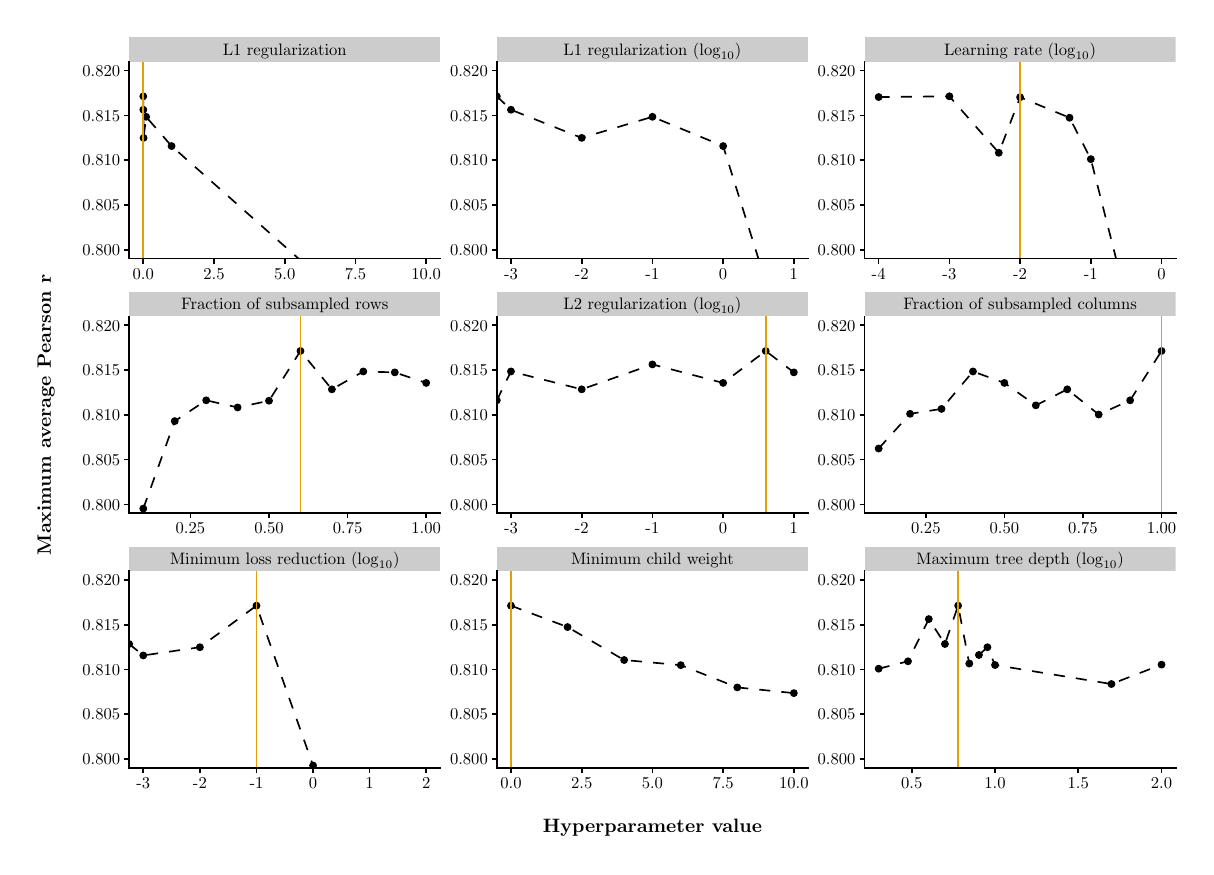
\begin{tikzpicture}[x=1pt,y=1pt]
	\definecolor{fillColor}{RGB}{255,255,255}
	\path[use as bounding box,fill=fillColor,fill opacity=0.00] (0,0) rectangle (418.34,295.82);
	\begin{scope}
		\path[clip] ( 36.67,212.35) rectangle (149.11,283.52);
		\definecolor{drawColor}{RGB}{0,0,0}
		\definecolor{fillColor}{RGB}{0,0,0}

		\path[draw=drawColor,line width= 0.4pt,line join=round,line cap=round,fill=fillColor] ( 41.78,271.01) circle (  1.21);

		\path[draw=drawColor,line width= 0.4pt,line join=round,line cap=round,fill=fillColor] ( 41.79,266.16) circle (  1.21);

		\path[draw=drawColor,line width= 0.4pt,line join=round,line cap=round,fill=fillColor] ( 41.88,255.99) circle (  1.21);

		\path[draw=drawColor,line width= 0.4pt,line join=round,line cap=round,fill=fillColor] ( 42.80,263.61) circle (  1.21);

		\path[draw=drawColor,line width= 0.4pt,line join=round,line cap=round,fill=fillColor] ( 52.00,253.03) circle (  1.21);

		\path[draw=drawColor,line width= 0.4pt,line join=round,line cap=round,fill=fillColor] (144.00,171.49) circle (  1.21);

		\path[draw=drawColor,line width= 0.6pt,dash pattern=on 4pt off 4pt ,line join=round] ( 41.78,271.01) --
		( 41.79,266.16) --
		( 41.88,255.99) --
		( 42.80,263.61) --
		( 52.00,253.03) --
		(144.00,171.49);
		\definecolor{drawColor}{RGB}{230,159,0}

		\path[draw=drawColor,line width= 0.6pt,line join=round] ( 41.78,212.35) -- ( 41.78,283.52);
	\end{scope}
	\begin{scope}
		\path[clip] ( 36.67,120.33) rectangle (149.11,191.50);
		\definecolor{drawColor}{RGB}{0,0,0}
		\definecolor{fillColor}{RGB}{0,0,0}

		\path[draw=drawColor,line width= 0.4pt,line join=round,line cap=round,fill=fillColor] ( 41.78,122.04) circle (  1.21);

		\path[draw=drawColor,line width= 0.4pt,line join=round,line cap=round,fill=fillColor] ( 53.14,153.65) circle (  1.21);

		\path[draw=drawColor,line width= 0.4pt,line join=round,line cap=round,fill=fillColor] ( 64.50,161.16) circle (  1.21);

		\path[draw=drawColor,line width= 0.4pt,line join=round,line cap=round,fill=fillColor] ( 75.86,158.59) circle (  1.21);

		\path[draw=drawColor,line width= 0.4pt,line join=round,line cap=round,fill=fillColor] ( 87.21,161.01) circle (  1.21);

		\path[draw=drawColor,line width= 0.4pt,line join=round,line cap=round,fill=fillColor] ( 98.57,178.99) circle (  1.21);

		\path[draw=drawColor,line width= 0.4pt,line join=round,line cap=round,fill=fillColor] (109.93,165.13) circle (  1.21);

		\path[draw=drawColor,line width= 0.4pt,line join=round,line cap=round,fill=fillColor] (121.29,171.59) circle (  1.21);

		\path[draw=drawColor,line width= 0.4pt,line join=round,line cap=round,fill=fillColor] (132.65,171.26) circle (  1.21);

		\path[draw=drawColor,line width= 0.4pt,line join=round,line cap=round,fill=fillColor] (144.00,167.45) circle (  1.21);

		\path[draw=drawColor,line width= 0.6pt,dash pattern=on 4pt off 4pt ,line join=round] ( 41.78,122.04) --
		( 53.14,153.65) --
		( 64.50,161.16) --
		( 75.86,158.59) --
		( 87.21,161.01) --
		( 98.57,178.99) --
		(109.93,165.13) --
		(121.29,171.59) --
		(132.65,171.26) --
		(144.00,167.45);
		\definecolor{drawColor}{RGB}{230,159,0}

		\path[draw=drawColor,line width= 0.6pt,line join=round] ( 98.57,120.33) -- ( 98.57,191.50);
	\end{scope}
	\begin{scope}
		\path[clip] ( 36.67, 28.30) rectangle (149.11, 99.48);
		\definecolor{drawColor}{RGB}{0,0,0}
		\definecolor{fillColor}{RGB}{0,0,0}

		\path[draw=drawColor,line width= 0.4pt,line join=round,line cap=round,fill=fillColor] ( 36.67, 73.11) circle (  1.21);

		\path[draw=drawColor,line width= 0.4pt,line join=round,line cap=round,fill=fillColor] ( 41.78, 68.98) circle (  1.21);

		\path[draw=drawColor,line width= 0.4pt,line join=round,line cap=round,fill=fillColor] ( 62.23, 71.94) circle (  1.21);

		\path[draw=drawColor,line width= 0.4pt,line join=round,line cap=round,fill=fillColor] ( 82.67, 86.97) circle (  1.21);

		\path[draw=drawColor,line width= 0.4pt,line join=round,line cap=round,fill=fillColor] (103.12, 29.20) circle (  1.21);

		\path[draw=drawColor,line width= 0.4pt,line join=round,line cap=round,fill=fillColor] (123.56,-433.02) circle (  1.21);

		\path[draw=drawColor,line width= 0.4pt,line join=round,line cap=round,fill=fillColor] (144.00,-1376.23) circle (  1.21);

		\path[draw=drawColor,line width= 0.6pt,dash pattern=on 4pt off 4pt ,line join=round] ( 36.67, 73.11) --
		( 41.78, 68.98) --
		( 62.23, 71.94) --
		( 82.67, 86.97) --
		(103.12, 29.20) --
		(123.56,-433.02) --
		(144.00,-1376.23);
		\definecolor{drawColor}{RGB}{230,159,0}

		\path[draw=drawColor,line width= 0.6pt,line join=round] ( 82.67, 28.30) -- ( 82.67, 99.48);
	\end{scope}
	\begin{scope}
		\path[clip] (169.53,212.35) rectangle (281.98,283.52);
		\definecolor{drawColor}{RGB}{0,0,0}
		\definecolor{fillColor}{RGB}{0,0,0}

		\path[draw=drawColor,line width= 0.4pt,line join=round,line cap=round,fill=fillColor] (169.53,271.01) circle (  1.21);

		\path[draw=drawColor,line width= 0.4pt,line join=round,line cap=round,fill=fillColor] (174.64,266.16) circle (  1.21);

		\path[draw=drawColor,line width= 0.4pt,line join=round,line cap=round,fill=fillColor] (200.20,255.99) circle (  1.21);

		\path[draw=drawColor,line width= 0.4pt,line join=round,line cap=round,fill=fillColor] (225.75,263.61) circle (  1.21);

		\path[draw=drawColor,line width= 0.4pt,line join=round,line cap=round,fill=fillColor] (251.31,253.03) circle (  1.21);

		\path[draw=drawColor,line width= 0.4pt,line join=round,line cap=round,fill=fillColor] (276.86,171.49) circle (  1.21);

		\path[draw=drawColor,line width= 0.6pt,dash pattern=on 4pt off 4pt ,line join=round] (169.53,271.01) --
		(174.64,266.16) --
		(200.20,255.99) --
		(225.75,263.61) --
		(251.31,253.03) --
		(276.86,171.49);
		\definecolor{drawColor}{RGB}{230,159,0}

		\path[draw=drawColor,line width= 0.6pt,line join=round] (169.53,212.35) -- (169.53,283.52);
	\end{scope}
	\begin{scope}
		\path[clip] (169.53,120.33) rectangle (281.98,191.50);
		\definecolor{drawColor}{RGB}{0,0,0}
		\definecolor{fillColor}{RGB}{0,0,0}

		\path[draw=drawColor,line width= 0.4pt,line join=round,line cap=round,fill=fillColor] (169.53,161.16) circle (  1.21);

		\path[draw=drawColor,line width= 0.4pt,line join=round,line cap=round,fill=fillColor] (174.64,171.59) circle (  1.21);

		\path[draw=drawColor,line width= 0.4pt,line join=round,line cap=round,fill=fillColor] (200.20,165.13) circle (  1.21);

		\path[draw=drawColor,line width= 0.4pt,line join=round,line cap=round,fill=fillColor] (225.75,174.13) circle (  1.21);

		\path[draw=drawColor,line width= 0.4pt,line join=round,line cap=round,fill=fillColor] (251.31,167.45) circle (  1.21);

		\path[draw=drawColor,line width= 0.4pt,line join=round,line cap=round,fill=fillColor] (266.69,178.99) circle (  1.21);

		\path[draw=drawColor,line width= 0.4pt,line join=round,line cap=round,fill=fillColor] (276.86,171.26) circle (  1.21);

		\path[draw=drawColor,line width= 0.6pt,dash pattern=on 4pt off 4pt ,line join=round] (169.53,161.16) --
		(174.64,171.59) --
		(200.20,165.13) --
		(225.75,174.13) --
		(251.31,167.45) --
		(266.69,178.99) --
		(276.86,171.26);
		\definecolor{drawColor}{RGB}{230,159,0}

		\path[draw=drawColor,line width= 0.6pt,line join=round] (266.69,120.33) -- (266.69,191.50);
	\end{scope}
	\begin{scope}
		\path[clip] (169.53, 28.30) rectangle (281.98, 99.48);
		\definecolor{drawColor}{RGB}{0,0,0}
		\definecolor{fillColor}{RGB}{0,0,0}

		\path[draw=drawColor,line width= 0.4pt,line join=round,line cap=round,fill=fillColor] (174.64, 86.97) circle (  1.21);

		\path[draw=drawColor,line width= 0.4pt,line join=round,line cap=round,fill=fillColor] (195.09, 79.23) circle (  1.21);

		\path[draw=drawColor,line width= 0.4pt,line join=round,line cap=round,fill=fillColor] (215.53, 67.32) circle (  1.21);

		\path[draw=drawColor,line width= 0.4pt,line join=round,line cap=round,fill=fillColor] (235.98, 65.47) circle (  1.21);

		\path[draw=drawColor,line width= 0.4pt,line join=round,line cap=round,fill=fillColor] (256.42, 57.42) circle (  1.21);

		\path[draw=drawColor,line width= 0.4pt,line join=round,line cap=round,fill=fillColor] (276.86, 55.36) circle (  1.21);

		\path[draw=drawColor,line width= 0.6pt,dash pattern=on 4pt off 4pt ,line join=round] (174.64, 86.97) --
		(195.09, 79.23) --
		(215.53, 67.32) --
		(235.98, 65.47) --
		(256.42, 57.42) --
		(276.86, 55.36);
		\definecolor{drawColor}{RGB}{230,159,0}

		\path[draw=drawColor,line width= 0.6pt,line join=round] (174.64, 28.30) -- (174.64, 99.48);
	\end{scope}
	\begin{scope}
		\path[clip] (302.39,212.35) rectangle (414.84,283.52);
		\definecolor{drawColor}{RGB}{0,0,0}
		\definecolor{fillColor}{RGB}{0,0,0}

		\path[draw=drawColor,line width= 0.4pt,line join=round,line cap=round,fill=fillColor] (307.50,270.75) circle (  1.21);

		\path[draw=drawColor,line width= 0.4pt,line join=round,line cap=round,fill=fillColor] (333.06,271.01) circle (  1.21);

		\path[draw=drawColor,line width= 0.4pt,line join=round,line cap=round,fill=fillColor] (350.92,250.61) circle (  1.21);

		\path[draw=drawColor,line width= 0.4pt,line join=round,line cap=round,fill=fillColor] (358.61,270.68) circle (  1.21);

		\path[draw=drawColor,line width= 0.4pt,line join=round,line cap=round,fill=fillColor] (376.48,263.28) circle (  1.21);

		\path[draw=drawColor,line width= 0.4pt,line join=round,line cap=round,fill=fillColor] (384.17,248.31) circle (  1.21);

		\path[draw=drawColor,line width= 0.4pt,line join=round,line cap=round,fill=fillColor] (402.03,177.91) circle (  1.21);

		\path[draw=drawColor,line width= 0.4pt,line join=round,line cap=round,fill=fillColor] (409.72,-98.71) circle (  1.21);

		\path[draw=drawColor,line width= 0.6pt,dash pattern=on 4pt off 4pt ,line join=round] (307.50,270.75) --
		(333.06,271.01) --
		(350.92,250.61) --
		(358.61,270.68) --
		(376.48,263.28) --
		(384.17,248.31) --
		(402.03,177.91) --
		(409.72,-98.71);
		\definecolor{drawColor}{RGB}{230,159,0}

		\path[draw=drawColor,line width= 0.6pt,line join=round] (358.61,212.35) -- (358.61,283.52);
	\end{scope}
	\begin{scope}
		\path[clip] (302.39,120.33) rectangle (414.84,191.50);
		\definecolor{drawColor}{RGB}{0,0,0}
		\definecolor{fillColor}{RGB}{0,0,0}

		\path[draw=drawColor,line width= 0.4pt,line join=round,line cap=round,fill=fillColor] (307.50,143.75) circle (  1.21);

		\path[draw=drawColor,line width= 0.4pt,line join=round,line cap=round,fill=fillColor] (318.86,156.29) circle (  1.21);

		\path[draw=drawColor,line width= 0.4pt,line join=round,line cap=round,fill=fillColor] (330.22,158.06) circle (  1.21);

		\path[draw=drawColor,line width= 0.4pt,line join=round,line cap=round,fill=fillColor] (341.58,171.59) circle (  1.21);

		\path[draw=drawColor,line width= 0.4pt,line join=round,line cap=round,fill=fillColor] (352.93,167.45) circle (  1.21);

		\path[draw=drawColor,line width= 0.4pt,line join=round,line cap=round,fill=fillColor] (364.29,159.34) circle (  1.21);

		\path[draw=drawColor,line width= 0.4pt,line join=round,line cap=round,fill=fillColor] (375.65,165.13) circle (  1.21);

		\path[draw=drawColor,line width= 0.4pt,line join=round,line cap=round,fill=fillColor] (387.01,156.03) circle (  1.21);

		\path[draw=drawColor,line width= 0.4pt,line join=round,line cap=round,fill=fillColor] (398.37,161.16) circle (  1.21);

		\path[draw=drawColor,line width= 0.4pt,line join=round,line cap=round,fill=fillColor] (409.72,178.99) circle (  1.21);

		\path[draw=drawColor,line width= 0.6pt,dash pattern=on 4pt off 4pt ,line join=round] (307.50,143.75) --
		(318.86,156.29) --
		(330.22,158.06) --
		(341.58,171.59) --
		(352.93,167.45) --
		(364.29,159.34) --
		(375.65,165.13) --
		(387.01,156.03) --
		(398.37,161.16) --
		(409.72,178.99);
		\definecolor{drawColor}{RGB}{230,159,0}

		\path[draw=drawColor,line width= 0.6pt,line join=round] (409.72,120.33) -- (409.72,191.50);
	\end{scope}
	\begin{scope}
		\path[clip] (302.39, 28.30) rectangle (414.84, 99.48);
		\definecolor{drawColor}{RGB}{0,0,0}
		\definecolor{fillColor}{RGB}{0,0,0}

		\path[draw=drawColor,line width= 0.4pt,line join=round,line cap=round,fill=fillColor] (307.50, 64.19) circle (  1.21);

		\path[draw=drawColor,line width= 0.4pt,line join=round,line cap=round,fill=fillColor] (318.10, 66.86) circle (  1.21);

		\path[draw=drawColor,line width= 0.4pt,line join=round,line cap=round,fill=fillColor] (325.62, 82.11) circle (  1.21);

		\path[draw=drawColor,line width= 0.4pt,line join=round,line cap=round,fill=fillColor] (331.45, 73.11) circle (  1.21);

		\path[draw=drawColor,line width= 0.4pt,line join=round,line cap=round,fill=fillColor] (336.21, 86.97) circle (  1.21);

		\path[draw=drawColor,line width= 0.4pt,line join=round,line cap=round,fill=fillColor] (340.24, 66.03) circle (  1.21);

		\path[draw=drawColor,line width= 0.4pt,line join=round,line cap=round,fill=fillColor] (343.73, 69.14) circle (  1.21);

		\path[draw=drawColor,line width= 0.4pt,line join=round,line cap=round,fill=fillColor] (346.80, 71.94) circle (  1.21);

		\path[draw=drawColor,line width= 0.4pt,line join=round,line cap=round,fill=fillColor] (349.56, 65.51) circle (  1.21);

		\path[draw=drawColor,line width= 0.4pt,line join=round,line cap=round,fill=fillColor] (391.61, 58.65) circle (  1.21);

		\path[draw=drawColor,line width= 0.4pt,line join=round,line cap=round,fill=fillColor] (409.72, 65.66) circle (  1.21);

		\path[draw=drawColor,line width= 0.6pt,dash pattern=on 4pt off 4pt ,line join=round] (307.50, 64.19) --
		(318.10, 66.86) --
		(325.62, 82.11) --
		(331.45, 73.11) --
		(336.21, 86.97) --
		(340.24, 66.03) --
		(343.73, 69.14) --
		(346.80, 71.94) --
		(349.56, 65.51) --
		(391.61, 58.65) --
		(409.72, 65.66);
		\definecolor{drawColor}{RGB}{230,159,0}

		\path[draw=drawColor,line width= 0.6pt,line join=round] (336.21, 28.30) -- (336.21, 99.48);
	\end{scope}
	\begin{scope}
		\path[clip] ( 36.67, 99.48) rectangle (149.11,108.28);
		\definecolor{fillColor}{gray}{0.80}

		\path[fill=fillColor] ( 36.67, 99.48) rectangle (149.11,108.28);
		\definecolor{drawColor}{RGB}{0,0,0}

		\node[text=drawColor,anchor=base,inner sep=0pt, outer sep=0pt, scale=  0.60] at ( 92.89,101.81) {Minimum loss reduction ($\log_{10}$)};
	\end{scope}
	\begin{scope}
		\path[clip] (169.53, 99.48) rectangle (281.98,108.28);
		\definecolor{fillColor}{gray}{0.80}

		\path[fill=fillColor] (169.53, 99.48) rectangle (281.98,108.28);
		\definecolor{drawColor}{RGB}{0,0,0}

		\node[text=drawColor,anchor=base,inner sep=0pt, outer sep=0pt, scale=  0.60] at (225.75,101.81) {Minimum child weight};
	\end{scope}
	\begin{scope}
		\path[clip] (302.39, 99.48) rectangle (414.84,108.28);
		\definecolor{fillColor}{gray}{0.80}

		\path[fill=fillColor] (302.39, 99.48) rectangle (414.84,108.28);
		\definecolor{drawColor}{RGB}{0,0,0}

		\node[text=drawColor,anchor=base,inner sep=0pt, outer sep=0pt, scale=  0.60] at (358.61,101.81) {Maximum tree depth ($\log_{10}$)};
	\end{scope}
	\begin{scope}
		\path[clip] ( 36.67,191.50) rectangle (149.11,200.30);
		\definecolor{fillColor}{gray}{0.80}

		\path[fill=fillColor] ( 36.67,191.50) rectangle (149.11,200.30);
		\definecolor{drawColor}{RGB}{0,0,0}

		\node[text=drawColor,anchor=base,inner sep=0pt, outer sep=0pt, scale=  0.60] at ( 92.89,193.83) {Fraction of subsampled rows};
	\end{scope}
	\begin{scope}
		\path[clip] (169.53,191.50) rectangle (281.98,200.30);
		\definecolor{fillColor}{gray}{0.80}

		\path[fill=fillColor] (169.53,191.50) rectangle (281.98,200.30);
		\definecolor{drawColor}{RGB}{0,0,0}

		\node[text=drawColor,anchor=base,inner sep=0pt, outer sep=0pt, scale=  0.60] at (225.75,193.83) {L2 regularization ($\log_{10}$)};
	\end{scope}
	\begin{scope}
		\path[clip] (302.39,191.50) rectangle (414.84,200.30);
		\definecolor{fillColor}{gray}{0.80}

		\path[fill=fillColor] (302.39,191.50) rectangle (414.84,200.30);
		\definecolor{drawColor}{RGB}{0,0,0}

		\node[text=drawColor,anchor=base,inner sep=0pt, outer sep=0pt, scale=  0.60] at (358.61,193.83) {Fraction of subsampled columns};
	\end{scope}
	\begin{scope}
		\path[clip] ( 36.67,283.52) rectangle (149.11,292.32);
		\definecolor{fillColor}{gray}{0.80}

		\path[fill=fillColor] ( 36.67,283.52) rectangle (149.11,292.32);
		\definecolor{drawColor}{RGB}{0,0,0}

		\node[text=drawColor,anchor=base,inner sep=0pt, outer sep=0pt, scale=  0.60] at ( 92.89,285.86) {L1 regularization};
	\end{scope}
	\begin{scope}
		\path[clip] (169.53,283.52) rectangle (281.98,292.32);
		\definecolor{fillColor}{gray}{0.80}

		\path[fill=fillColor] (169.53,283.52) rectangle (281.98,292.32);
		\definecolor{drawColor}{RGB}{0,0,0}

		\node[text=drawColor,anchor=base,inner sep=0pt, outer sep=0pt, scale=  0.60] at (225.75,285.86) {L1 regularization ($\log_{10}$)};
	\end{scope}
	\begin{scope}
		\path[clip] (302.39,283.52) rectangle (414.84,292.32);
		\definecolor{fillColor}{gray}{0.80}

		\path[fill=fillColor] (302.39,283.52) rectangle (414.84,292.32);
		\definecolor{drawColor}{RGB}{0,0,0}

		\node[text=drawColor,anchor=base,inner sep=0pt, outer sep=0pt, scale=  0.60] at (358.61,285.86) {Learning rate ($\log_{10}$)};
	\end{scope}
	\begin{scope}
		\path[clip] (  0.00,  0.00) rectangle (418.34,295.82);
		\definecolor{drawColor}{RGB}{0,0,0}

		\path[draw=drawColor,line width= 0.6pt,line join=round,line cap=rect] ( 36.67, 28.30) --
		(149.11, 28.30);
	\end{scope}
	\begin{scope}
		\path[clip] (  0.00,  0.00) rectangle (418.34,295.82);
		\definecolor{drawColor}{RGB}{0,0,0}

		\path[draw=drawColor,line width= 0.6pt,line join=round] ( 41.78, 26.55) --
		( 41.78, 28.30);

		\path[draw=drawColor,line width= 0.6pt,line join=round] ( 62.23, 26.55) --
		( 62.23, 28.30);

		\path[draw=drawColor,line width= 0.6pt,line join=round] ( 82.67, 26.55) --
		( 82.67, 28.30);

		\path[draw=drawColor,line width= 0.6pt,line join=round] (103.12, 26.55) --
		(103.12, 28.30);

		\path[draw=drawColor,line width= 0.6pt,line join=round] (123.56, 26.55) --
		(123.56, 28.30);

		\path[draw=drawColor,line width= 0.6pt,line join=round] (144.00, 26.55) --
		(144.00, 28.30);
	\end{scope}
	\begin{scope}
		\path[clip] (  0.00,  0.00) rectangle (418.34,295.82);
		\definecolor{drawColor}{RGB}{0,0,0}

		\node[text=drawColor,anchor=base,inner sep=0pt, outer sep=0pt, scale=  0.60] at ( 41.78, 20.92) {-3};

		\node[text=drawColor,anchor=base,inner sep=0pt, outer sep=0pt, scale=  0.60] at ( 62.23, 20.92) {-2};

		\node[text=drawColor,anchor=base,inner sep=0pt, outer sep=0pt, scale=  0.60] at ( 82.67, 20.92) {-1};

		\node[text=drawColor,anchor=base,inner sep=0pt, outer sep=0pt, scale=  0.60] at (103.12, 20.92) {0};

		\node[text=drawColor,anchor=base,inner sep=0pt, outer sep=0pt, scale=  0.60] at (123.56, 20.92) {1};

		\node[text=drawColor,anchor=base,inner sep=0pt, outer sep=0pt, scale=  0.60] at (144.00, 20.92) {2};
	\end{scope}
	\begin{scope}
		\path[clip] (  0.00,  0.00) rectangle (418.34,295.82);
		\definecolor{drawColor}{RGB}{0,0,0}

		\path[draw=drawColor,line width= 0.6pt,line join=round,line cap=rect] (169.53, 28.30) --
		(281.98, 28.30);
	\end{scope}
	\begin{scope}
		\path[clip] (  0.00,  0.00) rectangle (418.34,295.82);
		\definecolor{drawColor}{RGB}{0,0,0}

		\path[draw=drawColor,line width= 0.6pt,line join=round] (174.64, 26.55) --
		(174.64, 28.30);

		\path[draw=drawColor,line width= 0.6pt,line join=round] (200.20, 26.55) --
		(200.20, 28.30);

		\path[draw=drawColor,line width= 0.6pt,line join=round] (225.75, 26.55) --
		(225.75, 28.30);

		\path[draw=drawColor,line width= 0.6pt,line join=round] (251.31, 26.55) --
		(251.31, 28.30);

		\path[draw=drawColor,line width= 0.6pt,line join=round] (276.86, 26.55) --
		(276.86, 28.30);
	\end{scope}
	\begin{scope}
		\path[clip] (  0.00,  0.00) rectangle (418.34,295.82);
		\definecolor{drawColor}{RGB}{0,0,0}

		\node[text=drawColor,anchor=base,inner sep=0pt, outer sep=0pt, scale=  0.60] at (174.64, 20.92) {0.0};

		\node[text=drawColor,anchor=base,inner sep=0pt, outer sep=0pt, scale=  0.60] at (200.20, 20.92) {2.5};

		\node[text=drawColor,anchor=base,inner sep=0pt, outer sep=0pt, scale=  0.60] at (225.75, 20.92) {5.0};

		\node[text=drawColor,anchor=base,inner sep=0pt, outer sep=0pt, scale=  0.60] at (251.31, 20.92) {7.5};

		\node[text=drawColor,anchor=base,inner sep=0pt, outer sep=0pt, scale=  0.60] at (276.86, 20.92) {10.0};
	\end{scope}
	\begin{scope}
		\path[clip] (  0.00,  0.00) rectangle (418.34,295.82);
		\definecolor{drawColor}{RGB}{0,0,0}

		\path[draw=drawColor,line width= 0.6pt,line join=round,line cap=rect] (302.39, 28.30) --
		(414.84, 28.30);
	\end{scope}
	\begin{scope}
		\path[clip] (  0.00,  0.00) rectangle (418.34,295.82);
		\definecolor{drawColor}{RGB}{0,0,0}

		\path[draw=drawColor,line width= 0.6pt,line join=round] (319.47, 26.55) --
		(319.47, 28.30);

		\path[draw=drawColor,line width= 0.6pt,line join=round] (349.56, 26.55) --
		(349.56, 28.30);

		\path[draw=drawColor,line width= 0.6pt,line join=round] (379.64, 26.55) --
		(379.64, 28.30);

		\path[draw=drawColor,line width= 0.6pt,line join=round] (409.72, 26.55) --
		(409.72, 28.30);
	\end{scope}
	\begin{scope}
		\path[clip] (  0.00,  0.00) rectangle (418.34,295.82);
		\definecolor{drawColor}{RGB}{0,0,0}

		\node[text=drawColor,anchor=base,inner sep=0pt, outer sep=0pt, scale=  0.60] at (319.47, 20.92) {0.5};

		\node[text=drawColor,anchor=base,inner sep=0pt, outer sep=0pt, scale=  0.60] at (349.56, 20.92) {1.0};

		\node[text=drawColor,anchor=base,inner sep=0pt, outer sep=0pt, scale=  0.60] at (379.64, 20.92) {1.5};

		\node[text=drawColor,anchor=base,inner sep=0pt, outer sep=0pt, scale=  0.60] at (409.72, 20.92) {2.0};
	\end{scope}
	\begin{scope}
		\path[clip] (  0.00,  0.00) rectangle (418.34,295.82);
		\definecolor{drawColor}{RGB}{0,0,0}

		\path[draw=drawColor,line width= 0.6pt,line join=round,line cap=rect] ( 36.67,120.33) --
		(149.11,120.33);
	\end{scope}
	\begin{scope}
		\path[clip] (  0.00,  0.00) rectangle (418.34,295.82);
		\definecolor{drawColor}{RGB}{0,0,0}

		\path[draw=drawColor,line width= 0.6pt,line join=round] ( 58.82,118.58) --
		( 58.82,120.33);

		\path[draw=drawColor,line width= 0.6pt,line join=round] ( 87.21,118.58) --
		( 87.21,120.33);

		\path[draw=drawColor,line width= 0.6pt,line join=round] (115.61,118.58) --
		(115.61,120.33);

		\path[draw=drawColor,line width= 0.6pt,line join=round] (144.00,118.58) --
		(144.00,120.33);
	\end{scope}
	\begin{scope}
		\path[clip] (  0.00,  0.00) rectangle (418.34,295.82);
		\definecolor{drawColor}{RGB}{0,0,0}

		\node[text=drawColor,anchor=base,inner sep=0pt, outer sep=0pt, scale=  0.60] at ( 58.82,112.94) {0.25};

		\node[text=drawColor,anchor=base,inner sep=0pt, outer sep=0pt, scale=  0.60] at ( 87.21,112.94) {0.50};

		\node[text=drawColor,anchor=base,inner sep=0pt, outer sep=0pt, scale=  0.60] at (115.61,112.94) {0.75};

		\node[text=drawColor,anchor=base,inner sep=0pt, outer sep=0pt, scale=  0.60] at (144.00,112.94) {1.00};
	\end{scope}
	\begin{scope}
		\path[clip] (  0.00,  0.00) rectangle (418.34,295.82);
		\definecolor{drawColor}{RGB}{0,0,0}

		\path[draw=drawColor,line width= 0.6pt,line join=round,line cap=rect] (169.53,120.33) --
		(281.98,120.33);
	\end{scope}
	\begin{scope}
		\path[clip] (  0.00,  0.00) rectangle (418.34,295.82);
		\definecolor{drawColor}{RGB}{0,0,0}

		\path[draw=drawColor,line width= 0.6pt,line join=round] (174.64,118.58) --
		(174.64,120.33);

		\path[draw=drawColor,line width= 0.6pt,line join=round] (200.20,118.58) --
		(200.20,120.33);

		\path[draw=drawColor,line width= 0.6pt,line join=round] (225.75,118.58) --
		(225.75,120.33);

		\path[draw=drawColor,line width= 0.6pt,line join=round] (251.31,118.58) --
		(251.31,120.33);

		\path[draw=drawColor,line width= 0.6pt,line join=round] (276.86,118.58) --
		(276.86,120.33);
	\end{scope}
	\begin{scope}
		\path[clip] (  0.00,  0.00) rectangle (418.34,295.82);
		\definecolor{drawColor}{RGB}{0,0,0}

		\node[text=drawColor,anchor=base,inner sep=0pt, outer sep=0pt, scale=  0.60] at (174.64,112.94) {-3};

		\node[text=drawColor,anchor=base,inner sep=0pt, outer sep=0pt, scale=  0.60] at (200.20,112.94) {-2};

		\node[text=drawColor,anchor=base,inner sep=0pt, outer sep=0pt, scale=  0.60] at (225.75,112.94) {-1};

		\node[text=drawColor,anchor=base,inner sep=0pt, outer sep=0pt, scale=  0.60] at (251.31,112.94) {0};

		\node[text=drawColor,anchor=base,inner sep=0pt, outer sep=0pt, scale=  0.60] at (276.86,112.94) {1};
	\end{scope}
	\begin{scope}
		\path[clip] (  0.00,  0.00) rectangle (418.34,295.82);
		\definecolor{drawColor}{RGB}{0,0,0}

		\path[draw=drawColor,line width= 0.6pt,line join=round,line cap=rect] (302.39,120.33) --
		(414.84,120.33);
	\end{scope}
	\begin{scope}
		\path[clip] (  0.00,  0.00) rectangle (418.34,295.82);
		\definecolor{drawColor}{RGB}{0,0,0}

		\path[draw=drawColor,line width= 0.6pt,line join=round] (324.54,118.58) --
		(324.54,120.33);

		\path[draw=drawColor,line width= 0.6pt,line join=round] (352.93,118.58) --
		(352.93,120.33);

		\path[draw=drawColor,line width= 0.6pt,line join=round] (381.33,118.58) --
		(381.33,120.33);

		\path[draw=drawColor,line width= 0.6pt,line join=round] (409.72,118.58) --
		(409.72,120.33);
	\end{scope}
	\begin{scope}
		\path[clip] (  0.00,  0.00) rectangle (418.34,295.82);
		\definecolor{drawColor}{RGB}{0,0,0}

		\node[text=drawColor,anchor=base,inner sep=0pt, outer sep=0pt, scale=  0.60] at (324.54,112.94) {0.25};

		\node[text=drawColor,anchor=base,inner sep=0pt, outer sep=0pt, scale=  0.60] at (352.93,112.94) {0.50};

		\node[text=drawColor,anchor=base,inner sep=0pt, outer sep=0pt, scale=  0.60] at (381.33,112.94) {0.75};

		\node[text=drawColor,anchor=base,inner sep=0pt, outer sep=0pt, scale=  0.60] at (409.72,112.94) {1.00};
	\end{scope}
	\begin{scope}
		\path[clip] (  0.00,  0.00) rectangle (418.34,295.82);
		\definecolor{drawColor}{RGB}{0,0,0}

		\path[draw=drawColor,line width= 0.6pt,line join=round,line cap=rect] ( 36.67,212.35) --
		(149.11,212.35);
	\end{scope}
	\begin{scope}
		\path[clip] (  0.00,  0.00) rectangle (418.34,295.82);
		\definecolor{drawColor}{RGB}{0,0,0}

		\path[draw=drawColor,line width= 0.6pt,line join=round] ( 41.78,210.60) --
		( 41.78,212.35);

		\path[draw=drawColor,line width= 0.6pt,line join=round] ( 67.34,210.60) --
		( 67.34,212.35);

		\path[draw=drawColor,line width= 0.6pt,line join=round] ( 92.89,210.60) --
		( 92.89,212.35);

		\path[draw=drawColor,line width= 0.6pt,line join=round] (118.45,210.60) --
		(118.45,212.35);

		\path[draw=drawColor,line width= 0.6pt,line join=round] (144.00,210.60) --
		(144.00,212.35);
	\end{scope}
	\begin{scope}
		\path[clip] (  0.00,  0.00) rectangle (418.34,295.82);
		\definecolor{drawColor}{RGB}{0,0,0}

		\node[text=drawColor,anchor=base,inner sep=0pt, outer sep=0pt, scale=  0.60] at ( 41.78,204.97) {0.0};

		\node[text=drawColor,anchor=base,inner sep=0pt, outer sep=0pt, scale=  0.60] at ( 67.34,204.97) {2.5};

		\node[text=drawColor,anchor=base,inner sep=0pt, outer sep=0pt, scale=  0.60] at ( 92.89,204.97) {5.0};

		\node[text=drawColor,anchor=base,inner sep=0pt, outer sep=0pt, scale=  0.60] at (118.45,204.97) {7.5};

		\node[text=drawColor,anchor=base,inner sep=0pt, outer sep=0pt, scale=  0.60] at (144.00,204.97) {10.0};
	\end{scope}
	\begin{scope}
		\path[clip] (  0.00,  0.00) rectangle (418.34,295.82);
		\definecolor{drawColor}{RGB}{0,0,0}

		\path[draw=drawColor,line width= 0.6pt,line join=round,line cap=rect] (169.53,212.35) --
		(281.98,212.35);
	\end{scope}
	\begin{scope}
		\path[clip] (  0.00,  0.00) rectangle (418.34,295.82);
		\definecolor{drawColor}{RGB}{0,0,0}

		\path[draw=drawColor,line width= 0.6pt,line join=round] (174.64,210.60) --
		(174.64,212.35);

		\path[draw=drawColor,line width= 0.6pt,line join=round] (200.20,210.60) --
		(200.20,212.35);

		\path[draw=drawColor,line width= 0.6pt,line join=round] (225.75,210.60) --
		(225.75,212.35);

		\path[draw=drawColor,line width= 0.6pt,line join=round] (251.31,210.60) --
		(251.31,212.35);

		\path[draw=drawColor,line width= 0.6pt,line join=round] (276.86,210.60) --
		(276.86,212.35);
	\end{scope}
	\begin{scope}
		\path[clip] (  0.00,  0.00) rectangle (418.34,295.82);
		\definecolor{drawColor}{RGB}{0,0,0}

		\node[text=drawColor,anchor=base,inner sep=0pt, outer sep=0pt, scale=  0.60] at (174.64,204.97) {-3};

		\node[text=drawColor,anchor=base,inner sep=0pt, outer sep=0pt, scale=  0.60] at (200.20,204.97) {-2};

		\node[text=drawColor,anchor=base,inner sep=0pt, outer sep=0pt, scale=  0.60] at (225.75,204.97) {-1};

		\node[text=drawColor,anchor=base,inner sep=0pt, outer sep=0pt, scale=  0.60] at (251.31,204.97) {0};

		\node[text=drawColor,anchor=base,inner sep=0pt, outer sep=0pt, scale=  0.60] at (276.86,204.97) {1};
	\end{scope}
	\begin{scope}
		\path[clip] (  0.00,  0.00) rectangle (418.34,295.82);
		\definecolor{drawColor}{RGB}{0,0,0}

		\path[draw=drawColor,line width= 0.6pt,line join=round,line cap=rect] (302.39,212.35) --
		(414.84,212.35);
	\end{scope}
	\begin{scope}
		\path[clip] (  0.00,  0.00) rectangle (418.34,295.82);
		\definecolor{drawColor}{RGB}{0,0,0}

		\path[draw=drawColor,line width= 0.6pt,line join=round] (307.50,210.60) --
		(307.50,212.35);

		\path[draw=drawColor,line width= 0.6pt,line join=round] (333.06,210.60) --
		(333.06,212.35);

		\path[draw=drawColor,line width= 0.6pt,line join=round] (358.61,210.60) --
		(358.61,212.35);

		\path[draw=drawColor,line width= 0.6pt,line join=round] (384.17,210.60) --
		(384.17,212.35);

		\path[draw=drawColor,line width= 0.6pt,line join=round] (409.72,210.60) --
		(409.72,212.35);
	\end{scope}
	\begin{scope}
		\path[clip] (  0.00,  0.00) rectangle (418.34,295.82);
		\definecolor{drawColor}{RGB}{0,0,0}

		\node[text=drawColor,anchor=base,inner sep=0pt, outer sep=0pt, scale=  0.60] at (307.50,204.97) {-4};

		\node[text=drawColor,anchor=base,inner sep=0pt, outer sep=0pt, scale=  0.60] at (333.06,204.97) {-3};

		\node[text=drawColor,anchor=base,inner sep=0pt, outer sep=0pt, scale=  0.60] at (358.61,204.97) {-2};

		\node[text=drawColor,anchor=base,inner sep=0pt, outer sep=0pt, scale=  0.60] at (384.17,204.97) {-1};

		\node[text=drawColor,anchor=base,inner sep=0pt, outer sep=0pt, scale=  0.60] at (409.72,204.97) {0};
	\end{scope}
	\begin{scope}
		\path[clip] (  0.00,  0.00) rectangle (418.34,295.82);
		\definecolor{drawColor}{RGB}{0,0,0}

		\path[draw=drawColor,line width= 0.6pt,line join=round,line cap=rect] (302.39,212.35) --
		(302.39,283.52);
	\end{scope}
	\begin{scope}
		\path[clip] (  0.00,  0.00) rectangle (418.34,295.82);
		\definecolor{drawColor}{RGB}{0,0,0}

		\node[text=drawColor,anchor=base east,inner sep=0pt, outer sep=0pt, scale=  0.60] at (299.14,213.52) {0.800};

		\node[text=drawColor,anchor=base east,inner sep=0pt, outer sep=0pt, scale=  0.60] at (299.14,229.69) {0.805};

		\node[text=drawColor,anchor=base east,inner sep=0pt, outer sep=0pt, scale=  0.60] at (299.14,245.87) {0.810};

		\node[text=drawColor,anchor=base east,inner sep=0pt, outer sep=0pt, scale=  0.60] at (299.14,262.05) {0.815};

		\node[text=drawColor,anchor=base east,inner sep=0pt, outer sep=0pt, scale=  0.60] at (299.14,278.22) {0.820};
	\end{scope}
	\begin{scope}
		\path[clip] (  0.00,  0.00) rectangle (418.34,295.82);
		\definecolor{drawColor}{RGB}{0,0,0}

		\path[draw=drawColor,line width= 0.6pt,line join=round] (300.64,215.59) --
		(302.39,215.59);

		\path[draw=drawColor,line width= 0.6pt,line join=round] (300.64,231.76) --
		(302.39,231.76);

		\path[draw=drawColor,line width= 0.6pt,line join=round] (300.64,247.94) --
		(302.39,247.94);

		\path[draw=drawColor,line width= 0.6pt,line join=round] (300.64,264.11) --
		(302.39,264.11);

		\path[draw=drawColor,line width= 0.6pt,line join=round] (300.64,280.29) --
		(302.39,280.29);
	\end{scope}
	\begin{scope}
		\path[clip] (  0.00,  0.00) rectangle (418.34,295.82);
		\definecolor{drawColor}{RGB}{0,0,0}

		\path[draw=drawColor,line width= 0.6pt,line join=round,line cap=rect] (302.39,120.33) --
		(302.39,191.50);
	\end{scope}
	\begin{scope}
		\path[clip] (  0.00,  0.00) rectangle (418.34,295.82);
		\definecolor{drawColor}{RGB}{0,0,0}

		\node[text=drawColor,anchor=base east,inner sep=0pt, outer sep=0pt, scale=  0.60] at (299.14,121.50) {0.800};

		\node[text=drawColor,anchor=base east,inner sep=0pt, outer sep=0pt, scale=  0.60] at (299.14,137.67) {0.805};

		\node[text=drawColor,anchor=base east,inner sep=0pt, outer sep=0pt, scale=  0.60] at (299.14,153.85) {0.810};

		\node[text=drawColor,anchor=base east,inner sep=0pt, outer sep=0pt, scale=  0.60] at (299.14,170.02) {0.815};

		\node[text=drawColor,anchor=base east,inner sep=0pt, outer sep=0pt, scale=  0.60] at (299.14,186.20) {0.820};
	\end{scope}
	\begin{scope}
		\path[clip] (  0.00,  0.00) rectangle (418.34,295.82);
		\definecolor{drawColor}{RGB}{0,0,0}

		\path[draw=drawColor,line width= 0.6pt,line join=round] (300.64,123.56) --
		(302.39,123.56);

		\path[draw=drawColor,line width= 0.6pt,line join=round] (300.64,139.74) --
		(302.39,139.74);

		\path[draw=drawColor,line width= 0.6pt,line join=round] (300.64,155.91) --
		(302.39,155.91);

		\path[draw=drawColor,line width= 0.6pt,line join=round] (300.64,172.09) --
		(302.39,172.09);

		\path[draw=drawColor,line width= 0.6pt,line join=round] (300.64,188.26) --
		(302.39,188.26);
	\end{scope}
	\begin{scope}
		\path[clip] (  0.00,  0.00) rectangle (418.34,295.82);
		\definecolor{drawColor}{RGB}{0,0,0}

		\path[draw=drawColor,line width= 0.6pt,line join=round,line cap=rect] (302.39, 28.30) --
		(302.39, 99.48);
	\end{scope}
	\begin{scope}
		\path[clip] (  0.00,  0.00) rectangle (418.34,295.82);
		\definecolor{drawColor}{RGB}{0,0,0}

		\node[text=drawColor,anchor=base east,inner sep=0pt, outer sep=0pt, scale=  0.60] at (299.14, 29.47) {0.800};

		\node[text=drawColor,anchor=base east,inner sep=0pt, outer sep=0pt, scale=  0.60] at (299.14, 45.65) {0.805};

		\node[text=drawColor,anchor=base east,inner sep=0pt, outer sep=0pt, scale=  0.60] at (299.14, 61.82) {0.810};

		\node[text=drawColor,anchor=base east,inner sep=0pt, outer sep=0pt, scale=  0.60] at (299.14, 78.00) {0.815};

		\node[text=drawColor,anchor=base east,inner sep=0pt, outer sep=0pt, scale=  0.60] at (299.14, 94.18) {0.820};
	\end{scope}
	\begin{scope}
		\path[clip] (  0.00,  0.00) rectangle (418.34,295.82);
		\definecolor{drawColor}{RGB}{0,0,0}

		\path[draw=drawColor,line width= 0.6pt,line join=round] (300.64, 31.54) --
		(302.39, 31.54);

		\path[draw=drawColor,line width= 0.6pt,line join=round] (300.64, 47.72) --
		(302.39, 47.72);

		\path[draw=drawColor,line width= 0.6pt,line join=round] (300.64, 63.89) --
		(302.39, 63.89);

		\path[draw=drawColor,line width= 0.6pt,line join=round] (300.64, 80.07) --
		(302.39, 80.07);

		\path[draw=drawColor,line width= 0.6pt,line join=round] (300.64, 96.24) --
		(302.39, 96.24);
	\end{scope}
	\begin{scope}
		\path[clip] (  0.00,  0.00) rectangle (418.34,295.82);
		\definecolor{drawColor}{RGB}{0,0,0}

		\path[draw=drawColor,line width= 0.6pt,line join=round,line cap=rect] (169.53,212.35) --
		(169.53,283.52);
	\end{scope}
	\begin{scope}
		\path[clip] (  0.00,  0.00) rectangle (418.34,295.82);
		\definecolor{drawColor}{RGB}{0,0,0}

		\node[text=drawColor,anchor=base east,inner sep=0pt, outer sep=0pt, scale=  0.60] at (166.28,213.52) {0.800};

		\node[text=drawColor,anchor=base east,inner sep=0pt, outer sep=0pt, scale=  0.60] at (166.28,229.69) {0.805};

		\node[text=drawColor,anchor=base east,inner sep=0pt, outer sep=0pt, scale=  0.60] at (166.28,245.87) {0.810};

		\node[text=drawColor,anchor=base east,inner sep=0pt, outer sep=0pt, scale=  0.60] at (166.28,262.05) {0.815};

		\node[text=drawColor,anchor=base east,inner sep=0pt, outer sep=0pt, scale=  0.60] at (166.28,278.22) {0.820};
	\end{scope}
	\begin{scope}
		\path[clip] (  0.00,  0.00) rectangle (418.34,295.82);
		\definecolor{drawColor}{RGB}{0,0,0}

		\path[draw=drawColor,line width= 0.6pt,line join=round] (167.78,215.59) --
		(169.53,215.59);

		\path[draw=drawColor,line width= 0.6pt,line join=round] (167.78,231.76) --
		(169.53,231.76);

		\path[draw=drawColor,line width= 0.6pt,line join=round] (167.78,247.94) --
		(169.53,247.94);

		\path[draw=drawColor,line width= 0.6pt,line join=round] (167.78,264.11) --
		(169.53,264.11);

		\path[draw=drawColor,line width= 0.6pt,line join=round] (167.78,280.29) --
		(169.53,280.29);
	\end{scope}
	\begin{scope}
		\path[clip] (  0.00,  0.00) rectangle (418.34,295.82);
		\definecolor{drawColor}{RGB}{0,0,0}

		\path[draw=drawColor,line width= 0.6pt,line join=round,line cap=rect] (169.53,120.33) --
		(169.53,191.50);
	\end{scope}
	\begin{scope}
		\path[clip] (  0.00,  0.00) rectangle (418.34,295.82);
		\definecolor{drawColor}{RGB}{0,0,0}

		\node[text=drawColor,anchor=base east,inner sep=0pt, outer sep=0pt, scale=  0.60] at (166.28,121.50) {0.800};

		\node[text=drawColor,anchor=base east,inner sep=0pt, outer sep=0pt, scale=  0.60] at (166.28,137.67) {0.805};

		\node[text=drawColor,anchor=base east,inner sep=0pt, outer sep=0pt, scale=  0.60] at (166.28,153.85) {0.810};

		\node[text=drawColor,anchor=base east,inner sep=0pt, outer sep=0pt, scale=  0.60] at (166.28,170.02) {0.815};

		\node[text=drawColor,anchor=base east,inner sep=0pt, outer sep=0pt, scale=  0.60] at (166.28,186.20) {0.820};
	\end{scope}
	\begin{scope}
		\path[clip] (  0.00,  0.00) rectangle (418.34,295.82);
		\definecolor{drawColor}{RGB}{0,0,0}

		\path[draw=drawColor,line width= 0.6pt,line join=round] (167.78,123.56) --
		(169.53,123.56);

		\path[draw=drawColor,line width= 0.6pt,line join=round] (167.78,139.74) --
		(169.53,139.74);

		\path[draw=drawColor,line width= 0.6pt,line join=round] (167.78,155.91) --
		(169.53,155.91);

		\path[draw=drawColor,line width= 0.6pt,line join=round] (167.78,172.09) --
		(169.53,172.09);

		\path[draw=drawColor,line width= 0.6pt,line join=round] (167.78,188.26) --
		(169.53,188.26);
	\end{scope}
	\begin{scope}
		\path[clip] (  0.00,  0.00) rectangle (418.34,295.82);
		\definecolor{drawColor}{RGB}{0,0,0}

		\path[draw=drawColor,line width= 0.6pt,line join=round,line cap=rect] (169.53, 28.30) --
		(169.53, 99.48);
	\end{scope}
	\begin{scope}
		\path[clip] (  0.00,  0.00) rectangle (418.34,295.82);
		\definecolor{drawColor}{RGB}{0,0,0}

		\node[text=drawColor,anchor=base east,inner sep=0pt, outer sep=0pt, scale=  0.60] at (166.28, 29.47) {0.800};

		\node[text=drawColor,anchor=base east,inner sep=0pt, outer sep=0pt, scale=  0.60] at (166.28, 45.65) {0.805};

		\node[text=drawColor,anchor=base east,inner sep=0pt, outer sep=0pt, scale=  0.60] at (166.28, 61.82) {0.810};

		\node[text=drawColor,anchor=base east,inner sep=0pt, outer sep=0pt, scale=  0.60] at (166.28, 78.00) {0.815};

		\node[text=drawColor,anchor=base east,inner sep=0pt, outer sep=0pt, scale=  0.60] at (166.28, 94.18) {0.820};
	\end{scope}
	\begin{scope}
		\path[clip] (  0.00,  0.00) rectangle (418.34,295.82);
		\definecolor{drawColor}{RGB}{0,0,0}

		\path[draw=drawColor,line width= 0.6pt,line join=round] (167.78, 31.54) --
		(169.53, 31.54);

		\path[draw=drawColor,line width= 0.6pt,line join=round] (167.78, 47.72) --
		(169.53, 47.72);

		\path[draw=drawColor,line width= 0.6pt,line join=round] (167.78, 63.89) --
		(169.53, 63.89);

		\path[draw=drawColor,line width= 0.6pt,line join=round] (167.78, 80.07) --
		(169.53, 80.07);

		\path[draw=drawColor,line width= 0.6pt,line join=round] (167.78, 96.24) --
		(169.53, 96.24);
	\end{scope}
	\begin{scope}
		\path[clip] (  0.00,  0.00) rectangle (418.34,295.82);
		\definecolor{drawColor}{RGB}{0,0,0}

		\path[draw=drawColor,line width= 0.6pt,line join=round,line cap=rect] ( 36.67,212.35) --
		( 36.67,283.52);
	\end{scope}
	\begin{scope}
		\path[clip] (  0.00,  0.00) rectangle (418.34,295.82);
		\definecolor{drawColor}{RGB}{0,0,0}

		\node[text=drawColor,anchor=base east,inner sep=0pt, outer sep=0pt, scale=  0.60] at ( 33.42,213.52) {0.800};

		\node[text=drawColor,anchor=base east,inner sep=0pt, outer sep=0pt, scale=  0.60] at ( 33.42,229.69) {0.805};

		\node[text=drawColor,anchor=base east,inner sep=0pt, outer sep=0pt, scale=  0.60] at ( 33.42,245.87) {0.810};

		\node[text=drawColor,anchor=base east,inner sep=0pt, outer sep=0pt, scale=  0.60] at ( 33.42,262.05) {0.815};

		\node[text=drawColor,anchor=base east,inner sep=0pt, outer sep=0pt, scale=  0.60] at ( 33.42,278.22) {0.820};
	\end{scope}
	\begin{scope}
		\path[clip] (  0.00,  0.00) rectangle (418.34,295.82);
		\definecolor{drawColor}{RGB}{0,0,0}

		\path[draw=drawColor,line width= 0.6pt,line join=round] ( 34.92,215.59) --
		( 36.67,215.59);

		\path[draw=drawColor,line width= 0.6pt,line join=round] ( 34.92,231.76) --
		( 36.67,231.76);

		\path[draw=drawColor,line width= 0.6pt,line join=round] ( 34.92,247.94) --
		( 36.67,247.94);

		\path[draw=drawColor,line width= 0.6pt,line join=round] ( 34.92,264.11) --
		( 36.67,264.11);

		\path[draw=drawColor,line width= 0.6pt,line join=round] ( 34.92,280.29) --
		( 36.67,280.29);
	\end{scope}
	\begin{scope}
		\path[clip] (  0.00,  0.00) rectangle (418.34,295.82);
		\definecolor{drawColor}{RGB}{0,0,0}

		\path[draw=drawColor,line width= 0.6pt,line join=round,line cap=rect] ( 36.67,120.33) --
		( 36.67,191.50);
	\end{scope}
	\begin{scope}
		\path[clip] (  0.00,  0.00) rectangle (418.34,295.82);
		\definecolor{drawColor}{RGB}{0,0,0}

		\node[text=drawColor,anchor=base east,inner sep=0pt, outer sep=0pt, scale=  0.60] at ( 33.42,121.50) {0.800};

		\node[text=drawColor,anchor=base east,inner sep=0pt, outer sep=0pt, scale=  0.60] at ( 33.42,137.67) {0.805};

		\node[text=drawColor,anchor=base east,inner sep=0pt, outer sep=0pt, scale=  0.60] at ( 33.42,153.85) {0.810};

		\node[text=drawColor,anchor=base east,inner sep=0pt, outer sep=0pt, scale=  0.60] at ( 33.42,170.02) {0.815};

		\node[text=drawColor,anchor=base east,inner sep=0pt, outer sep=0pt, scale=  0.60] at ( 33.42,186.20) {0.820};
	\end{scope}
	\begin{scope}
		\path[clip] (  0.00,  0.00) rectangle (418.34,295.82);
		\definecolor{drawColor}{RGB}{0,0,0}

		\path[draw=drawColor,line width= 0.6pt,line join=round] ( 34.92,123.56) --
		( 36.67,123.56);

		\path[draw=drawColor,line width= 0.6pt,line join=round] ( 34.92,139.74) --
		( 36.67,139.74);

		\path[draw=drawColor,line width= 0.6pt,line join=round] ( 34.92,155.91) --
		( 36.67,155.91);

		\path[draw=drawColor,line width= 0.6pt,line join=round] ( 34.92,172.09) --
		( 36.67,172.09);

		\path[draw=drawColor,line width= 0.6pt,line join=round] ( 34.92,188.26) --
		( 36.67,188.26);
	\end{scope}
	\begin{scope}
		\path[clip] (  0.00,  0.00) rectangle (418.34,295.82);
		\definecolor{drawColor}{RGB}{0,0,0}

		\path[draw=drawColor,line width= 0.6pt,line join=round,line cap=rect] ( 36.67, 28.30) --
		( 36.67, 99.48);
	\end{scope}
	\begin{scope}
		\path[clip] (  0.00,  0.00) rectangle (418.34,295.82);
		\definecolor{drawColor}{RGB}{0,0,0}

		\node[text=drawColor,anchor=base east,inner sep=0pt, outer sep=0pt, scale=  0.60] at ( 33.42, 29.47) {0.800};

		\node[text=drawColor,anchor=base east,inner sep=0pt, outer sep=0pt, scale=  0.60] at ( 33.42, 45.65) {0.805};

		\node[text=drawColor,anchor=base east,inner sep=0pt, outer sep=0pt, scale=  0.60] at ( 33.42, 61.82) {0.810};

		\node[text=drawColor,anchor=base east,inner sep=0pt, outer sep=0pt, scale=  0.60] at ( 33.42, 78.00) {0.815};

		\node[text=drawColor,anchor=base east,inner sep=0pt, outer sep=0pt, scale=  0.60] at ( 33.42, 94.18) {0.820};
	\end{scope}
	\begin{scope}
		\path[clip] (  0.00,  0.00) rectangle (418.34,295.82);
		\definecolor{drawColor}{RGB}{0,0,0}

		\path[draw=drawColor,line width= 0.6pt,line join=round] ( 34.92, 31.54) --
		( 36.67, 31.54);

		\path[draw=drawColor,line width= 0.6pt,line join=round] ( 34.92, 47.72) --
		( 36.67, 47.72);

		\path[draw=drawColor,line width= 0.6pt,line join=round] ( 34.92, 63.89) --
		( 36.67, 63.89);

		\path[draw=drawColor,line width= 0.6pt,line join=round] ( 34.92, 80.07) --
		( 36.67, 80.07);

		\path[draw=drawColor,line width= 0.6pt,line join=round] ( 34.92, 96.24) --
		( 36.67, 96.24);
	\end{scope}
	\begin{scope}
		\path[clip] (  0.00,  0.00) rectangle (418.34,295.82);
		\definecolor{drawColor}{RGB}{0,0,0}

		\node[text=drawColor,anchor=base,inner sep=0pt, outer sep=0pt, scale=  0.70] at (225.75,  4.86) {\bfseries Hyperparameter value};
	\end{scope}
	\begin{scope}
		\path[clip] (  0.00,  0.00) rectangle (418.34,295.82);
		\definecolor{drawColor}{RGB}{0,0,0}

		\node[text=drawColor,rotate= 90.00,anchor=base,inner sep=0pt, outer sep=0pt, scale=  0.70] at (  8.39,155.91) {\bfseries Maximum average Pearson r};
	\end{scope}
\end{tikzpicture}%
}{%
			\caption[Random hyperparameter search results for naive single protein models]{%
				\textbf{Random hyperparameter search results for naive single protein models.}
				Series of scatter plots showing the maximum average Pearson correlation coefficient for different values of the hyperparameters tested in cross-validation with a random search strategy.
				The Pearson correlation coefficient between the true fitness scores and the predicted fitness scores on the validation set was calculated independently for each dataset and each hyperparameter combination.
				The results were averaged across datasets, such that a single average Pearson r was obtained for each hyperparameter combination.
				The plotted quantities correspond to the maximum across all the random search iterations of those Pearson r averages, for a given hyperparameter value.
				The orange vertical line shows the chosen value for each hyperparameter, the value that was used in the final models.
				Some of the hyperparameter ranges are shown in logarithmic scale for ease of visualization.
				For the L1 regularization hyperparameter in logarithmic scale, the chosen value is \num{0}, and it cannot be shown on a logarithmic scale.
			}\label{sup:fig:single_protein_models_naive_random_search}%
		}%
	\end{figure}

	\begin{figure}
		\ffigbox[\FBwidth]{% Created by tikzDevice version 0.12.3.1 on 2021-06-11 11:25:41
% !TEX encoding = UTF-8 Unicode
\begin{tikzpicture}[x=1pt,y=1pt]
\definecolor{fillColor}{RGB}{255,255,255}
\path[use as bounding box,fill=fillColor,fill opacity=0.00] (0,0) rectangle (418.34,295.82);
\begin{scope}
\path[clip] ( 36.67,212.35) rectangle (149.11,283.52);
\definecolor{drawColor}{RGB}{0,0,0}
\definecolor{fillColor}{RGB}{0,0,0}

\path[draw=drawColor,line width= 0.4pt,line join=round,line cap=round,fill=fillColor] ( 41.78,250.47) circle (  1.21);

\path[draw=drawColor,line width= 0.4pt,line join=round,line cap=round,fill=fillColor] ( 41.78,250.47) circle (  1.21);

\path[draw=drawColor,line width= 0.4pt,line join=round,line cap=round,fill=fillColor] ( 41.78,250.47) circle (  1.21);

\path[draw=drawColor,line width= 0.4pt,line join=round,line cap=round,fill=fillColor] ( 41.78,250.47) circle (  1.21);

\path[draw=drawColor,line width= 0.4pt,line join=round,line cap=round,fill=fillColor] ( 41.78,250.47) circle (  1.21);

\path[draw=drawColor,line width= 0.4pt,line join=round,line cap=round,fill=fillColor] ( 41.78,250.47) circle (  1.21);

\path[draw=drawColor,line width= 0.4pt,line join=round,line cap=round,fill=fillColor] ( 41.78,250.47) circle (  1.21);

\path[draw=drawColor,line width= 0.4pt,line join=round,line cap=round,fill=fillColor] ( 41.78,250.47) circle (  1.21);

\path[draw=drawColor,line width= 0.4pt,line join=round,line cap=round,fill=fillColor] ( 41.78,250.47) circle (  1.21);

\path[draw=drawColor,line width= 0.4pt,line join=round,line cap=round,fill=fillColor] ( 41.78,250.47) circle (  1.21);

\path[draw=drawColor,line width= 0.4pt,line join=round,line cap=round,fill=fillColor] ( 41.78,250.47) circle (  1.21);

\path[draw=drawColor,line width= 0.4pt,line join=round,line cap=round,fill=fillColor] ( 41.78,250.47) circle (  1.21);

\path[draw=drawColor,line width= 0.4pt,line join=round,line cap=round,fill=fillColor] ( 41.78,250.47) circle (  1.21);

\path[draw=drawColor,line width= 0.4pt,line join=round,line cap=round,fill=fillColor] ( 41.78,250.47) circle (  1.21);

\path[draw=drawColor,line width= 0.4pt,line join=round,line cap=round,fill=fillColor] ( 41.78,250.47) circle (  1.21);

\path[draw=drawColor,line width= 0.4pt,line join=round,line cap=round,fill=fillColor] ( 41.78,250.47) circle (  1.21);

\path[draw=drawColor,line width= 0.4pt,line join=round,line cap=round,fill=fillColor] ( 41.78,250.47) circle (  1.21);

\path[draw=drawColor,line width= 0.4pt,line join=round,line cap=round,fill=fillColor] ( 41.78,250.47) circle (  1.21);

\path[draw=drawColor,line width= 0.4pt,line join=round,line cap=round,fill=fillColor] ( 41.78,250.47) circle (  1.21);

\path[draw=drawColor,line width= 0.4pt,line join=round,line cap=round,fill=fillColor] ( 41.78,250.47) circle (  1.21);

\path[draw=drawColor,line width= 0.4pt,line join=round,line cap=round,fill=fillColor] ( 41.78,250.47) circle (  1.21);

\path[draw=drawColor,line width= 0.4pt,line join=round,line cap=round,fill=fillColor] ( 41.78,250.47) circle (  1.21);

\path[draw=drawColor,line width= 0.4pt,line join=round,line cap=round,fill=fillColor] ( 41.78,250.47) circle (  1.21);

\path[draw=drawColor,line width= 0.4pt,line join=round,line cap=round,fill=fillColor] ( 41.78,250.47) circle (  1.21);

\path[draw=drawColor,line width= 0.4pt,line join=round,line cap=round,fill=fillColor] ( 41.78,250.47) circle (  1.21);

\path[draw=drawColor,line width= 0.4pt,line join=round,line cap=round,fill=fillColor] ( 41.78,250.47) circle (  1.21);

\path[draw=drawColor,line width= 0.4pt,line join=round,line cap=round,fill=fillColor] ( 41.78,250.47) circle (  1.21);

\path[draw=drawColor,line width= 0.4pt,line join=round,line cap=round,fill=fillColor] ( 41.78,250.47) circle (  1.21);

\path[draw=drawColor,line width= 0.4pt,line join=round,line cap=round,fill=fillColor] ( 41.78,250.47) circle (  1.21);

\path[draw=drawColor,line width= 0.4pt,line join=round,line cap=round,fill=fillColor] ( 41.78,250.47) circle (  1.21);

\path[draw=drawColor,line width= 0.4pt,line join=round,line cap=round,fill=fillColor] ( 41.78,250.47) circle (  1.21);

\path[draw=drawColor,line width= 0.4pt,line join=round,line cap=round,fill=fillColor] ( 41.78,250.47) circle (  1.21);

\path[draw=drawColor,line width= 0.4pt,line join=round,line cap=round,fill=fillColor] ( 41.78,250.47) circle (  1.21);

\path[draw=drawColor,line width= 0.4pt,line join=round,line cap=round,fill=fillColor] ( 41.78,250.47) circle (  1.21);

\path[draw=drawColor,line width= 0.4pt,line join=round,line cap=round,fill=fillColor] ( 41.78,250.47) circle (  1.21);

\path[draw=drawColor,line width= 0.4pt,line join=round,line cap=round,fill=fillColor] ( 41.78,250.47) circle (  1.21);

\path[draw=drawColor,line width= 0.4pt,line join=round,line cap=round,fill=fillColor] ( 41.78,250.47) circle (  1.21);

\path[draw=drawColor,line width= 0.4pt,line join=round,line cap=round,fill=fillColor] ( 41.78,250.47) circle (  1.21);

\path[draw=drawColor,line width= 0.4pt,line join=round,line cap=round,fill=fillColor] ( 41.78,250.47) circle (  1.21);

\path[draw=drawColor,line width= 0.4pt,line join=round,line cap=round,fill=fillColor] ( 41.78,250.47) circle (  1.21);

\path[draw=drawColor,line width= 0.4pt,line join=round,line cap=round,fill=fillColor] ( 41.78,250.47) circle (  1.21);

\path[draw=drawColor,line width= 0.4pt,line join=round,line cap=round,fill=fillColor] ( 41.78,250.47) circle (  1.21);

\path[draw=drawColor,line width= 0.4pt,line join=round,line cap=round,fill=fillColor] ( 41.78,250.47) circle (  1.21);

\path[draw=drawColor,line width= 0.4pt,line join=round,line cap=round,fill=fillColor] ( 41.78,250.47) circle (  1.21);

\path[draw=drawColor,line width= 0.4pt,line join=round,line cap=round,fill=fillColor] ( 41.78,250.47) circle (  1.21);

\path[draw=drawColor,line width= 0.4pt,line join=round,line cap=round,fill=fillColor] ( 41.78,250.47) circle (  1.21);

\path[draw=drawColor,line width= 0.4pt,line join=round,line cap=round,fill=fillColor] ( 41.78,250.47) circle (  1.21);

\path[draw=drawColor,line width= 0.4pt,line join=round,line cap=round,fill=fillColor] ( 41.78,250.47) circle (  1.21);

\path[draw=drawColor,line width= 0.4pt,line join=round,line cap=round,fill=fillColor] ( 41.78,250.47) circle (  1.21);

\path[draw=drawColor,line width= 0.4pt,line join=round,line cap=round,fill=fillColor] ( 41.78,250.47) circle (  1.21);

\path[draw=drawColor,line width= 0.4pt,line join=round,line cap=round,fill=fillColor] ( 41.78,250.47) circle (  1.21);

\path[draw=drawColor,line width= 0.4pt,line join=round,line cap=round,fill=fillColor] ( 41.78,250.47) circle (  1.21);

\path[draw=drawColor,line width= 0.4pt,line join=round,line cap=round,fill=fillColor] ( 41.78,250.47) circle (  1.21);

\path[draw=drawColor,line width= 0.4pt,line join=round,line cap=round,fill=fillColor] ( 41.78,250.47) circle (  1.21);

\path[draw=drawColor,line width= 0.4pt,line join=round,line cap=round,fill=fillColor] ( 41.78,250.47) circle (  1.21);

\path[draw=drawColor,line width= 0.4pt,line join=round,line cap=round,fill=fillColor] ( 41.78,250.47) circle (  1.21);

\path[draw=drawColor,line width= 0.4pt,line join=round,line cap=round,fill=fillColor] ( 41.78,250.47) circle (  1.21);

\path[draw=drawColor,line width= 0.4pt,line join=round,line cap=round,fill=fillColor] ( 41.78,250.47) circle (  1.21);

\path[draw=drawColor,line width= 0.4pt,line join=round,line cap=round,fill=fillColor] ( 41.78,250.47) circle (  1.21);

\path[draw=drawColor,line width= 0.4pt,line join=round,line cap=round,fill=fillColor] ( 41.78,250.47) circle (  1.21);

\path[draw=drawColor,line width= 0.4pt,line join=round,line cap=round,fill=fillColor] ( 41.78,250.47) circle (  1.21);

\path[draw=drawColor,line width= 0.4pt,line join=round,line cap=round,fill=fillColor] ( 41.78,250.47) circle (  1.21);

\path[draw=drawColor,line width= 0.4pt,line join=round,line cap=round,fill=fillColor] ( 41.78,250.47) circle (  1.21);

\path[draw=drawColor,line width= 0.4pt,line join=round,line cap=round,fill=fillColor] ( 41.78,250.47) circle (  1.21);

\path[draw=drawColor,line width= 0.4pt,line join=round,line cap=round,fill=fillColor] ( 41.78,250.47) circle (  1.21);

\path[draw=drawColor,line width= 0.4pt,line join=round,line cap=round,fill=fillColor] ( 41.78,250.47) circle (  1.21);

\path[draw=drawColor,line width= 0.4pt,line join=round,line cap=round,fill=fillColor] ( 41.78,250.47) circle (  1.21);

\path[draw=drawColor,line width= 0.4pt,line join=round,line cap=round,fill=fillColor] ( 41.78,250.47) circle (  1.21);

\path[draw=drawColor,line width= 0.4pt,line join=round,line cap=round,fill=fillColor] ( 41.78,250.47) circle (  1.21);

\path[draw=drawColor,line width= 0.4pt,line join=round,line cap=round,fill=fillColor] ( 41.78,250.47) circle (  1.21);

\path[draw=drawColor,line width= 0.4pt,line join=round,line cap=round,fill=fillColor] ( 41.78,250.47) circle (  1.21);

\path[draw=drawColor,line width= 0.4pt,line join=round,line cap=round,fill=fillColor] ( 41.78,250.47) circle (  1.21);

\path[draw=drawColor,line width= 0.4pt,line join=round,line cap=round,fill=fillColor] ( 41.78,250.47) circle (  1.21);

\path[draw=drawColor,line width= 0.4pt,line join=round,line cap=round,fill=fillColor] ( 41.78,250.47) circle (  1.21);

\path[draw=drawColor,line width= 0.4pt,line join=round,line cap=round,fill=fillColor] ( 41.78,250.47) circle (  1.21);

\path[draw=drawColor,line width= 0.4pt,line join=round,line cap=round,fill=fillColor] ( 41.78,250.47) circle (  1.21);

\path[draw=drawColor,line width= 0.4pt,line join=round,line cap=round,fill=fillColor] ( 41.78,250.47) circle (  1.21);

\path[draw=drawColor,line width= 0.4pt,line join=round,line cap=round,fill=fillColor] ( 41.78,250.47) circle (  1.21);

\path[draw=drawColor,line width= 0.4pt,line join=round,line cap=round,fill=fillColor] ( 41.78,250.47) circle (  1.21);

\path[draw=drawColor,line width= 0.4pt,line join=round,line cap=round,fill=fillColor] ( 41.78,250.47) circle (  1.21);

\path[draw=drawColor,line width= 0.4pt,line join=round,line cap=round,fill=fillColor] ( 41.78,250.47) circle (  1.21);

\path[draw=drawColor,line width= 0.4pt,line join=round,line cap=round,fill=fillColor] ( 41.78,250.47) circle (  1.21);

\path[draw=drawColor,line width= 0.4pt,line join=round,line cap=round,fill=fillColor] ( 41.78,250.47) circle (  1.21);

\path[draw=drawColor,line width= 0.4pt,line join=round,line cap=round,fill=fillColor] ( 41.78,250.47) circle (  1.21);

\path[draw=drawColor,line width= 0.4pt,line join=round,line cap=round,fill=fillColor] ( 41.78,250.47) circle (  1.21);

\path[draw=drawColor,line width= 0.4pt,line join=round,line cap=round,fill=fillColor] ( 41.78,250.47) circle (  1.21);

\path[draw=drawColor,line width= 0.4pt,line join=round,line cap=round,fill=fillColor] ( 41.78,250.47) circle (  1.21);

\path[draw=drawColor,line width= 0.4pt,line join=round,line cap=round,fill=fillColor] ( 41.78,250.47) circle (  1.21);

\path[draw=drawColor,line width= 0.4pt,line join=round,line cap=round,fill=fillColor] ( 41.78,250.47) circle (  1.21);

\path[draw=drawColor,line width= 0.4pt,line join=round,line cap=round,fill=fillColor] ( 41.78,250.47) circle (  1.21);

\path[draw=drawColor,line width= 0.4pt,line join=round,line cap=round,fill=fillColor] ( 41.78,250.47) circle (  1.21);

\path[draw=drawColor,line width= 0.4pt,line join=round,line cap=round,fill=fillColor] ( 41.78,250.47) circle (  1.21);

\path[draw=drawColor,line width= 0.4pt,line join=round,line cap=round,fill=fillColor] ( 41.78,250.47) circle (  1.21);

\path[draw=drawColor,line width= 0.4pt,line join=round,line cap=round,fill=fillColor] ( 41.78,250.47) circle (  1.21);

\path[draw=drawColor,line width= 0.4pt,line join=round,line cap=round,fill=fillColor] ( 41.78,250.47) circle (  1.21);

\path[draw=drawColor,line width= 0.4pt,line join=round,line cap=round,fill=fillColor] ( 41.78,250.47) circle (  1.21);

\path[draw=drawColor,line width= 0.4pt,line join=round,line cap=round,fill=fillColor] ( 41.78,250.47) circle (  1.21);

\path[draw=drawColor,line width= 0.4pt,line join=round,line cap=round,fill=fillColor] ( 41.78,250.47) circle (  1.21);

\path[draw=drawColor,line width= 0.4pt,line join=round,line cap=round,fill=fillColor] ( 41.78,250.47) circle (  1.21);

\path[draw=drawColor,line width= 0.4pt,line join=round,line cap=round,fill=fillColor] ( 41.78,250.47) circle (  1.21);

\path[draw=drawColor,line width= 0.4pt,line join=round,line cap=round,fill=fillColor] ( 41.78,250.47) circle (  1.21);

\path[draw=drawColor,line width= 0.4pt,line join=round,line cap=round,fill=fillColor] ( 41.78,250.47) circle (  1.21);

\path[draw=drawColor,line width= 0.4pt,line join=round,line cap=round,fill=fillColor] ( 41.78,250.47) circle (  1.21);

\path[draw=drawColor,line width= 0.4pt,line join=round,line cap=round,fill=fillColor] ( 41.78,250.47) circle (  1.21);

\path[draw=drawColor,line width= 0.4pt,line join=round,line cap=round,fill=fillColor] ( 41.78,250.47) circle (  1.21);

\path[draw=drawColor,line width= 0.4pt,line join=round,line cap=round,fill=fillColor] ( 41.78,250.47) circle (  1.21);

\path[draw=drawColor,line width= 0.4pt,line join=round,line cap=round,fill=fillColor] ( 41.78,250.47) circle (  1.21);

\path[draw=drawColor,line width= 0.4pt,line join=round,line cap=round,fill=fillColor] ( 41.78,250.47) circle (  1.21);

\path[draw=drawColor,line width= 0.4pt,line join=round,line cap=round,fill=fillColor] ( 41.78,250.47) circle (  1.21);

\path[draw=drawColor,line width= 0.4pt,line join=round,line cap=round,fill=fillColor] ( 41.78,250.47) circle (  1.21);

\path[draw=drawColor,line width= 0.4pt,line join=round,line cap=round,fill=fillColor] ( 41.78,250.47) circle (  1.21);

\path[draw=drawColor,line width= 0.4pt,line join=round,line cap=round,fill=fillColor] ( 41.78,250.47) circle (  1.21);

\path[draw=drawColor,line width= 0.4pt,line join=round,line cap=round,fill=fillColor] ( 41.78,250.47) circle (  1.21);

\path[draw=drawColor,line width= 0.4pt,line join=round,line cap=round,fill=fillColor] ( 41.78,250.47) circle (  1.21);

\path[draw=drawColor,line width= 0.4pt,line join=round,line cap=round,fill=fillColor] ( 41.78,250.47) circle (  1.21);

\path[draw=drawColor,line width= 0.4pt,line join=round,line cap=round,fill=fillColor] ( 41.78,250.47) circle (  1.21);

\path[draw=drawColor,line width= 0.4pt,line join=round,line cap=round,fill=fillColor] ( 41.78,250.47) circle (  1.21);

\path[draw=drawColor,line width= 0.4pt,line join=round,line cap=round,fill=fillColor] ( 41.78,250.47) circle (  1.21);

\path[draw=drawColor,line width= 0.4pt,line join=round,line cap=round,fill=fillColor] ( 41.78,250.47) circle (  1.21);

\path[draw=drawColor,line width= 0.4pt,line join=round,line cap=round,fill=fillColor] ( 41.78,250.47) circle (  1.21);

\path[draw=drawColor,line width= 0.4pt,line join=round,line cap=round,fill=fillColor] ( 41.78,250.47) circle (  1.21);

\path[draw=drawColor,line width= 0.4pt,line join=round,line cap=round,fill=fillColor] ( 41.78,250.47) circle (  1.21);

\path[draw=drawColor,line width= 0.4pt,line join=round,line cap=round,fill=fillColor] ( 41.78,250.47) circle (  1.21);

\path[draw=drawColor,line width= 0.4pt,line join=round,line cap=round,fill=fillColor] ( 41.78,250.47) circle (  1.21);

\path[draw=drawColor,line width= 0.4pt,line join=round,line cap=round,fill=fillColor] ( 41.78,250.47) circle (  1.21);

\path[draw=drawColor,line width= 0.4pt,line join=round,line cap=round,fill=fillColor] ( 41.78,250.47) circle (  1.21);

\path[draw=drawColor,line width= 0.4pt,line join=round,line cap=round,fill=fillColor] ( 41.78,250.47) circle (  1.21);

\path[draw=drawColor,line width= 0.4pt,line join=round,line cap=round,fill=fillColor] ( 41.78,250.47) circle (  1.21);

\path[draw=drawColor,line width= 0.4pt,line join=round,line cap=round,fill=fillColor] ( 41.78,250.47) circle (  1.21);

\path[draw=drawColor,line width= 0.4pt,line join=round,line cap=round,fill=fillColor] ( 41.78,250.47) circle (  1.21);

\path[draw=drawColor,line width= 0.4pt,line join=round,line cap=round,fill=fillColor] ( 41.78,250.47) circle (  1.21);

\path[draw=drawColor,line width= 0.4pt,line join=round,line cap=round,fill=fillColor] ( 41.78,250.47) circle (  1.21);

\path[draw=drawColor,line width= 0.4pt,line join=round,line cap=round,fill=fillColor] ( 41.78,250.47) circle (  1.21);

\path[draw=drawColor,line width= 0.4pt,line join=round,line cap=round,fill=fillColor] ( 41.78,250.47) circle (  1.21);

\path[draw=drawColor,line width= 0.4pt,line join=round,line cap=round,fill=fillColor] ( 41.78,250.47) circle (  1.21);

\path[draw=drawColor,line width= 0.4pt,line join=round,line cap=round,fill=fillColor] ( 41.78,250.47) circle (  1.21);

\path[draw=drawColor,line width= 0.4pt,line join=round,line cap=round,fill=fillColor] ( 41.78,250.47) circle (  1.21);

\path[draw=drawColor,line width= 0.4pt,line join=round,line cap=round,fill=fillColor] ( 41.78,250.47) circle (  1.21);

\path[draw=drawColor,line width= 0.4pt,line join=round,line cap=round,fill=fillColor] ( 41.78,250.47) circle (  1.21);

\path[draw=drawColor,line width= 0.4pt,line join=round,line cap=round,fill=fillColor] ( 41.78,250.47) circle (  1.21);

\path[draw=drawColor,line width= 0.4pt,line join=round,line cap=round,fill=fillColor] ( 41.78,250.47) circle (  1.21);

\path[draw=drawColor,line width= 0.4pt,line join=round,line cap=round,fill=fillColor] ( 41.78,250.47) circle (  1.21);

\path[draw=drawColor,line width= 0.4pt,line join=round,line cap=round,fill=fillColor] ( 41.78,250.47) circle (  1.21);

\path[draw=drawColor,line width= 0.4pt,line join=round,line cap=round,fill=fillColor] ( 41.78,250.47) circle (  1.21);

\path[draw=drawColor,line width= 0.4pt,line join=round,line cap=round,fill=fillColor] ( 41.78,250.47) circle (  1.21);

\path[draw=drawColor,line width= 0.4pt,line join=round,line cap=round,fill=fillColor] ( 41.78,250.47) circle (  1.21);

\path[draw=drawColor,line width= 0.4pt,line join=round,line cap=round,fill=fillColor] ( 41.78,250.47) circle (  1.21);

\path[draw=drawColor,line width= 0.4pt,line join=round,line cap=round,fill=fillColor] ( 41.78,250.47) circle (  1.21);

\path[draw=drawColor,line width= 0.4pt,line join=round,line cap=round,fill=fillColor] ( 41.78,250.47) circle (  1.21);

\path[draw=drawColor,line width= 0.4pt,line join=round,line cap=round,fill=fillColor] ( 41.78,250.47) circle (  1.21);

\path[draw=drawColor,line width= 0.4pt,line join=round,line cap=round,fill=fillColor] ( 41.78,250.47) circle (  1.21);

\path[draw=drawColor,line width= 0.4pt,line join=round,line cap=round,fill=fillColor] ( 41.78,250.47) circle (  1.21);

\path[draw=drawColor,line width= 0.4pt,line join=round,line cap=round,fill=fillColor] ( 41.78,250.47) circle (  1.21);

\path[draw=drawColor,line width= 0.4pt,line join=round,line cap=round,fill=fillColor] ( 41.78,250.47) circle (  1.21);

\path[draw=drawColor,line width= 0.4pt,line join=round,line cap=round,fill=fillColor] ( 41.78,250.47) circle (  1.21);

\path[draw=drawColor,line width= 0.4pt,line join=round,line cap=round,fill=fillColor] ( 41.78,250.47) circle (  1.21);

\path[draw=drawColor,line width= 0.4pt,line join=round,line cap=round,fill=fillColor] ( 41.78,250.47) circle (  1.21);

\path[draw=drawColor,line width= 0.4pt,line join=round,line cap=round,fill=fillColor] ( 41.78,250.47) circle (  1.21);

\path[draw=drawColor,line width= 0.4pt,line join=round,line cap=round,fill=fillColor] ( 41.78,250.47) circle (  1.21);

\path[draw=drawColor,line width= 0.4pt,line join=round,line cap=round,fill=fillColor] ( 41.78,250.47) circle (  1.21);

\path[draw=drawColor,line width= 0.4pt,line join=round,line cap=round,fill=fillColor] ( 41.78,250.47) circle (  1.21);

\path[draw=drawColor,line width= 0.4pt,line join=round,line cap=round,fill=fillColor] ( 41.78,250.47) circle (  1.21);

\path[draw=drawColor,line width= 0.4pt,line join=round,line cap=round,fill=fillColor] ( 41.78,250.47) circle (  1.21);

\path[draw=drawColor,line width= 0.4pt,line join=round,line cap=round,fill=fillColor] ( 41.78,250.47) circle (  1.21);

\path[draw=drawColor,line width= 0.4pt,line join=round,line cap=round,fill=fillColor] ( 41.78,250.47) circle (  1.21);

\path[draw=drawColor,line width= 0.4pt,line join=round,line cap=round,fill=fillColor] ( 41.78,250.47) circle (  1.21);

\path[draw=drawColor,line width= 0.4pt,line join=round,line cap=round,fill=fillColor] ( 41.78,250.47) circle (  1.21);

\path[draw=drawColor,line width= 0.4pt,line join=round,line cap=round,fill=fillColor] ( 41.78,250.47) circle (  1.21);

\path[draw=drawColor,line width= 0.4pt,line join=round,line cap=round,fill=fillColor] ( 41.78,250.47) circle (  1.21);

\path[draw=drawColor,line width= 0.4pt,line join=round,line cap=round,fill=fillColor] ( 41.78,250.47) circle (  1.21);

\path[draw=drawColor,line width= 0.4pt,line join=round,line cap=round,fill=fillColor] ( 41.78,250.47) circle (  1.21);

\path[draw=drawColor,line width= 0.4pt,line join=round,line cap=round,fill=fillColor] ( 41.78,250.47) circle (  1.21);

\path[draw=drawColor,line width= 0.4pt,line join=round,line cap=round,fill=fillColor] ( 41.78,250.47) circle (  1.21);

\path[draw=drawColor,line width= 0.4pt,line join=round,line cap=round,fill=fillColor] ( 41.78,250.47) circle (  1.21);

\path[draw=drawColor,line width= 0.4pt,line join=round,line cap=round,fill=fillColor] ( 41.78,250.47) circle (  1.21);

\path[draw=drawColor,line width= 0.4pt,line join=round,line cap=round,fill=fillColor] ( 41.78,250.47) circle (  1.21);

\path[draw=drawColor,line width= 0.4pt,line join=round,line cap=round,fill=fillColor] ( 41.78,250.47) circle (  1.21);

\path[draw=drawColor,line width= 0.4pt,line join=round,line cap=round,fill=fillColor] ( 41.78,250.47) circle (  1.21);

\path[draw=drawColor,line width= 0.4pt,line join=round,line cap=round,fill=fillColor] ( 41.78,250.47) circle (  1.21);

\path[draw=drawColor,line width= 0.4pt,line join=round,line cap=round,fill=fillColor] ( 41.78,250.47) circle (  1.21);

\path[draw=drawColor,line width= 0.4pt,line join=round,line cap=round,fill=fillColor] ( 41.78,250.47) circle (  1.21);

\path[draw=drawColor,line width= 0.4pt,line join=round,line cap=round,fill=fillColor] ( 41.78,250.47) circle (  1.21);

\path[draw=drawColor,line width= 0.4pt,line join=round,line cap=round,fill=fillColor] ( 41.78,250.47) circle (  1.21);

\path[draw=drawColor,line width= 0.4pt,line join=round,line cap=round,fill=fillColor] ( 41.78,250.47) circle (  1.21);

\path[draw=drawColor,line width= 0.4pt,line join=round,line cap=round,fill=fillColor] ( 41.78,250.47) circle (  1.21);

\path[draw=drawColor,line width= 0.4pt,line join=round,line cap=round,fill=fillColor] ( 41.78,250.47) circle (  1.21);

\path[draw=drawColor,line width= 0.4pt,line join=round,line cap=round,fill=fillColor] ( 41.78,250.47) circle (  1.21);

\path[draw=drawColor,line width= 0.4pt,line join=round,line cap=round,fill=fillColor] ( 41.78,250.47) circle (  1.21);

\path[draw=drawColor,line width= 0.4pt,line join=round,line cap=round,fill=fillColor] ( 41.78,250.47) circle (  1.21);

\path[draw=drawColor,line width= 0.4pt,line join=round,line cap=round,fill=fillColor] ( 41.78,250.47) circle (  1.21);

\path[draw=drawColor,line width= 0.4pt,line join=round,line cap=round,fill=fillColor] ( 41.78,250.47) circle (  1.21);

\path[draw=drawColor,line width= 0.4pt,line join=round,line cap=round,fill=fillColor] ( 41.78,250.47) circle (  1.21);

\path[draw=drawColor,line width= 0.4pt,line join=round,line cap=round,fill=fillColor] ( 41.78,250.47) circle (  1.21);

\path[draw=drawColor,line width= 0.4pt,line join=round,line cap=round,fill=fillColor] ( 41.78,250.47) circle (  1.21);

\path[draw=drawColor,line width= 0.4pt,line join=round,line cap=round,fill=fillColor] ( 41.78,250.47) circle (  1.21);

\path[draw=drawColor,line width= 0.4pt,line join=round,line cap=round,fill=fillColor] ( 41.78,250.47) circle (  1.21);

\path[draw=drawColor,line width= 0.4pt,line join=round,line cap=round,fill=fillColor] ( 41.78,250.47) circle (  1.21);

\path[draw=drawColor,line width= 0.4pt,line join=round,line cap=round,fill=fillColor] ( 41.78,250.47) circle (  1.21);

\path[draw=drawColor,line width= 0.4pt,line join=round,line cap=round,fill=fillColor] ( 41.78,250.47) circle (  1.21);

\path[draw=drawColor,line width= 0.4pt,line join=round,line cap=round,fill=fillColor] ( 41.78,250.47) circle (  1.21);

\path[draw=drawColor,line width= 0.4pt,line join=round,line cap=round,fill=fillColor] ( 41.78,250.47) circle (  1.21);

\path[draw=drawColor,line width= 0.4pt,line join=round,line cap=round,fill=fillColor] ( 41.78,250.47) circle (  1.21);

\path[draw=drawColor,line width= 0.4pt,line join=round,line cap=round,fill=fillColor] ( 41.78,250.47) circle (  1.21);

\path[draw=drawColor,line width= 0.4pt,line join=round,line cap=round,fill=fillColor] ( 41.78,250.47) circle (  1.21);

\path[draw=drawColor,line width= 0.4pt,line join=round,line cap=round,fill=fillColor] ( 41.78,250.47) circle (  1.21);

\path[draw=drawColor,line width= 0.4pt,line join=round,line cap=round,fill=fillColor] ( 41.78,250.47) circle (  1.21);

\path[draw=drawColor,line width= 0.4pt,line join=round,line cap=round,fill=fillColor] ( 41.78,250.47) circle (  1.21);

\path[draw=drawColor,line width= 0.4pt,line join=round,line cap=round,fill=fillColor] ( 41.78,250.47) circle (  1.21);

\path[draw=drawColor,line width= 0.4pt,line join=round,line cap=round,fill=fillColor] ( 41.78,250.47) circle (  1.21);

\path[draw=drawColor,line width= 0.4pt,line join=round,line cap=round,fill=fillColor] ( 41.78,250.47) circle (  1.21);

\path[draw=drawColor,line width= 0.4pt,line join=round,line cap=round,fill=fillColor] ( 41.78,250.47) circle (  1.21);

\path[draw=drawColor,line width= 0.4pt,line join=round,line cap=round,fill=fillColor] ( 41.78,250.47) circle (  1.21);

\path[draw=drawColor,line width= 0.4pt,line join=round,line cap=round,fill=fillColor] ( 41.78,250.47) circle (  1.21);

\path[draw=drawColor,line width= 0.4pt,line join=round,line cap=round,fill=fillColor] ( 41.78,250.47) circle (  1.21);

\path[draw=drawColor,line width= 0.4pt,line join=round,line cap=round,fill=fillColor] ( 41.78,250.47) circle (  1.21);

\path[draw=drawColor,line width= 0.4pt,line join=round,line cap=round,fill=fillColor] ( 41.78,250.47) circle (  1.21);

\path[draw=drawColor,line width= 0.4pt,line join=round,line cap=round,fill=fillColor] ( 41.78,250.47) circle (  1.21);

\path[draw=drawColor,line width= 0.4pt,line join=round,line cap=round,fill=fillColor] ( 41.78,250.47) circle (  1.21);

\path[draw=drawColor,line width= 0.4pt,line join=round,line cap=round,fill=fillColor] ( 41.78,250.47) circle (  1.21);

\path[draw=drawColor,line width= 0.4pt,line join=round,line cap=round,fill=fillColor] ( 41.78,250.47) circle (  1.21);

\path[draw=drawColor,line width= 0.4pt,line join=round,line cap=round,fill=fillColor] ( 41.78,250.47) circle (  1.21);

\path[draw=drawColor,line width= 0.4pt,line join=round,line cap=round,fill=fillColor] ( 41.78,250.47) circle (  1.21);

\path[draw=drawColor,line width= 0.4pt,line join=round,line cap=round,fill=fillColor] ( 41.78,250.47) circle (  1.21);

\path[draw=drawColor,line width= 0.4pt,line join=round,line cap=round,fill=fillColor] ( 41.78,250.47) circle (  1.21);

\path[draw=drawColor,line width= 0.4pt,line join=round,line cap=round,fill=fillColor] ( 41.78,250.47) circle (  1.21);

\path[draw=drawColor,line width= 0.4pt,line join=round,line cap=round,fill=fillColor] ( 41.78,250.47) circle (  1.21);

\path[draw=drawColor,line width= 0.4pt,line join=round,line cap=round,fill=fillColor] ( 41.78,250.47) circle (  1.21);

\path[draw=drawColor,line width= 0.4pt,line join=round,line cap=round,fill=fillColor] ( 41.78,250.47) circle (  1.21);

\path[draw=drawColor,line width= 0.4pt,line join=round,line cap=round,fill=fillColor] ( 41.78,250.47) circle (  1.21);

\path[draw=drawColor,line width= 0.4pt,line join=round,line cap=round,fill=fillColor] ( 41.78,250.47) circle (  1.21);

\path[draw=drawColor,line width= 0.4pt,line join=round,line cap=round,fill=fillColor] ( 41.78,250.47) circle (  1.21);

\path[draw=drawColor,line width= 0.4pt,line join=round,line cap=round,fill=fillColor] ( 41.78,250.47) circle (  1.21);

\path[draw=drawColor,line width= 0.4pt,line join=round,line cap=round,fill=fillColor] ( 41.78,250.47) circle (  1.21);

\path[draw=drawColor,line width= 0.4pt,line join=round,line cap=round,fill=fillColor] ( 41.78,250.47) circle (  1.21);

\path[draw=drawColor,line width= 0.4pt,line join=round,line cap=round,fill=fillColor] ( 41.78,250.47) circle (  1.21);

\path[draw=drawColor,line width= 0.4pt,line join=round,line cap=round,fill=fillColor] ( 41.78,250.47) circle (  1.21);

\path[draw=drawColor,line width= 0.4pt,line join=round,line cap=round,fill=fillColor] ( 41.78,250.47) circle (  1.21);

\path[draw=drawColor,line width= 0.4pt,line join=round,line cap=round,fill=fillColor] ( 41.78,250.47) circle (  1.21);

\path[draw=drawColor,line width= 0.4pt,line join=round,line cap=round,fill=fillColor] ( 41.78,250.47) circle (  1.21);

\path[draw=drawColor,line width= 0.4pt,line join=round,line cap=round,fill=fillColor] ( 41.78,250.47) circle (  1.21);

\path[draw=drawColor,line width= 0.4pt,line join=round,line cap=round,fill=fillColor] ( 41.78,250.47) circle (  1.21);

\path[draw=drawColor,line width= 0.4pt,line join=round,line cap=round,fill=fillColor] ( 41.78,250.47) circle (  1.21);

\path[draw=drawColor,line width= 0.4pt,line join=round,line cap=round,fill=fillColor] ( 41.78,250.47) circle (  1.21);

\path[draw=drawColor,line width= 0.4pt,line join=round,line cap=round,fill=fillColor] ( 41.78,250.47) circle (  1.21);

\path[draw=drawColor,line width= 0.4pt,line join=round,line cap=round,fill=fillColor] ( 41.78,250.47) circle (  1.21);

\path[draw=drawColor,line width= 0.4pt,line join=round,line cap=round,fill=fillColor] ( 41.78,250.47) circle (  1.21);

\path[draw=drawColor,line width= 0.4pt,line join=round,line cap=round,fill=fillColor] ( 41.78,250.47) circle (  1.21);

\path[draw=drawColor,line width= 0.4pt,line join=round,line cap=round,fill=fillColor] ( 41.78,250.47) circle (  1.21);

\path[draw=drawColor,line width= 0.4pt,line join=round,line cap=round,fill=fillColor] ( 41.78,250.47) circle (  1.21);

\path[draw=drawColor,line width= 0.4pt,line join=round,line cap=round,fill=fillColor] ( 41.78,250.47) circle (  1.21);

\path[draw=drawColor,line width= 0.4pt,line join=round,line cap=round,fill=fillColor] ( 41.78,250.47) circle (  1.21);

\path[draw=drawColor,line width= 0.4pt,line join=round,line cap=round,fill=fillColor] ( 41.78,250.47) circle (  1.21);

\path[draw=drawColor,line width= 0.4pt,line join=round,line cap=round,fill=fillColor] ( 41.78,250.47) circle (  1.21);

\path[draw=drawColor,line width= 0.4pt,line join=round,line cap=round,fill=fillColor] ( 41.78,250.47) circle (  1.21);

\path[draw=drawColor,line width= 0.4pt,line join=round,line cap=round,fill=fillColor] ( 41.78,250.47) circle (  1.21);

\path[draw=drawColor,line width= 0.4pt,line join=round,line cap=round,fill=fillColor] ( 41.78,250.47) circle (  1.21);

\path[draw=drawColor,line width= 0.4pt,line join=round,line cap=round,fill=fillColor] ( 41.78,250.47) circle (  1.21);

\path[draw=drawColor,line width= 0.4pt,line join=round,line cap=round,fill=fillColor] ( 41.78,250.47) circle (  1.21);

\path[draw=drawColor,line width= 0.4pt,line join=round,line cap=round,fill=fillColor] ( 41.78,250.47) circle (  1.21);

\path[draw=drawColor,line width= 0.4pt,line join=round,line cap=round,fill=fillColor] ( 41.78,250.47) circle (  1.21);

\path[draw=drawColor,line width= 0.4pt,line join=round,line cap=round,fill=fillColor] ( 41.78,250.47) circle (  1.21);

\path[draw=drawColor,line width= 0.4pt,line join=round,line cap=round,fill=fillColor] ( 41.78,250.47) circle (  1.21);

\path[draw=drawColor,line width= 0.4pt,line join=round,line cap=round,fill=fillColor] ( 41.78,250.47) circle (  1.21);

\path[draw=drawColor,line width= 0.4pt,line join=round,line cap=round,fill=fillColor] ( 41.78,250.47) circle (  1.21);

\path[draw=drawColor,line width= 0.4pt,line join=round,line cap=round,fill=fillColor] ( 41.78,250.47) circle (  1.21);

\path[draw=drawColor,line width= 0.4pt,line join=round,line cap=round,fill=fillColor] ( 41.78,250.47) circle (  1.21);

\path[draw=drawColor,line width= 0.4pt,line join=round,line cap=round,fill=fillColor] ( 41.78,250.47) circle (  1.21);

\path[draw=drawColor,line width= 0.4pt,line join=round,line cap=round,fill=fillColor] ( 41.78,250.47) circle (  1.21);

\path[draw=drawColor,line width= 0.4pt,line join=round,line cap=round,fill=fillColor] ( 41.78,250.47) circle (  1.21);

\path[draw=drawColor,line width= 0.4pt,line join=round,line cap=round,fill=fillColor] ( 41.78,250.47) circle (  1.21);

\path[draw=drawColor,line width= 0.4pt,line join=round,line cap=round,fill=fillColor] ( 41.78,250.47) circle (  1.21);

\path[draw=drawColor,line width= 0.4pt,line join=round,line cap=round,fill=fillColor] ( 41.78,250.47) circle (  1.21);

\path[draw=drawColor,line width= 0.4pt,line join=round,line cap=round,fill=fillColor] ( 41.78,250.47) circle (  1.21);

\path[draw=drawColor,line width= 0.4pt,line join=round,line cap=round,fill=fillColor] ( 41.78,250.47) circle (  1.21);

\path[draw=drawColor,line width= 0.4pt,line join=round,line cap=round,fill=fillColor] ( 41.78,250.47) circle (  1.21);

\path[draw=drawColor,line width= 0.4pt,line join=round,line cap=round,fill=fillColor] ( 41.78,250.47) circle (  1.21);

\path[draw=drawColor,line width= 0.4pt,line join=round,line cap=round,fill=fillColor] ( 41.78,250.47) circle (  1.21);

\path[draw=drawColor,line width= 0.4pt,line join=round,line cap=round,fill=fillColor] ( 41.78,250.47) circle (  1.21);

\path[draw=drawColor,line width= 0.4pt,line join=round,line cap=round,fill=fillColor] ( 41.78,250.47) circle (  1.21);

\path[draw=drawColor,line width= 0.4pt,line join=round,line cap=round,fill=fillColor] ( 41.78,250.47) circle (  1.21);

\path[draw=drawColor,line width= 0.4pt,line join=round,line cap=round,fill=fillColor] ( 41.78,250.47) circle (  1.21);

\path[draw=drawColor,line width= 0.4pt,line join=round,line cap=round,fill=fillColor] ( 41.78,250.47) circle (  1.21);

\path[draw=drawColor,line width= 0.4pt,line join=round,line cap=round,fill=fillColor] ( 41.78,250.47) circle (  1.21);

\path[draw=drawColor,line width= 0.4pt,line join=round,line cap=round,fill=fillColor] ( 41.78,250.47) circle (  1.21);

\path[draw=drawColor,line width= 0.4pt,line join=round,line cap=round,fill=fillColor] ( 41.78,250.47) circle (  1.21);

\path[draw=drawColor,line width= 0.4pt,line join=round,line cap=round,fill=fillColor] ( 41.78,250.47) circle (  1.21);

\path[draw=drawColor,line width= 0.4pt,line join=round,line cap=round,fill=fillColor] ( 41.78,250.47) circle (  1.21);

\path[draw=drawColor,line width= 0.4pt,line join=round,line cap=round,fill=fillColor] ( 41.78,250.47) circle (  1.21);

\path[draw=drawColor,line width= 0.4pt,line join=round,line cap=round,fill=fillColor] ( 41.78,250.47) circle (  1.21);

\path[draw=drawColor,line width= 0.4pt,line join=round,line cap=round,fill=fillColor] ( 41.78,250.47) circle (  1.21);

\path[draw=drawColor,line width= 0.4pt,line join=round,line cap=round,fill=fillColor] ( 41.78,250.47) circle (  1.21);

\path[draw=drawColor,line width= 0.4pt,line join=round,line cap=round,fill=fillColor] ( 41.78,250.47) circle (  1.21);

\path[draw=drawColor,line width= 0.4pt,line join=round,line cap=round,fill=fillColor] ( 41.78,250.47) circle (  1.21);

\path[draw=drawColor,line width= 0.4pt,line join=round,line cap=round,fill=fillColor] ( 41.78,250.47) circle (  1.21);

\path[draw=drawColor,line width= 0.4pt,line join=round,line cap=round,fill=fillColor] ( 41.78,250.47) circle (  1.21);

\path[draw=drawColor,line width= 0.4pt,line join=round,line cap=round,fill=fillColor] ( 41.78,250.47) circle (  1.21);

\path[draw=drawColor,line width= 0.4pt,line join=round,line cap=round,fill=fillColor] ( 41.78,250.47) circle (  1.21);

\path[draw=drawColor,line width= 0.4pt,line join=round,line cap=round,fill=fillColor] ( 41.78,250.47) circle (  1.21);

\path[draw=drawColor,line width= 0.4pt,line join=round,line cap=round,fill=fillColor] ( 41.78,250.47) circle (  1.21);

\path[draw=drawColor,line width= 0.4pt,line join=round,line cap=round,fill=fillColor] ( 41.78,250.47) circle (  1.21);

\path[draw=drawColor,line width= 0.4pt,line join=round,line cap=round,fill=fillColor] ( 41.78,250.47) circle (  1.21);

\path[draw=drawColor,line width= 0.4pt,line join=round,line cap=round,fill=fillColor] ( 41.78,250.47) circle (  1.21);

\path[draw=drawColor,line width= 0.4pt,line join=round,line cap=round,fill=fillColor] ( 41.78,250.47) circle (  1.21);

\path[draw=drawColor,line width= 0.4pt,line join=round,line cap=round,fill=fillColor] ( 41.78,250.47) circle (  1.21);

\path[draw=drawColor,line width= 0.4pt,line join=round,line cap=round,fill=fillColor] ( 41.78,250.47) circle (  1.21);

\path[draw=drawColor,line width= 0.4pt,line join=round,line cap=round,fill=fillColor] ( 41.78,250.47) circle (  1.21);

\path[draw=drawColor,line width= 0.4pt,line join=round,line cap=round,fill=fillColor] ( 41.78,250.47) circle (  1.21);

\path[draw=drawColor,line width= 0.4pt,line join=round,line cap=round,fill=fillColor] ( 41.78,250.47) circle (  1.21);

\path[draw=drawColor,line width= 0.4pt,line join=round,line cap=round,fill=fillColor] ( 41.78,250.47) circle (  1.21);

\path[draw=drawColor,line width= 0.4pt,line join=round,line cap=round,fill=fillColor] ( 41.78,250.47) circle (  1.21);

\path[draw=drawColor,line width= 0.4pt,line join=round,line cap=round,fill=fillColor] ( 41.78,250.47) circle (  1.21);

\path[draw=drawColor,line width= 0.4pt,line join=round,line cap=round,fill=fillColor] ( 41.78,250.47) circle (  1.21);

\path[draw=drawColor,line width= 0.4pt,line join=round,line cap=round,fill=fillColor] ( 41.78,250.47) circle (  1.21);

\path[draw=drawColor,line width= 0.4pt,line join=round,line cap=round,fill=fillColor] ( 41.78,250.47) circle (  1.21);

\path[draw=drawColor,line width= 0.4pt,line join=round,line cap=round,fill=fillColor] ( 41.78,250.47) circle (  1.21);

\path[draw=drawColor,line width= 0.4pt,line join=round,line cap=round,fill=fillColor] ( 41.78,250.47) circle (  1.21);

\path[draw=drawColor,line width= 0.4pt,line join=round,line cap=round,fill=fillColor] ( 41.78,250.47) circle (  1.21);

\path[draw=drawColor,line width= 0.4pt,line join=round,line cap=round,fill=fillColor] ( 41.78,250.47) circle (  1.21);

\path[draw=drawColor,line width= 0.4pt,line join=round,line cap=round,fill=fillColor] ( 41.78,250.47) circle (  1.21);

\path[draw=drawColor,line width= 0.4pt,line join=round,line cap=round,fill=fillColor] ( 41.78,250.47) circle (  1.21);

\path[draw=drawColor,line width= 0.4pt,line join=round,line cap=round,fill=fillColor] ( 41.78,250.47) circle (  1.21);

\path[draw=drawColor,line width= 0.4pt,line join=round,line cap=round,fill=fillColor] ( 41.78,250.47) circle (  1.21);

\path[draw=drawColor,line width= 0.4pt,line join=round,line cap=round,fill=fillColor] ( 41.78,250.47) circle (  1.21);

\path[draw=drawColor,line width= 0.4pt,line join=round,line cap=round,fill=fillColor] ( 41.78,250.47) circle (  1.21);

\path[draw=drawColor,line width= 0.4pt,line join=round,line cap=round,fill=fillColor] ( 41.78,250.47) circle (  1.21);

\path[draw=drawColor,line width= 0.4pt,line join=round,line cap=round,fill=fillColor] ( 41.78,250.47) circle (  1.21);

\path[draw=drawColor,line width= 0.4pt,line join=round,line cap=round,fill=fillColor] ( 41.78,250.47) circle (  1.21);

\path[draw=drawColor,line width= 0.4pt,line join=round,line cap=round,fill=fillColor] ( 41.78,250.47) circle (  1.21);

\path[draw=drawColor,line width= 0.4pt,line join=round,line cap=round,fill=fillColor] ( 41.78,250.47) circle (  1.21);

\path[draw=drawColor,line width= 0.4pt,line join=round,line cap=round,fill=fillColor] ( 41.78,250.47) circle (  1.21);

\path[draw=drawColor,line width= 0.4pt,line join=round,line cap=round,fill=fillColor] ( 41.78,250.47) circle (  1.21);

\path[draw=drawColor,line width= 0.4pt,line join=round,line cap=round,fill=fillColor] ( 41.78,250.47) circle (  1.21);

\path[draw=drawColor,line width= 0.4pt,line join=round,line cap=round,fill=fillColor] ( 41.78,250.47) circle (  1.21);

\path[draw=drawColor,line width= 0.4pt,line join=round,line cap=round,fill=fillColor] ( 41.78,250.47) circle (  1.21);

\path[draw=drawColor,line width= 0.4pt,line join=round,line cap=round,fill=fillColor] ( 41.78,250.47) circle (  1.21);

\path[draw=drawColor,line width= 0.4pt,line join=round,line cap=round,fill=fillColor] ( 41.78,250.47) circle (  1.21);

\path[draw=drawColor,line width= 0.4pt,line join=round,line cap=round,fill=fillColor] ( 41.78,250.47) circle (  1.21);

\path[draw=drawColor,line width= 0.4pt,line join=round,line cap=round,fill=fillColor] ( 41.78,250.47) circle (  1.21);

\path[draw=drawColor,line width= 0.4pt,line join=round,line cap=round,fill=fillColor] ( 41.78,250.47) circle (  1.21);

\path[draw=drawColor,line width= 0.4pt,line join=round,line cap=round,fill=fillColor] ( 41.78,250.47) circle (  1.21);

\path[draw=drawColor,line width= 0.4pt,line join=round,line cap=round,fill=fillColor] ( 41.78,250.47) circle (  1.21);

\path[draw=drawColor,line width= 0.4pt,line join=round,line cap=round,fill=fillColor] ( 41.78,250.47) circle (  1.21);

\path[draw=drawColor,line width= 0.4pt,line join=round,line cap=round,fill=fillColor] ( 41.78,250.47) circle (  1.21);

\path[draw=drawColor,line width= 0.4pt,line join=round,line cap=round,fill=fillColor] ( 41.78,250.47) circle (  1.21);

\path[draw=drawColor,line width= 0.4pt,line join=round,line cap=round,fill=fillColor] ( 41.78,250.47) circle (  1.21);

\path[draw=drawColor,line width= 0.4pt,line join=round,line cap=round,fill=fillColor] ( 41.78,250.47) circle (  1.21);

\path[draw=drawColor,line width= 0.4pt,line join=round,line cap=round,fill=fillColor] ( 41.78,250.47) circle (  1.21);

\path[draw=drawColor,line width= 0.4pt,line join=round,line cap=round,fill=fillColor] ( 41.78,250.47) circle (  1.21);

\path[draw=drawColor,line width= 0.4pt,line join=round,line cap=round,fill=fillColor] ( 41.78,250.47) circle (  1.21);

\path[draw=drawColor,line width= 0.4pt,line join=round,line cap=round,fill=fillColor] ( 41.78,250.47) circle (  1.21);

\path[draw=drawColor,line width= 0.4pt,line join=round,line cap=round,fill=fillColor] ( 41.78,250.47) circle (  1.21);

\path[draw=drawColor,line width= 0.4pt,line join=round,line cap=round,fill=fillColor] ( 41.78,250.47) circle (  1.21);

\path[draw=drawColor,line width= 0.4pt,line join=round,line cap=round,fill=fillColor] ( 41.78,250.47) circle (  1.21);

\path[draw=drawColor,line width= 0.4pt,line join=round,line cap=round,fill=fillColor] ( 41.78,250.47) circle (  1.21);

\path[draw=drawColor,line width= 0.4pt,line join=round,line cap=round,fill=fillColor] ( 41.78,250.47) circle (  1.21);

\path[draw=drawColor,line width= 0.4pt,line join=round,line cap=round,fill=fillColor] ( 41.78,250.47) circle (  1.21);

\path[draw=drawColor,line width= 0.4pt,line join=round,line cap=round,fill=fillColor] ( 41.78,250.47) circle (  1.21);

\path[draw=drawColor,line width= 0.4pt,line join=round,line cap=round,fill=fillColor] ( 41.78,250.47) circle (  1.21);

\path[draw=drawColor,line width= 0.4pt,line join=round,line cap=round,fill=fillColor] ( 41.78,250.47) circle (  1.21);

\path[draw=drawColor,line width= 0.4pt,line join=round,line cap=round,fill=fillColor] ( 41.78,250.47) circle (  1.21);

\path[draw=drawColor,line width= 0.4pt,line join=round,line cap=round,fill=fillColor] ( 41.78,250.47) circle (  1.21);

\path[draw=drawColor,line width= 0.4pt,line join=round,line cap=round,fill=fillColor] ( 41.78,250.47) circle (  1.21);

\path[draw=drawColor,line width= 0.4pt,line join=round,line cap=round,fill=fillColor] ( 41.78,250.47) circle (  1.21);

\path[draw=drawColor,line width= 0.4pt,line join=round,line cap=round,fill=fillColor] ( 41.78,250.47) circle (  1.21);

\path[draw=drawColor,line width= 0.4pt,line join=round,line cap=round,fill=fillColor] ( 41.78,250.47) circle (  1.21);

\path[draw=drawColor,line width= 0.4pt,line join=round,line cap=round,fill=fillColor] ( 41.78,250.47) circle (  1.21);

\path[draw=drawColor,line width= 0.4pt,line join=round,line cap=round,fill=fillColor] ( 41.78,250.47) circle (  1.21);

\path[draw=drawColor,line width= 0.4pt,line join=round,line cap=round,fill=fillColor] ( 41.78,250.47) circle (  1.21);

\path[draw=drawColor,line width= 0.4pt,line join=round,line cap=round,fill=fillColor] ( 41.78,250.47) circle (  1.21);

\path[draw=drawColor,line width= 0.4pt,line join=round,line cap=round,fill=fillColor] ( 41.78,250.47) circle (  1.21);

\path[draw=drawColor,line width= 0.4pt,line join=round,line cap=round,fill=fillColor] ( 41.78,250.47) circle (  1.21);

\path[draw=drawColor,line width= 0.4pt,line join=round,line cap=round,fill=fillColor] ( 41.78,250.47) circle (  1.21);

\path[draw=drawColor,line width= 0.4pt,line join=round,line cap=round,fill=fillColor] ( 41.78,250.47) circle (  1.21);

\path[draw=drawColor,line width= 0.4pt,line join=round,line cap=round,fill=fillColor] ( 41.78,250.47) circle (  1.21);

\path[draw=drawColor,line width= 0.4pt,line join=round,line cap=round,fill=fillColor] ( 41.78,250.47) circle (  1.21);

\path[draw=drawColor,line width= 0.4pt,line join=round,line cap=round,fill=fillColor] ( 41.78,250.47) circle (  1.21);

\path[draw=drawColor,line width= 0.4pt,line join=round,line cap=round,fill=fillColor] ( 41.78,250.47) circle (  1.21);

\path[draw=drawColor,line width= 0.4pt,line join=round,line cap=round,fill=fillColor] ( 41.78,250.47) circle (  1.21);

\path[draw=drawColor,line width= 0.4pt,line join=round,line cap=round,fill=fillColor] ( 41.78,250.47) circle (  1.21);

\path[draw=drawColor,line width= 0.4pt,line join=round,line cap=round,fill=fillColor] ( 41.78,250.47) circle (  1.21);

\path[draw=drawColor,line width= 0.4pt,line join=round,line cap=round,fill=fillColor] ( 41.78,250.47) circle (  1.21);

\path[draw=drawColor,line width= 0.4pt,line join=round,line cap=round,fill=fillColor] ( 41.78,250.47) circle (  1.21);

\path[draw=drawColor,line width= 0.4pt,line join=round,line cap=round,fill=fillColor] ( 41.78,250.47) circle (  1.21);

\path[draw=drawColor,line width= 0.4pt,line join=round,line cap=round,fill=fillColor] ( 41.78,250.47) circle (  1.21);

\path[draw=drawColor,line width= 0.4pt,line join=round,line cap=round,fill=fillColor] ( 41.78,250.47) circle (  1.21);

\path[draw=drawColor,line width= 0.4pt,line join=round,line cap=round,fill=fillColor] ( 41.78,250.47) circle (  1.21);

\path[draw=drawColor,line width= 0.4pt,line join=round,line cap=round,fill=fillColor] ( 41.78,250.47) circle (  1.21);

\path[draw=drawColor,line width= 0.4pt,line join=round,line cap=round,fill=fillColor] ( 41.78,250.47) circle (  1.21);

\path[draw=drawColor,line width= 0.4pt,line join=round,line cap=round,fill=fillColor] ( 41.78,250.47) circle (  1.21);

\path[draw=drawColor,line width= 0.4pt,line join=round,line cap=round,fill=fillColor] ( 41.78,250.47) circle (  1.21);

\path[draw=drawColor,line width= 0.4pt,line join=round,line cap=round,fill=fillColor] ( 41.78,250.47) circle (  1.21);

\path[draw=drawColor,line width= 0.4pt,line join=round,line cap=round,fill=fillColor] ( 41.78,250.47) circle (  1.21);

\path[draw=drawColor,line width= 0.4pt,line join=round,line cap=round,fill=fillColor] ( 41.78,250.47) circle (  1.21);

\path[draw=drawColor,line width= 0.4pt,line join=round,line cap=round,fill=fillColor] ( 41.78,250.47) circle (  1.21);

\path[draw=drawColor,line width= 0.4pt,line join=round,line cap=round,fill=fillColor] ( 41.78,250.47) circle (  1.21);

\path[draw=drawColor,line width= 0.4pt,line join=round,line cap=round,fill=fillColor] ( 41.78,250.47) circle (  1.21);

\path[draw=drawColor,line width= 0.4pt,line join=round,line cap=round,fill=fillColor] ( 41.78,250.47) circle (  1.21);

\path[draw=drawColor,line width= 0.4pt,line join=round,line cap=round,fill=fillColor] ( 41.78,250.47) circle (  1.21);

\path[draw=drawColor,line width= 0.4pt,line join=round,line cap=round,fill=fillColor] ( 41.78,250.47) circle (  1.21);

\path[draw=drawColor,line width= 0.4pt,line join=round,line cap=round,fill=fillColor] ( 41.78,250.47) circle (  1.21);

\path[draw=drawColor,line width= 0.4pt,line join=round,line cap=round,fill=fillColor] ( 41.78,250.47) circle (  1.21);

\path[draw=drawColor,line width= 0.4pt,line join=round,line cap=round,fill=fillColor] ( 41.78,250.47) circle (  1.21);

\path[draw=drawColor,line width= 0.4pt,line join=round,line cap=round,fill=fillColor] ( 41.78,250.47) circle (  1.21);

\path[draw=drawColor,line width= 0.4pt,line join=round,line cap=round,fill=fillColor] ( 41.78,250.47) circle (  1.21);

\path[draw=drawColor,line width= 0.4pt,line join=round,line cap=round,fill=fillColor] ( 41.78,250.47) circle (  1.21);

\path[draw=drawColor,line width= 0.4pt,line join=round,line cap=round,fill=fillColor] ( 41.78,250.47) circle (  1.21);

\path[draw=drawColor,line width= 0.4pt,line join=round,line cap=round,fill=fillColor] ( 41.78,250.47) circle (  1.21);

\path[draw=drawColor,line width= 0.4pt,line join=round,line cap=round,fill=fillColor] ( 41.78,250.47) circle (  1.21);

\path[draw=drawColor,line width= 0.4pt,line join=round,line cap=round,fill=fillColor] ( 41.78,250.47) circle (  1.21);

\path[draw=drawColor,line width= 0.4pt,line join=round,line cap=round,fill=fillColor] ( 41.78,250.47) circle (  1.21);

\path[draw=drawColor,line width= 0.4pt,line join=round,line cap=round,fill=fillColor] ( 41.78,250.47) circle (  1.21);

\path[draw=drawColor,line width= 0.4pt,line join=round,line cap=round,fill=fillColor] ( 41.78,250.47) circle (  1.21);

\path[draw=drawColor,line width= 0.4pt,line join=round,line cap=round,fill=fillColor] ( 41.78,250.47) circle (  1.21);

\path[draw=drawColor,line width= 0.4pt,line join=round,line cap=round,fill=fillColor] ( 41.78,250.47) circle (  1.21);

\path[draw=drawColor,line width= 0.4pt,line join=round,line cap=round,fill=fillColor] ( 41.78,250.47) circle (  1.21);

\path[draw=drawColor,line width= 0.4pt,line join=round,line cap=round,fill=fillColor] ( 41.78,250.47) circle (  1.21);

\path[draw=drawColor,line width= 0.4pt,line join=round,line cap=round,fill=fillColor] ( 41.78,250.47) circle (  1.21);

\path[draw=drawColor,line width= 0.4pt,line join=round,line cap=round,fill=fillColor] ( 41.78,250.47) circle (  1.21);

\path[draw=drawColor,line width= 0.4pt,line join=round,line cap=round,fill=fillColor] ( 41.78,250.47) circle (  1.21);

\path[draw=drawColor,line width= 0.4pt,line join=round,line cap=round,fill=fillColor] ( 41.78,250.47) circle (  1.21);

\path[draw=drawColor,line width= 0.4pt,line join=round,line cap=round,fill=fillColor] ( 41.78,250.47) circle (  1.21);

\path[draw=drawColor,line width= 0.4pt,line join=round,line cap=round,fill=fillColor] ( 41.78,250.47) circle (  1.21);

\path[draw=drawColor,line width= 0.4pt,line join=round,line cap=round,fill=fillColor] ( 41.78,250.47) circle (  1.21);

\path[draw=drawColor,line width= 0.4pt,line join=round,line cap=round,fill=fillColor] ( 41.78,250.47) circle (  1.21);

\path[draw=drawColor,line width= 0.4pt,line join=round,line cap=round,fill=fillColor] ( 41.78,250.47) circle (  1.21);

\path[draw=drawColor,line width= 0.4pt,line join=round,line cap=round,fill=fillColor] ( 41.78,250.47) circle (  1.21);

\path[draw=drawColor,line width= 0.4pt,line join=round,line cap=round,fill=fillColor] ( 41.78,250.47) circle (  1.21);

\path[draw=drawColor,line width= 0.4pt,line join=round,line cap=round,fill=fillColor] ( 41.78,250.47) circle (  1.21);

\path[draw=drawColor,line width= 0.4pt,line join=round,line cap=round,fill=fillColor] ( 41.78,250.47) circle (  1.21);

\path[draw=drawColor,line width= 0.4pt,line join=round,line cap=round,fill=fillColor] ( 41.78,250.47) circle (  1.21);

\path[draw=drawColor,line width= 0.4pt,line join=round,line cap=round,fill=fillColor] ( 41.78,250.47) circle (  1.21);

\path[draw=drawColor,line width= 0.4pt,line join=round,line cap=round,fill=fillColor] ( 41.78,250.47) circle (  1.21);

\path[draw=drawColor,line width= 0.4pt,line join=round,line cap=round,fill=fillColor] ( 41.78,250.47) circle (  1.21);

\path[draw=drawColor,line width= 0.4pt,line join=round,line cap=round,fill=fillColor] ( 41.78,250.47) circle (  1.21);

\path[draw=drawColor,line width= 0.4pt,line join=round,line cap=round,fill=fillColor] ( 41.78,250.47) circle (  1.21);

\path[draw=drawColor,line width= 0.4pt,line join=round,line cap=round,fill=fillColor] ( 41.78,250.47) circle (  1.21);

\path[draw=drawColor,line width= 0.4pt,line join=round,line cap=round,fill=fillColor] ( 41.78,250.47) circle (  1.21);

\path[draw=drawColor,line width= 0.4pt,line join=round,line cap=round,fill=fillColor] ( 41.78,250.47) circle (  1.21);

\path[draw=drawColor,line width= 0.4pt,line join=round,line cap=round,fill=fillColor] ( 41.78,250.47) circle (  1.21);

\path[draw=drawColor,line width= 0.4pt,line join=round,line cap=round,fill=fillColor] ( 41.78,250.47) circle (  1.21);

\path[draw=drawColor,line width= 0.4pt,line join=round,line cap=round,fill=fillColor] ( 41.78,250.47) circle (  1.21);

\path[draw=drawColor,line width= 0.4pt,line join=round,line cap=round,fill=fillColor] ( 41.78,250.47) circle (  1.21);

\path[draw=drawColor,line width= 0.4pt,line join=round,line cap=round,fill=fillColor] ( 41.78,250.47) circle (  1.21);

\path[draw=drawColor,line width= 0.4pt,line join=round,line cap=round,fill=fillColor] ( 41.78,250.47) circle (  1.21);

\path[draw=drawColor,line width= 0.4pt,line join=round,line cap=round,fill=fillColor] ( 41.78,250.47) circle (  1.21);

\path[draw=drawColor,line width= 0.4pt,line join=round,line cap=round,fill=fillColor] ( 41.78,250.47) circle (  1.21);

\path[draw=drawColor,line width= 0.4pt,line join=round,line cap=round,fill=fillColor] ( 41.78,250.47) circle (  1.21);

\path[draw=drawColor,line width= 0.4pt,line join=round,line cap=round,fill=fillColor] ( 41.78,250.47) circle (  1.21);

\path[draw=drawColor,line width= 0.4pt,line join=round,line cap=round,fill=fillColor] ( 41.78,250.47) circle (  1.21);

\path[draw=drawColor,line width= 0.4pt,line join=round,line cap=round,fill=fillColor] ( 41.78,250.47) circle (  1.21);

\path[draw=drawColor,line width= 0.4pt,line join=round,line cap=round,fill=fillColor] ( 41.78,250.47) circle (  1.21);

\path[draw=drawColor,line width= 0.4pt,line join=round,line cap=round,fill=fillColor] ( 41.78,250.47) circle (  1.21);

\path[draw=drawColor,line width= 0.4pt,line join=round,line cap=round,fill=fillColor] ( 41.78,250.47) circle (  1.21);

\path[draw=drawColor,line width= 0.4pt,line join=round,line cap=round,fill=fillColor] ( 41.78,250.47) circle (  1.21);

\path[draw=drawColor,line width= 0.4pt,line join=round,line cap=round,fill=fillColor] ( 41.78,250.47) circle (  1.21);

\path[draw=drawColor,line width= 0.4pt,line join=round,line cap=round,fill=fillColor] ( 41.78,250.47) circle (  1.21);

\path[draw=drawColor,line width= 0.4pt,line join=round,line cap=round,fill=fillColor] ( 41.78,250.47) circle (  1.21);

\path[draw=drawColor,line width= 0.4pt,line join=round,line cap=round,fill=fillColor] ( 41.78,250.47) circle (  1.21);

\path[draw=drawColor,line width= 0.4pt,line join=round,line cap=round,fill=fillColor] ( 41.78,250.47) circle (  1.21);

\path[draw=drawColor,line width= 0.4pt,line join=round,line cap=round,fill=fillColor] ( 41.78,250.47) circle (  1.21);

\path[draw=drawColor,line width= 0.4pt,line join=round,line cap=round,fill=fillColor] ( 41.78,250.47) circle (  1.21);

\path[draw=drawColor,line width= 0.4pt,line join=round,line cap=round,fill=fillColor] ( 41.78,250.47) circle (  1.21);

\path[draw=drawColor,line width= 0.4pt,line join=round,line cap=round,fill=fillColor] ( 41.78,250.47) circle (  1.21);

\path[draw=drawColor,line width= 0.4pt,line join=round,line cap=round,fill=fillColor] ( 41.78,250.47) circle (  1.21);

\path[draw=drawColor,line width= 0.4pt,line join=round,line cap=round,fill=fillColor] ( 41.78,250.47) circle (  1.21);

\path[draw=drawColor,line width= 0.4pt,line join=round,line cap=round,fill=fillColor] ( 41.78,250.47) circle (  1.21);

\path[draw=drawColor,line width= 0.4pt,line join=round,line cap=round,fill=fillColor] ( 41.78,250.47) circle (  1.21);

\path[draw=drawColor,line width= 0.4pt,line join=round,line cap=round,fill=fillColor] ( 41.78,250.47) circle (  1.21);

\path[draw=drawColor,line width= 0.4pt,line join=round,line cap=round,fill=fillColor] ( 41.78,250.47) circle (  1.21);

\path[draw=drawColor,line width= 0.4pt,line join=round,line cap=round,fill=fillColor] ( 41.78,250.47) circle (  1.21);

\path[draw=drawColor,line width= 0.4pt,line join=round,line cap=round,fill=fillColor] ( 41.78,250.47) circle (  1.21);

\path[draw=drawColor,line width= 0.4pt,line join=round,line cap=round,fill=fillColor] ( 41.78,250.47) circle (  1.21);

\path[draw=drawColor,line width= 0.4pt,line join=round,line cap=round,fill=fillColor] ( 41.78,250.47) circle (  1.21);

\path[draw=drawColor,line width= 0.4pt,line join=round,line cap=round,fill=fillColor] ( 41.78,250.47) circle (  1.21);

\path[draw=drawColor,line width= 0.4pt,line join=round,line cap=round,fill=fillColor] ( 41.78,250.47) circle (  1.21);

\path[draw=drawColor,line width= 0.4pt,line join=round,line cap=round,fill=fillColor] ( 41.78,250.47) circle (  1.21);

\path[draw=drawColor,line width= 0.4pt,line join=round,line cap=round,fill=fillColor] ( 41.78,250.47) circle (  1.21);

\path[draw=drawColor,line width= 0.4pt,line join=round,line cap=round,fill=fillColor] ( 41.78,250.47) circle (  1.21);

\path[draw=drawColor,line width= 0.4pt,line join=round,line cap=round,fill=fillColor] ( 41.78,250.47) circle (  1.21);

\path[draw=drawColor,line width= 0.4pt,line join=round,line cap=round,fill=fillColor] ( 41.78,250.47) circle (  1.21);

\path[draw=drawColor,line width= 0.4pt,line join=round,line cap=round,fill=fillColor] ( 41.78,250.47) circle (  1.21);

\path[draw=drawColor,line width= 0.4pt,line join=round,line cap=round,fill=fillColor] ( 41.78,250.47) circle (  1.21);

\path[draw=drawColor,line width= 0.4pt,line join=round,line cap=round,fill=fillColor] ( 41.78,250.47) circle (  1.21);

\path[draw=drawColor,line width= 0.4pt,line join=round,line cap=round,fill=fillColor] ( 41.78,250.47) circle (  1.21);

\path[draw=drawColor,line width= 0.4pt,line join=round,line cap=round,fill=fillColor] ( 41.78,250.47) circle (  1.21);

\path[draw=drawColor,line width= 0.4pt,line join=round,line cap=round,fill=fillColor] ( 41.78,250.47) circle (  1.21);

\path[draw=drawColor,line width= 0.4pt,line join=round,line cap=round,fill=fillColor] ( 41.78,250.47) circle (  1.21);

\path[draw=drawColor,line width= 0.4pt,line join=round,line cap=round,fill=fillColor] ( 41.78,250.47) circle (  1.21);

\path[draw=drawColor,line width= 0.4pt,line join=round,line cap=round,fill=fillColor] ( 41.78,250.47) circle (  1.21);

\path[draw=drawColor,line width= 0.4pt,line join=round,line cap=round,fill=fillColor] ( 41.78,250.47) circle (  1.21);

\path[draw=drawColor,line width= 0.4pt,line join=round,line cap=round,fill=fillColor] ( 41.78,250.47) circle (  1.21);

\path[draw=drawColor,line width= 0.4pt,line join=round,line cap=round,fill=fillColor] ( 41.78,250.47) circle (  1.21);

\path[draw=drawColor,line width= 0.4pt,line join=round,line cap=round,fill=fillColor] ( 41.78,250.47) circle (  1.21);

\path[draw=drawColor,line width= 0.4pt,line join=round,line cap=round,fill=fillColor] ( 41.78,250.47) circle (  1.21);

\path[draw=drawColor,line width= 0.4pt,line join=round,line cap=round,fill=fillColor] ( 41.78,250.47) circle (  1.21);

\path[draw=drawColor,line width= 0.4pt,line join=round,line cap=round,fill=fillColor] ( 41.78,250.47) circle (  1.21);

\path[draw=drawColor,line width= 0.4pt,line join=round,line cap=round,fill=fillColor] ( 41.78,250.47) circle (  1.21);

\path[draw=drawColor,line width= 0.4pt,line join=round,line cap=round,fill=fillColor] ( 41.78,250.47) circle (  1.21);

\path[draw=drawColor,line width= 0.4pt,line join=round,line cap=round,fill=fillColor] ( 41.78,250.47) circle (  1.21);

\path[draw=drawColor,line width= 0.4pt,line join=round,line cap=round,fill=fillColor] ( 41.78,250.47) circle (  1.21);

\path[draw=drawColor,line width= 0.4pt,line join=round,line cap=round,fill=fillColor] ( 41.78,250.47) circle (  1.21);

\path[draw=drawColor,line width= 0.4pt,line join=round,line cap=round,fill=fillColor] ( 41.78,250.47) circle (  1.21);

\path[draw=drawColor,line width= 0.4pt,line join=round,line cap=round,fill=fillColor] ( 41.78,250.47) circle (  1.21);

\path[draw=drawColor,line width= 0.4pt,line join=round,line cap=round,fill=fillColor] ( 41.78,250.47) circle (  1.21);

\path[draw=drawColor,line width= 0.4pt,line join=round,line cap=round,fill=fillColor] ( 41.78,250.47) circle (  1.21);

\path[draw=drawColor,line width= 0.4pt,line join=round,line cap=round,fill=fillColor] ( 41.78,250.47) circle (  1.21);

\path[draw=drawColor,line width= 0.4pt,line join=round,line cap=round,fill=fillColor] ( 41.78,250.47) circle (  1.21);

\path[draw=drawColor,line width= 0.4pt,line join=round,line cap=round,fill=fillColor] ( 41.78,250.47) circle (  1.21);

\path[draw=drawColor,line width= 0.4pt,line join=round,line cap=round,fill=fillColor] ( 41.78,250.47) circle (  1.21);

\path[draw=drawColor,line width= 0.4pt,line join=round,line cap=round,fill=fillColor] ( 41.78,250.47) circle (  1.21);

\path[draw=drawColor,line width= 0.4pt,line join=round,line cap=round,fill=fillColor] ( 41.78,250.47) circle (  1.21);

\path[draw=drawColor,line width= 0.4pt,line join=round,line cap=round,fill=fillColor] ( 41.78,250.47) circle (  1.21);

\path[draw=drawColor,line width= 0.4pt,line join=round,line cap=round,fill=fillColor] ( 41.78,250.47) circle (  1.21);

\path[draw=drawColor,line width= 0.4pt,line join=round,line cap=round,fill=fillColor] ( 41.78,250.47) circle (  1.21);

\path[draw=drawColor,line width= 0.4pt,line join=round,line cap=round,fill=fillColor] ( 41.78,250.47) circle (  1.21);

\path[draw=drawColor,line width= 0.4pt,line join=round,line cap=round,fill=fillColor] ( 41.78,250.47) circle (  1.21);

\path[draw=drawColor,line width= 0.4pt,line join=round,line cap=round,fill=fillColor] ( 41.78,250.47) circle (  1.21);

\path[draw=drawColor,line width= 0.4pt,line join=round,line cap=round,fill=fillColor] ( 41.78,250.47) circle (  1.21);

\path[draw=drawColor,line width= 0.4pt,line join=round,line cap=round,fill=fillColor] ( 41.78,250.47) circle (  1.21);

\path[draw=drawColor,line width= 0.4pt,line join=round,line cap=round,fill=fillColor] ( 41.78,250.47) circle (  1.21);

\path[draw=drawColor,line width= 0.4pt,line join=round,line cap=round,fill=fillColor] ( 41.78,250.47) circle (  1.21);

\path[draw=drawColor,line width= 0.4pt,line join=round,line cap=round,fill=fillColor] ( 41.78,250.47) circle (  1.21);

\path[draw=drawColor,line width= 0.4pt,line join=round,line cap=round,fill=fillColor] ( 41.78,250.47) circle (  1.21);

\path[draw=drawColor,line width= 0.4pt,line join=round,line cap=round,fill=fillColor] ( 41.78,250.47) circle (  1.21);

\path[draw=drawColor,line width= 0.4pt,line join=round,line cap=round,fill=fillColor] ( 41.78,250.47) circle (  1.21);

\path[draw=drawColor,line width= 0.4pt,line join=round,line cap=round,fill=fillColor] ( 41.78,250.47) circle (  1.21);

\path[draw=drawColor,line width= 0.4pt,line join=round,line cap=round,fill=fillColor] ( 41.78,250.47) circle (  1.21);

\path[draw=drawColor,line width= 0.4pt,line join=round,line cap=round,fill=fillColor] ( 41.78,250.47) circle (  1.21);

\path[draw=drawColor,line width= 0.4pt,line join=round,line cap=round,fill=fillColor] ( 41.78,250.47) circle (  1.21);

\path[draw=drawColor,line width= 0.4pt,line join=round,line cap=round,fill=fillColor] ( 41.78,250.47) circle (  1.21);

\path[draw=drawColor,line width= 0.4pt,line join=round,line cap=round,fill=fillColor] ( 41.78,250.47) circle (  1.21);

\path[draw=drawColor,line width= 0.4pt,line join=round,line cap=round,fill=fillColor] ( 41.78,250.47) circle (  1.21);

\path[draw=drawColor,line width= 0.4pt,line join=round,line cap=round,fill=fillColor] ( 41.78,250.47) circle (  1.21);

\path[draw=drawColor,line width= 0.4pt,line join=round,line cap=round,fill=fillColor] ( 41.78,250.47) circle (  1.21);

\path[draw=drawColor,line width= 0.4pt,line join=round,line cap=round,fill=fillColor] ( 41.78,250.47) circle (  1.21);

\path[draw=drawColor,line width= 0.4pt,line join=round,line cap=round,fill=fillColor] ( 41.78,250.47) circle (  1.21);

\path[draw=drawColor,line width= 0.4pt,line join=round,line cap=round,fill=fillColor] ( 41.78,250.47) circle (  1.21);

\path[draw=drawColor,line width= 0.4pt,line join=round,line cap=round,fill=fillColor] ( 41.78,250.47) circle (  1.21);

\path[draw=drawColor,line width= 0.4pt,line join=round,line cap=round,fill=fillColor] ( 41.78,250.47) circle (  1.21);

\path[draw=drawColor,line width= 0.4pt,line join=round,line cap=round,fill=fillColor] ( 41.78,250.47) circle (  1.21);

\path[draw=drawColor,line width= 0.4pt,line join=round,line cap=round,fill=fillColor] ( 41.78,250.47) circle (  1.21);

\path[draw=drawColor,line width= 0.4pt,line join=round,line cap=round,fill=fillColor] ( 41.78,250.47) circle (  1.21);

\path[draw=drawColor,line width= 0.4pt,line join=round,line cap=round,fill=fillColor] ( 41.78,250.47) circle (  1.21);

\path[draw=drawColor,line width= 0.4pt,line join=round,line cap=round,fill=fillColor] ( 41.78,250.47) circle (  1.21);

\path[draw=drawColor,line width= 0.4pt,line join=round,line cap=round,fill=fillColor] ( 41.78,250.47) circle (  1.21);

\path[draw=drawColor,line width= 0.4pt,line join=round,line cap=round,fill=fillColor] ( 41.78,250.47) circle (  1.21);

\path[draw=drawColor,line width= 0.4pt,line join=round,line cap=round,fill=fillColor] ( 41.78,250.47) circle (  1.21);

\path[draw=drawColor,line width= 0.4pt,line join=round,line cap=round,fill=fillColor] ( 41.78,250.47) circle (  1.21);

\path[draw=drawColor,line width= 0.4pt,line join=round,line cap=round,fill=fillColor] ( 41.78,250.47) circle (  1.21);

\path[draw=drawColor,line width= 0.4pt,line join=round,line cap=round,fill=fillColor] ( 41.78,250.47) circle (  1.21);

\path[draw=drawColor,line width= 0.4pt,line join=round,line cap=round,fill=fillColor] ( 41.78,250.47) circle (  1.21);

\path[draw=drawColor,line width= 0.4pt,line join=round,line cap=round,fill=fillColor] ( 41.78,250.47) circle (  1.21);

\path[draw=drawColor,line width= 0.4pt,line join=round,line cap=round,fill=fillColor] ( 41.78,250.47) circle (  1.21);

\path[draw=drawColor,line width= 0.4pt,line join=round,line cap=round,fill=fillColor] ( 41.78,250.47) circle (  1.21);

\path[draw=drawColor,line width= 0.4pt,line join=round,line cap=round,fill=fillColor] ( 41.78,250.47) circle (  1.21);

\path[draw=drawColor,line width= 0.4pt,line join=round,line cap=round,fill=fillColor] ( 41.79,249.20) circle (  1.21);

\path[draw=drawColor,line width= 0.4pt,line join=round,line cap=round,fill=fillColor] ( 41.79,249.20) circle (  1.21);

\path[draw=drawColor,line width= 0.4pt,line join=round,line cap=round,fill=fillColor] ( 41.79,249.20) circle (  1.21);

\path[draw=drawColor,line width= 0.4pt,line join=round,line cap=round,fill=fillColor] ( 41.79,249.20) circle (  1.21);

\path[draw=drawColor,line width= 0.4pt,line join=round,line cap=round,fill=fillColor] ( 41.79,249.20) circle (  1.21);

\path[draw=drawColor,line width= 0.4pt,line join=round,line cap=round,fill=fillColor] ( 41.79,249.20) circle (  1.21);

\path[draw=drawColor,line width= 0.4pt,line join=round,line cap=round,fill=fillColor] ( 41.79,249.20) circle (  1.21);

\path[draw=drawColor,line width= 0.4pt,line join=round,line cap=round,fill=fillColor] ( 41.79,249.20) circle (  1.21);

\path[draw=drawColor,line width= 0.4pt,line join=round,line cap=round,fill=fillColor] ( 41.79,249.20) circle (  1.21);

\path[draw=drawColor,line width= 0.4pt,line join=round,line cap=round,fill=fillColor] ( 41.79,249.20) circle (  1.21);

\path[draw=drawColor,line width= 0.4pt,line join=round,line cap=round,fill=fillColor] ( 41.79,249.20) circle (  1.21);

\path[draw=drawColor,line width= 0.4pt,line join=round,line cap=round,fill=fillColor] ( 41.79,249.20) circle (  1.21);

\path[draw=drawColor,line width= 0.4pt,line join=round,line cap=round,fill=fillColor] ( 41.79,249.20) circle (  1.21);

\path[draw=drawColor,line width= 0.4pt,line join=round,line cap=round,fill=fillColor] ( 41.79,249.20) circle (  1.21);

\path[draw=drawColor,line width= 0.4pt,line join=round,line cap=round,fill=fillColor] ( 41.79,249.20) circle (  1.21);

\path[draw=drawColor,line width= 0.4pt,line join=round,line cap=round,fill=fillColor] ( 41.79,249.20) circle (  1.21);

\path[draw=drawColor,line width= 0.4pt,line join=round,line cap=round,fill=fillColor] ( 41.79,249.20) circle (  1.21);

\path[draw=drawColor,line width= 0.4pt,line join=round,line cap=round,fill=fillColor] ( 41.79,249.20) circle (  1.21);

\path[draw=drawColor,line width= 0.4pt,line join=round,line cap=round,fill=fillColor] ( 41.79,249.20) circle (  1.21);

\path[draw=drawColor,line width= 0.4pt,line join=round,line cap=round,fill=fillColor] ( 41.79,249.20) circle (  1.21);

\path[draw=drawColor,line width= 0.4pt,line join=round,line cap=round,fill=fillColor] ( 41.79,249.20) circle (  1.21);

\path[draw=drawColor,line width= 0.4pt,line join=round,line cap=round,fill=fillColor] ( 41.79,249.20) circle (  1.21);

\path[draw=drawColor,line width= 0.4pt,line join=round,line cap=round,fill=fillColor] ( 41.79,249.20) circle (  1.21);

\path[draw=drawColor,line width= 0.4pt,line join=round,line cap=round,fill=fillColor] ( 41.79,249.20) circle (  1.21);

\path[draw=drawColor,line width= 0.4pt,line join=round,line cap=round,fill=fillColor] ( 41.79,249.20) circle (  1.21);

\path[draw=drawColor,line width= 0.4pt,line join=round,line cap=round,fill=fillColor] ( 41.79,249.20) circle (  1.21);

\path[draw=drawColor,line width= 0.4pt,line join=round,line cap=round,fill=fillColor] ( 41.79,249.20) circle (  1.21);

\path[draw=drawColor,line width= 0.4pt,line join=round,line cap=round,fill=fillColor] ( 41.79,249.20) circle (  1.21);

\path[draw=drawColor,line width= 0.4pt,line join=round,line cap=round,fill=fillColor] ( 41.79,249.20) circle (  1.21);

\path[draw=drawColor,line width= 0.4pt,line join=round,line cap=round,fill=fillColor] ( 41.79,249.20) circle (  1.21);

\path[draw=drawColor,line width= 0.4pt,line join=round,line cap=round,fill=fillColor] ( 41.79,249.20) circle (  1.21);

\path[draw=drawColor,line width= 0.4pt,line join=round,line cap=round,fill=fillColor] ( 41.79,249.20) circle (  1.21);

\path[draw=drawColor,line width= 0.4pt,line join=round,line cap=round,fill=fillColor] ( 41.79,249.20) circle (  1.21);

\path[draw=drawColor,line width= 0.4pt,line join=round,line cap=round,fill=fillColor] ( 41.79,249.20) circle (  1.21);

\path[draw=drawColor,line width= 0.4pt,line join=round,line cap=round,fill=fillColor] ( 41.79,249.20) circle (  1.21);

\path[draw=drawColor,line width= 0.4pt,line join=round,line cap=round,fill=fillColor] ( 41.79,249.20) circle (  1.21);

\path[draw=drawColor,line width= 0.4pt,line join=round,line cap=round,fill=fillColor] ( 41.79,249.20) circle (  1.21);

\path[draw=drawColor,line width= 0.4pt,line join=round,line cap=round,fill=fillColor] ( 41.79,249.20) circle (  1.21);

\path[draw=drawColor,line width= 0.4pt,line join=round,line cap=round,fill=fillColor] ( 41.79,249.20) circle (  1.21);

\path[draw=drawColor,line width= 0.4pt,line join=round,line cap=round,fill=fillColor] ( 41.79,249.20) circle (  1.21);

\path[draw=drawColor,line width= 0.4pt,line join=round,line cap=round,fill=fillColor] ( 41.79,249.20) circle (  1.21);

\path[draw=drawColor,line width= 0.4pt,line join=round,line cap=round,fill=fillColor] ( 41.79,249.20) circle (  1.21);

\path[draw=drawColor,line width= 0.4pt,line join=round,line cap=round,fill=fillColor] ( 41.79,249.20) circle (  1.21);

\path[draw=drawColor,line width= 0.4pt,line join=round,line cap=round,fill=fillColor] ( 41.79,249.20) circle (  1.21);

\path[draw=drawColor,line width= 0.4pt,line join=round,line cap=round,fill=fillColor] ( 41.79,249.20) circle (  1.21);

\path[draw=drawColor,line width= 0.4pt,line join=round,line cap=round,fill=fillColor] ( 41.79,249.20) circle (  1.21);

\path[draw=drawColor,line width= 0.4pt,line join=round,line cap=round,fill=fillColor] ( 41.79,249.20) circle (  1.21);

\path[draw=drawColor,line width= 0.4pt,line join=round,line cap=round,fill=fillColor] ( 41.79,249.20) circle (  1.21);

\path[draw=drawColor,line width= 0.4pt,line join=round,line cap=round,fill=fillColor] ( 41.79,249.20) circle (  1.21);

\path[draw=drawColor,line width= 0.4pt,line join=round,line cap=round,fill=fillColor] ( 41.79,249.20) circle (  1.21);

\path[draw=drawColor,line width= 0.4pt,line join=round,line cap=round,fill=fillColor] ( 41.79,249.20) circle (  1.21);

\path[draw=drawColor,line width= 0.4pt,line join=round,line cap=round,fill=fillColor] ( 41.79,249.20) circle (  1.21);

\path[draw=drawColor,line width= 0.4pt,line join=round,line cap=round,fill=fillColor] ( 41.79,249.20) circle (  1.21);

\path[draw=drawColor,line width= 0.4pt,line join=round,line cap=round,fill=fillColor] ( 41.79,249.20) circle (  1.21);

\path[draw=drawColor,line width= 0.4pt,line join=round,line cap=round,fill=fillColor] ( 41.79,249.20) circle (  1.21);

\path[draw=drawColor,line width= 0.4pt,line join=round,line cap=round,fill=fillColor] ( 41.79,249.20) circle (  1.21);

\path[draw=drawColor,line width= 0.4pt,line join=round,line cap=round,fill=fillColor] ( 41.79,249.20) circle (  1.21);

\path[draw=drawColor,line width= 0.4pt,line join=round,line cap=round,fill=fillColor] ( 41.79,249.20) circle (  1.21);

\path[draw=drawColor,line width= 0.4pt,line join=round,line cap=round,fill=fillColor] ( 41.79,249.20) circle (  1.21);

\path[draw=drawColor,line width= 0.4pt,line join=round,line cap=round,fill=fillColor] ( 41.79,249.20) circle (  1.21);

\path[draw=drawColor,line width= 0.4pt,line join=round,line cap=round,fill=fillColor] ( 41.79,249.20) circle (  1.21);

\path[draw=drawColor,line width= 0.4pt,line join=round,line cap=round,fill=fillColor] ( 41.79,249.20) circle (  1.21);

\path[draw=drawColor,line width= 0.4pt,line join=round,line cap=round,fill=fillColor] ( 41.79,249.20) circle (  1.21);

\path[draw=drawColor,line width= 0.4pt,line join=round,line cap=round,fill=fillColor] ( 41.79,249.20) circle (  1.21);

\path[draw=drawColor,line width= 0.4pt,line join=round,line cap=round,fill=fillColor] ( 41.79,249.20) circle (  1.21);

\path[draw=drawColor,line width= 0.4pt,line join=round,line cap=round,fill=fillColor] ( 41.79,249.20) circle (  1.21);

\path[draw=drawColor,line width= 0.4pt,line join=round,line cap=round,fill=fillColor] ( 41.79,249.20) circle (  1.21);

\path[draw=drawColor,line width= 0.4pt,line join=round,line cap=round,fill=fillColor] ( 41.79,249.20) circle (  1.21);

\path[draw=drawColor,line width= 0.4pt,line join=round,line cap=round,fill=fillColor] ( 41.79,249.20) circle (  1.21);

\path[draw=drawColor,line width= 0.4pt,line join=round,line cap=round,fill=fillColor] ( 41.79,249.20) circle (  1.21);

\path[draw=drawColor,line width= 0.4pt,line join=round,line cap=round,fill=fillColor] ( 41.79,249.20) circle (  1.21);

\path[draw=drawColor,line width= 0.4pt,line join=round,line cap=round,fill=fillColor] ( 41.79,249.20) circle (  1.21);

\path[draw=drawColor,line width= 0.4pt,line join=round,line cap=round,fill=fillColor] ( 41.79,249.20) circle (  1.21);

\path[draw=drawColor,line width= 0.4pt,line join=round,line cap=round,fill=fillColor] ( 41.79,249.20) circle (  1.21);

\path[draw=drawColor,line width= 0.4pt,line join=round,line cap=round,fill=fillColor] ( 41.79,249.20) circle (  1.21);

\path[draw=drawColor,line width= 0.4pt,line join=round,line cap=round,fill=fillColor] ( 41.79,249.20) circle (  1.21);

\path[draw=drawColor,line width= 0.4pt,line join=round,line cap=round,fill=fillColor] ( 41.79,249.20) circle (  1.21);

\path[draw=drawColor,line width= 0.4pt,line join=round,line cap=round,fill=fillColor] ( 41.79,249.20) circle (  1.21);

\path[draw=drawColor,line width= 0.4pt,line join=round,line cap=round,fill=fillColor] ( 41.79,249.20) circle (  1.21);

\path[draw=drawColor,line width= 0.4pt,line join=round,line cap=round,fill=fillColor] ( 41.79,249.20) circle (  1.21);

\path[draw=drawColor,line width= 0.4pt,line join=round,line cap=round,fill=fillColor] ( 41.79,249.20) circle (  1.21);

\path[draw=drawColor,line width= 0.4pt,line join=round,line cap=round,fill=fillColor] ( 41.79,249.20) circle (  1.21);

\path[draw=drawColor,line width= 0.4pt,line join=round,line cap=round,fill=fillColor] ( 41.79,249.20) circle (  1.21);

\path[draw=drawColor,line width= 0.4pt,line join=round,line cap=round,fill=fillColor] ( 41.79,249.20) circle (  1.21);

\path[draw=drawColor,line width= 0.4pt,line join=round,line cap=round,fill=fillColor] ( 41.79,249.20) circle (  1.21);

\path[draw=drawColor,line width= 0.4pt,line join=round,line cap=round,fill=fillColor] ( 41.79,249.20) circle (  1.21);

\path[draw=drawColor,line width= 0.4pt,line join=round,line cap=round,fill=fillColor] ( 41.79,249.20) circle (  1.21);

\path[draw=drawColor,line width= 0.4pt,line join=round,line cap=round,fill=fillColor] ( 41.79,249.20) circle (  1.21);

\path[draw=drawColor,line width= 0.4pt,line join=round,line cap=round,fill=fillColor] ( 41.79,249.20) circle (  1.21);

\path[draw=drawColor,line width= 0.4pt,line join=round,line cap=round,fill=fillColor] ( 41.79,249.20) circle (  1.21);

\path[draw=drawColor,line width= 0.4pt,line join=round,line cap=round,fill=fillColor] ( 41.79,249.20) circle (  1.21);

\path[draw=drawColor,line width= 0.4pt,line join=round,line cap=round,fill=fillColor] ( 41.79,249.20) circle (  1.21);

\path[draw=drawColor,line width= 0.4pt,line join=round,line cap=round,fill=fillColor] ( 41.79,249.20) circle (  1.21);

\path[draw=drawColor,line width= 0.4pt,line join=round,line cap=round,fill=fillColor] ( 41.79,249.20) circle (  1.21);

\path[draw=drawColor,line width= 0.4pt,line join=round,line cap=round,fill=fillColor] ( 41.79,249.20) circle (  1.21);

\path[draw=drawColor,line width= 0.4pt,line join=round,line cap=round,fill=fillColor] ( 41.79,249.20) circle (  1.21);

\path[draw=drawColor,line width= 0.4pt,line join=round,line cap=round,fill=fillColor] ( 41.79,249.20) circle (  1.21);

\path[draw=drawColor,line width= 0.4pt,line join=round,line cap=round,fill=fillColor] ( 41.79,249.20) circle (  1.21);

\path[draw=drawColor,line width= 0.4pt,line join=round,line cap=round,fill=fillColor] ( 41.79,249.20) circle (  1.21);

\path[draw=drawColor,line width= 0.4pt,line join=round,line cap=round,fill=fillColor] ( 41.79,249.20) circle (  1.21);

\path[draw=drawColor,line width= 0.4pt,line join=round,line cap=round,fill=fillColor] ( 41.79,249.20) circle (  1.21);

\path[draw=drawColor,line width= 0.4pt,line join=round,line cap=round,fill=fillColor] ( 41.79,249.20) circle (  1.21);

\path[draw=drawColor,line width= 0.4pt,line join=round,line cap=round,fill=fillColor] ( 41.79,249.20) circle (  1.21);

\path[draw=drawColor,line width= 0.4pt,line join=round,line cap=round,fill=fillColor] ( 41.79,249.20) circle (  1.21);

\path[draw=drawColor,line width= 0.4pt,line join=round,line cap=round,fill=fillColor] ( 41.79,249.20) circle (  1.21);

\path[draw=drawColor,line width= 0.4pt,line join=round,line cap=round,fill=fillColor] ( 41.79,249.20) circle (  1.21);

\path[draw=drawColor,line width= 0.4pt,line join=round,line cap=round,fill=fillColor] ( 41.79,249.20) circle (  1.21);

\path[draw=drawColor,line width= 0.4pt,line join=round,line cap=round,fill=fillColor] ( 41.79,249.20) circle (  1.21);

\path[draw=drawColor,line width= 0.4pt,line join=round,line cap=round,fill=fillColor] ( 41.79,249.20) circle (  1.21);

\path[draw=drawColor,line width= 0.4pt,line join=round,line cap=round,fill=fillColor] ( 41.79,249.20) circle (  1.21);

\path[draw=drawColor,line width= 0.4pt,line join=round,line cap=round,fill=fillColor] ( 41.79,249.20) circle (  1.21);

\path[draw=drawColor,line width= 0.4pt,line join=round,line cap=round,fill=fillColor] ( 41.79,249.20) circle (  1.21);

\path[draw=drawColor,line width= 0.4pt,line join=round,line cap=round,fill=fillColor] ( 41.79,249.20) circle (  1.21);

\path[draw=drawColor,line width= 0.4pt,line join=round,line cap=round,fill=fillColor] ( 41.79,249.20) circle (  1.21);

\path[draw=drawColor,line width= 0.4pt,line join=round,line cap=round,fill=fillColor] ( 41.79,249.20) circle (  1.21);

\path[draw=drawColor,line width= 0.4pt,line join=round,line cap=round,fill=fillColor] ( 41.79,249.20) circle (  1.21);

\path[draw=drawColor,line width= 0.4pt,line join=round,line cap=round,fill=fillColor] ( 41.79,249.20) circle (  1.21);

\path[draw=drawColor,line width= 0.4pt,line join=round,line cap=round,fill=fillColor] ( 41.79,249.20) circle (  1.21);

\path[draw=drawColor,line width= 0.4pt,line join=round,line cap=round,fill=fillColor] ( 41.79,249.20) circle (  1.21);

\path[draw=drawColor,line width= 0.4pt,line join=round,line cap=round,fill=fillColor] ( 41.79,249.20) circle (  1.21);

\path[draw=drawColor,line width= 0.4pt,line join=round,line cap=round,fill=fillColor] ( 41.79,249.20) circle (  1.21);

\path[draw=drawColor,line width= 0.4pt,line join=round,line cap=round,fill=fillColor] ( 41.79,249.20) circle (  1.21);

\path[draw=drawColor,line width= 0.4pt,line join=round,line cap=round,fill=fillColor] ( 41.79,249.20) circle (  1.21);

\path[draw=drawColor,line width= 0.4pt,line join=round,line cap=round,fill=fillColor] ( 41.79,249.20) circle (  1.21);

\path[draw=drawColor,line width= 0.4pt,line join=round,line cap=round,fill=fillColor] ( 41.79,249.20) circle (  1.21);

\path[draw=drawColor,line width= 0.4pt,line join=round,line cap=round,fill=fillColor] ( 41.79,249.20) circle (  1.21);

\path[draw=drawColor,line width= 0.4pt,line join=round,line cap=round,fill=fillColor] ( 41.79,249.20) circle (  1.21);

\path[draw=drawColor,line width= 0.4pt,line join=round,line cap=round,fill=fillColor] ( 41.79,249.20) circle (  1.21);

\path[draw=drawColor,line width= 0.4pt,line join=round,line cap=round,fill=fillColor] ( 41.79,249.20) circle (  1.21);

\path[draw=drawColor,line width= 0.4pt,line join=round,line cap=round,fill=fillColor] ( 41.79,249.20) circle (  1.21);

\path[draw=drawColor,line width= 0.4pt,line join=round,line cap=round,fill=fillColor] ( 41.79,249.20) circle (  1.21);

\path[draw=drawColor,line width= 0.4pt,line join=round,line cap=round,fill=fillColor] ( 41.79,249.20) circle (  1.21);

\path[draw=drawColor,line width= 0.4pt,line join=round,line cap=round,fill=fillColor] ( 41.79,249.20) circle (  1.21);

\path[draw=drawColor,line width= 0.4pt,line join=round,line cap=round,fill=fillColor] ( 41.79,249.20) circle (  1.21);

\path[draw=drawColor,line width= 0.4pt,line join=round,line cap=round,fill=fillColor] ( 41.79,249.20) circle (  1.21);

\path[draw=drawColor,line width= 0.4pt,line join=round,line cap=round,fill=fillColor] ( 41.79,249.20) circle (  1.21);

\path[draw=drawColor,line width= 0.4pt,line join=round,line cap=round,fill=fillColor] ( 41.79,249.20) circle (  1.21);

\path[draw=drawColor,line width= 0.4pt,line join=round,line cap=round,fill=fillColor] ( 41.79,249.20) circle (  1.21);

\path[draw=drawColor,line width= 0.4pt,line join=round,line cap=round,fill=fillColor] ( 41.79,249.20) circle (  1.21);

\path[draw=drawColor,line width= 0.4pt,line join=round,line cap=round,fill=fillColor] ( 41.79,249.20) circle (  1.21);

\path[draw=drawColor,line width= 0.4pt,line join=round,line cap=round,fill=fillColor] ( 41.79,249.20) circle (  1.21);

\path[draw=drawColor,line width= 0.4pt,line join=round,line cap=round,fill=fillColor] ( 41.79,249.20) circle (  1.21);

\path[draw=drawColor,line width= 0.4pt,line join=round,line cap=round,fill=fillColor] ( 41.79,249.20) circle (  1.21);

\path[draw=drawColor,line width= 0.4pt,line join=round,line cap=round,fill=fillColor] ( 41.79,249.20) circle (  1.21);

\path[draw=drawColor,line width= 0.4pt,line join=round,line cap=round,fill=fillColor] ( 41.79,249.20) circle (  1.21);

\path[draw=drawColor,line width= 0.4pt,line join=round,line cap=round,fill=fillColor] ( 41.79,249.20) circle (  1.21);

\path[draw=drawColor,line width= 0.4pt,line join=round,line cap=round,fill=fillColor] ( 41.79,249.20) circle (  1.21);

\path[draw=drawColor,line width= 0.4pt,line join=round,line cap=round,fill=fillColor] ( 41.79,249.20) circle (  1.21);

\path[draw=drawColor,line width= 0.4pt,line join=round,line cap=round,fill=fillColor] ( 41.79,249.20) circle (  1.21);

\path[draw=drawColor,line width= 0.4pt,line join=round,line cap=round,fill=fillColor] ( 41.79,249.20) circle (  1.21);

\path[draw=drawColor,line width= 0.4pt,line join=round,line cap=round,fill=fillColor] ( 41.79,249.20) circle (  1.21);

\path[draw=drawColor,line width= 0.4pt,line join=round,line cap=round,fill=fillColor] ( 41.79,249.20) circle (  1.21);

\path[draw=drawColor,line width= 0.4pt,line join=round,line cap=round,fill=fillColor] ( 41.79,249.20) circle (  1.21);

\path[draw=drawColor,line width= 0.4pt,line join=round,line cap=round,fill=fillColor] ( 41.79,249.20) circle (  1.21);

\path[draw=drawColor,line width= 0.4pt,line join=round,line cap=round,fill=fillColor] ( 41.79,249.20) circle (  1.21);

\path[draw=drawColor,line width= 0.4pt,line join=round,line cap=round,fill=fillColor] ( 41.79,249.20) circle (  1.21);

\path[draw=drawColor,line width= 0.4pt,line join=round,line cap=round,fill=fillColor] ( 41.79,249.20) circle (  1.21);

\path[draw=drawColor,line width= 0.4pt,line join=round,line cap=round,fill=fillColor] ( 41.79,249.20) circle (  1.21);

\path[draw=drawColor,line width= 0.4pt,line join=round,line cap=round,fill=fillColor] ( 41.79,249.20) circle (  1.21);

\path[draw=drawColor,line width= 0.4pt,line join=round,line cap=round,fill=fillColor] ( 41.79,249.20) circle (  1.21);

\path[draw=drawColor,line width= 0.4pt,line join=round,line cap=round,fill=fillColor] ( 41.79,249.20) circle (  1.21);

\path[draw=drawColor,line width= 0.4pt,line join=round,line cap=round,fill=fillColor] ( 41.79,249.20) circle (  1.21);

\path[draw=drawColor,line width= 0.4pt,line join=round,line cap=round,fill=fillColor] ( 41.79,249.20) circle (  1.21);

\path[draw=drawColor,line width= 0.4pt,line join=round,line cap=round,fill=fillColor] ( 41.79,249.20) circle (  1.21);

\path[draw=drawColor,line width= 0.4pt,line join=round,line cap=round,fill=fillColor] ( 41.79,249.20) circle (  1.21);

\path[draw=drawColor,line width= 0.4pt,line join=round,line cap=round,fill=fillColor] ( 41.79,249.20) circle (  1.21);

\path[draw=drawColor,line width= 0.4pt,line join=round,line cap=round,fill=fillColor] ( 41.79,249.20) circle (  1.21);

\path[draw=drawColor,line width= 0.4pt,line join=round,line cap=round,fill=fillColor] ( 41.79,249.20) circle (  1.21);

\path[draw=drawColor,line width= 0.4pt,line join=round,line cap=round,fill=fillColor] ( 41.79,249.20) circle (  1.21);

\path[draw=drawColor,line width= 0.4pt,line join=round,line cap=round,fill=fillColor] ( 41.79,249.20) circle (  1.21);

\path[draw=drawColor,line width= 0.4pt,line join=round,line cap=round,fill=fillColor] ( 41.79,249.20) circle (  1.21);

\path[draw=drawColor,line width= 0.4pt,line join=round,line cap=round,fill=fillColor] ( 41.79,249.20) circle (  1.21);

\path[draw=drawColor,line width= 0.4pt,line join=round,line cap=round,fill=fillColor] ( 41.79,249.20) circle (  1.21);

\path[draw=drawColor,line width= 0.4pt,line join=round,line cap=round,fill=fillColor] ( 41.79,249.20) circle (  1.21);

\path[draw=drawColor,line width= 0.4pt,line join=round,line cap=round,fill=fillColor] ( 41.79,249.20) circle (  1.21);

\path[draw=drawColor,line width= 0.4pt,line join=round,line cap=round,fill=fillColor] ( 41.79,249.20) circle (  1.21);

\path[draw=drawColor,line width= 0.4pt,line join=round,line cap=round,fill=fillColor] ( 41.79,249.20) circle (  1.21);

\path[draw=drawColor,line width= 0.4pt,line join=round,line cap=round,fill=fillColor] ( 41.79,249.20) circle (  1.21);

\path[draw=drawColor,line width= 0.4pt,line join=round,line cap=round,fill=fillColor] ( 41.79,249.20) circle (  1.21);

\path[draw=drawColor,line width= 0.4pt,line join=round,line cap=round,fill=fillColor] ( 41.79,249.20) circle (  1.21);

\path[draw=drawColor,line width= 0.4pt,line join=round,line cap=round,fill=fillColor] ( 41.79,249.20) circle (  1.21);

\path[draw=drawColor,line width= 0.4pt,line join=round,line cap=round,fill=fillColor] ( 41.79,249.20) circle (  1.21);

\path[draw=drawColor,line width= 0.4pt,line join=round,line cap=round,fill=fillColor] ( 41.79,249.20) circle (  1.21);

\path[draw=drawColor,line width= 0.4pt,line join=round,line cap=round,fill=fillColor] ( 41.79,249.20) circle (  1.21);

\path[draw=drawColor,line width= 0.4pt,line join=round,line cap=round,fill=fillColor] ( 41.79,249.20) circle (  1.21);

\path[draw=drawColor,line width= 0.4pt,line join=round,line cap=round,fill=fillColor] ( 41.79,249.20) circle (  1.21);

\path[draw=drawColor,line width= 0.4pt,line join=round,line cap=round,fill=fillColor] ( 41.79,249.20) circle (  1.21);

\path[draw=drawColor,line width= 0.4pt,line join=round,line cap=round,fill=fillColor] ( 41.79,249.20) circle (  1.21);

\path[draw=drawColor,line width= 0.4pt,line join=round,line cap=round,fill=fillColor] ( 41.79,249.20) circle (  1.21);

\path[draw=drawColor,line width= 0.4pt,line join=round,line cap=round,fill=fillColor] ( 41.79,249.20) circle (  1.21);

\path[draw=drawColor,line width= 0.4pt,line join=round,line cap=round,fill=fillColor] ( 41.79,249.20) circle (  1.21);

\path[draw=drawColor,line width= 0.4pt,line join=round,line cap=round,fill=fillColor] ( 41.79,249.20) circle (  1.21);

\path[draw=drawColor,line width= 0.4pt,line join=round,line cap=round,fill=fillColor] ( 41.79,249.20) circle (  1.21);

\path[draw=drawColor,line width= 0.4pt,line join=round,line cap=round,fill=fillColor] ( 41.79,249.20) circle (  1.21);

\path[draw=drawColor,line width= 0.4pt,line join=round,line cap=round,fill=fillColor] ( 41.79,249.20) circle (  1.21);

\path[draw=drawColor,line width= 0.4pt,line join=round,line cap=round,fill=fillColor] ( 41.79,249.20) circle (  1.21);

\path[draw=drawColor,line width= 0.4pt,line join=round,line cap=round,fill=fillColor] ( 41.79,249.20) circle (  1.21);

\path[draw=drawColor,line width= 0.4pt,line join=round,line cap=round,fill=fillColor] ( 41.79,249.20) circle (  1.21);

\path[draw=drawColor,line width= 0.4pt,line join=round,line cap=round,fill=fillColor] ( 41.79,249.20) circle (  1.21);

\path[draw=drawColor,line width= 0.4pt,line join=round,line cap=round,fill=fillColor] ( 41.79,249.20) circle (  1.21);

\path[draw=drawColor,line width= 0.4pt,line join=round,line cap=round,fill=fillColor] ( 41.79,249.20) circle (  1.21);

\path[draw=drawColor,line width= 0.4pt,line join=round,line cap=round,fill=fillColor] ( 41.79,249.20) circle (  1.21);

\path[draw=drawColor,line width= 0.4pt,line join=round,line cap=round,fill=fillColor] ( 41.79,249.20) circle (  1.21);

\path[draw=drawColor,line width= 0.4pt,line join=round,line cap=round,fill=fillColor] ( 41.79,249.20) circle (  1.21);

\path[draw=drawColor,line width= 0.4pt,line join=round,line cap=round,fill=fillColor] ( 41.79,249.20) circle (  1.21);

\path[draw=drawColor,line width= 0.4pt,line join=round,line cap=round,fill=fillColor] ( 41.79,249.20) circle (  1.21);

\path[draw=drawColor,line width= 0.4pt,line join=round,line cap=round,fill=fillColor] ( 41.79,249.20) circle (  1.21);

\path[draw=drawColor,line width= 0.4pt,line join=round,line cap=round,fill=fillColor] ( 41.79,249.20) circle (  1.21);

\path[draw=drawColor,line width= 0.4pt,line join=round,line cap=round,fill=fillColor] ( 41.79,249.20) circle (  1.21);

\path[draw=drawColor,line width= 0.4pt,line join=round,line cap=round,fill=fillColor] ( 41.79,249.20) circle (  1.21);

\path[draw=drawColor,line width= 0.4pt,line join=round,line cap=round,fill=fillColor] ( 41.79,249.20) circle (  1.21);

\path[draw=drawColor,line width= 0.4pt,line join=round,line cap=round,fill=fillColor] ( 41.79,249.20) circle (  1.21);

\path[draw=drawColor,line width= 0.4pt,line join=round,line cap=round,fill=fillColor] ( 41.79,249.20) circle (  1.21);

\path[draw=drawColor,line width= 0.4pt,line join=round,line cap=round,fill=fillColor] ( 41.79,249.20) circle (  1.21);

\path[draw=drawColor,line width= 0.4pt,line join=round,line cap=round,fill=fillColor] ( 41.79,249.20) circle (  1.21);

\path[draw=drawColor,line width= 0.4pt,line join=round,line cap=round,fill=fillColor] ( 41.79,249.20) circle (  1.21);

\path[draw=drawColor,line width= 0.4pt,line join=round,line cap=round,fill=fillColor] ( 41.79,249.20) circle (  1.21);

\path[draw=drawColor,line width= 0.4pt,line join=round,line cap=round,fill=fillColor] ( 41.79,249.20) circle (  1.21);

\path[draw=drawColor,line width= 0.4pt,line join=round,line cap=round,fill=fillColor] ( 41.79,249.20) circle (  1.21);

\path[draw=drawColor,line width= 0.4pt,line join=round,line cap=round,fill=fillColor] ( 41.79,249.20) circle (  1.21);

\path[draw=drawColor,line width= 0.4pt,line join=round,line cap=round,fill=fillColor] ( 41.79,249.20) circle (  1.21);

\path[draw=drawColor,line width= 0.4pt,line join=round,line cap=round,fill=fillColor] ( 41.79,249.20) circle (  1.21);

\path[draw=drawColor,line width= 0.4pt,line join=round,line cap=round,fill=fillColor] ( 41.79,249.20) circle (  1.21);

\path[draw=drawColor,line width= 0.4pt,line join=round,line cap=round,fill=fillColor] ( 41.79,249.20) circle (  1.21);

\path[draw=drawColor,line width= 0.4pt,line join=round,line cap=round,fill=fillColor] ( 41.79,249.20) circle (  1.21);

\path[draw=drawColor,line width= 0.4pt,line join=round,line cap=round,fill=fillColor] ( 41.79,249.20) circle (  1.21);

\path[draw=drawColor,line width= 0.4pt,line join=round,line cap=round,fill=fillColor] ( 41.79,249.20) circle (  1.21);

\path[draw=drawColor,line width= 0.4pt,line join=round,line cap=round,fill=fillColor] ( 41.79,249.20) circle (  1.21);

\path[draw=drawColor,line width= 0.4pt,line join=round,line cap=round,fill=fillColor] ( 41.79,249.20) circle (  1.21);

\path[draw=drawColor,line width= 0.4pt,line join=round,line cap=round,fill=fillColor] ( 41.79,249.20) circle (  1.21);

\path[draw=drawColor,line width= 0.4pt,line join=round,line cap=round,fill=fillColor] ( 41.79,249.20) circle (  1.21);

\path[draw=drawColor,line width= 0.4pt,line join=round,line cap=round,fill=fillColor] ( 41.79,249.20) circle (  1.21);

\path[draw=drawColor,line width= 0.4pt,line join=round,line cap=round,fill=fillColor] ( 41.79,249.20) circle (  1.21);

\path[draw=drawColor,line width= 0.4pt,line join=round,line cap=round,fill=fillColor] ( 41.79,249.20) circle (  1.21);

\path[draw=drawColor,line width= 0.4pt,line join=round,line cap=round,fill=fillColor] ( 41.79,249.20) circle (  1.21);

\path[draw=drawColor,line width= 0.4pt,line join=round,line cap=round,fill=fillColor] ( 41.79,249.20) circle (  1.21);

\path[draw=drawColor,line width= 0.4pt,line join=round,line cap=round,fill=fillColor] ( 41.79,249.20) circle (  1.21);

\path[draw=drawColor,line width= 0.4pt,line join=round,line cap=round,fill=fillColor] ( 41.79,249.20) circle (  1.21);

\path[draw=drawColor,line width= 0.4pt,line join=round,line cap=round,fill=fillColor] ( 41.79,249.20) circle (  1.21);

\path[draw=drawColor,line width= 0.4pt,line join=round,line cap=round,fill=fillColor] ( 41.79,249.20) circle (  1.21);

\path[draw=drawColor,line width= 0.4pt,line join=round,line cap=round,fill=fillColor] ( 41.79,249.20) circle (  1.21);

\path[draw=drawColor,line width= 0.4pt,line join=round,line cap=round,fill=fillColor] ( 41.79,249.20) circle (  1.21);

\path[draw=drawColor,line width= 0.4pt,line join=round,line cap=round,fill=fillColor] ( 41.79,249.20) circle (  1.21);

\path[draw=drawColor,line width= 0.4pt,line join=round,line cap=round,fill=fillColor] ( 41.79,249.20) circle (  1.21);

\path[draw=drawColor,line width= 0.4pt,line join=round,line cap=round,fill=fillColor] ( 41.79,249.20) circle (  1.21);

\path[draw=drawColor,line width= 0.4pt,line join=round,line cap=round,fill=fillColor] ( 41.79,249.20) circle (  1.21);

\path[draw=drawColor,line width= 0.4pt,line join=round,line cap=round,fill=fillColor] ( 41.79,249.20) circle (  1.21);

\path[draw=drawColor,line width= 0.4pt,line join=round,line cap=round,fill=fillColor] ( 41.79,249.20) circle (  1.21);

\path[draw=drawColor,line width= 0.4pt,line join=round,line cap=round,fill=fillColor] ( 41.79,249.20) circle (  1.21);

\path[draw=drawColor,line width= 0.4pt,line join=round,line cap=round,fill=fillColor] ( 41.79,249.20) circle (  1.21);

\path[draw=drawColor,line width= 0.4pt,line join=round,line cap=round,fill=fillColor] ( 41.79,249.20) circle (  1.21);

\path[draw=drawColor,line width= 0.4pt,line join=round,line cap=round,fill=fillColor] ( 41.79,249.20) circle (  1.21);

\path[draw=drawColor,line width= 0.4pt,line join=round,line cap=round,fill=fillColor] ( 41.79,249.20) circle (  1.21);

\path[draw=drawColor,line width= 0.4pt,line join=round,line cap=round,fill=fillColor] ( 41.79,249.20) circle (  1.21);

\path[draw=drawColor,line width= 0.4pt,line join=round,line cap=round,fill=fillColor] ( 41.79,249.20) circle (  1.21);

\path[draw=drawColor,line width= 0.4pt,line join=round,line cap=round,fill=fillColor] ( 41.79,249.20) circle (  1.21);

\path[draw=drawColor,line width= 0.4pt,line join=round,line cap=round,fill=fillColor] ( 41.79,249.20) circle (  1.21);

\path[draw=drawColor,line width= 0.4pt,line join=round,line cap=round,fill=fillColor] ( 41.79,249.20) circle (  1.21);

\path[draw=drawColor,line width= 0.4pt,line join=round,line cap=round,fill=fillColor] ( 41.79,249.20) circle (  1.21);

\path[draw=drawColor,line width= 0.4pt,line join=round,line cap=round,fill=fillColor] ( 41.79,249.20) circle (  1.21);

\path[draw=drawColor,line width= 0.4pt,line join=round,line cap=round,fill=fillColor] ( 41.79,249.20) circle (  1.21);

\path[draw=drawColor,line width= 0.4pt,line join=round,line cap=round,fill=fillColor] ( 41.79,249.20) circle (  1.21);

\path[draw=drawColor,line width= 0.4pt,line join=round,line cap=round,fill=fillColor] ( 41.79,249.20) circle (  1.21);

\path[draw=drawColor,line width= 0.4pt,line join=round,line cap=round,fill=fillColor] ( 41.79,249.20) circle (  1.21);

\path[draw=drawColor,line width= 0.4pt,line join=round,line cap=round,fill=fillColor] ( 41.79,249.20) circle (  1.21);

\path[draw=drawColor,line width= 0.4pt,line join=round,line cap=round,fill=fillColor] ( 41.79,249.20) circle (  1.21);

\path[draw=drawColor,line width= 0.4pt,line join=round,line cap=round,fill=fillColor] ( 41.79,249.20) circle (  1.21);

\path[draw=drawColor,line width= 0.4pt,line join=round,line cap=round,fill=fillColor] ( 41.79,249.20) circle (  1.21);

\path[draw=drawColor,line width= 0.4pt,line join=round,line cap=round,fill=fillColor] ( 41.79,249.20) circle (  1.21);

\path[draw=drawColor,line width= 0.4pt,line join=round,line cap=round,fill=fillColor] ( 41.79,249.20) circle (  1.21);

\path[draw=drawColor,line width= 0.4pt,line join=round,line cap=round,fill=fillColor] ( 41.79,249.20) circle (  1.21);

\path[draw=drawColor,line width= 0.4pt,line join=round,line cap=round,fill=fillColor] ( 41.79,249.20) circle (  1.21);

\path[draw=drawColor,line width= 0.4pt,line join=round,line cap=round,fill=fillColor] ( 41.79,249.20) circle (  1.21);

\path[draw=drawColor,line width= 0.4pt,line join=round,line cap=round,fill=fillColor] ( 41.79,249.20) circle (  1.21);

\path[draw=drawColor,line width= 0.4pt,line join=round,line cap=round,fill=fillColor] ( 41.79,249.20) circle (  1.21);

\path[draw=drawColor,line width= 0.4pt,line join=round,line cap=round,fill=fillColor] ( 41.79,249.20) circle (  1.21);

\path[draw=drawColor,line width= 0.4pt,line join=round,line cap=round,fill=fillColor] ( 41.79,249.20) circle (  1.21);

\path[draw=drawColor,line width= 0.4pt,line join=round,line cap=round,fill=fillColor] ( 41.79,249.20) circle (  1.21);

\path[draw=drawColor,line width= 0.4pt,line join=round,line cap=round,fill=fillColor] ( 41.79,249.20) circle (  1.21);

\path[draw=drawColor,line width= 0.4pt,line join=round,line cap=round,fill=fillColor] ( 41.79,249.20) circle (  1.21);

\path[draw=drawColor,line width= 0.4pt,line join=round,line cap=round,fill=fillColor] ( 41.79,249.20) circle (  1.21);

\path[draw=drawColor,line width= 0.4pt,line join=round,line cap=round,fill=fillColor] ( 41.79,249.20) circle (  1.21);

\path[draw=drawColor,line width= 0.4pt,line join=round,line cap=round,fill=fillColor] ( 41.79,249.20) circle (  1.21);

\path[draw=drawColor,line width= 0.4pt,line join=round,line cap=round,fill=fillColor] ( 41.79,249.20) circle (  1.21);

\path[draw=drawColor,line width= 0.4pt,line join=round,line cap=round,fill=fillColor] ( 41.79,249.20) circle (  1.21);

\path[draw=drawColor,line width= 0.4pt,line join=round,line cap=round,fill=fillColor] ( 41.79,249.20) circle (  1.21);

\path[draw=drawColor,line width= 0.4pt,line join=round,line cap=round,fill=fillColor] ( 41.79,249.20) circle (  1.21);

\path[draw=drawColor,line width= 0.4pt,line join=round,line cap=round,fill=fillColor] ( 41.79,249.20) circle (  1.21);

\path[draw=drawColor,line width= 0.4pt,line join=round,line cap=round,fill=fillColor] ( 41.79,249.20) circle (  1.21);

\path[draw=drawColor,line width= 0.4pt,line join=round,line cap=round,fill=fillColor] ( 41.79,249.20) circle (  1.21);

\path[draw=drawColor,line width= 0.4pt,line join=round,line cap=round,fill=fillColor] ( 41.79,249.20) circle (  1.21);

\path[draw=drawColor,line width= 0.4pt,line join=round,line cap=round,fill=fillColor] ( 41.79,249.20) circle (  1.21);

\path[draw=drawColor,line width= 0.4pt,line join=round,line cap=round,fill=fillColor] ( 41.79,249.20) circle (  1.21);

\path[draw=drawColor,line width= 0.4pt,line join=round,line cap=round,fill=fillColor] ( 41.79,249.20) circle (  1.21);

\path[draw=drawColor,line width= 0.4pt,line join=round,line cap=round,fill=fillColor] ( 41.79,249.20) circle (  1.21);

\path[draw=drawColor,line width= 0.4pt,line join=round,line cap=round,fill=fillColor] ( 41.79,249.20) circle (  1.21);

\path[draw=drawColor,line width= 0.4pt,line join=round,line cap=round,fill=fillColor] ( 41.79,249.20) circle (  1.21);

\path[draw=drawColor,line width= 0.4pt,line join=round,line cap=round,fill=fillColor] ( 41.79,249.20) circle (  1.21);

\path[draw=drawColor,line width= 0.4pt,line join=round,line cap=round,fill=fillColor] ( 41.79,249.20) circle (  1.21);

\path[draw=drawColor,line width= 0.4pt,line join=round,line cap=round,fill=fillColor] ( 41.79,249.20) circle (  1.21);

\path[draw=drawColor,line width= 0.4pt,line join=round,line cap=round,fill=fillColor] ( 41.79,249.20) circle (  1.21);

\path[draw=drawColor,line width= 0.4pt,line join=round,line cap=round,fill=fillColor] ( 41.79,249.20) circle (  1.21);

\path[draw=drawColor,line width= 0.4pt,line join=round,line cap=round,fill=fillColor] ( 41.79,249.20) circle (  1.21);

\path[draw=drawColor,line width= 0.4pt,line join=round,line cap=round,fill=fillColor] ( 41.79,249.20) circle (  1.21);

\path[draw=drawColor,line width= 0.4pt,line join=round,line cap=round,fill=fillColor] ( 41.79,249.20) circle (  1.21);

\path[draw=drawColor,line width= 0.4pt,line join=round,line cap=round,fill=fillColor] ( 41.79,249.20) circle (  1.21);

\path[draw=drawColor,line width= 0.4pt,line join=round,line cap=round,fill=fillColor] ( 41.79,249.20) circle (  1.21);

\path[draw=drawColor,line width= 0.4pt,line join=round,line cap=round,fill=fillColor] ( 41.79,249.20) circle (  1.21);

\path[draw=drawColor,line width= 0.4pt,line join=round,line cap=round,fill=fillColor] ( 41.79,249.20) circle (  1.21);

\path[draw=drawColor,line width= 0.4pt,line join=round,line cap=round,fill=fillColor] ( 41.79,249.20) circle (  1.21);

\path[draw=drawColor,line width= 0.4pt,line join=round,line cap=round,fill=fillColor] ( 41.79,249.20) circle (  1.21);

\path[draw=drawColor,line width= 0.4pt,line join=round,line cap=round,fill=fillColor] ( 41.79,249.20) circle (  1.21);

\path[draw=drawColor,line width= 0.4pt,line join=round,line cap=round,fill=fillColor] ( 41.79,249.20) circle (  1.21);

\path[draw=drawColor,line width= 0.4pt,line join=round,line cap=round,fill=fillColor] ( 41.79,249.20) circle (  1.21);

\path[draw=drawColor,line width= 0.4pt,line join=round,line cap=round,fill=fillColor] ( 41.79,249.20) circle (  1.21);

\path[draw=drawColor,line width= 0.4pt,line join=round,line cap=round,fill=fillColor] ( 41.79,249.20) circle (  1.21);

\path[draw=drawColor,line width= 0.4pt,line join=round,line cap=round,fill=fillColor] ( 41.79,249.20) circle (  1.21);

\path[draw=drawColor,line width= 0.4pt,line join=round,line cap=round,fill=fillColor] ( 41.79,249.20) circle (  1.21);

\path[draw=drawColor,line width= 0.4pt,line join=round,line cap=round,fill=fillColor] ( 41.79,249.20) circle (  1.21);

\path[draw=drawColor,line width= 0.4pt,line join=round,line cap=round,fill=fillColor] ( 41.79,249.20) circle (  1.21);

\path[draw=drawColor,line width= 0.4pt,line join=round,line cap=round,fill=fillColor] ( 41.79,249.20) circle (  1.21);

\path[draw=drawColor,line width= 0.4pt,line join=round,line cap=round,fill=fillColor] ( 41.79,249.20) circle (  1.21);

\path[draw=drawColor,line width= 0.4pt,line join=round,line cap=round,fill=fillColor] ( 41.79,249.20) circle (  1.21);

\path[draw=drawColor,line width= 0.4pt,line join=round,line cap=round,fill=fillColor] ( 41.79,249.20) circle (  1.21);

\path[draw=drawColor,line width= 0.4pt,line join=round,line cap=round,fill=fillColor] ( 41.79,249.20) circle (  1.21);

\path[draw=drawColor,line width= 0.4pt,line join=round,line cap=round,fill=fillColor] ( 41.79,249.20) circle (  1.21);

\path[draw=drawColor,line width= 0.4pt,line join=round,line cap=round,fill=fillColor] ( 41.79,249.20) circle (  1.21);

\path[draw=drawColor,line width= 0.4pt,line join=round,line cap=round,fill=fillColor] ( 41.79,249.20) circle (  1.21);

\path[draw=drawColor,line width= 0.4pt,line join=round,line cap=round,fill=fillColor] ( 41.79,249.20) circle (  1.21);

\path[draw=drawColor,line width= 0.4pt,line join=round,line cap=round,fill=fillColor] ( 41.79,249.20) circle (  1.21);

\path[draw=drawColor,line width= 0.4pt,line join=round,line cap=round,fill=fillColor] ( 41.79,249.20) circle (  1.21);

\path[draw=drawColor,line width= 0.4pt,line join=round,line cap=round,fill=fillColor] ( 41.79,249.20) circle (  1.21);

\path[draw=drawColor,line width= 0.4pt,line join=round,line cap=round,fill=fillColor] ( 41.79,249.20) circle (  1.21);

\path[draw=drawColor,line width= 0.4pt,line join=round,line cap=round,fill=fillColor] ( 41.79,249.20) circle (  1.21);

\path[draw=drawColor,line width= 0.4pt,line join=round,line cap=round,fill=fillColor] ( 41.79,249.20) circle (  1.21);

\path[draw=drawColor,line width= 0.4pt,line join=round,line cap=round,fill=fillColor] ( 41.79,249.20) circle (  1.21);

\path[draw=drawColor,line width= 0.4pt,line join=round,line cap=round,fill=fillColor] ( 41.79,249.20) circle (  1.21);

\path[draw=drawColor,line width= 0.4pt,line join=round,line cap=round,fill=fillColor] ( 41.79,249.20) circle (  1.21);

\path[draw=drawColor,line width= 0.4pt,line join=round,line cap=round,fill=fillColor] ( 41.79,249.20) circle (  1.21);

\path[draw=drawColor,line width= 0.4pt,line join=round,line cap=round,fill=fillColor] ( 41.79,249.20) circle (  1.21);

\path[draw=drawColor,line width= 0.4pt,line join=round,line cap=round,fill=fillColor] ( 41.79,249.20) circle (  1.21);

\path[draw=drawColor,line width= 0.4pt,line join=round,line cap=round,fill=fillColor] ( 41.79,249.20) circle (  1.21);

\path[draw=drawColor,line width= 0.4pt,line join=round,line cap=round,fill=fillColor] ( 41.79,249.20) circle (  1.21);

\path[draw=drawColor,line width= 0.4pt,line join=round,line cap=round,fill=fillColor] ( 41.79,249.20) circle (  1.21);

\path[draw=drawColor,line width= 0.4pt,line join=round,line cap=round,fill=fillColor] ( 41.79,249.20) circle (  1.21);

\path[draw=drawColor,line width= 0.4pt,line join=round,line cap=round,fill=fillColor] ( 41.79,249.20) circle (  1.21);

\path[draw=drawColor,line width= 0.4pt,line join=round,line cap=round,fill=fillColor] ( 41.79,249.20) circle (  1.21);

\path[draw=drawColor,line width= 0.4pt,line join=round,line cap=round,fill=fillColor] ( 41.79,249.20) circle (  1.21);

\path[draw=drawColor,line width= 0.4pt,line join=round,line cap=round,fill=fillColor] ( 41.79,249.20) circle (  1.21);

\path[draw=drawColor,line width= 0.4pt,line join=round,line cap=round,fill=fillColor] ( 41.79,249.20) circle (  1.21);

\path[draw=drawColor,line width= 0.4pt,line join=round,line cap=round,fill=fillColor] ( 41.79,249.20) circle (  1.21);

\path[draw=drawColor,line width= 0.4pt,line join=round,line cap=round,fill=fillColor] ( 41.79,249.20) circle (  1.21);

\path[draw=drawColor,line width= 0.4pt,line join=round,line cap=round,fill=fillColor] ( 41.79,249.20) circle (  1.21);

\path[draw=drawColor,line width= 0.4pt,line join=round,line cap=round,fill=fillColor] ( 41.79,249.20) circle (  1.21);

\path[draw=drawColor,line width= 0.4pt,line join=round,line cap=round,fill=fillColor] ( 41.79,249.20) circle (  1.21);

\path[draw=drawColor,line width= 0.4pt,line join=round,line cap=round,fill=fillColor] ( 41.79,249.20) circle (  1.21);

\path[draw=drawColor,line width= 0.4pt,line join=round,line cap=round,fill=fillColor] ( 41.88,246.69) circle (  1.21);

\path[draw=drawColor,line width= 0.4pt,line join=round,line cap=round,fill=fillColor] ( 41.88,246.69) circle (  1.21);

\path[draw=drawColor,line width= 0.4pt,line join=round,line cap=round,fill=fillColor] ( 41.88,246.69) circle (  1.21);

\path[draw=drawColor,line width= 0.4pt,line join=round,line cap=round,fill=fillColor] ( 41.88,246.69) circle (  1.21);

\path[draw=drawColor,line width= 0.4pt,line join=round,line cap=round,fill=fillColor] ( 41.88,246.69) circle (  1.21);

\path[draw=drawColor,line width= 0.4pt,line join=round,line cap=round,fill=fillColor] ( 41.88,246.69) circle (  1.21);

\path[draw=drawColor,line width= 0.4pt,line join=round,line cap=round,fill=fillColor] ( 41.88,246.69) circle (  1.21);

\path[draw=drawColor,line width= 0.4pt,line join=round,line cap=round,fill=fillColor] ( 41.88,246.69) circle (  1.21);

\path[draw=drawColor,line width= 0.4pt,line join=round,line cap=round,fill=fillColor] ( 41.88,246.69) circle (  1.21);

\path[draw=drawColor,line width= 0.4pt,line join=round,line cap=round,fill=fillColor] ( 41.88,246.69) circle (  1.21);

\path[draw=drawColor,line width= 0.4pt,line join=round,line cap=round,fill=fillColor] ( 41.88,246.69) circle (  1.21);

\path[draw=drawColor,line width= 0.4pt,line join=round,line cap=round,fill=fillColor] ( 41.88,246.69) circle (  1.21);

\path[draw=drawColor,line width= 0.4pt,line join=round,line cap=round,fill=fillColor] ( 41.88,246.69) circle (  1.21);

\path[draw=drawColor,line width= 0.4pt,line join=round,line cap=round,fill=fillColor] ( 41.88,246.69) circle (  1.21);

\path[draw=drawColor,line width= 0.4pt,line join=round,line cap=round,fill=fillColor] ( 41.88,246.69) circle (  1.21);

\path[draw=drawColor,line width= 0.4pt,line join=round,line cap=round,fill=fillColor] ( 41.88,246.69) circle (  1.21);

\path[draw=drawColor,line width= 0.4pt,line join=round,line cap=round,fill=fillColor] ( 41.88,246.69) circle (  1.21);

\path[draw=drawColor,line width= 0.4pt,line join=round,line cap=round,fill=fillColor] ( 41.88,246.69) circle (  1.21);

\path[draw=drawColor,line width= 0.4pt,line join=round,line cap=round,fill=fillColor] ( 41.88,246.69) circle (  1.21);

\path[draw=drawColor,line width= 0.4pt,line join=round,line cap=round,fill=fillColor] ( 41.88,246.69) circle (  1.21);

\path[draw=drawColor,line width= 0.4pt,line join=round,line cap=round,fill=fillColor] ( 41.88,246.69) circle (  1.21);

\path[draw=drawColor,line width= 0.4pt,line join=round,line cap=round,fill=fillColor] ( 41.88,246.69) circle (  1.21);

\path[draw=drawColor,line width= 0.4pt,line join=round,line cap=round,fill=fillColor] ( 41.88,246.69) circle (  1.21);

\path[draw=drawColor,line width= 0.4pt,line join=round,line cap=round,fill=fillColor] ( 41.88,246.69) circle (  1.21);

\path[draw=drawColor,line width= 0.4pt,line join=round,line cap=round,fill=fillColor] ( 41.88,246.69) circle (  1.21);

\path[draw=drawColor,line width= 0.4pt,line join=round,line cap=round,fill=fillColor] ( 41.88,246.69) circle (  1.21);

\path[draw=drawColor,line width= 0.4pt,line join=round,line cap=round,fill=fillColor] ( 41.88,246.69) circle (  1.21);

\path[draw=drawColor,line width= 0.4pt,line join=round,line cap=round,fill=fillColor] ( 41.88,246.69) circle (  1.21);

\path[draw=drawColor,line width= 0.4pt,line join=round,line cap=round,fill=fillColor] ( 41.88,246.69) circle (  1.21);

\path[draw=drawColor,line width= 0.4pt,line join=round,line cap=round,fill=fillColor] ( 41.88,246.69) circle (  1.21);

\path[draw=drawColor,line width= 0.4pt,line join=round,line cap=round,fill=fillColor] ( 41.88,246.69) circle (  1.21);

\path[draw=drawColor,line width= 0.4pt,line join=round,line cap=round,fill=fillColor] ( 41.88,246.69) circle (  1.21);

\path[draw=drawColor,line width= 0.4pt,line join=round,line cap=round,fill=fillColor] ( 41.88,246.69) circle (  1.21);

\path[draw=drawColor,line width= 0.4pt,line join=round,line cap=round,fill=fillColor] ( 41.88,246.69) circle (  1.21);

\path[draw=drawColor,line width= 0.4pt,line join=round,line cap=round,fill=fillColor] ( 41.88,246.69) circle (  1.21);

\path[draw=drawColor,line width= 0.4pt,line join=round,line cap=round,fill=fillColor] ( 41.88,246.69) circle (  1.21);

\path[draw=drawColor,line width= 0.4pt,line join=round,line cap=round,fill=fillColor] ( 41.88,246.69) circle (  1.21);

\path[draw=drawColor,line width= 0.4pt,line join=round,line cap=round,fill=fillColor] ( 41.88,246.69) circle (  1.21);

\path[draw=drawColor,line width= 0.4pt,line join=round,line cap=round,fill=fillColor] ( 41.88,246.69) circle (  1.21);

\path[draw=drawColor,line width= 0.4pt,line join=round,line cap=round,fill=fillColor] ( 41.88,246.69) circle (  1.21);

\path[draw=drawColor,line width= 0.4pt,line join=round,line cap=round,fill=fillColor] ( 41.88,246.69) circle (  1.21);

\path[draw=drawColor,line width= 0.4pt,line join=round,line cap=round,fill=fillColor] ( 41.88,246.69) circle (  1.21);

\path[draw=drawColor,line width= 0.4pt,line join=round,line cap=round,fill=fillColor] ( 41.88,246.69) circle (  1.21);

\path[draw=drawColor,line width= 0.4pt,line join=round,line cap=round,fill=fillColor] ( 41.88,246.69) circle (  1.21);

\path[draw=drawColor,line width= 0.4pt,line join=round,line cap=round,fill=fillColor] ( 41.88,246.69) circle (  1.21);

\path[draw=drawColor,line width= 0.4pt,line join=round,line cap=round,fill=fillColor] ( 41.88,246.69) circle (  1.21);

\path[draw=drawColor,line width= 0.4pt,line join=round,line cap=round,fill=fillColor] ( 41.88,246.69) circle (  1.21);

\path[draw=drawColor,line width= 0.4pt,line join=round,line cap=round,fill=fillColor] ( 41.88,246.69) circle (  1.21);

\path[draw=drawColor,line width= 0.4pt,line join=round,line cap=round,fill=fillColor] ( 41.88,246.69) circle (  1.21);

\path[draw=drawColor,line width= 0.4pt,line join=round,line cap=round,fill=fillColor] ( 41.88,246.69) circle (  1.21);

\path[draw=drawColor,line width= 0.4pt,line join=round,line cap=round,fill=fillColor] ( 41.88,246.69) circle (  1.21);

\path[draw=drawColor,line width= 0.4pt,line join=round,line cap=round,fill=fillColor] ( 41.88,246.69) circle (  1.21);

\path[draw=drawColor,line width= 0.4pt,line join=round,line cap=round,fill=fillColor] ( 41.88,246.69) circle (  1.21);

\path[draw=drawColor,line width= 0.4pt,line join=round,line cap=round,fill=fillColor] ( 41.88,246.69) circle (  1.21);

\path[draw=drawColor,line width= 0.4pt,line join=round,line cap=round,fill=fillColor] ( 41.88,246.69) circle (  1.21);

\path[draw=drawColor,line width= 0.4pt,line join=round,line cap=round,fill=fillColor] ( 41.88,246.69) circle (  1.21);

\path[draw=drawColor,line width= 0.4pt,line join=round,line cap=round,fill=fillColor] ( 41.88,246.69) circle (  1.21);

\path[draw=drawColor,line width= 0.4pt,line join=round,line cap=round,fill=fillColor] ( 41.88,246.69) circle (  1.21);

\path[draw=drawColor,line width= 0.4pt,line join=round,line cap=round,fill=fillColor] ( 41.88,246.69) circle (  1.21);

\path[draw=drawColor,line width= 0.4pt,line join=round,line cap=round,fill=fillColor] ( 41.88,246.69) circle (  1.21);

\path[draw=drawColor,line width= 0.4pt,line join=round,line cap=round,fill=fillColor] ( 41.88,246.69) circle (  1.21);

\path[draw=drawColor,line width= 0.4pt,line join=round,line cap=round,fill=fillColor] ( 41.88,246.69) circle (  1.21);

\path[draw=drawColor,line width= 0.4pt,line join=round,line cap=round,fill=fillColor] ( 41.88,246.69) circle (  1.21);

\path[draw=drawColor,line width= 0.4pt,line join=round,line cap=round,fill=fillColor] ( 41.88,246.69) circle (  1.21);

\path[draw=drawColor,line width= 0.4pt,line join=round,line cap=round,fill=fillColor] ( 41.88,246.69) circle (  1.21);

\path[draw=drawColor,line width= 0.4pt,line join=round,line cap=round,fill=fillColor] ( 41.88,246.69) circle (  1.21);

\path[draw=drawColor,line width= 0.4pt,line join=round,line cap=round,fill=fillColor] ( 41.88,246.69) circle (  1.21);

\path[draw=drawColor,line width= 0.4pt,line join=round,line cap=round,fill=fillColor] ( 41.88,246.69) circle (  1.21);

\path[draw=drawColor,line width= 0.4pt,line join=round,line cap=round,fill=fillColor] ( 41.88,246.69) circle (  1.21);

\path[draw=drawColor,line width= 0.4pt,line join=round,line cap=round,fill=fillColor] ( 41.88,246.69) circle (  1.21);

\path[draw=drawColor,line width= 0.4pt,line join=round,line cap=round,fill=fillColor] ( 41.88,246.69) circle (  1.21);

\path[draw=drawColor,line width= 0.4pt,line join=round,line cap=round,fill=fillColor] ( 41.88,246.69) circle (  1.21);

\path[draw=drawColor,line width= 0.4pt,line join=round,line cap=round,fill=fillColor] ( 41.88,246.69) circle (  1.21);

\path[draw=drawColor,line width= 0.4pt,line join=round,line cap=round,fill=fillColor] ( 41.88,246.69) circle (  1.21);

\path[draw=drawColor,line width= 0.4pt,line join=round,line cap=round,fill=fillColor] ( 41.88,246.69) circle (  1.21);

\path[draw=drawColor,line width= 0.4pt,line join=round,line cap=round,fill=fillColor] ( 41.88,246.69) circle (  1.21);

\path[draw=drawColor,line width= 0.4pt,line join=round,line cap=round,fill=fillColor] ( 41.88,246.69) circle (  1.21);

\path[draw=drawColor,line width= 0.4pt,line join=round,line cap=round,fill=fillColor] ( 41.88,246.69) circle (  1.21);

\path[draw=drawColor,line width= 0.4pt,line join=round,line cap=round,fill=fillColor] ( 41.88,246.69) circle (  1.21);

\path[draw=drawColor,line width= 0.4pt,line join=round,line cap=round,fill=fillColor] ( 41.88,246.69) circle (  1.21);

\path[draw=drawColor,line width= 0.4pt,line join=round,line cap=round,fill=fillColor] ( 41.88,246.69) circle (  1.21);

\path[draw=drawColor,line width= 0.4pt,line join=round,line cap=round,fill=fillColor] ( 41.88,246.69) circle (  1.21);

\path[draw=drawColor,line width= 0.4pt,line join=round,line cap=round,fill=fillColor] ( 41.88,246.69) circle (  1.21);

\path[draw=drawColor,line width= 0.4pt,line join=round,line cap=round,fill=fillColor] ( 41.88,246.69) circle (  1.21);

\path[draw=drawColor,line width= 0.4pt,line join=round,line cap=round,fill=fillColor] ( 41.88,246.69) circle (  1.21);

\path[draw=drawColor,line width= 0.4pt,line join=round,line cap=round,fill=fillColor] ( 41.88,246.69) circle (  1.21);

\path[draw=drawColor,line width= 0.4pt,line join=round,line cap=round,fill=fillColor] ( 41.88,246.69) circle (  1.21);

\path[draw=drawColor,line width= 0.4pt,line join=round,line cap=round,fill=fillColor] ( 41.88,246.69) circle (  1.21);

\path[draw=drawColor,line width= 0.4pt,line join=round,line cap=round,fill=fillColor] ( 41.88,246.69) circle (  1.21);

\path[draw=drawColor,line width= 0.4pt,line join=round,line cap=round,fill=fillColor] ( 41.88,246.69) circle (  1.21);

\path[draw=drawColor,line width= 0.4pt,line join=round,line cap=round,fill=fillColor] ( 41.88,246.69) circle (  1.21);

\path[draw=drawColor,line width= 0.4pt,line join=round,line cap=round,fill=fillColor] ( 41.88,246.69) circle (  1.21);

\path[draw=drawColor,line width= 0.4pt,line join=round,line cap=round,fill=fillColor] ( 41.88,246.69) circle (  1.21);

\path[draw=drawColor,line width= 0.4pt,line join=round,line cap=round,fill=fillColor] ( 41.88,246.69) circle (  1.21);

\path[draw=drawColor,line width= 0.4pt,line join=round,line cap=round,fill=fillColor] ( 41.88,246.69) circle (  1.21);

\path[draw=drawColor,line width= 0.4pt,line join=round,line cap=round,fill=fillColor] ( 41.88,246.69) circle (  1.21);

\path[draw=drawColor,line width= 0.4pt,line join=round,line cap=round,fill=fillColor] ( 41.88,246.69) circle (  1.21);

\path[draw=drawColor,line width= 0.4pt,line join=round,line cap=round,fill=fillColor] ( 41.88,246.69) circle (  1.21);

\path[draw=drawColor,line width= 0.4pt,line join=round,line cap=round,fill=fillColor] ( 41.88,246.69) circle (  1.21);

\path[draw=drawColor,line width= 0.4pt,line join=round,line cap=round,fill=fillColor] ( 41.88,246.69) circle (  1.21);

\path[draw=drawColor,line width= 0.4pt,line join=round,line cap=round,fill=fillColor] ( 41.88,246.69) circle (  1.21);

\path[draw=drawColor,line width= 0.4pt,line join=round,line cap=round,fill=fillColor] ( 41.88,246.69) circle (  1.21);

\path[draw=drawColor,line width= 0.4pt,line join=round,line cap=round,fill=fillColor] ( 41.88,246.69) circle (  1.21);

\path[draw=drawColor,line width= 0.4pt,line join=round,line cap=round,fill=fillColor] ( 41.88,246.69) circle (  1.21);

\path[draw=drawColor,line width= 0.4pt,line join=round,line cap=round,fill=fillColor] ( 41.88,246.69) circle (  1.21);

\path[draw=drawColor,line width= 0.4pt,line join=round,line cap=round,fill=fillColor] ( 41.88,246.69) circle (  1.21);

\path[draw=drawColor,line width= 0.4pt,line join=round,line cap=round,fill=fillColor] ( 41.88,246.69) circle (  1.21);

\path[draw=drawColor,line width= 0.4pt,line join=round,line cap=round,fill=fillColor] ( 41.88,246.69) circle (  1.21);

\path[draw=drawColor,line width= 0.4pt,line join=round,line cap=round,fill=fillColor] ( 41.88,246.69) circle (  1.21);

\path[draw=drawColor,line width= 0.4pt,line join=round,line cap=round,fill=fillColor] ( 41.88,246.69) circle (  1.21);

\path[draw=drawColor,line width= 0.4pt,line join=round,line cap=round,fill=fillColor] ( 41.88,246.69) circle (  1.21);

\path[draw=drawColor,line width= 0.4pt,line join=round,line cap=round,fill=fillColor] ( 41.88,246.69) circle (  1.21);

\path[draw=drawColor,line width= 0.4pt,line join=round,line cap=round,fill=fillColor] ( 41.88,246.69) circle (  1.21);

\path[draw=drawColor,line width= 0.4pt,line join=round,line cap=round,fill=fillColor] ( 41.88,246.69) circle (  1.21);

\path[draw=drawColor,line width= 0.4pt,line join=round,line cap=round,fill=fillColor] ( 41.88,246.69) circle (  1.21);

\path[draw=drawColor,line width= 0.4pt,line join=round,line cap=round,fill=fillColor] ( 41.88,246.69) circle (  1.21);

\path[draw=drawColor,line width= 0.4pt,line join=round,line cap=round,fill=fillColor] ( 41.88,246.69) circle (  1.21);

\path[draw=drawColor,line width= 0.4pt,line join=round,line cap=round,fill=fillColor] ( 41.88,246.69) circle (  1.21);

\path[draw=drawColor,line width= 0.4pt,line join=round,line cap=round,fill=fillColor] ( 41.88,246.69) circle (  1.21);

\path[draw=drawColor,line width= 0.4pt,line join=round,line cap=round,fill=fillColor] ( 41.88,246.69) circle (  1.21);

\path[draw=drawColor,line width= 0.4pt,line join=round,line cap=round,fill=fillColor] ( 41.88,246.69) circle (  1.21);

\path[draw=drawColor,line width= 0.4pt,line join=round,line cap=round,fill=fillColor] ( 41.88,246.69) circle (  1.21);

\path[draw=drawColor,line width= 0.4pt,line join=round,line cap=round,fill=fillColor] ( 41.88,246.69) circle (  1.21);

\path[draw=drawColor,line width= 0.4pt,line join=round,line cap=round,fill=fillColor] ( 41.88,246.69) circle (  1.21);

\path[draw=drawColor,line width= 0.4pt,line join=round,line cap=round,fill=fillColor] ( 41.88,246.69) circle (  1.21);

\path[draw=drawColor,line width= 0.4pt,line join=round,line cap=round,fill=fillColor] ( 41.88,246.69) circle (  1.21);

\path[draw=drawColor,line width= 0.4pt,line join=round,line cap=round,fill=fillColor] ( 41.88,246.69) circle (  1.21);

\path[draw=drawColor,line width= 0.4pt,line join=round,line cap=round,fill=fillColor] ( 41.88,246.69) circle (  1.21);

\path[draw=drawColor,line width= 0.4pt,line join=round,line cap=round,fill=fillColor] ( 41.88,246.69) circle (  1.21);

\path[draw=drawColor,line width= 0.4pt,line join=round,line cap=round,fill=fillColor] ( 41.88,246.69) circle (  1.21);

\path[draw=drawColor,line width= 0.4pt,line join=round,line cap=round,fill=fillColor] ( 41.88,246.69) circle (  1.21);

\path[draw=drawColor,line width= 0.4pt,line join=round,line cap=round,fill=fillColor] ( 41.88,246.69) circle (  1.21);

\path[draw=drawColor,line width= 0.4pt,line join=round,line cap=round,fill=fillColor] ( 41.88,246.69) circle (  1.21);

\path[draw=drawColor,line width= 0.4pt,line join=round,line cap=round,fill=fillColor] ( 41.88,246.69) circle (  1.21);

\path[draw=drawColor,line width= 0.4pt,line join=round,line cap=round,fill=fillColor] ( 41.88,246.69) circle (  1.21);

\path[draw=drawColor,line width= 0.4pt,line join=round,line cap=round,fill=fillColor] ( 41.88,246.69) circle (  1.21);

\path[draw=drawColor,line width= 0.4pt,line join=round,line cap=round,fill=fillColor] ( 41.88,246.69) circle (  1.21);

\path[draw=drawColor,line width= 0.4pt,line join=round,line cap=round,fill=fillColor] ( 41.88,246.69) circle (  1.21);

\path[draw=drawColor,line width= 0.4pt,line join=round,line cap=round,fill=fillColor] ( 41.88,246.69) circle (  1.21);

\path[draw=drawColor,line width= 0.4pt,line join=round,line cap=round,fill=fillColor] ( 41.88,246.69) circle (  1.21);

\path[draw=drawColor,line width= 0.4pt,line join=round,line cap=round,fill=fillColor] ( 41.88,246.69) circle (  1.21);

\path[draw=drawColor,line width= 0.4pt,line join=round,line cap=round,fill=fillColor] ( 41.88,246.69) circle (  1.21);

\path[draw=drawColor,line width= 0.4pt,line join=round,line cap=round,fill=fillColor] ( 41.88,246.69) circle (  1.21);

\path[draw=drawColor,line width= 0.4pt,line join=round,line cap=round,fill=fillColor] ( 41.88,246.69) circle (  1.21);

\path[draw=drawColor,line width= 0.4pt,line join=round,line cap=round,fill=fillColor] ( 41.88,246.69) circle (  1.21);

\path[draw=drawColor,line width= 0.4pt,line join=round,line cap=round,fill=fillColor] ( 41.88,246.69) circle (  1.21);

\path[draw=drawColor,line width= 0.4pt,line join=round,line cap=round,fill=fillColor] ( 41.88,246.69) circle (  1.21);

\path[draw=drawColor,line width= 0.4pt,line join=round,line cap=round,fill=fillColor] ( 41.88,246.69) circle (  1.21);

\path[draw=drawColor,line width= 0.4pt,line join=round,line cap=round,fill=fillColor] ( 41.88,246.69) circle (  1.21);

\path[draw=drawColor,line width= 0.4pt,line join=round,line cap=round,fill=fillColor] ( 41.88,246.69) circle (  1.21);

\path[draw=drawColor,line width= 0.4pt,line join=round,line cap=round,fill=fillColor] ( 41.88,246.69) circle (  1.21);

\path[draw=drawColor,line width= 0.4pt,line join=round,line cap=round,fill=fillColor] ( 41.88,246.69) circle (  1.21);

\path[draw=drawColor,line width= 0.4pt,line join=round,line cap=round,fill=fillColor] ( 41.88,246.69) circle (  1.21);

\path[draw=drawColor,line width= 0.4pt,line join=round,line cap=round,fill=fillColor] ( 41.88,246.69) circle (  1.21);

\path[draw=drawColor,line width= 0.4pt,line join=round,line cap=round,fill=fillColor] ( 41.88,246.69) circle (  1.21);

\path[draw=drawColor,line width= 0.4pt,line join=round,line cap=round,fill=fillColor] ( 41.88,246.69) circle (  1.21);

\path[draw=drawColor,line width= 0.4pt,line join=round,line cap=round,fill=fillColor] ( 41.88,246.69) circle (  1.21);

\path[draw=drawColor,line width= 0.4pt,line join=round,line cap=round,fill=fillColor] ( 41.88,246.69) circle (  1.21);

\path[draw=drawColor,line width= 0.4pt,line join=round,line cap=round,fill=fillColor] ( 41.88,246.69) circle (  1.21);

\path[draw=drawColor,line width= 0.4pt,line join=round,line cap=round,fill=fillColor] ( 41.88,246.69) circle (  1.21);

\path[draw=drawColor,line width= 0.4pt,line join=round,line cap=round,fill=fillColor] ( 41.88,246.69) circle (  1.21);

\path[draw=drawColor,line width= 0.4pt,line join=round,line cap=round,fill=fillColor] ( 41.88,246.69) circle (  1.21);

\path[draw=drawColor,line width= 0.4pt,line join=round,line cap=round,fill=fillColor] ( 41.88,246.69) circle (  1.21);

\path[draw=drawColor,line width= 0.4pt,line join=round,line cap=round,fill=fillColor] ( 41.88,246.69) circle (  1.21);

\path[draw=drawColor,line width= 0.4pt,line join=round,line cap=round,fill=fillColor] ( 41.88,246.69) circle (  1.21);

\path[draw=drawColor,line width= 0.4pt,line join=round,line cap=round,fill=fillColor] ( 41.88,246.69) circle (  1.21);

\path[draw=drawColor,line width= 0.4pt,line join=round,line cap=round,fill=fillColor] ( 41.88,246.69) circle (  1.21);

\path[draw=drawColor,line width= 0.4pt,line join=round,line cap=round,fill=fillColor] ( 41.88,246.69) circle (  1.21);

\path[draw=drawColor,line width= 0.4pt,line join=round,line cap=round,fill=fillColor] ( 41.88,246.69) circle (  1.21);

\path[draw=drawColor,line width= 0.4pt,line join=round,line cap=round,fill=fillColor] ( 41.88,246.69) circle (  1.21);

\path[draw=drawColor,line width= 0.4pt,line join=round,line cap=round,fill=fillColor] ( 41.88,246.69) circle (  1.21);

\path[draw=drawColor,line width= 0.4pt,line join=round,line cap=round,fill=fillColor] ( 41.88,246.69) circle (  1.21);

\path[draw=drawColor,line width= 0.4pt,line join=round,line cap=round,fill=fillColor] ( 41.88,246.69) circle (  1.21);

\path[draw=drawColor,line width= 0.4pt,line join=round,line cap=round,fill=fillColor] ( 41.88,246.69) circle (  1.21);

\path[draw=drawColor,line width= 0.4pt,line join=round,line cap=round,fill=fillColor] ( 41.88,246.69) circle (  1.21);

\path[draw=drawColor,line width= 0.4pt,line join=round,line cap=round,fill=fillColor] ( 41.88,246.69) circle (  1.21);

\path[draw=drawColor,line width= 0.4pt,line join=round,line cap=round,fill=fillColor] ( 41.88,246.69) circle (  1.21);

\path[draw=drawColor,line width= 0.4pt,line join=round,line cap=round,fill=fillColor] ( 41.88,246.69) circle (  1.21);

\path[draw=drawColor,line width= 0.4pt,line join=round,line cap=round,fill=fillColor] ( 41.88,246.69) circle (  1.21);

\path[draw=drawColor,line width= 0.4pt,line join=round,line cap=round,fill=fillColor] ( 41.88,246.69) circle (  1.21);

\path[draw=drawColor,line width= 0.4pt,line join=round,line cap=round,fill=fillColor] ( 41.88,246.69) circle (  1.21);

\path[draw=drawColor,line width= 0.4pt,line join=round,line cap=round,fill=fillColor] ( 41.88,246.69) circle (  1.21);

\path[draw=drawColor,line width= 0.4pt,line join=round,line cap=round,fill=fillColor] ( 41.88,246.69) circle (  1.21);

\path[draw=drawColor,line width= 0.4pt,line join=round,line cap=round,fill=fillColor] ( 41.88,246.69) circle (  1.21);

\path[draw=drawColor,line width= 0.4pt,line join=round,line cap=round,fill=fillColor] ( 41.88,246.69) circle (  1.21);

\path[draw=drawColor,line width= 0.4pt,line join=round,line cap=round,fill=fillColor] ( 41.88,246.69) circle (  1.21);

\path[draw=drawColor,line width= 0.4pt,line join=round,line cap=round,fill=fillColor] ( 41.88,246.69) circle (  1.21);

\path[draw=drawColor,line width= 0.4pt,line join=round,line cap=round,fill=fillColor] ( 41.88,246.69) circle (  1.21);

\path[draw=drawColor,line width= 0.4pt,line join=round,line cap=round,fill=fillColor] ( 41.88,246.69) circle (  1.21);

\path[draw=drawColor,line width= 0.4pt,line join=round,line cap=round,fill=fillColor] ( 41.88,246.69) circle (  1.21);

\path[draw=drawColor,line width= 0.4pt,line join=round,line cap=round,fill=fillColor] ( 41.88,246.69) circle (  1.21);

\path[draw=drawColor,line width= 0.4pt,line join=round,line cap=round,fill=fillColor] ( 41.88,246.69) circle (  1.21);

\path[draw=drawColor,line width= 0.4pt,line join=round,line cap=round,fill=fillColor] ( 41.88,246.69) circle (  1.21);

\path[draw=drawColor,line width= 0.4pt,line join=round,line cap=round,fill=fillColor] ( 41.88,246.69) circle (  1.21);

\path[draw=drawColor,line width= 0.4pt,line join=round,line cap=round,fill=fillColor] ( 41.88,246.69) circle (  1.21);

\path[draw=drawColor,line width= 0.4pt,line join=round,line cap=round,fill=fillColor] ( 41.88,246.69) circle (  1.21);

\path[draw=drawColor,line width= 0.4pt,line join=round,line cap=round,fill=fillColor] ( 41.88,246.69) circle (  1.21);

\path[draw=drawColor,line width= 0.4pt,line join=round,line cap=round,fill=fillColor] ( 41.88,246.69) circle (  1.21);

\path[draw=drawColor,line width= 0.4pt,line join=round,line cap=round,fill=fillColor] ( 41.88,246.69) circle (  1.21);

\path[draw=drawColor,line width= 0.4pt,line join=round,line cap=round,fill=fillColor] ( 41.88,246.69) circle (  1.21);

\path[draw=drawColor,line width= 0.4pt,line join=round,line cap=round,fill=fillColor] ( 41.88,246.69) circle (  1.21);

\path[draw=drawColor,line width= 0.4pt,line join=round,line cap=round,fill=fillColor] ( 41.88,246.69) circle (  1.21);

\path[draw=drawColor,line width= 0.4pt,line join=round,line cap=round,fill=fillColor] ( 41.88,246.69) circle (  1.21);

\path[draw=drawColor,line width= 0.4pt,line join=round,line cap=round,fill=fillColor] ( 41.88,246.69) circle (  1.21);

\path[draw=drawColor,line width= 0.4pt,line join=round,line cap=round,fill=fillColor] ( 41.88,246.69) circle (  1.21);

\path[draw=drawColor,line width= 0.4pt,line join=round,line cap=round,fill=fillColor] ( 41.88,246.69) circle (  1.21);

\path[draw=drawColor,line width= 0.4pt,line join=round,line cap=round,fill=fillColor] ( 41.88,246.69) circle (  1.21);

\path[draw=drawColor,line width= 0.4pt,line join=round,line cap=round,fill=fillColor] ( 41.88,246.69) circle (  1.21);

\path[draw=drawColor,line width= 0.4pt,line join=round,line cap=round,fill=fillColor] ( 41.88,246.69) circle (  1.21);

\path[draw=drawColor,line width= 0.4pt,line join=round,line cap=round,fill=fillColor] ( 41.88,246.69) circle (  1.21);

\path[draw=drawColor,line width= 0.4pt,line join=round,line cap=round,fill=fillColor] ( 41.88,246.69) circle (  1.21);

\path[draw=drawColor,line width= 0.4pt,line join=round,line cap=round,fill=fillColor] ( 41.88,246.69) circle (  1.21);

\path[draw=drawColor,line width= 0.4pt,line join=round,line cap=round,fill=fillColor] ( 41.88,246.69) circle (  1.21);

\path[draw=drawColor,line width= 0.4pt,line join=round,line cap=round,fill=fillColor] ( 41.88,246.69) circle (  1.21);

\path[draw=drawColor,line width= 0.4pt,line join=round,line cap=round,fill=fillColor] ( 41.88,246.69) circle (  1.21);

\path[draw=drawColor,line width= 0.4pt,line join=round,line cap=round,fill=fillColor] ( 41.88,246.69) circle (  1.21);

\path[draw=drawColor,line width= 0.4pt,line join=round,line cap=round,fill=fillColor] ( 41.88,246.69) circle (  1.21);

\path[draw=drawColor,line width= 0.4pt,line join=round,line cap=round,fill=fillColor] ( 41.88,246.69) circle (  1.21);

\path[draw=drawColor,line width= 0.4pt,line join=round,line cap=round,fill=fillColor] ( 41.88,246.69) circle (  1.21);

\path[draw=drawColor,line width= 0.4pt,line join=round,line cap=round,fill=fillColor] ( 41.88,246.69) circle (  1.21);

\path[draw=drawColor,line width= 0.4pt,line join=round,line cap=round,fill=fillColor] ( 41.88,246.69) circle (  1.21);

\path[draw=drawColor,line width= 0.4pt,line join=round,line cap=round,fill=fillColor] ( 41.88,246.69) circle (  1.21);

\path[draw=drawColor,line width= 0.4pt,line join=round,line cap=round,fill=fillColor] ( 41.88,246.69) circle (  1.21);

\path[draw=drawColor,line width= 0.4pt,line join=round,line cap=round,fill=fillColor] ( 41.88,246.69) circle (  1.21);

\path[draw=drawColor,line width= 0.4pt,line join=round,line cap=round,fill=fillColor] ( 41.88,246.69) circle (  1.21);

\path[draw=drawColor,line width= 0.4pt,line join=round,line cap=round,fill=fillColor] ( 41.88,246.69) circle (  1.21);

\path[draw=drawColor,line width= 0.4pt,line join=round,line cap=round,fill=fillColor] ( 41.88,246.69) circle (  1.21);

\path[draw=drawColor,line width= 0.4pt,line join=round,line cap=round,fill=fillColor] ( 41.88,246.69) circle (  1.21);

\path[draw=drawColor,line width= 0.4pt,line join=round,line cap=round,fill=fillColor] ( 41.88,246.69) circle (  1.21);

\path[draw=drawColor,line width= 0.4pt,line join=round,line cap=round,fill=fillColor] ( 41.88,246.69) circle (  1.21);

\path[draw=drawColor,line width= 0.4pt,line join=round,line cap=round,fill=fillColor] ( 41.88,246.69) circle (  1.21);

\path[draw=drawColor,line width= 0.4pt,line join=round,line cap=round,fill=fillColor] ( 41.88,246.69) circle (  1.21);

\path[draw=drawColor,line width= 0.4pt,line join=round,line cap=round,fill=fillColor] ( 41.88,246.69) circle (  1.21);

\path[draw=drawColor,line width= 0.4pt,line join=round,line cap=round,fill=fillColor] ( 41.88,246.69) circle (  1.21);

\path[draw=drawColor,line width= 0.4pt,line join=round,line cap=round,fill=fillColor] ( 41.88,246.69) circle (  1.21);

\path[draw=drawColor,line width= 0.4pt,line join=round,line cap=round,fill=fillColor] ( 41.88,246.69) circle (  1.21);

\path[draw=drawColor,line width= 0.4pt,line join=round,line cap=round,fill=fillColor] ( 41.88,246.69) circle (  1.21);

\path[draw=drawColor,line width= 0.4pt,line join=round,line cap=round,fill=fillColor] ( 41.88,246.69) circle (  1.21);

\path[draw=drawColor,line width= 0.4pt,line join=round,line cap=round,fill=fillColor] ( 41.88,246.69) circle (  1.21);

\path[draw=drawColor,line width= 0.4pt,line join=round,line cap=round,fill=fillColor] ( 41.88,246.69) circle (  1.21);

\path[draw=drawColor,line width= 0.4pt,line join=round,line cap=round,fill=fillColor] ( 41.88,246.69) circle (  1.21);

\path[draw=drawColor,line width= 0.4pt,line join=round,line cap=round,fill=fillColor] ( 41.88,246.69) circle (  1.21);

\path[draw=drawColor,line width= 0.4pt,line join=round,line cap=round,fill=fillColor] ( 41.88,246.69) circle (  1.21);

\path[draw=drawColor,line width= 0.4pt,line join=round,line cap=round,fill=fillColor] ( 41.88,246.69) circle (  1.21);

\path[draw=drawColor,line width= 0.4pt,line join=round,line cap=round,fill=fillColor] ( 41.88,246.69) circle (  1.21);

\path[draw=drawColor,line width= 0.4pt,line join=round,line cap=round,fill=fillColor] ( 41.88,246.69) circle (  1.21);

\path[draw=drawColor,line width= 0.4pt,line join=round,line cap=round,fill=fillColor] ( 41.88,246.69) circle (  1.21);

\path[draw=drawColor,line width= 0.4pt,line join=round,line cap=round,fill=fillColor] ( 41.88,246.69) circle (  1.21);

\path[draw=drawColor,line width= 0.4pt,line join=round,line cap=round,fill=fillColor] ( 41.88,246.69) circle (  1.21);

\path[draw=drawColor,line width= 0.4pt,line join=round,line cap=round,fill=fillColor] ( 41.88,246.69) circle (  1.21);

\path[draw=drawColor,line width= 0.4pt,line join=round,line cap=round,fill=fillColor] ( 41.88,246.69) circle (  1.21);

\path[draw=drawColor,line width= 0.4pt,line join=round,line cap=round,fill=fillColor] ( 41.88,246.69) circle (  1.21);

\path[draw=drawColor,line width= 0.4pt,line join=round,line cap=round,fill=fillColor] ( 41.88,246.69) circle (  1.21);

\path[draw=drawColor,line width= 0.4pt,line join=round,line cap=round,fill=fillColor] ( 41.88,246.69) circle (  1.21);

\path[draw=drawColor,line width= 0.4pt,line join=round,line cap=round,fill=fillColor] ( 41.88,246.69) circle (  1.21);

\path[draw=drawColor,line width= 0.4pt,line join=round,line cap=round,fill=fillColor] ( 41.88,246.69) circle (  1.21);

\path[draw=drawColor,line width= 0.4pt,line join=round,line cap=round,fill=fillColor] ( 41.88,246.69) circle (  1.21);

\path[draw=drawColor,line width= 0.4pt,line join=round,line cap=round,fill=fillColor] ( 41.88,246.69) circle (  1.21);

\path[draw=drawColor,line width= 0.4pt,line join=round,line cap=round,fill=fillColor] ( 41.88,246.69) circle (  1.21);

\path[draw=drawColor,line width= 0.4pt,line join=round,line cap=round,fill=fillColor] ( 41.88,246.69) circle (  1.21);

\path[draw=drawColor,line width= 0.4pt,line join=round,line cap=round,fill=fillColor] ( 41.88,246.69) circle (  1.21);

\path[draw=drawColor,line width= 0.4pt,line join=round,line cap=round,fill=fillColor] ( 41.88,246.69) circle (  1.21);

\path[draw=drawColor,line width= 0.4pt,line join=round,line cap=round,fill=fillColor] ( 41.88,246.69) circle (  1.21);

\path[draw=drawColor,line width= 0.4pt,line join=round,line cap=round,fill=fillColor] ( 41.88,246.69) circle (  1.21);

\path[draw=drawColor,line width= 0.4pt,line join=round,line cap=round,fill=fillColor] ( 41.88,246.69) circle (  1.21);

\path[draw=drawColor,line width= 0.4pt,line join=round,line cap=round,fill=fillColor] ( 41.88,246.69) circle (  1.21);

\path[draw=drawColor,line width= 0.4pt,line join=round,line cap=round,fill=fillColor] ( 41.88,246.69) circle (  1.21);

\path[draw=drawColor,line width= 0.4pt,line join=round,line cap=round,fill=fillColor] ( 41.88,246.69) circle (  1.21);

\path[draw=drawColor,line width= 0.4pt,line join=round,line cap=round,fill=fillColor] ( 41.88,246.69) circle (  1.21);

\path[draw=drawColor,line width= 0.4pt,line join=round,line cap=round,fill=fillColor] ( 41.88,246.69) circle (  1.21);

\path[draw=drawColor,line width= 0.4pt,line join=round,line cap=round,fill=fillColor] ( 41.88,246.69) circle (  1.21);

\path[draw=drawColor,line width= 0.4pt,line join=round,line cap=round,fill=fillColor] ( 41.88,246.69) circle (  1.21);

\path[draw=drawColor,line width= 0.4pt,line join=round,line cap=round,fill=fillColor] ( 41.88,246.69) circle (  1.21);

\path[draw=drawColor,line width= 0.4pt,line join=round,line cap=round,fill=fillColor] ( 41.88,246.69) circle (  1.21);

\path[draw=drawColor,line width= 0.4pt,line join=round,line cap=round,fill=fillColor] ( 41.88,246.69) circle (  1.21);

\path[draw=drawColor,line width= 0.4pt,line join=round,line cap=round,fill=fillColor] ( 41.88,246.69) circle (  1.21);

\path[draw=drawColor,line width= 0.4pt,line join=round,line cap=round,fill=fillColor] ( 41.88,246.69) circle (  1.21);

\path[draw=drawColor,line width= 0.4pt,line join=round,line cap=round,fill=fillColor] ( 41.88,246.69) circle (  1.21);

\path[draw=drawColor,line width= 0.4pt,line join=round,line cap=round,fill=fillColor] ( 41.88,246.69) circle (  1.21);

\path[draw=drawColor,line width= 0.4pt,line join=round,line cap=round,fill=fillColor] ( 41.88,246.69) circle (  1.21);

\path[draw=drawColor,line width= 0.4pt,line join=round,line cap=round,fill=fillColor] ( 41.88,246.69) circle (  1.21);

\path[draw=drawColor,line width= 0.4pt,line join=round,line cap=round,fill=fillColor] ( 41.88,246.69) circle (  1.21);

\path[draw=drawColor,line width= 0.4pt,line join=round,line cap=round,fill=fillColor] ( 41.88,246.69) circle (  1.21);

\path[draw=drawColor,line width= 0.4pt,line join=round,line cap=round,fill=fillColor] ( 41.88,246.69) circle (  1.21);

\path[draw=drawColor,line width= 0.4pt,line join=round,line cap=round,fill=fillColor] ( 41.88,246.69) circle (  1.21);

\path[draw=drawColor,line width= 0.4pt,line join=round,line cap=round,fill=fillColor] ( 41.88,246.69) circle (  1.21);

\path[draw=drawColor,line width= 0.4pt,line join=round,line cap=round,fill=fillColor] ( 41.88,246.69) circle (  1.21);

\path[draw=drawColor,line width= 0.4pt,line join=round,line cap=round,fill=fillColor] ( 41.88,246.69) circle (  1.21);

\path[draw=drawColor,line width= 0.4pt,line join=round,line cap=round,fill=fillColor] ( 41.88,246.69) circle (  1.21);

\path[draw=drawColor,line width= 0.4pt,line join=round,line cap=round,fill=fillColor] ( 41.88,246.69) circle (  1.21);

\path[draw=drawColor,line width= 0.4pt,line join=round,line cap=round,fill=fillColor] ( 41.88,246.69) circle (  1.21);

\path[draw=drawColor,line width= 0.4pt,line join=round,line cap=round,fill=fillColor] ( 41.88,246.69) circle (  1.21);

\path[draw=drawColor,line width= 0.4pt,line join=round,line cap=round,fill=fillColor] ( 41.88,246.69) circle (  1.21);

\path[draw=drawColor,line width= 0.4pt,line join=round,line cap=round,fill=fillColor] ( 41.88,246.69) circle (  1.21);

\path[draw=drawColor,line width= 0.4pt,line join=round,line cap=round,fill=fillColor] ( 41.88,246.69) circle (  1.21);

\path[draw=drawColor,line width= 0.4pt,line join=round,line cap=round,fill=fillColor] ( 41.88,246.69) circle (  1.21);

\path[draw=drawColor,line width= 0.4pt,line join=round,line cap=round,fill=fillColor] ( 41.88,246.69) circle (  1.21);

\path[draw=drawColor,line width= 0.4pt,line join=round,line cap=round,fill=fillColor] ( 41.88,246.69) circle (  1.21);

\path[draw=drawColor,line width= 0.4pt,line join=round,line cap=round,fill=fillColor] ( 41.88,246.69) circle (  1.21);

\path[draw=drawColor,line width= 0.4pt,line join=round,line cap=round,fill=fillColor] ( 41.88,246.69) circle (  1.21);

\path[draw=drawColor,line width= 0.4pt,line join=round,line cap=round,fill=fillColor] ( 41.88,246.69) circle (  1.21);

\path[draw=drawColor,line width= 0.4pt,line join=round,line cap=round,fill=fillColor] ( 41.88,246.69) circle (  1.21);

\path[draw=drawColor,line width= 0.4pt,line join=round,line cap=round,fill=fillColor] ( 41.88,246.69) circle (  1.21);

\path[draw=drawColor,line width= 0.4pt,line join=round,line cap=round,fill=fillColor] ( 41.88,246.69) circle (  1.21);

\path[draw=drawColor,line width= 0.4pt,line join=round,line cap=round,fill=fillColor] ( 41.88,246.69) circle (  1.21);

\path[draw=drawColor,line width= 0.4pt,line join=round,line cap=round,fill=fillColor] ( 41.88,246.69) circle (  1.21);

\path[draw=drawColor,line width= 0.4pt,line join=round,line cap=round,fill=fillColor] ( 41.88,246.69) circle (  1.21);

\path[draw=drawColor,line width= 0.4pt,line join=round,line cap=round,fill=fillColor] ( 41.88,246.69) circle (  1.21);

\path[draw=drawColor,line width= 0.4pt,line join=round,line cap=round,fill=fillColor] ( 41.88,246.69) circle (  1.21);

\path[draw=drawColor,line width= 0.4pt,line join=round,line cap=round,fill=fillColor] ( 41.88,246.69) circle (  1.21);

\path[draw=drawColor,line width= 0.4pt,line join=round,line cap=round,fill=fillColor] ( 41.88,246.69) circle (  1.21);

\path[draw=drawColor,line width= 0.4pt,line join=round,line cap=round,fill=fillColor] ( 41.88,246.69) circle (  1.21);

\path[draw=drawColor,line width= 0.4pt,line join=round,line cap=round,fill=fillColor] ( 41.88,246.69) circle (  1.21);

\path[draw=drawColor,line width= 0.4pt,line join=round,line cap=round,fill=fillColor] ( 41.88,246.69) circle (  1.21);

\path[draw=drawColor,line width= 0.4pt,line join=round,line cap=round,fill=fillColor] ( 41.88,246.69) circle (  1.21);

\path[draw=drawColor,line width= 0.4pt,line join=round,line cap=round,fill=fillColor] ( 41.88,246.69) circle (  1.21);

\path[draw=drawColor,line width= 0.4pt,line join=round,line cap=round,fill=fillColor] ( 41.88,246.69) circle (  1.21);

\path[draw=drawColor,line width= 0.4pt,line join=round,line cap=round,fill=fillColor] ( 41.88,246.69) circle (  1.21);

\path[draw=drawColor,line width= 0.4pt,line join=round,line cap=round,fill=fillColor] ( 41.88,246.69) circle (  1.21);

\path[draw=drawColor,line width= 0.4pt,line join=round,line cap=round,fill=fillColor] ( 41.88,246.69) circle (  1.21);

\path[draw=drawColor,line width= 0.4pt,line join=round,line cap=round,fill=fillColor] ( 41.88,246.69) circle (  1.21);

\path[draw=drawColor,line width= 0.4pt,line join=round,line cap=round,fill=fillColor] ( 41.88,246.69) circle (  1.21);

\path[draw=drawColor,line width= 0.4pt,line join=round,line cap=round,fill=fillColor] ( 42.80,253.56) circle (  1.21);

\path[draw=drawColor,line width= 0.4pt,line join=round,line cap=round,fill=fillColor] ( 42.80,253.56) circle (  1.21);

\path[draw=drawColor,line width= 0.4pt,line join=round,line cap=round,fill=fillColor] ( 42.80,253.56) circle (  1.21);

\path[draw=drawColor,line width= 0.4pt,line join=round,line cap=round,fill=fillColor] ( 42.80,253.56) circle (  1.21);

\path[draw=drawColor,line width= 0.4pt,line join=round,line cap=round,fill=fillColor] ( 42.80,253.56) circle (  1.21);

\path[draw=drawColor,line width= 0.4pt,line join=round,line cap=round,fill=fillColor] ( 42.80,253.56) circle (  1.21);

\path[draw=drawColor,line width= 0.4pt,line join=round,line cap=round,fill=fillColor] ( 42.80,253.56) circle (  1.21);

\path[draw=drawColor,line width= 0.4pt,line join=round,line cap=round,fill=fillColor] ( 42.80,253.56) circle (  1.21);

\path[draw=drawColor,line width= 0.4pt,line join=round,line cap=round,fill=fillColor] ( 42.80,253.56) circle (  1.21);

\path[draw=drawColor,line width= 0.4pt,line join=round,line cap=round,fill=fillColor] ( 42.80,253.56) circle (  1.21);

\path[draw=drawColor,line width= 0.4pt,line join=round,line cap=round,fill=fillColor] ( 42.80,253.56) circle (  1.21);

\path[draw=drawColor,line width= 0.4pt,line join=round,line cap=round,fill=fillColor] ( 42.80,253.56) circle (  1.21);

\path[draw=drawColor,line width= 0.4pt,line join=round,line cap=round,fill=fillColor] ( 42.80,253.56) circle (  1.21);

\path[draw=drawColor,line width= 0.4pt,line join=round,line cap=round,fill=fillColor] ( 42.80,253.56) circle (  1.21);

\path[draw=drawColor,line width= 0.4pt,line join=round,line cap=round,fill=fillColor] ( 42.80,253.56) circle (  1.21);

\path[draw=drawColor,line width= 0.4pt,line join=round,line cap=round,fill=fillColor] ( 42.80,253.56) circle (  1.21);

\path[draw=drawColor,line width= 0.4pt,line join=round,line cap=round,fill=fillColor] ( 42.80,253.56) circle (  1.21);

\path[draw=drawColor,line width= 0.4pt,line join=round,line cap=round,fill=fillColor] ( 42.80,253.56) circle (  1.21);

\path[draw=drawColor,line width= 0.4pt,line join=round,line cap=round,fill=fillColor] ( 42.80,253.56) circle (  1.21);

\path[draw=drawColor,line width= 0.4pt,line join=round,line cap=round,fill=fillColor] ( 42.80,253.56) circle (  1.21);

\path[draw=drawColor,line width= 0.4pt,line join=round,line cap=round,fill=fillColor] ( 42.80,253.56) circle (  1.21);

\path[draw=drawColor,line width= 0.4pt,line join=round,line cap=round,fill=fillColor] ( 42.80,253.56) circle (  1.21);

\path[draw=drawColor,line width= 0.4pt,line join=round,line cap=round,fill=fillColor] ( 42.80,253.56) circle (  1.21);

\path[draw=drawColor,line width= 0.4pt,line join=round,line cap=round,fill=fillColor] ( 42.80,253.56) circle (  1.21);

\path[draw=drawColor,line width= 0.4pt,line join=round,line cap=round,fill=fillColor] ( 42.80,253.56) circle (  1.21);

\path[draw=drawColor,line width= 0.4pt,line join=round,line cap=round,fill=fillColor] ( 42.80,253.56) circle (  1.21);

\path[draw=drawColor,line width= 0.4pt,line join=round,line cap=round,fill=fillColor] ( 42.80,253.56) circle (  1.21);

\path[draw=drawColor,line width= 0.4pt,line join=round,line cap=round,fill=fillColor] ( 42.80,253.56) circle (  1.21);

\path[draw=drawColor,line width= 0.4pt,line join=round,line cap=round,fill=fillColor] ( 42.80,253.56) circle (  1.21);

\path[draw=drawColor,line width= 0.4pt,line join=round,line cap=round,fill=fillColor] ( 42.80,253.56) circle (  1.21);

\path[draw=drawColor,line width= 0.4pt,line join=round,line cap=round,fill=fillColor] ( 42.80,253.56) circle (  1.21);

\path[draw=drawColor,line width= 0.4pt,line join=round,line cap=round,fill=fillColor] ( 42.80,253.56) circle (  1.21);

\path[draw=drawColor,line width= 0.4pt,line join=round,line cap=round,fill=fillColor] ( 42.80,253.56) circle (  1.21);

\path[draw=drawColor,line width= 0.4pt,line join=round,line cap=round,fill=fillColor] ( 42.80,253.56) circle (  1.21);

\path[draw=drawColor,line width= 0.4pt,line join=round,line cap=round,fill=fillColor] ( 42.80,253.56) circle (  1.21);

\path[draw=drawColor,line width= 0.4pt,line join=round,line cap=round,fill=fillColor] ( 42.80,253.56) circle (  1.21);

\path[draw=drawColor,line width= 0.4pt,line join=round,line cap=round,fill=fillColor] ( 42.80,253.56) circle (  1.21);

\path[draw=drawColor,line width= 0.4pt,line join=round,line cap=round,fill=fillColor] ( 42.80,253.56) circle (  1.21);

\path[draw=drawColor,line width= 0.4pt,line join=round,line cap=round,fill=fillColor] ( 42.80,253.56) circle (  1.21);

\path[draw=drawColor,line width= 0.4pt,line join=round,line cap=round,fill=fillColor] ( 42.80,253.56) circle (  1.21);

\path[draw=drawColor,line width= 0.4pt,line join=round,line cap=round,fill=fillColor] ( 42.80,253.56) circle (  1.21);

\path[draw=drawColor,line width= 0.4pt,line join=round,line cap=round,fill=fillColor] ( 42.80,253.56) circle (  1.21);

\path[draw=drawColor,line width= 0.4pt,line join=round,line cap=round,fill=fillColor] ( 42.80,253.56) circle (  1.21);

\path[draw=drawColor,line width= 0.4pt,line join=round,line cap=round,fill=fillColor] ( 42.80,253.56) circle (  1.21);

\path[draw=drawColor,line width= 0.4pt,line join=round,line cap=round,fill=fillColor] ( 42.80,253.56) circle (  1.21);

\path[draw=drawColor,line width= 0.4pt,line join=round,line cap=round,fill=fillColor] ( 42.80,253.56) circle (  1.21);

\path[draw=drawColor,line width= 0.4pt,line join=round,line cap=round,fill=fillColor] ( 42.80,253.56) circle (  1.21);

\path[draw=drawColor,line width= 0.4pt,line join=round,line cap=round,fill=fillColor] ( 42.80,253.56) circle (  1.21);

\path[draw=drawColor,line width= 0.4pt,line join=round,line cap=round,fill=fillColor] ( 42.80,253.56) circle (  1.21);

\path[draw=drawColor,line width= 0.4pt,line join=round,line cap=round,fill=fillColor] ( 42.80,253.56) circle (  1.21);

\path[draw=drawColor,line width= 0.4pt,line join=round,line cap=round,fill=fillColor] ( 42.80,253.56) circle (  1.21);

\path[draw=drawColor,line width= 0.4pt,line join=round,line cap=round,fill=fillColor] ( 42.80,253.56) circle (  1.21);

\path[draw=drawColor,line width= 0.4pt,line join=round,line cap=round,fill=fillColor] ( 42.80,253.56) circle (  1.21);

\path[draw=drawColor,line width= 0.4pt,line join=round,line cap=round,fill=fillColor] ( 42.80,253.56) circle (  1.21);

\path[draw=drawColor,line width= 0.4pt,line join=round,line cap=round,fill=fillColor] ( 42.80,253.56) circle (  1.21);

\path[draw=drawColor,line width= 0.4pt,line join=round,line cap=round,fill=fillColor] ( 42.80,253.56) circle (  1.21);

\path[draw=drawColor,line width= 0.4pt,line join=round,line cap=round,fill=fillColor] ( 42.80,253.56) circle (  1.21);

\path[draw=drawColor,line width= 0.4pt,line join=round,line cap=round,fill=fillColor] ( 42.80,253.56) circle (  1.21);

\path[draw=drawColor,line width= 0.4pt,line join=round,line cap=round,fill=fillColor] ( 42.80,253.56) circle (  1.21);

\path[draw=drawColor,line width= 0.4pt,line join=round,line cap=round,fill=fillColor] ( 42.80,253.56) circle (  1.21);

\path[draw=drawColor,line width= 0.4pt,line join=round,line cap=round,fill=fillColor] ( 42.80,253.56) circle (  1.21);

\path[draw=drawColor,line width= 0.4pt,line join=round,line cap=round,fill=fillColor] ( 42.80,253.56) circle (  1.21);

\path[draw=drawColor,line width= 0.4pt,line join=round,line cap=round,fill=fillColor] ( 42.80,253.56) circle (  1.21);

\path[draw=drawColor,line width= 0.4pt,line join=round,line cap=round,fill=fillColor] ( 42.80,253.56) circle (  1.21);

\path[draw=drawColor,line width= 0.4pt,line join=round,line cap=round,fill=fillColor] ( 42.80,253.56) circle (  1.21);

\path[draw=drawColor,line width= 0.4pt,line join=round,line cap=round,fill=fillColor] ( 42.80,253.56) circle (  1.21);

\path[draw=drawColor,line width= 0.4pt,line join=round,line cap=round,fill=fillColor] ( 42.80,253.56) circle (  1.21);

\path[draw=drawColor,line width= 0.4pt,line join=round,line cap=round,fill=fillColor] ( 42.80,253.56) circle (  1.21);

\path[draw=drawColor,line width= 0.4pt,line join=round,line cap=round,fill=fillColor] ( 42.80,253.56) circle (  1.21);

\path[draw=drawColor,line width= 0.4pt,line join=round,line cap=round,fill=fillColor] ( 42.80,253.56) circle (  1.21);

\path[draw=drawColor,line width= 0.4pt,line join=round,line cap=round,fill=fillColor] ( 42.80,253.56) circle (  1.21);

\path[draw=drawColor,line width= 0.4pt,line join=round,line cap=round,fill=fillColor] ( 42.80,253.56) circle (  1.21);

\path[draw=drawColor,line width= 0.4pt,line join=round,line cap=round,fill=fillColor] ( 42.80,253.56) circle (  1.21);

\path[draw=drawColor,line width= 0.4pt,line join=round,line cap=round,fill=fillColor] ( 42.80,253.56) circle (  1.21);

\path[draw=drawColor,line width= 0.4pt,line join=round,line cap=round,fill=fillColor] ( 42.80,253.56) circle (  1.21);

\path[draw=drawColor,line width= 0.4pt,line join=round,line cap=round,fill=fillColor] ( 42.80,253.56) circle (  1.21);

\path[draw=drawColor,line width= 0.4pt,line join=round,line cap=round,fill=fillColor] ( 42.80,253.56) circle (  1.21);

\path[draw=drawColor,line width= 0.4pt,line join=round,line cap=round,fill=fillColor] ( 42.80,253.56) circle (  1.21);

\path[draw=drawColor,line width= 0.4pt,line join=round,line cap=round,fill=fillColor] ( 42.80,253.56) circle (  1.21);

\path[draw=drawColor,line width= 0.4pt,line join=round,line cap=round,fill=fillColor] ( 42.80,253.56) circle (  1.21);

\path[draw=drawColor,line width= 0.4pt,line join=round,line cap=round,fill=fillColor] ( 42.80,253.56) circle (  1.21);

\path[draw=drawColor,line width= 0.4pt,line join=round,line cap=round,fill=fillColor] ( 42.80,253.56) circle (  1.21);

\path[draw=drawColor,line width= 0.4pt,line join=round,line cap=round,fill=fillColor] ( 42.80,253.56) circle (  1.21);

\path[draw=drawColor,line width= 0.4pt,line join=round,line cap=round,fill=fillColor] ( 42.80,253.56) circle (  1.21);

\path[draw=drawColor,line width= 0.4pt,line join=round,line cap=round,fill=fillColor] ( 42.80,253.56) circle (  1.21);

\path[draw=drawColor,line width= 0.4pt,line join=round,line cap=round,fill=fillColor] ( 42.80,253.56) circle (  1.21);

\path[draw=drawColor,line width= 0.4pt,line join=round,line cap=round,fill=fillColor] ( 42.80,253.56) circle (  1.21);

\path[draw=drawColor,line width= 0.4pt,line join=round,line cap=round,fill=fillColor] ( 42.80,253.56) circle (  1.21);

\path[draw=drawColor,line width= 0.4pt,line join=round,line cap=round,fill=fillColor] ( 42.80,253.56) circle (  1.21);

\path[draw=drawColor,line width= 0.4pt,line join=round,line cap=round,fill=fillColor] ( 42.80,253.56) circle (  1.21);

\path[draw=drawColor,line width= 0.4pt,line join=round,line cap=round,fill=fillColor] ( 42.80,253.56) circle (  1.21);

\path[draw=drawColor,line width= 0.4pt,line join=round,line cap=round,fill=fillColor] ( 42.80,253.56) circle (  1.21);

\path[draw=drawColor,line width= 0.4pt,line join=round,line cap=round,fill=fillColor] ( 42.80,253.56) circle (  1.21);

\path[draw=drawColor,line width= 0.4pt,line join=round,line cap=round,fill=fillColor] ( 42.80,253.56) circle (  1.21);

\path[draw=drawColor,line width= 0.4pt,line join=round,line cap=round,fill=fillColor] ( 42.80,253.56) circle (  1.21);

\path[draw=drawColor,line width= 0.4pt,line join=round,line cap=round,fill=fillColor] ( 42.80,253.56) circle (  1.21);

\path[draw=drawColor,line width= 0.4pt,line join=round,line cap=round,fill=fillColor] ( 42.80,253.56) circle (  1.21);

\path[draw=drawColor,line width= 0.4pt,line join=round,line cap=round,fill=fillColor] ( 42.80,253.56) circle (  1.21);

\path[draw=drawColor,line width= 0.4pt,line join=round,line cap=round,fill=fillColor] ( 42.80,253.56) circle (  1.21);

\path[draw=drawColor,line width= 0.4pt,line join=round,line cap=round,fill=fillColor] ( 42.80,253.56) circle (  1.21);

\path[draw=drawColor,line width= 0.4pt,line join=round,line cap=round,fill=fillColor] ( 42.80,253.56) circle (  1.21);

\path[draw=drawColor,line width= 0.4pt,line join=round,line cap=round,fill=fillColor] ( 42.80,253.56) circle (  1.21);

\path[draw=drawColor,line width= 0.4pt,line join=round,line cap=round,fill=fillColor] ( 42.80,253.56) circle (  1.21);

\path[draw=drawColor,line width= 0.4pt,line join=round,line cap=round,fill=fillColor] ( 42.80,253.56) circle (  1.21);

\path[draw=drawColor,line width= 0.4pt,line join=round,line cap=round,fill=fillColor] ( 42.80,253.56) circle (  1.21);

\path[draw=drawColor,line width= 0.4pt,line join=round,line cap=round,fill=fillColor] ( 42.80,253.56) circle (  1.21);

\path[draw=drawColor,line width= 0.4pt,line join=round,line cap=round,fill=fillColor] ( 42.80,253.56) circle (  1.21);

\path[draw=drawColor,line width= 0.4pt,line join=round,line cap=round,fill=fillColor] ( 42.80,253.56) circle (  1.21);

\path[draw=drawColor,line width= 0.4pt,line join=round,line cap=round,fill=fillColor] ( 42.80,253.56) circle (  1.21);

\path[draw=drawColor,line width= 0.4pt,line join=round,line cap=round,fill=fillColor] ( 42.80,253.56) circle (  1.21);

\path[draw=drawColor,line width= 0.4pt,line join=round,line cap=round,fill=fillColor] ( 42.80,253.56) circle (  1.21);

\path[draw=drawColor,line width= 0.4pt,line join=round,line cap=round,fill=fillColor] ( 42.80,253.56) circle (  1.21);

\path[draw=drawColor,line width= 0.4pt,line join=round,line cap=round,fill=fillColor] ( 42.80,253.56) circle (  1.21);

\path[draw=drawColor,line width= 0.4pt,line join=round,line cap=round,fill=fillColor] ( 42.80,253.56) circle (  1.21);

\path[draw=drawColor,line width= 0.4pt,line join=round,line cap=round,fill=fillColor] ( 42.80,253.56) circle (  1.21);

\path[draw=drawColor,line width= 0.4pt,line join=round,line cap=round,fill=fillColor] ( 42.80,253.56) circle (  1.21);

\path[draw=drawColor,line width= 0.4pt,line join=round,line cap=round,fill=fillColor] ( 42.80,253.56) circle (  1.21);

\path[draw=drawColor,line width= 0.4pt,line join=round,line cap=round,fill=fillColor] ( 42.80,253.56) circle (  1.21);

\path[draw=drawColor,line width= 0.4pt,line join=round,line cap=round,fill=fillColor] ( 42.80,253.56) circle (  1.21);

\path[draw=drawColor,line width= 0.4pt,line join=round,line cap=round,fill=fillColor] ( 42.80,253.56) circle (  1.21);

\path[draw=drawColor,line width= 0.4pt,line join=round,line cap=round,fill=fillColor] ( 42.80,253.56) circle (  1.21);

\path[draw=drawColor,line width= 0.4pt,line join=round,line cap=round,fill=fillColor] ( 42.80,253.56) circle (  1.21);

\path[draw=drawColor,line width= 0.4pt,line join=round,line cap=round,fill=fillColor] ( 42.80,253.56) circle (  1.21);

\path[draw=drawColor,line width= 0.4pt,line join=round,line cap=round,fill=fillColor] ( 42.80,253.56) circle (  1.21);

\path[draw=drawColor,line width= 0.4pt,line join=round,line cap=round,fill=fillColor] ( 42.80,253.56) circle (  1.21);

\path[draw=drawColor,line width= 0.4pt,line join=round,line cap=round,fill=fillColor] ( 42.80,253.56) circle (  1.21);

\path[draw=drawColor,line width= 0.4pt,line join=round,line cap=round,fill=fillColor] ( 42.80,253.56) circle (  1.21);

\path[draw=drawColor,line width= 0.4pt,line join=round,line cap=round,fill=fillColor] ( 42.80,253.56) circle (  1.21);

\path[draw=drawColor,line width= 0.4pt,line join=round,line cap=round,fill=fillColor] ( 42.80,253.56) circle (  1.21);

\path[draw=drawColor,line width= 0.4pt,line join=round,line cap=round,fill=fillColor] ( 42.80,253.56) circle (  1.21);

\path[draw=drawColor,line width= 0.4pt,line join=round,line cap=round,fill=fillColor] ( 42.80,253.56) circle (  1.21);

\path[draw=drawColor,line width= 0.4pt,line join=round,line cap=round,fill=fillColor] ( 42.80,253.56) circle (  1.21);

\path[draw=drawColor,line width= 0.4pt,line join=round,line cap=round,fill=fillColor] ( 42.80,253.56) circle (  1.21);

\path[draw=drawColor,line width= 0.4pt,line join=round,line cap=round,fill=fillColor] ( 42.80,253.56) circle (  1.21);

\path[draw=drawColor,line width= 0.4pt,line join=round,line cap=round,fill=fillColor] ( 42.80,253.56) circle (  1.21);

\path[draw=drawColor,line width= 0.4pt,line join=round,line cap=round,fill=fillColor] ( 42.80,253.56) circle (  1.21);

\path[draw=drawColor,line width= 0.4pt,line join=round,line cap=round,fill=fillColor] ( 42.80,253.56) circle (  1.21);

\path[draw=drawColor,line width= 0.4pt,line join=round,line cap=round,fill=fillColor] ( 42.80,253.56) circle (  1.21);

\path[draw=drawColor,line width= 0.4pt,line join=round,line cap=round,fill=fillColor] ( 42.80,253.56) circle (  1.21);

\path[draw=drawColor,line width= 0.4pt,line join=round,line cap=round,fill=fillColor] ( 42.80,253.56) circle (  1.21);

\path[draw=drawColor,line width= 0.4pt,line join=round,line cap=round,fill=fillColor] ( 42.80,253.56) circle (  1.21);

\path[draw=drawColor,line width= 0.4pt,line join=round,line cap=round,fill=fillColor] ( 42.80,253.56) circle (  1.21);

\path[draw=drawColor,line width= 0.4pt,line join=round,line cap=round,fill=fillColor] ( 42.80,253.56) circle (  1.21);

\path[draw=drawColor,line width= 0.4pt,line join=round,line cap=round,fill=fillColor] ( 42.80,253.56) circle (  1.21);

\path[draw=drawColor,line width= 0.4pt,line join=round,line cap=round,fill=fillColor] ( 42.80,253.56) circle (  1.21);

\path[draw=drawColor,line width= 0.4pt,line join=round,line cap=round,fill=fillColor] ( 42.80,253.56) circle (  1.21);

\path[draw=drawColor,line width= 0.4pt,line join=round,line cap=round,fill=fillColor] ( 42.80,253.56) circle (  1.21);

\path[draw=drawColor,line width= 0.4pt,line join=round,line cap=round,fill=fillColor] ( 42.80,253.56) circle (  1.21);

\path[draw=drawColor,line width= 0.4pt,line join=round,line cap=round,fill=fillColor] ( 42.80,253.56) circle (  1.21);

\path[draw=drawColor,line width= 0.4pt,line join=round,line cap=round,fill=fillColor] ( 42.80,253.56) circle (  1.21);

\path[draw=drawColor,line width= 0.4pt,line join=round,line cap=round,fill=fillColor] ( 42.80,253.56) circle (  1.21);

\path[draw=drawColor,line width= 0.4pt,line join=round,line cap=round,fill=fillColor] ( 42.80,253.56) circle (  1.21);

\path[draw=drawColor,line width= 0.4pt,line join=round,line cap=round,fill=fillColor] ( 42.80,253.56) circle (  1.21);

\path[draw=drawColor,line width= 0.4pt,line join=round,line cap=round,fill=fillColor] ( 42.80,253.56) circle (  1.21);

\path[draw=drawColor,line width= 0.4pt,line join=round,line cap=round,fill=fillColor] ( 42.80,253.56) circle (  1.21);

\path[draw=drawColor,line width= 0.4pt,line join=round,line cap=round,fill=fillColor] ( 42.80,253.56) circle (  1.21);

\path[draw=drawColor,line width= 0.4pt,line join=round,line cap=round,fill=fillColor] ( 42.80,253.56) circle (  1.21);

\path[draw=drawColor,line width= 0.4pt,line join=round,line cap=round,fill=fillColor] ( 42.80,253.56) circle (  1.21);

\path[draw=drawColor,line width= 0.4pt,line join=round,line cap=round,fill=fillColor] ( 42.80,253.56) circle (  1.21);

\path[draw=drawColor,line width= 0.4pt,line join=round,line cap=round,fill=fillColor] ( 42.80,253.56) circle (  1.21);

\path[draw=drawColor,line width= 0.4pt,line join=round,line cap=round,fill=fillColor] ( 42.80,253.56) circle (  1.21);

\path[draw=drawColor,line width= 0.4pt,line join=round,line cap=round,fill=fillColor] ( 42.80,253.56) circle (  1.21);

\path[draw=drawColor,line width= 0.4pt,line join=round,line cap=round,fill=fillColor] ( 42.80,253.56) circle (  1.21);

\path[draw=drawColor,line width= 0.4pt,line join=round,line cap=round,fill=fillColor] ( 42.80,253.56) circle (  1.21);

\path[draw=drawColor,line width= 0.4pt,line join=round,line cap=round,fill=fillColor] ( 42.80,253.56) circle (  1.21);

\path[draw=drawColor,line width= 0.4pt,line join=round,line cap=round,fill=fillColor] ( 42.80,253.56) circle (  1.21);

\path[draw=drawColor,line width= 0.4pt,line join=round,line cap=round,fill=fillColor] ( 42.80,253.56) circle (  1.21);

\path[draw=drawColor,line width= 0.4pt,line join=round,line cap=round,fill=fillColor] ( 42.80,253.56) circle (  1.21);

\path[draw=drawColor,line width= 0.4pt,line join=round,line cap=round,fill=fillColor] ( 42.80,253.56) circle (  1.21);

\path[draw=drawColor,line width= 0.4pt,line join=round,line cap=round,fill=fillColor] ( 42.80,253.56) circle (  1.21);

\path[draw=drawColor,line width= 0.4pt,line join=round,line cap=round,fill=fillColor] ( 42.80,253.56) circle (  1.21);

\path[draw=drawColor,line width= 0.4pt,line join=round,line cap=round,fill=fillColor] ( 42.80,253.56) circle (  1.21);

\path[draw=drawColor,line width= 0.4pt,line join=round,line cap=round,fill=fillColor] ( 42.80,253.56) circle (  1.21);

\path[draw=drawColor,line width= 0.4pt,line join=round,line cap=round,fill=fillColor] ( 42.80,253.56) circle (  1.21);

\path[draw=drawColor,line width= 0.4pt,line join=round,line cap=round,fill=fillColor] ( 42.80,253.56) circle (  1.21);

\path[draw=drawColor,line width= 0.4pt,line join=round,line cap=round,fill=fillColor] ( 42.80,253.56) circle (  1.21);

\path[draw=drawColor,line width= 0.4pt,line join=round,line cap=round,fill=fillColor] ( 42.80,253.56) circle (  1.21);

\path[draw=drawColor,line width= 0.4pt,line join=round,line cap=round,fill=fillColor] ( 42.80,253.56) circle (  1.21);

\path[draw=drawColor,line width= 0.4pt,line join=round,line cap=round,fill=fillColor] ( 42.80,253.56) circle (  1.21);

\path[draw=drawColor,line width= 0.4pt,line join=round,line cap=round,fill=fillColor] ( 42.80,253.56) circle (  1.21);

\path[draw=drawColor,line width= 0.4pt,line join=round,line cap=round,fill=fillColor] ( 42.80,253.56) circle (  1.21);

\path[draw=drawColor,line width= 0.4pt,line join=round,line cap=round,fill=fillColor] ( 42.80,253.56) circle (  1.21);

\path[draw=drawColor,line width= 0.4pt,line join=round,line cap=round,fill=fillColor] ( 42.80,253.56) circle (  1.21);

\path[draw=drawColor,line width= 0.4pt,line join=round,line cap=round,fill=fillColor] ( 42.80,253.56) circle (  1.21);

\path[draw=drawColor,line width= 0.4pt,line join=round,line cap=round,fill=fillColor] ( 42.80,253.56) circle (  1.21);

\path[draw=drawColor,line width= 0.4pt,line join=round,line cap=round,fill=fillColor] ( 42.80,253.56) circle (  1.21);

\path[draw=drawColor,line width= 0.4pt,line join=round,line cap=round,fill=fillColor] ( 42.80,253.56) circle (  1.21);

\path[draw=drawColor,line width= 0.4pt,line join=round,line cap=round,fill=fillColor] ( 42.80,253.56) circle (  1.21);

\path[draw=drawColor,line width= 0.4pt,line join=round,line cap=round,fill=fillColor] ( 42.80,253.56) circle (  1.21);

\path[draw=drawColor,line width= 0.4pt,line join=round,line cap=round,fill=fillColor] ( 42.80,253.56) circle (  1.21);

\path[draw=drawColor,line width= 0.4pt,line join=round,line cap=round,fill=fillColor] ( 42.80,253.56) circle (  1.21);

\path[draw=drawColor,line width= 0.4pt,line join=round,line cap=round,fill=fillColor] ( 42.80,253.56) circle (  1.21);

\path[draw=drawColor,line width= 0.4pt,line join=round,line cap=round,fill=fillColor] ( 42.80,253.56) circle (  1.21);

\path[draw=drawColor,line width= 0.4pt,line join=round,line cap=round,fill=fillColor] ( 42.80,253.56) circle (  1.21);

\path[draw=drawColor,line width= 0.4pt,line join=round,line cap=round,fill=fillColor] ( 42.80,253.56) circle (  1.21);

\path[draw=drawColor,line width= 0.4pt,line join=round,line cap=round,fill=fillColor] ( 42.80,253.56) circle (  1.21);

\path[draw=drawColor,line width= 0.4pt,line join=round,line cap=round,fill=fillColor] ( 42.80,253.56) circle (  1.21);

\path[draw=drawColor,line width= 0.4pt,line join=round,line cap=round,fill=fillColor] ( 42.80,253.56) circle (  1.21);

\path[draw=drawColor,line width= 0.4pt,line join=round,line cap=round,fill=fillColor] ( 42.80,253.56) circle (  1.21);

\path[draw=drawColor,line width= 0.4pt,line join=round,line cap=round,fill=fillColor] ( 42.80,253.56) circle (  1.21);

\path[draw=drawColor,line width= 0.4pt,line join=round,line cap=round,fill=fillColor] ( 42.80,253.56) circle (  1.21);

\path[draw=drawColor,line width= 0.4pt,line join=round,line cap=round,fill=fillColor] ( 42.80,253.56) circle (  1.21);

\path[draw=drawColor,line width= 0.4pt,line join=round,line cap=round,fill=fillColor] ( 42.80,253.56) circle (  1.21);

\path[draw=drawColor,line width= 0.4pt,line join=round,line cap=round,fill=fillColor] ( 42.80,253.56) circle (  1.21);

\path[draw=drawColor,line width= 0.4pt,line join=round,line cap=round,fill=fillColor] ( 42.80,253.56) circle (  1.21);

\path[draw=drawColor,line width= 0.4pt,line join=round,line cap=round,fill=fillColor] ( 42.80,253.56) circle (  1.21);

\path[draw=drawColor,line width= 0.4pt,line join=round,line cap=round,fill=fillColor] ( 42.80,253.56) circle (  1.21);

\path[draw=drawColor,line width= 0.4pt,line join=round,line cap=round,fill=fillColor] ( 42.80,253.56) circle (  1.21);

\path[draw=drawColor,line width= 0.4pt,line join=round,line cap=round,fill=fillColor] ( 42.80,253.56) circle (  1.21);

\path[draw=drawColor,line width= 0.4pt,line join=round,line cap=round,fill=fillColor] ( 42.80,253.56) circle (  1.21);

\path[draw=drawColor,line width= 0.4pt,line join=round,line cap=round,fill=fillColor] ( 42.80,253.56) circle (  1.21);

\path[draw=drawColor,line width= 0.4pt,line join=round,line cap=round,fill=fillColor] ( 42.80,253.56) circle (  1.21);

\path[draw=drawColor,line width= 0.4pt,line join=round,line cap=round,fill=fillColor] ( 42.80,253.56) circle (  1.21);

\path[draw=drawColor,line width= 0.4pt,line join=round,line cap=round,fill=fillColor] ( 42.80,253.56) circle (  1.21);

\path[draw=drawColor,line width= 0.4pt,line join=round,line cap=round,fill=fillColor] ( 42.80,253.56) circle (  1.21);

\path[draw=drawColor,line width= 0.4pt,line join=round,line cap=round,fill=fillColor] ( 42.80,253.56) circle (  1.21);

\path[draw=drawColor,line width= 0.4pt,line join=round,line cap=round,fill=fillColor] ( 42.80,253.56) circle (  1.21);

\path[draw=drawColor,line width= 0.4pt,line join=round,line cap=round,fill=fillColor] ( 42.80,253.56) circle (  1.21);

\path[draw=drawColor,line width= 0.4pt,line join=round,line cap=round,fill=fillColor] ( 42.80,253.56) circle (  1.21);

\path[draw=drawColor,line width= 0.4pt,line join=round,line cap=round,fill=fillColor] ( 42.80,253.56) circle (  1.21);

\path[draw=drawColor,line width= 0.4pt,line join=round,line cap=round,fill=fillColor] ( 42.80,253.56) circle (  1.21);

\path[draw=drawColor,line width= 0.4pt,line join=round,line cap=round,fill=fillColor] ( 42.80,253.56) circle (  1.21);

\path[draw=drawColor,line width= 0.4pt,line join=round,line cap=round,fill=fillColor] ( 42.80,253.56) circle (  1.21);

\path[draw=drawColor,line width= 0.4pt,line join=round,line cap=round,fill=fillColor] ( 42.80,253.56) circle (  1.21);

\path[draw=drawColor,line width= 0.4pt,line join=round,line cap=round,fill=fillColor] ( 42.80,253.56) circle (  1.21);

\path[draw=drawColor,line width= 0.4pt,line join=round,line cap=round,fill=fillColor] ( 42.80,253.56) circle (  1.21);

\path[draw=drawColor,line width= 0.4pt,line join=round,line cap=round,fill=fillColor] ( 42.80,253.56) circle (  1.21);

\path[draw=drawColor,line width= 0.4pt,line join=round,line cap=round,fill=fillColor] ( 42.80,253.56) circle (  1.21);

\path[draw=drawColor,line width= 0.4pt,line join=round,line cap=round,fill=fillColor] ( 42.80,253.56) circle (  1.21);

\path[draw=drawColor,line width= 0.4pt,line join=round,line cap=round,fill=fillColor] ( 42.80,253.56) circle (  1.21);

\path[draw=drawColor,line width= 0.4pt,line join=round,line cap=round,fill=fillColor] ( 42.80,253.56) circle (  1.21);

\path[draw=drawColor,line width= 0.4pt,line join=round,line cap=round,fill=fillColor] ( 42.80,253.56) circle (  1.21);

\path[draw=drawColor,line width= 0.4pt,line join=round,line cap=round,fill=fillColor] ( 42.80,253.56) circle (  1.21);

\path[draw=drawColor,line width= 0.4pt,line join=round,line cap=round,fill=fillColor] ( 42.80,253.56) circle (  1.21);

\path[draw=drawColor,line width= 0.4pt,line join=round,line cap=round,fill=fillColor] ( 42.80,253.56) circle (  1.21);

\path[draw=drawColor,line width= 0.4pt,line join=round,line cap=round,fill=fillColor] ( 42.80,253.56) circle (  1.21);

\path[draw=drawColor,line width= 0.4pt,line join=round,line cap=round,fill=fillColor] ( 42.80,253.56) circle (  1.21);

\path[draw=drawColor,line width= 0.4pt,line join=round,line cap=round,fill=fillColor] ( 42.80,253.56) circle (  1.21);

\path[draw=drawColor,line width= 0.4pt,line join=round,line cap=round,fill=fillColor] ( 42.80,253.56) circle (  1.21);

\path[draw=drawColor,line width= 0.4pt,line join=round,line cap=round,fill=fillColor] ( 42.80,253.56) circle (  1.21);

\path[draw=drawColor,line width= 0.4pt,line join=round,line cap=round,fill=fillColor] ( 42.80,253.56) circle (  1.21);

\path[draw=drawColor,line width= 0.4pt,line join=round,line cap=round,fill=fillColor] ( 42.80,253.56) circle (  1.21);

\path[draw=drawColor,line width= 0.4pt,line join=round,line cap=round,fill=fillColor] ( 42.80,253.56) circle (  1.21);

\path[draw=drawColor,line width= 0.4pt,line join=round,line cap=round,fill=fillColor] ( 42.80,253.56) circle (  1.21);

\path[draw=drawColor,line width= 0.4pt,line join=round,line cap=round,fill=fillColor] ( 42.80,253.56) circle (  1.21);

\path[draw=drawColor,line width= 0.4pt,line join=round,line cap=round,fill=fillColor] ( 42.80,253.56) circle (  1.21);

\path[draw=drawColor,line width= 0.4pt,line join=round,line cap=round,fill=fillColor] ( 42.80,253.56) circle (  1.21);

\path[draw=drawColor,line width= 0.4pt,line join=round,line cap=round,fill=fillColor] ( 42.80,253.56) circle (  1.21);

\path[draw=drawColor,line width= 0.4pt,line join=round,line cap=round,fill=fillColor] ( 42.80,253.56) circle (  1.21);

\path[draw=drawColor,line width= 0.4pt,line join=round,line cap=round,fill=fillColor] ( 42.80,253.56) circle (  1.21);

\path[draw=drawColor,line width= 0.4pt,line join=round,line cap=round,fill=fillColor] ( 42.80,253.56) circle (  1.21);

\path[draw=drawColor,line width= 0.4pt,line join=round,line cap=round,fill=fillColor] ( 42.80,253.56) circle (  1.21);

\path[draw=drawColor,line width= 0.4pt,line join=round,line cap=round,fill=fillColor] ( 42.80,253.56) circle (  1.21);

\path[draw=drawColor,line width= 0.4pt,line join=round,line cap=round,fill=fillColor] ( 42.80,253.56) circle (  1.21);

\path[draw=drawColor,line width= 0.4pt,line join=round,line cap=round,fill=fillColor] ( 42.80,253.56) circle (  1.21);

\path[draw=drawColor,line width= 0.4pt,line join=round,line cap=round,fill=fillColor] ( 42.80,253.56) circle (  1.21);

\path[draw=drawColor,line width= 0.4pt,line join=round,line cap=round,fill=fillColor] ( 42.80,253.56) circle (  1.21);

\path[draw=drawColor,line width= 0.4pt,line join=round,line cap=round,fill=fillColor] ( 42.80,253.56) circle (  1.21);

\path[draw=drawColor,line width= 0.4pt,line join=round,line cap=round,fill=fillColor] ( 42.80,253.56) circle (  1.21);

\path[draw=drawColor,line width= 0.4pt,line join=round,line cap=round,fill=fillColor] ( 42.80,253.56) circle (  1.21);

\path[draw=drawColor,line width= 0.4pt,line join=round,line cap=round,fill=fillColor] ( 42.80,253.56) circle (  1.21);

\path[draw=drawColor,line width= 0.4pt,line join=round,line cap=round,fill=fillColor] ( 42.80,253.56) circle (  1.21);

\path[draw=drawColor,line width= 0.4pt,line join=round,line cap=round,fill=fillColor] ( 42.80,253.56) circle (  1.21);

\path[draw=drawColor,line width= 0.4pt,line join=round,line cap=round,fill=fillColor] ( 42.80,253.56) circle (  1.21);

\path[draw=drawColor,line width= 0.4pt,line join=round,line cap=round,fill=fillColor] ( 42.80,253.56) circle (  1.21);

\path[draw=drawColor,line width= 0.4pt,line join=round,line cap=round,fill=fillColor] ( 42.80,253.56) circle (  1.21);

\path[draw=drawColor,line width= 0.4pt,line join=round,line cap=round,fill=fillColor] ( 42.80,253.56) circle (  1.21);

\path[draw=drawColor,line width= 0.4pt,line join=round,line cap=round,fill=fillColor] ( 42.80,253.56) circle (  1.21);

\path[draw=drawColor,line width= 0.4pt,line join=round,line cap=round,fill=fillColor] ( 42.80,253.56) circle (  1.21);

\path[draw=drawColor,line width= 0.4pt,line join=round,line cap=round,fill=fillColor] ( 42.80,253.56) circle (  1.21);

\path[draw=drawColor,line width= 0.4pt,line join=round,line cap=round,fill=fillColor] ( 42.80,253.56) circle (  1.21);

\path[draw=drawColor,line width= 0.4pt,line join=round,line cap=round,fill=fillColor] ( 42.80,253.56) circle (  1.21);

\path[draw=drawColor,line width= 0.4pt,line join=round,line cap=round,fill=fillColor] ( 42.80,253.56) circle (  1.21);

\path[draw=drawColor,line width= 0.4pt,line join=round,line cap=round,fill=fillColor] ( 42.80,253.56) circle (  1.21);

\path[draw=drawColor,line width= 0.4pt,line join=round,line cap=round,fill=fillColor] ( 42.80,253.56) circle (  1.21);

\path[draw=drawColor,line width= 0.4pt,line join=round,line cap=round,fill=fillColor] ( 42.80,253.56) circle (  1.21);

\path[draw=drawColor,line width= 0.4pt,line join=round,line cap=round,fill=fillColor] ( 42.80,253.56) circle (  1.21);

\path[draw=drawColor,line width= 0.4pt,line join=round,line cap=round,fill=fillColor] ( 42.80,253.56) circle (  1.21);

\path[draw=drawColor,line width= 0.4pt,line join=round,line cap=round,fill=fillColor] ( 42.80,253.56) circle (  1.21);

\path[draw=drawColor,line width= 0.4pt,line join=round,line cap=round,fill=fillColor] ( 42.80,253.56) circle (  1.21);

\path[draw=drawColor,line width= 0.4pt,line join=round,line cap=round,fill=fillColor] ( 42.80,253.56) circle (  1.21);

\path[draw=drawColor,line width= 0.4pt,line join=round,line cap=round,fill=fillColor] ( 42.80,253.56) circle (  1.21);

\path[draw=drawColor,line width= 0.4pt,line join=round,line cap=round,fill=fillColor] ( 42.80,253.56) circle (  1.21);

\path[draw=drawColor,line width= 0.4pt,line join=round,line cap=round,fill=fillColor] ( 42.80,253.56) circle (  1.21);

\path[draw=drawColor,line width= 0.4pt,line join=round,line cap=round,fill=fillColor] ( 42.80,253.56) circle (  1.21);

\path[draw=drawColor,line width= 0.4pt,line join=round,line cap=round,fill=fillColor] ( 42.80,253.56) circle (  1.21);

\path[draw=drawColor,line width= 0.4pt,line join=round,line cap=round,fill=fillColor] ( 42.80,253.56) circle (  1.21);

\path[draw=drawColor,line width= 0.4pt,line join=round,line cap=round,fill=fillColor] ( 42.80,253.56) circle (  1.21);

\path[draw=drawColor,line width= 0.4pt,line join=round,line cap=round,fill=fillColor] ( 42.80,253.56) circle (  1.21);

\path[draw=drawColor,line width= 0.4pt,line join=round,line cap=round,fill=fillColor] ( 42.80,253.56) circle (  1.21);

\path[draw=drawColor,line width= 0.4pt,line join=round,line cap=round,fill=fillColor] ( 42.80,253.56) circle (  1.21);

\path[draw=drawColor,line width= 0.4pt,line join=round,line cap=round,fill=fillColor] ( 42.80,253.56) circle (  1.21);

\path[draw=drawColor,line width= 0.4pt,line join=round,line cap=round,fill=fillColor] ( 42.80,253.56) circle (  1.21);

\path[draw=drawColor,line width= 0.4pt,line join=round,line cap=round,fill=fillColor] ( 42.80,253.56) circle (  1.21);

\path[draw=drawColor,line width= 0.4pt,line join=round,line cap=round,fill=fillColor] ( 42.80,253.56) circle (  1.21);

\path[draw=drawColor,line width= 0.4pt,line join=round,line cap=round,fill=fillColor] ( 42.80,253.56) circle (  1.21);

\path[draw=drawColor,line width= 0.4pt,line join=round,line cap=round,fill=fillColor] ( 42.80,253.56) circle (  1.21);

\path[draw=drawColor,line width= 0.4pt,line join=round,line cap=round,fill=fillColor] ( 42.80,253.56) circle (  1.21);

\path[draw=drawColor,line width= 0.4pt,line join=round,line cap=round,fill=fillColor] ( 42.80,253.56) circle (  1.21);

\path[draw=drawColor,line width= 0.4pt,line join=round,line cap=round,fill=fillColor] ( 42.80,253.56) circle (  1.21);

\path[draw=drawColor,line width= 0.4pt,line join=round,line cap=round,fill=fillColor] ( 42.80,253.56) circle (  1.21);

\path[draw=drawColor,line width= 0.4pt,line join=round,line cap=round,fill=fillColor] ( 42.80,253.56) circle (  1.21);

\path[draw=drawColor,line width= 0.4pt,line join=round,line cap=round,fill=fillColor] ( 42.80,253.56) circle (  1.21);

\path[draw=drawColor,line width= 0.4pt,line join=round,line cap=round,fill=fillColor] ( 42.80,253.56) circle (  1.21);

\path[draw=drawColor,line width= 0.4pt,line join=round,line cap=round,fill=fillColor] ( 42.80,253.56) circle (  1.21);

\path[draw=drawColor,line width= 0.4pt,line join=round,line cap=round,fill=fillColor] ( 42.80,253.56) circle (  1.21);

\path[draw=drawColor,line width= 0.4pt,line join=round,line cap=round,fill=fillColor] ( 42.80,253.56) circle (  1.21);

\path[draw=drawColor,line width= 0.4pt,line join=round,line cap=round,fill=fillColor] ( 42.80,253.56) circle (  1.21);

\path[draw=drawColor,line width= 0.4pt,line join=round,line cap=round,fill=fillColor] ( 42.80,253.56) circle (  1.21);

\path[draw=drawColor,line width= 0.4pt,line join=round,line cap=round,fill=fillColor] ( 42.80,253.56) circle (  1.21);

\path[draw=drawColor,line width= 0.4pt,line join=round,line cap=round,fill=fillColor] ( 42.80,253.56) circle (  1.21);

\path[draw=drawColor,line width= 0.4pt,line join=round,line cap=round,fill=fillColor] ( 42.80,253.56) circle (  1.21);

\path[draw=drawColor,line width= 0.4pt,line join=round,line cap=round,fill=fillColor] ( 42.80,253.56) circle (  1.21);

\path[draw=drawColor,line width= 0.4pt,line join=round,line cap=round,fill=fillColor] ( 42.80,253.56) circle (  1.21);

\path[draw=drawColor,line width= 0.4pt,line join=round,line cap=round,fill=fillColor] ( 42.80,253.56) circle (  1.21);

\path[draw=drawColor,line width= 0.4pt,line join=round,line cap=round,fill=fillColor] ( 42.80,253.56) circle (  1.21);

\path[draw=drawColor,line width= 0.4pt,line join=round,line cap=round,fill=fillColor] ( 42.80,253.56) circle (  1.21);

\path[draw=drawColor,line width= 0.4pt,line join=round,line cap=round,fill=fillColor] ( 42.80,253.56) circle (  1.21);

\path[draw=drawColor,line width= 0.4pt,line join=round,line cap=round,fill=fillColor] ( 42.80,253.56) circle (  1.21);

\path[draw=drawColor,line width= 0.4pt,line join=round,line cap=round,fill=fillColor] ( 42.80,253.56) circle (  1.21);

\path[draw=drawColor,line width= 0.4pt,line join=round,line cap=round,fill=fillColor] ( 42.80,253.56) circle (  1.21);

\path[draw=drawColor,line width= 0.4pt,line join=round,line cap=round,fill=fillColor] ( 42.80,253.56) circle (  1.21);

\path[draw=drawColor,line width= 0.4pt,line join=round,line cap=round,fill=fillColor] ( 42.80,253.56) circle (  1.21);

\path[draw=drawColor,line width= 0.4pt,line join=round,line cap=round,fill=fillColor] ( 42.80,253.56) circle (  1.21);

\path[draw=drawColor,line width= 0.4pt,line join=round,line cap=round,fill=fillColor] ( 42.80,253.56) circle (  1.21);

\path[draw=drawColor,line width= 0.4pt,line join=round,line cap=round,fill=fillColor] ( 42.80,253.56) circle (  1.21);

\path[draw=drawColor,line width= 0.4pt,line join=round,line cap=round,fill=fillColor] ( 42.80,253.56) circle (  1.21);

\path[draw=drawColor,line width= 0.4pt,line join=round,line cap=round,fill=fillColor] ( 42.80,253.56) circle (  1.21);

\path[draw=drawColor,line width= 0.4pt,line join=round,line cap=round,fill=fillColor] ( 42.80,253.56) circle (  1.21);

\path[draw=drawColor,line width= 0.4pt,line join=round,line cap=round,fill=fillColor] ( 42.80,253.56) circle (  1.21);

\path[draw=drawColor,line width= 0.4pt,line join=round,line cap=round,fill=fillColor] ( 42.80,253.56) circle (  1.21);

\path[draw=drawColor,line width= 0.4pt,line join=round,line cap=round,fill=fillColor] ( 42.80,253.56) circle (  1.21);

\path[draw=drawColor,line width= 0.4pt,line join=round,line cap=round,fill=fillColor] ( 42.80,253.56) circle (  1.21);

\path[draw=drawColor,line width= 0.4pt,line join=round,line cap=round,fill=fillColor] ( 42.80,253.56) circle (  1.21);

\path[draw=drawColor,line width= 0.4pt,line join=round,line cap=round,fill=fillColor] ( 42.80,253.56) circle (  1.21);

\path[draw=drawColor,line width= 0.4pt,line join=round,line cap=round,fill=fillColor] ( 42.80,253.56) circle (  1.21);

\path[draw=drawColor,line width= 0.4pt,line join=round,line cap=round,fill=fillColor] ( 42.80,253.56) circle (  1.21);

\path[draw=drawColor,line width= 0.4pt,line join=round,line cap=round,fill=fillColor] ( 42.80,253.56) circle (  1.21);

\path[draw=drawColor,line width= 0.4pt,line join=round,line cap=round,fill=fillColor] ( 42.80,253.56) circle (  1.21);

\path[draw=drawColor,line width= 0.4pt,line join=round,line cap=round,fill=fillColor] ( 42.80,253.56) circle (  1.21);

\path[draw=drawColor,line width= 0.4pt,line join=round,line cap=round,fill=fillColor] ( 42.80,253.56) circle (  1.21);

\path[draw=drawColor,line width= 0.4pt,line join=round,line cap=round,fill=fillColor] ( 42.80,253.56) circle (  1.21);

\path[draw=drawColor,line width= 0.4pt,line join=round,line cap=round,fill=fillColor] ( 42.80,253.56) circle (  1.21);

\path[draw=drawColor,line width= 0.4pt,line join=round,line cap=round,fill=fillColor] ( 42.80,253.56) circle (  1.21);

\path[draw=drawColor,line width= 0.4pt,line join=round,line cap=round,fill=fillColor] ( 42.80,253.56) circle (  1.21);

\path[draw=drawColor,line width= 0.4pt,line join=round,line cap=round,fill=fillColor] ( 42.80,253.56) circle (  1.21);

\path[draw=drawColor,line width= 0.4pt,line join=round,line cap=round,fill=fillColor] ( 42.80,253.56) circle (  1.21);

\path[draw=drawColor,line width= 0.4pt,line join=round,line cap=round,fill=fillColor] ( 42.80,253.56) circle (  1.21);

\path[draw=drawColor,line width= 0.4pt,line join=round,line cap=round,fill=fillColor] ( 42.80,253.56) circle (  1.21);

\path[draw=drawColor,line width= 0.4pt,line join=round,line cap=round,fill=fillColor] ( 42.80,253.56) circle (  1.21);

\path[draw=drawColor,line width= 0.4pt,line join=round,line cap=round,fill=fillColor] ( 42.80,253.56) circle (  1.21);

\path[draw=drawColor,line width= 0.4pt,line join=round,line cap=round,fill=fillColor] ( 42.80,253.56) circle (  1.21);

\path[draw=drawColor,line width= 0.4pt,line join=round,line cap=round,fill=fillColor] ( 42.80,253.56) circle (  1.21);

\path[draw=drawColor,line width= 0.4pt,line join=round,line cap=round,fill=fillColor] ( 42.80,253.56) circle (  1.21);

\path[draw=drawColor,line width= 0.4pt,line join=round,line cap=round,fill=fillColor] ( 42.80,253.56) circle (  1.21);

\path[draw=drawColor,line width= 0.4pt,line join=round,line cap=round,fill=fillColor] ( 42.80,253.56) circle (  1.21);

\path[draw=drawColor,line width= 0.4pt,line join=round,line cap=round,fill=fillColor] ( 42.80,253.56) circle (  1.21);

\path[draw=drawColor,line width= 0.4pt,line join=round,line cap=round,fill=fillColor] ( 42.80,253.56) circle (  1.21);

\path[draw=drawColor,line width= 0.4pt,line join=round,line cap=round,fill=fillColor] ( 42.80,253.56) circle (  1.21);

\path[draw=drawColor,line width= 0.4pt,line join=round,line cap=round,fill=fillColor] ( 42.80,253.56) circle (  1.21);

\path[draw=drawColor,line width= 0.4pt,line join=round,line cap=round,fill=fillColor] ( 42.80,253.56) circle (  1.21);

\path[draw=drawColor,line width= 0.4pt,line join=round,line cap=round,fill=fillColor] ( 42.80,253.56) circle (  1.21);

\path[draw=drawColor,line width= 0.4pt,line join=round,line cap=round,fill=fillColor] ( 42.80,253.56) circle (  1.21);

\path[draw=drawColor,line width= 0.4pt,line join=round,line cap=round,fill=fillColor] ( 42.80,253.56) circle (  1.21);

\path[draw=drawColor,line width= 0.4pt,line join=round,line cap=round,fill=fillColor] ( 42.80,253.56) circle (  1.21);

\path[draw=drawColor,line width= 0.4pt,line join=round,line cap=round,fill=fillColor] ( 42.80,253.56) circle (  1.21);

\path[draw=drawColor,line width= 0.4pt,line join=round,line cap=round,fill=fillColor] ( 42.80,253.56) circle (  1.21);

\path[draw=drawColor,line width= 0.4pt,line join=round,line cap=round,fill=fillColor] ( 42.80,253.56) circle (  1.21);

\path[draw=drawColor,line width= 0.4pt,line join=round,line cap=round,fill=fillColor] ( 42.80,253.56) circle (  1.21);

\path[draw=drawColor,line width= 0.4pt,line join=round,line cap=round,fill=fillColor] ( 42.80,253.56) circle (  1.21);

\path[draw=drawColor,line width= 0.4pt,line join=round,line cap=round,fill=fillColor] ( 42.80,253.56) circle (  1.21);

\path[draw=drawColor,line width= 0.4pt,line join=round,line cap=round,fill=fillColor] ( 42.80,253.56) circle (  1.21);

\path[draw=drawColor,line width= 0.4pt,line join=round,line cap=round,fill=fillColor] ( 42.80,253.56) circle (  1.21);

\path[draw=drawColor,line width= 0.4pt,line join=round,line cap=round,fill=fillColor] ( 42.80,253.56) circle (  1.21);

\path[draw=drawColor,line width= 0.4pt,line join=round,line cap=round,fill=fillColor] ( 42.80,253.56) circle (  1.21);

\path[draw=drawColor,line width= 0.4pt,line join=round,line cap=round,fill=fillColor] ( 42.80,253.56) circle (  1.21);

\path[draw=drawColor,line width= 0.4pt,line join=round,line cap=round,fill=fillColor] ( 42.80,253.56) circle (  1.21);

\path[draw=drawColor,line width= 0.4pt,line join=round,line cap=round,fill=fillColor] ( 42.80,253.56) circle (  1.21);

\path[draw=drawColor,line width= 0.4pt,line join=round,line cap=round,fill=fillColor] ( 42.80,253.56) circle (  1.21);

\path[draw=drawColor,line width= 0.4pt,line join=round,line cap=round,fill=fillColor] ( 42.80,253.56) circle (  1.21);

\path[draw=drawColor,line width= 0.4pt,line join=round,line cap=round,fill=fillColor] ( 42.80,253.56) circle (  1.21);

\path[draw=drawColor,line width= 0.4pt,line join=round,line cap=round,fill=fillColor] ( 42.80,253.56) circle (  1.21);

\path[draw=drawColor,line width= 0.4pt,line join=round,line cap=round,fill=fillColor] ( 42.80,253.56) circle (  1.21);

\path[draw=drawColor,line width= 0.4pt,line join=round,line cap=round,fill=fillColor] ( 42.80,253.56) circle (  1.21);

\path[draw=drawColor,line width= 0.4pt,line join=round,line cap=round,fill=fillColor] ( 42.80,253.56) circle (  1.21);

\path[draw=drawColor,line width= 0.4pt,line join=round,line cap=round,fill=fillColor] ( 42.80,253.56) circle (  1.21);

\path[draw=drawColor,line width= 0.4pt,line join=round,line cap=round,fill=fillColor] ( 42.80,253.56) circle (  1.21);

\path[draw=drawColor,line width= 0.4pt,line join=round,line cap=round,fill=fillColor] ( 42.80,253.56) circle (  1.21);

\path[draw=drawColor,line width= 0.4pt,line join=round,line cap=round,fill=fillColor] ( 42.80,253.56) circle (  1.21);

\path[draw=drawColor,line width= 0.4pt,line join=round,line cap=round,fill=fillColor] ( 42.80,253.56) circle (  1.21);

\path[draw=drawColor,line width= 0.4pt,line join=round,line cap=round,fill=fillColor] ( 42.80,253.56) circle (  1.21);

\path[draw=drawColor,line width= 0.4pt,line join=round,line cap=round,fill=fillColor] ( 42.80,253.56) circle (  1.21);

\path[draw=drawColor,line width= 0.4pt,line join=round,line cap=round,fill=fillColor] ( 42.80,253.56) circle (  1.21);

\path[draw=drawColor,line width= 0.4pt,line join=round,line cap=round,fill=fillColor] ( 42.80,253.56) circle (  1.21);

\path[draw=drawColor,line width= 0.4pt,line join=round,line cap=round,fill=fillColor] ( 42.80,253.56) circle (  1.21);

\path[draw=drawColor,line width= 0.4pt,line join=round,line cap=round,fill=fillColor] ( 42.80,253.56) circle (  1.21);

\path[draw=drawColor,line width= 0.4pt,line join=round,line cap=round,fill=fillColor] ( 42.80,253.56) circle (  1.21);

\path[draw=drawColor,line width= 0.4pt,line join=round,line cap=round,fill=fillColor] ( 42.80,253.56) circle (  1.21);

\path[draw=drawColor,line width= 0.4pt,line join=round,line cap=round,fill=fillColor] ( 42.80,253.56) circle (  1.21);

\path[draw=drawColor,line width= 0.4pt,line join=round,line cap=round,fill=fillColor] ( 42.80,253.56) circle (  1.21);

\path[draw=drawColor,line width= 0.4pt,line join=round,line cap=round,fill=fillColor] ( 42.80,253.56) circle (  1.21);

\path[draw=drawColor,line width= 0.4pt,line join=round,line cap=round,fill=fillColor] ( 42.80,253.56) circle (  1.21);

\path[draw=drawColor,line width= 0.4pt,line join=round,line cap=round,fill=fillColor] ( 42.80,253.56) circle (  1.21);

\path[draw=drawColor,line width= 0.4pt,line join=round,line cap=round,fill=fillColor] ( 42.80,253.56) circle (  1.21);

\path[draw=drawColor,line width= 0.4pt,line join=round,line cap=round,fill=fillColor] ( 42.80,253.56) circle (  1.21);

\path[draw=drawColor,line width= 0.4pt,line join=round,line cap=round,fill=fillColor] ( 42.80,253.56) circle (  1.21);

\path[draw=drawColor,line width= 0.4pt,line join=round,line cap=round,fill=fillColor] ( 42.80,253.56) circle (  1.21);

\path[draw=drawColor,line width= 0.4pt,line join=round,line cap=round,fill=fillColor] ( 42.80,253.56) circle (  1.21);

\path[draw=drawColor,line width= 0.4pt,line join=round,line cap=round,fill=fillColor] ( 42.80,253.56) circle (  1.21);

\path[draw=drawColor,line width= 0.4pt,line join=round,line cap=round,fill=fillColor] ( 42.80,253.56) circle (  1.21);

\path[draw=drawColor,line width= 0.4pt,line join=round,line cap=round,fill=fillColor] ( 42.80,253.56) circle (  1.21);

\path[draw=drawColor,line width= 0.4pt,line join=round,line cap=round,fill=fillColor] ( 42.80,253.56) circle (  1.21);

\path[draw=drawColor,line width= 0.4pt,line join=round,line cap=round,fill=fillColor] ( 42.80,253.56) circle (  1.21);

\path[draw=drawColor,line width= 0.4pt,line join=round,line cap=round,fill=fillColor] ( 42.80,253.56) circle (  1.21);

\path[draw=drawColor,line width= 0.4pt,line join=round,line cap=round,fill=fillColor] ( 42.80,253.56) circle (  1.21);

\path[draw=drawColor,line width= 0.4pt,line join=round,line cap=round,fill=fillColor] ( 42.80,253.56) circle (  1.21);

\path[draw=drawColor,line width= 0.4pt,line join=round,line cap=round,fill=fillColor] ( 42.80,253.56) circle (  1.21);

\path[draw=drawColor,line width= 0.4pt,line join=round,line cap=round,fill=fillColor] ( 42.80,253.56) circle (  1.21);

\path[draw=drawColor,line width= 0.4pt,line join=round,line cap=round,fill=fillColor] ( 42.80,253.56) circle (  1.21);

\path[draw=drawColor,line width= 0.4pt,line join=round,line cap=round,fill=fillColor] ( 42.80,253.56) circle (  1.21);

\path[draw=drawColor,line width= 0.4pt,line join=round,line cap=round,fill=fillColor] ( 42.80,253.56) circle (  1.21);

\path[draw=drawColor,line width= 0.4pt,line join=round,line cap=round,fill=fillColor] ( 42.80,253.56) circle (  1.21);

\path[draw=drawColor,line width= 0.4pt,line join=round,line cap=round,fill=fillColor] ( 42.80,253.56) circle (  1.21);

\path[draw=drawColor,line width= 0.4pt,line join=round,line cap=round,fill=fillColor] ( 42.80,253.56) circle (  1.21);

\path[draw=drawColor,line width= 0.4pt,line join=round,line cap=round,fill=fillColor] ( 42.80,253.56) circle (  1.21);

\path[draw=drawColor,line width= 0.4pt,line join=round,line cap=round,fill=fillColor] ( 42.80,253.56) circle (  1.21);

\path[draw=drawColor,line width= 0.4pt,line join=round,line cap=round,fill=fillColor] ( 42.80,253.56) circle (  1.21);

\path[draw=drawColor,line width= 0.4pt,line join=round,line cap=round,fill=fillColor] ( 42.80,253.56) circle (  1.21);

\path[draw=drawColor,line width= 0.4pt,line join=round,line cap=round,fill=fillColor] ( 42.80,253.56) circle (  1.21);

\path[draw=drawColor,line width= 0.4pt,line join=round,line cap=round,fill=fillColor] ( 42.80,253.56) circle (  1.21);

\path[draw=drawColor,line width= 0.4pt,line join=round,line cap=round,fill=fillColor] ( 42.80,253.56) circle (  1.21);

\path[draw=drawColor,line width= 0.4pt,line join=round,line cap=round,fill=fillColor] ( 42.80,253.56) circle (  1.21);

\path[draw=drawColor,line width= 0.4pt,line join=round,line cap=round,fill=fillColor] ( 42.80,253.56) circle (  1.21);

\path[draw=drawColor,line width= 0.4pt,line join=round,line cap=round,fill=fillColor] ( 42.80,253.56) circle (  1.21);

\path[draw=drawColor,line width= 0.4pt,line join=round,line cap=round,fill=fillColor] ( 42.80,253.56) circle (  1.21);

\path[draw=drawColor,line width= 0.4pt,line join=round,line cap=round,fill=fillColor] ( 42.80,253.56) circle (  1.21);

\path[draw=drawColor,line width= 0.4pt,line join=round,line cap=round,fill=fillColor] ( 42.80,253.56) circle (  1.21);

\path[draw=drawColor,line width= 0.4pt,line join=round,line cap=round,fill=fillColor] ( 42.80,253.56) circle (  1.21);

\path[draw=drawColor,line width= 0.4pt,line join=round,line cap=round,fill=fillColor] ( 42.80,253.56) circle (  1.21);

\path[draw=drawColor,line width= 0.4pt,line join=round,line cap=round,fill=fillColor] ( 42.80,253.56) circle (  1.21);

\path[draw=drawColor,line width= 0.4pt,line join=round,line cap=round,fill=fillColor] ( 42.80,253.56) circle (  1.21);

\path[draw=drawColor,line width= 0.4pt,line join=round,line cap=round,fill=fillColor] ( 42.80,253.56) circle (  1.21);

\path[draw=drawColor,line width= 0.4pt,line join=round,line cap=round,fill=fillColor] ( 42.80,253.56) circle (  1.21);

\path[draw=drawColor,line width= 0.4pt,line join=round,line cap=round,fill=fillColor] ( 42.80,253.56) circle (  1.21);

\path[draw=drawColor,line width= 0.4pt,line join=round,line cap=round,fill=fillColor] ( 42.80,253.56) circle (  1.21);

\path[draw=drawColor,line width= 0.4pt,line join=round,line cap=round,fill=fillColor] ( 42.80,253.56) circle (  1.21);

\path[draw=drawColor,line width= 0.4pt,line join=round,line cap=round,fill=fillColor] ( 42.80,253.56) circle (  1.21);

\path[draw=drawColor,line width= 0.4pt,line join=round,line cap=round,fill=fillColor] ( 42.80,253.56) circle (  1.21);

\path[draw=drawColor,line width= 0.4pt,line join=round,line cap=round,fill=fillColor] ( 42.80,253.56) circle (  1.21);

\path[draw=drawColor,line width= 0.4pt,line join=round,line cap=round,fill=fillColor] ( 42.80,253.56) circle (  1.21);

\path[draw=drawColor,line width= 0.4pt,line join=round,line cap=round,fill=fillColor] ( 42.80,253.56) circle (  1.21);

\path[draw=drawColor,line width= 0.4pt,line join=round,line cap=round,fill=fillColor] ( 42.80,253.56) circle (  1.21);

\path[draw=drawColor,line width= 0.4pt,line join=round,line cap=round,fill=fillColor] ( 42.80,253.56) circle (  1.21);

\path[draw=drawColor,line width= 0.4pt,line join=round,line cap=round,fill=fillColor] ( 42.80,253.56) circle (  1.21);

\path[draw=drawColor,line width= 0.4pt,line join=round,line cap=round,fill=fillColor] ( 42.80,253.56) circle (  1.21);

\path[draw=drawColor,line width= 0.4pt,line join=round,line cap=round,fill=fillColor] ( 42.80,253.56) circle (  1.21);

\path[draw=drawColor,line width= 0.4pt,line join=round,line cap=round,fill=fillColor] ( 42.80,253.56) circle (  1.21);

\path[draw=drawColor,line width= 0.4pt,line join=round,line cap=round,fill=fillColor] ( 42.80,253.56) circle (  1.21);

\path[draw=drawColor,line width= 0.4pt,line join=round,line cap=round,fill=fillColor] ( 42.80,253.56) circle (  1.21);

\path[draw=drawColor,line width= 0.4pt,line join=round,line cap=round,fill=fillColor] ( 42.80,253.56) circle (  1.21);

\path[draw=drawColor,line width= 0.4pt,line join=round,line cap=round,fill=fillColor] ( 42.80,253.56) circle (  1.21);

\path[draw=drawColor,line width= 0.4pt,line join=round,line cap=round,fill=fillColor] ( 42.80,253.56) circle (  1.21);

\path[draw=drawColor,line width= 0.4pt,line join=round,line cap=round,fill=fillColor] ( 42.80,253.56) circle (  1.21);

\path[draw=drawColor,line width= 0.4pt,line join=round,line cap=round,fill=fillColor] ( 42.80,253.56) circle (  1.21);

\path[draw=drawColor,line width= 0.4pt,line join=round,line cap=round,fill=fillColor] ( 42.80,253.56) circle (  1.21);

\path[draw=drawColor,line width= 0.4pt,line join=round,line cap=round,fill=fillColor] ( 42.80,253.56) circle (  1.21);

\path[draw=drawColor,line width= 0.4pt,line join=round,line cap=round,fill=fillColor] ( 42.80,253.56) circle (  1.21);

\path[draw=drawColor,line width= 0.4pt,line join=round,line cap=round,fill=fillColor] ( 42.80,253.56) circle (  1.21);

\path[draw=drawColor,line width= 0.4pt,line join=round,line cap=round,fill=fillColor] ( 42.80,253.56) circle (  1.21);

\path[draw=drawColor,line width= 0.4pt,line join=round,line cap=round,fill=fillColor] ( 42.80,253.56) circle (  1.21);

\path[draw=drawColor,line width= 0.4pt,line join=round,line cap=round,fill=fillColor] ( 42.80,253.56) circle (  1.21);

\path[draw=drawColor,line width= 0.4pt,line join=round,line cap=round,fill=fillColor] ( 42.80,253.56) circle (  1.21);

\path[draw=drawColor,line width= 0.4pt,line join=round,line cap=round,fill=fillColor] ( 42.80,253.56) circle (  1.21);

\path[draw=drawColor,line width= 0.4pt,line join=round,line cap=round,fill=fillColor] ( 42.80,253.56) circle (  1.21);

\path[draw=drawColor,line width= 0.4pt,line join=round,line cap=round,fill=fillColor] ( 42.80,253.56) circle (  1.21);

\path[draw=drawColor,line width= 0.4pt,line join=round,line cap=round,fill=fillColor] ( 42.80,253.56) circle (  1.21);

\path[draw=drawColor,line width= 0.4pt,line join=round,line cap=round,fill=fillColor] ( 42.80,253.56) circle (  1.21);

\path[draw=drawColor,line width= 0.4pt,line join=round,line cap=round,fill=fillColor] ( 42.80,253.56) circle (  1.21);

\path[draw=drawColor,line width= 0.4pt,line join=round,line cap=round,fill=fillColor] ( 42.80,253.56) circle (  1.21);

\path[draw=drawColor,line width= 0.4pt,line join=round,line cap=round,fill=fillColor] ( 42.80,253.56) circle (  1.21);

\path[draw=drawColor,line width= 0.4pt,line join=round,line cap=round,fill=fillColor] ( 42.80,253.56) circle (  1.21);

\path[draw=drawColor,line width= 0.4pt,line join=round,line cap=round,fill=fillColor] ( 42.80,253.56) circle (  1.21);

\path[draw=drawColor,line width= 0.4pt,line join=round,line cap=round,fill=fillColor] ( 42.80,253.56) circle (  1.21);

\path[draw=drawColor,line width= 0.4pt,line join=round,line cap=round,fill=fillColor] ( 42.80,253.56) circle (  1.21);

\path[draw=drawColor,line width= 0.4pt,line join=round,line cap=round,fill=fillColor] ( 42.80,253.56) circle (  1.21);

\path[draw=drawColor,line width= 0.4pt,line join=round,line cap=round,fill=fillColor] ( 42.80,253.56) circle (  1.21);

\path[draw=drawColor,line width= 0.4pt,line join=round,line cap=round,fill=fillColor] ( 42.80,253.56) circle (  1.21);

\path[draw=drawColor,line width= 0.4pt,line join=round,line cap=round,fill=fillColor] ( 42.80,253.56) circle (  1.21);

\path[draw=drawColor,line width= 0.4pt,line join=round,line cap=round,fill=fillColor] ( 42.80,253.56) circle (  1.21);

\path[draw=drawColor,line width= 0.4pt,line join=round,line cap=round,fill=fillColor] ( 42.80,253.56) circle (  1.21);

\path[draw=drawColor,line width= 0.4pt,line join=round,line cap=round,fill=fillColor] ( 42.80,253.56) circle (  1.21);

\path[draw=drawColor,line width= 0.4pt,line join=round,line cap=round,fill=fillColor] ( 42.80,253.56) circle (  1.21);

\path[draw=drawColor,line width= 0.4pt,line join=round,line cap=round,fill=fillColor] ( 42.80,253.56) circle (  1.21);

\path[draw=drawColor,line width= 0.4pt,line join=round,line cap=round,fill=fillColor] ( 42.80,253.56) circle (  1.21);

\path[draw=drawColor,line width= 0.4pt,line join=round,line cap=round,fill=fillColor] ( 42.80,253.56) circle (  1.21);

\path[draw=drawColor,line width= 0.4pt,line join=round,line cap=round,fill=fillColor] ( 42.80,253.56) circle (  1.21);

\path[draw=drawColor,line width= 0.4pt,line join=round,line cap=round,fill=fillColor] ( 42.80,253.56) circle (  1.21);

\path[draw=drawColor,line width= 0.4pt,line join=round,line cap=round,fill=fillColor] ( 42.80,253.56) circle (  1.21);

\path[draw=drawColor,line width= 0.4pt,line join=round,line cap=round,fill=fillColor] ( 42.80,253.56) circle (  1.21);

\path[draw=drawColor,line width= 0.4pt,line join=round,line cap=round,fill=fillColor] ( 42.80,253.56) circle (  1.21);

\path[draw=drawColor,line width= 0.4pt,line join=round,line cap=round,fill=fillColor] ( 42.80,253.56) circle (  1.21);

\path[draw=drawColor,line width= 0.4pt,line join=round,line cap=round,fill=fillColor] ( 42.80,253.56) circle (  1.21);

\path[draw=drawColor,line width= 0.4pt,line join=round,line cap=round,fill=fillColor] ( 42.80,253.56) circle (  1.21);

\path[draw=drawColor,line width= 0.4pt,line join=round,line cap=round,fill=fillColor] ( 42.80,253.56) circle (  1.21);

\path[draw=drawColor,line width= 0.4pt,line join=round,line cap=round,fill=fillColor] ( 42.80,253.56) circle (  1.21);

\path[draw=drawColor,line width= 0.4pt,line join=round,line cap=round,fill=fillColor] ( 42.80,253.56) circle (  1.21);

\path[draw=drawColor,line width= 0.4pt,line join=round,line cap=round,fill=fillColor] ( 42.80,253.56) circle (  1.21);

\path[draw=drawColor,line width= 0.4pt,line join=round,line cap=round,fill=fillColor] ( 42.80,253.56) circle (  1.21);

\path[draw=drawColor,line width= 0.4pt,line join=round,line cap=round,fill=fillColor] ( 42.80,253.56) circle (  1.21);

\path[draw=drawColor,line width= 0.4pt,line join=round,line cap=round,fill=fillColor] ( 42.80,253.56) circle (  1.21);

\path[draw=drawColor,line width= 0.4pt,line join=round,line cap=round,fill=fillColor] ( 42.80,253.56) circle (  1.21);

\path[draw=drawColor,line width= 0.4pt,line join=round,line cap=round,fill=fillColor] ( 42.80,253.56) circle (  1.21);

\path[draw=drawColor,line width= 0.4pt,line join=round,line cap=round,fill=fillColor] ( 42.80,253.56) circle (  1.21);

\path[draw=drawColor,line width= 0.4pt,line join=round,line cap=round,fill=fillColor] ( 42.80,253.56) circle (  1.21);

\path[draw=drawColor,line width= 0.4pt,line join=round,line cap=round,fill=fillColor] ( 42.80,253.56) circle (  1.21);

\path[draw=drawColor,line width= 0.4pt,line join=round,line cap=round,fill=fillColor] ( 42.80,253.56) circle (  1.21);

\path[draw=drawColor,line width= 0.4pt,line join=round,line cap=round,fill=fillColor] ( 42.80,253.56) circle (  1.21);

\path[draw=drawColor,line width= 0.4pt,line join=round,line cap=round,fill=fillColor] ( 42.80,253.56) circle (  1.21);

\path[draw=drawColor,line width= 0.4pt,line join=round,line cap=round,fill=fillColor] ( 42.80,253.56) circle (  1.21);

\path[draw=drawColor,line width= 0.4pt,line join=round,line cap=round,fill=fillColor] ( 42.80,253.56) circle (  1.21);

\path[draw=drawColor,line width= 0.4pt,line join=round,line cap=round,fill=fillColor] ( 42.80,253.56) circle (  1.21);

\path[draw=drawColor,line width= 0.4pt,line join=round,line cap=round,fill=fillColor] ( 42.80,253.56) circle (  1.21);

\path[draw=drawColor,line width= 0.4pt,line join=round,line cap=round,fill=fillColor] ( 42.80,253.56) circle (  1.21);

\path[draw=drawColor,line width= 0.4pt,line join=round,line cap=round,fill=fillColor] ( 42.80,253.56) circle (  1.21);

\path[draw=drawColor,line width= 0.4pt,line join=round,line cap=round,fill=fillColor] ( 42.80,253.56) circle (  1.21);

\path[draw=drawColor,line width= 0.4pt,line join=round,line cap=round,fill=fillColor] ( 42.80,253.56) circle (  1.21);

\path[draw=drawColor,line width= 0.4pt,line join=round,line cap=round,fill=fillColor] ( 42.80,253.56) circle (  1.21);

\path[draw=drawColor,line width= 0.4pt,line join=round,line cap=round,fill=fillColor] ( 42.80,253.56) circle (  1.21);

\path[draw=drawColor,line width= 0.4pt,line join=round,line cap=round,fill=fillColor] ( 42.80,253.56) circle (  1.21);

\path[draw=drawColor,line width= 0.4pt,line join=round,line cap=round,fill=fillColor] ( 42.80,253.56) circle (  1.21);

\path[draw=drawColor,line width= 0.4pt,line join=round,line cap=round,fill=fillColor] ( 42.80,253.56) circle (  1.21);

\path[draw=drawColor,line width= 0.4pt,line join=round,line cap=round,fill=fillColor] ( 42.80,253.56) circle (  1.21);

\path[draw=drawColor,line width= 0.4pt,line join=round,line cap=round,fill=fillColor] ( 42.80,253.56) circle (  1.21);

\path[draw=drawColor,line width= 0.4pt,line join=round,line cap=round,fill=fillColor] ( 42.80,253.56) circle (  1.21);

\path[draw=drawColor,line width= 0.4pt,line join=round,line cap=round,fill=fillColor] ( 42.80,253.56) circle (  1.21);

\path[draw=drawColor,line width= 0.4pt,line join=round,line cap=round,fill=fillColor] ( 42.80,253.56) circle (  1.21);

\path[draw=drawColor,line width= 0.4pt,line join=round,line cap=round,fill=fillColor] ( 42.80,253.56) circle (  1.21);

\path[draw=drawColor,line width= 0.4pt,line join=round,line cap=round,fill=fillColor] ( 42.80,253.56) circle (  1.21);

\path[draw=drawColor,line width= 0.4pt,line join=round,line cap=round,fill=fillColor] ( 42.80,253.56) circle (  1.21);

\path[draw=drawColor,line width= 0.4pt,line join=round,line cap=round,fill=fillColor] ( 42.80,253.56) circle (  1.21);

\path[draw=drawColor,line width= 0.4pt,line join=round,line cap=round,fill=fillColor] ( 42.80,253.56) circle (  1.21);

\path[draw=drawColor,line width= 0.4pt,line join=round,line cap=round,fill=fillColor] ( 42.80,253.56) circle (  1.21);

\path[draw=drawColor,line width= 0.4pt,line join=round,line cap=round,fill=fillColor] ( 42.80,253.56) circle (  1.21);

\path[draw=drawColor,line width= 0.4pt,line join=round,line cap=round,fill=fillColor] ( 42.80,253.56) circle (  1.21);

\path[draw=drawColor,line width= 0.4pt,line join=round,line cap=round,fill=fillColor] ( 42.80,253.56) circle (  1.21);

\path[draw=drawColor,line width= 0.4pt,line join=round,line cap=round,fill=fillColor] ( 42.80,253.56) circle (  1.21);

\path[draw=drawColor,line width= 0.4pt,line join=round,line cap=round,fill=fillColor] ( 42.80,253.56) circle (  1.21);

\path[draw=drawColor,line width= 0.4pt,line join=round,line cap=round,fill=fillColor] ( 42.80,253.56) circle (  1.21);

\path[draw=drawColor,line width= 0.4pt,line join=round,line cap=round,fill=fillColor] ( 42.80,253.56) circle (  1.21);

\path[draw=drawColor,line width= 0.4pt,line join=round,line cap=round,fill=fillColor] ( 42.80,253.56) circle (  1.21);

\path[draw=drawColor,line width= 0.4pt,line join=round,line cap=round,fill=fillColor] ( 42.80,253.56) circle (  1.21);

\path[draw=drawColor,line width= 0.4pt,line join=round,line cap=round,fill=fillColor] ( 42.80,253.56) circle (  1.21);

\path[draw=drawColor,line width= 0.4pt,line join=round,line cap=round,fill=fillColor] ( 42.80,253.56) circle (  1.21);

\path[draw=drawColor,line width= 0.4pt,line join=round,line cap=round,fill=fillColor] ( 42.80,253.56) circle (  1.21);

\path[draw=drawColor,line width= 0.4pt,line join=round,line cap=round,fill=fillColor] ( 42.80,253.56) circle (  1.21);

\path[draw=drawColor,line width= 0.4pt,line join=round,line cap=round,fill=fillColor] ( 42.80,253.56) circle (  1.21);

\path[draw=drawColor,line width= 0.4pt,line join=round,line cap=round,fill=fillColor] ( 42.80,253.56) circle (  1.21);

\path[draw=drawColor,line width= 0.4pt,line join=round,line cap=round,fill=fillColor] ( 42.80,253.56) circle (  1.21);

\path[draw=drawColor,line width= 0.4pt,line join=round,line cap=round,fill=fillColor] ( 42.80,253.56) circle (  1.21);

\path[draw=drawColor,line width= 0.4pt,line join=round,line cap=round,fill=fillColor] ( 42.80,253.56) circle (  1.21);

\path[draw=drawColor,line width= 0.4pt,line join=round,line cap=round,fill=fillColor] ( 42.80,253.56) circle (  1.21);

\path[draw=drawColor,line width= 0.4pt,line join=round,line cap=round,fill=fillColor] ( 42.80,253.56) circle (  1.21);

\path[draw=drawColor,line width= 0.4pt,line join=round,line cap=round,fill=fillColor] ( 42.80,253.56) circle (  1.21);

\path[draw=drawColor,line width= 0.4pt,line join=round,line cap=round,fill=fillColor] ( 42.80,253.56) circle (  1.21);

\path[draw=drawColor,line width= 0.4pt,line join=round,line cap=round,fill=fillColor] ( 42.80,253.56) circle (  1.21);

\path[draw=drawColor,line width= 0.4pt,line join=round,line cap=round,fill=fillColor] ( 42.80,253.56) circle (  1.21);

\path[draw=drawColor,line width= 0.4pt,line join=round,line cap=round,fill=fillColor] ( 42.80,253.56) circle (  1.21);

\path[draw=drawColor,line width= 0.4pt,line join=round,line cap=round,fill=fillColor] ( 42.80,253.56) circle (  1.21);

\path[draw=drawColor,line width= 0.4pt,line join=round,line cap=round,fill=fillColor] ( 42.80,253.56) circle (  1.21);

\path[draw=drawColor,line width= 0.4pt,line join=round,line cap=round,fill=fillColor] ( 42.80,253.56) circle (  1.21);

\path[draw=drawColor,line width= 0.4pt,line join=round,line cap=round,fill=fillColor] ( 42.80,253.56) circle (  1.21);

\path[draw=drawColor,line width= 0.4pt,line join=round,line cap=round,fill=fillColor] ( 42.80,253.56) circle (  1.21);

\path[draw=drawColor,line width= 0.4pt,line join=round,line cap=round,fill=fillColor] ( 42.80,253.56) circle (  1.21);

\path[draw=drawColor,line width= 0.4pt,line join=round,line cap=round,fill=fillColor] ( 42.80,253.56) circle (  1.21);

\path[draw=drawColor,line width= 0.4pt,line join=round,line cap=round,fill=fillColor] ( 42.80,253.56) circle (  1.21);

\path[draw=drawColor,line width= 0.4pt,line join=round,line cap=round,fill=fillColor] ( 42.80,253.56) circle (  1.21);

\path[draw=drawColor,line width= 0.4pt,line join=round,line cap=round,fill=fillColor] ( 42.80,253.56) circle (  1.21);

\path[draw=drawColor,line width= 0.4pt,line join=round,line cap=round,fill=fillColor] ( 42.80,253.56) circle (  1.21);

\path[draw=drawColor,line width= 0.4pt,line join=round,line cap=round,fill=fillColor] ( 42.80,253.56) circle (  1.21);

\path[draw=drawColor,line width= 0.4pt,line join=round,line cap=round,fill=fillColor] ( 42.80,253.56) circle (  1.21);

\path[draw=drawColor,line width= 0.4pt,line join=round,line cap=round,fill=fillColor] ( 42.80,253.56) circle (  1.21);

\path[draw=drawColor,line width= 0.4pt,line join=round,line cap=round,fill=fillColor] ( 42.80,253.56) circle (  1.21);

\path[draw=drawColor,line width= 0.4pt,line join=round,line cap=round,fill=fillColor] ( 42.80,253.56) circle (  1.21);

\path[draw=drawColor,line width= 0.4pt,line join=round,line cap=round,fill=fillColor] ( 42.80,253.56) circle (  1.21);

\path[draw=drawColor,line width= 0.4pt,line join=round,line cap=round,fill=fillColor] ( 42.80,253.56) circle (  1.21);

\path[draw=drawColor,line width= 0.4pt,line join=round,line cap=round,fill=fillColor] ( 42.80,253.56) circle (  1.21);

\path[draw=drawColor,line width= 0.4pt,line join=round,line cap=round,fill=fillColor] ( 42.80,253.56) circle (  1.21);

\path[draw=drawColor,line width= 0.4pt,line join=round,line cap=round,fill=fillColor] ( 42.80,253.56) circle (  1.21);

\path[draw=drawColor,line width= 0.4pt,line join=round,line cap=round,fill=fillColor] ( 42.80,253.56) circle (  1.21);

\path[draw=drawColor,line width= 0.4pt,line join=round,line cap=round,fill=fillColor] ( 42.80,253.56) circle (  1.21);

\path[draw=drawColor,line width= 0.4pt,line join=round,line cap=round,fill=fillColor] ( 42.80,253.56) circle (  1.21);

\path[draw=drawColor,line width= 0.4pt,line join=round,line cap=round,fill=fillColor] ( 42.80,253.56) circle (  1.21);

\path[draw=drawColor,line width= 0.4pt,line join=round,line cap=round,fill=fillColor] ( 42.80,253.56) circle (  1.21);

\path[draw=drawColor,line width= 0.4pt,line join=round,line cap=round,fill=fillColor] ( 42.80,253.56) circle (  1.21);

\path[draw=drawColor,line width= 0.4pt,line join=round,line cap=round,fill=fillColor] ( 42.80,253.56) circle (  1.21);

\path[draw=drawColor,line width= 0.4pt,line join=round,line cap=round,fill=fillColor] ( 42.80,253.56) circle (  1.21);

\path[draw=drawColor,line width= 0.4pt,line join=round,line cap=round,fill=fillColor] ( 42.80,253.56) circle (  1.21);

\path[draw=drawColor,line width= 0.4pt,line join=round,line cap=round,fill=fillColor] ( 42.80,253.56) circle (  1.21);

\path[draw=drawColor,line width= 0.4pt,line join=round,line cap=round,fill=fillColor] ( 42.80,253.56) circle (  1.21);

\path[draw=drawColor,line width= 0.4pt,line join=round,line cap=round,fill=fillColor] ( 42.80,253.56) circle (  1.21);

\path[draw=drawColor,line width= 0.4pt,line join=round,line cap=round,fill=fillColor] ( 42.80,253.56) circle (  1.21);

\path[draw=drawColor,line width= 0.4pt,line join=round,line cap=round,fill=fillColor] ( 42.80,253.56) circle (  1.21);

\path[draw=drawColor,line width= 0.4pt,line join=round,line cap=round,fill=fillColor] ( 42.80,253.56) circle (  1.21);

\path[draw=drawColor,line width= 0.4pt,line join=round,line cap=round,fill=fillColor] ( 42.80,253.56) circle (  1.21);

\path[draw=drawColor,line width= 0.4pt,line join=round,line cap=round,fill=fillColor] ( 42.80,253.56) circle (  1.21);

\path[draw=drawColor,line width= 0.4pt,line join=round,line cap=round,fill=fillColor] ( 42.80,253.56) circle (  1.21);

\path[draw=drawColor,line width= 0.4pt,line join=round,line cap=round,fill=fillColor] ( 42.80,253.56) circle (  1.21);

\path[draw=drawColor,line width= 0.4pt,line join=round,line cap=round,fill=fillColor] ( 42.80,253.56) circle (  1.21);

\path[draw=drawColor,line width= 0.4pt,line join=round,line cap=round,fill=fillColor] ( 42.80,253.56) circle (  1.21);

\path[draw=drawColor,line width= 0.4pt,line join=round,line cap=round,fill=fillColor] ( 42.80,253.56) circle (  1.21);

\path[draw=drawColor,line width= 0.4pt,line join=round,line cap=round,fill=fillColor] ( 42.80,253.56) circle (  1.21);

\path[draw=drawColor,line width= 0.4pt,line join=round,line cap=round,fill=fillColor] ( 42.80,253.56) circle (  1.21);

\path[draw=drawColor,line width= 0.4pt,line join=round,line cap=round,fill=fillColor] ( 42.80,253.56) circle (  1.21);

\path[draw=drawColor,line width= 0.4pt,line join=round,line cap=round,fill=fillColor] ( 42.80,253.56) circle (  1.21);

\path[draw=drawColor,line width= 0.4pt,line join=round,line cap=round,fill=fillColor] ( 42.80,253.56) circle (  1.21);

\path[draw=drawColor,line width= 0.4pt,line join=round,line cap=round,fill=fillColor] ( 42.80,253.56) circle (  1.21);

\path[draw=drawColor,line width= 0.4pt,line join=round,line cap=round,fill=fillColor] ( 42.80,253.56) circle (  1.21);

\path[draw=drawColor,line width= 0.4pt,line join=round,line cap=round,fill=fillColor] ( 42.80,253.56) circle (  1.21);

\path[draw=drawColor,line width= 0.4pt,line join=round,line cap=round,fill=fillColor] ( 42.80,253.56) circle (  1.21);

\path[draw=drawColor,line width= 0.4pt,line join=round,line cap=round,fill=fillColor] ( 42.80,253.56) circle (  1.21);

\path[draw=drawColor,line width= 0.4pt,line join=round,line cap=round,fill=fillColor] ( 42.80,253.56) circle (  1.21);

\path[draw=drawColor,line width= 0.4pt,line join=round,line cap=round,fill=fillColor] ( 42.80,253.56) circle (  1.21);

\path[draw=drawColor,line width= 0.4pt,line join=round,line cap=round,fill=fillColor] ( 42.80,253.56) circle (  1.21);

\path[draw=drawColor,line width= 0.4pt,line join=round,line cap=round,fill=fillColor] ( 42.80,253.56) circle (  1.21);

\path[draw=drawColor,line width= 0.4pt,line join=round,line cap=round,fill=fillColor] ( 42.80,253.56) circle (  1.21);

\path[draw=drawColor,line width= 0.4pt,line join=round,line cap=round,fill=fillColor] ( 42.80,253.56) circle (  1.21);

\path[draw=drawColor,line width= 0.4pt,line join=round,line cap=round,fill=fillColor] ( 42.80,253.56) circle (  1.21);

\path[draw=drawColor,line width= 0.4pt,line join=round,line cap=round,fill=fillColor] ( 42.80,253.56) circle (  1.21);

\path[draw=drawColor,line width= 0.4pt,line join=round,line cap=round,fill=fillColor] ( 42.80,253.56) circle (  1.21);

\path[draw=drawColor,line width= 0.4pt,line join=round,line cap=round,fill=fillColor] ( 42.80,253.56) circle (  1.21);

\path[draw=drawColor,line width= 0.4pt,line join=round,line cap=round,fill=fillColor] ( 42.80,253.56) circle (  1.21);

\path[draw=drawColor,line width= 0.4pt,line join=round,line cap=round,fill=fillColor] ( 42.80,253.56) circle (  1.21);

\path[draw=drawColor,line width= 0.4pt,line join=round,line cap=round,fill=fillColor] ( 42.80,253.56) circle (  1.21);

\path[draw=drawColor,line width= 0.4pt,line join=round,line cap=round,fill=fillColor] ( 42.80,253.56) circle (  1.21);

\path[draw=drawColor,line width= 0.4pt,line join=round,line cap=round,fill=fillColor] ( 42.80,253.56) circle (  1.21);

\path[draw=drawColor,line width= 0.4pt,line join=round,line cap=round,fill=fillColor] ( 42.80,253.56) circle (  1.21);

\path[draw=drawColor,line width= 0.4pt,line join=round,line cap=round,fill=fillColor] ( 42.80,253.56) circle (  1.21);

\path[draw=drawColor,line width= 0.4pt,line join=round,line cap=round,fill=fillColor] ( 42.80,253.56) circle (  1.21);

\path[draw=drawColor,line width= 0.4pt,line join=round,line cap=round,fill=fillColor] ( 42.80,253.56) circle (  1.21);

\path[draw=drawColor,line width= 0.4pt,line join=round,line cap=round,fill=fillColor] ( 42.80,253.56) circle (  1.21);

\path[draw=drawColor,line width= 0.4pt,line join=round,line cap=round,fill=fillColor] ( 42.80,253.56) circle (  1.21);

\path[draw=drawColor,line width= 0.4pt,line join=round,line cap=round,fill=fillColor] ( 42.80,253.56) circle (  1.21);

\path[draw=drawColor,line width= 0.4pt,line join=round,line cap=round,fill=fillColor] ( 42.80,253.56) circle (  1.21);

\path[draw=drawColor,line width= 0.4pt,line join=round,line cap=round,fill=fillColor] ( 42.80,253.56) circle (  1.21);

\path[draw=drawColor,line width= 0.4pt,line join=round,line cap=round,fill=fillColor] ( 42.80,253.56) circle (  1.21);

\path[draw=drawColor,line width= 0.4pt,line join=round,line cap=round,fill=fillColor] ( 42.80,253.56) circle (  1.21);

\path[draw=drawColor,line width= 0.4pt,line join=round,line cap=round,fill=fillColor] ( 42.80,253.56) circle (  1.21);

\path[draw=drawColor,line width= 0.4pt,line join=round,line cap=round,fill=fillColor] ( 42.80,253.56) circle (  1.21);

\path[draw=drawColor,line width= 0.4pt,line join=round,line cap=round,fill=fillColor] ( 42.80,253.56) circle (  1.21);

\path[draw=drawColor,line width= 0.4pt,line join=round,line cap=round,fill=fillColor] ( 42.80,253.56) circle (  1.21);

\path[draw=drawColor,line width= 0.4pt,line join=round,line cap=round,fill=fillColor] ( 42.80,253.56) circle (  1.21);

\path[draw=drawColor,line width= 0.4pt,line join=round,line cap=round,fill=fillColor] ( 42.80,253.56) circle (  1.21);

\path[draw=drawColor,line width= 0.4pt,line join=round,line cap=round,fill=fillColor] ( 42.80,253.56) circle (  1.21);

\path[draw=drawColor,line width= 0.4pt,line join=round,line cap=round,fill=fillColor] ( 42.80,253.56) circle (  1.21);

\path[draw=drawColor,line width= 0.4pt,line join=round,line cap=round,fill=fillColor] ( 42.80,253.56) circle (  1.21);

\path[draw=drawColor,line width= 0.4pt,line join=round,line cap=round,fill=fillColor] ( 42.80,253.56) circle (  1.21);

\path[draw=drawColor,line width= 0.4pt,line join=round,line cap=round,fill=fillColor] ( 42.80,253.56) circle (  1.21);

\path[draw=drawColor,line width= 0.4pt,line join=round,line cap=round,fill=fillColor] ( 42.80,253.56) circle (  1.21);

\path[draw=drawColor,line width= 0.4pt,line join=round,line cap=round,fill=fillColor] ( 42.80,253.56) circle (  1.21);

\path[draw=drawColor,line width= 0.4pt,line join=round,line cap=round,fill=fillColor] ( 42.80,253.56) circle (  1.21);

\path[draw=drawColor,line width= 0.4pt,line join=round,line cap=round,fill=fillColor] ( 42.80,253.56) circle (  1.21);

\path[draw=drawColor,line width= 0.4pt,line join=round,line cap=round,fill=fillColor] ( 42.80,253.56) circle (  1.21);

\path[draw=drawColor,line width= 0.4pt,line join=round,line cap=round,fill=fillColor] ( 42.80,253.56) circle (  1.21);

\path[draw=drawColor,line width= 0.4pt,line join=round,line cap=round,fill=fillColor] ( 42.80,253.56) circle (  1.21);

\path[draw=drawColor,line width= 0.4pt,line join=round,line cap=round,fill=fillColor] ( 42.80,253.56) circle (  1.21);

\path[draw=drawColor,line width= 0.4pt,line join=round,line cap=round,fill=fillColor] ( 42.80,253.56) circle (  1.21);

\path[draw=drawColor,line width= 0.4pt,line join=round,line cap=round,fill=fillColor] ( 42.80,253.56) circle (  1.21);

\path[draw=drawColor,line width= 0.4pt,line join=round,line cap=round,fill=fillColor] ( 42.80,253.56) circle (  1.21);

\path[draw=drawColor,line width= 0.4pt,line join=round,line cap=round,fill=fillColor] ( 42.80,253.56) circle (  1.21);

\path[draw=drawColor,line width= 0.4pt,line join=round,line cap=round,fill=fillColor] ( 42.80,253.56) circle (  1.21);

\path[draw=drawColor,line width= 0.4pt,line join=round,line cap=round,fill=fillColor] ( 42.80,253.56) circle (  1.21);

\path[draw=drawColor,line width= 0.4pt,line join=round,line cap=round,fill=fillColor] ( 42.80,253.56) circle (  1.21);

\path[draw=drawColor,line width= 0.4pt,line join=round,line cap=round,fill=fillColor] ( 42.80,253.56) circle (  1.21);

\path[draw=drawColor,line width= 0.4pt,line join=round,line cap=round,fill=fillColor] ( 42.80,253.56) circle (  1.21);

\path[draw=drawColor,line width= 0.4pt,line join=round,line cap=round,fill=fillColor] ( 42.80,253.56) circle (  1.21);

\path[draw=drawColor,line width= 0.4pt,line join=round,line cap=round,fill=fillColor] ( 42.80,253.56) circle (  1.21);

\path[draw=drawColor,line width= 0.4pt,line join=round,line cap=round,fill=fillColor] ( 42.80,253.56) circle (  1.21);

\path[draw=drawColor,line width= 0.4pt,line join=round,line cap=round,fill=fillColor] ( 42.80,253.56) circle (  1.21);

\path[draw=drawColor,line width= 0.4pt,line join=round,line cap=round,fill=fillColor] ( 42.80,253.56) circle (  1.21);

\path[draw=drawColor,line width= 0.4pt,line join=round,line cap=round,fill=fillColor] ( 42.80,253.56) circle (  1.21);

\path[draw=drawColor,line width= 0.4pt,line join=round,line cap=round,fill=fillColor] ( 42.80,253.56) circle (  1.21);

\path[draw=drawColor,line width= 0.4pt,line join=round,line cap=round,fill=fillColor] ( 42.80,253.56) circle (  1.21);

\path[draw=drawColor,line width= 0.4pt,line join=round,line cap=round,fill=fillColor] ( 42.80,253.56) circle (  1.21);

\path[draw=drawColor,line width= 0.4pt,line join=round,line cap=round,fill=fillColor] ( 42.80,253.56) circle (  1.21);

\path[draw=drawColor,line width= 0.4pt,line join=round,line cap=round,fill=fillColor] ( 42.80,253.56) circle (  1.21);

\path[draw=drawColor,line width= 0.4pt,line join=round,line cap=round,fill=fillColor] ( 42.80,253.56) circle (  1.21);

\path[draw=drawColor,line width= 0.4pt,line join=round,line cap=round,fill=fillColor] ( 42.80,253.56) circle (  1.21);

\path[draw=drawColor,line width= 0.4pt,line join=round,line cap=round,fill=fillColor] ( 42.80,253.56) circle (  1.21);

\path[draw=drawColor,line width= 0.4pt,line join=round,line cap=round,fill=fillColor] ( 42.80,253.56) circle (  1.21);

\path[draw=drawColor,line width= 0.4pt,line join=round,line cap=round,fill=fillColor] ( 42.80,253.56) circle (  1.21);

\path[draw=drawColor,line width= 0.4pt,line join=round,line cap=round,fill=fillColor] ( 42.80,253.56) circle (  1.21);

\path[draw=drawColor,line width= 0.4pt,line join=round,line cap=round,fill=fillColor] ( 42.80,253.56) circle (  1.21);

\path[draw=drawColor,line width= 0.4pt,line join=round,line cap=round,fill=fillColor] ( 42.80,253.56) circle (  1.21);

\path[draw=drawColor,line width= 0.4pt,line join=round,line cap=round,fill=fillColor] ( 42.80,253.56) circle (  1.21);

\path[draw=drawColor,line width= 0.4pt,line join=round,line cap=round,fill=fillColor] ( 42.80,253.56) circle (  1.21);

\path[draw=drawColor,line width= 0.4pt,line join=round,line cap=round,fill=fillColor] ( 42.80,253.56) circle (  1.21);

\path[draw=drawColor,line width= 0.4pt,line join=round,line cap=round,fill=fillColor] ( 42.80,253.56) circle (  1.21);

\path[draw=drawColor,line width= 0.4pt,line join=round,line cap=round,fill=fillColor] ( 42.80,253.56) circle (  1.21);

\path[draw=drawColor,line width= 0.4pt,line join=round,line cap=round,fill=fillColor] ( 42.80,253.56) circle (  1.21);

\path[draw=drawColor,line width= 0.4pt,line join=round,line cap=round,fill=fillColor] ( 42.80,253.56) circle (  1.21);

\path[draw=drawColor,line width= 0.4pt,line join=round,line cap=round,fill=fillColor] ( 42.80,253.56) circle (  1.21);

\path[draw=drawColor,line width= 0.4pt,line join=round,line cap=round,fill=fillColor] ( 42.80,253.56) circle (  1.21);

\path[draw=drawColor,line width= 0.4pt,line join=round,line cap=round,fill=fillColor] ( 42.80,253.56) circle (  1.21);

\path[draw=drawColor,line width= 0.4pt,line join=round,line cap=round,fill=fillColor] ( 42.80,253.56) circle (  1.21);

\path[draw=drawColor,line width= 0.4pt,line join=round,line cap=round,fill=fillColor] ( 42.80,253.56) circle (  1.21);

\path[draw=drawColor,line width= 0.4pt,line join=round,line cap=round,fill=fillColor] ( 42.80,253.56) circle (  1.21);

\path[draw=drawColor,line width= 0.4pt,line join=round,line cap=round,fill=fillColor] ( 42.80,253.56) circle (  1.21);

\path[draw=drawColor,line width= 0.4pt,line join=round,line cap=round,fill=fillColor] ( 42.80,253.56) circle (  1.21);

\path[draw=drawColor,line width= 0.4pt,line join=round,line cap=round,fill=fillColor] ( 42.80,253.56) circle (  1.21);

\path[draw=drawColor,line width= 0.4pt,line join=round,line cap=round,fill=fillColor] ( 42.80,253.56) circle (  1.21);

\path[draw=drawColor,line width= 0.4pt,line join=round,line cap=round,fill=fillColor] ( 42.80,253.56) circle (  1.21);

\path[draw=drawColor,line width= 0.4pt,line join=round,line cap=round,fill=fillColor] ( 42.80,253.56) circle (  1.21);

\path[draw=drawColor,line width= 0.4pt,line join=round,line cap=round,fill=fillColor] ( 42.80,253.56) circle (  1.21);

\path[draw=drawColor,line width= 0.4pt,line join=round,line cap=round,fill=fillColor] ( 42.80,253.56) circle (  1.21);

\path[draw=drawColor,line width= 0.4pt,line join=round,line cap=round,fill=fillColor] ( 42.80,253.56) circle (  1.21);

\path[draw=drawColor,line width= 0.4pt,line join=round,line cap=round,fill=fillColor] ( 42.80,253.56) circle (  1.21);

\path[draw=drawColor,line width= 0.4pt,line join=round,line cap=round,fill=fillColor] ( 42.80,253.56) circle (  1.21);

\path[draw=drawColor,line width= 0.4pt,line join=round,line cap=round,fill=fillColor] ( 42.80,253.56) circle (  1.21);

\path[draw=drawColor,line width= 0.4pt,line join=round,line cap=round,fill=fillColor] ( 42.80,253.56) circle (  1.21);

\path[draw=drawColor,line width= 0.4pt,line join=round,line cap=round,fill=fillColor] ( 42.80,253.56) circle (  1.21);

\path[draw=drawColor,line width= 0.4pt,line join=round,line cap=round,fill=fillColor] ( 42.80,253.56) circle (  1.21);

\path[draw=drawColor,line width= 0.4pt,line join=round,line cap=round,fill=fillColor] ( 42.80,253.56) circle (  1.21);

\path[draw=drawColor,line width= 0.4pt,line join=round,line cap=round,fill=fillColor] ( 42.80,253.56) circle (  1.21);

\path[draw=drawColor,line width= 0.4pt,line join=round,line cap=round,fill=fillColor] ( 42.80,253.56) circle (  1.21);

\path[draw=drawColor,line width= 0.4pt,line join=round,line cap=round,fill=fillColor] ( 42.80,253.56) circle (  1.21);

\path[draw=drawColor,line width= 0.4pt,line join=round,line cap=round,fill=fillColor] ( 42.80,253.56) circle (  1.21);

\path[draw=drawColor,line width= 0.4pt,line join=round,line cap=round,fill=fillColor] ( 42.80,253.56) circle (  1.21);

\path[draw=drawColor,line width= 0.4pt,line join=round,line cap=round,fill=fillColor] ( 42.80,253.56) circle (  1.21);

\path[draw=drawColor,line width= 0.4pt,line join=round,line cap=round,fill=fillColor] ( 42.80,253.56) circle (  1.21);

\path[draw=drawColor,line width= 0.4pt,line join=round,line cap=round,fill=fillColor] ( 42.80,253.56) circle (  1.21);

\path[draw=drawColor,line width= 0.4pt,line join=round,line cap=round,fill=fillColor] ( 42.80,253.56) circle (  1.21);

\path[draw=drawColor,line width= 0.4pt,line join=round,line cap=round,fill=fillColor] ( 42.80,253.56) circle (  1.21);

\path[draw=drawColor,line width= 0.4pt,line join=round,line cap=round,fill=fillColor] ( 52.00,250.45) circle (  1.21);

\path[draw=drawColor,line width= 0.4pt,line join=round,line cap=round,fill=fillColor] ( 52.00,250.45) circle (  1.21);

\path[draw=drawColor,line width= 0.4pt,line join=round,line cap=round,fill=fillColor] ( 52.00,250.45) circle (  1.21);

\path[draw=drawColor,line width= 0.4pt,line join=round,line cap=round,fill=fillColor] ( 52.00,250.45) circle (  1.21);

\path[draw=drawColor,line width= 0.4pt,line join=round,line cap=round,fill=fillColor] ( 52.00,250.45) circle (  1.21);

\path[draw=drawColor,line width= 0.4pt,line join=round,line cap=round,fill=fillColor] ( 52.00,250.45) circle (  1.21);

\path[draw=drawColor,line width= 0.4pt,line join=round,line cap=round,fill=fillColor] ( 52.00,250.45) circle (  1.21);

\path[draw=drawColor,line width= 0.4pt,line join=round,line cap=round,fill=fillColor] ( 52.00,250.45) circle (  1.21);

\path[draw=drawColor,line width= 0.4pt,line join=round,line cap=round,fill=fillColor] ( 52.00,250.45) circle (  1.21);

\path[draw=drawColor,line width= 0.4pt,line join=round,line cap=round,fill=fillColor] ( 52.00,250.45) circle (  1.21);

\path[draw=drawColor,line width= 0.4pt,line join=round,line cap=round,fill=fillColor] ( 52.00,250.45) circle (  1.21);

\path[draw=drawColor,line width= 0.4pt,line join=round,line cap=round,fill=fillColor] ( 52.00,250.45) circle (  1.21);

\path[draw=drawColor,line width= 0.4pt,line join=round,line cap=round,fill=fillColor] ( 52.00,250.45) circle (  1.21);

\path[draw=drawColor,line width= 0.4pt,line join=round,line cap=round,fill=fillColor] ( 52.00,250.45) circle (  1.21);

\path[draw=drawColor,line width= 0.4pt,line join=round,line cap=round,fill=fillColor] ( 52.00,250.45) circle (  1.21);

\path[draw=drawColor,line width= 0.4pt,line join=round,line cap=round,fill=fillColor] ( 52.00,250.45) circle (  1.21);

\path[draw=drawColor,line width= 0.4pt,line join=round,line cap=round,fill=fillColor] ( 52.00,250.45) circle (  1.21);

\path[draw=drawColor,line width= 0.4pt,line join=round,line cap=round,fill=fillColor] ( 52.00,250.45) circle (  1.21);

\path[draw=drawColor,line width= 0.4pt,line join=round,line cap=round,fill=fillColor] ( 52.00,250.45) circle (  1.21);

\path[draw=drawColor,line width= 0.4pt,line join=round,line cap=round,fill=fillColor] ( 52.00,250.45) circle (  1.21);

\path[draw=drawColor,line width= 0.4pt,line join=round,line cap=round,fill=fillColor] ( 52.00,250.45) circle (  1.21);

\path[draw=drawColor,line width= 0.4pt,line join=round,line cap=round,fill=fillColor] ( 52.00,250.45) circle (  1.21);

\path[draw=drawColor,line width= 0.4pt,line join=round,line cap=round,fill=fillColor] ( 52.00,250.45) circle (  1.21);

\path[draw=drawColor,line width= 0.4pt,line join=round,line cap=round,fill=fillColor] ( 52.00,250.45) circle (  1.21);

\path[draw=drawColor,line width= 0.4pt,line join=round,line cap=round,fill=fillColor] ( 52.00,250.45) circle (  1.21);

\path[draw=drawColor,line width= 0.4pt,line join=round,line cap=round,fill=fillColor] ( 52.00,250.45) circle (  1.21);

\path[draw=drawColor,line width= 0.4pt,line join=round,line cap=round,fill=fillColor] ( 52.00,250.45) circle (  1.21);

\path[draw=drawColor,line width= 0.4pt,line join=round,line cap=round,fill=fillColor] ( 52.00,250.45) circle (  1.21);

\path[draw=drawColor,line width= 0.4pt,line join=round,line cap=round,fill=fillColor] ( 52.00,250.45) circle (  1.21);

\path[draw=drawColor,line width= 0.4pt,line join=round,line cap=round,fill=fillColor] ( 52.00,250.45) circle (  1.21);

\path[draw=drawColor,line width= 0.4pt,line join=round,line cap=round,fill=fillColor] ( 52.00,250.45) circle (  1.21);

\path[draw=drawColor,line width= 0.4pt,line join=round,line cap=round,fill=fillColor] ( 52.00,250.45) circle (  1.21);

\path[draw=drawColor,line width= 0.4pt,line join=round,line cap=round,fill=fillColor] ( 52.00,250.45) circle (  1.21);

\path[draw=drawColor,line width= 0.4pt,line join=round,line cap=round,fill=fillColor] ( 52.00,250.45) circle (  1.21);

\path[draw=drawColor,line width= 0.4pt,line join=round,line cap=round,fill=fillColor] ( 52.00,250.45) circle (  1.21);

\path[draw=drawColor,line width= 0.4pt,line join=round,line cap=round,fill=fillColor] ( 52.00,250.45) circle (  1.21);

\path[draw=drawColor,line width= 0.4pt,line join=round,line cap=round,fill=fillColor] ( 52.00,250.45) circle (  1.21);

\path[draw=drawColor,line width= 0.4pt,line join=round,line cap=round,fill=fillColor] ( 52.00,250.45) circle (  1.21);

\path[draw=drawColor,line width= 0.4pt,line join=round,line cap=round,fill=fillColor] ( 52.00,250.45) circle (  1.21);

\path[draw=drawColor,line width= 0.4pt,line join=round,line cap=round,fill=fillColor] ( 52.00,250.45) circle (  1.21);

\path[draw=drawColor,line width= 0.4pt,line join=round,line cap=round,fill=fillColor] ( 52.00,250.45) circle (  1.21);

\path[draw=drawColor,line width= 0.4pt,line join=round,line cap=round,fill=fillColor] ( 52.00,250.45) circle (  1.21);

\path[draw=drawColor,line width= 0.4pt,line join=round,line cap=round,fill=fillColor] ( 52.00,250.45) circle (  1.21);

\path[draw=drawColor,line width= 0.4pt,line join=round,line cap=round,fill=fillColor] ( 52.00,250.45) circle (  1.21);

\path[draw=drawColor,line width= 0.4pt,line join=round,line cap=round,fill=fillColor] ( 52.00,250.45) circle (  1.21);

\path[draw=drawColor,line width= 0.4pt,line join=round,line cap=round,fill=fillColor] ( 52.00,250.45) circle (  1.21);

\path[draw=drawColor,line width= 0.4pt,line join=round,line cap=round,fill=fillColor] ( 52.00,250.45) circle (  1.21);

\path[draw=drawColor,line width= 0.4pt,line join=round,line cap=round,fill=fillColor] ( 52.00,250.45) circle (  1.21);

\path[draw=drawColor,line width= 0.4pt,line join=round,line cap=round,fill=fillColor] ( 52.00,250.45) circle (  1.21);

\path[draw=drawColor,line width= 0.4pt,line join=round,line cap=round,fill=fillColor] ( 52.00,250.45) circle (  1.21);

\path[draw=drawColor,line width= 0.4pt,line join=round,line cap=round,fill=fillColor] ( 52.00,250.45) circle (  1.21);

\path[draw=drawColor,line width= 0.4pt,line join=round,line cap=round,fill=fillColor] ( 52.00,250.45) circle (  1.21);

\path[draw=drawColor,line width= 0.4pt,line join=round,line cap=round,fill=fillColor] ( 52.00,250.45) circle (  1.21);

\path[draw=drawColor,line width= 0.4pt,line join=round,line cap=round,fill=fillColor] ( 52.00,250.45) circle (  1.21);

\path[draw=drawColor,line width= 0.4pt,line join=round,line cap=round,fill=fillColor] ( 52.00,250.45) circle (  1.21);

\path[draw=drawColor,line width= 0.4pt,line join=round,line cap=round,fill=fillColor] ( 52.00,250.45) circle (  1.21);

\path[draw=drawColor,line width= 0.4pt,line join=round,line cap=round,fill=fillColor] ( 52.00,250.45) circle (  1.21);

\path[draw=drawColor,line width= 0.4pt,line join=round,line cap=round,fill=fillColor] ( 52.00,250.45) circle (  1.21);

\path[draw=drawColor,line width= 0.4pt,line join=round,line cap=round,fill=fillColor] ( 52.00,250.45) circle (  1.21);

\path[draw=drawColor,line width= 0.4pt,line join=round,line cap=round,fill=fillColor] ( 52.00,250.45) circle (  1.21);

\path[draw=drawColor,line width= 0.4pt,line join=round,line cap=round,fill=fillColor] ( 52.00,250.45) circle (  1.21);

\path[draw=drawColor,line width= 0.4pt,line join=round,line cap=round,fill=fillColor] ( 52.00,250.45) circle (  1.21);

\path[draw=drawColor,line width= 0.4pt,line join=round,line cap=round,fill=fillColor] ( 52.00,250.45) circle (  1.21);

\path[draw=drawColor,line width= 0.4pt,line join=round,line cap=round,fill=fillColor] ( 52.00,250.45) circle (  1.21);

\path[draw=drawColor,line width= 0.4pt,line join=round,line cap=round,fill=fillColor] ( 52.00,250.45) circle (  1.21);

\path[draw=drawColor,line width= 0.4pt,line join=round,line cap=round,fill=fillColor] ( 52.00,250.45) circle (  1.21);

\path[draw=drawColor,line width= 0.4pt,line join=round,line cap=round,fill=fillColor] ( 52.00,250.45) circle (  1.21);

\path[draw=drawColor,line width= 0.4pt,line join=round,line cap=round,fill=fillColor] ( 52.00,250.45) circle (  1.21);

\path[draw=drawColor,line width= 0.4pt,line join=round,line cap=round,fill=fillColor] ( 52.00,250.45) circle (  1.21);

\path[draw=drawColor,line width= 0.4pt,line join=round,line cap=round,fill=fillColor] ( 52.00,250.45) circle (  1.21);

\path[draw=drawColor,line width= 0.4pt,line join=round,line cap=round,fill=fillColor] ( 52.00,250.45) circle (  1.21);

\path[draw=drawColor,line width= 0.4pt,line join=round,line cap=round,fill=fillColor] ( 52.00,250.45) circle (  1.21);

\path[draw=drawColor,line width= 0.4pt,line join=round,line cap=round,fill=fillColor] ( 52.00,250.45) circle (  1.21);

\path[draw=drawColor,line width= 0.4pt,line join=round,line cap=round,fill=fillColor] ( 52.00,250.45) circle (  1.21);

\path[draw=drawColor,line width= 0.4pt,line join=round,line cap=round,fill=fillColor] ( 52.00,250.45) circle (  1.21);

\path[draw=drawColor,line width= 0.4pt,line join=round,line cap=round,fill=fillColor] ( 52.00,250.45) circle (  1.21);

\path[draw=drawColor,line width= 0.4pt,line join=round,line cap=round,fill=fillColor] ( 52.00,250.45) circle (  1.21);

\path[draw=drawColor,line width= 0.4pt,line join=round,line cap=round,fill=fillColor] ( 52.00,250.45) circle (  1.21);

\path[draw=drawColor,line width= 0.4pt,line join=round,line cap=round,fill=fillColor] ( 52.00,250.45) circle (  1.21);

\path[draw=drawColor,line width= 0.4pt,line join=round,line cap=round,fill=fillColor] ( 52.00,250.45) circle (  1.21);

\path[draw=drawColor,line width= 0.4pt,line join=round,line cap=round,fill=fillColor] ( 52.00,250.45) circle (  1.21);

\path[draw=drawColor,line width= 0.4pt,line join=round,line cap=round,fill=fillColor] ( 52.00,250.45) circle (  1.21);

\path[draw=drawColor,line width= 0.4pt,line join=round,line cap=round,fill=fillColor] ( 52.00,250.45) circle (  1.21);

\path[draw=drawColor,line width= 0.4pt,line join=round,line cap=round,fill=fillColor] ( 52.00,250.45) circle (  1.21);

\path[draw=drawColor,line width= 0.4pt,line join=round,line cap=round,fill=fillColor] ( 52.00,250.45) circle (  1.21);

\path[draw=drawColor,line width= 0.4pt,line join=round,line cap=round,fill=fillColor] ( 52.00,250.45) circle (  1.21);

\path[draw=drawColor,line width= 0.4pt,line join=round,line cap=round,fill=fillColor] ( 52.00,250.45) circle (  1.21);

\path[draw=drawColor,line width= 0.4pt,line join=round,line cap=round,fill=fillColor] ( 52.00,250.45) circle (  1.21);

\path[draw=drawColor,line width= 0.4pt,line join=round,line cap=round,fill=fillColor] ( 52.00,250.45) circle (  1.21);

\path[draw=drawColor,line width= 0.4pt,line join=round,line cap=round,fill=fillColor] ( 52.00,250.45) circle (  1.21);

\path[draw=drawColor,line width= 0.4pt,line join=round,line cap=round,fill=fillColor] ( 52.00,250.45) circle (  1.21);

\path[draw=drawColor,line width= 0.4pt,line join=round,line cap=round,fill=fillColor] ( 52.00,250.45) circle (  1.21);

\path[draw=drawColor,line width= 0.4pt,line join=round,line cap=round,fill=fillColor] ( 52.00,250.45) circle (  1.21);

\path[draw=drawColor,line width= 0.4pt,line join=round,line cap=round,fill=fillColor] ( 52.00,250.45) circle (  1.21);

\path[draw=drawColor,line width= 0.4pt,line join=round,line cap=round,fill=fillColor] ( 52.00,250.45) circle (  1.21);

\path[draw=drawColor,line width= 0.4pt,line join=round,line cap=round,fill=fillColor] ( 52.00,250.45) circle (  1.21);

\path[draw=drawColor,line width= 0.4pt,line join=round,line cap=round,fill=fillColor] ( 52.00,250.45) circle (  1.21);

\path[draw=drawColor,line width= 0.4pt,line join=round,line cap=round,fill=fillColor] ( 52.00,250.45) circle (  1.21);

\path[draw=drawColor,line width= 0.4pt,line join=round,line cap=round,fill=fillColor] ( 52.00,250.45) circle (  1.21);

\path[draw=drawColor,line width= 0.4pt,line join=round,line cap=round,fill=fillColor] ( 52.00,250.45) circle (  1.21);

\path[draw=drawColor,line width= 0.4pt,line join=round,line cap=round,fill=fillColor] ( 52.00,250.45) circle (  1.21);

\path[draw=drawColor,line width= 0.4pt,line join=round,line cap=round,fill=fillColor] ( 52.00,250.45) circle (  1.21);

\path[draw=drawColor,line width= 0.4pt,line join=round,line cap=round,fill=fillColor] ( 52.00,250.45) circle (  1.21);

\path[draw=drawColor,line width= 0.4pt,line join=round,line cap=round,fill=fillColor] ( 52.00,250.45) circle (  1.21);

\path[draw=drawColor,line width= 0.4pt,line join=round,line cap=round,fill=fillColor] ( 52.00,250.45) circle (  1.21);

\path[draw=drawColor,line width= 0.4pt,line join=round,line cap=round,fill=fillColor] ( 52.00,250.45) circle (  1.21);

\path[draw=drawColor,line width= 0.4pt,line join=round,line cap=round,fill=fillColor] ( 52.00,250.45) circle (  1.21);

\path[draw=drawColor,line width= 0.4pt,line join=round,line cap=round,fill=fillColor] ( 52.00,250.45) circle (  1.21);

\path[draw=drawColor,line width= 0.4pt,line join=round,line cap=round,fill=fillColor] ( 52.00,250.45) circle (  1.21);

\path[draw=drawColor,line width= 0.4pt,line join=round,line cap=round,fill=fillColor] ( 52.00,250.45) circle (  1.21);

\path[draw=drawColor,line width= 0.4pt,line join=round,line cap=round,fill=fillColor] ( 52.00,250.45) circle (  1.21);

\path[draw=drawColor,line width= 0.4pt,line join=round,line cap=round,fill=fillColor] ( 52.00,250.45) circle (  1.21);

\path[draw=drawColor,line width= 0.4pt,line join=round,line cap=round,fill=fillColor] ( 52.00,250.45) circle (  1.21);

\path[draw=drawColor,line width= 0.4pt,line join=round,line cap=round,fill=fillColor] ( 52.00,250.45) circle (  1.21);

\path[draw=drawColor,line width= 0.4pt,line join=round,line cap=round,fill=fillColor] ( 52.00,250.45) circle (  1.21);

\path[draw=drawColor,line width= 0.4pt,line join=round,line cap=round,fill=fillColor] ( 52.00,250.45) circle (  1.21);

\path[draw=drawColor,line width= 0.4pt,line join=round,line cap=round,fill=fillColor] ( 52.00,250.45) circle (  1.21);

\path[draw=drawColor,line width= 0.4pt,line join=round,line cap=round,fill=fillColor] ( 52.00,250.45) circle (  1.21);

\path[draw=drawColor,line width= 0.4pt,line join=round,line cap=round,fill=fillColor] ( 52.00,250.45) circle (  1.21);

\path[draw=drawColor,line width= 0.4pt,line join=round,line cap=round,fill=fillColor] ( 52.00,250.45) circle (  1.21);

\path[draw=drawColor,line width= 0.4pt,line join=round,line cap=round,fill=fillColor] ( 52.00,250.45) circle (  1.21);

\path[draw=drawColor,line width= 0.4pt,line join=round,line cap=round,fill=fillColor] ( 52.00,250.45) circle (  1.21);

\path[draw=drawColor,line width= 0.4pt,line join=round,line cap=round,fill=fillColor] ( 52.00,250.45) circle (  1.21);

\path[draw=drawColor,line width= 0.4pt,line join=round,line cap=round,fill=fillColor] ( 52.00,250.45) circle (  1.21);

\path[draw=drawColor,line width= 0.4pt,line join=round,line cap=round,fill=fillColor] ( 52.00,250.45) circle (  1.21);

\path[draw=drawColor,line width= 0.4pt,line join=round,line cap=round,fill=fillColor] ( 52.00,250.45) circle (  1.21);

\path[draw=drawColor,line width= 0.4pt,line join=round,line cap=round,fill=fillColor] ( 52.00,250.45) circle (  1.21);

\path[draw=drawColor,line width= 0.4pt,line join=round,line cap=round,fill=fillColor] ( 52.00,250.45) circle (  1.21);

\path[draw=drawColor,line width= 0.4pt,line join=round,line cap=round,fill=fillColor] ( 52.00,250.45) circle (  1.21);

\path[draw=drawColor,line width= 0.4pt,line join=round,line cap=round,fill=fillColor] ( 52.00,250.45) circle (  1.21);

\path[draw=drawColor,line width= 0.4pt,line join=round,line cap=round,fill=fillColor] ( 52.00,250.45) circle (  1.21);

\path[draw=drawColor,line width= 0.4pt,line join=round,line cap=round,fill=fillColor] ( 52.00,250.45) circle (  1.21);

\path[draw=drawColor,line width= 0.4pt,line join=round,line cap=round,fill=fillColor] ( 52.00,250.45) circle (  1.21);

\path[draw=drawColor,line width= 0.4pt,line join=round,line cap=round,fill=fillColor] ( 52.00,250.45) circle (  1.21);

\path[draw=drawColor,line width= 0.4pt,line join=round,line cap=round,fill=fillColor] ( 52.00,250.45) circle (  1.21);

\path[draw=drawColor,line width= 0.4pt,line join=round,line cap=round,fill=fillColor] ( 52.00,250.45) circle (  1.21);

\path[draw=drawColor,line width= 0.4pt,line join=round,line cap=round,fill=fillColor] ( 52.00,250.45) circle (  1.21);

\path[draw=drawColor,line width= 0.4pt,line join=round,line cap=round,fill=fillColor] ( 52.00,250.45) circle (  1.21);

\path[draw=drawColor,line width= 0.4pt,line join=round,line cap=round,fill=fillColor] ( 52.00,250.45) circle (  1.21);

\path[draw=drawColor,line width= 0.4pt,line join=round,line cap=round,fill=fillColor] ( 52.00,250.45) circle (  1.21);

\path[draw=drawColor,line width= 0.4pt,line join=round,line cap=round,fill=fillColor] ( 52.00,250.45) circle (  1.21);

\path[draw=drawColor,line width= 0.4pt,line join=round,line cap=round,fill=fillColor] ( 52.00,250.45) circle (  1.21);

\path[draw=drawColor,line width= 0.4pt,line join=round,line cap=round,fill=fillColor] ( 52.00,250.45) circle (  1.21);

\path[draw=drawColor,line width= 0.4pt,line join=round,line cap=round,fill=fillColor] ( 52.00,250.45) circle (  1.21);

\path[draw=drawColor,line width= 0.4pt,line join=round,line cap=round,fill=fillColor] ( 52.00,250.45) circle (  1.21);

\path[draw=drawColor,line width= 0.4pt,line join=round,line cap=round,fill=fillColor] ( 52.00,250.45) circle (  1.21);

\path[draw=drawColor,line width= 0.4pt,line join=round,line cap=round,fill=fillColor] ( 52.00,250.45) circle (  1.21);

\path[draw=drawColor,line width= 0.4pt,line join=round,line cap=round,fill=fillColor] ( 52.00,250.45) circle (  1.21);

\path[draw=drawColor,line width= 0.4pt,line join=round,line cap=round,fill=fillColor] ( 52.00,250.45) circle (  1.21);

\path[draw=drawColor,line width= 0.4pt,line join=round,line cap=round,fill=fillColor] ( 52.00,250.45) circle (  1.21);

\path[draw=drawColor,line width= 0.4pt,line join=round,line cap=round,fill=fillColor] ( 52.00,250.45) circle (  1.21);

\path[draw=drawColor,line width= 0.4pt,line join=round,line cap=round,fill=fillColor] ( 52.00,250.45) circle (  1.21);

\path[draw=drawColor,line width= 0.4pt,line join=round,line cap=round,fill=fillColor] ( 52.00,250.45) circle (  1.21);

\path[draw=drawColor,line width= 0.4pt,line join=round,line cap=round,fill=fillColor] ( 52.00,250.45) circle (  1.21);

\path[draw=drawColor,line width= 0.4pt,line join=round,line cap=round,fill=fillColor] ( 52.00,250.45) circle (  1.21);

\path[draw=drawColor,line width= 0.4pt,line join=round,line cap=round,fill=fillColor] ( 52.00,250.45) circle (  1.21);

\path[draw=drawColor,line width= 0.4pt,line join=round,line cap=round,fill=fillColor] ( 52.00,250.45) circle (  1.21);

\path[draw=drawColor,line width= 0.4pt,line join=round,line cap=round,fill=fillColor] ( 52.00,250.45) circle (  1.21);

\path[draw=drawColor,line width= 0.4pt,line join=round,line cap=round,fill=fillColor] ( 52.00,250.45) circle (  1.21);

\path[draw=drawColor,line width= 0.4pt,line join=round,line cap=round,fill=fillColor] ( 52.00,250.45) circle (  1.21);

\path[draw=drawColor,line width= 0.4pt,line join=round,line cap=round,fill=fillColor] ( 52.00,250.45) circle (  1.21);

\path[draw=drawColor,line width= 0.4pt,line join=round,line cap=round,fill=fillColor] ( 52.00,250.45) circle (  1.21);

\path[draw=drawColor,line width= 0.4pt,line join=round,line cap=round,fill=fillColor] ( 52.00,250.45) circle (  1.21);

\path[draw=drawColor,line width= 0.4pt,line join=round,line cap=round,fill=fillColor] ( 52.00,250.45) circle (  1.21);

\path[draw=drawColor,line width= 0.4pt,line join=round,line cap=round,fill=fillColor] ( 52.00,250.45) circle (  1.21);

\path[draw=drawColor,line width= 0.4pt,line join=round,line cap=round,fill=fillColor] ( 52.00,250.45) circle (  1.21);

\path[draw=drawColor,line width= 0.4pt,line join=round,line cap=round,fill=fillColor] ( 52.00,250.45) circle (  1.21);

\path[draw=drawColor,line width= 0.4pt,line join=round,line cap=round,fill=fillColor] ( 52.00,250.45) circle (  1.21);

\path[draw=drawColor,line width= 0.4pt,line join=round,line cap=round,fill=fillColor] ( 52.00,250.45) circle (  1.21);

\path[draw=drawColor,line width= 0.4pt,line join=round,line cap=round,fill=fillColor] ( 52.00,250.45) circle (  1.21);

\path[draw=drawColor,line width= 0.4pt,line join=round,line cap=round,fill=fillColor] ( 52.00,250.45) circle (  1.21);

\path[draw=drawColor,line width= 0.4pt,line join=round,line cap=round,fill=fillColor] ( 52.00,250.45) circle (  1.21);

\path[draw=drawColor,line width= 0.4pt,line join=round,line cap=round,fill=fillColor] ( 52.00,250.45) circle (  1.21);

\path[draw=drawColor,line width= 0.4pt,line join=round,line cap=round,fill=fillColor] ( 52.00,250.45) circle (  1.21);

\path[draw=drawColor,line width= 0.4pt,line join=round,line cap=round,fill=fillColor] ( 52.00,250.45) circle (  1.21);

\path[draw=drawColor,line width= 0.4pt,line join=round,line cap=round,fill=fillColor] ( 52.00,250.45) circle (  1.21);

\path[draw=drawColor,line width= 0.4pt,line join=round,line cap=round,fill=fillColor] ( 52.00,250.45) circle (  1.21);

\path[draw=drawColor,line width= 0.4pt,line join=round,line cap=round,fill=fillColor] ( 52.00,250.45) circle (  1.21);

\path[draw=drawColor,line width= 0.4pt,line join=round,line cap=round,fill=fillColor] ( 52.00,250.45) circle (  1.21);

\path[draw=drawColor,line width= 0.4pt,line join=round,line cap=round,fill=fillColor] ( 52.00,250.45) circle (  1.21);

\path[draw=drawColor,line width= 0.4pt,line join=round,line cap=round,fill=fillColor] ( 52.00,250.45) circle (  1.21);

\path[draw=drawColor,line width= 0.4pt,line join=round,line cap=round,fill=fillColor] ( 52.00,250.45) circle (  1.21);

\path[draw=drawColor,line width= 0.4pt,line join=round,line cap=round,fill=fillColor] ( 52.00,250.45) circle (  1.21);

\path[draw=drawColor,line width= 0.4pt,line join=round,line cap=round,fill=fillColor] ( 52.00,250.45) circle (  1.21);

\path[draw=drawColor,line width= 0.4pt,line join=round,line cap=round,fill=fillColor] ( 52.00,250.45) circle (  1.21);

\path[draw=drawColor,line width= 0.4pt,line join=round,line cap=round,fill=fillColor] ( 52.00,250.45) circle (  1.21);

\path[draw=drawColor,line width= 0.4pt,line join=round,line cap=round,fill=fillColor] ( 52.00,250.45) circle (  1.21);

\path[draw=drawColor,line width= 0.4pt,line join=round,line cap=round,fill=fillColor] ( 52.00,250.45) circle (  1.21);

\path[draw=drawColor,line width= 0.4pt,line join=round,line cap=round,fill=fillColor] ( 52.00,250.45) circle (  1.21);

\path[draw=drawColor,line width= 0.4pt,line join=round,line cap=round,fill=fillColor] ( 52.00,250.45) circle (  1.21);

\path[draw=drawColor,line width= 0.4pt,line join=round,line cap=round,fill=fillColor] ( 52.00,250.45) circle (  1.21);

\path[draw=drawColor,line width= 0.4pt,line join=round,line cap=round,fill=fillColor] ( 52.00,250.45) circle (  1.21);

\path[draw=drawColor,line width= 0.4pt,line join=round,line cap=round,fill=fillColor] ( 52.00,250.45) circle (  1.21);

\path[draw=drawColor,line width= 0.4pt,line join=round,line cap=round,fill=fillColor] ( 52.00,250.45) circle (  1.21);

\path[draw=drawColor,line width= 0.4pt,line join=round,line cap=round,fill=fillColor] ( 52.00,250.45) circle (  1.21);

\path[draw=drawColor,line width= 0.4pt,line join=round,line cap=round,fill=fillColor] ( 52.00,250.45) circle (  1.21);

\path[draw=drawColor,line width= 0.4pt,line join=round,line cap=round,fill=fillColor] ( 52.00,250.45) circle (  1.21);

\path[draw=drawColor,line width= 0.4pt,line join=round,line cap=round,fill=fillColor] ( 52.00,250.45) circle (  1.21);

\path[draw=drawColor,line width= 0.4pt,line join=round,line cap=round,fill=fillColor] ( 52.00,250.45) circle (  1.21);

\path[draw=drawColor,line width= 0.4pt,line join=round,line cap=round,fill=fillColor] ( 52.00,250.45) circle (  1.21);

\path[draw=drawColor,line width= 0.4pt,line join=round,line cap=round,fill=fillColor] ( 52.00,250.45) circle (  1.21);

\path[draw=drawColor,line width= 0.4pt,line join=round,line cap=round,fill=fillColor] ( 52.00,250.45) circle (  1.21);

\path[draw=drawColor,line width= 0.4pt,line join=round,line cap=round,fill=fillColor] ( 52.00,250.45) circle (  1.21);

\path[draw=drawColor,line width= 0.4pt,line join=round,line cap=round,fill=fillColor] ( 52.00,250.45) circle (  1.21);

\path[draw=drawColor,line width= 0.4pt,line join=round,line cap=round,fill=fillColor] ( 52.00,250.45) circle (  1.21);

\path[draw=drawColor,line width= 0.4pt,line join=round,line cap=round,fill=fillColor] ( 52.00,250.45) circle (  1.21);

\path[draw=drawColor,line width= 0.4pt,line join=round,line cap=round,fill=fillColor] ( 52.00,250.45) circle (  1.21);

\path[draw=drawColor,line width= 0.4pt,line join=round,line cap=round,fill=fillColor] ( 52.00,250.45) circle (  1.21);

\path[draw=drawColor,line width= 0.4pt,line join=round,line cap=round,fill=fillColor] ( 52.00,250.45) circle (  1.21);

\path[draw=drawColor,line width= 0.4pt,line join=round,line cap=round,fill=fillColor] ( 52.00,250.45) circle (  1.21);

\path[draw=drawColor,line width= 0.4pt,line join=round,line cap=round,fill=fillColor] ( 52.00,250.45) circle (  1.21);

\path[draw=drawColor,line width= 0.4pt,line join=round,line cap=round,fill=fillColor] ( 52.00,250.45) circle (  1.21);

\path[draw=drawColor,line width= 0.4pt,line join=round,line cap=round,fill=fillColor] ( 52.00,250.45) circle (  1.21);

\path[draw=drawColor,line width= 0.4pt,line join=round,line cap=round,fill=fillColor] ( 52.00,250.45) circle (  1.21);

\path[draw=drawColor,line width= 0.4pt,line join=round,line cap=round,fill=fillColor] ( 52.00,250.45) circle (  1.21);

\path[draw=drawColor,line width= 0.4pt,line join=round,line cap=round,fill=fillColor] ( 52.00,250.45) circle (  1.21);

\path[draw=drawColor,line width= 0.4pt,line join=round,line cap=round,fill=fillColor] ( 52.00,250.45) circle (  1.21);

\path[draw=drawColor,line width= 0.4pt,line join=round,line cap=round,fill=fillColor] ( 52.00,250.45) circle (  1.21);

\path[draw=drawColor,line width= 0.4pt,line join=round,line cap=round,fill=fillColor] ( 52.00,250.45) circle (  1.21);

\path[draw=drawColor,line width= 0.4pt,line join=round,line cap=round,fill=fillColor] ( 52.00,250.45) circle (  1.21);

\path[draw=drawColor,line width= 0.4pt,line join=round,line cap=round,fill=fillColor] ( 52.00,250.45) circle (  1.21);

\path[draw=drawColor,line width= 0.4pt,line join=round,line cap=round,fill=fillColor] ( 52.00,250.45) circle (  1.21);

\path[draw=drawColor,line width= 0.4pt,line join=round,line cap=round,fill=fillColor] ( 52.00,250.45) circle (  1.21);

\path[draw=drawColor,line width= 0.4pt,line join=round,line cap=round,fill=fillColor] ( 52.00,250.45) circle (  1.21);

\path[draw=drawColor,line width= 0.4pt,line join=round,line cap=round,fill=fillColor] ( 52.00,250.45) circle (  1.21);

\path[draw=drawColor,line width= 0.4pt,line join=round,line cap=round,fill=fillColor] ( 52.00,250.45) circle (  1.21);

\path[draw=drawColor,line width= 0.4pt,line join=round,line cap=round,fill=fillColor] ( 52.00,250.45) circle (  1.21);

\path[draw=drawColor,line width= 0.4pt,line join=round,line cap=round,fill=fillColor] ( 52.00,250.45) circle (  1.21);

\path[draw=drawColor,line width= 0.4pt,line join=round,line cap=round,fill=fillColor] ( 52.00,250.45) circle (  1.21);

\path[draw=drawColor,line width= 0.4pt,line join=round,line cap=round,fill=fillColor] ( 52.00,250.45) circle (  1.21);

\path[draw=drawColor,line width= 0.4pt,line join=round,line cap=round,fill=fillColor] ( 52.00,250.45) circle (  1.21);

\path[draw=drawColor,line width= 0.4pt,line join=round,line cap=round,fill=fillColor] ( 52.00,250.45) circle (  1.21);

\path[draw=drawColor,line width= 0.4pt,line join=round,line cap=round,fill=fillColor] ( 52.00,250.45) circle (  1.21);

\path[draw=drawColor,line width= 0.4pt,line join=round,line cap=round,fill=fillColor] ( 52.00,250.45) circle (  1.21);

\path[draw=drawColor,line width= 0.4pt,line join=round,line cap=round,fill=fillColor] ( 52.00,250.45) circle (  1.21);

\path[draw=drawColor,line width= 0.4pt,line join=round,line cap=round,fill=fillColor] ( 52.00,250.45) circle (  1.21);

\path[draw=drawColor,line width= 0.4pt,line join=round,line cap=round,fill=fillColor] ( 52.00,250.45) circle (  1.21);

\path[draw=drawColor,line width= 0.4pt,line join=round,line cap=round,fill=fillColor] ( 52.00,250.45) circle (  1.21);

\path[draw=drawColor,line width= 0.4pt,line join=round,line cap=round,fill=fillColor] ( 52.00,250.45) circle (  1.21);

\path[draw=drawColor,line width= 0.4pt,line join=round,line cap=round,fill=fillColor] ( 52.00,250.45) circle (  1.21);

\path[draw=drawColor,line width= 0.4pt,line join=round,line cap=round,fill=fillColor] ( 52.00,250.45) circle (  1.21);

\path[draw=drawColor,line width= 0.4pt,line join=round,line cap=round,fill=fillColor] ( 52.00,250.45) circle (  1.21);

\path[draw=drawColor,line width= 0.4pt,line join=round,line cap=round,fill=fillColor] ( 52.00,250.45) circle (  1.21);

\path[draw=drawColor,line width= 0.4pt,line join=round,line cap=round,fill=fillColor] ( 52.00,250.45) circle (  1.21);

\path[draw=drawColor,line width= 0.4pt,line join=round,line cap=round,fill=fillColor] ( 52.00,250.45) circle (  1.21);

\path[draw=drawColor,line width= 0.4pt,line join=round,line cap=round,fill=fillColor] ( 52.00,250.45) circle (  1.21);

\path[draw=drawColor,line width= 0.4pt,line join=round,line cap=round,fill=fillColor] ( 52.00,250.45) circle (  1.21);

\path[draw=drawColor,line width= 0.4pt,line join=round,line cap=round,fill=fillColor] ( 52.00,250.45) circle (  1.21);

\path[draw=drawColor,line width= 0.4pt,line join=round,line cap=round,fill=fillColor] ( 52.00,250.45) circle (  1.21);

\path[draw=drawColor,line width= 0.4pt,line join=round,line cap=round,fill=fillColor] ( 52.00,250.45) circle (  1.21);

\path[draw=drawColor,line width= 0.4pt,line join=round,line cap=round,fill=fillColor] ( 52.00,250.45) circle (  1.21);

\path[draw=drawColor,line width= 0.4pt,line join=round,line cap=round,fill=fillColor] ( 52.00,250.45) circle (  1.21);

\path[draw=drawColor,line width= 0.4pt,line join=round,line cap=round,fill=fillColor] ( 52.00,250.45) circle (  1.21);

\path[draw=drawColor,line width= 0.4pt,line join=round,line cap=round,fill=fillColor] ( 52.00,250.45) circle (  1.21);

\path[draw=drawColor,line width= 0.4pt,line join=round,line cap=round,fill=fillColor] ( 52.00,250.45) circle (  1.21);

\path[draw=drawColor,line width= 0.4pt,line join=round,line cap=round,fill=fillColor] ( 52.00,250.45) circle (  1.21);

\path[draw=drawColor,line width= 0.4pt,line join=round,line cap=round,fill=fillColor] ( 52.00,250.45) circle (  1.21);

\path[draw=drawColor,line width= 0.4pt,line join=round,line cap=round,fill=fillColor] ( 52.00,250.45) circle (  1.21);

\path[draw=drawColor,line width= 0.4pt,line join=round,line cap=round,fill=fillColor] ( 52.00,250.45) circle (  1.21);

\path[draw=drawColor,line width= 0.4pt,line join=round,line cap=round,fill=fillColor] ( 52.00,250.45) circle (  1.21);

\path[draw=drawColor,line width= 0.4pt,line join=round,line cap=round,fill=fillColor] ( 52.00,250.45) circle (  1.21);

\path[draw=drawColor,line width= 0.4pt,line join=round,line cap=round,fill=fillColor] ( 52.00,250.45) circle (  1.21);

\path[draw=drawColor,line width= 0.4pt,line join=round,line cap=round,fill=fillColor] ( 52.00,250.45) circle (  1.21);

\path[draw=drawColor,line width= 0.4pt,line join=round,line cap=round,fill=fillColor] ( 52.00,250.45) circle (  1.21);

\path[draw=drawColor,line width= 0.4pt,line join=round,line cap=round,fill=fillColor] ( 52.00,250.45) circle (  1.21);

\path[draw=drawColor,line width= 0.4pt,line join=round,line cap=round,fill=fillColor] ( 52.00,250.45) circle (  1.21);

\path[draw=drawColor,line width= 0.4pt,line join=round,line cap=round,fill=fillColor] ( 52.00,250.45) circle (  1.21);

\path[draw=drawColor,line width= 0.4pt,line join=round,line cap=round,fill=fillColor] ( 52.00,250.45) circle (  1.21);

\path[draw=drawColor,line width= 0.4pt,line join=round,line cap=round,fill=fillColor] ( 52.00,250.45) circle (  1.21);

\path[draw=drawColor,line width= 0.4pt,line join=round,line cap=round,fill=fillColor] ( 52.00,250.45) circle (  1.21);

\path[draw=drawColor,line width= 0.4pt,line join=round,line cap=round,fill=fillColor] ( 52.00,250.45) circle (  1.21);

\path[draw=drawColor,line width= 0.4pt,line join=round,line cap=round,fill=fillColor] ( 52.00,250.45) circle (  1.21);

\path[draw=drawColor,line width= 0.4pt,line join=round,line cap=round,fill=fillColor] ( 52.00,250.45) circle (  1.21);

\path[draw=drawColor,line width= 0.4pt,line join=round,line cap=round,fill=fillColor] ( 52.00,250.45) circle (  1.21);

\path[draw=drawColor,line width= 0.4pt,line join=round,line cap=round,fill=fillColor] ( 52.00,250.45) circle (  1.21);

\path[draw=drawColor,line width= 0.4pt,line join=round,line cap=round,fill=fillColor] ( 52.00,250.45) circle (  1.21);

\path[draw=drawColor,line width= 0.4pt,line join=round,line cap=round,fill=fillColor] ( 52.00,250.45) circle (  1.21);

\path[draw=drawColor,line width= 0.4pt,line join=round,line cap=round,fill=fillColor] ( 52.00,250.45) circle (  1.21);

\path[draw=drawColor,line width= 0.4pt,line join=round,line cap=round,fill=fillColor] ( 52.00,250.45) circle (  1.21);

\path[draw=drawColor,line width= 0.4pt,line join=round,line cap=round,fill=fillColor] ( 52.00,250.45) circle (  1.21);

\path[draw=drawColor,line width= 0.4pt,line join=round,line cap=round,fill=fillColor] ( 52.00,250.45) circle (  1.21);

\path[draw=drawColor,line width= 0.4pt,line join=round,line cap=round,fill=fillColor] ( 52.00,250.45) circle (  1.21);

\path[draw=drawColor,line width= 0.4pt,line join=round,line cap=round,fill=fillColor] ( 52.00,250.45) circle (  1.21);

\path[draw=drawColor,line width= 0.4pt,line join=round,line cap=round,fill=fillColor] ( 52.00,250.45) circle (  1.21);

\path[draw=drawColor,line width= 0.4pt,line join=round,line cap=round,fill=fillColor] ( 52.00,250.45) circle (  1.21);

\path[draw=drawColor,line width= 0.4pt,line join=round,line cap=round,fill=fillColor] ( 52.00,250.45) circle (  1.21);

\path[draw=drawColor,line width= 0.4pt,line join=round,line cap=round,fill=fillColor] ( 52.00,250.45) circle (  1.21);

\path[draw=drawColor,line width= 0.4pt,line join=round,line cap=round,fill=fillColor] ( 52.00,250.45) circle (  1.21);

\path[draw=drawColor,line width= 0.4pt,line join=round,line cap=round,fill=fillColor] ( 52.00,250.45) circle (  1.21);

\path[draw=drawColor,line width= 0.4pt,line join=round,line cap=round,fill=fillColor] ( 52.00,250.45) circle (  1.21);

\path[draw=drawColor,line width= 0.4pt,line join=round,line cap=round,fill=fillColor] ( 52.00,250.45) circle (  1.21);

\path[draw=drawColor,line width= 0.4pt,line join=round,line cap=round,fill=fillColor] ( 52.00,250.45) circle (  1.21);

\path[draw=drawColor,line width= 0.4pt,line join=round,line cap=round,fill=fillColor] ( 52.00,250.45) circle (  1.21);

\path[draw=drawColor,line width= 0.4pt,line join=round,line cap=round,fill=fillColor] ( 52.00,250.45) circle (  1.21);

\path[draw=drawColor,line width= 0.4pt,line join=round,line cap=round,fill=fillColor] ( 52.00,250.45) circle (  1.21);

\path[draw=drawColor,line width= 0.4pt,line join=round,line cap=round,fill=fillColor] ( 52.00,250.45) circle (  1.21);

\path[draw=drawColor,line width= 0.4pt,line join=round,line cap=round,fill=fillColor] ( 52.00,250.45) circle (  1.21);

\path[draw=drawColor,line width= 0.4pt,line join=round,line cap=round,fill=fillColor] ( 52.00,250.45) circle (  1.21);

\path[draw=drawColor,line width= 0.4pt,line join=round,line cap=round,fill=fillColor] ( 52.00,250.45) circle (  1.21);

\path[draw=drawColor,line width= 0.4pt,line join=round,line cap=round,fill=fillColor] ( 52.00,250.45) circle (  1.21);

\path[draw=drawColor,line width= 0.4pt,line join=round,line cap=round,fill=fillColor] ( 52.00,250.45) circle (  1.21);

\path[draw=drawColor,line width= 0.4pt,line join=round,line cap=round,fill=fillColor] ( 52.00,250.45) circle (  1.21);

\path[draw=drawColor,line width= 0.4pt,line join=round,line cap=round,fill=fillColor] ( 52.00,250.45) circle (  1.21);

\path[draw=drawColor,line width= 0.4pt,line join=round,line cap=round,fill=fillColor] ( 52.00,250.45) circle (  1.21);

\path[draw=drawColor,line width= 0.4pt,line join=round,line cap=round,fill=fillColor] ( 52.00,250.45) circle (  1.21);

\path[draw=drawColor,line width= 0.4pt,line join=round,line cap=round,fill=fillColor] ( 52.00,250.45) circle (  1.21);

\path[draw=drawColor,line width= 0.4pt,line join=round,line cap=round,fill=fillColor] ( 52.00,250.45) circle (  1.21);

\path[draw=drawColor,line width= 0.4pt,line join=round,line cap=round,fill=fillColor] ( 52.00,250.45) circle (  1.21);

\path[draw=drawColor,line width= 0.4pt,line join=round,line cap=round,fill=fillColor] ( 52.00,250.45) circle (  1.21);

\path[draw=drawColor,line width= 0.4pt,line join=round,line cap=round,fill=fillColor] ( 52.00,250.45) circle (  1.21);

\path[draw=drawColor,line width= 0.4pt,line join=round,line cap=round,fill=fillColor] ( 52.00,250.45) circle (  1.21);

\path[draw=drawColor,line width= 0.4pt,line join=round,line cap=round,fill=fillColor] ( 52.00,250.45) circle (  1.21);

\path[draw=drawColor,line width= 0.4pt,line join=round,line cap=round,fill=fillColor] ( 52.00,250.45) circle (  1.21);

\path[draw=drawColor,line width= 0.4pt,line join=round,line cap=round,fill=fillColor] ( 52.00,250.45) circle (  1.21);

\path[draw=drawColor,line width= 0.4pt,line join=round,line cap=round,fill=fillColor] ( 52.00,250.45) circle (  1.21);

\path[draw=drawColor,line width= 0.4pt,line join=round,line cap=round,fill=fillColor] ( 52.00,250.45) circle (  1.21);

\path[draw=drawColor,line width= 0.4pt,line join=round,line cap=round,fill=fillColor] ( 52.00,250.45) circle (  1.21);

\path[draw=drawColor,line width= 0.4pt,line join=round,line cap=round,fill=fillColor] ( 52.00,250.45) circle (  1.21);

\path[draw=drawColor,line width= 0.4pt,line join=round,line cap=round,fill=fillColor] ( 52.00,250.45) circle (  1.21);

\path[draw=drawColor,line width= 0.4pt,line join=round,line cap=round,fill=fillColor] ( 52.00,250.45) circle (  1.21);

\path[draw=drawColor,line width= 0.4pt,line join=round,line cap=round,fill=fillColor] ( 52.00,250.45) circle (  1.21);

\path[draw=drawColor,line width= 0.4pt,line join=round,line cap=round,fill=fillColor] ( 52.00,250.45) circle (  1.21);

\path[draw=drawColor,line width= 0.4pt,line join=round,line cap=round,fill=fillColor] ( 52.00,250.45) circle (  1.21);

\path[draw=drawColor,line width= 0.4pt,line join=round,line cap=round,fill=fillColor] ( 52.00,250.45) circle (  1.21);

\path[draw=drawColor,line width= 0.4pt,line join=round,line cap=round,fill=fillColor] ( 52.00,250.45) circle (  1.21);

\path[draw=drawColor,line width= 0.4pt,line join=round,line cap=round,fill=fillColor] ( 52.00,250.45) circle (  1.21);

\path[draw=drawColor,line width= 0.4pt,line join=round,line cap=round,fill=fillColor] (144.00, 90.55) circle (  1.21);

\path[draw=drawColor,line width= 0.4pt,line join=round,line cap=round,fill=fillColor] (144.00, 90.55) circle (  1.21);

\path[draw=drawColor,line width= 0.4pt,line join=round,line cap=round,fill=fillColor] (144.00, 90.55) circle (  1.21);

\path[draw=drawColor,line width= 0.4pt,line join=round,line cap=round,fill=fillColor] (144.00, 90.55) circle (  1.21);

\path[draw=drawColor,line width= 0.4pt,line join=round,line cap=round,fill=fillColor] (144.00, 90.55) circle (  1.21);

\path[draw=drawColor,line width= 0.4pt,line join=round,line cap=round,fill=fillColor] (144.00, 90.55) circle (  1.21);

\path[draw=drawColor,line width= 0.4pt,line join=round,line cap=round,fill=fillColor] (144.00, 90.55) circle (  1.21);

\path[draw=drawColor,line width= 0.4pt,line join=round,line cap=round,fill=fillColor] (144.00, 90.55) circle (  1.21);

\path[draw=drawColor,line width= 0.4pt,line join=round,line cap=round,fill=fillColor] (144.00, 90.55) circle (  1.21);

\path[draw=drawColor,line width= 0.4pt,line join=round,line cap=round,fill=fillColor] (144.00, 90.55) circle (  1.21);

\path[draw=drawColor,line width= 0.4pt,line join=round,line cap=round,fill=fillColor] (144.00, 90.55) circle (  1.21);

\path[draw=drawColor,line width= 0.4pt,line join=round,line cap=round,fill=fillColor] (144.00, 90.55) circle (  1.21);

\path[draw=drawColor,line width= 0.4pt,line join=round,line cap=round,fill=fillColor] (144.00, 90.55) circle (  1.21);

\path[draw=drawColor,line width= 0.4pt,line join=round,line cap=round,fill=fillColor] (144.00, 90.55) circle (  1.21);

\path[draw=drawColor,line width= 0.4pt,line join=round,line cap=round,fill=fillColor] (144.00, 90.55) circle (  1.21);

\path[draw=drawColor,line width= 0.4pt,line join=round,line cap=round,fill=fillColor] (144.00, 90.55) circle (  1.21);

\path[draw=drawColor,line width= 0.4pt,line join=round,line cap=round,fill=fillColor] (144.00, 90.55) circle (  1.21);

\path[draw=drawColor,line width= 0.4pt,line join=round,line cap=round,fill=fillColor] (144.00, 90.55) circle (  1.21);

\path[draw=drawColor,line width= 0.4pt,line join=round,line cap=round,fill=fillColor] (144.00, 90.55) circle (  1.21);

\path[draw=drawColor,line width= 0.4pt,line join=round,line cap=round,fill=fillColor] (144.00, 90.55) circle (  1.21);

\path[draw=drawColor,line width= 0.4pt,line join=round,line cap=round,fill=fillColor] (144.00, 90.55) circle (  1.21);

\path[draw=drawColor,line width= 0.4pt,line join=round,line cap=round,fill=fillColor] (144.00, 90.55) circle (  1.21);

\path[draw=drawColor,line width= 0.4pt,line join=round,line cap=round,fill=fillColor] (144.00, 90.55) circle (  1.21);

\path[draw=drawColor,line width= 0.4pt,line join=round,line cap=round,fill=fillColor] (144.00, 90.55) circle (  1.21);

\path[draw=drawColor,line width= 0.4pt,line join=round,line cap=round,fill=fillColor] (144.00, 90.55) circle (  1.21);

\path[draw=drawColor,line width= 0.4pt,line join=round,line cap=round,fill=fillColor] (144.00, 90.55) circle (  1.21);

\path[draw=drawColor,line width= 0.4pt,line join=round,line cap=round,fill=fillColor] (144.00, 90.55) circle (  1.21);

\path[draw=drawColor,line width= 0.4pt,line join=round,line cap=round,fill=fillColor] (144.00, 90.55) circle (  1.21);

\path[draw=drawColor,line width= 0.4pt,line join=round,line cap=round,fill=fillColor] (144.00, 90.55) circle (  1.21);

\path[draw=drawColor,line width= 0.4pt,line join=round,line cap=round,fill=fillColor] (144.00, 90.55) circle (  1.21);

\path[draw=drawColor,line width= 0.4pt,line join=round,line cap=round,fill=fillColor] (144.00, 90.55) circle (  1.21);

\path[draw=drawColor,line width= 0.4pt,line join=round,line cap=round,fill=fillColor] (144.00, 90.55) circle (  1.21);

\path[draw=drawColor,line width= 0.4pt,line join=round,line cap=round,fill=fillColor] (144.00, 90.55) circle (  1.21);

\path[draw=drawColor,line width= 0.4pt,line join=round,line cap=round,fill=fillColor] (144.00, 90.55) circle (  1.21);

\path[draw=drawColor,line width= 0.4pt,line join=round,line cap=round,fill=fillColor] (144.00, 90.55) circle (  1.21);

\path[draw=drawColor,line width= 0.4pt,line join=round,line cap=round,fill=fillColor] (144.00, 90.55) circle (  1.21);

\path[draw=drawColor,line width= 0.4pt,line join=round,line cap=round,fill=fillColor] (144.00, 90.55) circle (  1.21);

\path[draw=drawColor,line width= 0.4pt,line join=round,line cap=round,fill=fillColor] (144.00, 90.55) circle (  1.21);

\path[draw=drawColor,line width= 0.4pt,line join=round,line cap=round,fill=fillColor] (144.00, 90.55) circle (  1.21);

\path[draw=drawColor,line width= 0.4pt,line join=round,line cap=round,fill=fillColor] (144.00, 90.55) circle (  1.21);

\path[draw=drawColor,line width= 0.4pt,line join=round,line cap=round,fill=fillColor] (144.00, 90.55) circle (  1.21);

\path[draw=drawColor,line width= 0.4pt,line join=round,line cap=round,fill=fillColor] (144.00, 90.55) circle (  1.21);

\path[draw=drawColor,line width= 0.4pt,line join=round,line cap=round,fill=fillColor] (144.00, 90.55) circle (  1.21);

\path[draw=drawColor,line width= 0.4pt,line join=round,line cap=round,fill=fillColor] (144.00, 90.55) circle (  1.21);

\path[draw=drawColor,line width= 0.4pt,line join=round,line cap=round,fill=fillColor] (144.00, 90.55) circle (  1.21);

\path[draw=drawColor,line width= 0.4pt,line join=round,line cap=round,fill=fillColor] (144.00, 90.55) circle (  1.21);

\path[draw=drawColor,line width= 0.4pt,line join=round,line cap=round,fill=fillColor] (144.00, 90.55) circle (  1.21);

\path[draw=drawColor,line width= 0.4pt,line join=round,line cap=round,fill=fillColor] (144.00, 90.55) circle (  1.21);

\path[draw=drawColor,line width= 0.4pt,line join=round,line cap=round,fill=fillColor] (144.00, 90.55) circle (  1.21);

\path[draw=drawColor,line width= 0.4pt,line join=round,line cap=round,fill=fillColor] (144.00, 90.55) circle (  1.21);

\path[draw=drawColor,line width= 0.4pt,line join=round,line cap=round,fill=fillColor] (144.00, 90.55) circle (  1.21);

\path[draw=drawColor,line width= 0.4pt,line join=round,line cap=round,fill=fillColor] (144.00, 90.55) circle (  1.21);

\path[draw=drawColor,line width= 0.4pt,line join=round,line cap=round,fill=fillColor] (144.00, 90.55) circle (  1.21);

\path[draw=drawColor,line width= 0.4pt,line join=round,line cap=round,fill=fillColor] (144.00, 90.55) circle (  1.21);

\path[draw=drawColor,line width= 0.4pt,line join=round,line cap=round,fill=fillColor] (144.00, 90.55) circle (  1.21);

\path[draw=drawColor,line width= 0.4pt,line join=round,line cap=round,fill=fillColor] (144.00, 90.55) circle (  1.21);

\path[draw=drawColor,line width= 0.4pt,line join=round,line cap=round,fill=fillColor] (144.00, 90.55) circle (  1.21);

\path[draw=drawColor,line width= 0.4pt,line join=round,line cap=round,fill=fillColor] (144.00, 90.55) circle (  1.21);

\path[draw=drawColor,line width= 0.4pt,line join=round,line cap=round,fill=fillColor] (144.00, 90.55) circle (  1.21);

\path[draw=drawColor,line width= 0.4pt,line join=round,line cap=round,fill=fillColor] (144.00, 90.55) circle (  1.21);

\path[draw=drawColor,line width= 0.4pt,line join=round,line cap=round,fill=fillColor] (144.00, 90.55) circle (  1.21);

\path[draw=drawColor,line width= 0.4pt,line join=round,line cap=round,fill=fillColor] (144.00, 90.55) circle (  1.21);

\path[draw=drawColor,line width= 0.4pt,line join=round,line cap=round,fill=fillColor] (144.00, 90.55) circle (  1.21);

\path[draw=drawColor,line width= 0.4pt,line join=round,line cap=round,fill=fillColor] (144.00, 90.55) circle (  1.21);

\path[draw=drawColor,line width= 0.4pt,line join=round,line cap=round,fill=fillColor] (144.00, 90.55) circle (  1.21);

\path[draw=drawColor,line width= 0.4pt,line join=round,line cap=round,fill=fillColor] (144.00, 90.55) circle (  1.21);

\path[draw=drawColor,line width= 0.4pt,line join=round,line cap=round,fill=fillColor] (144.00, 90.55) circle (  1.21);

\path[draw=drawColor,line width= 0.4pt,line join=round,line cap=round,fill=fillColor] (144.00, 90.55) circle (  1.21);

\path[draw=drawColor,line width= 0.4pt,line join=round,line cap=round,fill=fillColor] (144.00, 90.55) circle (  1.21);

\path[draw=drawColor,line width= 0.4pt,line join=round,line cap=round,fill=fillColor] (144.00, 90.55) circle (  1.21);

\path[draw=drawColor,line width= 0.4pt,line join=round,line cap=round,fill=fillColor] (144.00, 90.55) circle (  1.21);

\path[draw=drawColor,line width= 0.4pt,line join=round,line cap=round,fill=fillColor] (144.00, 90.55) circle (  1.21);

\path[draw=drawColor,line width= 0.4pt,line join=round,line cap=round,fill=fillColor] (144.00, 90.55) circle (  1.21);

\path[draw=drawColor,line width= 0.4pt,line join=round,line cap=round,fill=fillColor] (144.00, 90.55) circle (  1.21);

\path[draw=drawColor,line width= 0.4pt,line join=round,line cap=round,fill=fillColor] (144.00, 90.55) circle (  1.21);

\path[draw=drawColor,line width= 0.4pt,line join=round,line cap=round,fill=fillColor] (144.00, 90.55) circle (  1.21);

\path[draw=drawColor,line width= 0.4pt,line join=round,line cap=round,fill=fillColor] (144.00, 90.55) circle (  1.21);

\path[draw=drawColor,line width= 0.4pt,line join=round,line cap=round,fill=fillColor] (144.00, 90.55) circle (  1.21);

\path[draw=drawColor,line width= 0.4pt,line join=round,line cap=round,fill=fillColor] (144.00, 90.55) circle (  1.21);

\path[draw=drawColor,line width= 0.4pt,line join=round,line cap=round,fill=fillColor] (144.00, 90.55) circle (  1.21);

\path[draw=drawColor,line width= 0.4pt,line join=round,line cap=round,fill=fillColor] (144.00, 90.55) circle (  1.21);

\path[draw=drawColor,line width= 0.4pt,line join=round,line cap=round,fill=fillColor] (144.00, 90.55) circle (  1.21);

\path[draw=drawColor,line width= 0.4pt,line join=round,line cap=round,fill=fillColor] (144.00, 90.55) circle (  1.21);

\path[draw=drawColor,line width= 0.4pt,line join=round,line cap=round,fill=fillColor] (144.00, 90.55) circle (  1.21);

\path[draw=drawColor,line width= 0.4pt,line join=round,line cap=round,fill=fillColor] (144.00, 90.55) circle (  1.21);

\path[draw=drawColor,line width= 0.4pt,line join=round,line cap=round,fill=fillColor] (144.00, 90.55) circle (  1.21);

\path[draw=drawColor,line width= 0.4pt,line join=round,line cap=round,fill=fillColor] (144.00, 90.55) circle (  1.21);

\path[draw=drawColor,line width= 0.4pt,line join=round,line cap=round,fill=fillColor] (144.00, 90.55) circle (  1.21);

\path[draw=drawColor,line width= 0.4pt,line join=round,line cap=round,fill=fillColor] (144.00, 90.55) circle (  1.21);

\path[draw=drawColor,line width= 0.4pt,line join=round,line cap=round,fill=fillColor] (144.00, 90.55) circle (  1.21);

\path[draw=drawColor,line width= 0.4pt,line join=round,line cap=round,fill=fillColor] (144.00, 90.55) circle (  1.21);

\path[draw=drawColor,line width= 0.4pt,line join=round,line cap=round,fill=fillColor] (144.00, 90.55) circle (  1.21);

\path[draw=drawColor,line width= 0.4pt,line join=round,line cap=round,fill=fillColor] (144.00, 90.55) circle (  1.21);

\path[draw=drawColor,line width= 0.4pt,line join=round,line cap=round,fill=fillColor] (144.00, 90.55) circle (  1.21);

\path[draw=drawColor,line width= 0.4pt,line join=round,line cap=round,fill=fillColor] (144.00, 90.55) circle (  1.21);

\path[draw=drawColor,line width= 0.4pt,line join=round,line cap=round,fill=fillColor] (144.00, 90.55) circle (  1.21);

\path[draw=drawColor,line width= 0.4pt,line join=round,line cap=round,fill=fillColor] (144.00, 90.55) circle (  1.21);

\path[draw=drawColor,line width= 0.4pt,line join=round,line cap=round,fill=fillColor] (144.00, 90.55) circle (  1.21);

\path[draw=drawColor,line width= 0.4pt,line join=round,line cap=round,fill=fillColor] (144.00, 90.55) circle (  1.21);

\path[draw=drawColor,line width= 0.4pt,line join=round,line cap=round,fill=fillColor] (144.00, 90.55) circle (  1.21);

\path[draw=drawColor,line width= 0.4pt,line join=round,line cap=round,fill=fillColor] (144.00, 90.55) circle (  1.21);

\path[draw=drawColor,line width= 0.4pt,line join=round,line cap=round,fill=fillColor] (144.00, 90.55) circle (  1.21);

\path[draw=drawColor,line width= 0.4pt,line join=round,line cap=round,fill=fillColor] (144.00, 90.55) circle (  1.21);

\path[draw=drawColor,line width= 0.4pt,line join=round,line cap=round,fill=fillColor] (144.00, 90.55) circle (  1.21);

\path[draw=drawColor,line width= 0.4pt,line join=round,line cap=round,fill=fillColor] (144.00, 90.55) circle (  1.21);

\path[draw=drawColor,line width= 0.4pt,line join=round,line cap=round,fill=fillColor] (144.00, 90.55) circle (  1.21);

\path[draw=drawColor,line width= 0.4pt,line join=round,line cap=round,fill=fillColor] (144.00, 90.55) circle (  1.21);

\path[draw=drawColor,line width= 0.4pt,line join=round,line cap=round,fill=fillColor] (144.00, 90.55) circle (  1.21);

\path[draw=drawColor,line width= 0.4pt,line join=round,line cap=round,fill=fillColor] (144.00, 90.55) circle (  1.21);

\path[draw=drawColor,line width= 0.4pt,line join=round,line cap=round,fill=fillColor] (144.00, 90.55) circle (  1.21);

\path[draw=drawColor,line width= 0.4pt,line join=round,line cap=round,fill=fillColor] (144.00, 90.55) circle (  1.21);

\path[draw=drawColor,line width= 0.4pt,line join=round,line cap=round,fill=fillColor] (144.00, 90.55) circle (  1.21);

\path[draw=drawColor,line width= 0.4pt,line join=round,line cap=round,fill=fillColor] (144.00, 90.55) circle (  1.21);

\path[draw=drawColor,line width= 0.4pt,line join=round,line cap=round,fill=fillColor] (144.00, 90.55) circle (  1.21);

\path[draw=drawColor,line width= 0.4pt,line join=round,line cap=round,fill=fillColor] (144.00, 90.55) circle (  1.21);

\path[draw=drawColor,line width= 0.4pt,line join=round,line cap=round,fill=fillColor] (144.00, 90.55) circle (  1.21);

\path[draw=drawColor,line width= 0.4pt,line join=round,line cap=round,fill=fillColor] (144.00, 90.55) circle (  1.21);

\path[draw=drawColor,line width= 0.4pt,line join=round,line cap=round,fill=fillColor] (144.00, 90.55) circle (  1.21);

\path[draw=drawColor,line width= 0.4pt,line join=round,line cap=round,fill=fillColor] (144.00, 90.55) circle (  1.21);

\path[draw=drawColor,line width= 0.4pt,line join=round,line cap=round,fill=fillColor] (144.00, 90.55) circle (  1.21);

\path[draw=drawColor,line width= 0.4pt,line join=round,line cap=round,fill=fillColor] (144.00, 90.55) circle (  1.21);

\path[draw=drawColor,line width= 0.4pt,line join=round,line cap=round,fill=fillColor] (144.00, 90.55) circle (  1.21);

\path[draw=drawColor,line width= 0.4pt,line join=round,line cap=round,fill=fillColor] (144.00, 90.55) circle (  1.21);

\path[draw=drawColor,line width= 0.4pt,line join=round,line cap=round,fill=fillColor] (144.00, 90.55) circle (  1.21);

\path[draw=drawColor,line width= 0.4pt,line join=round,line cap=round,fill=fillColor] (144.00, 90.55) circle (  1.21);

\path[draw=drawColor,line width= 0.4pt,line join=round,line cap=round,fill=fillColor] (144.00, 90.55) circle (  1.21);

\path[draw=drawColor,line width= 0.4pt,line join=round,line cap=round,fill=fillColor] (144.00, 90.55) circle (  1.21);

\path[draw=drawColor,line width= 0.4pt,line join=round,line cap=round,fill=fillColor] (144.00, 90.55) circle (  1.21);

\path[draw=drawColor,line width= 0.4pt,line join=round,line cap=round,fill=fillColor] (144.00, 90.55) circle (  1.21);

\path[draw=drawColor,line width= 0.4pt,line join=round,line cap=round,fill=fillColor] (144.00, 90.55) circle (  1.21);

\path[draw=drawColor,line width= 0.4pt,line join=round,line cap=round,fill=fillColor] (144.00, 90.55) circle (  1.21);

\path[draw=drawColor,line width= 0.4pt,line join=round,line cap=round,fill=fillColor] (144.00, 90.55) circle (  1.21);

\path[draw=drawColor,line width= 0.4pt,line join=round,line cap=round,fill=fillColor] (144.00, 90.55) circle (  1.21);

\path[draw=drawColor,line width= 0.4pt,line join=round,line cap=round,fill=fillColor] (144.00, 90.55) circle (  1.21);

\path[draw=drawColor,line width= 0.4pt,line join=round,line cap=round,fill=fillColor] (144.00, 90.55) circle (  1.21);

\path[draw=drawColor,line width= 0.4pt,line join=round,line cap=round,fill=fillColor] (144.00, 90.55) circle (  1.21);

\path[draw=drawColor,line width= 0.4pt,line join=round,line cap=round,fill=fillColor] (144.00, 90.55) circle (  1.21);

\path[draw=drawColor,line width= 0.4pt,line join=round,line cap=round,fill=fillColor] (144.00, 90.55) circle (  1.21);

\path[draw=drawColor,line width= 0.4pt,line join=round,line cap=round,fill=fillColor] (144.00, 90.55) circle (  1.21);

\path[draw=drawColor,line width= 0.4pt,line join=round,line cap=round,fill=fillColor] (144.00, 90.55) circle (  1.21);

\path[draw=drawColor,line width= 0.4pt,line join=round,line cap=round,fill=fillColor] (144.00, 90.55) circle (  1.21);

\path[draw=drawColor,line width= 0.4pt,line join=round,line cap=round,fill=fillColor] (144.00, 90.55) circle (  1.21);

\path[draw=drawColor,line width= 0.4pt,line join=round,line cap=round,fill=fillColor] (144.00, 90.55) circle (  1.21);

\path[draw=drawColor,line width= 0.4pt,line join=round,line cap=round,fill=fillColor] (144.00, 90.55) circle (  1.21);

\path[draw=drawColor,line width= 0.4pt,line join=round,line cap=round,fill=fillColor] (144.00, 90.55) circle (  1.21);

\path[draw=drawColor,line width= 0.4pt,line join=round,line cap=round,fill=fillColor] (144.00, 90.55) circle (  1.21);

\path[draw=drawColor,line width= 0.4pt,line join=round,line cap=round,fill=fillColor] (144.00, 90.55) circle (  1.21);

\path[draw=drawColor,line width= 0.4pt,line join=round,line cap=round,fill=fillColor] (144.00, 90.55) circle (  1.21);

\path[draw=drawColor,line width= 0.4pt,line join=round,line cap=round,fill=fillColor] (144.00, 90.55) circle (  1.21);

\path[draw=drawColor,line width= 0.4pt,line join=round,line cap=round,fill=fillColor] (144.00, 90.55) circle (  1.21);

\path[draw=drawColor,line width= 0.4pt,line join=round,line cap=round,fill=fillColor] (144.00, 90.55) circle (  1.21);

\path[draw=drawColor,line width= 0.4pt,line join=round,line cap=round,fill=fillColor] (144.00, 90.55) circle (  1.21);

\path[draw=drawColor,line width= 0.4pt,line join=round,line cap=round,fill=fillColor] (144.00, 90.55) circle (  1.21);

\path[draw=drawColor,line width= 0.4pt,line join=round,line cap=round,fill=fillColor] (144.00, 90.55) circle (  1.21);

\path[draw=drawColor,line width= 0.4pt,line join=round,line cap=round,fill=fillColor] (144.00, 90.55) circle (  1.21);

\path[draw=drawColor,line width= 0.4pt,line join=round,line cap=round,fill=fillColor] (144.00, 90.55) circle (  1.21);

\path[draw=drawColor,line width= 0.4pt,line join=round,line cap=round,fill=fillColor] (144.00, 90.55) circle (  1.21);

\path[draw=drawColor,line width= 0.4pt,line join=round,line cap=round,fill=fillColor] (144.00, 90.55) circle (  1.21);

\path[draw=drawColor,line width= 0.4pt,line join=round,line cap=round,fill=fillColor] (144.00, 90.55) circle (  1.21);

\path[draw=drawColor,line width= 0.4pt,line join=round,line cap=round,fill=fillColor] (144.00, 90.55) circle (  1.21);

\path[draw=drawColor,line width= 0.4pt,line join=round,line cap=round,fill=fillColor] (144.00, 90.55) circle (  1.21);

\path[draw=drawColor,line width= 0.4pt,line join=round,line cap=round,fill=fillColor] (144.00, 90.55) circle (  1.21);

\path[draw=drawColor,line width= 0.4pt,line join=round,line cap=round,fill=fillColor] (144.00, 90.55) circle (  1.21);

\path[draw=drawColor,line width= 0.4pt,line join=round,line cap=round,fill=fillColor] (144.00, 90.55) circle (  1.21);

\path[draw=drawColor,line width= 0.4pt,line join=round,line cap=round,fill=fillColor] (144.00, 90.55) circle (  1.21);

\path[draw=drawColor,line width= 0.4pt,line join=round,line cap=round,fill=fillColor] (144.00, 90.55) circle (  1.21);

\path[draw=drawColor,line width= 0.4pt,line join=round,line cap=round,fill=fillColor] (144.00, 90.55) circle (  1.21);

\path[draw=drawColor,line width= 0.4pt,line join=round,line cap=round,fill=fillColor] (144.00, 90.55) circle (  1.21);

\path[draw=drawColor,line width= 0.4pt,line join=round,line cap=round,fill=fillColor] (144.00, 90.55) circle (  1.21);

\path[draw=drawColor,line width= 0.4pt,line join=round,line cap=round,fill=fillColor] (144.00, 90.55) circle (  1.21);

\path[draw=drawColor,line width= 0.4pt,line join=round,line cap=round,fill=fillColor] (144.00, 90.55) circle (  1.21);

\path[draw=drawColor,line width= 0.4pt,line join=round,line cap=round,fill=fillColor] (144.00, 90.55) circle (  1.21);

\path[draw=drawColor,line width= 0.4pt,line join=round,line cap=round,fill=fillColor] (144.00, 90.55) circle (  1.21);

\path[draw=drawColor,line width= 0.4pt,line join=round,line cap=round,fill=fillColor] (144.00, 90.55) circle (  1.21);

\path[draw=drawColor,line width= 0.4pt,line join=round,line cap=round,fill=fillColor] (144.00, 90.55) circle (  1.21);

\path[draw=drawColor,line width= 0.4pt,line join=round,line cap=round,fill=fillColor] (144.00, 90.55) circle (  1.21);

\path[draw=drawColor,line width= 0.4pt,line join=round,line cap=round,fill=fillColor] (144.00, 90.55) circle (  1.21);

\path[draw=drawColor,line width= 0.4pt,line join=round,line cap=round,fill=fillColor] (144.00, 90.55) circle (  1.21);

\path[draw=drawColor,line width= 0.4pt,line join=round,line cap=round,fill=fillColor] (144.00, 90.55) circle (  1.21);

\path[draw=drawColor,line width= 0.4pt,line join=round,line cap=round,fill=fillColor] (144.00, 90.55) circle (  1.21);

\path[draw=drawColor,line width= 0.4pt,line join=round,line cap=round,fill=fillColor] (144.00, 90.55) circle (  1.21);

\path[draw=drawColor,line width= 0.4pt,line join=round,line cap=round,fill=fillColor] (144.00, 90.55) circle (  1.21);

\path[draw=drawColor,line width= 0.4pt,line join=round,line cap=round,fill=fillColor] (144.00, 90.55) circle (  1.21);

\path[draw=drawColor,line width= 0.4pt,line join=round,line cap=round,fill=fillColor] (144.00, 90.55) circle (  1.21);

\path[draw=drawColor,line width= 0.4pt,line join=round,line cap=round,fill=fillColor] (144.00, 90.55) circle (  1.21);

\path[draw=drawColor,line width= 0.4pt,line join=round,line cap=round,fill=fillColor] (144.00, 90.55) circle (  1.21);

\path[draw=drawColor,line width= 0.4pt,line join=round,line cap=round,fill=fillColor] (144.00, 90.55) circle (  1.21);

\path[draw=drawColor,line width= 0.4pt,line join=round,line cap=round,fill=fillColor] (144.00, 90.55) circle (  1.21);

\path[draw=drawColor,line width= 0.4pt,line join=round,line cap=round,fill=fillColor] (144.00, 90.55) circle (  1.21);

\path[draw=drawColor,line width= 0.4pt,line join=round,line cap=round,fill=fillColor] (144.00, 90.55) circle (  1.21);

\path[draw=drawColor,line width= 0.4pt,line join=round,line cap=round,fill=fillColor] (144.00, 90.55) circle (  1.21);

\path[draw=drawColor,line width= 0.4pt,line join=round,line cap=round,fill=fillColor] (144.00, 90.55) circle (  1.21);

\path[draw=drawColor,line width= 0.4pt,line join=round,line cap=round,fill=fillColor] (144.00, 90.55) circle (  1.21);

\path[draw=drawColor,line width= 0.4pt,line join=round,line cap=round,fill=fillColor] (144.00, 90.55) circle (  1.21);

\path[draw=drawColor,line width= 0.4pt,line join=round,line cap=round,fill=fillColor] (144.00, 90.55) circle (  1.21);

\path[draw=drawColor,line width= 0.4pt,line join=round,line cap=round,fill=fillColor] (144.00, 90.55) circle (  1.21);

\path[draw=drawColor,line width= 0.4pt,line join=round,line cap=round,fill=fillColor] (144.00, 90.55) circle (  1.21);

\path[draw=drawColor,line width= 0.4pt,line join=round,line cap=round,fill=fillColor] (144.00, 90.55) circle (  1.21);

\path[draw=drawColor,line width= 0.4pt,line join=round,line cap=round,fill=fillColor] (144.00, 90.55) circle (  1.21);

\path[draw=drawColor,line width= 0.4pt,line join=round,line cap=round,fill=fillColor] (144.00, 90.55) circle (  1.21);

\path[draw=drawColor,line width= 0.4pt,line join=round,line cap=round,fill=fillColor] (144.00, 90.55) circle (  1.21);

\path[draw=drawColor,line width= 0.4pt,line join=round,line cap=round,fill=fillColor] (144.00, 90.55) circle (  1.21);

\path[draw=drawColor,line width= 0.4pt,line join=round,line cap=round,fill=fillColor] (144.00, 90.55) circle (  1.21);

\path[draw=drawColor,line width= 0.4pt,line join=round,line cap=round,fill=fillColor] (144.00, 90.55) circle (  1.21);

\path[draw=drawColor,line width= 0.4pt,line join=round,line cap=round,fill=fillColor] (144.00, 90.55) circle (  1.21);

\path[draw=drawColor,line width= 0.4pt,line join=round,line cap=round,fill=fillColor] (144.00, 90.55) circle (  1.21);

\path[draw=drawColor,line width= 0.4pt,line join=round,line cap=round,fill=fillColor] (144.00, 90.55) circle (  1.21);

\path[draw=drawColor,line width= 0.4pt,line join=round,line cap=round,fill=fillColor] (144.00, 90.55) circle (  1.21);

\path[draw=drawColor,line width= 0.4pt,line join=round,line cap=round,fill=fillColor] (144.00, 90.55) circle (  1.21);

\path[draw=drawColor,line width= 0.4pt,line join=round,line cap=round,fill=fillColor] (144.00, 90.55) circle (  1.21);

\path[draw=drawColor,line width= 0.4pt,line join=round,line cap=round,fill=fillColor] (144.00, 90.55) circle (  1.21);

\path[draw=drawColor,line width= 0.4pt,line join=round,line cap=round,fill=fillColor] (144.00, 90.55) circle (  1.21);

\path[draw=drawColor,line width= 0.4pt,line join=round,line cap=round,fill=fillColor] (144.00, 90.55) circle (  1.21);

\path[draw=drawColor,line width= 0.4pt,line join=round,line cap=round,fill=fillColor] (144.00, 90.55) circle (  1.21);

\path[draw=drawColor,line width= 0.4pt,line join=round,line cap=round,fill=fillColor] (144.00, 90.55) circle (  1.21);

\path[draw=drawColor,line width= 0.4pt,line join=round,line cap=round,fill=fillColor] (144.00, 90.55) circle (  1.21);

\path[draw=drawColor,line width= 0.4pt,line join=round,line cap=round,fill=fillColor] (144.00, 90.55) circle (  1.21);

\path[draw=drawColor,line width= 0.4pt,line join=round,line cap=round,fill=fillColor] (144.00, 90.55) circle (  1.21);

\path[draw=drawColor,line width= 0.4pt,line join=round,line cap=round,fill=fillColor] (144.00, 90.55) circle (  1.21);

\path[draw=drawColor,line width= 0.4pt,line join=round,line cap=round,fill=fillColor] (144.00, 90.55) circle (  1.21);

\path[draw=drawColor,line width= 0.4pt,line join=round,line cap=round,fill=fillColor] (144.00, 90.55) circle (  1.21);

\path[draw=drawColor,line width= 0.4pt,line join=round,line cap=round,fill=fillColor] (144.00, 90.55) circle (  1.21);

\path[draw=drawColor,line width= 0.4pt,line join=round,line cap=round,fill=fillColor] (144.00, 90.55) circle (  1.21);

\path[draw=drawColor,line width= 0.4pt,line join=round,line cap=round,fill=fillColor] (144.00, 90.55) circle (  1.21);

\path[draw=drawColor,line width= 0.4pt,line join=round,line cap=round,fill=fillColor] (144.00, 90.55) circle (  1.21);

\path[draw=drawColor,line width= 0.4pt,line join=round,line cap=round,fill=fillColor] (144.00, 90.55) circle (  1.21);

\path[draw=drawColor,line width= 0.4pt,line join=round,line cap=round,fill=fillColor] (144.00, 90.55) circle (  1.21);

\path[draw=drawColor,line width= 0.4pt,line join=round,line cap=round,fill=fillColor] (144.00, 90.55) circle (  1.21);

\path[draw=drawColor,line width= 0.4pt,line join=round,line cap=round,fill=fillColor] (144.00, 90.55) circle (  1.21);

\path[draw=drawColor,line width= 0.4pt,line join=round,line cap=round,fill=fillColor] (144.00, 90.55) circle (  1.21);

\path[draw=drawColor,line width= 0.4pt,line join=round,line cap=round,fill=fillColor] (144.00, 90.55) circle (  1.21);

\path[draw=drawColor,line width= 0.4pt,line join=round,line cap=round,fill=fillColor] (144.00, 90.55) circle (  1.21);

\path[draw=drawColor,line width= 0.4pt,line join=round,line cap=round,fill=fillColor] (144.00, 90.55) circle (  1.21);

\path[draw=drawColor,line width= 0.4pt,line join=round,line cap=round,fill=fillColor] (144.00, 90.55) circle (  1.21);

\path[draw=drawColor,line width= 0.4pt,line join=round,line cap=round,fill=fillColor] (144.00, 90.55) circle (  1.21);

\path[draw=drawColor,line width= 0.4pt,line join=round,line cap=round,fill=fillColor] (144.00, 90.55) circle (  1.21);

\path[draw=drawColor,line width= 0.4pt,line join=round,line cap=round,fill=fillColor] (144.00, 90.55) circle (  1.21);

\path[draw=drawColor,line width= 0.4pt,line join=round,line cap=round,fill=fillColor] (144.00, 90.55) circle (  1.21);

\path[draw=drawColor,line width= 0.4pt,line join=round,line cap=round,fill=fillColor] (144.00, 90.55) circle (  1.21);

\path[draw=drawColor,line width= 0.4pt,line join=round,line cap=round,fill=fillColor] (144.00, 90.55) circle (  1.21);

\path[draw=drawColor,line width= 0.4pt,line join=round,line cap=round,fill=fillColor] (144.00, 90.55) circle (  1.21);

\path[draw=drawColor,line width= 0.4pt,line join=round,line cap=round,fill=fillColor] (144.00, 90.55) circle (  1.21);

\path[draw=drawColor,line width= 0.4pt,line join=round,line cap=round,fill=fillColor] (144.00, 90.55) circle (  1.21);

\path[draw=drawColor,line width= 0.4pt,line join=round,line cap=round,fill=fillColor] (144.00, 90.55) circle (  1.21);

\path[draw=drawColor,line width= 0.4pt,line join=round,line cap=round,fill=fillColor] (144.00, 90.55) circle (  1.21);

\path[draw=drawColor,line width= 0.4pt,line join=round,line cap=round,fill=fillColor] (144.00, 90.55) circle (  1.21);

\path[draw=drawColor,line width= 0.4pt,line join=round,line cap=round,fill=fillColor] (144.00, 90.55) circle (  1.21);

\path[draw=drawColor,line width= 0.4pt,line join=round,line cap=round,fill=fillColor] (144.00, 90.55) circle (  1.21);

\path[draw=drawColor,line width= 0.4pt,line join=round,line cap=round,fill=fillColor] (144.00, 90.55) circle (  1.21);

\path[draw=drawColor,line width= 0.4pt,line join=round,line cap=round,fill=fillColor] (144.00, 90.55) circle (  1.21);

\path[draw=drawColor,line width= 0.4pt,line join=round,line cap=round,fill=fillColor] (144.00, 90.55) circle (  1.21);

\path[draw=drawColor,line width= 0.4pt,line join=round,line cap=round,fill=fillColor] (144.00, 90.55) circle (  1.21);

\path[draw=drawColor,line width= 0.4pt,line join=round,line cap=round,fill=fillColor] (144.00, 90.55) circle (  1.21);

\path[draw=drawColor,line width= 0.4pt,line join=round,line cap=round,fill=fillColor] (144.00, 90.55) circle (  1.21);

\path[draw=drawColor,line width= 0.4pt,line join=round,line cap=round,fill=fillColor] (144.00, 90.55) circle (  1.21);

\path[draw=drawColor,line width= 0.4pt,line join=round,line cap=round,fill=fillColor] (144.00, 90.55) circle (  1.21);

\path[draw=drawColor,line width= 0.4pt,line join=round,line cap=round,fill=fillColor] (144.00, 90.55) circle (  1.21);

\path[draw=drawColor,line width= 0.4pt,line join=round,line cap=round,fill=fillColor] (144.00, 90.55) circle (  1.21);

\path[draw=drawColor,line width= 0.4pt,line join=round,line cap=round,fill=fillColor] (144.00, 90.55) circle (  1.21);

\path[draw=drawColor,line width= 0.4pt,line join=round,line cap=round,fill=fillColor] (144.00, 90.55) circle (  1.21);

\path[draw=drawColor,line width= 0.4pt,line join=round,line cap=round,fill=fillColor] (144.00, 90.55) circle (  1.21);

\path[draw=drawColor,line width= 0.4pt,line join=round,line cap=round,fill=fillColor] (144.00, 90.55) circle (  1.21);

\path[draw=drawColor,line width= 0.4pt,line join=round,line cap=round,fill=fillColor] (144.00, 90.55) circle (  1.21);

\path[draw=drawColor,line width= 0.4pt,line join=round,line cap=round,fill=fillColor] (144.00, 90.55) circle (  1.21);

\path[draw=drawColor,line width= 0.4pt,line join=round,line cap=round,fill=fillColor] (144.00, 90.55) circle (  1.21);

\path[draw=drawColor,line width= 0.4pt,line join=round,line cap=round,fill=fillColor] (144.00, 90.55) circle (  1.21);

\path[draw=drawColor,line width= 0.4pt,line join=round,line cap=round,fill=fillColor] (144.00, 90.55) circle (  1.21);

\path[draw=drawColor,line width= 0.4pt,line join=round,line cap=round,fill=fillColor] (144.00, 90.55) circle (  1.21);

\path[draw=drawColor,line width= 0.4pt,line join=round,line cap=round,fill=fillColor] (144.00, 90.55) circle (  1.21);

\path[draw=drawColor,line width= 0.4pt,line join=round,line cap=round,fill=fillColor] (144.00, 90.55) circle (  1.21);

\path[draw=drawColor,line width= 0.4pt,line join=round,line cap=round,fill=fillColor] (144.00, 90.55) circle (  1.21);

\path[draw=drawColor,line width= 0.4pt,line join=round,line cap=round,fill=fillColor] (144.00, 90.55) circle (  1.21);

\path[draw=drawColor,line width= 0.4pt,line join=round,line cap=round,fill=fillColor] (144.00, 90.55) circle (  1.21);

\path[draw=drawColor,line width= 0.4pt,line join=round,line cap=round,fill=fillColor] (144.00, 90.55) circle (  1.21);

\path[draw=drawColor,line width= 0.4pt,line join=round,line cap=round,fill=fillColor] (144.00, 90.55) circle (  1.21);

\path[draw=drawColor,line width= 0.4pt,line join=round,line cap=round,fill=fillColor] (144.00, 90.55) circle (  1.21);

\path[draw=drawColor,line width= 0.4pt,line join=round,line cap=round,fill=fillColor] (144.00, 90.55) circle (  1.21);

\path[draw=drawColor,line width= 0.4pt,line join=round,line cap=round,fill=fillColor] (144.00, 90.55) circle (  1.21);

\path[draw=drawColor,line width= 0.4pt,line join=round,line cap=round,fill=fillColor] (144.00, 90.55) circle (  1.21);

\path[draw=drawColor,line width= 0.4pt,line join=round,line cap=round,fill=fillColor] (144.00, 90.55) circle (  1.21);

\path[draw=drawColor,line width= 0.4pt,line join=round,line cap=round,fill=fillColor] (144.00, 90.55) circle (  1.21);

\path[draw=drawColor,line width= 0.4pt,line join=round,line cap=round,fill=fillColor] (144.00, 90.55) circle (  1.21);

\path[draw=drawColor,line width= 0.4pt,line join=round,line cap=round,fill=fillColor] (144.00, 90.55) circle (  1.21);

\path[draw=drawColor,line width= 0.4pt,line join=round,line cap=round,fill=fillColor] (144.00, 90.55) circle (  1.21);

\path[draw=drawColor,line width= 0.4pt,line join=round,line cap=round,fill=fillColor] (144.00, 90.55) circle (  1.21);

\path[draw=drawColor,line width= 0.4pt,line join=round,line cap=round,fill=fillColor] (144.00, 90.55) circle (  1.21);

\path[draw=drawColor,line width= 0.4pt,line join=round,line cap=round,fill=fillColor] (144.00, 90.55) circle (  1.21);

\path[draw=drawColor,line width= 0.4pt,line join=round,line cap=round,fill=fillColor] (144.00, 90.55) circle (  1.21);

\path[draw=drawColor,line width= 0.4pt,line join=round,line cap=round,fill=fillColor] (144.00, 90.55) circle (  1.21);

\path[draw=drawColor,line width= 0.4pt,line join=round,line cap=round,fill=fillColor] (144.00, 90.55) circle (  1.21);

\path[draw=drawColor,line width= 0.4pt,line join=round,line cap=round,fill=fillColor] (144.00, 90.55) circle (  1.21);

\path[draw=drawColor,line width= 0.4pt,line join=round,line cap=round,fill=fillColor] (144.00, 90.55) circle (  1.21);

\path[draw=drawColor,line width= 0.4pt,line join=round,line cap=round,fill=fillColor] (144.00, 90.55) circle (  1.21);

\path[draw=drawColor,line width= 0.4pt,line join=round,line cap=round,fill=fillColor] (144.00, 90.55) circle (  1.21);

\path[draw=drawColor,line width= 0.4pt,line join=round,line cap=round,fill=fillColor] (144.00, 90.55) circle (  1.21);

\path[draw=drawColor,line width= 0.4pt,line join=round,line cap=round,fill=fillColor] (144.00, 90.55) circle (  1.21);

\path[draw=drawColor,line width= 0.4pt,line join=round,line cap=round,fill=fillColor] (144.00, 90.55) circle (  1.21);

\path[draw=drawColor,line width= 0.4pt,line join=round,line cap=round,fill=fillColor] (144.00, 90.55) circle (  1.21);

\path[draw=drawColor,line width= 0.4pt,line join=round,line cap=round,fill=fillColor] (144.00, 90.55) circle (  1.21);

\path[draw=drawColor,line width= 0.4pt,line join=round,line cap=round,fill=fillColor] (144.00, 90.55) circle (  1.21);

\path[draw=drawColor,line width= 0.4pt,line join=round,line cap=round,fill=fillColor] (144.00, 90.55) circle (  1.21);

\path[draw=drawColor,line width= 0.4pt,line join=round,line cap=round,fill=fillColor] (144.00, 90.55) circle (  1.21);

\path[draw=drawColor,line width= 0.4pt,line join=round,line cap=round,fill=fillColor] (144.00, 90.55) circle (  1.21);

\path[draw=drawColor,line width= 0.4pt,line join=round,line cap=round,fill=fillColor] (144.00, 90.55) circle (  1.21);

\path[draw=drawColor,line width= 0.4pt,line join=round,line cap=round,fill=fillColor] (144.00, 90.55) circle (  1.21);

\path[draw=drawColor,line width= 0.4pt,line join=round,line cap=round,fill=fillColor] (144.00, 90.55) circle (  1.21);

\path[draw=drawColor,line width= 0.4pt,line join=round,line cap=round,fill=fillColor] (144.00, 90.55) circle (  1.21);

\path[draw=drawColor,line width= 0.4pt,line join=round,line cap=round,fill=fillColor] (144.00, 90.55) circle (  1.21);

\path[draw=drawColor,line width= 0.4pt,line join=round,line cap=round,fill=fillColor] (144.00, 90.55) circle (  1.21);

\path[draw=drawColor,line width= 0.4pt,line join=round,line cap=round,fill=fillColor] (144.00, 90.55) circle (  1.21);

\path[draw=drawColor,line width= 0.4pt,line join=round,line cap=round,fill=fillColor] (144.00, 90.55) circle (  1.21);

\path[draw=drawColor,line width= 0.4pt,line join=round,line cap=round,fill=fillColor] (144.00, 90.55) circle (  1.21);

\path[draw=drawColor,line width= 0.4pt,line join=round,line cap=round,fill=fillColor] (144.00, 90.55) circle (  1.21);

\path[draw=drawColor,line width= 0.4pt,line join=round,line cap=round,fill=fillColor] (144.00, 90.55) circle (  1.21);

\path[draw=drawColor,line width= 0.4pt,line join=round,line cap=round,fill=fillColor] (144.00, 90.55) circle (  1.21);

\path[draw=drawColor,line width= 0.4pt,line join=round,line cap=round,fill=fillColor] (144.00, 90.55) circle (  1.21);

\path[draw=drawColor,line width= 0.4pt,line join=round,line cap=round,fill=fillColor] (144.00, 90.55) circle (  1.21);

\path[draw=drawColor,line width= 0.4pt,line join=round,line cap=round,fill=fillColor] (144.00, 90.55) circle (  1.21);

\path[draw=drawColor,line width= 0.4pt,line join=round,line cap=round,fill=fillColor] (144.00, 90.55) circle (  1.21);

\path[draw=drawColor,line width= 0.4pt,line join=round,line cap=round,fill=fillColor] (144.00, 90.55) circle (  1.21);

\path[draw=drawColor,line width= 0.4pt,line join=round,line cap=round,fill=fillColor] (144.00, 90.55) circle (  1.21);

\path[draw=drawColor,line width= 0.4pt,line join=round,line cap=round,fill=fillColor] (144.00, 90.55) circle (  1.21);

\path[draw=drawColor,line width= 0.4pt,line join=round,line cap=round,fill=fillColor] (144.00, 90.55) circle (  1.21);

\path[draw=drawColor,line width= 0.4pt,line join=round,line cap=round,fill=fillColor] (144.00, 90.55) circle (  1.21);

\path[draw=drawColor,line width= 0.4pt,line join=round,line cap=round,fill=fillColor] (144.00, 90.55) circle (  1.21);

\path[draw=drawColor,line width= 0.4pt,line join=round,line cap=round,fill=fillColor] (144.00, 90.55) circle (  1.21);

\path[draw=drawColor,line width= 0.4pt,line join=round,line cap=round,fill=fillColor] (144.00, 90.55) circle (  1.21);

\path[draw=drawColor,line width= 0.4pt,line join=round,line cap=round,fill=fillColor] (144.00, 90.55) circle (  1.21);

\path[draw=drawColor,line width= 0.4pt,line join=round,line cap=round,fill=fillColor] (144.00, 90.55) circle (  1.21);

\path[draw=drawColor,line width= 0.4pt,line join=round,line cap=round,fill=fillColor] (144.00, 90.55) circle (  1.21);

\path[draw=drawColor,line width= 0.4pt,line join=round,line cap=round,fill=fillColor] (144.00, 90.55) circle (  1.21);

\path[draw=drawColor,line width= 0.4pt,line join=round,line cap=round,fill=fillColor] (144.00, 90.55) circle (  1.21);

\path[draw=drawColor,line width= 0.4pt,line join=round,line cap=round,fill=fillColor] (144.00, 90.55) circle (  1.21);

\path[draw=drawColor,line width= 0.4pt,line join=round,line cap=round,fill=fillColor] (144.00, 90.55) circle (  1.21);

\path[draw=drawColor,line width= 0.6pt,dash pattern=on 4pt off 4pt ,line join=round] ( 41.78,250.47) --
	( 41.78,250.47) --
	( 41.78,250.47) --
	( 41.78,250.47) --
	( 41.78,250.47) --
	( 41.78,250.47) --
	( 41.78,250.47) --
	( 41.78,250.47) --
	( 41.78,250.47) --
	( 41.78,250.47) --
	( 41.78,250.47) --
	( 41.78,250.47) --
	( 41.78,250.47) --
	( 41.78,250.47) --
	( 41.78,250.47) --
	( 41.78,250.47) --
	( 41.78,250.47) --
	( 41.78,250.47) --
	( 41.78,250.47) --
	( 41.78,250.47) --
	( 41.78,250.47) --
	( 41.78,250.47) --
	( 41.78,250.47) --
	( 41.78,250.47) --
	( 41.78,250.47) --
	( 41.78,250.47) --
	( 41.78,250.47) --
	( 41.78,250.47) --
	( 41.78,250.47) --
	( 41.78,250.47) --
	( 41.78,250.47) --
	( 41.78,250.47) --
	( 41.78,250.47) --
	( 41.78,250.47) --
	( 41.78,250.47) --
	( 41.78,250.47) --
	( 41.78,250.47) --
	( 41.78,250.47) --
	( 41.78,250.47) --
	( 41.78,250.47) --
	( 41.78,250.47) --
	( 41.78,250.47) --
	( 41.78,250.47) --
	( 41.78,250.47) --
	( 41.78,250.47) --
	( 41.78,250.47) --
	( 41.78,250.47) --
	( 41.78,250.47) --
	( 41.78,250.47) --
	( 41.78,250.47) --
	( 41.78,250.47) --
	( 41.78,250.47) --
	( 41.78,250.47) --
	( 41.78,250.47) --
	( 41.78,250.47) --
	( 41.78,250.47) --
	( 41.78,250.47) --
	( 41.78,250.47) --
	( 41.78,250.47) --
	( 41.78,250.47) --
	( 41.78,250.47) --
	( 41.78,250.47) --
	( 41.78,250.47) --
	( 41.78,250.47) --
	( 41.78,250.47) --
	( 41.78,250.47) --
	( 41.78,250.47) --
	( 41.78,250.47) --
	( 41.78,250.47) --
	( 41.78,250.47) --
	( 41.78,250.47) --
	( 41.78,250.47) --
	( 41.78,250.47) --
	( 41.78,250.47) --
	( 41.78,250.47) --
	( 41.78,250.47) --
	( 41.78,250.47) --
	( 41.78,250.47) --
	( 41.78,250.47) --
	( 41.78,250.47) --
	( 41.78,250.47) --
	( 41.78,250.47) --
	( 41.78,250.47) --
	( 41.78,250.47) --
	( 41.78,250.47) --
	( 41.78,250.47) --
	( 41.78,250.47) --
	( 41.78,250.47) --
	( 41.78,250.47) --
	( 41.78,250.47) --
	( 41.78,250.47) --
	( 41.78,250.47) --
	( 41.78,250.47) --
	( 41.78,250.47) --
	( 41.78,250.47) --
	( 41.78,250.47) --
	( 41.78,250.47) --
	( 41.78,250.47) --
	( 41.78,250.47) --
	( 41.78,250.47) --
	( 41.78,250.47) --
	( 41.78,250.47) --
	( 41.78,250.47) --
	( 41.78,250.47) --
	( 41.78,250.47) --
	( 41.78,250.47) --
	( 41.78,250.47) --
	( 41.78,250.47) --
	( 41.78,250.47) --
	( 41.78,250.47) --
	( 41.78,250.47) --
	( 41.78,250.47) --
	( 41.78,250.47) --
	( 41.78,250.47) --
	( 41.78,250.47) --
	( 41.78,250.47) --
	( 41.78,250.47) --
	( 41.78,250.47) --
	( 41.78,250.47) --
	( 41.78,250.47) --
	( 41.78,250.47) --
	( 41.78,250.47) --
	( 41.78,250.47) --
	( 41.78,250.47) --
	( 41.78,250.47) --
	( 41.78,250.47) --
	( 41.78,250.47) --
	( 41.78,250.47) --
	( 41.78,250.47) --
	( 41.78,250.47) --
	( 41.78,250.47) --
	( 41.78,250.47) --
	( 41.78,250.47) --
	( 41.78,250.47) --
	( 41.78,250.47) --
	( 41.78,250.47) --
	( 41.78,250.47) --
	( 41.78,250.47) --
	( 41.78,250.47) --
	( 41.78,250.47) --
	( 41.78,250.47) --
	( 41.78,250.47) --
	( 41.78,250.47) --
	( 41.78,250.47) --
	( 41.78,250.47) --
	( 41.78,250.47) --
	( 41.78,250.47) --
	( 41.78,250.47) --
	( 41.78,250.47) --
	( 41.78,250.47) --
	( 41.78,250.47) --
	( 41.78,250.47) --
	( 41.78,250.47) --
	( 41.78,250.47) --
	( 41.78,250.47) --
	( 41.78,250.47) --
	( 41.78,250.47) --
	( 41.78,250.47) --
	( 41.78,250.47) --
	( 41.78,250.47) --
	( 41.78,250.47) --
	( 41.78,250.47) --
	( 41.78,250.47) --
	( 41.78,250.47) --
	( 41.78,250.47) --
	( 41.78,250.47) --
	( 41.78,250.47) --
	( 41.78,250.47) --
	( 41.78,250.47) --
	( 41.78,250.47) --
	( 41.78,250.47) --
	( 41.78,250.47) --
	( 41.78,250.47) --
	( 41.78,250.47) --
	( 41.78,250.47) --
	( 41.78,250.47) --
	( 41.78,250.47) --
	( 41.78,250.47) --
	( 41.78,250.47) --
	( 41.78,250.47) --
	( 41.78,250.47) --
	( 41.78,250.47) --
	( 41.78,250.47) --
	( 41.78,250.47) --
	( 41.78,250.47) --
	( 41.78,250.47) --
	( 41.78,250.47) --
	( 41.78,250.47) --
	( 41.78,250.47) --
	( 41.78,250.47) --
	( 41.78,250.47) --
	( 41.78,250.47) --
	( 41.78,250.47) --
	( 41.78,250.47) --
	( 41.78,250.47) --
	( 41.78,250.47) --
	( 41.78,250.47) --
	( 41.78,250.47) --
	( 41.78,250.47) --
	( 41.78,250.47) --
	( 41.78,250.47) --
	( 41.78,250.47) --
	( 41.78,250.47) --
	( 41.78,250.47) --
	( 41.78,250.47) --
	( 41.78,250.47) --
	( 41.78,250.47) --
	( 41.78,250.47) --
	( 41.78,250.47) --
	( 41.78,250.47) --
	( 41.78,250.47) --
	( 41.78,250.47) --
	( 41.78,250.47) --
	( 41.78,250.47) --
	( 41.78,250.47) --
	( 41.78,250.47) --
	( 41.78,250.47) --
	( 41.78,250.47) --
	( 41.78,250.47) --
	( 41.78,250.47) --
	( 41.78,250.47) --
	( 41.78,250.47) --
	( 41.78,250.47) --
	( 41.78,250.47) --
	( 41.78,250.47) --
	( 41.78,250.47) --
	( 41.78,250.47) --
	( 41.78,250.47) --
	( 41.78,250.47) --
	( 41.78,250.47) --
	( 41.78,250.47) --
	( 41.78,250.47) --
	( 41.78,250.47) --
	( 41.78,250.47) --
	( 41.78,250.47) --
	( 41.78,250.47) --
	( 41.78,250.47) --
	( 41.78,250.47) --
	( 41.78,250.47) --
	( 41.78,250.47) --
	( 41.78,250.47) --
	( 41.78,250.47) --
	( 41.78,250.47) --
	( 41.78,250.47) --
	( 41.78,250.47) --
	( 41.78,250.47) --
	( 41.78,250.47) --
	( 41.78,250.47) --
	( 41.78,250.47) --
	( 41.78,250.47) --
	( 41.78,250.47) --
	( 41.78,250.47) --
	( 41.78,250.47) --
	( 41.78,250.47) --
	( 41.78,250.47) --
	( 41.78,250.47) --
	( 41.78,250.47) --
	( 41.78,250.47) --
	( 41.78,250.47) --
	( 41.78,250.47) --
	( 41.78,250.47) --
	( 41.78,250.47) --
	( 41.78,250.47) --
	( 41.78,250.47) --
	( 41.78,250.47) --
	( 41.78,250.47) --
	( 41.78,250.47) --
	( 41.78,250.47) --
	( 41.78,250.47) --
	( 41.78,250.47) --
	( 41.78,250.47) --
	( 41.78,250.47) --
	( 41.78,250.47) --
	( 41.78,250.47) --
	( 41.78,250.47) --
	( 41.78,250.47) --
	( 41.78,250.47) --
	( 41.78,250.47) --
	( 41.78,250.47) --
	( 41.78,250.47) --
	( 41.78,250.47) --
	( 41.78,250.47) --
	( 41.78,250.47) --
	( 41.78,250.47) --
	( 41.78,250.47) --
	( 41.78,250.47) --
	( 41.78,250.47) --
	( 41.78,250.47) --
	( 41.78,250.47) --
	( 41.78,250.47) --
	( 41.78,250.47) --
	( 41.78,250.47) --
	( 41.78,250.47) --
	( 41.78,250.47) --
	( 41.78,250.47) --
	( 41.78,250.47) --
	( 41.78,250.47) --
	( 41.78,250.47) --
	( 41.78,250.47) --
	( 41.78,250.47) --
	( 41.78,250.47) --
	( 41.78,250.47) --
	( 41.78,250.47) --
	( 41.78,250.47) --
	( 41.78,250.47) --
	( 41.78,250.47) --
	( 41.78,250.47) --
	( 41.78,250.47) --
	( 41.78,250.47) --
	( 41.78,250.47) --
	( 41.78,250.47) --
	( 41.78,250.47) --
	( 41.78,250.47) --
	( 41.78,250.47) --
	( 41.78,250.47) --
	( 41.78,250.47) --
	( 41.78,250.47) --
	( 41.78,250.47) --
	( 41.78,250.47) --
	( 41.78,250.47) --
	( 41.78,250.47) --
	( 41.78,250.47) --
	( 41.78,250.47) --
	( 41.78,250.47) --
	( 41.78,250.47) --
	( 41.78,250.47) --
	( 41.78,250.47) --
	( 41.78,250.47) --
	( 41.78,250.47) --
	( 41.78,250.47) --
	( 41.78,250.47) --
	( 41.78,250.47) --
	( 41.78,250.47) --
	( 41.78,250.47) --
	( 41.78,250.47) --
	( 41.78,250.47) --
	( 41.78,250.47) --
	( 41.78,250.47) --
	( 41.78,250.47) --
	( 41.78,250.47) --
	( 41.78,250.47) --
	( 41.78,250.47) --
	( 41.78,250.47) --
	( 41.78,250.47) --
	( 41.78,250.47) --
	( 41.78,250.47) --
	( 41.78,250.47) --
	( 41.78,250.47) --
	( 41.78,250.47) --
	( 41.78,250.47) --
	( 41.78,250.47) --
	( 41.78,250.47) --
	( 41.78,250.47) --
	( 41.78,250.47) --
	( 41.78,250.47) --
	( 41.78,250.47) --
	( 41.78,250.47) --
	( 41.78,250.47) --
	( 41.78,250.47) --
	( 41.78,250.47) --
	( 41.78,250.47) --
	( 41.78,250.47) --
	( 41.78,250.47) --
	( 41.78,250.47) --
	( 41.78,250.47) --
	( 41.78,250.47) --
	( 41.78,250.47) --
	( 41.78,250.47) --
	( 41.78,250.47) --
	( 41.78,250.47) --
	( 41.78,250.47) --
	( 41.78,250.47) --
	( 41.78,250.47) --
	( 41.78,250.47) --
	( 41.78,250.47) --
	( 41.78,250.47) --
	( 41.78,250.47) --
	( 41.78,250.47) --
	( 41.78,250.47) --
	( 41.78,250.47) --
	( 41.78,250.47) --
	( 41.78,250.47) --
	( 41.78,250.47) --
	( 41.78,250.47) --
	( 41.78,250.47) --
	( 41.78,250.47) --
	( 41.78,250.47) --
	( 41.78,250.47) --
	( 41.78,250.47) --
	( 41.78,250.47) --
	( 41.78,250.47) --
	( 41.78,250.47) --
	( 41.78,250.47) --
	( 41.78,250.47) --
	( 41.78,250.47) --
	( 41.78,250.47) --
	( 41.78,250.47) --
	( 41.78,250.47) --
	( 41.78,250.47) --
	( 41.78,250.47) --
	( 41.78,250.47) --
	( 41.78,250.47) --
	( 41.78,250.47) --
	( 41.78,250.47) --
	( 41.78,250.47) --
	( 41.78,250.47) --
	( 41.78,250.47) --
	( 41.78,250.47) --
	( 41.78,250.47) --
	( 41.78,250.47) --
	( 41.78,250.47) --
	( 41.78,250.47) --
	( 41.78,250.47) --
	( 41.78,250.47) --
	( 41.78,250.47) --
	( 41.78,250.47) --
	( 41.78,250.47) --
	( 41.78,250.47) --
	( 41.78,250.47) --
	( 41.78,250.47) --
	( 41.78,250.47) --
	( 41.78,250.47) --
	( 41.78,250.47) --
	( 41.78,250.47) --
	( 41.78,250.47) --
	( 41.78,250.47) --
	( 41.78,250.47) --
	( 41.78,250.47) --
	( 41.78,250.47) --
	( 41.78,250.47) --
	( 41.78,250.47) --
	( 41.78,250.47) --
	( 41.78,250.47) --
	( 41.78,250.47) --
	( 41.78,250.47) --
	( 41.78,250.47) --
	( 41.78,250.47) --
	( 41.78,250.47) --
	( 41.78,250.47) --
	( 41.78,250.47) --
	( 41.78,250.47) --
	( 41.78,250.47) --
	( 41.78,250.47) --
	( 41.78,250.47) --
	( 41.78,250.47) --
	( 41.78,250.47) --
	( 41.78,250.47) --
	( 41.78,250.47) --
	( 41.78,250.47) --
	( 41.78,250.47) --
	( 41.78,250.47) --
	( 41.78,250.47) --
	( 41.78,250.47) --
	( 41.78,250.47) --
	( 41.78,250.47) --
	( 41.78,250.47) --
	( 41.78,250.47) --
	( 41.78,250.47) --
	( 41.78,250.47) --
	( 41.78,250.47) --
	( 41.78,250.47) --
	( 41.78,250.47) --
	( 41.78,250.47) --
	( 41.78,250.47) --
	( 41.78,250.47) --
	( 41.78,250.47) --
	( 41.78,250.47) --
	( 41.78,250.47) --
	( 41.78,250.47) --
	( 41.78,250.47) --
	( 41.78,250.47) --
	( 41.78,250.47) --
	( 41.78,250.47) --
	( 41.78,250.47) --
	( 41.78,250.47) --
	( 41.78,250.47) --
	( 41.78,250.47) --
	( 41.78,250.47) --
	( 41.78,250.47) --
	( 41.78,250.47) --
	( 41.78,250.47) --
	( 41.78,250.47) --
	( 41.78,250.47) --
	( 41.78,250.47) --
	( 41.78,250.47) --
	( 41.78,250.47) --
	( 41.78,250.47) --
	( 41.78,250.47) --
	( 41.78,250.47) --
	( 41.78,250.47) --
	( 41.78,250.47) --
	( 41.78,250.47) --
	( 41.78,250.47) --
	( 41.78,250.47) --
	( 41.78,250.47) --
	( 41.78,250.47) --
	( 41.78,250.47) --
	( 41.78,250.47) --
	( 41.78,250.47) --
	( 41.78,250.47) --
	( 41.78,250.47) --
	( 41.78,250.47) --
	( 41.78,250.47) --
	( 41.78,250.47) --
	( 41.78,250.47) --
	( 41.78,250.47) --
	( 41.78,250.47) --
	( 41.78,250.47) --
	( 41.78,250.47) --
	( 41.78,250.47) --
	( 41.78,250.47) --
	( 41.78,250.47) --
	( 41.78,250.47) --
	( 41.78,250.47) --
	( 41.78,250.47) --
	( 41.78,250.47) --
	( 41.78,250.47) --
	( 41.78,250.47) --
	( 41.78,250.47) --
	( 41.78,250.47) --
	( 41.78,250.47) --
	( 41.78,250.47) --
	( 41.78,250.47) --
	( 41.78,250.47) --
	( 41.78,250.47) --
	( 41.78,250.47) --
	( 41.78,250.47) --
	( 41.78,250.47) --
	( 41.78,250.47) --
	( 41.78,250.47) --
	( 41.78,250.47) --
	( 41.78,250.47) --
	( 41.78,250.47) --
	( 41.78,250.47) --
	( 41.78,250.47) --
	( 41.78,250.47) --
	( 41.78,250.47) --
	( 41.78,250.47) --
	( 41.78,250.47) --
	( 41.78,250.47) --
	( 41.78,250.47) --
	( 41.78,250.47) --
	( 41.78,250.47) --
	( 41.78,250.47) --
	( 41.78,250.47) --
	( 41.78,250.47) --
	( 41.78,250.47) --
	( 41.78,250.47) --
	( 41.78,250.47) --
	( 41.78,250.47) --
	( 41.78,250.47) --
	( 41.78,250.47) --
	( 41.78,250.47) --
	( 41.78,250.47) --
	( 41.78,250.47) --
	( 41.79,249.20) --
	( 41.79,249.20) --
	( 41.79,249.20) --
	( 41.79,249.20) --
	( 41.79,249.20) --
	( 41.79,249.20) --
	( 41.79,249.20) --
	( 41.79,249.20) --
	( 41.79,249.20) --
	( 41.79,249.20) --
	( 41.79,249.20) --
	( 41.79,249.20) --
	( 41.79,249.20) --
	( 41.79,249.20) --
	( 41.79,249.20) --
	( 41.79,249.20) --
	( 41.79,249.20) --
	( 41.79,249.20) --
	( 41.79,249.20) --
	( 41.79,249.20) --
	( 41.79,249.20) --
	( 41.79,249.20) --
	( 41.79,249.20) --
	( 41.79,249.20) --
	( 41.79,249.20) --
	( 41.79,249.20) --
	( 41.79,249.20) --
	( 41.79,249.20) --
	( 41.79,249.20) --
	( 41.79,249.20) --
	( 41.79,249.20) --
	( 41.79,249.20) --
	( 41.79,249.20) --
	( 41.79,249.20) --
	( 41.79,249.20) --
	( 41.79,249.20) --
	( 41.79,249.20) --
	( 41.79,249.20) --
	( 41.79,249.20) --
	( 41.79,249.20) --
	( 41.79,249.20) --
	( 41.79,249.20) --
	( 41.79,249.20) --
	( 41.79,249.20) --
	( 41.79,249.20) --
	( 41.79,249.20) --
	( 41.79,249.20) --
	( 41.79,249.20) --
	( 41.79,249.20) --
	( 41.79,249.20) --
	( 41.79,249.20) --
	( 41.79,249.20) --
	( 41.79,249.20) --
	( 41.79,249.20) --
	( 41.79,249.20) --
	( 41.79,249.20) --
	( 41.79,249.20) --
	( 41.79,249.20) --
	( 41.79,249.20) --
	( 41.79,249.20) --
	( 41.79,249.20) --
	( 41.79,249.20) --
	( 41.79,249.20) --
	( 41.79,249.20) --
	( 41.79,249.20) --
	( 41.79,249.20) --
	( 41.79,249.20) --
	( 41.79,249.20) --
	( 41.79,249.20) --
	( 41.79,249.20) --
	( 41.79,249.20) --
	( 41.79,249.20) --
	( 41.79,249.20) --
	( 41.79,249.20) --
	( 41.79,249.20) --
	( 41.79,249.20) --
	( 41.79,249.20) --
	( 41.79,249.20) --
	( 41.79,249.20) --
	( 41.79,249.20) --
	( 41.79,249.20) --
	( 41.79,249.20) --
	( 41.79,249.20) --
	( 41.79,249.20) --
	( 41.79,249.20) --
	( 41.79,249.20) --
	( 41.79,249.20) --
	( 41.79,249.20) --
	( 41.79,249.20) --
	( 41.79,249.20) --
	( 41.79,249.20) --
	( 41.79,249.20) --
	( 41.79,249.20) --
	( 41.79,249.20) --
	( 41.79,249.20) --
	( 41.79,249.20) --
	( 41.79,249.20) --
	( 41.79,249.20) --
	( 41.79,249.20) --
	( 41.79,249.20) --
	( 41.79,249.20) --
	( 41.79,249.20) --
	( 41.79,249.20) --
	( 41.79,249.20) --
	( 41.79,249.20) --
	( 41.79,249.20) --
	( 41.79,249.20) --
	( 41.79,249.20) --
	( 41.79,249.20) --
	( 41.79,249.20) --
	( 41.79,249.20) --
	( 41.79,249.20) --
	( 41.79,249.20) --
	( 41.79,249.20) --
	( 41.79,249.20) --
	( 41.79,249.20) --
	( 41.79,249.20) --
	( 41.79,249.20) --
	( 41.79,249.20) --
	( 41.79,249.20) --
	( 41.79,249.20) --
	( 41.79,249.20) --
	( 41.79,249.20) --
	( 41.79,249.20) --
	( 41.79,249.20) --
	( 41.79,249.20) --
	( 41.79,249.20) --
	( 41.79,249.20) --
	( 41.79,249.20) --
	( 41.79,249.20) --
	( 41.79,249.20) --
	( 41.79,249.20) --
	( 41.79,249.20) --
	( 41.79,249.20) --
	( 41.79,249.20) --
	( 41.79,249.20) --
	( 41.79,249.20) --
	( 41.79,249.20) --
	( 41.79,249.20) --
	( 41.79,249.20) --
	( 41.79,249.20) --
	( 41.79,249.20) --
	( 41.79,249.20) --
	( 41.79,249.20) --
	( 41.79,249.20) --
	( 41.79,249.20) --
	( 41.79,249.20) --
	( 41.79,249.20) --
	( 41.79,249.20) --
	( 41.79,249.20) --
	( 41.79,249.20) --
	( 41.79,249.20) --
	( 41.79,249.20) --
	( 41.79,249.20) --
	( 41.79,249.20) --
	( 41.79,249.20) --
	( 41.79,249.20) --
	( 41.79,249.20) --
	( 41.79,249.20) --
	( 41.79,249.20) --
	( 41.79,249.20) --
	( 41.79,249.20) --
	( 41.79,249.20) --
	( 41.79,249.20) --
	( 41.79,249.20) --
	( 41.79,249.20) --
	( 41.79,249.20) --
	( 41.79,249.20) --
	( 41.79,249.20) --
	( 41.79,249.20) --
	( 41.79,249.20) --
	( 41.79,249.20) --
	( 41.79,249.20) --
	( 41.79,249.20) --
	( 41.79,249.20) --
	( 41.79,249.20) --
	( 41.79,249.20) --
	( 41.79,249.20) --
	( 41.79,249.20) --
	( 41.79,249.20) --
	( 41.79,249.20) --
	( 41.79,249.20) --
	( 41.79,249.20) --
	( 41.79,249.20) --
	( 41.79,249.20) --
	( 41.79,249.20) --
	( 41.79,249.20) --
	( 41.79,249.20) --
	( 41.79,249.20) --
	( 41.79,249.20) --
	( 41.79,249.20) --
	( 41.79,249.20) --
	( 41.79,249.20) --
	( 41.79,249.20) --
	( 41.79,249.20) --
	( 41.79,249.20) --
	( 41.79,249.20) --
	( 41.79,249.20) --
	( 41.79,249.20) --
	( 41.79,249.20) --
	( 41.79,249.20) --
	( 41.79,249.20) --
	( 41.79,249.20) --
	( 41.79,249.20) --
	( 41.79,249.20) --
	( 41.79,249.20) --
	( 41.79,249.20) --
	( 41.79,249.20) --
	( 41.79,249.20) --
	( 41.79,249.20) --
	( 41.79,249.20) --
	( 41.79,249.20) --
	( 41.79,249.20) --
	( 41.79,249.20) --
	( 41.79,249.20) --
	( 41.79,249.20) --
	( 41.79,249.20) --
	( 41.79,249.20) --
	( 41.79,249.20) --
	( 41.79,249.20) --
	( 41.79,249.20) --
	( 41.79,249.20) --
	( 41.79,249.20) --
	( 41.79,249.20) --
	( 41.79,249.20) --
	( 41.79,249.20) --
	( 41.79,249.20) --
	( 41.79,249.20) --
	( 41.79,249.20) --
	( 41.79,249.20) --
	( 41.79,249.20) --
	( 41.79,249.20) --
	( 41.79,249.20) --
	( 41.79,249.20) --
	( 41.79,249.20) --
	( 41.79,249.20) --
	( 41.79,249.20) --
	( 41.79,249.20) --
	( 41.79,249.20) --
	( 41.79,249.20) --
	( 41.79,249.20) --
	( 41.79,249.20) --
	( 41.79,249.20) --
	( 41.79,249.20) --
	( 41.79,249.20) --
	( 41.79,249.20) --
	( 41.79,249.20) --
	( 41.79,249.20) --
	( 41.79,249.20) --
	( 41.79,249.20) --
	( 41.79,249.20) --
	( 41.79,249.20) --
	( 41.79,249.20) --
	( 41.79,249.20) --
	( 41.79,249.20) --
	( 41.79,249.20) --
	( 41.79,249.20) --
	( 41.79,249.20) --
	( 41.79,249.20) --
	( 41.79,249.20) --
	( 41.79,249.20) --
	( 41.79,249.20) --
	( 41.79,249.20) --
	( 41.79,249.20) --
	( 41.79,249.20) --
	( 41.79,249.20) --
	( 41.79,249.20) --
	( 41.79,249.20) --
	( 41.79,249.20) --
	( 41.79,249.20) --
	( 41.79,249.20) --
	( 41.79,249.20) --
	( 41.79,249.20) --
	( 41.79,249.20) --
	( 41.79,249.20) --
	( 41.79,249.20) --
	( 41.79,249.20) --
	( 41.79,249.20) --
	( 41.79,249.20) --
	( 41.79,249.20) --
	( 41.79,249.20) --
	( 41.79,249.20) --
	( 41.79,249.20) --
	( 41.79,249.20) --
	( 41.79,249.20) --
	( 41.79,249.20) --
	( 41.79,249.20) --
	( 41.79,249.20) --
	( 41.79,249.20) --
	( 41.79,249.20) --
	( 41.79,249.20) --
	( 41.79,249.20) --
	( 41.79,249.20) --
	( 41.79,249.20) --
	( 41.79,249.20) --
	( 41.79,249.20) --
	( 41.79,249.20) --
	( 41.79,249.20) --
	( 41.79,249.20) --
	( 41.79,249.20) --
	( 41.79,249.20) --
	( 41.79,249.20) --
	( 41.79,249.20) --
	( 41.79,249.20) --
	( 41.79,249.20) --
	( 41.79,249.20) --
	( 41.79,249.20) --
	( 41.79,249.20) --
	( 41.79,249.20) --
	( 41.79,249.20) --
	( 41.79,249.20) --
	( 41.79,249.20) --
	( 41.79,249.20) --
	( 41.79,249.20) --
	( 41.79,249.20) --
	( 41.79,249.20) --
	( 41.79,249.20) --
	( 41.79,249.20) --
	( 41.79,249.20) --
	( 41.79,249.20) --
	( 41.79,249.20) --
	( 41.79,249.20) --
	( 41.79,249.20) --
	( 41.79,249.20) --
	( 41.79,249.20) --
	( 41.79,249.20) --
	( 41.79,249.20) --
	( 41.79,249.20) --
	( 41.79,249.20) --
	( 41.79,249.20) --
	( 41.79,249.20) --
	( 41.79,249.20) --
	( 41.79,249.20) --
	( 41.79,249.20) --
	( 41.79,249.20) --
	( 41.79,249.20) --
	( 41.79,249.20) --
	( 41.79,249.20) --
	( 41.79,249.20) --
	( 41.79,249.20) --
	( 41.79,249.20) --
	( 41.79,249.20) --
	( 41.79,249.20) --
	( 41.79,249.20) --
	( 41.79,249.20) --
	( 41.79,249.20) --
	( 41.79,249.20) --
	( 41.79,249.20) --
	( 41.79,249.20) --
	( 41.79,249.20) --
	( 41.79,249.20) --
	( 41.79,249.20) --
	( 41.79,249.20) --
	( 41.79,249.20) --
	( 41.79,249.20) --
	( 41.79,249.20) --
	( 41.88,246.69) --
	( 41.88,246.69) --
	( 41.88,246.69) --
	( 41.88,246.69) --
	( 41.88,246.69) --
	( 41.88,246.69) --
	( 41.88,246.69) --
	( 41.88,246.69) --
	( 41.88,246.69) --
	( 41.88,246.69) --
	( 41.88,246.69) --
	( 41.88,246.69) --
	( 41.88,246.69) --
	( 41.88,246.69) --
	( 41.88,246.69) --
	( 41.88,246.69) --
	( 41.88,246.69) --
	( 41.88,246.69) --
	( 41.88,246.69) --
	( 41.88,246.69) --
	( 41.88,246.69) --
	( 41.88,246.69) --
	( 41.88,246.69) --
	( 41.88,246.69) --
	( 41.88,246.69) --
	( 41.88,246.69) --
	( 41.88,246.69) --
	( 41.88,246.69) --
	( 41.88,246.69) --
	( 41.88,246.69) --
	( 41.88,246.69) --
	( 41.88,246.69) --
	( 41.88,246.69) --
	( 41.88,246.69) --
	( 41.88,246.69) --
	( 41.88,246.69) --
	( 41.88,246.69) --
	( 41.88,246.69) --
	( 41.88,246.69) --
	( 41.88,246.69) --
	( 41.88,246.69) --
	( 41.88,246.69) --
	( 41.88,246.69) --
	( 41.88,246.69) --
	( 41.88,246.69) --
	( 41.88,246.69) --
	( 41.88,246.69) --
	( 41.88,246.69) --
	( 41.88,246.69) --
	( 41.88,246.69) --
	( 41.88,246.69) --
	( 41.88,246.69) --
	( 41.88,246.69) --
	( 41.88,246.69) --
	( 41.88,246.69) --
	( 41.88,246.69) --
	( 41.88,246.69) --
	( 41.88,246.69) --
	( 41.88,246.69) --
	( 41.88,246.69) --
	( 41.88,246.69) --
	( 41.88,246.69) --
	( 41.88,246.69) --
	( 41.88,246.69) --
	( 41.88,246.69) --
	( 41.88,246.69) --
	( 41.88,246.69) --
	( 41.88,246.69) --
	( 41.88,246.69) --
	( 41.88,246.69) --
	( 41.88,246.69) --
	( 41.88,246.69) --
	( 41.88,246.69) --
	( 41.88,246.69) --
	( 41.88,246.69) --
	( 41.88,246.69) --
	( 41.88,246.69) --
	( 41.88,246.69) --
	( 41.88,246.69) --
	( 41.88,246.69) --
	( 41.88,246.69) --
	( 41.88,246.69) --
	( 41.88,246.69) --
	( 41.88,246.69) --
	( 41.88,246.69) --
	( 41.88,246.69) --
	( 41.88,246.69) --
	( 41.88,246.69) --
	( 41.88,246.69) --
	( 41.88,246.69) --
	( 41.88,246.69) --
	( 41.88,246.69) --
	( 41.88,246.69) --
	( 41.88,246.69) --
	( 41.88,246.69) --
	( 41.88,246.69) --
	( 41.88,246.69) --
	( 41.88,246.69) --
	( 41.88,246.69) --
	( 41.88,246.69) --
	( 41.88,246.69) --
	( 41.88,246.69) --
	( 41.88,246.69) --
	( 41.88,246.69) --
	( 41.88,246.69) --
	( 41.88,246.69) --
	( 41.88,246.69) --
	( 41.88,246.69) --
	( 41.88,246.69) --
	( 41.88,246.69) --
	( 41.88,246.69) --
	( 41.88,246.69) --
	( 41.88,246.69) --
	( 41.88,246.69) --
	( 41.88,246.69) --
	( 41.88,246.69) --
	( 41.88,246.69) --
	( 41.88,246.69) --
	( 41.88,246.69) --
	( 41.88,246.69) --
	( 41.88,246.69) --
	( 41.88,246.69) --
	( 41.88,246.69) --
	( 41.88,246.69) --
	( 41.88,246.69) --
	( 41.88,246.69) --
	( 41.88,246.69) --
	( 41.88,246.69) --
	( 41.88,246.69) --
	( 41.88,246.69) --
	( 41.88,246.69) --
	( 41.88,246.69) --
	( 41.88,246.69) --
	( 41.88,246.69) --
	( 41.88,246.69) --
	( 41.88,246.69) --
	( 41.88,246.69) --
	( 41.88,246.69) --
	( 41.88,246.69) --
	( 41.88,246.69) --
	( 41.88,246.69) --
	( 41.88,246.69) --
	( 41.88,246.69) --
	( 41.88,246.69) --
	( 41.88,246.69) --
	( 41.88,246.69) --
	( 41.88,246.69) --
	( 41.88,246.69) --
	( 41.88,246.69) --
	( 41.88,246.69) --
	( 41.88,246.69) --
	( 41.88,246.69) --
	( 41.88,246.69) --
	( 41.88,246.69) --
	( 41.88,246.69) --
	( 41.88,246.69) --
	( 41.88,246.69) --
	( 41.88,246.69) --
	( 41.88,246.69) --
	( 41.88,246.69) --
	( 41.88,246.69) --
	( 41.88,246.69) --
	( 41.88,246.69) --
	( 41.88,246.69) --
	( 41.88,246.69) --
	( 41.88,246.69) --
	( 41.88,246.69) --
	( 41.88,246.69) --
	( 41.88,246.69) --
	( 41.88,246.69) --
	( 41.88,246.69) --
	( 41.88,246.69) --
	( 41.88,246.69) --
	( 41.88,246.69) --
	( 41.88,246.69) --
	( 41.88,246.69) --
	( 41.88,246.69) --
	( 41.88,246.69) --
	( 41.88,246.69) --
	( 41.88,246.69) --
	( 41.88,246.69) --
	( 41.88,246.69) --
	( 41.88,246.69) --
	( 41.88,246.69) --
	( 41.88,246.69) --
	( 41.88,246.69) --
	( 41.88,246.69) --
	( 41.88,246.69) --
	( 41.88,246.69) --
	( 41.88,246.69) --
	( 41.88,246.69) --
	( 41.88,246.69) --
	( 41.88,246.69) --
	( 41.88,246.69) --
	( 41.88,246.69) --
	( 41.88,246.69) --
	( 41.88,246.69) --
	( 41.88,246.69) --
	( 41.88,246.69) --
	( 41.88,246.69) --
	( 41.88,246.69) --
	( 41.88,246.69) --
	( 41.88,246.69) --
	( 41.88,246.69) --
	( 41.88,246.69) --
	( 41.88,246.69) --
	( 41.88,246.69) --
	( 41.88,246.69) --
	( 41.88,246.69) --
	( 41.88,246.69) --
	( 41.88,246.69) --
	( 41.88,246.69) --
	( 41.88,246.69) --
	( 41.88,246.69) --
	( 41.88,246.69) --
	( 41.88,246.69) --
	( 41.88,246.69) --
	( 41.88,246.69) --
	( 41.88,246.69) --
	( 41.88,246.69) --
	( 41.88,246.69) --
	( 41.88,246.69) --
	( 41.88,246.69) --
	( 41.88,246.69) --
	( 41.88,246.69) --
	( 41.88,246.69) --
	( 41.88,246.69) --
	( 41.88,246.69) --
	( 41.88,246.69) --
	( 41.88,246.69) --
	( 41.88,246.69) --
	( 41.88,246.69) --
	( 41.88,246.69) --
	( 41.88,246.69) --
	( 41.88,246.69) --
	( 41.88,246.69) --
	( 41.88,246.69) --
	( 41.88,246.69) --
	( 41.88,246.69) --
	( 41.88,246.69) --
	( 41.88,246.69) --
	( 41.88,246.69) --
	( 41.88,246.69) --
	( 41.88,246.69) --
	( 41.88,246.69) --
	( 41.88,246.69) --
	( 41.88,246.69) --
	( 41.88,246.69) --
	( 41.88,246.69) --
	( 41.88,246.69) --
	( 41.88,246.69) --
	( 41.88,246.69) --
	( 41.88,246.69) --
	( 41.88,246.69) --
	( 41.88,246.69) --
	( 41.88,246.69) --
	( 41.88,246.69) --
	( 41.88,246.69) --
	( 41.88,246.69) --
	( 41.88,246.69) --
	( 41.88,246.69) --
	( 41.88,246.69) --
	( 41.88,246.69) --
	( 41.88,246.69) --
	( 41.88,246.69) --
	( 41.88,246.69) --
	( 41.88,246.69) --
	( 41.88,246.69) --
	( 41.88,246.69) --
	( 41.88,246.69) --
	( 41.88,246.69) --
	( 41.88,246.69) --
	( 41.88,246.69) --
	( 41.88,246.69) --
	( 41.88,246.69) --
	( 41.88,246.69) --
	( 41.88,246.69) --
	( 41.88,246.69) --
	( 41.88,246.69) --
	( 41.88,246.69) --
	( 41.88,246.69) --
	( 41.88,246.69) --
	( 41.88,246.69) --
	( 41.88,246.69) --
	( 41.88,246.69) --
	( 41.88,246.69) --
	( 41.88,246.69) --
	( 41.88,246.69) --
	( 41.88,246.69) --
	( 41.88,246.69) --
	( 41.88,246.69) --
	( 41.88,246.69) --
	( 41.88,246.69) --
	( 41.88,246.69) --
	( 41.88,246.69) --
	( 41.88,246.69) --
	( 41.88,246.69) --
	( 41.88,246.69) --
	( 41.88,246.69) --
	( 41.88,246.69) --
	( 41.88,246.69) --
	( 41.88,246.69) --
	( 41.88,246.69) --
	( 41.88,246.69) --
	( 41.88,246.69) --
	( 41.88,246.69) --
	( 41.88,246.69) --
	( 41.88,246.69) --
	( 41.88,246.69) --
	( 41.88,246.69) --
	( 41.88,246.69) --
	( 41.88,246.69) --
	( 41.88,246.69) --
	( 41.88,246.69) --
	( 41.88,246.69) --
	( 41.88,246.69) --
	( 41.88,246.69) --
	( 41.88,246.69) --
	( 41.88,246.69) --
	( 41.88,246.69) --
	( 41.88,246.69) --
	( 41.88,246.69) --
	( 42.80,253.56) --
	( 42.80,253.56) --
	( 42.80,253.56) --
	( 42.80,253.56) --
	( 42.80,253.56) --
	( 42.80,253.56) --
	( 42.80,253.56) --
	( 42.80,253.56) --
	( 42.80,253.56) --
	( 42.80,253.56) --
	( 42.80,253.56) --
	( 42.80,253.56) --
	( 42.80,253.56) --
	( 42.80,253.56) --
	( 42.80,253.56) --
	( 42.80,253.56) --
	( 42.80,253.56) --
	( 42.80,253.56) --
	( 42.80,253.56) --
	( 42.80,253.56) --
	( 42.80,253.56) --
	( 42.80,253.56) --
	( 42.80,253.56) --
	( 42.80,253.56) --
	( 42.80,253.56) --
	( 42.80,253.56) --
	( 42.80,253.56) --
	( 42.80,253.56) --
	( 42.80,253.56) --
	( 42.80,253.56) --
	( 42.80,253.56) --
	( 42.80,253.56) --
	( 42.80,253.56) --
	( 42.80,253.56) --
	( 42.80,253.56) --
	( 42.80,253.56) --
	( 42.80,253.56) --
	( 42.80,253.56) --
	( 42.80,253.56) --
	( 42.80,253.56) --
	( 42.80,253.56) --
	( 42.80,253.56) --
	( 42.80,253.56) --
	( 42.80,253.56) --
	( 42.80,253.56) --
	( 42.80,253.56) --
	( 42.80,253.56) --
	( 42.80,253.56) --
	( 42.80,253.56) --
	( 42.80,253.56) --
	( 42.80,253.56) --
	( 42.80,253.56) --
	( 42.80,253.56) --
	( 42.80,253.56) --
	( 42.80,253.56) --
	( 42.80,253.56) --
	( 42.80,253.56) --
	( 42.80,253.56) --
	( 42.80,253.56) --
	( 42.80,253.56) --
	( 42.80,253.56) --
	( 42.80,253.56) --
	( 42.80,253.56) --
	( 42.80,253.56) --
	( 42.80,253.56) --
	( 42.80,253.56) --
	( 42.80,253.56) --
	( 42.80,253.56) --
	( 42.80,253.56) --
	( 42.80,253.56) --
	( 42.80,253.56) --
	( 42.80,253.56) --
	( 42.80,253.56) --
	( 42.80,253.56) --
	( 42.80,253.56) --
	( 42.80,253.56) --
	( 42.80,253.56) --
	( 42.80,253.56) --
	( 42.80,253.56) --
	( 42.80,253.56) --
	( 42.80,253.56) --
	( 42.80,253.56) --
	( 42.80,253.56) --
	( 42.80,253.56) --
	( 42.80,253.56) --
	( 42.80,253.56) --
	( 42.80,253.56) --
	( 42.80,253.56) --
	( 42.80,253.56) --
	( 42.80,253.56) --
	( 42.80,253.56) --
	( 42.80,253.56) --
	( 42.80,253.56) --
	( 42.80,253.56) --
	( 42.80,253.56) --
	( 42.80,253.56) --
	( 42.80,253.56) --
	( 42.80,253.56) --
	( 42.80,253.56) --
	( 42.80,253.56) --
	( 42.80,253.56) --
	( 42.80,253.56) --
	( 42.80,253.56) --
	( 42.80,253.56) --
	( 42.80,253.56) --
	( 42.80,253.56) --
	( 42.80,253.56) --
	( 42.80,253.56) --
	( 42.80,253.56) --
	( 42.80,253.56) --
	( 42.80,253.56) --
	( 42.80,253.56) --
	( 42.80,253.56) --
	( 42.80,253.56) --
	( 42.80,253.56) --
	( 42.80,253.56) --
	( 42.80,253.56) --
	( 42.80,253.56) --
	( 42.80,253.56) --
	( 42.80,253.56) --
	( 42.80,253.56) --
	( 42.80,253.56) --
	( 42.80,253.56) --
	( 42.80,253.56) --
	( 42.80,253.56) --
	( 42.80,253.56) --
	( 42.80,253.56) --
	( 42.80,253.56) --
	( 42.80,253.56) --
	( 42.80,253.56) --
	( 42.80,253.56) --
	( 42.80,253.56) --
	( 42.80,253.56) --
	( 42.80,253.56) --
	( 42.80,253.56) --
	( 42.80,253.56) --
	( 42.80,253.56) --
	( 42.80,253.56) --
	( 42.80,253.56) --
	( 42.80,253.56) --
	( 42.80,253.56) --
	( 42.80,253.56) --
	( 42.80,253.56) --
	( 42.80,253.56) --
	( 42.80,253.56) --
	( 42.80,253.56) --
	( 42.80,253.56) --
	( 42.80,253.56) --
	( 42.80,253.56) --
	( 42.80,253.56) --
	( 42.80,253.56) --
	( 42.80,253.56) --
	( 42.80,253.56) --
	( 42.80,253.56) --
	( 42.80,253.56) --
	( 42.80,253.56) --
	( 42.80,253.56) --
	( 42.80,253.56) --
	( 42.80,253.56) --
	( 42.80,253.56) --
	( 42.80,253.56) --
	( 42.80,253.56) --
	( 42.80,253.56) --
	( 42.80,253.56) --
	( 42.80,253.56) --
	( 42.80,253.56) --
	( 42.80,253.56) --
	( 42.80,253.56) --
	( 42.80,253.56) --
	( 42.80,253.56) --
	( 42.80,253.56) --
	( 42.80,253.56) --
	( 42.80,253.56) --
	( 42.80,253.56) --
	( 42.80,253.56) --
	( 42.80,253.56) --
	( 42.80,253.56) --
	( 42.80,253.56) --
	( 42.80,253.56) --
	( 42.80,253.56) --
	( 42.80,253.56) --
	( 42.80,253.56) --
	( 42.80,253.56) --
	( 42.80,253.56) --
	( 42.80,253.56) --
	( 42.80,253.56) --
	( 42.80,253.56) --
	( 42.80,253.56) --
	( 42.80,253.56) --
	( 42.80,253.56) --
	( 42.80,253.56) --
	( 42.80,253.56) --
	( 42.80,253.56) --
	( 42.80,253.56) --
	( 42.80,253.56) --
	( 42.80,253.56) --
	( 42.80,253.56) --
	( 42.80,253.56) --
	( 42.80,253.56) --
	( 42.80,253.56) --
	( 42.80,253.56) --
	( 42.80,253.56) --
	( 42.80,253.56) --
	( 42.80,253.56) --
	( 42.80,253.56) --
	( 42.80,253.56) --
	( 42.80,253.56) --
	( 42.80,253.56) --
	( 42.80,253.56) --
	( 42.80,253.56) --
	( 42.80,253.56) --
	( 42.80,253.56) --
	( 42.80,253.56) --
	( 42.80,253.56) --
	( 42.80,253.56) --
	( 42.80,253.56) --
	( 42.80,253.56) --
	( 42.80,253.56) --
	( 42.80,253.56) --
	( 42.80,253.56) --
	( 42.80,253.56) --
	( 42.80,253.56) --
	( 42.80,253.56) --
	( 42.80,253.56) --
	( 42.80,253.56) --
	( 42.80,253.56) --
	( 42.80,253.56) --
	( 42.80,253.56) --
	( 42.80,253.56) --
	( 42.80,253.56) --
	( 42.80,253.56) --
	( 42.80,253.56) --
	( 42.80,253.56) --
	( 42.80,253.56) --
	( 42.80,253.56) --
	( 42.80,253.56) --
	( 42.80,253.56) --
	( 42.80,253.56) --
	( 42.80,253.56) --
	( 42.80,253.56) --
	( 42.80,253.56) --
	( 42.80,253.56) --
	( 42.80,253.56) --
	( 42.80,253.56) --
	( 42.80,253.56) --
	( 42.80,253.56) --
	( 42.80,253.56) --
	( 42.80,253.56) --
	( 42.80,253.56) --
	( 42.80,253.56) --
	( 42.80,253.56) --
	( 42.80,253.56) --
	( 42.80,253.56) --
	( 42.80,253.56) --
	( 42.80,253.56) --
	( 42.80,253.56) --
	( 42.80,253.56) --
	( 42.80,253.56) --
	( 42.80,253.56) --
	( 42.80,253.56) --
	( 42.80,253.56) --
	( 42.80,253.56) --
	( 42.80,253.56) --
	( 42.80,253.56) --
	( 42.80,253.56) --
	( 42.80,253.56) --
	( 42.80,253.56) --
	( 42.80,253.56) --
	( 42.80,253.56) --
	( 42.80,253.56) --
	( 42.80,253.56) --
	( 42.80,253.56) --
	( 42.80,253.56) --
	( 42.80,253.56) --
	( 42.80,253.56) --
	( 42.80,253.56) --
	( 42.80,253.56) --
	( 42.80,253.56) --
	( 42.80,253.56) --
	( 42.80,253.56) --
	( 42.80,253.56) --
	( 42.80,253.56) --
	( 42.80,253.56) --
	( 42.80,253.56) --
	( 42.80,253.56) --
	( 42.80,253.56) --
	( 42.80,253.56) --
	( 42.80,253.56) --
	( 42.80,253.56) --
	( 42.80,253.56) --
	( 42.80,253.56) --
	( 42.80,253.56) --
	( 42.80,253.56) --
	( 42.80,253.56) --
	( 42.80,253.56) --
	( 42.80,253.56) --
	( 42.80,253.56) --
	( 42.80,253.56) --
	( 42.80,253.56) --
	( 42.80,253.56) --
	( 42.80,253.56) --
	( 42.80,253.56) --
	( 42.80,253.56) --
	( 42.80,253.56) --
	( 42.80,253.56) --
	( 42.80,253.56) --
	( 42.80,253.56) --
	( 42.80,253.56) --
	( 42.80,253.56) --
	( 42.80,253.56) --
	( 42.80,253.56) --
	( 42.80,253.56) --
	( 42.80,253.56) --
	( 42.80,253.56) --
	( 42.80,253.56) --
	( 42.80,253.56) --
	( 42.80,253.56) --
	( 42.80,253.56) --
	( 42.80,253.56) --
	( 42.80,253.56) --
	( 42.80,253.56) --
	( 42.80,253.56) --
	( 42.80,253.56) --
	( 42.80,253.56) --
	( 42.80,253.56) --
	( 42.80,253.56) --
	( 42.80,253.56) --
	( 42.80,253.56) --
	( 42.80,253.56) --
	( 42.80,253.56) --
	( 42.80,253.56) --
	( 42.80,253.56) --
	( 42.80,253.56) --
	( 42.80,253.56) --
	( 42.80,253.56) --
	( 42.80,253.56) --
	( 42.80,253.56) --
	( 42.80,253.56) --
	( 42.80,253.56) --
	( 42.80,253.56) --
	( 42.80,253.56) --
	( 42.80,253.56) --
	( 42.80,253.56) --
	( 42.80,253.56) --
	( 42.80,253.56) --
	( 42.80,253.56) --
	( 42.80,253.56) --
	( 42.80,253.56) --
	( 42.80,253.56) --
	( 42.80,253.56) --
	( 42.80,253.56) --
	( 42.80,253.56) --
	( 42.80,253.56) --
	( 42.80,253.56) --
	( 42.80,253.56) --
	( 42.80,253.56) --
	( 42.80,253.56) --
	( 42.80,253.56) --
	( 42.80,253.56) --
	( 42.80,253.56) --
	( 42.80,253.56) --
	( 42.80,253.56) --
	( 42.80,253.56) --
	( 42.80,253.56) --
	( 42.80,253.56) --
	( 42.80,253.56) --
	( 42.80,253.56) --
	( 42.80,253.56) --
	( 42.80,253.56) --
	( 42.80,253.56) --
	( 42.80,253.56) --
	( 42.80,253.56) --
	( 42.80,253.56) --
	( 42.80,253.56) --
	( 42.80,253.56) --
	( 42.80,253.56) --
	( 42.80,253.56) --
	( 42.80,253.56) --
	( 42.80,253.56) --
	( 42.80,253.56) --
	( 42.80,253.56) --
	( 42.80,253.56) --
	( 42.80,253.56) --
	( 42.80,253.56) --
	( 42.80,253.56) --
	( 42.80,253.56) --
	( 42.80,253.56) --
	( 42.80,253.56) --
	( 42.80,253.56) --
	( 42.80,253.56) --
	( 42.80,253.56) --
	( 42.80,253.56) --
	( 42.80,253.56) --
	( 42.80,253.56) --
	( 42.80,253.56) --
	( 42.80,253.56) --
	( 42.80,253.56) --
	( 42.80,253.56) --
	( 42.80,253.56) --
	( 42.80,253.56) --
	( 42.80,253.56) --
	( 42.80,253.56) --
	( 42.80,253.56) --
	( 42.80,253.56) --
	( 42.80,253.56) --
	( 42.80,253.56) --
	( 42.80,253.56) --
	( 42.80,253.56) --
	( 42.80,253.56) --
	( 42.80,253.56) --
	( 42.80,253.56) --
	( 42.80,253.56) --
	( 42.80,253.56) --
	( 42.80,253.56) --
	( 42.80,253.56) --
	( 42.80,253.56) --
	( 42.80,253.56) --
	( 42.80,253.56) --
	( 42.80,253.56) --
	( 42.80,253.56) --
	( 42.80,253.56) --
	( 42.80,253.56) --
	( 42.80,253.56) --
	( 42.80,253.56) --
	( 42.80,253.56) --
	( 42.80,253.56) --
	( 42.80,253.56) --
	( 42.80,253.56) --
	( 42.80,253.56) --
	( 42.80,253.56) --
	( 42.80,253.56) --
	( 42.80,253.56) --
	( 42.80,253.56) --
	( 42.80,253.56) --
	( 42.80,253.56) --
	( 42.80,253.56) --
	( 42.80,253.56) --
	( 42.80,253.56) --
	( 42.80,253.56) --
	( 42.80,253.56) --
	( 42.80,253.56) --
	( 42.80,253.56) --
	( 42.80,253.56) --
	( 42.80,253.56) --
	( 42.80,253.56) --
	( 42.80,253.56) --
	( 42.80,253.56) --
	( 42.80,253.56) --
	( 42.80,253.56) --
	( 42.80,253.56) --
	( 42.80,253.56) --
	( 42.80,253.56) --
	( 42.80,253.56) --
	( 42.80,253.56) --
	( 42.80,253.56) --
	( 42.80,253.56) --
	( 42.80,253.56) --
	( 42.80,253.56) --
	( 42.80,253.56) --
	( 42.80,253.56) --
	( 42.80,253.56) --
	( 42.80,253.56) --
	( 42.80,253.56) --
	( 42.80,253.56) --
	( 42.80,253.56) --
	( 42.80,253.56) --
	( 42.80,253.56) --
	( 42.80,253.56) --
	( 42.80,253.56) --
	( 42.80,253.56) --
	( 42.80,253.56) --
	( 42.80,253.56) --
	( 42.80,253.56) --
	( 42.80,253.56) --
	( 42.80,253.56) --
	( 42.80,253.56) --
	( 42.80,253.56) --
	( 42.80,253.56) --
	( 42.80,253.56) --
	( 42.80,253.56) --
	( 42.80,253.56) --
	( 42.80,253.56) --
	( 42.80,253.56) --
	( 42.80,253.56) --
	( 42.80,253.56) --
	( 42.80,253.56) --
	( 42.80,253.56) --
	( 42.80,253.56) --
	( 42.80,253.56) --
	( 42.80,253.56) --
	( 42.80,253.56) --
	( 42.80,253.56) --
	( 42.80,253.56) --
	( 42.80,253.56) --
	( 42.80,253.56) --
	( 42.80,253.56) --
	( 42.80,253.56) --
	( 42.80,253.56) --
	( 42.80,253.56) --
	( 42.80,253.56) --
	( 42.80,253.56) --
	( 42.80,253.56) --
	( 42.80,253.56) --
	( 42.80,253.56) --
	( 42.80,253.56) --
	( 42.80,253.56) --
	( 42.80,253.56) --
	( 42.80,253.56) --
	( 42.80,253.56) --
	( 42.80,253.56) --
	( 42.80,253.56) --
	( 42.80,253.56) --
	( 42.80,253.56) --
	( 42.80,253.56) --
	( 42.80,253.56) --
	( 42.80,253.56) --
	( 42.80,253.56) --
	( 42.80,253.56) --
	( 42.80,253.56) --
	( 42.80,253.56) --
	( 42.80,253.56) --
	( 42.80,253.56) --
	( 42.80,253.56) --
	( 42.80,253.56) --
	( 42.80,253.56) --
	( 42.80,253.56) --
	( 42.80,253.56) --
	( 42.80,253.56) --
	( 42.80,253.56) --
	( 42.80,253.56) --
	( 42.80,253.56) --
	( 42.80,253.56) --
	( 42.80,253.56) --
	( 42.80,253.56) --
	( 42.80,253.56) --
	( 42.80,253.56) --
	( 42.80,253.56) --
	( 42.80,253.56) --
	( 42.80,253.56) --
	( 42.80,253.56) --
	( 42.80,253.56) --
	( 42.80,253.56) --
	( 42.80,253.56) --
	( 42.80,253.56) --
	( 42.80,253.56) --
	( 42.80,253.56) --
	( 42.80,253.56) --
	( 42.80,253.56) --
	( 42.80,253.56) --
	( 42.80,253.56) --
	( 42.80,253.56) --
	( 42.80,253.56) --
	( 42.80,253.56) --
	( 42.80,253.56) --
	( 42.80,253.56) --
	( 42.80,253.56) --
	( 42.80,253.56) --
	( 42.80,253.56) --
	( 42.80,253.56) --
	( 42.80,253.56) --
	( 42.80,253.56) --
	( 42.80,253.56) --
	( 42.80,253.56) --
	( 42.80,253.56) --
	( 42.80,253.56) --
	( 42.80,253.56) --
	( 42.80,253.56) --
	( 42.80,253.56) --
	( 42.80,253.56) --
	( 42.80,253.56) --
	( 42.80,253.56) --
	( 42.80,253.56) --
	( 42.80,253.56) --
	( 42.80,253.56) --
	( 42.80,253.56) --
	( 42.80,253.56) --
	( 42.80,253.56) --
	( 42.80,253.56) --
	( 42.80,253.56) --
	( 42.80,253.56) --
	( 42.80,253.56) --
	( 42.80,253.56) --
	( 42.80,253.56) --
	( 42.80,253.56) --
	( 42.80,253.56) --
	( 42.80,253.56) --
	( 42.80,253.56) --
	( 42.80,253.56) --
	( 42.80,253.56) --
	( 42.80,253.56) --
	( 42.80,253.56) --
	( 42.80,253.56) --
	( 42.80,253.56) --
	( 42.80,253.56) --
	( 42.80,253.56) --
	( 42.80,253.56) --
	( 42.80,253.56) --
	( 42.80,253.56) --
	( 42.80,253.56) --
	( 42.80,253.56) --
	( 42.80,253.56) --
	( 42.80,253.56) --
	( 42.80,253.56) --
	( 42.80,253.56) --
	( 42.80,253.56) --
	( 42.80,253.56) --
	( 42.80,253.56) --
	( 42.80,253.56) --
	( 42.80,253.56) --
	( 42.80,253.56) --
	( 42.80,253.56) --
	( 42.80,253.56) --
	( 42.80,253.56) --
	( 42.80,253.56) --
	( 42.80,253.56) --
	( 42.80,253.56) --
	( 42.80,253.56) --
	( 42.80,253.56) --
	( 42.80,253.56) --
	( 42.80,253.56) --
	( 42.80,253.56) --
	( 42.80,253.56) --
	( 42.80,253.56) --
	( 42.80,253.56) --
	( 42.80,253.56) --
	( 42.80,253.56) --
	( 42.80,253.56) --
	( 42.80,253.56) --
	( 42.80,253.56) --
	( 42.80,253.56) --
	( 42.80,253.56) --
	( 42.80,253.56) --
	( 42.80,253.56) --
	( 42.80,253.56) --
	( 42.80,253.56) --
	( 42.80,253.56) --
	( 42.80,253.56) --
	( 42.80,253.56) --
	( 42.80,253.56) --
	( 42.80,253.56) --
	( 42.80,253.56) --
	( 42.80,253.56) --
	( 42.80,253.56) --
	( 42.80,253.56) --
	( 42.80,253.56) --
	( 42.80,253.56) --
	( 42.80,253.56) --
	( 42.80,253.56) --
	( 42.80,253.56) --
	( 42.80,253.56) --
	( 42.80,253.56) --
	( 42.80,253.56) --
	( 42.80,253.56) --
	( 42.80,253.56) --
	( 42.80,253.56) --
	( 42.80,253.56) --
	( 42.80,253.56) --
	( 42.80,253.56) --
	( 42.80,253.56) --
	( 42.80,253.56) --
	( 42.80,253.56) --
	( 42.80,253.56) --
	( 42.80,253.56) --
	( 42.80,253.56) --
	( 42.80,253.56) --
	( 42.80,253.56) --
	( 42.80,253.56) --
	( 42.80,253.56) --
	( 42.80,253.56) --
	( 42.80,253.56) --
	( 42.80,253.56) --
	( 42.80,253.56) --
	( 42.80,253.56) --
	( 42.80,253.56) --
	( 42.80,253.56) --
	( 42.80,253.56) --
	( 42.80,253.56) --
	( 42.80,253.56) --
	( 42.80,253.56) --
	( 42.80,253.56) --
	( 42.80,253.56) --
	( 42.80,253.56) --
	( 42.80,253.56) --
	( 42.80,253.56) --
	( 42.80,253.56) --
	( 42.80,253.56) --
	( 42.80,253.56) --
	( 42.80,253.56) --
	( 42.80,253.56) --
	( 42.80,253.56) --
	( 42.80,253.56) --
	( 42.80,253.56) --
	( 42.80,253.56) --
	( 42.80,253.56) --
	( 42.80,253.56) --
	( 42.80,253.56) --
	( 42.80,253.56) --
	( 42.80,253.56) --
	( 42.80,253.56) --
	( 42.80,253.56) --
	( 42.80,253.56) --
	( 42.80,253.56) --
	( 42.80,253.56) --
	( 42.80,253.56) --
	( 42.80,253.56) --
	( 42.80,253.56) --
	( 42.80,253.56) --
	( 42.80,253.56) --
	( 42.80,253.56) --
	( 42.80,253.56) --
	( 42.80,253.56) --
	( 42.80,253.56) --
	( 42.80,253.56) --
	( 42.80,253.56) --
	( 42.80,253.56) --
	( 42.80,253.56) --
	( 42.80,253.56) --
	( 42.80,253.56) --
	( 42.80,253.56) --
	( 42.80,253.56) --
	( 42.80,253.56) --
	( 42.80,253.56) --
	( 42.80,253.56) --
	( 42.80,253.56) --
	( 42.80,253.56) --
	( 42.80,253.56) --
	( 42.80,253.56) --
	( 42.80,253.56) --
	( 42.80,253.56) --
	( 42.80,253.56) --
	( 42.80,253.56) --
	( 42.80,253.56) --
	( 52.00,250.45) --
	( 52.00,250.45) --
	( 52.00,250.45) --
	( 52.00,250.45) --
	( 52.00,250.45) --
	( 52.00,250.45) --
	( 52.00,250.45) --
	( 52.00,250.45) --
	( 52.00,250.45) --
	( 52.00,250.45) --
	( 52.00,250.45) --
	( 52.00,250.45) --
	( 52.00,250.45) --
	( 52.00,250.45) --
	( 52.00,250.45) --
	( 52.00,250.45) --
	( 52.00,250.45) --
	( 52.00,250.45) --
	( 52.00,250.45) --
	( 52.00,250.45) --
	( 52.00,250.45) --
	( 52.00,250.45) --
	( 52.00,250.45) --
	( 52.00,250.45) --
	( 52.00,250.45) --
	( 52.00,250.45) --
	( 52.00,250.45) --
	( 52.00,250.45) --
	( 52.00,250.45) --
	( 52.00,250.45) --
	( 52.00,250.45) --
	( 52.00,250.45) --
	( 52.00,250.45) --
	( 52.00,250.45) --
	( 52.00,250.45) --
	( 52.00,250.45) --
	( 52.00,250.45) --
	( 52.00,250.45) --
	( 52.00,250.45) --
	( 52.00,250.45) --
	( 52.00,250.45) --
	( 52.00,250.45) --
	( 52.00,250.45) --
	( 52.00,250.45) --
	( 52.00,250.45) --
	( 52.00,250.45) --
	( 52.00,250.45) --
	( 52.00,250.45) --
	( 52.00,250.45) --
	( 52.00,250.45) --
	( 52.00,250.45) --
	( 52.00,250.45) --
	( 52.00,250.45) --
	( 52.00,250.45) --
	( 52.00,250.45) --
	( 52.00,250.45) --
	( 52.00,250.45) --
	( 52.00,250.45) --
	( 52.00,250.45) --
	( 52.00,250.45) --
	( 52.00,250.45) --
	( 52.00,250.45) --
	( 52.00,250.45) --
	( 52.00,250.45) --
	( 52.00,250.45) --
	( 52.00,250.45) --
	( 52.00,250.45) --
	( 52.00,250.45) --
	( 52.00,250.45) --
	( 52.00,250.45) --
	( 52.00,250.45) --
	( 52.00,250.45) --
	( 52.00,250.45) --
	( 52.00,250.45) --
	( 52.00,250.45) --
	( 52.00,250.45) --
	( 52.00,250.45) --
	( 52.00,250.45) --
	( 52.00,250.45) --
	( 52.00,250.45) --
	( 52.00,250.45) --
	( 52.00,250.45) --
	( 52.00,250.45) --
	( 52.00,250.45) --
	( 52.00,250.45) --
	( 52.00,250.45) --
	( 52.00,250.45) --
	( 52.00,250.45) --
	( 52.00,250.45) --
	( 52.00,250.45) --
	( 52.00,250.45) --
	( 52.00,250.45) --
	( 52.00,250.45) --
	( 52.00,250.45) --
	( 52.00,250.45) --
	( 52.00,250.45) --
	( 52.00,250.45) --
	( 52.00,250.45) --
	( 52.00,250.45) --
	( 52.00,250.45) --
	( 52.00,250.45) --
	( 52.00,250.45) --
	( 52.00,250.45) --
	( 52.00,250.45) --
	( 52.00,250.45) --
	( 52.00,250.45) --
	( 52.00,250.45) --
	( 52.00,250.45) --
	( 52.00,250.45) --
	( 52.00,250.45) --
	( 52.00,250.45) --
	( 52.00,250.45) --
	( 52.00,250.45) --
	( 52.00,250.45) --
	( 52.00,250.45) --
	( 52.00,250.45) --
	( 52.00,250.45) --
	( 52.00,250.45) --
	( 52.00,250.45) --
	( 52.00,250.45) --
	( 52.00,250.45) --
	( 52.00,250.45) --
	( 52.00,250.45) --
	( 52.00,250.45) --
	( 52.00,250.45) --
	( 52.00,250.45) --
	( 52.00,250.45) --
	( 52.00,250.45) --
	( 52.00,250.45) --
	( 52.00,250.45) --
	( 52.00,250.45) --
	( 52.00,250.45) --
	( 52.00,250.45) --
	( 52.00,250.45) --
	( 52.00,250.45) --
	( 52.00,250.45) --
	( 52.00,250.45) --
	( 52.00,250.45) --
	( 52.00,250.45) --
	( 52.00,250.45) --
	( 52.00,250.45) --
	( 52.00,250.45) --
	( 52.00,250.45) --
	( 52.00,250.45) --
	( 52.00,250.45) --
	( 52.00,250.45) --
	( 52.00,250.45) --
	( 52.00,250.45) --
	( 52.00,250.45) --
	( 52.00,250.45) --
	( 52.00,250.45) --
	( 52.00,250.45) --
	( 52.00,250.45) --
	( 52.00,250.45) --
	( 52.00,250.45) --
	( 52.00,250.45) --
	( 52.00,250.45) --
	( 52.00,250.45) --
	( 52.00,250.45) --
	( 52.00,250.45) --
	( 52.00,250.45) --
	( 52.00,250.45) --
	( 52.00,250.45) --
	( 52.00,250.45) --
	( 52.00,250.45) --
	( 52.00,250.45) --
	( 52.00,250.45) --
	( 52.00,250.45) --
	( 52.00,250.45) --
	( 52.00,250.45) --
	( 52.00,250.45) --
	( 52.00,250.45) --
	( 52.00,250.45) --
	( 52.00,250.45) --
	( 52.00,250.45) --
	( 52.00,250.45) --
	( 52.00,250.45) --
	( 52.00,250.45) --
	( 52.00,250.45) --
	( 52.00,250.45) --
	( 52.00,250.45) --
	( 52.00,250.45) --
	( 52.00,250.45) --
	( 52.00,250.45) --
	( 52.00,250.45) --
	( 52.00,250.45) --
	( 52.00,250.45) --
	( 52.00,250.45) --
	( 52.00,250.45) --
	( 52.00,250.45) --
	( 52.00,250.45) --
	( 52.00,250.45) --
	( 52.00,250.45) --
	( 52.00,250.45) --
	( 52.00,250.45) --
	( 52.00,250.45) --
	( 52.00,250.45) --
	( 52.00,250.45) --
	( 52.00,250.45) --
	( 52.00,250.45) --
	( 52.00,250.45) --
	( 52.00,250.45) --
	( 52.00,250.45) --
	( 52.00,250.45) --
	( 52.00,250.45) --
	( 52.00,250.45) --
	( 52.00,250.45) --
	( 52.00,250.45) --
	( 52.00,250.45) --
	( 52.00,250.45) --
	( 52.00,250.45) --
	( 52.00,250.45) --
	( 52.00,250.45) --
	( 52.00,250.45) --
	( 52.00,250.45) --
	( 52.00,250.45) --
	( 52.00,250.45) --
	( 52.00,250.45) --
	( 52.00,250.45) --
	( 52.00,250.45) --
	( 52.00,250.45) --
	( 52.00,250.45) --
	( 52.00,250.45) --
	( 52.00,250.45) --
	( 52.00,250.45) --
	( 52.00,250.45) --
	( 52.00,250.45) --
	( 52.00,250.45) --
	( 52.00,250.45) --
	( 52.00,250.45) --
	( 52.00,250.45) --
	( 52.00,250.45) --
	( 52.00,250.45) --
	( 52.00,250.45) --
	( 52.00,250.45) --
	( 52.00,250.45) --
	( 52.00,250.45) --
	( 52.00,250.45) --
	( 52.00,250.45) --
	( 52.00,250.45) --
	( 52.00,250.45) --
	( 52.00,250.45) --
	( 52.00,250.45) --
	( 52.00,250.45) --
	( 52.00,250.45) --
	( 52.00,250.45) --
	( 52.00,250.45) --
	( 52.00,250.45) --
	( 52.00,250.45) --
	( 52.00,250.45) --
	( 52.00,250.45) --
	( 52.00,250.45) --
	( 52.00,250.45) --
	( 52.00,250.45) --
	( 52.00,250.45) --
	( 52.00,250.45) --
	( 52.00,250.45) --
	( 52.00,250.45) --
	( 52.00,250.45) --
	( 52.00,250.45) --
	( 52.00,250.45) --
	( 52.00,250.45) --
	( 52.00,250.45) --
	( 52.00,250.45) --
	( 52.00,250.45) --
	( 52.00,250.45) --
	( 52.00,250.45) --
	( 52.00,250.45) --
	( 52.00,250.45) --
	( 52.00,250.45) --
	( 52.00,250.45) --
	( 52.00,250.45) --
	( 52.00,250.45) --
	( 52.00,250.45) --
	( 52.00,250.45) --
	( 52.00,250.45) --
	( 52.00,250.45) --
	( 52.00,250.45) --
	( 52.00,250.45) --
	( 52.00,250.45) --
	( 52.00,250.45) --
	( 52.00,250.45) --
	( 52.00,250.45) --
	( 52.00,250.45) --
	( 52.00,250.45) --
	( 52.00,250.45) --
	( 52.00,250.45) --
	( 52.00,250.45) --
	( 52.00,250.45) --
	( 52.00,250.45) --
	( 52.00,250.45) --
	( 52.00,250.45) --
	( 52.00,250.45) --
	( 52.00,250.45) --
	( 52.00,250.45) --
	( 52.00,250.45) --
	( 52.00,250.45) --
	( 52.00,250.45) --
	( 52.00,250.45) --
	( 52.00,250.45) --
	( 52.00,250.45) --
	( 52.00,250.45) --
	( 52.00,250.45) --
	( 52.00,250.45) --
	( 52.00,250.45) --
	( 52.00,250.45) --
	( 52.00,250.45) --
	( 52.00,250.45) --
	( 52.00,250.45) --
	( 52.00,250.45) --
	( 52.00,250.45) --
	( 52.00,250.45) --
	( 52.00,250.45) --
	( 52.00,250.45) --
	( 52.00,250.45) --
	( 52.00,250.45) --
	( 52.00,250.45) --
	( 52.00,250.45) --
	( 52.00,250.45) --
	( 52.00,250.45) --
	( 52.00,250.45) --
	( 52.00,250.45) --
	( 52.00,250.45) --
	( 52.00,250.45) --
	( 52.00,250.45) --
	( 52.00,250.45) --
	(144.00, 90.55) --
	(144.00, 90.55) --
	(144.00, 90.55) --
	(144.00, 90.55) --
	(144.00, 90.55) --
	(144.00, 90.55) --
	(144.00, 90.55) --
	(144.00, 90.55) --
	(144.00, 90.55) --
	(144.00, 90.55) --
	(144.00, 90.55) --
	(144.00, 90.55) --
	(144.00, 90.55) --
	(144.00, 90.55) --
	(144.00, 90.55) --
	(144.00, 90.55) --
	(144.00, 90.55) --
	(144.00, 90.55) --
	(144.00, 90.55) --
	(144.00, 90.55) --
	(144.00, 90.55) --
	(144.00, 90.55) --
	(144.00, 90.55) --
	(144.00, 90.55) --
	(144.00, 90.55) --
	(144.00, 90.55) --
	(144.00, 90.55) --
	(144.00, 90.55) --
	(144.00, 90.55) --
	(144.00, 90.55) --
	(144.00, 90.55) --
	(144.00, 90.55) --
	(144.00, 90.55) --
	(144.00, 90.55) --
	(144.00, 90.55) --
	(144.00, 90.55) --
	(144.00, 90.55) --
	(144.00, 90.55) --
	(144.00, 90.55) --
	(144.00, 90.55) --
	(144.00, 90.55) --
	(144.00, 90.55) --
	(144.00, 90.55) --
	(144.00, 90.55) --
	(144.00, 90.55) --
	(144.00, 90.55) --
	(144.00, 90.55) --
	(144.00, 90.55) --
	(144.00, 90.55) --
	(144.00, 90.55) --
	(144.00, 90.55) --
	(144.00, 90.55) --
	(144.00, 90.55) --
	(144.00, 90.55) --
	(144.00, 90.55) --
	(144.00, 90.55) --
	(144.00, 90.55) --
	(144.00, 90.55) --
	(144.00, 90.55) --
	(144.00, 90.55) --
	(144.00, 90.55) --
	(144.00, 90.55) --
	(144.00, 90.55) --
	(144.00, 90.55) --
	(144.00, 90.55) --
	(144.00, 90.55) --
	(144.00, 90.55) --
	(144.00, 90.55) --
	(144.00, 90.55) --
	(144.00, 90.55) --
	(144.00, 90.55) --
	(144.00, 90.55) --
	(144.00, 90.55) --
	(144.00, 90.55) --
	(144.00, 90.55) --
	(144.00, 90.55) --
	(144.00, 90.55) --
	(144.00, 90.55) --
	(144.00, 90.55) --
	(144.00, 90.55) --
	(144.00, 90.55) --
	(144.00, 90.55) --
	(144.00, 90.55) --
	(144.00, 90.55) --
	(144.00, 90.55) --
	(144.00, 90.55) --
	(144.00, 90.55) --
	(144.00, 90.55) --
	(144.00, 90.55) --
	(144.00, 90.55) --
	(144.00, 90.55) --
	(144.00, 90.55) --
	(144.00, 90.55) --
	(144.00, 90.55) --
	(144.00, 90.55) --
	(144.00, 90.55) --
	(144.00, 90.55) --
	(144.00, 90.55) --
	(144.00, 90.55) --
	(144.00, 90.55) --
	(144.00, 90.55) --
	(144.00, 90.55) --
	(144.00, 90.55) --
	(144.00, 90.55) --
	(144.00, 90.55) --
	(144.00, 90.55) --
	(144.00, 90.55) --
	(144.00, 90.55) --
	(144.00, 90.55) --
	(144.00, 90.55) --
	(144.00, 90.55) --
	(144.00, 90.55) --
	(144.00, 90.55) --
	(144.00, 90.55) --
	(144.00, 90.55) --
	(144.00, 90.55) --
	(144.00, 90.55) --
	(144.00, 90.55) --
	(144.00, 90.55) --
	(144.00, 90.55) --
	(144.00, 90.55) --
	(144.00, 90.55) --
	(144.00, 90.55) --
	(144.00, 90.55) --
	(144.00, 90.55) --
	(144.00, 90.55) --
	(144.00, 90.55) --
	(144.00, 90.55) --
	(144.00, 90.55) --
	(144.00, 90.55) --
	(144.00, 90.55) --
	(144.00, 90.55) --
	(144.00, 90.55) --
	(144.00, 90.55) --
	(144.00, 90.55) --
	(144.00, 90.55) --
	(144.00, 90.55) --
	(144.00, 90.55) --
	(144.00, 90.55) --
	(144.00, 90.55) --
	(144.00, 90.55) --
	(144.00, 90.55) --
	(144.00, 90.55) --
	(144.00, 90.55) --
	(144.00, 90.55) --
	(144.00, 90.55) --
	(144.00, 90.55) --
	(144.00, 90.55) --
	(144.00, 90.55) --
	(144.00, 90.55) --
	(144.00, 90.55) --
	(144.00, 90.55) --
	(144.00, 90.55) --
	(144.00, 90.55) --
	(144.00, 90.55) --
	(144.00, 90.55) --
	(144.00, 90.55) --
	(144.00, 90.55) --
	(144.00, 90.55) --
	(144.00, 90.55) --
	(144.00, 90.55) --
	(144.00, 90.55) --
	(144.00, 90.55) --
	(144.00, 90.55) --
	(144.00, 90.55) --
	(144.00, 90.55) --
	(144.00, 90.55) --
	(144.00, 90.55) --
	(144.00, 90.55) --
	(144.00, 90.55) --
	(144.00, 90.55) --
	(144.00, 90.55) --
	(144.00, 90.55) --
	(144.00, 90.55) --
	(144.00, 90.55) --
	(144.00, 90.55) --
	(144.00, 90.55) --
	(144.00, 90.55) --
	(144.00, 90.55) --
	(144.00, 90.55) --
	(144.00, 90.55) --
	(144.00, 90.55) --
	(144.00, 90.55) --
	(144.00, 90.55) --
	(144.00, 90.55) --
	(144.00, 90.55) --
	(144.00, 90.55) --
	(144.00, 90.55) --
	(144.00, 90.55) --
	(144.00, 90.55) --
	(144.00, 90.55) --
	(144.00, 90.55) --
	(144.00, 90.55) --
	(144.00, 90.55) --
	(144.00, 90.55) --
	(144.00, 90.55) --
	(144.00, 90.55) --
	(144.00, 90.55) --
	(144.00, 90.55) --
	(144.00, 90.55) --
	(144.00, 90.55) --
	(144.00, 90.55) --
	(144.00, 90.55) --
	(144.00, 90.55) --
	(144.00, 90.55) --
	(144.00, 90.55) --
	(144.00, 90.55) --
	(144.00, 90.55) --
	(144.00, 90.55) --
	(144.00, 90.55) --
	(144.00, 90.55) --
	(144.00, 90.55) --
	(144.00, 90.55) --
	(144.00, 90.55) --
	(144.00, 90.55) --
	(144.00, 90.55) --
	(144.00, 90.55) --
	(144.00, 90.55) --
	(144.00, 90.55) --
	(144.00, 90.55) --
	(144.00, 90.55) --
	(144.00, 90.55) --
	(144.00, 90.55) --
	(144.00, 90.55) --
	(144.00, 90.55) --
	(144.00, 90.55) --
	(144.00, 90.55) --
	(144.00, 90.55) --
	(144.00, 90.55) --
	(144.00, 90.55) --
	(144.00, 90.55) --
	(144.00, 90.55) --
	(144.00, 90.55) --
	(144.00, 90.55) --
	(144.00, 90.55) --
	(144.00, 90.55) --
	(144.00, 90.55) --
	(144.00, 90.55) --
	(144.00, 90.55) --
	(144.00, 90.55) --
	(144.00, 90.55) --
	(144.00, 90.55) --
	(144.00, 90.55) --
	(144.00, 90.55) --
	(144.00, 90.55) --
	(144.00, 90.55) --
	(144.00, 90.55) --
	(144.00, 90.55) --
	(144.00, 90.55) --
	(144.00, 90.55) --
	(144.00, 90.55) --
	(144.00, 90.55) --
	(144.00, 90.55) --
	(144.00, 90.55) --
	(144.00, 90.55) --
	(144.00, 90.55) --
	(144.00, 90.55) --
	(144.00, 90.55) --
	(144.00, 90.55) --
	(144.00, 90.55) --
	(144.00, 90.55) --
	(144.00, 90.55) --
	(144.00, 90.55) --
	(144.00, 90.55) --
	(144.00, 90.55) --
	(144.00, 90.55) --
	(144.00, 90.55) --
	(144.00, 90.55) --
	(144.00, 90.55) --
	(144.00, 90.55) --
	(144.00, 90.55) --
	(144.00, 90.55) --
	(144.00, 90.55) --
	(144.00, 90.55) --
	(144.00, 90.55) --
	(144.00, 90.55) --
	(144.00, 90.55) --
	(144.00, 90.55) --
	(144.00, 90.55) --
	(144.00, 90.55) --
	(144.00, 90.55) --
	(144.00, 90.55) --
	(144.00, 90.55) --
	(144.00, 90.55) --
	(144.00, 90.55) --
	(144.00, 90.55) --
	(144.00, 90.55) --
	(144.00, 90.55) --
	(144.00, 90.55) --
	(144.00, 90.55) --
	(144.00, 90.55) --
	(144.00, 90.55) --
	(144.00, 90.55) --
	(144.00, 90.55) --
	(144.00, 90.55) --
	(144.00, 90.55) --
	(144.00, 90.55) --
	(144.00, 90.55) --
	(144.00, 90.55) --
	(144.00, 90.55) --
	(144.00, 90.55) --
	(144.00, 90.55) --
	(144.00, 90.55) --
	(144.00, 90.55) --
	(144.00, 90.55) --
	(144.00, 90.55) --
	(144.00, 90.55) --
	(144.00, 90.55) --
	(144.00, 90.55) --
	(144.00, 90.55) --
	(144.00, 90.55) --
	(144.00, 90.55) --
	(144.00, 90.55) --
	(144.00, 90.55) --
	(144.00, 90.55) --
	(144.00, 90.55) --
	(144.00, 90.55) --
	(144.00, 90.55) --
	(144.00, 90.55) --
	(144.00, 90.55) --
	(144.00, 90.55) --
	(144.00, 90.55) --
	(144.00, 90.55) --
	(144.00, 90.55) --
	(144.00, 90.55) --
	(144.00, 90.55) --
	(144.00, 90.55) --
	(144.00, 90.55) --
	(144.00, 90.55) --
	(144.00, 90.55) --
	(144.00, 90.55) --
	(144.00, 90.55) --
	(144.00, 90.55) --
	(144.00, 90.55);
\definecolor{drawColor}{RGB}{230,159,0}

\path[draw=drawColor,line width= 0.6pt,line join=round] ( 42.80,212.35) -- ( 42.80,283.52);
\end{scope}
\begin{scope}
\path[clip] ( 36.67,120.33) rectangle (149.11,191.50);
\definecolor{drawColor}{RGB}{0,0,0}
\definecolor{fillColor}{RGB}{0,0,0}

\path[draw=drawColor,line width= 0.4pt,line join=round,line cap=round,fill=fillColor] ( 41.78,120.05) circle (  1.21);

\path[draw=drawColor,line width= 0.4pt,line join=round,line cap=round,fill=fillColor] ( 41.78,120.05) circle (  1.21);

\path[draw=drawColor,line width= 0.4pt,line join=round,line cap=round,fill=fillColor] ( 41.78,120.05) circle (  1.21);

\path[draw=drawColor,line width= 0.4pt,line join=round,line cap=round,fill=fillColor] ( 41.78,120.05) circle (  1.21);

\path[draw=drawColor,line width= 0.4pt,line join=round,line cap=round,fill=fillColor] ( 41.78,120.05) circle (  1.21);

\path[draw=drawColor,line width= 0.4pt,line join=round,line cap=round,fill=fillColor] ( 41.78,120.05) circle (  1.21);

\path[draw=drawColor,line width= 0.4pt,line join=round,line cap=round,fill=fillColor] ( 41.78,120.05) circle (  1.21);

\path[draw=drawColor,line width= 0.4pt,line join=round,line cap=round,fill=fillColor] ( 41.78,120.05) circle (  1.21);

\path[draw=drawColor,line width= 0.4pt,line join=round,line cap=round,fill=fillColor] ( 41.78,120.05) circle (  1.21);

\path[draw=drawColor,line width= 0.4pt,line join=round,line cap=round,fill=fillColor] ( 41.78,120.05) circle (  1.21);

\path[draw=drawColor,line width= 0.4pt,line join=round,line cap=round,fill=fillColor] ( 41.78,120.05) circle (  1.21);

\path[draw=drawColor,line width= 0.4pt,line join=round,line cap=round,fill=fillColor] ( 41.78,120.05) circle (  1.21);

\path[draw=drawColor,line width= 0.4pt,line join=round,line cap=round,fill=fillColor] ( 41.78,120.05) circle (  1.21);

\path[draw=drawColor,line width= 0.4pt,line join=round,line cap=round,fill=fillColor] ( 41.78,120.05) circle (  1.21);

\path[draw=drawColor,line width= 0.4pt,line join=round,line cap=round,fill=fillColor] ( 41.78,120.05) circle (  1.21);

\path[draw=drawColor,line width= 0.4pt,line join=round,line cap=round,fill=fillColor] ( 41.78,120.05) circle (  1.21);

\path[draw=drawColor,line width= 0.4pt,line join=round,line cap=round,fill=fillColor] ( 41.78,120.05) circle (  1.21);

\path[draw=drawColor,line width= 0.4pt,line join=round,line cap=round,fill=fillColor] ( 41.78,120.05) circle (  1.21);

\path[draw=drawColor,line width= 0.4pt,line join=round,line cap=round,fill=fillColor] ( 41.78,120.05) circle (  1.21);

\path[draw=drawColor,line width= 0.4pt,line join=round,line cap=round,fill=fillColor] ( 41.78,120.05) circle (  1.21);

\path[draw=drawColor,line width= 0.4pt,line join=round,line cap=round,fill=fillColor] ( 41.78,120.05) circle (  1.21);

\path[draw=drawColor,line width= 0.4pt,line join=round,line cap=round,fill=fillColor] ( 41.78,120.05) circle (  1.21);

\path[draw=drawColor,line width= 0.4pt,line join=round,line cap=round,fill=fillColor] ( 41.78,120.05) circle (  1.21);

\path[draw=drawColor,line width= 0.4pt,line join=round,line cap=round,fill=fillColor] ( 41.78,120.05) circle (  1.21);

\path[draw=drawColor,line width= 0.4pt,line join=round,line cap=round,fill=fillColor] ( 41.78,120.05) circle (  1.21);

\path[draw=drawColor,line width= 0.4pt,line join=round,line cap=round,fill=fillColor] ( 41.78,120.05) circle (  1.21);

\path[draw=drawColor,line width= 0.4pt,line join=round,line cap=round,fill=fillColor] ( 41.78,120.05) circle (  1.21);

\path[draw=drawColor,line width= 0.4pt,line join=round,line cap=round,fill=fillColor] ( 41.78,120.05) circle (  1.21);

\path[draw=drawColor,line width= 0.4pt,line join=round,line cap=round,fill=fillColor] ( 41.78,120.05) circle (  1.21);

\path[draw=drawColor,line width= 0.4pt,line join=round,line cap=round,fill=fillColor] ( 41.78,120.05) circle (  1.21);

\path[draw=drawColor,line width= 0.4pt,line join=round,line cap=round,fill=fillColor] ( 41.78,120.05) circle (  1.21);

\path[draw=drawColor,line width= 0.4pt,line join=round,line cap=round,fill=fillColor] ( 41.78,120.05) circle (  1.21);

\path[draw=drawColor,line width= 0.4pt,line join=round,line cap=round,fill=fillColor] ( 41.78,120.05) circle (  1.21);

\path[draw=drawColor,line width= 0.4pt,line join=round,line cap=round,fill=fillColor] ( 41.78,120.05) circle (  1.21);

\path[draw=drawColor,line width= 0.4pt,line join=round,line cap=round,fill=fillColor] ( 41.78,120.05) circle (  1.21);

\path[draw=drawColor,line width= 0.4pt,line join=round,line cap=round,fill=fillColor] ( 41.78,120.05) circle (  1.21);

\path[draw=drawColor,line width= 0.4pt,line join=round,line cap=round,fill=fillColor] ( 41.78,120.05) circle (  1.21);

\path[draw=drawColor,line width= 0.4pt,line join=round,line cap=round,fill=fillColor] ( 41.78,120.05) circle (  1.21);

\path[draw=drawColor,line width= 0.4pt,line join=round,line cap=round,fill=fillColor] ( 41.78,120.05) circle (  1.21);

\path[draw=drawColor,line width= 0.4pt,line join=round,line cap=round,fill=fillColor] ( 41.78,120.05) circle (  1.21);

\path[draw=drawColor,line width= 0.4pt,line join=round,line cap=round,fill=fillColor] ( 41.78,120.05) circle (  1.21);

\path[draw=drawColor,line width= 0.4pt,line join=round,line cap=round,fill=fillColor] ( 41.78,120.05) circle (  1.21);

\path[draw=drawColor,line width= 0.4pt,line join=round,line cap=round,fill=fillColor] ( 41.78,120.05) circle (  1.21);

\path[draw=drawColor,line width= 0.4pt,line join=round,line cap=round,fill=fillColor] ( 41.78,120.05) circle (  1.21);

\path[draw=drawColor,line width= 0.4pt,line join=round,line cap=round,fill=fillColor] ( 41.78,120.05) circle (  1.21);

\path[draw=drawColor,line width= 0.4pt,line join=round,line cap=round,fill=fillColor] ( 41.78,120.05) circle (  1.21);

\path[draw=drawColor,line width= 0.4pt,line join=round,line cap=round,fill=fillColor] ( 41.78,120.05) circle (  1.21);

\path[draw=drawColor,line width= 0.4pt,line join=round,line cap=round,fill=fillColor] ( 41.78,120.05) circle (  1.21);

\path[draw=drawColor,line width= 0.4pt,line join=round,line cap=round,fill=fillColor] ( 41.78,120.05) circle (  1.21);

\path[draw=drawColor,line width= 0.4pt,line join=round,line cap=round,fill=fillColor] ( 41.78,120.05) circle (  1.21);

\path[draw=drawColor,line width= 0.4pt,line join=round,line cap=round,fill=fillColor] ( 41.78,120.05) circle (  1.21);

\path[draw=drawColor,line width= 0.4pt,line join=round,line cap=round,fill=fillColor] ( 41.78,120.05) circle (  1.21);

\path[draw=drawColor,line width= 0.4pt,line join=round,line cap=round,fill=fillColor] ( 41.78,120.05) circle (  1.21);

\path[draw=drawColor,line width= 0.4pt,line join=round,line cap=round,fill=fillColor] ( 41.78,120.05) circle (  1.21);

\path[draw=drawColor,line width= 0.4pt,line join=round,line cap=round,fill=fillColor] ( 41.78,120.05) circle (  1.21);

\path[draw=drawColor,line width= 0.4pt,line join=round,line cap=round,fill=fillColor] ( 41.78,120.05) circle (  1.21);

\path[draw=drawColor,line width= 0.4pt,line join=round,line cap=round,fill=fillColor] ( 41.78,120.05) circle (  1.21);

\path[draw=drawColor,line width= 0.4pt,line join=round,line cap=round,fill=fillColor] ( 41.78,120.05) circle (  1.21);

\path[draw=drawColor,line width= 0.4pt,line join=round,line cap=round,fill=fillColor] ( 41.78,120.05) circle (  1.21);

\path[draw=drawColor,line width= 0.4pt,line join=round,line cap=round,fill=fillColor] ( 41.78,120.05) circle (  1.21);

\path[draw=drawColor,line width= 0.4pt,line join=round,line cap=round,fill=fillColor] ( 41.78,120.05) circle (  1.21);

\path[draw=drawColor,line width= 0.4pt,line join=round,line cap=round,fill=fillColor] ( 41.78,120.05) circle (  1.21);

\path[draw=drawColor,line width= 0.4pt,line join=round,line cap=round,fill=fillColor] ( 41.78,120.05) circle (  1.21);

\path[draw=drawColor,line width= 0.4pt,line join=round,line cap=round,fill=fillColor] ( 41.78,120.05) circle (  1.21);

\path[draw=drawColor,line width= 0.4pt,line join=round,line cap=round,fill=fillColor] ( 41.78,120.05) circle (  1.21);

\path[draw=drawColor,line width= 0.4pt,line join=round,line cap=round,fill=fillColor] ( 41.78,120.05) circle (  1.21);

\path[draw=drawColor,line width= 0.4pt,line join=round,line cap=round,fill=fillColor] ( 41.78,120.05) circle (  1.21);

\path[draw=drawColor,line width= 0.4pt,line join=round,line cap=round,fill=fillColor] ( 41.78,120.05) circle (  1.21);

\path[draw=drawColor,line width= 0.4pt,line join=round,line cap=round,fill=fillColor] ( 41.78,120.05) circle (  1.21);

\path[draw=drawColor,line width= 0.4pt,line join=round,line cap=round,fill=fillColor] ( 41.78,120.05) circle (  1.21);

\path[draw=drawColor,line width= 0.4pt,line join=round,line cap=round,fill=fillColor] ( 41.78,120.05) circle (  1.21);

\path[draw=drawColor,line width= 0.4pt,line join=round,line cap=round,fill=fillColor] ( 41.78,120.05) circle (  1.21);

\path[draw=drawColor,line width= 0.4pt,line join=round,line cap=round,fill=fillColor] ( 41.78,120.05) circle (  1.21);

\path[draw=drawColor,line width= 0.4pt,line join=round,line cap=round,fill=fillColor] ( 41.78,120.05) circle (  1.21);

\path[draw=drawColor,line width= 0.4pt,line join=round,line cap=round,fill=fillColor] ( 41.78,120.05) circle (  1.21);

\path[draw=drawColor,line width= 0.4pt,line join=round,line cap=round,fill=fillColor] ( 41.78,120.05) circle (  1.21);

\path[draw=drawColor,line width= 0.4pt,line join=round,line cap=round,fill=fillColor] ( 41.78,120.05) circle (  1.21);

\path[draw=drawColor,line width= 0.4pt,line join=round,line cap=round,fill=fillColor] ( 41.78,120.05) circle (  1.21);

\path[draw=drawColor,line width= 0.4pt,line join=round,line cap=round,fill=fillColor] ( 41.78,120.05) circle (  1.21);

\path[draw=drawColor,line width= 0.4pt,line join=round,line cap=round,fill=fillColor] ( 41.78,120.05) circle (  1.21);

\path[draw=drawColor,line width= 0.4pt,line join=round,line cap=round,fill=fillColor] ( 41.78,120.05) circle (  1.21);

\path[draw=drawColor,line width= 0.4pt,line join=round,line cap=round,fill=fillColor] ( 41.78,120.05) circle (  1.21);

\path[draw=drawColor,line width= 0.4pt,line join=round,line cap=round,fill=fillColor] ( 41.78,120.05) circle (  1.21);

\path[draw=drawColor,line width= 0.4pt,line join=round,line cap=round,fill=fillColor] ( 41.78,120.05) circle (  1.21);

\path[draw=drawColor,line width= 0.4pt,line join=round,line cap=round,fill=fillColor] ( 41.78,120.05) circle (  1.21);

\path[draw=drawColor,line width= 0.4pt,line join=round,line cap=round,fill=fillColor] ( 41.78,120.05) circle (  1.21);

\path[draw=drawColor,line width= 0.4pt,line join=round,line cap=round,fill=fillColor] ( 41.78,120.05) circle (  1.21);

\path[draw=drawColor,line width= 0.4pt,line join=round,line cap=round,fill=fillColor] ( 41.78,120.05) circle (  1.21);

\path[draw=drawColor,line width= 0.4pt,line join=round,line cap=round,fill=fillColor] ( 41.78,120.05) circle (  1.21);

\path[draw=drawColor,line width= 0.4pt,line join=round,line cap=round,fill=fillColor] ( 41.78,120.05) circle (  1.21);

\path[draw=drawColor,line width= 0.4pt,line join=round,line cap=round,fill=fillColor] ( 41.78,120.05) circle (  1.21);

\path[draw=drawColor,line width= 0.4pt,line join=round,line cap=round,fill=fillColor] ( 41.78,120.05) circle (  1.21);

\path[draw=drawColor,line width= 0.4pt,line join=round,line cap=round,fill=fillColor] ( 41.78,120.05) circle (  1.21);

\path[draw=drawColor,line width= 0.4pt,line join=round,line cap=round,fill=fillColor] ( 41.78,120.05) circle (  1.21);

\path[draw=drawColor,line width= 0.4pt,line join=round,line cap=round,fill=fillColor] ( 41.78,120.05) circle (  1.21);

\path[draw=drawColor,line width= 0.4pt,line join=round,line cap=round,fill=fillColor] ( 41.78,120.05) circle (  1.21);

\path[draw=drawColor,line width= 0.4pt,line join=round,line cap=round,fill=fillColor] ( 41.78,120.05) circle (  1.21);

\path[draw=drawColor,line width= 0.4pt,line join=round,line cap=round,fill=fillColor] ( 41.78,120.05) circle (  1.21);

\path[draw=drawColor,line width= 0.4pt,line join=round,line cap=round,fill=fillColor] ( 41.78,120.05) circle (  1.21);

\path[draw=drawColor,line width= 0.4pt,line join=round,line cap=round,fill=fillColor] ( 41.78,120.05) circle (  1.21);

\path[draw=drawColor,line width= 0.4pt,line join=round,line cap=round,fill=fillColor] ( 41.78,120.05) circle (  1.21);

\path[draw=drawColor,line width= 0.4pt,line join=round,line cap=round,fill=fillColor] ( 41.78,120.05) circle (  1.21);

\path[draw=drawColor,line width= 0.4pt,line join=round,line cap=round,fill=fillColor] ( 41.78,120.05) circle (  1.21);

\path[draw=drawColor,line width= 0.4pt,line join=round,line cap=round,fill=fillColor] ( 41.78,120.05) circle (  1.21);

\path[draw=drawColor,line width= 0.4pt,line join=round,line cap=round,fill=fillColor] ( 41.78,120.05) circle (  1.21);

\path[draw=drawColor,line width= 0.4pt,line join=round,line cap=round,fill=fillColor] ( 41.78,120.05) circle (  1.21);

\path[draw=drawColor,line width= 0.4pt,line join=round,line cap=round,fill=fillColor] ( 41.78,120.05) circle (  1.21);

\path[draw=drawColor,line width= 0.4pt,line join=round,line cap=round,fill=fillColor] ( 41.78,120.05) circle (  1.21);

\path[draw=drawColor,line width= 0.4pt,line join=round,line cap=round,fill=fillColor] ( 41.78,120.05) circle (  1.21);

\path[draw=drawColor,line width= 0.4pt,line join=round,line cap=round,fill=fillColor] ( 41.78,120.05) circle (  1.21);

\path[draw=drawColor,line width= 0.4pt,line join=round,line cap=round,fill=fillColor] ( 41.78,120.05) circle (  1.21);

\path[draw=drawColor,line width= 0.4pt,line join=round,line cap=round,fill=fillColor] ( 41.78,120.05) circle (  1.21);

\path[draw=drawColor,line width= 0.4pt,line join=round,line cap=round,fill=fillColor] ( 41.78,120.05) circle (  1.21);

\path[draw=drawColor,line width= 0.4pt,line join=round,line cap=round,fill=fillColor] ( 41.78,120.05) circle (  1.21);

\path[draw=drawColor,line width= 0.4pt,line join=round,line cap=round,fill=fillColor] ( 41.78,120.05) circle (  1.21);

\path[draw=drawColor,line width= 0.4pt,line join=round,line cap=round,fill=fillColor] ( 41.78,120.05) circle (  1.21);

\path[draw=drawColor,line width= 0.4pt,line join=round,line cap=round,fill=fillColor] ( 41.78,120.05) circle (  1.21);

\path[draw=drawColor,line width= 0.4pt,line join=round,line cap=round,fill=fillColor] ( 41.78,120.05) circle (  1.21);

\path[draw=drawColor,line width= 0.4pt,line join=round,line cap=round,fill=fillColor] ( 41.78,120.05) circle (  1.21);

\path[draw=drawColor,line width= 0.4pt,line join=round,line cap=round,fill=fillColor] ( 41.78,120.05) circle (  1.21);

\path[draw=drawColor,line width= 0.4pt,line join=round,line cap=round,fill=fillColor] ( 41.78,120.05) circle (  1.21);

\path[draw=drawColor,line width= 0.4pt,line join=round,line cap=round,fill=fillColor] ( 41.78,120.05) circle (  1.21);

\path[draw=drawColor,line width= 0.4pt,line join=round,line cap=round,fill=fillColor] ( 41.78,120.05) circle (  1.21);

\path[draw=drawColor,line width= 0.4pt,line join=round,line cap=round,fill=fillColor] ( 41.78,120.05) circle (  1.21);

\path[draw=drawColor,line width= 0.4pt,line join=round,line cap=round,fill=fillColor] ( 41.78,120.05) circle (  1.21);

\path[draw=drawColor,line width= 0.4pt,line join=round,line cap=round,fill=fillColor] ( 41.78,120.05) circle (  1.21);

\path[draw=drawColor,line width= 0.4pt,line join=round,line cap=round,fill=fillColor] ( 41.78,120.05) circle (  1.21);

\path[draw=drawColor,line width= 0.4pt,line join=round,line cap=round,fill=fillColor] ( 41.78,120.05) circle (  1.21);

\path[draw=drawColor,line width= 0.4pt,line join=round,line cap=round,fill=fillColor] ( 41.78,120.05) circle (  1.21);

\path[draw=drawColor,line width= 0.4pt,line join=round,line cap=round,fill=fillColor] ( 41.78,120.05) circle (  1.21);

\path[draw=drawColor,line width= 0.4pt,line join=round,line cap=round,fill=fillColor] ( 41.78,120.05) circle (  1.21);

\path[draw=drawColor,line width= 0.4pt,line join=round,line cap=round,fill=fillColor] ( 41.78,120.05) circle (  1.21);

\path[draw=drawColor,line width= 0.4pt,line join=round,line cap=round,fill=fillColor] ( 41.78,120.05) circle (  1.21);

\path[draw=drawColor,line width= 0.4pt,line join=round,line cap=round,fill=fillColor] ( 41.78,120.05) circle (  1.21);

\path[draw=drawColor,line width= 0.4pt,line join=round,line cap=round,fill=fillColor] ( 41.78,120.05) circle (  1.21);

\path[draw=drawColor,line width= 0.4pt,line join=round,line cap=round,fill=fillColor] ( 41.78,120.05) circle (  1.21);

\path[draw=drawColor,line width= 0.4pt,line join=round,line cap=round,fill=fillColor] ( 41.78,120.05) circle (  1.21);

\path[draw=drawColor,line width= 0.4pt,line join=round,line cap=round,fill=fillColor] ( 41.78,120.05) circle (  1.21);

\path[draw=drawColor,line width= 0.4pt,line join=round,line cap=round,fill=fillColor] ( 41.78,120.05) circle (  1.21);

\path[draw=drawColor,line width= 0.4pt,line join=round,line cap=round,fill=fillColor] ( 41.78,120.05) circle (  1.21);

\path[draw=drawColor,line width= 0.4pt,line join=round,line cap=round,fill=fillColor] ( 41.78,120.05) circle (  1.21);

\path[draw=drawColor,line width= 0.4pt,line join=round,line cap=round,fill=fillColor] ( 41.78,120.05) circle (  1.21);

\path[draw=drawColor,line width= 0.4pt,line join=round,line cap=round,fill=fillColor] ( 41.78,120.05) circle (  1.21);

\path[draw=drawColor,line width= 0.4pt,line join=round,line cap=round,fill=fillColor] ( 41.78,120.05) circle (  1.21);

\path[draw=drawColor,line width= 0.4pt,line join=round,line cap=round,fill=fillColor] ( 41.78,120.05) circle (  1.21);

\path[draw=drawColor,line width= 0.4pt,line join=round,line cap=round,fill=fillColor] ( 41.78,120.05) circle (  1.21);

\path[draw=drawColor,line width= 0.4pt,line join=round,line cap=round,fill=fillColor] ( 41.78,120.05) circle (  1.21);

\path[draw=drawColor,line width= 0.4pt,line join=round,line cap=round,fill=fillColor] ( 41.78,120.05) circle (  1.21);

\path[draw=drawColor,line width= 0.4pt,line join=round,line cap=round,fill=fillColor] ( 41.78,120.05) circle (  1.21);

\path[draw=drawColor,line width= 0.4pt,line join=round,line cap=round,fill=fillColor] ( 41.78,120.05) circle (  1.21);

\path[draw=drawColor,line width= 0.4pt,line join=round,line cap=round,fill=fillColor] ( 41.78,120.05) circle (  1.21);

\path[draw=drawColor,line width= 0.4pt,line join=round,line cap=round,fill=fillColor] ( 41.78,120.05) circle (  1.21);

\path[draw=drawColor,line width= 0.4pt,line join=round,line cap=round,fill=fillColor] ( 41.78,120.05) circle (  1.21);

\path[draw=drawColor,line width= 0.4pt,line join=round,line cap=round,fill=fillColor] ( 41.78,120.05) circle (  1.21);

\path[draw=drawColor,line width= 0.4pt,line join=round,line cap=round,fill=fillColor] ( 41.78,120.05) circle (  1.21);

\path[draw=drawColor,line width= 0.4pt,line join=round,line cap=round,fill=fillColor] ( 41.78,120.05) circle (  1.21);

\path[draw=drawColor,line width= 0.4pt,line join=round,line cap=round,fill=fillColor] ( 41.78,120.05) circle (  1.21);

\path[draw=drawColor,line width= 0.4pt,line join=round,line cap=round,fill=fillColor] ( 41.78,120.05) circle (  1.21);

\path[draw=drawColor,line width= 0.4pt,line join=round,line cap=round,fill=fillColor] ( 41.78,120.05) circle (  1.21);

\path[draw=drawColor,line width= 0.4pt,line join=round,line cap=round,fill=fillColor] ( 41.78,120.05) circle (  1.21);

\path[draw=drawColor,line width= 0.4pt,line join=round,line cap=round,fill=fillColor] ( 41.78,120.05) circle (  1.21);

\path[draw=drawColor,line width= 0.4pt,line join=round,line cap=round,fill=fillColor] ( 41.78,120.05) circle (  1.21);

\path[draw=drawColor,line width= 0.4pt,line join=round,line cap=round,fill=fillColor] ( 41.78,120.05) circle (  1.21);

\path[draw=drawColor,line width= 0.4pt,line join=round,line cap=round,fill=fillColor] ( 41.78,120.05) circle (  1.21);

\path[draw=drawColor,line width= 0.4pt,line join=round,line cap=round,fill=fillColor] ( 41.78,120.05) circle (  1.21);

\path[draw=drawColor,line width= 0.4pt,line join=round,line cap=round,fill=fillColor] ( 41.78,120.05) circle (  1.21);

\path[draw=drawColor,line width= 0.4pt,line join=round,line cap=round,fill=fillColor] ( 41.78,120.05) circle (  1.21);

\path[draw=drawColor,line width= 0.4pt,line join=round,line cap=round,fill=fillColor] ( 41.78,120.05) circle (  1.21);

\path[draw=drawColor,line width= 0.4pt,line join=round,line cap=round,fill=fillColor] ( 41.78,120.05) circle (  1.21);

\path[draw=drawColor,line width= 0.4pt,line join=round,line cap=round,fill=fillColor] ( 41.78,120.05) circle (  1.21);

\path[draw=drawColor,line width= 0.4pt,line join=round,line cap=round,fill=fillColor] ( 41.78,120.05) circle (  1.21);

\path[draw=drawColor,line width= 0.4pt,line join=round,line cap=round,fill=fillColor] ( 41.78,120.05) circle (  1.21);

\path[draw=drawColor,line width= 0.4pt,line join=round,line cap=round,fill=fillColor] ( 41.78,120.05) circle (  1.21);

\path[draw=drawColor,line width= 0.4pt,line join=round,line cap=round,fill=fillColor] ( 41.78,120.05) circle (  1.21);

\path[draw=drawColor,line width= 0.4pt,line join=round,line cap=round,fill=fillColor] ( 41.78,120.05) circle (  1.21);

\path[draw=drawColor,line width= 0.4pt,line join=round,line cap=round,fill=fillColor] ( 41.78,120.05) circle (  1.21);

\path[draw=drawColor,line width= 0.4pt,line join=round,line cap=round,fill=fillColor] ( 41.78,120.05) circle (  1.21);

\path[draw=drawColor,line width= 0.4pt,line join=round,line cap=round,fill=fillColor] ( 41.78,120.05) circle (  1.21);

\path[draw=drawColor,line width= 0.4pt,line join=round,line cap=round,fill=fillColor] ( 41.78,120.05) circle (  1.21);

\path[draw=drawColor,line width= 0.4pt,line join=round,line cap=round,fill=fillColor] ( 41.78,120.05) circle (  1.21);

\path[draw=drawColor,line width= 0.4pt,line join=round,line cap=round,fill=fillColor] ( 41.78,120.05) circle (  1.21);

\path[draw=drawColor,line width= 0.4pt,line join=round,line cap=round,fill=fillColor] ( 41.78,120.05) circle (  1.21);

\path[draw=drawColor,line width= 0.4pt,line join=round,line cap=round,fill=fillColor] ( 41.78,120.05) circle (  1.21);

\path[draw=drawColor,line width= 0.4pt,line join=round,line cap=round,fill=fillColor] ( 41.78,120.05) circle (  1.21);

\path[draw=drawColor,line width= 0.4pt,line join=round,line cap=round,fill=fillColor] ( 41.78,120.05) circle (  1.21);

\path[draw=drawColor,line width= 0.4pt,line join=round,line cap=round,fill=fillColor] ( 41.78,120.05) circle (  1.21);

\path[draw=drawColor,line width= 0.4pt,line join=round,line cap=round,fill=fillColor] ( 41.78,120.05) circle (  1.21);

\path[draw=drawColor,line width= 0.4pt,line join=round,line cap=round,fill=fillColor] ( 41.78,120.05) circle (  1.21);

\path[draw=drawColor,line width= 0.4pt,line join=round,line cap=round,fill=fillColor] ( 41.78,120.05) circle (  1.21);

\path[draw=drawColor,line width= 0.4pt,line join=round,line cap=round,fill=fillColor] ( 41.78,120.05) circle (  1.21);

\path[draw=drawColor,line width= 0.4pt,line join=round,line cap=round,fill=fillColor] ( 41.78,120.05) circle (  1.21);

\path[draw=drawColor,line width= 0.4pt,line join=round,line cap=round,fill=fillColor] ( 41.78,120.05) circle (  1.21);

\path[draw=drawColor,line width= 0.4pt,line join=round,line cap=round,fill=fillColor] ( 41.78,120.05) circle (  1.21);

\path[draw=drawColor,line width= 0.4pt,line join=round,line cap=round,fill=fillColor] ( 41.78,120.05) circle (  1.21);

\path[draw=drawColor,line width= 0.4pt,line join=round,line cap=round,fill=fillColor] ( 41.78,120.05) circle (  1.21);

\path[draw=drawColor,line width= 0.4pt,line join=round,line cap=round,fill=fillColor] ( 41.78,120.05) circle (  1.21);

\path[draw=drawColor,line width= 0.4pt,line join=round,line cap=round,fill=fillColor] ( 41.78,120.05) circle (  1.21);

\path[draw=drawColor,line width= 0.4pt,line join=round,line cap=round,fill=fillColor] ( 41.78,120.05) circle (  1.21);

\path[draw=drawColor,line width= 0.4pt,line join=round,line cap=round,fill=fillColor] ( 41.78,120.05) circle (  1.21);

\path[draw=drawColor,line width= 0.4pt,line join=round,line cap=round,fill=fillColor] ( 41.78,120.05) circle (  1.21);

\path[draw=drawColor,line width= 0.4pt,line join=round,line cap=round,fill=fillColor] ( 41.78,120.05) circle (  1.21);

\path[draw=drawColor,line width= 0.4pt,line join=round,line cap=round,fill=fillColor] ( 41.78,120.05) circle (  1.21);

\path[draw=drawColor,line width= 0.4pt,line join=round,line cap=round,fill=fillColor] ( 41.78,120.05) circle (  1.21);

\path[draw=drawColor,line width= 0.4pt,line join=round,line cap=round,fill=fillColor] ( 41.78,120.05) circle (  1.21);

\path[draw=drawColor,line width= 0.4pt,line join=round,line cap=round,fill=fillColor] ( 41.78,120.05) circle (  1.21);

\path[draw=drawColor,line width= 0.4pt,line join=round,line cap=round,fill=fillColor] ( 41.78,120.05) circle (  1.21);

\path[draw=drawColor,line width= 0.4pt,line join=round,line cap=round,fill=fillColor] ( 41.78,120.05) circle (  1.21);

\path[draw=drawColor,line width= 0.4pt,line join=round,line cap=round,fill=fillColor] ( 41.78,120.05) circle (  1.21);

\path[draw=drawColor,line width= 0.4pt,line join=round,line cap=round,fill=fillColor] ( 41.78,120.05) circle (  1.21);

\path[draw=drawColor,line width= 0.4pt,line join=round,line cap=round,fill=fillColor] ( 41.78,120.05) circle (  1.21);

\path[draw=drawColor,line width= 0.4pt,line join=round,line cap=round,fill=fillColor] ( 41.78,120.05) circle (  1.21);

\path[draw=drawColor,line width= 0.4pt,line join=round,line cap=round,fill=fillColor] ( 41.78,120.05) circle (  1.21);

\path[draw=drawColor,line width= 0.4pt,line join=round,line cap=round,fill=fillColor] ( 41.78,120.05) circle (  1.21);

\path[draw=drawColor,line width= 0.4pt,line join=round,line cap=round,fill=fillColor] ( 41.78,120.05) circle (  1.21);

\path[draw=drawColor,line width= 0.4pt,line join=round,line cap=round,fill=fillColor] ( 41.78,120.05) circle (  1.21);

\path[draw=drawColor,line width= 0.4pt,line join=round,line cap=round,fill=fillColor] ( 41.78,120.05) circle (  1.21);

\path[draw=drawColor,line width= 0.4pt,line join=round,line cap=round,fill=fillColor] ( 41.78,120.05) circle (  1.21);

\path[draw=drawColor,line width= 0.4pt,line join=round,line cap=round,fill=fillColor] ( 41.78,120.05) circle (  1.21);

\path[draw=drawColor,line width= 0.4pt,line join=round,line cap=round,fill=fillColor] ( 41.78,120.05) circle (  1.21);

\path[draw=drawColor,line width= 0.4pt,line join=round,line cap=round,fill=fillColor] ( 41.78,120.05) circle (  1.21);

\path[draw=drawColor,line width= 0.4pt,line join=round,line cap=round,fill=fillColor] ( 41.78,120.05) circle (  1.21);

\path[draw=drawColor,line width= 0.4pt,line join=round,line cap=round,fill=fillColor] ( 41.78,120.05) circle (  1.21);

\path[draw=drawColor,line width= 0.4pt,line join=round,line cap=round,fill=fillColor] ( 41.78,120.05) circle (  1.21);

\path[draw=drawColor,line width= 0.4pt,line join=round,line cap=round,fill=fillColor] ( 41.78,120.05) circle (  1.21);

\path[draw=drawColor,line width= 0.4pt,line join=round,line cap=round,fill=fillColor] ( 53.14,149.55) circle (  1.21);

\path[draw=drawColor,line width= 0.4pt,line join=round,line cap=round,fill=fillColor] ( 53.14,149.55) circle (  1.21);

\path[draw=drawColor,line width= 0.4pt,line join=round,line cap=round,fill=fillColor] ( 53.14,149.55) circle (  1.21);

\path[draw=drawColor,line width= 0.4pt,line join=round,line cap=round,fill=fillColor] ( 53.14,149.55) circle (  1.21);

\path[draw=drawColor,line width= 0.4pt,line join=round,line cap=round,fill=fillColor] ( 53.14,149.55) circle (  1.21);

\path[draw=drawColor,line width= 0.4pt,line join=round,line cap=round,fill=fillColor] ( 53.14,149.55) circle (  1.21);

\path[draw=drawColor,line width= 0.4pt,line join=round,line cap=round,fill=fillColor] ( 53.14,149.55) circle (  1.21);

\path[draw=drawColor,line width= 0.4pt,line join=round,line cap=round,fill=fillColor] ( 53.14,149.55) circle (  1.21);

\path[draw=drawColor,line width= 0.4pt,line join=round,line cap=round,fill=fillColor] ( 53.14,149.55) circle (  1.21);

\path[draw=drawColor,line width= 0.4pt,line join=round,line cap=round,fill=fillColor] ( 53.14,149.55) circle (  1.21);

\path[draw=drawColor,line width= 0.4pt,line join=round,line cap=round,fill=fillColor] ( 53.14,149.55) circle (  1.21);

\path[draw=drawColor,line width= 0.4pt,line join=round,line cap=round,fill=fillColor] ( 53.14,149.55) circle (  1.21);

\path[draw=drawColor,line width= 0.4pt,line join=round,line cap=round,fill=fillColor] ( 53.14,149.55) circle (  1.21);

\path[draw=drawColor,line width= 0.4pt,line join=round,line cap=round,fill=fillColor] ( 53.14,149.55) circle (  1.21);

\path[draw=drawColor,line width= 0.4pt,line join=round,line cap=round,fill=fillColor] ( 53.14,149.55) circle (  1.21);

\path[draw=drawColor,line width= 0.4pt,line join=round,line cap=round,fill=fillColor] ( 53.14,149.55) circle (  1.21);

\path[draw=drawColor,line width= 0.4pt,line join=round,line cap=round,fill=fillColor] ( 53.14,149.55) circle (  1.21);

\path[draw=drawColor,line width= 0.4pt,line join=round,line cap=round,fill=fillColor] ( 53.14,149.55) circle (  1.21);

\path[draw=drawColor,line width= 0.4pt,line join=round,line cap=round,fill=fillColor] ( 53.14,149.55) circle (  1.21);

\path[draw=drawColor,line width= 0.4pt,line join=round,line cap=round,fill=fillColor] ( 53.14,149.55) circle (  1.21);

\path[draw=drawColor,line width= 0.4pt,line join=round,line cap=round,fill=fillColor] ( 53.14,149.55) circle (  1.21);

\path[draw=drawColor,line width= 0.4pt,line join=round,line cap=round,fill=fillColor] ( 53.14,149.55) circle (  1.21);

\path[draw=drawColor,line width= 0.4pt,line join=round,line cap=round,fill=fillColor] ( 53.14,149.55) circle (  1.21);

\path[draw=drawColor,line width= 0.4pt,line join=round,line cap=round,fill=fillColor] ( 53.14,149.55) circle (  1.21);

\path[draw=drawColor,line width= 0.4pt,line join=round,line cap=round,fill=fillColor] ( 53.14,149.55) circle (  1.21);

\path[draw=drawColor,line width= 0.4pt,line join=round,line cap=round,fill=fillColor] ( 53.14,149.55) circle (  1.21);

\path[draw=drawColor,line width= 0.4pt,line join=round,line cap=round,fill=fillColor] ( 53.14,149.55) circle (  1.21);

\path[draw=drawColor,line width= 0.4pt,line join=round,line cap=round,fill=fillColor] ( 53.14,149.55) circle (  1.21);

\path[draw=drawColor,line width= 0.4pt,line join=round,line cap=round,fill=fillColor] ( 53.14,149.55) circle (  1.21);

\path[draw=drawColor,line width= 0.4pt,line join=round,line cap=round,fill=fillColor] ( 53.14,149.55) circle (  1.21);

\path[draw=drawColor,line width= 0.4pt,line join=round,line cap=round,fill=fillColor] ( 53.14,149.55) circle (  1.21);

\path[draw=drawColor,line width= 0.4pt,line join=round,line cap=round,fill=fillColor] ( 53.14,149.55) circle (  1.21);

\path[draw=drawColor,line width= 0.4pt,line join=round,line cap=round,fill=fillColor] ( 53.14,149.55) circle (  1.21);

\path[draw=drawColor,line width= 0.4pt,line join=round,line cap=round,fill=fillColor] ( 53.14,149.55) circle (  1.21);

\path[draw=drawColor,line width= 0.4pt,line join=round,line cap=round,fill=fillColor] ( 53.14,149.55) circle (  1.21);

\path[draw=drawColor,line width= 0.4pt,line join=round,line cap=round,fill=fillColor] ( 53.14,149.55) circle (  1.21);

\path[draw=drawColor,line width= 0.4pt,line join=round,line cap=round,fill=fillColor] ( 53.14,149.55) circle (  1.21);

\path[draw=drawColor,line width= 0.4pt,line join=round,line cap=round,fill=fillColor] ( 53.14,149.55) circle (  1.21);

\path[draw=drawColor,line width= 0.4pt,line join=round,line cap=round,fill=fillColor] ( 53.14,149.55) circle (  1.21);

\path[draw=drawColor,line width= 0.4pt,line join=round,line cap=round,fill=fillColor] ( 53.14,149.55) circle (  1.21);

\path[draw=drawColor,line width= 0.4pt,line join=round,line cap=round,fill=fillColor] ( 53.14,149.55) circle (  1.21);

\path[draw=drawColor,line width= 0.4pt,line join=round,line cap=round,fill=fillColor] ( 53.14,149.55) circle (  1.21);

\path[draw=drawColor,line width= 0.4pt,line join=round,line cap=round,fill=fillColor] ( 53.14,149.55) circle (  1.21);

\path[draw=drawColor,line width= 0.4pt,line join=round,line cap=round,fill=fillColor] ( 53.14,149.55) circle (  1.21);

\path[draw=drawColor,line width= 0.4pt,line join=round,line cap=round,fill=fillColor] ( 53.14,149.55) circle (  1.21);

\path[draw=drawColor,line width= 0.4pt,line join=round,line cap=round,fill=fillColor] ( 53.14,149.55) circle (  1.21);

\path[draw=drawColor,line width= 0.4pt,line join=round,line cap=round,fill=fillColor] ( 53.14,149.55) circle (  1.21);

\path[draw=drawColor,line width= 0.4pt,line join=round,line cap=round,fill=fillColor] ( 53.14,149.55) circle (  1.21);

\path[draw=drawColor,line width= 0.4pt,line join=round,line cap=round,fill=fillColor] ( 53.14,149.55) circle (  1.21);

\path[draw=drawColor,line width= 0.4pt,line join=round,line cap=round,fill=fillColor] ( 53.14,149.55) circle (  1.21);

\path[draw=drawColor,line width= 0.4pt,line join=round,line cap=round,fill=fillColor] ( 53.14,149.55) circle (  1.21);

\path[draw=drawColor,line width= 0.4pt,line join=round,line cap=round,fill=fillColor] ( 53.14,149.55) circle (  1.21);

\path[draw=drawColor,line width= 0.4pt,line join=round,line cap=round,fill=fillColor] ( 53.14,149.55) circle (  1.21);

\path[draw=drawColor,line width= 0.4pt,line join=round,line cap=round,fill=fillColor] ( 53.14,149.55) circle (  1.21);

\path[draw=drawColor,line width= 0.4pt,line join=round,line cap=round,fill=fillColor] ( 53.14,149.55) circle (  1.21);

\path[draw=drawColor,line width= 0.4pt,line join=round,line cap=round,fill=fillColor] ( 53.14,149.55) circle (  1.21);

\path[draw=drawColor,line width= 0.4pt,line join=round,line cap=round,fill=fillColor] ( 53.14,149.55) circle (  1.21);

\path[draw=drawColor,line width= 0.4pt,line join=round,line cap=round,fill=fillColor] ( 53.14,149.55) circle (  1.21);

\path[draw=drawColor,line width= 0.4pt,line join=round,line cap=round,fill=fillColor] ( 53.14,149.55) circle (  1.21);

\path[draw=drawColor,line width= 0.4pt,line join=round,line cap=round,fill=fillColor] ( 53.14,149.55) circle (  1.21);

\path[draw=drawColor,line width= 0.4pt,line join=round,line cap=round,fill=fillColor] ( 53.14,149.55) circle (  1.21);

\path[draw=drawColor,line width= 0.4pt,line join=round,line cap=round,fill=fillColor] ( 53.14,149.55) circle (  1.21);

\path[draw=drawColor,line width= 0.4pt,line join=round,line cap=round,fill=fillColor] ( 53.14,149.55) circle (  1.21);

\path[draw=drawColor,line width= 0.4pt,line join=round,line cap=round,fill=fillColor] ( 53.14,149.55) circle (  1.21);

\path[draw=drawColor,line width= 0.4pt,line join=round,line cap=round,fill=fillColor] ( 53.14,149.55) circle (  1.21);

\path[draw=drawColor,line width= 0.4pt,line join=round,line cap=round,fill=fillColor] ( 53.14,149.55) circle (  1.21);

\path[draw=drawColor,line width= 0.4pt,line join=round,line cap=round,fill=fillColor] ( 53.14,149.55) circle (  1.21);

\path[draw=drawColor,line width= 0.4pt,line join=round,line cap=round,fill=fillColor] ( 53.14,149.55) circle (  1.21);

\path[draw=drawColor,line width= 0.4pt,line join=round,line cap=round,fill=fillColor] ( 53.14,149.55) circle (  1.21);

\path[draw=drawColor,line width= 0.4pt,line join=round,line cap=round,fill=fillColor] ( 53.14,149.55) circle (  1.21);

\path[draw=drawColor,line width= 0.4pt,line join=round,line cap=round,fill=fillColor] ( 53.14,149.55) circle (  1.21);

\path[draw=drawColor,line width= 0.4pt,line join=round,line cap=round,fill=fillColor] ( 53.14,149.55) circle (  1.21);

\path[draw=drawColor,line width= 0.4pt,line join=round,line cap=round,fill=fillColor] ( 53.14,149.55) circle (  1.21);

\path[draw=drawColor,line width= 0.4pt,line join=round,line cap=round,fill=fillColor] ( 53.14,149.55) circle (  1.21);

\path[draw=drawColor,line width= 0.4pt,line join=round,line cap=round,fill=fillColor] ( 53.14,149.55) circle (  1.21);

\path[draw=drawColor,line width= 0.4pt,line join=round,line cap=round,fill=fillColor] ( 53.14,149.55) circle (  1.21);

\path[draw=drawColor,line width= 0.4pt,line join=round,line cap=round,fill=fillColor] ( 53.14,149.55) circle (  1.21);

\path[draw=drawColor,line width= 0.4pt,line join=round,line cap=round,fill=fillColor] ( 53.14,149.55) circle (  1.21);

\path[draw=drawColor,line width= 0.4pt,line join=round,line cap=round,fill=fillColor] ( 53.14,149.55) circle (  1.21);

\path[draw=drawColor,line width= 0.4pt,line join=round,line cap=round,fill=fillColor] ( 53.14,149.55) circle (  1.21);

\path[draw=drawColor,line width= 0.4pt,line join=round,line cap=round,fill=fillColor] ( 53.14,149.55) circle (  1.21);

\path[draw=drawColor,line width= 0.4pt,line join=round,line cap=round,fill=fillColor] ( 53.14,149.55) circle (  1.21);

\path[draw=drawColor,line width= 0.4pt,line join=round,line cap=round,fill=fillColor] ( 53.14,149.55) circle (  1.21);

\path[draw=drawColor,line width= 0.4pt,line join=round,line cap=round,fill=fillColor] ( 53.14,149.55) circle (  1.21);

\path[draw=drawColor,line width= 0.4pt,line join=round,line cap=round,fill=fillColor] ( 53.14,149.55) circle (  1.21);

\path[draw=drawColor,line width= 0.4pt,line join=round,line cap=round,fill=fillColor] ( 53.14,149.55) circle (  1.21);

\path[draw=drawColor,line width= 0.4pt,line join=round,line cap=round,fill=fillColor] ( 53.14,149.55) circle (  1.21);

\path[draw=drawColor,line width= 0.4pt,line join=round,line cap=round,fill=fillColor] ( 53.14,149.55) circle (  1.21);

\path[draw=drawColor,line width= 0.4pt,line join=round,line cap=round,fill=fillColor] ( 53.14,149.55) circle (  1.21);

\path[draw=drawColor,line width= 0.4pt,line join=round,line cap=round,fill=fillColor] ( 53.14,149.55) circle (  1.21);

\path[draw=drawColor,line width= 0.4pt,line join=round,line cap=round,fill=fillColor] ( 53.14,149.55) circle (  1.21);

\path[draw=drawColor,line width= 0.4pt,line join=round,line cap=round,fill=fillColor] ( 53.14,149.55) circle (  1.21);

\path[draw=drawColor,line width= 0.4pt,line join=round,line cap=round,fill=fillColor] ( 53.14,149.55) circle (  1.21);

\path[draw=drawColor,line width= 0.4pt,line join=round,line cap=round,fill=fillColor] ( 53.14,149.55) circle (  1.21);

\path[draw=drawColor,line width= 0.4pt,line join=round,line cap=round,fill=fillColor] ( 53.14,149.55) circle (  1.21);

\path[draw=drawColor,line width= 0.4pt,line join=round,line cap=round,fill=fillColor] ( 53.14,149.55) circle (  1.21);

\path[draw=drawColor,line width= 0.4pt,line join=round,line cap=round,fill=fillColor] ( 53.14,149.55) circle (  1.21);

\path[draw=drawColor,line width= 0.4pt,line join=round,line cap=round,fill=fillColor] ( 53.14,149.55) circle (  1.21);

\path[draw=drawColor,line width= 0.4pt,line join=round,line cap=round,fill=fillColor] ( 53.14,149.55) circle (  1.21);

\path[draw=drawColor,line width= 0.4pt,line join=round,line cap=round,fill=fillColor] ( 53.14,149.55) circle (  1.21);

\path[draw=drawColor,line width= 0.4pt,line join=round,line cap=round,fill=fillColor] ( 53.14,149.55) circle (  1.21);

\path[draw=drawColor,line width= 0.4pt,line join=round,line cap=round,fill=fillColor] ( 53.14,149.55) circle (  1.21);

\path[draw=drawColor,line width= 0.4pt,line join=round,line cap=round,fill=fillColor] ( 53.14,149.55) circle (  1.21);

\path[draw=drawColor,line width= 0.4pt,line join=round,line cap=round,fill=fillColor] ( 53.14,149.55) circle (  1.21);

\path[draw=drawColor,line width= 0.4pt,line join=round,line cap=round,fill=fillColor] ( 53.14,149.55) circle (  1.21);

\path[draw=drawColor,line width= 0.4pt,line join=round,line cap=round,fill=fillColor] ( 53.14,149.55) circle (  1.21);

\path[draw=drawColor,line width= 0.4pt,line join=round,line cap=round,fill=fillColor] ( 53.14,149.55) circle (  1.21);

\path[draw=drawColor,line width= 0.4pt,line join=round,line cap=round,fill=fillColor] ( 53.14,149.55) circle (  1.21);

\path[draw=drawColor,line width= 0.4pt,line join=round,line cap=round,fill=fillColor] ( 53.14,149.55) circle (  1.21);

\path[draw=drawColor,line width= 0.4pt,line join=round,line cap=round,fill=fillColor] ( 53.14,149.55) circle (  1.21);

\path[draw=drawColor,line width= 0.4pt,line join=round,line cap=round,fill=fillColor] ( 53.14,149.55) circle (  1.21);

\path[draw=drawColor,line width= 0.4pt,line join=round,line cap=round,fill=fillColor] ( 53.14,149.55) circle (  1.21);

\path[draw=drawColor,line width= 0.4pt,line join=round,line cap=round,fill=fillColor] ( 53.14,149.55) circle (  1.21);

\path[draw=drawColor,line width= 0.4pt,line join=round,line cap=round,fill=fillColor] ( 53.14,149.55) circle (  1.21);

\path[draw=drawColor,line width= 0.4pt,line join=round,line cap=round,fill=fillColor] ( 53.14,149.55) circle (  1.21);

\path[draw=drawColor,line width= 0.4pt,line join=round,line cap=round,fill=fillColor] ( 53.14,149.55) circle (  1.21);

\path[draw=drawColor,line width= 0.4pt,line join=round,line cap=round,fill=fillColor] ( 53.14,149.55) circle (  1.21);

\path[draw=drawColor,line width= 0.4pt,line join=round,line cap=round,fill=fillColor] ( 53.14,149.55) circle (  1.21);

\path[draw=drawColor,line width= 0.4pt,line join=round,line cap=round,fill=fillColor] ( 53.14,149.55) circle (  1.21);

\path[draw=drawColor,line width= 0.4pt,line join=round,line cap=round,fill=fillColor] ( 53.14,149.55) circle (  1.21);

\path[draw=drawColor,line width= 0.4pt,line join=round,line cap=round,fill=fillColor] ( 53.14,149.55) circle (  1.21);

\path[draw=drawColor,line width= 0.4pt,line join=round,line cap=round,fill=fillColor] ( 53.14,149.55) circle (  1.21);

\path[draw=drawColor,line width= 0.4pt,line join=round,line cap=round,fill=fillColor] ( 53.14,149.55) circle (  1.21);

\path[draw=drawColor,line width= 0.4pt,line join=round,line cap=round,fill=fillColor] ( 53.14,149.55) circle (  1.21);

\path[draw=drawColor,line width= 0.4pt,line join=round,line cap=round,fill=fillColor] ( 53.14,149.55) circle (  1.21);

\path[draw=drawColor,line width= 0.4pt,line join=round,line cap=round,fill=fillColor] ( 53.14,149.55) circle (  1.21);

\path[draw=drawColor,line width= 0.4pt,line join=round,line cap=round,fill=fillColor] ( 53.14,149.55) circle (  1.21);

\path[draw=drawColor,line width= 0.4pt,line join=round,line cap=round,fill=fillColor] ( 53.14,149.55) circle (  1.21);

\path[draw=drawColor,line width= 0.4pt,line join=round,line cap=round,fill=fillColor] ( 53.14,149.55) circle (  1.21);

\path[draw=drawColor,line width= 0.4pt,line join=round,line cap=round,fill=fillColor] ( 53.14,149.55) circle (  1.21);

\path[draw=drawColor,line width= 0.4pt,line join=round,line cap=round,fill=fillColor] ( 53.14,149.55) circle (  1.21);

\path[draw=drawColor,line width= 0.4pt,line join=round,line cap=round,fill=fillColor] ( 53.14,149.55) circle (  1.21);

\path[draw=drawColor,line width= 0.4pt,line join=round,line cap=round,fill=fillColor] ( 53.14,149.55) circle (  1.21);

\path[draw=drawColor,line width= 0.4pt,line join=round,line cap=round,fill=fillColor] ( 53.14,149.55) circle (  1.21);

\path[draw=drawColor,line width= 0.4pt,line join=round,line cap=round,fill=fillColor] ( 53.14,149.55) circle (  1.21);

\path[draw=drawColor,line width= 0.4pt,line join=round,line cap=round,fill=fillColor] ( 53.14,149.55) circle (  1.21);

\path[draw=drawColor,line width= 0.4pt,line join=round,line cap=round,fill=fillColor] ( 53.14,149.55) circle (  1.21);

\path[draw=drawColor,line width= 0.4pt,line join=round,line cap=round,fill=fillColor] ( 53.14,149.55) circle (  1.21);

\path[draw=drawColor,line width= 0.4pt,line join=round,line cap=round,fill=fillColor] ( 53.14,149.55) circle (  1.21);

\path[draw=drawColor,line width= 0.4pt,line join=round,line cap=round,fill=fillColor] ( 53.14,149.55) circle (  1.21);

\path[draw=drawColor,line width= 0.4pt,line join=round,line cap=round,fill=fillColor] ( 53.14,149.55) circle (  1.21);

\path[draw=drawColor,line width= 0.4pt,line join=round,line cap=round,fill=fillColor] ( 53.14,149.55) circle (  1.21);

\path[draw=drawColor,line width= 0.4pt,line join=round,line cap=round,fill=fillColor] ( 53.14,149.55) circle (  1.21);

\path[draw=drawColor,line width= 0.4pt,line join=round,line cap=round,fill=fillColor] ( 53.14,149.55) circle (  1.21);

\path[draw=drawColor,line width= 0.4pt,line join=round,line cap=round,fill=fillColor] ( 53.14,149.55) circle (  1.21);

\path[draw=drawColor,line width= 0.4pt,line join=round,line cap=round,fill=fillColor] ( 53.14,149.55) circle (  1.21);

\path[draw=drawColor,line width= 0.4pt,line join=round,line cap=round,fill=fillColor] ( 53.14,149.55) circle (  1.21);

\path[draw=drawColor,line width= 0.4pt,line join=round,line cap=round,fill=fillColor] ( 53.14,149.55) circle (  1.21);

\path[draw=drawColor,line width= 0.4pt,line join=round,line cap=round,fill=fillColor] ( 53.14,149.55) circle (  1.21);

\path[draw=drawColor,line width= 0.4pt,line join=round,line cap=round,fill=fillColor] ( 53.14,149.55) circle (  1.21);

\path[draw=drawColor,line width= 0.4pt,line join=round,line cap=round,fill=fillColor] ( 53.14,149.55) circle (  1.21);

\path[draw=drawColor,line width= 0.4pt,line join=round,line cap=round,fill=fillColor] ( 53.14,149.55) circle (  1.21);

\path[draw=drawColor,line width= 0.4pt,line join=round,line cap=round,fill=fillColor] ( 53.14,149.55) circle (  1.21);

\path[draw=drawColor,line width= 0.4pt,line join=round,line cap=round,fill=fillColor] ( 53.14,149.55) circle (  1.21);

\path[draw=drawColor,line width= 0.4pt,line join=round,line cap=round,fill=fillColor] ( 53.14,149.55) circle (  1.21);

\path[draw=drawColor,line width= 0.4pt,line join=round,line cap=round,fill=fillColor] ( 53.14,149.55) circle (  1.21);

\path[draw=drawColor,line width= 0.4pt,line join=round,line cap=round,fill=fillColor] ( 53.14,149.55) circle (  1.21);

\path[draw=drawColor,line width= 0.4pt,line join=round,line cap=round,fill=fillColor] ( 53.14,149.55) circle (  1.21);

\path[draw=drawColor,line width= 0.4pt,line join=round,line cap=round,fill=fillColor] ( 53.14,149.55) circle (  1.21);

\path[draw=drawColor,line width= 0.4pt,line join=round,line cap=round,fill=fillColor] ( 53.14,149.55) circle (  1.21);

\path[draw=drawColor,line width= 0.4pt,line join=round,line cap=round,fill=fillColor] ( 53.14,149.55) circle (  1.21);

\path[draw=drawColor,line width= 0.4pt,line join=round,line cap=round,fill=fillColor] ( 53.14,149.55) circle (  1.21);

\path[draw=drawColor,line width= 0.4pt,line join=round,line cap=round,fill=fillColor] ( 53.14,149.55) circle (  1.21);

\path[draw=drawColor,line width= 0.4pt,line join=round,line cap=round,fill=fillColor] ( 53.14,149.55) circle (  1.21);

\path[draw=drawColor,line width= 0.4pt,line join=round,line cap=round,fill=fillColor] ( 53.14,149.55) circle (  1.21);

\path[draw=drawColor,line width= 0.4pt,line join=round,line cap=round,fill=fillColor] ( 53.14,149.55) circle (  1.21);

\path[draw=drawColor,line width= 0.4pt,line join=round,line cap=round,fill=fillColor] ( 53.14,149.55) circle (  1.21);

\path[draw=drawColor,line width= 0.4pt,line join=round,line cap=round,fill=fillColor] ( 53.14,149.55) circle (  1.21);

\path[draw=drawColor,line width= 0.4pt,line join=round,line cap=round,fill=fillColor] ( 53.14,149.55) circle (  1.21);

\path[draw=drawColor,line width= 0.4pt,line join=round,line cap=round,fill=fillColor] ( 53.14,149.55) circle (  1.21);

\path[draw=drawColor,line width= 0.4pt,line join=round,line cap=round,fill=fillColor] ( 53.14,149.55) circle (  1.21);

\path[draw=drawColor,line width= 0.4pt,line join=round,line cap=round,fill=fillColor] ( 53.14,149.55) circle (  1.21);

\path[draw=drawColor,line width= 0.4pt,line join=round,line cap=round,fill=fillColor] ( 53.14,149.55) circle (  1.21);

\path[draw=drawColor,line width= 0.4pt,line join=round,line cap=round,fill=fillColor] ( 53.14,149.55) circle (  1.21);

\path[draw=drawColor,line width= 0.4pt,line join=round,line cap=round,fill=fillColor] ( 53.14,149.55) circle (  1.21);

\path[draw=drawColor,line width= 0.4pt,line join=round,line cap=round,fill=fillColor] ( 53.14,149.55) circle (  1.21);

\path[draw=drawColor,line width= 0.4pt,line join=round,line cap=round,fill=fillColor] ( 53.14,149.55) circle (  1.21);

\path[draw=drawColor,line width= 0.4pt,line join=round,line cap=round,fill=fillColor] ( 53.14,149.55) circle (  1.21);

\path[draw=drawColor,line width= 0.4pt,line join=round,line cap=round,fill=fillColor] ( 53.14,149.55) circle (  1.21);

\path[draw=drawColor,line width= 0.4pt,line join=round,line cap=round,fill=fillColor] ( 53.14,149.55) circle (  1.21);

\path[draw=drawColor,line width= 0.4pt,line join=round,line cap=round,fill=fillColor] ( 53.14,149.55) circle (  1.21);

\path[draw=drawColor,line width= 0.4pt,line join=round,line cap=round,fill=fillColor] ( 53.14,149.55) circle (  1.21);

\path[draw=drawColor,line width= 0.4pt,line join=round,line cap=round,fill=fillColor] ( 53.14,149.55) circle (  1.21);

\path[draw=drawColor,line width= 0.4pt,line join=round,line cap=round,fill=fillColor] ( 53.14,149.55) circle (  1.21);

\path[draw=drawColor,line width= 0.4pt,line join=round,line cap=round,fill=fillColor] ( 53.14,149.55) circle (  1.21);

\path[draw=drawColor,line width= 0.4pt,line join=round,line cap=round,fill=fillColor] ( 53.14,149.55) circle (  1.21);

\path[draw=drawColor,line width= 0.4pt,line join=round,line cap=round,fill=fillColor] ( 53.14,149.55) circle (  1.21);

\path[draw=drawColor,line width= 0.4pt,line join=round,line cap=round,fill=fillColor] ( 53.14,149.55) circle (  1.21);

\path[draw=drawColor,line width= 0.4pt,line join=round,line cap=round,fill=fillColor] ( 53.14,149.55) circle (  1.21);

\path[draw=drawColor,line width= 0.4pt,line join=round,line cap=round,fill=fillColor] ( 53.14,149.55) circle (  1.21);

\path[draw=drawColor,line width= 0.4pt,line join=round,line cap=round,fill=fillColor] ( 53.14,149.55) circle (  1.21);

\path[draw=drawColor,line width= 0.4pt,line join=round,line cap=round,fill=fillColor] ( 53.14,149.55) circle (  1.21);

\path[draw=drawColor,line width= 0.4pt,line join=round,line cap=round,fill=fillColor] ( 53.14,149.55) circle (  1.21);

\path[draw=drawColor,line width= 0.4pt,line join=round,line cap=round,fill=fillColor] ( 53.14,149.55) circle (  1.21);

\path[draw=drawColor,line width= 0.4pt,line join=round,line cap=round,fill=fillColor] ( 53.14,149.55) circle (  1.21);

\path[draw=drawColor,line width= 0.4pt,line join=round,line cap=round,fill=fillColor] ( 53.14,149.55) circle (  1.21);

\path[draw=drawColor,line width= 0.4pt,line join=round,line cap=round,fill=fillColor] ( 53.14,149.55) circle (  1.21);

\path[draw=drawColor,line width= 0.4pt,line join=round,line cap=round,fill=fillColor] ( 53.14,149.55) circle (  1.21);

\path[draw=drawColor,line width= 0.4pt,line join=round,line cap=round,fill=fillColor] ( 53.14,149.55) circle (  1.21);

\path[draw=drawColor,line width= 0.4pt,line join=round,line cap=round,fill=fillColor] ( 53.14,149.55) circle (  1.21);

\path[draw=drawColor,line width= 0.4pt,line join=round,line cap=round,fill=fillColor] ( 53.14,149.55) circle (  1.21);

\path[draw=drawColor,line width= 0.4pt,line join=round,line cap=round,fill=fillColor] ( 53.14,149.55) circle (  1.21);

\path[draw=drawColor,line width= 0.4pt,line join=round,line cap=round,fill=fillColor] ( 53.14,149.55) circle (  1.21);

\path[draw=drawColor,line width= 0.4pt,line join=round,line cap=round,fill=fillColor] ( 53.14,149.55) circle (  1.21);

\path[draw=drawColor,line width= 0.4pt,line join=round,line cap=round,fill=fillColor] ( 53.14,149.55) circle (  1.21);

\path[draw=drawColor,line width= 0.4pt,line join=round,line cap=round,fill=fillColor] ( 53.14,149.55) circle (  1.21);

\path[draw=drawColor,line width= 0.4pt,line join=round,line cap=round,fill=fillColor] ( 64.50,150.13) circle (  1.21);

\path[draw=drawColor,line width= 0.4pt,line join=round,line cap=round,fill=fillColor] ( 64.50,150.13) circle (  1.21);

\path[draw=drawColor,line width= 0.4pt,line join=round,line cap=round,fill=fillColor] ( 64.50,150.13) circle (  1.21);

\path[draw=drawColor,line width= 0.4pt,line join=round,line cap=round,fill=fillColor] ( 64.50,150.13) circle (  1.21);

\path[draw=drawColor,line width= 0.4pt,line join=round,line cap=round,fill=fillColor] ( 64.50,150.13) circle (  1.21);

\path[draw=drawColor,line width= 0.4pt,line join=round,line cap=round,fill=fillColor] ( 64.50,150.13) circle (  1.21);

\path[draw=drawColor,line width= 0.4pt,line join=round,line cap=round,fill=fillColor] ( 64.50,150.13) circle (  1.21);

\path[draw=drawColor,line width= 0.4pt,line join=round,line cap=round,fill=fillColor] ( 64.50,150.13) circle (  1.21);

\path[draw=drawColor,line width= 0.4pt,line join=round,line cap=round,fill=fillColor] ( 64.50,150.13) circle (  1.21);

\path[draw=drawColor,line width= 0.4pt,line join=round,line cap=round,fill=fillColor] ( 64.50,150.13) circle (  1.21);

\path[draw=drawColor,line width= 0.4pt,line join=round,line cap=round,fill=fillColor] ( 64.50,150.13) circle (  1.21);

\path[draw=drawColor,line width= 0.4pt,line join=round,line cap=round,fill=fillColor] ( 64.50,150.13) circle (  1.21);

\path[draw=drawColor,line width= 0.4pt,line join=round,line cap=round,fill=fillColor] ( 64.50,150.13) circle (  1.21);

\path[draw=drawColor,line width= 0.4pt,line join=round,line cap=round,fill=fillColor] ( 64.50,150.13) circle (  1.21);

\path[draw=drawColor,line width= 0.4pt,line join=round,line cap=round,fill=fillColor] ( 64.50,150.13) circle (  1.21);

\path[draw=drawColor,line width= 0.4pt,line join=round,line cap=round,fill=fillColor] ( 64.50,150.13) circle (  1.21);

\path[draw=drawColor,line width= 0.4pt,line join=round,line cap=round,fill=fillColor] ( 64.50,150.13) circle (  1.21);

\path[draw=drawColor,line width= 0.4pt,line join=round,line cap=round,fill=fillColor] ( 64.50,150.13) circle (  1.21);

\path[draw=drawColor,line width= 0.4pt,line join=round,line cap=round,fill=fillColor] ( 64.50,150.13) circle (  1.21);

\path[draw=drawColor,line width= 0.4pt,line join=round,line cap=round,fill=fillColor] ( 64.50,150.13) circle (  1.21);

\path[draw=drawColor,line width= 0.4pt,line join=round,line cap=round,fill=fillColor] ( 64.50,150.13) circle (  1.21);

\path[draw=drawColor,line width= 0.4pt,line join=round,line cap=round,fill=fillColor] ( 64.50,150.13) circle (  1.21);

\path[draw=drawColor,line width= 0.4pt,line join=round,line cap=round,fill=fillColor] ( 64.50,150.13) circle (  1.21);

\path[draw=drawColor,line width= 0.4pt,line join=round,line cap=round,fill=fillColor] ( 64.50,150.13) circle (  1.21);

\path[draw=drawColor,line width= 0.4pt,line join=round,line cap=round,fill=fillColor] ( 64.50,150.13) circle (  1.21);

\path[draw=drawColor,line width= 0.4pt,line join=round,line cap=round,fill=fillColor] ( 64.50,150.13) circle (  1.21);

\path[draw=drawColor,line width= 0.4pt,line join=round,line cap=round,fill=fillColor] ( 64.50,150.13) circle (  1.21);

\path[draw=drawColor,line width= 0.4pt,line join=round,line cap=round,fill=fillColor] ( 64.50,150.13) circle (  1.21);

\path[draw=drawColor,line width= 0.4pt,line join=round,line cap=round,fill=fillColor] ( 64.50,150.13) circle (  1.21);

\path[draw=drawColor,line width= 0.4pt,line join=round,line cap=round,fill=fillColor] ( 64.50,150.13) circle (  1.21);

\path[draw=drawColor,line width= 0.4pt,line join=round,line cap=round,fill=fillColor] ( 64.50,150.13) circle (  1.21);

\path[draw=drawColor,line width= 0.4pt,line join=round,line cap=round,fill=fillColor] ( 64.50,150.13) circle (  1.21);

\path[draw=drawColor,line width= 0.4pt,line join=round,line cap=round,fill=fillColor] ( 64.50,150.13) circle (  1.21);

\path[draw=drawColor,line width= 0.4pt,line join=round,line cap=round,fill=fillColor] ( 64.50,150.13) circle (  1.21);

\path[draw=drawColor,line width= 0.4pt,line join=round,line cap=round,fill=fillColor] ( 64.50,150.13) circle (  1.21);

\path[draw=drawColor,line width= 0.4pt,line join=round,line cap=round,fill=fillColor] ( 64.50,150.13) circle (  1.21);

\path[draw=drawColor,line width= 0.4pt,line join=round,line cap=round,fill=fillColor] ( 64.50,150.13) circle (  1.21);

\path[draw=drawColor,line width= 0.4pt,line join=round,line cap=round,fill=fillColor] ( 64.50,150.13) circle (  1.21);

\path[draw=drawColor,line width= 0.4pt,line join=round,line cap=round,fill=fillColor] ( 64.50,150.13) circle (  1.21);

\path[draw=drawColor,line width= 0.4pt,line join=round,line cap=round,fill=fillColor] ( 64.50,150.13) circle (  1.21);

\path[draw=drawColor,line width= 0.4pt,line join=round,line cap=round,fill=fillColor] ( 64.50,150.13) circle (  1.21);

\path[draw=drawColor,line width= 0.4pt,line join=round,line cap=round,fill=fillColor] ( 64.50,150.13) circle (  1.21);

\path[draw=drawColor,line width= 0.4pt,line join=round,line cap=round,fill=fillColor] ( 64.50,150.13) circle (  1.21);

\path[draw=drawColor,line width= 0.4pt,line join=round,line cap=round,fill=fillColor] ( 64.50,150.13) circle (  1.21);

\path[draw=drawColor,line width= 0.4pt,line join=round,line cap=round,fill=fillColor] ( 64.50,150.13) circle (  1.21);

\path[draw=drawColor,line width= 0.4pt,line join=round,line cap=round,fill=fillColor] ( 64.50,150.13) circle (  1.21);

\path[draw=drawColor,line width= 0.4pt,line join=round,line cap=round,fill=fillColor] ( 64.50,150.13) circle (  1.21);

\path[draw=drawColor,line width= 0.4pt,line join=round,line cap=round,fill=fillColor] ( 64.50,150.13) circle (  1.21);

\path[draw=drawColor,line width= 0.4pt,line join=round,line cap=round,fill=fillColor] ( 64.50,150.13) circle (  1.21);

\path[draw=drawColor,line width= 0.4pt,line join=round,line cap=round,fill=fillColor] ( 64.50,150.13) circle (  1.21);

\path[draw=drawColor,line width= 0.4pt,line join=round,line cap=round,fill=fillColor] ( 64.50,150.13) circle (  1.21);

\path[draw=drawColor,line width= 0.4pt,line join=round,line cap=round,fill=fillColor] ( 64.50,150.13) circle (  1.21);

\path[draw=drawColor,line width= 0.4pt,line join=round,line cap=round,fill=fillColor] ( 64.50,150.13) circle (  1.21);

\path[draw=drawColor,line width= 0.4pt,line join=round,line cap=round,fill=fillColor] ( 64.50,150.13) circle (  1.21);

\path[draw=drawColor,line width= 0.4pt,line join=round,line cap=round,fill=fillColor] ( 64.50,150.13) circle (  1.21);

\path[draw=drawColor,line width= 0.4pt,line join=round,line cap=round,fill=fillColor] ( 64.50,150.13) circle (  1.21);

\path[draw=drawColor,line width= 0.4pt,line join=round,line cap=round,fill=fillColor] ( 64.50,150.13) circle (  1.21);

\path[draw=drawColor,line width= 0.4pt,line join=round,line cap=round,fill=fillColor] ( 64.50,150.13) circle (  1.21);

\path[draw=drawColor,line width= 0.4pt,line join=round,line cap=round,fill=fillColor] ( 64.50,150.13) circle (  1.21);

\path[draw=drawColor,line width= 0.4pt,line join=round,line cap=round,fill=fillColor] ( 64.50,150.13) circle (  1.21);

\path[draw=drawColor,line width= 0.4pt,line join=round,line cap=round,fill=fillColor] ( 64.50,150.13) circle (  1.21);

\path[draw=drawColor,line width= 0.4pt,line join=round,line cap=round,fill=fillColor] ( 64.50,150.13) circle (  1.21);

\path[draw=drawColor,line width= 0.4pt,line join=round,line cap=round,fill=fillColor] ( 64.50,150.13) circle (  1.21);

\path[draw=drawColor,line width= 0.4pt,line join=round,line cap=round,fill=fillColor] ( 64.50,150.13) circle (  1.21);

\path[draw=drawColor,line width= 0.4pt,line join=round,line cap=round,fill=fillColor] ( 64.50,150.13) circle (  1.21);

\path[draw=drawColor,line width= 0.4pt,line join=round,line cap=round,fill=fillColor] ( 64.50,150.13) circle (  1.21);

\path[draw=drawColor,line width= 0.4pt,line join=round,line cap=round,fill=fillColor] ( 64.50,150.13) circle (  1.21);

\path[draw=drawColor,line width= 0.4pt,line join=round,line cap=round,fill=fillColor] ( 64.50,150.13) circle (  1.21);

\path[draw=drawColor,line width= 0.4pt,line join=round,line cap=round,fill=fillColor] ( 64.50,150.13) circle (  1.21);

\path[draw=drawColor,line width= 0.4pt,line join=round,line cap=round,fill=fillColor] ( 64.50,150.13) circle (  1.21);

\path[draw=drawColor,line width= 0.4pt,line join=round,line cap=round,fill=fillColor] ( 64.50,150.13) circle (  1.21);

\path[draw=drawColor,line width= 0.4pt,line join=round,line cap=round,fill=fillColor] ( 64.50,150.13) circle (  1.21);

\path[draw=drawColor,line width= 0.4pt,line join=round,line cap=round,fill=fillColor] ( 64.50,150.13) circle (  1.21);

\path[draw=drawColor,line width= 0.4pt,line join=round,line cap=round,fill=fillColor] ( 64.50,150.13) circle (  1.21);

\path[draw=drawColor,line width= 0.4pt,line join=round,line cap=round,fill=fillColor] ( 64.50,150.13) circle (  1.21);

\path[draw=drawColor,line width= 0.4pt,line join=round,line cap=round,fill=fillColor] ( 64.50,150.13) circle (  1.21);

\path[draw=drawColor,line width= 0.4pt,line join=round,line cap=round,fill=fillColor] ( 64.50,150.13) circle (  1.21);

\path[draw=drawColor,line width= 0.4pt,line join=round,line cap=round,fill=fillColor] ( 64.50,150.13) circle (  1.21);

\path[draw=drawColor,line width= 0.4pt,line join=round,line cap=round,fill=fillColor] ( 64.50,150.13) circle (  1.21);

\path[draw=drawColor,line width= 0.4pt,line join=round,line cap=round,fill=fillColor] ( 64.50,150.13) circle (  1.21);

\path[draw=drawColor,line width= 0.4pt,line join=round,line cap=round,fill=fillColor] ( 64.50,150.13) circle (  1.21);

\path[draw=drawColor,line width= 0.4pt,line join=round,line cap=round,fill=fillColor] ( 64.50,150.13) circle (  1.21);

\path[draw=drawColor,line width= 0.4pt,line join=round,line cap=round,fill=fillColor] ( 64.50,150.13) circle (  1.21);

\path[draw=drawColor,line width= 0.4pt,line join=round,line cap=round,fill=fillColor] ( 64.50,150.13) circle (  1.21);

\path[draw=drawColor,line width= 0.4pt,line join=round,line cap=round,fill=fillColor] ( 64.50,150.13) circle (  1.21);

\path[draw=drawColor,line width= 0.4pt,line join=round,line cap=round,fill=fillColor] ( 64.50,150.13) circle (  1.21);

\path[draw=drawColor,line width= 0.4pt,line join=round,line cap=round,fill=fillColor] ( 64.50,150.13) circle (  1.21);

\path[draw=drawColor,line width= 0.4pt,line join=round,line cap=round,fill=fillColor] ( 64.50,150.13) circle (  1.21);

\path[draw=drawColor,line width= 0.4pt,line join=round,line cap=round,fill=fillColor] ( 64.50,150.13) circle (  1.21);

\path[draw=drawColor,line width= 0.4pt,line join=round,line cap=round,fill=fillColor] ( 64.50,150.13) circle (  1.21);

\path[draw=drawColor,line width= 0.4pt,line join=round,line cap=round,fill=fillColor] ( 64.50,150.13) circle (  1.21);

\path[draw=drawColor,line width= 0.4pt,line join=round,line cap=round,fill=fillColor] ( 64.50,150.13) circle (  1.21);

\path[draw=drawColor,line width= 0.4pt,line join=round,line cap=round,fill=fillColor] ( 64.50,150.13) circle (  1.21);

\path[draw=drawColor,line width= 0.4pt,line join=round,line cap=round,fill=fillColor] ( 64.50,150.13) circle (  1.21);

\path[draw=drawColor,line width= 0.4pt,line join=round,line cap=round,fill=fillColor] ( 64.50,150.13) circle (  1.21);

\path[draw=drawColor,line width= 0.4pt,line join=round,line cap=round,fill=fillColor] ( 64.50,150.13) circle (  1.21);

\path[draw=drawColor,line width= 0.4pt,line join=round,line cap=round,fill=fillColor] ( 64.50,150.13) circle (  1.21);

\path[draw=drawColor,line width= 0.4pt,line join=round,line cap=round,fill=fillColor] ( 64.50,150.13) circle (  1.21);

\path[draw=drawColor,line width= 0.4pt,line join=round,line cap=round,fill=fillColor] ( 64.50,150.13) circle (  1.21);

\path[draw=drawColor,line width= 0.4pt,line join=round,line cap=round,fill=fillColor] ( 64.50,150.13) circle (  1.21);

\path[draw=drawColor,line width= 0.4pt,line join=round,line cap=round,fill=fillColor] ( 64.50,150.13) circle (  1.21);

\path[draw=drawColor,line width= 0.4pt,line join=round,line cap=round,fill=fillColor] ( 64.50,150.13) circle (  1.21);

\path[draw=drawColor,line width= 0.4pt,line join=round,line cap=round,fill=fillColor] ( 64.50,150.13) circle (  1.21);

\path[draw=drawColor,line width= 0.4pt,line join=round,line cap=round,fill=fillColor] ( 64.50,150.13) circle (  1.21);

\path[draw=drawColor,line width= 0.4pt,line join=round,line cap=round,fill=fillColor] ( 64.50,150.13) circle (  1.21);

\path[draw=drawColor,line width= 0.4pt,line join=round,line cap=round,fill=fillColor] ( 64.50,150.13) circle (  1.21);

\path[draw=drawColor,line width= 0.4pt,line join=round,line cap=round,fill=fillColor] ( 64.50,150.13) circle (  1.21);

\path[draw=drawColor,line width= 0.4pt,line join=round,line cap=round,fill=fillColor] ( 64.50,150.13) circle (  1.21);

\path[draw=drawColor,line width= 0.4pt,line join=round,line cap=round,fill=fillColor] ( 64.50,150.13) circle (  1.21);

\path[draw=drawColor,line width= 0.4pt,line join=round,line cap=round,fill=fillColor] ( 64.50,150.13) circle (  1.21);

\path[draw=drawColor,line width= 0.4pt,line join=round,line cap=round,fill=fillColor] ( 64.50,150.13) circle (  1.21);

\path[draw=drawColor,line width= 0.4pt,line join=round,line cap=round,fill=fillColor] ( 64.50,150.13) circle (  1.21);

\path[draw=drawColor,line width= 0.4pt,line join=round,line cap=round,fill=fillColor] ( 64.50,150.13) circle (  1.21);

\path[draw=drawColor,line width= 0.4pt,line join=round,line cap=round,fill=fillColor] ( 64.50,150.13) circle (  1.21);

\path[draw=drawColor,line width= 0.4pt,line join=round,line cap=round,fill=fillColor] ( 64.50,150.13) circle (  1.21);

\path[draw=drawColor,line width= 0.4pt,line join=round,line cap=round,fill=fillColor] ( 64.50,150.13) circle (  1.21);

\path[draw=drawColor,line width= 0.4pt,line join=round,line cap=round,fill=fillColor] ( 64.50,150.13) circle (  1.21);

\path[draw=drawColor,line width= 0.4pt,line join=round,line cap=round,fill=fillColor] ( 64.50,150.13) circle (  1.21);

\path[draw=drawColor,line width= 0.4pt,line join=round,line cap=round,fill=fillColor] ( 64.50,150.13) circle (  1.21);

\path[draw=drawColor,line width= 0.4pt,line join=round,line cap=round,fill=fillColor] ( 64.50,150.13) circle (  1.21);

\path[draw=drawColor,line width= 0.4pt,line join=round,line cap=round,fill=fillColor] ( 64.50,150.13) circle (  1.21);

\path[draw=drawColor,line width= 0.4pt,line join=round,line cap=round,fill=fillColor] ( 64.50,150.13) circle (  1.21);

\path[draw=drawColor,line width= 0.4pt,line join=round,line cap=round,fill=fillColor] ( 64.50,150.13) circle (  1.21);

\path[draw=drawColor,line width= 0.4pt,line join=round,line cap=round,fill=fillColor] ( 64.50,150.13) circle (  1.21);

\path[draw=drawColor,line width= 0.4pt,line join=round,line cap=round,fill=fillColor] ( 64.50,150.13) circle (  1.21);

\path[draw=drawColor,line width= 0.4pt,line join=round,line cap=round,fill=fillColor] ( 64.50,150.13) circle (  1.21);

\path[draw=drawColor,line width= 0.4pt,line join=round,line cap=round,fill=fillColor] ( 64.50,150.13) circle (  1.21);

\path[draw=drawColor,line width= 0.4pt,line join=round,line cap=round,fill=fillColor] ( 64.50,150.13) circle (  1.21);

\path[draw=drawColor,line width= 0.4pt,line join=round,line cap=round,fill=fillColor] ( 64.50,150.13) circle (  1.21);

\path[draw=drawColor,line width= 0.4pt,line join=round,line cap=round,fill=fillColor] ( 64.50,150.13) circle (  1.21);

\path[draw=drawColor,line width= 0.4pt,line join=round,line cap=round,fill=fillColor] ( 64.50,150.13) circle (  1.21);

\path[draw=drawColor,line width= 0.4pt,line join=round,line cap=round,fill=fillColor] ( 64.50,150.13) circle (  1.21);

\path[draw=drawColor,line width= 0.4pt,line join=round,line cap=round,fill=fillColor] ( 64.50,150.13) circle (  1.21);

\path[draw=drawColor,line width= 0.4pt,line join=round,line cap=round,fill=fillColor] ( 64.50,150.13) circle (  1.21);

\path[draw=drawColor,line width= 0.4pt,line join=round,line cap=round,fill=fillColor] ( 64.50,150.13) circle (  1.21);

\path[draw=drawColor,line width= 0.4pt,line join=round,line cap=round,fill=fillColor] ( 64.50,150.13) circle (  1.21);

\path[draw=drawColor,line width= 0.4pt,line join=round,line cap=round,fill=fillColor] ( 64.50,150.13) circle (  1.21);

\path[draw=drawColor,line width= 0.4pt,line join=round,line cap=round,fill=fillColor] ( 64.50,150.13) circle (  1.21);

\path[draw=drawColor,line width= 0.4pt,line join=round,line cap=round,fill=fillColor] ( 64.50,150.13) circle (  1.21);

\path[draw=drawColor,line width= 0.4pt,line join=round,line cap=round,fill=fillColor] ( 64.50,150.13) circle (  1.21);

\path[draw=drawColor,line width= 0.4pt,line join=round,line cap=round,fill=fillColor] ( 64.50,150.13) circle (  1.21);

\path[draw=drawColor,line width= 0.4pt,line join=round,line cap=round,fill=fillColor] ( 64.50,150.13) circle (  1.21);

\path[draw=drawColor,line width= 0.4pt,line join=round,line cap=round,fill=fillColor] ( 64.50,150.13) circle (  1.21);

\path[draw=drawColor,line width= 0.4pt,line join=round,line cap=round,fill=fillColor] ( 64.50,150.13) circle (  1.21);

\path[draw=drawColor,line width= 0.4pt,line join=round,line cap=round,fill=fillColor] ( 64.50,150.13) circle (  1.21);

\path[draw=drawColor,line width= 0.4pt,line join=round,line cap=round,fill=fillColor] ( 64.50,150.13) circle (  1.21);

\path[draw=drawColor,line width= 0.4pt,line join=round,line cap=round,fill=fillColor] ( 64.50,150.13) circle (  1.21);

\path[draw=drawColor,line width= 0.4pt,line join=round,line cap=round,fill=fillColor] ( 64.50,150.13) circle (  1.21);

\path[draw=drawColor,line width= 0.4pt,line join=round,line cap=round,fill=fillColor] ( 64.50,150.13) circle (  1.21);

\path[draw=drawColor,line width= 0.4pt,line join=round,line cap=round,fill=fillColor] ( 64.50,150.13) circle (  1.21);

\path[draw=drawColor,line width= 0.4pt,line join=round,line cap=round,fill=fillColor] ( 64.50,150.13) circle (  1.21);

\path[draw=drawColor,line width= 0.4pt,line join=round,line cap=round,fill=fillColor] ( 64.50,150.13) circle (  1.21);

\path[draw=drawColor,line width= 0.4pt,line join=round,line cap=round,fill=fillColor] ( 64.50,150.13) circle (  1.21);

\path[draw=drawColor,line width= 0.4pt,line join=round,line cap=round,fill=fillColor] ( 64.50,150.13) circle (  1.21);

\path[draw=drawColor,line width= 0.4pt,line join=round,line cap=round,fill=fillColor] ( 64.50,150.13) circle (  1.21);

\path[draw=drawColor,line width= 0.4pt,line join=round,line cap=round,fill=fillColor] ( 64.50,150.13) circle (  1.21);

\path[draw=drawColor,line width= 0.4pt,line join=round,line cap=round,fill=fillColor] ( 64.50,150.13) circle (  1.21);

\path[draw=drawColor,line width= 0.4pt,line join=round,line cap=round,fill=fillColor] ( 64.50,150.13) circle (  1.21);

\path[draw=drawColor,line width= 0.4pt,line join=round,line cap=round,fill=fillColor] ( 64.50,150.13) circle (  1.21);

\path[draw=drawColor,line width= 0.4pt,line join=round,line cap=round,fill=fillColor] ( 64.50,150.13) circle (  1.21);

\path[draw=drawColor,line width= 0.4pt,line join=round,line cap=round,fill=fillColor] ( 64.50,150.13) circle (  1.21);

\path[draw=drawColor,line width= 0.4pt,line join=round,line cap=round,fill=fillColor] ( 64.50,150.13) circle (  1.21);

\path[draw=drawColor,line width= 0.4pt,line join=round,line cap=round,fill=fillColor] ( 64.50,150.13) circle (  1.21);

\path[draw=drawColor,line width= 0.4pt,line join=round,line cap=round,fill=fillColor] ( 64.50,150.13) circle (  1.21);

\path[draw=drawColor,line width= 0.4pt,line join=round,line cap=round,fill=fillColor] ( 64.50,150.13) circle (  1.21);

\path[draw=drawColor,line width= 0.4pt,line join=round,line cap=round,fill=fillColor] ( 64.50,150.13) circle (  1.21);

\path[draw=drawColor,line width= 0.4pt,line join=round,line cap=round,fill=fillColor] ( 64.50,150.13) circle (  1.21);

\path[draw=drawColor,line width= 0.4pt,line join=round,line cap=round,fill=fillColor] ( 64.50,150.13) circle (  1.21);

\path[draw=drawColor,line width= 0.4pt,line join=round,line cap=round,fill=fillColor] ( 64.50,150.13) circle (  1.21);

\path[draw=drawColor,line width= 0.4pt,line join=round,line cap=round,fill=fillColor] ( 64.50,150.13) circle (  1.21);

\path[draw=drawColor,line width= 0.4pt,line join=round,line cap=round,fill=fillColor] ( 64.50,150.13) circle (  1.21);

\path[draw=drawColor,line width= 0.4pt,line join=round,line cap=round,fill=fillColor] ( 64.50,150.13) circle (  1.21);

\path[draw=drawColor,line width= 0.4pt,line join=round,line cap=round,fill=fillColor] ( 64.50,150.13) circle (  1.21);

\path[draw=drawColor,line width= 0.4pt,line join=round,line cap=round,fill=fillColor] ( 64.50,150.13) circle (  1.21);

\path[draw=drawColor,line width= 0.4pt,line join=round,line cap=round,fill=fillColor] ( 64.50,150.13) circle (  1.21);

\path[draw=drawColor,line width= 0.4pt,line join=round,line cap=round,fill=fillColor] ( 64.50,150.13) circle (  1.21);

\path[draw=drawColor,line width= 0.4pt,line join=round,line cap=round,fill=fillColor] ( 64.50,150.13) circle (  1.21);

\path[draw=drawColor,line width= 0.4pt,line join=round,line cap=round,fill=fillColor] ( 64.50,150.13) circle (  1.21);

\path[draw=drawColor,line width= 0.4pt,line join=round,line cap=round,fill=fillColor] ( 64.50,150.13) circle (  1.21);

\path[draw=drawColor,line width= 0.4pt,line join=round,line cap=round,fill=fillColor] ( 64.50,150.13) circle (  1.21);

\path[draw=drawColor,line width= 0.4pt,line join=round,line cap=round,fill=fillColor] ( 64.50,150.13) circle (  1.21);

\path[draw=drawColor,line width= 0.4pt,line join=round,line cap=round,fill=fillColor] ( 64.50,150.13) circle (  1.21);

\path[draw=drawColor,line width= 0.4pt,line join=round,line cap=round,fill=fillColor] ( 64.50,150.13) circle (  1.21);

\path[draw=drawColor,line width= 0.4pt,line join=round,line cap=round,fill=fillColor] ( 64.50,150.13) circle (  1.21);

\path[draw=drawColor,line width= 0.4pt,line join=round,line cap=round,fill=fillColor] ( 64.50,150.13) circle (  1.21);

\path[draw=drawColor,line width= 0.4pt,line join=round,line cap=round,fill=fillColor] ( 64.50,150.13) circle (  1.21);

\path[draw=drawColor,line width= 0.4pt,line join=round,line cap=round,fill=fillColor] ( 64.50,150.13) circle (  1.21);

\path[draw=drawColor,line width= 0.4pt,line join=round,line cap=round,fill=fillColor] ( 64.50,150.13) circle (  1.21);

\path[draw=drawColor,line width= 0.4pt,line join=round,line cap=round,fill=fillColor] ( 64.50,150.13) circle (  1.21);

\path[draw=drawColor,line width= 0.4pt,line join=round,line cap=round,fill=fillColor] ( 64.50,150.13) circle (  1.21);

\path[draw=drawColor,line width= 0.4pt,line join=round,line cap=round,fill=fillColor] ( 64.50,150.13) circle (  1.21);

\path[draw=drawColor,line width= 0.4pt,line join=round,line cap=round,fill=fillColor] ( 64.50,150.13) circle (  1.21);

\path[draw=drawColor,line width= 0.4pt,line join=round,line cap=round,fill=fillColor] ( 64.50,150.13) circle (  1.21);

\path[draw=drawColor,line width= 0.4pt,line join=round,line cap=round,fill=fillColor] ( 64.50,150.13) circle (  1.21);

\path[draw=drawColor,line width= 0.4pt,line join=round,line cap=round,fill=fillColor] ( 64.50,150.13) circle (  1.21);

\path[draw=drawColor,line width= 0.4pt,line join=round,line cap=round,fill=fillColor] ( 64.50,150.13) circle (  1.21);

\path[draw=drawColor,line width= 0.4pt,line join=round,line cap=round,fill=fillColor] ( 64.50,150.13) circle (  1.21);

\path[draw=drawColor,line width= 0.4pt,line join=round,line cap=round,fill=fillColor] ( 64.50,150.13) circle (  1.21);

\path[draw=drawColor,line width= 0.4pt,line join=round,line cap=round,fill=fillColor] ( 64.50,150.13) circle (  1.21);

\path[draw=drawColor,line width= 0.4pt,line join=round,line cap=round,fill=fillColor] ( 64.50,150.13) circle (  1.21);

\path[draw=drawColor,line width= 0.4pt,line join=round,line cap=round,fill=fillColor] ( 64.50,150.13) circle (  1.21);

\path[draw=drawColor,line width= 0.4pt,line join=round,line cap=round,fill=fillColor] ( 64.50,150.13) circle (  1.21);

\path[draw=drawColor,line width= 0.4pt,line join=round,line cap=round,fill=fillColor] ( 64.50,150.13) circle (  1.21);

\path[draw=drawColor,line width= 0.4pt,line join=round,line cap=round,fill=fillColor] ( 64.50,150.13) circle (  1.21);

\path[draw=drawColor,line width= 0.4pt,line join=round,line cap=round,fill=fillColor] ( 64.50,150.13) circle (  1.21);

\path[draw=drawColor,line width= 0.4pt,line join=round,line cap=round,fill=fillColor] ( 64.50,150.13) circle (  1.21);

\path[draw=drawColor,line width= 0.4pt,line join=round,line cap=round,fill=fillColor] ( 64.50,150.13) circle (  1.21);

\path[draw=drawColor,line width= 0.4pt,line join=round,line cap=round,fill=fillColor] ( 64.50,150.13) circle (  1.21);

\path[draw=drawColor,line width= 0.4pt,line join=round,line cap=round,fill=fillColor] ( 64.50,150.13) circle (  1.21);

\path[draw=drawColor,line width= 0.4pt,line join=round,line cap=round,fill=fillColor] ( 64.50,150.13) circle (  1.21);

\path[draw=drawColor,line width= 0.4pt,line join=round,line cap=round,fill=fillColor] ( 75.86,158.43) circle (  1.21);

\path[draw=drawColor,line width= 0.4pt,line join=round,line cap=round,fill=fillColor] ( 75.86,158.43) circle (  1.21);

\path[draw=drawColor,line width= 0.4pt,line join=round,line cap=round,fill=fillColor] ( 75.86,158.43) circle (  1.21);

\path[draw=drawColor,line width= 0.4pt,line join=round,line cap=round,fill=fillColor] ( 75.86,158.43) circle (  1.21);

\path[draw=drawColor,line width= 0.4pt,line join=round,line cap=round,fill=fillColor] ( 75.86,158.43) circle (  1.21);

\path[draw=drawColor,line width= 0.4pt,line join=round,line cap=round,fill=fillColor] ( 75.86,158.43) circle (  1.21);

\path[draw=drawColor,line width= 0.4pt,line join=round,line cap=round,fill=fillColor] ( 75.86,158.43) circle (  1.21);

\path[draw=drawColor,line width= 0.4pt,line join=round,line cap=round,fill=fillColor] ( 75.86,158.43) circle (  1.21);

\path[draw=drawColor,line width= 0.4pt,line join=round,line cap=round,fill=fillColor] ( 75.86,158.43) circle (  1.21);

\path[draw=drawColor,line width= 0.4pt,line join=round,line cap=round,fill=fillColor] ( 75.86,158.43) circle (  1.21);

\path[draw=drawColor,line width= 0.4pt,line join=round,line cap=round,fill=fillColor] ( 75.86,158.43) circle (  1.21);

\path[draw=drawColor,line width= 0.4pt,line join=round,line cap=round,fill=fillColor] ( 75.86,158.43) circle (  1.21);

\path[draw=drawColor,line width= 0.4pt,line join=round,line cap=round,fill=fillColor] ( 75.86,158.43) circle (  1.21);

\path[draw=drawColor,line width= 0.4pt,line join=round,line cap=round,fill=fillColor] ( 75.86,158.43) circle (  1.21);

\path[draw=drawColor,line width= 0.4pt,line join=round,line cap=round,fill=fillColor] ( 75.86,158.43) circle (  1.21);

\path[draw=drawColor,line width= 0.4pt,line join=round,line cap=round,fill=fillColor] ( 75.86,158.43) circle (  1.21);

\path[draw=drawColor,line width= 0.4pt,line join=round,line cap=round,fill=fillColor] ( 75.86,158.43) circle (  1.21);

\path[draw=drawColor,line width= 0.4pt,line join=round,line cap=round,fill=fillColor] ( 75.86,158.43) circle (  1.21);

\path[draw=drawColor,line width= 0.4pt,line join=round,line cap=round,fill=fillColor] ( 75.86,158.43) circle (  1.21);

\path[draw=drawColor,line width= 0.4pt,line join=round,line cap=round,fill=fillColor] ( 75.86,158.43) circle (  1.21);

\path[draw=drawColor,line width= 0.4pt,line join=round,line cap=round,fill=fillColor] ( 75.86,158.43) circle (  1.21);

\path[draw=drawColor,line width= 0.4pt,line join=round,line cap=round,fill=fillColor] ( 75.86,158.43) circle (  1.21);

\path[draw=drawColor,line width= 0.4pt,line join=round,line cap=round,fill=fillColor] ( 75.86,158.43) circle (  1.21);

\path[draw=drawColor,line width= 0.4pt,line join=round,line cap=round,fill=fillColor] ( 75.86,158.43) circle (  1.21);

\path[draw=drawColor,line width= 0.4pt,line join=round,line cap=round,fill=fillColor] ( 75.86,158.43) circle (  1.21);

\path[draw=drawColor,line width= 0.4pt,line join=round,line cap=round,fill=fillColor] ( 75.86,158.43) circle (  1.21);

\path[draw=drawColor,line width= 0.4pt,line join=round,line cap=round,fill=fillColor] ( 75.86,158.43) circle (  1.21);

\path[draw=drawColor,line width= 0.4pt,line join=round,line cap=round,fill=fillColor] ( 75.86,158.43) circle (  1.21);

\path[draw=drawColor,line width= 0.4pt,line join=round,line cap=round,fill=fillColor] ( 75.86,158.43) circle (  1.21);

\path[draw=drawColor,line width= 0.4pt,line join=round,line cap=round,fill=fillColor] ( 75.86,158.43) circle (  1.21);

\path[draw=drawColor,line width= 0.4pt,line join=round,line cap=round,fill=fillColor] ( 75.86,158.43) circle (  1.21);

\path[draw=drawColor,line width= 0.4pt,line join=round,line cap=round,fill=fillColor] ( 75.86,158.43) circle (  1.21);

\path[draw=drawColor,line width= 0.4pt,line join=round,line cap=round,fill=fillColor] ( 75.86,158.43) circle (  1.21);

\path[draw=drawColor,line width= 0.4pt,line join=round,line cap=round,fill=fillColor] ( 75.86,158.43) circle (  1.21);

\path[draw=drawColor,line width= 0.4pt,line join=round,line cap=round,fill=fillColor] ( 75.86,158.43) circle (  1.21);

\path[draw=drawColor,line width= 0.4pt,line join=round,line cap=round,fill=fillColor] ( 75.86,158.43) circle (  1.21);

\path[draw=drawColor,line width= 0.4pt,line join=round,line cap=round,fill=fillColor] ( 75.86,158.43) circle (  1.21);

\path[draw=drawColor,line width= 0.4pt,line join=round,line cap=round,fill=fillColor] ( 75.86,158.43) circle (  1.21);

\path[draw=drawColor,line width= 0.4pt,line join=round,line cap=round,fill=fillColor] ( 75.86,158.43) circle (  1.21);

\path[draw=drawColor,line width= 0.4pt,line join=round,line cap=round,fill=fillColor] ( 75.86,158.43) circle (  1.21);

\path[draw=drawColor,line width= 0.4pt,line join=round,line cap=round,fill=fillColor] ( 75.86,158.43) circle (  1.21);

\path[draw=drawColor,line width= 0.4pt,line join=round,line cap=round,fill=fillColor] ( 75.86,158.43) circle (  1.21);

\path[draw=drawColor,line width= 0.4pt,line join=round,line cap=round,fill=fillColor] ( 75.86,158.43) circle (  1.21);

\path[draw=drawColor,line width= 0.4pt,line join=round,line cap=round,fill=fillColor] ( 75.86,158.43) circle (  1.21);

\path[draw=drawColor,line width= 0.4pt,line join=round,line cap=round,fill=fillColor] ( 75.86,158.43) circle (  1.21);

\path[draw=drawColor,line width= 0.4pt,line join=round,line cap=round,fill=fillColor] ( 75.86,158.43) circle (  1.21);

\path[draw=drawColor,line width= 0.4pt,line join=round,line cap=round,fill=fillColor] ( 75.86,158.43) circle (  1.21);

\path[draw=drawColor,line width= 0.4pt,line join=round,line cap=round,fill=fillColor] ( 75.86,158.43) circle (  1.21);

\path[draw=drawColor,line width= 0.4pt,line join=round,line cap=round,fill=fillColor] ( 75.86,158.43) circle (  1.21);

\path[draw=drawColor,line width= 0.4pt,line join=round,line cap=round,fill=fillColor] ( 75.86,158.43) circle (  1.21);

\path[draw=drawColor,line width= 0.4pt,line join=round,line cap=round,fill=fillColor] ( 75.86,158.43) circle (  1.21);

\path[draw=drawColor,line width= 0.4pt,line join=round,line cap=round,fill=fillColor] ( 75.86,158.43) circle (  1.21);

\path[draw=drawColor,line width= 0.4pt,line join=round,line cap=round,fill=fillColor] ( 75.86,158.43) circle (  1.21);

\path[draw=drawColor,line width= 0.4pt,line join=round,line cap=round,fill=fillColor] ( 75.86,158.43) circle (  1.21);

\path[draw=drawColor,line width= 0.4pt,line join=round,line cap=round,fill=fillColor] ( 75.86,158.43) circle (  1.21);

\path[draw=drawColor,line width= 0.4pt,line join=round,line cap=round,fill=fillColor] ( 75.86,158.43) circle (  1.21);

\path[draw=drawColor,line width= 0.4pt,line join=round,line cap=round,fill=fillColor] ( 75.86,158.43) circle (  1.21);

\path[draw=drawColor,line width= 0.4pt,line join=round,line cap=round,fill=fillColor] ( 75.86,158.43) circle (  1.21);

\path[draw=drawColor,line width= 0.4pt,line join=round,line cap=round,fill=fillColor] ( 75.86,158.43) circle (  1.21);

\path[draw=drawColor,line width= 0.4pt,line join=round,line cap=round,fill=fillColor] ( 75.86,158.43) circle (  1.21);

\path[draw=drawColor,line width= 0.4pt,line join=round,line cap=round,fill=fillColor] ( 75.86,158.43) circle (  1.21);

\path[draw=drawColor,line width= 0.4pt,line join=round,line cap=round,fill=fillColor] ( 75.86,158.43) circle (  1.21);

\path[draw=drawColor,line width= 0.4pt,line join=round,line cap=round,fill=fillColor] ( 75.86,158.43) circle (  1.21);

\path[draw=drawColor,line width= 0.4pt,line join=round,line cap=round,fill=fillColor] ( 75.86,158.43) circle (  1.21);

\path[draw=drawColor,line width= 0.4pt,line join=round,line cap=round,fill=fillColor] ( 75.86,158.43) circle (  1.21);

\path[draw=drawColor,line width= 0.4pt,line join=round,line cap=round,fill=fillColor] ( 75.86,158.43) circle (  1.21);

\path[draw=drawColor,line width= 0.4pt,line join=round,line cap=round,fill=fillColor] ( 75.86,158.43) circle (  1.21);

\path[draw=drawColor,line width= 0.4pt,line join=round,line cap=round,fill=fillColor] ( 75.86,158.43) circle (  1.21);

\path[draw=drawColor,line width= 0.4pt,line join=round,line cap=round,fill=fillColor] ( 75.86,158.43) circle (  1.21);

\path[draw=drawColor,line width= 0.4pt,line join=round,line cap=round,fill=fillColor] ( 75.86,158.43) circle (  1.21);

\path[draw=drawColor,line width= 0.4pt,line join=round,line cap=round,fill=fillColor] ( 75.86,158.43) circle (  1.21);

\path[draw=drawColor,line width= 0.4pt,line join=round,line cap=round,fill=fillColor] ( 75.86,158.43) circle (  1.21);

\path[draw=drawColor,line width= 0.4pt,line join=round,line cap=round,fill=fillColor] ( 75.86,158.43) circle (  1.21);

\path[draw=drawColor,line width= 0.4pt,line join=round,line cap=round,fill=fillColor] ( 75.86,158.43) circle (  1.21);

\path[draw=drawColor,line width= 0.4pt,line join=round,line cap=round,fill=fillColor] ( 75.86,158.43) circle (  1.21);

\path[draw=drawColor,line width= 0.4pt,line join=round,line cap=round,fill=fillColor] ( 75.86,158.43) circle (  1.21);

\path[draw=drawColor,line width= 0.4pt,line join=round,line cap=round,fill=fillColor] ( 75.86,158.43) circle (  1.21);

\path[draw=drawColor,line width= 0.4pt,line join=round,line cap=round,fill=fillColor] ( 75.86,158.43) circle (  1.21);

\path[draw=drawColor,line width= 0.4pt,line join=round,line cap=round,fill=fillColor] ( 75.86,158.43) circle (  1.21);

\path[draw=drawColor,line width= 0.4pt,line join=round,line cap=round,fill=fillColor] ( 75.86,158.43) circle (  1.21);

\path[draw=drawColor,line width= 0.4pt,line join=round,line cap=round,fill=fillColor] ( 75.86,158.43) circle (  1.21);

\path[draw=drawColor,line width= 0.4pt,line join=round,line cap=round,fill=fillColor] ( 75.86,158.43) circle (  1.21);

\path[draw=drawColor,line width= 0.4pt,line join=round,line cap=round,fill=fillColor] ( 75.86,158.43) circle (  1.21);

\path[draw=drawColor,line width= 0.4pt,line join=round,line cap=round,fill=fillColor] ( 75.86,158.43) circle (  1.21);

\path[draw=drawColor,line width= 0.4pt,line join=round,line cap=round,fill=fillColor] ( 75.86,158.43) circle (  1.21);

\path[draw=drawColor,line width= 0.4pt,line join=round,line cap=round,fill=fillColor] ( 75.86,158.43) circle (  1.21);

\path[draw=drawColor,line width= 0.4pt,line join=round,line cap=round,fill=fillColor] ( 75.86,158.43) circle (  1.21);

\path[draw=drawColor,line width= 0.4pt,line join=round,line cap=round,fill=fillColor] ( 75.86,158.43) circle (  1.21);

\path[draw=drawColor,line width= 0.4pt,line join=round,line cap=round,fill=fillColor] ( 75.86,158.43) circle (  1.21);

\path[draw=drawColor,line width= 0.4pt,line join=round,line cap=round,fill=fillColor] ( 75.86,158.43) circle (  1.21);

\path[draw=drawColor,line width= 0.4pt,line join=round,line cap=round,fill=fillColor] ( 75.86,158.43) circle (  1.21);

\path[draw=drawColor,line width= 0.4pt,line join=round,line cap=round,fill=fillColor] ( 75.86,158.43) circle (  1.21);

\path[draw=drawColor,line width= 0.4pt,line join=round,line cap=round,fill=fillColor] ( 75.86,158.43) circle (  1.21);

\path[draw=drawColor,line width= 0.4pt,line join=round,line cap=round,fill=fillColor] ( 75.86,158.43) circle (  1.21);

\path[draw=drawColor,line width= 0.4pt,line join=round,line cap=round,fill=fillColor] ( 75.86,158.43) circle (  1.21);

\path[draw=drawColor,line width= 0.4pt,line join=round,line cap=round,fill=fillColor] ( 75.86,158.43) circle (  1.21);

\path[draw=drawColor,line width= 0.4pt,line join=round,line cap=round,fill=fillColor] ( 75.86,158.43) circle (  1.21);

\path[draw=drawColor,line width= 0.4pt,line join=round,line cap=round,fill=fillColor] ( 75.86,158.43) circle (  1.21);

\path[draw=drawColor,line width= 0.4pt,line join=round,line cap=round,fill=fillColor] ( 75.86,158.43) circle (  1.21);

\path[draw=drawColor,line width= 0.4pt,line join=round,line cap=round,fill=fillColor] ( 75.86,158.43) circle (  1.21);

\path[draw=drawColor,line width= 0.4pt,line join=round,line cap=round,fill=fillColor] ( 75.86,158.43) circle (  1.21);

\path[draw=drawColor,line width= 0.4pt,line join=round,line cap=round,fill=fillColor] ( 75.86,158.43) circle (  1.21);

\path[draw=drawColor,line width= 0.4pt,line join=round,line cap=round,fill=fillColor] ( 75.86,158.43) circle (  1.21);

\path[draw=drawColor,line width= 0.4pt,line join=round,line cap=round,fill=fillColor] ( 75.86,158.43) circle (  1.21);

\path[draw=drawColor,line width= 0.4pt,line join=round,line cap=round,fill=fillColor] ( 75.86,158.43) circle (  1.21);

\path[draw=drawColor,line width= 0.4pt,line join=round,line cap=round,fill=fillColor] ( 75.86,158.43) circle (  1.21);

\path[draw=drawColor,line width= 0.4pt,line join=round,line cap=round,fill=fillColor] ( 75.86,158.43) circle (  1.21);

\path[draw=drawColor,line width= 0.4pt,line join=round,line cap=round,fill=fillColor] ( 75.86,158.43) circle (  1.21);

\path[draw=drawColor,line width= 0.4pt,line join=round,line cap=round,fill=fillColor] ( 75.86,158.43) circle (  1.21);

\path[draw=drawColor,line width= 0.4pt,line join=round,line cap=round,fill=fillColor] ( 75.86,158.43) circle (  1.21);

\path[draw=drawColor,line width= 0.4pt,line join=round,line cap=round,fill=fillColor] ( 75.86,158.43) circle (  1.21);

\path[draw=drawColor,line width= 0.4pt,line join=round,line cap=round,fill=fillColor] ( 75.86,158.43) circle (  1.21);

\path[draw=drawColor,line width= 0.4pt,line join=round,line cap=round,fill=fillColor] ( 75.86,158.43) circle (  1.21);

\path[draw=drawColor,line width= 0.4pt,line join=round,line cap=round,fill=fillColor] ( 75.86,158.43) circle (  1.21);

\path[draw=drawColor,line width= 0.4pt,line join=round,line cap=round,fill=fillColor] ( 75.86,158.43) circle (  1.21);

\path[draw=drawColor,line width= 0.4pt,line join=round,line cap=round,fill=fillColor] ( 75.86,158.43) circle (  1.21);

\path[draw=drawColor,line width= 0.4pt,line join=round,line cap=round,fill=fillColor] ( 75.86,158.43) circle (  1.21);

\path[draw=drawColor,line width= 0.4pt,line join=round,line cap=round,fill=fillColor] ( 75.86,158.43) circle (  1.21);

\path[draw=drawColor,line width= 0.4pt,line join=round,line cap=round,fill=fillColor] ( 75.86,158.43) circle (  1.21);

\path[draw=drawColor,line width= 0.4pt,line join=round,line cap=round,fill=fillColor] ( 75.86,158.43) circle (  1.21);

\path[draw=drawColor,line width= 0.4pt,line join=round,line cap=round,fill=fillColor] ( 75.86,158.43) circle (  1.21);

\path[draw=drawColor,line width= 0.4pt,line join=round,line cap=round,fill=fillColor] ( 75.86,158.43) circle (  1.21);

\path[draw=drawColor,line width= 0.4pt,line join=round,line cap=round,fill=fillColor] ( 75.86,158.43) circle (  1.21);

\path[draw=drawColor,line width= 0.4pt,line join=round,line cap=round,fill=fillColor] ( 75.86,158.43) circle (  1.21);

\path[draw=drawColor,line width= 0.4pt,line join=round,line cap=round,fill=fillColor] ( 75.86,158.43) circle (  1.21);

\path[draw=drawColor,line width= 0.4pt,line join=round,line cap=round,fill=fillColor] ( 75.86,158.43) circle (  1.21);

\path[draw=drawColor,line width= 0.4pt,line join=round,line cap=round,fill=fillColor] ( 75.86,158.43) circle (  1.21);

\path[draw=drawColor,line width= 0.4pt,line join=round,line cap=round,fill=fillColor] ( 75.86,158.43) circle (  1.21);

\path[draw=drawColor,line width= 0.4pt,line join=round,line cap=round,fill=fillColor] ( 75.86,158.43) circle (  1.21);

\path[draw=drawColor,line width= 0.4pt,line join=round,line cap=round,fill=fillColor] ( 75.86,158.43) circle (  1.21);

\path[draw=drawColor,line width= 0.4pt,line join=round,line cap=round,fill=fillColor] ( 75.86,158.43) circle (  1.21);

\path[draw=drawColor,line width= 0.4pt,line join=round,line cap=round,fill=fillColor] ( 75.86,158.43) circle (  1.21);

\path[draw=drawColor,line width= 0.4pt,line join=round,line cap=round,fill=fillColor] ( 75.86,158.43) circle (  1.21);

\path[draw=drawColor,line width= 0.4pt,line join=round,line cap=round,fill=fillColor] ( 75.86,158.43) circle (  1.21);

\path[draw=drawColor,line width= 0.4pt,line join=round,line cap=round,fill=fillColor] ( 75.86,158.43) circle (  1.21);

\path[draw=drawColor,line width= 0.4pt,line join=round,line cap=round,fill=fillColor] ( 75.86,158.43) circle (  1.21);

\path[draw=drawColor,line width= 0.4pt,line join=round,line cap=round,fill=fillColor] ( 75.86,158.43) circle (  1.21);

\path[draw=drawColor,line width= 0.4pt,line join=round,line cap=round,fill=fillColor] ( 75.86,158.43) circle (  1.21);

\path[draw=drawColor,line width= 0.4pt,line join=round,line cap=round,fill=fillColor] ( 75.86,158.43) circle (  1.21);

\path[draw=drawColor,line width= 0.4pt,line join=round,line cap=round,fill=fillColor] ( 75.86,158.43) circle (  1.21);

\path[draw=drawColor,line width= 0.4pt,line join=round,line cap=round,fill=fillColor] ( 75.86,158.43) circle (  1.21);

\path[draw=drawColor,line width= 0.4pt,line join=round,line cap=round,fill=fillColor] ( 75.86,158.43) circle (  1.21);

\path[draw=drawColor,line width= 0.4pt,line join=round,line cap=round,fill=fillColor] ( 75.86,158.43) circle (  1.21);

\path[draw=drawColor,line width= 0.4pt,line join=round,line cap=round,fill=fillColor] ( 75.86,158.43) circle (  1.21);

\path[draw=drawColor,line width= 0.4pt,line join=round,line cap=round,fill=fillColor] ( 75.86,158.43) circle (  1.21);

\path[draw=drawColor,line width= 0.4pt,line join=round,line cap=round,fill=fillColor] ( 75.86,158.43) circle (  1.21);

\path[draw=drawColor,line width= 0.4pt,line join=round,line cap=round,fill=fillColor] ( 75.86,158.43) circle (  1.21);

\path[draw=drawColor,line width= 0.4pt,line join=round,line cap=round,fill=fillColor] ( 75.86,158.43) circle (  1.21);

\path[draw=drawColor,line width= 0.4pt,line join=round,line cap=round,fill=fillColor] ( 75.86,158.43) circle (  1.21);

\path[draw=drawColor,line width= 0.4pt,line join=round,line cap=round,fill=fillColor] ( 75.86,158.43) circle (  1.21);

\path[draw=drawColor,line width= 0.4pt,line join=round,line cap=round,fill=fillColor] ( 75.86,158.43) circle (  1.21);

\path[draw=drawColor,line width= 0.4pt,line join=round,line cap=round,fill=fillColor] ( 75.86,158.43) circle (  1.21);

\path[draw=drawColor,line width= 0.4pt,line join=round,line cap=round,fill=fillColor] ( 75.86,158.43) circle (  1.21);

\path[draw=drawColor,line width= 0.4pt,line join=round,line cap=round,fill=fillColor] ( 75.86,158.43) circle (  1.21);

\path[draw=drawColor,line width= 0.4pt,line join=round,line cap=round,fill=fillColor] ( 75.86,158.43) circle (  1.21);

\path[draw=drawColor,line width= 0.4pt,line join=round,line cap=round,fill=fillColor] ( 75.86,158.43) circle (  1.21);

\path[draw=drawColor,line width= 0.4pt,line join=round,line cap=round,fill=fillColor] ( 75.86,158.43) circle (  1.21);

\path[draw=drawColor,line width= 0.4pt,line join=round,line cap=round,fill=fillColor] ( 75.86,158.43) circle (  1.21);

\path[draw=drawColor,line width= 0.4pt,line join=round,line cap=round,fill=fillColor] ( 75.86,158.43) circle (  1.21);

\path[draw=drawColor,line width= 0.4pt,line join=round,line cap=round,fill=fillColor] ( 75.86,158.43) circle (  1.21);

\path[draw=drawColor,line width= 0.4pt,line join=round,line cap=round,fill=fillColor] ( 75.86,158.43) circle (  1.21);

\path[draw=drawColor,line width= 0.4pt,line join=round,line cap=round,fill=fillColor] ( 75.86,158.43) circle (  1.21);

\path[draw=drawColor,line width= 0.4pt,line join=round,line cap=round,fill=fillColor] ( 75.86,158.43) circle (  1.21);

\path[draw=drawColor,line width= 0.4pt,line join=round,line cap=round,fill=fillColor] ( 75.86,158.43) circle (  1.21);

\path[draw=drawColor,line width= 0.4pt,line join=round,line cap=round,fill=fillColor] ( 75.86,158.43) circle (  1.21);

\path[draw=drawColor,line width= 0.4pt,line join=round,line cap=round,fill=fillColor] ( 75.86,158.43) circle (  1.21);

\path[draw=drawColor,line width= 0.4pt,line join=round,line cap=round,fill=fillColor] ( 75.86,158.43) circle (  1.21);

\path[draw=drawColor,line width= 0.4pt,line join=round,line cap=round,fill=fillColor] ( 75.86,158.43) circle (  1.21);

\path[draw=drawColor,line width= 0.4pt,line join=round,line cap=round,fill=fillColor] ( 75.86,158.43) circle (  1.21);

\path[draw=drawColor,line width= 0.4pt,line join=round,line cap=round,fill=fillColor] ( 75.86,158.43) circle (  1.21);

\path[draw=drawColor,line width= 0.4pt,line join=round,line cap=round,fill=fillColor] ( 75.86,158.43) circle (  1.21);

\path[draw=drawColor,line width= 0.4pt,line join=round,line cap=round,fill=fillColor] ( 75.86,158.43) circle (  1.21);

\path[draw=drawColor,line width= 0.4pt,line join=round,line cap=round,fill=fillColor] ( 75.86,158.43) circle (  1.21);

\path[draw=drawColor,line width= 0.4pt,line join=round,line cap=round,fill=fillColor] ( 75.86,158.43) circle (  1.21);

\path[draw=drawColor,line width= 0.4pt,line join=round,line cap=round,fill=fillColor] ( 75.86,158.43) circle (  1.21);

\path[draw=drawColor,line width= 0.4pt,line join=round,line cap=round,fill=fillColor] ( 75.86,158.43) circle (  1.21);

\path[draw=drawColor,line width= 0.4pt,line join=round,line cap=round,fill=fillColor] ( 75.86,158.43) circle (  1.21);

\path[draw=drawColor,line width= 0.4pt,line join=round,line cap=round,fill=fillColor] ( 75.86,158.43) circle (  1.21);

\path[draw=drawColor,line width= 0.4pt,line join=round,line cap=round,fill=fillColor] ( 75.86,158.43) circle (  1.21);

\path[draw=drawColor,line width= 0.4pt,line join=round,line cap=round,fill=fillColor] ( 75.86,158.43) circle (  1.21);

\path[draw=drawColor,line width= 0.4pt,line join=round,line cap=round,fill=fillColor] ( 75.86,158.43) circle (  1.21);

\path[draw=drawColor,line width= 0.4pt,line join=round,line cap=round,fill=fillColor] ( 75.86,158.43) circle (  1.21);

\path[draw=drawColor,line width= 0.4pt,line join=round,line cap=round,fill=fillColor] ( 75.86,158.43) circle (  1.21);

\path[draw=drawColor,line width= 0.4pt,line join=round,line cap=round,fill=fillColor] ( 75.86,158.43) circle (  1.21);

\path[draw=drawColor,line width= 0.4pt,line join=round,line cap=round,fill=fillColor] ( 75.86,158.43) circle (  1.21);

\path[draw=drawColor,line width= 0.4pt,line join=round,line cap=round,fill=fillColor] ( 75.86,158.43) circle (  1.21);

\path[draw=drawColor,line width= 0.4pt,line join=round,line cap=round,fill=fillColor] ( 75.86,158.43) circle (  1.21);

\path[draw=drawColor,line width= 0.4pt,line join=round,line cap=round,fill=fillColor] ( 75.86,158.43) circle (  1.21);

\path[draw=drawColor,line width= 0.4pt,line join=round,line cap=round,fill=fillColor] ( 75.86,158.43) circle (  1.21);

\path[draw=drawColor,line width= 0.4pt,line join=round,line cap=round,fill=fillColor] ( 75.86,158.43) circle (  1.21);

\path[draw=drawColor,line width= 0.4pt,line join=round,line cap=round,fill=fillColor] ( 75.86,158.43) circle (  1.21);

\path[draw=drawColor,line width= 0.4pt,line join=round,line cap=round,fill=fillColor] ( 75.86,158.43) circle (  1.21);

\path[draw=drawColor,line width= 0.4pt,line join=round,line cap=round,fill=fillColor] ( 75.86,158.43) circle (  1.21);

\path[draw=drawColor,line width= 0.4pt,line join=round,line cap=round,fill=fillColor] ( 75.86,158.43) circle (  1.21);

\path[draw=drawColor,line width= 0.4pt,line join=round,line cap=round,fill=fillColor] ( 75.86,158.43) circle (  1.21);

\path[draw=drawColor,line width= 0.4pt,line join=round,line cap=round,fill=fillColor] ( 75.86,158.43) circle (  1.21);

\path[draw=drawColor,line width= 0.4pt,line join=round,line cap=round,fill=fillColor] ( 75.86,158.43) circle (  1.21);

\path[draw=drawColor,line width= 0.4pt,line join=round,line cap=round,fill=fillColor] ( 75.86,158.43) circle (  1.21);

\path[draw=drawColor,line width= 0.4pt,line join=round,line cap=round,fill=fillColor] ( 75.86,158.43) circle (  1.21);

\path[draw=drawColor,line width= 0.4pt,line join=round,line cap=round,fill=fillColor] ( 75.86,158.43) circle (  1.21);

\path[draw=drawColor,line width= 0.4pt,line join=round,line cap=round,fill=fillColor] ( 75.86,158.43) circle (  1.21);

\path[draw=drawColor,line width= 0.4pt,line join=round,line cap=round,fill=fillColor] ( 75.86,158.43) circle (  1.21);

\path[draw=drawColor,line width= 0.4pt,line join=round,line cap=round,fill=fillColor] ( 75.86,158.43) circle (  1.21);

\path[draw=drawColor,line width= 0.4pt,line join=round,line cap=round,fill=fillColor] ( 75.86,158.43) circle (  1.21);

\path[draw=drawColor,line width= 0.4pt,line join=round,line cap=round,fill=fillColor] ( 75.86,158.43) circle (  1.21);

\path[draw=drawColor,line width= 0.4pt,line join=round,line cap=round,fill=fillColor] ( 75.86,158.43) circle (  1.21);

\path[draw=drawColor,line width= 0.4pt,line join=round,line cap=round,fill=fillColor] ( 75.86,158.43) circle (  1.21);

\path[draw=drawColor,line width= 0.4pt,line join=round,line cap=round,fill=fillColor] ( 75.86,158.43) circle (  1.21);

\path[draw=drawColor,line width= 0.4pt,line join=round,line cap=round,fill=fillColor] ( 75.86,158.43) circle (  1.21);

\path[draw=drawColor,line width= 0.4pt,line join=round,line cap=round,fill=fillColor] ( 87.21,161.54) circle (  1.21);

\path[draw=drawColor,line width= 0.4pt,line join=round,line cap=round,fill=fillColor] ( 87.21,161.54) circle (  1.21);

\path[draw=drawColor,line width= 0.4pt,line join=round,line cap=round,fill=fillColor] ( 87.21,161.54) circle (  1.21);

\path[draw=drawColor,line width= 0.4pt,line join=round,line cap=round,fill=fillColor] ( 87.21,161.54) circle (  1.21);

\path[draw=drawColor,line width= 0.4pt,line join=round,line cap=round,fill=fillColor] ( 87.21,161.54) circle (  1.21);

\path[draw=drawColor,line width= 0.4pt,line join=round,line cap=round,fill=fillColor] ( 87.21,161.54) circle (  1.21);

\path[draw=drawColor,line width= 0.4pt,line join=round,line cap=round,fill=fillColor] ( 87.21,161.54) circle (  1.21);

\path[draw=drawColor,line width= 0.4pt,line join=round,line cap=round,fill=fillColor] ( 87.21,161.54) circle (  1.21);

\path[draw=drawColor,line width= 0.4pt,line join=round,line cap=round,fill=fillColor] ( 87.21,161.54) circle (  1.21);

\path[draw=drawColor,line width= 0.4pt,line join=round,line cap=round,fill=fillColor] ( 87.21,161.54) circle (  1.21);

\path[draw=drawColor,line width= 0.4pt,line join=round,line cap=round,fill=fillColor] ( 87.21,161.54) circle (  1.21);

\path[draw=drawColor,line width= 0.4pt,line join=round,line cap=round,fill=fillColor] ( 87.21,161.54) circle (  1.21);

\path[draw=drawColor,line width= 0.4pt,line join=round,line cap=round,fill=fillColor] ( 87.21,161.54) circle (  1.21);

\path[draw=drawColor,line width= 0.4pt,line join=round,line cap=round,fill=fillColor] ( 87.21,161.54) circle (  1.21);

\path[draw=drawColor,line width= 0.4pt,line join=round,line cap=round,fill=fillColor] ( 87.21,161.54) circle (  1.21);

\path[draw=drawColor,line width= 0.4pt,line join=round,line cap=round,fill=fillColor] ( 87.21,161.54) circle (  1.21);

\path[draw=drawColor,line width= 0.4pt,line join=round,line cap=round,fill=fillColor] ( 87.21,161.54) circle (  1.21);

\path[draw=drawColor,line width= 0.4pt,line join=round,line cap=round,fill=fillColor] ( 87.21,161.54) circle (  1.21);

\path[draw=drawColor,line width= 0.4pt,line join=round,line cap=round,fill=fillColor] ( 87.21,161.54) circle (  1.21);

\path[draw=drawColor,line width= 0.4pt,line join=round,line cap=round,fill=fillColor] ( 87.21,161.54) circle (  1.21);

\path[draw=drawColor,line width= 0.4pt,line join=round,line cap=round,fill=fillColor] ( 87.21,161.54) circle (  1.21);

\path[draw=drawColor,line width= 0.4pt,line join=round,line cap=round,fill=fillColor] ( 87.21,161.54) circle (  1.21);

\path[draw=drawColor,line width= 0.4pt,line join=round,line cap=round,fill=fillColor] ( 87.21,161.54) circle (  1.21);

\path[draw=drawColor,line width= 0.4pt,line join=round,line cap=round,fill=fillColor] ( 87.21,161.54) circle (  1.21);

\path[draw=drawColor,line width= 0.4pt,line join=round,line cap=round,fill=fillColor] ( 87.21,161.54) circle (  1.21);

\path[draw=drawColor,line width= 0.4pt,line join=round,line cap=round,fill=fillColor] ( 87.21,161.54) circle (  1.21);

\path[draw=drawColor,line width= 0.4pt,line join=round,line cap=round,fill=fillColor] ( 87.21,161.54) circle (  1.21);

\path[draw=drawColor,line width= 0.4pt,line join=round,line cap=round,fill=fillColor] ( 87.21,161.54) circle (  1.21);

\path[draw=drawColor,line width= 0.4pt,line join=round,line cap=round,fill=fillColor] ( 87.21,161.54) circle (  1.21);

\path[draw=drawColor,line width= 0.4pt,line join=round,line cap=round,fill=fillColor] ( 87.21,161.54) circle (  1.21);

\path[draw=drawColor,line width= 0.4pt,line join=round,line cap=round,fill=fillColor] ( 87.21,161.54) circle (  1.21);

\path[draw=drawColor,line width= 0.4pt,line join=round,line cap=round,fill=fillColor] ( 87.21,161.54) circle (  1.21);

\path[draw=drawColor,line width= 0.4pt,line join=round,line cap=round,fill=fillColor] ( 87.21,161.54) circle (  1.21);

\path[draw=drawColor,line width= 0.4pt,line join=round,line cap=round,fill=fillColor] ( 87.21,161.54) circle (  1.21);

\path[draw=drawColor,line width= 0.4pt,line join=round,line cap=round,fill=fillColor] ( 87.21,161.54) circle (  1.21);

\path[draw=drawColor,line width= 0.4pt,line join=round,line cap=round,fill=fillColor] ( 87.21,161.54) circle (  1.21);

\path[draw=drawColor,line width= 0.4pt,line join=round,line cap=round,fill=fillColor] ( 87.21,161.54) circle (  1.21);

\path[draw=drawColor,line width= 0.4pt,line join=round,line cap=round,fill=fillColor] ( 87.21,161.54) circle (  1.21);

\path[draw=drawColor,line width= 0.4pt,line join=round,line cap=round,fill=fillColor] ( 87.21,161.54) circle (  1.21);

\path[draw=drawColor,line width= 0.4pt,line join=round,line cap=round,fill=fillColor] ( 87.21,161.54) circle (  1.21);

\path[draw=drawColor,line width= 0.4pt,line join=round,line cap=round,fill=fillColor] ( 87.21,161.54) circle (  1.21);

\path[draw=drawColor,line width= 0.4pt,line join=round,line cap=round,fill=fillColor] ( 87.21,161.54) circle (  1.21);

\path[draw=drawColor,line width= 0.4pt,line join=round,line cap=round,fill=fillColor] ( 87.21,161.54) circle (  1.21);

\path[draw=drawColor,line width= 0.4pt,line join=round,line cap=round,fill=fillColor] ( 87.21,161.54) circle (  1.21);

\path[draw=drawColor,line width= 0.4pt,line join=round,line cap=round,fill=fillColor] ( 87.21,161.54) circle (  1.21);

\path[draw=drawColor,line width= 0.4pt,line join=round,line cap=round,fill=fillColor] ( 87.21,161.54) circle (  1.21);

\path[draw=drawColor,line width= 0.4pt,line join=round,line cap=round,fill=fillColor] ( 87.21,161.54) circle (  1.21);

\path[draw=drawColor,line width= 0.4pt,line join=round,line cap=round,fill=fillColor] ( 87.21,161.54) circle (  1.21);

\path[draw=drawColor,line width= 0.4pt,line join=round,line cap=round,fill=fillColor] ( 87.21,161.54) circle (  1.21);

\path[draw=drawColor,line width= 0.4pt,line join=round,line cap=round,fill=fillColor] ( 87.21,161.54) circle (  1.21);

\path[draw=drawColor,line width= 0.4pt,line join=round,line cap=round,fill=fillColor] ( 87.21,161.54) circle (  1.21);

\path[draw=drawColor,line width= 0.4pt,line join=round,line cap=round,fill=fillColor] ( 87.21,161.54) circle (  1.21);

\path[draw=drawColor,line width= 0.4pt,line join=round,line cap=round,fill=fillColor] ( 87.21,161.54) circle (  1.21);

\path[draw=drawColor,line width= 0.4pt,line join=round,line cap=round,fill=fillColor] ( 87.21,161.54) circle (  1.21);

\path[draw=drawColor,line width= 0.4pt,line join=round,line cap=round,fill=fillColor] ( 87.21,161.54) circle (  1.21);

\path[draw=drawColor,line width= 0.4pt,line join=round,line cap=round,fill=fillColor] ( 87.21,161.54) circle (  1.21);

\path[draw=drawColor,line width= 0.4pt,line join=round,line cap=round,fill=fillColor] ( 87.21,161.54) circle (  1.21);

\path[draw=drawColor,line width= 0.4pt,line join=round,line cap=round,fill=fillColor] ( 87.21,161.54) circle (  1.21);

\path[draw=drawColor,line width= 0.4pt,line join=round,line cap=round,fill=fillColor] ( 87.21,161.54) circle (  1.21);

\path[draw=drawColor,line width= 0.4pt,line join=round,line cap=round,fill=fillColor] ( 87.21,161.54) circle (  1.21);

\path[draw=drawColor,line width= 0.4pt,line join=round,line cap=round,fill=fillColor] ( 87.21,161.54) circle (  1.21);

\path[draw=drawColor,line width= 0.4pt,line join=round,line cap=round,fill=fillColor] ( 87.21,161.54) circle (  1.21);

\path[draw=drawColor,line width= 0.4pt,line join=round,line cap=round,fill=fillColor] ( 87.21,161.54) circle (  1.21);

\path[draw=drawColor,line width= 0.4pt,line join=round,line cap=round,fill=fillColor] ( 87.21,161.54) circle (  1.21);

\path[draw=drawColor,line width= 0.4pt,line join=round,line cap=round,fill=fillColor] ( 87.21,161.54) circle (  1.21);

\path[draw=drawColor,line width= 0.4pt,line join=round,line cap=round,fill=fillColor] ( 87.21,161.54) circle (  1.21);

\path[draw=drawColor,line width= 0.4pt,line join=round,line cap=round,fill=fillColor] ( 87.21,161.54) circle (  1.21);

\path[draw=drawColor,line width= 0.4pt,line join=round,line cap=round,fill=fillColor] ( 87.21,161.54) circle (  1.21);

\path[draw=drawColor,line width= 0.4pt,line join=round,line cap=round,fill=fillColor] ( 87.21,161.54) circle (  1.21);

\path[draw=drawColor,line width= 0.4pt,line join=round,line cap=round,fill=fillColor] ( 87.21,161.54) circle (  1.21);

\path[draw=drawColor,line width= 0.4pt,line join=round,line cap=round,fill=fillColor] ( 87.21,161.54) circle (  1.21);

\path[draw=drawColor,line width= 0.4pt,line join=round,line cap=round,fill=fillColor] ( 87.21,161.54) circle (  1.21);

\path[draw=drawColor,line width= 0.4pt,line join=round,line cap=round,fill=fillColor] ( 87.21,161.54) circle (  1.21);

\path[draw=drawColor,line width= 0.4pt,line join=round,line cap=round,fill=fillColor] ( 87.21,161.54) circle (  1.21);

\path[draw=drawColor,line width= 0.4pt,line join=round,line cap=round,fill=fillColor] ( 87.21,161.54) circle (  1.21);

\path[draw=drawColor,line width= 0.4pt,line join=round,line cap=round,fill=fillColor] ( 87.21,161.54) circle (  1.21);

\path[draw=drawColor,line width= 0.4pt,line join=round,line cap=round,fill=fillColor] ( 87.21,161.54) circle (  1.21);

\path[draw=drawColor,line width= 0.4pt,line join=round,line cap=round,fill=fillColor] ( 87.21,161.54) circle (  1.21);

\path[draw=drawColor,line width= 0.4pt,line join=round,line cap=round,fill=fillColor] ( 87.21,161.54) circle (  1.21);

\path[draw=drawColor,line width= 0.4pt,line join=round,line cap=round,fill=fillColor] ( 87.21,161.54) circle (  1.21);

\path[draw=drawColor,line width= 0.4pt,line join=round,line cap=round,fill=fillColor] ( 87.21,161.54) circle (  1.21);

\path[draw=drawColor,line width= 0.4pt,line join=round,line cap=round,fill=fillColor] ( 87.21,161.54) circle (  1.21);

\path[draw=drawColor,line width= 0.4pt,line join=round,line cap=round,fill=fillColor] ( 87.21,161.54) circle (  1.21);

\path[draw=drawColor,line width= 0.4pt,line join=round,line cap=round,fill=fillColor] ( 87.21,161.54) circle (  1.21);

\path[draw=drawColor,line width= 0.4pt,line join=round,line cap=round,fill=fillColor] ( 87.21,161.54) circle (  1.21);

\path[draw=drawColor,line width= 0.4pt,line join=round,line cap=round,fill=fillColor] ( 87.21,161.54) circle (  1.21);

\path[draw=drawColor,line width= 0.4pt,line join=round,line cap=round,fill=fillColor] ( 87.21,161.54) circle (  1.21);

\path[draw=drawColor,line width= 0.4pt,line join=round,line cap=round,fill=fillColor] ( 87.21,161.54) circle (  1.21);

\path[draw=drawColor,line width= 0.4pt,line join=round,line cap=round,fill=fillColor] ( 87.21,161.54) circle (  1.21);

\path[draw=drawColor,line width= 0.4pt,line join=round,line cap=round,fill=fillColor] ( 87.21,161.54) circle (  1.21);

\path[draw=drawColor,line width= 0.4pt,line join=round,line cap=round,fill=fillColor] ( 87.21,161.54) circle (  1.21);

\path[draw=drawColor,line width= 0.4pt,line join=round,line cap=round,fill=fillColor] ( 87.21,161.54) circle (  1.21);

\path[draw=drawColor,line width= 0.4pt,line join=round,line cap=round,fill=fillColor] ( 87.21,161.54) circle (  1.21);

\path[draw=drawColor,line width= 0.4pt,line join=round,line cap=round,fill=fillColor] ( 87.21,161.54) circle (  1.21);

\path[draw=drawColor,line width= 0.4pt,line join=round,line cap=round,fill=fillColor] ( 87.21,161.54) circle (  1.21);

\path[draw=drawColor,line width= 0.4pt,line join=round,line cap=round,fill=fillColor] ( 87.21,161.54) circle (  1.21);

\path[draw=drawColor,line width= 0.4pt,line join=round,line cap=round,fill=fillColor] ( 87.21,161.54) circle (  1.21);

\path[draw=drawColor,line width= 0.4pt,line join=round,line cap=round,fill=fillColor] ( 87.21,161.54) circle (  1.21);

\path[draw=drawColor,line width= 0.4pt,line join=round,line cap=round,fill=fillColor] ( 87.21,161.54) circle (  1.21);

\path[draw=drawColor,line width= 0.4pt,line join=round,line cap=round,fill=fillColor] ( 87.21,161.54) circle (  1.21);

\path[draw=drawColor,line width= 0.4pt,line join=round,line cap=round,fill=fillColor] ( 87.21,161.54) circle (  1.21);

\path[draw=drawColor,line width= 0.4pt,line join=round,line cap=round,fill=fillColor] ( 87.21,161.54) circle (  1.21);

\path[draw=drawColor,line width= 0.4pt,line join=round,line cap=round,fill=fillColor] ( 87.21,161.54) circle (  1.21);

\path[draw=drawColor,line width= 0.4pt,line join=round,line cap=round,fill=fillColor] ( 87.21,161.54) circle (  1.21);

\path[draw=drawColor,line width= 0.4pt,line join=round,line cap=round,fill=fillColor] ( 87.21,161.54) circle (  1.21);

\path[draw=drawColor,line width= 0.4pt,line join=round,line cap=round,fill=fillColor] ( 87.21,161.54) circle (  1.21);

\path[draw=drawColor,line width= 0.4pt,line join=round,line cap=round,fill=fillColor] ( 87.21,161.54) circle (  1.21);

\path[draw=drawColor,line width= 0.4pt,line join=round,line cap=round,fill=fillColor] ( 87.21,161.54) circle (  1.21);

\path[draw=drawColor,line width= 0.4pt,line join=round,line cap=round,fill=fillColor] ( 87.21,161.54) circle (  1.21);

\path[draw=drawColor,line width= 0.4pt,line join=round,line cap=round,fill=fillColor] ( 87.21,161.54) circle (  1.21);

\path[draw=drawColor,line width= 0.4pt,line join=round,line cap=round,fill=fillColor] ( 87.21,161.54) circle (  1.21);

\path[draw=drawColor,line width= 0.4pt,line join=round,line cap=round,fill=fillColor] ( 87.21,161.54) circle (  1.21);

\path[draw=drawColor,line width= 0.4pt,line join=round,line cap=round,fill=fillColor] ( 87.21,161.54) circle (  1.21);

\path[draw=drawColor,line width= 0.4pt,line join=round,line cap=round,fill=fillColor] ( 87.21,161.54) circle (  1.21);

\path[draw=drawColor,line width= 0.4pt,line join=round,line cap=round,fill=fillColor] ( 87.21,161.54) circle (  1.21);

\path[draw=drawColor,line width= 0.4pt,line join=round,line cap=round,fill=fillColor] ( 87.21,161.54) circle (  1.21);

\path[draw=drawColor,line width= 0.4pt,line join=round,line cap=round,fill=fillColor] ( 87.21,161.54) circle (  1.21);

\path[draw=drawColor,line width= 0.4pt,line join=round,line cap=round,fill=fillColor] ( 87.21,161.54) circle (  1.21);

\path[draw=drawColor,line width= 0.4pt,line join=round,line cap=round,fill=fillColor] ( 87.21,161.54) circle (  1.21);

\path[draw=drawColor,line width= 0.4pt,line join=round,line cap=round,fill=fillColor] ( 87.21,161.54) circle (  1.21);

\path[draw=drawColor,line width= 0.4pt,line join=round,line cap=round,fill=fillColor] ( 87.21,161.54) circle (  1.21);

\path[draw=drawColor,line width= 0.4pt,line join=round,line cap=round,fill=fillColor] ( 87.21,161.54) circle (  1.21);

\path[draw=drawColor,line width= 0.4pt,line join=round,line cap=round,fill=fillColor] ( 87.21,161.54) circle (  1.21);

\path[draw=drawColor,line width= 0.4pt,line join=round,line cap=round,fill=fillColor] ( 87.21,161.54) circle (  1.21);

\path[draw=drawColor,line width= 0.4pt,line join=round,line cap=round,fill=fillColor] ( 87.21,161.54) circle (  1.21);

\path[draw=drawColor,line width= 0.4pt,line join=round,line cap=round,fill=fillColor] ( 87.21,161.54) circle (  1.21);

\path[draw=drawColor,line width= 0.4pt,line join=round,line cap=round,fill=fillColor] ( 87.21,161.54) circle (  1.21);

\path[draw=drawColor,line width= 0.4pt,line join=round,line cap=round,fill=fillColor] ( 87.21,161.54) circle (  1.21);

\path[draw=drawColor,line width= 0.4pt,line join=round,line cap=round,fill=fillColor] ( 87.21,161.54) circle (  1.21);

\path[draw=drawColor,line width= 0.4pt,line join=round,line cap=round,fill=fillColor] ( 87.21,161.54) circle (  1.21);

\path[draw=drawColor,line width= 0.4pt,line join=round,line cap=round,fill=fillColor] ( 87.21,161.54) circle (  1.21);

\path[draw=drawColor,line width= 0.4pt,line join=round,line cap=round,fill=fillColor] ( 87.21,161.54) circle (  1.21);

\path[draw=drawColor,line width= 0.4pt,line join=round,line cap=round,fill=fillColor] ( 87.21,161.54) circle (  1.21);

\path[draw=drawColor,line width= 0.4pt,line join=round,line cap=round,fill=fillColor] ( 87.21,161.54) circle (  1.21);

\path[draw=drawColor,line width= 0.4pt,line join=round,line cap=round,fill=fillColor] ( 87.21,161.54) circle (  1.21);

\path[draw=drawColor,line width= 0.4pt,line join=round,line cap=round,fill=fillColor] ( 87.21,161.54) circle (  1.21);

\path[draw=drawColor,line width= 0.4pt,line join=round,line cap=round,fill=fillColor] ( 87.21,161.54) circle (  1.21);

\path[draw=drawColor,line width= 0.4pt,line join=round,line cap=round,fill=fillColor] ( 87.21,161.54) circle (  1.21);

\path[draw=drawColor,line width= 0.4pt,line join=round,line cap=round,fill=fillColor] ( 87.21,161.54) circle (  1.21);

\path[draw=drawColor,line width= 0.4pt,line join=round,line cap=round,fill=fillColor] ( 87.21,161.54) circle (  1.21);

\path[draw=drawColor,line width= 0.4pt,line join=round,line cap=round,fill=fillColor] ( 87.21,161.54) circle (  1.21);

\path[draw=drawColor,line width= 0.4pt,line join=round,line cap=round,fill=fillColor] ( 87.21,161.54) circle (  1.21);

\path[draw=drawColor,line width= 0.4pt,line join=round,line cap=round,fill=fillColor] ( 87.21,161.54) circle (  1.21);

\path[draw=drawColor,line width= 0.4pt,line join=round,line cap=round,fill=fillColor] ( 87.21,161.54) circle (  1.21);

\path[draw=drawColor,line width= 0.4pt,line join=round,line cap=round,fill=fillColor] ( 87.21,161.54) circle (  1.21);

\path[draw=drawColor,line width= 0.4pt,line join=round,line cap=round,fill=fillColor] ( 87.21,161.54) circle (  1.21);

\path[draw=drawColor,line width= 0.4pt,line join=round,line cap=round,fill=fillColor] ( 87.21,161.54) circle (  1.21);

\path[draw=drawColor,line width= 0.4pt,line join=round,line cap=round,fill=fillColor] ( 87.21,161.54) circle (  1.21);

\path[draw=drawColor,line width= 0.4pt,line join=round,line cap=round,fill=fillColor] ( 87.21,161.54) circle (  1.21);

\path[draw=drawColor,line width= 0.4pt,line join=round,line cap=round,fill=fillColor] ( 87.21,161.54) circle (  1.21);

\path[draw=drawColor,line width= 0.4pt,line join=round,line cap=round,fill=fillColor] ( 87.21,161.54) circle (  1.21);

\path[draw=drawColor,line width= 0.4pt,line join=round,line cap=round,fill=fillColor] ( 87.21,161.54) circle (  1.21);

\path[draw=drawColor,line width= 0.4pt,line join=round,line cap=round,fill=fillColor] ( 87.21,161.54) circle (  1.21);

\path[draw=drawColor,line width= 0.4pt,line join=round,line cap=round,fill=fillColor] ( 87.21,161.54) circle (  1.21);

\path[draw=drawColor,line width= 0.4pt,line join=round,line cap=round,fill=fillColor] ( 87.21,161.54) circle (  1.21);

\path[draw=drawColor,line width= 0.4pt,line join=round,line cap=round,fill=fillColor] ( 87.21,161.54) circle (  1.21);

\path[draw=drawColor,line width= 0.4pt,line join=round,line cap=round,fill=fillColor] ( 87.21,161.54) circle (  1.21);

\path[draw=drawColor,line width= 0.4pt,line join=round,line cap=round,fill=fillColor] ( 87.21,161.54) circle (  1.21);

\path[draw=drawColor,line width= 0.4pt,line join=round,line cap=round,fill=fillColor] ( 87.21,161.54) circle (  1.21);

\path[draw=drawColor,line width= 0.4pt,line join=round,line cap=round,fill=fillColor] ( 87.21,161.54) circle (  1.21);

\path[draw=drawColor,line width= 0.4pt,line join=round,line cap=round,fill=fillColor] ( 87.21,161.54) circle (  1.21);

\path[draw=drawColor,line width= 0.4pt,line join=round,line cap=round,fill=fillColor] ( 87.21,161.54) circle (  1.21);

\path[draw=drawColor,line width= 0.4pt,line join=round,line cap=round,fill=fillColor] ( 87.21,161.54) circle (  1.21);

\path[draw=drawColor,line width= 0.4pt,line join=round,line cap=round,fill=fillColor] ( 87.21,161.54) circle (  1.21);

\path[draw=drawColor,line width= 0.4pt,line join=round,line cap=round,fill=fillColor] ( 87.21,161.54) circle (  1.21);

\path[draw=drawColor,line width= 0.4pt,line join=round,line cap=round,fill=fillColor] ( 87.21,161.54) circle (  1.21);

\path[draw=drawColor,line width= 0.4pt,line join=round,line cap=round,fill=fillColor] ( 87.21,161.54) circle (  1.21);

\path[draw=drawColor,line width= 0.4pt,line join=round,line cap=round,fill=fillColor] ( 87.21,161.54) circle (  1.21);

\path[draw=drawColor,line width= 0.4pt,line join=round,line cap=round,fill=fillColor] ( 87.21,161.54) circle (  1.21);

\path[draw=drawColor,line width= 0.4pt,line join=round,line cap=round,fill=fillColor] ( 87.21,161.54) circle (  1.21);

\path[draw=drawColor,line width= 0.4pt,line join=round,line cap=round,fill=fillColor] ( 87.21,161.54) circle (  1.21);

\path[draw=drawColor,line width= 0.4pt,line join=round,line cap=round,fill=fillColor] ( 87.21,161.54) circle (  1.21);

\path[draw=drawColor,line width= 0.4pt,line join=round,line cap=round,fill=fillColor] ( 87.21,161.54) circle (  1.21);

\path[draw=drawColor,line width= 0.4pt,line join=round,line cap=round,fill=fillColor] ( 87.21,161.54) circle (  1.21);

\path[draw=drawColor,line width= 0.4pt,line join=round,line cap=round,fill=fillColor] ( 87.21,161.54) circle (  1.21);

\path[draw=drawColor,line width= 0.4pt,line join=round,line cap=round,fill=fillColor] ( 87.21,161.54) circle (  1.21);

\path[draw=drawColor,line width= 0.4pt,line join=round,line cap=round,fill=fillColor] ( 87.21,161.54) circle (  1.21);

\path[draw=drawColor,line width= 0.4pt,line join=round,line cap=round,fill=fillColor] ( 87.21,161.54) circle (  1.21);

\path[draw=drawColor,line width= 0.4pt,line join=round,line cap=round,fill=fillColor] ( 87.21,161.54) circle (  1.21);

\path[draw=drawColor,line width= 0.4pt,line join=round,line cap=round,fill=fillColor] ( 87.21,161.54) circle (  1.21);

\path[draw=drawColor,line width= 0.4pt,line join=round,line cap=round,fill=fillColor] ( 87.21,161.54) circle (  1.21);

\path[draw=drawColor,line width= 0.4pt,line join=round,line cap=round,fill=fillColor] ( 87.21,161.54) circle (  1.21);

\path[draw=drawColor,line width= 0.4pt,line join=round,line cap=round,fill=fillColor] ( 87.21,161.54) circle (  1.21);

\path[draw=drawColor,line width= 0.4pt,line join=round,line cap=round,fill=fillColor] ( 87.21,161.54) circle (  1.21);

\path[draw=drawColor,line width= 0.4pt,line join=round,line cap=round,fill=fillColor] ( 87.21,161.54) circle (  1.21);

\path[draw=drawColor,line width= 0.4pt,line join=round,line cap=round,fill=fillColor] ( 87.21,161.54) circle (  1.21);

\path[draw=drawColor,line width= 0.4pt,line join=round,line cap=round,fill=fillColor] ( 87.21,161.54) circle (  1.21);

\path[draw=drawColor,line width= 0.4pt,line join=round,line cap=round,fill=fillColor] ( 87.21,161.54) circle (  1.21);

\path[draw=drawColor,line width= 0.4pt,line join=round,line cap=round,fill=fillColor] ( 87.21,161.54) circle (  1.21);

\path[draw=drawColor,line width= 0.4pt,line join=round,line cap=round,fill=fillColor] ( 87.21,161.54) circle (  1.21);

\path[draw=drawColor,line width= 0.4pt,line join=round,line cap=round,fill=fillColor] ( 87.21,161.54) circle (  1.21);

\path[draw=drawColor,line width= 0.4pt,line join=round,line cap=round,fill=fillColor] ( 87.21,161.54) circle (  1.21);

\path[draw=drawColor,line width= 0.4pt,line join=round,line cap=round,fill=fillColor] ( 87.21,161.54) circle (  1.21);

\path[draw=drawColor,line width= 0.4pt,line join=round,line cap=round,fill=fillColor] ( 87.21,161.54) circle (  1.21);

\path[draw=drawColor,line width= 0.4pt,line join=round,line cap=round,fill=fillColor] ( 87.21,161.54) circle (  1.21);

\path[draw=drawColor,line width= 0.4pt,line join=round,line cap=round,fill=fillColor] ( 87.21,161.54) circle (  1.21);

\path[draw=drawColor,line width= 0.4pt,line join=round,line cap=round,fill=fillColor] ( 87.21,161.54) circle (  1.21);

\path[draw=drawColor,line width= 0.4pt,line join=round,line cap=round,fill=fillColor] ( 87.21,161.54) circle (  1.21);

\path[draw=drawColor,line width= 0.4pt,line join=round,line cap=round,fill=fillColor] ( 87.21,161.54) circle (  1.21);

\path[draw=drawColor,line width= 0.4pt,line join=round,line cap=round,fill=fillColor] ( 87.21,161.54) circle (  1.21);

\path[draw=drawColor,line width= 0.4pt,line join=round,line cap=round,fill=fillColor] ( 87.21,161.54) circle (  1.21);

\path[draw=drawColor,line width= 0.4pt,line join=round,line cap=round,fill=fillColor] ( 87.21,161.54) circle (  1.21);

\path[draw=drawColor,line width= 0.4pt,line join=round,line cap=round,fill=fillColor] ( 87.21,161.54) circle (  1.21);

\path[draw=drawColor,line width= 0.4pt,line join=round,line cap=round,fill=fillColor] ( 87.21,161.54) circle (  1.21);

\path[draw=drawColor,line width= 0.4pt,line join=round,line cap=round,fill=fillColor] ( 87.21,161.54) circle (  1.21);

\path[draw=drawColor,line width= 0.4pt,line join=round,line cap=round,fill=fillColor] ( 87.21,161.54) circle (  1.21);

\path[draw=drawColor,line width= 0.4pt,line join=round,line cap=round,fill=fillColor] ( 87.21,161.54) circle (  1.21);

\path[draw=drawColor,line width= 0.4pt,line join=round,line cap=round,fill=fillColor] ( 87.21,161.54) circle (  1.21);

\path[draw=drawColor,line width= 0.4pt,line join=round,line cap=round,fill=fillColor] ( 87.21,161.54) circle (  1.21);

\path[draw=drawColor,line width= 0.4pt,line join=round,line cap=round,fill=fillColor] ( 87.21,161.54) circle (  1.21);

\path[draw=drawColor,line width= 0.4pt,line join=round,line cap=round,fill=fillColor] ( 87.21,161.54) circle (  1.21);

\path[draw=drawColor,line width= 0.4pt,line join=round,line cap=round,fill=fillColor] ( 87.21,161.54) circle (  1.21);

\path[draw=drawColor,line width= 0.4pt,line join=round,line cap=round,fill=fillColor] ( 87.21,161.54) circle (  1.21);

\path[draw=drawColor,line width= 0.4pt,line join=round,line cap=round,fill=fillColor] ( 87.21,161.54) circle (  1.21);

\path[draw=drawColor,line width= 0.4pt,line join=round,line cap=round,fill=fillColor] ( 87.21,161.54) circle (  1.21);

\path[draw=drawColor,line width= 0.4pt,line join=round,line cap=round,fill=fillColor] ( 87.21,161.54) circle (  1.21);

\path[draw=drawColor,line width= 0.4pt,line join=round,line cap=round,fill=fillColor] ( 87.21,161.54) circle (  1.21);

\path[draw=drawColor,line width= 0.4pt,line join=round,line cap=round,fill=fillColor] ( 87.21,161.54) circle (  1.21);

\path[draw=drawColor,line width= 0.4pt,line join=round,line cap=round,fill=fillColor] ( 87.21,161.54) circle (  1.21);

\path[draw=drawColor,line width= 0.4pt,line join=round,line cap=round,fill=fillColor] ( 87.21,161.54) circle (  1.21);

\path[draw=drawColor,line width= 0.4pt,line join=round,line cap=round,fill=fillColor] ( 87.21,161.54) circle (  1.21);

\path[draw=drawColor,line width= 0.4pt,line join=round,line cap=round,fill=fillColor] ( 87.21,161.54) circle (  1.21);

\path[draw=drawColor,line width= 0.4pt,line join=round,line cap=round,fill=fillColor] ( 87.21,161.54) circle (  1.21);

\path[draw=drawColor,line width= 0.4pt,line join=round,line cap=round,fill=fillColor] ( 87.21,161.54) circle (  1.21);

\path[draw=drawColor,line width= 0.4pt,line join=round,line cap=round,fill=fillColor] ( 87.21,161.54) circle (  1.21);

\path[draw=drawColor,line width= 0.4pt,line join=round,line cap=round,fill=fillColor] ( 87.21,161.54) circle (  1.21);

\path[draw=drawColor,line width= 0.4pt,line join=round,line cap=round,fill=fillColor] ( 87.21,161.54) circle (  1.21);

\path[draw=drawColor,line width= 0.4pt,line join=round,line cap=round,fill=fillColor] ( 87.21,161.54) circle (  1.21);

\path[draw=drawColor,line width= 0.4pt,line join=round,line cap=round,fill=fillColor] ( 87.21,161.54) circle (  1.21);

\path[draw=drawColor,line width= 0.4pt,line join=round,line cap=round,fill=fillColor] ( 87.21,161.54) circle (  1.21);

\path[draw=drawColor,line width= 0.4pt,line join=round,line cap=round,fill=fillColor] ( 87.21,161.54) circle (  1.21);

\path[draw=drawColor,line width= 0.4pt,line join=round,line cap=round,fill=fillColor] ( 87.21,161.54) circle (  1.21);

\path[draw=drawColor,line width= 0.4pt,line join=round,line cap=round,fill=fillColor] ( 87.21,161.54) circle (  1.21);

\path[draw=drawColor,line width= 0.4pt,line join=round,line cap=round,fill=fillColor] ( 87.21,161.54) circle (  1.21);

\path[draw=drawColor,line width= 0.4pt,line join=round,line cap=round,fill=fillColor] ( 87.21,161.54) circle (  1.21);

\path[draw=drawColor,line width= 0.4pt,line join=round,line cap=round,fill=fillColor] ( 87.21,161.54) circle (  1.21);

\path[draw=drawColor,line width= 0.4pt,line join=round,line cap=round,fill=fillColor] ( 87.21,161.54) circle (  1.21);

\path[draw=drawColor,line width= 0.4pt,line join=round,line cap=round,fill=fillColor] ( 87.21,161.54) circle (  1.21);

\path[draw=drawColor,line width= 0.4pt,line join=round,line cap=round,fill=fillColor] ( 87.21,161.54) circle (  1.21);

\path[draw=drawColor,line width= 0.4pt,line join=round,line cap=round,fill=fillColor] ( 87.21,161.54) circle (  1.21);

\path[draw=drawColor,line width= 0.4pt,line join=round,line cap=round,fill=fillColor] ( 87.21,161.54) circle (  1.21);

\path[draw=drawColor,line width= 0.4pt,line join=round,line cap=round,fill=fillColor] ( 87.21,161.54) circle (  1.21);

\path[draw=drawColor,line width= 0.4pt,line join=round,line cap=round,fill=fillColor] ( 87.21,161.54) circle (  1.21);

\path[draw=drawColor,line width= 0.4pt,line join=round,line cap=round,fill=fillColor] ( 87.21,161.54) circle (  1.21);

\path[draw=drawColor,line width= 0.4pt,line join=round,line cap=round,fill=fillColor] ( 87.21,161.54) circle (  1.21);

\path[draw=drawColor,line width= 0.4pt,line join=round,line cap=round,fill=fillColor] ( 87.21,161.54) circle (  1.21);

\path[draw=drawColor,line width= 0.4pt,line join=round,line cap=round,fill=fillColor] ( 87.21,161.54) circle (  1.21);

\path[draw=drawColor,line width= 0.4pt,line join=round,line cap=round,fill=fillColor] ( 87.21,161.54) circle (  1.21);

\path[draw=drawColor,line width= 0.4pt,line join=round,line cap=round,fill=fillColor] ( 87.21,161.54) circle (  1.21);

\path[draw=drawColor,line width= 0.4pt,line join=round,line cap=round,fill=fillColor] ( 87.21,161.54) circle (  1.21);

\path[draw=drawColor,line width= 0.4pt,line join=round,line cap=round,fill=fillColor] ( 87.21,161.54) circle (  1.21);

\path[draw=drawColor,line width= 0.4pt,line join=round,line cap=round,fill=fillColor] ( 87.21,161.54) circle (  1.21);

\path[draw=drawColor,line width= 0.4pt,line join=round,line cap=round,fill=fillColor] ( 87.21,161.54) circle (  1.21);

\path[draw=drawColor,line width= 0.4pt,line join=round,line cap=round,fill=fillColor] ( 87.21,161.54) circle (  1.21);

\path[draw=drawColor,line width= 0.4pt,line join=round,line cap=round,fill=fillColor] ( 87.21,161.54) circle (  1.21);

\path[draw=drawColor,line width= 0.4pt,line join=round,line cap=round,fill=fillColor] ( 87.21,161.54) circle (  1.21);

\path[draw=drawColor,line width= 0.4pt,line join=round,line cap=round,fill=fillColor] ( 87.21,161.54) circle (  1.21);

\path[draw=drawColor,line width= 0.4pt,line join=round,line cap=round,fill=fillColor] ( 87.21,161.54) circle (  1.21);

\path[draw=drawColor,line width= 0.4pt,line join=round,line cap=round,fill=fillColor] ( 87.21,161.54) circle (  1.21);

\path[draw=drawColor,line width= 0.4pt,line join=round,line cap=round,fill=fillColor] ( 87.21,161.54) circle (  1.21);

\path[draw=drawColor,line width= 0.4pt,line join=round,line cap=round,fill=fillColor] ( 87.21,161.54) circle (  1.21);

\path[draw=drawColor,line width= 0.4pt,line join=round,line cap=round,fill=fillColor] ( 87.21,161.54) circle (  1.21);

\path[draw=drawColor,line width= 0.4pt,line join=round,line cap=round,fill=fillColor] ( 87.21,161.54) circle (  1.21);

\path[draw=drawColor,line width= 0.4pt,line join=round,line cap=round,fill=fillColor] ( 87.21,161.54) circle (  1.21);

\path[draw=drawColor,line width= 0.4pt,line join=round,line cap=round,fill=fillColor] ( 87.21,161.54) circle (  1.21);

\path[draw=drawColor,line width= 0.4pt,line join=round,line cap=round,fill=fillColor] ( 87.21,161.54) circle (  1.21);

\path[draw=drawColor,line width= 0.4pt,line join=round,line cap=round,fill=fillColor] ( 87.21,161.54) circle (  1.21);

\path[draw=drawColor,line width= 0.4pt,line join=round,line cap=round,fill=fillColor] ( 87.21,161.54) circle (  1.21);

\path[draw=drawColor,line width= 0.4pt,line join=round,line cap=round,fill=fillColor] ( 87.21,161.54) circle (  1.21);

\path[draw=drawColor,line width= 0.4pt,line join=round,line cap=round,fill=fillColor] ( 87.21,161.54) circle (  1.21);

\path[draw=drawColor,line width= 0.4pt,line join=round,line cap=round,fill=fillColor] ( 87.21,161.54) circle (  1.21);

\path[draw=drawColor,line width= 0.4pt,line join=round,line cap=round,fill=fillColor] ( 87.21,161.54) circle (  1.21);

\path[draw=drawColor,line width= 0.4pt,line join=round,line cap=round,fill=fillColor] ( 87.21,161.54) circle (  1.21);

\path[draw=drawColor,line width= 0.4pt,line join=round,line cap=round,fill=fillColor] ( 87.21,161.54) circle (  1.21);

\path[draw=drawColor,line width= 0.4pt,line join=round,line cap=round,fill=fillColor] ( 87.21,161.54) circle (  1.21);

\path[draw=drawColor,line width= 0.4pt,line join=round,line cap=round,fill=fillColor] ( 87.21,161.54) circle (  1.21);

\path[draw=drawColor,line width= 0.4pt,line join=round,line cap=round,fill=fillColor] ( 87.21,161.54) circle (  1.21);

\path[draw=drawColor,line width= 0.4pt,line join=round,line cap=round,fill=fillColor] ( 87.21,161.54) circle (  1.21);

\path[draw=drawColor,line width= 0.4pt,line join=round,line cap=round,fill=fillColor] ( 87.21,161.54) circle (  1.21);

\path[draw=drawColor,line width= 0.4pt,line join=round,line cap=round,fill=fillColor] ( 87.21,161.54) circle (  1.21);

\path[draw=drawColor,line width= 0.4pt,line join=round,line cap=round,fill=fillColor] ( 87.21,161.54) circle (  1.21);

\path[draw=drawColor,line width= 0.4pt,line join=round,line cap=round,fill=fillColor] ( 87.21,161.54) circle (  1.21);

\path[draw=drawColor,line width= 0.4pt,line join=round,line cap=round,fill=fillColor] ( 87.21,161.54) circle (  1.21);

\path[draw=drawColor,line width= 0.4pt,line join=round,line cap=round,fill=fillColor] ( 87.21,161.54) circle (  1.21);

\path[draw=drawColor,line width= 0.4pt,line join=round,line cap=round,fill=fillColor] ( 87.21,161.54) circle (  1.21);

\path[draw=drawColor,line width= 0.4pt,line join=round,line cap=round,fill=fillColor] ( 87.21,161.54) circle (  1.21);

\path[draw=drawColor,line width= 0.4pt,line join=round,line cap=round,fill=fillColor] ( 87.21,161.54) circle (  1.21);

\path[draw=drawColor,line width= 0.4pt,line join=round,line cap=round,fill=fillColor] ( 87.21,161.54) circle (  1.21);

\path[draw=drawColor,line width= 0.4pt,line join=round,line cap=round,fill=fillColor] ( 87.21,161.54) circle (  1.21);

\path[draw=drawColor,line width= 0.4pt,line join=round,line cap=round,fill=fillColor] ( 87.21,161.54) circle (  1.21);

\path[draw=drawColor,line width= 0.4pt,line join=round,line cap=round,fill=fillColor] ( 87.21,161.54) circle (  1.21);

\path[draw=drawColor,line width= 0.4pt,line join=round,line cap=round,fill=fillColor] ( 87.21,161.54) circle (  1.21);

\path[draw=drawColor,line width= 0.4pt,line join=round,line cap=round,fill=fillColor] ( 87.21,161.54) circle (  1.21);

\path[draw=drawColor,line width= 0.4pt,line join=round,line cap=round,fill=fillColor] ( 87.21,161.54) circle (  1.21);

\path[draw=drawColor,line width= 0.4pt,line join=round,line cap=round,fill=fillColor] ( 87.21,161.54) circle (  1.21);

\path[draw=drawColor,line width= 0.4pt,line join=round,line cap=round,fill=fillColor] ( 87.21,161.54) circle (  1.21);

\path[draw=drawColor,line width= 0.4pt,line join=round,line cap=round,fill=fillColor] ( 87.21,161.54) circle (  1.21);

\path[draw=drawColor,line width= 0.4pt,line join=round,line cap=round,fill=fillColor] ( 87.21,161.54) circle (  1.21);

\path[draw=drawColor,line width= 0.4pt,line join=round,line cap=round,fill=fillColor] ( 87.21,161.54) circle (  1.21);

\path[draw=drawColor,line width= 0.4pt,line join=round,line cap=round,fill=fillColor] ( 87.21,161.54) circle (  1.21);

\path[draw=drawColor,line width= 0.4pt,line join=round,line cap=round,fill=fillColor] ( 87.21,161.54) circle (  1.21);

\path[draw=drawColor,line width= 0.4pt,line join=round,line cap=round,fill=fillColor] ( 87.21,161.54) circle (  1.21);

\path[draw=drawColor,line width= 0.4pt,line join=round,line cap=round,fill=fillColor] ( 87.21,161.54) circle (  1.21);

\path[draw=drawColor,line width= 0.4pt,line join=round,line cap=round,fill=fillColor] ( 87.21,161.54) circle (  1.21);

\path[draw=drawColor,line width= 0.4pt,line join=round,line cap=round,fill=fillColor] ( 87.21,161.54) circle (  1.21);

\path[draw=drawColor,line width= 0.4pt,line join=round,line cap=round,fill=fillColor] ( 87.21,161.54) circle (  1.21);

\path[draw=drawColor,line width= 0.4pt,line join=round,line cap=round,fill=fillColor] ( 87.21,161.54) circle (  1.21);

\path[draw=drawColor,line width= 0.4pt,line join=round,line cap=round,fill=fillColor] ( 87.21,161.54) circle (  1.21);

\path[draw=drawColor,line width= 0.4pt,line join=round,line cap=round,fill=fillColor] ( 87.21,161.54) circle (  1.21);

\path[draw=drawColor,line width= 0.4pt,line join=round,line cap=round,fill=fillColor] ( 87.21,161.54) circle (  1.21);

\path[draw=drawColor,line width= 0.4pt,line join=round,line cap=round,fill=fillColor] ( 87.21,161.54) circle (  1.21);

\path[draw=drawColor,line width= 0.4pt,line join=round,line cap=round,fill=fillColor] ( 87.21,161.54) circle (  1.21);

\path[draw=drawColor,line width= 0.4pt,line join=round,line cap=round,fill=fillColor] ( 87.21,161.54) circle (  1.21);

\path[draw=drawColor,line width= 0.4pt,line join=round,line cap=round,fill=fillColor] ( 87.21,161.54) circle (  1.21);

\path[draw=drawColor,line width= 0.4pt,line join=round,line cap=round,fill=fillColor] ( 87.21,161.54) circle (  1.21);

\path[draw=drawColor,line width= 0.4pt,line join=round,line cap=round,fill=fillColor] ( 87.21,161.54) circle (  1.21);

\path[draw=drawColor,line width= 0.4pt,line join=round,line cap=round,fill=fillColor] ( 87.21,161.54) circle (  1.21);

\path[draw=drawColor,line width= 0.4pt,line join=round,line cap=round,fill=fillColor] ( 87.21,161.54) circle (  1.21);

\path[draw=drawColor,line width= 0.4pt,line join=round,line cap=round,fill=fillColor] ( 87.21,161.54) circle (  1.21);

\path[draw=drawColor,line width= 0.4pt,line join=round,line cap=round,fill=fillColor] ( 87.21,161.54) circle (  1.21);

\path[draw=drawColor,line width= 0.4pt,line join=round,line cap=round,fill=fillColor] ( 87.21,161.54) circle (  1.21);

\path[draw=drawColor,line width= 0.4pt,line join=round,line cap=round,fill=fillColor] ( 87.21,161.54) circle (  1.21);

\path[draw=drawColor,line width= 0.4pt,line join=round,line cap=round,fill=fillColor] ( 87.21,161.54) circle (  1.21);

\path[draw=drawColor,line width= 0.4pt,line join=round,line cap=round,fill=fillColor] ( 87.21,161.54) circle (  1.21);

\path[draw=drawColor,line width= 0.4pt,line join=round,line cap=round,fill=fillColor] ( 87.21,161.54) circle (  1.21);

\path[draw=drawColor,line width= 0.4pt,line join=round,line cap=round,fill=fillColor] ( 87.21,161.54) circle (  1.21);

\path[draw=drawColor,line width= 0.4pt,line join=round,line cap=round,fill=fillColor] ( 87.21,161.54) circle (  1.21);

\path[draw=drawColor,line width= 0.4pt,line join=round,line cap=round,fill=fillColor] ( 87.21,161.54) circle (  1.21);

\path[draw=drawColor,line width= 0.4pt,line join=round,line cap=round,fill=fillColor] ( 87.21,161.54) circle (  1.21);

\path[draw=drawColor,line width= 0.4pt,line join=round,line cap=round,fill=fillColor] ( 87.21,161.54) circle (  1.21);

\path[draw=drawColor,line width= 0.4pt,line join=round,line cap=round,fill=fillColor] ( 87.21,161.54) circle (  1.21);

\path[draw=drawColor,line width= 0.4pt,line join=round,line cap=round,fill=fillColor] ( 87.21,161.54) circle (  1.21);

\path[draw=drawColor,line width= 0.4pt,line join=round,line cap=round,fill=fillColor] ( 87.21,161.54) circle (  1.21);

\path[draw=drawColor,line width= 0.4pt,line join=round,line cap=round,fill=fillColor] ( 87.21,161.54) circle (  1.21);

\path[draw=drawColor,line width= 0.4pt,line join=round,line cap=round,fill=fillColor] ( 87.21,161.54) circle (  1.21);

\path[draw=drawColor,line width= 0.4pt,line join=round,line cap=round,fill=fillColor] ( 87.21,161.54) circle (  1.21);

\path[draw=drawColor,line width= 0.4pt,line join=round,line cap=round,fill=fillColor] ( 87.21,161.54) circle (  1.21);

\path[draw=drawColor,line width= 0.4pt,line join=round,line cap=round,fill=fillColor] ( 87.21,161.54) circle (  1.21);

\path[draw=drawColor,line width= 0.4pt,line join=round,line cap=round,fill=fillColor] ( 87.21,161.54) circle (  1.21);

\path[draw=drawColor,line width= 0.4pt,line join=round,line cap=round,fill=fillColor] ( 87.21,161.54) circle (  1.21);

\path[draw=drawColor,line width= 0.4pt,line join=round,line cap=round,fill=fillColor] ( 87.21,161.54) circle (  1.21);

\path[draw=drawColor,line width= 0.4pt,line join=round,line cap=round,fill=fillColor] ( 87.21,161.54) circle (  1.21);

\path[draw=drawColor,line width= 0.4pt,line join=round,line cap=round,fill=fillColor] ( 87.21,161.54) circle (  1.21);

\path[draw=drawColor,line width= 0.4pt,line join=round,line cap=round,fill=fillColor] ( 87.21,161.54) circle (  1.21);

\path[draw=drawColor,line width= 0.4pt,line join=round,line cap=round,fill=fillColor] ( 87.21,161.54) circle (  1.21);

\path[draw=drawColor,line width= 0.4pt,line join=round,line cap=round,fill=fillColor] ( 87.21,161.54) circle (  1.21);

\path[draw=drawColor,line width= 0.4pt,line join=round,line cap=round,fill=fillColor] ( 87.21,161.54) circle (  1.21);

\path[draw=drawColor,line width= 0.4pt,line join=round,line cap=round,fill=fillColor] ( 87.21,161.54) circle (  1.21);

\path[draw=drawColor,line width= 0.4pt,line join=round,line cap=round,fill=fillColor] ( 87.21,161.54) circle (  1.21);

\path[draw=drawColor,line width= 0.4pt,line join=round,line cap=round,fill=fillColor] ( 87.21,161.54) circle (  1.21);

\path[draw=drawColor,line width= 0.4pt,line join=round,line cap=round,fill=fillColor] ( 87.21,161.54) circle (  1.21);

\path[draw=drawColor,line width= 0.4pt,line join=round,line cap=round,fill=fillColor] ( 87.21,161.54) circle (  1.21);

\path[draw=drawColor,line width= 0.4pt,line join=round,line cap=round,fill=fillColor] ( 87.21,161.54) circle (  1.21);

\path[draw=drawColor,line width= 0.4pt,line join=round,line cap=round,fill=fillColor] ( 87.21,161.54) circle (  1.21);

\path[draw=drawColor,line width= 0.4pt,line join=round,line cap=round,fill=fillColor] ( 87.21,161.54) circle (  1.21);

\path[draw=drawColor,line width= 0.4pt,line join=round,line cap=round,fill=fillColor] ( 87.21,161.54) circle (  1.21);

\path[draw=drawColor,line width= 0.4pt,line join=round,line cap=round,fill=fillColor] ( 87.21,161.54) circle (  1.21);

\path[draw=drawColor,line width= 0.4pt,line join=round,line cap=round,fill=fillColor] ( 87.21,161.54) circle (  1.21);

\path[draw=drawColor,line width= 0.4pt,line join=round,line cap=round,fill=fillColor] ( 87.21,161.54) circle (  1.21);

\path[draw=drawColor,line width= 0.4pt,line join=round,line cap=round,fill=fillColor] ( 87.21,161.54) circle (  1.21);

\path[draw=drawColor,line width= 0.4pt,line join=round,line cap=round,fill=fillColor] ( 87.21,161.54) circle (  1.21);

\path[draw=drawColor,line width= 0.4pt,line join=round,line cap=round,fill=fillColor] ( 87.21,161.54) circle (  1.21);

\path[draw=drawColor,line width= 0.4pt,line join=round,line cap=round,fill=fillColor] ( 87.21,161.54) circle (  1.21);

\path[draw=drawColor,line width= 0.4pt,line join=round,line cap=round,fill=fillColor] ( 87.21,161.54) circle (  1.21);

\path[draw=drawColor,line width= 0.4pt,line join=round,line cap=round,fill=fillColor] ( 87.21,161.54) circle (  1.21);

\path[draw=drawColor,line width= 0.4pt,line join=round,line cap=round,fill=fillColor] ( 87.21,161.54) circle (  1.21);

\path[draw=drawColor,line width= 0.4pt,line join=round,line cap=round,fill=fillColor] ( 87.21,161.54) circle (  1.21);

\path[draw=drawColor,line width= 0.4pt,line join=round,line cap=round,fill=fillColor] ( 87.21,161.54) circle (  1.21);

\path[draw=drawColor,line width= 0.4pt,line join=round,line cap=round,fill=fillColor] ( 87.21,161.54) circle (  1.21);

\path[draw=drawColor,line width= 0.4pt,line join=round,line cap=round,fill=fillColor] ( 87.21,161.54) circle (  1.21);

\path[draw=drawColor,line width= 0.4pt,line join=round,line cap=round,fill=fillColor] ( 87.21,161.54) circle (  1.21);

\path[draw=drawColor,line width= 0.4pt,line join=round,line cap=round,fill=fillColor] ( 87.21,161.54) circle (  1.21);

\path[draw=drawColor,line width= 0.4pt,line join=round,line cap=round,fill=fillColor] ( 87.21,161.54) circle (  1.21);

\path[draw=drawColor,line width= 0.4pt,line join=round,line cap=round,fill=fillColor] ( 87.21,161.54) circle (  1.21);

\path[draw=drawColor,line width= 0.4pt,line join=round,line cap=round,fill=fillColor] ( 87.21,161.54) circle (  1.21);

\path[draw=drawColor,line width= 0.4pt,line join=round,line cap=round,fill=fillColor] ( 87.21,161.54) circle (  1.21);

\path[draw=drawColor,line width= 0.4pt,line join=round,line cap=round,fill=fillColor] ( 87.21,161.54) circle (  1.21);

\path[draw=drawColor,line width= 0.4pt,line join=round,line cap=round,fill=fillColor] ( 87.21,161.54) circle (  1.21);

\path[draw=drawColor,line width= 0.4pt,line join=round,line cap=round,fill=fillColor] ( 87.21,161.54) circle (  1.21);

\path[draw=drawColor,line width= 0.4pt,line join=round,line cap=round,fill=fillColor] ( 87.21,161.54) circle (  1.21);

\path[draw=drawColor,line width= 0.4pt,line join=round,line cap=round,fill=fillColor] ( 87.21,161.54) circle (  1.21);

\path[draw=drawColor,line width= 0.4pt,line join=round,line cap=round,fill=fillColor] ( 87.21,161.54) circle (  1.21);

\path[draw=drawColor,line width= 0.4pt,line join=round,line cap=round,fill=fillColor] ( 87.21,161.54) circle (  1.21);

\path[draw=drawColor,line width= 0.4pt,line join=round,line cap=round,fill=fillColor] ( 87.21,161.54) circle (  1.21);

\path[draw=drawColor,line width= 0.4pt,line join=round,line cap=round,fill=fillColor] ( 87.21,161.54) circle (  1.21);

\path[draw=drawColor,line width= 0.4pt,line join=round,line cap=round,fill=fillColor] ( 87.21,161.54) circle (  1.21);

\path[draw=drawColor,line width= 0.4pt,line join=round,line cap=round,fill=fillColor] ( 87.21,161.54) circle (  1.21);

\path[draw=drawColor,line width= 0.4pt,line join=round,line cap=round,fill=fillColor] ( 87.21,161.54) circle (  1.21);

\path[draw=drawColor,line width= 0.4pt,line join=round,line cap=round,fill=fillColor] ( 87.21,161.54) circle (  1.21);

\path[draw=drawColor,line width= 0.4pt,line join=round,line cap=round,fill=fillColor] ( 87.21,161.54) circle (  1.21);

\path[draw=drawColor,line width= 0.4pt,line join=round,line cap=round,fill=fillColor] ( 87.21,161.54) circle (  1.21);

\path[draw=drawColor,line width= 0.4pt,line join=round,line cap=round,fill=fillColor] ( 87.21,161.54) circle (  1.21);

\path[draw=drawColor,line width= 0.4pt,line join=round,line cap=round,fill=fillColor] ( 87.21,161.54) circle (  1.21);

\path[draw=drawColor,line width= 0.4pt,line join=round,line cap=round,fill=fillColor] ( 87.21,161.54) circle (  1.21);

\path[draw=drawColor,line width= 0.4pt,line join=round,line cap=round,fill=fillColor] ( 87.21,161.54) circle (  1.21);

\path[draw=drawColor,line width= 0.4pt,line join=round,line cap=round,fill=fillColor] ( 87.21,161.54) circle (  1.21);

\path[draw=drawColor,line width= 0.4pt,line join=round,line cap=round,fill=fillColor] ( 87.21,161.54) circle (  1.21);

\path[draw=drawColor,line width= 0.4pt,line join=round,line cap=round,fill=fillColor] ( 87.21,161.54) circle (  1.21);

\path[draw=drawColor,line width= 0.4pt,line join=round,line cap=round,fill=fillColor] ( 87.21,161.54) circle (  1.21);

\path[draw=drawColor,line width= 0.4pt,line join=round,line cap=round,fill=fillColor] ( 87.21,161.54) circle (  1.21);

\path[draw=drawColor,line width= 0.4pt,line join=round,line cap=round,fill=fillColor] ( 87.21,161.54) circle (  1.21);

\path[draw=drawColor,line width= 0.4pt,line join=round,line cap=round,fill=fillColor] ( 87.21,161.54) circle (  1.21);

\path[draw=drawColor,line width= 0.4pt,line join=round,line cap=round,fill=fillColor] ( 87.21,161.54) circle (  1.21);

\path[draw=drawColor,line width= 0.4pt,line join=round,line cap=round,fill=fillColor] ( 87.21,161.54) circle (  1.21);

\path[draw=drawColor,line width= 0.4pt,line join=round,line cap=round,fill=fillColor] ( 87.21,161.54) circle (  1.21);

\path[draw=drawColor,line width= 0.4pt,line join=round,line cap=round,fill=fillColor] ( 87.21,161.54) circle (  1.21);

\path[draw=drawColor,line width= 0.4pt,line join=round,line cap=round,fill=fillColor] ( 87.21,161.54) circle (  1.21);

\path[draw=drawColor,line width= 0.4pt,line join=round,line cap=round,fill=fillColor] ( 87.21,161.54) circle (  1.21);

\path[draw=drawColor,line width= 0.4pt,line join=round,line cap=round,fill=fillColor] ( 87.21,161.54) circle (  1.21);

\path[draw=drawColor,line width= 0.4pt,line join=round,line cap=round,fill=fillColor] ( 87.21,161.54) circle (  1.21);

\path[draw=drawColor,line width= 0.4pt,line join=round,line cap=round,fill=fillColor] ( 87.21,161.54) circle (  1.21);

\path[draw=drawColor,line width= 0.4pt,line join=round,line cap=round,fill=fillColor] ( 87.21,161.54) circle (  1.21);

\path[draw=drawColor,line width= 0.4pt,line join=round,line cap=round,fill=fillColor] ( 87.21,161.54) circle (  1.21);

\path[draw=drawColor,line width= 0.4pt,line join=round,line cap=round,fill=fillColor] ( 87.21,161.54) circle (  1.21);

\path[draw=drawColor,line width= 0.4pt,line join=round,line cap=round,fill=fillColor] ( 87.21,161.54) circle (  1.21);

\path[draw=drawColor,line width= 0.4pt,line join=round,line cap=round,fill=fillColor] ( 87.21,161.54) circle (  1.21);

\path[draw=drawColor,line width= 0.4pt,line join=round,line cap=round,fill=fillColor] ( 87.21,161.54) circle (  1.21);

\path[draw=drawColor,line width= 0.4pt,line join=round,line cap=round,fill=fillColor] ( 87.21,161.54) circle (  1.21);

\path[draw=drawColor,line width= 0.4pt,line join=round,line cap=round,fill=fillColor] ( 87.21,161.54) circle (  1.21);

\path[draw=drawColor,line width= 0.4pt,line join=round,line cap=round,fill=fillColor] ( 87.21,161.54) circle (  1.21);

\path[draw=drawColor,line width= 0.4pt,line join=round,line cap=round,fill=fillColor] ( 87.21,161.54) circle (  1.21);

\path[draw=drawColor,line width= 0.4pt,line join=round,line cap=round,fill=fillColor] ( 87.21,161.54) circle (  1.21);

\path[draw=drawColor,line width= 0.4pt,line join=round,line cap=round,fill=fillColor] ( 87.21,161.54) circle (  1.21);

\path[draw=drawColor,line width= 0.4pt,line join=round,line cap=round,fill=fillColor] ( 87.21,161.54) circle (  1.21);

\path[draw=drawColor,line width= 0.4pt,line join=round,line cap=round,fill=fillColor] ( 87.21,161.54) circle (  1.21);

\path[draw=drawColor,line width= 0.4pt,line join=round,line cap=round,fill=fillColor] ( 87.21,161.54) circle (  1.21);

\path[draw=drawColor,line width= 0.4pt,line join=round,line cap=round,fill=fillColor] ( 87.21,161.54) circle (  1.21);

\path[draw=drawColor,line width= 0.4pt,line join=round,line cap=round,fill=fillColor] ( 87.21,161.54) circle (  1.21);

\path[draw=drawColor,line width= 0.4pt,line join=round,line cap=round,fill=fillColor] ( 87.21,161.54) circle (  1.21);

\path[draw=drawColor,line width= 0.4pt,line join=round,line cap=round,fill=fillColor] ( 87.21,161.54) circle (  1.21);

\path[draw=drawColor,line width= 0.4pt,line join=round,line cap=round,fill=fillColor] ( 87.21,161.54) circle (  1.21);

\path[draw=drawColor,line width= 0.4pt,line join=round,line cap=round,fill=fillColor] ( 87.21,161.54) circle (  1.21);

\path[draw=drawColor,line width= 0.4pt,line join=round,line cap=round,fill=fillColor] ( 87.21,161.54) circle (  1.21);

\path[draw=drawColor,line width= 0.4pt,line join=round,line cap=round,fill=fillColor] ( 87.21,161.54) circle (  1.21);

\path[draw=drawColor,line width= 0.4pt,line join=round,line cap=round,fill=fillColor] ( 87.21,161.54) circle (  1.21);

\path[draw=drawColor,line width= 0.4pt,line join=round,line cap=round,fill=fillColor] ( 87.21,161.54) circle (  1.21);

\path[draw=drawColor,line width= 0.4pt,line join=round,line cap=round,fill=fillColor] ( 87.21,161.54) circle (  1.21);

\path[draw=drawColor,line width= 0.4pt,line join=round,line cap=round,fill=fillColor] ( 87.21,161.54) circle (  1.21);

\path[draw=drawColor,line width= 0.4pt,line join=round,line cap=round,fill=fillColor] ( 87.21,161.54) circle (  1.21);

\path[draw=drawColor,line width= 0.4pt,line join=round,line cap=round,fill=fillColor] ( 87.21,161.54) circle (  1.21);

\path[draw=drawColor,line width= 0.4pt,line join=round,line cap=round,fill=fillColor] ( 87.21,161.54) circle (  1.21);

\path[draw=drawColor,line width= 0.4pt,line join=round,line cap=round,fill=fillColor] ( 87.21,161.54) circle (  1.21);

\path[draw=drawColor,line width= 0.4pt,line join=round,line cap=round,fill=fillColor] ( 87.21,161.54) circle (  1.21);

\path[draw=drawColor,line width= 0.4pt,line join=round,line cap=round,fill=fillColor] ( 87.21,161.54) circle (  1.21);

\path[draw=drawColor,line width= 0.4pt,line join=round,line cap=round,fill=fillColor] ( 87.21,161.54) circle (  1.21);

\path[draw=drawColor,line width= 0.4pt,line join=round,line cap=round,fill=fillColor] ( 87.21,161.54) circle (  1.21);

\path[draw=drawColor,line width= 0.4pt,line join=round,line cap=round,fill=fillColor] ( 87.21,161.54) circle (  1.21);

\path[draw=drawColor,line width= 0.4pt,line join=round,line cap=round,fill=fillColor] ( 87.21,161.54) circle (  1.21);

\path[draw=drawColor,line width= 0.4pt,line join=round,line cap=round,fill=fillColor] ( 87.21,161.54) circle (  1.21);

\path[draw=drawColor,line width= 0.4pt,line join=round,line cap=round,fill=fillColor] ( 87.21,161.54) circle (  1.21);

\path[draw=drawColor,line width= 0.4pt,line join=round,line cap=round,fill=fillColor] ( 87.21,161.54) circle (  1.21);

\path[draw=drawColor,line width= 0.4pt,line join=round,line cap=round,fill=fillColor] ( 87.21,161.54) circle (  1.21);

\path[draw=drawColor,line width= 0.4pt,line join=round,line cap=round,fill=fillColor] ( 87.21,161.54) circle (  1.21);

\path[draw=drawColor,line width= 0.4pt,line join=round,line cap=round,fill=fillColor] ( 87.21,161.54) circle (  1.21);

\path[draw=drawColor,line width= 0.4pt,line join=round,line cap=round,fill=fillColor] ( 87.21,161.54) circle (  1.21);

\path[draw=drawColor,line width= 0.4pt,line join=round,line cap=round,fill=fillColor] ( 87.21,161.54) circle (  1.21);

\path[draw=drawColor,line width= 0.4pt,line join=round,line cap=round,fill=fillColor] ( 87.21,161.54) circle (  1.21);

\path[draw=drawColor,line width= 0.4pt,line join=round,line cap=round,fill=fillColor] ( 87.21,161.54) circle (  1.21);

\path[draw=drawColor,line width= 0.4pt,line join=round,line cap=round,fill=fillColor] ( 87.21,161.54) circle (  1.21);

\path[draw=drawColor,line width= 0.4pt,line join=round,line cap=round,fill=fillColor] ( 87.21,161.54) circle (  1.21);

\path[draw=drawColor,line width= 0.4pt,line join=round,line cap=round,fill=fillColor] ( 87.21,161.54) circle (  1.21);

\path[draw=drawColor,line width= 0.4pt,line join=round,line cap=round,fill=fillColor] ( 87.21,161.54) circle (  1.21);

\path[draw=drawColor,line width= 0.4pt,line join=round,line cap=round,fill=fillColor] ( 87.21,161.54) circle (  1.21);

\path[draw=drawColor,line width= 0.4pt,line join=round,line cap=round,fill=fillColor] ( 87.21,161.54) circle (  1.21);

\path[draw=drawColor,line width= 0.4pt,line join=round,line cap=round,fill=fillColor] ( 87.21,161.54) circle (  1.21);

\path[draw=drawColor,line width= 0.4pt,line join=round,line cap=round,fill=fillColor] ( 87.21,161.54) circle (  1.21);

\path[draw=drawColor,line width= 0.4pt,line join=round,line cap=round,fill=fillColor] ( 87.21,161.54) circle (  1.21);

\path[draw=drawColor,line width= 0.4pt,line join=round,line cap=round,fill=fillColor] ( 87.21,161.54) circle (  1.21);

\path[draw=drawColor,line width= 0.4pt,line join=round,line cap=round,fill=fillColor] ( 87.21,161.54) circle (  1.21);

\path[draw=drawColor,line width= 0.4pt,line join=round,line cap=round,fill=fillColor] ( 87.21,161.54) circle (  1.21);

\path[draw=drawColor,line width= 0.4pt,line join=round,line cap=round,fill=fillColor] ( 87.21,161.54) circle (  1.21);

\path[draw=drawColor,line width= 0.4pt,line join=round,line cap=round,fill=fillColor] ( 87.21,161.54) circle (  1.21);

\path[draw=drawColor,line width= 0.4pt,line join=round,line cap=round,fill=fillColor] ( 87.21,161.54) circle (  1.21);

\path[draw=drawColor,line width= 0.4pt,line join=round,line cap=round,fill=fillColor] ( 87.21,161.54) circle (  1.21);

\path[draw=drawColor,line width= 0.4pt,line join=round,line cap=round,fill=fillColor] ( 87.21,161.54) circle (  1.21);

\path[draw=drawColor,line width= 0.4pt,line join=round,line cap=round,fill=fillColor] ( 87.21,161.54) circle (  1.21);

\path[draw=drawColor,line width= 0.4pt,line join=round,line cap=round,fill=fillColor] ( 87.21,161.54) circle (  1.21);

\path[draw=drawColor,line width= 0.4pt,line join=round,line cap=round,fill=fillColor] ( 87.21,161.54) circle (  1.21);

\path[draw=drawColor,line width= 0.4pt,line join=round,line cap=round,fill=fillColor] ( 87.21,161.54) circle (  1.21);

\path[draw=drawColor,line width= 0.4pt,line join=round,line cap=round,fill=fillColor] ( 87.21,161.54) circle (  1.21);

\path[draw=drawColor,line width= 0.4pt,line join=round,line cap=round,fill=fillColor] ( 87.21,161.54) circle (  1.21);

\path[draw=drawColor,line width= 0.4pt,line join=round,line cap=round,fill=fillColor] ( 87.21,161.54) circle (  1.21);

\path[draw=drawColor,line width= 0.4pt,line join=round,line cap=round,fill=fillColor] ( 87.21,161.54) circle (  1.21);

\path[draw=drawColor,line width= 0.4pt,line join=round,line cap=round,fill=fillColor] ( 87.21,161.54) circle (  1.21);

\path[draw=drawColor,line width= 0.4pt,line join=round,line cap=round,fill=fillColor] ( 87.21,161.54) circle (  1.21);

\path[draw=drawColor,line width= 0.4pt,line join=round,line cap=round,fill=fillColor] ( 87.21,161.54) circle (  1.21);

\path[draw=drawColor,line width= 0.4pt,line join=round,line cap=round,fill=fillColor] ( 87.21,161.54) circle (  1.21);

\path[draw=drawColor,line width= 0.4pt,line join=round,line cap=round,fill=fillColor] ( 87.21,161.54) circle (  1.21);

\path[draw=drawColor,line width= 0.4pt,line join=round,line cap=round,fill=fillColor] ( 87.21,161.54) circle (  1.21);

\path[draw=drawColor,line width= 0.4pt,line join=round,line cap=round,fill=fillColor] ( 87.21,161.54) circle (  1.21);

\path[draw=drawColor,line width= 0.4pt,line join=round,line cap=round,fill=fillColor] ( 87.21,161.54) circle (  1.21);

\path[draw=drawColor,line width= 0.4pt,line join=round,line cap=round,fill=fillColor] ( 87.21,161.54) circle (  1.21);

\path[draw=drawColor,line width= 0.4pt,line join=round,line cap=round,fill=fillColor] ( 87.21,161.54) circle (  1.21);

\path[draw=drawColor,line width= 0.4pt,line join=round,line cap=round,fill=fillColor] ( 87.21,161.54) circle (  1.21);

\path[draw=drawColor,line width= 0.4pt,line join=round,line cap=round,fill=fillColor] ( 87.21,161.54) circle (  1.21);

\path[draw=drawColor,line width= 0.4pt,line join=round,line cap=round,fill=fillColor] ( 87.21,161.54) circle (  1.21);

\path[draw=drawColor,line width= 0.4pt,line join=round,line cap=round,fill=fillColor] ( 87.21,161.54) circle (  1.21);

\path[draw=drawColor,line width= 0.4pt,line join=round,line cap=round,fill=fillColor] ( 87.21,161.54) circle (  1.21);

\path[draw=drawColor,line width= 0.4pt,line join=round,line cap=round,fill=fillColor] ( 87.21,161.54) circle (  1.21);

\path[draw=drawColor,line width= 0.4pt,line join=round,line cap=round,fill=fillColor] ( 87.21,161.54) circle (  1.21);

\path[draw=drawColor,line width= 0.4pt,line join=round,line cap=round,fill=fillColor] ( 87.21,161.54) circle (  1.21);

\path[draw=drawColor,line width= 0.4pt,line join=round,line cap=round,fill=fillColor] ( 87.21,161.54) circle (  1.21);

\path[draw=drawColor,line width= 0.4pt,line join=round,line cap=round,fill=fillColor] ( 87.21,161.54) circle (  1.21);

\path[draw=drawColor,line width= 0.4pt,line join=round,line cap=round,fill=fillColor] ( 87.21,161.54) circle (  1.21);

\path[draw=drawColor,line width= 0.4pt,line join=round,line cap=round,fill=fillColor] ( 87.21,161.54) circle (  1.21);

\path[draw=drawColor,line width= 0.4pt,line join=round,line cap=round,fill=fillColor] ( 87.21,161.54) circle (  1.21);

\path[draw=drawColor,line width= 0.4pt,line join=round,line cap=round,fill=fillColor] ( 87.21,161.54) circle (  1.21);

\path[draw=drawColor,line width= 0.4pt,line join=round,line cap=round,fill=fillColor] ( 87.21,161.54) circle (  1.21);

\path[draw=drawColor,line width= 0.4pt,line join=round,line cap=round,fill=fillColor] ( 87.21,161.54) circle (  1.21);

\path[draw=drawColor,line width= 0.4pt,line join=round,line cap=round,fill=fillColor] ( 87.21,161.54) circle (  1.21);

\path[draw=drawColor,line width= 0.4pt,line join=round,line cap=round,fill=fillColor] ( 87.21,161.54) circle (  1.21);

\path[draw=drawColor,line width= 0.4pt,line join=round,line cap=round,fill=fillColor] ( 87.21,161.54) circle (  1.21);

\path[draw=drawColor,line width= 0.4pt,line join=round,line cap=round,fill=fillColor] ( 87.21,161.54) circle (  1.21);

\path[draw=drawColor,line width= 0.4pt,line join=round,line cap=round,fill=fillColor] ( 87.21,161.54) circle (  1.21);

\path[draw=drawColor,line width= 0.4pt,line join=round,line cap=round,fill=fillColor] ( 87.21,161.54) circle (  1.21);

\path[draw=drawColor,line width= 0.4pt,line join=round,line cap=round,fill=fillColor] ( 87.21,161.54) circle (  1.21);

\path[draw=drawColor,line width= 0.4pt,line join=round,line cap=round,fill=fillColor] ( 87.21,161.54) circle (  1.21);

\path[draw=drawColor,line width= 0.4pt,line join=round,line cap=round,fill=fillColor] ( 87.21,161.54) circle (  1.21);

\path[draw=drawColor,line width= 0.4pt,line join=round,line cap=round,fill=fillColor] ( 87.21,161.54) circle (  1.21);

\path[draw=drawColor,line width= 0.4pt,line join=round,line cap=round,fill=fillColor] ( 87.21,161.54) circle (  1.21);

\path[draw=drawColor,line width= 0.4pt,line join=round,line cap=round,fill=fillColor] ( 87.21,161.54) circle (  1.21);

\path[draw=drawColor,line width= 0.4pt,line join=round,line cap=round,fill=fillColor] ( 87.21,161.54) circle (  1.21);

\path[draw=drawColor,line width= 0.4pt,line join=round,line cap=round,fill=fillColor] ( 87.21,161.54) circle (  1.21);

\path[draw=drawColor,line width= 0.4pt,line join=round,line cap=round,fill=fillColor] ( 87.21,161.54) circle (  1.21);

\path[draw=drawColor,line width= 0.4pt,line join=round,line cap=round,fill=fillColor] ( 87.21,161.54) circle (  1.21);

\path[draw=drawColor,line width= 0.4pt,line join=round,line cap=round,fill=fillColor] ( 87.21,161.54) circle (  1.21);

\path[draw=drawColor,line width= 0.4pt,line join=round,line cap=round,fill=fillColor] ( 87.21,161.54) circle (  1.21);

\path[draw=drawColor,line width= 0.4pt,line join=round,line cap=round,fill=fillColor] ( 87.21,161.54) circle (  1.21);

\path[draw=drawColor,line width= 0.4pt,line join=round,line cap=round,fill=fillColor] ( 87.21,161.54) circle (  1.21);

\path[draw=drawColor,line width= 0.4pt,line join=round,line cap=round,fill=fillColor] ( 87.21,161.54) circle (  1.21);

\path[draw=drawColor,line width= 0.4pt,line join=round,line cap=round,fill=fillColor] ( 87.21,161.54) circle (  1.21);

\path[draw=drawColor,line width= 0.4pt,line join=round,line cap=round,fill=fillColor] ( 87.21,161.54) circle (  1.21);

\path[draw=drawColor,line width= 0.4pt,line join=round,line cap=round,fill=fillColor] ( 87.21,161.54) circle (  1.21);

\path[draw=drawColor,line width= 0.4pt,line join=round,line cap=round,fill=fillColor] ( 87.21,161.54) circle (  1.21);

\path[draw=drawColor,line width= 0.4pt,line join=round,line cap=round,fill=fillColor] ( 87.21,161.54) circle (  1.21);

\path[draw=drawColor,line width= 0.4pt,line join=round,line cap=round,fill=fillColor] ( 87.21,161.54) circle (  1.21);

\path[draw=drawColor,line width= 0.4pt,line join=round,line cap=round,fill=fillColor] ( 87.21,161.54) circle (  1.21);

\path[draw=drawColor,line width= 0.4pt,line join=round,line cap=round,fill=fillColor] ( 87.21,161.54) circle (  1.21);

\path[draw=drawColor,line width= 0.4pt,line join=round,line cap=round,fill=fillColor] ( 87.21,161.54) circle (  1.21);

\path[draw=drawColor,line width= 0.4pt,line join=round,line cap=round,fill=fillColor] ( 87.21,161.54) circle (  1.21);

\path[draw=drawColor,line width= 0.4pt,line join=round,line cap=round,fill=fillColor] ( 87.21,161.54) circle (  1.21);

\path[draw=drawColor,line width= 0.4pt,line join=round,line cap=round,fill=fillColor] ( 87.21,161.54) circle (  1.21);

\path[draw=drawColor,line width= 0.4pt,line join=round,line cap=round,fill=fillColor] ( 87.21,161.54) circle (  1.21);

\path[draw=drawColor,line width= 0.4pt,line join=round,line cap=round,fill=fillColor] ( 87.21,161.54) circle (  1.21);

\path[draw=drawColor,line width= 0.4pt,line join=round,line cap=round,fill=fillColor] ( 87.21,161.54) circle (  1.21);

\path[draw=drawColor,line width= 0.4pt,line join=round,line cap=round,fill=fillColor] ( 87.21,161.54) circle (  1.21);

\path[draw=drawColor,line width= 0.4pt,line join=round,line cap=round,fill=fillColor] ( 87.21,161.54) circle (  1.21);

\path[draw=drawColor,line width= 0.4pt,line join=round,line cap=round,fill=fillColor] ( 87.21,161.54) circle (  1.21);

\path[draw=drawColor,line width= 0.4pt,line join=round,line cap=round,fill=fillColor] ( 87.21,161.54) circle (  1.21);

\path[draw=drawColor,line width= 0.4pt,line join=round,line cap=round,fill=fillColor] ( 87.21,161.54) circle (  1.21);

\path[draw=drawColor,line width= 0.4pt,line join=round,line cap=round,fill=fillColor] ( 87.21,161.54) circle (  1.21);

\path[draw=drawColor,line width= 0.4pt,line join=round,line cap=round,fill=fillColor] ( 87.21,161.54) circle (  1.21);

\path[draw=drawColor,line width= 0.4pt,line join=round,line cap=round,fill=fillColor] ( 87.21,161.54) circle (  1.21);

\path[draw=drawColor,line width= 0.4pt,line join=round,line cap=round,fill=fillColor] ( 87.21,161.54) circle (  1.21);

\path[draw=drawColor,line width= 0.4pt,line join=round,line cap=round,fill=fillColor] ( 87.21,161.54) circle (  1.21);

\path[draw=drawColor,line width= 0.4pt,line join=round,line cap=round,fill=fillColor] ( 87.21,161.54) circle (  1.21);

\path[draw=drawColor,line width= 0.4pt,line join=round,line cap=round,fill=fillColor] ( 87.21,161.54) circle (  1.21);

\path[draw=drawColor,line width= 0.4pt,line join=round,line cap=round,fill=fillColor] ( 87.21,161.54) circle (  1.21);

\path[draw=drawColor,line width= 0.4pt,line join=round,line cap=round,fill=fillColor] ( 87.21,161.54) circle (  1.21);

\path[draw=drawColor,line width= 0.4pt,line join=round,line cap=round,fill=fillColor] ( 87.21,161.54) circle (  1.21);

\path[draw=drawColor,line width= 0.4pt,line join=round,line cap=round,fill=fillColor] ( 87.21,161.54) circle (  1.21);

\path[draw=drawColor,line width= 0.4pt,line join=round,line cap=round,fill=fillColor] ( 87.21,161.54) circle (  1.21);

\path[draw=drawColor,line width= 0.4pt,line join=round,line cap=round,fill=fillColor] ( 87.21,161.54) circle (  1.21);

\path[draw=drawColor,line width= 0.4pt,line join=round,line cap=round,fill=fillColor] ( 87.21,161.54) circle (  1.21);

\path[draw=drawColor,line width= 0.4pt,line join=round,line cap=round,fill=fillColor] ( 87.21,161.54) circle (  1.21);

\path[draw=drawColor,line width= 0.4pt,line join=round,line cap=round,fill=fillColor] ( 87.21,161.54) circle (  1.21);

\path[draw=drawColor,line width= 0.4pt,line join=round,line cap=round,fill=fillColor] ( 87.21,161.54) circle (  1.21);

\path[draw=drawColor,line width= 0.4pt,line join=round,line cap=round,fill=fillColor] ( 87.21,161.54) circle (  1.21);

\path[draw=drawColor,line width= 0.4pt,line join=round,line cap=round,fill=fillColor] ( 87.21,161.54) circle (  1.21);

\path[draw=drawColor,line width= 0.4pt,line join=round,line cap=round,fill=fillColor] ( 87.21,161.54) circle (  1.21);

\path[draw=drawColor,line width= 0.4pt,line join=round,line cap=round,fill=fillColor] ( 87.21,161.54) circle (  1.21);

\path[draw=drawColor,line width= 0.4pt,line join=round,line cap=round,fill=fillColor] ( 87.21,161.54) circle (  1.21);

\path[draw=drawColor,line width= 0.4pt,line join=round,line cap=round,fill=fillColor] ( 87.21,161.54) circle (  1.21);

\path[draw=drawColor,line width= 0.4pt,line join=round,line cap=round,fill=fillColor] ( 87.21,161.54) circle (  1.21);

\path[draw=drawColor,line width= 0.4pt,line join=round,line cap=round,fill=fillColor] ( 87.21,161.54) circle (  1.21);

\path[draw=drawColor,line width= 0.4pt,line join=round,line cap=round,fill=fillColor] ( 87.21,161.54) circle (  1.21);

\path[draw=drawColor,line width= 0.4pt,line join=round,line cap=round,fill=fillColor] ( 87.21,161.54) circle (  1.21);

\path[draw=drawColor,line width= 0.4pt,line join=round,line cap=round,fill=fillColor] ( 87.21,161.54) circle (  1.21);

\path[draw=drawColor,line width= 0.4pt,line join=round,line cap=round,fill=fillColor] ( 87.21,161.54) circle (  1.21);

\path[draw=drawColor,line width= 0.4pt,line join=round,line cap=round,fill=fillColor] ( 87.21,161.54) circle (  1.21);

\path[draw=drawColor,line width= 0.4pt,line join=round,line cap=round,fill=fillColor] ( 87.21,161.54) circle (  1.21);

\path[draw=drawColor,line width= 0.4pt,line join=round,line cap=round,fill=fillColor] ( 87.21,161.54) circle (  1.21);

\path[draw=drawColor,line width= 0.4pt,line join=round,line cap=round,fill=fillColor] ( 87.21,161.54) circle (  1.21);

\path[draw=drawColor,line width= 0.4pt,line join=round,line cap=round,fill=fillColor] ( 87.21,161.54) circle (  1.21);

\path[draw=drawColor,line width= 0.4pt,line join=round,line cap=round,fill=fillColor] ( 87.21,161.54) circle (  1.21);

\path[draw=drawColor,line width= 0.4pt,line join=round,line cap=round,fill=fillColor] ( 87.21,161.54) circle (  1.21);

\path[draw=drawColor,line width= 0.4pt,line join=round,line cap=round,fill=fillColor] ( 87.21,161.54) circle (  1.21);

\path[draw=drawColor,line width= 0.4pt,line join=round,line cap=round,fill=fillColor] ( 87.21,161.54) circle (  1.21);

\path[draw=drawColor,line width= 0.4pt,line join=round,line cap=round,fill=fillColor] ( 87.21,161.54) circle (  1.21);

\path[draw=drawColor,line width= 0.4pt,line join=round,line cap=round,fill=fillColor] ( 87.21,161.54) circle (  1.21);

\path[draw=drawColor,line width= 0.4pt,line join=round,line cap=round,fill=fillColor] ( 87.21,161.54) circle (  1.21);

\path[draw=drawColor,line width= 0.4pt,line join=round,line cap=round,fill=fillColor] ( 87.21,161.54) circle (  1.21);

\path[draw=drawColor,line width= 0.4pt,line join=round,line cap=round,fill=fillColor] ( 87.21,161.54) circle (  1.21);

\path[draw=drawColor,line width= 0.4pt,line join=round,line cap=round,fill=fillColor] ( 87.21,161.54) circle (  1.21);

\path[draw=drawColor,line width= 0.4pt,line join=round,line cap=round,fill=fillColor] ( 87.21,161.54) circle (  1.21);

\path[draw=drawColor,line width= 0.4pt,line join=round,line cap=round,fill=fillColor] ( 87.21,161.54) circle (  1.21);

\path[draw=drawColor,line width= 0.4pt,line join=round,line cap=round,fill=fillColor] ( 87.21,161.54) circle (  1.21);

\path[draw=drawColor,line width= 0.4pt,line join=round,line cap=round,fill=fillColor] ( 87.21,161.54) circle (  1.21);

\path[draw=drawColor,line width= 0.4pt,line join=round,line cap=round,fill=fillColor] ( 87.21,161.54) circle (  1.21);

\path[draw=drawColor,line width= 0.4pt,line join=round,line cap=round,fill=fillColor] ( 87.21,161.54) circle (  1.21);

\path[draw=drawColor,line width= 0.4pt,line join=round,line cap=round,fill=fillColor] ( 87.21,161.54) circle (  1.21);

\path[draw=drawColor,line width= 0.4pt,line join=round,line cap=round,fill=fillColor] ( 87.21,161.54) circle (  1.21);

\path[draw=drawColor,line width= 0.4pt,line join=round,line cap=round,fill=fillColor] ( 87.21,161.54) circle (  1.21);

\path[draw=drawColor,line width= 0.4pt,line join=round,line cap=round,fill=fillColor] ( 87.21,161.54) circle (  1.21);

\path[draw=drawColor,line width= 0.4pt,line join=round,line cap=round,fill=fillColor] ( 87.21,161.54) circle (  1.21);

\path[draw=drawColor,line width= 0.4pt,line join=round,line cap=round,fill=fillColor] ( 98.57,137.17) circle (  1.21);

\path[draw=drawColor,line width= 0.4pt,line join=round,line cap=round,fill=fillColor] ( 98.57,137.17) circle (  1.21);

\path[draw=drawColor,line width= 0.4pt,line join=round,line cap=round,fill=fillColor] ( 98.57,137.17) circle (  1.21);

\path[draw=drawColor,line width= 0.4pt,line join=round,line cap=round,fill=fillColor] ( 98.57,137.17) circle (  1.21);

\path[draw=drawColor,line width= 0.4pt,line join=round,line cap=round,fill=fillColor] ( 98.57,137.17) circle (  1.21);

\path[draw=drawColor,line width= 0.4pt,line join=round,line cap=round,fill=fillColor] ( 98.57,137.17) circle (  1.21);

\path[draw=drawColor,line width= 0.4pt,line join=round,line cap=round,fill=fillColor] ( 98.57,137.17) circle (  1.21);

\path[draw=drawColor,line width= 0.4pt,line join=round,line cap=round,fill=fillColor] ( 98.57,137.17) circle (  1.21);

\path[draw=drawColor,line width= 0.4pt,line join=round,line cap=round,fill=fillColor] ( 98.57,137.17) circle (  1.21);

\path[draw=drawColor,line width= 0.4pt,line join=round,line cap=round,fill=fillColor] ( 98.57,137.17) circle (  1.21);

\path[draw=drawColor,line width= 0.4pt,line join=round,line cap=round,fill=fillColor] ( 98.57,137.17) circle (  1.21);

\path[draw=drawColor,line width= 0.4pt,line join=round,line cap=round,fill=fillColor] ( 98.57,137.17) circle (  1.21);

\path[draw=drawColor,line width= 0.4pt,line join=round,line cap=round,fill=fillColor] ( 98.57,137.17) circle (  1.21);

\path[draw=drawColor,line width= 0.4pt,line join=round,line cap=round,fill=fillColor] ( 98.57,137.17) circle (  1.21);

\path[draw=drawColor,line width= 0.4pt,line join=round,line cap=round,fill=fillColor] ( 98.57,137.17) circle (  1.21);

\path[draw=drawColor,line width= 0.4pt,line join=round,line cap=round,fill=fillColor] ( 98.57,137.17) circle (  1.21);

\path[draw=drawColor,line width= 0.4pt,line join=round,line cap=round,fill=fillColor] ( 98.57,137.17) circle (  1.21);

\path[draw=drawColor,line width= 0.4pt,line join=round,line cap=round,fill=fillColor] ( 98.57,137.17) circle (  1.21);

\path[draw=drawColor,line width= 0.4pt,line join=round,line cap=round,fill=fillColor] ( 98.57,137.17) circle (  1.21);

\path[draw=drawColor,line width= 0.4pt,line join=round,line cap=round,fill=fillColor] ( 98.57,137.17) circle (  1.21);

\path[draw=drawColor,line width= 0.4pt,line join=round,line cap=round,fill=fillColor] ( 98.57,137.17) circle (  1.21);

\path[draw=drawColor,line width= 0.4pt,line join=round,line cap=round,fill=fillColor] ( 98.57,137.17) circle (  1.21);

\path[draw=drawColor,line width= 0.4pt,line join=round,line cap=round,fill=fillColor] ( 98.57,137.17) circle (  1.21);

\path[draw=drawColor,line width= 0.4pt,line join=round,line cap=round,fill=fillColor] ( 98.57,137.17) circle (  1.21);

\path[draw=drawColor,line width= 0.4pt,line join=round,line cap=round,fill=fillColor] ( 98.57,137.17) circle (  1.21);

\path[draw=drawColor,line width= 0.4pt,line join=round,line cap=round,fill=fillColor] ( 98.57,137.17) circle (  1.21);

\path[draw=drawColor,line width= 0.4pt,line join=round,line cap=round,fill=fillColor] ( 98.57,137.17) circle (  1.21);

\path[draw=drawColor,line width= 0.4pt,line join=round,line cap=round,fill=fillColor] ( 98.57,137.17) circle (  1.21);

\path[draw=drawColor,line width= 0.4pt,line join=round,line cap=round,fill=fillColor] ( 98.57,137.17) circle (  1.21);

\path[draw=drawColor,line width= 0.4pt,line join=round,line cap=round,fill=fillColor] ( 98.57,137.17) circle (  1.21);

\path[draw=drawColor,line width= 0.4pt,line join=round,line cap=round,fill=fillColor] ( 98.57,137.17) circle (  1.21);

\path[draw=drawColor,line width= 0.4pt,line join=round,line cap=round,fill=fillColor] ( 98.57,137.17) circle (  1.21);

\path[draw=drawColor,line width= 0.4pt,line join=round,line cap=round,fill=fillColor] ( 98.57,137.17) circle (  1.21);

\path[draw=drawColor,line width= 0.4pt,line join=round,line cap=round,fill=fillColor] ( 98.57,137.17) circle (  1.21);

\path[draw=drawColor,line width= 0.4pt,line join=round,line cap=round,fill=fillColor] ( 98.57,137.17) circle (  1.21);

\path[draw=drawColor,line width= 0.4pt,line join=round,line cap=round,fill=fillColor] ( 98.57,137.17) circle (  1.21);

\path[draw=drawColor,line width= 0.4pt,line join=round,line cap=round,fill=fillColor] ( 98.57,137.17) circle (  1.21);

\path[draw=drawColor,line width= 0.4pt,line join=round,line cap=round,fill=fillColor] ( 98.57,137.17) circle (  1.21);

\path[draw=drawColor,line width= 0.4pt,line join=round,line cap=round,fill=fillColor] ( 98.57,137.17) circle (  1.21);

\path[draw=drawColor,line width= 0.4pt,line join=round,line cap=round,fill=fillColor] ( 98.57,137.17) circle (  1.21);

\path[draw=drawColor,line width= 0.4pt,line join=round,line cap=round,fill=fillColor] ( 98.57,137.17) circle (  1.21);

\path[draw=drawColor,line width= 0.4pt,line join=round,line cap=round,fill=fillColor] ( 98.57,137.17) circle (  1.21);

\path[draw=drawColor,line width= 0.4pt,line join=round,line cap=round,fill=fillColor] ( 98.57,137.17) circle (  1.21);

\path[draw=drawColor,line width= 0.4pt,line join=round,line cap=round,fill=fillColor] ( 98.57,137.17) circle (  1.21);

\path[draw=drawColor,line width= 0.4pt,line join=round,line cap=round,fill=fillColor] ( 98.57,137.17) circle (  1.21);

\path[draw=drawColor,line width= 0.4pt,line join=round,line cap=round,fill=fillColor] ( 98.57,137.17) circle (  1.21);

\path[draw=drawColor,line width= 0.4pt,line join=round,line cap=round,fill=fillColor] ( 98.57,137.17) circle (  1.21);

\path[draw=drawColor,line width= 0.4pt,line join=round,line cap=round,fill=fillColor] ( 98.57,137.17) circle (  1.21);

\path[draw=drawColor,line width= 0.4pt,line join=round,line cap=round,fill=fillColor] ( 98.57,137.17) circle (  1.21);

\path[draw=drawColor,line width= 0.4pt,line join=round,line cap=round,fill=fillColor] ( 98.57,137.17) circle (  1.21);

\path[draw=drawColor,line width= 0.4pt,line join=round,line cap=round,fill=fillColor] ( 98.57,137.17) circle (  1.21);

\path[draw=drawColor,line width= 0.4pt,line join=round,line cap=round,fill=fillColor] ( 98.57,137.17) circle (  1.21);

\path[draw=drawColor,line width= 0.4pt,line join=round,line cap=round,fill=fillColor] ( 98.57,137.17) circle (  1.21);

\path[draw=drawColor,line width= 0.4pt,line join=round,line cap=round,fill=fillColor] ( 98.57,137.17) circle (  1.21);

\path[draw=drawColor,line width= 0.4pt,line join=round,line cap=round,fill=fillColor] ( 98.57,137.17) circle (  1.21);

\path[draw=drawColor,line width= 0.4pt,line join=round,line cap=round,fill=fillColor] ( 98.57,137.17) circle (  1.21);

\path[draw=drawColor,line width= 0.4pt,line join=round,line cap=round,fill=fillColor] ( 98.57,137.17) circle (  1.21);

\path[draw=drawColor,line width= 0.4pt,line join=round,line cap=round,fill=fillColor] ( 98.57,137.17) circle (  1.21);

\path[draw=drawColor,line width= 0.4pt,line join=round,line cap=round,fill=fillColor] ( 98.57,137.17) circle (  1.21);

\path[draw=drawColor,line width= 0.4pt,line join=round,line cap=round,fill=fillColor] ( 98.57,137.17) circle (  1.21);

\path[draw=drawColor,line width= 0.4pt,line join=round,line cap=round,fill=fillColor] ( 98.57,137.17) circle (  1.21);

\path[draw=drawColor,line width= 0.4pt,line join=round,line cap=round,fill=fillColor] ( 98.57,137.17) circle (  1.21);

\path[draw=drawColor,line width= 0.4pt,line join=round,line cap=round,fill=fillColor] ( 98.57,137.17) circle (  1.21);

\path[draw=drawColor,line width= 0.4pt,line join=round,line cap=round,fill=fillColor] ( 98.57,137.17) circle (  1.21);

\path[draw=drawColor,line width= 0.4pt,line join=round,line cap=round,fill=fillColor] ( 98.57,137.17) circle (  1.21);

\path[draw=drawColor,line width= 0.4pt,line join=round,line cap=round,fill=fillColor] ( 98.57,137.17) circle (  1.21);

\path[draw=drawColor,line width= 0.4pt,line join=round,line cap=round,fill=fillColor] ( 98.57,137.17) circle (  1.21);

\path[draw=drawColor,line width= 0.4pt,line join=round,line cap=round,fill=fillColor] ( 98.57,137.17) circle (  1.21);

\path[draw=drawColor,line width= 0.4pt,line join=round,line cap=round,fill=fillColor] ( 98.57,137.17) circle (  1.21);

\path[draw=drawColor,line width= 0.4pt,line join=round,line cap=round,fill=fillColor] ( 98.57,137.17) circle (  1.21);

\path[draw=drawColor,line width= 0.4pt,line join=round,line cap=round,fill=fillColor] ( 98.57,137.17) circle (  1.21);

\path[draw=drawColor,line width= 0.4pt,line join=round,line cap=round,fill=fillColor] ( 98.57,137.17) circle (  1.21);

\path[draw=drawColor,line width= 0.4pt,line join=round,line cap=round,fill=fillColor] ( 98.57,137.17) circle (  1.21);

\path[draw=drawColor,line width= 0.4pt,line join=round,line cap=round,fill=fillColor] ( 98.57,137.17) circle (  1.21);

\path[draw=drawColor,line width= 0.4pt,line join=round,line cap=round,fill=fillColor] ( 98.57,137.17) circle (  1.21);

\path[draw=drawColor,line width= 0.4pt,line join=round,line cap=round,fill=fillColor] ( 98.57,137.17) circle (  1.21);

\path[draw=drawColor,line width= 0.4pt,line join=round,line cap=round,fill=fillColor] ( 98.57,137.17) circle (  1.21);

\path[draw=drawColor,line width= 0.4pt,line join=round,line cap=round,fill=fillColor] ( 98.57,137.17) circle (  1.21);

\path[draw=drawColor,line width= 0.4pt,line join=round,line cap=round,fill=fillColor] ( 98.57,137.17) circle (  1.21);

\path[draw=drawColor,line width= 0.4pt,line join=round,line cap=round,fill=fillColor] ( 98.57,137.17) circle (  1.21);

\path[draw=drawColor,line width= 0.4pt,line join=round,line cap=round,fill=fillColor] ( 98.57,137.17) circle (  1.21);

\path[draw=drawColor,line width= 0.4pt,line join=round,line cap=round,fill=fillColor] ( 98.57,137.17) circle (  1.21);

\path[draw=drawColor,line width= 0.4pt,line join=round,line cap=round,fill=fillColor] ( 98.57,137.17) circle (  1.21);

\path[draw=drawColor,line width= 0.4pt,line join=round,line cap=round,fill=fillColor] ( 98.57,137.17) circle (  1.21);

\path[draw=drawColor,line width= 0.4pt,line join=round,line cap=round,fill=fillColor] ( 98.57,137.17) circle (  1.21);

\path[draw=drawColor,line width= 0.4pt,line join=round,line cap=round,fill=fillColor] ( 98.57,137.17) circle (  1.21);

\path[draw=drawColor,line width= 0.4pt,line join=round,line cap=round,fill=fillColor] ( 98.57,137.17) circle (  1.21);

\path[draw=drawColor,line width= 0.4pt,line join=round,line cap=round,fill=fillColor] ( 98.57,137.17) circle (  1.21);

\path[draw=drawColor,line width= 0.4pt,line join=round,line cap=round,fill=fillColor] ( 98.57,137.17) circle (  1.21);

\path[draw=drawColor,line width= 0.4pt,line join=round,line cap=round,fill=fillColor] ( 98.57,137.17) circle (  1.21);

\path[draw=drawColor,line width= 0.4pt,line join=round,line cap=round,fill=fillColor] ( 98.57,137.17) circle (  1.21);

\path[draw=drawColor,line width= 0.4pt,line join=round,line cap=round,fill=fillColor] ( 98.57,137.17) circle (  1.21);

\path[draw=drawColor,line width= 0.4pt,line join=round,line cap=round,fill=fillColor] ( 98.57,137.17) circle (  1.21);

\path[draw=drawColor,line width= 0.4pt,line join=round,line cap=round,fill=fillColor] ( 98.57,137.17) circle (  1.21);

\path[draw=drawColor,line width= 0.4pt,line join=round,line cap=round,fill=fillColor] ( 98.57,137.17) circle (  1.21);

\path[draw=drawColor,line width= 0.4pt,line join=round,line cap=round,fill=fillColor] ( 98.57,137.17) circle (  1.21);

\path[draw=drawColor,line width= 0.4pt,line join=round,line cap=round,fill=fillColor] ( 98.57,137.17) circle (  1.21);

\path[draw=drawColor,line width= 0.4pt,line join=round,line cap=round,fill=fillColor] ( 98.57,137.17) circle (  1.21);

\path[draw=drawColor,line width= 0.4pt,line join=round,line cap=round,fill=fillColor] ( 98.57,137.17) circle (  1.21);

\path[draw=drawColor,line width= 0.4pt,line join=round,line cap=round,fill=fillColor] ( 98.57,137.17) circle (  1.21);

\path[draw=drawColor,line width= 0.4pt,line join=round,line cap=round,fill=fillColor] ( 98.57,137.17) circle (  1.21);

\path[draw=drawColor,line width= 0.4pt,line join=round,line cap=round,fill=fillColor] ( 98.57,137.17) circle (  1.21);

\path[draw=drawColor,line width= 0.4pt,line join=round,line cap=round,fill=fillColor] ( 98.57,137.17) circle (  1.21);

\path[draw=drawColor,line width= 0.4pt,line join=round,line cap=round,fill=fillColor] ( 98.57,137.17) circle (  1.21);

\path[draw=drawColor,line width= 0.4pt,line join=round,line cap=round,fill=fillColor] ( 98.57,137.17) circle (  1.21);

\path[draw=drawColor,line width= 0.4pt,line join=round,line cap=round,fill=fillColor] ( 98.57,137.17) circle (  1.21);

\path[draw=drawColor,line width= 0.4pt,line join=round,line cap=round,fill=fillColor] ( 98.57,137.17) circle (  1.21);

\path[draw=drawColor,line width= 0.4pt,line join=round,line cap=round,fill=fillColor] ( 98.57,137.17) circle (  1.21);

\path[draw=drawColor,line width= 0.4pt,line join=round,line cap=round,fill=fillColor] ( 98.57,137.17) circle (  1.21);

\path[draw=drawColor,line width= 0.4pt,line join=round,line cap=round,fill=fillColor] ( 98.57,137.17) circle (  1.21);

\path[draw=drawColor,line width= 0.4pt,line join=round,line cap=round,fill=fillColor] ( 98.57,137.17) circle (  1.21);

\path[draw=drawColor,line width= 0.4pt,line join=round,line cap=round,fill=fillColor] ( 98.57,137.17) circle (  1.21);

\path[draw=drawColor,line width= 0.4pt,line join=round,line cap=round,fill=fillColor] ( 98.57,137.17) circle (  1.21);

\path[draw=drawColor,line width= 0.4pt,line join=round,line cap=round,fill=fillColor] ( 98.57,137.17) circle (  1.21);

\path[draw=drawColor,line width= 0.4pt,line join=round,line cap=round,fill=fillColor] ( 98.57,137.17) circle (  1.21);

\path[draw=drawColor,line width= 0.4pt,line join=round,line cap=round,fill=fillColor] ( 98.57,137.17) circle (  1.21);

\path[draw=drawColor,line width= 0.4pt,line join=round,line cap=round,fill=fillColor] ( 98.57,137.17) circle (  1.21);

\path[draw=drawColor,line width= 0.4pt,line join=round,line cap=round,fill=fillColor] ( 98.57,137.17) circle (  1.21);

\path[draw=drawColor,line width= 0.4pt,line join=round,line cap=round,fill=fillColor] ( 98.57,137.17) circle (  1.21);

\path[draw=drawColor,line width= 0.4pt,line join=round,line cap=round,fill=fillColor] ( 98.57,137.17) circle (  1.21);

\path[draw=drawColor,line width= 0.4pt,line join=round,line cap=round,fill=fillColor] ( 98.57,137.17) circle (  1.21);

\path[draw=drawColor,line width= 0.4pt,line join=round,line cap=round,fill=fillColor] ( 98.57,137.17) circle (  1.21);

\path[draw=drawColor,line width= 0.4pt,line join=round,line cap=round,fill=fillColor] ( 98.57,137.17) circle (  1.21);

\path[draw=drawColor,line width= 0.4pt,line join=round,line cap=round,fill=fillColor] ( 98.57,137.17) circle (  1.21);

\path[draw=drawColor,line width= 0.4pt,line join=round,line cap=round,fill=fillColor] ( 98.57,137.17) circle (  1.21);

\path[draw=drawColor,line width= 0.4pt,line join=round,line cap=round,fill=fillColor] ( 98.57,137.17) circle (  1.21);

\path[draw=drawColor,line width= 0.4pt,line join=round,line cap=round,fill=fillColor] ( 98.57,137.17) circle (  1.21);

\path[draw=drawColor,line width= 0.4pt,line join=round,line cap=round,fill=fillColor] ( 98.57,137.17) circle (  1.21);

\path[draw=drawColor,line width= 0.4pt,line join=round,line cap=round,fill=fillColor] ( 98.57,137.17) circle (  1.21);

\path[draw=drawColor,line width= 0.4pt,line join=round,line cap=round,fill=fillColor] ( 98.57,137.17) circle (  1.21);

\path[draw=drawColor,line width= 0.4pt,line join=round,line cap=round,fill=fillColor] ( 98.57,137.17) circle (  1.21);

\path[draw=drawColor,line width= 0.4pt,line join=round,line cap=round,fill=fillColor] ( 98.57,137.17) circle (  1.21);

\path[draw=drawColor,line width= 0.4pt,line join=round,line cap=round,fill=fillColor] ( 98.57,137.17) circle (  1.21);

\path[draw=drawColor,line width= 0.4pt,line join=round,line cap=round,fill=fillColor] ( 98.57,137.17) circle (  1.21);

\path[draw=drawColor,line width= 0.4pt,line join=round,line cap=round,fill=fillColor] ( 98.57,137.17) circle (  1.21);

\path[draw=drawColor,line width= 0.4pt,line join=round,line cap=round,fill=fillColor] ( 98.57,137.17) circle (  1.21);

\path[draw=drawColor,line width= 0.4pt,line join=round,line cap=round,fill=fillColor] ( 98.57,137.17) circle (  1.21);

\path[draw=drawColor,line width= 0.4pt,line join=round,line cap=round,fill=fillColor] ( 98.57,137.17) circle (  1.21);

\path[draw=drawColor,line width= 0.4pt,line join=round,line cap=round,fill=fillColor] ( 98.57,137.17) circle (  1.21);

\path[draw=drawColor,line width= 0.4pt,line join=round,line cap=round,fill=fillColor] ( 98.57,137.17) circle (  1.21);

\path[draw=drawColor,line width= 0.4pt,line join=round,line cap=round,fill=fillColor] ( 98.57,137.17) circle (  1.21);

\path[draw=drawColor,line width= 0.4pt,line join=round,line cap=round,fill=fillColor] ( 98.57,137.17) circle (  1.21);

\path[draw=drawColor,line width= 0.4pt,line join=round,line cap=round,fill=fillColor] ( 98.57,137.17) circle (  1.21);

\path[draw=drawColor,line width= 0.4pt,line join=round,line cap=round,fill=fillColor] ( 98.57,137.17) circle (  1.21);

\path[draw=drawColor,line width= 0.4pt,line join=round,line cap=round,fill=fillColor] ( 98.57,137.17) circle (  1.21);

\path[draw=drawColor,line width= 0.4pt,line join=round,line cap=round,fill=fillColor] ( 98.57,137.17) circle (  1.21);

\path[draw=drawColor,line width= 0.4pt,line join=round,line cap=round,fill=fillColor] ( 98.57,137.17) circle (  1.21);

\path[draw=drawColor,line width= 0.4pt,line join=round,line cap=round,fill=fillColor] ( 98.57,137.17) circle (  1.21);

\path[draw=drawColor,line width= 0.4pt,line join=round,line cap=round,fill=fillColor] ( 98.57,137.17) circle (  1.21);

\path[draw=drawColor,line width= 0.4pt,line join=round,line cap=round,fill=fillColor] ( 98.57,137.17) circle (  1.21);

\path[draw=drawColor,line width= 0.4pt,line join=round,line cap=round,fill=fillColor] ( 98.57,137.17) circle (  1.21);

\path[draw=drawColor,line width= 0.4pt,line join=round,line cap=round,fill=fillColor] ( 98.57,137.17) circle (  1.21);

\path[draw=drawColor,line width= 0.4pt,line join=round,line cap=round,fill=fillColor] ( 98.57,137.17) circle (  1.21);

\path[draw=drawColor,line width= 0.4pt,line join=round,line cap=round,fill=fillColor] ( 98.57,137.17) circle (  1.21);

\path[draw=drawColor,line width= 0.4pt,line join=round,line cap=round,fill=fillColor] ( 98.57,137.17) circle (  1.21);

\path[draw=drawColor,line width= 0.4pt,line join=round,line cap=round,fill=fillColor] ( 98.57,137.17) circle (  1.21);

\path[draw=drawColor,line width= 0.4pt,line join=round,line cap=round,fill=fillColor] ( 98.57,137.17) circle (  1.21);

\path[draw=drawColor,line width= 0.4pt,line join=round,line cap=round,fill=fillColor] ( 98.57,137.17) circle (  1.21);

\path[draw=drawColor,line width= 0.4pt,line join=round,line cap=round,fill=fillColor] ( 98.57,137.17) circle (  1.21);

\path[draw=drawColor,line width= 0.4pt,line join=round,line cap=round,fill=fillColor] ( 98.57,137.17) circle (  1.21);

\path[draw=drawColor,line width= 0.4pt,line join=round,line cap=round,fill=fillColor] ( 98.57,137.17) circle (  1.21);

\path[draw=drawColor,line width= 0.4pt,line join=round,line cap=round,fill=fillColor] ( 98.57,137.17) circle (  1.21);

\path[draw=drawColor,line width= 0.4pt,line join=round,line cap=round,fill=fillColor] ( 98.57,137.17) circle (  1.21);

\path[draw=drawColor,line width= 0.4pt,line join=round,line cap=round,fill=fillColor] ( 98.57,137.17) circle (  1.21);

\path[draw=drawColor,line width= 0.4pt,line join=round,line cap=round,fill=fillColor] ( 98.57,137.17) circle (  1.21);

\path[draw=drawColor,line width= 0.4pt,line join=round,line cap=round,fill=fillColor] ( 98.57,137.17) circle (  1.21);

\path[draw=drawColor,line width= 0.4pt,line join=round,line cap=round,fill=fillColor] ( 98.57,137.17) circle (  1.21);

\path[draw=drawColor,line width= 0.4pt,line join=round,line cap=round,fill=fillColor] ( 98.57,137.17) circle (  1.21);

\path[draw=drawColor,line width= 0.4pt,line join=round,line cap=round,fill=fillColor] ( 98.57,137.17) circle (  1.21);

\path[draw=drawColor,line width= 0.4pt,line join=round,line cap=round,fill=fillColor] ( 98.57,137.17) circle (  1.21);

\path[draw=drawColor,line width= 0.4pt,line join=round,line cap=round,fill=fillColor] ( 98.57,137.17) circle (  1.21);

\path[draw=drawColor,line width= 0.4pt,line join=round,line cap=round,fill=fillColor] ( 98.57,137.17) circle (  1.21);

\path[draw=drawColor,line width= 0.4pt,line join=round,line cap=round,fill=fillColor] ( 98.57,137.17) circle (  1.21);

\path[draw=drawColor,line width= 0.4pt,line join=round,line cap=round,fill=fillColor] ( 98.57,137.17) circle (  1.21);

\path[draw=drawColor,line width= 0.4pt,line join=round,line cap=round,fill=fillColor] ( 98.57,137.17) circle (  1.21);

\path[draw=drawColor,line width= 0.4pt,line join=round,line cap=round,fill=fillColor] ( 98.57,137.17) circle (  1.21);

\path[draw=drawColor,line width= 0.4pt,line join=round,line cap=round,fill=fillColor] ( 98.57,137.17) circle (  1.21);

\path[draw=drawColor,line width= 0.4pt,line join=round,line cap=round,fill=fillColor] ( 98.57,137.17) circle (  1.21);

\path[draw=drawColor,line width= 0.4pt,line join=round,line cap=round,fill=fillColor] ( 98.57,137.17) circle (  1.21);

\path[draw=drawColor,line width= 0.4pt,line join=round,line cap=round,fill=fillColor] ( 98.57,137.17) circle (  1.21);

\path[draw=drawColor,line width= 0.4pt,line join=round,line cap=round,fill=fillColor] ( 98.57,137.17) circle (  1.21);

\path[draw=drawColor,line width= 0.4pt,line join=round,line cap=round,fill=fillColor] ( 98.57,137.17) circle (  1.21);

\path[draw=drawColor,line width= 0.4pt,line join=round,line cap=round,fill=fillColor] ( 98.57,137.17) circle (  1.21);

\path[draw=drawColor,line width= 0.4pt,line join=round,line cap=round,fill=fillColor] ( 98.57,137.17) circle (  1.21);

\path[draw=drawColor,line width= 0.4pt,line join=round,line cap=round,fill=fillColor] ( 98.57,137.17) circle (  1.21);

\path[draw=drawColor,line width= 0.4pt,line join=round,line cap=round,fill=fillColor] ( 98.57,137.17) circle (  1.21);

\path[draw=drawColor,line width= 0.4pt,line join=round,line cap=round,fill=fillColor] ( 98.57,137.17) circle (  1.21);

\path[draw=drawColor,line width= 0.4pt,line join=round,line cap=round,fill=fillColor] ( 98.57,137.17) circle (  1.21);

\path[draw=drawColor,line width= 0.4pt,line join=round,line cap=round,fill=fillColor] ( 98.57,137.17) circle (  1.21);

\path[draw=drawColor,line width= 0.4pt,line join=round,line cap=round,fill=fillColor] ( 98.57,137.17) circle (  1.21);

\path[draw=drawColor,line width= 0.4pt,line join=round,line cap=round,fill=fillColor] ( 98.57,137.17) circle (  1.21);

\path[draw=drawColor,line width= 0.4pt,line join=round,line cap=round,fill=fillColor] ( 98.57,137.17) circle (  1.21);

\path[draw=drawColor,line width= 0.4pt,line join=round,line cap=round,fill=fillColor] ( 98.57,137.17) circle (  1.21);

\path[draw=drawColor,line width= 0.4pt,line join=round,line cap=round,fill=fillColor] ( 98.57,137.17) circle (  1.21);

\path[draw=drawColor,line width= 0.4pt,line join=round,line cap=round,fill=fillColor] ( 98.57,137.17) circle (  1.21);

\path[draw=drawColor,line width= 0.4pt,line join=round,line cap=round,fill=fillColor] ( 98.57,137.17) circle (  1.21);

\path[draw=drawColor,line width= 0.4pt,line join=round,line cap=round,fill=fillColor] ( 98.57,137.17) circle (  1.21);

\path[draw=drawColor,line width= 0.4pt,line join=round,line cap=round,fill=fillColor] ( 98.57,137.17) circle (  1.21);

\path[draw=drawColor,line width= 0.4pt,line join=round,line cap=round,fill=fillColor] ( 98.57,137.17) circle (  1.21);

\path[draw=drawColor,line width= 0.4pt,line join=round,line cap=round,fill=fillColor] ( 98.57,137.17) circle (  1.21);

\path[draw=drawColor,line width= 0.4pt,line join=round,line cap=round,fill=fillColor] ( 98.57,137.17) circle (  1.21);

\path[draw=drawColor,line width= 0.4pt,line join=round,line cap=round,fill=fillColor] ( 98.57,137.17) circle (  1.21);

\path[draw=drawColor,line width= 0.4pt,line join=round,line cap=round,fill=fillColor] ( 98.57,137.17) circle (  1.21);

\path[draw=drawColor,line width= 0.4pt,line join=round,line cap=round,fill=fillColor] ( 98.57,137.17) circle (  1.21);

\path[draw=drawColor,line width= 0.4pt,line join=round,line cap=round,fill=fillColor] ( 98.57,137.17) circle (  1.21);

\path[draw=drawColor,line width= 0.4pt,line join=round,line cap=round,fill=fillColor] ( 98.57,137.17) circle (  1.21);

\path[draw=drawColor,line width= 0.4pt,line join=round,line cap=round,fill=fillColor] ( 98.57,137.17) circle (  1.21);

\path[draw=drawColor,line width= 0.4pt,line join=round,line cap=round,fill=fillColor] ( 98.57,137.17) circle (  1.21);

\path[draw=drawColor,line width= 0.4pt,line join=round,line cap=round,fill=fillColor] ( 98.57,137.17) circle (  1.21);

\path[draw=drawColor,line width= 0.4pt,line join=round,line cap=round,fill=fillColor] ( 98.57,137.17) circle (  1.21);

\path[draw=drawColor,line width= 0.4pt,line join=round,line cap=round,fill=fillColor] ( 98.57,137.17) circle (  1.21);

\path[draw=drawColor,line width= 0.4pt,line join=round,line cap=round,fill=fillColor] ( 98.57,137.17) circle (  1.21);

\path[draw=drawColor,line width= 0.4pt,line join=round,line cap=round,fill=fillColor] ( 98.57,137.17) circle (  1.21);

\path[draw=drawColor,line width= 0.4pt,line join=round,line cap=round,fill=fillColor] ( 98.57,137.17) circle (  1.21);

\path[draw=drawColor,line width= 0.4pt,line join=round,line cap=round,fill=fillColor] ( 98.57,137.17) circle (  1.21);

\path[draw=drawColor,line width= 0.4pt,line join=round,line cap=round,fill=fillColor] ( 98.57,137.17) circle (  1.21);

\path[draw=drawColor,line width= 0.4pt,line join=round,line cap=round,fill=fillColor] ( 98.57,137.17) circle (  1.21);

\path[draw=drawColor,line width= 0.4pt,line join=round,line cap=round,fill=fillColor] ( 98.57,137.17) circle (  1.21);

\path[draw=drawColor,line width= 0.4pt,line join=round,line cap=round,fill=fillColor] ( 98.57,137.17) circle (  1.21);

\path[draw=drawColor,line width= 0.4pt,line join=round,line cap=round,fill=fillColor] ( 98.57,137.17) circle (  1.21);

\path[draw=drawColor,line width= 0.4pt,line join=round,line cap=round,fill=fillColor] ( 98.57,137.17) circle (  1.21);

\path[draw=drawColor,line width= 0.4pt,line join=round,line cap=round,fill=fillColor] ( 98.57,137.17) circle (  1.21);

\path[draw=drawColor,line width= 0.4pt,line join=round,line cap=round,fill=fillColor] ( 98.57,137.17) circle (  1.21);

\path[draw=drawColor,line width= 0.4pt,line join=round,line cap=round,fill=fillColor] ( 98.57,137.17) circle (  1.21);

\path[draw=drawColor,line width= 0.4pt,line join=round,line cap=round,fill=fillColor] ( 98.57,137.17) circle (  1.21);

\path[draw=drawColor,line width= 0.4pt,line join=round,line cap=round,fill=fillColor] ( 98.57,137.17) circle (  1.21);

\path[draw=drawColor,line width= 0.4pt,line join=round,line cap=round,fill=fillColor] ( 98.57,137.17) circle (  1.21);

\path[draw=drawColor,line width= 0.4pt,line join=round,line cap=round,fill=fillColor] ( 98.57,137.17) circle (  1.21);

\path[draw=drawColor,line width= 0.4pt,line join=round,line cap=round,fill=fillColor] ( 98.57,137.17) circle (  1.21);

\path[draw=drawColor,line width= 0.4pt,line join=round,line cap=round,fill=fillColor] ( 98.57,137.17) circle (  1.21);

\path[draw=drawColor,line width= 0.4pt,line join=round,line cap=round,fill=fillColor] ( 98.57,137.17) circle (  1.21);

\path[draw=drawColor,line width= 0.4pt,line join=round,line cap=round,fill=fillColor] ( 98.57,137.17) circle (  1.21);

\path[draw=drawColor,line width= 0.4pt,line join=round,line cap=round,fill=fillColor] ( 98.57,137.17) circle (  1.21);

\path[draw=drawColor,line width= 0.4pt,line join=round,line cap=round,fill=fillColor] ( 98.57,137.17) circle (  1.21);

\path[draw=drawColor,line width= 0.4pt,line join=round,line cap=round,fill=fillColor] ( 98.57,137.17) circle (  1.21);

\path[draw=drawColor,line width= 0.4pt,line join=round,line cap=round,fill=fillColor] ( 98.57,137.17) circle (  1.21);

\path[draw=drawColor,line width= 0.4pt,line join=round,line cap=round,fill=fillColor] ( 98.57,137.17) circle (  1.21);

\path[draw=drawColor,line width= 0.4pt,line join=round,line cap=round,fill=fillColor] ( 98.57,137.17) circle (  1.21);

\path[draw=drawColor,line width= 0.4pt,line join=round,line cap=round,fill=fillColor] ( 98.57,137.17) circle (  1.21);

\path[draw=drawColor,line width= 0.4pt,line join=round,line cap=round,fill=fillColor] ( 98.57,137.17) circle (  1.21);

\path[draw=drawColor,line width= 0.4pt,line join=round,line cap=round,fill=fillColor] ( 98.57,137.17) circle (  1.21);

\path[draw=drawColor,line width= 0.4pt,line join=round,line cap=round,fill=fillColor] ( 98.57,137.17) circle (  1.21);

\path[draw=drawColor,line width= 0.4pt,line join=round,line cap=round,fill=fillColor] ( 98.57,137.17) circle (  1.21);

\path[draw=drawColor,line width= 0.4pt,line join=round,line cap=round,fill=fillColor] ( 98.57,137.17) circle (  1.21);

\path[draw=drawColor,line width= 0.4pt,line join=round,line cap=round,fill=fillColor] ( 98.57,137.17) circle (  1.21);

\path[draw=drawColor,line width= 0.4pt,line join=round,line cap=round,fill=fillColor] ( 98.57,137.17) circle (  1.21);

\path[draw=drawColor,line width= 0.4pt,line join=round,line cap=round,fill=fillColor] ( 98.57,137.17) circle (  1.21);

\path[draw=drawColor,line width= 0.4pt,line join=round,line cap=round,fill=fillColor] ( 98.57,137.17) circle (  1.21);

\path[draw=drawColor,line width= 0.4pt,line join=round,line cap=round,fill=fillColor] ( 98.57,137.17) circle (  1.21);

\path[draw=drawColor,line width= 0.4pt,line join=round,line cap=round,fill=fillColor] ( 98.57,137.17) circle (  1.21);

\path[draw=drawColor,line width= 0.4pt,line join=round,line cap=round,fill=fillColor] ( 98.57,137.17) circle (  1.21);

\path[draw=drawColor,line width= 0.4pt,line join=round,line cap=round,fill=fillColor] ( 98.57,137.17) circle (  1.21);

\path[draw=drawColor,line width= 0.4pt,line join=round,line cap=round,fill=fillColor] ( 98.57,137.17) circle (  1.21);

\path[draw=drawColor,line width= 0.4pt,line join=round,line cap=round,fill=fillColor] ( 98.57,137.17) circle (  1.21);

\path[draw=drawColor,line width= 0.4pt,line join=round,line cap=round,fill=fillColor] ( 98.57,137.17) circle (  1.21);

\path[draw=drawColor,line width= 0.4pt,line join=round,line cap=round,fill=fillColor] ( 98.57,137.17) circle (  1.21);

\path[draw=drawColor,line width= 0.4pt,line join=round,line cap=round,fill=fillColor] ( 98.57,137.17) circle (  1.21);

\path[draw=drawColor,line width= 0.4pt,line join=round,line cap=round,fill=fillColor] ( 98.57,137.17) circle (  1.21);

\path[draw=drawColor,line width= 0.4pt,line join=round,line cap=round,fill=fillColor] ( 98.57,137.17) circle (  1.21);

\path[draw=drawColor,line width= 0.4pt,line join=round,line cap=round,fill=fillColor] ( 98.57,137.17) circle (  1.21);

\path[draw=drawColor,line width= 0.4pt,line join=round,line cap=round,fill=fillColor] ( 98.57,137.17) circle (  1.21);

\path[draw=drawColor,line width= 0.4pt,line join=round,line cap=round,fill=fillColor] ( 98.57,137.17) circle (  1.21);

\path[draw=drawColor,line width= 0.4pt,line join=round,line cap=round,fill=fillColor] ( 98.57,137.17) circle (  1.21);

\path[draw=drawColor,line width= 0.4pt,line join=round,line cap=round,fill=fillColor] ( 98.57,137.17) circle (  1.21);

\path[draw=drawColor,line width= 0.4pt,line join=round,line cap=round,fill=fillColor] ( 98.57,137.17) circle (  1.21);

\path[draw=drawColor,line width= 0.4pt,line join=round,line cap=round,fill=fillColor] ( 98.57,137.17) circle (  1.21);

\path[draw=drawColor,line width= 0.4pt,line join=round,line cap=round,fill=fillColor] ( 98.57,137.17) circle (  1.21);

\path[draw=drawColor,line width= 0.4pt,line join=round,line cap=round,fill=fillColor] ( 98.57,137.17) circle (  1.21);

\path[draw=drawColor,line width= 0.4pt,line join=round,line cap=round,fill=fillColor] ( 98.57,137.17) circle (  1.21);

\path[draw=drawColor,line width= 0.4pt,line join=round,line cap=round,fill=fillColor] ( 98.57,137.17) circle (  1.21);

\path[draw=drawColor,line width= 0.4pt,line join=round,line cap=round,fill=fillColor] ( 98.57,137.17) circle (  1.21);

\path[draw=drawColor,line width= 0.4pt,line join=round,line cap=round,fill=fillColor] ( 98.57,137.17) circle (  1.21);

\path[draw=drawColor,line width= 0.4pt,line join=round,line cap=round,fill=fillColor] ( 98.57,137.17) circle (  1.21);

\path[draw=drawColor,line width= 0.4pt,line join=round,line cap=round,fill=fillColor] ( 98.57,137.17) circle (  1.21);

\path[draw=drawColor,line width= 0.4pt,line join=round,line cap=round,fill=fillColor] ( 98.57,137.17) circle (  1.21);

\path[draw=drawColor,line width= 0.4pt,line join=round,line cap=round,fill=fillColor] ( 98.57,137.17) circle (  1.21);

\path[draw=drawColor,line width= 0.4pt,line join=round,line cap=round,fill=fillColor] ( 98.57,137.17) circle (  1.21);

\path[draw=drawColor,line width= 0.4pt,line join=round,line cap=round,fill=fillColor] ( 98.57,137.17) circle (  1.21);

\path[draw=drawColor,line width= 0.4pt,line join=round,line cap=round,fill=fillColor] ( 98.57,137.17) circle (  1.21);

\path[draw=drawColor,line width= 0.4pt,line join=round,line cap=round,fill=fillColor] ( 98.57,137.17) circle (  1.21);

\path[draw=drawColor,line width= 0.4pt,line join=round,line cap=round,fill=fillColor] ( 98.57,137.17) circle (  1.21);

\path[draw=drawColor,line width= 0.4pt,line join=round,line cap=round,fill=fillColor] ( 98.57,137.17) circle (  1.21);

\path[draw=drawColor,line width= 0.4pt,line join=round,line cap=round,fill=fillColor] ( 98.57,137.17) circle (  1.21);

\path[draw=drawColor,line width= 0.4pt,line join=round,line cap=round,fill=fillColor] ( 98.57,137.17) circle (  1.21);

\path[draw=drawColor,line width= 0.4pt,line join=round,line cap=round,fill=fillColor] ( 98.57,137.17) circle (  1.21);

\path[draw=drawColor,line width= 0.4pt,line join=round,line cap=round,fill=fillColor] ( 98.57,137.17) circle (  1.21);

\path[draw=drawColor,line width= 0.4pt,line join=round,line cap=round,fill=fillColor] ( 98.57,137.17) circle (  1.21);

\path[draw=drawColor,line width= 0.4pt,line join=round,line cap=round,fill=fillColor] ( 98.57,137.17) circle (  1.21);

\path[draw=drawColor,line width= 0.4pt,line join=round,line cap=round,fill=fillColor] ( 98.57,137.17) circle (  1.21);

\path[draw=drawColor,line width= 0.4pt,line join=round,line cap=round,fill=fillColor] ( 98.57,137.17) circle (  1.21);

\path[draw=drawColor,line width= 0.4pt,line join=round,line cap=round,fill=fillColor] ( 98.57,137.17) circle (  1.21);

\path[draw=drawColor,line width= 0.4pt,line join=round,line cap=round,fill=fillColor] ( 98.57,137.17) circle (  1.21);

\path[draw=drawColor,line width= 0.4pt,line join=round,line cap=round,fill=fillColor] ( 98.57,137.17) circle (  1.21);

\path[draw=drawColor,line width= 0.4pt,line join=round,line cap=round,fill=fillColor] ( 98.57,137.17) circle (  1.21);

\path[draw=drawColor,line width= 0.4pt,line join=round,line cap=round,fill=fillColor] ( 98.57,137.17) circle (  1.21);

\path[draw=drawColor,line width= 0.4pt,line join=round,line cap=round,fill=fillColor] ( 98.57,137.17) circle (  1.21);

\path[draw=drawColor,line width= 0.4pt,line join=round,line cap=round,fill=fillColor] ( 98.57,137.17) circle (  1.21);

\path[draw=drawColor,line width= 0.4pt,line join=round,line cap=round,fill=fillColor] ( 98.57,137.17) circle (  1.21);

\path[draw=drawColor,line width= 0.4pt,line join=round,line cap=round,fill=fillColor] ( 98.57,137.17) circle (  1.21);

\path[draw=drawColor,line width= 0.4pt,line join=round,line cap=round,fill=fillColor] ( 98.57,137.17) circle (  1.21);

\path[draw=drawColor,line width= 0.4pt,line join=round,line cap=round,fill=fillColor] ( 98.57,137.17) circle (  1.21);

\path[draw=drawColor,line width= 0.4pt,line join=round,line cap=round,fill=fillColor] ( 98.57,137.17) circle (  1.21);

\path[draw=drawColor,line width= 0.4pt,line join=round,line cap=round,fill=fillColor] ( 98.57,137.17) circle (  1.21);

\path[draw=drawColor,line width= 0.4pt,line join=round,line cap=round,fill=fillColor] ( 98.57,137.17) circle (  1.21);

\path[draw=drawColor,line width= 0.4pt,line join=round,line cap=round,fill=fillColor] ( 98.57,137.17) circle (  1.21);

\path[draw=drawColor,line width= 0.4pt,line join=round,line cap=round,fill=fillColor] ( 98.57,137.17) circle (  1.21);

\path[draw=drawColor,line width= 0.4pt,line join=round,line cap=round,fill=fillColor] ( 98.57,137.17) circle (  1.21);

\path[draw=drawColor,line width= 0.4pt,line join=round,line cap=round,fill=fillColor] ( 98.57,137.17) circle (  1.21);

\path[draw=drawColor,line width= 0.4pt,line join=round,line cap=round,fill=fillColor] ( 98.57,137.17) circle (  1.21);

\path[draw=drawColor,line width= 0.4pt,line join=round,line cap=round,fill=fillColor] ( 98.57,137.17) circle (  1.21);

\path[draw=drawColor,line width= 0.4pt,line join=round,line cap=round,fill=fillColor] ( 98.57,137.17) circle (  1.21);

\path[draw=drawColor,line width= 0.4pt,line join=round,line cap=round,fill=fillColor] ( 98.57,137.17) circle (  1.21);

\path[draw=drawColor,line width= 0.4pt,line join=round,line cap=round,fill=fillColor] ( 98.57,137.17) circle (  1.21);

\path[draw=drawColor,line width= 0.4pt,line join=round,line cap=round,fill=fillColor] ( 98.57,137.17) circle (  1.21);

\path[draw=drawColor,line width= 0.4pt,line join=round,line cap=round,fill=fillColor] ( 98.57,137.17) circle (  1.21);

\path[draw=drawColor,line width= 0.4pt,line join=round,line cap=round,fill=fillColor] ( 98.57,137.17) circle (  1.21);

\path[draw=drawColor,line width= 0.4pt,line join=round,line cap=round,fill=fillColor] ( 98.57,137.17) circle (  1.21);

\path[draw=drawColor,line width= 0.4pt,line join=round,line cap=round,fill=fillColor] ( 98.57,137.17) circle (  1.21);

\path[draw=drawColor,line width= 0.4pt,line join=round,line cap=round,fill=fillColor] ( 98.57,137.17) circle (  1.21);

\path[draw=drawColor,line width= 0.4pt,line join=round,line cap=round,fill=fillColor] ( 98.57,137.17) circle (  1.21);

\path[draw=drawColor,line width= 0.4pt,line join=round,line cap=round,fill=fillColor] ( 98.57,137.17) circle (  1.21);

\path[draw=drawColor,line width= 0.4pt,line join=round,line cap=round,fill=fillColor] ( 98.57,137.17) circle (  1.21);

\path[draw=drawColor,line width= 0.4pt,line join=round,line cap=round,fill=fillColor] ( 98.57,137.17) circle (  1.21);

\path[draw=drawColor,line width= 0.4pt,line join=round,line cap=round,fill=fillColor] ( 98.57,137.17) circle (  1.21);

\path[draw=drawColor,line width= 0.4pt,line join=round,line cap=round,fill=fillColor] ( 98.57,137.17) circle (  1.21);

\path[draw=drawColor,line width= 0.4pt,line join=round,line cap=round,fill=fillColor] ( 98.57,137.17) circle (  1.21);

\path[draw=drawColor,line width= 0.4pt,line join=round,line cap=round,fill=fillColor] ( 98.57,137.17) circle (  1.21);

\path[draw=drawColor,line width= 0.4pt,line join=round,line cap=round,fill=fillColor] ( 98.57,137.17) circle (  1.21);

\path[draw=drawColor,line width= 0.4pt,line join=round,line cap=round,fill=fillColor] ( 98.57,137.17) circle (  1.21);

\path[draw=drawColor,line width= 0.4pt,line join=round,line cap=round,fill=fillColor] ( 98.57,137.17) circle (  1.21);

\path[draw=drawColor,line width= 0.4pt,line join=round,line cap=round,fill=fillColor] ( 98.57,137.17) circle (  1.21);

\path[draw=drawColor,line width= 0.4pt,line join=round,line cap=round,fill=fillColor] ( 98.57,137.17) circle (  1.21);

\path[draw=drawColor,line width= 0.4pt,line join=round,line cap=round,fill=fillColor] ( 98.57,137.17) circle (  1.21);

\path[draw=drawColor,line width= 0.4pt,line join=round,line cap=round,fill=fillColor] ( 98.57,137.17) circle (  1.21);

\path[draw=drawColor,line width= 0.4pt,line join=round,line cap=round,fill=fillColor] ( 98.57,137.17) circle (  1.21);

\path[draw=drawColor,line width= 0.4pt,line join=round,line cap=round,fill=fillColor] ( 98.57,137.17) circle (  1.21);

\path[draw=drawColor,line width= 0.4pt,line join=round,line cap=round,fill=fillColor] ( 98.57,137.17) circle (  1.21);

\path[draw=drawColor,line width= 0.4pt,line join=round,line cap=round,fill=fillColor] ( 98.57,137.17) circle (  1.21);

\path[draw=drawColor,line width= 0.4pt,line join=round,line cap=round,fill=fillColor] ( 98.57,137.17) circle (  1.21);

\path[draw=drawColor,line width= 0.4pt,line join=round,line cap=round,fill=fillColor] ( 98.57,137.17) circle (  1.21);

\path[draw=drawColor,line width= 0.4pt,line join=round,line cap=round,fill=fillColor] ( 98.57,137.17) circle (  1.21);

\path[draw=drawColor,line width= 0.4pt,line join=round,line cap=round,fill=fillColor] ( 98.57,137.17) circle (  1.21);

\path[draw=drawColor,line width= 0.4pt,line join=round,line cap=round,fill=fillColor] ( 98.57,137.17) circle (  1.21);

\path[draw=drawColor,line width= 0.4pt,line join=round,line cap=round,fill=fillColor] ( 98.57,137.17) circle (  1.21);

\path[draw=drawColor,line width= 0.4pt,line join=round,line cap=round,fill=fillColor] ( 98.57,137.17) circle (  1.21);

\path[draw=drawColor,line width= 0.4pt,line join=round,line cap=round,fill=fillColor] ( 98.57,137.17) circle (  1.21);

\path[draw=drawColor,line width= 0.4pt,line join=round,line cap=round,fill=fillColor] ( 98.57,137.17) circle (  1.21);

\path[draw=drawColor,line width= 0.4pt,line join=round,line cap=round,fill=fillColor] ( 98.57,137.17) circle (  1.21);

\path[draw=drawColor,line width= 0.4pt,line join=round,line cap=round,fill=fillColor] ( 98.57,137.17) circle (  1.21);

\path[draw=drawColor,line width= 0.4pt,line join=round,line cap=round,fill=fillColor] ( 98.57,137.17) circle (  1.21);

\path[draw=drawColor,line width= 0.4pt,line join=round,line cap=round,fill=fillColor] ( 98.57,137.17) circle (  1.21);

\path[draw=drawColor,line width= 0.4pt,line join=round,line cap=round,fill=fillColor] ( 98.57,137.17) circle (  1.21);

\path[draw=drawColor,line width= 0.4pt,line join=round,line cap=round,fill=fillColor] ( 98.57,137.17) circle (  1.21);

\path[draw=drawColor,line width= 0.4pt,line join=round,line cap=round,fill=fillColor] ( 98.57,137.17) circle (  1.21);

\path[draw=drawColor,line width= 0.4pt,line join=round,line cap=round,fill=fillColor] ( 98.57,137.17) circle (  1.21);

\path[draw=drawColor,line width= 0.4pt,line join=round,line cap=round,fill=fillColor] ( 98.57,137.17) circle (  1.21);

\path[draw=drawColor,line width= 0.4pt,line join=round,line cap=round,fill=fillColor] ( 98.57,137.17) circle (  1.21);

\path[draw=drawColor,line width= 0.4pt,line join=round,line cap=round,fill=fillColor] ( 98.57,137.17) circle (  1.21);

\path[draw=drawColor,line width= 0.4pt,line join=round,line cap=round,fill=fillColor] ( 98.57,137.17) circle (  1.21);

\path[draw=drawColor,line width= 0.4pt,line join=round,line cap=round,fill=fillColor] ( 98.57,137.17) circle (  1.21);

\path[draw=drawColor,line width= 0.4pt,line join=round,line cap=round,fill=fillColor] ( 98.57,137.17) circle (  1.21);

\path[draw=drawColor,line width= 0.4pt,line join=round,line cap=round,fill=fillColor] ( 98.57,137.17) circle (  1.21);

\path[draw=drawColor,line width= 0.4pt,line join=round,line cap=round,fill=fillColor] ( 98.57,137.17) circle (  1.21);

\path[draw=drawColor,line width= 0.4pt,line join=round,line cap=round,fill=fillColor] ( 98.57,137.17) circle (  1.21);

\path[draw=drawColor,line width= 0.4pt,line join=round,line cap=round,fill=fillColor] ( 98.57,137.17) circle (  1.21);

\path[draw=drawColor,line width= 0.4pt,line join=round,line cap=round,fill=fillColor] ( 98.57,137.17) circle (  1.21);

\path[draw=drawColor,line width= 0.4pt,line join=round,line cap=round,fill=fillColor] ( 98.57,137.17) circle (  1.21);

\path[draw=drawColor,line width= 0.4pt,line join=round,line cap=round,fill=fillColor] ( 98.57,137.17) circle (  1.21);

\path[draw=drawColor,line width= 0.4pt,line join=round,line cap=round,fill=fillColor] ( 98.57,137.17) circle (  1.21);

\path[draw=drawColor,line width= 0.4pt,line join=round,line cap=round,fill=fillColor] ( 98.57,137.17) circle (  1.21);

\path[draw=drawColor,line width= 0.4pt,line join=round,line cap=round,fill=fillColor] ( 98.57,137.17) circle (  1.21);

\path[draw=drawColor,line width= 0.4pt,line join=round,line cap=round,fill=fillColor] ( 98.57,137.17) circle (  1.21);

\path[draw=drawColor,line width= 0.4pt,line join=round,line cap=round,fill=fillColor] ( 98.57,137.17) circle (  1.21);

\path[draw=drawColor,line width= 0.4pt,line join=round,line cap=round,fill=fillColor] ( 98.57,137.17) circle (  1.21);

\path[draw=drawColor,line width= 0.4pt,line join=round,line cap=round,fill=fillColor] ( 98.57,137.17) circle (  1.21);

\path[draw=drawColor,line width= 0.4pt,line join=round,line cap=round,fill=fillColor] ( 98.57,137.17) circle (  1.21);

\path[draw=drawColor,line width= 0.4pt,line join=round,line cap=round,fill=fillColor] ( 98.57,137.17) circle (  1.21);

\path[draw=drawColor,line width= 0.4pt,line join=round,line cap=round,fill=fillColor] ( 98.57,137.17) circle (  1.21);

\path[draw=drawColor,line width= 0.4pt,line join=round,line cap=round,fill=fillColor] ( 98.57,137.17) circle (  1.21);

\path[draw=drawColor,line width= 0.4pt,line join=round,line cap=round,fill=fillColor] ( 98.57,137.17) circle (  1.21);

\path[draw=drawColor,line width= 0.4pt,line join=round,line cap=round,fill=fillColor] ( 98.57,137.17) circle (  1.21);

\path[draw=drawColor,line width= 0.4pt,line join=round,line cap=round,fill=fillColor] ( 98.57,137.17) circle (  1.21);

\path[draw=drawColor,line width= 0.4pt,line join=round,line cap=round,fill=fillColor] ( 98.57,137.17) circle (  1.21);

\path[draw=drawColor,line width= 0.4pt,line join=round,line cap=round,fill=fillColor] ( 98.57,137.17) circle (  1.21);

\path[draw=drawColor,line width= 0.4pt,line join=round,line cap=round,fill=fillColor] ( 98.57,137.17) circle (  1.21);

\path[draw=drawColor,line width= 0.4pt,line join=round,line cap=round,fill=fillColor] ( 98.57,137.17) circle (  1.21);

\path[draw=drawColor,line width= 0.4pt,line join=round,line cap=round,fill=fillColor] ( 98.57,137.17) circle (  1.21);

\path[draw=drawColor,line width= 0.4pt,line join=round,line cap=round,fill=fillColor] ( 98.57,137.17) circle (  1.21);

\path[draw=drawColor,line width= 0.4pt,line join=round,line cap=round,fill=fillColor] ( 98.57,137.17) circle (  1.21);

\path[draw=drawColor,line width= 0.4pt,line join=round,line cap=round,fill=fillColor] ( 98.57,137.17) circle (  1.21);

\path[draw=drawColor,line width= 0.4pt,line join=round,line cap=round,fill=fillColor] ( 98.57,137.17) circle (  1.21);

\path[draw=drawColor,line width= 0.4pt,line join=round,line cap=round,fill=fillColor] ( 98.57,137.17) circle (  1.21);

\path[draw=drawColor,line width= 0.4pt,line join=round,line cap=round,fill=fillColor] ( 98.57,137.17) circle (  1.21);

\path[draw=drawColor,line width= 0.4pt,line join=round,line cap=round,fill=fillColor] ( 98.57,137.17) circle (  1.21);

\path[draw=drawColor,line width= 0.4pt,line join=round,line cap=round,fill=fillColor] ( 98.57,137.17) circle (  1.21);

\path[draw=drawColor,line width= 0.4pt,line join=round,line cap=round,fill=fillColor] ( 98.57,137.17) circle (  1.21);

\path[draw=drawColor,line width= 0.4pt,line join=round,line cap=round,fill=fillColor] ( 98.57,137.17) circle (  1.21);

\path[draw=drawColor,line width= 0.4pt,line join=round,line cap=round,fill=fillColor] ( 98.57,137.17) circle (  1.21);

\path[draw=drawColor,line width= 0.4pt,line join=round,line cap=round,fill=fillColor] ( 98.57,137.17) circle (  1.21);

\path[draw=drawColor,line width= 0.4pt,line join=round,line cap=round,fill=fillColor] ( 98.57,137.17) circle (  1.21);

\path[draw=drawColor,line width= 0.4pt,line join=round,line cap=round,fill=fillColor] ( 98.57,137.17) circle (  1.21);

\path[draw=drawColor,line width= 0.4pt,line join=round,line cap=round,fill=fillColor] ( 98.57,137.17) circle (  1.21);

\path[draw=drawColor,line width= 0.4pt,line join=round,line cap=round,fill=fillColor] ( 98.57,137.17) circle (  1.21);

\path[draw=drawColor,line width= 0.4pt,line join=round,line cap=round,fill=fillColor] ( 98.57,137.17) circle (  1.21);

\path[draw=drawColor,line width= 0.4pt,line join=round,line cap=round,fill=fillColor] ( 98.57,137.17) circle (  1.21);

\path[draw=drawColor,line width= 0.4pt,line join=round,line cap=round,fill=fillColor] ( 98.57,137.17) circle (  1.21);

\path[draw=drawColor,line width= 0.4pt,line join=round,line cap=round,fill=fillColor] ( 98.57,137.17) circle (  1.21);

\path[draw=drawColor,line width= 0.4pt,line join=round,line cap=round,fill=fillColor] ( 98.57,137.17) circle (  1.21);

\path[draw=drawColor,line width= 0.4pt,line join=round,line cap=round,fill=fillColor] ( 98.57,137.17) circle (  1.21);

\path[draw=drawColor,line width= 0.4pt,line join=round,line cap=round,fill=fillColor] ( 98.57,137.17) circle (  1.21);

\path[draw=drawColor,line width= 0.4pt,line join=round,line cap=round,fill=fillColor] ( 98.57,137.17) circle (  1.21);

\path[draw=drawColor,line width= 0.4pt,line join=round,line cap=round,fill=fillColor] ( 98.57,137.17) circle (  1.21);

\path[draw=drawColor,line width= 0.4pt,line join=round,line cap=round,fill=fillColor] ( 98.57,137.17) circle (  1.21);

\path[draw=drawColor,line width= 0.4pt,line join=round,line cap=round,fill=fillColor] ( 98.57,137.17) circle (  1.21);

\path[draw=drawColor,line width= 0.4pt,line join=round,line cap=round,fill=fillColor] ( 98.57,137.17) circle (  1.21);

\path[draw=drawColor,line width= 0.4pt,line join=round,line cap=round,fill=fillColor] (109.93,133.89) circle (  1.21);

\path[draw=drawColor,line width= 0.4pt,line join=round,line cap=round,fill=fillColor] (109.93,133.89) circle (  1.21);

\path[draw=drawColor,line width= 0.4pt,line join=round,line cap=round,fill=fillColor] (109.93,133.89) circle (  1.21);

\path[draw=drawColor,line width= 0.4pt,line join=round,line cap=round,fill=fillColor] (109.93,133.89) circle (  1.21);

\path[draw=drawColor,line width= 0.4pt,line join=round,line cap=round,fill=fillColor] (109.93,133.89) circle (  1.21);

\path[draw=drawColor,line width= 0.4pt,line join=round,line cap=round,fill=fillColor] (109.93,133.89) circle (  1.21);

\path[draw=drawColor,line width= 0.4pt,line join=round,line cap=round,fill=fillColor] (109.93,133.89) circle (  1.21);

\path[draw=drawColor,line width= 0.4pt,line join=round,line cap=round,fill=fillColor] (109.93,133.89) circle (  1.21);

\path[draw=drawColor,line width= 0.4pt,line join=round,line cap=round,fill=fillColor] (109.93,133.89) circle (  1.21);

\path[draw=drawColor,line width= 0.4pt,line join=round,line cap=round,fill=fillColor] (109.93,133.89) circle (  1.21);

\path[draw=drawColor,line width= 0.4pt,line join=round,line cap=round,fill=fillColor] (109.93,133.89) circle (  1.21);

\path[draw=drawColor,line width= 0.4pt,line join=round,line cap=round,fill=fillColor] (109.93,133.89) circle (  1.21);

\path[draw=drawColor,line width= 0.4pt,line join=round,line cap=round,fill=fillColor] (109.93,133.89) circle (  1.21);

\path[draw=drawColor,line width= 0.4pt,line join=round,line cap=round,fill=fillColor] (109.93,133.89) circle (  1.21);

\path[draw=drawColor,line width= 0.4pt,line join=round,line cap=round,fill=fillColor] (109.93,133.89) circle (  1.21);

\path[draw=drawColor,line width= 0.4pt,line join=round,line cap=round,fill=fillColor] (109.93,133.89) circle (  1.21);

\path[draw=drawColor,line width= 0.4pt,line join=round,line cap=round,fill=fillColor] (109.93,133.89) circle (  1.21);

\path[draw=drawColor,line width= 0.4pt,line join=round,line cap=round,fill=fillColor] (109.93,133.89) circle (  1.21);

\path[draw=drawColor,line width= 0.4pt,line join=round,line cap=round,fill=fillColor] (109.93,133.89) circle (  1.21);

\path[draw=drawColor,line width= 0.4pt,line join=round,line cap=round,fill=fillColor] (109.93,133.89) circle (  1.21);

\path[draw=drawColor,line width= 0.4pt,line join=round,line cap=round,fill=fillColor] (109.93,133.89) circle (  1.21);

\path[draw=drawColor,line width= 0.4pt,line join=round,line cap=round,fill=fillColor] (109.93,133.89) circle (  1.21);

\path[draw=drawColor,line width= 0.4pt,line join=round,line cap=round,fill=fillColor] (109.93,133.89) circle (  1.21);

\path[draw=drawColor,line width= 0.4pt,line join=round,line cap=round,fill=fillColor] (109.93,133.89) circle (  1.21);

\path[draw=drawColor,line width= 0.4pt,line join=round,line cap=round,fill=fillColor] (109.93,133.89) circle (  1.21);

\path[draw=drawColor,line width= 0.4pt,line join=round,line cap=round,fill=fillColor] (109.93,133.89) circle (  1.21);

\path[draw=drawColor,line width= 0.4pt,line join=round,line cap=round,fill=fillColor] (109.93,133.89) circle (  1.21);

\path[draw=drawColor,line width= 0.4pt,line join=round,line cap=round,fill=fillColor] (109.93,133.89) circle (  1.21);

\path[draw=drawColor,line width= 0.4pt,line join=round,line cap=round,fill=fillColor] (109.93,133.89) circle (  1.21);

\path[draw=drawColor,line width= 0.4pt,line join=round,line cap=round,fill=fillColor] (109.93,133.89) circle (  1.21);

\path[draw=drawColor,line width= 0.4pt,line join=round,line cap=round,fill=fillColor] (109.93,133.89) circle (  1.21);

\path[draw=drawColor,line width= 0.4pt,line join=round,line cap=round,fill=fillColor] (109.93,133.89) circle (  1.21);

\path[draw=drawColor,line width= 0.4pt,line join=round,line cap=round,fill=fillColor] (109.93,133.89) circle (  1.21);

\path[draw=drawColor,line width= 0.4pt,line join=round,line cap=round,fill=fillColor] (109.93,133.89) circle (  1.21);

\path[draw=drawColor,line width= 0.4pt,line join=round,line cap=round,fill=fillColor] (109.93,133.89) circle (  1.21);

\path[draw=drawColor,line width= 0.4pt,line join=round,line cap=round,fill=fillColor] (109.93,133.89) circle (  1.21);

\path[draw=drawColor,line width= 0.4pt,line join=round,line cap=round,fill=fillColor] (109.93,133.89) circle (  1.21);

\path[draw=drawColor,line width= 0.4pt,line join=round,line cap=round,fill=fillColor] (109.93,133.89) circle (  1.21);

\path[draw=drawColor,line width= 0.4pt,line join=round,line cap=round,fill=fillColor] (109.93,133.89) circle (  1.21);

\path[draw=drawColor,line width= 0.4pt,line join=round,line cap=round,fill=fillColor] (109.93,133.89) circle (  1.21);

\path[draw=drawColor,line width= 0.4pt,line join=round,line cap=round,fill=fillColor] (109.93,133.89) circle (  1.21);

\path[draw=drawColor,line width= 0.4pt,line join=round,line cap=round,fill=fillColor] (109.93,133.89) circle (  1.21);

\path[draw=drawColor,line width= 0.4pt,line join=round,line cap=round,fill=fillColor] (109.93,133.89) circle (  1.21);

\path[draw=drawColor,line width= 0.4pt,line join=round,line cap=round,fill=fillColor] (109.93,133.89) circle (  1.21);

\path[draw=drawColor,line width= 0.4pt,line join=round,line cap=round,fill=fillColor] (109.93,133.89) circle (  1.21);

\path[draw=drawColor,line width= 0.4pt,line join=round,line cap=round,fill=fillColor] (109.93,133.89) circle (  1.21);

\path[draw=drawColor,line width= 0.4pt,line join=round,line cap=round,fill=fillColor] (109.93,133.89) circle (  1.21);

\path[draw=drawColor,line width= 0.4pt,line join=round,line cap=round,fill=fillColor] (109.93,133.89) circle (  1.21);

\path[draw=drawColor,line width= 0.4pt,line join=round,line cap=round,fill=fillColor] (109.93,133.89) circle (  1.21);

\path[draw=drawColor,line width= 0.4pt,line join=round,line cap=round,fill=fillColor] (109.93,133.89) circle (  1.21);

\path[draw=drawColor,line width= 0.4pt,line join=round,line cap=round,fill=fillColor] (109.93,133.89) circle (  1.21);

\path[draw=drawColor,line width= 0.4pt,line join=round,line cap=round,fill=fillColor] (109.93,133.89) circle (  1.21);

\path[draw=drawColor,line width= 0.4pt,line join=round,line cap=round,fill=fillColor] (109.93,133.89) circle (  1.21);

\path[draw=drawColor,line width= 0.4pt,line join=round,line cap=round,fill=fillColor] (109.93,133.89) circle (  1.21);

\path[draw=drawColor,line width= 0.4pt,line join=round,line cap=round,fill=fillColor] (109.93,133.89) circle (  1.21);

\path[draw=drawColor,line width= 0.4pt,line join=round,line cap=round,fill=fillColor] (109.93,133.89) circle (  1.21);

\path[draw=drawColor,line width= 0.4pt,line join=round,line cap=round,fill=fillColor] (109.93,133.89) circle (  1.21);

\path[draw=drawColor,line width= 0.4pt,line join=round,line cap=round,fill=fillColor] (109.93,133.89) circle (  1.21);

\path[draw=drawColor,line width= 0.4pt,line join=round,line cap=round,fill=fillColor] (109.93,133.89) circle (  1.21);

\path[draw=drawColor,line width= 0.4pt,line join=round,line cap=round,fill=fillColor] (109.93,133.89) circle (  1.21);

\path[draw=drawColor,line width= 0.4pt,line join=round,line cap=round,fill=fillColor] (109.93,133.89) circle (  1.21);

\path[draw=drawColor,line width= 0.4pt,line join=round,line cap=round,fill=fillColor] (109.93,133.89) circle (  1.21);

\path[draw=drawColor,line width= 0.4pt,line join=round,line cap=round,fill=fillColor] (109.93,133.89) circle (  1.21);

\path[draw=drawColor,line width= 0.4pt,line join=round,line cap=round,fill=fillColor] (109.93,133.89) circle (  1.21);

\path[draw=drawColor,line width= 0.4pt,line join=round,line cap=round,fill=fillColor] (109.93,133.89) circle (  1.21);

\path[draw=drawColor,line width= 0.4pt,line join=round,line cap=round,fill=fillColor] (109.93,133.89) circle (  1.21);

\path[draw=drawColor,line width= 0.4pt,line join=round,line cap=round,fill=fillColor] (109.93,133.89) circle (  1.21);

\path[draw=drawColor,line width= 0.4pt,line join=round,line cap=round,fill=fillColor] (109.93,133.89) circle (  1.21);

\path[draw=drawColor,line width= 0.4pt,line join=round,line cap=round,fill=fillColor] (109.93,133.89) circle (  1.21);

\path[draw=drawColor,line width= 0.4pt,line join=round,line cap=round,fill=fillColor] (109.93,133.89) circle (  1.21);

\path[draw=drawColor,line width= 0.4pt,line join=round,line cap=round,fill=fillColor] (109.93,133.89) circle (  1.21);

\path[draw=drawColor,line width= 0.4pt,line join=round,line cap=round,fill=fillColor] (109.93,133.89) circle (  1.21);

\path[draw=drawColor,line width= 0.4pt,line join=round,line cap=round,fill=fillColor] (109.93,133.89) circle (  1.21);

\path[draw=drawColor,line width= 0.4pt,line join=round,line cap=round,fill=fillColor] (109.93,133.89) circle (  1.21);

\path[draw=drawColor,line width= 0.4pt,line join=round,line cap=round,fill=fillColor] (109.93,133.89) circle (  1.21);

\path[draw=drawColor,line width= 0.4pt,line join=round,line cap=round,fill=fillColor] (109.93,133.89) circle (  1.21);

\path[draw=drawColor,line width= 0.4pt,line join=round,line cap=round,fill=fillColor] (109.93,133.89) circle (  1.21);

\path[draw=drawColor,line width= 0.4pt,line join=round,line cap=round,fill=fillColor] (109.93,133.89) circle (  1.21);

\path[draw=drawColor,line width= 0.4pt,line join=round,line cap=round,fill=fillColor] (109.93,133.89) circle (  1.21);

\path[draw=drawColor,line width= 0.4pt,line join=round,line cap=round,fill=fillColor] (109.93,133.89) circle (  1.21);

\path[draw=drawColor,line width= 0.4pt,line join=round,line cap=round,fill=fillColor] (109.93,133.89) circle (  1.21);

\path[draw=drawColor,line width= 0.4pt,line join=round,line cap=round,fill=fillColor] (109.93,133.89) circle (  1.21);

\path[draw=drawColor,line width= 0.4pt,line join=round,line cap=round,fill=fillColor] (109.93,133.89) circle (  1.21);

\path[draw=drawColor,line width= 0.4pt,line join=round,line cap=round,fill=fillColor] (109.93,133.89) circle (  1.21);

\path[draw=drawColor,line width= 0.4pt,line join=round,line cap=round,fill=fillColor] (109.93,133.89) circle (  1.21);

\path[draw=drawColor,line width= 0.4pt,line join=round,line cap=round,fill=fillColor] (109.93,133.89) circle (  1.21);

\path[draw=drawColor,line width= 0.4pt,line join=round,line cap=round,fill=fillColor] (109.93,133.89) circle (  1.21);

\path[draw=drawColor,line width= 0.4pt,line join=round,line cap=round,fill=fillColor] (109.93,133.89) circle (  1.21);

\path[draw=drawColor,line width= 0.4pt,line join=round,line cap=round,fill=fillColor] (109.93,133.89) circle (  1.21);

\path[draw=drawColor,line width= 0.4pt,line join=round,line cap=round,fill=fillColor] (109.93,133.89) circle (  1.21);

\path[draw=drawColor,line width= 0.4pt,line join=round,line cap=round,fill=fillColor] (109.93,133.89) circle (  1.21);

\path[draw=drawColor,line width= 0.4pt,line join=round,line cap=round,fill=fillColor] (109.93,133.89) circle (  1.21);

\path[draw=drawColor,line width= 0.4pt,line join=round,line cap=round,fill=fillColor] (109.93,133.89) circle (  1.21);

\path[draw=drawColor,line width= 0.4pt,line join=round,line cap=round,fill=fillColor] (109.93,133.89) circle (  1.21);

\path[draw=drawColor,line width= 0.4pt,line join=round,line cap=round,fill=fillColor] (109.93,133.89) circle (  1.21);

\path[draw=drawColor,line width= 0.4pt,line join=round,line cap=round,fill=fillColor] (109.93,133.89) circle (  1.21);

\path[draw=drawColor,line width= 0.4pt,line join=round,line cap=round,fill=fillColor] (109.93,133.89) circle (  1.21);

\path[draw=drawColor,line width= 0.4pt,line join=round,line cap=round,fill=fillColor] (109.93,133.89) circle (  1.21);

\path[draw=drawColor,line width= 0.4pt,line join=round,line cap=round,fill=fillColor] (109.93,133.89) circle (  1.21);

\path[draw=drawColor,line width= 0.4pt,line join=round,line cap=round,fill=fillColor] (109.93,133.89) circle (  1.21);

\path[draw=drawColor,line width= 0.4pt,line join=round,line cap=round,fill=fillColor] (109.93,133.89) circle (  1.21);

\path[draw=drawColor,line width= 0.4pt,line join=round,line cap=round,fill=fillColor] (109.93,133.89) circle (  1.21);

\path[draw=drawColor,line width= 0.4pt,line join=round,line cap=round,fill=fillColor] (109.93,133.89) circle (  1.21);

\path[draw=drawColor,line width= 0.4pt,line join=round,line cap=round,fill=fillColor] (109.93,133.89) circle (  1.21);

\path[draw=drawColor,line width= 0.4pt,line join=round,line cap=round,fill=fillColor] (109.93,133.89) circle (  1.21);

\path[draw=drawColor,line width= 0.4pt,line join=round,line cap=round,fill=fillColor] (109.93,133.89) circle (  1.21);

\path[draw=drawColor,line width= 0.4pt,line join=round,line cap=round,fill=fillColor] (109.93,133.89) circle (  1.21);

\path[draw=drawColor,line width= 0.4pt,line join=round,line cap=round,fill=fillColor] (109.93,133.89) circle (  1.21);

\path[draw=drawColor,line width= 0.4pt,line join=round,line cap=round,fill=fillColor] (109.93,133.89) circle (  1.21);

\path[draw=drawColor,line width= 0.4pt,line join=round,line cap=round,fill=fillColor] (109.93,133.89) circle (  1.21);

\path[draw=drawColor,line width= 0.4pt,line join=round,line cap=round,fill=fillColor] (109.93,133.89) circle (  1.21);

\path[draw=drawColor,line width= 0.4pt,line join=round,line cap=round,fill=fillColor] (109.93,133.89) circle (  1.21);

\path[draw=drawColor,line width= 0.4pt,line join=round,line cap=round,fill=fillColor] (109.93,133.89) circle (  1.21);

\path[draw=drawColor,line width= 0.4pt,line join=round,line cap=round,fill=fillColor] (109.93,133.89) circle (  1.21);

\path[draw=drawColor,line width= 0.4pt,line join=round,line cap=round,fill=fillColor] (109.93,133.89) circle (  1.21);

\path[draw=drawColor,line width= 0.4pt,line join=round,line cap=round,fill=fillColor] (109.93,133.89) circle (  1.21);

\path[draw=drawColor,line width= 0.4pt,line join=round,line cap=round,fill=fillColor] (109.93,133.89) circle (  1.21);

\path[draw=drawColor,line width= 0.4pt,line join=round,line cap=round,fill=fillColor] (109.93,133.89) circle (  1.21);

\path[draw=drawColor,line width= 0.4pt,line join=round,line cap=round,fill=fillColor] (109.93,133.89) circle (  1.21);

\path[draw=drawColor,line width= 0.4pt,line join=round,line cap=round,fill=fillColor] (109.93,133.89) circle (  1.21);

\path[draw=drawColor,line width= 0.4pt,line join=round,line cap=round,fill=fillColor] (109.93,133.89) circle (  1.21);

\path[draw=drawColor,line width= 0.4pt,line join=round,line cap=round,fill=fillColor] (109.93,133.89) circle (  1.21);

\path[draw=drawColor,line width= 0.4pt,line join=round,line cap=round,fill=fillColor] (109.93,133.89) circle (  1.21);

\path[draw=drawColor,line width= 0.4pt,line join=round,line cap=round,fill=fillColor] (109.93,133.89) circle (  1.21);

\path[draw=drawColor,line width= 0.4pt,line join=round,line cap=round,fill=fillColor] (109.93,133.89) circle (  1.21);

\path[draw=drawColor,line width= 0.4pt,line join=round,line cap=round,fill=fillColor] (109.93,133.89) circle (  1.21);

\path[draw=drawColor,line width= 0.4pt,line join=round,line cap=round,fill=fillColor] (109.93,133.89) circle (  1.21);

\path[draw=drawColor,line width= 0.4pt,line join=round,line cap=round,fill=fillColor] (109.93,133.89) circle (  1.21);

\path[draw=drawColor,line width= 0.4pt,line join=round,line cap=round,fill=fillColor] (109.93,133.89) circle (  1.21);

\path[draw=drawColor,line width= 0.4pt,line join=round,line cap=round,fill=fillColor] (109.93,133.89) circle (  1.21);

\path[draw=drawColor,line width= 0.4pt,line join=round,line cap=round,fill=fillColor] (109.93,133.89) circle (  1.21);

\path[draw=drawColor,line width= 0.4pt,line join=round,line cap=round,fill=fillColor] (109.93,133.89) circle (  1.21);

\path[draw=drawColor,line width= 0.4pt,line join=round,line cap=round,fill=fillColor] (109.93,133.89) circle (  1.21);

\path[draw=drawColor,line width= 0.4pt,line join=round,line cap=round,fill=fillColor] (109.93,133.89) circle (  1.21);

\path[draw=drawColor,line width= 0.4pt,line join=round,line cap=round,fill=fillColor] (109.93,133.89) circle (  1.21);

\path[draw=drawColor,line width= 0.4pt,line join=round,line cap=round,fill=fillColor] (109.93,133.89) circle (  1.21);

\path[draw=drawColor,line width= 0.4pt,line join=round,line cap=round,fill=fillColor] (109.93,133.89) circle (  1.21);

\path[draw=drawColor,line width= 0.4pt,line join=round,line cap=round,fill=fillColor] (109.93,133.89) circle (  1.21);

\path[draw=drawColor,line width= 0.4pt,line join=round,line cap=round,fill=fillColor] (109.93,133.89) circle (  1.21);

\path[draw=drawColor,line width= 0.4pt,line join=round,line cap=round,fill=fillColor] (109.93,133.89) circle (  1.21);

\path[draw=drawColor,line width= 0.4pt,line join=round,line cap=round,fill=fillColor] (109.93,133.89) circle (  1.21);

\path[draw=drawColor,line width= 0.4pt,line join=round,line cap=round,fill=fillColor] (109.93,133.89) circle (  1.21);

\path[draw=drawColor,line width= 0.4pt,line join=round,line cap=round,fill=fillColor] (109.93,133.89) circle (  1.21);

\path[draw=drawColor,line width= 0.4pt,line join=round,line cap=round,fill=fillColor] (109.93,133.89) circle (  1.21);

\path[draw=drawColor,line width= 0.4pt,line join=round,line cap=round,fill=fillColor] (109.93,133.89) circle (  1.21);

\path[draw=drawColor,line width= 0.4pt,line join=round,line cap=round,fill=fillColor] (109.93,133.89) circle (  1.21);

\path[draw=drawColor,line width= 0.4pt,line join=round,line cap=round,fill=fillColor] (109.93,133.89) circle (  1.21);

\path[draw=drawColor,line width= 0.4pt,line join=round,line cap=round,fill=fillColor] (109.93,133.89) circle (  1.21);

\path[draw=drawColor,line width= 0.4pt,line join=round,line cap=round,fill=fillColor] (109.93,133.89) circle (  1.21);

\path[draw=drawColor,line width= 0.4pt,line join=round,line cap=round,fill=fillColor] (109.93,133.89) circle (  1.21);

\path[draw=drawColor,line width= 0.4pt,line join=round,line cap=round,fill=fillColor] (109.93,133.89) circle (  1.21);

\path[draw=drawColor,line width= 0.4pt,line join=round,line cap=round,fill=fillColor] (109.93,133.89) circle (  1.21);

\path[draw=drawColor,line width= 0.4pt,line join=round,line cap=round,fill=fillColor] (109.93,133.89) circle (  1.21);

\path[draw=drawColor,line width= 0.4pt,line join=round,line cap=round,fill=fillColor] (109.93,133.89) circle (  1.21);

\path[draw=drawColor,line width= 0.4pt,line join=round,line cap=round,fill=fillColor] (109.93,133.89) circle (  1.21);

\path[draw=drawColor,line width= 0.4pt,line join=round,line cap=round,fill=fillColor] (109.93,133.89) circle (  1.21);

\path[draw=drawColor,line width= 0.4pt,line join=round,line cap=round,fill=fillColor] (109.93,133.89) circle (  1.21);

\path[draw=drawColor,line width= 0.4pt,line join=round,line cap=round,fill=fillColor] (109.93,133.89) circle (  1.21);

\path[draw=drawColor,line width= 0.4pt,line join=round,line cap=round,fill=fillColor] (109.93,133.89) circle (  1.21);

\path[draw=drawColor,line width= 0.4pt,line join=round,line cap=round,fill=fillColor] (109.93,133.89) circle (  1.21);

\path[draw=drawColor,line width= 0.4pt,line join=round,line cap=round,fill=fillColor] (109.93,133.89) circle (  1.21);

\path[draw=drawColor,line width= 0.4pt,line join=round,line cap=round,fill=fillColor] (109.93,133.89) circle (  1.21);

\path[draw=drawColor,line width= 0.4pt,line join=round,line cap=round,fill=fillColor] (109.93,133.89) circle (  1.21);

\path[draw=drawColor,line width= 0.4pt,line join=round,line cap=round,fill=fillColor] (109.93,133.89) circle (  1.21);

\path[draw=drawColor,line width= 0.4pt,line join=round,line cap=round,fill=fillColor] (109.93,133.89) circle (  1.21);

\path[draw=drawColor,line width= 0.4pt,line join=round,line cap=round,fill=fillColor] (109.93,133.89) circle (  1.21);

\path[draw=drawColor,line width= 0.4pt,line join=round,line cap=round,fill=fillColor] (109.93,133.89) circle (  1.21);

\path[draw=drawColor,line width= 0.4pt,line join=round,line cap=round,fill=fillColor] (109.93,133.89) circle (  1.21);

\path[draw=drawColor,line width= 0.4pt,line join=round,line cap=round,fill=fillColor] (109.93,133.89) circle (  1.21);

\path[draw=drawColor,line width= 0.4pt,line join=round,line cap=round,fill=fillColor] (109.93,133.89) circle (  1.21);

\path[draw=drawColor,line width= 0.4pt,line join=round,line cap=round,fill=fillColor] (109.93,133.89) circle (  1.21);

\path[draw=drawColor,line width= 0.4pt,line join=round,line cap=round,fill=fillColor] (109.93,133.89) circle (  1.21);

\path[draw=drawColor,line width= 0.4pt,line join=round,line cap=round,fill=fillColor] (109.93,133.89) circle (  1.21);

\path[draw=drawColor,line width= 0.4pt,line join=round,line cap=round,fill=fillColor] (109.93,133.89) circle (  1.21);

\path[draw=drawColor,line width= 0.4pt,line join=round,line cap=round,fill=fillColor] (109.93,133.89) circle (  1.21);

\path[draw=drawColor,line width= 0.4pt,line join=round,line cap=round,fill=fillColor] (109.93,133.89) circle (  1.21);

\path[draw=drawColor,line width= 0.4pt,line join=round,line cap=round,fill=fillColor] (109.93,133.89) circle (  1.21);

\path[draw=drawColor,line width= 0.4pt,line join=round,line cap=round,fill=fillColor] (109.93,133.89) circle (  1.21);

\path[draw=drawColor,line width= 0.4pt,line join=round,line cap=round,fill=fillColor] (109.93,133.89) circle (  1.21);

\path[draw=drawColor,line width= 0.4pt,line join=round,line cap=round,fill=fillColor] (109.93,133.89) circle (  1.21);

\path[draw=drawColor,line width= 0.4pt,line join=round,line cap=round,fill=fillColor] (109.93,133.89) circle (  1.21);

\path[draw=drawColor,line width= 0.4pt,line join=round,line cap=round,fill=fillColor] (109.93,133.89) circle (  1.21);

\path[draw=drawColor,line width= 0.4pt,line join=round,line cap=round,fill=fillColor] (109.93,133.89) circle (  1.21);

\path[draw=drawColor,line width= 0.4pt,line join=round,line cap=round,fill=fillColor] (109.93,133.89) circle (  1.21);

\path[draw=drawColor,line width= 0.4pt,line join=round,line cap=round,fill=fillColor] (109.93,133.89) circle (  1.21);

\path[draw=drawColor,line width= 0.4pt,line join=round,line cap=round,fill=fillColor] (109.93,133.89) circle (  1.21);

\path[draw=drawColor,line width= 0.4pt,line join=round,line cap=round,fill=fillColor] (109.93,133.89) circle (  1.21);

\path[draw=drawColor,line width= 0.4pt,line join=round,line cap=round,fill=fillColor] (109.93,133.89) circle (  1.21);

\path[draw=drawColor,line width= 0.4pt,line join=round,line cap=round,fill=fillColor] (109.93,133.89) circle (  1.21);

\path[draw=drawColor,line width= 0.4pt,line join=round,line cap=round,fill=fillColor] (109.93,133.89) circle (  1.21);

\path[draw=drawColor,line width= 0.4pt,line join=round,line cap=round,fill=fillColor] (109.93,133.89) circle (  1.21);

\path[draw=drawColor,line width= 0.4pt,line join=round,line cap=round,fill=fillColor] (109.93,133.89) circle (  1.21);

\path[draw=drawColor,line width= 0.4pt,line join=round,line cap=round,fill=fillColor] (121.29,158.45) circle (  1.21);

\path[draw=drawColor,line width= 0.4pt,line join=round,line cap=round,fill=fillColor] (121.29,158.45) circle (  1.21);

\path[draw=drawColor,line width= 0.4pt,line join=round,line cap=round,fill=fillColor] (121.29,158.45) circle (  1.21);

\path[draw=drawColor,line width= 0.4pt,line join=round,line cap=round,fill=fillColor] (121.29,158.45) circle (  1.21);

\path[draw=drawColor,line width= 0.4pt,line join=round,line cap=round,fill=fillColor] (121.29,158.45) circle (  1.21);

\path[draw=drawColor,line width= 0.4pt,line join=round,line cap=round,fill=fillColor] (121.29,158.45) circle (  1.21);

\path[draw=drawColor,line width= 0.4pt,line join=round,line cap=round,fill=fillColor] (121.29,158.45) circle (  1.21);

\path[draw=drawColor,line width= 0.4pt,line join=round,line cap=round,fill=fillColor] (121.29,158.45) circle (  1.21);

\path[draw=drawColor,line width= 0.4pt,line join=round,line cap=round,fill=fillColor] (121.29,158.45) circle (  1.21);

\path[draw=drawColor,line width= 0.4pt,line join=round,line cap=round,fill=fillColor] (121.29,158.45) circle (  1.21);

\path[draw=drawColor,line width= 0.4pt,line join=round,line cap=round,fill=fillColor] (121.29,158.45) circle (  1.21);

\path[draw=drawColor,line width= 0.4pt,line join=round,line cap=round,fill=fillColor] (121.29,158.45) circle (  1.21);

\path[draw=drawColor,line width= 0.4pt,line join=round,line cap=round,fill=fillColor] (121.29,158.45) circle (  1.21);

\path[draw=drawColor,line width= 0.4pt,line join=round,line cap=round,fill=fillColor] (121.29,158.45) circle (  1.21);

\path[draw=drawColor,line width= 0.4pt,line join=round,line cap=round,fill=fillColor] (121.29,158.45) circle (  1.21);

\path[draw=drawColor,line width= 0.4pt,line join=round,line cap=round,fill=fillColor] (121.29,158.45) circle (  1.21);

\path[draw=drawColor,line width= 0.4pt,line join=round,line cap=round,fill=fillColor] (121.29,158.45) circle (  1.21);

\path[draw=drawColor,line width= 0.4pt,line join=round,line cap=round,fill=fillColor] (121.29,158.45) circle (  1.21);

\path[draw=drawColor,line width= 0.4pt,line join=round,line cap=round,fill=fillColor] (121.29,158.45) circle (  1.21);

\path[draw=drawColor,line width= 0.4pt,line join=round,line cap=round,fill=fillColor] (121.29,158.45) circle (  1.21);

\path[draw=drawColor,line width= 0.4pt,line join=round,line cap=round,fill=fillColor] (121.29,158.45) circle (  1.21);

\path[draw=drawColor,line width= 0.4pt,line join=round,line cap=round,fill=fillColor] (121.29,158.45) circle (  1.21);

\path[draw=drawColor,line width= 0.4pt,line join=round,line cap=round,fill=fillColor] (121.29,158.45) circle (  1.21);

\path[draw=drawColor,line width= 0.4pt,line join=round,line cap=round,fill=fillColor] (121.29,158.45) circle (  1.21);

\path[draw=drawColor,line width= 0.4pt,line join=round,line cap=round,fill=fillColor] (121.29,158.45) circle (  1.21);

\path[draw=drawColor,line width= 0.4pt,line join=round,line cap=round,fill=fillColor] (121.29,158.45) circle (  1.21);

\path[draw=drawColor,line width= 0.4pt,line join=round,line cap=round,fill=fillColor] (121.29,158.45) circle (  1.21);

\path[draw=drawColor,line width= 0.4pt,line join=round,line cap=round,fill=fillColor] (121.29,158.45) circle (  1.21);

\path[draw=drawColor,line width= 0.4pt,line join=round,line cap=round,fill=fillColor] (121.29,158.45) circle (  1.21);

\path[draw=drawColor,line width= 0.4pt,line join=round,line cap=round,fill=fillColor] (121.29,158.45) circle (  1.21);

\path[draw=drawColor,line width= 0.4pt,line join=round,line cap=round,fill=fillColor] (121.29,158.45) circle (  1.21);

\path[draw=drawColor,line width= 0.4pt,line join=round,line cap=round,fill=fillColor] (121.29,158.45) circle (  1.21);

\path[draw=drawColor,line width= 0.4pt,line join=round,line cap=round,fill=fillColor] (121.29,158.45) circle (  1.21);

\path[draw=drawColor,line width= 0.4pt,line join=round,line cap=round,fill=fillColor] (121.29,158.45) circle (  1.21);

\path[draw=drawColor,line width= 0.4pt,line join=round,line cap=round,fill=fillColor] (121.29,158.45) circle (  1.21);

\path[draw=drawColor,line width= 0.4pt,line join=round,line cap=round,fill=fillColor] (121.29,158.45) circle (  1.21);

\path[draw=drawColor,line width= 0.4pt,line join=round,line cap=round,fill=fillColor] (121.29,158.45) circle (  1.21);

\path[draw=drawColor,line width= 0.4pt,line join=round,line cap=round,fill=fillColor] (121.29,158.45) circle (  1.21);

\path[draw=drawColor,line width= 0.4pt,line join=round,line cap=round,fill=fillColor] (121.29,158.45) circle (  1.21);

\path[draw=drawColor,line width= 0.4pt,line join=round,line cap=round,fill=fillColor] (121.29,158.45) circle (  1.21);

\path[draw=drawColor,line width= 0.4pt,line join=round,line cap=round,fill=fillColor] (121.29,158.45) circle (  1.21);

\path[draw=drawColor,line width= 0.4pt,line join=round,line cap=round,fill=fillColor] (121.29,158.45) circle (  1.21);

\path[draw=drawColor,line width= 0.4pt,line join=round,line cap=round,fill=fillColor] (121.29,158.45) circle (  1.21);

\path[draw=drawColor,line width= 0.4pt,line join=round,line cap=round,fill=fillColor] (121.29,158.45) circle (  1.21);

\path[draw=drawColor,line width= 0.4pt,line join=round,line cap=round,fill=fillColor] (121.29,158.45) circle (  1.21);

\path[draw=drawColor,line width= 0.4pt,line join=round,line cap=round,fill=fillColor] (121.29,158.45) circle (  1.21);

\path[draw=drawColor,line width= 0.4pt,line join=round,line cap=round,fill=fillColor] (121.29,158.45) circle (  1.21);

\path[draw=drawColor,line width= 0.4pt,line join=round,line cap=round,fill=fillColor] (121.29,158.45) circle (  1.21);

\path[draw=drawColor,line width= 0.4pt,line join=round,line cap=round,fill=fillColor] (121.29,158.45) circle (  1.21);

\path[draw=drawColor,line width= 0.4pt,line join=round,line cap=round,fill=fillColor] (121.29,158.45) circle (  1.21);

\path[draw=drawColor,line width= 0.4pt,line join=round,line cap=round,fill=fillColor] (121.29,158.45) circle (  1.21);

\path[draw=drawColor,line width= 0.4pt,line join=round,line cap=round,fill=fillColor] (121.29,158.45) circle (  1.21);

\path[draw=drawColor,line width= 0.4pt,line join=round,line cap=round,fill=fillColor] (121.29,158.45) circle (  1.21);

\path[draw=drawColor,line width= 0.4pt,line join=round,line cap=round,fill=fillColor] (121.29,158.45) circle (  1.21);

\path[draw=drawColor,line width= 0.4pt,line join=round,line cap=round,fill=fillColor] (121.29,158.45) circle (  1.21);

\path[draw=drawColor,line width= 0.4pt,line join=round,line cap=round,fill=fillColor] (121.29,158.45) circle (  1.21);

\path[draw=drawColor,line width= 0.4pt,line join=round,line cap=round,fill=fillColor] (121.29,158.45) circle (  1.21);

\path[draw=drawColor,line width= 0.4pt,line join=round,line cap=round,fill=fillColor] (121.29,158.45) circle (  1.21);

\path[draw=drawColor,line width= 0.4pt,line join=round,line cap=round,fill=fillColor] (121.29,158.45) circle (  1.21);

\path[draw=drawColor,line width= 0.4pt,line join=round,line cap=round,fill=fillColor] (121.29,158.45) circle (  1.21);

\path[draw=drawColor,line width= 0.4pt,line join=round,line cap=round,fill=fillColor] (121.29,158.45) circle (  1.21);

\path[draw=drawColor,line width= 0.4pt,line join=round,line cap=round,fill=fillColor] (121.29,158.45) circle (  1.21);

\path[draw=drawColor,line width= 0.4pt,line join=round,line cap=round,fill=fillColor] (121.29,158.45) circle (  1.21);

\path[draw=drawColor,line width= 0.4pt,line join=round,line cap=round,fill=fillColor] (121.29,158.45) circle (  1.21);

\path[draw=drawColor,line width= 0.4pt,line join=round,line cap=round,fill=fillColor] (121.29,158.45) circle (  1.21);

\path[draw=drawColor,line width= 0.4pt,line join=round,line cap=round,fill=fillColor] (121.29,158.45) circle (  1.21);

\path[draw=drawColor,line width= 0.4pt,line join=round,line cap=round,fill=fillColor] (121.29,158.45) circle (  1.21);

\path[draw=drawColor,line width= 0.4pt,line join=round,line cap=round,fill=fillColor] (121.29,158.45) circle (  1.21);

\path[draw=drawColor,line width= 0.4pt,line join=round,line cap=round,fill=fillColor] (121.29,158.45) circle (  1.21);

\path[draw=drawColor,line width= 0.4pt,line join=round,line cap=round,fill=fillColor] (121.29,158.45) circle (  1.21);

\path[draw=drawColor,line width= 0.4pt,line join=round,line cap=round,fill=fillColor] (121.29,158.45) circle (  1.21);

\path[draw=drawColor,line width= 0.4pt,line join=round,line cap=round,fill=fillColor] (121.29,158.45) circle (  1.21);

\path[draw=drawColor,line width= 0.4pt,line join=round,line cap=round,fill=fillColor] (121.29,158.45) circle (  1.21);

\path[draw=drawColor,line width= 0.4pt,line join=round,line cap=round,fill=fillColor] (121.29,158.45) circle (  1.21);

\path[draw=drawColor,line width= 0.4pt,line join=round,line cap=round,fill=fillColor] (121.29,158.45) circle (  1.21);

\path[draw=drawColor,line width= 0.4pt,line join=round,line cap=round,fill=fillColor] (121.29,158.45) circle (  1.21);

\path[draw=drawColor,line width= 0.4pt,line join=round,line cap=round,fill=fillColor] (121.29,158.45) circle (  1.21);

\path[draw=drawColor,line width= 0.4pt,line join=round,line cap=round,fill=fillColor] (121.29,158.45) circle (  1.21);

\path[draw=drawColor,line width= 0.4pt,line join=round,line cap=round,fill=fillColor] (121.29,158.45) circle (  1.21);

\path[draw=drawColor,line width= 0.4pt,line join=round,line cap=round,fill=fillColor] (121.29,158.45) circle (  1.21);

\path[draw=drawColor,line width= 0.4pt,line join=round,line cap=round,fill=fillColor] (121.29,158.45) circle (  1.21);

\path[draw=drawColor,line width= 0.4pt,line join=round,line cap=round,fill=fillColor] (121.29,158.45) circle (  1.21);

\path[draw=drawColor,line width= 0.4pt,line join=round,line cap=round,fill=fillColor] (121.29,158.45) circle (  1.21);

\path[draw=drawColor,line width= 0.4pt,line join=round,line cap=round,fill=fillColor] (121.29,158.45) circle (  1.21);

\path[draw=drawColor,line width= 0.4pt,line join=round,line cap=round,fill=fillColor] (121.29,158.45) circle (  1.21);

\path[draw=drawColor,line width= 0.4pt,line join=round,line cap=round,fill=fillColor] (121.29,158.45) circle (  1.21);

\path[draw=drawColor,line width= 0.4pt,line join=round,line cap=round,fill=fillColor] (121.29,158.45) circle (  1.21);

\path[draw=drawColor,line width= 0.4pt,line join=round,line cap=round,fill=fillColor] (121.29,158.45) circle (  1.21);

\path[draw=drawColor,line width= 0.4pt,line join=round,line cap=round,fill=fillColor] (121.29,158.45) circle (  1.21);

\path[draw=drawColor,line width= 0.4pt,line join=round,line cap=round,fill=fillColor] (121.29,158.45) circle (  1.21);

\path[draw=drawColor,line width= 0.4pt,line join=round,line cap=round,fill=fillColor] (121.29,158.45) circle (  1.21);

\path[draw=drawColor,line width= 0.4pt,line join=round,line cap=round,fill=fillColor] (121.29,158.45) circle (  1.21);

\path[draw=drawColor,line width= 0.4pt,line join=round,line cap=round,fill=fillColor] (121.29,158.45) circle (  1.21);

\path[draw=drawColor,line width= 0.4pt,line join=round,line cap=round,fill=fillColor] (121.29,158.45) circle (  1.21);

\path[draw=drawColor,line width= 0.4pt,line join=round,line cap=round,fill=fillColor] (121.29,158.45) circle (  1.21);

\path[draw=drawColor,line width= 0.4pt,line join=round,line cap=round,fill=fillColor] (121.29,158.45) circle (  1.21);

\path[draw=drawColor,line width= 0.4pt,line join=round,line cap=round,fill=fillColor] (121.29,158.45) circle (  1.21);

\path[draw=drawColor,line width= 0.4pt,line join=round,line cap=round,fill=fillColor] (121.29,158.45) circle (  1.21);

\path[draw=drawColor,line width= 0.4pt,line join=round,line cap=round,fill=fillColor] (121.29,158.45) circle (  1.21);

\path[draw=drawColor,line width= 0.4pt,line join=round,line cap=round,fill=fillColor] (121.29,158.45) circle (  1.21);

\path[draw=drawColor,line width= 0.4pt,line join=round,line cap=round,fill=fillColor] (121.29,158.45) circle (  1.21);

\path[draw=drawColor,line width= 0.4pt,line join=round,line cap=round,fill=fillColor] (121.29,158.45) circle (  1.21);

\path[draw=drawColor,line width= 0.4pt,line join=round,line cap=round,fill=fillColor] (121.29,158.45) circle (  1.21);

\path[draw=drawColor,line width= 0.4pt,line join=round,line cap=round,fill=fillColor] (121.29,158.45) circle (  1.21);

\path[draw=drawColor,line width= 0.4pt,line join=round,line cap=round,fill=fillColor] (121.29,158.45) circle (  1.21);

\path[draw=drawColor,line width= 0.4pt,line join=round,line cap=round,fill=fillColor] (121.29,158.45) circle (  1.21);

\path[draw=drawColor,line width= 0.4pt,line join=round,line cap=round,fill=fillColor] (121.29,158.45) circle (  1.21);

\path[draw=drawColor,line width= 0.4pt,line join=round,line cap=round,fill=fillColor] (121.29,158.45) circle (  1.21);

\path[draw=drawColor,line width= 0.4pt,line join=round,line cap=round,fill=fillColor] (121.29,158.45) circle (  1.21);

\path[draw=drawColor,line width= 0.4pt,line join=round,line cap=round,fill=fillColor] (121.29,158.45) circle (  1.21);

\path[draw=drawColor,line width= 0.4pt,line join=round,line cap=round,fill=fillColor] (121.29,158.45) circle (  1.21);

\path[draw=drawColor,line width= 0.4pt,line join=round,line cap=round,fill=fillColor] (121.29,158.45) circle (  1.21);

\path[draw=drawColor,line width= 0.4pt,line join=round,line cap=round,fill=fillColor] (121.29,158.45) circle (  1.21);

\path[draw=drawColor,line width= 0.4pt,line join=round,line cap=round,fill=fillColor] (121.29,158.45) circle (  1.21);

\path[draw=drawColor,line width= 0.4pt,line join=round,line cap=round,fill=fillColor] (121.29,158.45) circle (  1.21);

\path[draw=drawColor,line width= 0.4pt,line join=round,line cap=round,fill=fillColor] (121.29,158.45) circle (  1.21);

\path[draw=drawColor,line width= 0.4pt,line join=round,line cap=round,fill=fillColor] (121.29,158.45) circle (  1.21);

\path[draw=drawColor,line width= 0.4pt,line join=round,line cap=round,fill=fillColor] (121.29,158.45) circle (  1.21);

\path[draw=drawColor,line width= 0.4pt,line join=round,line cap=round,fill=fillColor] (121.29,158.45) circle (  1.21);

\path[draw=drawColor,line width= 0.4pt,line join=round,line cap=round,fill=fillColor] (121.29,158.45) circle (  1.21);

\path[draw=drawColor,line width= 0.4pt,line join=round,line cap=round,fill=fillColor] (121.29,158.45) circle (  1.21);

\path[draw=drawColor,line width= 0.4pt,line join=round,line cap=round,fill=fillColor] (121.29,158.45) circle (  1.21);

\path[draw=drawColor,line width= 0.4pt,line join=round,line cap=round,fill=fillColor] (121.29,158.45) circle (  1.21);

\path[draw=drawColor,line width= 0.4pt,line join=round,line cap=round,fill=fillColor] (121.29,158.45) circle (  1.21);

\path[draw=drawColor,line width= 0.4pt,line join=round,line cap=round,fill=fillColor] (121.29,158.45) circle (  1.21);

\path[draw=drawColor,line width= 0.4pt,line join=round,line cap=round,fill=fillColor] (121.29,158.45) circle (  1.21);

\path[draw=drawColor,line width= 0.4pt,line join=round,line cap=round,fill=fillColor] (121.29,158.45) circle (  1.21);

\path[draw=drawColor,line width= 0.4pt,line join=round,line cap=round,fill=fillColor] (121.29,158.45) circle (  1.21);

\path[draw=drawColor,line width= 0.4pt,line join=round,line cap=round,fill=fillColor] (121.29,158.45) circle (  1.21);

\path[draw=drawColor,line width= 0.4pt,line join=round,line cap=round,fill=fillColor] (121.29,158.45) circle (  1.21);

\path[draw=drawColor,line width= 0.4pt,line join=round,line cap=round,fill=fillColor] (121.29,158.45) circle (  1.21);

\path[draw=drawColor,line width= 0.4pt,line join=round,line cap=round,fill=fillColor] (121.29,158.45) circle (  1.21);

\path[draw=drawColor,line width= 0.4pt,line join=round,line cap=round,fill=fillColor] (121.29,158.45) circle (  1.21);

\path[draw=drawColor,line width= 0.4pt,line join=round,line cap=round,fill=fillColor] (121.29,158.45) circle (  1.21);

\path[draw=drawColor,line width= 0.4pt,line join=round,line cap=round,fill=fillColor] (121.29,158.45) circle (  1.21);

\path[draw=drawColor,line width= 0.4pt,line join=round,line cap=round,fill=fillColor] (121.29,158.45) circle (  1.21);

\path[draw=drawColor,line width= 0.4pt,line join=round,line cap=round,fill=fillColor] (121.29,158.45) circle (  1.21);

\path[draw=drawColor,line width= 0.4pt,line join=round,line cap=round,fill=fillColor] (121.29,158.45) circle (  1.21);

\path[draw=drawColor,line width= 0.4pt,line join=round,line cap=round,fill=fillColor] (121.29,158.45) circle (  1.21);

\path[draw=drawColor,line width= 0.4pt,line join=round,line cap=round,fill=fillColor] (121.29,158.45) circle (  1.21);

\path[draw=drawColor,line width= 0.4pt,line join=round,line cap=round,fill=fillColor] (121.29,158.45) circle (  1.21);

\path[draw=drawColor,line width= 0.4pt,line join=round,line cap=round,fill=fillColor] (121.29,158.45) circle (  1.21);

\path[draw=drawColor,line width= 0.4pt,line join=round,line cap=round,fill=fillColor] (121.29,158.45) circle (  1.21);

\path[draw=drawColor,line width= 0.4pt,line join=round,line cap=round,fill=fillColor] (121.29,158.45) circle (  1.21);

\path[draw=drawColor,line width= 0.4pt,line join=round,line cap=round,fill=fillColor] (121.29,158.45) circle (  1.21);

\path[draw=drawColor,line width= 0.4pt,line join=round,line cap=round,fill=fillColor] (121.29,158.45) circle (  1.21);

\path[draw=drawColor,line width= 0.4pt,line join=round,line cap=round,fill=fillColor] (121.29,158.45) circle (  1.21);

\path[draw=drawColor,line width= 0.4pt,line join=round,line cap=round,fill=fillColor] (121.29,158.45) circle (  1.21);

\path[draw=drawColor,line width= 0.4pt,line join=round,line cap=round,fill=fillColor] (121.29,158.45) circle (  1.21);

\path[draw=drawColor,line width= 0.4pt,line join=round,line cap=round,fill=fillColor] (121.29,158.45) circle (  1.21);

\path[draw=drawColor,line width= 0.4pt,line join=round,line cap=round,fill=fillColor] (121.29,158.45) circle (  1.21);

\path[draw=drawColor,line width= 0.4pt,line join=round,line cap=round,fill=fillColor] (121.29,158.45) circle (  1.21);

\path[draw=drawColor,line width= 0.4pt,line join=round,line cap=round,fill=fillColor] (121.29,158.45) circle (  1.21);

\path[draw=drawColor,line width= 0.4pt,line join=round,line cap=round,fill=fillColor] (121.29,158.45) circle (  1.21);

\path[draw=drawColor,line width= 0.4pt,line join=round,line cap=round,fill=fillColor] (121.29,158.45) circle (  1.21);

\path[draw=drawColor,line width= 0.4pt,line join=round,line cap=round,fill=fillColor] (121.29,158.45) circle (  1.21);

\path[draw=drawColor,line width= 0.4pt,line join=round,line cap=round,fill=fillColor] (121.29,158.45) circle (  1.21);

\path[draw=drawColor,line width= 0.4pt,line join=round,line cap=round,fill=fillColor] (121.29,158.45) circle (  1.21);

\path[draw=drawColor,line width= 0.4pt,line join=round,line cap=round,fill=fillColor] (121.29,158.45) circle (  1.21);

\path[draw=drawColor,line width= 0.4pt,line join=round,line cap=round,fill=fillColor] (121.29,158.45) circle (  1.21);

\path[draw=drawColor,line width= 0.4pt,line join=round,line cap=round,fill=fillColor] (121.29,158.45) circle (  1.21);

\path[draw=drawColor,line width= 0.4pt,line join=round,line cap=round,fill=fillColor] (121.29,158.45) circle (  1.21);

\path[draw=drawColor,line width= 0.4pt,line join=round,line cap=round,fill=fillColor] (121.29,158.45) circle (  1.21);

\path[draw=drawColor,line width= 0.4pt,line join=round,line cap=round,fill=fillColor] (121.29,158.45) circle (  1.21);

\path[draw=drawColor,line width= 0.4pt,line join=round,line cap=round,fill=fillColor] (121.29,158.45) circle (  1.21);

\path[draw=drawColor,line width= 0.4pt,line join=round,line cap=round,fill=fillColor] (121.29,158.45) circle (  1.21);

\path[draw=drawColor,line width= 0.4pt,line join=round,line cap=round,fill=fillColor] (121.29,158.45) circle (  1.21);

\path[draw=drawColor,line width= 0.4pt,line join=round,line cap=round,fill=fillColor] (121.29,158.45) circle (  1.21);

\path[draw=drawColor,line width= 0.4pt,line join=round,line cap=round,fill=fillColor] (121.29,158.45) circle (  1.21);

\path[draw=drawColor,line width= 0.4pt,line join=round,line cap=round,fill=fillColor] (121.29,158.45) circle (  1.21);

\path[draw=drawColor,line width= 0.4pt,line join=round,line cap=round,fill=fillColor] (121.29,158.45) circle (  1.21);

\path[draw=drawColor,line width= 0.4pt,line join=round,line cap=round,fill=fillColor] (121.29,158.45) circle (  1.21);

\path[draw=drawColor,line width= 0.4pt,line join=round,line cap=round,fill=fillColor] (121.29,158.45) circle (  1.21);

\path[draw=drawColor,line width= 0.4pt,line join=round,line cap=round,fill=fillColor] (121.29,158.45) circle (  1.21);

\path[draw=drawColor,line width= 0.4pt,line join=round,line cap=round,fill=fillColor] (121.29,158.45) circle (  1.21);

\path[draw=drawColor,line width= 0.4pt,line join=round,line cap=round,fill=fillColor] (121.29,158.45) circle (  1.21);

\path[draw=drawColor,line width= 0.4pt,line join=round,line cap=round,fill=fillColor] (121.29,158.45) circle (  1.21);

\path[draw=drawColor,line width= 0.4pt,line join=round,line cap=round,fill=fillColor] (121.29,158.45) circle (  1.21);

\path[draw=drawColor,line width= 0.4pt,line join=round,line cap=round,fill=fillColor] (121.29,158.45) circle (  1.21);

\path[draw=drawColor,line width= 0.4pt,line join=round,line cap=round,fill=fillColor] (121.29,158.45) circle (  1.21);

\path[draw=drawColor,line width= 0.4pt,line join=round,line cap=round,fill=fillColor] (121.29,158.45) circle (  1.21);

\path[draw=drawColor,line width= 0.4pt,line join=round,line cap=round,fill=fillColor] (121.29,158.45) circle (  1.21);

\path[draw=drawColor,line width= 0.4pt,line join=round,line cap=round,fill=fillColor] (121.29,158.45) circle (  1.21);

\path[draw=drawColor,line width= 0.4pt,line join=round,line cap=round,fill=fillColor] (121.29,158.45) circle (  1.21);

\path[draw=drawColor,line width= 0.4pt,line join=round,line cap=round,fill=fillColor] (132.65,126.00) circle (  1.21);

\path[draw=drawColor,line width= 0.4pt,line join=round,line cap=round,fill=fillColor] (132.65,126.00) circle (  1.21);

\path[draw=drawColor,line width= 0.4pt,line join=round,line cap=round,fill=fillColor] (132.65,126.00) circle (  1.21);

\path[draw=drawColor,line width= 0.4pt,line join=round,line cap=round,fill=fillColor] (132.65,126.00) circle (  1.21);

\path[draw=drawColor,line width= 0.4pt,line join=round,line cap=round,fill=fillColor] (132.65,126.00) circle (  1.21);

\path[draw=drawColor,line width= 0.4pt,line join=round,line cap=round,fill=fillColor] (132.65,126.00) circle (  1.21);

\path[draw=drawColor,line width= 0.4pt,line join=round,line cap=round,fill=fillColor] (132.65,126.00) circle (  1.21);

\path[draw=drawColor,line width= 0.4pt,line join=round,line cap=round,fill=fillColor] (132.65,126.00) circle (  1.21);

\path[draw=drawColor,line width= 0.4pt,line join=round,line cap=round,fill=fillColor] (132.65,126.00) circle (  1.21);

\path[draw=drawColor,line width= 0.4pt,line join=round,line cap=round,fill=fillColor] (132.65,126.00) circle (  1.21);

\path[draw=drawColor,line width= 0.4pt,line join=round,line cap=round,fill=fillColor] (132.65,126.00) circle (  1.21);

\path[draw=drawColor,line width= 0.4pt,line join=round,line cap=round,fill=fillColor] (132.65,126.00) circle (  1.21);

\path[draw=drawColor,line width= 0.4pt,line join=round,line cap=round,fill=fillColor] (132.65,126.00) circle (  1.21);

\path[draw=drawColor,line width= 0.4pt,line join=round,line cap=round,fill=fillColor] (132.65,126.00) circle (  1.21);

\path[draw=drawColor,line width= 0.4pt,line join=round,line cap=round,fill=fillColor] (132.65,126.00) circle (  1.21);

\path[draw=drawColor,line width= 0.4pt,line join=round,line cap=round,fill=fillColor] (132.65,126.00) circle (  1.21);

\path[draw=drawColor,line width= 0.4pt,line join=round,line cap=round,fill=fillColor] (132.65,126.00) circle (  1.21);

\path[draw=drawColor,line width= 0.4pt,line join=round,line cap=round,fill=fillColor] (132.65,126.00) circle (  1.21);

\path[draw=drawColor,line width= 0.4pt,line join=round,line cap=round,fill=fillColor] (132.65,126.00) circle (  1.21);

\path[draw=drawColor,line width= 0.4pt,line join=round,line cap=round,fill=fillColor] (132.65,126.00) circle (  1.21);

\path[draw=drawColor,line width= 0.4pt,line join=round,line cap=round,fill=fillColor] (132.65,126.00) circle (  1.21);

\path[draw=drawColor,line width= 0.4pt,line join=round,line cap=round,fill=fillColor] (132.65,126.00) circle (  1.21);

\path[draw=drawColor,line width= 0.4pt,line join=round,line cap=round,fill=fillColor] (132.65,126.00) circle (  1.21);

\path[draw=drawColor,line width= 0.4pt,line join=round,line cap=round,fill=fillColor] (132.65,126.00) circle (  1.21);

\path[draw=drawColor,line width= 0.4pt,line join=round,line cap=round,fill=fillColor] (132.65,126.00) circle (  1.21);

\path[draw=drawColor,line width= 0.4pt,line join=round,line cap=round,fill=fillColor] (132.65,126.00) circle (  1.21);

\path[draw=drawColor,line width= 0.4pt,line join=round,line cap=round,fill=fillColor] (132.65,126.00) circle (  1.21);

\path[draw=drawColor,line width= 0.4pt,line join=round,line cap=round,fill=fillColor] (132.65,126.00) circle (  1.21);

\path[draw=drawColor,line width= 0.4pt,line join=round,line cap=round,fill=fillColor] (132.65,126.00) circle (  1.21);

\path[draw=drawColor,line width= 0.4pt,line join=round,line cap=round,fill=fillColor] (132.65,126.00) circle (  1.21);

\path[draw=drawColor,line width= 0.4pt,line join=round,line cap=round,fill=fillColor] (132.65,126.00) circle (  1.21);

\path[draw=drawColor,line width= 0.4pt,line join=round,line cap=round,fill=fillColor] (132.65,126.00) circle (  1.21);

\path[draw=drawColor,line width= 0.4pt,line join=round,line cap=round,fill=fillColor] (132.65,126.00) circle (  1.21);

\path[draw=drawColor,line width= 0.4pt,line join=round,line cap=round,fill=fillColor] (132.65,126.00) circle (  1.21);

\path[draw=drawColor,line width= 0.4pt,line join=round,line cap=round,fill=fillColor] (132.65,126.00) circle (  1.21);

\path[draw=drawColor,line width= 0.4pt,line join=round,line cap=round,fill=fillColor] (132.65,126.00) circle (  1.21);

\path[draw=drawColor,line width= 0.4pt,line join=round,line cap=round,fill=fillColor] (132.65,126.00) circle (  1.21);

\path[draw=drawColor,line width= 0.4pt,line join=round,line cap=round,fill=fillColor] (132.65,126.00) circle (  1.21);

\path[draw=drawColor,line width= 0.4pt,line join=round,line cap=round,fill=fillColor] (132.65,126.00) circle (  1.21);

\path[draw=drawColor,line width= 0.4pt,line join=round,line cap=round,fill=fillColor] (132.65,126.00) circle (  1.21);

\path[draw=drawColor,line width= 0.4pt,line join=round,line cap=round,fill=fillColor] (132.65,126.00) circle (  1.21);

\path[draw=drawColor,line width= 0.4pt,line join=round,line cap=round,fill=fillColor] (132.65,126.00) circle (  1.21);

\path[draw=drawColor,line width= 0.4pt,line join=round,line cap=round,fill=fillColor] (132.65,126.00) circle (  1.21);

\path[draw=drawColor,line width= 0.4pt,line join=round,line cap=round,fill=fillColor] (132.65,126.00) circle (  1.21);

\path[draw=drawColor,line width= 0.4pt,line join=round,line cap=round,fill=fillColor] (132.65,126.00) circle (  1.21);

\path[draw=drawColor,line width= 0.4pt,line join=round,line cap=round,fill=fillColor] (132.65,126.00) circle (  1.21);

\path[draw=drawColor,line width= 0.4pt,line join=round,line cap=round,fill=fillColor] (132.65,126.00) circle (  1.21);

\path[draw=drawColor,line width= 0.4pt,line join=round,line cap=round,fill=fillColor] (132.65,126.00) circle (  1.21);

\path[draw=drawColor,line width= 0.4pt,line join=round,line cap=round,fill=fillColor] (132.65,126.00) circle (  1.21);

\path[draw=drawColor,line width= 0.4pt,line join=round,line cap=round,fill=fillColor] (132.65,126.00) circle (  1.21);

\path[draw=drawColor,line width= 0.4pt,line join=round,line cap=round,fill=fillColor] (132.65,126.00) circle (  1.21);

\path[draw=drawColor,line width= 0.4pt,line join=round,line cap=round,fill=fillColor] (132.65,126.00) circle (  1.21);

\path[draw=drawColor,line width= 0.4pt,line join=round,line cap=round,fill=fillColor] (132.65,126.00) circle (  1.21);

\path[draw=drawColor,line width= 0.4pt,line join=round,line cap=round,fill=fillColor] (132.65,126.00) circle (  1.21);

\path[draw=drawColor,line width= 0.4pt,line join=round,line cap=round,fill=fillColor] (132.65,126.00) circle (  1.21);

\path[draw=drawColor,line width= 0.4pt,line join=round,line cap=round,fill=fillColor] (132.65,126.00) circle (  1.21);

\path[draw=drawColor,line width= 0.4pt,line join=round,line cap=round,fill=fillColor] (132.65,126.00) circle (  1.21);

\path[draw=drawColor,line width= 0.4pt,line join=round,line cap=round,fill=fillColor] (132.65,126.00) circle (  1.21);

\path[draw=drawColor,line width= 0.4pt,line join=round,line cap=round,fill=fillColor] (132.65,126.00) circle (  1.21);

\path[draw=drawColor,line width= 0.4pt,line join=round,line cap=round,fill=fillColor] (132.65,126.00) circle (  1.21);

\path[draw=drawColor,line width= 0.4pt,line join=round,line cap=round,fill=fillColor] (132.65,126.00) circle (  1.21);

\path[draw=drawColor,line width= 0.4pt,line join=round,line cap=round,fill=fillColor] (132.65,126.00) circle (  1.21);

\path[draw=drawColor,line width= 0.4pt,line join=round,line cap=round,fill=fillColor] (132.65,126.00) circle (  1.21);

\path[draw=drawColor,line width= 0.4pt,line join=round,line cap=round,fill=fillColor] (132.65,126.00) circle (  1.21);

\path[draw=drawColor,line width= 0.4pt,line join=round,line cap=round,fill=fillColor] (132.65,126.00) circle (  1.21);

\path[draw=drawColor,line width= 0.4pt,line join=round,line cap=round,fill=fillColor] (132.65,126.00) circle (  1.21);

\path[draw=drawColor,line width= 0.4pt,line join=round,line cap=round,fill=fillColor] (132.65,126.00) circle (  1.21);

\path[draw=drawColor,line width= 0.4pt,line join=round,line cap=round,fill=fillColor] (132.65,126.00) circle (  1.21);

\path[draw=drawColor,line width= 0.4pt,line join=round,line cap=round,fill=fillColor] (132.65,126.00) circle (  1.21);

\path[draw=drawColor,line width= 0.4pt,line join=round,line cap=round,fill=fillColor] (132.65,126.00) circle (  1.21);

\path[draw=drawColor,line width= 0.4pt,line join=round,line cap=round,fill=fillColor] (132.65,126.00) circle (  1.21);

\path[draw=drawColor,line width= 0.4pt,line join=round,line cap=round,fill=fillColor] (132.65,126.00) circle (  1.21);

\path[draw=drawColor,line width= 0.4pt,line join=round,line cap=round,fill=fillColor] (132.65,126.00) circle (  1.21);

\path[draw=drawColor,line width= 0.4pt,line join=round,line cap=round,fill=fillColor] (132.65,126.00) circle (  1.21);

\path[draw=drawColor,line width= 0.4pt,line join=round,line cap=round,fill=fillColor] (132.65,126.00) circle (  1.21);

\path[draw=drawColor,line width= 0.4pt,line join=round,line cap=round,fill=fillColor] (132.65,126.00) circle (  1.21);

\path[draw=drawColor,line width= 0.4pt,line join=round,line cap=round,fill=fillColor] (132.65,126.00) circle (  1.21);

\path[draw=drawColor,line width= 0.4pt,line join=round,line cap=round,fill=fillColor] (132.65,126.00) circle (  1.21);

\path[draw=drawColor,line width= 0.4pt,line join=round,line cap=round,fill=fillColor] (132.65,126.00) circle (  1.21);

\path[draw=drawColor,line width= 0.4pt,line join=round,line cap=round,fill=fillColor] (132.65,126.00) circle (  1.21);

\path[draw=drawColor,line width= 0.4pt,line join=round,line cap=round,fill=fillColor] (132.65,126.00) circle (  1.21);

\path[draw=drawColor,line width= 0.4pt,line join=round,line cap=round,fill=fillColor] (132.65,126.00) circle (  1.21);

\path[draw=drawColor,line width= 0.4pt,line join=round,line cap=round,fill=fillColor] (132.65,126.00) circle (  1.21);

\path[draw=drawColor,line width= 0.4pt,line join=round,line cap=round,fill=fillColor] (132.65,126.00) circle (  1.21);

\path[draw=drawColor,line width= 0.4pt,line join=round,line cap=round,fill=fillColor] (132.65,126.00) circle (  1.21);

\path[draw=drawColor,line width= 0.4pt,line join=round,line cap=round,fill=fillColor] (132.65,126.00) circle (  1.21);

\path[draw=drawColor,line width= 0.4pt,line join=round,line cap=round,fill=fillColor] (132.65,126.00) circle (  1.21);

\path[draw=drawColor,line width= 0.4pt,line join=round,line cap=round,fill=fillColor] (132.65,126.00) circle (  1.21);

\path[draw=drawColor,line width= 0.4pt,line join=round,line cap=round,fill=fillColor] (132.65,126.00) circle (  1.21);

\path[draw=drawColor,line width= 0.4pt,line join=round,line cap=round,fill=fillColor] (132.65,126.00) circle (  1.21);

\path[draw=drawColor,line width= 0.4pt,line join=round,line cap=round,fill=fillColor] (132.65,126.00) circle (  1.21);

\path[draw=drawColor,line width= 0.4pt,line join=round,line cap=round,fill=fillColor] (132.65,126.00) circle (  1.21);

\path[draw=drawColor,line width= 0.4pt,line join=round,line cap=round,fill=fillColor] (132.65,126.00) circle (  1.21);

\path[draw=drawColor,line width= 0.4pt,line join=round,line cap=round,fill=fillColor] (132.65,126.00) circle (  1.21);

\path[draw=drawColor,line width= 0.4pt,line join=round,line cap=round,fill=fillColor] (132.65,126.00) circle (  1.21);

\path[draw=drawColor,line width= 0.4pt,line join=round,line cap=round,fill=fillColor] (132.65,126.00) circle (  1.21);

\path[draw=drawColor,line width= 0.4pt,line join=round,line cap=round,fill=fillColor] (132.65,126.00) circle (  1.21);

\path[draw=drawColor,line width= 0.4pt,line join=round,line cap=round,fill=fillColor] (132.65,126.00) circle (  1.21);

\path[draw=drawColor,line width= 0.4pt,line join=round,line cap=round,fill=fillColor] (132.65,126.00) circle (  1.21);

\path[draw=drawColor,line width= 0.4pt,line join=round,line cap=round,fill=fillColor] (132.65,126.00) circle (  1.21);

\path[draw=drawColor,line width= 0.4pt,line join=round,line cap=round,fill=fillColor] (132.65,126.00) circle (  1.21);

\path[draw=drawColor,line width= 0.4pt,line join=round,line cap=round,fill=fillColor] (132.65,126.00) circle (  1.21);

\path[draw=drawColor,line width= 0.4pt,line join=round,line cap=round,fill=fillColor] (132.65,126.00) circle (  1.21);

\path[draw=drawColor,line width= 0.4pt,line join=round,line cap=round,fill=fillColor] (132.65,126.00) circle (  1.21);

\path[draw=drawColor,line width= 0.4pt,line join=round,line cap=round,fill=fillColor] (132.65,126.00) circle (  1.21);

\path[draw=drawColor,line width= 0.4pt,line join=round,line cap=round,fill=fillColor] (132.65,126.00) circle (  1.21);

\path[draw=drawColor,line width= 0.4pt,line join=round,line cap=round,fill=fillColor] (132.65,126.00) circle (  1.21);

\path[draw=drawColor,line width= 0.4pt,line join=round,line cap=round,fill=fillColor] (132.65,126.00) circle (  1.21);

\path[draw=drawColor,line width= 0.4pt,line join=round,line cap=round,fill=fillColor] (132.65,126.00) circle (  1.21);

\path[draw=drawColor,line width= 0.4pt,line join=round,line cap=round,fill=fillColor] (132.65,126.00) circle (  1.21);

\path[draw=drawColor,line width= 0.4pt,line join=round,line cap=round,fill=fillColor] (132.65,126.00) circle (  1.21);

\path[draw=drawColor,line width= 0.4pt,line join=round,line cap=round,fill=fillColor] (132.65,126.00) circle (  1.21);

\path[draw=drawColor,line width= 0.4pt,line join=round,line cap=round,fill=fillColor] (132.65,126.00) circle (  1.21);

\path[draw=drawColor,line width= 0.4pt,line join=round,line cap=round,fill=fillColor] (132.65,126.00) circle (  1.21);

\path[draw=drawColor,line width= 0.4pt,line join=round,line cap=round,fill=fillColor] (132.65,126.00) circle (  1.21);

\path[draw=drawColor,line width= 0.4pt,line join=round,line cap=round,fill=fillColor] (132.65,126.00) circle (  1.21);

\path[draw=drawColor,line width= 0.4pt,line join=round,line cap=round,fill=fillColor] (132.65,126.00) circle (  1.21);

\path[draw=drawColor,line width= 0.4pt,line join=round,line cap=round,fill=fillColor] (132.65,126.00) circle (  1.21);

\path[draw=drawColor,line width= 0.4pt,line join=round,line cap=round,fill=fillColor] (132.65,126.00) circle (  1.21);

\path[draw=drawColor,line width= 0.4pt,line join=round,line cap=round,fill=fillColor] (132.65,126.00) circle (  1.21);

\path[draw=drawColor,line width= 0.4pt,line join=round,line cap=round,fill=fillColor] (132.65,126.00) circle (  1.21);

\path[draw=drawColor,line width= 0.4pt,line join=round,line cap=round,fill=fillColor] (132.65,126.00) circle (  1.21);

\path[draw=drawColor,line width= 0.4pt,line join=round,line cap=round,fill=fillColor] (132.65,126.00) circle (  1.21);

\path[draw=drawColor,line width= 0.4pt,line join=round,line cap=round,fill=fillColor] (132.65,126.00) circle (  1.21);

\path[draw=drawColor,line width= 0.4pt,line join=round,line cap=round,fill=fillColor] (132.65,126.00) circle (  1.21);

\path[draw=drawColor,line width= 0.4pt,line join=round,line cap=round,fill=fillColor] (132.65,126.00) circle (  1.21);

\path[draw=drawColor,line width= 0.4pt,line join=round,line cap=round,fill=fillColor] (132.65,126.00) circle (  1.21);

\path[draw=drawColor,line width= 0.4pt,line join=round,line cap=round,fill=fillColor] (132.65,126.00) circle (  1.21);

\path[draw=drawColor,line width= 0.4pt,line join=round,line cap=round,fill=fillColor] (132.65,126.00) circle (  1.21);

\path[draw=drawColor,line width= 0.4pt,line join=round,line cap=round,fill=fillColor] (132.65,126.00) circle (  1.21);

\path[draw=drawColor,line width= 0.4pt,line join=round,line cap=round,fill=fillColor] (132.65,126.00) circle (  1.21);

\path[draw=drawColor,line width= 0.4pt,line join=round,line cap=round,fill=fillColor] (132.65,126.00) circle (  1.21);

\path[draw=drawColor,line width= 0.4pt,line join=round,line cap=round,fill=fillColor] (132.65,126.00) circle (  1.21);

\path[draw=drawColor,line width= 0.4pt,line join=round,line cap=round,fill=fillColor] (132.65,126.00) circle (  1.21);

\path[draw=drawColor,line width= 0.4pt,line join=round,line cap=round,fill=fillColor] (132.65,126.00) circle (  1.21);

\path[draw=drawColor,line width= 0.4pt,line join=round,line cap=round,fill=fillColor] (132.65,126.00) circle (  1.21);

\path[draw=drawColor,line width= 0.4pt,line join=round,line cap=round,fill=fillColor] (132.65,126.00) circle (  1.21);

\path[draw=drawColor,line width= 0.4pt,line join=round,line cap=round,fill=fillColor] (132.65,126.00) circle (  1.21);

\path[draw=drawColor,line width= 0.4pt,line join=round,line cap=round,fill=fillColor] (132.65,126.00) circle (  1.21);

\path[draw=drawColor,line width= 0.4pt,line join=round,line cap=round,fill=fillColor] (132.65,126.00) circle (  1.21);

\path[draw=drawColor,line width= 0.4pt,line join=round,line cap=round,fill=fillColor] (132.65,126.00) circle (  1.21);

\path[draw=drawColor,line width= 0.4pt,line join=round,line cap=round,fill=fillColor] (132.65,126.00) circle (  1.21);

\path[draw=drawColor,line width= 0.4pt,line join=round,line cap=round,fill=fillColor] (132.65,126.00) circle (  1.21);

\path[draw=drawColor,line width= 0.4pt,line join=round,line cap=round,fill=fillColor] (132.65,126.00) circle (  1.21);

\path[draw=drawColor,line width= 0.4pt,line join=round,line cap=round,fill=fillColor] (132.65,126.00) circle (  1.21);

\path[draw=drawColor,line width= 0.4pt,line join=round,line cap=round,fill=fillColor] (132.65,126.00) circle (  1.21);

\path[draw=drawColor,line width= 0.4pt,line join=round,line cap=round,fill=fillColor] (132.65,126.00) circle (  1.21);

\path[draw=drawColor,line width= 0.4pt,line join=round,line cap=round,fill=fillColor] (132.65,126.00) circle (  1.21);

\path[draw=drawColor,line width= 0.4pt,line join=round,line cap=round,fill=fillColor] (132.65,126.00) circle (  1.21);

\path[draw=drawColor,line width= 0.4pt,line join=round,line cap=round,fill=fillColor] (132.65,126.00) circle (  1.21);

\path[draw=drawColor,line width= 0.4pt,line join=round,line cap=round,fill=fillColor] (132.65,126.00) circle (  1.21);

\path[draw=drawColor,line width= 0.4pt,line join=round,line cap=round,fill=fillColor] (132.65,126.00) circle (  1.21);

\path[draw=drawColor,line width= 0.4pt,line join=round,line cap=round,fill=fillColor] (132.65,126.00) circle (  1.21);

\path[draw=drawColor,line width= 0.4pt,line join=round,line cap=round,fill=fillColor] (132.65,126.00) circle (  1.21);

\path[draw=drawColor,line width= 0.4pt,line join=round,line cap=round,fill=fillColor] (132.65,126.00) circle (  1.21);

\path[draw=drawColor,line width= 0.4pt,line join=round,line cap=round,fill=fillColor] (132.65,126.00) circle (  1.21);

\path[draw=drawColor,line width= 0.4pt,line join=round,line cap=round,fill=fillColor] (132.65,126.00) circle (  1.21);

\path[draw=drawColor,line width= 0.4pt,line join=round,line cap=round,fill=fillColor] (132.65,126.00) circle (  1.21);

\path[draw=drawColor,line width= 0.4pt,line join=round,line cap=round,fill=fillColor] (132.65,126.00) circle (  1.21);

\path[draw=drawColor,line width= 0.4pt,line join=round,line cap=round,fill=fillColor] (132.65,126.00) circle (  1.21);

\path[draw=drawColor,line width= 0.4pt,line join=round,line cap=round,fill=fillColor] (132.65,126.00) circle (  1.21);

\path[draw=drawColor,line width= 0.4pt,line join=round,line cap=round,fill=fillColor] (132.65,126.00) circle (  1.21);

\path[draw=drawColor,line width= 0.4pt,line join=round,line cap=round,fill=fillColor] (132.65,126.00) circle (  1.21);

\path[draw=drawColor,line width= 0.4pt,line join=round,line cap=round,fill=fillColor] (132.65,126.00) circle (  1.21);

\path[draw=drawColor,line width= 0.4pt,line join=round,line cap=round,fill=fillColor] (132.65,126.00) circle (  1.21);

\path[draw=drawColor,line width= 0.4pt,line join=round,line cap=round,fill=fillColor] (132.65,126.00) circle (  1.21);

\path[draw=drawColor,line width= 0.4pt,line join=round,line cap=round,fill=fillColor] (132.65,126.00) circle (  1.21);

\path[draw=drawColor,line width= 0.4pt,line join=round,line cap=round,fill=fillColor] (132.65,126.00) circle (  1.21);

\path[draw=drawColor,line width= 0.4pt,line join=round,line cap=round,fill=fillColor] (132.65,126.00) circle (  1.21);

\path[draw=drawColor,line width= 0.4pt,line join=round,line cap=round,fill=fillColor] (132.65,126.00) circle (  1.21);

\path[draw=drawColor,line width= 0.4pt,line join=round,line cap=round,fill=fillColor] (132.65,126.00) circle (  1.21);

\path[draw=drawColor,line width= 0.4pt,line join=round,line cap=round,fill=fillColor] (132.65,126.00) circle (  1.21);

\path[draw=drawColor,line width= 0.4pt,line join=round,line cap=round,fill=fillColor] (132.65,126.00) circle (  1.21);

\path[draw=drawColor,line width= 0.4pt,line join=round,line cap=round,fill=fillColor] (132.65,126.00) circle (  1.21);

\path[draw=drawColor,line width= 0.4pt,line join=round,line cap=round,fill=fillColor] (132.65,126.00) circle (  1.21);

\path[draw=drawColor,line width= 0.4pt,line join=round,line cap=round,fill=fillColor] (132.65,126.00) circle (  1.21);

\path[draw=drawColor,line width= 0.4pt,line join=round,line cap=round,fill=fillColor] (132.65,126.00) circle (  1.21);

\path[draw=drawColor,line width= 0.4pt,line join=round,line cap=round,fill=fillColor] (132.65,126.00) circle (  1.21);

\path[draw=drawColor,line width= 0.4pt,line join=round,line cap=round,fill=fillColor] (132.65,126.00) circle (  1.21);

\path[draw=drawColor,line width= 0.4pt,line join=round,line cap=round,fill=fillColor] (132.65,126.00) circle (  1.21);

\path[draw=drawColor,line width= 0.4pt,line join=round,line cap=round,fill=fillColor] (132.65,126.00) circle (  1.21);

\path[draw=drawColor,line width= 0.4pt,line join=round,line cap=round,fill=fillColor] (132.65,126.00) circle (  1.21);

\path[draw=drawColor,line width= 0.4pt,line join=round,line cap=round,fill=fillColor] (132.65,126.00) circle (  1.21);

\path[draw=drawColor,line width= 0.4pt,line join=round,line cap=round,fill=fillColor] (132.65,126.00) circle (  1.21);

\path[draw=drawColor,line width= 0.4pt,line join=round,line cap=round,fill=fillColor] (132.65,126.00) circle (  1.21);

\path[draw=drawColor,line width= 0.4pt,line join=round,line cap=round,fill=fillColor] (132.65,126.00) circle (  1.21);

\path[draw=drawColor,line width= 0.4pt,line join=round,line cap=round,fill=fillColor] (132.65,126.00) circle (  1.21);

\path[draw=drawColor,line width= 0.4pt,line join=round,line cap=round,fill=fillColor] (132.65,126.00) circle (  1.21);

\path[draw=drawColor,line width= 0.4pt,line join=round,line cap=round,fill=fillColor] (132.65,126.00) circle (  1.21);

\path[draw=drawColor,line width= 0.4pt,line join=round,line cap=round,fill=fillColor] (132.65,126.00) circle (  1.21);

\path[draw=drawColor,line width= 0.4pt,line join=round,line cap=round,fill=fillColor] (132.65,126.00) circle (  1.21);

\path[draw=drawColor,line width= 0.4pt,line join=round,line cap=round,fill=fillColor] (132.65,126.00) circle (  1.21);

\path[draw=drawColor,line width= 0.4pt,line join=round,line cap=round,fill=fillColor] (132.65,126.00) circle (  1.21);

\path[draw=drawColor,line width= 0.4pt,line join=round,line cap=round,fill=fillColor] (132.65,126.00) circle (  1.21);

\path[draw=drawColor,line width= 0.4pt,line join=round,line cap=round,fill=fillColor] (132.65,126.00) circle (  1.21);

\path[draw=drawColor,line width= 0.4pt,line join=round,line cap=round,fill=fillColor] (132.65,126.00) circle (  1.21);

\path[draw=drawColor,line width= 0.4pt,line join=round,line cap=round,fill=fillColor] (132.65,126.00) circle (  1.21);

\path[draw=drawColor,line width= 0.4pt,line join=round,line cap=round,fill=fillColor] (132.65,126.00) circle (  1.21);

\path[draw=drawColor,line width= 0.4pt,line join=round,line cap=round,fill=fillColor] (132.65,126.00) circle (  1.21);

\path[draw=drawColor,line width= 0.4pt,line join=round,line cap=round,fill=fillColor] (132.65,126.00) circle (  1.21);

\path[draw=drawColor,line width= 0.4pt,line join=round,line cap=round,fill=fillColor] (144.00,133.84) circle (  1.21);

\path[draw=drawColor,line width= 0.4pt,line join=round,line cap=round,fill=fillColor] (144.00,133.84) circle (  1.21);

\path[draw=drawColor,line width= 0.4pt,line join=round,line cap=round,fill=fillColor] (144.00,133.84) circle (  1.21);

\path[draw=drawColor,line width= 0.4pt,line join=round,line cap=round,fill=fillColor] (144.00,133.84) circle (  1.21);

\path[draw=drawColor,line width= 0.4pt,line join=round,line cap=round,fill=fillColor] (144.00,133.84) circle (  1.21);

\path[draw=drawColor,line width= 0.4pt,line join=round,line cap=round,fill=fillColor] (144.00,133.84) circle (  1.21);

\path[draw=drawColor,line width= 0.4pt,line join=round,line cap=round,fill=fillColor] (144.00,133.84) circle (  1.21);

\path[draw=drawColor,line width= 0.4pt,line join=round,line cap=round,fill=fillColor] (144.00,133.84) circle (  1.21);

\path[draw=drawColor,line width= 0.4pt,line join=round,line cap=round,fill=fillColor] (144.00,133.84) circle (  1.21);

\path[draw=drawColor,line width= 0.4pt,line join=round,line cap=round,fill=fillColor] (144.00,133.84) circle (  1.21);

\path[draw=drawColor,line width= 0.4pt,line join=round,line cap=round,fill=fillColor] (144.00,133.84) circle (  1.21);

\path[draw=drawColor,line width= 0.4pt,line join=round,line cap=round,fill=fillColor] (144.00,133.84) circle (  1.21);

\path[draw=drawColor,line width= 0.4pt,line join=round,line cap=round,fill=fillColor] (144.00,133.84) circle (  1.21);

\path[draw=drawColor,line width= 0.4pt,line join=round,line cap=round,fill=fillColor] (144.00,133.84) circle (  1.21);

\path[draw=drawColor,line width= 0.4pt,line join=round,line cap=round,fill=fillColor] (144.00,133.84) circle (  1.21);

\path[draw=drawColor,line width= 0.4pt,line join=round,line cap=round,fill=fillColor] (144.00,133.84) circle (  1.21);

\path[draw=drawColor,line width= 0.4pt,line join=round,line cap=round,fill=fillColor] (144.00,133.84) circle (  1.21);

\path[draw=drawColor,line width= 0.4pt,line join=round,line cap=round,fill=fillColor] (144.00,133.84) circle (  1.21);

\path[draw=drawColor,line width= 0.4pt,line join=round,line cap=round,fill=fillColor] (144.00,133.84) circle (  1.21);

\path[draw=drawColor,line width= 0.4pt,line join=round,line cap=round,fill=fillColor] (144.00,133.84) circle (  1.21);

\path[draw=drawColor,line width= 0.4pt,line join=round,line cap=round,fill=fillColor] (144.00,133.84) circle (  1.21);

\path[draw=drawColor,line width= 0.4pt,line join=round,line cap=round,fill=fillColor] (144.00,133.84) circle (  1.21);

\path[draw=drawColor,line width= 0.4pt,line join=round,line cap=round,fill=fillColor] (144.00,133.84) circle (  1.21);

\path[draw=drawColor,line width= 0.4pt,line join=round,line cap=round,fill=fillColor] (144.00,133.84) circle (  1.21);

\path[draw=drawColor,line width= 0.4pt,line join=round,line cap=round,fill=fillColor] (144.00,133.84) circle (  1.21);

\path[draw=drawColor,line width= 0.4pt,line join=round,line cap=round,fill=fillColor] (144.00,133.84) circle (  1.21);

\path[draw=drawColor,line width= 0.4pt,line join=round,line cap=round,fill=fillColor] (144.00,133.84) circle (  1.21);

\path[draw=drawColor,line width= 0.4pt,line join=round,line cap=round,fill=fillColor] (144.00,133.84) circle (  1.21);

\path[draw=drawColor,line width= 0.4pt,line join=round,line cap=round,fill=fillColor] (144.00,133.84) circle (  1.21);

\path[draw=drawColor,line width= 0.4pt,line join=round,line cap=round,fill=fillColor] (144.00,133.84) circle (  1.21);

\path[draw=drawColor,line width= 0.4pt,line join=round,line cap=round,fill=fillColor] (144.00,133.84) circle (  1.21);

\path[draw=drawColor,line width= 0.4pt,line join=round,line cap=round,fill=fillColor] (144.00,133.84) circle (  1.21);

\path[draw=drawColor,line width= 0.4pt,line join=round,line cap=round,fill=fillColor] (144.00,133.84) circle (  1.21);

\path[draw=drawColor,line width= 0.4pt,line join=round,line cap=round,fill=fillColor] (144.00,133.84) circle (  1.21);

\path[draw=drawColor,line width= 0.4pt,line join=round,line cap=round,fill=fillColor] (144.00,133.84) circle (  1.21);

\path[draw=drawColor,line width= 0.4pt,line join=round,line cap=round,fill=fillColor] (144.00,133.84) circle (  1.21);

\path[draw=drawColor,line width= 0.4pt,line join=round,line cap=round,fill=fillColor] (144.00,133.84) circle (  1.21);

\path[draw=drawColor,line width= 0.4pt,line join=round,line cap=round,fill=fillColor] (144.00,133.84) circle (  1.21);

\path[draw=drawColor,line width= 0.4pt,line join=round,line cap=round,fill=fillColor] (144.00,133.84) circle (  1.21);

\path[draw=drawColor,line width= 0.4pt,line join=round,line cap=round,fill=fillColor] (144.00,133.84) circle (  1.21);

\path[draw=drawColor,line width= 0.4pt,line join=round,line cap=round,fill=fillColor] (144.00,133.84) circle (  1.21);

\path[draw=drawColor,line width= 0.4pt,line join=round,line cap=round,fill=fillColor] (144.00,133.84) circle (  1.21);

\path[draw=drawColor,line width= 0.4pt,line join=round,line cap=round,fill=fillColor] (144.00,133.84) circle (  1.21);

\path[draw=drawColor,line width= 0.4pt,line join=round,line cap=round,fill=fillColor] (144.00,133.84) circle (  1.21);

\path[draw=drawColor,line width= 0.4pt,line join=round,line cap=round,fill=fillColor] (144.00,133.84) circle (  1.21);

\path[draw=drawColor,line width= 0.4pt,line join=round,line cap=round,fill=fillColor] (144.00,133.84) circle (  1.21);

\path[draw=drawColor,line width= 0.4pt,line join=round,line cap=round,fill=fillColor] (144.00,133.84) circle (  1.21);

\path[draw=drawColor,line width= 0.4pt,line join=round,line cap=round,fill=fillColor] (144.00,133.84) circle (  1.21);

\path[draw=drawColor,line width= 0.4pt,line join=round,line cap=round,fill=fillColor] (144.00,133.84) circle (  1.21);

\path[draw=drawColor,line width= 0.4pt,line join=round,line cap=round,fill=fillColor] (144.00,133.84) circle (  1.21);

\path[draw=drawColor,line width= 0.4pt,line join=round,line cap=round,fill=fillColor] (144.00,133.84) circle (  1.21);

\path[draw=drawColor,line width= 0.4pt,line join=round,line cap=round,fill=fillColor] (144.00,133.84) circle (  1.21);

\path[draw=drawColor,line width= 0.4pt,line join=round,line cap=round,fill=fillColor] (144.00,133.84) circle (  1.21);

\path[draw=drawColor,line width= 0.4pt,line join=round,line cap=round,fill=fillColor] (144.00,133.84) circle (  1.21);

\path[draw=drawColor,line width= 0.4pt,line join=round,line cap=round,fill=fillColor] (144.00,133.84) circle (  1.21);

\path[draw=drawColor,line width= 0.4pt,line join=round,line cap=round,fill=fillColor] (144.00,133.84) circle (  1.21);

\path[draw=drawColor,line width= 0.4pt,line join=round,line cap=round,fill=fillColor] (144.00,133.84) circle (  1.21);

\path[draw=drawColor,line width= 0.4pt,line join=round,line cap=round,fill=fillColor] (144.00,133.84) circle (  1.21);

\path[draw=drawColor,line width= 0.4pt,line join=round,line cap=round,fill=fillColor] (144.00,133.84) circle (  1.21);

\path[draw=drawColor,line width= 0.4pt,line join=round,line cap=round,fill=fillColor] (144.00,133.84) circle (  1.21);

\path[draw=drawColor,line width= 0.4pt,line join=round,line cap=round,fill=fillColor] (144.00,133.84) circle (  1.21);

\path[draw=drawColor,line width= 0.4pt,line join=round,line cap=round,fill=fillColor] (144.00,133.84) circle (  1.21);

\path[draw=drawColor,line width= 0.4pt,line join=round,line cap=round,fill=fillColor] (144.00,133.84) circle (  1.21);

\path[draw=drawColor,line width= 0.4pt,line join=round,line cap=round,fill=fillColor] (144.00,133.84) circle (  1.21);

\path[draw=drawColor,line width= 0.4pt,line join=round,line cap=round,fill=fillColor] (144.00,133.84) circle (  1.21);

\path[draw=drawColor,line width= 0.4pt,line join=round,line cap=round,fill=fillColor] (144.00,133.84) circle (  1.21);

\path[draw=drawColor,line width= 0.4pt,line join=round,line cap=round,fill=fillColor] (144.00,133.84) circle (  1.21);

\path[draw=drawColor,line width= 0.4pt,line join=round,line cap=round,fill=fillColor] (144.00,133.84) circle (  1.21);

\path[draw=drawColor,line width= 0.4pt,line join=round,line cap=round,fill=fillColor] (144.00,133.84) circle (  1.21);

\path[draw=drawColor,line width= 0.4pt,line join=round,line cap=round,fill=fillColor] (144.00,133.84) circle (  1.21);

\path[draw=drawColor,line width= 0.4pt,line join=round,line cap=round,fill=fillColor] (144.00,133.84) circle (  1.21);

\path[draw=drawColor,line width= 0.4pt,line join=round,line cap=round,fill=fillColor] (144.00,133.84) circle (  1.21);

\path[draw=drawColor,line width= 0.4pt,line join=round,line cap=round,fill=fillColor] (144.00,133.84) circle (  1.21);

\path[draw=drawColor,line width= 0.4pt,line join=round,line cap=round,fill=fillColor] (144.00,133.84) circle (  1.21);

\path[draw=drawColor,line width= 0.4pt,line join=round,line cap=round,fill=fillColor] (144.00,133.84) circle (  1.21);

\path[draw=drawColor,line width= 0.4pt,line join=round,line cap=round,fill=fillColor] (144.00,133.84) circle (  1.21);

\path[draw=drawColor,line width= 0.4pt,line join=round,line cap=round,fill=fillColor] (144.00,133.84) circle (  1.21);

\path[draw=drawColor,line width= 0.4pt,line join=round,line cap=round,fill=fillColor] (144.00,133.84) circle (  1.21);

\path[draw=drawColor,line width= 0.4pt,line join=round,line cap=round,fill=fillColor] (144.00,133.84) circle (  1.21);

\path[draw=drawColor,line width= 0.4pt,line join=round,line cap=round,fill=fillColor] (144.00,133.84) circle (  1.21);

\path[draw=drawColor,line width= 0.4pt,line join=round,line cap=round,fill=fillColor] (144.00,133.84) circle (  1.21);

\path[draw=drawColor,line width= 0.4pt,line join=round,line cap=round,fill=fillColor] (144.00,133.84) circle (  1.21);

\path[draw=drawColor,line width= 0.4pt,line join=round,line cap=round,fill=fillColor] (144.00,133.84) circle (  1.21);

\path[draw=drawColor,line width= 0.4pt,line join=round,line cap=round,fill=fillColor] (144.00,133.84) circle (  1.21);

\path[draw=drawColor,line width= 0.4pt,line join=round,line cap=round,fill=fillColor] (144.00,133.84) circle (  1.21);

\path[draw=drawColor,line width= 0.4pt,line join=round,line cap=round,fill=fillColor] (144.00,133.84) circle (  1.21);

\path[draw=drawColor,line width= 0.4pt,line join=round,line cap=round,fill=fillColor] (144.00,133.84) circle (  1.21);

\path[draw=drawColor,line width= 0.4pt,line join=round,line cap=round,fill=fillColor] (144.00,133.84) circle (  1.21);

\path[draw=drawColor,line width= 0.4pt,line join=round,line cap=round,fill=fillColor] (144.00,133.84) circle (  1.21);

\path[draw=drawColor,line width= 0.4pt,line join=round,line cap=round,fill=fillColor] (144.00,133.84) circle (  1.21);

\path[draw=drawColor,line width= 0.4pt,line join=round,line cap=round,fill=fillColor] (144.00,133.84) circle (  1.21);

\path[draw=drawColor,line width= 0.4pt,line join=round,line cap=round,fill=fillColor] (144.00,133.84) circle (  1.21);

\path[draw=drawColor,line width= 0.4pt,line join=round,line cap=round,fill=fillColor] (144.00,133.84) circle (  1.21);

\path[draw=drawColor,line width= 0.4pt,line join=round,line cap=round,fill=fillColor] (144.00,133.84) circle (  1.21);

\path[draw=drawColor,line width= 0.4pt,line join=round,line cap=round,fill=fillColor] (144.00,133.84) circle (  1.21);

\path[draw=drawColor,line width= 0.4pt,line join=round,line cap=round,fill=fillColor] (144.00,133.84) circle (  1.21);

\path[draw=drawColor,line width= 0.4pt,line join=round,line cap=round,fill=fillColor] (144.00,133.84) circle (  1.21);

\path[draw=drawColor,line width= 0.4pt,line join=round,line cap=round,fill=fillColor] (144.00,133.84) circle (  1.21);

\path[draw=drawColor,line width= 0.4pt,line join=round,line cap=round,fill=fillColor] (144.00,133.84) circle (  1.21);

\path[draw=drawColor,line width= 0.4pt,line join=round,line cap=round,fill=fillColor] (144.00,133.84) circle (  1.21);

\path[draw=drawColor,line width= 0.4pt,line join=round,line cap=round,fill=fillColor] (144.00,133.84) circle (  1.21);

\path[draw=drawColor,line width= 0.4pt,line join=round,line cap=round,fill=fillColor] (144.00,133.84) circle (  1.21);

\path[draw=drawColor,line width= 0.4pt,line join=round,line cap=round,fill=fillColor] (144.00,133.84) circle (  1.21);

\path[draw=drawColor,line width= 0.4pt,line join=round,line cap=round,fill=fillColor] (144.00,133.84) circle (  1.21);

\path[draw=drawColor,line width= 0.4pt,line join=round,line cap=round,fill=fillColor] (144.00,133.84) circle (  1.21);

\path[draw=drawColor,line width= 0.4pt,line join=round,line cap=round,fill=fillColor] (144.00,133.84) circle (  1.21);

\path[draw=drawColor,line width= 0.4pt,line join=round,line cap=round,fill=fillColor] (144.00,133.84) circle (  1.21);

\path[draw=drawColor,line width= 0.4pt,line join=round,line cap=round,fill=fillColor] (144.00,133.84) circle (  1.21);

\path[draw=drawColor,line width= 0.4pt,line join=round,line cap=round,fill=fillColor] (144.00,133.84) circle (  1.21);

\path[draw=drawColor,line width= 0.4pt,line join=round,line cap=round,fill=fillColor] (144.00,133.84) circle (  1.21);

\path[draw=drawColor,line width= 0.4pt,line join=round,line cap=round,fill=fillColor] (144.00,133.84) circle (  1.21);

\path[draw=drawColor,line width= 0.4pt,line join=round,line cap=round,fill=fillColor] (144.00,133.84) circle (  1.21);

\path[draw=drawColor,line width= 0.4pt,line join=round,line cap=round,fill=fillColor] (144.00,133.84) circle (  1.21);

\path[draw=drawColor,line width= 0.4pt,line join=round,line cap=round,fill=fillColor] (144.00,133.84) circle (  1.21);

\path[draw=drawColor,line width= 0.4pt,line join=round,line cap=round,fill=fillColor] (144.00,133.84) circle (  1.21);

\path[draw=drawColor,line width= 0.4pt,line join=round,line cap=round,fill=fillColor] (144.00,133.84) circle (  1.21);

\path[draw=drawColor,line width= 0.4pt,line join=round,line cap=round,fill=fillColor] (144.00,133.84) circle (  1.21);

\path[draw=drawColor,line width= 0.4pt,line join=round,line cap=round,fill=fillColor] (144.00,133.84) circle (  1.21);

\path[draw=drawColor,line width= 0.4pt,line join=round,line cap=round,fill=fillColor] (144.00,133.84) circle (  1.21);

\path[draw=drawColor,line width= 0.4pt,line join=round,line cap=round,fill=fillColor] (144.00,133.84) circle (  1.21);

\path[draw=drawColor,line width= 0.4pt,line join=round,line cap=round,fill=fillColor] (144.00,133.84) circle (  1.21);

\path[draw=drawColor,line width= 0.4pt,line join=round,line cap=round,fill=fillColor] (144.00,133.84) circle (  1.21);

\path[draw=drawColor,line width= 0.4pt,line join=round,line cap=round,fill=fillColor] (144.00,133.84) circle (  1.21);

\path[draw=drawColor,line width= 0.4pt,line join=round,line cap=round,fill=fillColor] (144.00,133.84) circle (  1.21);

\path[draw=drawColor,line width= 0.4pt,line join=round,line cap=round,fill=fillColor] (144.00,133.84) circle (  1.21);

\path[draw=drawColor,line width= 0.4pt,line join=round,line cap=round,fill=fillColor] (144.00,133.84) circle (  1.21);

\path[draw=drawColor,line width= 0.4pt,line join=round,line cap=round,fill=fillColor] (144.00,133.84) circle (  1.21);

\path[draw=drawColor,line width= 0.4pt,line join=round,line cap=round,fill=fillColor] (144.00,133.84) circle (  1.21);

\path[draw=drawColor,line width= 0.4pt,line join=round,line cap=round,fill=fillColor] (144.00,133.84) circle (  1.21);

\path[draw=drawColor,line width= 0.4pt,line join=round,line cap=round,fill=fillColor] (144.00,133.84) circle (  1.21);

\path[draw=drawColor,line width= 0.4pt,line join=round,line cap=round,fill=fillColor] (144.00,133.84) circle (  1.21);

\path[draw=drawColor,line width= 0.4pt,line join=round,line cap=round,fill=fillColor] (144.00,133.84) circle (  1.21);

\path[draw=drawColor,line width= 0.4pt,line join=round,line cap=round,fill=fillColor] (144.00,133.84) circle (  1.21);

\path[draw=drawColor,line width= 0.4pt,line join=round,line cap=round,fill=fillColor] (144.00,133.84) circle (  1.21);

\path[draw=drawColor,line width= 0.4pt,line join=round,line cap=round,fill=fillColor] (144.00,133.84) circle (  1.21);

\path[draw=drawColor,line width= 0.4pt,line join=round,line cap=round,fill=fillColor] (144.00,133.84) circle (  1.21);

\path[draw=drawColor,line width= 0.4pt,line join=round,line cap=round,fill=fillColor] (144.00,133.84) circle (  1.21);

\path[draw=drawColor,line width= 0.4pt,line join=round,line cap=round,fill=fillColor] (144.00,133.84) circle (  1.21);

\path[draw=drawColor,line width= 0.4pt,line join=round,line cap=round,fill=fillColor] (144.00,133.84) circle (  1.21);

\path[draw=drawColor,line width= 0.4pt,line join=round,line cap=round,fill=fillColor] (144.00,133.84) circle (  1.21);

\path[draw=drawColor,line width= 0.4pt,line join=round,line cap=round,fill=fillColor] (144.00,133.84) circle (  1.21);

\path[draw=drawColor,line width= 0.4pt,line join=round,line cap=round,fill=fillColor] (144.00,133.84) circle (  1.21);

\path[draw=drawColor,line width= 0.4pt,line join=round,line cap=round,fill=fillColor] (144.00,133.84) circle (  1.21);

\path[draw=drawColor,line width= 0.4pt,line join=round,line cap=round,fill=fillColor] (144.00,133.84) circle (  1.21);

\path[draw=drawColor,line width= 0.4pt,line join=round,line cap=round,fill=fillColor] (144.00,133.84) circle (  1.21);

\path[draw=drawColor,line width= 0.4pt,line join=round,line cap=round,fill=fillColor] (144.00,133.84) circle (  1.21);

\path[draw=drawColor,line width= 0.4pt,line join=round,line cap=round,fill=fillColor] (144.00,133.84) circle (  1.21);

\path[draw=drawColor,line width= 0.4pt,line join=round,line cap=round,fill=fillColor] (144.00,133.84) circle (  1.21);

\path[draw=drawColor,line width= 0.4pt,line join=round,line cap=round,fill=fillColor] (144.00,133.84) circle (  1.21);

\path[draw=drawColor,line width= 0.4pt,line join=round,line cap=round,fill=fillColor] (144.00,133.84) circle (  1.21);

\path[draw=drawColor,line width= 0.4pt,line join=round,line cap=round,fill=fillColor] (144.00,133.84) circle (  1.21);

\path[draw=drawColor,line width= 0.4pt,line join=round,line cap=round,fill=fillColor] (144.00,133.84) circle (  1.21);

\path[draw=drawColor,line width= 0.4pt,line join=round,line cap=round,fill=fillColor] (144.00,133.84) circle (  1.21);

\path[draw=drawColor,line width= 0.4pt,line join=round,line cap=round,fill=fillColor] (144.00,133.84) circle (  1.21);

\path[draw=drawColor,line width= 0.4pt,line join=round,line cap=round,fill=fillColor] (144.00,133.84) circle (  1.21);

\path[draw=drawColor,line width= 0.4pt,line join=round,line cap=round,fill=fillColor] (144.00,133.84) circle (  1.21);

\path[draw=drawColor,line width= 0.4pt,line join=round,line cap=round,fill=fillColor] (144.00,133.84) circle (  1.21);

\path[draw=drawColor,line width= 0.4pt,line join=round,line cap=round,fill=fillColor] (144.00,133.84) circle (  1.21);

\path[draw=drawColor,line width= 0.4pt,line join=round,line cap=round,fill=fillColor] (144.00,133.84) circle (  1.21);

\path[draw=drawColor,line width= 0.4pt,line join=round,line cap=round,fill=fillColor] (144.00,133.84) circle (  1.21);

\path[draw=drawColor,line width= 0.4pt,line join=round,line cap=round,fill=fillColor] (144.00,133.84) circle (  1.21);

\path[draw=drawColor,line width= 0.4pt,line join=round,line cap=round,fill=fillColor] (144.00,133.84) circle (  1.21);

\path[draw=drawColor,line width= 0.4pt,line join=round,line cap=round,fill=fillColor] (144.00,133.84) circle (  1.21);

\path[draw=drawColor,line width= 0.4pt,line join=round,line cap=round,fill=fillColor] (144.00,133.84) circle (  1.21);

\path[draw=drawColor,line width= 0.4pt,line join=round,line cap=round,fill=fillColor] (144.00,133.84) circle (  1.21);

\path[draw=drawColor,line width= 0.4pt,line join=round,line cap=round,fill=fillColor] (144.00,133.84) circle (  1.21);

\path[draw=drawColor,line width= 0.4pt,line join=round,line cap=round,fill=fillColor] (144.00,133.84) circle (  1.21);

\path[draw=drawColor,line width= 0.4pt,line join=round,line cap=round,fill=fillColor] (144.00,133.84) circle (  1.21);

\path[draw=drawColor,line width= 0.4pt,line join=round,line cap=round,fill=fillColor] (144.00,133.84) circle (  1.21);

\path[draw=drawColor,line width= 0.4pt,line join=round,line cap=round,fill=fillColor] (144.00,133.84) circle (  1.21);

\path[draw=drawColor,line width= 0.4pt,line join=round,line cap=round,fill=fillColor] (144.00,133.84) circle (  1.21);

\path[draw=drawColor,line width= 0.4pt,line join=round,line cap=round,fill=fillColor] (144.00,133.84) circle (  1.21);

\path[draw=drawColor,line width= 0.4pt,line join=round,line cap=round,fill=fillColor] (144.00,133.84) circle (  1.21);

\path[draw=drawColor,line width= 0.4pt,line join=round,line cap=round,fill=fillColor] (144.00,133.84) circle (  1.21);

\path[draw=drawColor,line width= 0.4pt,line join=round,line cap=round,fill=fillColor] (144.00,133.84) circle (  1.21);

\path[draw=drawColor,line width= 0.4pt,line join=round,line cap=round,fill=fillColor] (144.00,133.84) circle (  1.21);

\path[draw=drawColor,line width= 0.4pt,line join=round,line cap=round,fill=fillColor] (144.00,133.84) circle (  1.21);

\path[draw=drawColor,line width= 0.4pt,line join=round,line cap=round,fill=fillColor] (144.00,133.84) circle (  1.21);

\path[draw=drawColor,line width= 0.4pt,line join=round,line cap=round,fill=fillColor] (144.00,133.84) circle (  1.21);

\path[draw=drawColor,line width= 0.4pt,line join=round,line cap=round,fill=fillColor] (144.00,133.84) circle (  1.21);

\path[draw=drawColor,line width= 0.6pt,dash pattern=on 4pt off 4pt ,line join=round] ( 41.78,120.05) --
	( 41.78,120.05) --
	( 41.78,120.05) --
	( 41.78,120.05) --
	( 41.78,120.05) --
	( 41.78,120.05) --
	( 41.78,120.05) --
	( 41.78,120.05) --
	( 41.78,120.05) --
	( 41.78,120.05) --
	( 41.78,120.05) --
	( 41.78,120.05) --
	( 41.78,120.05) --
	( 41.78,120.05) --
	( 41.78,120.05) --
	( 41.78,120.05) --
	( 41.78,120.05) --
	( 41.78,120.05) --
	( 41.78,120.05) --
	( 41.78,120.05) --
	( 41.78,120.05) --
	( 41.78,120.05) --
	( 41.78,120.05) --
	( 41.78,120.05) --
	( 41.78,120.05) --
	( 41.78,120.05) --
	( 41.78,120.05) --
	( 41.78,120.05) --
	( 41.78,120.05) --
	( 41.78,120.05) --
	( 41.78,120.05) --
	( 41.78,120.05) --
	( 41.78,120.05) --
	( 41.78,120.05) --
	( 41.78,120.05) --
	( 41.78,120.05) --
	( 41.78,120.05) --
	( 41.78,120.05) --
	( 41.78,120.05) --
	( 41.78,120.05) --
	( 41.78,120.05) --
	( 41.78,120.05) --
	( 41.78,120.05) --
	( 41.78,120.05) --
	( 41.78,120.05) --
	( 41.78,120.05) --
	( 41.78,120.05) --
	( 41.78,120.05) --
	( 41.78,120.05) --
	( 41.78,120.05) --
	( 41.78,120.05) --
	( 41.78,120.05) --
	( 41.78,120.05) --
	( 41.78,120.05) --
	( 41.78,120.05) --
	( 41.78,120.05) --
	( 41.78,120.05) --
	( 41.78,120.05) --
	( 41.78,120.05) --
	( 41.78,120.05) --
	( 41.78,120.05) --
	( 41.78,120.05) --
	( 41.78,120.05) --
	( 41.78,120.05) --
	( 41.78,120.05) --
	( 41.78,120.05) --
	( 41.78,120.05) --
	( 41.78,120.05) --
	( 41.78,120.05) --
	( 41.78,120.05) --
	( 41.78,120.05) --
	( 41.78,120.05) --
	( 41.78,120.05) --
	( 41.78,120.05) --
	( 41.78,120.05) --
	( 41.78,120.05) --
	( 41.78,120.05) --
	( 41.78,120.05) --
	( 41.78,120.05) --
	( 41.78,120.05) --
	( 41.78,120.05) --
	( 41.78,120.05) --
	( 41.78,120.05) --
	( 41.78,120.05) --
	( 41.78,120.05) --
	( 41.78,120.05) --
	( 41.78,120.05) --
	( 41.78,120.05) --
	( 41.78,120.05) --
	( 41.78,120.05) --
	( 41.78,120.05) --
	( 41.78,120.05) --
	( 41.78,120.05) --
	( 41.78,120.05) --
	( 41.78,120.05) --
	( 41.78,120.05) --
	( 41.78,120.05) --
	( 41.78,120.05) --
	( 41.78,120.05) --
	( 41.78,120.05) --
	( 41.78,120.05) --
	( 41.78,120.05) --
	( 41.78,120.05) --
	( 41.78,120.05) --
	( 41.78,120.05) --
	( 41.78,120.05) --
	( 41.78,120.05) --
	( 41.78,120.05) --
	( 41.78,120.05) --
	( 41.78,120.05) --
	( 41.78,120.05) --
	( 41.78,120.05) --
	( 41.78,120.05) --
	( 41.78,120.05) --
	( 41.78,120.05) --
	( 41.78,120.05) --
	( 41.78,120.05) --
	( 41.78,120.05) --
	( 41.78,120.05) --
	( 41.78,120.05) --
	( 41.78,120.05) --
	( 41.78,120.05) --
	( 41.78,120.05) --
	( 41.78,120.05) --
	( 41.78,120.05) --
	( 41.78,120.05) --
	( 41.78,120.05) --
	( 41.78,120.05) --
	( 41.78,120.05) --
	( 41.78,120.05) --
	( 41.78,120.05) --
	( 41.78,120.05) --
	( 41.78,120.05) --
	( 41.78,120.05) --
	( 41.78,120.05) --
	( 41.78,120.05) --
	( 41.78,120.05) --
	( 41.78,120.05) --
	( 41.78,120.05) --
	( 41.78,120.05) --
	( 41.78,120.05) --
	( 41.78,120.05) --
	( 41.78,120.05) --
	( 41.78,120.05) --
	( 41.78,120.05) --
	( 41.78,120.05) --
	( 41.78,120.05) --
	( 41.78,120.05) --
	( 41.78,120.05) --
	( 41.78,120.05) --
	( 41.78,120.05) --
	( 41.78,120.05) --
	( 41.78,120.05) --
	( 41.78,120.05) --
	( 41.78,120.05) --
	( 41.78,120.05) --
	( 41.78,120.05) --
	( 41.78,120.05) --
	( 41.78,120.05) --
	( 41.78,120.05) --
	( 41.78,120.05) --
	( 41.78,120.05) --
	( 41.78,120.05) --
	( 41.78,120.05) --
	( 41.78,120.05) --
	( 41.78,120.05) --
	( 41.78,120.05) --
	( 41.78,120.05) --
	( 41.78,120.05) --
	( 41.78,120.05) --
	( 41.78,120.05) --
	( 41.78,120.05) --
	( 41.78,120.05) --
	( 41.78,120.05) --
	( 41.78,120.05) --
	( 41.78,120.05) --
	( 41.78,120.05) --
	( 41.78,120.05) --
	( 41.78,120.05) --
	( 41.78,120.05) --
	( 41.78,120.05) --
	( 41.78,120.05) --
	( 41.78,120.05) --
	( 41.78,120.05) --
	( 41.78,120.05) --
	( 41.78,120.05) --
	( 41.78,120.05) --
	( 41.78,120.05) --
	( 41.78,120.05) --
	( 41.78,120.05) --
	( 41.78,120.05) --
	( 41.78,120.05) --
	( 41.78,120.05) --
	( 41.78,120.05) --
	( 41.78,120.05) --
	( 41.78,120.05) --
	( 41.78,120.05) --
	( 41.78,120.05) --
	( 41.78,120.05) --
	( 41.78,120.05) --
	( 41.78,120.05) --
	( 41.78,120.05) --
	( 41.78,120.05) --
	( 41.78,120.05) --
	( 41.78,120.05) --
	( 41.78,120.05) --
	( 41.78,120.05) --
	( 41.78,120.05) --
	( 41.78,120.05) --
	( 41.78,120.05) --
	( 41.78,120.05) --
	( 41.78,120.05) --
	( 41.78,120.05) --
	( 41.78,120.05) --
	( 41.78,120.05) --
	( 41.78,120.05) --
	( 41.78,120.05) --
	( 41.78,120.05) --
	( 41.78,120.05) --
	( 41.78,120.05) --
	( 41.78,120.05) --
	( 41.78,120.05) --
	( 41.78,120.05) --
	( 41.78,120.05) --
	( 53.14,149.55) --
	( 53.14,149.55) --
	( 53.14,149.55) --
	( 53.14,149.55) --
	( 53.14,149.55) --
	( 53.14,149.55) --
	( 53.14,149.55) --
	( 53.14,149.55) --
	( 53.14,149.55) --
	( 53.14,149.55) --
	( 53.14,149.55) --
	( 53.14,149.55) --
	( 53.14,149.55) --
	( 53.14,149.55) --
	( 53.14,149.55) --
	( 53.14,149.55) --
	( 53.14,149.55) --
	( 53.14,149.55) --
	( 53.14,149.55) --
	( 53.14,149.55) --
	( 53.14,149.55) --
	( 53.14,149.55) --
	( 53.14,149.55) --
	( 53.14,149.55) --
	( 53.14,149.55) --
	( 53.14,149.55) --
	( 53.14,149.55) --
	( 53.14,149.55) --
	( 53.14,149.55) --
	( 53.14,149.55) --
	( 53.14,149.55) --
	( 53.14,149.55) --
	( 53.14,149.55) --
	( 53.14,149.55) --
	( 53.14,149.55) --
	( 53.14,149.55) --
	( 53.14,149.55) --
	( 53.14,149.55) --
	( 53.14,149.55) --
	( 53.14,149.55) --
	( 53.14,149.55) --
	( 53.14,149.55) --
	( 53.14,149.55) --
	( 53.14,149.55) --
	( 53.14,149.55) --
	( 53.14,149.55) --
	( 53.14,149.55) --
	( 53.14,149.55) --
	( 53.14,149.55) --
	( 53.14,149.55) --
	( 53.14,149.55) --
	( 53.14,149.55) --
	( 53.14,149.55) --
	( 53.14,149.55) --
	( 53.14,149.55) --
	( 53.14,149.55) --
	( 53.14,149.55) --
	( 53.14,149.55) --
	( 53.14,149.55) --
	( 53.14,149.55) --
	( 53.14,149.55) --
	( 53.14,149.55) --
	( 53.14,149.55) --
	( 53.14,149.55) --
	( 53.14,149.55) --
	( 53.14,149.55) --
	( 53.14,149.55) --
	( 53.14,149.55) --
	( 53.14,149.55) --
	( 53.14,149.55) --
	( 53.14,149.55) --
	( 53.14,149.55) --
	( 53.14,149.55) --
	( 53.14,149.55) --
	( 53.14,149.55) --
	( 53.14,149.55) --
	( 53.14,149.55) --
	( 53.14,149.55) --
	( 53.14,149.55) --
	( 53.14,149.55) --
	( 53.14,149.55) --
	( 53.14,149.55) --
	( 53.14,149.55) --
	( 53.14,149.55) --
	( 53.14,149.55) --
	( 53.14,149.55) --
	( 53.14,149.55) --
	( 53.14,149.55) --
	( 53.14,149.55) --
	( 53.14,149.55) --
	( 53.14,149.55) --
	( 53.14,149.55) --
	( 53.14,149.55) --
	( 53.14,149.55) --
	( 53.14,149.55) --
	( 53.14,149.55) --
	( 53.14,149.55) --
	( 53.14,149.55) --
	( 53.14,149.55) --
	( 53.14,149.55) --
	( 53.14,149.55) --
	( 53.14,149.55) --
	( 53.14,149.55) --
	( 53.14,149.55) --
	( 53.14,149.55) --
	( 53.14,149.55) --
	( 53.14,149.55) --
	( 53.14,149.55) --
	( 53.14,149.55) --
	( 53.14,149.55) --
	( 53.14,149.55) --
	( 53.14,149.55) --
	( 53.14,149.55) --
	( 53.14,149.55) --
	( 53.14,149.55) --
	( 53.14,149.55) --
	( 53.14,149.55) --
	( 53.14,149.55) --
	( 53.14,149.55) --
	( 53.14,149.55) --
	( 53.14,149.55) --
	( 53.14,149.55) --
	( 53.14,149.55) --
	( 53.14,149.55) --
	( 53.14,149.55) --
	( 53.14,149.55) --
	( 53.14,149.55) --
	( 53.14,149.55) --
	( 53.14,149.55) --
	( 53.14,149.55) --
	( 53.14,149.55) --
	( 53.14,149.55) --
	( 53.14,149.55) --
	( 53.14,149.55) --
	( 53.14,149.55) --
	( 53.14,149.55) --
	( 53.14,149.55) --
	( 53.14,149.55) --
	( 53.14,149.55) --
	( 53.14,149.55) --
	( 53.14,149.55) --
	( 53.14,149.55) --
	( 53.14,149.55) --
	( 53.14,149.55) --
	( 53.14,149.55) --
	( 53.14,149.55) --
	( 53.14,149.55) --
	( 53.14,149.55) --
	( 53.14,149.55) --
	( 53.14,149.55) --
	( 53.14,149.55) --
	( 53.14,149.55) --
	( 53.14,149.55) --
	( 53.14,149.55) --
	( 53.14,149.55) --
	( 53.14,149.55) --
	( 53.14,149.55) --
	( 53.14,149.55) --
	( 53.14,149.55) --
	( 53.14,149.55) --
	( 53.14,149.55) --
	( 53.14,149.55) --
	( 53.14,149.55) --
	( 53.14,149.55) --
	( 53.14,149.55) --
	( 53.14,149.55) --
	( 53.14,149.55) --
	( 53.14,149.55) --
	( 53.14,149.55) --
	( 53.14,149.55) --
	( 53.14,149.55) --
	( 53.14,149.55) --
	( 53.14,149.55) --
	( 53.14,149.55) --
	( 53.14,149.55) --
	( 53.14,149.55) --
	( 53.14,149.55) --
	( 53.14,149.55) --
	( 53.14,149.55) --
	( 53.14,149.55) --
	( 53.14,149.55) --
	( 53.14,149.55) --
	( 53.14,149.55) --
	( 53.14,149.55) --
	( 53.14,149.55) --
	( 53.14,149.55) --
	( 53.14,149.55) --
	( 53.14,149.55) --
	( 53.14,149.55) --
	( 53.14,149.55) --
	( 53.14,149.55) --
	( 53.14,149.55) --
	( 53.14,149.55) --
	( 53.14,149.55) --
	( 53.14,149.55) --
	( 53.14,149.55) --
	( 53.14,149.55) --
	( 53.14,149.55) --
	( 53.14,149.55) --
	( 53.14,149.55) --
	( 53.14,149.55) --
	( 53.14,149.55) --
	( 53.14,149.55) --
	( 53.14,149.55) --
	( 53.14,149.55) --
	( 53.14,149.55) --
	( 64.50,150.13) --
	( 64.50,150.13) --
	( 64.50,150.13) --
	( 64.50,150.13) --
	( 64.50,150.13) --
	( 64.50,150.13) --
	( 64.50,150.13) --
	( 64.50,150.13) --
	( 64.50,150.13) --
	( 64.50,150.13) --
	( 64.50,150.13) --
	( 64.50,150.13) --
	( 64.50,150.13) --
	( 64.50,150.13) --
	( 64.50,150.13) --
	( 64.50,150.13) --
	( 64.50,150.13) --
	( 64.50,150.13) --
	( 64.50,150.13) --
	( 64.50,150.13) --
	( 64.50,150.13) --
	( 64.50,150.13) --
	( 64.50,150.13) --
	( 64.50,150.13) --
	( 64.50,150.13) --
	( 64.50,150.13) --
	( 64.50,150.13) --
	( 64.50,150.13) --
	( 64.50,150.13) --
	( 64.50,150.13) --
	( 64.50,150.13) --
	( 64.50,150.13) --
	( 64.50,150.13) --
	( 64.50,150.13) --
	( 64.50,150.13) --
	( 64.50,150.13) --
	( 64.50,150.13) --
	( 64.50,150.13) --
	( 64.50,150.13) --
	( 64.50,150.13) --
	( 64.50,150.13) --
	( 64.50,150.13) --
	( 64.50,150.13) --
	( 64.50,150.13) --
	( 64.50,150.13) --
	( 64.50,150.13) --
	( 64.50,150.13) --
	( 64.50,150.13) --
	( 64.50,150.13) --
	( 64.50,150.13) --
	( 64.50,150.13) --
	( 64.50,150.13) --
	( 64.50,150.13) --
	( 64.50,150.13) --
	( 64.50,150.13) --
	( 64.50,150.13) --
	( 64.50,150.13) --
	( 64.50,150.13) --
	( 64.50,150.13) --
	( 64.50,150.13) --
	( 64.50,150.13) --
	( 64.50,150.13) --
	( 64.50,150.13) --
	( 64.50,150.13) --
	( 64.50,150.13) --
	( 64.50,150.13) --
	( 64.50,150.13) --
	( 64.50,150.13) --
	( 64.50,150.13) --
	( 64.50,150.13) --
	( 64.50,150.13) --
	( 64.50,150.13) --
	( 64.50,150.13) --
	( 64.50,150.13) --
	( 64.50,150.13) --
	( 64.50,150.13) --
	( 64.50,150.13) --
	( 64.50,150.13) --
	( 64.50,150.13) --
	( 64.50,150.13) --
	( 64.50,150.13) --
	( 64.50,150.13) --
	( 64.50,150.13) --
	( 64.50,150.13) --
	( 64.50,150.13) --
	( 64.50,150.13) --
	( 64.50,150.13) --
	( 64.50,150.13) --
	( 64.50,150.13) --
	( 64.50,150.13) --
	( 64.50,150.13) --
	( 64.50,150.13) --
	( 64.50,150.13) --
	( 64.50,150.13) --
	( 64.50,150.13) --
	( 64.50,150.13) --
	( 64.50,150.13) --
	( 64.50,150.13) --
	( 64.50,150.13) --
	( 64.50,150.13) --
	( 64.50,150.13) --
	( 64.50,150.13) --
	( 64.50,150.13) --
	( 64.50,150.13) --
	( 64.50,150.13) --
	( 64.50,150.13) --
	( 64.50,150.13) --
	( 64.50,150.13) --
	( 64.50,150.13) --
	( 64.50,150.13) --
	( 64.50,150.13) --
	( 64.50,150.13) --
	( 64.50,150.13) --
	( 64.50,150.13) --
	( 64.50,150.13) --
	( 64.50,150.13) --
	( 64.50,150.13) --
	( 64.50,150.13) --
	( 64.50,150.13) --
	( 64.50,150.13) --
	( 64.50,150.13) --
	( 64.50,150.13) --
	( 64.50,150.13) --
	( 64.50,150.13) --
	( 64.50,150.13) --
	( 64.50,150.13) --
	( 64.50,150.13) --
	( 64.50,150.13) --
	( 64.50,150.13) --
	( 64.50,150.13) --
	( 64.50,150.13) --
	( 64.50,150.13) --
	( 64.50,150.13) --
	( 64.50,150.13) --
	( 64.50,150.13) --
	( 64.50,150.13) --
	( 64.50,150.13) --
	( 64.50,150.13) --
	( 64.50,150.13) --
	( 64.50,150.13) --
	( 64.50,150.13) --
	( 64.50,150.13) --
	( 64.50,150.13) --
	( 64.50,150.13) --
	( 64.50,150.13) --
	( 64.50,150.13) --
	( 64.50,150.13) --
	( 64.50,150.13) --
	( 64.50,150.13) --
	( 64.50,150.13) --
	( 64.50,150.13) --
	( 64.50,150.13) --
	( 64.50,150.13) --
	( 64.50,150.13) --
	( 64.50,150.13) --
	( 64.50,150.13) --
	( 64.50,150.13) --
	( 64.50,150.13) --
	( 64.50,150.13) --
	( 64.50,150.13) --
	( 64.50,150.13) --
	( 64.50,150.13) --
	( 64.50,150.13) --
	( 64.50,150.13) --
	( 64.50,150.13) --
	( 64.50,150.13) --
	( 64.50,150.13) --
	( 64.50,150.13) --
	( 64.50,150.13) --
	( 64.50,150.13) --
	( 64.50,150.13) --
	( 64.50,150.13) --
	( 64.50,150.13) --
	( 64.50,150.13) --
	( 64.50,150.13) --
	( 64.50,150.13) --
	( 64.50,150.13) --
	( 64.50,150.13) --
	( 64.50,150.13) --
	( 64.50,150.13) --
	( 64.50,150.13) --
	( 64.50,150.13) --
	( 64.50,150.13) --
	( 64.50,150.13) --
	( 64.50,150.13) --
	( 64.50,150.13) --
	( 64.50,150.13) --
	( 64.50,150.13) --
	( 64.50,150.13) --
	( 64.50,150.13) --
	( 64.50,150.13) --
	( 64.50,150.13) --
	( 64.50,150.13) --
	( 64.50,150.13) --
	( 64.50,150.13) --
	( 64.50,150.13) --
	( 64.50,150.13) --
	( 64.50,150.13) --
	( 64.50,150.13) --
	( 64.50,150.13) --
	( 64.50,150.13) --
	( 64.50,150.13) --
	( 64.50,150.13) --
	( 64.50,150.13) --
	( 64.50,150.13) --
	( 64.50,150.13) --
	( 64.50,150.13) --
	( 64.50,150.13) --
	( 64.50,150.13) --
	( 64.50,150.13) --
	( 75.86,158.43) --
	( 75.86,158.43) --
	( 75.86,158.43) --
	( 75.86,158.43) --
	( 75.86,158.43) --
	( 75.86,158.43) --
	( 75.86,158.43) --
	( 75.86,158.43) --
	( 75.86,158.43) --
	( 75.86,158.43) --
	( 75.86,158.43) --
	( 75.86,158.43) --
	( 75.86,158.43) --
	( 75.86,158.43) --
	( 75.86,158.43) --
	( 75.86,158.43) --
	( 75.86,158.43) --
	( 75.86,158.43) --
	( 75.86,158.43) --
	( 75.86,158.43) --
	( 75.86,158.43) --
	( 75.86,158.43) --
	( 75.86,158.43) --
	( 75.86,158.43) --
	( 75.86,158.43) --
	( 75.86,158.43) --
	( 75.86,158.43) --
	( 75.86,158.43) --
	( 75.86,158.43) --
	( 75.86,158.43) --
	( 75.86,158.43) --
	( 75.86,158.43) --
	( 75.86,158.43) --
	( 75.86,158.43) --
	( 75.86,158.43) --
	( 75.86,158.43) --
	( 75.86,158.43) --
	( 75.86,158.43) --
	( 75.86,158.43) --
	( 75.86,158.43) --
	( 75.86,158.43) --
	( 75.86,158.43) --
	( 75.86,158.43) --
	( 75.86,158.43) --
	( 75.86,158.43) --
	( 75.86,158.43) --
	( 75.86,158.43) --
	( 75.86,158.43) --
	( 75.86,158.43) --
	( 75.86,158.43) --
	( 75.86,158.43) --
	( 75.86,158.43) --
	( 75.86,158.43) --
	( 75.86,158.43) --
	( 75.86,158.43) --
	( 75.86,158.43) --
	( 75.86,158.43) --
	( 75.86,158.43) --
	( 75.86,158.43) --
	( 75.86,158.43) --
	( 75.86,158.43) --
	( 75.86,158.43) --
	( 75.86,158.43) --
	( 75.86,158.43) --
	( 75.86,158.43) --
	( 75.86,158.43) --
	( 75.86,158.43) --
	( 75.86,158.43) --
	( 75.86,158.43) --
	( 75.86,158.43) --
	( 75.86,158.43) --
	( 75.86,158.43) --
	( 75.86,158.43) --
	( 75.86,158.43) --
	( 75.86,158.43) --
	( 75.86,158.43) --
	( 75.86,158.43) --
	( 75.86,158.43) --
	( 75.86,158.43) --
	( 75.86,158.43) --
	( 75.86,158.43) --
	( 75.86,158.43) --
	( 75.86,158.43) --
	( 75.86,158.43) --
	( 75.86,158.43) --
	( 75.86,158.43) --
	( 75.86,158.43) --
	( 75.86,158.43) --
	( 75.86,158.43) --
	( 75.86,158.43) --
	( 75.86,158.43) --
	( 75.86,158.43) --
	( 75.86,158.43) --
	( 75.86,158.43) --
	( 75.86,158.43) --
	( 75.86,158.43) --
	( 75.86,158.43) --
	( 75.86,158.43) --
	( 75.86,158.43) --
	( 75.86,158.43) --
	( 75.86,158.43) --
	( 75.86,158.43) --
	( 75.86,158.43) --
	( 75.86,158.43) --
	( 75.86,158.43) --
	( 75.86,158.43) --
	( 75.86,158.43) --
	( 75.86,158.43) --
	( 75.86,158.43) --
	( 75.86,158.43) --
	( 75.86,158.43) --
	( 75.86,158.43) --
	( 75.86,158.43) --
	( 75.86,158.43) --
	( 75.86,158.43) --
	( 75.86,158.43) --
	( 75.86,158.43) --
	( 75.86,158.43) --
	( 75.86,158.43) --
	( 75.86,158.43) --
	( 75.86,158.43) --
	( 75.86,158.43) --
	( 75.86,158.43) --
	( 75.86,158.43) --
	( 75.86,158.43) --
	( 75.86,158.43) --
	( 75.86,158.43) --
	( 75.86,158.43) --
	( 75.86,158.43) --
	( 75.86,158.43) --
	( 75.86,158.43) --
	( 75.86,158.43) --
	( 75.86,158.43) --
	( 75.86,158.43) --
	( 75.86,158.43) --
	( 75.86,158.43) --
	( 75.86,158.43) --
	( 75.86,158.43) --
	( 75.86,158.43) --
	( 75.86,158.43) --
	( 75.86,158.43) --
	( 75.86,158.43) --
	( 75.86,158.43) --
	( 75.86,158.43) --
	( 75.86,158.43) --
	( 75.86,158.43) --
	( 75.86,158.43) --
	( 75.86,158.43) --
	( 75.86,158.43) --
	( 75.86,158.43) --
	( 75.86,158.43) --
	( 75.86,158.43) --
	( 75.86,158.43) --
	( 75.86,158.43) --
	( 75.86,158.43) --
	( 75.86,158.43) --
	( 75.86,158.43) --
	( 75.86,158.43) --
	( 75.86,158.43) --
	( 75.86,158.43) --
	( 75.86,158.43) --
	( 75.86,158.43) --
	( 75.86,158.43) --
	( 75.86,158.43) --
	( 75.86,158.43) --
	( 75.86,158.43) --
	( 75.86,158.43) --
	( 75.86,158.43) --
	( 75.86,158.43) --
	( 75.86,158.43) --
	( 75.86,158.43) --
	( 75.86,158.43) --
	( 75.86,158.43) --
	( 75.86,158.43) --
	( 75.86,158.43) --
	( 75.86,158.43) --
	( 75.86,158.43) --
	( 75.86,158.43) --
	( 75.86,158.43) --
	( 75.86,158.43) --
	( 75.86,158.43) --
	( 75.86,158.43) --
	( 75.86,158.43) --
	( 75.86,158.43) --
	( 75.86,158.43) --
	( 75.86,158.43) --
	( 75.86,158.43) --
	( 75.86,158.43) --
	( 75.86,158.43) --
	( 75.86,158.43) --
	( 75.86,158.43) --
	( 75.86,158.43) --
	( 75.86,158.43) --
	( 75.86,158.43) --
	( 75.86,158.43) --
	( 75.86,158.43) --
	( 75.86,158.43) --
	( 75.86,158.43) --
	( 75.86,158.43) --
	( 75.86,158.43) --
	( 75.86,158.43) --
	( 75.86,158.43) --
	( 75.86,158.43) --
	( 75.86,158.43) --
	( 75.86,158.43) --
	( 75.86,158.43) --
	( 75.86,158.43) --
	( 75.86,158.43) --
	( 75.86,158.43) --
	( 87.21,161.54) --
	( 87.21,161.54) --
	( 87.21,161.54) --
	( 87.21,161.54) --
	( 87.21,161.54) --
	( 87.21,161.54) --
	( 87.21,161.54) --
	( 87.21,161.54) --
	( 87.21,161.54) --
	( 87.21,161.54) --
	( 87.21,161.54) --
	( 87.21,161.54) --
	( 87.21,161.54) --
	( 87.21,161.54) --
	( 87.21,161.54) --
	( 87.21,161.54) --
	( 87.21,161.54) --
	( 87.21,161.54) --
	( 87.21,161.54) --
	( 87.21,161.54) --
	( 87.21,161.54) --
	( 87.21,161.54) --
	( 87.21,161.54) --
	( 87.21,161.54) --
	( 87.21,161.54) --
	( 87.21,161.54) --
	( 87.21,161.54) --
	( 87.21,161.54) --
	( 87.21,161.54) --
	( 87.21,161.54) --
	( 87.21,161.54) --
	( 87.21,161.54) --
	( 87.21,161.54) --
	( 87.21,161.54) --
	( 87.21,161.54) --
	( 87.21,161.54) --
	( 87.21,161.54) --
	( 87.21,161.54) --
	( 87.21,161.54) --
	( 87.21,161.54) --
	( 87.21,161.54) --
	( 87.21,161.54) --
	( 87.21,161.54) --
	( 87.21,161.54) --
	( 87.21,161.54) --
	( 87.21,161.54) --
	( 87.21,161.54) --
	( 87.21,161.54) --
	( 87.21,161.54) --
	( 87.21,161.54) --
	( 87.21,161.54) --
	( 87.21,161.54) --
	( 87.21,161.54) --
	( 87.21,161.54) --
	( 87.21,161.54) --
	( 87.21,161.54) --
	( 87.21,161.54) --
	( 87.21,161.54) --
	( 87.21,161.54) --
	( 87.21,161.54) --
	( 87.21,161.54) --
	( 87.21,161.54) --
	( 87.21,161.54) --
	( 87.21,161.54) --
	( 87.21,161.54) --
	( 87.21,161.54) --
	( 87.21,161.54) --
	( 87.21,161.54) --
	( 87.21,161.54) --
	( 87.21,161.54) --
	( 87.21,161.54) --
	( 87.21,161.54) --
	( 87.21,161.54) --
	( 87.21,161.54) --
	( 87.21,161.54) --
	( 87.21,161.54) --
	( 87.21,161.54) --
	( 87.21,161.54) --
	( 87.21,161.54) --
	( 87.21,161.54) --
	( 87.21,161.54) --
	( 87.21,161.54) --
	( 87.21,161.54) --
	( 87.21,161.54) --
	( 87.21,161.54) --
	( 87.21,161.54) --
	( 87.21,161.54) --
	( 87.21,161.54) --
	( 87.21,161.54) --
	( 87.21,161.54) --
	( 87.21,161.54) --
	( 87.21,161.54) --
	( 87.21,161.54) --
	( 87.21,161.54) --
	( 87.21,161.54) --
	( 87.21,161.54) --
	( 87.21,161.54) --
	( 87.21,161.54) --
	( 87.21,161.54) --
	( 87.21,161.54) --
	( 87.21,161.54) --
	( 87.21,161.54) --
	( 87.21,161.54) --
	( 87.21,161.54) --
	( 87.21,161.54) --
	( 87.21,161.54) --
	( 87.21,161.54) --
	( 87.21,161.54) --
	( 87.21,161.54) --
	( 87.21,161.54) --
	( 87.21,161.54) --
	( 87.21,161.54) --
	( 87.21,161.54) --
	( 87.21,161.54) --
	( 87.21,161.54) --
	( 87.21,161.54) --
	( 87.21,161.54) --
	( 87.21,161.54) --
	( 87.21,161.54) --
	( 87.21,161.54) --
	( 87.21,161.54) --
	( 87.21,161.54) --
	( 87.21,161.54) --
	( 87.21,161.54) --
	( 87.21,161.54) --
	( 87.21,161.54) --
	( 87.21,161.54) --
	( 87.21,161.54) --
	( 87.21,161.54) --
	( 87.21,161.54) --
	( 87.21,161.54) --
	( 87.21,161.54) --
	( 87.21,161.54) --
	( 87.21,161.54) --
	( 87.21,161.54) --
	( 87.21,161.54) --
	( 87.21,161.54) --
	( 87.21,161.54) --
	( 87.21,161.54) --
	( 87.21,161.54) --
	( 87.21,161.54) --
	( 87.21,161.54) --
	( 87.21,161.54) --
	( 87.21,161.54) --
	( 87.21,161.54) --
	( 87.21,161.54) --
	( 87.21,161.54) --
	( 87.21,161.54) --
	( 87.21,161.54) --
	( 87.21,161.54) --
	( 87.21,161.54) --
	( 87.21,161.54) --
	( 87.21,161.54) --
	( 87.21,161.54) --
	( 87.21,161.54) --
	( 87.21,161.54) --
	( 87.21,161.54) --
	( 87.21,161.54) --
	( 87.21,161.54) --
	( 87.21,161.54) --
	( 87.21,161.54) --
	( 87.21,161.54) --
	( 87.21,161.54) --
	( 87.21,161.54) --
	( 87.21,161.54) --
	( 87.21,161.54) --
	( 87.21,161.54) --
	( 87.21,161.54) --
	( 87.21,161.54) --
	( 87.21,161.54) --
	( 87.21,161.54) --
	( 87.21,161.54) --
	( 87.21,161.54) --
	( 87.21,161.54) --
	( 87.21,161.54) --
	( 87.21,161.54) --
	( 87.21,161.54) --
	( 87.21,161.54) --
	( 87.21,161.54) --
	( 87.21,161.54) --
	( 87.21,161.54) --
	( 87.21,161.54) --
	( 87.21,161.54) --
	( 87.21,161.54) --
	( 87.21,161.54) --
	( 87.21,161.54) --
	( 87.21,161.54) --
	( 87.21,161.54) --
	( 87.21,161.54) --
	( 87.21,161.54) --
	( 87.21,161.54) --
	( 87.21,161.54) --
	( 87.21,161.54) --
	( 87.21,161.54) --
	( 87.21,161.54) --
	( 87.21,161.54) --
	( 87.21,161.54) --
	( 87.21,161.54) --
	( 87.21,161.54) --
	( 87.21,161.54) --
	( 87.21,161.54) --
	( 87.21,161.54) --
	( 87.21,161.54) --
	( 87.21,161.54) --
	( 87.21,161.54) --
	( 87.21,161.54) --
	( 87.21,161.54) --
	( 87.21,161.54) --
	( 87.21,161.54) --
	( 87.21,161.54) --
	( 87.21,161.54) --
	( 87.21,161.54) --
	( 87.21,161.54) --
	( 87.21,161.54) --
	( 87.21,161.54) --
	( 87.21,161.54) --
	( 87.21,161.54) --
	( 87.21,161.54) --
	( 87.21,161.54) --
	( 87.21,161.54) --
	( 87.21,161.54) --
	( 87.21,161.54) --
	( 87.21,161.54) --
	( 87.21,161.54) --
	( 87.21,161.54) --
	( 87.21,161.54) --
	( 87.21,161.54) --
	( 87.21,161.54) --
	( 87.21,161.54) --
	( 87.21,161.54) --
	( 87.21,161.54) --
	( 87.21,161.54) --
	( 87.21,161.54) --
	( 87.21,161.54) --
	( 87.21,161.54) --
	( 87.21,161.54) --
	( 87.21,161.54) --
	( 87.21,161.54) --
	( 87.21,161.54) --
	( 87.21,161.54) --
	( 87.21,161.54) --
	( 87.21,161.54) --
	( 87.21,161.54) --
	( 87.21,161.54) --
	( 87.21,161.54) --
	( 87.21,161.54) --
	( 87.21,161.54) --
	( 87.21,161.54) --
	( 87.21,161.54) --
	( 87.21,161.54) --
	( 87.21,161.54) --
	( 87.21,161.54) --
	( 87.21,161.54) --
	( 87.21,161.54) --
	( 87.21,161.54) --
	( 87.21,161.54) --
	( 87.21,161.54) --
	( 87.21,161.54) --
	( 87.21,161.54) --
	( 87.21,161.54) --
	( 87.21,161.54) --
	( 87.21,161.54) --
	( 87.21,161.54) --
	( 87.21,161.54) --
	( 87.21,161.54) --
	( 87.21,161.54) --
	( 87.21,161.54) --
	( 87.21,161.54) --
	( 87.21,161.54) --
	( 87.21,161.54) --
	( 87.21,161.54) --
	( 87.21,161.54) --
	( 87.21,161.54) --
	( 87.21,161.54) --
	( 87.21,161.54) --
	( 87.21,161.54) --
	( 87.21,161.54) --
	( 87.21,161.54) --
	( 87.21,161.54) --
	( 87.21,161.54) --
	( 87.21,161.54) --
	( 87.21,161.54) --
	( 87.21,161.54) --
	( 87.21,161.54) --
	( 87.21,161.54) --
	( 87.21,161.54) --
	( 87.21,161.54) --
	( 87.21,161.54) --
	( 87.21,161.54) --
	( 87.21,161.54) --
	( 87.21,161.54) --
	( 87.21,161.54) --
	( 87.21,161.54) --
	( 87.21,161.54) --
	( 87.21,161.54) --
	( 87.21,161.54) --
	( 87.21,161.54) --
	( 87.21,161.54) --
	( 87.21,161.54) --
	( 87.21,161.54) --
	( 87.21,161.54) --
	( 87.21,161.54) --
	( 87.21,161.54) --
	( 87.21,161.54) --
	( 87.21,161.54) --
	( 87.21,161.54) --
	( 87.21,161.54) --
	( 87.21,161.54) --
	( 87.21,161.54) --
	( 87.21,161.54) --
	( 87.21,161.54) --
	( 87.21,161.54) --
	( 87.21,161.54) --
	( 87.21,161.54) --
	( 87.21,161.54) --
	( 87.21,161.54) --
	( 87.21,161.54) --
	( 87.21,161.54) --
	( 87.21,161.54) --
	( 87.21,161.54) --
	( 87.21,161.54) --
	( 87.21,161.54) --
	( 87.21,161.54) --
	( 87.21,161.54) --
	( 87.21,161.54) --
	( 87.21,161.54) --
	( 87.21,161.54) --
	( 87.21,161.54) --
	( 87.21,161.54) --
	( 87.21,161.54) --
	( 87.21,161.54) --
	( 87.21,161.54) --
	( 87.21,161.54) --
	( 87.21,161.54) --
	( 87.21,161.54) --
	( 87.21,161.54) --
	( 87.21,161.54) --
	( 87.21,161.54) --
	( 87.21,161.54) --
	( 87.21,161.54) --
	( 87.21,161.54) --
	( 87.21,161.54) --
	( 87.21,161.54) --
	( 87.21,161.54) --
	( 87.21,161.54) --
	( 87.21,161.54) --
	( 87.21,161.54) --
	( 87.21,161.54) --
	( 87.21,161.54) --
	( 87.21,161.54) --
	( 87.21,161.54) --
	( 87.21,161.54) --
	( 87.21,161.54) --
	( 87.21,161.54) --
	( 87.21,161.54) --
	( 87.21,161.54) --
	( 87.21,161.54) --
	( 87.21,161.54) --
	( 87.21,161.54) --
	( 87.21,161.54) --
	( 87.21,161.54) --
	( 87.21,161.54) --
	( 87.21,161.54) --
	( 87.21,161.54) --
	( 87.21,161.54) --
	( 87.21,161.54) --
	( 87.21,161.54) --
	( 87.21,161.54) --
	( 87.21,161.54) --
	( 87.21,161.54) --
	( 87.21,161.54) --
	( 87.21,161.54) --
	( 87.21,161.54) --
	( 87.21,161.54) --
	( 87.21,161.54) --
	( 87.21,161.54) --
	( 87.21,161.54) --
	( 87.21,161.54) --
	( 87.21,161.54) --
	( 87.21,161.54) --
	( 87.21,161.54) --
	( 87.21,161.54) --
	( 87.21,161.54) --
	( 87.21,161.54) --
	( 87.21,161.54) --
	( 87.21,161.54) --
	( 87.21,161.54) --
	( 87.21,161.54) --
	( 87.21,161.54) --
	( 87.21,161.54) --
	( 87.21,161.54) --
	( 87.21,161.54) --
	( 87.21,161.54) --
	( 87.21,161.54) --
	( 87.21,161.54) --
	( 87.21,161.54) --
	( 87.21,161.54) --
	( 87.21,161.54) --
	( 87.21,161.54) --
	( 87.21,161.54) --
	( 87.21,161.54) --
	( 87.21,161.54) --
	( 87.21,161.54) --
	( 87.21,161.54) --
	( 87.21,161.54) --
	( 87.21,161.54) --
	( 87.21,161.54) --
	( 87.21,161.54) --
	( 87.21,161.54) --
	( 87.21,161.54) --
	( 87.21,161.54) --
	( 87.21,161.54) --
	( 87.21,161.54) --
	( 87.21,161.54) --
	( 87.21,161.54) --
	( 87.21,161.54) --
	( 87.21,161.54) --
	( 87.21,161.54) --
	( 87.21,161.54) --
	( 87.21,161.54) --
	( 87.21,161.54) --
	( 87.21,161.54) --
	( 87.21,161.54) --
	( 87.21,161.54) --
	( 87.21,161.54) --
	( 87.21,161.54) --
	( 87.21,161.54) --
	( 87.21,161.54) --
	( 87.21,161.54) --
	( 87.21,161.54) --
	( 87.21,161.54) --
	( 87.21,161.54) --
	( 87.21,161.54) --
	( 87.21,161.54) --
	( 87.21,161.54) --
	( 87.21,161.54) --
	( 87.21,161.54) --
	( 87.21,161.54) --
	( 87.21,161.54) --
	( 87.21,161.54) --
	( 87.21,161.54) --
	( 87.21,161.54) --
	( 87.21,161.54) --
	( 87.21,161.54) --
	( 87.21,161.54) --
	( 87.21,161.54) --
	( 87.21,161.54) --
	( 87.21,161.54) --
	( 87.21,161.54) --
	( 87.21,161.54) --
	( 87.21,161.54) --
	( 87.21,161.54) --
	( 87.21,161.54) --
	( 87.21,161.54) --
	( 87.21,161.54) --
	( 87.21,161.54) --
	( 87.21,161.54) --
	( 87.21,161.54) --
	( 87.21,161.54) --
	( 87.21,161.54) --
	( 87.21,161.54) --
	( 87.21,161.54) --
	( 87.21,161.54) --
	( 87.21,161.54) --
	( 87.21,161.54) --
	( 87.21,161.54) --
	( 87.21,161.54) --
	( 87.21,161.54) --
	( 87.21,161.54) --
	( 87.21,161.54) --
	( 87.21,161.54) --
	( 87.21,161.54) --
	( 87.21,161.54) --
	( 87.21,161.54) --
	( 87.21,161.54) --
	( 87.21,161.54) --
	( 87.21,161.54) --
	( 87.21,161.54) --
	( 87.21,161.54) --
	( 87.21,161.54) --
	( 87.21,161.54) --
	( 87.21,161.54) --
	( 87.21,161.54) --
	( 87.21,161.54) --
	( 87.21,161.54) --
	( 87.21,161.54) --
	( 87.21,161.54) --
	( 87.21,161.54) --
	( 87.21,161.54) --
	( 87.21,161.54) --
	( 87.21,161.54) --
	( 87.21,161.54) --
	( 87.21,161.54) --
	( 87.21,161.54) --
	( 87.21,161.54) --
	( 87.21,161.54) --
	( 87.21,161.54) --
	( 87.21,161.54) --
	( 87.21,161.54) --
	( 87.21,161.54) --
	( 87.21,161.54) --
	( 87.21,161.54) --
	( 87.21,161.54) --
	( 87.21,161.54) --
	( 87.21,161.54) --
	( 87.21,161.54) --
	( 87.21,161.54) --
	( 87.21,161.54) --
	( 87.21,161.54) --
	( 87.21,161.54) --
	( 87.21,161.54) --
	( 87.21,161.54) --
	( 87.21,161.54) --
	( 87.21,161.54) --
	( 87.21,161.54) --
	( 87.21,161.54) --
	( 87.21,161.54) --
	( 87.21,161.54) --
	( 87.21,161.54) --
	( 87.21,161.54) --
	( 87.21,161.54) --
	( 87.21,161.54) --
	( 87.21,161.54) --
	( 87.21,161.54) --
	( 87.21,161.54) --
	( 87.21,161.54) --
	( 87.21,161.54) --
	( 87.21,161.54) --
	( 87.21,161.54) --
	( 87.21,161.54) --
	( 87.21,161.54) --
	( 87.21,161.54) --
	( 87.21,161.54) --
	( 87.21,161.54) --
	( 87.21,161.54) --
	( 87.21,161.54) --
	( 87.21,161.54) --
	( 87.21,161.54) --
	( 87.21,161.54) --
	( 87.21,161.54) --
	( 87.21,161.54) --
	( 87.21,161.54) --
	( 87.21,161.54) --
	( 87.21,161.54) --
	( 87.21,161.54) --
	( 87.21,161.54) --
	( 87.21,161.54) --
	( 87.21,161.54) --
	( 87.21,161.54) --
	( 87.21,161.54) --
	( 87.21,161.54) --
	( 87.21,161.54) --
	( 87.21,161.54) --
	( 87.21,161.54) --
	( 87.21,161.54) --
	( 87.21,161.54) --
	( 87.21,161.54) --
	( 87.21,161.54) --
	( 87.21,161.54) --
	( 87.21,161.54) --
	( 87.21,161.54) --
	( 87.21,161.54) --
	( 87.21,161.54) --
	( 87.21,161.54) --
	( 87.21,161.54) --
	( 87.21,161.54) --
	( 87.21,161.54) --
	( 87.21,161.54) --
	( 87.21,161.54) --
	( 87.21,161.54) --
	( 87.21,161.54) --
	( 87.21,161.54) --
	( 87.21,161.54) --
	( 87.21,161.54) --
	( 87.21,161.54) --
	( 87.21,161.54) --
	( 87.21,161.54) --
	( 87.21,161.54) --
	( 87.21,161.54) --
	( 87.21,161.54) --
	( 87.21,161.54) --
	( 87.21,161.54) --
	( 87.21,161.54) --
	( 87.21,161.54) --
	( 87.21,161.54) --
	( 87.21,161.54) --
	( 87.21,161.54) --
	( 87.21,161.54) --
	( 87.21,161.54) --
	( 87.21,161.54) --
	( 87.21,161.54) --
	( 87.21,161.54) --
	( 87.21,161.54) --
	( 87.21,161.54) --
	( 87.21,161.54) --
	( 87.21,161.54) --
	( 87.21,161.54) --
	( 87.21,161.54) --
	( 87.21,161.54) --
	( 87.21,161.54) --
	( 87.21,161.54) --
	( 87.21,161.54) --
	( 87.21,161.54) --
	( 87.21,161.54) --
	( 87.21,161.54) --
	( 98.57,137.17) --
	( 98.57,137.17) --
	( 98.57,137.17) --
	( 98.57,137.17) --
	( 98.57,137.17) --
	( 98.57,137.17) --
	( 98.57,137.17) --
	( 98.57,137.17) --
	( 98.57,137.17) --
	( 98.57,137.17) --
	( 98.57,137.17) --
	( 98.57,137.17) --
	( 98.57,137.17) --
	( 98.57,137.17) --
	( 98.57,137.17) --
	( 98.57,137.17) --
	( 98.57,137.17) --
	( 98.57,137.17) --
	( 98.57,137.17) --
	( 98.57,137.17) --
	( 98.57,137.17) --
	( 98.57,137.17) --
	( 98.57,137.17) --
	( 98.57,137.17) --
	( 98.57,137.17) --
	( 98.57,137.17) --
	( 98.57,137.17) --
	( 98.57,137.17) --
	( 98.57,137.17) --
	( 98.57,137.17) --
	( 98.57,137.17) --
	( 98.57,137.17) --
	( 98.57,137.17) --
	( 98.57,137.17) --
	( 98.57,137.17) --
	( 98.57,137.17) --
	( 98.57,137.17) --
	( 98.57,137.17) --
	( 98.57,137.17) --
	( 98.57,137.17) --
	( 98.57,137.17) --
	( 98.57,137.17) --
	( 98.57,137.17) --
	( 98.57,137.17) --
	( 98.57,137.17) --
	( 98.57,137.17) --
	( 98.57,137.17) --
	( 98.57,137.17) --
	( 98.57,137.17) --
	( 98.57,137.17) --
	( 98.57,137.17) --
	( 98.57,137.17) --
	( 98.57,137.17) --
	( 98.57,137.17) --
	( 98.57,137.17) --
	( 98.57,137.17) --
	( 98.57,137.17) --
	( 98.57,137.17) --
	( 98.57,137.17) --
	( 98.57,137.17) --
	( 98.57,137.17) --
	( 98.57,137.17) --
	( 98.57,137.17) --
	( 98.57,137.17) --
	( 98.57,137.17) --
	( 98.57,137.17) --
	( 98.57,137.17) --
	( 98.57,137.17) --
	( 98.57,137.17) --
	( 98.57,137.17) --
	( 98.57,137.17) --
	( 98.57,137.17) --
	( 98.57,137.17) --
	( 98.57,137.17) --
	( 98.57,137.17) --
	( 98.57,137.17) --
	( 98.57,137.17) --
	( 98.57,137.17) --
	( 98.57,137.17) --
	( 98.57,137.17) --
	( 98.57,137.17) --
	( 98.57,137.17) --
	( 98.57,137.17) --
	( 98.57,137.17) --
	( 98.57,137.17) --
	( 98.57,137.17) --
	( 98.57,137.17) --
	( 98.57,137.17) --
	( 98.57,137.17) --
	( 98.57,137.17) --
	( 98.57,137.17) --
	( 98.57,137.17) --
	( 98.57,137.17) --
	( 98.57,137.17) --
	( 98.57,137.17) --
	( 98.57,137.17) --
	( 98.57,137.17) --
	( 98.57,137.17) --
	( 98.57,137.17) --
	( 98.57,137.17) --
	( 98.57,137.17) --
	( 98.57,137.17) --
	( 98.57,137.17) --
	( 98.57,137.17) --
	( 98.57,137.17) --
	( 98.57,137.17) --
	( 98.57,137.17) --
	( 98.57,137.17) --
	( 98.57,137.17) --
	( 98.57,137.17) --
	( 98.57,137.17) --
	( 98.57,137.17) --
	( 98.57,137.17) --
	( 98.57,137.17) --
	( 98.57,137.17) --
	( 98.57,137.17) --
	( 98.57,137.17) --
	( 98.57,137.17) --
	( 98.57,137.17) --
	( 98.57,137.17) --
	( 98.57,137.17) --
	( 98.57,137.17) --
	( 98.57,137.17) --
	( 98.57,137.17) --
	( 98.57,137.17) --
	( 98.57,137.17) --
	( 98.57,137.17) --
	( 98.57,137.17) --
	( 98.57,137.17) --
	( 98.57,137.17) --
	( 98.57,137.17) --
	( 98.57,137.17) --
	( 98.57,137.17) --
	( 98.57,137.17) --
	( 98.57,137.17) --
	( 98.57,137.17) --
	( 98.57,137.17) --
	( 98.57,137.17) --
	( 98.57,137.17) --
	( 98.57,137.17) --
	( 98.57,137.17) --
	( 98.57,137.17) --
	( 98.57,137.17) --
	( 98.57,137.17) --
	( 98.57,137.17) --
	( 98.57,137.17) --
	( 98.57,137.17) --
	( 98.57,137.17) --
	( 98.57,137.17) --
	( 98.57,137.17) --
	( 98.57,137.17) --
	( 98.57,137.17) --
	( 98.57,137.17) --
	( 98.57,137.17) --
	( 98.57,137.17) --
	( 98.57,137.17) --
	( 98.57,137.17) --
	( 98.57,137.17) --
	( 98.57,137.17) --
	( 98.57,137.17) --
	( 98.57,137.17) --
	( 98.57,137.17) --
	( 98.57,137.17) --
	( 98.57,137.17) --
	( 98.57,137.17) --
	( 98.57,137.17) --
	( 98.57,137.17) --
	( 98.57,137.17) --
	( 98.57,137.17) --
	( 98.57,137.17) --
	( 98.57,137.17) --
	( 98.57,137.17) --
	( 98.57,137.17) --
	( 98.57,137.17) --
	( 98.57,137.17) --
	( 98.57,137.17) --
	( 98.57,137.17) --
	( 98.57,137.17) --
	( 98.57,137.17) --
	( 98.57,137.17) --
	( 98.57,137.17) --
	( 98.57,137.17) --
	( 98.57,137.17) --
	( 98.57,137.17) --
	( 98.57,137.17) --
	( 98.57,137.17) --
	( 98.57,137.17) --
	( 98.57,137.17) --
	( 98.57,137.17) --
	( 98.57,137.17) --
	( 98.57,137.17) --
	( 98.57,137.17) --
	( 98.57,137.17) --
	( 98.57,137.17) --
	( 98.57,137.17) --
	( 98.57,137.17) --
	( 98.57,137.17) --
	( 98.57,137.17) --
	( 98.57,137.17) --
	( 98.57,137.17) --
	( 98.57,137.17) --
	( 98.57,137.17) --
	( 98.57,137.17) --
	( 98.57,137.17) --
	( 98.57,137.17) --
	( 98.57,137.17) --
	( 98.57,137.17) --
	( 98.57,137.17) --
	( 98.57,137.17) --
	( 98.57,137.17) --
	( 98.57,137.17) --
	( 98.57,137.17) --
	( 98.57,137.17) --
	( 98.57,137.17) --
	( 98.57,137.17) --
	( 98.57,137.17) --
	( 98.57,137.17) --
	( 98.57,137.17) --
	( 98.57,137.17) --
	( 98.57,137.17) --
	( 98.57,137.17) --
	( 98.57,137.17) --
	( 98.57,137.17) --
	( 98.57,137.17) --
	( 98.57,137.17) --
	( 98.57,137.17) --
	( 98.57,137.17) --
	( 98.57,137.17) --
	( 98.57,137.17) --
	( 98.57,137.17) --
	( 98.57,137.17) --
	( 98.57,137.17) --
	( 98.57,137.17) --
	( 98.57,137.17) --
	( 98.57,137.17) --
	( 98.57,137.17) --
	( 98.57,137.17) --
	( 98.57,137.17) --
	( 98.57,137.17) --
	( 98.57,137.17) --
	( 98.57,137.17) --
	( 98.57,137.17) --
	( 98.57,137.17) --
	( 98.57,137.17) --
	( 98.57,137.17) --
	( 98.57,137.17) --
	( 98.57,137.17) --
	( 98.57,137.17) --
	( 98.57,137.17) --
	( 98.57,137.17) --
	( 98.57,137.17) --
	( 98.57,137.17) --
	( 98.57,137.17) --
	( 98.57,137.17) --
	( 98.57,137.17) --
	( 98.57,137.17) --
	( 98.57,137.17) --
	( 98.57,137.17) --
	( 98.57,137.17) --
	( 98.57,137.17) --
	( 98.57,137.17) --
	( 98.57,137.17) --
	( 98.57,137.17) --
	( 98.57,137.17) --
	( 98.57,137.17) --
	( 98.57,137.17) --
	( 98.57,137.17) --
	( 98.57,137.17) --
	( 98.57,137.17) --
	( 98.57,137.17) --
	( 98.57,137.17) --
	( 98.57,137.17) --
	( 98.57,137.17) --
	( 98.57,137.17) --
	( 98.57,137.17) --
	( 98.57,137.17) --
	( 98.57,137.17) --
	( 98.57,137.17) --
	( 98.57,137.17) --
	( 98.57,137.17) --
	( 98.57,137.17) --
	( 98.57,137.17) --
	( 98.57,137.17) --
	( 98.57,137.17) --
	( 98.57,137.17) --
	( 98.57,137.17) --
	( 98.57,137.17) --
	( 98.57,137.17) --
	( 98.57,137.17) --
	( 98.57,137.17) --
	( 98.57,137.17) --
	( 98.57,137.17) --
	( 98.57,137.17) --
	( 98.57,137.17) --
	( 98.57,137.17) --
	( 98.57,137.17) --
	( 98.57,137.17) --
	( 98.57,137.17) --
	( 98.57,137.17) --
	( 98.57,137.17) --
	( 98.57,137.17) --
	( 98.57,137.17) --
	( 98.57,137.17) --
	( 98.57,137.17) --
	( 98.57,137.17) --
	( 98.57,137.17) --
	( 98.57,137.17) --
	( 98.57,137.17) --
	( 98.57,137.17) --
	( 98.57,137.17) --
	( 98.57,137.17) --
	( 98.57,137.17) --
	( 98.57,137.17) --
	( 98.57,137.17) --
	( 98.57,137.17) --
	( 98.57,137.17) --
	( 98.57,137.17) --
	( 98.57,137.17) --
	( 98.57,137.17) --
	( 98.57,137.17) --
	( 98.57,137.17) --
	( 98.57,137.17) --
	( 98.57,137.17) --
	( 98.57,137.17) --
	( 98.57,137.17) --
	( 98.57,137.17) --
	( 98.57,137.17) --
	( 98.57,137.17) --
	( 98.57,137.17) --
	( 98.57,137.17) --
	( 98.57,137.17) --
	( 98.57,137.17) --
	( 98.57,137.17) --
	( 98.57,137.17) --
	( 98.57,137.17) --
	( 98.57,137.17) --
	( 98.57,137.17) --
	( 98.57,137.17) --
	( 98.57,137.17) --
	( 98.57,137.17) --
	( 98.57,137.17) --
	( 98.57,137.17) --
	( 98.57,137.17) --
	( 98.57,137.17) --
	( 98.57,137.17) --
	( 98.57,137.17) --
	( 98.57,137.17) --
	( 98.57,137.17) --
	( 98.57,137.17) --
	( 98.57,137.17) --
	( 98.57,137.17) --
	( 98.57,137.17) --
	( 98.57,137.17) --
	( 98.57,137.17) --
	( 98.57,137.17) --
	( 98.57,137.17) --
	( 98.57,137.17) --
	( 98.57,137.17) --
	( 98.57,137.17) --
	( 98.57,137.17) --
	( 98.57,137.17) --
	( 98.57,137.17) --
	( 98.57,137.17) --
	( 98.57,137.17) --
	( 98.57,137.17) --
	( 98.57,137.17) --
	( 98.57,137.17) --
	( 98.57,137.17) --
	( 98.57,137.17) --
	( 98.57,137.17) --
	( 98.57,137.17) --
	( 98.57,137.17) --
	( 98.57,137.17) --
	( 98.57,137.17) --
	( 98.57,137.17) --
	( 98.57,137.17) --
	( 98.57,137.17) --
	( 98.57,137.17) --
	( 98.57,137.17) --
	( 98.57,137.17) --
	( 98.57,137.17) --
	( 98.57,137.17) --
	( 98.57,137.17) --
	( 98.57,137.17) --
	( 98.57,137.17) --
	( 98.57,137.17) --
	( 98.57,137.17) --
	( 98.57,137.17) --
	( 98.57,137.17) --
	( 98.57,137.17) --
	( 98.57,137.17) --
	( 98.57,137.17) --
	( 98.57,137.17) --
	( 98.57,137.17) --
	( 98.57,137.17) --
	( 98.57,137.17) --
	( 98.57,137.17) --
	( 98.57,137.17) --
	( 98.57,137.17) --
	( 98.57,137.17) --
	( 98.57,137.17) --
	( 98.57,137.17) --
	( 98.57,137.17) --
	( 98.57,137.17) --
	( 98.57,137.17) --
	( 98.57,137.17) --
	( 98.57,137.17) --
	( 98.57,137.17) --
	( 98.57,137.17) --
	( 98.57,137.17) --
	( 98.57,137.17) --
	( 98.57,137.17) --
	( 98.57,137.17) --
	( 98.57,137.17) --
	( 98.57,137.17) --
	(109.93,133.89) --
	(109.93,133.89) --
	(109.93,133.89) --
	(109.93,133.89) --
	(109.93,133.89) --
	(109.93,133.89) --
	(109.93,133.89) --
	(109.93,133.89) --
	(109.93,133.89) --
	(109.93,133.89) --
	(109.93,133.89) --
	(109.93,133.89) --
	(109.93,133.89) --
	(109.93,133.89) --
	(109.93,133.89) --
	(109.93,133.89) --
	(109.93,133.89) --
	(109.93,133.89) --
	(109.93,133.89) --
	(109.93,133.89) --
	(109.93,133.89) --
	(109.93,133.89) --
	(109.93,133.89) --
	(109.93,133.89) --
	(109.93,133.89) --
	(109.93,133.89) --
	(109.93,133.89) --
	(109.93,133.89) --
	(109.93,133.89) --
	(109.93,133.89) --
	(109.93,133.89) --
	(109.93,133.89) --
	(109.93,133.89) --
	(109.93,133.89) --
	(109.93,133.89) --
	(109.93,133.89) --
	(109.93,133.89) --
	(109.93,133.89) --
	(109.93,133.89) --
	(109.93,133.89) --
	(109.93,133.89) --
	(109.93,133.89) --
	(109.93,133.89) --
	(109.93,133.89) --
	(109.93,133.89) --
	(109.93,133.89) --
	(109.93,133.89) --
	(109.93,133.89) --
	(109.93,133.89) --
	(109.93,133.89) --
	(109.93,133.89) --
	(109.93,133.89) --
	(109.93,133.89) --
	(109.93,133.89) --
	(109.93,133.89) --
	(109.93,133.89) --
	(109.93,133.89) --
	(109.93,133.89) --
	(109.93,133.89) --
	(109.93,133.89) --
	(109.93,133.89) --
	(109.93,133.89) --
	(109.93,133.89) --
	(109.93,133.89) --
	(109.93,133.89) --
	(109.93,133.89) --
	(109.93,133.89) --
	(109.93,133.89) --
	(109.93,133.89) --
	(109.93,133.89) --
	(109.93,133.89) --
	(109.93,133.89) --
	(109.93,133.89) --
	(109.93,133.89) --
	(109.93,133.89) --
	(109.93,133.89) --
	(109.93,133.89) --
	(109.93,133.89) --
	(109.93,133.89) --
	(109.93,133.89) --
	(109.93,133.89) --
	(109.93,133.89) --
	(109.93,133.89) --
	(109.93,133.89) --
	(109.93,133.89) --
	(109.93,133.89) --
	(109.93,133.89) --
	(109.93,133.89) --
	(109.93,133.89) --
	(109.93,133.89) --
	(109.93,133.89) --
	(109.93,133.89) --
	(109.93,133.89) --
	(109.93,133.89) --
	(109.93,133.89) --
	(109.93,133.89) --
	(109.93,133.89) --
	(109.93,133.89) --
	(109.93,133.89) --
	(109.93,133.89) --
	(109.93,133.89) --
	(109.93,133.89) --
	(109.93,133.89) --
	(109.93,133.89) --
	(109.93,133.89) --
	(109.93,133.89) --
	(109.93,133.89) --
	(109.93,133.89) --
	(109.93,133.89) --
	(109.93,133.89) --
	(109.93,133.89) --
	(109.93,133.89) --
	(109.93,133.89) --
	(109.93,133.89) --
	(109.93,133.89) --
	(109.93,133.89) --
	(109.93,133.89) --
	(109.93,133.89) --
	(109.93,133.89) --
	(109.93,133.89) --
	(109.93,133.89) --
	(109.93,133.89) --
	(109.93,133.89) --
	(109.93,133.89) --
	(109.93,133.89) --
	(109.93,133.89) --
	(109.93,133.89) --
	(109.93,133.89) --
	(109.93,133.89) --
	(109.93,133.89) --
	(109.93,133.89) --
	(109.93,133.89) --
	(109.93,133.89) --
	(109.93,133.89) --
	(109.93,133.89) --
	(109.93,133.89) --
	(109.93,133.89) --
	(109.93,133.89) --
	(109.93,133.89) --
	(109.93,133.89) --
	(109.93,133.89) --
	(109.93,133.89) --
	(109.93,133.89) --
	(109.93,133.89) --
	(109.93,133.89) --
	(109.93,133.89) --
	(109.93,133.89) --
	(109.93,133.89) --
	(109.93,133.89) --
	(109.93,133.89) --
	(109.93,133.89) --
	(109.93,133.89) --
	(109.93,133.89) --
	(109.93,133.89) --
	(109.93,133.89) --
	(109.93,133.89) --
	(109.93,133.89) --
	(109.93,133.89) --
	(109.93,133.89) --
	(109.93,133.89) --
	(109.93,133.89) --
	(109.93,133.89) --
	(109.93,133.89) --
	(109.93,133.89) --
	(109.93,133.89) --
	(109.93,133.89) --
	(109.93,133.89) --
	(109.93,133.89) --
	(109.93,133.89) --
	(109.93,133.89) --
	(109.93,133.89) --
	(109.93,133.89) --
	(109.93,133.89) --
	(109.93,133.89) --
	(109.93,133.89) --
	(109.93,133.89) --
	(109.93,133.89) --
	(109.93,133.89) --
	(109.93,133.89) --
	(109.93,133.89) --
	(109.93,133.89) --
	(109.93,133.89) --
	(109.93,133.89) --
	(109.93,133.89) --
	(109.93,133.89) --
	(109.93,133.89) --
	(109.93,133.89) --
	(109.93,133.89) --
	(109.93,133.89) --
	(109.93,133.89) --
	(109.93,133.89) --
	(109.93,133.89) --
	(121.29,158.45) --
	(121.29,158.45) --
	(121.29,158.45) --
	(121.29,158.45) --
	(121.29,158.45) --
	(121.29,158.45) --
	(121.29,158.45) --
	(121.29,158.45) --
	(121.29,158.45) --
	(121.29,158.45) --
	(121.29,158.45) --
	(121.29,158.45) --
	(121.29,158.45) --
	(121.29,158.45) --
	(121.29,158.45) --
	(121.29,158.45) --
	(121.29,158.45) --
	(121.29,158.45) --
	(121.29,158.45) --
	(121.29,158.45) --
	(121.29,158.45) --
	(121.29,158.45) --
	(121.29,158.45) --
	(121.29,158.45) --
	(121.29,158.45) --
	(121.29,158.45) --
	(121.29,158.45) --
	(121.29,158.45) --
	(121.29,158.45) --
	(121.29,158.45) --
	(121.29,158.45) --
	(121.29,158.45) --
	(121.29,158.45) --
	(121.29,158.45) --
	(121.29,158.45) --
	(121.29,158.45) --
	(121.29,158.45) --
	(121.29,158.45) --
	(121.29,158.45) --
	(121.29,158.45) --
	(121.29,158.45) --
	(121.29,158.45) --
	(121.29,158.45) --
	(121.29,158.45) --
	(121.29,158.45) --
	(121.29,158.45) --
	(121.29,158.45) --
	(121.29,158.45) --
	(121.29,158.45) --
	(121.29,158.45) --
	(121.29,158.45) --
	(121.29,158.45) --
	(121.29,158.45) --
	(121.29,158.45) --
	(121.29,158.45) --
	(121.29,158.45) --
	(121.29,158.45) --
	(121.29,158.45) --
	(121.29,158.45) --
	(121.29,158.45) --
	(121.29,158.45) --
	(121.29,158.45) --
	(121.29,158.45) --
	(121.29,158.45) --
	(121.29,158.45) --
	(121.29,158.45) --
	(121.29,158.45) --
	(121.29,158.45) --
	(121.29,158.45) --
	(121.29,158.45) --
	(121.29,158.45) --
	(121.29,158.45) --
	(121.29,158.45) --
	(121.29,158.45) --
	(121.29,158.45) --
	(121.29,158.45) --
	(121.29,158.45) --
	(121.29,158.45) --
	(121.29,158.45) --
	(121.29,158.45) --
	(121.29,158.45) --
	(121.29,158.45) --
	(121.29,158.45) --
	(121.29,158.45) --
	(121.29,158.45) --
	(121.29,158.45) --
	(121.29,158.45) --
	(121.29,158.45) --
	(121.29,158.45) --
	(121.29,158.45) --
	(121.29,158.45) --
	(121.29,158.45) --
	(121.29,158.45) --
	(121.29,158.45) --
	(121.29,158.45) --
	(121.29,158.45) --
	(121.29,158.45) --
	(121.29,158.45) --
	(121.29,158.45) --
	(121.29,158.45) --
	(121.29,158.45) --
	(121.29,158.45) --
	(121.29,158.45) --
	(121.29,158.45) --
	(121.29,158.45) --
	(121.29,158.45) --
	(121.29,158.45) --
	(121.29,158.45) --
	(121.29,158.45) --
	(121.29,158.45) --
	(121.29,158.45) --
	(121.29,158.45) --
	(121.29,158.45) --
	(121.29,158.45) --
	(121.29,158.45) --
	(121.29,158.45) --
	(121.29,158.45) --
	(121.29,158.45) --
	(121.29,158.45) --
	(121.29,158.45) --
	(121.29,158.45) --
	(121.29,158.45) --
	(121.29,158.45) --
	(121.29,158.45) --
	(121.29,158.45) --
	(121.29,158.45) --
	(121.29,158.45) --
	(121.29,158.45) --
	(121.29,158.45) --
	(121.29,158.45) --
	(121.29,158.45) --
	(121.29,158.45) --
	(121.29,158.45) --
	(121.29,158.45) --
	(121.29,158.45) --
	(121.29,158.45) --
	(121.29,158.45) --
	(121.29,158.45) --
	(121.29,158.45) --
	(121.29,158.45) --
	(121.29,158.45) --
	(121.29,158.45) --
	(121.29,158.45) --
	(121.29,158.45) --
	(121.29,158.45) --
	(121.29,158.45) --
	(121.29,158.45) --
	(121.29,158.45) --
	(121.29,158.45) --
	(121.29,158.45) --
	(121.29,158.45) --
	(121.29,158.45) --
	(121.29,158.45) --
	(121.29,158.45) --
	(121.29,158.45) --
	(121.29,158.45) --
	(121.29,158.45) --
	(121.29,158.45) --
	(121.29,158.45) --
	(121.29,158.45) --
	(121.29,158.45) --
	(121.29,158.45) --
	(121.29,158.45) --
	(121.29,158.45) --
	(121.29,158.45) --
	(121.29,158.45) --
	(121.29,158.45) --
	(121.29,158.45) --
	(121.29,158.45) --
	(121.29,158.45) --
	(121.29,158.45) --
	(121.29,158.45) --
	(121.29,158.45) --
	(121.29,158.45) --
	(121.29,158.45) --
	(121.29,158.45) --
	(121.29,158.45) --
	(121.29,158.45) --
	(121.29,158.45) --
	(121.29,158.45) --
	(121.29,158.45) --
	(121.29,158.45) --
	(121.29,158.45) --
	(121.29,158.45) --
	(132.65,126.00) --
	(132.65,126.00) --
	(132.65,126.00) --
	(132.65,126.00) --
	(132.65,126.00) --
	(132.65,126.00) --
	(132.65,126.00) --
	(132.65,126.00) --
	(132.65,126.00) --
	(132.65,126.00) --
	(132.65,126.00) --
	(132.65,126.00) --
	(132.65,126.00) --
	(132.65,126.00) --
	(132.65,126.00) --
	(132.65,126.00) --
	(132.65,126.00) --
	(132.65,126.00) --
	(132.65,126.00) --
	(132.65,126.00) --
	(132.65,126.00) --
	(132.65,126.00) --
	(132.65,126.00) --
	(132.65,126.00) --
	(132.65,126.00) --
	(132.65,126.00) --
	(132.65,126.00) --
	(132.65,126.00) --
	(132.65,126.00) --
	(132.65,126.00) --
	(132.65,126.00) --
	(132.65,126.00) --
	(132.65,126.00) --
	(132.65,126.00) --
	(132.65,126.00) --
	(132.65,126.00) --
	(132.65,126.00) --
	(132.65,126.00) --
	(132.65,126.00) --
	(132.65,126.00) --
	(132.65,126.00) --
	(132.65,126.00) --
	(132.65,126.00) --
	(132.65,126.00) --
	(132.65,126.00) --
	(132.65,126.00) --
	(132.65,126.00) --
	(132.65,126.00) --
	(132.65,126.00) --
	(132.65,126.00) --
	(132.65,126.00) --
	(132.65,126.00) --
	(132.65,126.00) --
	(132.65,126.00) --
	(132.65,126.00) --
	(132.65,126.00) --
	(132.65,126.00) --
	(132.65,126.00) --
	(132.65,126.00) --
	(132.65,126.00) --
	(132.65,126.00) --
	(132.65,126.00) --
	(132.65,126.00) --
	(132.65,126.00) --
	(132.65,126.00) --
	(132.65,126.00) --
	(132.65,126.00) --
	(132.65,126.00) --
	(132.65,126.00) --
	(132.65,126.00) --
	(132.65,126.00) --
	(132.65,126.00) --
	(132.65,126.00) --
	(132.65,126.00) --
	(132.65,126.00) --
	(132.65,126.00) --
	(132.65,126.00) --
	(132.65,126.00) --
	(132.65,126.00) --
	(132.65,126.00) --
	(132.65,126.00) --
	(132.65,126.00) --
	(132.65,126.00) --
	(132.65,126.00) --
	(132.65,126.00) --
	(132.65,126.00) --
	(132.65,126.00) --
	(132.65,126.00) --
	(132.65,126.00) --
	(132.65,126.00) --
	(132.65,126.00) --
	(132.65,126.00) --
	(132.65,126.00) --
	(132.65,126.00) --
	(132.65,126.00) --
	(132.65,126.00) --
	(132.65,126.00) --
	(132.65,126.00) --
	(132.65,126.00) --
	(132.65,126.00) --
	(132.65,126.00) --
	(132.65,126.00) --
	(132.65,126.00) --
	(132.65,126.00) --
	(132.65,126.00) --
	(132.65,126.00) --
	(132.65,126.00) --
	(132.65,126.00) --
	(132.65,126.00) --
	(132.65,126.00) --
	(132.65,126.00) --
	(132.65,126.00) --
	(132.65,126.00) --
	(132.65,126.00) --
	(132.65,126.00) --
	(132.65,126.00) --
	(132.65,126.00) --
	(132.65,126.00) --
	(132.65,126.00) --
	(132.65,126.00) --
	(132.65,126.00) --
	(132.65,126.00) --
	(132.65,126.00) --
	(132.65,126.00) --
	(132.65,126.00) --
	(132.65,126.00) --
	(132.65,126.00) --
	(132.65,126.00) --
	(132.65,126.00) --
	(132.65,126.00) --
	(132.65,126.00) --
	(132.65,126.00) --
	(132.65,126.00) --
	(132.65,126.00) --
	(132.65,126.00) --
	(132.65,126.00) --
	(132.65,126.00) --
	(132.65,126.00) --
	(132.65,126.00) --
	(132.65,126.00) --
	(132.65,126.00) --
	(132.65,126.00) --
	(132.65,126.00) --
	(132.65,126.00) --
	(132.65,126.00) --
	(132.65,126.00) --
	(132.65,126.00) --
	(132.65,126.00) --
	(132.65,126.00) --
	(132.65,126.00) --
	(132.65,126.00) --
	(132.65,126.00) --
	(132.65,126.00) --
	(132.65,126.00) --
	(132.65,126.00) --
	(132.65,126.00) --
	(132.65,126.00) --
	(132.65,126.00) --
	(132.65,126.00) --
	(132.65,126.00) --
	(132.65,126.00) --
	(132.65,126.00) --
	(132.65,126.00) --
	(132.65,126.00) --
	(132.65,126.00) --
	(132.65,126.00) --
	(132.65,126.00) --
	(132.65,126.00) --
	(132.65,126.00) --
	(132.65,126.00) --
	(132.65,126.00) --
	(132.65,126.00) --
	(132.65,126.00) --
	(132.65,126.00) --
	(132.65,126.00) --
	(132.65,126.00) --
	(132.65,126.00) --
	(132.65,126.00) --
	(132.65,126.00) --
	(132.65,126.00) --
	(132.65,126.00) --
	(132.65,126.00) --
	(132.65,126.00) --
	(132.65,126.00) --
	(132.65,126.00) --
	(132.65,126.00) --
	(132.65,126.00) --
	(132.65,126.00) --
	(132.65,126.00) --
	(132.65,126.00) --
	(132.65,126.00) --
	(132.65,126.00) --
	(132.65,126.00) --
	(132.65,126.00) --
	(132.65,126.00) --
	(132.65,126.00) --
	(132.65,126.00) --
	(132.65,126.00) --
	(132.65,126.00) --
	(132.65,126.00) --
	(144.00,133.84) --
	(144.00,133.84) --
	(144.00,133.84) --
	(144.00,133.84) --
	(144.00,133.84) --
	(144.00,133.84) --
	(144.00,133.84) --
	(144.00,133.84) --
	(144.00,133.84) --
	(144.00,133.84) --
	(144.00,133.84) --
	(144.00,133.84) --
	(144.00,133.84) --
	(144.00,133.84) --
	(144.00,133.84) --
	(144.00,133.84) --
	(144.00,133.84) --
	(144.00,133.84) --
	(144.00,133.84) --
	(144.00,133.84) --
	(144.00,133.84) --
	(144.00,133.84) --
	(144.00,133.84) --
	(144.00,133.84) --
	(144.00,133.84) --
	(144.00,133.84) --
	(144.00,133.84) --
	(144.00,133.84) --
	(144.00,133.84) --
	(144.00,133.84) --
	(144.00,133.84) --
	(144.00,133.84) --
	(144.00,133.84) --
	(144.00,133.84) --
	(144.00,133.84) --
	(144.00,133.84) --
	(144.00,133.84) --
	(144.00,133.84) --
	(144.00,133.84) --
	(144.00,133.84) --
	(144.00,133.84) --
	(144.00,133.84) --
	(144.00,133.84) --
	(144.00,133.84) --
	(144.00,133.84) --
	(144.00,133.84) --
	(144.00,133.84) --
	(144.00,133.84) --
	(144.00,133.84) --
	(144.00,133.84) --
	(144.00,133.84) --
	(144.00,133.84) --
	(144.00,133.84) --
	(144.00,133.84) --
	(144.00,133.84) --
	(144.00,133.84) --
	(144.00,133.84) --
	(144.00,133.84) --
	(144.00,133.84) --
	(144.00,133.84) --
	(144.00,133.84) --
	(144.00,133.84) --
	(144.00,133.84) --
	(144.00,133.84) --
	(144.00,133.84) --
	(144.00,133.84) --
	(144.00,133.84) --
	(144.00,133.84) --
	(144.00,133.84) --
	(144.00,133.84) --
	(144.00,133.84) --
	(144.00,133.84) --
	(144.00,133.84) --
	(144.00,133.84) --
	(144.00,133.84) --
	(144.00,133.84) --
	(144.00,133.84) --
	(144.00,133.84) --
	(144.00,133.84) --
	(144.00,133.84) --
	(144.00,133.84) --
	(144.00,133.84) --
	(144.00,133.84) --
	(144.00,133.84) --
	(144.00,133.84) --
	(144.00,133.84) --
	(144.00,133.84) --
	(144.00,133.84) --
	(144.00,133.84) --
	(144.00,133.84) --
	(144.00,133.84) --
	(144.00,133.84) --
	(144.00,133.84) --
	(144.00,133.84) --
	(144.00,133.84) --
	(144.00,133.84) --
	(144.00,133.84) --
	(144.00,133.84) --
	(144.00,133.84) --
	(144.00,133.84) --
	(144.00,133.84) --
	(144.00,133.84) --
	(144.00,133.84) --
	(144.00,133.84) --
	(144.00,133.84) --
	(144.00,133.84) --
	(144.00,133.84) --
	(144.00,133.84) --
	(144.00,133.84) --
	(144.00,133.84) --
	(144.00,133.84) --
	(144.00,133.84) --
	(144.00,133.84) --
	(144.00,133.84) --
	(144.00,133.84) --
	(144.00,133.84) --
	(144.00,133.84) --
	(144.00,133.84) --
	(144.00,133.84) --
	(144.00,133.84) --
	(144.00,133.84) --
	(144.00,133.84) --
	(144.00,133.84) --
	(144.00,133.84) --
	(144.00,133.84) --
	(144.00,133.84) --
	(144.00,133.84) --
	(144.00,133.84) --
	(144.00,133.84) --
	(144.00,133.84) --
	(144.00,133.84) --
	(144.00,133.84) --
	(144.00,133.84) --
	(144.00,133.84) --
	(144.00,133.84) --
	(144.00,133.84) --
	(144.00,133.84) --
	(144.00,133.84) --
	(144.00,133.84) --
	(144.00,133.84) --
	(144.00,133.84) --
	(144.00,133.84) --
	(144.00,133.84) --
	(144.00,133.84) --
	(144.00,133.84) --
	(144.00,133.84) --
	(144.00,133.84) --
	(144.00,133.84) --
	(144.00,133.84) --
	(144.00,133.84) --
	(144.00,133.84) --
	(144.00,133.84) --
	(144.00,133.84) --
	(144.00,133.84) --
	(144.00,133.84) --
	(144.00,133.84) --
	(144.00,133.84) --
	(144.00,133.84) --
	(144.00,133.84) --
	(144.00,133.84) --
	(144.00,133.84) --
	(144.00,133.84) --
	(144.00,133.84) --
	(144.00,133.84) --
	(144.00,133.84) --
	(144.00,133.84) --
	(144.00,133.84) --
	(144.00,133.84) --
	(144.00,133.84) --
	(144.00,133.84) --
	(144.00,133.84) --
	(144.00,133.84) --
	(144.00,133.84) --
	(144.00,133.84) --
	(144.00,133.84) --
	(144.00,133.84) --
	(144.00,133.84) --
	(144.00,133.84) --
	(144.00,133.84) --
	(144.00,133.84);
\definecolor{drawColor}{RGB}{230,159,0}

\path[draw=drawColor,line width= 0.6pt,line join=round] ( 87.21,120.33) -- ( 87.21,191.50);
\end{scope}
\begin{scope}
\path[clip] ( 36.67, 28.30) rectangle (149.11, 99.48);
\definecolor{drawColor}{RGB}{0,0,0}
\definecolor{fillColor}{RGB}{0,0,0}

\path[draw=drawColor,line width= 0.4pt,line join=round,line cap=round,fill=fillColor] ( 36.67, 66.43) circle (  1.21);

\path[draw=drawColor,line width= 0.4pt,line join=round,line cap=round,fill=fillColor] ( 36.67, 66.43) circle (  1.21);

\path[draw=drawColor,line width= 0.4pt,line join=round,line cap=round,fill=fillColor] ( 36.67, 66.43) circle (  1.21);

\path[draw=drawColor,line width= 0.4pt,line join=round,line cap=round,fill=fillColor] ( 36.67, 66.43) circle (  1.21);

\path[draw=drawColor,line width= 0.4pt,line join=round,line cap=round,fill=fillColor] ( 36.67, 66.43) circle (  1.21);

\path[draw=drawColor,line width= 0.4pt,line join=round,line cap=round,fill=fillColor] ( 36.67, 66.43) circle (  1.21);

\path[draw=drawColor,line width= 0.4pt,line join=round,line cap=round,fill=fillColor] ( 36.67, 66.43) circle (  1.21);

\path[draw=drawColor,line width= 0.4pt,line join=round,line cap=round,fill=fillColor] ( 36.67, 66.43) circle (  1.21);

\path[draw=drawColor,line width= 0.4pt,line join=round,line cap=round,fill=fillColor] ( 36.67, 66.43) circle (  1.21);

\path[draw=drawColor,line width= 0.4pt,line join=round,line cap=round,fill=fillColor] ( 36.67, 66.43) circle (  1.21);

\path[draw=drawColor,line width= 0.4pt,line join=round,line cap=round,fill=fillColor] ( 36.67, 66.43) circle (  1.21);

\path[draw=drawColor,line width= 0.4pt,line join=round,line cap=round,fill=fillColor] ( 36.67, 66.43) circle (  1.21);

\path[draw=drawColor,line width= 0.4pt,line join=round,line cap=round,fill=fillColor] ( 36.67, 66.43) circle (  1.21);

\path[draw=drawColor,line width= 0.4pt,line join=round,line cap=round,fill=fillColor] ( 36.67, 66.43) circle (  1.21);

\path[draw=drawColor,line width= 0.4pt,line join=round,line cap=round,fill=fillColor] ( 36.67, 66.43) circle (  1.21);

\path[draw=drawColor,line width= 0.4pt,line join=round,line cap=round,fill=fillColor] ( 36.67, 66.43) circle (  1.21);

\path[draw=drawColor,line width= 0.4pt,line join=round,line cap=round,fill=fillColor] ( 36.67, 66.43) circle (  1.21);

\path[draw=drawColor,line width= 0.4pt,line join=round,line cap=round,fill=fillColor] ( 36.67, 66.43) circle (  1.21);

\path[draw=drawColor,line width= 0.4pt,line join=round,line cap=round,fill=fillColor] ( 36.67, 66.43) circle (  1.21);

\path[draw=drawColor,line width= 0.4pt,line join=round,line cap=round,fill=fillColor] ( 36.67, 66.43) circle (  1.21);

\path[draw=drawColor,line width= 0.4pt,line join=round,line cap=round,fill=fillColor] ( 36.67, 66.43) circle (  1.21);

\path[draw=drawColor,line width= 0.4pt,line join=round,line cap=round,fill=fillColor] ( 36.67, 66.43) circle (  1.21);

\path[draw=drawColor,line width= 0.4pt,line join=round,line cap=round,fill=fillColor] ( 36.67, 66.43) circle (  1.21);

\path[draw=drawColor,line width= 0.4pt,line join=round,line cap=round,fill=fillColor] ( 36.67, 66.43) circle (  1.21);

\path[draw=drawColor,line width= 0.4pt,line join=round,line cap=round,fill=fillColor] ( 36.67, 66.43) circle (  1.21);

\path[draw=drawColor,line width= 0.4pt,line join=round,line cap=round,fill=fillColor] ( 36.67, 66.43) circle (  1.21);

\path[draw=drawColor,line width= 0.4pt,line join=round,line cap=round,fill=fillColor] ( 36.67, 66.43) circle (  1.21);

\path[draw=drawColor,line width= 0.4pt,line join=round,line cap=round,fill=fillColor] ( 36.67, 66.43) circle (  1.21);

\path[draw=drawColor,line width= 0.4pt,line join=round,line cap=round,fill=fillColor] ( 36.67, 66.43) circle (  1.21);

\path[draw=drawColor,line width= 0.4pt,line join=round,line cap=round,fill=fillColor] ( 36.67, 66.43) circle (  1.21);

\path[draw=drawColor,line width= 0.4pt,line join=round,line cap=round,fill=fillColor] ( 36.67, 66.43) circle (  1.21);

\path[draw=drawColor,line width= 0.4pt,line join=round,line cap=round,fill=fillColor] ( 36.67, 66.43) circle (  1.21);

\path[draw=drawColor,line width= 0.4pt,line join=round,line cap=round,fill=fillColor] ( 36.67, 66.43) circle (  1.21);

\path[draw=drawColor,line width= 0.4pt,line join=round,line cap=round,fill=fillColor] ( 36.67, 66.43) circle (  1.21);

\path[draw=drawColor,line width= 0.4pt,line join=round,line cap=round,fill=fillColor] ( 36.67, 66.43) circle (  1.21);

\path[draw=drawColor,line width= 0.4pt,line join=round,line cap=round,fill=fillColor] ( 36.67, 66.43) circle (  1.21);

\path[draw=drawColor,line width= 0.4pt,line join=round,line cap=round,fill=fillColor] ( 36.67, 66.43) circle (  1.21);

\path[draw=drawColor,line width= 0.4pt,line join=round,line cap=round,fill=fillColor] ( 36.67, 66.43) circle (  1.21);

\path[draw=drawColor,line width= 0.4pt,line join=round,line cap=round,fill=fillColor] ( 36.67, 66.43) circle (  1.21);

\path[draw=drawColor,line width= 0.4pt,line join=round,line cap=round,fill=fillColor] ( 36.67, 66.43) circle (  1.21);

\path[draw=drawColor,line width= 0.4pt,line join=round,line cap=round,fill=fillColor] ( 36.67, 66.43) circle (  1.21);

\path[draw=drawColor,line width= 0.4pt,line join=round,line cap=round,fill=fillColor] ( 36.67, 66.43) circle (  1.21);

\path[draw=drawColor,line width= 0.4pt,line join=round,line cap=round,fill=fillColor] ( 36.67, 66.43) circle (  1.21);

\path[draw=drawColor,line width= 0.4pt,line join=round,line cap=round,fill=fillColor] ( 36.67, 66.43) circle (  1.21);

\path[draw=drawColor,line width= 0.4pt,line join=round,line cap=round,fill=fillColor] ( 36.67, 66.43) circle (  1.21);

\path[draw=drawColor,line width= 0.4pt,line join=round,line cap=round,fill=fillColor] ( 36.67, 66.43) circle (  1.21);

\path[draw=drawColor,line width= 0.4pt,line join=round,line cap=round,fill=fillColor] ( 36.67, 66.43) circle (  1.21);

\path[draw=drawColor,line width= 0.4pt,line join=round,line cap=round,fill=fillColor] ( 36.67, 66.43) circle (  1.21);

\path[draw=drawColor,line width= 0.4pt,line join=round,line cap=round,fill=fillColor] ( 36.67, 66.43) circle (  1.21);

\path[draw=drawColor,line width= 0.4pt,line join=round,line cap=round,fill=fillColor] ( 36.67, 66.43) circle (  1.21);

\path[draw=drawColor,line width= 0.4pt,line join=round,line cap=round,fill=fillColor] ( 36.67, 66.43) circle (  1.21);

\path[draw=drawColor,line width= 0.4pt,line join=round,line cap=round,fill=fillColor] ( 36.67, 66.43) circle (  1.21);

\path[draw=drawColor,line width= 0.4pt,line join=round,line cap=round,fill=fillColor] ( 36.67, 66.43) circle (  1.21);

\path[draw=drawColor,line width= 0.4pt,line join=round,line cap=round,fill=fillColor] ( 36.67, 66.43) circle (  1.21);

\path[draw=drawColor,line width= 0.4pt,line join=round,line cap=round,fill=fillColor] ( 36.67, 66.43) circle (  1.21);

\path[draw=drawColor,line width= 0.4pt,line join=round,line cap=round,fill=fillColor] ( 36.67, 66.43) circle (  1.21);

\path[draw=drawColor,line width= 0.4pt,line join=round,line cap=round,fill=fillColor] ( 36.67, 66.43) circle (  1.21);

\path[draw=drawColor,line width= 0.4pt,line join=round,line cap=round,fill=fillColor] ( 36.67, 66.43) circle (  1.21);

\path[draw=drawColor,line width= 0.4pt,line join=round,line cap=round,fill=fillColor] ( 36.67, 66.43) circle (  1.21);

\path[draw=drawColor,line width= 0.4pt,line join=round,line cap=round,fill=fillColor] ( 36.67, 66.43) circle (  1.21);

\path[draw=drawColor,line width= 0.4pt,line join=round,line cap=round,fill=fillColor] ( 36.67, 66.43) circle (  1.21);

\path[draw=drawColor,line width= 0.4pt,line join=round,line cap=round,fill=fillColor] ( 36.67, 66.43) circle (  1.21);

\path[draw=drawColor,line width= 0.4pt,line join=round,line cap=round,fill=fillColor] ( 36.67, 66.43) circle (  1.21);

\path[draw=drawColor,line width= 0.4pt,line join=round,line cap=round,fill=fillColor] ( 36.67, 66.43) circle (  1.21);

\path[draw=drawColor,line width= 0.4pt,line join=round,line cap=round,fill=fillColor] ( 36.67, 66.43) circle (  1.21);

\path[draw=drawColor,line width= 0.4pt,line join=round,line cap=round,fill=fillColor] ( 36.67, 66.43) circle (  1.21);

\path[draw=drawColor,line width= 0.4pt,line join=round,line cap=round,fill=fillColor] ( 36.67, 66.43) circle (  1.21);

\path[draw=drawColor,line width= 0.4pt,line join=round,line cap=round,fill=fillColor] ( 36.67, 66.43) circle (  1.21);

\path[draw=drawColor,line width= 0.4pt,line join=round,line cap=round,fill=fillColor] ( 36.67, 66.43) circle (  1.21);

\path[draw=drawColor,line width= 0.4pt,line join=round,line cap=round,fill=fillColor] ( 36.67, 66.43) circle (  1.21);

\path[draw=drawColor,line width= 0.4pt,line join=round,line cap=round,fill=fillColor] ( 36.67, 66.43) circle (  1.21);

\path[draw=drawColor,line width= 0.4pt,line join=round,line cap=round,fill=fillColor] ( 36.67, 66.43) circle (  1.21);

\path[draw=drawColor,line width= 0.4pt,line join=round,line cap=round,fill=fillColor] ( 36.67, 66.43) circle (  1.21);

\path[draw=drawColor,line width= 0.4pt,line join=round,line cap=round,fill=fillColor] ( 36.67, 66.43) circle (  1.21);

\path[draw=drawColor,line width= 0.4pt,line join=round,line cap=round,fill=fillColor] ( 36.67, 66.43) circle (  1.21);

\path[draw=drawColor,line width= 0.4pt,line join=round,line cap=round,fill=fillColor] ( 36.67, 66.43) circle (  1.21);

\path[draw=drawColor,line width= 0.4pt,line join=round,line cap=round,fill=fillColor] ( 36.67, 66.43) circle (  1.21);

\path[draw=drawColor,line width= 0.4pt,line join=round,line cap=round,fill=fillColor] ( 36.67, 66.43) circle (  1.21);

\path[draw=drawColor,line width= 0.4pt,line join=round,line cap=round,fill=fillColor] ( 36.67, 66.43) circle (  1.21);

\path[draw=drawColor,line width= 0.4pt,line join=round,line cap=round,fill=fillColor] ( 36.67, 66.43) circle (  1.21);

\path[draw=drawColor,line width= 0.4pt,line join=round,line cap=round,fill=fillColor] ( 36.67, 66.43) circle (  1.21);

\path[draw=drawColor,line width= 0.4pt,line join=round,line cap=round,fill=fillColor] ( 36.67, 66.43) circle (  1.21);

\path[draw=drawColor,line width= 0.4pt,line join=round,line cap=round,fill=fillColor] ( 36.67, 66.43) circle (  1.21);

\path[draw=drawColor,line width= 0.4pt,line join=round,line cap=round,fill=fillColor] ( 36.67, 66.43) circle (  1.21);

\path[draw=drawColor,line width= 0.4pt,line join=round,line cap=round,fill=fillColor] ( 36.67, 66.43) circle (  1.21);

\path[draw=drawColor,line width= 0.4pt,line join=round,line cap=round,fill=fillColor] ( 36.67, 66.43) circle (  1.21);

\path[draw=drawColor,line width= 0.4pt,line join=round,line cap=round,fill=fillColor] ( 36.67, 66.43) circle (  1.21);

\path[draw=drawColor,line width= 0.4pt,line join=round,line cap=round,fill=fillColor] ( 36.67, 66.43) circle (  1.21);

\path[draw=drawColor,line width= 0.4pt,line join=round,line cap=round,fill=fillColor] ( 36.67, 66.43) circle (  1.21);

\path[draw=drawColor,line width= 0.4pt,line join=round,line cap=round,fill=fillColor] ( 36.67, 66.43) circle (  1.21);

\path[draw=drawColor,line width= 0.4pt,line join=round,line cap=round,fill=fillColor] ( 36.67, 66.43) circle (  1.21);

\path[draw=drawColor,line width= 0.4pt,line join=round,line cap=round,fill=fillColor] ( 36.67, 66.43) circle (  1.21);

\path[draw=drawColor,line width= 0.4pt,line join=round,line cap=round,fill=fillColor] ( 36.67, 66.43) circle (  1.21);

\path[draw=drawColor,line width= 0.4pt,line join=round,line cap=round,fill=fillColor] ( 36.67, 66.43) circle (  1.21);

\path[draw=drawColor,line width= 0.4pt,line join=round,line cap=round,fill=fillColor] ( 36.67, 66.43) circle (  1.21);

\path[draw=drawColor,line width= 0.4pt,line join=round,line cap=round,fill=fillColor] ( 36.67, 66.43) circle (  1.21);

\path[draw=drawColor,line width= 0.4pt,line join=round,line cap=round,fill=fillColor] ( 36.67, 66.43) circle (  1.21);

\path[draw=drawColor,line width= 0.4pt,line join=round,line cap=round,fill=fillColor] ( 36.67, 66.43) circle (  1.21);

\path[draw=drawColor,line width= 0.4pt,line join=round,line cap=round,fill=fillColor] ( 36.67, 66.43) circle (  1.21);

\path[draw=drawColor,line width= 0.4pt,line join=round,line cap=round,fill=fillColor] ( 36.67, 66.43) circle (  1.21);

\path[draw=drawColor,line width= 0.4pt,line join=round,line cap=round,fill=fillColor] ( 36.67, 66.43) circle (  1.21);

\path[draw=drawColor,line width= 0.4pt,line join=round,line cap=round,fill=fillColor] ( 36.67, 66.43) circle (  1.21);

\path[draw=drawColor,line width= 0.4pt,line join=round,line cap=round,fill=fillColor] ( 36.67, 66.43) circle (  1.21);

\path[draw=drawColor,line width= 0.4pt,line join=round,line cap=round,fill=fillColor] ( 36.67, 66.43) circle (  1.21);

\path[draw=drawColor,line width= 0.4pt,line join=round,line cap=round,fill=fillColor] ( 36.67, 66.43) circle (  1.21);

\path[draw=drawColor,line width= 0.4pt,line join=round,line cap=round,fill=fillColor] ( 36.67, 66.43) circle (  1.21);

\path[draw=drawColor,line width= 0.4pt,line join=round,line cap=round,fill=fillColor] ( 36.67, 66.43) circle (  1.21);

\path[draw=drawColor,line width= 0.4pt,line join=round,line cap=round,fill=fillColor] ( 36.67, 66.43) circle (  1.21);

\path[draw=drawColor,line width= 0.4pt,line join=round,line cap=round,fill=fillColor] ( 36.67, 66.43) circle (  1.21);

\path[draw=drawColor,line width= 0.4pt,line join=round,line cap=round,fill=fillColor] ( 36.67, 66.43) circle (  1.21);

\path[draw=drawColor,line width= 0.4pt,line join=round,line cap=round,fill=fillColor] ( 36.67, 66.43) circle (  1.21);

\path[draw=drawColor,line width= 0.4pt,line join=round,line cap=round,fill=fillColor] ( 36.67, 66.43) circle (  1.21);

\path[draw=drawColor,line width= 0.4pt,line join=round,line cap=round,fill=fillColor] ( 36.67, 66.43) circle (  1.21);

\path[draw=drawColor,line width= 0.4pt,line join=round,line cap=round,fill=fillColor] ( 36.67, 66.43) circle (  1.21);

\path[draw=drawColor,line width= 0.4pt,line join=round,line cap=round,fill=fillColor] ( 36.67, 66.43) circle (  1.21);

\path[draw=drawColor,line width= 0.4pt,line join=round,line cap=round,fill=fillColor] ( 36.67, 66.43) circle (  1.21);

\path[draw=drawColor,line width= 0.4pt,line join=round,line cap=round,fill=fillColor] ( 36.67, 66.43) circle (  1.21);

\path[draw=drawColor,line width= 0.4pt,line join=round,line cap=round,fill=fillColor] ( 36.67, 66.43) circle (  1.21);

\path[draw=drawColor,line width= 0.4pt,line join=round,line cap=round,fill=fillColor] ( 36.67, 66.43) circle (  1.21);

\path[draw=drawColor,line width= 0.4pt,line join=round,line cap=round,fill=fillColor] ( 36.67, 66.43) circle (  1.21);

\path[draw=drawColor,line width= 0.4pt,line join=round,line cap=round,fill=fillColor] ( 36.67, 66.43) circle (  1.21);

\path[draw=drawColor,line width= 0.4pt,line join=round,line cap=round,fill=fillColor] ( 36.67, 66.43) circle (  1.21);

\path[draw=drawColor,line width= 0.4pt,line join=round,line cap=round,fill=fillColor] ( 36.67, 66.43) circle (  1.21);

\path[draw=drawColor,line width= 0.4pt,line join=round,line cap=round,fill=fillColor] ( 36.67, 66.43) circle (  1.21);

\path[draw=drawColor,line width= 0.4pt,line join=round,line cap=round,fill=fillColor] ( 36.67, 66.43) circle (  1.21);

\path[draw=drawColor,line width= 0.4pt,line join=round,line cap=round,fill=fillColor] ( 36.67, 66.43) circle (  1.21);

\path[draw=drawColor,line width= 0.4pt,line join=round,line cap=round,fill=fillColor] ( 36.67, 66.43) circle (  1.21);

\path[draw=drawColor,line width= 0.4pt,line join=round,line cap=round,fill=fillColor] ( 36.67, 66.43) circle (  1.21);

\path[draw=drawColor,line width= 0.4pt,line join=round,line cap=round,fill=fillColor] ( 36.67, 66.43) circle (  1.21);

\path[draw=drawColor,line width= 0.4pt,line join=round,line cap=round,fill=fillColor] ( 36.67, 66.43) circle (  1.21);

\path[draw=drawColor,line width= 0.4pt,line join=round,line cap=round,fill=fillColor] ( 36.67, 66.43) circle (  1.21);

\path[draw=drawColor,line width= 0.4pt,line join=round,line cap=round,fill=fillColor] ( 36.67, 66.43) circle (  1.21);

\path[draw=drawColor,line width= 0.4pt,line join=round,line cap=round,fill=fillColor] ( 36.67, 66.43) circle (  1.21);

\path[draw=drawColor,line width= 0.4pt,line join=round,line cap=round,fill=fillColor] ( 36.67, 66.43) circle (  1.21);

\path[draw=drawColor,line width= 0.4pt,line join=round,line cap=round,fill=fillColor] ( 36.67, 66.43) circle (  1.21);

\path[draw=drawColor,line width= 0.4pt,line join=round,line cap=round,fill=fillColor] ( 36.67, 66.43) circle (  1.21);

\path[draw=drawColor,line width= 0.4pt,line join=round,line cap=round,fill=fillColor] ( 36.67, 66.43) circle (  1.21);

\path[draw=drawColor,line width= 0.4pt,line join=round,line cap=round,fill=fillColor] ( 36.67, 66.43) circle (  1.21);

\path[draw=drawColor,line width= 0.4pt,line join=round,line cap=round,fill=fillColor] ( 36.67, 66.43) circle (  1.21);

\path[draw=drawColor,line width= 0.4pt,line join=round,line cap=round,fill=fillColor] ( 36.67, 66.43) circle (  1.21);

\path[draw=drawColor,line width= 0.4pt,line join=round,line cap=round,fill=fillColor] ( 36.67, 66.43) circle (  1.21);

\path[draw=drawColor,line width= 0.4pt,line join=round,line cap=round,fill=fillColor] ( 36.67, 66.43) circle (  1.21);

\path[draw=drawColor,line width= 0.4pt,line join=round,line cap=round,fill=fillColor] ( 36.67, 66.43) circle (  1.21);

\path[draw=drawColor,line width= 0.4pt,line join=round,line cap=round,fill=fillColor] ( 36.67, 66.43) circle (  1.21);

\path[draw=drawColor,line width= 0.4pt,line join=round,line cap=round,fill=fillColor] ( 36.67, 66.43) circle (  1.21);

\path[draw=drawColor,line width= 0.4pt,line join=round,line cap=round,fill=fillColor] ( 36.67, 66.43) circle (  1.21);

\path[draw=drawColor,line width= 0.4pt,line join=round,line cap=round,fill=fillColor] ( 36.67, 66.43) circle (  1.21);

\path[draw=drawColor,line width= 0.4pt,line join=round,line cap=round,fill=fillColor] ( 36.67, 66.43) circle (  1.21);

\path[draw=drawColor,line width= 0.4pt,line join=round,line cap=round,fill=fillColor] ( 36.67, 66.43) circle (  1.21);

\path[draw=drawColor,line width= 0.4pt,line join=round,line cap=round,fill=fillColor] ( 36.67, 66.43) circle (  1.21);

\path[draw=drawColor,line width= 0.4pt,line join=round,line cap=round,fill=fillColor] ( 36.67, 66.43) circle (  1.21);

\path[draw=drawColor,line width= 0.4pt,line join=round,line cap=round,fill=fillColor] ( 36.67, 66.43) circle (  1.21);

\path[draw=drawColor,line width= 0.4pt,line join=round,line cap=round,fill=fillColor] ( 36.67, 66.43) circle (  1.21);

\path[draw=drawColor,line width= 0.4pt,line join=round,line cap=round,fill=fillColor] ( 36.67, 66.43) circle (  1.21);

\path[draw=drawColor,line width= 0.4pt,line join=round,line cap=round,fill=fillColor] ( 36.67, 66.43) circle (  1.21);

\path[draw=drawColor,line width= 0.4pt,line join=round,line cap=round,fill=fillColor] ( 36.67, 66.43) circle (  1.21);

\path[draw=drawColor,line width= 0.4pt,line join=round,line cap=round,fill=fillColor] ( 36.67, 66.43) circle (  1.21);

\path[draw=drawColor,line width= 0.4pt,line join=round,line cap=round,fill=fillColor] ( 36.67, 66.43) circle (  1.21);

\path[draw=drawColor,line width= 0.4pt,line join=round,line cap=round,fill=fillColor] ( 36.67, 66.43) circle (  1.21);

\path[draw=drawColor,line width= 0.4pt,line join=round,line cap=round,fill=fillColor] ( 36.67, 66.43) circle (  1.21);

\path[draw=drawColor,line width= 0.4pt,line join=round,line cap=round,fill=fillColor] ( 36.67, 66.43) circle (  1.21);

\path[draw=drawColor,line width= 0.4pt,line join=round,line cap=round,fill=fillColor] ( 36.67, 66.43) circle (  1.21);

\path[draw=drawColor,line width= 0.4pt,line join=round,line cap=round,fill=fillColor] ( 36.67, 66.43) circle (  1.21);

\path[draw=drawColor,line width= 0.4pt,line join=round,line cap=round,fill=fillColor] ( 36.67, 66.43) circle (  1.21);

\path[draw=drawColor,line width= 0.4pt,line join=round,line cap=round,fill=fillColor] ( 36.67, 66.43) circle (  1.21);

\path[draw=drawColor,line width= 0.4pt,line join=round,line cap=round,fill=fillColor] ( 36.67, 66.43) circle (  1.21);

\path[draw=drawColor,line width= 0.4pt,line join=round,line cap=round,fill=fillColor] ( 36.67, 66.43) circle (  1.21);

\path[draw=drawColor,line width= 0.4pt,line join=round,line cap=round,fill=fillColor] ( 36.67, 66.43) circle (  1.21);

\path[draw=drawColor,line width= 0.4pt,line join=round,line cap=round,fill=fillColor] ( 36.67, 66.43) circle (  1.21);

\path[draw=drawColor,line width= 0.4pt,line join=round,line cap=round,fill=fillColor] ( 36.67, 66.43) circle (  1.21);

\path[draw=drawColor,line width= 0.4pt,line join=round,line cap=round,fill=fillColor] ( 36.67, 66.43) circle (  1.21);

\path[draw=drawColor,line width= 0.4pt,line join=round,line cap=round,fill=fillColor] ( 36.67, 66.43) circle (  1.21);

\path[draw=drawColor,line width= 0.4pt,line join=round,line cap=round,fill=fillColor] ( 36.67, 66.43) circle (  1.21);

\path[draw=drawColor,line width= 0.4pt,line join=round,line cap=round,fill=fillColor] ( 36.67, 66.43) circle (  1.21);

\path[draw=drawColor,line width= 0.4pt,line join=round,line cap=round,fill=fillColor] ( 36.67, 66.43) circle (  1.21);

\path[draw=drawColor,line width= 0.4pt,line join=round,line cap=round,fill=fillColor] ( 36.67, 66.43) circle (  1.21);

\path[draw=drawColor,line width= 0.4pt,line join=round,line cap=round,fill=fillColor] ( 36.67, 66.43) circle (  1.21);

\path[draw=drawColor,line width= 0.4pt,line join=round,line cap=round,fill=fillColor] ( 36.67, 66.43) circle (  1.21);

\path[draw=drawColor,line width= 0.4pt,line join=round,line cap=round,fill=fillColor] ( 36.67, 66.43) circle (  1.21);

\path[draw=drawColor,line width= 0.4pt,line join=round,line cap=round,fill=fillColor] ( 36.67, 66.43) circle (  1.21);

\path[draw=drawColor,line width= 0.4pt,line join=round,line cap=round,fill=fillColor] ( 36.67, 66.43) circle (  1.21);

\path[draw=drawColor,line width= 0.4pt,line join=round,line cap=round,fill=fillColor] ( 36.67, 66.43) circle (  1.21);

\path[draw=drawColor,line width= 0.4pt,line join=round,line cap=round,fill=fillColor] ( 36.67, 66.43) circle (  1.21);

\path[draw=drawColor,line width= 0.4pt,line join=round,line cap=round,fill=fillColor] ( 36.67, 66.43) circle (  1.21);

\path[draw=drawColor,line width= 0.4pt,line join=round,line cap=round,fill=fillColor] ( 36.67, 66.43) circle (  1.21);

\path[draw=drawColor,line width= 0.4pt,line join=round,line cap=round,fill=fillColor] ( 36.67, 66.43) circle (  1.21);

\path[draw=drawColor,line width= 0.4pt,line join=round,line cap=round,fill=fillColor] ( 36.67, 66.43) circle (  1.21);

\path[draw=drawColor,line width= 0.4pt,line join=round,line cap=round,fill=fillColor] ( 36.67, 66.43) circle (  1.21);

\path[draw=drawColor,line width= 0.4pt,line join=round,line cap=round,fill=fillColor] ( 36.67, 66.43) circle (  1.21);

\path[draw=drawColor,line width= 0.4pt,line join=round,line cap=round,fill=fillColor] ( 36.67, 66.43) circle (  1.21);

\path[draw=drawColor,line width= 0.4pt,line join=round,line cap=round,fill=fillColor] ( 36.67, 66.43) circle (  1.21);

\path[draw=drawColor,line width= 0.4pt,line join=round,line cap=round,fill=fillColor] ( 36.67, 66.43) circle (  1.21);

\path[draw=drawColor,line width= 0.4pt,line join=round,line cap=round,fill=fillColor] ( 36.67, 66.43) circle (  1.21);

\path[draw=drawColor,line width= 0.4pt,line join=round,line cap=round,fill=fillColor] ( 36.67, 66.43) circle (  1.21);

\path[draw=drawColor,line width= 0.4pt,line join=round,line cap=round,fill=fillColor] ( 36.67, 66.43) circle (  1.21);

\path[draw=drawColor,line width= 0.4pt,line join=round,line cap=round,fill=fillColor] ( 36.67, 66.43) circle (  1.21);

\path[draw=drawColor,line width= 0.4pt,line join=round,line cap=round,fill=fillColor] ( 36.67, 66.43) circle (  1.21);

\path[draw=drawColor,line width= 0.4pt,line join=round,line cap=round,fill=fillColor] ( 36.67, 66.43) circle (  1.21);

\path[draw=drawColor,line width= 0.4pt,line join=round,line cap=round,fill=fillColor] ( 36.67, 66.43) circle (  1.21);

\path[draw=drawColor,line width= 0.4pt,line join=round,line cap=round,fill=fillColor] ( 36.67, 66.43) circle (  1.21);

\path[draw=drawColor,line width= 0.4pt,line join=round,line cap=round,fill=fillColor] ( 36.67, 66.43) circle (  1.21);

\path[draw=drawColor,line width= 0.4pt,line join=round,line cap=round,fill=fillColor] ( 36.67, 66.43) circle (  1.21);

\path[draw=drawColor,line width= 0.4pt,line join=round,line cap=round,fill=fillColor] ( 36.67, 66.43) circle (  1.21);

\path[draw=drawColor,line width= 0.4pt,line join=round,line cap=round,fill=fillColor] ( 36.67, 66.43) circle (  1.21);

\path[draw=drawColor,line width= 0.4pt,line join=round,line cap=round,fill=fillColor] ( 36.67, 66.43) circle (  1.21);

\path[draw=drawColor,line width= 0.4pt,line join=round,line cap=round,fill=fillColor] ( 36.67, 66.43) circle (  1.21);

\path[draw=drawColor,line width= 0.4pt,line join=round,line cap=round,fill=fillColor] ( 36.67, 66.43) circle (  1.21);

\path[draw=drawColor,line width= 0.4pt,line join=round,line cap=round,fill=fillColor] ( 36.67, 66.43) circle (  1.21);

\path[draw=drawColor,line width= 0.4pt,line join=round,line cap=round,fill=fillColor] ( 36.67, 66.43) circle (  1.21);

\path[draw=drawColor,line width= 0.4pt,line join=round,line cap=round,fill=fillColor] ( 36.67, 66.43) circle (  1.21);

\path[draw=drawColor,line width= 0.4pt,line join=round,line cap=round,fill=fillColor] ( 36.67, 66.43) circle (  1.21);

\path[draw=drawColor,line width= 0.4pt,line join=round,line cap=round,fill=fillColor] ( 36.67, 66.43) circle (  1.21);

\path[draw=drawColor,line width= 0.4pt,line join=round,line cap=round,fill=fillColor] ( 36.67, 66.43) circle (  1.21);

\path[draw=drawColor,line width= 0.4pt,line join=round,line cap=round,fill=fillColor] ( 36.67, 66.43) circle (  1.21);

\path[draw=drawColor,line width= 0.4pt,line join=round,line cap=round,fill=fillColor] ( 36.67, 66.43) circle (  1.21);

\path[draw=drawColor,line width= 0.4pt,line join=round,line cap=round,fill=fillColor] ( 36.67, 66.43) circle (  1.21);

\path[draw=drawColor,line width= 0.4pt,line join=round,line cap=round,fill=fillColor] ( 36.67, 66.43) circle (  1.21);

\path[draw=drawColor,line width= 0.4pt,line join=round,line cap=round,fill=fillColor] ( 36.67, 66.43) circle (  1.21);

\path[draw=drawColor,line width= 0.4pt,line join=round,line cap=round,fill=fillColor] ( 36.67, 66.43) circle (  1.21);

\path[draw=drawColor,line width= 0.4pt,line join=round,line cap=round,fill=fillColor] ( 36.67, 66.43) circle (  1.21);

\path[draw=drawColor,line width= 0.4pt,line join=round,line cap=round,fill=fillColor] ( 36.67, 66.43) circle (  1.21);

\path[draw=drawColor,line width= 0.4pt,line join=round,line cap=round,fill=fillColor] ( 36.67, 66.43) circle (  1.21);

\path[draw=drawColor,line width= 0.4pt,line join=round,line cap=round,fill=fillColor] ( 36.67, 66.43) circle (  1.21);

\path[draw=drawColor,line width= 0.4pt,line join=round,line cap=round,fill=fillColor] ( 36.67, 66.43) circle (  1.21);

\path[draw=drawColor,line width= 0.4pt,line join=round,line cap=round,fill=fillColor] ( 36.67, 66.43) circle (  1.21);

\path[draw=drawColor,line width= 0.4pt,line join=round,line cap=round,fill=fillColor] ( 36.67, 66.43) circle (  1.21);

\path[draw=drawColor,line width= 0.4pt,line join=round,line cap=round,fill=fillColor] ( 36.67, 66.43) circle (  1.21);

\path[draw=drawColor,line width= 0.4pt,line join=round,line cap=round,fill=fillColor] ( 36.67, 66.43) circle (  1.21);

\path[draw=drawColor,line width= 0.4pt,line join=round,line cap=round,fill=fillColor] ( 36.67, 66.43) circle (  1.21);

\path[draw=drawColor,line width= 0.4pt,line join=round,line cap=round,fill=fillColor] ( 36.67, 66.43) circle (  1.21);

\path[draw=drawColor,line width= 0.4pt,line join=round,line cap=round,fill=fillColor] ( 36.67, 66.43) circle (  1.21);

\path[draw=drawColor,line width= 0.4pt,line join=round,line cap=round,fill=fillColor] ( 36.67, 66.43) circle (  1.21);

\path[draw=drawColor,line width= 0.4pt,line join=round,line cap=round,fill=fillColor] ( 36.67, 66.43) circle (  1.21);

\path[draw=drawColor,line width= 0.4pt,line join=round,line cap=round,fill=fillColor] ( 36.67, 66.43) circle (  1.21);

\path[draw=drawColor,line width= 0.4pt,line join=round,line cap=round,fill=fillColor] ( 36.67, 66.43) circle (  1.21);

\path[draw=drawColor,line width= 0.4pt,line join=round,line cap=round,fill=fillColor] ( 36.67, 66.43) circle (  1.21);

\path[draw=drawColor,line width= 0.4pt,line join=round,line cap=round,fill=fillColor] ( 36.67, 66.43) circle (  1.21);

\path[draw=drawColor,line width= 0.4pt,line join=round,line cap=round,fill=fillColor] ( 36.67, 66.43) circle (  1.21);

\path[draw=drawColor,line width= 0.4pt,line join=round,line cap=round,fill=fillColor] ( 36.67, 66.43) circle (  1.21);

\path[draw=drawColor,line width= 0.4pt,line join=round,line cap=round,fill=fillColor] ( 36.67, 66.43) circle (  1.21);

\path[draw=drawColor,line width= 0.4pt,line join=round,line cap=round,fill=fillColor] ( 36.67, 66.43) circle (  1.21);

\path[draw=drawColor,line width= 0.4pt,line join=round,line cap=round,fill=fillColor] ( 36.67, 66.43) circle (  1.21);

\path[draw=drawColor,line width= 0.4pt,line join=round,line cap=round,fill=fillColor] ( 36.67, 66.43) circle (  1.21);

\path[draw=drawColor,line width= 0.4pt,line join=round,line cap=round,fill=fillColor] ( 36.67, 66.43) circle (  1.21);

\path[draw=drawColor,line width= 0.4pt,line join=round,line cap=round,fill=fillColor] ( 36.67, 66.43) circle (  1.21);

\path[draw=drawColor,line width= 0.4pt,line join=round,line cap=round,fill=fillColor] ( 36.67, 66.43) circle (  1.21);

\path[draw=drawColor,line width= 0.4pt,line join=round,line cap=round,fill=fillColor] ( 36.67, 66.43) circle (  1.21);

\path[draw=drawColor,line width= 0.4pt,line join=round,line cap=round,fill=fillColor] ( 36.67, 66.43) circle (  1.21);

\path[draw=drawColor,line width= 0.4pt,line join=round,line cap=round,fill=fillColor] ( 36.67, 66.43) circle (  1.21);

\path[draw=drawColor,line width= 0.4pt,line join=round,line cap=round,fill=fillColor] ( 36.67, 66.43) circle (  1.21);

\path[draw=drawColor,line width= 0.4pt,line join=round,line cap=round,fill=fillColor] ( 36.67, 66.43) circle (  1.21);

\path[draw=drawColor,line width= 0.4pt,line join=round,line cap=round,fill=fillColor] ( 36.67, 66.43) circle (  1.21);

\path[draw=drawColor,line width= 0.4pt,line join=round,line cap=round,fill=fillColor] ( 36.67, 66.43) circle (  1.21);

\path[draw=drawColor,line width= 0.4pt,line join=round,line cap=round,fill=fillColor] ( 36.67, 66.43) circle (  1.21);

\path[draw=drawColor,line width= 0.4pt,line join=round,line cap=round,fill=fillColor] ( 36.67, 66.43) circle (  1.21);

\path[draw=drawColor,line width= 0.4pt,line join=round,line cap=round,fill=fillColor] ( 36.67, 66.43) circle (  1.21);

\path[draw=drawColor,line width= 0.4pt,line join=round,line cap=round,fill=fillColor] ( 36.67, 66.43) circle (  1.21);

\path[draw=drawColor,line width= 0.4pt,line join=round,line cap=round,fill=fillColor] ( 36.67, 66.43) circle (  1.21);

\path[draw=drawColor,line width= 0.4pt,line join=round,line cap=round,fill=fillColor] ( 36.67, 66.43) circle (  1.21);

\path[draw=drawColor,line width= 0.4pt,line join=round,line cap=round,fill=fillColor] ( 36.67, 66.43) circle (  1.21);

\path[draw=drawColor,line width= 0.4pt,line join=round,line cap=round,fill=fillColor] ( 36.67, 66.43) circle (  1.21);

\path[draw=drawColor,line width= 0.4pt,line join=round,line cap=round,fill=fillColor] ( 36.67, 66.43) circle (  1.21);

\path[draw=drawColor,line width= 0.4pt,line join=round,line cap=round,fill=fillColor] ( 36.67, 66.43) circle (  1.21);

\path[draw=drawColor,line width= 0.4pt,line join=round,line cap=round,fill=fillColor] ( 36.67, 66.43) circle (  1.21);

\path[draw=drawColor,line width= 0.4pt,line join=round,line cap=round,fill=fillColor] ( 36.67, 66.43) circle (  1.21);

\path[draw=drawColor,line width= 0.4pt,line join=round,line cap=round,fill=fillColor] ( 36.67, 66.43) circle (  1.21);

\path[draw=drawColor,line width= 0.4pt,line join=round,line cap=round,fill=fillColor] ( 36.67, 66.43) circle (  1.21);

\path[draw=drawColor,line width= 0.4pt,line join=round,line cap=round,fill=fillColor] ( 36.67, 66.43) circle (  1.21);

\path[draw=drawColor,line width= 0.4pt,line join=round,line cap=round,fill=fillColor] ( 36.67, 66.43) circle (  1.21);

\path[draw=drawColor,line width= 0.4pt,line join=round,line cap=round,fill=fillColor] ( 36.67, 66.43) circle (  1.21);

\path[draw=drawColor,line width= 0.4pt,line join=round,line cap=round,fill=fillColor] ( 36.67, 66.43) circle (  1.21);

\path[draw=drawColor,line width= 0.4pt,line join=round,line cap=round,fill=fillColor] ( 36.67, 66.43) circle (  1.21);

\path[draw=drawColor,line width= 0.4pt,line join=round,line cap=round,fill=fillColor] ( 36.67, 66.43) circle (  1.21);

\path[draw=drawColor,line width= 0.4pt,line join=round,line cap=round,fill=fillColor] ( 36.67, 66.43) circle (  1.21);

\path[draw=drawColor,line width= 0.4pt,line join=round,line cap=round,fill=fillColor] ( 36.67, 66.43) circle (  1.21);

\path[draw=drawColor,line width= 0.4pt,line join=round,line cap=round,fill=fillColor] ( 36.67, 66.43) circle (  1.21);

\path[draw=drawColor,line width= 0.4pt,line join=round,line cap=round,fill=fillColor] ( 36.67, 66.43) circle (  1.21);

\path[draw=drawColor,line width= 0.4pt,line join=round,line cap=round,fill=fillColor] ( 36.67, 66.43) circle (  1.21);

\path[draw=drawColor,line width= 0.4pt,line join=round,line cap=round,fill=fillColor] ( 36.67, 66.43) circle (  1.21);

\path[draw=drawColor,line width= 0.4pt,line join=round,line cap=round,fill=fillColor] ( 36.67, 66.43) circle (  1.21);

\path[draw=drawColor,line width= 0.4pt,line join=round,line cap=round,fill=fillColor] ( 36.67, 66.43) circle (  1.21);

\path[draw=drawColor,line width= 0.4pt,line join=round,line cap=round,fill=fillColor] ( 36.67, 66.43) circle (  1.21);

\path[draw=drawColor,line width= 0.4pt,line join=round,line cap=round,fill=fillColor] ( 36.67, 66.43) circle (  1.21);

\path[draw=drawColor,line width= 0.4pt,line join=round,line cap=round,fill=fillColor] ( 36.67, 66.43) circle (  1.21);

\path[draw=drawColor,line width= 0.4pt,line join=round,line cap=round,fill=fillColor] ( 36.67, 66.43) circle (  1.21);

\path[draw=drawColor,line width= 0.4pt,line join=round,line cap=round,fill=fillColor] ( 36.67, 66.43) circle (  1.21);

\path[draw=drawColor,line width= 0.4pt,line join=round,line cap=round,fill=fillColor] ( 36.67, 66.43) circle (  1.21);

\path[draw=drawColor,line width= 0.4pt,line join=round,line cap=round,fill=fillColor] ( 36.67, 66.43) circle (  1.21);

\path[draw=drawColor,line width= 0.4pt,line join=round,line cap=round,fill=fillColor] ( 36.67, 66.43) circle (  1.21);

\path[draw=drawColor,line width= 0.4pt,line join=round,line cap=round,fill=fillColor] ( 36.67, 66.43) circle (  1.21);

\path[draw=drawColor,line width= 0.4pt,line join=round,line cap=round,fill=fillColor] ( 36.67, 66.43) circle (  1.21);

\path[draw=drawColor,line width= 0.4pt,line join=round,line cap=round,fill=fillColor] ( 36.67, 66.43) circle (  1.21);

\path[draw=drawColor,line width= 0.4pt,line join=round,line cap=round,fill=fillColor] ( 36.67, 66.43) circle (  1.21);

\path[draw=drawColor,line width= 0.4pt,line join=round,line cap=round,fill=fillColor] ( 36.67, 66.43) circle (  1.21);

\path[draw=drawColor,line width= 0.4pt,line join=round,line cap=round,fill=fillColor] ( 36.67, 66.43) circle (  1.21);

\path[draw=drawColor,line width= 0.4pt,line join=round,line cap=round,fill=fillColor] ( 36.67, 66.43) circle (  1.21);

\path[draw=drawColor,line width= 0.4pt,line join=round,line cap=round,fill=fillColor] ( 41.78, 66.41) circle (  1.21);

\path[draw=drawColor,line width= 0.4pt,line join=round,line cap=round,fill=fillColor] ( 41.78, 66.41) circle (  1.21);

\path[draw=drawColor,line width= 0.4pt,line join=round,line cap=round,fill=fillColor] ( 41.78, 66.41) circle (  1.21);

\path[draw=drawColor,line width= 0.4pt,line join=round,line cap=round,fill=fillColor] ( 41.78, 66.41) circle (  1.21);

\path[draw=drawColor,line width= 0.4pt,line join=round,line cap=round,fill=fillColor] ( 41.78, 66.41) circle (  1.21);

\path[draw=drawColor,line width= 0.4pt,line join=round,line cap=round,fill=fillColor] ( 41.78, 66.41) circle (  1.21);

\path[draw=drawColor,line width= 0.4pt,line join=round,line cap=round,fill=fillColor] ( 41.78, 66.41) circle (  1.21);

\path[draw=drawColor,line width= 0.4pt,line join=round,line cap=round,fill=fillColor] ( 41.78, 66.41) circle (  1.21);

\path[draw=drawColor,line width= 0.4pt,line join=round,line cap=round,fill=fillColor] ( 41.78, 66.41) circle (  1.21);

\path[draw=drawColor,line width= 0.4pt,line join=round,line cap=round,fill=fillColor] ( 41.78, 66.41) circle (  1.21);

\path[draw=drawColor,line width= 0.4pt,line join=round,line cap=round,fill=fillColor] ( 41.78, 66.41) circle (  1.21);

\path[draw=drawColor,line width= 0.4pt,line join=round,line cap=round,fill=fillColor] ( 41.78, 66.41) circle (  1.21);

\path[draw=drawColor,line width= 0.4pt,line join=round,line cap=round,fill=fillColor] ( 41.78, 66.41) circle (  1.21);

\path[draw=drawColor,line width= 0.4pt,line join=round,line cap=round,fill=fillColor] ( 41.78, 66.41) circle (  1.21);

\path[draw=drawColor,line width= 0.4pt,line join=round,line cap=round,fill=fillColor] ( 41.78, 66.41) circle (  1.21);

\path[draw=drawColor,line width= 0.4pt,line join=round,line cap=round,fill=fillColor] ( 41.78, 66.41) circle (  1.21);

\path[draw=drawColor,line width= 0.4pt,line join=round,line cap=round,fill=fillColor] ( 41.78, 66.41) circle (  1.21);

\path[draw=drawColor,line width= 0.4pt,line join=round,line cap=round,fill=fillColor] ( 41.78, 66.41) circle (  1.21);

\path[draw=drawColor,line width= 0.4pt,line join=round,line cap=round,fill=fillColor] ( 41.78, 66.41) circle (  1.21);

\path[draw=drawColor,line width= 0.4pt,line join=round,line cap=round,fill=fillColor] ( 41.78, 66.41) circle (  1.21);

\path[draw=drawColor,line width= 0.4pt,line join=round,line cap=round,fill=fillColor] ( 41.78, 66.41) circle (  1.21);

\path[draw=drawColor,line width= 0.4pt,line join=round,line cap=round,fill=fillColor] ( 41.78, 66.41) circle (  1.21);

\path[draw=drawColor,line width= 0.4pt,line join=round,line cap=round,fill=fillColor] ( 41.78, 66.41) circle (  1.21);

\path[draw=drawColor,line width= 0.4pt,line join=round,line cap=round,fill=fillColor] ( 41.78, 66.41) circle (  1.21);

\path[draw=drawColor,line width= 0.4pt,line join=round,line cap=round,fill=fillColor] ( 41.78, 66.41) circle (  1.21);

\path[draw=drawColor,line width= 0.4pt,line join=round,line cap=round,fill=fillColor] ( 41.78, 66.41) circle (  1.21);

\path[draw=drawColor,line width= 0.4pt,line join=round,line cap=round,fill=fillColor] ( 41.78, 66.41) circle (  1.21);

\path[draw=drawColor,line width= 0.4pt,line join=round,line cap=round,fill=fillColor] ( 41.78, 66.41) circle (  1.21);

\path[draw=drawColor,line width= 0.4pt,line join=round,line cap=round,fill=fillColor] ( 41.78, 66.41) circle (  1.21);

\path[draw=drawColor,line width= 0.4pt,line join=round,line cap=round,fill=fillColor] ( 41.78, 66.41) circle (  1.21);

\path[draw=drawColor,line width= 0.4pt,line join=round,line cap=round,fill=fillColor] ( 41.78, 66.41) circle (  1.21);

\path[draw=drawColor,line width= 0.4pt,line join=round,line cap=round,fill=fillColor] ( 41.78, 66.41) circle (  1.21);

\path[draw=drawColor,line width= 0.4pt,line join=round,line cap=round,fill=fillColor] ( 41.78, 66.41) circle (  1.21);

\path[draw=drawColor,line width= 0.4pt,line join=round,line cap=round,fill=fillColor] ( 41.78, 66.41) circle (  1.21);

\path[draw=drawColor,line width= 0.4pt,line join=round,line cap=round,fill=fillColor] ( 41.78, 66.41) circle (  1.21);

\path[draw=drawColor,line width= 0.4pt,line join=round,line cap=round,fill=fillColor] ( 41.78, 66.41) circle (  1.21);

\path[draw=drawColor,line width= 0.4pt,line join=round,line cap=round,fill=fillColor] ( 41.78, 66.41) circle (  1.21);

\path[draw=drawColor,line width= 0.4pt,line join=round,line cap=round,fill=fillColor] ( 41.78, 66.41) circle (  1.21);

\path[draw=drawColor,line width= 0.4pt,line join=round,line cap=round,fill=fillColor] ( 41.78, 66.41) circle (  1.21);

\path[draw=drawColor,line width= 0.4pt,line join=round,line cap=round,fill=fillColor] ( 41.78, 66.41) circle (  1.21);

\path[draw=drawColor,line width= 0.4pt,line join=round,line cap=round,fill=fillColor] ( 41.78, 66.41) circle (  1.21);

\path[draw=drawColor,line width= 0.4pt,line join=round,line cap=round,fill=fillColor] ( 41.78, 66.41) circle (  1.21);

\path[draw=drawColor,line width= 0.4pt,line join=round,line cap=round,fill=fillColor] ( 41.78, 66.41) circle (  1.21);

\path[draw=drawColor,line width= 0.4pt,line join=round,line cap=round,fill=fillColor] ( 41.78, 66.41) circle (  1.21);

\path[draw=drawColor,line width= 0.4pt,line join=round,line cap=round,fill=fillColor] ( 41.78, 66.41) circle (  1.21);

\path[draw=drawColor,line width= 0.4pt,line join=round,line cap=round,fill=fillColor] ( 41.78, 66.41) circle (  1.21);

\path[draw=drawColor,line width= 0.4pt,line join=round,line cap=round,fill=fillColor] ( 41.78, 66.41) circle (  1.21);

\path[draw=drawColor,line width= 0.4pt,line join=round,line cap=round,fill=fillColor] ( 41.78, 66.41) circle (  1.21);

\path[draw=drawColor,line width= 0.4pt,line join=round,line cap=round,fill=fillColor] ( 41.78, 66.41) circle (  1.21);

\path[draw=drawColor,line width= 0.4pt,line join=round,line cap=round,fill=fillColor] ( 41.78, 66.41) circle (  1.21);

\path[draw=drawColor,line width= 0.4pt,line join=round,line cap=round,fill=fillColor] ( 41.78, 66.41) circle (  1.21);

\path[draw=drawColor,line width= 0.4pt,line join=round,line cap=round,fill=fillColor] ( 41.78, 66.41) circle (  1.21);

\path[draw=drawColor,line width= 0.4pt,line join=round,line cap=round,fill=fillColor] ( 41.78, 66.41) circle (  1.21);

\path[draw=drawColor,line width= 0.4pt,line join=round,line cap=round,fill=fillColor] ( 41.78, 66.41) circle (  1.21);

\path[draw=drawColor,line width= 0.4pt,line join=round,line cap=round,fill=fillColor] ( 41.78, 66.41) circle (  1.21);

\path[draw=drawColor,line width= 0.4pt,line join=round,line cap=round,fill=fillColor] ( 41.78, 66.41) circle (  1.21);

\path[draw=drawColor,line width= 0.4pt,line join=round,line cap=round,fill=fillColor] ( 41.78, 66.41) circle (  1.21);

\path[draw=drawColor,line width= 0.4pt,line join=round,line cap=round,fill=fillColor] ( 41.78, 66.41) circle (  1.21);

\path[draw=drawColor,line width= 0.4pt,line join=round,line cap=round,fill=fillColor] ( 41.78, 66.41) circle (  1.21);

\path[draw=drawColor,line width= 0.4pt,line join=round,line cap=round,fill=fillColor] ( 41.78, 66.41) circle (  1.21);

\path[draw=drawColor,line width= 0.4pt,line join=round,line cap=round,fill=fillColor] ( 41.78, 66.41) circle (  1.21);

\path[draw=drawColor,line width= 0.4pt,line join=round,line cap=round,fill=fillColor] ( 41.78, 66.41) circle (  1.21);

\path[draw=drawColor,line width= 0.4pt,line join=round,line cap=round,fill=fillColor] ( 41.78, 66.41) circle (  1.21);

\path[draw=drawColor,line width= 0.4pt,line join=round,line cap=round,fill=fillColor] ( 41.78, 66.41) circle (  1.21);

\path[draw=drawColor,line width= 0.4pt,line join=round,line cap=round,fill=fillColor] ( 41.78, 66.41) circle (  1.21);

\path[draw=drawColor,line width= 0.4pt,line join=round,line cap=round,fill=fillColor] ( 41.78, 66.41) circle (  1.21);

\path[draw=drawColor,line width= 0.4pt,line join=round,line cap=round,fill=fillColor] ( 41.78, 66.41) circle (  1.21);

\path[draw=drawColor,line width= 0.4pt,line join=round,line cap=round,fill=fillColor] ( 41.78, 66.41) circle (  1.21);

\path[draw=drawColor,line width= 0.4pt,line join=round,line cap=round,fill=fillColor] ( 41.78, 66.41) circle (  1.21);

\path[draw=drawColor,line width= 0.4pt,line join=round,line cap=round,fill=fillColor] ( 41.78, 66.41) circle (  1.21);

\path[draw=drawColor,line width= 0.4pt,line join=round,line cap=round,fill=fillColor] ( 41.78, 66.41) circle (  1.21);

\path[draw=drawColor,line width= 0.4pt,line join=round,line cap=round,fill=fillColor] ( 41.78, 66.41) circle (  1.21);

\path[draw=drawColor,line width= 0.4pt,line join=round,line cap=round,fill=fillColor] ( 41.78, 66.41) circle (  1.21);

\path[draw=drawColor,line width= 0.4pt,line join=round,line cap=round,fill=fillColor] ( 41.78, 66.41) circle (  1.21);

\path[draw=drawColor,line width= 0.4pt,line join=round,line cap=round,fill=fillColor] ( 41.78, 66.41) circle (  1.21);

\path[draw=drawColor,line width= 0.4pt,line join=round,line cap=round,fill=fillColor] ( 41.78, 66.41) circle (  1.21);

\path[draw=drawColor,line width= 0.4pt,line join=round,line cap=round,fill=fillColor] ( 41.78, 66.41) circle (  1.21);

\path[draw=drawColor,line width= 0.4pt,line join=round,line cap=round,fill=fillColor] ( 41.78, 66.41) circle (  1.21);

\path[draw=drawColor,line width= 0.4pt,line join=round,line cap=round,fill=fillColor] ( 41.78, 66.41) circle (  1.21);

\path[draw=drawColor,line width= 0.4pt,line join=round,line cap=round,fill=fillColor] ( 41.78, 66.41) circle (  1.21);

\path[draw=drawColor,line width= 0.4pt,line join=round,line cap=round,fill=fillColor] ( 41.78, 66.41) circle (  1.21);

\path[draw=drawColor,line width= 0.4pt,line join=round,line cap=round,fill=fillColor] ( 41.78, 66.41) circle (  1.21);

\path[draw=drawColor,line width= 0.4pt,line join=round,line cap=round,fill=fillColor] ( 41.78, 66.41) circle (  1.21);

\path[draw=drawColor,line width= 0.4pt,line join=round,line cap=round,fill=fillColor] ( 41.78, 66.41) circle (  1.21);

\path[draw=drawColor,line width= 0.4pt,line join=round,line cap=round,fill=fillColor] ( 41.78, 66.41) circle (  1.21);

\path[draw=drawColor,line width= 0.4pt,line join=round,line cap=round,fill=fillColor] ( 41.78, 66.41) circle (  1.21);

\path[draw=drawColor,line width= 0.4pt,line join=round,line cap=round,fill=fillColor] ( 41.78, 66.41) circle (  1.21);

\path[draw=drawColor,line width= 0.4pt,line join=round,line cap=round,fill=fillColor] ( 41.78, 66.41) circle (  1.21);

\path[draw=drawColor,line width= 0.4pt,line join=round,line cap=round,fill=fillColor] ( 41.78, 66.41) circle (  1.21);

\path[draw=drawColor,line width= 0.4pt,line join=round,line cap=round,fill=fillColor] ( 41.78, 66.41) circle (  1.21);

\path[draw=drawColor,line width= 0.4pt,line join=round,line cap=round,fill=fillColor] ( 41.78, 66.41) circle (  1.21);

\path[draw=drawColor,line width= 0.4pt,line join=round,line cap=round,fill=fillColor] ( 41.78, 66.41) circle (  1.21);

\path[draw=drawColor,line width= 0.4pt,line join=round,line cap=round,fill=fillColor] ( 41.78, 66.41) circle (  1.21);

\path[draw=drawColor,line width= 0.4pt,line join=round,line cap=round,fill=fillColor] ( 41.78, 66.41) circle (  1.21);

\path[draw=drawColor,line width= 0.4pt,line join=round,line cap=round,fill=fillColor] ( 41.78, 66.41) circle (  1.21);

\path[draw=drawColor,line width= 0.4pt,line join=round,line cap=round,fill=fillColor] ( 41.78, 66.41) circle (  1.21);

\path[draw=drawColor,line width= 0.4pt,line join=round,line cap=round,fill=fillColor] ( 41.78, 66.41) circle (  1.21);

\path[draw=drawColor,line width= 0.4pt,line join=round,line cap=round,fill=fillColor] ( 41.78, 66.41) circle (  1.21);

\path[draw=drawColor,line width= 0.4pt,line join=round,line cap=round,fill=fillColor] ( 41.78, 66.41) circle (  1.21);

\path[draw=drawColor,line width= 0.4pt,line join=round,line cap=round,fill=fillColor] ( 41.78, 66.41) circle (  1.21);

\path[draw=drawColor,line width= 0.4pt,line join=round,line cap=round,fill=fillColor] ( 41.78, 66.41) circle (  1.21);

\path[draw=drawColor,line width= 0.4pt,line join=round,line cap=round,fill=fillColor] ( 41.78, 66.41) circle (  1.21);

\path[draw=drawColor,line width= 0.4pt,line join=round,line cap=round,fill=fillColor] ( 41.78, 66.41) circle (  1.21);

\path[draw=drawColor,line width= 0.4pt,line join=round,line cap=round,fill=fillColor] ( 41.78, 66.41) circle (  1.21);

\path[draw=drawColor,line width= 0.4pt,line join=round,line cap=round,fill=fillColor] ( 41.78, 66.41) circle (  1.21);

\path[draw=drawColor,line width= 0.4pt,line join=round,line cap=round,fill=fillColor] ( 41.78, 66.41) circle (  1.21);

\path[draw=drawColor,line width= 0.4pt,line join=round,line cap=round,fill=fillColor] ( 41.78, 66.41) circle (  1.21);

\path[draw=drawColor,line width= 0.4pt,line join=round,line cap=round,fill=fillColor] ( 41.78, 66.41) circle (  1.21);

\path[draw=drawColor,line width= 0.4pt,line join=round,line cap=round,fill=fillColor] ( 41.78, 66.41) circle (  1.21);

\path[draw=drawColor,line width= 0.4pt,line join=round,line cap=round,fill=fillColor] ( 41.78, 66.41) circle (  1.21);

\path[draw=drawColor,line width= 0.4pt,line join=round,line cap=round,fill=fillColor] ( 41.78, 66.41) circle (  1.21);

\path[draw=drawColor,line width= 0.4pt,line join=round,line cap=round,fill=fillColor] ( 41.78, 66.41) circle (  1.21);

\path[draw=drawColor,line width= 0.4pt,line join=round,line cap=round,fill=fillColor] ( 41.78, 66.41) circle (  1.21);

\path[draw=drawColor,line width= 0.4pt,line join=round,line cap=round,fill=fillColor] ( 41.78, 66.41) circle (  1.21);

\path[draw=drawColor,line width= 0.4pt,line join=round,line cap=round,fill=fillColor] ( 41.78, 66.41) circle (  1.21);

\path[draw=drawColor,line width= 0.4pt,line join=round,line cap=round,fill=fillColor] ( 41.78, 66.41) circle (  1.21);

\path[draw=drawColor,line width= 0.4pt,line join=round,line cap=round,fill=fillColor] ( 41.78, 66.41) circle (  1.21);

\path[draw=drawColor,line width= 0.4pt,line join=round,line cap=round,fill=fillColor] ( 41.78, 66.41) circle (  1.21);

\path[draw=drawColor,line width= 0.4pt,line join=round,line cap=round,fill=fillColor] ( 41.78, 66.41) circle (  1.21);

\path[draw=drawColor,line width= 0.4pt,line join=round,line cap=round,fill=fillColor] ( 41.78, 66.41) circle (  1.21);

\path[draw=drawColor,line width= 0.4pt,line join=round,line cap=round,fill=fillColor] ( 41.78, 66.41) circle (  1.21);

\path[draw=drawColor,line width= 0.4pt,line join=round,line cap=round,fill=fillColor] ( 41.78, 66.41) circle (  1.21);

\path[draw=drawColor,line width= 0.4pt,line join=round,line cap=round,fill=fillColor] ( 41.78, 66.41) circle (  1.21);

\path[draw=drawColor,line width= 0.4pt,line join=round,line cap=round,fill=fillColor] ( 41.78, 66.41) circle (  1.21);

\path[draw=drawColor,line width= 0.4pt,line join=round,line cap=round,fill=fillColor] ( 41.78, 66.41) circle (  1.21);

\path[draw=drawColor,line width= 0.4pt,line join=round,line cap=round,fill=fillColor] ( 41.78, 66.41) circle (  1.21);

\path[draw=drawColor,line width= 0.4pt,line join=round,line cap=round,fill=fillColor] ( 41.78, 66.41) circle (  1.21);

\path[draw=drawColor,line width= 0.4pt,line join=round,line cap=round,fill=fillColor] ( 41.78, 66.41) circle (  1.21);

\path[draw=drawColor,line width= 0.4pt,line join=round,line cap=round,fill=fillColor] ( 41.78, 66.41) circle (  1.21);

\path[draw=drawColor,line width= 0.4pt,line join=round,line cap=round,fill=fillColor] ( 41.78, 66.41) circle (  1.21);

\path[draw=drawColor,line width= 0.4pt,line join=round,line cap=round,fill=fillColor] ( 41.78, 66.41) circle (  1.21);

\path[draw=drawColor,line width= 0.4pt,line join=round,line cap=round,fill=fillColor] ( 41.78, 66.41) circle (  1.21);

\path[draw=drawColor,line width= 0.4pt,line join=round,line cap=round,fill=fillColor] ( 41.78, 66.41) circle (  1.21);

\path[draw=drawColor,line width= 0.4pt,line join=round,line cap=round,fill=fillColor] ( 41.78, 66.41) circle (  1.21);

\path[draw=drawColor,line width= 0.4pt,line join=round,line cap=round,fill=fillColor] ( 41.78, 66.41) circle (  1.21);

\path[draw=drawColor,line width= 0.4pt,line join=round,line cap=round,fill=fillColor] ( 41.78, 66.41) circle (  1.21);

\path[draw=drawColor,line width= 0.4pt,line join=round,line cap=round,fill=fillColor] ( 41.78, 66.41) circle (  1.21);

\path[draw=drawColor,line width= 0.4pt,line join=round,line cap=round,fill=fillColor] ( 41.78, 66.41) circle (  1.21);

\path[draw=drawColor,line width= 0.4pt,line join=round,line cap=round,fill=fillColor] ( 41.78, 66.41) circle (  1.21);

\path[draw=drawColor,line width= 0.4pt,line join=round,line cap=round,fill=fillColor] ( 41.78, 66.41) circle (  1.21);

\path[draw=drawColor,line width= 0.4pt,line join=round,line cap=round,fill=fillColor] ( 41.78, 66.41) circle (  1.21);

\path[draw=drawColor,line width= 0.4pt,line join=round,line cap=round,fill=fillColor] ( 41.78, 66.41) circle (  1.21);

\path[draw=drawColor,line width= 0.4pt,line join=round,line cap=round,fill=fillColor] ( 41.78, 66.41) circle (  1.21);

\path[draw=drawColor,line width= 0.4pt,line join=round,line cap=round,fill=fillColor] ( 41.78, 66.41) circle (  1.21);

\path[draw=drawColor,line width= 0.4pt,line join=round,line cap=round,fill=fillColor] ( 41.78, 66.41) circle (  1.21);

\path[draw=drawColor,line width= 0.4pt,line join=round,line cap=round,fill=fillColor] ( 41.78, 66.41) circle (  1.21);

\path[draw=drawColor,line width= 0.4pt,line join=round,line cap=round,fill=fillColor] ( 41.78, 66.41) circle (  1.21);

\path[draw=drawColor,line width= 0.4pt,line join=round,line cap=round,fill=fillColor] ( 41.78, 66.41) circle (  1.21);

\path[draw=drawColor,line width= 0.4pt,line join=round,line cap=round,fill=fillColor] ( 41.78, 66.41) circle (  1.21);

\path[draw=drawColor,line width= 0.4pt,line join=round,line cap=round,fill=fillColor] ( 41.78, 66.41) circle (  1.21);

\path[draw=drawColor,line width= 0.4pt,line join=round,line cap=round,fill=fillColor] ( 41.78, 66.41) circle (  1.21);

\path[draw=drawColor,line width= 0.4pt,line join=round,line cap=round,fill=fillColor] ( 41.78, 66.41) circle (  1.21);

\path[draw=drawColor,line width= 0.4pt,line join=round,line cap=round,fill=fillColor] ( 41.78, 66.41) circle (  1.21);

\path[draw=drawColor,line width= 0.4pt,line join=round,line cap=round,fill=fillColor] ( 41.78, 66.41) circle (  1.21);

\path[draw=drawColor,line width= 0.4pt,line join=round,line cap=round,fill=fillColor] ( 41.78, 66.41) circle (  1.21);

\path[draw=drawColor,line width= 0.4pt,line join=round,line cap=round,fill=fillColor] ( 41.78, 66.41) circle (  1.21);

\path[draw=drawColor,line width= 0.4pt,line join=round,line cap=round,fill=fillColor] ( 41.78, 66.41) circle (  1.21);

\path[draw=drawColor,line width= 0.4pt,line join=round,line cap=round,fill=fillColor] ( 41.78, 66.41) circle (  1.21);

\path[draw=drawColor,line width= 0.4pt,line join=round,line cap=round,fill=fillColor] ( 41.78, 66.41) circle (  1.21);

\path[draw=drawColor,line width= 0.4pt,line join=round,line cap=round,fill=fillColor] ( 41.78, 66.41) circle (  1.21);

\path[draw=drawColor,line width= 0.4pt,line join=round,line cap=round,fill=fillColor] ( 41.78, 66.41) circle (  1.21);

\path[draw=drawColor,line width= 0.4pt,line join=round,line cap=round,fill=fillColor] ( 41.78, 66.41) circle (  1.21);

\path[draw=drawColor,line width= 0.4pt,line join=round,line cap=round,fill=fillColor] ( 41.78, 66.41) circle (  1.21);

\path[draw=drawColor,line width= 0.4pt,line join=round,line cap=round,fill=fillColor] ( 41.78, 66.41) circle (  1.21);

\path[draw=drawColor,line width= 0.4pt,line join=round,line cap=round,fill=fillColor] ( 41.78, 66.41) circle (  1.21);

\path[draw=drawColor,line width= 0.4pt,line join=round,line cap=round,fill=fillColor] ( 41.78, 66.41) circle (  1.21);

\path[draw=drawColor,line width= 0.4pt,line join=round,line cap=round,fill=fillColor] ( 41.78, 66.41) circle (  1.21);

\path[draw=drawColor,line width= 0.4pt,line join=round,line cap=round,fill=fillColor] ( 41.78, 66.41) circle (  1.21);

\path[draw=drawColor,line width= 0.4pt,line join=round,line cap=round,fill=fillColor] ( 41.78, 66.41) circle (  1.21);

\path[draw=drawColor,line width= 0.4pt,line join=round,line cap=round,fill=fillColor] ( 41.78, 66.41) circle (  1.21);

\path[draw=drawColor,line width= 0.4pt,line join=round,line cap=round,fill=fillColor] ( 41.78, 66.41) circle (  1.21);

\path[draw=drawColor,line width= 0.4pt,line join=round,line cap=round,fill=fillColor] ( 41.78, 66.41) circle (  1.21);

\path[draw=drawColor,line width= 0.4pt,line join=round,line cap=round,fill=fillColor] ( 41.78, 66.41) circle (  1.21);

\path[draw=drawColor,line width= 0.4pt,line join=round,line cap=round,fill=fillColor] ( 41.78, 66.41) circle (  1.21);

\path[draw=drawColor,line width= 0.4pt,line join=round,line cap=round,fill=fillColor] ( 41.78, 66.41) circle (  1.21);

\path[draw=drawColor,line width= 0.4pt,line join=round,line cap=round,fill=fillColor] ( 41.78, 66.41) circle (  1.21);

\path[draw=drawColor,line width= 0.4pt,line join=round,line cap=round,fill=fillColor] ( 41.78, 66.41) circle (  1.21);

\path[draw=drawColor,line width= 0.4pt,line join=round,line cap=round,fill=fillColor] ( 41.78, 66.41) circle (  1.21);

\path[draw=drawColor,line width= 0.4pt,line join=round,line cap=round,fill=fillColor] ( 41.78, 66.41) circle (  1.21);

\path[draw=drawColor,line width= 0.4pt,line join=round,line cap=round,fill=fillColor] ( 41.78, 66.41) circle (  1.21);

\path[draw=drawColor,line width= 0.4pt,line join=round,line cap=round,fill=fillColor] ( 41.78, 66.41) circle (  1.21);

\path[draw=drawColor,line width= 0.4pt,line join=round,line cap=round,fill=fillColor] ( 41.78, 66.41) circle (  1.21);

\path[draw=drawColor,line width= 0.4pt,line join=round,line cap=round,fill=fillColor] ( 41.78, 66.41) circle (  1.21);

\path[draw=drawColor,line width= 0.4pt,line join=round,line cap=round,fill=fillColor] ( 41.78, 66.41) circle (  1.21);

\path[draw=drawColor,line width= 0.4pt,line join=round,line cap=round,fill=fillColor] ( 41.78, 66.41) circle (  1.21);

\path[draw=drawColor,line width= 0.4pt,line join=round,line cap=round,fill=fillColor] ( 41.78, 66.41) circle (  1.21);

\path[draw=drawColor,line width= 0.4pt,line join=round,line cap=round,fill=fillColor] ( 41.78, 66.41) circle (  1.21);

\path[draw=drawColor,line width= 0.4pt,line join=round,line cap=round,fill=fillColor] ( 41.78, 66.41) circle (  1.21);

\path[draw=drawColor,line width= 0.4pt,line join=round,line cap=round,fill=fillColor] ( 41.78, 66.41) circle (  1.21);

\path[draw=drawColor,line width= 0.4pt,line join=round,line cap=round,fill=fillColor] ( 41.78, 66.41) circle (  1.21);

\path[draw=drawColor,line width= 0.4pt,line join=round,line cap=round,fill=fillColor] ( 41.78, 66.41) circle (  1.21);

\path[draw=drawColor,line width= 0.4pt,line join=round,line cap=round,fill=fillColor] ( 41.78, 66.41) circle (  1.21);

\path[draw=drawColor,line width= 0.4pt,line join=round,line cap=round,fill=fillColor] ( 41.78, 66.41) circle (  1.21);

\path[draw=drawColor,line width= 0.4pt,line join=round,line cap=round,fill=fillColor] ( 41.78, 66.41) circle (  1.21);

\path[draw=drawColor,line width= 0.4pt,line join=round,line cap=round,fill=fillColor] ( 41.78, 66.41) circle (  1.21);

\path[draw=drawColor,line width= 0.4pt,line join=round,line cap=round,fill=fillColor] ( 41.78, 66.41) circle (  1.21);

\path[draw=drawColor,line width= 0.4pt,line join=round,line cap=round,fill=fillColor] ( 41.78, 66.41) circle (  1.21);

\path[draw=drawColor,line width= 0.4pt,line join=round,line cap=round,fill=fillColor] ( 41.78, 66.41) circle (  1.21);

\path[draw=drawColor,line width= 0.4pt,line join=round,line cap=round,fill=fillColor] ( 41.78, 66.41) circle (  1.21);

\path[draw=drawColor,line width= 0.4pt,line join=round,line cap=round,fill=fillColor] ( 41.78, 66.41) circle (  1.21);

\path[draw=drawColor,line width= 0.4pt,line join=round,line cap=round,fill=fillColor] ( 41.78, 66.41) circle (  1.21);

\path[draw=drawColor,line width= 0.4pt,line join=round,line cap=round,fill=fillColor] ( 41.78, 66.41) circle (  1.21);

\path[draw=drawColor,line width= 0.4pt,line join=round,line cap=round,fill=fillColor] ( 41.78, 66.41) circle (  1.21);

\path[draw=drawColor,line width= 0.4pt,line join=round,line cap=round,fill=fillColor] ( 41.78, 66.41) circle (  1.21);

\path[draw=drawColor,line width= 0.4pt,line join=round,line cap=round,fill=fillColor] ( 41.78, 66.41) circle (  1.21);

\path[draw=drawColor,line width= 0.4pt,line join=round,line cap=round,fill=fillColor] ( 41.78, 66.41) circle (  1.21);

\path[draw=drawColor,line width= 0.4pt,line join=round,line cap=round,fill=fillColor] ( 41.78, 66.41) circle (  1.21);

\path[draw=drawColor,line width= 0.4pt,line join=round,line cap=round,fill=fillColor] ( 41.78, 66.41) circle (  1.21);

\path[draw=drawColor,line width= 0.4pt,line join=round,line cap=round,fill=fillColor] ( 41.78, 66.41) circle (  1.21);

\path[draw=drawColor,line width= 0.4pt,line join=round,line cap=round,fill=fillColor] ( 41.78, 66.41) circle (  1.21);

\path[draw=drawColor,line width= 0.4pt,line join=round,line cap=round,fill=fillColor] ( 41.78, 66.41) circle (  1.21);

\path[draw=drawColor,line width= 0.4pt,line join=round,line cap=round,fill=fillColor] ( 41.78, 66.41) circle (  1.21);

\path[draw=drawColor,line width= 0.4pt,line join=round,line cap=round,fill=fillColor] ( 41.78, 66.41) circle (  1.21);

\path[draw=drawColor,line width= 0.4pt,line join=round,line cap=round,fill=fillColor] ( 41.78, 66.41) circle (  1.21);

\path[draw=drawColor,line width= 0.4pt,line join=round,line cap=round,fill=fillColor] ( 41.78, 66.41) circle (  1.21);

\path[draw=drawColor,line width= 0.4pt,line join=round,line cap=round,fill=fillColor] ( 41.78, 66.41) circle (  1.21);

\path[draw=drawColor,line width= 0.4pt,line join=round,line cap=round,fill=fillColor] ( 41.78, 66.41) circle (  1.21);

\path[draw=drawColor,line width= 0.4pt,line join=round,line cap=round,fill=fillColor] ( 41.78, 66.41) circle (  1.21);

\path[draw=drawColor,line width= 0.4pt,line join=round,line cap=round,fill=fillColor] ( 41.78, 66.41) circle (  1.21);

\path[draw=drawColor,line width= 0.4pt,line join=round,line cap=round,fill=fillColor] ( 41.78, 66.41) circle (  1.21);

\path[draw=drawColor,line width= 0.4pt,line join=round,line cap=round,fill=fillColor] ( 41.78, 66.41) circle (  1.21);

\path[draw=drawColor,line width= 0.4pt,line join=round,line cap=round,fill=fillColor] ( 41.78, 66.41) circle (  1.21);

\path[draw=drawColor,line width= 0.4pt,line join=round,line cap=round,fill=fillColor] ( 41.78, 66.41) circle (  1.21);

\path[draw=drawColor,line width= 0.4pt,line join=round,line cap=round,fill=fillColor] ( 41.78, 66.41) circle (  1.21);

\path[draw=drawColor,line width= 0.4pt,line join=round,line cap=round,fill=fillColor] ( 41.78, 66.41) circle (  1.21);

\path[draw=drawColor,line width= 0.4pt,line join=round,line cap=round,fill=fillColor] ( 41.78, 66.41) circle (  1.21);

\path[draw=drawColor,line width= 0.4pt,line join=round,line cap=round,fill=fillColor] ( 41.78, 66.41) circle (  1.21);

\path[draw=drawColor,line width= 0.4pt,line join=round,line cap=round,fill=fillColor] ( 41.78, 66.41) circle (  1.21);

\path[draw=drawColor,line width= 0.4pt,line join=round,line cap=round,fill=fillColor] ( 41.78, 66.41) circle (  1.21);

\path[draw=drawColor,line width= 0.4pt,line join=round,line cap=round,fill=fillColor] ( 41.78, 66.41) circle (  1.21);

\path[draw=drawColor,line width= 0.4pt,line join=round,line cap=round,fill=fillColor] ( 41.78, 66.41) circle (  1.21);

\path[draw=drawColor,line width= 0.4pt,line join=round,line cap=round,fill=fillColor] ( 41.78, 66.41) circle (  1.21);

\path[draw=drawColor,line width= 0.4pt,line join=round,line cap=round,fill=fillColor] ( 41.78, 66.41) circle (  1.21);

\path[draw=drawColor,line width= 0.4pt,line join=round,line cap=round,fill=fillColor] ( 41.78, 66.41) circle (  1.21);

\path[draw=drawColor,line width= 0.4pt,line join=round,line cap=round,fill=fillColor] ( 41.78, 66.41) circle (  1.21);

\path[draw=drawColor,line width= 0.4pt,line join=round,line cap=round,fill=fillColor] ( 41.78, 66.41) circle (  1.21);

\path[draw=drawColor,line width= 0.4pt,line join=round,line cap=round,fill=fillColor] ( 41.78, 66.41) circle (  1.21);

\path[draw=drawColor,line width= 0.4pt,line join=round,line cap=round,fill=fillColor] ( 41.78, 66.41) circle (  1.21);

\path[draw=drawColor,line width= 0.4pt,line join=round,line cap=round,fill=fillColor] ( 41.78, 66.41) circle (  1.21);

\path[draw=drawColor,line width= 0.4pt,line join=round,line cap=round,fill=fillColor] ( 41.78, 66.41) circle (  1.21);

\path[draw=drawColor,line width= 0.4pt,line join=round,line cap=round,fill=fillColor] ( 41.78, 66.41) circle (  1.21);

\path[draw=drawColor,line width= 0.4pt,line join=round,line cap=round,fill=fillColor] ( 41.78, 66.41) circle (  1.21);

\path[draw=drawColor,line width= 0.4pt,line join=round,line cap=round,fill=fillColor] ( 41.78, 66.41) circle (  1.21);

\path[draw=drawColor,line width= 0.4pt,line join=round,line cap=round,fill=fillColor] ( 41.78, 66.41) circle (  1.21);

\path[draw=drawColor,line width= 0.4pt,line join=round,line cap=round,fill=fillColor] ( 41.78, 66.41) circle (  1.21);

\path[draw=drawColor,line width= 0.4pt,line join=round,line cap=round,fill=fillColor] ( 41.78, 66.41) circle (  1.21);

\path[draw=drawColor,line width= 0.4pt,line join=round,line cap=round,fill=fillColor] ( 41.78, 66.41) circle (  1.21);

\path[draw=drawColor,line width= 0.4pt,line join=round,line cap=round,fill=fillColor] ( 41.78, 66.41) circle (  1.21);

\path[draw=drawColor,line width= 0.4pt,line join=round,line cap=round,fill=fillColor] ( 41.78, 66.41) circle (  1.21);

\path[draw=drawColor,line width= 0.4pt,line join=round,line cap=round,fill=fillColor] ( 41.78, 66.41) circle (  1.21);

\path[draw=drawColor,line width= 0.4pt,line join=round,line cap=round,fill=fillColor] ( 41.78, 66.41) circle (  1.21);

\path[draw=drawColor,line width= 0.4pt,line join=round,line cap=round,fill=fillColor] ( 41.78, 66.41) circle (  1.21);

\path[draw=drawColor,line width= 0.4pt,line join=round,line cap=round,fill=fillColor] ( 41.78, 66.41) circle (  1.21);

\path[draw=drawColor,line width= 0.4pt,line join=round,line cap=round,fill=fillColor] ( 41.78, 66.41) circle (  1.21);

\path[draw=drawColor,line width= 0.4pt,line join=round,line cap=round,fill=fillColor] ( 41.78, 66.41) circle (  1.21);

\path[draw=drawColor,line width= 0.4pt,line join=round,line cap=round,fill=fillColor] ( 41.78, 66.41) circle (  1.21);

\path[draw=drawColor,line width= 0.4pt,line join=round,line cap=round,fill=fillColor] ( 41.78, 66.41) circle (  1.21);

\path[draw=drawColor,line width= 0.4pt,line join=round,line cap=round,fill=fillColor] ( 62.23, 52.13) circle (  1.21);

\path[draw=drawColor,line width= 0.4pt,line join=round,line cap=round,fill=fillColor] ( 62.23, 52.13) circle (  1.21);

\path[draw=drawColor,line width= 0.4pt,line join=round,line cap=round,fill=fillColor] ( 62.23, 52.13) circle (  1.21);

\path[draw=drawColor,line width= 0.4pt,line join=round,line cap=round,fill=fillColor] ( 62.23, 52.13) circle (  1.21);

\path[draw=drawColor,line width= 0.4pt,line join=round,line cap=round,fill=fillColor] ( 62.23, 52.13) circle (  1.21);

\path[draw=drawColor,line width= 0.4pt,line join=round,line cap=round,fill=fillColor] ( 62.23, 52.13) circle (  1.21);

\path[draw=drawColor,line width= 0.4pt,line join=round,line cap=round,fill=fillColor] ( 62.23, 52.13) circle (  1.21);

\path[draw=drawColor,line width= 0.4pt,line join=round,line cap=round,fill=fillColor] ( 62.23, 52.13) circle (  1.21);

\path[draw=drawColor,line width= 0.4pt,line join=round,line cap=round,fill=fillColor] ( 62.23, 52.13) circle (  1.21);

\path[draw=drawColor,line width= 0.4pt,line join=round,line cap=round,fill=fillColor] ( 62.23, 52.13) circle (  1.21);

\path[draw=drawColor,line width= 0.4pt,line join=round,line cap=round,fill=fillColor] ( 62.23, 52.13) circle (  1.21);

\path[draw=drawColor,line width= 0.4pt,line join=round,line cap=round,fill=fillColor] ( 62.23, 52.13) circle (  1.21);

\path[draw=drawColor,line width= 0.4pt,line join=round,line cap=round,fill=fillColor] ( 62.23, 52.13) circle (  1.21);

\path[draw=drawColor,line width= 0.4pt,line join=round,line cap=round,fill=fillColor] ( 62.23, 52.13) circle (  1.21);

\path[draw=drawColor,line width= 0.4pt,line join=round,line cap=round,fill=fillColor] ( 62.23, 52.13) circle (  1.21);

\path[draw=drawColor,line width= 0.4pt,line join=round,line cap=round,fill=fillColor] ( 62.23, 52.13) circle (  1.21);

\path[draw=drawColor,line width= 0.4pt,line join=round,line cap=round,fill=fillColor] ( 62.23, 52.13) circle (  1.21);

\path[draw=drawColor,line width= 0.4pt,line join=round,line cap=round,fill=fillColor] ( 62.23, 52.13) circle (  1.21);

\path[draw=drawColor,line width= 0.4pt,line join=round,line cap=round,fill=fillColor] ( 62.23, 52.13) circle (  1.21);

\path[draw=drawColor,line width= 0.4pt,line join=round,line cap=round,fill=fillColor] ( 62.23, 52.13) circle (  1.21);

\path[draw=drawColor,line width= 0.4pt,line join=round,line cap=round,fill=fillColor] ( 62.23, 52.13) circle (  1.21);

\path[draw=drawColor,line width= 0.4pt,line join=round,line cap=round,fill=fillColor] ( 62.23, 52.13) circle (  1.21);

\path[draw=drawColor,line width= 0.4pt,line join=round,line cap=round,fill=fillColor] ( 62.23, 52.13) circle (  1.21);

\path[draw=drawColor,line width= 0.4pt,line join=round,line cap=round,fill=fillColor] ( 62.23, 52.13) circle (  1.21);

\path[draw=drawColor,line width= 0.4pt,line join=round,line cap=round,fill=fillColor] ( 62.23, 52.13) circle (  1.21);

\path[draw=drawColor,line width= 0.4pt,line join=round,line cap=round,fill=fillColor] ( 62.23, 52.13) circle (  1.21);

\path[draw=drawColor,line width= 0.4pt,line join=round,line cap=round,fill=fillColor] ( 62.23, 52.13) circle (  1.21);

\path[draw=drawColor,line width= 0.4pt,line join=round,line cap=round,fill=fillColor] ( 62.23, 52.13) circle (  1.21);

\path[draw=drawColor,line width= 0.4pt,line join=round,line cap=round,fill=fillColor] ( 62.23, 52.13) circle (  1.21);

\path[draw=drawColor,line width= 0.4pt,line join=round,line cap=round,fill=fillColor] ( 62.23, 52.13) circle (  1.21);

\path[draw=drawColor,line width= 0.4pt,line join=round,line cap=round,fill=fillColor] ( 62.23, 52.13) circle (  1.21);

\path[draw=drawColor,line width= 0.4pt,line join=round,line cap=round,fill=fillColor] ( 62.23, 52.13) circle (  1.21);

\path[draw=drawColor,line width= 0.4pt,line join=round,line cap=round,fill=fillColor] ( 62.23, 52.13) circle (  1.21);

\path[draw=drawColor,line width= 0.4pt,line join=round,line cap=round,fill=fillColor] ( 62.23, 52.13) circle (  1.21);

\path[draw=drawColor,line width= 0.4pt,line join=round,line cap=round,fill=fillColor] ( 62.23, 52.13) circle (  1.21);

\path[draw=drawColor,line width= 0.4pt,line join=round,line cap=round,fill=fillColor] ( 62.23, 52.13) circle (  1.21);

\path[draw=drawColor,line width= 0.4pt,line join=round,line cap=round,fill=fillColor] ( 62.23, 52.13) circle (  1.21);

\path[draw=drawColor,line width= 0.4pt,line join=round,line cap=round,fill=fillColor] ( 62.23, 52.13) circle (  1.21);

\path[draw=drawColor,line width= 0.4pt,line join=round,line cap=round,fill=fillColor] ( 62.23, 52.13) circle (  1.21);

\path[draw=drawColor,line width= 0.4pt,line join=round,line cap=round,fill=fillColor] ( 62.23, 52.13) circle (  1.21);

\path[draw=drawColor,line width= 0.4pt,line join=round,line cap=round,fill=fillColor] ( 62.23, 52.13) circle (  1.21);

\path[draw=drawColor,line width= 0.4pt,line join=round,line cap=round,fill=fillColor] ( 62.23, 52.13) circle (  1.21);

\path[draw=drawColor,line width= 0.4pt,line join=round,line cap=round,fill=fillColor] ( 62.23, 52.13) circle (  1.21);

\path[draw=drawColor,line width= 0.4pt,line join=round,line cap=round,fill=fillColor] ( 62.23, 52.13) circle (  1.21);

\path[draw=drawColor,line width= 0.4pt,line join=round,line cap=round,fill=fillColor] ( 62.23, 52.13) circle (  1.21);

\path[draw=drawColor,line width= 0.4pt,line join=round,line cap=round,fill=fillColor] ( 62.23, 52.13) circle (  1.21);

\path[draw=drawColor,line width= 0.4pt,line join=round,line cap=round,fill=fillColor] ( 62.23, 52.13) circle (  1.21);

\path[draw=drawColor,line width= 0.4pt,line join=round,line cap=round,fill=fillColor] ( 62.23, 52.13) circle (  1.21);

\path[draw=drawColor,line width= 0.4pt,line join=round,line cap=round,fill=fillColor] ( 62.23, 52.13) circle (  1.21);

\path[draw=drawColor,line width= 0.4pt,line join=round,line cap=round,fill=fillColor] ( 62.23, 52.13) circle (  1.21);

\path[draw=drawColor,line width= 0.4pt,line join=round,line cap=round,fill=fillColor] ( 62.23, 52.13) circle (  1.21);

\path[draw=drawColor,line width= 0.4pt,line join=round,line cap=round,fill=fillColor] ( 62.23, 52.13) circle (  1.21);

\path[draw=drawColor,line width= 0.4pt,line join=round,line cap=round,fill=fillColor] ( 62.23, 52.13) circle (  1.21);

\path[draw=drawColor,line width= 0.4pt,line join=round,line cap=round,fill=fillColor] ( 62.23, 52.13) circle (  1.21);

\path[draw=drawColor,line width= 0.4pt,line join=round,line cap=round,fill=fillColor] ( 62.23, 52.13) circle (  1.21);

\path[draw=drawColor,line width= 0.4pt,line join=round,line cap=round,fill=fillColor] ( 62.23, 52.13) circle (  1.21);

\path[draw=drawColor,line width= 0.4pt,line join=round,line cap=round,fill=fillColor] ( 62.23, 52.13) circle (  1.21);

\path[draw=drawColor,line width= 0.4pt,line join=round,line cap=round,fill=fillColor] ( 62.23, 52.13) circle (  1.21);

\path[draw=drawColor,line width= 0.4pt,line join=round,line cap=round,fill=fillColor] ( 62.23, 52.13) circle (  1.21);

\path[draw=drawColor,line width= 0.4pt,line join=round,line cap=round,fill=fillColor] ( 62.23, 52.13) circle (  1.21);

\path[draw=drawColor,line width= 0.4pt,line join=round,line cap=round,fill=fillColor] ( 62.23, 52.13) circle (  1.21);

\path[draw=drawColor,line width= 0.4pt,line join=round,line cap=round,fill=fillColor] ( 62.23, 52.13) circle (  1.21);

\path[draw=drawColor,line width= 0.4pt,line join=round,line cap=round,fill=fillColor] ( 62.23, 52.13) circle (  1.21);

\path[draw=drawColor,line width= 0.4pt,line join=round,line cap=round,fill=fillColor] ( 62.23, 52.13) circle (  1.21);

\path[draw=drawColor,line width= 0.4pt,line join=round,line cap=round,fill=fillColor] ( 62.23, 52.13) circle (  1.21);

\path[draw=drawColor,line width= 0.4pt,line join=round,line cap=round,fill=fillColor] ( 62.23, 52.13) circle (  1.21);

\path[draw=drawColor,line width= 0.4pt,line join=round,line cap=round,fill=fillColor] ( 62.23, 52.13) circle (  1.21);

\path[draw=drawColor,line width= 0.4pt,line join=round,line cap=round,fill=fillColor] ( 62.23, 52.13) circle (  1.21);

\path[draw=drawColor,line width= 0.4pt,line join=round,line cap=round,fill=fillColor] ( 62.23, 52.13) circle (  1.21);

\path[draw=drawColor,line width= 0.4pt,line join=round,line cap=round,fill=fillColor] ( 62.23, 52.13) circle (  1.21);

\path[draw=drawColor,line width= 0.4pt,line join=round,line cap=round,fill=fillColor] ( 62.23, 52.13) circle (  1.21);

\path[draw=drawColor,line width= 0.4pt,line join=round,line cap=round,fill=fillColor] ( 62.23, 52.13) circle (  1.21);

\path[draw=drawColor,line width= 0.4pt,line join=round,line cap=round,fill=fillColor] ( 62.23, 52.13) circle (  1.21);

\path[draw=drawColor,line width= 0.4pt,line join=round,line cap=round,fill=fillColor] ( 62.23, 52.13) circle (  1.21);

\path[draw=drawColor,line width= 0.4pt,line join=round,line cap=round,fill=fillColor] ( 62.23, 52.13) circle (  1.21);

\path[draw=drawColor,line width= 0.4pt,line join=round,line cap=round,fill=fillColor] ( 62.23, 52.13) circle (  1.21);

\path[draw=drawColor,line width= 0.4pt,line join=round,line cap=round,fill=fillColor] ( 62.23, 52.13) circle (  1.21);

\path[draw=drawColor,line width= 0.4pt,line join=round,line cap=round,fill=fillColor] ( 62.23, 52.13) circle (  1.21);

\path[draw=drawColor,line width= 0.4pt,line join=round,line cap=round,fill=fillColor] ( 62.23, 52.13) circle (  1.21);

\path[draw=drawColor,line width= 0.4pt,line join=round,line cap=round,fill=fillColor] ( 62.23, 52.13) circle (  1.21);

\path[draw=drawColor,line width= 0.4pt,line join=round,line cap=round,fill=fillColor] ( 62.23, 52.13) circle (  1.21);

\path[draw=drawColor,line width= 0.4pt,line join=round,line cap=round,fill=fillColor] ( 62.23, 52.13) circle (  1.21);

\path[draw=drawColor,line width= 0.4pt,line join=round,line cap=round,fill=fillColor] ( 62.23, 52.13) circle (  1.21);

\path[draw=drawColor,line width= 0.4pt,line join=round,line cap=round,fill=fillColor] ( 62.23, 52.13) circle (  1.21);

\path[draw=drawColor,line width= 0.4pt,line join=round,line cap=round,fill=fillColor] ( 62.23, 52.13) circle (  1.21);

\path[draw=drawColor,line width= 0.4pt,line join=round,line cap=round,fill=fillColor] ( 62.23, 52.13) circle (  1.21);

\path[draw=drawColor,line width= 0.4pt,line join=round,line cap=round,fill=fillColor] ( 62.23, 52.13) circle (  1.21);

\path[draw=drawColor,line width= 0.4pt,line join=round,line cap=round,fill=fillColor] ( 62.23, 52.13) circle (  1.21);

\path[draw=drawColor,line width= 0.4pt,line join=round,line cap=round,fill=fillColor] ( 62.23, 52.13) circle (  1.21);

\path[draw=drawColor,line width= 0.4pt,line join=round,line cap=round,fill=fillColor] ( 62.23, 52.13) circle (  1.21);

\path[draw=drawColor,line width= 0.4pt,line join=round,line cap=round,fill=fillColor] ( 62.23, 52.13) circle (  1.21);

\path[draw=drawColor,line width= 0.4pt,line join=round,line cap=round,fill=fillColor] ( 62.23, 52.13) circle (  1.21);

\path[draw=drawColor,line width= 0.4pt,line join=round,line cap=round,fill=fillColor] ( 62.23, 52.13) circle (  1.21);

\path[draw=drawColor,line width= 0.4pt,line join=round,line cap=round,fill=fillColor] ( 62.23, 52.13) circle (  1.21);

\path[draw=drawColor,line width= 0.4pt,line join=round,line cap=round,fill=fillColor] ( 62.23, 52.13) circle (  1.21);

\path[draw=drawColor,line width= 0.4pt,line join=round,line cap=round,fill=fillColor] ( 62.23, 52.13) circle (  1.21);

\path[draw=drawColor,line width= 0.4pt,line join=round,line cap=round,fill=fillColor] ( 62.23, 52.13) circle (  1.21);

\path[draw=drawColor,line width= 0.4pt,line join=round,line cap=round,fill=fillColor] ( 62.23, 52.13) circle (  1.21);

\path[draw=drawColor,line width= 0.4pt,line join=round,line cap=round,fill=fillColor] ( 62.23, 52.13) circle (  1.21);

\path[draw=drawColor,line width= 0.4pt,line join=round,line cap=round,fill=fillColor] ( 62.23, 52.13) circle (  1.21);

\path[draw=drawColor,line width= 0.4pt,line join=round,line cap=round,fill=fillColor] ( 62.23, 52.13) circle (  1.21);

\path[draw=drawColor,line width= 0.4pt,line join=round,line cap=round,fill=fillColor] ( 62.23, 52.13) circle (  1.21);

\path[draw=drawColor,line width= 0.4pt,line join=round,line cap=round,fill=fillColor] ( 62.23, 52.13) circle (  1.21);

\path[draw=drawColor,line width= 0.4pt,line join=round,line cap=round,fill=fillColor] ( 62.23, 52.13) circle (  1.21);

\path[draw=drawColor,line width= 0.4pt,line join=round,line cap=round,fill=fillColor] ( 62.23, 52.13) circle (  1.21);

\path[draw=drawColor,line width= 0.4pt,line join=round,line cap=round,fill=fillColor] ( 62.23, 52.13) circle (  1.21);

\path[draw=drawColor,line width= 0.4pt,line join=round,line cap=round,fill=fillColor] ( 62.23, 52.13) circle (  1.21);

\path[draw=drawColor,line width= 0.4pt,line join=round,line cap=round,fill=fillColor] ( 62.23, 52.13) circle (  1.21);

\path[draw=drawColor,line width= 0.4pt,line join=round,line cap=round,fill=fillColor] ( 62.23, 52.13) circle (  1.21);

\path[draw=drawColor,line width= 0.4pt,line join=round,line cap=round,fill=fillColor] ( 62.23, 52.13) circle (  1.21);

\path[draw=drawColor,line width= 0.4pt,line join=round,line cap=round,fill=fillColor] ( 62.23, 52.13) circle (  1.21);

\path[draw=drawColor,line width= 0.4pt,line join=round,line cap=round,fill=fillColor] ( 62.23, 52.13) circle (  1.21);

\path[draw=drawColor,line width= 0.4pt,line join=round,line cap=round,fill=fillColor] ( 62.23, 52.13) circle (  1.21);

\path[draw=drawColor,line width= 0.4pt,line join=round,line cap=round,fill=fillColor] ( 62.23, 52.13) circle (  1.21);

\path[draw=drawColor,line width= 0.4pt,line join=round,line cap=round,fill=fillColor] ( 62.23, 52.13) circle (  1.21);

\path[draw=drawColor,line width= 0.4pt,line join=round,line cap=round,fill=fillColor] ( 62.23, 52.13) circle (  1.21);

\path[draw=drawColor,line width= 0.4pt,line join=round,line cap=round,fill=fillColor] ( 62.23, 52.13) circle (  1.21);

\path[draw=drawColor,line width= 0.4pt,line join=round,line cap=round,fill=fillColor] ( 62.23, 52.13) circle (  1.21);

\path[draw=drawColor,line width= 0.4pt,line join=round,line cap=round,fill=fillColor] ( 62.23, 52.13) circle (  1.21);

\path[draw=drawColor,line width= 0.4pt,line join=round,line cap=round,fill=fillColor] ( 62.23, 52.13) circle (  1.21);

\path[draw=drawColor,line width= 0.4pt,line join=round,line cap=round,fill=fillColor] ( 62.23, 52.13) circle (  1.21);

\path[draw=drawColor,line width= 0.4pt,line join=round,line cap=round,fill=fillColor] ( 62.23, 52.13) circle (  1.21);

\path[draw=drawColor,line width= 0.4pt,line join=round,line cap=round,fill=fillColor] ( 62.23, 52.13) circle (  1.21);

\path[draw=drawColor,line width= 0.4pt,line join=round,line cap=round,fill=fillColor] ( 62.23, 52.13) circle (  1.21);

\path[draw=drawColor,line width= 0.4pt,line join=round,line cap=round,fill=fillColor] ( 62.23, 52.13) circle (  1.21);

\path[draw=drawColor,line width= 0.4pt,line join=round,line cap=round,fill=fillColor] ( 62.23, 52.13) circle (  1.21);

\path[draw=drawColor,line width= 0.4pt,line join=round,line cap=round,fill=fillColor] ( 62.23, 52.13) circle (  1.21);

\path[draw=drawColor,line width= 0.4pt,line join=round,line cap=round,fill=fillColor] ( 62.23, 52.13) circle (  1.21);

\path[draw=drawColor,line width= 0.4pt,line join=round,line cap=round,fill=fillColor] ( 62.23, 52.13) circle (  1.21);

\path[draw=drawColor,line width= 0.4pt,line join=round,line cap=round,fill=fillColor] ( 62.23, 52.13) circle (  1.21);

\path[draw=drawColor,line width= 0.4pt,line join=round,line cap=round,fill=fillColor] ( 62.23, 52.13) circle (  1.21);

\path[draw=drawColor,line width= 0.4pt,line join=round,line cap=round,fill=fillColor] ( 62.23, 52.13) circle (  1.21);

\path[draw=drawColor,line width= 0.4pt,line join=round,line cap=round,fill=fillColor] ( 62.23, 52.13) circle (  1.21);

\path[draw=drawColor,line width= 0.4pt,line join=round,line cap=round,fill=fillColor] ( 62.23, 52.13) circle (  1.21);

\path[draw=drawColor,line width= 0.4pt,line join=round,line cap=round,fill=fillColor] ( 62.23, 52.13) circle (  1.21);

\path[draw=drawColor,line width= 0.4pt,line join=round,line cap=round,fill=fillColor] ( 62.23, 52.13) circle (  1.21);

\path[draw=drawColor,line width= 0.4pt,line join=round,line cap=round,fill=fillColor] ( 62.23, 52.13) circle (  1.21);

\path[draw=drawColor,line width= 0.4pt,line join=round,line cap=round,fill=fillColor] ( 62.23, 52.13) circle (  1.21);

\path[draw=drawColor,line width= 0.4pt,line join=round,line cap=round,fill=fillColor] ( 62.23, 52.13) circle (  1.21);

\path[draw=drawColor,line width= 0.4pt,line join=round,line cap=round,fill=fillColor] ( 62.23, 52.13) circle (  1.21);

\path[draw=drawColor,line width= 0.4pt,line join=round,line cap=round,fill=fillColor] ( 62.23, 52.13) circle (  1.21);

\path[draw=drawColor,line width= 0.4pt,line join=round,line cap=round,fill=fillColor] ( 62.23, 52.13) circle (  1.21);

\path[draw=drawColor,line width= 0.4pt,line join=round,line cap=round,fill=fillColor] ( 62.23, 52.13) circle (  1.21);

\path[draw=drawColor,line width= 0.4pt,line join=round,line cap=round,fill=fillColor] ( 62.23, 52.13) circle (  1.21);

\path[draw=drawColor,line width= 0.4pt,line join=round,line cap=round,fill=fillColor] ( 62.23, 52.13) circle (  1.21);

\path[draw=drawColor,line width= 0.4pt,line join=round,line cap=round,fill=fillColor] ( 62.23, 52.13) circle (  1.21);

\path[draw=drawColor,line width= 0.4pt,line join=round,line cap=round,fill=fillColor] ( 62.23, 52.13) circle (  1.21);

\path[draw=drawColor,line width= 0.4pt,line join=round,line cap=round,fill=fillColor] ( 62.23, 52.13) circle (  1.21);

\path[draw=drawColor,line width= 0.4pt,line join=round,line cap=round,fill=fillColor] ( 62.23, 52.13) circle (  1.21);

\path[draw=drawColor,line width= 0.4pt,line join=round,line cap=round,fill=fillColor] ( 62.23, 52.13) circle (  1.21);

\path[draw=drawColor,line width= 0.4pt,line join=round,line cap=round,fill=fillColor] ( 62.23, 52.13) circle (  1.21);

\path[draw=drawColor,line width= 0.4pt,line join=round,line cap=round,fill=fillColor] ( 62.23, 52.13) circle (  1.21);

\path[draw=drawColor,line width= 0.4pt,line join=round,line cap=round,fill=fillColor] ( 62.23, 52.13) circle (  1.21);

\path[draw=drawColor,line width= 0.4pt,line join=round,line cap=round,fill=fillColor] ( 62.23, 52.13) circle (  1.21);

\path[draw=drawColor,line width= 0.4pt,line join=round,line cap=round,fill=fillColor] ( 62.23, 52.13) circle (  1.21);

\path[draw=drawColor,line width= 0.4pt,line join=round,line cap=round,fill=fillColor] ( 62.23, 52.13) circle (  1.21);

\path[draw=drawColor,line width= 0.4pt,line join=round,line cap=round,fill=fillColor] ( 62.23, 52.13) circle (  1.21);

\path[draw=drawColor,line width= 0.4pt,line join=round,line cap=round,fill=fillColor] ( 62.23, 52.13) circle (  1.21);

\path[draw=drawColor,line width= 0.4pt,line join=round,line cap=round,fill=fillColor] ( 62.23, 52.13) circle (  1.21);

\path[draw=drawColor,line width= 0.4pt,line join=round,line cap=round,fill=fillColor] ( 62.23, 52.13) circle (  1.21);

\path[draw=drawColor,line width= 0.4pt,line join=round,line cap=round,fill=fillColor] ( 62.23, 52.13) circle (  1.21);

\path[draw=drawColor,line width= 0.4pt,line join=round,line cap=round,fill=fillColor] ( 62.23, 52.13) circle (  1.21);

\path[draw=drawColor,line width= 0.4pt,line join=round,line cap=round,fill=fillColor] ( 62.23, 52.13) circle (  1.21);

\path[draw=drawColor,line width= 0.4pt,line join=round,line cap=round,fill=fillColor] ( 62.23, 52.13) circle (  1.21);

\path[draw=drawColor,line width= 0.4pt,line join=round,line cap=round,fill=fillColor] ( 62.23, 52.13) circle (  1.21);

\path[draw=drawColor,line width= 0.4pt,line join=round,line cap=round,fill=fillColor] ( 62.23, 52.13) circle (  1.21);

\path[draw=drawColor,line width= 0.4pt,line join=round,line cap=round,fill=fillColor] ( 62.23, 52.13) circle (  1.21);

\path[draw=drawColor,line width= 0.4pt,line join=round,line cap=round,fill=fillColor] ( 62.23, 52.13) circle (  1.21);

\path[draw=drawColor,line width= 0.4pt,line join=round,line cap=round,fill=fillColor] ( 62.23, 52.13) circle (  1.21);

\path[draw=drawColor,line width= 0.4pt,line join=round,line cap=round,fill=fillColor] ( 62.23, 52.13) circle (  1.21);

\path[draw=drawColor,line width= 0.4pt,line join=round,line cap=round,fill=fillColor] ( 62.23, 52.13) circle (  1.21);

\path[draw=drawColor,line width= 0.4pt,line join=round,line cap=round,fill=fillColor] ( 62.23, 52.13) circle (  1.21);

\path[draw=drawColor,line width= 0.4pt,line join=round,line cap=round,fill=fillColor] ( 62.23, 52.13) circle (  1.21);

\path[draw=drawColor,line width= 0.4pt,line join=round,line cap=round,fill=fillColor] ( 62.23, 52.13) circle (  1.21);

\path[draw=drawColor,line width= 0.4pt,line join=round,line cap=round,fill=fillColor] ( 62.23, 52.13) circle (  1.21);

\path[draw=drawColor,line width= 0.4pt,line join=round,line cap=round,fill=fillColor] ( 62.23, 52.13) circle (  1.21);

\path[draw=drawColor,line width= 0.4pt,line join=round,line cap=round,fill=fillColor] ( 62.23, 52.13) circle (  1.21);

\path[draw=drawColor,line width= 0.4pt,line join=round,line cap=round,fill=fillColor] ( 62.23, 52.13) circle (  1.21);

\path[draw=drawColor,line width= 0.4pt,line join=round,line cap=round,fill=fillColor] ( 62.23, 52.13) circle (  1.21);

\path[draw=drawColor,line width= 0.4pt,line join=round,line cap=round,fill=fillColor] ( 62.23, 52.13) circle (  1.21);

\path[draw=drawColor,line width= 0.4pt,line join=round,line cap=round,fill=fillColor] ( 62.23, 52.13) circle (  1.21);

\path[draw=drawColor,line width= 0.4pt,line join=round,line cap=round,fill=fillColor] ( 62.23, 52.13) circle (  1.21);

\path[draw=drawColor,line width= 0.4pt,line join=round,line cap=round,fill=fillColor] ( 62.23, 52.13) circle (  1.21);

\path[draw=drawColor,line width= 0.4pt,line join=round,line cap=round,fill=fillColor] ( 62.23, 52.13) circle (  1.21);

\path[draw=drawColor,line width= 0.4pt,line join=round,line cap=round,fill=fillColor] ( 62.23, 52.13) circle (  1.21);

\path[draw=drawColor,line width= 0.4pt,line join=round,line cap=round,fill=fillColor] ( 62.23, 52.13) circle (  1.21);

\path[draw=drawColor,line width= 0.4pt,line join=round,line cap=round,fill=fillColor] ( 62.23, 52.13) circle (  1.21);

\path[draw=drawColor,line width= 0.4pt,line join=round,line cap=round,fill=fillColor] ( 62.23, 52.13) circle (  1.21);

\path[draw=drawColor,line width= 0.4pt,line join=round,line cap=round,fill=fillColor] ( 62.23, 52.13) circle (  1.21);

\path[draw=drawColor,line width= 0.4pt,line join=round,line cap=round,fill=fillColor] ( 62.23, 52.13) circle (  1.21);

\path[draw=drawColor,line width= 0.4pt,line join=round,line cap=round,fill=fillColor] ( 62.23, 52.13) circle (  1.21);

\path[draw=drawColor,line width= 0.4pt,line join=round,line cap=round,fill=fillColor] ( 62.23, 52.13) circle (  1.21);

\path[draw=drawColor,line width= 0.4pt,line join=round,line cap=round,fill=fillColor] ( 62.23, 52.13) circle (  1.21);

\path[draw=drawColor,line width= 0.4pt,line join=round,line cap=round,fill=fillColor] ( 62.23, 52.13) circle (  1.21);

\path[draw=drawColor,line width= 0.4pt,line join=round,line cap=round,fill=fillColor] ( 62.23, 52.13) circle (  1.21);

\path[draw=drawColor,line width= 0.4pt,line join=round,line cap=round,fill=fillColor] ( 62.23, 52.13) circle (  1.21);

\path[draw=drawColor,line width= 0.4pt,line join=round,line cap=round,fill=fillColor] ( 62.23, 52.13) circle (  1.21);

\path[draw=drawColor,line width= 0.4pt,line join=round,line cap=round,fill=fillColor] ( 62.23, 52.13) circle (  1.21);

\path[draw=drawColor,line width= 0.4pt,line join=round,line cap=round,fill=fillColor] ( 62.23, 52.13) circle (  1.21);

\path[draw=drawColor,line width= 0.4pt,line join=round,line cap=round,fill=fillColor] ( 62.23, 52.13) circle (  1.21);

\path[draw=drawColor,line width= 0.4pt,line join=round,line cap=round,fill=fillColor] ( 62.23, 52.13) circle (  1.21);

\path[draw=drawColor,line width= 0.4pt,line join=round,line cap=round,fill=fillColor] ( 62.23, 52.13) circle (  1.21);

\path[draw=drawColor,line width= 0.4pt,line join=round,line cap=round,fill=fillColor] ( 62.23, 52.13) circle (  1.21);

\path[draw=drawColor,line width= 0.4pt,line join=round,line cap=round,fill=fillColor] ( 62.23, 52.13) circle (  1.21);

\path[draw=drawColor,line width= 0.4pt,line join=round,line cap=round,fill=fillColor] ( 62.23, 52.13) circle (  1.21);

\path[draw=drawColor,line width= 0.4pt,line join=round,line cap=round,fill=fillColor] ( 62.23, 52.13) circle (  1.21);

\path[draw=drawColor,line width= 0.4pt,line join=round,line cap=round,fill=fillColor] ( 62.23, 52.13) circle (  1.21);

\path[draw=drawColor,line width= 0.4pt,line join=round,line cap=round,fill=fillColor] ( 62.23, 52.13) circle (  1.21);

\path[draw=drawColor,line width= 0.4pt,line join=round,line cap=round,fill=fillColor] ( 62.23, 52.13) circle (  1.21);

\path[draw=drawColor,line width= 0.4pt,line join=round,line cap=round,fill=fillColor] ( 62.23, 52.13) circle (  1.21);

\path[draw=drawColor,line width= 0.4pt,line join=round,line cap=round,fill=fillColor] ( 62.23, 52.13) circle (  1.21);

\path[draw=drawColor,line width= 0.4pt,line join=round,line cap=round,fill=fillColor] ( 62.23, 52.13) circle (  1.21);

\path[draw=drawColor,line width= 0.4pt,line join=round,line cap=round,fill=fillColor] ( 62.23, 52.13) circle (  1.21);

\path[draw=drawColor,line width= 0.4pt,line join=round,line cap=round,fill=fillColor] ( 62.23, 52.13) circle (  1.21);

\path[draw=drawColor,line width= 0.4pt,line join=round,line cap=round,fill=fillColor] ( 62.23, 52.13) circle (  1.21);

\path[draw=drawColor,line width= 0.4pt,line join=round,line cap=round,fill=fillColor] ( 62.23, 52.13) circle (  1.21);

\path[draw=drawColor,line width= 0.4pt,line join=round,line cap=round,fill=fillColor] ( 62.23, 52.13) circle (  1.21);

\path[draw=drawColor,line width= 0.4pt,line join=round,line cap=round,fill=fillColor] ( 62.23, 52.13) circle (  1.21);

\path[draw=drawColor,line width= 0.4pt,line join=round,line cap=round,fill=fillColor] ( 62.23, 52.13) circle (  1.21);

\path[draw=drawColor,line width= 0.4pt,line join=round,line cap=round,fill=fillColor] ( 62.23, 52.13) circle (  1.21);

\path[draw=drawColor,line width= 0.4pt,line join=round,line cap=round,fill=fillColor] ( 62.23, 52.13) circle (  1.21);

\path[draw=drawColor,line width= 0.4pt,line join=round,line cap=round,fill=fillColor] ( 62.23, 52.13) circle (  1.21);

\path[draw=drawColor,line width= 0.4pt,line join=round,line cap=round,fill=fillColor] ( 62.23, 52.13) circle (  1.21);

\path[draw=drawColor,line width= 0.4pt,line join=round,line cap=round,fill=fillColor] ( 62.23, 52.13) circle (  1.21);

\path[draw=drawColor,line width= 0.4pt,line join=round,line cap=round,fill=fillColor] ( 62.23, 52.13) circle (  1.21);

\path[draw=drawColor,line width= 0.4pt,line join=round,line cap=round,fill=fillColor] ( 62.23, 52.13) circle (  1.21);

\path[draw=drawColor,line width= 0.4pt,line join=round,line cap=round,fill=fillColor] ( 62.23, 52.13) circle (  1.21);

\path[draw=drawColor,line width= 0.4pt,line join=round,line cap=round,fill=fillColor] ( 62.23, 52.13) circle (  1.21);

\path[draw=drawColor,line width= 0.4pt,line join=round,line cap=round,fill=fillColor] ( 62.23, 52.13) circle (  1.21);

\path[draw=drawColor,line width= 0.4pt,line join=round,line cap=round,fill=fillColor] ( 62.23, 52.13) circle (  1.21);

\path[draw=drawColor,line width= 0.4pt,line join=round,line cap=round,fill=fillColor] ( 62.23, 52.13) circle (  1.21);

\path[draw=drawColor,line width= 0.4pt,line join=round,line cap=round,fill=fillColor] ( 62.23, 52.13) circle (  1.21);

\path[draw=drawColor,line width= 0.4pt,line join=round,line cap=round,fill=fillColor] ( 62.23, 52.13) circle (  1.21);

\path[draw=drawColor,line width= 0.4pt,line join=round,line cap=round,fill=fillColor] ( 62.23, 52.13) circle (  1.21);

\path[draw=drawColor,line width= 0.4pt,line join=round,line cap=round,fill=fillColor] ( 62.23, 52.13) circle (  1.21);

\path[draw=drawColor,line width= 0.4pt,line join=round,line cap=round,fill=fillColor] ( 62.23, 52.13) circle (  1.21);

\path[draw=drawColor,line width= 0.4pt,line join=round,line cap=round,fill=fillColor] ( 62.23, 52.13) circle (  1.21);

\path[draw=drawColor,line width= 0.4pt,line join=round,line cap=round,fill=fillColor] ( 62.23, 52.13) circle (  1.21);

\path[draw=drawColor,line width= 0.4pt,line join=round,line cap=round,fill=fillColor] ( 62.23, 52.13) circle (  1.21);

\path[draw=drawColor,line width= 0.4pt,line join=round,line cap=round,fill=fillColor] ( 62.23, 52.13) circle (  1.21);

\path[draw=drawColor,line width= 0.4pt,line join=round,line cap=round,fill=fillColor] ( 62.23, 52.13) circle (  1.21);

\path[draw=drawColor,line width= 0.4pt,line join=round,line cap=round,fill=fillColor] ( 62.23, 52.13) circle (  1.21);

\path[draw=drawColor,line width= 0.4pt,line join=round,line cap=round,fill=fillColor] ( 62.23, 52.13) circle (  1.21);

\path[draw=drawColor,line width= 0.4pt,line join=round,line cap=round,fill=fillColor] ( 62.23, 52.13) circle (  1.21);

\path[draw=drawColor,line width= 0.4pt,line join=round,line cap=round,fill=fillColor] ( 62.23, 52.13) circle (  1.21);

\path[draw=drawColor,line width= 0.4pt,line join=round,line cap=round,fill=fillColor] ( 62.23, 52.13) circle (  1.21);

\path[draw=drawColor,line width= 0.4pt,line join=round,line cap=round,fill=fillColor] ( 62.23, 52.13) circle (  1.21);

\path[draw=drawColor,line width= 0.4pt,line join=round,line cap=round,fill=fillColor] ( 62.23, 52.13) circle (  1.21);

\path[draw=drawColor,line width= 0.4pt,line join=round,line cap=round,fill=fillColor] ( 62.23, 52.13) circle (  1.21);

\path[draw=drawColor,line width= 0.4pt,line join=round,line cap=round,fill=fillColor] ( 62.23, 52.13) circle (  1.21);

\path[draw=drawColor,line width= 0.4pt,line join=round,line cap=round,fill=fillColor] ( 62.23, 52.13) circle (  1.21);

\path[draw=drawColor,line width= 0.4pt,line join=round,line cap=round,fill=fillColor] ( 62.23, 52.13) circle (  1.21);

\path[draw=drawColor,line width= 0.4pt,line join=round,line cap=round,fill=fillColor] ( 62.23, 52.13) circle (  1.21);

\path[draw=drawColor,line width= 0.4pt,line join=round,line cap=round,fill=fillColor] ( 62.23, 52.13) circle (  1.21);

\path[draw=drawColor,line width= 0.4pt,line join=round,line cap=round,fill=fillColor] ( 62.23, 52.13) circle (  1.21);

\path[draw=drawColor,line width= 0.4pt,line join=round,line cap=round,fill=fillColor] ( 62.23, 52.13) circle (  1.21);

\path[draw=drawColor,line width= 0.4pt,line join=round,line cap=round,fill=fillColor] ( 62.23, 52.13) circle (  1.21);

\path[draw=drawColor,line width= 0.4pt,line join=round,line cap=round,fill=fillColor] ( 62.23, 52.13) circle (  1.21);

\path[draw=drawColor,line width= 0.4pt,line join=round,line cap=round,fill=fillColor] ( 62.23, 52.13) circle (  1.21);

\path[draw=drawColor,line width= 0.4pt,line join=round,line cap=round,fill=fillColor] ( 62.23, 52.13) circle (  1.21);

\path[draw=drawColor,line width= 0.4pt,line join=round,line cap=round,fill=fillColor] ( 62.23, 52.13) circle (  1.21);

\path[draw=drawColor,line width= 0.4pt,line join=round,line cap=round,fill=fillColor] ( 62.23, 52.13) circle (  1.21);

\path[draw=drawColor,line width= 0.4pt,line join=round,line cap=round,fill=fillColor] ( 62.23, 52.13) circle (  1.21);

\path[draw=drawColor,line width= 0.4pt,line join=round,line cap=round,fill=fillColor] ( 62.23, 52.13) circle (  1.21);

\path[draw=drawColor,line width= 0.4pt,line join=round,line cap=round,fill=fillColor] ( 62.23, 52.13) circle (  1.21);

\path[draw=drawColor,line width= 0.4pt,line join=round,line cap=round,fill=fillColor] ( 62.23, 52.13) circle (  1.21);

\path[draw=drawColor,line width= 0.4pt,line join=round,line cap=round,fill=fillColor] ( 62.23, 52.13) circle (  1.21);

\path[draw=drawColor,line width= 0.4pt,line join=round,line cap=round,fill=fillColor] ( 62.23, 52.13) circle (  1.21);

\path[draw=drawColor,line width= 0.4pt,line join=round,line cap=round,fill=fillColor] ( 62.23, 52.13) circle (  1.21);

\path[draw=drawColor,line width= 0.4pt,line join=round,line cap=round,fill=fillColor] ( 62.23, 52.13) circle (  1.21);

\path[draw=drawColor,line width= 0.4pt,line join=round,line cap=round,fill=fillColor] ( 62.23, 52.13) circle (  1.21);

\path[draw=drawColor,line width= 0.4pt,line join=round,line cap=round,fill=fillColor] ( 62.23, 52.13) circle (  1.21);

\path[draw=drawColor,line width= 0.4pt,line join=round,line cap=round,fill=fillColor] ( 62.23, 52.13) circle (  1.21);

\path[draw=drawColor,line width= 0.4pt,line join=round,line cap=round,fill=fillColor] ( 62.23, 52.13) circle (  1.21);

\path[draw=drawColor,line width= 0.4pt,line join=round,line cap=round,fill=fillColor] ( 62.23, 52.13) circle (  1.21);

\path[draw=drawColor,line width= 0.4pt,line join=round,line cap=round,fill=fillColor] ( 62.23, 52.13) circle (  1.21);

\path[draw=drawColor,line width= 0.4pt,line join=round,line cap=round,fill=fillColor] ( 62.23, 52.13) circle (  1.21);

\path[draw=drawColor,line width= 0.4pt,line join=round,line cap=round,fill=fillColor] ( 62.23, 52.13) circle (  1.21);

\path[draw=drawColor,line width= 0.4pt,line join=round,line cap=round,fill=fillColor] ( 62.23, 52.13) circle (  1.21);

\path[draw=drawColor,line width= 0.4pt,line join=round,line cap=round,fill=fillColor] ( 62.23, 52.13) circle (  1.21);

\path[draw=drawColor,line width= 0.4pt,line join=round,line cap=round,fill=fillColor] ( 62.23, 52.13) circle (  1.21);

\path[draw=drawColor,line width= 0.4pt,line join=round,line cap=round,fill=fillColor] ( 62.23, 52.13) circle (  1.21);

\path[draw=drawColor,line width= 0.4pt,line join=round,line cap=round,fill=fillColor] ( 62.23, 52.13) circle (  1.21);

\path[draw=drawColor,line width= 0.4pt,line join=round,line cap=round,fill=fillColor] ( 62.23, 52.13) circle (  1.21);

\path[draw=drawColor,line width= 0.4pt,line join=round,line cap=round,fill=fillColor] ( 62.23, 52.13) circle (  1.21);

\path[draw=drawColor,line width= 0.4pt,line join=round,line cap=round,fill=fillColor] ( 62.23, 52.13) circle (  1.21);

\path[draw=drawColor,line width= 0.4pt,line join=round,line cap=round,fill=fillColor] ( 62.23, 52.13) circle (  1.21);

\path[draw=drawColor,line width= 0.4pt,line join=round,line cap=round,fill=fillColor] ( 82.67, 69.51) circle (  1.21);

\path[draw=drawColor,line width= 0.4pt,line join=round,line cap=round,fill=fillColor] ( 82.67, 69.51) circle (  1.21);

\path[draw=drawColor,line width= 0.4pt,line join=round,line cap=round,fill=fillColor] ( 82.67, 69.51) circle (  1.21);

\path[draw=drawColor,line width= 0.4pt,line join=round,line cap=round,fill=fillColor] ( 82.67, 69.51) circle (  1.21);

\path[draw=drawColor,line width= 0.4pt,line join=round,line cap=round,fill=fillColor] ( 82.67, 69.51) circle (  1.21);

\path[draw=drawColor,line width= 0.4pt,line join=round,line cap=round,fill=fillColor] ( 82.67, 69.51) circle (  1.21);

\path[draw=drawColor,line width= 0.4pt,line join=round,line cap=round,fill=fillColor] ( 82.67, 69.51) circle (  1.21);

\path[draw=drawColor,line width= 0.4pt,line join=round,line cap=round,fill=fillColor] ( 82.67, 69.51) circle (  1.21);

\path[draw=drawColor,line width= 0.4pt,line join=round,line cap=round,fill=fillColor] ( 82.67, 69.51) circle (  1.21);

\path[draw=drawColor,line width= 0.4pt,line join=round,line cap=round,fill=fillColor] ( 82.67, 69.51) circle (  1.21);

\path[draw=drawColor,line width= 0.4pt,line join=round,line cap=round,fill=fillColor] ( 82.67, 69.51) circle (  1.21);

\path[draw=drawColor,line width= 0.4pt,line join=round,line cap=round,fill=fillColor] ( 82.67, 69.51) circle (  1.21);

\path[draw=drawColor,line width= 0.4pt,line join=round,line cap=round,fill=fillColor] ( 82.67, 69.51) circle (  1.21);

\path[draw=drawColor,line width= 0.4pt,line join=round,line cap=round,fill=fillColor] ( 82.67, 69.51) circle (  1.21);

\path[draw=drawColor,line width= 0.4pt,line join=round,line cap=round,fill=fillColor] ( 82.67, 69.51) circle (  1.21);

\path[draw=drawColor,line width= 0.4pt,line join=round,line cap=round,fill=fillColor] ( 82.67, 69.51) circle (  1.21);

\path[draw=drawColor,line width= 0.4pt,line join=round,line cap=round,fill=fillColor] ( 82.67, 69.51) circle (  1.21);

\path[draw=drawColor,line width= 0.4pt,line join=round,line cap=round,fill=fillColor] ( 82.67, 69.51) circle (  1.21);

\path[draw=drawColor,line width= 0.4pt,line join=round,line cap=round,fill=fillColor] ( 82.67, 69.51) circle (  1.21);

\path[draw=drawColor,line width= 0.4pt,line join=round,line cap=round,fill=fillColor] ( 82.67, 69.51) circle (  1.21);

\path[draw=drawColor,line width= 0.4pt,line join=round,line cap=round,fill=fillColor] ( 82.67, 69.51) circle (  1.21);

\path[draw=drawColor,line width= 0.4pt,line join=round,line cap=round,fill=fillColor] ( 82.67, 69.51) circle (  1.21);

\path[draw=drawColor,line width= 0.4pt,line join=round,line cap=round,fill=fillColor] ( 82.67, 69.51) circle (  1.21);

\path[draw=drawColor,line width= 0.4pt,line join=round,line cap=round,fill=fillColor] ( 82.67, 69.51) circle (  1.21);

\path[draw=drawColor,line width= 0.4pt,line join=round,line cap=round,fill=fillColor] ( 82.67, 69.51) circle (  1.21);

\path[draw=drawColor,line width= 0.4pt,line join=round,line cap=round,fill=fillColor] ( 82.67, 69.51) circle (  1.21);

\path[draw=drawColor,line width= 0.4pt,line join=round,line cap=round,fill=fillColor] ( 82.67, 69.51) circle (  1.21);

\path[draw=drawColor,line width= 0.4pt,line join=round,line cap=round,fill=fillColor] ( 82.67, 69.51) circle (  1.21);

\path[draw=drawColor,line width= 0.4pt,line join=round,line cap=round,fill=fillColor] ( 82.67, 69.51) circle (  1.21);

\path[draw=drawColor,line width= 0.4pt,line join=round,line cap=round,fill=fillColor] ( 82.67, 69.51) circle (  1.21);

\path[draw=drawColor,line width= 0.4pt,line join=round,line cap=round,fill=fillColor] ( 82.67, 69.51) circle (  1.21);

\path[draw=drawColor,line width= 0.4pt,line join=round,line cap=round,fill=fillColor] ( 82.67, 69.51) circle (  1.21);

\path[draw=drawColor,line width= 0.4pt,line join=round,line cap=round,fill=fillColor] ( 82.67, 69.51) circle (  1.21);

\path[draw=drawColor,line width= 0.4pt,line join=round,line cap=round,fill=fillColor] ( 82.67, 69.51) circle (  1.21);

\path[draw=drawColor,line width= 0.4pt,line join=round,line cap=round,fill=fillColor] ( 82.67, 69.51) circle (  1.21);

\path[draw=drawColor,line width= 0.4pt,line join=round,line cap=round,fill=fillColor] ( 82.67, 69.51) circle (  1.21);

\path[draw=drawColor,line width= 0.4pt,line join=round,line cap=round,fill=fillColor] ( 82.67, 69.51) circle (  1.21);

\path[draw=drawColor,line width= 0.4pt,line join=round,line cap=round,fill=fillColor] ( 82.67, 69.51) circle (  1.21);

\path[draw=drawColor,line width= 0.4pt,line join=round,line cap=round,fill=fillColor] ( 82.67, 69.51) circle (  1.21);

\path[draw=drawColor,line width= 0.4pt,line join=round,line cap=round,fill=fillColor] ( 82.67, 69.51) circle (  1.21);

\path[draw=drawColor,line width= 0.4pt,line join=round,line cap=round,fill=fillColor] ( 82.67, 69.51) circle (  1.21);

\path[draw=drawColor,line width= 0.4pt,line join=round,line cap=round,fill=fillColor] ( 82.67, 69.51) circle (  1.21);

\path[draw=drawColor,line width= 0.4pt,line join=round,line cap=round,fill=fillColor] ( 82.67, 69.51) circle (  1.21);

\path[draw=drawColor,line width= 0.4pt,line join=round,line cap=round,fill=fillColor] ( 82.67, 69.51) circle (  1.21);

\path[draw=drawColor,line width= 0.4pt,line join=round,line cap=round,fill=fillColor] ( 82.67, 69.51) circle (  1.21);

\path[draw=drawColor,line width= 0.4pt,line join=round,line cap=round,fill=fillColor] ( 82.67, 69.51) circle (  1.21);

\path[draw=drawColor,line width= 0.4pt,line join=round,line cap=round,fill=fillColor] ( 82.67, 69.51) circle (  1.21);

\path[draw=drawColor,line width= 0.4pt,line join=round,line cap=round,fill=fillColor] ( 82.67, 69.51) circle (  1.21);

\path[draw=drawColor,line width= 0.4pt,line join=round,line cap=round,fill=fillColor] ( 82.67, 69.51) circle (  1.21);

\path[draw=drawColor,line width= 0.4pt,line join=round,line cap=round,fill=fillColor] ( 82.67, 69.51) circle (  1.21);

\path[draw=drawColor,line width= 0.4pt,line join=round,line cap=round,fill=fillColor] ( 82.67, 69.51) circle (  1.21);

\path[draw=drawColor,line width= 0.4pt,line join=round,line cap=round,fill=fillColor] ( 82.67, 69.51) circle (  1.21);

\path[draw=drawColor,line width= 0.4pt,line join=round,line cap=round,fill=fillColor] ( 82.67, 69.51) circle (  1.21);

\path[draw=drawColor,line width= 0.4pt,line join=round,line cap=round,fill=fillColor] ( 82.67, 69.51) circle (  1.21);

\path[draw=drawColor,line width= 0.4pt,line join=round,line cap=round,fill=fillColor] ( 82.67, 69.51) circle (  1.21);

\path[draw=drawColor,line width= 0.4pt,line join=round,line cap=round,fill=fillColor] ( 82.67, 69.51) circle (  1.21);

\path[draw=drawColor,line width= 0.4pt,line join=round,line cap=round,fill=fillColor] ( 82.67, 69.51) circle (  1.21);

\path[draw=drawColor,line width= 0.4pt,line join=round,line cap=round,fill=fillColor] ( 82.67, 69.51) circle (  1.21);

\path[draw=drawColor,line width= 0.4pt,line join=round,line cap=round,fill=fillColor] ( 82.67, 69.51) circle (  1.21);

\path[draw=drawColor,line width= 0.4pt,line join=round,line cap=round,fill=fillColor] ( 82.67, 69.51) circle (  1.21);

\path[draw=drawColor,line width= 0.4pt,line join=round,line cap=round,fill=fillColor] ( 82.67, 69.51) circle (  1.21);

\path[draw=drawColor,line width= 0.4pt,line join=round,line cap=round,fill=fillColor] ( 82.67, 69.51) circle (  1.21);

\path[draw=drawColor,line width= 0.4pt,line join=round,line cap=round,fill=fillColor] ( 82.67, 69.51) circle (  1.21);

\path[draw=drawColor,line width= 0.4pt,line join=round,line cap=round,fill=fillColor] ( 82.67, 69.51) circle (  1.21);

\path[draw=drawColor,line width= 0.4pt,line join=round,line cap=round,fill=fillColor] ( 82.67, 69.51) circle (  1.21);

\path[draw=drawColor,line width= 0.4pt,line join=round,line cap=round,fill=fillColor] ( 82.67, 69.51) circle (  1.21);

\path[draw=drawColor,line width= 0.4pt,line join=round,line cap=round,fill=fillColor] ( 82.67, 69.51) circle (  1.21);

\path[draw=drawColor,line width= 0.4pt,line join=round,line cap=round,fill=fillColor] ( 82.67, 69.51) circle (  1.21);

\path[draw=drawColor,line width= 0.4pt,line join=round,line cap=round,fill=fillColor] ( 82.67, 69.51) circle (  1.21);

\path[draw=drawColor,line width= 0.4pt,line join=round,line cap=round,fill=fillColor] ( 82.67, 69.51) circle (  1.21);

\path[draw=drawColor,line width= 0.4pt,line join=round,line cap=round,fill=fillColor] ( 82.67, 69.51) circle (  1.21);

\path[draw=drawColor,line width= 0.4pt,line join=round,line cap=round,fill=fillColor] ( 82.67, 69.51) circle (  1.21);

\path[draw=drawColor,line width= 0.4pt,line join=round,line cap=round,fill=fillColor] ( 82.67, 69.51) circle (  1.21);

\path[draw=drawColor,line width= 0.4pt,line join=round,line cap=round,fill=fillColor] ( 82.67, 69.51) circle (  1.21);

\path[draw=drawColor,line width= 0.4pt,line join=round,line cap=round,fill=fillColor] ( 82.67, 69.51) circle (  1.21);

\path[draw=drawColor,line width= 0.4pt,line join=round,line cap=round,fill=fillColor] ( 82.67, 69.51) circle (  1.21);

\path[draw=drawColor,line width= 0.4pt,line join=round,line cap=round,fill=fillColor] ( 82.67, 69.51) circle (  1.21);

\path[draw=drawColor,line width= 0.4pt,line join=round,line cap=round,fill=fillColor] ( 82.67, 69.51) circle (  1.21);

\path[draw=drawColor,line width= 0.4pt,line join=round,line cap=round,fill=fillColor] ( 82.67, 69.51) circle (  1.21);

\path[draw=drawColor,line width= 0.4pt,line join=round,line cap=round,fill=fillColor] ( 82.67, 69.51) circle (  1.21);

\path[draw=drawColor,line width= 0.4pt,line join=round,line cap=round,fill=fillColor] ( 82.67, 69.51) circle (  1.21);

\path[draw=drawColor,line width= 0.4pt,line join=round,line cap=round,fill=fillColor] ( 82.67, 69.51) circle (  1.21);

\path[draw=drawColor,line width= 0.4pt,line join=round,line cap=round,fill=fillColor] ( 82.67, 69.51) circle (  1.21);

\path[draw=drawColor,line width= 0.4pt,line join=round,line cap=round,fill=fillColor] ( 82.67, 69.51) circle (  1.21);

\path[draw=drawColor,line width= 0.4pt,line join=round,line cap=round,fill=fillColor] ( 82.67, 69.51) circle (  1.21);

\path[draw=drawColor,line width= 0.4pt,line join=round,line cap=round,fill=fillColor] ( 82.67, 69.51) circle (  1.21);

\path[draw=drawColor,line width= 0.4pt,line join=round,line cap=round,fill=fillColor] ( 82.67, 69.51) circle (  1.21);

\path[draw=drawColor,line width= 0.4pt,line join=round,line cap=round,fill=fillColor] ( 82.67, 69.51) circle (  1.21);

\path[draw=drawColor,line width= 0.4pt,line join=round,line cap=round,fill=fillColor] ( 82.67, 69.51) circle (  1.21);

\path[draw=drawColor,line width= 0.4pt,line join=round,line cap=round,fill=fillColor] ( 82.67, 69.51) circle (  1.21);

\path[draw=drawColor,line width= 0.4pt,line join=round,line cap=round,fill=fillColor] ( 82.67, 69.51) circle (  1.21);

\path[draw=drawColor,line width= 0.4pt,line join=round,line cap=round,fill=fillColor] ( 82.67, 69.51) circle (  1.21);

\path[draw=drawColor,line width= 0.4pt,line join=round,line cap=round,fill=fillColor] ( 82.67, 69.51) circle (  1.21);

\path[draw=drawColor,line width= 0.4pt,line join=round,line cap=round,fill=fillColor] ( 82.67, 69.51) circle (  1.21);

\path[draw=drawColor,line width= 0.4pt,line join=round,line cap=round,fill=fillColor] ( 82.67, 69.51) circle (  1.21);

\path[draw=drawColor,line width= 0.4pt,line join=round,line cap=round,fill=fillColor] ( 82.67, 69.51) circle (  1.21);

\path[draw=drawColor,line width= 0.4pt,line join=round,line cap=round,fill=fillColor] ( 82.67, 69.51) circle (  1.21);

\path[draw=drawColor,line width= 0.4pt,line join=round,line cap=round,fill=fillColor] ( 82.67, 69.51) circle (  1.21);

\path[draw=drawColor,line width= 0.4pt,line join=round,line cap=round,fill=fillColor] ( 82.67, 69.51) circle (  1.21);

\path[draw=drawColor,line width= 0.4pt,line join=round,line cap=round,fill=fillColor] ( 82.67, 69.51) circle (  1.21);

\path[draw=drawColor,line width= 0.4pt,line join=round,line cap=round,fill=fillColor] ( 82.67, 69.51) circle (  1.21);

\path[draw=drawColor,line width= 0.4pt,line join=round,line cap=round,fill=fillColor] ( 82.67, 69.51) circle (  1.21);

\path[draw=drawColor,line width= 0.4pt,line join=round,line cap=round,fill=fillColor] ( 82.67, 69.51) circle (  1.21);

\path[draw=drawColor,line width= 0.4pt,line join=round,line cap=round,fill=fillColor] ( 82.67, 69.51) circle (  1.21);

\path[draw=drawColor,line width= 0.4pt,line join=round,line cap=round,fill=fillColor] ( 82.67, 69.51) circle (  1.21);

\path[draw=drawColor,line width= 0.4pt,line join=round,line cap=round,fill=fillColor] ( 82.67, 69.51) circle (  1.21);

\path[draw=drawColor,line width= 0.4pt,line join=round,line cap=round,fill=fillColor] ( 82.67, 69.51) circle (  1.21);

\path[draw=drawColor,line width= 0.4pt,line join=round,line cap=round,fill=fillColor] ( 82.67, 69.51) circle (  1.21);

\path[draw=drawColor,line width= 0.4pt,line join=round,line cap=round,fill=fillColor] ( 82.67, 69.51) circle (  1.21);

\path[draw=drawColor,line width= 0.4pt,line join=round,line cap=round,fill=fillColor] ( 82.67, 69.51) circle (  1.21);

\path[draw=drawColor,line width= 0.4pt,line join=round,line cap=round,fill=fillColor] ( 82.67, 69.51) circle (  1.21);

\path[draw=drawColor,line width= 0.4pt,line join=round,line cap=round,fill=fillColor] ( 82.67, 69.51) circle (  1.21);

\path[draw=drawColor,line width= 0.4pt,line join=round,line cap=round,fill=fillColor] ( 82.67, 69.51) circle (  1.21);

\path[draw=drawColor,line width= 0.4pt,line join=round,line cap=round,fill=fillColor] ( 82.67, 69.51) circle (  1.21);

\path[draw=drawColor,line width= 0.4pt,line join=round,line cap=round,fill=fillColor] ( 82.67, 69.51) circle (  1.21);

\path[draw=drawColor,line width= 0.4pt,line join=round,line cap=round,fill=fillColor] ( 82.67, 69.51) circle (  1.21);

\path[draw=drawColor,line width= 0.4pt,line join=round,line cap=round,fill=fillColor] ( 82.67, 69.51) circle (  1.21);

\path[draw=drawColor,line width= 0.4pt,line join=round,line cap=round,fill=fillColor] ( 82.67, 69.51) circle (  1.21);

\path[draw=drawColor,line width= 0.4pt,line join=round,line cap=round,fill=fillColor] ( 82.67, 69.51) circle (  1.21);

\path[draw=drawColor,line width= 0.4pt,line join=round,line cap=round,fill=fillColor] ( 82.67, 69.51) circle (  1.21);

\path[draw=drawColor,line width= 0.4pt,line join=round,line cap=round,fill=fillColor] ( 82.67, 69.51) circle (  1.21);

\path[draw=drawColor,line width= 0.4pt,line join=round,line cap=round,fill=fillColor] ( 82.67, 69.51) circle (  1.21);

\path[draw=drawColor,line width= 0.4pt,line join=round,line cap=round,fill=fillColor] ( 82.67, 69.51) circle (  1.21);

\path[draw=drawColor,line width= 0.4pt,line join=round,line cap=round,fill=fillColor] ( 82.67, 69.51) circle (  1.21);

\path[draw=drawColor,line width= 0.4pt,line join=round,line cap=round,fill=fillColor] ( 82.67, 69.51) circle (  1.21);

\path[draw=drawColor,line width= 0.4pt,line join=round,line cap=round,fill=fillColor] ( 82.67, 69.51) circle (  1.21);

\path[draw=drawColor,line width= 0.4pt,line join=round,line cap=round,fill=fillColor] ( 82.67, 69.51) circle (  1.21);

\path[draw=drawColor,line width= 0.4pt,line join=round,line cap=round,fill=fillColor] ( 82.67, 69.51) circle (  1.21);

\path[draw=drawColor,line width= 0.4pt,line join=round,line cap=round,fill=fillColor] ( 82.67, 69.51) circle (  1.21);

\path[draw=drawColor,line width= 0.4pt,line join=round,line cap=round,fill=fillColor] ( 82.67, 69.51) circle (  1.21);

\path[draw=drawColor,line width= 0.4pt,line join=round,line cap=round,fill=fillColor] ( 82.67, 69.51) circle (  1.21);

\path[draw=drawColor,line width= 0.4pt,line join=round,line cap=round,fill=fillColor] ( 82.67, 69.51) circle (  1.21);

\path[draw=drawColor,line width= 0.4pt,line join=round,line cap=round,fill=fillColor] ( 82.67, 69.51) circle (  1.21);

\path[draw=drawColor,line width= 0.4pt,line join=round,line cap=round,fill=fillColor] ( 82.67, 69.51) circle (  1.21);

\path[draw=drawColor,line width= 0.4pt,line join=round,line cap=round,fill=fillColor] ( 82.67, 69.51) circle (  1.21);

\path[draw=drawColor,line width= 0.4pt,line join=round,line cap=round,fill=fillColor] ( 82.67, 69.51) circle (  1.21);

\path[draw=drawColor,line width= 0.4pt,line join=round,line cap=round,fill=fillColor] ( 82.67, 69.51) circle (  1.21);

\path[draw=drawColor,line width= 0.4pt,line join=round,line cap=round,fill=fillColor] ( 82.67, 69.51) circle (  1.21);

\path[draw=drawColor,line width= 0.4pt,line join=round,line cap=round,fill=fillColor] ( 82.67, 69.51) circle (  1.21);

\path[draw=drawColor,line width= 0.4pt,line join=round,line cap=round,fill=fillColor] ( 82.67, 69.51) circle (  1.21);

\path[draw=drawColor,line width= 0.4pt,line join=round,line cap=round,fill=fillColor] ( 82.67, 69.51) circle (  1.21);

\path[draw=drawColor,line width= 0.4pt,line join=round,line cap=round,fill=fillColor] ( 82.67, 69.51) circle (  1.21);

\path[draw=drawColor,line width= 0.4pt,line join=round,line cap=round,fill=fillColor] ( 82.67, 69.51) circle (  1.21);

\path[draw=drawColor,line width= 0.4pt,line join=round,line cap=round,fill=fillColor] ( 82.67, 69.51) circle (  1.21);

\path[draw=drawColor,line width= 0.4pt,line join=round,line cap=round,fill=fillColor] ( 82.67, 69.51) circle (  1.21);

\path[draw=drawColor,line width= 0.4pt,line join=round,line cap=round,fill=fillColor] ( 82.67, 69.51) circle (  1.21);

\path[draw=drawColor,line width= 0.4pt,line join=round,line cap=round,fill=fillColor] ( 82.67, 69.51) circle (  1.21);

\path[draw=drawColor,line width= 0.4pt,line join=round,line cap=round,fill=fillColor] ( 82.67, 69.51) circle (  1.21);

\path[draw=drawColor,line width= 0.4pt,line join=round,line cap=round,fill=fillColor] ( 82.67, 69.51) circle (  1.21);

\path[draw=drawColor,line width= 0.4pt,line join=round,line cap=round,fill=fillColor] ( 82.67, 69.51) circle (  1.21);

\path[draw=drawColor,line width= 0.4pt,line join=round,line cap=round,fill=fillColor] ( 82.67, 69.51) circle (  1.21);

\path[draw=drawColor,line width= 0.4pt,line join=round,line cap=round,fill=fillColor] ( 82.67, 69.51) circle (  1.21);

\path[draw=drawColor,line width= 0.4pt,line join=round,line cap=round,fill=fillColor] ( 82.67, 69.51) circle (  1.21);

\path[draw=drawColor,line width= 0.4pt,line join=round,line cap=round,fill=fillColor] ( 82.67, 69.51) circle (  1.21);

\path[draw=drawColor,line width= 0.4pt,line join=round,line cap=round,fill=fillColor] ( 82.67, 69.51) circle (  1.21);

\path[draw=drawColor,line width= 0.4pt,line join=round,line cap=round,fill=fillColor] ( 82.67, 69.51) circle (  1.21);

\path[draw=drawColor,line width= 0.4pt,line join=round,line cap=round,fill=fillColor] ( 82.67, 69.51) circle (  1.21);

\path[draw=drawColor,line width= 0.4pt,line join=round,line cap=round,fill=fillColor] ( 82.67, 69.51) circle (  1.21);

\path[draw=drawColor,line width= 0.4pt,line join=round,line cap=round,fill=fillColor] ( 82.67, 69.51) circle (  1.21);

\path[draw=drawColor,line width= 0.4pt,line join=round,line cap=round,fill=fillColor] ( 82.67, 69.51) circle (  1.21);

\path[draw=drawColor,line width= 0.4pt,line join=round,line cap=round,fill=fillColor] ( 82.67, 69.51) circle (  1.21);

\path[draw=drawColor,line width= 0.4pt,line join=round,line cap=round,fill=fillColor] ( 82.67, 69.51) circle (  1.21);

\path[draw=drawColor,line width= 0.4pt,line join=round,line cap=round,fill=fillColor] ( 82.67, 69.51) circle (  1.21);

\path[draw=drawColor,line width= 0.4pt,line join=round,line cap=round,fill=fillColor] ( 82.67, 69.51) circle (  1.21);

\path[draw=drawColor,line width= 0.4pt,line join=round,line cap=round,fill=fillColor] ( 82.67, 69.51) circle (  1.21);

\path[draw=drawColor,line width= 0.4pt,line join=round,line cap=round,fill=fillColor] ( 82.67, 69.51) circle (  1.21);

\path[draw=drawColor,line width= 0.4pt,line join=round,line cap=round,fill=fillColor] ( 82.67, 69.51) circle (  1.21);

\path[draw=drawColor,line width= 0.4pt,line join=round,line cap=round,fill=fillColor] ( 82.67, 69.51) circle (  1.21);

\path[draw=drawColor,line width= 0.4pt,line join=round,line cap=round,fill=fillColor] ( 82.67, 69.51) circle (  1.21);

\path[draw=drawColor,line width= 0.4pt,line join=round,line cap=round,fill=fillColor] ( 82.67, 69.51) circle (  1.21);

\path[draw=drawColor,line width= 0.4pt,line join=round,line cap=round,fill=fillColor] ( 82.67, 69.51) circle (  1.21);

\path[draw=drawColor,line width= 0.4pt,line join=round,line cap=round,fill=fillColor] ( 82.67, 69.51) circle (  1.21);

\path[draw=drawColor,line width= 0.4pt,line join=round,line cap=round,fill=fillColor] ( 82.67, 69.51) circle (  1.21);

\path[draw=drawColor,line width= 0.4pt,line join=round,line cap=round,fill=fillColor] ( 82.67, 69.51) circle (  1.21);

\path[draw=drawColor,line width= 0.4pt,line join=round,line cap=round,fill=fillColor] ( 82.67, 69.51) circle (  1.21);

\path[draw=drawColor,line width= 0.4pt,line join=round,line cap=round,fill=fillColor] ( 82.67, 69.51) circle (  1.21);

\path[draw=drawColor,line width= 0.4pt,line join=round,line cap=round,fill=fillColor] ( 82.67, 69.51) circle (  1.21);

\path[draw=drawColor,line width= 0.4pt,line join=round,line cap=round,fill=fillColor] ( 82.67, 69.51) circle (  1.21);

\path[draw=drawColor,line width= 0.4pt,line join=round,line cap=round,fill=fillColor] ( 82.67, 69.51) circle (  1.21);

\path[draw=drawColor,line width= 0.4pt,line join=round,line cap=round,fill=fillColor] ( 82.67, 69.51) circle (  1.21);

\path[draw=drawColor,line width= 0.4pt,line join=round,line cap=round,fill=fillColor] ( 82.67, 69.51) circle (  1.21);

\path[draw=drawColor,line width= 0.4pt,line join=round,line cap=round,fill=fillColor] ( 82.67, 69.51) circle (  1.21);

\path[draw=drawColor,line width= 0.4pt,line join=round,line cap=round,fill=fillColor] ( 82.67, 69.51) circle (  1.21);

\path[draw=drawColor,line width= 0.4pt,line join=round,line cap=round,fill=fillColor] ( 82.67, 69.51) circle (  1.21);

\path[draw=drawColor,line width= 0.4pt,line join=round,line cap=round,fill=fillColor] ( 82.67, 69.51) circle (  1.21);

\path[draw=drawColor,line width= 0.4pt,line join=round,line cap=round,fill=fillColor] ( 82.67, 69.51) circle (  1.21);

\path[draw=drawColor,line width= 0.4pt,line join=round,line cap=round,fill=fillColor] ( 82.67, 69.51) circle (  1.21);

\path[draw=drawColor,line width= 0.4pt,line join=round,line cap=round,fill=fillColor] ( 82.67, 69.51) circle (  1.21);

\path[draw=drawColor,line width= 0.4pt,line join=round,line cap=round,fill=fillColor] ( 82.67, 69.51) circle (  1.21);

\path[draw=drawColor,line width= 0.4pt,line join=round,line cap=round,fill=fillColor] ( 82.67, 69.51) circle (  1.21);

\path[draw=drawColor,line width= 0.4pt,line join=round,line cap=round,fill=fillColor] ( 82.67, 69.51) circle (  1.21);

\path[draw=drawColor,line width= 0.4pt,line join=round,line cap=round,fill=fillColor] ( 82.67, 69.51) circle (  1.21);

\path[draw=drawColor,line width= 0.4pt,line join=round,line cap=round,fill=fillColor] ( 82.67, 69.51) circle (  1.21);

\path[draw=drawColor,line width= 0.4pt,line join=round,line cap=round,fill=fillColor] ( 82.67, 69.51) circle (  1.21);

\path[draw=drawColor,line width= 0.4pt,line join=round,line cap=round,fill=fillColor] ( 82.67, 69.51) circle (  1.21);

\path[draw=drawColor,line width= 0.4pt,line join=round,line cap=round,fill=fillColor] ( 82.67, 69.51) circle (  1.21);

\path[draw=drawColor,line width= 0.4pt,line join=round,line cap=round,fill=fillColor] ( 82.67, 69.51) circle (  1.21);

\path[draw=drawColor,line width= 0.4pt,line join=round,line cap=round,fill=fillColor] ( 82.67, 69.51) circle (  1.21);

\path[draw=drawColor,line width= 0.4pt,line join=round,line cap=round,fill=fillColor] ( 82.67, 69.51) circle (  1.21);

\path[draw=drawColor,line width= 0.4pt,line join=round,line cap=round,fill=fillColor] ( 82.67, 69.51) circle (  1.21);

\path[draw=drawColor,line width= 0.4pt,line join=round,line cap=round,fill=fillColor] ( 82.67, 69.51) circle (  1.21);

\path[draw=drawColor,line width= 0.4pt,line join=round,line cap=round,fill=fillColor] ( 82.67, 69.51) circle (  1.21);

\path[draw=drawColor,line width= 0.4pt,line join=round,line cap=round,fill=fillColor] ( 82.67, 69.51) circle (  1.21);

\path[draw=drawColor,line width= 0.4pt,line join=round,line cap=round,fill=fillColor] ( 82.67, 69.51) circle (  1.21);

\path[draw=drawColor,line width= 0.4pt,line join=round,line cap=round,fill=fillColor] ( 82.67, 69.51) circle (  1.21);

\path[draw=drawColor,line width= 0.4pt,line join=round,line cap=round,fill=fillColor] ( 82.67, 69.51) circle (  1.21);

\path[draw=drawColor,line width= 0.4pt,line join=round,line cap=round,fill=fillColor] ( 82.67, 69.51) circle (  1.21);

\path[draw=drawColor,line width= 0.4pt,line join=round,line cap=round,fill=fillColor] ( 82.67, 69.51) circle (  1.21);

\path[draw=drawColor,line width= 0.4pt,line join=round,line cap=round,fill=fillColor] ( 82.67, 69.51) circle (  1.21);

\path[draw=drawColor,line width= 0.4pt,line join=round,line cap=round,fill=fillColor] ( 82.67, 69.51) circle (  1.21);

\path[draw=drawColor,line width= 0.4pt,line join=round,line cap=round,fill=fillColor] ( 82.67, 69.51) circle (  1.21);

\path[draw=drawColor,line width= 0.4pt,line join=round,line cap=round,fill=fillColor] ( 82.67, 69.51) circle (  1.21);

\path[draw=drawColor,line width= 0.4pt,line join=round,line cap=round,fill=fillColor] ( 82.67, 69.51) circle (  1.21);

\path[draw=drawColor,line width= 0.4pt,line join=round,line cap=round,fill=fillColor] ( 82.67, 69.51) circle (  1.21);

\path[draw=drawColor,line width= 0.4pt,line join=round,line cap=round,fill=fillColor] ( 82.67, 69.51) circle (  1.21);

\path[draw=drawColor,line width= 0.4pt,line join=round,line cap=round,fill=fillColor] ( 82.67, 69.51) circle (  1.21);

\path[draw=drawColor,line width= 0.4pt,line join=round,line cap=round,fill=fillColor] ( 82.67, 69.51) circle (  1.21);

\path[draw=drawColor,line width= 0.4pt,line join=round,line cap=round,fill=fillColor] ( 82.67, 69.51) circle (  1.21);

\path[draw=drawColor,line width= 0.4pt,line join=round,line cap=round,fill=fillColor] ( 82.67, 69.51) circle (  1.21);

\path[draw=drawColor,line width= 0.4pt,line join=round,line cap=round,fill=fillColor] ( 82.67, 69.51) circle (  1.21);

\path[draw=drawColor,line width= 0.4pt,line join=round,line cap=round,fill=fillColor] ( 82.67, 69.51) circle (  1.21);

\path[draw=drawColor,line width= 0.4pt,line join=round,line cap=round,fill=fillColor] ( 82.67, 69.51) circle (  1.21);

\path[draw=drawColor,line width= 0.4pt,line join=round,line cap=round,fill=fillColor] ( 82.67, 69.51) circle (  1.21);

\path[draw=drawColor,line width= 0.4pt,line join=round,line cap=round,fill=fillColor] ( 82.67, 69.51) circle (  1.21);

\path[draw=drawColor,line width= 0.4pt,line join=round,line cap=round,fill=fillColor] ( 82.67, 69.51) circle (  1.21);

\path[draw=drawColor,line width= 0.4pt,line join=round,line cap=round,fill=fillColor] ( 82.67, 69.51) circle (  1.21);

\path[draw=drawColor,line width= 0.4pt,line join=round,line cap=round,fill=fillColor] ( 82.67, 69.51) circle (  1.21);

\path[draw=drawColor,line width= 0.4pt,line join=round,line cap=round,fill=fillColor] ( 82.67, 69.51) circle (  1.21);

\path[draw=drawColor,line width= 0.4pt,line join=round,line cap=round,fill=fillColor] ( 82.67, 69.51) circle (  1.21);

\path[draw=drawColor,line width= 0.4pt,line join=round,line cap=round,fill=fillColor] ( 82.67, 69.51) circle (  1.21);

\path[draw=drawColor,line width= 0.4pt,line join=round,line cap=round,fill=fillColor] ( 82.67, 69.51) circle (  1.21);

\path[draw=drawColor,line width= 0.4pt,line join=round,line cap=round,fill=fillColor] ( 82.67, 69.51) circle (  1.21);

\path[draw=drawColor,line width= 0.4pt,line join=round,line cap=round,fill=fillColor] ( 82.67, 69.51) circle (  1.21);

\path[draw=drawColor,line width= 0.4pt,line join=round,line cap=round,fill=fillColor] ( 82.67, 69.51) circle (  1.21);

\path[draw=drawColor,line width= 0.4pt,line join=round,line cap=round,fill=fillColor] ( 82.67, 69.51) circle (  1.21);

\path[draw=drawColor,line width= 0.4pt,line join=round,line cap=round,fill=fillColor] ( 82.67, 69.51) circle (  1.21);

\path[draw=drawColor,line width= 0.4pt,line join=round,line cap=round,fill=fillColor] ( 82.67, 69.51) circle (  1.21);

\path[draw=drawColor,line width= 0.4pt,line join=round,line cap=round,fill=fillColor] ( 82.67, 69.51) circle (  1.21);

\path[draw=drawColor,line width= 0.4pt,line join=round,line cap=round,fill=fillColor] ( 82.67, 69.51) circle (  1.21);

\path[draw=drawColor,line width= 0.4pt,line join=round,line cap=round,fill=fillColor] ( 82.67, 69.51) circle (  1.21);

\path[draw=drawColor,line width= 0.4pt,line join=round,line cap=round,fill=fillColor] ( 82.67, 69.51) circle (  1.21);

\path[draw=drawColor,line width= 0.4pt,line join=round,line cap=round,fill=fillColor] ( 82.67, 69.51) circle (  1.21);

\path[draw=drawColor,line width= 0.4pt,line join=round,line cap=round,fill=fillColor] ( 82.67, 69.51) circle (  1.21);

\path[draw=drawColor,line width= 0.4pt,line join=round,line cap=round,fill=fillColor] ( 82.67, 69.51) circle (  1.21);

\path[draw=drawColor,line width= 0.4pt,line join=round,line cap=round,fill=fillColor] ( 82.67, 69.51) circle (  1.21);

\path[draw=drawColor,line width= 0.4pt,line join=round,line cap=round,fill=fillColor] ( 82.67, 69.51) circle (  1.21);

\path[draw=drawColor,line width= 0.4pt,line join=round,line cap=round,fill=fillColor] ( 82.67, 69.51) circle (  1.21);

\path[draw=drawColor,line width= 0.4pt,line join=round,line cap=round,fill=fillColor] ( 82.67, 69.51) circle (  1.21);

\path[draw=drawColor,line width= 0.4pt,line join=round,line cap=round,fill=fillColor] ( 82.67, 69.51) circle (  1.21);

\path[draw=drawColor,line width= 0.4pt,line join=round,line cap=round,fill=fillColor] ( 82.67, 69.51) circle (  1.21);

\path[draw=drawColor,line width= 0.4pt,line join=round,line cap=round,fill=fillColor] ( 82.67, 69.51) circle (  1.21);

\path[draw=drawColor,line width= 0.4pt,line join=round,line cap=round,fill=fillColor] ( 82.67, 69.51) circle (  1.21);

\path[draw=drawColor,line width= 0.4pt,line join=round,line cap=round,fill=fillColor] ( 82.67, 69.51) circle (  1.21);

\path[draw=drawColor,line width= 0.4pt,line join=round,line cap=round,fill=fillColor] ( 82.67, 69.51) circle (  1.21);

\path[draw=drawColor,line width= 0.4pt,line join=round,line cap=round,fill=fillColor] ( 82.67, 69.51) circle (  1.21);

\path[draw=drawColor,line width= 0.4pt,line join=round,line cap=round,fill=fillColor] ( 82.67, 69.51) circle (  1.21);

\path[draw=drawColor,line width= 0.4pt,line join=round,line cap=round,fill=fillColor] ( 82.67, 69.51) circle (  1.21);

\path[draw=drawColor,line width= 0.4pt,line join=round,line cap=round,fill=fillColor] ( 82.67, 69.51) circle (  1.21);

\path[draw=drawColor,line width= 0.4pt,line join=round,line cap=round,fill=fillColor] ( 82.67, 69.51) circle (  1.21);

\path[draw=drawColor,line width= 0.4pt,line join=round,line cap=round,fill=fillColor] ( 82.67, 69.51) circle (  1.21);

\path[draw=drawColor,line width= 0.4pt,line join=round,line cap=round,fill=fillColor] ( 82.67, 69.51) circle (  1.21);

\path[draw=drawColor,line width= 0.4pt,line join=round,line cap=round,fill=fillColor] ( 82.67, 69.51) circle (  1.21);

\path[draw=drawColor,line width= 0.4pt,line join=round,line cap=round,fill=fillColor] ( 82.67, 69.51) circle (  1.21);

\path[draw=drawColor,line width= 0.4pt,line join=round,line cap=round,fill=fillColor] ( 82.67, 69.51) circle (  1.21);

\path[draw=drawColor,line width= 0.4pt,line join=round,line cap=round,fill=fillColor] ( 82.67, 69.51) circle (  1.21);

\path[draw=drawColor,line width= 0.4pt,line join=round,line cap=round,fill=fillColor] ( 82.67, 69.51) circle (  1.21);

\path[draw=drawColor,line width= 0.4pt,line join=round,line cap=round,fill=fillColor] ( 82.67, 69.51) circle (  1.21);

\path[draw=drawColor,line width= 0.4pt,line join=round,line cap=round,fill=fillColor] ( 82.67, 69.51) circle (  1.21);

\path[draw=drawColor,line width= 0.4pt,line join=round,line cap=round,fill=fillColor] ( 82.67, 69.51) circle (  1.21);

\path[draw=drawColor,line width= 0.4pt,line join=round,line cap=round,fill=fillColor] ( 82.67, 69.51) circle (  1.21);

\path[draw=drawColor,line width= 0.4pt,line join=round,line cap=round,fill=fillColor] ( 82.67, 69.51) circle (  1.21);

\path[draw=drawColor,line width= 0.4pt,line join=round,line cap=round,fill=fillColor] ( 82.67, 69.51) circle (  1.21);

\path[draw=drawColor,line width= 0.4pt,line join=round,line cap=round,fill=fillColor] ( 82.67, 69.51) circle (  1.21);

\path[draw=drawColor,line width= 0.4pt,line join=round,line cap=round,fill=fillColor] ( 82.67, 69.51) circle (  1.21);

\path[draw=drawColor,line width= 0.4pt,line join=round,line cap=round,fill=fillColor] ( 82.67, 69.51) circle (  1.21);

\path[draw=drawColor,line width= 0.4pt,line join=round,line cap=round,fill=fillColor] ( 82.67, 69.51) circle (  1.21);

\path[draw=drawColor,line width= 0.4pt,line join=round,line cap=round,fill=fillColor] ( 82.67, 69.51) circle (  1.21);

\path[draw=drawColor,line width= 0.4pt,line join=round,line cap=round,fill=fillColor] ( 82.67, 69.51) circle (  1.21);

\path[draw=drawColor,line width= 0.4pt,line join=round,line cap=round,fill=fillColor] ( 82.67, 69.51) circle (  1.21);

\path[draw=drawColor,line width= 0.4pt,line join=round,line cap=round,fill=fillColor] ( 82.67, 69.51) circle (  1.21);

\path[draw=drawColor,line width= 0.4pt,line join=round,line cap=round,fill=fillColor] ( 82.67, 69.51) circle (  1.21);

\path[draw=drawColor,line width= 0.4pt,line join=round,line cap=round,fill=fillColor] ( 82.67, 69.51) circle (  1.21);

\path[draw=drawColor,line width= 0.4pt,line join=round,line cap=round,fill=fillColor] ( 82.67, 69.51) circle (  1.21);

\path[draw=drawColor,line width= 0.4pt,line join=round,line cap=round,fill=fillColor] ( 82.67, 69.51) circle (  1.21);

\path[draw=drawColor,line width= 0.4pt,line join=round,line cap=round,fill=fillColor] ( 82.67, 69.51) circle (  1.21);

\path[draw=drawColor,line width= 0.4pt,line join=round,line cap=round,fill=fillColor] ( 82.67, 69.51) circle (  1.21);

\path[draw=drawColor,line width= 0.4pt,line join=round,line cap=round,fill=fillColor] ( 82.67, 69.51) circle (  1.21);

\path[draw=drawColor,line width= 0.4pt,line join=round,line cap=round,fill=fillColor] ( 82.67, 69.51) circle (  1.21);

\path[draw=drawColor,line width= 0.4pt,line join=round,line cap=round,fill=fillColor] ( 82.67, 69.51) circle (  1.21);

\path[draw=drawColor,line width= 0.4pt,line join=round,line cap=round,fill=fillColor] ( 82.67, 69.51) circle (  1.21);

\path[draw=drawColor,line width= 0.4pt,line join=round,line cap=round,fill=fillColor] ( 82.67, 69.51) circle (  1.21);

\path[draw=drawColor,line width= 0.4pt,line join=round,line cap=round,fill=fillColor] ( 82.67, 69.51) circle (  1.21);

\path[draw=drawColor,line width= 0.4pt,line join=round,line cap=round,fill=fillColor] ( 82.67, 69.51) circle (  1.21);

\path[draw=drawColor,line width= 0.4pt,line join=round,line cap=round,fill=fillColor] ( 82.67, 69.51) circle (  1.21);

\path[draw=drawColor,line width= 0.4pt,line join=round,line cap=round,fill=fillColor] ( 82.67, 69.51) circle (  1.21);

\path[draw=drawColor,line width= 0.4pt,line join=round,line cap=round,fill=fillColor] ( 82.67, 69.51) circle (  1.21);

\path[draw=drawColor,line width= 0.4pt,line join=round,line cap=round,fill=fillColor] ( 82.67, 69.51) circle (  1.21);

\path[draw=drawColor,line width= 0.4pt,line join=round,line cap=round,fill=fillColor] ( 82.67, 69.51) circle (  1.21);

\path[draw=drawColor,line width= 0.4pt,line join=round,line cap=round,fill=fillColor] ( 82.67, 69.51) circle (  1.21);

\path[draw=drawColor,line width= 0.4pt,line join=round,line cap=round,fill=fillColor] ( 82.67, 69.51) circle (  1.21);

\path[draw=drawColor,line width= 0.4pt,line join=round,line cap=round,fill=fillColor] ( 82.67, 69.51) circle (  1.21);

\path[draw=drawColor,line width= 0.4pt,line join=round,line cap=round,fill=fillColor] ( 82.67, 69.51) circle (  1.21);

\path[draw=drawColor,line width= 0.4pt,line join=round,line cap=round,fill=fillColor] ( 82.67, 69.51) circle (  1.21);

\path[draw=drawColor,line width= 0.4pt,line join=round,line cap=round,fill=fillColor] ( 82.67, 69.51) circle (  1.21);

\path[draw=drawColor,line width= 0.4pt,line join=round,line cap=round,fill=fillColor] ( 82.67, 69.51) circle (  1.21);

\path[draw=drawColor,line width= 0.4pt,line join=round,line cap=round,fill=fillColor] ( 82.67, 69.51) circle (  1.21);

\path[draw=drawColor,line width= 0.4pt,line join=round,line cap=round,fill=fillColor] ( 82.67, 69.51) circle (  1.21);

\path[draw=drawColor,line width= 0.4pt,line join=round,line cap=round,fill=fillColor] ( 82.67, 69.51) circle (  1.21);

\path[draw=drawColor,line width= 0.4pt,line join=round,line cap=round,fill=fillColor] ( 82.67, 69.51) circle (  1.21);

\path[draw=drawColor,line width= 0.4pt,line join=round,line cap=round,fill=fillColor] ( 82.67, 69.51) circle (  1.21);

\path[draw=drawColor,line width= 0.4pt,line join=round,line cap=round,fill=fillColor] ( 82.67, 69.51) circle (  1.21);

\path[draw=drawColor,line width= 0.4pt,line join=round,line cap=round,fill=fillColor] ( 82.67, 69.51) circle (  1.21);

\path[draw=drawColor,line width= 0.4pt,line join=round,line cap=round,fill=fillColor] ( 82.67, 69.51) circle (  1.21);

\path[draw=drawColor,line width= 0.4pt,line join=round,line cap=round,fill=fillColor] ( 82.67, 69.51) circle (  1.21);

\path[draw=drawColor,line width= 0.4pt,line join=round,line cap=round,fill=fillColor] ( 82.67, 69.51) circle (  1.21);

\path[draw=drawColor,line width= 0.4pt,line join=round,line cap=round,fill=fillColor] ( 82.67, 69.51) circle (  1.21);

\path[draw=drawColor,line width= 0.4pt,line join=round,line cap=round,fill=fillColor] ( 82.67, 69.51) circle (  1.21);

\path[draw=drawColor,line width= 0.4pt,line join=round,line cap=round,fill=fillColor] ( 82.67, 69.51) circle (  1.21);

\path[draw=drawColor,line width= 0.4pt,line join=round,line cap=round,fill=fillColor] ( 82.67, 69.51) circle (  1.21);

\path[draw=drawColor,line width= 0.4pt,line join=round,line cap=round,fill=fillColor] ( 82.67, 69.51) circle (  1.21);

\path[draw=drawColor,line width= 0.4pt,line join=round,line cap=round,fill=fillColor] ( 82.67, 69.51) circle (  1.21);

\path[draw=drawColor,line width= 0.4pt,line join=round,line cap=round,fill=fillColor] ( 82.67, 69.51) circle (  1.21);

\path[draw=drawColor,line width= 0.4pt,line join=round,line cap=round,fill=fillColor] ( 82.67, 69.51) circle (  1.21);

\path[draw=drawColor,line width= 0.4pt,line join=round,line cap=round,fill=fillColor] ( 82.67, 69.51) circle (  1.21);

\path[draw=drawColor,line width= 0.4pt,line join=round,line cap=round,fill=fillColor] ( 82.67, 69.51) circle (  1.21);

\path[draw=drawColor,line width= 0.4pt,line join=round,line cap=round,fill=fillColor] ( 82.67, 69.51) circle (  1.21);

\path[draw=drawColor,line width= 0.4pt,line join=round,line cap=round,fill=fillColor] ( 82.67, 69.51) circle (  1.21);

\path[draw=drawColor,line width= 0.4pt,line join=round,line cap=round,fill=fillColor] ( 82.67, 69.51) circle (  1.21);

\path[draw=drawColor,line width= 0.4pt,line join=round,line cap=round,fill=fillColor] ( 82.67, 69.51) circle (  1.21);

\path[draw=drawColor,line width= 0.4pt,line join=round,line cap=round,fill=fillColor] ( 82.67, 69.51) circle (  1.21);

\path[draw=drawColor,line width= 0.4pt,line join=round,line cap=round,fill=fillColor] ( 82.67, 69.51) circle (  1.21);

\path[draw=drawColor,line width= 0.4pt,line join=round,line cap=round,fill=fillColor] ( 82.67, 69.51) circle (  1.21);

\path[draw=drawColor,line width= 0.4pt,line join=round,line cap=round,fill=fillColor] ( 82.67, 69.51) circle (  1.21);

\path[draw=drawColor,line width= 0.4pt,line join=round,line cap=round,fill=fillColor] ( 82.67, 69.51) circle (  1.21);

\path[draw=drawColor,line width= 0.4pt,line join=round,line cap=round,fill=fillColor] ( 82.67, 69.51) circle (  1.21);

\path[draw=drawColor,line width= 0.4pt,line join=round,line cap=round,fill=fillColor] ( 82.67, 69.51) circle (  1.21);

\path[draw=drawColor,line width= 0.4pt,line join=round,line cap=round,fill=fillColor] ( 82.67, 69.51) circle (  1.21);

\path[draw=drawColor,line width= 0.4pt,line join=round,line cap=round,fill=fillColor] ( 82.67, 69.51) circle (  1.21);

\path[draw=drawColor,line width= 0.4pt,line join=round,line cap=round,fill=fillColor] ( 82.67, 69.51) circle (  1.21);

\path[draw=drawColor,line width= 0.4pt,line join=round,line cap=round,fill=fillColor] ( 82.67, 69.51) circle (  1.21);

\path[draw=drawColor,line width= 0.4pt,line join=round,line cap=round,fill=fillColor] ( 82.67, 69.51) circle (  1.21);

\path[draw=drawColor,line width= 0.4pt,line join=round,line cap=round,fill=fillColor] ( 82.67, 69.51) circle (  1.21);

\path[draw=drawColor,line width= 0.4pt,line join=round,line cap=round,fill=fillColor] ( 82.67, 69.51) circle (  1.21);

\path[draw=drawColor,line width= 0.4pt,line join=round,line cap=round,fill=fillColor] ( 82.67, 69.51) circle (  1.21);

\path[draw=drawColor,line width= 0.4pt,line join=round,line cap=round,fill=fillColor] ( 82.67, 69.51) circle (  1.21);

\path[draw=drawColor,line width= 0.4pt,line join=round,line cap=round,fill=fillColor] ( 82.67, 69.51) circle (  1.21);

\path[draw=drawColor,line width= 0.4pt,line join=round,line cap=round,fill=fillColor] ( 82.67, 69.51) circle (  1.21);

\path[draw=drawColor,line width= 0.4pt,line join=round,line cap=round,fill=fillColor] ( 82.67, 69.51) circle (  1.21);

\path[draw=drawColor,line width= 0.4pt,line join=round,line cap=round,fill=fillColor] ( 82.67, 69.51) circle (  1.21);

\path[draw=drawColor,line width= 0.4pt,line join=round,line cap=round,fill=fillColor] ( 82.67, 69.51) circle (  1.21);

\path[draw=drawColor,line width= 0.4pt,line join=round,line cap=round,fill=fillColor] ( 82.67, 69.51) circle (  1.21);

\path[draw=drawColor,line width= 0.4pt,line join=round,line cap=round,fill=fillColor] ( 82.67, 69.51) circle (  1.21);

\path[draw=drawColor,line width= 0.4pt,line join=round,line cap=round,fill=fillColor] ( 82.67, 69.51) circle (  1.21);

\path[draw=drawColor,line width= 0.4pt,line join=round,line cap=round,fill=fillColor] ( 82.67, 69.51) circle (  1.21);

\path[draw=drawColor,line width= 0.4pt,line join=round,line cap=round,fill=fillColor] ( 82.67, 69.51) circle (  1.21);

\path[draw=drawColor,line width= 0.4pt,line join=round,line cap=round,fill=fillColor] ( 82.67, 69.51) circle (  1.21);

\path[draw=drawColor,line width= 0.4pt,line join=round,line cap=round,fill=fillColor] ( 82.67, 69.51) circle (  1.21);

\path[draw=drawColor,line width= 0.4pt,line join=round,line cap=round,fill=fillColor] ( 82.67, 69.51) circle (  1.21);

\path[draw=drawColor,line width= 0.4pt,line join=round,line cap=round,fill=fillColor] ( 82.67, 69.51) circle (  1.21);

\path[draw=drawColor,line width= 0.4pt,line join=round,line cap=round,fill=fillColor] ( 82.67, 69.51) circle (  1.21);

\path[draw=drawColor,line width= 0.4pt,line join=round,line cap=round,fill=fillColor] ( 82.67, 69.51) circle (  1.21);

\path[draw=drawColor,line width= 0.4pt,line join=round,line cap=round,fill=fillColor] ( 82.67, 69.51) circle (  1.21);

\path[draw=drawColor,line width= 0.4pt,line join=round,line cap=round,fill=fillColor] ( 82.67, 69.51) circle (  1.21);

\path[draw=drawColor,line width= 0.4pt,line join=round,line cap=round,fill=fillColor] ( 82.67, 69.51) circle (  1.21);

\path[draw=drawColor,line width= 0.4pt,line join=round,line cap=round,fill=fillColor] ( 82.67, 69.51) circle (  1.21);

\path[draw=drawColor,line width= 0.4pt,line join=round,line cap=round,fill=fillColor] ( 82.67, 69.51) circle (  1.21);

\path[draw=drawColor,line width= 0.4pt,line join=round,line cap=round,fill=fillColor] ( 82.67, 69.51) circle (  1.21);

\path[draw=drawColor,line width= 0.4pt,line join=round,line cap=round,fill=fillColor] ( 82.67, 69.51) circle (  1.21);

\path[draw=drawColor,line width= 0.4pt,line join=round,line cap=round,fill=fillColor] ( 82.67, 69.51) circle (  1.21);

\path[draw=drawColor,line width= 0.4pt,line join=round,line cap=round,fill=fillColor] ( 82.67, 69.51) circle (  1.21);

\path[draw=drawColor,line width= 0.4pt,line join=round,line cap=round,fill=fillColor] ( 82.67, 69.51) circle (  1.21);

\path[draw=drawColor,line width= 0.4pt,line join=round,line cap=round,fill=fillColor] ( 82.67, 69.51) circle (  1.21);

\path[draw=drawColor,line width= 0.4pt,line join=round,line cap=round,fill=fillColor] ( 82.67, 69.51) circle (  1.21);

\path[draw=drawColor,line width= 0.4pt,line join=round,line cap=round,fill=fillColor] ( 82.67, 69.51) circle (  1.21);

\path[draw=drawColor,line width= 0.4pt,line join=round,line cap=round,fill=fillColor] ( 82.67, 69.51) circle (  1.21);

\path[draw=drawColor,line width= 0.4pt,line join=round,line cap=round,fill=fillColor] ( 82.67, 69.51) circle (  1.21);

\path[draw=drawColor,line width= 0.4pt,line join=round,line cap=round,fill=fillColor] ( 82.67, 69.51) circle (  1.21);

\path[draw=drawColor,line width= 0.4pt,line join=round,line cap=round,fill=fillColor] ( 82.67, 69.51) circle (  1.21);

\path[draw=drawColor,line width= 0.4pt,line join=round,line cap=round,fill=fillColor] ( 82.67, 69.51) circle (  1.21);

\path[draw=drawColor,line width= 0.4pt,line join=round,line cap=round,fill=fillColor] ( 82.67, 69.51) circle (  1.21);

\path[draw=drawColor,line width= 0.4pt,line join=round,line cap=round,fill=fillColor] ( 82.67, 69.51) circle (  1.21);

\path[draw=drawColor,line width= 0.4pt,line join=round,line cap=round,fill=fillColor] ( 82.67, 69.51) circle (  1.21);

\path[draw=drawColor,line width= 0.4pt,line join=round,line cap=round,fill=fillColor] ( 82.67, 69.51) circle (  1.21);

\path[draw=drawColor,line width= 0.4pt,line join=round,line cap=round,fill=fillColor] ( 82.67, 69.51) circle (  1.21);

\path[draw=drawColor,line width= 0.4pt,line join=round,line cap=round,fill=fillColor] ( 82.67, 69.51) circle (  1.21);

\path[draw=drawColor,line width= 0.4pt,line join=round,line cap=round,fill=fillColor] ( 82.67, 69.51) circle (  1.21);

\path[draw=drawColor,line width= 0.4pt,line join=round,line cap=round,fill=fillColor] ( 82.67, 69.51) circle (  1.21);

\path[draw=drawColor,line width= 0.4pt,line join=round,line cap=round,fill=fillColor] ( 82.67, 69.51) circle (  1.21);

\path[draw=drawColor,line width= 0.4pt,line join=round,line cap=round,fill=fillColor] ( 82.67, 69.51) circle (  1.21);

\path[draw=drawColor,line width= 0.4pt,line join=round,line cap=round,fill=fillColor] ( 82.67, 69.51) circle (  1.21);

\path[draw=drawColor,line width= 0.4pt,line join=round,line cap=round,fill=fillColor] ( 82.67, 69.51) circle (  1.21);

\path[draw=drawColor,line width= 0.4pt,line join=round,line cap=round,fill=fillColor] ( 82.67, 69.51) circle (  1.21);

\path[draw=drawColor,line width= 0.4pt,line join=round,line cap=round,fill=fillColor] ( 82.67, 69.51) circle (  1.21);

\path[draw=drawColor,line width= 0.4pt,line join=round,line cap=round,fill=fillColor] ( 82.67, 69.51) circle (  1.21);

\path[draw=drawColor,line width= 0.4pt,line join=round,line cap=round,fill=fillColor] ( 82.67, 69.51) circle (  1.21);

\path[draw=drawColor,line width= 0.4pt,line join=round,line cap=round,fill=fillColor] ( 82.67, 69.51) circle (  1.21);

\path[draw=drawColor,line width= 0.4pt,line join=round,line cap=round,fill=fillColor] ( 82.67, 69.51) circle (  1.21);

\path[draw=drawColor,line width= 0.4pt,line join=round,line cap=round,fill=fillColor] ( 82.67, 69.51) circle (  1.21);

\path[draw=drawColor,line width= 0.4pt,line join=round,line cap=round,fill=fillColor] ( 82.67, 69.51) circle (  1.21);

\path[draw=drawColor,line width= 0.4pt,line join=round,line cap=round,fill=fillColor] ( 82.67, 69.51) circle (  1.21);

\path[draw=drawColor,line width= 0.4pt,line join=round,line cap=round,fill=fillColor] ( 82.67, 69.51) circle (  1.21);

\path[draw=drawColor,line width= 0.4pt,line join=round,line cap=round,fill=fillColor] ( 82.67, 69.51) circle (  1.21);

\path[draw=drawColor,line width= 0.4pt,line join=round,line cap=round,fill=fillColor] ( 82.67, 69.51) circle (  1.21);

\path[draw=drawColor,line width= 0.4pt,line join=round,line cap=round,fill=fillColor] ( 82.67, 69.51) circle (  1.21);

\path[draw=drawColor,line width= 0.4pt,line join=round,line cap=round,fill=fillColor] ( 82.67, 69.51) circle (  1.21);

\path[draw=drawColor,line width= 0.4pt,line join=round,line cap=round,fill=fillColor] ( 82.67, 69.51) circle (  1.21);

\path[draw=drawColor,line width= 0.4pt,line join=round,line cap=round,fill=fillColor] ( 82.67, 69.51) circle (  1.21);

\path[draw=drawColor,line width= 0.4pt,line join=round,line cap=round,fill=fillColor] ( 82.67, 69.51) circle (  1.21);

\path[draw=drawColor,line width= 0.4pt,line join=round,line cap=round,fill=fillColor] ( 82.67, 69.51) circle (  1.21);

\path[draw=drawColor,line width= 0.4pt,line join=round,line cap=round,fill=fillColor] ( 82.67, 69.51) circle (  1.21);

\path[draw=drawColor,line width= 0.4pt,line join=round,line cap=round,fill=fillColor] ( 82.67, 69.51) circle (  1.21);

\path[draw=drawColor,line width= 0.4pt,line join=round,line cap=round,fill=fillColor] ( 82.67, 69.51) circle (  1.21);

\path[draw=drawColor,line width= 0.4pt,line join=round,line cap=round,fill=fillColor] ( 82.67, 69.51) circle (  1.21);

\path[draw=drawColor,line width= 0.4pt,line join=round,line cap=round,fill=fillColor] ( 82.67, 69.51) circle (  1.21);

\path[draw=drawColor,line width= 0.4pt,line join=round,line cap=round,fill=fillColor] ( 82.67, 69.51) circle (  1.21);

\path[draw=drawColor,line width= 0.4pt,line join=round,line cap=round,fill=fillColor] ( 82.67, 69.51) circle (  1.21);

\path[draw=drawColor,line width= 0.4pt,line join=round,line cap=round,fill=fillColor] ( 82.67, 69.51) circle (  1.21);

\path[draw=drawColor,line width= 0.4pt,line join=round,line cap=round,fill=fillColor] ( 82.67, 69.51) circle (  1.21);

\path[draw=drawColor,line width= 0.4pt,line join=round,line cap=round,fill=fillColor] ( 82.67, 69.51) circle (  1.21);

\path[draw=drawColor,line width= 0.4pt,line join=round,line cap=round,fill=fillColor] ( 82.67, 69.51) circle (  1.21);

\path[draw=drawColor,line width= 0.4pt,line join=round,line cap=round,fill=fillColor] ( 82.67, 69.51) circle (  1.21);

\path[draw=drawColor,line width= 0.4pt,line join=round,line cap=round,fill=fillColor] ( 82.67, 69.51) circle (  1.21);

\path[draw=drawColor,line width= 0.4pt,line join=round,line cap=round,fill=fillColor] ( 82.67, 69.51) circle (  1.21);

\path[draw=drawColor,line width= 0.4pt,line join=round,line cap=round,fill=fillColor] ( 82.67, 69.51) circle (  1.21);

\path[draw=drawColor,line width= 0.4pt,line join=round,line cap=round,fill=fillColor] ( 82.67, 69.51) circle (  1.21);

\path[draw=drawColor,line width= 0.4pt,line join=round,line cap=round,fill=fillColor] ( 82.67, 69.51) circle (  1.21);

\path[draw=drawColor,line width= 0.4pt,line join=round,line cap=round,fill=fillColor] ( 82.67, 69.51) circle (  1.21);

\path[draw=drawColor,line width= 0.4pt,line join=round,line cap=round,fill=fillColor] ( 82.67, 69.51) circle (  1.21);

\path[draw=drawColor,line width= 0.4pt,line join=round,line cap=round,fill=fillColor] ( 82.67, 69.51) circle (  1.21);

\path[draw=drawColor,line width= 0.4pt,line join=round,line cap=round,fill=fillColor] ( 82.67, 69.51) circle (  1.21);

\path[draw=drawColor,line width= 0.4pt,line join=round,line cap=round,fill=fillColor] ( 82.67, 69.51) circle (  1.21);

\path[draw=drawColor,line width= 0.4pt,line join=round,line cap=round,fill=fillColor] ( 82.67, 69.51) circle (  1.21);

\path[draw=drawColor,line width= 0.4pt,line join=round,line cap=round,fill=fillColor] ( 82.67, 69.51) circle (  1.21);

\path[draw=drawColor,line width= 0.4pt,line join=round,line cap=round,fill=fillColor] ( 82.67, 69.51) circle (  1.21);

\path[draw=drawColor,line width= 0.4pt,line join=round,line cap=round,fill=fillColor] ( 82.67, 69.51) circle (  1.21);

\path[draw=drawColor,line width= 0.4pt,line join=round,line cap=round,fill=fillColor] ( 82.67, 69.51) circle (  1.21);

\path[draw=drawColor,line width= 0.4pt,line join=round,line cap=round,fill=fillColor] ( 82.67, 69.51) circle (  1.21);

\path[draw=drawColor,line width= 0.4pt,line join=round,line cap=round,fill=fillColor] ( 82.67, 69.51) circle (  1.21);

\path[draw=drawColor,line width= 0.4pt,line join=round,line cap=round,fill=fillColor] ( 82.67, 69.51) circle (  1.21);

\path[draw=drawColor,line width= 0.4pt,line join=round,line cap=round,fill=fillColor] ( 82.67, 69.51) circle (  1.21);

\path[draw=drawColor,line width= 0.4pt,line join=round,line cap=round,fill=fillColor] ( 82.67, 69.51) circle (  1.21);

\path[draw=drawColor,line width= 0.4pt,line join=round,line cap=round,fill=fillColor] ( 82.67, 69.51) circle (  1.21);

\path[draw=drawColor,line width= 0.4pt,line join=round,line cap=round,fill=fillColor] ( 82.67, 69.51) circle (  1.21);

\path[draw=drawColor,line width= 0.4pt,line join=round,line cap=round,fill=fillColor] ( 82.67, 69.51) circle (  1.21);

\path[draw=drawColor,line width= 0.4pt,line join=round,line cap=round,fill=fillColor] ( 82.67, 69.51) circle (  1.21);

\path[draw=drawColor,line width= 0.4pt,line join=round,line cap=round,fill=fillColor] ( 82.67, 69.51) circle (  1.21);

\path[draw=drawColor,line width= 0.4pt,line join=round,line cap=round,fill=fillColor] ( 82.67, 69.51) circle (  1.21);

\path[draw=drawColor,line width= 0.4pt,line join=round,line cap=round,fill=fillColor] ( 82.67, 69.51) circle (  1.21);

\path[draw=drawColor,line width= 0.4pt,line join=round,line cap=round,fill=fillColor] ( 82.67, 69.51) circle (  1.21);

\path[draw=drawColor,line width= 0.4pt,line join=round,line cap=round,fill=fillColor] ( 82.67, 69.51) circle (  1.21);

\path[draw=drawColor,line width= 0.4pt,line join=round,line cap=round,fill=fillColor] ( 82.67, 69.51) circle (  1.21);

\path[draw=drawColor,line width= 0.4pt,line join=round,line cap=round,fill=fillColor] ( 82.67, 69.51) circle (  1.21);

\path[draw=drawColor,line width= 0.4pt,line join=round,line cap=round,fill=fillColor] ( 82.67, 69.51) circle (  1.21);

\path[draw=drawColor,line width= 0.4pt,line join=round,line cap=round,fill=fillColor] ( 82.67, 69.51) circle (  1.21);

\path[draw=drawColor,line width= 0.4pt,line join=round,line cap=round,fill=fillColor] ( 82.67, 69.51) circle (  1.21);

\path[draw=drawColor,line width= 0.4pt,line join=round,line cap=round,fill=fillColor] ( 82.67, 69.51) circle (  1.21);

\path[draw=drawColor,line width= 0.4pt,line join=round,line cap=round,fill=fillColor] ( 82.67, 69.51) circle (  1.21);

\path[draw=drawColor,line width= 0.4pt,line join=round,line cap=round,fill=fillColor] ( 82.67, 69.51) circle (  1.21);

\path[draw=drawColor,line width= 0.4pt,line join=round,line cap=round,fill=fillColor] ( 82.67, 69.51) circle (  1.21);

\path[draw=drawColor,line width= 0.4pt,line join=round,line cap=round,fill=fillColor] ( 82.67, 69.51) circle (  1.21);

\path[draw=drawColor,line width= 0.4pt,line join=round,line cap=round,fill=fillColor] ( 82.67, 69.51) circle (  1.21);

\path[draw=drawColor,line width= 0.4pt,line join=round,line cap=round,fill=fillColor] ( 82.67, 69.51) circle (  1.21);

\path[draw=drawColor,line width= 0.4pt,line join=round,line cap=round,fill=fillColor] ( 82.67, 69.51) circle (  1.21);

\path[draw=drawColor,line width= 0.4pt,line join=round,line cap=round,fill=fillColor] ( 82.67, 69.51) circle (  1.21);

\path[draw=drawColor,line width= 0.4pt,line join=round,line cap=round,fill=fillColor] ( 82.67, 69.51) circle (  1.21);

\path[draw=drawColor,line width= 0.4pt,line join=round,line cap=round,fill=fillColor] ( 82.67, 69.51) circle (  1.21);

\path[draw=drawColor,line width= 0.4pt,line join=round,line cap=round,fill=fillColor] ( 82.67, 69.51) circle (  1.21);

\path[draw=drawColor,line width= 0.4pt,line join=round,line cap=round,fill=fillColor] ( 82.67, 69.51) circle (  1.21);

\path[draw=drawColor,line width= 0.4pt,line join=round,line cap=round,fill=fillColor] ( 82.67, 69.51) circle (  1.21);

\path[draw=drawColor,line width= 0.4pt,line join=round,line cap=round,fill=fillColor] ( 82.67, 69.51) circle (  1.21);

\path[draw=drawColor,line width= 0.4pt,line join=round,line cap=round,fill=fillColor] ( 82.67, 69.51) circle (  1.21);

\path[draw=drawColor,line width= 0.4pt,line join=round,line cap=round,fill=fillColor] ( 82.67, 69.51) circle (  1.21);

\path[draw=drawColor,line width= 0.4pt,line join=round,line cap=round,fill=fillColor] ( 82.67, 69.51) circle (  1.21);

\path[draw=drawColor,line width= 0.4pt,line join=round,line cap=round,fill=fillColor] ( 82.67, 69.51) circle (  1.21);

\path[draw=drawColor,line width= 0.4pt,line join=round,line cap=round,fill=fillColor] ( 82.67, 69.51) circle (  1.21);

\path[draw=drawColor,line width= 0.4pt,line join=round,line cap=round,fill=fillColor] ( 82.67, 69.51) circle (  1.21);

\path[draw=drawColor,line width= 0.4pt,line join=round,line cap=round,fill=fillColor] ( 82.67, 69.51) circle (  1.21);

\path[draw=drawColor,line width= 0.4pt,line join=round,line cap=round,fill=fillColor] ( 82.67, 69.51) circle (  1.21);

\path[draw=drawColor,line width= 0.4pt,line join=round,line cap=round,fill=fillColor] ( 82.67, 69.51) circle (  1.21);

\path[draw=drawColor,line width= 0.4pt,line join=round,line cap=round,fill=fillColor] ( 82.67, 69.51) circle (  1.21);

\path[draw=drawColor,line width= 0.4pt,line join=round,line cap=round,fill=fillColor] ( 82.67, 69.51) circle (  1.21);

\path[draw=drawColor,line width= 0.4pt,line join=round,line cap=round,fill=fillColor] ( 82.67, 69.51) circle (  1.21);

\path[draw=drawColor,line width= 0.4pt,line join=round,line cap=round,fill=fillColor] ( 82.67, 69.51) circle (  1.21);

\path[draw=drawColor,line width= 0.4pt,line join=round,line cap=round,fill=fillColor] ( 82.67, 69.51) circle (  1.21);

\path[draw=drawColor,line width= 0.4pt,line join=round,line cap=round,fill=fillColor] ( 82.67, 69.51) circle (  1.21);

\path[draw=drawColor,line width= 0.4pt,line join=round,line cap=round,fill=fillColor] ( 82.67, 69.51) circle (  1.21);

\path[draw=drawColor,line width= 0.4pt,line join=round,line cap=round,fill=fillColor] ( 82.67, 69.51) circle (  1.21);

\path[draw=drawColor,line width= 0.4pt,line join=round,line cap=round,fill=fillColor] ( 82.67, 69.51) circle (  1.21);

\path[draw=drawColor,line width= 0.4pt,line join=round,line cap=round,fill=fillColor] ( 82.67, 69.51) circle (  1.21);

\path[draw=drawColor,line width= 0.4pt,line join=round,line cap=round,fill=fillColor] ( 82.67, 69.51) circle (  1.21);

\path[draw=drawColor,line width= 0.4pt,line join=round,line cap=round,fill=fillColor] ( 82.67, 69.51) circle (  1.21);

\path[draw=drawColor,line width= 0.4pt,line join=round,line cap=round,fill=fillColor] ( 82.67, 69.51) circle (  1.21);

\path[draw=drawColor,line width= 0.4pt,line join=round,line cap=round,fill=fillColor] ( 82.67, 69.51) circle (  1.21);

\path[draw=drawColor,line width= 0.4pt,line join=round,line cap=round,fill=fillColor] ( 82.67, 69.51) circle (  1.21);

\path[draw=drawColor,line width= 0.4pt,line join=round,line cap=round,fill=fillColor] ( 82.67, 69.51) circle (  1.21);

\path[draw=drawColor,line width= 0.4pt,line join=round,line cap=round,fill=fillColor] ( 82.67, 69.51) circle (  1.21);

\path[draw=drawColor,line width= 0.4pt,line join=round,line cap=round,fill=fillColor] ( 82.67, 69.51) circle (  1.21);

\path[draw=drawColor,line width= 0.4pt,line join=round,line cap=round,fill=fillColor] ( 82.67, 69.51) circle (  1.21);

\path[draw=drawColor,line width= 0.4pt,line join=round,line cap=round,fill=fillColor] ( 82.67, 69.51) circle (  1.21);

\path[draw=drawColor,line width= 0.4pt,line join=round,line cap=round,fill=fillColor] ( 82.67, 69.51) circle (  1.21);

\path[draw=drawColor,line width= 0.4pt,line join=round,line cap=round,fill=fillColor] ( 82.67, 69.51) circle (  1.21);

\path[draw=drawColor,line width= 0.4pt,line join=round,line cap=round,fill=fillColor] ( 82.67, 69.51) circle (  1.21);

\path[draw=drawColor,line width= 0.4pt,line join=round,line cap=round,fill=fillColor] ( 82.67, 69.51) circle (  1.21);

\path[draw=drawColor,line width= 0.4pt,line join=round,line cap=round,fill=fillColor] ( 82.67, 69.51) circle (  1.21);

\path[draw=drawColor,line width= 0.4pt,line join=round,line cap=round,fill=fillColor] ( 82.67, 69.51) circle (  1.21);

\path[draw=drawColor,line width= 0.4pt,line join=round,line cap=round,fill=fillColor] ( 82.67, 69.51) circle (  1.21);

\path[draw=drawColor,line width= 0.4pt,line join=round,line cap=round,fill=fillColor] ( 82.67, 69.51) circle (  1.21);

\path[draw=drawColor,line width= 0.4pt,line join=round,line cap=round,fill=fillColor] ( 82.67, 69.51) circle (  1.21);

\path[draw=drawColor,line width= 0.4pt,line join=round,line cap=round,fill=fillColor] ( 82.67, 69.51) circle (  1.21);

\path[draw=drawColor,line width= 0.4pt,line join=round,line cap=round,fill=fillColor] ( 82.67, 69.51) circle (  1.21);

\path[draw=drawColor,line width= 0.4pt,line join=round,line cap=round,fill=fillColor] ( 82.67, 69.51) circle (  1.21);

\path[draw=drawColor,line width= 0.4pt,line join=round,line cap=round,fill=fillColor] ( 82.67, 69.51) circle (  1.21);

\path[draw=drawColor,line width= 0.4pt,line join=round,line cap=round,fill=fillColor] ( 82.67, 69.51) circle (  1.21);

\path[draw=drawColor,line width= 0.4pt,line join=round,line cap=round,fill=fillColor] ( 82.67, 69.51) circle (  1.21);

\path[draw=drawColor,line width= 0.4pt,line join=round,line cap=round,fill=fillColor] ( 82.67, 69.51) circle (  1.21);

\path[draw=drawColor,line width= 0.4pt,line join=round,line cap=round,fill=fillColor] ( 82.67, 69.51) circle (  1.21);

\path[draw=drawColor,line width= 0.4pt,line join=round,line cap=round,fill=fillColor] ( 82.67, 69.51) circle (  1.21);

\path[draw=drawColor,line width= 0.4pt,line join=round,line cap=round,fill=fillColor] ( 82.67, 69.51) circle (  1.21);

\path[draw=drawColor,line width= 0.4pt,line join=round,line cap=round,fill=fillColor] ( 82.67, 69.51) circle (  1.21);

\path[draw=drawColor,line width= 0.4pt,line join=round,line cap=round,fill=fillColor] ( 82.67, 69.51) circle (  1.21);

\path[draw=drawColor,line width= 0.4pt,line join=round,line cap=round,fill=fillColor] ( 82.67, 69.51) circle (  1.21);

\path[draw=drawColor,line width= 0.4pt,line join=round,line cap=round,fill=fillColor] ( 82.67, 69.51) circle (  1.21);

\path[draw=drawColor,line width= 0.4pt,line join=round,line cap=round,fill=fillColor] ( 82.67, 69.51) circle (  1.21);

\path[draw=drawColor,line width= 0.4pt,line join=round,line cap=round,fill=fillColor] ( 82.67, 69.51) circle (  1.21);

\path[draw=drawColor,line width= 0.4pt,line join=round,line cap=round,fill=fillColor] ( 82.67, 69.51) circle (  1.21);

\path[draw=drawColor,line width= 0.4pt,line join=round,line cap=round,fill=fillColor] ( 82.67, 69.51) circle (  1.21);

\path[draw=drawColor,line width= 0.4pt,line join=round,line cap=round,fill=fillColor] ( 82.67, 69.51) circle (  1.21);

\path[draw=drawColor,line width= 0.4pt,line join=round,line cap=round,fill=fillColor] ( 82.67, 69.51) circle (  1.21);

\path[draw=drawColor,line width= 0.4pt,line join=round,line cap=round,fill=fillColor] ( 82.67, 69.51) circle (  1.21);

\path[draw=drawColor,line width= 0.4pt,line join=round,line cap=round,fill=fillColor] ( 82.67, 69.51) circle (  1.21);

\path[draw=drawColor,line width= 0.4pt,line join=round,line cap=round,fill=fillColor] ( 82.67, 69.51) circle (  1.21);

\path[draw=drawColor,line width= 0.4pt,line join=round,line cap=round,fill=fillColor] ( 82.67, 69.51) circle (  1.21);

\path[draw=drawColor,line width= 0.4pt,line join=round,line cap=round,fill=fillColor] ( 82.67, 69.51) circle (  1.21);

\path[draw=drawColor,line width= 0.4pt,line join=round,line cap=round,fill=fillColor] ( 82.67, 69.51) circle (  1.21);

\path[draw=drawColor,line width= 0.4pt,line join=round,line cap=round,fill=fillColor] ( 82.67, 69.51) circle (  1.21);

\path[draw=drawColor,line width= 0.4pt,line join=round,line cap=round,fill=fillColor] ( 82.67, 69.51) circle (  1.21);

\path[draw=drawColor,line width= 0.4pt,line join=round,line cap=round,fill=fillColor] ( 82.67, 69.51) circle (  1.21);

\path[draw=drawColor,line width= 0.4pt,line join=round,line cap=round,fill=fillColor] ( 82.67, 69.51) circle (  1.21);

\path[draw=drawColor,line width= 0.4pt,line join=round,line cap=round,fill=fillColor] ( 82.67, 69.51) circle (  1.21);

\path[draw=drawColor,line width= 0.4pt,line join=round,line cap=round,fill=fillColor] ( 82.67, 69.51) circle (  1.21);

\path[draw=drawColor,line width= 0.4pt,line join=round,line cap=round,fill=fillColor] ( 82.67, 69.51) circle (  1.21);

\path[draw=drawColor,line width= 0.4pt,line join=round,line cap=round,fill=fillColor] ( 82.67, 69.51) circle (  1.21);

\path[draw=drawColor,line width= 0.4pt,line join=round,line cap=round,fill=fillColor] ( 82.67, 69.51) circle (  1.21);

\path[draw=drawColor,line width= 0.4pt,line join=round,line cap=round,fill=fillColor] ( 82.67, 69.51) circle (  1.21);

\path[draw=drawColor,line width= 0.4pt,line join=round,line cap=round,fill=fillColor] ( 82.67, 69.51) circle (  1.21);

\path[draw=drawColor,line width= 0.4pt,line join=round,line cap=round,fill=fillColor] ( 82.67, 69.51) circle (  1.21);

\path[draw=drawColor,line width= 0.4pt,line join=round,line cap=round,fill=fillColor] ( 82.67, 69.51) circle (  1.21);

\path[draw=drawColor,line width= 0.4pt,line join=round,line cap=round,fill=fillColor] ( 82.67, 69.51) circle (  1.21);

\path[draw=drawColor,line width= 0.4pt,line join=round,line cap=round,fill=fillColor] ( 82.67, 69.51) circle (  1.21);

\path[draw=drawColor,line width= 0.4pt,line join=round,line cap=round,fill=fillColor] ( 82.67, 69.51) circle (  1.21);

\path[draw=drawColor,line width= 0.4pt,line join=round,line cap=round,fill=fillColor] ( 82.67, 69.51) circle (  1.21);

\path[draw=drawColor,line width= 0.4pt,line join=round,line cap=round,fill=fillColor] ( 82.67, 69.51) circle (  1.21);

\path[draw=drawColor,line width= 0.4pt,line join=round,line cap=round,fill=fillColor] ( 82.67, 69.51) circle (  1.21);

\path[draw=drawColor,line width= 0.4pt,line join=round,line cap=round,fill=fillColor] ( 82.67, 69.51) circle (  1.21);

\path[draw=drawColor,line width= 0.4pt,line join=round,line cap=round,fill=fillColor] ( 82.67, 69.51) circle (  1.21);

\path[draw=drawColor,line width= 0.4pt,line join=round,line cap=round,fill=fillColor] ( 82.67, 69.51) circle (  1.21);

\path[draw=drawColor,line width= 0.4pt,line join=round,line cap=round,fill=fillColor] ( 82.67, 69.51) circle (  1.21);

\path[draw=drawColor,line width= 0.4pt,line join=round,line cap=round,fill=fillColor] ( 82.67, 69.51) circle (  1.21);

\path[draw=drawColor,line width= 0.4pt,line join=round,line cap=round,fill=fillColor] ( 82.67, 69.51) circle (  1.21);

\path[draw=drawColor,line width= 0.4pt,line join=round,line cap=round,fill=fillColor] ( 82.67, 69.51) circle (  1.21);

\path[draw=drawColor,line width= 0.4pt,line join=round,line cap=round,fill=fillColor] ( 82.67, 69.51) circle (  1.21);

\path[draw=drawColor,line width= 0.4pt,line join=round,line cap=round,fill=fillColor] ( 82.67, 69.51) circle (  1.21);

\path[draw=drawColor,line width= 0.4pt,line join=round,line cap=round,fill=fillColor] ( 82.67, 69.51) circle (  1.21);

\path[draw=drawColor,line width= 0.4pt,line join=round,line cap=round,fill=fillColor] ( 82.67, 69.51) circle (  1.21);

\path[draw=drawColor,line width= 0.4pt,line join=round,line cap=round,fill=fillColor] ( 82.67, 69.51) circle (  1.21);

\path[draw=drawColor,line width= 0.4pt,line join=round,line cap=round,fill=fillColor] ( 82.67, 69.51) circle (  1.21);

\path[draw=drawColor,line width= 0.4pt,line join=round,line cap=round,fill=fillColor] ( 82.67, 69.51) circle (  1.21);

\path[draw=drawColor,line width= 0.4pt,line join=round,line cap=round,fill=fillColor] ( 82.67, 69.51) circle (  1.21);

\path[draw=drawColor,line width= 0.4pt,line join=round,line cap=round,fill=fillColor] ( 82.67, 69.51) circle (  1.21);

\path[draw=drawColor,line width= 0.4pt,line join=round,line cap=round,fill=fillColor] ( 82.67, 69.51) circle (  1.21);

\path[draw=drawColor,line width= 0.4pt,line join=round,line cap=round,fill=fillColor] ( 82.67, 69.51) circle (  1.21);

\path[draw=drawColor,line width= 0.4pt,line join=round,line cap=round,fill=fillColor] ( 82.67, 69.51) circle (  1.21);

\path[draw=drawColor,line width= 0.4pt,line join=round,line cap=round,fill=fillColor] ( 82.67, 69.51) circle (  1.21);

\path[draw=drawColor,line width= 0.4pt,line join=round,line cap=round,fill=fillColor] ( 82.67, 69.51) circle (  1.21);

\path[draw=drawColor,line width= 0.4pt,line join=round,line cap=round,fill=fillColor] ( 82.67, 69.51) circle (  1.21);

\path[draw=drawColor,line width= 0.4pt,line join=round,line cap=round,fill=fillColor] ( 82.67, 69.51) circle (  1.21);

\path[draw=drawColor,line width= 0.4pt,line join=round,line cap=round,fill=fillColor] ( 82.67, 69.51) circle (  1.21);

\path[draw=drawColor,line width= 0.4pt,line join=round,line cap=round,fill=fillColor] ( 82.67, 69.51) circle (  1.21);

\path[draw=drawColor,line width= 0.4pt,line join=round,line cap=round,fill=fillColor] ( 82.67, 69.51) circle (  1.21);

\path[draw=drawColor,line width= 0.4pt,line join=round,line cap=round,fill=fillColor] ( 82.67, 69.51) circle (  1.21);

\path[draw=drawColor,line width= 0.4pt,line join=round,line cap=round,fill=fillColor] ( 82.67, 69.51) circle (  1.21);

\path[draw=drawColor,line width= 0.4pt,line join=round,line cap=round,fill=fillColor] ( 82.67, 69.51) circle (  1.21);

\path[draw=drawColor,line width= 0.4pt,line join=round,line cap=round,fill=fillColor] ( 82.67, 69.51) circle (  1.21);

\path[draw=drawColor,line width= 0.4pt,line join=round,line cap=round,fill=fillColor] ( 82.67, 69.51) circle (  1.21);

\path[draw=drawColor,line width= 0.4pt,line join=round,line cap=round,fill=fillColor] ( 82.67, 69.51) circle (  1.21);

\path[draw=drawColor,line width= 0.4pt,line join=round,line cap=round,fill=fillColor] ( 82.67, 69.51) circle (  1.21);

\path[draw=drawColor,line width= 0.4pt,line join=round,line cap=round,fill=fillColor] ( 82.67, 69.51) circle (  1.21);

\path[draw=drawColor,line width= 0.4pt,line join=round,line cap=round,fill=fillColor] ( 82.67, 69.51) circle (  1.21);

\path[draw=drawColor,line width= 0.4pt,line join=round,line cap=round,fill=fillColor] ( 82.67, 69.51) circle (  1.21);

\path[draw=drawColor,line width= 0.4pt,line join=round,line cap=round,fill=fillColor] ( 82.67, 69.51) circle (  1.21);

\path[draw=drawColor,line width= 0.4pt,line join=round,line cap=round,fill=fillColor] ( 82.67, 69.51) circle (  1.21);

\path[draw=drawColor,line width= 0.4pt,line join=round,line cap=round,fill=fillColor] ( 82.67, 69.51) circle (  1.21);

\path[draw=drawColor,line width= 0.4pt,line join=round,line cap=round,fill=fillColor] ( 82.67, 69.51) circle (  1.21);

\path[draw=drawColor,line width= 0.4pt,line join=round,line cap=round,fill=fillColor] ( 82.67, 69.51) circle (  1.21);

\path[draw=drawColor,line width= 0.4pt,line join=round,line cap=round,fill=fillColor] ( 82.67, 69.51) circle (  1.21);

\path[draw=drawColor,line width= 0.4pt,line join=round,line cap=round,fill=fillColor] ( 82.67, 69.51) circle (  1.21);

\path[draw=drawColor,line width= 0.4pt,line join=round,line cap=round,fill=fillColor] ( 82.67, 69.51) circle (  1.21);

\path[draw=drawColor,line width= 0.4pt,line join=round,line cap=round,fill=fillColor] ( 82.67, 69.51) circle (  1.21);

\path[draw=drawColor,line width= 0.4pt,line join=round,line cap=round,fill=fillColor] ( 82.67, 69.51) circle (  1.21);

\path[draw=drawColor,line width= 0.4pt,line join=round,line cap=round,fill=fillColor] ( 82.67, 69.51) circle (  1.21);

\path[draw=drawColor,line width= 0.4pt,line join=round,line cap=round,fill=fillColor] ( 82.67, 69.51) circle (  1.21);

\path[draw=drawColor,line width= 0.4pt,line join=round,line cap=round,fill=fillColor] ( 82.67, 69.51) circle (  1.21);

\path[draw=drawColor,line width= 0.4pt,line join=round,line cap=round,fill=fillColor] ( 82.67, 69.51) circle (  1.21);

\path[draw=drawColor,line width= 0.4pt,line join=round,line cap=round,fill=fillColor] ( 82.67, 69.51) circle (  1.21);

\path[draw=drawColor,line width= 0.4pt,line join=round,line cap=round,fill=fillColor] ( 82.67, 69.51) circle (  1.21);

\path[draw=drawColor,line width= 0.4pt,line join=round,line cap=round,fill=fillColor] ( 82.67, 69.51) circle (  1.21);

\path[draw=drawColor,line width= 0.4pt,line join=round,line cap=round,fill=fillColor] ( 82.67, 69.51) circle (  1.21);

\path[draw=drawColor,line width= 0.4pt,line join=round,line cap=round,fill=fillColor] ( 82.67, 69.51) circle (  1.21);

\path[draw=drawColor,line width= 0.4pt,line join=round,line cap=round,fill=fillColor] ( 82.67, 69.51) circle (  1.21);

\path[draw=drawColor,line width= 0.4pt,line join=round,line cap=round,fill=fillColor] ( 82.67, 69.51) circle (  1.21);

\path[draw=drawColor,line width= 0.4pt,line join=round,line cap=round,fill=fillColor] ( 82.67, 69.51) circle (  1.21);

\path[draw=drawColor,line width= 0.4pt,line join=round,line cap=round,fill=fillColor] ( 82.67, 69.51) circle (  1.21);

\path[draw=drawColor,line width= 0.4pt,line join=round,line cap=round,fill=fillColor] ( 82.67, 69.51) circle (  1.21);

\path[draw=drawColor,line width= 0.4pt,line join=round,line cap=round,fill=fillColor] ( 82.67, 69.51) circle (  1.21);

\path[draw=drawColor,line width= 0.4pt,line join=round,line cap=round,fill=fillColor] ( 82.67, 69.51) circle (  1.21);

\path[draw=drawColor,line width= 0.4pt,line join=round,line cap=round,fill=fillColor] ( 82.67, 69.51) circle (  1.21);

\path[draw=drawColor,line width= 0.4pt,line join=round,line cap=round,fill=fillColor] ( 82.67, 69.51) circle (  1.21);

\path[draw=drawColor,line width= 0.4pt,line join=round,line cap=round,fill=fillColor] ( 82.67, 69.51) circle (  1.21);

\path[draw=drawColor,line width= 0.4pt,line join=round,line cap=round,fill=fillColor] ( 82.67, 69.51) circle (  1.21);

\path[draw=drawColor,line width= 0.4pt,line join=round,line cap=round,fill=fillColor] ( 82.67, 69.51) circle (  1.21);

\path[draw=drawColor,line width= 0.4pt,line join=round,line cap=round,fill=fillColor] ( 82.67, 69.51) circle (  1.21);

\path[draw=drawColor,line width= 0.4pt,line join=round,line cap=round,fill=fillColor] ( 82.67, 69.51) circle (  1.21);

\path[draw=drawColor,line width= 0.4pt,line join=round,line cap=round,fill=fillColor] ( 82.67, 69.51) circle (  1.21);

\path[draw=drawColor,line width= 0.4pt,line join=round,line cap=round,fill=fillColor] ( 82.67, 69.51) circle (  1.21);

\path[draw=drawColor,line width= 0.4pt,line join=round,line cap=round,fill=fillColor] ( 82.67, 69.51) circle (  1.21);

\path[draw=drawColor,line width= 0.4pt,line join=round,line cap=round,fill=fillColor] ( 82.67, 69.51) circle (  1.21);

\path[draw=drawColor,line width= 0.4pt,line join=round,line cap=round,fill=fillColor] ( 82.67, 69.51) circle (  1.21);

\path[draw=drawColor,line width= 0.4pt,line join=round,line cap=round,fill=fillColor] ( 82.67, 69.51) circle (  1.21);

\path[draw=drawColor,line width= 0.4pt,line join=round,line cap=round,fill=fillColor] ( 82.67, 69.51) circle (  1.21);

\path[draw=drawColor,line width= 0.4pt,line join=round,line cap=round,fill=fillColor] ( 82.67, 69.51) circle (  1.21);

\path[draw=drawColor,line width= 0.4pt,line join=round,line cap=round,fill=fillColor] ( 82.67, 69.51) circle (  1.21);

\path[draw=drawColor,line width= 0.4pt,line join=round,line cap=round,fill=fillColor] ( 82.67, 69.51) circle (  1.21);

\path[draw=drawColor,line width= 0.4pt,line join=round,line cap=round,fill=fillColor] ( 82.67, 69.51) circle (  1.21);

\path[draw=drawColor,line width= 0.4pt,line join=round,line cap=round,fill=fillColor] ( 82.67, 69.51) circle (  1.21);

\path[draw=drawColor,line width= 0.4pt,line join=round,line cap=round,fill=fillColor] ( 82.67, 69.51) circle (  1.21);

\path[draw=drawColor,line width= 0.4pt,line join=round,line cap=round,fill=fillColor] ( 82.67, 69.51) circle (  1.21);

\path[draw=drawColor,line width= 0.4pt,line join=round,line cap=round,fill=fillColor] ( 82.67, 69.51) circle (  1.21);

\path[draw=drawColor,line width= 0.4pt,line join=round,line cap=round,fill=fillColor] ( 82.67, 69.51) circle (  1.21);

\path[draw=drawColor,line width= 0.4pt,line join=round,line cap=round,fill=fillColor] ( 82.67, 69.51) circle (  1.21);

\path[draw=drawColor,line width= 0.4pt,line join=round,line cap=round,fill=fillColor] ( 82.67, 69.51) circle (  1.21);

\path[draw=drawColor,line width= 0.4pt,line join=round,line cap=round,fill=fillColor] ( 82.67, 69.51) circle (  1.21);

\path[draw=drawColor,line width= 0.4pt,line join=round,line cap=round,fill=fillColor] ( 82.67, 69.51) circle (  1.21);

\path[draw=drawColor,line width= 0.4pt,line join=round,line cap=round,fill=fillColor] ( 82.67, 69.51) circle (  1.21);

\path[draw=drawColor,line width= 0.4pt,line join=round,line cap=round,fill=fillColor] ( 82.67, 69.51) circle (  1.21);

\path[draw=drawColor,line width= 0.4pt,line join=round,line cap=round,fill=fillColor] ( 82.67, 69.51) circle (  1.21);

\path[draw=drawColor,line width= 0.4pt,line join=round,line cap=round,fill=fillColor] ( 82.67, 69.51) circle (  1.21);

\path[draw=drawColor,line width= 0.4pt,line join=round,line cap=round,fill=fillColor] ( 82.67, 69.51) circle (  1.21);

\path[draw=drawColor,line width= 0.4pt,line join=round,line cap=round,fill=fillColor] ( 82.67, 69.51) circle (  1.21);

\path[draw=drawColor,line width= 0.4pt,line join=round,line cap=round,fill=fillColor] ( 82.67, 69.51) circle (  1.21);

\path[draw=drawColor,line width= 0.4pt,line join=round,line cap=round,fill=fillColor] ( 82.67, 69.51) circle (  1.21);

\path[draw=drawColor,line width= 0.4pt,line join=round,line cap=round,fill=fillColor] ( 82.67, 69.51) circle (  1.21);

\path[draw=drawColor,line width= 0.4pt,line join=round,line cap=round,fill=fillColor] ( 82.67, 69.51) circle (  1.21);

\path[draw=drawColor,line width= 0.4pt,line join=round,line cap=round,fill=fillColor] ( 82.67, 69.51) circle (  1.21);

\path[draw=drawColor,line width= 0.4pt,line join=round,line cap=round,fill=fillColor] ( 82.67, 69.51) circle (  1.21);

\path[draw=drawColor,line width= 0.4pt,line join=round,line cap=round,fill=fillColor] ( 82.67, 69.51) circle (  1.21);

\path[draw=drawColor,line width= 0.4pt,line join=round,line cap=round,fill=fillColor] ( 82.67, 69.51) circle (  1.21);

\path[draw=drawColor,line width= 0.4pt,line join=round,line cap=round,fill=fillColor] ( 82.67, 69.51) circle (  1.21);

\path[draw=drawColor,line width= 0.4pt,line join=round,line cap=round,fill=fillColor] ( 82.67, 69.51) circle (  1.21);

\path[draw=drawColor,line width= 0.4pt,line join=round,line cap=round,fill=fillColor] ( 82.67, 69.51) circle (  1.21);

\path[draw=drawColor,line width= 0.4pt,line join=round,line cap=round,fill=fillColor] ( 82.67, 69.51) circle (  1.21);

\path[draw=drawColor,line width= 0.4pt,line join=round,line cap=round,fill=fillColor] ( 82.67, 69.51) circle (  1.21);

\path[draw=drawColor,line width= 0.4pt,line join=round,line cap=round,fill=fillColor] ( 82.67, 69.51) circle (  1.21);

\path[draw=drawColor,line width= 0.4pt,line join=round,line cap=round,fill=fillColor] ( 82.67, 69.51) circle (  1.21);

\path[draw=drawColor,line width= 0.4pt,line join=round,line cap=round,fill=fillColor] ( 82.67, 69.51) circle (  1.21);

\path[draw=drawColor,line width= 0.4pt,line join=round,line cap=round,fill=fillColor] ( 82.67, 69.51) circle (  1.21);

\path[draw=drawColor,line width= 0.4pt,line join=round,line cap=round,fill=fillColor] ( 82.67, 69.51) circle (  1.21);

\path[draw=drawColor,line width= 0.4pt,line join=round,line cap=round,fill=fillColor] ( 82.67, 69.51) circle (  1.21);

\path[draw=drawColor,line width= 0.4pt,line join=round,line cap=round,fill=fillColor] ( 82.67, 69.51) circle (  1.21);

\path[draw=drawColor,line width= 0.4pt,line join=round,line cap=round,fill=fillColor] ( 82.67, 69.51) circle (  1.21);

\path[draw=drawColor,line width= 0.4pt,line join=round,line cap=round,fill=fillColor] ( 82.67, 69.51) circle (  1.21);

\path[draw=drawColor,line width= 0.4pt,line join=round,line cap=round,fill=fillColor] ( 82.67, 69.51) circle (  1.21);

\path[draw=drawColor,line width= 0.4pt,line join=round,line cap=round,fill=fillColor] ( 82.67, 69.51) circle (  1.21);

\path[draw=drawColor,line width= 0.4pt,line join=round,line cap=round,fill=fillColor] ( 82.67, 69.51) circle (  1.21);

\path[draw=drawColor,line width= 0.4pt,line join=round,line cap=round,fill=fillColor] ( 82.67, 69.51) circle (  1.21);

\path[draw=drawColor,line width= 0.4pt,line join=round,line cap=round,fill=fillColor] ( 82.67, 69.51) circle (  1.21);

\path[draw=drawColor,line width= 0.4pt,line join=round,line cap=round,fill=fillColor] ( 82.67, 69.51) circle (  1.21);

\path[draw=drawColor,line width= 0.4pt,line join=round,line cap=round,fill=fillColor] ( 82.67, 69.51) circle (  1.21);

\path[draw=drawColor,line width= 0.4pt,line join=round,line cap=round,fill=fillColor] ( 82.67, 69.51) circle (  1.21);

\path[draw=drawColor,line width= 0.4pt,line join=round,line cap=round,fill=fillColor] ( 82.67, 69.51) circle (  1.21);

\path[draw=drawColor,line width= 0.4pt,line join=round,line cap=round,fill=fillColor] ( 82.67, 69.51) circle (  1.21);

\path[draw=drawColor,line width= 0.4pt,line join=round,line cap=round,fill=fillColor] ( 82.67, 69.51) circle (  1.21);

\path[draw=drawColor,line width= 0.4pt,line join=round,line cap=round,fill=fillColor] ( 82.67, 69.51) circle (  1.21);

\path[draw=drawColor,line width= 0.4pt,line join=round,line cap=round,fill=fillColor] ( 82.67, 69.51) circle (  1.21);

\path[draw=drawColor,line width= 0.4pt,line join=round,line cap=round,fill=fillColor] ( 82.67, 69.51) circle (  1.21);

\path[draw=drawColor,line width= 0.4pt,line join=round,line cap=round,fill=fillColor] ( 82.67, 69.51) circle (  1.21);

\path[draw=drawColor,line width= 0.4pt,line join=round,line cap=round,fill=fillColor] ( 82.67, 69.51) circle (  1.21);

\path[draw=drawColor,line width= 0.4pt,line join=round,line cap=round,fill=fillColor] ( 82.67, 69.51) circle (  1.21);

\path[draw=drawColor,line width= 0.4pt,line join=round,line cap=round,fill=fillColor] ( 82.67, 69.51) circle (  1.21);

\path[draw=drawColor,line width= 0.4pt,line join=round,line cap=round,fill=fillColor] ( 82.67, 69.51) circle (  1.21);

\path[draw=drawColor,line width= 0.4pt,line join=round,line cap=round,fill=fillColor] ( 82.67, 69.51) circle (  1.21);

\path[draw=drawColor,line width= 0.4pt,line join=round,line cap=round,fill=fillColor] ( 82.67, 69.51) circle (  1.21);

\path[draw=drawColor,line width= 0.4pt,line join=round,line cap=round,fill=fillColor] ( 82.67, 69.51) circle (  1.21);

\path[draw=drawColor,line width= 0.4pt,line join=round,line cap=round,fill=fillColor] ( 82.67, 69.51) circle (  1.21);

\path[draw=drawColor,line width= 0.4pt,line join=round,line cap=round,fill=fillColor] ( 82.67, 69.51) circle (  1.21);

\path[draw=drawColor,line width= 0.4pt,line join=round,line cap=round,fill=fillColor] ( 82.67, 69.51) circle (  1.21);

\path[draw=drawColor,line width= 0.4pt,line join=round,line cap=round,fill=fillColor] ( 82.67, 69.51) circle (  1.21);

\path[draw=drawColor,line width= 0.4pt,line join=round,line cap=round,fill=fillColor] ( 82.67, 69.51) circle (  1.21);

\path[draw=drawColor,line width= 0.4pt,line join=round,line cap=round,fill=fillColor] ( 82.67, 69.51) circle (  1.21);

\path[draw=drawColor,line width= 0.4pt,line join=round,line cap=round,fill=fillColor] ( 82.67, 69.51) circle (  1.21);

\path[draw=drawColor,line width= 0.4pt,line join=round,line cap=round,fill=fillColor] ( 82.67, 69.51) circle (  1.21);

\path[draw=drawColor,line width= 0.4pt,line join=round,line cap=round,fill=fillColor] ( 82.67, 69.51) circle (  1.21);

\path[draw=drawColor,line width= 0.4pt,line join=round,line cap=round,fill=fillColor] ( 82.67, 69.51) circle (  1.21);

\path[draw=drawColor,line width= 0.4pt,line join=round,line cap=round,fill=fillColor] ( 82.67, 69.51) circle (  1.21);

\path[draw=drawColor,line width= 0.4pt,line join=round,line cap=round,fill=fillColor] ( 82.67, 69.51) circle (  1.21);

\path[draw=drawColor,line width= 0.4pt,line join=round,line cap=round,fill=fillColor] ( 82.67, 69.51) circle (  1.21);

\path[draw=drawColor,line width= 0.4pt,line join=round,line cap=round,fill=fillColor] ( 82.67, 69.51) circle (  1.21);

\path[draw=drawColor,line width= 0.4pt,line join=round,line cap=round,fill=fillColor] ( 82.67, 69.51) circle (  1.21);

\path[draw=drawColor,line width= 0.4pt,line join=round,line cap=round,fill=fillColor] ( 82.67, 69.51) circle (  1.21);

\path[draw=drawColor,line width= 0.4pt,line join=round,line cap=round,fill=fillColor] ( 82.67, 69.51) circle (  1.21);

\path[draw=drawColor,line width= 0.4pt,line join=round,line cap=round,fill=fillColor] ( 82.67, 69.51) circle (  1.21);

\path[draw=drawColor,line width= 0.4pt,line join=round,line cap=round,fill=fillColor] ( 82.67, 69.51) circle (  1.21);

\path[draw=drawColor,line width= 0.4pt,line join=round,line cap=round,fill=fillColor] ( 82.67, 69.51) circle (  1.21);

\path[draw=drawColor,line width= 0.4pt,line join=round,line cap=round,fill=fillColor] ( 82.67, 69.51) circle (  1.21);

\path[draw=drawColor,line width= 0.4pt,line join=round,line cap=round,fill=fillColor] ( 82.67, 69.51) circle (  1.21);

\path[draw=drawColor,line width= 0.4pt,line join=round,line cap=round,fill=fillColor] ( 82.67, 69.51) circle (  1.21);

\path[draw=drawColor,line width= 0.4pt,line join=round,line cap=round,fill=fillColor] ( 82.67, 69.51) circle (  1.21);

\path[draw=drawColor,line width= 0.4pt,line join=round,line cap=round,fill=fillColor] ( 82.67, 69.51) circle (  1.21);

\path[draw=drawColor,line width= 0.4pt,line join=round,line cap=round,fill=fillColor] ( 82.67, 69.51) circle (  1.21);

\path[draw=drawColor,line width= 0.4pt,line join=round,line cap=round,fill=fillColor] ( 82.67, 69.51) circle (  1.21);

\path[draw=drawColor,line width= 0.4pt,line join=round,line cap=round,fill=fillColor] ( 82.67, 69.51) circle (  1.21);

\path[draw=drawColor,line width= 0.4pt,line join=round,line cap=round,fill=fillColor] ( 82.67, 69.51) circle (  1.21);

\path[draw=drawColor,line width= 0.4pt,line join=round,line cap=round,fill=fillColor] ( 82.67, 69.51) circle (  1.21);

\path[draw=drawColor,line width= 0.4pt,line join=round,line cap=round,fill=fillColor] ( 82.67, 69.51) circle (  1.21);

\path[draw=drawColor,line width= 0.4pt,line join=round,line cap=round,fill=fillColor] ( 82.67, 69.51) circle (  1.21);

\path[draw=drawColor,line width= 0.4pt,line join=round,line cap=round,fill=fillColor] ( 82.67, 69.51) circle (  1.21);

\path[draw=drawColor,line width= 0.4pt,line join=round,line cap=round,fill=fillColor] ( 82.67, 69.51) circle (  1.21);

\path[draw=drawColor,line width= 0.4pt,line join=round,line cap=round,fill=fillColor] ( 82.67, 69.51) circle (  1.21);

\path[draw=drawColor,line width= 0.4pt,line join=round,line cap=round,fill=fillColor] ( 82.67, 69.51) circle (  1.21);

\path[draw=drawColor,line width= 0.4pt,line join=round,line cap=round,fill=fillColor] ( 82.67, 69.51) circle (  1.21);

\path[draw=drawColor,line width= 0.4pt,line join=round,line cap=round,fill=fillColor] ( 82.67, 69.51) circle (  1.21);

\path[draw=drawColor,line width= 0.4pt,line join=round,line cap=round,fill=fillColor] ( 82.67, 69.51) circle (  1.21);

\path[draw=drawColor,line width= 0.4pt,line join=round,line cap=round,fill=fillColor] ( 82.67, 69.51) circle (  1.21);

\path[draw=drawColor,line width= 0.4pt,line join=round,line cap=round,fill=fillColor] ( 82.67, 69.51) circle (  1.21);

\path[draw=drawColor,line width= 0.4pt,line join=round,line cap=round,fill=fillColor] ( 82.67, 69.51) circle (  1.21);

\path[draw=drawColor,line width= 0.4pt,line join=round,line cap=round,fill=fillColor] ( 82.67, 69.51) circle (  1.21);

\path[draw=drawColor,line width= 0.4pt,line join=round,line cap=round,fill=fillColor] ( 82.67, 69.51) circle (  1.21);

\path[draw=drawColor,line width= 0.4pt,line join=round,line cap=round,fill=fillColor] ( 82.67, 69.51) circle (  1.21);

\path[draw=drawColor,line width= 0.4pt,line join=round,line cap=round,fill=fillColor] ( 82.67, 69.51) circle (  1.21);

\path[draw=drawColor,line width= 0.4pt,line join=round,line cap=round,fill=fillColor] ( 82.67, 69.51) circle (  1.21);

\path[draw=drawColor,line width= 0.4pt,line join=round,line cap=round,fill=fillColor] ( 82.67, 69.51) circle (  1.21);

\path[draw=drawColor,line width= 0.4pt,line join=round,line cap=round,fill=fillColor] ( 82.67, 69.51) circle (  1.21);

\path[draw=drawColor,line width= 0.4pt,line join=round,line cap=round,fill=fillColor] ( 82.67, 69.51) circle (  1.21);

\path[draw=drawColor,line width= 0.4pt,line join=round,line cap=round,fill=fillColor] ( 82.67, 69.51) circle (  1.21);

\path[draw=drawColor,line width= 0.4pt,line join=round,line cap=round,fill=fillColor] ( 82.67, 69.51) circle (  1.21);

\path[draw=drawColor,line width= 0.4pt,line join=round,line cap=round,fill=fillColor] ( 82.67, 69.51) circle (  1.21);

\path[draw=drawColor,line width= 0.4pt,line join=round,line cap=round,fill=fillColor] ( 82.67, 69.51) circle (  1.21);

\path[draw=drawColor,line width= 0.4pt,line join=round,line cap=round,fill=fillColor] ( 82.67, 69.51) circle (  1.21);

\path[draw=drawColor,line width= 0.4pt,line join=round,line cap=round,fill=fillColor] ( 82.67, 69.51) circle (  1.21);

\path[draw=drawColor,line width= 0.4pt,line join=round,line cap=round,fill=fillColor] ( 82.67, 69.51) circle (  1.21);

\path[draw=drawColor,line width= 0.4pt,line join=round,line cap=round,fill=fillColor] ( 82.67, 69.51) circle (  1.21);

\path[draw=drawColor,line width= 0.4pt,line join=round,line cap=round,fill=fillColor] ( 82.67, 69.51) circle (  1.21);

\path[draw=drawColor,line width= 0.4pt,line join=round,line cap=round,fill=fillColor] ( 82.67, 69.51) circle (  1.21);

\path[draw=drawColor,line width= 0.4pt,line join=round,line cap=round,fill=fillColor] ( 82.67, 69.51) circle (  1.21);

\path[draw=drawColor,line width= 0.4pt,line join=round,line cap=round,fill=fillColor] ( 82.67, 69.51) circle (  1.21);

\path[draw=drawColor,line width= 0.4pt,line join=round,line cap=round,fill=fillColor] ( 82.67, 69.51) circle (  1.21);

\path[draw=drawColor,line width= 0.4pt,line join=round,line cap=round,fill=fillColor] ( 82.67, 69.51) circle (  1.21);

\path[draw=drawColor,line width= 0.4pt,line join=round,line cap=round,fill=fillColor] ( 82.67, 69.51) circle (  1.21);

\path[draw=drawColor,line width= 0.4pt,line join=round,line cap=round,fill=fillColor] ( 82.67, 69.51) circle (  1.21);

\path[draw=drawColor,line width= 0.4pt,line join=round,line cap=round,fill=fillColor] ( 82.67, 69.51) circle (  1.21);

\path[draw=drawColor,line width= 0.4pt,line join=round,line cap=round,fill=fillColor] ( 82.67, 69.51) circle (  1.21);

\path[draw=drawColor,line width= 0.4pt,line join=round,line cap=round,fill=fillColor] ( 82.67, 69.51) circle (  1.21);

\path[draw=drawColor,line width= 0.4pt,line join=round,line cap=round,fill=fillColor] ( 82.67, 69.51) circle (  1.21);

\path[draw=drawColor,line width= 0.4pt,line join=round,line cap=round,fill=fillColor] ( 82.67, 69.51) circle (  1.21);

\path[draw=drawColor,line width= 0.4pt,line join=round,line cap=round,fill=fillColor] ( 82.67, 69.51) circle (  1.21);

\path[draw=drawColor,line width= 0.4pt,line join=round,line cap=round,fill=fillColor] ( 82.67, 69.51) circle (  1.21);

\path[draw=drawColor,line width= 0.4pt,line join=round,line cap=round,fill=fillColor] ( 82.67, 69.51) circle (  1.21);

\path[draw=drawColor,line width= 0.4pt,line join=round,line cap=round,fill=fillColor] ( 82.67, 69.51) circle (  1.21);

\path[draw=drawColor,line width= 0.4pt,line join=round,line cap=round,fill=fillColor] ( 82.67, 69.51) circle (  1.21);

\path[draw=drawColor,line width= 0.4pt,line join=round,line cap=round,fill=fillColor] ( 82.67, 69.51) circle (  1.21);

\path[draw=drawColor,line width= 0.4pt,line join=round,line cap=round,fill=fillColor] ( 82.67, 69.51) circle (  1.21);

\path[draw=drawColor,line width= 0.4pt,line join=round,line cap=round,fill=fillColor] ( 82.67, 69.51) circle (  1.21);

\path[draw=drawColor,line width= 0.4pt,line join=round,line cap=round,fill=fillColor] ( 82.67, 69.51) circle (  1.21);

\path[draw=drawColor,line width= 0.4pt,line join=round,line cap=round,fill=fillColor] ( 82.67, 69.51) circle (  1.21);

\path[draw=drawColor,line width= 0.4pt,line join=round,line cap=round,fill=fillColor] ( 82.67, 69.51) circle (  1.21);

\path[draw=drawColor,line width= 0.4pt,line join=round,line cap=round,fill=fillColor] ( 82.67, 69.51) circle (  1.21);

\path[draw=drawColor,line width= 0.4pt,line join=round,line cap=round,fill=fillColor] ( 82.67, 69.51) circle (  1.21);

\path[draw=drawColor,line width= 0.4pt,line join=round,line cap=round,fill=fillColor] ( 82.67, 69.51) circle (  1.21);

\path[draw=drawColor,line width= 0.4pt,line join=round,line cap=round,fill=fillColor] ( 82.67, 69.51) circle (  1.21);

\path[draw=drawColor,line width= 0.4pt,line join=round,line cap=round,fill=fillColor] ( 82.67, 69.51) circle (  1.21);

\path[draw=drawColor,line width= 0.4pt,line join=round,line cap=round,fill=fillColor] ( 82.67, 69.51) circle (  1.21);

\path[draw=drawColor,line width= 0.4pt,line join=round,line cap=round,fill=fillColor] ( 82.67, 69.51) circle (  1.21);

\path[draw=drawColor,line width= 0.4pt,line join=round,line cap=round,fill=fillColor] ( 82.67, 69.51) circle (  1.21);

\path[draw=drawColor,line width= 0.4pt,line join=round,line cap=round,fill=fillColor] ( 82.67, 69.51) circle (  1.21);

\path[draw=drawColor,line width= 0.4pt,line join=round,line cap=round,fill=fillColor] ( 82.67, 69.51) circle (  1.21);

\path[draw=drawColor,line width= 0.4pt,line join=round,line cap=round,fill=fillColor] ( 82.67, 69.51) circle (  1.21);

\path[draw=drawColor,line width= 0.4pt,line join=round,line cap=round,fill=fillColor] ( 82.67, 69.51) circle (  1.21);

\path[draw=drawColor,line width= 0.4pt,line join=round,line cap=round,fill=fillColor] ( 82.67, 69.51) circle (  1.21);

\path[draw=drawColor,line width= 0.4pt,line join=round,line cap=round,fill=fillColor] ( 82.67, 69.51) circle (  1.21);

\path[draw=drawColor,line width= 0.4pt,line join=round,line cap=round,fill=fillColor] ( 82.67, 69.51) circle (  1.21);

\path[draw=drawColor,line width= 0.4pt,line join=round,line cap=round,fill=fillColor] ( 82.67, 69.51) circle (  1.21);

\path[draw=drawColor,line width= 0.4pt,line join=round,line cap=round,fill=fillColor] ( 82.67, 69.51) circle (  1.21);

\path[draw=drawColor,line width= 0.4pt,line join=round,line cap=round,fill=fillColor] ( 82.67, 69.51) circle (  1.21);

\path[draw=drawColor,line width= 0.4pt,line join=round,line cap=round,fill=fillColor] ( 82.67, 69.51) circle (  1.21);

\path[draw=drawColor,line width= 0.4pt,line join=round,line cap=round,fill=fillColor] ( 82.67, 69.51) circle (  1.21);

\path[draw=drawColor,line width= 0.4pt,line join=round,line cap=round,fill=fillColor] ( 82.67, 69.51) circle (  1.21);

\path[draw=drawColor,line width= 0.4pt,line join=round,line cap=round,fill=fillColor] ( 82.67, 69.51) circle (  1.21);

\path[draw=drawColor,line width= 0.4pt,line join=round,line cap=round,fill=fillColor] ( 82.67, 69.51) circle (  1.21);

\path[draw=drawColor,line width= 0.4pt,line join=round,line cap=round,fill=fillColor] ( 82.67, 69.51) circle (  1.21);

\path[draw=drawColor,line width= 0.4pt,line join=round,line cap=round,fill=fillColor] ( 82.67, 69.51) circle (  1.21);

\path[draw=drawColor,line width= 0.4pt,line join=round,line cap=round,fill=fillColor] ( 82.67, 69.51) circle (  1.21);

\path[draw=drawColor,line width= 0.4pt,line join=round,line cap=round,fill=fillColor] ( 82.67, 69.51) circle (  1.21);

\path[draw=drawColor,line width= 0.4pt,line join=round,line cap=round,fill=fillColor] ( 82.67, 69.51) circle (  1.21);

\path[draw=drawColor,line width= 0.4pt,line join=round,line cap=round,fill=fillColor] ( 82.67, 69.51) circle (  1.21);

\path[draw=drawColor,line width= 0.4pt,line join=round,line cap=round,fill=fillColor] ( 82.67, 69.51) circle (  1.21);

\path[draw=drawColor,line width= 0.4pt,line join=round,line cap=round,fill=fillColor] ( 82.67, 69.51) circle (  1.21);

\path[draw=drawColor,line width= 0.4pt,line join=round,line cap=round,fill=fillColor] ( 82.67, 69.51) circle (  1.21);

\path[draw=drawColor,line width= 0.4pt,line join=round,line cap=round,fill=fillColor] ( 82.67, 69.51) circle (  1.21);

\path[draw=drawColor,line width= 0.4pt,line join=round,line cap=round,fill=fillColor] ( 82.67, 69.51) circle (  1.21);

\path[draw=drawColor,line width= 0.4pt,line join=round,line cap=round,fill=fillColor] ( 82.67, 69.51) circle (  1.21);

\path[draw=drawColor,line width= 0.4pt,line join=round,line cap=round,fill=fillColor] ( 82.67, 69.51) circle (  1.21);

\path[draw=drawColor,line width= 0.4pt,line join=round,line cap=round,fill=fillColor] ( 82.67, 69.51) circle (  1.21);

\path[draw=drawColor,line width= 0.4pt,line join=round,line cap=round,fill=fillColor] ( 82.67, 69.51) circle (  1.21);

\path[draw=drawColor,line width= 0.4pt,line join=round,line cap=round,fill=fillColor] ( 82.67, 69.51) circle (  1.21);

\path[draw=drawColor,line width= 0.4pt,line join=round,line cap=round,fill=fillColor] ( 82.67, 69.51) circle (  1.21);

\path[draw=drawColor,line width= 0.4pt,line join=round,line cap=round,fill=fillColor] ( 82.67, 69.51) circle (  1.21);

\path[draw=drawColor,line width= 0.4pt,line join=round,line cap=round,fill=fillColor] ( 82.67, 69.51) circle (  1.21);

\path[draw=drawColor,line width= 0.4pt,line join=round,line cap=round,fill=fillColor] ( 82.67, 69.51) circle (  1.21);

\path[draw=drawColor,line width= 0.4pt,line join=round,line cap=round,fill=fillColor] ( 82.67, 69.51) circle (  1.21);

\path[draw=drawColor,line width= 0.4pt,line join=round,line cap=round,fill=fillColor] ( 82.67, 69.51) circle (  1.21);

\path[draw=drawColor,line width= 0.4pt,line join=round,line cap=round,fill=fillColor] ( 82.67, 69.51) circle (  1.21);

\path[draw=drawColor,line width= 0.4pt,line join=round,line cap=round,fill=fillColor] ( 82.67, 69.51) circle (  1.21);

\path[draw=drawColor,line width= 0.4pt,line join=round,line cap=round,fill=fillColor] ( 82.67, 69.51) circle (  1.21);

\path[draw=drawColor,line width= 0.4pt,line join=round,line cap=round,fill=fillColor] ( 82.67, 69.51) circle (  1.21);

\path[draw=drawColor,line width= 0.4pt,line join=round,line cap=round,fill=fillColor] ( 82.67, 69.51) circle (  1.21);

\path[draw=drawColor,line width= 0.4pt,line join=round,line cap=round,fill=fillColor] ( 82.67, 69.51) circle (  1.21);

\path[draw=drawColor,line width= 0.4pt,line join=round,line cap=round,fill=fillColor] ( 82.67, 69.51) circle (  1.21);

\path[draw=drawColor,line width= 0.4pt,line join=round,line cap=round,fill=fillColor] ( 82.67, 69.51) circle (  1.21);

\path[draw=drawColor,line width= 0.4pt,line join=round,line cap=round,fill=fillColor] ( 82.67, 69.51) circle (  1.21);

\path[draw=drawColor,line width= 0.4pt,line join=round,line cap=round,fill=fillColor] ( 82.67, 69.51) circle (  1.21);

\path[draw=drawColor,line width= 0.4pt,line join=round,line cap=round,fill=fillColor] ( 82.67, 69.51) circle (  1.21);

\path[draw=drawColor,line width= 0.4pt,line join=round,line cap=round,fill=fillColor] ( 82.67, 69.51) circle (  1.21);

\path[draw=drawColor,line width= 0.4pt,line join=round,line cap=round,fill=fillColor] ( 82.67, 69.51) circle (  1.21);

\path[draw=drawColor,line width= 0.4pt,line join=round,line cap=round,fill=fillColor] ( 82.67, 69.51) circle (  1.21);

\path[draw=drawColor,line width= 0.4pt,line join=round,line cap=round,fill=fillColor] ( 82.67, 69.51) circle (  1.21);

\path[draw=drawColor,line width= 0.4pt,line join=round,line cap=round,fill=fillColor] ( 82.67, 69.51) circle (  1.21);

\path[draw=drawColor,line width= 0.4pt,line join=round,line cap=round,fill=fillColor] ( 82.67, 69.51) circle (  1.21);

\path[draw=drawColor,line width= 0.4pt,line join=round,line cap=round,fill=fillColor] ( 82.67, 69.51) circle (  1.21);

\path[draw=drawColor,line width= 0.4pt,line join=round,line cap=round,fill=fillColor] ( 82.67, 69.51) circle (  1.21);

\path[draw=drawColor,line width= 0.4pt,line join=round,line cap=round,fill=fillColor] ( 82.67, 69.51) circle (  1.21);

\path[draw=drawColor,line width= 0.4pt,line join=round,line cap=round,fill=fillColor] ( 82.67, 69.51) circle (  1.21);

\path[draw=drawColor,line width= 0.4pt,line join=round,line cap=round,fill=fillColor] ( 82.67, 69.51) circle (  1.21);

\path[draw=drawColor,line width= 0.4pt,line join=round,line cap=round,fill=fillColor] ( 82.67, 69.51) circle (  1.21);

\path[draw=drawColor,line width= 0.4pt,line join=round,line cap=round,fill=fillColor] ( 82.67, 69.51) circle (  1.21);

\path[draw=drawColor,line width= 0.4pt,line join=round,line cap=round,fill=fillColor] ( 82.67, 69.51) circle (  1.21);

\path[draw=drawColor,line width= 0.4pt,line join=round,line cap=round,fill=fillColor] ( 82.67, 69.51) circle (  1.21);

\path[draw=drawColor,line width= 0.4pt,line join=round,line cap=round,fill=fillColor] ( 82.67, 69.51) circle (  1.21);

\path[draw=drawColor,line width= 0.4pt,line join=round,line cap=round,fill=fillColor] ( 82.67, 69.51) circle (  1.21);

\path[draw=drawColor,line width= 0.4pt,line join=round,line cap=round,fill=fillColor] ( 82.67, 69.51) circle (  1.21);

\path[draw=drawColor,line width= 0.4pt,line join=round,line cap=round,fill=fillColor] ( 82.67, 69.51) circle (  1.21);

\path[draw=drawColor,line width= 0.4pt,line join=round,line cap=round,fill=fillColor] ( 82.67, 69.51) circle (  1.21);

\path[draw=drawColor,line width= 0.4pt,line join=round,line cap=round,fill=fillColor] ( 82.67, 69.51) circle (  1.21);

\path[draw=drawColor,line width= 0.4pt,line join=round,line cap=round,fill=fillColor] ( 82.67, 69.51) circle (  1.21);

\path[draw=drawColor,line width= 0.4pt,line join=round,line cap=round,fill=fillColor] ( 82.67, 69.51) circle (  1.21);

\path[draw=drawColor,line width= 0.4pt,line join=round,line cap=round,fill=fillColor] ( 82.67, 69.51) circle (  1.21);

\path[draw=drawColor,line width= 0.4pt,line join=round,line cap=round,fill=fillColor] ( 82.67, 69.51) circle (  1.21);

\path[draw=drawColor,line width= 0.4pt,line join=round,line cap=round,fill=fillColor] ( 82.67, 69.51) circle (  1.21);

\path[draw=drawColor,line width= 0.4pt,line join=round,line cap=round,fill=fillColor] ( 82.67, 69.51) circle (  1.21);

\path[draw=drawColor,line width= 0.4pt,line join=round,line cap=round,fill=fillColor] ( 82.67, 69.51) circle (  1.21);

\path[draw=drawColor,line width= 0.4pt,line join=round,line cap=round,fill=fillColor] ( 82.67, 69.51) circle (  1.21);

\path[draw=drawColor,line width= 0.4pt,line join=round,line cap=round,fill=fillColor] ( 82.67, 69.51) circle (  1.21);

\path[draw=drawColor,line width= 0.4pt,line join=round,line cap=round,fill=fillColor] ( 82.67, 69.51) circle (  1.21);

\path[draw=drawColor,line width= 0.4pt,line join=round,line cap=round,fill=fillColor] ( 82.67, 69.51) circle (  1.21);

\path[draw=drawColor,line width= 0.4pt,line join=round,line cap=round,fill=fillColor] ( 82.67, 69.51) circle (  1.21);

\path[draw=drawColor,line width= 0.4pt,line join=round,line cap=round,fill=fillColor] ( 82.67, 69.51) circle (  1.21);

\path[draw=drawColor,line width= 0.4pt,line join=round,line cap=round,fill=fillColor] ( 82.67, 69.51) circle (  1.21);

\path[draw=drawColor,line width= 0.4pt,line join=round,line cap=round,fill=fillColor] ( 82.67, 69.51) circle (  1.21);

\path[draw=drawColor,line width= 0.4pt,line join=round,line cap=round,fill=fillColor] ( 82.67, 69.51) circle (  1.21);

\path[draw=drawColor,line width= 0.4pt,line join=round,line cap=round,fill=fillColor] ( 82.67, 69.51) circle (  1.21);

\path[draw=drawColor,line width= 0.4pt,line join=round,line cap=round,fill=fillColor] ( 82.67, 69.51) circle (  1.21);

\path[draw=drawColor,line width= 0.4pt,line join=round,line cap=round,fill=fillColor] ( 82.67, 69.51) circle (  1.21);

\path[draw=drawColor,line width= 0.4pt,line join=round,line cap=round,fill=fillColor] ( 82.67, 69.51) circle (  1.21);

\path[draw=drawColor,line width= 0.4pt,line join=round,line cap=round,fill=fillColor] ( 82.67, 69.51) circle (  1.21);

\path[draw=drawColor,line width= 0.4pt,line join=round,line cap=round,fill=fillColor] ( 82.67, 69.51) circle (  1.21);

\path[draw=drawColor,line width= 0.4pt,line join=round,line cap=round,fill=fillColor] ( 82.67, 69.51) circle (  1.21);

\path[draw=drawColor,line width= 0.4pt,line join=round,line cap=round,fill=fillColor] ( 82.67, 69.51) circle (  1.21);

\path[draw=drawColor,line width= 0.4pt,line join=round,line cap=round,fill=fillColor] ( 82.67, 69.51) circle (  1.21);

\path[draw=drawColor,line width= 0.4pt,line join=round,line cap=round,fill=fillColor] ( 82.67, 69.51) circle (  1.21);

\path[draw=drawColor,line width= 0.4pt,line join=round,line cap=round,fill=fillColor] ( 82.67, 69.51) circle (  1.21);

\path[draw=drawColor,line width= 0.4pt,line join=round,line cap=round,fill=fillColor] ( 82.67, 69.51) circle (  1.21);

\path[draw=drawColor,line width= 0.4pt,line join=round,line cap=round,fill=fillColor] ( 82.67, 69.51) circle (  1.21);

\path[draw=drawColor,line width= 0.4pt,line join=round,line cap=round,fill=fillColor] ( 82.67, 69.51) circle (  1.21);

\path[draw=drawColor,line width= 0.4pt,line join=round,line cap=round,fill=fillColor] ( 82.67, 69.51) circle (  1.21);

\path[draw=drawColor,line width= 0.4pt,line join=round,line cap=round,fill=fillColor] ( 82.67, 69.51) circle (  1.21);

\path[draw=drawColor,line width= 0.4pt,line join=round,line cap=round,fill=fillColor] ( 82.67, 69.51) circle (  1.21);

\path[draw=drawColor,line width= 0.4pt,line join=round,line cap=round,fill=fillColor] ( 82.67, 69.51) circle (  1.21);

\path[draw=drawColor,line width= 0.4pt,line join=round,line cap=round,fill=fillColor] ( 82.67, 69.51) circle (  1.21);

\path[draw=drawColor,line width= 0.4pt,line join=round,line cap=round,fill=fillColor] ( 82.67, 69.51) circle (  1.21);

\path[draw=drawColor,line width= 0.4pt,line join=round,line cap=round,fill=fillColor] ( 82.67, 69.51) circle (  1.21);

\path[draw=drawColor,line width= 0.4pt,line join=round,line cap=round,fill=fillColor] ( 82.67, 69.51) circle (  1.21);

\path[draw=drawColor,line width= 0.4pt,line join=round,line cap=round,fill=fillColor] ( 82.67, 69.51) circle (  1.21);

\path[draw=drawColor,line width= 0.4pt,line join=round,line cap=round,fill=fillColor] ( 82.67, 69.51) circle (  1.21);

\path[draw=drawColor,line width= 0.4pt,line join=round,line cap=round,fill=fillColor] ( 82.67, 69.51) circle (  1.21);

\path[draw=drawColor,line width= 0.4pt,line join=round,line cap=round,fill=fillColor] ( 82.67, 69.51) circle (  1.21);

\path[draw=drawColor,line width= 0.4pt,line join=round,line cap=round,fill=fillColor] ( 82.67, 69.51) circle (  1.21);

\path[draw=drawColor,line width= 0.4pt,line join=round,line cap=round,fill=fillColor] ( 82.67, 69.51) circle (  1.21);

\path[draw=drawColor,line width= 0.4pt,line join=round,line cap=round,fill=fillColor] ( 82.67, 69.51) circle (  1.21);

\path[draw=drawColor,line width= 0.4pt,line join=round,line cap=round,fill=fillColor] ( 82.67, 69.51) circle (  1.21);

\path[draw=drawColor,line width= 0.4pt,line join=round,line cap=round,fill=fillColor] ( 82.67, 69.51) circle (  1.21);

\path[draw=drawColor,line width= 0.4pt,line join=round,line cap=round,fill=fillColor] ( 82.67, 69.51) circle (  1.21);

\path[draw=drawColor,line width= 0.4pt,line join=round,line cap=round,fill=fillColor] ( 82.67, 69.51) circle (  1.21);

\path[draw=drawColor,line width= 0.4pt,line join=round,line cap=round,fill=fillColor] ( 82.67, 69.51) circle (  1.21);

\path[draw=drawColor,line width= 0.4pt,line join=round,line cap=round,fill=fillColor] ( 82.67, 69.51) circle (  1.21);

\path[draw=drawColor,line width= 0.4pt,line join=round,line cap=round,fill=fillColor] ( 82.67, 69.51) circle (  1.21);

\path[draw=drawColor,line width= 0.4pt,line join=round,line cap=round,fill=fillColor] ( 82.67, 69.51) circle (  1.21);

\path[draw=drawColor,line width= 0.4pt,line join=round,line cap=round,fill=fillColor] ( 82.67, 69.51) circle (  1.21);

\path[draw=drawColor,line width= 0.4pt,line join=round,line cap=round,fill=fillColor] ( 82.67, 69.51) circle (  1.21);

\path[draw=drawColor,line width= 0.4pt,line join=round,line cap=round,fill=fillColor] ( 82.67, 69.51) circle (  1.21);

\path[draw=drawColor,line width= 0.4pt,line join=round,line cap=round,fill=fillColor] ( 82.67, 69.51) circle (  1.21);

\path[draw=drawColor,line width= 0.4pt,line join=round,line cap=round,fill=fillColor] ( 82.67, 69.51) circle (  1.21);

\path[draw=drawColor,line width= 0.4pt,line join=round,line cap=round,fill=fillColor] ( 82.67, 69.51) circle (  1.21);

\path[draw=drawColor,line width= 0.4pt,line join=round,line cap=round,fill=fillColor] ( 82.67, 69.51) circle (  1.21);

\path[draw=drawColor,line width= 0.4pt,line join=round,line cap=round,fill=fillColor] ( 82.67, 69.51) circle (  1.21);

\path[draw=drawColor,line width= 0.4pt,line join=round,line cap=round,fill=fillColor] ( 82.67, 69.51) circle (  1.21);

\path[draw=drawColor,line width= 0.4pt,line join=round,line cap=round,fill=fillColor] ( 82.67, 69.51) circle (  1.21);

\path[draw=drawColor,line width= 0.4pt,line join=round,line cap=round,fill=fillColor] ( 82.67, 69.51) circle (  1.21);

\path[draw=drawColor,line width= 0.4pt,line join=round,line cap=round,fill=fillColor] ( 82.67, 69.51) circle (  1.21);

\path[draw=drawColor,line width= 0.4pt,line join=round,line cap=round,fill=fillColor] ( 82.67, 69.51) circle (  1.21);

\path[draw=drawColor,line width= 0.4pt,line join=round,line cap=round,fill=fillColor] ( 82.67, 69.51) circle (  1.21);

\path[draw=drawColor,line width= 0.4pt,line join=round,line cap=round,fill=fillColor] ( 82.67, 69.51) circle (  1.21);

\path[draw=drawColor,line width= 0.4pt,line join=round,line cap=round,fill=fillColor] ( 82.67, 69.51) circle (  1.21);

\path[draw=drawColor,line width= 0.4pt,line join=round,line cap=round,fill=fillColor] ( 82.67, 69.51) circle (  1.21);

\path[draw=drawColor,line width= 0.4pt,line join=round,line cap=round,fill=fillColor] ( 82.67, 69.51) circle (  1.21);

\path[draw=drawColor,line width= 0.4pt,line join=round,line cap=round,fill=fillColor] ( 82.67, 69.51) circle (  1.21);

\path[draw=drawColor,line width= 0.4pt,line join=round,line cap=round,fill=fillColor] ( 82.67, 69.51) circle (  1.21);

\path[draw=drawColor,line width= 0.4pt,line join=round,line cap=round,fill=fillColor] ( 82.67, 69.51) circle (  1.21);

\path[draw=drawColor,line width= 0.4pt,line join=round,line cap=round,fill=fillColor] ( 82.67, 69.51) circle (  1.21);

\path[draw=drawColor,line width= 0.4pt,line join=round,line cap=round,fill=fillColor] ( 82.67, 69.51) circle (  1.21);

\path[draw=drawColor,line width= 0.4pt,line join=round,line cap=round,fill=fillColor] ( 82.67, 69.51) circle (  1.21);

\path[draw=drawColor,line width= 0.4pt,line join=round,line cap=round,fill=fillColor] ( 82.67, 69.51) circle (  1.21);

\path[draw=drawColor,line width= 0.4pt,line join=round,line cap=round,fill=fillColor] ( 82.67, 69.51) circle (  1.21);

\path[draw=drawColor,line width= 0.4pt,line join=round,line cap=round,fill=fillColor] ( 82.67, 69.51) circle (  1.21);

\path[draw=drawColor,line width= 0.4pt,line join=round,line cap=round,fill=fillColor] ( 82.67, 69.51) circle (  1.21);

\path[draw=drawColor,line width= 0.4pt,line join=round,line cap=round,fill=fillColor] (103.12, 52.70) circle (  1.21);

\path[draw=drawColor,line width= 0.4pt,line join=round,line cap=round,fill=fillColor] (103.12, 52.70) circle (  1.21);

\path[draw=drawColor,line width= 0.4pt,line join=round,line cap=round,fill=fillColor] (103.12, 52.70) circle (  1.21);

\path[draw=drawColor,line width= 0.4pt,line join=round,line cap=round,fill=fillColor] (103.12, 52.70) circle (  1.21);

\path[draw=drawColor,line width= 0.4pt,line join=round,line cap=round,fill=fillColor] (103.12, 52.70) circle (  1.21);

\path[draw=drawColor,line width= 0.4pt,line join=round,line cap=round,fill=fillColor] (103.12, 52.70) circle (  1.21);

\path[draw=drawColor,line width= 0.4pt,line join=round,line cap=round,fill=fillColor] (103.12, 52.70) circle (  1.21);

\path[draw=drawColor,line width= 0.4pt,line join=round,line cap=round,fill=fillColor] (103.12, 52.70) circle (  1.21);

\path[draw=drawColor,line width= 0.4pt,line join=round,line cap=round,fill=fillColor] (103.12, 52.70) circle (  1.21);

\path[draw=drawColor,line width= 0.4pt,line join=round,line cap=round,fill=fillColor] (103.12, 52.70) circle (  1.21);

\path[draw=drawColor,line width= 0.4pt,line join=round,line cap=round,fill=fillColor] (103.12, 52.70) circle (  1.21);

\path[draw=drawColor,line width= 0.4pt,line join=round,line cap=round,fill=fillColor] (103.12, 52.70) circle (  1.21);

\path[draw=drawColor,line width= 0.4pt,line join=round,line cap=round,fill=fillColor] (103.12, 52.70) circle (  1.21);

\path[draw=drawColor,line width= 0.4pt,line join=round,line cap=round,fill=fillColor] (103.12, 52.70) circle (  1.21);

\path[draw=drawColor,line width= 0.4pt,line join=round,line cap=round,fill=fillColor] (103.12, 52.70) circle (  1.21);

\path[draw=drawColor,line width= 0.4pt,line join=round,line cap=round,fill=fillColor] (103.12, 52.70) circle (  1.21);

\path[draw=drawColor,line width= 0.4pt,line join=round,line cap=round,fill=fillColor] (103.12, 52.70) circle (  1.21);

\path[draw=drawColor,line width= 0.4pt,line join=round,line cap=round,fill=fillColor] (103.12, 52.70) circle (  1.21);

\path[draw=drawColor,line width= 0.4pt,line join=round,line cap=round,fill=fillColor] (103.12, 52.70) circle (  1.21);

\path[draw=drawColor,line width= 0.4pt,line join=round,line cap=round,fill=fillColor] (103.12, 52.70) circle (  1.21);

\path[draw=drawColor,line width= 0.4pt,line join=round,line cap=round,fill=fillColor] (103.12, 52.70) circle (  1.21);

\path[draw=drawColor,line width= 0.4pt,line join=round,line cap=round,fill=fillColor] (103.12, 52.70) circle (  1.21);

\path[draw=drawColor,line width= 0.4pt,line join=round,line cap=round,fill=fillColor] (103.12, 52.70) circle (  1.21);

\path[draw=drawColor,line width= 0.4pt,line join=round,line cap=round,fill=fillColor] (103.12, 52.70) circle (  1.21);

\path[draw=drawColor,line width= 0.4pt,line join=round,line cap=round,fill=fillColor] (103.12, 52.70) circle (  1.21);

\path[draw=drawColor,line width= 0.4pt,line join=round,line cap=round,fill=fillColor] (103.12, 52.70) circle (  1.21);

\path[draw=drawColor,line width= 0.4pt,line join=round,line cap=round,fill=fillColor] (103.12, 52.70) circle (  1.21);

\path[draw=drawColor,line width= 0.4pt,line join=round,line cap=round,fill=fillColor] (103.12, 52.70) circle (  1.21);

\path[draw=drawColor,line width= 0.4pt,line join=round,line cap=round,fill=fillColor] (103.12, 52.70) circle (  1.21);

\path[draw=drawColor,line width= 0.4pt,line join=round,line cap=round,fill=fillColor] (103.12, 52.70) circle (  1.21);

\path[draw=drawColor,line width= 0.4pt,line join=round,line cap=round,fill=fillColor] (103.12, 52.70) circle (  1.21);

\path[draw=drawColor,line width= 0.4pt,line join=round,line cap=round,fill=fillColor] (103.12, 52.70) circle (  1.21);

\path[draw=drawColor,line width= 0.4pt,line join=round,line cap=round,fill=fillColor] (103.12, 52.70) circle (  1.21);

\path[draw=drawColor,line width= 0.4pt,line join=round,line cap=round,fill=fillColor] (103.12, 52.70) circle (  1.21);

\path[draw=drawColor,line width= 0.4pt,line join=round,line cap=round,fill=fillColor] (103.12, 52.70) circle (  1.21);

\path[draw=drawColor,line width= 0.4pt,line join=round,line cap=round,fill=fillColor] (103.12, 52.70) circle (  1.21);

\path[draw=drawColor,line width= 0.4pt,line join=round,line cap=round,fill=fillColor] (103.12, 52.70) circle (  1.21);

\path[draw=drawColor,line width= 0.4pt,line join=round,line cap=round,fill=fillColor] (103.12, 52.70) circle (  1.21);

\path[draw=drawColor,line width= 0.4pt,line join=round,line cap=round,fill=fillColor] (103.12, 52.70) circle (  1.21);

\path[draw=drawColor,line width= 0.4pt,line join=round,line cap=round,fill=fillColor] (103.12, 52.70) circle (  1.21);

\path[draw=drawColor,line width= 0.4pt,line join=round,line cap=round,fill=fillColor] (103.12, 52.70) circle (  1.21);

\path[draw=drawColor,line width= 0.4pt,line join=round,line cap=round,fill=fillColor] (103.12, 52.70) circle (  1.21);

\path[draw=drawColor,line width= 0.4pt,line join=round,line cap=round,fill=fillColor] (103.12, 52.70) circle (  1.21);

\path[draw=drawColor,line width= 0.4pt,line join=round,line cap=round,fill=fillColor] (103.12, 52.70) circle (  1.21);

\path[draw=drawColor,line width= 0.4pt,line join=round,line cap=round,fill=fillColor] (103.12, 52.70) circle (  1.21);

\path[draw=drawColor,line width= 0.4pt,line join=round,line cap=round,fill=fillColor] (103.12, 52.70) circle (  1.21);

\path[draw=drawColor,line width= 0.4pt,line join=round,line cap=round,fill=fillColor] (103.12, 52.70) circle (  1.21);

\path[draw=drawColor,line width= 0.4pt,line join=round,line cap=round,fill=fillColor] (103.12, 52.70) circle (  1.21);

\path[draw=drawColor,line width= 0.4pt,line join=round,line cap=round,fill=fillColor] (103.12, 52.70) circle (  1.21);

\path[draw=drawColor,line width= 0.4pt,line join=round,line cap=round,fill=fillColor] (103.12, 52.70) circle (  1.21);

\path[draw=drawColor,line width= 0.4pt,line join=round,line cap=round,fill=fillColor] (103.12, 52.70) circle (  1.21);

\path[draw=drawColor,line width= 0.4pt,line join=round,line cap=round,fill=fillColor] (103.12, 52.70) circle (  1.21);

\path[draw=drawColor,line width= 0.4pt,line join=round,line cap=round,fill=fillColor] (103.12, 52.70) circle (  1.21);

\path[draw=drawColor,line width= 0.4pt,line join=round,line cap=round,fill=fillColor] (103.12, 52.70) circle (  1.21);

\path[draw=drawColor,line width= 0.4pt,line join=round,line cap=round,fill=fillColor] (103.12, 52.70) circle (  1.21);

\path[draw=drawColor,line width= 0.4pt,line join=round,line cap=round,fill=fillColor] (103.12, 52.70) circle (  1.21);

\path[draw=drawColor,line width= 0.4pt,line join=round,line cap=round,fill=fillColor] (103.12, 52.70) circle (  1.21);

\path[draw=drawColor,line width= 0.4pt,line join=round,line cap=round,fill=fillColor] (103.12, 52.70) circle (  1.21);

\path[draw=drawColor,line width= 0.4pt,line join=round,line cap=round,fill=fillColor] (103.12, 52.70) circle (  1.21);

\path[draw=drawColor,line width= 0.4pt,line join=round,line cap=round,fill=fillColor] (103.12, 52.70) circle (  1.21);

\path[draw=drawColor,line width= 0.4pt,line join=round,line cap=round,fill=fillColor] (103.12, 52.70) circle (  1.21);

\path[draw=drawColor,line width= 0.4pt,line join=round,line cap=round,fill=fillColor] (103.12, 52.70) circle (  1.21);

\path[draw=drawColor,line width= 0.4pt,line join=round,line cap=round,fill=fillColor] (103.12, 52.70) circle (  1.21);

\path[draw=drawColor,line width= 0.4pt,line join=round,line cap=round,fill=fillColor] (103.12, 52.70) circle (  1.21);

\path[draw=drawColor,line width= 0.4pt,line join=round,line cap=round,fill=fillColor] (103.12, 52.70) circle (  1.21);

\path[draw=drawColor,line width= 0.4pt,line join=round,line cap=round,fill=fillColor] (103.12, 52.70) circle (  1.21);

\path[draw=drawColor,line width= 0.4pt,line join=round,line cap=round,fill=fillColor] (103.12, 52.70) circle (  1.21);

\path[draw=drawColor,line width= 0.4pt,line join=round,line cap=round,fill=fillColor] (103.12, 52.70) circle (  1.21);

\path[draw=drawColor,line width= 0.4pt,line join=round,line cap=round,fill=fillColor] (103.12, 52.70) circle (  1.21);

\path[draw=drawColor,line width= 0.4pt,line join=round,line cap=round,fill=fillColor] (103.12, 52.70) circle (  1.21);

\path[draw=drawColor,line width= 0.4pt,line join=round,line cap=round,fill=fillColor] (103.12, 52.70) circle (  1.21);

\path[draw=drawColor,line width= 0.4pt,line join=round,line cap=round,fill=fillColor] (103.12, 52.70) circle (  1.21);

\path[draw=drawColor,line width= 0.4pt,line join=round,line cap=round,fill=fillColor] (103.12, 52.70) circle (  1.21);

\path[draw=drawColor,line width= 0.4pt,line join=round,line cap=round,fill=fillColor] (103.12, 52.70) circle (  1.21);

\path[draw=drawColor,line width= 0.4pt,line join=round,line cap=round,fill=fillColor] (103.12, 52.70) circle (  1.21);

\path[draw=drawColor,line width= 0.4pt,line join=round,line cap=round,fill=fillColor] (103.12, 52.70) circle (  1.21);

\path[draw=drawColor,line width= 0.4pt,line join=round,line cap=round,fill=fillColor] (103.12, 52.70) circle (  1.21);

\path[draw=drawColor,line width= 0.4pt,line join=round,line cap=round,fill=fillColor] (103.12, 52.70) circle (  1.21);

\path[draw=drawColor,line width= 0.4pt,line join=round,line cap=round,fill=fillColor] (103.12, 52.70) circle (  1.21);

\path[draw=drawColor,line width= 0.4pt,line join=round,line cap=round,fill=fillColor] (103.12, 52.70) circle (  1.21);

\path[draw=drawColor,line width= 0.4pt,line join=round,line cap=round,fill=fillColor] (103.12, 52.70) circle (  1.21);

\path[draw=drawColor,line width= 0.4pt,line join=round,line cap=round,fill=fillColor] (103.12, 52.70) circle (  1.21);

\path[draw=drawColor,line width= 0.4pt,line join=round,line cap=round,fill=fillColor] (103.12, 52.70) circle (  1.21);

\path[draw=drawColor,line width= 0.4pt,line join=round,line cap=round,fill=fillColor] (103.12, 52.70) circle (  1.21);

\path[draw=drawColor,line width= 0.4pt,line join=round,line cap=round,fill=fillColor] (103.12, 52.70) circle (  1.21);

\path[draw=drawColor,line width= 0.4pt,line join=round,line cap=round,fill=fillColor] (103.12, 52.70) circle (  1.21);

\path[draw=drawColor,line width= 0.4pt,line join=round,line cap=round,fill=fillColor] (103.12, 52.70) circle (  1.21);

\path[draw=drawColor,line width= 0.4pt,line join=round,line cap=round,fill=fillColor] (103.12, 52.70) circle (  1.21);

\path[draw=drawColor,line width= 0.4pt,line join=round,line cap=round,fill=fillColor] (103.12, 52.70) circle (  1.21);

\path[draw=drawColor,line width= 0.4pt,line join=round,line cap=round,fill=fillColor] (103.12, 52.70) circle (  1.21);

\path[draw=drawColor,line width= 0.4pt,line join=round,line cap=round,fill=fillColor] (103.12, 52.70) circle (  1.21);

\path[draw=drawColor,line width= 0.4pt,line join=round,line cap=round,fill=fillColor] (103.12, 52.70) circle (  1.21);

\path[draw=drawColor,line width= 0.4pt,line join=round,line cap=round,fill=fillColor] (103.12, 52.70) circle (  1.21);

\path[draw=drawColor,line width= 0.4pt,line join=round,line cap=round,fill=fillColor] (103.12, 52.70) circle (  1.21);

\path[draw=drawColor,line width= 0.4pt,line join=round,line cap=round,fill=fillColor] (103.12, 52.70) circle (  1.21);

\path[draw=drawColor,line width= 0.4pt,line join=round,line cap=round,fill=fillColor] (103.12, 52.70) circle (  1.21);

\path[draw=drawColor,line width= 0.4pt,line join=round,line cap=round,fill=fillColor] (103.12, 52.70) circle (  1.21);

\path[draw=drawColor,line width= 0.4pt,line join=round,line cap=round,fill=fillColor] (103.12, 52.70) circle (  1.21);

\path[draw=drawColor,line width= 0.4pt,line join=round,line cap=round,fill=fillColor] (103.12, 52.70) circle (  1.21);

\path[draw=drawColor,line width= 0.4pt,line join=round,line cap=round,fill=fillColor] (103.12, 52.70) circle (  1.21);

\path[draw=drawColor,line width= 0.4pt,line join=round,line cap=round,fill=fillColor] (103.12, 52.70) circle (  1.21);

\path[draw=drawColor,line width= 0.4pt,line join=round,line cap=round,fill=fillColor] (103.12, 52.70) circle (  1.21);

\path[draw=drawColor,line width= 0.4pt,line join=round,line cap=round,fill=fillColor] (103.12, 52.70) circle (  1.21);

\path[draw=drawColor,line width= 0.4pt,line join=round,line cap=round,fill=fillColor] (103.12, 52.70) circle (  1.21);

\path[draw=drawColor,line width= 0.4pt,line join=round,line cap=round,fill=fillColor] (103.12, 52.70) circle (  1.21);

\path[draw=drawColor,line width= 0.4pt,line join=round,line cap=round,fill=fillColor] (103.12, 52.70) circle (  1.21);

\path[draw=drawColor,line width= 0.4pt,line join=round,line cap=round,fill=fillColor] (103.12, 52.70) circle (  1.21);

\path[draw=drawColor,line width= 0.4pt,line join=round,line cap=round,fill=fillColor] (103.12, 52.70) circle (  1.21);

\path[draw=drawColor,line width= 0.4pt,line join=round,line cap=round,fill=fillColor] (103.12, 52.70) circle (  1.21);

\path[draw=drawColor,line width= 0.4pt,line join=round,line cap=round,fill=fillColor] (103.12, 52.70) circle (  1.21);

\path[draw=drawColor,line width= 0.4pt,line join=round,line cap=round,fill=fillColor] (103.12, 52.70) circle (  1.21);

\path[draw=drawColor,line width= 0.4pt,line join=round,line cap=round,fill=fillColor] (103.12, 52.70) circle (  1.21);

\path[draw=drawColor,line width= 0.4pt,line join=round,line cap=round,fill=fillColor] (103.12, 52.70) circle (  1.21);

\path[draw=drawColor,line width= 0.4pt,line join=round,line cap=round,fill=fillColor] (103.12, 52.70) circle (  1.21);

\path[draw=drawColor,line width= 0.4pt,line join=round,line cap=round,fill=fillColor] (103.12, 52.70) circle (  1.21);

\path[draw=drawColor,line width= 0.4pt,line join=round,line cap=round,fill=fillColor] (103.12, 52.70) circle (  1.21);

\path[draw=drawColor,line width= 0.4pt,line join=round,line cap=round,fill=fillColor] (103.12, 52.70) circle (  1.21);

\path[draw=drawColor,line width= 0.4pt,line join=round,line cap=round,fill=fillColor] (103.12, 52.70) circle (  1.21);

\path[draw=drawColor,line width= 0.4pt,line join=round,line cap=round,fill=fillColor] (103.12, 52.70) circle (  1.21);

\path[draw=drawColor,line width= 0.4pt,line join=round,line cap=round,fill=fillColor] (103.12, 52.70) circle (  1.21);

\path[draw=drawColor,line width= 0.4pt,line join=round,line cap=round,fill=fillColor] (103.12, 52.70) circle (  1.21);

\path[draw=drawColor,line width= 0.4pt,line join=round,line cap=round,fill=fillColor] (103.12, 52.70) circle (  1.21);

\path[draw=drawColor,line width= 0.4pt,line join=round,line cap=round,fill=fillColor] (103.12, 52.70) circle (  1.21);

\path[draw=drawColor,line width= 0.4pt,line join=round,line cap=round,fill=fillColor] (103.12, 52.70) circle (  1.21);

\path[draw=drawColor,line width= 0.4pt,line join=round,line cap=round,fill=fillColor] (103.12, 52.70) circle (  1.21);

\path[draw=drawColor,line width= 0.4pt,line join=round,line cap=round,fill=fillColor] (103.12, 52.70) circle (  1.21);

\path[draw=drawColor,line width= 0.4pt,line join=round,line cap=round,fill=fillColor] (103.12, 52.70) circle (  1.21);

\path[draw=drawColor,line width= 0.4pt,line join=round,line cap=round,fill=fillColor] (103.12, 52.70) circle (  1.21);

\path[draw=drawColor,line width= 0.4pt,line join=round,line cap=round,fill=fillColor] (103.12, 52.70) circle (  1.21);

\path[draw=drawColor,line width= 0.4pt,line join=round,line cap=round,fill=fillColor] (103.12, 52.70) circle (  1.21);

\path[draw=drawColor,line width= 0.4pt,line join=round,line cap=round,fill=fillColor] (103.12, 52.70) circle (  1.21);

\path[draw=drawColor,line width= 0.4pt,line join=round,line cap=round,fill=fillColor] (103.12, 52.70) circle (  1.21);

\path[draw=drawColor,line width= 0.4pt,line join=round,line cap=round,fill=fillColor] (103.12, 52.70) circle (  1.21);

\path[draw=drawColor,line width= 0.4pt,line join=round,line cap=round,fill=fillColor] (103.12, 52.70) circle (  1.21);

\path[draw=drawColor,line width= 0.4pt,line join=round,line cap=round,fill=fillColor] (103.12, 52.70) circle (  1.21);

\path[draw=drawColor,line width= 0.4pt,line join=round,line cap=round,fill=fillColor] (103.12, 52.70) circle (  1.21);

\path[draw=drawColor,line width= 0.4pt,line join=round,line cap=round,fill=fillColor] (103.12, 52.70) circle (  1.21);

\path[draw=drawColor,line width= 0.4pt,line join=round,line cap=round,fill=fillColor] (103.12, 52.70) circle (  1.21);

\path[draw=drawColor,line width= 0.4pt,line join=round,line cap=round,fill=fillColor] (103.12, 52.70) circle (  1.21);

\path[draw=drawColor,line width= 0.4pt,line join=round,line cap=round,fill=fillColor] (103.12, 52.70) circle (  1.21);

\path[draw=drawColor,line width= 0.4pt,line join=round,line cap=round,fill=fillColor] (103.12, 52.70) circle (  1.21);

\path[draw=drawColor,line width= 0.4pt,line join=round,line cap=round,fill=fillColor] (103.12, 52.70) circle (  1.21);

\path[draw=drawColor,line width= 0.4pt,line join=round,line cap=round,fill=fillColor] (103.12, 52.70) circle (  1.21);

\path[draw=drawColor,line width= 0.4pt,line join=round,line cap=round,fill=fillColor] (103.12, 52.70) circle (  1.21);

\path[draw=drawColor,line width= 0.4pt,line join=round,line cap=round,fill=fillColor] (103.12, 52.70) circle (  1.21);

\path[draw=drawColor,line width= 0.4pt,line join=round,line cap=round,fill=fillColor] (103.12, 52.70) circle (  1.21);

\path[draw=drawColor,line width= 0.4pt,line join=round,line cap=round,fill=fillColor] (103.12, 52.70) circle (  1.21);

\path[draw=drawColor,line width= 0.4pt,line join=round,line cap=round,fill=fillColor] (103.12, 52.70) circle (  1.21);

\path[draw=drawColor,line width= 0.4pt,line join=round,line cap=round,fill=fillColor] (103.12, 52.70) circle (  1.21);

\path[draw=drawColor,line width= 0.4pt,line join=round,line cap=round,fill=fillColor] (103.12, 52.70) circle (  1.21);

\path[draw=drawColor,line width= 0.4pt,line join=round,line cap=round,fill=fillColor] (103.12, 52.70) circle (  1.21);

\path[draw=drawColor,line width= 0.4pt,line join=round,line cap=round,fill=fillColor] (103.12, 52.70) circle (  1.21);

\path[draw=drawColor,line width= 0.4pt,line join=round,line cap=round,fill=fillColor] (103.12, 52.70) circle (  1.21);

\path[draw=drawColor,line width= 0.4pt,line join=round,line cap=round,fill=fillColor] (103.12, 52.70) circle (  1.21);

\path[draw=drawColor,line width= 0.4pt,line join=round,line cap=round,fill=fillColor] (103.12, 52.70) circle (  1.21);

\path[draw=drawColor,line width= 0.4pt,line join=round,line cap=round,fill=fillColor] (103.12, 52.70) circle (  1.21);

\path[draw=drawColor,line width= 0.4pt,line join=round,line cap=round,fill=fillColor] (103.12, 52.70) circle (  1.21);

\path[draw=drawColor,line width= 0.4pt,line join=round,line cap=round,fill=fillColor] (103.12, 52.70) circle (  1.21);

\path[draw=drawColor,line width= 0.4pt,line join=round,line cap=round,fill=fillColor] (103.12, 52.70) circle (  1.21);

\path[draw=drawColor,line width= 0.4pt,line join=round,line cap=round,fill=fillColor] (103.12, 52.70) circle (  1.21);

\path[draw=drawColor,line width= 0.4pt,line join=round,line cap=round,fill=fillColor] (103.12, 52.70) circle (  1.21);

\path[draw=drawColor,line width= 0.4pt,line join=round,line cap=round,fill=fillColor] (103.12, 52.70) circle (  1.21);

\path[draw=drawColor,line width= 0.4pt,line join=round,line cap=round,fill=fillColor] (103.12, 52.70) circle (  1.21);

\path[draw=drawColor,line width= 0.4pt,line join=round,line cap=round,fill=fillColor] (103.12, 52.70) circle (  1.21);

\path[draw=drawColor,line width= 0.4pt,line join=round,line cap=round,fill=fillColor] (103.12, 52.70) circle (  1.21);

\path[draw=drawColor,line width= 0.4pt,line join=round,line cap=round,fill=fillColor] (103.12, 52.70) circle (  1.21);

\path[draw=drawColor,line width= 0.4pt,line join=round,line cap=round,fill=fillColor] (103.12, 52.70) circle (  1.21);

\path[draw=drawColor,line width= 0.4pt,line join=round,line cap=round,fill=fillColor] (103.12, 52.70) circle (  1.21);

\path[draw=drawColor,line width= 0.4pt,line join=round,line cap=round,fill=fillColor] (103.12, 52.70) circle (  1.21);

\path[draw=drawColor,line width= 0.4pt,line join=round,line cap=round,fill=fillColor] (103.12, 52.70) circle (  1.21);

\path[draw=drawColor,line width= 0.4pt,line join=round,line cap=round,fill=fillColor] (103.12, 52.70) circle (  1.21);

\path[draw=drawColor,line width= 0.4pt,line join=round,line cap=round,fill=fillColor] (103.12, 52.70) circle (  1.21);

\path[draw=drawColor,line width= 0.4pt,line join=round,line cap=round,fill=fillColor] (103.12, 52.70) circle (  1.21);

\path[draw=drawColor,line width= 0.4pt,line join=round,line cap=round,fill=fillColor] (103.12, 52.70) circle (  1.21);

\path[draw=drawColor,line width= 0.4pt,line join=round,line cap=round,fill=fillColor] (103.12, 52.70) circle (  1.21);

\path[draw=drawColor,line width= 0.4pt,line join=round,line cap=round,fill=fillColor] (103.12, 52.70) circle (  1.21);

\path[draw=drawColor,line width= 0.4pt,line join=round,line cap=round,fill=fillColor] (103.12, 52.70) circle (  1.21);

\path[draw=drawColor,line width= 0.4pt,line join=round,line cap=round,fill=fillColor] (103.12, 52.70) circle (  1.21);

\path[draw=drawColor,line width= 0.4pt,line join=round,line cap=round,fill=fillColor] (103.12, 52.70) circle (  1.21);

\path[draw=drawColor,line width= 0.4pt,line join=round,line cap=round,fill=fillColor] (103.12, 52.70) circle (  1.21);

\path[draw=drawColor,line width= 0.4pt,line join=round,line cap=round,fill=fillColor] (103.12, 52.70) circle (  1.21);

\path[draw=drawColor,line width= 0.4pt,line join=round,line cap=round,fill=fillColor] (103.12, 52.70) circle (  1.21);

\path[draw=drawColor,line width= 0.4pt,line join=round,line cap=round,fill=fillColor] (103.12, 52.70) circle (  1.21);

\path[draw=drawColor,line width= 0.4pt,line join=round,line cap=round,fill=fillColor] (103.12, 52.70) circle (  1.21);

\path[draw=drawColor,line width= 0.4pt,line join=round,line cap=round,fill=fillColor] (103.12, 52.70) circle (  1.21);

\path[draw=drawColor,line width= 0.4pt,line join=round,line cap=round,fill=fillColor] (103.12, 52.70) circle (  1.21);

\path[draw=drawColor,line width= 0.4pt,line join=round,line cap=round,fill=fillColor] (103.12, 52.70) circle (  1.21);

\path[draw=drawColor,line width= 0.4pt,line join=round,line cap=round,fill=fillColor] (103.12, 52.70) circle (  1.21);

\path[draw=drawColor,line width= 0.4pt,line join=round,line cap=round,fill=fillColor] (103.12, 52.70) circle (  1.21);

\path[draw=drawColor,line width= 0.4pt,line join=round,line cap=round,fill=fillColor] (103.12, 52.70) circle (  1.21);

\path[draw=drawColor,line width= 0.4pt,line join=round,line cap=round,fill=fillColor] (103.12, 52.70) circle (  1.21);

\path[draw=drawColor,line width= 0.4pt,line join=round,line cap=round,fill=fillColor] (103.12, 52.70) circle (  1.21);

\path[draw=drawColor,line width= 0.4pt,line join=round,line cap=round,fill=fillColor] (103.12, 52.70) circle (  1.21);

\path[draw=drawColor,line width= 0.4pt,line join=round,line cap=round,fill=fillColor] (103.12, 52.70) circle (  1.21);

\path[draw=drawColor,line width= 0.4pt,line join=round,line cap=round,fill=fillColor] (103.12, 52.70) circle (  1.21);

\path[draw=drawColor,line width= 0.4pt,line join=round,line cap=round,fill=fillColor] (103.12, 52.70) circle (  1.21);

\path[draw=drawColor,line width= 0.4pt,line join=round,line cap=round,fill=fillColor] (103.12, 52.70) circle (  1.21);

\path[draw=drawColor,line width= 0.4pt,line join=round,line cap=round,fill=fillColor] (103.12, 52.70) circle (  1.21);

\path[draw=drawColor,line width= 0.4pt,line join=round,line cap=round,fill=fillColor] (103.12, 52.70) circle (  1.21);

\path[draw=drawColor,line width= 0.4pt,line join=round,line cap=round,fill=fillColor] (103.12, 52.70) circle (  1.21);

\path[draw=drawColor,line width= 0.4pt,line join=round,line cap=round,fill=fillColor] (103.12, 52.70) circle (  1.21);

\path[draw=drawColor,line width= 0.4pt,line join=round,line cap=round,fill=fillColor] (103.12, 52.70) circle (  1.21);

\path[draw=drawColor,line width= 0.4pt,line join=round,line cap=round,fill=fillColor] (103.12, 52.70) circle (  1.21);

\path[draw=drawColor,line width= 0.4pt,line join=round,line cap=round,fill=fillColor] (103.12, 52.70) circle (  1.21);

\path[draw=drawColor,line width= 0.4pt,line join=round,line cap=round,fill=fillColor] (103.12, 52.70) circle (  1.21);

\path[draw=drawColor,line width= 0.4pt,line join=round,line cap=round,fill=fillColor] (103.12, 52.70) circle (  1.21);

\path[draw=drawColor,line width= 0.4pt,line join=round,line cap=round,fill=fillColor] (103.12, 52.70) circle (  1.21);

\path[draw=drawColor,line width= 0.4pt,line join=round,line cap=round,fill=fillColor] (103.12, 52.70) circle (  1.21);

\path[draw=drawColor,line width= 0.4pt,line join=round,line cap=round,fill=fillColor] (103.12, 52.70) circle (  1.21);

\path[draw=drawColor,line width= 0.4pt,line join=round,line cap=round,fill=fillColor] (103.12, 52.70) circle (  1.21);

\path[draw=drawColor,line width= 0.4pt,line join=round,line cap=round,fill=fillColor] (103.12, 52.70) circle (  1.21);

\path[draw=drawColor,line width= 0.4pt,line join=round,line cap=round,fill=fillColor] (103.12, 52.70) circle (  1.21);

\path[draw=drawColor,line width= 0.4pt,line join=round,line cap=round,fill=fillColor] (103.12, 52.70) circle (  1.21);

\path[draw=drawColor,line width= 0.4pt,line join=round,line cap=round,fill=fillColor] (103.12, 52.70) circle (  1.21);

\path[draw=drawColor,line width= 0.4pt,line join=round,line cap=round,fill=fillColor] (103.12, 52.70) circle (  1.21);

\path[draw=drawColor,line width= 0.4pt,line join=round,line cap=round,fill=fillColor] (103.12, 52.70) circle (  1.21);

\path[draw=drawColor,line width= 0.4pt,line join=round,line cap=round,fill=fillColor] (103.12, 52.70) circle (  1.21);

\path[draw=drawColor,line width= 0.4pt,line join=round,line cap=round,fill=fillColor] (103.12, 52.70) circle (  1.21);

\path[draw=drawColor,line width= 0.4pt,line join=round,line cap=round,fill=fillColor] (103.12, 52.70) circle (  1.21);

\path[draw=drawColor,line width= 0.4pt,line join=round,line cap=round,fill=fillColor] (103.12, 52.70) circle (  1.21);

\path[draw=drawColor,line width= 0.4pt,line join=round,line cap=round,fill=fillColor] (103.12, 52.70) circle (  1.21);

\path[draw=drawColor,line width= 0.4pt,line join=round,line cap=round,fill=fillColor] (103.12, 52.70) circle (  1.21);

\path[draw=drawColor,line width= 0.4pt,line join=round,line cap=round,fill=fillColor] (103.12, 52.70) circle (  1.21);

\path[draw=drawColor,line width= 0.4pt,line join=round,line cap=round,fill=fillColor] (103.12, 52.70) circle (  1.21);

\path[draw=drawColor,line width= 0.4pt,line join=round,line cap=round,fill=fillColor] (103.12, 52.70) circle (  1.21);

\path[draw=drawColor,line width= 0.4pt,line join=round,line cap=round,fill=fillColor] (103.12, 52.70) circle (  1.21);

\path[draw=drawColor,line width= 0.4pt,line join=round,line cap=round,fill=fillColor] (103.12, 52.70) circle (  1.21);

\path[draw=drawColor,line width= 0.4pt,line join=round,line cap=round,fill=fillColor] (103.12, 52.70) circle (  1.21);

\path[draw=drawColor,line width= 0.4pt,line join=round,line cap=round,fill=fillColor] (103.12, 52.70) circle (  1.21);

\path[draw=drawColor,line width= 0.4pt,line join=round,line cap=round,fill=fillColor] (103.12, 52.70) circle (  1.21);

\path[draw=drawColor,line width= 0.4pt,line join=round,line cap=round,fill=fillColor] (103.12, 52.70) circle (  1.21);

\path[draw=drawColor,line width= 0.4pt,line join=round,line cap=round,fill=fillColor] (103.12, 52.70) circle (  1.21);

\path[draw=drawColor,line width= 0.4pt,line join=round,line cap=round,fill=fillColor] (103.12, 52.70) circle (  1.21);

\path[draw=drawColor,line width= 0.4pt,line join=round,line cap=round,fill=fillColor] (103.12, 52.70) circle (  1.21);

\path[draw=drawColor,line width= 0.4pt,line join=round,line cap=round,fill=fillColor] (103.12, 52.70) circle (  1.21);

\path[draw=drawColor,line width= 0.4pt,line join=round,line cap=round,fill=fillColor] (103.12, 52.70) circle (  1.21);

\path[draw=drawColor,line width= 0.4pt,line join=round,line cap=round,fill=fillColor] (103.12, 52.70) circle (  1.21);

\path[draw=drawColor,line width= 0.4pt,line join=round,line cap=round,fill=fillColor] (103.12, 52.70) circle (  1.21);

\path[draw=drawColor,line width= 0.4pt,line join=round,line cap=round,fill=fillColor] (103.12, 52.70) circle (  1.21);

\path[draw=drawColor,line width= 0.4pt,line join=round,line cap=round,fill=fillColor] (103.12, 52.70) circle (  1.21);

\path[draw=drawColor,line width= 0.4pt,line join=round,line cap=round,fill=fillColor] (103.12, 52.70) circle (  1.21);

\path[draw=drawColor,line width= 0.4pt,line join=round,line cap=round,fill=fillColor] (103.12, 52.70) circle (  1.21);

\path[draw=drawColor,line width= 0.4pt,line join=round,line cap=round,fill=fillColor] (103.12, 52.70) circle (  1.21);

\path[draw=drawColor,line width= 0.4pt,line join=round,line cap=round,fill=fillColor] (103.12, 52.70) circle (  1.21);

\path[draw=drawColor,line width= 0.4pt,line join=round,line cap=round,fill=fillColor] (103.12, 52.70) circle (  1.21);

\path[draw=drawColor,line width= 0.4pt,line join=round,line cap=round,fill=fillColor] (103.12, 52.70) circle (  1.21);

\path[draw=drawColor,line width= 0.4pt,line join=round,line cap=round,fill=fillColor] (103.12, 52.70) circle (  1.21);

\path[draw=drawColor,line width= 0.4pt,line join=round,line cap=round,fill=fillColor] (103.12, 52.70) circle (  1.21);

\path[draw=drawColor,line width= 0.4pt,line join=round,line cap=round,fill=fillColor] (103.12, 52.70) circle (  1.21);

\path[draw=drawColor,line width= 0.4pt,line join=round,line cap=round,fill=fillColor] (103.12, 52.70) circle (  1.21);

\path[draw=drawColor,line width= 0.4pt,line join=round,line cap=round,fill=fillColor] (103.12, 52.70) circle (  1.21);

\path[draw=drawColor,line width= 0.4pt,line join=round,line cap=round,fill=fillColor] (103.12, 52.70) circle (  1.21);

\path[draw=drawColor,line width= 0.4pt,line join=round,line cap=round,fill=fillColor] (103.12, 52.70) circle (  1.21);

\path[draw=drawColor,line width= 0.4pt,line join=round,line cap=round,fill=fillColor] (103.12, 52.70) circle (  1.21);

\path[draw=drawColor,line width= 0.4pt,line join=round,line cap=round,fill=fillColor] (103.12, 52.70) circle (  1.21);

\path[draw=drawColor,line width= 0.4pt,line join=round,line cap=round,fill=fillColor] (103.12, 52.70) circle (  1.21);

\path[draw=drawColor,line width= 0.4pt,line join=round,line cap=round,fill=fillColor] (103.12, 52.70) circle (  1.21);

\path[draw=drawColor,line width= 0.4pt,line join=round,line cap=round,fill=fillColor] (103.12, 52.70) circle (  1.21);

\path[draw=drawColor,line width= 0.4pt,line join=round,line cap=round,fill=fillColor] (103.12, 52.70) circle (  1.21);

\path[draw=drawColor,line width= 0.4pt,line join=round,line cap=round,fill=fillColor] (103.12, 52.70) circle (  1.21);

\path[draw=drawColor,line width= 0.4pt,line join=round,line cap=round,fill=fillColor] (103.12, 52.70) circle (  1.21);

\path[draw=drawColor,line width= 0.4pt,line join=round,line cap=round,fill=fillColor] (103.12, 52.70) circle (  1.21);

\path[draw=drawColor,line width= 0.4pt,line join=round,line cap=round,fill=fillColor] (103.12, 52.70) circle (  1.21);

\path[draw=drawColor,line width= 0.4pt,line join=round,line cap=round,fill=fillColor] (103.12, 52.70) circle (  1.21);

\path[draw=drawColor,line width= 0.4pt,line join=round,line cap=round,fill=fillColor] (103.12, 52.70) circle (  1.21);

\path[draw=drawColor,line width= 0.4pt,line join=round,line cap=round,fill=fillColor] (103.12, 52.70) circle (  1.21);

\path[draw=drawColor,line width= 0.4pt,line join=round,line cap=round,fill=fillColor] (103.12, 52.70) circle (  1.21);

\path[draw=drawColor,line width= 0.4pt,line join=round,line cap=round,fill=fillColor] (103.12, 52.70) circle (  1.21);

\path[draw=drawColor,line width= 0.4pt,line join=round,line cap=round,fill=fillColor] (103.12, 52.70) circle (  1.21);

\path[draw=drawColor,line width= 0.4pt,line join=round,line cap=round,fill=fillColor] (103.12, 52.70) circle (  1.21);

\path[draw=drawColor,line width= 0.4pt,line join=round,line cap=round,fill=fillColor] (103.12, 52.70) circle (  1.21);

\path[draw=drawColor,line width= 0.4pt,line join=round,line cap=round,fill=fillColor] (103.12, 52.70) circle (  1.21);

\path[draw=drawColor,line width= 0.4pt,line join=round,line cap=round,fill=fillColor] (103.12, 52.70) circle (  1.21);

\path[draw=drawColor,line width= 0.4pt,line join=round,line cap=round,fill=fillColor] (103.12, 52.70) circle (  1.21);

\path[draw=drawColor,line width= 0.4pt,line join=round,line cap=round,fill=fillColor] (103.12, 52.70) circle (  1.21);

\path[draw=drawColor,line width= 0.4pt,line join=round,line cap=round,fill=fillColor] (103.12, 52.70) circle (  1.21);

\path[draw=drawColor,line width= 0.4pt,line join=round,line cap=round,fill=fillColor] (103.12, 52.70) circle (  1.21);

\path[draw=drawColor,line width= 0.4pt,line join=round,line cap=round,fill=fillColor] (103.12, 52.70) circle (  1.21);

\path[draw=drawColor,line width= 0.4pt,line join=round,line cap=round,fill=fillColor] (103.12, 52.70) circle (  1.21);

\path[draw=drawColor,line width= 0.4pt,line join=round,line cap=round,fill=fillColor] (123.56,-257.84) circle (  1.21);

\path[draw=drawColor,line width= 0.4pt,line join=round,line cap=round,fill=fillColor] (123.56,-257.84) circle (  1.21);

\path[draw=drawColor,line width= 0.4pt,line join=round,line cap=round,fill=fillColor] (123.56,-257.84) circle (  1.21);

\path[draw=drawColor,line width= 0.4pt,line join=round,line cap=round,fill=fillColor] (123.56,-257.84) circle (  1.21);

\path[draw=drawColor,line width= 0.4pt,line join=round,line cap=round,fill=fillColor] (123.56,-257.84) circle (  1.21);

\path[draw=drawColor,line width= 0.4pt,line join=round,line cap=round,fill=fillColor] (123.56,-257.84) circle (  1.21);

\path[draw=drawColor,line width= 0.4pt,line join=round,line cap=round,fill=fillColor] (123.56,-257.84) circle (  1.21);

\path[draw=drawColor,line width= 0.4pt,line join=round,line cap=round,fill=fillColor] (123.56,-257.84) circle (  1.21);

\path[draw=drawColor,line width= 0.4pt,line join=round,line cap=round,fill=fillColor] (123.56,-257.84) circle (  1.21);

\path[draw=drawColor,line width= 0.4pt,line join=round,line cap=round,fill=fillColor] (123.56,-257.84) circle (  1.21);

\path[draw=drawColor,line width= 0.4pt,line join=round,line cap=round,fill=fillColor] (123.56,-257.84) circle (  1.21);

\path[draw=drawColor,line width= 0.4pt,line join=round,line cap=round,fill=fillColor] (123.56,-257.84) circle (  1.21);

\path[draw=drawColor,line width= 0.4pt,line join=round,line cap=round,fill=fillColor] (123.56,-257.84) circle (  1.21);

\path[draw=drawColor,line width= 0.4pt,line join=round,line cap=round,fill=fillColor] (123.56,-257.84) circle (  1.21);

\path[draw=drawColor,line width= 0.4pt,line join=round,line cap=round,fill=fillColor] (123.56,-257.84) circle (  1.21);

\path[draw=drawColor,line width= 0.4pt,line join=round,line cap=round,fill=fillColor] (123.56,-257.84) circle (  1.21);

\path[draw=drawColor,line width= 0.4pt,line join=round,line cap=round,fill=fillColor] (123.56,-257.84) circle (  1.21);

\path[draw=drawColor,line width= 0.4pt,line join=round,line cap=round,fill=fillColor] (123.56,-257.84) circle (  1.21);

\path[draw=drawColor,line width= 0.4pt,line join=round,line cap=round,fill=fillColor] (123.56,-257.84) circle (  1.21);

\path[draw=drawColor,line width= 0.4pt,line join=round,line cap=round,fill=fillColor] (123.56,-257.84) circle (  1.21);

\path[draw=drawColor,line width= 0.4pt,line join=round,line cap=round,fill=fillColor] (123.56,-257.84) circle (  1.21);

\path[draw=drawColor,line width= 0.4pt,line join=round,line cap=round,fill=fillColor] (123.56,-257.84) circle (  1.21);

\path[draw=drawColor,line width= 0.4pt,line join=round,line cap=round,fill=fillColor] (123.56,-257.84) circle (  1.21);

\path[draw=drawColor,line width= 0.4pt,line join=round,line cap=round,fill=fillColor] (123.56,-257.84) circle (  1.21);

\path[draw=drawColor,line width= 0.4pt,line join=round,line cap=round,fill=fillColor] (123.56,-257.84) circle (  1.21);

\path[draw=drawColor,line width= 0.4pt,line join=round,line cap=round,fill=fillColor] (123.56,-257.84) circle (  1.21);

\path[draw=drawColor,line width= 0.4pt,line join=round,line cap=round,fill=fillColor] (123.56,-257.84) circle (  1.21);

\path[draw=drawColor,line width= 0.4pt,line join=round,line cap=round,fill=fillColor] (123.56,-257.84) circle (  1.21);

\path[draw=drawColor,line width= 0.4pt,line join=round,line cap=round,fill=fillColor] (123.56,-257.84) circle (  1.21);

\path[draw=drawColor,line width= 0.4pt,line join=round,line cap=round,fill=fillColor] (123.56,-257.84) circle (  1.21);

\path[draw=drawColor,line width= 0.4pt,line join=round,line cap=round,fill=fillColor] (123.56,-257.84) circle (  1.21);

\path[draw=drawColor,line width= 0.4pt,line join=round,line cap=round,fill=fillColor] (123.56,-257.84) circle (  1.21);

\path[draw=drawColor,line width= 0.4pt,line join=round,line cap=round,fill=fillColor] (123.56,-257.84) circle (  1.21);

\path[draw=drawColor,line width= 0.4pt,line join=round,line cap=round,fill=fillColor] (123.56,-257.84) circle (  1.21);

\path[draw=drawColor,line width= 0.4pt,line join=round,line cap=round,fill=fillColor] (123.56,-257.84) circle (  1.21);

\path[draw=drawColor,line width= 0.4pt,line join=round,line cap=round,fill=fillColor] (123.56,-257.84) circle (  1.21);

\path[draw=drawColor,line width= 0.4pt,line join=round,line cap=round,fill=fillColor] (123.56,-257.84) circle (  1.21);

\path[draw=drawColor,line width= 0.4pt,line join=round,line cap=round,fill=fillColor] (123.56,-257.84) circle (  1.21);

\path[draw=drawColor,line width= 0.4pt,line join=round,line cap=round,fill=fillColor] (123.56,-257.84) circle (  1.21);

\path[draw=drawColor,line width= 0.4pt,line join=round,line cap=round,fill=fillColor] (123.56,-257.84) circle (  1.21);

\path[draw=drawColor,line width= 0.4pt,line join=round,line cap=round,fill=fillColor] (123.56,-257.84) circle (  1.21);

\path[draw=drawColor,line width= 0.4pt,line join=round,line cap=round,fill=fillColor] (123.56,-257.84) circle (  1.21);

\path[draw=drawColor,line width= 0.4pt,line join=round,line cap=round,fill=fillColor] (123.56,-257.84) circle (  1.21);

\path[draw=drawColor,line width= 0.4pt,line join=round,line cap=round,fill=fillColor] (123.56,-257.84) circle (  1.21);

\path[draw=drawColor,line width= 0.4pt,line join=round,line cap=round,fill=fillColor] (123.56,-257.84) circle (  1.21);

\path[draw=drawColor,line width= 0.4pt,line join=round,line cap=round,fill=fillColor] (123.56,-257.84) circle (  1.21);

\path[draw=drawColor,line width= 0.4pt,line join=round,line cap=round,fill=fillColor] (123.56,-257.84) circle (  1.21);

\path[draw=drawColor,line width= 0.4pt,line join=round,line cap=round,fill=fillColor] (123.56,-257.84) circle (  1.21);

\path[draw=drawColor,line width= 0.4pt,line join=round,line cap=round,fill=fillColor] (123.56,-257.84) circle (  1.21);

\path[draw=drawColor,line width= 0.4pt,line join=round,line cap=round,fill=fillColor] (123.56,-257.84) circle (  1.21);

\path[draw=drawColor,line width= 0.4pt,line join=round,line cap=round,fill=fillColor] (123.56,-257.84) circle (  1.21);

\path[draw=drawColor,line width= 0.4pt,line join=round,line cap=round,fill=fillColor] (123.56,-257.84) circle (  1.21);

\path[draw=drawColor,line width= 0.4pt,line join=round,line cap=round,fill=fillColor] (123.56,-257.84) circle (  1.21);

\path[draw=drawColor,line width= 0.4pt,line join=round,line cap=round,fill=fillColor] (123.56,-257.84) circle (  1.21);

\path[draw=drawColor,line width= 0.4pt,line join=round,line cap=round,fill=fillColor] (123.56,-257.84) circle (  1.21);

\path[draw=drawColor,line width= 0.4pt,line join=round,line cap=round,fill=fillColor] (123.56,-257.84) circle (  1.21);

\path[draw=drawColor,line width= 0.4pt,line join=round,line cap=round,fill=fillColor] (123.56,-257.84) circle (  1.21);

\path[draw=drawColor,line width= 0.4pt,line join=round,line cap=round,fill=fillColor] (123.56,-257.84) circle (  1.21);

\path[draw=drawColor,line width= 0.4pt,line join=round,line cap=round,fill=fillColor] (123.56,-257.84) circle (  1.21);

\path[draw=drawColor,line width= 0.4pt,line join=round,line cap=round,fill=fillColor] (123.56,-257.84) circle (  1.21);

\path[draw=drawColor,line width= 0.4pt,line join=round,line cap=round,fill=fillColor] (123.56,-257.84) circle (  1.21);

\path[draw=drawColor,line width= 0.4pt,line join=round,line cap=round,fill=fillColor] (123.56,-257.84) circle (  1.21);

\path[draw=drawColor,line width= 0.4pt,line join=round,line cap=round,fill=fillColor] (123.56,-257.84) circle (  1.21);

\path[draw=drawColor,line width= 0.4pt,line join=round,line cap=round,fill=fillColor] (123.56,-257.84) circle (  1.21);

\path[draw=drawColor,line width= 0.4pt,line join=round,line cap=round,fill=fillColor] (123.56,-257.84) circle (  1.21);

\path[draw=drawColor,line width= 0.4pt,line join=round,line cap=round,fill=fillColor] (123.56,-257.84) circle (  1.21);

\path[draw=drawColor,line width= 0.4pt,line join=round,line cap=round,fill=fillColor] (123.56,-257.84) circle (  1.21);

\path[draw=drawColor,line width= 0.4pt,line join=round,line cap=round,fill=fillColor] (123.56,-257.84) circle (  1.21);

\path[draw=drawColor,line width= 0.4pt,line join=round,line cap=round,fill=fillColor] (123.56,-257.84) circle (  1.21);

\path[draw=drawColor,line width= 0.4pt,line join=round,line cap=round,fill=fillColor] (123.56,-257.84) circle (  1.21);

\path[draw=drawColor,line width= 0.4pt,line join=round,line cap=round,fill=fillColor] (123.56,-257.84) circle (  1.21);

\path[draw=drawColor,line width= 0.4pt,line join=round,line cap=round,fill=fillColor] (123.56,-257.84) circle (  1.21);

\path[draw=drawColor,line width= 0.4pt,line join=round,line cap=round,fill=fillColor] (123.56,-257.84) circle (  1.21);

\path[draw=drawColor,line width= 0.4pt,line join=round,line cap=round,fill=fillColor] (123.56,-257.84) circle (  1.21);

\path[draw=drawColor,line width= 0.4pt,line join=round,line cap=round,fill=fillColor] (123.56,-257.84) circle (  1.21);

\path[draw=drawColor,line width= 0.4pt,line join=round,line cap=round,fill=fillColor] (123.56,-257.84) circle (  1.21);

\path[draw=drawColor,line width= 0.4pt,line join=round,line cap=round,fill=fillColor] (123.56,-257.84) circle (  1.21);

\path[draw=drawColor,line width= 0.4pt,line join=round,line cap=round,fill=fillColor] (123.56,-257.84) circle (  1.21);

\path[draw=drawColor,line width= 0.4pt,line join=round,line cap=round,fill=fillColor] (123.56,-257.84) circle (  1.21);

\path[draw=drawColor,line width= 0.4pt,line join=round,line cap=round,fill=fillColor] (123.56,-257.84) circle (  1.21);

\path[draw=drawColor,line width= 0.4pt,line join=round,line cap=round,fill=fillColor] (123.56,-257.84) circle (  1.21);

\path[draw=drawColor,line width= 0.4pt,line join=round,line cap=round,fill=fillColor] (123.56,-257.84) circle (  1.21);

\path[draw=drawColor,line width= 0.4pt,line join=round,line cap=round,fill=fillColor] (123.56,-257.84) circle (  1.21);

\path[draw=drawColor,line width= 0.4pt,line join=round,line cap=round,fill=fillColor] (123.56,-257.84) circle (  1.21);

\path[draw=drawColor,line width= 0.4pt,line join=round,line cap=round,fill=fillColor] (123.56,-257.84) circle (  1.21);

\path[draw=drawColor,line width= 0.4pt,line join=round,line cap=round,fill=fillColor] (123.56,-257.84) circle (  1.21);

\path[draw=drawColor,line width= 0.4pt,line join=round,line cap=round,fill=fillColor] (123.56,-257.84) circle (  1.21);

\path[draw=drawColor,line width= 0.4pt,line join=round,line cap=round,fill=fillColor] (123.56,-257.84) circle (  1.21);

\path[draw=drawColor,line width= 0.4pt,line join=round,line cap=round,fill=fillColor] (123.56,-257.84) circle (  1.21);

\path[draw=drawColor,line width= 0.4pt,line join=round,line cap=round,fill=fillColor] (123.56,-257.84) circle (  1.21);

\path[draw=drawColor,line width= 0.4pt,line join=round,line cap=round,fill=fillColor] (123.56,-257.84) circle (  1.21);

\path[draw=drawColor,line width= 0.4pt,line join=round,line cap=round,fill=fillColor] (123.56,-257.84) circle (  1.21);

\path[draw=drawColor,line width= 0.4pt,line join=round,line cap=round,fill=fillColor] (123.56,-257.84) circle (  1.21);

\path[draw=drawColor,line width= 0.4pt,line join=round,line cap=round,fill=fillColor] (123.56,-257.84) circle (  1.21);

\path[draw=drawColor,line width= 0.4pt,line join=round,line cap=round,fill=fillColor] (123.56,-257.84) circle (  1.21);

\path[draw=drawColor,line width= 0.4pt,line join=round,line cap=round,fill=fillColor] (123.56,-257.84) circle (  1.21);

\path[draw=drawColor,line width= 0.4pt,line join=round,line cap=round,fill=fillColor] (123.56,-257.84) circle (  1.21);

\path[draw=drawColor,line width= 0.4pt,line join=round,line cap=round,fill=fillColor] (123.56,-257.84) circle (  1.21);

\path[draw=drawColor,line width= 0.4pt,line join=round,line cap=round,fill=fillColor] (123.56,-257.84) circle (  1.21);

\path[draw=drawColor,line width= 0.4pt,line join=round,line cap=round,fill=fillColor] (123.56,-257.84) circle (  1.21);

\path[draw=drawColor,line width= 0.4pt,line join=round,line cap=round,fill=fillColor] (123.56,-257.84) circle (  1.21);

\path[draw=drawColor,line width= 0.4pt,line join=round,line cap=round,fill=fillColor] (123.56,-257.84) circle (  1.21);

\path[draw=drawColor,line width= 0.4pt,line join=round,line cap=round,fill=fillColor] (123.56,-257.84) circle (  1.21);

\path[draw=drawColor,line width= 0.4pt,line join=round,line cap=round,fill=fillColor] (123.56,-257.84) circle (  1.21);

\path[draw=drawColor,line width= 0.4pt,line join=round,line cap=round,fill=fillColor] (123.56,-257.84) circle (  1.21);

\path[draw=drawColor,line width= 0.4pt,line join=round,line cap=round,fill=fillColor] (123.56,-257.84) circle (  1.21);

\path[draw=drawColor,line width= 0.4pt,line join=round,line cap=round,fill=fillColor] (123.56,-257.84) circle (  1.21);

\path[draw=drawColor,line width= 0.4pt,line join=round,line cap=round,fill=fillColor] (123.56,-257.84) circle (  1.21);

\path[draw=drawColor,line width= 0.4pt,line join=round,line cap=round,fill=fillColor] (123.56,-257.84) circle (  1.21);

\path[draw=drawColor,line width= 0.4pt,line join=round,line cap=round,fill=fillColor] (123.56,-257.84) circle (  1.21);

\path[draw=drawColor,line width= 0.4pt,line join=round,line cap=round,fill=fillColor] (123.56,-257.84) circle (  1.21);

\path[draw=drawColor,line width= 0.4pt,line join=round,line cap=round,fill=fillColor] (123.56,-257.84) circle (  1.21);

\path[draw=drawColor,line width= 0.4pt,line join=round,line cap=round,fill=fillColor] (123.56,-257.84) circle (  1.21);

\path[draw=drawColor,line width= 0.4pt,line join=round,line cap=round,fill=fillColor] (123.56,-257.84) circle (  1.21);

\path[draw=drawColor,line width= 0.4pt,line join=round,line cap=round,fill=fillColor] (123.56,-257.84) circle (  1.21);

\path[draw=drawColor,line width= 0.4pt,line join=round,line cap=round,fill=fillColor] (123.56,-257.84) circle (  1.21);

\path[draw=drawColor,line width= 0.4pt,line join=round,line cap=round,fill=fillColor] (123.56,-257.84) circle (  1.21);

\path[draw=drawColor,line width= 0.4pt,line join=round,line cap=round,fill=fillColor] (123.56,-257.84) circle (  1.21);

\path[draw=drawColor,line width= 0.4pt,line join=round,line cap=round,fill=fillColor] (123.56,-257.84) circle (  1.21);

\path[draw=drawColor,line width= 0.4pt,line join=round,line cap=round,fill=fillColor] (123.56,-257.84) circle (  1.21);

\path[draw=drawColor,line width= 0.4pt,line join=round,line cap=round,fill=fillColor] (123.56,-257.84) circle (  1.21);

\path[draw=drawColor,line width= 0.4pt,line join=round,line cap=round,fill=fillColor] (123.56,-257.84) circle (  1.21);

\path[draw=drawColor,line width= 0.4pt,line join=round,line cap=round,fill=fillColor] (123.56,-257.84) circle (  1.21);

\path[draw=drawColor,line width= 0.4pt,line join=round,line cap=round,fill=fillColor] (123.56,-257.84) circle (  1.21);

\path[draw=drawColor,line width= 0.4pt,line join=round,line cap=round,fill=fillColor] (123.56,-257.84) circle (  1.21);

\path[draw=drawColor,line width= 0.4pt,line join=round,line cap=round,fill=fillColor] (123.56,-257.84) circle (  1.21);

\path[draw=drawColor,line width= 0.4pt,line join=round,line cap=round,fill=fillColor] (123.56,-257.84) circle (  1.21);

\path[draw=drawColor,line width= 0.4pt,line join=round,line cap=round,fill=fillColor] (123.56,-257.84) circle (  1.21);

\path[draw=drawColor,line width= 0.4pt,line join=round,line cap=round,fill=fillColor] (123.56,-257.84) circle (  1.21);

\path[draw=drawColor,line width= 0.4pt,line join=round,line cap=round,fill=fillColor] (123.56,-257.84) circle (  1.21);

\path[draw=drawColor,line width= 0.4pt,line join=round,line cap=round,fill=fillColor] (123.56,-257.84) circle (  1.21);

\path[draw=drawColor,line width= 0.4pt,line join=round,line cap=round,fill=fillColor] (123.56,-257.84) circle (  1.21);

\path[draw=drawColor,line width= 0.4pt,line join=round,line cap=round,fill=fillColor] (123.56,-257.84) circle (  1.21);

\path[draw=drawColor,line width= 0.4pt,line join=round,line cap=round,fill=fillColor] (123.56,-257.84) circle (  1.21);

\path[draw=drawColor,line width= 0.4pt,line join=round,line cap=round,fill=fillColor] (123.56,-257.84) circle (  1.21);

\path[draw=drawColor,line width= 0.4pt,line join=round,line cap=round,fill=fillColor] (123.56,-257.84) circle (  1.21);

\path[draw=drawColor,line width= 0.4pt,line join=round,line cap=round,fill=fillColor] (123.56,-257.84) circle (  1.21);

\path[draw=drawColor,line width= 0.4pt,line join=round,line cap=round,fill=fillColor] (123.56,-257.84) circle (  1.21);

\path[draw=drawColor,line width= 0.4pt,line join=round,line cap=round,fill=fillColor] (123.56,-257.84) circle (  1.21);

\path[draw=drawColor,line width= 0.4pt,line join=round,line cap=round,fill=fillColor] (123.56,-257.84) circle (  1.21);

\path[draw=drawColor,line width= 0.4pt,line join=round,line cap=round,fill=fillColor] (123.56,-257.84) circle (  1.21);

\path[draw=drawColor,line width= 0.4pt,line join=round,line cap=round,fill=fillColor] (123.56,-257.84) circle (  1.21);

\path[draw=drawColor,line width= 0.4pt,line join=round,line cap=round,fill=fillColor] (123.56,-257.84) circle (  1.21);

\path[draw=drawColor,line width= 0.4pt,line join=round,line cap=round,fill=fillColor] (123.56,-257.84) circle (  1.21);

\path[draw=drawColor,line width= 0.4pt,line join=round,line cap=round,fill=fillColor] (123.56,-257.84) circle (  1.21);

\path[draw=drawColor,line width= 0.4pt,line join=round,line cap=round,fill=fillColor] (123.56,-257.84) circle (  1.21);

\path[draw=drawColor,line width= 0.4pt,line join=round,line cap=round,fill=fillColor] (123.56,-257.84) circle (  1.21);

\path[draw=drawColor,line width= 0.4pt,line join=round,line cap=round,fill=fillColor] (123.56,-257.84) circle (  1.21);

\path[draw=drawColor,line width= 0.4pt,line join=round,line cap=round,fill=fillColor] (123.56,-257.84) circle (  1.21);

\path[draw=drawColor,line width= 0.4pt,line join=round,line cap=round,fill=fillColor] (123.56,-257.84) circle (  1.21);

\path[draw=drawColor,line width= 0.4pt,line join=round,line cap=round,fill=fillColor] (123.56,-257.84) circle (  1.21);

\path[draw=drawColor,line width= 0.4pt,line join=round,line cap=round,fill=fillColor] (123.56,-257.84) circle (  1.21);

\path[draw=drawColor,line width= 0.4pt,line join=round,line cap=round,fill=fillColor] (123.56,-257.84) circle (  1.21);

\path[draw=drawColor,line width= 0.4pt,line join=round,line cap=round,fill=fillColor] (123.56,-257.84) circle (  1.21);

\path[draw=drawColor,line width= 0.4pt,line join=round,line cap=round,fill=fillColor] (123.56,-257.84) circle (  1.21);

\path[draw=drawColor,line width= 0.4pt,line join=round,line cap=round,fill=fillColor] (123.56,-257.84) circle (  1.21);

\path[draw=drawColor,line width= 0.4pt,line join=round,line cap=round,fill=fillColor] (123.56,-257.84) circle (  1.21);

\path[draw=drawColor,line width= 0.4pt,line join=round,line cap=round,fill=fillColor] (123.56,-257.84) circle (  1.21);

\path[draw=drawColor,line width= 0.4pt,line join=round,line cap=round,fill=fillColor] (123.56,-257.84) circle (  1.21);

\path[draw=drawColor,line width= 0.4pt,line join=round,line cap=round,fill=fillColor] (123.56,-257.84) circle (  1.21);

\path[draw=drawColor,line width= 0.4pt,line join=round,line cap=round,fill=fillColor] (123.56,-257.84) circle (  1.21);

\path[draw=drawColor,line width= 0.4pt,line join=round,line cap=round,fill=fillColor] (123.56,-257.84) circle (  1.21);

\path[draw=drawColor,line width= 0.4pt,line join=round,line cap=round,fill=fillColor] (123.56,-257.84) circle (  1.21);

\path[draw=drawColor,line width= 0.4pt,line join=round,line cap=round,fill=fillColor] (123.56,-257.84) circle (  1.21);

\path[draw=drawColor,line width= 0.4pt,line join=round,line cap=round,fill=fillColor] (123.56,-257.84) circle (  1.21);

\path[draw=drawColor,line width= 0.4pt,line join=round,line cap=round,fill=fillColor] (123.56,-257.84) circle (  1.21);

\path[draw=drawColor,line width= 0.4pt,line join=round,line cap=round,fill=fillColor] (123.56,-257.84) circle (  1.21);

\path[draw=drawColor,line width= 0.4pt,line join=round,line cap=round,fill=fillColor] (123.56,-257.84) circle (  1.21);

\path[draw=drawColor,line width= 0.4pt,line join=round,line cap=round,fill=fillColor] (123.56,-257.84) circle (  1.21);

\path[draw=drawColor,line width= 0.4pt,line join=round,line cap=round,fill=fillColor] (123.56,-257.84) circle (  1.21);

\path[draw=drawColor,line width= 0.4pt,line join=round,line cap=round,fill=fillColor] (123.56,-257.84) circle (  1.21);

\path[draw=drawColor,line width= 0.4pt,line join=round,line cap=round,fill=fillColor] (123.56,-257.84) circle (  1.21);

\path[draw=drawColor,line width= 0.4pt,line join=round,line cap=round,fill=fillColor] (123.56,-257.84) circle (  1.21);

\path[draw=drawColor,line width= 0.4pt,line join=round,line cap=round,fill=fillColor] (123.56,-257.84) circle (  1.21);

\path[draw=drawColor,line width= 0.4pt,line join=round,line cap=round,fill=fillColor] (123.56,-257.84) circle (  1.21);

\path[draw=drawColor,line width= 0.4pt,line join=round,line cap=round,fill=fillColor] (123.56,-257.84) circle (  1.21);

\path[draw=drawColor,line width= 0.4pt,line join=round,line cap=round,fill=fillColor] (123.56,-257.84) circle (  1.21);

\path[draw=drawColor,line width= 0.4pt,line join=round,line cap=round,fill=fillColor] (123.56,-257.84) circle (  1.21);

\path[draw=drawColor,line width= 0.4pt,line join=round,line cap=round,fill=fillColor] (123.56,-257.84) circle (  1.21);

\path[draw=drawColor,line width= 0.4pt,line join=round,line cap=round,fill=fillColor] (123.56,-257.84) circle (  1.21);

\path[draw=drawColor,line width= 0.4pt,line join=round,line cap=round,fill=fillColor] (123.56,-257.84) circle (  1.21);

\path[draw=drawColor,line width= 0.4pt,line join=round,line cap=round,fill=fillColor] (123.56,-257.84) circle (  1.21);

\path[draw=drawColor,line width= 0.4pt,line join=round,line cap=round,fill=fillColor] (123.56,-257.84) circle (  1.21);

\path[draw=drawColor,line width= 0.4pt,line join=round,line cap=round,fill=fillColor] (123.56,-257.84) circle (  1.21);

\path[draw=drawColor,line width= 0.4pt,line join=round,line cap=round,fill=fillColor] (123.56,-257.84) circle (  1.21);

\path[draw=drawColor,line width= 0.4pt,line join=round,line cap=round,fill=fillColor] (123.56,-257.84) circle (  1.21);

\path[draw=drawColor,line width= 0.4pt,line join=round,line cap=round,fill=fillColor] (123.56,-257.84) circle (  1.21);

\path[draw=drawColor,line width= 0.4pt,line join=round,line cap=round,fill=fillColor] (123.56,-257.84) circle (  1.21);

\path[draw=drawColor,line width= 0.4pt,line join=round,line cap=round,fill=fillColor] (123.56,-257.84) circle (  1.21);

\path[draw=drawColor,line width= 0.4pt,line join=round,line cap=round,fill=fillColor] (123.56,-257.84) circle (  1.21);

\path[draw=drawColor,line width= 0.4pt,line join=round,line cap=round,fill=fillColor] (123.56,-257.84) circle (  1.21);

\path[draw=drawColor,line width= 0.4pt,line join=round,line cap=round,fill=fillColor] (123.56,-257.84) circle (  1.21);

\path[draw=drawColor,line width= 0.4pt,line join=round,line cap=round,fill=fillColor] (123.56,-257.84) circle (  1.21);

\path[draw=drawColor,line width= 0.4pt,line join=round,line cap=round,fill=fillColor] (123.56,-257.84) circle (  1.21);

\path[draw=drawColor,line width= 0.4pt,line join=round,line cap=round,fill=fillColor] (123.56,-257.84) circle (  1.21);

\path[draw=drawColor,line width= 0.4pt,line join=round,line cap=round,fill=fillColor] (123.56,-257.84) circle (  1.21);

\path[draw=drawColor,line width= 0.4pt,line join=round,line cap=round,fill=fillColor] (123.56,-257.84) circle (  1.21);

\path[draw=drawColor,line width= 0.4pt,line join=round,line cap=round,fill=fillColor] (123.56,-257.84) circle (  1.21);

\path[draw=drawColor,line width= 0.4pt,line join=round,line cap=round,fill=fillColor] (123.56,-257.84) circle (  1.21);

\path[draw=drawColor,line width= 0.4pt,line join=round,line cap=round,fill=fillColor] (123.56,-257.84) circle (  1.21);

\path[draw=drawColor,line width= 0.4pt,line join=round,line cap=round,fill=fillColor] (123.56,-257.84) circle (  1.21);

\path[draw=drawColor,line width= 0.4pt,line join=round,line cap=round,fill=fillColor] (123.56,-257.84) circle (  1.21);

\path[draw=drawColor,line width= 0.4pt,line join=round,line cap=round,fill=fillColor] (123.56,-257.84) circle (  1.21);

\path[draw=drawColor,line width= 0.4pt,line join=round,line cap=round,fill=fillColor] (123.56,-257.84) circle (  1.21);

\path[draw=drawColor,line width= 0.4pt,line join=round,line cap=round,fill=fillColor] (123.56,-257.84) circle (  1.21);

\path[draw=drawColor,line width= 0.4pt,line join=round,line cap=round,fill=fillColor] (123.56,-257.84) circle (  1.21);

\path[draw=drawColor,line width= 0.4pt,line join=round,line cap=round,fill=fillColor] (123.56,-257.84) circle (  1.21);

\path[draw=drawColor,line width= 0.4pt,line join=round,line cap=round,fill=fillColor] (123.56,-257.84) circle (  1.21);

\path[draw=drawColor,line width= 0.4pt,line join=round,line cap=round,fill=fillColor] (123.56,-257.84) circle (  1.21);

\path[draw=drawColor,line width= 0.4pt,line join=round,line cap=round,fill=fillColor] (123.56,-257.84) circle (  1.21);

\path[draw=drawColor,line width= 0.4pt,line join=round,line cap=round,fill=fillColor] (123.56,-257.84) circle (  1.21);

\path[draw=drawColor,line width= 0.4pt,line join=round,line cap=round,fill=fillColor] (123.56,-257.84) circle (  1.21);

\path[draw=drawColor,line width= 0.4pt,line join=round,line cap=round,fill=fillColor] (123.56,-257.84) circle (  1.21);

\path[draw=drawColor,line width= 0.4pt,line join=round,line cap=round,fill=fillColor] (123.56,-257.84) circle (  1.21);

\path[draw=drawColor,line width= 0.4pt,line join=round,line cap=round,fill=fillColor] (123.56,-257.84) circle (  1.21);

\path[draw=drawColor,line width= 0.4pt,line join=round,line cap=round,fill=fillColor] (123.56,-257.84) circle (  1.21);

\path[draw=drawColor,line width= 0.4pt,line join=round,line cap=round,fill=fillColor] (123.56,-257.84) circle (  1.21);

\path[draw=drawColor,line width= 0.4pt,line join=round,line cap=round,fill=fillColor] (123.56,-257.84) circle (  1.21);

\path[draw=drawColor,line width= 0.4pt,line join=round,line cap=round,fill=fillColor] (123.56,-257.84) circle (  1.21);

\path[draw=drawColor,line width= 0.4pt,line join=round,line cap=round,fill=fillColor] (123.56,-257.84) circle (  1.21);

\path[draw=drawColor,line width= 0.4pt,line join=round,line cap=round,fill=fillColor] (123.56,-257.84) circle (  1.21);

\path[draw=drawColor,line width= 0.4pt,line join=round,line cap=round,fill=fillColor] (123.56,-257.84) circle (  1.21);

\path[draw=drawColor,line width= 0.4pt,line join=round,line cap=round,fill=fillColor] (123.56,-257.84) circle (  1.21);

\path[draw=drawColor,line width= 0.4pt,line join=round,line cap=round,fill=fillColor] (123.56,-257.84) circle (  1.21);

\path[draw=drawColor,line width= 0.4pt,line join=round,line cap=round,fill=fillColor] (123.56,-257.84) circle (  1.21);

\path[draw=drawColor,line width= 0.4pt,line join=round,line cap=round,fill=fillColor] (123.56,-257.84) circle (  1.21);

\path[draw=drawColor,line width= 0.4pt,line join=round,line cap=round,fill=fillColor] (123.56,-257.84) circle (  1.21);

\path[draw=drawColor,line width= 0.4pt,line join=round,line cap=round,fill=fillColor] (123.56,-257.84) circle (  1.21);

\path[draw=drawColor,line width= 0.4pt,line join=round,line cap=round,fill=fillColor] (123.56,-257.84) circle (  1.21);

\path[draw=drawColor,line width= 0.4pt,line join=round,line cap=round,fill=fillColor] (123.56,-257.84) circle (  1.21);

\path[draw=drawColor,line width= 0.4pt,line join=round,line cap=round,fill=fillColor] (123.56,-257.84) circle (  1.21);

\path[draw=drawColor,line width= 0.4pt,line join=round,line cap=round,fill=fillColor] (123.56,-257.84) circle (  1.21);

\path[draw=drawColor,line width= 0.4pt,line join=round,line cap=round,fill=fillColor] (123.56,-257.84) circle (  1.21);

\path[draw=drawColor,line width= 0.4pt,line join=round,line cap=round,fill=fillColor] (123.56,-257.84) circle (  1.21);

\path[draw=drawColor,line width= 0.4pt,line join=round,line cap=round,fill=fillColor] (123.56,-257.84) circle (  1.21);

\path[draw=drawColor,line width= 0.4pt,line join=round,line cap=round,fill=fillColor] (123.56,-257.84) circle (  1.21);

\path[draw=drawColor,line width= 0.4pt,line join=round,line cap=round,fill=fillColor] (123.56,-257.84) circle (  1.21);

\path[draw=drawColor,line width= 0.4pt,line join=round,line cap=round,fill=fillColor] (123.56,-257.84) circle (  1.21);

\path[draw=drawColor,line width= 0.4pt,line join=round,line cap=round,fill=fillColor] (123.56,-257.84) circle (  1.21);

\path[draw=drawColor,line width= 0.4pt,line join=round,line cap=round,fill=fillColor] (123.56,-257.84) circle (  1.21);

\path[draw=drawColor,line width= 0.4pt,line join=round,line cap=round,fill=fillColor] (123.56,-257.84) circle (  1.21);

\path[draw=drawColor,line width= 0.4pt,line join=round,line cap=round,fill=fillColor] (123.56,-257.84) circle (  1.21);

\path[draw=drawColor,line width= 0.4pt,line join=round,line cap=round,fill=fillColor] (123.56,-257.84) circle (  1.21);

\path[draw=drawColor,line width= 0.4pt,line join=round,line cap=round,fill=fillColor] (123.56,-257.84) circle (  1.21);

\path[draw=drawColor,line width= 0.4pt,line join=round,line cap=round,fill=fillColor] (123.56,-257.84) circle (  1.21);

\path[draw=drawColor,line width= 0.4pt,line join=round,line cap=round,fill=fillColor] (123.56,-257.84) circle (  1.21);

\path[draw=drawColor,line width= 0.4pt,line join=round,line cap=round,fill=fillColor] (123.56,-257.84) circle (  1.21);

\path[draw=drawColor,line width= 0.4pt,line join=round,line cap=round,fill=fillColor] (123.56,-257.84) circle (  1.21);

\path[draw=drawColor,line width= 0.4pt,line join=round,line cap=round,fill=fillColor] (123.56,-257.84) circle (  1.21);

\path[draw=drawColor,line width= 0.4pt,line join=round,line cap=round,fill=fillColor] (123.56,-257.84) circle (  1.21);

\path[draw=drawColor,line width= 0.4pt,line join=round,line cap=round,fill=fillColor] (123.56,-257.84) circle (  1.21);

\path[draw=drawColor,line width= 0.4pt,line join=round,line cap=round,fill=fillColor] (123.56,-257.84) circle (  1.21);

\path[draw=drawColor,line width= 0.4pt,line join=round,line cap=round,fill=fillColor] (123.56,-257.84) circle (  1.21);

\path[draw=drawColor,line width= 0.4pt,line join=round,line cap=round,fill=fillColor] (123.56,-257.84) circle (  1.21);

\path[draw=drawColor,line width= 0.4pt,line join=round,line cap=round,fill=fillColor] (123.56,-257.84) circle (  1.21);

\path[draw=drawColor,line width= 0.4pt,line join=round,line cap=round,fill=fillColor] (123.56,-257.84) circle (  1.21);

\path[draw=drawColor,line width= 0.4pt,line join=round,line cap=round,fill=fillColor] (123.56,-257.84) circle (  1.21);

\path[draw=drawColor,line width= 0.4pt,line join=round,line cap=round,fill=fillColor] (123.56,-257.84) circle (  1.21);

\path[draw=drawColor,line width= 0.4pt,line join=round,line cap=round,fill=fillColor] (123.56,-257.84) circle (  1.21);

\path[draw=drawColor,line width= 0.4pt,line join=round,line cap=round,fill=fillColor] (123.56,-257.84) circle (  1.21);

\path[draw=drawColor,line width= 0.4pt,line join=round,line cap=round,fill=fillColor] (123.56,-257.84) circle (  1.21);

\path[draw=drawColor,line width= 0.4pt,line join=round,line cap=round,fill=fillColor] (123.56,-257.84) circle (  1.21);

\path[draw=drawColor,line width= 0.4pt,line join=round,line cap=round,fill=fillColor] (123.56,-257.84) circle (  1.21);

\path[draw=drawColor,line width= 0.4pt,line join=round,line cap=round,fill=fillColor] (123.56,-257.84) circle (  1.21);

\path[draw=drawColor,line width= 0.4pt,line join=round,line cap=round,fill=fillColor] (123.56,-257.84) circle (  1.21);

\path[draw=drawColor,line width= 0.4pt,line join=round,line cap=round,fill=fillColor] (123.56,-257.84) circle (  1.21);

\path[draw=drawColor,line width= 0.4pt,line join=round,line cap=round,fill=fillColor] (123.56,-257.84) circle (  1.21);

\path[draw=drawColor,line width= 0.4pt,line join=round,line cap=round,fill=fillColor] (123.56,-257.84) circle (  1.21);

\path[draw=drawColor,line width= 0.4pt,line join=round,line cap=round,fill=fillColor] (123.56,-257.84) circle (  1.21);

\path[draw=drawColor,line width= 0.4pt,line join=round,line cap=round,fill=fillColor] (123.56,-257.84) circle (  1.21);

\path[draw=drawColor,line width= 0.4pt,line join=round,line cap=round,fill=fillColor] (123.56,-257.84) circle (  1.21);

\path[draw=drawColor,line width= 0.4pt,line join=round,line cap=round,fill=fillColor] (123.56,-257.84) circle (  1.21);

\path[draw=drawColor,line width= 0.4pt,line join=round,line cap=round,fill=fillColor] (123.56,-257.84) circle (  1.21);

\path[draw=drawColor,line width= 0.4pt,line join=round,line cap=round,fill=fillColor] (123.56,-257.84) circle (  1.21);

\path[draw=drawColor,line width= 0.4pt,line join=round,line cap=round,fill=fillColor] (123.56,-257.84) circle (  1.21);

\path[draw=drawColor,line width= 0.4pt,line join=round,line cap=round,fill=fillColor] (123.56,-257.84) circle (  1.21);

\path[draw=drawColor,line width= 0.4pt,line join=round,line cap=round,fill=fillColor] (123.56,-257.84) circle (  1.21);

\path[draw=drawColor,line width= 0.4pt,line join=round,line cap=round,fill=fillColor] (123.56,-257.84) circle (  1.21);

\path[draw=drawColor,line width= 0.4pt,line join=round,line cap=round,fill=fillColor] (123.56,-257.84) circle (  1.21);

\path[draw=drawColor,line width= 0.4pt,line join=round,line cap=round,fill=fillColor] (144.00,-1280.79) circle (  1.21);

\path[draw=drawColor,line width= 0.4pt,line join=round,line cap=round,fill=fillColor] (144.00,-1280.79) circle (  1.21);

\path[draw=drawColor,line width= 0.4pt,line join=round,line cap=round,fill=fillColor] (144.00,-1280.79) circle (  1.21);

\path[draw=drawColor,line width= 0.4pt,line join=round,line cap=round,fill=fillColor] (144.00,-1280.79) circle (  1.21);

\path[draw=drawColor,line width= 0.4pt,line join=round,line cap=round,fill=fillColor] (144.00,-1280.79) circle (  1.21);

\path[draw=drawColor,line width= 0.4pt,line join=round,line cap=round,fill=fillColor] (144.00,-1280.79) circle (  1.21);

\path[draw=drawColor,line width= 0.4pt,line join=round,line cap=round,fill=fillColor] (144.00,-1280.79) circle (  1.21);

\path[draw=drawColor,line width= 0.4pt,line join=round,line cap=round,fill=fillColor] (144.00,-1280.79) circle (  1.21);

\path[draw=drawColor,line width= 0.4pt,line join=round,line cap=round,fill=fillColor] (144.00,-1280.79) circle (  1.21);

\path[draw=drawColor,line width= 0.4pt,line join=round,line cap=round,fill=fillColor] (144.00,-1280.79) circle (  1.21);

\path[draw=drawColor,line width= 0.4pt,line join=round,line cap=round,fill=fillColor] (144.00,-1280.79) circle (  1.21);

\path[draw=drawColor,line width= 0.4pt,line join=round,line cap=round,fill=fillColor] (144.00,-1280.79) circle (  1.21);

\path[draw=drawColor,line width= 0.4pt,line join=round,line cap=round,fill=fillColor] (144.00,-1280.79) circle (  1.21);

\path[draw=drawColor,line width= 0.4pt,line join=round,line cap=round,fill=fillColor] (144.00,-1280.79) circle (  1.21);

\path[draw=drawColor,line width= 0.4pt,line join=round,line cap=round,fill=fillColor] (144.00,-1280.79) circle (  1.21);

\path[draw=drawColor,line width= 0.4pt,line join=round,line cap=round,fill=fillColor] (144.00,-1280.79) circle (  1.21);

\path[draw=drawColor,line width= 0.4pt,line join=round,line cap=round,fill=fillColor] (144.00,-1280.79) circle (  1.21);

\path[draw=drawColor,line width= 0.4pt,line join=round,line cap=round,fill=fillColor] (144.00,-1280.79) circle (  1.21);

\path[draw=drawColor,line width= 0.4pt,line join=round,line cap=round,fill=fillColor] (144.00,-1280.79) circle (  1.21);

\path[draw=drawColor,line width= 0.4pt,line join=round,line cap=round,fill=fillColor] (144.00,-1280.79) circle (  1.21);

\path[draw=drawColor,line width= 0.4pt,line join=round,line cap=round,fill=fillColor] (144.00,-1280.79) circle (  1.21);

\path[draw=drawColor,line width= 0.4pt,line join=round,line cap=round,fill=fillColor] (144.00,-1280.79) circle (  1.21);

\path[draw=drawColor,line width= 0.4pt,line join=round,line cap=round,fill=fillColor] (144.00,-1280.79) circle (  1.21);

\path[draw=drawColor,line width= 0.4pt,line join=round,line cap=round,fill=fillColor] (144.00,-1280.79) circle (  1.21);

\path[draw=drawColor,line width= 0.4pt,line join=round,line cap=round,fill=fillColor] (144.00,-1280.79) circle (  1.21);

\path[draw=drawColor,line width= 0.4pt,line join=round,line cap=round,fill=fillColor] (144.00,-1280.79) circle (  1.21);

\path[draw=drawColor,line width= 0.4pt,line join=round,line cap=round,fill=fillColor] (144.00,-1280.79) circle (  1.21);

\path[draw=drawColor,line width= 0.4pt,line join=round,line cap=round,fill=fillColor] (144.00,-1280.79) circle (  1.21);

\path[draw=drawColor,line width= 0.4pt,line join=round,line cap=round,fill=fillColor] (144.00,-1280.79) circle (  1.21);

\path[draw=drawColor,line width= 0.4pt,line join=round,line cap=round,fill=fillColor] (144.00,-1280.79) circle (  1.21);

\path[draw=drawColor,line width= 0.4pt,line join=round,line cap=round,fill=fillColor] (144.00,-1280.79) circle (  1.21);

\path[draw=drawColor,line width= 0.4pt,line join=round,line cap=round,fill=fillColor] (144.00,-1280.79) circle (  1.21);

\path[draw=drawColor,line width= 0.4pt,line join=round,line cap=round,fill=fillColor] (144.00,-1280.79) circle (  1.21);

\path[draw=drawColor,line width= 0.4pt,line join=round,line cap=round,fill=fillColor] (144.00,-1280.79) circle (  1.21);

\path[draw=drawColor,line width= 0.4pt,line join=round,line cap=round,fill=fillColor] (144.00,-1280.79) circle (  1.21);

\path[draw=drawColor,line width= 0.4pt,line join=round,line cap=round,fill=fillColor] (144.00,-1280.79) circle (  1.21);

\path[draw=drawColor,line width= 0.4pt,line join=round,line cap=round,fill=fillColor] (144.00,-1280.79) circle (  1.21);

\path[draw=drawColor,line width= 0.4pt,line join=round,line cap=round,fill=fillColor] (144.00,-1280.79) circle (  1.21);

\path[draw=drawColor,line width= 0.4pt,line join=round,line cap=round,fill=fillColor] (144.00,-1280.79) circle (  1.21);

\path[draw=drawColor,line width= 0.4pt,line join=round,line cap=round,fill=fillColor] (144.00,-1280.79) circle (  1.21);

\path[draw=drawColor,line width= 0.4pt,line join=round,line cap=round,fill=fillColor] (144.00,-1280.79) circle (  1.21);

\path[draw=drawColor,line width= 0.4pt,line join=round,line cap=round,fill=fillColor] (144.00,-1280.79) circle (  1.21);

\path[draw=drawColor,line width= 0.4pt,line join=round,line cap=round,fill=fillColor] (144.00,-1280.79) circle (  1.21);

\path[draw=drawColor,line width= 0.4pt,line join=round,line cap=round,fill=fillColor] (144.00,-1280.79) circle (  1.21);

\path[draw=drawColor,line width= 0.4pt,line join=round,line cap=round,fill=fillColor] (144.00,-1280.79) circle (  1.21);

\path[draw=drawColor,line width= 0.4pt,line join=round,line cap=round,fill=fillColor] (144.00,-1280.79) circle (  1.21);

\path[draw=drawColor,line width= 0.4pt,line join=round,line cap=round,fill=fillColor] (144.00,-1280.79) circle (  1.21);

\path[draw=drawColor,line width= 0.4pt,line join=round,line cap=round,fill=fillColor] (144.00,-1280.79) circle (  1.21);

\path[draw=drawColor,line width= 0.4pt,line join=round,line cap=round,fill=fillColor] (144.00,-1280.79) circle (  1.21);

\path[draw=drawColor,line width= 0.4pt,line join=round,line cap=round,fill=fillColor] (144.00,-1280.79) circle (  1.21);

\path[draw=drawColor,line width= 0.4pt,line join=round,line cap=round,fill=fillColor] (144.00,-1280.79) circle (  1.21);

\path[draw=drawColor,line width= 0.4pt,line join=round,line cap=round,fill=fillColor] (144.00,-1280.79) circle (  1.21);

\path[draw=drawColor,line width= 0.4pt,line join=round,line cap=round,fill=fillColor] (144.00,-1280.79) circle (  1.21);

\path[draw=drawColor,line width= 0.4pt,line join=round,line cap=round,fill=fillColor] (144.00,-1280.79) circle (  1.21);

\path[draw=drawColor,line width= 0.4pt,line join=round,line cap=round,fill=fillColor] (144.00,-1280.79) circle (  1.21);

\path[draw=drawColor,line width= 0.4pt,line join=round,line cap=round,fill=fillColor] (144.00,-1280.79) circle (  1.21);

\path[draw=drawColor,line width= 0.4pt,line join=round,line cap=round,fill=fillColor] (144.00,-1280.79) circle (  1.21);

\path[draw=drawColor,line width= 0.4pt,line join=round,line cap=round,fill=fillColor] (144.00,-1280.79) circle (  1.21);

\path[draw=drawColor,line width= 0.4pt,line join=round,line cap=round,fill=fillColor] (144.00,-1280.79) circle (  1.21);

\path[draw=drawColor,line width= 0.4pt,line join=round,line cap=round,fill=fillColor] (144.00,-1280.79) circle (  1.21);

\path[draw=drawColor,line width= 0.4pt,line join=round,line cap=round,fill=fillColor] (144.00,-1280.79) circle (  1.21);

\path[draw=drawColor,line width= 0.4pt,line join=round,line cap=round,fill=fillColor] (144.00,-1280.79) circle (  1.21);

\path[draw=drawColor,line width= 0.4pt,line join=round,line cap=round,fill=fillColor] (144.00,-1280.79) circle (  1.21);

\path[draw=drawColor,line width= 0.4pt,line join=round,line cap=round,fill=fillColor] (144.00,-1280.79) circle (  1.21);

\path[draw=drawColor,line width= 0.4pt,line join=round,line cap=round,fill=fillColor] (144.00,-1280.79) circle (  1.21);

\path[draw=drawColor,line width= 0.4pt,line join=round,line cap=round,fill=fillColor] (144.00,-1280.79) circle (  1.21);

\path[draw=drawColor,line width= 0.4pt,line join=round,line cap=round,fill=fillColor] (144.00,-1280.79) circle (  1.21);

\path[draw=drawColor,line width= 0.4pt,line join=round,line cap=round,fill=fillColor] (144.00,-1280.79) circle (  1.21);

\path[draw=drawColor,line width= 0.4pt,line join=round,line cap=round,fill=fillColor] (144.00,-1280.79) circle (  1.21);

\path[draw=drawColor,line width= 0.4pt,line join=round,line cap=round,fill=fillColor] (144.00,-1280.79) circle (  1.21);

\path[draw=drawColor,line width= 0.4pt,line join=round,line cap=round,fill=fillColor] (144.00,-1280.79) circle (  1.21);

\path[draw=drawColor,line width= 0.4pt,line join=round,line cap=round,fill=fillColor] (144.00,-1280.79) circle (  1.21);

\path[draw=drawColor,line width= 0.4pt,line join=round,line cap=round,fill=fillColor] (144.00,-1280.79) circle (  1.21);

\path[draw=drawColor,line width= 0.4pt,line join=round,line cap=round,fill=fillColor] (144.00,-1280.79) circle (  1.21);

\path[draw=drawColor,line width= 0.4pt,line join=round,line cap=round,fill=fillColor] (144.00,-1280.79) circle (  1.21);

\path[draw=drawColor,line width= 0.4pt,line join=round,line cap=round,fill=fillColor] (144.00,-1280.79) circle (  1.21);

\path[draw=drawColor,line width= 0.4pt,line join=round,line cap=round,fill=fillColor] (144.00,-1280.79) circle (  1.21);

\path[draw=drawColor,line width= 0.4pt,line join=round,line cap=round,fill=fillColor] (144.00,-1280.79) circle (  1.21);

\path[draw=drawColor,line width= 0.4pt,line join=round,line cap=round,fill=fillColor] (144.00,-1280.79) circle (  1.21);

\path[draw=drawColor,line width= 0.4pt,line join=round,line cap=round,fill=fillColor] (144.00,-1280.79) circle (  1.21);

\path[draw=drawColor,line width= 0.4pt,line join=round,line cap=round,fill=fillColor] (144.00,-1280.79) circle (  1.21);

\path[draw=drawColor,line width= 0.4pt,line join=round,line cap=round,fill=fillColor] (144.00,-1280.79) circle (  1.21);

\path[draw=drawColor,line width= 0.4pt,line join=round,line cap=round,fill=fillColor] (144.00,-1280.79) circle (  1.21);

\path[draw=drawColor,line width= 0.4pt,line join=round,line cap=round,fill=fillColor] (144.00,-1280.79) circle (  1.21);

\path[draw=drawColor,line width= 0.4pt,line join=round,line cap=round,fill=fillColor] (144.00,-1280.79) circle (  1.21);

\path[draw=drawColor,line width= 0.4pt,line join=round,line cap=round,fill=fillColor] (144.00,-1280.79) circle (  1.21);

\path[draw=drawColor,line width= 0.4pt,line join=round,line cap=round,fill=fillColor] (144.00,-1280.79) circle (  1.21);

\path[draw=drawColor,line width= 0.4pt,line join=round,line cap=round,fill=fillColor] (144.00,-1280.79) circle (  1.21);

\path[draw=drawColor,line width= 0.4pt,line join=round,line cap=round,fill=fillColor] (144.00,-1280.79) circle (  1.21);

\path[draw=drawColor,line width= 0.4pt,line join=round,line cap=round,fill=fillColor] (144.00,-1280.79) circle (  1.21);

\path[draw=drawColor,line width= 0.4pt,line join=round,line cap=round,fill=fillColor] (144.00,-1280.79) circle (  1.21);

\path[draw=drawColor,line width= 0.4pt,line join=round,line cap=round,fill=fillColor] (144.00,-1280.79) circle (  1.21);

\path[draw=drawColor,line width= 0.4pt,line join=round,line cap=round,fill=fillColor] (144.00,-1280.79) circle (  1.21);

\path[draw=drawColor,line width= 0.4pt,line join=round,line cap=round,fill=fillColor] (144.00,-1280.79) circle (  1.21);

\path[draw=drawColor,line width= 0.4pt,line join=round,line cap=round,fill=fillColor] (144.00,-1280.79) circle (  1.21);

\path[draw=drawColor,line width= 0.4pt,line join=round,line cap=round,fill=fillColor] (144.00,-1280.79) circle (  1.21);

\path[draw=drawColor,line width= 0.4pt,line join=round,line cap=round,fill=fillColor] (144.00,-1280.79) circle (  1.21);

\path[draw=drawColor,line width= 0.4pt,line join=round,line cap=round,fill=fillColor] (144.00,-1280.79) circle (  1.21);

\path[draw=drawColor,line width= 0.4pt,line join=round,line cap=round,fill=fillColor] (144.00,-1280.79) circle (  1.21);

\path[draw=drawColor,line width= 0.4pt,line join=round,line cap=round,fill=fillColor] (144.00,-1280.79) circle (  1.21);

\path[draw=drawColor,line width= 0.4pt,line join=round,line cap=round,fill=fillColor] (144.00,-1280.79) circle (  1.21);

\path[draw=drawColor,line width= 0.4pt,line join=round,line cap=round,fill=fillColor] (144.00,-1280.79) circle (  1.21);

\path[draw=drawColor,line width= 0.4pt,line join=round,line cap=round,fill=fillColor] (144.00,-1280.79) circle (  1.21);

\path[draw=drawColor,line width= 0.4pt,line join=round,line cap=round,fill=fillColor] (144.00,-1280.79) circle (  1.21);

\path[draw=drawColor,line width= 0.4pt,line join=round,line cap=round,fill=fillColor] (144.00,-1280.79) circle (  1.21);

\path[draw=drawColor,line width= 0.4pt,line join=round,line cap=round,fill=fillColor] (144.00,-1280.79) circle (  1.21);

\path[draw=drawColor,line width= 0.4pt,line join=round,line cap=round,fill=fillColor] (144.00,-1280.79) circle (  1.21);

\path[draw=drawColor,line width= 0.4pt,line join=round,line cap=round,fill=fillColor] (144.00,-1280.79) circle (  1.21);

\path[draw=drawColor,line width= 0.4pt,line join=round,line cap=round,fill=fillColor] (144.00,-1280.79) circle (  1.21);

\path[draw=drawColor,line width= 0.4pt,line join=round,line cap=round,fill=fillColor] (144.00,-1280.79) circle (  1.21);

\path[draw=drawColor,line width= 0.4pt,line join=round,line cap=round,fill=fillColor] (144.00,-1280.79) circle (  1.21);

\path[draw=drawColor,line width= 0.4pt,line join=round,line cap=round,fill=fillColor] (144.00,-1280.79) circle (  1.21);

\path[draw=drawColor,line width= 0.4pt,line join=round,line cap=round,fill=fillColor] (144.00,-1280.79) circle (  1.21);

\path[draw=drawColor,line width= 0.4pt,line join=round,line cap=round,fill=fillColor] (144.00,-1280.79) circle (  1.21);

\path[draw=drawColor,line width= 0.4pt,line join=round,line cap=round,fill=fillColor] (144.00,-1280.79) circle (  1.21);

\path[draw=drawColor,line width= 0.4pt,line join=round,line cap=round,fill=fillColor] (144.00,-1280.79) circle (  1.21);

\path[draw=drawColor,line width= 0.4pt,line join=round,line cap=round,fill=fillColor] (144.00,-1280.79) circle (  1.21);

\path[draw=drawColor,line width= 0.4pt,line join=round,line cap=round,fill=fillColor] (144.00,-1280.79) circle (  1.21);

\path[draw=drawColor,line width= 0.4pt,line join=round,line cap=round,fill=fillColor] (144.00,-1280.79) circle (  1.21);

\path[draw=drawColor,line width= 0.4pt,line join=round,line cap=round,fill=fillColor] (144.00,-1280.79) circle (  1.21);

\path[draw=drawColor,line width= 0.4pt,line join=round,line cap=round,fill=fillColor] (144.00,-1280.79) circle (  1.21);

\path[draw=drawColor,line width= 0.4pt,line join=round,line cap=round,fill=fillColor] (144.00,-1280.79) circle (  1.21);

\path[draw=drawColor,line width= 0.4pt,line join=round,line cap=round,fill=fillColor] (144.00,-1280.79) circle (  1.21);

\path[draw=drawColor,line width= 0.4pt,line join=round,line cap=round,fill=fillColor] (144.00,-1280.79) circle (  1.21);

\path[draw=drawColor,line width= 0.4pt,line join=round,line cap=round,fill=fillColor] (144.00,-1280.79) circle (  1.21);

\path[draw=drawColor,line width= 0.4pt,line join=round,line cap=round,fill=fillColor] (144.00,-1280.79) circle (  1.21);

\path[draw=drawColor,line width= 0.4pt,line join=round,line cap=round,fill=fillColor] (144.00,-1280.79) circle (  1.21);

\path[draw=drawColor,line width= 0.4pt,line join=round,line cap=round,fill=fillColor] (144.00,-1280.79) circle (  1.21);

\path[draw=drawColor,line width= 0.4pt,line join=round,line cap=round,fill=fillColor] (144.00,-1280.79) circle (  1.21);

\path[draw=drawColor,line width= 0.4pt,line join=round,line cap=round,fill=fillColor] (144.00,-1280.79) circle (  1.21);

\path[draw=drawColor,line width= 0.4pt,line join=round,line cap=round,fill=fillColor] (144.00,-1280.79) circle (  1.21);

\path[draw=drawColor,line width= 0.4pt,line join=round,line cap=round,fill=fillColor] (144.00,-1280.79) circle (  1.21);

\path[draw=drawColor,line width= 0.4pt,line join=round,line cap=round,fill=fillColor] (144.00,-1280.79) circle (  1.21);

\path[draw=drawColor,line width= 0.4pt,line join=round,line cap=round,fill=fillColor] (144.00,-1280.79) circle (  1.21);

\path[draw=drawColor,line width= 0.4pt,line join=round,line cap=round,fill=fillColor] (144.00,-1280.79) circle (  1.21);

\path[draw=drawColor,line width= 0.4pt,line join=round,line cap=round,fill=fillColor] (144.00,-1280.79) circle (  1.21);

\path[draw=drawColor,line width= 0.4pt,line join=round,line cap=round,fill=fillColor] (144.00,-1280.79) circle (  1.21);

\path[draw=drawColor,line width= 0.4pt,line join=round,line cap=round,fill=fillColor] (144.00,-1280.79) circle (  1.21);

\path[draw=drawColor,line width= 0.4pt,line join=round,line cap=round,fill=fillColor] (144.00,-1280.79) circle (  1.21);

\path[draw=drawColor,line width= 0.4pt,line join=round,line cap=round,fill=fillColor] (144.00,-1280.79) circle (  1.21);

\path[draw=drawColor,line width= 0.4pt,line join=round,line cap=round,fill=fillColor] (144.00,-1280.79) circle (  1.21);

\path[draw=drawColor,line width= 0.4pt,line join=round,line cap=round,fill=fillColor] (144.00,-1280.79) circle (  1.21);

\path[draw=drawColor,line width= 0.4pt,line join=round,line cap=round,fill=fillColor] (144.00,-1280.79) circle (  1.21);

\path[draw=drawColor,line width= 0.4pt,line join=round,line cap=round,fill=fillColor] (144.00,-1280.79) circle (  1.21);

\path[draw=drawColor,line width= 0.4pt,line join=round,line cap=round,fill=fillColor] (144.00,-1280.79) circle (  1.21);

\path[draw=drawColor,line width= 0.4pt,line join=round,line cap=round,fill=fillColor] (144.00,-1280.79) circle (  1.21);

\path[draw=drawColor,line width= 0.4pt,line join=round,line cap=round,fill=fillColor] (144.00,-1280.79) circle (  1.21);

\path[draw=drawColor,line width= 0.4pt,line join=round,line cap=round,fill=fillColor] (144.00,-1280.79) circle (  1.21);

\path[draw=drawColor,line width= 0.4pt,line join=round,line cap=round,fill=fillColor] (144.00,-1280.79) circle (  1.21);

\path[draw=drawColor,line width= 0.4pt,line join=round,line cap=round,fill=fillColor] (144.00,-1280.79) circle (  1.21);

\path[draw=drawColor,line width= 0.4pt,line join=round,line cap=round,fill=fillColor] (144.00,-1280.79) circle (  1.21);

\path[draw=drawColor,line width= 0.4pt,line join=round,line cap=round,fill=fillColor] (144.00,-1280.79) circle (  1.21);

\path[draw=drawColor,line width= 0.4pt,line join=round,line cap=round,fill=fillColor] (144.00,-1280.79) circle (  1.21);

\path[draw=drawColor,line width= 0.4pt,line join=round,line cap=round,fill=fillColor] (144.00,-1280.79) circle (  1.21);

\path[draw=drawColor,line width= 0.4pt,line join=round,line cap=round,fill=fillColor] (144.00,-1280.79) circle (  1.21);

\path[draw=drawColor,line width= 0.4pt,line join=round,line cap=round,fill=fillColor] (144.00,-1280.79) circle (  1.21);

\path[draw=drawColor,line width= 0.4pt,line join=round,line cap=round,fill=fillColor] (144.00,-1280.79) circle (  1.21);

\path[draw=drawColor,line width= 0.4pt,line join=round,line cap=round,fill=fillColor] (144.00,-1280.79) circle (  1.21);

\path[draw=drawColor,line width= 0.4pt,line join=round,line cap=round,fill=fillColor] (144.00,-1280.79) circle (  1.21);

\path[draw=drawColor,line width= 0.4pt,line join=round,line cap=round,fill=fillColor] (144.00,-1280.79) circle (  1.21);

\path[draw=drawColor,line width= 0.4pt,line join=round,line cap=round,fill=fillColor] (144.00,-1280.79) circle (  1.21);

\path[draw=drawColor,line width= 0.4pt,line join=round,line cap=round,fill=fillColor] (144.00,-1280.79) circle (  1.21);

\path[draw=drawColor,line width= 0.4pt,line join=round,line cap=round,fill=fillColor] (144.00,-1280.79) circle (  1.21);

\path[draw=drawColor,line width= 0.4pt,line join=round,line cap=round,fill=fillColor] (144.00,-1280.79) circle (  1.21);

\path[draw=drawColor,line width= 0.4pt,line join=round,line cap=round,fill=fillColor] (144.00,-1280.79) circle (  1.21);

\path[draw=drawColor,line width= 0.4pt,line join=round,line cap=round,fill=fillColor] (144.00,-1280.79) circle (  1.21);

\path[draw=drawColor,line width= 0.4pt,line join=round,line cap=round,fill=fillColor] (144.00,-1280.79) circle (  1.21);

\path[draw=drawColor,line width= 0.4pt,line join=round,line cap=round,fill=fillColor] (144.00,-1280.79) circle (  1.21);

\path[draw=drawColor,line width= 0.4pt,line join=round,line cap=round,fill=fillColor] (144.00,-1280.79) circle (  1.21);

\path[draw=drawColor,line width= 0.4pt,line join=round,line cap=round,fill=fillColor] (144.00,-1280.79) circle (  1.21);

\path[draw=drawColor,line width= 0.4pt,line join=round,line cap=round,fill=fillColor] (144.00,-1280.79) circle (  1.21);

\path[draw=drawColor,line width= 0.4pt,line join=round,line cap=round,fill=fillColor] (144.00,-1280.79) circle (  1.21);

\path[draw=drawColor,line width= 0.4pt,line join=round,line cap=round,fill=fillColor] (144.00,-1280.79) circle (  1.21);

\path[draw=drawColor,line width= 0.4pt,line join=round,line cap=round,fill=fillColor] (144.00,-1280.79) circle (  1.21);

\path[draw=drawColor,line width= 0.4pt,line join=round,line cap=round,fill=fillColor] (144.00,-1280.79) circle (  1.21);

\path[draw=drawColor,line width= 0.4pt,line join=round,line cap=round,fill=fillColor] (144.00,-1280.79) circle (  1.21);

\path[draw=drawColor,line width= 0.4pt,line join=round,line cap=round,fill=fillColor] (144.00,-1280.79) circle (  1.21);

\path[draw=drawColor,line width= 0.4pt,line join=round,line cap=round,fill=fillColor] (144.00,-1280.79) circle (  1.21);

\path[draw=drawColor,line width= 0.4pt,line join=round,line cap=round,fill=fillColor] (144.00,-1280.79) circle (  1.21);

\path[draw=drawColor,line width= 0.4pt,line join=round,line cap=round,fill=fillColor] (144.00,-1280.79) circle (  1.21);

\path[draw=drawColor,line width= 0.4pt,line join=round,line cap=round,fill=fillColor] (144.00,-1280.79) circle (  1.21);

\path[draw=drawColor,line width= 0.4pt,line join=round,line cap=round,fill=fillColor] (144.00,-1280.79) circle (  1.21);

\path[draw=drawColor,line width= 0.4pt,line join=round,line cap=round,fill=fillColor] (144.00,-1280.79) circle (  1.21);

\path[draw=drawColor,line width= 0.4pt,line join=round,line cap=round,fill=fillColor] (144.00,-1280.79) circle (  1.21);

\path[draw=drawColor,line width= 0.4pt,line join=round,line cap=round,fill=fillColor] (144.00,-1280.79) circle (  1.21);

\path[draw=drawColor,line width= 0.4pt,line join=round,line cap=round,fill=fillColor] (144.00,-1280.79) circle (  1.21);

\path[draw=drawColor,line width= 0.4pt,line join=round,line cap=round,fill=fillColor] (144.00,-1280.79) circle (  1.21);

\path[draw=drawColor,line width= 0.4pt,line join=round,line cap=round,fill=fillColor] (144.00,-1280.79) circle (  1.21);

\path[draw=drawColor,line width= 0.4pt,line join=round,line cap=round,fill=fillColor] (144.00,-1280.79) circle (  1.21);

\path[draw=drawColor,line width= 0.4pt,line join=round,line cap=round,fill=fillColor] (144.00,-1280.79) circle (  1.21);

\path[draw=drawColor,line width= 0.4pt,line join=round,line cap=round,fill=fillColor] (144.00,-1280.79) circle (  1.21);

\path[draw=drawColor,line width= 0.4pt,line join=round,line cap=round,fill=fillColor] (144.00,-1280.79) circle (  1.21);

\path[draw=drawColor,line width= 0.4pt,line join=round,line cap=round,fill=fillColor] (144.00,-1280.79) circle (  1.21);

\path[draw=drawColor,line width= 0.4pt,line join=round,line cap=round,fill=fillColor] (144.00,-1280.79) circle (  1.21);

\path[draw=drawColor,line width= 0.4pt,line join=round,line cap=round,fill=fillColor] (144.00,-1280.79) circle (  1.21);

\path[draw=drawColor,line width= 0.4pt,line join=round,line cap=round,fill=fillColor] (144.00,-1280.79) circle (  1.21);

\path[draw=drawColor,line width= 0.4pt,line join=round,line cap=round,fill=fillColor] (144.00,-1280.79) circle (  1.21);

\path[draw=drawColor,line width= 0.4pt,line join=round,line cap=round,fill=fillColor] (144.00,-1280.79) circle (  1.21);

\path[draw=drawColor,line width= 0.4pt,line join=round,line cap=round,fill=fillColor] (144.00,-1280.79) circle (  1.21);

\path[draw=drawColor,line width= 0.4pt,line join=round,line cap=round,fill=fillColor] (144.00,-1280.79) circle (  1.21);

\path[draw=drawColor,line width= 0.4pt,line join=round,line cap=round,fill=fillColor] (144.00,-1280.79) circle (  1.21);

\path[draw=drawColor,line width= 0.4pt,line join=round,line cap=round,fill=fillColor] (144.00,-1280.79) circle (  1.21);

\path[draw=drawColor,line width= 0.4pt,line join=round,line cap=round,fill=fillColor] (144.00,-1280.79) circle (  1.21);

\path[draw=drawColor,line width= 0.4pt,line join=round,line cap=round,fill=fillColor] (144.00,-1280.79) circle (  1.21);

\path[draw=drawColor,line width= 0.4pt,line join=round,line cap=round,fill=fillColor] (144.00,-1280.79) circle (  1.21);

\path[draw=drawColor,line width= 0.4pt,line join=round,line cap=round,fill=fillColor] (144.00,-1280.79) circle (  1.21);

\path[draw=drawColor,line width= 0.4pt,line join=round,line cap=round,fill=fillColor] (144.00,-1280.79) circle (  1.21);

\path[draw=drawColor,line width= 0.4pt,line join=round,line cap=round,fill=fillColor] (144.00,-1280.79) circle (  1.21);

\path[draw=drawColor,line width= 0.4pt,line join=round,line cap=round,fill=fillColor] (144.00,-1280.79) circle (  1.21);

\path[draw=drawColor,line width= 0.4pt,line join=round,line cap=round,fill=fillColor] (144.00,-1280.79) circle (  1.21);

\path[draw=drawColor,line width= 0.4pt,line join=round,line cap=round,fill=fillColor] (144.00,-1280.79) circle (  1.21);

\path[draw=drawColor,line width= 0.4pt,line join=round,line cap=round,fill=fillColor] (144.00,-1280.79) circle (  1.21);

\path[draw=drawColor,line width= 0.4pt,line join=round,line cap=round,fill=fillColor] (144.00,-1280.79) circle (  1.21);

\path[draw=drawColor,line width= 0.4pt,line join=round,line cap=round,fill=fillColor] (144.00,-1280.79) circle (  1.21);

\path[draw=drawColor,line width= 0.4pt,line join=round,line cap=round,fill=fillColor] (144.00,-1280.79) circle (  1.21);

\path[draw=drawColor,line width= 0.4pt,line join=round,line cap=round,fill=fillColor] (144.00,-1280.79) circle (  1.21);

\path[draw=drawColor,line width= 0.4pt,line join=round,line cap=round,fill=fillColor] (144.00,-1280.79) circle (  1.21);

\path[draw=drawColor,line width= 0.4pt,line join=round,line cap=round,fill=fillColor] (144.00,-1280.79) circle (  1.21);

\path[draw=drawColor,line width= 0.4pt,line join=round,line cap=round,fill=fillColor] (144.00,-1280.79) circle (  1.21);

\path[draw=drawColor,line width= 0.4pt,line join=round,line cap=round,fill=fillColor] (144.00,-1280.79) circle (  1.21);

\path[draw=drawColor,line width= 0.4pt,line join=round,line cap=round,fill=fillColor] (144.00,-1280.79) circle (  1.21);

\path[draw=drawColor,line width= 0.4pt,line join=round,line cap=round,fill=fillColor] (144.00,-1280.79) circle (  1.21);

\path[draw=drawColor,line width= 0.4pt,line join=round,line cap=round,fill=fillColor] (144.00,-1280.79) circle (  1.21);

\path[draw=drawColor,line width= 0.4pt,line join=round,line cap=round,fill=fillColor] (144.00,-1280.79) circle (  1.21);

\path[draw=drawColor,line width= 0.4pt,line join=round,line cap=round,fill=fillColor] (144.00,-1280.79) circle (  1.21);

\path[draw=drawColor,line width= 0.4pt,line join=round,line cap=round,fill=fillColor] (144.00,-1280.79) circle (  1.21);

\path[draw=drawColor,line width= 0.4pt,line join=round,line cap=round,fill=fillColor] (144.00,-1280.79) circle (  1.21);

\path[draw=drawColor,line width= 0.4pt,line join=round,line cap=round,fill=fillColor] (144.00,-1280.79) circle (  1.21);

\path[draw=drawColor,line width= 0.4pt,line join=round,line cap=round,fill=fillColor] (144.00,-1280.79) circle (  1.21);

\path[draw=drawColor,line width= 0.4pt,line join=round,line cap=round,fill=fillColor] (144.00,-1280.79) circle (  1.21);

\path[draw=drawColor,line width= 0.4pt,line join=round,line cap=round,fill=fillColor] (144.00,-1280.79) circle (  1.21);

\path[draw=drawColor,line width= 0.4pt,line join=round,line cap=round,fill=fillColor] (144.00,-1280.79) circle (  1.21);

\path[draw=drawColor,line width= 0.4pt,line join=round,line cap=round,fill=fillColor] (144.00,-1280.79) circle (  1.21);

\path[draw=drawColor,line width= 0.4pt,line join=round,line cap=round,fill=fillColor] (144.00,-1280.79) circle (  1.21);

\path[draw=drawColor,line width= 0.4pt,line join=round,line cap=round,fill=fillColor] (144.00,-1280.79) circle (  1.21);

\path[draw=drawColor,line width= 0.4pt,line join=round,line cap=round,fill=fillColor] (144.00,-1280.79) circle (  1.21);

\path[draw=drawColor,line width= 0.4pt,line join=round,line cap=round,fill=fillColor] (144.00,-1280.79) circle (  1.21);

\path[draw=drawColor,line width= 0.4pt,line join=round,line cap=round,fill=fillColor] (144.00,-1280.79) circle (  1.21);

\path[draw=drawColor,line width= 0.4pt,line join=round,line cap=round,fill=fillColor] (144.00,-1280.79) circle (  1.21);

\path[draw=drawColor,line width= 0.4pt,line join=round,line cap=round,fill=fillColor] (144.00,-1280.79) circle (  1.21);

\path[draw=drawColor,line width= 0.4pt,line join=round,line cap=round,fill=fillColor] (144.00,-1280.79) circle (  1.21);

\path[draw=drawColor,line width= 0.4pt,line join=round,line cap=round,fill=fillColor] (144.00,-1280.79) circle (  1.21);

\path[draw=drawColor,line width= 0.4pt,line join=round,line cap=round,fill=fillColor] (144.00,-1280.79) circle (  1.21);

\path[draw=drawColor,line width= 0.4pt,line join=round,line cap=round,fill=fillColor] (144.00,-1280.79) circle (  1.21);

\path[draw=drawColor,line width= 0.4pt,line join=round,line cap=round,fill=fillColor] (144.00,-1280.79) circle (  1.21);

\path[draw=drawColor,line width= 0.4pt,line join=round,line cap=round,fill=fillColor] (144.00,-1280.79) circle (  1.21);

\path[draw=drawColor,line width= 0.4pt,line join=round,line cap=round,fill=fillColor] (144.00,-1280.79) circle (  1.21);

\path[draw=drawColor,line width= 0.4pt,line join=round,line cap=round,fill=fillColor] (144.00,-1280.79) circle (  1.21);

\path[draw=drawColor,line width= 0.4pt,line join=round,line cap=round,fill=fillColor] (144.00,-1280.79) circle (  1.21);

\path[draw=drawColor,line width= 0.4pt,line join=round,line cap=round,fill=fillColor] (144.00,-1280.79) circle (  1.21);

\path[draw=drawColor,line width= 0.4pt,line join=round,line cap=round,fill=fillColor] (144.00,-1280.79) circle (  1.21);

\path[draw=drawColor,line width= 0.4pt,line join=round,line cap=round,fill=fillColor] (144.00,-1280.79) circle (  1.21);

\path[draw=drawColor,line width= 0.4pt,line join=round,line cap=round,fill=fillColor] (144.00,-1280.79) circle (  1.21);

\path[draw=drawColor,line width= 0.4pt,line join=round,line cap=round,fill=fillColor] (144.00,-1280.79) circle (  1.21);

\path[draw=drawColor,line width= 0.4pt,line join=round,line cap=round,fill=fillColor] (144.00,-1280.79) circle (  1.21);

\path[draw=drawColor,line width= 0.4pt,line join=round,line cap=round,fill=fillColor] (144.00,-1280.79) circle (  1.21);

\path[draw=drawColor,line width= 0.4pt,line join=round,line cap=round,fill=fillColor] (144.00,-1280.79) circle (  1.21);

\path[draw=drawColor,line width= 0.4pt,line join=round,line cap=round,fill=fillColor] (144.00,-1280.79) circle (  1.21);

\path[draw=drawColor,line width= 0.4pt,line join=round,line cap=round,fill=fillColor] (144.00,-1280.79) circle (  1.21);

\path[draw=drawColor,line width= 0.4pt,line join=round,line cap=round,fill=fillColor] (144.00,-1280.79) circle (  1.21);

\path[draw=drawColor,line width= 0.4pt,line join=round,line cap=round,fill=fillColor] (144.00,-1280.79) circle (  1.21);

\path[draw=drawColor,line width= 0.4pt,line join=round,line cap=round,fill=fillColor] (144.00,-1280.79) circle (  1.21);

\path[draw=drawColor,line width= 0.4pt,line join=round,line cap=round,fill=fillColor] (144.00,-1280.79) circle (  1.21);

\path[draw=drawColor,line width= 0.4pt,line join=round,line cap=round,fill=fillColor] (144.00,-1280.79) circle (  1.21);

\path[draw=drawColor,line width= 0.4pt,line join=round,line cap=round,fill=fillColor] (144.00,-1280.79) circle (  1.21);

\path[draw=drawColor,line width= 0.4pt,line join=round,line cap=round,fill=fillColor] (144.00,-1280.79) circle (  1.21);

\path[draw=drawColor,line width= 0.4pt,line join=round,line cap=round,fill=fillColor] (144.00,-1280.79) circle (  1.21);

\path[draw=drawColor,line width= 0.4pt,line join=round,line cap=round,fill=fillColor] (144.00,-1280.79) circle (  1.21);

\path[draw=drawColor,line width= 0.4pt,line join=round,line cap=round,fill=fillColor] (144.00,-1280.79) circle (  1.21);

\path[draw=drawColor,line width= 0.4pt,line join=round,line cap=round,fill=fillColor] (144.00,-1280.79) circle (  1.21);

\path[draw=drawColor,line width= 0.4pt,line join=round,line cap=round,fill=fillColor] (144.00,-1280.79) circle (  1.21);

\path[draw=drawColor,line width= 0.4pt,line join=round,line cap=round,fill=fillColor] (144.00,-1280.79) circle (  1.21);

\path[draw=drawColor,line width= 0.4pt,line join=round,line cap=round,fill=fillColor] (144.00,-1280.79) circle (  1.21);

\path[draw=drawColor,line width= 0.4pt,line join=round,line cap=round,fill=fillColor] (144.00,-1280.79) circle (  1.21);

\path[draw=drawColor,line width= 0.4pt,line join=round,line cap=round,fill=fillColor] (144.00,-1280.79) circle (  1.21);

\path[draw=drawColor,line width= 0.4pt,line join=round,line cap=round,fill=fillColor] (144.00,-1280.79) circle (  1.21);

\path[draw=drawColor,line width= 0.4pt,line join=round,line cap=round,fill=fillColor] (144.00,-1280.79) circle (  1.21);

\path[draw=drawColor,line width= 0.4pt,line join=round,line cap=round,fill=fillColor] (144.00,-1280.79) circle (  1.21);

\path[draw=drawColor,line width= 0.4pt,line join=round,line cap=round,fill=fillColor] (144.00,-1280.79) circle (  1.21);

\path[draw=drawColor,line width= 0.4pt,line join=round,line cap=round,fill=fillColor] (144.00,-1280.79) circle (  1.21);

\path[draw=drawColor,line width= 0.4pt,line join=round,line cap=round,fill=fillColor] (144.00,-1280.79) circle (  1.21);

\path[draw=drawColor,line width= 0.4pt,line join=round,line cap=round,fill=fillColor] (144.00,-1280.79) circle (  1.21);

\path[draw=drawColor,line width= 0.4pt,line join=round,line cap=round,fill=fillColor] (144.00,-1280.79) circle (  1.21);

\path[draw=drawColor,line width= 0.4pt,line join=round,line cap=round,fill=fillColor] (144.00,-1280.79) circle (  1.21);

\path[draw=drawColor,line width= 0.4pt,line join=round,line cap=round,fill=fillColor] (144.00,-1280.79) circle (  1.21);

\path[draw=drawColor,line width= 0.4pt,line join=round,line cap=round,fill=fillColor] (144.00,-1280.79) circle (  1.21);

\path[draw=drawColor,line width= 0.4pt,line join=round,line cap=round,fill=fillColor] (144.00,-1280.79) circle (  1.21);

\path[draw=drawColor,line width= 0.4pt,line join=round,line cap=round,fill=fillColor] (144.00,-1280.79) circle (  1.21);

\path[draw=drawColor,line width= 0.4pt,line join=round,line cap=round,fill=fillColor] (144.00,-1280.79) circle (  1.21);

\path[draw=drawColor,line width= 0.4pt,line join=round,line cap=round,fill=fillColor] (144.00,-1280.79) circle (  1.21);

\path[draw=drawColor,line width= 0.4pt,line join=round,line cap=round,fill=fillColor] (144.00,-1280.79) circle (  1.21);

\path[draw=drawColor,line width= 0.4pt,line join=round,line cap=round,fill=fillColor] (144.00,-1280.79) circle (  1.21);

\path[draw=drawColor,line width= 0.4pt,line join=round,line cap=round,fill=fillColor] (144.00,-1280.79) circle (  1.21);

\path[draw=drawColor,line width= 0.4pt,line join=round,line cap=round,fill=fillColor] (144.00,-1280.79) circle (  1.21);

\path[draw=drawColor,line width= 0.4pt,line join=round,line cap=round,fill=fillColor] (144.00,-1280.79) circle (  1.21);

\path[draw=drawColor,line width= 0.6pt,dash pattern=on 4pt off 4pt ,line join=round] ( 36.67, 66.43) --
	( 36.67, 66.43) --
	( 36.67, 66.43) --
	( 36.67, 66.43) --
	( 36.67, 66.43) --
	( 36.67, 66.43) --
	( 36.67, 66.43) --
	( 36.67, 66.43) --
	( 36.67, 66.43) --
	( 36.67, 66.43) --
	( 36.67, 66.43) --
	( 36.67, 66.43) --
	( 36.67, 66.43) --
	( 36.67, 66.43) --
	( 36.67, 66.43) --
	( 36.67, 66.43) --
	( 36.67, 66.43) --
	( 36.67, 66.43) --
	( 36.67, 66.43) --
	( 36.67, 66.43) --
	( 36.67, 66.43) --
	( 36.67, 66.43) --
	( 36.67, 66.43) --
	( 36.67, 66.43) --
	( 36.67, 66.43) --
	( 36.67, 66.43) --
	( 36.67, 66.43) --
	( 36.67, 66.43) --
	( 36.67, 66.43) --
	( 36.67, 66.43) --
	( 36.67, 66.43) --
	( 36.67, 66.43) --
	( 36.67, 66.43) --
	( 36.67, 66.43) --
	( 36.67, 66.43) --
	( 36.67, 66.43) --
	( 36.67, 66.43) --
	( 36.67, 66.43) --
	( 36.67, 66.43) --
	( 36.67, 66.43) --
	( 36.67, 66.43) --
	( 36.67, 66.43) --
	( 36.67, 66.43) --
	( 36.67, 66.43) --
	( 36.67, 66.43) --
	( 36.67, 66.43) --
	( 36.67, 66.43) --
	( 36.67, 66.43) --
	( 36.67, 66.43) --
	( 36.67, 66.43) --
	( 36.67, 66.43) --
	( 36.67, 66.43) --
	( 36.67, 66.43) --
	( 36.67, 66.43) --
	( 36.67, 66.43) --
	( 36.67, 66.43) --
	( 36.67, 66.43) --
	( 36.67, 66.43) --
	( 36.67, 66.43) --
	( 36.67, 66.43) --
	( 36.67, 66.43) --
	( 36.67, 66.43) --
	( 36.67, 66.43) --
	( 36.67, 66.43) --
	( 36.67, 66.43) --
	( 36.67, 66.43) --
	( 36.67, 66.43) --
	( 36.67, 66.43) --
	( 36.67, 66.43) --
	( 36.67, 66.43) --
	( 36.67, 66.43) --
	( 36.67, 66.43) --
	( 36.67, 66.43) --
	( 36.67, 66.43) --
	( 36.67, 66.43) --
	( 36.67, 66.43) --
	( 36.67, 66.43) --
	( 36.67, 66.43) --
	( 36.67, 66.43) --
	( 36.67, 66.43) --
	( 36.67, 66.43) --
	( 36.67, 66.43) --
	( 36.67, 66.43) --
	( 36.67, 66.43) --
	( 36.67, 66.43) --
	( 36.67, 66.43) --
	( 36.67, 66.43) --
	( 36.67, 66.43) --
	( 36.67, 66.43) --
	( 36.67, 66.43) --
	( 36.67, 66.43) --
	( 36.67, 66.43) --
	( 36.67, 66.43) --
	( 36.67, 66.43) --
	( 36.67, 66.43) --
	( 36.67, 66.43) --
	( 36.67, 66.43) --
	( 36.67, 66.43) --
	( 36.67, 66.43) --
	( 36.67, 66.43) --
	( 36.67, 66.43) --
	( 36.67, 66.43) --
	( 36.67, 66.43) --
	( 36.67, 66.43) --
	( 36.67, 66.43) --
	( 36.67, 66.43) --
	( 36.67, 66.43) --
	( 36.67, 66.43) --
	( 36.67, 66.43) --
	( 36.67, 66.43) --
	( 36.67, 66.43) --
	( 36.67, 66.43) --
	( 36.67, 66.43) --
	( 36.67, 66.43) --
	( 36.67, 66.43) --
	( 36.67, 66.43) --
	( 36.67, 66.43) --
	( 36.67, 66.43) --
	( 36.67, 66.43) --
	( 36.67, 66.43) --
	( 36.67, 66.43) --
	( 36.67, 66.43) --
	( 36.67, 66.43) --
	( 36.67, 66.43) --
	( 36.67, 66.43) --
	( 36.67, 66.43) --
	( 36.67, 66.43) --
	( 36.67, 66.43) --
	( 36.67, 66.43) --
	( 36.67, 66.43) --
	( 36.67, 66.43) --
	( 36.67, 66.43) --
	( 36.67, 66.43) --
	( 36.67, 66.43) --
	( 36.67, 66.43) --
	( 36.67, 66.43) --
	( 36.67, 66.43) --
	( 36.67, 66.43) --
	( 36.67, 66.43) --
	( 36.67, 66.43) --
	( 36.67, 66.43) --
	( 36.67, 66.43) --
	( 36.67, 66.43) --
	( 36.67, 66.43) --
	( 36.67, 66.43) --
	( 36.67, 66.43) --
	( 36.67, 66.43) --
	( 36.67, 66.43) --
	( 36.67, 66.43) --
	( 36.67, 66.43) --
	( 36.67, 66.43) --
	( 36.67, 66.43) --
	( 36.67, 66.43) --
	( 36.67, 66.43) --
	( 36.67, 66.43) --
	( 36.67, 66.43) --
	( 36.67, 66.43) --
	( 36.67, 66.43) --
	( 36.67, 66.43) --
	( 36.67, 66.43) --
	( 36.67, 66.43) --
	( 36.67, 66.43) --
	( 36.67, 66.43) --
	( 36.67, 66.43) --
	( 36.67, 66.43) --
	( 36.67, 66.43) --
	( 36.67, 66.43) --
	( 36.67, 66.43) --
	( 36.67, 66.43) --
	( 36.67, 66.43) --
	( 36.67, 66.43) --
	( 36.67, 66.43) --
	( 36.67, 66.43) --
	( 36.67, 66.43) --
	( 36.67, 66.43) --
	( 36.67, 66.43) --
	( 36.67, 66.43) --
	( 36.67, 66.43) --
	( 36.67, 66.43) --
	( 36.67, 66.43) --
	( 36.67, 66.43) --
	( 36.67, 66.43) --
	( 36.67, 66.43) --
	( 36.67, 66.43) --
	( 36.67, 66.43) --
	( 36.67, 66.43) --
	( 36.67, 66.43) --
	( 36.67, 66.43) --
	( 36.67, 66.43) --
	( 36.67, 66.43) --
	( 36.67, 66.43) --
	( 36.67, 66.43) --
	( 36.67, 66.43) --
	( 36.67, 66.43) --
	( 36.67, 66.43) --
	( 36.67, 66.43) --
	( 36.67, 66.43) --
	( 36.67, 66.43) --
	( 36.67, 66.43) --
	( 36.67, 66.43) --
	( 36.67, 66.43) --
	( 36.67, 66.43) --
	( 36.67, 66.43) --
	( 36.67, 66.43) --
	( 36.67, 66.43) --
	( 36.67, 66.43) --
	( 36.67, 66.43) --
	( 36.67, 66.43) --
	( 36.67, 66.43) --
	( 36.67, 66.43) --
	( 36.67, 66.43) --
	( 36.67, 66.43) --
	( 36.67, 66.43) --
	( 36.67, 66.43) --
	( 36.67, 66.43) --
	( 36.67, 66.43) --
	( 36.67, 66.43) --
	( 36.67, 66.43) --
	( 36.67, 66.43) --
	( 36.67, 66.43) --
	( 36.67, 66.43) --
	( 36.67, 66.43) --
	( 36.67, 66.43) --
	( 36.67, 66.43) --
	( 36.67, 66.43) --
	( 36.67, 66.43) --
	( 36.67, 66.43) --
	( 36.67, 66.43) --
	( 36.67, 66.43) --
	( 36.67, 66.43) --
	( 36.67, 66.43) --
	( 36.67, 66.43) --
	( 36.67, 66.43) --
	( 36.67, 66.43) --
	( 36.67, 66.43) --
	( 36.67, 66.43) --
	( 36.67, 66.43) --
	( 36.67, 66.43) --
	( 36.67, 66.43) --
	( 36.67, 66.43) --
	( 36.67, 66.43) --
	( 36.67, 66.43) --
	( 36.67, 66.43) --
	( 36.67, 66.43) --
	( 36.67, 66.43) --
	( 36.67, 66.43) --
	( 36.67, 66.43) --
	( 36.67, 66.43) --
	( 36.67, 66.43) --
	( 36.67, 66.43) --
	( 36.67, 66.43) --
	( 36.67, 66.43) --
	( 36.67, 66.43) --
	( 36.67, 66.43) --
	( 36.67, 66.43) --
	( 36.67, 66.43) --
	( 36.67, 66.43) --
	( 36.67, 66.43) --
	( 36.67, 66.43) --
	( 36.67, 66.43) --
	( 36.67, 66.43) --
	( 36.67, 66.43) --
	( 36.67, 66.43) --
	( 36.67, 66.43) --
	( 36.67, 66.43) --
	( 36.67, 66.43) --
	( 36.67, 66.43) --
	( 36.67, 66.43) --
	( 36.67, 66.43) --
	( 36.67, 66.43) --
	( 36.67, 66.43) --
	( 36.67, 66.43) --
	( 36.67, 66.43) --
	( 36.67, 66.43) --
	( 36.67, 66.43) --
	( 36.67, 66.43) --
	( 36.67, 66.43) --
	( 36.67, 66.43) --
	( 36.67, 66.43) --
	( 36.67, 66.43) --
	( 36.67, 66.43) --
	( 36.67, 66.43) --
	( 36.67, 66.43) --
	( 36.67, 66.43) --
	( 36.67, 66.43) --
	( 36.67, 66.43) --
	( 36.67, 66.43) --
	( 36.67, 66.43) --
	( 36.67, 66.43) --
	( 36.67, 66.43) --
	( 36.67, 66.43) --
	( 36.67, 66.43) --
	( 36.67, 66.43) --
	( 36.67, 66.43) --
	( 36.67, 66.43) --
	( 36.67, 66.43) --
	( 41.78, 66.41) --
	( 41.78, 66.41) --
	( 41.78, 66.41) --
	( 41.78, 66.41) --
	( 41.78, 66.41) --
	( 41.78, 66.41) --
	( 41.78, 66.41) --
	( 41.78, 66.41) --
	( 41.78, 66.41) --
	( 41.78, 66.41) --
	( 41.78, 66.41) --
	( 41.78, 66.41) --
	( 41.78, 66.41) --
	( 41.78, 66.41) --
	( 41.78, 66.41) --
	( 41.78, 66.41) --
	( 41.78, 66.41) --
	( 41.78, 66.41) --
	( 41.78, 66.41) --
	( 41.78, 66.41) --
	( 41.78, 66.41) --
	( 41.78, 66.41) --
	( 41.78, 66.41) --
	( 41.78, 66.41) --
	( 41.78, 66.41) --
	( 41.78, 66.41) --
	( 41.78, 66.41) --
	( 41.78, 66.41) --
	( 41.78, 66.41) --
	( 41.78, 66.41) --
	( 41.78, 66.41) --
	( 41.78, 66.41) --
	( 41.78, 66.41) --
	( 41.78, 66.41) --
	( 41.78, 66.41) --
	( 41.78, 66.41) --
	( 41.78, 66.41) --
	( 41.78, 66.41) --
	( 41.78, 66.41) --
	( 41.78, 66.41) --
	( 41.78, 66.41) --
	( 41.78, 66.41) --
	( 41.78, 66.41) --
	( 41.78, 66.41) --
	( 41.78, 66.41) --
	( 41.78, 66.41) --
	( 41.78, 66.41) --
	( 41.78, 66.41) --
	( 41.78, 66.41) --
	( 41.78, 66.41) --
	( 41.78, 66.41) --
	( 41.78, 66.41) --
	( 41.78, 66.41) --
	( 41.78, 66.41) --
	( 41.78, 66.41) --
	( 41.78, 66.41) --
	( 41.78, 66.41) --
	( 41.78, 66.41) --
	( 41.78, 66.41) --
	( 41.78, 66.41) --
	( 41.78, 66.41) --
	( 41.78, 66.41) --
	( 41.78, 66.41) --
	( 41.78, 66.41) --
	( 41.78, 66.41) --
	( 41.78, 66.41) --
	( 41.78, 66.41) --
	( 41.78, 66.41) --
	( 41.78, 66.41) --
	( 41.78, 66.41) --
	( 41.78, 66.41) --
	( 41.78, 66.41) --
	( 41.78, 66.41) --
	( 41.78, 66.41) --
	( 41.78, 66.41) --
	( 41.78, 66.41) --
	( 41.78, 66.41) --
	( 41.78, 66.41) --
	( 41.78, 66.41) --
	( 41.78, 66.41) --
	( 41.78, 66.41) --
	( 41.78, 66.41) --
	( 41.78, 66.41) --
	( 41.78, 66.41) --
	( 41.78, 66.41) --
	( 41.78, 66.41) --
	( 41.78, 66.41) --
	( 41.78, 66.41) --
	( 41.78, 66.41) --
	( 41.78, 66.41) --
	( 41.78, 66.41) --
	( 41.78, 66.41) --
	( 41.78, 66.41) --
	( 41.78, 66.41) --
	( 41.78, 66.41) --
	( 41.78, 66.41) --
	( 41.78, 66.41) --
	( 41.78, 66.41) --
	( 41.78, 66.41) --
	( 41.78, 66.41) --
	( 41.78, 66.41) --
	( 41.78, 66.41) --
	( 41.78, 66.41) --
	( 41.78, 66.41) --
	( 41.78, 66.41) --
	( 41.78, 66.41) --
	( 41.78, 66.41) --
	( 41.78, 66.41) --
	( 41.78, 66.41) --
	( 41.78, 66.41) --
	( 41.78, 66.41) --
	( 41.78, 66.41) --
	( 41.78, 66.41) --
	( 41.78, 66.41) --
	( 41.78, 66.41) --
	( 41.78, 66.41) --
	( 41.78, 66.41) --
	( 41.78, 66.41) --
	( 41.78, 66.41) --
	( 41.78, 66.41) --
	( 41.78, 66.41) --
	( 41.78, 66.41) --
	( 41.78, 66.41) --
	( 41.78, 66.41) --
	( 41.78, 66.41) --
	( 41.78, 66.41) --
	( 41.78, 66.41) --
	( 41.78, 66.41) --
	( 41.78, 66.41) --
	( 41.78, 66.41) --
	( 41.78, 66.41) --
	( 41.78, 66.41) --
	( 41.78, 66.41) --
	( 41.78, 66.41) --
	( 41.78, 66.41) --
	( 41.78, 66.41) --
	( 41.78, 66.41) --
	( 41.78, 66.41) --
	( 41.78, 66.41) --
	( 41.78, 66.41) --
	( 41.78, 66.41) --
	( 41.78, 66.41) --
	( 41.78, 66.41) --
	( 41.78, 66.41) --
	( 41.78, 66.41) --
	( 41.78, 66.41) --
	( 41.78, 66.41) --
	( 41.78, 66.41) --
	( 41.78, 66.41) --
	( 41.78, 66.41) --
	( 41.78, 66.41) --
	( 41.78, 66.41) --
	( 41.78, 66.41) --
	( 41.78, 66.41) --
	( 41.78, 66.41) --
	( 41.78, 66.41) --
	( 41.78, 66.41) --
	( 41.78, 66.41) --
	( 41.78, 66.41) --
	( 41.78, 66.41) --
	( 41.78, 66.41) --
	( 41.78, 66.41) --
	( 41.78, 66.41) --
	( 41.78, 66.41) --
	( 41.78, 66.41) --
	( 41.78, 66.41) --
	( 41.78, 66.41) --
	( 41.78, 66.41) --
	( 41.78, 66.41) --
	( 41.78, 66.41) --
	( 41.78, 66.41) --
	( 41.78, 66.41) --
	( 41.78, 66.41) --
	( 41.78, 66.41) --
	( 41.78, 66.41) --
	( 41.78, 66.41) --
	( 41.78, 66.41) --
	( 41.78, 66.41) --
	( 41.78, 66.41) --
	( 41.78, 66.41) --
	( 41.78, 66.41) --
	( 41.78, 66.41) --
	( 41.78, 66.41) --
	( 41.78, 66.41) --
	( 41.78, 66.41) --
	( 41.78, 66.41) --
	( 41.78, 66.41) --
	( 41.78, 66.41) --
	( 41.78, 66.41) --
	( 41.78, 66.41) --
	( 41.78, 66.41) --
	( 41.78, 66.41) --
	( 41.78, 66.41) --
	( 41.78, 66.41) --
	( 41.78, 66.41) --
	( 41.78, 66.41) --
	( 41.78, 66.41) --
	( 41.78, 66.41) --
	( 41.78, 66.41) --
	( 41.78, 66.41) --
	( 41.78, 66.41) --
	( 41.78, 66.41) --
	( 41.78, 66.41) --
	( 41.78, 66.41) --
	( 41.78, 66.41) --
	( 41.78, 66.41) --
	( 41.78, 66.41) --
	( 41.78, 66.41) --
	( 41.78, 66.41) --
	( 41.78, 66.41) --
	( 41.78, 66.41) --
	( 41.78, 66.41) --
	( 41.78, 66.41) --
	( 41.78, 66.41) --
	( 41.78, 66.41) --
	( 41.78, 66.41) --
	( 41.78, 66.41) --
	( 41.78, 66.41) --
	( 41.78, 66.41) --
	( 41.78, 66.41) --
	( 41.78, 66.41) --
	( 41.78, 66.41) --
	( 41.78, 66.41) --
	( 41.78, 66.41) --
	( 41.78, 66.41) --
	( 41.78, 66.41) --
	( 41.78, 66.41) --
	( 41.78, 66.41) --
	( 41.78, 66.41) --
	( 41.78, 66.41) --
	( 41.78, 66.41) --
	( 41.78, 66.41) --
	( 41.78, 66.41) --
	( 41.78, 66.41) --
	( 41.78, 66.41) --
	( 41.78, 66.41) --
	( 41.78, 66.41) --
	( 41.78, 66.41) --
	( 41.78, 66.41) --
	( 41.78, 66.41) --
	( 41.78, 66.41) --
	( 41.78, 66.41) --
	( 41.78, 66.41) --
	( 41.78, 66.41) --
	( 41.78, 66.41) --
	( 41.78, 66.41) --
	( 41.78, 66.41) --
	( 41.78, 66.41) --
	( 41.78, 66.41) --
	( 41.78, 66.41) --
	( 41.78, 66.41) --
	( 41.78, 66.41) --
	( 41.78, 66.41) --
	( 41.78, 66.41) --
	( 41.78, 66.41) --
	( 41.78, 66.41) --
	( 41.78, 66.41) --
	( 62.23, 52.13) --
	( 62.23, 52.13) --
	( 62.23, 52.13) --
	( 62.23, 52.13) --
	( 62.23, 52.13) --
	( 62.23, 52.13) --
	( 62.23, 52.13) --
	( 62.23, 52.13) --
	( 62.23, 52.13) --
	( 62.23, 52.13) --
	( 62.23, 52.13) --
	( 62.23, 52.13) --
	( 62.23, 52.13) --
	( 62.23, 52.13) --
	( 62.23, 52.13) --
	( 62.23, 52.13) --
	( 62.23, 52.13) --
	( 62.23, 52.13) --
	( 62.23, 52.13) --
	( 62.23, 52.13) --
	( 62.23, 52.13) --
	( 62.23, 52.13) --
	( 62.23, 52.13) --
	( 62.23, 52.13) --
	( 62.23, 52.13) --
	( 62.23, 52.13) --
	( 62.23, 52.13) --
	( 62.23, 52.13) --
	( 62.23, 52.13) --
	( 62.23, 52.13) --
	( 62.23, 52.13) --
	( 62.23, 52.13) --
	( 62.23, 52.13) --
	( 62.23, 52.13) --
	( 62.23, 52.13) --
	( 62.23, 52.13) --
	( 62.23, 52.13) --
	( 62.23, 52.13) --
	( 62.23, 52.13) --
	( 62.23, 52.13) --
	( 62.23, 52.13) --
	( 62.23, 52.13) --
	( 62.23, 52.13) --
	( 62.23, 52.13) --
	( 62.23, 52.13) --
	( 62.23, 52.13) --
	( 62.23, 52.13) --
	( 62.23, 52.13) --
	( 62.23, 52.13) --
	( 62.23, 52.13) --
	( 62.23, 52.13) --
	( 62.23, 52.13) --
	( 62.23, 52.13) --
	( 62.23, 52.13) --
	( 62.23, 52.13) --
	( 62.23, 52.13) --
	( 62.23, 52.13) --
	( 62.23, 52.13) --
	( 62.23, 52.13) --
	( 62.23, 52.13) --
	( 62.23, 52.13) --
	( 62.23, 52.13) --
	( 62.23, 52.13) --
	( 62.23, 52.13) --
	( 62.23, 52.13) --
	( 62.23, 52.13) --
	( 62.23, 52.13) --
	( 62.23, 52.13) --
	( 62.23, 52.13) --
	( 62.23, 52.13) --
	( 62.23, 52.13) --
	( 62.23, 52.13) --
	( 62.23, 52.13) --
	( 62.23, 52.13) --
	( 62.23, 52.13) --
	( 62.23, 52.13) --
	( 62.23, 52.13) --
	( 62.23, 52.13) --
	( 62.23, 52.13) --
	( 62.23, 52.13) --
	( 62.23, 52.13) --
	( 62.23, 52.13) --
	( 62.23, 52.13) --
	( 62.23, 52.13) --
	( 62.23, 52.13) --
	( 62.23, 52.13) --
	( 62.23, 52.13) --
	( 62.23, 52.13) --
	( 62.23, 52.13) --
	( 62.23, 52.13) --
	( 62.23, 52.13) --
	( 62.23, 52.13) --
	( 62.23, 52.13) --
	( 62.23, 52.13) --
	( 62.23, 52.13) --
	( 62.23, 52.13) --
	( 62.23, 52.13) --
	( 62.23, 52.13) --
	( 62.23, 52.13) --
	( 62.23, 52.13) --
	( 62.23, 52.13) --
	( 62.23, 52.13) --
	( 62.23, 52.13) --
	( 62.23, 52.13) --
	( 62.23, 52.13) --
	( 62.23, 52.13) --
	( 62.23, 52.13) --
	( 62.23, 52.13) --
	( 62.23, 52.13) --
	( 62.23, 52.13) --
	( 62.23, 52.13) --
	( 62.23, 52.13) --
	( 62.23, 52.13) --
	( 62.23, 52.13) --
	( 62.23, 52.13) --
	( 62.23, 52.13) --
	( 62.23, 52.13) --
	( 62.23, 52.13) --
	( 62.23, 52.13) --
	( 62.23, 52.13) --
	( 62.23, 52.13) --
	( 62.23, 52.13) --
	( 62.23, 52.13) --
	( 62.23, 52.13) --
	( 62.23, 52.13) --
	( 62.23, 52.13) --
	( 62.23, 52.13) --
	( 62.23, 52.13) --
	( 62.23, 52.13) --
	( 62.23, 52.13) --
	( 62.23, 52.13) --
	( 62.23, 52.13) --
	( 62.23, 52.13) --
	( 62.23, 52.13) --
	( 62.23, 52.13) --
	( 62.23, 52.13) --
	( 62.23, 52.13) --
	( 62.23, 52.13) --
	( 62.23, 52.13) --
	( 62.23, 52.13) --
	( 62.23, 52.13) --
	( 62.23, 52.13) --
	( 62.23, 52.13) --
	( 62.23, 52.13) --
	( 62.23, 52.13) --
	( 62.23, 52.13) --
	( 62.23, 52.13) --
	( 62.23, 52.13) --
	( 62.23, 52.13) --
	( 62.23, 52.13) --
	( 62.23, 52.13) --
	( 62.23, 52.13) --
	( 62.23, 52.13) --
	( 62.23, 52.13) --
	( 62.23, 52.13) --
	( 62.23, 52.13) --
	( 62.23, 52.13) --
	( 62.23, 52.13) --
	( 62.23, 52.13) --
	( 62.23, 52.13) --
	( 62.23, 52.13) --
	( 62.23, 52.13) --
	( 62.23, 52.13) --
	( 62.23, 52.13) --
	( 62.23, 52.13) --
	( 62.23, 52.13) --
	( 62.23, 52.13) --
	( 62.23, 52.13) --
	( 62.23, 52.13) --
	( 62.23, 52.13) --
	( 62.23, 52.13) --
	( 62.23, 52.13) --
	( 62.23, 52.13) --
	( 62.23, 52.13) --
	( 62.23, 52.13) --
	( 62.23, 52.13) --
	( 62.23, 52.13) --
	( 62.23, 52.13) --
	( 62.23, 52.13) --
	( 62.23, 52.13) --
	( 62.23, 52.13) --
	( 62.23, 52.13) --
	( 62.23, 52.13) --
	( 62.23, 52.13) --
	( 62.23, 52.13) --
	( 62.23, 52.13) --
	( 62.23, 52.13) --
	( 62.23, 52.13) --
	( 62.23, 52.13) --
	( 62.23, 52.13) --
	( 62.23, 52.13) --
	( 62.23, 52.13) --
	( 62.23, 52.13) --
	( 62.23, 52.13) --
	( 62.23, 52.13) --
	( 62.23, 52.13) --
	( 62.23, 52.13) --
	( 62.23, 52.13) --
	( 62.23, 52.13) --
	( 62.23, 52.13) --
	( 62.23, 52.13) --
	( 62.23, 52.13) --
	( 62.23, 52.13) --
	( 62.23, 52.13) --
	( 62.23, 52.13) --
	( 62.23, 52.13) --
	( 62.23, 52.13) --
	( 62.23, 52.13) --
	( 62.23, 52.13) --
	( 62.23, 52.13) --
	( 62.23, 52.13) --
	( 62.23, 52.13) --
	( 62.23, 52.13) --
	( 62.23, 52.13) --
	( 62.23, 52.13) --
	( 62.23, 52.13) --
	( 62.23, 52.13) --
	( 62.23, 52.13) --
	( 62.23, 52.13) --
	( 62.23, 52.13) --
	( 62.23, 52.13) --
	( 62.23, 52.13) --
	( 62.23, 52.13) --
	( 62.23, 52.13) --
	( 62.23, 52.13) --
	( 62.23, 52.13) --
	( 62.23, 52.13) --
	( 62.23, 52.13) --
	( 62.23, 52.13) --
	( 62.23, 52.13) --
	( 62.23, 52.13) --
	( 62.23, 52.13) --
	( 62.23, 52.13) --
	( 62.23, 52.13) --
	( 62.23, 52.13) --
	( 62.23, 52.13) --
	( 62.23, 52.13) --
	( 62.23, 52.13) --
	( 62.23, 52.13) --
	( 62.23, 52.13) --
	( 62.23, 52.13) --
	( 62.23, 52.13) --
	( 62.23, 52.13) --
	( 62.23, 52.13) --
	( 62.23, 52.13) --
	( 62.23, 52.13) --
	( 62.23, 52.13) --
	( 62.23, 52.13) --
	( 62.23, 52.13) --
	( 62.23, 52.13) --
	( 62.23, 52.13) --
	( 62.23, 52.13) --
	( 62.23, 52.13) --
	( 62.23, 52.13) --
	( 62.23, 52.13) --
	( 62.23, 52.13) --
	( 62.23, 52.13) --
	( 62.23, 52.13) --
	( 62.23, 52.13) --
	( 62.23, 52.13) --
	( 62.23, 52.13) --
	( 62.23, 52.13) --
	( 62.23, 52.13) --
	( 62.23, 52.13) --
	( 62.23, 52.13) --
	( 62.23, 52.13) --
	( 62.23, 52.13) --
	( 62.23, 52.13) --
	( 62.23, 52.13) --
	( 62.23, 52.13) --
	( 62.23, 52.13) --
	( 62.23, 52.13) --
	( 62.23, 52.13) --
	( 62.23, 52.13) --
	( 62.23, 52.13) --
	( 62.23, 52.13) --
	( 62.23, 52.13) --
	( 62.23, 52.13) --
	( 62.23, 52.13) --
	( 62.23, 52.13) --
	( 62.23, 52.13) --
	( 62.23, 52.13) --
	( 62.23, 52.13) --
	( 62.23, 52.13) --
	( 62.23, 52.13) --
	( 62.23, 52.13) --
	( 62.23, 52.13) --
	( 82.67, 69.51) --
	( 82.67, 69.51) --
	( 82.67, 69.51) --
	( 82.67, 69.51) --
	( 82.67, 69.51) --
	( 82.67, 69.51) --
	( 82.67, 69.51) --
	( 82.67, 69.51) --
	( 82.67, 69.51) --
	( 82.67, 69.51) --
	( 82.67, 69.51) --
	( 82.67, 69.51) --
	( 82.67, 69.51) --
	( 82.67, 69.51) --
	( 82.67, 69.51) --
	( 82.67, 69.51) --
	( 82.67, 69.51) --
	( 82.67, 69.51) --
	( 82.67, 69.51) --
	( 82.67, 69.51) --
	( 82.67, 69.51) --
	( 82.67, 69.51) --
	( 82.67, 69.51) --
	( 82.67, 69.51) --
	( 82.67, 69.51) --
	( 82.67, 69.51) --
	( 82.67, 69.51) --
	( 82.67, 69.51) --
	( 82.67, 69.51) --
	( 82.67, 69.51) --
	( 82.67, 69.51) --
	( 82.67, 69.51) --
	( 82.67, 69.51) --
	( 82.67, 69.51) --
	( 82.67, 69.51) --
	( 82.67, 69.51) --
	( 82.67, 69.51) --
	( 82.67, 69.51) --
	( 82.67, 69.51) --
	( 82.67, 69.51) --
	( 82.67, 69.51) --
	( 82.67, 69.51) --
	( 82.67, 69.51) --
	( 82.67, 69.51) --
	( 82.67, 69.51) --
	( 82.67, 69.51) --
	( 82.67, 69.51) --
	( 82.67, 69.51) --
	( 82.67, 69.51) --
	( 82.67, 69.51) --
	( 82.67, 69.51) --
	( 82.67, 69.51) --
	( 82.67, 69.51) --
	( 82.67, 69.51) --
	( 82.67, 69.51) --
	( 82.67, 69.51) --
	( 82.67, 69.51) --
	( 82.67, 69.51) --
	( 82.67, 69.51) --
	( 82.67, 69.51) --
	( 82.67, 69.51) --
	( 82.67, 69.51) --
	( 82.67, 69.51) --
	( 82.67, 69.51) --
	( 82.67, 69.51) --
	( 82.67, 69.51) --
	( 82.67, 69.51) --
	( 82.67, 69.51) --
	( 82.67, 69.51) --
	( 82.67, 69.51) --
	( 82.67, 69.51) --
	( 82.67, 69.51) --
	( 82.67, 69.51) --
	( 82.67, 69.51) --
	( 82.67, 69.51) --
	( 82.67, 69.51) --
	( 82.67, 69.51) --
	( 82.67, 69.51) --
	( 82.67, 69.51) --
	( 82.67, 69.51) --
	( 82.67, 69.51) --
	( 82.67, 69.51) --
	( 82.67, 69.51) --
	( 82.67, 69.51) --
	( 82.67, 69.51) --
	( 82.67, 69.51) --
	( 82.67, 69.51) --
	( 82.67, 69.51) --
	( 82.67, 69.51) --
	( 82.67, 69.51) --
	( 82.67, 69.51) --
	( 82.67, 69.51) --
	( 82.67, 69.51) --
	( 82.67, 69.51) --
	( 82.67, 69.51) --
	( 82.67, 69.51) --
	( 82.67, 69.51) --
	( 82.67, 69.51) --
	( 82.67, 69.51) --
	( 82.67, 69.51) --
	( 82.67, 69.51) --
	( 82.67, 69.51) --
	( 82.67, 69.51) --
	( 82.67, 69.51) --
	( 82.67, 69.51) --
	( 82.67, 69.51) --
	( 82.67, 69.51) --
	( 82.67, 69.51) --
	( 82.67, 69.51) --
	( 82.67, 69.51) --
	( 82.67, 69.51) --
	( 82.67, 69.51) --
	( 82.67, 69.51) --
	( 82.67, 69.51) --
	( 82.67, 69.51) --
	( 82.67, 69.51) --
	( 82.67, 69.51) --
	( 82.67, 69.51) --
	( 82.67, 69.51) --
	( 82.67, 69.51) --
	( 82.67, 69.51) --
	( 82.67, 69.51) --
	( 82.67, 69.51) --
	( 82.67, 69.51) --
	( 82.67, 69.51) --
	( 82.67, 69.51) --
	( 82.67, 69.51) --
	( 82.67, 69.51) --
	( 82.67, 69.51) --
	( 82.67, 69.51) --
	( 82.67, 69.51) --
	( 82.67, 69.51) --
	( 82.67, 69.51) --
	( 82.67, 69.51) --
	( 82.67, 69.51) --
	( 82.67, 69.51) --
	( 82.67, 69.51) --
	( 82.67, 69.51) --
	( 82.67, 69.51) --
	( 82.67, 69.51) --
	( 82.67, 69.51) --
	( 82.67, 69.51) --
	( 82.67, 69.51) --
	( 82.67, 69.51) --
	( 82.67, 69.51) --
	( 82.67, 69.51) --
	( 82.67, 69.51) --
	( 82.67, 69.51) --
	( 82.67, 69.51) --
	( 82.67, 69.51) --
	( 82.67, 69.51) --
	( 82.67, 69.51) --
	( 82.67, 69.51) --
	( 82.67, 69.51) --
	( 82.67, 69.51) --
	( 82.67, 69.51) --
	( 82.67, 69.51) --
	( 82.67, 69.51) --
	( 82.67, 69.51) --
	( 82.67, 69.51) --
	( 82.67, 69.51) --
	( 82.67, 69.51) --
	( 82.67, 69.51) --
	( 82.67, 69.51) --
	( 82.67, 69.51) --
	( 82.67, 69.51) --
	( 82.67, 69.51) --
	( 82.67, 69.51) --
	( 82.67, 69.51) --
	( 82.67, 69.51) --
	( 82.67, 69.51) --
	( 82.67, 69.51) --
	( 82.67, 69.51) --
	( 82.67, 69.51) --
	( 82.67, 69.51) --
	( 82.67, 69.51) --
	( 82.67, 69.51) --
	( 82.67, 69.51) --
	( 82.67, 69.51) --
	( 82.67, 69.51) --
	( 82.67, 69.51) --
	( 82.67, 69.51) --
	( 82.67, 69.51) --
	( 82.67, 69.51) --
	( 82.67, 69.51) --
	( 82.67, 69.51) --
	( 82.67, 69.51) --
	( 82.67, 69.51) --
	( 82.67, 69.51) --
	( 82.67, 69.51) --
	( 82.67, 69.51) --
	( 82.67, 69.51) --
	( 82.67, 69.51) --
	( 82.67, 69.51) --
	( 82.67, 69.51) --
	( 82.67, 69.51) --
	( 82.67, 69.51) --
	( 82.67, 69.51) --
	( 82.67, 69.51) --
	( 82.67, 69.51) --
	( 82.67, 69.51) --
	( 82.67, 69.51) --
	( 82.67, 69.51) --
	( 82.67, 69.51) --
	( 82.67, 69.51) --
	( 82.67, 69.51) --
	( 82.67, 69.51) --
	( 82.67, 69.51) --
	( 82.67, 69.51) --
	( 82.67, 69.51) --
	( 82.67, 69.51) --
	( 82.67, 69.51) --
	( 82.67, 69.51) --
	( 82.67, 69.51) --
	( 82.67, 69.51) --
	( 82.67, 69.51) --
	( 82.67, 69.51) --
	( 82.67, 69.51) --
	( 82.67, 69.51) --
	( 82.67, 69.51) --
	( 82.67, 69.51) --
	( 82.67, 69.51) --
	( 82.67, 69.51) --
	( 82.67, 69.51) --
	( 82.67, 69.51) --
	( 82.67, 69.51) --
	( 82.67, 69.51) --
	( 82.67, 69.51) --
	( 82.67, 69.51) --
	( 82.67, 69.51) --
	( 82.67, 69.51) --
	( 82.67, 69.51) --
	( 82.67, 69.51) --
	( 82.67, 69.51) --
	( 82.67, 69.51) --
	( 82.67, 69.51) --
	( 82.67, 69.51) --
	( 82.67, 69.51) --
	( 82.67, 69.51) --
	( 82.67, 69.51) --
	( 82.67, 69.51) --
	( 82.67, 69.51) --
	( 82.67, 69.51) --
	( 82.67, 69.51) --
	( 82.67, 69.51) --
	( 82.67, 69.51) --
	( 82.67, 69.51) --
	( 82.67, 69.51) --
	( 82.67, 69.51) --
	( 82.67, 69.51) --
	( 82.67, 69.51) --
	( 82.67, 69.51) --
	( 82.67, 69.51) --
	( 82.67, 69.51) --
	( 82.67, 69.51) --
	( 82.67, 69.51) --
	( 82.67, 69.51) --
	( 82.67, 69.51) --
	( 82.67, 69.51) --
	( 82.67, 69.51) --
	( 82.67, 69.51) --
	( 82.67, 69.51) --
	( 82.67, 69.51) --
	( 82.67, 69.51) --
	( 82.67, 69.51) --
	( 82.67, 69.51) --
	( 82.67, 69.51) --
	( 82.67, 69.51) --
	( 82.67, 69.51) --
	( 82.67, 69.51) --
	( 82.67, 69.51) --
	( 82.67, 69.51) --
	( 82.67, 69.51) --
	( 82.67, 69.51) --
	( 82.67, 69.51) --
	( 82.67, 69.51) --
	( 82.67, 69.51) --
	( 82.67, 69.51) --
	( 82.67, 69.51) --
	( 82.67, 69.51) --
	( 82.67, 69.51) --
	( 82.67, 69.51) --
	( 82.67, 69.51) --
	( 82.67, 69.51) --
	( 82.67, 69.51) --
	( 82.67, 69.51) --
	( 82.67, 69.51) --
	( 82.67, 69.51) --
	( 82.67, 69.51) --
	( 82.67, 69.51) --
	( 82.67, 69.51) --
	( 82.67, 69.51) --
	( 82.67, 69.51) --
	( 82.67, 69.51) --
	( 82.67, 69.51) --
	( 82.67, 69.51) --
	( 82.67, 69.51) --
	( 82.67, 69.51) --
	( 82.67, 69.51) --
	( 82.67, 69.51) --
	( 82.67, 69.51) --
	( 82.67, 69.51) --
	( 82.67, 69.51) --
	( 82.67, 69.51) --
	( 82.67, 69.51) --
	( 82.67, 69.51) --
	( 82.67, 69.51) --
	( 82.67, 69.51) --
	( 82.67, 69.51) --
	( 82.67, 69.51) --
	( 82.67, 69.51) --
	( 82.67, 69.51) --
	( 82.67, 69.51) --
	( 82.67, 69.51) --
	( 82.67, 69.51) --
	( 82.67, 69.51) --
	( 82.67, 69.51) --
	( 82.67, 69.51) --
	( 82.67, 69.51) --
	( 82.67, 69.51) --
	( 82.67, 69.51) --
	( 82.67, 69.51) --
	( 82.67, 69.51) --
	( 82.67, 69.51) --
	( 82.67, 69.51) --
	( 82.67, 69.51) --
	( 82.67, 69.51) --
	( 82.67, 69.51) --
	( 82.67, 69.51) --
	( 82.67, 69.51) --
	( 82.67, 69.51) --
	( 82.67, 69.51) --
	( 82.67, 69.51) --
	( 82.67, 69.51) --
	( 82.67, 69.51) --
	( 82.67, 69.51) --
	( 82.67, 69.51) --
	( 82.67, 69.51) --
	( 82.67, 69.51) --
	( 82.67, 69.51) --
	( 82.67, 69.51) --
	( 82.67, 69.51) --
	( 82.67, 69.51) --
	( 82.67, 69.51) --
	( 82.67, 69.51) --
	( 82.67, 69.51) --
	( 82.67, 69.51) --
	( 82.67, 69.51) --
	( 82.67, 69.51) --
	( 82.67, 69.51) --
	( 82.67, 69.51) --
	( 82.67, 69.51) --
	( 82.67, 69.51) --
	( 82.67, 69.51) --
	( 82.67, 69.51) --
	( 82.67, 69.51) --
	( 82.67, 69.51) --
	( 82.67, 69.51) --
	( 82.67, 69.51) --
	( 82.67, 69.51) --
	( 82.67, 69.51) --
	( 82.67, 69.51) --
	( 82.67, 69.51) --
	( 82.67, 69.51) --
	( 82.67, 69.51) --
	( 82.67, 69.51) --
	( 82.67, 69.51) --
	( 82.67, 69.51) --
	( 82.67, 69.51) --
	( 82.67, 69.51) --
	( 82.67, 69.51) --
	( 82.67, 69.51) --
	( 82.67, 69.51) --
	( 82.67, 69.51) --
	( 82.67, 69.51) --
	( 82.67, 69.51) --
	( 82.67, 69.51) --
	( 82.67, 69.51) --
	( 82.67, 69.51) --
	( 82.67, 69.51) --
	( 82.67, 69.51) --
	( 82.67, 69.51) --
	( 82.67, 69.51) --
	( 82.67, 69.51) --
	( 82.67, 69.51) --
	( 82.67, 69.51) --
	( 82.67, 69.51) --
	( 82.67, 69.51) --
	( 82.67, 69.51) --
	( 82.67, 69.51) --
	( 82.67, 69.51) --
	( 82.67, 69.51) --
	( 82.67, 69.51) --
	( 82.67, 69.51) --
	( 82.67, 69.51) --
	( 82.67, 69.51) --
	( 82.67, 69.51) --
	( 82.67, 69.51) --
	( 82.67, 69.51) --
	( 82.67, 69.51) --
	( 82.67, 69.51) --
	( 82.67, 69.51) --
	( 82.67, 69.51) --
	( 82.67, 69.51) --
	( 82.67, 69.51) --
	( 82.67, 69.51) --
	( 82.67, 69.51) --
	( 82.67, 69.51) --
	( 82.67, 69.51) --
	( 82.67, 69.51) --
	( 82.67, 69.51) --
	( 82.67, 69.51) --
	( 82.67, 69.51) --
	( 82.67, 69.51) --
	( 82.67, 69.51) --
	( 82.67, 69.51) --
	( 82.67, 69.51) --
	( 82.67, 69.51) --
	( 82.67, 69.51) --
	( 82.67, 69.51) --
	( 82.67, 69.51) --
	( 82.67, 69.51) --
	( 82.67, 69.51) --
	( 82.67, 69.51) --
	( 82.67, 69.51) --
	( 82.67, 69.51) --
	( 82.67, 69.51) --
	( 82.67, 69.51) --
	( 82.67, 69.51) --
	( 82.67, 69.51) --
	( 82.67, 69.51) --
	( 82.67, 69.51) --
	( 82.67, 69.51) --
	( 82.67, 69.51) --
	( 82.67, 69.51) --
	( 82.67, 69.51) --
	( 82.67, 69.51) --
	( 82.67, 69.51) --
	( 82.67, 69.51) --
	( 82.67, 69.51) --
	( 82.67, 69.51) --
	( 82.67, 69.51) --
	( 82.67, 69.51) --
	( 82.67, 69.51) --
	( 82.67, 69.51) --
	( 82.67, 69.51) --
	( 82.67, 69.51) --
	( 82.67, 69.51) --
	( 82.67, 69.51) --
	( 82.67, 69.51) --
	( 82.67, 69.51) --
	( 82.67, 69.51) --
	( 82.67, 69.51) --
	( 82.67, 69.51) --
	( 82.67, 69.51) --
	( 82.67, 69.51) --
	( 82.67, 69.51) --
	( 82.67, 69.51) --
	( 82.67, 69.51) --
	( 82.67, 69.51) --
	( 82.67, 69.51) --
	( 82.67, 69.51) --
	( 82.67, 69.51) --
	( 82.67, 69.51) --
	( 82.67, 69.51) --
	( 82.67, 69.51) --
	( 82.67, 69.51) --
	( 82.67, 69.51) --
	( 82.67, 69.51) --
	( 82.67, 69.51) --
	( 82.67, 69.51) --
	( 82.67, 69.51) --
	( 82.67, 69.51) --
	( 82.67, 69.51) --
	( 82.67, 69.51) --
	( 82.67, 69.51) --
	( 82.67, 69.51) --
	( 82.67, 69.51) --
	( 82.67, 69.51) --
	( 82.67, 69.51) --
	( 82.67, 69.51) --
	( 82.67, 69.51) --
	( 82.67, 69.51) --
	( 82.67, 69.51) --
	( 82.67, 69.51) --
	( 82.67, 69.51) --
	( 82.67, 69.51) --
	( 82.67, 69.51) --
	( 82.67, 69.51) --
	( 82.67, 69.51) --
	( 82.67, 69.51) --
	( 82.67, 69.51) --
	( 82.67, 69.51) --
	( 82.67, 69.51) --
	( 82.67, 69.51) --
	( 82.67, 69.51) --
	( 82.67, 69.51) --
	( 82.67, 69.51) --
	( 82.67, 69.51) --
	( 82.67, 69.51) --
	( 82.67, 69.51) --
	( 82.67, 69.51) --
	( 82.67, 69.51) --
	( 82.67, 69.51) --
	( 82.67, 69.51) --
	( 82.67, 69.51) --
	( 82.67, 69.51) --
	( 82.67, 69.51) --
	( 82.67, 69.51) --
	( 82.67, 69.51) --
	( 82.67, 69.51) --
	( 82.67, 69.51) --
	( 82.67, 69.51) --
	( 82.67, 69.51) --
	( 82.67, 69.51) --
	( 82.67, 69.51) --
	( 82.67, 69.51) --
	( 82.67, 69.51) --
	( 82.67, 69.51) --
	( 82.67, 69.51) --
	( 82.67, 69.51) --
	( 82.67, 69.51) --
	( 82.67, 69.51) --
	( 82.67, 69.51) --
	( 82.67, 69.51) --
	( 82.67, 69.51) --
	( 82.67, 69.51) --
	( 82.67, 69.51) --
	( 82.67, 69.51) --
	( 82.67, 69.51) --
	( 82.67, 69.51) --
	( 82.67, 69.51) --
	( 82.67, 69.51) --
	( 82.67, 69.51) --
	( 82.67, 69.51) --
	( 82.67, 69.51) --
	( 82.67, 69.51) --
	( 82.67, 69.51) --
	( 82.67, 69.51) --
	( 82.67, 69.51) --
	( 82.67, 69.51) --
	( 82.67, 69.51) --
	( 82.67, 69.51) --
	( 82.67, 69.51) --
	( 82.67, 69.51) --
	( 82.67, 69.51) --
	( 82.67, 69.51) --
	( 82.67, 69.51) --
	( 82.67, 69.51) --
	( 82.67, 69.51) --
	( 82.67, 69.51) --
	( 82.67, 69.51) --
	( 82.67, 69.51) --
	( 82.67, 69.51) --
	( 82.67, 69.51) --
	( 82.67, 69.51) --
	( 82.67, 69.51) --
	( 82.67, 69.51) --
	( 82.67, 69.51) --
	( 82.67, 69.51) --
	( 82.67, 69.51) --
	( 82.67, 69.51) --
	( 82.67, 69.51) --
	( 82.67, 69.51) --
	( 82.67, 69.51) --
	( 82.67, 69.51) --
	( 82.67, 69.51) --
	( 82.67, 69.51) --
	( 82.67, 69.51) --
	( 82.67, 69.51) --
	( 82.67, 69.51) --
	( 82.67, 69.51) --
	( 82.67, 69.51) --
	( 82.67, 69.51) --
	( 82.67, 69.51) --
	( 82.67, 69.51) --
	( 82.67, 69.51) --
	( 82.67, 69.51) --
	( 82.67, 69.51) --
	( 82.67, 69.51) --
	( 82.67, 69.51) --
	( 82.67, 69.51) --
	( 82.67, 69.51) --
	( 82.67, 69.51) --
	( 82.67, 69.51) --
	( 82.67, 69.51) --
	( 82.67, 69.51) --
	( 82.67, 69.51) --
	( 82.67, 69.51) --
	( 82.67, 69.51) --
	( 82.67, 69.51) --
	( 82.67, 69.51) --
	( 82.67, 69.51) --
	( 82.67, 69.51) --
	( 82.67, 69.51) --
	( 82.67, 69.51) --
	( 82.67, 69.51) --
	( 82.67, 69.51) --
	( 82.67, 69.51) --
	( 82.67, 69.51) --
	( 82.67, 69.51) --
	( 82.67, 69.51) --
	( 82.67, 69.51) --
	( 82.67, 69.51) --
	( 82.67, 69.51) --
	( 82.67, 69.51) --
	( 82.67, 69.51) --
	( 82.67, 69.51) --
	( 82.67, 69.51) --
	( 82.67, 69.51) --
	( 82.67, 69.51) --
	( 82.67, 69.51) --
	( 82.67, 69.51) --
	( 82.67, 69.51) --
	( 82.67, 69.51) --
	( 82.67, 69.51) --
	( 82.67, 69.51) --
	( 82.67, 69.51) --
	( 82.67, 69.51) --
	( 82.67, 69.51) --
	( 82.67, 69.51) --
	( 82.67, 69.51) --
	( 82.67, 69.51) --
	( 82.67, 69.51) --
	( 82.67, 69.51) --
	( 82.67, 69.51) --
	( 82.67, 69.51) --
	( 82.67, 69.51) --
	( 82.67, 69.51) --
	( 82.67, 69.51) --
	( 82.67, 69.51) --
	( 82.67, 69.51) --
	( 82.67, 69.51) --
	( 82.67, 69.51) --
	( 82.67, 69.51) --
	( 82.67, 69.51) --
	( 82.67, 69.51) --
	( 82.67, 69.51) --
	( 82.67, 69.51) --
	( 82.67, 69.51) --
	( 82.67, 69.51) --
	( 82.67, 69.51) --
	( 82.67, 69.51) --
	( 82.67, 69.51) --
	( 82.67, 69.51) --
	( 82.67, 69.51) --
	( 82.67, 69.51) --
	( 82.67, 69.51) --
	( 82.67, 69.51) --
	( 82.67, 69.51) --
	( 82.67, 69.51) --
	( 82.67, 69.51) --
	( 82.67, 69.51) --
	( 82.67, 69.51) --
	( 82.67, 69.51) --
	( 82.67, 69.51) --
	( 82.67, 69.51) --
	( 82.67, 69.51) --
	( 82.67, 69.51) --
	( 82.67, 69.51) --
	( 82.67, 69.51) --
	( 82.67, 69.51) --
	( 82.67, 69.51) --
	( 82.67, 69.51) --
	( 82.67, 69.51) --
	( 82.67, 69.51) --
	( 82.67, 69.51) --
	( 82.67, 69.51) --
	( 82.67, 69.51) --
	( 82.67, 69.51) --
	( 82.67, 69.51) --
	( 82.67, 69.51) --
	( 82.67, 69.51) --
	( 82.67, 69.51) --
	( 82.67, 69.51) --
	( 82.67, 69.51) --
	( 82.67, 69.51) --
	( 82.67, 69.51) --
	( 82.67, 69.51) --
	( 82.67, 69.51) --
	( 82.67, 69.51) --
	( 82.67, 69.51) --
	( 82.67, 69.51) --
	( 82.67, 69.51) --
	( 82.67, 69.51) --
	( 82.67, 69.51) --
	( 82.67, 69.51) --
	( 82.67, 69.51) --
	( 82.67, 69.51) --
	( 82.67, 69.51) --
	( 82.67, 69.51) --
	( 82.67, 69.51) --
	( 82.67, 69.51) --
	( 82.67, 69.51) --
	( 82.67, 69.51) --
	( 82.67, 69.51) --
	( 82.67, 69.51) --
	( 82.67, 69.51) --
	( 82.67, 69.51) --
	( 82.67, 69.51) --
	( 82.67, 69.51) --
	( 82.67, 69.51) --
	( 82.67, 69.51) --
	( 82.67, 69.51) --
	( 82.67, 69.51) --
	( 82.67, 69.51) --
	( 82.67, 69.51) --
	( 82.67, 69.51) --
	( 82.67, 69.51) --
	( 82.67, 69.51) --
	( 82.67, 69.51) --
	( 82.67, 69.51) --
	( 82.67, 69.51) --
	( 82.67, 69.51) --
	( 82.67, 69.51) --
	( 82.67, 69.51) --
	( 82.67, 69.51) --
	( 82.67, 69.51) --
	( 82.67, 69.51) --
	( 82.67, 69.51) --
	( 82.67, 69.51) --
	( 82.67, 69.51) --
	( 82.67, 69.51) --
	( 82.67, 69.51) --
	( 82.67, 69.51) --
	( 82.67, 69.51) --
	( 82.67, 69.51) --
	( 82.67, 69.51) --
	( 82.67, 69.51) --
	( 82.67, 69.51) --
	( 82.67, 69.51) --
	( 82.67, 69.51) --
	( 82.67, 69.51) --
	( 82.67, 69.51) --
	( 82.67, 69.51) --
	( 82.67, 69.51) --
	( 82.67, 69.51) --
	( 82.67, 69.51) --
	( 82.67, 69.51) --
	( 82.67, 69.51) --
	( 82.67, 69.51) --
	( 82.67, 69.51) --
	( 82.67, 69.51) --
	( 82.67, 69.51) --
	( 82.67, 69.51) --
	( 82.67, 69.51) --
	( 82.67, 69.51) --
	( 82.67, 69.51) --
	( 82.67, 69.51) --
	( 82.67, 69.51) --
	( 82.67, 69.51) --
	( 82.67, 69.51) --
	( 82.67, 69.51) --
	( 82.67, 69.51) --
	( 82.67, 69.51) --
	( 82.67, 69.51) --
	( 82.67, 69.51) --
	( 82.67, 69.51) --
	( 82.67, 69.51) --
	( 82.67, 69.51) --
	( 82.67, 69.51) --
	( 82.67, 69.51) --
	( 82.67, 69.51) --
	( 82.67, 69.51) --
	( 82.67, 69.51) --
	( 82.67, 69.51) --
	( 82.67, 69.51) --
	( 82.67, 69.51) --
	( 82.67, 69.51) --
	( 82.67, 69.51) --
	( 82.67, 69.51) --
	( 82.67, 69.51) --
	( 82.67, 69.51) --
	( 82.67, 69.51) --
	( 82.67, 69.51) --
	( 82.67, 69.51) --
	( 82.67, 69.51) --
	( 82.67, 69.51) --
	( 82.67, 69.51) --
	( 82.67, 69.51) --
	( 82.67, 69.51) --
	( 82.67, 69.51) --
	( 82.67, 69.51) --
	( 82.67, 69.51) --
	( 82.67, 69.51) --
	( 82.67, 69.51) --
	( 82.67, 69.51) --
	( 82.67, 69.51) --
	( 82.67, 69.51) --
	( 82.67, 69.51) --
	( 82.67, 69.51) --
	( 82.67, 69.51) --
	( 82.67, 69.51) --
	( 82.67, 69.51) --
	( 82.67, 69.51) --
	( 82.67, 69.51) --
	( 82.67, 69.51) --
	( 82.67, 69.51) --
	( 82.67, 69.51) --
	( 82.67, 69.51) --
	( 82.67, 69.51) --
	( 82.67, 69.51) --
	( 82.67, 69.51) --
	( 82.67, 69.51) --
	( 82.67, 69.51) --
	( 82.67, 69.51) --
	( 82.67, 69.51) --
	( 82.67, 69.51) --
	( 82.67, 69.51) --
	( 82.67, 69.51) --
	( 82.67, 69.51) --
	( 82.67, 69.51) --
	( 82.67, 69.51) --
	( 82.67, 69.51) --
	( 82.67, 69.51) --
	( 82.67, 69.51) --
	( 82.67, 69.51) --
	( 82.67, 69.51) --
	( 82.67, 69.51) --
	( 82.67, 69.51) --
	( 82.67, 69.51) --
	( 82.67, 69.51) --
	( 82.67, 69.51) --
	( 82.67, 69.51) --
	( 82.67, 69.51) --
	( 82.67, 69.51) --
	( 82.67, 69.51) --
	( 82.67, 69.51) --
	( 82.67, 69.51) --
	( 82.67, 69.51) --
	( 82.67, 69.51) --
	( 82.67, 69.51) --
	( 82.67, 69.51) --
	( 82.67, 69.51) --
	( 82.67, 69.51) --
	( 82.67, 69.51) --
	( 82.67, 69.51) --
	( 82.67, 69.51) --
	( 82.67, 69.51) --
	( 82.67, 69.51) --
	( 82.67, 69.51) --
	( 82.67, 69.51) --
	( 82.67, 69.51) --
	( 82.67, 69.51) --
	( 82.67, 69.51) --
	( 82.67, 69.51) --
	( 82.67, 69.51) --
	( 82.67, 69.51) --
	( 82.67, 69.51) --
	( 82.67, 69.51) --
	( 82.67, 69.51) --
	( 82.67, 69.51) --
	( 82.67, 69.51) --
	( 82.67, 69.51) --
	( 82.67, 69.51) --
	( 82.67, 69.51) --
	( 82.67, 69.51) --
	( 82.67, 69.51) --
	( 82.67, 69.51) --
	( 82.67, 69.51) --
	( 82.67, 69.51) --
	( 82.67, 69.51) --
	( 82.67, 69.51) --
	( 82.67, 69.51) --
	( 82.67, 69.51) --
	( 82.67, 69.51) --
	( 82.67, 69.51) --
	( 82.67, 69.51) --
	( 82.67, 69.51) --
	( 82.67, 69.51) --
	( 82.67, 69.51) --
	( 82.67, 69.51) --
	( 82.67, 69.51) --
	( 82.67, 69.51) --
	( 82.67, 69.51) --
	( 82.67, 69.51) --
	( 82.67, 69.51) --
	( 82.67, 69.51) --
	( 82.67, 69.51) --
	( 82.67, 69.51) --
	( 82.67, 69.51) --
	( 82.67, 69.51) --
	( 82.67, 69.51) --
	( 82.67, 69.51) --
	( 82.67, 69.51) --
	( 82.67, 69.51) --
	( 82.67, 69.51) --
	( 82.67, 69.51) --
	( 82.67, 69.51) --
	( 82.67, 69.51) --
	( 82.67, 69.51) --
	( 82.67, 69.51) --
	( 82.67, 69.51) --
	( 82.67, 69.51) --
	( 82.67, 69.51) --
	( 82.67, 69.51) --
	( 82.67, 69.51) --
	( 82.67, 69.51) --
	( 82.67, 69.51) --
	( 82.67, 69.51) --
	( 82.67, 69.51) --
	( 82.67, 69.51) --
	( 82.67, 69.51) --
	( 82.67, 69.51) --
	( 82.67, 69.51) --
	( 82.67, 69.51) --
	( 82.67, 69.51) --
	( 82.67, 69.51) --
	( 82.67, 69.51) --
	( 82.67, 69.51) --
	( 82.67, 69.51) --
	( 82.67, 69.51) --
	( 82.67, 69.51) --
	( 82.67, 69.51) --
	( 82.67, 69.51) --
	( 82.67, 69.51) --
	( 82.67, 69.51) --
	( 82.67, 69.51) --
	( 82.67, 69.51) --
	( 82.67, 69.51) --
	( 82.67, 69.51) --
	( 82.67, 69.51) --
	( 82.67, 69.51) --
	( 82.67, 69.51) --
	( 82.67, 69.51) --
	( 82.67, 69.51) --
	( 82.67, 69.51) --
	( 82.67, 69.51) --
	( 82.67, 69.51) --
	( 82.67, 69.51) --
	( 82.67, 69.51) --
	( 82.67, 69.51) --
	(103.12, 52.70) --
	(103.12, 52.70) --
	(103.12, 52.70) --
	(103.12, 52.70) --
	(103.12, 52.70) --
	(103.12, 52.70) --
	(103.12, 52.70) --
	(103.12, 52.70) --
	(103.12, 52.70) --
	(103.12, 52.70) --
	(103.12, 52.70) --
	(103.12, 52.70) --
	(103.12, 52.70) --
	(103.12, 52.70) --
	(103.12, 52.70) --
	(103.12, 52.70) --
	(103.12, 52.70) --
	(103.12, 52.70) --
	(103.12, 52.70) --
	(103.12, 52.70) --
	(103.12, 52.70) --
	(103.12, 52.70) --
	(103.12, 52.70) --
	(103.12, 52.70) --
	(103.12, 52.70) --
	(103.12, 52.70) --
	(103.12, 52.70) --
	(103.12, 52.70) --
	(103.12, 52.70) --
	(103.12, 52.70) --
	(103.12, 52.70) --
	(103.12, 52.70) --
	(103.12, 52.70) --
	(103.12, 52.70) --
	(103.12, 52.70) --
	(103.12, 52.70) --
	(103.12, 52.70) --
	(103.12, 52.70) --
	(103.12, 52.70) --
	(103.12, 52.70) --
	(103.12, 52.70) --
	(103.12, 52.70) --
	(103.12, 52.70) --
	(103.12, 52.70) --
	(103.12, 52.70) --
	(103.12, 52.70) --
	(103.12, 52.70) --
	(103.12, 52.70) --
	(103.12, 52.70) --
	(103.12, 52.70) --
	(103.12, 52.70) --
	(103.12, 52.70) --
	(103.12, 52.70) --
	(103.12, 52.70) --
	(103.12, 52.70) --
	(103.12, 52.70) --
	(103.12, 52.70) --
	(103.12, 52.70) --
	(103.12, 52.70) --
	(103.12, 52.70) --
	(103.12, 52.70) --
	(103.12, 52.70) --
	(103.12, 52.70) --
	(103.12, 52.70) --
	(103.12, 52.70) --
	(103.12, 52.70) --
	(103.12, 52.70) --
	(103.12, 52.70) --
	(103.12, 52.70) --
	(103.12, 52.70) --
	(103.12, 52.70) --
	(103.12, 52.70) --
	(103.12, 52.70) --
	(103.12, 52.70) --
	(103.12, 52.70) --
	(103.12, 52.70) --
	(103.12, 52.70) --
	(103.12, 52.70) --
	(103.12, 52.70) --
	(103.12, 52.70) --
	(103.12, 52.70) --
	(103.12, 52.70) --
	(103.12, 52.70) --
	(103.12, 52.70) --
	(103.12, 52.70) --
	(103.12, 52.70) --
	(103.12, 52.70) --
	(103.12, 52.70) --
	(103.12, 52.70) --
	(103.12, 52.70) --
	(103.12, 52.70) --
	(103.12, 52.70) --
	(103.12, 52.70) --
	(103.12, 52.70) --
	(103.12, 52.70) --
	(103.12, 52.70) --
	(103.12, 52.70) --
	(103.12, 52.70) --
	(103.12, 52.70) --
	(103.12, 52.70) --
	(103.12, 52.70) --
	(103.12, 52.70) --
	(103.12, 52.70) --
	(103.12, 52.70) --
	(103.12, 52.70) --
	(103.12, 52.70) --
	(103.12, 52.70) --
	(103.12, 52.70) --
	(103.12, 52.70) --
	(103.12, 52.70) --
	(103.12, 52.70) --
	(103.12, 52.70) --
	(103.12, 52.70) --
	(103.12, 52.70) --
	(103.12, 52.70) --
	(103.12, 52.70) --
	(103.12, 52.70) --
	(103.12, 52.70) --
	(103.12, 52.70) --
	(103.12, 52.70) --
	(103.12, 52.70) --
	(103.12, 52.70) --
	(103.12, 52.70) --
	(103.12, 52.70) --
	(103.12, 52.70) --
	(103.12, 52.70) --
	(103.12, 52.70) --
	(103.12, 52.70) --
	(103.12, 52.70) --
	(103.12, 52.70) --
	(103.12, 52.70) --
	(103.12, 52.70) --
	(103.12, 52.70) --
	(103.12, 52.70) --
	(103.12, 52.70) --
	(103.12, 52.70) --
	(103.12, 52.70) --
	(103.12, 52.70) --
	(103.12, 52.70) --
	(103.12, 52.70) --
	(103.12, 52.70) --
	(103.12, 52.70) --
	(103.12, 52.70) --
	(103.12, 52.70) --
	(103.12, 52.70) --
	(103.12, 52.70) --
	(103.12, 52.70) --
	(103.12, 52.70) --
	(103.12, 52.70) --
	(103.12, 52.70) --
	(103.12, 52.70) --
	(103.12, 52.70) --
	(103.12, 52.70) --
	(103.12, 52.70) --
	(103.12, 52.70) --
	(103.12, 52.70) --
	(103.12, 52.70) --
	(103.12, 52.70) --
	(103.12, 52.70) --
	(103.12, 52.70) --
	(103.12, 52.70) --
	(103.12, 52.70) --
	(103.12, 52.70) --
	(103.12, 52.70) --
	(103.12, 52.70) --
	(103.12, 52.70) --
	(103.12, 52.70) --
	(103.12, 52.70) --
	(103.12, 52.70) --
	(103.12, 52.70) --
	(103.12, 52.70) --
	(103.12, 52.70) --
	(103.12, 52.70) --
	(103.12, 52.70) --
	(103.12, 52.70) --
	(103.12, 52.70) --
	(103.12, 52.70) --
	(103.12, 52.70) --
	(103.12, 52.70) --
	(103.12, 52.70) --
	(103.12, 52.70) --
	(103.12, 52.70) --
	(103.12, 52.70) --
	(103.12, 52.70) --
	(103.12, 52.70) --
	(103.12, 52.70) --
	(103.12, 52.70) --
	(103.12, 52.70) --
	(103.12, 52.70) --
	(103.12, 52.70) --
	(103.12, 52.70) --
	(103.12, 52.70) --
	(103.12, 52.70) --
	(103.12, 52.70) --
	(103.12, 52.70) --
	(103.12, 52.70) --
	(103.12, 52.70) --
	(103.12, 52.70) --
	(103.12, 52.70) --
	(103.12, 52.70) --
	(103.12, 52.70) --
	(103.12, 52.70) --
	(103.12, 52.70) --
	(103.12, 52.70) --
	(103.12, 52.70) --
	(103.12, 52.70) --
	(103.12, 52.70) --
	(103.12, 52.70) --
	(103.12, 52.70) --
	(103.12, 52.70) --
	(103.12, 52.70) --
	(103.12, 52.70) --
	(103.12, 52.70) --
	(103.12, 52.70) --
	(103.12, 52.70) --
	(103.12, 52.70) --
	(103.12, 52.70) --
	(103.12, 52.70) --
	(103.12, 52.70) --
	(103.12, 52.70) --
	(103.12, 52.70) --
	(103.12, 52.70) --
	(103.12, 52.70) --
	(103.12, 52.70) --
	(103.12, 52.70) --
	(103.12, 52.70) --
	(103.12, 52.70) --
	(103.12, 52.70) --
	(103.12, 52.70) --
	(103.12, 52.70) --
	(103.12, 52.70) --
	(103.12, 52.70) --
	(103.12, 52.70) --
	(103.12, 52.70) --
	(103.12, 52.70) --
	(103.12, 52.70) --
	(103.12, 52.70) --
	(103.12, 52.70) --
	(103.12, 52.70) --
	(103.12, 52.70) --
	(103.12, 52.70) --
	(103.12, 52.70) --
	(103.12, 52.70) --
	(103.12, 52.70) --
	(103.12, 52.70) --
	(103.12, 52.70) --
	(103.12, 52.70) --
	(103.12, 52.70) --
	(103.12, 52.70) --
	(103.12, 52.70) --
	(103.12, 52.70) --
	(103.12, 52.70) --
	(103.12, 52.70) --
	(103.12, 52.70) --
	(103.12, 52.70) --
	(103.12, 52.70) --
	(103.12, 52.70) --
	(103.12, 52.70) --
	(103.12, 52.70) --
	(103.12, 52.70) --
	(103.12, 52.70) --
	(103.12, 52.70) --
	(103.12, 52.70) --
	(103.12, 52.70) --
	(103.12, 52.70) --
	(103.12, 52.70) --
	(103.12, 52.70) --
	(103.12, 52.70) --
	(103.12, 52.70) --
	(103.12, 52.70) --
	(103.12, 52.70) --
	(103.12, 52.70) --
	(103.12, 52.70) --
	(103.12, 52.70) --
	(103.12, 52.70) --
	(103.12, 52.70) --
	(103.12, 52.70) --
	(103.12, 52.70) --
	(103.12, 52.70) --
	(123.56,-257.84) --
	(123.56,-257.84) --
	(123.56,-257.84) --
	(123.56,-257.84) --
	(123.56,-257.84) --
	(123.56,-257.84) --
	(123.56,-257.84) --
	(123.56,-257.84) --
	(123.56,-257.84) --
	(123.56,-257.84) --
	(123.56,-257.84) --
	(123.56,-257.84) --
	(123.56,-257.84) --
	(123.56,-257.84) --
	(123.56,-257.84) --
	(123.56,-257.84) --
	(123.56,-257.84) --
	(123.56,-257.84) --
	(123.56,-257.84) --
	(123.56,-257.84) --
	(123.56,-257.84) --
	(123.56,-257.84) --
	(123.56,-257.84) --
	(123.56,-257.84) --
	(123.56,-257.84) --
	(123.56,-257.84) --
	(123.56,-257.84) --
	(123.56,-257.84) --
	(123.56,-257.84) --
	(123.56,-257.84) --
	(123.56,-257.84) --
	(123.56,-257.84) --
	(123.56,-257.84) --
	(123.56,-257.84) --
	(123.56,-257.84) --
	(123.56,-257.84) --
	(123.56,-257.84) --
	(123.56,-257.84) --
	(123.56,-257.84) --
	(123.56,-257.84) --
	(123.56,-257.84) --
	(123.56,-257.84) --
	(123.56,-257.84) --
	(123.56,-257.84) --
	(123.56,-257.84) --
	(123.56,-257.84) --
	(123.56,-257.84) --
	(123.56,-257.84) --
	(123.56,-257.84) --
	(123.56,-257.84) --
	(123.56,-257.84) --
	(123.56,-257.84) --
	(123.56,-257.84) --
	(123.56,-257.84) --
	(123.56,-257.84) --
	(123.56,-257.84) --
	(123.56,-257.84) --
	(123.56,-257.84) --
	(123.56,-257.84) --
	(123.56,-257.84) --
	(123.56,-257.84) --
	(123.56,-257.84) --
	(123.56,-257.84) --
	(123.56,-257.84) --
	(123.56,-257.84) --
	(123.56,-257.84) --
	(123.56,-257.84) --
	(123.56,-257.84) --
	(123.56,-257.84) --
	(123.56,-257.84) --
	(123.56,-257.84) --
	(123.56,-257.84) --
	(123.56,-257.84) --
	(123.56,-257.84) --
	(123.56,-257.84) --
	(123.56,-257.84) --
	(123.56,-257.84) --
	(123.56,-257.84) --
	(123.56,-257.84) --
	(123.56,-257.84) --
	(123.56,-257.84) --
	(123.56,-257.84) --
	(123.56,-257.84) --
	(123.56,-257.84) --
	(123.56,-257.84) --
	(123.56,-257.84) --
	(123.56,-257.84) --
	(123.56,-257.84) --
	(123.56,-257.84) --
	(123.56,-257.84) --
	(123.56,-257.84) --
	(123.56,-257.84) --
	(123.56,-257.84) --
	(123.56,-257.84) --
	(123.56,-257.84) --
	(123.56,-257.84) --
	(123.56,-257.84) --
	(123.56,-257.84) --
	(123.56,-257.84) --
	(123.56,-257.84) --
	(123.56,-257.84) --
	(123.56,-257.84) --
	(123.56,-257.84) --
	(123.56,-257.84) --
	(123.56,-257.84) --
	(123.56,-257.84) --
	(123.56,-257.84) --
	(123.56,-257.84) --
	(123.56,-257.84) --
	(123.56,-257.84) --
	(123.56,-257.84) --
	(123.56,-257.84) --
	(123.56,-257.84) --
	(123.56,-257.84) --
	(123.56,-257.84) --
	(123.56,-257.84) --
	(123.56,-257.84) --
	(123.56,-257.84) --
	(123.56,-257.84) --
	(123.56,-257.84) --
	(123.56,-257.84) --
	(123.56,-257.84) --
	(123.56,-257.84) --
	(123.56,-257.84) --
	(123.56,-257.84) --
	(123.56,-257.84) --
	(123.56,-257.84) --
	(123.56,-257.84) --
	(123.56,-257.84) --
	(123.56,-257.84) --
	(123.56,-257.84) --
	(123.56,-257.84) --
	(123.56,-257.84) --
	(123.56,-257.84) --
	(123.56,-257.84) --
	(123.56,-257.84) --
	(123.56,-257.84) --
	(123.56,-257.84) --
	(123.56,-257.84) --
	(123.56,-257.84) --
	(123.56,-257.84) --
	(123.56,-257.84) --
	(123.56,-257.84) --
	(123.56,-257.84) --
	(123.56,-257.84) --
	(123.56,-257.84) --
	(123.56,-257.84) --
	(123.56,-257.84) --
	(123.56,-257.84) --
	(123.56,-257.84) --
	(123.56,-257.84) --
	(123.56,-257.84) --
	(123.56,-257.84) --
	(123.56,-257.84) --
	(123.56,-257.84) --
	(123.56,-257.84) --
	(123.56,-257.84) --
	(123.56,-257.84) --
	(123.56,-257.84) --
	(123.56,-257.84) --
	(123.56,-257.84) --
	(123.56,-257.84) --
	(123.56,-257.84) --
	(123.56,-257.84) --
	(123.56,-257.84) --
	(123.56,-257.84) --
	(123.56,-257.84) --
	(123.56,-257.84) --
	(123.56,-257.84) --
	(123.56,-257.84) --
	(123.56,-257.84) --
	(123.56,-257.84) --
	(123.56,-257.84) --
	(123.56,-257.84) --
	(123.56,-257.84) --
	(123.56,-257.84) --
	(123.56,-257.84) --
	(123.56,-257.84) --
	(123.56,-257.84) --
	(123.56,-257.84) --
	(123.56,-257.84) --
	(123.56,-257.84) --
	(123.56,-257.84) --
	(123.56,-257.84) --
	(123.56,-257.84) --
	(123.56,-257.84) --
	(123.56,-257.84) --
	(123.56,-257.84) --
	(123.56,-257.84) --
	(123.56,-257.84) --
	(123.56,-257.84) --
	(123.56,-257.84) --
	(123.56,-257.84) --
	(123.56,-257.84) --
	(123.56,-257.84) --
	(123.56,-257.84) --
	(123.56,-257.84) --
	(123.56,-257.84) --
	(123.56,-257.84) --
	(123.56,-257.84) --
	(123.56,-257.84) --
	(123.56,-257.84) --
	(123.56,-257.84) --
	(123.56,-257.84) --
	(123.56,-257.84) --
	(123.56,-257.84) --
	(123.56,-257.84) --
	(123.56,-257.84) --
	(123.56,-257.84) --
	(123.56,-257.84) --
	(123.56,-257.84) --
	(123.56,-257.84) --
	(123.56,-257.84) --
	(123.56,-257.84) --
	(123.56,-257.84) --
	(123.56,-257.84) --
	(123.56,-257.84) --
	(123.56,-257.84) --
	(123.56,-257.84) --
	(123.56,-257.84) --
	(123.56,-257.84) --
	(123.56,-257.84) --
	(123.56,-257.84) --
	(123.56,-257.84) --
	(123.56,-257.84) --
	(123.56,-257.84) --
	(123.56,-257.84) --
	(123.56,-257.84) --
	(123.56,-257.84) --
	(123.56,-257.84) --
	(123.56,-257.84) --
	(123.56,-257.84) --
	(123.56,-257.84) --
	(123.56,-257.84) --
	(123.56,-257.84) --
	(123.56,-257.84) --
	(123.56,-257.84) --
	(123.56,-257.84) --
	(123.56,-257.84) --
	(123.56,-257.84) --
	(123.56,-257.84) --
	(123.56,-257.84) --
	(123.56,-257.84) --
	(123.56,-257.84) --
	(123.56,-257.84) --
	(123.56,-257.84) --
	(123.56,-257.84) --
	(123.56,-257.84) --
	(123.56,-257.84) --
	(123.56,-257.84) --
	(123.56,-257.84) --
	(123.56,-257.84) --
	(123.56,-257.84) --
	(123.56,-257.84) --
	(123.56,-257.84) --
	(123.56,-257.84) --
	(123.56,-257.84) --
	(123.56,-257.84) --
	(123.56,-257.84) --
	(123.56,-257.84) --
	(123.56,-257.84) --
	(123.56,-257.84) --
	(123.56,-257.84) --
	(123.56,-257.84) --
	(123.56,-257.84) --
	(123.56,-257.84) --
	(123.56,-257.84) --
	(123.56,-257.84) --
	(123.56,-257.84) --
	(123.56,-257.84) --
	(123.56,-257.84) --
	(123.56,-257.84) --
	(123.56,-257.84) --
	(123.56,-257.84) --
	(123.56,-257.84) --
	(123.56,-257.84) --
	(123.56,-257.84) --
	(123.56,-257.84) --
	(123.56,-257.84) --
	(144.00,-1280.79) --
	(144.00,-1280.79) --
	(144.00,-1280.79) --
	(144.00,-1280.79) --
	(144.00,-1280.79) --
	(144.00,-1280.79) --
	(144.00,-1280.79) --
	(144.00,-1280.79) --
	(144.00,-1280.79) --
	(144.00,-1280.79) --
	(144.00,-1280.79) --
	(144.00,-1280.79) --
	(144.00,-1280.79) --
	(144.00,-1280.79) --
	(144.00,-1280.79) --
	(144.00,-1280.79) --
	(144.00,-1280.79) --
	(144.00,-1280.79) --
	(144.00,-1280.79) --
	(144.00,-1280.79) --
	(144.00,-1280.79) --
	(144.00,-1280.79) --
	(144.00,-1280.79) --
	(144.00,-1280.79) --
	(144.00,-1280.79) --
	(144.00,-1280.79) --
	(144.00,-1280.79) --
	(144.00,-1280.79) --
	(144.00,-1280.79) --
	(144.00,-1280.79) --
	(144.00,-1280.79) --
	(144.00,-1280.79) --
	(144.00,-1280.79) --
	(144.00,-1280.79) --
	(144.00,-1280.79) --
	(144.00,-1280.79) --
	(144.00,-1280.79) --
	(144.00,-1280.79) --
	(144.00,-1280.79) --
	(144.00,-1280.79) --
	(144.00,-1280.79) --
	(144.00,-1280.79) --
	(144.00,-1280.79) --
	(144.00,-1280.79) --
	(144.00,-1280.79) --
	(144.00,-1280.79) --
	(144.00,-1280.79) --
	(144.00,-1280.79) --
	(144.00,-1280.79) --
	(144.00,-1280.79) --
	(144.00,-1280.79) --
	(144.00,-1280.79) --
	(144.00,-1280.79) --
	(144.00,-1280.79) --
	(144.00,-1280.79) --
	(144.00,-1280.79) --
	(144.00,-1280.79) --
	(144.00,-1280.79) --
	(144.00,-1280.79) --
	(144.00,-1280.79) --
	(144.00,-1280.79) --
	(144.00,-1280.79) --
	(144.00,-1280.79) --
	(144.00,-1280.79) --
	(144.00,-1280.79) --
	(144.00,-1280.79) --
	(144.00,-1280.79) --
	(144.00,-1280.79) --
	(144.00,-1280.79) --
	(144.00,-1280.79) --
	(144.00,-1280.79) --
	(144.00,-1280.79) --
	(144.00,-1280.79) --
	(144.00,-1280.79) --
	(144.00,-1280.79) --
	(144.00,-1280.79) --
	(144.00,-1280.79) --
	(144.00,-1280.79) --
	(144.00,-1280.79) --
	(144.00,-1280.79) --
	(144.00,-1280.79) --
	(144.00,-1280.79) --
	(144.00,-1280.79) --
	(144.00,-1280.79) --
	(144.00,-1280.79) --
	(144.00,-1280.79) --
	(144.00,-1280.79) --
	(144.00,-1280.79) --
	(144.00,-1280.79) --
	(144.00,-1280.79) --
	(144.00,-1280.79) --
	(144.00,-1280.79) --
	(144.00,-1280.79) --
	(144.00,-1280.79) --
	(144.00,-1280.79) --
	(144.00,-1280.79) --
	(144.00,-1280.79) --
	(144.00,-1280.79) --
	(144.00,-1280.79) --
	(144.00,-1280.79) --
	(144.00,-1280.79) --
	(144.00,-1280.79) --
	(144.00,-1280.79) --
	(144.00,-1280.79) --
	(144.00,-1280.79) --
	(144.00,-1280.79) --
	(144.00,-1280.79) --
	(144.00,-1280.79) --
	(144.00,-1280.79) --
	(144.00,-1280.79) --
	(144.00,-1280.79) --
	(144.00,-1280.79) --
	(144.00,-1280.79) --
	(144.00,-1280.79) --
	(144.00,-1280.79) --
	(144.00,-1280.79) --
	(144.00,-1280.79) --
	(144.00,-1280.79) --
	(144.00,-1280.79) --
	(144.00,-1280.79) --
	(144.00,-1280.79) --
	(144.00,-1280.79) --
	(144.00,-1280.79) --
	(144.00,-1280.79) --
	(144.00,-1280.79) --
	(144.00,-1280.79) --
	(144.00,-1280.79) --
	(144.00,-1280.79) --
	(144.00,-1280.79) --
	(144.00,-1280.79) --
	(144.00,-1280.79) --
	(144.00,-1280.79) --
	(144.00,-1280.79) --
	(144.00,-1280.79) --
	(144.00,-1280.79) --
	(144.00,-1280.79) --
	(144.00,-1280.79) --
	(144.00,-1280.79) --
	(144.00,-1280.79) --
	(144.00,-1280.79) --
	(144.00,-1280.79) --
	(144.00,-1280.79) --
	(144.00,-1280.79) --
	(144.00,-1280.79) --
	(144.00,-1280.79) --
	(144.00,-1280.79) --
	(144.00,-1280.79) --
	(144.00,-1280.79) --
	(144.00,-1280.79) --
	(144.00,-1280.79) --
	(144.00,-1280.79) --
	(144.00,-1280.79) --
	(144.00,-1280.79) --
	(144.00,-1280.79) --
	(144.00,-1280.79) --
	(144.00,-1280.79) --
	(144.00,-1280.79) --
	(144.00,-1280.79) --
	(144.00,-1280.79) --
	(144.00,-1280.79) --
	(144.00,-1280.79) --
	(144.00,-1280.79) --
	(144.00,-1280.79) --
	(144.00,-1280.79) --
	(144.00,-1280.79) --
	(144.00,-1280.79) --
	(144.00,-1280.79) --
	(144.00,-1280.79) --
	(144.00,-1280.79) --
	(144.00,-1280.79) --
	(144.00,-1280.79) --
	(144.00,-1280.79) --
	(144.00,-1280.79) --
	(144.00,-1280.79) --
	(144.00,-1280.79) --
	(144.00,-1280.79) --
	(144.00,-1280.79) --
	(144.00,-1280.79) --
	(144.00,-1280.79) --
	(144.00,-1280.79) --
	(144.00,-1280.79) --
	(144.00,-1280.79) --
	(144.00,-1280.79) --
	(144.00,-1280.79) --
	(144.00,-1280.79) --
	(144.00,-1280.79) --
	(144.00,-1280.79) --
	(144.00,-1280.79) --
	(144.00,-1280.79) --
	(144.00,-1280.79) --
	(144.00,-1280.79) --
	(144.00,-1280.79) --
	(144.00,-1280.79) --
	(144.00,-1280.79) --
	(144.00,-1280.79) --
	(144.00,-1280.79) --
	(144.00,-1280.79) --
	(144.00,-1280.79) --
	(144.00,-1280.79) --
	(144.00,-1280.79) --
	(144.00,-1280.79) --
	(144.00,-1280.79) --
	(144.00,-1280.79) --
	(144.00,-1280.79) --
	(144.00,-1280.79) --
	(144.00,-1280.79) --
	(144.00,-1280.79) --
	(144.00,-1280.79) --
	(144.00,-1280.79) --
	(144.00,-1280.79) --
	(144.00,-1280.79) --
	(144.00,-1280.79) --
	(144.00,-1280.79) --
	(144.00,-1280.79) --
	(144.00,-1280.79) --
	(144.00,-1280.79) --
	(144.00,-1280.79) --
	(144.00,-1280.79) --
	(144.00,-1280.79) --
	(144.00,-1280.79) --
	(144.00,-1280.79) --
	(144.00,-1280.79) --
	(144.00,-1280.79) --
	(144.00,-1280.79) --
	(144.00,-1280.79) --
	(144.00,-1280.79) --
	(144.00,-1280.79) --
	(144.00,-1280.79) --
	(144.00,-1280.79) --
	(144.00,-1280.79) --
	(144.00,-1280.79) --
	(144.00,-1280.79) --
	(144.00,-1280.79) --
	(144.00,-1280.79) --
	(144.00,-1280.79) --
	(144.00,-1280.79) --
	(144.00,-1280.79) --
	(144.00,-1280.79) --
	(144.00,-1280.79) --
	(144.00,-1280.79) --
	(144.00,-1280.79) --
	(144.00,-1280.79) --
	(144.00,-1280.79) --
	(144.00,-1280.79) --
	(144.00,-1280.79) --
	(144.00,-1280.79) --
	(144.00,-1280.79) --
	(144.00,-1280.79) --
	(144.00,-1280.79) --
	(144.00,-1280.79) --
	(144.00,-1280.79) --
	(144.00,-1280.79) --
	(144.00,-1280.79) --
	(144.00,-1280.79) --
	(144.00,-1280.79) --
	(144.00,-1280.79) --
	(144.00,-1280.79) --
	(144.00,-1280.79) --
	(144.00,-1280.79) --
	(144.00,-1280.79) --
	(144.00,-1280.79) --
	(144.00,-1280.79) --
	(144.00,-1280.79) --
	(144.00,-1280.79) --
	(144.00,-1280.79) --
	(144.00,-1280.79) --
	(144.00,-1280.79) --
	(144.00,-1280.79) --
	(144.00,-1280.79) --
	(144.00,-1280.79) --
	(144.00,-1280.79) --
	(144.00,-1280.79) --
	(144.00,-1280.79) --
	(144.00,-1280.79) --
	(144.00,-1280.79) --
	(144.00,-1280.79) --
	(144.00,-1280.79) --
	(144.00,-1280.79) --
	(144.00,-1280.79) --
	(144.00,-1280.79) --
	(144.00,-1280.79) --
	(144.00,-1280.79) --
	(144.00,-1280.79) --
	(144.00,-1280.79) --
	(144.00,-1280.79) --
	(144.00,-1280.79) --
	(144.00,-1280.79) --
	(144.00,-1280.79) --
	(144.00,-1280.79) --
	(144.00,-1280.79) --
	(144.00,-1280.79) --
	(144.00,-1280.79) --
	(144.00,-1280.79) --
	(144.00,-1280.79) --
	(144.00,-1280.79);
\definecolor{drawColor}{RGB}{230,159,0}

\path[draw=drawColor,line width= 0.6pt,line join=round] ( 82.67, 28.30) -- ( 82.67, 99.48);
\end{scope}
\begin{scope}
\path[clip] (169.53,212.35) rectangle (281.98,283.52);
\definecolor{drawColor}{RGB}{0,0,0}
\definecolor{fillColor}{RGB}{0,0,0}

\path[draw=drawColor,line width= 0.4pt,line join=round,line cap=round,fill=fillColor] (169.53,250.47) circle (  1.21);

\path[draw=drawColor,line width= 0.4pt,line join=round,line cap=round,fill=fillColor] (169.53,250.47) circle (  1.21);

\path[draw=drawColor,line width= 0.4pt,line join=round,line cap=round,fill=fillColor] (169.53,250.47) circle (  1.21);

\path[draw=drawColor,line width= 0.4pt,line join=round,line cap=round,fill=fillColor] (169.53,250.47) circle (  1.21);

\path[draw=drawColor,line width= 0.4pt,line join=round,line cap=round,fill=fillColor] (169.53,250.47) circle (  1.21);

\path[draw=drawColor,line width= 0.4pt,line join=round,line cap=round,fill=fillColor] (169.53,250.47) circle (  1.21);

\path[draw=drawColor,line width= 0.4pt,line join=round,line cap=round,fill=fillColor] (169.53,250.47) circle (  1.21);

\path[draw=drawColor,line width= 0.4pt,line join=round,line cap=round,fill=fillColor] (169.53,250.47) circle (  1.21);

\path[draw=drawColor,line width= 0.4pt,line join=round,line cap=round,fill=fillColor] (169.53,250.47) circle (  1.21);

\path[draw=drawColor,line width= 0.4pt,line join=round,line cap=round,fill=fillColor] (169.53,250.47) circle (  1.21);

\path[draw=drawColor,line width= 0.4pt,line join=round,line cap=round,fill=fillColor] (169.53,250.47) circle (  1.21);

\path[draw=drawColor,line width= 0.4pt,line join=round,line cap=round,fill=fillColor] (169.53,250.47) circle (  1.21);

\path[draw=drawColor,line width= 0.4pt,line join=round,line cap=round,fill=fillColor] (169.53,250.47) circle (  1.21);

\path[draw=drawColor,line width= 0.4pt,line join=round,line cap=round,fill=fillColor] (169.53,250.47) circle (  1.21);

\path[draw=drawColor,line width= 0.4pt,line join=round,line cap=round,fill=fillColor] (169.53,250.47) circle (  1.21);

\path[draw=drawColor,line width= 0.4pt,line join=round,line cap=round,fill=fillColor] (169.53,250.47) circle (  1.21);

\path[draw=drawColor,line width= 0.4pt,line join=round,line cap=round,fill=fillColor] (169.53,250.47) circle (  1.21);

\path[draw=drawColor,line width= 0.4pt,line join=round,line cap=round,fill=fillColor] (169.53,250.47) circle (  1.21);

\path[draw=drawColor,line width= 0.4pt,line join=round,line cap=round,fill=fillColor] (169.53,250.47) circle (  1.21);

\path[draw=drawColor,line width= 0.4pt,line join=round,line cap=round,fill=fillColor] (169.53,250.47) circle (  1.21);

\path[draw=drawColor,line width= 0.4pt,line join=round,line cap=round,fill=fillColor] (169.53,250.47) circle (  1.21);

\path[draw=drawColor,line width= 0.4pt,line join=round,line cap=round,fill=fillColor] (169.53,250.47) circle (  1.21);

\path[draw=drawColor,line width= 0.4pt,line join=round,line cap=round,fill=fillColor] (169.53,250.47) circle (  1.21);

\path[draw=drawColor,line width= 0.4pt,line join=round,line cap=round,fill=fillColor] (169.53,250.47) circle (  1.21);

\path[draw=drawColor,line width= 0.4pt,line join=round,line cap=round,fill=fillColor] (169.53,250.47) circle (  1.21);

\path[draw=drawColor,line width= 0.4pt,line join=round,line cap=round,fill=fillColor] (169.53,250.47) circle (  1.21);

\path[draw=drawColor,line width= 0.4pt,line join=round,line cap=round,fill=fillColor] (169.53,250.47) circle (  1.21);

\path[draw=drawColor,line width= 0.4pt,line join=round,line cap=round,fill=fillColor] (169.53,250.47) circle (  1.21);

\path[draw=drawColor,line width= 0.4pt,line join=round,line cap=round,fill=fillColor] (169.53,250.47) circle (  1.21);

\path[draw=drawColor,line width= 0.4pt,line join=round,line cap=round,fill=fillColor] (169.53,250.47) circle (  1.21);

\path[draw=drawColor,line width= 0.4pt,line join=round,line cap=round,fill=fillColor] (169.53,250.47) circle (  1.21);

\path[draw=drawColor,line width= 0.4pt,line join=round,line cap=round,fill=fillColor] (169.53,250.47) circle (  1.21);

\path[draw=drawColor,line width= 0.4pt,line join=round,line cap=round,fill=fillColor] (169.53,250.47) circle (  1.21);

\path[draw=drawColor,line width= 0.4pt,line join=round,line cap=round,fill=fillColor] (169.53,250.47) circle (  1.21);

\path[draw=drawColor,line width= 0.4pt,line join=round,line cap=round,fill=fillColor] (169.53,250.47) circle (  1.21);

\path[draw=drawColor,line width= 0.4pt,line join=round,line cap=round,fill=fillColor] (169.53,250.47) circle (  1.21);

\path[draw=drawColor,line width= 0.4pt,line join=round,line cap=round,fill=fillColor] (169.53,250.47) circle (  1.21);

\path[draw=drawColor,line width= 0.4pt,line join=round,line cap=round,fill=fillColor] (169.53,250.47) circle (  1.21);

\path[draw=drawColor,line width= 0.4pt,line join=round,line cap=round,fill=fillColor] (169.53,250.47) circle (  1.21);

\path[draw=drawColor,line width= 0.4pt,line join=round,line cap=round,fill=fillColor] (169.53,250.47) circle (  1.21);

\path[draw=drawColor,line width= 0.4pt,line join=round,line cap=round,fill=fillColor] (169.53,250.47) circle (  1.21);

\path[draw=drawColor,line width= 0.4pt,line join=round,line cap=round,fill=fillColor] (169.53,250.47) circle (  1.21);

\path[draw=drawColor,line width= 0.4pt,line join=round,line cap=round,fill=fillColor] (169.53,250.47) circle (  1.21);

\path[draw=drawColor,line width= 0.4pt,line join=round,line cap=round,fill=fillColor] (169.53,250.47) circle (  1.21);

\path[draw=drawColor,line width= 0.4pt,line join=round,line cap=round,fill=fillColor] (169.53,250.47) circle (  1.21);

\path[draw=drawColor,line width= 0.4pt,line join=round,line cap=round,fill=fillColor] (169.53,250.47) circle (  1.21);

\path[draw=drawColor,line width= 0.4pt,line join=round,line cap=round,fill=fillColor] (169.53,250.47) circle (  1.21);

\path[draw=drawColor,line width= 0.4pt,line join=round,line cap=round,fill=fillColor] (169.53,250.47) circle (  1.21);

\path[draw=drawColor,line width= 0.4pt,line join=round,line cap=round,fill=fillColor] (169.53,250.47) circle (  1.21);

\path[draw=drawColor,line width= 0.4pt,line join=round,line cap=round,fill=fillColor] (169.53,250.47) circle (  1.21);

\path[draw=drawColor,line width= 0.4pt,line join=round,line cap=round,fill=fillColor] (169.53,250.47) circle (  1.21);

\path[draw=drawColor,line width= 0.4pt,line join=round,line cap=round,fill=fillColor] (169.53,250.47) circle (  1.21);

\path[draw=drawColor,line width= 0.4pt,line join=round,line cap=round,fill=fillColor] (169.53,250.47) circle (  1.21);

\path[draw=drawColor,line width= 0.4pt,line join=round,line cap=round,fill=fillColor] (169.53,250.47) circle (  1.21);

\path[draw=drawColor,line width= 0.4pt,line join=round,line cap=round,fill=fillColor] (169.53,250.47) circle (  1.21);

\path[draw=drawColor,line width= 0.4pt,line join=round,line cap=round,fill=fillColor] (169.53,250.47) circle (  1.21);

\path[draw=drawColor,line width= 0.4pt,line join=round,line cap=round,fill=fillColor] (169.53,250.47) circle (  1.21);

\path[draw=drawColor,line width= 0.4pt,line join=round,line cap=round,fill=fillColor] (169.53,250.47) circle (  1.21);

\path[draw=drawColor,line width= 0.4pt,line join=round,line cap=round,fill=fillColor] (169.53,250.47) circle (  1.21);

\path[draw=drawColor,line width= 0.4pt,line join=round,line cap=round,fill=fillColor] (169.53,250.47) circle (  1.21);

\path[draw=drawColor,line width= 0.4pt,line join=round,line cap=round,fill=fillColor] (169.53,250.47) circle (  1.21);

\path[draw=drawColor,line width= 0.4pt,line join=round,line cap=round,fill=fillColor] (169.53,250.47) circle (  1.21);

\path[draw=drawColor,line width= 0.4pt,line join=round,line cap=round,fill=fillColor] (169.53,250.47) circle (  1.21);

\path[draw=drawColor,line width= 0.4pt,line join=round,line cap=round,fill=fillColor] (169.53,250.47) circle (  1.21);

\path[draw=drawColor,line width= 0.4pt,line join=round,line cap=round,fill=fillColor] (169.53,250.47) circle (  1.21);

\path[draw=drawColor,line width= 0.4pt,line join=round,line cap=round,fill=fillColor] (169.53,250.47) circle (  1.21);

\path[draw=drawColor,line width= 0.4pt,line join=round,line cap=round,fill=fillColor] (169.53,250.47) circle (  1.21);

\path[draw=drawColor,line width= 0.4pt,line join=round,line cap=round,fill=fillColor] (169.53,250.47) circle (  1.21);

\path[draw=drawColor,line width= 0.4pt,line join=round,line cap=round,fill=fillColor] (169.53,250.47) circle (  1.21);

\path[draw=drawColor,line width= 0.4pt,line join=round,line cap=round,fill=fillColor] (169.53,250.47) circle (  1.21);

\path[draw=drawColor,line width= 0.4pt,line join=round,line cap=round,fill=fillColor] (169.53,250.47) circle (  1.21);

\path[draw=drawColor,line width= 0.4pt,line join=round,line cap=round,fill=fillColor] (169.53,250.47) circle (  1.21);

\path[draw=drawColor,line width= 0.4pt,line join=round,line cap=round,fill=fillColor] (169.53,250.47) circle (  1.21);

\path[draw=drawColor,line width= 0.4pt,line join=round,line cap=round,fill=fillColor] (169.53,250.47) circle (  1.21);

\path[draw=drawColor,line width= 0.4pt,line join=round,line cap=round,fill=fillColor] (169.53,250.47) circle (  1.21);

\path[draw=drawColor,line width= 0.4pt,line join=round,line cap=round,fill=fillColor] (169.53,250.47) circle (  1.21);

\path[draw=drawColor,line width= 0.4pt,line join=round,line cap=round,fill=fillColor] (169.53,250.47) circle (  1.21);

\path[draw=drawColor,line width= 0.4pt,line join=round,line cap=round,fill=fillColor] (169.53,250.47) circle (  1.21);

\path[draw=drawColor,line width= 0.4pt,line join=round,line cap=round,fill=fillColor] (169.53,250.47) circle (  1.21);

\path[draw=drawColor,line width= 0.4pt,line join=round,line cap=round,fill=fillColor] (169.53,250.47) circle (  1.21);

\path[draw=drawColor,line width= 0.4pt,line join=round,line cap=round,fill=fillColor] (169.53,250.47) circle (  1.21);

\path[draw=drawColor,line width= 0.4pt,line join=round,line cap=round,fill=fillColor] (169.53,250.47) circle (  1.21);

\path[draw=drawColor,line width= 0.4pt,line join=round,line cap=round,fill=fillColor] (169.53,250.47) circle (  1.21);

\path[draw=drawColor,line width= 0.4pt,line join=round,line cap=round,fill=fillColor] (169.53,250.47) circle (  1.21);

\path[draw=drawColor,line width= 0.4pt,line join=round,line cap=round,fill=fillColor] (169.53,250.47) circle (  1.21);

\path[draw=drawColor,line width= 0.4pt,line join=round,line cap=round,fill=fillColor] (169.53,250.47) circle (  1.21);

\path[draw=drawColor,line width= 0.4pt,line join=round,line cap=round,fill=fillColor] (169.53,250.47) circle (  1.21);

\path[draw=drawColor,line width= 0.4pt,line join=round,line cap=round,fill=fillColor] (169.53,250.47) circle (  1.21);

\path[draw=drawColor,line width= 0.4pt,line join=round,line cap=round,fill=fillColor] (169.53,250.47) circle (  1.21);

\path[draw=drawColor,line width= 0.4pt,line join=round,line cap=round,fill=fillColor] (169.53,250.47) circle (  1.21);

\path[draw=drawColor,line width= 0.4pt,line join=round,line cap=round,fill=fillColor] (169.53,250.47) circle (  1.21);

\path[draw=drawColor,line width= 0.4pt,line join=round,line cap=round,fill=fillColor] (169.53,250.47) circle (  1.21);

\path[draw=drawColor,line width= 0.4pt,line join=round,line cap=round,fill=fillColor] (169.53,250.47) circle (  1.21);

\path[draw=drawColor,line width= 0.4pt,line join=round,line cap=round,fill=fillColor] (169.53,250.47) circle (  1.21);

\path[draw=drawColor,line width= 0.4pt,line join=round,line cap=round,fill=fillColor] (169.53,250.47) circle (  1.21);

\path[draw=drawColor,line width= 0.4pt,line join=round,line cap=round,fill=fillColor] (169.53,250.47) circle (  1.21);

\path[draw=drawColor,line width= 0.4pt,line join=round,line cap=round,fill=fillColor] (169.53,250.47) circle (  1.21);

\path[draw=drawColor,line width= 0.4pt,line join=round,line cap=round,fill=fillColor] (169.53,250.47) circle (  1.21);

\path[draw=drawColor,line width= 0.4pt,line join=round,line cap=round,fill=fillColor] (169.53,250.47) circle (  1.21);

\path[draw=drawColor,line width= 0.4pt,line join=round,line cap=round,fill=fillColor] (169.53,250.47) circle (  1.21);

\path[draw=drawColor,line width= 0.4pt,line join=round,line cap=round,fill=fillColor] (169.53,250.47) circle (  1.21);

\path[draw=drawColor,line width= 0.4pt,line join=round,line cap=round,fill=fillColor] (169.53,250.47) circle (  1.21);

\path[draw=drawColor,line width= 0.4pt,line join=round,line cap=round,fill=fillColor] (169.53,250.47) circle (  1.21);

\path[draw=drawColor,line width= 0.4pt,line join=round,line cap=round,fill=fillColor] (169.53,250.47) circle (  1.21);

\path[draw=drawColor,line width= 0.4pt,line join=round,line cap=round,fill=fillColor] (169.53,250.47) circle (  1.21);

\path[draw=drawColor,line width= 0.4pt,line join=round,line cap=round,fill=fillColor] (169.53,250.47) circle (  1.21);

\path[draw=drawColor,line width= 0.4pt,line join=round,line cap=round,fill=fillColor] (169.53,250.47) circle (  1.21);

\path[draw=drawColor,line width= 0.4pt,line join=round,line cap=round,fill=fillColor] (169.53,250.47) circle (  1.21);

\path[draw=drawColor,line width= 0.4pt,line join=round,line cap=round,fill=fillColor] (169.53,250.47) circle (  1.21);

\path[draw=drawColor,line width= 0.4pt,line join=round,line cap=round,fill=fillColor] (169.53,250.47) circle (  1.21);

\path[draw=drawColor,line width= 0.4pt,line join=round,line cap=round,fill=fillColor] (169.53,250.47) circle (  1.21);

\path[draw=drawColor,line width= 0.4pt,line join=round,line cap=round,fill=fillColor] (169.53,250.47) circle (  1.21);

\path[draw=drawColor,line width= 0.4pt,line join=round,line cap=round,fill=fillColor] (169.53,250.47) circle (  1.21);

\path[draw=drawColor,line width= 0.4pt,line join=round,line cap=round,fill=fillColor] (169.53,250.47) circle (  1.21);

\path[draw=drawColor,line width= 0.4pt,line join=round,line cap=round,fill=fillColor] (169.53,250.47) circle (  1.21);

\path[draw=drawColor,line width= 0.4pt,line join=round,line cap=round,fill=fillColor] (169.53,250.47) circle (  1.21);

\path[draw=drawColor,line width= 0.4pt,line join=round,line cap=round,fill=fillColor] (169.53,250.47) circle (  1.21);

\path[draw=drawColor,line width= 0.4pt,line join=round,line cap=round,fill=fillColor] (169.53,250.47) circle (  1.21);

\path[draw=drawColor,line width= 0.4pt,line join=round,line cap=round,fill=fillColor] (169.53,250.47) circle (  1.21);

\path[draw=drawColor,line width= 0.4pt,line join=round,line cap=round,fill=fillColor] (169.53,250.47) circle (  1.21);

\path[draw=drawColor,line width= 0.4pt,line join=round,line cap=round,fill=fillColor] (169.53,250.47) circle (  1.21);

\path[draw=drawColor,line width= 0.4pt,line join=round,line cap=round,fill=fillColor] (169.53,250.47) circle (  1.21);

\path[draw=drawColor,line width= 0.4pt,line join=round,line cap=round,fill=fillColor] (169.53,250.47) circle (  1.21);

\path[draw=drawColor,line width= 0.4pt,line join=round,line cap=round,fill=fillColor] (169.53,250.47) circle (  1.21);

\path[draw=drawColor,line width= 0.4pt,line join=round,line cap=round,fill=fillColor] (169.53,250.47) circle (  1.21);

\path[draw=drawColor,line width= 0.4pt,line join=round,line cap=round,fill=fillColor] (169.53,250.47) circle (  1.21);

\path[draw=drawColor,line width= 0.4pt,line join=round,line cap=round,fill=fillColor] (169.53,250.47) circle (  1.21);

\path[draw=drawColor,line width= 0.4pt,line join=round,line cap=round,fill=fillColor] (169.53,250.47) circle (  1.21);

\path[draw=drawColor,line width= 0.4pt,line join=round,line cap=round,fill=fillColor] (169.53,250.47) circle (  1.21);

\path[draw=drawColor,line width= 0.4pt,line join=round,line cap=round,fill=fillColor] (169.53,250.47) circle (  1.21);

\path[draw=drawColor,line width= 0.4pt,line join=round,line cap=round,fill=fillColor] (169.53,250.47) circle (  1.21);

\path[draw=drawColor,line width= 0.4pt,line join=round,line cap=round,fill=fillColor] (169.53,250.47) circle (  1.21);

\path[draw=drawColor,line width= 0.4pt,line join=round,line cap=round,fill=fillColor] (169.53,250.47) circle (  1.21);

\path[draw=drawColor,line width= 0.4pt,line join=round,line cap=round,fill=fillColor] (169.53,250.47) circle (  1.21);

\path[draw=drawColor,line width= 0.4pt,line join=round,line cap=round,fill=fillColor] (169.53,250.47) circle (  1.21);

\path[draw=drawColor,line width= 0.4pt,line join=round,line cap=round,fill=fillColor] (169.53,250.47) circle (  1.21);

\path[draw=drawColor,line width= 0.4pt,line join=round,line cap=round,fill=fillColor] (169.53,250.47) circle (  1.21);

\path[draw=drawColor,line width= 0.4pt,line join=round,line cap=round,fill=fillColor] (169.53,250.47) circle (  1.21);

\path[draw=drawColor,line width= 0.4pt,line join=round,line cap=round,fill=fillColor] (169.53,250.47) circle (  1.21);

\path[draw=drawColor,line width= 0.4pt,line join=round,line cap=round,fill=fillColor] (169.53,250.47) circle (  1.21);

\path[draw=drawColor,line width= 0.4pt,line join=round,line cap=round,fill=fillColor] (169.53,250.47) circle (  1.21);

\path[draw=drawColor,line width= 0.4pt,line join=round,line cap=round,fill=fillColor] (169.53,250.47) circle (  1.21);

\path[draw=drawColor,line width= 0.4pt,line join=round,line cap=round,fill=fillColor] (169.53,250.47) circle (  1.21);

\path[draw=drawColor,line width= 0.4pt,line join=round,line cap=round,fill=fillColor] (169.53,250.47) circle (  1.21);

\path[draw=drawColor,line width= 0.4pt,line join=round,line cap=round,fill=fillColor] (169.53,250.47) circle (  1.21);

\path[draw=drawColor,line width= 0.4pt,line join=round,line cap=round,fill=fillColor] (169.53,250.47) circle (  1.21);

\path[draw=drawColor,line width= 0.4pt,line join=round,line cap=round,fill=fillColor] (169.53,250.47) circle (  1.21);

\path[draw=drawColor,line width= 0.4pt,line join=round,line cap=round,fill=fillColor] (169.53,250.47) circle (  1.21);

\path[draw=drawColor,line width= 0.4pt,line join=round,line cap=round,fill=fillColor] (169.53,250.47) circle (  1.21);

\path[draw=drawColor,line width= 0.4pt,line join=round,line cap=round,fill=fillColor] (169.53,250.47) circle (  1.21);

\path[draw=drawColor,line width= 0.4pt,line join=round,line cap=round,fill=fillColor] (169.53,250.47) circle (  1.21);

\path[draw=drawColor,line width= 0.4pt,line join=round,line cap=round,fill=fillColor] (169.53,250.47) circle (  1.21);

\path[draw=drawColor,line width= 0.4pt,line join=round,line cap=round,fill=fillColor] (169.53,250.47) circle (  1.21);

\path[draw=drawColor,line width= 0.4pt,line join=round,line cap=round,fill=fillColor] (169.53,250.47) circle (  1.21);

\path[draw=drawColor,line width= 0.4pt,line join=round,line cap=round,fill=fillColor] (169.53,250.47) circle (  1.21);

\path[draw=drawColor,line width= 0.4pt,line join=round,line cap=round,fill=fillColor] (169.53,250.47) circle (  1.21);

\path[draw=drawColor,line width= 0.4pt,line join=round,line cap=round,fill=fillColor] (169.53,250.47) circle (  1.21);

\path[draw=drawColor,line width= 0.4pt,line join=round,line cap=round,fill=fillColor] (169.53,250.47) circle (  1.21);

\path[draw=drawColor,line width= 0.4pt,line join=round,line cap=round,fill=fillColor] (169.53,250.47) circle (  1.21);

\path[draw=drawColor,line width= 0.4pt,line join=round,line cap=round,fill=fillColor] (169.53,250.47) circle (  1.21);

\path[draw=drawColor,line width= 0.4pt,line join=round,line cap=round,fill=fillColor] (169.53,250.47) circle (  1.21);

\path[draw=drawColor,line width= 0.4pt,line join=round,line cap=round,fill=fillColor] (169.53,250.47) circle (  1.21);

\path[draw=drawColor,line width= 0.4pt,line join=round,line cap=round,fill=fillColor] (169.53,250.47) circle (  1.21);

\path[draw=drawColor,line width= 0.4pt,line join=round,line cap=round,fill=fillColor] (169.53,250.47) circle (  1.21);

\path[draw=drawColor,line width= 0.4pt,line join=round,line cap=round,fill=fillColor] (169.53,250.47) circle (  1.21);

\path[draw=drawColor,line width= 0.4pt,line join=round,line cap=round,fill=fillColor] (169.53,250.47) circle (  1.21);

\path[draw=drawColor,line width= 0.4pt,line join=round,line cap=round,fill=fillColor] (169.53,250.47) circle (  1.21);

\path[draw=drawColor,line width= 0.4pt,line join=round,line cap=round,fill=fillColor] (169.53,250.47) circle (  1.21);

\path[draw=drawColor,line width= 0.4pt,line join=round,line cap=round,fill=fillColor] (169.53,250.47) circle (  1.21);

\path[draw=drawColor,line width= 0.4pt,line join=round,line cap=round,fill=fillColor] (169.53,250.47) circle (  1.21);

\path[draw=drawColor,line width= 0.4pt,line join=round,line cap=round,fill=fillColor] (169.53,250.47) circle (  1.21);

\path[draw=drawColor,line width= 0.4pt,line join=round,line cap=round,fill=fillColor] (169.53,250.47) circle (  1.21);

\path[draw=drawColor,line width= 0.4pt,line join=round,line cap=round,fill=fillColor] (169.53,250.47) circle (  1.21);

\path[draw=drawColor,line width= 0.4pt,line join=round,line cap=round,fill=fillColor] (169.53,250.47) circle (  1.21);

\path[draw=drawColor,line width= 0.4pt,line join=round,line cap=round,fill=fillColor] (169.53,250.47) circle (  1.21);

\path[draw=drawColor,line width= 0.4pt,line join=round,line cap=round,fill=fillColor] (169.53,250.47) circle (  1.21);

\path[draw=drawColor,line width= 0.4pt,line join=round,line cap=round,fill=fillColor] (169.53,250.47) circle (  1.21);

\path[draw=drawColor,line width= 0.4pt,line join=round,line cap=round,fill=fillColor] (169.53,250.47) circle (  1.21);

\path[draw=drawColor,line width= 0.4pt,line join=round,line cap=round,fill=fillColor] (169.53,250.47) circle (  1.21);

\path[draw=drawColor,line width= 0.4pt,line join=round,line cap=round,fill=fillColor] (169.53,250.47) circle (  1.21);

\path[draw=drawColor,line width= 0.4pt,line join=round,line cap=round,fill=fillColor] (169.53,250.47) circle (  1.21);

\path[draw=drawColor,line width= 0.4pt,line join=round,line cap=round,fill=fillColor] (169.53,250.47) circle (  1.21);

\path[draw=drawColor,line width= 0.4pt,line join=round,line cap=round,fill=fillColor] (169.53,250.47) circle (  1.21);

\path[draw=drawColor,line width= 0.4pt,line join=round,line cap=round,fill=fillColor] (169.53,250.47) circle (  1.21);

\path[draw=drawColor,line width= 0.4pt,line join=round,line cap=round,fill=fillColor] (169.53,250.47) circle (  1.21);

\path[draw=drawColor,line width= 0.4pt,line join=round,line cap=round,fill=fillColor] (169.53,250.47) circle (  1.21);

\path[draw=drawColor,line width= 0.4pt,line join=round,line cap=round,fill=fillColor] (169.53,250.47) circle (  1.21);

\path[draw=drawColor,line width= 0.4pt,line join=round,line cap=round,fill=fillColor] (169.53,250.47) circle (  1.21);

\path[draw=drawColor,line width= 0.4pt,line join=round,line cap=round,fill=fillColor] (169.53,250.47) circle (  1.21);

\path[draw=drawColor,line width= 0.4pt,line join=round,line cap=round,fill=fillColor] (169.53,250.47) circle (  1.21);

\path[draw=drawColor,line width= 0.4pt,line join=round,line cap=round,fill=fillColor] (169.53,250.47) circle (  1.21);

\path[draw=drawColor,line width= 0.4pt,line join=round,line cap=round,fill=fillColor] (169.53,250.47) circle (  1.21);

\path[draw=drawColor,line width= 0.4pt,line join=round,line cap=round,fill=fillColor] (169.53,250.47) circle (  1.21);

\path[draw=drawColor,line width= 0.4pt,line join=round,line cap=round,fill=fillColor] (169.53,250.47) circle (  1.21);

\path[draw=drawColor,line width= 0.4pt,line join=round,line cap=round,fill=fillColor] (169.53,250.47) circle (  1.21);

\path[draw=drawColor,line width= 0.4pt,line join=round,line cap=round,fill=fillColor] (169.53,250.47) circle (  1.21);

\path[draw=drawColor,line width= 0.4pt,line join=round,line cap=round,fill=fillColor] (169.53,250.47) circle (  1.21);

\path[draw=drawColor,line width= 0.4pt,line join=round,line cap=round,fill=fillColor] (169.53,250.47) circle (  1.21);

\path[draw=drawColor,line width= 0.4pt,line join=round,line cap=round,fill=fillColor] (169.53,250.47) circle (  1.21);

\path[draw=drawColor,line width= 0.4pt,line join=round,line cap=round,fill=fillColor] (169.53,250.47) circle (  1.21);

\path[draw=drawColor,line width= 0.4pt,line join=round,line cap=round,fill=fillColor] (169.53,250.47) circle (  1.21);

\path[draw=drawColor,line width= 0.4pt,line join=round,line cap=round,fill=fillColor] (169.53,250.47) circle (  1.21);

\path[draw=drawColor,line width= 0.4pt,line join=round,line cap=round,fill=fillColor] (169.53,250.47) circle (  1.21);

\path[draw=drawColor,line width= 0.4pt,line join=round,line cap=round,fill=fillColor] (169.53,250.47) circle (  1.21);

\path[draw=drawColor,line width= 0.4pt,line join=round,line cap=round,fill=fillColor] (169.53,250.47) circle (  1.21);

\path[draw=drawColor,line width= 0.4pt,line join=round,line cap=round,fill=fillColor] (169.53,250.47) circle (  1.21);

\path[draw=drawColor,line width= 0.4pt,line join=round,line cap=round,fill=fillColor] (169.53,250.47) circle (  1.21);

\path[draw=drawColor,line width= 0.4pt,line join=round,line cap=round,fill=fillColor] (169.53,250.47) circle (  1.21);

\path[draw=drawColor,line width= 0.4pt,line join=round,line cap=round,fill=fillColor] (169.53,250.47) circle (  1.21);

\path[draw=drawColor,line width= 0.4pt,line join=round,line cap=round,fill=fillColor] (169.53,250.47) circle (  1.21);

\path[draw=drawColor,line width= 0.4pt,line join=round,line cap=round,fill=fillColor] (169.53,250.47) circle (  1.21);

\path[draw=drawColor,line width= 0.4pt,line join=round,line cap=round,fill=fillColor] (169.53,250.47) circle (  1.21);

\path[draw=drawColor,line width= 0.4pt,line join=round,line cap=round,fill=fillColor] (169.53,250.47) circle (  1.21);

\path[draw=drawColor,line width= 0.4pt,line join=round,line cap=round,fill=fillColor] (169.53,250.47) circle (  1.21);

\path[draw=drawColor,line width= 0.4pt,line join=round,line cap=round,fill=fillColor] (169.53,250.47) circle (  1.21);

\path[draw=drawColor,line width= 0.4pt,line join=round,line cap=round,fill=fillColor] (169.53,250.47) circle (  1.21);

\path[draw=drawColor,line width= 0.4pt,line join=round,line cap=round,fill=fillColor] (169.53,250.47) circle (  1.21);

\path[draw=drawColor,line width= 0.4pt,line join=round,line cap=round,fill=fillColor] (169.53,250.47) circle (  1.21);

\path[draw=drawColor,line width= 0.4pt,line join=round,line cap=round,fill=fillColor] (169.53,250.47) circle (  1.21);

\path[draw=drawColor,line width= 0.4pt,line join=round,line cap=round,fill=fillColor] (169.53,250.47) circle (  1.21);

\path[draw=drawColor,line width= 0.4pt,line join=round,line cap=round,fill=fillColor] (169.53,250.47) circle (  1.21);

\path[draw=drawColor,line width= 0.4pt,line join=round,line cap=round,fill=fillColor] (169.53,250.47) circle (  1.21);

\path[draw=drawColor,line width= 0.4pt,line join=round,line cap=round,fill=fillColor] (169.53,250.47) circle (  1.21);

\path[draw=drawColor,line width= 0.4pt,line join=round,line cap=round,fill=fillColor] (169.53,250.47) circle (  1.21);

\path[draw=drawColor,line width= 0.4pt,line join=round,line cap=round,fill=fillColor] (169.53,250.47) circle (  1.21);

\path[draw=drawColor,line width= 0.4pt,line join=round,line cap=round,fill=fillColor] (169.53,250.47) circle (  1.21);

\path[draw=drawColor,line width= 0.4pt,line join=round,line cap=round,fill=fillColor] (169.53,250.47) circle (  1.21);

\path[draw=drawColor,line width= 0.4pt,line join=round,line cap=round,fill=fillColor] (169.53,250.47) circle (  1.21);

\path[draw=drawColor,line width= 0.4pt,line join=round,line cap=round,fill=fillColor] (169.53,250.47) circle (  1.21);

\path[draw=drawColor,line width= 0.4pt,line join=round,line cap=round,fill=fillColor] (169.53,250.47) circle (  1.21);

\path[draw=drawColor,line width= 0.4pt,line join=round,line cap=round,fill=fillColor] (169.53,250.47) circle (  1.21);

\path[draw=drawColor,line width= 0.4pt,line join=round,line cap=round,fill=fillColor] (169.53,250.47) circle (  1.21);

\path[draw=drawColor,line width= 0.4pt,line join=round,line cap=round,fill=fillColor] (169.53,250.47) circle (  1.21);

\path[draw=drawColor,line width= 0.4pt,line join=round,line cap=round,fill=fillColor] (169.53,250.47) circle (  1.21);

\path[draw=drawColor,line width= 0.4pt,line join=round,line cap=round,fill=fillColor] (169.53,250.47) circle (  1.21);

\path[draw=drawColor,line width= 0.4pt,line join=round,line cap=round,fill=fillColor] (169.53,250.47) circle (  1.21);

\path[draw=drawColor,line width= 0.4pt,line join=round,line cap=round,fill=fillColor] (169.53,250.47) circle (  1.21);

\path[draw=drawColor,line width= 0.4pt,line join=round,line cap=round,fill=fillColor] (169.53,250.47) circle (  1.21);

\path[draw=drawColor,line width= 0.4pt,line join=round,line cap=round,fill=fillColor] (169.53,250.47) circle (  1.21);

\path[draw=drawColor,line width= 0.4pt,line join=round,line cap=round,fill=fillColor] (169.53,250.47) circle (  1.21);

\path[draw=drawColor,line width= 0.4pt,line join=round,line cap=round,fill=fillColor] (169.53,250.47) circle (  1.21);

\path[draw=drawColor,line width= 0.4pt,line join=round,line cap=round,fill=fillColor] (169.53,250.47) circle (  1.21);

\path[draw=drawColor,line width= 0.4pt,line join=round,line cap=round,fill=fillColor] (169.53,250.47) circle (  1.21);

\path[draw=drawColor,line width= 0.4pt,line join=round,line cap=round,fill=fillColor] (169.53,250.47) circle (  1.21);

\path[draw=drawColor,line width= 0.4pt,line join=round,line cap=round,fill=fillColor] (169.53,250.47) circle (  1.21);

\path[draw=drawColor,line width= 0.4pt,line join=round,line cap=round,fill=fillColor] (169.53,250.47) circle (  1.21);

\path[draw=drawColor,line width= 0.4pt,line join=round,line cap=round,fill=fillColor] (169.53,250.47) circle (  1.21);

\path[draw=drawColor,line width= 0.4pt,line join=round,line cap=round,fill=fillColor] (169.53,250.47) circle (  1.21);

\path[draw=drawColor,line width= 0.4pt,line join=round,line cap=round,fill=fillColor] (169.53,250.47) circle (  1.21);

\path[draw=drawColor,line width= 0.4pt,line join=round,line cap=round,fill=fillColor] (169.53,250.47) circle (  1.21);

\path[draw=drawColor,line width= 0.4pt,line join=round,line cap=round,fill=fillColor] (169.53,250.47) circle (  1.21);

\path[draw=drawColor,line width= 0.4pt,line join=round,line cap=round,fill=fillColor] (169.53,250.47) circle (  1.21);

\path[draw=drawColor,line width= 0.4pt,line join=round,line cap=round,fill=fillColor] (169.53,250.47) circle (  1.21);

\path[draw=drawColor,line width= 0.4pt,line join=round,line cap=round,fill=fillColor] (169.53,250.47) circle (  1.21);

\path[draw=drawColor,line width= 0.4pt,line join=round,line cap=round,fill=fillColor] (169.53,250.47) circle (  1.21);

\path[draw=drawColor,line width= 0.4pt,line join=round,line cap=round,fill=fillColor] (169.53,250.47) circle (  1.21);

\path[draw=drawColor,line width= 0.4pt,line join=round,line cap=round,fill=fillColor] (169.53,250.47) circle (  1.21);

\path[draw=drawColor,line width= 0.4pt,line join=round,line cap=round,fill=fillColor] (169.53,250.47) circle (  1.21);

\path[draw=drawColor,line width= 0.4pt,line join=round,line cap=round,fill=fillColor] (169.53,250.47) circle (  1.21);

\path[draw=drawColor,line width= 0.4pt,line join=round,line cap=round,fill=fillColor] (169.53,250.47) circle (  1.21);

\path[draw=drawColor,line width= 0.4pt,line join=round,line cap=round,fill=fillColor] (169.53,250.47) circle (  1.21);

\path[draw=drawColor,line width= 0.4pt,line join=round,line cap=round,fill=fillColor] (169.53,250.47) circle (  1.21);

\path[draw=drawColor,line width= 0.4pt,line join=round,line cap=round,fill=fillColor] (169.53,250.47) circle (  1.21);

\path[draw=drawColor,line width= 0.4pt,line join=round,line cap=round,fill=fillColor] (169.53,250.47) circle (  1.21);

\path[draw=drawColor,line width= 0.4pt,line join=round,line cap=round,fill=fillColor] (169.53,250.47) circle (  1.21);

\path[draw=drawColor,line width= 0.4pt,line join=round,line cap=round,fill=fillColor] (169.53,250.47) circle (  1.21);

\path[draw=drawColor,line width= 0.4pt,line join=round,line cap=round,fill=fillColor] (169.53,250.47) circle (  1.21);

\path[draw=drawColor,line width= 0.4pt,line join=round,line cap=round,fill=fillColor] (169.53,250.47) circle (  1.21);

\path[draw=drawColor,line width= 0.4pt,line join=round,line cap=round,fill=fillColor] (169.53,250.47) circle (  1.21);

\path[draw=drawColor,line width= 0.4pt,line join=round,line cap=round,fill=fillColor] (169.53,250.47) circle (  1.21);

\path[draw=drawColor,line width= 0.4pt,line join=round,line cap=round,fill=fillColor] (169.53,250.47) circle (  1.21);

\path[draw=drawColor,line width= 0.4pt,line join=round,line cap=round,fill=fillColor] (169.53,250.47) circle (  1.21);

\path[draw=drawColor,line width= 0.4pt,line join=round,line cap=round,fill=fillColor] (169.53,250.47) circle (  1.21);

\path[draw=drawColor,line width= 0.4pt,line join=round,line cap=round,fill=fillColor] (169.53,250.47) circle (  1.21);

\path[draw=drawColor,line width= 0.4pt,line join=round,line cap=round,fill=fillColor] (169.53,250.47) circle (  1.21);

\path[draw=drawColor,line width= 0.4pt,line join=round,line cap=round,fill=fillColor] (169.53,250.47) circle (  1.21);

\path[draw=drawColor,line width= 0.4pt,line join=round,line cap=round,fill=fillColor] (169.53,250.47) circle (  1.21);

\path[draw=drawColor,line width= 0.4pt,line join=round,line cap=round,fill=fillColor] (169.53,250.47) circle (  1.21);

\path[draw=drawColor,line width= 0.4pt,line join=round,line cap=round,fill=fillColor] (169.53,250.47) circle (  1.21);

\path[draw=drawColor,line width= 0.4pt,line join=round,line cap=round,fill=fillColor] (169.53,250.47) circle (  1.21);

\path[draw=drawColor,line width= 0.4pt,line join=round,line cap=round,fill=fillColor] (169.53,250.47) circle (  1.21);

\path[draw=drawColor,line width= 0.4pt,line join=round,line cap=round,fill=fillColor] (169.53,250.47) circle (  1.21);

\path[draw=drawColor,line width= 0.4pt,line join=round,line cap=round,fill=fillColor] (169.53,250.47) circle (  1.21);

\path[draw=drawColor,line width= 0.4pt,line join=round,line cap=round,fill=fillColor] (169.53,250.47) circle (  1.21);

\path[draw=drawColor,line width= 0.4pt,line join=round,line cap=round,fill=fillColor] (169.53,250.47) circle (  1.21);

\path[draw=drawColor,line width= 0.4pt,line join=round,line cap=round,fill=fillColor] (169.53,250.47) circle (  1.21);

\path[draw=drawColor,line width= 0.4pt,line join=round,line cap=round,fill=fillColor] (169.53,250.47) circle (  1.21);

\path[draw=drawColor,line width= 0.4pt,line join=round,line cap=round,fill=fillColor] (169.53,250.47) circle (  1.21);

\path[draw=drawColor,line width= 0.4pt,line join=round,line cap=round,fill=fillColor] (169.53,250.47) circle (  1.21);

\path[draw=drawColor,line width= 0.4pt,line join=round,line cap=round,fill=fillColor] (169.53,250.47) circle (  1.21);

\path[draw=drawColor,line width= 0.4pt,line join=round,line cap=round,fill=fillColor] (169.53,250.47) circle (  1.21);

\path[draw=drawColor,line width= 0.4pt,line join=round,line cap=round,fill=fillColor] (169.53,250.47) circle (  1.21);

\path[draw=drawColor,line width= 0.4pt,line join=round,line cap=round,fill=fillColor] (169.53,250.47) circle (  1.21);

\path[draw=drawColor,line width= 0.4pt,line join=round,line cap=round,fill=fillColor] (169.53,250.47) circle (  1.21);

\path[draw=drawColor,line width= 0.4pt,line join=round,line cap=round,fill=fillColor] (169.53,250.47) circle (  1.21);

\path[draw=drawColor,line width= 0.4pt,line join=round,line cap=round,fill=fillColor] (169.53,250.47) circle (  1.21);

\path[draw=drawColor,line width= 0.4pt,line join=round,line cap=round,fill=fillColor] (169.53,250.47) circle (  1.21);

\path[draw=drawColor,line width= 0.4pt,line join=round,line cap=round,fill=fillColor] (169.53,250.47) circle (  1.21);

\path[draw=drawColor,line width= 0.4pt,line join=round,line cap=round,fill=fillColor] (169.53,250.47) circle (  1.21);

\path[draw=drawColor,line width= 0.4pt,line join=round,line cap=round,fill=fillColor] (169.53,250.47) circle (  1.21);

\path[draw=drawColor,line width= 0.4pt,line join=round,line cap=round,fill=fillColor] (169.53,250.47) circle (  1.21);

\path[draw=drawColor,line width= 0.4pt,line join=round,line cap=round,fill=fillColor] (169.53,250.47) circle (  1.21);

\path[draw=drawColor,line width= 0.4pt,line join=round,line cap=round,fill=fillColor] (169.53,250.47) circle (  1.21);

\path[draw=drawColor,line width= 0.4pt,line join=round,line cap=round,fill=fillColor] (169.53,250.47) circle (  1.21);

\path[draw=drawColor,line width= 0.4pt,line join=round,line cap=round,fill=fillColor] (169.53,250.47) circle (  1.21);

\path[draw=drawColor,line width= 0.4pt,line join=round,line cap=round,fill=fillColor] (169.53,250.47) circle (  1.21);

\path[draw=drawColor,line width= 0.4pt,line join=round,line cap=round,fill=fillColor] (169.53,250.47) circle (  1.21);

\path[draw=drawColor,line width= 0.4pt,line join=round,line cap=round,fill=fillColor] (169.53,250.47) circle (  1.21);

\path[draw=drawColor,line width= 0.4pt,line join=round,line cap=round,fill=fillColor] (169.53,250.47) circle (  1.21);

\path[draw=drawColor,line width= 0.4pt,line join=round,line cap=round,fill=fillColor] (169.53,250.47) circle (  1.21);

\path[draw=drawColor,line width= 0.4pt,line join=round,line cap=round,fill=fillColor] (169.53,250.47) circle (  1.21);

\path[draw=drawColor,line width= 0.4pt,line join=round,line cap=round,fill=fillColor] (169.53,250.47) circle (  1.21);

\path[draw=drawColor,line width= 0.4pt,line join=round,line cap=round,fill=fillColor] (169.53,250.47) circle (  1.21);

\path[draw=drawColor,line width= 0.4pt,line join=round,line cap=round,fill=fillColor] (169.53,250.47) circle (  1.21);

\path[draw=drawColor,line width= 0.4pt,line join=round,line cap=round,fill=fillColor] (169.53,250.47) circle (  1.21);

\path[draw=drawColor,line width= 0.4pt,line join=round,line cap=round,fill=fillColor] (169.53,250.47) circle (  1.21);

\path[draw=drawColor,line width= 0.4pt,line join=round,line cap=round,fill=fillColor] (169.53,250.47) circle (  1.21);

\path[draw=drawColor,line width= 0.4pt,line join=round,line cap=round,fill=fillColor] (169.53,250.47) circle (  1.21);

\path[draw=drawColor,line width= 0.4pt,line join=round,line cap=round,fill=fillColor] (169.53,250.47) circle (  1.21);

\path[draw=drawColor,line width= 0.4pt,line join=round,line cap=round,fill=fillColor] (169.53,250.47) circle (  1.21);

\path[draw=drawColor,line width= 0.4pt,line join=round,line cap=round,fill=fillColor] (169.53,250.47) circle (  1.21);

\path[draw=drawColor,line width= 0.4pt,line join=round,line cap=round,fill=fillColor] (169.53,250.47) circle (  1.21);

\path[draw=drawColor,line width= 0.4pt,line join=round,line cap=round,fill=fillColor] (169.53,250.47) circle (  1.21);

\path[draw=drawColor,line width= 0.4pt,line join=round,line cap=round,fill=fillColor] (169.53,250.47) circle (  1.21);

\path[draw=drawColor,line width= 0.4pt,line join=round,line cap=round,fill=fillColor] (169.53,250.47) circle (  1.21);

\path[draw=drawColor,line width= 0.4pt,line join=round,line cap=round,fill=fillColor] (169.53,250.47) circle (  1.21);

\path[draw=drawColor,line width= 0.4pt,line join=round,line cap=round,fill=fillColor] (169.53,250.47) circle (  1.21);

\path[draw=drawColor,line width= 0.4pt,line join=round,line cap=round,fill=fillColor] (169.53,250.47) circle (  1.21);

\path[draw=drawColor,line width= 0.4pt,line join=round,line cap=round,fill=fillColor] (169.53,250.47) circle (  1.21);

\path[draw=drawColor,line width= 0.4pt,line join=round,line cap=round,fill=fillColor] (169.53,250.47) circle (  1.21);

\path[draw=drawColor,line width= 0.4pt,line join=round,line cap=round,fill=fillColor] (169.53,250.47) circle (  1.21);

\path[draw=drawColor,line width= 0.4pt,line join=round,line cap=round,fill=fillColor] (169.53,250.47) circle (  1.21);

\path[draw=drawColor,line width= 0.4pt,line join=round,line cap=round,fill=fillColor] (169.53,250.47) circle (  1.21);

\path[draw=drawColor,line width= 0.4pt,line join=round,line cap=round,fill=fillColor] (169.53,250.47) circle (  1.21);

\path[draw=drawColor,line width= 0.4pt,line join=round,line cap=round,fill=fillColor] (169.53,250.47) circle (  1.21);

\path[draw=drawColor,line width= 0.4pt,line join=round,line cap=round,fill=fillColor] (169.53,250.47) circle (  1.21);

\path[draw=drawColor,line width= 0.4pt,line join=round,line cap=round,fill=fillColor] (169.53,250.47) circle (  1.21);

\path[draw=drawColor,line width= 0.4pt,line join=round,line cap=round,fill=fillColor] (169.53,250.47) circle (  1.21);

\path[draw=drawColor,line width= 0.4pt,line join=round,line cap=round,fill=fillColor] (169.53,250.47) circle (  1.21);

\path[draw=drawColor,line width= 0.4pt,line join=round,line cap=round,fill=fillColor] (169.53,250.47) circle (  1.21);

\path[draw=drawColor,line width= 0.4pt,line join=round,line cap=round,fill=fillColor] (169.53,250.47) circle (  1.21);

\path[draw=drawColor,line width= 0.4pt,line join=round,line cap=round,fill=fillColor] (169.53,250.47) circle (  1.21);

\path[draw=drawColor,line width= 0.4pt,line join=round,line cap=round,fill=fillColor] (169.53,250.47) circle (  1.21);

\path[draw=drawColor,line width= 0.4pt,line join=round,line cap=round,fill=fillColor] (169.53,250.47) circle (  1.21);

\path[draw=drawColor,line width= 0.4pt,line join=round,line cap=round,fill=fillColor] (169.53,250.47) circle (  1.21);

\path[draw=drawColor,line width= 0.4pt,line join=round,line cap=round,fill=fillColor] (169.53,250.47) circle (  1.21);

\path[draw=drawColor,line width= 0.4pt,line join=round,line cap=round,fill=fillColor] (169.53,250.47) circle (  1.21);

\path[draw=drawColor,line width= 0.4pt,line join=round,line cap=round,fill=fillColor] (169.53,250.47) circle (  1.21);

\path[draw=drawColor,line width= 0.4pt,line join=round,line cap=round,fill=fillColor] (169.53,250.47) circle (  1.21);

\path[draw=drawColor,line width= 0.4pt,line join=round,line cap=round,fill=fillColor] (169.53,250.47) circle (  1.21);

\path[draw=drawColor,line width= 0.4pt,line join=round,line cap=round,fill=fillColor] (169.53,250.47) circle (  1.21);

\path[draw=drawColor,line width= 0.4pt,line join=round,line cap=round,fill=fillColor] (169.53,250.47) circle (  1.21);

\path[draw=drawColor,line width= 0.4pt,line join=round,line cap=round,fill=fillColor] (169.53,250.47) circle (  1.21);

\path[draw=drawColor,line width= 0.4pt,line join=round,line cap=round,fill=fillColor] (169.53,250.47) circle (  1.21);

\path[draw=drawColor,line width= 0.4pt,line join=round,line cap=round,fill=fillColor] (169.53,250.47) circle (  1.21);

\path[draw=drawColor,line width= 0.4pt,line join=round,line cap=round,fill=fillColor] (169.53,250.47) circle (  1.21);

\path[draw=drawColor,line width= 0.4pt,line join=round,line cap=round,fill=fillColor] (169.53,250.47) circle (  1.21);

\path[draw=drawColor,line width= 0.4pt,line join=round,line cap=round,fill=fillColor] (169.53,250.47) circle (  1.21);

\path[draw=drawColor,line width= 0.4pt,line join=round,line cap=round,fill=fillColor] (169.53,250.47) circle (  1.21);

\path[draw=drawColor,line width= 0.4pt,line join=round,line cap=round,fill=fillColor] (169.53,250.47) circle (  1.21);

\path[draw=drawColor,line width= 0.4pt,line join=round,line cap=round,fill=fillColor] (169.53,250.47) circle (  1.21);

\path[draw=drawColor,line width= 0.4pt,line join=round,line cap=round,fill=fillColor] (169.53,250.47) circle (  1.21);

\path[draw=drawColor,line width= 0.4pt,line join=round,line cap=round,fill=fillColor] (169.53,250.47) circle (  1.21);

\path[draw=drawColor,line width= 0.4pt,line join=round,line cap=round,fill=fillColor] (169.53,250.47) circle (  1.21);

\path[draw=drawColor,line width= 0.4pt,line join=round,line cap=round,fill=fillColor] (169.53,250.47) circle (  1.21);

\path[draw=drawColor,line width= 0.4pt,line join=round,line cap=round,fill=fillColor] (169.53,250.47) circle (  1.21);

\path[draw=drawColor,line width= 0.4pt,line join=round,line cap=round,fill=fillColor] (169.53,250.47) circle (  1.21);

\path[draw=drawColor,line width= 0.4pt,line join=round,line cap=round,fill=fillColor] (169.53,250.47) circle (  1.21);

\path[draw=drawColor,line width= 0.4pt,line join=round,line cap=round,fill=fillColor] (169.53,250.47) circle (  1.21);

\path[draw=drawColor,line width= 0.4pt,line join=round,line cap=round,fill=fillColor] (169.53,250.47) circle (  1.21);

\path[draw=drawColor,line width= 0.4pt,line join=round,line cap=round,fill=fillColor] (169.53,250.47) circle (  1.21);

\path[draw=drawColor,line width= 0.4pt,line join=round,line cap=round,fill=fillColor] (169.53,250.47) circle (  1.21);

\path[draw=drawColor,line width= 0.4pt,line join=round,line cap=round,fill=fillColor] (169.53,250.47) circle (  1.21);

\path[draw=drawColor,line width= 0.4pt,line join=round,line cap=round,fill=fillColor] (169.53,250.47) circle (  1.21);

\path[draw=drawColor,line width= 0.4pt,line join=round,line cap=round,fill=fillColor] (169.53,250.47) circle (  1.21);

\path[draw=drawColor,line width= 0.4pt,line join=round,line cap=round,fill=fillColor] (169.53,250.47) circle (  1.21);

\path[draw=drawColor,line width= 0.4pt,line join=round,line cap=round,fill=fillColor] (169.53,250.47) circle (  1.21);

\path[draw=drawColor,line width= 0.4pt,line join=round,line cap=round,fill=fillColor] (169.53,250.47) circle (  1.21);

\path[draw=drawColor,line width= 0.4pt,line join=round,line cap=round,fill=fillColor] (169.53,250.47) circle (  1.21);

\path[draw=drawColor,line width= 0.4pt,line join=round,line cap=round,fill=fillColor] (169.53,250.47) circle (  1.21);

\path[draw=drawColor,line width= 0.4pt,line join=round,line cap=round,fill=fillColor] (169.53,250.47) circle (  1.21);

\path[draw=drawColor,line width= 0.4pt,line join=round,line cap=round,fill=fillColor] (169.53,250.47) circle (  1.21);

\path[draw=drawColor,line width= 0.4pt,line join=round,line cap=round,fill=fillColor] (169.53,250.47) circle (  1.21);

\path[draw=drawColor,line width= 0.4pt,line join=round,line cap=round,fill=fillColor] (169.53,250.47) circle (  1.21);

\path[draw=drawColor,line width= 0.4pt,line join=round,line cap=round,fill=fillColor] (169.53,250.47) circle (  1.21);

\path[draw=drawColor,line width= 0.4pt,line join=round,line cap=round,fill=fillColor] (169.53,250.47) circle (  1.21);

\path[draw=drawColor,line width= 0.4pt,line join=round,line cap=round,fill=fillColor] (169.53,250.47) circle (  1.21);

\path[draw=drawColor,line width= 0.4pt,line join=round,line cap=round,fill=fillColor] (169.53,250.47) circle (  1.21);

\path[draw=drawColor,line width= 0.4pt,line join=round,line cap=round,fill=fillColor] (169.53,250.47) circle (  1.21);

\path[draw=drawColor,line width= 0.4pt,line join=round,line cap=round,fill=fillColor] (169.53,250.47) circle (  1.21);

\path[draw=drawColor,line width= 0.4pt,line join=round,line cap=round,fill=fillColor] (169.53,250.47) circle (  1.21);

\path[draw=drawColor,line width= 0.4pt,line join=round,line cap=round,fill=fillColor] (169.53,250.47) circle (  1.21);

\path[draw=drawColor,line width= 0.4pt,line join=round,line cap=round,fill=fillColor] (169.53,250.47) circle (  1.21);

\path[draw=drawColor,line width= 0.4pt,line join=round,line cap=round,fill=fillColor] (169.53,250.47) circle (  1.21);

\path[draw=drawColor,line width= 0.4pt,line join=round,line cap=round,fill=fillColor] (169.53,250.47) circle (  1.21);

\path[draw=drawColor,line width= 0.4pt,line join=round,line cap=round,fill=fillColor] (169.53,250.47) circle (  1.21);

\path[draw=drawColor,line width= 0.4pt,line join=round,line cap=round,fill=fillColor] (169.53,250.47) circle (  1.21);

\path[draw=drawColor,line width= 0.4pt,line join=round,line cap=round,fill=fillColor] (169.53,250.47) circle (  1.21);

\path[draw=drawColor,line width= 0.4pt,line join=round,line cap=round,fill=fillColor] (169.53,250.47) circle (  1.21);

\path[draw=drawColor,line width= 0.4pt,line join=round,line cap=round,fill=fillColor] (169.53,250.47) circle (  1.21);

\path[draw=drawColor,line width= 0.4pt,line join=round,line cap=round,fill=fillColor] (169.53,250.47) circle (  1.21);

\path[draw=drawColor,line width= 0.4pt,line join=round,line cap=round,fill=fillColor] (169.53,250.47) circle (  1.21);

\path[draw=drawColor,line width= 0.4pt,line join=round,line cap=round,fill=fillColor] (169.53,250.47) circle (  1.21);

\path[draw=drawColor,line width= 0.4pt,line join=round,line cap=round,fill=fillColor] (169.53,250.47) circle (  1.21);

\path[draw=drawColor,line width= 0.4pt,line join=round,line cap=round,fill=fillColor] (169.53,250.47) circle (  1.21);

\path[draw=drawColor,line width= 0.4pt,line join=round,line cap=round,fill=fillColor] (169.53,250.47) circle (  1.21);

\path[draw=drawColor,line width= 0.4pt,line join=round,line cap=round,fill=fillColor] (169.53,250.47) circle (  1.21);

\path[draw=drawColor,line width= 0.4pt,line join=round,line cap=round,fill=fillColor] (169.53,250.47) circle (  1.21);

\path[draw=drawColor,line width= 0.4pt,line join=round,line cap=round,fill=fillColor] (169.53,250.47) circle (  1.21);

\path[draw=drawColor,line width= 0.4pt,line join=round,line cap=round,fill=fillColor] (169.53,250.47) circle (  1.21);

\path[draw=drawColor,line width= 0.4pt,line join=round,line cap=round,fill=fillColor] (169.53,250.47) circle (  1.21);

\path[draw=drawColor,line width= 0.4pt,line join=round,line cap=round,fill=fillColor] (169.53,250.47) circle (  1.21);

\path[draw=drawColor,line width= 0.4pt,line join=round,line cap=round,fill=fillColor] (169.53,250.47) circle (  1.21);

\path[draw=drawColor,line width= 0.4pt,line join=round,line cap=round,fill=fillColor] (169.53,250.47) circle (  1.21);

\path[draw=drawColor,line width= 0.4pt,line join=round,line cap=round,fill=fillColor] (169.53,250.47) circle (  1.21);

\path[draw=drawColor,line width= 0.4pt,line join=round,line cap=round,fill=fillColor] (169.53,250.47) circle (  1.21);

\path[draw=drawColor,line width= 0.4pt,line join=round,line cap=round,fill=fillColor] (169.53,250.47) circle (  1.21);

\path[draw=drawColor,line width= 0.4pt,line join=round,line cap=round,fill=fillColor] (169.53,250.47) circle (  1.21);

\path[draw=drawColor,line width= 0.4pt,line join=round,line cap=round,fill=fillColor] (169.53,250.47) circle (  1.21);

\path[draw=drawColor,line width= 0.4pt,line join=round,line cap=round,fill=fillColor] (169.53,250.47) circle (  1.21);

\path[draw=drawColor,line width= 0.4pt,line join=round,line cap=round,fill=fillColor] (169.53,250.47) circle (  1.21);

\path[draw=drawColor,line width= 0.4pt,line join=round,line cap=round,fill=fillColor] (169.53,250.47) circle (  1.21);

\path[draw=drawColor,line width= 0.4pt,line join=round,line cap=round,fill=fillColor] (169.53,250.47) circle (  1.21);

\path[draw=drawColor,line width= 0.4pt,line join=round,line cap=round,fill=fillColor] (169.53,250.47) circle (  1.21);

\path[draw=drawColor,line width= 0.4pt,line join=round,line cap=round,fill=fillColor] (169.53,250.47) circle (  1.21);

\path[draw=drawColor,line width= 0.4pt,line join=round,line cap=round,fill=fillColor] (169.53,250.47) circle (  1.21);

\path[draw=drawColor,line width= 0.4pt,line join=round,line cap=round,fill=fillColor] (169.53,250.47) circle (  1.21);

\path[draw=drawColor,line width= 0.4pt,line join=round,line cap=round,fill=fillColor] (169.53,250.47) circle (  1.21);

\path[draw=drawColor,line width= 0.4pt,line join=round,line cap=round,fill=fillColor] (169.53,250.47) circle (  1.21);

\path[draw=drawColor,line width= 0.4pt,line join=round,line cap=round,fill=fillColor] (169.53,250.47) circle (  1.21);

\path[draw=drawColor,line width= 0.4pt,line join=round,line cap=round,fill=fillColor] (169.53,250.47) circle (  1.21);

\path[draw=drawColor,line width= 0.4pt,line join=round,line cap=round,fill=fillColor] (169.53,250.47) circle (  1.21);

\path[draw=drawColor,line width= 0.4pt,line join=round,line cap=round,fill=fillColor] (169.53,250.47) circle (  1.21);

\path[draw=drawColor,line width= 0.4pt,line join=round,line cap=round,fill=fillColor] (169.53,250.47) circle (  1.21);

\path[draw=drawColor,line width= 0.4pt,line join=round,line cap=round,fill=fillColor] (169.53,250.47) circle (  1.21);

\path[draw=drawColor,line width= 0.4pt,line join=round,line cap=round,fill=fillColor] (169.53,250.47) circle (  1.21);

\path[draw=drawColor,line width= 0.4pt,line join=round,line cap=round,fill=fillColor] (169.53,250.47) circle (  1.21);

\path[draw=drawColor,line width= 0.4pt,line join=round,line cap=round,fill=fillColor] (169.53,250.47) circle (  1.21);

\path[draw=drawColor,line width= 0.4pt,line join=round,line cap=round,fill=fillColor] (169.53,250.47) circle (  1.21);

\path[draw=drawColor,line width= 0.4pt,line join=round,line cap=round,fill=fillColor] (169.53,250.47) circle (  1.21);

\path[draw=drawColor,line width= 0.4pt,line join=round,line cap=round,fill=fillColor] (169.53,250.47) circle (  1.21);

\path[draw=drawColor,line width= 0.4pt,line join=round,line cap=round,fill=fillColor] (169.53,250.47) circle (  1.21);

\path[draw=drawColor,line width= 0.4pt,line join=round,line cap=round,fill=fillColor] (169.53,250.47) circle (  1.21);

\path[draw=drawColor,line width= 0.4pt,line join=round,line cap=round,fill=fillColor] (169.53,250.47) circle (  1.21);

\path[draw=drawColor,line width= 0.4pt,line join=round,line cap=round,fill=fillColor] (169.53,250.47) circle (  1.21);

\path[draw=drawColor,line width= 0.4pt,line join=round,line cap=round,fill=fillColor] (169.53,250.47) circle (  1.21);

\path[draw=drawColor,line width= 0.4pt,line join=round,line cap=round,fill=fillColor] (169.53,250.47) circle (  1.21);

\path[draw=drawColor,line width= 0.4pt,line join=round,line cap=round,fill=fillColor] (169.53,250.47) circle (  1.21);

\path[draw=drawColor,line width= 0.4pt,line join=round,line cap=round,fill=fillColor] (169.53,250.47) circle (  1.21);

\path[draw=drawColor,line width= 0.4pt,line join=round,line cap=round,fill=fillColor] (169.53,250.47) circle (  1.21);

\path[draw=drawColor,line width= 0.4pt,line join=round,line cap=round,fill=fillColor] (169.53,250.47) circle (  1.21);

\path[draw=drawColor,line width= 0.4pt,line join=round,line cap=round,fill=fillColor] (169.53,250.47) circle (  1.21);

\path[draw=drawColor,line width= 0.4pt,line join=round,line cap=round,fill=fillColor] (169.53,250.47) circle (  1.21);

\path[draw=drawColor,line width= 0.4pt,line join=round,line cap=round,fill=fillColor] (169.53,250.47) circle (  1.21);

\path[draw=drawColor,line width= 0.4pt,line join=round,line cap=round,fill=fillColor] (169.53,250.47) circle (  1.21);

\path[draw=drawColor,line width= 0.4pt,line join=round,line cap=round,fill=fillColor] (169.53,250.47) circle (  1.21);

\path[draw=drawColor,line width= 0.4pt,line join=round,line cap=round,fill=fillColor] (169.53,250.47) circle (  1.21);

\path[draw=drawColor,line width= 0.4pt,line join=round,line cap=round,fill=fillColor] (169.53,250.47) circle (  1.21);

\path[draw=drawColor,line width= 0.4pt,line join=round,line cap=round,fill=fillColor] (169.53,250.47) circle (  1.21);

\path[draw=drawColor,line width= 0.4pt,line join=round,line cap=round,fill=fillColor] (169.53,250.47) circle (  1.21);

\path[draw=drawColor,line width= 0.4pt,line join=round,line cap=round,fill=fillColor] (169.53,250.47) circle (  1.21);

\path[draw=drawColor,line width= 0.4pt,line join=round,line cap=round,fill=fillColor] (169.53,250.47) circle (  1.21);

\path[draw=drawColor,line width= 0.4pt,line join=round,line cap=round,fill=fillColor] (169.53,250.47) circle (  1.21);

\path[draw=drawColor,line width= 0.4pt,line join=round,line cap=round,fill=fillColor] (169.53,250.47) circle (  1.21);

\path[draw=drawColor,line width= 0.4pt,line join=round,line cap=round,fill=fillColor] (169.53,250.47) circle (  1.21);

\path[draw=drawColor,line width= 0.4pt,line join=round,line cap=round,fill=fillColor] (169.53,250.47) circle (  1.21);

\path[draw=drawColor,line width= 0.4pt,line join=round,line cap=round,fill=fillColor] (169.53,250.47) circle (  1.21);

\path[draw=drawColor,line width= 0.4pt,line join=round,line cap=round,fill=fillColor] (169.53,250.47) circle (  1.21);

\path[draw=drawColor,line width= 0.4pt,line join=round,line cap=round,fill=fillColor] (169.53,250.47) circle (  1.21);

\path[draw=drawColor,line width= 0.4pt,line join=round,line cap=round,fill=fillColor] (169.53,250.47) circle (  1.21);

\path[draw=drawColor,line width= 0.4pt,line join=round,line cap=round,fill=fillColor] (169.53,250.47) circle (  1.21);

\path[draw=drawColor,line width= 0.4pt,line join=round,line cap=round,fill=fillColor] (169.53,250.47) circle (  1.21);

\path[draw=drawColor,line width= 0.4pt,line join=round,line cap=round,fill=fillColor] (169.53,250.47) circle (  1.21);

\path[draw=drawColor,line width= 0.4pt,line join=round,line cap=round,fill=fillColor] (169.53,250.47) circle (  1.21);

\path[draw=drawColor,line width= 0.4pt,line join=round,line cap=round,fill=fillColor] (169.53,250.47) circle (  1.21);

\path[draw=drawColor,line width= 0.4pt,line join=round,line cap=round,fill=fillColor] (169.53,250.47) circle (  1.21);

\path[draw=drawColor,line width= 0.4pt,line join=round,line cap=round,fill=fillColor] (169.53,250.47) circle (  1.21);

\path[draw=drawColor,line width= 0.4pt,line join=round,line cap=round,fill=fillColor] (169.53,250.47) circle (  1.21);

\path[draw=drawColor,line width= 0.4pt,line join=round,line cap=round,fill=fillColor] (169.53,250.47) circle (  1.21);

\path[draw=drawColor,line width= 0.4pt,line join=round,line cap=round,fill=fillColor] (169.53,250.47) circle (  1.21);

\path[draw=drawColor,line width= 0.4pt,line join=round,line cap=round,fill=fillColor] (169.53,250.47) circle (  1.21);

\path[draw=drawColor,line width= 0.4pt,line join=round,line cap=round,fill=fillColor] (169.53,250.47) circle (  1.21);

\path[draw=drawColor,line width= 0.4pt,line join=round,line cap=round,fill=fillColor] (169.53,250.47) circle (  1.21);

\path[draw=drawColor,line width= 0.4pt,line join=round,line cap=round,fill=fillColor] (169.53,250.47) circle (  1.21);

\path[draw=drawColor,line width= 0.4pt,line join=round,line cap=round,fill=fillColor] (169.53,250.47) circle (  1.21);

\path[draw=drawColor,line width= 0.4pt,line join=round,line cap=round,fill=fillColor] (169.53,250.47) circle (  1.21);

\path[draw=drawColor,line width= 0.4pt,line join=round,line cap=round,fill=fillColor] (169.53,250.47) circle (  1.21);

\path[draw=drawColor,line width= 0.4pt,line join=round,line cap=round,fill=fillColor] (169.53,250.47) circle (  1.21);

\path[draw=drawColor,line width= 0.4pt,line join=round,line cap=round,fill=fillColor] (169.53,250.47) circle (  1.21);

\path[draw=drawColor,line width= 0.4pt,line join=round,line cap=round,fill=fillColor] (169.53,250.47) circle (  1.21);

\path[draw=drawColor,line width= 0.4pt,line join=round,line cap=round,fill=fillColor] (169.53,250.47) circle (  1.21);

\path[draw=drawColor,line width= 0.4pt,line join=round,line cap=round,fill=fillColor] (169.53,250.47) circle (  1.21);

\path[draw=drawColor,line width= 0.4pt,line join=round,line cap=round,fill=fillColor] (169.53,250.47) circle (  1.21);

\path[draw=drawColor,line width= 0.4pt,line join=round,line cap=round,fill=fillColor] (169.53,250.47) circle (  1.21);

\path[draw=drawColor,line width= 0.4pt,line join=round,line cap=round,fill=fillColor] (169.53,250.47) circle (  1.21);

\path[draw=drawColor,line width= 0.4pt,line join=round,line cap=round,fill=fillColor] (169.53,250.47) circle (  1.21);

\path[draw=drawColor,line width= 0.4pt,line join=round,line cap=round,fill=fillColor] (169.53,250.47) circle (  1.21);

\path[draw=drawColor,line width= 0.4pt,line join=round,line cap=round,fill=fillColor] (169.53,250.47) circle (  1.21);

\path[draw=drawColor,line width= 0.4pt,line join=round,line cap=round,fill=fillColor] (169.53,250.47) circle (  1.21);

\path[draw=drawColor,line width= 0.4pt,line join=round,line cap=round,fill=fillColor] (169.53,250.47) circle (  1.21);

\path[draw=drawColor,line width= 0.4pt,line join=round,line cap=round,fill=fillColor] (169.53,250.47) circle (  1.21);

\path[draw=drawColor,line width= 0.4pt,line join=round,line cap=round,fill=fillColor] (169.53,250.47) circle (  1.21);

\path[draw=drawColor,line width= 0.4pt,line join=round,line cap=round,fill=fillColor] (169.53,250.47) circle (  1.21);

\path[draw=drawColor,line width= 0.4pt,line join=round,line cap=round,fill=fillColor] (169.53,250.47) circle (  1.21);

\path[draw=drawColor,line width= 0.4pt,line join=round,line cap=round,fill=fillColor] (169.53,250.47) circle (  1.21);

\path[draw=drawColor,line width= 0.4pt,line join=round,line cap=round,fill=fillColor] (169.53,250.47) circle (  1.21);

\path[draw=drawColor,line width= 0.4pt,line join=round,line cap=round,fill=fillColor] (169.53,250.47) circle (  1.21);

\path[draw=drawColor,line width= 0.4pt,line join=round,line cap=round,fill=fillColor] (169.53,250.47) circle (  1.21);

\path[draw=drawColor,line width= 0.4pt,line join=round,line cap=round,fill=fillColor] (169.53,250.47) circle (  1.21);

\path[draw=drawColor,line width= 0.4pt,line join=round,line cap=round,fill=fillColor] (169.53,250.47) circle (  1.21);

\path[draw=drawColor,line width= 0.4pt,line join=round,line cap=round,fill=fillColor] (169.53,250.47) circle (  1.21);

\path[draw=drawColor,line width= 0.4pt,line join=round,line cap=round,fill=fillColor] (169.53,250.47) circle (  1.21);

\path[draw=drawColor,line width= 0.4pt,line join=round,line cap=round,fill=fillColor] (169.53,250.47) circle (  1.21);

\path[draw=drawColor,line width= 0.4pt,line join=round,line cap=round,fill=fillColor] (169.53,250.47) circle (  1.21);

\path[draw=drawColor,line width= 0.4pt,line join=round,line cap=round,fill=fillColor] (169.53,250.47) circle (  1.21);

\path[draw=drawColor,line width= 0.4pt,line join=round,line cap=round,fill=fillColor] (169.53,250.47) circle (  1.21);

\path[draw=drawColor,line width= 0.4pt,line join=round,line cap=round,fill=fillColor] (169.53,250.47) circle (  1.21);

\path[draw=drawColor,line width= 0.4pt,line join=round,line cap=round,fill=fillColor] (169.53,250.47) circle (  1.21);

\path[draw=drawColor,line width= 0.4pt,line join=round,line cap=round,fill=fillColor] (169.53,250.47) circle (  1.21);

\path[draw=drawColor,line width= 0.4pt,line join=round,line cap=round,fill=fillColor] (169.53,250.47) circle (  1.21);

\path[draw=drawColor,line width= 0.4pt,line join=round,line cap=round,fill=fillColor] (169.53,250.47) circle (  1.21);

\path[draw=drawColor,line width= 0.4pt,line join=round,line cap=round,fill=fillColor] (169.53,250.47) circle (  1.21);

\path[draw=drawColor,line width= 0.4pt,line join=round,line cap=round,fill=fillColor] (169.53,250.47) circle (  1.21);

\path[draw=drawColor,line width= 0.4pt,line join=round,line cap=round,fill=fillColor] (169.53,250.47) circle (  1.21);

\path[draw=drawColor,line width= 0.4pt,line join=round,line cap=round,fill=fillColor] (169.53,250.47) circle (  1.21);

\path[draw=drawColor,line width= 0.4pt,line join=round,line cap=round,fill=fillColor] (169.53,250.47) circle (  1.21);

\path[draw=drawColor,line width= 0.4pt,line join=round,line cap=round,fill=fillColor] (169.53,250.47) circle (  1.21);

\path[draw=drawColor,line width= 0.4pt,line join=round,line cap=round,fill=fillColor] (169.53,250.47) circle (  1.21);

\path[draw=drawColor,line width= 0.4pt,line join=round,line cap=round,fill=fillColor] (169.53,250.47) circle (  1.21);

\path[draw=drawColor,line width= 0.4pt,line join=round,line cap=round,fill=fillColor] (169.53,250.47) circle (  1.21);

\path[draw=drawColor,line width= 0.4pt,line join=round,line cap=round,fill=fillColor] (169.53,250.47) circle (  1.21);

\path[draw=drawColor,line width= 0.4pt,line join=round,line cap=round,fill=fillColor] (169.53,250.47) circle (  1.21);

\path[draw=drawColor,line width= 0.4pt,line join=round,line cap=round,fill=fillColor] (169.53,250.47) circle (  1.21);

\path[draw=drawColor,line width= 0.4pt,line join=round,line cap=round,fill=fillColor] (169.53,250.47) circle (  1.21);

\path[draw=drawColor,line width= 0.4pt,line join=round,line cap=round,fill=fillColor] (169.53,250.47) circle (  1.21);

\path[draw=drawColor,line width= 0.4pt,line join=round,line cap=round,fill=fillColor] (169.53,250.47) circle (  1.21);

\path[draw=drawColor,line width= 0.4pt,line join=round,line cap=round,fill=fillColor] (169.53,250.47) circle (  1.21);

\path[draw=drawColor,line width= 0.4pt,line join=round,line cap=round,fill=fillColor] (169.53,250.47) circle (  1.21);

\path[draw=drawColor,line width= 0.4pt,line join=round,line cap=round,fill=fillColor] (169.53,250.47) circle (  1.21);

\path[draw=drawColor,line width= 0.4pt,line join=round,line cap=round,fill=fillColor] (169.53,250.47) circle (  1.21);

\path[draw=drawColor,line width= 0.4pt,line join=round,line cap=round,fill=fillColor] (169.53,250.47) circle (  1.21);

\path[draw=drawColor,line width= 0.4pt,line join=round,line cap=round,fill=fillColor] (169.53,250.47) circle (  1.21);

\path[draw=drawColor,line width= 0.4pt,line join=round,line cap=round,fill=fillColor] (169.53,250.47) circle (  1.21);

\path[draw=drawColor,line width= 0.4pt,line join=round,line cap=round,fill=fillColor] (169.53,250.47) circle (  1.21);

\path[draw=drawColor,line width= 0.4pt,line join=round,line cap=round,fill=fillColor] (169.53,250.47) circle (  1.21);

\path[draw=drawColor,line width= 0.4pt,line join=round,line cap=round,fill=fillColor] (169.53,250.47) circle (  1.21);

\path[draw=drawColor,line width= 0.4pt,line join=round,line cap=round,fill=fillColor] (169.53,250.47) circle (  1.21);

\path[draw=drawColor,line width= 0.4pt,line join=round,line cap=round,fill=fillColor] (169.53,250.47) circle (  1.21);

\path[draw=drawColor,line width= 0.4pt,line join=round,line cap=round,fill=fillColor] (169.53,250.47) circle (  1.21);

\path[draw=drawColor,line width= 0.4pt,line join=round,line cap=round,fill=fillColor] (169.53,250.47) circle (  1.21);

\path[draw=drawColor,line width= 0.4pt,line join=round,line cap=round,fill=fillColor] (169.53,250.47) circle (  1.21);

\path[draw=drawColor,line width= 0.4pt,line join=round,line cap=round,fill=fillColor] (169.53,250.47) circle (  1.21);

\path[draw=drawColor,line width= 0.4pt,line join=round,line cap=round,fill=fillColor] (169.53,250.47) circle (  1.21);

\path[draw=drawColor,line width= 0.4pt,line join=round,line cap=round,fill=fillColor] (169.53,250.47) circle (  1.21);

\path[draw=drawColor,line width= 0.4pt,line join=round,line cap=round,fill=fillColor] (169.53,250.47) circle (  1.21);

\path[draw=drawColor,line width= 0.4pt,line join=round,line cap=round,fill=fillColor] (174.64,249.20) circle (  1.21);

\path[draw=drawColor,line width= 0.4pt,line join=round,line cap=round,fill=fillColor] (174.64,249.20) circle (  1.21);

\path[draw=drawColor,line width= 0.4pt,line join=round,line cap=round,fill=fillColor] (174.64,249.20) circle (  1.21);

\path[draw=drawColor,line width= 0.4pt,line join=round,line cap=round,fill=fillColor] (174.64,249.20) circle (  1.21);

\path[draw=drawColor,line width= 0.4pt,line join=round,line cap=round,fill=fillColor] (174.64,249.20) circle (  1.21);

\path[draw=drawColor,line width= 0.4pt,line join=round,line cap=round,fill=fillColor] (174.64,249.20) circle (  1.21);

\path[draw=drawColor,line width= 0.4pt,line join=round,line cap=round,fill=fillColor] (174.64,249.20) circle (  1.21);

\path[draw=drawColor,line width= 0.4pt,line join=round,line cap=round,fill=fillColor] (174.64,249.20) circle (  1.21);

\path[draw=drawColor,line width= 0.4pt,line join=round,line cap=round,fill=fillColor] (174.64,249.20) circle (  1.21);

\path[draw=drawColor,line width= 0.4pt,line join=round,line cap=round,fill=fillColor] (174.64,249.20) circle (  1.21);

\path[draw=drawColor,line width= 0.4pt,line join=round,line cap=round,fill=fillColor] (174.64,249.20) circle (  1.21);

\path[draw=drawColor,line width= 0.4pt,line join=round,line cap=round,fill=fillColor] (174.64,249.20) circle (  1.21);

\path[draw=drawColor,line width= 0.4pt,line join=round,line cap=round,fill=fillColor] (174.64,249.20) circle (  1.21);

\path[draw=drawColor,line width= 0.4pt,line join=round,line cap=round,fill=fillColor] (174.64,249.20) circle (  1.21);

\path[draw=drawColor,line width= 0.4pt,line join=round,line cap=round,fill=fillColor] (174.64,249.20) circle (  1.21);

\path[draw=drawColor,line width= 0.4pt,line join=round,line cap=round,fill=fillColor] (174.64,249.20) circle (  1.21);

\path[draw=drawColor,line width= 0.4pt,line join=round,line cap=round,fill=fillColor] (174.64,249.20) circle (  1.21);

\path[draw=drawColor,line width= 0.4pt,line join=round,line cap=round,fill=fillColor] (174.64,249.20) circle (  1.21);

\path[draw=drawColor,line width= 0.4pt,line join=round,line cap=round,fill=fillColor] (174.64,249.20) circle (  1.21);

\path[draw=drawColor,line width= 0.4pt,line join=round,line cap=round,fill=fillColor] (174.64,249.20) circle (  1.21);

\path[draw=drawColor,line width= 0.4pt,line join=round,line cap=round,fill=fillColor] (174.64,249.20) circle (  1.21);

\path[draw=drawColor,line width= 0.4pt,line join=round,line cap=round,fill=fillColor] (174.64,249.20) circle (  1.21);

\path[draw=drawColor,line width= 0.4pt,line join=round,line cap=round,fill=fillColor] (174.64,249.20) circle (  1.21);

\path[draw=drawColor,line width= 0.4pt,line join=round,line cap=round,fill=fillColor] (174.64,249.20) circle (  1.21);

\path[draw=drawColor,line width= 0.4pt,line join=round,line cap=round,fill=fillColor] (174.64,249.20) circle (  1.21);

\path[draw=drawColor,line width= 0.4pt,line join=round,line cap=round,fill=fillColor] (174.64,249.20) circle (  1.21);

\path[draw=drawColor,line width= 0.4pt,line join=round,line cap=round,fill=fillColor] (174.64,249.20) circle (  1.21);

\path[draw=drawColor,line width= 0.4pt,line join=round,line cap=round,fill=fillColor] (174.64,249.20) circle (  1.21);

\path[draw=drawColor,line width= 0.4pt,line join=round,line cap=round,fill=fillColor] (174.64,249.20) circle (  1.21);

\path[draw=drawColor,line width= 0.4pt,line join=round,line cap=round,fill=fillColor] (174.64,249.20) circle (  1.21);

\path[draw=drawColor,line width= 0.4pt,line join=round,line cap=round,fill=fillColor] (174.64,249.20) circle (  1.21);

\path[draw=drawColor,line width= 0.4pt,line join=round,line cap=round,fill=fillColor] (174.64,249.20) circle (  1.21);

\path[draw=drawColor,line width= 0.4pt,line join=round,line cap=round,fill=fillColor] (174.64,249.20) circle (  1.21);

\path[draw=drawColor,line width= 0.4pt,line join=round,line cap=round,fill=fillColor] (174.64,249.20) circle (  1.21);

\path[draw=drawColor,line width= 0.4pt,line join=round,line cap=round,fill=fillColor] (174.64,249.20) circle (  1.21);

\path[draw=drawColor,line width= 0.4pt,line join=round,line cap=round,fill=fillColor] (174.64,249.20) circle (  1.21);

\path[draw=drawColor,line width= 0.4pt,line join=round,line cap=round,fill=fillColor] (174.64,249.20) circle (  1.21);

\path[draw=drawColor,line width= 0.4pt,line join=round,line cap=round,fill=fillColor] (174.64,249.20) circle (  1.21);

\path[draw=drawColor,line width= 0.4pt,line join=round,line cap=round,fill=fillColor] (174.64,249.20) circle (  1.21);

\path[draw=drawColor,line width= 0.4pt,line join=round,line cap=round,fill=fillColor] (174.64,249.20) circle (  1.21);

\path[draw=drawColor,line width= 0.4pt,line join=round,line cap=round,fill=fillColor] (174.64,249.20) circle (  1.21);

\path[draw=drawColor,line width= 0.4pt,line join=round,line cap=round,fill=fillColor] (174.64,249.20) circle (  1.21);

\path[draw=drawColor,line width= 0.4pt,line join=round,line cap=round,fill=fillColor] (174.64,249.20) circle (  1.21);

\path[draw=drawColor,line width= 0.4pt,line join=round,line cap=round,fill=fillColor] (174.64,249.20) circle (  1.21);

\path[draw=drawColor,line width= 0.4pt,line join=round,line cap=round,fill=fillColor] (174.64,249.20) circle (  1.21);

\path[draw=drawColor,line width= 0.4pt,line join=round,line cap=round,fill=fillColor] (174.64,249.20) circle (  1.21);

\path[draw=drawColor,line width= 0.4pt,line join=round,line cap=round,fill=fillColor] (174.64,249.20) circle (  1.21);

\path[draw=drawColor,line width= 0.4pt,line join=round,line cap=round,fill=fillColor] (174.64,249.20) circle (  1.21);

\path[draw=drawColor,line width= 0.4pt,line join=round,line cap=round,fill=fillColor] (174.64,249.20) circle (  1.21);

\path[draw=drawColor,line width= 0.4pt,line join=round,line cap=round,fill=fillColor] (174.64,249.20) circle (  1.21);

\path[draw=drawColor,line width= 0.4pt,line join=round,line cap=round,fill=fillColor] (174.64,249.20) circle (  1.21);

\path[draw=drawColor,line width= 0.4pt,line join=round,line cap=round,fill=fillColor] (174.64,249.20) circle (  1.21);

\path[draw=drawColor,line width= 0.4pt,line join=round,line cap=round,fill=fillColor] (174.64,249.20) circle (  1.21);

\path[draw=drawColor,line width= 0.4pt,line join=round,line cap=round,fill=fillColor] (174.64,249.20) circle (  1.21);

\path[draw=drawColor,line width= 0.4pt,line join=round,line cap=round,fill=fillColor] (174.64,249.20) circle (  1.21);

\path[draw=drawColor,line width= 0.4pt,line join=round,line cap=round,fill=fillColor] (174.64,249.20) circle (  1.21);

\path[draw=drawColor,line width= 0.4pt,line join=round,line cap=round,fill=fillColor] (174.64,249.20) circle (  1.21);

\path[draw=drawColor,line width= 0.4pt,line join=round,line cap=round,fill=fillColor] (174.64,249.20) circle (  1.21);

\path[draw=drawColor,line width= 0.4pt,line join=round,line cap=round,fill=fillColor] (174.64,249.20) circle (  1.21);

\path[draw=drawColor,line width= 0.4pt,line join=round,line cap=round,fill=fillColor] (174.64,249.20) circle (  1.21);

\path[draw=drawColor,line width= 0.4pt,line join=round,line cap=round,fill=fillColor] (174.64,249.20) circle (  1.21);

\path[draw=drawColor,line width= 0.4pt,line join=round,line cap=round,fill=fillColor] (174.64,249.20) circle (  1.21);

\path[draw=drawColor,line width= 0.4pt,line join=round,line cap=round,fill=fillColor] (174.64,249.20) circle (  1.21);

\path[draw=drawColor,line width= 0.4pt,line join=round,line cap=round,fill=fillColor] (174.64,249.20) circle (  1.21);

\path[draw=drawColor,line width= 0.4pt,line join=round,line cap=round,fill=fillColor] (174.64,249.20) circle (  1.21);

\path[draw=drawColor,line width= 0.4pt,line join=round,line cap=round,fill=fillColor] (174.64,249.20) circle (  1.21);

\path[draw=drawColor,line width= 0.4pt,line join=round,line cap=round,fill=fillColor] (174.64,249.20) circle (  1.21);

\path[draw=drawColor,line width= 0.4pt,line join=round,line cap=round,fill=fillColor] (174.64,249.20) circle (  1.21);

\path[draw=drawColor,line width= 0.4pt,line join=round,line cap=round,fill=fillColor] (174.64,249.20) circle (  1.21);

\path[draw=drawColor,line width= 0.4pt,line join=round,line cap=round,fill=fillColor] (174.64,249.20) circle (  1.21);

\path[draw=drawColor,line width= 0.4pt,line join=round,line cap=round,fill=fillColor] (174.64,249.20) circle (  1.21);

\path[draw=drawColor,line width= 0.4pt,line join=round,line cap=round,fill=fillColor] (174.64,249.20) circle (  1.21);

\path[draw=drawColor,line width= 0.4pt,line join=round,line cap=round,fill=fillColor] (174.64,249.20) circle (  1.21);

\path[draw=drawColor,line width= 0.4pt,line join=round,line cap=round,fill=fillColor] (174.64,249.20) circle (  1.21);

\path[draw=drawColor,line width= 0.4pt,line join=round,line cap=round,fill=fillColor] (174.64,249.20) circle (  1.21);

\path[draw=drawColor,line width= 0.4pt,line join=round,line cap=round,fill=fillColor] (174.64,249.20) circle (  1.21);

\path[draw=drawColor,line width= 0.4pt,line join=round,line cap=round,fill=fillColor] (174.64,249.20) circle (  1.21);

\path[draw=drawColor,line width= 0.4pt,line join=round,line cap=round,fill=fillColor] (174.64,249.20) circle (  1.21);

\path[draw=drawColor,line width= 0.4pt,line join=round,line cap=round,fill=fillColor] (174.64,249.20) circle (  1.21);

\path[draw=drawColor,line width= 0.4pt,line join=round,line cap=round,fill=fillColor] (174.64,249.20) circle (  1.21);

\path[draw=drawColor,line width= 0.4pt,line join=round,line cap=round,fill=fillColor] (174.64,249.20) circle (  1.21);

\path[draw=drawColor,line width= 0.4pt,line join=round,line cap=round,fill=fillColor] (174.64,249.20) circle (  1.21);

\path[draw=drawColor,line width= 0.4pt,line join=round,line cap=round,fill=fillColor] (174.64,249.20) circle (  1.21);

\path[draw=drawColor,line width= 0.4pt,line join=round,line cap=round,fill=fillColor] (174.64,249.20) circle (  1.21);

\path[draw=drawColor,line width= 0.4pt,line join=round,line cap=round,fill=fillColor] (174.64,249.20) circle (  1.21);

\path[draw=drawColor,line width= 0.4pt,line join=round,line cap=round,fill=fillColor] (174.64,249.20) circle (  1.21);

\path[draw=drawColor,line width= 0.4pt,line join=round,line cap=round,fill=fillColor] (174.64,249.20) circle (  1.21);

\path[draw=drawColor,line width= 0.4pt,line join=round,line cap=round,fill=fillColor] (174.64,249.20) circle (  1.21);

\path[draw=drawColor,line width= 0.4pt,line join=round,line cap=round,fill=fillColor] (174.64,249.20) circle (  1.21);

\path[draw=drawColor,line width= 0.4pt,line join=round,line cap=round,fill=fillColor] (174.64,249.20) circle (  1.21);

\path[draw=drawColor,line width= 0.4pt,line join=round,line cap=round,fill=fillColor] (174.64,249.20) circle (  1.21);

\path[draw=drawColor,line width= 0.4pt,line join=round,line cap=round,fill=fillColor] (174.64,249.20) circle (  1.21);

\path[draw=drawColor,line width= 0.4pt,line join=round,line cap=round,fill=fillColor] (174.64,249.20) circle (  1.21);

\path[draw=drawColor,line width= 0.4pt,line join=round,line cap=round,fill=fillColor] (174.64,249.20) circle (  1.21);

\path[draw=drawColor,line width= 0.4pt,line join=round,line cap=round,fill=fillColor] (174.64,249.20) circle (  1.21);

\path[draw=drawColor,line width= 0.4pt,line join=round,line cap=round,fill=fillColor] (174.64,249.20) circle (  1.21);

\path[draw=drawColor,line width= 0.4pt,line join=round,line cap=round,fill=fillColor] (174.64,249.20) circle (  1.21);

\path[draw=drawColor,line width= 0.4pt,line join=round,line cap=round,fill=fillColor] (174.64,249.20) circle (  1.21);

\path[draw=drawColor,line width= 0.4pt,line join=round,line cap=round,fill=fillColor] (174.64,249.20) circle (  1.21);

\path[draw=drawColor,line width= 0.4pt,line join=round,line cap=round,fill=fillColor] (174.64,249.20) circle (  1.21);

\path[draw=drawColor,line width= 0.4pt,line join=round,line cap=round,fill=fillColor] (174.64,249.20) circle (  1.21);

\path[draw=drawColor,line width= 0.4pt,line join=round,line cap=round,fill=fillColor] (174.64,249.20) circle (  1.21);

\path[draw=drawColor,line width= 0.4pt,line join=round,line cap=round,fill=fillColor] (174.64,249.20) circle (  1.21);

\path[draw=drawColor,line width= 0.4pt,line join=round,line cap=round,fill=fillColor] (174.64,249.20) circle (  1.21);

\path[draw=drawColor,line width= 0.4pt,line join=round,line cap=round,fill=fillColor] (174.64,249.20) circle (  1.21);

\path[draw=drawColor,line width= 0.4pt,line join=round,line cap=round,fill=fillColor] (174.64,249.20) circle (  1.21);

\path[draw=drawColor,line width= 0.4pt,line join=round,line cap=round,fill=fillColor] (174.64,249.20) circle (  1.21);

\path[draw=drawColor,line width= 0.4pt,line join=round,line cap=round,fill=fillColor] (174.64,249.20) circle (  1.21);

\path[draw=drawColor,line width= 0.4pt,line join=round,line cap=round,fill=fillColor] (174.64,249.20) circle (  1.21);

\path[draw=drawColor,line width= 0.4pt,line join=round,line cap=round,fill=fillColor] (174.64,249.20) circle (  1.21);

\path[draw=drawColor,line width= 0.4pt,line join=round,line cap=round,fill=fillColor] (174.64,249.20) circle (  1.21);

\path[draw=drawColor,line width= 0.4pt,line join=round,line cap=round,fill=fillColor] (174.64,249.20) circle (  1.21);

\path[draw=drawColor,line width= 0.4pt,line join=round,line cap=round,fill=fillColor] (174.64,249.20) circle (  1.21);

\path[draw=drawColor,line width= 0.4pt,line join=round,line cap=round,fill=fillColor] (174.64,249.20) circle (  1.21);

\path[draw=drawColor,line width= 0.4pt,line join=round,line cap=round,fill=fillColor] (174.64,249.20) circle (  1.21);

\path[draw=drawColor,line width= 0.4pt,line join=round,line cap=round,fill=fillColor] (174.64,249.20) circle (  1.21);

\path[draw=drawColor,line width= 0.4pt,line join=round,line cap=round,fill=fillColor] (174.64,249.20) circle (  1.21);

\path[draw=drawColor,line width= 0.4pt,line join=round,line cap=round,fill=fillColor] (174.64,249.20) circle (  1.21);

\path[draw=drawColor,line width= 0.4pt,line join=round,line cap=round,fill=fillColor] (174.64,249.20) circle (  1.21);

\path[draw=drawColor,line width= 0.4pt,line join=round,line cap=round,fill=fillColor] (174.64,249.20) circle (  1.21);

\path[draw=drawColor,line width= 0.4pt,line join=round,line cap=round,fill=fillColor] (174.64,249.20) circle (  1.21);

\path[draw=drawColor,line width= 0.4pt,line join=round,line cap=round,fill=fillColor] (174.64,249.20) circle (  1.21);

\path[draw=drawColor,line width= 0.4pt,line join=round,line cap=round,fill=fillColor] (174.64,249.20) circle (  1.21);

\path[draw=drawColor,line width= 0.4pt,line join=round,line cap=round,fill=fillColor] (174.64,249.20) circle (  1.21);

\path[draw=drawColor,line width= 0.4pt,line join=round,line cap=round,fill=fillColor] (174.64,249.20) circle (  1.21);

\path[draw=drawColor,line width= 0.4pt,line join=round,line cap=round,fill=fillColor] (174.64,249.20) circle (  1.21);

\path[draw=drawColor,line width= 0.4pt,line join=round,line cap=round,fill=fillColor] (174.64,249.20) circle (  1.21);

\path[draw=drawColor,line width= 0.4pt,line join=round,line cap=round,fill=fillColor] (174.64,249.20) circle (  1.21);

\path[draw=drawColor,line width= 0.4pt,line join=round,line cap=round,fill=fillColor] (174.64,249.20) circle (  1.21);

\path[draw=drawColor,line width= 0.4pt,line join=round,line cap=round,fill=fillColor] (174.64,249.20) circle (  1.21);

\path[draw=drawColor,line width= 0.4pt,line join=round,line cap=round,fill=fillColor] (174.64,249.20) circle (  1.21);

\path[draw=drawColor,line width= 0.4pt,line join=round,line cap=round,fill=fillColor] (174.64,249.20) circle (  1.21);

\path[draw=drawColor,line width= 0.4pt,line join=round,line cap=round,fill=fillColor] (174.64,249.20) circle (  1.21);

\path[draw=drawColor,line width= 0.4pt,line join=round,line cap=round,fill=fillColor] (174.64,249.20) circle (  1.21);

\path[draw=drawColor,line width= 0.4pt,line join=round,line cap=round,fill=fillColor] (174.64,249.20) circle (  1.21);

\path[draw=drawColor,line width= 0.4pt,line join=round,line cap=round,fill=fillColor] (174.64,249.20) circle (  1.21);

\path[draw=drawColor,line width= 0.4pt,line join=round,line cap=round,fill=fillColor] (174.64,249.20) circle (  1.21);

\path[draw=drawColor,line width= 0.4pt,line join=round,line cap=round,fill=fillColor] (174.64,249.20) circle (  1.21);

\path[draw=drawColor,line width= 0.4pt,line join=round,line cap=round,fill=fillColor] (174.64,249.20) circle (  1.21);

\path[draw=drawColor,line width= 0.4pt,line join=round,line cap=round,fill=fillColor] (174.64,249.20) circle (  1.21);

\path[draw=drawColor,line width= 0.4pt,line join=round,line cap=round,fill=fillColor] (174.64,249.20) circle (  1.21);

\path[draw=drawColor,line width= 0.4pt,line join=round,line cap=round,fill=fillColor] (174.64,249.20) circle (  1.21);

\path[draw=drawColor,line width= 0.4pt,line join=round,line cap=round,fill=fillColor] (174.64,249.20) circle (  1.21);

\path[draw=drawColor,line width= 0.4pt,line join=round,line cap=round,fill=fillColor] (174.64,249.20) circle (  1.21);

\path[draw=drawColor,line width= 0.4pt,line join=round,line cap=round,fill=fillColor] (174.64,249.20) circle (  1.21);

\path[draw=drawColor,line width= 0.4pt,line join=round,line cap=round,fill=fillColor] (174.64,249.20) circle (  1.21);

\path[draw=drawColor,line width= 0.4pt,line join=round,line cap=round,fill=fillColor] (174.64,249.20) circle (  1.21);

\path[draw=drawColor,line width= 0.4pt,line join=round,line cap=round,fill=fillColor] (174.64,249.20) circle (  1.21);

\path[draw=drawColor,line width= 0.4pt,line join=round,line cap=round,fill=fillColor] (174.64,249.20) circle (  1.21);

\path[draw=drawColor,line width= 0.4pt,line join=round,line cap=round,fill=fillColor] (174.64,249.20) circle (  1.21);

\path[draw=drawColor,line width= 0.4pt,line join=round,line cap=round,fill=fillColor] (174.64,249.20) circle (  1.21);

\path[draw=drawColor,line width= 0.4pt,line join=round,line cap=round,fill=fillColor] (174.64,249.20) circle (  1.21);

\path[draw=drawColor,line width= 0.4pt,line join=round,line cap=round,fill=fillColor] (174.64,249.20) circle (  1.21);

\path[draw=drawColor,line width= 0.4pt,line join=round,line cap=round,fill=fillColor] (174.64,249.20) circle (  1.21);

\path[draw=drawColor,line width= 0.4pt,line join=round,line cap=round,fill=fillColor] (174.64,249.20) circle (  1.21);

\path[draw=drawColor,line width= 0.4pt,line join=round,line cap=round,fill=fillColor] (174.64,249.20) circle (  1.21);

\path[draw=drawColor,line width= 0.4pt,line join=round,line cap=round,fill=fillColor] (174.64,249.20) circle (  1.21);

\path[draw=drawColor,line width= 0.4pt,line join=round,line cap=round,fill=fillColor] (174.64,249.20) circle (  1.21);

\path[draw=drawColor,line width= 0.4pt,line join=round,line cap=round,fill=fillColor] (174.64,249.20) circle (  1.21);

\path[draw=drawColor,line width= 0.4pt,line join=round,line cap=round,fill=fillColor] (174.64,249.20) circle (  1.21);

\path[draw=drawColor,line width= 0.4pt,line join=round,line cap=round,fill=fillColor] (174.64,249.20) circle (  1.21);

\path[draw=drawColor,line width= 0.4pt,line join=round,line cap=round,fill=fillColor] (174.64,249.20) circle (  1.21);

\path[draw=drawColor,line width= 0.4pt,line join=round,line cap=round,fill=fillColor] (174.64,249.20) circle (  1.21);

\path[draw=drawColor,line width= 0.4pt,line join=round,line cap=round,fill=fillColor] (174.64,249.20) circle (  1.21);

\path[draw=drawColor,line width= 0.4pt,line join=round,line cap=round,fill=fillColor] (174.64,249.20) circle (  1.21);

\path[draw=drawColor,line width= 0.4pt,line join=round,line cap=round,fill=fillColor] (174.64,249.20) circle (  1.21);

\path[draw=drawColor,line width= 0.4pt,line join=round,line cap=round,fill=fillColor] (174.64,249.20) circle (  1.21);

\path[draw=drawColor,line width= 0.4pt,line join=round,line cap=round,fill=fillColor] (174.64,249.20) circle (  1.21);

\path[draw=drawColor,line width= 0.4pt,line join=round,line cap=round,fill=fillColor] (174.64,249.20) circle (  1.21);

\path[draw=drawColor,line width= 0.4pt,line join=round,line cap=round,fill=fillColor] (174.64,249.20) circle (  1.21);

\path[draw=drawColor,line width= 0.4pt,line join=round,line cap=round,fill=fillColor] (174.64,249.20) circle (  1.21);

\path[draw=drawColor,line width= 0.4pt,line join=round,line cap=round,fill=fillColor] (174.64,249.20) circle (  1.21);

\path[draw=drawColor,line width= 0.4pt,line join=round,line cap=round,fill=fillColor] (174.64,249.20) circle (  1.21);

\path[draw=drawColor,line width= 0.4pt,line join=round,line cap=round,fill=fillColor] (174.64,249.20) circle (  1.21);

\path[draw=drawColor,line width= 0.4pt,line join=round,line cap=round,fill=fillColor] (174.64,249.20) circle (  1.21);

\path[draw=drawColor,line width= 0.4pt,line join=round,line cap=round,fill=fillColor] (174.64,249.20) circle (  1.21);

\path[draw=drawColor,line width= 0.4pt,line join=round,line cap=round,fill=fillColor] (174.64,249.20) circle (  1.21);

\path[draw=drawColor,line width= 0.4pt,line join=round,line cap=round,fill=fillColor] (174.64,249.20) circle (  1.21);

\path[draw=drawColor,line width= 0.4pt,line join=round,line cap=round,fill=fillColor] (174.64,249.20) circle (  1.21);

\path[draw=drawColor,line width= 0.4pt,line join=round,line cap=round,fill=fillColor] (174.64,249.20) circle (  1.21);

\path[draw=drawColor,line width= 0.4pt,line join=round,line cap=round,fill=fillColor] (174.64,249.20) circle (  1.21);

\path[draw=drawColor,line width= 0.4pt,line join=round,line cap=round,fill=fillColor] (174.64,249.20) circle (  1.21);

\path[draw=drawColor,line width= 0.4pt,line join=round,line cap=round,fill=fillColor] (174.64,249.20) circle (  1.21);

\path[draw=drawColor,line width= 0.4pt,line join=round,line cap=round,fill=fillColor] (174.64,249.20) circle (  1.21);

\path[draw=drawColor,line width= 0.4pt,line join=round,line cap=round,fill=fillColor] (174.64,249.20) circle (  1.21);

\path[draw=drawColor,line width= 0.4pt,line join=round,line cap=round,fill=fillColor] (174.64,249.20) circle (  1.21);

\path[draw=drawColor,line width= 0.4pt,line join=round,line cap=round,fill=fillColor] (174.64,249.20) circle (  1.21);

\path[draw=drawColor,line width= 0.4pt,line join=round,line cap=round,fill=fillColor] (174.64,249.20) circle (  1.21);

\path[draw=drawColor,line width= 0.4pt,line join=round,line cap=round,fill=fillColor] (174.64,249.20) circle (  1.21);

\path[draw=drawColor,line width= 0.4pt,line join=round,line cap=round,fill=fillColor] (174.64,249.20) circle (  1.21);

\path[draw=drawColor,line width= 0.4pt,line join=round,line cap=round,fill=fillColor] (174.64,249.20) circle (  1.21);

\path[draw=drawColor,line width= 0.4pt,line join=round,line cap=round,fill=fillColor] (174.64,249.20) circle (  1.21);

\path[draw=drawColor,line width= 0.4pt,line join=round,line cap=round,fill=fillColor] (174.64,249.20) circle (  1.21);

\path[draw=drawColor,line width= 0.4pt,line join=round,line cap=round,fill=fillColor] (174.64,249.20) circle (  1.21);

\path[draw=drawColor,line width= 0.4pt,line join=round,line cap=round,fill=fillColor] (174.64,249.20) circle (  1.21);

\path[draw=drawColor,line width= 0.4pt,line join=round,line cap=round,fill=fillColor] (174.64,249.20) circle (  1.21);

\path[draw=drawColor,line width= 0.4pt,line join=round,line cap=round,fill=fillColor] (174.64,249.20) circle (  1.21);

\path[draw=drawColor,line width= 0.4pt,line join=round,line cap=round,fill=fillColor] (174.64,249.20) circle (  1.21);

\path[draw=drawColor,line width= 0.4pt,line join=round,line cap=round,fill=fillColor] (174.64,249.20) circle (  1.21);

\path[draw=drawColor,line width= 0.4pt,line join=round,line cap=round,fill=fillColor] (174.64,249.20) circle (  1.21);

\path[draw=drawColor,line width= 0.4pt,line join=round,line cap=round,fill=fillColor] (174.64,249.20) circle (  1.21);

\path[draw=drawColor,line width= 0.4pt,line join=round,line cap=round,fill=fillColor] (174.64,249.20) circle (  1.21);

\path[draw=drawColor,line width= 0.4pt,line join=round,line cap=round,fill=fillColor] (174.64,249.20) circle (  1.21);

\path[draw=drawColor,line width= 0.4pt,line join=round,line cap=round,fill=fillColor] (174.64,249.20) circle (  1.21);

\path[draw=drawColor,line width= 0.4pt,line join=round,line cap=round,fill=fillColor] (174.64,249.20) circle (  1.21);

\path[draw=drawColor,line width= 0.4pt,line join=round,line cap=round,fill=fillColor] (174.64,249.20) circle (  1.21);

\path[draw=drawColor,line width= 0.4pt,line join=round,line cap=round,fill=fillColor] (174.64,249.20) circle (  1.21);

\path[draw=drawColor,line width= 0.4pt,line join=round,line cap=round,fill=fillColor] (174.64,249.20) circle (  1.21);

\path[draw=drawColor,line width= 0.4pt,line join=round,line cap=round,fill=fillColor] (174.64,249.20) circle (  1.21);

\path[draw=drawColor,line width= 0.4pt,line join=round,line cap=round,fill=fillColor] (174.64,249.20) circle (  1.21);

\path[draw=drawColor,line width= 0.4pt,line join=round,line cap=round,fill=fillColor] (174.64,249.20) circle (  1.21);

\path[draw=drawColor,line width= 0.4pt,line join=round,line cap=round,fill=fillColor] (174.64,249.20) circle (  1.21);

\path[draw=drawColor,line width= 0.4pt,line join=round,line cap=round,fill=fillColor] (174.64,249.20) circle (  1.21);

\path[draw=drawColor,line width= 0.4pt,line join=round,line cap=round,fill=fillColor] (174.64,249.20) circle (  1.21);

\path[draw=drawColor,line width= 0.4pt,line join=round,line cap=round,fill=fillColor] (174.64,249.20) circle (  1.21);

\path[draw=drawColor,line width= 0.4pt,line join=round,line cap=round,fill=fillColor] (174.64,249.20) circle (  1.21);

\path[draw=drawColor,line width= 0.4pt,line join=round,line cap=round,fill=fillColor] (174.64,249.20) circle (  1.21);

\path[draw=drawColor,line width= 0.4pt,line join=round,line cap=round,fill=fillColor] (174.64,249.20) circle (  1.21);

\path[draw=drawColor,line width= 0.4pt,line join=round,line cap=round,fill=fillColor] (174.64,249.20) circle (  1.21);

\path[draw=drawColor,line width= 0.4pt,line join=round,line cap=round,fill=fillColor] (174.64,249.20) circle (  1.21);

\path[draw=drawColor,line width= 0.4pt,line join=round,line cap=round,fill=fillColor] (174.64,249.20) circle (  1.21);

\path[draw=drawColor,line width= 0.4pt,line join=round,line cap=round,fill=fillColor] (174.64,249.20) circle (  1.21);

\path[draw=drawColor,line width= 0.4pt,line join=round,line cap=round,fill=fillColor] (174.64,249.20) circle (  1.21);

\path[draw=drawColor,line width= 0.4pt,line join=round,line cap=round,fill=fillColor] (174.64,249.20) circle (  1.21);

\path[draw=drawColor,line width= 0.4pt,line join=round,line cap=round,fill=fillColor] (174.64,249.20) circle (  1.21);

\path[draw=drawColor,line width= 0.4pt,line join=round,line cap=round,fill=fillColor] (174.64,249.20) circle (  1.21);

\path[draw=drawColor,line width= 0.4pt,line join=round,line cap=round,fill=fillColor] (174.64,249.20) circle (  1.21);

\path[draw=drawColor,line width= 0.4pt,line join=round,line cap=round,fill=fillColor] (174.64,249.20) circle (  1.21);

\path[draw=drawColor,line width= 0.4pt,line join=round,line cap=round,fill=fillColor] (174.64,249.20) circle (  1.21);

\path[draw=drawColor,line width= 0.4pt,line join=round,line cap=round,fill=fillColor] (174.64,249.20) circle (  1.21);

\path[draw=drawColor,line width= 0.4pt,line join=round,line cap=round,fill=fillColor] (174.64,249.20) circle (  1.21);

\path[draw=drawColor,line width= 0.4pt,line join=round,line cap=round,fill=fillColor] (174.64,249.20) circle (  1.21);

\path[draw=drawColor,line width= 0.4pt,line join=round,line cap=round,fill=fillColor] (174.64,249.20) circle (  1.21);

\path[draw=drawColor,line width= 0.4pt,line join=round,line cap=round,fill=fillColor] (174.64,249.20) circle (  1.21);

\path[draw=drawColor,line width= 0.4pt,line join=round,line cap=round,fill=fillColor] (174.64,249.20) circle (  1.21);

\path[draw=drawColor,line width= 0.4pt,line join=round,line cap=round,fill=fillColor] (174.64,249.20) circle (  1.21);

\path[draw=drawColor,line width= 0.4pt,line join=round,line cap=round,fill=fillColor] (174.64,249.20) circle (  1.21);

\path[draw=drawColor,line width= 0.4pt,line join=round,line cap=round,fill=fillColor] (174.64,249.20) circle (  1.21);

\path[draw=drawColor,line width= 0.4pt,line join=round,line cap=round,fill=fillColor] (174.64,249.20) circle (  1.21);

\path[draw=drawColor,line width= 0.4pt,line join=round,line cap=round,fill=fillColor] (174.64,249.20) circle (  1.21);

\path[draw=drawColor,line width= 0.4pt,line join=round,line cap=round,fill=fillColor] (174.64,249.20) circle (  1.21);

\path[draw=drawColor,line width= 0.4pt,line join=round,line cap=round,fill=fillColor] (174.64,249.20) circle (  1.21);

\path[draw=drawColor,line width= 0.4pt,line join=round,line cap=round,fill=fillColor] (174.64,249.20) circle (  1.21);

\path[draw=drawColor,line width= 0.4pt,line join=round,line cap=round,fill=fillColor] (174.64,249.20) circle (  1.21);

\path[draw=drawColor,line width= 0.4pt,line join=round,line cap=round,fill=fillColor] (174.64,249.20) circle (  1.21);

\path[draw=drawColor,line width= 0.4pt,line join=round,line cap=round,fill=fillColor] (174.64,249.20) circle (  1.21);

\path[draw=drawColor,line width= 0.4pt,line join=round,line cap=round,fill=fillColor] (174.64,249.20) circle (  1.21);

\path[draw=drawColor,line width= 0.4pt,line join=round,line cap=round,fill=fillColor] (174.64,249.20) circle (  1.21);

\path[draw=drawColor,line width= 0.4pt,line join=round,line cap=round,fill=fillColor] (174.64,249.20) circle (  1.21);

\path[draw=drawColor,line width= 0.4pt,line join=round,line cap=round,fill=fillColor] (174.64,249.20) circle (  1.21);

\path[draw=drawColor,line width= 0.4pt,line join=round,line cap=round,fill=fillColor] (174.64,249.20) circle (  1.21);

\path[draw=drawColor,line width= 0.4pt,line join=round,line cap=round,fill=fillColor] (174.64,249.20) circle (  1.21);

\path[draw=drawColor,line width= 0.4pt,line join=round,line cap=round,fill=fillColor] (174.64,249.20) circle (  1.21);

\path[draw=drawColor,line width= 0.4pt,line join=round,line cap=round,fill=fillColor] (174.64,249.20) circle (  1.21);

\path[draw=drawColor,line width= 0.4pt,line join=round,line cap=round,fill=fillColor] (174.64,249.20) circle (  1.21);

\path[draw=drawColor,line width= 0.4pt,line join=round,line cap=round,fill=fillColor] (174.64,249.20) circle (  1.21);

\path[draw=drawColor,line width= 0.4pt,line join=round,line cap=round,fill=fillColor] (174.64,249.20) circle (  1.21);

\path[draw=drawColor,line width= 0.4pt,line join=round,line cap=round,fill=fillColor] (174.64,249.20) circle (  1.21);

\path[draw=drawColor,line width= 0.4pt,line join=round,line cap=round,fill=fillColor] (174.64,249.20) circle (  1.21);

\path[draw=drawColor,line width= 0.4pt,line join=round,line cap=round,fill=fillColor] (174.64,249.20) circle (  1.21);

\path[draw=drawColor,line width= 0.4pt,line join=round,line cap=round,fill=fillColor] (174.64,249.20) circle (  1.21);

\path[draw=drawColor,line width= 0.4pt,line join=round,line cap=round,fill=fillColor] (174.64,249.20) circle (  1.21);

\path[draw=drawColor,line width= 0.4pt,line join=round,line cap=round,fill=fillColor] (174.64,249.20) circle (  1.21);

\path[draw=drawColor,line width= 0.4pt,line join=round,line cap=round,fill=fillColor] (174.64,249.20) circle (  1.21);

\path[draw=drawColor,line width= 0.4pt,line join=round,line cap=round,fill=fillColor] (174.64,249.20) circle (  1.21);

\path[draw=drawColor,line width= 0.4pt,line join=round,line cap=round,fill=fillColor] (174.64,249.20) circle (  1.21);

\path[draw=drawColor,line width= 0.4pt,line join=round,line cap=round,fill=fillColor] (174.64,249.20) circle (  1.21);

\path[draw=drawColor,line width= 0.4pt,line join=round,line cap=round,fill=fillColor] (174.64,249.20) circle (  1.21);

\path[draw=drawColor,line width= 0.4pt,line join=round,line cap=round,fill=fillColor] (174.64,249.20) circle (  1.21);

\path[draw=drawColor,line width= 0.4pt,line join=round,line cap=round,fill=fillColor] (174.64,249.20) circle (  1.21);

\path[draw=drawColor,line width= 0.4pt,line join=round,line cap=round,fill=fillColor] (174.64,249.20) circle (  1.21);

\path[draw=drawColor,line width= 0.4pt,line join=round,line cap=round,fill=fillColor] (174.64,249.20) circle (  1.21);

\path[draw=drawColor,line width= 0.4pt,line join=round,line cap=round,fill=fillColor] (174.64,249.20) circle (  1.21);

\path[draw=drawColor,line width= 0.4pt,line join=round,line cap=round,fill=fillColor] (174.64,249.20) circle (  1.21);

\path[draw=drawColor,line width= 0.4pt,line join=round,line cap=round,fill=fillColor] (174.64,249.20) circle (  1.21);

\path[draw=drawColor,line width= 0.4pt,line join=round,line cap=round,fill=fillColor] (174.64,249.20) circle (  1.21);

\path[draw=drawColor,line width= 0.4pt,line join=round,line cap=round,fill=fillColor] (174.64,249.20) circle (  1.21);

\path[draw=drawColor,line width= 0.4pt,line join=round,line cap=round,fill=fillColor] (174.64,249.20) circle (  1.21);

\path[draw=drawColor,line width= 0.4pt,line join=round,line cap=round,fill=fillColor] (174.64,249.20) circle (  1.21);

\path[draw=drawColor,line width= 0.4pt,line join=round,line cap=round,fill=fillColor] (174.64,249.20) circle (  1.21);

\path[draw=drawColor,line width= 0.4pt,line join=round,line cap=round,fill=fillColor] (174.64,249.20) circle (  1.21);

\path[draw=drawColor,line width= 0.4pt,line join=round,line cap=round,fill=fillColor] (174.64,249.20) circle (  1.21);

\path[draw=drawColor,line width= 0.4pt,line join=round,line cap=round,fill=fillColor] (174.64,249.20) circle (  1.21);

\path[draw=drawColor,line width= 0.4pt,line join=round,line cap=round,fill=fillColor] (174.64,249.20) circle (  1.21);

\path[draw=drawColor,line width= 0.4pt,line join=round,line cap=round,fill=fillColor] (174.64,249.20) circle (  1.21);

\path[draw=drawColor,line width= 0.4pt,line join=round,line cap=round,fill=fillColor] (174.64,249.20) circle (  1.21);

\path[draw=drawColor,line width= 0.4pt,line join=round,line cap=round,fill=fillColor] (174.64,249.20) circle (  1.21);

\path[draw=drawColor,line width= 0.4pt,line join=round,line cap=round,fill=fillColor] (174.64,249.20) circle (  1.21);

\path[draw=drawColor,line width= 0.4pt,line join=round,line cap=round,fill=fillColor] (174.64,249.20) circle (  1.21);

\path[draw=drawColor,line width= 0.4pt,line join=round,line cap=round,fill=fillColor] (174.64,249.20) circle (  1.21);

\path[draw=drawColor,line width= 0.4pt,line join=round,line cap=round,fill=fillColor] (174.64,249.20) circle (  1.21);

\path[draw=drawColor,line width= 0.4pt,line join=round,line cap=round,fill=fillColor] (174.64,249.20) circle (  1.21);

\path[draw=drawColor,line width= 0.4pt,line join=round,line cap=round,fill=fillColor] (174.64,249.20) circle (  1.21);

\path[draw=drawColor,line width= 0.4pt,line join=round,line cap=round,fill=fillColor] (174.64,249.20) circle (  1.21);

\path[draw=drawColor,line width= 0.4pt,line join=round,line cap=round,fill=fillColor] (174.64,249.20) circle (  1.21);

\path[draw=drawColor,line width= 0.4pt,line join=round,line cap=round,fill=fillColor] (174.64,249.20) circle (  1.21);

\path[draw=drawColor,line width= 0.4pt,line join=round,line cap=round,fill=fillColor] (174.64,249.20) circle (  1.21);

\path[draw=drawColor,line width= 0.4pt,line join=round,line cap=round,fill=fillColor] (174.64,249.20) circle (  1.21);

\path[draw=drawColor,line width= 0.4pt,line join=round,line cap=round,fill=fillColor] (174.64,249.20) circle (  1.21);

\path[draw=drawColor,line width= 0.4pt,line join=round,line cap=round,fill=fillColor] (174.64,249.20) circle (  1.21);

\path[draw=drawColor,line width= 0.4pt,line join=round,line cap=round,fill=fillColor] (174.64,249.20) circle (  1.21);

\path[draw=drawColor,line width= 0.4pt,line join=round,line cap=round,fill=fillColor] (174.64,249.20) circle (  1.21);

\path[draw=drawColor,line width= 0.4pt,line join=round,line cap=round,fill=fillColor] (174.64,249.20) circle (  1.21);

\path[draw=drawColor,line width= 0.4pt,line join=round,line cap=round,fill=fillColor] (174.64,249.20) circle (  1.21);

\path[draw=drawColor,line width= 0.4pt,line join=round,line cap=round,fill=fillColor] (174.64,249.20) circle (  1.21);

\path[draw=drawColor,line width= 0.4pt,line join=round,line cap=round,fill=fillColor] (174.64,249.20) circle (  1.21);

\path[draw=drawColor,line width= 0.4pt,line join=round,line cap=round,fill=fillColor] (174.64,249.20) circle (  1.21);

\path[draw=drawColor,line width= 0.4pt,line join=round,line cap=round,fill=fillColor] (174.64,249.20) circle (  1.21);

\path[draw=drawColor,line width= 0.4pt,line join=round,line cap=round,fill=fillColor] (174.64,249.20) circle (  1.21);

\path[draw=drawColor,line width= 0.4pt,line join=round,line cap=round,fill=fillColor] (174.64,249.20) circle (  1.21);

\path[draw=drawColor,line width= 0.4pt,line join=round,line cap=round,fill=fillColor] (174.64,249.20) circle (  1.21);

\path[draw=drawColor,line width= 0.4pt,line join=round,line cap=round,fill=fillColor] (174.64,249.20) circle (  1.21);

\path[draw=drawColor,line width= 0.4pt,line join=round,line cap=round,fill=fillColor] (174.64,249.20) circle (  1.21);

\path[draw=drawColor,line width= 0.4pt,line join=round,line cap=round,fill=fillColor] (174.64,249.20) circle (  1.21);

\path[draw=drawColor,line width= 0.4pt,line join=round,line cap=round,fill=fillColor] (174.64,249.20) circle (  1.21);

\path[draw=drawColor,line width= 0.4pt,line join=round,line cap=round,fill=fillColor] (174.64,249.20) circle (  1.21);

\path[draw=drawColor,line width= 0.4pt,line join=round,line cap=round,fill=fillColor] (174.64,249.20) circle (  1.21);

\path[draw=drawColor,line width= 0.4pt,line join=round,line cap=round,fill=fillColor] (174.64,249.20) circle (  1.21);

\path[draw=drawColor,line width= 0.4pt,line join=round,line cap=round,fill=fillColor] (174.64,249.20) circle (  1.21);

\path[draw=drawColor,line width= 0.4pt,line join=round,line cap=round,fill=fillColor] (174.64,249.20) circle (  1.21);

\path[draw=drawColor,line width= 0.4pt,line join=round,line cap=round,fill=fillColor] (174.64,249.20) circle (  1.21);

\path[draw=drawColor,line width= 0.4pt,line join=round,line cap=round,fill=fillColor] (174.64,249.20) circle (  1.21);

\path[draw=drawColor,line width= 0.4pt,line join=round,line cap=round,fill=fillColor] (174.64,249.20) circle (  1.21);

\path[draw=drawColor,line width= 0.4pt,line join=round,line cap=round,fill=fillColor] (174.64,249.20) circle (  1.21);

\path[draw=drawColor,line width= 0.4pt,line join=round,line cap=round,fill=fillColor] (174.64,249.20) circle (  1.21);

\path[draw=drawColor,line width= 0.4pt,line join=round,line cap=round,fill=fillColor] (174.64,249.20) circle (  1.21);

\path[draw=drawColor,line width= 0.4pt,line join=round,line cap=round,fill=fillColor] (174.64,249.20) circle (  1.21);

\path[draw=drawColor,line width= 0.4pt,line join=round,line cap=round,fill=fillColor] (174.64,249.20) circle (  1.21);

\path[draw=drawColor,line width= 0.4pt,line join=round,line cap=round,fill=fillColor] (174.64,249.20) circle (  1.21);

\path[draw=drawColor,line width= 0.4pt,line join=round,line cap=round,fill=fillColor] (174.64,249.20) circle (  1.21);

\path[draw=drawColor,line width= 0.4pt,line join=round,line cap=round,fill=fillColor] (174.64,249.20) circle (  1.21);

\path[draw=drawColor,line width= 0.4pt,line join=round,line cap=round,fill=fillColor] (174.64,249.20) circle (  1.21);

\path[draw=drawColor,line width= 0.4pt,line join=round,line cap=round,fill=fillColor] (174.64,249.20) circle (  1.21);

\path[draw=drawColor,line width= 0.4pt,line join=round,line cap=round,fill=fillColor] (174.64,249.20) circle (  1.21);

\path[draw=drawColor,line width= 0.4pt,line join=round,line cap=round,fill=fillColor] (174.64,249.20) circle (  1.21);

\path[draw=drawColor,line width= 0.4pt,line join=round,line cap=round,fill=fillColor] (174.64,249.20) circle (  1.21);

\path[draw=drawColor,line width= 0.4pt,line join=round,line cap=round,fill=fillColor] (174.64,249.20) circle (  1.21);

\path[draw=drawColor,line width= 0.4pt,line join=round,line cap=round,fill=fillColor] (174.64,249.20) circle (  1.21);

\path[draw=drawColor,line width= 0.4pt,line join=round,line cap=round,fill=fillColor] (174.64,249.20) circle (  1.21);

\path[draw=drawColor,line width= 0.4pt,line join=round,line cap=round,fill=fillColor] (174.64,249.20) circle (  1.21);

\path[draw=drawColor,line width= 0.4pt,line join=round,line cap=round,fill=fillColor] (174.64,249.20) circle (  1.21);

\path[draw=drawColor,line width= 0.4pt,line join=round,line cap=round,fill=fillColor] (174.64,249.20) circle (  1.21);

\path[draw=drawColor,line width= 0.4pt,line join=round,line cap=round,fill=fillColor] (174.64,249.20) circle (  1.21);

\path[draw=drawColor,line width= 0.4pt,line join=round,line cap=round,fill=fillColor] (174.64,249.20) circle (  1.21);

\path[draw=drawColor,line width= 0.4pt,line join=round,line cap=round,fill=fillColor] (174.64,249.20) circle (  1.21);

\path[draw=drawColor,line width= 0.4pt,line join=round,line cap=round,fill=fillColor] (174.64,249.20) circle (  1.21);

\path[draw=drawColor,line width= 0.4pt,line join=round,line cap=round,fill=fillColor] (174.64,249.20) circle (  1.21);

\path[draw=drawColor,line width= 0.4pt,line join=round,line cap=round,fill=fillColor] (174.64,249.20) circle (  1.21);

\path[draw=drawColor,line width= 0.4pt,line join=round,line cap=round,fill=fillColor] (174.64,249.20) circle (  1.21);

\path[draw=drawColor,line width= 0.4pt,line join=round,line cap=round,fill=fillColor] (174.64,249.20) circle (  1.21);

\path[draw=drawColor,line width= 0.4pt,line join=round,line cap=round,fill=fillColor] (174.64,249.20) circle (  1.21);

\path[draw=drawColor,line width= 0.4pt,line join=round,line cap=round,fill=fillColor] (174.64,249.20) circle (  1.21);

\path[draw=drawColor,line width= 0.4pt,line join=round,line cap=round,fill=fillColor] (174.64,249.20) circle (  1.21);

\path[draw=drawColor,line width= 0.4pt,line join=round,line cap=round,fill=fillColor] (174.64,249.20) circle (  1.21);

\path[draw=drawColor,line width= 0.4pt,line join=round,line cap=round,fill=fillColor] (174.64,249.20) circle (  1.21);

\path[draw=drawColor,line width= 0.4pt,line join=round,line cap=round,fill=fillColor] (174.64,249.20) circle (  1.21);

\path[draw=drawColor,line width= 0.4pt,line join=round,line cap=round,fill=fillColor] (200.20,246.69) circle (  1.21);

\path[draw=drawColor,line width= 0.4pt,line join=round,line cap=round,fill=fillColor] (200.20,246.69) circle (  1.21);

\path[draw=drawColor,line width= 0.4pt,line join=round,line cap=round,fill=fillColor] (200.20,246.69) circle (  1.21);

\path[draw=drawColor,line width= 0.4pt,line join=round,line cap=round,fill=fillColor] (200.20,246.69) circle (  1.21);

\path[draw=drawColor,line width= 0.4pt,line join=round,line cap=round,fill=fillColor] (200.20,246.69) circle (  1.21);

\path[draw=drawColor,line width= 0.4pt,line join=round,line cap=round,fill=fillColor] (200.20,246.69) circle (  1.21);

\path[draw=drawColor,line width= 0.4pt,line join=round,line cap=round,fill=fillColor] (200.20,246.69) circle (  1.21);

\path[draw=drawColor,line width= 0.4pt,line join=round,line cap=round,fill=fillColor] (200.20,246.69) circle (  1.21);

\path[draw=drawColor,line width= 0.4pt,line join=round,line cap=round,fill=fillColor] (200.20,246.69) circle (  1.21);

\path[draw=drawColor,line width= 0.4pt,line join=round,line cap=round,fill=fillColor] (200.20,246.69) circle (  1.21);

\path[draw=drawColor,line width= 0.4pt,line join=round,line cap=round,fill=fillColor] (200.20,246.69) circle (  1.21);

\path[draw=drawColor,line width= 0.4pt,line join=round,line cap=round,fill=fillColor] (200.20,246.69) circle (  1.21);

\path[draw=drawColor,line width= 0.4pt,line join=round,line cap=round,fill=fillColor] (200.20,246.69) circle (  1.21);

\path[draw=drawColor,line width= 0.4pt,line join=round,line cap=round,fill=fillColor] (200.20,246.69) circle (  1.21);

\path[draw=drawColor,line width= 0.4pt,line join=round,line cap=round,fill=fillColor] (200.20,246.69) circle (  1.21);

\path[draw=drawColor,line width= 0.4pt,line join=round,line cap=round,fill=fillColor] (200.20,246.69) circle (  1.21);

\path[draw=drawColor,line width= 0.4pt,line join=round,line cap=round,fill=fillColor] (200.20,246.69) circle (  1.21);

\path[draw=drawColor,line width= 0.4pt,line join=round,line cap=round,fill=fillColor] (200.20,246.69) circle (  1.21);

\path[draw=drawColor,line width= 0.4pt,line join=round,line cap=round,fill=fillColor] (200.20,246.69) circle (  1.21);

\path[draw=drawColor,line width= 0.4pt,line join=round,line cap=round,fill=fillColor] (200.20,246.69) circle (  1.21);

\path[draw=drawColor,line width= 0.4pt,line join=round,line cap=round,fill=fillColor] (200.20,246.69) circle (  1.21);

\path[draw=drawColor,line width= 0.4pt,line join=round,line cap=round,fill=fillColor] (200.20,246.69) circle (  1.21);

\path[draw=drawColor,line width= 0.4pt,line join=round,line cap=round,fill=fillColor] (200.20,246.69) circle (  1.21);

\path[draw=drawColor,line width= 0.4pt,line join=round,line cap=round,fill=fillColor] (200.20,246.69) circle (  1.21);

\path[draw=drawColor,line width= 0.4pt,line join=round,line cap=round,fill=fillColor] (200.20,246.69) circle (  1.21);

\path[draw=drawColor,line width= 0.4pt,line join=round,line cap=round,fill=fillColor] (200.20,246.69) circle (  1.21);

\path[draw=drawColor,line width= 0.4pt,line join=round,line cap=round,fill=fillColor] (200.20,246.69) circle (  1.21);

\path[draw=drawColor,line width= 0.4pt,line join=round,line cap=round,fill=fillColor] (200.20,246.69) circle (  1.21);

\path[draw=drawColor,line width= 0.4pt,line join=round,line cap=round,fill=fillColor] (200.20,246.69) circle (  1.21);

\path[draw=drawColor,line width= 0.4pt,line join=round,line cap=round,fill=fillColor] (200.20,246.69) circle (  1.21);

\path[draw=drawColor,line width= 0.4pt,line join=round,line cap=round,fill=fillColor] (200.20,246.69) circle (  1.21);

\path[draw=drawColor,line width= 0.4pt,line join=round,line cap=round,fill=fillColor] (200.20,246.69) circle (  1.21);

\path[draw=drawColor,line width= 0.4pt,line join=round,line cap=round,fill=fillColor] (200.20,246.69) circle (  1.21);

\path[draw=drawColor,line width= 0.4pt,line join=round,line cap=round,fill=fillColor] (200.20,246.69) circle (  1.21);

\path[draw=drawColor,line width= 0.4pt,line join=round,line cap=round,fill=fillColor] (200.20,246.69) circle (  1.21);

\path[draw=drawColor,line width= 0.4pt,line join=round,line cap=round,fill=fillColor] (200.20,246.69) circle (  1.21);

\path[draw=drawColor,line width= 0.4pt,line join=round,line cap=round,fill=fillColor] (200.20,246.69) circle (  1.21);

\path[draw=drawColor,line width= 0.4pt,line join=round,line cap=round,fill=fillColor] (200.20,246.69) circle (  1.21);

\path[draw=drawColor,line width= 0.4pt,line join=round,line cap=round,fill=fillColor] (200.20,246.69) circle (  1.21);

\path[draw=drawColor,line width= 0.4pt,line join=round,line cap=round,fill=fillColor] (200.20,246.69) circle (  1.21);

\path[draw=drawColor,line width= 0.4pt,line join=round,line cap=round,fill=fillColor] (200.20,246.69) circle (  1.21);

\path[draw=drawColor,line width= 0.4pt,line join=round,line cap=round,fill=fillColor] (200.20,246.69) circle (  1.21);

\path[draw=drawColor,line width= 0.4pt,line join=round,line cap=round,fill=fillColor] (200.20,246.69) circle (  1.21);

\path[draw=drawColor,line width= 0.4pt,line join=round,line cap=round,fill=fillColor] (200.20,246.69) circle (  1.21);

\path[draw=drawColor,line width= 0.4pt,line join=round,line cap=round,fill=fillColor] (200.20,246.69) circle (  1.21);

\path[draw=drawColor,line width= 0.4pt,line join=round,line cap=round,fill=fillColor] (200.20,246.69) circle (  1.21);

\path[draw=drawColor,line width= 0.4pt,line join=round,line cap=round,fill=fillColor] (200.20,246.69) circle (  1.21);

\path[draw=drawColor,line width= 0.4pt,line join=round,line cap=round,fill=fillColor] (200.20,246.69) circle (  1.21);

\path[draw=drawColor,line width= 0.4pt,line join=round,line cap=round,fill=fillColor] (200.20,246.69) circle (  1.21);

\path[draw=drawColor,line width= 0.4pt,line join=round,line cap=round,fill=fillColor] (200.20,246.69) circle (  1.21);

\path[draw=drawColor,line width= 0.4pt,line join=round,line cap=round,fill=fillColor] (200.20,246.69) circle (  1.21);

\path[draw=drawColor,line width= 0.4pt,line join=round,line cap=round,fill=fillColor] (200.20,246.69) circle (  1.21);

\path[draw=drawColor,line width= 0.4pt,line join=round,line cap=round,fill=fillColor] (200.20,246.69) circle (  1.21);

\path[draw=drawColor,line width= 0.4pt,line join=round,line cap=round,fill=fillColor] (200.20,246.69) circle (  1.21);

\path[draw=drawColor,line width= 0.4pt,line join=round,line cap=round,fill=fillColor] (200.20,246.69) circle (  1.21);

\path[draw=drawColor,line width= 0.4pt,line join=round,line cap=round,fill=fillColor] (200.20,246.69) circle (  1.21);

\path[draw=drawColor,line width= 0.4pt,line join=round,line cap=round,fill=fillColor] (200.20,246.69) circle (  1.21);

\path[draw=drawColor,line width= 0.4pt,line join=round,line cap=round,fill=fillColor] (200.20,246.69) circle (  1.21);

\path[draw=drawColor,line width= 0.4pt,line join=round,line cap=round,fill=fillColor] (200.20,246.69) circle (  1.21);

\path[draw=drawColor,line width= 0.4pt,line join=round,line cap=round,fill=fillColor] (200.20,246.69) circle (  1.21);

\path[draw=drawColor,line width= 0.4pt,line join=round,line cap=round,fill=fillColor] (200.20,246.69) circle (  1.21);

\path[draw=drawColor,line width= 0.4pt,line join=round,line cap=round,fill=fillColor] (200.20,246.69) circle (  1.21);

\path[draw=drawColor,line width= 0.4pt,line join=round,line cap=round,fill=fillColor] (200.20,246.69) circle (  1.21);

\path[draw=drawColor,line width= 0.4pt,line join=round,line cap=round,fill=fillColor] (200.20,246.69) circle (  1.21);

\path[draw=drawColor,line width= 0.4pt,line join=round,line cap=round,fill=fillColor] (200.20,246.69) circle (  1.21);

\path[draw=drawColor,line width= 0.4pt,line join=round,line cap=round,fill=fillColor] (200.20,246.69) circle (  1.21);

\path[draw=drawColor,line width= 0.4pt,line join=round,line cap=round,fill=fillColor] (200.20,246.69) circle (  1.21);

\path[draw=drawColor,line width= 0.4pt,line join=round,line cap=round,fill=fillColor] (200.20,246.69) circle (  1.21);

\path[draw=drawColor,line width= 0.4pt,line join=round,line cap=round,fill=fillColor] (200.20,246.69) circle (  1.21);

\path[draw=drawColor,line width= 0.4pt,line join=round,line cap=round,fill=fillColor] (200.20,246.69) circle (  1.21);

\path[draw=drawColor,line width= 0.4pt,line join=round,line cap=round,fill=fillColor] (200.20,246.69) circle (  1.21);

\path[draw=drawColor,line width= 0.4pt,line join=round,line cap=round,fill=fillColor] (200.20,246.69) circle (  1.21);

\path[draw=drawColor,line width= 0.4pt,line join=round,line cap=round,fill=fillColor] (200.20,246.69) circle (  1.21);

\path[draw=drawColor,line width= 0.4pt,line join=round,line cap=round,fill=fillColor] (200.20,246.69) circle (  1.21);

\path[draw=drawColor,line width= 0.4pt,line join=round,line cap=round,fill=fillColor] (200.20,246.69) circle (  1.21);

\path[draw=drawColor,line width= 0.4pt,line join=round,line cap=round,fill=fillColor] (200.20,246.69) circle (  1.21);

\path[draw=drawColor,line width= 0.4pt,line join=round,line cap=round,fill=fillColor] (200.20,246.69) circle (  1.21);

\path[draw=drawColor,line width= 0.4pt,line join=round,line cap=round,fill=fillColor] (200.20,246.69) circle (  1.21);

\path[draw=drawColor,line width= 0.4pt,line join=round,line cap=round,fill=fillColor] (200.20,246.69) circle (  1.21);

\path[draw=drawColor,line width= 0.4pt,line join=round,line cap=round,fill=fillColor] (200.20,246.69) circle (  1.21);

\path[draw=drawColor,line width= 0.4pt,line join=round,line cap=round,fill=fillColor] (200.20,246.69) circle (  1.21);

\path[draw=drawColor,line width= 0.4pt,line join=round,line cap=round,fill=fillColor] (200.20,246.69) circle (  1.21);

\path[draw=drawColor,line width= 0.4pt,line join=round,line cap=round,fill=fillColor] (200.20,246.69) circle (  1.21);

\path[draw=drawColor,line width= 0.4pt,line join=round,line cap=round,fill=fillColor] (200.20,246.69) circle (  1.21);

\path[draw=drawColor,line width= 0.4pt,line join=round,line cap=round,fill=fillColor] (200.20,246.69) circle (  1.21);

\path[draw=drawColor,line width= 0.4pt,line join=round,line cap=round,fill=fillColor] (200.20,246.69) circle (  1.21);

\path[draw=drawColor,line width= 0.4pt,line join=round,line cap=round,fill=fillColor] (200.20,246.69) circle (  1.21);

\path[draw=drawColor,line width= 0.4pt,line join=round,line cap=round,fill=fillColor] (200.20,246.69) circle (  1.21);

\path[draw=drawColor,line width= 0.4pt,line join=round,line cap=round,fill=fillColor] (200.20,246.69) circle (  1.21);

\path[draw=drawColor,line width= 0.4pt,line join=round,line cap=round,fill=fillColor] (200.20,246.69) circle (  1.21);

\path[draw=drawColor,line width= 0.4pt,line join=round,line cap=round,fill=fillColor] (200.20,246.69) circle (  1.21);

\path[draw=drawColor,line width= 0.4pt,line join=round,line cap=round,fill=fillColor] (200.20,246.69) circle (  1.21);

\path[draw=drawColor,line width= 0.4pt,line join=round,line cap=round,fill=fillColor] (200.20,246.69) circle (  1.21);

\path[draw=drawColor,line width= 0.4pt,line join=round,line cap=round,fill=fillColor] (200.20,246.69) circle (  1.21);

\path[draw=drawColor,line width= 0.4pt,line join=round,line cap=round,fill=fillColor] (200.20,246.69) circle (  1.21);

\path[draw=drawColor,line width= 0.4pt,line join=round,line cap=round,fill=fillColor] (200.20,246.69) circle (  1.21);

\path[draw=drawColor,line width= 0.4pt,line join=round,line cap=round,fill=fillColor] (200.20,246.69) circle (  1.21);

\path[draw=drawColor,line width= 0.4pt,line join=round,line cap=round,fill=fillColor] (200.20,246.69) circle (  1.21);

\path[draw=drawColor,line width= 0.4pt,line join=round,line cap=round,fill=fillColor] (200.20,246.69) circle (  1.21);

\path[draw=drawColor,line width= 0.4pt,line join=round,line cap=round,fill=fillColor] (200.20,246.69) circle (  1.21);

\path[draw=drawColor,line width= 0.4pt,line join=round,line cap=round,fill=fillColor] (200.20,246.69) circle (  1.21);

\path[draw=drawColor,line width= 0.4pt,line join=round,line cap=round,fill=fillColor] (200.20,246.69) circle (  1.21);

\path[draw=drawColor,line width= 0.4pt,line join=round,line cap=round,fill=fillColor] (200.20,246.69) circle (  1.21);

\path[draw=drawColor,line width= 0.4pt,line join=round,line cap=round,fill=fillColor] (200.20,246.69) circle (  1.21);

\path[draw=drawColor,line width= 0.4pt,line join=round,line cap=round,fill=fillColor] (200.20,246.69) circle (  1.21);

\path[draw=drawColor,line width= 0.4pt,line join=round,line cap=round,fill=fillColor] (200.20,246.69) circle (  1.21);

\path[draw=drawColor,line width= 0.4pt,line join=round,line cap=round,fill=fillColor] (200.20,246.69) circle (  1.21);

\path[draw=drawColor,line width= 0.4pt,line join=round,line cap=round,fill=fillColor] (200.20,246.69) circle (  1.21);

\path[draw=drawColor,line width= 0.4pt,line join=round,line cap=round,fill=fillColor] (200.20,246.69) circle (  1.21);

\path[draw=drawColor,line width= 0.4pt,line join=round,line cap=round,fill=fillColor] (200.20,246.69) circle (  1.21);

\path[draw=drawColor,line width= 0.4pt,line join=round,line cap=round,fill=fillColor] (200.20,246.69) circle (  1.21);

\path[draw=drawColor,line width= 0.4pt,line join=round,line cap=round,fill=fillColor] (200.20,246.69) circle (  1.21);

\path[draw=drawColor,line width= 0.4pt,line join=round,line cap=round,fill=fillColor] (200.20,246.69) circle (  1.21);

\path[draw=drawColor,line width= 0.4pt,line join=round,line cap=round,fill=fillColor] (200.20,246.69) circle (  1.21);

\path[draw=drawColor,line width= 0.4pt,line join=round,line cap=round,fill=fillColor] (200.20,246.69) circle (  1.21);

\path[draw=drawColor,line width= 0.4pt,line join=round,line cap=round,fill=fillColor] (200.20,246.69) circle (  1.21);

\path[draw=drawColor,line width= 0.4pt,line join=round,line cap=round,fill=fillColor] (200.20,246.69) circle (  1.21);

\path[draw=drawColor,line width= 0.4pt,line join=round,line cap=round,fill=fillColor] (200.20,246.69) circle (  1.21);

\path[draw=drawColor,line width= 0.4pt,line join=round,line cap=round,fill=fillColor] (200.20,246.69) circle (  1.21);

\path[draw=drawColor,line width= 0.4pt,line join=round,line cap=round,fill=fillColor] (200.20,246.69) circle (  1.21);

\path[draw=drawColor,line width= 0.4pt,line join=round,line cap=round,fill=fillColor] (200.20,246.69) circle (  1.21);

\path[draw=drawColor,line width= 0.4pt,line join=round,line cap=round,fill=fillColor] (200.20,246.69) circle (  1.21);

\path[draw=drawColor,line width= 0.4pt,line join=round,line cap=round,fill=fillColor] (200.20,246.69) circle (  1.21);

\path[draw=drawColor,line width= 0.4pt,line join=round,line cap=round,fill=fillColor] (200.20,246.69) circle (  1.21);

\path[draw=drawColor,line width= 0.4pt,line join=round,line cap=round,fill=fillColor] (200.20,246.69) circle (  1.21);

\path[draw=drawColor,line width= 0.4pt,line join=round,line cap=round,fill=fillColor] (200.20,246.69) circle (  1.21);

\path[draw=drawColor,line width= 0.4pt,line join=round,line cap=round,fill=fillColor] (200.20,246.69) circle (  1.21);

\path[draw=drawColor,line width= 0.4pt,line join=round,line cap=round,fill=fillColor] (200.20,246.69) circle (  1.21);

\path[draw=drawColor,line width= 0.4pt,line join=round,line cap=round,fill=fillColor] (200.20,246.69) circle (  1.21);

\path[draw=drawColor,line width= 0.4pt,line join=round,line cap=round,fill=fillColor] (200.20,246.69) circle (  1.21);

\path[draw=drawColor,line width= 0.4pt,line join=round,line cap=round,fill=fillColor] (200.20,246.69) circle (  1.21);

\path[draw=drawColor,line width= 0.4pt,line join=round,line cap=round,fill=fillColor] (200.20,246.69) circle (  1.21);

\path[draw=drawColor,line width= 0.4pt,line join=round,line cap=round,fill=fillColor] (200.20,246.69) circle (  1.21);

\path[draw=drawColor,line width= 0.4pt,line join=round,line cap=round,fill=fillColor] (200.20,246.69) circle (  1.21);

\path[draw=drawColor,line width= 0.4pt,line join=round,line cap=round,fill=fillColor] (200.20,246.69) circle (  1.21);

\path[draw=drawColor,line width= 0.4pt,line join=round,line cap=round,fill=fillColor] (200.20,246.69) circle (  1.21);

\path[draw=drawColor,line width= 0.4pt,line join=round,line cap=round,fill=fillColor] (200.20,246.69) circle (  1.21);

\path[draw=drawColor,line width= 0.4pt,line join=round,line cap=round,fill=fillColor] (200.20,246.69) circle (  1.21);

\path[draw=drawColor,line width= 0.4pt,line join=round,line cap=round,fill=fillColor] (200.20,246.69) circle (  1.21);

\path[draw=drawColor,line width= 0.4pt,line join=round,line cap=round,fill=fillColor] (200.20,246.69) circle (  1.21);

\path[draw=drawColor,line width= 0.4pt,line join=round,line cap=round,fill=fillColor] (200.20,246.69) circle (  1.21);

\path[draw=drawColor,line width= 0.4pt,line join=round,line cap=round,fill=fillColor] (200.20,246.69) circle (  1.21);

\path[draw=drawColor,line width= 0.4pt,line join=round,line cap=round,fill=fillColor] (200.20,246.69) circle (  1.21);

\path[draw=drawColor,line width= 0.4pt,line join=round,line cap=round,fill=fillColor] (200.20,246.69) circle (  1.21);

\path[draw=drawColor,line width= 0.4pt,line join=round,line cap=round,fill=fillColor] (200.20,246.69) circle (  1.21);

\path[draw=drawColor,line width= 0.4pt,line join=round,line cap=round,fill=fillColor] (200.20,246.69) circle (  1.21);

\path[draw=drawColor,line width= 0.4pt,line join=round,line cap=round,fill=fillColor] (200.20,246.69) circle (  1.21);

\path[draw=drawColor,line width= 0.4pt,line join=round,line cap=round,fill=fillColor] (200.20,246.69) circle (  1.21);

\path[draw=drawColor,line width= 0.4pt,line join=round,line cap=round,fill=fillColor] (200.20,246.69) circle (  1.21);

\path[draw=drawColor,line width= 0.4pt,line join=round,line cap=round,fill=fillColor] (200.20,246.69) circle (  1.21);

\path[draw=drawColor,line width= 0.4pt,line join=round,line cap=round,fill=fillColor] (200.20,246.69) circle (  1.21);

\path[draw=drawColor,line width= 0.4pt,line join=round,line cap=round,fill=fillColor] (200.20,246.69) circle (  1.21);

\path[draw=drawColor,line width= 0.4pt,line join=round,line cap=round,fill=fillColor] (200.20,246.69) circle (  1.21);

\path[draw=drawColor,line width= 0.4pt,line join=round,line cap=round,fill=fillColor] (200.20,246.69) circle (  1.21);

\path[draw=drawColor,line width= 0.4pt,line join=round,line cap=round,fill=fillColor] (200.20,246.69) circle (  1.21);

\path[draw=drawColor,line width= 0.4pt,line join=round,line cap=round,fill=fillColor] (200.20,246.69) circle (  1.21);

\path[draw=drawColor,line width= 0.4pt,line join=round,line cap=round,fill=fillColor] (200.20,246.69) circle (  1.21);

\path[draw=drawColor,line width= 0.4pt,line join=round,line cap=round,fill=fillColor] (200.20,246.69) circle (  1.21);

\path[draw=drawColor,line width= 0.4pt,line join=round,line cap=round,fill=fillColor] (200.20,246.69) circle (  1.21);

\path[draw=drawColor,line width= 0.4pt,line join=round,line cap=round,fill=fillColor] (200.20,246.69) circle (  1.21);

\path[draw=drawColor,line width= 0.4pt,line join=round,line cap=round,fill=fillColor] (200.20,246.69) circle (  1.21);

\path[draw=drawColor,line width= 0.4pt,line join=round,line cap=round,fill=fillColor] (200.20,246.69) circle (  1.21);

\path[draw=drawColor,line width= 0.4pt,line join=round,line cap=round,fill=fillColor] (200.20,246.69) circle (  1.21);

\path[draw=drawColor,line width= 0.4pt,line join=round,line cap=round,fill=fillColor] (200.20,246.69) circle (  1.21);

\path[draw=drawColor,line width= 0.4pt,line join=round,line cap=round,fill=fillColor] (200.20,246.69) circle (  1.21);

\path[draw=drawColor,line width= 0.4pt,line join=round,line cap=round,fill=fillColor] (200.20,246.69) circle (  1.21);

\path[draw=drawColor,line width= 0.4pt,line join=round,line cap=round,fill=fillColor] (200.20,246.69) circle (  1.21);

\path[draw=drawColor,line width= 0.4pt,line join=round,line cap=round,fill=fillColor] (200.20,246.69) circle (  1.21);

\path[draw=drawColor,line width= 0.4pt,line join=round,line cap=round,fill=fillColor] (200.20,246.69) circle (  1.21);

\path[draw=drawColor,line width= 0.4pt,line join=round,line cap=round,fill=fillColor] (200.20,246.69) circle (  1.21);

\path[draw=drawColor,line width= 0.4pt,line join=round,line cap=round,fill=fillColor] (200.20,246.69) circle (  1.21);

\path[draw=drawColor,line width= 0.4pt,line join=round,line cap=round,fill=fillColor] (200.20,246.69) circle (  1.21);

\path[draw=drawColor,line width= 0.4pt,line join=round,line cap=round,fill=fillColor] (200.20,246.69) circle (  1.21);

\path[draw=drawColor,line width= 0.4pt,line join=round,line cap=round,fill=fillColor] (200.20,246.69) circle (  1.21);

\path[draw=drawColor,line width= 0.4pt,line join=round,line cap=round,fill=fillColor] (200.20,246.69) circle (  1.21);

\path[draw=drawColor,line width= 0.4pt,line join=round,line cap=round,fill=fillColor] (200.20,246.69) circle (  1.21);

\path[draw=drawColor,line width= 0.4pt,line join=round,line cap=round,fill=fillColor] (200.20,246.69) circle (  1.21);

\path[draw=drawColor,line width= 0.4pt,line join=round,line cap=round,fill=fillColor] (200.20,246.69) circle (  1.21);

\path[draw=drawColor,line width= 0.4pt,line join=round,line cap=round,fill=fillColor] (200.20,246.69) circle (  1.21);

\path[draw=drawColor,line width= 0.4pt,line join=round,line cap=round,fill=fillColor] (200.20,246.69) circle (  1.21);

\path[draw=drawColor,line width= 0.4pt,line join=round,line cap=round,fill=fillColor] (200.20,246.69) circle (  1.21);

\path[draw=drawColor,line width= 0.4pt,line join=round,line cap=round,fill=fillColor] (200.20,246.69) circle (  1.21);

\path[draw=drawColor,line width= 0.4pt,line join=round,line cap=round,fill=fillColor] (200.20,246.69) circle (  1.21);

\path[draw=drawColor,line width= 0.4pt,line join=round,line cap=round,fill=fillColor] (200.20,246.69) circle (  1.21);

\path[draw=drawColor,line width= 0.4pt,line join=round,line cap=round,fill=fillColor] (200.20,246.69) circle (  1.21);

\path[draw=drawColor,line width= 0.4pt,line join=round,line cap=round,fill=fillColor] (200.20,246.69) circle (  1.21);

\path[draw=drawColor,line width= 0.4pt,line join=round,line cap=round,fill=fillColor] (200.20,246.69) circle (  1.21);

\path[draw=drawColor,line width= 0.4pt,line join=round,line cap=round,fill=fillColor] (200.20,246.69) circle (  1.21);

\path[draw=drawColor,line width= 0.4pt,line join=round,line cap=round,fill=fillColor] (200.20,246.69) circle (  1.21);

\path[draw=drawColor,line width= 0.4pt,line join=round,line cap=round,fill=fillColor] (200.20,246.69) circle (  1.21);

\path[draw=drawColor,line width= 0.4pt,line join=round,line cap=round,fill=fillColor] (200.20,246.69) circle (  1.21);

\path[draw=drawColor,line width= 0.4pt,line join=round,line cap=round,fill=fillColor] (200.20,246.69) circle (  1.21);

\path[draw=drawColor,line width= 0.4pt,line join=round,line cap=round,fill=fillColor] (200.20,246.69) circle (  1.21);

\path[draw=drawColor,line width= 0.4pt,line join=round,line cap=round,fill=fillColor] (200.20,246.69) circle (  1.21);

\path[draw=drawColor,line width= 0.4pt,line join=round,line cap=round,fill=fillColor] (200.20,246.69) circle (  1.21);

\path[draw=drawColor,line width= 0.4pt,line join=round,line cap=round,fill=fillColor] (200.20,246.69) circle (  1.21);

\path[draw=drawColor,line width= 0.4pt,line join=round,line cap=round,fill=fillColor] (200.20,246.69) circle (  1.21);

\path[draw=drawColor,line width= 0.4pt,line join=round,line cap=round,fill=fillColor] (200.20,246.69) circle (  1.21);

\path[draw=drawColor,line width= 0.4pt,line join=round,line cap=round,fill=fillColor] (200.20,246.69) circle (  1.21);

\path[draw=drawColor,line width= 0.4pt,line join=round,line cap=round,fill=fillColor] (200.20,246.69) circle (  1.21);

\path[draw=drawColor,line width= 0.4pt,line join=round,line cap=round,fill=fillColor] (200.20,246.69) circle (  1.21);

\path[draw=drawColor,line width= 0.4pt,line join=round,line cap=round,fill=fillColor] (200.20,246.69) circle (  1.21);

\path[draw=drawColor,line width= 0.4pt,line join=round,line cap=round,fill=fillColor] (200.20,246.69) circle (  1.21);

\path[draw=drawColor,line width= 0.4pt,line join=round,line cap=round,fill=fillColor] (200.20,246.69) circle (  1.21);

\path[draw=drawColor,line width= 0.4pt,line join=round,line cap=round,fill=fillColor] (200.20,246.69) circle (  1.21);

\path[draw=drawColor,line width= 0.4pt,line join=round,line cap=round,fill=fillColor] (200.20,246.69) circle (  1.21);

\path[draw=drawColor,line width= 0.4pt,line join=round,line cap=round,fill=fillColor] (200.20,246.69) circle (  1.21);

\path[draw=drawColor,line width= 0.4pt,line join=round,line cap=round,fill=fillColor] (200.20,246.69) circle (  1.21);

\path[draw=drawColor,line width= 0.4pt,line join=round,line cap=round,fill=fillColor] (200.20,246.69) circle (  1.21);

\path[draw=drawColor,line width= 0.4pt,line join=round,line cap=round,fill=fillColor] (200.20,246.69) circle (  1.21);

\path[draw=drawColor,line width= 0.4pt,line join=round,line cap=round,fill=fillColor] (200.20,246.69) circle (  1.21);

\path[draw=drawColor,line width= 0.4pt,line join=round,line cap=round,fill=fillColor] (200.20,246.69) circle (  1.21);

\path[draw=drawColor,line width= 0.4pt,line join=round,line cap=round,fill=fillColor] (200.20,246.69) circle (  1.21);

\path[draw=drawColor,line width= 0.4pt,line join=round,line cap=round,fill=fillColor] (200.20,246.69) circle (  1.21);

\path[draw=drawColor,line width= 0.4pt,line join=round,line cap=round,fill=fillColor] (200.20,246.69) circle (  1.21);

\path[draw=drawColor,line width= 0.4pt,line join=round,line cap=round,fill=fillColor] (200.20,246.69) circle (  1.21);

\path[draw=drawColor,line width= 0.4pt,line join=round,line cap=round,fill=fillColor] (200.20,246.69) circle (  1.21);

\path[draw=drawColor,line width= 0.4pt,line join=round,line cap=round,fill=fillColor] (200.20,246.69) circle (  1.21);

\path[draw=drawColor,line width= 0.4pt,line join=round,line cap=round,fill=fillColor] (200.20,246.69) circle (  1.21);

\path[draw=drawColor,line width= 0.4pt,line join=round,line cap=round,fill=fillColor] (200.20,246.69) circle (  1.21);

\path[draw=drawColor,line width= 0.4pt,line join=round,line cap=round,fill=fillColor] (200.20,246.69) circle (  1.21);

\path[draw=drawColor,line width= 0.4pt,line join=round,line cap=round,fill=fillColor] (200.20,246.69) circle (  1.21);

\path[draw=drawColor,line width= 0.4pt,line join=round,line cap=round,fill=fillColor] (200.20,246.69) circle (  1.21);

\path[draw=drawColor,line width= 0.4pt,line join=round,line cap=round,fill=fillColor] (200.20,246.69) circle (  1.21);

\path[draw=drawColor,line width= 0.4pt,line join=round,line cap=round,fill=fillColor] (200.20,246.69) circle (  1.21);

\path[draw=drawColor,line width= 0.4pt,line join=round,line cap=round,fill=fillColor] (200.20,246.69) circle (  1.21);

\path[draw=drawColor,line width= 0.4pt,line join=round,line cap=round,fill=fillColor] (200.20,246.69) circle (  1.21);

\path[draw=drawColor,line width= 0.4pt,line join=round,line cap=round,fill=fillColor] (200.20,246.69) circle (  1.21);

\path[draw=drawColor,line width= 0.4pt,line join=round,line cap=round,fill=fillColor] (200.20,246.69) circle (  1.21);

\path[draw=drawColor,line width= 0.4pt,line join=round,line cap=round,fill=fillColor] (200.20,246.69) circle (  1.21);

\path[draw=drawColor,line width= 0.4pt,line join=round,line cap=round,fill=fillColor] (200.20,246.69) circle (  1.21);

\path[draw=drawColor,line width= 0.4pt,line join=round,line cap=round,fill=fillColor] (200.20,246.69) circle (  1.21);

\path[draw=drawColor,line width= 0.4pt,line join=round,line cap=round,fill=fillColor] (200.20,246.69) circle (  1.21);

\path[draw=drawColor,line width= 0.4pt,line join=round,line cap=round,fill=fillColor] (200.20,246.69) circle (  1.21);

\path[draw=drawColor,line width= 0.4pt,line join=round,line cap=round,fill=fillColor] (200.20,246.69) circle (  1.21);

\path[draw=drawColor,line width= 0.4pt,line join=round,line cap=round,fill=fillColor] (200.20,246.69) circle (  1.21);

\path[draw=drawColor,line width= 0.4pt,line join=round,line cap=round,fill=fillColor] (200.20,246.69) circle (  1.21);

\path[draw=drawColor,line width= 0.4pt,line join=round,line cap=round,fill=fillColor] (200.20,246.69) circle (  1.21);

\path[draw=drawColor,line width= 0.4pt,line join=round,line cap=round,fill=fillColor] (200.20,246.69) circle (  1.21);

\path[draw=drawColor,line width= 0.4pt,line join=round,line cap=round,fill=fillColor] (200.20,246.69) circle (  1.21);

\path[draw=drawColor,line width= 0.4pt,line join=round,line cap=round,fill=fillColor] (200.20,246.69) circle (  1.21);

\path[draw=drawColor,line width= 0.4pt,line join=round,line cap=round,fill=fillColor] (200.20,246.69) circle (  1.21);

\path[draw=drawColor,line width= 0.4pt,line join=round,line cap=round,fill=fillColor] (200.20,246.69) circle (  1.21);

\path[draw=drawColor,line width= 0.4pt,line join=round,line cap=round,fill=fillColor] (200.20,246.69) circle (  1.21);

\path[draw=drawColor,line width= 0.4pt,line join=round,line cap=round,fill=fillColor] (200.20,246.69) circle (  1.21);

\path[draw=drawColor,line width= 0.4pt,line join=round,line cap=round,fill=fillColor] (200.20,246.69) circle (  1.21);

\path[draw=drawColor,line width= 0.4pt,line join=round,line cap=round,fill=fillColor] (200.20,246.69) circle (  1.21);

\path[draw=drawColor,line width= 0.4pt,line join=round,line cap=round,fill=fillColor] (200.20,246.69) circle (  1.21);

\path[draw=drawColor,line width= 0.4pt,line join=round,line cap=round,fill=fillColor] (200.20,246.69) circle (  1.21);

\path[draw=drawColor,line width= 0.4pt,line join=round,line cap=round,fill=fillColor] (200.20,246.69) circle (  1.21);

\path[draw=drawColor,line width= 0.4pt,line join=round,line cap=round,fill=fillColor] (200.20,246.69) circle (  1.21);

\path[draw=drawColor,line width= 0.4pt,line join=round,line cap=round,fill=fillColor] (200.20,246.69) circle (  1.21);

\path[draw=drawColor,line width= 0.4pt,line join=round,line cap=round,fill=fillColor] (200.20,246.69) circle (  1.21);

\path[draw=drawColor,line width= 0.4pt,line join=round,line cap=round,fill=fillColor] (200.20,246.69) circle (  1.21);

\path[draw=drawColor,line width= 0.4pt,line join=round,line cap=round,fill=fillColor] (200.20,246.69) circle (  1.21);

\path[draw=drawColor,line width= 0.4pt,line join=round,line cap=round,fill=fillColor] (200.20,246.69) circle (  1.21);

\path[draw=drawColor,line width= 0.4pt,line join=round,line cap=round,fill=fillColor] (200.20,246.69) circle (  1.21);

\path[draw=drawColor,line width= 0.4pt,line join=round,line cap=round,fill=fillColor] (200.20,246.69) circle (  1.21);

\path[draw=drawColor,line width= 0.4pt,line join=round,line cap=round,fill=fillColor] (200.20,246.69) circle (  1.21);

\path[draw=drawColor,line width= 0.4pt,line join=round,line cap=round,fill=fillColor] (200.20,246.69) circle (  1.21);

\path[draw=drawColor,line width= 0.4pt,line join=round,line cap=round,fill=fillColor] (200.20,246.69) circle (  1.21);

\path[draw=drawColor,line width= 0.4pt,line join=round,line cap=round,fill=fillColor] (200.20,246.69) circle (  1.21);

\path[draw=drawColor,line width= 0.4pt,line join=round,line cap=round,fill=fillColor] (200.20,246.69) circle (  1.21);

\path[draw=drawColor,line width= 0.4pt,line join=round,line cap=round,fill=fillColor] (200.20,246.69) circle (  1.21);

\path[draw=drawColor,line width= 0.4pt,line join=round,line cap=round,fill=fillColor] (200.20,246.69) circle (  1.21);

\path[draw=drawColor,line width= 0.4pt,line join=round,line cap=round,fill=fillColor] (200.20,246.69) circle (  1.21);

\path[draw=drawColor,line width= 0.4pt,line join=round,line cap=round,fill=fillColor] (200.20,246.69) circle (  1.21);

\path[draw=drawColor,line width= 0.4pt,line join=round,line cap=round,fill=fillColor] (200.20,246.69) circle (  1.21);

\path[draw=drawColor,line width= 0.4pt,line join=round,line cap=round,fill=fillColor] (200.20,246.69) circle (  1.21);

\path[draw=drawColor,line width= 0.4pt,line join=round,line cap=round,fill=fillColor] (200.20,246.69) circle (  1.21);

\path[draw=drawColor,line width= 0.4pt,line join=round,line cap=round,fill=fillColor] (200.20,246.69) circle (  1.21);

\path[draw=drawColor,line width= 0.4pt,line join=round,line cap=round,fill=fillColor] (200.20,246.69) circle (  1.21);

\path[draw=drawColor,line width= 0.4pt,line join=round,line cap=round,fill=fillColor] (200.20,246.69) circle (  1.21);

\path[draw=drawColor,line width= 0.4pt,line join=round,line cap=round,fill=fillColor] (200.20,246.69) circle (  1.21);

\path[draw=drawColor,line width= 0.4pt,line join=round,line cap=round,fill=fillColor] (200.20,246.69) circle (  1.21);

\path[draw=drawColor,line width= 0.4pt,line join=round,line cap=round,fill=fillColor] (200.20,246.69) circle (  1.21);

\path[draw=drawColor,line width= 0.4pt,line join=round,line cap=round,fill=fillColor] (200.20,246.69) circle (  1.21);

\path[draw=drawColor,line width= 0.4pt,line join=round,line cap=round,fill=fillColor] (200.20,246.69) circle (  1.21);

\path[draw=drawColor,line width= 0.4pt,line join=round,line cap=round,fill=fillColor] (200.20,246.69) circle (  1.21);

\path[draw=drawColor,line width= 0.4pt,line join=round,line cap=round,fill=fillColor] (200.20,246.69) circle (  1.21);

\path[draw=drawColor,line width= 0.4pt,line join=round,line cap=round,fill=fillColor] (200.20,246.69) circle (  1.21);

\path[draw=drawColor,line width= 0.4pt,line join=round,line cap=round,fill=fillColor] (200.20,246.69) circle (  1.21);

\path[draw=drawColor,line width= 0.4pt,line join=round,line cap=round,fill=fillColor] (200.20,246.69) circle (  1.21);

\path[draw=drawColor,line width= 0.4pt,line join=round,line cap=round,fill=fillColor] (200.20,246.69) circle (  1.21);

\path[draw=drawColor,line width= 0.4pt,line join=round,line cap=round,fill=fillColor] (200.20,246.69) circle (  1.21);

\path[draw=drawColor,line width= 0.4pt,line join=round,line cap=round,fill=fillColor] (200.20,246.69) circle (  1.21);

\path[draw=drawColor,line width= 0.4pt,line join=round,line cap=round,fill=fillColor] (200.20,246.69) circle (  1.21);

\path[draw=drawColor,line width= 0.4pt,line join=round,line cap=round,fill=fillColor] (200.20,246.69) circle (  1.21);

\path[draw=drawColor,line width= 0.4pt,line join=round,line cap=round,fill=fillColor] (200.20,246.69) circle (  1.21);

\path[draw=drawColor,line width= 0.4pt,line join=round,line cap=round,fill=fillColor] (200.20,246.69) circle (  1.21);

\path[draw=drawColor,line width= 0.4pt,line join=round,line cap=round,fill=fillColor] (200.20,246.69) circle (  1.21);

\path[draw=drawColor,line width= 0.4pt,line join=round,line cap=round,fill=fillColor] (200.20,246.69) circle (  1.21);

\path[draw=drawColor,line width= 0.4pt,line join=round,line cap=round,fill=fillColor] (200.20,246.69) circle (  1.21);

\path[draw=drawColor,line width= 0.4pt,line join=round,line cap=round,fill=fillColor] (200.20,246.69) circle (  1.21);

\path[draw=drawColor,line width= 0.4pt,line join=round,line cap=round,fill=fillColor] (200.20,246.69) circle (  1.21);

\path[draw=drawColor,line width= 0.4pt,line join=round,line cap=round,fill=fillColor] (200.20,246.69) circle (  1.21);

\path[draw=drawColor,line width= 0.4pt,line join=round,line cap=round,fill=fillColor] (200.20,246.69) circle (  1.21);

\path[draw=drawColor,line width= 0.4pt,line join=round,line cap=round,fill=fillColor] (200.20,246.69) circle (  1.21);

\path[draw=drawColor,line width= 0.4pt,line join=round,line cap=round,fill=fillColor] (200.20,246.69) circle (  1.21);

\path[draw=drawColor,line width= 0.4pt,line join=round,line cap=round,fill=fillColor] (200.20,246.69) circle (  1.21);

\path[draw=drawColor,line width= 0.4pt,line join=round,line cap=round,fill=fillColor] (200.20,246.69) circle (  1.21);

\path[draw=drawColor,line width= 0.4pt,line join=round,line cap=round,fill=fillColor] (200.20,246.69) circle (  1.21);

\path[draw=drawColor,line width= 0.4pt,line join=round,line cap=round,fill=fillColor] (200.20,246.69) circle (  1.21);

\path[draw=drawColor,line width= 0.4pt,line join=round,line cap=round,fill=fillColor] (200.20,246.69) circle (  1.21);

\path[draw=drawColor,line width= 0.4pt,line join=round,line cap=round,fill=fillColor] (200.20,246.69) circle (  1.21);

\path[draw=drawColor,line width= 0.4pt,line join=round,line cap=round,fill=fillColor] (200.20,246.69) circle (  1.21);

\path[draw=drawColor,line width= 0.4pt,line join=round,line cap=round,fill=fillColor] (200.20,246.69) circle (  1.21);

\path[draw=drawColor,line width= 0.4pt,line join=round,line cap=round,fill=fillColor] (200.20,246.69) circle (  1.21);

\path[draw=drawColor,line width= 0.4pt,line join=round,line cap=round,fill=fillColor] (200.20,246.69) circle (  1.21);

\path[draw=drawColor,line width= 0.4pt,line join=round,line cap=round,fill=fillColor] (200.20,246.69) circle (  1.21);

\path[draw=drawColor,line width= 0.4pt,line join=round,line cap=round,fill=fillColor] (200.20,246.69) circle (  1.21);

\path[draw=drawColor,line width= 0.4pt,line join=round,line cap=round,fill=fillColor] (200.20,246.69) circle (  1.21);

\path[draw=drawColor,line width= 0.4pt,line join=round,line cap=round,fill=fillColor] (200.20,246.69) circle (  1.21);

\path[draw=drawColor,line width= 0.4pt,line join=round,line cap=round,fill=fillColor] (200.20,246.69) circle (  1.21);

\path[draw=drawColor,line width= 0.4pt,line join=round,line cap=round,fill=fillColor] (200.20,246.69) circle (  1.21);

\path[draw=drawColor,line width= 0.4pt,line join=round,line cap=round,fill=fillColor] (200.20,246.69) circle (  1.21);

\path[draw=drawColor,line width= 0.4pt,line join=round,line cap=round,fill=fillColor] (200.20,246.69) circle (  1.21);

\path[draw=drawColor,line width= 0.4pt,line join=round,line cap=round,fill=fillColor] (200.20,246.69) circle (  1.21);

\path[draw=drawColor,line width= 0.4pt,line join=round,line cap=round,fill=fillColor] (200.20,246.69) circle (  1.21);

\path[draw=drawColor,line width= 0.4pt,line join=round,line cap=round,fill=fillColor] (200.20,246.69) circle (  1.21);

\path[draw=drawColor,line width= 0.4pt,line join=round,line cap=round,fill=fillColor] (200.20,246.69) circle (  1.21);

\path[draw=drawColor,line width= 0.4pt,line join=round,line cap=round,fill=fillColor] (200.20,246.69) circle (  1.21);

\path[draw=drawColor,line width= 0.4pt,line join=round,line cap=round,fill=fillColor] (225.75,253.56) circle (  1.21);

\path[draw=drawColor,line width= 0.4pt,line join=round,line cap=round,fill=fillColor] (225.75,253.56) circle (  1.21);

\path[draw=drawColor,line width= 0.4pt,line join=round,line cap=round,fill=fillColor] (225.75,253.56) circle (  1.21);

\path[draw=drawColor,line width= 0.4pt,line join=round,line cap=round,fill=fillColor] (225.75,253.56) circle (  1.21);

\path[draw=drawColor,line width= 0.4pt,line join=round,line cap=round,fill=fillColor] (225.75,253.56) circle (  1.21);

\path[draw=drawColor,line width= 0.4pt,line join=round,line cap=round,fill=fillColor] (225.75,253.56) circle (  1.21);

\path[draw=drawColor,line width= 0.4pt,line join=round,line cap=round,fill=fillColor] (225.75,253.56) circle (  1.21);

\path[draw=drawColor,line width= 0.4pt,line join=round,line cap=round,fill=fillColor] (225.75,253.56) circle (  1.21);

\path[draw=drawColor,line width= 0.4pt,line join=round,line cap=round,fill=fillColor] (225.75,253.56) circle (  1.21);

\path[draw=drawColor,line width= 0.4pt,line join=round,line cap=round,fill=fillColor] (225.75,253.56) circle (  1.21);

\path[draw=drawColor,line width= 0.4pt,line join=round,line cap=round,fill=fillColor] (225.75,253.56) circle (  1.21);

\path[draw=drawColor,line width= 0.4pt,line join=round,line cap=round,fill=fillColor] (225.75,253.56) circle (  1.21);

\path[draw=drawColor,line width= 0.4pt,line join=round,line cap=round,fill=fillColor] (225.75,253.56) circle (  1.21);

\path[draw=drawColor,line width= 0.4pt,line join=round,line cap=round,fill=fillColor] (225.75,253.56) circle (  1.21);

\path[draw=drawColor,line width= 0.4pt,line join=round,line cap=round,fill=fillColor] (225.75,253.56) circle (  1.21);

\path[draw=drawColor,line width= 0.4pt,line join=round,line cap=round,fill=fillColor] (225.75,253.56) circle (  1.21);

\path[draw=drawColor,line width= 0.4pt,line join=round,line cap=round,fill=fillColor] (225.75,253.56) circle (  1.21);

\path[draw=drawColor,line width= 0.4pt,line join=round,line cap=round,fill=fillColor] (225.75,253.56) circle (  1.21);

\path[draw=drawColor,line width= 0.4pt,line join=round,line cap=round,fill=fillColor] (225.75,253.56) circle (  1.21);

\path[draw=drawColor,line width= 0.4pt,line join=round,line cap=round,fill=fillColor] (225.75,253.56) circle (  1.21);

\path[draw=drawColor,line width= 0.4pt,line join=round,line cap=round,fill=fillColor] (225.75,253.56) circle (  1.21);

\path[draw=drawColor,line width= 0.4pt,line join=round,line cap=round,fill=fillColor] (225.75,253.56) circle (  1.21);

\path[draw=drawColor,line width= 0.4pt,line join=round,line cap=round,fill=fillColor] (225.75,253.56) circle (  1.21);

\path[draw=drawColor,line width= 0.4pt,line join=round,line cap=round,fill=fillColor] (225.75,253.56) circle (  1.21);

\path[draw=drawColor,line width= 0.4pt,line join=round,line cap=round,fill=fillColor] (225.75,253.56) circle (  1.21);

\path[draw=drawColor,line width= 0.4pt,line join=round,line cap=round,fill=fillColor] (225.75,253.56) circle (  1.21);

\path[draw=drawColor,line width= 0.4pt,line join=round,line cap=round,fill=fillColor] (225.75,253.56) circle (  1.21);

\path[draw=drawColor,line width= 0.4pt,line join=round,line cap=round,fill=fillColor] (225.75,253.56) circle (  1.21);

\path[draw=drawColor,line width= 0.4pt,line join=round,line cap=round,fill=fillColor] (225.75,253.56) circle (  1.21);

\path[draw=drawColor,line width= 0.4pt,line join=round,line cap=round,fill=fillColor] (225.75,253.56) circle (  1.21);

\path[draw=drawColor,line width= 0.4pt,line join=round,line cap=round,fill=fillColor] (225.75,253.56) circle (  1.21);

\path[draw=drawColor,line width= 0.4pt,line join=round,line cap=round,fill=fillColor] (225.75,253.56) circle (  1.21);

\path[draw=drawColor,line width= 0.4pt,line join=round,line cap=round,fill=fillColor] (225.75,253.56) circle (  1.21);

\path[draw=drawColor,line width= 0.4pt,line join=round,line cap=round,fill=fillColor] (225.75,253.56) circle (  1.21);

\path[draw=drawColor,line width= 0.4pt,line join=round,line cap=round,fill=fillColor] (225.75,253.56) circle (  1.21);

\path[draw=drawColor,line width= 0.4pt,line join=round,line cap=round,fill=fillColor] (225.75,253.56) circle (  1.21);

\path[draw=drawColor,line width= 0.4pt,line join=round,line cap=round,fill=fillColor] (225.75,253.56) circle (  1.21);

\path[draw=drawColor,line width= 0.4pt,line join=round,line cap=round,fill=fillColor] (225.75,253.56) circle (  1.21);

\path[draw=drawColor,line width= 0.4pt,line join=round,line cap=round,fill=fillColor] (225.75,253.56) circle (  1.21);

\path[draw=drawColor,line width= 0.4pt,line join=round,line cap=round,fill=fillColor] (225.75,253.56) circle (  1.21);

\path[draw=drawColor,line width= 0.4pt,line join=round,line cap=round,fill=fillColor] (225.75,253.56) circle (  1.21);

\path[draw=drawColor,line width= 0.4pt,line join=round,line cap=round,fill=fillColor] (225.75,253.56) circle (  1.21);

\path[draw=drawColor,line width= 0.4pt,line join=round,line cap=round,fill=fillColor] (225.75,253.56) circle (  1.21);

\path[draw=drawColor,line width= 0.4pt,line join=round,line cap=round,fill=fillColor] (225.75,253.56) circle (  1.21);

\path[draw=drawColor,line width= 0.4pt,line join=round,line cap=round,fill=fillColor] (225.75,253.56) circle (  1.21);

\path[draw=drawColor,line width= 0.4pt,line join=round,line cap=round,fill=fillColor] (225.75,253.56) circle (  1.21);

\path[draw=drawColor,line width= 0.4pt,line join=round,line cap=round,fill=fillColor] (225.75,253.56) circle (  1.21);

\path[draw=drawColor,line width= 0.4pt,line join=round,line cap=round,fill=fillColor] (225.75,253.56) circle (  1.21);

\path[draw=drawColor,line width= 0.4pt,line join=round,line cap=round,fill=fillColor] (225.75,253.56) circle (  1.21);

\path[draw=drawColor,line width= 0.4pt,line join=round,line cap=round,fill=fillColor] (225.75,253.56) circle (  1.21);

\path[draw=drawColor,line width= 0.4pt,line join=round,line cap=round,fill=fillColor] (225.75,253.56) circle (  1.21);

\path[draw=drawColor,line width= 0.4pt,line join=round,line cap=round,fill=fillColor] (225.75,253.56) circle (  1.21);

\path[draw=drawColor,line width= 0.4pt,line join=round,line cap=round,fill=fillColor] (225.75,253.56) circle (  1.21);

\path[draw=drawColor,line width= 0.4pt,line join=round,line cap=round,fill=fillColor] (225.75,253.56) circle (  1.21);

\path[draw=drawColor,line width= 0.4pt,line join=round,line cap=round,fill=fillColor] (225.75,253.56) circle (  1.21);

\path[draw=drawColor,line width= 0.4pt,line join=round,line cap=round,fill=fillColor] (225.75,253.56) circle (  1.21);

\path[draw=drawColor,line width= 0.4pt,line join=round,line cap=round,fill=fillColor] (225.75,253.56) circle (  1.21);

\path[draw=drawColor,line width= 0.4pt,line join=round,line cap=round,fill=fillColor] (225.75,253.56) circle (  1.21);

\path[draw=drawColor,line width= 0.4pt,line join=round,line cap=round,fill=fillColor] (225.75,253.56) circle (  1.21);

\path[draw=drawColor,line width= 0.4pt,line join=round,line cap=round,fill=fillColor] (225.75,253.56) circle (  1.21);

\path[draw=drawColor,line width= 0.4pt,line join=round,line cap=round,fill=fillColor] (225.75,253.56) circle (  1.21);

\path[draw=drawColor,line width= 0.4pt,line join=round,line cap=round,fill=fillColor] (225.75,253.56) circle (  1.21);

\path[draw=drawColor,line width= 0.4pt,line join=round,line cap=round,fill=fillColor] (225.75,253.56) circle (  1.21);

\path[draw=drawColor,line width= 0.4pt,line join=round,line cap=round,fill=fillColor] (225.75,253.56) circle (  1.21);

\path[draw=drawColor,line width= 0.4pt,line join=round,line cap=round,fill=fillColor] (225.75,253.56) circle (  1.21);

\path[draw=drawColor,line width= 0.4pt,line join=round,line cap=round,fill=fillColor] (225.75,253.56) circle (  1.21);

\path[draw=drawColor,line width= 0.4pt,line join=round,line cap=round,fill=fillColor] (225.75,253.56) circle (  1.21);

\path[draw=drawColor,line width= 0.4pt,line join=round,line cap=round,fill=fillColor] (225.75,253.56) circle (  1.21);

\path[draw=drawColor,line width= 0.4pt,line join=round,line cap=round,fill=fillColor] (225.75,253.56) circle (  1.21);

\path[draw=drawColor,line width= 0.4pt,line join=round,line cap=round,fill=fillColor] (225.75,253.56) circle (  1.21);

\path[draw=drawColor,line width= 0.4pt,line join=round,line cap=round,fill=fillColor] (225.75,253.56) circle (  1.21);

\path[draw=drawColor,line width= 0.4pt,line join=round,line cap=round,fill=fillColor] (225.75,253.56) circle (  1.21);

\path[draw=drawColor,line width= 0.4pt,line join=round,line cap=round,fill=fillColor] (225.75,253.56) circle (  1.21);

\path[draw=drawColor,line width= 0.4pt,line join=round,line cap=round,fill=fillColor] (225.75,253.56) circle (  1.21);

\path[draw=drawColor,line width= 0.4pt,line join=round,line cap=round,fill=fillColor] (225.75,253.56) circle (  1.21);

\path[draw=drawColor,line width= 0.4pt,line join=round,line cap=round,fill=fillColor] (225.75,253.56) circle (  1.21);

\path[draw=drawColor,line width= 0.4pt,line join=round,line cap=round,fill=fillColor] (225.75,253.56) circle (  1.21);

\path[draw=drawColor,line width= 0.4pt,line join=round,line cap=round,fill=fillColor] (225.75,253.56) circle (  1.21);

\path[draw=drawColor,line width= 0.4pt,line join=round,line cap=round,fill=fillColor] (225.75,253.56) circle (  1.21);

\path[draw=drawColor,line width= 0.4pt,line join=round,line cap=round,fill=fillColor] (225.75,253.56) circle (  1.21);

\path[draw=drawColor,line width= 0.4pt,line join=round,line cap=round,fill=fillColor] (225.75,253.56) circle (  1.21);

\path[draw=drawColor,line width= 0.4pt,line join=round,line cap=round,fill=fillColor] (225.75,253.56) circle (  1.21);

\path[draw=drawColor,line width= 0.4pt,line join=round,line cap=round,fill=fillColor] (225.75,253.56) circle (  1.21);

\path[draw=drawColor,line width= 0.4pt,line join=round,line cap=round,fill=fillColor] (225.75,253.56) circle (  1.21);

\path[draw=drawColor,line width= 0.4pt,line join=round,line cap=round,fill=fillColor] (225.75,253.56) circle (  1.21);

\path[draw=drawColor,line width= 0.4pt,line join=round,line cap=round,fill=fillColor] (225.75,253.56) circle (  1.21);

\path[draw=drawColor,line width= 0.4pt,line join=round,line cap=round,fill=fillColor] (225.75,253.56) circle (  1.21);

\path[draw=drawColor,line width= 0.4pt,line join=round,line cap=round,fill=fillColor] (225.75,253.56) circle (  1.21);

\path[draw=drawColor,line width= 0.4pt,line join=round,line cap=round,fill=fillColor] (225.75,253.56) circle (  1.21);

\path[draw=drawColor,line width= 0.4pt,line join=round,line cap=round,fill=fillColor] (225.75,253.56) circle (  1.21);

\path[draw=drawColor,line width= 0.4pt,line join=round,line cap=round,fill=fillColor] (225.75,253.56) circle (  1.21);

\path[draw=drawColor,line width= 0.4pt,line join=round,line cap=round,fill=fillColor] (225.75,253.56) circle (  1.21);

\path[draw=drawColor,line width= 0.4pt,line join=round,line cap=round,fill=fillColor] (225.75,253.56) circle (  1.21);

\path[draw=drawColor,line width= 0.4pt,line join=round,line cap=round,fill=fillColor] (225.75,253.56) circle (  1.21);

\path[draw=drawColor,line width= 0.4pt,line join=round,line cap=round,fill=fillColor] (225.75,253.56) circle (  1.21);

\path[draw=drawColor,line width= 0.4pt,line join=round,line cap=round,fill=fillColor] (225.75,253.56) circle (  1.21);

\path[draw=drawColor,line width= 0.4pt,line join=round,line cap=round,fill=fillColor] (225.75,253.56) circle (  1.21);

\path[draw=drawColor,line width= 0.4pt,line join=round,line cap=round,fill=fillColor] (225.75,253.56) circle (  1.21);

\path[draw=drawColor,line width= 0.4pt,line join=round,line cap=round,fill=fillColor] (225.75,253.56) circle (  1.21);

\path[draw=drawColor,line width= 0.4pt,line join=round,line cap=round,fill=fillColor] (225.75,253.56) circle (  1.21);

\path[draw=drawColor,line width= 0.4pt,line join=round,line cap=round,fill=fillColor] (225.75,253.56) circle (  1.21);

\path[draw=drawColor,line width= 0.4pt,line join=round,line cap=round,fill=fillColor] (225.75,253.56) circle (  1.21);

\path[draw=drawColor,line width= 0.4pt,line join=round,line cap=round,fill=fillColor] (225.75,253.56) circle (  1.21);

\path[draw=drawColor,line width= 0.4pt,line join=round,line cap=round,fill=fillColor] (225.75,253.56) circle (  1.21);

\path[draw=drawColor,line width= 0.4pt,line join=round,line cap=round,fill=fillColor] (225.75,253.56) circle (  1.21);

\path[draw=drawColor,line width= 0.4pt,line join=round,line cap=round,fill=fillColor] (225.75,253.56) circle (  1.21);

\path[draw=drawColor,line width= 0.4pt,line join=round,line cap=round,fill=fillColor] (225.75,253.56) circle (  1.21);

\path[draw=drawColor,line width= 0.4pt,line join=round,line cap=round,fill=fillColor] (225.75,253.56) circle (  1.21);

\path[draw=drawColor,line width= 0.4pt,line join=round,line cap=round,fill=fillColor] (225.75,253.56) circle (  1.21);

\path[draw=drawColor,line width= 0.4pt,line join=round,line cap=round,fill=fillColor] (225.75,253.56) circle (  1.21);

\path[draw=drawColor,line width= 0.4pt,line join=round,line cap=round,fill=fillColor] (225.75,253.56) circle (  1.21);

\path[draw=drawColor,line width= 0.4pt,line join=round,line cap=round,fill=fillColor] (225.75,253.56) circle (  1.21);

\path[draw=drawColor,line width= 0.4pt,line join=round,line cap=round,fill=fillColor] (225.75,253.56) circle (  1.21);

\path[draw=drawColor,line width= 0.4pt,line join=round,line cap=round,fill=fillColor] (225.75,253.56) circle (  1.21);

\path[draw=drawColor,line width= 0.4pt,line join=round,line cap=round,fill=fillColor] (225.75,253.56) circle (  1.21);

\path[draw=drawColor,line width= 0.4pt,line join=round,line cap=round,fill=fillColor] (225.75,253.56) circle (  1.21);

\path[draw=drawColor,line width= 0.4pt,line join=round,line cap=round,fill=fillColor] (225.75,253.56) circle (  1.21);

\path[draw=drawColor,line width= 0.4pt,line join=round,line cap=round,fill=fillColor] (225.75,253.56) circle (  1.21);

\path[draw=drawColor,line width= 0.4pt,line join=round,line cap=round,fill=fillColor] (225.75,253.56) circle (  1.21);

\path[draw=drawColor,line width= 0.4pt,line join=round,line cap=round,fill=fillColor] (225.75,253.56) circle (  1.21);

\path[draw=drawColor,line width= 0.4pt,line join=round,line cap=round,fill=fillColor] (225.75,253.56) circle (  1.21);

\path[draw=drawColor,line width= 0.4pt,line join=round,line cap=round,fill=fillColor] (225.75,253.56) circle (  1.21);

\path[draw=drawColor,line width= 0.4pt,line join=round,line cap=round,fill=fillColor] (225.75,253.56) circle (  1.21);

\path[draw=drawColor,line width= 0.4pt,line join=round,line cap=round,fill=fillColor] (225.75,253.56) circle (  1.21);

\path[draw=drawColor,line width= 0.4pt,line join=round,line cap=round,fill=fillColor] (225.75,253.56) circle (  1.21);

\path[draw=drawColor,line width= 0.4pt,line join=round,line cap=round,fill=fillColor] (225.75,253.56) circle (  1.21);

\path[draw=drawColor,line width= 0.4pt,line join=round,line cap=round,fill=fillColor] (225.75,253.56) circle (  1.21);

\path[draw=drawColor,line width= 0.4pt,line join=round,line cap=round,fill=fillColor] (225.75,253.56) circle (  1.21);

\path[draw=drawColor,line width= 0.4pt,line join=round,line cap=round,fill=fillColor] (225.75,253.56) circle (  1.21);

\path[draw=drawColor,line width= 0.4pt,line join=round,line cap=round,fill=fillColor] (225.75,253.56) circle (  1.21);

\path[draw=drawColor,line width= 0.4pt,line join=round,line cap=round,fill=fillColor] (225.75,253.56) circle (  1.21);

\path[draw=drawColor,line width= 0.4pt,line join=round,line cap=round,fill=fillColor] (225.75,253.56) circle (  1.21);

\path[draw=drawColor,line width= 0.4pt,line join=round,line cap=round,fill=fillColor] (225.75,253.56) circle (  1.21);

\path[draw=drawColor,line width= 0.4pt,line join=round,line cap=round,fill=fillColor] (225.75,253.56) circle (  1.21);

\path[draw=drawColor,line width= 0.4pt,line join=round,line cap=round,fill=fillColor] (225.75,253.56) circle (  1.21);

\path[draw=drawColor,line width= 0.4pt,line join=round,line cap=round,fill=fillColor] (225.75,253.56) circle (  1.21);

\path[draw=drawColor,line width= 0.4pt,line join=round,line cap=round,fill=fillColor] (225.75,253.56) circle (  1.21);

\path[draw=drawColor,line width= 0.4pt,line join=round,line cap=round,fill=fillColor] (225.75,253.56) circle (  1.21);

\path[draw=drawColor,line width= 0.4pt,line join=round,line cap=round,fill=fillColor] (225.75,253.56) circle (  1.21);

\path[draw=drawColor,line width= 0.4pt,line join=round,line cap=round,fill=fillColor] (225.75,253.56) circle (  1.21);

\path[draw=drawColor,line width= 0.4pt,line join=round,line cap=round,fill=fillColor] (225.75,253.56) circle (  1.21);

\path[draw=drawColor,line width= 0.4pt,line join=round,line cap=round,fill=fillColor] (225.75,253.56) circle (  1.21);

\path[draw=drawColor,line width= 0.4pt,line join=round,line cap=round,fill=fillColor] (225.75,253.56) circle (  1.21);

\path[draw=drawColor,line width= 0.4pt,line join=round,line cap=round,fill=fillColor] (225.75,253.56) circle (  1.21);

\path[draw=drawColor,line width= 0.4pt,line join=round,line cap=round,fill=fillColor] (225.75,253.56) circle (  1.21);

\path[draw=drawColor,line width= 0.4pt,line join=round,line cap=round,fill=fillColor] (225.75,253.56) circle (  1.21);

\path[draw=drawColor,line width= 0.4pt,line join=round,line cap=round,fill=fillColor] (225.75,253.56) circle (  1.21);

\path[draw=drawColor,line width= 0.4pt,line join=round,line cap=round,fill=fillColor] (225.75,253.56) circle (  1.21);

\path[draw=drawColor,line width= 0.4pt,line join=round,line cap=round,fill=fillColor] (225.75,253.56) circle (  1.21);

\path[draw=drawColor,line width= 0.4pt,line join=round,line cap=round,fill=fillColor] (225.75,253.56) circle (  1.21);

\path[draw=drawColor,line width= 0.4pt,line join=round,line cap=round,fill=fillColor] (225.75,253.56) circle (  1.21);

\path[draw=drawColor,line width= 0.4pt,line join=round,line cap=round,fill=fillColor] (225.75,253.56) circle (  1.21);

\path[draw=drawColor,line width= 0.4pt,line join=round,line cap=round,fill=fillColor] (225.75,253.56) circle (  1.21);

\path[draw=drawColor,line width= 0.4pt,line join=round,line cap=round,fill=fillColor] (225.75,253.56) circle (  1.21);

\path[draw=drawColor,line width= 0.4pt,line join=round,line cap=round,fill=fillColor] (225.75,253.56) circle (  1.21);

\path[draw=drawColor,line width= 0.4pt,line join=round,line cap=round,fill=fillColor] (225.75,253.56) circle (  1.21);

\path[draw=drawColor,line width= 0.4pt,line join=round,line cap=round,fill=fillColor] (225.75,253.56) circle (  1.21);

\path[draw=drawColor,line width= 0.4pt,line join=round,line cap=round,fill=fillColor] (225.75,253.56) circle (  1.21);

\path[draw=drawColor,line width= 0.4pt,line join=round,line cap=round,fill=fillColor] (225.75,253.56) circle (  1.21);

\path[draw=drawColor,line width= 0.4pt,line join=round,line cap=round,fill=fillColor] (225.75,253.56) circle (  1.21);

\path[draw=drawColor,line width= 0.4pt,line join=round,line cap=round,fill=fillColor] (225.75,253.56) circle (  1.21);

\path[draw=drawColor,line width= 0.4pt,line join=round,line cap=round,fill=fillColor] (225.75,253.56) circle (  1.21);

\path[draw=drawColor,line width= 0.4pt,line join=round,line cap=round,fill=fillColor] (225.75,253.56) circle (  1.21);

\path[draw=drawColor,line width= 0.4pt,line join=round,line cap=round,fill=fillColor] (225.75,253.56) circle (  1.21);

\path[draw=drawColor,line width= 0.4pt,line join=round,line cap=round,fill=fillColor] (225.75,253.56) circle (  1.21);

\path[draw=drawColor,line width= 0.4pt,line join=round,line cap=round,fill=fillColor] (225.75,253.56) circle (  1.21);

\path[draw=drawColor,line width= 0.4pt,line join=round,line cap=round,fill=fillColor] (225.75,253.56) circle (  1.21);

\path[draw=drawColor,line width= 0.4pt,line join=round,line cap=round,fill=fillColor] (225.75,253.56) circle (  1.21);

\path[draw=drawColor,line width= 0.4pt,line join=round,line cap=round,fill=fillColor] (225.75,253.56) circle (  1.21);

\path[draw=drawColor,line width= 0.4pt,line join=round,line cap=round,fill=fillColor] (225.75,253.56) circle (  1.21);

\path[draw=drawColor,line width= 0.4pt,line join=round,line cap=round,fill=fillColor] (225.75,253.56) circle (  1.21);

\path[draw=drawColor,line width= 0.4pt,line join=round,line cap=round,fill=fillColor] (225.75,253.56) circle (  1.21);

\path[draw=drawColor,line width= 0.4pt,line join=round,line cap=round,fill=fillColor] (225.75,253.56) circle (  1.21);

\path[draw=drawColor,line width= 0.4pt,line join=round,line cap=round,fill=fillColor] (225.75,253.56) circle (  1.21);

\path[draw=drawColor,line width= 0.4pt,line join=round,line cap=round,fill=fillColor] (225.75,253.56) circle (  1.21);

\path[draw=drawColor,line width= 0.4pt,line join=round,line cap=round,fill=fillColor] (225.75,253.56) circle (  1.21);

\path[draw=drawColor,line width= 0.4pt,line join=round,line cap=round,fill=fillColor] (225.75,253.56) circle (  1.21);

\path[draw=drawColor,line width= 0.4pt,line join=round,line cap=round,fill=fillColor] (225.75,253.56) circle (  1.21);

\path[draw=drawColor,line width= 0.4pt,line join=round,line cap=round,fill=fillColor] (225.75,253.56) circle (  1.21);

\path[draw=drawColor,line width= 0.4pt,line join=round,line cap=round,fill=fillColor] (225.75,253.56) circle (  1.21);

\path[draw=drawColor,line width= 0.4pt,line join=round,line cap=round,fill=fillColor] (225.75,253.56) circle (  1.21);

\path[draw=drawColor,line width= 0.4pt,line join=round,line cap=round,fill=fillColor] (225.75,253.56) circle (  1.21);

\path[draw=drawColor,line width= 0.4pt,line join=round,line cap=round,fill=fillColor] (225.75,253.56) circle (  1.21);

\path[draw=drawColor,line width= 0.4pt,line join=round,line cap=round,fill=fillColor] (225.75,253.56) circle (  1.21);

\path[draw=drawColor,line width= 0.4pt,line join=round,line cap=round,fill=fillColor] (225.75,253.56) circle (  1.21);

\path[draw=drawColor,line width= 0.4pt,line join=round,line cap=round,fill=fillColor] (225.75,253.56) circle (  1.21);

\path[draw=drawColor,line width= 0.4pt,line join=round,line cap=round,fill=fillColor] (225.75,253.56) circle (  1.21);

\path[draw=drawColor,line width= 0.4pt,line join=round,line cap=round,fill=fillColor] (225.75,253.56) circle (  1.21);

\path[draw=drawColor,line width= 0.4pt,line join=round,line cap=round,fill=fillColor] (225.75,253.56) circle (  1.21);

\path[draw=drawColor,line width= 0.4pt,line join=round,line cap=round,fill=fillColor] (225.75,253.56) circle (  1.21);

\path[draw=drawColor,line width= 0.4pt,line join=round,line cap=round,fill=fillColor] (225.75,253.56) circle (  1.21);

\path[draw=drawColor,line width= 0.4pt,line join=round,line cap=round,fill=fillColor] (225.75,253.56) circle (  1.21);

\path[draw=drawColor,line width= 0.4pt,line join=round,line cap=round,fill=fillColor] (225.75,253.56) circle (  1.21);

\path[draw=drawColor,line width= 0.4pt,line join=round,line cap=round,fill=fillColor] (225.75,253.56) circle (  1.21);

\path[draw=drawColor,line width= 0.4pt,line join=round,line cap=round,fill=fillColor] (225.75,253.56) circle (  1.21);

\path[draw=drawColor,line width= 0.4pt,line join=round,line cap=round,fill=fillColor] (225.75,253.56) circle (  1.21);

\path[draw=drawColor,line width= 0.4pt,line join=round,line cap=round,fill=fillColor] (225.75,253.56) circle (  1.21);

\path[draw=drawColor,line width= 0.4pt,line join=round,line cap=round,fill=fillColor] (225.75,253.56) circle (  1.21);

\path[draw=drawColor,line width= 0.4pt,line join=round,line cap=round,fill=fillColor] (225.75,253.56) circle (  1.21);

\path[draw=drawColor,line width= 0.4pt,line join=round,line cap=round,fill=fillColor] (225.75,253.56) circle (  1.21);

\path[draw=drawColor,line width= 0.4pt,line join=round,line cap=round,fill=fillColor] (225.75,253.56) circle (  1.21);

\path[draw=drawColor,line width= 0.4pt,line join=round,line cap=round,fill=fillColor] (225.75,253.56) circle (  1.21);

\path[draw=drawColor,line width= 0.4pt,line join=round,line cap=round,fill=fillColor] (225.75,253.56) circle (  1.21);

\path[draw=drawColor,line width= 0.4pt,line join=round,line cap=round,fill=fillColor] (225.75,253.56) circle (  1.21);

\path[draw=drawColor,line width= 0.4pt,line join=round,line cap=round,fill=fillColor] (225.75,253.56) circle (  1.21);

\path[draw=drawColor,line width= 0.4pt,line join=round,line cap=round,fill=fillColor] (225.75,253.56) circle (  1.21);

\path[draw=drawColor,line width= 0.4pt,line join=round,line cap=round,fill=fillColor] (225.75,253.56) circle (  1.21);

\path[draw=drawColor,line width= 0.4pt,line join=round,line cap=round,fill=fillColor] (225.75,253.56) circle (  1.21);

\path[draw=drawColor,line width= 0.4pt,line join=round,line cap=round,fill=fillColor] (225.75,253.56) circle (  1.21);

\path[draw=drawColor,line width= 0.4pt,line join=round,line cap=round,fill=fillColor] (225.75,253.56) circle (  1.21);

\path[draw=drawColor,line width= 0.4pt,line join=round,line cap=round,fill=fillColor] (225.75,253.56) circle (  1.21);

\path[draw=drawColor,line width= 0.4pt,line join=round,line cap=round,fill=fillColor] (225.75,253.56) circle (  1.21);

\path[draw=drawColor,line width= 0.4pt,line join=round,line cap=round,fill=fillColor] (225.75,253.56) circle (  1.21);

\path[draw=drawColor,line width= 0.4pt,line join=round,line cap=round,fill=fillColor] (225.75,253.56) circle (  1.21);

\path[draw=drawColor,line width= 0.4pt,line join=round,line cap=round,fill=fillColor] (225.75,253.56) circle (  1.21);

\path[draw=drawColor,line width= 0.4pt,line join=round,line cap=round,fill=fillColor] (225.75,253.56) circle (  1.21);

\path[draw=drawColor,line width= 0.4pt,line join=round,line cap=round,fill=fillColor] (225.75,253.56) circle (  1.21);

\path[draw=drawColor,line width= 0.4pt,line join=round,line cap=round,fill=fillColor] (225.75,253.56) circle (  1.21);

\path[draw=drawColor,line width= 0.4pt,line join=round,line cap=round,fill=fillColor] (225.75,253.56) circle (  1.21);

\path[draw=drawColor,line width= 0.4pt,line join=round,line cap=round,fill=fillColor] (225.75,253.56) circle (  1.21);

\path[draw=drawColor,line width= 0.4pt,line join=round,line cap=round,fill=fillColor] (225.75,253.56) circle (  1.21);

\path[draw=drawColor,line width= 0.4pt,line join=round,line cap=round,fill=fillColor] (225.75,253.56) circle (  1.21);

\path[draw=drawColor,line width= 0.4pt,line join=round,line cap=round,fill=fillColor] (225.75,253.56) circle (  1.21);

\path[draw=drawColor,line width= 0.4pt,line join=round,line cap=round,fill=fillColor] (225.75,253.56) circle (  1.21);

\path[draw=drawColor,line width= 0.4pt,line join=round,line cap=round,fill=fillColor] (225.75,253.56) circle (  1.21);

\path[draw=drawColor,line width= 0.4pt,line join=round,line cap=round,fill=fillColor] (225.75,253.56) circle (  1.21);

\path[draw=drawColor,line width= 0.4pt,line join=round,line cap=round,fill=fillColor] (225.75,253.56) circle (  1.21);

\path[draw=drawColor,line width= 0.4pt,line join=round,line cap=round,fill=fillColor] (225.75,253.56) circle (  1.21);

\path[draw=drawColor,line width= 0.4pt,line join=round,line cap=round,fill=fillColor] (225.75,253.56) circle (  1.21);

\path[draw=drawColor,line width= 0.4pt,line join=round,line cap=round,fill=fillColor] (225.75,253.56) circle (  1.21);

\path[draw=drawColor,line width= 0.4pt,line join=round,line cap=round,fill=fillColor] (225.75,253.56) circle (  1.21);

\path[draw=drawColor,line width= 0.4pt,line join=round,line cap=round,fill=fillColor] (225.75,253.56) circle (  1.21);

\path[draw=drawColor,line width= 0.4pt,line join=round,line cap=round,fill=fillColor] (225.75,253.56) circle (  1.21);

\path[draw=drawColor,line width= 0.4pt,line join=round,line cap=round,fill=fillColor] (225.75,253.56) circle (  1.21);

\path[draw=drawColor,line width= 0.4pt,line join=round,line cap=round,fill=fillColor] (225.75,253.56) circle (  1.21);

\path[draw=drawColor,line width= 0.4pt,line join=round,line cap=round,fill=fillColor] (225.75,253.56) circle (  1.21);

\path[draw=drawColor,line width= 0.4pt,line join=round,line cap=round,fill=fillColor] (225.75,253.56) circle (  1.21);

\path[draw=drawColor,line width= 0.4pt,line join=round,line cap=round,fill=fillColor] (225.75,253.56) circle (  1.21);

\path[draw=drawColor,line width= 0.4pt,line join=round,line cap=round,fill=fillColor] (225.75,253.56) circle (  1.21);

\path[draw=drawColor,line width= 0.4pt,line join=round,line cap=round,fill=fillColor] (225.75,253.56) circle (  1.21);

\path[draw=drawColor,line width= 0.4pt,line join=round,line cap=round,fill=fillColor] (225.75,253.56) circle (  1.21);

\path[draw=drawColor,line width= 0.4pt,line join=round,line cap=round,fill=fillColor] (225.75,253.56) circle (  1.21);

\path[draw=drawColor,line width= 0.4pt,line join=round,line cap=round,fill=fillColor] (225.75,253.56) circle (  1.21);

\path[draw=drawColor,line width= 0.4pt,line join=round,line cap=round,fill=fillColor] (225.75,253.56) circle (  1.21);

\path[draw=drawColor,line width= 0.4pt,line join=round,line cap=round,fill=fillColor] (225.75,253.56) circle (  1.21);

\path[draw=drawColor,line width= 0.4pt,line join=round,line cap=round,fill=fillColor] (225.75,253.56) circle (  1.21);

\path[draw=drawColor,line width= 0.4pt,line join=round,line cap=round,fill=fillColor] (225.75,253.56) circle (  1.21);

\path[draw=drawColor,line width= 0.4pt,line join=round,line cap=round,fill=fillColor] (225.75,253.56) circle (  1.21);

\path[draw=drawColor,line width= 0.4pt,line join=round,line cap=round,fill=fillColor] (225.75,253.56) circle (  1.21);

\path[draw=drawColor,line width= 0.4pt,line join=round,line cap=round,fill=fillColor] (225.75,253.56) circle (  1.21);

\path[draw=drawColor,line width= 0.4pt,line join=round,line cap=round,fill=fillColor] (225.75,253.56) circle (  1.21);

\path[draw=drawColor,line width= 0.4pt,line join=round,line cap=round,fill=fillColor] (225.75,253.56) circle (  1.21);

\path[draw=drawColor,line width= 0.4pt,line join=round,line cap=round,fill=fillColor] (225.75,253.56) circle (  1.21);

\path[draw=drawColor,line width= 0.4pt,line join=round,line cap=round,fill=fillColor] (225.75,253.56) circle (  1.21);

\path[draw=drawColor,line width= 0.4pt,line join=round,line cap=round,fill=fillColor] (225.75,253.56) circle (  1.21);

\path[draw=drawColor,line width= 0.4pt,line join=round,line cap=round,fill=fillColor] (225.75,253.56) circle (  1.21);

\path[draw=drawColor,line width= 0.4pt,line join=round,line cap=round,fill=fillColor] (225.75,253.56) circle (  1.21);

\path[draw=drawColor,line width= 0.4pt,line join=round,line cap=round,fill=fillColor] (225.75,253.56) circle (  1.21);

\path[draw=drawColor,line width= 0.4pt,line join=round,line cap=round,fill=fillColor] (225.75,253.56) circle (  1.21);

\path[draw=drawColor,line width= 0.4pt,line join=round,line cap=round,fill=fillColor] (225.75,253.56) circle (  1.21);

\path[draw=drawColor,line width= 0.4pt,line join=round,line cap=round,fill=fillColor] (225.75,253.56) circle (  1.21);

\path[draw=drawColor,line width= 0.4pt,line join=round,line cap=round,fill=fillColor] (225.75,253.56) circle (  1.21);

\path[draw=drawColor,line width= 0.4pt,line join=round,line cap=round,fill=fillColor] (225.75,253.56) circle (  1.21);

\path[draw=drawColor,line width= 0.4pt,line join=round,line cap=round,fill=fillColor] (225.75,253.56) circle (  1.21);

\path[draw=drawColor,line width= 0.4pt,line join=round,line cap=round,fill=fillColor] (225.75,253.56) circle (  1.21);

\path[draw=drawColor,line width= 0.4pt,line join=round,line cap=round,fill=fillColor] (225.75,253.56) circle (  1.21);

\path[draw=drawColor,line width= 0.4pt,line join=round,line cap=round,fill=fillColor] (225.75,253.56) circle (  1.21);

\path[draw=drawColor,line width= 0.4pt,line join=round,line cap=round,fill=fillColor] (225.75,253.56) circle (  1.21);

\path[draw=drawColor,line width= 0.4pt,line join=round,line cap=round,fill=fillColor] (225.75,253.56) circle (  1.21);

\path[draw=drawColor,line width= 0.4pt,line join=round,line cap=round,fill=fillColor] (225.75,253.56) circle (  1.21);

\path[draw=drawColor,line width= 0.4pt,line join=round,line cap=round,fill=fillColor] (225.75,253.56) circle (  1.21);

\path[draw=drawColor,line width= 0.4pt,line join=round,line cap=round,fill=fillColor] (225.75,253.56) circle (  1.21);

\path[draw=drawColor,line width= 0.4pt,line join=round,line cap=round,fill=fillColor] (225.75,253.56) circle (  1.21);

\path[draw=drawColor,line width= 0.4pt,line join=round,line cap=round,fill=fillColor] (225.75,253.56) circle (  1.21);

\path[draw=drawColor,line width= 0.4pt,line join=round,line cap=round,fill=fillColor] (225.75,253.56) circle (  1.21);

\path[draw=drawColor,line width= 0.4pt,line join=round,line cap=round,fill=fillColor] (225.75,253.56) circle (  1.21);

\path[draw=drawColor,line width= 0.4pt,line join=round,line cap=round,fill=fillColor] (225.75,253.56) circle (  1.21);

\path[draw=drawColor,line width= 0.4pt,line join=round,line cap=round,fill=fillColor] (225.75,253.56) circle (  1.21);

\path[draw=drawColor,line width= 0.4pt,line join=round,line cap=round,fill=fillColor] (225.75,253.56) circle (  1.21);

\path[draw=drawColor,line width= 0.4pt,line join=round,line cap=round,fill=fillColor] (225.75,253.56) circle (  1.21);

\path[draw=drawColor,line width= 0.4pt,line join=round,line cap=round,fill=fillColor] (225.75,253.56) circle (  1.21);

\path[draw=drawColor,line width= 0.4pt,line join=round,line cap=round,fill=fillColor] (225.75,253.56) circle (  1.21);

\path[draw=drawColor,line width= 0.4pt,line join=round,line cap=round,fill=fillColor] (225.75,253.56) circle (  1.21);

\path[draw=drawColor,line width= 0.4pt,line join=round,line cap=round,fill=fillColor] (225.75,253.56) circle (  1.21);

\path[draw=drawColor,line width= 0.4pt,line join=round,line cap=round,fill=fillColor] (225.75,253.56) circle (  1.21);

\path[draw=drawColor,line width= 0.4pt,line join=round,line cap=round,fill=fillColor] (225.75,253.56) circle (  1.21);

\path[draw=drawColor,line width= 0.4pt,line join=round,line cap=round,fill=fillColor] (225.75,253.56) circle (  1.21);

\path[draw=drawColor,line width= 0.4pt,line join=round,line cap=round,fill=fillColor] (225.75,253.56) circle (  1.21);

\path[draw=drawColor,line width= 0.4pt,line join=round,line cap=round,fill=fillColor] (225.75,253.56) circle (  1.21);

\path[draw=drawColor,line width= 0.4pt,line join=round,line cap=round,fill=fillColor] (225.75,253.56) circle (  1.21);

\path[draw=drawColor,line width= 0.4pt,line join=round,line cap=round,fill=fillColor] (225.75,253.56) circle (  1.21);

\path[draw=drawColor,line width= 0.4pt,line join=round,line cap=round,fill=fillColor] (225.75,253.56) circle (  1.21);

\path[draw=drawColor,line width= 0.4pt,line join=round,line cap=round,fill=fillColor] (225.75,253.56) circle (  1.21);

\path[draw=drawColor,line width= 0.4pt,line join=round,line cap=round,fill=fillColor] (225.75,253.56) circle (  1.21);

\path[draw=drawColor,line width= 0.4pt,line join=round,line cap=round,fill=fillColor] (225.75,253.56) circle (  1.21);

\path[draw=drawColor,line width= 0.4pt,line join=round,line cap=round,fill=fillColor] (225.75,253.56) circle (  1.21);

\path[draw=drawColor,line width= 0.4pt,line join=round,line cap=round,fill=fillColor] (225.75,253.56) circle (  1.21);

\path[draw=drawColor,line width= 0.4pt,line join=round,line cap=round,fill=fillColor] (225.75,253.56) circle (  1.21);

\path[draw=drawColor,line width= 0.4pt,line join=round,line cap=round,fill=fillColor] (225.75,253.56) circle (  1.21);

\path[draw=drawColor,line width= 0.4pt,line join=round,line cap=round,fill=fillColor] (225.75,253.56) circle (  1.21);

\path[draw=drawColor,line width= 0.4pt,line join=round,line cap=round,fill=fillColor] (225.75,253.56) circle (  1.21);

\path[draw=drawColor,line width= 0.4pt,line join=round,line cap=round,fill=fillColor] (225.75,253.56) circle (  1.21);

\path[draw=drawColor,line width= 0.4pt,line join=round,line cap=round,fill=fillColor] (225.75,253.56) circle (  1.21);

\path[draw=drawColor,line width= 0.4pt,line join=round,line cap=round,fill=fillColor] (225.75,253.56) circle (  1.21);

\path[draw=drawColor,line width= 0.4pt,line join=round,line cap=round,fill=fillColor] (225.75,253.56) circle (  1.21);

\path[draw=drawColor,line width= 0.4pt,line join=round,line cap=round,fill=fillColor] (225.75,253.56) circle (  1.21);

\path[draw=drawColor,line width= 0.4pt,line join=round,line cap=round,fill=fillColor] (225.75,253.56) circle (  1.21);

\path[draw=drawColor,line width= 0.4pt,line join=round,line cap=round,fill=fillColor] (225.75,253.56) circle (  1.21);

\path[draw=drawColor,line width= 0.4pt,line join=round,line cap=round,fill=fillColor] (225.75,253.56) circle (  1.21);

\path[draw=drawColor,line width= 0.4pt,line join=round,line cap=round,fill=fillColor] (225.75,253.56) circle (  1.21);

\path[draw=drawColor,line width= 0.4pt,line join=round,line cap=round,fill=fillColor] (225.75,253.56) circle (  1.21);

\path[draw=drawColor,line width= 0.4pt,line join=round,line cap=round,fill=fillColor] (225.75,253.56) circle (  1.21);

\path[draw=drawColor,line width= 0.4pt,line join=round,line cap=round,fill=fillColor] (225.75,253.56) circle (  1.21);

\path[draw=drawColor,line width= 0.4pt,line join=round,line cap=round,fill=fillColor] (225.75,253.56) circle (  1.21);

\path[draw=drawColor,line width= 0.4pt,line join=round,line cap=round,fill=fillColor] (225.75,253.56) circle (  1.21);

\path[draw=drawColor,line width= 0.4pt,line join=round,line cap=round,fill=fillColor] (225.75,253.56) circle (  1.21);

\path[draw=drawColor,line width= 0.4pt,line join=round,line cap=round,fill=fillColor] (225.75,253.56) circle (  1.21);

\path[draw=drawColor,line width= 0.4pt,line join=round,line cap=round,fill=fillColor] (225.75,253.56) circle (  1.21);

\path[draw=drawColor,line width= 0.4pt,line join=round,line cap=round,fill=fillColor] (225.75,253.56) circle (  1.21);

\path[draw=drawColor,line width= 0.4pt,line join=round,line cap=round,fill=fillColor] (225.75,253.56) circle (  1.21);

\path[draw=drawColor,line width= 0.4pt,line join=round,line cap=round,fill=fillColor] (225.75,253.56) circle (  1.21);

\path[draw=drawColor,line width= 0.4pt,line join=round,line cap=round,fill=fillColor] (225.75,253.56) circle (  1.21);

\path[draw=drawColor,line width= 0.4pt,line join=round,line cap=round,fill=fillColor] (225.75,253.56) circle (  1.21);

\path[draw=drawColor,line width= 0.4pt,line join=round,line cap=round,fill=fillColor] (225.75,253.56) circle (  1.21);

\path[draw=drawColor,line width= 0.4pt,line join=round,line cap=round,fill=fillColor] (225.75,253.56) circle (  1.21);

\path[draw=drawColor,line width= 0.4pt,line join=round,line cap=round,fill=fillColor] (225.75,253.56) circle (  1.21);

\path[draw=drawColor,line width= 0.4pt,line join=round,line cap=round,fill=fillColor] (225.75,253.56) circle (  1.21);

\path[draw=drawColor,line width= 0.4pt,line join=round,line cap=round,fill=fillColor] (225.75,253.56) circle (  1.21);

\path[draw=drawColor,line width= 0.4pt,line join=round,line cap=round,fill=fillColor] (225.75,253.56) circle (  1.21);

\path[draw=drawColor,line width= 0.4pt,line join=round,line cap=round,fill=fillColor] (225.75,253.56) circle (  1.21);

\path[draw=drawColor,line width= 0.4pt,line join=round,line cap=round,fill=fillColor] (225.75,253.56) circle (  1.21);

\path[draw=drawColor,line width= 0.4pt,line join=round,line cap=round,fill=fillColor] (225.75,253.56) circle (  1.21);

\path[draw=drawColor,line width= 0.4pt,line join=round,line cap=round,fill=fillColor] (225.75,253.56) circle (  1.21);

\path[draw=drawColor,line width= 0.4pt,line join=round,line cap=round,fill=fillColor] (225.75,253.56) circle (  1.21);

\path[draw=drawColor,line width= 0.4pt,line join=round,line cap=round,fill=fillColor] (225.75,253.56) circle (  1.21);

\path[draw=drawColor,line width= 0.4pt,line join=round,line cap=round,fill=fillColor] (225.75,253.56) circle (  1.21);

\path[draw=drawColor,line width= 0.4pt,line join=round,line cap=round,fill=fillColor] (225.75,253.56) circle (  1.21);

\path[draw=drawColor,line width= 0.4pt,line join=round,line cap=round,fill=fillColor] (225.75,253.56) circle (  1.21);

\path[draw=drawColor,line width= 0.4pt,line join=round,line cap=round,fill=fillColor] (225.75,253.56) circle (  1.21);

\path[draw=drawColor,line width= 0.4pt,line join=round,line cap=round,fill=fillColor] (225.75,253.56) circle (  1.21);

\path[draw=drawColor,line width= 0.4pt,line join=round,line cap=round,fill=fillColor] (225.75,253.56) circle (  1.21);

\path[draw=drawColor,line width= 0.4pt,line join=round,line cap=round,fill=fillColor] (225.75,253.56) circle (  1.21);

\path[draw=drawColor,line width= 0.4pt,line join=round,line cap=round,fill=fillColor] (225.75,253.56) circle (  1.21);

\path[draw=drawColor,line width= 0.4pt,line join=round,line cap=round,fill=fillColor] (225.75,253.56) circle (  1.21);

\path[draw=drawColor,line width= 0.4pt,line join=round,line cap=round,fill=fillColor] (225.75,253.56) circle (  1.21);

\path[draw=drawColor,line width= 0.4pt,line join=round,line cap=round,fill=fillColor] (225.75,253.56) circle (  1.21);

\path[draw=drawColor,line width= 0.4pt,line join=round,line cap=round,fill=fillColor] (225.75,253.56) circle (  1.21);

\path[draw=drawColor,line width= 0.4pt,line join=round,line cap=round,fill=fillColor] (225.75,253.56) circle (  1.21);

\path[draw=drawColor,line width= 0.4pt,line join=round,line cap=round,fill=fillColor] (225.75,253.56) circle (  1.21);

\path[draw=drawColor,line width= 0.4pt,line join=round,line cap=round,fill=fillColor] (225.75,253.56) circle (  1.21);

\path[draw=drawColor,line width= 0.4pt,line join=round,line cap=round,fill=fillColor] (225.75,253.56) circle (  1.21);

\path[draw=drawColor,line width= 0.4pt,line join=round,line cap=round,fill=fillColor] (225.75,253.56) circle (  1.21);

\path[draw=drawColor,line width= 0.4pt,line join=round,line cap=round,fill=fillColor] (225.75,253.56) circle (  1.21);

\path[draw=drawColor,line width= 0.4pt,line join=round,line cap=round,fill=fillColor] (225.75,253.56) circle (  1.21);

\path[draw=drawColor,line width= 0.4pt,line join=round,line cap=round,fill=fillColor] (225.75,253.56) circle (  1.21);

\path[draw=drawColor,line width= 0.4pt,line join=round,line cap=round,fill=fillColor] (225.75,253.56) circle (  1.21);

\path[draw=drawColor,line width= 0.4pt,line join=round,line cap=round,fill=fillColor] (225.75,253.56) circle (  1.21);

\path[draw=drawColor,line width= 0.4pt,line join=round,line cap=round,fill=fillColor] (225.75,253.56) circle (  1.21);

\path[draw=drawColor,line width= 0.4pt,line join=round,line cap=round,fill=fillColor] (225.75,253.56) circle (  1.21);

\path[draw=drawColor,line width= 0.4pt,line join=round,line cap=round,fill=fillColor] (225.75,253.56) circle (  1.21);

\path[draw=drawColor,line width= 0.4pt,line join=round,line cap=round,fill=fillColor] (225.75,253.56) circle (  1.21);

\path[draw=drawColor,line width= 0.4pt,line join=round,line cap=round,fill=fillColor] (225.75,253.56) circle (  1.21);

\path[draw=drawColor,line width= 0.4pt,line join=round,line cap=round,fill=fillColor] (225.75,253.56) circle (  1.21);

\path[draw=drawColor,line width= 0.4pt,line join=round,line cap=round,fill=fillColor] (225.75,253.56) circle (  1.21);

\path[draw=drawColor,line width= 0.4pt,line join=round,line cap=round,fill=fillColor] (225.75,253.56) circle (  1.21);

\path[draw=drawColor,line width= 0.4pt,line join=round,line cap=round,fill=fillColor] (225.75,253.56) circle (  1.21);

\path[draw=drawColor,line width= 0.4pt,line join=round,line cap=round,fill=fillColor] (225.75,253.56) circle (  1.21);

\path[draw=drawColor,line width= 0.4pt,line join=round,line cap=round,fill=fillColor] (225.75,253.56) circle (  1.21);

\path[draw=drawColor,line width= 0.4pt,line join=round,line cap=round,fill=fillColor] (225.75,253.56) circle (  1.21);

\path[draw=drawColor,line width= 0.4pt,line join=round,line cap=round,fill=fillColor] (225.75,253.56) circle (  1.21);

\path[draw=drawColor,line width= 0.4pt,line join=round,line cap=round,fill=fillColor] (225.75,253.56) circle (  1.21);

\path[draw=drawColor,line width= 0.4pt,line join=round,line cap=round,fill=fillColor] (225.75,253.56) circle (  1.21);

\path[draw=drawColor,line width= 0.4pt,line join=round,line cap=round,fill=fillColor] (225.75,253.56) circle (  1.21);

\path[draw=drawColor,line width= 0.4pt,line join=round,line cap=round,fill=fillColor] (225.75,253.56) circle (  1.21);

\path[draw=drawColor,line width= 0.4pt,line join=round,line cap=round,fill=fillColor] (225.75,253.56) circle (  1.21);

\path[draw=drawColor,line width= 0.4pt,line join=round,line cap=round,fill=fillColor] (225.75,253.56) circle (  1.21);

\path[draw=drawColor,line width= 0.4pt,line join=round,line cap=round,fill=fillColor] (225.75,253.56) circle (  1.21);

\path[draw=drawColor,line width= 0.4pt,line join=round,line cap=round,fill=fillColor] (225.75,253.56) circle (  1.21);

\path[draw=drawColor,line width= 0.4pt,line join=round,line cap=round,fill=fillColor] (225.75,253.56) circle (  1.21);

\path[draw=drawColor,line width= 0.4pt,line join=round,line cap=round,fill=fillColor] (225.75,253.56) circle (  1.21);

\path[draw=drawColor,line width= 0.4pt,line join=round,line cap=round,fill=fillColor] (225.75,253.56) circle (  1.21);

\path[draw=drawColor,line width= 0.4pt,line join=round,line cap=round,fill=fillColor] (225.75,253.56) circle (  1.21);

\path[draw=drawColor,line width= 0.4pt,line join=round,line cap=round,fill=fillColor] (225.75,253.56) circle (  1.21);

\path[draw=drawColor,line width= 0.4pt,line join=round,line cap=round,fill=fillColor] (225.75,253.56) circle (  1.21);

\path[draw=drawColor,line width= 0.4pt,line join=round,line cap=round,fill=fillColor] (225.75,253.56) circle (  1.21);

\path[draw=drawColor,line width= 0.4pt,line join=round,line cap=round,fill=fillColor] (225.75,253.56) circle (  1.21);

\path[draw=drawColor,line width= 0.4pt,line join=round,line cap=round,fill=fillColor] (225.75,253.56) circle (  1.21);

\path[draw=drawColor,line width= 0.4pt,line join=round,line cap=round,fill=fillColor] (225.75,253.56) circle (  1.21);

\path[draw=drawColor,line width= 0.4pt,line join=round,line cap=round,fill=fillColor] (225.75,253.56) circle (  1.21);

\path[draw=drawColor,line width= 0.4pt,line join=round,line cap=round,fill=fillColor] (225.75,253.56) circle (  1.21);

\path[draw=drawColor,line width= 0.4pt,line join=round,line cap=round,fill=fillColor] (225.75,253.56) circle (  1.21);

\path[draw=drawColor,line width= 0.4pt,line join=round,line cap=round,fill=fillColor] (225.75,253.56) circle (  1.21);

\path[draw=drawColor,line width= 0.4pt,line join=round,line cap=round,fill=fillColor] (225.75,253.56) circle (  1.21);

\path[draw=drawColor,line width= 0.4pt,line join=round,line cap=round,fill=fillColor] (225.75,253.56) circle (  1.21);

\path[draw=drawColor,line width= 0.4pt,line join=round,line cap=round,fill=fillColor] (225.75,253.56) circle (  1.21);

\path[draw=drawColor,line width= 0.4pt,line join=round,line cap=round,fill=fillColor] (225.75,253.56) circle (  1.21);

\path[draw=drawColor,line width= 0.4pt,line join=round,line cap=round,fill=fillColor] (225.75,253.56) circle (  1.21);

\path[draw=drawColor,line width= 0.4pt,line join=round,line cap=round,fill=fillColor] (225.75,253.56) circle (  1.21);

\path[draw=drawColor,line width= 0.4pt,line join=round,line cap=round,fill=fillColor] (225.75,253.56) circle (  1.21);

\path[draw=drawColor,line width= 0.4pt,line join=round,line cap=round,fill=fillColor] (225.75,253.56) circle (  1.21);

\path[draw=drawColor,line width= 0.4pt,line join=round,line cap=round,fill=fillColor] (225.75,253.56) circle (  1.21);

\path[draw=drawColor,line width= 0.4pt,line join=round,line cap=round,fill=fillColor] (225.75,253.56) circle (  1.21);

\path[draw=drawColor,line width= 0.4pt,line join=round,line cap=round,fill=fillColor] (225.75,253.56) circle (  1.21);

\path[draw=drawColor,line width= 0.4pt,line join=round,line cap=round,fill=fillColor] (225.75,253.56) circle (  1.21);

\path[draw=drawColor,line width= 0.4pt,line join=round,line cap=round,fill=fillColor] (225.75,253.56) circle (  1.21);

\path[draw=drawColor,line width= 0.4pt,line join=round,line cap=round,fill=fillColor] (225.75,253.56) circle (  1.21);

\path[draw=drawColor,line width= 0.4pt,line join=round,line cap=round,fill=fillColor] (225.75,253.56) circle (  1.21);

\path[draw=drawColor,line width= 0.4pt,line join=round,line cap=round,fill=fillColor] (225.75,253.56) circle (  1.21);

\path[draw=drawColor,line width= 0.4pt,line join=round,line cap=round,fill=fillColor] (225.75,253.56) circle (  1.21);

\path[draw=drawColor,line width= 0.4pt,line join=round,line cap=round,fill=fillColor] (225.75,253.56) circle (  1.21);

\path[draw=drawColor,line width= 0.4pt,line join=round,line cap=round,fill=fillColor] (225.75,253.56) circle (  1.21);

\path[draw=drawColor,line width= 0.4pt,line join=round,line cap=round,fill=fillColor] (225.75,253.56) circle (  1.21);

\path[draw=drawColor,line width= 0.4pt,line join=round,line cap=round,fill=fillColor] (225.75,253.56) circle (  1.21);

\path[draw=drawColor,line width= 0.4pt,line join=round,line cap=round,fill=fillColor] (225.75,253.56) circle (  1.21);

\path[draw=drawColor,line width= 0.4pt,line join=round,line cap=round,fill=fillColor] (225.75,253.56) circle (  1.21);

\path[draw=drawColor,line width= 0.4pt,line join=round,line cap=round,fill=fillColor] (225.75,253.56) circle (  1.21);

\path[draw=drawColor,line width= 0.4pt,line join=round,line cap=round,fill=fillColor] (225.75,253.56) circle (  1.21);

\path[draw=drawColor,line width= 0.4pt,line join=round,line cap=round,fill=fillColor] (225.75,253.56) circle (  1.21);

\path[draw=drawColor,line width= 0.4pt,line join=round,line cap=round,fill=fillColor] (225.75,253.56) circle (  1.21);

\path[draw=drawColor,line width= 0.4pt,line join=round,line cap=round,fill=fillColor] (225.75,253.56) circle (  1.21);

\path[draw=drawColor,line width= 0.4pt,line join=round,line cap=round,fill=fillColor] (225.75,253.56) circle (  1.21);

\path[draw=drawColor,line width= 0.4pt,line join=round,line cap=round,fill=fillColor] (225.75,253.56) circle (  1.21);

\path[draw=drawColor,line width= 0.4pt,line join=round,line cap=round,fill=fillColor] (225.75,253.56) circle (  1.21);

\path[draw=drawColor,line width= 0.4pt,line join=round,line cap=round,fill=fillColor] (225.75,253.56) circle (  1.21);

\path[draw=drawColor,line width= 0.4pt,line join=round,line cap=round,fill=fillColor] (225.75,253.56) circle (  1.21);

\path[draw=drawColor,line width= 0.4pt,line join=round,line cap=round,fill=fillColor] (225.75,253.56) circle (  1.21);

\path[draw=drawColor,line width= 0.4pt,line join=round,line cap=round,fill=fillColor] (225.75,253.56) circle (  1.21);

\path[draw=drawColor,line width= 0.4pt,line join=round,line cap=round,fill=fillColor] (225.75,253.56) circle (  1.21);

\path[draw=drawColor,line width= 0.4pt,line join=round,line cap=round,fill=fillColor] (225.75,253.56) circle (  1.21);

\path[draw=drawColor,line width= 0.4pt,line join=round,line cap=round,fill=fillColor] (225.75,253.56) circle (  1.21);

\path[draw=drawColor,line width= 0.4pt,line join=round,line cap=round,fill=fillColor] (225.75,253.56) circle (  1.21);

\path[draw=drawColor,line width= 0.4pt,line join=round,line cap=round,fill=fillColor] (225.75,253.56) circle (  1.21);

\path[draw=drawColor,line width= 0.4pt,line join=round,line cap=round,fill=fillColor] (225.75,253.56) circle (  1.21);

\path[draw=drawColor,line width= 0.4pt,line join=round,line cap=round,fill=fillColor] (225.75,253.56) circle (  1.21);

\path[draw=drawColor,line width= 0.4pt,line join=round,line cap=round,fill=fillColor] (225.75,253.56) circle (  1.21);

\path[draw=drawColor,line width= 0.4pt,line join=round,line cap=round,fill=fillColor] (225.75,253.56) circle (  1.21);

\path[draw=drawColor,line width= 0.4pt,line join=round,line cap=round,fill=fillColor] (225.75,253.56) circle (  1.21);

\path[draw=drawColor,line width= 0.4pt,line join=round,line cap=round,fill=fillColor] (225.75,253.56) circle (  1.21);

\path[draw=drawColor,line width= 0.4pt,line join=round,line cap=round,fill=fillColor] (225.75,253.56) circle (  1.21);

\path[draw=drawColor,line width= 0.4pt,line join=round,line cap=round,fill=fillColor] (225.75,253.56) circle (  1.21);

\path[draw=drawColor,line width= 0.4pt,line join=round,line cap=round,fill=fillColor] (225.75,253.56) circle (  1.21);

\path[draw=drawColor,line width= 0.4pt,line join=round,line cap=round,fill=fillColor] (225.75,253.56) circle (  1.21);

\path[draw=drawColor,line width= 0.4pt,line join=round,line cap=round,fill=fillColor] (225.75,253.56) circle (  1.21);

\path[draw=drawColor,line width= 0.4pt,line join=round,line cap=round,fill=fillColor] (225.75,253.56) circle (  1.21);

\path[draw=drawColor,line width= 0.4pt,line join=round,line cap=round,fill=fillColor] (225.75,253.56) circle (  1.21);

\path[draw=drawColor,line width= 0.4pt,line join=round,line cap=round,fill=fillColor] (225.75,253.56) circle (  1.21);

\path[draw=drawColor,line width= 0.4pt,line join=round,line cap=round,fill=fillColor] (225.75,253.56) circle (  1.21);

\path[draw=drawColor,line width= 0.4pt,line join=round,line cap=round,fill=fillColor] (225.75,253.56) circle (  1.21);

\path[draw=drawColor,line width= 0.4pt,line join=round,line cap=round,fill=fillColor] (225.75,253.56) circle (  1.21);

\path[draw=drawColor,line width= 0.4pt,line join=round,line cap=round,fill=fillColor] (225.75,253.56) circle (  1.21);

\path[draw=drawColor,line width= 0.4pt,line join=round,line cap=round,fill=fillColor] (225.75,253.56) circle (  1.21);

\path[draw=drawColor,line width= 0.4pt,line join=round,line cap=round,fill=fillColor] (225.75,253.56) circle (  1.21);

\path[draw=drawColor,line width= 0.4pt,line join=round,line cap=round,fill=fillColor] (225.75,253.56) circle (  1.21);

\path[draw=drawColor,line width= 0.4pt,line join=round,line cap=round,fill=fillColor] (225.75,253.56) circle (  1.21);

\path[draw=drawColor,line width= 0.4pt,line join=round,line cap=round,fill=fillColor] (225.75,253.56) circle (  1.21);

\path[draw=drawColor,line width= 0.4pt,line join=round,line cap=round,fill=fillColor] (225.75,253.56) circle (  1.21);

\path[draw=drawColor,line width= 0.4pt,line join=round,line cap=round,fill=fillColor] (225.75,253.56) circle (  1.21);

\path[draw=drawColor,line width= 0.4pt,line join=round,line cap=round,fill=fillColor] (225.75,253.56) circle (  1.21);

\path[draw=drawColor,line width= 0.4pt,line join=round,line cap=round,fill=fillColor] (225.75,253.56) circle (  1.21);

\path[draw=drawColor,line width= 0.4pt,line join=round,line cap=round,fill=fillColor] (225.75,253.56) circle (  1.21);

\path[draw=drawColor,line width= 0.4pt,line join=round,line cap=round,fill=fillColor] (225.75,253.56) circle (  1.21);

\path[draw=drawColor,line width= 0.4pt,line join=round,line cap=round,fill=fillColor] (225.75,253.56) circle (  1.21);

\path[draw=drawColor,line width= 0.4pt,line join=round,line cap=round,fill=fillColor] (225.75,253.56) circle (  1.21);

\path[draw=drawColor,line width= 0.4pt,line join=round,line cap=round,fill=fillColor] (225.75,253.56) circle (  1.21);

\path[draw=drawColor,line width= 0.4pt,line join=round,line cap=round,fill=fillColor] (225.75,253.56) circle (  1.21);

\path[draw=drawColor,line width= 0.4pt,line join=round,line cap=round,fill=fillColor] (225.75,253.56) circle (  1.21);

\path[draw=drawColor,line width= 0.4pt,line join=round,line cap=round,fill=fillColor] (225.75,253.56) circle (  1.21);

\path[draw=drawColor,line width= 0.4pt,line join=round,line cap=round,fill=fillColor] (225.75,253.56) circle (  1.21);

\path[draw=drawColor,line width= 0.4pt,line join=round,line cap=round,fill=fillColor] (225.75,253.56) circle (  1.21);

\path[draw=drawColor,line width= 0.4pt,line join=round,line cap=round,fill=fillColor] (225.75,253.56) circle (  1.21);

\path[draw=drawColor,line width= 0.4pt,line join=round,line cap=round,fill=fillColor] (225.75,253.56) circle (  1.21);

\path[draw=drawColor,line width= 0.4pt,line join=round,line cap=round,fill=fillColor] (225.75,253.56) circle (  1.21);

\path[draw=drawColor,line width= 0.4pt,line join=round,line cap=round,fill=fillColor] (225.75,253.56) circle (  1.21);

\path[draw=drawColor,line width= 0.4pt,line join=round,line cap=round,fill=fillColor] (225.75,253.56) circle (  1.21);

\path[draw=drawColor,line width= 0.4pt,line join=round,line cap=round,fill=fillColor] (225.75,253.56) circle (  1.21);

\path[draw=drawColor,line width= 0.4pt,line join=round,line cap=round,fill=fillColor] (225.75,253.56) circle (  1.21);

\path[draw=drawColor,line width= 0.4pt,line join=round,line cap=round,fill=fillColor] (225.75,253.56) circle (  1.21);

\path[draw=drawColor,line width= 0.4pt,line join=round,line cap=round,fill=fillColor] (225.75,253.56) circle (  1.21);

\path[draw=drawColor,line width= 0.4pt,line join=round,line cap=round,fill=fillColor] (225.75,253.56) circle (  1.21);

\path[draw=drawColor,line width= 0.4pt,line join=round,line cap=round,fill=fillColor] (225.75,253.56) circle (  1.21);

\path[draw=drawColor,line width= 0.4pt,line join=round,line cap=round,fill=fillColor] (225.75,253.56) circle (  1.21);

\path[draw=drawColor,line width= 0.4pt,line join=round,line cap=round,fill=fillColor] (225.75,253.56) circle (  1.21);

\path[draw=drawColor,line width= 0.4pt,line join=round,line cap=round,fill=fillColor] (225.75,253.56) circle (  1.21);

\path[draw=drawColor,line width= 0.4pt,line join=round,line cap=round,fill=fillColor] (225.75,253.56) circle (  1.21);

\path[draw=drawColor,line width= 0.4pt,line join=round,line cap=round,fill=fillColor] (225.75,253.56) circle (  1.21);

\path[draw=drawColor,line width= 0.4pt,line join=round,line cap=round,fill=fillColor] (225.75,253.56) circle (  1.21);

\path[draw=drawColor,line width= 0.4pt,line join=round,line cap=round,fill=fillColor] (225.75,253.56) circle (  1.21);

\path[draw=drawColor,line width= 0.4pt,line join=round,line cap=round,fill=fillColor] (225.75,253.56) circle (  1.21);

\path[draw=drawColor,line width= 0.4pt,line join=round,line cap=round,fill=fillColor] (225.75,253.56) circle (  1.21);

\path[draw=drawColor,line width= 0.4pt,line join=round,line cap=round,fill=fillColor] (225.75,253.56) circle (  1.21);

\path[draw=drawColor,line width= 0.4pt,line join=round,line cap=round,fill=fillColor] (225.75,253.56) circle (  1.21);

\path[draw=drawColor,line width= 0.4pt,line join=round,line cap=round,fill=fillColor] (225.75,253.56) circle (  1.21);

\path[draw=drawColor,line width= 0.4pt,line join=round,line cap=round,fill=fillColor] (225.75,253.56) circle (  1.21);

\path[draw=drawColor,line width= 0.4pt,line join=round,line cap=round,fill=fillColor] (225.75,253.56) circle (  1.21);

\path[draw=drawColor,line width= 0.4pt,line join=round,line cap=round,fill=fillColor] (225.75,253.56) circle (  1.21);

\path[draw=drawColor,line width= 0.4pt,line join=round,line cap=round,fill=fillColor] (225.75,253.56) circle (  1.21);

\path[draw=drawColor,line width= 0.4pt,line join=round,line cap=round,fill=fillColor] (225.75,253.56) circle (  1.21);

\path[draw=drawColor,line width= 0.4pt,line join=round,line cap=round,fill=fillColor] (225.75,253.56) circle (  1.21);

\path[draw=drawColor,line width= 0.4pt,line join=round,line cap=round,fill=fillColor] (225.75,253.56) circle (  1.21);

\path[draw=drawColor,line width= 0.4pt,line join=round,line cap=round,fill=fillColor] (225.75,253.56) circle (  1.21);

\path[draw=drawColor,line width= 0.4pt,line join=round,line cap=round,fill=fillColor] (225.75,253.56) circle (  1.21);

\path[draw=drawColor,line width= 0.4pt,line join=round,line cap=round,fill=fillColor] (225.75,253.56) circle (  1.21);

\path[draw=drawColor,line width= 0.4pt,line join=round,line cap=round,fill=fillColor] (225.75,253.56) circle (  1.21);

\path[draw=drawColor,line width= 0.4pt,line join=round,line cap=round,fill=fillColor] (225.75,253.56) circle (  1.21);

\path[draw=drawColor,line width= 0.4pt,line join=round,line cap=round,fill=fillColor] (225.75,253.56) circle (  1.21);

\path[draw=drawColor,line width= 0.4pt,line join=round,line cap=round,fill=fillColor] (225.75,253.56) circle (  1.21);

\path[draw=drawColor,line width= 0.4pt,line join=round,line cap=round,fill=fillColor] (225.75,253.56) circle (  1.21);

\path[draw=drawColor,line width= 0.4pt,line join=round,line cap=round,fill=fillColor] (225.75,253.56) circle (  1.21);

\path[draw=drawColor,line width= 0.4pt,line join=round,line cap=round,fill=fillColor] (225.75,253.56) circle (  1.21);

\path[draw=drawColor,line width= 0.4pt,line join=round,line cap=round,fill=fillColor] (225.75,253.56) circle (  1.21);

\path[draw=drawColor,line width= 0.4pt,line join=round,line cap=round,fill=fillColor] (225.75,253.56) circle (  1.21);

\path[draw=drawColor,line width= 0.4pt,line join=round,line cap=round,fill=fillColor] (225.75,253.56) circle (  1.21);

\path[draw=drawColor,line width= 0.4pt,line join=round,line cap=round,fill=fillColor] (225.75,253.56) circle (  1.21);

\path[draw=drawColor,line width= 0.4pt,line join=round,line cap=round,fill=fillColor] (225.75,253.56) circle (  1.21);

\path[draw=drawColor,line width= 0.4pt,line join=round,line cap=round,fill=fillColor] (225.75,253.56) circle (  1.21);

\path[draw=drawColor,line width= 0.4pt,line join=round,line cap=round,fill=fillColor] (225.75,253.56) circle (  1.21);

\path[draw=drawColor,line width= 0.4pt,line join=round,line cap=round,fill=fillColor] (225.75,253.56) circle (  1.21);

\path[draw=drawColor,line width= 0.4pt,line join=round,line cap=round,fill=fillColor] (225.75,253.56) circle (  1.21);

\path[draw=drawColor,line width= 0.4pt,line join=round,line cap=round,fill=fillColor] (225.75,253.56) circle (  1.21);

\path[draw=drawColor,line width= 0.4pt,line join=round,line cap=round,fill=fillColor] (225.75,253.56) circle (  1.21);

\path[draw=drawColor,line width= 0.4pt,line join=round,line cap=round,fill=fillColor] (225.75,253.56) circle (  1.21);

\path[draw=drawColor,line width= 0.4pt,line join=round,line cap=round,fill=fillColor] (225.75,253.56) circle (  1.21);

\path[draw=drawColor,line width= 0.4pt,line join=round,line cap=round,fill=fillColor] (225.75,253.56) circle (  1.21);

\path[draw=drawColor,line width= 0.4pt,line join=round,line cap=round,fill=fillColor] (225.75,253.56) circle (  1.21);

\path[draw=drawColor,line width= 0.4pt,line join=round,line cap=round,fill=fillColor] (225.75,253.56) circle (  1.21);

\path[draw=drawColor,line width= 0.4pt,line join=round,line cap=round,fill=fillColor] (225.75,253.56) circle (  1.21);

\path[draw=drawColor,line width= 0.4pt,line join=round,line cap=round,fill=fillColor] (225.75,253.56) circle (  1.21);

\path[draw=drawColor,line width= 0.4pt,line join=round,line cap=round,fill=fillColor] (225.75,253.56) circle (  1.21);

\path[draw=drawColor,line width= 0.4pt,line join=round,line cap=round,fill=fillColor] (225.75,253.56) circle (  1.21);

\path[draw=drawColor,line width= 0.4pt,line join=round,line cap=round,fill=fillColor] (225.75,253.56) circle (  1.21);

\path[draw=drawColor,line width= 0.4pt,line join=round,line cap=round,fill=fillColor] (225.75,253.56) circle (  1.21);

\path[draw=drawColor,line width= 0.4pt,line join=round,line cap=round,fill=fillColor] (225.75,253.56) circle (  1.21);

\path[draw=drawColor,line width= 0.4pt,line join=round,line cap=round,fill=fillColor] (225.75,253.56) circle (  1.21);

\path[draw=drawColor,line width= 0.4pt,line join=round,line cap=round,fill=fillColor] (225.75,253.56) circle (  1.21);

\path[draw=drawColor,line width= 0.4pt,line join=round,line cap=round,fill=fillColor] (225.75,253.56) circle (  1.21);

\path[draw=drawColor,line width= 0.4pt,line join=round,line cap=round,fill=fillColor] (225.75,253.56) circle (  1.21);

\path[draw=drawColor,line width= 0.4pt,line join=round,line cap=round,fill=fillColor] (225.75,253.56) circle (  1.21);

\path[draw=drawColor,line width= 0.4pt,line join=round,line cap=round,fill=fillColor] (225.75,253.56) circle (  1.21);

\path[draw=drawColor,line width= 0.4pt,line join=round,line cap=round,fill=fillColor] (225.75,253.56) circle (  1.21);

\path[draw=drawColor,line width= 0.4pt,line join=round,line cap=round,fill=fillColor] (225.75,253.56) circle (  1.21);

\path[draw=drawColor,line width= 0.4pt,line join=round,line cap=round,fill=fillColor] (225.75,253.56) circle (  1.21);

\path[draw=drawColor,line width= 0.4pt,line join=round,line cap=round,fill=fillColor] (225.75,253.56) circle (  1.21);

\path[draw=drawColor,line width= 0.4pt,line join=round,line cap=round,fill=fillColor] (225.75,253.56) circle (  1.21);

\path[draw=drawColor,line width= 0.4pt,line join=round,line cap=round,fill=fillColor] (225.75,253.56) circle (  1.21);

\path[draw=drawColor,line width= 0.4pt,line join=round,line cap=round,fill=fillColor] (225.75,253.56) circle (  1.21);

\path[draw=drawColor,line width= 0.4pt,line join=round,line cap=round,fill=fillColor] (225.75,253.56) circle (  1.21);

\path[draw=drawColor,line width= 0.4pt,line join=round,line cap=round,fill=fillColor] (225.75,253.56) circle (  1.21);

\path[draw=drawColor,line width= 0.4pt,line join=round,line cap=round,fill=fillColor] (225.75,253.56) circle (  1.21);

\path[draw=drawColor,line width= 0.4pt,line join=round,line cap=round,fill=fillColor] (225.75,253.56) circle (  1.21);

\path[draw=drawColor,line width= 0.4pt,line join=round,line cap=round,fill=fillColor] (225.75,253.56) circle (  1.21);

\path[draw=drawColor,line width= 0.4pt,line join=round,line cap=round,fill=fillColor] (225.75,253.56) circle (  1.21);

\path[draw=drawColor,line width= 0.4pt,line join=round,line cap=round,fill=fillColor] (225.75,253.56) circle (  1.21);

\path[draw=drawColor,line width= 0.4pt,line join=round,line cap=round,fill=fillColor] (225.75,253.56) circle (  1.21);

\path[draw=drawColor,line width= 0.4pt,line join=round,line cap=round,fill=fillColor] (225.75,253.56) circle (  1.21);

\path[draw=drawColor,line width= 0.4pt,line join=round,line cap=round,fill=fillColor] (225.75,253.56) circle (  1.21);

\path[draw=drawColor,line width= 0.4pt,line join=round,line cap=round,fill=fillColor] (225.75,253.56) circle (  1.21);

\path[draw=drawColor,line width= 0.4pt,line join=round,line cap=round,fill=fillColor] (225.75,253.56) circle (  1.21);

\path[draw=drawColor,line width= 0.4pt,line join=round,line cap=round,fill=fillColor] (225.75,253.56) circle (  1.21);

\path[draw=drawColor,line width= 0.4pt,line join=round,line cap=round,fill=fillColor] (225.75,253.56) circle (  1.21);

\path[draw=drawColor,line width= 0.4pt,line join=round,line cap=round,fill=fillColor] (225.75,253.56) circle (  1.21);

\path[draw=drawColor,line width= 0.4pt,line join=round,line cap=round,fill=fillColor] (225.75,253.56) circle (  1.21);

\path[draw=drawColor,line width= 0.4pt,line join=round,line cap=round,fill=fillColor] (225.75,253.56) circle (  1.21);

\path[draw=drawColor,line width= 0.4pt,line join=round,line cap=round,fill=fillColor] (225.75,253.56) circle (  1.21);

\path[draw=drawColor,line width= 0.4pt,line join=round,line cap=round,fill=fillColor] (225.75,253.56) circle (  1.21);

\path[draw=drawColor,line width= 0.4pt,line join=round,line cap=round,fill=fillColor] (225.75,253.56) circle (  1.21);

\path[draw=drawColor,line width= 0.4pt,line join=round,line cap=round,fill=fillColor] (225.75,253.56) circle (  1.21);

\path[draw=drawColor,line width= 0.4pt,line join=round,line cap=round,fill=fillColor] (225.75,253.56) circle (  1.21);

\path[draw=drawColor,line width= 0.4pt,line join=round,line cap=round,fill=fillColor] (225.75,253.56) circle (  1.21);

\path[draw=drawColor,line width= 0.4pt,line join=round,line cap=round,fill=fillColor] (225.75,253.56) circle (  1.21);

\path[draw=drawColor,line width= 0.4pt,line join=round,line cap=round,fill=fillColor] (225.75,253.56) circle (  1.21);

\path[draw=drawColor,line width= 0.4pt,line join=round,line cap=round,fill=fillColor] (225.75,253.56) circle (  1.21);

\path[draw=drawColor,line width= 0.4pt,line join=round,line cap=round,fill=fillColor] (225.75,253.56) circle (  1.21);

\path[draw=drawColor,line width= 0.4pt,line join=round,line cap=round,fill=fillColor] (225.75,253.56) circle (  1.21);

\path[draw=drawColor,line width= 0.4pt,line join=round,line cap=round,fill=fillColor] (225.75,253.56) circle (  1.21);

\path[draw=drawColor,line width= 0.4pt,line join=round,line cap=round,fill=fillColor] (225.75,253.56) circle (  1.21);

\path[draw=drawColor,line width= 0.4pt,line join=round,line cap=round,fill=fillColor] (225.75,253.56) circle (  1.21);

\path[draw=drawColor,line width= 0.4pt,line join=round,line cap=round,fill=fillColor] (225.75,253.56) circle (  1.21);

\path[draw=drawColor,line width= 0.4pt,line join=round,line cap=round,fill=fillColor] (225.75,253.56) circle (  1.21);

\path[draw=drawColor,line width= 0.4pt,line join=round,line cap=round,fill=fillColor] (225.75,253.56) circle (  1.21);

\path[draw=drawColor,line width= 0.4pt,line join=round,line cap=round,fill=fillColor] (225.75,253.56) circle (  1.21);

\path[draw=drawColor,line width= 0.4pt,line join=round,line cap=round,fill=fillColor] (225.75,253.56) circle (  1.21);

\path[draw=drawColor,line width= 0.4pt,line join=round,line cap=round,fill=fillColor] (225.75,253.56) circle (  1.21);

\path[draw=drawColor,line width= 0.4pt,line join=round,line cap=round,fill=fillColor] (225.75,253.56) circle (  1.21);

\path[draw=drawColor,line width= 0.4pt,line join=round,line cap=round,fill=fillColor] (225.75,253.56) circle (  1.21);

\path[draw=drawColor,line width= 0.4pt,line join=round,line cap=round,fill=fillColor] (225.75,253.56) circle (  1.21);

\path[draw=drawColor,line width= 0.4pt,line join=round,line cap=round,fill=fillColor] (225.75,253.56) circle (  1.21);

\path[draw=drawColor,line width= 0.4pt,line join=round,line cap=round,fill=fillColor] (225.75,253.56) circle (  1.21);

\path[draw=drawColor,line width= 0.4pt,line join=round,line cap=round,fill=fillColor] (225.75,253.56) circle (  1.21);

\path[draw=drawColor,line width= 0.4pt,line join=round,line cap=round,fill=fillColor] (225.75,253.56) circle (  1.21);

\path[draw=drawColor,line width= 0.4pt,line join=round,line cap=round,fill=fillColor] (225.75,253.56) circle (  1.21);

\path[draw=drawColor,line width= 0.4pt,line join=round,line cap=round,fill=fillColor] (225.75,253.56) circle (  1.21);

\path[draw=drawColor,line width= 0.4pt,line join=round,line cap=round,fill=fillColor] (225.75,253.56) circle (  1.21);

\path[draw=drawColor,line width= 0.4pt,line join=round,line cap=round,fill=fillColor] (225.75,253.56) circle (  1.21);

\path[draw=drawColor,line width= 0.4pt,line join=round,line cap=round,fill=fillColor] (225.75,253.56) circle (  1.21);

\path[draw=drawColor,line width= 0.4pt,line join=round,line cap=round,fill=fillColor] (225.75,253.56) circle (  1.21);

\path[draw=drawColor,line width= 0.4pt,line join=round,line cap=round,fill=fillColor] (225.75,253.56) circle (  1.21);

\path[draw=drawColor,line width= 0.4pt,line join=round,line cap=round,fill=fillColor] (225.75,253.56) circle (  1.21);

\path[draw=drawColor,line width= 0.4pt,line join=round,line cap=round,fill=fillColor] (225.75,253.56) circle (  1.21);

\path[draw=drawColor,line width= 0.4pt,line join=round,line cap=round,fill=fillColor] (225.75,253.56) circle (  1.21);

\path[draw=drawColor,line width= 0.4pt,line join=round,line cap=round,fill=fillColor] (225.75,253.56) circle (  1.21);

\path[draw=drawColor,line width= 0.4pt,line join=round,line cap=round,fill=fillColor] (225.75,253.56) circle (  1.21);

\path[draw=drawColor,line width= 0.4pt,line join=round,line cap=round,fill=fillColor] (225.75,253.56) circle (  1.21);

\path[draw=drawColor,line width= 0.4pt,line join=round,line cap=round,fill=fillColor] (225.75,253.56) circle (  1.21);

\path[draw=drawColor,line width= 0.4pt,line join=round,line cap=round,fill=fillColor] (225.75,253.56) circle (  1.21);

\path[draw=drawColor,line width= 0.4pt,line join=round,line cap=round,fill=fillColor] (225.75,253.56) circle (  1.21);

\path[draw=drawColor,line width= 0.4pt,line join=round,line cap=round,fill=fillColor] (225.75,253.56) circle (  1.21);

\path[draw=drawColor,line width= 0.4pt,line join=round,line cap=round,fill=fillColor] (225.75,253.56) circle (  1.21);

\path[draw=drawColor,line width= 0.4pt,line join=round,line cap=round,fill=fillColor] (225.75,253.56) circle (  1.21);

\path[draw=drawColor,line width= 0.4pt,line join=round,line cap=round,fill=fillColor] (225.75,253.56) circle (  1.21);

\path[draw=drawColor,line width= 0.4pt,line join=round,line cap=round,fill=fillColor] (225.75,253.56) circle (  1.21);

\path[draw=drawColor,line width= 0.4pt,line join=round,line cap=round,fill=fillColor] (225.75,253.56) circle (  1.21);

\path[draw=drawColor,line width= 0.4pt,line join=round,line cap=round,fill=fillColor] (225.75,253.56) circle (  1.21);

\path[draw=drawColor,line width= 0.4pt,line join=round,line cap=round,fill=fillColor] (225.75,253.56) circle (  1.21);

\path[draw=drawColor,line width= 0.4pt,line join=round,line cap=round,fill=fillColor] (225.75,253.56) circle (  1.21);

\path[draw=drawColor,line width= 0.4pt,line join=round,line cap=round,fill=fillColor] (225.75,253.56) circle (  1.21);

\path[draw=drawColor,line width= 0.4pt,line join=round,line cap=round,fill=fillColor] (225.75,253.56) circle (  1.21);

\path[draw=drawColor,line width= 0.4pt,line join=round,line cap=round,fill=fillColor] (225.75,253.56) circle (  1.21);

\path[draw=drawColor,line width= 0.4pt,line join=round,line cap=round,fill=fillColor] (225.75,253.56) circle (  1.21);

\path[draw=drawColor,line width= 0.4pt,line join=round,line cap=round,fill=fillColor] (225.75,253.56) circle (  1.21);

\path[draw=drawColor,line width= 0.4pt,line join=round,line cap=round,fill=fillColor] (225.75,253.56) circle (  1.21);

\path[draw=drawColor,line width= 0.4pt,line join=round,line cap=round,fill=fillColor] (225.75,253.56) circle (  1.21);

\path[draw=drawColor,line width= 0.4pt,line join=round,line cap=round,fill=fillColor] (225.75,253.56) circle (  1.21);

\path[draw=drawColor,line width= 0.4pt,line join=round,line cap=round,fill=fillColor] (225.75,253.56) circle (  1.21);

\path[draw=drawColor,line width= 0.4pt,line join=round,line cap=round,fill=fillColor] (225.75,253.56) circle (  1.21);

\path[draw=drawColor,line width= 0.4pt,line join=round,line cap=round,fill=fillColor] (225.75,253.56) circle (  1.21);

\path[draw=drawColor,line width= 0.4pt,line join=round,line cap=round,fill=fillColor] (225.75,253.56) circle (  1.21);

\path[draw=drawColor,line width= 0.4pt,line join=round,line cap=round,fill=fillColor] (225.75,253.56) circle (  1.21);

\path[draw=drawColor,line width= 0.4pt,line join=round,line cap=round,fill=fillColor] (225.75,253.56) circle (  1.21);

\path[draw=drawColor,line width= 0.4pt,line join=round,line cap=round,fill=fillColor] (225.75,253.56) circle (  1.21);

\path[draw=drawColor,line width= 0.4pt,line join=round,line cap=round,fill=fillColor] (225.75,253.56) circle (  1.21);

\path[draw=drawColor,line width= 0.4pt,line join=round,line cap=round,fill=fillColor] (225.75,253.56) circle (  1.21);

\path[draw=drawColor,line width= 0.4pt,line join=round,line cap=round,fill=fillColor] (225.75,253.56) circle (  1.21);

\path[draw=drawColor,line width= 0.4pt,line join=round,line cap=round,fill=fillColor] (225.75,253.56) circle (  1.21);

\path[draw=drawColor,line width= 0.4pt,line join=round,line cap=round,fill=fillColor] (225.75,253.56) circle (  1.21);

\path[draw=drawColor,line width= 0.4pt,line join=round,line cap=round,fill=fillColor] (225.75,253.56) circle (  1.21);

\path[draw=drawColor,line width= 0.4pt,line join=round,line cap=round,fill=fillColor] (225.75,253.56) circle (  1.21);

\path[draw=drawColor,line width= 0.4pt,line join=round,line cap=round,fill=fillColor] (225.75,253.56) circle (  1.21);

\path[draw=drawColor,line width= 0.4pt,line join=round,line cap=round,fill=fillColor] (225.75,253.56) circle (  1.21);

\path[draw=drawColor,line width= 0.4pt,line join=round,line cap=round,fill=fillColor] (225.75,253.56) circle (  1.21);

\path[draw=drawColor,line width= 0.4pt,line join=round,line cap=round,fill=fillColor] (225.75,253.56) circle (  1.21);

\path[draw=drawColor,line width= 0.4pt,line join=round,line cap=round,fill=fillColor] (225.75,253.56) circle (  1.21);

\path[draw=drawColor,line width= 0.4pt,line join=round,line cap=round,fill=fillColor] (225.75,253.56) circle (  1.21);

\path[draw=drawColor,line width= 0.4pt,line join=round,line cap=round,fill=fillColor] (225.75,253.56) circle (  1.21);

\path[draw=drawColor,line width= 0.4pt,line join=round,line cap=round,fill=fillColor] (225.75,253.56) circle (  1.21);

\path[draw=drawColor,line width= 0.4pt,line join=round,line cap=round,fill=fillColor] (225.75,253.56) circle (  1.21);

\path[draw=drawColor,line width= 0.4pt,line join=round,line cap=round,fill=fillColor] (225.75,253.56) circle (  1.21);

\path[draw=drawColor,line width= 0.4pt,line join=round,line cap=round,fill=fillColor] (225.75,253.56) circle (  1.21);

\path[draw=drawColor,line width= 0.4pt,line join=round,line cap=round,fill=fillColor] (225.75,253.56) circle (  1.21);

\path[draw=drawColor,line width= 0.4pt,line join=round,line cap=round,fill=fillColor] (225.75,253.56) circle (  1.21);

\path[draw=drawColor,line width= 0.4pt,line join=round,line cap=round,fill=fillColor] (225.75,253.56) circle (  1.21);

\path[draw=drawColor,line width= 0.4pt,line join=round,line cap=round,fill=fillColor] (225.75,253.56) circle (  1.21);

\path[draw=drawColor,line width= 0.4pt,line join=round,line cap=round,fill=fillColor] (225.75,253.56) circle (  1.21);

\path[draw=drawColor,line width= 0.4pt,line join=round,line cap=round,fill=fillColor] (225.75,253.56) circle (  1.21);

\path[draw=drawColor,line width= 0.4pt,line join=round,line cap=round,fill=fillColor] (225.75,253.56) circle (  1.21);

\path[draw=drawColor,line width= 0.4pt,line join=round,line cap=round,fill=fillColor] (225.75,253.56) circle (  1.21);

\path[draw=drawColor,line width= 0.4pt,line join=round,line cap=round,fill=fillColor] (225.75,253.56) circle (  1.21);

\path[draw=drawColor,line width= 0.4pt,line join=round,line cap=round,fill=fillColor] (225.75,253.56) circle (  1.21);

\path[draw=drawColor,line width= 0.4pt,line join=round,line cap=round,fill=fillColor] (225.75,253.56) circle (  1.21);

\path[draw=drawColor,line width= 0.4pt,line join=round,line cap=round,fill=fillColor] (225.75,253.56) circle (  1.21);

\path[draw=drawColor,line width= 0.4pt,line join=round,line cap=round,fill=fillColor] (225.75,253.56) circle (  1.21);

\path[draw=drawColor,line width= 0.4pt,line join=round,line cap=round,fill=fillColor] (225.75,253.56) circle (  1.21);

\path[draw=drawColor,line width= 0.4pt,line join=round,line cap=round,fill=fillColor] (225.75,253.56) circle (  1.21);

\path[draw=drawColor,line width= 0.4pt,line join=round,line cap=round,fill=fillColor] (225.75,253.56) circle (  1.21);

\path[draw=drawColor,line width= 0.4pt,line join=round,line cap=round,fill=fillColor] (225.75,253.56) circle (  1.21);

\path[draw=drawColor,line width= 0.4pt,line join=round,line cap=round,fill=fillColor] (225.75,253.56) circle (  1.21);

\path[draw=drawColor,line width= 0.4pt,line join=round,line cap=round,fill=fillColor] (225.75,253.56) circle (  1.21);

\path[draw=drawColor,line width= 0.4pt,line join=round,line cap=round,fill=fillColor] (225.75,253.56) circle (  1.21);

\path[draw=drawColor,line width= 0.4pt,line join=round,line cap=round,fill=fillColor] (225.75,253.56) circle (  1.21);

\path[draw=drawColor,line width= 0.4pt,line join=round,line cap=round,fill=fillColor] (225.75,253.56) circle (  1.21);

\path[draw=drawColor,line width= 0.4pt,line join=round,line cap=round,fill=fillColor] (225.75,253.56) circle (  1.21);

\path[draw=drawColor,line width= 0.4pt,line join=round,line cap=round,fill=fillColor] (225.75,253.56) circle (  1.21);

\path[draw=drawColor,line width= 0.4pt,line join=round,line cap=round,fill=fillColor] (225.75,253.56) circle (  1.21);

\path[draw=drawColor,line width= 0.4pt,line join=round,line cap=round,fill=fillColor] (225.75,253.56) circle (  1.21);

\path[draw=drawColor,line width= 0.4pt,line join=round,line cap=round,fill=fillColor] (225.75,253.56) circle (  1.21);

\path[draw=drawColor,line width= 0.4pt,line join=round,line cap=round,fill=fillColor] (225.75,253.56) circle (  1.21);

\path[draw=drawColor,line width= 0.4pt,line join=round,line cap=round,fill=fillColor] (225.75,253.56) circle (  1.21);

\path[draw=drawColor,line width= 0.4pt,line join=round,line cap=round,fill=fillColor] (225.75,253.56) circle (  1.21);

\path[draw=drawColor,line width= 0.4pt,line join=round,line cap=round,fill=fillColor] (225.75,253.56) circle (  1.21);

\path[draw=drawColor,line width= 0.4pt,line join=round,line cap=round,fill=fillColor] (225.75,253.56) circle (  1.21);

\path[draw=drawColor,line width= 0.4pt,line join=round,line cap=round,fill=fillColor] (225.75,253.56) circle (  1.21);

\path[draw=drawColor,line width= 0.4pt,line join=round,line cap=round,fill=fillColor] (225.75,253.56) circle (  1.21);

\path[draw=drawColor,line width= 0.4pt,line join=round,line cap=round,fill=fillColor] (225.75,253.56) circle (  1.21);

\path[draw=drawColor,line width= 0.4pt,line join=round,line cap=round,fill=fillColor] (225.75,253.56) circle (  1.21);

\path[draw=drawColor,line width= 0.4pt,line join=round,line cap=round,fill=fillColor] (225.75,253.56) circle (  1.21);

\path[draw=drawColor,line width= 0.4pt,line join=round,line cap=round,fill=fillColor] (225.75,253.56) circle (  1.21);

\path[draw=drawColor,line width= 0.4pt,line join=round,line cap=round,fill=fillColor] (225.75,253.56) circle (  1.21);

\path[draw=drawColor,line width= 0.4pt,line join=round,line cap=round,fill=fillColor] (225.75,253.56) circle (  1.21);

\path[draw=drawColor,line width= 0.4pt,line join=round,line cap=round,fill=fillColor] (225.75,253.56) circle (  1.21);

\path[draw=drawColor,line width= 0.4pt,line join=round,line cap=round,fill=fillColor] (225.75,253.56) circle (  1.21);

\path[draw=drawColor,line width= 0.4pt,line join=round,line cap=round,fill=fillColor] (225.75,253.56) circle (  1.21);

\path[draw=drawColor,line width= 0.4pt,line join=round,line cap=round,fill=fillColor] (225.75,253.56) circle (  1.21);

\path[draw=drawColor,line width= 0.4pt,line join=round,line cap=round,fill=fillColor] (225.75,253.56) circle (  1.21);

\path[draw=drawColor,line width= 0.4pt,line join=round,line cap=round,fill=fillColor] (225.75,253.56) circle (  1.21);

\path[draw=drawColor,line width= 0.4pt,line join=round,line cap=round,fill=fillColor] (225.75,253.56) circle (  1.21);

\path[draw=drawColor,line width= 0.4pt,line join=round,line cap=round,fill=fillColor] (225.75,253.56) circle (  1.21);

\path[draw=drawColor,line width= 0.4pt,line join=round,line cap=round,fill=fillColor] (225.75,253.56) circle (  1.21);

\path[draw=drawColor,line width= 0.4pt,line join=round,line cap=round,fill=fillColor] (225.75,253.56) circle (  1.21);

\path[draw=drawColor,line width= 0.4pt,line join=round,line cap=round,fill=fillColor] (225.75,253.56) circle (  1.21);

\path[draw=drawColor,line width= 0.4pt,line join=round,line cap=round,fill=fillColor] (225.75,253.56) circle (  1.21);

\path[draw=drawColor,line width= 0.4pt,line join=round,line cap=round,fill=fillColor] (225.75,253.56) circle (  1.21);

\path[draw=drawColor,line width= 0.4pt,line join=round,line cap=round,fill=fillColor] (225.75,253.56) circle (  1.21);

\path[draw=drawColor,line width= 0.4pt,line join=round,line cap=round,fill=fillColor] (225.75,253.56) circle (  1.21);

\path[draw=drawColor,line width= 0.4pt,line join=round,line cap=round,fill=fillColor] (225.75,253.56) circle (  1.21);

\path[draw=drawColor,line width= 0.4pt,line join=round,line cap=round,fill=fillColor] (225.75,253.56) circle (  1.21);

\path[draw=drawColor,line width= 0.4pt,line join=round,line cap=round,fill=fillColor] (225.75,253.56) circle (  1.21);

\path[draw=drawColor,line width= 0.4pt,line join=round,line cap=round,fill=fillColor] (225.75,253.56) circle (  1.21);

\path[draw=drawColor,line width= 0.4pt,line join=round,line cap=round,fill=fillColor] (225.75,253.56) circle (  1.21);

\path[draw=drawColor,line width= 0.4pt,line join=round,line cap=round,fill=fillColor] (225.75,253.56) circle (  1.21);

\path[draw=drawColor,line width= 0.4pt,line join=round,line cap=round,fill=fillColor] (225.75,253.56) circle (  1.21);

\path[draw=drawColor,line width= 0.4pt,line join=round,line cap=round,fill=fillColor] (225.75,253.56) circle (  1.21);

\path[draw=drawColor,line width= 0.4pt,line join=round,line cap=round,fill=fillColor] (225.75,253.56) circle (  1.21);

\path[draw=drawColor,line width= 0.4pt,line join=round,line cap=round,fill=fillColor] (225.75,253.56) circle (  1.21);

\path[draw=drawColor,line width= 0.4pt,line join=round,line cap=round,fill=fillColor] (225.75,253.56) circle (  1.21);

\path[draw=drawColor,line width= 0.4pt,line join=round,line cap=round,fill=fillColor] (225.75,253.56) circle (  1.21);

\path[draw=drawColor,line width= 0.4pt,line join=round,line cap=round,fill=fillColor] (225.75,253.56) circle (  1.21);

\path[draw=drawColor,line width= 0.4pt,line join=round,line cap=round,fill=fillColor] (225.75,253.56) circle (  1.21);

\path[draw=drawColor,line width= 0.4pt,line join=round,line cap=round,fill=fillColor] (225.75,253.56) circle (  1.21);

\path[draw=drawColor,line width= 0.4pt,line join=round,line cap=round,fill=fillColor] (225.75,253.56) circle (  1.21);

\path[draw=drawColor,line width= 0.4pt,line join=round,line cap=round,fill=fillColor] (225.75,253.56) circle (  1.21);

\path[draw=drawColor,line width= 0.4pt,line join=round,line cap=round,fill=fillColor] (225.75,253.56) circle (  1.21);

\path[draw=drawColor,line width= 0.4pt,line join=round,line cap=round,fill=fillColor] (225.75,253.56) circle (  1.21);

\path[draw=drawColor,line width= 0.4pt,line join=round,line cap=round,fill=fillColor] (225.75,253.56) circle (  1.21);

\path[draw=drawColor,line width= 0.4pt,line join=round,line cap=round,fill=fillColor] (225.75,253.56) circle (  1.21);

\path[draw=drawColor,line width= 0.4pt,line join=round,line cap=round,fill=fillColor] (225.75,253.56) circle (  1.21);

\path[draw=drawColor,line width= 0.4pt,line join=round,line cap=round,fill=fillColor] (225.75,253.56) circle (  1.21);

\path[draw=drawColor,line width= 0.4pt,line join=round,line cap=round,fill=fillColor] (225.75,253.56) circle (  1.21);

\path[draw=drawColor,line width= 0.4pt,line join=round,line cap=round,fill=fillColor] (225.75,253.56) circle (  1.21);

\path[draw=drawColor,line width= 0.4pt,line join=round,line cap=round,fill=fillColor] (225.75,253.56) circle (  1.21);

\path[draw=drawColor,line width= 0.4pt,line join=round,line cap=round,fill=fillColor] (225.75,253.56) circle (  1.21);

\path[draw=drawColor,line width= 0.4pt,line join=round,line cap=round,fill=fillColor] (225.75,253.56) circle (  1.21);

\path[draw=drawColor,line width= 0.4pt,line join=round,line cap=round,fill=fillColor] (225.75,253.56) circle (  1.21);

\path[draw=drawColor,line width= 0.4pt,line join=round,line cap=round,fill=fillColor] (225.75,253.56) circle (  1.21);

\path[draw=drawColor,line width= 0.4pt,line join=round,line cap=round,fill=fillColor] (251.31,250.45) circle (  1.21);

\path[draw=drawColor,line width= 0.4pt,line join=round,line cap=round,fill=fillColor] (251.31,250.45) circle (  1.21);

\path[draw=drawColor,line width= 0.4pt,line join=round,line cap=round,fill=fillColor] (251.31,250.45) circle (  1.21);

\path[draw=drawColor,line width= 0.4pt,line join=round,line cap=round,fill=fillColor] (251.31,250.45) circle (  1.21);

\path[draw=drawColor,line width= 0.4pt,line join=round,line cap=round,fill=fillColor] (251.31,250.45) circle (  1.21);

\path[draw=drawColor,line width= 0.4pt,line join=round,line cap=round,fill=fillColor] (251.31,250.45) circle (  1.21);

\path[draw=drawColor,line width= 0.4pt,line join=round,line cap=round,fill=fillColor] (251.31,250.45) circle (  1.21);

\path[draw=drawColor,line width= 0.4pt,line join=round,line cap=round,fill=fillColor] (251.31,250.45) circle (  1.21);

\path[draw=drawColor,line width= 0.4pt,line join=round,line cap=round,fill=fillColor] (251.31,250.45) circle (  1.21);

\path[draw=drawColor,line width= 0.4pt,line join=round,line cap=round,fill=fillColor] (251.31,250.45) circle (  1.21);

\path[draw=drawColor,line width= 0.4pt,line join=round,line cap=round,fill=fillColor] (251.31,250.45) circle (  1.21);

\path[draw=drawColor,line width= 0.4pt,line join=round,line cap=round,fill=fillColor] (251.31,250.45) circle (  1.21);

\path[draw=drawColor,line width= 0.4pt,line join=round,line cap=round,fill=fillColor] (251.31,250.45) circle (  1.21);

\path[draw=drawColor,line width= 0.4pt,line join=round,line cap=round,fill=fillColor] (251.31,250.45) circle (  1.21);

\path[draw=drawColor,line width= 0.4pt,line join=round,line cap=round,fill=fillColor] (251.31,250.45) circle (  1.21);

\path[draw=drawColor,line width= 0.4pt,line join=round,line cap=round,fill=fillColor] (251.31,250.45) circle (  1.21);

\path[draw=drawColor,line width= 0.4pt,line join=round,line cap=round,fill=fillColor] (251.31,250.45) circle (  1.21);

\path[draw=drawColor,line width= 0.4pt,line join=round,line cap=round,fill=fillColor] (251.31,250.45) circle (  1.21);

\path[draw=drawColor,line width= 0.4pt,line join=round,line cap=round,fill=fillColor] (251.31,250.45) circle (  1.21);

\path[draw=drawColor,line width= 0.4pt,line join=round,line cap=round,fill=fillColor] (251.31,250.45) circle (  1.21);

\path[draw=drawColor,line width= 0.4pt,line join=round,line cap=round,fill=fillColor] (251.31,250.45) circle (  1.21);

\path[draw=drawColor,line width= 0.4pt,line join=round,line cap=round,fill=fillColor] (251.31,250.45) circle (  1.21);

\path[draw=drawColor,line width= 0.4pt,line join=round,line cap=round,fill=fillColor] (251.31,250.45) circle (  1.21);

\path[draw=drawColor,line width= 0.4pt,line join=round,line cap=round,fill=fillColor] (251.31,250.45) circle (  1.21);

\path[draw=drawColor,line width= 0.4pt,line join=round,line cap=round,fill=fillColor] (251.31,250.45) circle (  1.21);

\path[draw=drawColor,line width= 0.4pt,line join=round,line cap=round,fill=fillColor] (251.31,250.45) circle (  1.21);

\path[draw=drawColor,line width= 0.4pt,line join=round,line cap=round,fill=fillColor] (251.31,250.45) circle (  1.21);

\path[draw=drawColor,line width= 0.4pt,line join=round,line cap=round,fill=fillColor] (251.31,250.45) circle (  1.21);

\path[draw=drawColor,line width= 0.4pt,line join=round,line cap=round,fill=fillColor] (251.31,250.45) circle (  1.21);

\path[draw=drawColor,line width= 0.4pt,line join=round,line cap=round,fill=fillColor] (251.31,250.45) circle (  1.21);

\path[draw=drawColor,line width= 0.4pt,line join=round,line cap=round,fill=fillColor] (251.31,250.45) circle (  1.21);

\path[draw=drawColor,line width= 0.4pt,line join=round,line cap=round,fill=fillColor] (251.31,250.45) circle (  1.21);

\path[draw=drawColor,line width= 0.4pt,line join=round,line cap=round,fill=fillColor] (251.31,250.45) circle (  1.21);

\path[draw=drawColor,line width= 0.4pt,line join=round,line cap=round,fill=fillColor] (251.31,250.45) circle (  1.21);

\path[draw=drawColor,line width= 0.4pt,line join=round,line cap=round,fill=fillColor] (251.31,250.45) circle (  1.21);

\path[draw=drawColor,line width= 0.4pt,line join=round,line cap=round,fill=fillColor] (251.31,250.45) circle (  1.21);

\path[draw=drawColor,line width= 0.4pt,line join=round,line cap=round,fill=fillColor] (251.31,250.45) circle (  1.21);

\path[draw=drawColor,line width= 0.4pt,line join=round,line cap=round,fill=fillColor] (251.31,250.45) circle (  1.21);

\path[draw=drawColor,line width= 0.4pt,line join=round,line cap=round,fill=fillColor] (251.31,250.45) circle (  1.21);

\path[draw=drawColor,line width= 0.4pt,line join=round,line cap=round,fill=fillColor] (251.31,250.45) circle (  1.21);

\path[draw=drawColor,line width= 0.4pt,line join=round,line cap=round,fill=fillColor] (251.31,250.45) circle (  1.21);

\path[draw=drawColor,line width= 0.4pt,line join=round,line cap=round,fill=fillColor] (251.31,250.45) circle (  1.21);

\path[draw=drawColor,line width= 0.4pt,line join=round,line cap=round,fill=fillColor] (251.31,250.45) circle (  1.21);

\path[draw=drawColor,line width= 0.4pt,line join=round,line cap=round,fill=fillColor] (251.31,250.45) circle (  1.21);

\path[draw=drawColor,line width= 0.4pt,line join=round,line cap=round,fill=fillColor] (251.31,250.45) circle (  1.21);

\path[draw=drawColor,line width= 0.4pt,line join=round,line cap=round,fill=fillColor] (251.31,250.45) circle (  1.21);

\path[draw=drawColor,line width= 0.4pt,line join=round,line cap=round,fill=fillColor] (251.31,250.45) circle (  1.21);

\path[draw=drawColor,line width= 0.4pt,line join=round,line cap=round,fill=fillColor] (251.31,250.45) circle (  1.21);

\path[draw=drawColor,line width= 0.4pt,line join=round,line cap=round,fill=fillColor] (251.31,250.45) circle (  1.21);

\path[draw=drawColor,line width= 0.4pt,line join=round,line cap=round,fill=fillColor] (251.31,250.45) circle (  1.21);

\path[draw=drawColor,line width= 0.4pt,line join=round,line cap=round,fill=fillColor] (251.31,250.45) circle (  1.21);

\path[draw=drawColor,line width= 0.4pt,line join=round,line cap=round,fill=fillColor] (251.31,250.45) circle (  1.21);

\path[draw=drawColor,line width= 0.4pt,line join=round,line cap=round,fill=fillColor] (251.31,250.45) circle (  1.21);

\path[draw=drawColor,line width= 0.4pt,line join=round,line cap=round,fill=fillColor] (251.31,250.45) circle (  1.21);

\path[draw=drawColor,line width= 0.4pt,line join=round,line cap=round,fill=fillColor] (251.31,250.45) circle (  1.21);

\path[draw=drawColor,line width= 0.4pt,line join=round,line cap=round,fill=fillColor] (251.31,250.45) circle (  1.21);

\path[draw=drawColor,line width= 0.4pt,line join=round,line cap=round,fill=fillColor] (251.31,250.45) circle (  1.21);

\path[draw=drawColor,line width= 0.4pt,line join=round,line cap=round,fill=fillColor] (251.31,250.45) circle (  1.21);

\path[draw=drawColor,line width= 0.4pt,line join=round,line cap=round,fill=fillColor] (251.31,250.45) circle (  1.21);

\path[draw=drawColor,line width= 0.4pt,line join=round,line cap=round,fill=fillColor] (251.31,250.45) circle (  1.21);

\path[draw=drawColor,line width= 0.4pt,line join=round,line cap=round,fill=fillColor] (251.31,250.45) circle (  1.21);

\path[draw=drawColor,line width= 0.4pt,line join=round,line cap=round,fill=fillColor] (251.31,250.45) circle (  1.21);

\path[draw=drawColor,line width= 0.4pt,line join=round,line cap=round,fill=fillColor] (251.31,250.45) circle (  1.21);

\path[draw=drawColor,line width= 0.4pt,line join=round,line cap=round,fill=fillColor] (251.31,250.45) circle (  1.21);

\path[draw=drawColor,line width= 0.4pt,line join=round,line cap=round,fill=fillColor] (251.31,250.45) circle (  1.21);

\path[draw=drawColor,line width= 0.4pt,line join=round,line cap=round,fill=fillColor] (251.31,250.45) circle (  1.21);

\path[draw=drawColor,line width= 0.4pt,line join=round,line cap=round,fill=fillColor] (251.31,250.45) circle (  1.21);

\path[draw=drawColor,line width= 0.4pt,line join=round,line cap=round,fill=fillColor] (251.31,250.45) circle (  1.21);

\path[draw=drawColor,line width= 0.4pt,line join=round,line cap=round,fill=fillColor] (251.31,250.45) circle (  1.21);

\path[draw=drawColor,line width= 0.4pt,line join=round,line cap=round,fill=fillColor] (251.31,250.45) circle (  1.21);

\path[draw=drawColor,line width= 0.4pt,line join=round,line cap=round,fill=fillColor] (251.31,250.45) circle (  1.21);

\path[draw=drawColor,line width= 0.4pt,line join=round,line cap=round,fill=fillColor] (251.31,250.45) circle (  1.21);

\path[draw=drawColor,line width= 0.4pt,line join=round,line cap=round,fill=fillColor] (251.31,250.45) circle (  1.21);

\path[draw=drawColor,line width= 0.4pt,line join=round,line cap=round,fill=fillColor] (251.31,250.45) circle (  1.21);

\path[draw=drawColor,line width= 0.4pt,line join=round,line cap=round,fill=fillColor] (251.31,250.45) circle (  1.21);

\path[draw=drawColor,line width= 0.4pt,line join=round,line cap=round,fill=fillColor] (251.31,250.45) circle (  1.21);

\path[draw=drawColor,line width= 0.4pt,line join=round,line cap=round,fill=fillColor] (251.31,250.45) circle (  1.21);

\path[draw=drawColor,line width= 0.4pt,line join=round,line cap=round,fill=fillColor] (251.31,250.45) circle (  1.21);

\path[draw=drawColor,line width= 0.4pt,line join=round,line cap=round,fill=fillColor] (251.31,250.45) circle (  1.21);

\path[draw=drawColor,line width= 0.4pt,line join=round,line cap=round,fill=fillColor] (251.31,250.45) circle (  1.21);

\path[draw=drawColor,line width= 0.4pt,line join=round,line cap=round,fill=fillColor] (251.31,250.45) circle (  1.21);

\path[draw=drawColor,line width= 0.4pt,line join=round,line cap=round,fill=fillColor] (251.31,250.45) circle (  1.21);

\path[draw=drawColor,line width= 0.4pt,line join=round,line cap=round,fill=fillColor] (251.31,250.45) circle (  1.21);

\path[draw=drawColor,line width= 0.4pt,line join=round,line cap=round,fill=fillColor] (251.31,250.45) circle (  1.21);

\path[draw=drawColor,line width= 0.4pt,line join=round,line cap=round,fill=fillColor] (251.31,250.45) circle (  1.21);

\path[draw=drawColor,line width= 0.4pt,line join=round,line cap=round,fill=fillColor] (251.31,250.45) circle (  1.21);

\path[draw=drawColor,line width= 0.4pt,line join=round,line cap=round,fill=fillColor] (251.31,250.45) circle (  1.21);

\path[draw=drawColor,line width= 0.4pt,line join=round,line cap=round,fill=fillColor] (251.31,250.45) circle (  1.21);

\path[draw=drawColor,line width= 0.4pt,line join=round,line cap=round,fill=fillColor] (251.31,250.45) circle (  1.21);

\path[draw=drawColor,line width= 0.4pt,line join=round,line cap=round,fill=fillColor] (251.31,250.45) circle (  1.21);

\path[draw=drawColor,line width= 0.4pt,line join=round,line cap=round,fill=fillColor] (251.31,250.45) circle (  1.21);

\path[draw=drawColor,line width= 0.4pt,line join=round,line cap=round,fill=fillColor] (251.31,250.45) circle (  1.21);

\path[draw=drawColor,line width= 0.4pt,line join=round,line cap=round,fill=fillColor] (251.31,250.45) circle (  1.21);

\path[draw=drawColor,line width= 0.4pt,line join=round,line cap=round,fill=fillColor] (251.31,250.45) circle (  1.21);

\path[draw=drawColor,line width= 0.4pt,line join=round,line cap=round,fill=fillColor] (251.31,250.45) circle (  1.21);

\path[draw=drawColor,line width= 0.4pt,line join=round,line cap=round,fill=fillColor] (251.31,250.45) circle (  1.21);

\path[draw=drawColor,line width= 0.4pt,line join=round,line cap=round,fill=fillColor] (251.31,250.45) circle (  1.21);

\path[draw=drawColor,line width= 0.4pt,line join=round,line cap=round,fill=fillColor] (251.31,250.45) circle (  1.21);

\path[draw=drawColor,line width= 0.4pt,line join=round,line cap=round,fill=fillColor] (251.31,250.45) circle (  1.21);

\path[draw=drawColor,line width= 0.4pt,line join=round,line cap=round,fill=fillColor] (251.31,250.45) circle (  1.21);

\path[draw=drawColor,line width= 0.4pt,line join=round,line cap=round,fill=fillColor] (251.31,250.45) circle (  1.21);

\path[draw=drawColor,line width= 0.4pt,line join=round,line cap=round,fill=fillColor] (251.31,250.45) circle (  1.21);

\path[draw=drawColor,line width= 0.4pt,line join=round,line cap=round,fill=fillColor] (251.31,250.45) circle (  1.21);

\path[draw=drawColor,line width= 0.4pt,line join=round,line cap=round,fill=fillColor] (251.31,250.45) circle (  1.21);

\path[draw=drawColor,line width= 0.4pt,line join=round,line cap=round,fill=fillColor] (251.31,250.45) circle (  1.21);

\path[draw=drawColor,line width= 0.4pt,line join=round,line cap=round,fill=fillColor] (251.31,250.45) circle (  1.21);

\path[draw=drawColor,line width= 0.4pt,line join=round,line cap=round,fill=fillColor] (251.31,250.45) circle (  1.21);

\path[draw=drawColor,line width= 0.4pt,line join=round,line cap=round,fill=fillColor] (251.31,250.45) circle (  1.21);

\path[draw=drawColor,line width= 0.4pt,line join=round,line cap=round,fill=fillColor] (251.31,250.45) circle (  1.21);

\path[draw=drawColor,line width= 0.4pt,line join=round,line cap=round,fill=fillColor] (251.31,250.45) circle (  1.21);

\path[draw=drawColor,line width= 0.4pt,line join=round,line cap=round,fill=fillColor] (251.31,250.45) circle (  1.21);

\path[draw=drawColor,line width= 0.4pt,line join=round,line cap=round,fill=fillColor] (251.31,250.45) circle (  1.21);

\path[draw=drawColor,line width= 0.4pt,line join=round,line cap=round,fill=fillColor] (251.31,250.45) circle (  1.21);

\path[draw=drawColor,line width= 0.4pt,line join=round,line cap=round,fill=fillColor] (251.31,250.45) circle (  1.21);

\path[draw=drawColor,line width= 0.4pt,line join=round,line cap=round,fill=fillColor] (251.31,250.45) circle (  1.21);

\path[draw=drawColor,line width= 0.4pt,line join=round,line cap=round,fill=fillColor] (251.31,250.45) circle (  1.21);

\path[draw=drawColor,line width= 0.4pt,line join=round,line cap=round,fill=fillColor] (251.31,250.45) circle (  1.21);

\path[draw=drawColor,line width= 0.4pt,line join=round,line cap=round,fill=fillColor] (251.31,250.45) circle (  1.21);

\path[draw=drawColor,line width= 0.4pt,line join=round,line cap=round,fill=fillColor] (251.31,250.45) circle (  1.21);

\path[draw=drawColor,line width= 0.4pt,line join=round,line cap=round,fill=fillColor] (251.31,250.45) circle (  1.21);

\path[draw=drawColor,line width= 0.4pt,line join=round,line cap=round,fill=fillColor] (251.31,250.45) circle (  1.21);

\path[draw=drawColor,line width= 0.4pt,line join=round,line cap=round,fill=fillColor] (251.31,250.45) circle (  1.21);

\path[draw=drawColor,line width= 0.4pt,line join=round,line cap=round,fill=fillColor] (251.31,250.45) circle (  1.21);

\path[draw=drawColor,line width= 0.4pt,line join=round,line cap=round,fill=fillColor] (251.31,250.45) circle (  1.21);

\path[draw=drawColor,line width= 0.4pt,line join=round,line cap=round,fill=fillColor] (251.31,250.45) circle (  1.21);

\path[draw=drawColor,line width= 0.4pt,line join=round,line cap=round,fill=fillColor] (251.31,250.45) circle (  1.21);

\path[draw=drawColor,line width= 0.4pt,line join=round,line cap=round,fill=fillColor] (251.31,250.45) circle (  1.21);

\path[draw=drawColor,line width= 0.4pt,line join=round,line cap=round,fill=fillColor] (251.31,250.45) circle (  1.21);

\path[draw=drawColor,line width= 0.4pt,line join=round,line cap=round,fill=fillColor] (251.31,250.45) circle (  1.21);

\path[draw=drawColor,line width= 0.4pt,line join=round,line cap=round,fill=fillColor] (251.31,250.45) circle (  1.21);

\path[draw=drawColor,line width= 0.4pt,line join=round,line cap=round,fill=fillColor] (251.31,250.45) circle (  1.21);

\path[draw=drawColor,line width= 0.4pt,line join=round,line cap=round,fill=fillColor] (251.31,250.45) circle (  1.21);

\path[draw=drawColor,line width= 0.4pt,line join=round,line cap=round,fill=fillColor] (251.31,250.45) circle (  1.21);

\path[draw=drawColor,line width= 0.4pt,line join=round,line cap=round,fill=fillColor] (251.31,250.45) circle (  1.21);

\path[draw=drawColor,line width= 0.4pt,line join=round,line cap=round,fill=fillColor] (251.31,250.45) circle (  1.21);

\path[draw=drawColor,line width= 0.4pt,line join=round,line cap=round,fill=fillColor] (251.31,250.45) circle (  1.21);

\path[draw=drawColor,line width= 0.4pt,line join=round,line cap=round,fill=fillColor] (251.31,250.45) circle (  1.21);

\path[draw=drawColor,line width= 0.4pt,line join=round,line cap=round,fill=fillColor] (251.31,250.45) circle (  1.21);

\path[draw=drawColor,line width= 0.4pt,line join=round,line cap=round,fill=fillColor] (251.31,250.45) circle (  1.21);

\path[draw=drawColor,line width= 0.4pt,line join=round,line cap=round,fill=fillColor] (251.31,250.45) circle (  1.21);

\path[draw=drawColor,line width= 0.4pt,line join=round,line cap=round,fill=fillColor] (251.31,250.45) circle (  1.21);

\path[draw=drawColor,line width= 0.4pt,line join=round,line cap=round,fill=fillColor] (251.31,250.45) circle (  1.21);

\path[draw=drawColor,line width= 0.4pt,line join=round,line cap=round,fill=fillColor] (251.31,250.45) circle (  1.21);

\path[draw=drawColor,line width= 0.4pt,line join=round,line cap=round,fill=fillColor] (251.31,250.45) circle (  1.21);

\path[draw=drawColor,line width= 0.4pt,line join=round,line cap=round,fill=fillColor] (251.31,250.45) circle (  1.21);

\path[draw=drawColor,line width= 0.4pt,line join=round,line cap=round,fill=fillColor] (251.31,250.45) circle (  1.21);

\path[draw=drawColor,line width= 0.4pt,line join=round,line cap=round,fill=fillColor] (251.31,250.45) circle (  1.21);

\path[draw=drawColor,line width= 0.4pt,line join=round,line cap=round,fill=fillColor] (251.31,250.45) circle (  1.21);

\path[draw=drawColor,line width= 0.4pt,line join=round,line cap=round,fill=fillColor] (251.31,250.45) circle (  1.21);

\path[draw=drawColor,line width= 0.4pt,line join=round,line cap=round,fill=fillColor] (251.31,250.45) circle (  1.21);

\path[draw=drawColor,line width= 0.4pt,line join=round,line cap=round,fill=fillColor] (251.31,250.45) circle (  1.21);

\path[draw=drawColor,line width= 0.4pt,line join=round,line cap=round,fill=fillColor] (251.31,250.45) circle (  1.21);

\path[draw=drawColor,line width= 0.4pt,line join=round,line cap=round,fill=fillColor] (251.31,250.45) circle (  1.21);

\path[draw=drawColor,line width= 0.4pt,line join=round,line cap=round,fill=fillColor] (251.31,250.45) circle (  1.21);

\path[draw=drawColor,line width= 0.4pt,line join=round,line cap=round,fill=fillColor] (251.31,250.45) circle (  1.21);

\path[draw=drawColor,line width= 0.4pt,line join=round,line cap=round,fill=fillColor] (251.31,250.45) circle (  1.21);

\path[draw=drawColor,line width= 0.4pt,line join=round,line cap=round,fill=fillColor] (251.31,250.45) circle (  1.21);

\path[draw=drawColor,line width= 0.4pt,line join=round,line cap=round,fill=fillColor] (251.31,250.45) circle (  1.21);

\path[draw=drawColor,line width= 0.4pt,line join=round,line cap=round,fill=fillColor] (251.31,250.45) circle (  1.21);

\path[draw=drawColor,line width= 0.4pt,line join=round,line cap=round,fill=fillColor] (251.31,250.45) circle (  1.21);

\path[draw=drawColor,line width= 0.4pt,line join=round,line cap=round,fill=fillColor] (251.31,250.45) circle (  1.21);

\path[draw=drawColor,line width= 0.4pt,line join=round,line cap=round,fill=fillColor] (251.31,250.45) circle (  1.21);

\path[draw=drawColor,line width= 0.4pt,line join=round,line cap=round,fill=fillColor] (251.31,250.45) circle (  1.21);

\path[draw=drawColor,line width= 0.4pt,line join=round,line cap=round,fill=fillColor] (251.31,250.45) circle (  1.21);

\path[draw=drawColor,line width= 0.4pt,line join=round,line cap=round,fill=fillColor] (251.31,250.45) circle (  1.21);

\path[draw=drawColor,line width= 0.4pt,line join=round,line cap=round,fill=fillColor] (251.31,250.45) circle (  1.21);

\path[draw=drawColor,line width= 0.4pt,line join=round,line cap=round,fill=fillColor] (251.31,250.45) circle (  1.21);

\path[draw=drawColor,line width= 0.4pt,line join=round,line cap=round,fill=fillColor] (251.31,250.45) circle (  1.21);

\path[draw=drawColor,line width= 0.4pt,line join=round,line cap=round,fill=fillColor] (251.31,250.45) circle (  1.21);

\path[draw=drawColor,line width= 0.4pt,line join=round,line cap=round,fill=fillColor] (251.31,250.45) circle (  1.21);

\path[draw=drawColor,line width= 0.4pt,line join=round,line cap=round,fill=fillColor] (251.31,250.45) circle (  1.21);

\path[draw=drawColor,line width= 0.4pt,line join=round,line cap=round,fill=fillColor] (251.31,250.45) circle (  1.21);

\path[draw=drawColor,line width= 0.4pt,line join=round,line cap=round,fill=fillColor] (251.31,250.45) circle (  1.21);

\path[draw=drawColor,line width= 0.4pt,line join=round,line cap=round,fill=fillColor] (251.31,250.45) circle (  1.21);

\path[draw=drawColor,line width= 0.4pt,line join=round,line cap=round,fill=fillColor] (251.31,250.45) circle (  1.21);

\path[draw=drawColor,line width= 0.4pt,line join=round,line cap=round,fill=fillColor] (251.31,250.45) circle (  1.21);

\path[draw=drawColor,line width= 0.4pt,line join=round,line cap=round,fill=fillColor] (251.31,250.45) circle (  1.21);

\path[draw=drawColor,line width= 0.4pt,line join=round,line cap=round,fill=fillColor] (251.31,250.45) circle (  1.21);

\path[draw=drawColor,line width= 0.4pt,line join=round,line cap=round,fill=fillColor] (251.31,250.45) circle (  1.21);

\path[draw=drawColor,line width= 0.4pt,line join=round,line cap=round,fill=fillColor] (251.31,250.45) circle (  1.21);

\path[draw=drawColor,line width= 0.4pt,line join=round,line cap=round,fill=fillColor] (251.31,250.45) circle (  1.21);

\path[draw=drawColor,line width= 0.4pt,line join=round,line cap=round,fill=fillColor] (251.31,250.45) circle (  1.21);

\path[draw=drawColor,line width= 0.4pt,line join=round,line cap=round,fill=fillColor] (251.31,250.45) circle (  1.21);

\path[draw=drawColor,line width= 0.4pt,line join=round,line cap=round,fill=fillColor] (251.31,250.45) circle (  1.21);

\path[draw=drawColor,line width= 0.4pt,line join=round,line cap=round,fill=fillColor] (251.31,250.45) circle (  1.21);

\path[draw=drawColor,line width= 0.4pt,line join=round,line cap=round,fill=fillColor] (251.31,250.45) circle (  1.21);

\path[draw=drawColor,line width= 0.4pt,line join=round,line cap=round,fill=fillColor] (251.31,250.45) circle (  1.21);

\path[draw=drawColor,line width= 0.4pt,line join=round,line cap=round,fill=fillColor] (251.31,250.45) circle (  1.21);

\path[draw=drawColor,line width= 0.4pt,line join=round,line cap=round,fill=fillColor] (251.31,250.45) circle (  1.21);

\path[draw=drawColor,line width= 0.4pt,line join=round,line cap=round,fill=fillColor] (251.31,250.45) circle (  1.21);

\path[draw=drawColor,line width= 0.4pt,line join=round,line cap=round,fill=fillColor] (251.31,250.45) circle (  1.21);

\path[draw=drawColor,line width= 0.4pt,line join=round,line cap=round,fill=fillColor] (251.31,250.45) circle (  1.21);

\path[draw=drawColor,line width= 0.4pt,line join=round,line cap=round,fill=fillColor] (251.31,250.45) circle (  1.21);

\path[draw=drawColor,line width= 0.4pt,line join=round,line cap=round,fill=fillColor] (251.31,250.45) circle (  1.21);

\path[draw=drawColor,line width= 0.4pt,line join=round,line cap=round,fill=fillColor] (251.31,250.45) circle (  1.21);

\path[draw=drawColor,line width= 0.4pt,line join=round,line cap=round,fill=fillColor] (251.31,250.45) circle (  1.21);

\path[draw=drawColor,line width= 0.4pt,line join=round,line cap=round,fill=fillColor] (251.31,250.45) circle (  1.21);

\path[draw=drawColor,line width= 0.4pt,line join=round,line cap=round,fill=fillColor] (251.31,250.45) circle (  1.21);

\path[draw=drawColor,line width= 0.4pt,line join=round,line cap=round,fill=fillColor] (251.31,250.45) circle (  1.21);

\path[draw=drawColor,line width= 0.4pt,line join=round,line cap=round,fill=fillColor] (251.31,250.45) circle (  1.21);

\path[draw=drawColor,line width= 0.4pt,line join=round,line cap=round,fill=fillColor] (251.31,250.45) circle (  1.21);

\path[draw=drawColor,line width= 0.4pt,line join=round,line cap=round,fill=fillColor] (251.31,250.45) circle (  1.21);

\path[draw=drawColor,line width= 0.4pt,line join=round,line cap=round,fill=fillColor] (251.31,250.45) circle (  1.21);

\path[draw=drawColor,line width= 0.4pt,line join=round,line cap=round,fill=fillColor] (251.31,250.45) circle (  1.21);

\path[draw=drawColor,line width= 0.4pt,line join=round,line cap=round,fill=fillColor] (251.31,250.45) circle (  1.21);

\path[draw=drawColor,line width= 0.4pt,line join=round,line cap=round,fill=fillColor] (251.31,250.45) circle (  1.21);

\path[draw=drawColor,line width= 0.4pt,line join=round,line cap=round,fill=fillColor] (251.31,250.45) circle (  1.21);

\path[draw=drawColor,line width= 0.4pt,line join=round,line cap=round,fill=fillColor] (251.31,250.45) circle (  1.21);

\path[draw=drawColor,line width= 0.4pt,line join=round,line cap=round,fill=fillColor] (251.31,250.45) circle (  1.21);

\path[draw=drawColor,line width= 0.4pt,line join=round,line cap=round,fill=fillColor] (251.31,250.45) circle (  1.21);

\path[draw=drawColor,line width= 0.4pt,line join=round,line cap=round,fill=fillColor] (251.31,250.45) circle (  1.21);

\path[draw=drawColor,line width= 0.4pt,line join=round,line cap=round,fill=fillColor] (251.31,250.45) circle (  1.21);

\path[draw=drawColor,line width= 0.4pt,line join=round,line cap=round,fill=fillColor] (251.31,250.45) circle (  1.21);

\path[draw=drawColor,line width= 0.4pt,line join=round,line cap=round,fill=fillColor] (251.31,250.45) circle (  1.21);

\path[draw=drawColor,line width= 0.4pt,line join=round,line cap=round,fill=fillColor] (251.31,250.45) circle (  1.21);

\path[draw=drawColor,line width= 0.4pt,line join=round,line cap=round,fill=fillColor] (251.31,250.45) circle (  1.21);

\path[draw=drawColor,line width= 0.4pt,line join=round,line cap=round,fill=fillColor] (251.31,250.45) circle (  1.21);

\path[draw=drawColor,line width= 0.4pt,line join=round,line cap=round,fill=fillColor] (251.31,250.45) circle (  1.21);

\path[draw=drawColor,line width= 0.4pt,line join=round,line cap=round,fill=fillColor] (251.31,250.45) circle (  1.21);

\path[draw=drawColor,line width= 0.4pt,line join=round,line cap=round,fill=fillColor] (251.31,250.45) circle (  1.21);

\path[draw=drawColor,line width= 0.4pt,line join=round,line cap=round,fill=fillColor] (251.31,250.45) circle (  1.21);

\path[draw=drawColor,line width= 0.4pt,line join=round,line cap=round,fill=fillColor] (251.31,250.45) circle (  1.21);

\path[draw=drawColor,line width= 0.4pt,line join=round,line cap=round,fill=fillColor] (251.31,250.45) circle (  1.21);

\path[draw=drawColor,line width= 0.4pt,line join=round,line cap=round,fill=fillColor] (251.31,250.45) circle (  1.21);

\path[draw=drawColor,line width= 0.4pt,line join=round,line cap=round,fill=fillColor] (251.31,250.45) circle (  1.21);

\path[draw=drawColor,line width= 0.4pt,line join=round,line cap=round,fill=fillColor] (251.31,250.45) circle (  1.21);

\path[draw=drawColor,line width= 0.4pt,line join=round,line cap=round,fill=fillColor] (251.31,250.45) circle (  1.21);

\path[draw=drawColor,line width= 0.4pt,line join=round,line cap=round,fill=fillColor] (251.31,250.45) circle (  1.21);

\path[draw=drawColor,line width= 0.4pt,line join=round,line cap=round,fill=fillColor] (251.31,250.45) circle (  1.21);

\path[draw=drawColor,line width= 0.4pt,line join=round,line cap=round,fill=fillColor] (251.31,250.45) circle (  1.21);

\path[draw=drawColor,line width= 0.4pt,line join=round,line cap=round,fill=fillColor] (251.31,250.45) circle (  1.21);

\path[draw=drawColor,line width= 0.4pt,line join=round,line cap=round,fill=fillColor] (251.31,250.45) circle (  1.21);

\path[draw=drawColor,line width= 0.4pt,line join=round,line cap=round,fill=fillColor] (251.31,250.45) circle (  1.21);

\path[draw=drawColor,line width= 0.4pt,line join=round,line cap=round,fill=fillColor] (251.31,250.45) circle (  1.21);

\path[draw=drawColor,line width= 0.4pt,line join=round,line cap=round,fill=fillColor] (251.31,250.45) circle (  1.21);

\path[draw=drawColor,line width= 0.4pt,line join=round,line cap=round,fill=fillColor] (251.31,250.45) circle (  1.21);

\path[draw=drawColor,line width= 0.4pt,line join=round,line cap=round,fill=fillColor] (251.31,250.45) circle (  1.21);

\path[draw=drawColor,line width= 0.4pt,line join=round,line cap=round,fill=fillColor] (251.31,250.45) circle (  1.21);

\path[draw=drawColor,line width= 0.4pt,line join=round,line cap=round,fill=fillColor] (251.31,250.45) circle (  1.21);

\path[draw=drawColor,line width= 0.4pt,line join=round,line cap=round,fill=fillColor] (251.31,250.45) circle (  1.21);

\path[draw=drawColor,line width= 0.4pt,line join=round,line cap=round,fill=fillColor] (251.31,250.45) circle (  1.21);

\path[draw=drawColor,line width= 0.4pt,line join=round,line cap=round,fill=fillColor] (251.31,250.45) circle (  1.21);

\path[draw=drawColor,line width= 0.4pt,line join=round,line cap=round,fill=fillColor] (251.31,250.45) circle (  1.21);

\path[draw=drawColor,line width= 0.4pt,line join=round,line cap=round,fill=fillColor] (251.31,250.45) circle (  1.21);

\path[draw=drawColor,line width= 0.4pt,line join=round,line cap=round,fill=fillColor] (251.31,250.45) circle (  1.21);

\path[draw=drawColor,line width= 0.4pt,line join=round,line cap=round,fill=fillColor] (251.31,250.45) circle (  1.21);

\path[draw=drawColor,line width= 0.4pt,line join=round,line cap=round,fill=fillColor] (251.31,250.45) circle (  1.21);

\path[draw=drawColor,line width= 0.4pt,line join=round,line cap=round,fill=fillColor] (251.31,250.45) circle (  1.21);

\path[draw=drawColor,line width= 0.4pt,line join=round,line cap=round,fill=fillColor] (251.31,250.45) circle (  1.21);

\path[draw=drawColor,line width= 0.4pt,line join=round,line cap=round,fill=fillColor] (251.31,250.45) circle (  1.21);

\path[draw=drawColor,line width= 0.4pt,line join=round,line cap=round,fill=fillColor] (251.31,250.45) circle (  1.21);

\path[draw=drawColor,line width= 0.4pt,line join=round,line cap=round,fill=fillColor] (251.31,250.45) circle (  1.21);

\path[draw=drawColor,line width= 0.4pt,line join=round,line cap=round,fill=fillColor] (251.31,250.45) circle (  1.21);

\path[draw=drawColor,line width= 0.4pt,line join=round,line cap=round,fill=fillColor] (251.31,250.45) circle (  1.21);

\path[draw=drawColor,line width= 0.4pt,line join=round,line cap=round,fill=fillColor] (251.31,250.45) circle (  1.21);

\path[draw=drawColor,line width= 0.4pt,line join=round,line cap=round,fill=fillColor] (251.31,250.45) circle (  1.21);

\path[draw=drawColor,line width= 0.4pt,line join=round,line cap=round,fill=fillColor] (251.31,250.45) circle (  1.21);

\path[draw=drawColor,line width= 0.4pt,line join=round,line cap=round,fill=fillColor] (251.31,250.45) circle (  1.21);

\path[draw=drawColor,line width= 0.4pt,line join=round,line cap=round,fill=fillColor] (251.31,250.45) circle (  1.21);

\path[draw=drawColor,line width= 0.4pt,line join=round,line cap=round,fill=fillColor] (251.31,250.45) circle (  1.21);

\path[draw=drawColor,line width= 0.4pt,line join=round,line cap=round,fill=fillColor] (251.31,250.45) circle (  1.21);

\path[draw=drawColor,line width= 0.4pt,line join=round,line cap=round,fill=fillColor] (251.31,250.45) circle (  1.21);

\path[draw=drawColor,line width= 0.4pt,line join=round,line cap=round,fill=fillColor] (251.31,250.45) circle (  1.21);

\path[draw=drawColor,line width= 0.4pt,line join=round,line cap=round,fill=fillColor] (251.31,250.45) circle (  1.21);

\path[draw=drawColor,line width= 0.4pt,line join=round,line cap=round,fill=fillColor] (251.31,250.45) circle (  1.21);

\path[draw=drawColor,line width= 0.4pt,line join=round,line cap=round,fill=fillColor] (251.31,250.45) circle (  1.21);

\path[draw=drawColor,line width= 0.4pt,line join=round,line cap=round,fill=fillColor] (251.31,250.45) circle (  1.21);

\path[draw=drawColor,line width= 0.4pt,line join=round,line cap=round,fill=fillColor] (251.31,250.45) circle (  1.21);

\path[draw=drawColor,line width= 0.4pt,line join=round,line cap=round,fill=fillColor] (251.31,250.45) circle (  1.21);

\path[draw=drawColor,line width= 0.4pt,line join=round,line cap=round,fill=fillColor] (251.31,250.45) circle (  1.21);

\path[draw=drawColor,line width= 0.4pt,line join=round,line cap=round,fill=fillColor] (251.31,250.45) circle (  1.21);

\path[draw=drawColor,line width= 0.4pt,line join=round,line cap=round,fill=fillColor] (251.31,250.45) circle (  1.21);

\path[draw=drawColor,line width= 0.4pt,line join=round,line cap=round,fill=fillColor] (251.31,250.45) circle (  1.21);

\path[draw=drawColor,line width= 0.4pt,line join=round,line cap=round,fill=fillColor] (251.31,250.45) circle (  1.21);

\path[draw=drawColor,line width= 0.4pt,line join=round,line cap=round,fill=fillColor] (251.31,250.45) circle (  1.21);

\path[draw=drawColor,line width= 0.4pt,line join=round,line cap=round,fill=fillColor] (251.31,250.45) circle (  1.21);

\path[draw=drawColor,line width= 0.4pt,line join=round,line cap=round,fill=fillColor] (251.31,250.45) circle (  1.21);

\path[draw=drawColor,line width= 0.4pt,line join=round,line cap=round,fill=fillColor] (251.31,250.45) circle (  1.21);

\path[draw=drawColor,line width= 0.4pt,line join=round,line cap=round,fill=fillColor] (251.31,250.45) circle (  1.21);

\path[draw=drawColor,line width= 0.4pt,line join=round,line cap=round,fill=fillColor] (251.31,250.45) circle (  1.21);

\path[draw=drawColor,line width= 0.4pt,line join=round,line cap=round,fill=fillColor] (251.31,250.45) circle (  1.21);

\path[draw=drawColor,line width= 0.4pt,line join=round,line cap=round,fill=fillColor] (251.31,250.45) circle (  1.21);

\path[draw=drawColor,line width= 0.4pt,line join=round,line cap=round,fill=fillColor] (251.31,250.45) circle (  1.21);

\path[draw=drawColor,line width= 0.4pt,line join=round,line cap=round,fill=fillColor] (251.31,250.45) circle (  1.21);

\path[draw=drawColor,line width= 0.4pt,line join=round,line cap=round,fill=fillColor] (251.31,250.45) circle (  1.21);

\path[draw=drawColor,line width= 0.4pt,line join=round,line cap=round,fill=fillColor] (251.31,250.45) circle (  1.21);

\path[draw=drawColor,line width= 0.4pt,line join=round,line cap=round,fill=fillColor] (251.31,250.45) circle (  1.21);

\path[draw=drawColor,line width= 0.4pt,line join=round,line cap=round,fill=fillColor] (251.31,250.45) circle (  1.21);

\path[draw=drawColor,line width= 0.4pt,line join=round,line cap=round,fill=fillColor] (251.31,250.45) circle (  1.21);

\path[draw=drawColor,line width= 0.4pt,line join=round,line cap=round,fill=fillColor] (251.31,250.45) circle (  1.21);

\path[draw=drawColor,line width= 0.4pt,line join=round,line cap=round,fill=fillColor] (251.31,250.45) circle (  1.21);

\path[draw=drawColor,line width= 0.4pt,line join=round,line cap=round,fill=fillColor] (251.31,250.45) circle (  1.21);

\path[draw=drawColor,line width= 0.4pt,line join=round,line cap=round,fill=fillColor] (251.31,250.45) circle (  1.21);

\path[draw=drawColor,line width= 0.4pt,line join=round,line cap=round,fill=fillColor] (251.31,250.45) circle (  1.21);

\path[draw=drawColor,line width= 0.4pt,line join=round,line cap=round,fill=fillColor] (251.31,250.45) circle (  1.21);

\path[draw=drawColor,line width= 0.4pt,line join=round,line cap=round,fill=fillColor] (251.31,250.45) circle (  1.21);

\path[draw=drawColor,line width= 0.4pt,line join=round,line cap=round,fill=fillColor] (251.31,250.45) circle (  1.21);

\path[draw=drawColor,line width= 0.4pt,line join=round,line cap=round,fill=fillColor] (251.31,250.45) circle (  1.21);

\path[draw=drawColor,line width= 0.4pt,line join=round,line cap=round,fill=fillColor] (251.31,250.45) circle (  1.21);

\path[draw=drawColor,line width= 0.4pt,line join=round,line cap=round,fill=fillColor] (251.31,250.45) circle (  1.21);

\path[draw=drawColor,line width= 0.4pt,line join=round,line cap=round,fill=fillColor] (251.31,250.45) circle (  1.21);

\path[draw=drawColor,line width= 0.4pt,line join=round,line cap=round,fill=fillColor] (251.31,250.45) circle (  1.21);

\path[draw=drawColor,line width= 0.4pt,line join=round,line cap=round,fill=fillColor] (251.31,250.45) circle (  1.21);

\path[draw=drawColor,line width= 0.4pt,line join=round,line cap=round,fill=fillColor] (251.31,250.45) circle (  1.21);

\path[draw=drawColor,line width= 0.4pt,line join=round,line cap=round,fill=fillColor] (251.31,250.45) circle (  1.21);

\path[draw=drawColor,line width= 0.4pt,line join=round,line cap=round,fill=fillColor] (251.31,250.45) circle (  1.21);

\path[draw=drawColor,line width= 0.4pt,line join=round,line cap=round,fill=fillColor] (251.31,250.45) circle (  1.21);

\path[draw=drawColor,line width= 0.4pt,line join=round,line cap=round,fill=fillColor] (251.31,250.45) circle (  1.21);

\path[draw=drawColor,line width= 0.4pt,line join=round,line cap=round,fill=fillColor] (251.31,250.45) circle (  1.21);

\path[draw=drawColor,line width= 0.4pt,line join=round,line cap=round,fill=fillColor] (251.31,250.45) circle (  1.21);

\path[draw=drawColor,line width= 0.4pt,line join=round,line cap=round,fill=fillColor] (251.31,250.45) circle (  1.21);

\path[draw=drawColor,line width= 0.4pt,line join=round,line cap=round,fill=fillColor] (251.31,250.45) circle (  1.21);

\path[draw=drawColor,line width= 0.4pt,line join=round,line cap=round,fill=fillColor] (251.31,250.45) circle (  1.21);

\path[draw=drawColor,line width= 0.4pt,line join=round,line cap=round,fill=fillColor] (251.31,250.45) circle (  1.21);

\path[draw=drawColor,line width= 0.4pt,line join=round,line cap=round,fill=fillColor] (251.31,250.45) circle (  1.21);

\path[draw=drawColor,line width= 0.4pt,line join=round,line cap=round,fill=fillColor] (251.31,250.45) circle (  1.21);

\path[draw=drawColor,line width= 0.4pt,line join=round,line cap=round,fill=fillColor] (251.31,250.45) circle (  1.21);

\path[draw=drawColor,line width= 0.4pt,line join=round,line cap=round,fill=fillColor] (251.31,250.45) circle (  1.21);

\path[draw=drawColor,line width= 0.4pt,line join=round,line cap=round,fill=fillColor] (251.31,250.45) circle (  1.21);

\path[draw=drawColor,line width= 0.4pt,line join=round,line cap=round,fill=fillColor] (251.31,250.45) circle (  1.21);

\path[draw=drawColor,line width= 0.4pt,line join=round,line cap=round,fill=fillColor] (251.31,250.45) circle (  1.21);

\path[draw=drawColor,line width= 0.4pt,line join=round,line cap=round,fill=fillColor] (251.31,250.45) circle (  1.21);

\path[draw=drawColor,line width= 0.4pt,line join=round,line cap=round,fill=fillColor] (251.31,250.45) circle (  1.21);

\path[draw=drawColor,line width= 0.4pt,line join=round,line cap=round,fill=fillColor] (251.31,250.45) circle (  1.21);

\path[draw=drawColor,line width= 0.4pt,line join=round,line cap=round,fill=fillColor] (251.31,250.45) circle (  1.21);

\path[draw=drawColor,line width= 0.4pt,line join=round,line cap=round,fill=fillColor] (251.31,250.45) circle (  1.21);

\path[draw=drawColor,line width= 0.4pt,line join=round,line cap=round,fill=fillColor] (276.86, 90.55) circle (  1.21);

\path[draw=drawColor,line width= 0.4pt,line join=round,line cap=round,fill=fillColor] (276.86, 90.55) circle (  1.21);

\path[draw=drawColor,line width= 0.4pt,line join=round,line cap=round,fill=fillColor] (276.86, 90.55) circle (  1.21);

\path[draw=drawColor,line width= 0.4pt,line join=round,line cap=round,fill=fillColor] (276.86, 90.55) circle (  1.21);

\path[draw=drawColor,line width= 0.4pt,line join=round,line cap=round,fill=fillColor] (276.86, 90.55) circle (  1.21);

\path[draw=drawColor,line width= 0.4pt,line join=round,line cap=round,fill=fillColor] (276.86, 90.55) circle (  1.21);

\path[draw=drawColor,line width= 0.4pt,line join=round,line cap=round,fill=fillColor] (276.86, 90.55) circle (  1.21);

\path[draw=drawColor,line width= 0.4pt,line join=round,line cap=round,fill=fillColor] (276.86, 90.55) circle (  1.21);

\path[draw=drawColor,line width= 0.4pt,line join=round,line cap=round,fill=fillColor] (276.86, 90.55) circle (  1.21);

\path[draw=drawColor,line width= 0.4pt,line join=round,line cap=round,fill=fillColor] (276.86, 90.55) circle (  1.21);

\path[draw=drawColor,line width= 0.4pt,line join=round,line cap=round,fill=fillColor] (276.86, 90.55) circle (  1.21);

\path[draw=drawColor,line width= 0.4pt,line join=round,line cap=round,fill=fillColor] (276.86, 90.55) circle (  1.21);

\path[draw=drawColor,line width= 0.4pt,line join=round,line cap=round,fill=fillColor] (276.86, 90.55) circle (  1.21);

\path[draw=drawColor,line width= 0.4pt,line join=round,line cap=round,fill=fillColor] (276.86, 90.55) circle (  1.21);

\path[draw=drawColor,line width= 0.4pt,line join=round,line cap=round,fill=fillColor] (276.86, 90.55) circle (  1.21);

\path[draw=drawColor,line width= 0.4pt,line join=round,line cap=round,fill=fillColor] (276.86, 90.55) circle (  1.21);

\path[draw=drawColor,line width= 0.4pt,line join=round,line cap=round,fill=fillColor] (276.86, 90.55) circle (  1.21);

\path[draw=drawColor,line width= 0.4pt,line join=round,line cap=round,fill=fillColor] (276.86, 90.55) circle (  1.21);

\path[draw=drawColor,line width= 0.4pt,line join=round,line cap=round,fill=fillColor] (276.86, 90.55) circle (  1.21);

\path[draw=drawColor,line width= 0.4pt,line join=round,line cap=round,fill=fillColor] (276.86, 90.55) circle (  1.21);

\path[draw=drawColor,line width= 0.4pt,line join=round,line cap=round,fill=fillColor] (276.86, 90.55) circle (  1.21);

\path[draw=drawColor,line width= 0.4pt,line join=round,line cap=round,fill=fillColor] (276.86, 90.55) circle (  1.21);

\path[draw=drawColor,line width= 0.4pt,line join=round,line cap=round,fill=fillColor] (276.86, 90.55) circle (  1.21);

\path[draw=drawColor,line width= 0.4pt,line join=round,line cap=round,fill=fillColor] (276.86, 90.55) circle (  1.21);

\path[draw=drawColor,line width= 0.4pt,line join=round,line cap=round,fill=fillColor] (276.86, 90.55) circle (  1.21);

\path[draw=drawColor,line width= 0.4pt,line join=round,line cap=round,fill=fillColor] (276.86, 90.55) circle (  1.21);

\path[draw=drawColor,line width= 0.4pt,line join=round,line cap=round,fill=fillColor] (276.86, 90.55) circle (  1.21);

\path[draw=drawColor,line width= 0.4pt,line join=round,line cap=round,fill=fillColor] (276.86, 90.55) circle (  1.21);

\path[draw=drawColor,line width= 0.4pt,line join=round,line cap=round,fill=fillColor] (276.86, 90.55) circle (  1.21);

\path[draw=drawColor,line width= 0.4pt,line join=round,line cap=round,fill=fillColor] (276.86, 90.55) circle (  1.21);

\path[draw=drawColor,line width= 0.4pt,line join=round,line cap=round,fill=fillColor] (276.86, 90.55) circle (  1.21);

\path[draw=drawColor,line width= 0.4pt,line join=round,line cap=round,fill=fillColor] (276.86, 90.55) circle (  1.21);

\path[draw=drawColor,line width= 0.4pt,line join=round,line cap=round,fill=fillColor] (276.86, 90.55) circle (  1.21);

\path[draw=drawColor,line width= 0.4pt,line join=round,line cap=round,fill=fillColor] (276.86, 90.55) circle (  1.21);

\path[draw=drawColor,line width= 0.4pt,line join=round,line cap=round,fill=fillColor] (276.86, 90.55) circle (  1.21);

\path[draw=drawColor,line width= 0.4pt,line join=round,line cap=round,fill=fillColor] (276.86, 90.55) circle (  1.21);

\path[draw=drawColor,line width= 0.4pt,line join=round,line cap=round,fill=fillColor] (276.86, 90.55) circle (  1.21);

\path[draw=drawColor,line width= 0.4pt,line join=round,line cap=round,fill=fillColor] (276.86, 90.55) circle (  1.21);

\path[draw=drawColor,line width= 0.4pt,line join=round,line cap=round,fill=fillColor] (276.86, 90.55) circle (  1.21);

\path[draw=drawColor,line width= 0.4pt,line join=round,line cap=round,fill=fillColor] (276.86, 90.55) circle (  1.21);

\path[draw=drawColor,line width= 0.4pt,line join=round,line cap=round,fill=fillColor] (276.86, 90.55) circle (  1.21);

\path[draw=drawColor,line width= 0.4pt,line join=round,line cap=round,fill=fillColor] (276.86, 90.55) circle (  1.21);

\path[draw=drawColor,line width= 0.4pt,line join=round,line cap=round,fill=fillColor] (276.86, 90.55) circle (  1.21);

\path[draw=drawColor,line width= 0.4pt,line join=round,line cap=round,fill=fillColor] (276.86, 90.55) circle (  1.21);

\path[draw=drawColor,line width= 0.4pt,line join=round,line cap=round,fill=fillColor] (276.86, 90.55) circle (  1.21);

\path[draw=drawColor,line width= 0.4pt,line join=round,line cap=round,fill=fillColor] (276.86, 90.55) circle (  1.21);

\path[draw=drawColor,line width= 0.4pt,line join=round,line cap=round,fill=fillColor] (276.86, 90.55) circle (  1.21);

\path[draw=drawColor,line width= 0.4pt,line join=round,line cap=round,fill=fillColor] (276.86, 90.55) circle (  1.21);

\path[draw=drawColor,line width= 0.4pt,line join=round,line cap=round,fill=fillColor] (276.86, 90.55) circle (  1.21);

\path[draw=drawColor,line width= 0.4pt,line join=round,line cap=round,fill=fillColor] (276.86, 90.55) circle (  1.21);

\path[draw=drawColor,line width= 0.4pt,line join=round,line cap=round,fill=fillColor] (276.86, 90.55) circle (  1.21);

\path[draw=drawColor,line width= 0.4pt,line join=round,line cap=round,fill=fillColor] (276.86, 90.55) circle (  1.21);

\path[draw=drawColor,line width= 0.4pt,line join=round,line cap=round,fill=fillColor] (276.86, 90.55) circle (  1.21);

\path[draw=drawColor,line width= 0.4pt,line join=round,line cap=round,fill=fillColor] (276.86, 90.55) circle (  1.21);

\path[draw=drawColor,line width= 0.4pt,line join=round,line cap=round,fill=fillColor] (276.86, 90.55) circle (  1.21);

\path[draw=drawColor,line width= 0.4pt,line join=round,line cap=round,fill=fillColor] (276.86, 90.55) circle (  1.21);

\path[draw=drawColor,line width= 0.4pt,line join=round,line cap=round,fill=fillColor] (276.86, 90.55) circle (  1.21);

\path[draw=drawColor,line width= 0.4pt,line join=round,line cap=round,fill=fillColor] (276.86, 90.55) circle (  1.21);

\path[draw=drawColor,line width= 0.4pt,line join=round,line cap=round,fill=fillColor] (276.86, 90.55) circle (  1.21);

\path[draw=drawColor,line width= 0.4pt,line join=round,line cap=round,fill=fillColor] (276.86, 90.55) circle (  1.21);

\path[draw=drawColor,line width= 0.4pt,line join=round,line cap=round,fill=fillColor] (276.86, 90.55) circle (  1.21);

\path[draw=drawColor,line width= 0.4pt,line join=round,line cap=round,fill=fillColor] (276.86, 90.55) circle (  1.21);

\path[draw=drawColor,line width= 0.4pt,line join=round,line cap=round,fill=fillColor] (276.86, 90.55) circle (  1.21);

\path[draw=drawColor,line width= 0.4pt,line join=round,line cap=round,fill=fillColor] (276.86, 90.55) circle (  1.21);

\path[draw=drawColor,line width= 0.4pt,line join=round,line cap=round,fill=fillColor] (276.86, 90.55) circle (  1.21);

\path[draw=drawColor,line width= 0.4pt,line join=round,line cap=round,fill=fillColor] (276.86, 90.55) circle (  1.21);

\path[draw=drawColor,line width= 0.4pt,line join=round,line cap=round,fill=fillColor] (276.86, 90.55) circle (  1.21);

\path[draw=drawColor,line width= 0.4pt,line join=round,line cap=round,fill=fillColor] (276.86, 90.55) circle (  1.21);

\path[draw=drawColor,line width= 0.4pt,line join=round,line cap=round,fill=fillColor] (276.86, 90.55) circle (  1.21);

\path[draw=drawColor,line width= 0.4pt,line join=round,line cap=round,fill=fillColor] (276.86, 90.55) circle (  1.21);

\path[draw=drawColor,line width= 0.4pt,line join=round,line cap=round,fill=fillColor] (276.86, 90.55) circle (  1.21);

\path[draw=drawColor,line width= 0.4pt,line join=round,line cap=round,fill=fillColor] (276.86, 90.55) circle (  1.21);

\path[draw=drawColor,line width= 0.4pt,line join=round,line cap=round,fill=fillColor] (276.86, 90.55) circle (  1.21);

\path[draw=drawColor,line width= 0.4pt,line join=round,line cap=round,fill=fillColor] (276.86, 90.55) circle (  1.21);

\path[draw=drawColor,line width= 0.4pt,line join=round,line cap=round,fill=fillColor] (276.86, 90.55) circle (  1.21);

\path[draw=drawColor,line width= 0.4pt,line join=round,line cap=round,fill=fillColor] (276.86, 90.55) circle (  1.21);

\path[draw=drawColor,line width= 0.4pt,line join=round,line cap=round,fill=fillColor] (276.86, 90.55) circle (  1.21);

\path[draw=drawColor,line width= 0.4pt,line join=round,line cap=round,fill=fillColor] (276.86, 90.55) circle (  1.21);

\path[draw=drawColor,line width= 0.4pt,line join=round,line cap=round,fill=fillColor] (276.86, 90.55) circle (  1.21);

\path[draw=drawColor,line width= 0.4pt,line join=round,line cap=round,fill=fillColor] (276.86, 90.55) circle (  1.21);

\path[draw=drawColor,line width= 0.4pt,line join=round,line cap=round,fill=fillColor] (276.86, 90.55) circle (  1.21);

\path[draw=drawColor,line width= 0.4pt,line join=round,line cap=round,fill=fillColor] (276.86, 90.55) circle (  1.21);

\path[draw=drawColor,line width= 0.4pt,line join=round,line cap=round,fill=fillColor] (276.86, 90.55) circle (  1.21);

\path[draw=drawColor,line width= 0.4pt,line join=round,line cap=round,fill=fillColor] (276.86, 90.55) circle (  1.21);

\path[draw=drawColor,line width= 0.4pt,line join=round,line cap=round,fill=fillColor] (276.86, 90.55) circle (  1.21);

\path[draw=drawColor,line width= 0.4pt,line join=round,line cap=round,fill=fillColor] (276.86, 90.55) circle (  1.21);

\path[draw=drawColor,line width= 0.4pt,line join=round,line cap=round,fill=fillColor] (276.86, 90.55) circle (  1.21);

\path[draw=drawColor,line width= 0.4pt,line join=round,line cap=round,fill=fillColor] (276.86, 90.55) circle (  1.21);

\path[draw=drawColor,line width= 0.4pt,line join=round,line cap=round,fill=fillColor] (276.86, 90.55) circle (  1.21);

\path[draw=drawColor,line width= 0.4pt,line join=round,line cap=round,fill=fillColor] (276.86, 90.55) circle (  1.21);

\path[draw=drawColor,line width= 0.4pt,line join=round,line cap=round,fill=fillColor] (276.86, 90.55) circle (  1.21);

\path[draw=drawColor,line width= 0.4pt,line join=round,line cap=round,fill=fillColor] (276.86, 90.55) circle (  1.21);

\path[draw=drawColor,line width= 0.4pt,line join=round,line cap=round,fill=fillColor] (276.86, 90.55) circle (  1.21);

\path[draw=drawColor,line width= 0.4pt,line join=round,line cap=round,fill=fillColor] (276.86, 90.55) circle (  1.21);

\path[draw=drawColor,line width= 0.4pt,line join=round,line cap=round,fill=fillColor] (276.86, 90.55) circle (  1.21);

\path[draw=drawColor,line width= 0.4pt,line join=round,line cap=round,fill=fillColor] (276.86, 90.55) circle (  1.21);

\path[draw=drawColor,line width= 0.4pt,line join=round,line cap=round,fill=fillColor] (276.86, 90.55) circle (  1.21);

\path[draw=drawColor,line width= 0.4pt,line join=round,line cap=round,fill=fillColor] (276.86, 90.55) circle (  1.21);

\path[draw=drawColor,line width= 0.4pt,line join=round,line cap=round,fill=fillColor] (276.86, 90.55) circle (  1.21);

\path[draw=drawColor,line width= 0.4pt,line join=round,line cap=round,fill=fillColor] (276.86, 90.55) circle (  1.21);

\path[draw=drawColor,line width= 0.4pt,line join=round,line cap=round,fill=fillColor] (276.86, 90.55) circle (  1.21);

\path[draw=drawColor,line width= 0.4pt,line join=round,line cap=round,fill=fillColor] (276.86, 90.55) circle (  1.21);

\path[draw=drawColor,line width= 0.4pt,line join=round,line cap=round,fill=fillColor] (276.86, 90.55) circle (  1.21);

\path[draw=drawColor,line width= 0.4pt,line join=round,line cap=round,fill=fillColor] (276.86, 90.55) circle (  1.21);

\path[draw=drawColor,line width= 0.4pt,line join=round,line cap=round,fill=fillColor] (276.86, 90.55) circle (  1.21);

\path[draw=drawColor,line width= 0.4pt,line join=round,line cap=round,fill=fillColor] (276.86, 90.55) circle (  1.21);

\path[draw=drawColor,line width= 0.4pt,line join=round,line cap=round,fill=fillColor] (276.86, 90.55) circle (  1.21);

\path[draw=drawColor,line width= 0.4pt,line join=round,line cap=round,fill=fillColor] (276.86, 90.55) circle (  1.21);

\path[draw=drawColor,line width= 0.4pt,line join=round,line cap=round,fill=fillColor] (276.86, 90.55) circle (  1.21);

\path[draw=drawColor,line width= 0.4pt,line join=round,line cap=round,fill=fillColor] (276.86, 90.55) circle (  1.21);

\path[draw=drawColor,line width= 0.4pt,line join=round,line cap=round,fill=fillColor] (276.86, 90.55) circle (  1.21);

\path[draw=drawColor,line width= 0.4pt,line join=round,line cap=round,fill=fillColor] (276.86, 90.55) circle (  1.21);

\path[draw=drawColor,line width= 0.4pt,line join=round,line cap=round,fill=fillColor] (276.86, 90.55) circle (  1.21);

\path[draw=drawColor,line width= 0.4pt,line join=round,line cap=round,fill=fillColor] (276.86, 90.55) circle (  1.21);

\path[draw=drawColor,line width= 0.4pt,line join=round,line cap=round,fill=fillColor] (276.86, 90.55) circle (  1.21);

\path[draw=drawColor,line width= 0.4pt,line join=round,line cap=round,fill=fillColor] (276.86, 90.55) circle (  1.21);

\path[draw=drawColor,line width= 0.4pt,line join=round,line cap=round,fill=fillColor] (276.86, 90.55) circle (  1.21);

\path[draw=drawColor,line width= 0.4pt,line join=round,line cap=round,fill=fillColor] (276.86, 90.55) circle (  1.21);

\path[draw=drawColor,line width= 0.4pt,line join=round,line cap=round,fill=fillColor] (276.86, 90.55) circle (  1.21);

\path[draw=drawColor,line width= 0.4pt,line join=round,line cap=round,fill=fillColor] (276.86, 90.55) circle (  1.21);

\path[draw=drawColor,line width= 0.4pt,line join=round,line cap=round,fill=fillColor] (276.86, 90.55) circle (  1.21);

\path[draw=drawColor,line width= 0.4pt,line join=round,line cap=round,fill=fillColor] (276.86, 90.55) circle (  1.21);

\path[draw=drawColor,line width= 0.4pt,line join=round,line cap=round,fill=fillColor] (276.86, 90.55) circle (  1.21);

\path[draw=drawColor,line width= 0.4pt,line join=round,line cap=round,fill=fillColor] (276.86, 90.55) circle (  1.21);

\path[draw=drawColor,line width= 0.4pt,line join=round,line cap=round,fill=fillColor] (276.86, 90.55) circle (  1.21);

\path[draw=drawColor,line width= 0.4pt,line join=round,line cap=round,fill=fillColor] (276.86, 90.55) circle (  1.21);

\path[draw=drawColor,line width= 0.4pt,line join=round,line cap=round,fill=fillColor] (276.86, 90.55) circle (  1.21);

\path[draw=drawColor,line width= 0.4pt,line join=round,line cap=round,fill=fillColor] (276.86, 90.55) circle (  1.21);

\path[draw=drawColor,line width= 0.4pt,line join=round,line cap=round,fill=fillColor] (276.86, 90.55) circle (  1.21);

\path[draw=drawColor,line width= 0.4pt,line join=round,line cap=round,fill=fillColor] (276.86, 90.55) circle (  1.21);

\path[draw=drawColor,line width= 0.4pt,line join=round,line cap=round,fill=fillColor] (276.86, 90.55) circle (  1.21);

\path[draw=drawColor,line width= 0.4pt,line join=round,line cap=round,fill=fillColor] (276.86, 90.55) circle (  1.21);

\path[draw=drawColor,line width= 0.4pt,line join=round,line cap=round,fill=fillColor] (276.86, 90.55) circle (  1.21);

\path[draw=drawColor,line width= 0.4pt,line join=round,line cap=round,fill=fillColor] (276.86, 90.55) circle (  1.21);

\path[draw=drawColor,line width= 0.4pt,line join=round,line cap=round,fill=fillColor] (276.86, 90.55) circle (  1.21);

\path[draw=drawColor,line width= 0.4pt,line join=round,line cap=round,fill=fillColor] (276.86, 90.55) circle (  1.21);

\path[draw=drawColor,line width= 0.4pt,line join=round,line cap=round,fill=fillColor] (276.86, 90.55) circle (  1.21);

\path[draw=drawColor,line width= 0.4pt,line join=round,line cap=round,fill=fillColor] (276.86, 90.55) circle (  1.21);

\path[draw=drawColor,line width= 0.4pt,line join=round,line cap=round,fill=fillColor] (276.86, 90.55) circle (  1.21);

\path[draw=drawColor,line width= 0.4pt,line join=round,line cap=round,fill=fillColor] (276.86, 90.55) circle (  1.21);

\path[draw=drawColor,line width= 0.4pt,line join=round,line cap=round,fill=fillColor] (276.86, 90.55) circle (  1.21);

\path[draw=drawColor,line width= 0.4pt,line join=round,line cap=round,fill=fillColor] (276.86, 90.55) circle (  1.21);

\path[draw=drawColor,line width= 0.4pt,line join=round,line cap=round,fill=fillColor] (276.86, 90.55) circle (  1.21);

\path[draw=drawColor,line width= 0.4pt,line join=round,line cap=round,fill=fillColor] (276.86, 90.55) circle (  1.21);

\path[draw=drawColor,line width= 0.4pt,line join=round,line cap=round,fill=fillColor] (276.86, 90.55) circle (  1.21);

\path[draw=drawColor,line width= 0.4pt,line join=round,line cap=round,fill=fillColor] (276.86, 90.55) circle (  1.21);

\path[draw=drawColor,line width= 0.4pt,line join=round,line cap=round,fill=fillColor] (276.86, 90.55) circle (  1.21);

\path[draw=drawColor,line width= 0.4pt,line join=round,line cap=round,fill=fillColor] (276.86, 90.55) circle (  1.21);

\path[draw=drawColor,line width= 0.4pt,line join=round,line cap=round,fill=fillColor] (276.86, 90.55) circle (  1.21);

\path[draw=drawColor,line width= 0.4pt,line join=round,line cap=round,fill=fillColor] (276.86, 90.55) circle (  1.21);

\path[draw=drawColor,line width= 0.4pt,line join=round,line cap=round,fill=fillColor] (276.86, 90.55) circle (  1.21);

\path[draw=drawColor,line width= 0.4pt,line join=round,line cap=round,fill=fillColor] (276.86, 90.55) circle (  1.21);

\path[draw=drawColor,line width= 0.4pt,line join=round,line cap=round,fill=fillColor] (276.86, 90.55) circle (  1.21);

\path[draw=drawColor,line width= 0.4pt,line join=round,line cap=round,fill=fillColor] (276.86, 90.55) circle (  1.21);

\path[draw=drawColor,line width= 0.4pt,line join=round,line cap=round,fill=fillColor] (276.86, 90.55) circle (  1.21);

\path[draw=drawColor,line width= 0.4pt,line join=round,line cap=round,fill=fillColor] (276.86, 90.55) circle (  1.21);

\path[draw=drawColor,line width= 0.4pt,line join=round,line cap=round,fill=fillColor] (276.86, 90.55) circle (  1.21);

\path[draw=drawColor,line width= 0.4pt,line join=round,line cap=round,fill=fillColor] (276.86, 90.55) circle (  1.21);

\path[draw=drawColor,line width= 0.4pt,line join=round,line cap=round,fill=fillColor] (276.86, 90.55) circle (  1.21);

\path[draw=drawColor,line width= 0.4pt,line join=round,line cap=round,fill=fillColor] (276.86, 90.55) circle (  1.21);

\path[draw=drawColor,line width= 0.4pt,line join=round,line cap=round,fill=fillColor] (276.86, 90.55) circle (  1.21);

\path[draw=drawColor,line width= 0.4pt,line join=round,line cap=round,fill=fillColor] (276.86, 90.55) circle (  1.21);

\path[draw=drawColor,line width= 0.4pt,line join=round,line cap=round,fill=fillColor] (276.86, 90.55) circle (  1.21);

\path[draw=drawColor,line width= 0.4pt,line join=round,line cap=round,fill=fillColor] (276.86, 90.55) circle (  1.21);

\path[draw=drawColor,line width= 0.4pt,line join=round,line cap=round,fill=fillColor] (276.86, 90.55) circle (  1.21);

\path[draw=drawColor,line width= 0.4pt,line join=round,line cap=round,fill=fillColor] (276.86, 90.55) circle (  1.21);

\path[draw=drawColor,line width= 0.4pt,line join=round,line cap=round,fill=fillColor] (276.86, 90.55) circle (  1.21);

\path[draw=drawColor,line width= 0.4pt,line join=round,line cap=round,fill=fillColor] (276.86, 90.55) circle (  1.21);

\path[draw=drawColor,line width= 0.4pt,line join=round,line cap=round,fill=fillColor] (276.86, 90.55) circle (  1.21);

\path[draw=drawColor,line width= 0.4pt,line join=round,line cap=round,fill=fillColor] (276.86, 90.55) circle (  1.21);

\path[draw=drawColor,line width= 0.4pt,line join=round,line cap=round,fill=fillColor] (276.86, 90.55) circle (  1.21);

\path[draw=drawColor,line width= 0.4pt,line join=round,line cap=round,fill=fillColor] (276.86, 90.55) circle (  1.21);

\path[draw=drawColor,line width= 0.4pt,line join=round,line cap=round,fill=fillColor] (276.86, 90.55) circle (  1.21);

\path[draw=drawColor,line width= 0.4pt,line join=round,line cap=round,fill=fillColor] (276.86, 90.55) circle (  1.21);

\path[draw=drawColor,line width= 0.4pt,line join=round,line cap=round,fill=fillColor] (276.86, 90.55) circle (  1.21);

\path[draw=drawColor,line width= 0.4pt,line join=round,line cap=round,fill=fillColor] (276.86, 90.55) circle (  1.21);

\path[draw=drawColor,line width= 0.4pt,line join=round,line cap=round,fill=fillColor] (276.86, 90.55) circle (  1.21);

\path[draw=drawColor,line width= 0.4pt,line join=round,line cap=round,fill=fillColor] (276.86, 90.55) circle (  1.21);

\path[draw=drawColor,line width= 0.4pt,line join=round,line cap=round,fill=fillColor] (276.86, 90.55) circle (  1.21);

\path[draw=drawColor,line width= 0.4pt,line join=round,line cap=round,fill=fillColor] (276.86, 90.55) circle (  1.21);

\path[draw=drawColor,line width= 0.4pt,line join=round,line cap=round,fill=fillColor] (276.86, 90.55) circle (  1.21);

\path[draw=drawColor,line width= 0.4pt,line join=round,line cap=round,fill=fillColor] (276.86, 90.55) circle (  1.21);

\path[draw=drawColor,line width= 0.4pt,line join=round,line cap=round,fill=fillColor] (276.86, 90.55) circle (  1.21);

\path[draw=drawColor,line width= 0.4pt,line join=round,line cap=round,fill=fillColor] (276.86, 90.55) circle (  1.21);

\path[draw=drawColor,line width= 0.4pt,line join=round,line cap=round,fill=fillColor] (276.86, 90.55) circle (  1.21);

\path[draw=drawColor,line width= 0.4pt,line join=round,line cap=round,fill=fillColor] (276.86, 90.55) circle (  1.21);

\path[draw=drawColor,line width= 0.4pt,line join=round,line cap=round,fill=fillColor] (276.86, 90.55) circle (  1.21);

\path[draw=drawColor,line width= 0.4pt,line join=round,line cap=round,fill=fillColor] (276.86, 90.55) circle (  1.21);

\path[draw=drawColor,line width= 0.4pt,line join=round,line cap=round,fill=fillColor] (276.86, 90.55) circle (  1.21);

\path[draw=drawColor,line width= 0.4pt,line join=round,line cap=round,fill=fillColor] (276.86, 90.55) circle (  1.21);

\path[draw=drawColor,line width= 0.4pt,line join=round,line cap=round,fill=fillColor] (276.86, 90.55) circle (  1.21);

\path[draw=drawColor,line width= 0.4pt,line join=round,line cap=round,fill=fillColor] (276.86, 90.55) circle (  1.21);

\path[draw=drawColor,line width= 0.4pt,line join=round,line cap=round,fill=fillColor] (276.86, 90.55) circle (  1.21);

\path[draw=drawColor,line width= 0.4pt,line join=round,line cap=round,fill=fillColor] (276.86, 90.55) circle (  1.21);

\path[draw=drawColor,line width= 0.4pt,line join=round,line cap=round,fill=fillColor] (276.86, 90.55) circle (  1.21);

\path[draw=drawColor,line width= 0.4pt,line join=round,line cap=round,fill=fillColor] (276.86, 90.55) circle (  1.21);

\path[draw=drawColor,line width= 0.4pt,line join=round,line cap=round,fill=fillColor] (276.86, 90.55) circle (  1.21);

\path[draw=drawColor,line width= 0.4pt,line join=round,line cap=round,fill=fillColor] (276.86, 90.55) circle (  1.21);

\path[draw=drawColor,line width= 0.4pt,line join=round,line cap=round,fill=fillColor] (276.86, 90.55) circle (  1.21);

\path[draw=drawColor,line width= 0.4pt,line join=round,line cap=round,fill=fillColor] (276.86, 90.55) circle (  1.21);

\path[draw=drawColor,line width= 0.4pt,line join=round,line cap=round,fill=fillColor] (276.86, 90.55) circle (  1.21);

\path[draw=drawColor,line width= 0.4pt,line join=round,line cap=round,fill=fillColor] (276.86, 90.55) circle (  1.21);

\path[draw=drawColor,line width= 0.4pt,line join=round,line cap=round,fill=fillColor] (276.86, 90.55) circle (  1.21);

\path[draw=drawColor,line width= 0.4pt,line join=round,line cap=round,fill=fillColor] (276.86, 90.55) circle (  1.21);

\path[draw=drawColor,line width= 0.4pt,line join=round,line cap=round,fill=fillColor] (276.86, 90.55) circle (  1.21);

\path[draw=drawColor,line width= 0.4pt,line join=round,line cap=round,fill=fillColor] (276.86, 90.55) circle (  1.21);

\path[draw=drawColor,line width= 0.4pt,line join=round,line cap=round,fill=fillColor] (276.86, 90.55) circle (  1.21);

\path[draw=drawColor,line width= 0.4pt,line join=round,line cap=round,fill=fillColor] (276.86, 90.55) circle (  1.21);

\path[draw=drawColor,line width= 0.4pt,line join=round,line cap=round,fill=fillColor] (276.86, 90.55) circle (  1.21);

\path[draw=drawColor,line width= 0.4pt,line join=round,line cap=round,fill=fillColor] (276.86, 90.55) circle (  1.21);

\path[draw=drawColor,line width= 0.4pt,line join=round,line cap=round,fill=fillColor] (276.86, 90.55) circle (  1.21);

\path[draw=drawColor,line width= 0.4pt,line join=round,line cap=round,fill=fillColor] (276.86, 90.55) circle (  1.21);

\path[draw=drawColor,line width= 0.4pt,line join=round,line cap=round,fill=fillColor] (276.86, 90.55) circle (  1.21);

\path[draw=drawColor,line width= 0.4pt,line join=round,line cap=round,fill=fillColor] (276.86, 90.55) circle (  1.21);

\path[draw=drawColor,line width= 0.4pt,line join=round,line cap=round,fill=fillColor] (276.86, 90.55) circle (  1.21);

\path[draw=drawColor,line width= 0.4pt,line join=round,line cap=round,fill=fillColor] (276.86, 90.55) circle (  1.21);

\path[draw=drawColor,line width= 0.4pt,line join=round,line cap=round,fill=fillColor] (276.86, 90.55) circle (  1.21);

\path[draw=drawColor,line width= 0.4pt,line join=round,line cap=round,fill=fillColor] (276.86, 90.55) circle (  1.21);

\path[draw=drawColor,line width= 0.4pt,line join=round,line cap=round,fill=fillColor] (276.86, 90.55) circle (  1.21);

\path[draw=drawColor,line width= 0.4pt,line join=round,line cap=round,fill=fillColor] (276.86, 90.55) circle (  1.21);

\path[draw=drawColor,line width= 0.4pt,line join=round,line cap=round,fill=fillColor] (276.86, 90.55) circle (  1.21);

\path[draw=drawColor,line width= 0.4pt,line join=round,line cap=round,fill=fillColor] (276.86, 90.55) circle (  1.21);

\path[draw=drawColor,line width= 0.4pt,line join=round,line cap=round,fill=fillColor] (276.86, 90.55) circle (  1.21);

\path[draw=drawColor,line width= 0.4pt,line join=round,line cap=round,fill=fillColor] (276.86, 90.55) circle (  1.21);

\path[draw=drawColor,line width= 0.4pt,line join=round,line cap=round,fill=fillColor] (276.86, 90.55) circle (  1.21);

\path[draw=drawColor,line width= 0.4pt,line join=round,line cap=round,fill=fillColor] (276.86, 90.55) circle (  1.21);

\path[draw=drawColor,line width= 0.4pt,line join=round,line cap=round,fill=fillColor] (276.86, 90.55) circle (  1.21);

\path[draw=drawColor,line width= 0.4pt,line join=round,line cap=round,fill=fillColor] (276.86, 90.55) circle (  1.21);

\path[draw=drawColor,line width= 0.4pt,line join=round,line cap=round,fill=fillColor] (276.86, 90.55) circle (  1.21);

\path[draw=drawColor,line width= 0.4pt,line join=round,line cap=round,fill=fillColor] (276.86, 90.55) circle (  1.21);

\path[draw=drawColor,line width= 0.4pt,line join=round,line cap=round,fill=fillColor] (276.86, 90.55) circle (  1.21);

\path[draw=drawColor,line width= 0.4pt,line join=round,line cap=round,fill=fillColor] (276.86, 90.55) circle (  1.21);

\path[draw=drawColor,line width= 0.4pt,line join=round,line cap=round,fill=fillColor] (276.86, 90.55) circle (  1.21);

\path[draw=drawColor,line width= 0.4pt,line join=round,line cap=round,fill=fillColor] (276.86, 90.55) circle (  1.21);

\path[draw=drawColor,line width= 0.4pt,line join=round,line cap=round,fill=fillColor] (276.86, 90.55) circle (  1.21);

\path[draw=drawColor,line width= 0.4pt,line join=round,line cap=round,fill=fillColor] (276.86, 90.55) circle (  1.21);

\path[draw=drawColor,line width= 0.4pt,line join=round,line cap=round,fill=fillColor] (276.86, 90.55) circle (  1.21);

\path[draw=drawColor,line width= 0.4pt,line join=round,line cap=round,fill=fillColor] (276.86, 90.55) circle (  1.21);

\path[draw=drawColor,line width= 0.4pt,line join=round,line cap=round,fill=fillColor] (276.86, 90.55) circle (  1.21);

\path[draw=drawColor,line width= 0.4pt,line join=round,line cap=round,fill=fillColor] (276.86, 90.55) circle (  1.21);

\path[draw=drawColor,line width= 0.4pt,line join=round,line cap=round,fill=fillColor] (276.86, 90.55) circle (  1.21);

\path[draw=drawColor,line width= 0.4pt,line join=round,line cap=round,fill=fillColor] (276.86, 90.55) circle (  1.21);

\path[draw=drawColor,line width= 0.4pt,line join=round,line cap=round,fill=fillColor] (276.86, 90.55) circle (  1.21);

\path[draw=drawColor,line width= 0.4pt,line join=round,line cap=round,fill=fillColor] (276.86, 90.55) circle (  1.21);

\path[draw=drawColor,line width= 0.4pt,line join=round,line cap=round,fill=fillColor] (276.86, 90.55) circle (  1.21);

\path[draw=drawColor,line width= 0.4pt,line join=round,line cap=round,fill=fillColor] (276.86, 90.55) circle (  1.21);

\path[draw=drawColor,line width= 0.4pt,line join=round,line cap=round,fill=fillColor] (276.86, 90.55) circle (  1.21);

\path[draw=drawColor,line width= 0.4pt,line join=round,line cap=round,fill=fillColor] (276.86, 90.55) circle (  1.21);

\path[draw=drawColor,line width= 0.4pt,line join=round,line cap=round,fill=fillColor] (276.86, 90.55) circle (  1.21);

\path[draw=drawColor,line width= 0.4pt,line join=round,line cap=round,fill=fillColor] (276.86, 90.55) circle (  1.21);

\path[draw=drawColor,line width= 0.4pt,line join=round,line cap=round,fill=fillColor] (276.86, 90.55) circle (  1.21);

\path[draw=drawColor,line width= 0.4pt,line join=round,line cap=round,fill=fillColor] (276.86, 90.55) circle (  1.21);

\path[draw=drawColor,line width= 0.4pt,line join=round,line cap=round,fill=fillColor] (276.86, 90.55) circle (  1.21);

\path[draw=drawColor,line width= 0.4pt,line join=round,line cap=round,fill=fillColor] (276.86, 90.55) circle (  1.21);

\path[draw=drawColor,line width= 0.4pt,line join=round,line cap=round,fill=fillColor] (276.86, 90.55) circle (  1.21);

\path[draw=drawColor,line width= 0.4pt,line join=round,line cap=round,fill=fillColor] (276.86, 90.55) circle (  1.21);

\path[draw=drawColor,line width= 0.4pt,line join=round,line cap=round,fill=fillColor] (276.86, 90.55) circle (  1.21);

\path[draw=drawColor,line width= 0.4pt,line join=round,line cap=round,fill=fillColor] (276.86, 90.55) circle (  1.21);

\path[draw=drawColor,line width= 0.4pt,line join=round,line cap=round,fill=fillColor] (276.86, 90.55) circle (  1.21);

\path[draw=drawColor,line width= 0.4pt,line join=round,line cap=round,fill=fillColor] (276.86, 90.55) circle (  1.21);

\path[draw=drawColor,line width= 0.4pt,line join=round,line cap=round,fill=fillColor] (276.86, 90.55) circle (  1.21);

\path[draw=drawColor,line width= 0.4pt,line join=round,line cap=round,fill=fillColor] (276.86, 90.55) circle (  1.21);

\path[draw=drawColor,line width= 0.4pt,line join=round,line cap=round,fill=fillColor] (276.86, 90.55) circle (  1.21);

\path[draw=drawColor,line width= 0.4pt,line join=round,line cap=round,fill=fillColor] (276.86, 90.55) circle (  1.21);

\path[draw=drawColor,line width= 0.4pt,line join=round,line cap=round,fill=fillColor] (276.86, 90.55) circle (  1.21);

\path[draw=drawColor,line width= 0.4pt,line join=round,line cap=round,fill=fillColor] (276.86, 90.55) circle (  1.21);

\path[draw=drawColor,line width= 0.4pt,line join=round,line cap=round,fill=fillColor] (276.86, 90.55) circle (  1.21);

\path[draw=drawColor,line width= 0.4pt,line join=round,line cap=round,fill=fillColor] (276.86, 90.55) circle (  1.21);

\path[draw=drawColor,line width= 0.4pt,line join=round,line cap=round,fill=fillColor] (276.86, 90.55) circle (  1.21);

\path[draw=drawColor,line width= 0.4pt,line join=round,line cap=round,fill=fillColor] (276.86, 90.55) circle (  1.21);

\path[draw=drawColor,line width= 0.4pt,line join=round,line cap=round,fill=fillColor] (276.86, 90.55) circle (  1.21);

\path[draw=drawColor,line width= 0.4pt,line join=round,line cap=round,fill=fillColor] (276.86, 90.55) circle (  1.21);

\path[draw=drawColor,line width= 0.4pt,line join=round,line cap=round,fill=fillColor] (276.86, 90.55) circle (  1.21);

\path[draw=drawColor,line width= 0.4pt,line join=round,line cap=round,fill=fillColor] (276.86, 90.55) circle (  1.21);

\path[draw=drawColor,line width= 0.4pt,line join=round,line cap=round,fill=fillColor] (276.86, 90.55) circle (  1.21);

\path[draw=drawColor,line width= 0.4pt,line join=round,line cap=round,fill=fillColor] (276.86, 90.55) circle (  1.21);

\path[draw=drawColor,line width= 0.4pt,line join=round,line cap=round,fill=fillColor] (276.86, 90.55) circle (  1.21);

\path[draw=drawColor,line width= 0.4pt,line join=round,line cap=round,fill=fillColor] (276.86, 90.55) circle (  1.21);

\path[draw=drawColor,line width= 0.4pt,line join=round,line cap=round,fill=fillColor] (276.86, 90.55) circle (  1.21);

\path[draw=drawColor,line width= 0.4pt,line join=round,line cap=round,fill=fillColor] (276.86, 90.55) circle (  1.21);

\path[draw=drawColor,line width= 0.4pt,line join=round,line cap=round,fill=fillColor] (276.86, 90.55) circle (  1.21);

\path[draw=drawColor,line width= 0.4pt,line join=round,line cap=round,fill=fillColor] (276.86, 90.55) circle (  1.21);

\path[draw=drawColor,line width= 0.4pt,line join=round,line cap=round,fill=fillColor] (276.86, 90.55) circle (  1.21);

\path[draw=drawColor,line width= 0.4pt,line join=round,line cap=round,fill=fillColor] (276.86, 90.55) circle (  1.21);

\path[draw=drawColor,line width= 0.4pt,line join=round,line cap=round,fill=fillColor] (276.86, 90.55) circle (  1.21);

\path[draw=drawColor,line width= 0.4pt,line join=round,line cap=round,fill=fillColor] (276.86, 90.55) circle (  1.21);

\path[draw=drawColor,line width= 0.4pt,line join=round,line cap=round,fill=fillColor] (276.86, 90.55) circle (  1.21);

\path[draw=drawColor,line width= 0.4pt,line join=round,line cap=round,fill=fillColor] (276.86, 90.55) circle (  1.21);

\path[draw=drawColor,line width= 0.4pt,line join=round,line cap=round,fill=fillColor] (276.86, 90.55) circle (  1.21);

\path[draw=drawColor,line width= 0.4pt,line join=round,line cap=round,fill=fillColor] (276.86, 90.55) circle (  1.21);

\path[draw=drawColor,line width= 0.4pt,line join=round,line cap=round,fill=fillColor] (276.86, 90.55) circle (  1.21);

\path[draw=drawColor,line width= 0.4pt,line join=round,line cap=round,fill=fillColor] (276.86, 90.55) circle (  1.21);

\path[draw=drawColor,line width= 0.4pt,line join=round,line cap=round,fill=fillColor] (276.86, 90.55) circle (  1.21);

\path[draw=drawColor,line width= 0.4pt,line join=round,line cap=round,fill=fillColor] (276.86, 90.55) circle (  1.21);

\path[draw=drawColor,line width= 0.4pt,line join=round,line cap=round,fill=fillColor] (276.86, 90.55) circle (  1.21);

\path[draw=drawColor,line width= 0.4pt,line join=round,line cap=round,fill=fillColor] (276.86, 90.55) circle (  1.21);

\path[draw=drawColor,line width= 0.4pt,line join=round,line cap=round,fill=fillColor] (276.86, 90.55) circle (  1.21);

\path[draw=drawColor,line width= 0.4pt,line join=round,line cap=round,fill=fillColor] (276.86, 90.55) circle (  1.21);

\path[draw=drawColor,line width= 0.4pt,line join=round,line cap=round,fill=fillColor] (276.86, 90.55) circle (  1.21);

\path[draw=drawColor,line width= 0.4pt,line join=round,line cap=round,fill=fillColor] (276.86, 90.55) circle (  1.21);

\path[draw=drawColor,line width= 0.4pt,line join=round,line cap=round,fill=fillColor] (276.86, 90.55) circle (  1.21);

\path[draw=drawColor,line width= 0.4pt,line join=round,line cap=round,fill=fillColor] (276.86, 90.55) circle (  1.21);

\path[draw=drawColor,line width= 0.4pt,line join=round,line cap=round,fill=fillColor] (276.86, 90.55) circle (  1.21);

\path[draw=drawColor,line width= 0.4pt,line join=round,line cap=round,fill=fillColor] (276.86, 90.55) circle (  1.21);

\path[draw=drawColor,line width= 0.4pt,line join=round,line cap=round,fill=fillColor] (276.86, 90.55) circle (  1.21);

\path[draw=drawColor,line width= 0.4pt,line join=round,line cap=round,fill=fillColor] (276.86, 90.55) circle (  1.21);

\path[draw=drawColor,line width= 0.4pt,line join=round,line cap=round,fill=fillColor] (276.86, 90.55) circle (  1.21);

\path[draw=drawColor,line width= 0.4pt,line join=round,line cap=round,fill=fillColor] (276.86, 90.55) circle (  1.21);

\path[draw=drawColor,line width= 0.4pt,line join=round,line cap=round,fill=fillColor] (276.86, 90.55) circle (  1.21);

\path[draw=drawColor,line width= 0.4pt,line join=round,line cap=round,fill=fillColor] (276.86, 90.55) circle (  1.21);

\path[draw=drawColor,line width= 0.4pt,line join=round,line cap=round,fill=fillColor] (276.86, 90.55) circle (  1.21);

\path[draw=drawColor,line width= 0.4pt,line join=round,line cap=round,fill=fillColor] (276.86, 90.55) circle (  1.21);

\path[draw=drawColor,line width= 0.4pt,line join=round,line cap=round,fill=fillColor] (276.86, 90.55) circle (  1.21);

\path[draw=drawColor,line width= 0.4pt,line join=round,line cap=round,fill=fillColor] (276.86, 90.55) circle (  1.21);

\path[draw=drawColor,line width= 0.4pt,line join=round,line cap=round,fill=fillColor] (276.86, 90.55) circle (  1.21);

\path[draw=drawColor,line width= 0.4pt,line join=round,line cap=round,fill=fillColor] (276.86, 90.55) circle (  1.21);

\path[draw=drawColor,line width= 0.4pt,line join=round,line cap=round,fill=fillColor] (276.86, 90.55) circle (  1.21);

\path[draw=drawColor,line width= 0.4pt,line join=round,line cap=round,fill=fillColor] (276.86, 90.55) circle (  1.21);

\path[draw=drawColor,line width= 0.4pt,line join=round,line cap=round,fill=fillColor] (276.86, 90.55) circle (  1.21);

\path[draw=drawColor,line width= 0.4pt,line join=round,line cap=round,fill=fillColor] (276.86, 90.55) circle (  1.21);

\path[draw=drawColor,line width= 0.4pt,line join=round,line cap=round,fill=fillColor] (276.86, 90.55) circle (  1.21);

\path[draw=drawColor,line width= 0.4pt,line join=round,line cap=round,fill=fillColor] (276.86, 90.55) circle (  1.21);

\path[draw=drawColor,line width= 0.4pt,line join=round,line cap=round,fill=fillColor] (276.86, 90.55) circle (  1.21);

\path[draw=drawColor,line width= 0.4pt,line join=round,line cap=round,fill=fillColor] (276.86, 90.55) circle (  1.21);

\path[draw=drawColor,line width= 0.4pt,line join=round,line cap=round,fill=fillColor] (276.86, 90.55) circle (  1.21);

\path[draw=drawColor,line width= 0.4pt,line join=round,line cap=round,fill=fillColor] (276.86, 90.55) circle (  1.21);

\path[draw=drawColor,line width= 0.4pt,line join=round,line cap=round,fill=fillColor] (276.86, 90.55) circle (  1.21);

\path[draw=drawColor,line width= 0.4pt,line join=round,line cap=round,fill=fillColor] (276.86, 90.55) circle (  1.21);

\path[draw=drawColor,line width= 0.4pt,line join=round,line cap=round,fill=fillColor] (276.86, 90.55) circle (  1.21);

\path[draw=drawColor,line width= 0.4pt,line join=round,line cap=round,fill=fillColor] (276.86, 90.55) circle (  1.21);

\path[draw=drawColor,line width= 0.4pt,line join=round,line cap=round,fill=fillColor] (276.86, 90.55) circle (  1.21);

\path[draw=drawColor,line width= 0.4pt,line join=round,line cap=round,fill=fillColor] (276.86, 90.55) circle (  1.21);

\path[draw=drawColor,line width= 0.4pt,line join=round,line cap=round,fill=fillColor] (276.86, 90.55) circle (  1.21);

\path[draw=drawColor,line width= 0.4pt,line join=round,line cap=round,fill=fillColor] (276.86, 90.55) circle (  1.21);

\path[draw=drawColor,line width= 0.6pt,dash pattern=on 4pt off 4pt ,line join=round] (169.53,250.47) --
	(169.53,250.47) --
	(169.53,250.47) --
	(169.53,250.47) --
	(169.53,250.47) --
	(169.53,250.47) --
	(169.53,250.47) --
	(169.53,250.47) --
	(169.53,250.47) --
	(169.53,250.47) --
	(169.53,250.47) --
	(169.53,250.47) --
	(169.53,250.47) --
	(169.53,250.47) --
	(169.53,250.47) --
	(169.53,250.47) --
	(169.53,250.47) --
	(169.53,250.47) --
	(169.53,250.47) --
	(169.53,250.47) --
	(169.53,250.47) --
	(169.53,250.47) --
	(169.53,250.47) --
	(169.53,250.47) --
	(169.53,250.47) --
	(169.53,250.47) --
	(169.53,250.47) --
	(169.53,250.47) --
	(169.53,250.47) --
	(169.53,250.47) --
	(169.53,250.47) --
	(169.53,250.47) --
	(169.53,250.47) --
	(169.53,250.47) --
	(169.53,250.47) --
	(169.53,250.47) --
	(169.53,250.47) --
	(169.53,250.47) --
	(169.53,250.47) --
	(169.53,250.47) --
	(169.53,250.47) --
	(169.53,250.47) --
	(169.53,250.47) --
	(169.53,250.47) --
	(169.53,250.47) --
	(169.53,250.47) --
	(169.53,250.47) --
	(169.53,250.47) --
	(169.53,250.47) --
	(169.53,250.47) --
	(169.53,250.47) --
	(169.53,250.47) --
	(169.53,250.47) --
	(169.53,250.47) --
	(169.53,250.47) --
	(169.53,250.47) --
	(169.53,250.47) --
	(169.53,250.47) --
	(169.53,250.47) --
	(169.53,250.47) --
	(169.53,250.47) --
	(169.53,250.47) --
	(169.53,250.47) --
	(169.53,250.47) --
	(169.53,250.47) --
	(169.53,250.47) --
	(169.53,250.47) --
	(169.53,250.47) --
	(169.53,250.47) --
	(169.53,250.47) --
	(169.53,250.47) --
	(169.53,250.47) --
	(169.53,250.47) --
	(169.53,250.47) --
	(169.53,250.47) --
	(169.53,250.47) --
	(169.53,250.47) --
	(169.53,250.47) --
	(169.53,250.47) --
	(169.53,250.47) --
	(169.53,250.47) --
	(169.53,250.47) --
	(169.53,250.47) --
	(169.53,250.47) --
	(169.53,250.47) --
	(169.53,250.47) --
	(169.53,250.47) --
	(169.53,250.47) --
	(169.53,250.47) --
	(169.53,250.47) --
	(169.53,250.47) --
	(169.53,250.47) --
	(169.53,250.47) --
	(169.53,250.47) --
	(169.53,250.47) --
	(169.53,250.47) --
	(169.53,250.47) --
	(169.53,250.47) --
	(169.53,250.47) --
	(169.53,250.47) --
	(169.53,250.47) --
	(169.53,250.47) --
	(169.53,250.47) --
	(169.53,250.47) --
	(169.53,250.47) --
	(169.53,250.47) --
	(169.53,250.47) --
	(169.53,250.47) --
	(169.53,250.47) --
	(169.53,250.47) --
	(169.53,250.47) --
	(169.53,250.47) --
	(169.53,250.47) --
	(169.53,250.47) --
	(169.53,250.47) --
	(169.53,250.47) --
	(169.53,250.47) --
	(169.53,250.47) --
	(169.53,250.47) --
	(169.53,250.47) --
	(169.53,250.47) --
	(169.53,250.47) --
	(169.53,250.47) --
	(169.53,250.47) --
	(169.53,250.47) --
	(169.53,250.47) --
	(169.53,250.47) --
	(169.53,250.47) --
	(169.53,250.47) --
	(169.53,250.47) --
	(169.53,250.47) --
	(169.53,250.47) --
	(169.53,250.47) --
	(169.53,250.47) --
	(169.53,250.47) --
	(169.53,250.47) --
	(169.53,250.47) --
	(169.53,250.47) --
	(169.53,250.47) --
	(169.53,250.47) --
	(169.53,250.47) --
	(169.53,250.47) --
	(169.53,250.47) --
	(169.53,250.47) --
	(169.53,250.47) --
	(169.53,250.47) --
	(169.53,250.47) --
	(169.53,250.47) --
	(169.53,250.47) --
	(169.53,250.47) --
	(169.53,250.47) --
	(169.53,250.47) --
	(169.53,250.47) --
	(169.53,250.47) --
	(169.53,250.47) --
	(169.53,250.47) --
	(169.53,250.47) --
	(169.53,250.47) --
	(169.53,250.47) --
	(169.53,250.47) --
	(169.53,250.47) --
	(169.53,250.47) --
	(169.53,250.47) --
	(169.53,250.47) --
	(169.53,250.47) --
	(169.53,250.47) --
	(169.53,250.47) --
	(169.53,250.47) --
	(169.53,250.47) --
	(169.53,250.47) --
	(169.53,250.47) --
	(169.53,250.47) --
	(169.53,250.47) --
	(169.53,250.47) --
	(169.53,250.47) --
	(169.53,250.47) --
	(169.53,250.47) --
	(169.53,250.47) --
	(169.53,250.47) --
	(169.53,250.47) --
	(169.53,250.47) --
	(169.53,250.47) --
	(169.53,250.47) --
	(169.53,250.47) --
	(169.53,250.47) --
	(169.53,250.47) --
	(169.53,250.47) --
	(169.53,250.47) --
	(169.53,250.47) --
	(169.53,250.47) --
	(169.53,250.47) --
	(169.53,250.47) --
	(169.53,250.47) --
	(169.53,250.47) --
	(169.53,250.47) --
	(169.53,250.47) --
	(169.53,250.47) --
	(169.53,250.47) --
	(169.53,250.47) --
	(169.53,250.47) --
	(169.53,250.47) --
	(169.53,250.47) --
	(169.53,250.47) --
	(169.53,250.47) --
	(169.53,250.47) --
	(169.53,250.47) --
	(169.53,250.47) --
	(169.53,250.47) --
	(169.53,250.47) --
	(169.53,250.47) --
	(169.53,250.47) --
	(169.53,250.47) --
	(169.53,250.47) --
	(169.53,250.47) --
	(169.53,250.47) --
	(169.53,250.47) --
	(169.53,250.47) --
	(169.53,250.47) --
	(169.53,250.47) --
	(169.53,250.47) --
	(169.53,250.47) --
	(169.53,250.47) --
	(169.53,250.47) --
	(169.53,250.47) --
	(169.53,250.47) --
	(169.53,250.47) --
	(169.53,250.47) --
	(169.53,250.47) --
	(169.53,250.47) --
	(169.53,250.47) --
	(169.53,250.47) --
	(169.53,250.47) --
	(169.53,250.47) --
	(169.53,250.47) --
	(169.53,250.47) --
	(169.53,250.47) --
	(169.53,250.47) --
	(169.53,250.47) --
	(169.53,250.47) --
	(169.53,250.47) --
	(169.53,250.47) --
	(169.53,250.47) --
	(169.53,250.47) --
	(169.53,250.47) --
	(169.53,250.47) --
	(169.53,250.47) --
	(169.53,250.47) --
	(169.53,250.47) --
	(169.53,250.47) --
	(169.53,250.47) --
	(169.53,250.47) --
	(169.53,250.47) --
	(169.53,250.47) --
	(169.53,250.47) --
	(169.53,250.47) --
	(169.53,250.47) --
	(169.53,250.47) --
	(169.53,250.47) --
	(169.53,250.47) --
	(169.53,250.47) --
	(169.53,250.47) --
	(169.53,250.47) --
	(169.53,250.47) --
	(169.53,250.47) --
	(169.53,250.47) --
	(169.53,250.47) --
	(169.53,250.47) --
	(169.53,250.47) --
	(169.53,250.47) --
	(169.53,250.47) --
	(169.53,250.47) --
	(169.53,250.47) --
	(169.53,250.47) --
	(169.53,250.47) --
	(169.53,250.47) --
	(169.53,250.47) --
	(169.53,250.47) --
	(169.53,250.47) --
	(169.53,250.47) --
	(169.53,250.47) --
	(169.53,250.47) --
	(169.53,250.47) --
	(169.53,250.47) --
	(169.53,250.47) --
	(169.53,250.47) --
	(169.53,250.47) --
	(169.53,250.47) --
	(169.53,250.47) --
	(169.53,250.47) --
	(169.53,250.47) --
	(169.53,250.47) --
	(169.53,250.47) --
	(169.53,250.47) --
	(169.53,250.47) --
	(169.53,250.47) --
	(169.53,250.47) --
	(169.53,250.47) --
	(169.53,250.47) --
	(169.53,250.47) --
	(169.53,250.47) --
	(169.53,250.47) --
	(169.53,250.47) --
	(169.53,250.47) --
	(169.53,250.47) --
	(169.53,250.47) --
	(169.53,250.47) --
	(169.53,250.47) --
	(169.53,250.47) --
	(169.53,250.47) --
	(169.53,250.47) --
	(169.53,250.47) --
	(169.53,250.47) --
	(169.53,250.47) --
	(169.53,250.47) --
	(169.53,250.47) --
	(169.53,250.47) --
	(169.53,250.47) --
	(169.53,250.47) --
	(169.53,250.47) --
	(169.53,250.47) --
	(169.53,250.47) --
	(169.53,250.47) --
	(169.53,250.47) --
	(169.53,250.47) --
	(169.53,250.47) --
	(169.53,250.47) --
	(169.53,250.47) --
	(169.53,250.47) --
	(169.53,250.47) --
	(169.53,250.47) --
	(169.53,250.47) --
	(169.53,250.47) --
	(169.53,250.47) --
	(169.53,250.47) --
	(169.53,250.47) --
	(169.53,250.47) --
	(169.53,250.47) --
	(169.53,250.47) --
	(169.53,250.47) --
	(169.53,250.47) --
	(169.53,250.47) --
	(169.53,250.47) --
	(169.53,250.47) --
	(169.53,250.47) --
	(169.53,250.47) --
	(169.53,250.47) --
	(169.53,250.47) --
	(169.53,250.47) --
	(169.53,250.47) --
	(169.53,250.47) --
	(169.53,250.47) --
	(169.53,250.47) --
	(169.53,250.47) --
	(169.53,250.47) --
	(169.53,250.47) --
	(169.53,250.47) --
	(169.53,250.47) --
	(169.53,250.47) --
	(169.53,250.47) --
	(169.53,250.47) --
	(169.53,250.47) --
	(169.53,250.47) --
	(169.53,250.47) --
	(169.53,250.47) --
	(169.53,250.47) --
	(169.53,250.47) --
	(169.53,250.47) --
	(169.53,250.47) --
	(169.53,250.47) --
	(169.53,250.47) --
	(169.53,250.47) --
	(169.53,250.47) --
	(169.53,250.47) --
	(169.53,250.47) --
	(169.53,250.47) --
	(169.53,250.47) --
	(169.53,250.47) --
	(169.53,250.47) --
	(169.53,250.47) --
	(169.53,250.47) --
	(169.53,250.47) --
	(169.53,250.47) --
	(169.53,250.47) --
	(169.53,250.47) --
	(169.53,250.47) --
	(169.53,250.47) --
	(169.53,250.47) --
	(169.53,250.47) --
	(169.53,250.47) --
	(169.53,250.47) --
	(169.53,250.47) --
	(169.53,250.47) --
	(169.53,250.47) --
	(169.53,250.47) --
	(169.53,250.47) --
	(169.53,250.47) --
	(169.53,250.47) --
	(169.53,250.47) --
	(169.53,250.47) --
	(169.53,250.47) --
	(169.53,250.47) --
	(169.53,250.47) --
	(169.53,250.47) --
	(169.53,250.47) --
	(169.53,250.47) --
	(169.53,250.47) --
	(169.53,250.47) --
	(169.53,250.47) --
	(169.53,250.47) --
	(169.53,250.47) --
	(169.53,250.47) --
	(169.53,250.47) --
	(169.53,250.47) --
	(169.53,250.47) --
	(169.53,250.47) --
	(169.53,250.47) --
	(169.53,250.47) --
	(169.53,250.47) --
	(169.53,250.47) --
	(169.53,250.47) --
	(169.53,250.47) --
	(169.53,250.47) --
	(169.53,250.47) --
	(169.53,250.47) --
	(169.53,250.47) --
	(169.53,250.47) --
	(169.53,250.47) --
	(169.53,250.47) --
	(169.53,250.47) --
	(169.53,250.47) --
	(169.53,250.47) --
	(169.53,250.47) --
	(169.53,250.47) --
	(169.53,250.47) --
	(169.53,250.47) --
	(169.53,250.47) --
	(169.53,250.47) --
	(169.53,250.47) --
	(169.53,250.47) --
	(169.53,250.47) --
	(169.53,250.47) --
	(169.53,250.47) --
	(169.53,250.47) --
	(169.53,250.47) --
	(169.53,250.47) --
	(169.53,250.47) --
	(169.53,250.47) --
	(169.53,250.47) --
	(169.53,250.47) --
	(169.53,250.47) --
	(169.53,250.47) --
	(169.53,250.47) --
	(169.53,250.47) --
	(169.53,250.47) --
	(169.53,250.47) --
	(169.53,250.47) --
	(169.53,250.47) --
	(169.53,250.47) --
	(169.53,250.47) --
	(169.53,250.47) --
	(169.53,250.47) --
	(169.53,250.47) --
	(169.53,250.47) --
	(169.53,250.47) --
	(169.53,250.47) --
	(169.53,250.47) --
	(169.53,250.47) --
	(169.53,250.47) --
	(169.53,250.47) --
	(169.53,250.47) --
	(169.53,250.47) --
	(169.53,250.47) --
	(169.53,250.47) --
	(169.53,250.47) --
	(169.53,250.47) --
	(169.53,250.47) --
	(169.53,250.47) --
	(169.53,250.47) --
	(169.53,250.47) --
	(169.53,250.47) --
	(169.53,250.47) --
	(169.53,250.47) --
	(169.53,250.47) --
	(169.53,250.47) --
	(169.53,250.47) --
	(169.53,250.47) --
	(169.53,250.47) --
	(169.53,250.47) --
	(169.53,250.47) --
	(169.53,250.47) --
	(169.53,250.47) --
	(169.53,250.47) --
	(169.53,250.47) --
	(169.53,250.47) --
	(169.53,250.47) --
	(169.53,250.47) --
	(169.53,250.47) --
	(169.53,250.47) --
	(169.53,250.47) --
	(169.53,250.47) --
	(169.53,250.47) --
	(169.53,250.47) --
	(169.53,250.47) --
	(169.53,250.47) --
	(169.53,250.47) --
	(169.53,250.47) --
	(169.53,250.47) --
	(169.53,250.47) --
	(169.53,250.47) --
	(169.53,250.47) --
	(169.53,250.47) --
	(169.53,250.47) --
	(169.53,250.47) --
	(169.53,250.47) --
	(169.53,250.47) --
	(169.53,250.47) --
	(169.53,250.47) --
	(169.53,250.47) --
	(169.53,250.47) --
	(169.53,250.47) --
	(169.53,250.47) --
	(169.53,250.47) --
	(169.53,250.47) --
	(169.53,250.47) --
	(169.53,250.47) --
	(169.53,250.47) --
	(169.53,250.47) --
	(169.53,250.47) --
	(169.53,250.47) --
	(169.53,250.47) --
	(169.53,250.47) --
	(169.53,250.47) --
	(169.53,250.47) --
	(169.53,250.47) --
	(169.53,250.47) --
	(169.53,250.47) --
	(169.53,250.47) --
	(169.53,250.47) --
	(169.53,250.47) --
	(169.53,250.47) --
	(169.53,250.47) --
	(169.53,250.47) --
	(169.53,250.47) --
	(169.53,250.47) --
	(169.53,250.47) --
	(169.53,250.47) --
	(169.53,250.47) --
	(169.53,250.47) --
	(169.53,250.47) --
	(169.53,250.47) --
	(169.53,250.47) --
	(169.53,250.47) --
	(169.53,250.47) --
	(169.53,250.47) --
	(169.53,250.47) --
	(174.64,249.20) --
	(174.64,249.20) --
	(174.64,249.20) --
	(174.64,249.20) --
	(174.64,249.20) --
	(174.64,249.20) --
	(174.64,249.20) --
	(174.64,249.20) --
	(174.64,249.20) --
	(174.64,249.20) --
	(174.64,249.20) --
	(174.64,249.20) --
	(174.64,249.20) --
	(174.64,249.20) --
	(174.64,249.20) --
	(174.64,249.20) --
	(174.64,249.20) --
	(174.64,249.20) --
	(174.64,249.20) --
	(174.64,249.20) --
	(174.64,249.20) --
	(174.64,249.20) --
	(174.64,249.20) --
	(174.64,249.20) --
	(174.64,249.20) --
	(174.64,249.20) --
	(174.64,249.20) --
	(174.64,249.20) --
	(174.64,249.20) --
	(174.64,249.20) --
	(174.64,249.20) --
	(174.64,249.20) --
	(174.64,249.20) --
	(174.64,249.20) --
	(174.64,249.20) --
	(174.64,249.20) --
	(174.64,249.20) --
	(174.64,249.20) --
	(174.64,249.20) --
	(174.64,249.20) --
	(174.64,249.20) --
	(174.64,249.20) --
	(174.64,249.20) --
	(174.64,249.20) --
	(174.64,249.20) --
	(174.64,249.20) --
	(174.64,249.20) --
	(174.64,249.20) --
	(174.64,249.20) --
	(174.64,249.20) --
	(174.64,249.20) --
	(174.64,249.20) --
	(174.64,249.20) --
	(174.64,249.20) --
	(174.64,249.20) --
	(174.64,249.20) --
	(174.64,249.20) --
	(174.64,249.20) --
	(174.64,249.20) --
	(174.64,249.20) --
	(174.64,249.20) --
	(174.64,249.20) --
	(174.64,249.20) --
	(174.64,249.20) --
	(174.64,249.20) --
	(174.64,249.20) --
	(174.64,249.20) --
	(174.64,249.20) --
	(174.64,249.20) --
	(174.64,249.20) --
	(174.64,249.20) --
	(174.64,249.20) --
	(174.64,249.20) --
	(174.64,249.20) --
	(174.64,249.20) --
	(174.64,249.20) --
	(174.64,249.20) --
	(174.64,249.20) --
	(174.64,249.20) --
	(174.64,249.20) --
	(174.64,249.20) --
	(174.64,249.20) --
	(174.64,249.20) --
	(174.64,249.20) --
	(174.64,249.20) --
	(174.64,249.20) --
	(174.64,249.20) --
	(174.64,249.20) --
	(174.64,249.20) --
	(174.64,249.20) --
	(174.64,249.20) --
	(174.64,249.20) --
	(174.64,249.20) --
	(174.64,249.20) --
	(174.64,249.20) --
	(174.64,249.20) --
	(174.64,249.20) --
	(174.64,249.20) --
	(174.64,249.20) --
	(174.64,249.20) --
	(174.64,249.20) --
	(174.64,249.20) --
	(174.64,249.20) --
	(174.64,249.20) --
	(174.64,249.20) --
	(174.64,249.20) --
	(174.64,249.20) --
	(174.64,249.20) --
	(174.64,249.20) --
	(174.64,249.20) --
	(174.64,249.20) --
	(174.64,249.20) --
	(174.64,249.20) --
	(174.64,249.20) --
	(174.64,249.20) --
	(174.64,249.20) --
	(174.64,249.20) --
	(174.64,249.20) --
	(174.64,249.20) --
	(174.64,249.20) --
	(174.64,249.20) --
	(174.64,249.20) --
	(174.64,249.20) --
	(174.64,249.20) --
	(174.64,249.20) --
	(174.64,249.20) --
	(174.64,249.20) --
	(174.64,249.20) --
	(174.64,249.20) --
	(174.64,249.20) --
	(174.64,249.20) --
	(174.64,249.20) --
	(174.64,249.20) --
	(174.64,249.20) --
	(174.64,249.20) --
	(174.64,249.20) --
	(174.64,249.20) --
	(174.64,249.20) --
	(174.64,249.20) --
	(174.64,249.20) --
	(174.64,249.20) --
	(174.64,249.20) --
	(174.64,249.20) --
	(174.64,249.20) --
	(174.64,249.20) --
	(174.64,249.20) --
	(174.64,249.20) --
	(174.64,249.20) --
	(174.64,249.20) --
	(174.64,249.20) --
	(174.64,249.20) --
	(174.64,249.20) --
	(174.64,249.20) --
	(174.64,249.20) --
	(174.64,249.20) --
	(174.64,249.20) --
	(174.64,249.20) --
	(174.64,249.20) --
	(174.64,249.20) --
	(174.64,249.20) --
	(174.64,249.20) --
	(174.64,249.20) --
	(174.64,249.20) --
	(174.64,249.20) --
	(174.64,249.20) --
	(174.64,249.20) --
	(174.64,249.20) --
	(174.64,249.20) --
	(174.64,249.20) --
	(174.64,249.20) --
	(174.64,249.20) --
	(174.64,249.20) --
	(174.64,249.20) --
	(174.64,249.20) --
	(174.64,249.20) --
	(174.64,249.20) --
	(174.64,249.20) --
	(174.64,249.20) --
	(174.64,249.20) --
	(174.64,249.20) --
	(174.64,249.20) --
	(174.64,249.20) --
	(174.64,249.20) --
	(174.64,249.20) --
	(174.64,249.20) --
	(174.64,249.20) --
	(174.64,249.20) --
	(174.64,249.20) --
	(174.64,249.20) --
	(174.64,249.20) --
	(174.64,249.20) --
	(174.64,249.20) --
	(174.64,249.20) --
	(174.64,249.20) --
	(174.64,249.20) --
	(174.64,249.20) --
	(174.64,249.20) --
	(174.64,249.20) --
	(174.64,249.20) --
	(174.64,249.20) --
	(174.64,249.20) --
	(174.64,249.20) --
	(174.64,249.20) --
	(174.64,249.20) --
	(174.64,249.20) --
	(174.64,249.20) --
	(174.64,249.20) --
	(174.64,249.20) --
	(174.64,249.20) --
	(174.64,249.20) --
	(174.64,249.20) --
	(174.64,249.20) --
	(174.64,249.20) --
	(174.64,249.20) --
	(174.64,249.20) --
	(174.64,249.20) --
	(174.64,249.20) --
	(174.64,249.20) --
	(174.64,249.20) --
	(174.64,249.20) --
	(174.64,249.20) --
	(174.64,249.20) --
	(174.64,249.20) --
	(174.64,249.20) --
	(174.64,249.20) --
	(174.64,249.20) --
	(174.64,249.20) --
	(174.64,249.20) --
	(174.64,249.20) --
	(174.64,249.20) --
	(174.64,249.20) --
	(174.64,249.20) --
	(174.64,249.20) --
	(174.64,249.20) --
	(174.64,249.20) --
	(174.64,249.20) --
	(174.64,249.20) --
	(174.64,249.20) --
	(174.64,249.20) --
	(174.64,249.20) --
	(174.64,249.20) --
	(174.64,249.20) --
	(174.64,249.20) --
	(174.64,249.20) --
	(174.64,249.20) --
	(174.64,249.20) --
	(174.64,249.20) --
	(174.64,249.20) --
	(174.64,249.20) --
	(174.64,249.20) --
	(174.64,249.20) --
	(174.64,249.20) --
	(174.64,249.20) --
	(174.64,249.20) --
	(174.64,249.20) --
	(174.64,249.20) --
	(174.64,249.20) --
	(174.64,249.20) --
	(174.64,249.20) --
	(174.64,249.20) --
	(174.64,249.20) --
	(174.64,249.20) --
	(174.64,249.20) --
	(174.64,249.20) --
	(174.64,249.20) --
	(174.64,249.20) --
	(174.64,249.20) --
	(174.64,249.20) --
	(174.64,249.20) --
	(174.64,249.20) --
	(174.64,249.20) --
	(174.64,249.20) --
	(174.64,249.20) --
	(174.64,249.20) --
	(174.64,249.20) --
	(174.64,249.20) --
	(174.64,249.20) --
	(174.64,249.20) --
	(174.64,249.20) --
	(174.64,249.20) --
	(174.64,249.20) --
	(174.64,249.20) --
	(174.64,249.20) --
	(174.64,249.20) --
	(174.64,249.20) --
	(174.64,249.20) --
	(174.64,249.20) --
	(174.64,249.20) --
	(174.64,249.20) --
	(174.64,249.20) --
	(174.64,249.20) --
	(174.64,249.20) --
	(174.64,249.20) --
	(174.64,249.20) --
	(174.64,249.20) --
	(174.64,249.20) --
	(174.64,249.20) --
	(174.64,249.20) --
	(174.64,249.20) --
	(174.64,249.20) --
	(174.64,249.20) --
	(174.64,249.20) --
	(174.64,249.20) --
	(174.64,249.20) --
	(174.64,249.20) --
	(174.64,249.20) --
	(174.64,249.20) --
	(174.64,249.20) --
	(174.64,249.20) --
	(174.64,249.20) --
	(174.64,249.20) --
	(174.64,249.20) --
	(174.64,249.20) --
	(174.64,249.20) --
	(174.64,249.20) --
	(174.64,249.20) --
	(174.64,249.20) --
	(174.64,249.20) --
	(174.64,249.20) --
	(174.64,249.20) --
	(174.64,249.20) --
	(174.64,249.20) --
	(174.64,249.20) --
	(174.64,249.20) --
	(174.64,249.20) --
	(174.64,249.20) --
	(174.64,249.20) --
	(174.64,249.20) --
	(174.64,249.20) --
	(174.64,249.20) --
	(174.64,249.20) --
	(174.64,249.20) --
	(174.64,249.20) --
	(174.64,249.20) --
	(174.64,249.20) --
	(174.64,249.20) --
	(174.64,249.20) --
	(174.64,249.20) --
	(174.64,249.20) --
	(174.64,249.20) --
	(174.64,249.20) --
	(174.64,249.20) --
	(174.64,249.20) --
	(174.64,249.20) --
	(174.64,249.20) --
	(174.64,249.20) --
	(174.64,249.20) --
	(174.64,249.20) --
	(174.64,249.20) --
	(174.64,249.20) --
	(174.64,249.20) --
	(174.64,249.20) --
	(174.64,249.20) --
	(174.64,249.20) --
	(174.64,249.20) --
	(174.64,249.20) --
	(200.20,246.69) --
	(200.20,246.69) --
	(200.20,246.69) --
	(200.20,246.69) --
	(200.20,246.69) --
	(200.20,246.69) --
	(200.20,246.69) --
	(200.20,246.69) --
	(200.20,246.69) --
	(200.20,246.69) --
	(200.20,246.69) --
	(200.20,246.69) --
	(200.20,246.69) --
	(200.20,246.69) --
	(200.20,246.69) --
	(200.20,246.69) --
	(200.20,246.69) --
	(200.20,246.69) --
	(200.20,246.69) --
	(200.20,246.69) --
	(200.20,246.69) --
	(200.20,246.69) --
	(200.20,246.69) --
	(200.20,246.69) --
	(200.20,246.69) --
	(200.20,246.69) --
	(200.20,246.69) --
	(200.20,246.69) --
	(200.20,246.69) --
	(200.20,246.69) --
	(200.20,246.69) --
	(200.20,246.69) --
	(200.20,246.69) --
	(200.20,246.69) --
	(200.20,246.69) --
	(200.20,246.69) --
	(200.20,246.69) --
	(200.20,246.69) --
	(200.20,246.69) --
	(200.20,246.69) --
	(200.20,246.69) --
	(200.20,246.69) --
	(200.20,246.69) --
	(200.20,246.69) --
	(200.20,246.69) --
	(200.20,246.69) --
	(200.20,246.69) --
	(200.20,246.69) --
	(200.20,246.69) --
	(200.20,246.69) --
	(200.20,246.69) --
	(200.20,246.69) --
	(200.20,246.69) --
	(200.20,246.69) --
	(200.20,246.69) --
	(200.20,246.69) --
	(200.20,246.69) --
	(200.20,246.69) --
	(200.20,246.69) --
	(200.20,246.69) --
	(200.20,246.69) --
	(200.20,246.69) --
	(200.20,246.69) --
	(200.20,246.69) --
	(200.20,246.69) --
	(200.20,246.69) --
	(200.20,246.69) --
	(200.20,246.69) --
	(200.20,246.69) --
	(200.20,246.69) --
	(200.20,246.69) --
	(200.20,246.69) --
	(200.20,246.69) --
	(200.20,246.69) --
	(200.20,246.69) --
	(200.20,246.69) --
	(200.20,246.69) --
	(200.20,246.69) --
	(200.20,246.69) --
	(200.20,246.69) --
	(200.20,246.69) --
	(200.20,246.69) --
	(200.20,246.69) --
	(200.20,246.69) --
	(200.20,246.69) --
	(200.20,246.69) --
	(200.20,246.69) --
	(200.20,246.69) --
	(200.20,246.69) --
	(200.20,246.69) --
	(200.20,246.69) --
	(200.20,246.69) --
	(200.20,246.69) --
	(200.20,246.69) --
	(200.20,246.69) --
	(200.20,246.69) --
	(200.20,246.69) --
	(200.20,246.69) --
	(200.20,246.69) --
	(200.20,246.69) --
	(200.20,246.69) --
	(200.20,246.69) --
	(200.20,246.69) --
	(200.20,246.69) --
	(200.20,246.69) --
	(200.20,246.69) --
	(200.20,246.69) --
	(200.20,246.69) --
	(200.20,246.69) --
	(200.20,246.69) --
	(200.20,246.69) --
	(200.20,246.69) --
	(200.20,246.69) --
	(200.20,246.69) --
	(200.20,246.69) --
	(200.20,246.69) --
	(200.20,246.69) --
	(200.20,246.69) --
	(200.20,246.69) --
	(200.20,246.69) --
	(200.20,246.69) --
	(200.20,246.69) --
	(200.20,246.69) --
	(200.20,246.69) --
	(200.20,246.69) --
	(200.20,246.69) --
	(200.20,246.69) --
	(200.20,246.69) --
	(200.20,246.69) --
	(200.20,246.69) --
	(200.20,246.69) --
	(200.20,246.69) --
	(200.20,246.69) --
	(200.20,246.69) --
	(200.20,246.69) --
	(200.20,246.69) --
	(200.20,246.69) --
	(200.20,246.69) --
	(200.20,246.69) --
	(200.20,246.69) --
	(200.20,246.69) --
	(200.20,246.69) --
	(200.20,246.69) --
	(200.20,246.69) --
	(200.20,246.69) --
	(200.20,246.69) --
	(200.20,246.69) --
	(200.20,246.69) --
	(200.20,246.69) --
	(200.20,246.69) --
	(200.20,246.69) --
	(200.20,246.69) --
	(200.20,246.69) --
	(200.20,246.69) --
	(200.20,246.69) --
	(200.20,246.69) --
	(200.20,246.69) --
	(200.20,246.69) --
	(200.20,246.69) --
	(200.20,246.69) --
	(200.20,246.69) --
	(200.20,246.69) --
	(200.20,246.69) --
	(200.20,246.69) --
	(200.20,246.69) --
	(200.20,246.69) --
	(200.20,246.69) --
	(200.20,246.69) --
	(200.20,246.69) --
	(200.20,246.69) --
	(200.20,246.69) --
	(200.20,246.69) --
	(200.20,246.69) --
	(200.20,246.69) --
	(200.20,246.69) --
	(200.20,246.69) --
	(200.20,246.69) --
	(200.20,246.69) --
	(200.20,246.69) --
	(200.20,246.69) --
	(200.20,246.69) --
	(200.20,246.69) --
	(200.20,246.69) --
	(200.20,246.69) --
	(200.20,246.69) --
	(200.20,246.69) --
	(200.20,246.69) --
	(200.20,246.69) --
	(200.20,246.69) --
	(200.20,246.69) --
	(200.20,246.69) --
	(200.20,246.69) --
	(200.20,246.69) --
	(200.20,246.69) --
	(200.20,246.69) --
	(200.20,246.69) --
	(200.20,246.69) --
	(200.20,246.69) --
	(200.20,246.69) --
	(200.20,246.69) --
	(200.20,246.69) --
	(200.20,246.69) --
	(200.20,246.69) --
	(200.20,246.69) --
	(200.20,246.69) --
	(200.20,246.69) --
	(200.20,246.69) --
	(200.20,246.69) --
	(200.20,246.69) --
	(200.20,246.69) --
	(200.20,246.69) --
	(200.20,246.69) --
	(200.20,246.69) --
	(200.20,246.69) --
	(200.20,246.69) --
	(200.20,246.69) --
	(200.20,246.69) --
	(200.20,246.69) --
	(200.20,246.69) --
	(200.20,246.69) --
	(200.20,246.69) --
	(200.20,246.69) --
	(200.20,246.69) --
	(200.20,246.69) --
	(200.20,246.69) --
	(200.20,246.69) --
	(200.20,246.69) --
	(200.20,246.69) --
	(200.20,246.69) --
	(200.20,246.69) --
	(200.20,246.69) --
	(200.20,246.69) --
	(200.20,246.69) --
	(200.20,246.69) --
	(200.20,246.69) --
	(200.20,246.69) --
	(200.20,246.69) --
	(200.20,246.69) --
	(200.20,246.69) --
	(200.20,246.69) --
	(200.20,246.69) --
	(200.20,246.69) --
	(200.20,246.69) --
	(200.20,246.69) --
	(200.20,246.69) --
	(200.20,246.69) --
	(200.20,246.69) --
	(200.20,246.69) --
	(200.20,246.69) --
	(200.20,246.69) --
	(200.20,246.69) --
	(200.20,246.69) --
	(200.20,246.69) --
	(200.20,246.69) --
	(200.20,246.69) --
	(200.20,246.69) --
	(200.20,246.69) --
	(200.20,246.69) --
	(200.20,246.69) --
	(200.20,246.69) --
	(200.20,246.69) --
	(200.20,246.69) --
	(200.20,246.69) --
	(200.20,246.69) --
	(200.20,246.69) --
	(200.20,246.69) --
	(200.20,246.69) --
	(200.20,246.69) --
	(200.20,246.69) --
	(200.20,246.69) --
	(200.20,246.69) --
	(200.20,246.69) --
	(200.20,246.69) --
	(200.20,246.69) --
	(200.20,246.69) --
	(200.20,246.69) --
	(200.20,246.69) --
	(200.20,246.69) --
	(200.20,246.69) --
	(200.20,246.69) --
	(200.20,246.69) --
	(200.20,246.69) --
	(200.20,246.69) --
	(200.20,246.69) --
	(200.20,246.69) --
	(200.20,246.69) --
	(200.20,246.69) --
	(200.20,246.69) --
	(200.20,246.69) --
	(200.20,246.69) --
	(200.20,246.69) --
	(200.20,246.69) --
	(200.20,246.69) --
	(200.20,246.69) --
	(200.20,246.69) --
	(200.20,246.69) --
	(200.20,246.69) --
	(200.20,246.69) --
	(200.20,246.69) --
	(200.20,246.69) --
	(200.20,246.69) --
	(200.20,246.69) --
	(200.20,246.69) --
	(200.20,246.69) --
	(200.20,246.69) --
	(200.20,246.69) --
	(200.20,246.69) --
	(200.20,246.69) --
	(200.20,246.69) --
	(200.20,246.69) --
	(200.20,246.69) --
	(200.20,246.69) --
	(200.20,246.69) --
	(200.20,246.69) --
	(200.20,246.69) --
	(200.20,246.69) --
	(200.20,246.69) --
	(200.20,246.69) --
	(200.20,246.69) --
	(200.20,246.69) --
	(200.20,246.69) --
	(200.20,246.69) --
	(225.75,253.56) --
	(225.75,253.56) --
	(225.75,253.56) --
	(225.75,253.56) --
	(225.75,253.56) --
	(225.75,253.56) --
	(225.75,253.56) --
	(225.75,253.56) --
	(225.75,253.56) --
	(225.75,253.56) --
	(225.75,253.56) --
	(225.75,253.56) --
	(225.75,253.56) --
	(225.75,253.56) --
	(225.75,253.56) --
	(225.75,253.56) --
	(225.75,253.56) --
	(225.75,253.56) --
	(225.75,253.56) --
	(225.75,253.56) --
	(225.75,253.56) --
	(225.75,253.56) --
	(225.75,253.56) --
	(225.75,253.56) --
	(225.75,253.56) --
	(225.75,253.56) --
	(225.75,253.56) --
	(225.75,253.56) --
	(225.75,253.56) --
	(225.75,253.56) --
	(225.75,253.56) --
	(225.75,253.56) --
	(225.75,253.56) --
	(225.75,253.56) --
	(225.75,253.56) --
	(225.75,253.56) --
	(225.75,253.56) --
	(225.75,253.56) --
	(225.75,253.56) --
	(225.75,253.56) --
	(225.75,253.56) --
	(225.75,253.56) --
	(225.75,253.56) --
	(225.75,253.56) --
	(225.75,253.56) --
	(225.75,253.56) --
	(225.75,253.56) --
	(225.75,253.56) --
	(225.75,253.56) --
	(225.75,253.56) --
	(225.75,253.56) --
	(225.75,253.56) --
	(225.75,253.56) --
	(225.75,253.56) --
	(225.75,253.56) --
	(225.75,253.56) --
	(225.75,253.56) --
	(225.75,253.56) --
	(225.75,253.56) --
	(225.75,253.56) --
	(225.75,253.56) --
	(225.75,253.56) --
	(225.75,253.56) --
	(225.75,253.56) --
	(225.75,253.56) --
	(225.75,253.56) --
	(225.75,253.56) --
	(225.75,253.56) --
	(225.75,253.56) --
	(225.75,253.56) --
	(225.75,253.56) --
	(225.75,253.56) --
	(225.75,253.56) --
	(225.75,253.56) --
	(225.75,253.56) --
	(225.75,253.56) --
	(225.75,253.56) --
	(225.75,253.56) --
	(225.75,253.56) --
	(225.75,253.56) --
	(225.75,253.56) --
	(225.75,253.56) --
	(225.75,253.56) --
	(225.75,253.56) --
	(225.75,253.56) --
	(225.75,253.56) --
	(225.75,253.56) --
	(225.75,253.56) --
	(225.75,253.56) --
	(225.75,253.56) --
	(225.75,253.56) --
	(225.75,253.56) --
	(225.75,253.56) --
	(225.75,253.56) --
	(225.75,253.56) --
	(225.75,253.56) --
	(225.75,253.56) --
	(225.75,253.56) --
	(225.75,253.56) --
	(225.75,253.56) --
	(225.75,253.56) --
	(225.75,253.56) --
	(225.75,253.56) --
	(225.75,253.56) --
	(225.75,253.56) --
	(225.75,253.56) --
	(225.75,253.56) --
	(225.75,253.56) --
	(225.75,253.56) --
	(225.75,253.56) --
	(225.75,253.56) --
	(225.75,253.56) --
	(225.75,253.56) --
	(225.75,253.56) --
	(225.75,253.56) --
	(225.75,253.56) --
	(225.75,253.56) --
	(225.75,253.56) --
	(225.75,253.56) --
	(225.75,253.56) --
	(225.75,253.56) --
	(225.75,253.56) --
	(225.75,253.56) --
	(225.75,253.56) --
	(225.75,253.56) --
	(225.75,253.56) --
	(225.75,253.56) --
	(225.75,253.56) --
	(225.75,253.56) --
	(225.75,253.56) --
	(225.75,253.56) --
	(225.75,253.56) --
	(225.75,253.56) --
	(225.75,253.56) --
	(225.75,253.56) --
	(225.75,253.56) --
	(225.75,253.56) --
	(225.75,253.56) --
	(225.75,253.56) --
	(225.75,253.56) --
	(225.75,253.56) --
	(225.75,253.56) --
	(225.75,253.56) --
	(225.75,253.56) --
	(225.75,253.56) --
	(225.75,253.56) --
	(225.75,253.56) --
	(225.75,253.56) --
	(225.75,253.56) --
	(225.75,253.56) --
	(225.75,253.56) --
	(225.75,253.56) --
	(225.75,253.56) --
	(225.75,253.56) --
	(225.75,253.56) --
	(225.75,253.56) --
	(225.75,253.56) --
	(225.75,253.56) --
	(225.75,253.56) --
	(225.75,253.56) --
	(225.75,253.56) --
	(225.75,253.56) --
	(225.75,253.56) --
	(225.75,253.56) --
	(225.75,253.56) --
	(225.75,253.56) --
	(225.75,253.56) --
	(225.75,253.56) --
	(225.75,253.56) --
	(225.75,253.56) --
	(225.75,253.56) --
	(225.75,253.56) --
	(225.75,253.56) --
	(225.75,253.56) --
	(225.75,253.56) --
	(225.75,253.56) --
	(225.75,253.56) --
	(225.75,253.56) --
	(225.75,253.56) --
	(225.75,253.56) --
	(225.75,253.56) --
	(225.75,253.56) --
	(225.75,253.56) --
	(225.75,253.56) --
	(225.75,253.56) --
	(225.75,253.56) --
	(225.75,253.56) --
	(225.75,253.56) --
	(225.75,253.56) --
	(225.75,253.56) --
	(225.75,253.56) --
	(225.75,253.56) --
	(225.75,253.56) --
	(225.75,253.56) --
	(225.75,253.56) --
	(225.75,253.56) --
	(225.75,253.56) --
	(225.75,253.56) --
	(225.75,253.56) --
	(225.75,253.56) --
	(225.75,253.56) --
	(225.75,253.56) --
	(225.75,253.56) --
	(225.75,253.56) --
	(225.75,253.56) --
	(225.75,253.56) --
	(225.75,253.56) --
	(225.75,253.56) --
	(225.75,253.56) --
	(225.75,253.56) --
	(225.75,253.56) --
	(225.75,253.56) --
	(225.75,253.56) --
	(225.75,253.56) --
	(225.75,253.56) --
	(225.75,253.56) --
	(225.75,253.56) --
	(225.75,253.56) --
	(225.75,253.56) --
	(225.75,253.56) --
	(225.75,253.56) --
	(225.75,253.56) --
	(225.75,253.56) --
	(225.75,253.56) --
	(225.75,253.56) --
	(225.75,253.56) --
	(225.75,253.56) --
	(225.75,253.56) --
	(225.75,253.56) --
	(225.75,253.56) --
	(225.75,253.56) --
	(225.75,253.56) --
	(225.75,253.56) --
	(225.75,253.56) --
	(225.75,253.56) --
	(225.75,253.56) --
	(225.75,253.56) --
	(225.75,253.56) --
	(225.75,253.56) --
	(225.75,253.56) --
	(225.75,253.56) --
	(225.75,253.56) --
	(225.75,253.56) --
	(225.75,253.56) --
	(225.75,253.56) --
	(225.75,253.56) --
	(225.75,253.56) --
	(225.75,253.56) --
	(225.75,253.56) --
	(225.75,253.56) --
	(225.75,253.56) --
	(225.75,253.56) --
	(225.75,253.56) --
	(225.75,253.56) --
	(225.75,253.56) --
	(225.75,253.56) --
	(225.75,253.56) --
	(225.75,253.56) --
	(225.75,253.56) --
	(225.75,253.56) --
	(225.75,253.56) --
	(225.75,253.56) --
	(225.75,253.56) --
	(225.75,253.56) --
	(225.75,253.56) --
	(225.75,253.56) --
	(225.75,253.56) --
	(225.75,253.56) --
	(225.75,253.56) --
	(225.75,253.56) --
	(225.75,253.56) --
	(225.75,253.56) --
	(225.75,253.56) --
	(225.75,253.56) --
	(225.75,253.56) --
	(225.75,253.56) --
	(225.75,253.56) --
	(225.75,253.56) --
	(225.75,253.56) --
	(225.75,253.56) --
	(225.75,253.56) --
	(225.75,253.56) --
	(225.75,253.56) --
	(225.75,253.56) --
	(225.75,253.56) --
	(225.75,253.56) --
	(225.75,253.56) --
	(225.75,253.56) --
	(225.75,253.56) --
	(225.75,253.56) --
	(225.75,253.56) --
	(225.75,253.56) --
	(225.75,253.56) --
	(225.75,253.56) --
	(225.75,253.56) --
	(225.75,253.56) --
	(225.75,253.56) --
	(225.75,253.56) --
	(225.75,253.56) --
	(225.75,253.56) --
	(225.75,253.56) --
	(225.75,253.56) --
	(225.75,253.56) --
	(225.75,253.56) --
	(225.75,253.56) --
	(225.75,253.56) --
	(225.75,253.56) --
	(225.75,253.56) --
	(225.75,253.56) --
	(225.75,253.56) --
	(225.75,253.56) --
	(225.75,253.56) --
	(225.75,253.56) --
	(225.75,253.56) --
	(225.75,253.56) --
	(225.75,253.56) --
	(225.75,253.56) --
	(225.75,253.56) --
	(225.75,253.56) --
	(225.75,253.56) --
	(225.75,253.56) --
	(225.75,253.56) --
	(225.75,253.56) --
	(225.75,253.56) --
	(225.75,253.56) --
	(225.75,253.56) --
	(225.75,253.56) --
	(225.75,253.56) --
	(225.75,253.56) --
	(225.75,253.56) --
	(225.75,253.56) --
	(225.75,253.56) --
	(225.75,253.56) --
	(225.75,253.56) --
	(225.75,253.56) --
	(225.75,253.56) --
	(225.75,253.56) --
	(225.75,253.56) --
	(225.75,253.56) --
	(225.75,253.56) --
	(225.75,253.56) --
	(225.75,253.56) --
	(225.75,253.56) --
	(225.75,253.56) --
	(225.75,253.56) --
	(225.75,253.56) --
	(225.75,253.56) --
	(225.75,253.56) --
	(225.75,253.56) --
	(225.75,253.56) --
	(225.75,253.56) --
	(225.75,253.56) --
	(225.75,253.56) --
	(225.75,253.56) --
	(225.75,253.56) --
	(225.75,253.56) --
	(225.75,253.56) --
	(225.75,253.56) --
	(225.75,253.56) --
	(225.75,253.56) --
	(225.75,253.56) --
	(225.75,253.56) --
	(225.75,253.56) --
	(225.75,253.56) --
	(225.75,253.56) --
	(225.75,253.56) --
	(225.75,253.56) --
	(225.75,253.56) --
	(225.75,253.56) --
	(225.75,253.56) --
	(225.75,253.56) --
	(225.75,253.56) --
	(225.75,253.56) --
	(225.75,253.56) --
	(225.75,253.56) --
	(225.75,253.56) --
	(225.75,253.56) --
	(225.75,253.56) --
	(225.75,253.56) --
	(225.75,253.56) --
	(225.75,253.56) --
	(225.75,253.56) --
	(225.75,253.56) --
	(225.75,253.56) --
	(225.75,253.56) --
	(225.75,253.56) --
	(225.75,253.56) --
	(225.75,253.56) --
	(225.75,253.56) --
	(225.75,253.56) --
	(225.75,253.56) --
	(225.75,253.56) --
	(225.75,253.56) --
	(225.75,253.56) --
	(225.75,253.56) --
	(225.75,253.56) --
	(225.75,253.56) --
	(225.75,253.56) --
	(225.75,253.56) --
	(225.75,253.56) --
	(225.75,253.56) --
	(225.75,253.56) --
	(225.75,253.56) --
	(225.75,253.56) --
	(225.75,253.56) --
	(225.75,253.56) --
	(225.75,253.56) --
	(225.75,253.56) --
	(225.75,253.56) --
	(225.75,253.56) --
	(225.75,253.56) --
	(225.75,253.56) --
	(225.75,253.56) --
	(225.75,253.56) --
	(225.75,253.56) --
	(225.75,253.56) --
	(225.75,253.56) --
	(225.75,253.56) --
	(225.75,253.56) --
	(225.75,253.56) --
	(225.75,253.56) --
	(225.75,253.56) --
	(225.75,253.56) --
	(225.75,253.56) --
	(225.75,253.56) --
	(225.75,253.56) --
	(225.75,253.56) --
	(225.75,253.56) --
	(225.75,253.56) --
	(225.75,253.56) --
	(225.75,253.56) --
	(225.75,253.56) --
	(225.75,253.56) --
	(225.75,253.56) --
	(225.75,253.56) --
	(225.75,253.56) --
	(225.75,253.56) --
	(225.75,253.56) --
	(225.75,253.56) --
	(225.75,253.56) --
	(225.75,253.56) --
	(225.75,253.56) --
	(225.75,253.56) --
	(225.75,253.56) --
	(225.75,253.56) --
	(225.75,253.56) --
	(225.75,253.56) --
	(225.75,253.56) --
	(225.75,253.56) --
	(225.75,253.56) --
	(225.75,253.56) --
	(225.75,253.56) --
	(225.75,253.56) --
	(225.75,253.56) --
	(225.75,253.56) --
	(225.75,253.56) --
	(225.75,253.56) --
	(225.75,253.56) --
	(225.75,253.56) --
	(225.75,253.56) --
	(225.75,253.56) --
	(225.75,253.56) --
	(225.75,253.56) --
	(225.75,253.56) --
	(225.75,253.56) --
	(225.75,253.56) --
	(225.75,253.56) --
	(225.75,253.56) --
	(225.75,253.56) --
	(225.75,253.56) --
	(225.75,253.56) --
	(225.75,253.56) --
	(225.75,253.56) --
	(225.75,253.56) --
	(225.75,253.56) --
	(225.75,253.56) --
	(225.75,253.56) --
	(225.75,253.56) --
	(225.75,253.56) --
	(225.75,253.56) --
	(225.75,253.56) --
	(225.75,253.56) --
	(225.75,253.56) --
	(225.75,253.56) --
	(225.75,253.56) --
	(225.75,253.56) --
	(225.75,253.56) --
	(225.75,253.56) --
	(225.75,253.56) --
	(225.75,253.56) --
	(225.75,253.56) --
	(225.75,253.56) --
	(225.75,253.56) --
	(225.75,253.56) --
	(225.75,253.56) --
	(225.75,253.56) --
	(225.75,253.56) --
	(225.75,253.56) --
	(225.75,253.56) --
	(225.75,253.56) --
	(225.75,253.56) --
	(225.75,253.56) --
	(225.75,253.56) --
	(225.75,253.56) --
	(225.75,253.56) --
	(225.75,253.56) --
	(225.75,253.56) --
	(225.75,253.56) --
	(225.75,253.56) --
	(225.75,253.56) --
	(225.75,253.56) --
	(225.75,253.56) --
	(225.75,253.56) --
	(225.75,253.56) --
	(225.75,253.56) --
	(225.75,253.56) --
	(225.75,253.56) --
	(225.75,253.56) --
	(225.75,253.56) --
	(225.75,253.56) --
	(225.75,253.56) --
	(225.75,253.56) --
	(225.75,253.56) --
	(225.75,253.56) --
	(225.75,253.56) --
	(225.75,253.56) --
	(225.75,253.56) --
	(225.75,253.56) --
	(225.75,253.56) --
	(225.75,253.56) --
	(225.75,253.56) --
	(225.75,253.56) --
	(225.75,253.56) --
	(225.75,253.56) --
	(225.75,253.56) --
	(225.75,253.56) --
	(225.75,253.56) --
	(225.75,253.56) --
	(225.75,253.56) --
	(225.75,253.56) --
	(225.75,253.56) --
	(225.75,253.56) --
	(225.75,253.56) --
	(225.75,253.56) --
	(225.75,253.56) --
	(225.75,253.56) --
	(225.75,253.56) --
	(225.75,253.56) --
	(225.75,253.56) --
	(225.75,253.56) --
	(225.75,253.56) --
	(225.75,253.56) --
	(225.75,253.56) --
	(225.75,253.56) --
	(225.75,253.56) --
	(225.75,253.56) --
	(225.75,253.56) --
	(225.75,253.56) --
	(225.75,253.56) --
	(225.75,253.56) --
	(225.75,253.56) --
	(225.75,253.56) --
	(225.75,253.56) --
	(225.75,253.56) --
	(225.75,253.56) --
	(225.75,253.56) --
	(225.75,253.56) --
	(225.75,253.56) --
	(225.75,253.56) --
	(225.75,253.56) --
	(225.75,253.56) --
	(225.75,253.56) --
	(225.75,253.56) --
	(225.75,253.56) --
	(225.75,253.56) --
	(225.75,253.56) --
	(225.75,253.56) --
	(225.75,253.56) --
	(225.75,253.56) --
	(225.75,253.56) --
	(225.75,253.56) --
	(225.75,253.56) --
	(225.75,253.56) --
	(225.75,253.56) --
	(225.75,253.56) --
	(225.75,253.56) --
	(225.75,253.56) --
	(225.75,253.56) --
	(225.75,253.56) --
	(225.75,253.56) --
	(225.75,253.56) --
	(225.75,253.56) --
	(225.75,253.56) --
	(225.75,253.56) --
	(225.75,253.56) --
	(225.75,253.56) --
	(225.75,253.56) --
	(225.75,253.56) --
	(225.75,253.56) --
	(225.75,253.56) --
	(225.75,253.56) --
	(225.75,253.56) --
	(225.75,253.56) --
	(225.75,253.56) --
	(225.75,253.56) --
	(225.75,253.56) --
	(225.75,253.56) --
	(225.75,253.56) --
	(225.75,253.56) --
	(225.75,253.56) --
	(225.75,253.56) --
	(225.75,253.56) --
	(225.75,253.56) --
	(225.75,253.56) --
	(225.75,253.56) --
	(225.75,253.56) --
	(225.75,253.56) --
	(225.75,253.56) --
	(225.75,253.56) --
	(225.75,253.56) --
	(225.75,253.56) --
	(225.75,253.56) --
	(225.75,253.56) --
	(225.75,253.56) --
	(225.75,253.56) --
	(225.75,253.56) --
	(225.75,253.56) --
	(225.75,253.56) --
	(225.75,253.56) --
	(225.75,253.56) --
	(225.75,253.56) --
	(225.75,253.56) --
	(225.75,253.56) --
	(225.75,253.56) --
	(225.75,253.56) --
	(225.75,253.56) --
	(225.75,253.56) --
	(225.75,253.56) --
	(225.75,253.56) --
	(225.75,253.56) --
	(225.75,253.56) --
	(225.75,253.56) --
	(225.75,253.56) --
	(225.75,253.56) --
	(225.75,253.56) --
	(225.75,253.56) --
	(225.75,253.56) --
	(225.75,253.56) --
	(225.75,253.56) --
	(225.75,253.56) --
	(225.75,253.56) --
	(225.75,253.56) --
	(225.75,253.56) --
	(225.75,253.56) --
	(225.75,253.56) --
	(225.75,253.56) --
	(225.75,253.56) --
	(225.75,253.56) --
	(225.75,253.56) --
	(225.75,253.56) --
	(225.75,253.56) --
	(225.75,253.56) --
	(225.75,253.56) --
	(225.75,253.56) --
	(225.75,253.56) --
	(225.75,253.56) --
	(225.75,253.56) --
	(225.75,253.56) --
	(225.75,253.56) --
	(225.75,253.56) --
	(225.75,253.56) --
	(225.75,253.56) --
	(225.75,253.56) --
	(225.75,253.56) --
	(225.75,253.56) --
	(225.75,253.56) --
	(225.75,253.56) --
	(225.75,253.56) --
	(225.75,253.56) --
	(225.75,253.56) --
	(225.75,253.56) --
	(225.75,253.56) --
	(225.75,253.56) --
	(225.75,253.56) --
	(225.75,253.56) --
	(225.75,253.56) --
	(225.75,253.56) --
	(225.75,253.56) --
	(225.75,253.56) --
	(225.75,253.56) --
	(225.75,253.56) --
	(225.75,253.56) --
	(225.75,253.56) --
	(225.75,253.56) --
	(225.75,253.56) --
	(225.75,253.56) --
	(225.75,253.56) --
	(225.75,253.56) --
	(225.75,253.56) --
	(225.75,253.56) --
	(225.75,253.56) --
	(225.75,253.56) --
	(225.75,253.56) --
	(225.75,253.56) --
	(225.75,253.56) --
	(225.75,253.56) --
	(225.75,253.56) --
	(225.75,253.56) --
	(225.75,253.56) --
	(225.75,253.56) --
	(225.75,253.56) --
	(225.75,253.56) --
	(225.75,253.56) --
	(225.75,253.56) --
	(225.75,253.56) --
	(225.75,253.56) --
	(225.75,253.56) --
	(225.75,253.56) --
	(225.75,253.56) --
	(225.75,253.56) --
	(225.75,253.56) --
	(225.75,253.56) --
	(225.75,253.56) --
	(225.75,253.56) --
	(225.75,253.56) --
	(225.75,253.56) --
	(225.75,253.56) --
	(225.75,253.56) --
	(225.75,253.56) --
	(225.75,253.56) --
	(225.75,253.56) --
	(225.75,253.56) --
	(251.31,250.45) --
	(251.31,250.45) --
	(251.31,250.45) --
	(251.31,250.45) --
	(251.31,250.45) --
	(251.31,250.45) --
	(251.31,250.45) --
	(251.31,250.45) --
	(251.31,250.45) --
	(251.31,250.45) --
	(251.31,250.45) --
	(251.31,250.45) --
	(251.31,250.45) --
	(251.31,250.45) --
	(251.31,250.45) --
	(251.31,250.45) --
	(251.31,250.45) --
	(251.31,250.45) --
	(251.31,250.45) --
	(251.31,250.45) --
	(251.31,250.45) --
	(251.31,250.45) --
	(251.31,250.45) --
	(251.31,250.45) --
	(251.31,250.45) --
	(251.31,250.45) --
	(251.31,250.45) --
	(251.31,250.45) --
	(251.31,250.45) --
	(251.31,250.45) --
	(251.31,250.45) --
	(251.31,250.45) --
	(251.31,250.45) --
	(251.31,250.45) --
	(251.31,250.45) --
	(251.31,250.45) --
	(251.31,250.45) --
	(251.31,250.45) --
	(251.31,250.45) --
	(251.31,250.45) --
	(251.31,250.45) --
	(251.31,250.45) --
	(251.31,250.45) --
	(251.31,250.45) --
	(251.31,250.45) --
	(251.31,250.45) --
	(251.31,250.45) --
	(251.31,250.45) --
	(251.31,250.45) --
	(251.31,250.45) --
	(251.31,250.45) --
	(251.31,250.45) --
	(251.31,250.45) --
	(251.31,250.45) --
	(251.31,250.45) --
	(251.31,250.45) --
	(251.31,250.45) --
	(251.31,250.45) --
	(251.31,250.45) --
	(251.31,250.45) --
	(251.31,250.45) --
	(251.31,250.45) --
	(251.31,250.45) --
	(251.31,250.45) --
	(251.31,250.45) --
	(251.31,250.45) --
	(251.31,250.45) --
	(251.31,250.45) --
	(251.31,250.45) --
	(251.31,250.45) --
	(251.31,250.45) --
	(251.31,250.45) --
	(251.31,250.45) --
	(251.31,250.45) --
	(251.31,250.45) --
	(251.31,250.45) --
	(251.31,250.45) --
	(251.31,250.45) --
	(251.31,250.45) --
	(251.31,250.45) --
	(251.31,250.45) --
	(251.31,250.45) --
	(251.31,250.45) --
	(251.31,250.45) --
	(251.31,250.45) --
	(251.31,250.45) --
	(251.31,250.45) --
	(251.31,250.45) --
	(251.31,250.45) --
	(251.31,250.45) --
	(251.31,250.45) --
	(251.31,250.45) --
	(251.31,250.45) --
	(251.31,250.45) --
	(251.31,250.45) --
	(251.31,250.45) --
	(251.31,250.45) --
	(251.31,250.45) --
	(251.31,250.45) --
	(251.31,250.45) --
	(251.31,250.45) --
	(251.31,250.45) --
	(251.31,250.45) --
	(251.31,250.45) --
	(251.31,250.45) --
	(251.31,250.45) --
	(251.31,250.45) --
	(251.31,250.45) --
	(251.31,250.45) --
	(251.31,250.45) --
	(251.31,250.45) --
	(251.31,250.45) --
	(251.31,250.45) --
	(251.31,250.45) --
	(251.31,250.45) --
	(251.31,250.45) --
	(251.31,250.45) --
	(251.31,250.45) --
	(251.31,250.45) --
	(251.31,250.45) --
	(251.31,250.45) --
	(251.31,250.45) --
	(251.31,250.45) --
	(251.31,250.45) --
	(251.31,250.45) --
	(251.31,250.45) --
	(251.31,250.45) --
	(251.31,250.45) --
	(251.31,250.45) --
	(251.31,250.45) --
	(251.31,250.45) --
	(251.31,250.45) --
	(251.31,250.45) --
	(251.31,250.45) --
	(251.31,250.45) --
	(251.31,250.45) --
	(251.31,250.45) --
	(251.31,250.45) --
	(251.31,250.45) --
	(251.31,250.45) --
	(251.31,250.45) --
	(251.31,250.45) --
	(251.31,250.45) --
	(251.31,250.45) --
	(251.31,250.45) --
	(251.31,250.45) --
	(251.31,250.45) --
	(251.31,250.45) --
	(251.31,250.45) --
	(251.31,250.45) --
	(251.31,250.45) --
	(251.31,250.45) --
	(251.31,250.45) --
	(251.31,250.45) --
	(251.31,250.45) --
	(251.31,250.45) --
	(251.31,250.45) --
	(251.31,250.45) --
	(251.31,250.45) --
	(251.31,250.45) --
	(251.31,250.45) --
	(251.31,250.45) --
	(251.31,250.45) --
	(251.31,250.45) --
	(251.31,250.45) --
	(251.31,250.45) --
	(251.31,250.45) --
	(251.31,250.45) --
	(251.31,250.45) --
	(251.31,250.45) --
	(251.31,250.45) --
	(251.31,250.45) --
	(251.31,250.45) --
	(251.31,250.45) --
	(251.31,250.45) --
	(251.31,250.45) --
	(251.31,250.45) --
	(251.31,250.45) --
	(251.31,250.45) --
	(251.31,250.45) --
	(251.31,250.45) --
	(251.31,250.45) --
	(251.31,250.45) --
	(251.31,250.45) --
	(251.31,250.45) --
	(251.31,250.45) --
	(251.31,250.45) --
	(251.31,250.45) --
	(251.31,250.45) --
	(251.31,250.45) --
	(251.31,250.45) --
	(251.31,250.45) --
	(251.31,250.45) --
	(251.31,250.45) --
	(251.31,250.45) --
	(251.31,250.45) --
	(251.31,250.45) --
	(251.31,250.45) --
	(251.31,250.45) --
	(251.31,250.45) --
	(251.31,250.45) --
	(251.31,250.45) --
	(251.31,250.45) --
	(251.31,250.45) --
	(251.31,250.45) --
	(251.31,250.45) --
	(251.31,250.45) --
	(251.31,250.45) --
	(251.31,250.45) --
	(251.31,250.45) --
	(251.31,250.45) --
	(251.31,250.45) --
	(251.31,250.45) --
	(251.31,250.45) --
	(251.31,250.45) --
	(251.31,250.45) --
	(251.31,250.45) --
	(251.31,250.45) --
	(251.31,250.45) --
	(251.31,250.45) --
	(251.31,250.45) --
	(251.31,250.45) --
	(251.31,250.45) --
	(251.31,250.45) --
	(251.31,250.45) --
	(251.31,250.45) --
	(251.31,250.45) --
	(251.31,250.45) --
	(251.31,250.45) --
	(251.31,250.45) --
	(251.31,250.45) --
	(251.31,250.45) --
	(251.31,250.45) --
	(251.31,250.45) --
	(251.31,250.45) --
	(251.31,250.45) --
	(251.31,250.45) --
	(251.31,250.45) --
	(251.31,250.45) --
	(251.31,250.45) --
	(251.31,250.45) --
	(251.31,250.45) --
	(251.31,250.45) --
	(251.31,250.45) --
	(251.31,250.45) --
	(251.31,250.45) --
	(251.31,250.45) --
	(251.31,250.45) --
	(251.31,250.45) --
	(251.31,250.45) --
	(251.31,250.45) --
	(251.31,250.45) --
	(251.31,250.45) --
	(251.31,250.45) --
	(251.31,250.45) --
	(251.31,250.45) --
	(251.31,250.45) --
	(251.31,250.45) --
	(251.31,250.45) --
	(251.31,250.45) --
	(251.31,250.45) --
	(251.31,250.45) --
	(251.31,250.45) --
	(251.31,250.45) --
	(251.31,250.45) --
	(251.31,250.45) --
	(251.31,250.45) --
	(251.31,250.45) --
	(251.31,250.45) --
	(251.31,250.45) --
	(251.31,250.45) --
	(251.31,250.45) --
	(251.31,250.45) --
	(251.31,250.45) --
	(251.31,250.45) --
	(251.31,250.45) --
	(251.31,250.45) --
	(251.31,250.45) --
	(251.31,250.45) --
	(251.31,250.45) --
	(251.31,250.45) --
	(251.31,250.45) --
	(251.31,250.45) --
	(251.31,250.45) --
	(251.31,250.45) --
	(251.31,250.45) --
	(251.31,250.45) --
	(251.31,250.45) --
	(251.31,250.45) --
	(251.31,250.45) --
	(251.31,250.45) --
	(251.31,250.45) --
	(251.31,250.45) --
	(251.31,250.45) --
	(251.31,250.45) --
	(251.31,250.45) --
	(251.31,250.45) --
	(251.31,250.45) --
	(251.31,250.45) --
	(251.31,250.45) --
	(251.31,250.45) --
	(251.31,250.45) --
	(251.31,250.45) --
	(251.31,250.45) --
	(251.31,250.45) --
	(251.31,250.45) --
	(251.31,250.45) --
	(251.31,250.45) --
	(251.31,250.45) --
	(251.31,250.45) --
	(251.31,250.45) --
	(251.31,250.45) --
	(251.31,250.45) --
	(251.31,250.45) --
	(251.31,250.45) --
	(251.31,250.45) --
	(251.31,250.45) --
	(251.31,250.45) --
	(251.31,250.45) --
	(251.31,250.45) --
	(251.31,250.45) --
	(251.31,250.45) --
	(251.31,250.45) --
	(251.31,250.45) --
	(251.31,250.45) --
	(251.31,250.45) --
	(276.86, 90.55) --
	(276.86, 90.55) --
	(276.86, 90.55) --
	(276.86, 90.55) --
	(276.86, 90.55) --
	(276.86, 90.55) --
	(276.86, 90.55) --
	(276.86, 90.55) --
	(276.86, 90.55) --
	(276.86, 90.55) --
	(276.86, 90.55) --
	(276.86, 90.55) --
	(276.86, 90.55) --
	(276.86, 90.55) --
	(276.86, 90.55) --
	(276.86, 90.55) --
	(276.86, 90.55) --
	(276.86, 90.55) --
	(276.86, 90.55) --
	(276.86, 90.55) --
	(276.86, 90.55) --
	(276.86, 90.55) --
	(276.86, 90.55) --
	(276.86, 90.55) --
	(276.86, 90.55) --
	(276.86, 90.55) --
	(276.86, 90.55) --
	(276.86, 90.55) --
	(276.86, 90.55) --
	(276.86, 90.55) --
	(276.86, 90.55) --
	(276.86, 90.55) --
	(276.86, 90.55) --
	(276.86, 90.55) --
	(276.86, 90.55) --
	(276.86, 90.55) --
	(276.86, 90.55) --
	(276.86, 90.55) --
	(276.86, 90.55) --
	(276.86, 90.55) --
	(276.86, 90.55) --
	(276.86, 90.55) --
	(276.86, 90.55) --
	(276.86, 90.55) --
	(276.86, 90.55) --
	(276.86, 90.55) --
	(276.86, 90.55) --
	(276.86, 90.55) --
	(276.86, 90.55) --
	(276.86, 90.55) --
	(276.86, 90.55) --
	(276.86, 90.55) --
	(276.86, 90.55) --
	(276.86, 90.55) --
	(276.86, 90.55) --
	(276.86, 90.55) --
	(276.86, 90.55) --
	(276.86, 90.55) --
	(276.86, 90.55) --
	(276.86, 90.55) --
	(276.86, 90.55) --
	(276.86, 90.55) --
	(276.86, 90.55) --
	(276.86, 90.55) --
	(276.86, 90.55) --
	(276.86, 90.55) --
	(276.86, 90.55) --
	(276.86, 90.55) --
	(276.86, 90.55) --
	(276.86, 90.55) --
	(276.86, 90.55) --
	(276.86, 90.55) --
	(276.86, 90.55) --
	(276.86, 90.55) --
	(276.86, 90.55) --
	(276.86, 90.55) --
	(276.86, 90.55) --
	(276.86, 90.55) --
	(276.86, 90.55) --
	(276.86, 90.55) --
	(276.86, 90.55) --
	(276.86, 90.55) --
	(276.86, 90.55) --
	(276.86, 90.55) --
	(276.86, 90.55) --
	(276.86, 90.55) --
	(276.86, 90.55) --
	(276.86, 90.55) --
	(276.86, 90.55) --
	(276.86, 90.55) --
	(276.86, 90.55) --
	(276.86, 90.55) --
	(276.86, 90.55) --
	(276.86, 90.55) --
	(276.86, 90.55) --
	(276.86, 90.55) --
	(276.86, 90.55) --
	(276.86, 90.55) --
	(276.86, 90.55) --
	(276.86, 90.55) --
	(276.86, 90.55) --
	(276.86, 90.55) --
	(276.86, 90.55) --
	(276.86, 90.55) --
	(276.86, 90.55) --
	(276.86, 90.55) --
	(276.86, 90.55) --
	(276.86, 90.55) --
	(276.86, 90.55) --
	(276.86, 90.55) --
	(276.86, 90.55) --
	(276.86, 90.55) --
	(276.86, 90.55) --
	(276.86, 90.55) --
	(276.86, 90.55) --
	(276.86, 90.55) --
	(276.86, 90.55) --
	(276.86, 90.55) --
	(276.86, 90.55) --
	(276.86, 90.55) --
	(276.86, 90.55) --
	(276.86, 90.55) --
	(276.86, 90.55) --
	(276.86, 90.55) --
	(276.86, 90.55) --
	(276.86, 90.55) --
	(276.86, 90.55) --
	(276.86, 90.55) --
	(276.86, 90.55) --
	(276.86, 90.55) --
	(276.86, 90.55) --
	(276.86, 90.55) --
	(276.86, 90.55) --
	(276.86, 90.55) --
	(276.86, 90.55) --
	(276.86, 90.55) --
	(276.86, 90.55) --
	(276.86, 90.55) --
	(276.86, 90.55) --
	(276.86, 90.55) --
	(276.86, 90.55) --
	(276.86, 90.55) --
	(276.86, 90.55) --
	(276.86, 90.55) --
	(276.86, 90.55) --
	(276.86, 90.55) --
	(276.86, 90.55) --
	(276.86, 90.55) --
	(276.86, 90.55) --
	(276.86, 90.55) --
	(276.86, 90.55) --
	(276.86, 90.55) --
	(276.86, 90.55) --
	(276.86, 90.55) --
	(276.86, 90.55) --
	(276.86, 90.55) --
	(276.86, 90.55) --
	(276.86, 90.55) --
	(276.86, 90.55) --
	(276.86, 90.55) --
	(276.86, 90.55) --
	(276.86, 90.55) --
	(276.86, 90.55) --
	(276.86, 90.55) --
	(276.86, 90.55) --
	(276.86, 90.55) --
	(276.86, 90.55) --
	(276.86, 90.55) --
	(276.86, 90.55) --
	(276.86, 90.55) --
	(276.86, 90.55) --
	(276.86, 90.55) --
	(276.86, 90.55) --
	(276.86, 90.55) --
	(276.86, 90.55) --
	(276.86, 90.55) --
	(276.86, 90.55) --
	(276.86, 90.55) --
	(276.86, 90.55) --
	(276.86, 90.55) --
	(276.86, 90.55) --
	(276.86, 90.55) --
	(276.86, 90.55) --
	(276.86, 90.55) --
	(276.86, 90.55) --
	(276.86, 90.55) --
	(276.86, 90.55) --
	(276.86, 90.55) --
	(276.86, 90.55) --
	(276.86, 90.55) --
	(276.86, 90.55) --
	(276.86, 90.55) --
	(276.86, 90.55) --
	(276.86, 90.55) --
	(276.86, 90.55) --
	(276.86, 90.55) --
	(276.86, 90.55) --
	(276.86, 90.55) --
	(276.86, 90.55) --
	(276.86, 90.55) --
	(276.86, 90.55) --
	(276.86, 90.55) --
	(276.86, 90.55) --
	(276.86, 90.55) --
	(276.86, 90.55) --
	(276.86, 90.55) --
	(276.86, 90.55) --
	(276.86, 90.55) --
	(276.86, 90.55) --
	(276.86, 90.55) --
	(276.86, 90.55) --
	(276.86, 90.55) --
	(276.86, 90.55) --
	(276.86, 90.55) --
	(276.86, 90.55) --
	(276.86, 90.55) --
	(276.86, 90.55) --
	(276.86, 90.55) --
	(276.86, 90.55) --
	(276.86, 90.55) --
	(276.86, 90.55) --
	(276.86, 90.55) --
	(276.86, 90.55) --
	(276.86, 90.55) --
	(276.86, 90.55) --
	(276.86, 90.55) --
	(276.86, 90.55) --
	(276.86, 90.55) --
	(276.86, 90.55) --
	(276.86, 90.55) --
	(276.86, 90.55) --
	(276.86, 90.55) --
	(276.86, 90.55) --
	(276.86, 90.55) --
	(276.86, 90.55) --
	(276.86, 90.55) --
	(276.86, 90.55) --
	(276.86, 90.55) --
	(276.86, 90.55) --
	(276.86, 90.55) --
	(276.86, 90.55) --
	(276.86, 90.55) --
	(276.86, 90.55) --
	(276.86, 90.55) --
	(276.86, 90.55) --
	(276.86, 90.55) --
	(276.86, 90.55) --
	(276.86, 90.55) --
	(276.86, 90.55) --
	(276.86, 90.55) --
	(276.86, 90.55) --
	(276.86, 90.55) --
	(276.86, 90.55) --
	(276.86, 90.55) --
	(276.86, 90.55) --
	(276.86, 90.55) --
	(276.86, 90.55) --
	(276.86, 90.55) --
	(276.86, 90.55) --
	(276.86, 90.55) --
	(276.86, 90.55) --
	(276.86, 90.55) --
	(276.86, 90.55) --
	(276.86, 90.55) --
	(276.86, 90.55) --
	(276.86, 90.55) --
	(276.86, 90.55) --
	(276.86, 90.55) --
	(276.86, 90.55) --
	(276.86, 90.55) --
	(276.86, 90.55) --
	(276.86, 90.55) --
	(276.86, 90.55) --
	(276.86, 90.55) --
	(276.86, 90.55) --
	(276.86, 90.55) --
	(276.86, 90.55) --
	(276.86, 90.55) --
	(276.86, 90.55) --
	(276.86, 90.55) --
	(276.86, 90.55) --
	(276.86, 90.55) --
	(276.86, 90.55) --
	(276.86, 90.55) --
	(276.86, 90.55) --
	(276.86, 90.55) --
	(276.86, 90.55) --
	(276.86, 90.55) --
	(276.86, 90.55) --
	(276.86, 90.55) --
	(276.86, 90.55) --
	(276.86, 90.55) --
	(276.86, 90.55) --
	(276.86, 90.55) --
	(276.86, 90.55) --
	(276.86, 90.55) --
	(276.86, 90.55) --
	(276.86, 90.55) --
	(276.86, 90.55) --
	(276.86, 90.55) --
	(276.86, 90.55) --
	(276.86, 90.55) --
	(276.86, 90.55) --
	(276.86, 90.55) --
	(276.86, 90.55) --
	(276.86, 90.55) --
	(276.86, 90.55) --
	(276.86, 90.55) --
	(276.86, 90.55) --
	(276.86, 90.55) --
	(276.86, 90.55) --
	(276.86, 90.55) --
	(276.86, 90.55) --
	(276.86, 90.55) --
	(276.86, 90.55) --
	(276.86, 90.55) --
	(276.86, 90.55) --
	(276.86, 90.55) --
	(276.86, 90.55) --
	(276.86, 90.55) --
	(276.86, 90.55) --
	(276.86, 90.55) --
	(276.86, 90.55) --
	(276.86, 90.55) --
	(276.86, 90.55) --
	(276.86, 90.55) --
	(276.86, 90.55) --
	(276.86, 90.55) --
	(276.86, 90.55) --
	(276.86, 90.55) --
	(276.86, 90.55) --
	(276.86, 90.55) --
	(276.86, 90.55) --
	(276.86, 90.55);
\definecolor{drawColor}{RGB}{230,159,0}

\path[draw=drawColor,line width= 0.6pt,line join=round] (225.75,212.35) -- (225.75,283.52);
\end{scope}
\begin{scope}
\path[clip] (169.53,120.33) rectangle (281.98,191.50);
\definecolor{drawColor}{RGB}{0,0,0}
\definecolor{fillColor}{RGB}{0,0,0}

\path[draw=drawColor,line width= 0.4pt,line join=round,line cap=round,fill=fillColor] (169.53,157.18) circle (  1.21);

\path[draw=drawColor,line width= 0.4pt,line join=round,line cap=round,fill=fillColor] (169.53,157.18) circle (  1.21);

\path[draw=drawColor,line width= 0.4pt,line join=round,line cap=round,fill=fillColor] (169.53,157.18) circle (  1.21);

\path[draw=drawColor,line width= 0.4pt,line join=round,line cap=round,fill=fillColor] (169.53,157.18) circle (  1.21);

\path[draw=drawColor,line width= 0.4pt,line join=round,line cap=round,fill=fillColor] (169.53,157.18) circle (  1.21);

\path[draw=drawColor,line width= 0.4pt,line join=round,line cap=round,fill=fillColor] (169.53,157.18) circle (  1.21);

\path[draw=drawColor,line width= 0.4pt,line join=round,line cap=round,fill=fillColor] (169.53,157.18) circle (  1.21);

\path[draw=drawColor,line width= 0.4pt,line join=round,line cap=round,fill=fillColor] (169.53,157.18) circle (  1.21);

\path[draw=drawColor,line width= 0.4pt,line join=round,line cap=round,fill=fillColor] (169.53,157.18) circle (  1.21);

\path[draw=drawColor,line width= 0.4pt,line join=round,line cap=round,fill=fillColor] (169.53,157.18) circle (  1.21);

\path[draw=drawColor,line width= 0.4pt,line join=round,line cap=round,fill=fillColor] (169.53,157.18) circle (  1.21);

\path[draw=drawColor,line width= 0.4pt,line join=round,line cap=round,fill=fillColor] (169.53,157.18) circle (  1.21);

\path[draw=drawColor,line width= 0.4pt,line join=round,line cap=round,fill=fillColor] (169.53,157.18) circle (  1.21);

\path[draw=drawColor,line width= 0.4pt,line join=round,line cap=round,fill=fillColor] (169.53,157.18) circle (  1.21);

\path[draw=drawColor,line width= 0.4pt,line join=round,line cap=round,fill=fillColor] (169.53,157.18) circle (  1.21);

\path[draw=drawColor,line width= 0.4pt,line join=round,line cap=round,fill=fillColor] (169.53,157.18) circle (  1.21);

\path[draw=drawColor,line width= 0.4pt,line join=round,line cap=round,fill=fillColor] (169.53,157.18) circle (  1.21);

\path[draw=drawColor,line width= 0.4pt,line join=round,line cap=round,fill=fillColor] (169.53,157.18) circle (  1.21);

\path[draw=drawColor,line width= 0.4pt,line join=round,line cap=round,fill=fillColor] (169.53,157.18) circle (  1.21);

\path[draw=drawColor,line width= 0.4pt,line join=round,line cap=round,fill=fillColor] (169.53,157.18) circle (  1.21);

\path[draw=drawColor,line width= 0.4pt,line join=round,line cap=round,fill=fillColor] (169.53,157.18) circle (  1.21);

\path[draw=drawColor,line width= 0.4pt,line join=round,line cap=round,fill=fillColor] (169.53,157.18) circle (  1.21);

\path[draw=drawColor,line width= 0.4pt,line join=round,line cap=round,fill=fillColor] (169.53,157.18) circle (  1.21);

\path[draw=drawColor,line width= 0.4pt,line join=round,line cap=round,fill=fillColor] (169.53,157.18) circle (  1.21);

\path[draw=drawColor,line width= 0.4pt,line join=round,line cap=round,fill=fillColor] (169.53,157.18) circle (  1.21);

\path[draw=drawColor,line width= 0.4pt,line join=round,line cap=round,fill=fillColor] (169.53,157.18) circle (  1.21);

\path[draw=drawColor,line width= 0.4pt,line join=round,line cap=round,fill=fillColor] (169.53,157.18) circle (  1.21);

\path[draw=drawColor,line width= 0.4pt,line join=round,line cap=round,fill=fillColor] (169.53,157.18) circle (  1.21);

\path[draw=drawColor,line width= 0.4pt,line join=round,line cap=round,fill=fillColor] (169.53,157.18) circle (  1.21);

\path[draw=drawColor,line width= 0.4pt,line join=round,line cap=round,fill=fillColor] (169.53,157.18) circle (  1.21);

\path[draw=drawColor,line width= 0.4pt,line join=round,line cap=round,fill=fillColor] (169.53,157.18) circle (  1.21);

\path[draw=drawColor,line width= 0.4pt,line join=round,line cap=round,fill=fillColor] (169.53,157.18) circle (  1.21);

\path[draw=drawColor,line width= 0.4pt,line join=round,line cap=round,fill=fillColor] (169.53,157.18) circle (  1.21);

\path[draw=drawColor,line width= 0.4pt,line join=round,line cap=round,fill=fillColor] (169.53,157.18) circle (  1.21);

\path[draw=drawColor,line width= 0.4pt,line join=round,line cap=round,fill=fillColor] (169.53,157.18) circle (  1.21);

\path[draw=drawColor,line width= 0.4pt,line join=round,line cap=round,fill=fillColor] (169.53,157.18) circle (  1.21);

\path[draw=drawColor,line width= 0.4pt,line join=round,line cap=round,fill=fillColor] (169.53,157.18) circle (  1.21);

\path[draw=drawColor,line width= 0.4pt,line join=round,line cap=round,fill=fillColor] (169.53,157.18) circle (  1.21);

\path[draw=drawColor,line width= 0.4pt,line join=round,line cap=round,fill=fillColor] (169.53,157.18) circle (  1.21);

\path[draw=drawColor,line width= 0.4pt,line join=round,line cap=round,fill=fillColor] (169.53,157.18) circle (  1.21);

\path[draw=drawColor,line width= 0.4pt,line join=round,line cap=round,fill=fillColor] (169.53,157.18) circle (  1.21);

\path[draw=drawColor,line width= 0.4pt,line join=round,line cap=round,fill=fillColor] (169.53,157.18) circle (  1.21);

\path[draw=drawColor,line width= 0.4pt,line join=round,line cap=round,fill=fillColor] (169.53,157.18) circle (  1.21);

\path[draw=drawColor,line width= 0.4pt,line join=round,line cap=round,fill=fillColor] (169.53,157.18) circle (  1.21);

\path[draw=drawColor,line width= 0.4pt,line join=round,line cap=round,fill=fillColor] (169.53,157.18) circle (  1.21);

\path[draw=drawColor,line width= 0.4pt,line join=round,line cap=round,fill=fillColor] (169.53,157.18) circle (  1.21);

\path[draw=drawColor,line width= 0.4pt,line join=round,line cap=round,fill=fillColor] (169.53,157.18) circle (  1.21);

\path[draw=drawColor,line width= 0.4pt,line join=round,line cap=round,fill=fillColor] (169.53,157.18) circle (  1.21);

\path[draw=drawColor,line width= 0.4pt,line join=round,line cap=round,fill=fillColor] (169.53,157.18) circle (  1.21);

\path[draw=drawColor,line width= 0.4pt,line join=round,line cap=round,fill=fillColor] (169.53,157.18) circle (  1.21);

\path[draw=drawColor,line width= 0.4pt,line join=round,line cap=round,fill=fillColor] (169.53,157.18) circle (  1.21);

\path[draw=drawColor,line width= 0.4pt,line join=round,line cap=round,fill=fillColor] (169.53,157.18) circle (  1.21);

\path[draw=drawColor,line width= 0.4pt,line join=round,line cap=round,fill=fillColor] (169.53,157.18) circle (  1.21);

\path[draw=drawColor,line width= 0.4pt,line join=round,line cap=round,fill=fillColor] (169.53,157.18) circle (  1.21);

\path[draw=drawColor,line width= 0.4pt,line join=round,line cap=round,fill=fillColor] (169.53,157.18) circle (  1.21);

\path[draw=drawColor,line width= 0.4pt,line join=round,line cap=round,fill=fillColor] (169.53,157.18) circle (  1.21);

\path[draw=drawColor,line width= 0.4pt,line join=round,line cap=round,fill=fillColor] (169.53,157.18) circle (  1.21);

\path[draw=drawColor,line width= 0.4pt,line join=round,line cap=round,fill=fillColor] (169.53,157.18) circle (  1.21);

\path[draw=drawColor,line width= 0.4pt,line join=round,line cap=round,fill=fillColor] (169.53,157.18) circle (  1.21);

\path[draw=drawColor,line width= 0.4pt,line join=round,line cap=round,fill=fillColor] (169.53,157.18) circle (  1.21);

\path[draw=drawColor,line width= 0.4pt,line join=round,line cap=round,fill=fillColor] (169.53,157.18) circle (  1.21);

\path[draw=drawColor,line width= 0.4pt,line join=round,line cap=round,fill=fillColor] (169.53,157.18) circle (  1.21);

\path[draw=drawColor,line width= 0.4pt,line join=round,line cap=round,fill=fillColor] (169.53,157.18) circle (  1.21);

\path[draw=drawColor,line width= 0.4pt,line join=round,line cap=round,fill=fillColor] (169.53,157.18) circle (  1.21);

\path[draw=drawColor,line width= 0.4pt,line join=round,line cap=round,fill=fillColor] (169.53,157.18) circle (  1.21);

\path[draw=drawColor,line width= 0.4pt,line join=round,line cap=round,fill=fillColor] (169.53,157.18) circle (  1.21);

\path[draw=drawColor,line width= 0.4pt,line join=round,line cap=round,fill=fillColor] (169.53,157.18) circle (  1.21);

\path[draw=drawColor,line width= 0.4pt,line join=round,line cap=round,fill=fillColor] (169.53,157.18) circle (  1.21);

\path[draw=drawColor,line width= 0.4pt,line join=round,line cap=round,fill=fillColor] (169.53,157.18) circle (  1.21);

\path[draw=drawColor,line width= 0.4pt,line join=round,line cap=round,fill=fillColor] (169.53,157.18) circle (  1.21);

\path[draw=drawColor,line width= 0.4pt,line join=round,line cap=round,fill=fillColor] (169.53,157.18) circle (  1.21);

\path[draw=drawColor,line width= 0.4pt,line join=round,line cap=round,fill=fillColor] (169.53,157.18) circle (  1.21);

\path[draw=drawColor,line width= 0.4pt,line join=round,line cap=round,fill=fillColor] (169.53,157.18) circle (  1.21);

\path[draw=drawColor,line width= 0.4pt,line join=round,line cap=round,fill=fillColor] (169.53,157.18) circle (  1.21);

\path[draw=drawColor,line width= 0.4pt,line join=round,line cap=round,fill=fillColor] (169.53,157.18) circle (  1.21);

\path[draw=drawColor,line width= 0.4pt,line join=round,line cap=round,fill=fillColor] (169.53,157.18) circle (  1.21);

\path[draw=drawColor,line width= 0.4pt,line join=round,line cap=round,fill=fillColor] (169.53,157.18) circle (  1.21);

\path[draw=drawColor,line width= 0.4pt,line join=round,line cap=round,fill=fillColor] (169.53,157.18) circle (  1.21);

\path[draw=drawColor,line width= 0.4pt,line join=round,line cap=round,fill=fillColor] (169.53,157.18) circle (  1.21);

\path[draw=drawColor,line width= 0.4pt,line join=round,line cap=round,fill=fillColor] (169.53,157.18) circle (  1.21);

\path[draw=drawColor,line width= 0.4pt,line join=round,line cap=round,fill=fillColor] (169.53,157.18) circle (  1.21);

\path[draw=drawColor,line width= 0.4pt,line join=round,line cap=round,fill=fillColor] (169.53,157.18) circle (  1.21);

\path[draw=drawColor,line width= 0.4pt,line join=round,line cap=round,fill=fillColor] (169.53,157.18) circle (  1.21);

\path[draw=drawColor,line width= 0.4pt,line join=round,line cap=round,fill=fillColor] (169.53,157.18) circle (  1.21);

\path[draw=drawColor,line width= 0.4pt,line join=round,line cap=round,fill=fillColor] (169.53,157.18) circle (  1.21);

\path[draw=drawColor,line width= 0.4pt,line join=round,line cap=round,fill=fillColor] (169.53,157.18) circle (  1.21);

\path[draw=drawColor,line width= 0.4pt,line join=round,line cap=round,fill=fillColor] (169.53,157.18) circle (  1.21);

\path[draw=drawColor,line width= 0.4pt,line join=round,line cap=round,fill=fillColor] (169.53,157.18) circle (  1.21);

\path[draw=drawColor,line width= 0.4pt,line join=round,line cap=round,fill=fillColor] (169.53,157.18) circle (  1.21);

\path[draw=drawColor,line width= 0.4pt,line join=round,line cap=round,fill=fillColor] (169.53,157.18) circle (  1.21);

\path[draw=drawColor,line width= 0.4pt,line join=round,line cap=round,fill=fillColor] (169.53,157.18) circle (  1.21);

\path[draw=drawColor,line width= 0.4pt,line join=round,line cap=round,fill=fillColor] (169.53,157.18) circle (  1.21);

\path[draw=drawColor,line width= 0.4pt,line join=round,line cap=round,fill=fillColor] (169.53,157.18) circle (  1.21);

\path[draw=drawColor,line width= 0.4pt,line join=round,line cap=round,fill=fillColor] (169.53,157.18) circle (  1.21);

\path[draw=drawColor,line width= 0.4pt,line join=round,line cap=round,fill=fillColor] (169.53,157.18) circle (  1.21);

\path[draw=drawColor,line width= 0.4pt,line join=round,line cap=round,fill=fillColor] (169.53,157.18) circle (  1.21);

\path[draw=drawColor,line width= 0.4pt,line join=round,line cap=round,fill=fillColor] (169.53,157.18) circle (  1.21);

\path[draw=drawColor,line width= 0.4pt,line join=round,line cap=round,fill=fillColor] (169.53,157.18) circle (  1.21);

\path[draw=drawColor,line width= 0.4pt,line join=round,line cap=round,fill=fillColor] (169.53,157.18) circle (  1.21);

\path[draw=drawColor,line width= 0.4pt,line join=round,line cap=round,fill=fillColor] (169.53,157.18) circle (  1.21);

\path[draw=drawColor,line width= 0.4pt,line join=round,line cap=round,fill=fillColor] (169.53,157.18) circle (  1.21);

\path[draw=drawColor,line width= 0.4pt,line join=round,line cap=round,fill=fillColor] (169.53,157.18) circle (  1.21);

\path[draw=drawColor,line width= 0.4pt,line join=round,line cap=round,fill=fillColor] (169.53,157.18) circle (  1.21);

\path[draw=drawColor,line width= 0.4pt,line join=round,line cap=round,fill=fillColor] (169.53,157.18) circle (  1.21);

\path[draw=drawColor,line width= 0.4pt,line join=round,line cap=round,fill=fillColor] (169.53,157.18) circle (  1.21);

\path[draw=drawColor,line width= 0.4pt,line join=round,line cap=round,fill=fillColor] (169.53,157.18) circle (  1.21);

\path[draw=drawColor,line width= 0.4pt,line join=round,line cap=round,fill=fillColor] (169.53,157.18) circle (  1.21);

\path[draw=drawColor,line width= 0.4pt,line join=round,line cap=round,fill=fillColor] (169.53,157.18) circle (  1.21);

\path[draw=drawColor,line width= 0.4pt,line join=round,line cap=round,fill=fillColor] (169.53,157.18) circle (  1.21);

\path[draw=drawColor,line width= 0.4pt,line join=round,line cap=round,fill=fillColor] (169.53,157.18) circle (  1.21);

\path[draw=drawColor,line width= 0.4pt,line join=round,line cap=round,fill=fillColor] (169.53,157.18) circle (  1.21);

\path[draw=drawColor,line width= 0.4pt,line join=round,line cap=round,fill=fillColor] (169.53,157.18) circle (  1.21);

\path[draw=drawColor,line width= 0.4pt,line join=round,line cap=round,fill=fillColor] (169.53,157.18) circle (  1.21);

\path[draw=drawColor,line width= 0.4pt,line join=round,line cap=round,fill=fillColor] (169.53,157.18) circle (  1.21);

\path[draw=drawColor,line width= 0.4pt,line join=round,line cap=round,fill=fillColor] (169.53,157.18) circle (  1.21);

\path[draw=drawColor,line width= 0.4pt,line join=round,line cap=round,fill=fillColor] (169.53,157.18) circle (  1.21);

\path[draw=drawColor,line width= 0.4pt,line join=round,line cap=round,fill=fillColor] (169.53,157.18) circle (  1.21);

\path[draw=drawColor,line width= 0.4pt,line join=round,line cap=round,fill=fillColor] (169.53,157.18) circle (  1.21);

\path[draw=drawColor,line width= 0.4pt,line join=round,line cap=round,fill=fillColor] (169.53,157.18) circle (  1.21);

\path[draw=drawColor,line width= 0.4pt,line join=round,line cap=round,fill=fillColor] (169.53,157.18) circle (  1.21);

\path[draw=drawColor,line width= 0.4pt,line join=round,line cap=round,fill=fillColor] (169.53,157.18) circle (  1.21);

\path[draw=drawColor,line width= 0.4pt,line join=round,line cap=round,fill=fillColor] (169.53,157.18) circle (  1.21);

\path[draw=drawColor,line width= 0.4pt,line join=round,line cap=round,fill=fillColor] (169.53,157.18) circle (  1.21);

\path[draw=drawColor,line width= 0.4pt,line join=round,line cap=round,fill=fillColor] (169.53,157.18) circle (  1.21);

\path[draw=drawColor,line width= 0.4pt,line join=round,line cap=round,fill=fillColor] (169.53,157.18) circle (  1.21);

\path[draw=drawColor,line width= 0.4pt,line join=round,line cap=round,fill=fillColor] (169.53,157.18) circle (  1.21);

\path[draw=drawColor,line width= 0.4pt,line join=round,line cap=round,fill=fillColor] (169.53,157.18) circle (  1.21);

\path[draw=drawColor,line width= 0.4pt,line join=round,line cap=round,fill=fillColor] (169.53,157.18) circle (  1.21);

\path[draw=drawColor,line width= 0.4pt,line join=round,line cap=round,fill=fillColor] (169.53,157.18) circle (  1.21);

\path[draw=drawColor,line width= 0.4pt,line join=round,line cap=round,fill=fillColor] (169.53,157.18) circle (  1.21);

\path[draw=drawColor,line width= 0.4pt,line join=round,line cap=round,fill=fillColor] (169.53,157.18) circle (  1.21);

\path[draw=drawColor,line width= 0.4pt,line join=round,line cap=round,fill=fillColor] (169.53,157.18) circle (  1.21);

\path[draw=drawColor,line width= 0.4pt,line join=round,line cap=round,fill=fillColor] (169.53,157.18) circle (  1.21);

\path[draw=drawColor,line width= 0.4pt,line join=round,line cap=round,fill=fillColor] (169.53,157.18) circle (  1.21);

\path[draw=drawColor,line width= 0.4pt,line join=round,line cap=round,fill=fillColor] (169.53,157.18) circle (  1.21);

\path[draw=drawColor,line width= 0.4pt,line join=round,line cap=round,fill=fillColor] (169.53,157.18) circle (  1.21);

\path[draw=drawColor,line width= 0.4pt,line join=round,line cap=round,fill=fillColor] (169.53,157.18) circle (  1.21);

\path[draw=drawColor,line width= 0.4pt,line join=round,line cap=round,fill=fillColor] (169.53,157.18) circle (  1.21);

\path[draw=drawColor,line width= 0.4pt,line join=round,line cap=round,fill=fillColor] (169.53,157.18) circle (  1.21);

\path[draw=drawColor,line width= 0.4pt,line join=round,line cap=round,fill=fillColor] (169.53,157.18) circle (  1.21);

\path[draw=drawColor,line width= 0.4pt,line join=round,line cap=round,fill=fillColor] (169.53,157.18) circle (  1.21);

\path[draw=drawColor,line width= 0.4pt,line join=round,line cap=round,fill=fillColor] (169.53,157.18) circle (  1.21);

\path[draw=drawColor,line width= 0.4pt,line join=round,line cap=round,fill=fillColor] (169.53,157.18) circle (  1.21);

\path[draw=drawColor,line width= 0.4pt,line join=round,line cap=round,fill=fillColor] (169.53,157.18) circle (  1.21);

\path[draw=drawColor,line width= 0.4pt,line join=round,line cap=round,fill=fillColor] (169.53,157.18) circle (  1.21);

\path[draw=drawColor,line width= 0.4pt,line join=round,line cap=round,fill=fillColor] (169.53,157.18) circle (  1.21);

\path[draw=drawColor,line width= 0.4pt,line join=round,line cap=round,fill=fillColor] (169.53,157.18) circle (  1.21);

\path[draw=drawColor,line width= 0.4pt,line join=round,line cap=round,fill=fillColor] (169.53,157.18) circle (  1.21);

\path[draw=drawColor,line width= 0.4pt,line join=round,line cap=round,fill=fillColor] (169.53,157.18) circle (  1.21);

\path[draw=drawColor,line width= 0.4pt,line join=round,line cap=round,fill=fillColor] (169.53,157.18) circle (  1.21);

\path[draw=drawColor,line width= 0.4pt,line join=round,line cap=round,fill=fillColor] (169.53,157.18) circle (  1.21);

\path[draw=drawColor,line width= 0.4pt,line join=round,line cap=round,fill=fillColor] (169.53,157.18) circle (  1.21);

\path[draw=drawColor,line width= 0.4pt,line join=round,line cap=round,fill=fillColor] (169.53,157.18) circle (  1.21);

\path[draw=drawColor,line width= 0.4pt,line join=round,line cap=round,fill=fillColor] (169.53,157.18) circle (  1.21);

\path[draw=drawColor,line width= 0.4pt,line join=round,line cap=round,fill=fillColor] (169.53,157.18) circle (  1.21);

\path[draw=drawColor,line width= 0.4pt,line join=round,line cap=round,fill=fillColor] (169.53,157.18) circle (  1.21);

\path[draw=drawColor,line width= 0.4pt,line join=round,line cap=round,fill=fillColor] (169.53,157.18) circle (  1.21);

\path[draw=drawColor,line width= 0.4pt,line join=round,line cap=round,fill=fillColor] (169.53,157.18) circle (  1.21);

\path[draw=drawColor,line width= 0.4pt,line join=round,line cap=round,fill=fillColor] (169.53,157.18) circle (  1.21);

\path[draw=drawColor,line width= 0.4pt,line join=round,line cap=round,fill=fillColor] (169.53,157.18) circle (  1.21);

\path[draw=drawColor,line width= 0.4pt,line join=round,line cap=round,fill=fillColor] (169.53,157.18) circle (  1.21);

\path[draw=drawColor,line width= 0.4pt,line join=round,line cap=round,fill=fillColor] (169.53,157.18) circle (  1.21);

\path[draw=drawColor,line width= 0.4pt,line join=round,line cap=round,fill=fillColor] (169.53,157.18) circle (  1.21);

\path[draw=drawColor,line width= 0.4pt,line join=round,line cap=round,fill=fillColor] (169.53,157.18) circle (  1.21);

\path[draw=drawColor,line width= 0.4pt,line join=round,line cap=round,fill=fillColor] (169.53,157.18) circle (  1.21);

\path[draw=drawColor,line width= 0.4pt,line join=round,line cap=round,fill=fillColor] (169.53,157.18) circle (  1.21);

\path[draw=drawColor,line width= 0.4pt,line join=round,line cap=round,fill=fillColor] (169.53,157.18) circle (  1.21);

\path[draw=drawColor,line width= 0.4pt,line join=round,line cap=round,fill=fillColor] (169.53,157.18) circle (  1.21);

\path[draw=drawColor,line width= 0.4pt,line join=round,line cap=round,fill=fillColor] (169.53,157.18) circle (  1.21);

\path[draw=drawColor,line width= 0.4pt,line join=round,line cap=round,fill=fillColor] (169.53,157.18) circle (  1.21);

\path[draw=drawColor,line width= 0.4pt,line join=round,line cap=round,fill=fillColor] (169.53,157.18) circle (  1.21);

\path[draw=drawColor,line width= 0.4pt,line join=round,line cap=round,fill=fillColor] (169.53,157.18) circle (  1.21);

\path[draw=drawColor,line width= 0.4pt,line join=round,line cap=round,fill=fillColor] (169.53,157.18) circle (  1.21);

\path[draw=drawColor,line width= 0.4pt,line join=round,line cap=round,fill=fillColor] (169.53,157.18) circle (  1.21);

\path[draw=drawColor,line width= 0.4pt,line join=round,line cap=round,fill=fillColor] (169.53,157.18) circle (  1.21);

\path[draw=drawColor,line width= 0.4pt,line join=round,line cap=round,fill=fillColor] (169.53,157.18) circle (  1.21);

\path[draw=drawColor,line width= 0.4pt,line join=round,line cap=round,fill=fillColor] (169.53,157.18) circle (  1.21);

\path[draw=drawColor,line width= 0.4pt,line join=round,line cap=round,fill=fillColor] (169.53,157.18) circle (  1.21);

\path[draw=drawColor,line width= 0.4pt,line join=round,line cap=round,fill=fillColor] (169.53,157.18) circle (  1.21);

\path[draw=drawColor,line width= 0.4pt,line join=round,line cap=round,fill=fillColor] (169.53,157.18) circle (  1.21);

\path[draw=drawColor,line width= 0.4pt,line join=round,line cap=round,fill=fillColor] (169.53,157.18) circle (  1.21);

\path[draw=drawColor,line width= 0.4pt,line join=round,line cap=round,fill=fillColor] (169.53,157.18) circle (  1.21);

\path[draw=drawColor,line width= 0.4pt,line join=round,line cap=round,fill=fillColor] (169.53,157.18) circle (  1.21);

\path[draw=drawColor,line width= 0.4pt,line join=round,line cap=round,fill=fillColor] (169.53,157.18) circle (  1.21);

\path[draw=drawColor,line width= 0.4pt,line join=round,line cap=round,fill=fillColor] (169.53,157.18) circle (  1.21);

\path[draw=drawColor,line width= 0.4pt,line join=round,line cap=round,fill=fillColor] (169.53,157.18) circle (  1.21);

\path[draw=drawColor,line width= 0.4pt,line join=round,line cap=round,fill=fillColor] (169.53,157.18) circle (  1.21);

\path[draw=drawColor,line width= 0.4pt,line join=round,line cap=round,fill=fillColor] (169.53,157.18) circle (  1.21);

\path[draw=drawColor,line width= 0.4pt,line join=round,line cap=round,fill=fillColor] (169.53,157.18) circle (  1.21);

\path[draw=drawColor,line width= 0.4pt,line join=round,line cap=round,fill=fillColor] (169.53,157.18) circle (  1.21);

\path[draw=drawColor,line width= 0.4pt,line join=round,line cap=round,fill=fillColor] (169.53,157.18) circle (  1.21);

\path[draw=drawColor,line width= 0.4pt,line join=round,line cap=round,fill=fillColor] (169.53,157.18) circle (  1.21);

\path[draw=drawColor,line width= 0.4pt,line join=round,line cap=round,fill=fillColor] (169.53,157.18) circle (  1.21);

\path[draw=drawColor,line width= 0.4pt,line join=round,line cap=round,fill=fillColor] (169.53,157.18) circle (  1.21);

\path[draw=drawColor,line width= 0.4pt,line join=round,line cap=round,fill=fillColor] (169.53,157.18) circle (  1.21);

\path[draw=drawColor,line width= 0.4pt,line join=round,line cap=round,fill=fillColor] (169.53,157.18) circle (  1.21);

\path[draw=drawColor,line width= 0.4pt,line join=round,line cap=round,fill=fillColor] (169.53,157.18) circle (  1.21);

\path[draw=drawColor,line width= 0.4pt,line join=round,line cap=round,fill=fillColor] (169.53,157.18) circle (  1.21);

\path[draw=drawColor,line width= 0.4pt,line join=round,line cap=round,fill=fillColor] (169.53,157.18) circle (  1.21);

\path[draw=drawColor,line width= 0.4pt,line join=round,line cap=round,fill=fillColor] (169.53,157.18) circle (  1.21);

\path[draw=drawColor,line width= 0.4pt,line join=round,line cap=round,fill=fillColor] (169.53,157.18) circle (  1.21);

\path[draw=drawColor,line width= 0.4pt,line join=round,line cap=round,fill=fillColor] (169.53,157.18) circle (  1.21);

\path[draw=drawColor,line width= 0.4pt,line join=round,line cap=round,fill=fillColor] (169.53,157.18) circle (  1.21);

\path[draw=drawColor,line width= 0.4pt,line join=round,line cap=round,fill=fillColor] (169.53,157.18) circle (  1.21);

\path[draw=drawColor,line width= 0.4pt,line join=round,line cap=round,fill=fillColor] (169.53,157.18) circle (  1.21);

\path[draw=drawColor,line width= 0.4pt,line join=round,line cap=round,fill=fillColor] (169.53,157.18) circle (  1.21);

\path[draw=drawColor,line width= 0.4pt,line join=round,line cap=round,fill=fillColor] (169.53,157.18) circle (  1.21);

\path[draw=drawColor,line width= 0.4pt,line join=round,line cap=round,fill=fillColor] (169.53,157.18) circle (  1.21);

\path[draw=drawColor,line width= 0.4pt,line join=round,line cap=round,fill=fillColor] (169.53,157.18) circle (  1.21);

\path[draw=drawColor,line width= 0.4pt,line join=round,line cap=round,fill=fillColor] (169.53,157.18) circle (  1.21);

\path[draw=drawColor,line width= 0.4pt,line join=round,line cap=round,fill=fillColor] (169.53,157.18) circle (  1.21);

\path[draw=drawColor,line width= 0.4pt,line join=round,line cap=round,fill=fillColor] (169.53,157.18) circle (  1.21);

\path[draw=drawColor,line width= 0.4pt,line join=round,line cap=round,fill=fillColor] (169.53,157.18) circle (  1.21);

\path[draw=drawColor,line width= 0.4pt,line join=round,line cap=round,fill=fillColor] (169.53,157.18) circle (  1.21);

\path[draw=drawColor,line width= 0.4pt,line join=round,line cap=round,fill=fillColor] (169.53,157.18) circle (  1.21);

\path[draw=drawColor,line width= 0.4pt,line join=round,line cap=round,fill=fillColor] (169.53,157.18) circle (  1.21);

\path[draw=drawColor,line width= 0.4pt,line join=round,line cap=round,fill=fillColor] (169.53,157.18) circle (  1.21);

\path[draw=drawColor,line width= 0.4pt,line join=round,line cap=round,fill=fillColor] (169.53,157.18) circle (  1.21);

\path[draw=drawColor,line width= 0.4pt,line join=round,line cap=round,fill=fillColor] (169.53,157.18) circle (  1.21);

\path[draw=drawColor,line width= 0.4pt,line join=round,line cap=round,fill=fillColor] (169.53,157.18) circle (  1.21);

\path[draw=drawColor,line width= 0.4pt,line join=round,line cap=round,fill=fillColor] (169.53,157.18) circle (  1.21);

\path[draw=drawColor,line width= 0.4pt,line join=round,line cap=round,fill=fillColor] (169.53,157.18) circle (  1.21);

\path[draw=drawColor,line width= 0.4pt,line join=round,line cap=round,fill=fillColor] (169.53,157.18) circle (  1.21);

\path[draw=drawColor,line width= 0.4pt,line join=round,line cap=round,fill=fillColor] (169.53,157.18) circle (  1.21);

\path[draw=drawColor,line width= 0.4pt,line join=round,line cap=round,fill=fillColor] (169.53,157.18) circle (  1.21);

\path[draw=drawColor,line width= 0.4pt,line join=round,line cap=round,fill=fillColor] (169.53,157.18) circle (  1.21);

\path[draw=drawColor,line width= 0.4pt,line join=round,line cap=round,fill=fillColor] (169.53,157.18) circle (  1.21);

\path[draw=drawColor,line width= 0.4pt,line join=round,line cap=round,fill=fillColor] (169.53,157.18) circle (  1.21);

\path[draw=drawColor,line width= 0.4pt,line join=round,line cap=round,fill=fillColor] (169.53,157.18) circle (  1.21);

\path[draw=drawColor,line width= 0.4pt,line join=round,line cap=round,fill=fillColor] (169.53,157.18) circle (  1.21);

\path[draw=drawColor,line width= 0.4pt,line join=round,line cap=round,fill=fillColor] (169.53,157.18) circle (  1.21);

\path[draw=drawColor,line width= 0.4pt,line join=round,line cap=round,fill=fillColor] (169.53,157.18) circle (  1.21);

\path[draw=drawColor,line width= 0.4pt,line join=round,line cap=round,fill=fillColor] (169.53,157.18) circle (  1.21);

\path[draw=drawColor,line width= 0.4pt,line join=round,line cap=round,fill=fillColor] (169.53,157.18) circle (  1.21);

\path[draw=drawColor,line width= 0.4pt,line join=round,line cap=round,fill=fillColor] (169.53,157.18) circle (  1.21);

\path[draw=drawColor,line width= 0.4pt,line join=round,line cap=round,fill=fillColor] (169.53,157.18) circle (  1.21);

\path[draw=drawColor,line width= 0.4pt,line join=round,line cap=round,fill=fillColor] (169.53,157.18) circle (  1.21);

\path[draw=drawColor,line width= 0.4pt,line join=round,line cap=round,fill=fillColor] (169.53,157.18) circle (  1.21);

\path[draw=drawColor,line width= 0.4pt,line join=round,line cap=round,fill=fillColor] (169.53,157.18) circle (  1.21);

\path[draw=drawColor,line width= 0.4pt,line join=round,line cap=round,fill=fillColor] (169.53,157.18) circle (  1.21);

\path[draw=drawColor,line width= 0.4pt,line join=round,line cap=round,fill=fillColor] (169.53,157.18) circle (  1.21);

\path[draw=drawColor,line width= 0.4pt,line join=round,line cap=round,fill=fillColor] (169.53,157.18) circle (  1.21);

\path[draw=drawColor,line width= 0.4pt,line join=round,line cap=round,fill=fillColor] (169.53,157.18) circle (  1.21);

\path[draw=drawColor,line width= 0.4pt,line join=round,line cap=round,fill=fillColor] (169.53,157.18) circle (  1.21);

\path[draw=drawColor,line width= 0.4pt,line join=round,line cap=round,fill=fillColor] (169.53,157.18) circle (  1.21);

\path[draw=drawColor,line width= 0.4pt,line join=round,line cap=round,fill=fillColor] (169.53,157.18) circle (  1.21);

\path[draw=drawColor,line width= 0.4pt,line join=round,line cap=round,fill=fillColor] (169.53,157.18) circle (  1.21);

\path[draw=drawColor,line width= 0.4pt,line join=round,line cap=round,fill=fillColor] (169.53,157.18) circle (  1.21);

\path[draw=drawColor,line width= 0.4pt,line join=round,line cap=round,fill=fillColor] (169.53,157.18) circle (  1.21);

\path[draw=drawColor,line width= 0.4pt,line join=round,line cap=round,fill=fillColor] (169.53,157.18) circle (  1.21);

\path[draw=drawColor,line width= 0.4pt,line join=round,line cap=round,fill=fillColor] (169.53,157.18) circle (  1.21);

\path[draw=drawColor,line width= 0.4pt,line join=round,line cap=round,fill=fillColor] (169.53,157.18) circle (  1.21);

\path[draw=drawColor,line width= 0.4pt,line join=round,line cap=round,fill=fillColor] (169.53,157.18) circle (  1.21);

\path[draw=drawColor,line width= 0.4pt,line join=round,line cap=round,fill=fillColor] (169.53,157.18) circle (  1.21);

\path[draw=drawColor,line width= 0.4pt,line join=round,line cap=round,fill=fillColor] (169.53,157.18) circle (  1.21);

\path[draw=drawColor,line width= 0.4pt,line join=round,line cap=round,fill=fillColor] (169.53,157.18) circle (  1.21);

\path[draw=drawColor,line width= 0.4pt,line join=round,line cap=round,fill=fillColor] (169.53,157.18) circle (  1.21);

\path[draw=drawColor,line width= 0.4pt,line join=round,line cap=round,fill=fillColor] (169.53,157.18) circle (  1.21);

\path[draw=drawColor,line width= 0.4pt,line join=round,line cap=round,fill=fillColor] (169.53,157.18) circle (  1.21);

\path[draw=drawColor,line width= 0.4pt,line join=round,line cap=round,fill=fillColor] (169.53,157.18) circle (  1.21);

\path[draw=drawColor,line width= 0.4pt,line join=round,line cap=round,fill=fillColor] (169.53,157.18) circle (  1.21);

\path[draw=drawColor,line width= 0.4pt,line join=round,line cap=round,fill=fillColor] (169.53,157.18) circle (  1.21);

\path[draw=drawColor,line width= 0.4pt,line join=round,line cap=round,fill=fillColor] (169.53,157.18) circle (  1.21);

\path[draw=drawColor,line width= 0.4pt,line join=round,line cap=round,fill=fillColor] (169.53,157.18) circle (  1.21);

\path[draw=drawColor,line width= 0.4pt,line join=round,line cap=round,fill=fillColor] (169.53,157.18) circle (  1.21);

\path[draw=drawColor,line width= 0.4pt,line join=round,line cap=round,fill=fillColor] (169.53,157.18) circle (  1.21);

\path[draw=drawColor,line width= 0.4pt,line join=round,line cap=round,fill=fillColor] (169.53,157.18) circle (  1.21);

\path[draw=drawColor,line width= 0.4pt,line join=round,line cap=round,fill=fillColor] (169.53,157.18) circle (  1.21);

\path[draw=drawColor,line width= 0.4pt,line join=round,line cap=round,fill=fillColor] (169.53,157.18) circle (  1.21);

\path[draw=drawColor,line width= 0.4pt,line join=round,line cap=round,fill=fillColor] (169.53,157.18) circle (  1.21);

\path[draw=drawColor,line width= 0.4pt,line join=round,line cap=round,fill=fillColor] (169.53,157.18) circle (  1.21);

\path[draw=drawColor,line width= 0.4pt,line join=round,line cap=round,fill=fillColor] (169.53,157.18) circle (  1.21);

\path[draw=drawColor,line width= 0.4pt,line join=round,line cap=round,fill=fillColor] (169.53,157.18) circle (  1.21);

\path[draw=drawColor,line width= 0.4pt,line join=round,line cap=round,fill=fillColor] (169.53,157.18) circle (  1.21);

\path[draw=drawColor,line width= 0.4pt,line join=round,line cap=round,fill=fillColor] (169.53,157.18) circle (  1.21);

\path[draw=drawColor,line width= 0.4pt,line join=round,line cap=round,fill=fillColor] (169.53,157.18) circle (  1.21);

\path[draw=drawColor,line width= 0.4pt,line join=round,line cap=round,fill=fillColor] (169.53,157.18) circle (  1.21);

\path[draw=drawColor,line width= 0.4pt,line join=round,line cap=round,fill=fillColor] (169.53,157.18) circle (  1.21);

\path[draw=drawColor,line width= 0.4pt,line join=round,line cap=round,fill=fillColor] (169.53,157.18) circle (  1.21);

\path[draw=drawColor,line width= 0.4pt,line join=round,line cap=round,fill=fillColor] (169.53,157.18) circle (  1.21);

\path[draw=drawColor,line width= 0.4pt,line join=round,line cap=round,fill=fillColor] (169.53,157.18) circle (  1.21);

\path[draw=drawColor,line width= 0.4pt,line join=round,line cap=round,fill=fillColor] (169.53,157.18) circle (  1.21);

\path[draw=drawColor,line width= 0.4pt,line join=round,line cap=round,fill=fillColor] (169.53,157.18) circle (  1.21);

\path[draw=drawColor,line width= 0.4pt,line join=round,line cap=round,fill=fillColor] (169.53,157.18) circle (  1.21);

\path[draw=drawColor,line width= 0.4pt,line join=round,line cap=round,fill=fillColor] (169.53,157.18) circle (  1.21);

\path[draw=drawColor,line width= 0.4pt,line join=round,line cap=round,fill=fillColor] (169.53,157.18) circle (  1.21);

\path[draw=drawColor,line width= 0.4pt,line join=round,line cap=round,fill=fillColor] (169.53,157.18) circle (  1.21);

\path[draw=drawColor,line width= 0.4pt,line join=round,line cap=round,fill=fillColor] (169.53,157.18) circle (  1.21);

\path[draw=drawColor,line width= 0.4pt,line join=round,line cap=round,fill=fillColor] (169.53,157.18) circle (  1.21);

\path[draw=drawColor,line width= 0.4pt,line join=round,line cap=round,fill=fillColor] (169.53,157.18) circle (  1.21);

\path[draw=drawColor,line width= 0.4pt,line join=round,line cap=round,fill=fillColor] (169.53,157.18) circle (  1.21);

\path[draw=drawColor,line width= 0.4pt,line join=round,line cap=round,fill=fillColor] (169.53,157.18) circle (  1.21);

\path[draw=drawColor,line width= 0.4pt,line join=round,line cap=round,fill=fillColor] (169.53,157.18) circle (  1.21);

\path[draw=drawColor,line width= 0.4pt,line join=round,line cap=round,fill=fillColor] (169.53,157.18) circle (  1.21);

\path[draw=drawColor,line width= 0.4pt,line join=round,line cap=round,fill=fillColor] (169.53,157.18) circle (  1.21);

\path[draw=drawColor,line width= 0.4pt,line join=round,line cap=round,fill=fillColor] (169.53,157.18) circle (  1.21);

\path[draw=drawColor,line width= 0.4pt,line join=round,line cap=round,fill=fillColor] (169.53,157.18) circle (  1.21);

\path[draw=drawColor,line width= 0.4pt,line join=round,line cap=round,fill=fillColor] (169.53,157.18) circle (  1.21);

\path[draw=drawColor,line width= 0.4pt,line join=round,line cap=round,fill=fillColor] (169.53,157.18) circle (  1.21);

\path[draw=drawColor,line width= 0.4pt,line join=round,line cap=round,fill=fillColor] (169.53,157.18) circle (  1.21);

\path[draw=drawColor,line width= 0.4pt,line join=round,line cap=round,fill=fillColor] (169.53,157.18) circle (  1.21);

\path[draw=drawColor,line width= 0.4pt,line join=round,line cap=round,fill=fillColor] (169.53,157.18) circle (  1.21);

\path[draw=drawColor,line width= 0.4pt,line join=round,line cap=round,fill=fillColor] (169.53,157.18) circle (  1.21);

\path[draw=drawColor,line width= 0.4pt,line join=round,line cap=round,fill=fillColor] (169.53,157.18) circle (  1.21);

\path[draw=drawColor,line width= 0.4pt,line join=round,line cap=round,fill=fillColor] (169.53,157.18) circle (  1.21);

\path[draw=drawColor,line width= 0.4pt,line join=round,line cap=round,fill=fillColor] (169.53,157.18) circle (  1.21);

\path[draw=drawColor,line width= 0.4pt,line join=round,line cap=round,fill=fillColor] (169.53,157.18) circle (  1.21);

\path[draw=drawColor,line width= 0.4pt,line join=round,line cap=round,fill=fillColor] (169.53,157.18) circle (  1.21);

\path[draw=drawColor,line width= 0.4pt,line join=round,line cap=round,fill=fillColor] (169.53,157.18) circle (  1.21);

\path[draw=drawColor,line width= 0.4pt,line join=round,line cap=round,fill=fillColor] (169.53,157.18) circle (  1.21);

\path[draw=drawColor,line width= 0.4pt,line join=round,line cap=round,fill=fillColor] (169.53,157.18) circle (  1.21);

\path[draw=drawColor,line width= 0.4pt,line join=round,line cap=round,fill=fillColor] (169.53,157.18) circle (  1.21);

\path[draw=drawColor,line width= 0.4pt,line join=round,line cap=round,fill=fillColor] (169.53,157.18) circle (  1.21);

\path[draw=drawColor,line width= 0.4pt,line join=round,line cap=round,fill=fillColor] (169.53,157.18) circle (  1.21);

\path[draw=drawColor,line width= 0.4pt,line join=round,line cap=round,fill=fillColor] (169.53,157.18) circle (  1.21);

\path[draw=drawColor,line width= 0.4pt,line join=round,line cap=round,fill=fillColor] (169.53,157.18) circle (  1.21);

\path[draw=drawColor,line width= 0.4pt,line join=round,line cap=round,fill=fillColor] (169.53,157.18) circle (  1.21);

\path[draw=drawColor,line width= 0.4pt,line join=round,line cap=round,fill=fillColor] (169.53,157.18) circle (  1.21);

\path[draw=drawColor,line width= 0.4pt,line join=round,line cap=round,fill=fillColor] (169.53,157.18) circle (  1.21);

\path[draw=drawColor,line width= 0.4pt,line join=round,line cap=round,fill=fillColor] (169.53,157.18) circle (  1.21);

\path[draw=drawColor,line width= 0.4pt,line join=round,line cap=round,fill=fillColor] (169.53,157.18) circle (  1.21);

\path[draw=drawColor,line width= 0.4pt,line join=round,line cap=round,fill=fillColor] (169.53,157.18) circle (  1.21);

\path[draw=drawColor,line width= 0.4pt,line join=round,line cap=round,fill=fillColor] (169.53,157.18) circle (  1.21);

\path[draw=drawColor,line width= 0.4pt,line join=round,line cap=round,fill=fillColor] (169.53,157.18) circle (  1.21);

\path[draw=drawColor,line width= 0.4pt,line join=round,line cap=round,fill=fillColor] (169.53,157.18) circle (  1.21);

\path[draw=drawColor,line width= 0.4pt,line join=round,line cap=round,fill=fillColor] (169.53,157.18) circle (  1.21);

\path[draw=drawColor,line width= 0.4pt,line join=round,line cap=round,fill=fillColor] (169.53,157.18) circle (  1.21);

\path[draw=drawColor,line width= 0.4pt,line join=round,line cap=round,fill=fillColor] (169.53,157.18) circle (  1.21);

\path[draw=drawColor,line width= 0.4pt,line join=round,line cap=round,fill=fillColor] (169.53,157.18) circle (  1.21);

\path[draw=drawColor,line width= 0.4pt,line join=round,line cap=round,fill=fillColor] (169.53,157.18) circle (  1.21);

\path[draw=drawColor,line width= 0.4pt,line join=round,line cap=round,fill=fillColor] (169.53,157.18) circle (  1.21);

\path[draw=drawColor,line width= 0.4pt,line join=round,line cap=round,fill=fillColor] (169.53,157.18) circle (  1.21);

\path[draw=drawColor,line width= 0.4pt,line join=round,line cap=round,fill=fillColor] (169.53,157.18) circle (  1.21);

\path[draw=drawColor,line width= 0.4pt,line join=round,line cap=round,fill=fillColor] (174.64,154.66) circle (  1.21);

\path[draw=drawColor,line width= 0.4pt,line join=round,line cap=round,fill=fillColor] (174.64,154.66) circle (  1.21);

\path[draw=drawColor,line width= 0.4pt,line join=round,line cap=round,fill=fillColor] (174.64,154.66) circle (  1.21);

\path[draw=drawColor,line width= 0.4pt,line join=round,line cap=round,fill=fillColor] (174.64,154.66) circle (  1.21);

\path[draw=drawColor,line width= 0.4pt,line join=round,line cap=round,fill=fillColor] (174.64,154.66) circle (  1.21);

\path[draw=drawColor,line width= 0.4pt,line join=round,line cap=round,fill=fillColor] (174.64,154.66) circle (  1.21);

\path[draw=drawColor,line width= 0.4pt,line join=round,line cap=round,fill=fillColor] (174.64,154.66) circle (  1.21);

\path[draw=drawColor,line width= 0.4pt,line join=round,line cap=round,fill=fillColor] (174.64,154.66) circle (  1.21);

\path[draw=drawColor,line width= 0.4pt,line join=round,line cap=round,fill=fillColor] (174.64,154.66) circle (  1.21);

\path[draw=drawColor,line width= 0.4pt,line join=round,line cap=round,fill=fillColor] (174.64,154.66) circle (  1.21);

\path[draw=drawColor,line width= 0.4pt,line join=round,line cap=round,fill=fillColor] (174.64,154.66) circle (  1.21);

\path[draw=drawColor,line width= 0.4pt,line join=round,line cap=round,fill=fillColor] (174.64,154.66) circle (  1.21);

\path[draw=drawColor,line width= 0.4pt,line join=round,line cap=round,fill=fillColor] (174.64,154.66) circle (  1.21);

\path[draw=drawColor,line width= 0.4pt,line join=round,line cap=round,fill=fillColor] (174.64,154.66) circle (  1.21);

\path[draw=drawColor,line width= 0.4pt,line join=round,line cap=round,fill=fillColor] (174.64,154.66) circle (  1.21);

\path[draw=drawColor,line width= 0.4pt,line join=round,line cap=round,fill=fillColor] (174.64,154.66) circle (  1.21);

\path[draw=drawColor,line width= 0.4pt,line join=round,line cap=round,fill=fillColor] (174.64,154.66) circle (  1.21);

\path[draw=drawColor,line width= 0.4pt,line join=round,line cap=round,fill=fillColor] (174.64,154.66) circle (  1.21);

\path[draw=drawColor,line width= 0.4pt,line join=round,line cap=round,fill=fillColor] (174.64,154.66) circle (  1.21);

\path[draw=drawColor,line width= 0.4pt,line join=round,line cap=round,fill=fillColor] (174.64,154.66) circle (  1.21);

\path[draw=drawColor,line width= 0.4pt,line join=round,line cap=round,fill=fillColor] (174.64,154.66) circle (  1.21);

\path[draw=drawColor,line width= 0.4pt,line join=round,line cap=round,fill=fillColor] (174.64,154.66) circle (  1.21);

\path[draw=drawColor,line width= 0.4pt,line join=round,line cap=round,fill=fillColor] (174.64,154.66) circle (  1.21);

\path[draw=drawColor,line width= 0.4pt,line join=round,line cap=round,fill=fillColor] (174.64,154.66) circle (  1.21);

\path[draw=drawColor,line width= 0.4pt,line join=round,line cap=round,fill=fillColor] (174.64,154.66) circle (  1.21);

\path[draw=drawColor,line width= 0.4pt,line join=round,line cap=round,fill=fillColor] (174.64,154.66) circle (  1.21);

\path[draw=drawColor,line width= 0.4pt,line join=round,line cap=round,fill=fillColor] (174.64,154.66) circle (  1.21);

\path[draw=drawColor,line width= 0.4pt,line join=round,line cap=round,fill=fillColor] (174.64,154.66) circle (  1.21);

\path[draw=drawColor,line width= 0.4pt,line join=round,line cap=round,fill=fillColor] (174.64,154.66) circle (  1.21);

\path[draw=drawColor,line width= 0.4pt,line join=round,line cap=round,fill=fillColor] (174.64,154.66) circle (  1.21);

\path[draw=drawColor,line width= 0.4pt,line join=round,line cap=round,fill=fillColor] (174.64,154.66) circle (  1.21);

\path[draw=drawColor,line width= 0.4pt,line join=round,line cap=round,fill=fillColor] (174.64,154.66) circle (  1.21);

\path[draw=drawColor,line width= 0.4pt,line join=round,line cap=round,fill=fillColor] (174.64,154.66) circle (  1.21);

\path[draw=drawColor,line width= 0.4pt,line join=round,line cap=round,fill=fillColor] (174.64,154.66) circle (  1.21);

\path[draw=drawColor,line width= 0.4pt,line join=round,line cap=round,fill=fillColor] (174.64,154.66) circle (  1.21);

\path[draw=drawColor,line width= 0.4pt,line join=round,line cap=round,fill=fillColor] (174.64,154.66) circle (  1.21);

\path[draw=drawColor,line width= 0.4pt,line join=round,line cap=round,fill=fillColor] (174.64,154.66) circle (  1.21);

\path[draw=drawColor,line width= 0.4pt,line join=round,line cap=round,fill=fillColor] (174.64,154.66) circle (  1.21);

\path[draw=drawColor,line width= 0.4pt,line join=round,line cap=round,fill=fillColor] (174.64,154.66) circle (  1.21);

\path[draw=drawColor,line width= 0.4pt,line join=round,line cap=round,fill=fillColor] (174.64,154.66) circle (  1.21);

\path[draw=drawColor,line width= 0.4pt,line join=round,line cap=round,fill=fillColor] (174.64,154.66) circle (  1.21);

\path[draw=drawColor,line width= 0.4pt,line join=round,line cap=round,fill=fillColor] (174.64,154.66) circle (  1.21);

\path[draw=drawColor,line width= 0.4pt,line join=round,line cap=round,fill=fillColor] (174.64,154.66) circle (  1.21);

\path[draw=drawColor,line width= 0.4pt,line join=round,line cap=round,fill=fillColor] (174.64,154.66) circle (  1.21);

\path[draw=drawColor,line width= 0.4pt,line join=round,line cap=round,fill=fillColor] (174.64,154.66) circle (  1.21);

\path[draw=drawColor,line width= 0.4pt,line join=round,line cap=round,fill=fillColor] (174.64,154.66) circle (  1.21);

\path[draw=drawColor,line width= 0.4pt,line join=round,line cap=round,fill=fillColor] (174.64,154.66) circle (  1.21);

\path[draw=drawColor,line width= 0.4pt,line join=round,line cap=round,fill=fillColor] (174.64,154.66) circle (  1.21);

\path[draw=drawColor,line width= 0.4pt,line join=round,line cap=round,fill=fillColor] (174.64,154.66) circle (  1.21);

\path[draw=drawColor,line width= 0.4pt,line join=round,line cap=round,fill=fillColor] (174.64,154.66) circle (  1.21);

\path[draw=drawColor,line width= 0.4pt,line join=round,line cap=round,fill=fillColor] (174.64,154.66) circle (  1.21);

\path[draw=drawColor,line width= 0.4pt,line join=round,line cap=round,fill=fillColor] (174.64,154.66) circle (  1.21);

\path[draw=drawColor,line width= 0.4pt,line join=round,line cap=round,fill=fillColor] (174.64,154.66) circle (  1.21);

\path[draw=drawColor,line width= 0.4pt,line join=round,line cap=round,fill=fillColor] (174.64,154.66) circle (  1.21);

\path[draw=drawColor,line width= 0.4pt,line join=round,line cap=round,fill=fillColor] (174.64,154.66) circle (  1.21);

\path[draw=drawColor,line width= 0.4pt,line join=round,line cap=round,fill=fillColor] (174.64,154.66) circle (  1.21);

\path[draw=drawColor,line width= 0.4pt,line join=round,line cap=round,fill=fillColor] (174.64,154.66) circle (  1.21);

\path[draw=drawColor,line width= 0.4pt,line join=round,line cap=round,fill=fillColor] (174.64,154.66) circle (  1.21);

\path[draw=drawColor,line width= 0.4pt,line join=round,line cap=round,fill=fillColor] (174.64,154.66) circle (  1.21);

\path[draw=drawColor,line width= 0.4pt,line join=round,line cap=round,fill=fillColor] (174.64,154.66) circle (  1.21);

\path[draw=drawColor,line width= 0.4pt,line join=round,line cap=round,fill=fillColor] (174.64,154.66) circle (  1.21);

\path[draw=drawColor,line width= 0.4pt,line join=round,line cap=round,fill=fillColor] (174.64,154.66) circle (  1.21);

\path[draw=drawColor,line width= 0.4pt,line join=round,line cap=round,fill=fillColor] (174.64,154.66) circle (  1.21);

\path[draw=drawColor,line width= 0.4pt,line join=round,line cap=round,fill=fillColor] (174.64,154.66) circle (  1.21);

\path[draw=drawColor,line width= 0.4pt,line join=round,line cap=round,fill=fillColor] (174.64,154.66) circle (  1.21);

\path[draw=drawColor,line width= 0.4pt,line join=round,line cap=round,fill=fillColor] (174.64,154.66) circle (  1.21);

\path[draw=drawColor,line width= 0.4pt,line join=round,line cap=round,fill=fillColor] (174.64,154.66) circle (  1.21);

\path[draw=drawColor,line width= 0.4pt,line join=round,line cap=round,fill=fillColor] (174.64,154.66) circle (  1.21);

\path[draw=drawColor,line width= 0.4pt,line join=round,line cap=round,fill=fillColor] (174.64,154.66) circle (  1.21);

\path[draw=drawColor,line width= 0.4pt,line join=round,line cap=round,fill=fillColor] (174.64,154.66) circle (  1.21);

\path[draw=drawColor,line width= 0.4pt,line join=round,line cap=round,fill=fillColor] (174.64,154.66) circle (  1.21);

\path[draw=drawColor,line width= 0.4pt,line join=round,line cap=round,fill=fillColor] (174.64,154.66) circle (  1.21);

\path[draw=drawColor,line width= 0.4pt,line join=round,line cap=round,fill=fillColor] (174.64,154.66) circle (  1.21);

\path[draw=drawColor,line width= 0.4pt,line join=round,line cap=round,fill=fillColor] (174.64,154.66) circle (  1.21);

\path[draw=drawColor,line width= 0.4pt,line join=round,line cap=round,fill=fillColor] (174.64,154.66) circle (  1.21);

\path[draw=drawColor,line width= 0.4pt,line join=round,line cap=round,fill=fillColor] (174.64,154.66) circle (  1.21);

\path[draw=drawColor,line width= 0.4pt,line join=round,line cap=round,fill=fillColor] (174.64,154.66) circle (  1.21);

\path[draw=drawColor,line width= 0.4pt,line join=round,line cap=round,fill=fillColor] (174.64,154.66) circle (  1.21);

\path[draw=drawColor,line width= 0.4pt,line join=round,line cap=round,fill=fillColor] (174.64,154.66) circle (  1.21);

\path[draw=drawColor,line width= 0.4pt,line join=round,line cap=round,fill=fillColor] (174.64,154.66) circle (  1.21);

\path[draw=drawColor,line width= 0.4pt,line join=round,line cap=round,fill=fillColor] (174.64,154.66) circle (  1.21);

\path[draw=drawColor,line width= 0.4pt,line join=round,line cap=round,fill=fillColor] (174.64,154.66) circle (  1.21);

\path[draw=drawColor,line width= 0.4pt,line join=round,line cap=round,fill=fillColor] (174.64,154.66) circle (  1.21);

\path[draw=drawColor,line width= 0.4pt,line join=round,line cap=round,fill=fillColor] (174.64,154.66) circle (  1.21);

\path[draw=drawColor,line width= 0.4pt,line join=round,line cap=round,fill=fillColor] (174.64,154.66) circle (  1.21);

\path[draw=drawColor,line width= 0.4pt,line join=round,line cap=round,fill=fillColor] (174.64,154.66) circle (  1.21);

\path[draw=drawColor,line width= 0.4pt,line join=round,line cap=round,fill=fillColor] (174.64,154.66) circle (  1.21);

\path[draw=drawColor,line width= 0.4pt,line join=round,line cap=round,fill=fillColor] (174.64,154.66) circle (  1.21);

\path[draw=drawColor,line width= 0.4pt,line join=round,line cap=round,fill=fillColor] (174.64,154.66) circle (  1.21);

\path[draw=drawColor,line width= 0.4pt,line join=round,line cap=round,fill=fillColor] (174.64,154.66) circle (  1.21);

\path[draw=drawColor,line width= 0.4pt,line join=round,line cap=round,fill=fillColor] (174.64,154.66) circle (  1.21);

\path[draw=drawColor,line width= 0.4pt,line join=round,line cap=round,fill=fillColor] (174.64,154.66) circle (  1.21);

\path[draw=drawColor,line width= 0.4pt,line join=round,line cap=round,fill=fillColor] (174.64,154.66) circle (  1.21);

\path[draw=drawColor,line width= 0.4pt,line join=round,line cap=round,fill=fillColor] (174.64,154.66) circle (  1.21);

\path[draw=drawColor,line width= 0.4pt,line join=round,line cap=round,fill=fillColor] (174.64,154.66) circle (  1.21);

\path[draw=drawColor,line width= 0.4pt,line join=round,line cap=round,fill=fillColor] (174.64,154.66) circle (  1.21);

\path[draw=drawColor,line width= 0.4pt,line join=round,line cap=round,fill=fillColor] (174.64,154.66) circle (  1.21);

\path[draw=drawColor,line width= 0.4pt,line join=round,line cap=round,fill=fillColor] (174.64,154.66) circle (  1.21);

\path[draw=drawColor,line width= 0.4pt,line join=round,line cap=round,fill=fillColor] (174.64,154.66) circle (  1.21);

\path[draw=drawColor,line width= 0.4pt,line join=round,line cap=round,fill=fillColor] (174.64,154.66) circle (  1.21);

\path[draw=drawColor,line width= 0.4pt,line join=round,line cap=round,fill=fillColor] (174.64,154.66) circle (  1.21);

\path[draw=drawColor,line width= 0.4pt,line join=round,line cap=round,fill=fillColor] (174.64,154.66) circle (  1.21);

\path[draw=drawColor,line width= 0.4pt,line join=round,line cap=round,fill=fillColor] (174.64,154.66) circle (  1.21);

\path[draw=drawColor,line width= 0.4pt,line join=round,line cap=round,fill=fillColor] (174.64,154.66) circle (  1.21);

\path[draw=drawColor,line width= 0.4pt,line join=round,line cap=round,fill=fillColor] (174.64,154.66) circle (  1.21);

\path[draw=drawColor,line width= 0.4pt,line join=round,line cap=round,fill=fillColor] (174.64,154.66) circle (  1.21);

\path[draw=drawColor,line width= 0.4pt,line join=round,line cap=round,fill=fillColor] (174.64,154.66) circle (  1.21);

\path[draw=drawColor,line width= 0.4pt,line join=round,line cap=round,fill=fillColor] (174.64,154.66) circle (  1.21);

\path[draw=drawColor,line width= 0.4pt,line join=round,line cap=round,fill=fillColor] (174.64,154.66) circle (  1.21);

\path[draw=drawColor,line width= 0.4pt,line join=round,line cap=round,fill=fillColor] (174.64,154.66) circle (  1.21);

\path[draw=drawColor,line width= 0.4pt,line join=round,line cap=round,fill=fillColor] (174.64,154.66) circle (  1.21);

\path[draw=drawColor,line width= 0.4pt,line join=round,line cap=round,fill=fillColor] (174.64,154.66) circle (  1.21);

\path[draw=drawColor,line width= 0.4pt,line join=round,line cap=round,fill=fillColor] (174.64,154.66) circle (  1.21);

\path[draw=drawColor,line width= 0.4pt,line join=round,line cap=round,fill=fillColor] (174.64,154.66) circle (  1.21);

\path[draw=drawColor,line width= 0.4pt,line join=round,line cap=round,fill=fillColor] (174.64,154.66) circle (  1.21);

\path[draw=drawColor,line width= 0.4pt,line join=round,line cap=round,fill=fillColor] (174.64,154.66) circle (  1.21);

\path[draw=drawColor,line width= 0.4pt,line join=round,line cap=round,fill=fillColor] (174.64,154.66) circle (  1.21);

\path[draw=drawColor,line width= 0.4pt,line join=round,line cap=round,fill=fillColor] (174.64,154.66) circle (  1.21);

\path[draw=drawColor,line width= 0.4pt,line join=round,line cap=round,fill=fillColor] (174.64,154.66) circle (  1.21);

\path[draw=drawColor,line width= 0.4pt,line join=round,line cap=round,fill=fillColor] (174.64,154.66) circle (  1.21);

\path[draw=drawColor,line width= 0.4pt,line join=round,line cap=round,fill=fillColor] (174.64,154.66) circle (  1.21);

\path[draw=drawColor,line width= 0.4pt,line join=round,line cap=round,fill=fillColor] (174.64,154.66) circle (  1.21);

\path[draw=drawColor,line width= 0.4pt,line join=round,line cap=round,fill=fillColor] (174.64,154.66) circle (  1.21);

\path[draw=drawColor,line width= 0.4pt,line join=round,line cap=round,fill=fillColor] (174.64,154.66) circle (  1.21);

\path[draw=drawColor,line width= 0.4pt,line join=round,line cap=round,fill=fillColor] (174.64,154.66) circle (  1.21);

\path[draw=drawColor,line width= 0.4pt,line join=round,line cap=round,fill=fillColor] (174.64,154.66) circle (  1.21);

\path[draw=drawColor,line width= 0.4pt,line join=round,line cap=round,fill=fillColor] (174.64,154.66) circle (  1.21);

\path[draw=drawColor,line width= 0.4pt,line join=round,line cap=round,fill=fillColor] (174.64,154.66) circle (  1.21);

\path[draw=drawColor,line width= 0.4pt,line join=round,line cap=round,fill=fillColor] (174.64,154.66) circle (  1.21);

\path[draw=drawColor,line width= 0.4pt,line join=round,line cap=round,fill=fillColor] (174.64,154.66) circle (  1.21);

\path[draw=drawColor,line width= 0.4pt,line join=round,line cap=round,fill=fillColor] (174.64,154.66) circle (  1.21);

\path[draw=drawColor,line width= 0.4pt,line join=round,line cap=round,fill=fillColor] (174.64,154.66) circle (  1.21);

\path[draw=drawColor,line width= 0.4pt,line join=round,line cap=round,fill=fillColor] (174.64,154.66) circle (  1.21);

\path[draw=drawColor,line width= 0.4pt,line join=round,line cap=round,fill=fillColor] (174.64,154.66) circle (  1.21);

\path[draw=drawColor,line width= 0.4pt,line join=round,line cap=round,fill=fillColor] (174.64,154.66) circle (  1.21);

\path[draw=drawColor,line width= 0.4pt,line join=round,line cap=round,fill=fillColor] (174.64,154.66) circle (  1.21);

\path[draw=drawColor,line width= 0.4pt,line join=round,line cap=round,fill=fillColor] (174.64,154.66) circle (  1.21);

\path[draw=drawColor,line width= 0.4pt,line join=round,line cap=round,fill=fillColor] (174.64,154.66) circle (  1.21);

\path[draw=drawColor,line width= 0.4pt,line join=round,line cap=round,fill=fillColor] (174.64,154.66) circle (  1.21);

\path[draw=drawColor,line width= 0.4pt,line join=round,line cap=round,fill=fillColor] (174.64,154.66) circle (  1.21);

\path[draw=drawColor,line width= 0.4pt,line join=round,line cap=round,fill=fillColor] (174.64,154.66) circle (  1.21);

\path[draw=drawColor,line width= 0.4pt,line join=round,line cap=round,fill=fillColor] (174.64,154.66) circle (  1.21);

\path[draw=drawColor,line width= 0.4pt,line join=round,line cap=round,fill=fillColor] (174.64,154.66) circle (  1.21);

\path[draw=drawColor,line width= 0.4pt,line join=round,line cap=round,fill=fillColor] (174.64,154.66) circle (  1.21);

\path[draw=drawColor,line width= 0.4pt,line join=round,line cap=round,fill=fillColor] (174.64,154.66) circle (  1.21);

\path[draw=drawColor,line width= 0.4pt,line join=round,line cap=round,fill=fillColor] (174.64,154.66) circle (  1.21);

\path[draw=drawColor,line width= 0.4pt,line join=round,line cap=round,fill=fillColor] (174.64,154.66) circle (  1.21);

\path[draw=drawColor,line width= 0.4pt,line join=round,line cap=round,fill=fillColor] (174.64,154.66) circle (  1.21);

\path[draw=drawColor,line width= 0.4pt,line join=round,line cap=round,fill=fillColor] (174.64,154.66) circle (  1.21);

\path[draw=drawColor,line width= 0.4pt,line join=round,line cap=round,fill=fillColor] (174.64,154.66) circle (  1.21);

\path[draw=drawColor,line width= 0.4pt,line join=round,line cap=round,fill=fillColor] (174.64,154.66) circle (  1.21);

\path[draw=drawColor,line width= 0.4pt,line join=round,line cap=round,fill=fillColor] (174.64,154.66) circle (  1.21);

\path[draw=drawColor,line width= 0.4pt,line join=round,line cap=round,fill=fillColor] (174.64,154.66) circle (  1.21);

\path[draw=drawColor,line width= 0.4pt,line join=round,line cap=round,fill=fillColor] (174.64,154.66) circle (  1.21);

\path[draw=drawColor,line width= 0.4pt,line join=round,line cap=round,fill=fillColor] (174.64,154.66) circle (  1.21);

\path[draw=drawColor,line width= 0.4pt,line join=round,line cap=round,fill=fillColor] (174.64,154.66) circle (  1.21);

\path[draw=drawColor,line width= 0.4pt,line join=round,line cap=round,fill=fillColor] (174.64,154.66) circle (  1.21);

\path[draw=drawColor,line width= 0.4pt,line join=round,line cap=round,fill=fillColor] (174.64,154.66) circle (  1.21);

\path[draw=drawColor,line width= 0.4pt,line join=round,line cap=round,fill=fillColor] (174.64,154.66) circle (  1.21);

\path[draw=drawColor,line width= 0.4pt,line join=round,line cap=round,fill=fillColor] (174.64,154.66) circle (  1.21);

\path[draw=drawColor,line width= 0.4pt,line join=round,line cap=round,fill=fillColor] (174.64,154.66) circle (  1.21);

\path[draw=drawColor,line width= 0.4pt,line join=round,line cap=round,fill=fillColor] (174.64,154.66) circle (  1.21);

\path[draw=drawColor,line width= 0.4pt,line join=round,line cap=round,fill=fillColor] (174.64,154.66) circle (  1.21);

\path[draw=drawColor,line width= 0.4pt,line join=round,line cap=round,fill=fillColor] (174.64,154.66) circle (  1.21);

\path[draw=drawColor,line width= 0.4pt,line join=round,line cap=round,fill=fillColor] (174.64,154.66) circle (  1.21);

\path[draw=drawColor,line width= 0.4pt,line join=round,line cap=round,fill=fillColor] (174.64,154.66) circle (  1.21);

\path[draw=drawColor,line width= 0.4pt,line join=round,line cap=round,fill=fillColor] (174.64,154.66) circle (  1.21);

\path[draw=drawColor,line width= 0.4pt,line join=round,line cap=round,fill=fillColor] (174.64,154.66) circle (  1.21);

\path[draw=drawColor,line width= 0.4pt,line join=round,line cap=round,fill=fillColor] (174.64,154.66) circle (  1.21);

\path[draw=drawColor,line width= 0.4pt,line join=round,line cap=round,fill=fillColor] (174.64,154.66) circle (  1.21);

\path[draw=drawColor,line width= 0.4pt,line join=round,line cap=round,fill=fillColor] (174.64,154.66) circle (  1.21);

\path[draw=drawColor,line width= 0.4pt,line join=round,line cap=round,fill=fillColor] (174.64,154.66) circle (  1.21);

\path[draw=drawColor,line width= 0.4pt,line join=round,line cap=round,fill=fillColor] (174.64,154.66) circle (  1.21);

\path[draw=drawColor,line width= 0.4pt,line join=round,line cap=round,fill=fillColor] (174.64,154.66) circle (  1.21);

\path[draw=drawColor,line width= 0.4pt,line join=round,line cap=round,fill=fillColor] (174.64,154.66) circle (  1.21);

\path[draw=drawColor,line width= 0.4pt,line join=round,line cap=round,fill=fillColor] (174.64,154.66) circle (  1.21);

\path[draw=drawColor,line width= 0.4pt,line join=round,line cap=round,fill=fillColor] (174.64,154.66) circle (  1.21);

\path[draw=drawColor,line width= 0.4pt,line join=round,line cap=round,fill=fillColor] (174.64,154.66) circle (  1.21);

\path[draw=drawColor,line width= 0.4pt,line join=round,line cap=round,fill=fillColor] (174.64,154.66) circle (  1.21);

\path[draw=drawColor,line width= 0.4pt,line join=round,line cap=round,fill=fillColor] (174.64,154.66) circle (  1.21);

\path[draw=drawColor,line width= 0.4pt,line join=round,line cap=round,fill=fillColor] (174.64,154.66) circle (  1.21);

\path[draw=drawColor,line width= 0.4pt,line join=round,line cap=round,fill=fillColor] (174.64,154.66) circle (  1.21);

\path[draw=drawColor,line width= 0.4pt,line join=round,line cap=round,fill=fillColor] (174.64,154.66) circle (  1.21);

\path[draw=drawColor,line width= 0.4pt,line join=round,line cap=round,fill=fillColor] (174.64,154.66) circle (  1.21);

\path[draw=drawColor,line width= 0.4pt,line join=round,line cap=round,fill=fillColor] (174.64,154.66) circle (  1.21);

\path[draw=drawColor,line width= 0.4pt,line join=round,line cap=round,fill=fillColor] (174.64,154.66) circle (  1.21);

\path[draw=drawColor,line width= 0.4pt,line join=round,line cap=round,fill=fillColor] (174.64,154.66) circle (  1.21);

\path[draw=drawColor,line width= 0.4pt,line join=round,line cap=round,fill=fillColor] (174.64,154.66) circle (  1.21);

\path[draw=drawColor,line width= 0.4pt,line join=round,line cap=round,fill=fillColor] (174.64,154.66) circle (  1.21);

\path[draw=drawColor,line width= 0.4pt,line join=round,line cap=round,fill=fillColor] (174.64,154.66) circle (  1.21);

\path[draw=drawColor,line width= 0.4pt,line join=round,line cap=round,fill=fillColor] (174.64,154.66) circle (  1.21);

\path[draw=drawColor,line width= 0.4pt,line join=round,line cap=round,fill=fillColor] (174.64,154.66) circle (  1.21);

\path[draw=drawColor,line width= 0.4pt,line join=round,line cap=round,fill=fillColor] (174.64,154.66) circle (  1.21);

\path[draw=drawColor,line width= 0.4pt,line join=round,line cap=round,fill=fillColor] (174.64,154.66) circle (  1.21);

\path[draw=drawColor,line width= 0.4pt,line join=round,line cap=round,fill=fillColor] (174.64,154.66) circle (  1.21);

\path[draw=drawColor,line width= 0.4pt,line join=round,line cap=round,fill=fillColor] (174.64,154.66) circle (  1.21);

\path[draw=drawColor,line width= 0.4pt,line join=round,line cap=round,fill=fillColor] (174.64,154.66) circle (  1.21);

\path[draw=drawColor,line width= 0.4pt,line join=round,line cap=round,fill=fillColor] (174.64,154.66) circle (  1.21);

\path[draw=drawColor,line width= 0.4pt,line join=round,line cap=round,fill=fillColor] (174.64,154.66) circle (  1.21);

\path[draw=drawColor,line width= 0.4pt,line join=round,line cap=round,fill=fillColor] (174.64,154.66) circle (  1.21);

\path[draw=drawColor,line width= 0.4pt,line join=round,line cap=round,fill=fillColor] (174.64,154.66) circle (  1.21);

\path[draw=drawColor,line width= 0.4pt,line join=round,line cap=round,fill=fillColor] (174.64,154.66) circle (  1.21);

\path[draw=drawColor,line width= 0.4pt,line join=round,line cap=round,fill=fillColor] (174.64,154.66) circle (  1.21);

\path[draw=drawColor,line width= 0.4pt,line join=round,line cap=round,fill=fillColor] (174.64,154.66) circle (  1.21);

\path[draw=drawColor,line width= 0.4pt,line join=round,line cap=round,fill=fillColor] (174.64,154.66) circle (  1.21);

\path[draw=drawColor,line width= 0.4pt,line join=round,line cap=round,fill=fillColor] (174.64,154.66) circle (  1.21);

\path[draw=drawColor,line width= 0.4pt,line join=round,line cap=round,fill=fillColor] (174.64,154.66) circle (  1.21);

\path[draw=drawColor,line width= 0.4pt,line join=round,line cap=round,fill=fillColor] (174.64,154.66) circle (  1.21);

\path[draw=drawColor,line width= 0.4pt,line join=round,line cap=round,fill=fillColor] (174.64,154.66) circle (  1.21);

\path[draw=drawColor,line width= 0.4pt,line join=round,line cap=round,fill=fillColor] (174.64,154.66) circle (  1.21);

\path[draw=drawColor,line width= 0.4pt,line join=round,line cap=round,fill=fillColor] (174.64,154.66) circle (  1.21);

\path[draw=drawColor,line width= 0.4pt,line join=round,line cap=round,fill=fillColor] (174.64,154.66) circle (  1.21);

\path[draw=drawColor,line width= 0.4pt,line join=round,line cap=round,fill=fillColor] (174.64,154.66) circle (  1.21);

\path[draw=drawColor,line width= 0.4pt,line join=round,line cap=round,fill=fillColor] (174.64,154.66) circle (  1.21);

\path[draw=drawColor,line width= 0.4pt,line join=round,line cap=round,fill=fillColor] (174.64,154.66) circle (  1.21);

\path[draw=drawColor,line width= 0.4pt,line join=round,line cap=round,fill=fillColor] (174.64,154.66) circle (  1.21);

\path[draw=drawColor,line width= 0.4pt,line join=round,line cap=round,fill=fillColor] (174.64,154.66) circle (  1.21);

\path[draw=drawColor,line width= 0.4pt,line join=round,line cap=round,fill=fillColor] (174.64,154.66) circle (  1.21);

\path[draw=drawColor,line width= 0.4pt,line join=round,line cap=round,fill=fillColor] (174.64,154.66) circle (  1.21);

\path[draw=drawColor,line width= 0.4pt,line join=round,line cap=round,fill=fillColor] (174.64,154.66) circle (  1.21);

\path[draw=drawColor,line width= 0.4pt,line join=round,line cap=round,fill=fillColor] (174.64,154.66) circle (  1.21);

\path[draw=drawColor,line width= 0.4pt,line join=round,line cap=round,fill=fillColor] (174.64,154.66) circle (  1.21);

\path[draw=drawColor,line width= 0.4pt,line join=round,line cap=round,fill=fillColor] (174.64,154.66) circle (  1.21);

\path[draw=drawColor,line width= 0.4pt,line join=round,line cap=round,fill=fillColor] (174.64,154.66) circle (  1.21);

\path[draw=drawColor,line width= 0.4pt,line join=round,line cap=round,fill=fillColor] (174.64,154.66) circle (  1.21);

\path[draw=drawColor,line width= 0.4pt,line join=round,line cap=round,fill=fillColor] (174.64,154.66) circle (  1.21);

\path[draw=drawColor,line width= 0.4pt,line join=round,line cap=round,fill=fillColor] (174.64,154.66) circle (  1.21);

\path[draw=drawColor,line width= 0.4pt,line join=round,line cap=round,fill=fillColor] (174.64,154.66) circle (  1.21);

\path[draw=drawColor,line width= 0.4pt,line join=round,line cap=round,fill=fillColor] (174.64,154.66) circle (  1.21);

\path[draw=drawColor,line width= 0.4pt,line join=round,line cap=round,fill=fillColor] (174.64,154.66) circle (  1.21);

\path[draw=drawColor,line width= 0.4pt,line join=round,line cap=round,fill=fillColor] (174.64,154.66) circle (  1.21);

\path[draw=drawColor,line width= 0.4pt,line join=round,line cap=round,fill=fillColor] (174.64,154.66) circle (  1.21);

\path[draw=drawColor,line width= 0.4pt,line join=round,line cap=round,fill=fillColor] (174.64,154.66) circle (  1.21);

\path[draw=drawColor,line width= 0.4pt,line join=round,line cap=round,fill=fillColor] (174.64,154.66) circle (  1.21);

\path[draw=drawColor,line width= 0.4pt,line join=round,line cap=round,fill=fillColor] (174.64,154.66) circle (  1.21);

\path[draw=drawColor,line width= 0.4pt,line join=round,line cap=round,fill=fillColor] (174.64,154.66) circle (  1.21);

\path[draw=drawColor,line width= 0.4pt,line join=round,line cap=round,fill=fillColor] (174.64,154.66) circle (  1.21);

\path[draw=drawColor,line width= 0.4pt,line join=round,line cap=round,fill=fillColor] (174.64,154.66) circle (  1.21);

\path[draw=drawColor,line width= 0.4pt,line join=round,line cap=round,fill=fillColor] (174.64,154.66) circle (  1.21);

\path[draw=drawColor,line width= 0.4pt,line join=round,line cap=round,fill=fillColor] (174.64,154.66) circle (  1.21);

\path[draw=drawColor,line width= 0.4pt,line join=round,line cap=round,fill=fillColor] (174.64,154.66) circle (  1.21);

\path[draw=drawColor,line width= 0.4pt,line join=round,line cap=round,fill=fillColor] (174.64,154.66) circle (  1.21);

\path[draw=drawColor,line width= 0.4pt,line join=round,line cap=round,fill=fillColor] (174.64,154.66) circle (  1.21);

\path[draw=drawColor,line width= 0.4pt,line join=round,line cap=round,fill=fillColor] (174.64,154.66) circle (  1.21);

\path[draw=drawColor,line width= 0.4pt,line join=round,line cap=round,fill=fillColor] (174.64,154.66) circle (  1.21);

\path[draw=drawColor,line width= 0.4pt,line join=round,line cap=round,fill=fillColor] (174.64,154.66) circle (  1.21);

\path[draw=drawColor,line width= 0.4pt,line join=round,line cap=round,fill=fillColor] (174.64,154.66) circle (  1.21);

\path[draw=drawColor,line width= 0.4pt,line join=round,line cap=round,fill=fillColor] (174.64,154.66) circle (  1.21);

\path[draw=drawColor,line width= 0.4pt,line join=round,line cap=round,fill=fillColor] (174.64,154.66) circle (  1.21);

\path[draw=drawColor,line width= 0.4pt,line join=round,line cap=round,fill=fillColor] (174.64,154.66) circle (  1.21);

\path[draw=drawColor,line width= 0.4pt,line join=round,line cap=round,fill=fillColor] (174.64,154.66) circle (  1.21);

\path[draw=drawColor,line width= 0.4pt,line join=round,line cap=round,fill=fillColor] (174.64,154.66) circle (  1.21);

\path[draw=drawColor,line width= 0.4pt,line join=round,line cap=round,fill=fillColor] (174.64,154.66) circle (  1.21);

\path[draw=drawColor,line width= 0.4pt,line join=round,line cap=round,fill=fillColor] (174.64,154.66) circle (  1.21);

\path[draw=drawColor,line width= 0.4pt,line join=round,line cap=round,fill=fillColor] (174.64,154.66) circle (  1.21);

\path[draw=drawColor,line width= 0.4pt,line join=round,line cap=round,fill=fillColor] (174.64,154.66) circle (  1.21);

\path[draw=drawColor,line width= 0.4pt,line join=round,line cap=round,fill=fillColor] (174.64,154.66) circle (  1.21);

\path[draw=drawColor,line width= 0.4pt,line join=round,line cap=round,fill=fillColor] (174.64,154.66) circle (  1.21);

\path[draw=drawColor,line width= 0.4pt,line join=round,line cap=round,fill=fillColor] (174.64,154.66) circle (  1.21);

\path[draw=drawColor,line width= 0.4pt,line join=round,line cap=round,fill=fillColor] (174.64,154.66) circle (  1.21);

\path[draw=drawColor,line width= 0.4pt,line join=round,line cap=round,fill=fillColor] (174.64,154.66) circle (  1.21);

\path[draw=drawColor,line width= 0.4pt,line join=round,line cap=round,fill=fillColor] (174.64,154.66) circle (  1.21);

\path[draw=drawColor,line width= 0.4pt,line join=round,line cap=round,fill=fillColor] (174.64,154.66) circle (  1.21);

\path[draw=drawColor,line width= 0.4pt,line join=round,line cap=round,fill=fillColor] (174.64,154.66) circle (  1.21);

\path[draw=drawColor,line width= 0.4pt,line join=round,line cap=round,fill=fillColor] (174.64,154.66) circle (  1.21);

\path[draw=drawColor,line width= 0.4pt,line join=round,line cap=round,fill=fillColor] (174.64,154.66) circle (  1.21);

\path[draw=drawColor,line width= 0.4pt,line join=round,line cap=round,fill=fillColor] (174.64,154.66) circle (  1.21);

\path[draw=drawColor,line width= 0.4pt,line join=round,line cap=round,fill=fillColor] (174.64,154.66) circle (  1.21);

\path[draw=drawColor,line width= 0.4pt,line join=round,line cap=round,fill=fillColor] (174.64,154.66) circle (  1.21);

\path[draw=drawColor,line width= 0.4pt,line join=round,line cap=round,fill=fillColor] (174.64,154.66) circle (  1.21);

\path[draw=drawColor,line width= 0.4pt,line join=round,line cap=round,fill=fillColor] (174.64,154.66) circle (  1.21);

\path[draw=drawColor,line width= 0.4pt,line join=round,line cap=round,fill=fillColor] (174.64,154.66) circle (  1.21);

\path[draw=drawColor,line width= 0.4pt,line join=round,line cap=round,fill=fillColor] (174.64,154.66) circle (  1.21);

\path[draw=drawColor,line width= 0.4pt,line join=round,line cap=round,fill=fillColor] (174.64,154.66) circle (  1.21);

\path[draw=drawColor,line width= 0.4pt,line join=round,line cap=round,fill=fillColor] (174.64,154.66) circle (  1.21);

\path[draw=drawColor,line width= 0.4pt,line join=round,line cap=round,fill=fillColor] (174.64,154.66) circle (  1.21);

\path[draw=drawColor,line width= 0.4pt,line join=round,line cap=round,fill=fillColor] (174.64,154.66) circle (  1.21);

\path[draw=drawColor,line width= 0.4pt,line join=round,line cap=round,fill=fillColor] (174.64,154.66) circle (  1.21);

\path[draw=drawColor,line width= 0.4pt,line join=round,line cap=round,fill=fillColor] (174.64,154.66) circle (  1.21);

\path[draw=drawColor,line width= 0.4pt,line join=round,line cap=round,fill=fillColor] (174.64,154.66) circle (  1.21);

\path[draw=drawColor,line width= 0.4pt,line join=round,line cap=round,fill=fillColor] (174.64,154.66) circle (  1.21);

\path[draw=drawColor,line width= 0.4pt,line join=round,line cap=round,fill=fillColor] (174.64,154.66) circle (  1.21);

\path[draw=drawColor,line width= 0.4pt,line join=round,line cap=round,fill=fillColor] (174.64,154.66) circle (  1.21);

\path[draw=drawColor,line width= 0.4pt,line join=round,line cap=round,fill=fillColor] (174.64,154.66) circle (  1.21);

\path[draw=drawColor,line width= 0.4pt,line join=round,line cap=round,fill=fillColor] (174.64,154.66) circle (  1.21);

\path[draw=drawColor,line width= 0.4pt,line join=round,line cap=round,fill=fillColor] (174.64,154.66) circle (  1.21);

\path[draw=drawColor,line width= 0.4pt,line join=round,line cap=round,fill=fillColor] (174.64,154.66) circle (  1.21);

\path[draw=drawColor,line width= 0.4pt,line join=round,line cap=round,fill=fillColor] (174.64,154.66) circle (  1.21);

\path[draw=drawColor,line width= 0.4pt,line join=round,line cap=round,fill=fillColor] (174.64,154.66) circle (  1.21);

\path[draw=drawColor,line width= 0.4pt,line join=round,line cap=round,fill=fillColor] (174.64,154.66) circle (  1.21);

\path[draw=drawColor,line width= 0.4pt,line join=round,line cap=round,fill=fillColor] (174.64,154.66) circle (  1.21);

\path[draw=drawColor,line width= 0.4pt,line join=round,line cap=round,fill=fillColor] (174.64,154.66) circle (  1.21);

\path[draw=drawColor,line width= 0.4pt,line join=round,line cap=round,fill=fillColor] (174.64,154.66) circle (  1.21);

\path[draw=drawColor,line width= 0.4pt,line join=round,line cap=round,fill=fillColor] (174.64,154.66) circle (  1.21);

\path[draw=drawColor,line width= 0.4pt,line join=round,line cap=round,fill=fillColor] (174.64,154.66) circle (  1.21);

\path[draw=drawColor,line width= 0.4pt,line join=round,line cap=round,fill=fillColor] (174.64,154.66) circle (  1.21);

\path[draw=drawColor,line width= 0.4pt,line join=round,line cap=round,fill=fillColor] (174.64,154.66) circle (  1.21);

\path[draw=drawColor,line width= 0.4pt,line join=round,line cap=round,fill=fillColor] (174.64,154.66) circle (  1.21);

\path[draw=drawColor,line width= 0.4pt,line join=round,line cap=round,fill=fillColor] (174.64,154.66) circle (  1.21);

\path[draw=drawColor,line width= 0.4pt,line join=round,line cap=round,fill=fillColor] (174.64,154.66) circle (  1.21);

\path[draw=drawColor,line width= 0.4pt,line join=round,line cap=round,fill=fillColor] (174.64,154.66) circle (  1.21);

\path[draw=drawColor,line width= 0.4pt,line join=round,line cap=round,fill=fillColor] (174.64,154.66) circle (  1.21);

\path[draw=drawColor,line width= 0.4pt,line join=round,line cap=round,fill=fillColor] (174.64,154.66) circle (  1.21);

\path[draw=drawColor,line width= 0.4pt,line join=round,line cap=round,fill=fillColor] (174.64,154.66) circle (  1.21);

\path[draw=drawColor,line width= 0.4pt,line join=round,line cap=round,fill=fillColor] (174.64,154.66) circle (  1.21);

\path[draw=drawColor,line width= 0.4pt,line join=round,line cap=round,fill=fillColor] (174.64,154.66) circle (  1.21);

\path[draw=drawColor,line width= 0.4pt,line join=round,line cap=round,fill=fillColor] (174.64,154.66) circle (  1.21);

\path[draw=drawColor,line width= 0.4pt,line join=round,line cap=round,fill=fillColor] (174.64,154.66) circle (  1.21);

\path[draw=drawColor,line width= 0.4pt,line join=round,line cap=round,fill=fillColor] (174.64,154.66) circle (  1.21);

\path[draw=drawColor,line width= 0.4pt,line join=round,line cap=round,fill=fillColor] (174.64,154.66) circle (  1.21);

\path[draw=drawColor,line width= 0.4pt,line join=round,line cap=round,fill=fillColor] (174.64,154.66) circle (  1.21);

\path[draw=drawColor,line width= 0.4pt,line join=round,line cap=round,fill=fillColor] (174.64,154.66) circle (  1.21);

\path[draw=drawColor,line width= 0.4pt,line join=round,line cap=round,fill=fillColor] (174.64,154.66) circle (  1.21);

\path[draw=drawColor,line width= 0.4pt,line join=round,line cap=round,fill=fillColor] (174.64,154.66) circle (  1.21);

\path[draw=drawColor,line width= 0.4pt,line join=round,line cap=round,fill=fillColor] (174.64,154.66) circle (  1.21);

\path[draw=drawColor,line width= 0.4pt,line join=round,line cap=round,fill=fillColor] (174.64,154.66) circle (  1.21);

\path[draw=drawColor,line width= 0.4pt,line join=round,line cap=round,fill=fillColor] (174.64,154.66) circle (  1.21);

\path[draw=drawColor,line width= 0.4pt,line join=round,line cap=round,fill=fillColor] (174.64,154.66) circle (  1.21);

\path[draw=drawColor,line width= 0.4pt,line join=round,line cap=round,fill=fillColor] (174.64,154.66) circle (  1.21);

\path[draw=drawColor,line width= 0.4pt,line join=round,line cap=round,fill=fillColor] (174.64,154.66) circle (  1.21);

\path[draw=drawColor,line width= 0.4pt,line join=round,line cap=round,fill=fillColor] (174.64,154.66) circle (  1.21);

\path[draw=drawColor,line width= 0.4pt,line join=round,line cap=round,fill=fillColor] (174.64,154.66) circle (  1.21);

\path[draw=drawColor,line width= 0.4pt,line join=round,line cap=round,fill=fillColor] (174.64,154.66) circle (  1.21);

\path[draw=drawColor,line width= 0.4pt,line join=round,line cap=round,fill=fillColor] (174.64,154.66) circle (  1.21);

\path[draw=drawColor,line width= 0.4pt,line join=round,line cap=round,fill=fillColor] (174.64,154.66) circle (  1.21);

\path[draw=drawColor,line width= 0.4pt,line join=round,line cap=round,fill=fillColor] (174.64,154.66) circle (  1.21);

\path[draw=drawColor,line width= 0.4pt,line join=round,line cap=round,fill=fillColor] (174.64,154.66) circle (  1.21);

\path[draw=drawColor,line width= 0.4pt,line join=round,line cap=round,fill=fillColor] (174.64,154.66) circle (  1.21);

\path[draw=drawColor,line width= 0.4pt,line join=round,line cap=round,fill=fillColor] (174.64,154.66) circle (  1.21);

\path[draw=drawColor,line width= 0.4pt,line join=round,line cap=round,fill=fillColor] (174.64,154.66) circle (  1.21);

\path[draw=drawColor,line width= 0.4pt,line join=round,line cap=round,fill=fillColor] (174.64,154.66) circle (  1.21);

\path[draw=drawColor,line width= 0.4pt,line join=round,line cap=round,fill=fillColor] (174.64,154.66) circle (  1.21);

\path[draw=drawColor,line width= 0.4pt,line join=round,line cap=round,fill=fillColor] (174.64,154.66) circle (  1.21);

\path[draw=drawColor,line width= 0.4pt,line join=round,line cap=round,fill=fillColor] (174.64,154.66) circle (  1.21);

\path[draw=drawColor,line width= 0.4pt,line join=round,line cap=round,fill=fillColor] (174.64,154.66) circle (  1.21);

\path[draw=drawColor,line width= 0.4pt,line join=round,line cap=round,fill=fillColor] (174.64,154.66) circle (  1.21);

\path[draw=drawColor,line width= 0.4pt,line join=round,line cap=round,fill=fillColor] (174.64,154.66) circle (  1.21);

\path[draw=drawColor,line width= 0.4pt,line join=round,line cap=round,fill=fillColor] (174.64,154.66) circle (  1.21);

\path[draw=drawColor,line width= 0.4pt,line join=round,line cap=round,fill=fillColor] (174.64,154.66) circle (  1.21);

\path[draw=drawColor,line width= 0.4pt,line join=round,line cap=round,fill=fillColor] (174.64,154.66) circle (  1.21);

\path[draw=drawColor,line width= 0.4pt,line join=round,line cap=round,fill=fillColor] (174.64,154.66) circle (  1.21);

\path[draw=drawColor,line width= 0.4pt,line join=round,line cap=round,fill=fillColor] (174.64,154.66) circle (  1.21);

\path[draw=drawColor,line width= 0.4pt,line join=round,line cap=round,fill=fillColor] (174.64,154.66) circle (  1.21);

\path[draw=drawColor,line width= 0.4pt,line join=round,line cap=round,fill=fillColor] (174.64,154.66) circle (  1.21);

\path[draw=drawColor,line width= 0.4pt,line join=round,line cap=round,fill=fillColor] (174.64,154.66) circle (  1.21);

\path[draw=drawColor,line width= 0.4pt,line join=round,line cap=round,fill=fillColor] (200.20,158.43) circle (  1.21);

\path[draw=drawColor,line width= 0.4pt,line join=round,line cap=round,fill=fillColor] (200.20,158.43) circle (  1.21);

\path[draw=drawColor,line width= 0.4pt,line join=round,line cap=round,fill=fillColor] (200.20,158.43) circle (  1.21);

\path[draw=drawColor,line width= 0.4pt,line join=round,line cap=round,fill=fillColor] (200.20,158.43) circle (  1.21);

\path[draw=drawColor,line width= 0.4pt,line join=round,line cap=round,fill=fillColor] (200.20,158.43) circle (  1.21);

\path[draw=drawColor,line width= 0.4pt,line join=round,line cap=round,fill=fillColor] (200.20,158.43) circle (  1.21);

\path[draw=drawColor,line width= 0.4pt,line join=round,line cap=round,fill=fillColor] (200.20,158.43) circle (  1.21);

\path[draw=drawColor,line width= 0.4pt,line join=round,line cap=round,fill=fillColor] (200.20,158.43) circle (  1.21);

\path[draw=drawColor,line width= 0.4pt,line join=round,line cap=round,fill=fillColor] (200.20,158.43) circle (  1.21);

\path[draw=drawColor,line width= 0.4pt,line join=round,line cap=round,fill=fillColor] (200.20,158.43) circle (  1.21);

\path[draw=drawColor,line width= 0.4pt,line join=round,line cap=round,fill=fillColor] (200.20,158.43) circle (  1.21);

\path[draw=drawColor,line width= 0.4pt,line join=round,line cap=round,fill=fillColor] (200.20,158.43) circle (  1.21);

\path[draw=drawColor,line width= 0.4pt,line join=round,line cap=round,fill=fillColor] (200.20,158.43) circle (  1.21);

\path[draw=drawColor,line width= 0.4pt,line join=round,line cap=round,fill=fillColor] (200.20,158.43) circle (  1.21);

\path[draw=drawColor,line width= 0.4pt,line join=round,line cap=round,fill=fillColor] (200.20,158.43) circle (  1.21);

\path[draw=drawColor,line width= 0.4pt,line join=round,line cap=round,fill=fillColor] (200.20,158.43) circle (  1.21);

\path[draw=drawColor,line width= 0.4pt,line join=round,line cap=round,fill=fillColor] (200.20,158.43) circle (  1.21);

\path[draw=drawColor,line width= 0.4pt,line join=round,line cap=round,fill=fillColor] (200.20,158.43) circle (  1.21);

\path[draw=drawColor,line width= 0.4pt,line join=round,line cap=round,fill=fillColor] (200.20,158.43) circle (  1.21);

\path[draw=drawColor,line width= 0.4pt,line join=round,line cap=round,fill=fillColor] (200.20,158.43) circle (  1.21);

\path[draw=drawColor,line width= 0.4pt,line join=round,line cap=round,fill=fillColor] (200.20,158.43) circle (  1.21);

\path[draw=drawColor,line width= 0.4pt,line join=round,line cap=round,fill=fillColor] (200.20,158.43) circle (  1.21);

\path[draw=drawColor,line width= 0.4pt,line join=round,line cap=round,fill=fillColor] (200.20,158.43) circle (  1.21);

\path[draw=drawColor,line width= 0.4pt,line join=round,line cap=round,fill=fillColor] (200.20,158.43) circle (  1.21);

\path[draw=drawColor,line width= 0.4pt,line join=round,line cap=round,fill=fillColor] (200.20,158.43) circle (  1.21);

\path[draw=drawColor,line width= 0.4pt,line join=round,line cap=round,fill=fillColor] (200.20,158.43) circle (  1.21);

\path[draw=drawColor,line width= 0.4pt,line join=round,line cap=round,fill=fillColor] (200.20,158.43) circle (  1.21);

\path[draw=drawColor,line width= 0.4pt,line join=round,line cap=round,fill=fillColor] (200.20,158.43) circle (  1.21);

\path[draw=drawColor,line width= 0.4pt,line join=round,line cap=round,fill=fillColor] (200.20,158.43) circle (  1.21);

\path[draw=drawColor,line width= 0.4pt,line join=round,line cap=round,fill=fillColor] (200.20,158.43) circle (  1.21);

\path[draw=drawColor,line width= 0.4pt,line join=round,line cap=round,fill=fillColor] (200.20,158.43) circle (  1.21);

\path[draw=drawColor,line width= 0.4pt,line join=round,line cap=round,fill=fillColor] (200.20,158.43) circle (  1.21);

\path[draw=drawColor,line width= 0.4pt,line join=round,line cap=round,fill=fillColor] (200.20,158.43) circle (  1.21);

\path[draw=drawColor,line width= 0.4pt,line join=round,line cap=round,fill=fillColor] (200.20,158.43) circle (  1.21);

\path[draw=drawColor,line width= 0.4pt,line join=round,line cap=round,fill=fillColor] (200.20,158.43) circle (  1.21);

\path[draw=drawColor,line width= 0.4pt,line join=round,line cap=round,fill=fillColor] (200.20,158.43) circle (  1.21);

\path[draw=drawColor,line width= 0.4pt,line join=round,line cap=round,fill=fillColor] (200.20,158.43) circle (  1.21);

\path[draw=drawColor,line width= 0.4pt,line join=round,line cap=round,fill=fillColor] (200.20,158.43) circle (  1.21);

\path[draw=drawColor,line width= 0.4pt,line join=round,line cap=round,fill=fillColor] (200.20,158.43) circle (  1.21);

\path[draw=drawColor,line width= 0.4pt,line join=round,line cap=round,fill=fillColor] (200.20,158.43) circle (  1.21);

\path[draw=drawColor,line width= 0.4pt,line join=round,line cap=round,fill=fillColor] (200.20,158.43) circle (  1.21);

\path[draw=drawColor,line width= 0.4pt,line join=round,line cap=round,fill=fillColor] (200.20,158.43) circle (  1.21);

\path[draw=drawColor,line width= 0.4pt,line join=round,line cap=round,fill=fillColor] (200.20,158.43) circle (  1.21);

\path[draw=drawColor,line width= 0.4pt,line join=round,line cap=round,fill=fillColor] (200.20,158.43) circle (  1.21);

\path[draw=drawColor,line width= 0.4pt,line join=round,line cap=round,fill=fillColor] (200.20,158.43) circle (  1.21);

\path[draw=drawColor,line width= 0.4pt,line join=round,line cap=round,fill=fillColor] (200.20,158.43) circle (  1.21);

\path[draw=drawColor,line width= 0.4pt,line join=round,line cap=round,fill=fillColor] (200.20,158.43) circle (  1.21);

\path[draw=drawColor,line width= 0.4pt,line join=round,line cap=round,fill=fillColor] (200.20,158.43) circle (  1.21);

\path[draw=drawColor,line width= 0.4pt,line join=round,line cap=round,fill=fillColor] (200.20,158.43) circle (  1.21);

\path[draw=drawColor,line width= 0.4pt,line join=round,line cap=round,fill=fillColor] (200.20,158.43) circle (  1.21);

\path[draw=drawColor,line width= 0.4pt,line join=round,line cap=round,fill=fillColor] (200.20,158.43) circle (  1.21);

\path[draw=drawColor,line width= 0.4pt,line join=round,line cap=round,fill=fillColor] (200.20,158.43) circle (  1.21);

\path[draw=drawColor,line width= 0.4pt,line join=round,line cap=round,fill=fillColor] (200.20,158.43) circle (  1.21);

\path[draw=drawColor,line width= 0.4pt,line join=round,line cap=round,fill=fillColor] (200.20,158.43) circle (  1.21);

\path[draw=drawColor,line width= 0.4pt,line join=round,line cap=round,fill=fillColor] (200.20,158.43) circle (  1.21);

\path[draw=drawColor,line width= 0.4pt,line join=round,line cap=round,fill=fillColor] (200.20,158.43) circle (  1.21);

\path[draw=drawColor,line width= 0.4pt,line join=round,line cap=round,fill=fillColor] (200.20,158.43) circle (  1.21);

\path[draw=drawColor,line width= 0.4pt,line join=round,line cap=round,fill=fillColor] (200.20,158.43) circle (  1.21);

\path[draw=drawColor,line width= 0.4pt,line join=round,line cap=round,fill=fillColor] (200.20,158.43) circle (  1.21);

\path[draw=drawColor,line width= 0.4pt,line join=round,line cap=round,fill=fillColor] (200.20,158.43) circle (  1.21);

\path[draw=drawColor,line width= 0.4pt,line join=round,line cap=round,fill=fillColor] (200.20,158.43) circle (  1.21);

\path[draw=drawColor,line width= 0.4pt,line join=round,line cap=round,fill=fillColor] (200.20,158.43) circle (  1.21);

\path[draw=drawColor,line width= 0.4pt,line join=round,line cap=round,fill=fillColor] (200.20,158.43) circle (  1.21);

\path[draw=drawColor,line width= 0.4pt,line join=round,line cap=round,fill=fillColor] (200.20,158.43) circle (  1.21);

\path[draw=drawColor,line width= 0.4pt,line join=round,line cap=round,fill=fillColor] (200.20,158.43) circle (  1.21);

\path[draw=drawColor,line width= 0.4pt,line join=round,line cap=round,fill=fillColor] (200.20,158.43) circle (  1.21);

\path[draw=drawColor,line width= 0.4pt,line join=round,line cap=round,fill=fillColor] (200.20,158.43) circle (  1.21);

\path[draw=drawColor,line width= 0.4pt,line join=round,line cap=round,fill=fillColor] (200.20,158.43) circle (  1.21);

\path[draw=drawColor,line width= 0.4pt,line join=round,line cap=round,fill=fillColor] (200.20,158.43) circle (  1.21);

\path[draw=drawColor,line width= 0.4pt,line join=round,line cap=round,fill=fillColor] (200.20,158.43) circle (  1.21);

\path[draw=drawColor,line width= 0.4pt,line join=round,line cap=round,fill=fillColor] (200.20,158.43) circle (  1.21);

\path[draw=drawColor,line width= 0.4pt,line join=round,line cap=round,fill=fillColor] (200.20,158.43) circle (  1.21);

\path[draw=drawColor,line width= 0.4pt,line join=round,line cap=round,fill=fillColor] (200.20,158.43) circle (  1.21);

\path[draw=drawColor,line width= 0.4pt,line join=round,line cap=round,fill=fillColor] (200.20,158.43) circle (  1.21);

\path[draw=drawColor,line width= 0.4pt,line join=round,line cap=round,fill=fillColor] (200.20,158.43) circle (  1.21);

\path[draw=drawColor,line width= 0.4pt,line join=round,line cap=round,fill=fillColor] (200.20,158.43) circle (  1.21);

\path[draw=drawColor,line width= 0.4pt,line join=round,line cap=round,fill=fillColor] (200.20,158.43) circle (  1.21);

\path[draw=drawColor,line width= 0.4pt,line join=round,line cap=round,fill=fillColor] (200.20,158.43) circle (  1.21);

\path[draw=drawColor,line width= 0.4pt,line join=round,line cap=round,fill=fillColor] (200.20,158.43) circle (  1.21);

\path[draw=drawColor,line width= 0.4pt,line join=round,line cap=round,fill=fillColor] (200.20,158.43) circle (  1.21);

\path[draw=drawColor,line width= 0.4pt,line join=round,line cap=round,fill=fillColor] (200.20,158.43) circle (  1.21);

\path[draw=drawColor,line width= 0.4pt,line join=round,line cap=round,fill=fillColor] (200.20,158.43) circle (  1.21);

\path[draw=drawColor,line width= 0.4pt,line join=round,line cap=round,fill=fillColor] (200.20,158.43) circle (  1.21);

\path[draw=drawColor,line width= 0.4pt,line join=round,line cap=round,fill=fillColor] (200.20,158.43) circle (  1.21);

\path[draw=drawColor,line width= 0.4pt,line join=round,line cap=round,fill=fillColor] (200.20,158.43) circle (  1.21);

\path[draw=drawColor,line width= 0.4pt,line join=round,line cap=round,fill=fillColor] (200.20,158.43) circle (  1.21);

\path[draw=drawColor,line width= 0.4pt,line join=round,line cap=round,fill=fillColor] (200.20,158.43) circle (  1.21);

\path[draw=drawColor,line width= 0.4pt,line join=round,line cap=round,fill=fillColor] (200.20,158.43) circle (  1.21);

\path[draw=drawColor,line width= 0.4pt,line join=round,line cap=round,fill=fillColor] (200.20,158.43) circle (  1.21);

\path[draw=drawColor,line width= 0.4pt,line join=round,line cap=round,fill=fillColor] (200.20,158.43) circle (  1.21);

\path[draw=drawColor,line width= 0.4pt,line join=round,line cap=round,fill=fillColor] (200.20,158.43) circle (  1.21);

\path[draw=drawColor,line width= 0.4pt,line join=round,line cap=round,fill=fillColor] (200.20,158.43) circle (  1.21);

\path[draw=drawColor,line width= 0.4pt,line join=round,line cap=round,fill=fillColor] (200.20,158.43) circle (  1.21);

\path[draw=drawColor,line width= 0.4pt,line join=round,line cap=round,fill=fillColor] (200.20,158.43) circle (  1.21);

\path[draw=drawColor,line width= 0.4pt,line join=round,line cap=round,fill=fillColor] (200.20,158.43) circle (  1.21);

\path[draw=drawColor,line width= 0.4pt,line join=round,line cap=round,fill=fillColor] (200.20,158.43) circle (  1.21);

\path[draw=drawColor,line width= 0.4pt,line join=round,line cap=round,fill=fillColor] (200.20,158.43) circle (  1.21);

\path[draw=drawColor,line width= 0.4pt,line join=round,line cap=round,fill=fillColor] (200.20,158.43) circle (  1.21);

\path[draw=drawColor,line width= 0.4pt,line join=round,line cap=round,fill=fillColor] (200.20,158.43) circle (  1.21);

\path[draw=drawColor,line width= 0.4pt,line join=round,line cap=round,fill=fillColor] (200.20,158.43) circle (  1.21);

\path[draw=drawColor,line width= 0.4pt,line join=round,line cap=round,fill=fillColor] (200.20,158.43) circle (  1.21);

\path[draw=drawColor,line width= 0.4pt,line join=round,line cap=round,fill=fillColor] (200.20,158.43) circle (  1.21);

\path[draw=drawColor,line width= 0.4pt,line join=round,line cap=round,fill=fillColor] (200.20,158.43) circle (  1.21);

\path[draw=drawColor,line width= 0.4pt,line join=round,line cap=round,fill=fillColor] (200.20,158.43) circle (  1.21);

\path[draw=drawColor,line width= 0.4pt,line join=round,line cap=round,fill=fillColor] (200.20,158.43) circle (  1.21);

\path[draw=drawColor,line width= 0.4pt,line join=round,line cap=round,fill=fillColor] (200.20,158.43) circle (  1.21);

\path[draw=drawColor,line width= 0.4pt,line join=round,line cap=round,fill=fillColor] (200.20,158.43) circle (  1.21);

\path[draw=drawColor,line width= 0.4pt,line join=round,line cap=round,fill=fillColor] (200.20,158.43) circle (  1.21);

\path[draw=drawColor,line width= 0.4pt,line join=round,line cap=round,fill=fillColor] (200.20,158.43) circle (  1.21);

\path[draw=drawColor,line width= 0.4pt,line join=round,line cap=round,fill=fillColor] (200.20,158.43) circle (  1.21);

\path[draw=drawColor,line width= 0.4pt,line join=round,line cap=round,fill=fillColor] (200.20,158.43) circle (  1.21);

\path[draw=drawColor,line width= 0.4pt,line join=round,line cap=round,fill=fillColor] (200.20,158.43) circle (  1.21);

\path[draw=drawColor,line width= 0.4pt,line join=round,line cap=round,fill=fillColor] (200.20,158.43) circle (  1.21);

\path[draw=drawColor,line width= 0.4pt,line join=round,line cap=round,fill=fillColor] (200.20,158.43) circle (  1.21);

\path[draw=drawColor,line width= 0.4pt,line join=round,line cap=round,fill=fillColor] (200.20,158.43) circle (  1.21);

\path[draw=drawColor,line width= 0.4pt,line join=round,line cap=round,fill=fillColor] (200.20,158.43) circle (  1.21);

\path[draw=drawColor,line width= 0.4pt,line join=round,line cap=round,fill=fillColor] (200.20,158.43) circle (  1.21);

\path[draw=drawColor,line width= 0.4pt,line join=round,line cap=round,fill=fillColor] (200.20,158.43) circle (  1.21);

\path[draw=drawColor,line width= 0.4pt,line join=round,line cap=round,fill=fillColor] (200.20,158.43) circle (  1.21);

\path[draw=drawColor,line width= 0.4pt,line join=round,line cap=round,fill=fillColor] (200.20,158.43) circle (  1.21);

\path[draw=drawColor,line width= 0.4pt,line join=round,line cap=round,fill=fillColor] (200.20,158.43) circle (  1.21);

\path[draw=drawColor,line width= 0.4pt,line join=round,line cap=round,fill=fillColor] (200.20,158.43) circle (  1.21);

\path[draw=drawColor,line width= 0.4pt,line join=round,line cap=round,fill=fillColor] (200.20,158.43) circle (  1.21);

\path[draw=drawColor,line width= 0.4pt,line join=round,line cap=round,fill=fillColor] (200.20,158.43) circle (  1.21);

\path[draw=drawColor,line width= 0.4pt,line join=round,line cap=round,fill=fillColor] (200.20,158.43) circle (  1.21);

\path[draw=drawColor,line width= 0.4pt,line join=round,line cap=round,fill=fillColor] (200.20,158.43) circle (  1.21);

\path[draw=drawColor,line width= 0.4pt,line join=round,line cap=round,fill=fillColor] (200.20,158.43) circle (  1.21);

\path[draw=drawColor,line width= 0.4pt,line join=round,line cap=round,fill=fillColor] (200.20,158.43) circle (  1.21);

\path[draw=drawColor,line width= 0.4pt,line join=round,line cap=round,fill=fillColor] (200.20,158.43) circle (  1.21);

\path[draw=drawColor,line width= 0.4pt,line join=round,line cap=round,fill=fillColor] (200.20,158.43) circle (  1.21);

\path[draw=drawColor,line width= 0.4pt,line join=round,line cap=round,fill=fillColor] (200.20,158.43) circle (  1.21);

\path[draw=drawColor,line width= 0.4pt,line join=round,line cap=round,fill=fillColor] (200.20,158.43) circle (  1.21);

\path[draw=drawColor,line width= 0.4pt,line join=round,line cap=round,fill=fillColor] (200.20,158.43) circle (  1.21);

\path[draw=drawColor,line width= 0.4pt,line join=round,line cap=round,fill=fillColor] (200.20,158.43) circle (  1.21);

\path[draw=drawColor,line width= 0.4pt,line join=round,line cap=round,fill=fillColor] (200.20,158.43) circle (  1.21);

\path[draw=drawColor,line width= 0.4pt,line join=round,line cap=round,fill=fillColor] (200.20,158.43) circle (  1.21);

\path[draw=drawColor,line width= 0.4pt,line join=round,line cap=round,fill=fillColor] (200.20,158.43) circle (  1.21);

\path[draw=drawColor,line width= 0.4pt,line join=round,line cap=round,fill=fillColor] (200.20,158.43) circle (  1.21);

\path[draw=drawColor,line width= 0.4pt,line join=round,line cap=round,fill=fillColor] (200.20,158.43) circle (  1.21);

\path[draw=drawColor,line width= 0.4pt,line join=round,line cap=round,fill=fillColor] (200.20,158.43) circle (  1.21);

\path[draw=drawColor,line width= 0.4pt,line join=round,line cap=round,fill=fillColor] (200.20,158.43) circle (  1.21);

\path[draw=drawColor,line width= 0.4pt,line join=round,line cap=round,fill=fillColor] (200.20,158.43) circle (  1.21);

\path[draw=drawColor,line width= 0.4pt,line join=round,line cap=round,fill=fillColor] (200.20,158.43) circle (  1.21);

\path[draw=drawColor,line width= 0.4pt,line join=round,line cap=round,fill=fillColor] (200.20,158.43) circle (  1.21);

\path[draw=drawColor,line width= 0.4pt,line join=round,line cap=round,fill=fillColor] (200.20,158.43) circle (  1.21);

\path[draw=drawColor,line width= 0.4pt,line join=round,line cap=round,fill=fillColor] (200.20,158.43) circle (  1.21);

\path[draw=drawColor,line width= 0.4pt,line join=round,line cap=round,fill=fillColor] (200.20,158.43) circle (  1.21);

\path[draw=drawColor,line width= 0.4pt,line join=round,line cap=round,fill=fillColor] (200.20,158.43) circle (  1.21);

\path[draw=drawColor,line width= 0.4pt,line join=round,line cap=round,fill=fillColor] (200.20,158.43) circle (  1.21);

\path[draw=drawColor,line width= 0.4pt,line join=round,line cap=round,fill=fillColor] (200.20,158.43) circle (  1.21);

\path[draw=drawColor,line width= 0.4pt,line join=round,line cap=round,fill=fillColor] (200.20,158.43) circle (  1.21);

\path[draw=drawColor,line width= 0.4pt,line join=round,line cap=round,fill=fillColor] (200.20,158.43) circle (  1.21);

\path[draw=drawColor,line width= 0.4pt,line join=round,line cap=round,fill=fillColor] (200.20,158.43) circle (  1.21);

\path[draw=drawColor,line width= 0.4pt,line join=round,line cap=round,fill=fillColor] (200.20,158.43) circle (  1.21);

\path[draw=drawColor,line width= 0.4pt,line join=round,line cap=round,fill=fillColor] (200.20,158.43) circle (  1.21);

\path[draw=drawColor,line width= 0.4pt,line join=round,line cap=round,fill=fillColor] (200.20,158.43) circle (  1.21);

\path[draw=drawColor,line width= 0.4pt,line join=round,line cap=round,fill=fillColor] (200.20,158.43) circle (  1.21);

\path[draw=drawColor,line width= 0.4pt,line join=round,line cap=round,fill=fillColor] (200.20,158.43) circle (  1.21);

\path[draw=drawColor,line width= 0.4pt,line join=round,line cap=round,fill=fillColor] (200.20,158.43) circle (  1.21);

\path[draw=drawColor,line width= 0.4pt,line join=round,line cap=round,fill=fillColor] (200.20,158.43) circle (  1.21);

\path[draw=drawColor,line width= 0.4pt,line join=round,line cap=round,fill=fillColor] (200.20,158.43) circle (  1.21);

\path[draw=drawColor,line width= 0.4pt,line join=round,line cap=round,fill=fillColor] (200.20,158.43) circle (  1.21);

\path[draw=drawColor,line width= 0.4pt,line join=round,line cap=round,fill=fillColor] (200.20,158.43) circle (  1.21);

\path[draw=drawColor,line width= 0.4pt,line join=round,line cap=round,fill=fillColor] (200.20,158.43) circle (  1.21);

\path[draw=drawColor,line width= 0.4pt,line join=round,line cap=round,fill=fillColor] (200.20,158.43) circle (  1.21);

\path[draw=drawColor,line width= 0.4pt,line join=round,line cap=round,fill=fillColor] (200.20,158.43) circle (  1.21);

\path[draw=drawColor,line width= 0.4pt,line join=round,line cap=round,fill=fillColor] (200.20,158.43) circle (  1.21);

\path[draw=drawColor,line width= 0.4pt,line join=round,line cap=round,fill=fillColor] (200.20,158.43) circle (  1.21);

\path[draw=drawColor,line width= 0.4pt,line join=round,line cap=round,fill=fillColor] (200.20,158.43) circle (  1.21);

\path[draw=drawColor,line width= 0.4pt,line join=round,line cap=round,fill=fillColor] (200.20,158.43) circle (  1.21);

\path[draw=drawColor,line width= 0.4pt,line join=round,line cap=round,fill=fillColor] (200.20,158.43) circle (  1.21);

\path[draw=drawColor,line width= 0.4pt,line join=round,line cap=round,fill=fillColor] (200.20,158.43) circle (  1.21);

\path[draw=drawColor,line width= 0.4pt,line join=round,line cap=round,fill=fillColor] (200.20,158.43) circle (  1.21);

\path[draw=drawColor,line width= 0.4pt,line join=round,line cap=round,fill=fillColor] (200.20,158.43) circle (  1.21);

\path[draw=drawColor,line width= 0.4pt,line join=round,line cap=round,fill=fillColor] (200.20,158.43) circle (  1.21);

\path[draw=drawColor,line width= 0.4pt,line join=round,line cap=round,fill=fillColor] (200.20,158.43) circle (  1.21);

\path[draw=drawColor,line width= 0.4pt,line join=round,line cap=round,fill=fillColor] (200.20,158.43) circle (  1.21);

\path[draw=drawColor,line width= 0.4pt,line join=round,line cap=round,fill=fillColor] (200.20,158.43) circle (  1.21);

\path[draw=drawColor,line width= 0.4pt,line join=round,line cap=round,fill=fillColor] (200.20,158.43) circle (  1.21);

\path[draw=drawColor,line width= 0.4pt,line join=round,line cap=round,fill=fillColor] (200.20,158.43) circle (  1.21);

\path[draw=drawColor,line width= 0.4pt,line join=round,line cap=round,fill=fillColor] (200.20,158.43) circle (  1.21);

\path[draw=drawColor,line width= 0.4pt,line join=round,line cap=round,fill=fillColor] (200.20,158.43) circle (  1.21);

\path[draw=drawColor,line width= 0.4pt,line join=round,line cap=round,fill=fillColor] (200.20,158.43) circle (  1.21);

\path[draw=drawColor,line width= 0.4pt,line join=round,line cap=round,fill=fillColor] (200.20,158.43) circle (  1.21);

\path[draw=drawColor,line width= 0.4pt,line join=round,line cap=round,fill=fillColor] (200.20,158.43) circle (  1.21);

\path[draw=drawColor,line width= 0.4pt,line join=round,line cap=round,fill=fillColor] (200.20,158.43) circle (  1.21);

\path[draw=drawColor,line width= 0.4pt,line join=round,line cap=round,fill=fillColor] (200.20,158.43) circle (  1.21);

\path[draw=drawColor,line width= 0.4pt,line join=round,line cap=round,fill=fillColor] (200.20,158.43) circle (  1.21);

\path[draw=drawColor,line width= 0.4pt,line join=round,line cap=round,fill=fillColor] (200.20,158.43) circle (  1.21);

\path[draw=drawColor,line width= 0.4pt,line join=round,line cap=round,fill=fillColor] (200.20,158.43) circle (  1.21);

\path[draw=drawColor,line width= 0.4pt,line join=round,line cap=round,fill=fillColor] (200.20,158.43) circle (  1.21);

\path[draw=drawColor,line width= 0.4pt,line join=round,line cap=round,fill=fillColor] (200.20,158.43) circle (  1.21);

\path[draw=drawColor,line width= 0.4pt,line join=round,line cap=round,fill=fillColor] (200.20,158.43) circle (  1.21);

\path[draw=drawColor,line width= 0.4pt,line join=round,line cap=round,fill=fillColor] (200.20,158.43) circle (  1.21);

\path[draw=drawColor,line width= 0.4pt,line join=round,line cap=round,fill=fillColor] (200.20,158.43) circle (  1.21);

\path[draw=drawColor,line width= 0.4pt,line join=round,line cap=round,fill=fillColor] (200.20,158.43) circle (  1.21);

\path[draw=drawColor,line width= 0.4pt,line join=round,line cap=round,fill=fillColor] (200.20,158.43) circle (  1.21);

\path[draw=drawColor,line width= 0.4pt,line join=round,line cap=round,fill=fillColor] (200.20,158.43) circle (  1.21);

\path[draw=drawColor,line width= 0.4pt,line join=round,line cap=round,fill=fillColor] (200.20,158.43) circle (  1.21);

\path[draw=drawColor,line width= 0.4pt,line join=round,line cap=round,fill=fillColor] (200.20,158.43) circle (  1.21);

\path[draw=drawColor,line width= 0.4pt,line join=round,line cap=round,fill=fillColor] (200.20,158.43) circle (  1.21);

\path[draw=drawColor,line width= 0.4pt,line join=round,line cap=round,fill=fillColor] (200.20,158.43) circle (  1.21);

\path[draw=drawColor,line width= 0.4pt,line join=round,line cap=round,fill=fillColor] (200.20,158.43) circle (  1.21);

\path[draw=drawColor,line width= 0.4pt,line join=round,line cap=round,fill=fillColor] (200.20,158.43) circle (  1.21);

\path[draw=drawColor,line width= 0.4pt,line join=round,line cap=round,fill=fillColor] (200.20,158.43) circle (  1.21);

\path[draw=drawColor,line width= 0.4pt,line join=round,line cap=round,fill=fillColor] (200.20,158.43) circle (  1.21);

\path[draw=drawColor,line width= 0.4pt,line join=round,line cap=round,fill=fillColor] (200.20,158.43) circle (  1.21);

\path[draw=drawColor,line width= 0.4pt,line join=round,line cap=round,fill=fillColor] (200.20,158.43) circle (  1.21);

\path[draw=drawColor,line width= 0.4pt,line join=round,line cap=round,fill=fillColor] (200.20,158.43) circle (  1.21);

\path[draw=drawColor,line width= 0.4pt,line join=round,line cap=round,fill=fillColor] (200.20,158.43) circle (  1.21);

\path[draw=drawColor,line width= 0.4pt,line join=round,line cap=round,fill=fillColor] (200.20,158.43) circle (  1.21);

\path[draw=drawColor,line width= 0.4pt,line join=round,line cap=round,fill=fillColor] (200.20,158.43) circle (  1.21);

\path[draw=drawColor,line width= 0.4pt,line join=round,line cap=round,fill=fillColor] (200.20,158.43) circle (  1.21);

\path[draw=drawColor,line width= 0.4pt,line join=round,line cap=round,fill=fillColor] (200.20,158.43) circle (  1.21);

\path[draw=drawColor,line width= 0.4pt,line join=round,line cap=round,fill=fillColor] (200.20,158.43) circle (  1.21);

\path[draw=drawColor,line width= 0.4pt,line join=round,line cap=round,fill=fillColor] (200.20,158.43) circle (  1.21);

\path[draw=drawColor,line width= 0.4pt,line join=round,line cap=round,fill=fillColor] (200.20,158.43) circle (  1.21);

\path[draw=drawColor,line width= 0.4pt,line join=round,line cap=round,fill=fillColor] (200.20,158.43) circle (  1.21);

\path[draw=drawColor,line width= 0.4pt,line join=round,line cap=round,fill=fillColor] (200.20,158.43) circle (  1.21);

\path[draw=drawColor,line width= 0.4pt,line join=round,line cap=round,fill=fillColor] (200.20,158.43) circle (  1.21);

\path[draw=drawColor,line width= 0.4pt,line join=round,line cap=round,fill=fillColor] (200.20,158.43) circle (  1.21);

\path[draw=drawColor,line width= 0.4pt,line join=round,line cap=round,fill=fillColor] (200.20,158.43) circle (  1.21);

\path[draw=drawColor,line width= 0.4pt,line join=round,line cap=round,fill=fillColor] (200.20,158.43) circle (  1.21);

\path[draw=drawColor,line width= 0.4pt,line join=round,line cap=round,fill=fillColor] (200.20,158.43) circle (  1.21);

\path[draw=drawColor,line width= 0.4pt,line join=round,line cap=round,fill=fillColor] (200.20,158.43) circle (  1.21);

\path[draw=drawColor,line width= 0.4pt,line join=round,line cap=round,fill=fillColor] (200.20,158.43) circle (  1.21);

\path[draw=drawColor,line width= 0.4pt,line join=round,line cap=round,fill=fillColor] (200.20,158.43) circle (  1.21);

\path[draw=drawColor,line width= 0.4pt,line join=round,line cap=round,fill=fillColor] (200.20,158.43) circle (  1.21);

\path[draw=drawColor,line width= 0.4pt,line join=round,line cap=round,fill=fillColor] (200.20,158.43) circle (  1.21);

\path[draw=drawColor,line width= 0.4pt,line join=round,line cap=round,fill=fillColor] (200.20,158.43) circle (  1.21);

\path[draw=drawColor,line width= 0.4pt,line join=round,line cap=round,fill=fillColor] (200.20,158.43) circle (  1.21);

\path[draw=drawColor,line width= 0.4pt,line join=round,line cap=round,fill=fillColor] (200.20,158.43) circle (  1.21);

\path[draw=drawColor,line width= 0.4pt,line join=round,line cap=round,fill=fillColor] (200.20,158.43) circle (  1.21);

\path[draw=drawColor,line width= 0.4pt,line join=round,line cap=round,fill=fillColor] (200.20,158.43) circle (  1.21);

\path[draw=drawColor,line width= 0.4pt,line join=round,line cap=round,fill=fillColor] (200.20,158.43) circle (  1.21);

\path[draw=drawColor,line width= 0.4pt,line join=round,line cap=round,fill=fillColor] (200.20,158.43) circle (  1.21);

\path[draw=drawColor,line width= 0.4pt,line join=round,line cap=round,fill=fillColor] (200.20,158.43) circle (  1.21);

\path[draw=drawColor,line width= 0.4pt,line join=round,line cap=round,fill=fillColor] (200.20,158.43) circle (  1.21);

\path[draw=drawColor,line width= 0.4pt,line join=round,line cap=round,fill=fillColor] (200.20,158.43) circle (  1.21);

\path[draw=drawColor,line width= 0.4pt,line join=round,line cap=round,fill=fillColor] (200.20,158.43) circle (  1.21);

\path[draw=drawColor,line width= 0.4pt,line join=round,line cap=round,fill=fillColor] (200.20,158.43) circle (  1.21);

\path[draw=drawColor,line width= 0.4pt,line join=round,line cap=round,fill=fillColor] (200.20,158.43) circle (  1.21);

\path[draw=drawColor,line width= 0.4pt,line join=round,line cap=round,fill=fillColor] (200.20,158.43) circle (  1.21);

\path[draw=drawColor,line width= 0.4pt,line join=round,line cap=round,fill=fillColor] (200.20,158.43) circle (  1.21);

\path[draw=drawColor,line width= 0.4pt,line join=round,line cap=round,fill=fillColor] (200.20,158.43) circle (  1.21);

\path[draw=drawColor,line width= 0.4pt,line join=round,line cap=round,fill=fillColor] (200.20,158.43) circle (  1.21);

\path[draw=drawColor,line width= 0.4pt,line join=round,line cap=round,fill=fillColor] (200.20,158.43) circle (  1.21);

\path[draw=drawColor,line width= 0.4pt,line join=round,line cap=round,fill=fillColor] (200.20,158.43) circle (  1.21);

\path[draw=drawColor,line width= 0.4pt,line join=round,line cap=round,fill=fillColor] (200.20,158.43) circle (  1.21);

\path[draw=drawColor,line width= 0.4pt,line join=round,line cap=round,fill=fillColor] (200.20,158.43) circle (  1.21);

\path[draw=drawColor,line width= 0.4pt,line join=round,line cap=round,fill=fillColor] (200.20,158.43) circle (  1.21);

\path[draw=drawColor,line width= 0.4pt,line join=round,line cap=round,fill=fillColor] (200.20,158.43) circle (  1.21);

\path[draw=drawColor,line width= 0.4pt,line join=round,line cap=round,fill=fillColor] (200.20,158.43) circle (  1.21);

\path[draw=drawColor,line width= 0.4pt,line join=round,line cap=round,fill=fillColor] (200.20,158.43) circle (  1.21);

\path[draw=drawColor,line width= 0.4pt,line join=round,line cap=round,fill=fillColor] (200.20,158.43) circle (  1.21);

\path[draw=drawColor,line width= 0.4pt,line join=round,line cap=round,fill=fillColor] (200.20,158.43) circle (  1.21);

\path[draw=drawColor,line width= 0.4pt,line join=round,line cap=round,fill=fillColor] (200.20,158.43) circle (  1.21);

\path[draw=drawColor,line width= 0.4pt,line join=round,line cap=round,fill=fillColor] (200.20,158.43) circle (  1.21);

\path[draw=drawColor,line width= 0.4pt,line join=round,line cap=round,fill=fillColor] (200.20,158.43) circle (  1.21);

\path[draw=drawColor,line width= 0.4pt,line join=round,line cap=round,fill=fillColor] (200.20,158.43) circle (  1.21);

\path[draw=drawColor,line width= 0.4pt,line join=round,line cap=round,fill=fillColor] (200.20,158.43) circle (  1.21);

\path[draw=drawColor,line width= 0.4pt,line join=round,line cap=round,fill=fillColor] (200.20,158.43) circle (  1.21);

\path[draw=drawColor,line width= 0.4pt,line join=round,line cap=round,fill=fillColor] (200.20,158.43) circle (  1.21);

\path[draw=drawColor,line width= 0.4pt,line join=round,line cap=round,fill=fillColor] (200.20,158.43) circle (  1.21);

\path[draw=drawColor,line width= 0.4pt,line join=round,line cap=round,fill=fillColor] (200.20,158.43) circle (  1.21);

\path[draw=drawColor,line width= 0.4pt,line join=round,line cap=round,fill=fillColor] (200.20,158.43) circle (  1.21);

\path[draw=drawColor,line width= 0.4pt,line join=round,line cap=round,fill=fillColor] (200.20,158.43) circle (  1.21);

\path[draw=drawColor,line width= 0.4pt,line join=round,line cap=round,fill=fillColor] (200.20,158.43) circle (  1.21);

\path[draw=drawColor,line width= 0.4pt,line join=round,line cap=round,fill=fillColor] (200.20,158.43) circle (  1.21);

\path[draw=drawColor,line width= 0.4pt,line join=round,line cap=round,fill=fillColor] (200.20,158.43) circle (  1.21);

\path[draw=drawColor,line width= 0.4pt,line join=round,line cap=round,fill=fillColor] (200.20,158.43) circle (  1.21);

\path[draw=drawColor,line width= 0.4pt,line join=round,line cap=round,fill=fillColor] (200.20,158.43) circle (  1.21);

\path[draw=drawColor,line width= 0.4pt,line join=round,line cap=round,fill=fillColor] (200.20,158.43) circle (  1.21);

\path[draw=drawColor,line width= 0.4pt,line join=round,line cap=round,fill=fillColor] (200.20,158.43) circle (  1.21);

\path[draw=drawColor,line width= 0.4pt,line join=round,line cap=round,fill=fillColor] (200.20,158.43) circle (  1.21);

\path[draw=drawColor,line width= 0.4pt,line join=round,line cap=round,fill=fillColor] (200.20,158.43) circle (  1.21);

\path[draw=drawColor,line width= 0.4pt,line join=round,line cap=round,fill=fillColor] (200.20,158.43) circle (  1.21);

\path[draw=drawColor,line width= 0.4pt,line join=round,line cap=round,fill=fillColor] (200.20,158.43) circle (  1.21);

\path[draw=drawColor,line width= 0.4pt,line join=round,line cap=round,fill=fillColor] (200.20,158.43) circle (  1.21);

\path[draw=drawColor,line width= 0.4pt,line join=round,line cap=round,fill=fillColor] (200.20,158.43) circle (  1.21);

\path[draw=drawColor,line width= 0.4pt,line join=round,line cap=round,fill=fillColor] (200.20,158.43) circle (  1.21);

\path[draw=drawColor,line width= 0.4pt,line join=round,line cap=round,fill=fillColor] (200.20,158.43) circle (  1.21);

\path[draw=drawColor,line width= 0.4pt,line join=round,line cap=round,fill=fillColor] (200.20,158.43) circle (  1.21);

\path[draw=drawColor,line width= 0.4pt,line join=round,line cap=round,fill=fillColor] (200.20,158.43) circle (  1.21);

\path[draw=drawColor,line width= 0.4pt,line join=round,line cap=round,fill=fillColor] (200.20,158.43) circle (  1.21);

\path[draw=drawColor,line width= 0.4pt,line join=round,line cap=round,fill=fillColor] (200.20,158.43) circle (  1.21);

\path[draw=drawColor,line width= 0.4pt,line join=round,line cap=round,fill=fillColor] (200.20,158.43) circle (  1.21);

\path[draw=drawColor,line width= 0.4pt,line join=round,line cap=round,fill=fillColor] (200.20,158.43) circle (  1.21);

\path[draw=drawColor,line width= 0.4pt,line join=round,line cap=round,fill=fillColor] (200.20,158.43) circle (  1.21);

\path[draw=drawColor,line width= 0.4pt,line join=round,line cap=round,fill=fillColor] (200.20,158.43) circle (  1.21);

\path[draw=drawColor,line width= 0.4pt,line join=round,line cap=round,fill=fillColor] (200.20,158.43) circle (  1.21);

\path[draw=drawColor,line width= 0.4pt,line join=round,line cap=round,fill=fillColor] (200.20,158.43) circle (  1.21);

\path[draw=drawColor,line width= 0.4pt,line join=round,line cap=round,fill=fillColor] (200.20,158.43) circle (  1.21);

\path[draw=drawColor,line width= 0.4pt,line join=round,line cap=round,fill=fillColor] (200.20,158.43) circle (  1.21);

\path[draw=drawColor,line width= 0.4pt,line join=round,line cap=round,fill=fillColor] (200.20,158.43) circle (  1.21);

\path[draw=drawColor,line width= 0.4pt,line join=round,line cap=round,fill=fillColor] (200.20,158.43) circle (  1.21);

\path[draw=drawColor,line width= 0.4pt,line join=round,line cap=round,fill=fillColor] (200.20,158.43) circle (  1.21);

\path[draw=drawColor,line width= 0.4pt,line join=round,line cap=round,fill=fillColor] (200.20,158.43) circle (  1.21);

\path[draw=drawColor,line width= 0.4pt,line join=round,line cap=round,fill=fillColor] (200.20,158.43) circle (  1.21);

\path[draw=drawColor,line width= 0.4pt,line join=round,line cap=round,fill=fillColor] (200.20,158.43) circle (  1.21);

\path[draw=drawColor,line width= 0.4pt,line join=round,line cap=round,fill=fillColor] (200.20,158.43) circle (  1.21);

\path[draw=drawColor,line width= 0.4pt,line join=round,line cap=round,fill=fillColor] (200.20,158.43) circle (  1.21);

\path[draw=drawColor,line width= 0.4pt,line join=round,line cap=round,fill=fillColor] (200.20,158.43) circle (  1.21);

\path[draw=drawColor,line width= 0.4pt,line join=round,line cap=round,fill=fillColor] (200.20,158.43) circle (  1.21);

\path[draw=drawColor,line width= 0.4pt,line join=round,line cap=round,fill=fillColor] (200.20,158.43) circle (  1.21);

\path[draw=drawColor,line width= 0.4pt,line join=round,line cap=round,fill=fillColor] (200.20,158.43) circle (  1.21);

\path[draw=drawColor,line width= 0.4pt,line join=round,line cap=round,fill=fillColor] (200.20,158.43) circle (  1.21);

\path[draw=drawColor,line width= 0.4pt,line join=round,line cap=round,fill=fillColor] (200.20,158.43) circle (  1.21);

\path[draw=drawColor,line width= 0.4pt,line join=round,line cap=round,fill=fillColor] (200.20,158.43) circle (  1.21);

\path[draw=drawColor,line width= 0.4pt,line join=round,line cap=round,fill=fillColor] (200.20,158.43) circle (  1.21);

\path[draw=drawColor,line width= 0.4pt,line join=round,line cap=round,fill=fillColor] (200.20,158.43) circle (  1.21);

\path[draw=drawColor,line width= 0.4pt,line join=round,line cap=round,fill=fillColor] (200.20,158.43) circle (  1.21);

\path[draw=drawColor,line width= 0.4pt,line join=round,line cap=round,fill=fillColor] (200.20,158.43) circle (  1.21);

\path[draw=drawColor,line width= 0.4pt,line join=round,line cap=round,fill=fillColor] (200.20,158.43) circle (  1.21);

\path[draw=drawColor,line width= 0.4pt,line join=round,line cap=round,fill=fillColor] (200.20,158.43) circle (  1.21);

\path[draw=drawColor,line width= 0.4pt,line join=round,line cap=round,fill=fillColor] (200.20,158.43) circle (  1.21);

\path[draw=drawColor,line width= 0.4pt,line join=round,line cap=round,fill=fillColor] (200.20,158.43) circle (  1.21);

\path[draw=drawColor,line width= 0.4pt,line join=round,line cap=round,fill=fillColor] (200.20,158.43) circle (  1.21);

\path[draw=drawColor,line width= 0.4pt,line join=round,line cap=round,fill=fillColor] (200.20,158.43) circle (  1.21);

\path[draw=drawColor,line width= 0.4pt,line join=round,line cap=round,fill=fillColor] (200.20,158.43) circle (  1.21);

\path[draw=drawColor,line width= 0.4pt,line join=round,line cap=round,fill=fillColor] (200.20,158.43) circle (  1.21);

\path[draw=drawColor,line width= 0.4pt,line join=round,line cap=round,fill=fillColor] (200.20,158.43) circle (  1.21);

\path[draw=drawColor,line width= 0.4pt,line join=round,line cap=round,fill=fillColor] (200.20,158.43) circle (  1.21);

\path[draw=drawColor,line width= 0.4pt,line join=round,line cap=round,fill=fillColor] (200.20,158.43) circle (  1.21);

\path[draw=drawColor,line width= 0.4pt,line join=round,line cap=round,fill=fillColor] (200.20,158.43) circle (  1.21);

\path[draw=drawColor,line width= 0.4pt,line join=round,line cap=round,fill=fillColor] (200.20,158.43) circle (  1.21);

\path[draw=drawColor,line width= 0.4pt,line join=round,line cap=round,fill=fillColor] (200.20,158.43) circle (  1.21);

\path[draw=drawColor,line width= 0.4pt,line join=round,line cap=round,fill=fillColor] (200.20,158.43) circle (  1.21);

\path[draw=drawColor,line width= 0.4pt,line join=round,line cap=round,fill=fillColor] (200.20,158.43) circle (  1.21);

\path[draw=drawColor,line width= 0.4pt,line join=round,line cap=round,fill=fillColor] (200.20,158.43) circle (  1.21);

\path[draw=drawColor,line width= 0.4pt,line join=round,line cap=round,fill=fillColor] (200.20,158.43) circle (  1.21);

\path[draw=drawColor,line width= 0.4pt,line join=round,line cap=round,fill=fillColor] (200.20,158.43) circle (  1.21);

\path[draw=drawColor,line width= 0.4pt,line join=round,line cap=round,fill=fillColor] (200.20,158.43) circle (  1.21);

\path[draw=drawColor,line width= 0.4pt,line join=round,line cap=round,fill=fillColor] (200.20,158.43) circle (  1.21);

\path[draw=drawColor,line width= 0.4pt,line join=round,line cap=round,fill=fillColor] (200.20,158.43) circle (  1.21);

\path[draw=drawColor,line width= 0.4pt,line join=round,line cap=round,fill=fillColor] (225.75,158.45) circle (  1.21);

\path[draw=drawColor,line width= 0.4pt,line join=round,line cap=round,fill=fillColor] (225.75,158.45) circle (  1.21);

\path[draw=drawColor,line width= 0.4pt,line join=round,line cap=round,fill=fillColor] (225.75,158.45) circle (  1.21);

\path[draw=drawColor,line width= 0.4pt,line join=round,line cap=round,fill=fillColor] (225.75,158.45) circle (  1.21);

\path[draw=drawColor,line width= 0.4pt,line join=round,line cap=round,fill=fillColor] (225.75,158.45) circle (  1.21);

\path[draw=drawColor,line width= 0.4pt,line join=round,line cap=round,fill=fillColor] (225.75,158.45) circle (  1.21);

\path[draw=drawColor,line width= 0.4pt,line join=round,line cap=round,fill=fillColor] (225.75,158.45) circle (  1.21);

\path[draw=drawColor,line width= 0.4pt,line join=round,line cap=round,fill=fillColor] (225.75,158.45) circle (  1.21);

\path[draw=drawColor,line width= 0.4pt,line join=round,line cap=round,fill=fillColor] (225.75,158.45) circle (  1.21);

\path[draw=drawColor,line width= 0.4pt,line join=round,line cap=round,fill=fillColor] (225.75,158.45) circle (  1.21);

\path[draw=drawColor,line width= 0.4pt,line join=round,line cap=round,fill=fillColor] (225.75,158.45) circle (  1.21);

\path[draw=drawColor,line width= 0.4pt,line join=round,line cap=round,fill=fillColor] (225.75,158.45) circle (  1.21);

\path[draw=drawColor,line width= 0.4pt,line join=round,line cap=round,fill=fillColor] (225.75,158.45) circle (  1.21);

\path[draw=drawColor,line width= 0.4pt,line join=round,line cap=round,fill=fillColor] (225.75,158.45) circle (  1.21);

\path[draw=drawColor,line width= 0.4pt,line join=round,line cap=round,fill=fillColor] (225.75,158.45) circle (  1.21);

\path[draw=drawColor,line width= 0.4pt,line join=round,line cap=round,fill=fillColor] (225.75,158.45) circle (  1.21);

\path[draw=drawColor,line width= 0.4pt,line join=round,line cap=round,fill=fillColor] (225.75,158.45) circle (  1.21);

\path[draw=drawColor,line width= 0.4pt,line join=round,line cap=round,fill=fillColor] (225.75,158.45) circle (  1.21);

\path[draw=drawColor,line width= 0.4pt,line join=round,line cap=round,fill=fillColor] (225.75,158.45) circle (  1.21);

\path[draw=drawColor,line width= 0.4pt,line join=round,line cap=round,fill=fillColor] (225.75,158.45) circle (  1.21);

\path[draw=drawColor,line width= 0.4pt,line join=round,line cap=round,fill=fillColor] (225.75,158.45) circle (  1.21);

\path[draw=drawColor,line width= 0.4pt,line join=round,line cap=round,fill=fillColor] (225.75,158.45) circle (  1.21);

\path[draw=drawColor,line width= 0.4pt,line join=round,line cap=round,fill=fillColor] (225.75,158.45) circle (  1.21);

\path[draw=drawColor,line width= 0.4pt,line join=round,line cap=round,fill=fillColor] (225.75,158.45) circle (  1.21);

\path[draw=drawColor,line width= 0.4pt,line join=round,line cap=round,fill=fillColor] (225.75,158.45) circle (  1.21);

\path[draw=drawColor,line width= 0.4pt,line join=round,line cap=round,fill=fillColor] (225.75,158.45) circle (  1.21);

\path[draw=drawColor,line width= 0.4pt,line join=round,line cap=round,fill=fillColor] (225.75,158.45) circle (  1.21);

\path[draw=drawColor,line width= 0.4pt,line join=round,line cap=round,fill=fillColor] (225.75,158.45) circle (  1.21);

\path[draw=drawColor,line width= 0.4pt,line join=round,line cap=round,fill=fillColor] (225.75,158.45) circle (  1.21);

\path[draw=drawColor,line width= 0.4pt,line join=round,line cap=round,fill=fillColor] (225.75,158.45) circle (  1.21);

\path[draw=drawColor,line width= 0.4pt,line join=round,line cap=round,fill=fillColor] (225.75,158.45) circle (  1.21);

\path[draw=drawColor,line width= 0.4pt,line join=round,line cap=round,fill=fillColor] (225.75,158.45) circle (  1.21);

\path[draw=drawColor,line width= 0.4pt,line join=round,line cap=round,fill=fillColor] (225.75,158.45) circle (  1.21);

\path[draw=drawColor,line width= 0.4pt,line join=round,line cap=round,fill=fillColor] (225.75,158.45) circle (  1.21);

\path[draw=drawColor,line width= 0.4pt,line join=round,line cap=round,fill=fillColor] (225.75,158.45) circle (  1.21);

\path[draw=drawColor,line width= 0.4pt,line join=round,line cap=round,fill=fillColor] (225.75,158.45) circle (  1.21);

\path[draw=drawColor,line width= 0.4pt,line join=round,line cap=round,fill=fillColor] (225.75,158.45) circle (  1.21);

\path[draw=drawColor,line width= 0.4pt,line join=round,line cap=round,fill=fillColor] (225.75,158.45) circle (  1.21);

\path[draw=drawColor,line width= 0.4pt,line join=round,line cap=round,fill=fillColor] (225.75,158.45) circle (  1.21);

\path[draw=drawColor,line width= 0.4pt,line join=round,line cap=round,fill=fillColor] (225.75,158.45) circle (  1.21);

\path[draw=drawColor,line width= 0.4pt,line join=round,line cap=round,fill=fillColor] (225.75,158.45) circle (  1.21);

\path[draw=drawColor,line width= 0.4pt,line join=round,line cap=round,fill=fillColor] (225.75,158.45) circle (  1.21);

\path[draw=drawColor,line width= 0.4pt,line join=round,line cap=round,fill=fillColor] (225.75,158.45) circle (  1.21);

\path[draw=drawColor,line width= 0.4pt,line join=round,line cap=round,fill=fillColor] (225.75,158.45) circle (  1.21);

\path[draw=drawColor,line width= 0.4pt,line join=round,line cap=round,fill=fillColor] (225.75,158.45) circle (  1.21);

\path[draw=drawColor,line width= 0.4pt,line join=round,line cap=round,fill=fillColor] (225.75,158.45) circle (  1.21);

\path[draw=drawColor,line width= 0.4pt,line join=round,line cap=round,fill=fillColor] (225.75,158.45) circle (  1.21);

\path[draw=drawColor,line width= 0.4pt,line join=round,line cap=round,fill=fillColor] (225.75,158.45) circle (  1.21);

\path[draw=drawColor,line width= 0.4pt,line join=round,line cap=round,fill=fillColor] (225.75,158.45) circle (  1.21);

\path[draw=drawColor,line width= 0.4pt,line join=round,line cap=round,fill=fillColor] (225.75,158.45) circle (  1.21);

\path[draw=drawColor,line width= 0.4pt,line join=round,line cap=round,fill=fillColor] (225.75,158.45) circle (  1.21);

\path[draw=drawColor,line width= 0.4pt,line join=round,line cap=round,fill=fillColor] (225.75,158.45) circle (  1.21);

\path[draw=drawColor,line width= 0.4pt,line join=round,line cap=round,fill=fillColor] (225.75,158.45) circle (  1.21);

\path[draw=drawColor,line width= 0.4pt,line join=round,line cap=round,fill=fillColor] (225.75,158.45) circle (  1.21);

\path[draw=drawColor,line width= 0.4pt,line join=round,line cap=round,fill=fillColor] (225.75,158.45) circle (  1.21);

\path[draw=drawColor,line width= 0.4pt,line join=round,line cap=round,fill=fillColor] (225.75,158.45) circle (  1.21);

\path[draw=drawColor,line width= 0.4pt,line join=round,line cap=round,fill=fillColor] (225.75,158.45) circle (  1.21);

\path[draw=drawColor,line width= 0.4pt,line join=round,line cap=round,fill=fillColor] (225.75,158.45) circle (  1.21);

\path[draw=drawColor,line width= 0.4pt,line join=round,line cap=round,fill=fillColor] (225.75,158.45) circle (  1.21);

\path[draw=drawColor,line width= 0.4pt,line join=round,line cap=round,fill=fillColor] (225.75,158.45) circle (  1.21);

\path[draw=drawColor,line width= 0.4pt,line join=round,line cap=round,fill=fillColor] (225.75,158.45) circle (  1.21);

\path[draw=drawColor,line width= 0.4pt,line join=round,line cap=round,fill=fillColor] (225.75,158.45) circle (  1.21);

\path[draw=drawColor,line width= 0.4pt,line join=round,line cap=round,fill=fillColor] (225.75,158.45) circle (  1.21);

\path[draw=drawColor,line width= 0.4pt,line join=round,line cap=round,fill=fillColor] (225.75,158.45) circle (  1.21);

\path[draw=drawColor,line width= 0.4pt,line join=round,line cap=round,fill=fillColor] (225.75,158.45) circle (  1.21);

\path[draw=drawColor,line width= 0.4pt,line join=round,line cap=round,fill=fillColor] (225.75,158.45) circle (  1.21);

\path[draw=drawColor,line width= 0.4pt,line join=round,line cap=round,fill=fillColor] (225.75,158.45) circle (  1.21);

\path[draw=drawColor,line width= 0.4pt,line join=round,line cap=round,fill=fillColor] (225.75,158.45) circle (  1.21);

\path[draw=drawColor,line width= 0.4pt,line join=round,line cap=round,fill=fillColor] (225.75,158.45) circle (  1.21);

\path[draw=drawColor,line width= 0.4pt,line join=round,line cap=round,fill=fillColor] (225.75,158.45) circle (  1.21);

\path[draw=drawColor,line width= 0.4pt,line join=round,line cap=round,fill=fillColor] (225.75,158.45) circle (  1.21);

\path[draw=drawColor,line width= 0.4pt,line join=round,line cap=round,fill=fillColor] (225.75,158.45) circle (  1.21);

\path[draw=drawColor,line width= 0.4pt,line join=round,line cap=round,fill=fillColor] (225.75,158.45) circle (  1.21);

\path[draw=drawColor,line width= 0.4pt,line join=round,line cap=round,fill=fillColor] (225.75,158.45) circle (  1.21);

\path[draw=drawColor,line width= 0.4pt,line join=round,line cap=round,fill=fillColor] (225.75,158.45) circle (  1.21);

\path[draw=drawColor,line width= 0.4pt,line join=round,line cap=round,fill=fillColor] (225.75,158.45) circle (  1.21);

\path[draw=drawColor,line width= 0.4pt,line join=round,line cap=round,fill=fillColor] (225.75,158.45) circle (  1.21);

\path[draw=drawColor,line width= 0.4pt,line join=round,line cap=round,fill=fillColor] (225.75,158.45) circle (  1.21);

\path[draw=drawColor,line width= 0.4pt,line join=round,line cap=round,fill=fillColor] (225.75,158.45) circle (  1.21);

\path[draw=drawColor,line width= 0.4pt,line join=round,line cap=round,fill=fillColor] (225.75,158.45) circle (  1.21);

\path[draw=drawColor,line width= 0.4pt,line join=round,line cap=round,fill=fillColor] (225.75,158.45) circle (  1.21);

\path[draw=drawColor,line width= 0.4pt,line join=round,line cap=round,fill=fillColor] (225.75,158.45) circle (  1.21);

\path[draw=drawColor,line width= 0.4pt,line join=round,line cap=round,fill=fillColor] (225.75,158.45) circle (  1.21);

\path[draw=drawColor,line width= 0.4pt,line join=round,line cap=round,fill=fillColor] (225.75,158.45) circle (  1.21);

\path[draw=drawColor,line width= 0.4pt,line join=round,line cap=round,fill=fillColor] (225.75,158.45) circle (  1.21);

\path[draw=drawColor,line width= 0.4pt,line join=round,line cap=round,fill=fillColor] (225.75,158.45) circle (  1.21);

\path[draw=drawColor,line width= 0.4pt,line join=round,line cap=round,fill=fillColor] (225.75,158.45) circle (  1.21);

\path[draw=drawColor,line width= 0.4pt,line join=round,line cap=round,fill=fillColor] (225.75,158.45) circle (  1.21);

\path[draw=drawColor,line width= 0.4pt,line join=round,line cap=round,fill=fillColor] (225.75,158.45) circle (  1.21);

\path[draw=drawColor,line width= 0.4pt,line join=round,line cap=round,fill=fillColor] (225.75,158.45) circle (  1.21);

\path[draw=drawColor,line width= 0.4pt,line join=round,line cap=round,fill=fillColor] (225.75,158.45) circle (  1.21);

\path[draw=drawColor,line width= 0.4pt,line join=round,line cap=round,fill=fillColor] (225.75,158.45) circle (  1.21);

\path[draw=drawColor,line width= 0.4pt,line join=round,line cap=round,fill=fillColor] (225.75,158.45) circle (  1.21);

\path[draw=drawColor,line width= 0.4pt,line join=round,line cap=round,fill=fillColor] (225.75,158.45) circle (  1.21);

\path[draw=drawColor,line width= 0.4pt,line join=round,line cap=round,fill=fillColor] (225.75,158.45) circle (  1.21);

\path[draw=drawColor,line width= 0.4pt,line join=round,line cap=round,fill=fillColor] (225.75,158.45) circle (  1.21);

\path[draw=drawColor,line width= 0.4pt,line join=round,line cap=round,fill=fillColor] (225.75,158.45) circle (  1.21);

\path[draw=drawColor,line width= 0.4pt,line join=round,line cap=round,fill=fillColor] (225.75,158.45) circle (  1.21);

\path[draw=drawColor,line width= 0.4pt,line join=round,line cap=round,fill=fillColor] (225.75,158.45) circle (  1.21);

\path[draw=drawColor,line width= 0.4pt,line join=round,line cap=round,fill=fillColor] (225.75,158.45) circle (  1.21);

\path[draw=drawColor,line width= 0.4pt,line join=round,line cap=round,fill=fillColor] (225.75,158.45) circle (  1.21);

\path[draw=drawColor,line width= 0.4pt,line join=round,line cap=round,fill=fillColor] (225.75,158.45) circle (  1.21);

\path[draw=drawColor,line width= 0.4pt,line join=round,line cap=round,fill=fillColor] (225.75,158.45) circle (  1.21);

\path[draw=drawColor,line width= 0.4pt,line join=round,line cap=round,fill=fillColor] (225.75,158.45) circle (  1.21);

\path[draw=drawColor,line width= 0.4pt,line join=round,line cap=round,fill=fillColor] (225.75,158.45) circle (  1.21);

\path[draw=drawColor,line width= 0.4pt,line join=round,line cap=round,fill=fillColor] (225.75,158.45) circle (  1.21);

\path[draw=drawColor,line width= 0.4pt,line join=round,line cap=round,fill=fillColor] (225.75,158.45) circle (  1.21);

\path[draw=drawColor,line width= 0.4pt,line join=round,line cap=round,fill=fillColor] (225.75,158.45) circle (  1.21);

\path[draw=drawColor,line width= 0.4pt,line join=round,line cap=round,fill=fillColor] (225.75,158.45) circle (  1.21);

\path[draw=drawColor,line width= 0.4pt,line join=round,line cap=round,fill=fillColor] (225.75,158.45) circle (  1.21);

\path[draw=drawColor,line width= 0.4pt,line join=round,line cap=round,fill=fillColor] (225.75,158.45) circle (  1.21);

\path[draw=drawColor,line width= 0.4pt,line join=round,line cap=round,fill=fillColor] (225.75,158.45) circle (  1.21);

\path[draw=drawColor,line width= 0.4pt,line join=round,line cap=round,fill=fillColor] (225.75,158.45) circle (  1.21);

\path[draw=drawColor,line width= 0.4pt,line join=round,line cap=round,fill=fillColor] (225.75,158.45) circle (  1.21);

\path[draw=drawColor,line width= 0.4pt,line join=round,line cap=round,fill=fillColor] (225.75,158.45) circle (  1.21);

\path[draw=drawColor,line width= 0.4pt,line join=round,line cap=round,fill=fillColor] (225.75,158.45) circle (  1.21);

\path[draw=drawColor,line width= 0.4pt,line join=round,line cap=round,fill=fillColor] (225.75,158.45) circle (  1.21);

\path[draw=drawColor,line width= 0.4pt,line join=round,line cap=round,fill=fillColor] (225.75,158.45) circle (  1.21);

\path[draw=drawColor,line width= 0.4pt,line join=round,line cap=round,fill=fillColor] (225.75,158.45) circle (  1.21);

\path[draw=drawColor,line width= 0.4pt,line join=round,line cap=round,fill=fillColor] (225.75,158.45) circle (  1.21);

\path[draw=drawColor,line width= 0.4pt,line join=round,line cap=round,fill=fillColor] (225.75,158.45) circle (  1.21);

\path[draw=drawColor,line width= 0.4pt,line join=round,line cap=round,fill=fillColor] (225.75,158.45) circle (  1.21);

\path[draw=drawColor,line width= 0.4pt,line join=round,line cap=round,fill=fillColor] (225.75,158.45) circle (  1.21);

\path[draw=drawColor,line width= 0.4pt,line join=round,line cap=round,fill=fillColor] (225.75,158.45) circle (  1.21);

\path[draw=drawColor,line width= 0.4pt,line join=round,line cap=round,fill=fillColor] (225.75,158.45) circle (  1.21);

\path[draw=drawColor,line width= 0.4pt,line join=round,line cap=round,fill=fillColor] (225.75,158.45) circle (  1.21);

\path[draw=drawColor,line width= 0.4pt,line join=round,line cap=round,fill=fillColor] (225.75,158.45) circle (  1.21);

\path[draw=drawColor,line width= 0.4pt,line join=round,line cap=round,fill=fillColor] (225.75,158.45) circle (  1.21);

\path[draw=drawColor,line width= 0.4pt,line join=round,line cap=round,fill=fillColor] (225.75,158.45) circle (  1.21);

\path[draw=drawColor,line width= 0.4pt,line join=round,line cap=round,fill=fillColor] (225.75,158.45) circle (  1.21);

\path[draw=drawColor,line width= 0.4pt,line join=round,line cap=round,fill=fillColor] (225.75,158.45) circle (  1.21);

\path[draw=drawColor,line width= 0.4pt,line join=round,line cap=round,fill=fillColor] (225.75,158.45) circle (  1.21);

\path[draw=drawColor,line width= 0.4pt,line join=round,line cap=round,fill=fillColor] (225.75,158.45) circle (  1.21);

\path[draw=drawColor,line width= 0.4pt,line join=round,line cap=round,fill=fillColor] (225.75,158.45) circle (  1.21);

\path[draw=drawColor,line width= 0.4pt,line join=round,line cap=round,fill=fillColor] (225.75,158.45) circle (  1.21);

\path[draw=drawColor,line width= 0.4pt,line join=round,line cap=round,fill=fillColor] (225.75,158.45) circle (  1.21);

\path[draw=drawColor,line width= 0.4pt,line join=round,line cap=round,fill=fillColor] (225.75,158.45) circle (  1.21);

\path[draw=drawColor,line width= 0.4pt,line join=round,line cap=round,fill=fillColor] (225.75,158.45) circle (  1.21);

\path[draw=drawColor,line width= 0.4pt,line join=round,line cap=round,fill=fillColor] (225.75,158.45) circle (  1.21);

\path[draw=drawColor,line width= 0.4pt,line join=round,line cap=round,fill=fillColor] (225.75,158.45) circle (  1.21);

\path[draw=drawColor,line width= 0.4pt,line join=round,line cap=round,fill=fillColor] (225.75,158.45) circle (  1.21);

\path[draw=drawColor,line width= 0.4pt,line join=round,line cap=round,fill=fillColor] (225.75,158.45) circle (  1.21);

\path[draw=drawColor,line width= 0.4pt,line join=round,line cap=round,fill=fillColor] (225.75,158.45) circle (  1.21);

\path[draw=drawColor,line width= 0.4pt,line join=round,line cap=round,fill=fillColor] (225.75,158.45) circle (  1.21);

\path[draw=drawColor,line width= 0.4pt,line join=round,line cap=round,fill=fillColor] (225.75,158.45) circle (  1.21);

\path[draw=drawColor,line width= 0.4pt,line join=round,line cap=round,fill=fillColor] (225.75,158.45) circle (  1.21);

\path[draw=drawColor,line width= 0.4pt,line join=round,line cap=round,fill=fillColor] (225.75,158.45) circle (  1.21);

\path[draw=drawColor,line width= 0.4pt,line join=round,line cap=round,fill=fillColor] (225.75,158.45) circle (  1.21);

\path[draw=drawColor,line width= 0.4pt,line join=round,line cap=round,fill=fillColor] (225.75,158.45) circle (  1.21);

\path[draw=drawColor,line width= 0.4pt,line join=round,line cap=round,fill=fillColor] (225.75,158.45) circle (  1.21);

\path[draw=drawColor,line width= 0.4pt,line join=round,line cap=round,fill=fillColor] (225.75,158.45) circle (  1.21);

\path[draw=drawColor,line width= 0.4pt,line join=round,line cap=round,fill=fillColor] (225.75,158.45) circle (  1.21);

\path[draw=drawColor,line width= 0.4pt,line join=round,line cap=round,fill=fillColor] (225.75,158.45) circle (  1.21);

\path[draw=drawColor,line width= 0.4pt,line join=round,line cap=round,fill=fillColor] (225.75,158.45) circle (  1.21);

\path[draw=drawColor,line width= 0.4pt,line join=round,line cap=round,fill=fillColor] (225.75,158.45) circle (  1.21);

\path[draw=drawColor,line width= 0.4pt,line join=round,line cap=round,fill=fillColor] (225.75,158.45) circle (  1.21);

\path[draw=drawColor,line width= 0.4pt,line join=round,line cap=round,fill=fillColor] (225.75,158.45) circle (  1.21);

\path[draw=drawColor,line width= 0.4pt,line join=round,line cap=round,fill=fillColor] (225.75,158.45) circle (  1.21);

\path[draw=drawColor,line width= 0.4pt,line join=round,line cap=round,fill=fillColor] (225.75,158.45) circle (  1.21);

\path[draw=drawColor,line width= 0.4pt,line join=round,line cap=round,fill=fillColor] (225.75,158.45) circle (  1.21);

\path[draw=drawColor,line width= 0.4pt,line join=round,line cap=round,fill=fillColor] (225.75,158.45) circle (  1.21);

\path[draw=drawColor,line width= 0.4pt,line join=round,line cap=round,fill=fillColor] (225.75,158.45) circle (  1.21);

\path[draw=drawColor,line width= 0.4pt,line join=round,line cap=round,fill=fillColor] (225.75,158.45) circle (  1.21);

\path[draw=drawColor,line width= 0.4pt,line join=round,line cap=round,fill=fillColor] (225.75,158.45) circle (  1.21);

\path[draw=drawColor,line width= 0.4pt,line join=round,line cap=round,fill=fillColor] (225.75,158.45) circle (  1.21);

\path[draw=drawColor,line width= 0.4pt,line join=round,line cap=round,fill=fillColor] (225.75,158.45) circle (  1.21);

\path[draw=drawColor,line width= 0.4pt,line join=round,line cap=round,fill=fillColor] (225.75,158.45) circle (  1.21);

\path[draw=drawColor,line width= 0.4pt,line join=round,line cap=round,fill=fillColor] (225.75,158.45) circle (  1.21);

\path[draw=drawColor,line width= 0.4pt,line join=round,line cap=round,fill=fillColor] (225.75,158.45) circle (  1.21);

\path[draw=drawColor,line width= 0.4pt,line join=round,line cap=round,fill=fillColor] (225.75,158.45) circle (  1.21);

\path[draw=drawColor,line width= 0.4pt,line join=round,line cap=round,fill=fillColor] (225.75,158.45) circle (  1.21);

\path[draw=drawColor,line width= 0.4pt,line join=round,line cap=round,fill=fillColor] (225.75,158.45) circle (  1.21);

\path[draw=drawColor,line width= 0.4pt,line join=round,line cap=round,fill=fillColor] (225.75,158.45) circle (  1.21);

\path[draw=drawColor,line width= 0.4pt,line join=round,line cap=round,fill=fillColor] (225.75,158.45) circle (  1.21);

\path[draw=drawColor,line width= 0.4pt,line join=round,line cap=round,fill=fillColor] (225.75,158.45) circle (  1.21);

\path[draw=drawColor,line width= 0.4pt,line join=round,line cap=round,fill=fillColor] (225.75,158.45) circle (  1.21);

\path[draw=drawColor,line width= 0.4pt,line join=round,line cap=round,fill=fillColor] (225.75,158.45) circle (  1.21);

\path[draw=drawColor,line width= 0.4pt,line join=round,line cap=round,fill=fillColor] (225.75,158.45) circle (  1.21);

\path[draw=drawColor,line width= 0.4pt,line join=round,line cap=round,fill=fillColor] (225.75,158.45) circle (  1.21);

\path[draw=drawColor,line width= 0.4pt,line join=round,line cap=round,fill=fillColor] (225.75,158.45) circle (  1.21);

\path[draw=drawColor,line width= 0.4pt,line join=round,line cap=round,fill=fillColor] (225.75,158.45) circle (  1.21);

\path[draw=drawColor,line width= 0.4pt,line join=round,line cap=round,fill=fillColor] (225.75,158.45) circle (  1.21);

\path[draw=drawColor,line width= 0.4pt,line join=round,line cap=round,fill=fillColor] (225.75,158.45) circle (  1.21);

\path[draw=drawColor,line width= 0.4pt,line join=round,line cap=round,fill=fillColor] (225.75,158.45) circle (  1.21);

\path[draw=drawColor,line width= 0.4pt,line join=round,line cap=round,fill=fillColor] (225.75,158.45) circle (  1.21);

\path[draw=drawColor,line width= 0.4pt,line join=round,line cap=round,fill=fillColor] (225.75,158.45) circle (  1.21);

\path[draw=drawColor,line width= 0.4pt,line join=round,line cap=round,fill=fillColor] (225.75,158.45) circle (  1.21);

\path[draw=drawColor,line width= 0.4pt,line join=round,line cap=round,fill=fillColor] (225.75,158.45) circle (  1.21);

\path[draw=drawColor,line width= 0.4pt,line join=round,line cap=round,fill=fillColor] (225.75,158.45) circle (  1.21);

\path[draw=drawColor,line width= 0.4pt,line join=round,line cap=round,fill=fillColor] (225.75,158.45) circle (  1.21);

\path[draw=drawColor,line width= 0.4pt,line join=round,line cap=round,fill=fillColor] (225.75,158.45) circle (  1.21);

\path[draw=drawColor,line width= 0.4pt,line join=round,line cap=round,fill=fillColor] (225.75,158.45) circle (  1.21);

\path[draw=drawColor,line width= 0.4pt,line join=round,line cap=round,fill=fillColor] (225.75,158.45) circle (  1.21);

\path[draw=drawColor,line width= 0.4pt,line join=round,line cap=round,fill=fillColor] (225.75,158.45) circle (  1.21);

\path[draw=drawColor,line width= 0.4pt,line join=round,line cap=round,fill=fillColor] (225.75,158.45) circle (  1.21);

\path[draw=drawColor,line width= 0.4pt,line join=round,line cap=round,fill=fillColor] (225.75,158.45) circle (  1.21);

\path[draw=drawColor,line width= 0.4pt,line join=round,line cap=round,fill=fillColor] (225.75,158.45) circle (  1.21);

\path[draw=drawColor,line width= 0.4pt,line join=round,line cap=round,fill=fillColor] (225.75,158.45) circle (  1.21);

\path[draw=drawColor,line width= 0.4pt,line join=round,line cap=round,fill=fillColor] (225.75,158.45) circle (  1.21);

\path[draw=drawColor,line width= 0.4pt,line join=round,line cap=round,fill=fillColor] (225.75,158.45) circle (  1.21);

\path[draw=drawColor,line width= 0.4pt,line join=round,line cap=round,fill=fillColor] (225.75,158.45) circle (  1.21);

\path[draw=drawColor,line width= 0.4pt,line join=round,line cap=round,fill=fillColor] (225.75,158.45) circle (  1.21);

\path[draw=drawColor,line width= 0.4pt,line join=round,line cap=round,fill=fillColor] (225.75,158.45) circle (  1.21);

\path[draw=drawColor,line width= 0.4pt,line join=round,line cap=round,fill=fillColor] (225.75,158.45) circle (  1.21);

\path[draw=drawColor,line width= 0.4pt,line join=round,line cap=round,fill=fillColor] (225.75,158.45) circle (  1.21);

\path[draw=drawColor,line width= 0.4pt,line join=round,line cap=round,fill=fillColor] (225.75,158.45) circle (  1.21);

\path[draw=drawColor,line width= 0.4pt,line join=round,line cap=round,fill=fillColor] (225.75,158.45) circle (  1.21);

\path[draw=drawColor,line width= 0.4pt,line join=round,line cap=round,fill=fillColor] (225.75,158.45) circle (  1.21);

\path[draw=drawColor,line width= 0.4pt,line join=round,line cap=round,fill=fillColor] (225.75,158.45) circle (  1.21);

\path[draw=drawColor,line width= 0.4pt,line join=round,line cap=round,fill=fillColor] (225.75,158.45) circle (  1.21);

\path[draw=drawColor,line width= 0.4pt,line join=round,line cap=round,fill=fillColor] (225.75,158.45) circle (  1.21);

\path[draw=drawColor,line width= 0.4pt,line join=round,line cap=round,fill=fillColor] (225.75,158.45) circle (  1.21);

\path[draw=drawColor,line width= 0.4pt,line join=round,line cap=round,fill=fillColor] (225.75,158.45) circle (  1.21);

\path[draw=drawColor,line width= 0.4pt,line join=round,line cap=round,fill=fillColor] (225.75,158.45) circle (  1.21);

\path[draw=drawColor,line width= 0.4pt,line join=round,line cap=round,fill=fillColor] (225.75,158.45) circle (  1.21);

\path[draw=drawColor,line width= 0.4pt,line join=round,line cap=round,fill=fillColor] (225.75,158.45) circle (  1.21);

\path[draw=drawColor,line width= 0.4pt,line join=round,line cap=round,fill=fillColor] (225.75,158.45) circle (  1.21);

\path[draw=drawColor,line width= 0.4pt,line join=round,line cap=round,fill=fillColor] (225.75,158.45) circle (  1.21);

\path[draw=drawColor,line width= 0.4pt,line join=round,line cap=round,fill=fillColor] (225.75,158.45) circle (  1.21);

\path[draw=drawColor,line width= 0.4pt,line join=round,line cap=round,fill=fillColor] (225.75,158.45) circle (  1.21);

\path[draw=drawColor,line width= 0.4pt,line join=round,line cap=round,fill=fillColor] (225.75,158.45) circle (  1.21);

\path[draw=drawColor,line width= 0.4pt,line join=round,line cap=round,fill=fillColor] (225.75,158.45) circle (  1.21);

\path[draw=drawColor,line width= 0.4pt,line join=round,line cap=round,fill=fillColor] (225.75,158.45) circle (  1.21);

\path[draw=drawColor,line width= 0.4pt,line join=round,line cap=round,fill=fillColor] (225.75,158.45) circle (  1.21);

\path[draw=drawColor,line width= 0.4pt,line join=round,line cap=round,fill=fillColor] (225.75,158.45) circle (  1.21);

\path[draw=drawColor,line width= 0.4pt,line join=round,line cap=round,fill=fillColor] (225.75,158.45) circle (  1.21);

\path[draw=drawColor,line width= 0.4pt,line join=round,line cap=round,fill=fillColor] (225.75,158.45) circle (  1.21);

\path[draw=drawColor,line width= 0.4pt,line join=round,line cap=round,fill=fillColor] (225.75,158.45) circle (  1.21);

\path[draw=drawColor,line width= 0.4pt,line join=round,line cap=round,fill=fillColor] (225.75,158.45) circle (  1.21);

\path[draw=drawColor,line width= 0.4pt,line join=round,line cap=round,fill=fillColor] (225.75,158.45) circle (  1.21);

\path[draw=drawColor,line width= 0.4pt,line join=round,line cap=round,fill=fillColor] (225.75,158.45) circle (  1.21);

\path[draw=drawColor,line width= 0.4pt,line join=round,line cap=round,fill=fillColor] (225.75,158.45) circle (  1.21);

\path[draw=drawColor,line width= 0.4pt,line join=round,line cap=round,fill=fillColor] (225.75,158.45) circle (  1.21);

\path[draw=drawColor,line width= 0.4pt,line join=round,line cap=round,fill=fillColor] (225.75,158.45) circle (  1.21);

\path[draw=drawColor,line width= 0.4pt,line join=round,line cap=round,fill=fillColor] (225.75,158.45) circle (  1.21);

\path[draw=drawColor,line width= 0.4pt,line join=round,line cap=round,fill=fillColor] (225.75,158.45) circle (  1.21);

\path[draw=drawColor,line width= 0.4pt,line join=round,line cap=round,fill=fillColor] (225.75,158.45) circle (  1.21);

\path[draw=drawColor,line width= 0.4pt,line join=round,line cap=round,fill=fillColor] (225.75,158.45) circle (  1.21);

\path[draw=drawColor,line width= 0.4pt,line join=round,line cap=round,fill=fillColor] (225.75,158.45) circle (  1.21);

\path[draw=drawColor,line width= 0.4pt,line join=round,line cap=round,fill=fillColor] (225.75,158.45) circle (  1.21);

\path[draw=drawColor,line width= 0.4pt,line join=round,line cap=round,fill=fillColor] (225.75,158.45) circle (  1.21);

\path[draw=drawColor,line width= 0.4pt,line join=round,line cap=round,fill=fillColor] (225.75,158.45) circle (  1.21);

\path[draw=drawColor,line width= 0.4pt,line join=round,line cap=round,fill=fillColor] (225.75,158.45) circle (  1.21);

\path[draw=drawColor,line width= 0.4pt,line join=round,line cap=round,fill=fillColor] (225.75,158.45) circle (  1.21);

\path[draw=drawColor,line width= 0.4pt,line join=round,line cap=round,fill=fillColor] (225.75,158.45) circle (  1.21);

\path[draw=drawColor,line width= 0.4pt,line join=round,line cap=round,fill=fillColor] (225.75,158.45) circle (  1.21);

\path[draw=drawColor,line width= 0.4pt,line join=round,line cap=round,fill=fillColor] (225.75,158.45) circle (  1.21);

\path[draw=drawColor,line width= 0.4pt,line join=round,line cap=round,fill=fillColor] (225.75,158.45) circle (  1.21);

\path[draw=drawColor,line width= 0.4pt,line join=round,line cap=round,fill=fillColor] (225.75,158.45) circle (  1.21);

\path[draw=drawColor,line width= 0.4pt,line join=round,line cap=round,fill=fillColor] (225.75,158.45) circle (  1.21);

\path[draw=drawColor,line width= 0.4pt,line join=round,line cap=round,fill=fillColor] (225.75,158.45) circle (  1.21);

\path[draw=drawColor,line width= 0.4pt,line join=round,line cap=round,fill=fillColor] (225.75,158.45) circle (  1.21);

\path[draw=drawColor,line width= 0.4pt,line join=round,line cap=round,fill=fillColor] (225.75,158.45) circle (  1.21);

\path[draw=drawColor,line width= 0.4pt,line join=round,line cap=round,fill=fillColor] (225.75,158.45) circle (  1.21);

\path[draw=drawColor,line width= 0.4pt,line join=round,line cap=round,fill=fillColor] (225.75,158.45) circle (  1.21);

\path[draw=drawColor,line width= 0.4pt,line join=round,line cap=round,fill=fillColor] (225.75,158.45) circle (  1.21);

\path[draw=drawColor,line width= 0.4pt,line join=round,line cap=round,fill=fillColor] (225.75,158.45) circle (  1.21);

\path[draw=drawColor,line width= 0.4pt,line join=round,line cap=round,fill=fillColor] (225.75,158.45) circle (  1.21);

\path[draw=drawColor,line width= 0.4pt,line join=round,line cap=round,fill=fillColor] (225.75,158.45) circle (  1.21);

\path[draw=drawColor,line width= 0.4pt,line join=round,line cap=round,fill=fillColor] (225.75,158.45) circle (  1.21);

\path[draw=drawColor,line width= 0.4pt,line join=round,line cap=round,fill=fillColor] (225.75,158.45) circle (  1.21);

\path[draw=drawColor,line width= 0.4pt,line join=round,line cap=round,fill=fillColor] (225.75,158.45) circle (  1.21);

\path[draw=drawColor,line width= 0.4pt,line join=round,line cap=round,fill=fillColor] (225.75,158.45) circle (  1.21);

\path[draw=drawColor,line width= 0.4pt,line join=round,line cap=round,fill=fillColor] (225.75,158.45) circle (  1.21);

\path[draw=drawColor,line width= 0.4pt,line join=round,line cap=round,fill=fillColor] (225.75,158.45) circle (  1.21);

\path[draw=drawColor,line width= 0.4pt,line join=round,line cap=round,fill=fillColor] (225.75,158.45) circle (  1.21);

\path[draw=drawColor,line width= 0.4pt,line join=round,line cap=round,fill=fillColor] (225.75,158.45) circle (  1.21);

\path[draw=drawColor,line width= 0.4pt,line join=round,line cap=round,fill=fillColor] (225.75,158.45) circle (  1.21);

\path[draw=drawColor,line width= 0.4pt,line join=round,line cap=round,fill=fillColor] (225.75,158.45) circle (  1.21);

\path[draw=drawColor,line width= 0.4pt,line join=round,line cap=round,fill=fillColor] (225.75,158.45) circle (  1.21);

\path[draw=drawColor,line width= 0.4pt,line join=round,line cap=round,fill=fillColor] (225.75,158.45) circle (  1.21);

\path[draw=drawColor,line width= 0.4pt,line join=round,line cap=round,fill=fillColor] (225.75,158.45) circle (  1.21);

\path[draw=drawColor,line width= 0.4pt,line join=round,line cap=round,fill=fillColor] (225.75,158.45) circle (  1.21);

\path[draw=drawColor,line width= 0.4pt,line join=round,line cap=round,fill=fillColor] (225.75,158.45) circle (  1.21);

\path[draw=drawColor,line width= 0.4pt,line join=round,line cap=round,fill=fillColor] (225.75,158.45) circle (  1.21);

\path[draw=drawColor,line width= 0.4pt,line join=round,line cap=round,fill=fillColor] (225.75,158.45) circle (  1.21);

\path[draw=drawColor,line width= 0.4pt,line join=round,line cap=round,fill=fillColor] (225.75,158.45) circle (  1.21);

\path[draw=drawColor,line width= 0.4pt,line join=round,line cap=round,fill=fillColor] (225.75,158.45) circle (  1.21);

\path[draw=drawColor,line width= 0.4pt,line join=round,line cap=round,fill=fillColor] (225.75,158.45) circle (  1.21);

\path[draw=drawColor,line width= 0.4pt,line join=round,line cap=round,fill=fillColor] (225.75,158.45) circle (  1.21);

\path[draw=drawColor,line width= 0.4pt,line join=round,line cap=round,fill=fillColor] (225.75,158.45) circle (  1.21);

\path[draw=drawColor,line width= 0.4pt,line join=round,line cap=round,fill=fillColor] (225.75,158.45) circle (  1.21);

\path[draw=drawColor,line width= 0.4pt,line join=round,line cap=round,fill=fillColor] (225.75,158.45) circle (  1.21);

\path[draw=drawColor,line width= 0.4pt,line join=round,line cap=round,fill=fillColor] (225.75,158.45) circle (  1.21);

\path[draw=drawColor,line width= 0.4pt,line join=round,line cap=round,fill=fillColor] (225.75,158.45) circle (  1.21);

\path[draw=drawColor,line width= 0.4pt,line join=round,line cap=round,fill=fillColor] (225.75,158.45) circle (  1.21);

\path[draw=drawColor,line width= 0.4pt,line join=round,line cap=round,fill=fillColor] (225.75,158.45) circle (  1.21);

\path[draw=drawColor,line width= 0.4pt,line join=round,line cap=round,fill=fillColor] (225.75,158.45) circle (  1.21);

\path[draw=drawColor,line width= 0.4pt,line join=round,line cap=round,fill=fillColor] (225.75,158.45) circle (  1.21);

\path[draw=drawColor,line width= 0.4pt,line join=round,line cap=round,fill=fillColor] (225.75,158.45) circle (  1.21);

\path[draw=drawColor,line width= 0.4pt,line join=round,line cap=round,fill=fillColor] (225.75,158.45) circle (  1.21);

\path[draw=drawColor,line width= 0.4pt,line join=round,line cap=round,fill=fillColor] (225.75,158.45) circle (  1.21);

\path[draw=drawColor,line width= 0.4pt,line join=round,line cap=round,fill=fillColor] (225.75,158.45) circle (  1.21);

\path[draw=drawColor,line width= 0.4pt,line join=round,line cap=round,fill=fillColor] (225.75,158.45) circle (  1.21);

\path[draw=drawColor,line width= 0.4pt,line join=round,line cap=round,fill=fillColor] (225.75,158.45) circle (  1.21);

\path[draw=drawColor,line width= 0.4pt,line join=round,line cap=round,fill=fillColor] (225.75,158.45) circle (  1.21);

\path[draw=drawColor,line width= 0.4pt,line join=round,line cap=round,fill=fillColor] (225.75,158.45) circle (  1.21);

\path[draw=drawColor,line width= 0.4pt,line join=round,line cap=round,fill=fillColor] (225.75,158.45) circle (  1.21);

\path[draw=drawColor,line width= 0.4pt,line join=round,line cap=round,fill=fillColor] (225.75,158.45) circle (  1.21);

\path[draw=drawColor,line width= 0.4pt,line join=round,line cap=round,fill=fillColor] (225.75,158.45) circle (  1.21);

\path[draw=drawColor,line width= 0.4pt,line join=round,line cap=round,fill=fillColor] (225.75,158.45) circle (  1.21);

\path[draw=drawColor,line width= 0.4pt,line join=round,line cap=round,fill=fillColor] (225.75,158.45) circle (  1.21);

\path[draw=drawColor,line width= 0.4pt,line join=round,line cap=round,fill=fillColor] (225.75,158.45) circle (  1.21);

\path[draw=drawColor,line width= 0.4pt,line join=round,line cap=round,fill=fillColor] (225.75,158.45) circle (  1.21);

\path[draw=drawColor,line width= 0.4pt,line join=round,line cap=round,fill=fillColor] (225.75,158.45) circle (  1.21);

\path[draw=drawColor,line width= 0.4pt,line join=round,line cap=round,fill=fillColor] (225.75,158.45) circle (  1.21);

\path[draw=drawColor,line width= 0.4pt,line join=round,line cap=round,fill=fillColor] (225.75,158.45) circle (  1.21);

\path[draw=drawColor,line width= 0.4pt,line join=round,line cap=round,fill=fillColor] (225.75,158.45) circle (  1.21);

\path[draw=drawColor,line width= 0.4pt,line join=round,line cap=round,fill=fillColor] (225.75,158.45) circle (  1.21);

\path[draw=drawColor,line width= 0.4pt,line join=round,line cap=round,fill=fillColor] (225.75,158.45) circle (  1.21);

\path[draw=drawColor,line width= 0.4pt,line join=round,line cap=round,fill=fillColor] (225.75,158.45) circle (  1.21);

\path[draw=drawColor,line width= 0.4pt,line join=round,line cap=round,fill=fillColor] (225.75,158.45) circle (  1.21);

\path[draw=drawColor,line width= 0.4pt,line join=round,line cap=round,fill=fillColor] (225.75,158.45) circle (  1.21);

\path[draw=drawColor,line width= 0.4pt,line join=round,line cap=round,fill=fillColor] (225.75,158.45) circle (  1.21);

\path[draw=drawColor,line width= 0.4pt,line join=round,line cap=round,fill=fillColor] (225.75,158.45) circle (  1.21);

\path[draw=drawColor,line width= 0.4pt,line join=round,line cap=round,fill=fillColor] (225.75,158.45) circle (  1.21);

\path[draw=drawColor,line width= 0.4pt,line join=round,line cap=round,fill=fillColor] (225.75,158.45) circle (  1.21);

\path[draw=drawColor,line width= 0.4pt,line join=round,line cap=round,fill=fillColor] (225.75,158.45) circle (  1.21);

\path[draw=drawColor,line width= 0.4pt,line join=round,line cap=round,fill=fillColor] (225.75,158.45) circle (  1.21);

\path[draw=drawColor,line width= 0.4pt,line join=round,line cap=round,fill=fillColor] (225.75,158.45) circle (  1.21);

\path[draw=drawColor,line width= 0.4pt,line join=round,line cap=round,fill=fillColor] (225.75,158.45) circle (  1.21);

\path[draw=drawColor,line width= 0.4pt,line join=round,line cap=round,fill=fillColor] (225.75,158.45) circle (  1.21);

\path[draw=drawColor,line width= 0.4pt,line join=round,line cap=round,fill=fillColor] (225.75,158.45) circle (  1.21);

\path[draw=drawColor,line width= 0.4pt,line join=round,line cap=round,fill=fillColor] (225.75,158.45) circle (  1.21);

\path[draw=drawColor,line width= 0.4pt,line join=round,line cap=round,fill=fillColor] (225.75,158.45) circle (  1.21);

\path[draw=drawColor,line width= 0.4pt,line join=round,line cap=round,fill=fillColor] (225.75,158.45) circle (  1.21);

\path[draw=drawColor,line width= 0.4pt,line join=round,line cap=round,fill=fillColor] (225.75,158.45) circle (  1.21);

\path[draw=drawColor,line width= 0.4pt,line join=round,line cap=round,fill=fillColor] (225.75,158.45) circle (  1.21);

\path[draw=drawColor,line width= 0.4pt,line join=round,line cap=round,fill=fillColor] (225.75,158.45) circle (  1.21);

\path[draw=drawColor,line width= 0.4pt,line join=round,line cap=round,fill=fillColor] (225.75,158.45) circle (  1.21);

\path[draw=drawColor,line width= 0.4pt,line join=round,line cap=round,fill=fillColor] (225.75,158.45) circle (  1.21);

\path[draw=drawColor,line width= 0.4pt,line join=round,line cap=round,fill=fillColor] (225.75,158.45) circle (  1.21);

\path[draw=drawColor,line width= 0.4pt,line join=round,line cap=round,fill=fillColor] (225.75,158.45) circle (  1.21);

\path[draw=drawColor,line width= 0.4pt,line join=round,line cap=round,fill=fillColor] (225.75,158.45) circle (  1.21);

\path[draw=drawColor,line width= 0.4pt,line join=round,line cap=round,fill=fillColor] (225.75,158.45) circle (  1.21);

\path[draw=drawColor,line width= 0.4pt,line join=round,line cap=round,fill=fillColor] (225.75,158.45) circle (  1.21);

\path[draw=drawColor,line width= 0.4pt,line join=round,line cap=round,fill=fillColor] (225.75,158.45) circle (  1.21);

\path[draw=drawColor,line width= 0.4pt,line join=round,line cap=round,fill=fillColor] (225.75,158.45) circle (  1.21);

\path[draw=drawColor,line width= 0.4pt,line join=round,line cap=round,fill=fillColor] (225.75,158.45) circle (  1.21);

\path[draw=drawColor,line width= 0.4pt,line join=round,line cap=round,fill=fillColor] (225.75,158.45) circle (  1.21);

\path[draw=drawColor,line width= 0.4pt,line join=round,line cap=round,fill=fillColor] (225.75,158.45) circle (  1.21);

\path[draw=drawColor,line width= 0.4pt,line join=round,line cap=round,fill=fillColor] (225.75,158.45) circle (  1.21);

\path[draw=drawColor,line width= 0.4pt,line join=round,line cap=round,fill=fillColor] (225.75,158.45) circle (  1.21);

\path[draw=drawColor,line width= 0.4pt,line join=round,line cap=round,fill=fillColor] (225.75,158.45) circle (  1.21);

\path[draw=drawColor,line width= 0.4pt,line join=round,line cap=round,fill=fillColor] (225.75,158.45) circle (  1.21);

\path[draw=drawColor,line width= 0.4pt,line join=round,line cap=round,fill=fillColor] (225.75,158.45) circle (  1.21);

\path[draw=drawColor,line width= 0.4pt,line join=round,line cap=round,fill=fillColor] (225.75,158.45) circle (  1.21);

\path[draw=drawColor,line width= 0.4pt,line join=round,line cap=round,fill=fillColor] (225.75,158.45) circle (  1.21);

\path[draw=drawColor,line width= 0.4pt,line join=round,line cap=round,fill=fillColor] (225.75,158.45) circle (  1.21);

\path[draw=drawColor,line width= 0.4pt,line join=round,line cap=round,fill=fillColor] (225.75,158.45) circle (  1.21);

\path[draw=drawColor,line width= 0.4pt,line join=round,line cap=round,fill=fillColor] (225.75,158.45) circle (  1.21);

\path[draw=drawColor,line width= 0.4pt,line join=round,line cap=round,fill=fillColor] (225.75,158.45) circle (  1.21);

\path[draw=drawColor,line width= 0.4pt,line join=round,line cap=round,fill=fillColor] (225.75,158.45) circle (  1.21);

\path[draw=drawColor,line width= 0.4pt,line join=round,line cap=round,fill=fillColor] (225.75,158.45) circle (  1.21);

\path[draw=drawColor,line width= 0.4pt,line join=round,line cap=round,fill=fillColor] (225.75,158.45) circle (  1.21);

\path[draw=drawColor,line width= 0.4pt,line join=round,line cap=round,fill=fillColor] (225.75,158.45) circle (  1.21);

\path[draw=drawColor,line width= 0.4pt,line join=round,line cap=round,fill=fillColor] (251.31,161.54) circle (  1.21);

\path[draw=drawColor,line width= 0.4pt,line join=round,line cap=round,fill=fillColor] (251.31,161.54) circle (  1.21);

\path[draw=drawColor,line width= 0.4pt,line join=round,line cap=round,fill=fillColor] (251.31,161.54) circle (  1.21);

\path[draw=drawColor,line width= 0.4pt,line join=round,line cap=round,fill=fillColor] (251.31,161.54) circle (  1.21);

\path[draw=drawColor,line width= 0.4pt,line join=round,line cap=round,fill=fillColor] (251.31,161.54) circle (  1.21);

\path[draw=drawColor,line width= 0.4pt,line join=round,line cap=round,fill=fillColor] (251.31,161.54) circle (  1.21);

\path[draw=drawColor,line width= 0.4pt,line join=round,line cap=round,fill=fillColor] (251.31,161.54) circle (  1.21);

\path[draw=drawColor,line width= 0.4pt,line join=round,line cap=round,fill=fillColor] (251.31,161.54) circle (  1.21);

\path[draw=drawColor,line width= 0.4pt,line join=round,line cap=round,fill=fillColor] (251.31,161.54) circle (  1.21);

\path[draw=drawColor,line width= 0.4pt,line join=round,line cap=round,fill=fillColor] (251.31,161.54) circle (  1.21);

\path[draw=drawColor,line width= 0.4pt,line join=round,line cap=round,fill=fillColor] (251.31,161.54) circle (  1.21);

\path[draw=drawColor,line width= 0.4pt,line join=round,line cap=round,fill=fillColor] (251.31,161.54) circle (  1.21);

\path[draw=drawColor,line width= 0.4pt,line join=round,line cap=round,fill=fillColor] (251.31,161.54) circle (  1.21);

\path[draw=drawColor,line width= 0.4pt,line join=round,line cap=round,fill=fillColor] (251.31,161.54) circle (  1.21);

\path[draw=drawColor,line width= 0.4pt,line join=round,line cap=round,fill=fillColor] (251.31,161.54) circle (  1.21);

\path[draw=drawColor,line width= 0.4pt,line join=round,line cap=round,fill=fillColor] (251.31,161.54) circle (  1.21);

\path[draw=drawColor,line width= 0.4pt,line join=round,line cap=round,fill=fillColor] (251.31,161.54) circle (  1.21);

\path[draw=drawColor,line width= 0.4pt,line join=round,line cap=round,fill=fillColor] (251.31,161.54) circle (  1.21);

\path[draw=drawColor,line width= 0.4pt,line join=round,line cap=round,fill=fillColor] (251.31,161.54) circle (  1.21);

\path[draw=drawColor,line width= 0.4pt,line join=round,line cap=round,fill=fillColor] (251.31,161.54) circle (  1.21);

\path[draw=drawColor,line width= 0.4pt,line join=round,line cap=round,fill=fillColor] (251.31,161.54) circle (  1.21);

\path[draw=drawColor,line width= 0.4pt,line join=round,line cap=round,fill=fillColor] (251.31,161.54) circle (  1.21);

\path[draw=drawColor,line width= 0.4pt,line join=round,line cap=round,fill=fillColor] (251.31,161.54) circle (  1.21);

\path[draw=drawColor,line width= 0.4pt,line join=round,line cap=round,fill=fillColor] (251.31,161.54) circle (  1.21);

\path[draw=drawColor,line width= 0.4pt,line join=round,line cap=round,fill=fillColor] (251.31,161.54) circle (  1.21);

\path[draw=drawColor,line width= 0.4pt,line join=round,line cap=round,fill=fillColor] (251.31,161.54) circle (  1.21);

\path[draw=drawColor,line width= 0.4pt,line join=round,line cap=round,fill=fillColor] (251.31,161.54) circle (  1.21);

\path[draw=drawColor,line width= 0.4pt,line join=round,line cap=round,fill=fillColor] (251.31,161.54) circle (  1.21);

\path[draw=drawColor,line width= 0.4pt,line join=round,line cap=round,fill=fillColor] (251.31,161.54) circle (  1.21);

\path[draw=drawColor,line width= 0.4pt,line join=round,line cap=round,fill=fillColor] (251.31,161.54) circle (  1.21);

\path[draw=drawColor,line width= 0.4pt,line join=round,line cap=round,fill=fillColor] (251.31,161.54) circle (  1.21);

\path[draw=drawColor,line width= 0.4pt,line join=round,line cap=round,fill=fillColor] (251.31,161.54) circle (  1.21);

\path[draw=drawColor,line width= 0.4pt,line join=round,line cap=round,fill=fillColor] (251.31,161.54) circle (  1.21);

\path[draw=drawColor,line width= 0.4pt,line join=round,line cap=round,fill=fillColor] (251.31,161.54) circle (  1.21);

\path[draw=drawColor,line width= 0.4pt,line join=round,line cap=round,fill=fillColor] (251.31,161.54) circle (  1.21);

\path[draw=drawColor,line width= 0.4pt,line join=round,line cap=round,fill=fillColor] (251.31,161.54) circle (  1.21);

\path[draw=drawColor,line width= 0.4pt,line join=round,line cap=round,fill=fillColor] (251.31,161.54) circle (  1.21);

\path[draw=drawColor,line width= 0.4pt,line join=round,line cap=round,fill=fillColor] (251.31,161.54) circle (  1.21);

\path[draw=drawColor,line width= 0.4pt,line join=round,line cap=round,fill=fillColor] (251.31,161.54) circle (  1.21);

\path[draw=drawColor,line width= 0.4pt,line join=round,line cap=round,fill=fillColor] (251.31,161.54) circle (  1.21);

\path[draw=drawColor,line width= 0.4pt,line join=round,line cap=round,fill=fillColor] (251.31,161.54) circle (  1.21);

\path[draw=drawColor,line width= 0.4pt,line join=round,line cap=round,fill=fillColor] (251.31,161.54) circle (  1.21);

\path[draw=drawColor,line width= 0.4pt,line join=round,line cap=round,fill=fillColor] (251.31,161.54) circle (  1.21);

\path[draw=drawColor,line width= 0.4pt,line join=round,line cap=round,fill=fillColor] (251.31,161.54) circle (  1.21);

\path[draw=drawColor,line width= 0.4pt,line join=round,line cap=round,fill=fillColor] (251.31,161.54) circle (  1.21);

\path[draw=drawColor,line width= 0.4pt,line join=round,line cap=round,fill=fillColor] (251.31,161.54) circle (  1.21);

\path[draw=drawColor,line width= 0.4pt,line join=round,line cap=round,fill=fillColor] (251.31,161.54) circle (  1.21);

\path[draw=drawColor,line width= 0.4pt,line join=round,line cap=round,fill=fillColor] (251.31,161.54) circle (  1.21);

\path[draw=drawColor,line width= 0.4pt,line join=round,line cap=round,fill=fillColor] (251.31,161.54) circle (  1.21);

\path[draw=drawColor,line width= 0.4pt,line join=round,line cap=round,fill=fillColor] (251.31,161.54) circle (  1.21);

\path[draw=drawColor,line width= 0.4pt,line join=round,line cap=round,fill=fillColor] (251.31,161.54) circle (  1.21);

\path[draw=drawColor,line width= 0.4pt,line join=round,line cap=round,fill=fillColor] (251.31,161.54) circle (  1.21);

\path[draw=drawColor,line width= 0.4pt,line join=round,line cap=round,fill=fillColor] (251.31,161.54) circle (  1.21);

\path[draw=drawColor,line width= 0.4pt,line join=round,line cap=round,fill=fillColor] (251.31,161.54) circle (  1.21);

\path[draw=drawColor,line width= 0.4pt,line join=round,line cap=round,fill=fillColor] (251.31,161.54) circle (  1.21);

\path[draw=drawColor,line width= 0.4pt,line join=round,line cap=round,fill=fillColor] (251.31,161.54) circle (  1.21);

\path[draw=drawColor,line width= 0.4pt,line join=round,line cap=round,fill=fillColor] (251.31,161.54) circle (  1.21);

\path[draw=drawColor,line width= 0.4pt,line join=round,line cap=round,fill=fillColor] (251.31,161.54) circle (  1.21);

\path[draw=drawColor,line width= 0.4pt,line join=round,line cap=round,fill=fillColor] (251.31,161.54) circle (  1.21);

\path[draw=drawColor,line width= 0.4pt,line join=round,line cap=round,fill=fillColor] (251.31,161.54) circle (  1.21);

\path[draw=drawColor,line width= 0.4pt,line join=round,line cap=round,fill=fillColor] (251.31,161.54) circle (  1.21);

\path[draw=drawColor,line width= 0.4pt,line join=round,line cap=round,fill=fillColor] (251.31,161.54) circle (  1.21);

\path[draw=drawColor,line width= 0.4pt,line join=round,line cap=round,fill=fillColor] (251.31,161.54) circle (  1.21);

\path[draw=drawColor,line width= 0.4pt,line join=round,line cap=round,fill=fillColor] (251.31,161.54) circle (  1.21);

\path[draw=drawColor,line width= 0.4pt,line join=round,line cap=round,fill=fillColor] (251.31,161.54) circle (  1.21);

\path[draw=drawColor,line width= 0.4pt,line join=round,line cap=round,fill=fillColor] (251.31,161.54) circle (  1.21);

\path[draw=drawColor,line width= 0.4pt,line join=round,line cap=round,fill=fillColor] (251.31,161.54) circle (  1.21);

\path[draw=drawColor,line width= 0.4pt,line join=round,line cap=round,fill=fillColor] (251.31,161.54) circle (  1.21);

\path[draw=drawColor,line width= 0.4pt,line join=round,line cap=round,fill=fillColor] (251.31,161.54) circle (  1.21);

\path[draw=drawColor,line width= 0.4pt,line join=round,line cap=round,fill=fillColor] (251.31,161.54) circle (  1.21);

\path[draw=drawColor,line width= 0.4pt,line join=round,line cap=round,fill=fillColor] (251.31,161.54) circle (  1.21);

\path[draw=drawColor,line width= 0.4pt,line join=round,line cap=round,fill=fillColor] (251.31,161.54) circle (  1.21);

\path[draw=drawColor,line width= 0.4pt,line join=round,line cap=round,fill=fillColor] (251.31,161.54) circle (  1.21);

\path[draw=drawColor,line width= 0.4pt,line join=round,line cap=round,fill=fillColor] (251.31,161.54) circle (  1.21);

\path[draw=drawColor,line width= 0.4pt,line join=round,line cap=round,fill=fillColor] (251.31,161.54) circle (  1.21);

\path[draw=drawColor,line width= 0.4pt,line join=round,line cap=round,fill=fillColor] (251.31,161.54) circle (  1.21);

\path[draw=drawColor,line width= 0.4pt,line join=round,line cap=round,fill=fillColor] (251.31,161.54) circle (  1.21);

\path[draw=drawColor,line width= 0.4pt,line join=round,line cap=round,fill=fillColor] (251.31,161.54) circle (  1.21);

\path[draw=drawColor,line width= 0.4pt,line join=round,line cap=round,fill=fillColor] (251.31,161.54) circle (  1.21);

\path[draw=drawColor,line width= 0.4pt,line join=round,line cap=round,fill=fillColor] (251.31,161.54) circle (  1.21);

\path[draw=drawColor,line width= 0.4pt,line join=round,line cap=round,fill=fillColor] (251.31,161.54) circle (  1.21);

\path[draw=drawColor,line width= 0.4pt,line join=round,line cap=round,fill=fillColor] (251.31,161.54) circle (  1.21);

\path[draw=drawColor,line width= 0.4pt,line join=round,line cap=round,fill=fillColor] (251.31,161.54) circle (  1.21);

\path[draw=drawColor,line width= 0.4pt,line join=round,line cap=round,fill=fillColor] (251.31,161.54) circle (  1.21);

\path[draw=drawColor,line width= 0.4pt,line join=round,line cap=round,fill=fillColor] (251.31,161.54) circle (  1.21);

\path[draw=drawColor,line width= 0.4pt,line join=round,line cap=round,fill=fillColor] (251.31,161.54) circle (  1.21);

\path[draw=drawColor,line width= 0.4pt,line join=round,line cap=round,fill=fillColor] (251.31,161.54) circle (  1.21);

\path[draw=drawColor,line width= 0.4pt,line join=round,line cap=round,fill=fillColor] (251.31,161.54) circle (  1.21);

\path[draw=drawColor,line width= 0.4pt,line join=round,line cap=round,fill=fillColor] (251.31,161.54) circle (  1.21);

\path[draw=drawColor,line width= 0.4pt,line join=round,line cap=round,fill=fillColor] (251.31,161.54) circle (  1.21);

\path[draw=drawColor,line width= 0.4pt,line join=round,line cap=round,fill=fillColor] (251.31,161.54) circle (  1.21);

\path[draw=drawColor,line width= 0.4pt,line join=round,line cap=round,fill=fillColor] (251.31,161.54) circle (  1.21);

\path[draw=drawColor,line width= 0.4pt,line join=round,line cap=round,fill=fillColor] (251.31,161.54) circle (  1.21);

\path[draw=drawColor,line width= 0.4pt,line join=round,line cap=round,fill=fillColor] (251.31,161.54) circle (  1.21);

\path[draw=drawColor,line width= 0.4pt,line join=round,line cap=round,fill=fillColor] (251.31,161.54) circle (  1.21);

\path[draw=drawColor,line width= 0.4pt,line join=round,line cap=round,fill=fillColor] (251.31,161.54) circle (  1.21);

\path[draw=drawColor,line width= 0.4pt,line join=round,line cap=round,fill=fillColor] (251.31,161.54) circle (  1.21);

\path[draw=drawColor,line width= 0.4pt,line join=round,line cap=round,fill=fillColor] (251.31,161.54) circle (  1.21);

\path[draw=drawColor,line width= 0.4pt,line join=round,line cap=round,fill=fillColor] (251.31,161.54) circle (  1.21);

\path[draw=drawColor,line width= 0.4pt,line join=round,line cap=round,fill=fillColor] (251.31,161.54) circle (  1.21);

\path[draw=drawColor,line width= 0.4pt,line join=round,line cap=round,fill=fillColor] (251.31,161.54) circle (  1.21);

\path[draw=drawColor,line width= 0.4pt,line join=round,line cap=round,fill=fillColor] (251.31,161.54) circle (  1.21);

\path[draw=drawColor,line width= 0.4pt,line join=round,line cap=round,fill=fillColor] (251.31,161.54) circle (  1.21);

\path[draw=drawColor,line width= 0.4pt,line join=round,line cap=round,fill=fillColor] (251.31,161.54) circle (  1.21);

\path[draw=drawColor,line width= 0.4pt,line join=round,line cap=round,fill=fillColor] (251.31,161.54) circle (  1.21);

\path[draw=drawColor,line width= 0.4pt,line join=round,line cap=round,fill=fillColor] (251.31,161.54) circle (  1.21);

\path[draw=drawColor,line width= 0.4pt,line join=round,line cap=round,fill=fillColor] (251.31,161.54) circle (  1.21);

\path[draw=drawColor,line width= 0.4pt,line join=round,line cap=round,fill=fillColor] (251.31,161.54) circle (  1.21);

\path[draw=drawColor,line width= 0.4pt,line join=round,line cap=round,fill=fillColor] (251.31,161.54) circle (  1.21);

\path[draw=drawColor,line width= 0.4pt,line join=round,line cap=round,fill=fillColor] (251.31,161.54) circle (  1.21);

\path[draw=drawColor,line width= 0.4pt,line join=round,line cap=round,fill=fillColor] (251.31,161.54) circle (  1.21);

\path[draw=drawColor,line width= 0.4pt,line join=round,line cap=round,fill=fillColor] (251.31,161.54) circle (  1.21);

\path[draw=drawColor,line width= 0.4pt,line join=round,line cap=round,fill=fillColor] (251.31,161.54) circle (  1.21);

\path[draw=drawColor,line width= 0.4pt,line join=round,line cap=round,fill=fillColor] (251.31,161.54) circle (  1.21);

\path[draw=drawColor,line width= 0.4pt,line join=round,line cap=round,fill=fillColor] (251.31,161.54) circle (  1.21);

\path[draw=drawColor,line width= 0.4pt,line join=round,line cap=round,fill=fillColor] (251.31,161.54) circle (  1.21);

\path[draw=drawColor,line width= 0.4pt,line join=round,line cap=round,fill=fillColor] (251.31,161.54) circle (  1.21);

\path[draw=drawColor,line width= 0.4pt,line join=round,line cap=round,fill=fillColor] (251.31,161.54) circle (  1.21);

\path[draw=drawColor,line width= 0.4pt,line join=round,line cap=round,fill=fillColor] (251.31,161.54) circle (  1.21);

\path[draw=drawColor,line width= 0.4pt,line join=round,line cap=round,fill=fillColor] (251.31,161.54) circle (  1.21);

\path[draw=drawColor,line width= 0.4pt,line join=round,line cap=round,fill=fillColor] (251.31,161.54) circle (  1.21);

\path[draw=drawColor,line width= 0.4pt,line join=round,line cap=round,fill=fillColor] (251.31,161.54) circle (  1.21);

\path[draw=drawColor,line width= 0.4pt,line join=round,line cap=round,fill=fillColor] (251.31,161.54) circle (  1.21);

\path[draw=drawColor,line width= 0.4pt,line join=round,line cap=round,fill=fillColor] (251.31,161.54) circle (  1.21);

\path[draw=drawColor,line width= 0.4pt,line join=round,line cap=round,fill=fillColor] (251.31,161.54) circle (  1.21);

\path[draw=drawColor,line width= 0.4pt,line join=round,line cap=round,fill=fillColor] (251.31,161.54) circle (  1.21);

\path[draw=drawColor,line width= 0.4pt,line join=round,line cap=round,fill=fillColor] (251.31,161.54) circle (  1.21);

\path[draw=drawColor,line width= 0.4pt,line join=round,line cap=round,fill=fillColor] (251.31,161.54) circle (  1.21);

\path[draw=drawColor,line width= 0.4pt,line join=round,line cap=round,fill=fillColor] (251.31,161.54) circle (  1.21);

\path[draw=drawColor,line width= 0.4pt,line join=round,line cap=round,fill=fillColor] (251.31,161.54) circle (  1.21);

\path[draw=drawColor,line width= 0.4pt,line join=round,line cap=round,fill=fillColor] (251.31,161.54) circle (  1.21);

\path[draw=drawColor,line width= 0.4pt,line join=round,line cap=round,fill=fillColor] (251.31,161.54) circle (  1.21);

\path[draw=drawColor,line width= 0.4pt,line join=round,line cap=round,fill=fillColor] (251.31,161.54) circle (  1.21);

\path[draw=drawColor,line width= 0.4pt,line join=round,line cap=round,fill=fillColor] (251.31,161.54) circle (  1.21);

\path[draw=drawColor,line width= 0.4pt,line join=round,line cap=round,fill=fillColor] (251.31,161.54) circle (  1.21);

\path[draw=drawColor,line width= 0.4pt,line join=round,line cap=round,fill=fillColor] (251.31,161.54) circle (  1.21);

\path[draw=drawColor,line width= 0.4pt,line join=round,line cap=round,fill=fillColor] (251.31,161.54) circle (  1.21);

\path[draw=drawColor,line width= 0.4pt,line join=round,line cap=round,fill=fillColor] (251.31,161.54) circle (  1.21);

\path[draw=drawColor,line width= 0.4pt,line join=round,line cap=round,fill=fillColor] (251.31,161.54) circle (  1.21);

\path[draw=drawColor,line width= 0.4pt,line join=round,line cap=round,fill=fillColor] (251.31,161.54) circle (  1.21);

\path[draw=drawColor,line width= 0.4pt,line join=round,line cap=round,fill=fillColor] (251.31,161.54) circle (  1.21);

\path[draw=drawColor,line width= 0.4pt,line join=round,line cap=round,fill=fillColor] (251.31,161.54) circle (  1.21);

\path[draw=drawColor,line width= 0.4pt,line join=round,line cap=round,fill=fillColor] (251.31,161.54) circle (  1.21);

\path[draw=drawColor,line width= 0.4pt,line join=round,line cap=round,fill=fillColor] (251.31,161.54) circle (  1.21);

\path[draw=drawColor,line width= 0.4pt,line join=round,line cap=round,fill=fillColor] (251.31,161.54) circle (  1.21);

\path[draw=drawColor,line width= 0.4pt,line join=round,line cap=round,fill=fillColor] (251.31,161.54) circle (  1.21);

\path[draw=drawColor,line width= 0.4pt,line join=round,line cap=round,fill=fillColor] (251.31,161.54) circle (  1.21);

\path[draw=drawColor,line width= 0.4pt,line join=round,line cap=round,fill=fillColor] (251.31,161.54) circle (  1.21);

\path[draw=drawColor,line width= 0.4pt,line join=round,line cap=round,fill=fillColor] (251.31,161.54) circle (  1.21);

\path[draw=drawColor,line width= 0.4pt,line join=round,line cap=round,fill=fillColor] (251.31,161.54) circle (  1.21);

\path[draw=drawColor,line width= 0.4pt,line join=round,line cap=round,fill=fillColor] (251.31,161.54) circle (  1.21);

\path[draw=drawColor,line width= 0.4pt,line join=round,line cap=round,fill=fillColor] (251.31,161.54) circle (  1.21);

\path[draw=drawColor,line width= 0.4pt,line join=round,line cap=round,fill=fillColor] (251.31,161.54) circle (  1.21);

\path[draw=drawColor,line width= 0.4pt,line join=round,line cap=round,fill=fillColor] (251.31,161.54) circle (  1.21);

\path[draw=drawColor,line width= 0.4pt,line join=round,line cap=round,fill=fillColor] (251.31,161.54) circle (  1.21);

\path[draw=drawColor,line width= 0.4pt,line join=round,line cap=round,fill=fillColor] (251.31,161.54) circle (  1.21);

\path[draw=drawColor,line width= 0.4pt,line join=round,line cap=round,fill=fillColor] (251.31,161.54) circle (  1.21);

\path[draw=drawColor,line width= 0.4pt,line join=round,line cap=round,fill=fillColor] (251.31,161.54) circle (  1.21);

\path[draw=drawColor,line width= 0.4pt,line join=round,line cap=round,fill=fillColor] (251.31,161.54) circle (  1.21);

\path[draw=drawColor,line width= 0.4pt,line join=round,line cap=round,fill=fillColor] (251.31,161.54) circle (  1.21);

\path[draw=drawColor,line width= 0.4pt,line join=round,line cap=round,fill=fillColor] (251.31,161.54) circle (  1.21);

\path[draw=drawColor,line width= 0.4pt,line join=round,line cap=round,fill=fillColor] (251.31,161.54) circle (  1.21);

\path[draw=drawColor,line width= 0.4pt,line join=round,line cap=round,fill=fillColor] (251.31,161.54) circle (  1.21);

\path[draw=drawColor,line width= 0.4pt,line join=round,line cap=round,fill=fillColor] (251.31,161.54) circle (  1.21);

\path[draw=drawColor,line width= 0.4pt,line join=round,line cap=round,fill=fillColor] (251.31,161.54) circle (  1.21);

\path[draw=drawColor,line width= 0.4pt,line join=round,line cap=round,fill=fillColor] (251.31,161.54) circle (  1.21);

\path[draw=drawColor,line width= 0.4pt,line join=round,line cap=round,fill=fillColor] (251.31,161.54) circle (  1.21);

\path[draw=drawColor,line width= 0.4pt,line join=round,line cap=round,fill=fillColor] (251.31,161.54) circle (  1.21);

\path[draw=drawColor,line width= 0.4pt,line join=round,line cap=round,fill=fillColor] (251.31,161.54) circle (  1.21);

\path[draw=drawColor,line width= 0.4pt,line join=round,line cap=round,fill=fillColor] (251.31,161.54) circle (  1.21);

\path[draw=drawColor,line width= 0.4pt,line join=round,line cap=round,fill=fillColor] (251.31,161.54) circle (  1.21);

\path[draw=drawColor,line width= 0.4pt,line join=round,line cap=round,fill=fillColor] (251.31,161.54) circle (  1.21);

\path[draw=drawColor,line width= 0.4pt,line join=round,line cap=round,fill=fillColor] (251.31,161.54) circle (  1.21);

\path[draw=drawColor,line width= 0.4pt,line join=round,line cap=round,fill=fillColor] (251.31,161.54) circle (  1.21);

\path[draw=drawColor,line width= 0.4pt,line join=round,line cap=round,fill=fillColor] (251.31,161.54) circle (  1.21);

\path[draw=drawColor,line width= 0.4pt,line join=round,line cap=round,fill=fillColor] (251.31,161.54) circle (  1.21);

\path[draw=drawColor,line width= 0.4pt,line join=round,line cap=round,fill=fillColor] (251.31,161.54) circle (  1.21);

\path[draw=drawColor,line width= 0.4pt,line join=round,line cap=round,fill=fillColor] (251.31,161.54) circle (  1.21);

\path[draw=drawColor,line width= 0.4pt,line join=round,line cap=round,fill=fillColor] (251.31,161.54) circle (  1.21);

\path[draw=drawColor,line width= 0.4pt,line join=round,line cap=round,fill=fillColor] (251.31,161.54) circle (  1.21);

\path[draw=drawColor,line width= 0.4pt,line join=round,line cap=round,fill=fillColor] (251.31,161.54) circle (  1.21);

\path[draw=drawColor,line width= 0.4pt,line join=round,line cap=round,fill=fillColor] (251.31,161.54) circle (  1.21);

\path[draw=drawColor,line width= 0.4pt,line join=round,line cap=round,fill=fillColor] (251.31,161.54) circle (  1.21);

\path[draw=drawColor,line width= 0.4pt,line join=round,line cap=round,fill=fillColor] (251.31,161.54) circle (  1.21);

\path[draw=drawColor,line width= 0.4pt,line join=round,line cap=round,fill=fillColor] (251.31,161.54) circle (  1.21);

\path[draw=drawColor,line width= 0.4pt,line join=round,line cap=round,fill=fillColor] (251.31,161.54) circle (  1.21);

\path[draw=drawColor,line width= 0.4pt,line join=round,line cap=round,fill=fillColor] (251.31,161.54) circle (  1.21);

\path[draw=drawColor,line width= 0.4pt,line join=round,line cap=round,fill=fillColor] (251.31,161.54) circle (  1.21);

\path[draw=drawColor,line width= 0.4pt,line join=round,line cap=round,fill=fillColor] (251.31,161.54) circle (  1.21);

\path[draw=drawColor,line width= 0.4pt,line join=round,line cap=round,fill=fillColor] (251.31,161.54) circle (  1.21);

\path[draw=drawColor,line width= 0.4pt,line join=round,line cap=round,fill=fillColor] (251.31,161.54) circle (  1.21);

\path[draw=drawColor,line width= 0.4pt,line join=round,line cap=round,fill=fillColor] (251.31,161.54) circle (  1.21);

\path[draw=drawColor,line width= 0.4pt,line join=round,line cap=round,fill=fillColor] (251.31,161.54) circle (  1.21);

\path[draw=drawColor,line width= 0.4pt,line join=round,line cap=round,fill=fillColor] (251.31,161.54) circle (  1.21);

\path[draw=drawColor,line width= 0.4pt,line join=round,line cap=round,fill=fillColor] (251.31,161.54) circle (  1.21);

\path[draw=drawColor,line width= 0.4pt,line join=round,line cap=round,fill=fillColor] (251.31,161.54) circle (  1.21);

\path[draw=drawColor,line width= 0.4pt,line join=round,line cap=round,fill=fillColor] (251.31,161.54) circle (  1.21);

\path[draw=drawColor,line width= 0.4pt,line join=round,line cap=round,fill=fillColor] (251.31,161.54) circle (  1.21);

\path[draw=drawColor,line width= 0.4pt,line join=round,line cap=round,fill=fillColor] (251.31,161.54) circle (  1.21);

\path[draw=drawColor,line width= 0.4pt,line join=round,line cap=round,fill=fillColor] (251.31,161.54) circle (  1.21);

\path[draw=drawColor,line width= 0.4pt,line join=round,line cap=round,fill=fillColor] (251.31,161.54) circle (  1.21);

\path[draw=drawColor,line width= 0.4pt,line join=round,line cap=round,fill=fillColor] (251.31,161.54) circle (  1.21);

\path[draw=drawColor,line width= 0.4pt,line join=round,line cap=round,fill=fillColor] (251.31,161.54) circle (  1.21);

\path[draw=drawColor,line width= 0.4pt,line join=round,line cap=round,fill=fillColor] (251.31,161.54) circle (  1.21);

\path[draw=drawColor,line width= 0.4pt,line join=round,line cap=round,fill=fillColor] (251.31,161.54) circle (  1.21);

\path[draw=drawColor,line width= 0.4pt,line join=round,line cap=round,fill=fillColor] (251.31,161.54) circle (  1.21);

\path[draw=drawColor,line width= 0.4pt,line join=round,line cap=round,fill=fillColor] (251.31,161.54) circle (  1.21);

\path[draw=drawColor,line width= 0.4pt,line join=round,line cap=round,fill=fillColor] (251.31,161.54) circle (  1.21);

\path[draw=drawColor,line width= 0.4pt,line join=round,line cap=round,fill=fillColor] (251.31,161.54) circle (  1.21);

\path[draw=drawColor,line width= 0.4pt,line join=round,line cap=round,fill=fillColor] (251.31,161.54) circle (  1.21);

\path[draw=drawColor,line width= 0.4pt,line join=round,line cap=round,fill=fillColor] (251.31,161.54) circle (  1.21);

\path[draw=drawColor,line width= 0.4pt,line join=round,line cap=round,fill=fillColor] (251.31,161.54) circle (  1.21);

\path[draw=drawColor,line width= 0.4pt,line join=round,line cap=round,fill=fillColor] (251.31,161.54) circle (  1.21);

\path[draw=drawColor,line width= 0.4pt,line join=round,line cap=round,fill=fillColor] (251.31,161.54) circle (  1.21);

\path[draw=drawColor,line width= 0.4pt,line join=round,line cap=round,fill=fillColor] (251.31,161.54) circle (  1.21);

\path[draw=drawColor,line width= 0.4pt,line join=round,line cap=round,fill=fillColor] (251.31,161.54) circle (  1.21);

\path[draw=drawColor,line width= 0.4pt,line join=round,line cap=round,fill=fillColor] (251.31,161.54) circle (  1.21);

\path[draw=drawColor,line width= 0.4pt,line join=round,line cap=round,fill=fillColor] (251.31,161.54) circle (  1.21);

\path[draw=drawColor,line width= 0.4pt,line join=round,line cap=round,fill=fillColor] (251.31,161.54) circle (  1.21);

\path[draw=drawColor,line width= 0.4pt,line join=round,line cap=round,fill=fillColor] (251.31,161.54) circle (  1.21);

\path[draw=drawColor,line width= 0.4pt,line join=round,line cap=round,fill=fillColor] (251.31,161.54) circle (  1.21);

\path[draw=drawColor,line width= 0.4pt,line join=round,line cap=round,fill=fillColor] (251.31,161.54) circle (  1.21);

\path[draw=drawColor,line width= 0.4pt,line join=round,line cap=round,fill=fillColor] (251.31,161.54) circle (  1.21);

\path[draw=drawColor,line width= 0.4pt,line join=round,line cap=round,fill=fillColor] (251.31,161.54) circle (  1.21);

\path[draw=drawColor,line width= 0.4pt,line join=round,line cap=round,fill=fillColor] (251.31,161.54) circle (  1.21);

\path[draw=drawColor,line width= 0.4pt,line join=round,line cap=round,fill=fillColor] (251.31,161.54) circle (  1.21);

\path[draw=drawColor,line width= 0.4pt,line join=round,line cap=round,fill=fillColor] (251.31,161.54) circle (  1.21);

\path[draw=drawColor,line width= 0.4pt,line join=round,line cap=round,fill=fillColor] (251.31,161.54) circle (  1.21);

\path[draw=drawColor,line width= 0.4pt,line join=round,line cap=round,fill=fillColor] (251.31,161.54) circle (  1.21);

\path[draw=drawColor,line width= 0.4pt,line join=round,line cap=round,fill=fillColor] (251.31,161.54) circle (  1.21);

\path[draw=drawColor,line width= 0.4pt,line join=round,line cap=round,fill=fillColor] (251.31,161.54) circle (  1.21);

\path[draw=drawColor,line width= 0.4pt,line join=round,line cap=round,fill=fillColor] (251.31,161.54) circle (  1.21);

\path[draw=drawColor,line width= 0.4pt,line join=round,line cap=round,fill=fillColor] (251.31,161.54) circle (  1.21);

\path[draw=drawColor,line width= 0.4pt,line join=round,line cap=round,fill=fillColor] (251.31,161.54) circle (  1.21);

\path[draw=drawColor,line width= 0.4pt,line join=round,line cap=round,fill=fillColor] (251.31,161.54) circle (  1.21);

\path[draw=drawColor,line width= 0.4pt,line join=round,line cap=round,fill=fillColor] (251.31,161.54) circle (  1.21);

\path[draw=drawColor,line width= 0.4pt,line join=round,line cap=round,fill=fillColor] (251.31,161.54) circle (  1.21);

\path[draw=drawColor,line width= 0.4pt,line join=round,line cap=round,fill=fillColor] (251.31,161.54) circle (  1.21);

\path[draw=drawColor,line width= 0.4pt,line join=round,line cap=round,fill=fillColor] (251.31,161.54) circle (  1.21);

\path[draw=drawColor,line width= 0.4pt,line join=round,line cap=round,fill=fillColor] (251.31,161.54) circle (  1.21);

\path[draw=drawColor,line width= 0.4pt,line join=round,line cap=round,fill=fillColor] (251.31,161.54) circle (  1.21);

\path[draw=drawColor,line width= 0.4pt,line join=round,line cap=round,fill=fillColor] (251.31,161.54) circle (  1.21);

\path[draw=drawColor,line width= 0.4pt,line join=round,line cap=round,fill=fillColor] (251.31,161.54) circle (  1.21);

\path[draw=drawColor,line width= 0.4pt,line join=round,line cap=round,fill=fillColor] (251.31,161.54) circle (  1.21);

\path[draw=drawColor,line width= 0.4pt,line join=round,line cap=round,fill=fillColor] (251.31,161.54) circle (  1.21);

\path[draw=drawColor,line width= 0.4pt,line join=round,line cap=round,fill=fillColor] (251.31,161.54) circle (  1.21);

\path[draw=drawColor,line width= 0.4pt,line join=round,line cap=round,fill=fillColor] (251.31,161.54) circle (  1.21);

\path[draw=drawColor,line width= 0.4pt,line join=round,line cap=round,fill=fillColor] (251.31,161.54) circle (  1.21);

\path[draw=drawColor,line width= 0.4pt,line join=round,line cap=round,fill=fillColor] (251.31,161.54) circle (  1.21);

\path[draw=drawColor,line width= 0.4pt,line join=round,line cap=round,fill=fillColor] (251.31,161.54) circle (  1.21);

\path[draw=drawColor,line width= 0.4pt,line join=round,line cap=round,fill=fillColor] (251.31,161.54) circle (  1.21);

\path[draw=drawColor,line width= 0.4pt,line join=round,line cap=round,fill=fillColor] (251.31,161.54) circle (  1.21);

\path[draw=drawColor,line width= 0.4pt,line join=round,line cap=round,fill=fillColor] (251.31,161.54) circle (  1.21);

\path[draw=drawColor,line width= 0.4pt,line join=round,line cap=round,fill=fillColor] (251.31,161.54) circle (  1.21);

\path[draw=drawColor,line width= 0.4pt,line join=round,line cap=round,fill=fillColor] (251.31,161.54) circle (  1.21);

\path[draw=drawColor,line width= 0.4pt,line join=round,line cap=round,fill=fillColor] (251.31,161.54) circle (  1.21);

\path[draw=drawColor,line width= 0.4pt,line join=round,line cap=round,fill=fillColor] (251.31,161.54) circle (  1.21);

\path[draw=drawColor,line width= 0.4pt,line join=round,line cap=round,fill=fillColor] (251.31,161.54) circle (  1.21);

\path[draw=drawColor,line width= 0.4pt,line join=round,line cap=round,fill=fillColor] (251.31,161.54) circle (  1.21);

\path[draw=drawColor,line width= 0.4pt,line join=round,line cap=round,fill=fillColor] (251.31,161.54) circle (  1.21);

\path[draw=drawColor,line width= 0.4pt,line join=round,line cap=round,fill=fillColor] (251.31,161.54) circle (  1.21);

\path[draw=drawColor,line width= 0.4pt,line join=round,line cap=round,fill=fillColor] (251.31,161.54) circle (  1.21);

\path[draw=drawColor,line width= 0.4pt,line join=round,line cap=round,fill=fillColor] (251.31,161.54) circle (  1.21);

\path[draw=drawColor,line width= 0.4pt,line join=round,line cap=round,fill=fillColor] (251.31,161.54) circle (  1.21);

\path[draw=drawColor,line width= 0.4pt,line join=round,line cap=round,fill=fillColor] (251.31,161.54) circle (  1.21);

\path[draw=drawColor,line width= 0.4pt,line join=round,line cap=round,fill=fillColor] (251.31,161.54) circle (  1.21);

\path[draw=drawColor,line width= 0.4pt,line join=round,line cap=round,fill=fillColor] (251.31,161.54) circle (  1.21);

\path[draw=drawColor,line width= 0.4pt,line join=round,line cap=round,fill=fillColor] (251.31,161.54) circle (  1.21);

\path[draw=drawColor,line width= 0.4pt,line join=round,line cap=round,fill=fillColor] (251.31,161.54) circle (  1.21);

\path[draw=drawColor,line width= 0.4pt,line join=round,line cap=round,fill=fillColor] (251.31,161.54) circle (  1.21);

\path[draw=drawColor,line width= 0.4pt,line join=round,line cap=round,fill=fillColor] (251.31,161.54) circle (  1.21);

\path[draw=drawColor,line width= 0.4pt,line join=round,line cap=round,fill=fillColor] (251.31,161.54) circle (  1.21);

\path[draw=drawColor,line width= 0.4pt,line join=round,line cap=round,fill=fillColor] (251.31,161.54) circle (  1.21);

\path[draw=drawColor,line width= 0.4pt,line join=round,line cap=round,fill=fillColor] (251.31,161.54) circle (  1.21);

\path[draw=drawColor,line width= 0.4pt,line join=round,line cap=round,fill=fillColor] (251.31,161.54) circle (  1.21);

\path[draw=drawColor,line width= 0.4pt,line join=round,line cap=round,fill=fillColor] (251.31,161.54) circle (  1.21);

\path[draw=drawColor,line width= 0.4pt,line join=round,line cap=round,fill=fillColor] (251.31,161.54) circle (  1.21);

\path[draw=drawColor,line width= 0.4pt,line join=round,line cap=round,fill=fillColor] (251.31,161.54) circle (  1.21);

\path[draw=drawColor,line width= 0.4pt,line join=round,line cap=round,fill=fillColor] (251.31,161.54) circle (  1.21);

\path[draw=drawColor,line width= 0.4pt,line join=round,line cap=round,fill=fillColor] (251.31,161.54) circle (  1.21);

\path[draw=drawColor,line width= 0.4pt,line join=round,line cap=round,fill=fillColor] (251.31,161.54) circle (  1.21);

\path[draw=drawColor,line width= 0.4pt,line join=round,line cap=round,fill=fillColor] (251.31,161.54) circle (  1.21);

\path[draw=drawColor,line width= 0.4pt,line join=round,line cap=round,fill=fillColor] (251.31,161.54) circle (  1.21);

\path[draw=drawColor,line width= 0.4pt,line join=round,line cap=round,fill=fillColor] (251.31,161.54) circle (  1.21);

\path[draw=drawColor,line width= 0.4pt,line join=round,line cap=round,fill=fillColor] (251.31,161.54) circle (  1.21);

\path[draw=drawColor,line width= 0.4pt,line join=round,line cap=round,fill=fillColor] (251.31,161.54) circle (  1.21);

\path[draw=drawColor,line width= 0.4pt,line join=round,line cap=round,fill=fillColor] (251.31,161.54) circle (  1.21);

\path[draw=drawColor,line width= 0.4pt,line join=round,line cap=round,fill=fillColor] (251.31,161.54) circle (  1.21);

\path[draw=drawColor,line width= 0.4pt,line join=round,line cap=round,fill=fillColor] (251.31,161.54) circle (  1.21);

\path[draw=drawColor,line width= 0.4pt,line join=round,line cap=round,fill=fillColor] (251.31,161.54) circle (  1.21);

\path[draw=drawColor,line width= 0.4pt,line join=round,line cap=round,fill=fillColor] (251.31,161.54) circle (  1.21);

\path[draw=drawColor,line width= 0.4pt,line join=round,line cap=round,fill=fillColor] (251.31,161.54) circle (  1.21);

\path[draw=drawColor,line width= 0.4pt,line join=round,line cap=round,fill=fillColor] (251.31,161.54) circle (  1.21);

\path[draw=drawColor,line width= 0.4pt,line join=round,line cap=round,fill=fillColor] (251.31,161.54) circle (  1.21);

\path[draw=drawColor,line width= 0.4pt,line join=round,line cap=round,fill=fillColor] (251.31,161.54) circle (  1.21);

\path[draw=drawColor,line width= 0.4pt,line join=round,line cap=round,fill=fillColor] (251.31,161.54) circle (  1.21);

\path[draw=drawColor,line width= 0.4pt,line join=round,line cap=round,fill=fillColor] (251.31,161.54) circle (  1.21);

\path[draw=drawColor,line width= 0.4pt,line join=round,line cap=round,fill=fillColor] (251.31,161.54) circle (  1.21);

\path[draw=drawColor,line width= 0.4pt,line join=round,line cap=round,fill=fillColor] (251.31,161.54) circle (  1.21);

\path[draw=drawColor,line width= 0.4pt,line join=round,line cap=round,fill=fillColor] (251.31,161.54) circle (  1.21);

\path[draw=drawColor,line width= 0.4pt,line join=round,line cap=round,fill=fillColor] (251.31,161.54) circle (  1.21);

\path[draw=drawColor,line width= 0.4pt,line join=round,line cap=round,fill=fillColor] (251.31,161.54) circle (  1.21);

\path[draw=drawColor,line width= 0.4pt,line join=round,line cap=round,fill=fillColor] (251.31,161.54) circle (  1.21);

\path[draw=drawColor,line width= 0.4pt,line join=round,line cap=round,fill=fillColor] (251.31,161.54) circle (  1.21);

\path[draw=drawColor,line width= 0.4pt,line join=round,line cap=round,fill=fillColor] (251.31,161.54) circle (  1.21);

\path[draw=drawColor,line width= 0.4pt,line join=round,line cap=round,fill=fillColor] (251.31,161.54) circle (  1.21);

\path[draw=drawColor,line width= 0.4pt,line join=round,line cap=round,fill=fillColor] (251.31,161.54) circle (  1.21);

\path[draw=drawColor,line width= 0.4pt,line join=round,line cap=round,fill=fillColor] (251.31,161.54) circle (  1.21);

\path[draw=drawColor,line width= 0.4pt,line join=round,line cap=round,fill=fillColor] (251.31,161.54) circle (  1.21);

\path[draw=drawColor,line width= 0.4pt,line join=round,line cap=round,fill=fillColor] (251.31,161.54) circle (  1.21);

\path[draw=drawColor,line width= 0.4pt,line join=round,line cap=round,fill=fillColor] (251.31,161.54) circle (  1.21);

\path[draw=drawColor,line width= 0.4pt,line join=round,line cap=round,fill=fillColor] (251.31,161.54) circle (  1.21);

\path[draw=drawColor,line width= 0.4pt,line join=round,line cap=round,fill=fillColor] (251.31,161.54) circle (  1.21);

\path[draw=drawColor,line width= 0.4pt,line join=round,line cap=round,fill=fillColor] (251.31,161.54) circle (  1.21);

\path[draw=drawColor,line width= 0.4pt,line join=round,line cap=round,fill=fillColor] (251.31,161.54) circle (  1.21);

\path[draw=drawColor,line width= 0.4pt,line join=round,line cap=round,fill=fillColor] (251.31,161.54) circle (  1.21);

\path[draw=drawColor,line width= 0.4pt,line join=round,line cap=round,fill=fillColor] (251.31,161.54) circle (  1.21);

\path[draw=drawColor,line width= 0.4pt,line join=round,line cap=round,fill=fillColor] (251.31,161.54) circle (  1.21);

\path[draw=drawColor,line width= 0.4pt,line join=round,line cap=round,fill=fillColor] (251.31,161.54) circle (  1.21);

\path[draw=drawColor,line width= 0.4pt,line join=round,line cap=round,fill=fillColor] (251.31,161.54) circle (  1.21);

\path[draw=drawColor,line width= 0.4pt,line join=round,line cap=round,fill=fillColor] (251.31,161.54) circle (  1.21);

\path[draw=drawColor,line width= 0.4pt,line join=round,line cap=round,fill=fillColor] (251.31,161.54) circle (  1.21);

\path[draw=drawColor,line width= 0.4pt,line join=round,line cap=round,fill=fillColor] (251.31,161.54) circle (  1.21);

\path[draw=drawColor,line width= 0.4pt,line join=round,line cap=round,fill=fillColor] (251.31,161.54) circle (  1.21);

\path[draw=drawColor,line width= 0.4pt,line join=round,line cap=round,fill=fillColor] (251.31,161.54) circle (  1.21);

\path[draw=drawColor,line width= 0.4pt,line join=round,line cap=round,fill=fillColor] (251.31,161.54) circle (  1.21);

\path[draw=drawColor,line width= 0.4pt,line join=round,line cap=round,fill=fillColor] (251.31,161.54) circle (  1.21);

\path[draw=drawColor,line width= 0.4pt,line join=round,line cap=round,fill=fillColor] (251.31,161.54) circle (  1.21);

\path[draw=drawColor,line width= 0.4pt,line join=round,line cap=round,fill=fillColor] (251.31,161.54) circle (  1.21);

\path[draw=drawColor,line width= 0.4pt,line join=round,line cap=round,fill=fillColor] (251.31,161.54) circle (  1.21);

\path[draw=drawColor,line width= 0.4pt,line join=round,line cap=round,fill=fillColor] (251.31,161.54) circle (  1.21);

\path[draw=drawColor,line width= 0.4pt,line join=round,line cap=round,fill=fillColor] (251.31,161.54) circle (  1.21);

\path[draw=drawColor,line width= 0.4pt,line join=round,line cap=round,fill=fillColor] (251.31,161.54) circle (  1.21);

\path[draw=drawColor,line width= 0.4pt,line join=round,line cap=round,fill=fillColor] (251.31,161.54) circle (  1.21);

\path[draw=drawColor,line width= 0.4pt,line join=round,line cap=round,fill=fillColor] (251.31,161.54) circle (  1.21);

\path[draw=drawColor,line width= 0.4pt,line join=round,line cap=round,fill=fillColor] (251.31,161.54) circle (  1.21);

\path[draw=drawColor,line width= 0.4pt,line join=round,line cap=round,fill=fillColor] (251.31,161.54) circle (  1.21);

\path[draw=drawColor,line width= 0.4pt,line join=round,line cap=round,fill=fillColor] (251.31,161.54) circle (  1.21);

\path[draw=drawColor,line width= 0.4pt,line join=round,line cap=round,fill=fillColor] (251.31,161.54) circle (  1.21);

\path[draw=drawColor,line width= 0.4pt,line join=round,line cap=round,fill=fillColor] (251.31,161.54) circle (  1.21);

\path[draw=drawColor,line width= 0.4pt,line join=round,line cap=round,fill=fillColor] (251.31,161.54) circle (  1.21);

\path[draw=drawColor,line width= 0.4pt,line join=round,line cap=round,fill=fillColor] (251.31,161.54) circle (  1.21);

\path[draw=drawColor,line width= 0.4pt,line join=round,line cap=round,fill=fillColor] (251.31,161.54) circle (  1.21);

\path[draw=drawColor,line width= 0.4pt,line join=round,line cap=round,fill=fillColor] (251.31,161.54) circle (  1.21);

\path[draw=drawColor,line width= 0.4pt,line join=round,line cap=round,fill=fillColor] (251.31,161.54) circle (  1.21);

\path[draw=drawColor,line width= 0.4pt,line join=round,line cap=round,fill=fillColor] (251.31,161.54) circle (  1.21);

\path[draw=drawColor,line width= 0.4pt,line join=round,line cap=round,fill=fillColor] (251.31,161.54) circle (  1.21);

\path[draw=drawColor,line width= 0.4pt,line join=round,line cap=round,fill=fillColor] (251.31,161.54) circle (  1.21);

\path[draw=drawColor,line width= 0.4pt,line join=round,line cap=round,fill=fillColor] (251.31,161.54) circle (  1.21);

\path[draw=drawColor,line width= 0.4pt,line join=round,line cap=round,fill=fillColor] (251.31,161.54) circle (  1.21);

\path[draw=drawColor,line width= 0.4pt,line join=round,line cap=round,fill=fillColor] (251.31,161.54) circle (  1.21);

\path[draw=drawColor,line width= 0.4pt,line join=round,line cap=round,fill=fillColor] (251.31,161.54) circle (  1.21);

\path[draw=drawColor,line width= 0.4pt,line join=round,line cap=round,fill=fillColor] (251.31,161.54) circle (  1.21);

\path[draw=drawColor,line width= 0.4pt,line join=round,line cap=round,fill=fillColor] (251.31,161.54) circle (  1.21);

\path[draw=drawColor,line width= 0.4pt,line join=round,line cap=round,fill=fillColor] (251.31,161.54) circle (  1.21);

\path[draw=drawColor,line width= 0.4pt,line join=round,line cap=round,fill=fillColor] (251.31,161.54) circle (  1.21);

\path[draw=drawColor,line width= 0.4pt,line join=round,line cap=round,fill=fillColor] (251.31,161.54) circle (  1.21);

\path[draw=drawColor,line width= 0.4pt,line join=round,line cap=round,fill=fillColor] (251.31,161.54) circle (  1.21);

\path[draw=drawColor,line width= 0.4pt,line join=round,line cap=round,fill=fillColor] (251.31,161.54) circle (  1.21);

\path[draw=drawColor,line width= 0.4pt,line join=round,line cap=round,fill=fillColor] (251.31,161.54) circle (  1.21);

\path[draw=drawColor,line width= 0.4pt,line join=round,line cap=round,fill=fillColor] (251.31,161.54) circle (  1.21);

\path[draw=drawColor,line width= 0.4pt,line join=round,line cap=round,fill=fillColor] (251.31,161.54) circle (  1.21);

\path[draw=drawColor,line width= 0.4pt,line join=round,line cap=round,fill=fillColor] (251.31,161.54) circle (  1.21);

\path[draw=drawColor,line width= 0.4pt,line join=round,line cap=round,fill=fillColor] (251.31,161.54) circle (  1.21);

\path[draw=drawColor,line width= 0.4pt,line join=round,line cap=round,fill=fillColor] (251.31,161.54) circle (  1.21);

\path[draw=drawColor,line width= 0.4pt,line join=round,line cap=round,fill=fillColor] (251.31,161.54) circle (  1.21);

\path[draw=drawColor,line width= 0.4pt,line join=round,line cap=round,fill=fillColor] (251.31,161.54) circle (  1.21);

\path[draw=drawColor,line width= 0.4pt,line join=round,line cap=round,fill=fillColor] (251.31,161.54) circle (  1.21);

\path[draw=drawColor,line width= 0.4pt,line join=round,line cap=round,fill=fillColor] (251.31,161.54) circle (  1.21);

\path[draw=drawColor,line width= 0.4pt,line join=round,line cap=round,fill=fillColor] (251.31,161.54) circle (  1.21);

\path[draw=drawColor,line width= 0.4pt,line join=round,line cap=round,fill=fillColor] (251.31,161.54) circle (  1.21);

\path[draw=drawColor,line width= 0.4pt,line join=round,line cap=round,fill=fillColor] (251.31,161.54) circle (  1.21);

\path[draw=drawColor,line width= 0.4pt,line join=round,line cap=round,fill=fillColor] (251.31,161.54) circle (  1.21);

\path[draw=drawColor,line width= 0.4pt,line join=round,line cap=round,fill=fillColor] (251.31,161.54) circle (  1.21);

\path[draw=drawColor,line width= 0.4pt,line join=round,line cap=round,fill=fillColor] (251.31,161.54) circle (  1.21);

\path[draw=drawColor,line width= 0.4pt,line join=round,line cap=round,fill=fillColor] (251.31,161.54) circle (  1.21);

\path[draw=drawColor,line width= 0.4pt,line join=round,line cap=round,fill=fillColor] (251.31,161.54) circle (  1.21);

\path[draw=drawColor,line width= 0.4pt,line join=round,line cap=round,fill=fillColor] (251.31,161.54) circle (  1.21);

\path[draw=drawColor,line width= 0.4pt,line join=round,line cap=round,fill=fillColor] (251.31,161.54) circle (  1.21);

\path[draw=drawColor,line width= 0.4pt,line join=round,line cap=round,fill=fillColor] (251.31,161.54) circle (  1.21);

\path[draw=drawColor,line width= 0.4pt,line join=round,line cap=round,fill=fillColor] (251.31,161.54) circle (  1.21);

\path[draw=drawColor,line width= 0.4pt,line join=round,line cap=round,fill=fillColor] (251.31,161.54) circle (  1.21);

\path[draw=drawColor,line width= 0.4pt,line join=round,line cap=round,fill=fillColor] (251.31,161.54) circle (  1.21);

\path[draw=drawColor,line width= 0.4pt,line join=round,line cap=round,fill=fillColor] (251.31,161.54) circle (  1.21);

\path[draw=drawColor,line width= 0.4pt,line join=round,line cap=round,fill=fillColor] (251.31,161.54) circle (  1.21);

\path[draw=drawColor,line width= 0.4pt,line join=round,line cap=round,fill=fillColor] (251.31,161.54) circle (  1.21);

\path[draw=drawColor,line width= 0.4pt,line join=round,line cap=round,fill=fillColor] (251.31,161.54) circle (  1.21);

\path[draw=drawColor,line width= 0.4pt,line join=round,line cap=round,fill=fillColor] (251.31,161.54) circle (  1.21);

\path[draw=drawColor,line width= 0.4pt,line join=round,line cap=round,fill=fillColor] (251.31,161.54) circle (  1.21);

\path[draw=drawColor,line width= 0.4pt,line join=round,line cap=round,fill=fillColor] (251.31,161.54) circle (  1.21);

\path[draw=drawColor,line width= 0.4pt,line join=round,line cap=round,fill=fillColor] (251.31,161.54) circle (  1.21);

\path[draw=drawColor,line width= 0.4pt,line join=round,line cap=round,fill=fillColor] (251.31,161.54) circle (  1.21);

\path[draw=drawColor,line width= 0.4pt,line join=round,line cap=round,fill=fillColor] (251.31,161.54) circle (  1.21);

\path[draw=drawColor,line width= 0.4pt,line join=round,line cap=round,fill=fillColor] (251.31,161.54) circle (  1.21);

\path[draw=drawColor,line width= 0.4pt,line join=round,line cap=round,fill=fillColor] (251.31,161.54) circle (  1.21);

\path[draw=drawColor,line width= 0.4pt,line join=round,line cap=round,fill=fillColor] (251.31,161.54) circle (  1.21);

\path[draw=drawColor,line width= 0.4pt,line join=round,line cap=round,fill=fillColor] (251.31,161.54) circle (  1.21);

\path[draw=drawColor,line width= 0.4pt,line join=round,line cap=round,fill=fillColor] (251.31,161.54) circle (  1.21);

\path[draw=drawColor,line width= 0.4pt,line join=round,line cap=round,fill=fillColor] (251.31,161.54) circle (  1.21);

\path[draw=drawColor,line width= 0.4pt,line join=round,line cap=round,fill=fillColor] (251.31,161.54) circle (  1.21);

\path[draw=drawColor,line width= 0.4pt,line join=round,line cap=round,fill=fillColor] (251.31,161.54) circle (  1.21);

\path[draw=drawColor,line width= 0.4pt,line join=round,line cap=round,fill=fillColor] (251.31,161.54) circle (  1.21);

\path[draw=drawColor,line width= 0.4pt,line join=round,line cap=round,fill=fillColor] (251.31,161.54) circle (  1.21);

\path[draw=drawColor,line width= 0.4pt,line join=round,line cap=round,fill=fillColor] (251.31,161.54) circle (  1.21);

\path[draw=drawColor,line width= 0.4pt,line join=round,line cap=round,fill=fillColor] (251.31,161.54) circle (  1.21);

\path[draw=drawColor,line width= 0.4pt,line join=round,line cap=round,fill=fillColor] (251.31,161.54) circle (  1.21);

\path[draw=drawColor,line width= 0.4pt,line join=round,line cap=round,fill=fillColor] (251.31,161.54) circle (  1.21);

\path[draw=drawColor,line width= 0.4pt,line join=round,line cap=round,fill=fillColor] (251.31,161.54) circle (  1.21);

\path[draw=drawColor,line width= 0.4pt,line join=round,line cap=round,fill=fillColor] (251.31,161.54) circle (  1.21);

\path[draw=drawColor,line width= 0.4pt,line join=round,line cap=round,fill=fillColor] (251.31,161.54) circle (  1.21);

\path[draw=drawColor,line width= 0.4pt,line join=round,line cap=round,fill=fillColor] (251.31,161.54) circle (  1.21);

\path[draw=drawColor,line width= 0.4pt,line join=round,line cap=round,fill=fillColor] (251.31,161.54) circle (  1.21);

\path[draw=drawColor,line width= 0.4pt,line join=round,line cap=round,fill=fillColor] (251.31,161.54) circle (  1.21);

\path[draw=drawColor,line width= 0.4pt,line join=round,line cap=round,fill=fillColor] (251.31,161.54) circle (  1.21);

\path[draw=drawColor,line width= 0.4pt,line join=round,line cap=round,fill=fillColor] (251.31,161.54) circle (  1.21);

\path[draw=drawColor,line width= 0.4pt,line join=round,line cap=round,fill=fillColor] (251.31,161.54) circle (  1.21);

\path[draw=drawColor,line width= 0.4pt,line join=round,line cap=round,fill=fillColor] (251.31,161.54) circle (  1.21);

\path[draw=drawColor,line width= 0.4pt,line join=round,line cap=round,fill=fillColor] (251.31,161.54) circle (  1.21);

\path[draw=drawColor,line width= 0.4pt,line join=round,line cap=round,fill=fillColor] (251.31,161.54) circle (  1.21);

\path[draw=drawColor,line width= 0.4pt,line join=round,line cap=round,fill=fillColor] (251.31,161.54) circle (  1.21);

\path[draw=drawColor,line width= 0.4pt,line join=round,line cap=round,fill=fillColor] (251.31,161.54) circle (  1.21);

\path[draw=drawColor,line width= 0.4pt,line join=round,line cap=round,fill=fillColor] (251.31,161.54) circle (  1.21);

\path[draw=drawColor,line width= 0.4pt,line join=round,line cap=round,fill=fillColor] (251.31,161.54) circle (  1.21);

\path[draw=drawColor,line width= 0.4pt,line join=round,line cap=round,fill=fillColor] (251.31,161.54) circle (  1.21);

\path[draw=drawColor,line width= 0.4pt,line join=round,line cap=round,fill=fillColor] (251.31,161.54) circle (  1.21);

\path[draw=drawColor,line width= 0.4pt,line join=round,line cap=round,fill=fillColor] (251.31,161.54) circle (  1.21);

\path[draw=drawColor,line width= 0.4pt,line join=round,line cap=round,fill=fillColor] (251.31,161.54) circle (  1.21);

\path[draw=drawColor,line width= 0.4pt,line join=round,line cap=round,fill=fillColor] (251.31,161.54) circle (  1.21);

\path[draw=drawColor,line width= 0.4pt,line join=round,line cap=round,fill=fillColor] (251.31,161.54) circle (  1.21);

\path[draw=drawColor,line width= 0.4pt,line join=round,line cap=round,fill=fillColor] (251.31,161.54) circle (  1.21);

\path[draw=drawColor,line width= 0.4pt,line join=round,line cap=round,fill=fillColor] (251.31,161.54) circle (  1.21);

\path[draw=drawColor,line width= 0.4pt,line join=round,line cap=round,fill=fillColor] (251.31,161.54) circle (  1.21);

\path[draw=drawColor,line width= 0.4pt,line join=round,line cap=round,fill=fillColor] (251.31,161.54) circle (  1.21);

\path[draw=drawColor,line width= 0.4pt,line join=round,line cap=round,fill=fillColor] (251.31,161.54) circle (  1.21);

\path[draw=drawColor,line width= 0.4pt,line join=round,line cap=round,fill=fillColor] (251.31,161.54) circle (  1.21);

\path[draw=drawColor,line width= 0.4pt,line join=round,line cap=round,fill=fillColor] (251.31,161.54) circle (  1.21);

\path[draw=drawColor,line width= 0.4pt,line join=round,line cap=round,fill=fillColor] (251.31,161.54) circle (  1.21);

\path[draw=drawColor,line width= 0.4pt,line join=round,line cap=round,fill=fillColor] (251.31,161.54) circle (  1.21);

\path[draw=drawColor,line width= 0.4pt,line join=round,line cap=round,fill=fillColor] (251.31,161.54) circle (  1.21);

\path[draw=drawColor,line width= 0.4pt,line join=round,line cap=round,fill=fillColor] (251.31,161.54) circle (  1.21);

\path[draw=drawColor,line width= 0.4pt,line join=round,line cap=round,fill=fillColor] (251.31,161.54) circle (  1.21);

\path[draw=drawColor,line width= 0.4pt,line join=round,line cap=round,fill=fillColor] (251.31,161.54) circle (  1.21);

\path[draw=drawColor,line width= 0.4pt,line join=round,line cap=round,fill=fillColor] (251.31,161.54) circle (  1.21);

\path[draw=drawColor,line width= 0.4pt,line join=round,line cap=round,fill=fillColor] (251.31,161.54) circle (  1.21);

\path[draw=drawColor,line width= 0.4pt,line join=round,line cap=round,fill=fillColor] (251.31,161.54) circle (  1.21);

\path[draw=drawColor,line width= 0.4pt,line join=round,line cap=round,fill=fillColor] (251.31,161.54) circle (  1.21);

\path[draw=drawColor,line width= 0.4pt,line join=round,line cap=round,fill=fillColor] (251.31,161.54) circle (  1.21);

\path[draw=drawColor,line width= 0.4pt,line join=round,line cap=round,fill=fillColor] (251.31,161.54) circle (  1.21);

\path[draw=drawColor,line width= 0.4pt,line join=round,line cap=round,fill=fillColor] (251.31,161.54) circle (  1.21);

\path[draw=drawColor,line width= 0.4pt,line join=round,line cap=round,fill=fillColor] (251.31,161.54) circle (  1.21);

\path[draw=drawColor,line width= 0.4pt,line join=round,line cap=round,fill=fillColor] (251.31,161.54) circle (  1.21);

\path[draw=drawColor,line width= 0.4pt,line join=round,line cap=round,fill=fillColor] (251.31,161.54) circle (  1.21);

\path[draw=drawColor,line width= 0.4pt,line join=round,line cap=round,fill=fillColor] (251.31,161.54) circle (  1.21);

\path[draw=drawColor,line width= 0.4pt,line join=round,line cap=round,fill=fillColor] (251.31,161.54) circle (  1.21);

\path[draw=drawColor,line width= 0.4pt,line join=round,line cap=round,fill=fillColor] (251.31,161.54) circle (  1.21);

\path[draw=drawColor,line width= 0.4pt,line join=round,line cap=round,fill=fillColor] (251.31,161.54) circle (  1.21);

\path[draw=drawColor,line width= 0.4pt,line join=round,line cap=round,fill=fillColor] (251.31,161.54) circle (  1.21);

\path[draw=drawColor,line width= 0.4pt,line join=round,line cap=round,fill=fillColor] (251.31,161.54) circle (  1.21);

\path[draw=drawColor,line width= 0.4pt,line join=round,line cap=round,fill=fillColor] (251.31,161.54) circle (  1.21);

\path[draw=drawColor,line width= 0.4pt,line join=round,line cap=round,fill=fillColor] (251.31,161.54) circle (  1.21);

\path[draw=drawColor,line width= 0.4pt,line join=round,line cap=round,fill=fillColor] (251.31,161.54) circle (  1.21);

\path[draw=drawColor,line width= 0.4pt,line join=round,line cap=round,fill=fillColor] (251.31,161.54) circle (  1.21);

\path[draw=drawColor,line width= 0.4pt,line join=round,line cap=round,fill=fillColor] (251.31,161.54) circle (  1.21);

\path[draw=drawColor,line width= 0.4pt,line join=round,line cap=round,fill=fillColor] (251.31,161.54) circle (  1.21);

\path[draw=drawColor,line width= 0.4pt,line join=round,line cap=round,fill=fillColor] (251.31,161.54) circle (  1.21);

\path[draw=drawColor,line width= 0.4pt,line join=round,line cap=round,fill=fillColor] (251.31,161.54) circle (  1.21);

\path[draw=drawColor,line width= 0.4pt,line join=round,line cap=round,fill=fillColor] (251.31,161.54) circle (  1.21);

\path[draw=drawColor,line width= 0.4pt,line join=round,line cap=round,fill=fillColor] (251.31,161.54) circle (  1.21);

\path[draw=drawColor,line width= 0.4pt,line join=round,line cap=round,fill=fillColor] (251.31,161.54) circle (  1.21);

\path[draw=drawColor,line width= 0.4pt,line join=round,line cap=round,fill=fillColor] (251.31,161.54) circle (  1.21);

\path[draw=drawColor,line width= 0.4pt,line join=round,line cap=round,fill=fillColor] (251.31,161.54) circle (  1.21);

\path[draw=drawColor,line width= 0.4pt,line join=round,line cap=round,fill=fillColor] (251.31,161.54) circle (  1.21);

\path[draw=drawColor,line width= 0.4pt,line join=round,line cap=round,fill=fillColor] (251.31,161.54) circle (  1.21);

\path[draw=drawColor,line width= 0.4pt,line join=round,line cap=round,fill=fillColor] (251.31,161.54) circle (  1.21);

\path[draw=drawColor,line width= 0.4pt,line join=round,line cap=round,fill=fillColor] (251.31,161.54) circle (  1.21);

\path[draw=drawColor,line width= 0.4pt,line join=round,line cap=round,fill=fillColor] (251.31,161.54) circle (  1.21);

\path[draw=drawColor,line width= 0.4pt,line join=round,line cap=round,fill=fillColor] (251.31,161.54) circle (  1.21);

\path[draw=drawColor,line width= 0.4pt,line join=round,line cap=round,fill=fillColor] (251.31,161.54) circle (  1.21);

\path[draw=drawColor,line width= 0.4pt,line join=round,line cap=round,fill=fillColor] (251.31,161.54) circle (  1.21);

\path[draw=drawColor,line width= 0.4pt,line join=round,line cap=round,fill=fillColor] (251.31,161.54) circle (  1.21);

\path[draw=drawColor,line width= 0.4pt,line join=round,line cap=round,fill=fillColor] (251.31,161.54) circle (  1.21);

\path[draw=drawColor,line width= 0.4pt,line join=round,line cap=round,fill=fillColor] (251.31,161.54) circle (  1.21);

\path[draw=drawColor,line width= 0.4pt,line join=round,line cap=round,fill=fillColor] (251.31,161.54) circle (  1.21);

\path[draw=drawColor,line width= 0.4pt,line join=round,line cap=round,fill=fillColor] (251.31,161.54) circle (  1.21);

\path[draw=drawColor,line width= 0.4pt,line join=round,line cap=round,fill=fillColor] (251.31,161.54) circle (  1.21);

\path[draw=drawColor,line width= 0.4pt,line join=round,line cap=round,fill=fillColor] (251.31,161.54) circle (  1.21);

\path[draw=drawColor,line width= 0.4pt,line join=round,line cap=round,fill=fillColor] (251.31,161.54) circle (  1.21);

\path[draw=drawColor,line width= 0.4pt,line join=round,line cap=round,fill=fillColor] (251.31,161.54) circle (  1.21);

\path[draw=drawColor,line width= 0.4pt,line join=round,line cap=round,fill=fillColor] (251.31,161.54) circle (  1.21);

\path[draw=drawColor,line width= 0.4pt,line join=round,line cap=round,fill=fillColor] (251.31,161.54) circle (  1.21);

\path[draw=drawColor,line width= 0.4pt,line join=round,line cap=round,fill=fillColor] (251.31,161.54) circle (  1.21);

\path[draw=drawColor,line width= 0.4pt,line join=round,line cap=round,fill=fillColor] (251.31,161.54) circle (  1.21);

\path[draw=drawColor,line width= 0.4pt,line join=round,line cap=round,fill=fillColor] (251.31,161.54) circle (  1.21);

\path[draw=drawColor,line width= 0.4pt,line join=round,line cap=round,fill=fillColor] (251.31,161.54) circle (  1.21);

\path[draw=drawColor,line width= 0.4pt,line join=round,line cap=round,fill=fillColor] (251.31,161.54) circle (  1.21);

\path[draw=drawColor,line width= 0.4pt,line join=round,line cap=round,fill=fillColor] (251.31,161.54) circle (  1.21);

\path[draw=drawColor,line width= 0.4pt,line join=round,line cap=round,fill=fillColor] (251.31,161.54) circle (  1.21);

\path[draw=drawColor,line width= 0.4pt,line join=round,line cap=round,fill=fillColor] (251.31,161.54) circle (  1.21);

\path[draw=drawColor,line width= 0.4pt,line join=round,line cap=round,fill=fillColor] (251.31,161.54) circle (  1.21);

\path[draw=drawColor,line width= 0.4pt,line join=round,line cap=round,fill=fillColor] (251.31,161.54) circle (  1.21);

\path[draw=drawColor,line width= 0.4pt,line join=round,line cap=round,fill=fillColor] (251.31,161.54) circle (  1.21);

\path[draw=drawColor,line width= 0.4pt,line join=round,line cap=round,fill=fillColor] (251.31,161.54) circle (  1.21);

\path[draw=drawColor,line width= 0.4pt,line join=round,line cap=round,fill=fillColor] (251.31,161.54) circle (  1.21);

\path[draw=drawColor,line width= 0.4pt,line join=round,line cap=round,fill=fillColor] (251.31,161.54) circle (  1.21);

\path[draw=drawColor,line width= 0.4pt,line join=round,line cap=round,fill=fillColor] (251.31,161.54) circle (  1.21);

\path[draw=drawColor,line width= 0.4pt,line join=round,line cap=round,fill=fillColor] (251.31,161.54) circle (  1.21);

\path[draw=drawColor,line width= 0.4pt,line join=round,line cap=round,fill=fillColor] (251.31,161.54) circle (  1.21);

\path[draw=drawColor,line width= 0.4pt,line join=round,line cap=round,fill=fillColor] (251.31,161.54) circle (  1.21);

\path[draw=drawColor,line width= 0.4pt,line join=round,line cap=round,fill=fillColor] (251.31,161.54) circle (  1.21);

\path[draw=drawColor,line width= 0.4pt,line join=round,line cap=round,fill=fillColor] (251.31,161.54) circle (  1.21);

\path[draw=drawColor,line width= 0.4pt,line join=round,line cap=round,fill=fillColor] (251.31,161.54) circle (  1.21);

\path[draw=drawColor,line width= 0.4pt,line join=round,line cap=round,fill=fillColor] (251.31,161.54) circle (  1.21);

\path[draw=drawColor,line width= 0.4pt,line join=round,line cap=round,fill=fillColor] (251.31,161.54) circle (  1.21);

\path[draw=drawColor,line width= 0.4pt,line join=round,line cap=round,fill=fillColor] (251.31,161.54) circle (  1.21);

\path[draw=drawColor,line width= 0.4pt,line join=round,line cap=round,fill=fillColor] (251.31,161.54) circle (  1.21);

\path[draw=drawColor,line width= 0.4pt,line join=round,line cap=round,fill=fillColor] (251.31,161.54) circle (  1.21);

\path[draw=drawColor,line width= 0.4pt,line join=round,line cap=round,fill=fillColor] (251.31,161.54) circle (  1.21);

\path[draw=drawColor,line width= 0.4pt,line join=round,line cap=round,fill=fillColor] (251.31,161.54) circle (  1.21);

\path[draw=drawColor,line width= 0.4pt,line join=round,line cap=round,fill=fillColor] (251.31,161.54) circle (  1.21);

\path[draw=drawColor,line width= 0.4pt,line join=round,line cap=round,fill=fillColor] (251.31,161.54) circle (  1.21);

\path[draw=drawColor,line width= 0.4pt,line join=round,line cap=round,fill=fillColor] (251.31,161.54) circle (  1.21);

\path[draw=drawColor,line width= 0.4pt,line join=round,line cap=round,fill=fillColor] (251.31,161.54) circle (  1.21);

\path[draw=drawColor,line width= 0.4pt,line join=round,line cap=round,fill=fillColor] (251.31,161.54) circle (  1.21);

\path[draw=drawColor,line width= 0.4pt,line join=round,line cap=round,fill=fillColor] (251.31,161.54) circle (  1.21);

\path[draw=drawColor,line width= 0.4pt,line join=round,line cap=round,fill=fillColor] (251.31,161.54) circle (  1.21);

\path[draw=drawColor,line width= 0.4pt,line join=round,line cap=round,fill=fillColor] (251.31,161.54) circle (  1.21);

\path[draw=drawColor,line width= 0.4pt,line join=round,line cap=round,fill=fillColor] (251.31,161.54) circle (  1.21);

\path[draw=drawColor,line width= 0.4pt,line join=round,line cap=round,fill=fillColor] (251.31,161.54) circle (  1.21);

\path[draw=drawColor,line width= 0.4pt,line join=round,line cap=round,fill=fillColor] (251.31,161.54) circle (  1.21);

\path[draw=drawColor,line width= 0.4pt,line join=round,line cap=round,fill=fillColor] (251.31,161.54) circle (  1.21);

\path[draw=drawColor,line width= 0.4pt,line join=round,line cap=round,fill=fillColor] (251.31,161.54) circle (  1.21);

\path[draw=drawColor,line width= 0.4pt,line join=round,line cap=round,fill=fillColor] (251.31,161.54) circle (  1.21);

\path[draw=drawColor,line width= 0.4pt,line join=round,line cap=round,fill=fillColor] (251.31,161.54) circle (  1.21);

\path[draw=drawColor,line width= 0.4pt,line join=round,line cap=round,fill=fillColor] (251.31,161.54) circle (  1.21);

\path[draw=drawColor,line width= 0.4pt,line join=round,line cap=round,fill=fillColor] (251.31,161.54) circle (  1.21);

\path[draw=drawColor,line width= 0.4pt,line join=round,line cap=round,fill=fillColor] (251.31,161.54) circle (  1.21);

\path[draw=drawColor,line width= 0.4pt,line join=round,line cap=round,fill=fillColor] (251.31,161.54) circle (  1.21);

\path[draw=drawColor,line width= 0.4pt,line join=round,line cap=round,fill=fillColor] (251.31,161.54) circle (  1.21);

\path[draw=drawColor,line width= 0.4pt,line join=round,line cap=round,fill=fillColor] (251.31,161.54) circle (  1.21);

\path[draw=drawColor,line width= 0.4pt,line join=round,line cap=round,fill=fillColor] (251.31,161.54) circle (  1.21);

\path[draw=drawColor,line width= 0.4pt,line join=round,line cap=round,fill=fillColor] (251.31,161.54) circle (  1.21);

\path[draw=drawColor,line width= 0.4pt,line join=round,line cap=round,fill=fillColor] (251.31,161.54) circle (  1.21);

\path[draw=drawColor,line width= 0.4pt,line join=round,line cap=round,fill=fillColor] (251.31,161.54) circle (  1.21);

\path[draw=drawColor,line width= 0.4pt,line join=round,line cap=round,fill=fillColor] (251.31,161.54) circle (  1.21);

\path[draw=drawColor,line width= 0.4pt,line join=round,line cap=round,fill=fillColor] (251.31,161.54) circle (  1.21);

\path[draw=drawColor,line width= 0.4pt,line join=round,line cap=round,fill=fillColor] (251.31,161.54) circle (  1.21);

\path[draw=drawColor,line width= 0.4pt,line join=round,line cap=round,fill=fillColor] (251.31,161.54) circle (  1.21);

\path[draw=drawColor,line width= 0.4pt,line join=round,line cap=round,fill=fillColor] (251.31,161.54) circle (  1.21);

\path[draw=drawColor,line width= 0.4pt,line join=round,line cap=round,fill=fillColor] (251.31,161.54) circle (  1.21);

\path[draw=drawColor,line width= 0.4pt,line join=round,line cap=round,fill=fillColor] (251.31,161.54) circle (  1.21);

\path[draw=drawColor,line width= 0.4pt,line join=round,line cap=round,fill=fillColor] (251.31,161.54) circle (  1.21);

\path[draw=drawColor,line width= 0.4pt,line join=round,line cap=round,fill=fillColor] (251.31,161.54) circle (  1.21);

\path[draw=drawColor,line width= 0.4pt,line join=round,line cap=round,fill=fillColor] (251.31,161.54) circle (  1.21);

\path[draw=drawColor,line width= 0.4pt,line join=round,line cap=round,fill=fillColor] (251.31,161.54) circle (  1.21);

\path[draw=drawColor,line width= 0.4pt,line join=round,line cap=round,fill=fillColor] (251.31,161.54) circle (  1.21);

\path[draw=drawColor,line width= 0.4pt,line join=round,line cap=round,fill=fillColor] (251.31,161.54) circle (  1.21);

\path[draw=drawColor,line width= 0.4pt,line join=round,line cap=round,fill=fillColor] (251.31,161.54) circle (  1.21);

\path[draw=drawColor,line width= 0.4pt,line join=round,line cap=round,fill=fillColor] (251.31,161.54) circle (  1.21);

\path[draw=drawColor,line width= 0.4pt,line join=round,line cap=round,fill=fillColor] (251.31,161.54) circle (  1.21);

\path[draw=drawColor,line width= 0.4pt,line join=round,line cap=round,fill=fillColor] (251.31,161.54) circle (  1.21);

\path[draw=drawColor,line width= 0.4pt,line join=round,line cap=round,fill=fillColor] (251.31,161.54) circle (  1.21);

\path[draw=drawColor,line width= 0.4pt,line join=round,line cap=round,fill=fillColor] (251.31,161.54) circle (  1.21);

\path[draw=drawColor,line width= 0.4pt,line join=round,line cap=round,fill=fillColor] (251.31,161.54) circle (  1.21);

\path[draw=drawColor,line width= 0.4pt,line join=round,line cap=round,fill=fillColor] (251.31,161.54) circle (  1.21);

\path[draw=drawColor,line width= 0.4pt,line join=round,line cap=round,fill=fillColor] (251.31,161.54) circle (  1.21);

\path[draw=drawColor,line width= 0.4pt,line join=round,line cap=round,fill=fillColor] (251.31,161.54) circle (  1.21);

\path[draw=drawColor,line width= 0.4pt,line join=round,line cap=round,fill=fillColor] (251.31,161.54) circle (  1.21);

\path[draw=drawColor,line width= 0.4pt,line join=round,line cap=round,fill=fillColor] (251.31,161.54) circle (  1.21);

\path[draw=drawColor,line width= 0.4pt,line join=round,line cap=round,fill=fillColor] (251.31,161.54) circle (  1.21);

\path[draw=drawColor,line width= 0.4pt,line join=round,line cap=round,fill=fillColor] (251.31,161.54) circle (  1.21);

\path[draw=drawColor,line width= 0.4pt,line join=round,line cap=round,fill=fillColor] (251.31,161.54) circle (  1.21);

\path[draw=drawColor,line width= 0.4pt,line join=round,line cap=round,fill=fillColor] (251.31,161.54) circle (  1.21);

\path[draw=drawColor,line width= 0.4pt,line join=round,line cap=round,fill=fillColor] (251.31,161.54) circle (  1.21);

\path[draw=drawColor,line width= 0.4pt,line join=round,line cap=round,fill=fillColor] (251.31,161.54) circle (  1.21);

\path[draw=drawColor,line width= 0.4pt,line join=round,line cap=round,fill=fillColor] (251.31,161.54) circle (  1.21);

\path[draw=drawColor,line width= 0.4pt,line join=round,line cap=round,fill=fillColor] (251.31,161.54) circle (  1.21);

\path[draw=drawColor,line width= 0.4pt,line join=round,line cap=round,fill=fillColor] (251.31,161.54) circle (  1.21);

\path[draw=drawColor,line width= 0.4pt,line join=round,line cap=round,fill=fillColor] (251.31,161.54) circle (  1.21);

\path[draw=drawColor,line width= 0.4pt,line join=round,line cap=round,fill=fillColor] (251.31,161.54) circle (  1.21);

\path[draw=drawColor,line width= 0.4pt,line join=round,line cap=round,fill=fillColor] (251.31,161.54) circle (  1.21);

\path[draw=drawColor,line width= 0.4pt,line join=round,line cap=round,fill=fillColor] (251.31,161.54) circle (  1.21);

\path[draw=drawColor,line width= 0.4pt,line join=round,line cap=round,fill=fillColor] (251.31,161.54) circle (  1.21);

\path[draw=drawColor,line width= 0.4pt,line join=round,line cap=round,fill=fillColor] (251.31,161.54) circle (  1.21);

\path[draw=drawColor,line width= 0.4pt,line join=round,line cap=round,fill=fillColor] (251.31,161.54) circle (  1.21);

\path[draw=drawColor,line width= 0.4pt,line join=round,line cap=round,fill=fillColor] (251.31,161.54) circle (  1.21);

\path[draw=drawColor,line width= 0.4pt,line join=round,line cap=round,fill=fillColor] (251.31,161.54) circle (  1.21);

\path[draw=drawColor,line width= 0.4pt,line join=round,line cap=round,fill=fillColor] (251.31,161.54) circle (  1.21);

\path[draw=drawColor,line width= 0.4pt,line join=round,line cap=round,fill=fillColor] (251.31,161.54) circle (  1.21);

\path[draw=drawColor,line width= 0.4pt,line join=round,line cap=round,fill=fillColor] (251.31,161.54) circle (  1.21);

\path[draw=drawColor,line width= 0.4pt,line join=round,line cap=round,fill=fillColor] (251.31,161.54) circle (  1.21);

\path[draw=drawColor,line width= 0.4pt,line join=round,line cap=round,fill=fillColor] (251.31,161.54) circle (  1.21);

\path[draw=drawColor,line width= 0.4pt,line join=round,line cap=round,fill=fillColor] (251.31,161.54) circle (  1.21);

\path[draw=drawColor,line width= 0.4pt,line join=round,line cap=round,fill=fillColor] (251.31,161.54) circle (  1.21);

\path[draw=drawColor,line width= 0.4pt,line join=round,line cap=round,fill=fillColor] (251.31,161.54) circle (  1.21);

\path[draw=drawColor,line width= 0.4pt,line join=round,line cap=round,fill=fillColor] (251.31,161.54) circle (  1.21);

\path[draw=drawColor,line width= 0.4pt,line join=round,line cap=round,fill=fillColor] (251.31,161.54) circle (  1.21);

\path[draw=drawColor,line width= 0.4pt,line join=round,line cap=round,fill=fillColor] (251.31,161.54) circle (  1.21);

\path[draw=drawColor,line width= 0.4pt,line join=round,line cap=round,fill=fillColor] (251.31,161.54) circle (  1.21);

\path[draw=drawColor,line width= 0.4pt,line join=round,line cap=round,fill=fillColor] (251.31,161.54) circle (  1.21);

\path[draw=drawColor,line width= 0.4pt,line join=round,line cap=round,fill=fillColor] (251.31,161.54) circle (  1.21);

\path[draw=drawColor,line width= 0.4pt,line join=round,line cap=round,fill=fillColor] (251.31,161.54) circle (  1.21);

\path[draw=drawColor,line width= 0.4pt,line join=round,line cap=round,fill=fillColor] (251.31,161.54) circle (  1.21);

\path[draw=drawColor,line width= 0.4pt,line join=round,line cap=round,fill=fillColor] (251.31,161.54) circle (  1.21);

\path[draw=drawColor,line width= 0.4pt,line join=round,line cap=round,fill=fillColor] (251.31,161.54) circle (  1.21);

\path[draw=drawColor,line width= 0.4pt,line join=round,line cap=round,fill=fillColor] (251.31,161.54) circle (  1.21);

\path[draw=drawColor,line width= 0.4pt,line join=round,line cap=round,fill=fillColor] (251.31,161.54) circle (  1.21);

\path[draw=drawColor,line width= 0.4pt,line join=round,line cap=round,fill=fillColor] (251.31,161.54) circle (  1.21);

\path[draw=drawColor,line width= 0.4pt,line join=round,line cap=round,fill=fillColor] (251.31,161.54) circle (  1.21);

\path[draw=drawColor,line width= 0.4pt,line join=round,line cap=round,fill=fillColor] (251.31,161.54) circle (  1.21);

\path[draw=drawColor,line width= 0.4pt,line join=round,line cap=round,fill=fillColor] (251.31,161.54) circle (  1.21);

\path[draw=drawColor,line width= 0.4pt,line join=round,line cap=round,fill=fillColor] (251.31,161.54) circle (  1.21);

\path[draw=drawColor,line width= 0.4pt,line join=round,line cap=round,fill=fillColor] (251.31,161.54) circle (  1.21);

\path[draw=drawColor,line width= 0.4pt,line join=round,line cap=round,fill=fillColor] (251.31,161.54) circle (  1.21);

\path[draw=drawColor,line width= 0.4pt,line join=round,line cap=round,fill=fillColor] (251.31,161.54) circle (  1.21);

\path[draw=drawColor,line width= 0.4pt,line join=round,line cap=round,fill=fillColor] (251.31,161.54) circle (  1.21);

\path[draw=drawColor,line width= 0.4pt,line join=round,line cap=round,fill=fillColor] (251.31,161.54) circle (  1.21);

\path[draw=drawColor,line width= 0.4pt,line join=round,line cap=round,fill=fillColor] (251.31,161.54) circle (  1.21);

\path[draw=drawColor,line width= 0.4pt,line join=round,line cap=round,fill=fillColor] (251.31,161.54) circle (  1.21);

\path[draw=drawColor,line width= 0.4pt,line join=round,line cap=round,fill=fillColor] (251.31,161.54) circle (  1.21);

\path[draw=drawColor,line width= 0.4pt,line join=round,line cap=round,fill=fillColor] (251.31,161.54) circle (  1.21);

\path[draw=drawColor,line width= 0.4pt,line join=round,line cap=round,fill=fillColor] (251.31,161.54) circle (  1.21);

\path[draw=drawColor,line width= 0.4pt,line join=round,line cap=round,fill=fillColor] (251.31,161.54) circle (  1.21);

\path[draw=drawColor,line width= 0.4pt,line join=round,line cap=round,fill=fillColor] (251.31,161.54) circle (  1.21);

\path[draw=drawColor,line width= 0.4pt,line join=round,line cap=round,fill=fillColor] (251.31,161.54) circle (  1.21);

\path[draw=drawColor,line width= 0.4pt,line join=round,line cap=round,fill=fillColor] (251.31,161.54) circle (  1.21);

\path[draw=drawColor,line width= 0.4pt,line join=round,line cap=round,fill=fillColor] (251.31,161.54) circle (  1.21);

\path[draw=drawColor,line width= 0.4pt,line join=round,line cap=round,fill=fillColor] (251.31,161.54) circle (  1.21);

\path[draw=drawColor,line width= 0.4pt,line join=round,line cap=round,fill=fillColor] (251.31,161.54) circle (  1.21);

\path[draw=drawColor,line width= 0.4pt,line join=round,line cap=round,fill=fillColor] (251.31,161.54) circle (  1.21);

\path[draw=drawColor,line width= 0.4pt,line join=round,line cap=round,fill=fillColor] (251.31,161.54) circle (  1.21);

\path[draw=drawColor,line width= 0.4pt,line join=round,line cap=round,fill=fillColor] (251.31,161.54) circle (  1.21);

\path[draw=drawColor,line width= 0.4pt,line join=round,line cap=round,fill=fillColor] (251.31,161.54) circle (  1.21);

\path[draw=drawColor,line width= 0.4pt,line join=round,line cap=round,fill=fillColor] (251.31,161.54) circle (  1.21);

\path[draw=drawColor,line width= 0.4pt,line join=round,line cap=round,fill=fillColor] (251.31,161.54) circle (  1.21);

\path[draw=drawColor,line width= 0.4pt,line join=round,line cap=round,fill=fillColor] (251.31,161.54) circle (  1.21);

\path[draw=drawColor,line width= 0.4pt,line join=round,line cap=round,fill=fillColor] (251.31,161.54) circle (  1.21);

\path[draw=drawColor,line width= 0.4pt,line join=round,line cap=round,fill=fillColor] (251.31,161.54) circle (  1.21);

\path[draw=drawColor,line width= 0.4pt,line join=round,line cap=round,fill=fillColor] (251.31,161.54) circle (  1.21);

\path[draw=drawColor,line width= 0.4pt,line join=round,line cap=round,fill=fillColor] (251.31,161.54) circle (  1.21);

\path[draw=drawColor,line width= 0.4pt,line join=round,line cap=round,fill=fillColor] (251.31,161.54) circle (  1.21);

\path[draw=drawColor,line width= 0.4pt,line join=round,line cap=round,fill=fillColor] (251.31,161.54) circle (  1.21);

\path[draw=drawColor,line width= 0.4pt,line join=round,line cap=round,fill=fillColor] (251.31,161.54) circle (  1.21);

\path[draw=drawColor,line width= 0.4pt,line join=round,line cap=round,fill=fillColor] (251.31,161.54) circle (  1.21);

\path[draw=drawColor,line width= 0.4pt,line join=round,line cap=round,fill=fillColor] (251.31,161.54) circle (  1.21);

\path[draw=drawColor,line width= 0.4pt,line join=round,line cap=round,fill=fillColor] (251.31,161.54) circle (  1.21);

\path[draw=drawColor,line width= 0.4pt,line join=round,line cap=round,fill=fillColor] (251.31,161.54) circle (  1.21);

\path[draw=drawColor,line width= 0.4pt,line join=round,line cap=round,fill=fillColor] (251.31,161.54) circle (  1.21);

\path[draw=drawColor,line width= 0.4pt,line join=round,line cap=round,fill=fillColor] (251.31,161.54) circle (  1.21);

\path[draw=drawColor,line width= 0.4pt,line join=round,line cap=round,fill=fillColor] (251.31,161.54) circle (  1.21);

\path[draw=drawColor,line width= 0.4pt,line join=round,line cap=round,fill=fillColor] (251.31,161.54) circle (  1.21);

\path[draw=drawColor,line width= 0.4pt,line join=round,line cap=round,fill=fillColor] (251.31,161.54) circle (  1.21);

\path[draw=drawColor,line width= 0.4pt,line join=round,line cap=round,fill=fillColor] (251.31,161.54) circle (  1.21);

\path[draw=drawColor,line width= 0.4pt,line join=round,line cap=round,fill=fillColor] (251.31,161.54) circle (  1.21);

\path[draw=drawColor,line width= 0.4pt,line join=round,line cap=round,fill=fillColor] (251.31,161.54) circle (  1.21);

\path[draw=drawColor,line width= 0.4pt,line join=round,line cap=round,fill=fillColor] (251.31,161.54) circle (  1.21);

\path[draw=drawColor,line width= 0.4pt,line join=round,line cap=round,fill=fillColor] (251.31,161.54) circle (  1.21);

\path[draw=drawColor,line width= 0.4pt,line join=round,line cap=round,fill=fillColor] (251.31,161.54) circle (  1.21);

\path[draw=drawColor,line width= 0.4pt,line join=round,line cap=round,fill=fillColor] (251.31,161.54) circle (  1.21);

\path[draw=drawColor,line width= 0.4pt,line join=round,line cap=round,fill=fillColor] (251.31,161.54) circle (  1.21);

\path[draw=drawColor,line width= 0.4pt,line join=round,line cap=round,fill=fillColor] (251.31,161.54) circle (  1.21);

\path[draw=drawColor,line width= 0.4pt,line join=round,line cap=round,fill=fillColor] (251.31,161.54) circle (  1.21);

\path[draw=drawColor,line width= 0.4pt,line join=round,line cap=round,fill=fillColor] (251.31,161.54) circle (  1.21);

\path[draw=drawColor,line width= 0.4pt,line join=round,line cap=round,fill=fillColor] (251.31,161.54) circle (  1.21);

\path[draw=drawColor,line width= 0.4pt,line join=round,line cap=round,fill=fillColor] (251.31,161.54) circle (  1.21);

\path[draw=drawColor,line width= 0.4pt,line join=round,line cap=round,fill=fillColor] (251.31,161.54) circle (  1.21);

\path[draw=drawColor,line width= 0.4pt,line join=round,line cap=round,fill=fillColor] (251.31,161.54) circle (  1.21);

\path[draw=drawColor,line width= 0.4pt,line join=round,line cap=round,fill=fillColor] (251.31,161.54) circle (  1.21);

\path[draw=drawColor,line width= 0.4pt,line join=round,line cap=round,fill=fillColor] (251.31,161.54) circle (  1.21);

\path[draw=drawColor,line width= 0.4pt,line join=round,line cap=round,fill=fillColor] (251.31,161.54) circle (  1.21);

\path[draw=drawColor,line width= 0.4pt,line join=round,line cap=round,fill=fillColor] (251.31,161.54) circle (  1.21);

\path[draw=drawColor,line width= 0.4pt,line join=round,line cap=round,fill=fillColor] (251.31,161.54) circle (  1.21);

\path[draw=drawColor,line width= 0.4pt,line join=round,line cap=round,fill=fillColor] (251.31,161.54) circle (  1.21);

\path[draw=drawColor,line width= 0.4pt,line join=round,line cap=round,fill=fillColor] (251.31,161.54) circle (  1.21);

\path[draw=drawColor,line width= 0.4pt,line join=round,line cap=round,fill=fillColor] (251.31,161.54) circle (  1.21);

\path[draw=drawColor,line width= 0.4pt,line join=round,line cap=round,fill=fillColor] (251.31,161.54) circle (  1.21);

\path[draw=drawColor,line width= 0.4pt,line join=round,line cap=round,fill=fillColor] (251.31,161.54) circle (  1.21);

\path[draw=drawColor,line width= 0.4pt,line join=round,line cap=round,fill=fillColor] (251.31,161.54) circle (  1.21);

\path[draw=drawColor,line width= 0.4pt,line join=round,line cap=round,fill=fillColor] (251.31,161.54) circle (  1.21);

\path[draw=drawColor,line width= 0.4pt,line join=round,line cap=round,fill=fillColor] (251.31,161.54) circle (  1.21);

\path[draw=drawColor,line width= 0.4pt,line join=round,line cap=round,fill=fillColor] (251.31,161.54) circle (  1.21);

\path[draw=drawColor,line width= 0.4pt,line join=round,line cap=round,fill=fillColor] (251.31,161.54) circle (  1.21);

\path[draw=drawColor,line width= 0.4pt,line join=round,line cap=round,fill=fillColor] (251.31,161.54) circle (  1.21);

\path[draw=drawColor,line width= 0.4pt,line join=round,line cap=round,fill=fillColor] (251.31,161.54) circle (  1.21);

\path[draw=drawColor,line width= 0.4pt,line join=round,line cap=round,fill=fillColor] (251.31,161.54) circle (  1.21);

\path[draw=drawColor,line width= 0.4pt,line join=round,line cap=round,fill=fillColor] (251.31,161.54) circle (  1.21);

\path[draw=drawColor,line width= 0.4pt,line join=round,line cap=round,fill=fillColor] (251.31,161.54) circle (  1.21);

\path[draw=drawColor,line width= 0.4pt,line join=round,line cap=round,fill=fillColor] (251.31,161.54) circle (  1.21);

\path[draw=drawColor,line width= 0.4pt,line join=round,line cap=round,fill=fillColor] (251.31,161.54) circle (  1.21);

\path[draw=drawColor,line width= 0.4pt,line join=round,line cap=round,fill=fillColor] (251.31,161.54) circle (  1.21);

\path[draw=drawColor,line width= 0.4pt,line join=round,line cap=round,fill=fillColor] (251.31,161.54) circle (  1.21);

\path[draw=drawColor,line width= 0.4pt,line join=round,line cap=round,fill=fillColor] (251.31,161.54) circle (  1.21);

\path[draw=drawColor,line width= 0.4pt,line join=round,line cap=round,fill=fillColor] (251.31,161.54) circle (  1.21);

\path[draw=drawColor,line width= 0.4pt,line join=round,line cap=round,fill=fillColor] (251.31,161.54) circle (  1.21);

\path[draw=drawColor,line width= 0.4pt,line join=round,line cap=round,fill=fillColor] (251.31,161.54) circle (  1.21);

\path[draw=drawColor,line width= 0.4pt,line join=round,line cap=round,fill=fillColor] (251.31,161.54) circle (  1.21);

\path[draw=drawColor,line width= 0.4pt,line join=round,line cap=round,fill=fillColor] (251.31,161.54) circle (  1.21);

\path[draw=drawColor,line width= 0.4pt,line join=round,line cap=round,fill=fillColor] (251.31,161.54) circle (  1.21);

\path[draw=drawColor,line width= 0.4pt,line join=round,line cap=round,fill=fillColor] (251.31,161.54) circle (  1.21);

\path[draw=drawColor,line width= 0.4pt,line join=round,line cap=round,fill=fillColor] (251.31,161.54) circle (  1.21);

\path[draw=drawColor,line width= 0.4pt,line join=round,line cap=round,fill=fillColor] (251.31,161.54) circle (  1.21);

\path[draw=drawColor,line width= 0.4pt,line join=round,line cap=round,fill=fillColor] (251.31,161.54) circle (  1.21);

\path[draw=drawColor,line width= 0.4pt,line join=round,line cap=round,fill=fillColor] (251.31,161.54) circle (  1.21);

\path[draw=drawColor,line width= 0.4pt,line join=round,line cap=round,fill=fillColor] (251.31,161.54) circle (  1.21);

\path[draw=drawColor,line width= 0.4pt,line join=round,line cap=round,fill=fillColor] (251.31,161.54) circle (  1.21);

\path[draw=drawColor,line width= 0.4pt,line join=round,line cap=round,fill=fillColor] (251.31,161.54) circle (  1.21);

\path[draw=drawColor,line width= 0.4pt,line join=round,line cap=round,fill=fillColor] (251.31,161.54) circle (  1.21);

\path[draw=drawColor,line width= 0.4pt,line join=round,line cap=round,fill=fillColor] (251.31,161.54) circle (  1.21);

\path[draw=drawColor,line width= 0.4pt,line join=round,line cap=round,fill=fillColor] (251.31,161.54) circle (  1.21);

\path[draw=drawColor,line width= 0.4pt,line join=round,line cap=round,fill=fillColor] (251.31,161.54) circle (  1.21);

\path[draw=drawColor,line width= 0.4pt,line join=round,line cap=round,fill=fillColor] (251.31,161.54) circle (  1.21);

\path[draw=drawColor,line width= 0.4pt,line join=round,line cap=round,fill=fillColor] (251.31,161.54) circle (  1.21);

\path[draw=drawColor,line width= 0.4pt,line join=round,line cap=round,fill=fillColor] (251.31,161.54) circle (  1.21);

\path[draw=drawColor,line width= 0.4pt,line join=round,line cap=round,fill=fillColor] (251.31,161.54) circle (  1.21);

\path[draw=drawColor,line width= 0.4pt,line join=round,line cap=round,fill=fillColor] (251.31,161.54) circle (  1.21);

\path[draw=drawColor,line width= 0.4pt,line join=round,line cap=round,fill=fillColor] (251.31,161.54) circle (  1.21);

\path[draw=drawColor,line width= 0.4pt,line join=round,line cap=round,fill=fillColor] (251.31,161.54) circle (  1.21);

\path[draw=drawColor,line width= 0.4pt,line join=round,line cap=round,fill=fillColor] (251.31,161.54) circle (  1.21);

\path[draw=drawColor,line width= 0.4pt,line join=round,line cap=round,fill=fillColor] (266.69,104.97) circle (  1.21);

\path[draw=drawColor,line width= 0.4pt,line join=round,line cap=round,fill=fillColor] (266.69,104.97) circle (  1.21);

\path[draw=drawColor,line width= 0.4pt,line join=round,line cap=round,fill=fillColor] (266.69,104.97) circle (  1.21);

\path[draw=drawColor,line width= 0.4pt,line join=round,line cap=round,fill=fillColor] (266.69,104.97) circle (  1.21);

\path[draw=drawColor,line width= 0.4pt,line join=round,line cap=round,fill=fillColor] (266.69,104.97) circle (  1.21);

\path[draw=drawColor,line width= 0.4pt,line join=round,line cap=round,fill=fillColor] (266.69,104.97) circle (  1.21);

\path[draw=drawColor,line width= 0.4pt,line join=round,line cap=round,fill=fillColor] (266.69,104.97) circle (  1.21);

\path[draw=drawColor,line width= 0.4pt,line join=round,line cap=round,fill=fillColor] (266.69,104.97) circle (  1.21);

\path[draw=drawColor,line width= 0.4pt,line join=round,line cap=round,fill=fillColor] (266.69,104.97) circle (  1.21);

\path[draw=drawColor,line width= 0.4pt,line join=round,line cap=round,fill=fillColor] (266.69,104.97) circle (  1.21);

\path[draw=drawColor,line width= 0.4pt,line join=round,line cap=round,fill=fillColor] (266.69,104.97) circle (  1.21);

\path[draw=drawColor,line width= 0.4pt,line join=round,line cap=round,fill=fillColor] (266.69,104.97) circle (  1.21);

\path[draw=drawColor,line width= 0.4pt,line join=round,line cap=round,fill=fillColor] (266.69,104.97) circle (  1.21);

\path[draw=drawColor,line width= 0.4pt,line join=round,line cap=round,fill=fillColor] (266.69,104.97) circle (  1.21);

\path[draw=drawColor,line width= 0.4pt,line join=round,line cap=round,fill=fillColor] (266.69,104.97) circle (  1.21);

\path[draw=drawColor,line width= 0.4pt,line join=round,line cap=round,fill=fillColor] (266.69,104.97) circle (  1.21);

\path[draw=drawColor,line width= 0.4pt,line join=round,line cap=round,fill=fillColor] (266.69,104.97) circle (  1.21);

\path[draw=drawColor,line width= 0.4pt,line join=round,line cap=round,fill=fillColor] (266.69,104.97) circle (  1.21);

\path[draw=drawColor,line width= 0.4pt,line join=round,line cap=round,fill=fillColor] (266.69,104.97) circle (  1.21);

\path[draw=drawColor,line width= 0.4pt,line join=round,line cap=round,fill=fillColor] (266.69,104.97) circle (  1.21);

\path[draw=drawColor,line width= 0.4pt,line join=round,line cap=round,fill=fillColor] (266.69,104.97) circle (  1.21);

\path[draw=drawColor,line width= 0.4pt,line join=round,line cap=round,fill=fillColor] (266.69,104.97) circle (  1.21);

\path[draw=drawColor,line width= 0.4pt,line join=round,line cap=round,fill=fillColor] (266.69,104.97) circle (  1.21);

\path[draw=drawColor,line width= 0.4pt,line join=round,line cap=round,fill=fillColor] (266.69,104.97) circle (  1.21);

\path[draw=drawColor,line width= 0.4pt,line join=round,line cap=round,fill=fillColor] (266.69,104.97) circle (  1.21);

\path[draw=drawColor,line width= 0.4pt,line join=round,line cap=round,fill=fillColor] (266.69,104.97) circle (  1.21);

\path[draw=drawColor,line width= 0.4pt,line join=round,line cap=round,fill=fillColor] (266.69,104.97) circle (  1.21);

\path[draw=drawColor,line width= 0.4pt,line join=round,line cap=round,fill=fillColor] (266.69,104.97) circle (  1.21);

\path[draw=drawColor,line width= 0.4pt,line join=round,line cap=round,fill=fillColor] (266.69,104.97) circle (  1.21);

\path[draw=drawColor,line width= 0.4pt,line join=round,line cap=round,fill=fillColor] (266.69,104.97) circle (  1.21);

\path[draw=drawColor,line width= 0.4pt,line join=round,line cap=round,fill=fillColor] (266.69,104.97) circle (  1.21);

\path[draw=drawColor,line width= 0.4pt,line join=round,line cap=round,fill=fillColor] (266.69,104.97) circle (  1.21);

\path[draw=drawColor,line width= 0.4pt,line join=round,line cap=round,fill=fillColor] (266.69,104.97) circle (  1.21);

\path[draw=drawColor,line width= 0.4pt,line join=round,line cap=round,fill=fillColor] (266.69,104.97) circle (  1.21);

\path[draw=drawColor,line width= 0.4pt,line join=round,line cap=round,fill=fillColor] (266.69,104.97) circle (  1.21);

\path[draw=drawColor,line width= 0.4pt,line join=round,line cap=round,fill=fillColor] (266.69,104.97) circle (  1.21);

\path[draw=drawColor,line width= 0.4pt,line join=round,line cap=round,fill=fillColor] (266.69,104.97) circle (  1.21);

\path[draw=drawColor,line width= 0.4pt,line join=round,line cap=round,fill=fillColor] (266.69,104.97) circle (  1.21);

\path[draw=drawColor,line width= 0.4pt,line join=round,line cap=round,fill=fillColor] (266.69,104.97) circle (  1.21);

\path[draw=drawColor,line width= 0.4pt,line join=round,line cap=round,fill=fillColor] (266.69,104.97) circle (  1.21);

\path[draw=drawColor,line width= 0.4pt,line join=round,line cap=round,fill=fillColor] (266.69,104.97) circle (  1.21);

\path[draw=drawColor,line width= 0.4pt,line join=round,line cap=round,fill=fillColor] (266.69,104.97) circle (  1.21);

\path[draw=drawColor,line width= 0.4pt,line join=round,line cap=round,fill=fillColor] (266.69,104.97) circle (  1.21);

\path[draw=drawColor,line width= 0.4pt,line join=round,line cap=round,fill=fillColor] (266.69,104.97) circle (  1.21);

\path[draw=drawColor,line width= 0.4pt,line join=round,line cap=round,fill=fillColor] (266.69,104.97) circle (  1.21);

\path[draw=drawColor,line width= 0.4pt,line join=round,line cap=round,fill=fillColor] (266.69,104.97) circle (  1.21);

\path[draw=drawColor,line width= 0.4pt,line join=round,line cap=round,fill=fillColor] (266.69,104.97) circle (  1.21);

\path[draw=drawColor,line width= 0.4pt,line join=round,line cap=round,fill=fillColor] (266.69,104.97) circle (  1.21);

\path[draw=drawColor,line width= 0.4pt,line join=round,line cap=round,fill=fillColor] (266.69,104.97) circle (  1.21);

\path[draw=drawColor,line width= 0.4pt,line join=round,line cap=round,fill=fillColor] (266.69,104.97) circle (  1.21);

\path[draw=drawColor,line width= 0.4pt,line join=round,line cap=round,fill=fillColor] (266.69,104.97) circle (  1.21);

\path[draw=drawColor,line width= 0.4pt,line join=round,line cap=round,fill=fillColor] (266.69,104.97) circle (  1.21);

\path[draw=drawColor,line width= 0.4pt,line join=round,line cap=round,fill=fillColor] (266.69,104.97) circle (  1.21);

\path[draw=drawColor,line width= 0.4pt,line join=round,line cap=round,fill=fillColor] (266.69,104.97) circle (  1.21);

\path[draw=drawColor,line width= 0.4pt,line join=round,line cap=round,fill=fillColor] (266.69,104.97) circle (  1.21);

\path[draw=drawColor,line width= 0.4pt,line join=round,line cap=round,fill=fillColor] (266.69,104.97) circle (  1.21);

\path[draw=drawColor,line width= 0.4pt,line join=round,line cap=round,fill=fillColor] (266.69,104.97) circle (  1.21);

\path[draw=drawColor,line width= 0.4pt,line join=round,line cap=round,fill=fillColor] (266.69,104.97) circle (  1.21);

\path[draw=drawColor,line width= 0.4pt,line join=round,line cap=round,fill=fillColor] (266.69,104.97) circle (  1.21);

\path[draw=drawColor,line width= 0.4pt,line join=round,line cap=round,fill=fillColor] (266.69,104.97) circle (  1.21);

\path[draw=drawColor,line width= 0.4pt,line join=round,line cap=round,fill=fillColor] (266.69,104.97) circle (  1.21);

\path[draw=drawColor,line width= 0.4pt,line join=round,line cap=round,fill=fillColor] (266.69,104.97) circle (  1.21);

\path[draw=drawColor,line width= 0.4pt,line join=round,line cap=round,fill=fillColor] (266.69,104.97) circle (  1.21);

\path[draw=drawColor,line width= 0.4pt,line join=round,line cap=round,fill=fillColor] (266.69,104.97) circle (  1.21);

\path[draw=drawColor,line width= 0.4pt,line join=round,line cap=round,fill=fillColor] (266.69,104.97) circle (  1.21);

\path[draw=drawColor,line width= 0.4pt,line join=round,line cap=round,fill=fillColor] (266.69,104.97) circle (  1.21);

\path[draw=drawColor,line width= 0.4pt,line join=round,line cap=round,fill=fillColor] (266.69,104.97) circle (  1.21);

\path[draw=drawColor,line width= 0.4pt,line join=round,line cap=round,fill=fillColor] (266.69,104.97) circle (  1.21);

\path[draw=drawColor,line width= 0.4pt,line join=round,line cap=round,fill=fillColor] (266.69,104.97) circle (  1.21);

\path[draw=drawColor,line width= 0.4pt,line join=round,line cap=round,fill=fillColor] (266.69,104.97) circle (  1.21);

\path[draw=drawColor,line width= 0.4pt,line join=round,line cap=round,fill=fillColor] (266.69,104.97) circle (  1.21);

\path[draw=drawColor,line width= 0.4pt,line join=round,line cap=round,fill=fillColor] (266.69,104.97) circle (  1.21);

\path[draw=drawColor,line width= 0.4pt,line join=round,line cap=round,fill=fillColor] (266.69,104.97) circle (  1.21);

\path[draw=drawColor,line width= 0.4pt,line join=round,line cap=round,fill=fillColor] (266.69,104.97) circle (  1.21);

\path[draw=drawColor,line width= 0.4pt,line join=round,line cap=round,fill=fillColor] (266.69,104.97) circle (  1.21);

\path[draw=drawColor,line width= 0.4pt,line join=round,line cap=round,fill=fillColor] (266.69,104.97) circle (  1.21);

\path[draw=drawColor,line width= 0.4pt,line join=round,line cap=round,fill=fillColor] (266.69,104.97) circle (  1.21);

\path[draw=drawColor,line width= 0.4pt,line join=round,line cap=round,fill=fillColor] (266.69,104.97) circle (  1.21);

\path[draw=drawColor,line width= 0.4pt,line join=round,line cap=round,fill=fillColor] (266.69,104.97) circle (  1.21);

\path[draw=drawColor,line width= 0.4pt,line join=round,line cap=round,fill=fillColor] (266.69,104.97) circle (  1.21);

\path[draw=drawColor,line width= 0.4pt,line join=round,line cap=round,fill=fillColor] (266.69,104.97) circle (  1.21);

\path[draw=drawColor,line width= 0.4pt,line join=round,line cap=round,fill=fillColor] (266.69,104.97) circle (  1.21);

\path[draw=drawColor,line width= 0.4pt,line join=round,line cap=round,fill=fillColor] (266.69,104.97) circle (  1.21);

\path[draw=drawColor,line width= 0.4pt,line join=round,line cap=round,fill=fillColor] (266.69,104.97) circle (  1.21);

\path[draw=drawColor,line width= 0.4pt,line join=round,line cap=round,fill=fillColor] (266.69,104.97) circle (  1.21);

\path[draw=drawColor,line width= 0.4pt,line join=round,line cap=round,fill=fillColor] (266.69,104.97) circle (  1.21);

\path[draw=drawColor,line width= 0.4pt,line join=round,line cap=round,fill=fillColor] (266.69,104.97) circle (  1.21);

\path[draw=drawColor,line width= 0.4pt,line join=round,line cap=round,fill=fillColor] (266.69,104.97) circle (  1.21);

\path[draw=drawColor,line width= 0.4pt,line join=round,line cap=round,fill=fillColor] (266.69,104.97) circle (  1.21);

\path[draw=drawColor,line width= 0.4pt,line join=round,line cap=round,fill=fillColor] (266.69,104.97) circle (  1.21);

\path[draw=drawColor,line width= 0.4pt,line join=round,line cap=round,fill=fillColor] (266.69,104.97) circle (  1.21);

\path[draw=drawColor,line width= 0.4pt,line join=round,line cap=round,fill=fillColor] (266.69,104.97) circle (  1.21);

\path[draw=drawColor,line width= 0.4pt,line join=round,line cap=round,fill=fillColor] (266.69,104.97) circle (  1.21);

\path[draw=drawColor,line width= 0.4pt,line join=round,line cap=round,fill=fillColor] (266.69,104.97) circle (  1.21);

\path[draw=drawColor,line width= 0.4pt,line join=round,line cap=round,fill=fillColor] (266.69,104.97) circle (  1.21);

\path[draw=drawColor,line width= 0.4pt,line join=round,line cap=round,fill=fillColor] (266.69,104.97) circle (  1.21);

\path[draw=drawColor,line width= 0.4pt,line join=round,line cap=round,fill=fillColor] (266.69,104.97) circle (  1.21);

\path[draw=drawColor,line width= 0.4pt,line join=round,line cap=round,fill=fillColor] (266.69,104.97) circle (  1.21);

\path[draw=drawColor,line width= 0.4pt,line join=round,line cap=round,fill=fillColor] (266.69,104.97) circle (  1.21);

\path[draw=drawColor,line width= 0.4pt,line join=round,line cap=round,fill=fillColor] (266.69,104.97) circle (  1.21);

\path[draw=drawColor,line width= 0.4pt,line join=round,line cap=round,fill=fillColor] (266.69,104.97) circle (  1.21);

\path[draw=drawColor,line width= 0.4pt,line join=round,line cap=round,fill=fillColor] (266.69,104.97) circle (  1.21);

\path[draw=drawColor,line width= 0.4pt,line join=round,line cap=round,fill=fillColor] (266.69,104.97) circle (  1.21);

\path[draw=drawColor,line width= 0.4pt,line join=round,line cap=round,fill=fillColor] (266.69,104.97) circle (  1.21);

\path[draw=drawColor,line width= 0.4pt,line join=round,line cap=round,fill=fillColor] (266.69,104.97) circle (  1.21);

\path[draw=drawColor,line width= 0.4pt,line join=round,line cap=round,fill=fillColor] (266.69,104.97) circle (  1.21);

\path[draw=drawColor,line width= 0.4pt,line join=round,line cap=round,fill=fillColor] (266.69,104.97) circle (  1.21);

\path[draw=drawColor,line width= 0.4pt,line join=round,line cap=round,fill=fillColor] (266.69,104.97) circle (  1.21);

\path[draw=drawColor,line width= 0.4pt,line join=round,line cap=round,fill=fillColor] (266.69,104.97) circle (  1.21);

\path[draw=drawColor,line width= 0.4pt,line join=round,line cap=round,fill=fillColor] (266.69,104.97) circle (  1.21);

\path[draw=drawColor,line width= 0.4pt,line join=round,line cap=round,fill=fillColor] (266.69,104.97) circle (  1.21);

\path[draw=drawColor,line width= 0.4pt,line join=round,line cap=round,fill=fillColor] (266.69,104.97) circle (  1.21);

\path[draw=drawColor,line width= 0.4pt,line join=round,line cap=round,fill=fillColor] (266.69,104.97) circle (  1.21);

\path[draw=drawColor,line width= 0.4pt,line join=round,line cap=round,fill=fillColor] (266.69,104.97) circle (  1.21);

\path[draw=drawColor,line width= 0.4pt,line join=round,line cap=round,fill=fillColor] (266.69,104.97) circle (  1.21);

\path[draw=drawColor,line width= 0.4pt,line join=round,line cap=round,fill=fillColor] (266.69,104.97) circle (  1.21);

\path[draw=drawColor,line width= 0.4pt,line join=round,line cap=round,fill=fillColor] (266.69,104.97) circle (  1.21);

\path[draw=drawColor,line width= 0.4pt,line join=round,line cap=round,fill=fillColor] (266.69,104.97) circle (  1.21);

\path[draw=drawColor,line width= 0.4pt,line join=round,line cap=round,fill=fillColor] (266.69,104.97) circle (  1.21);

\path[draw=drawColor,line width= 0.4pt,line join=round,line cap=round,fill=fillColor] (266.69,104.97) circle (  1.21);

\path[draw=drawColor,line width= 0.4pt,line join=round,line cap=round,fill=fillColor] (266.69,104.97) circle (  1.21);

\path[draw=drawColor,line width= 0.4pt,line join=round,line cap=round,fill=fillColor] (266.69,104.97) circle (  1.21);

\path[draw=drawColor,line width= 0.4pt,line join=round,line cap=round,fill=fillColor] (266.69,104.97) circle (  1.21);

\path[draw=drawColor,line width= 0.4pt,line join=round,line cap=round,fill=fillColor] (266.69,104.97) circle (  1.21);

\path[draw=drawColor,line width= 0.4pt,line join=round,line cap=round,fill=fillColor] (266.69,104.97) circle (  1.21);

\path[draw=drawColor,line width= 0.4pt,line join=round,line cap=round,fill=fillColor] (266.69,104.97) circle (  1.21);

\path[draw=drawColor,line width= 0.4pt,line join=round,line cap=round,fill=fillColor] (266.69,104.97) circle (  1.21);

\path[draw=drawColor,line width= 0.4pt,line join=round,line cap=round,fill=fillColor] (266.69,104.97) circle (  1.21);

\path[draw=drawColor,line width= 0.4pt,line join=round,line cap=round,fill=fillColor] (266.69,104.97) circle (  1.21);

\path[draw=drawColor,line width= 0.4pt,line join=round,line cap=round,fill=fillColor] (266.69,104.97) circle (  1.21);

\path[draw=drawColor,line width= 0.4pt,line join=round,line cap=round,fill=fillColor] (266.69,104.97) circle (  1.21);

\path[draw=drawColor,line width= 0.4pt,line join=round,line cap=round,fill=fillColor] (266.69,104.97) circle (  1.21);

\path[draw=drawColor,line width= 0.4pt,line join=round,line cap=round,fill=fillColor] (266.69,104.97) circle (  1.21);

\path[draw=drawColor,line width= 0.4pt,line join=round,line cap=round,fill=fillColor] (266.69,104.97) circle (  1.21);

\path[draw=drawColor,line width= 0.4pt,line join=round,line cap=round,fill=fillColor] (266.69,104.97) circle (  1.21);

\path[draw=drawColor,line width= 0.4pt,line join=round,line cap=round,fill=fillColor] (266.69,104.97) circle (  1.21);

\path[draw=drawColor,line width= 0.4pt,line join=round,line cap=round,fill=fillColor] (266.69,104.97) circle (  1.21);

\path[draw=drawColor,line width= 0.4pt,line join=round,line cap=round,fill=fillColor] (266.69,104.97) circle (  1.21);

\path[draw=drawColor,line width= 0.4pt,line join=round,line cap=round,fill=fillColor] (266.69,104.97) circle (  1.21);

\path[draw=drawColor,line width= 0.4pt,line join=round,line cap=round,fill=fillColor] (266.69,104.97) circle (  1.21);

\path[draw=drawColor,line width= 0.4pt,line join=round,line cap=round,fill=fillColor] (266.69,104.97) circle (  1.21);

\path[draw=drawColor,line width= 0.4pt,line join=round,line cap=round,fill=fillColor] (266.69,104.97) circle (  1.21);

\path[draw=drawColor,line width= 0.4pt,line join=round,line cap=round,fill=fillColor] (266.69,104.97) circle (  1.21);

\path[draw=drawColor,line width= 0.4pt,line join=round,line cap=round,fill=fillColor] (266.69,104.97) circle (  1.21);

\path[draw=drawColor,line width= 0.4pt,line join=round,line cap=round,fill=fillColor] (266.69,104.97) circle (  1.21);

\path[draw=drawColor,line width= 0.4pt,line join=round,line cap=round,fill=fillColor] (266.69,104.97) circle (  1.21);

\path[draw=drawColor,line width= 0.4pt,line join=round,line cap=round,fill=fillColor] (266.69,104.97) circle (  1.21);

\path[draw=drawColor,line width= 0.4pt,line join=round,line cap=round,fill=fillColor] (266.69,104.97) circle (  1.21);

\path[draw=drawColor,line width= 0.4pt,line join=round,line cap=round,fill=fillColor] (266.69,104.97) circle (  1.21);

\path[draw=drawColor,line width= 0.4pt,line join=round,line cap=round,fill=fillColor] (266.69,104.97) circle (  1.21);

\path[draw=drawColor,line width= 0.4pt,line join=round,line cap=round,fill=fillColor] (266.69,104.97) circle (  1.21);

\path[draw=drawColor,line width= 0.4pt,line join=round,line cap=round,fill=fillColor] (266.69,104.97) circle (  1.21);

\path[draw=drawColor,line width= 0.4pt,line join=round,line cap=round,fill=fillColor] (266.69,104.97) circle (  1.21);

\path[draw=drawColor,line width= 0.4pt,line join=round,line cap=round,fill=fillColor] (266.69,104.97) circle (  1.21);

\path[draw=drawColor,line width= 0.4pt,line join=round,line cap=round,fill=fillColor] (266.69,104.97) circle (  1.21);

\path[draw=drawColor,line width= 0.4pt,line join=round,line cap=round,fill=fillColor] (266.69,104.97) circle (  1.21);

\path[draw=drawColor,line width= 0.4pt,line join=round,line cap=round,fill=fillColor] (266.69,104.97) circle (  1.21);

\path[draw=drawColor,line width= 0.4pt,line join=round,line cap=round,fill=fillColor] (266.69,104.97) circle (  1.21);

\path[draw=drawColor,line width= 0.4pt,line join=round,line cap=round,fill=fillColor] (266.69,104.97) circle (  1.21);

\path[draw=drawColor,line width= 0.4pt,line join=round,line cap=round,fill=fillColor] (266.69,104.97) circle (  1.21);

\path[draw=drawColor,line width= 0.4pt,line join=round,line cap=round,fill=fillColor] (266.69,104.97) circle (  1.21);

\path[draw=drawColor,line width= 0.4pt,line join=round,line cap=round,fill=fillColor] (266.69,104.97) circle (  1.21);

\path[draw=drawColor,line width= 0.4pt,line join=round,line cap=round,fill=fillColor] (266.69,104.97) circle (  1.21);

\path[draw=drawColor,line width= 0.4pt,line join=round,line cap=round,fill=fillColor] (266.69,104.97) circle (  1.21);

\path[draw=drawColor,line width= 0.4pt,line join=round,line cap=round,fill=fillColor] (266.69,104.97) circle (  1.21);

\path[draw=drawColor,line width= 0.4pt,line join=round,line cap=round,fill=fillColor] (266.69,104.97) circle (  1.21);

\path[draw=drawColor,line width= 0.4pt,line join=round,line cap=round,fill=fillColor] (266.69,104.97) circle (  1.21);

\path[draw=drawColor,line width= 0.4pt,line join=round,line cap=round,fill=fillColor] (266.69,104.97) circle (  1.21);

\path[draw=drawColor,line width= 0.4pt,line join=round,line cap=round,fill=fillColor] (266.69,104.97) circle (  1.21);

\path[draw=drawColor,line width= 0.4pt,line join=round,line cap=round,fill=fillColor] (266.69,104.97) circle (  1.21);

\path[draw=drawColor,line width= 0.4pt,line join=round,line cap=round,fill=fillColor] (266.69,104.97) circle (  1.21);

\path[draw=drawColor,line width= 0.4pt,line join=round,line cap=round,fill=fillColor] (266.69,104.97) circle (  1.21);

\path[draw=drawColor,line width= 0.4pt,line join=round,line cap=round,fill=fillColor] (266.69,104.97) circle (  1.21);

\path[draw=drawColor,line width= 0.4pt,line join=round,line cap=round,fill=fillColor] (266.69,104.97) circle (  1.21);

\path[draw=drawColor,line width= 0.4pt,line join=round,line cap=round,fill=fillColor] (266.69,104.97) circle (  1.21);

\path[draw=drawColor,line width= 0.4pt,line join=round,line cap=round,fill=fillColor] (266.69,104.97) circle (  1.21);

\path[draw=drawColor,line width= 0.4pt,line join=round,line cap=round,fill=fillColor] (266.69,104.97) circle (  1.21);

\path[draw=drawColor,line width= 0.4pt,line join=round,line cap=round,fill=fillColor] (266.69,104.97) circle (  1.21);

\path[draw=drawColor,line width= 0.4pt,line join=round,line cap=round,fill=fillColor] (266.69,104.97) circle (  1.21);

\path[draw=drawColor,line width= 0.4pt,line join=round,line cap=round,fill=fillColor] (266.69,104.97) circle (  1.21);

\path[draw=drawColor,line width= 0.4pt,line join=round,line cap=round,fill=fillColor] (266.69,104.97) circle (  1.21);

\path[draw=drawColor,line width= 0.4pt,line join=round,line cap=round,fill=fillColor] (266.69,104.97) circle (  1.21);

\path[draw=drawColor,line width= 0.4pt,line join=round,line cap=round,fill=fillColor] (266.69,104.97) circle (  1.21);

\path[draw=drawColor,line width= 0.4pt,line join=round,line cap=round,fill=fillColor] (266.69,104.97) circle (  1.21);

\path[draw=drawColor,line width= 0.4pt,line join=round,line cap=round,fill=fillColor] (266.69,104.97) circle (  1.21);

\path[draw=drawColor,line width= 0.4pt,line join=round,line cap=round,fill=fillColor] (266.69,104.97) circle (  1.21);

\path[draw=drawColor,line width= 0.4pt,line join=round,line cap=round,fill=fillColor] (266.69,104.97) circle (  1.21);

\path[draw=drawColor,line width= 0.4pt,line join=round,line cap=round,fill=fillColor] (266.69,104.97) circle (  1.21);

\path[draw=drawColor,line width= 0.4pt,line join=round,line cap=round,fill=fillColor] (266.69,104.97) circle (  1.21);

\path[draw=drawColor,line width= 0.4pt,line join=round,line cap=round,fill=fillColor] (266.69,104.97) circle (  1.21);

\path[draw=drawColor,line width= 0.4pt,line join=round,line cap=round,fill=fillColor] (266.69,104.97) circle (  1.21);

\path[draw=drawColor,line width= 0.4pt,line join=round,line cap=round,fill=fillColor] (266.69,104.97) circle (  1.21);

\path[draw=drawColor,line width= 0.4pt,line join=round,line cap=round,fill=fillColor] (266.69,104.97) circle (  1.21);

\path[draw=drawColor,line width= 0.4pt,line join=round,line cap=round,fill=fillColor] (266.69,104.97) circle (  1.21);

\path[draw=drawColor,line width= 0.4pt,line join=round,line cap=round,fill=fillColor] (266.69,104.97) circle (  1.21);

\path[draw=drawColor,line width= 0.4pt,line join=round,line cap=round,fill=fillColor] (266.69,104.97) circle (  1.21);

\path[draw=drawColor,line width= 0.4pt,line join=round,line cap=round,fill=fillColor] (266.69,104.97) circle (  1.21);

\path[draw=drawColor,line width= 0.4pt,line join=round,line cap=round,fill=fillColor] (266.69,104.97) circle (  1.21);

\path[draw=drawColor,line width= 0.4pt,line join=round,line cap=round,fill=fillColor] (266.69,104.97) circle (  1.21);

\path[draw=drawColor,line width= 0.4pt,line join=round,line cap=round,fill=fillColor] (266.69,104.97) circle (  1.21);

\path[draw=drawColor,line width= 0.4pt,line join=round,line cap=round,fill=fillColor] (266.69,104.97) circle (  1.21);

\path[draw=drawColor,line width= 0.4pt,line join=round,line cap=round,fill=fillColor] (266.69,104.97) circle (  1.21);

\path[draw=drawColor,line width= 0.4pt,line join=round,line cap=round,fill=fillColor] (266.69,104.97) circle (  1.21);

\path[draw=drawColor,line width= 0.4pt,line join=round,line cap=round,fill=fillColor] (276.86,105.81) circle (  1.21);

\path[draw=drawColor,line width= 0.4pt,line join=round,line cap=round,fill=fillColor] (276.86,105.81) circle (  1.21);

\path[draw=drawColor,line width= 0.4pt,line join=round,line cap=round,fill=fillColor] (276.86,105.81) circle (  1.21);

\path[draw=drawColor,line width= 0.4pt,line join=round,line cap=round,fill=fillColor] (276.86,105.81) circle (  1.21);

\path[draw=drawColor,line width= 0.4pt,line join=round,line cap=round,fill=fillColor] (276.86,105.81) circle (  1.21);

\path[draw=drawColor,line width= 0.4pt,line join=round,line cap=round,fill=fillColor] (276.86,105.81) circle (  1.21);

\path[draw=drawColor,line width= 0.4pt,line join=round,line cap=round,fill=fillColor] (276.86,105.81) circle (  1.21);

\path[draw=drawColor,line width= 0.4pt,line join=round,line cap=round,fill=fillColor] (276.86,105.81) circle (  1.21);

\path[draw=drawColor,line width= 0.4pt,line join=round,line cap=round,fill=fillColor] (276.86,105.81) circle (  1.21);

\path[draw=drawColor,line width= 0.4pt,line join=round,line cap=round,fill=fillColor] (276.86,105.81) circle (  1.21);

\path[draw=drawColor,line width= 0.4pt,line join=round,line cap=round,fill=fillColor] (276.86,105.81) circle (  1.21);

\path[draw=drawColor,line width= 0.4pt,line join=round,line cap=round,fill=fillColor] (276.86,105.81) circle (  1.21);

\path[draw=drawColor,line width= 0.4pt,line join=round,line cap=round,fill=fillColor] (276.86,105.81) circle (  1.21);

\path[draw=drawColor,line width= 0.4pt,line join=round,line cap=round,fill=fillColor] (276.86,105.81) circle (  1.21);

\path[draw=drawColor,line width= 0.4pt,line join=round,line cap=round,fill=fillColor] (276.86,105.81) circle (  1.21);

\path[draw=drawColor,line width= 0.4pt,line join=round,line cap=round,fill=fillColor] (276.86,105.81) circle (  1.21);

\path[draw=drawColor,line width= 0.4pt,line join=round,line cap=round,fill=fillColor] (276.86,105.81) circle (  1.21);

\path[draw=drawColor,line width= 0.4pt,line join=round,line cap=round,fill=fillColor] (276.86,105.81) circle (  1.21);

\path[draw=drawColor,line width= 0.4pt,line join=round,line cap=round,fill=fillColor] (276.86,105.81) circle (  1.21);

\path[draw=drawColor,line width= 0.4pt,line join=round,line cap=round,fill=fillColor] (276.86,105.81) circle (  1.21);

\path[draw=drawColor,line width= 0.4pt,line join=round,line cap=round,fill=fillColor] (276.86,105.81) circle (  1.21);

\path[draw=drawColor,line width= 0.4pt,line join=round,line cap=round,fill=fillColor] (276.86,105.81) circle (  1.21);

\path[draw=drawColor,line width= 0.4pt,line join=round,line cap=round,fill=fillColor] (276.86,105.81) circle (  1.21);

\path[draw=drawColor,line width= 0.4pt,line join=round,line cap=round,fill=fillColor] (276.86,105.81) circle (  1.21);

\path[draw=drawColor,line width= 0.4pt,line join=round,line cap=round,fill=fillColor] (276.86,105.81) circle (  1.21);

\path[draw=drawColor,line width= 0.4pt,line join=round,line cap=round,fill=fillColor] (276.86,105.81) circle (  1.21);

\path[draw=drawColor,line width= 0.4pt,line join=round,line cap=round,fill=fillColor] (276.86,105.81) circle (  1.21);

\path[draw=drawColor,line width= 0.4pt,line join=round,line cap=round,fill=fillColor] (276.86,105.81) circle (  1.21);

\path[draw=drawColor,line width= 0.4pt,line join=round,line cap=round,fill=fillColor] (276.86,105.81) circle (  1.21);

\path[draw=drawColor,line width= 0.4pt,line join=round,line cap=round,fill=fillColor] (276.86,105.81) circle (  1.21);

\path[draw=drawColor,line width= 0.4pt,line join=round,line cap=round,fill=fillColor] (276.86,105.81) circle (  1.21);

\path[draw=drawColor,line width= 0.4pt,line join=round,line cap=round,fill=fillColor] (276.86,105.81) circle (  1.21);

\path[draw=drawColor,line width= 0.4pt,line join=round,line cap=round,fill=fillColor] (276.86,105.81) circle (  1.21);

\path[draw=drawColor,line width= 0.4pt,line join=round,line cap=round,fill=fillColor] (276.86,105.81) circle (  1.21);

\path[draw=drawColor,line width= 0.4pt,line join=round,line cap=round,fill=fillColor] (276.86,105.81) circle (  1.21);

\path[draw=drawColor,line width= 0.4pt,line join=round,line cap=round,fill=fillColor] (276.86,105.81) circle (  1.21);

\path[draw=drawColor,line width= 0.4pt,line join=round,line cap=round,fill=fillColor] (276.86,105.81) circle (  1.21);

\path[draw=drawColor,line width= 0.4pt,line join=round,line cap=round,fill=fillColor] (276.86,105.81) circle (  1.21);

\path[draw=drawColor,line width= 0.4pt,line join=round,line cap=round,fill=fillColor] (276.86,105.81) circle (  1.21);

\path[draw=drawColor,line width= 0.4pt,line join=round,line cap=round,fill=fillColor] (276.86,105.81) circle (  1.21);

\path[draw=drawColor,line width= 0.4pt,line join=round,line cap=round,fill=fillColor] (276.86,105.81) circle (  1.21);

\path[draw=drawColor,line width= 0.4pt,line join=round,line cap=round,fill=fillColor] (276.86,105.81) circle (  1.21);

\path[draw=drawColor,line width= 0.4pt,line join=round,line cap=round,fill=fillColor] (276.86,105.81) circle (  1.21);

\path[draw=drawColor,line width= 0.4pt,line join=round,line cap=round,fill=fillColor] (276.86,105.81) circle (  1.21);

\path[draw=drawColor,line width= 0.4pt,line join=round,line cap=round,fill=fillColor] (276.86,105.81) circle (  1.21);

\path[draw=drawColor,line width= 0.4pt,line join=round,line cap=round,fill=fillColor] (276.86,105.81) circle (  1.21);

\path[draw=drawColor,line width= 0.4pt,line join=round,line cap=round,fill=fillColor] (276.86,105.81) circle (  1.21);

\path[draw=drawColor,line width= 0.4pt,line join=round,line cap=round,fill=fillColor] (276.86,105.81) circle (  1.21);

\path[draw=drawColor,line width= 0.4pt,line join=round,line cap=round,fill=fillColor] (276.86,105.81) circle (  1.21);

\path[draw=drawColor,line width= 0.4pt,line join=round,line cap=round,fill=fillColor] (276.86,105.81) circle (  1.21);

\path[draw=drawColor,line width= 0.4pt,line join=round,line cap=round,fill=fillColor] (276.86,105.81) circle (  1.21);

\path[draw=drawColor,line width= 0.4pt,line join=round,line cap=round,fill=fillColor] (276.86,105.81) circle (  1.21);

\path[draw=drawColor,line width= 0.4pt,line join=round,line cap=round,fill=fillColor] (276.86,105.81) circle (  1.21);

\path[draw=drawColor,line width= 0.4pt,line join=round,line cap=round,fill=fillColor] (276.86,105.81) circle (  1.21);

\path[draw=drawColor,line width= 0.4pt,line join=round,line cap=round,fill=fillColor] (276.86,105.81) circle (  1.21);

\path[draw=drawColor,line width= 0.4pt,line join=round,line cap=round,fill=fillColor] (276.86,105.81) circle (  1.21);

\path[draw=drawColor,line width= 0.4pt,line join=round,line cap=round,fill=fillColor] (276.86,105.81) circle (  1.21);

\path[draw=drawColor,line width= 0.4pt,line join=round,line cap=round,fill=fillColor] (276.86,105.81) circle (  1.21);

\path[draw=drawColor,line width= 0.4pt,line join=round,line cap=round,fill=fillColor] (276.86,105.81) circle (  1.21);

\path[draw=drawColor,line width= 0.4pt,line join=round,line cap=round,fill=fillColor] (276.86,105.81) circle (  1.21);

\path[draw=drawColor,line width= 0.4pt,line join=round,line cap=round,fill=fillColor] (276.86,105.81) circle (  1.21);

\path[draw=drawColor,line width= 0.4pt,line join=round,line cap=round,fill=fillColor] (276.86,105.81) circle (  1.21);

\path[draw=drawColor,line width= 0.4pt,line join=round,line cap=round,fill=fillColor] (276.86,105.81) circle (  1.21);

\path[draw=drawColor,line width= 0.4pt,line join=round,line cap=round,fill=fillColor] (276.86,105.81) circle (  1.21);

\path[draw=drawColor,line width= 0.4pt,line join=round,line cap=round,fill=fillColor] (276.86,105.81) circle (  1.21);

\path[draw=drawColor,line width= 0.4pt,line join=round,line cap=round,fill=fillColor] (276.86,105.81) circle (  1.21);

\path[draw=drawColor,line width= 0.4pt,line join=round,line cap=round,fill=fillColor] (276.86,105.81) circle (  1.21);

\path[draw=drawColor,line width= 0.4pt,line join=round,line cap=round,fill=fillColor] (276.86,105.81) circle (  1.21);

\path[draw=drawColor,line width= 0.4pt,line join=round,line cap=round,fill=fillColor] (276.86,105.81) circle (  1.21);

\path[draw=drawColor,line width= 0.4pt,line join=round,line cap=round,fill=fillColor] (276.86,105.81) circle (  1.21);

\path[draw=drawColor,line width= 0.4pt,line join=round,line cap=round,fill=fillColor] (276.86,105.81) circle (  1.21);

\path[draw=drawColor,line width= 0.4pt,line join=round,line cap=round,fill=fillColor] (276.86,105.81) circle (  1.21);

\path[draw=drawColor,line width= 0.4pt,line join=round,line cap=round,fill=fillColor] (276.86,105.81) circle (  1.21);

\path[draw=drawColor,line width= 0.4pt,line join=round,line cap=round,fill=fillColor] (276.86,105.81) circle (  1.21);

\path[draw=drawColor,line width= 0.4pt,line join=round,line cap=round,fill=fillColor] (276.86,105.81) circle (  1.21);

\path[draw=drawColor,line width= 0.4pt,line join=round,line cap=round,fill=fillColor] (276.86,105.81) circle (  1.21);

\path[draw=drawColor,line width= 0.4pt,line join=round,line cap=round,fill=fillColor] (276.86,105.81) circle (  1.21);

\path[draw=drawColor,line width= 0.4pt,line join=round,line cap=round,fill=fillColor] (276.86,105.81) circle (  1.21);

\path[draw=drawColor,line width= 0.4pt,line join=round,line cap=round,fill=fillColor] (276.86,105.81) circle (  1.21);

\path[draw=drawColor,line width= 0.4pt,line join=round,line cap=round,fill=fillColor] (276.86,105.81) circle (  1.21);

\path[draw=drawColor,line width= 0.4pt,line join=round,line cap=round,fill=fillColor] (276.86,105.81) circle (  1.21);

\path[draw=drawColor,line width= 0.4pt,line join=round,line cap=round,fill=fillColor] (276.86,105.81) circle (  1.21);

\path[draw=drawColor,line width= 0.4pt,line join=round,line cap=round,fill=fillColor] (276.86,105.81) circle (  1.21);

\path[draw=drawColor,line width= 0.4pt,line join=round,line cap=round,fill=fillColor] (276.86,105.81) circle (  1.21);

\path[draw=drawColor,line width= 0.4pt,line join=round,line cap=round,fill=fillColor] (276.86,105.81) circle (  1.21);

\path[draw=drawColor,line width= 0.4pt,line join=round,line cap=round,fill=fillColor] (276.86,105.81) circle (  1.21);

\path[draw=drawColor,line width= 0.4pt,line join=round,line cap=round,fill=fillColor] (276.86,105.81) circle (  1.21);

\path[draw=drawColor,line width= 0.4pt,line join=round,line cap=round,fill=fillColor] (276.86,105.81) circle (  1.21);

\path[draw=drawColor,line width= 0.4pt,line join=round,line cap=round,fill=fillColor] (276.86,105.81) circle (  1.21);

\path[draw=drawColor,line width= 0.4pt,line join=round,line cap=round,fill=fillColor] (276.86,105.81) circle (  1.21);

\path[draw=drawColor,line width= 0.4pt,line join=round,line cap=round,fill=fillColor] (276.86,105.81) circle (  1.21);

\path[draw=drawColor,line width= 0.4pt,line join=round,line cap=round,fill=fillColor] (276.86,105.81) circle (  1.21);

\path[draw=drawColor,line width= 0.4pt,line join=round,line cap=round,fill=fillColor] (276.86,105.81) circle (  1.21);

\path[draw=drawColor,line width= 0.4pt,line join=round,line cap=round,fill=fillColor] (276.86,105.81) circle (  1.21);

\path[draw=drawColor,line width= 0.4pt,line join=round,line cap=round,fill=fillColor] (276.86,105.81) circle (  1.21);

\path[draw=drawColor,line width= 0.4pt,line join=round,line cap=round,fill=fillColor] (276.86,105.81) circle (  1.21);

\path[draw=drawColor,line width= 0.4pt,line join=round,line cap=round,fill=fillColor] (276.86,105.81) circle (  1.21);

\path[draw=drawColor,line width= 0.4pt,line join=round,line cap=round,fill=fillColor] (276.86,105.81) circle (  1.21);

\path[draw=drawColor,line width= 0.4pt,line join=round,line cap=round,fill=fillColor] (276.86,105.81) circle (  1.21);

\path[draw=drawColor,line width= 0.4pt,line join=round,line cap=round,fill=fillColor] (276.86,105.81) circle (  1.21);

\path[draw=drawColor,line width= 0.4pt,line join=round,line cap=round,fill=fillColor] (276.86,105.81) circle (  1.21);

\path[draw=drawColor,line width= 0.4pt,line join=round,line cap=round,fill=fillColor] (276.86,105.81) circle (  1.21);

\path[draw=drawColor,line width= 0.4pt,line join=round,line cap=round,fill=fillColor] (276.86,105.81) circle (  1.21);

\path[draw=drawColor,line width= 0.4pt,line join=round,line cap=round,fill=fillColor] (276.86,105.81) circle (  1.21);

\path[draw=drawColor,line width= 0.4pt,line join=round,line cap=round,fill=fillColor] (276.86,105.81) circle (  1.21);

\path[draw=drawColor,line width= 0.4pt,line join=round,line cap=round,fill=fillColor] (276.86,105.81) circle (  1.21);

\path[draw=drawColor,line width= 0.4pt,line join=round,line cap=round,fill=fillColor] (276.86,105.81) circle (  1.21);

\path[draw=drawColor,line width= 0.4pt,line join=round,line cap=round,fill=fillColor] (276.86,105.81) circle (  1.21);

\path[draw=drawColor,line width= 0.4pt,line join=round,line cap=round,fill=fillColor] (276.86,105.81) circle (  1.21);

\path[draw=drawColor,line width= 0.4pt,line join=round,line cap=round,fill=fillColor] (276.86,105.81) circle (  1.21);

\path[draw=drawColor,line width= 0.4pt,line join=round,line cap=round,fill=fillColor] (276.86,105.81) circle (  1.21);

\path[draw=drawColor,line width= 0.4pt,line join=round,line cap=round,fill=fillColor] (276.86,105.81) circle (  1.21);

\path[draw=drawColor,line width= 0.4pt,line join=round,line cap=round,fill=fillColor] (276.86,105.81) circle (  1.21);

\path[draw=drawColor,line width= 0.4pt,line join=round,line cap=round,fill=fillColor] (276.86,105.81) circle (  1.21);

\path[draw=drawColor,line width= 0.4pt,line join=round,line cap=round,fill=fillColor] (276.86,105.81) circle (  1.21);

\path[draw=drawColor,line width= 0.4pt,line join=round,line cap=round,fill=fillColor] (276.86,105.81) circle (  1.21);

\path[draw=drawColor,line width= 0.4pt,line join=round,line cap=round,fill=fillColor] (276.86,105.81) circle (  1.21);

\path[draw=drawColor,line width= 0.4pt,line join=round,line cap=round,fill=fillColor] (276.86,105.81) circle (  1.21);

\path[draw=drawColor,line width= 0.4pt,line join=round,line cap=round,fill=fillColor] (276.86,105.81) circle (  1.21);

\path[draw=drawColor,line width= 0.4pt,line join=round,line cap=round,fill=fillColor] (276.86,105.81) circle (  1.21);

\path[draw=drawColor,line width= 0.4pt,line join=round,line cap=round,fill=fillColor] (276.86,105.81) circle (  1.21);

\path[draw=drawColor,line width= 0.4pt,line join=round,line cap=round,fill=fillColor] (276.86,105.81) circle (  1.21);

\path[draw=drawColor,line width= 0.4pt,line join=round,line cap=round,fill=fillColor] (276.86,105.81) circle (  1.21);

\path[draw=drawColor,line width= 0.4pt,line join=round,line cap=round,fill=fillColor] (276.86,105.81) circle (  1.21);

\path[draw=drawColor,line width= 0.4pt,line join=round,line cap=round,fill=fillColor] (276.86,105.81) circle (  1.21);

\path[draw=drawColor,line width= 0.4pt,line join=round,line cap=round,fill=fillColor] (276.86,105.81) circle (  1.21);

\path[draw=drawColor,line width= 0.4pt,line join=round,line cap=round,fill=fillColor] (276.86,105.81) circle (  1.21);

\path[draw=drawColor,line width= 0.4pt,line join=round,line cap=round,fill=fillColor] (276.86,105.81) circle (  1.21);

\path[draw=drawColor,line width= 0.4pt,line join=round,line cap=round,fill=fillColor] (276.86,105.81) circle (  1.21);

\path[draw=drawColor,line width= 0.4pt,line join=round,line cap=round,fill=fillColor] (276.86,105.81) circle (  1.21);

\path[draw=drawColor,line width= 0.4pt,line join=round,line cap=round,fill=fillColor] (276.86,105.81) circle (  1.21);

\path[draw=drawColor,line width= 0.4pt,line join=round,line cap=round,fill=fillColor] (276.86,105.81) circle (  1.21);

\path[draw=drawColor,line width= 0.4pt,line join=round,line cap=round,fill=fillColor] (276.86,105.81) circle (  1.21);

\path[draw=drawColor,line width= 0.4pt,line join=round,line cap=round,fill=fillColor] (276.86,105.81) circle (  1.21);

\path[draw=drawColor,line width= 0.4pt,line join=round,line cap=round,fill=fillColor] (276.86,105.81) circle (  1.21);

\path[draw=drawColor,line width= 0.4pt,line join=round,line cap=round,fill=fillColor] (276.86,105.81) circle (  1.21);

\path[draw=drawColor,line width= 0.4pt,line join=round,line cap=round,fill=fillColor] (276.86,105.81) circle (  1.21);

\path[draw=drawColor,line width= 0.4pt,line join=round,line cap=round,fill=fillColor] (276.86,105.81) circle (  1.21);

\path[draw=drawColor,line width= 0.4pt,line join=round,line cap=round,fill=fillColor] (276.86,105.81) circle (  1.21);

\path[draw=drawColor,line width= 0.4pt,line join=round,line cap=round,fill=fillColor] (276.86,105.81) circle (  1.21);

\path[draw=drawColor,line width= 0.4pt,line join=round,line cap=round,fill=fillColor] (276.86,105.81) circle (  1.21);

\path[draw=drawColor,line width= 0.4pt,line join=round,line cap=round,fill=fillColor] (276.86,105.81) circle (  1.21);

\path[draw=drawColor,line width= 0.4pt,line join=round,line cap=round,fill=fillColor] (276.86,105.81) circle (  1.21);

\path[draw=drawColor,line width= 0.4pt,line join=round,line cap=round,fill=fillColor] (276.86,105.81) circle (  1.21);

\path[draw=drawColor,line width= 0.4pt,line join=round,line cap=round,fill=fillColor] (276.86,105.81) circle (  1.21);

\path[draw=drawColor,line width= 0.4pt,line join=round,line cap=round,fill=fillColor] (276.86,105.81) circle (  1.21);

\path[draw=drawColor,line width= 0.4pt,line join=round,line cap=round,fill=fillColor] (276.86,105.81) circle (  1.21);

\path[draw=drawColor,line width= 0.4pt,line join=round,line cap=round,fill=fillColor] (276.86,105.81) circle (  1.21);

\path[draw=drawColor,line width= 0.4pt,line join=round,line cap=round,fill=fillColor] (276.86,105.81) circle (  1.21);

\path[draw=drawColor,line width= 0.4pt,line join=round,line cap=round,fill=fillColor] (276.86,105.81) circle (  1.21);

\path[draw=drawColor,line width= 0.4pt,line join=round,line cap=round,fill=fillColor] (276.86,105.81) circle (  1.21);

\path[draw=drawColor,line width= 0.4pt,line join=round,line cap=round,fill=fillColor] (276.86,105.81) circle (  1.21);

\path[draw=drawColor,line width= 0.4pt,line join=round,line cap=round,fill=fillColor] (276.86,105.81) circle (  1.21);

\path[draw=drawColor,line width= 0.4pt,line join=round,line cap=round,fill=fillColor] (276.86,105.81) circle (  1.21);

\path[draw=drawColor,line width= 0.4pt,line join=round,line cap=round,fill=fillColor] (276.86,105.81) circle (  1.21);

\path[draw=drawColor,line width= 0.4pt,line join=round,line cap=round,fill=fillColor] (276.86,105.81) circle (  1.21);

\path[draw=drawColor,line width= 0.4pt,line join=round,line cap=round,fill=fillColor] (276.86,105.81) circle (  1.21);

\path[draw=drawColor,line width= 0.4pt,line join=round,line cap=round,fill=fillColor] (276.86,105.81) circle (  1.21);

\path[draw=drawColor,line width= 0.4pt,line join=round,line cap=round,fill=fillColor] (276.86,105.81) circle (  1.21);

\path[draw=drawColor,line width= 0.4pt,line join=round,line cap=round,fill=fillColor] (276.86,105.81) circle (  1.21);

\path[draw=drawColor,line width= 0.4pt,line join=round,line cap=round,fill=fillColor] (276.86,105.81) circle (  1.21);

\path[draw=drawColor,line width= 0.4pt,line join=round,line cap=round,fill=fillColor] (276.86,105.81) circle (  1.21);

\path[draw=drawColor,line width= 0.4pt,line join=round,line cap=round,fill=fillColor] (276.86,105.81) circle (  1.21);

\path[draw=drawColor,line width= 0.4pt,line join=round,line cap=round,fill=fillColor] (276.86,105.81) circle (  1.21);

\path[draw=drawColor,line width= 0.4pt,line join=round,line cap=round,fill=fillColor] (276.86,105.81) circle (  1.21);

\path[draw=drawColor,line width= 0.4pt,line join=round,line cap=round,fill=fillColor] (276.86,105.81) circle (  1.21);

\path[draw=drawColor,line width= 0.4pt,line join=round,line cap=round,fill=fillColor] (276.86,105.81) circle (  1.21);

\path[draw=drawColor,line width= 0.4pt,line join=round,line cap=round,fill=fillColor] (276.86,105.81) circle (  1.21);

\path[draw=drawColor,line width= 0.4pt,line join=round,line cap=round,fill=fillColor] (276.86,105.81) circle (  1.21);

\path[draw=drawColor,line width= 0.4pt,line join=round,line cap=round,fill=fillColor] (276.86,105.81) circle (  1.21);

\path[draw=drawColor,line width= 0.4pt,line join=round,line cap=round,fill=fillColor] (276.86,105.81) circle (  1.21);

\path[draw=drawColor,line width= 0.4pt,line join=round,line cap=round,fill=fillColor] (276.86,105.81) circle (  1.21);

\path[draw=drawColor,line width= 0.4pt,line join=round,line cap=round,fill=fillColor] (276.86,105.81) circle (  1.21);

\path[draw=drawColor,line width= 0.4pt,line join=round,line cap=round,fill=fillColor] (276.86,105.81) circle (  1.21);

\path[draw=drawColor,line width= 0.4pt,line join=round,line cap=round,fill=fillColor] (276.86,105.81) circle (  1.21);

\path[draw=drawColor,line width= 0.4pt,line join=round,line cap=round,fill=fillColor] (276.86,105.81) circle (  1.21);

\path[draw=drawColor,line width= 0.4pt,line join=round,line cap=round,fill=fillColor] (276.86,105.81) circle (  1.21);

\path[draw=drawColor,line width= 0.4pt,line join=round,line cap=round,fill=fillColor] (276.86,105.81) circle (  1.21);

\path[draw=drawColor,line width= 0.4pt,line join=round,line cap=round,fill=fillColor] (276.86,105.81) circle (  1.21);

\path[draw=drawColor,line width= 0.4pt,line join=round,line cap=round,fill=fillColor] (276.86,105.81) circle (  1.21);

\path[draw=drawColor,line width= 0.4pt,line join=round,line cap=round,fill=fillColor] (276.86,105.81) circle (  1.21);

\path[draw=drawColor,line width= 0.4pt,line join=round,line cap=round,fill=fillColor] (276.86,105.81) circle (  1.21);

\path[draw=drawColor,line width= 0.4pt,line join=round,line cap=round,fill=fillColor] (276.86,105.81) circle (  1.21);

\path[draw=drawColor,line width= 0.4pt,line join=round,line cap=round,fill=fillColor] (276.86,105.81) circle (  1.21);

\path[draw=drawColor,line width= 0.4pt,line join=round,line cap=round,fill=fillColor] (276.86,105.81) circle (  1.21);

\path[draw=drawColor,line width= 0.4pt,line join=round,line cap=round,fill=fillColor] (276.86,105.81) circle (  1.21);

\path[draw=drawColor,line width= 0.4pt,line join=round,line cap=round,fill=fillColor] (276.86,105.81) circle (  1.21);

\path[draw=drawColor,line width= 0.4pt,line join=round,line cap=round,fill=fillColor] (276.86,105.81) circle (  1.21);

\path[draw=drawColor,line width= 0.4pt,line join=round,line cap=round,fill=fillColor] (276.86,105.81) circle (  1.21);

\path[draw=drawColor,line width= 0.4pt,line join=round,line cap=round,fill=fillColor] (276.86,105.81) circle (  1.21);

\path[draw=drawColor,line width= 0.4pt,line join=round,line cap=round,fill=fillColor] (276.86,105.81) circle (  1.21);

\path[draw=drawColor,line width= 0.4pt,line join=round,line cap=round,fill=fillColor] (276.86,105.81) circle (  1.21);

\path[draw=drawColor,line width= 0.4pt,line join=round,line cap=round,fill=fillColor] (276.86,105.81) circle (  1.21);

\path[draw=drawColor,line width= 0.4pt,line join=round,line cap=round,fill=fillColor] (276.86,105.81) circle (  1.21);

\path[draw=drawColor,line width= 0.4pt,line join=round,line cap=round,fill=fillColor] (276.86,105.81) circle (  1.21);

\path[draw=drawColor,line width= 0.4pt,line join=round,line cap=round,fill=fillColor] (276.86,105.81) circle (  1.21);

\path[draw=drawColor,line width= 0.4pt,line join=round,line cap=round,fill=fillColor] (276.86,105.81) circle (  1.21);

\path[draw=drawColor,line width= 0.4pt,line join=round,line cap=round,fill=fillColor] (276.86,105.81) circle (  1.21);

\path[draw=drawColor,line width= 0.4pt,line join=round,line cap=round,fill=fillColor] (276.86,105.81) circle (  1.21);

\path[draw=drawColor,line width= 0.4pt,line join=round,line cap=round,fill=fillColor] (276.86,105.81) circle (  1.21);

\path[draw=drawColor,line width= 0.4pt,line join=round,line cap=round,fill=fillColor] (276.86,105.81) circle (  1.21);

\path[draw=drawColor,line width= 0.4pt,line join=round,line cap=round,fill=fillColor] (276.86,105.81) circle (  1.21);

\path[draw=drawColor,line width= 0.4pt,line join=round,line cap=round,fill=fillColor] (276.86,105.81) circle (  1.21);

\path[draw=drawColor,line width= 0.4pt,line join=round,line cap=round,fill=fillColor] (276.86,105.81) circle (  1.21);

\path[draw=drawColor,line width= 0.4pt,line join=round,line cap=round,fill=fillColor] (276.86,105.81) circle (  1.21);

\path[draw=drawColor,line width= 0.4pt,line join=round,line cap=round,fill=fillColor] (276.86,105.81) circle (  1.21);

\path[draw=drawColor,line width= 0.4pt,line join=round,line cap=round,fill=fillColor] (276.86,105.81) circle (  1.21);

\path[draw=drawColor,line width= 0.4pt,line join=round,line cap=round,fill=fillColor] (276.86,105.81) circle (  1.21);

\path[draw=drawColor,line width= 0.4pt,line join=round,line cap=round,fill=fillColor] (276.86,105.81) circle (  1.21);

\path[draw=drawColor,line width= 0.4pt,line join=round,line cap=round,fill=fillColor] (276.86,105.81) circle (  1.21);

\path[draw=drawColor,line width= 0.4pt,line join=round,line cap=round,fill=fillColor] (276.86,105.81) circle (  1.21);

\path[draw=drawColor,line width= 0.4pt,line join=round,line cap=round,fill=fillColor] (276.86,105.81) circle (  1.21);

\path[draw=drawColor,line width= 0.4pt,line join=round,line cap=round,fill=fillColor] (276.86,105.81) circle (  1.21);

\path[draw=drawColor,line width= 0.4pt,line join=round,line cap=round,fill=fillColor] (276.86,105.81) circle (  1.21);

\path[draw=drawColor,line width= 0.4pt,line join=round,line cap=round,fill=fillColor] (276.86,105.81) circle (  1.21);

\path[draw=drawColor,line width= 0.4pt,line join=round,line cap=round,fill=fillColor] (276.86,105.81) circle (  1.21);

\path[draw=drawColor,line width= 0.4pt,line join=round,line cap=round,fill=fillColor] (276.86,105.81) circle (  1.21);

\path[draw=drawColor,line width= 0.4pt,line join=round,line cap=round,fill=fillColor] (276.86,105.81) circle (  1.21);

\path[draw=drawColor,line width= 0.4pt,line join=round,line cap=round,fill=fillColor] (276.86,105.81) circle (  1.21);

\path[draw=drawColor,line width= 0.4pt,line join=round,line cap=round,fill=fillColor] (276.86,105.81) circle (  1.21);

\path[draw=drawColor,line width= 0.4pt,line join=round,line cap=round,fill=fillColor] (276.86,105.81) circle (  1.21);

\path[draw=drawColor,line width= 0.4pt,line join=round,line cap=round,fill=fillColor] (276.86,105.81) circle (  1.21);

\path[draw=drawColor,line width= 0.4pt,line join=round,line cap=round,fill=fillColor] (276.86,105.81) circle (  1.21);

\path[draw=drawColor,line width= 0.4pt,line join=round,line cap=round,fill=fillColor] (276.86,105.81) circle (  1.21);

\path[draw=drawColor,line width= 0.4pt,line join=round,line cap=round,fill=fillColor] (276.86,105.81) circle (  1.21);

\path[draw=drawColor,line width= 0.4pt,line join=round,line cap=round,fill=fillColor] (276.86,105.81) circle (  1.21);

\path[draw=drawColor,line width= 0.4pt,line join=round,line cap=round,fill=fillColor] (276.86,105.81) circle (  1.21);

\path[draw=drawColor,line width= 0.4pt,line join=round,line cap=round,fill=fillColor] (276.86,105.81) circle (  1.21);

\path[draw=drawColor,line width= 0.4pt,line join=round,line cap=round,fill=fillColor] (276.86,105.81) circle (  1.21);

\path[draw=drawColor,line width= 0.4pt,line join=round,line cap=round,fill=fillColor] (276.86,105.81) circle (  1.21);

\path[draw=drawColor,line width= 0.4pt,line join=round,line cap=round,fill=fillColor] (276.86,105.81) circle (  1.21);

\path[draw=drawColor,line width= 0.4pt,line join=round,line cap=round,fill=fillColor] (276.86,105.81) circle (  1.21);

\path[draw=drawColor,line width= 0.4pt,line join=round,line cap=round,fill=fillColor] (276.86,105.81) circle (  1.21);

\path[draw=drawColor,line width= 0.4pt,line join=round,line cap=round,fill=fillColor] (276.86,105.81) circle (  1.21);

\path[draw=drawColor,line width= 0.4pt,line join=round,line cap=round,fill=fillColor] (276.86,105.81) circle (  1.21);

\path[draw=drawColor,line width= 0.4pt,line join=round,line cap=round,fill=fillColor] (276.86,105.81) circle (  1.21);

\path[draw=drawColor,line width= 0.4pt,line join=round,line cap=round,fill=fillColor] (276.86,105.81) circle (  1.21);

\path[draw=drawColor,line width= 0.4pt,line join=round,line cap=round,fill=fillColor] (276.86,105.81) circle (  1.21);

\path[draw=drawColor,line width= 0.4pt,line join=round,line cap=round,fill=fillColor] (276.86,105.81) circle (  1.21);

\path[draw=drawColor,line width= 0.4pt,line join=round,line cap=round,fill=fillColor] (276.86,105.81) circle (  1.21);

\path[draw=drawColor,line width= 0.4pt,line join=round,line cap=round,fill=fillColor] (276.86,105.81) circle (  1.21);

\path[draw=drawColor,line width= 0.4pt,line join=round,line cap=round,fill=fillColor] (276.86,105.81) circle (  1.21);

\path[draw=drawColor,line width= 0.4pt,line join=round,line cap=round,fill=fillColor] (276.86,105.81) circle (  1.21);

\path[draw=drawColor,line width= 0.4pt,line join=round,line cap=round,fill=fillColor] (276.86,105.81) circle (  1.21);

\path[draw=drawColor,line width= 0.4pt,line join=round,line cap=round,fill=fillColor] (276.86,105.81) circle (  1.21);

\path[draw=drawColor,line width= 0.4pt,line join=round,line cap=round,fill=fillColor] (276.86,105.81) circle (  1.21);

\path[draw=drawColor,line width= 0.4pt,line join=round,line cap=round,fill=fillColor] (276.86,105.81) circle (  1.21);

\path[draw=drawColor,line width= 0.4pt,line join=round,line cap=round,fill=fillColor] (276.86,105.81) circle (  1.21);

\path[draw=drawColor,line width= 0.4pt,line join=round,line cap=round,fill=fillColor] (276.86,105.81) circle (  1.21);

\path[draw=drawColor,line width= 0.4pt,line join=round,line cap=round,fill=fillColor] (276.86,105.81) circle (  1.21);

\path[draw=drawColor,line width= 0.4pt,line join=round,line cap=round,fill=fillColor] (276.86,105.81) circle (  1.21);

\path[draw=drawColor,line width= 0.4pt,line join=round,line cap=round,fill=fillColor] (276.86,105.81) circle (  1.21);

\path[draw=drawColor,line width= 0.4pt,line join=round,line cap=round,fill=fillColor] (276.86,105.81) circle (  1.21);

\path[draw=drawColor,line width= 0.4pt,line join=round,line cap=round,fill=fillColor] (276.86,105.81) circle (  1.21);

\path[draw=drawColor,line width= 0.4pt,line join=round,line cap=round,fill=fillColor] (276.86,105.81) circle (  1.21);

\path[draw=drawColor,line width= 0.4pt,line join=round,line cap=round,fill=fillColor] (276.86,105.81) circle (  1.21);

\path[draw=drawColor,line width= 0.4pt,line join=round,line cap=round,fill=fillColor] (276.86,105.81) circle (  1.21);

\path[draw=drawColor,line width= 0.4pt,line join=round,line cap=round,fill=fillColor] (276.86,105.81) circle (  1.21);

\path[draw=drawColor,line width= 0.4pt,line join=round,line cap=round,fill=fillColor] (276.86,105.81) circle (  1.21);

\path[draw=drawColor,line width= 0.4pt,line join=round,line cap=round,fill=fillColor] (276.86,105.81) circle (  1.21);

\path[draw=drawColor,line width= 0.4pt,line join=round,line cap=round,fill=fillColor] (276.86,105.81) circle (  1.21);

\path[draw=drawColor,line width= 0.4pt,line join=round,line cap=round,fill=fillColor] (276.86,105.81) circle (  1.21);

\path[draw=drawColor,line width= 0.4pt,line join=round,line cap=round,fill=fillColor] (276.86,105.81) circle (  1.21);

\path[draw=drawColor,line width= 0.4pt,line join=round,line cap=round,fill=fillColor] (276.86,105.81) circle (  1.21);

\path[draw=drawColor,line width= 0.4pt,line join=round,line cap=round,fill=fillColor] (276.86,105.81) circle (  1.21);

\path[draw=drawColor,line width= 0.4pt,line join=round,line cap=round,fill=fillColor] (276.86,105.81) circle (  1.21);

\path[draw=drawColor,line width= 0.4pt,line join=round,line cap=round,fill=fillColor] (276.86,105.81) circle (  1.21);

\path[draw=drawColor,line width= 0.4pt,line join=round,line cap=round,fill=fillColor] (276.86,105.81) circle (  1.21);

\path[draw=drawColor,line width= 0.4pt,line join=round,line cap=round,fill=fillColor] (276.86,105.81) circle (  1.21);

\path[draw=drawColor,line width= 0.4pt,line join=round,line cap=round,fill=fillColor] (276.86,105.81) circle (  1.21);

\path[draw=drawColor,line width= 0.4pt,line join=round,line cap=round,fill=fillColor] (276.86,105.81) circle (  1.21);

\path[draw=drawColor,line width= 0.4pt,line join=round,line cap=round,fill=fillColor] (276.86,105.81) circle (  1.21);

\path[draw=drawColor,line width= 0.4pt,line join=round,line cap=round,fill=fillColor] (276.86,105.81) circle (  1.21);

\path[draw=drawColor,line width= 0.4pt,line join=round,line cap=round,fill=fillColor] (276.86,105.81) circle (  1.21);

\path[draw=drawColor,line width= 0.4pt,line join=round,line cap=round,fill=fillColor] (276.86,105.81) circle (  1.21);

\path[draw=drawColor,line width= 0.4pt,line join=round,line cap=round,fill=fillColor] (276.86,105.81) circle (  1.21);

\path[draw=drawColor,line width= 0.4pt,line join=round,line cap=round,fill=fillColor] (276.86,105.81) circle (  1.21);

\path[draw=drawColor,line width= 0.4pt,line join=round,line cap=round,fill=fillColor] (276.86,105.81) circle (  1.21);

\path[draw=drawColor,line width= 0.4pt,line join=round,line cap=round,fill=fillColor] (276.86,105.81) circle (  1.21);

\path[draw=drawColor,line width= 0.4pt,line join=round,line cap=round,fill=fillColor] (276.86,105.81) circle (  1.21);

\path[draw=drawColor,line width= 0.4pt,line join=round,line cap=round,fill=fillColor] (276.86,105.81) circle (  1.21);

\path[draw=drawColor,line width= 0.4pt,line join=round,line cap=round,fill=fillColor] (276.86,105.81) circle (  1.21);

\path[draw=drawColor,line width= 0.4pt,line join=round,line cap=round,fill=fillColor] (276.86,105.81) circle (  1.21);

\path[draw=drawColor,line width= 0.4pt,line join=round,line cap=round,fill=fillColor] (276.86,105.81) circle (  1.21);

\path[draw=drawColor,line width= 0.4pt,line join=round,line cap=round,fill=fillColor] (276.86,105.81) circle (  1.21);

\path[draw=drawColor,line width= 0.4pt,line join=round,line cap=round,fill=fillColor] (276.86,105.81) circle (  1.21);

\path[draw=drawColor,line width= 0.4pt,line join=round,line cap=round,fill=fillColor] (276.86,105.81) circle (  1.21);

\path[draw=drawColor,line width= 0.4pt,line join=round,line cap=round,fill=fillColor] (276.86,105.81) circle (  1.21);

\path[draw=drawColor,line width= 0.4pt,line join=round,line cap=round,fill=fillColor] (276.86,105.81) circle (  1.21);

\path[draw=drawColor,line width= 0.4pt,line join=round,line cap=round,fill=fillColor] (276.86,105.81) circle (  1.21);

\path[draw=drawColor,line width= 0.4pt,line join=round,line cap=round,fill=fillColor] (276.86,105.81) circle (  1.21);

\path[draw=drawColor,line width= 0.4pt,line join=round,line cap=round,fill=fillColor] (276.86,105.81) circle (  1.21);

\path[draw=drawColor,line width= 0.4pt,line join=round,line cap=round,fill=fillColor] (276.86,105.81) circle (  1.21);

\path[draw=drawColor,line width= 0.4pt,line join=round,line cap=round,fill=fillColor] (276.86,105.81) circle (  1.21);

\path[draw=drawColor,line width= 0.4pt,line join=round,line cap=round,fill=fillColor] (276.86,105.81) circle (  1.21);

\path[draw=drawColor,line width= 0.4pt,line join=round,line cap=round,fill=fillColor] (276.86,105.81) circle (  1.21);

\path[draw=drawColor,line width= 0.4pt,line join=round,line cap=round,fill=fillColor] (276.86,105.81) circle (  1.21);

\path[draw=drawColor,line width= 0.4pt,line join=round,line cap=round,fill=fillColor] (276.86,105.81) circle (  1.21);

\path[draw=drawColor,line width= 0.4pt,line join=round,line cap=round,fill=fillColor] (276.86,105.81) circle (  1.21);

\path[draw=drawColor,line width= 0.4pt,line join=round,line cap=round,fill=fillColor] (276.86,105.81) circle (  1.21);

\path[draw=drawColor,line width= 0.4pt,line join=round,line cap=round,fill=fillColor] (276.86,105.81) circle (  1.21);

\path[draw=drawColor,line width= 0.4pt,line join=round,line cap=round,fill=fillColor] (276.86,105.81) circle (  1.21);

\path[draw=drawColor,line width= 0.4pt,line join=round,line cap=round,fill=fillColor] (276.86,105.81) circle (  1.21);

\path[draw=drawColor,line width= 0.4pt,line join=round,line cap=round,fill=fillColor] (276.86,105.81) circle (  1.21);

\path[draw=drawColor,line width= 0.4pt,line join=round,line cap=round,fill=fillColor] (276.86,105.81) circle (  1.21);

\path[draw=drawColor,line width= 0.4pt,line join=round,line cap=round,fill=fillColor] (276.86,105.81) circle (  1.21);

\path[draw=drawColor,line width= 0.4pt,line join=round,line cap=round,fill=fillColor] (276.86,105.81) circle (  1.21);

\path[draw=drawColor,line width= 0.4pt,line join=round,line cap=round,fill=fillColor] (276.86,105.81) circle (  1.21);

\path[draw=drawColor,line width= 0.4pt,line join=round,line cap=round,fill=fillColor] (276.86,105.81) circle (  1.21);

\path[draw=drawColor,line width= 0.4pt,line join=round,line cap=round,fill=fillColor] (276.86,105.81) circle (  1.21);

\path[draw=drawColor,line width= 0.4pt,line join=round,line cap=round,fill=fillColor] (276.86,105.81) circle (  1.21);

\path[draw=drawColor,line width= 0.4pt,line join=round,line cap=round,fill=fillColor] (276.86,105.81) circle (  1.21);

\path[draw=drawColor,line width= 0.4pt,line join=round,line cap=round,fill=fillColor] (276.86,105.81) circle (  1.21);

\path[draw=drawColor,line width= 0.4pt,line join=round,line cap=round,fill=fillColor] (276.86,105.81) circle (  1.21);

\path[draw=drawColor,line width= 0.4pt,line join=round,line cap=round,fill=fillColor] (276.86,105.81) circle (  1.21);

\path[draw=drawColor,line width= 0.4pt,line join=round,line cap=round,fill=fillColor] (276.86,105.81) circle (  1.21);

\path[draw=drawColor,line width= 0.4pt,line join=round,line cap=round,fill=fillColor] (276.86,105.81) circle (  1.21);

\path[draw=drawColor,line width= 0.4pt,line join=round,line cap=round,fill=fillColor] (276.86,105.81) circle (  1.21);

\path[draw=drawColor,line width= 0.4pt,line join=round,line cap=round,fill=fillColor] (276.86,105.81) circle (  1.21);

\path[draw=drawColor,line width= 0.4pt,line join=round,line cap=round,fill=fillColor] (276.86,105.81) circle (  1.21);

\path[draw=drawColor,line width= 0.4pt,line join=round,line cap=round,fill=fillColor] (276.86,105.81) circle (  1.21);

\path[draw=drawColor,line width= 0.4pt,line join=round,line cap=round,fill=fillColor] (276.86,105.81) circle (  1.21);

\path[draw=drawColor,line width= 0.4pt,line join=round,line cap=round,fill=fillColor] (276.86,105.81) circle (  1.21);

\path[draw=drawColor,line width= 0.4pt,line join=round,line cap=round,fill=fillColor] (276.86,105.81) circle (  1.21);

\path[draw=drawColor,line width= 0.4pt,line join=round,line cap=round,fill=fillColor] (276.86,105.81) circle (  1.21);

\path[draw=drawColor,line width= 0.4pt,line join=round,line cap=round,fill=fillColor] (276.86,105.81) circle (  1.21);

\path[draw=drawColor,line width= 0.4pt,line join=round,line cap=round,fill=fillColor] (276.86,105.81) circle (  1.21);

\path[draw=drawColor,line width= 0.4pt,line join=round,line cap=round,fill=fillColor] (276.86,105.81) circle (  1.21);

\path[draw=drawColor,line width= 0.4pt,line join=round,line cap=round,fill=fillColor] (276.86,105.81) circle (  1.21);

\path[draw=drawColor,line width= 0.4pt,line join=round,line cap=round,fill=fillColor] (276.86,105.81) circle (  1.21);

\path[draw=drawColor,line width= 0.4pt,line join=round,line cap=round,fill=fillColor] (276.86,105.81) circle (  1.21);

\path[draw=drawColor,line width= 0.4pt,line join=round,line cap=round,fill=fillColor] (276.86,105.81) circle (  1.21);

\path[draw=drawColor,line width= 0.4pt,line join=round,line cap=round,fill=fillColor] (276.86,105.81) circle (  1.21);

\path[draw=drawColor,line width= 0.4pt,line join=round,line cap=round,fill=fillColor] (276.86,105.81) circle (  1.21);

\path[draw=drawColor,line width= 0.4pt,line join=round,line cap=round,fill=fillColor] (276.86,105.81) circle (  1.21);

\path[draw=drawColor,line width= 0.4pt,line join=round,line cap=round,fill=fillColor] (276.86,105.81) circle (  1.21);

\path[draw=drawColor,line width= 0.6pt,dash pattern=on 4pt off 4pt ,line join=round] (169.53,157.18) --
	(169.53,157.18) --
	(169.53,157.18) --
	(169.53,157.18) --
	(169.53,157.18) --
	(169.53,157.18) --
	(169.53,157.18) --
	(169.53,157.18) --
	(169.53,157.18) --
	(169.53,157.18) --
	(169.53,157.18) --
	(169.53,157.18) --
	(169.53,157.18) --
	(169.53,157.18) --
	(169.53,157.18) --
	(169.53,157.18) --
	(169.53,157.18) --
	(169.53,157.18) --
	(169.53,157.18) --
	(169.53,157.18) --
	(169.53,157.18) --
	(169.53,157.18) --
	(169.53,157.18) --
	(169.53,157.18) --
	(169.53,157.18) --
	(169.53,157.18) --
	(169.53,157.18) --
	(169.53,157.18) --
	(169.53,157.18) --
	(169.53,157.18) --
	(169.53,157.18) --
	(169.53,157.18) --
	(169.53,157.18) --
	(169.53,157.18) --
	(169.53,157.18) --
	(169.53,157.18) --
	(169.53,157.18) --
	(169.53,157.18) --
	(169.53,157.18) --
	(169.53,157.18) --
	(169.53,157.18) --
	(169.53,157.18) --
	(169.53,157.18) --
	(169.53,157.18) --
	(169.53,157.18) --
	(169.53,157.18) --
	(169.53,157.18) --
	(169.53,157.18) --
	(169.53,157.18) --
	(169.53,157.18) --
	(169.53,157.18) --
	(169.53,157.18) --
	(169.53,157.18) --
	(169.53,157.18) --
	(169.53,157.18) --
	(169.53,157.18) --
	(169.53,157.18) --
	(169.53,157.18) --
	(169.53,157.18) --
	(169.53,157.18) --
	(169.53,157.18) --
	(169.53,157.18) --
	(169.53,157.18) --
	(169.53,157.18) --
	(169.53,157.18) --
	(169.53,157.18) --
	(169.53,157.18) --
	(169.53,157.18) --
	(169.53,157.18) --
	(169.53,157.18) --
	(169.53,157.18) --
	(169.53,157.18) --
	(169.53,157.18) --
	(169.53,157.18) --
	(169.53,157.18) --
	(169.53,157.18) --
	(169.53,157.18) --
	(169.53,157.18) --
	(169.53,157.18) --
	(169.53,157.18) --
	(169.53,157.18) --
	(169.53,157.18) --
	(169.53,157.18) --
	(169.53,157.18) --
	(169.53,157.18) --
	(169.53,157.18) --
	(169.53,157.18) --
	(169.53,157.18) --
	(169.53,157.18) --
	(169.53,157.18) --
	(169.53,157.18) --
	(169.53,157.18) --
	(169.53,157.18) --
	(169.53,157.18) --
	(169.53,157.18) --
	(169.53,157.18) --
	(169.53,157.18) --
	(169.53,157.18) --
	(169.53,157.18) --
	(169.53,157.18) --
	(169.53,157.18) --
	(169.53,157.18) --
	(169.53,157.18) --
	(169.53,157.18) --
	(169.53,157.18) --
	(169.53,157.18) --
	(169.53,157.18) --
	(169.53,157.18) --
	(169.53,157.18) --
	(169.53,157.18) --
	(169.53,157.18) --
	(169.53,157.18) --
	(169.53,157.18) --
	(169.53,157.18) --
	(169.53,157.18) --
	(169.53,157.18) --
	(169.53,157.18) --
	(169.53,157.18) --
	(169.53,157.18) --
	(169.53,157.18) --
	(169.53,157.18) --
	(169.53,157.18) --
	(169.53,157.18) --
	(169.53,157.18) --
	(169.53,157.18) --
	(169.53,157.18) --
	(169.53,157.18) --
	(169.53,157.18) --
	(169.53,157.18) --
	(169.53,157.18) --
	(169.53,157.18) --
	(169.53,157.18) --
	(169.53,157.18) --
	(169.53,157.18) --
	(169.53,157.18) --
	(169.53,157.18) --
	(169.53,157.18) --
	(169.53,157.18) --
	(169.53,157.18) --
	(169.53,157.18) --
	(169.53,157.18) --
	(169.53,157.18) --
	(169.53,157.18) --
	(169.53,157.18) --
	(169.53,157.18) --
	(169.53,157.18) --
	(169.53,157.18) --
	(169.53,157.18) --
	(169.53,157.18) --
	(169.53,157.18) --
	(169.53,157.18) --
	(169.53,157.18) --
	(169.53,157.18) --
	(169.53,157.18) --
	(169.53,157.18) --
	(169.53,157.18) --
	(169.53,157.18) --
	(169.53,157.18) --
	(169.53,157.18) --
	(169.53,157.18) --
	(169.53,157.18) --
	(169.53,157.18) --
	(169.53,157.18) --
	(169.53,157.18) --
	(169.53,157.18) --
	(169.53,157.18) --
	(169.53,157.18) --
	(169.53,157.18) --
	(169.53,157.18) --
	(169.53,157.18) --
	(169.53,157.18) --
	(169.53,157.18) --
	(169.53,157.18) --
	(169.53,157.18) --
	(169.53,157.18) --
	(169.53,157.18) --
	(169.53,157.18) --
	(169.53,157.18) --
	(169.53,157.18) --
	(169.53,157.18) --
	(169.53,157.18) --
	(169.53,157.18) --
	(169.53,157.18) --
	(169.53,157.18) --
	(169.53,157.18) --
	(169.53,157.18) --
	(169.53,157.18) --
	(169.53,157.18) --
	(169.53,157.18) --
	(169.53,157.18) --
	(169.53,157.18) --
	(169.53,157.18) --
	(169.53,157.18) --
	(169.53,157.18) --
	(169.53,157.18) --
	(169.53,157.18) --
	(169.53,157.18) --
	(169.53,157.18) --
	(169.53,157.18) --
	(169.53,157.18) --
	(169.53,157.18) --
	(169.53,157.18) --
	(169.53,157.18) --
	(169.53,157.18) --
	(169.53,157.18) --
	(169.53,157.18) --
	(169.53,157.18) --
	(169.53,157.18) --
	(169.53,157.18) --
	(169.53,157.18) --
	(169.53,157.18) --
	(169.53,157.18) --
	(169.53,157.18) --
	(169.53,157.18) --
	(169.53,157.18) --
	(169.53,157.18) --
	(169.53,157.18) --
	(169.53,157.18) --
	(169.53,157.18) --
	(169.53,157.18) --
	(169.53,157.18) --
	(169.53,157.18) --
	(169.53,157.18) --
	(169.53,157.18) --
	(169.53,157.18) --
	(169.53,157.18) --
	(169.53,157.18) --
	(169.53,157.18) --
	(169.53,157.18) --
	(169.53,157.18) --
	(169.53,157.18) --
	(169.53,157.18) --
	(169.53,157.18) --
	(169.53,157.18) --
	(169.53,157.18) --
	(169.53,157.18) --
	(169.53,157.18) --
	(169.53,157.18) --
	(169.53,157.18) --
	(169.53,157.18) --
	(169.53,157.18) --
	(169.53,157.18) --
	(169.53,157.18) --
	(169.53,157.18) --
	(169.53,157.18) --
	(169.53,157.18) --
	(169.53,157.18) --
	(169.53,157.18) --
	(169.53,157.18) --
	(169.53,157.18) --
	(169.53,157.18) --
	(169.53,157.18) --
	(169.53,157.18) --
	(169.53,157.18) --
	(169.53,157.18) --
	(169.53,157.18) --
	(169.53,157.18) --
	(169.53,157.18) --
	(169.53,157.18) --
	(169.53,157.18) --
	(169.53,157.18) --
	(169.53,157.18) --
	(169.53,157.18) --
	(169.53,157.18) --
	(169.53,157.18) --
	(169.53,157.18) --
	(169.53,157.18) --
	(169.53,157.18) --
	(169.53,157.18) --
	(169.53,157.18) --
	(169.53,157.18) --
	(169.53,157.18) --
	(169.53,157.18) --
	(169.53,157.18) --
	(169.53,157.18) --
	(169.53,157.18) --
	(169.53,157.18) --
	(169.53,157.18) --
	(169.53,157.18) --
	(169.53,157.18) --
	(169.53,157.18) --
	(169.53,157.18) --
	(169.53,157.18) --
	(169.53,157.18) --
	(169.53,157.18) --
	(169.53,157.18) --
	(169.53,157.18) --
	(169.53,157.18) --
	(169.53,157.18) --
	(169.53,157.18) --
	(169.53,157.18) --
	(169.53,157.18) --
	(169.53,157.18) --
	(169.53,157.18) --
	(169.53,157.18) --
	(169.53,157.18) --
	(169.53,157.18) --
	(169.53,157.18) --
	(169.53,157.18) --
	(169.53,157.18) --
	(169.53,157.18) --
	(169.53,157.18) --
	(169.53,157.18) --
	(169.53,157.18) --
	(169.53,157.18) --
	(169.53,157.18) --
	(169.53,157.18) --
	(169.53,157.18) --
	(169.53,157.18) --
	(169.53,157.18) --
	(169.53,157.18) --
	(169.53,157.18) --
	(169.53,157.18) --
	(169.53,157.18) --
	(169.53,157.18) --
	(169.53,157.18) --
	(169.53,157.18) --
	(169.53,157.18) --
	(169.53,157.18) --
	(169.53,157.18) --
	(169.53,157.18) --
	(169.53,157.18) --
	(169.53,157.18) --
	(169.53,157.18) --
	(169.53,157.18) --
	(169.53,157.18) --
	(169.53,157.18) --
	(169.53,157.18) --
	(169.53,157.18) --
	(169.53,157.18) --
	(169.53,157.18) --
	(169.53,157.18) --
	(169.53,157.18) --
	(174.64,154.66) --
	(174.64,154.66) --
	(174.64,154.66) --
	(174.64,154.66) --
	(174.64,154.66) --
	(174.64,154.66) --
	(174.64,154.66) --
	(174.64,154.66) --
	(174.64,154.66) --
	(174.64,154.66) --
	(174.64,154.66) --
	(174.64,154.66) --
	(174.64,154.66) --
	(174.64,154.66) --
	(174.64,154.66) --
	(174.64,154.66) --
	(174.64,154.66) --
	(174.64,154.66) --
	(174.64,154.66) --
	(174.64,154.66) --
	(174.64,154.66) --
	(174.64,154.66) --
	(174.64,154.66) --
	(174.64,154.66) --
	(174.64,154.66) --
	(174.64,154.66) --
	(174.64,154.66) --
	(174.64,154.66) --
	(174.64,154.66) --
	(174.64,154.66) --
	(174.64,154.66) --
	(174.64,154.66) --
	(174.64,154.66) --
	(174.64,154.66) --
	(174.64,154.66) --
	(174.64,154.66) --
	(174.64,154.66) --
	(174.64,154.66) --
	(174.64,154.66) --
	(174.64,154.66) --
	(174.64,154.66) --
	(174.64,154.66) --
	(174.64,154.66) --
	(174.64,154.66) --
	(174.64,154.66) --
	(174.64,154.66) --
	(174.64,154.66) --
	(174.64,154.66) --
	(174.64,154.66) --
	(174.64,154.66) --
	(174.64,154.66) --
	(174.64,154.66) --
	(174.64,154.66) --
	(174.64,154.66) --
	(174.64,154.66) --
	(174.64,154.66) --
	(174.64,154.66) --
	(174.64,154.66) --
	(174.64,154.66) --
	(174.64,154.66) --
	(174.64,154.66) --
	(174.64,154.66) --
	(174.64,154.66) --
	(174.64,154.66) --
	(174.64,154.66) --
	(174.64,154.66) --
	(174.64,154.66) --
	(174.64,154.66) --
	(174.64,154.66) --
	(174.64,154.66) --
	(174.64,154.66) --
	(174.64,154.66) --
	(174.64,154.66) --
	(174.64,154.66) --
	(174.64,154.66) --
	(174.64,154.66) --
	(174.64,154.66) --
	(174.64,154.66) --
	(174.64,154.66) --
	(174.64,154.66) --
	(174.64,154.66) --
	(174.64,154.66) --
	(174.64,154.66) --
	(174.64,154.66) --
	(174.64,154.66) --
	(174.64,154.66) --
	(174.64,154.66) --
	(174.64,154.66) --
	(174.64,154.66) --
	(174.64,154.66) --
	(174.64,154.66) --
	(174.64,154.66) --
	(174.64,154.66) --
	(174.64,154.66) --
	(174.64,154.66) --
	(174.64,154.66) --
	(174.64,154.66) --
	(174.64,154.66) --
	(174.64,154.66) --
	(174.64,154.66) --
	(174.64,154.66) --
	(174.64,154.66) --
	(174.64,154.66) --
	(174.64,154.66) --
	(174.64,154.66) --
	(174.64,154.66) --
	(174.64,154.66) --
	(174.64,154.66) --
	(174.64,154.66) --
	(174.64,154.66) --
	(174.64,154.66) --
	(174.64,154.66) --
	(174.64,154.66) --
	(174.64,154.66) --
	(174.64,154.66) --
	(174.64,154.66) --
	(174.64,154.66) --
	(174.64,154.66) --
	(174.64,154.66) --
	(174.64,154.66) --
	(174.64,154.66) --
	(174.64,154.66) --
	(174.64,154.66) --
	(174.64,154.66) --
	(174.64,154.66) --
	(174.64,154.66) --
	(174.64,154.66) --
	(174.64,154.66) --
	(174.64,154.66) --
	(174.64,154.66) --
	(174.64,154.66) --
	(174.64,154.66) --
	(174.64,154.66) --
	(174.64,154.66) --
	(174.64,154.66) --
	(174.64,154.66) --
	(174.64,154.66) --
	(174.64,154.66) --
	(174.64,154.66) --
	(174.64,154.66) --
	(174.64,154.66) --
	(174.64,154.66) --
	(174.64,154.66) --
	(174.64,154.66) --
	(174.64,154.66) --
	(174.64,154.66) --
	(174.64,154.66) --
	(174.64,154.66) --
	(174.64,154.66) --
	(174.64,154.66) --
	(174.64,154.66) --
	(174.64,154.66) --
	(174.64,154.66) --
	(174.64,154.66) --
	(174.64,154.66) --
	(174.64,154.66) --
	(174.64,154.66) --
	(174.64,154.66) --
	(174.64,154.66) --
	(174.64,154.66) --
	(174.64,154.66) --
	(174.64,154.66) --
	(174.64,154.66) --
	(174.64,154.66) --
	(174.64,154.66) --
	(174.64,154.66) --
	(174.64,154.66) --
	(174.64,154.66) --
	(174.64,154.66) --
	(174.64,154.66) --
	(174.64,154.66) --
	(174.64,154.66) --
	(174.64,154.66) --
	(174.64,154.66) --
	(174.64,154.66) --
	(174.64,154.66) --
	(174.64,154.66) --
	(174.64,154.66) --
	(174.64,154.66) --
	(174.64,154.66) --
	(174.64,154.66) --
	(174.64,154.66) --
	(174.64,154.66) --
	(174.64,154.66) --
	(174.64,154.66) --
	(174.64,154.66) --
	(174.64,154.66) --
	(174.64,154.66) --
	(174.64,154.66) --
	(174.64,154.66) --
	(174.64,154.66) --
	(174.64,154.66) --
	(174.64,154.66) --
	(174.64,154.66) --
	(174.64,154.66) --
	(174.64,154.66) --
	(174.64,154.66) --
	(174.64,154.66) --
	(174.64,154.66) --
	(174.64,154.66) --
	(174.64,154.66) --
	(174.64,154.66) --
	(174.64,154.66) --
	(174.64,154.66) --
	(174.64,154.66) --
	(174.64,154.66) --
	(174.64,154.66) --
	(174.64,154.66) --
	(174.64,154.66) --
	(174.64,154.66) --
	(174.64,154.66) --
	(174.64,154.66) --
	(174.64,154.66) --
	(174.64,154.66) --
	(174.64,154.66) --
	(174.64,154.66) --
	(174.64,154.66) --
	(174.64,154.66) --
	(174.64,154.66) --
	(174.64,154.66) --
	(174.64,154.66) --
	(174.64,154.66) --
	(174.64,154.66) --
	(174.64,154.66) --
	(174.64,154.66) --
	(174.64,154.66) --
	(174.64,154.66) --
	(174.64,154.66) --
	(174.64,154.66) --
	(174.64,154.66) --
	(174.64,154.66) --
	(174.64,154.66) --
	(174.64,154.66) --
	(174.64,154.66) --
	(174.64,154.66) --
	(174.64,154.66) --
	(174.64,154.66) --
	(174.64,154.66) --
	(174.64,154.66) --
	(174.64,154.66) --
	(174.64,154.66) --
	(174.64,154.66) --
	(174.64,154.66) --
	(174.64,154.66) --
	(174.64,154.66) --
	(174.64,154.66) --
	(174.64,154.66) --
	(174.64,154.66) --
	(174.64,154.66) --
	(174.64,154.66) --
	(174.64,154.66) --
	(174.64,154.66) --
	(174.64,154.66) --
	(174.64,154.66) --
	(174.64,154.66) --
	(174.64,154.66) --
	(174.64,154.66) --
	(174.64,154.66) --
	(174.64,154.66) --
	(174.64,154.66) --
	(174.64,154.66) --
	(174.64,154.66) --
	(174.64,154.66) --
	(174.64,154.66) --
	(174.64,154.66) --
	(174.64,154.66) --
	(174.64,154.66) --
	(174.64,154.66) --
	(174.64,154.66) --
	(174.64,154.66) --
	(174.64,154.66) --
	(174.64,154.66) --
	(174.64,154.66) --
	(174.64,154.66) --
	(174.64,154.66) --
	(174.64,154.66) --
	(174.64,154.66) --
	(174.64,154.66) --
	(174.64,154.66) --
	(174.64,154.66) --
	(174.64,154.66) --
	(174.64,154.66) --
	(174.64,154.66) --
	(174.64,154.66) --
	(174.64,154.66) --
	(174.64,154.66) --
	(174.64,154.66) --
	(174.64,154.66) --
	(174.64,154.66) --
	(174.64,154.66) --
	(174.64,154.66) --
	(174.64,154.66) --
	(174.64,154.66) --
	(174.64,154.66) --
	(174.64,154.66) --
	(174.64,154.66) --
	(174.64,154.66) --
	(174.64,154.66) --
	(174.64,154.66) --
	(174.64,154.66) --
	(174.64,154.66) --
	(174.64,154.66) --
	(174.64,154.66) --
	(174.64,154.66) --
	(174.64,154.66) --
	(174.64,154.66) --
	(174.64,154.66) --
	(174.64,154.66) --
	(174.64,154.66) --
	(174.64,154.66) --
	(174.64,154.66) --
	(174.64,154.66) --
	(174.64,154.66) --
	(174.64,154.66) --
	(174.64,154.66) --
	(174.64,154.66) --
	(174.64,154.66) --
	(174.64,154.66) --
	(174.64,154.66) --
	(174.64,154.66) --
	(174.64,154.66) --
	(174.64,154.66) --
	(174.64,154.66) --
	(174.64,154.66) --
	(174.64,154.66) --
	(174.64,154.66) --
	(174.64,154.66) --
	(174.64,154.66) --
	(174.64,154.66) --
	(174.64,154.66) --
	(174.64,154.66) --
	(174.64,154.66) --
	(174.64,154.66) --
	(174.64,154.66) --
	(174.64,154.66) --
	(174.64,154.66) --
	(174.64,154.66) --
	(174.64,154.66) --
	(174.64,154.66) --
	(174.64,154.66) --
	(174.64,154.66) --
	(174.64,154.66) --
	(174.64,154.66) --
	(174.64,154.66) --
	(174.64,154.66) --
	(200.20,158.43) --
	(200.20,158.43) --
	(200.20,158.43) --
	(200.20,158.43) --
	(200.20,158.43) --
	(200.20,158.43) --
	(200.20,158.43) --
	(200.20,158.43) --
	(200.20,158.43) --
	(200.20,158.43) --
	(200.20,158.43) --
	(200.20,158.43) --
	(200.20,158.43) --
	(200.20,158.43) --
	(200.20,158.43) --
	(200.20,158.43) --
	(200.20,158.43) --
	(200.20,158.43) --
	(200.20,158.43) --
	(200.20,158.43) --
	(200.20,158.43) --
	(200.20,158.43) --
	(200.20,158.43) --
	(200.20,158.43) --
	(200.20,158.43) --
	(200.20,158.43) --
	(200.20,158.43) --
	(200.20,158.43) --
	(200.20,158.43) --
	(200.20,158.43) --
	(200.20,158.43) --
	(200.20,158.43) --
	(200.20,158.43) --
	(200.20,158.43) --
	(200.20,158.43) --
	(200.20,158.43) --
	(200.20,158.43) --
	(200.20,158.43) --
	(200.20,158.43) --
	(200.20,158.43) --
	(200.20,158.43) --
	(200.20,158.43) --
	(200.20,158.43) --
	(200.20,158.43) --
	(200.20,158.43) --
	(200.20,158.43) --
	(200.20,158.43) --
	(200.20,158.43) --
	(200.20,158.43) --
	(200.20,158.43) --
	(200.20,158.43) --
	(200.20,158.43) --
	(200.20,158.43) --
	(200.20,158.43) --
	(200.20,158.43) --
	(200.20,158.43) --
	(200.20,158.43) --
	(200.20,158.43) --
	(200.20,158.43) --
	(200.20,158.43) --
	(200.20,158.43) --
	(200.20,158.43) --
	(200.20,158.43) --
	(200.20,158.43) --
	(200.20,158.43) --
	(200.20,158.43) --
	(200.20,158.43) --
	(200.20,158.43) --
	(200.20,158.43) --
	(200.20,158.43) --
	(200.20,158.43) --
	(200.20,158.43) --
	(200.20,158.43) --
	(200.20,158.43) --
	(200.20,158.43) --
	(200.20,158.43) --
	(200.20,158.43) --
	(200.20,158.43) --
	(200.20,158.43) --
	(200.20,158.43) --
	(200.20,158.43) --
	(200.20,158.43) --
	(200.20,158.43) --
	(200.20,158.43) --
	(200.20,158.43) --
	(200.20,158.43) --
	(200.20,158.43) --
	(200.20,158.43) --
	(200.20,158.43) --
	(200.20,158.43) --
	(200.20,158.43) --
	(200.20,158.43) --
	(200.20,158.43) --
	(200.20,158.43) --
	(200.20,158.43) --
	(200.20,158.43) --
	(200.20,158.43) --
	(200.20,158.43) --
	(200.20,158.43) --
	(200.20,158.43) --
	(200.20,158.43) --
	(200.20,158.43) --
	(200.20,158.43) --
	(200.20,158.43) --
	(200.20,158.43) --
	(200.20,158.43) --
	(200.20,158.43) --
	(200.20,158.43) --
	(200.20,158.43) --
	(200.20,158.43) --
	(200.20,158.43) --
	(200.20,158.43) --
	(200.20,158.43) --
	(200.20,158.43) --
	(200.20,158.43) --
	(200.20,158.43) --
	(200.20,158.43) --
	(200.20,158.43) --
	(200.20,158.43) --
	(200.20,158.43) --
	(200.20,158.43) --
	(200.20,158.43) --
	(200.20,158.43) --
	(200.20,158.43) --
	(200.20,158.43) --
	(200.20,158.43) --
	(200.20,158.43) --
	(200.20,158.43) --
	(200.20,158.43) --
	(200.20,158.43) --
	(200.20,158.43) --
	(200.20,158.43) --
	(200.20,158.43) --
	(200.20,158.43) --
	(200.20,158.43) --
	(200.20,158.43) --
	(200.20,158.43) --
	(200.20,158.43) --
	(200.20,158.43) --
	(200.20,158.43) --
	(200.20,158.43) --
	(200.20,158.43) --
	(200.20,158.43) --
	(200.20,158.43) --
	(200.20,158.43) --
	(200.20,158.43) --
	(200.20,158.43) --
	(200.20,158.43) --
	(200.20,158.43) --
	(200.20,158.43) --
	(200.20,158.43) --
	(200.20,158.43) --
	(200.20,158.43) --
	(200.20,158.43) --
	(200.20,158.43) --
	(200.20,158.43) --
	(200.20,158.43) --
	(200.20,158.43) --
	(200.20,158.43) --
	(200.20,158.43) --
	(200.20,158.43) --
	(200.20,158.43) --
	(200.20,158.43) --
	(200.20,158.43) --
	(200.20,158.43) --
	(200.20,158.43) --
	(200.20,158.43) --
	(200.20,158.43) --
	(200.20,158.43) --
	(200.20,158.43) --
	(200.20,158.43) --
	(200.20,158.43) --
	(200.20,158.43) --
	(200.20,158.43) --
	(200.20,158.43) --
	(200.20,158.43) --
	(200.20,158.43) --
	(200.20,158.43) --
	(200.20,158.43) --
	(200.20,158.43) --
	(200.20,158.43) --
	(200.20,158.43) --
	(200.20,158.43) --
	(200.20,158.43) --
	(200.20,158.43) --
	(200.20,158.43) --
	(200.20,158.43) --
	(200.20,158.43) --
	(200.20,158.43) --
	(200.20,158.43) --
	(200.20,158.43) --
	(200.20,158.43) --
	(200.20,158.43) --
	(200.20,158.43) --
	(200.20,158.43) --
	(200.20,158.43) --
	(200.20,158.43) --
	(200.20,158.43) --
	(200.20,158.43) --
	(200.20,158.43) --
	(200.20,158.43) --
	(200.20,158.43) --
	(200.20,158.43) --
	(200.20,158.43) --
	(200.20,158.43) --
	(200.20,158.43) --
	(200.20,158.43) --
	(200.20,158.43) --
	(200.20,158.43) --
	(200.20,158.43) --
	(200.20,158.43) --
	(200.20,158.43) --
	(200.20,158.43) --
	(200.20,158.43) --
	(200.20,158.43) --
	(200.20,158.43) --
	(200.20,158.43) --
	(200.20,158.43) --
	(200.20,158.43) --
	(200.20,158.43) --
	(200.20,158.43) --
	(200.20,158.43) --
	(200.20,158.43) --
	(200.20,158.43) --
	(200.20,158.43) --
	(200.20,158.43) --
	(200.20,158.43) --
	(200.20,158.43) --
	(200.20,158.43) --
	(200.20,158.43) --
	(200.20,158.43) --
	(200.20,158.43) --
	(200.20,158.43) --
	(200.20,158.43) --
	(200.20,158.43) --
	(200.20,158.43) --
	(200.20,158.43) --
	(200.20,158.43) --
	(200.20,158.43) --
	(200.20,158.43) --
	(200.20,158.43) --
	(200.20,158.43) --
	(200.20,158.43) --
	(200.20,158.43) --
	(200.20,158.43) --
	(200.20,158.43) --
	(200.20,158.43) --
	(200.20,158.43) --
	(200.20,158.43) --
	(200.20,158.43) --
	(200.20,158.43) --
	(200.20,158.43) --
	(200.20,158.43) --
	(200.20,158.43) --
	(200.20,158.43) --
	(200.20,158.43) --
	(200.20,158.43) --
	(200.20,158.43) --
	(200.20,158.43) --
	(200.20,158.43) --
	(200.20,158.43) --
	(200.20,158.43) --
	(200.20,158.43) --
	(200.20,158.43) --
	(200.20,158.43) --
	(200.20,158.43) --
	(200.20,158.43) --
	(200.20,158.43) --
	(200.20,158.43) --
	(200.20,158.43) --
	(200.20,158.43) --
	(200.20,158.43) --
	(200.20,158.43) --
	(200.20,158.43) --
	(200.20,158.43) --
	(200.20,158.43) --
	(200.20,158.43) --
	(200.20,158.43) --
	(200.20,158.43) --
	(200.20,158.43) --
	(200.20,158.43) --
	(200.20,158.43) --
	(200.20,158.43) --
	(200.20,158.43) --
	(200.20,158.43) --
	(200.20,158.43) --
	(200.20,158.43) --
	(200.20,158.43) --
	(200.20,158.43) --
	(200.20,158.43) --
	(200.20,158.43) --
	(200.20,158.43) --
	(200.20,158.43) --
	(200.20,158.43) --
	(200.20,158.43) --
	(200.20,158.43) --
	(200.20,158.43) --
	(200.20,158.43) --
	(200.20,158.43) --
	(200.20,158.43) --
	(200.20,158.43) --
	(200.20,158.43) --
	(200.20,158.43) --
	(200.20,158.43) --
	(200.20,158.43) --
	(200.20,158.43) --
	(200.20,158.43) --
	(200.20,158.43) --
	(200.20,158.43) --
	(200.20,158.43) --
	(200.20,158.43) --
	(200.20,158.43) --
	(200.20,158.43) --
	(200.20,158.43) --
	(200.20,158.43) --
	(200.20,158.43) --
	(200.20,158.43) --
	(200.20,158.43) --
	(200.20,158.43) --
	(200.20,158.43) --
	(200.20,158.43) --
	(200.20,158.43) --
	(200.20,158.43) --
	(200.20,158.43) --
	(200.20,158.43) --
	(200.20,158.43) --
	(200.20,158.43) --
	(200.20,158.43) --
	(200.20,158.43) --
	(200.20,158.43) --
	(200.20,158.43) --
	(200.20,158.43) --
	(200.20,158.43) --
	(200.20,158.43) --
	(200.20,158.43) --
	(225.75,158.45) --
	(225.75,158.45) --
	(225.75,158.45) --
	(225.75,158.45) --
	(225.75,158.45) --
	(225.75,158.45) --
	(225.75,158.45) --
	(225.75,158.45) --
	(225.75,158.45) --
	(225.75,158.45) --
	(225.75,158.45) --
	(225.75,158.45) --
	(225.75,158.45) --
	(225.75,158.45) --
	(225.75,158.45) --
	(225.75,158.45) --
	(225.75,158.45) --
	(225.75,158.45) --
	(225.75,158.45) --
	(225.75,158.45) --
	(225.75,158.45) --
	(225.75,158.45) --
	(225.75,158.45) --
	(225.75,158.45) --
	(225.75,158.45) --
	(225.75,158.45) --
	(225.75,158.45) --
	(225.75,158.45) --
	(225.75,158.45) --
	(225.75,158.45) --
	(225.75,158.45) --
	(225.75,158.45) --
	(225.75,158.45) --
	(225.75,158.45) --
	(225.75,158.45) --
	(225.75,158.45) --
	(225.75,158.45) --
	(225.75,158.45) --
	(225.75,158.45) --
	(225.75,158.45) --
	(225.75,158.45) --
	(225.75,158.45) --
	(225.75,158.45) --
	(225.75,158.45) --
	(225.75,158.45) --
	(225.75,158.45) --
	(225.75,158.45) --
	(225.75,158.45) --
	(225.75,158.45) --
	(225.75,158.45) --
	(225.75,158.45) --
	(225.75,158.45) --
	(225.75,158.45) --
	(225.75,158.45) --
	(225.75,158.45) --
	(225.75,158.45) --
	(225.75,158.45) --
	(225.75,158.45) --
	(225.75,158.45) --
	(225.75,158.45) --
	(225.75,158.45) --
	(225.75,158.45) --
	(225.75,158.45) --
	(225.75,158.45) --
	(225.75,158.45) --
	(225.75,158.45) --
	(225.75,158.45) --
	(225.75,158.45) --
	(225.75,158.45) --
	(225.75,158.45) --
	(225.75,158.45) --
	(225.75,158.45) --
	(225.75,158.45) --
	(225.75,158.45) --
	(225.75,158.45) --
	(225.75,158.45) --
	(225.75,158.45) --
	(225.75,158.45) --
	(225.75,158.45) --
	(225.75,158.45) --
	(225.75,158.45) --
	(225.75,158.45) --
	(225.75,158.45) --
	(225.75,158.45) --
	(225.75,158.45) --
	(225.75,158.45) --
	(225.75,158.45) --
	(225.75,158.45) --
	(225.75,158.45) --
	(225.75,158.45) --
	(225.75,158.45) --
	(225.75,158.45) --
	(225.75,158.45) --
	(225.75,158.45) --
	(225.75,158.45) --
	(225.75,158.45) --
	(225.75,158.45) --
	(225.75,158.45) --
	(225.75,158.45) --
	(225.75,158.45) --
	(225.75,158.45) --
	(225.75,158.45) --
	(225.75,158.45) --
	(225.75,158.45) --
	(225.75,158.45) --
	(225.75,158.45) --
	(225.75,158.45) --
	(225.75,158.45) --
	(225.75,158.45) --
	(225.75,158.45) --
	(225.75,158.45) --
	(225.75,158.45) --
	(225.75,158.45) --
	(225.75,158.45) --
	(225.75,158.45) --
	(225.75,158.45) --
	(225.75,158.45) --
	(225.75,158.45) --
	(225.75,158.45) --
	(225.75,158.45) --
	(225.75,158.45) --
	(225.75,158.45) --
	(225.75,158.45) --
	(225.75,158.45) --
	(225.75,158.45) --
	(225.75,158.45) --
	(225.75,158.45) --
	(225.75,158.45) --
	(225.75,158.45) --
	(225.75,158.45) --
	(225.75,158.45) --
	(225.75,158.45) --
	(225.75,158.45) --
	(225.75,158.45) --
	(225.75,158.45) --
	(225.75,158.45) --
	(225.75,158.45) --
	(225.75,158.45) --
	(225.75,158.45) --
	(225.75,158.45) --
	(225.75,158.45) --
	(225.75,158.45) --
	(225.75,158.45) --
	(225.75,158.45) --
	(225.75,158.45) --
	(225.75,158.45) --
	(225.75,158.45) --
	(225.75,158.45) --
	(225.75,158.45) --
	(225.75,158.45) --
	(225.75,158.45) --
	(225.75,158.45) --
	(225.75,158.45) --
	(225.75,158.45) --
	(225.75,158.45) --
	(225.75,158.45) --
	(225.75,158.45) --
	(225.75,158.45) --
	(225.75,158.45) --
	(225.75,158.45) --
	(225.75,158.45) --
	(225.75,158.45) --
	(225.75,158.45) --
	(225.75,158.45) --
	(225.75,158.45) --
	(225.75,158.45) --
	(225.75,158.45) --
	(225.75,158.45) --
	(225.75,158.45) --
	(225.75,158.45) --
	(225.75,158.45) --
	(225.75,158.45) --
	(225.75,158.45) --
	(225.75,158.45) --
	(225.75,158.45) --
	(225.75,158.45) --
	(225.75,158.45) --
	(225.75,158.45) --
	(225.75,158.45) --
	(225.75,158.45) --
	(225.75,158.45) --
	(225.75,158.45) --
	(225.75,158.45) --
	(225.75,158.45) --
	(225.75,158.45) --
	(225.75,158.45) --
	(225.75,158.45) --
	(225.75,158.45) --
	(225.75,158.45) --
	(225.75,158.45) --
	(225.75,158.45) --
	(225.75,158.45) --
	(225.75,158.45) --
	(225.75,158.45) --
	(225.75,158.45) --
	(225.75,158.45) --
	(225.75,158.45) --
	(225.75,158.45) --
	(225.75,158.45) --
	(225.75,158.45) --
	(225.75,158.45) --
	(225.75,158.45) --
	(225.75,158.45) --
	(225.75,158.45) --
	(225.75,158.45) --
	(225.75,158.45) --
	(225.75,158.45) --
	(225.75,158.45) --
	(225.75,158.45) --
	(225.75,158.45) --
	(225.75,158.45) --
	(225.75,158.45) --
	(225.75,158.45) --
	(225.75,158.45) --
	(225.75,158.45) --
	(225.75,158.45) --
	(225.75,158.45) --
	(225.75,158.45) --
	(225.75,158.45) --
	(225.75,158.45) --
	(225.75,158.45) --
	(225.75,158.45) --
	(225.75,158.45) --
	(225.75,158.45) --
	(225.75,158.45) --
	(225.75,158.45) --
	(225.75,158.45) --
	(225.75,158.45) --
	(225.75,158.45) --
	(225.75,158.45) --
	(225.75,158.45) --
	(225.75,158.45) --
	(225.75,158.45) --
	(225.75,158.45) --
	(225.75,158.45) --
	(225.75,158.45) --
	(225.75,158.45) --
	(225.75,158.45) --
	(225.75,158.45) --
	(225.75,158.45) --
	(225.75,158.45) --
	(225.75,158.45) --
	(225.75,158.45) --
	(225.75,158.45) --
	(225.75,158.45) --
	(225.75,158.45) --
	(225.75,158.45) --
	(225.75,158.45) --
	(225.75,158.45) --
	(225.75,158.45) --
	(225.75,158.45) --
	(225.75,158.45) --
	(225.75,158.45) --
	(225.75,158.45) --
	(225.75,158.45) --
	(225.75,158.45) --
	(225.75,158.45) --
	(225.75,158.45) --
	(225.75,158.45) --
	(225.75,158.45) --
	(225.75,158.45) --
	(225.75,158.45) --
	(225.75,158.45) --
	(225.75,158.45) --
	(225.75,158.45) --
	(225.75,158.45) --
	(225.75,158.45) --
	(225.75,158.45) --
	(225.75,158.45) --
	(225.75,158.45) --
	(225.75,158.45) --
	(225.75,158.45) --
	(225.75,158.45) --
	(225.75,158.45) --
	(225.75,158.45) --
	(225.75,158.45) --
	(225.75,158.45) --
	(225.75,158.45) --
	(225.75,158.45) --
	(225.75,158.45) --
	(225.75,158.45) --
	(225.75,158.45) --
	(225.75,158.45) --
	(225.75,158.45) --
	(225.75,158.45) --
	(225.75,158.45) --
	(225.75,158.45) --
	(225.75,158.45) --
	(225.75,158.45) --
	(225.75,158.45) --
	(225.75,158.45) --
	(225.75,158.45) --
	(225.75,158.45) --
	(225.75,158.45) --
	(225.75,158.45) --
	(225.75,158.45) --
	(225.75,158.45) --
	(225.75,158.45) --
	(225.75,158.45) --
	(225.75,158.45) --
	(225.75,158.45) --
	(225.75,158.45) --
	(225.75,158.45) --
	(225.75,158.45) --
	(225.75,158.45) --
	(225.75,158.45) --
	(225.75,158.45) --
	(225.75,158.45) --
	(225.75,158.45) --
	(225.75,158.45) --
	(225.75,158.45) --
	(225.75,158.45) --
	(225.75,158.45) --
	(225.75,158.45) --
	(225.75,158.45) --
	(225.75,158.45) --
	(225.75,158.45) --
	(225.75,158.45) --
	(225.75,158.45) --
	(225.75,158.45) --
	(225.75,158.45) --
	(225.75,158.45) --
	(225.75,158.45) --
	(225.75,158.45) --
	(225.75,158.45) --
	(225.75,158.45) --
	(225.75,158.45) --
	(225.75,158.45) --
	(225.75,158.45) --
	(225.75,158.45) --
	(225.75,158.45) --
	(225.75,158.45) --
	(225.75,158.45) --
	(225.75,158.45) --
	(225.75,158.45) --
	(225.75,158.45) --
	(225.75,158.45) --
	(225.75,158.45) --
	(225.75,158.45) --
	(225.75,158.45) --
	(225.75,158.45) --
	(225.75,158.45) --
	(225.75,158.45) --
	(225.75,158.45) --
	(225.75,158.45) --
	(225.75,158.45) --
	(225.75,158.45) --
	(225.75,158.45) --
	(225.75,158.45) --
	(225.75,158.45) --
	(225.75,158.45) --
	(225.75,158.45) --
	(225.75,158.45) --
	(225.75,158.45) --
	(225.75,158.45) --
	(225.75,158.45) --
	(251.31,161.54) --
	(251.31,161.54) --
	(251.31,161.54) --
	(251.31,161.54) --
	(251.31,161.54) --
	(251.31,161.54) --
	(251.31,161.54) --
	(251.31,161.54) --
	(251.31,161.54) --
	(251.31,161.54) --
	(251.31,161.54) --
	(251.31,161.54) --
	(251.31,161.54) --
	(251.31,161.54) --
	(251.31,161.54) --
	(251.31,161.54) --
	(251.31,161.54) --
	(251.31,161.54) --
	(251.31,161.54) --
	(251.31,161.54) --
	(251.31,161.54) --
	(251.31,161.54) --
	(251.31,161.54) --
	(251.31,161.54) --
	(251.31,161.54) --
	(251.31,161.54) --
	(251.31,161.54) --
	(251.31,161.54) --
	(251.31,161.54) --
	(251.31,161.54) --
	(251.31,161.54) --
	(251.31,161.54) --
	(251.31,161.54) --
	(251.31,161.54) --
	(251.31,161.54) --
	(251.31,161.54) --
	(251.31,161.54) --
	(251.31,161.54) --
	(251.31,161.54) --
	(251.31,161.54) --
	(251.31,161.54) --
	(251.31,161.54) --
	(251.31,161.54) --
	(251.31,161.54) --
	(251.31,161.54) --
	(251.31,161.54) --
	(251.31,161.54) --
	(251.31,161.54) --
	(251.31,161.54) --
	(251.31,161.54) --
	(251.31,161.54) --
	(251.31,161.54) --
	(251.31,161.54) --
	(251.31,161.54) --
	(251.31,161.54) --
	(251.31,161.54) --
	(251.31,161.54) --
	(251.31,161.54) --
	(251.31,161.54) --
	(251.31,161.54) --
	(251.31,161.54) --
	(251.31,161.54) --
	(251.31,161.54) --
	(251.31,161.54) --
	(251.31,161.54) --
	(251.31,161.54) --
	(251.31,161.54) --
	(251.31,161.54) --
	(251.31,161.54) --
	(251.31,161.54) --
	(251.31,161.54) --
	(251.31,161.54) --
	(251.31,161.54) --
	(251.31,161.54) --
	(251.31,161.54) --
	(251.31,161.54) --
	(251.31,161.54) --
	(251.31,161.54) --
	(251.31,161.54) --
	(251.31,161.54) --
	(251.31,161.54) --
	(251.31,161.54) --
	(251.31,161.54) --
	(251.31,161.54) --
	(251.31,161.54) --
	(251.31,161.54) --
	(251.31,161.54) --
	(251.31,161.54) --
	(251.31,161.54) --
	(251.31,161.54) --
	(251.31,161.54) --
	(251.31,161.54) --
	(251.31,161.54) --
	(251.31,161.54) --
	(251.31,161.54) --
	(251.31,161.54) --
	(251.31,161.54) --
	(251.31,161.54) --
	(251.31,161.54) --
	(251.31,161.54) --
	(251.31,161.54) --
	(251.31,161.54) --
	(251.31,161.54) --
	(251.31,161.54) --
	(251.31,161.54) --
	(251.31,161.54) --
	(251.31,161.54) --
	(251.31,161.54) --
	(251.31,161.54) --
	(251.31,161.54) --
	(251.31,161.54) --
	(251.31,161.54) --
	(251.31,161.54) --
	(251.31,161.54) --
	(251.31,161.54) --
	(251.31,161.54) --
	(251.31,161.54) --
	(251.31,161.54) --
	(251.31,161.54) --
	(251.31,161.54) --
	(251.31,161.54) --
	(251.31,161.54) --
	(251.31,161.54) --
	(251.31,161.54) --
	(251.31,161.54) --
	(251.31,161.54) --
	(251.31,161.54) --
	(251.31,161.54) --
	(251.31,161.54) --
	(251.31,161.54) --
	(251.31,161.54) --
	(251.31,161.54) --
	(251.31,161.54) --
	(251.31,161.54) --
	(251.31,161.54) --
	(251.31,161.54) --
	(251.31,161.54) --
	(251.31,161.54) --
	(251.31,161.54) --
	(251.31,161.54) --
	(251.31,161.54) --
	(251.31,161.54) --
	(251.31,161.54) --
	(251.31,161.54) --
	(251.31,161.54) --
	(251.31,161.54) --
	(251.31,161.54) --
	(251.31,161.54) --
	(251.31,161.54) --
	(251.31,161.54) --
	(251.31,161.54) --
	(251.31,161.54) --
	(251.31,161.54) --
	(251.31,161.54) --
	(251.31,161.54) --
	(251.31,161.54) --
	(251.31,161.54) --
	(251.31,161.54) --
	(251.31,161.54) --
	(251.31,161.54) --
	(251.31,161.54) --
	(251.31,161.54) --
	(251.31,161.54) --
	(251.31,161.54) --
	(251.31,161.54) --
	(251.31,161.54) --
	(251.31,161.54) --
	(251.31,161.54) --
	(251.31,161.54) --
	(251.31,161.54) --
	(251.31,161.54) --
	(251.31,161.54) --
	(251.31,161.54) --
	(251.31,161.54) --
	(251.31,161.54) --
	(251.31,161.54) --
	(251.31,161.54) --
	(251.31,161.54) --
	(251.31,161.54) --
	(251.31,161.54) --
	(251.31,161.54) --
	(251.31,161.54) --
	(251.31,161.54) --
	(251.31,161.54) --
	(251.31,161.54) --
	(251.31,161.54) --
	(251.31,161.54) --
	(251.31,161.54) --
	(251.31,161.54) --
	(251.31,161.54) --
	(251.31,161.54) --
	(251.31,161.54) --
	(251.31,161.54) --
	(251.31,161.54) --
	(251.31,161.54) --
	(251.31,161.54) --
	(251.31,161.54) --
	(251.31,161.54) --
	(251.31,161.54) --
	(251.31,161.54) --
	(251.31,161.54) --
	(251.31,161.54) --
	(251.31,161.54) --
	(251.31,161.54) --
	(251.31,161.54) --
	(251.31,161.54) --
	(251.31,161.54) --
	(251.31,161.54) --
	(251.31,161.54) --
	(251.31,161.54) --
	(251.31,161.54) --
	(251.31,161.54) --
	(251.31,161.54) --
	(251.31,161.54) --
	(251.31,161.54) --
	(251.31,161.54) --
	(251.31,161.54) --
	(251.31,161.54) --
	(251.31,161.54) --
	(251.31,161.54) --
	(251.31,161.54) --
	(251.31,161.54) --
	(251.31,161.54) --
	(251.31,161.54) --
	(251.31,161.54) --
	(251.31,161.54) --
	(251.31,161.54) --
	(251.31,161.54) --
	(251.31,161.54) --
	(251.31,161.54) --
	(251.31,161.54) --
	(251.31,161.54) --
	(251.31,161.54) --
	(251.31,161.54) --
	(251.31,161.54) --
	(251.31,161.54) --
	(251.31,161.54) --
	(251.31,161.54) --
	(251.31,161.54) --
	(251.31,161.54) --
	(251.31,161.54) --
	(251.31,161.54) --
	(251.31,161.54) --
	(251.31,161.54) --
	(251.31,161.54) --
	(251.31,161.54) --
	(251.31,161.54) --
	(251.31,161.54) --
	(251.31,161.54) --
	(251.31,161.54) --
	(251.31,161.54) --
	(251.31,161.54) --
	(251.31,161.54) --
	(251.31,161.54) --
	(251.31,161.54) --
	(251.31,161.54) --
	(251.31,161.54) --
	(251.31,161.54) --
	(251.31,161.54) --
	(251.31,161.54) --
	(251.31,161.54) --
	(251.31,161.54) --
	(251.31,161.54) --
	(251.31,161.54) --
	(251.31,161.54) --
	(251.31,161.54) --
	(251.31,161.54) --
	(251.31,161.54) --
	(251.31,161.54) --
	(251.31,161.54) --
	(251.31,161.54) --
	(251.31,161.54) --
	(251.31,161.54) --
	(251.31,161.54) --
	(251.31,161.54) --
	(251.31,161.54) --
	(251.31,161.54) --
	(251.31,161.54) --
	(251.31,161.54) --
	(251.31,161.54) --
	(251.31,161.54) --
	(251.31,161.54) --
	(251.31,161.54) --
	(251.31,161.54) --
	(251.31,161.54) --
	(251.31,161.54) --
	(251.31,161.54) --
	(251.31,161.54) --
	(251.31,161.54) --
	(251.31,161.54) --
	(251.31,161.54) --
	(251.31,161.54) --
	(251.31,161.54) --
	(251.31,161.54) --
	(251.31,161.54) --
	(251.31,161.54) --
	(251.31,161.54) --
	(251.31,161.54) --
	(251.31,161.54) --
	(251.31,161.54) --
	(251.31,161.54) --
	(251.31,161.54) --
	(251.31,161.54) --
	(251.31,161.54) --
	(251.31,161.54) --
	(251.31,161.54) --
	(251.31,161.54) --
	(251.31,161.54) --
	(251.31,161.54) --
	(251.31,161.54) --
	(251.31,161.54) --
	(251.31,161.54) --
	(251.31,161.54) --
	(251.31,161.54) --
	(251.31,161.54) --
	(251.31,161.54) --
	(251.31,161.54) --
	(251.31,161.54) --
	(251.31,161.54) --
	(251.31,161.54) --
	(251.31,161.54) --
	(251.31,161.54) --
	(251.31,161.54) --
	(251.31,161.54) --
	(251.31,161.54) --
	(251.31,161.54) --
	(251.31,161.54) --
	(251.31,161.54) --
	(251.31,161.54) --
	(251.31,161.54) --
	(251.31,161.54) --
	(251.31,161.54) --
	(251.31,161.54) --
	(251.31,161.54) --
	(251.31,161.54) --
	(251.31,161.54) --
	(251.31,161.54) --
	(251.31,161.54) --
	(251.31,161.54) --
	(251.31,161.54) --
	(251.31,161.54) --
	(251.31,161.54) --
	(251.31,161.54) --
	(251.31,161.54) --
	(251.31,161.54) --
	(251.31,161.54) --
	(251.31,161.54) --
	(251.31,161.54) --
	(251.31,161.54) --
	(251.31,161.54) --
	(251.31,161.54) --
	(251.31,161.54) --
	(251.31,161.54) --
	(251.31,161.54) --
	(251.31,161.54) --
	(251.31,161.54) --
	(251.31,161.54) --
	(251.31,161.54) --
	(251.31,161.54) --
	(251.31,161.54) --
	(251.31,161.54) --
	(251.31,161.54) --
	(251.31,161.54) --
	(251.31,161.54) --
	(251.31,161.54) --
	(251.31,161.54) --
	(251.31,161.54) --
	(251.31,161.54) --
	(251.31,161.54) --
	(251.31,161.54) --
	(251.31,161.54) --
	(251.31,161.54) --
	(251.31,161.54) --
	(251.31,161.54) --
	(251.31,161.54) --
	(251.31,161.54) --
	(251.31,161.54) --
	(251.31,161.54) --
	(251.31,161.54) --
	(251.31,161.54) --
	(251.31,161.54) --
	(251.31,161.54) --
	(251.31,161.54) --
	(251.31,161.54) --
	(251.31,161.54) --
	(251.31,161.54) --
	(251.31,161.54) --
	(251.31,161.54) --
	(251.31,161.54) --
	(251.31,161.54) --
	(251.31,161.54) --
	(251.31,161.54) --
	(251.31,161.54) --
	(251.31,161.54) --
	(251.31,161.54) --
	(251.31,161.54) --
	(251.31,161.54) --
	(251.31,161.54) --
	(251.31,161.54) --
	(251.31,161.54) --
	(251.31,161.54) --
	(251.31,161.54) --
	(251.31,161.54) --
	(251.31,161.54) --
	(251.31,161.54) --
	(251.31,161.54) --
	(251.31,161.54) --
	(251.31,161.54) --
	(251.31,161.54) --
	(251.31,161.54) --
	(251.31,161.54) --
	(251.31,161.54) --
	(251.31,161.54) --
	(251.31,161.54) --
	(251.31,161.54) --
	(251.31,161.54) --
	(251.31,161.54) --
	(251.31,161.54) --
	(251.31,161.54) --
	(251.31,161.54) --
	(251.31,161.54) --
	(251.31,161.54) --
	(251.31,161.54) --
	(251.31,161.54) --
	(251.31,161.54) --
	(251.31,161.54) --
	(251.31,161.54) --
	(251.31,161.54) --
	(251.31,161.54) --
	(251.31,161.54) --
	(251.31,161.54) --
	(251.31,161.54) --
	(251.31,161.54) --
	(251.31,161.54) --
	(251.31,161.54) --
	(251.31,161.54) --
	(251.31,161.54) --
	(251.31,161.54) --
	(251.31,161.54) --
	(251.31,161.54) --
	(251.31,161.54) --
	(251.31,161.54) --
	(251.31,161.54) --
	(251.31,161.54) --
	(251.31,161.54) --
	(251.31,161.54) --
	(251.31,161.54) --
	(251.31,161.54) --
	(251.31,161.54) --
	(251.31,161.54) --
	(251.31,161.54) --
	(251.31,161.54) --
	(251.31,161.54) --
	(251.31,161.54) --
	(251.31,161.54) --
	(251.31,161.54) --
	(251.31,161.54) --
	(251.31,161.54) --
	(251.31,161.54) --
	(251.31,161.54) --
	(251.31,161.54) --
	(251.31,161.54) --
	(251.31,161.54) --
	(251.31,161.54) --
	(251.31,161.54) --
	(251.31,161.54) --
	(251.31,161.54) --
	(251.31,161.54) --
	(251.31,161.54) --
	(251.31,161.54) --
	(251.31,161.54) --
	(251.31,161.54) --
	(251.31,161.54) --
	(251.31,161.54) --
	(251.31,161.54) --
	(251.31,161.54) --
	(251.31,161.54) --
	(251.31,161.54) --
	(251.31,161.54) --
	(251.31,161.54) --
	(251.31,161.54) --
	(251.31,161.54) --
	(251.31,161.54) --
	(251.31,161.54) --
	(251.31,161.54) --
	(251.31,161.54) --
	(251.31,161.54) --
	(251.31,161.54) --
	(251.31,161.54) --
	(251.31,161.54) --
	(251.31,161.54) --
	(251.31,161.54) --
	(251.31,161.54) --
	(251.31,161.54) --
	(251.31,161.54) --
	(251.31,161.54) --
	(251.31,161.54) --
	(251.31,161.54) --
	(251.31,161.54) --
	(251.31,161.54) --
	(251.31,161.54) --
	(251.31,161.54) --
	(251.31,161.54) --
	(251.31,161.54) --
	(251.31,161.54) --
	(251.31,161.54) --
	(251.31,161.54) --
	(251.31,161.54) --
	(251.31,161.54) --
	(251.31,161.54) --
	(251.31,161.54) --
	(251.31,161.54) --
	(251.31,161.54) --
	(251.31,161.54) --
	(251.31,161.54) --
	(251.31,161.54) --
	(251.31,161.54) --
	(251.31,161.54) --
	(251.31,161.54) --
	(251.31,161.54) --
	(251.31,161.54) --
	(251.31,161.54) --
	(251.31,161.54) --
	(251.31,161.54) --
	(251.31,161.54) --
	(251.31,161.54) --
	(251.31,161.54) --
	(251.31,161.54) --
	(251.31,161.54) --
	(251.31,161.54) --
	(251.31,161.54) --
	(251.31,161.54) --
	(251.31,161.54) --
	(251.31,161.54) --
	(251.31,161.54) --
	(251.31,161.54) --
	(251.31,161.54) --
	(251.31,161.54) --
	(251.31,161.54) --
	(251.31,161.54) --
	(251.31,161.54) --
	(251.31,161.54) --
	(251.31,161.54) --
	(251.31,161.54) --
	(251.31,161.54) --
	(251.31,161.54) --
	(251.31,161.54) --
	(251.31,161.54) --
	(251.31,161.54) --
	(251.31,161.54) --
	(251.31,161.54) --
	(251.31,161.54) --
	(251.31,161.54) --
	(251.31,161.54) --
	(251.31,161.54) --
	(251.31,161.54) --
	(251.31,161.54) --
	(251.31,161.54) --
	(251.31,161.54) --
	(251.31,161.54) --
	(251.31,161.54) --
	(251.31,161.54) --
	(251.31,161.54) --
	(251.31,161.54) --
	(251.31,161.54) --
	(251.31,161.54) --
	(251.31,161.54) --
	(251.31,161.54) --
	(251.31,161.54) --
	(251.31,161.54) --
	(251.31,161.54) --
	(251.31,161.54) --
	(251.31,161.54) --
	(251.31,161.54) --
	(251.31,161.54) --
	(251.31,161.54) --
	(251.31,161.54) --
	(251.31,161.54) --
	(251.31,161.54) --
	(251.31,161.54) --
	(251.31,161.54) --
	(251.31,161.54) --
	(251.31,161.54) --
	(251.31,161.54) --
	(251.31,161.54) --
	(251.31,161.54) --
	(251.31,161.54) --
	(251.31,161.54) --
	(251.31,161.54) --
	(251.31,161.54) --
	(251.31,161.54) --
	(251.31,161.54) --
	(251.31,161.54) --
	(251.31,161.54) --
	(251.31,161.54) --
	(251.31,161.54) --
	(251.31,161.54) --
	(251.31,161.54) --
	(251.31,161.54) --
	(251.31,161.54) --
	(251.31,161.54) --
	(251.31,161.54) --
	(251.31,161.54) --
	(251.31,161.54) --
	(251.31,161.54) --
	(251.31,161.54) --
	(251.31,161.54) --
	(251.31,161.54) --
	(251.31,161.54) --
	(251.31,161.54) --
	(251.31,161.54) --
	(251.31,161.54) --
	(251.31,161.54) --
	(251.31,161.54) --
	(251.31,161.54) --
	(251.31,161.54) --
	(251.31,161.54) --
	(251.31,161.54) --
	(251.31,161.54) --
	(251.31,161.54) --
	(251.31,161.54) --
	(251.31,161.54) --
	(251.31,161.54) --
	(251.31,161.54) --
	(251.31,161.54) --
	(251.31,161.54) --
	(251.31,161.54) --
	(251.31,161.54) --
	(251.31,161.54) --
	(251.31,161.54) --
	(251.31,161.54) --
	(251.31,161.54) --
	(251.31,161.54) --
	(251.31,161.54) --
	(251.31,161.54) --
	(251.31,161.54) --
	(251.31,161.54) --
	(251.31,161.54) --
	(251.31,161.54) --
	(251.31,161.54) --
	(251.31,161.54) --
	(251.31,161.54) --
	(251.31,161.54) --
	(251.31,161.54) --
	(251.31,161.54) --
	(251.31,161.54) --
	(251.31,161.54) --
	(251.31,161.54) --
	(251.31,161.54) --
	(251.31,161.54) --
	(251.31,161.54) --
	(251.31,161.54) --
	(251.31,161.54) --
	(251.31,161.54) --
	(251.31,161.54) --
	(251.31,161.54) --
	(251.31,161.54) --
	(251.31,161.54) --
	(251.31,161.54) --
	(251.31,161.54) --
	(251.31,161.54) --
	(251.31,161.54) --
	(251.31,161.54) --
	(251.31,161.54) --
	(251.31,161.54) --
	(251.31,161.54) --
	(251.31,161.54) --
	(251.31,161.54) --
	(251.31,161.54) --
	(251.31,161.54) --
	(251.31,161.54) --
	(251.31,161.54) --
	(251.31,161.54) --
	(251.31,161.54) --
	(251.31,161.54) --
	(251.31,161.54) --
	(251.31,161.54) --
	(251.31,161.54) --
	(251.31,161.54) --
	(251.31,161.54) --
	(251.31,161.54) --
	(251.31,161.54) --
	(251.31,161.54) --
	(251.31,161.54) --
	(251.31,161.54) --
	(251.31,161.54) --
	(251.31,161.54) --
	(251.31,161.54) --
	(251.31,161.54) --
	(251.31,161.54) --
	(251.31,161.54) --
	(251.31,161.54) --
	(251.31,161.54) --
	(251.31,161.54) --
	(251.31,161.54) --
	(251.31,161.54) --
	(251.31,161.54) --
	(251.31,161.54) --
	(251.31,161.54) --
	(251.31,161.54) --
	(251.31,161.54) --
	(251.31,161.54) --
	(251.31,161.54) --
	(251.31,161.54) --
	(251.31,161.54) --
	(251.31,161.54) --
	(251.31,161.54) --
	(251.31,161.54) --
	(251.31,161.54) --
	(251.31,161.54) --
	(251.31,161.54) --
	(251.31,161.54) --
	(251.31,161.54) --
	(251.31,161.54) --
	(251.31,161.54) --
	(251.31,161.54) --
	(251.31,161.54) --
	(266.69,104.97) --
	(266.69,104.97) --
	(266.69,104.97) --
	(266.69,104.97) --
	(266.69,104.97) --
	(266.69,104.97) --
	(266.69,104.97) --
	(266.69,104.97) --
	(266.69,104.97) --
	(266.69,104.97) --
	(266.69,104.97) --
	(266.69,104.97) --
	(266.69,104.97) --
	(266.69,104.97) --
	(266.69,104.97) --
	(266.69,104.97) --
	(266.69,104.97) --
	(266.69,104.97) --
	(266.69,104.97) --
	(266.69,104.97) --
	(266.69,104.97) --
	(266.69,104.97) --
	(266.69,104.97) --
	(266.69,104.97) --
	(266.69,104.97) --
	(266.69,104.97) --
	(266.69,104.97) --
	(266.69,104.97) --
	(266.69,104.97) --
	(266.69,104.97) --
	(266.69,104.97) --
	(266.69,104.97) --
	(266.69,104.97) --
	(266.69,104.97) --
	(266.69,104.97) --
	(266.69,104.97) --
	(266.69,104.97) --
	(266.69,104.97) --
	(266.69,104.97) --
	(266.69,104.97) --
	(266.69,104.97) --
	(266.69,104.97) --
	(266.69,104.97) --
	(266.69,104.97) --
	(266.69,104.97) --
	(266.69,104.97) --
	(266.69,104.97) --
	(266.69,104.97) --
	(266.69,104.97) --
	(266.69,104.97) --
	(266.69,104.97) --
	(266.69,104.97) --
	(266.69,104.97) --
	(266.69,104.97) --
	(266.69,104.97) --
	(266.69,104.97) --
	(266.69,104.97) --
	(266.69,104.97) --
	(266.69,104.97) --
	(266.69,104.97) --
	(266.69,104.97) --
	(266.69,104.97) --
	(266.69,104.97) --
	(266.69,104.97) --
	(266.69,104.97) --
	(266.69,104.97) --
	(266.69,104.97) --
	(266.69,104.97) --
	(266.69,104.97) --
	(266.69,104.97) --
	(266.69,104.97) --
	(266.69,104.97) --
	(266.69,104.97) --
	(266.69,104.97) --
	(266.69,104.97) --
	(266.69,104.97) --
	(266.69,104.97) --
	(266.69,104.97) --
	(266.69,104.97) --
	(266.69,104.97) --
	(266.69,104.97) --
	(266.69,104.97) --
	(266.69,104.97) --
	(266.69,104.97) --
	(266.69,104.97) --
	(266.69,104.97) --
	(266.69,104.97) --
	(266.69,104.97) --
	(266.69,104.97) --
	(266.69,104.97) --
	(266.69,104.97) --
	(266.69,104.97) --
	(266.69,104.97) --
	(266.69,104.97) --
	(266.69,104.97) --
	(266.69,104.97) --
	(266.69,104.97) --
	(266.69,104.97) --
	(266.69,104.97) --
	(266.69,104.97) --
	(266.69,104.97) --
	(266.69,104.97) --
	(266.69,104.97) --
	(266.69,104.97) --
	(266.69,104.97) --
	(266.69,104.97) --
	(266.69,104.97) --
	(266.69,104.97) --
	(266.69,104.97) --
	(266.69,104.97) --
	(266.69,104.97) --
	(266.69,104.97) --
	(266.69,104.97) --
	(266.69,104.97) --
	(266.69,104.97) --
	(266.69,104.97) --
	(266.69,104.97) --
	(266.69,104.97) --
	(266.69,104.97) --
	(266.69,104.97) --
	(266.69,104.97) --
	(266.69,104.97) --
	(266.69,104.97) --
	(266.69,104.97) --
	(266.69,104.97) --
	(266.69,104.97) --
	(266.69,104.97) --
	(266.69,104.97) --
	(266.69,104.97) --
	(266.69,104.97) --
	(266.69,104.97) --
	(266.69,104.97) --
	(266.69,104.97) --
	(266.69,104.97) --
	(266.69,104.97) --
	(266.69,104.97) --
	(266.69,104.97) --
	(266.69,104.97) --
	(266.69,104.97) --
	(266.69,104.97) --
	(266.69,104.97) --
	(266.69,104.97) --
	(266.69,104.97) --
	(266.69,104.97) --
	(266.69,104.97) --
	(266.69,104.97) --
	(266.69,104.97) --
	(266.69,104.97) --
	(266.69,104.97) --
	(266.69,104.97) --
	(266.69,104.97) --
	(266.69,104.97) --
	(266.69,104.97) --
	(266.69,104.97) --
	(266.69,104.97) --
	(266.69,104.97) --
	(266.69,104.97) --
	(266.69,104.97) --
	(266.69,104.97) --
	(266.69,104.97) --
	(266.69,104.97) --
	(266.69,104.97) --
	(266.69,104.97) --
	(266.69,104.97) --
	(266.69,104.97) --
	(266.69,104.97) --
	(266.69,104.97) --
	(266.69,104.97) --
	(266.69,104.97) --
	(266.69,104.97) --
	(266.69,104.97) --
	(266.69,104.97) --
	(266.69,104.97) --
	(266.69,104.97) --
	(266.69,104.97) --
	(266.69,104.97) --
	(266.69,104.97) --
	(266.69,104.97) --
	(266.69,104.97) --
	(266.69,104.97) --
	(266.69,104.97) --
	(266.69,104.97) --
	(266.69,104.97) --
	(266.69,104.97) --
	(266.69,104.97) --
	(266.69,104.97) --
	(266.69,104.97) --
	(266.69,104.97) --
	(266.69,104.97) --
	(266.69,104.97) --
	(266.69,104.97) --
	(266.69,104.97) --
	(266.69,104.97) --
	(266.69,104.97) --
	(266.69,104.97) --
	(266.69,104.97) --
	(266.69,104.97) --
	(266.69,104.97) --
	(266.69,104.97) --
	(266.69,104.97) --
	(266.69,104.97) --
	(266.69,104.97) --
	(266.69,104.97) --
	(276.86,105.81) --
	(276.86,105.81) --
	(276.86,105.81) --
	(276.86,105.81) --
	(276.86,105.81) --
	(276.86,105.81) --
	(276.86,105.81) --
	(276.86,105.81) --
	(276.86,105.81) --
	(276.86,105.81) --
	(276.86,105.81) --
	(276.86,105.81) --
	(276.86,105.81) --
	(276.86,105.81) --
	(276.86,105.81) --
	(276.86,105.81) --
	(276.86,105.81) --
	(276.86,105.81) --
	(276.86,105.81) --
	(276.86,105.81) --
	(276.86,105.81) --
	(276.86,105.81) --
	(276.86,105.81) --
	(276.86,105.81) --
	(276.86,105.81) --
	(276.86,105.81) --
	(276.86,105.81) --
	(276.86,105.81) --
	(276.86,105.81) --
	(276.86,105.81) --
	(276.86,105.81) --
	(276.86,105.81) --
	(276.86,105.81) --
	(276.86,105.81) --
	(276.86,105.81) --
	(276.86,105.81) --
	(276.86,105.81) --
	(276.86,105.81) --
	(276.86,105.81) --
	(276.86,105.81) --
	(276.86,105.81) --
	(276.86,105.81) --
	(276.86,105.81) --
	(276.86,105.81) --
	(276.86,105.81) --
	(276.86,105.81) --
	(276.86,105.81) --
	(276.86,105.81) --
	(276.86,105.81) --
	(276.86,105.81) --
	(276.86,105.81) --
	(276.86,105.81) --
	(276.86,105.81) --
	(276.86,105.81) --
	(276.86,105.81) --
	(276.86,105.81) --
	(276.86,105.81) --
	(276.86,105.81) --
	(276.86,105.81) --
	(276.86,105.81) --
	(276.86,105.81) --
	(276.86,105.81) --
	(276.86,105.81) --
	(276.86,105.81) --
	(276.86,105.81) --
	(276.86,105.81) --
	(276.86,105.81) --
	(276.86,105.81) --
	(276.86,105.81) --
	(276.86,105.81) --
	(276.86,105.81) --
	(276.86,105.81) --
	(276.86,105.81) --
	(276.86,105.81) --
	(276.86,105.81) --
	(276.86,105.81) --
	(276.86,105.81) --
	(276.86,105.81) --
	(276.86,105.81) --
	(276.86,105.81) --
	(276.86,105.81) --
	(276.86,105.81) --
	(276.86,105.81) --
	(276.86,105.81) --
	(276.86,105.81) --
	(276.86,105.81) --
	(276.86,105.81) --
	(276.86,105.81) --
	(276.86,105.81) --
	(276.86,105.81) --
	(276.86,105.81) --
	(276.86,105.81) --
	(276.86,105.81) --
	(276.86,105.81) --
	(276.86,105.81) --
	(276.86,105.81) --
	(276.86,105.81) --
	(276.86,105.81) --
	(276.86,105.81) --
	(276.86,105.81) --
	(276.86,105.81) --
	(276.86,105.81) --
	(276.86,105.81) --
	(276.86,105.81) --
	(276.86,105.81) --
	(276.86,105.81) --
	(276.86,105.81) --
	(276.86,105.81) --
	(276.86,105.81) --
	(276.86,105.81) --
	(276.86,105.81) --
	(276.86,105.81) --
	(276.86,105.81) --
	(276.86,105.81) --
	(276.86,105.81) --
	(276.86,105.81) --
	(276.86,105.81) --
	(276.86,105.81) --
	(276.86,105.81) --
	(276.86,105.81) --
	(276.86,105.81) --
	(276.86,105.81) --
	(276.86,105.81) --
	(276.86,105.81) --
	(276.86,105.81) --
	(276.86,105.81) --
	(276.86,105.81) --
	(276.86,105.81) --
	(276.86,105.81) --
	(276.86,105.81) --
	(276.86,105.81) --
	(276.86,105.81) --
	(276.86,105.81) --
	(276.86,105.81) --
	(276.86,105.81) --
	(276.86,105.81) --
	(276.86,105.81) --
	(276.86,105.81) --
	(276.86,105.81) --
	(276.86,105.81) --
	(276.86,105.81) --
	(276.86,105.81) --
	(276.86,105.81) --
	(276.86,105.81) --
	(276.86,105.81) --
	(276.86,105.81) --
	(276.86,105.81) --
	(276.86,105.81) --
	(276.86,105.81) --
	(276.86,105.81) --
	(276.86,105.81) --
	(276.86,105.81) --
	(276.86,105.81) --
	(276.86,105.81) --
	(276.86,105.81) --
	(276.86,105.81) --
	(276.86,105.81) --
	(276.86,105.81) --
	(276.86,105.81) --
	(276.86,105.81) --
	(276.86,105.81) --
	(276.86,105.81) --
	(276.86,105.81) --
	(276.86,105.81) --
	(276.86,105.81) --
	(276.86,105.81) --
	(276.86,105.81) --
	(276.86,105.81) --
	(276.86,105.81) --
	(276.86,105.81) --
	(276.86,105.81) --
	(276.86,105.81) --
	(276.86,105.81) --
	(276.86,105.81) --
	(276.86,105.81) --
	(276.86,105.81) --
	(276.86,105.81) --
	(276.86,105.81) --
	(276.86,105.81) --
	(276.86,105.81) --
	(276.86,105.81) --
	(276.86,105.81) --
	(276.86,105.81) --
	(276.86,105.81) --
	(276.86,105.81) --
	(276.86,105.81) --
	(276.86,105.81) --
	(276.86,105.81) --
	(276.86,105.81) --
	(276.86,105.81) --
	(276.86,105.81) --
	(276.86,105.81) --
	(276.86,105.81) --
	(276.86,105.81) --
	(276.86,105.81) --
	(276.86,105.81) --
	(276.86,105.81) --
	(276.86,105.81) --
	(276.86,105.81) --
	(276.86,105.81) --
	(276.86,105.81) --
	(276.86,105.81) --
	(276.86,105.81) --
	(276.86,105.81) --
	(276.86,105.81) --
	(276.86,105.81) --
	(276.86,105.81) --
	(276.86,105.81) --
	(276.86,105.81) --
	(276.86,105.81) --
	(276.86,105.81) --
	(276.86,105.81) --
	(276.86,105.81) --
	(276.86,105.81) --
	(276.86,105.81) --
	(276.86,105.81) --
	(276.86,105.81) --
	(276.86,105.81) --
	(276.86,105.81) --
	(276.86,105.81) --
	(276.86,105.81) --
	(276.86,105.81) --
	(276.86,105.81) --
	(276.86,105.81) --
	(276.86,105.81) --
	(276.86,105.81) --
	(276.86,105.81) --
	(276.86,105.81) --
	(276.86,105.81) --
	(276.86,105.81) --
	(276.86,105.81) --
	(276.86,105.81) --
	(276.86,105.81) --
	(276.86,105.81) --
	(276.86,105.81) --
	(276.86,105.81) --
	(276.86,105.81) --
	(276.86,105.81) --
	(276.86,105.81) --
	(276.86,105.81) --
	(276.86,105.81) --
	(276.86,105.81) --
	(276.86,105.81) --
	(276.86,105.81) --
	(276.86,105.81) --
	(276.86,105.81) --
	(276.86,105.81) --
	(276.86,105.81) --
	(276.86,105.81) --
	(276.86,105.81) --
	(276.86,105.81) --
	(276.86,105.81) --
	(276.86,105.81) --
	(276.86,105.81) --
	(276.86,105.81) --
	(276.86,105.81) --
	(276.86,105.81) --
	(276.86,105.81) --
	(276.86,105.81) --
	(276.86,105.81) --
	(276.86,105.81) --
	(276.86,105.81) --
	(276.86,105.81) --
	(276.86,105.81) --
	(276.86,105.81) --
	(276.86,105.81) --
	(276.86,105.81) --
	(276.86,105.81) --
	(276.86,105.81) --
	(276.86,105.81) --
	(276.86,105.81) --
	(276.86,105.81) --
	(276.86,105.81) --
	(276.86,105.81) --
	(276.86,105.81) --
	(276.86,105.81) --
	(276.86,105.81) --
	(276.86,105.81) --
	(276.86,105.81) --
	(276.86,105.81) --
	(276.86,105.81) --
	(276.86,105.81) --
	(276.86,105.81) --
	(276.86,105.81) --
	(276.86,105.81) --
	(276.86,105.81) --
	(276.86,105.81) --
	(276.86,105.81) --
	(276.86,105.81) --
	(276.86,105.81) --
	(276.86,105.81) --
	(276.86,105.81) --
	(276.86,105.81) --
	(276.86,105.81) --
	(276.86,105.81) --
	(276.86,105.81) --
	(276.86,105.81) --
	(276.86,105.81) --
	(276.86,105.81) --
	(276.86,105.81) --
	(276.86,105.81) --
	(276.86,105.81) --
	(276.86,105.81) --
	(276.86,105.81) --
	(276.86,105.81) --
	(276.86,105.81) --
	(276.86,105.81) --
	(276.86,105.81) --
	(276.86,105.81) --
	(276.86,105.81) --
	(276.86,105.81) --
	(276.86,105.81) --
	(276.86,105.81) --
	(276.86,105.81) --
	(276.86,105.81) --
	(276.86,105.81) --
	(276.86,105.81) --
	(276.86,105.81) --
	(276.86,105.81) --
	(276.86,105.81) --
	(276.86,105.81) --
	(276.86,105.81) --
	(276.86,105.81) --
	(276.86,105.81) --
	(276.86,105.81) --
	(276.86,105.81) --
	(276.86,105.81) --
	(276.86,105.81) --
	(276.86,105.81) --
	(276.86,105.81) --
	(276.86,105.81) --
	(276.86,105.81) --
	(276.86,105.81) --
	(276.86,105.81) --
	(276.86,105.81) --
	(276.86,105.81);
\definecolor{drawColor}{RGB}{230,159,0}

\path[draw=drawColor,line width= 0.6pt,line join=round] (251.31,120.33) -- (251.31,191.50);
\end{scope}
\begin{scope}
\path[clip] (169.53, 28.30) rectangle (281.98, 99.48);
\definecolor{drawColor}{RGB}{0,0,0}
\definecolor{fillColor}{RGB}{0,0,0}

\path[draw=drawColor,line width= 0.4pt,line join=round,line cap=round,fill=fillColor] (174.64, 65.15) circle (  1.21);

\path[draw=drawColor,line width= 0.4pt,line join=round,line cap=round,fill=fillColor] (174.64, 65.15) circle (  1.21);

\path[draw=drawColor,line width= 0.4pt,line join=round,line cap=round,fill=fillColor] (174.64, 65.15) circle (  1.21);

\path[draw=drawColor,line width= 0.4pt,line join=round,line cap=round,fill=fillColor] (174.64, 65.15) circle (  1.21);

\path[draw=drawColor,line width= 0.4pt,line join=round,line cap=round,fill=fillColor] (174.64, 65.15) circle (  1.21);

\path[draw=drawColor,line width= 0.4pt,line join=round,line cap=round,fill=fillColor] (174.64, 65.15) circle (  1.21);

\path[draw=drawColor,line width= 0.4pt,line join=round,line cap=round,fill=fillColor] (174.64, 65.15) circle (  1.21);

\path[draw=drawColor,line width= 0.4pt,line join=round,line cap=round,fill=fillColor] (174.64, 65.15) circle (  1.21);

\path[draw=drawColor,line width= 0.4pt,line join=round,line cap=round,fill=fillColor] (174.64, 65.15) circle (  1.21);

\path[draw=drawColor,line width= 0.4pt,line join=round,line cap=round,fill=fillColor] (174.64, 65.15) circle (  1.21);

\path[draw=drawColor,line width= 0.4pt,line join=round,line cap=round,fill=fillColor] (174.64, 65.15) circle (  1.21);

\path[draw=drawColor,line width= 0.4pt,line join=round,line cap=round,fill=fillColor] (174.64, 65.15) circle (  1.21);

\path[draw=drawColor,line width= 0.4pt,line join=round,line cap=round,fill=fillColor] (174.64, 65.15) circle (  1.21);

\path[draw=drawColor,line width= 0.4pt,line join=round,line cap=round,fill=fillColor] (174.64, 65.15) circle (  1.21);

\path[draw=drawColor,line width= 0.4pt,line join=round,line cap=round,fill=fillColor] (174.64, 65.15) circle (  1.21);

\path[draw=drawColor,line width= 0.4pt,line join=round,line cap=round,fill=fillColor] (174.64, 65.15) circle (  1.21);

\path[draw=drawColor,line width= 0.4pt,line join=round,line cap=round,fill=fillColor] (174.64, 65.15) circle (  1.21);

\path[draw=drawColor,line width= 0.4pt,line join=round,line cap=round,fill=fillColor] (174.64, 65.15) circle (  1.21);

\path[draw=drawColor,line width= 0.4pt,line join=round,line cap=round,fill=fillColor] (174.64, 65.15) circle (  1.21);

\path[draw=drawColor,line width= 0.4pt,line join=round,line cap=round,fill=fillColor] (174.64, 65.15) circle (  1.21);

\path[draw=drawColor,line width= 0.4pt,line join=round,line cap=round,fill=fillColor] (174.64, 65.15) circle (  1.21);

\path[draw=drawColor,line width= 0.4pt,line join=round,line cap=round,fill=fillColor] (174.64, 65.15) circle (  1.21);

\path[draw=drawColor,line width= 0.4pt,line join=round,line cap=round,fill=fillColor] (174.64, 65.15) circle (  1.21);

\path[draw=drawColor,line width= 0.4pt,line join=round,line cap=round,fill=fillColor] (174.64, 65.15) circle (  1.21);

\path[draw=drawColor,line width= 0.4pt,line join=round,line cap=round,fill=fillColor] (174.64, 65.15) circle (  1.21);

\path[draw=drawColor,line width= 0.4pt,line join=round,line cap=round,fill=fillColor] (174.64, 65.15) circle (  1.21);

\path[draw=drawColor,line width= 0.4pt,line join=round,line cap=round,fill=fillColor] (174.64, 65.15) circle (  1.21);

\path[draw=drawColor,line width= 0.4pt,line join=round,line cap=round,fill=fillColor] (174.64, 65.15) circle (  1.21);

\path[draw=drawColor,line width= 0.4pt,line join=round,line cap=round,fill=fillColor] (174.64, 65.15) circle (  1.21);

\path[draw=drawColor,line width= 0.4pt,line join=round,line cap=round,fill=fillColor] (174.64, 65.15) circle (  1.21);

\path[draw=drawColor,line width= 0.4pt,line join=round,line cap=round,fill=fillColor] (174.64, 65.15) circle (  1.21);

\path[draw=drawColor,line width= 0.4pt,line join=round,line cap=round,fill=fillColor] (174.64, 65.15) circle (  1.21);

\path[draw=drawColor,line width= 0.4pt,line join=round,line cap=round,fill=fillColor] (174.64, 65.15) circle (  1.21);

\path[draw=drawColor,line width= 0.4pt,line join=round,line cap=round,fill=fillColor] (174.64, 65.15) circle (  1.21);

\path[draw=drawColor,line width= 0.4pt,line join=round,line cap=round,fill=fillColor] (174.64, 65.15) circle (  1.21);

\path[draw=drawColor,line width= 0.4pt,line join=round,line cap=round,fill=fillColor] (174.64, 65.15) circle (  1.21);

\path[draw=drawColor,line width= 0.4pt,line join=round,line cap=round,fill=fillColor] (174.64, 65.15) circle (  1.21);

\path[draw=drawColor,line width= 0.4pt,line join=round,line cap=round,fill=fillColor] (174.64, 65.15) circle (  1.21);

\path[draw=drawColor,line width= 0.4pt,line join=round,line cap=round,fill=fillColor] (174.64, 65.15) circle (  1.21);

\path[draw=drawColor,line width= 0.4pt,line join=round,line cap=round,fill=fillColor] (174.64, 65.15) circle (  1.21);

\path[draw=drawColor,line width= 0.4pt,line join=round,line cap=round,fill=fillColor] (174.64, 65.15) circle (  1.21);

\path[draw=drawColor,line width= 0.4pt,line join=round,line cap=round,fill=fillColor] (174.64, 65.15) circle (  1.21);

\path[draw=drawColor,line width= 0.4pt,line join=round,line cap=round,fill=fillColor] (174.64, 65.15) circle (  1.21);

\path[draw=drawColor,line width= 0.4pt,line join=round,line cap=round,fill=fillColor] (174.64, 65.15) circle (  1.21);

\path[draw=drawColor,line width= 0.4pt,line join=round,line cap=round,fill=fillColor] (174.64, 65.15) circle (  1.21);

\path[draw=drawColor,line width= 0.4pt,line join=round,line cap=round,fill=fillColor] (174.64, 65.15) circle (  1.21);

\path[draw=drawColor,line width= 0.4pt,line join=round,line cap=round,fill=fillColor] (174.64, 65.15) circle (  1.21);

\path[draw=drawColor,line width= 0.4pt,line join=round,line cap=round,fill=fillColor] (174.64, 65.15) circle (  1.21);

\path[draw=drawColor,line width= 0.4pt,line join=round,line cap=round,fill=fillColor] (174.64, 65.15) circle (  1.21);

\path[draw=drawColor,line width= 0.4pt,line join=round,line cap=round,fill=fillColor] (174.64, 65.15) circle (  1.21);

\path[draw=drawColor,line width= 0.4pt,line join=round,line cap=round,fill=fillColor] (174.64, 65.15) circle (  1.21);

\path[draw=drawColor,line width= 0.4pt,line join=round,line cap=round,fill=fillColor] (174.64, 65.15) circle (  1.21);

\path[draw=drawColor,line width= 0.4pt,line join=round,line cap=round,fill=fillColor] (174.64, 65.15) circle (  1.21);

\path[draw=drawColor,line width= 0.4pt,line join=round,line cap=round,fill=fillColor] (174.64, 65.15) circle (  1.21);

\path[draw=drawColor,line width= 0.4pt,line join=round,line cap=round,fill=fillColor] (174.64, 65.15) circle (  1.21);

\path[draw=drawColor,line width= 0.4pt,line join=round,line cap=round,fill=fillColor] (174.64, 65.15) circle (  1.21);

\path[draw=drawColor,line width= 0.4pt,line join=round,line cap=round,fill=fillColor] (174.64, 65.15) circle (  1.21);

\path[draw=drawColor,line width= 0.4pt,line join=round,line cap=round,fill=fillColor] (174.64, 65.15) circle (  1.21);

\path[draw=drawColor,line width= 0.4pt,line join=round,line cap=round,fill=fillColor] (174.64, 65.15) circle (  1.21);

\path[draw=drawColor,line width= 0.4pt,line join=round,line cap=round,fill=fillColor] (174.64, 65.15) circle (  1.21);

\path[draw=drawColor,line width= 0.4pt,line join=round,line cap=round,fill=fillColor] (174.64, 65.15) circle (  1.21);

\path[draw=drawColor,line width= 0.4pt,line join=round,line cap=round,fill=fillColor] (174.64, 65.15) circle (  1.21);

\path[draw=drawColor,line width= 0.4pt,line join=round,line cap=round,fill=fillColor] (174.64, 65.15) circle (  1.21);

\path[draw=drawColor,line width= 0.4pt,line join=round,line cap=round,fill=fillColor] (174.64, 65.15) circle (  1.21);

\path[draw=drawColor,line width= 0.4pt,line join=round,line cap=round,fill=fillColor] (174.64, 65.15) circle (  1.21);

\path[draw=drawColor,line width= 0.4pt,line join=round,line cap=round,fill=fillColor] (174.64, 65.15) circle (  1.21);

\path[draw=drawColor,line width= 0.4pt,line join=round,line cap=round,fill=fillColor] (174.64, 65.15) circle (  1.21);

\path[draw=drawColor,line width= 0.4pt,line join=round,line cap=round,fill=fillColor] (174.64, 65.15) circle (  1.21);

\path[draw=drawColor,line width= 0.4pt,line join=round,line cap=round,fill=fillColor] (174.64, 65.15) circle (  1.21);

\path[draw=drawColor,line width= 0.4pt,line join=round,line cap=round,fill=fillColor] (174.64, 65.15) circle (  1.21);

\path[draw=drawColor,line width= 0.4pt,line join=round,line cap=round,fill=fillColor] (174.64, 65.15) circle (  1.21);

\path[draw=drawColor,line width= 0.4pt,line join=round,line cap=round,fill=fillColor] (174.64, 65.15) circle (  1.21);

\path[draw=drawColor,line width= 0.4pt,line join=round,line cap=round,fill=fillColor] (174.64, 65.15) circle (  1.21);

\path[draw=drawColor,line width= 0.4pt,line join=round,line cap=round,fill=fillColor] (174.64, 65.15) circle (  1.21);

\path[draw=drawColor,line width= 0.4pt,line join=round,line cap=round,fill=fillColor] (174.64, 65.15) circle (  1.21);

\path[draw=drawColor,line width= 0.4pt,line join=round,line cap=round,fill=fillColor] (174.64, 65.15) circle (  1.21);

\path[draw=drawColor,line width= 0.4pt,line join=round,line cap=round,fill=fillColor] (174.64, 65.15) circle (  1.21);

\path[draw=drawColor,line width= 0.4pt,line join=round,line cap=round,fill=fillColor] (174.64, 65.15) circle (  1.21);

\path[draw=drawColor,line width= 0.4pt,line join=round,line cap=round,fill=fillColor] (174.64, 65.15) circle (  1.21);

\path[draw=drawColor,line width= 0.4pt,line join=round,line cap=round,fill=fillColor] (174.64, 65.15) circle (  1.21);

\path[draw=drawColor,line width= 0.4pt,line join=round,line cap=round,fill=fillColor] (174.64, 65.15) circle (  1.21);

\path[draw=drawColor,line width= 0.4pt,line join=round,line cap=round,fill=fillColor] (174.64, 65.15) circle (  1.21);

\path[draw=drawColor,line width= 0.4pt,line join=round,line cap=round,fill=fillColor] (174.64, 65.15) circle (  1.21);

\path[draw=drawColor,line width= 0.4pt,line join=round,line cap=round,fill=fillColor] (174.64, 65.15) circle (  1.21);

\path[draw=drawColor,line width= 0.4pt,line join=round,line cap=round,fill=fillColor] (174.64, 65.15) circle (  1.21);

\path[draw=drawColor,line width= 0.4pt,line join=round,line cap=round,fill=fillColor] (174.64, 65.15) circle (  1.21);

\path[draw=drawColor,line width= 0.4pt,line join=round,line cap=round,fill=fillColor] (174.64, 65.15) circle (  1.21);

\path[draw=drawColor,line width= 0.4pt,line join=round,line cap=round,fill=fillColor] (174.64, 65.15) circle (  1.21);

\path[draw=drawColor,line width= 0.4pt,line join=round,line cap=round,fill=fillColor] (174.64, 65.15) circle (  1.21);

\path[draw=drawColor,line width= 0.4pt,line join=round,line cap=round,fill=fillColor] (174.64, 65.15) circle (  1.21);

\path[draw=drawColor,line width= 0.4pt,line join=round,line cap=round,fill=fillColor] (174.64, 65.15) circle (  1.21);

\path[draw=drawColor,line width= 0.4pt,line join=round,line cap=round,fill=fillColor] (174.64, 65.15) circle (  1.21);

\path[draw=drawColor,line width= 0.4pt,line join=round,line cap=round,fill=fillColor] (174.64, 65.15) circle (  1.21);

\path[draw=drawColor,line width= 0.4pt,line join=round,line cap=round,fill=fillColor] (174.64, 65.15) circle (  1.21);

\path[draw=drawColor,line width= 0.4pt,line join=round,line cap=round,fill=fillColor] (174.64, 65.15) circle (  1.21);

\path[draw=drawColor,line width= 0.4pt,line join=round,line cap=round,fill=fillColor] (174.64, 65.15) circle (  1.21);

\path[draw=drawColor,line width= 0.4pt,line join=round,line cap=round,fill=fillColor] (174.64, 65.15) circle (  1.21);

\path[draw=drawColor,line width= 0.4pt,line join=round,line cap=round,fill=fillColor] (174.64, 65.15) circle (  1.21);

\path[draw=drawColor,line width= 0.4pt,line join=round,line cap=round,fill=fillColor] (174.64, 65.15) circle (  1.21);

\path[draw=drawColor,line width= 0.4pt,line join=round,line cap=round,fill=fillColor] (174.64, 65.15) circle (  1.21);

\path[draw=drawColor,line width= 0.4pt,line join=round,line cap=round,fill=fillColor] (174.64, 65.15) circle (  1.21);

\path[draw=drawColor,line width= 0.4pt,line join=round,line cap=round,fill=fillColor] (174.64, 65.15) circle (  1.21);

\path[draw=drawColor,line width= 0.4pt,line join=round,line cap=round,fill=fillColor] (174.64, 65.15) circle (  1.21);

\path[draw=drawColor,line width= 0.4pt,line join=round,line cap=round,fill=fillColor] (174.64, 65.15) circle (  1.21);

\path[draw=drawColor,line width= 0.4pt,line join=round,line cap=round,fill=fillColor] (174.64, 65.15) circle (  1.21);

\path[draw=drawColor,line width= 0.4pt,line join=round,line cap=round,fill=fillColor] (174.64, 65.15) circle (  1.21);

\path[draw=drawColor,line width= 0.4pt,line join=round,line cap=round,fill=fillColor] (174.64, 65.15) circle (  1.21);

\path[draw=drawColor,line width= 0.4pt,line join=round,line cap=round,fill=fillColor] (174.64, 65.15) circle (  1.21);

\path[draw=drawColor,line width= 0.4pt,line join=round,line cap=round,fill=fillColor] (174.64, 65.15) circle (  1.21);

\path[draw=drawColor,line width= 0.4pt,line join=round,line cap=round,fill=fillColor] (174.64, 65.15) circle (  1.21);

\path[draw=drawColor,line width= 0.4pt,line join=round,line cap=round,fill=fillColor] (174.64, 65.15) circle (  1.21);

\path[draw=drawColor,line width= 0.4pt,line join=round,line cap=round,fill=fillColor] (174.64, 65.15) circle (  1.21);

\path[draw=drawColor,line width= 0.4pt,line join=round,line cap=round,fill=fillColor] (174.64, 65.15) circle (  1.21);

\path[draw=drawColor,line width= 0.4pt,line join=round,line cap=round,fill=fillColor] (174.64, 65.15) circle (  1.21);

\path[draw=drawColor,line width= 0.4pt,line join=round,line cap=round,fill=fillColor] (174.64, 65.15) circle (  1.21);

\path[draw=drawColor,line width= 0.4pt,line join=round,line cap=round,fill=fillColor] (174.64, 65.15) circle (  1.21);

\path[draw=drawColor,line width= 0.4pt,line join=round,line cap=round,fill=fillColor] (174.64, 65.15) circle (  1.21);

\path[draw=drawColor,line width= 0.4pt,line join=round,line cap=round,fill=fillColor] (174.64, 65.15) circle (  1.21);

\path[draw=drawColor,line width= 0.4pt,line join=round,line cap=round,fill=fillColor] (174.64, 65.15) circle (  1.21);

\path[draw=drawColor,line width= 0.4pt,line join=round,line cap=round,fill=fillColor] (174.64, 65.15) circle (  1.21);

\path[draw=drawColor,line width= 0.4pt,line join=round,line cap=round,fill=fillColor] (174.64, 65.15) circle (  1.21);

\path[draw=drawColor,line width= 0.4pt,line join=round,line cap=round,fill=fillColor] (174.64, 65.15) circle (  1.21);

\path[draw=drawColor,line width= 0.4pt,line join=round,line cap=round,fill=fillColor] (174.64, 65.15) circle (  1.21);

\path[draw=drawColor,line width= 0.4pt,line join=round,line cap=round,fill=fillColor] (174.64, 65.15) circle (  1.21);

\path[draw=drawColor,line width= 0.4pt,line join=round,line cap=round,fill=fillColor] (174.64, 65.15) circle (  1.21);

\path[draw=drawColor,line width= 0.4pt,line join=round,line cap=round,fill=fillColor] (174.64, 65.15) circle (  1.21);

\path[draw=drawColor,line width= 0.4pt,line join=round,line cap=round,fill=fillColor] (174.64, 65.15) circle (  1.21);

\path[draw=drawColor,line width= 0.4pt,line join=round,line cap=round,fill=fillColor] (174.64, 65.15) circle (  1.21);

\path[draw=drawColor,line width= 0.4pt,line join=round,line cap=round,fill=fillColor] (174.64, 65.15) circle (  1.21);

\path[draw=drawColor,line width= 0.4pt,line join=round,line cap=round,fill=fillColor] (174.64, 65.15) circle (  1.21);

\path[draw=drawColor,line width= 0.4pt,line join=round,line cap=round,fill=fillColor] (174.64, 65.15) circle (  1.21);

\path[draw=drawColor,line width= 0.4pt,line join=round,line cap=round,fill=fillColor] (174.64, 65.15) circle (  1.21);

\path[draw=drawColor,line width= 0.4pt,line join=round,line cap=round,fill=fillColor] (174.64, 65.15) circle (  1.21);

\path[draw=drawColor,line width= 0.4pt,line join=round,line cap=round,fill=fillColor] (174.64, 65.15) circle (  1.21);

\path[draw=drawColor,line width= 0.4pt,line join=round,line cap=round,fill=fillColor] (174.64, 65.15) circle (  1.21);

\path[draw=drawColor,line width= 0.4pt,line join=round,line cap=round,fill=fillColor] (174.64, 65.15) circle (  1.21);

\path[draw=drawColor,line width= 0.4pt,line join=round,line cap=round,fill=fillColor] (174.64, 65.15) circle (  1.21);

\path[draw=drawColor,line width= 0.4pt,line join=round,line cap=round,fill=fillColor] (174.64, 65.15) circle (  1.21);

\path[draw=drawColor,line width= 0.4pt,line join=round,line cap=round,fill=fillColor] (174.64, 65.15) circle (  1.21);

\path[draw=drawColor,line width= 0.4pt,line join=round,line cap=round,fill=fillColor] (174.64, 65.15) circle (  1.21);

\path[draw=drawColor,line width= 0.4pt,line join=round,line cap=round,fill=fillColor] (174.64, 65.15) circle (  1.21);

\path[draw=drawColor,line width= 0.4pt,line join=round,line cap=round,fill=fillColor] (174.64, 65.15) circle (  1.21);

\path[draw=drawColor,line width= 0.4pt,line join=round,line cap=round,fill=fillColor] (174.64, 65.15) circle (  1.21);

\path[draw=drawColor,line width= 0.4pt,line join=round,line cap=round,fill=fillColor] (174.64, 65.15) circle (  1.21);

\path[draw=drawColor,line width= 0.4pt,line join=round,line cap=round,fill=fillColor] (174.64, 65.15) circle (  1.21);

\path[draw=drawColor,line width= 0.4pt,line join=round,line cap=round,fill=fillColor] (174.64, 65.15) circle (  1.21);

\path[draw=drawColor,line width= 0.4pt,line join=round,line cap=round,fill=fillColor] (174.64, 65.15) circle (  1.21);

\path[draw=drawColor,line width= 0.4pt,line join=round,line cap=round,fill=fillColor] (174.64, 65.15) circle (  1.21);

\path[draw=drawColor,line width= 0.4pt,line join=round,line cap=round,fill=fillColor] (174.64, 65.15) circle (  1.21);

\path[draw=drawColor,line width= 0.4pt,line join=round,line cap=round,fill=fillColor] (174.64, 65.15) circle (  1.21);

\path[draw=drawColor,line width= 0.4pt,line join=round,line cap=round,fill=fillColor] (174.64, 65.15) circle (  1.21);

\path[draw=drawColor,line width= 0.4pt,line join=round,line cap=round,fill=fillColor] (174.64, 65.15) circle (  1.21);

\path[draw=drawColor,line width= 0.4pt,line join=round,line cap=round,fill=fillColor] (174.64, 65.15) circle (  1.21);

\path[draw=drawColor,line width= 0.4pt,line join=round,line cap=round,fill=fillColor] (174.64, 65.15) circle (  1.21);

\path[draw=drawColor,line width= 0.4pt,line join=round,line cap=round,fill=fillColor] (174.64, 65.15) circle (  1.21);

\path[draw=drawColor,line width= 0.4pt,line join=round,line cap=round,fill=fillColor] (174.64, 65.15) circle (  1.21);

\path[draw=drawColor,line width= 0.4pt,line join=round,line cap=round,fill=fillColor] (174.64, 65.15) circle (  1.21);

\path[draw=drawColor,line width= 0.4pt,line join=round,line cap=round,fill=fillColor] (174.64, 65.15) circle (  1.21);

\path[draw=drawColor,line width= 0.4pt,line join=round,line cap=round,fill=fillColor] (174.64, 65.15) circle (  1.21);

\path[draw=drawColor,line width= 0.4pt,line join=round,line cap=round,fill=fillColor] (174.64, 65.15) circle (  1.21);

\path[draw=drawColor,line width= 0.4pt,line join=round,line cap=round,fill=fillColor] (174.64, 65.15) circle (  1.21);

\path[draw=drawColor,line width= 0.4pt,line join=round,line cap=round,fill=fillColor] (174.64, 65.15) circle (  1.21);

\path[draw=drawColor,line width= 0.4pt,line join=round,line cap=round,fill=fillColor] (174.64, 65.15) circle (  1.21);

\path[draw=drawColor,line width= 0.4pt,line join=round,line cap=round,fill=fillColor] (174.64, 65.15) circle (  1.21);

\path[draw=drawColor,line width= 0.4pt,line join=round,line cap=round,fill=fillColor] (174.64, 65.15) circle (  1.21);

\path[draw=drawColor,line width= 0.4pt,line join=round,line cap=round,fill=fillColor] (174.64, 65.15) circle (  1.21);

\path[draw=drawColor,line width= 0.4pt,line join=round,line cap=round,fill=fillColor] (174.64, 65.15) circle (  1.21);

\path[draw=drawColor,line width= 0.4pt,line join=round,line cap=round,fill=fillColor] (174.64, 65.15) circle (  1.21);

\path[draw=drawColor,line width= 0.4pt,line join=round,line cap=round,fill=fillColor] (174.64, 65.15) circle (  1.21);

\path[draw=drawColor,line width= 0.4pt,line join=round,line cap=round,fill=fillColor] (174.64, 65.15) circle (  1.21);

\path[draw=drawColor,line width= 0.4pt,line join=round,line cap=round,fill=fillColor] (174.64, 65.15) circle (  1.21);

\path[draw=drawColor,line width= 0.4pt,line join=round,line cap=round,fill=fillColor] (174.64, 65.15) circle (  1.21);

\path[draw=drawColor,line width= 0.4pt,line join=round,line cap=round,fill=fillColor] (174.64, 65.15) circle (  1.21);

\path[draw=drawColor,line width= 0.4pt,line join=round,line cap=round,fill=fillColor] (174.64, 65.15) circle (  1.21);

\path[draw=drawColor,line width= 0.4pt,line join=round,line cap=round,fill=fillColor] (174.64, 65.15) circle (  1.21);

\path[draw=drawColor,line width= 0.4pt,line join=round,line cap=round,fill=fillColor] (174.64, 65.15) circle (  1.21);

\path[draw=drawColor,line width= 0.4pt,line join=round,line cap=round,fill=fillColor] (174.64, 65.15) circle (  1.21);

\path[draw=drawColor,line width= 0.4pt,line join=round,line cap=round,fill=fillColor] (174.64, 65.15) circle (  1.21);

\path[draw=drawColor,line width= 0.4pt,line join=round,line cap=round,fill=fillColor] (174.64, 65.15) circle (  1.21);

\path[draw=drawColor,line width= 0.4pt,line join=round,line cap=round,fill=fillColor] (174.64, 65.15) circle (  1.21);

\path[draw=drawColor,line width= 0.4pt,line join=round,line cap=round,fill=fillColor] (174.64, 65.15) circle (  1.21);

\path[draw=drawColor,line width= 0.4pt,line join=round,line cap=round,fill=fillColor] (174.64, 65.15) circle (  1.21);

\path[draw=drawColor,line width= 0.4pt,line join=round,line cap=round,fill=fillColor] (174.64, 65.15) circle (  1.21);

\path[draw=drawColor,line width= 0.4pt,line join=round,line cap=round,fill=fillColor] (174.64, 65.15) circle (  1.21);

\path[draw=drawColor,line width= 0.4pt,line join=round,line cap=round,fill=fillColor] (174.64, 65.15) circle (  1.21);

\path[draw=drawColor,line width= 0.4pt,line join=round,line cap=round,fill=fillColor] (174.64, 65.15) circle (  1.21);

\path[draw=drawColor,line width= 0.4pt,line join=round,line cap=round,fill=fillColor] (174.64, 65.15) circle (  1.21);

\path[draw=drawColor,line width= 0.4pt,line join=round,line cap=round,fill=fillColor] (174.64, 65.15) circle (  1.21);

\path[draw=drawColor,line width= 0.4pt,line join=round,line cap=round,fill=fillColor] (174.64, 65.15) circle (  1.21);

\path[draw=drawColor,line width= 0.4pt,line join=round,line cap=round,fill=fillColor] (174.64, 65.15) circle (  1.21);

\path[draw=drawColor,line width= 0.4pt,line join=round,line cap=round,fill=fillColor] (174.64, 65.15) circle (  1.21);

\path[draw=drawColor,line width= 0.4pt,line join=round,line cap=round,fill=fillColor] (174.64, 65.15) circle (  1.21);

\path[draw=drawColor,line width= 0.4pt,line join=round,line cap=round,fill=fillColor] (174.64, 65.15) circle (  1.21);

\path[draw=drawColor,line width= 0.4pt,line join=round,line cap=round,fill=fillColor] (174.64, 65.15) circle (  1.21);

\path[draw=drawColor,line width= 0.4pt,line join=round,line cap=round,fill=fillColor] (174.64, 65.15) circle (  1.21);

\path[draw=drawColor,line width= 0.4pt,line join=round,line cap=round,fill=fillColor] (174.64, 65.15) circle (  1.21);

\path[draw=drawColor,line width= 0.4pt,line join=round,line cap=round,fill=fillColor] (174.64, 65.15) circle (  1.21);

\path[draw=drawColor,line width= 0.4pt,line join=round,line cap=round,fill=fillColor] (174.64, 65.15) circle (  1.21);

\path[draw=drawColor,line width= 0.4pt,line join=round,line cap=round,fill=fillColor] (174.64, 65.15) circle (  1.21);

\path[draw=drawColor,line width= 0.4pt,line join=round,line cap=round,fill=fillColor] (174.64, 65.15) circle (  1.21);

\path[draw=drawColor,line width= 0.4pt,line join=round,line cap=round,fill=fillColor] (174.64, 65.15) circle (  1.21);

\path[draw=drawColor,line width= 0.4pt,line join=round,line cap=round,fill=fillColor] (174.64, 65.15) circle (  1.21);

\path[draw=drawColor,line width= 0.4pt,line join=round,line cap=round,fill=fillColor] (174.64, 65.15) circle (  1.21);

\path[draw=drawColor,line width= 0.4pt,line join=round,line cap=round,fill=fillColor] (174.64, 65.15) circle (  1.21);

\path[draw=drawColor,line width= 0.4pt,line join=round,line cap=round,fill=fillColor] (174.64, 65.15) circle (  1.21);

\path[draw=drawColor,line width= 0.4pt,line join=round,line cap=round,fill=fillColor] (174.64, 65.15) circle (  1.21);

\path[draw=drawColor,line width= 0.4pt,line join=round,line cap=round,fill=fillColor] (174.64, 65.15) circle (  1.21);

\path[draw=drawColor,line width= 0.4pt,line join=round,line cap=round,fill=fillColor] (174.64, 65.15) circle (  1.21);

\path[draw=drawColor,line width= 0.4pt,line join=round,line cap=round,fill=fillColor] (174.64, 65.15) circle (  1.21);

\path[draw=drawColor,line width= 0.4pt,line join=round,line cap=round,fill=fillColor] (174.64, 65.15) circle (  1.21);

\path[draw=drawColor,line width= 0.4pt,line join=round,line cap=round,fill=fillColor] (174.64, 65.15) circle (  1.21);

\path[draw=drawColor,line width= 0.4pt,line join=round,line cap=round,fill=fillColor] (174.64, 65.15) circle (  1.21);

\path[draw=drawColor,line width= 0.4pt,line join=round,line cap=round,fill=fillColor] (174.64, 65.15) circle (  1.21);

\path[draw=drawColor,line width= 0.4pt,line join=round,line cap=round,fill=fillColor] (174.64, 65.15) circle (  1.21);

\path[draw=drawColor,line width= 0.4pt,line join=round,line cap=round,fill=fillColor] (174.64, 65.15) circle (  1.21);

\path[draw=drawColor,line width= 0.4pt,line join=round,line cap=round,fill=fillColor] (174.64, 65.15) circle (  1.21);

\path[draw=drawColor,line width= 0.4pt,line join=round,line cap=round,fill=fillColor] (174.64, 65.15) circle (  1.21);

\path[draw=drawColor,line width= 0.4pt,line join=round,line cap=round,fill=fillColor] (174.64, 65.15) circle (  1.21);

\path[draw=drawColor,line width= 0.4pt,line join=round,line cap=round,fill=fillColor] (174.64, 65.15) circle (  1.21);

\path[draw=drawColor,line width= 0.4pt,line join=round,line cap=round,fill=fillColor] (174.64, 65.15) circle (  1.21);

\path[draw=drawColor,line width= 0.4pt,line join=round,line cap=round,fill=fillColor] (174.64, 65.15) circle (  1.21);

\path[draw=drawColor,line width= 0.4pt,line join=round,line cap=round,fill=fillColor] (174.64, 65.15) circle (  1.21);

\path[draw=drawColor,line width= 0.4pt,line join=round,line cap=round,fill=fillColor] (174.64, 65.15) circle (  1.21);

\path[draw=drawColor,line width= 0.4pt,line join=round,line cap=round,fill=fillColor] (174.64, 65.15) circle (  1.21);

\path[draw=drawColor,line width= 0.4pt,line join=round,line cap=round,fill=fillColor] (174.64, 65.15) circle (  1.21);

\path[draw=drawColor,line width= 0.4pt,line join=round,line cap=round,fill=fillColor] (174.64, 65.15) circle (  1.21);

\path[draw=drawColor,line width= 0.4pt,line join=round,line cap=round,fill=fillColor] (174.64, 65.15) circle (  1.21);

\path[draw=drawColor,line width= 0.4pt,line join=round,line cap=round,fill=fillColor] (174.64, 65.15) circle (  1.21);

\path[draw=drawColor,line width= 0.4pt,line join=round,line cap=round,fill=fillColor] (174.64, 65.15) circle (  1.21);

\path[draw=drawColor,line width= 0.4pt,line join=round,line cap=round,fill=fillColor] (174.64, 65.15) circle (  1.21);

\path[draw=drawColor,line width= 0.4pt,line join=round,line cap=round,fill=fillColor] (174.64, 65.15) circle (  1.21);

\path[draw=drawColor,line width= 0.4pt,line join=round,line cap=round,fill=fillColor] (174.64, 65.15) circle (  1.21);

\path[draw=drawColor,line width= 0.4pt,line join=round,line cap=round,fill=fillColor] (174.64, 65.15) circle (  1.21);

\path[draw=drawColor,line width= 0.4pt,line join=round,line cap=round,fill=fillColor] (174.64, 65.15) circle (  1.21);

\path[draw=drawColor,line width= 0.4pt,line join=round,line cap=round,fill=fillColor] (174.64, 65.15) circle (  1.21);

\path[draw=drawColor,line width= 0.4pt,line join=round,line cap=round,fill=fillColor] (174.64, 65.15) circle (  1.21);

\path[draw=drawColor,line width= 0.4pt,line join=round,line cap=round,fill=fillColor] (174.64, 65.15) circle (  1.21);

\path[draw=drawColor,line width= 0.4pt,line join=round,line cap=round,fill=fillColor] (174.64, 65.15) circle (  1.21);

\path[draw=drawColor,line width= 0.4pt,line join=round,line cap=round,fill=fillColor] (174.64, 65.15) circle (  1.21);

\path[draw=drawColor,line width= 0.4pt,line join=round,line cap=round,fill=fillColor] (174.64, 65.15) circle (  1.21);

\path[draw=drawColor,line width= 0.4pt,line join=round,line cap=round,fill=fillColor] (174.64, 65.15) circle (  1.21);

\path[draw=drawColor,line width= 0.4pt,line join=round,line cap=round,fill=fillColor] (174.64, 65.15) circle (  1.21);

\path[draw=drawColor,line width= 0.4pt,line join=round,line cap=round,fill=fillColor] (174.64, 65.15) circle (  1.21);

\path[draw=drawColor,line width= 0.4pt,line join=round,line cap=round,fill=fillColor] (174.64, 65.15) circle (  1.21);

\path[draw=drawColor,line width= 0.4pt,line join=round,line cap=round,fill=fillColor] (174.64, 65.15) circle (  1.21);

\path[draw=drawColor,line width= 0.4pt,line join=round,line cap=round,fill=fillColor] (174.64, 65.15) circle (  1.21);

\path[draw=drawColor,line width= 0.4pt,line join=round,line cap=round,fill=fillColor] (174.64, 65.15) circle (  1.21);

\path[draw=drawColor,line width= 0.4pt,line join=round,line cap=round,fill=fillColor] (174.64, 65.15) circle (  1.21);

\path[draw=drawColor,line width= 0.4pt,line join=round,line cap=round,fill=fillColor] (174.64, 65.15) circle (  1.21);

\path[draw=drawColor,line width= 0.4pt,line join=round,line cap=round,fill=fillColor] (174.64, 65.15) circle (  1.21);

\path[draw=drawColor,line width= 0.4pt,line join=round,line cap=round,fill=fillColor] (174.64, 65.15) circle (  1.21);

\path[draw=drawColor,line width= 0.4pt,line join=round,line cap=round,fill=fillColor] (174.64, 65.15) circle (  1.21);

\path[draw=drawColor,line width= 0.4pt,line join=round,line cap=round,fill=fillColor] (174.64, 65.15) circle (  1.21);

\path[draw=drawColor,line width= 0.4pt,line join=round,line cap=round,fill=fillColor] (174.64, 65.15) circle (  1.21);

\path[draw=drawColor,line width= 0.4pt,line join=round,line cap=round,fill=fillColor] (174.64, 65.15) circle (  1.21);

\path[draw=drawColor,line width= 0.4pt,line join=round,line cap=round,fill=fillColor] (174.64, 65.15) circle (  1.21);

\path[draw=drawColor,line width= 0.4pt,line join=round,line cap=round,fill=fillColor] (174.64, 65.15) circle (  1.21);

\path[draw=drawColor,line width= 0.4pt,line join=round,line cap=round,fill=fillColor] (174.64, 65.15) circle (  1.21);

\path[draw=drawColor,line width= 0.4pt,line join=round,line cap=round,fill=fillColor] (174.64, 65.15) circle (  1.21);

\path[draw=drawColor,line width= 0.4pt,line join=round,line cap=round,fill=fillColor] (174.64, 65.15) circle (  1.21);

\path[draw=drawColor,line width= 0.4pt,line join=round,line cap=round,fill=fillColor] (174.64, 65.15) circle (  1.21);

\path[draw=drawColor,line width= 0.4pt,line join=round,line cap=round,fill=fillColor] (174.64, 65.15) circle (  1.21);

\path[draw=drawColor,line width= 0.4pt,line join=round,line cap=round,fill=fillColor] (174.64, 65.15) circle (  1.21);

\path[draw=drawColor,line width= 0.4pt,line join=round,line cap=round,fill=fillColor] (174.64, 65.15) circle (  1.21);

\path[draw=drawColor,line width= 0.4pt,line join=round,line cap=round,fill=fillColor] (174.64, 65.15) circle (  1.21);

\path[draw=drawColor,line width= 0.4pt,line join=round,line cap=round,fill=fillColor] (174.64, 65.15) circle (  1.21);

\path[draw=drawColor,line width= 0.4pt,line join=round,line cap=round,fill=fillColor] (174.64, 65.15) circle (  1.21);

\path[draw=drawColor,line width= 0.4pt,line join=round,line cap=round,fill=fillColor] (174.64, 65.15) circle (  1.21);

\path[draw=drawColor,line width= 0.4pt,line join=round,line cap=round,fill=fillColor] (174.64, 65.15) circle (  1.21);

\path[draw=drawColor,line width= 0.4pt,line join=round,line cap=round,fill=fillColor] (174.64, 65.15) circle (  1.21);

\path[draw=drawColor,line width= 0.4pt,line join=round,line cap=round,fill=fillColor] (174.64, 65.15) circle (  1.21);

\path[draw=drawColor,line width= 0.4pt,line join=round,line cap=round,fill=fillColor] (174.64, 65.15) circle (  1.21);

\path[draw=drawColor,line width= 0.4pt,line join=round,line cap=round,fill=fillColor] (174.64, 65.15) circle (  1.21);

\path[draw=drawColor,line width= 0.4pt,line join=round,line cap=round,fill=fillColor] (174.64, 65.15) circle (  1.21);

\path[draw=drawColor,line width= 0.4pt,line join=round,line cap=round,fill=fillColor] (174.64, 65.15) circle (  1.21);

\path[draw=drawColor,line width= 0.4pt,line join=round,line cap=round,fill=fillColor] (174.64, 65.15) circle (  1.21);

\path[draw=drawColor,line width= 0.4pt,line join=round,line cap=round,fill=fillColor] (174.64, 65.15) circle (  1.21);

\path[draw=drawColor,line width= 0.4pt,line join=round,line cap=round,fill=fillColor] (174.64, 65.15) circle (  1.21);

\path[draw=drawColor,line width= 0.4pt,line join=round,line cap=round,fill=fillColor] (174.64, 65.15) circle (  1.21);

\path[draw=drawColor,line width= 0.4pt,line join=round,line cap=round,fill=fillColor] (174.64, 65.15) circle (  1.21);

\path[draw=drawColor,line width= 0.4pt,line join=round,line cap=round,fill=fillColor] (174.64, 65.15) circle (  1.21);

\path[draw=drawColor,line width= 0.4pt,line join=round,line cap=round,fill=fillColor] (174.64, 65.15) circle (  1.21);

\path[draw=drawColor,line width= 0.4pt,line join=round,line cap=round,fill=fillColor] (174.64, 65.15) circle (  1.21);

\path[draw=drawColor,line width= 0.4pt,line join=round,line cap=round,fill=fillColor] (174.64, 65.15) circle (  1.21);

\path[draw=drawColor,line width= 0.4pt,line join=round,line cap=round,fill=fillColor] (174.64, 65.15) circle (  1.21);

\path[draw=drawColor,line width= 0.4pt,line join=round,line cap=round,fill=fillColor] (174.64, 65.15) circle (  1.21);

\path[draw=drawColor,line width= 0.4pt,line join=round,line cap=round,fill=fillColor] (174.64, 65.15) circle (  1.21);

\path[draw=drawColor,line width= 0.4pt,line join=round,line cap=round,fill=fillColor] (174.64, 65.15) circle (  1.21);

\path[draw=drawColor,line width= 0.4pt,line join=round,line cap=round,fill=fillColor] (174.64, 65.15) circle (  1.21);

\path[draw=drawColor,line width= 0.4pt,line join=round,line cap=round,fill=fillColor] (174.64, 65.15) circle (  1.21);

\path[draw=drawColor,line width= 0.4pt,line join=round,line cap=round,fill=fillColor] (174.64, 65.15) circle (  1.21);

\path[draw=drawColor,line width= 0.4pt,line join=round,line cap=round,fill=fillColor] (174.64, 65.15) circle (  1.21);

\path[draw=drawColor,line width= 0.4pt,line join=round,line cap=round,fill=fillColor] (174.64, 65.15) circle (  1.21);

\path[draw=drawColor,line width= 0.4pt,line join=round,line cap=round,fill=fillColor] (174.64, 65.15) circle (  1.21);

\path[draw=drawColor,line width= 0.4pt,line join=round,line cap=round,fill=fillColor] (174.64, 65.15) circle (  1.21);

\path[draw=drawColor,line width= 0.4pt,line join=round,line cap=round,fill=fillColor] (174.64, 65.15) circle (  1.21);

\path[draw=drawColor,line width= 0.4pt,line join=round,line cap=round,fill=fillColor] (174.64, 65.15) circle (  1.21);

\path[draw=drawColor,line width= 0.4pt,line join=round,line cap=round,fill=fillColor] (174.64, 65.15) circle (  1.21);

\path[draw=drawColor,line width= 0.4pt,line join=round,line cap=round,fill=fillColor] (174.64, 65.15) circle (  1.21);

\path[draw=drawColor,line width= 0.4pt,line join=round,line cap=round,fill=fillColor] (174.64, 65.15) circle (  1.21);

\path[draw=drawColor,line width= 0.4pt,line join=round,line cap=round,fill=fillColor] (174.64, 65.15) circle (  1.21);

\path[draw=drawColor,line width= 0.4pt,line join=round,line cap=round,fill=fillColor] (174.64, 65.15) circle (  1.21);

\path[draw=drawColor,line width= 0.4pt,line join=round,line cap=round,fill=fillColor] (174.64, 65.15) circle (  1.21);

\path[draw=drawColor,line width= 0.4pt,line join=round,line cap=round,fill=fillColor] (174.64, 65.15) circle (  1.21);

\path[draw=drawColor,line width= 0.4pt,line join=round,line cap=round,fill=fillColor] (174.64, 65.15) circle (  1.21);

\path[draw=drawColor,line width= 0.4pt,line join=round,line cap=round,fill=fillColor] (174.64, 65.15) circle (  1.21);

\path[draw=drawColor,line width= 0.4pt,line join=round,line cap=round,fill=fillColor] (174.64, 65.15) circle (  1.21);

\path[draw=drawColor,line width= 0.4pt,line join=round,line cap=round,fill=fillColor] (174.64, 65.15) circle (  1.21);

\path[draw=drawColor,line width= 0.4pt,line join=round,line cap=round,fill=fillColor] (174.64, 65.15) circle (  1.21);

\path[draw=drawColor,line width= 0.4pt,line join=round,line cap=round,fill=fillColor] (174.64, 65.15) circle (  1.21);

\path[draw=drawColor,line width= 0.4pt,line join=round,line cap=round,fill=fillColor] (174.64, 65.15) circle (  1.21);

\path[draw=drawColor,line width= 0.4pt,line join=round,line cap=round,fill=fillColor] (174.64, 65.15) circle (  1.21);

\path[draw=drawColor,line width= 0.4pt,line join=round,line cap=round,fill=fillColor] (174.64, 65.15) circle (  1.21);

\path[draw=drawColor,line width= 0.4pt,line join=round,line cap=round,fill=fillColor] (174.64, 65.15) circle (  1.21);

\path[draw=drawColor,line width= 0.4pt,line join=round,line cap=round,fill=fillColor] (174.64, 65.15) circle (  1.21);

\path[draw=drawColor,line width= 0.4pt,line join=round,line cap=round,fill=fillColor] (174.64, 65.15) circle (  1.21);

\path[draw=drawColor,line width= 0.4pt,line join=round,line cap=round,fill=fillColor] (174.64, 65.15) circle (  1.21);

\path[draw=drawColor,line width= 0.4pt,line join=round,line cap=round,fill=fillColor] (174.64, 65.15) circle (  1.21);

\path[draw=drawColor,line width= 0.4pt,line join=round,line cap=round,fill=fillColor] (174.64, 65.15) circle (  1.21);

\path[draw=drawColor,line width= 0.4pt,line join=round,line cap=round,fill=fillColor] (174.64, 65.15) circle (  1.21);

\path[draw=drawColor,line width= 0.4pt,line join=round,line cap=round,fill=fillColor] (174.64, 65.15) circle (  1.21);

\path[draw=drawColor,line width= 0.4pt,line join=round,line cap=round,fill=fillColor] (174.64, 65.15) circle (  1.21);

\path[draw=drawColor,line width= 0.4pt,line join=round,line cap=round,fill=fillColor] (174.64, 65.15) circle (  1.21);

\path[draw=drawColor,line width= 0.4pt,line join=round,line cap=round,fill=fillColor] (174.64, 65.15) circle (  1.21);

\path[draw=drawColor,line width= 0.4pt,line join=round,line cap=round,fill=fillColor] (174.64, 65.15) circle (  1.21);

\path[draw=drawColor,line width= 0.4pt,line join=round,line cap=round,fill=fillColor] (174.64, 65.15) circle (  1.21);

\path[draw=drawColor,line width= 0.4pt,line join=round,line cap=round,fill=fillColor] (174.64, 65.15) circle (  1.21);

\path[draw=drawColor,line width= 0.4pt,line join=round,line cap=round,fill=fillColor] (174.64, 65.15) circle (  1.21);

\path[draw=drawColor,line width= 0.4pt,line join=round,line cap=round,fill=fillColor] (174.64, 65.15) circle (  1.21);

\path[draw=drawColor,line width= 0.4pt,line join=round,line cap=round,fill=fillColor] (174.64, 65.15) circle (  1.21);

\path[draw=drawColor,line width= 0.4pt,line join=round,line cap=round,fill=fillColor] (174.64, 65.15) circle (  1.21);

\path[draw=drawColor,line width= 0.4pt,line join=round,line cap=round,fill=fillColor] (174.64, 65.15) circle (  1.21);

\path[draw=drawColor,line width= 0.4pt,line join=round,line cap=round,fill=fillColor] (174.64, 65.15) circle (  1.21);

\path[draw=drawColor,line width= 0.4pt,line join=round,line cap=round,fill=fillColor] (174.64, 65.15) circle (  1.21);

\path[draw=drawColor,line width= 0.4pt,line join=round,line cap=round,fill=fillColor] (174.64, 65.15) circle (  1.21);

\path[draw=drawColor,line width= 0.4pt,line join=round,line cap=round,fill=fillColor] (174.64, 65.15) circle (  1.21);

\path[draw=drawColor,line width= 0.4pt,line join=round,line cap=round,fill=fillColor] (174.64, 65.15) circle (  1.21);

\path[draw=drawColor,line width= 0.4pt,line join=round,line cap=round,fill=fillColor] (174.64, 65.15) circle (  1.21);

\path[draw=drawColor,line width= 0.4pt,line join=round,line cap=round,fill=fillColor] (174.64, 65.15) circle (  1.21);

\path[draw=drawColor,line width= 0.4pt,line join=round,line cap=round,fill=fillColor] (174.64, 65.15) circle (  1.21);

\path[draw=drawColor,line width= 0.4pt,line join=round,line cap=round,fill=fillColor] (174.64, 65.15) circle (  1.21);

\path[draw=drawColor,line width= 0.4pt,line join=round,line cap=round,fill=fillColor] (174.64, 65.15) circle (  1.21);

\path[draw=drawColor,line width= 0.4pt,line join=round,line cap=round,fill=fillColor] (174.64, 65.15) circle (  1.21);

\path[draw=drawColor,line width= 0.4pt,line join=round,line cap=round,fill=fillColor] (174.64, 65.15) circle (  1.21);

\path[draw=drawColor,line width= 0.4pt,line join=round,line cap=round,fill=fillColor] (174.64, 65.15) circle (  1.21);

\path[draw=drawColor,line width= 0.4pt,line join=round,line cap=round,fill=fillColor] (174.64, 65.15) circle (  1.21);

\path[draw=drawColor,line width= 0.4pt,line join=round,line cap=round,fill=fillColor] (174.64, 65.15) circle (  1.21);

\path[draw=drawColor,line width= 0.4pt,line join=round,line cap=round,fill=fillColor] (174.64, 65.15) circle (  1.21);

\path[draw=drawColor,line width= 0.4pt,line join=round,line cap=round,fill=fillColor] (174.64, 65.15) circle (  1.21);

\path[draw=drawColor,line width= 0.4pt,line join=round,line cap=round,fill=fillColor] (174.64, 65.15) circle (  1.21);

\path[draw=drawColor,line width= 0.4pt,line join=round,line cap=round,fill=fillColor] (174.64, 65.15) circle (  1.21);

\path[draw=drawColor,line width= 0.4pt,line join=round,line cap=round,fill=fillColor] (174.64, 65.15) circle (  1.21);

\path[draw=drawColor,line width= 0.4pt,line join=round,line cap=round,fill=fillColor] (174.64, 65.15) circle (  1.21);

\path[draw=drawColor,line width= 0.4pt,line join=round,line cap=round,fill=fillColor] (174.64, 65.15) circle (  1.21);

\path[draw=drawColor,line width= 0.4pt,line join=round,line cap=round,fill=fillColor] (174.64, 65.15) circle (  1.21);

\path[draw=drawColor,line width= 0.4pt,line join=round,line cap=round,fill=fillColor] (174.64, 65.15) circle (  1.21);

\path[draw=drawColor,line width= 0.4pt,line join=round,line cap=round,fill=fillColor] (174.64, 65.15) circle (  1.21);

\path[draw=drawColor,line width= 0.4pt,line join=round,line cap=round,fill=fillColor] (174.64, 65.15) circle (  1.21);

\path[draw=drawColor,line width= 0.4pt,line join=round,line cap=round,fill=fillColor] (174.64, 65.15) circle (  1.21);

\path[draw=drawColor,line width= 0.4pt,line join=round,line cap=round,fill=fillColor] (174.64, 65.15) circle (  1.21);

\path[draw=drawColor,line width= 0.4pt,line join=round,line cap=round,fill=fillColor] (174.64, 65.15) circle (  1.21);

\path[draw=drawColor,line width= 0.4pt,line join=round,line cap=round,fill=fillColor] (174.64, 65.15) circle (  1.21);

\path[draw=drawColor,line width= 0.4pt,line join=round,line cap=round,fill=fillColor] (174.64, 65.15) circle (  1.21);

\path[draw=drawColor,line width= 0.4pt,line join=round,line cap=round,fill=fillColor] (174.64, 65.15) circle (  1.21);

\path[draw=drawColor,line width= 0.4pt,line join=round,line cap=round,fill=fillColor] (174.64, 65.15) circle (  1.21);

\path[draw=drawColor,line width= 0.4pt,line join=round,line cap=round,fill=fillColor] (174.64, 65.15) circle (  1.21);

\path[draw=drawColor,line width= 0.4pt,line join=round,line cap=round,fill=fillColor] (174.64, 65.15) circle (  1.21);

\path[draw=drawColor,line width= 0.4pt,line join=round,line cap=round,fill=fillColor] (174.64, 65.15) circle (  1.21);

\path[draw=drawColor,line width= 0.4pt,line join=round,line cap=round,fill=fillColor] (174.64, 65.15) circle (  1.21);

\path[draw=drawColor,line width= 0.4pt,line join=round,line cap=round,fill=fillColor] (174.64, 65.15) circle (  1.21);

\path[draw=drawColor,line width= 0.4pt,line join=round,line cap=round,fill=fillColor] (174.64, 65.15) circle (  1.21);

\path[draw=drawColor,line width= 0.4pt,line join=round,line cap=round,fill=fillColor] (174.64, 65.15) circle (  1.21);

\path[draw=drawColor,line width= 0.4pt,line join=round,line cap=round,fill=fillColor] (174.64, 65.15) circle (  1.21);

\path[draw=drawColor,line width= 0.4pt,line join=round,line cap=round,fill=fillColor] (174.64, 65.15) circle (  1.21);

\path[draw=drawColor,line width= 0.4pt,line join=round,line cap=round,fill=fillColor] (174.64, 65.15) circle (  1.21);

\path[draw=drawColor,line width= 0.4pt,line join=round,line cap=round,fill=fillColor] (174.64, 65.15) circle (  1.21);

\path[draw=drawColor,line width= 0.4pt,line join=round,line cap=round,fill=fillColor] (174.64, 65.15) circle (  1.21);

\path[draw=drawColor,line width= 0.4pt,line join=round,line cap=round,fill=fillColor] (174.64, 65.15) circle (  1.21);

\path[draw=drawColor,line width= 0.4pt,line join=round,line cap=round,fill=fillColor] (174.64, 65.15) circle (  1.21);

\path[draw=drawColor,line width= 0.4pt,line join=round,line cap=round,fill=fillColor] (174.64, 65.15) circle (  1.21);

\path[draw=drawColor,line width= 0.4pt,line join=round,line cap=round,fill=fillColor] (174.64, 65.15) circle (  1.21);

\path[draw=drawColor,line width= 0.4pt,line join=round,line cap=round,fill=fillColor] (174.64, 65.15) circle (  1.21);

\path[draw=drawColor,line width= 0.4pt,line join=round,line cap=round,fill=fillColor] (174.64, 65.15) circle (  1.21);

\path[draw=drawColor,line width= 0.4pt,line join=round,line cap=round,fill=fillColor] (174.64, 65.15) circle (  1.21);

\path[draw=drawColor,line width= 0.4pt,line join=round,line cap=round,fill=fillColor] (174.64, 65.15) circle (  1.21);

\path[draw=drawColor,line width= 0.4pt,line join=round,line cap=round,fill=fillColor] (174.64, 65.15) circle (  1.21);

\path[draw=drawColor,line width= 0.4pt,line join=round,line cap=round,fill=fillColor] (174.64, 65.15) circle (  1.21);

\path[draw=drawColor,line width= 0.4pt,line join=round,line cap=round,fill=fillColor] (174.64, 65.15) circle (  1.21);

\path[draw=drawColor,line width= 0.4pt,line join=round,line cap=round,fill=fillColor] (174.64, 65.15) circle (  1.21);

\path[draw=drawColor,line width= 0.4pt,line join=round,line cap=round,fill=fillColor] (174.64, 65.15) circle (  1.21);

\path[draw=drawColor,line width= 0.4pt,line join=round,line cap=round,fill=fillColor] (174.64, 65.15) circle (  1.21);

\path[draw=drawColor,line width= 0.4pt,line join=round,line cap=round,fill=fillColor] (174.64, 65.15) circle (  1.21);

\path[draw=drawColor,line width= 0.4pt,line join=round,line cap=round,fill=fillColor] (174.64, 65.15) circle (  1.21);

\path[draw=drawColor,line width= 0.4pt,line join=round,line cap=round,fill=fillColor] (174.64, 65.15) circle (  1.21);

\path[draw=drawColor,line width= 0.4pt,line join=round,line cap=round,fill=fillColor] (174.64, 65.15) circle (  1.21);

\path[draw=drawColor,line width= 0.4pt,line join=round,line cap=round,fill=fillColor] (174.64, 65.15) circle (  1.21);

\path[draw=drawColor,line width= 0.4pt,line join=round,line cap=round,fill=fillColor] (174.64, 65.15) circle (  1.21);

\path[draw=drawColor,line width= 0.4pt,line join=round,line cap=round,fill=fillColor] (174.64, 65.15) circle (  1.21);

\path[draw=drawColor,line width= 0.4pt,line join=round,line cap=round,fill=fillColor] (174.64, 65.15) circle (  1.21);

\path[draw=drawColor,line width= 0.4pt,line join=round,line cap=round,fill=fillColor] (174.64, 65.15) circle (  1.21);

\path[draw=drawColor,line width= 0.4pt,line join=round,line cap=round,fill=fillColor] (174.64, 65.15) circle (  1.21);

\path[draw=drawColor,line width= 0.4pt,line join=round,line cap=round,fill=fillColor] (174.64, 65.15) circle (  1.21);

\path[draw=drawColor,line width= 0.4pt,line join=round,line cap=round,fill=fillColor] (174.64, 65.15) circle (  1.21);

\path[draw=drawColor,line width= 0.4pt,line join=round,line cap=round,fill=fillColor] (174.64, 65.15) circle (  1.21);

\path[draw=drawColor,line width= 0.4pt,line join=round,line cap=round,fill=fillColor] (174.64, 65.15) circle (  1.21);

\path[draw=drawColor,line width= 0.4pt,line join=round,line cap=round,fill=fillColor] (174.64, 65.15) circle (  1.21);

\path[draw=drawColor,line width= 0.4pt,line join=round,line cap=round,fill=fillColor] (174.64, 65.15) circle (  1.21);

\path[draw=drawColor,line width= 0.4pt,line join=round,line cap=round,fill=fillColor] (174.64, 65.15) circle (  1.21);

\path[draw=drawColor,line width= 0.4pt,line join=round,line cap=round,fill=fillColor] (174.64, 65.15) circle (  1.21);

\path[draw=drawColor,line width= 0.4pt,line join=round,line cap=round,fill=fillColor] (174.64, 65.15) circle (  1.21);

\path[draw=drawColor,line width= 0.4pt,line join=round,line cap=round,fill=fillColor] (174.64, 65.15) circle (  1.21);

\path[draw=drawColor,line width= 0.4pt,line join=round,line cap=round,fill=fillColor] (174.64, 65.15) circle (  1.21);

\path[draw=drawColor,line width= 0.4pt,line join=round,line cap=round,fill=fillColor] (174.64, 65.15) circle (  1.21);

\path[draw=drawColor,line width= 0.4pt,line join=round,line cap=round,fill=fillColor] (174.64, 65.15) circle (  1.21);

\path[draw=drawColor,line width= 0.4pt,line join=round,line cap=round,fill=fillColor] (174.64, 65.15) circle (  1.21);

\path[draw=drawColor,line width= 0.4pt,line join=round,line cap=round,fill=fillColor] (174.64, 65.15) circle (  1.21);

\path[draw=drawColor,line width= 0.4pt,line join=round,line cap=round,fill=fillColor] (174.64, 65.15) circle (  1.21);

\path[draw=drawColor,line width= 0.4pt,line join=round,line cap=round,fill=fillColor] (174.64, 65.15) circle (  1.21);

\path[draw=drawColor,line width= 0.4pt,line join=round,line cap=round,fill=fillColor] (174.64, 65.15) circle (  1.21);

\path[draw=drawColor,line width= 0.4pt,line join=round,line cap=round,fill=fillColor] (174.64, 65.15) circle (  1.21);

\path[draw=drawColor,line width= 0.4pt,line join=round,line cap=round,fill=fillColor] (174.64, 65.15) circle (  1.21);

\path[draw=drawColor,line width= 0.4pt,line join=round,line cap=round,fill=fillColor] (174.64, 65.15) circle (  1.21);

\path[draw=drawColor,line width= 0.4pt,line join=round,line cap=round,fill=fillColor] (174.64, 65.15) circle (  1.21);

\path[draw=drawColor,line width= 0.4pt,line join=round,line cap=round,fill=fillColor] (174.64, 65.15) circle (  1.21);

\path[draw=drawColor,line width= 0.4pt,line join=round,line cap=round,fill=fillColor] (174.64, 65.15) circle (  1.21);

\path[draw=drawColor,line width= 0.4pt,line join=round,line cap=round,fill=fillColor] (174.64, 65.15) circle (  1.21);

\path[draw=drawColor,line width= 0.4pt,line join=round,line cap=round,fill=fillColor] (174.64, 65.15) circle (  1.21);

\path[draw=drawColor,line width= 0.4pt,line join=round,line cap=round,fill=fillColor] (174.64, 65.15) circle (  1.21);

\path[draw=drawColor,line width= 0.4pt,line join=round,line cap=round,fill=fillColor] (174.64, 65.15) circle (  1.21);

\path[draw=drawColor,line width= 0.4pt,line join=round,line cap=round,fill=fillColor] (174.64, 65.15) circle (  1.21);

\path[draw=drawColor,line width= 0.4pt,line join=round,line cap=round,fill=fillColor] (174.64, 65.15) circle (  1.21);

\path[draw=drawColor,line width= 0.4pt,line join=round,line cap=round,fill=fillColor] (174.64, 65.15) circle (  1.21);

\path[draw=drawColor,line width= 0.4pt,line join=round,line cap=round,fill=fillColor] (174.64, 65.15) circle (  1.21);

\path[draw=drawColor,line width= 0.4pt,line join=round,line cap=round,fill=fillColor] (174.64, 65.15) circle (  1.21);

\path[draw=drawColor,line width= 0.4pt,line join=round,line cap=round,fill=fillColor] (174.64, 65.15) circle (  1.21);

\path[draw=drawColor,line width= 0.4pt,line join=round,line cap=round,fill=fillColor] (174.64, 65.15) circle (  1.21);

\path[draw=drawColor,line width= 0.4pt,line join=round,line cap=round,fill=fillColor] (174.64, 65.15) circle (  1.21);

\path[draw=drawColor,line width= 0.4pt,line join=round,line cap=round,fill=fillColor] (174.64, 65.15) circle (  1.21);

\path[draw=drawColor,line width= 0.4pt,line join=round,line cap=round,fill=fillColor] (174.64, 65.15) circle (  1.21);

\path[draw=drawColor,line width= 0.4pt,line join=round,line cap=round,fill=fillColor] (174.64, 65.15) circle (  1.21);

\path[draw=drawColor,line width= 0.4pt,line join=round,line cap=round,fill=fillColor] (174.64, 65.15) circle (  1.21);

\path[draw=drawColor,line width= 0.4pt,line join=round,line cap=round,fill=fillColor] (174.64, 65.15) circle (  1.21);

\path[draw=drawColor,line width= 0.4pt,line join=round,line cap=round,fill=fillColor] (174.64, 65.15) circle (  1.21);

\path[draw=drawColor,line width= 0.4pt,line join=round,line cap=round,fill=fillColor] (174.64, 65.15) circle (  1.21);

\path[draw=drawColor,line width= 0.4pt,line join=round,line cap=round,fill=fillColor] (174.64, 65.15) circle (  1.21);

\path[draw=drawColor,line width= 0.4pt,line join=round,line cap=round,fill=fillColor] (174.64, 65.15) circle (  1.21);

\path[draw=drawColor,line width= 0.4pt,line join=round,line cap=round,fill=fillColor] (174.64, 65.15) circle (  1.21);

\path[draw=drawColor,line width= 0.4pt,line join=round,line cap=round,fill=fillColor] (174.64, 65.15) circle (  1.21);

\path[draw=drawColor,line width= 0.4pt,line join=round,line cap=round,fill=fillColor] (174.64, 65.15) circle (  1.21);

\path[draw=drawColor,line width= 0.4pt,line join=round,line cap=round,fill=fillColor] (174.64, 65.15) circle (  1.21);

\path[draw=drawColor,line width= 0.4pt,line join=round,line cap=round,fill=fillColor] (174.64, 65.15) circle (  1.21);

\path[draw=drawColor,line width= 0.4pt,line join=round,line cap=round,fill=fillColor] (174.64, 65.15) circle (  1.21);

\path[draw=drawColor,line width= 0.4pt,line join=round,line cap=round,fill=fillColor] (174.64, 65.15) circle (  1.21);

\path[draw=drawColor,line width= 0.4pt,line join=round,line cap=round,fill=fillColor] (174.64, 65.15) circle (  1.21);

\path[draw=drawColor,line width= 0.4pt,line join=round,line cap=round,fill=fillColor] (174.64, 65.15) circle (  1.21);

\path[draw=drawColor,line width= 0.4pt,line join=round,line cap=round,fill=fillColor] (174.64, 65.15) circle (  1.21);

\path[draw=drawColor,line width= 0.4pt,line join=round,line cap=round,fill=fillColor] (174.64, 65.15) circle (  1.21);

\path[draw=drawColor,line width= 0.4pt,line join=round,line cap=round,fill=fillColor] (174.64, 65.15) circle (  1.21);

\path[draw=drawColor,line width= 0.4pt,line join=round,line cap=round,fill=fillColor] (174.64, 65.15) circle (  1.21);

\path[draw=drawColor,line width= 0.4pt,line join=round,line cap=round,fill=fillColor] (174.64, 65.15) circle (  1.21);

\path[draw=drawColor,line width= 0.4pt,line join=round,line cap=round,fill=fillColor] (174.64, 65.15) circle (  1.21);

\path[draw=drawColor,line width= 0.4pt,line join=round,line cap=round,fill=fillColor] (174.64, 65.15) circle (  1.21);

\path[draw=drawColor,line width= 0.4pt,line join=round,line cap=round,fill=fillColor] (174.64, 65.15) circle (  1.21);

\path[draw=drawColor,line width= 0.4pt,line join=round,line cap=round,fill=fillColor] (174.64, 65.15) circle (  1.21);

\path[draw=drawColor,line width= 0.4pt,line join=round,line cap=round,fill=fillColor] (174.64, 65.15) circle (  1.21);

\path[draw=drawColor,line width= 0.4pt,line join=round,line cap=round,fill=fillColor] (174.64, 65.15) circle (  1.21);

\path[draw=drawColor,line width= 0.4pt,line join=round,line cap=round,fill=fillColor] (174.64, 65.15) circle (  1.21);

\path[draw=drawColor,line width= 0.4pt,line join=round,line cap=round,fill=fillColor] (174.64, 65.15) circle (  1.21);

\path[draw=drawColor,line width= 0.4pt,line join=round,line cap=round,fill=fillColor] (174.64, 65.15) circle (  1.21);

\path[draw=drawColor,line width= 0.4pt,line join=round,line cap=round,fill=fillColor] (174.64, 65.15) circle (  1.21);

\path[draw=drawColor,line width= 0.4pt,line join=round,line cap=round,fill=fillColor] (174.64, 65.15) circle (  1.21);

\path[draw=drawColor,line width= 0.4pt,line join=round,line cap=round,fill=fillColor] (174.64, 65.15) circle (  1.21);

\path[draw=drawColor,line width= 0.4pt,line join=round,line cap=round,fill=fillColor] (174.64, 65.15) circle (  1.21);

\path[draw=drawColor,line width= 0.4pt,line join=round,line cap=round,fill=fillColor] (174.64, 65.15) circle (  1.21);

\path[draw=drawColor,line width= 0.4pt,line join=round,line cap=round,fill=fillColor] (174.64, 65.15) circle (  1.21);

\path[draw=drawColor,line width= 0.4pt,line join=round,line cap=round,fill=fillColor] (174.64, 65.15) circle (  1.21);

\path[draw=drawColor,line width= 0.4pt,line join=round,line cap=round,fill=fillColor] (174.64, 65.15) circle (  1.21);

\path[draw=drawColor,line width= 0.4pt,line join=round,line cap=round,fill=fillColor] (174.64, 65.15) circle (  1.21);

\path[draw=drawColor,line width= 0.4pt,line join=round,line cap=round,fill=fillColor] (174.64, 65.15) circle (  1.21);

\path[draw=drawColor,line width= 0.4pt,line join=round,line cap=round,fill=fillColor] (174.64, 65.15) circle (  1.21);

\path[draw=drawColor,line width= 0.4pt,line join=round,line cap=round,fill=fillColor] (174.64, 65.15) circle (  1.21);

\path[draw=drawColor,line width= 0.4pt,line join=round,line cap=round,fill=fillColor] (174.64, 65.15) circle (  1.21);

\path[draw=drawColor,line width= 0.4pt,line join=round,line cap=round,fill=fillColor] (174.64, 65.15) circle (  1.21);

\path[draw=drawColor,line width= 0.4pt,line join=round,line cap=round,fill=fillColor] (174.64, 65.15) circle (  1.21);

\path[draw=drawColor,line width= 0.4pt,line join=round,line cap=round,fill=fillColor] (174.64, 65.15) circle (  1.21);

\path[draw=drawColor,line width= 0.4pt,line join=round,line cap=round,fill=fillColor] (174.64, 65.15) circle (  1.21);

\path[draw=drawColor,line width= 0.4pt,line join=round,line cap=round,fill=fillColor] (174.64, 65.15) circle (  1.21);

\path[draw=drawColor,line width= 0.4pt,line join=round,line cap=round,fill=fillColor] (174.64, 65.15) circle (  1.21);

\path[draw=drawColor,line width= 0.4pt,line join=round,line cap=round,fill=fillColor] (174.64, 65.15) circle (  1.21);

\path[draw=drawColor,line width= 0.4pt,line join=round,line cap=round,fill=fillColor] (174.64, 65.15) circle (  1.21);

\path[draw=drawColor,line width= 0.4pt,line join=round,line cap=round,fill=fillColor] (174.64, 65.15) circle (  1.21);

\path[draw=drawColor,line width= 0.4pt,line join=round,line cap=round,fill=fillColor] (174.64, 65.15) circle (  1.21);

\path[draw=drawColor,line width= 0.4pt,line join=round,line cap=round,fill=fillColor] (174.64, 65.15) circle (  1.21);

\path[draw=drawColor,line width= 0.4pt,line join=round,line cap=round,fill=fillColor] (174.64, 65.15) circle (  1.21);

\path[draw=drawColor,line width= 0.4pt,line join=round,line cap=round,fill=fillColor] (174.64, 65.15) circle (  1.21);

\path[draw=drawColor,line width= 0.4pt,line join=round,line cap=round,fill=fillColor] (174.64, 65.15) circle (  1.21);

\path[draw=drawColor,line width= 0.4pt,line join=round,line cap=round,fill=fillColor] (174.64, 65.15) circle (  1.21);

\path[draw=drawColor,line width= 0.4pt,line join=round,line cap=round,fill=fillColor] (174.64, 65.15) circle (  1.21);

\path[draw=drawColor,line width= 0.4pt,line join=round,line cap=round,fill=fillColor] (174.64, 65.15) circle (  1.21);

\path[draw=drawColor,line width= 0.4pt,line join=round,line cap=round,fill=fillColor] (174.64, 65.15) circle (  1.21);

\path[draw=drawColor,line width= 0.4pt,line join=round,line cap=round,fill=fillColor] (174.64, 65.15) circle (  1.21);

\path[draw=drawColor,line width= 0.4pt,line join=round,line cap=round,fill=fillColor] (174.64, 65.15) circle (  1.21);

\path[draw=drawColor,line width= 0.4pt,line join=round,line cap=round,fill=fillColor] (174.64, 65.15) circle (  1.21);

\path[draw=drawColor,line width= 0.4pt,line join=round,line cap=round,fill=fillColor] (174.64, 65.15) circle (  1.21);

\path[draw=drawColor,line width= 0.4pt,line join=round,line cap=round,fill=fillColor] (174.64, 65.15) circle (  1.21);

\path[draw=drawColor,line width= 0.4pt,line join=round,line cap=round,fill=fillColor] (174.64, 65.15) circle (  1.21);

\path[draw=drawColor,line width= 0.4pt,line join=round,line cap=round,fill=fillColor] (174.64, 65.15) circle (  1.21);

\path[draw=drawColor,line width= 0.4pt,line join=round,line cap=round,fill=fillColor] (174.64, 65.15) circle (  1.21);

\path[draw=drawColor,line width= 0.4pt,line join=round,line cap=round,fill=fillColor] (174.64, 65.15) circle (  1.21);

\path[draw=drawColor,line width= 0.4pt,line join=round,line cap=round,fill=fillColor] (174.64, 65.15) circle (  1.21);

\path[draw=drawColor,line width= 0.4pt,line join=round,line cap=round,fill=fillColor] (174.64, 65.15) circle (  1.21);

\path[draw=drawColor,line width= 0.4pt,line join=round,line cap=round,fill=fillColor] (174.64, 65.15) circle (  1.21);

\path[draw=drawColor,line width= 0.4pt,line join=round,line cap=round,fill=fillColor] (174.64, 65.15) circle (  1.21);

\path[draw=drawColor,line width= 0.4pt,line join=round,line cap=round,fill=fillColor] (174.64, 65.15) circle (  1.21);

\path[draw=drawColor,line width= 0.4pt,line join=round,line cap=round,fill=fillColor] (174.64, 65.15) circle (  1.21);

\path[draw=drawColor,line width= 0.4pt,line join=round,line cap=round,fill=fillColor] (174.64, 65.15) circle (  1.21);

\path[draw=drawColor,line width= 0.4pt,line join=round,line cap=round,fill=fillColor] (174.64, 65.15) circle (  1.21);

\path[draw=drawColor,line width= 0.4pt,line join=round,line cap=round,fill=fillColor] (174.64, 65.15) circle (  1.21);

\path[draw=drawColor,line width= 0.4pt,line join=round,line cap=round,fill=fillColor] (174.64, 65.15) circle (  1.21);

\path[draw=drawColor,line width= 0.4pt,line join=round,line cap=round,fill=fillColor] (174.64, 65.15) circle (  1.21);

\path[draw=drawColor,line width= 0.4pt,line join=round,line cap=round,fill=fillColor] (174.64, 65.15) circle (  1.21);

\path[draw=drawColor,line width= 0.4pt,line join=round,line cap=round,fill=fillColor] (174.64, 65.15) circle (  1.21);

\path[draw=drawColor,line width= 0.4pt,line join=round,line cap=round,fill=fillColor] (174.64, 65.15) circle (  1.21);

\path[draw=drawColor,line width= 0.4pt,line join=round,line cap=round,fill=fillColor] (174.64, 65.15) circle (  1.21);

\path[draw=drawColor,line width= 0.4pt,line join=round,line cap=round,fill=fillColor] (174.64, 65.15) circle (  1.21);

\path[draw=drawColor,line width= 0.4pt,line join=round,line cap=round,fill=fillColor] (174.64, 65.15) circle (  1.21);

\path[draw=drawColor,line width= 0.4pt,line join=round,line cap=round,fill=fillColor] (174.64, 65.15) circle (  1.21);

\path[draw=drawColor,line width= 0.4pt,line join=round,line cap=round,fill=fillColor] (174.64, 65.15) circle (  1.21);

\path[draw=drawColor,line width= 0.4pt,line join=round,line cap=round,fill=fillColor] (174.64, 65.15) circle (  1.21);

\path[draw=drawColor,line width= 0.4pt,line join=round,line cap=round,fill=fillColor] (174.64, 65.15) circle (  1.21);

\path[draw=drawColor,line width= 0.4pt,line join=round,line cap=round,fill=fillColor] (174.64, 65.15) circle (  1.21);

\path[draw=drawColor,line width= 0.4pt,line join=round,line cap=round,fill=fillColor] (174.64, 65.15) circle (  1.21);

\path[draw=drawColor,line width= 0.4pt,line join=round,line cap=round,fill=fillColor] (174.64, 65.15) circle (  1.21);

\path[draw=drawColor,line width= 0.4pt,line join=round,line cap=round,fill=fillColor] (174.64, 65.15) circle (  1.21);

\path[draw=drawColor,line width= 0.4pt,line join=round,line cap=round,fill=fillColor] (174.64, 65.15) circle (  1.21);

\path[draw=drawColor,line width= 0.4pt,line join=round,line cap=round,fill=fillColor] (174.64, 65.15) circle (  1.21);

\path[draw=drawColor,line width= 0.4pt,line join=round,line cap=round,fill=fillColor] (174.64, 65.15) circle (  1.21);

\path[draw=drawColor,line width= 0.4pt,line join=round,line cap=round,fill=fillColor] (174.64, 65.15) circle (  1.21);

\path[draw=drawColor,line width= 0.4pt,line join=round,line cap=round,fill=fillColor] (174.64, 65.15) circle (  1.21);

\path[draw=drawColor,line width= 0.4pt,line join=round,line cap=round,fill=fillColor] (195.09, 69.51) circle (  1.21);

\path[draw=drawColor,line width= 0.4pt,line join=round,line cap=round,fill=fillColor] (195.09, 69.51) circle (  1.21);

\path[draw=drawColor,line width= 0.4pt,line join=round,line cap=round,fill=fillColor] (195.09, 69.51) circle (  1.21);

\path[draw=drawColor,line width= 0.4pt,line join=round,line cap=round,fill=fillColor] (195.09, 69.51) circle (  1.21);

\path[draw=drawColor,line width= 0.4pt,line join=round,line cap=round,fill=fillColor] (195.09, 69.51) circle (  1.21);

\path[draw=drawColor,line width= 0.4pt,line join=round,line cap=round,fill=fillColor] (195.09, 69.51) circle (  1.21);

\path[draw=drawColor,line width= 0.4pt,line join=round,line cap=round,fill=fillColor] (195.09, 69.51) circle (  1.21);

\path[draw=drawColor,line width= 0.4pt,line join=round,line cap=round,fill=fillColor] (195.09, 69.51) circle (  1.21);

\path[draw=drawColor,line width= 0.4pt,line join=round,line cap=round,fill=fillColor] (195.09, 69.51) circle (  1.21);

\path[draw=drawColor,line width= 0.4pt,line join=round,line cap=round,fill=fillColor] (195.09, 69.51) circle (  1.21);

\path[draw=drawColor,line width= 0.4pt,line join=round,line cap=round,fill=fillColor] (195.09, 69.51) circle (  1.21);

\path[draw=drawColor,line width= 0.4pt,line join=round,line cap=round,fill=fillColor] (195.09, 69.51) circle (  1.21);

\path[draw=drawColor,line width= 0.4pt,line join=round,line cap=round,fill=fillColor] (195.09, 69.51) circle (  1.21);

\path[draw=drawColor,line width= 0.4pt,line join=round,line cap=round,fill=fillColor] (195.09, 69.51) circle (  1.21);

\path[draw=drawColor,line width= 0.4pt,line join=round,line cap=round,fill=fillColor] (195.09, 69.51) circle (  1.21);

\path[draw=drawColor,line width= 0.4pt,line join=round,line cap=round,fill=fillColor] (195.09, 69.51) circle (  1.21);

\path[draw=drawColor,line width= 0.4pt,line join=round,line cap=round,fill=fillColor] (195.09, 69.51) circle (  1.21);

\path[draw=drawColor,line width= 0.4pt,line join=round,line cap=round,fill=fillColor] (195.09, 69.51) circle (  1.21);

\path[draw=drawColor,line width= 0.4pt,line join=round,line cap=round,fill=fillColor] (195.09, 69.51) circle (  1.21);

\path[draw=drawColor,line width= 0.4pt,line join=round,line cap=round,fill=fillColor] (195.09, 69.51) circle (  1.21);

\path[draw=drawColor,line width= 0.4pt,line join=round,line cap=round,fill=fillColor] (195.09, 69.51) circle (  1.21);

\path[draw=drawColor,line width= 0.4pt,line join=round,line cap=round,fill=fillColor] (195.09, 69.51) circle (  1.21);

\path[draw=drawColor,line width= 0.4pt,line join=round,line cap=round,fill=fillColor] (195.09, 69.51) circle (  1.21);

\path[draw=drawColor,line width= 0.4pt,line join=round,line cap=round,fill=fillColor] (195.09, 69.51) circle (  1.21);

\path[draw=drawColor,line width= 0.4pt,line join=round,line cap=round,fill=fillColor] (195.09, 69.51) circle (  1.21);

\path[draw=drawColor,line width= 0.4pt,line join=round,line cap=round,fill=fillColor] (195.09, 69.51) circle (  1.21);

\path[draw=drawColor,line width= 0.4pt,line join=round,line cap=round,fill=fillColor] (195.09, 69.51) circle (  1.21);

\path[draw=drawColor,line width= 0.4pt,line join=round,line cap=round,fill=fillColor] (195.09, 69.51) circle (  1.21);

\path[draw=drawColor,line width= 0.4pt,line join=round,line cap=round,fill=fillColor] (195.09, 69.51) circle (  1.21);

\path[draw=drawColor,line width= 0.4pt,line join=round,line cap=round,fill=fillColor] (195.09, 69.51) circle (  1.21);

\path[draw=drawColor,line width= 0.4pt,line join=round,line cap=round,fill=fillColor] (195.09, 69.51) circle (  1.21);

\path[draw=drawColor,line width= 0.4pt,line join=round,line cap=round,fill=fillColor] (195.09, 69.51) circle (  1.21);

\path[draw=drawColor,line width= 0.4pt,line join=round,line cap=round,fill=fillColor] (195.09, 69.51) circle (  1.21);

\path[draw=drawColor,line width= 0.4pt,line join=round,line cap=round,fill=fillColor] (195.09, 69.51) circle (  1.21);

\path[draw=drawColor,line width= 0.4pt,line join=round,line cap=round,fill=fillColor] (195.09, 69.51) circle (  1.21);

\path[draw=drawColor,line width= 0.4pt,line join=round,line cap=round,fill=fillColor] (195.09, 69.51) circle (  1.21);

\path[draw=drawColor,line width= 0.4pt,line join=round,line cap=round,fill=fillColor] (195.09, 69.51) circle (  1.21);

\path[draw=drawColor,line width= 0.4pt,line join=round,line cap=round,fill=fillColor] (195.09, 69.51) circle (  1.21);

\path[draw=drawColor,line width= 0.4pt,line join=round,line cap=round,fill=fillColor] (195.09, 69.51) circle (  1.21);

\path[draw=drawColor,line width= 0.4pt,line join=round,line cap=round,fill=fillColor] (195.09, 69.51) circle (  1.21);

\path[draw=drawColor,line width= 0.4pt,line join=round,line cap=round,fill=fillColor] (195.09, 69.51) circle (  1.21);

\path[draw=drawColor,line width= 0.4pt,line join=round,line cap=round,fill=fillColor] (195.09, 69.51) circle (  1.21);

\path[draw=drawColor,line width= 0.4pt,line join=round,line cap=round,fill=fillColor] (195.09, 69.51) circle (  1.21);

\path[draw=drawColor,line width= 0.4pt,line join=round,line cap=round,fill=fillColor] (195.09, 69.51) circle (  1.21);

\path[draw=drawColor,line width= 0.4pt,line join=round,line cap=round,fill=fillColor] (195.09, 69.51) circle (  1.21);

\path[draw=drawColor,line width= 0.4pt,line join=round,line cap=round,fill=fillColor] (195.09, 69.51) circle (  1.21);

\path[draw=drawColor,line width= 0.4pt,line join=round,line cap=round,fill=fillColor] (195.09, 69.51) circle (  1.21);

\path[draw=drawColor,line width= 0.4pt,line join=round,line cap=round,fill=fillColor] (195.09, 69.51) circle (  1.21);

\path[draw=drawColor,line width= 0.4pt,line join=round,line cap=round,fill=fillColor] (195.09, 69.51) circle (  1.21);

\path[draw=drawColor,line width= 0.4pt,line join=round,line cap=round,fill=fillColor] (195.09, 69.51) circle (  1.21);

\path[draw=drawColor,line width= 0.4pt,line join=round,line cap=round,fill=fillColor] (195.09, 69.51) circle (  1.21);

\path[draw=drawColor,line width= 0.4pt,line join=round,line cap=round,fill=fillColor] (195.09, 69.51) circle (  1.21);

\path[draw=drawColor,line width= 0.4pt,line join=round,line cap=round,fill=fillColor] (195.09, 69.51) circle (  1.21);

\path[draw=drawColor,line width= 0.4pt,line join=round,line cap=round,fill=fillColor] (195.09, 69.51) circle (  1.21);

\path[draw=drawColor,line width= 0.4pt,line join=round,line cap=round,fill=fillColor] (195.09, 69.51) circle (  1.21);

\path[draw=drawColor,line width= 0.4pt,line join=round,line cap=round,fill=fillColor] (195.09, 69.51) circle (  1.21);

\path[draw=drawColor,line width= 0.4pt,line join=round,line cap=round,fill=fillColor] (195.09, 69.51) circle (  1.21);

\path[draw=drawColor,line width= 0.4pt,line join=round,line cap=round,fill=fillColor] (195.09, 69.51) circle (  1.21);

\path[draw=drawColor,line width= 0.4pt,line join=round,line cap=round,fill=fillColor] (195.09, 69.51) circle (  1.21);

\path[draw=drawColor,line width= 0.4pt,line join=round,line cap=round,fill=fillColor] (195.09, 69.51) circle (  1.21);

\path[draw=drawColor,line width= 0.4pt,line join=round,line cap=round,fill=fillColor] (195.09, 69.51) circle (  1.21);

\path[draw=drawColor,line width= 0.4pt,line join=round,line cap=round,fill=fillColor] (195.09, 69.51) circle (  1.21);

\path[draw=drawColor,line width= 0.4pt,line join=round,line cap=round,fill=fillColor] (195.09, 69.51) circle (  1.21);

\path[draw=drawColor,line width= 0.4pt,line join=round,line cap=round,fill=fillColor] (195.09, 69.51) circle (  1.21);

\path[draw=drawColor,line width= 0.4pt,line join=round,line cap=round,fill=fillColor] (195.09, 69.51) circle (  1.21);

\path[draw=drawColor,line width= 0.4pt,line join=round,line cap=round,fill=fillColor] (195.09, 69.51) circle (  1.21);

\path[draw=drawColor,line width= 0.4pt,line join=round,line cap=round,fill=fillColor] (195.09, 69.51) circle (  1.21);

\path[draw=drawColor,line width= 0.4pt,line join=round,line cap=round,fill=fillColor] (195.09, 69.51) circle (  1.21);

\path[draw=drawColor,line width= 0.4pt,line join=round,line cap=round,fill=fillColor] (195.09, 69.51) circle (  1.21);

\path[draw=drawColor,line width= 0.4pt,line join=round,line cap=round,fill=fillColor] (195.09, 69.51) circle (  1.21);

\path[draw=drawColor,line width= 0.4pt,line join=round,line cap=round,fill=fillColor] (195.09, 69.51) circle (  1.21);

\path[draw=drawColor,line width= 0.4pt,line join=round,line cap=round,fill=fillColor] (195.09, 69.51) circle (  1.21);

\path[draw=drawColor,line width= 0.4pt,line join=round,line cap=round,fill=fillColor] (195.09, 69.51) circle (  1.21);

\path[draw=drawColor,line width= 0.4pt,line join=round,line cap=round,fill=fillColor] (195.09, 69.51) circle (  1.21);

\path[draw=drawColor,line width= 0.4pt,line join=round,line cap=round,fill=fillColor] (195.09, 69.51) circle (  1.21);

\path[draw=drawColor,line width= 0.4pt,line join=round,line cap=round,fill=fillColor] (195.09, 69.51) circle (  1.21);

\path[draw=drawColor,line width= 0.4pt,line join=round,line cap=round,fill=fillColor] (195.09, 69.51) circle (  1.21);

\path[draw=drawColor,line width= 0.4pt,line join=round,line cap=round,fill=fillColor] (195.09, 69.51) circle (  1.21);

\path[draw=drawColor,line width= 0.4pt,line join=round,line cap=round,fill=fillColor] (195.09, 69.51) circle (  1.21);

\path[draw=drawColor,line width= 0.4pt,line join=round,line cap=round,fill=fillColor] (195.09, 69.51) circle (  1.21);

\path[draw=drawColor,line width= 0.4pt,line join=round,line cap=round,fill=fillColor] (195.09, 69.51) circle (  1.21);

\path[draw=drawColor,line width= 0.4pt,line join=round,line cap=round,fill=fillColor] (195.09, 69.51) circle (  1.21);

\path[draw=drawColor,line width= 0.4pt,line join=round,line cap=round,fill=fillColor] (195.09, 69.51) circle (  1.21);

\path[draw=drawColor,line width= 0.4pt,line join=round,line cap=round,fill=fillColor] (195.09, 69.51) circle (  1.21);

\path[draw=drawColor,line width= 0.4pt,line join=round,line cap=round,fill=fillColor] (195.09, 69.51) circle (  1.21);

\path[draw=drawColor,line width= 0.4pt,line join=round,line cap=round,fill=fillColor] (195.09, 69.51) circle (  1.21);

\path[draw=drawColor,line width= 0.4pt,line join=round,line cap=round,fill=fillColor] (195.09, 69.51) circle (  1.21);

\path[draw=drawColor,line width= 0.4pt,line join=round,line cap=round,fill=fillColor] (195.09, 69.51) circle (  1.21);

\path[draw=drawColor,line width= 0.4pt,line join=round,line cap=round,fill=fillColor] (195.09, 69.51) circle (  1.21);

\path[draw=drawColor,line width= 0.4pt,line join=round,line cap=round,fill=fillColor] (195.09, 69.51) circle (  1.21);

\path[draw=drawColor,line width= 0.4pt,line join=round,line cap=round,fill=fillColor] (195.09, 69.51) circle (  1.21);

\path[draw=drawColor,line width= 0.4pt,line join=round,line cap=round,fill=fillColor] (195.09, 69.51) circle (  1.21);

\path[draw=drawColor,line width= 0.4pt,line join=round,line cap=round,fill=fillColor] (195.09, 69.51) circle (  1.21);

\path[draw=drawColor,line width= 0.4pt,line join=round,line cap=round,fill=fillColor] (195.09, 69.51) circle (  1.21);

\path[draw=drawColor,line width= 0.4pt,line join=round,line cap=round,fill=fillColor] (195.09, 69.51) circle (  1.21);

\path[draw=drawColor,line width= 0.4pt,line join=round,line cap=round,fill=fillColor] (195.09, 69.51) circle (  1.21);

\path[draw=drawColor,line width= 0.4pt,line join=round,line cap=round,fill=fillColor] (195.09, 69.51) circle (  1.21);

\path[draw=drawColor,line width= 0.4pt,line join=round,line cap=round,fill=fillColor] (195.09, 69.51) circle (  1.21);

\path[draw=drawColor,line width= 0.4pt,line join=round,line cap=round,fill=fillColor] (195.09, 69.51) circle (  1.21);

\path[draw=drawColor,line width= 0.4pt,line join=round,line cap=round,fill=fillColor] (195.09, 69.51) circle (  1.21);

\path[draw=drawColor,line width= 0.4pt,line join=round,line cap=round,fill=fillColor] (195.09, 69.51) circle (  1.21);

\path[draw=drawColor,line width= 0.4pt,line join=round,line cap=round,fill=fillColor] (195.09, 69.51) circle (  1.21);

\path[draw=drawColor,line width= 0.4pt,line join=round,line cap=round,fill=fillColor] (195.09, 69.51) circle (  1.21);

\path[draw=drawColor,line width= 0.4pt,line join=round,line cap=round,fill=fillColor] (195.09, 69.51) circle (  1.21);

\path[draw=drawColor,line width= 0.4pt,line join=round,line cap=round,fill=fillColor] (195.09, 69.51) circle (  1.21);

\path[draw=drawColor,line width= 0.4pt,line join=round,line cap=round,fill=fillColor] (195.09, 69.51) circle (  1.21);

\path[draw=drawColor,line width= 0.4pt,line join=round,line cap=round,fill=fillColor] (195.09, 69.51) circle (  1.21);

\path[draw=drawColor,line width= 0.4pt,line join=round,line cap=round,fill=fillColor] (195.09, 69.51) circle (  1.21);

\path[draw=drawColor,line width= 0.4pt,line join=round,line cap=round,fill=fillColor] (195.09, 69.51) circle (  1.21);

\path[draw=drawColor,line width= 0.4pt,line join=round,line cap=round,fill=fillColor] (195.09, 69.51) circle (  1.21);

\path[draw=drawColor,line width= 0.4pt,line join=round,line cap=round,fill=fillColor] (195.09, 69.51) circle (  1.21);

\path[draw=drawColor,line width= 0.4pt,line join=round,line cap=round,fill=fillColor] (195.09, 69.51) circle (  1.21);

\path[draw=drawColor,line width= 0.4pt,line join=round,line cap=round,fill=fillColor] (195.09, 69.51) circle (  1.21);

\path[draw=drawColor,line width= 0.4pt,line join=round,line cap=round,fill=fillColor] (195.09, 69.51) circle (  1.21);

\path[draw=drawColor,line width= 0.4pt,line join=round,line cap=round,fill=fillColor] (195.09, 69.51) circle (  1.21);

\path[draw=drawColor,line width= 0.4pt,line join=round,line cap=round,fill=fillColor] (195.09, 69.51) circle (  1.21);

\path[draw=drawColor,line width= 0.4pt,line join=round,line cap=round,fill=fillColor] (195.09, 69.51) circle (  1.21);

\path[draw=drawColor,line width= 0.4pt,line join=round,line cap=round,fill=fillColor] (195.09, 69.51) circle (  1.21);

\path[draw=drawColor,line width= 0.4pt,line join=round,line cap=round,fill=fillColor] (195.09, 69.51) circle (  1.21);

\path[draw=drawColor,line width= 0.4pt,line join=round,line cap=round,fill=fillColor] (195.09, 69.51) circle (  1.21);

\path[draw=drawColor,line width= 0.4pt,line join=round,line cap=round,fill=fillColor] (195.09, 69.51) circle (  1.21);

\path[draw=drawColor,line width= 0.4pt,line join=round,line cap=round,fill=fillColor] (195.09, 69.51) circle (  1.21);

\path[draw=drawColor,line width= 0.4pt,line join=round,line cap=round,fill=fillColor] (195.09, 69.51) circle (  1.21);

\path[draw=drawColor,line width= 0.4pt,line join=round,line cap=round,fill=fillColor] (195.09, 69.51) circle (  1.21);

\path[draw=drawColor,line width= 0.4pt,line join=round,line cap=round,fill=fillColor] (195.09, 69.51) circle (  1.21);

\path[draw=drawColor,line width= 0.4pt,line join=round,line cap=round,fill=fillColor] (195.09, 69.51) circle (  1.21);

\path[draw=drawColor,line width= 0.4pt,line join=round,line cap=round,fill=fillColor] (195.09, 69.51) circle (  1.21);

\path[draw=drawColor,line width= 0.4pt,line join=round,line cap=round,fill=fillColor] (195.09, 69.51) circle (  1.21);

\path[draw=drawColor,line width= 0.4pt,line join=round,line cap=round,fill=fillColor] (195.09, 69.51) circle (  1.21);

\path[draw=drawColor,line width= 0.4pt,line join=round,line cap=round,fill=fillColor] (195.09, 69.51) circle (  1.21);

\path[draw=drawColor,line width= 0.4pt,line join=round,line cap=round,fill=fillColor] (195.09, 69.51) circle (  1.21);

\path[draw=drawColor,line width= 0.4pt,line join=round,line cap=round,fill=fillColor] (195.09, 69.51) circle (  1.21);

\path[draw=drawColor,line width= 0.4pt,line join=round,line cap=round,fill=fillColor] (195.09, 69.51) circle (  1.21);

\path[draw=drawColor,line width= 0.4pt,line join=round,line cap=round,fill=fillColor] (195.09, 69.51) circle (  1.21);

\path[draw=drawColor,line width= 0.4pt,line join=round,line cap=round,fill=fillColor] (195.09, 69.51) circle (  1.21);

\path[draw=drawColor,line width= 0.4pt,line join=round,line cap=round,fill=fillColor] (195.09, 69.51) circle (  1.21);

\path[draw=drawColor,line width= 0.4pt,line join=round,line cap=round,fill=fillColor] (195.09, 69.51) circle (  1.21);

\path[draw=drawColor,line width= 0.4pt,line join=round,line cap=round,fill=fillColor] (195.09, 69.51) circle (  1.21);

\path[draw=drawColor,line width= 0.4pt,line join=round,line cap=round,fill=fillColor] (195.09, 69.51) circle (  1.21);

\path[draw=drawColor,line width= 0.4pt,line join=round,line cap=round,fill=fillColor] (195.09, 69.51) circle (  1.21);

\path[draw=drawColor,line width= 0.4pt,line join=round,line cap=round,fill=fillColor] (195.09, 69.51) circle (  1.21);

\path[draw=drawColor,line width= 0.4pt,line join=round,line cap=round,fill=fillColor] (195.09, 69.51) circle (  1.21);

\path[draw=drawColor,line width= 0.4pt,line join=round,line cap=round,fill=fillColor] (195.09, 69.51) circle (  1.21);

\path[draw=drawColor,line width= 0.4pt,line join=round,line cap=round,fill=fillColor] (195.09, 69.51) circle (  1.21);

\path[draw=drawColor,line width= 0.4pt,line join=round,line cap=round,fill=fillColor] (195.09, 69.51) circle (  1.21);

\path[draw=drawColor,line width= 0.4pt,line join=round,line cap=round,fill=fillColor] (195.09, 69.51) circle (  1.21);

\path[draw=drawColor,line width= 0.4pt,line join=round,line cap=round,fill=fillColor] (195.09, 69.51) circle (  1.21);

\path[draw=drawColor,line width= 0.4pt,line join=round,line cap=round,fill=fillColor] (195.09, 69.51) circle (  1.21);

\path[draw=drawColor,line width= 0.4pt,line join=round,line cap=round,fill=fillColor] (195.09, 69.51) circle (  1.21);

\path[draw=drawColor,line width= 0.4pt,line join=round,line cap=round,fill=fillColor] (195.09, 69.51) circle (  1.21);

\path[draw=drawColor,line width= 0.4pt,line join=round,line cap=round,fill=fillColor] (195.09, 69.51) circle (  1.21);

\path[draw=drawColor,line width= 0.4pt,line join=round,line cap=round,fill=fillColor] (195.09, 69.51) circle (  1.21);

\path[draw=drawColor,line width= 0.4pt,line join=round,line cap=round,fill=fillColor] (195.09, 69.51) circle (  1.21);

\path[draw=drawColor,line width= 0.4pt,line join=round,line cap=round,fill=fillColor] (195.09, 69.51) circle (  1.21);

\path[draw=drawColor,line width= 0.4pt,line join=round,line cap=round,fill=fillColor] (195.09, 69.51) circle (  1.21);

\path[draw=drawColor,line width= 0.4pt,line join=round,line cap=round,fill=fillColor] (195.09, 69.51) circle (  1.21);

\path[draw=drawColor,line width= 0.4pt,line join=round,line cap=round,fill=fillColor] (195.09, 69.51) circle (  1.21);

\path[draw=drawColor,line width= 0.4pt,line join=round,line cap=round,fill=fillColor] (195.09, 69.51) circle (  1.21);

\path[draw=drawColor,line width= 0.4pt,line join=round,line cap=round,fill=fillColor] (195.09, 69.51) circle (  1.21);

\path[draw=drawColor,line width= 0.4pt,line join=round,line cap=round,fill=fillColor] (195.09, 69.51) circle (  1.21);

\path[draw=drawColor,line width= 0.4pt,line join=round,line cap=round,fill=fillColor] (195.09, 69.51) circle (  1.21);

\path[draw=drawColor,line width= 0.4pt,line join=round,line cap=round,fill=fillColor] (195.09, 69.51) circle (  1.21);

\path[draw=drawColor,line width= 0.4pt,line join=round,line cap=round,fill=fillColor] (195.09, 69.51) circle (  1.21);

\path[draw=drawColor,line width= 0.4pt,line join=round,line cap=round,fill=fillColor] (195.09, 69.51) circle (  1.21);

\path[draw=drawColor,line width= 0.4pt,line join=round,line cap=round,fill=fillColor] (195.09, 69.51) circle (  1.21);

\path[draw=drawColor,line width= 0.4pt,line join=round,line cap=round,fill=fillColor] (195.09, 69.51) circle (  1.21);

\path[draw=drawColor,line width= 0.4pt,line join=round,line cap=round,fill=fillColor] (195.09, 69.51) circle (  1.21);

\path[draw=drawColor,line width= 0.4pt,line join=round,line cap=round,fill=fillColor] (195.09, 69.51) circle (  1.21);

\path[draw=drawColor,line width= 0.4pt,line join=round,line cap=round,fill=fillColor] (195.09, 69.51) circle (  1.21);

\path[draw=drawColor,line width= 0.4pt,line join=round,line cap=round,fill=fillColor] (195.09, 69.51) circle (  1.21);

\path[draw=drawColor,line width= 0.4pt,line join=round,line cap=round,fill=fillColor] (195.09, 69.51) circle (  1.21);

\path[draw=drawColor,line width= 0.4pt,line join=round,line cap=round,fill=fillColor] (195.09, 69.51) circle (  1.21);

\path[draw=drawColor,line width= 0.4pt,line join=round,line cap=round,fill=fillColor] (195.09, 69.51) circle (  1.21);

\path[draw=drawColor,line width= 0.4pt,line join=round,line cap=round,fill=fillColor] (195.09, 69.51) circle (  1.21);

\path[draw=drawColor,line width= 0.4pt,line join=round,line cap=round,fill=fillColor] (195.09, 69.51) circle (  1.21);

\path[draw=drawColor,line width= 0.4pt,line join=round,line cap=round,fill=fillColor] (195.09, 69.51) circle (  1.21);

\path[draw=drawColor,line width= 0.4pt,line join=round,line cap=round,fill=fillColor] (195.09, 69.51) circle (  1.21);

\path[draw=drawColor,line width= 0.4pt,line join=round,line cap=round,fill=fillColor] (195.09, 69.51) circle (  1.21);

\path[draw=drawColor,line width= 0.4pt,line join=round,line cap=round,fill=fillColor] (195.09, 69.51) circle (  1.21);

\path[draw=drawColor,line width= 0.4pt,line join=round,line cap=round,fill=fillColor] (195.09, 69.51) circle (  1.21);

\path[draw=drawColor,line width= 0.4pt,line join=round,line cap=round,fill=fillColor] (195.09, 69.51) circle (  1.21);

\path[draw=drawColor,line width= 0.4pt,line join=round,line cap=round,fill=fillColor] (195.09, 69.51) circle (  1.21);

\path[draw=drawColor,line width= 0.4pt,line join=round,line cap=round,fill=fillColor] (195.09, 69.51) circle (  1.21);

\path[draw=drawColor,line width= 0.4pt,line join=round,line cap=round,fill=fillColor] (195.09, 69.51) circle (  1.21);

\path[draw=drawColor,line width= 0.4pt,line join=round,line cap=round,fill=fillColor] (195.09, 69.51) circle (  1.21);

\path[draw=drawColor,line width= 0.4pt,line join=round,line cap=round,fill=fillColor] (195.09, 69.51) circle (  1.21);

\path[draw=drawColor,line width= 0.4pt,line join=round,line cap=round,fill=fillColor] (195.09, 69.51) circle (  1.21);

\path[draw=drawColor,line width= 0.4pt,line join=round,line cap=round,fill=fillColor] (195.09, 69.51) circle (  1.21);

\path[draw=drawColor,line width= 0.4pt,line join=round,line cap=round,fill=fillColor] (195.09, 69.51) circle (  1.21);

\path[draw=drawColor,line width= 0.4pt,line join=round,line cap=round,fill=fillColor] (195.09, 69.51) circle (  1.21);

\path[draw=drawColor,line width= 0.4pt,line join=round,line cap=round,fill=fillColor] (195.09, 69.51) circle (  1.21);

\path[draw=drawColor,line width= 0.4pt,line join=round,line cap=round,fill=fillColor] (195.09, 69.51) circle (  1.21);

\path[draw=drawColor,line width= 0.4pt,line join=round,line cap=round,fill=fillColor] (195.09, 69.51) circle (  1.21);

\path[draw=drawColor,line width= 0.4pt,line join=round,line cap=round,fill=fillColor] (195.09, 69.51) circle (  1.21);

\path[draw=drawColor,line width= 0.4pt,line join=round,line cap=round,fill=fillColor] (195.09, 69.51) circle (  1.21);

\path[draw=drawColor,line width= 0.4pt,line join=round,line cap=round,fill=fillColor] (195.09, 69.51) circle (  1.21);

\path[draw=drawColor,line width= 0.4pt,line join=round,line cap=round,fill=fillColor] (195.09, 69.51) circle (  1.21);

\path[draw=drawColor,line width= 0.4pt,line join=round,line cap=round,fill=fillColor] (195.09, 69.51) circle (  1.21);

\path[draw=drawColor,line width= 0.4pt,line join=round,line cap=round,fill=fillColor] (195.09, 69.51) circle (  1.21);

\path[draw=drawColor,line width= 0.4pt,line join=round,line cap=round,fill=fillColor] (195.09, 69.51) circle (  1.21);

\path[draw=drawColor,line width= 0.4pt,line join=round,line cap=round,fill=fillColor] (195.09, 69.51) circle (  1.21);

\path[draw=drawColor,line width= 0.4pt,line join=round,line cap=round,fill=fillColor] (195.09, 69.51) circle (  1.21);

\path[draw=drawColor,line width= 0.4pt,line join=round,line cap=round,fill=fillColor] (195.09, 69.51) circle (  1.21);

\path[draw=drawColor,line width= 0.4pt,line join=round,line cap=round,fill=fillColor] (195.09, 69.51) circle (  1.21);

\path[draw=drawColor,line width= 0.4pt,line join=round,line cap=round,fill=fillColor] (195.09, 69.51) circle (  1.21);

\path[draw=drawColor,line width= 0.4pt,line join=round,line cap=round,fill=fillColor] (195.09, 69.51) circle (  1.21);

\path[draw=drawColor,line width= 0.4pt,line join=round,line cap=round,fill=fillColor] (195.09, 69.51) circle (  1.21);

\path[draw=drawColor,line width= 0.4pt,line join=round,line cap=round,fill=fillColor] (195.09, 69.51) circle (  1.21);

\path[draw=drawColor,line width= 0.4pt,line join=round,line cap=round,fill=fillColor] (195.09, 69.51) circle (  1.21);

\path[draw=drawColor,line width= 0.4pt,line join=round,line cap=round,fill=fillColor] (195.09, 69.51) circle (  1.21);

\path[draw=drawColor,line width= 0.4pt,line join=round,line cap=round,fill=fillColor] (195.09, 69.51) circle (  1.21);

\path[draw=drawColor,line width= 0.4pt,line join=round,line cap=round,fill=fillColor] (195.09, 69.51) circle (  1.21);

\path[draw=drawColor,line width= 0.4pt,line join=round,line cap=round,fill=fillColor] (195.09, 69.51) circle (  1.21);

\path[draw=drawColor,line width= 0.4pt,line join=round,line cap=round,fill=fillColor] (195.09, 69.51) circle (  1.21);

\path[draw=drawColor,line width= 0.4pt,line join=round,line cap=round,fill=fillColor] (195.09, 69.51) circle (  1.21);

\path[draw=drawColor,line width= 0.4pt,line join=round,line cap=round,fill=fillColor] (195.09, 69.51) circle (  1.21);

\path[draw=drawColor,line width= 0.4pt,line join=round,line cap=round,fill=fillColor] (195.09, 69.51) circle (  1.21);

\path[draw=drawColor,line width= 0.4pt,line join=round,line cap=round,fill=fillColor] (195.09, 69.51) circle (  1.21);

\path[draw=drawColor,line width= 0.4pt,line join=round,line cap=round,fill=fillColor] (195.09, 69.51) circle (  1.21);

\path[draw=drawColor,line width= 0.4pt,line join=round,line cap=round,fill=fillColor] (195.09, 69.51) circle (  1.21);

\path[draw=drawColor,line width= 0.4pt,line join=round,line cap=round,fill=fillColor] (195.09, 69.51) circle (  1.21);

\path[draw=drawColor,line width= 0.4pt,line join=round,line cap=round,fill=fillColor] (195.09, 69.51) circle (  1.21);

\path[draw=drawColor,line width= 0.4pt,line join=round,line cap=round,fill=fillColor] (195.09, 69.51) circle (  1.21);

\path[draw=drawColor,line width= 0.4pt,line join=round,line cap=round,fill=fillColor] (195.09, 69.51) circle (  1.21);

\path[draw=drawColor,line width= 0.4pt,line join=round,line cap=round,fill=fillColor] (195.09, 69.51) circle (  1.21);

\path[draw=drawColor,line width= 0.4pt,line join=round,line cap=round,fill=fillColor] (195.09, 69.51) circle (  1.21);

\path[draw=drawColor,line width= 0.4pt,line join=round,line cap=round,fill=fillColor] (195.09, 69.51) circle (  1.21);

\path[draw=drawColor,line width= 0.4pt,line join=round,line cap=round,fill=fillColor] (195.09, 69.51) circle (  1.21);

\path[draw=drawColor,line width= 0.4pt,line join=round,line cap=round,fill=fillColor] (195.09, 69.51) circle (  1.21);

\path[draw=drawColor,line width= 0.4pt,line join=round,line cap=round,fill=fillColor] (195.09, 69.51) circle (  1.21);

\path[draw=drawColor,line width= 0.4pt,line join=round,line cap=round,fill=fillColor] (195.09, 69.51) circle (  1.21);

\path[draw=drawColor,line width= 0.4pt,line join=round,line cap=round,fill=fillColor] (195.09, 69.51) circle (  1.21);

\path[draw=drawColor,line width= 0.4pt,line join=round,line cap=round,fill=fillColor] (195.09, 69.51) circle (  1.21);

\path[draw=drawColor,line width= 0.4pt,line join=round,line cap=round,fill=fillColor] (195.09, 69.51) circle (  1.21);

\path[draw=drawColor,line width= 0.4pt,line join=round,line cap=round,fill=fillColor] (195.09, 69.51) circle (  1.21);

\path[draw=drawColor,line width= 0.4pt,line join=round,line cap=round,fill=fillColor] (195.09, 69.51) circle (  1.21);

\path[draw=drawColor,line width= 0.4pt,line join=round,line cap=round,fill=fillColor] (195.09, 69.51) circle (  1.21);

\path[draw=drawColor,line width= 0.4pt,line join=round,line cap=round,fill=fillColor] (195.09, 69.51) circle (  1.21);

\path[draw=drawColor,line width= 0.4pt,line join=round,line cap=round,fill=fillColor] (195.09, 69.51) circle (  1.21);

\path[draw=drawColor,line width= 0.4pt,line join=round,line cap=round,fill=fillColor] (195.09, 69.51) circle (  1.21);

\path[draw=drawColor,line width= 0.4pt,line join=round,line cap=round,fill=fillColor] (195.09, 69.51) circle (  1.21);

\path[draw=drawColor,line width= 0.4pt,line join=round,line cap=round,fill=fillColor] (195.09, 69.51) circle (  1.21);

\path[draw=drawColor,line width= 0.4pt,line join=round,line cap=round,fill=fillColor] (195.09, 69.51) circle (  1.21);

\path[draw=drawColor,line width= 0.4pt,line join=round,line cap=round,fill=fillColor] (195.09, 69.51) circle (  1.21);

\path[draw=drawColor,line width= 0.4pt,line join=round,line cap=round,fill=fillColor] (195.09, 69.51) circle (  1.21);

\path[draw=drawColor,line width= 0.4pt,line join=round,line cap=round,fill=fillColor] (195.09, 69.51) circle (  1.21);

\path[draw=drawColor,line width= 0.4pt,line join=round,line cap=round,fill=fillColor] (195.09, 69.51) circle (  1.21);

\path[draw=drawColor,line width= 0.4pt,line join=round,line cap=round,fill=fillColor] (195.09, 69.51) circle (  1.21);

\path[draw=drawColor,line width= 0.4pt,line join=round,line cap=round,fill=fillColor] (195.09, 69.51) circle (  1.21);

\path[draw=drawColor,line width= 0.4pt,line join=round,line cap=round,fill=fillColor] (195.09, 69.51) circle (  1.21);

\path[draw=drawColor,line width= 0.4pt,line join=round,line cap=round,fill=fillColor] (195.09, 69.51) circle (  1.21);

\path[draw=drawColor,line width= 0.4pt,line join=round,line cap=round,fill=fillColor] (195.09, 69.51) circle (  1.21);

\path[draw=drawColor,line width= 0.4pt,line join=round,line cap=round,fill=fillColor] (195.09, 69.51) circle (  1.21);

\path[draw=drawColor,line width= 0.4pt,line join=round,line cap=round,fill=fillColor] (195.09, 69.51) circle (  1.21);

\path[draw=drawColor,line width= 0.4pt,line join=round,line cap=round,fill=fillColor] (195.09, 69.51) circle (  1.21);

\path[draw=drawColor,line width= 0.4pt,line join=round,line cap=round,fill=fillColor] (195.09, 69.51) circle (  1.21);

\path[draw=drawColor,line width= 0.4pt,line join=round,line cap=round,fill=fillColor] (195.09, 69.51) circle (  1.21);

\path[draw=drawColor,line width= 0.4pt,line join=round,line cap=round,fill=fillColor] (195.09, 69.51) circle (  1.21);

\path[draw=drawColor,line width= 0.4pt,line join=round,line cap=round,fill=fillColor] (195.09, 69.51) circle (  1.21);

\path[draw=drawColor,line width= 0.4pt,line join=round,line cap=round,fill=fillColor] (195.09, 69.51) circle (  1.21);

\path[draw=drawColor,line width= 0.4pt,line join=round,line cap=round,fill=fillColor] (195.09, 69.51) circle (  1.21);

\path[draw=drawColor,line width= 0.4pt,line join=round,line cap=round,fill=fillColor] (195.09, 69.51) circle (  1.21);

\path[draw=drawColor,line width= 0.4pt,line join=round,line cap=round,fill=fillColor] (195.09, 69.51) circle (  1.21);

\path[draw=drawColor,line width= 0.4pt,line join=round,line cap=round,fill=fillColor] (195.09, 69.51) circle (  1.21);

\path[draw=drawColor,line width= 0.4pt,line join=round,line cap=round,fill=fillColor] (195.09, 69.51) circle (  1.21);

\path[draw=drawColor,line width= 0.4pt,line join=round,line cap=round,fill=fillColor] (195.09, 69.51) circle (  1.21);

\path[draw=drawColor,line width= 0.4pt,line join=round,line cap=round,fill=fillColor] (195.09, 69.51) circle (  1.21);

\path[draw=drawColor,line width= 0.4pt,line join=round,line cap=round,fill=fillColor] (195.09, 69.51) circle (  1.21);

\path[draw=drawColor,line width= 0.4pt,line join=round,line cap=round,fill=fillColor] (195.09, 69.51) circle (  1.21);

\path[draw=drawColor,line width= 0.4pt,line join=round,line cap=round,fill=fillColor] (195.09, 69.51) circle (  1.21);

\path[draw=drawColor,line width= 0.4pt,line join=round,line cap=round,fill=fillColor] (195.09, 69.51) circle (  1.21);

\path[draw=drawColor,line width= 0.4pt,line join=round,line cap=round,fill=fillColor] (195.09, 69.51) circle (  1.21);

\path[draw=drawColor,line width= 0.4pt,line join=round,line cap=round,fill=fillColor] (195.09, 69.51) circle (  1.21);

\path[draw=drawColor,line width= 0.4pt,line join=round,line cap=round,fill=fillColor] (195.09, 69.51) circle (  1.21);

\path[draw=drawColor,line width= 0.4pt,line join=round,line cap=round,fill=fillColor] (195.09, 69.51) circle (  1.21);

\path[draw=drawColor,line width= 0.4pt,line join=round,line cap=round,fill=fillColor] (195.09, 69.51) circle (  1.21);

\path[draw=drawColor,line width= 0.4pt,line join=round,line cap=round,fill=fillColor] (195.09, 69.51) circle (  1.21);

\path[draw=drawColor,line width= 0.4pt,line join=round,line cap=round,fill=fillColor] (195.09, 69.51) circle (  1.21);

\path[draw=drawColor,line width= 0.4pt,line join=round,line cap=round,fill=fillColor] (195.09, 69.51) circle (  1.21);

\path[draw=drawColor,line width= 0.4pt,line join=round,line cap=round,fill=fillColor] (195.09, 69.51) circle (  1.21);

\path[draw=drawColor,line width= 0.4pt,line join=round,line cap=round,fill=fillColor] (195.09, 69.51) circle (  1.21);

\path[draw=drawColor,line width= 0.4pt,line join=round,line cap=round,fill=fillColor] (195.09, 69.51) circle (  1.21);

\path[draw=drawColor,line width= 0.4pt,line join=round,line cap=round,fill=fillColor] (195.09, 69.51) circle (  1.21);

\path[draw=drawColor,line width= 0.4pt,line join=round,line cap=round,fill=fillColor] (195.09, 69.51) circle (  1.21);

\path[draw=drawColor,line width= 0.4pt,line join=round,line cap=round,fill=fillColor] (195.09, 69.51) circle (  1.21);

\path[draw=drawColor,line width= 0.4pt,line join=round,line cap=round,fill=fillColor] (195.09, 69.51) circle (  1.21);

\path[draw=drawColor,line width= 0.4pt,line join=round,line cap=round,fill=fillColor] (195.09, 69.51) circle (  1.21);

\path[draw=drawColor,line width= 0.4pt,line join=round,line cap=round,fill=fillColor] (195.09, 69.51) circle (  1.21);

\path[draw=drawColor,line width= 0.4pt,line join=round,line cap=round,fill=fillColor] (195.09, 69.51) circle (  1.21);

\path[draw=drawColor,line width= 0.4pt,line join=round,line cap=round,fill=fillColor] (195.09, 69.51) circle (  1.21);

\path[draw=drawColor,line width= 0.4pt,line join=round,line cap=round,fill=fillColor] (195.09, 69.51) circle (  1.21);

\path[draw=drawColor,line width= 0.4pt,line join=round,line cap=round,fill=fillColor] (195.09, 69.51) circle (  1.21);

\path[draw=drawColor,line width= 0.4pt,line join=round,line cap=round,fill=fillColor] (195.09, 69.51) circle (  1.21);

\path[draw=drawColor,line width= 0.4pt,line join=round,line cap=round,fill=fillColor] (195.09, 69.51) circle (  1.21);

\path[draw=drawColor,line width= 0.4pt,line join=round,line cap=round,fill=fillColor] (195.09, 69.51) circle (  1.21);

\path[draw=drawColor,line width= 0.4pt,line join=round,line cap=round,fill=fillColor] (195.09, 69.51) circle (  1.21);

\path[draw=drawColor,line width= 0.4pt,line join=round,line cap=round,fill=fillColor] (195.09, 69.51) circle (  1.21);

\path[draw=drawColor,line width= 0.4pt,line join=round,line cap=round,fill=fillColor] (195.09, 69.51) circle (  1.21);

\path[draw=drawColor,line width= 0.4pt,line join=round,line cap=round,fill=fillColor] (195.09, 69.51) circle (  1.21);

\path[draw=drawColor,line width= 0.4pt,line join=round,line cap=round,fill=fillColor] (195.09, 69.51) circle (  1.21);

\path[draw=drawColor,line width= 0.4pt,line join=round,line cap=round,fill=fillColor] (195.09, 69.51) circle (  1.21);

\path[draw=drawColor,line width= 0.4pt,line join=round,line cap=round,fill=fillColor] (195.09, 69.51) circle (  1.21);

\path[draw=drawColor,line width= 0.4pt,line join=round,line cap=round,fill=fillColor] (195.09, 69.51) circle (  1.21);

\path[draw=drawColor,line width= 0.4pt,line join=round,line cap=round,fill=fillColor] (195.09, 69.51) circle (  1.21);

\path[draw=drawColor,line width= 0.4pt,line join=round,line cap=round,fill=fillColor] (195.09, 69.51) circle (  1.21);

\path[draw=drawColor,line width= 0.4pt,line join=round,line cap=round,fill=fillColor] (195.09, 69.51) circle (  1.21);

\path[draw=drawColor,line width= 0.4pt,line join=round,line cap=round,fill=fillColor] (195.09, 69.51) circle (  1.21);

\path[draw=drawColor,line width= 0.4pt,line join=round,line cap=round,fill=fillColor] (195.09, 69.51) circle (  1.21);

\path[draw=drawColor,line width= 0.4pt,line join=round,line cap=round,fill=fillColor] (195.09, 69.51) circle (  1.21);

\path[draw=drawColor,line width= 0.4pt,line join=round,line cap=round,fill=fillColor] (195.09, 69.51) circle (  1.21);

\path[draw=drawColor,line width= 0.4pt,line join=round,line cap=round,fill=fillColor] (195.09, 69.51) circle (  1.21);

\path[draw=drawColor,line width= 0.4pt,line join=round,line cap=round,fill=fillColor] (195.09, 69.51) circle (  1.21);

\path[draw=drawColor,line width= 0.4pt,line join=round,line cap=round,fill=fillColor] (195.09, 69.51) circle (  1.21);

\path[draw=drawColor,line width= 0.4pt,line join=round,line cap=round,fill=fillColor] (195.09, 69.51) circle (  1.21);

\path[draw=drawColor,line width= 0.4pt,line join=round,line cap=round,fill=fillColor] (195.09, 69.51) circle (  1.21);

\path[draw=drawColor,line width= 0.4pt,line join=round,line cap=round,fill=fillColor] (195.09, 69.51) circle (  1.21);

\path[draw=drawColor,line width= 0.4pt,line join=round,line cap=round,fill=fillColor] (195.09, 69.51) circle (  1.21);

\path[draw=drawColor,line width= 0.4pt,line join=round,line cap=round,fill=fillColor] (195.09, 69.51) circle (  1.21);

\path[draw=drawColor,line width= 0.4pt,line join=round,line cap=round,fill=fillColor] (195.09, 69.51) circle (  1.21);

\path[draw=drawColor,line width= 0.4pt,line join=round,line cap=round,fill=fillColor] (195.09, 69.51) circle (  1.21);

\path[draw=drawColor,line width= 0.4pt,line join=round,line cap=round,fill=fillColor] (195.09, 69.51) circle (  1.21);

\path[draw=drawColor,line width= 0.4pt,line join=round,line cap=round,fill=fillColor] (195.09, 69.51) circle (  1.21);

\path[draw=drawColor,line width= 0.4pt,line join=round,line cap=round,fill=fillColor] (195.09, 69.51) circle (  1.21);

\path[draw=drawColor,line width= 0.4pt,line join=round,line cap=round,fill=fillColor] (195.09, 69.51) circle (  1.21);

\path[draw=drawColor,line width= 0.4pt,line join=round,line cap=round,fill=fillColor] (195.09, 69.51) circle (  1.21);

\path[draw=drawColor,line width= 0.4pt,line join=round,line cap=round,fill=fillColor] (195.09, 69.51) circle (  1.21);

\path[draw=drawColor,line width= 0.4pt,line join=round,line cap=round,fill=fillColor] (195.09, 69.51) circle (  1.21);

\path[draw=drawColor,line width= 0.4pt,line join=round,line cap=round,fill=fillColor] (195.09, 69.51) circle (  1.21);

\path[draw=drawColor,line width= 0.4pt,line join=round,line cap=round,fill=fillColor] (195.09, 69.51) circle (  1.21);

\path[draw=drawColor,line width= 0.4pt,line join=round,line cap=round,fill=fillColor] (195.09, 69.51) circle (  1.21);

\path[draw=drawColor,line width= 0.4pt,line join=round,line cap=round,fill=fillColor] (195.09, 69.51) circle (  1.21);

\path[draw=drawColor,line width= 0.4pt,line join=round,line cap=round,fill=fillColor] (195.09, 69.51) circle (  1.21);

\path[draw=drawColor,line width= 0.4pt,line join=round,line cap=round,fill=fillColor] (195.09, 69.51) circle (  1.21);

\path[draw=drawColor,line width= 0.4pt,line join=round,line cap=round,fill=fillColor] (195.09, 69.51) circle (  1.21);

\path[draw=drawColor,line width= 0.4pt,line join=round,line cap=round,fill=fillColor] (195.09, 69.51) circle (  1.21);

\path[draw=drawColor,line width= 0.4pt,line join=round,line cap=round,fill=fillColor] (195.09, 69.51) circle (  1.21);

\path[draw=drawColor,line width= 0.4pt,line join=round,line cap=round,fill=fillColor] (195.09, 69.51) circle (  1.21);

\path[draw=drawColor,line width= 0.4pt,line join=round,line cap=round,fill=fillColor] (195.09, 69.51) circle (  1.21);

\path[draw=drawColor,line width= 0.4pt,line join=round,line cap=round,fill=fillColor] (195.09, 69.51) circle (  1.21);

\path[draw=drawColor,line width= 0.4pt,line join=round,line cap=round,fill=fillColor] (195.09, 69.51) circle (  1.21);

\path[draw=drawColor,line width= 0.4pt,line join=round,line cap=round,fill=fillColor] (195.09, 69.51) circle (  1.21);

\path[draw=drawColor,line width= 0.4pt,line join=round,line cap=round,fill=fillColor] (195.09, 69.51) circle (  1.21);

\path[draw=drawColor,line width= 0.4pt,line join=round,line cap=round,fill=fillColor] (195.09, 69.51) circle (  1.21);

\path[draw=drawColor,line width= 0.4pt,line join=round,line cap=round,fill=fillColor] (195.09, 69.51) circle (  1.21);

\path[draw=drawColor,line width= 0.4pt,line join=round,line cap=round,fill=fillColor] (195.09, 69.51) circle (  1.21);

\path[draw=drawColor,line width= 0.4pt,line join=round,line cap=round,fill=fillColor] (195.09, 69.51) circle (  1.21);

\path[draw=drawColor,line width= 0.4pt,line join=round,line cap=round,fill=fillColor] (195.09, 69.51) circle (  1.21);

\path[draw=drawColor,line width= 0.4pt,line join=round,line cap=round,fill=fillColor] (195.09, 69.51) circle (  1.21);

\path[draw=drawColor,line width= 0.4pt,line join=round,line cap=round,fill=fillColor] (195.09, 69.51) circle (  1.21);

\path[draw=drawColor,line width= 0.4pt,line join=round,line cap=round,fill=fillColor] (195.09, 69.51) circle (  1.21);

\path[draw=drawColor,line width= 0.4pt,line join=round,line cap=round,fill=fillColor] (195.09, 69.51) circle (  1.21);

\path[draw=drawColor,line width= 0.4pt,line join=round,line cap=round,fill=fillColor] (195.09, 69.51) circle (  1.21);

\path[draw=drawColor,line width= 0.4pt,line join=round,line cap=round,fill=fillColor] (195.09, 69.51) circle (  1.21);

\path[draw=drawColor,line width= 0.4pt,line join=round,line cap=round,fill=fillColor] (195.09, 69.51) circle (  1.21);

\path[draw=drawColor,line width= 0.4pt,line join=round,line cap=round,fill=fillColor] (195.09, 69.51) circle (  1.21);

\path[draw=drawColor,line width= 0.4pt,line join=round,line cap=round,fill=fillColor] (195.09, 69.51) circle (  1.21);

\path[draw=drawColor,line width= 0.4pt,line join=round,line cap=round,fill=fillColor] (195.09, 69.51) circle (  1.21);

\path[draw=drawColor,line width= 0.4pt,line join=round,line cap=round,fill=fillColor] (195.09, 69.51) circle (  1.21);

\path[draw=drawColor,line width= 0.4pt,line join=round,line cap=round,fill=fillColor] (195.09, 69.51) circle (  1.21);

\path[draw=drawColor,line width= 0.4pt,line join=round,line cap=round,fill=fillColor] (195.09, 69.51) circle (  1.21);

\path[draw=drawColor,line width= 0.4pt,line join=round,line cap=round,fill=fillColor] (195.09, 69.51) circle (  1.21);

\path[draw=drawColor,line width= 0.4pt,line join=round,line cap=round,fill=fillColor] (195.09, 69.51) circle (  1.21);

\path[draw=drawColor,line width= 0.4pt,line join=round,line cap=round,fill=fillColor] (195.09, 69.51) circle (  1.21);

\path[draw=drawColor,line width= 0.4pt,line join=round,line cap=round,fill=fillColor] (195.09, 69.51) circle (  1.21);

\path[draw=drawColor,line width= 0.4pt,line join=round,line cap=round,fill=fillColor] (195.09, 69.51) circle (  1.21);

\path[draw=drawColor,line width= 0.4pt,line join=round,line cap=round,fill=fillColor] (195.09, 69.51) circle (  1.21);

\path[draw=drawColor,line width= 0.4pt,line join=round,line cap=round,fill=fillColor] (195.09, 69.51) circle (  1.21);

\path[draw=drawColor,line width= 0.4pt,line join=round,line cap=round,fill=fillColor] (195.09, 69.51) circle (  1.21);

\path[draw=drawColor,line width= 0.4pt,line join=round,line cap=round,fill=fillColor] (195.09, 69.51) circle (  1.21);

\path[draw=drawColor,line width= 0.4pt,line join=round,line cap=round,fill=fillColor] (195.09, 69.51) circle (  1.21);

\path[draw=drawColor,line width= 0.4pt,line join=round,line cap=round,fill=fillColor] (195.09, 69.51) circle (  1.21);

\path[draw=drawColor,line width= 0.4pt,line join=round,line cap=round,fill=fillColor] (195.09, 69.51) circle (  1.21);

\path[draw=drawColor,line width= 0.4pt,line join=round,line cap=round,fill=fillColor] (195.09, 69.51) circle (  1.21);

\path[draw=drawColor,line width= 0.4pt,line join=round,line cap=round,fill=fillColor] (195.09, 69.51) circle (  1.21);

\path[draw=drawColor,line width= 0.4pt,line join=round,line cap=round,fill=fillColor] (195.09, 69.51) circle (  1.21);

\path[draw=drawColor,line width= 0.4pt,line join=round,line cap=round,fill=fillColor] (195.09, 69.51) circle (  1.21);

\path[draw=drawColor,line width= 0.4pt,line join=round,line cap=round,fill=fillColor] (195.09, 69.51) circle (  1.21);

\path[draw=drawColor,line width= 0.4pt,line join=round,line cap=round,fill=fillColor] (195.09, 69.51) circle (  1.21);

\path[draw=drawColor,line width= 0.4pt,line join=round,line cap=round,fill=fillColor] (195.09, 69.51) circle (  1.21);

\path[draw=drawColor,line width= 0.4pt,line join=round,line cap=round,fill=fillColor] (195.09, 69.51) circle (  1.21);

\path[draw=drawColor,line width= 0.4pt,line join=round,line cap=round,fill=fillColor] (195.09, 69.51) circle (  1.21);

\path[draw=drawColor,line width= 0.4pt,line join=round,line cap=round,fill=fillColor] (195.09, 69.51) circle (  1.21);

\path[draw=drawColor,line width= 0.4pt,line join=round,line cap=round,fill=fillColor] (195.09, 69.51) circle (  1.21);

\path[draw=drawColor,line width= 0.4pt,line join=round,line cap=round,fill=fillColor] (195.09, 69.51) circle (  1.21);

\path[draw=drawColor,line width= 0.4pt,line join=round,line cap=round,fill=fillColor] (195.09, 69.51) circle (  1.21);

\path[draw=drawColor,line width= 0.4pt,line join=round,line cap=round,fill=fillColor] (195.09, 69.51) circle (  1.21);

\path[draw=drawColor,line width= 0.4pt,line join=round,line cap=round,fill=fillColor] (195.09, 69.51) circle (  1.21);

\path[draw=drawColor,line width= 0.4pt,line join=round,line cap=round,fill=fillColor] (195.09, 69.51) circle (  1.21);

\path[draw=drawColor,line width= 0.4pt,line join=round,line cap=round,fill=fillColor] (195.09, 69.51) circle (  1.21);

\path[draw=drawColor,line width= 0.4pt,line join=round,line cap=round,fill=fillColor] (195.09, 69.51) circle (  1.21);

\path[draw=drawColor,line width= 0.4pt,line join=round,line cap=round,fill=fillColor] (195.09, 69.51) circle (  1.21);

\path[draw=drawColor,line width= 0.4pt,line join=round,line cap=round,fill=fillColor] (195.09, 69.51) circle (  1.21);

\path[draw=drawColor,line width= 0.4pt,line join=round,line cap=round,fill=fillColor] (195.09, 69.51) circle (  1.21);

\path[draw=drawColor,line width= 0.4pt,line join=round,line cap=round,fill=fillColor] (195.09, 69.51) circle (  1.21);

\path[draw=drawColor,line width= 0.4pt,line join=round,line cap=round,fill=fillColor] (195.09, 69.51) circle (  1.21);

\path[draw=drawColor,line width= 0.4pt,line join=round,line cap=round,fill=fillColor] (195.09, 69.51) circle (  1.21);

\path[draw=drawColor,line width= 0.4pt,line join=round,line cap=round,fill=fillColor] (195.09, 69.51) circle (  1.21);

\path[draw=drawColor,line width= 0.4pt,line join=round,line cap=round,fill=fillColor] (195.09, 69.51) circle (  1.21);

\path[draw=drawColor,line width= 0.4pt,line join=round,line cap=round,fill=fillColor] (195.09, 69.51) circle (  1.21);

\path[draw=drawColor,line width= 0.4pt,line join=round,line cap=round,fill=fillColor] (195.09, 69.51) circle (  1.21);

\path[draw=drawColor,line width= 0.4pt,line join=round,line cap=round,fill=fillColor] (195.09, 69.51) circle (  1.21);

\path[draw=drawColor,line width= 0.4pt,line join=round,line cap=round,fill=fillColor] (195.09, 69.51) circle (  1.21);

\path[draw=drawColor,line width= 0.4pt,line join=round,line cap=round,fill=fillColor] (195.09, 69.51) circle (  1.21);

\path[draw=drawColor,line width= 0.4pt,line join=round,line cap=round,fill=fillColor] (195.09, 69.51) circle (  1.21);

\path[draw=drawColor,line width= 0.4pt,line join=round,line cap=round,fill=fillColor] (195.09, 69.51) circle (  1.21);

\path[draw=drawColor,line width= 0.4pt,line join=round,line cap=round,fill=fillColor] (195.09, 69.51) circle (  1.21);

\path[draw=drawColor,line width= 0.4pt,line join=round,line cap=round,fill=fillColor] (195.09, 69.51) circle (  1.21);

\path[draw=drawColor,line width= 0.4pt,line join=round,line cap=round,fill=fillColor] (195.09, 69.51) circle (  1.21);

\path[draw=drawColor,line width= 0.4pt,line join=round,line cap=round,fill=fillColor] (195.09, 69.51) circle (  1.21);

\path[draw=drawColor,line width= 0.4pt,line join=round,line cap=round,fill=fillColor] (195.09, 69.51) circle (  1.21);

\path[draw=drawColor,line width= 0.4pt,line join=round,line cap=round,fill=fillColor] (195.09, 69.51) circle (  1.21);

\path[draw=drawColor,line width= 0.4pt,line join=round,line cap=round,fill=fillColor] (195.09, 69.51) circle (  1.21);

\path[draw=drawColor,line width= 0.4pt,line join=round,line cap=round,fill=fillColor] (195.09, 69.51) circle (  1.21);

\path[draw=drawColor,line width= 0.4pt,line join=round,line cap=round,fill=fillColor] (195.09, 69.51) circle (  1.21);

\path[draw=drawColor,line width= 0.4pt,line join=round,line cap=round,fill=fillColor] (195.09, 69.51) circle (  1.21);

\path[draw=drawColor,line width= 0.4pt,line join=round,line cap=round,fill=fillColor] (195.09, 69.51) circle (  1.21);

\path[draw=drawColor,line width= 0.4pt,line join=round,line cap=round,fill=fillColor] (195.09, 69.51) circle (  1.21);

\path[draw=drawColor,line width= 0.4pt,line join=round,line cap=round,fill=fillColor] (195.09, 69.51) circle (  1.21);

\path[draw=drawColor,line width= 0.4pt,line join=round,line cap=round,fill=fillColor] (195.09, 69.51) circle (  1.21);

\path[draw=drawColor,line width= 0.4pt,line join=round,line cap=round,fill=fillColor] (195.09, 69.51) circle (  1.21);

\path[draw=drawColor,line width= 0.4pt,line join=round,line cap=round,fill=fillColor] (195.09, 69.51) circle (  1.21);

\path[draw=drawColor,line width= 0.4pt,line join=round,line cap=round,fill=fillColor] (195.09, 69.51) circle (  1.21);

\path[draw=drawColor,line width= 0.4pt,line join=round,line cap=round,fill=fillColor] (195.09, 69.51) circle (  1.21);

\path[draw=drawColor,line width= 0.4pt,line join=round,line cap=round,fill=fillColor] (195.09, 69.51) circle (  1.21);

\path[draw=drawColor,line width= 0.4pt,line join=round,line cap=round,fill=fillColor] (195.09, 69.51) circle (  1.21);

\path[draw=drawColor,line width= 0.4pt,line join=round,line cap=round,fill=fillColor] (195.09, 69.51) circle (  1.21);

\path[draw=drawColor,line width= 0.4pt,line join=round,line cap=round,fill=fillColor] (195.09, 69.51) circle (  1.21);

\path[draw=drawColor,line width= 0.4pt,line join=round,line cap=round,fill=fillColor] (195.09, 69.51) circle (  1.21);

\path[draw=drawColor,line width= 0.4pt,line join=round,line cap=round,fill=fillColor] (195.09, 69.51) circle (  1.21);

\path[draw=drawColor,line width= 0.4pt,line join=round,line cap=round,fill=fillColor] (195.09, 69.51) circle (  1.21);

\path[draw=drawColor,line width= 0.4pt,line join=round,line cap=round,fill=fillColor] (195.09, 69.51) circle (  1.21);

\path[draw=drawColor,line width= 0.4pt,line join=round,line cap=round,fill=fillColor] (195.09, 69.51) circle (  1.21);

\path[draw=drawColor,line width= 0.4pt,line join=round,line cap=round,fill=fillColor] (195.09, 69.51) circle (  1.21);

\path[draw=drawColor,line width= 0.4pt,line join=round,line cap=round,fill=fillColor] (195.09, 69.51) circle (  1.21);

\path[draw=drawColor,line width= 0.4pt,line join=round,line cap=round,fill=fillColor] (195.09, 69.51) circle (  1.21);

\path[draw=drawColor,line width= 0.4pt,line join=round,line cap=round,fill=fillColor] (195.09, 69.51) circle (  1.21);

\path[draw=drawColor,line width= 0.4pt,line join=round,line cap=round,fill=fillColor] (195.09, 69.51) circle (  1.21);

\path[draw=drawColor,line width= 0.4pt,line join=round,line cap=round,fill=fillColor] (195.09, 69.51) circle (  1.21);

\path[draw=drawColor,line width= 0.4pt,line join=round,line cap=round,fill=fillColor] (195.09, 69.51) circle (  1.21);

\path[draw=drawColor,line width= 0.4pt,line join=round,line cap=round,fill=fillColor] (195.09, 69.51) circle (  1.21);

\path[draw=drawColor,line width= 0.4pt,line join=round,line cap=round,fill=fillColor] (195.09, 69.51) circle (  1.21);

\path[draw=drawColor,line width= 0.4pt,line join=round,line cap=round,fill=fillColor] (195.09, 69.51) circle (  1.21);

\path[draw=drawColor,line width= 0.4pt,line join=round,line cap=round,fill=fillColor] (195.09, 69.51) circle (  1.21);

\path[draw=drawColor,line width= 0.4pt,line join=round,line cap=round,fill=fillColor] (195.09, 69.51) circle (  1.21);

\path[draw=drawColor,line width= 0.4pt,line join=round,line cap=round,fill=fillColor] (195.09, 69.51) circle (  1.21);

\path[draw=drawColor,line width= 0.4pt,line join=round,line cap=round,fill=fillColor] (195.09, 69.51) circle (  1.21);

\path[draw=drawColor,line width= 0.4pt,line join=round,line cap=round,fill=fillColor] (195.09, 69.51) circle (  1.21);

\path[draw=drawColor,line width= 0.4pt,line join=round,line cap=round,fill=fillColor] (195.09, 69.51) circle (  1.21);

\path[draw=drawColor,line width= 0.4pt,line join=round,line cap=round,fill=fillColor] (195.09, 69.51) circle (  1.21);

\path[draw=drawColor,line width= 0.4pt,line join=round,line cap=round,fill=fillColor] (195.09, 69.51) circle (  1.21);

\path[draw=drawColor,line width= 0.4pt,line join=round,line cap=round,fill=fillColor] (195.09, 69.51) circle (  1.21);

\path[draw=drawColor,line width= 0.4pt,line join=round,line cap=round,fill=fillColor] (195.09, 69.51) circle (  1.21);

\path[draw=drawColor,line width= 0.4pt,line join=round,line cap=round,fill=fillColor] (195.09, 69.51) circle (  1.21);

\path[draw=drawColor,line width= 0.4pt,line join=round,line cap=round,fill=fillColor] (195.09, 69.51) circle (  1.21);

\path[draw=drawColor,line width= 0.4pt,line join=round,line cap=round,fill=fillColor] (195.09, 69.51) circle (  1.21);

\path[draw=drawColor,line width= 0.4pt,line join=round,line cap=round,fill=fillColor] (195.09, 69.51) circle (  1.21);

\path[draw=drawColor,line width= 0.4pt,line join=round,line cap=round,fill=fillColor] (195.09, 69.51) circle (  1.21);

\path[draw=drawColor,line width= 0.4pt,line join=round,line cap=round,fill=fillColor] (195.09, 69.51) circle (  1.21);

\path[draw=drawColor,line width= 0.4pt,line join=round,line cap=round,fill=fillColor] (195.09, 69.51) circle (  1.21);

\path[draw=drawColor,line width= 0.4pt,line join=round,line cap=round,fill=fillColor] (195.09, 69.51) circle (  1.21);

\path[draw=drawColor,line width= 0.4pt,line join=round,line cap=round,fill=fillColor] (195.09, 69.51) circle (  1.21);

\path[draw=drawColor,line width= 0.4pt,line join=round,line cap=round,fill=fillColor] (195.09, 69.51) circle (  1.21);

\path[draw=drawColor,line width= 0.4pt,line join=round,line cap=round,fill=fillColor] (195.09, 69.51) circle (  1.21);

\path[draw=drawColor,line width= 0.4pt,line join=round,line cap=round,fill=fillColor] (195.09, 69.51) circle (  1.21);

\path[draw=drawColor,line width= 0.4pt,line join=round,line cap=round,fill=fillColor] (195.09, 69.51) circle (  1.21);

\path[draw=drawColor,line width= 0.4pt,line join=round,line cap=round,fill=fillColor] (195.09, 69.51) circle (  1.21);

\path[draw=drawColor,line width= 0.4pt,line join=round,line cap=round,fill=fillColor] (195.09, 69.51) circle (  1.21);

\path[draw=drawColor,line width= 0.4pt,line join=round,line cap=round,fill=fillColor] (195.09, 69.51) circle (  1.21);

\path[draw=drawColor,line width= 0.4pt,line join=round,line cap=round,fill=fillColor] (195.09, 69.51) circle (  1.21);

\path[draw=drawColor,line width= 0.4pt,line join=round,line cap=round,fill=fillColor] (195.09, 69.51) circle (  1.21);

\path[draw=drawColor,line width= 0.4pt,line join=round,line cap=round,fill=fillColor] (195.09, 69.51) circle (  1.21);

\path[draw=drawColor,line width= 0.4pt,line join=round,line cap=round,fill=fillColor] (195.09, 69.51) circle (  1.21);

\path[draw=drawColor,line width= 0.4pt,line join=round,line cap=round,fill=fillColor] (195.09, 69.51) circle (  1.21);

\path[draw=drawColor,line width= 0.4pt,line join=round,line cap=round,fill=fillColor] (195.09, 69.51) circle (  1.21);

\path[draw=drawColor,line width= 0.4pt,line join=round,line cap=round,fill=fillColor] (195.09, 69.51) circle (  1.21);

\path[draw=drawColor,line width= 0.4pt,line join=round,line cap=round,fill=fillColor] (195.09, 69.51) circle (  1.21);

\path[draw=drawColor,line width= 0.4pt,line join=round,line cap=round,fill=fillColor] (195.09, 69.51) circle (  1.21);

\path[draw=drawColor,line width= 0.4pt,line join=round,line cap=round,fill=fillColor] (195.09, 69.51) circle (  1.21);

\path[draw=drawColor,line width= 0.4pt,line join=round,line cap=round,fill=fillColor] (195.09, 69.51) circle (  1.21);

\path[draw=drawColor,line width= 0.4pt,line join=round,line cap=round,fill=fillColor] (195.09, 69.51) circle (  1.21);

\path[draw=drawColor,line width= 0.4pt,line join=round,line cap=round,fill=fillColor] (195.09, 69.51) circle (  1.21);

\path[draw=drawColor,line width= 0.4pt,line join=round,line cap=round,fill=fillColor] (195.09, 69.51) circle (  1.21);

\path[draw=drawColor,line width= 0.4pt,line join=round,line cap=round,fill=fillColor] (195.09, 69.51) circle (  1.21);

\path[draw=drawColor,line width= 0.4pt,line join=round,line cap=round,fill=fillColor] (195.09, 69.51) circle (  1.21);

\path[draw=drawColor,line width= 0.4pt,line join=round,line cap=round,fill=fillColor] (195.09, 69.51) circle (  1.21);

\path[draw=drawColor,line width= 0.4pt,line join=round,line cap=round,fill=fillColor] (195.09, 69.51) circle (  1.21);

\path[draw=drawColor,line width= 0.4pt,line join=round,line cap=round,fill=fillColor] (195.09, 69.51) circle (  1.21);

\path[draw=drawColor,line width= 0.4pt,line join=round,line cap=round,fill=fillColor] (195.09, 69.51) circle (  1.21);

\path[draw=drawColor,line width= 0.4pt,line join=round,line cap=round,fill=fillColor] (195.09, 69.51) circle (  1.21);

\path[draw=drawColor,line width= 0.4pt,line join=round,line cap=round,fill=fillColor] (195.09, 69.51) circle (  1.21);

\path[draw=drawColor,line width= 0.4pt,line join=round,line cap=round,fill=fillColor] (195.09, 69.51) circle (  1.21);

\path[draw=drawColor,line width= 0.4pt,line join=round,line cap=round,fill=fillColor] (195.09, 69.51) circle (  1.21);

\path[draw=drawColor,line width= 0.4pt,line join=round,line cap=round,fill=fillColor] (195.09, 69.51) circle (  1.21);

\path[draw=drawColor,line width= 0.4pt,line join=round,line cap=round,fill=fillColor] (195.09, 69.51) circle (  1.21);

\path[draw=drawColor,line width= 0.4pt,line join=round,line cap=round,fill=fillColor] (195.09, 69.51) circle (  1.21);

\path[draw=drawColor,line width= 0.4pt,line join=round,line cap=round,fill=fillColor] (195.09, 69.51) circle (  1.21);

\path[draw=drawColor,line width= 0.4pt,line join=round,line cap=round,fill=fillColor] (195.09, 69.51) circle (  1.21);

\path[draw=drawColor,line width= 0.4pt,line join=round,line cap=round,fill=fillColor] (195.09, 69.51) circle (  1.21);

\path[draw=drawColor,line width= 0.4pt,line join=round,line cap=round,fill=fillColor] (195.09, 69.51) circle (  1.21);

\path[draw=drawColor,line width= 0.4pt,line join=round,line cap=round,fill=fillColor] (195.09, 69.51) circle (  1.21);

\path[draw=drawColor,line width= 0.4pt,line join=round,line cap=round,fill=fillColor] (195.09, 69.51) circle (  1.21);

\path[draw=drawColor,line width= 0.4pt,line join=round,line cap=round,fill=fillColor] (195.09, 69.51) circle (  1.21);

\path[draw=drawColor,line width= 0.4pt,line join=round,line cap=round,fill=fillColor] (195.09, 69.51) circle (  1.21);

\path[draw=drawColor,line width= 0.4pt,line join=round,line cap=round,fill=fillColor] (195.09, 69.51) circle (  1.21);

\path[draw=drawColor,line width= 0.4pt,line join=round,line cap=round,fill=fillColor] (195.09, 69.51) circle (  1.21);

\path[draw=drawColor,line width= 0.4pt,line join=round,line cap=round,fill=fillColor] (195.09, 69.51) circle (  1.21);

\path[draw=drawColor,line width= 0.4pt,line join=round,line cap=round,fill=fillColor] (195.09, 69.51) circle (  1.21);

\path[draw=drawColor,line width= 0.4pt,line join=round,line cap=round,fill=fillColor] (195.09, 69.51) circle (  1.21);

\path[draw=drawColor,line width= 0.4pt,line join=round,line cap=round,fill=fillColor] (195.09, 69.51) circle (  1.21);

\path[draw=drawColor,line width= 0.4pt,line join=round,line cap=round,fill=fillColor] (195.09, 69.51) circle (  1.21);

\path[draw=drawColor,line width= 0.4pt,line join=round,line cap=round,fill=fillColor] (195.09, 69.51) circle (  1.21);

\path[draw=drawColor,line width= 0.4pt,line join=round,line cap=round,fill=fillColor] (195.09, 69.51) circle (  1.21);

\path[draw=drawColor,line width= 0.4pt,line join=round,line cap=round,fill=fillColor] (195.09, 69.51) circle (  1.21);

\path[draw=drawColor,line width= 0.4pt,line join=round,line cap=round,fill=fillColor] (195.09, 69.51) circle (  1.21);

\path[draw=drawColor,line width= 0.4pt,line join=round,line cap=round,fill=fillColor] (195.09, 69.51) circle (  1.21);

\path[draw=drawColor,line width= 0.4pt,line join=round,line cap=round,fill=fillColor] (195.09, 69.51) circle (  1.21);

\path[draw=drawColor,line width= 0.4pt,line join=round,line cap=round,fill=fillColor] (195.09, 69.51) circle (  1.21);

\path[draw=drawColor,line width= 0.4pt,line join=round,line cap=round,fill=fillColor] (195.09, 69.51) circle (  1.21);

\path[draw=drawColor,line width= 0.4pt,line join=round,line cap=round,fill=fillColor] (195.09, 69.51) circle (  1.21);

\path[draw=drawColor,line width= 0.4pt,line join=round,line cap=round,fill=fillColor] (195.09, 69.51) circle (  1.21);

\path[draw=drawColor,line width= 0.4pt,line join=round,line cap=round,fill=fillColor] (195.09, 69.51) circle (  1.21);

\path[draw=drawColor,line width= 0.4pt,line join=round,line cap=round,fill=fillColor] (195.09, 69.51) circle (  1.21);

\path[draw=drawColor,line width= 0.4pt,line join=round,line cap=round,fill=fillColor] (195.09, 69.51) circle (  1.21);

\path[draw=drawColor,line width= 0.4pt,line join=round,line cap=round,fill=fillColor] (195.09, 69.51) circle (  1.21);

\path[draw=drawColor,line width= 0.4pt,line join=round,line cap=round,fill=fillColor] (195.09, 69.51) circle (  1.21);

\path[draw=drawColor,line width= 0.4pt,line join=round,line cap=round,fill=fillColor] (195.09, 69.51) circle (  1.21);

\path[draw=drawColor,line width= 0.4pt,line join=round,line cap=round,fill=fillColor] (195.09, 69.51) circle (  1.21);

\path[draw=drawColor,line width= 0.4pt,line join=round,line cap=round,fill=fillColor] (195.09, 69.51) circle (  1.21);

\path[draw=drawColor,line width= 0.4pt,line join=round,line cap=round,fill=fillColor] (195.09, 69.51) circle (  1.21);

\path[draw=drawColor,line width= 0.4pt,line join=round,line cap=round,fill=fillColor] (195.09, 69.51) circle (  1.21);

\path[draw=drawColor,line width= 0.4pt,line join=round,line cap=round,fill=fillColor] (195.09, 69.51) circle (  1.21);

\path[draw=drawColor,line width= 0.4pt,line join=round,line cap=round,fill=fillColor] (195.09, 69.51) circle (  1.21);

\path[draw=drawColor,line width= 0.4pt,line join=round,line cap=round,fill=fillColor] (195.09, 69.51) circle (  1.21);

\path[draw=drawColor,line width= 0.4pt,line join=round,line cap=round,fill=fillColor] (195.09, 69.51) circle (  1.21);

\path[draw=drawColor,line width= 0.4pt,line join=round,line cap=round,fill=fillColor] (195.09, 69.51) circle (  1.21);

\path[draw=drawColor,line width= 0.4pt,line join=round,line cap=round,fill=fillColor] (195.09, 69.51) circle (  1.21);

\path[draw=drawColor,line width= 0.4pt,line join=round,line cap=round,fill=fillColor] (195.09, 69.51) circle (  1.21);

\path[draw=drawColor,line width= 0.4pt,line join=round,line cap=round,fill=fillColor] (195.09, 69.51) circle (  1.21);

\path[draw=drawColor,line width= 0.4pt,line join=round,line cap=round,fill=fillColor] (195.09, 69.51) circle (  1.21);

\path[draw=drawColor,line width= 0.4pt,line join=round,line cap=round,fill=fillColor] (195.09, 69.51) circle (  1.21);

\path[draw=drawColor,line width= 0.4pt,line join=round,line cap=round,fill=fillColor] (195.09, 69.51) circle (  1.21);

\path[draw=drawColor,line width= 0.4pt,line join=round,line cap=round,fill=fillColor] (195.09, 69.51) circle (  1.21);

\path[draw=drawColor,line width= 0.4pt,line join=round,line cap=round,fill=fillColor] (195.09, 69.51) circle (  1.21);

\path[draw=drawColor,line width= 0.4pt,line join=round,line cap=round,fill=fillColor] (195.09, 69.51) circle (  1.21);

\path[draw=drawColor,line width= 0.4pt,line join=round,line cap=round,fill=fillColor] (195.09, 69.51) circle (  1.21);

\path[draw=drawColor,line width= 0.4pt,line join=round,line cap=round,fill=fillColor] (195.09, 69.51) circle (  1.21);

\path[draw=drawColor,line width= 0.4pt,line join=round,line cap=round,fill=fillColor] (195.09, 69.51) circle (  1.21);

\path[draw=drawColor,line width= 0.4pt,line join=round,line cap=round,fill=fillColor] (195.09, 69.51) circle (  1.21);

\path[draw=drawColor,line width= 0.4pt,line join=round,line cap=round,fill=fillColor] (195.09, 69.51) circle (  1.21);

\path[draw=drawColor,line width= 0.4pt,line join=round,line cap=round,fill=fillColor] (195.09, 69.51) circle (  1.21);

\path[draw=drawColor,line width= 0.4pt,line join=round,line cap=round,fill=fillColor] (195.09, 69.51) circle (  1.21);

\path[draw=drawColor,line width= 0.4pt,line join=round,line cap=round,fill=fillColor] (195.09, 69.51) circle (  1.21);

\path[draw=drawColor,line width= 0.4pt,line join=round,line cap=round,fill=fillColor] (195.09, 69.51) circle (  1.21);

\path[draw=drawColor,line width= 0.4pt,line join=round,line cap=round,fill=fillColor] (195.09, 69.51) circle (  1.21);

\path[draw=drawColor,line width= 0.4pt,line join=round,line cap=round,fill=fillColor] (195.09, 69.51) circle (  1.21);

\path[draw=drawColor,line width= 0.4pt,line join=round,line cap=round,fill=fillColor] (195.09, 69.51) circle (  1.21);

\path[draw=drawColor,line width= 0.4pt,line join=round,line cap=round,fill=fillColor] (195.09, 69.51) circle (  1.21);

\path[draw=drawColor,line width= 0.4pt,line join=round,line cap=round,fill=fillColor] (195.09, 69.51) circle (  1.21);

\path[draw=drawColor,line width= 0.4pt,line join=round,line cap=round,fill=fillColor] (195.09, 69.51) circle (  1.21);

\path[draw=drawColor,line width= 0.4pt,line join=round,line cap=round,fill=fillColor] (195.09, 69.51) circle (  1.21);

\path[draw=drawColor,line width= 0.4pt,line join=round,line cap=round,fill=fillColor] (195.09, 69.51) circle (  1.21);

\path[draw=drawColor,line width= 0.4pt,line join=round,line cap=round,fill=fillColor] (195.09, 69.51) circle (  1.21);

\path[draw=drawColor,line width= 0.4pt,line join=round,line cap=round,fill=fillColor] (195.09, 69.51) circle (  1.21);

\path[draw=drawColor,line width= 0.4pt,line join=round,line cap=round,fill=fillColor] (195.09, 69.51) circle (  1.21);

\path[draw=drawColor,line width= 0.4pt,line join=round,line cap=round,fill=fillColor] (195.09, 69.51) circle (  1.21);

\path[draw=drawColor,line width= 0.4pt,line join=round,line cap=round,fill=fillColor] (195.09, 69.51) circle (  1.21);

\path[draw=drawColor,line width= 0.4pt,line join=round,line cap=round,fill=fillColor] (195.09, 69.51) circle (  1.21);

\path[draw=drawColor,line width= 0.4pt,line join=round,line cap=round,fill=fillColor] (195.09, 69.51) circle (  1.21);

\path[draw=drawColor,line width= 0.4pt,line join=round,line cap=round,fill=fillColor] (195.09, 69.51) circle (  1.21);

\path[draw=drawColor,line width= 0.4pt,line join=round,line cap=round,fill=fillColor] (195.09, 69.51) circle (  1.21);

\path[draw=drawColor,line width= 0.4pt,line join=round,line cap=round,fill=fillColor] (195.09, 69.51) circle (  1.21);

\path[draw=drawColor,line width= 0.4pt,line join=round,line cap=round,fill=fillColor] (195.09, 69.51) circle (  1.21);

\path[draw=drawColor,line width= 0.4pt,line join=round,line cap=round,fill=fillColor] (195.09, 69.51) circle (  1.21);

\path[draw=drawColor,line width= 0.4pt,line join=round,line cap=round,fill=fillColor] (195.09, 69.51) circle (  1.21);

\path[draw=drawColor,line width= 0.4pt,line join=round,line cap=round,fill=fillColor] (195.09, 69.51) circle (  1.21);

\path[draw=drawColor,line width= 0.4pt,line join=round,line cap=round,fill=fillColor] (195.09, 69.51) circle (  1.21);

\path[draw=drawColor,line width= 0.4pt,line join=round,line cap=round,fill=fillColor] (195.09, 69.51) circle (  1.21);

\path[draw=drawColor,line width= 0.4pt,line join=round,line cap=round,fill=fillColor] (195.09, 69.51) circle (  1.21);

\path[draw=drawColor,line width= 0.4pt,line join=round,line cap=round,fill=fillColor] (195.09, 69.51) circle (  1.21);

\path[draw=drawColor,line width= 0.4pt,line join=round,line cap=round,fill=fillColor] (195.09, 69.51) circle (  1.21);

\path[draw=drawColor,line width= 0.4pt,line join=round,line cap=round,fill=fillColor] (195.09, 69.51) circle (  1.21);

\path[draw=drawColor,line width= 0.4pt,line join=round,line cap=round,fill=fillColor] (195.09, 69.51) circle (  1.21);

\path[draw=drawColor,line width= 0.4pt,line join=round,line cap=round,fill=fillColor] (195.09, 69.51) circle (  1.21);

\path[draw=drawColor,line width= 0.4pt,line join=round,line cap=round,fill=fillColor] (195.09, 69.51) circle (  1.21);

\path[draw=drawColor,line width= 0.4pt,line join=round,line cap=round,fill=fillColor] (195.09, 69.51) circle (  1.21);

\path[draw=drawColor,line width= 0.4pt,line join=round,line cap=round,fill=fillColor] (195.09, 69.51) circle (  1.21);

\path[draw=drawColor,line width= 0.4pt,line join=round,line cap=round,fill=fillColor] (195.09, 69.51) circle (  1.21);

\path[draw=drawColor,line width= 0.4pt,line join=round,line cap=round,fill=fillColor] (195.09, 69.51) circle (  1.21);

\path[draw=drawColor,line width= 0.4pt,line join=round,line cap=round,fill=fillColor] (195.09, 69.51) circle (  1.21);

\path[draw=drawColor,line width= 0.4pt,line join=round,line cap=round,fill=fillColor] (195.09, 69.51) circle (  1.21);

\path[draw=drawColor,line width= 0.4pt,line join=round,line cap=round,fill=fillColor] (195.09, 69.51) circle (  1.21);

\path[draw=drawColor,line width= 0.4pt,line join=round,line cap=round,fill=fillColor] (195.09, 69.51) circle (  1.21);

\path[draw=drawColor,line width= 0.4pt,line join=round,line cap=round,fill=fillColor] (195.09, 69.51) circle (  1.21);

\path[draw=drawColor,line width= 0.4pt,line join=round,line cap=round,fill=fillColor] (195.09, 69.51) circle (  1.21);

\path[draw=drawColor,line width= 0.4pt,line join=round,line cap=round,fill=fillColor] (195.09, 69.51) circle (  1.21);

\path[draw=drawColor,line width= 0.4pt,line join=round,line cap=round,fill=fillColor] (195.09, 69.51) circle (  1.21);

\path[draw=drawColor,line width= 0.4pt,line join=round,line cap=round,fill=fillColor] (195.09, 69.51) circle (  1.21);

\path[draw=drawColor,line width= 0.4pt,line join=round,line cap=round,fill=fillColor] (195.09, 69.51) circle (  1.21);

\path[draw=drawColor,line width= 0.4pt,line join=round,line cap=round,fill=fillColor] (195.09, 69.51) circle (  1.21);

\path[draw=drawColor,line width= 0.4pt,line join=round,line cap=round,fill=fillColor] (195.09, 69.51) circle (  1.21);

\path[draw=drawColor,line width= 0.4pt,line join=round,line cap=round,fill=fillColor] (195.09, 69.51) circle (  1.21);

\path[draw=drawColor,line width= 0.4pt,line join=round,line cap=round,fill=fillColor] (195.09, 69.51) circle (  1.21);

\path[draw=drawColor,line width= 0.4pt,line join=round,line cap=round,fill=fillColor] (195.09, 69.51) circle (  1.21);

\path[draw=drawColor,line width= 0.4pt,line join=round,line cap=round,fill=fillColor] (195.09, 69.51) circle (  1.21);

\path[draw=drawColor,line width= 0.4pt,line join=round,line cap=round,fill=fillColor] (195.09, 69.51) circle (  1.21);

\path[draw=drawColor,line width= 0.4pt,line join=round,line cap=round,fill=fillColor] (195.09, 69.51) circle (  1.21);

\path[draw=drawColor,line width= 0.4pt,line join=round,line cap=round,fill=fillColor] (195.09, 69.51) circle (  1.21);

\path[draw=drawColor,line width= 0.4pt,line join=round,line cap=round,fill=fillColor] (195.09, 69.51) circle (  1.21);

\path[draw=drawColor,line width= 0.4pt,line join=round,line cap=round,fill=fillColor] (195.09, 69.51) circle (  1.21);

\path[draw=drawColor,line width= 0.4pt,line join=round,line cap=round,fill=fillColor] (195.09, 69.51) circle (  1.21);

\path[draw=drawColor,line width= 0.4pt,line join=round,line cap=round,fill=fillColor] (195.09, 69.51) circle (  1.21);

\path[draw=drawColor,line width= 0.4pt,line join=round,line cap=round,fill=fillColor] (195.09, 69.51) circle (  1.21);

\path[draw=drawColor,line width= 0.4pt,line join=round,line cap=round,fill=fillColor] (195.09, 69.51) circle (  1.21);

\path[draw=drawColor,line width= 0.4pt,line join=round,line cap=round,fill=fillColor] (195.09, 69.51) circle (  1.21);

\path[draw=drawColor,line width= 0.4pt,line join=round,line cap=round,fill=fillColor] (195.09, 69.51) circle (  1.21);

\path[draw=drawColor,line width= 0.4pt,line join=round,line cap=round,fill=fillColor] (195.09, 69.51) circle (  1.21);

\path[draw=drawColor,line width= 0.4pt,line join=round,line cap=round,fill=fillColor] (195.09, 69.51) circle (  1.21);

\path[draw=drawColor,line width= 0.4pt,line join=round,line cap=round,fill=fillColor] (195.09, 69.51) circle (  1.21);

\path[draw=drawColor,line width= 0.4pt,line join=round,line cap=round,fill=fillColor] (195.09, 69.51) circle (  1.21);

\path[draw=drawColor,line width= 0.4pt,line join=round,line cap=round,fill=fillColor] (195.09, 69.51) circle (  1.21);

\path[draw=drawColor,line width= 0.4pt,line join=round,line cap=round,fill=fillColor] (195.09, 69.51) circle (  1.21);

\path[draw=drawColor,line width= 0.4pt,line join=round,line cap=round,fill=fillColor] (195.09, 69.51) circle (  1.21);

\path[draw=drawColor,line width= 0.4pt,line join=round,line cap=round,fill=fillColor] (195.09, 69.51) circle (  1.21);

\path[draw=drawColor,line width= 0.4pt,line join=round,line cap=round,fill=fillColor] (195.09, 69.51) circle (  1.21);

\path[draw=drawColor,line width= 0.4pt,line join=round,line cap=round,fill=fillColor] (195.09, 69.51) circle (  1.21);

\path[draw=drawColor,line width= 0.4pt,line join=round,line cap=round,fill=fillColor] (195.09, 69.51) circle (  1.21);

\path[draw=drawColor,line width= 0.4pt,line join=round,line cap=round,fill=fillColor] (195.09, 69.51) circle (  1.21);

\path[draw=drawColor,line width= 0.4pt,line join=round,line cap=round,fill=fillColor] (195.09, 69.51) circle (  1.21);

\path[draw=drawColor,line width= 0.4pt,line join=round,line cap=round,fill=fillColor] (195.09, 69.51) circle (  1.21);

\path[draw=drawColor,line width= 0.4pt,line join=round,line cap=round,fill=fillColor] (195.09, 69.51) circle (  1.21);

\path[draw=drawColor,line width= 0.4pt,line join=round,line cap=round,fill=fillColor] (195.09, 69.51) circle (  1.21);

\path[draw=drawColor,line width= 0.4pt,line join=round,line cap=round,fill=fillColor] (195.09, 69.51) circle (  1.21);

\path[draw=drawColor,line width= 0.4pt,line join=round,line cap=round,fill=fillColor] (195.09, 69.51) circle (  1.21);

\path[draw=drawColor,line width= 0.4pt,line join=round,line cap=round,fill=fillColor] (195.09, 69.51) circle (  1.21);

\path[draw=drawColor,line width= 0.4pt,line join=round,line cap=round,fill=fillColor] (195.09, 69.51) circle (  1.21);

\path[draw=drawColor,line width= 0.4pt,line join=round,line cap=round,fill=fillColor] (195.09, 69.51) circle (  1.21);

\path[draw=drawColor,line width= 0.4pt,line join=round,line cap=round,fill=fillColor] (195.09, 69.51) circle (  1.21);

\path[draw=drawColor,line width= 0.4pt,line join=round,line cap=round,fill=fillColor] (195.09, 69.51) circle (  1.21);

\path[draw=drawColor,line width= 0.4pt,line join=round,line cap=round,fill=fillColor] (195.09, 69.51) circle (  1.21);

\path[draw=drawColor,line width= 0.4pt,line join=round,line cap=round,fill=fillColor] (195.09, 69.51) circle (  1.21);

\path[draw=drawColor,line width= 0.4pt,line join=round,line cap=round,fill=fillColor] (195.09, 69.51) circle (  1.21);

\path[draw=drawColor,line width= 0.4pt,line join=round,line cap=round,fill=fillColor] (195.09, 69.51) circle (  1.21);

\path[draw=drawColor,line width= 0.4pt,line join=round,line cap=round,fill=fillColor] (195.09, 69.51) circle (  1.21);

\path[draw=drawColor,line width= 0.4pt,line join=round,line cap=round,fill=fillColor] (195.09, 69.51) circle (  1.21);

\path[draw=drawColor,line width= 0.4pt,line join=round,line cap=round,fill=fillColor] (195.09, 69.51) circle (  1.21);

\path[draw=drawColor,line width= 0.4pt,line join=round,line cap=round,fill=fillColor] (195.09, 69.51) circle (  1.21);

\path[draw=drawColor,line width= 0.4pt,line join=round,line cap=round,fill=fillColor] (195.09, 69.51) circle (  1.21);

\path[draw=drawColor,line width= 0.4pt,line join=round,line cap=round,fill=fillColor] (195.09, 69.51) circle (  1.21);

\path[draw=drawColor,line width= 0.4pt,line join=round,line cap=round,fill=fillColor] (195.09, 69.51) circle (  1.21);

\path[draw=drawColor,line width= 0.4pt,line join=round,line cap=round,fill=fillColor] (195.09, 69.51) circle (  1.21);

\path[draw=drawColor,line width= 0.4pt,line join=round,line cap=round,fill=fillColor] (195.09, 69.51) circle (  1.21);

\path[draw=drawColor,line width= 0.4pt,line join=round,line cap=round,fill=fillColor] (195.09, 69.51) circle (  1.21);

\path[draw=drawColor,line width= 0.4pt,line join=round,line cap=round,fill=fillColor] (195.09, 69.51) circle (  1.21);

\path[draw=drawColor,line width= 0.4pt,line join=round,line cap=round,fill=fillColor] (195.09, 69.51) circle (  1.21);

\path[draw=drawColor,line width= 0.4pt,line join=round,line cap=round,fill=fillColor] (195.09, 69.51) circle (  1.21);

\path[draw=drawColor,line width= 0.4pt,line join=round,line cap=round,fill=fillColor] (195.09, 69.51) circle (  1.21);

\path[draw=drawColor,line width= 0.4pt,line join=round,line cap=round,fill=fillColor] (195.09, 69.51) circle (  1.21);

\path[draw=drawColor,line width= 0.4pt,line join=round,line cap=round,fill=fillColor] (195.09, 69.51) circle (  1.21);

\path[draw=drawColor,line width= 0.4pt,line join=round,line cap=round,fill=fillColor] (195.09, 69.51) circle (  1.21);

\path[draw=drawColor,line width= 0.4pt,line join=round,line cap=round,fill=fillColor] (195.09, 69.51) circle (  1.21);

\path[draw=drawColor,line width= 0.4pt,line join=round,line cap=round,fill=fillColor] (195.09, 69.51) circle (  1.21);

\path[draw=drawColor,line width= 0.4pt,line join=round,line cap=round,fill=fillColor] (195.09, 69.51) circle (  1.21);

\path[draw=drawColor,line width= 0.4pt,line join=round,line cap=round,fill=fillColor] (195.09, 69.51) circle (  1.21);

\path[draw=drawColor,line width= 0.4pt,line join=round,line cap=round,fill=fillColor] (195.09, 69.51) circle (  1.21);

\path[draw=drawColor,line width= 0.4pt,line join=round,line cap=round,fill=fillColor] (195.09, 69.51) circle (  1.21);

\path[draw=drawColor,line width= 0.4pt,line join=round,line cap=round,fill=fillColor] (195.09, 69.51) circle (  1.21);

\path[draw=drawColor,line width= 0.4pt,line join=round,line cap=round,fill=fillColor] (195.09, 69.51) circle (  1.21);

\path[draw=drawColor,line width= 0.4pt,line join=round,line cap=round,fill=fillColor] (195.09, 69.51) circle (  1.21);

\path[draw=drawColor,line width= 0.4pt,line join=round,line cap=round,fill=fillColor] (195.09, 69.51) circle (  1.21);

\path[draw=drawColor,line width= 0.4pt,line join=round,line cap=round,fill=fillColor] (195.09, 69.51) circle (  1.21);

\path[draw=drawColor,line width= 0.4pt,line join=round,line cap=round,fill=fillColor] (195.09, 69.51) circle (  1.21);

\path[draw=drawColor,line width= 0.4pt,line join=round,line cap=round,fill=fillColor] (195.09, 69.51) circle (  1.21);

\path[draw=drawColor,line width= 0.4pt,line join=round,line cap=round,fill=fillColor] (195.09, 69.51) circle (  1.21);

\path[draw=drawColor,line width= 0.4pt,line join=round,line cap=round,fill=fillColor] (195.09, 69.51) circle (  1.21);

\path[draw=drawColor,line width= 0.4pt,line join=round,line cap=round,fill=fillColor] (195.09, 69.51) circle (  1.21);

\path[draw=drawColor,line width= 0.4pt,line join=round,line cap=round,fill=fillColor] (195.09, 69.51) circle (  1.21);

\path[draw=drawColor,line width= 0.4pt,line join=round,line cap=round,fill=fillColor] (195.09, 69.51) circle (  1.21);

\path[draw=drawColor,line width= 0.4pt,line join=round,line cap=round,fill=fillColor] (195.09, 69.51) circle (  1.21);

\path[draw=drawColor,line width= 0.4pt,line join=round,line cap=round,fill=fillColor] (195.09, 69.51) circle (  1.21);

\path[draw=drawColor,line width= 0.4pt,line join=round,line cap=round,fill=fillColor] (195.09, 69.51) circle (  1.21);

\path[draw=drawColor,line width= 0.4pt,line join=round,line cap=round,fill=fillColor] (195.09, 69.51) circle (  1.21);

\path[draw=drawColor,line width= 0.4pt,line join=round,line cap=round,fill=fillColor] (195.09, 69.51) circle (  1.21);

\path[draw=drawColor,line width= 0.4pt,line join=round,line cap=round,fill=fillColor] (195.09, 69.51) circle (  1.21);

\path[draw=drawColor,line width= 0.4pt,line join=round,line cap=round,fill=fillColor] (195.09, 69.51) circle (  1.21);

\path[draw=drawColor,line width= 0.4pt,line join=round,line cap=round,fill=fillColor] (195.09, 69.51) circle (  1.21);

\path[draw=drawColor,line width= 0.4pt,line join=round,line cap=round,fill=fillColor] (195.09, 69.51) circle (  1.21);

\path[draw=drawColor,line width= 0.4pt,line join=round,line cap=round,fill=fillColor] (195.09, 69.51) circle (  1.21);

\path[draw=drawColor,line width= 0.4pt,line join=round,line cap=round,fill=fillColor] (195.09, 69.51) circle (  1.21);

\path[draw=drawColor,line width= 0.4pt,line join=round,line cap=round,fill=fillColor] (195.09, 69.51) circle (  1.21);

\path[draw=drawColor,line width= 0.4pt,line join=round,line cap=round,fill=fillColor] (195.09, 69.51) circle (  1.21);

\path[draw=drawColor,line width= 0.4pt,line join=round,line cap=round,fill=fillColor] (195.09, 69.51) circle (  1.21);

\path[draw=drawColor,line width= 0.4pt,line join=round,line cap=round,fill=fillColor] (195.09, 69.51) circle (  1.21);

\path[draw=drawColor,line width= 0.4pt,line join=round,line cap=round,fill=fillColor] (195.09, 69.51) circle (  1.21);

\path[draw=drawColor,line width= 0.4pt,line join=round,line cap=round,fill=fillColor] (195.09, 69.51) circle (  1.21);

\path[draw=drawColor,line width= 0.4pt,line join=round,line cap=round,fill=fillColor] (195.09, 69.51) circle (  1.21);

\path[draw=drawColor,line width= 0.4pt,line join=round,line cap=round,fill=fillColor] (195.09, 69.51) circle (  1.21);

\path[draw=drawColor,line width= 0.4pt,line join=round,line cap=round,fill=fillColor] (195.09, 69.51) circle (  1.21);

\path[draw=drawColor,line width= 0.4pt,line join=round,line cap=round,fill=fillColor] (195.09, 69.51) circle (  1.21);

\path[draw=drawColor,line width= 0.4pt,line join=round,line cap=round,fill=fillColor] (195.09, 69.51) circle (  1.21);

\path[draw=drawColor,line width= 0.4pt,line join=round,line cap=round,fill=fillColor] (195.09, 69.51) circle (  1.21);

\path[draw=drawColor,line width= 0.4pt,line join=round,line cap=round,fill=fillColor] (195.09, 69.51) circle (  1.21);

\path[draw=drawColor,line width= 0.4pt,line join=round,line cap=round,fill=fillColor] (195.09, 69.51) circle (  1.21);

\path[draw=drawColor,line width= 0.4pt,line join=round,line cap=round,fill=fillColor] (195.09, 69.51) circle (  1.21);

\path[draw=drawColor,line width= 0.4pt,line join=round,line cap=round,fill=fillColor] (195.09, 69.51) circle (  1.21);

\path[draw=drawColor,line width= 0.4pt,line join=round,line cap=round,fill=fillColor] (195.09, 69.51) circle (  1.21);

\path[draw=drawColor,line width= 0.4pt,line join=round,line cap=round,fill=fillColor] (195.09, 69.51) circle (  1.21);

\path[draw=drawColor,line width= 0.4pt,line join=round,line cap=round,fill=fillColor] (195.09, 69.51) circle (  1.21);

\path[draw=drawColor,line width= 0.4pt,line join=round,line cap=round,fill=fillColor] (195.09, 69.51) circle (  1.21);

\path[draw=drawColor,line width= 0.4pt,line join=round,line cap=round,fill=fillColor] (195.09, 69.51) circle (  1.21);

\path[draw=drawColor,line width= 0.4pt,line join=round,line cap=round,fill=fillColor] (195.09, 69.51) circle (  1.21);

\path[draw=drawColor,line width= 0.4pt,line join=round,line cap=round,fill=fillColor] (195.09, 69.51) circle (  1.21);

\path[draw=drawColor,line width= 0.4pt,line join=round,line cap=round,fill=fillColor] (195.09, 69.51) circle (  1.21);

\path[draw=drawColor,line width= 0.4pt,line join=round,line cap=round,fill=fillColor] (195.09, 69.51) circle (  1.21);

\path[draw=drawColor,line width= 0.4pt,line join=round,line cap=round,fill=fillColor] (195.09, 69.51) circle (  1.21);

\path[draw=drawColor,line width= 0.4pt,line join=round,line cap=round,fill=fillColor] (195.09, 69.51) circle (  1.21);

\path[draw=drawColor,line width= 0.4pt,line join=round,line cap=round,fill=fillColor] (195.09, 69.51) circle (  1.21);

\path[draw=drawColor,line width= 0.4pt,line join=round,line cap=round,fill=fillColor] (195.09, 69.51) circle (  1.21);

\path[draw=drawColor,line width= 0.4pt,line join=round,line cap=round,fill=fillColor] (195.09, 69.51) circle (  1.21);

\path[draw=drawColor,line width= 0.4pt,line join=round,line cap=round,fill=fillColor] (195.09, 69.51) circle (  1.21);

\path[draw=drawColor,line width= 0.4pt,line join=round,line cap=round,fill=fillColor] (195.09, 69.51) circle (  1.21);

\path[draw=drawColor,line width= 0.4pt,line join=round,line cap=round,fill=fillColor] (195.09, 69.51) circle (  1.21);

\path[draw=drawColor,line width= 0.4pt,line join=round,line cap=round,fill=fillColor] (195.09, 69.51) circle (  1.21);

\path[draw=drawColor,line width= 0.4pt,line join=round,line cap=round,fill=fillColor] (195.09, 69.51) circle (  1.21);

\path[draw=drawColor,line width= 0.4pt,line join=round,line cap=round,fill=fillColor] (195.09, 69.51) circle (  1.21);

\path[draw=drawColor,line width= 0.4pt,line join=round,line cap=round,fill=fillColor] (195.09, 69.51) circle (  1.21);

\path[draw=drawColor,line width= 0.4pt,line join=round,line cap=round,fill=fillColor] (195.09, 69.51) circle (  1.21);

\path[draw=drawColor,line width= 0.4pt,line join=round,line cap=round,fill=fillColor] (195.09, 69.51) circle (  1.21);

\path[draw=drawColor,line width= 0.4pt,line join=round,line cap=round,fill=fillColor] (195.09, 69.51) circle (  1.21);

\path[draw=drawColor,line width= 0.4pt,line join=round,line cap=round,fill=fillColor] (195.09, 69.51) circle (  1.21);

\path[draw=drawColor,line width= 0.4pt,line join=round,line cap=round,fill=fillColor] (195.09, 69.51) circle (  1.21);

\path[draw=drawColor,line width= 0.4pt,line join=round,line cap=round,fill=fillColor] (195.09, 69.51) circle (  1.21);

\path[draw=drawColor,line width= 0.4pt,line join=round,line cap=round,fill=fillColor] (195.09, 69.51) circle (  1.21);

\path[draw=drawColor,line width= 0.4pt,line join=round,line cap=round,fill=fillColor] (195.09, 69.51) circle (  1.21);

\path[draw=drawColor,line width= 0.4pt,line join=round,line cap=round,fill=fillColor] (195.09, 69.51) circle (  1.21);

\path[draw=drawColor,line width= 0.4pt,line join=round,line cap=round,fill=fillColor] (195.09, 69.51) circle (  1.21);

\path[draw=drawColor,line width= 0.4pt,line join=round,line cap=round,fill=fillColor] (195.09, 69.51) circle (  1.21);

\path[draw=drawColor,line width= 0.4pt,line join=round,line cap=round,fill=fillColor] (195.09, 69.51) circle (  1.21);

\path[draw=drawColor,line width= 0.4pt,line join=round,line cap=round,fill=fillColor] (195.09, 69.51) circle (  1.21);

\path[draw=drawColor,line width= 0.4pt,line join=round,line cap=round,fill=fillColor] (195.09, 69.51) circle (  1.21);

\path[draw=drawColor,line width= 0.4pt,line join=round,line cap=round,fill=fillColor] (195.09, 69.51) circle (  1.21);

\path[draw=drawColor,line width= 0.4pt,line join=round,line cap=round,fill=fillColor] (195.09, 69.51) circle (  1.21);

\path[draw=drawColor,line width= 0.4pt,line join=round,line cap=round,fill=fillColor] (195.09, 69.51) circle (  1.21);

\path[draw=drawColor,line width= 0.4pt,line join=round,line cap=round,fill=fillColor] (195.09, 69.51) circle (  1.21);

\path[draw=drawColor,line width= 0.4pt,line join=round,line cap=round,fill=fillColor] (195.09, 69.51) circle (  1.21);

\path[draw=drawColor,line width= 0.4pt,line join=round,line cap=round,fill=fillColor] (195.09, 69.51) circle (  1.21);

\path[draw=drawColor,line width= 0.4pt,line join=round,line cap=round,fill=fillColor] (215.53, 66.41) circle (  1.21);

\path[draw=drawColor,line width= 0.4pt,line join=round,line cap=round,fill=fillColor] (215.53, 66.41) circle (  1.21);

\path[draw=drawColor,line width= 0.4pt,line join=round,line cap=round,fill=fillColor] (215.53, 66.41) circle (  1.21);

\path[draw=drawColor,line width= 0.4pt,line join=round,line cap=round,fill=fillColor] (215.53, 66.41) circle (  1.21);

\path[draw=drawColor,line width= 0.4pt,line join=round,line cap=round,fill=fillColor] (215.53, 66.41) circle (  1.21);

\path[draw=drawColor,line width= 0.4pt,line join=round,line cap=round,fill=fillColor] (215.53, 66.41) circle (  1.21);

\path[draw=drawColor,line width= 0.4pt,line join=round,line cap=round,fill=fillColor] (215.53, 66.41) circle (  1.21);

\path[draw=drawColor,line width= 0.4pt,line join=round,line cap=round,fill=fillColor] (215.53, 66.41) circle (  1.21);

\path[draw=drawColor,line width= 0.4pt,line join=round,line cap=round,fill=fillColor] (215.53, 66.41) circle (  1.21);

\path[draw=drawColor,line width= 0.4pt,line join=round,line cap=round,fill=fillColor] (215.53, 66.41) circle (  1.21);

\path[draw=drawColor,line width= 0.4pt,line join=round,line cap=round,fill=fillColor] (215.53, 66.41) circle (  1.21);

\path[draw=drawColor,line width= 0.4pt,line join=round,line cap=round,fill=fillColor] (215.53, 66.41) circle (  1.21);

\path[draw=drawColor,line width= 0.4pt,line join=round,line cap=round,fill=fillColor] (215.53, 66.41) circle (  1.21);

\path[draw=drawColor,line width= 0.4pt,line join=round,line cap=round,fill=fillColor] (215.53, 66.41) circle (  1.21);

\path[draw=drawColor,line width= 0.4pt,line join=round,line cap=round,fill=fillColor] (215.53, 66.41) circle (  1.21);

\path[draw=drawColor,line width= 0.4pt,line join=round,line cap=round,fill=fillColor] (215.53, 66.41) circle (  1.21);

\path[draw=drawColor,line width= 0.4pt,line join=round,line cap=round,fill=fillColor] (215.53, 66.41) circle (  1.21);

\path[draw=drawColor,line width= 0.4pt,line join=round,line cap=round,fill=fillColor] (215.53, 66.41) circle (  1.21);

\path[draw=drawColor,line width= 0.4pt,line join=round,line cap=round,fill=fillColor] (215.53, 66.41) circle (  1.21);

\path[draw=drawColor,line width= 0.4pt,line join=round,line cap=round,fill=fillColor] (215.53, 66.41) circle (  1.21);

\path[draw=drawColor,line width= 0.4pt,line join=round,line cap=round,fill=fillColor] (215.53, 66.41) circle (  1.21);

\path[draw=drawColor,line width= 0.4pt,line join=round,line cap=round,fill=fillColor] (215.53, 66.41) circle (  1.21);

\path[draw=drawColor,line width= 0.4pt,line join=round,line cap=round,fill=fillColor] (215.53, 66.41) circle (  1.21);

\path[draw=drawColor,line width= 0.4pt,line join=round,line cap=round,fill=fillColor] (215.53, 66.41) circle (  1.21);

\path[draw=drawColor,line width= 0.4pt,line join=round,line cap=round,fill=fillColor] (215.53, 66.41) circle (  1.21);

\path[draw=drawColor,line width= 0.4pt,line join=round,line cap=round,fill=fillColor] (215.53, 66.41) circle (  1.21);

\path[draw=drawColor,line width= 0.4pt,line join=round,line cap=round,fill=fillColor] (215.53, 66.41) circle (  1.21);

\path[draw=drawColor,line width= 0.4pt,line join=round,line cap=round,fill=fillColor] (215.53, 66.41) circle (  1.21);

\path[draw=drawColor,line width= 0.4pt,line join=round,line cap=round,fill=fillColor] (215.53, 66.41) circle (  1.21);

\path[draw=drawColor,line width= 0.4pt,line join=round,line cap=round,fill=fillColor] (215.53, 66.41) circle (  1.21);

\path[draw=drawColor,line width= 0.4pt,line join=round,line cap=round,fill=fillColor] (215.53, 66.41) circle (  1.21);

\path[draw=drawColor,line width= 0.4pt,line join=round,line cap=round,fill=fillColor] (215.53, 66.41) circle (  1.21);

\path[draw=drawColor,line width= 0.4pt,line join=round,line cap=round,fill=fillColor] (215.53, 66.41) circle (  1.21);

\path[draw=drawColor,line width= 0.4pt,line join=round,line cap=round,fill=fillColor] (215.53, 66.41) circle (  1.21);

\path[draw=drawColor,line width= 0.4pt,line join=round,line cap=round,fill=fillColor] (215.53, 66.41) circle (  1.21);

\path[draw=drawColor,line width= 0.4pt,line join=round,line cap=round,fill=fillColor] (215.53, 66.41) circle (  1.21);

\path[draw=drawColor,line width= 0.4pt,line join=round,line cap=round,fill=fillColor] (215.53, 66.41) circle (  1.21);

\path[draw=drawColor,line width= 0.4pt,line join=round,line cap=round,fill=fillColor] (215.53, 66.41) circle (  1.21);

\path[draw=drawColor,line width= 0.4pt,line join=round,line cap=round,fill=fillColor] (215.53, 66.41) circle (  1.21);

\path[draw=drawColor,line width= 0.4pt,line join=round,line cap=round,fill=fillColor] (215.53, 66.41) circle (  1.21);

\path[draw=drawColor,line width= 0.4pt,line join=round,line cap=round,fill=fillColor] (215.53, 66.41) circle (  1.21);

\path[draw=drawColor,line width= 0.4pt,line join=round,line cap=round,fill=fillColor] (215.53, 66.41) circle (  1.21);

\path[draw=drawColor,line width= 0.4pt,line join=round,line cap=round,fill=fillColor] (215.53, 66.41) circle (  1.21);

\path[draw=drawColor,line width= 0.4pt,line join=round,line cap=round,fill=fillColor] (215.53, 66.41) circle (  1.21);

\path[draw=drawColor,line width= 0.4pt,line join=round,line cap=round,fill=fillColor] (215.53, 66.41) circle (  1.21);

\path[draw=drawColor,line width= 0.4pt,line join=round,line cap=round,fill=fillColor] (215.53, 66.41) circle (  1.21);

\path[draw=drawColor,line width= 0.4pt,line join=round,line cap=round,fill=fillColor] (215.53, 66.41) circle (  1.21);

\path[draw=drawColor,line width= 0.4pt,line join=round,line cap=round,fill=fillColor] (215.53, 66.41) circle (  1.21);

\path[draw=drawColor,line width= 0.4pt,line join=round,line cap=round,fill=fillColor] (215.53, 66.41) circle (  1.21);

\path[draw=drawColor,line width= 0.4pt,line join=round,line cap=round,fill=fillColor] (215.53, 66.41) circle (  1.21);

\path[draw=drawColor,line width= 0.4pt,line join=round,line cap=round,fill=fillColor] (215.53, 66.41) circle (  1.21);

\path[draw=drawColor,line width= 0.4pt,line join=round,line cap=round,fill=fillColor] (215.53, 66.41) circle (  1.21);

\path[draw=drawColor,line width= 0.4pt,line join=round,line cap=round,fill=fillColor] (215.53, 66.41) circle (  1.21);

\path[draw=drawColor,line width= 0.4pt,line join=round,line cap=round,fill=fillColor] (215.53, 66.41) circle (  1.21);

\path[draw=drawColor,line width= 0.4pt,line join=round,line cap=round,fill=fillColor] (215.53, 66.41) circle (  1.21);

\path[draw=drawColor,line width= 0.4pt,line join=round,line cap=round,fill=fillColor] (215.53, 66.41) circle (  1.21);

\path[draw=drawColor,line width= 0.4pt,line join=round,line cap=round,fill=fillColor] (215.53, 66.41) circle (  1.21);

\path[draw=drawColor,line width= 0.4pt,line join=round,line cap=round,fill=fillColor] (215.53, 66.41) circle (  1.21);

\path[draw=drawColor,line width= 0.4pt,line join=round,line cap=round,fill=fillColor] (215.53, 66.41) circle (  1.21);

\path[draw=drawColor,line width= 0.4pt,line join=round,line cap=round,fill=fillColor] (215.53, 66.41) circle (  1.21);

\path[draw=drawColor,line width= 0.4pt,line join=round,line cap=round,fill=fillColor] (215.53, 66.41) circle (  1.21);

\path[draw=drawColor,line width= 0.4pt,line join=round,line cap=round,fill=fillColor] (215.53, 66.41) circle (  1.21);

\path[draw=drawColor,line width= 0.4pt,line join=round,line cap=round,fill=fillColor] (215.53, 66.41) circle (  1.21);

\path[draw=drawColor,line width= 0.4pt,line join=round,line cap=round,fill=fillColor] (215.53, 66.41) circle (  1.21);

\path[draw=drawColor,line width= 0.4pt,line join=round,line cap=round,fill=fillColor] (215.53, 66.41) circle (  1.21);

\path[draw=drawColor,line width= 0.4pt,line join=round,line cap=round,fill=fillColor] (215.53, 66.41) circle (  1.21);

\path[draw=drawColor,line width= 0.4pt,line join=round,line cap=round,fill=fillColor] (215.53, 66.41) circle (  1.21);

\path[draw=drawColor,line width= 0.4pt,line join=round,line cap=round,fill=fillColor] (215.53, 66.41) circle (  1.21);

\path[draw=drawColor,line width= 0.4pt,line join=round,line cap=round,fill=fillColor] (215.53, 66.41) circle (  1.21);

\path[draw=drawColor,line width= 0.4pt,line join=round,line cap=round,fill=fillColor] (215.53, 66.41) circle (  1.21);

\path[draw=drawColor,line width= 0.4pt,line join=round,line cap=round,fill=fillColor] (215.53, 66.41) circle (  1.21);

\path[draw=drawColor,line width= 0.4pt,line join=round,line cap=round,fill=fillColor] (215.53, 66.41) circle (  1.21);

\path[draw=drawColor,line width= 0.4pt,line join=round,line cap=round,fill=fillColor] (215.53, 66.41) circle (  1.21);

\path[draw=drawColor,line width= 0.4pt,line join=round,line cap=round,fill=fillColor] (215.53, 66.41) circle (  1.21);

\path[draw=drawColor,line width= 0.4pt,line join=round,line cap=round,fill=fillColor] (215.53, 66.41) circle (  1.21);

\path[draw=drawColor,line width= 0.4pt,line join=round,line cap=round,fill=fillColor] (215.53, 66.41) circle (  1.21);

\path[draw=drawColor,line width= 0.4pt,line join=round,line cap=round,fill=fillColor] (215.53, 66.41) circle (  1.21);

\path[draw=drawColor,line width= 0.4pt,line join=round,line cap=round,fill=fillColor] (215.53, 66.41) circle (  1.21);

\path[draw=drawColor,line width= 0.4pt,line join=round,line cap=round,fill=fillColor] (215.53, 66.41) circle (  1.21);

\path[draw=drawColor,line width= 0.4pt,line join=round,line cap=round,fill=fillColor] (215.53, 66.41) circle (  1.21);

\path[draw=drawColor,line width= 0.4pt,line join=round,line cap=round,fill=fillColor] (215.53, 66.41) circle (  1.21);

\path[draw=drawColor,line width= 0.4pt,line join=round,line cap=round,fill=fillColor] (215.53, 66.41) circle (  1.21);

\path[draw=drawColor,line width= 0.4pt,line join=round,line cap=round,fill=fillColor] (215.53, 66.41) circle (  1.21);

\path[draw=drawColor,line width= 0.4pt,line join=round,line cap=round,fill=fillColor] (215.53, 66.41) circle (  1.21);

\path[draw=drawColor,line width= 0.4pt,line join=round,line cap=round,fill=fillColor] (215.53, 66.41) circle (  1.21);

\path[draw=drawColor,line width= 0.4pt,line join=round,line cap=round,fill=fillColor] (215.53, 66.41) circle (  1.21);

\path[draw=drawColor,line width= 0.4pt,line join=round,line cap=round,fill=fillColor] (215.53, 66.41) circle (  1.21);

\path[draw=drawColor,line width= 0.4pt,line join=round,line cap=round,fill=fillColor] (215.53, 66.41) circle (  1.21);

\path[draw=drawColor,line width= 0.4pt,line join=round,line cap=round,fill=fillColor] (215.53, 66.41) circle (  1.21);

\path[draw=drawColor,line width= 0.4pt,line join=round,line cap=round,fill=fillColor] (215.53, 66.41) circle (  1.21);

\path[draw=drawColor,line width= 0.4pt,line join=round,line cap=round,fill=fillColor] (215.53, 66.41) circle (  1.21);

\path[draw=drawColor,line width= 0.4pt,line join=round,line cap=round,fill=fillColor] (215.53, 66.41) circle (  1.21);

\path[draw=drawColor,line width= 0.4pt,line join=round,line cap=round,fill=fillColor] (215.53, 66.41) circle (  1.21);

\path[draw=drawColor,line width= 0.4pt,line join=round,line cap=round,fill=fillColor] (215.53, 66.41) circle (  1.21);

\path[draw=drawColor,line width= 0.4pt,line join=round,line cap=round,fill=fillColor] (215.53, 66.41) circle (  1.21);

\path[draw=drawColor,line width= 0.4pt,line join=round,line cap=round,fill=fillColor] (215.53, 66.41) circle (  1.21);

\path[draw=drawColor,line width= 0.4pt,line join=round,line cap=round,fill=fillColor] (215.53, 66.41) circle (  1.21);

\path[draw=drawColor,line width= 0.4pt,line join=round,line cap=round,fill=fillColor] (215.53, 66.41) circle (  1.21);

\path[draw=drawColor,line width= 0.4pt,line join=round,line cap=round,fill=fillColor] (215.53, 66.41) circle (  1.21);

\path[draw=drawColor,line width= 0.4pt,line join=round,line cap=round,fill=fillColor] (215.53, 66.41) circle (  1.21);

\path[draw=drawColor,line width= 0.4pt,line join=round,line cap=round,fill=fillColor] (215.53, 66.41) circle (  1.21);

\path[draw=drawColor,line width= 0.4pt,line join=round,line cap=round,fill=fillColor] (215.53, 66.41) circle (  1.21);

\path[draw=drawColor,line width= 0.4pt,line join=round,line cap=round,fill=fillColor] (215.53, 66.41) circle (  1.21);

\path[draw=drawColor,line width= 0.4pt,line join=round,line cap=round,fill=fillColor] (215.53, 66.41) circle (  1.21);

\path[draw=drawColor,line width= 0.4pt,line join=round,line cap=round,fill=fillColor] (215.53, 66.41) circle (  1.21);

\path[draw=drawColor,line width= 0.4pt,line join=round,line cap=round,fill=fillColor] (215.53, 66.41) circle (  1.21);

\path[draw=drawColor,line width= 0.4pt,line join=round,line cap=round,fill=fillColor] (215.53, 66.41) circle (  1.21);

\path[draw=drawColor,line width= 0.4pt,line join=round,line cap=round,fill=fillColor] (215.53, 66.41) circle (  1.21);

\path[draw=drawColor,line width= 0.4pt,line join=round,line cap=round,fill=fillColor] (215.53, 66.41) circle (  1.21);

\path[draw=drawColor,line width= 0.4pt,line join=round,line cap=round,fill=fillColor] (215.53, 66.41) circle (  1.21);

\path[draw=drawColor,line width= 0.4pt,line join=round,line cap=round,fill=fillColor] (215.53, 66.41) circle (  1.21);

\path[draw=drawColor,line width= 0.4pt,line join=round,line cap=round,fill=fillColor] (215.53, 66.41) circle (  1.21);

\path[draw=drawColor,line width= 0.4pt,line join=round,line cap=round,fill=fillColor] (215.53, 66.41) circle (  1.21);

\path[draw=drawColor,line width= 0.4pt,line join=round,line cap=round,fill=fillColor] (215.53, 66.41) circle (  1.21);

\path[draw=drawColor,line width= 0.4pt,line join=round,line cap=round,fill=fillColor] (215.53, 66.41) circle (  1.21);

\path[draw=drawColor,line width= 0.4pt,line join=round,line cap=round,fill=fillColor] (215.53, 66.41) circle (  1.21);

\path[draw=drawColor,line width= 0.4pt,line join=round,line cap=round,fill=fillColor] (215.53, 66.41) circle (  1.21);

\path[draw=drawColor,line width= 0.4pt,line join=round,line cap=round,fill=fillColor] (215.53, 66.41) circle (  1.21);

\path[draw=drawColor,line width= 0.4pt,line join=round,line cap=round,fill=fillColor] (215.53, 66.41) circle (  1.21);

\path[draw=drawColor,line width= 0.4pt,line join=round,line cap=round,fill=fillColor] (215.53, 66.41) circle (  1.21);

\path[draw=drawColor,line width= 0.4pt,line join=round,line cap=round,fill=fillColor] (215.53, 66.41) circle (  1.21);

\path[draw=drawColor,line width= 0.4pt,line join=round,line cap=round,fill=fillColor] (215.53, 66.41) circle (  1.21);

\path[draw=drawColor,line width= 0.4pt,line join=round,line cap=round,fill=fillColor] (215.53, 66.41) circle (  1.21);

\path[draw=drawColor,line width= 0.4pt,line join=round,line cap=round,fill=fillColor] (215.53, 66.41) circle (  1.21);

\path[draw=drawColor,line width= 0.4pt,line join=round,line cap=round,fill=fillColor] (215.53, 66.41) circle (  1.21);

\path[draw=drawColor,line width= 0.4pt,line join=round,line cap=round,fill=fillColor] (215.53, 66.41) circle (  1.21);

\path[draw=drawColor,line width= 0.4pt,line join=round,line cap=round,fill=fillColor] (215.53, 66.41) circle (  1.21);

\path[draw=drawColor,line width= 0.4pt,line join=round,line cap=round,fill=fillColor] (215.53, 66.41) circle (  1.21);

\path[draw=drawColor,line width= 0.4pt,line join=round,line cap=round,fill=fillColor] (215.53, 66.41) circle (  1.21);

\path[draw=drawColor,line width= 0.4pt,line join=round,line cap=round,fill=fillColor] (215.53, 66.41) circle (  1.21);

\path[draw=drawColor,line width= 0.4pt,line join=round,line cap=round,fill=fillColor] (215.53, 66.41) circle (  1.21);

\path[draw=drawColor,line width= 0.4pt,line join=round,line cap=round,fill=fillColor] (215.53, 66.41) circle (  1.21);

\path[draw=drawColor,line width= 0.4pt,line join=round,line cap=round,fill=fillColor] (215.53, 66.41) circle (  1.21);

\path[draw=drawColor,line width= 0.4pt,line join=round,line cap=round,fill=fillColor] (215.53, 66.41) circle (  1.21);

\path[draw=drawColor,line width= 0.4pt,line join=round,line cap=round,fill=fillColor] (215.53, 66.41) circle (  1.21);

\path[draw=drawColor,line width= 0.4pt,line join=round,line cap=round,fill=fillColor] (215.53, 66.41) circle (  1.21);

\path[draw=drawColor,line width= 0.4pt,line join=round,line cap=round,fill=fillColor] (215.53, 66.41) circle (  1.21);

\path[draw=drawColor,line width= 0.4pt,line join=round,line cap=round,fill=fillColor] (215.53, 66.41) circle (  1.21);

\path[draw=drawColor,line width= 0.4pt,line join=round,line cap=round,fill=fillColor] (215.53, 66.41) circle (  1.21);

\path[draw=drawColor,line width= 0.4pt,line join=round,line cap=round,fill=fillColor] (215.53, 66.41) circle (  1.21);

\path[draw=drawColor,line width= 0.4pt,line join=round,line cap=round,fill=fillColor] (215.53, 66.41) circle (  1.21);

\path[draw=drawColor,line width= 0.4pt,line join=round,line cap=round,fill=fillColor] (215.53, 66.41) circle (  1.21);

\path[draw=drawColor,line width= 0.4pt,line join=round,line cap=round,fill=fillColor] (215.53, 66.41) circle (  1.21);

\path[draw=drawColor,line width= 0.4pt,line join=round,line cap=round,fill=fillColor] (215.53, 66.41) circle (  1.21);

\path[draw=drawColor,line width= 0.4pt,line join=round,line cap=round,fill=fillColor] (215.53, 66.41) circle (  1.21);

\path[draw=drawColor,line width= 0.4pt,line join=round,line cap=round,fill=fillColor] (215.53, 66.41) circle (  1.21);

\path[draw=drawColor,line width= 0.4pt,line join=round,line cap=round,fill=fillColor] (215.53, 66.41) circle (  1.21);

\path[draw=drawColor,line width= 0.4pt,line join=round,line cap=round,fill=fillColor] (215.53, 66.41) circle (  1.21);

\path[draw=drawColor,line width= 0.4pt,line join=round,line cap=round,fill=fillColor] (215.53, 66.41) circle (  1.21);

\path[draw=drawColor,line width= 0.4pt,line join=round,line cap=round,fill=fillColor] (215.53, 66.41) circle (  1.21);

\path[draw=drawColor,line width= 0.4pt,line join=round,line cap=round,fill=fillColor] (215.53, 66.41) circle (  1.21);

\path[draw=drawColor,line width= 0.4pt,line join=round,line cap=round,fill=fillColor] (215.53, 66.41) circle (  1.21);

\path[draw=drawColor,line width= 0.4pt,line join=round,line cap=round,fill=fillColor] (215.53, 66.41) circle (  1.21);

\path[draw=drawColor,line width= 0.4pt,line join=round,line cap=round,fill=fillColor] (215.53, 66.41) circle (  1.21);

\path[draw=drawColor,line width= 0.4pt,line join=round,line cap=round,fill=fillColor] (215.53, 66.41) circle (  1.21);

\path[draw=drawColor,line width= 0.4pt,line join=round,line cap=round,fill=fillColor] (215.53, 66.41) circle (  1.21);

\path[draw=drawColor,line width= 0.4pt,line join=round,line cap=round,fill=fillColor] (215.53, 66.41) circle (  1.21);

\path[draw=drawColor,line width= 0.4pt,line join=round,line cap=round,fill=fillColor] (215.53, 66.41) circle (  1.21);

\path[draw=drawColor,line width= 0.4pt,line join=round,line cap=round,fill=fillColor] (215.53, 66.41) circle (  1.21);

\path[draw=drawColor,line width= 0.4pt,line join=round,line cap=round,fill=fillColor] (215.53, 66.41) circle (  1.21);

\path[draw=drawColor,line width= 0.4pt,line join=round,line cap=round,fill=fillColor] (215.53, 66.41) circle (  1.21);

\path[draw=drawColor,line width= 0.4pt,line join=round,line cap=round,fill=fillColor] (215.53, 66.41) circle (  1.21);

\path[draw=drawColor,line width= 0.4pt,line join=round,line cap=round,fill=fillColor] (215.53, 66.41) circle (  1.21);

\path[draw=drawColor,line width= 0.4pt,line join=round,line cap=round,fill=fillColor] (215.53, 66.41) circle (  1.21);

\path[draw=drawColor,line width= 0.4pt,line join=round,line cap=round,fill=fillColor] (215.53, 66.41) circle (  1.21);

\path[draw=drawColor,line width= 0.4pt,line join=round,line cap=round,fill=fillColor] (215.53, 66.41) circle (  1.21);

\path[draw=drawColor,line width= 0.4pt,line join=round,line cap=round,fill=fillColor] (215.53, 66.41) circle (  1.21);

\path[draw=drawColor,line width= 0.4pt,line join=round,line cap=round,fill=fillColor] (215.53, 66.41) circle (  1.21);

\path[draw=drawColor,line width= 0.4pt,line join=round,line cap=round,fill=fillColor] (215.53, 66.41) circle (  1.21);

\path[draw=drawColor,line width= 0.4pt,line join=round,line cap=round,fill=fillColor] (215.53, 66.41) circle (  1.21);

\path[draw=drawColor,line width= 0.4pt,line join=round,line cap=round,fill=fillColor] (215.53, 66.41) circle (  1.21);

\path[draw=drawColor,line width= 0.4pt,line join=round,line cap=round,fill=fillColor] (215.53, 66.41) circle (  1.21);

\path[draw=drawColor,line width= 0.4pt,line join=round,line cap=round,fill=fillColor] (215.53, 66.41) circle (  1.21);

\path[draw=drawColor,line width= 0.4pt,line join=round,line cap=round,fill=fillColor] (215.53, 66.41) circle (  1.21);

\path[draw=drawColor,line width= 0.4pt,line join=round,line cap=round,fill=fillColor] (215.53, 66.41) circle (  1.21);

\path[draw=drawColor,line width= 0.4pt,line join=round,line cap=round,fill=fillColor] (215.53, 66.41) circle (  1.21);

\path[draw=drawColor,line width= 0.4pt,line join=round,line cap=round,fill=fillColor] (215.53, 66.41) circle (  1.21);

\path[draw=drawColor,line width= 0.4pt,line join=round,line cap=round,fill=fillColor] (215.53, 66.41) circle (  1.21);

\path[draw=drawColor,line width= 0.4pt,line join=round,line cap=round,fill=fillColor] (215.53, 66.41) circle (  1.21);

\path[draw=drawColor,line width= 0.4pt,line join=round,line cap=round,fill=fillColor] (215.53, 66.41) circle (  1.21);

\path[draw=drawColor,line width= 0.4pt,line join=round,line cap=round,fill=fillColor] (215.53, 66.41) circle (  1.21);

\path[draw=drawColor,line width= 0.4pt,line join=round,line cap=round,fill=fillColor] (215.53, 66.41) circle (  1.21);

\path[draw=drawColor,line width= 0.4pt,line join=round,line cap=round,fill=fillColor] (215.53, 66.41) circle (  1.21);

\path[draw=drawColor,line width= 0.4pt,line join=round,line cap=round,fill=fillColor] (215.53, 66.41) circle (  1.21);

\path[draw=drawColor,line width= 0.4pt,line join=round,line cap=round,fill=fillColor] (215.53, 66.41) circle (  1.21);

\path[draw=drawColor,line width= 0.4pt,line join=round,line cap=round,fill=fillColor] (215.53, 66.41) circle (  1.21);

\path[draw=drawColor,line width= 0.4pt,line join=round,line cap=round,fill=fillColor] (215.53, 66.41) circle (  1.21);

\path[draw=drawColor,line width= 0.4pt,line join=round,line cap=round,fill=fillColor] (215.53, 66.41) circle (  1.21);

\path[draw=drawColor,line width= 0.4pt,line join=round,line cap=round,fill=fillColor] (215.53, 66.41) circle (  1.21);

\path[draw=drawColor,line width= 0.4pt,line join=round,line cap=round,fill=fillColor] (215.53, 66.41) circle (  1.21);

\path[draw=drawColor,line width= 0.4pt,line join=round,line cap=round,fill=fillColor] (215.53, 66.41) circle (  1.21);

\path[draw=drawColor,line width= 0.4pt,line join=round,line cap=round,fill=fillColor] (215.53, 66.41) circle (  1.21);

\path[draw=drawColor,line width= 0.4pt,line join=round,line cap=round,fill=fillColor] (215.53, 66.41) circle (  1.21);

\path[draw=drawColor,line width= 0.4pt,line join=round,line cap=round,fill=fillColor] (215.53, 66.41) circle (  1.21);

\path[draw=drawColor,line width= 0.4pt,line join=round,line cap=round,fill=fillColor] (215.53, 66.41) circle (  1.21);

\path[draw=drawColor,line width= 0.4pt,line join=round,line cap=round,fill=fillColor] (215.53, 66.41) circle (  1.21);

\path[draw=drawColor,line width= 0.4pt,line join=round,line cap=round,fill=fillColor] (215.53, 66.41) circle (  1.21);

\path[draw=drawColor,line width= 0.4pt,line join=round,line cap=round,fill=fillColor] (215.53, 66.41) circle (  1.21);

\path[draw=drawColor,line width= 0.4pt,line join=round,line cap=round,fill=fillColor] (215.53, 66.41) circle (  1.21);

\path[draw=drawColor,line width= 0.4pt,line join=round,line cap=round,fill=fillColor] (215.53, 66.41) circle (  1.21);

\path[draw=drawColor,line width= 0.4pt,line join=round,line cap=round,fill=fillColor] (215.53, 66.41) circle (  1.21);

\path[draw=drawColor,line width= 0.4pt,line join=round,line cap=round,fill=fillColor] (215.53, 66.41) circle (  1.21);

\path[draw=drawColor,line width= 0.4pt,line join=round,line cap=round,fill=fillColor] (215.53, 66.41) circle (  1.21);

\path[draw=drawColor,line width= 0.4pt,line join=round,line cap=round,fill=fillColor] (215.53, 66.41) circle (  1.21);

\path[draw=drawColor,line width= 0.4pt,line join=round,line cap=round,fill=fillColor] (215.53, 66.41) circle (  1.21);

\path[draw=drawColor,line width= 0.4pt,line join=round,line cap=round,fill=fillColor] (215.53, 66.41) circle (  1.21);

\path[draw=drawColor,line width= 0.4pt,line join=round,line cap=round,fill=fillColor] (215.53, 66.41) circle (  1.21);

\path[draw=drawColor,line width= 0.4pt,line join=round,line cap=round,fill=fillColor] (215.53, 66.41) circle (  1.21);

\path[draw=drawColor,line width= 0.4pt,line join=round,line cap=round,fill=fillColor] (215.53, 66.41) circle (  1.21);

\path[draw=drawColor,line width= 0.4pt,line join=round,line cap=round,fill=fillColor] (215.53, 66.41) circle (  1.21);

\path[draw=drawColor,line width= 0.4pt,line join=round,line cap=round,fill=fillColor] (215.53, 66.41) circle (  1.21);

\path[draw=drawColor,line width= 0.4pt,line join=round,line cap=round,fill=fillColor] (215.53, 66.41) circle (  1.21);

\path[draw=drawColor,line width= 0.4pt,line join=round,line cap=round,fill=fillColor] (215.53, 66.41) circle (  1.21);

\path[draw=drawColor,line width= 0.4pt,line join=round,line cap=round,fill=fillColor] (215.53, 66.41) circle (  1.21);

\path[draw=drawColor,line width= 0.4pt,line join=round,line cap=round,fill=fillColor] (215.53, 66.41) circle (  1.21);

\path[draw=drawColor,line width= 0.4pt,line join=round,line cap=round,fill=fillColor] (215.53, 66.41) circle (  1.21);

\path[draw=drawColor,line width= 0.4pt,line join=round,line cap=round,fill=fillColor] (215.53, 66.41) circle (  1.21);

\path[draw=drawColor,line width= 0.4pt,line join=round,line cap=round,fill=fillColor] (215.53, 66.41) circle (  1.21);

\path[draw=drawColor,line width= 0.4pt,line join=round,line cap=round,fill=fillColor] (215.53, 66.41) circle (  1.21);

\path[draw=drawColor,line width= 0.4pt,line join=round,line cap=round,fill=fillColor] (215.53, 66.41) circle (  1.21);

\path[draw=drawColor,line width= 0.4pt,line join=round,line cap=round,fill=fillColor] (215.53, 66.41) circle (  1.21);

\path[draw=drawColor,line width= 0.4pt,line join=round,line cap=round,fill=fillColor] (215.53, 66.41) circle (  1.21);

\path[draw=drawColor,line width= 0.4pt,line join=round,line cap=round,fill=fillColor] (215.53, 66.41) circle (  1.21);

\path[draw=drawColor,line width= 0.4pt,line join=round,line cap=round,fill=fillColor] (215.53, 66.41) circle (  1.21);

\path[draw=drawColor,line width= 0.4pt,line join=round,line cap=round,fill=fillColor] (215.53, 66.41) circle (  1.21);

\path[draw=drawColor,line width= 0.4pt,line join=round,line cap=round,fill=fillColor] (215.53, 66.41) circle (  1.21);

\path[draw=drawColor,line width= 0.4pt,line join=round,line cap=round,fill=fillColor] (215.53, 66.41) circle (  1.21);

\path[draw=drawColor,line width= 0.4pt,line join=round,line cap=round,fill=fillColor] (215.53, 66.41) circle (  1.21);

\path[draw=drawColor,line width= 0.4pt,line join=round,line cap=round,fill=fillColor] (215.53, 66.41) circle (  1.21);

\path[draw=drawColor,line width= 0.4pt,line join=round,line cap=round,fill=fillColor] (215.53, 66.41) circle (  1.21);

\path[draw=drawColor,line width= 0.4pt,line join=round,line cap=round,fill=fillColor] (215.53, 66.41) circle (  1.21);

\path[draw=drawColor,line width= 0.4pt,line join=round,line cap=round,fill=fillColor] (215.53, 66.41) circle (  1.21);

\path[draw=drawColor,line width= 0.4pt,line join=round,line cap=round,fill=fillColor] (215.53, 66.41) circle (  1.21);

\path[draw=drawColor,line width= 0.4pt,line join=round,line cap=round,fill=fillColor] (215.53, 66.41) circle (  1.21);

\path[draw=drawColor,line width= 0.4pt,line join=round,line cap=round,fill=fillColor] (215.53, 66.41) circle (  1.21);

\path[draw=drawColor,line width= 0.4pt,line join=round,line cap=round,fill=fillColor] (215.53, 66.41) circle (  1.21);

\path[draw=drawColor,line width= 0.4pt,line join=round,line cap=round,fill=fillColor] (215.53, 66.41) circle (  1.21);

\path[draw=drawColor,line width= 0.4pt,line join=round,line cap=round,fill=fillColor] (215.53, 66.41) circle (  1.21);

\path[draw=drawColor,line width= 0.4pt,line join=round,line cap=round,fill=fillColor] (215.53, 66.41) circle (  1.21);

\path[draw=drawColor,line width= 0.4pt,line join=round,line cap=round,fill=fillColor] (215.53, 66.41) circle (  1.21);

\path[draw=drawColor,line width= 0.4pt,line join=round,line cap=round,fill=fillColor] (215.53, 66.41) circle (  1.21);

\path[draw=drawColor,line width= 0.4pt,line join=round,line cap=round,fill=fillColor] (215.53, 66.41) circle (  1.21);

\path[draw=drawColor,line width= 0.4pt,line join=round,line cap=round,fill=fillColor] (215.53, 66.41) circle (  1.21);

\path[draw=drawColor,line width= 0.4pt,line join=round,line cap=round,fill=fillColor] (215.53, 66.41) circle (  1.21);

\path[draw=drawColor,line width= 0.4pt,line join=round,line cap=round,fill=fillColor] (215.53, 66.41) circle (  1.21);

\path[draw=drawColor,line width= 0.4pt,line join=round,line cap=round,fill=fillColor] (215.53, 66.41) circle (  1.21);

\path[draw=drawColor,line width= 0.4pt,line join=round,line cap=round,fill=fillColor] (215.53, 66.41) circle (  1.21);

\path[draw=drawColor,line width= 0.4pt,line join=round,line cap=round,fill=fillColor] (215.53, 66.41) circle (  1.21);

\path[draw=drawColor,line width= 0.4pt,line join=round,line cap=round,fill=fillColor] (215.53, 66.41) circle (  1.21);

\path[draw=drawColor,line width= 0.4pt,line join=round,line cap=round,fill=fillColor] (215.53, 66.41) circle (  1.21);

\path[draw=drawColor,line width= 0.4pt,line join=round,line cap=round,fill=fillColor] (215.53, 66.41) circle (  1.21);

\path[draw=drawColor,line width= 0.4pt,line join=round,line cap=round,fill=fillColor] (215.53, 66.41) circle (  1.21);

\path[draw=drawColor,line width= 0.4pt,line join=round,line cap=round,fill=fillColor] (215.53, 66.41) circle (  1.21);

\path[draw=drawColor,line width= 0.4pt,line join=round,line cap=round,fill=fillColor] (215.53, 66.41) circle (  1.21);

\path[draw=drawColor,line width= 0.4pt,line join=round,line cap=round,fill=fillColor] (215.53, 66.41) circle (  1.21);

\path[draw=drawColor,line width= 0.4pt,line join=round,line cap=round,fill=fillColor] (215.53, 66.41) circle (  1.21);

\path[draw=drawColor,line width= 0.4pt,line join=round,line cap=round,fill=fillColor] (215.53, 66.41) circle (  1.21);

\path[draw=drawColor,line width= 0.4pt,line join=round,line cap=round,fill=fillColor] (215.53, 66.41) circle (  1.21);

\path[draw=drawColor,line width= 0.4pt,line join=round,line cap=round,fill=fillColor] (215.53, 66.41) circle (  1.21);

\path[draw=drawColor,line width= 0.4pt,line join=round,line cap=round,fill=fillColor] (215.53, 66.41) circle (  1.21);

\path[draw=drawColor,line width= 0.4pt,line join=round,line cap=round,fill=fillColor] (215.53, 66.41) circle (  1.21);

\path[draw=drawColor,line width= 0.4pt,line join=round,line cap=round,fill=fillColor] (215.53, 66.41) circle (  1.21);

\path[draw=drawColor,line width= 0.4pt,line join=round,line cap=round,fill=fillColor] (215.53, 66.41) circle (  1.21);

\path[draw=drawColor,line width= 0.4pt,line join=round,line cap=round,fill=fillColor] (215.53, 66.41) circle (  1.21);

\path[draw=drawColor,line width= 0.4pt,line join=round,line cap=round,fill=fillColor] (215.53, 66.41) circle (  1.21);

\path[draw=drawColor,line width= 0.4pt,line join=round,line cap=round,fill=fillColor] (215.53, 66.41) circle (  1.21);

\path[draw=drawColor,line width= 0.4pt,line join=round,line cap=round,fill=fillColor] (215.53, 66.41) circle (  1.21);

\path[draw=drawColor,line width= 0.4pt,line join=round,line cap=round,fill=fillColor] (215.53, 66.41) circle (  1.21);

\path[draw=drawColor,line width= 0.4pt,line join=round,line cap=round,fill=fillColor] (215.53, 66.41) circle (  1.21);

\path[draw=drawColor,line width= 0.4pt,line join=round,line cap=round,fill=fillColor] (215.53, 66.41) circle (  1.21);

\path[draw=drawColor,line width= 0.4pt,line join=round,line cap=round,fill=fillColor] (215.53, 66.41) circle (  1.21);

\path[draw=drawColor,line width= 0.4pt,line join=round,line cap=round,fill=fillColor] (215.53, 66.41) circle (  1.21);

\path[draw=drawColor,line width= 0.4pt,line join=round,line cap=round,fill=fillColor] (215.53, 66.41) circle (  1.21);

\path[draw=drawColor,line width= 0.4pt,line join=round,line cap=round,fill=fillColor] (215.53, 66.41) circle (  1.21);

\path[draw=drawColor,line width= 0.4pt,line join=round,line cap=round,fill=fillColor] (215.53, 66.41) circle (  1.21);

\path[draw=drawColor,line width= 0.4pt,line join=round,line cap=round,fill=fillColor] (215.53, 66.41) circle (  1.21);

\path[draw=drawColor,line width= 0.4pt,line join=round,line cap=round,fill=fillColor] (215.53, 66.41) circle (  1.21);

\path[draw=drawColor,line width= 0.4pt,line join=round,line cap=round,fill=fillColor] (215.53, 66.41) circle (  1.21);

\path[draw=drawColor,line width= 0.4pt,line join=round,line cap=round,fill=fillColor] (215.53, 66.41) circle (  1.21);

\path[draw=drawColor,line width= 0.4pt,line join=round,line cap=round,fill=fillColor] (215.53, 66.41) circle (  1.21);

\path[draw=drawColor,line width= 0.4pt,line join=round,line cap=round,fill=fillColor] (215.53, 66.41) circle (  1.21);

\path[draw=drawColor,line width= 0.4pt,line join=round,line cap=round,fill=fillColor] (215.53, 66.41) circle (  1.21);

\path[draw=drawColor,line width= 0.4pt,line join=round,line cap=round,fill=fillColor] (215.53, 66.41) circle (  1.21);

\path[draw=drawColor,line width= 0.4pt,line join=round,line cap=round,fill=fillColor] (215.53, 66.41) circle (  1.21);

\path[draw=drawColor,line width= 0.4pt,line join=round,line cap=round,fill=fillColor] (215.53, 66.41) circle (  1.21);

\path[draw=drawColor,line width= 0.4pt,line join=round,line cap=round,fill=fillColor] (215.53, 66.41) circle (  1.21);

\path[draw=drawColor,line width= 0.4pt,line join=round,line cap=round,fill=fillColor] (215.53, 66.41) circle (  1.21);

\path[draw=drawColor,line width= 0.4pt,line join=round,line cap=round,fill=fillColor] (215.53, 66.41) circle (  1.21);

\path[draw=drawColor,line width= 0.4pt,line join=round,line cap=round,fill=fillColor] (215.53, 66.41) circle (  1.21);

\path[draw=drawColor,line width= 0.4pt,line join=round,line cap=round,fill=fillColor] (215.53, 66.41) circle (  1.21);

\path[draw=drawColor,line width= 0.4pt,line join=round,line cap=round,fill=fillColor] (215.53, 66.41) circle (  1.21);

\path[draw=drawColor,line width= 0.4pt,line join=round,line cap=round,fill=fillColor] (215.53, 66.41) circle (  1.21);

\path[draw=drawColor,line width= 0.4pt,line join=round,line cap=round,fill=fillColor] (215.53, 66.41) circle (  1.21);

\path[draw=drawColor,line width= 0.4pt,line join=round,line cap=round,fill=fillColor] (215.53, 66.41) circle (  1.21);

\path[draw=drawColor,line width= 0.4pt,line join=round,line cap=round,fill=fillColor] (215.53, 66.41) circle (  1.21);

\path[draw=drawColor,line width= 0.4pt,line join=round,line cap=round,fill=fillColor] (215.53, 66.41) circle (  1.21);

\path[draw=drawColor,line width= 0.4pt,line join=round,line cap=round,fill=fillColor] (215.53, 66.41) circle (  1.21);

\path[draw=drawColor,line width= 0.4pt,line join=round,line cap=round,fill=fillColor] (215.53, 66.41) circle (  1.21);

\path[draw=drawColor,line width= 0.4pt,line join=round,line cap=round,fill=fillColor] (215.53, 66.41) circle (  1.21);

\path[draw=drawColor,line width= 0.4pt,line join=round,line cap=round,fill=fillColor] (215.53, 66.41) circle (  1.21);

\path[draw=drawColor,line width= 0.4pt,line join=round,line cap=round,fill=fillColor] (215.53, 66.41) circle (  1.21);

\path[draw=drawColor,line width= 0.4pt,line join=round,line cap=round,fill=fillColor] (215.53, 66.41) circle (  1.21);

\path[draw=drawColor,line width= 0.4pt,line join=round,line cap=round,fill=fillColor] (215.53, 66.41) circle (  1.21);

\path[draw=drawColor,line width= 0.4pt,line join=round,line cap=round,fill=fillColor] (215.53, 66.41) circle (  1.21);

\path[draw=drawColor,line width= 0.4pt,line join=round,line cap=round,fill=fillColor] (215.53, 66.41) circle (  1.21);

\path[draw=drawColor,line width= 0.4pt,line join=round,line cap=round,fill=fillColor] (215.53, 66.41) circle (  1.21);

\path[draw=drawColor,line width= 0.4pt,line join=round,line cap=round,fill=fillColor] (215.53, 66.41) circle (  1.21);

\path[draw=drawColor,line width= 0.4pt,line join=round,line cap=round,fill=fillColor] (215.53, 66.41) circle (  1.21);

\path[draw=drawColor,line width= 0.4pt,line join=round,line cap=round,fill=fillColor] (215.53, 66.41) circle (  1.21);

\path[draw=drawColor,line width= 0.4pt,line join=round,line cap=round,fill=fillColor] (215.53, 66.41) circle (  1.21);

\path[draw=drawColor,line width= 0.4pt,line join=round,line cap=round,fill=fillColor] (215.53, 66.41) circle (  1.21);

\path[draw=drawColor,line width= 0.4pt,line join=round,line cap=round,fill=fillColor] (215.53, 66.41) circle (  1.21);

\path[draw=drawColor,line width= 0.4pt,line join=round,line cap=round,fill=fillColor] (215.53, 66.41) circle (  1.21);

\path[draw=drawColor,line width= 0.4pt,line join=round,line cap=round,fill=fillColor] (215.53, 66.41) circle (  1.21);

\path[draw=drawColor,line width= 0.4pt,line join=round,line cap=round,fill=fillColor] (215.53, 66.41) circle (  1.21);

\path[draw=drawColor,line width= 0.4pt,line join=round,line cap=round,fill=fillColor] (215.53, 66.41) circle (  1.21);

\path[draw=drawColor,line width= 0.4pt,line join=round,line cap=round,fill=fillColor] (215.53, 66.41) circle (  1.21);

\path[draw=drawColor,line width= 0.4pt,line join=round,line cap=round,fill=fillColor] (215.53, 66.41) circle (  1.21);

\path[draw=drawColor,line width= 0.4pt,line join=round,line cap=round,fill=fillColor] (215.53, 66.41) circle (  1.21);

\path[draw=drawColor,line width= 0.4pt,line join=round,line cap=round,fill=fillColor] (215.53, 66.41) circle (  1.21);

\path[draw=drawColor,line width= 0.4pt,line join=round,line cap=round,fill=fillColor] (215.53, 66.41) circle (  1.21);

\path[draw=drawColor,line width= 0.4pt,line join=round,line cap=round,fill=fillColor] (215.53, 66.41) circle (  1.21);

\path[draw=drawColor,line width= 0.4pt,line join=round,line cap=round,fill=fillColor] (215.53, 66.41) circle (  1.21);

\path[draw=drawColor,line width= 0.4pt,line join=round,line cap=round,fill=fillColor] (215.53, 66.41) circle (  1.21);

\path[draw=drawColor,line width= 0.4pt,line join=round,line cap=round,fill=fillColor] (215.53, 66.41) circle (  1.21);

\path[draw=drawColor,line width= 0.4pt,line join=round,line cap=round,fill=fillColor] (215.53, 66.41) circle (  1.21);

\path[draw=drawColor,line width= 0.4pt,line join=round,line cap=round,fill=fillColor] (215.53, 66.41) circle (  1.21);

\path[draw=drawColor,line width= 0.4pt,line join=round,line cap=round,fill=fillColor] (215.53, 66.41) circle (  1.21);

\path[draw=drawColor,line width= 0.4pt,line join=round,line cap=round,fill=fillColor] (215.53, 66.41) circle (  1.21);

\path[draw=drawColor,line width= 0.4pt,line join=round,line cap=round,fill=fillColor] (215.53, 66.41) circle (  1.21);

\path[draw=drawColor,line width= 0.4pt,line join=round,line cap=round,fill=fillColor] (215.53, 66.41) circle (  1.21);

\path[draw=drawColor,line width= 0.4pt,line join=round,line cap=round,fill=fillColor] (215.53, 66.41) circle (  1.21);

\path[draw=drawColor,line width= 0.4pt,line join=round,line cap=round,fill=fillColor] (215.53, 66.41) circle (  1.21);

\path[draw=drawColor,line width= 0.4pt,line join=round,line cap=round,fill=fillColor] (215.53, 66.41) circle (  1.21);

\path[draw=drawColor,line width= 0.4pt,line join=round,line cap=round,fill=fillColor] (215.53, 66.41) circle (  1.21);

\path[draw=drawColor,line width= 0.4pt,line join=round,line cap=round,fill=fillColor] (215.53, 66.41) circle (  1.21);

\path[draw=drawColor,line width= 0.4pt,line join=round,line cap=round,fill=fillColor] (215.53, 66.41) circle (  1.21);

\path[draw=drawColor,line width= 0.4pt,line join=round,line cap=round,fill=fillColor] (215.53, 66.41) circle (  1.21);

\path[draw=drawColor,line width= 0.4pt,line join=round,line cap=round,fill=fillColor] (215.53, 66.41) circle (  1.21);

\path[draw=drawColor,line width= 0.4pt,line join=round,line cap=round,fill=fillColor] (215.53, 66.41) circle (  1.21);

\path[draw=drawColor,line width= 0.4pt,line join=round,line cap=round,fill=fillColor] (215.53, 66.41) circle (  1.21);

\path[draw=drawColor,line width= 0.4pt,line join=round,line cap=round,fill=fillColor] (215.53, 66.41) circle (  1.21);

\path[draw=drawColor,line width= 0.4pt,line join=round,line cap=round,fill=fillColor] (235.98, 49.11) circle (  1.21);

\path[draw=drawColor,line width= 0.4pt,line join=round,line cap=round,fill=fillColor] (235.98, 49.11) circle (  1.21);

\path[draw=drawColor,line width= 0.4pt,line join=round,line cap=round,fill=fillColor] (235.98, 49.11) circle (  1.21);

\path[draw=drawColor,line width= 0.4pt,line join=round,line cap=round,fill=fillColor] (235.98, 49.11) circle (  1.21);

\path[draw=drawColor,line width= 0.4pt,line join=round,line cap=round,fill=fillColor] (235.98, 49.11) circle (  1.21);

\path[draw=drawColor,line width= 0.4pt,line join=round,line cap=round,fill=fillColor] (235.98, 49.11) circle (  1.21);

\path[draw=drawColor,line width= 0.4pt,line join=round,line cap=round,fill=fillColor] (235.98, 49.11) circle (  1.21);

\path[draw=drawColor,line width= 0.4pt,line join=round,line cap=round,fill=fillColor] (235.98, 49.11) circle (  1.21);

\path[draw=drawColor,line width= 0.4pt,line join=round,line cap=round,fill=fillColor] (235.98, 49.11) circle (  1.21);

\path[draw=drawColor,line width= 0.4pt,line join=round,line cap=round,fill=fillColor] (235.98, 49.11) circle (  1.21);

\path[draw=drawColor,line width= 0.4pt,line join=round,line cap=round,fill=fillColor] (235.98, 49.11) circle (  1.21);

\path[draw=drawColor,line width= 0.4pt,line join=round,line cap=round,fill=fillColor] (235.98, 49.11) circle (  1.21);

\path[draw=drawColor,line width= 0.4pt,line join=round,line cap=round,fill=fillColor] (235.98, 49.11) circle (  1.21);

\path[draw=drawColor,line width= 0.4pt,line join=round,line cap=round,fill=fillColor] (235.98, 49.11) circle (  1.21);

\path[draw=drawColor,line width= 0.4pt,line join=round,line cap=round,fill=fillColor] (235.98, 49.11) circle (  1.21);

\path[draw=drawColor,line width= 0.4pt,line join=round,line cap=round,fill=fillColor] (235.98, 49.11) circle (  1.21);

\path[draw=drawColor,line width= 0.4pt,line join=round,line cap=round,fill=fillColor] (235.98, 49.11) circle (  1.21);

\path[draw=drawColor,line width= 0.4pt,line join=round,line cap=round,fill=fillColor] (235.98, 49.11) circle (  1.21);

\path[draw=drawColor,line width= 0.4pt,line join=round,line cap=round,fill=fillColor] (235.98, 49.11) circle (  1.21);

\path[draw=drawColor,line width= 0.4pt,line join=round,line cap=round,fill=fillColor] (235.98, 49.11) circle (  1.21);

\path[draw=drawColor,line width= 0.4pt,line join=round,line cap=round,fill=fillColor] (235.98, 49.11) circle (  1.21);

\path[draw=drawColor,line width= 0.4pt,line join=round,line cap=round,fill=fillColor] (235.98, 49.11) circle (  1.21);

\path[draw=drawColor,line width= 0.4pt,line join=round,line cap=round,fill=fillColor] (235.98, 49.11) circle (  1.21);

\path[draw=drawColor,line width= 0.4pt,line join=round,line cap=round,fill=fillColor] (235.98, 49.11) circle (  1.21);

\path[draw=drawColor,line width= 0.4pt,line join=round,line cap=round,fill=fillColor] (235.98, 49.11) circle (  1.21);

\path[draw=drawColor,line width= 0.4pt,line join=round,line cap=round,fill=fillColor] (235.98, 49.11) circle (  1.21);

\path[draw=drawColor,line width= 0.4pt,line join=round,line cap=round,fill=fillColor] (235.98, 49.11) circle (  1.21);

\path[draw=drawColor,line width= 0.4pt,line join=round,line cap=round,fill=fillColor] (235.98, 49.11) circle (  1.21);

\path[draw=drawColor,line width= 0.4pt,line join=round,line cap=round,fill=fillColor] (235.98, 49.11) circle (  1.21);

\path[draw=drawColor,line width= 0.4pt,line join=round,line cap=round,fill=fillColor] (235.98, 49.11) circle (  1.21);

\path[draw=drawColor,line width= 0.4pt,line join=round,line cap=round,fill=fillColor] (235.98, 49.11) circle (  1.21);

\path[draw=drawColor,line width= 0.4pt,line join=round,line cap=round,fill=fillColor] (235.98, 49.11) circle (  1.21);

\path[draw=drawColor,line width= 0.4pt,line join=round,line cap=round,fill=fillColor] (235.98, 49.11) circle (  1.21);

\path[draw=drawColor,line width= 0.4pt,line join=round,line cap=round,fill=fillColor] (235.98, 49.11) circle (  1.21);

\path[draw=drawColor,line width= 0.4pt,line join=round,line cap=round,fill=fillColor] (235.98, 49.11) circle (  1.21);

\path[draw=drawColor,line width= 0.4pt,line join=round,line cap=round,fill=fillColor] (235.98, 49.11) circle (  1.21);

\path[draw=drawColor,line width= 0.4pt,line join=round,line cap=round,fill=fillColor] (235.98, 49.11) circle (  1.21);

\path[draw=drawColor,line width= 0.4pt,line join=round,line cap=round,fill=fillColor] (235.98, 49.11) circle (  1.21);

\path[draw=drawColor,line width= 0.4pt,line join=round,line cap=round,fill=fillColor] (235.98, 49.11) circle (  1.21);

\path[draw=drawColor,line width= 0.4pt,line join=round,line cap=round,fill=fillColor] (235.98, 49.11) circle (  1.21);

\path[draw=drawColor,line width= 0.4pt,line join=round,line cap=round,fill=fillColor] (235.98, 49.11) circle (  1.21);

\path[draw=drawColor,line width= 0.4pt,line join=round,line cap=round,fill=fillColor] (235.98, 49.11) circle (  1.21);

\path[draw=drawColor,line width= 0.4pt,line join=round,line cap=round,fill=fillColor] (235.98, 49.11) circle (  1.21);

\path[draw=drawColor,line width= 0.4pt,line join=round,line cap=round,fill=fillColor] (235.98, 49.11) circle (  1.21);

\path[draw=drawColor,line width= 0.4pt,line join=round,line cap=round,fill=fillColor] (235.98, 49.11) circle (  1.21);

\path[draw=drawColor,line width= 0.4pt,line join=round,line cap=round,fill=fillColor] (235.98, 49.11) circle (  1.21);

\path[draw=drawColor,line width= 0.4pt,line join=round,line cap=round,fill=fillColor] (235.98, 49.11) circle (  1.21);

\path[draw=drawColor,line width= 0.4pt,line join=round,line cap=round,fill=fillColor] (235.98, 49.11) circle (  1.21);

\path[draw=drawColor,line width= 0.4pt,line join=round,line cap=round,fill=fillColor] (235.98, 49.11) circle (  1.21);

\path[draw=drawColor,line width= 0.4pt,line join=round,line cap=round,fill=fillColor] (235.98, 49.11) circle (  1.21);

\path[draw=drawColor,line width= 0.4pt,line join=round,line cap=round,fill=fillColor] (235.98, 49.11) circle (  1.21);

\path[draw=drawColor,line width= 0.4pt,line join=round,line cap=round,fill=fillColor] (235.98, 49.11) circle (  1.21);

\path[draw=drawColor,line width= 0.4pt,line join=round,line cap=round,fill=fillColor] (235.98, 49.11) circle (  1.21);

\path[draw=drawColor,line width= 0.4pt,line join=round,line cap=round,fill=fillColor] (235.98, 49.11) circle (  1.21);

\path[draw=drawColor,line width= 0.4pt,line join=round,line cap=round,fill=fillColor] (235.98, 49.11) circle (  1.21);

\path[draw=drawColor,line width= 0.4pt,line join=round,line cap=round,fill=fillColor] (235.98, 49.11) circle (  1.21);

\path[draw=drawColor,line width= 0.4pt,line join=round,line cap=round,fill=fillColor] (235.98, 49.11) circle (  1.21);

\path[draw=drawColor,line width= 0.4pt,line join=round,line cap=round,fill=fillColor] (235.98, 49.11) circle (  1.21);

\path[draw=drawColor,line width= 0.4pt,line join=round,line cap=round,fill=fillColor] (235.98, 49.11) circle (  1.21);

\path[draw=drawColor,line width= 0.4pt,line join=round,line cap=round,fill=fillColor] (235.98, 49.11) circle (  1.21);

\path[draw=drawColor,line width= 0.4pt,line join=round,line cap=round,fill=fillColor] (235.98, 49.11) circle (  1.21);

\path[draw=drawColor,line width= 0.4pt,line join=round,line cap=round,fill=fillColor] (235.98, 49.11) circle (  1.21);

\path[draw=drawColor,line width= 0.4pt,line join=round,line cap=round,fill=fillColor] (235.98, 49.11) circle (  1.21);

\path[draw=drawColor,line width= 0.4pt,line join=round,line cap=round,fill=fillColor] (235.98, 49.11) circle (  1.21);

\path[draw=drawColor,line width= 0.4pt,line join=round,line cap=round,fill=fillColor] (235.98, 49.11) circle (  1.21);

\path[draw=drawColor,line width= 0.4pt,line join=round,line cap=round,fill=fillColor] (235.98, 49.11) circle (  1.21);

\path[draw=drawColor,line width= 0.4pt,line join=round,line cap=round,fill=fillColor] (235.98, 49.11) circle (  1.21);

\path[draw=drawColor,line width= 0.4pt,line join=round,line cap=round,fill=fillColor] (235.98, 49.11) circle (  1.21);

\path[draw=drawColor,line width= 0.4pt,line join=round,line cap=round,fill=fillColor] (235.98, 49.11) circle (  1.21);

\path[draw=drawColor,line width= 0.4pt,line join=round,line cap=round,fill=fillColor] (235.98, 49.11) circle (  1.21);

\path[draw=drawColor,line width= 0.4pt,line join=round,line cap=round,fill=fillColor] (235.98, 49.11) circle (  1.21);

\path[draw=drawColor,line width= 0.4pt,line join=round,line cap=round,fill=fillColor] (235.98, 49.11) circle (  1.21);

\path[draw=drawColor,line width= 0.4pt,line join=round,line cap=round,fill=fillColor] (235.98, 49.11) circle (  1.21);

\path[draw=drawColor,line width= 0.4pt,line join=round,line cap=round,fill=fillColor] (235.98, 49.11) circle (  1.21);

\path[draw=drawColor,line width= 0.4pt,line join=round,line cap=round,fill=fillColor] (235.98, 49.11) circle (  1.21);

\path[draw=drawColor,line width= 0.4pt,line join=round,line cap=round,fill=fillColor] (235.98, 49.11) circle (  1.21);

\path[draw=drawColor,line width= 0.4pt,line join=round,line cap=round,fill=fillColor] (235.98, 49.11) circle (  1.21);

\path[draw=drawColor,line width= 0.4pt,line join=round,line cap=round,fill=fillColor] (235.98, 49.11) circle (  1.21);

\path[draw=drawColor,line width= 0.4pt,line join=round,line cap=round,fill=fillColor] (235.98, 49.11) circle (  1.21);

\path[draw=drawColor,line width= 0.4pt,line join=round,line cap=round,fill=fillColor] (235.98, 49.11) circle (  1.21);

\path[draw=drawColor,line width= 0.4pt,line join=round,line cap=round,fill=fillColor] (235.98, 49.11) circle (  1.21);

\path[draw=drawColor,line width= 0.4pt,line join=round,line cap=round,fill=fillColor] (235.98, 49.11) circle (  1.21);

\path[draw=drawColor,line width= 0.4pt,line join=round,line cap=round,fill=fillColor] (235.98, 49.11) circle (  1.21);

\path[draw=drawColor,line width= 0.4pt,line join=round,line cap=round,fill=fillColor] (235.98, 49.11) circle (  1.21);

\path[draw=drawColor,line width= 0.4pt,line join=round,line cap=round,fill=fillColor] (235.98, 49.11) circle (  1.21);

\path[draw=drawColor,line width= 0.4pt,line join=round,line cap=round,fill=fillColor] (235.98, 49.11) circle (  1.21);

\path[draw=drawColor,line width= 0.4pt,line join=round,line cap=round,fill=fillColor] (235.98, 49.11) circle (  1.21);

\path[draw=drawColor,line width= 0.4pt,line join=round,line cap=round,fill=fillColor] (235.98, 49.11) circle (  1.21);

\path[draw=drawColor,line width= 0.4pt,line join=round,line cap=round,fill=fillColor] (235.98, 49.11) circle (  1.21);

\path[draw=drawColor,line width= 0.4pt,line join=round,line cap=round,fill=fillColor] (235.98, 49.11) circle (  1.21);

\path[draw=drawColor,line width= 0.4pt,line join=round,line cap=round,fill=fillColor] (235.98, 49.11) circle (  1.21);

\path[draw=drawColor,line width= 0.4pt,line join=round,line cap=round,fill=fillColor] (235.98, 49.11) circle (  1.21);

\path[draw=drawColor,line width= 0.4pt,line join=round,line cap=round,fill=fillColor] (235.98, 49.11) circle (  1.21);

\path[draw=drawColor,line width= 0.4pt,line join=round,line cap=round,fill=fillColor] (235.98, 49.11) circle (  1.21);

\path[draw=drawColor,line width= 0.4pt,line join=round,line cap=round,fill=fillColor] (235.98, 49.11) circle (  1.21);

\path[draw=drawColor,line width= 0.4pt,line join=round,line cap=round,fill=fillColor] (235.98, 49.11) circle (  1.21);

\path[draw=drawColor,line width= 0.4pt,line join=round,line cap=round,fill=fillColor] (235.98, 49.11) circle (  1.21);

\path[draw=drawColor,line width= 0.4pt,line join=round,line cap=round,fill=fillColor] (235.98, 49.11) circle (  1.21);

\path[draw=drawColor,line width= 0.4pt,line join=round,line cap=round,fill=fillColor] (235.98, 49.11) circle (  1.21);

\path[draw=drawColor,line width= 0.4pt,line join=round,line cap=round,fill=fillColor] (235.98, 49.11) circle (  1.21);

\path[draw=drawColor,line width= 0.4pt,line join=round,line cap=round,fill=fillColor] (235.98, 49.11) circle (  1.21);

\path[draw=drawColor,line width= 0.4pt,line join=round,line cap=round,fill=fillColor] (235.98, 49.11) circle (  1.21);

\path[draw=drawColor,line width= 0.4pt,line join=round,line cap=round,fill=fillColor] (235.98, 49.11) circle (  1.21);

\path[draw=drawColor,line width= 0.4pt,line join=round,line cap=round,fill=fillColor] (235.98, 49.11) circle (  1.21);

\path[draw=drawColor,line width= 0.4pt,line join=round,line cap=round,fill=fillColor] (235.98, 49.11) circle (  1.21);

\path[draw=drawColor,line width= 0.4pt,line join=round,line cap=round,fill=fillColor] (235.98, 49.11) circle (  1.21);

\path[draw=drawColor,line width= 0.4pt,line join=round,line cap=round,fill=fillColor] (235.98, 49.11) circle (  1.21);

\path[draw=drawColor,line width= 0.4pt,line join=round,line cap=round,fill=fillColor] (235.98, 49.11) circle (  1.21);

\path[draw=drawColor,line width= 0.4pt,line join=round,line cap=round,fill=fillColor] (235.98, 49.11) circle (  1.21);

\path[draw=drawColor,line width= 0.4pt,line join=round,line cap=round,fill=fillColor] (235.98, 49.11) circle (  1.21);

\path[draw=drawColor,line width= 0.4pt,line join=round,line cap=round,fill=fillColor] (235.98, 49.11) circle (  1.21);

\path[draw=drawColor,line width= 0.4pt,line join=round,line cap=round,fill=fillColor] (235.98, 49.11) circle (  1.21);

\path[draw=drawColor,line width= 0.4pt,line join=round,line cap=round,fill=fillColor] (235.98, 49.11) circle (  1.21);

\path[draw=drawColor,line width= 0.4pt,line join=round,line cap=round,fill=fillColor] (235.98, 49.11) circle (  1.21);

\path[draw=drawColor,line width= 0.4pt,line join=round,line cap=round,fill=fillColor] (235.98, 49.11) circle (  1.21);

\path[draw=drawColor,line width= 0.4pt,line join=round,line cap=round,fill=fillColor] (235.98, 49.11) circle (  1.21);

\path[draw=drawColor,line width= 0.4pt,line join=round,line cap=round,fill=fillColor] (235.98, 49.11) circle (  1.21);

\path[draw=drawColor,line width= 0.4pt,line join=round,line cap=round,fill=fillColor] (235.98, 49.11) circle (  1.21);

\path[draw=drawColor,line width= 0.4pt,line join=round,line cap=round,fill=fillColor] (235.98, 49.11) circle (  1.21);

\path[draw=drawColor,line width= 0.4pt,line join=round,line cap=round,fill=fillColor] (235.98, 49.11) circle (  1.21);

\path[draw=drawColor,line width= 0.4pt,line join=round,line cap=round,fill=fillColor] (235.98, 49.11) circle (  1.21);

\path[draw=drawColor,line width= 0.4pt,line join=round,line cap=round,fill=fillColor] (235.98, 49.11) circle (  1.21);

\path[draw=drawColor,line width= 0.4pt,line join=round,line cap=round,fill=fillColor] (235.98, 49.11) circle (  1.21);

\path[draw=drawColor,line width= 0.4pt,line join=round,line cap=round,fill=fillColor] (235.98, 49.11) circle (  1.21);

\path[draw=drawColor,line width= 0.4pt,line join=round,line cap=round,fill=fillColor] (235.98, 49.11) circle (  1.21);

\path[draw=drawColor,line width= 0.4pt,line join=round,line cap=round,fill=fillColor] (235.98, 49.11) circle (  1.21);

\path[draw=drawColor,line width= 0.4pt,line join=round,line cap=round,fill=fillColor] (235.98, 49.11) circle (  1.21);

\path[draw=drawColor,line width= 0.4pt,line join=round,line cap=round,fill=fillColor] (235.98, 49.11) circle (  1.21);

\path[draw=drawColor,line width= 0.4pt,line join=round,line cap=round,fill=fillColor] (235.98, 49.11) circle (  1.21);

\path[draw=drawColor,line width= 0.4pt,line join=round,line cap=round,fill=fillColor] (235.98, 49.11) circle (  1.21);

\path[draw=drawColor,line width= 0.4pt,line join=round,line cap=round,fill=fillColor] (235.98, 49.11) circle (  1.21);

\path[draw=drawColor,line width= 0.4pt,line join=round,line cap=round,fill=fillColor] (235.98, 49.11) circle (  1.21);

\path[draw=drawColor,line width= 0.4pt,line join=round,line cap=round,fill=fillColor] (235.98, 49.11) circle (  1.21);

\path[draw=drawColor,line width= 0.4pt,line join=round,line cap=round,fill=fillColor] (235.98, 49.11) circle (  1.21);

\path[draw=drawColor,line width= 0.4pt,line join=round,line cap=round,fill=fillColor] (235.98, 49.11) circle (  1.21);

\path[draw=drawColor,line width= 0.4pt,line join=round,line cap=round,fill=fillColor] (235.98, 49.11) circle (  1.21);

\path[draw=drawColor,line width= 0.4pt,line join=round,line cap=round,fill=fillColor] (235.98, 49.11) circle (  1.21);

\path[draw=drawColor,line width= 0.4pt,line join=round,line cap=round,fill=fillColor] (235.98, 49.11) circle (  1.21);

\path[draw=drawColor,line width= 0.4pt,line join=round,line cap=round,fill=fillColor] (235.98, 49.11) circle (  1.21);

\path[draw=drawColor,line width= 0.4pt,line join=round,line cap=round,fill=fillColor] (235.98, 49.11) circle (  1.21);

\path[draw=drawColor,line width= 0.4pt,line join=round,line cap=round,fill=fillColor] (235.98, 49.11) circle (  1.21);

\path[draw=drawColor,line width= 0.4pt,line join=round,line cap=round,fill=fillColor] (235.98, 49.11) circle (  1.21);

\path[draw=drawColor,line width= 0.4pt,line join=round,line cap=round,fill=fillColor] (235.98, 49.11) circle (  1.21);

\path[draw=drawColor,line width= 0.4pt,line join=round,line cap=round,fill=fillColor] (235.98, 49.11) circle (  1.21);

\path[draw=drawColor,line width= 0.4pt,line join=round,line cap=round,fill=fillColor] (235.98, 49.11) circle (  1.21);

\path[draw=drawColor,line width= 0.4pt,line join=round,line cap=round,fill=fillColor] (235.98, 49.11) circle (  1.21);

\path[draw=drawColor,line width= 0.4pt,line join=round,line cap=round,fill=fillColor] (235.98, 49.11) circle (  1.21);

\path[draw=drawColor,line width= 0.4pt,line join=round,line cap=round,fill=fillColor] (235.98, 49.11) circle (  1.21);

\path[draw=drawColor,line width= 0.4pt,line join=round,line cap=round,fill=fillColor] (235.98, 49.11) circle (  1.21);

\path[draw=drawColor,line width= 0.4pt,line join=round,line cap=round,fill=fillColor] (235.98, 49.11) circle (  1.21);

\path[draw=drawColor,line width= 0.4pt,line join=round,line cap=round,fill=fillColor] (235.98, 49.11) circle (  1.21);

\path[draw=drawColor,line width= 0.4pt,line join=round,line cap=round,fill=fillColor] (235.98, 49.11) circle (  1.21);

\path[draw=drawColor,line width= 0.4pt,line join=round,line cap=round,fill=fillColor] (235.98, 49.11) circle (  1.21);

\path[draw=drawColor,line width= 0.4pt,line join=round,line cap=round,fill=fillColor] (235.98, 49.11) circle (  1.21);

\path[draw=drawColor,line width= 0.4pt,line join=round,line cap=round,fill=fillColor] (235.98, 49.11) circle (  1.21);

\path[draw=drawColor,line width= 0.4pt,line join=round,line cap=round,fill=fillColor] (235.98, 49.11) circle (  1.21);

\path[draw=drawColor,line width= 0.4pt,line join=round,line cap=round,fill=fillColor] (235.98, 49.11) circle (  1.21);

\path[draw=drawColor,line width= 0.4pt,line join=round,line cap=round,fill=fillColor] (235.98, 49.11) circle (  1.21);

\path[draw=drawColor,line width= 0.4pt,line join=round,line cap=round,fill=fillColor] (235.98, 49.11) circle (  1.21);

\path[draw=drawColor,line width= 0.4pt,line join=round,line cap=round,fill=fillColor] (235.98, 49.11) circle (  1.21);

\path[draw=drawColor,line width= 0.4pt,line join=round,line cap=round,fill=fillColor] (235.98, 49.11) circle (  1.21);

\path[draw=drawColor,line width= 0.4pt,line join=round,line cap=round,fill=fillColor] (235.98, 49.11) circle (  1.21);

\path[draw=drawColor,line width= 0.4pt,line join=round,line cap=round,fill=fillColor] (235.98, 49.11) circle (  1.21);

\path[draw=drawColor,line width= 0.4pt,line join=round,line cap=round,fill=fillColor] (235.98, 49.11) circle (  1.21);

\path[draw=drawColor,line width= 0.4pt,line join=round,line cap=round,fill=fillColor] (235.98, 49.11) circle (  1.21);

\path[draw=drawColor,line width= 0.4pt,line join=round,line cap=round,fill=fillColor] (235.98, 49.11) circle (  1.21);

\path[draw=drawColor,line width= 0.4pt,line join=round,line cap=round,fill=fillColor] (235.98, 49.11) circle (  1.21);

\path[draw=drawColor,line width= 0.4pt,line join=round,line cap=round,fill=fillColor] (235.98, 49.11) circle (  1.21);

\path[draw=drawColor,line width= 0.4pt,line join=round,line cap=round,fill=fillColor] (235.98, 49.11) circle (  1.21);

\path[draw=drawColor,line width= 0.4pt,line join=round,line cap=round,fill=fillColor] (235.98, 49.11) circle (  1.21);

\path[draw=drawColor,line width= 0.4pt,line join=round,line cap=round,fill=fillColor] (235.98, 49.11) circle (  1.21);

\path[draw=drawColor,line width= 0.4pt,line join=round,line cap=round,fill=fillColor] (235.98, 49.11) circle (  1.21);

\path[draw=drawColor,line width= 0.4pt,line join=round,line cap=round,fill=fillColor] (235.98, 49.11) circle (  1.21);

\path[draw=drawColor,line width= 0.4pt,line join=round,line cap=round,fill=fillColor] (235.98, 49.11) circle (  1.21);

\path[draw=drawColor,line width= 0.4pt,line join=round,line cap=round,fill=fillColor] (235.98, 49.11) circle (  1.21);

\path[draw=drawColor,line width= 0.4pt,line join=round,line cap=round,fill=fillColor] (235.98, 49.11) circle (  1.21);

\path[draw=drawColor,line width= 0.4pt,line join=round,line cap=round,fill=fillColor] (235.98, 49.11) circle (  1.21);

\path[draw=drawColor,line width= 0.4pt,line join=round,line cap=round,fill=fillColor] (235.98, 49.11) circle (  1.21);

\path[draw=drawColor,line width= 0.4pt,line join=round,line cap=round,fill=fillColor] (235.98, 49.11) circle (  1.21);

\path[draw=drawColor,line width= 0.4pt,line join=round,line cap=round,fill=fillColor] (235.98, 49.11) circle (  1.21);

\path[draw=drawColor,line width= 0.4pt,line join=round,line cap=round,fill=fillColor] (235.98, 49.11) circle (  1.21);

\path[draw=drawColor,line width= 0.4pt,line join=round,line cap=round,fill=fillColor] (235.98, 49.11) circle (  1.21);

\path[draw=drawColor,line width= 0.4pt,line join=round,line cap=round,fill=fillColor] (235.98, 49.11) circle (  1.21);

\path[draw=drawColor,line width= 0.4pt,line join=round,line cap=round,fill=fillColor] (235.98, 49.11) circle (  1.21);

\path[draw=drawColor,line width= 0.4pt,line join=round,line cap=round,fill=fillColor] (235.98, 49.11) circle (  1.21);

\path[draw=drawColor,line width= 0.4pt,line join=round,line cap=round,fill=fillColor] (235.98, 49.11) circle (  1.21);

\path[draw=drawColor,line width= 0.4pt,line join=round,line cap=round,fill=fillColor] (235.98, 49.11) circle (  1.21);

\path[draw=drawColor,line width= 0.4pt,line join=round,line cap=round,fill=fillColor] (235.98, 49.11) circle (  1.21);

\path[draw=drawColor,line width= 0.4pt,line join=round,line cap=round,fill=fillColor] (235.98, 49.11) circle (  1.21);

\path[draw=drawColor,line width= 0.4pt,line join=round,line cap=round,fill=fillColor] (235.98, 49.11) circle (  1.21);

\path[draw=drawColor,line width= 0.4pt,line join=round,line cap=round,fill=fillColor] (235.98, 49.11) circle (  1.21);

\path[draw=drawColor,line width= 0.4pt,line join=round,line cap=round,fill=fillColor] (235.98, 49.11) circle (  1.21);

\path[draw=drawColor,line width= 0.4pt,line join=round,line cap=round,fill=fillColor] (235.98, 49.11) circle (  1.21);

\path[draw=drawColor,line width= 0.4pt,line join=round,line cap=round,fill=fillColor] (235.98, 49.11) circle (  1.21);

\path[draw=drawColor,line width= 0.4pt,line join=round,line cap=round,fill=fillColor] (235.98, 49.11) circle (  1.21);

\path[draw=drawColor,line width= 0.4pt,line join=round,line cap=round,fill=fillColor] (235.98, 49.11) circle (  1.21);

\path[draw=drawColor,line width= 0.4pt,line join=round,line cap=round,fill=fillColor] (235.98, 49.11) circle (  1.21);

\path[draw=drawColor,line width= 0.4pt,line join=round,line cap=round,fill=fillColor] (235.98, 49.11) circle (  1.21);

\path[draw=drawColor,line width= 0.4pt,line join=round,line cap=round,fill=fillColor] (235.98, 49.11) circle (  1.21);

\path[draw=drawColor,line width= 0.4pt,line join=round,line cap=round,fill=fillColor] (235.98, 49.11) circle (  1.21);

\path[draw=drawColor,line width= 0.4pt,line join=round,line cap=round,fill=fillColor] (235.98, 49.11) circle (  1.21);

\path[draw=drawColor,line width= 0.4pt,line join=round,line cap=round,fill=fillColor] (235.98, 49.11) circle (  1.21);

\path[draw=drawColor,line width= 0.4pt,line join=round,line cap=round,fill=fillColor] (235.98, 49.11) circle (  1.21);

\path[draw=drawColor,line width= 0.4pt,line join=round,line cap=round,fill=fillColor] (235.98, 49.11) circle (  1.21);

\path[draw=drawColor,line width= 0.4pt,line join=round,line cap=round,fill=fillColor] (235.98, 49.11) circle (  1.21);

\path[draw=drawColor,line width= 0.4pt,line join=round,line cap=round,fill=fillColor] (235.98, 49.11) circle (  1.21);

\path[draw=drawColor,line width= 0.4pt,line join=round,line cap=round,fill=fillColor] (235.98, 49.11) circle (  1.21);

\path[draw=drawColor,line width= 0.4pt,line join=round,line cap=round,fill=fillColor] (235.98, 49.11) circle (  1.21);

\path[draw=drawColor,line width= 0.4pt,line join=round,line cap=round,fill=fillColor] (235.98, 49.11) circle (  1.21);

\path[draw=drawColor,line width= 0.4pt,line join=round,line cap=round,fill=fillColor] (235.98, 49.11) circle (  1.21);

\path[draw=drawColor,line width= 0.4pt,line join=round,line cap=round,fill=fillColor] (235.98, 49.11) circle (  1.21);

\path[draw=drawColor,line width= 0.4pt,line join=round,line cap=round,fill=fillColor] (235.98, 49.11) circle (  1.21);

\path[draw=drawColor,line width= 0.4pt,line join=round,line cap=round,fill=fillColor] (235.98, 49.11) circle (  1.21);

\path[draw=drawColor,line width= 0.4pt,line join=round,line cap=round,fill=fillColor] (235.98, 49.11) circle (  1.21);

\path[draw=drawColor,line width= 0.4pt,line join=round,line cap=round,fill=fillColor] (235.98, 49.11) circle (  1.21);

\path[draw=drawColor,line width= 0.4pt,line join=round,line cap=round,fill=fillColor] (235.98, 49.11) circle (  1.21);

\path[draw=drawColor,line width= 0.4pt,line join=round,line cap=round,fill=fillColor] (235.98, 49.11) circle (  1.21);

\path[draw=drawColor,line width= 0.4pt,line join=round,line cap=round,fill=fillColor] (235.98, 49.11) circle (  1.21);

\path[draw=drawColor,line width= 0.4pt,line join=round,line cap=round,fill=fillColor] (235.98, 49.11) circle (  1.21);

\path[draw=drawColor,line width= 0.4pt,line join=round,line cap=round,fill=fillColor] (235.98, 49.11) circle (  1.21);

\path[draw=drawColor,line width= 0.4pt,line join=round,line cap=round,fill=fillColor] (235.98, 49.11) circle (  1.21);

\path[draw=drawColor,line width= 0.4pt,line join=round,line cap=round,fill=fillColor] (235.98, 49.11) circle (  1.21);

\path[draw=drawColor,line width= 0.4pt,line join=round,line cap=round,fill=fillColor] (235.98, 49.11) circle (  1.21);

\path[draw=drawColor,line width= 0.4pt,line join=round,line cap=round,fill=fillColor] (235.98, 49.11) circle (  1.21);

\path[draw=drawColor,line width= 0.4pt,line join=round,line cap=round,fill=fillColor] (235.98, 49.11) circle (  1.21);

\path[draw=drawColor,line width= 0.4pt,line join=round,line cap=round,fill=fillColor] (235.98, 49.11) circle (  1.21);

\path[draw=drawColor,line width= 0.4pt,line join=round,line cap=round,fill=fillColor] (235.98, 49.11) circle (  1.21);

\path[draw=drawColor,line width= 0.4pt,line join=round,line cap=round,fill=fillColor] (235.98, 49.11) circle (  1.21);

\path[draw=drawColor,line width= 0.4pt,line join=round,line cap=round,fill=fillColor] (235.98, 49.11) circle (  1.21);

\path[draw=drawColor,line width= 0.4pt,line join=round,line cap=round,fill=fillColor] (235.98, 49.11) circle (  1.21);

\path[draw=drawColor,line width= 0.4pt,line join=round,line cap=round,fill=fillColor] (235.98, 49.11) circle (  1.21);

\path[draw=drawColor,line width= 0.4pt,line join=round,line cap=round,fill=fillColor] (235.98, 49.11) circle (  1.21);

\path[draw=drawColor,line width= 0.4pt,line join=round,line cap=round,fill=fillColor] (235.98, 49.11) circle (  1.21);

\path[draw=drawColor,line width= 0.4pt,line join=round,line cap=round,fill=fillColor] (235.98, 49.11) circle (  1.21);

\path[draw=drawColor,line width= 0.4pt,line join=round,line cap=round,fill=fillColor] (235.98, 49.11) circle (  1.21);

\path[draw=drawColor,line width= 0.4pt,line join=round,line cap=round,fill=fillColor] (235.98, 49.11) circle (  1.21);

\path[draw=drawColor,line width= 0.4pt,line join=round,line cap=round,fill=fillColor] (235.98, 49.11) circle (  1.21);

\path[draw=drawColor,line width= 0.4pt,line join=round,line cap=round,fill=fillColor] (235.98, 49.11) circle (  1.21);

\path[draw=drawColor,line width= 0.4pt,line join=round,line cap=round,fill=fillColor] (235.98, 49.11) circle (  1.21);

\path[draw=drawColor,line width= 0.4pt,line join=round,line cap=round,fill=fillColor] (235.98, 49.11) circle (  1.21);

\path[draw=drawColor,line width= 0.4pt,line join=round,line cap=round,fill=fillColor] (235.98, 49.11) circle (  1.21);

\path[draw=drawColor,line width= 0.4pt,line join=round,line cap=round,fill=fillColor] (235.98, 49.11) circle (  1.21);

\path[draw=drawColor,line width= 0.4pt,line join=round,line cap=round,fill=fillColor] (235.98, 49.11) circle (  1.21);

\path[draw=drawColor,line width= 0.4pt,line join=round,line cap=round,fill=fillColor] (235.98, 49.11) circle (  1.21);

\path[draw=drawColor,line width= 0.4pt,line join=round,line cap=round,fill=fillColor] (235.98, 49.11) circle (  1.21);

\path[draw=drawColor,line width= 0.4pt,line join=round,line cap=round,fill=fillColor] (235.98, 49.11) circle (  1.21);

\path[draw=drawColor,line width= 0.4pt,line join=round,line cap=round,fill=fillColor] (235.98, 49.11) circle (  1.21);

\path[draw=drawColor,line width= 0.4pt,line join=round,line cap=round,fill=fillColor] (235.98, 49.11) circle (  1.21);

\path[draw=drawColor,line width= 0.4pt,line join=round,line cap=round,fill=fillColor] (235.98, 49.11) circle (  1.21);

\path[draw=drawColor,line width= 0.4pt,line join=round,line cap=round,fill=fillColor] (235.98, 49.11) circle (  1.21);

\path[draw=drawColor,line width= 0.4pt,line join=round,line cap=round,fill=fillColor] (235.98, 49.11) circle (  1.21);

\path[draw=drawColor,line width= 0.4pt,line join=round,line cap=round,fill=fillColor] (235.98, 49.11) circle (  1.21);

\path[draw=drawColor,line width= 0.4pt,line join=round,line cap=round,fill=fillColor] (235.98, 49.11) circle (  1.21);

\path[draw=drawColor,line width= 0.4pt,line join=round,line cap=round,fill=fillColor] (235.98, 49.11) circle (  1.21);

\path[draw=drawColor,line width= 0.4pt,line join=round,line cap=round,fill=fillColor] (235.98, 49.11) circle (  1.21);

\path[draw=drawColor,line width= 0.4pt,line join=round,line cap=round,fill=fillColor] (235.98, 49.11) circle (  1.21);

\path[draw=drawColor,line width= 0.4pt,line join=round,line cap=round,fill=fillColor] (235.98, 49.11) circle (  1.21);

\path[draw=drawColor,line width= 0.4pt,line join=round,line cap=round,fill=fillColor] (235.98, 49.11) circle (  1.21);

\path[draw=drawColor,line width= 0.4pt,line join=round,line cap=round,fill=fillColor] (235.98, 49.11) circle (  1.21);

\path[draw=drawColor,line width= 0.4pt,line join=round,line cap=round,fill=fillColor] (235.98, 49.11) circle (  1.21);

\path[draw=drawColor,line width= 0.4pt,line join=round,line cap=round,fill=fillColor] (235.98, 49.11) circle (  1.21);

\path[draw=drawColor,line width= 0.4pt,line join=round,line cap=round,fill=fillColor] (235.98, 49.11) circle (  1.21);

\path[draw=drawColor,line width= 0.4pt,line join=round,line cap=round,fill=fillColor] (235.98, 49.11) circle (  1.21);

\path[draw=drawColor,line width= 0.4pt,line join=round,line cap=round,fill=fillColor] (235.98, 49.11) circle (  1.21);

\path[draw=drawColor,line width= 0.4pt,line join=round,line cap=round,fill=fillColor] (235.98, 49.11) circle (  1.21);

\path[draw=drawColor,line width= 0.4pt,line join=round,line cap=round,fill=fillColor] (235.98, 49.11) circle (  1.21);

\path[draw=drawColor,line width= 0.4pt,line join=round,line cap=round,fill=fillColor] (235.98, 49.11) circle (  1.21);

\path[draw=drawColor,line width= 0.4pt,line join=round,line cap=round,fill=fillColor] (235.98, 49.11) circle (  1.21);

\path[draw=drawColor,line width= 0.4pt,line join=round,line cap=round,fill=fillColor] (235.98, 49.11) circle (  1.21);

\path[draw=drawColor,line width= 0.4pt,line join=round,line cap=round,fill=fillColor] (235.98, 49.11) circle (  1.21);

\path[draw=drawColor,line width= 0.4pt,line join=round,line cap=round,fill=fillColor] (235.98, 49.11) circle (  1.21);

\path[draw=drawColor,line width= 0.4pt,line join=round,line cap=round,fill=fillColor] (235.98, 49.11) circle (  1.21);

\path[draw=drawColor,line width= 0.4pt,line join=round,line cap=round,fill=fillColor] (235.98, 49.11) circle (  1.21);

\path[draw=drawColor,line width= 0.4pt,line join=round,line cap=round,fill=fillColor] (235.98, 49.11) circle (  1.21);

\path[draw=drawColor,line width= 0.4pt,line join=round,line cap=round,fill=fillColor] (235.98, 49.11) circle (  1.21);

\path[draw=drawColor,line width= 0.4pt,line join=round,line cap=round,fill=fillColor] (235.98, 49.11) circle (  1.21);

\path[draw=drawColor,line width= 0.4pt,line join=round,line cap=round,fill=fillColor] (235.98, 49.11) circle (  1.21);

\path[draw=drawColor,line width= 0.4pt,line join=round,line cap=round,fill=fillColor] (235.98, 49.11) circle (  1.21);

\path[draw=drawColor,line width= 0.4pt,line join=round,line cap=round,fill=fillColor] (235.98, 49.11) circle (  1.21);

\path[draw=drawColor,line width= 0.4pt,line join=round,line cap=round,fill=fillColor] (235.98, 49.11) circle (  1.21);

\path[draw=drawColor,line width= 0.4pt,line join=round,line cap=round,fill=fillColor] (235.98, 49.11) circle (  1.21);

\path[draw=drawColor,line width= 0.4pt,line join=round,line cap=round,fill=fillColor] (235.98, 49.11) circle (  1.21);

\path[draw=drawColor,line width= 0.4pt,line join=round,line cap=round,fill=fillColor] (235.98, 49.11) circle (  1.21);

\path[draw=drawColor,line width= 0.4pt,line join=round,line cap=round,fill=fillColor] (235.98, 49.11) circle (  1.21);

\path[draw=drawColor,line width= 0.4pt,line join=round,line cap=round,fill=fillColor] (235.98, 49.11) circle (  1.21);

\path[draw=drawColor,line width= 0.4pt,line join=round,line cap=round,fill=fillColor] (235.98, 49.11) circle (  1.21);

\path[draw=drawColor,line width= 0.4pt,line join=round,line cap=round,fill=fillColor] (235.98, 49.11) circle (  1.21);

\path[draw=drawColor,line width= 0.4pt,line join=round,line cap=round,fill=fillColor] (235.98, 49.11) circle (  1.21);

\path[draw=drawColor,line width= 0.4pt,line join=round,line cap=round,fill=fillColor] (235.98, 49.11) circle (  1.21);

\path[draw=drawColor,line width= 0.4pt,line join=round,line cap=round,fill=fillColor] (235.98, 49.11) circle (  1.21);

\path[draw=drawColor,line width= 0.4pt,line join=round,line cap=round,fill=fillColor] (235.98, 49.11) circle (  1.21);

\path[draw=drawColor,line width= 0.4pt,line join=round,line cap=round,fill=fillColor] (235.98, 49.11) circle (  1.21);

\path[draw=drawColor,line width= 0.4pt,line join=round,line cap=round,fill=fillColor] (235.98, 49.11) circle (  1.21);

\path[draw=drawColor,line width= 0.4pt,line join=round,line cap=round,fill=fillColor] (235.98, 49.11) circle (  1.21);

\path[draw=drawColor,line width= 0.4pt,line join=round,line cap=round,fill=fillColor] (235.98, 49.11) circle (  1.21);

\path[draw=drawColor,line width= 0.4pt,line join=round,line cap=round,fill=fillColor] (235.98, 49.11) circle (  1.21);

\path[draw=drawColor,line width= 0.4pt,line join=round,line cap=round,fill=fillColor] (235.98, 49.11) circle (  1.21);

\path[draw=drawColor,line width= 0.4pt,line join=round,line cap=round,fill=fillColor] (235.98, 49.11) circle (  1.21);

\path[draw=drawColor,line width= 0.4pt,line join=round,line cap=round,fill=fillColor] (235.98, 49.11) circle (  1.21);

\path[draw=drawColor,line width= 0.4pt,line join=round,line cap=round,fill=fillColor] (235.98, 49.11) circle (  1.21);

\path[draw=drawColor,line width= 0.4pt,line join=round,line cap=round,fill=fillColor] (235.98, 49.11) circle (  1.21);

\path[draw=drawColor,line width= 0.4pt,line join=round,line cap=round,fill=fillColor] (235.98, 49.11) circle (  1.21);

\path[draw=drawColor,line width= 0.4pt,line join=round,line cap=round,fill=fillColor] (235.98, 49.11) circle (  1.21);

\path[draw=drawColor,line width= 0.4pt,line join=round,line cap=round,fill=fillColor] (235.98, 49.11) circle (  1.21);

\path[draw=drawColor,line width= 0.4pt,line join=round,line cap=round,fill=fillColor] (235.98, 49.11) circle (  1.21);

\path[draw=drawColor,line width= 0.4pt,line join=round,line cap=round,fill=fillColor] (235.98, 49.11) circle (  1.21);

\path[draw=drawColor,line width= 0.4pt,line join=round,line cap=round,fill=fillColor] (256.42, 52.29) circle (  1.21);

\path[draw=drawColor,line width= 0.4pt,line join=round,line cap=round,fill=fillColor] (256.42, 52.29) circle (  1.21);

\path[draw=drawColor,line width= 0.4pt,line join=round,line cap=round,fill=fillColor] (256.42, 52.29) circle (  1.21);

\path[draw=drawColor,line width= 0.4pt,line join=round,line cap=round,fill=fillColor] (256.42, 52.29) circle (  1.21);

\path[draw=drawColor,line width= 0.4pt,line join=round,line cap=round,fill=fillColor] (256.42, 52.29) circle (  1.21);

\path[draw=drawColor,line width= 0.4pt,line join=round,line cap=round,fill=fillColor] (256.42, 52.29) circle (  1.21);

\path[draw=drawColor,line width= 0.4pt,line join=round,line cap=round,fill=fillColor] (256.42, 52.29) circle (  1.21);

\path[draw=drawColor,line width= 0.4pt,line join=round,line cap=round,fill=fillColor] (256.42, 52.29) circle (  1.21);

\path[draw=drawColor,line width= 0.4pt,line join=round,line cap=round,fill=fillColor] (256.42, 52.29) circle (  1.21);

\path[draw=drawColor,line width= 0.4pt,line join=round,line cap=round,fill=fillColor] (256.42, 52.29) circle (  1.21);

\path[draw=drawColor,line width= 0.4pt,line join=round,line cap=round,fill=fillColor] (256.42, 52.29) circle (  1.21);

\path[draw=drawColor,line width= 0.4pt,line join=round,line cap=round,fill=fillColor] (256.42, 52.29) circle (  1.21);

\path[draw=drawColor,line width= 0.4pt,line join=round,line cap=round,fill=fillColor] (256.42, 52.29) circle (  1.21);

\path[draw=drawColor,line width= 0.4pt,line join=round,line cap=round,fill=fillColor] (256.42, 52.29) circle (  1.21);

\path[draw=drawColor,line width= 0.4pt,line join=round,line cap=round,fill=fillColor] (256.42, 52.29) circle (  1.21);

\path[draw=drawColor,line width= 0.4pt,line join=round,line cap=round,fill=fillColor] (256.42, 52.29) circle (  1.21);

\path[draw=drawColor,line width= 0.4pt,line join=round,line cap=round,fill=fillColor] (256.42, 52.29) circle (  1.21);

\path[draw=drawColor,line width= 0.4pt,line join=round,line cap=round,fill=fillColor] (256.42, 52.29) circle (  1.21);

\path[draw=drawColor,line width= 0.4pt,line join=round,line cap=round,fill=fillColor] (256.42, 52.29) circle (  1.21);

\path[draw=drawColor,line width= 0.4pt,line join=round,line cap=round,fill=fillColor] (256.42, 52.29) circle (  1.21);

\path[draw=drawColor,line width= 0.4pt,line join=round,line cap=round,fill=fillColor] (256.42, 52.29) circle (  1.21);

\path[draw=drawColor,line width= 0.4pt,line join=round,line cap=round,fill=fillColor] (256.42, 52.29) circle (  1.21);

\path[draw=drawColor,line width= 0.4pt,line join=round,line cap=round,fill=fillColor] (256.42, 52.29) circle (  1.21);

\path[draw=drawColor,line width= 0.4pt,line join=round,line cap=round,fill=fillColor] (256.42, 52.29) circle (  1.21);

\path[draw=drawColor,line width= 0.4pt,line join=round,line cap=round,fill=fillColor] (256.42, 52.29) circle (  1.21);

\path[draw=drawColor,line width= 0.4pt,line join=round,line cap=round,fill=fillColor] (256.42, 52.29) circle (  1.21);

\path[draw=drawColor,line width= 0.4pt,line join=round,line cap=round,fill=fillColor] (256.42, 52.29) circle (  1.21);

\path[draw=drawColor,line width= 0.4pt,line join=round,line cap=round,fill=fillColor] (256.42, 52.29) circle (  1.21);

\path[draw=drawColor,line width= 0.4pt,line join=round,line cap=round,fill=fillColor] (256.42, 52.29) circle (  1.21);

\path[draw=drawColor,line width= 0.4pt,line join=round,line cap=round,fill=fillColor] (256.42, 52.29) circle (  1.21);

\path[draw=drawColor,line width= 0.4pt,line join=round,line cap=round,fill=fillColor] (256.42, 52.29) circle (  1.21);

\path[draw=drawColor,line width= 0.4pt,line join=round,line cap=round,fill=fillColor] (256.42, 52.29) circle (  1.21);

\path[draw=drawColor,line width= 0.4pt,line join=round,line cap=round,fill=fillColor] (256.42, 52.29) circle (  1.21);

\path[draw=drawColor,line width= 0.4pt,line join=round,line cap=round,fill=fillColor] (256.42, 52.29) circle (  1.21);

\path[draw=drawColor,line width= 0.4pt,line join=round,line cap=round,fill=fillColor] (256.42, 52.29) circle (  1.21);

\path[draw=drawColor,line width= 0.4pt,line join=round,line cap=round,fill=fillColor] (256.42, 52.29) circle (  1.21);

\path[draw=drawColor,line width= 0.4pt,line join=round,line cap=round,fill=fillColor] (256.42, 52.29) circle (  1.21);

\path[draw=drawColor,line width= 0.4pt,line join=round,line cap=round,fill=fillColor] (256.42, 52.29) circle (  1.21);

\path[draw=drawColor,line width= 0.4pt,line join=round,line cap=round,fill=fillColor] (256.42, 52.29) circle (  1.21);

\path[draw=drawColor,line width= 0.4pt,line join=round,line cap=round,fill=fillColor] (256.42, 52.29) circle (  1.21);

\path[draw=drawColor,line width= 0.4pt,line join=round,line cap=round,fill=fillColor] (256.42, 52.29) circle (  1.21);

\path[draw=drawColor,line width= 0.4pt,line join=round,line cap=round,fill=fillColor] (256.42, 52.29) circle (  1.21);

\path[draw=drawColor,line width= 0.4pt,line join=round,line cap=round,fill=fillColor] (256.42, 52.29) circle (  1.21);

\path[draw=drawColor,line width= 0.4pt,line join=round,line cap=round,fill=fillColor] (256.42, 52.29) circle (  1.21);

\path[draw=drawColor,line width= 0.4pt,line join=round,line cap=round,fill=fillColor] (256.42, 52.29) circle (  1.21);

\path[draw=drawColor,line width= 0.4pt,line join=round,line cap=round,fill=fillColor] (256.42, 52.29) circle (  1.21);

\path[draw=drawColor,line width= 0.4pt,line join=round,line cap=round,fill=fillColor] (256.42, 52.29) circle (  1.21);

\path[draw=drawColor,line width= 0.4pt,line join=round,line cap=round,fill=fillColor] (256.42, 52.29) circle (  1.21);

\path[draw=drawColor,line width= 0.4pt,line join=round,line cap=round,fill=fillColor] (256.42, 52.29) circle (  1.21);

\path[draw=drawColor,line width= 0.4pt,line join=round,line cap=round,fill=fillColor] (256.42, 52.29) circle (  1.21);

\path[draw=drawColor,line width= 0.4pt,line join=round,line cap=round,fill=fillColor] (256.42, 52.29) circle (  1.21);

\path[draw=drawColor,line width= 0.4pt,line join=round,line cap=round,fill=fillColor] (256.42, 52.29) circle (  1.21);

\path[draw=drawColor,line width= 0.4pt,line join=round,line cap=round,fill=fillColor] (256.42, 52.29) circle (  1.21);

\path[draw=drawColor,line width= 0.4pt,line join=round,line cap=round,fill=fillColor] (256.42, 52.29) circle (  1.21);

\path[draw=drawColor,line width= 0.4pt,line join=round,line cap=round,fill=fillColor] (256.42, 52.29) circle (  1.21);

\path[draw=drawColor,line width= 0.4pt,line join=round,line cap=round,fill=fillColor] (256.42, 52.29) circle (  1.21);

\path[draw=drawColor,line width= 0.4pt,line join=round,line cap=round,fill=fillColor] (256.42, 52.29) circle (  1.21);

\path[draw=drawColor,line width= 0.4pt,line join=round,line cap=round,fill=fillColor] (256.42, 52.29) circle (  1.21);

\path[draw=drawColor,line width= 0.4pt,line join=round,line cap=round,fill=fillColor] (256.42, 52.29) circle (  1.21);

\path[draw=drawColor,line width= 0.4pt,line join=round,line cap=round,fill=fillColor] (256.42, 52.29) circle (  1.21);

\path[draw=drawColor,line width= 0.4pt,line join=round,line cap=round,fill=fillColor] (256.42, 52.29) circle (  1.21);

\path[draw=drawColor,line width= 0.4pt,line join=round,line cap=round,fill=fillColor] (256.42, 52.29) circle (  1.21);

\path[draw=drawColor,line width= 0.4pt,line join=round,line cap=round,fill=fillColor] (256.42, 52.29) circle (  1.21);

\path[draw=drawColor,line width= 0.4pt,line join=round,line cap=round,fill=fillColor] (256.42, 52.29) circle (  1.21);

\path[draw=drawColor,line width= 0.4pt,line join=round,line cap=round,fill=fillColor] (256.42, 52.29) circle (  1.21);

\path[draw=drawColor,line width= 0.4pt,line join=round,line cap=round,fill=fillColor] (256.42, 52.29) circle (  1.21);

\path[draw=drawColor,line width= 0.4pt,line join=round,line cap=round,fill=fillColor] (256.42, 52.29) circle (  1.21);

\path[draw=drawColor,line width= 0.4pt,line join=round,line cap=round,fill=fillColor] (256.42, 52.29) circle (  1.21);

\path[draw=drawColor,line width= 0.4pt,line join=round,line cap=round,fill=fillColor] (256.42, 52.29) circle (  1.21);

\path[draw=drawColor,line width= 0.4pt,line join=round,line cap=round,fill=fillColor] (256.42, 52.29) circle (  1.21);

\path[draw=drawColor,line width= 0.4pt,line join=round,line cap=round,fill=fillColor] (256.42, 52.29) circle (  1.21);

\path[draw=drawColor,line width= 0.4pt,line join=round,line cap=round,fill=fillColor] (256.42, 52.29) circle (  1.21);

\path[draw=drawColor,line width= 0.4pt,line join=round,line cap=round,fill=fillColor] (256.42, 52.29) circle (  1.21);

\path[draw=drawColor,line width= 0.4pt,line join=round,line cap=round,fill=fillColor] (256.42, 52.29) circle (  1.21);

\path[draw=drawColor,line width= 0.4pt,line join=round,line cap=round,fill=fillColor] (256.42, 52.29) circle (  1.21);

\path[draw=drawColor,line width= 0.4pt,line join=round,line cap=round,fill=fillColor] (256.42, 52.29) circle (  1.21);

\path[draw=drawColor,line width= 0.4pt,line join=round,line cap=round,fill=fillColor] (256.42, 52.29) circle (  1.21);

\path[draw=drawColor,line width= 0.4pt,line join=round,line cap=round,fill=fillColor] (256.42, 52.29) circle (  1.21);

\path[draw=drawColor,line width= 0.4pt,line join=round,line cap=round,fill=fillColor] (256.42, 52.29) circle (  1.21);

\path[draw=drawColor,line width= 0.4pt,line join=round,line cap=round,fill=fillColor] (256.42, 52.29) circle (  1.21);

\path[draw=drawColor,line width= 0.4pt,line join=round,line cap=round,fill=fillColor] (256.42, 52.29) circle (  1.21);

\path[draw=drawColor,line width= 0.4pt,line join=round,line cap=round,fill=fillColor] (256.42, 52.29) circle (  1.21);

\path[draw=drawColor,line width= 0.4pt,line join=round,line cap=round,fill=fillColor] (256.42, 52.29) circle (  1.21);

\path[draw=drawColor,line width= 0.4pt,line join=round,line cap=round,fill=fillColor] (256.42, 52.29) circle (  1.21);

\path[draw=drawColor,line width= 0.4pt,line join=round,line cap=round,fill=fillColor] (256.42, 52.29) circle (  1.21);

\path[draw=drawColor,line width= 0.4pt,line join=round,line cap=round,fill=fillColor] (256.42, 52.29) circle (  1.21);

\path[draw=drawColor,line width= 0.4pt,line join=round,line cap=round,fill=fillColor] (256.42, 52.29) circle (  1.21);

\path[draw=drawColor,line width= 0.4pt,line join=round,line cap=round,fill=fillColor] (256.42, 52.29) circle (  1.21);

\path[draw=drawColor,line width= 0.4pt,line join=round,line cap=round,fill=fillColor] (256.42, 52.29) circle (  1.21);

\path[draw=drawColor,line width= 0.4pt,line join=round,line cap=round,fill=fillColor] (256.42, 52.29) circle (  1.21);

\path[draw=drawColor,line width= 0.4pt,line join=round,line cap=round,fill=fillColor] (256.42, 52.29) circle (  1.21);

\path[draw=drawColor,line width= 0.4pt,line join=round,line cap=round,fill=fillColor] (256.42, 52.29) circle (  1.21);

\path[draw=drawColor,line width= 0.4pt,line join=round,line cap=round,fill=fillColor] (256.42, 52.29) circle (  1.21);

\path[draw=drawColor,line width= 0.4pt,line join=round,line cap=round,fill=fillColor] (256.42, 52.29) circle (  1.21);

\path[draw=drawColor,line width= 0.4pt,line join=round,line cap=round,fill=fillColor] (256.42, 52.29) circle (  1.21);

\path[draw=drawColor,line width= 0.4pt,line join=round,line cap=round,fill=fillColor] (256.42, 52.29) circle (  1.21);

\path[draw=drawColor,line width= 0.4pt,line join=round,line cap=round,fill=fillColor] (256.42, 52.29) circle (  1.21);

\path[draw=drawColor,line width= 0.4pt,line join=round,line cap=round,fill=fillColor] (256.42, 52.29) circle (  1.21);

\path[draw=drawColor,line width= 0.4pt,line join=round,line cap=round,fill=fillColor] (256.42, 52.29) circle (  1.21);

\path[draw=drawColor,line width= 0.4pt,line join=round,line cap=round,fill=fillColor] (256.42, 52.29) circle (  1.21);

\path[draw=drawColor,line width= 0.4pt,line join=round,line cap=round,fill=fillColor] (256.42, 52.29) circle (  1.21);

\path[draw=drawColor,line width= 0.4pt,line join=round,line cap=round,fill=fillColor] (256.42, 52.29) circle (  1.21);

\path[draw=drawColor,line width= 0.4pt,line join=round,line cap=round,fill=fillColor] (256.42, 52.29) circle (  1.21);

\path[draw=drawColor,line width= 0.4pt,line join=round,line cap=round,fill=fillColor] (256.42, 52.29) circle (  1.21);

\path[draw=drawColor,line width= 0.4pt,line join=round,line cap=round,fill=fillColor] (256.42, 52.29) circle (  1.21);

\path[draw=drawColor,line width= 0.4pt,line join=round,line cap=round,fill=fillColor] (256.42, 52.29) circle (  1.21);

\path[draw=drawColor,line width= 0.4pt,line join=round,line cap=round,fill=fillColor] (256.42, 52.29) circle (  1.21);

\path[draw=drawColor,line width= 0.4pt,line join=round,line cap=round,fill=fillColor] (256.42, 52.29) circle (  1.21);

\path[draw=drawColor,line width= 0.4pt,line join=round,line cap=round,fill=fillColor] (256.42, 52.29) circle (  1.21);

\path[draw=drawColor,line width= 0.4pt,line join=round,line cap=round,fill=fillColor] (256.42, 52.29) circle (  1.21);

\path[draw=drawColor,line width= 0.4pt,line join=round,line cap=round,fill=fillColor] (256.42, 52.29) circle (  1.21);

\path[draw=drawColor,line width= 0.4pt,line join=round,line cap=round,fill=fillColor] (256.42, 52.29) circle (  1.21);

\path[draw=drawColor,line width= 0.4pt,line join=round,line cap=round,fill=fillColor] (256.42, 52.29) circle (  1.21);

\path[draw=drawColor,line width= 0.4pt,line join=round,line cap=round,fill=fillColor] (256.42, 52.29) circle (  1.21);

\path[draw=drawColor,line width= 0.4pt,line join=round,line cap=round,fill=fillColor] (256.42, 52.29) circle (  1.21);

\path[draw=drawColor,line width= 0.4pt,line join=round,line cap=round,fill=fillColor] (256.42, 52.29) circle (  1.21);

\path[draw=drawColor,line width= 0.4pt,line join=round,line cap=round,fill=fillColor] (256.42, 52.29) circle (  1.21);

\path[draw=drawColor,line width= 0.4pt,line join=round,line cap=round,fill=fillColor] (256.42, 52.29) circle (  1.21);

\path[draw=drawColor,line width= 0.4pt,line join=round,line cap=round,fill=fillColor] (256.42, 52.29) circle (  1.21);

\path[draw=drawColor,line width= 0.4pt,line join=round,line cap=round,fill=fillColor] (256.42, 52.29) circle (  1.21);

\path[draw=drawColor,line width= 0.4pt,line join=round,line cap=round,fill=fillColor] (256.42, 52.29) circle (  1.21);

\path[draw=drawColor,line width= 0.4pt,line join=round,line cap=round,fill=fillColor] (256.42, 52.29) circle (  1.21);

\path[draw=drawColor,line width= 0.4pt,line join=round,line cap=round,fill=fillColor] (256.42, 52.29) circle (  1.21);

\path[draw=drawColor,line width= 0.4pt,line join=round,line cap=round,fill=fillColor] (256.42, 52.29) circle (  1.21);

\path[draw=drawColor,line width= 0.4pt,line join=round,line cap=round,fill=fillColor] (256.42, 52.29) circle (  1.21);

\path[draw=drawColor,line width= 0.4pt,line join=round,line cap=round,fill=fillColor] (256.42, 52.29) circle (  1.21);

\path[draw=drawColor,line width= 0.4pt,line join=round,line cap=round,fill=fillColor] (256.42, 52.29) circle (  1.21);

\path[draw=drawColor,line width= 0.4pt,line join=round,line cap=round,fill=fillColor] (256.42, 52.29) circle (  1.21);

\path[draw=drawColor,line width= 0.4pt,line join=round,line cap=round,fill=fillColor] (256.42, 52.29) circle (  1.21);

\path[draw=drawColor,line width= 0.4pt,line join=round,line cap=round,fill=fillColor] (256.42, 52.29) circle (  1.21);

\path[draw=drawColor,line width= 0.4pt,line join=round,line cap=round,fill=fillColor] (256.42, 52.29) circle (  1.21);

\path[draw=drawColor,line width= 0.4pt,line join=round,line cap=round,fill=fillColor] (256.42, 52.29) circle (  1.21);

\path[draw=drawColor,line width= 0.4pt,line join=round,line cap=round,fill=fillColor] (256.42, 52.29) circle (  1.21);

\path[draw=drawColor,line width= 0.4pt,line join=round,line cap=round,fill=fillColor] (256.42, 52.29) circle (  1.21);

\path[draw=drawColor,line width= 0.4pt,line join=round,line cap=round,fill=fillColor] (256.42, 52.29) circle (  1.21);

\path[draw=drawColor,line width= 0.4pt,line join=round,line cap=round,fill=fillColor] (256.42, 52.29) circle (  1.21);

\path[draw=drawColor,line width= 0.4pt,line join=round,line cap=round,fill=fillColor] (256.42, 52.29) circle (  1.21);

\path[draw=drawColor,line width= 0.4pt,line join=round,line cap=round,fill=fillColor] (256.42, 52.29) circle (  1.21);

\path[draw=drawColor,line width= 0.4pt,line join=round,line cap=round,fill=fillColor] (256.42, 52.29) circle (  1.21);

\path[draw=drawColor,line width= 0.4pt,line join=round,line cap=round,fill=fillColor] (256.42, 52.29) circle (  1.21);

\path[draw=drawColor,line width= 0.4pt,line join=round,line cap=round,fill=fillColor] (256.42, 52.29) circle (  1.21);

\path[draw=drawColor,line width= 0.4pt,line join=round,line cap=round,fill=fillColor] (256.42, 52.29) circle (  1.21);

\path[draw=drawColor,line width= 0.4pt,line join=round,line cap=round,fill=fillColor] (256.42, 52.29) circle (  1.21);

\path[draw=drawColor,line width= 0.4pt,line join=round,line cap=round,fill=fillColor] (256.42, 52.29) circle (  1.21);

\path[draw=drawColor,line width= 0.4pt,line join=round,line cap=round,fill=fillColor] (256.42, 52.29) circle (  1.21);

\path[draw=drawColor,line width= 0.4pt,line join=round,line cap=round,fill=fillColor] (256.42, 52.29) circle (  1.21);

\path[draw=drawColor,line width= 0.4pt,line join=round,line cap=round,fill=fillColor] (256.42, 52.29) circle (  1.21);

\path[draw=drawColor,line width= 0.4pt,line join=round,line cap=round,fill=fillColor] (256.42, 52.29) circle (  1.21);

\path[draw=drawColor,line width= 0.4pt,line join=round,line cap=round,fill=fillColor] (256.42, 52.29) circle (  1.21);

\path[draw=drawColor,line width= 0.4pt,line join=round,line cap=round,fill=fillColor] (256.42, 52.29) circle (  1.21);

\path[draw=drawColor,line width= 0.4pt,line join=round,line cap=round,fill=fillColor] (256.42, 52.29) circle (  1.21);

\path[draw=drawColor,line width= 0.4pt,line join=round,line cap=round,fill=fillColor] (256.42, 52.29) circle (  1.21);

\path[draw=drawColor,line width= 0.4pt,line join=round,line cap=round,fill=fillColor] (256.42, 52.29) circle (  1.21);

\path[draw=drawColor,line width= 0.4pt,line join=round,line cap=round,fill=fillColor] (256.42, 52.29) circle (  1.21);

\path[draw=drawColor,line width= 0.4pt,line join=round,line cap=round,fill=fillColor] (256.42, 52.29) circle (  1.21);

\path[draw=drawColor,line width= 0.4pt,line join=round,line cap=round,fill=fillColor] (256.42, 52.29) circle (  1.21);

\path[draw=drawColor,line width= 0.4pt,line join=round,line cap=round,fill=fillColor] (256.42, 52.29) circle (  1.21);

\path[draw=drawColor,line width= 0.4pt,line join=round,line cap=round,fill=fillColor] (256.42, 52.29) circle (  1.21);

\path[draw=drawColor,line width= 0.4pt,line join=round,line cap=round,fill=fillColor] (256.42, 52.29) circle (  1.21);

\path[draw=drawColor,line width= 0.4pt,line join=round,line cap=round,fill=fillColor] (256.42, 52.29) circle (  1.21);

\path[draw=drawColor,line width= 0.4pt,line join=round,line cap=round,fill=fillColor] (256.42, 52.29) circle (  1.21);

\path[draw=drawColor,line width= 0.4pt,line join=round,line cap=round,fill=fillColor] (256.42, 52.29) circle (  1.21);

\path[draw=drawColor,line width= 0.4pt,line join=round,line cap=round,fill=fillColor] (256.42, 52.29) circle (  1.21);

\path[draw=drawColor,line width= 0.4pt,line join=round,line cap=round,fill=fillColor] (256.42, 52.29) circle (  1.21);

\path[draw=drawColor,line width= 0.4pt,line join=round,line cap=round,fill=fillColor] (256.42, 52.29) circle (  1.21);

\path[draw=drawColor,line width= 0.4pt,line join=round,line cap=round,fill=fillColor] (256.42, 52.29) circle (  1.21);

\path[draw=drawColor,line width= 0.4pt,line join=round,line cap=round,fill=fillColor] (256.42, 52.29) circle (  1.21);

\path[draw=drawColor,line width= 0.4pt,line join=round,line cap=round,fill=fillColor] (256.42, 52.29) circle (  1.21);

\path[draw=drawColor,line width= 0.4pt,line join=round,line cap=round,fill=fillColor] (256.42, 52.29) circle (  1.21);

\path[draw=drawColor,line width= 0.4pt,line join=round,line cap=round,fill=fillColor] (256.42, 52.29) circle (  1.21);

\path[draw=drawColor,line width= 0.4pt,line join=round,line cap=round,fill=fillColor] (256.42, 52.29) circle (  1.21);

\path[draw=drawColor,line width= 0.4pt,line join=round,line cap=round,fill=fillColor] (256.42, 52.29) circle (  1.21);

\path[draw=drawColor,line width= 0.4pt,line join=round,line cap=round,fill=fillColor] (256.42, 52.29) circle (  1.21);

\path[draw=drawColor,line width= 0.4pt,line join=round,line cap=round,fill=fillColor] (256.42, 52.29) circle (  1.21);

\path[draw=drawColor,line width= 0.4pt,line join=round,line cap=round,fill=fillColor] (256.42, 52.29) circle (  1.21);

\path[draw=drawColor,line width= 0.4pt,line join=round,line cap=round,fill=fillColor] (256.42, 52.29) circle (  1.21);

\path[draw=drawColor,line width= 0.4pt,line join=round,line cap=round,fill=fillColor] (256.42, 52.29) circle (  1.21);

\path[draw=drawColor,line width= 0.4pt,line join=round,line cap=round,fill=fillColor] (256.42, 52.29) circle (  1.21);

\path[draw=drawColor,line width= 0.4pt,line join=round,line cap=round,fill=fillColor] (256.42, 52.29) circle (  1.21);

\path[draw=drawColor,line width= 0.4pt,line join=round,line cap=round,fill=fillColor] (256.42, 52.29) circle (  1.21);

\path[draw=drawColor,line width= 0.4pt,line join=round,line cap=round,fill=fillColor] (256.42, 52.29) circle (  1.21);

\path[draw=drawColor,line width= 0.4pt,line join=round,line cap=round,fill=fillColor] (256.42, 52.29) circle (  1.21);

\path[draw=drawColor,line width= 0.4pt,line join=round,line cap=round,fill=fillColor] (256.42, 52.29) circle (  1.21);

\path[draw=drawColor,line width= 0.4pt,line join=round,line cap=round,fill=fillColor] (256.42, 52.29) circle (  1.21);

\path[draw=drawColor,line width= 0.4pt,line join=round,line cap=round,fill=fillColor] (256.42, 52.29) circle (  1.21);

\path[draw=drawColor,line width= 0.4pt,line join=round,line cap=round,fill=fillColor] (256.42, 52.29) circle (  1.21);

\path[draw=drawColor,line width= 0.4pt,line join=round,line cap=round,fill=fillColor] (256.42, 52.29) circle (  1.21);

\path[draw=drawColor,line width= 0.4pt,line join=round,line cap=round,fill=fillColor] (256.42, 52.29) circle (  1.21);

\path[draw=drawColor,line width= 0.4pt,line join=round,line cap=round,fill=fillColor] (256.42, 52.29) circle (  1.21);

\path[draw=drawColor,line width= 0.4pt,line join=round,line cap=round,fill=fillColor] (256.42, 52.29) circle (  1.21);

\path[draw=drawColor,line width= 0.4pt,line join=round,line cap=round,fill=fillColor] (256.42, 52.29) circle (  1.21);

\path[draw=drawColor,line width= 0.4pt,line join=round,line cap=round,fill=fillColor] (256.42, 52.29) circle (  1.21);

\path[draw=drawColor,line width= 0.4pt,line join=round,line cap=round,fill=fillColor] (256.42, 52.29) circle (  1.21);

\path[draw=drawColor,line width= 0.4pt,line join=round,line cap=round,fill=fillColor] (256.42, 52.29) circle (  1.21);

\path[draw=drawColor,line width= 0.4pt,line join=round,line cap=round,fill=fillColor] (256.42, 52.29) circle (  1.21);

\path[draw=drawColor,line width= 0.4pt,line join=round,line cap=round,fill=fillColor] (256.42, 52.29) circle (  1.21);

\path[draw=drawColor,line width= 0.4pt,line join=round,line cap=round,fill=fillColor] (256.42, 52.29) circle (  1.21);

\path[draw=drawColor,line width= 0.4pt,line join=round,line cap=round,fill=fillColor] (256.42, 52.29) circle (  1.21);

\path[draw=drawColor,line width= 0.4pt,line join=round,line cap=round,fill=fillColor] (256.42, 52.29) circle (  1.21);

\path[draw=drawColor,line width= 0.4pt,line join=round,line cap=round,fill=fillColor] (256.42, 52.29) circle (  1.21);

\path[draw=drawColor,line width= 0.4pt,line join=round,line cap=round,fill=fillColor] (256.42, 52.29) circle (  1.21);

\path[draw=drawColor,line width= 0.4pt,line join=round,line cap=round,fill=fillColor] (256.42, 52.29) circle (  1.21);

\path[draw=drawColor,line width= 0.4pt,line join=round,line cap=round,fill=fillColor] (256.42, 52.29) circle (  1.21);

\path[draw=drawColor,line width= 0.4pt,line join=round,line cap=round,fill=fillColor] (256.42, 52.29) circle (  1.21);

\path[draw=drawColor,line width= 0.4pt,line join=round,line cap=round,fill=fillColor] (256.42, 52.29) circle (  1.21);

\path[draw=drawColor,line width= 0.4pt,line join=round,line cap=round,fill=fillColor] (256.42, 52.29) circle (  1.21);

\path[draw=drawColor,line width= 0.4pt,line join=round,line cap=round,fill=fillColor] (256.42, 52.29) circle (  1.21);

\path[draw=drawColor,line width= 0.4pt,line join=round,line cap=round,fill=fillColor] (256.42, 52.29) circle (  1.21);

\path[draw=drawColor,line width= 0.4pt,line join=round,line cap=round,fill=fillColor] (256.42, 52.29) circle (  1.21);

\path[draw=drawColor,line width= 0.4pt,line join=round,line cap=round,fill=fillColor] (256.42, 52.29) circle (  1.21);

\path[draw=drawColor,line width= 0.4pt,line join=round,line cap=round,fill=fillColor] (256.42, 52.29) circle (  1.21);

\path[draw=drawColor,line width= 0.4pt,line join=round,line cap=round,fill=fillColor] (256.42, 52.29) circle (  1.21);

\path[draw=drawColor,line width= 0.4pt,line join=round,line cap=round,fill=fillColor] (256.42, 52.29) circle (  1.21);

\path[draw=drawColor,line width= 0.4pt,line join=round,line cap=round,fill=fillColor] (256.42, 52.29) circle (  1.21);

\path[draw=drawColor,line width= 0.4pt,line join=round,line cap=round,fill=fillColor] (256.42, 52.29) circle (  1.21);

\path[draw=drawColor,line width= 0.4pt,line join=round,line cap=round,fill=fillColor] (256.42, 52.29) circle (  1.21);

\path[draw=drawColor,line width= 0.4pt,line join=round,line cap=round,fill=fillColor] (256.42, 52.29) circle (  1.21);

\path[draw=drawColor,line width= 0.4pt,line join=round,line cap=round,fill=fillColor] (256.42, 52.29) circle (  1.21);

\path[draw=drawColor,line width= 0.4pt,line join=round,line cap=round,fill=fillColor] (256.42, 52.29) circle (  1.21);

\path[draw=drawColor,line width= 0.4pt,line join=round,line cap=round,fill=fillColor] (256.42, 52.29) circle (  1.21);

\path[draw=drawColor,line width= 0.4pt,line join=round,line cap=round,fill=fillColor] (256.42, 52.29) circle (  1.21);

\path[draw=drawColor,line width= 0.4pt,line join=round,line cap=round,fill=fillColor] (256.42, 52.29) circle (  1.21);

\path[draw=drawColor,line width= 0.4pt,line join=round,line cap=round,fill=fillColor] (256.42, 52.29) circle (  1.21);

\path[draw=drawColor,line width= 0.4pt,line join=round,line cap=round,fill=fillColor] (256.42, 52.29) circle (  1.21);

\path[draw=drawColor,line width= 0.4pt,line join=round,line cap=round,fill=fillColor] (256.42, 52.29) circle (  1.21);

\path[draw=drawColor,line width= 0.4pt,line join=round,line cap=round,fill=fillColor] (256.42, 52.29) circle (  1.21);

\path[draw=drawColor,line width= 0.4pt,line join=round,line cap=round,fill=fillColor] (256.42, 52.29) circle (  1.21);

\path[draw=drawColor,line width= 0.4pt,line join=round,line cap=round,fill=fillColor] (256.42, 52.29) circle (  1.21);

\path[draw=drawColor,line width= 0.4pt,line join=round,line cap=round,fill=fillColor] (256.42, 52.29) circle (  1.21);

\path[draw=drawColor,line width= 0.4pt,line join=round,line cap=round,fill=fillColor] (256.42, 52.29) circle (  1.21);

\path[draw=drawColor,line width= 0.4pt,line join=round,line cap=round,fill=fillColor] (256.42, 52.29) circle (  1.21);

\path[draw=drawColor,line width= 0.4pt,line join=round,line cap=round,fill=fillColor] (256.42, 52.29) circle (  1.21);

\path[draw=drawColor,line width= 0.4pt,line join=round,line cap=round,fill=fillColor] (256.42, 52.29) circle (  1.21);

\path[draw=drawColor,line width= 0.4pt,line join=round,line cap=round,fill=fillColor] (256.42, 52.29) circle (  1.21);

\path[draw=drawColor,line width= 0.4pt,line join=round,line cap=round,fill=fillColor] (256.42, 52.29) circle (  1.21);

\path[draw=drawColor,line width= 0.4pt,line join=round,line cap=round,fill=fillColor] (256.42, 52.29) circle (  1.21);

\path[draw=drawColor,line width= 0.4pt,line join=round,line cap=round,fill=fillColor] (256.42, 52.29) circle (  1.21);

\path[draw=drawColor,line width= 0.4pt,line join=round,line cap=round,fill=fillColor] (256.42, 52.29) circle (  1.21);

\path[draw=drawColor,line width= 0.4pt,line join=round,line cap=round,fill=fillColor] (256.42, 52.29) circle (  1.21);

\path[draw=drawColor,line width= 0.4pt,line join=round,line cap=round,fill=fillColor] (256.42, 52.29) circle (  1.21);

\path[draw=drawColor,line width= 0.4pt,line join=round,line cap=round,fill=fillColor] (256.42, 52.29) circle (  1.21);

\path[draw=drawColor,line width= 0.4pt,line join=round,line cap=round,fill=fillColor] (256.42, 52.29) circle (  1.21);

\path[draw=drawColor,line width= 0.4pt,line join=round,line cap=round,fill=fillColor] (256.42, 52.29) circle (  1.21);

\path[draw=drawColor,line width= 0.4pt,line join=round,line cap=round,fill=fillColor] (256.42, 52.29) circle (  1.21);

\path[draw=drawColor,line width= 0.4pt,line join=round,line cap=round,fill=fillColor] (256.42, 52.29) circle (  1.21);

\path[draw=drawColor,line width= 0.4pt,line join=round,line cap=round,fill=fillColor] (256.42, 52.29) circle (  1.21);

\path[draw=drawColor,line width= 0.4pt,line join=round,line cap=round,fill=fillColor] (256.42, 52.29) circle (  1.21);

\path[draw=drawColor,line width= 0.4pt,line join=round,line cap=round,fill=fillColor] (256.42, 52.29) circle (  1.21);

\path[draw=drawColor,line width= 0.4pt,line join=round,line cap=round,fill=fillColor] (256.42, 52.29) circle (  1.21);

\path[draw=drawColor,line width= 0.4pt,line join=round,line cap=round,fill=fillColor] (256.42, 52.29) circle (  1.21);

\path[draw=drawColor,line width= 0.4pt,line join=round,line cap=round,fill=fillColor] (256.42, 52.29) circle (  1.21);

\path[draw=drawColor,line width= 0.4pt,line join=round,line cap=round,fill=fillColor] (256.42, 52.29) circle (  1.21);

\path[draw=drawColor,line width= 0.4pt,line join=round,line cap=round,fill=fillColor] (256.42, 52.29) circle (  1.21);

\path[draw=drawColor,line width= 0.4pt,line join=round,line cap=round,fill=fillColor] (256.42, 52.29) circle (  1.21);

\path[draw=drawColor,line width= 0.4pt,line join=round,line cap=round,fill=fillColor] (256.42, 52.29) circle (  1.21);

\path[draw=drawColor,line width= 0.4pt,line join=round,line cap=round,fill=fillColor] (256.42, 52.29) circle (  1.21);

\path[draw=drawColor,line width= 0.4pt,line join=round,line cap=round,fill=fillColor] (256.42, 52.29) circle (  1.21);

\path[draw=drawColor,line width= 0.4pt,line join=round,line cap=round,fill=fillColor] (256.42, 52.29) circle (  1.21);

\path[draw=drawColor,line width= 0.4pt,line join=round,line cap=round,fill=fillColor] (256.42, 52.29) circle (  1.21);

\path[draw=drawColor,line width= 0.4pt,line join=round,line cap=round,fill=fillColor] (256.42, 52.29) circle (  1.21);

\path[draw=drawColor,line width= 0.4pt,line join=round,line cap=round,fill=fillColor] (256.42, 52.29) circle (  1.21);

\path[draw=drawColor,line width= 0.4pt,line join=round,line cap=round,fill=fillColor] (256.42, 52.29) circle (  1.21);

\path[draw=drawColor,line width= 0.4pt,line join=round,line cap=round,fill=fillColor] (256.42, 52.29) circle (  1.21);

\path[draw=drawColor,line width= 0.4pt,line join=round,line cap=round,fill=fillColor] (256.42, 52.29) circle (  1.21);

\path[draw=drawColor,line width= 0.4pt,line join=round,line cap=round,fill=fillColor] (256.42, 52.29) circle (  1.21);

\path[draw=drawColor,line width= 0.4pt,line join=round,line cap=round,fill=fillColor] (256.42, 52.29) circle (  1.21);

\path[draw=drawColor,line width= 0.4pt,line join=round,line cap=round,fill=fillColor] (256.42, 52.29) circle (  1.21);

\path[draw=drawColor,line width= 0.4pt,line join=round,line cap=round,fill=fillColor] (256.42, 52.29) circle (  1.21);

\path[draw=drawColor,line width= 0.4pt,line join=round,line cap=round,fill=fillColor] (256.42, 52.29) circle (  1.21);

\path[draw=drawColor,line width= 0.4pt,line join=round,line cap=round,fill=fillColor] (256.42, 52.29) circle (  1.21);

\path[draw=drawColor,line width= 0.4pt,line join=round,line cap=round,fill=fillColor] (256.42, 52.29) circle (  1.21);

\path[draw=drawColor,line width= 0.4pt,line join=round,line cap=round,fill=fillColor] (256.42, 52.29) circle (  1.21);

\path[draw=drawColor,line width= 0.4pt,line join=round,line cap=round,fill=fillColor] (256.42, 52.29) circle (  1.21);

\path[draw=drawColor,line width= 0.4pt,line join=round,line cap=round,fill=fillColor] (256.42, 52.29) circle (  1.21);

\path[draw=drawColor,line width= 0.4pt,line join=round,line cap=round,fill=fillColor] (256.42, 52.29) circle (  1.21);

\path[draw=drawColor,line width= 0.4pt,line join=round,line cap=round,fill=fillColor] (256.42, 52.29) circle (  1.21);

\path[draw=drawColor,line width= 0.4pt,line join=round,line cap=round,fill=fillColor] (256.42, 52.29) circle (  1.21);

\path[draw=drawColor,line width= 0.4pt,line join=round,line cap=round,fill=fillColor] (256.42, 52.29) circle (  1.21);

\path[draw=drawColor,line width= 0.4pt,line join=round,line cap=round,fill=fillColor] (256.42, 52.29) circle (  1.21);

\path[draw=drawColor,line width= 0.4pt,line join=round,line cap=round,fill=fillColor] (256.42, 52.29) circle (  1.21);

\path[draw=drawColor,line width= 0.4pt,line join=round,line cap=round,fill=fillColor] (256.42, 52.29) circle (  1.21);

\path[draw=drawColor,line width= 0.4pt,line join=round,line cap=round,fill=fillColor] (256.42, 52.29) circle (  1.21);

\path[draw=drawColor,line width= 0.4pt,line join=round,line cap=round,fill=fillColor] (256.42, 52.29) circle (  1.21);

\path[draw=drawColor,line width= 0.4pt,line join=round,line cap=round,fill=fillColor] (256.42, 52.29) circle (  1.21);

\path[draw=drawColor,line width= 0.4pt,line join=round,line cap=round,fill=fillColor] (256.42, 52.29) circle (  1.21);

\path[draw=drawColor,line width= 0.4pt,line join=round,line cap=round,fill=fillColor] (256.42, 52.29) circle (  1.21);

\path[draw=drawColor,line width= 0.4pt,line join=round,line cap=round,fill=fillColor] (256.42, 52.29) circle (  1.21);

\path[draw=drawColor,line width= 0.4pt,line join=round,line cap=round,fill=fillColor] (256.42, 52.29) circle (  1.21);

\path[draw=drawColor,line width= 0.4pt,line join=round,line cap=round,fill=fillColor] (256.42, 52.29) circle (  1.21);

\path[draw=drawColor,line width= 0.4pt,line join=round,line cap=round,fill=fillColor] (256.42, 52.29) circle (  1.21);

\path[draw=drawColor,line width= 0.4pt,line join=round,line cap=round,fill=fillColor] (256.42, 52.29) circle (  1.21);

\path[draw=drawColor,line width= 0.4pt,line join=round,line cap=round,fill=fillColor] (256.42, 52.29) circle (  1.21);

\path[draw=drawColor,line width= 0.4pt,line join=round,line cap=round,fill=fillColor] (256.42, 52.29) circle (  1.21);

\path[draw=drawColor,line width= 0.4pt,line join=round,line cap=round,fill=fillColor] (256.42, 52.29) circle (  1.21);

\path[draw=drawColor,line width= 0.4pt,line join=round,line cap=round,fill=fillColor] (256.42, 52.29) circle (  1.21);

\path[draw=drawColor,line width= 0.4pt,line join=round,line cap=round,fill=fillColor] (256.42, 52.29) circle (  1.21);

\path[draw=drawColor,line width= 0.4pt,line join=round,line cap=round,fill=fillColor] (256.42, 52.29) circle (  1.21);

\path[draw=drawColor,line width= 0.4pt,line join=round,line cap=round,fill=fillColor] (256.42, 52.29) circle (  1.21);

\path[draw=drawColor,line width= 0.4pt,line join=round,line cap=round,fill=fillColor] (256.42, 52.29) circle (  1.21);

\path[draw=drawColor,line width= 0.4pt,line join=round,line cap=round,fill=fillColor] (256.42, 52.29) circle (  1.21);

\path[draw=drawColor,line width= 0.4pt,line join=round,line cap=round,fill=fillColor] (256.42, 52.29) circle (  1.21);

\path[draw=drawColor,line width= 0.4pt,line join=round,line cap=round,fill=fillColor] (256.42, 52.29) circle (  1.21);

\path[draw=drawColor,line width= 0.4pt,line join=round,line cap=round,fill=fillColor] (256.42, 52.29) circle (  1.21);

\path[draw=drawColor,line width= 0.4pt,line join=round,line cap=round,fill=fillColor] (256.42, 52.29) circle (  1.21);

\path[draw=drawColor,line width= 0.4pt,line join=round,line cap=round,fill=fillColor] (256.42, 52.29) circle (  1.21);

\path[draw=drawColor,line width= 0.4pt,line join=round,line cap=round,fill=fillColor] (256.42, 52.29) circle (  1.21);

\path[draw=drawColor,line width= 0.4pt,line join=round,line cap=round,fill=fillColor] (256.42, 52.29) circle (  1.21);

\path[draw=drawColor,line width= 0.4pt,line join=round,line cap=round,fill=fillColor] (256.42, 52.29) circle (  1.21);

\path[draw=drawColor,line width= 0.4pt,line join=round,line cap=round,fill=fillColor] (256.42, 52.29) circle (  1.21);

\path[draw=drawColor,line width= 0.4pt,line join=round,line cap=round,fill=fillColor] (256.42, 52.29) circle (  1.21);

\path[draw=drawColor,line width= 0.4pt,line join=round,line cap=round,fill=fillColor] (256.42, 52.29) circle (  1.21);

\path[draw=drawColor,line width= 0.4pt,line join=round,line cap=round,fill=fillColor] (256.42, 52.29) circle (  1.21);

\path[draw=drawColor,line width= 0.4pt,line join=round,line cap=round,fill=fillColor] (256.42, 52.29) circle (  1.21);

\path[draw=drawColor,line width= 0.4pt,line join=round,line cap=round,fill=fillColor] (256.42, 52.29) circle (  1.21);

\path[draw=drawColor,line width= 0.4pt,line join=round,line cap=round,fill=fillColor] (256.42, 52.29) circle (  1.21);

\path[draw=drawColor,line width= 0.4pt,line join=round,line cap=round,fill=fillColor] (256.42, 52.29) circle (  1.21);

\path[draw=drawColor,line width= 0.4pt,line join=round,line cap=round,fill=fillColor] (256.42, 52.29) circle (  1.21);

\path[draw=drawColor,line width= 0.4pt,line join=round,line cap=round,fill=fillColor] (256.42, 52.29) circle (  1.21);

\path[draw=drawColor,line width= 0.4pt,line join=round,line cap=round,fill=fillColor] (256.42, 52.29) circle (  1.21);

\path[draw=drawColor,line width= 0.4pt,line join=round,line cap=round,fill=fillColor] (256.42, 52.29) circle (  1.21);

\path[draw=drawColor,line width= 0.4pt,line join=round,line cap=round,fill=fillColor] (256.42, 52.29) circle (  1.21);

\path[draw=drawColor,line width= 0.4pt,line join=round,line cap=round,fill=fillColor] (256.42, 52.29) circle (  1.21);

\path[draw=drawColor,line width= 0.4pt,line join=round,line cap=round,fill=fillColor] (256.42, 52.29) circle (  1.21);

\path[draw=drawColor,line width= 0.4pt,line join=round,line cap=round,fill=fillColor] (256.42, 52.29) circle (  1.21);

\path[draw=drawColor,line width= 0.4pt,line join=round,line cap=round,fill=fillColor] (256.42, 52.29) circle (  1.21);

\path[draw=drawColor,line width= 0.4pt,line join=round,line cap=round,fill=fillColor] (256.42, 52.29) circle (  1.21);

\path[draw=drawColor,line width= 0.4pt,line join=round,line cap=round,fill=fillColor] (256.42, 52.29) circle (  1.21);

\path[draw=drawColor,line width= 0.4pt,line join=round,line cap=round,fill=fillColor] (256.42, 52.29) circle (  1.21);

\path[draw=drawColor,line width= 0.4pt,line join=round,line cap=round,fill=fillColor] (256.42, 52.29) circle (  1.21);

\path[draw=drawColor,line width= 0.4pt,line join=round,line cap=round,fill=fillColor] (256.42, 52.29) circle (  1.21);

\path[draw=drawColor,line width= 0.4pt,line join=round,line cap=round,fill=fillColor] (256.42, 52.29) circle (  1.21);

\path[draw=drawColor,line width= 0.4pt,line join=round,line cap=round,fill=fillColor] (256.42, 52.29) circle (  1.21);

\path[draw=drawColor,line width= 0.4pt,line join=round,line cap=round,fill=fillColor] (256.42, 52.29) circle (  1.21);

\path[draw=drawColor,line width= 0.4pt,line join=round,line cap=round,fill=fillColor] (256.42, 52.29) circle (  1.21);

\path[draw=drawColor,line width= 0.4pt,line join=round,line cap=round,fill=fillColor] (256.42, 52.29) circle (  1.21);

\path[draw=drawColor,line width= 0.4pt,line join=round,line cap=round,fill=fillColor] (256.42, 52.29) circle (  1.21);

\path[draw=drawColor,line width= 0.4pt,line join=round,line cap=round,fill=fillColor] (256.42, 52.29) circle (  1.21);

\path[draw=drawColor,line width= 0.4pt,line join=round,line cap=round,fill=fillColor] (256.42, 52.29) circle (  1.21);

\path[draw=drawColor,line width= 0.4pt,line join=round,line cap=round,fill=fillColor] (256.42, 52.29) circle (  1.21);

\path[draw=drawColor,line width= 0.4pt,line join=round,line cap=round,fill=fillColor] (256.42, 52.29) circle (  1.21);

\path[draw=drawColor,line width= 0.4pt,line join=round,line cap=round,fill=fillColor] (256.42, 52.29) circle (  1.21);

\path[draw=drawColor,line width= 0.4pt,line join=round,line cap=round,fill=fillColor] (256.42, 52.29) circle (  1.21);

\path[draw=drawColor,line width= 0.4pt,line join=round,line cap=round,fill=fillColor] (256.42, 52.29) circle (  1.21);

\path[draw=drawColor,line width= 0.4pt,line join=round,line cap=round,fill=fillColor] (256.42, 52.29) circle (  1.21);

\path[draw=drawColor,line width= 0.4pt,line join=round,line cap=round,fill=fillColor] (256.42, 52.29) circle (  1.21);

\path[draw=drawColor,line width= 0.4pt,line join=round,line cap=round,fill=fillColor] (256.42, 52.29) circle (  1.21);

\path[draw=drawColor,line width= 0.4pt,line join=round,line cap=round,fill=fillColor] (256.42, 52.29) circle (  1.21);

\path[draw=drawColor,line width= 0.4pt,line join=round,line cap=round,fill=fillColor] (256.42, 52.29) circle (  1.21);

\path[draw=drawColor,line width= 0.4pt,line join=round,line cap=round,fill=fillColor] (256.42, 52.29) circle (  1.21);

\path[draw=drawColor,line width= 0.4pt,line join=round,line cap=round,fill=fillColor] (276.86, 36.28) circle (  1.21);

\path[draw=drawColor,line width= 0.4pt,line join=round,line cap=round,fill=fillColor] (276.86, 36.28) circle (  1.21);

\path[draw=drawColor,line width= 0.4pt,line join=round,line cap=round,fill=fillColor] (276.86, 36.28) circle (  1.21);

\path[draw=drawColor,line width= 0.4pt,line join=round,line cap=round,fill=fillColor] (276.86, 36.28) circle (  1.21);

\path[draw=drawColor,line width= 0.4pt,line join=round,line cap=round,fill=fillColor] (276.86, 36.28) circle (  1.21);

\path[draw=drawColor,line width= 0.4pt,line join=round,line cap=round,fill=fillColor] (276.86, 36.28) circle (  1.21);

\path[draw=drawColor,line width= 0.4pt,line join=round,line cap=round,fill=fillColor] (276.86, 36.28) circle (  1.21);

\path[draw=drawColor,line width= 0.4pt,line join=round,line cap=round,fill=fillColor] (276.86, 36.28) circle (  1.21);

\path[draw=drawColor,line width= 0.4pt,line join=round,line cap=round,fill=fillColor] (276.86, 36.28) circle (  1.21);

\path[draw=drawColor,line width= 0.4pt,line join=round,line cap=round,fill=fillColor] (276.86, 36.28) circle (  1.21);

\path[draw=drawColor,line width= 0.4pt,line join=round,line cap=round,fill=fillColor] (276.86, 36.28) circle (  1.21);

\path[draw=drawColor,line width= 0.4pt,line join=round,line cap=round,fill=fillColor] (276.86, 36.28) circle (  1.21);

\path[draw=drawColor,line width= 0.4pt,line join=round,line cap=round,fill=fillColor] (276.86, 36.28) circle (  1.21);

\path[draw=drawColor,line width= 0.4pt,line join=round,line cap=round,fill=fillColor] (276.86, 36.28) circle (  1.21);

\path[draw=drawColor,line width= 0.4pt,line join=round,line cap=round,fill=fillColor] (276.86, 36.28) circle (  1.21);

\path[draw=drawColor,line width= 0.4pt,line join=round,line cap=round,fill=fillColor] (276.86, 36.28) circle (  1.21);

\path[draw=drawColor,line width= 0.4pt,line join=round,line cap=round,fill=fillColor] (276.86, 36.28) circle (  1.21);

\path[draw=drawColor,line width= 0.4pt,line join=round,line cap=round,fill=fillColor] (276.86, 36.28) circle (  1.21);

\path[draw=drawColor,line width= 0.4pt,line join=round,line cap=round,fill=fillColor] (276.86, 36.28) circle (  1.21);

\path[draw=drawColor,line width= 0.4pt,line join=round,line cap=round,fill=fillColor] (276.86, 36.28) circle (  1.21);

\path[draw=drawColor,line width= 0.4pt,line join=round,line cap=round,fill=fillColor] (276.86, 36.28) circle (  1.21);

\path[draw=drawColor,line width= 0.4pt,line join=round,line cap=round,fill=fillColor] (276.86, 36.28) circle (  1.21);

\path[draw=drawColor,line width= 0.4pt,line join=round,line cap=round,fill=fillColor] (276.86, 36.28) circle (  1.21);

\path[draw=drawColor,line width= 0.4pt,line join=round,line cap=round,fill=fillColor] (276.86, 36.28) circle (  1.21);

\path[draw=drawColor,line width= 0.4pt,line join=round,line cap=round,fill=fillColor] (276.86, 36.28) circle (  1.21);

\path[draw=drawColor,line width= 0.4pt,line join=round,line cap=round,fill=fillColor] (276.86, 36.28) circle (  1.21);

\path[draw=drawColor,line width= 0.4pt,line join=round,line cap=round,fill=fillColor] (276.86, 36.28) circle (  1.21);

\path[draw=drawColor,line width= 0.4pt,line join=round,line cap=round,fill=fillColor] (276.86, 36.28) circle (  1.21);

\path[draw=drawColor,line width= 0.4pt,line join=round,line cap=round,fill=fillColor] (276.86, 36.28) circle (  1.21);

\path[draw=drawColor,line width= 0.4pt,line join=round,line cap=round,fill=fillColor] (276.86, 36.28) circle (  1.21);

\path[draw=drawColor,line width= 0.4pt,line join=round,line cap=round,fill=fillColor] (276.86, 36.28) circle (  1.21);

\path[draw=drawColor,line width= 0.4pt,line join=round,line cap=round,fill=fillColor] (276.86, 36.28) circle (  1.21);

\path[draw=drawColor,line width= 0.4pt,line join=round,line cap=round,fill=fillColor] (276.86, 36.28) circle (  1.21);

\path[draw=drawColor,line width= 0.4pt,line join=round,line cap=round,fill=fillColor] (276.86, 36.28) circle (  1.21);

\path[draw=drawColor,line width= 0.4pt,line join=round,line cap=round,fill=fillColor] (276.86, 36.28) circle (  1.21);

\path[draw=drawColor,line width= 0.4pt,line join=round,line cap=round,fill=fillColor] (276.86, 36.28) circle (  1.21);

\path[draw=drawColor,line width= 0.4pt,line join=round,line cap=round,fill=fillColor] (276.86, 36.28) circle (  1.21);

\path[draw=drawColor,line width= 0.4pt,line join=round,line cap=round,fill=fillColor] (276.86, 36.28) circle (  1.21);

\path[draw=drawColor,line width= 0.4pt,line join=round,line cap=round,fill=fillColor] (276.86, 36.28) circle (  1.21);

\path[draw=drawColor,line width= 0.4pt,line join=round,line cap=round,fill=fillColor] (276.86, 36.28) circle (  1.21);

\path[draw=drawColor,line width= 0.4pt,line join=round,line cap=round,fill=fillColor] (276.86, 36.28) circle (  1.21);

\path[draw=drawColor,line width= 0.4pt,line join=round,line cap=round,fill=fillColor] (276.86, 36.28) circle (  1.21);

\path[draw=drawColor,line width= 0.4pt,line join=round,line cap=round,fill=fillColor] (276.86, 36.28) circle (  1.21);

\path[draw=drawColor,line width= 0.4pt,line join=round,line cap=round,fill=fillColor] (276.86, 36.28) circle (  1.21);

\path[draw=drawColor,line width= 0.4pt,line join=round,line cap=round,fill=fillColor] (276.86, 36.28) circle (  1.21);

\path[draw=drawColor,line width= 0.4pt,line join=round,line cap=round,fill=fillColor] (276.86, 36.28) circle (  1.21);

\path[draw=drawColor,line width= 0.4pt,line join=round,line cap=round,fill=fillColor] (276.86, 36.28) circle (  1.21);

\path[draw=drawColor,line width= 0.4pt,line join=round,line cap=round,fill=fillColor] (276.86, 36.28) circle (  1.21);

\path[draw=drawColor,line width= 0.4pt,line join=round,line cap=round,fill=fillColor] (276.86, 36.28) circle (  1.21);

\path[draw=drawColor,line width= 0.4pt,line join=round,line cap=round,fill=fillColor] (276.86, 36.28) circle (  1.21);

\path[draw=drawColor,line width= 0.4pt,line join=round,line cap=round,fill=fillColor] (276.86, 36.28) circle (  1.21);

\path[draw=drawColor,line width= 0.4pt,line join=round,line cap=round,fill=fillColor] (276.86, 36.28) circle (  1.21);

\path[draw=drawColor,line width= 0.4pt,line join=round,line cap=round,fill=fillColor] (276.86, 36.28) circle (  1.21);

\path[draw=drawColor,line width= 0.4pt,line join=round,line cap=round,fill=fillColor] (276.86, 36.28) circle (  1.21);

\path[draw=drawColor,line width= 0.4pt,line join=round,line cap=round,fill=fillColor] (276.86, 36.28) circle (  1.21);

\path[draw=drawColor,line width= 0.4pt,line join=round,line cap=round,fill=fillColor] (276.86, 36.28) circle (  1.21);

\path[draw=drawColor,line width= 0.4pt,line join=round,line cap=round,fill=fillColor] (276.86, 36.28) circle (  1.21);

\path[draw=drawColor,line width= 0.4pt,line join=round,line cap=round,fill=fillColor] (276.86, 36.28) circle (  1.21);

\path[draw=drawColor,line width= 0.4pt,line join=round,line cap=round,fill=fillColor] (276.86, 36.28) circle (  1.21);

\path[draw=drawColor,line width= 0.4pt,line join=round,line cap=round,fill=fillColor] (276.86, 36.28) circle (  1.21);

\path[draw=drawColor,line width= 0.4pt,line join=round,line cap=round,fill=fillColor] (276.86, 36.28) circle (  1.21);

\path[draw=drawColor,line width= 0.4pt,line join=round,line cap=round,fill=fillColor] (276.86, 36.28) circle (  1.21);

\path[draw=drawColor,line width= 0.4pt,line join=round,line cap=round,fill=fillColor] (276.86, 36.28) circle (  1.21);

\path[draw=drawColor,line width= 0.4pt,line join=round,line cap=round,fill=fillColor] (276.86, 36.28) circle (  1.21);

\path[draw=drawColor,line width= 0.4pt,line join=round,line cap=round,fill=fillColor] (276.86, 36.28) circle (  1.21);

\path[draw=drawColor,line width= 0.4pt,line join=round,line cap=round,fill=fillColor] (276.86, 36.28) circle (  1.21);

\path[draw=drawColor,line width= 0.4pt,line join=round,line cap=round,fill=fillColor] (276.86, 36.28) circle (  1.21);

\path[draw=drawColor,line width= 0.4pt,line join=round,line cap=round,fill=fillColor] (276.86, 36.28) circle (  1.21);

\path[draw=drawColor,line width= 0.4pt,line join=round,line cap=round,fill=fillColor] (276.86, 36.28) circle (  1.21);

\path[draw=drawColor,line width= 0.4pt,line join=round,line cap=round,fill=fillColor] (276.86, 36.28) circle (  1.21);

\path[draw=drawColor,line width= 0.4pt,line join=round,line cap=round,fill=fillColor] (276.86, 36.28) circle (  1.21);

\path[draw=drawColor,line width= 0.4pt,line join=round,line cap=round,fill=fillColor] (276.86, 36.28) circle (  1.21);

\path[draw=drawColor,line width= 0.4pt,line join=round,line cap=round,fill=fillColor] (276.86, 36.28) circle (  1.21);

\path[draw=drawColor,line width= 0.4pt,line join=round,line cap=round,fill=fillColor] (276.86, 36.28) circle (  1.21);

\path[draw=drawColor,line width= 0.4pt,line join=round,line cap=round,fill=fillColor] (276.86, 36.28) circle (  1.21);

\path[draw=drawColor,line width= 0.4pt,line join=round,line cap=round,fill=fillColor] (276.86, 36.28) circle (  1.21);

\path[draw=drawColor,line width= 0.4pt,line join=round,line cap=round,fill=fillColor] (276.86, 36.28) circle (  1.21);

\path[draw=drawColor,line width= 0.4pt,line join=round,line cap=round,fill=fillColor] (276.86, 36.28) circle (  1.21);

\path[draw=drawColor,line width= 0.4pt,line join=round,line cap=round,fill=fillColor] (276.86, 36.28) circle (  1.21);

\path[draw=drawColor,line width= 0.4pt,line join=round,line cap=round,fill=fillColor] (276.86, 36.28) circle (  1.21);

\path[draw=drawColor,line width= 0.4pt,line join=round,line cap=round,fill=fillColor] (276.86, 36.28) circle (  1.21);

\path[draw=drawColor,line width= 0.4pt,line join=round,line cap=round,fill=fillColor] (276.86, 36.28) circle (  1.21);

\path[draw=drawColor,line width= 0.4pt,line join=round,line cap=round,fill=fillColor] (276.86, 36.28) circle (  1.21);

\path[draw=drawColor,line width= 0.4pt,line join=round,line cap=round,fill=fillColor] (276.86, 36.28) circle (  1.21);

\path[draw=drawColor,line width= 0.4pt,line join=round,line cap=round,fill=fillColor] (276.86, 36.28) circle (  1.21);

\path[draw=drawColor,line width= 0.4pt,line join=round,line cap=round,fill=fillColor] (276.86, 36.28) circle (  1.21);

\path[draw=drawColor,line width= 0.4pt,line join=round,line cap=round,fill=fillColor] (276.86, 36.28) circle (  1.21);

\path[draw=drawColor,line width= 0.4pt,line join=round,line cap=round,fill=fillColor] (276.86, 36.28) circle (  1.21);

\path[draw=drawColor,line width= 0.4pt,line join=round,line cap=round,fill=fillColor] (276.86, 36.28) circle (  1.21);

\path[draw=drawColor,line width= 0.4pt,line join=round,line cap=round,fill=fillColor] (276.86, 36.28) circle (  1.21);

\path[draw=drawColor,line width= 0.4pt,line join=round,line cap=round,fill=fillColor] (276.86, 36.28) circle (  1.21);

\path[draw=drawColor,line width= 0.4pt,line join=round,line cap=round,fill=fillColor] (276.86, 36.28) circle (  1.21);

\path[draw=drawColor,line width= 0.4pt,line join=round,line cap=round,fill=fillColor] (276.86, 36.28) circle (  1.21);

\path[draw=drawColor,line width= 0.4pt,line join=round,line cap=round,fill=fillColor] (276.86, 36.28) circle (  1.21);

\path[draw=drawColor,line width= 0.4pt,line join=round,line cap=round,fill=fillColor] (276.86, 36.28) circle (  1.21);

\path[draw=drawColor,line width= 0.4pt,line join=round,line cap=round,fill=fillColor] (276.86, 36.28) circle (  1.21);

\path[draw=drawColor,line width= 0.4pt,line join=round,line cap=round,fill=fillColor] (276.86, 36.28) circle (  1.21);

\path[draw=drawColor,line width= 0.4pt,line join=round,line cap=round,fill=fillColor] (276.86, 36.28) circle (  1.21);

\path[draw=drawColor,line width= 0.4pt,line join=round,line cap=round,fill=fillColor] (276.86, 36.28) circle (  1.21);

\path[draw=drawColor,line width= 0.4pt,line join=round,line cap=round,fill=fillColor] (276.86, 36.28) circle (  1.21);

\path[draw=drawColor,line width= 0.4pt,line join=round,line cap=round,fill=fillColor] (276.86, 36.28) circle (  1.21);

\path[draw=drawColor,line width= 0.4pt,line join=round,line cap=round,fill=fillColor] (276.86, 36.28) circle (  1.21);

\path[draw=drawColor,line width= 0.4pt,line join=round,line cap=round,fill=fillColor] (276.86, 36.28) circle (  1.21);

\path[draw=drawColor,line width= 0.4pt,line join=round,line cap=round,fill=fillColor] (276.86, 36.28) circle (  1.21);

\path[draw=drawColor,line width= 0.4pt,line join=round,line cap=round,fill=fillColor] (276.86, 36.28) circle (  1.21);

\path[draw=drawColor,line width= 0.4pt,line join=round,line cap=round,fill=fillColor] (276.86, 36.28) circle (  1.21);

\path[draw=drawColor,line width= 0.4pt,line join=round,line cap=round,fill=fillColor] (276.86, 36.28) circle (  1.21);

\path[draw=drawColor,line width= 0.4pt,line join=round,line cap=round,fill=fillColor] (276.86, 36.28) circle (  1.21);

\path[draw=drawColor,line width= 0.4pt,line join=round,line cap=round,fill=fillColor] (276.86, 36.28) circle (  1.21);

\path[draw=drawColor,line width= 0.4pt,line join=round,line cap=round,fill=fillColor] (276.86, 36.28) circle (  1.21);

\path[draw=drawColor,line width= 0.4pt,line join=round,line cap=round,fill=fillColor] (276.86, 36.28) circle (  1.21);

\path[draw=drawColor,line width= 0.4pt,line join=round,line cap=round,fill=fillColor] (276.86, 36.28) circle (  1.21);

\path[draw=drawColor,line width= 0.4pt,line join=round,line cap=round,fill=fillColor] (276.86, 36.28) circle (  1.21);

\path[draw=drawColor,line width= 0.4pt,line join=round,line cap=round,fill=fillColor] (276.86, 36.28) circle (  1.21);

\path[draw=drawColor,line width= 0.4pt,line join=round,line cap=round,fill=fillColor] (276.86, 36.28) circle (  1.21);

\path[draw=drawColor,line width= 0.4pt,line join=round,line cap=round,fill=fillColor] (276.86, 36.28) circle (  1.21);

\path[draw=drawColor,line width= 0.4pt,line join=round,line cap=round,fill=fillColor] (276.86, 36.28) circle (  1.21);

\path[draw=drawColor,line width= 0.4pt,line join=round,line cap=round,fill=fillColor] (276.86, 36.28) circle (  1.21);

\path[draw=drawColor,line width= 0.4pt,line join=round,line cap=round,fill=fillColor] (276.86, 36.28) circle (  1.21);

\path[draw=drawColor,line width= 0.4pt,line join=round,line cap=round,fill=fillColor] (276.86, 36.28) circle (  1.21);

\path[draw=drawColor,line width= 0.4pt,line join=round,line cap=round,fill=fillColor] (276.86, 36.28) circle (  1.21);

\path[draw=drawColor,line width= 0.4pt,line join=round,line cap=round,fill=fillColor] (276.86, 36.28) circle (  1.21);

\path[draw=drawColor,line width= 0.4pt,line join=round,line cap=round,fill=fillColor] (276.86, 36.28) circle (  1.21);

\path[draw=drawColor,line width= 0.4pt,line join=round,line cap=round,fill=fillColor] (276.86, 36.28) circle (  1.21);

\path[draw=drawColor,line width= 0.4pt,line join=round,line cap=round,fill=fillColor] (276.86, 36.28) circle (  1.21);

\path[draw=drawColor,line width= 0.4pt,line join=round,line cap=round,fill=fillColor] (276.86, 36.28) circle (  1.21);

\path[draw=drawColor,line width= 0.4pt,line join=round,line cap=round,fill=fillColor] (276.86, 36.28) circle (  1.21);

\path[draw=drawColor,line width= 0.4pt,line join=round,line cap=round,fill=fillColor] (276.86, 36.28) circle (  1.21);

\path[draw=drawColor,line width= 0.4pt,line join=round,line cap=round,fill=fillColor] (276.86, 36.28) circle (  1.21);

\path[draw=drawColor,line width= 0.4pt,line join=round,line cap=round,fill=fillColor] (276.86, 36.28) circle (  1.21);

\path[draw=drawColor,line width= 0.4pt,line join=round,line cap=round,fill=fillColor] (276.86, 36.28) circle (  1.21);

\path[draw=drawColor,line width= 0.4pt,line join=round,line cap=round,fill=fillColor] (276.86, 36.28) circle (  1.21);

\path[draw=drawColor,line width= 0.4pt,line join=round,line cap=round,fill=fillColor] (276.86, 36.28) circle (  1.21);

\path[draw=drawColor,line width= 0.4pt,line join=round,line cap=round,fill=fillColor] (276.86, 36.28) circle (  1.21);

\path[draw=drawColor,line width= 0.4pt,line join=round,line cap=round,fill=fillColor] (276.86, 36.28) circle (  1.21);

\path[draw=drawColor,line width= 0.4pt,line join=round,line cap=round,fill=fillColor] (276.86, 36.28) circle (  1.21);

\path[draw=drawColor,line width= 0.4pt,line join=round,line cap=round,fill=fillColor] (276.86, 36.28) circle (  1.21);

\path[draw=drawColor,line width= 0.4pt,line join=round,line cap=round,fill=fillColor] (276.86, 36.28) circle (  1.21);

\path[draw=drawColor,line width= 0.4pt,line join=round,line cap=round,fill=fillColor] (276.86, 36.28) circle (  1.21);

\path[draw=drawColor,line width= 0.4pt,line join=round,line cap=round,fill=fillColor] (276.86, 36.28) circle (  1.21);

\path[draw=drawColor,line width= 0.4pt,line join=round,line cap=round,fill=fillColor] (276.86, 36.28) circle (  1.21);

\path[draw=drawColor,line width= 0.4pt,line join=round,line cap=round,fill=fillColor] (276.86, 36.28) circle (  1.21);

\path[draw=drawColor,line width= 0.4pt,line join=round,line cap=round,fill=fillColor] (276.86, 36.28) circle (  1.21);

\path[draw=drawColor,line width= 0.4pt,line join=round,line cap=round,fill=fillColor] (276.86, 36.28) circle (  1.21);

\path[draw=drawColor,line width= 0.4pt,line join=round,line cap=round,fill=fillColor] (276.86, 36.28) circle (  1.21);

\path[draw=drawColor,line width= 0.4pt,line join=round,line cap=round,fill=fillColor] (276.86, 36.28) circle (  1.21);

\path[draw=drawColor,line width= 0.4pt,line join=round,line cap=round,fill=fillColor] (276.86, 36.28) circle (  1.21);

\path[draw=drawColor,line width= 0.4pt,line join=round,line cap=round,fill=fillColor] (276.86, 36.28) circle (  1.21);

\path[draw=drawColor,line width= 0.4pt,line join=round,line cap=round,fill=fillColor] (276.86, 36.28) circle (  1.21);

\path[draw=drawColor,line width= 0.4pt,line join=round,line cap=round,fill=fillColor] (276.86, 36.28) circle (  1.21);

\path[draw=drawColor,line width= 0.4pt,line join=round,line cap=round,fill=fillColor] (276.86, 36.28) circle (  1.21);

\path[draw=drawColor,line width= 0.4pt,line join=round,line cap=round,fill=fillColor] (276.86, 36.28) circle (  1.21);

\path[draw=drawColor,line width= 0.4pt,line join=round,line cap=round,fill=fillColor] (276.86, 36.28) circle (  1.21);

\path[draw=drawColor,line width= 0.4pt,line join=round,line cap=round,fill=fillColor] (276.86, 36.28) circle (  1.21);

\path[draw=drawColor,line width= 0.4pt,line join=round,line cap=round,fill=fillColor] (276.86, 36.28) circle (  1.21);

\path[draw=drawColor,line width= 0.4pt,line join=round,line cap=round,fill=fillColor] (276.86, 36.28) circle (  1.21);

\path[draw=drawColor,line width= 0.4pt,line join=round,line cap=round,fill=fillColor] (276.86, 36.28) circle (  1.21);

\path[draw=drawColor,line width= 0.4pt,line join=round,line cap=round,fill=fillColor] (276.86, 36.28) circle (  1.21);

\path[draw=drawColor,line width= 0.4pt,line join=round,line cap=round,fill=fillColor] (276.86, 36.28) circle (  1.21);

\path[draw=drawColor,line width= 0.4pt,line join=round,line cap=round,fill=fillColor] (276.86, 36.28) circle (  1.21);

\path[draw=drawColor,line width= 0.4pt,line join=round,line cap=round,fill=fillColor] (276.86, 36.28) circle (  1.21);

\path[draw=drawColor,line width= 0.4pt,line join=round,line cap=round,fill=fillColor] (276.86, 36.28) circle (  1.21);

\path[draw=drawColor,line width= 0.4pt,line join=round,line cap=round,fill=fillColor] (276.86, 36.28) circle (  1.21);

\path[draw=drawColor,line width= 0.4pt,line join=round,line cap=round,fill=fillColor] (276.86, 36.28) circle (  1.21);

\path[draw=drawColor,line width= 0.4pt,line join=round,line cap=round,fill=fillColor] (276.86, 36.28) circle (  1.21);

\path[draw=drawColor,line width= 0.4pt,line join=round,line cap=round,fill=fillColor] (276.86, 36.28) circle (  1.21);

\path[draw=drawColor,line width= 0.4pt,line join=round,line cap=round,fill=fillColor] (276.86, 36.28) circle (  1.21);

\path[draw=drawColor,line width= 0.4pt,line join=round,line cap=round,fill=fillColor] (276.86, 36.28) circle (  1.21);

\path[draw=drawColor,line width= 0.4pt,line join=round,line cap=round,fill=fillColor] (276.86, 36.28) circle (  1.21);

\path[draw=drawColor,line width= 0.4pt,line join=round,line cap=round,fill=fillColor] (276.86, 36.28) circle (  1.21);

\path[draw=drawColor,line width= 0.4pt,line join=round,line cap=round,fill=fillColor] (276.86, 36.28) circle (  1.21);

\path[draw=drawColor,line width= 0.4pt,line join=round,line cap=round,fill=fillColor] (276.86, 36.28) circle (  1.21);

\path[draw=drawColor,line width= 0.4pt,line join=round,line cap=round,fill=fillColor] (276.86, 36.28) circle (  1.21);

\path[draw=drawColor,line width= 0.4pt,line join=round,line cap=round,fill=fillColor] (276.86, 36.28) circle (  1.21);

\path[draw=drawColor,line width= 0.4pt,line join=round,line cap=round,fill=fillColor] (276.86, 36.28) circle (  1.21);

\path[draw=drawColor,line width= 0.4pt,line join=round,line cap=round,fill=fillColor] (276.86, 36.28) circle (  1.21);

\path[draw=drawColor,line width= 0.4pt,line join=round,line cap=round,fill=fillColor] (276.86, 36.28) circle (  1.21);

\path[draw=drawColor,line width= 0.4pt,line join=round,line cap=round,fill=fillColor] (276.86, 36.28) circle (  1.21);

\path[draw=drawColor,line width= 0.4pt,line join=round,line cap=round,fill=fillColor] (276.86, 36.28) circle (  1.21);

\path[draw=drawColor,line width= 0.4pt,line join=round,line cap=round,fill=fillColor] (276.86, 36.28) circle (  1.21);

\path[draw=drawColor,line width= 0.4pt,line join=round,line cap=round,fill=fillColor] (276.86, 36.28) circle (  1.21);

\path[draw=drawColor,line width= 0.4pt,line join=round,line cap=round,fill=fillColor] (276.86, 36.28) circle (  1.21);

\path[draw=drawColor,line width= 0.4pt,line join=round,line cap=round,fill=fillColor] (276.86, 36.28) circle (  1.21);

\path[draw=drawColor,line width= 0.4pt,line join=round,line cap=round,fill=fillColor] (276.86, 36.28) circle (  1.21);

\path[draw=drawColor,line width= 0.4pt,line join=round,line cap=round,fill=fillColor] (276.86, 36.28) circle (  1.21);

\path[draw=drawColor,line width= 0.4pt,line join=round,line cap=round,fill=fillColor] (276.86, 36.28) circle (  1.21);

\path[draw=drawColor,line width= 0.4pt,line join=round,line cap=round,fill=fillColor] (276.86, 36.28) circle (  1.21);

\path[draw=drawColor,line width= 0.4pt,line join=round,line cap=round,fill=fillColor] (276.86, 36.28) circle (  1.21);

\path[draw=drawColor,line width= 0.4pt,line join=round,line cap=round,fill=fillColor] (276.86, 36.28) circle (  1.21);

\path[draw=drawColor,line width= 0.4pt,line join=round,line cap=round,fill=fillColor] (276.86, 36.28) circle (  1.21);

\path[draw=drawColor,line width= 0.4pt,line join=round,line cap=round,fill=fillColor] (276.86, 36.28) circle (  1.21);

\path[draw=drawColor,line width= 0.4pt,line join=round,line cap=round,fill=fillColor] (276.86, 36.28) circle (  1.21);

\path[draw=drawColor,line width= 0.4pt,line join=round,line cap=round,fill=fillColor] (276.86, 36.28) circle (  1.21);

\path[draw=drawColor,line width= 0.4pt,line join=round,line cap=round,fill=fillColor] (276.86, 36.28) circle (  1.21);

\path[draw=drawColor,line width= 0.4pt,line join=round,line cap=round,fill=fillColor] (276.86, 36.28) circle (  1.21);

\path[draw=drawColor,line width= 0.4pt,line join=round,line cap=round,fill=fillColor] (276.86, 36.28) circle (  1.21);

\path[draw=drawColor,line width= 0.4pt,line join=round,line cap=round,fill=fillColor] (276.86, 36.28) circle (  1.21);

\path[draw=drawColor,line width= 0.4pt,line join=round,line cap=round,fill=fillColor] (276.86, 36.28) circle (  1.21);

\path[draw=drawColor,line width= 0.4pt,line join=round,line cap=round,fill=fillColor] (276.86, 36.28) circle (  1.21);

\path[draw=drawColor,line width= 0.4pt,line join=round,line cap=round,fill=fillColor] (276.86, 36.28) circle (  1.21);

\path[draw=drawColor,line width= 0.4pt,line join=round,line cap=round,fill=fillColor] (276.86, 36.28) circle (  1.21);

\path[draw=drawColor,line width= 0.4pt,line join=round,line cap=round,fill=fillColor] (276.86, 36.28) circle (  1.21);

\path[draw=drawColor,line width= 0.4pt,line join=round,line cap=round,fill=fillColor] (276.86, 36.28) circle (  1.21);

\path[draw=drawColor,line width= 0.4pt,line join=round,line cap=round,fill=fillColor] (276.86, 36.28) circle (  1.21);

\path[draw=drawColor,line width= 0.4pt,line join=round,line cap=round,fill=fillColor] (276.86, 36.28) circle (  1.21);

\path[draw=drawColor,line width= 0.4pt,line join=round,line cap=round,fill=fillColor] (276.86, 36.28) circle (  1.21);

\path[draw=drawColor,line width= 0.4pt,line join=round,line cap=round,fill=fillColor] (276.86, 36.28) circle (  1.21);

\path[draw=drawColor,line width= 0.4pt,line join=round,line cap=round,fill=fillColor] (276.86, 36.28) circle (  1.21);

\path[draw=drawColor,line width= 0.4pt,line join=round,line cap=round,fill=fillColor] (276.86, 36.28) circle (  1.21);

\path[draw=drawColor,line width= 0.4pt,line join=round,line cap=round,fill=fillColor] (276.86, 36.28) circle (  1.21);

\path[draw=drawColor,line width= 0.4pt,line join=round,line cap=round,fill=fillColor] (276.86, 36.28) circle (  1.21);

\path[draw=drawColor,line width= 0.4pt,line join=round,line cap=round,fill=fillColor] (276.86, 36.28) circle (  1.21);

\path[draw=drawColor,line width= 0.4pt,line join=round,line cap=round,fill=fillColor] (276.86, 36.28) circle (  1.21);

\path[draw=drawColor,line width= 0.4pt,line join=round,line cap=round,fill=fillColor] (276.86, 36.28) circle (  1.21);

\path[draw=drawColor,line width= 0.4pt,line join=round,line cap=round,fill=fillColor] (276.86, 36.28) circle (  1.21);

\path[draw=drawColor,line width= 0.4pt,line join=round,line cap=round,fill=fillColor] (276.86, 36.28) circle (  1.21);

\path[draw=drawColor,line width= 0.4pt,line join=round,line cap=round,fill=fillColor] (276.86, 36.28) circle (  1.21);

\path[draw=drawColor,line width= 0.4pt,line join=round,line cap=round,fill=fillColor] (276.86, 36.28) circle (  1.21);

\path[draw=drawColor,line width= 0.4pt,line join=round,line cap=round,fill=fillColor] (276.86, 36.28) circle (  1.21);

\path[draw=drawColor,line width= 0.4pt,line join=round,line cap=round,fill=fillColor] (276.86, 36.28) circle (  1.21);

\path[draw=drawColor,line width= 0.4pt,line join=round,line cap=round,fill=fillColor] (276.86, 36.28) circle (  1.21);

\path[draw=drawColor,line width= 0.4pt,line join=round,line cap=round,fill=fillColor] (276.86, 36.28) circle (  1.21);

\path[draw=drawColor,line width= 0.4pt,line join=round,line cap=round,fill=fillColor] (276.86, 36.28) circle (  1.21);

\path[draw=drawColor,line width= 0.4pt,line join=round,line cap=round,fill=fillColor] (276.86, 36.28) circle (  1.21);

\path[draw=drawColor,line width= 0.4pt,line join=round,line cap=round,fill=fillColor] (276.86, 36.28) circle (  1.21);

\path[draw=drawColor,line width= 0.4pt,line join=round,line cap=round,fill=fillColor] (276.86, 36.28) circle (  1.21);

\path[draw=drawColor,line width= 0.4pt,line join=round,line cap=round,fill=fillColor] (276.86, 36.28) circle (  1.21);

\path[draw=drawColor,line width= 0.4pt,line join=round,line cap=round,fill=fillColor] (276.86, 36.28) circle (  1.21);

\path[draw=drawColor,line width= 0.4pt,line join=round,line cap=round,fill=fillColor] (276.86, 36.28) circle (  1.21);

\path[draw=drawColor,line width= 0.4pt,line join=round,line cap=round,fill=fillColor] (276.86, 36.28) circle (  1.21);

\path[draw=drawColor,line width= 0.4pt,line join=round,line cap=round,fill=fillColor] (276.86, 36.28) circle (  1.21);

\path[draw=drawColor,line width= 0.4pt,line join=round,line cap=round,fill=fillColor] (276.86, 36.28) circle (  1.21);

\path[draw=drawColor,line width= 0.4pt,line join=round,line cap=round,fill=fillColor] (276.86, 36.28) circle (  1.21);

\path[draw=drawColor,line width= 0.4pt,line join=round,line cap=round,fill=fillColor] (276.86, 36.28) circle (  1.21);

\path[draw=drawColor,line width= 0.4pt,line join=round,line cap=round,fill=fillColor] (276.86, 36.28) circle (  1.21);

\path[draw=drawColor,line width= 0.4pt,line join=round,line cap=round,fill=fillColor] (276.86, 36.28) circle (  1.21);

\path[draw=drawColor,line width= 0.4pt,line join=round,line cap=round,fill=fillColor] (276.86, 36.28) circle (  1.21);

\path[draw=drawColor,line width= 0.4pt,line join=round,line cap=round,fill=fillColor] (276.86, 36.28) circle (  1.21);

\path[draw=drawColor,line width= 0.4pt,line join=round,line cap=round,fill=fillColor] (276.86, 36.28) circle (  1.21);

\path[draw=drawColor,line width= 0.4pt,line join=round,line cap=round,fill=fillColor] (276.86, 36.28) circle (  1.21);

\path[draw=drawColor,line width= 0.4pt,line join=round,line cap=round,fill=fillColor] (276.86, 36.28) circle (  1.21);

\path[draw=drawColor,line width= 0.4pt,line join=round,line cap=round,fill=fillColor] (276.86, 36.28) circle (  1.21);

\path[draw=drawColor,line width= 0.4pt,line join=round,line cap=round,fill=fillColor] (276.86, 36.28) circle (  1.21);

\path[draw=drawColor,line width= 0.4pt,line join=round,line cap=round,fill=fillColor] (276.86, 36.28) circle (  1.21);

\path[draw=drawColor,line width= 0.4pt,line join=round,line cap=round,fill=fillColor] (276.86, 36.28) circle (  1.21);

\path[draw=drawColor,line width= 0.4pt,line join=round,line cap=round,fill=fillColor] (276.86, 36.28) circle (  1.21);

\path[draw=drawColor,line width= 0.4pt,line join=round,line cap=round,fill=fillColor] (276.86, 36.28) circle (  1.21);

\path[draw=drawColor,line width= 0.4pt,line join=round,line cap=round,fill=fillColor] (276.86, 36.28) circle (  1.21);

\path[draw=drawColor,line width= 0.4pt,line join=round,line cap=round,fill=fillColor] (276.86, 36.28) circle (  1.21);

\path[draw=drawColor,line width= 0.4pt,line join=round,line cap=round,fill=fillColor] (276.86, 36.28) circle (  1.21);

\path[draw=drawColor,line width= 0.4pt,line join=round,line cap=round,fill=fillColor] (276.86, 36.28) circle (  1.21);

\path[draw=drawColor,line width= 0.4pt,line join=round,line cap=round,fill=fillColor] (276.86, 36.28) circle (  1.21);

\path[draw=drawColor,line width= 0.4pt,line join=round,line cap=round,fill=fillColor] (276.86, 36.28) circle (  1.21);

\path[draw=drawColor,line width= 0.4pt,line join=round,line cap=round,fill=fillColor] (276.86, 36.28) circle (  1.21);

\path[draw=drawColor,line width= 0.4pt,line join=round,line cap=round,fill=fillColor] (276.86, 36.28) circle (  1.21);

\path[draw=drawColor,line width= 0.4pt,line join=round,line cap=round,fill=fillColor] (276.86, 36.28) circle (  1.21);

\path[draw=drawColor,line width= 0.4pt,line join=round,line cap=round,fill=fillColor] (276.86, 36.28) circle (  1.21);

\path[draw=drawColor,line width= 0.4pt,line join=round,line cap=round,fill=fillColor] (276.86, 36.28) circle (  1.21);

\path[draw=drawColor,line width= 0.4pt,line join=round,line cap=round,fill=fillColor] (276.86, 36.28) circle (  1.21);

\path[draw=drawColor,line width= 0.4pt,line join=round,line cap=round,fill=fillColor] (276.86, 36.28) circle (  1.21);

\path[draw=drawColor,line width= 0.4pt,line join=round,line cap=round,fill=fillColor] (276.86, 36.28) circle (  1.21);

\path[draw=drawColor,line width= 0.4pt,line join=round,line cap=round,fill=fillColor] (276.86, 36.28) circle (  1.21);

\path[draw=drawColor,line width= 0.4pt,line join=round,line cap=round,fill=fillColor] (276.86, 36.28) circle (  1.21);

\path[draw=drawColor,line width= 0.4pt,line join=round,line cap=round,fill=fillColor] (276.86, 36.28) circle (  1.21);

\path[draw=drawColor,line width= 0.4pt,line join=round,line cap=round,fill=fillColor] (276.86, 36.28) circle (  1.21);

\path[draw=drawColor,line width= 0.4pt,line join=round,line cap=round,fill=fillColor] (276.86, 36.28) circle (  1.21);

\path[draw=drawColor,line width= 0.4pt,line join=round,line cap=round,fill=fillColor] (276.86, 36.28) circle (  1.21);

\path[draw=drawColor,line width= 0.4pt,line join=round,line cap=round,fill=fillColor] (276.86, 36.28) circle (  1.21);

\path[draw=drawColor,line width= 0.4pt,line join=round,line cap=round,fill=fillColor] (276.86, 36.28) circle (  1.21);

\path[draw=drawColor,line width= 0.4pt,line join=round,line cap=round,fill=fillColor] (276.86, 36.28) circle (  1.21);

\path[draw=drawColor,line width= 0.4pt,line join=round,line cap=round,fill=fillColor] (276.86, 36.28) circle (  1.21);

\path[draw=drawColor,line width= 0.4pt,line join=round,line cap=round,fill=fillColor] (276.86, 36.28) circle (  1.21);

\path[draw=drawColor,line width= 0.4pt,line join=round,line cap=round,fill=fillColor] (276.86, 36.28) circle (  1.21);

\path[draw=drawColor,line width= 0.4pt,line join=round,line cap=round,fill=fillColor] (276.86, 36.28) circle (  1.21);

\path[draw=drawColor,line width= 0.4pt,line join=round,line cap=round,fill=fillColor] (276.86, 36.28) circle (  1.21);

\path[draw=drawColor,line width= 0.4pt,line join=round,line cap=round,fill=fillColor] (276.86, 36.28) circle (  1.21);

\path[draw=drawColor,line width= 0.4pt,line join=round,line cap=round,fill=fillColor] (276.86, 36.28) circle (  1.21);

\path[draw=drawColor,line width= 0.4pt,line join=round,line cap=round,fill=fillColor] (276.86, 36.28) circle (  1.21);

\path[draw=drawColor,line width= 0.4pt,line join=round,line cap=round,fill=fillColor] (276.86, 36.28) circle (  1.21);

\path[draw=drawColor,line width= 0.4pt,line join=round,line cap=round,fill=fillColor] (276.86, 36.28) circle (  1.21);

\path[draw=drawColor,line width= 0.4pt,line join=round,line cap=round,fill=fillColor] (276.86, 36.28) circle (  1.21);

\path[draw=drawColor,line width= 0.4pt,line join=round,line cap=round,fill=fillColor] (276.86, 36.28) circle (  1.21);

\path[draw=drawColor,line width= 0.4pt,line join=round,line cap=round,fill=fillColor] (276.86, 36.28) circle (  1.21);

\path[draw=drawColor,line width= 0.4pt,line join=round,line cap=round,fill=fillColor] (276.86, 36.28) circle (  1.21);

\path[draw=drawColor,line width= 0.4pt,line join=round,line cap=round,fill=fillColor] (276.86, 36.28) circle (  1.21);

\path[draw=drawColor,line width= 0.4pt,line join=round,line cap=round,fill=fillColor] (276.86, 36.28) circle (  1.21);

\path[draw=drawColor,line width= 0.4pt,line join=round,line cap=round,fill=fillColor] (276.86, 36.28) circle (  1.21);

\path[draw=drawColor,line width= 0.4pt,line join=round,line cap=round,fill=fillColor] (276.86, 36.28) circle (  1.21);

\path[draw=drawColor,line width= 0.4pt,line join=round,line cap=round,fill=fillColor] (276.86, 36.28) circle (  1.21);

\path[draw=drawColor,line width= 0.4pt,line join=round,line cap=round,fill=fillColor] (276.86, 36.28) circle (  1.21);

\path[draw=drawColor,line width= 0.4pt,line join=round,line cap=round,fill=fillColor] (276.86, 36.28) circle (  1.21);

\path[draw=drawColor,line width= 0.4pt,line join=round,line cap=round,fill=fillColor] (276.86, 36.28) circle (  1.21);

\path[draw=drawColor,line width= 0.4pt,line join=round,line cap=round,fill=fillColor] (276.86, 36.28) circle (  1.21);

\path[draw=drawColor,line width= 0.4pt,line join=round,line cap=round,fill=fillColor] (276.86, 36.28) circle (  1.21);

\path[draw=drawColor,line width= 0.4pt,line join=round,line cap=round,fill=fillColor] (276.86, 36.28) circle (  1.21);

\path[draw=drawColor,line width= 0.4pt,line join=round,line cap=round,fill=fillColor] (276.86, 36.28) circle (  1.21);

\path[draw=drawColor,line width= 0.4pt,line join=round,line cap=round,fill=fillColor] (276.86, 36.28) circle (  1.21);

\path[draw=drawColor,line width= 0.4pt,line join=round,line cap=round,fill=fillColor] (276.86, 36.28) circle (  1.21);

\path[draw=drawColor,line width= 0.4pt,line join=round,line cap=round,fill=fillColor] (276.86, 36.28) circle (  1.21);

\path[draw=drawColor,line width= 0.4pt,line join=round,line cap=round,fill=fillColor] (276.86, 36.28) circle (  1.21);

\path[draw=drawColor,line width= 0.4pt,line join=round,line cap=round,fill=fillColor] (276.86, 36.28) circle (  1.21);

\path[draw=drawColor,line width= 0.4pt,line join=round,line cap=round,fill=fillColor] (276.86, 36.28) circle (  1.21);

\path[draw=drawColor,line width= 0.4pt,line join=round,line cap=round,fill=fillColor] (276.86, 36.28) circle (  1.21);

\path[draw=drawColor,line width= 0.4pt,line join=round,line cap=round,fill=fillColor] (276.86, 36.28) circle (  1.21);

\path[draw=drawColor,line width= 0.4pt,line join=round,line cap=round,fill=fillColor] (276.86, 36.28) circle (  1.21);

\path[draw=drawColor,line width= 0.4pt,line join=round,line cap=round,fill=fillColor] (276.86, 36.28) circle (  1.21);

\path[draw=drawColor,line width= 0.4pt,line join=round,line cap=round,fill=fillColor] (276.86, 36.28) circle (  1.21);

\path[draw=drawColor,line width= 0.4pt,line join=round,line cap=round,fill=fillColor] (276.86, 36.28) circle (  1.21);

\path[draw=drawColor,line width= 0.4pt,line join=round,line cap=round,fill=fillColor] (276.86, 36.28) circle (  1.21);

\path[draw=drawColor,line width= 0.4pt,line join=round,line cap=round,fill=fillColor] (276.86, 36.28) circle (  1.21);

\path[draw=drawColor,line width= 0.4pt,line join=round,line cap=round,fill=fillColor] (276.86, 36.28) circle (  1.21);

\path[draw=drawColor,line width= 0.4pt,line join=round,line cap=round,fill=fillColor] (276.86, 36.28) circle (  1.21);

\path[draw=drawColor,line width= 0.4pt,line join=round,line cap=round,fill=fillColor] (276.86, 36.28) circle (  1.21);

\path[draw=drawColor,line width= 0.4pt,line join=round,line cap=round,fill=fillColor] (276.86, 36.28) circle (  1.21);

\path[draw=drawColor,line width= 0.4pt,line join=round,line cap=round,fill=fillColor] (276.86, 36.28) circle (  1.21);

\path[draw=drawColor,line width= 0.4pt,line join=round,line cap=round,fill=fillColor] (276.86, 36.28) circle (  1.21);

\path[draw=drawColor,line width= 0.4pt,line join=round,line cap=round,fill=fillColor] (276.86, 36.28) circle (  1.21);

\path[draw=drawColor,line width= 0.4pt,line join=round,line cap=round,fill=fillColor] (276.86, 36.28) circle (  1.21);

\path[draw=drawColor,line width= 0.4pt,line join=round,line cap=round,fill=fillColor] (276.86, 36.28) circle (  1.21);

\path[draw=drawColor,line width= 0.4pt,line join=round,line cap=round,fill=fillColor] (276.86, 36.28) circle (  1.21);

\path[draw=drawColor,line width= 0.4pt,line join=round,line cap=round,fill=fillColor] (276.86, 36.28) circle (  1.21);

\path[draw=drawColor,line width= 0.4pt,line join=round,line cap=round,fill=fillColor] (276.86, 36.28) circle (  1.21);

\path[draw=drawColor,line width= 0.4pt,line join=round,line cap=round,fill=fillColor] (276.86, 36.28) circle (  1.21);

\path[draw=drawColor,line width= 0.4pt,line join=round,line cap=round,fill=fillColor] (276.86, 36.28) circle (  1.21);

\path[draw=drawColor,line width= 0.4pt,line join=round,line cap=round,fill=fillColor] (276.86, 36.28) circle (  1.21);

\path[draw=drawColor,line width= 0.4pt,line join=round,line cap=round,fill=fillColor] (276.86, 36.28) circle (  1.21);

\path[draw=drawColor,line width= 0.4pt,line join=round,line cap=round,fill=fillColor] (276.86, 36.28) circle (  1.21);

\path[draw=drawColor,line width= 0.4pt,line join=round,line cap=round,fill=fillColor] (276.86, 36.28) circle (  1.21);

\path[draw=drawColor,line width= 0.4pt,line join=round,line cap=round,fill=fillColor] (276.86, 36.28) circle (  1.21);

\path[draw=drawColor,line width= 0.4pt,line join=round,line cap=round,fill=fillColor] (276.86, 36.28) circle (  1.21);

\path[draw=drawColor,line width= 0.4pt,line join=round,line cap=round,fill=fillColor] (276.86, 36.28) circle (  1.21);

\path[draw=drawColor,line width= 0.4pt,line join=round,line cap=round,fill=fillColor] (276.86, 36.28) circle (  1.21);

\path[draw=drawColor,line width= 0.4pt,line join=round,line cap=round,fill=fillColor] (276.86, 36.28) circle (  1.21);

\path[draw=drawColor,line width= 0.4pt,line join=round,line cap=round,fill=fillColor] (276.86, 36.28) circle (  1.21);

\path[draw=drawColor,line width= 0.4pt,line join=round,line cap=round,fill=fillColor] (276.86, 36.28) circle (  1.21);

\path[draw=drawColor,line width= 0.4pt,line join=round,line cap=round,fill=fillColor] (276.86, 36.28) circle (  1.21);

\path[draw=drawColor,line width= 0.4pt,line join=round,line cap=round,fill=fillColor] (276.86, 36.28) circle (  1.21);

\path[draw=drawColor,line width= 0.4pt,line join=round,line cap=round,fill=fillColor] (276.86, 36.28) circle (  1.21);

\path[draw=drawColor,line width= 0.4pt,line join=round,line cap=round,fill=fillColor] (276.86, 36.28) circle (  1.21);

\path[draw=drawColor,line width= 0.4pt,line join=round,line cap=round,fill=fillColor] (276.86, 36.28) circle (  1.21);

\path[draw=drawColor,line width= 0.4pt,line join=round,line cap=round,fill=fillColor] (276.86, 36.28) circle (  1.21);

\path[draw=drawColor,line width= 0.4pt,line join=round,line cap=round,fill=fillColor] (276.86, 36.28) circle (  1.21);

\path[draw=drawColor,line width= 0.4pt,line join=round,line cap=round,fill=fillColor] (276.86, 36.28) circle (  1.21);

\path[draw=drawColor,line width= 0.4pt,line join=round,line cap=round,fill=fillColor] (276.86, 36.28) circle (  1.21);

\path[draw=drawColor,line width= 0.6pt,dash pattern=on 4pt off 4pt ,line join=round] (174.64, 65.15) --
	(174.64, 65.15) --
	(174.64, 65.15) --
	(174.64, 65.15) --
	(174.64, 65.15) --
	(174.64, 65.15) --
	(174.64, 65.15) --
	(174.64, 65.15) --
	(174.64, 65.15) --
	(174.64, 65.15) --
	(174.64, 65.15) --
	(174.64, 65.15) --
	(174.64, 65.15) --
	(174.64, 65.15) --
	(174.64, 65.15) --
	(174.64, 65.15) --
	(174.64, 65.15) --
	(174.64, 65.15) --
	(174.64, 65.15) --
	(174.64, 65.15) --
	(174.64, 65.15) --
	(174.64, 65.15) --
	(174.64, 65.15) --
	(174.64, 65.15) --
	(174.64, 65.15) --
	(174.64, 65.15) --
	(174.64, 65.15) --
	(174.64, 65.15) --
	(174.64, 65.15) --
	(174.64, 65.15) --
	(174.64, 65.15) --
	(174.64, 65.15) --
	(174.64, 65.15) --
	(174.64, 65.15) --
	(174.64, 65.15) --
	(174.64, 65.15) --
	(174.64, 65.15) --
	(174.64, 65.15) --
	(174.64, 65.15) --
	(174.64, 65.15) --
	(174.64, 65.15) --
	(174.64, 65.15) --
	(174.64, 65.15) --
	(174.64, 65.15) --
	(174.64, 65.15) --
	(174.64, 65.15) --
	(174.64, 65.15) --
	(174.64, 65.15) --
	(174.64, 65.15) --
	(174.64, 65.15) --
	(174.64, 65.15) --
	(174.64, 65.15) --
	(174.64, 65.15) --
	(174.64, 65.15) --
	(174.64, 65.15) --
	(174.64, 65.15) --
	(174.64, 65.15) --
	(174.64, 65.15) --
	(174.64, 65.15) --
	(174.64, 65.15) --
	(174.64, 65.15) --
	(174.64, 65.15) --
	(174.64, 65.15) --
	(174.64, 65.15) --
	(174.64, 65.15) --
	(174.64, 65.15) --
	(174.64, 65.15) --
	(174.64, 65.15) --
	(174.64, 65.15) --
	(174.64, 65.15) --
	(174.64, 65.15) --
	(174.64, 65.15) --
	(174.64, 65.15) --
	(174.64, 65.15) --
	(174.64, 65.15) --
	(174.64, 65.15) --
	(174.64, 65.15) --
	(174.64, 65.15) --
	(174.64, 65.15) --
	(174.64, 65.15) --
	(174.64, 65.15) --
	(174.64, 65.15) --
	(174.64, 65.15) --
	(174.64, 65.15) --
	(174.64, 65.15) --
	(174.64, 65.15) --
	(174.64, 65.15) --
	(174.64, 65.15) --
	(174.64, 65.15) --
	(174.64, 65.15) --
	(174.64, 65.15) --
	(174.64, 65.15) --
	(174.64, 65.15) --
	(174.64, 65.15) --
	(174.64, 65.15) --
	(174.64, 65.15) --
	(174.64, 65.15) --
	(174.64, 65.15) --
	(174.64, 65.15) --
	(174.64, 65.15) --
	(174.64, 65.15) --
	(174.64, 65.15) --
	(174.64, 65.15) --
	(174.64, 65.15) --
	(174.64, 65.15) --
	(174.64, 65.15) --
	(174.64, 65.15) --
	(174.64, 65.15) --
	(174.64, 65.15) --
	(174.64, 65.15) --
	(174.64, 65.15) --
	(174.64, 65.15) --
	(174.64, 65.15) --
	(174.64, 65.15) --
	(174.64, 65.15) --
	(174.64, 65.15) --
	(174.64, 65.15) --
	(174.64, 65.15) --
	(174.64, 65.15) --
	(174.64, 65.15) --
	(174.64, 65.15) --
	(174.64, 65.15) --
	(174.64, 65.15) --
	(174.64, 65.15) --
	(174.64, 65.15) --
	(174.64, 65.15) --
	(174.64, 65.15) --
	(174.64, 65.15) --
	(174.64, 65.15) --
	(174.64, 65.15) --
	(174.64, 65.15) --
	(174.64, 65.15) --
	(174.64, 65.15) --
	(174.64, 65.15) --
	(174.64, 65.15) --
	(174.64, 65.15) --
	(174.64, 65.15) --
	(174.64, 65.15) --
	(174.64, 65.15) --
	(174.64, 65.15) --
	(174.64, 65.15) --
	(174.64, 65.15) --
	(174.64, 65.15) --
	(174.64, 65.15) --
	(174.64, 65.15) --
	(174.64, 65.15) --
	(174.64, 65.15) --
	(174.64, 65.15) --
	(174.64, 65.15) --
	(174.64, 65.15) --
	(174.64, 65.15) --
	(174.64, 65.15) --
	(174.64, 65.15) --
	(174.64, 65.15) --
	(174.64, 65.15) --
	(174.64, 65.15) --
	(174.64, 65.15) --
	(174.64, 65.15) --
	(174.64, 65.15) --
	(174.64, 65.15) --
	(174.64, 65.15) --
	(174.64, 65.15) --
	(174.64, 65.15) --
	(174.64, 65.15) --
	(174.64, 65.15) --
	(174.64, 65.15) --
	(174.64, 65.15) --
	(174.64, 65.15) --
	(174.64, 65.15) --
	(174.64, 65.15) --
	(174.64, 65.15) --
	(174.64, 65.15) --
	(174.64, 65.15) --
	(174.64, 65.15) --
	(174.64, 65.15) --
	(174.64, 65.15) --
	(174.64, 65.15) --
	(174.64, 65.15) --
	(174.64, 65.15) --
	(174.64, 65.15) --
	(174.64, 65.15) --
	(174.64, 65.15) --
	(174.64, 65.15) --
	(174.64, 65.15) --
	(174.64, 65.15) --
	(174.64, 65.15) --
	(174.64, 65.15) --
	(174.64, 65.15) --
	(174.64, 65.15) --
	(174.64, 65.15) --
	(174.64, 65.15) --
	(174.64, 65.15) --
	(174.64, 65.15) --
	(174.64, 65.15) --
	(174.64, 65.15) --
	(174.64, 65.15) --
	(174.64, 65.15) --
	(174.64, 65.15) --
	(174.64, 65.15) --
	(174.64, 65.15) --
	(174.64, 65.15) --
	(174.64, 65.15) --
	(174.64, 65.15) --
	(174.64, 65.15) --
	(174.64, 65.15) --
	(174.64, 65.15) --
	(174.64, 65.15) --
	(174.64, 65.15) --
	(174.64, 65.15) --
	(174.64, 65.15) --
	(174.64, 65.15) --
	(174.64, 65.15) --
	(174.64, 65.15) --
	(174.64, 65.15) --
	(174.64, 65.15) --
	(174.64, 65.15) --
	(174.64, 65.15) --
	(174.64, 65.15) --
	(174.64, 65.15) --
	(174.64, 65.15) --
	(174.64, 65.15) --
	(174.64, 65.15) --
	(174.64, 65.15) --
	(174.64, 65.15) --
	(174.64, 65.15) --
	(174.64, 65.15) --
	(174.64, 65.15) --
	(174.64, 65.15) --
	(174.64, 65.15) --
	(174.64, 65.15) --
	(174.64, 65.15) --
	(174.64, 65.15) --
	(174.64, 65.15) --
	(174.64, 65.15) --
	(174.64, 65.15) --
	(174.64, 65.15) --
	(174.64, 65.15) --
	(174.64, 65.15) --
	(174.64, 65.15) --
	(174.64, 65.15) --
	(174.64, 65.15) --
	(174.64, 65.15) --
	(174.64, 65.15) --
	(174.64, 65.15) --
	(174.64, 65.15) --
	(174.64, 65.15) --
	(174.64, 65.15) --
	(174.64, 65.15) --
	(174.64, 65.15) --
	(174.64, 65.15) --
	(174.64, 65.15) --
	(174.64, 65.15) --
	(174.64, 65.15) --
	(174.64, 65.15) --
	(174.64, 65.15) --
	(174.64, 65.15) --
	(174.64, 65.15) --
	(174.64, 65.15) --
	(174.64, 65.15) --
	(174.64, 65.15) --
	(174.64, 65.15) --
	(174.64, 65.15) --
	(174.64, 65.15) --
	(174.64, 65.15) --
	(174.64, 65.15) --
	(174.64, 65.15) --
	(174.64, 65.15) --
	(174.64, 65.15) --
	(174.64, 65.15) --
	(174.64, 65.15) --
	(174.64, 65.15) --
	(174.64, 65.15) --
	(174.64, 65.15) --
	(174.64, 65.15) --
	(174.64, 65.15) --
	(174.64, 65.15) --
	(174.64, 65.15) --
	(174.64, 65.15) --
	(174.64, 65.15) --
	(174.64, 65.15) --
	(174.64, 65.15) --
	(174.64, 65.15) --
	(174.64, 65.15) --
	(174.64, 65.15) --
	(174.64, 65.15) --
	(174.64, 65.15) --
	(174.64, 65.15) --
	(174.64, 65.15) --
	(174.64, 65.15) --
	(174.64, 65.15) --
	(174.64, 65.15) --
	(174.64, 65.15) --
	(174.64, 65.15) --
	(174.64, 65.15) --
	(174.64, 65.15) --
	(174.64, 65.15) --
	(174.64, 65.15) --
	(174.64, 65.15) --
	(174.64, 65.15) --
	(174.64, 65.15) --
	(174.64, 65.15) --
	(174.64, 65.15) --
	(174.64, 65.15) --
	(174.64, 65.15) --
	(174.64, 65.15) --
	(174.64, 65.15) --
	(174.64, 65.15) --
	(174.64, 65.15) --
	(174.64, 65.15) --
	(174.64, 65.15) --
	(174.64, 65.15) --
	(174.64, 65.15) --
	(174.64, 65.15) --
	(174.64, 65.15) --
	(174.64, 65.15) --
	(174.64, 65.15) --
	(174.64, 65.15) --
	(174.64, 65.15) --
	(174.64, 65.15) --
	(174.64, 65.15) --
	(174.64, 65.15) --
	(174.64, 65.15) --
	(174.64, 65.15) --
	(174.64, 65.15) --
	(174.64, 65.15) --
	(174.64, 65.15) --
	(174.64, 65.15) --
	(174.64, 65.15) --
	(174.64, 65.15) --
	(174.64, 65.15) --
	(174.64, 65.15) --
	(174.64, 65.15) --
	(174.64, 65.15) --
	(174.64, 65.15) --
	(174.64, 65.15) --
	(174.64, 65.15) --
	(174.64, 65.15) --
	(174.64, 65.15) --
	(174.64, 65.15) --
	(174.64, 65.15) --
	(174.64, 65.15) --
	(174.64, 65.15) --
	(174.64, 65.15) --
	(174.64, 65.15) --
	(174.64, 65.15) --
	(174.64, 65.15) --
	(174.64, 65.15) --
	(174.64, 65.15) --
	(174.64, 65.15) --
	(174.64, 65.15) --
	(174.64, 65.15) --
	(174.64, 65.15) --
	(174.64, 65.15) --
	(174.64, 65.15) --
	(174.64, 65.15) --
	(174.64, 65.15) --
	(174.64, 65.15) --
	(174.64, 65.15) --
	(174.64, 65.15) --
	(174.64, 65.15) --
	(174.64, 65.15) --
	(174.64, 65.15) --
	(174.64, 65.15) --
	(174.64, 65.15) --
	(174.64, 65.15) --
	(174.64, 65.15) --
	(174.64, 65.15) --
	(174.64, 65.15) --
	(174.64, 65.15) --
	(174.64, 65.15) --
	(174.64, 65.15) --
	(174.64, 65.15) --
	(174.64, 65.15) --
	(174.64, 65.15) --
	(174.64, 65.15) --
	(174.64, 65.15) --
	(174.64, 65.15) --
	(174.64, 65.15) --
	(174.64, 65.15) --
	(174.64, 65.15) --
	(174.64, 65.15) --
	(174.64, 65.15) --
	(174.64, 65.15) --
	(174.64, 65.15) --
	(174.64, 65.15) --
	(174.64, 65.15) --
	(174.64, 65.15) --
	(174.64, 65.15) --
	(174.64, 65.15) --
	(174.64, 65.15) --
	(174.64, 65.15) --
	(174.64, 65.15) --
	(174.64, 65.15) --
	(174.64, 65.15) --
	(174.64, 65.15) --
	(174.64, 65.15) --
	(174.64, 65.15) --
	(174.64, 65.15) --
	(174.64, 65.15) --
	(174.64, 65.15) --
	(174.64, 65.15) --
	(174.64, 65.15) --
	(174.64, 65.15) --
	(174.64, 65.15) --
	(174.64, 65.15) --
	(174.64, 65.15) --
	(174.64, 65.15) --
	(174.64, 65.15) --
	(174.64, 65.15) --
	(174.64, 65.15) --
	(174.64, 65.15) --
	(174.64, 65.15) --
	(174.64, 65.15) --
	(174.64, 65.15) --
	(174.64, 65.15) --
	(174.64, 65.15) --
	(174.64, 65.15) --
	(174.64, 65.15) --
	(174.64, 65.15) --
	(174.64, 65.15) --
	(174.64, 65.15) --
	(174.64, 65.15) --
	(174.64, 65.15) --
	(174.64, 65.15) --
	(174.64, 65.15) --
	(174.64, 65.15) --
	(174.64, 65.15) --
	(174.64, 65.15) --
	(174.64, 65.15) --
	(174.64, 65.15) --
	(174.64, 65.15) --
	(174.64, 65.15) --
	(174.64, 65.15) --
	(174.64, 65.15) --
	(174.64, 65.15) --
	(174.64, 65.15) --
	(174.64, 65.15) --
	(174.64, 65.15) --
	(174.64, 65.15) --
	(174.64, 65.15) --
	(174.64, 65.15) --
	(174.64, 65.15) --
	(174.64, 65.15) --
	(174.64, 65.15) --
	(174.64, 65.15) --
	(174.64, 65.15) --
	(174.64, 65.15) --
	(174.64, 65.15) --
	(174.64, 65.15) --
	(174.64, 65.15) --
	(174.64, 65.15) --
	(174.64, 65.15) --
	(174.64, 65.15) --
	(174.64, 65.15) --
	(174.64, 65.15) --
	(174.64, 65.15) --
	(174.64, 65.15) --
	(174.64, 65.15) --
	(174.64, 65.15) --
	(174.64, 65.15) --
	(174.64, 65.15) --
	(174.64, 65.15) --
	(174.64, 65.15) --
	(174.64, 65.15) --
	(174.64, 65.15) --
	(174.64, 65.15) --
	(174.64, 65.15) --
	(174.64, 65.15) --
	(174.64, 65.15) --
	(174.64, 65.15) --
	(174.64, 65.15) --
	(174.64, 65.15) --
	(174.64, 65.15) --
	(174.64, 65.15) --
	(174.64, 65.15) --
	(174.64, 65.15) --
	(174.64, 65.15) --
	(174.64, 65.15) --
	(174.64, 65.15) --
	(174.64, 65.15) --
	(174.64, 65.15) --
	(174.64, 65.15) --
	(174.64, 65.15) --
	(174.64, 65.15) --
	(174.64, 65.15) --
	(174.64, 65.15) --
	(174.64, 65.15) --
	(174.64, 65.15) --
	(174.64, 65.15) --
	(174.64, 65.15) --
	(174.64, 65.15) --
	(174.64, 65.15) --
	(174.64, 65.15) --
	(174.64, 65.15) --
	(174.64, 65.15) --
	(174.64, 65.15) --
	(174.64, 65.15) --
	(174.64, 65.15) --
	(174.64, 65.15) --
	(174.64, 65.15) --
	(174.64, 65.15) --
	(174.64, 65.15) --
	(174.64, 65.15) --
	(174.64, 65.15) --
	(174.64, 65.15) --
	(174.64, 65.15) --
	(174.64, 65.15) --
	(174.64, 65.15) --
	(174.64, 65.15) --
	(174.64, 65.15) --
	(174.64, 65.15) --
	(174.64, 65.15) --
	(174.64, 65.15) --
	(174.64, 65.15) --
	(174.64, 65.15) --
	(174.64, 65.15) --
	(174.64, 65.15) --
	(174.64, 65.15) --
	(174.64, 65.15) --
	(174.64, 65.15) --
	(174.64, 65.15) --
	(174.64, 65.15) --
	(174.64, 65.15) --
	(174.64, 65.15) --
	(174.64, 65.15) --
	(174.64, 65.15) --
	(174.64, 65.15) --
	(174.64, 65.15) --
	(174.64, 65.15) --
	(174.64, 65.15) --
	(174.64, 65.15) --
	(174.64, 65.15) --
	(174.64, 65.15) --
	(174.64, 65.15) --
	(174.64, 65.15) --
	(174.64, 65.15) --
	(174.64, 65.15) --
	(174.64, 65.15) --
	(174.64, 65.15) --
	(195.09, 69.51) --
	(195.09, 69.51) --
	(195.09, 69.51) --
	(195.09, 69.51) --
	(195.09, 69.51) --
	(195.09, 69.51) --
	(195.09, 69.51) --
	(195.09, 69.51) --
	(195.09, 69.51) --
	(195.09, 69.51) --
	(195.09, 69.51) --
	(195.09, 69.51) --
	(195.09, 69.51) --
	(195.09, 69.51) --
	(195.09, 69.51) --
	(195.09, 69.51) --
	(195.09, 69.51) --
	(195.09, 69.51) --
	(195.09, 69.51) --
	(195.09, 69.51) --
	(195.09, 69.51) --
	(195.09, 69.51) --
	(195.09, 69.51) --
	(195.09, 69.51) --
	(195.09, 69.51) --
	(195.09, 69.51) --
	(195.09, 69.51) --
	(195.09, 69.51) --
	(195.09, 69.51) --
	(195.09, 69.51) --
	(195.09, 69.51) --
	(195.09, 69.51) --
	(195.09, 69.51) --
	(195.09, 69.51) --
	(195.09, 69.51) --
	(195.09, 69.51) --
	(195.09, 69.51) --
	(195.09, 69.51) --
	(195.09, 69.51) --
	(195.09, 69.51) --
	(195.09, 69.51) --
	(195.09, 69.51) --
	(195.09, 69.51) --
	(195.09, 69.51) --
	(195.09, 69.51) --
	(195.09, 69.51) --
	(195.09, 69.51) --
	(195.09, 69.51) --
	(195.09, 69.51) --
	(195.09, 69.51) --
	(195.09, 69.51) --
	(195.09, 69.51) --
	(195.09, 69.51) --
	(195.09, 69.51) --
	(195.09, 69.51) --
	(195.09, 69.51) --
	(195.09, 69.51) --
	(195.09, 69.51) --
	(195.09, 69.51) --
	(195.09, 69.51) --
	(195.09, 69.51) --
	(195.09, 69.51) --
	(195.09, 69.51) --
	(195.09, 69.51) --
	(195.09, 69.51) --
	(195.09, 69.51) --
	(195.09, 69.51) --
	(195.09, 69.51) --
	(195.09, 69.51) --
	(195.09, 69.51) --
	(195.09, 69.51) --
	(195.09, 69.51) --
	(195.09, 69.51) --
	(195.09, 69.51) --
	(195.09, 69.51) --
	(195.09, 69.51) --
	(195.09, 69.51) --
	(195.09, 69.51) --
	(195.09, 69.51) --
	(195.09, 69.51) --
	(195.09, 69.51) --
	(195.09, 69.51) --
	(195.09, 69.51) --
	(195.09, 69.51) --
	(195.09, 69.51) --
	(195.09, 69.51) --
	(195.09, 69.51) --
	(195.09, 69.51) --
	(195.09, 69.51) --
	(195.09, 69.51) --
	(195.09, 69.51) --
	(195.09, 69.51) --
	(195.09, 69.51) --
	(195.09, 69.51) --
	(195.09, 69.51) --
	(195.09, 69.51) --
	(195.09, 69.51) --
	(195.09, 69.51) --
	(195.09, 69.51) --
	(195.09, 69.51) --
	(195.09, 69.51) --
	(195.09, 69.51) --
	(195.09, 69.51) --
	(195.09, 69.51) --
	(195.09, 69.51) --
	(195.09, 69.51) --
	(195.09, 69.51) --
	(195.09, 69.51) --
	(195.09, 69.51) --
	(195.09, 69.51) --
	(195.09, 69.51) --
	(195.09, 69.51) --
	(195.09, 69.51) --
	(195.09, 69.51) --
	(195.09, 69.51) --
	(195.09, 69.51) --
	(195.09, 69.51) --
	(195.09, 69.51) --
	(195.09, 69.51) --
	(195.09, 69.51) --
	(195.09, 69.51) --
	(195.09, 69.51) --
	(195.09, 69.51) --
	(195.09, 69.51) --
	(195.09, 69.51) --
	(195.09, 69.51) --
	(195.09, 69.51) --
	(195.09, 69.51) --
	(195.09, 69.51) --
	(195.09, 69.51) --
	(195.09, 69.51) --
	(195.09, 69.51) --
	(195.09, 69.51) --
	(195.09, 69.51) --
	(195.09, 69.51) --
	(195.09, 69.51) --
	(195.09, 69.51) --
	(195.09, 69.51) --
	(195.09, 69.51) --
	(195.09, 69.51) --
	(195.09, 69.51) --
	(195.09, 69.51) --
	(195.09, 69.51) --
	(195.09, 69.51) --
	(195.09, 69.51) --
	(195.09, 69.51) --
	(195.09, 69.51) --
	(195.09, 69.51) --
	(195.09, 69.51) --
	(195.09, 69.51) --
	(195.09, 69.51) --
	(195.09, 69.51) --
	(195.09, 69.51) --
	(195.09, 69.51) --
	(195.09, 69.51) --
	(195.09, 69.51) --
	(195.09, 69.51) --
	(195.09, 69.51) --
	(195.09, 69.51) --
	(195.09, 69.51) --
	(195.09, 69.51) --
	(195.09, 69.51) --
	(195.09, 69.51) --
	(195.09, 69.51) --
	(195.09, 69.51) --
	(195.09, 69.51) --
	(195.09, 69.51) --
	(195.09, 69.51) --
	(195.09, 69.51) --
	(195.09, 69.51) --
	(195.09, 69.51) --
	(195.09, 69.51) --
	(195.09, 69.51) --
	(195.09, 69.51) --
	(195.09, 69.51) --
	(195.09, 69.51) --
	(195.09, 69.51) --
	(195.09, 69.51) --
	(195.09, 69.51) --
	(195.09, 69.51) --
	(195.09, 69.51) --
	(195.09, 69.51) --
	(195.09, 69.51) --
	(195.09, 69.51) --
	(195.09, 69.51) --
	(195.09, 69.51) --
	(195.09, 69.51) --
	(195.09, 69.51) --
	(195.09, 69.51) --
	(195.09, 69.51) --
	(195.09, 69.51) --
	(195.09, 69.51) --
	(195.09, 69.51) --
	(195.09, 69.51) --
	(195.09, 69.51) --
	(195.09, 69.51) --
	(195.09, 69.51) --
	(195.09, 69.51) --
	(195.09, 69.51) --
	(195.09, 69.51) --
	(195.09, 69.51) --
	(195.09, 69.51) --
	(195.09, 69.51) --
	(195.09, 69.51) --
	(195.09, 69.51) --
	(195.09, 69.51) --
	(195.09, 69.51) --
	(195.09, 69.51) --
	(195.09, 69.51) --
	(195.09, 69.51) --
	(195.09, 69.51) --
	(195.09, 69.51) --
	(195.09, 69.51) --
	(195.09, 69.51) --
	(195.09, 69.51) --
	(195.09, 69.51) --
	(195.09, 69.51) --
	(195.09, 69.51) --
	(195.09, 69.51) --
	(195.09, 69.51) --
	(195.09, 69.51) --
	(195.09, 69.51) --
	(195.09, 69.51) --
	(195.09, 69.51) --
	(195.09, 69.51) --
	(195.09, 69.51) --
	(195.09, 69.51) --
	(195.09, 69.51) --
	(195.09, 69.51) --
	(195.09, 69.51) --
	(195.09, 69.51) --
	(195.09, 69.51) --
	(195.09, 69.51) --
	(195.09, 69.51) --
	(195.09, 69.51) --
	(195.09, 69.51) --
	(195.09, 69.51) --
	(195.09, 69.51) --
	(195.09, 69.51) --
	(195.09, 69.51) --
	(195.09, 69.51) --
	(195.09, 69.51) --
	(195.09, 69.51) --
	(195.09, 69.51) --
	(195.09, 69.51) --
	(195.09, 69.51) --
	(195.09, 69.51) --
	(195.09, 69.51) --
	(195.09, 69.51) --
	(195.09, 69.51) --
	(195.09, 69.51) --
	(195.09, 69.51) --
	(195.09, 69.51) --
	(195.09, 69.51) --
	(195.09, 69.51) --
	(195.09, 69.51) --
	(195.09, 69.51) --
	(195.09, 69.51) --
	(195.09, 69.51) --
	(195.09, 69.51) --
	(195.09, 69.51) --
	(195.09, 69.51) --
	(195.09, 69.51) --
	(195.09, 69.51) --
	(195.09, 69.51) --
	(195.09, 69.51) --
	(195.09, 69.51) --
	(195.09, 69.51) --
	(195.09, 69.51) --
	(195.09, 69.51) --
	(195.09, 69.51) --
	(195.09, 69.51) --
	(195.09, 69.51) --
	(195.09, 69.51) --
	(195.09, 69.51) --
	(195.09, 69.51) --
	(195.09, 69.51) --
	(195.09, 69.51) --
	(195.09, 69.51) --
	(195.09, 69.51) --
	(195.09, 69.51) --
	(195.09, 69.51) --
	(195.09, 69.51) --
	(195.09, 69.51) --
	(195.09, 69.51) --
	(195.09, 69.51) --
	(195.09, 69.51) --
	(195.09, 69.51) --
	(195.09, 69.51) --
	(195.09, 69.51) --
	(195.09, 69.51) --
	(195.09, 69.51) --
	(195.09, 69.51) --
	(195.09, 69.51) --
	(195.09, 69.51) --
	(195.09, 69.51) --
	(195.09, 69.51) --
	(195.09, 69.51) --
	(195.09, 69.51) --
	(195.09, 69.51) --
	(195.09, 69.51) --
	(195.09, 69.51) --
	(195.09, 69.51) --
	(195.09, 69.51) --
	(195.09, 69.51) --
	(195.09, 69.51) --
	(195.09, 69.51) --
	(195.09, 69.51) --
	(195.09, 69.51) --
	(195.09, 69.51) --
	(195.09, 69.51) --
	(195.09, 69.51) --
	(195.09, 69.51) --
	(195.09, 69.51) --
	(195.09, 69.51) --
	(195.09, 69.51) --
	(195.09, 69.51) --
	(195.09, 69.51) --
	(195.09, 69.51) --
	(195.09, 69.51) --
	(195.09, 69.51) --
	(195.09, 69.51) --
	(195.09, 69.51) --
	(195.09, 69.51) --
	(195.09, 69.51) --
	(195.09, 69.51) --
	(195.09, 69.51) --
	(195.09, 69.51) --
	(195.09, 69.51) --
	(195.09, 69.51) --
	(195.09, 69.51) --
	(195.09, 69.51) --
	(195.09, 69.51) --
	(195.09, 69.51) --
	(195.09, 69.51) --
	(195.09, 69.51) --
	(195.09, 69.51) --
	(195.09, 69.51) --
	(195.09, 69.51) --
	(195.09, 69.51) --
	(195.09, 69.51) --
	(195.09, 69.51) --
	(195.09, 69.51) --
	(195.09, 69.51) --
	(195.09, 69.51) --
	(195.09, 69.51) --
	(195.09, 69.51) --
	(195.09, 69.51) --
	(195.09, 69.51) --
	(195.09, 69.51) --
	(195.09, 69.51) --
	(195.09, 69.51) --
	(195.09, 69.51) --
	(195.09, 69.51) --
	(195.09, 69.51) --
	(195.09, 69.51) --
	(195.09, 69.51) --
	(195.09, 69.51) --
	(195.09, 69.51) --
	(195.09, 69.51) --
	(195.09, 69.51) --
	(195.09, 69.51) --
	(195.09, 69.51) --
	(195.09, 69.51) --
	(195.09, 69.51) --
	(195.09, 69.51) --
	(195.09, 69.51) --
	(195.09, 69.51) --
	(195.09, 69.51) --
	(195.09, 69.51) --
	(195.09, 69.51) --
	(195.09, 69.51) --
	(195.09, 69.51) --
	(195.09, 69.51) --
	(195.09, 69.51) --
	(195.09, 69.51) --
	(195.09, 69.51) --
	(195.09, 69.51) --
	(195.09, 69.51) --
	(195.09, 69.51) --
	(195.09, 69.51) --
	(195.09, 69.51) --
	(195.09, 69.51) --
	(195.09, 69.51) --
	(195.09, 69.51) --
	(195.09, 69.51) --
	(195.09, 69.51) --
	(195.09, 69.51) --
	(195.09, 69.51) --
	(195.09, 69.51) --
	(195.09, 69.51) --
	(195.09, 69.51) --
	(195.09, 69.51) --
	(195.09, 69.51) --
	(195.09, 69.51) --
	(195.09, 69.51) --
	(195.09, 69.51) --
	(195.09, 69.51) --
	(195.09, 69.51) --
	(195.09, 69.51) --
	(195.09, 69.51) --
	(195.09, 69.51) --
	(195.09, 69.51) --
	(195.09, 69.51) --
	(195.09, 69.51) --
	(195.09, 69.51) --
	(195.09, 69.51) --
	(195.09, 69.51) --
	(195.09, 69.51) --
	(195.09, 69.51) --
	(195.09, 69.51) --
	(195.09, 69.51) --
	(195.09, 69.51) --
	(195.09, 69.51) --
	(195.09, 69.51) --
	(195.09, 69.51) --
	(195.09, 69.51) --
	(195.09, 69.51) --
	(195.09, 69.51) --
	(195.09, 69.51) --
	(195.09, 69.51) --
	(195.09, 69.51) --
	(195.09, 69.51) --
	(195.09, 69.51) --
	(195.09, 69.51) --
	(195.09, 69.51) --
	(195.09, 69.51) --
	(195.09, 69.51) --
	(195.09, 69.51) --
	(195.09, 69.51) --
	(195.09, 69.51) --
	(195.09, 69.51) --
	(195.09, 69.51) --
	(195.09, 69.51) --
	(195.09, 69.51) --
	(195.09, 69.51) --
	(195.09, 69.51) --
	(195.09, 69.51) --
	(195.09, 69.51) --
	(195.09, 69.51) --
	(195.09, 69.51) --
	(195.09, 69.51) --
	(195.09, 69.51) --
	(195.09, 69.51) --
	(195.09, 69.51) --
	(195.09, 69.51) --
	(195.09, 69.51) --
	(195.09, 69.51) --
	(195.09, 69.51) --
	(195.09, 69.51) --
	(195.09, 69.51) --
	(195.09, 69.51) --
	(195.09, 69.51) --
	(195.09, 69.51) --
	(195.09, 69.51) --
	(195.09, 69.51) --
	(195.09, 69.51) --
	(195.09, 69.51) --
	(195.09, 69.51) --
	(195.09, 69.51) --
	(195.09, 69.51) --
	(195.09, 69.51) --
	(195.09, 69.51) --
	(195.09, 69.51) --
	(195.09, 69.51) --
	(195.09, 69.51) --
	(195.09, 69.51) --
	(195.09, 69.51) --
	(195.09, 69.51) --
	(195.09, 69.51) --
	(195.09, 69.51) --
	(195.09, 69.51) --
	(195.09, 69.51) --
	(195.09, 69.51) --
	(195.09, 69.51) --
	(195.09, 69.51) --
	(195.09, 69.51) --
	(195.09, 69.51) --
	(195.09, 69.51) --
	(195.09, 69.51) --
	(195.09, 69.51) --
	(195.09, 69.51) --
	(195.09, 69.51) --
	(195.09, 69.51) --
	(195.09, 69.51) --
	(195.09, 69.51) --
	(195.09, 69.51) --
	(195.09, 69.51) --
	(195.09, 69.51) --
	(195.09, 69.51) --
	(195.09, 69.51) --
	(195.09, 69.51) --
	(195.09, 69.51) --
	(195.09, 69.51) --
	(195.09, 69.51) --
	(195.09, 69.51) --
	(195.09, 69.51) --
	(195.09, 69.51) --
	(195.09, 69.51) --
	(195.09, 69.51) --
	(195.09, 69.51) --
	(195.09, 69.51) --
	(195.09, 69.51) --
	(195.09, 69.51) --
	(195.09, 69.51) --
	(195.09, 69.51) --
	(195.09, 69.51) --
	(195.09, 69.51) --
	(195.09, 69.51) --
	(195.09, 69.51) --
	(195.09, 69.51) --
	(195.09, 69.51) --
	(195.09, 69.51) --
	(195.09, 69.51) --
	(195.09, 69.51) --
	(195.09, 69.51) --
	(195.09, 69.51) --
	(195.09, 69.51) --
	(195.09, 69.51) --
	(195.09, 69.51) --
	(195.09, 69.51) --
	(195.09, 69.51) --
	(195.09, 69.51) --
	(195.09, 69.51) --
	(195.09, 69.51) --
	(195.09, 69.51) --
	(195.09, 69.51) --
	(195.09, 69.51) --
	(195.09, 69.51) --
	(195.09, 69.51) --
	(195.09, 69.51) --
	(195.09, 69.51) --
	(195.09, 69.51) --
	(195.09, 69.51) --
	(195.09, 69.51) --
	(195.09, 69.51) --
	(195.09, 69.51) --
	(195.09, 69.51) --
	(195.09, 69.51) --
	(195.09, 69.51) --
	(195.09, 69.51) --
	(195.09, 69.51) --
	(195.09, 69.51) --
	(195.09, 69.51) --
	(195.09, 69.51) --
	(195.09, 69.51) --
	(195.09, 69.51) --
	(195.09, 69.51) --
	(195.09, 69.51) --
	(195.09, 69.51) --
	(195.09, 69.51) --
	(195.09, 69.51) --
	(195.09, 69.51) --
	(195.09, 69.51) --
	(195.09, 69.51) --
	(195.09, 69.51) --
	(195.09, 69.51) --
	(195.09, 69.51) --
	(195.09, 69.51) --
	(195.09, 69.51) --
	(195.09, 69.51) --
	(195.09, 69.51) --
	(195.09, 69.51) --
	(195.09, 69.51) --
	(195.09, 69.51) --
	(195.09, 69.51) --
	(195.09, 69.51) --
	(195.09, 69.51) --
	(195.09, 69.51) --
	(195.09, 69.51) --
	(195.09, 69.51) --
	(195.09, 69.51) --
	(195.09, 69.51) --
	(195.09, 69.51) --
	(195.09, 69.51) --
	(195.09, 69.51) --
	(195.09, 69.51) --
	(195.09, 69.51) --
	(195.09, 69.51) --
	(195.09, 69.51) --
	(195.09, 69.51) --
	(195.09, 69.51) --
	(195.09, 69.51) --
	(195.09, 69.51) --
	(195.09, 69.51) --
	(195.09, 69.51) --
	(195.09, 69.51) --
	(195.09, 69.51) --
	(195.09, 69.51) --
	(195.09, 69.51) --
	(195.09, 69.51) --
	(195.09, 69.51) --
	(195.09, 69.51) --
	(195.09, 69.51) --
	(195.09, 69.51) --
	(195.09, 69.51) --
	(195.09, 69.51) --
	(195.09, 69.51) --
	(195.09, 69.51) --
	(195.09, 69.51) --
	(195.09, 69.51) --
	(195.09, 69.51) --
	(195.09, 69.51) --
	(195.09, 69.51) --
	(195.09, 69.51) --
	(195.09, 69.51) --
	(195.09, 69.51) --
	(195.09, 69.51) --
	(195.09, 69.51) --
	(195.09, 69.51) --
	(195.09, 69.51) --
	(195.09, 69.51) --
	(195.09, 69.51) --
	(195.09, 69.51) --
	(195.09, 69.51) --
	(195.09, 69.51) --
	(195.09, 69.51) --
	(195.09, 69.51) --
	(195.09, 69.51) --
	(195.09, 69.51) --
	(195.09, 69.51) --
	(195.09, 69.51) --
	(195.09, 69.51) --
	(195.09, 69.51) --
	(195.09, 69.51) --
	(195.09, 69.51) --
	(195.09, 69.51) --
	(195.09, 69.51) --
	(195.09, 69.51) --
	(195.09, 69.51) --
	(195.09, 69.51) --
	(195.09, 69.51) --
	(195.09, 69.51) --
	(195.09, 69.51) --
	(195.09, 69.51) --
	(195.09, 69.51) --
	(195.09, 69.51) --
	(195.09, 69.51) --
	(195.09, 69.51) --
	(195.09, 69.51) --
	(195.09, 69.51) --
	(195.09, 69.51) --
	(195.09, 69.51) --
	(195.09, 69.51) --
	(195.09, 69.51) --
	(195.09, 69.51) --
	(195.09, 69.51) --
	(195.09, 69.51) --
	(195.09, 69.51) --
	(195.09, 69.51) --
	(195.09, 69.51) --
	(195.09, 69.51) --
	(195.09, 69.51) --
	(195.09, 69.51) --
	(195.09, 69.51) --
	(195.09, 69.51) --
	(195.09, 69.51) --
	(195.09, 69.51) --
	(195.09, 69.51) --
	(195.09, 69.51) --
	(195.09, 69.51) --
	(195.09, 69.51) --
	(195.09, 69.51) --
	(195.09, 69.51) --
	(195.09, 69.51) --
	(195.09, 69.51) --
	(195.09, 69.51) --
	(195.09, 69.51) --
	(195.09, 69.51) --
	(195.09, 69.51) --
	(195.09, 69.51) --
	(195.09, 69.51) --
	(195.09, 69.51) --
	(195.09, 69.51) --
	(195.09, 69.51) --
	(195.09, 69.51) --
	(195.09, 69.51) --
	(195.09, 69.51) --
	(195.09, 69.51) --
	(195.09, 69.51) --
	(195.09, 69.51) --
	(195.09, 69.51) --
	(195.09, 69.51) --
	(195.09, 69.51) --
	(195.09, 69.51) --
	(195.09, 69.51) --
	(195.09, 69.51) --
	(195.09, 69.51) --
	(195.09, 69.51) --
	(195.09, 69.51) --
	(195.09, 69.51) --
	(195.09, 69.51) --
	(195.09, 69.51) --
	(195.09, 69.51) --
	(195.09, 69.51) --
	(195.09, 69.51) --
	(195.09, 69.51) --
	(195.09, 69.51) --
	(195.09, 69.51) --
	(195.09, 69.51) --
	(195.09, 69.51) --
	(195.09, 69.51) --
	(195.09, 69.51) --
	(195.09, 69.51) --
	(195.09, 69.51) --
	(195.09, 69.51) --
	(195.09, 69.51) --
	(195.09, 69.51) --
	(195.09, 69.51) --
	(195.09, 69.51) --
	(195.09, 69.51) --
	(195.09, 69.51) --
	(195.09, 69.51) --
	(195.09, 69.51) --
	(195.09, 69.51) --
	(195.09, 69.51) --
	(195.09, 69.51) --
	(195.09, 69.51) --
	(195.09, 69.51) --
	(195.09, 69.51) --
	(195.09, 69.51) --
	(195.09, 69.51) --
	(195.09, 69.51) --
	(195.09, 69.51) --
	(195.09, 69.51) --
	(195.09, 69.51) --
	(195.09, 69.51) --
	(195.09, 69.51) --
	(195.09, 69.51) --
	(195.09, 69.51) --
	(195.09, 69.51) --
	(195.09, 69.51) --
	(195.09, 69.51) --
	(195.09, 69.51) --
	(195.09, 69.51) --
	(195.09, 69.51) --
	(195.09, 69.51) --
	(195.09, 69.51) --
	(195.09, 69.51) --
	(195.09, 69.51) --
	(195.09, 69.51) --
	(195.09, 69.51) --
	(195.09, 69.51) --
	(195.09, 69.51) --
	(195.09, 69.51) --
	(215.53, 66.41) --
	(215.53, 66.41) --
	(215.53, 66.41) --
	(215.53, 66.41) --
	(215.53, 66.41) --
	(215.53, 66.41) --
	(215.53, 66.41) --
	(215.53, 66.41) --
	(215.53, 66.41) --
	(215.53, 66.41) --
	(215.53, 66.41) --
	(215.53, 66.41) --
	(215.53, 66.41) --
	(215.53, 66.41) --
	(215.53, 66.41) --
	(215.53, 66.41) --
	(215.53, 66.41) --
	(215.53, 66.41) --
	(215.53, 66.41) --
	(215.53, 66.41) --
	(215.53, 66.41) --
	(215.53, 66.41) --
	(215.53, 66.41) --
	(215.53, 66.41) --
	(215.53, 66.41) --
	(215.53, 66.41) --
	(215.53, 66.41) --
	(215.53, 66.41) --
	(215.53, 66.41) --
	(215.53, 66.41) --
	(215.53, 66.41) --
	(215.53, 66.41) --
	(215.53, 66.41) --
	(215.53, 66.41) --
	(215.53, 66.41) --
	(215.53, 66.41) --
	(215.53, 66.41) --
	(215.53, 66.41) --
	(215.53, 66.41) --
	(215.53, 66.41) --
	(215.53, 66.41) --
	(215.53, 66.41) --
	(215.53, 66.41) --
	(215.53, 66.41) --
	(215.53, 66.41) --
	(215.53, 66.41) --
	(215.53, 66.41) --
	(215.53, 66.41) --
	(215.53, 66.41) --
	(215.53, 66.41) --
	(215.53, 66.41) --
	(215.53, 66.41) --
	(215.53, 66.41) --
	(215.53, 66.41) --
	(215.53, 66.41) --
	(215.53, 66.41) --
	(215.53, 66.41) --
	(215.53, 66.41) --
	(215.53, 66.41) --
	(215.53, 66.41) --
	(215.53, 66.41) --
	(215.53, 66.41) --
	(215.53, 66.41) --
	(215.53, 66.41) --
	(215.53, 66.41) --
	(215.53, 66.41) --
	(215.53, 66.41) --
	(215.53, 66.41) --
	(215.53, 66.41) --
	(215.53, 66.41) --
	(215.53, 66.41) --
	(215.53, 66.41) --
	(215.53, 66.41) --
	(215.53, 66.41) --
	(215.53, 66.41) --
	(215.53, 66.41) --
	(215.53, 66.41) --
	(215.53, 66.41) --
	(215.53, 66.41) --
	(215.53, 66.41) --
	(215.53, 66.41) --
	(215.53, 66.41) --
	(215.53, 66.41) --
	(215.53, 66.41) --
	(215.53, 66.41) --
	(215.53, 66.41) --
	(215.53, 66.41) --
	(215.53, 66.41) --
	(215.53, 66.41) --
	(215.53, 66.41) --
	(215.53, 66.41) --
	(215.53, 66.41) --
	(215.53, 66.41) --
	(215.53, 66.41) --
	(215.53, 66.41) --
	(215.53, 66.41) --
	(215.53, 66.41) --
	(215.53, 66.41) --
	(215.53, 66.41) --
	(215.53, 66.41) --
	(215.53, 66.41) --
	(215.53, 66.41) --
	(215.53, 66.41) --
	(215.53, 66.41) --
	(215.53, 66.41) --
	(215.53, 66.41) --
	(215.53, 66.41) --
	(215.53, 66.41) --
	(215.53, 66.41) --
	(215.53, 66.41) --
	(215.53, 66.41) --
	(215.53, 66.41) --
	(215.53, 66.41) --
	(215.53, 66.41) --
	(215.53, 66.41) --
	(215.53, 66.41) --
	(215.53, 66.41) --
	(215.53, 66.41) --
	(215.53, 66.41) --
	(215.53, 66.41) --
	(215.53, 66.41) --
	(215.53, 66.41) --
	(215.53, 66.41) --
	(215.53, 66.41) --
	(215.53, 66.41) --
	(215.53, 66.41) --
	(215.53, 66.41) --
	(215.53, 66.41) --
	(215.53, 66.41) --
	(215.53, 66.41) --
	(215.53, 66.41) --
	(215.53, 66.41) --
	(215.53, 66.41) --
	(215.53, 66.41) --
	(215.53, 66.41) --
	(215.53, 66.41) --
	(215.53, 66.41) --
	(215.53, 66.41) --
	(215.53, 66.41) --
	(215.53, 66.41) --
	(215.53, 66.41) --
	(215.53, 66.41) --
	(215.53, 66.41) --
	(215.53, 66.41) --
	(215.53, 66.41) --
	(215.53, 66.41) --
	(215.53, 66.41) --
	(215.53, 66.41) --
	(215.53, 66.41) --
	(215.53, 66.41) --
	(215.53, 66.41) --
	(215.53, 66.41) --
	(215.53, 66.41) --
	(215.53, 66.41) --
	(215.53, 66.41) --
	(215.53, 66.41) --
	(215.53, 66.41) --
	(215.53, 66.41) --
	(215.53, 66.41) --
	(215.53, 66.41) --
	(215.53, 66.41) --
	(215.53, 66.41) --
	(215.53, 66.41) --
	(215.53, 66.41) --
	(215.53, 66.41) --
	(215.53, 66.41) --
	(215.53, 66.41) --
	(215.53, 66.41) --
	(215.53, 66.41) --
	(215.53, 66.41) --
	(215.53, 66.41) --
	(215.53, 66.41) --
	(215.53, 66.41) --
	(215.53, 66.41) --
	(215.53, 66.41) --
	(215.53, 66.41) --
	(215.53, 66.41) --
	(215.53, 66.41) --
	(215.53, 66.41) --
	(215.53, 66.41) --
	(215.53, 66.41) --
	(215.53, 66.41) --
	(215.53, 66.41) --
	(215.53, 66.41) --
	(215.53, 66.41) --
	(215.53, 66.41) --
	(215.53, 66.41) --
	(215.53, 66.41) --
	(215.53, 66.41) --
	(215.53, 66.41) --
	(215.53, 66.41) --
	(215.53, 66.41) --
	(215.53, 66.41) --
	(215.53, 66.41) --
	(215.53, 66.41) --
	(215.53, 66.41) --
	(215.53, 66.41) --
	(215.53, 66.41) --
	(215.53, 66.41) --
	(215.53, 66.41) --
	(215.53, 66.41) --
	(215.53, 66.41) --
	(215.53, 66.41) --
	(215.53, 66.41) --
	(215.53, 66.41) --
	(215.53, 66.41) --
	(215.53, 66.41) --
	(215.53, 66.41) --
	(215.53, 66.41) --
	(215.53, 66.41) --
	(215.53, 66.41) --
	(215.53, 66.41) --
	(215.53, 66.41) --
	(215.53, 66.41) --
	(215.53, 66.41) --
	(215.53, 66.41) --
	(215.53, 66.41) --
	(215.53, 66.41) --
	(215.53, 66.41) --
	(215.53, 66.41) --
	(215.53, 66.41) --
	(215.53, 66.41) --
	(215.53, 66.41) --
	(215.53, 66.41) --
	(215.53, 66.41) --
	(215.53, 66.41) --
	(215.53, 66.41) --
	(215.53, 66.41) --
	(215.53, 66.41) --
	(215.53, 66.41) --
	(215.53, 66.41) --
	(215.53, 66.41) --
	(215.53, 66.41) --
	(215.53, 66.41) --
	(215.53, 66.41) --
	(215.53, 66.41) --
	(215.53, 66.41) --
	(215.53, 66.41) --
	(215.53, 66.41) --
	(215.53, 66.41) --
	(215.53, 66.41) --
	(215.53, 66.41) --
	(215.53, 66.41) --
	(215.53, 66.41) --
	(215.53, 66.41) --
	(215.53, 66.41) --
	(215.53, 66.41) --
	(215.53, 66.41) --
	(215.53, 66.41) --
	(215.53, 66.41) --
	(215.53, 66.41) --
	(215.53, 66.41) --
	(215.53, 66.41) --
	(215.53, 66.41) --
	(215.53, 66.41) --
	(215.53, 66.41) --
	(215.53, 66.41) --
	(215.53, 66.41) --
	(215.53, 66.41) --
	(215.53, 66.41) --
	(215.53, 66.41) --
	(215.53, 66.41) --
	(215.53, 66.41) --
	(215.53, 66.41) --
	(215.53, 66.41) --
	(215.53, 66.41) --
	(215.53, 66.41) --
	(215.53, 66.41) --
	(215.53, 66.41) --
	(215.53, 66.41) --
	(215.53, 66.41) --
	(215.53, 66.41) --
	(215.53, 66.41) --
	(215.53, 66.41) --
	(215.53, 66.41) --
	(215.53, 66.41) --
	(215.53, 66.41) --
	(215.53, 66.41) --
	(215.53, 66.41) --
	(215.53, 66.41) --
	(215.53, 66.41) --
	(215.53, 66.41) --
	(215.53, 66.41) --
	(215.53, 66.41) --
	(215.53, 66.41) --
	(215.53, 66.41) --
	(215.53, 66.41) --
	(215.53, 66.41) --
	(215.53, 66.41) --
	(215.53, 66.41) --
	(215.53, 66.41) --
	(215.53, 66.41) --
	(215.53, 66.41) --
	(215.53, 66.41) --
	(215.53, 66.41) --
	(215.53, 66.41) --
	(215.53, 66.41) --
	(215.53, 66.41) --
	(215.53, 66.41) --
	(215.53, 66.41) --
	(215.53, 66.41) --
	(215.53, 66.41) --
	(215.53, 66.41) --
	(215.53, 66.41) --
	(215.53, 66.41) --
	(215.53, 66.41) --
	(215.53, 66.41) --
	(215.53, 66.41) --
	(215.53, 66.41) --
	(215.53, 66.41) --
	(215.53, 66.41) --
	(215.53, 66.41) --
	(215.53, 66.41) --
	(215.53, 66.41) --
	(215.53, 66.41) --
	(215.53, 66.41) --
	(215.53, 66.41) --
	(215.53, 66.41) --
	(215.53, 66.41) --
	(215.53, 66.41) --
	(215.53, 66.41) --
	(215.53, 66.41) --
	(215.53, 66.41) --
	(215.53, 66.41) --
	(215.53, 66.41) --
	(215.53, 66.41) --
	(215.53, 66.41) --
	(215.53, 66.41) --
	(215.53, 66.41) --
	(215.53, 66.41) --
	(215.53, 66.41) --
	(215.53, 66.41) --
	(215.53, 66.41) --
	(215.53, 66.41) --
	(215.53, 66.41) --
	(215.53, 66.41) --
	(215.53, 66.41) --
	(215.53, 66.41) --
	(215.53, 66.41) --
	(215.53, 66.41) --
	(215.53, 66.41) --
	(215.53, 66.41) --
	(235.98, 49.11) --
	(235.98, 49.11) --
	(235.98, 49.11) --
	(235.98, 49.11) --
	(235.98, 49.11) --
	(235.98, 49.11) --
	(235.98, 49.11) --
	(235.98, 49.11) --
	(235.98, 49.11) --
	(235.98, 49.11) --
	(235.98, 49.11) --
	(235.98, 49.11) --
	(235.98, 49.11) --
	(235.98, 49.11) --
	(235.98, 49.11) --
	(235.98, 49.11) --
	(235.98, 49.11) --
	(235.98, 49.11) --
	(235.98, 49.11) --
	(235.98, 49.11) --
	(235.98, 49.11) --
	(235.98, 49.11) --
	(235.98, 49.11) --
	(235.98, 49.11) --
	(235.98, 49.11) --
	(235.98, 49.11) --
	(235.98, 49.11) --
	(235.98, 49.11) --
	(235.98, 49.11) --
	(235.98, 49.11) --
	(235.98, 49.11) --
	(235.98, 49.11) --
	(235.98, 49.11) --
	(235.98, 49.11) --
	(235.98, 49.11) --
	(235.98, 49.11) --
	(235.98, 49.11) --
	(235.98, 49.11) --
	(235.98, 49.11) --
	(235.98, 49.11) --
	(235.98, 49.11) --
	(235.98, 49.11) --
	(235.98, 49.11) --
	(235.98, 49.11) --
	(235.98, 49.11) --
	(235.98, 49.11) --
	(235.98, 49.11) --
	(235.98, 49.11) --
	(235.98, 49.11) --
	(235.98, 49.11) --
	(235.98, 49.11) --
	(235.98, 49.11) --
	(235.98, 49.11) --
	(235.98, 49.11) --
	(235.98, 49.11) --
	(235.98, 49.11) --
	(235.98, 49.11) --
	(235.98, 49.11) --
	(235.98, 49.11) --
	(235.98, 49.11) --
	(235.98, 49.11) --
	(235.98, 49.11) --
	(235.98, 49.11) --
	(235.98, 49.11) --
	(235.98, 49.11) --
	(235.98, 49.11) --
	(235.98, 49.11) --
	(235.98, 49.11) --
	(235.98, 49.11) --
	(235.98, 49.11) --
	(235.98, 49.11) --
	(235.98, 49.11) --
	(235.98, 49.11) --
	(235.98, 49.11) --
	(235.98, 49.11) --
	(235.98, 49.11) --
	(235.98, 49.11) --
	(235.98, 49.11) --
	(235.98, 49.11) --
	(235.98, 49.11) --
	(235.98, 49.11) --
	(235.98, 49.11) --
	(235.98, 49.11) --
	(235.98, 49.11) --
	(235.98, 49.11) --
	(235.98, 49.11) --
	(235.98, 49.11) --
	(235.98, 49.11) --
	(235.98, 49.11) --
	(235.98, 49.11) --
	(235.98, 49.11) --
	(235.98, 49.11) --
	(235.98, 49.11) --
	(235.98, 49.11) --
	(235.98, 49.11) --
	(235.98, 49.11) --
	(235.98, 49.11) --
	(235.98, 49.11) --
	(235.98, 49.11) --
	(235.98, 49.11) --
	(235.98, 49.11) --
	(235.98, 49.11) --
	(235.98, 49.11) --
	(235.98, 49.11) --
	(235.98, 49.11) --
	(235.98, 49.11) --
	(235.98, 49.11) --
	(235.98, 49.11) --
	(235.98, 49.11) --
	(235.98, 49.11) --
	(235.98, 49.11) --
	(235.98, 49.11) --
	(235.98, 49.11) --
	(235.98, 49.11) --
	(235.98, 49.11) --
	(235.98, 49.11) --
	(235.98, 49.11) --
	(235.98, 49.11) --
	(235.98, 49.11) --
	(235.98, 49.11) --
	(235.98, 49.11) --
	(235.98, 49.11) --
	(235.98, 49.11) --
	(235.98, 49.11) --
	(235.98, 49.11) --
	(235.98, 49.11) --
	(235.98, 49.11) --
	(235.98, 49.11) --
	(235.98, 49.11) --
	(235.98, 49.11) --
	(235.98, 49.11) --
	(235.98, 49.11) --
	(235.98, 49.11) --
	(235.98, 49.11) --
	(235.98, 49.11) --
	(235.98, 49.11) --
	(235.98, 49.11) --
	(235.98, 49.11) --
	(235.98, 49.11) --
	(235.98, 49.11) --
	(235.98, 49.11) --
	(235.98, 49.11) --
	(235.98, 49.11) --
	(235.98, 49.11) --
	(235.98, 49.11) --
	(235.98, 49.11) --
	(235.98, 49.11) --
	(235.98, 49.11) --
	(235.98, 49.11) --
	(235.98, 49.11) --
	(235.98, 49.11) --
	(235.98, 49.11) --
	(235.98, 49.11) --
	(235.98, 49.11) --
	(235.98, 49.11) --
	(235.98, 49.11) --
	(235.98, 49.11) --
	(235.98, 49.11) --
	(235.98, 49.11) --
	(235.98, 49.11) --
	(235.98, 49.11) --
	(235.98, 49.11) --
	(235.98, 49.11) --
	(235.98, 49.11) --
	(235.98, 49.11) --
	(235.98, 49.11) --
	(235.98, 49.11) --
	(235.98, 49.11) --
	(235.98, 49.11) --
	(235.98, 49.11) --
	(235.98, 49.11) --
	(235.98, 49.11) --
	(235.98, 49.11) --
	(235.98, 49.11) --
	(235.98, 49.11) --
	(235.98, 49.11) --
	(235.98, 49.11) --
	(235.98, 49.11) --
	(235.98, 49.11) --
	(235.98, 49.11) --
	(235.98, 49.11) --
	(235.98, 49.11) --
	(235.98, 49.11) --
	(235.98, 49.11) --
	(235.98, 49.11) --
	(235.98, 49.11) --
	(235.98, 49.11) --
	(235.98, 49.11) --
	(235.98, 49.11) --
	(235.98, 49.11) --
	(235.98, 49.11) --
	(235.98, 49.11) --
	(235.98, 49.11) --
	(235.98, 49.11) --
	(235.98, 49.11) --
	(235.98, 49.11) --
	(235.98, 49.11) --
	(235.98, 49.11) --
	(235.98, 49.11) --
	(235.98, 49.11) --
	(235.98, 49.11) --
	(235.98, 49.11) --
	(235.98, 49.11) --
	(235.98, 49.11) --
	(235.98, 49.11) --
	(235.98, 49.11) --
	(235.98, 49.11) --
	(235.98, 49.11) --
	(235.98, 49.11) --
	(235.98, 49.11) --
	(235.98, 49.11) --
	(235.98, 49.11) --
	(235.98, 49.11) --
	(235.98, 49.11) --
	(235.98, 49.11) --
	(235.98, 49.11) --
	(235.98, 49.11) --
	(235.98, 49.11) --
	(235.98, 49.11) --
	(235.98, 49.11) --
	(235.98, 49.11) --
	(235.98, 49.11) --
	(235.98, 49.11) --
	(235.98, 49.11) --
	(235.98, 49.11) --
	(235.98, 49.11) --
	(235.98, 49.11) --
	(235.98, 49.11) --
	(235.98, 49.11) --
	(235.98, 49.11) --
	(235.98, 49.11) --
	(235.98, 49.11) --
	(235.98, 49.11) --
	(235.98, 49.11) --
	(235.98, 49.11) --
	(235.98, 49.11) --
	(235.98, 49.11) --
	(235.98, 49.11) --
	(235.98, 49.11) --
	(235.98, 49.11) --
	(235.98, 49.11) --
	(235.98, 49.11) --
	(235.98, 49.11) --
	(235.98, 49.11) --
	(235.98, 49.11) --
	(235.98, 49.11) --
	(235.98, 49.11) --
	(235.98, 49.11) --
	(235.98, 49.11) --
	(235.98, 49.11) --
	(235.98, 49.11) --
	(235.98, 49.11) --
	(235.98, 49.11) --
	(235.98, 49.11) --
	(235.98, 49.11) --
	(235.98, 49.11) --
	(235.98, 49.11) --
	(235.98, 49.11) --
	(235.98, 49.11) --
	(235.98, 49.11) --
	(235.98, 49.11) --
	(235.98, 49.11) --
	(235.98, 49.11) --
	(235.98, 49.11) --
	(235.98, 49.11) --
	(235.98, 49.11) --
	(235.98, 49.11) --
	(235.98, 49.11) --
	(235.98, 49.11) --
	(235.98, 49.11) --
	(235.98, 49.11) --
	(235.98, 49.11) --
	(235.98, 49.11) --
	(235.98, 49.11) --
	(235.98, 49.11) --
	(235.98, 49.11) --
	(235.98, 49.11) --
	(235.98, 49.11) --
	(235.98, 49.11) --
	(235.98, 49.11) --
	(235.98, 49.11) --
	(235.98, 49.11) --
	(235.98, 49.11) --
	(235.98, 49.11) --
	(235.98, 49.11) --
	(235.98, 49.11) --
	(235.98, 49.11) --
	(235.98, 49.11) --
	(235.98, 49.11) --
	(235.98, 49.11) --
	(235.98, 49.11) --
	(235.98, 49.11) --
	(235.98, 49.11) --
	(235.98, 49.11) --
	(235.98, 49.11) --
	(235.98, 49.11) --
	(235.98, 49.11) --
	(235.98, 49.11) --
	(235.98, 49.11) --
	(235.98, 49.11) --
	(235.98, 49.11) --
	(235.98, 49.11) --
	(235.98, 49.11) --
	(235.98, 49.11) --
	(235.98, 49.11) --
	(235.98, 49.11) --
	(256.42, 52.29) --
	(256.42, 52.29) --
	(256.42, 52.29) --
	(256.42, 52.29) --
	(256.42, 52.29) --
	(256.42, 52.29) --
	(256.42, 52.29) --
	(256.42, 52.29) --
	(256.42, 52.29) --
	(256.42, 52.29) --
	(256.42, 52.29) --
	(256.42, 52.29) --
	(256.42, 52.29) --
	(256.42, 52.29) --
	(256.42, 52.29) --
	(256.42, 52.29) --
	(256.42, 52.29) --
	(256.42, 52.29) --
	(256.42, 52.29) --
	(256.42, 52.29) --
	(256.42, 52.29) --
	(256.42, 52.29) --
	(256.42, 52.29) --
	(256.42, 52.29) --
	(256.42, 52.29) --
	(256.42, 52.29) --
	(256.42, 52.29) --
	(256.42, 52.29) --
	(256.42, 52.29) --
	(256.42, 52.29) --
	(256.42, 52.29) --
	(256.42, 52.29) --
	(256.42, 52.29) --
	(256.42, 52.29) --
	(256.42, 52.29) --
	(256.42, 52.29) --
	(256.42, 52.29) --
	(256.42, 52.29) --
	(256.42, 52.29) --
	(256.42, 52.29) --
	(256.42, 52.29) --
	(256.42, 52.29) --
	(256.42, 52.29) --
	(256.42, 52.29) --
	(256.42, 52.29) --
	(256.42, 52.29) --
	(256.42, 52.29) --
	(256.42, 52.29) --
	(256.42, 52.29) --
	(256.42, 52.29) --
	(256.42, 52.29) --
	(256.42, 52.29) --
	(256.42, 52.29) --
	(256.42, 52.29) --
	(256.42, 52.29) --
	(256.42, 52.29) --
	(256.42, 52.29) --
	(256.42, 52.29) --
	(256.42, 52.29) --
	(256.42, 52.29) --
	(256.42, 52.29) --
	(256.42, 52.29) --
	(256.42, 52.29) --
	(256.42, 52.29) --
	(256.42, 52.29) --
	(256.42, 52.29) --
	(256.42, 52.29) --
	(256.42, 52.29) --
	(256.42, 52.29) --
	(256.42, 52.29) --
	(256.42, 52.29) --
	(256.42, 52.29) --
	(256.42, 52.29) --
	(256.42, 52.29) --
	(256.42, 52.29) --
	(256.42, 52.29) --
	(256.42, 52.29) --
	(256.42, 52.29) --
	(256.42, 52.29) --
	(256.42, 52.29) --
	(256.42, 52.29) --
	(256.42, 52.29) --
	(256.42, 52.29) --
	(256.42, 52.29) --
	(256.42, 52.29) --
	(256.42, 52.29) --
	(256.42, 52.29) --
	(256.42, 52.29) --
	(256.42, 52.29) --
	(256.42, 52.29) --
	(256.42, 52.29) --
	(256.42, 52.29) --
	(256.42, 52.29) --
	(256.42, 52.29) --
	(256.42, 52.29) --
	(256.42, 52.29) --
	(256.42, 52.29) --
	(256.42, 52.29) --
	(256.42, 52.29) --
	(256.42, 52.29) --
	(256.42, 52.29) --
	(256.42, 52.29) --
	(256.42, 52.29) --
	(256.42, 52.29) --
	(256.42, 52.29) --
	(256.42, 52.29) --
	(256.42, 52.29) --
	(256.42, 52.29) --
	(256.42, 52.29) --
	(256.42, 52.29) --
	(256.42, 52.29) --
	(256.42, 52.29) --
	(256.42, 52.29) --
	(256.42, 52.29) --
	(256.42, 52.29) --
	(256.42, 52.29) --
	(256.42, 52.29) --
	(256.42, 52.29) --
	(256.42, 52.29) --
	(256.42, 52.29) --
	(256.42, 52.29) --
	(256.42, 52.29) --
	(256.42, 52.29) --
	(256.42, 52.29) --
	(256.42, 52.29) --
	(256.42, 52.29) --
	(256.42, 52.29) --
	(256.42, 52.29) --
	(256.42, 52.29) --
	(256.42, 52.29) --
	(256.42, 52.29) --
	(256.42, 52.29) --
	(256.42, 52.29) --
	(256.42, 52.29) --
	(256.42, 52.29) --
	(256.42, 52.29) --
	(256.42, 52.29) --
	(256.42, 52.29) --
	(256.42, 52.29) --
	(256.42, 52.29) --
	(256.42, 52.29) --
	(256.42, 52.29) --
	(256.42, 52.29) --
	(256.42, 52.29) --
	(256.42, 52.29) --
	(256.42, 52.29) --
	(256.42, 52.29) --
	(256.42, 52.29) --
	(256.42, 52.29) --
	(256.42, 52.29) --
	(256.42, 52.29) --
	(256.42, 52.29) --
	(256.42, 52.29) --
	(256.42, 52.29) --
	(256.42, 52.29) --
	(256.42, 52.29) --
	(256.42, 52.29) --
	(256.42, 52.29) --
	(256.42, 52.29) --
	(256.42, 52.29) --
	(256.42, 52.29) --
	(256.42, 52.29) --
	(256.42, 52.29) --
	(256.42, 52.29) --
	(256.42, 52.29) --
	(256.42, 52.29) --
	(256.42, 52.29) --
	(256.42, 52.29) --
	(256.42, 52.29) --
	(256.42, 52.29) --
	(256.42, 52.29) --
	(256.42, 52.29) --
	(256.42, 52.29) --
	(256.42, 52.29) --
	(256.42, 52.29) --
	(256.42, 52.29) --
	(256.42, 52.29) --
	(256.42, 52.29) --
	(256.42, 52.29) --
	(256.42, 52.29) --
	(256.42, 52.29) --
	(256.42, 52.29) --
	(256.42, 52.29) --
	(256.42, 52.29) --
	(256.42, 52.29) --
	(256.42, 52.29) --
	(256.42, 52.29) --
	(256.42, 52.29) --
	(256.42, 52.29) --
	(256.42, 52.29) --
	(256.42, 52.29) --
	(256.42, 52.29) --
	(256.42, 52.29) --
	(256.42, 52.29) --
	(256.42, 52.29) --
	(256.42, 52.29) --
	(256.42, 52.29) --
	(256.42, 52.29) --
	(256.42, 52.29) --
	(256.42, 52.29) --
	(256.42, 52.29) --
	(256.42, 52.29) --
	(256.42, 52.29) --
	(256.42, 52.29) --
	(256.42, 52.29) --
	(256.42, 52.29) --
	(256.42, 52.29) --
	(256.42, 52.29) --
	(256.42, 52.29) --
	(256.42, 52.29) --
	(256.42, 52.29) --
	(256.42, 52.29) --
	(256.42, 52.29) --
	(256.42, 52.29) --
	(256.42, 52.29) --
	(256.42, 52.29) --
	(256.42, 52.29) --
	(256.42, 52.29) --
	(256.42, 52.29) --
	(256.42, 52.29) --
	(256.42, 52.29) --
	(256.42, 52.29) --
	(256.42, 52.29) --
	(256.42, 52.29) --
	(256.42, 52.29) --
	(256.42, 52.29) --
	(256.42, 52.29) --
	(256.42, 52.29) --
	(256.42, 52.29) --
	(256.42, 52.29) --
	(256.42, 52.29) --
	(256.42, 52.29) --
	(256.42, 52.29) --
	(256.42, 52.29) --
	(256.42, 52.29) --
	(256.42, 52.29) --
	(256.42, 52.29) --
	(256.42, 52.29) --
	(256.42, 52.29) --
	(256.42, 52.29) --
	(256.42, 52.29) --
	(256.42, 52.29) --
	(256.42, 52.29) --
	(256.42, 52.29) --
	(256.42, 52.29) --
	(256.42, 52.29) --
	(256.42, 52.29) --
	(256.42, 52.29) --
	(256.42, 52.29) --
	(256.42, 52.29) --
	(256.42, 52.29) --
	(256.42, 52.29) --
	(256.42, 52.29) --
	(256.42, 52.29) --
	(256.42, 52.29) --
	(256.42, 52.29) --
	(256.42, 52.29) --
	(256.42, 52.29) --
	(256.42, 52.29) --
	(256.42, 52.29) --
	(256.42, 52.29) --
	(256.42, 52.29) --
	(256.42, 52.29) --
	(256.42, 52.29) --
	(256.42, 52.29) --
	(256.42, 52.29) --
	(256.42, 52.29) --
	(256.42, 52.29) --
	(256.42, 52.29) --
	(256.42, 52.29) --
	(256.42, 52.29) --
	(256.42, 52.29) --
	(256.42, 52.29) --
	(256.42, 52.29) --
	(256.42, 52.29) --
	(256.42, 52.29) --
	(256.42, 52.29) --
	(256.42, 52.29) --
	(256.42, 52.29) --
	(256.42, 52.29) --
	(256.42, 52.29) --
	(256.42, 52.29) --
	(256.42, 52.29) --
	(256.42, 52.29) --
	(256.42, 52.29) --
	(256.42, 52.29) --
	(256.42, 52.29) --
	(256.42, 52.29) --
	(256.42, 52.29) --
	(256.42, 52.29) --
	(256.42, 52.29) --
	(256.42, 52.29) --
	(256.42, 52.29) --
	(256.42, 52.29) --
	(256.42, 52.29) --
	(256.42, 52.29) --
	(256.42, 52.29) --
	(256.42, 52.29) --
	(256.42, 52.29) --
	(256.42, 52.29) --
	(256.42, 52.29) --
	(256.42, 52.29) --
	(256.42, 52.29) --
	(256.42, 52.29) --
	(256.42, 52.29) --
	(256.42, 52.29) --
	(256.42, 52.29) --
	(256.42, 52.29) --
	(256.42, 52.29) --
	(256.42, 52.29) --
	(256.42, 52.29) --
	(256.42, 52.29) --
	(256.42, 52.29) --
	(256.42, 52.29) --
	(256.42, 52.29) --
	(256.42, 52.29) --
	(256.42, 52.29) --
	(256.42, 52.29) --
	(256.42, 52.29) --
	(256.42, 52.29) --
	(256.42, 52.29) --
	(256.42, 52.29) --
	(256.42, 52.29) --
	(256.42, 52.29) --
	(256.42, 52.29) --
	(256.42, 52.29) --
	(256.42, 52.29) --
	(256.42, 52.29) --
	(256.42, 52.29) --
	(256.42, 52.29) --
	(256.42, 52.29) --
	(256.42, 52.29) --
	(256.42, 52.29) --
	(256.42, 52.29) --
	(256.42, 52.29) --
	(256.42, 52.29) --
	(256.42, 52.29) --
	(256.42, 52.29) --
	(256.42, 52.29) --
	(256.42, 52.29) --
	(256.42, 52.29) --
	(256.42, 52.29) --
	(256.42, 52.29) --
	(256.42, 52.29) --
	(256.42, 52.29) --
	(256.42, 52.29) --
	(256.42, 52.29) --
	(256.42, 52.29) --
	(256.42, 52.29) --
	(276.86, 36.28) --
	(276.86, 36.28) --
	(276.86, 36.28) --
	(276.86, 36.28) --
	(276.86, 36.28) --
	(276.86, 36.28) --
	(276.86, 36.28) --
	(276.86, 36.28) --
	(276.86, 36.28) --
	(276.86, 36.28) --
	(276.86, 36.28) --
	(276.86, 36.28) --
	(276.86, 36.28) --
	(276.86, 36.28) --
	(276.86, 36.28) --
	(276.86, 36.28) --
	(276.86, 36.28) --
	(276.86, 36.28) --
	(276.86, 36.28) --
	(276.86, 36.28) --
	(276.86, 36.28) --
	(276.86, 36.28) --
	(276.86, 36.28) --
	(276.86, 36.28) --
	(276.86, 36.28) --
	(276.86, 36.28) --
	(276.86, 36.28) --
	(276.86, 36.28) --
	(276.86, 36.28) --
	(276.86, 36.28) --
	(276.86, 36.28) --
	(276.86, 36.28) --
	(276.86, 36.28) --
	(276.86, 36.28) --
	(276.86, 36.28) --
	(276.86, 36.28) --
	(276.86, 36.28) --
	(276.86, 36.28) --
	(276.86, 36.28) --
	(276.86, 36.28) --
	(276.86, 36.28) --
	(276.86, 36.28) --
	(276.86, 36.28) --
	(276.86, 36.28) --
	(276.86, 36.28) --
	(276.86, 36.28) --
	(276.86, 36.28) --
	(276.86, 36.28) --
	(276.86, 36.28) --
	(276.86, 36.28) --
	(276.86, 36.28) --
	(276.86, 36.28) --
	(276.86, 36.28) --
	(276.86, 36.28) --
	(276.86, 36.28) --
	(276.86, 36.28) --
	(276.86, 36.28) --
	(276.86, 36.28) --
	(276.86, 36.28) --
	(276.86, 36.28) --
	(276.86, 36.28) --
	(276.86, 36.28) --
	(276.86, 36.28) --
	(276.86, 36.28) --
	(276.86, 36.28) --
	(276.86, 36.28) --
	(276.86, 36.28) --
	(276.86, 36.28) --
	(276.86, 36.28) --
	(276.86, 36.28) --
	(276.86, 36.28) --
	(276.86, 36.28) --
	(276.86, 36.28) --
	(276.86, 36.28) --
	(276.86, 36.28) --
	(276.86, 36.28) --
	(276.86, 36.28) --
	(276.86, 36.28) --
	(276.86, 36.28) --
	(276.86, 36.28) --
	(276.86, 36.28) --
	(276.86, 36.28) --
	(276.86, 36.28) --
	(276.86, 36.28) --
	(276.86, 36.28) --
	(276.86, 36.28) --
	(276.86, 36.28) --
	(276.86, 36.28) --
	(276.86, 36.28) --
	(276.86, 36.28) --
	(276.86, 36.28) --
	(276.86, 36.28) --
	(276.86, 36.28) --
	(276.86, 36.28) --
	(276.86, 36.28) --
	(276.86, 36.28) --
	(276.86, 36.28) --
	(276.86, 36.28) --
	(276.86, 36.28) --
	(276.86, 36.28) --
	(276.86, 36.28) --
	(276.86, 36.28) --
	(276.86, 36.28) --
	(276.86, 36.28) --
	(276.86, 36.28) --
	(276.86, 36.28) --
	(276.86, 36.28) --
	(276.86, 36.28) --
	(276.86, 36.28) --
	(276.86, 36.28) --
	(276.86, 36.28) --
	(276.86, 36.28) --
	(276.86, 36.28) --
	(276.86, 36.28) --
	(276.86, 36.28) --
	(276.86, 36.28) --
	(276.86, 36.28) --
	(276.86, 36.28) --
	(276.86, 36.28) --
	(276.86, 36.28) --
	(276.86, 36.28) --
	(276.86, 36.28) --
	(276.86, 36.28) --
	(276.86, 36.28) --
	(276.86, 36.28) --
	(276.86, 36.28) --
	(276.86, 36.28) --
	(276.86, 36.28) --
	(276.86, 36.28) --
	(276.86, 36.28) --
	(276.86, 36.28) --
	(276.86, 36.28) --
	(276.86, 36.28) --
	(276.86, 36.28) --
	(276.86, 36.28) --
	(276.86, 36.28) --
	(276.86, 36.28) --
	(276.86, 36.28) --
	(276.86, 36.28) --
	(276.86, 36.28) --
	(276.86, 36.28) --
	(276.86, 36.28) --
	(276.86, 36.28) --
	(276.86, 36.28) --
	(276.86, 36.28) --
	(276.86, 36.28) --
	(276.86, 36.28) --
	(276.86, 36.28) --
	(276.86, 36.28) --
	(276.86, 36.28) --
	(276.86, 36.28) --
	(276.86, 36.28) --
	(276.86, 36.28) --
	(276.86, 36.28) --
	(276.86, 36.28) --
	(276.86, 36.28) --
	(276.86, 36.28) --
	(276.86, 36.28) --
	(276.86, 36.28) --
	(276.86, 36.28) --
	(276.86, 36.28) --
	(276.86, 36.28) --
	(276.86, 36.28) --
	(276.86, 36.28) --
	(276.86, 36.28) --
	(276.86, 36.28) --
	(276.86, 36.28) --
	(276.86, 36.28) --
	(276.86, 36.28) --
	(276.86, 36.28) --
	(276.86, 36.28) --
	(276.86, 36.28) --
	(276.86, 36.28) --
	(276.86, 36.28) --
	(276.86, 36.28) --
	(276.86, 36.28) --
	(276.86, 36.28) --
	(276.86, 36.28) --
	(276.86, 36.28) --
	(276.86, 36.28) --
	(276.86, 36.28) --
	(276.86, 36.28) --
	(276.86, 36.28) --
	(276.86, 36.28) --
	(276.86, 36.28) --
	(276.86, 36.28) --
	(276.86, 36.28) --
	(276.86, 36.28) --
	(276.86, 36.28) --
	(276.86, 36.28) --
	(276.86, 36.28) --
	(276.86, 36.28) --
	(276.86, 36.28) --
	(276.86, 36.28) --
	(276.86, 36.28) --
	(276.86, 36.28) --
	(276.86, 36.28) --
	(276.86, 36.28) --
	(276.86, 36.28) --
	(276.86, 36.28) --
	(276.86, 36.28) --
	(276.86, 36.28) --
	(276.86, 36.28) --
	(276.86, 36.28) --
	(276.86, 36.28) --
	(276.86, 36.28) --
	(276.86, 36.28) --
	(276.86, 36.28) --
	(276.86, 36.28) --
	(276.86, 36.28) --
	(276.86, 36.28) --
	(276.86, 36.28) --
	(276.86, 36.28) --
	(276.86, 36.28) --
	(276.86, 36.28) --
	(276.86, 36.28) --
	(276.86, 36.28) --
	(276.86, 36.28) --
	(276.86, 36.28) --
	(276.86, 36.28) --
	(276.86, 36.28) --
	(276.86, 36.28) --
	(276.86, 36.28) --
	(276.86, 36.28) --
	(276.86, 36.28) --
	(276.86, 36.28) --
	(276.86, 36.28) --
	(276.86, 36.28) --
	(276.86, 36.28) --
	(276.86, 36.28) --
	(276.86, 36.28) --
	(276.86, 36.28) --
	(276.86, 36.28) --
	(276.86, 36.28) --
	(276.86, 36.28) --
	(276.86, 36.28) --
	(276.86, 36.28) --
	(276.86, 36.28) --
	(276.86, 36.28) --
	(276.86, 36.28) --
	(276.86, 36.28) --
	(276.86, 36.28) --
	(276.86, 36.28) --
	(276.86, 36.28) --
	(276.86, 36.28) --
	(276.86, 36.28) --
	(276.86, 36.28) --
	(276.86, 36.28) --
	(276.86, 36.28) --
	(276.86, 36.28) --
	(276.86, 36.28) --
	(276.86, 36.28) --
	(276.86, 36.28) --
	(276.86, 36.28) --
	(276.86, 36.28) --
	(276.86, 36.28) --
	(276.86, 36.28) --
	(276.86, 36.28) --
	(276.86, 36.28) --
	(276.86, 36.28) --
	(276.86, 36.28) --
	(276.86, 36.28) --
	(276.86, 36.28) --
	(276.86, 36.28) --
	(276.86, 36.28) --
	(276.86, 36.28) --
	(276.86, 36.28) --
	(276.86, 36.28) --
	(276.86, 36.28) --
	(276.86, 36.28) --
	(276.86, 36.28) --
	(276.86, 36.28) --
	(276.86, 36.28) --
	(276.86, 36.28) --
	(276.86, 36.28) --
	(276.86, 36.28) --
	(276.86, 36.28) --
	(276.86, 36.28) --
	(276.86, 36.28) --
	(276.86, 36.28) --
	(276.86, 36.28) --
	(276.86, 36.28) --
	(276.86, 36.28) --
	(276.86, 36.28) --
	(276.86, 36.28) --
	(276.86, 36.28) --
	(276.86, 36.28) --
	(276.86, 36.28) --
	(276.86, 36.28) --
	(276.86, 36.28) --
	(276.86, 36.28) --
	(276.86, 36.28) --
	(276.86, 36.28) --
	(276.86, 36.28) --
	(276.86, 36.28) --
	(276.86, 36.28) --
	(276.86, 36.28) --
	(276.86, 36.28) --
	(276.86, 36.28) --
	(276.86, 36.28) --
	(276.86, 36.28) --
	(276.86, 36.28) --
	(276.86, 36.28) --
	(276.86, 36.28) --
	(276.86, 36.28) --
	(276.86, 36.28) --
	(276.86, 36.28) --
	(276.86, 36.28) --
	(276.86, 36.28) --
	(276.86, 36.28) --
	(276.86, 36.28) --
	(276.86, 36.28) --
	(276.86, 36.28) --
	(276.86, 36.28) --
	(276.86, 36.28) --
	(276.86, 36.28) --
	(276.86, 36.28) --
	(276.86, 36.28) --
	(276.86, 36.28) --
	(276.86, 36.28) --
	(276.86, 36.28) --
	(276.86, 36.28) --
	(276.86, 36.28) --
	(276.86, 36.28) --
	(276.86, 36.28) --
	(276.86, 36.28) --
	(276.86, 36.28) --
	(276.86, 36.28) --
	(276.86, 36.28) --
	(276.86, 36.28) --
	(276.86, 36.28) --
	(276.86, 36.28) --
	(276.86, 36.28) --
	(276.86, 36.28) --
	(276.86, 36.28) --
	(276.86, 36.28) --
	(276.86, 36.28) --
	(276.86, 36.28) --
	(276.86, 36.28) --
	(276.86, 36.28) --
	(276.86, 36.28) --
	(276.86, 36.28) --
	(276.86, 36.28) --
	(276.86, 36.28);
\definecolor{drawColor}{RGB}{230,159,0}

\path[draw=drawColor,line width= 0.6pt,line join=round] (195.09, 28.30) -- (195.09, 99.48);
\end{scope}
\begin{scope}
\path[clip] (302.39,212.35) rectangle (414.84,283.52);
\definecolor{drawColor}{RGB}{0,0,0}
\definecolor{fillColor}{RGB}{0,0,0}

\path[draw=drawColor,line width= 0.4pt,line join=round,line cap=round,fill=fillColor] (307.50,250.90) circle (  1.21);

\path[draw=drawColor,line width= 0.4pt,line join=round,line cap=round,fill=fillColor] (307.50,250.90) circle (  1.21);

\path[draw=drawColor,line width= 0.4pt,line join=round,line cap=round,fill=fillColor] (307.50,250.90) circle (  1.21);

\path[draw=drawColor,line width= 0.4pt,line join=round,line cap=round,fill=fillColor] (307.50,250.90) circle (  1.21);

\path[draw=drawColor,line width= 0.4pt,line join=round,line cap=round,fill=fillColor] (307.50,250.90) circle (  1.21);

\path[draw=drawColor,line width= 0.4pt,line join=round,line cap=round,fill=fillColor] (307.50,250.90) circle (  1.21);

\path[draw=drawColor,line width= 0.4pt,line join=round,line cap=round,fill=fillColor] (307.50,250.90) circle (  1.21);

\path[draw=drawColor,line width= 0.4pt,line join=round,line cap=round,fill=fillColor] (307.50,250.90) circle (  1.21);

\path[draw=drawColor,line width= 0.4pt,line join=round,line cap=round,fill=fillColor] (307.50,250.90) circle (  1.21);

\path[draw=drawColor,line width= 0.4pt,line join=round,line cap=round,fill=fillColor] (307.50,250.90) circle (  1.21);

\path[draw=drawColor,line width= 0.4pt,line join=round,line cap=round,fill=fillColor] (307.50,250.90) circle (  1.21);

\path[draw=drawColor,line width= 0.4pt,line join=round,line cap=round,fill=fillColor] (307.50,250.90) circle (  1.21);

\path[draw=drawColor,line width= 0.4pt,line join=round,line cap=round,fill=fillColor] (307.50,250.90) circle (  1.21);

\path[draw=drawColor,line width= 0.4pt,line join=round,line cap=round,fill=fillColor] (307.50,250.90) circle (  1.21);

\path[draw=drawColor,line width= 0.4pt,line join=round,line cap=round,fill=fillColor] (307.50,250.90) circle (  1.21);

\path[draw=drawColor,line width= 0.4pt,line join=round,line cap=round,fill=fillColor] (307.50,250.90) circle (  1.21);

\path[draw=drawColor,line width= 0.4pt,line join=round,line cap=round,fill=fillColor] (307.50,250.90) circle (  1.21);

\path[draw=drawColor,line width= 0.4pt,line join=round,line cap=round,fill=fillColor] (307.50,250.90) circle (  1.21);

\path[draw=drawColor,line width= 0.4pt,line join=round,line cap=round,fill=fillColor] (307.50,250.90) circle (  1.21);

\path[draw=drawColor,line width= 0.4pt,line join=round,line cap=round,fill=fillColor] (307.50,250.90) circle (  1.21);

\path[draw=drawColor,line width= 0.4pt,line join=round,line cap=round,fill=fillColor] (307.50,250.90) circle (  1.21);

\path[draw=drawColor,line width= 0.4pt,line join=round,line cap=round,fill=fillColor] (307.50,250.90) circle (  1.21);

\path[draw=drawColor,line width= 0.4pt,line join=round,line cap=round,fill=fillColor] (307.50,250.90) circle (  1.21);

\path[draw=drawColor,line width= 0.4pt,line join=round,line cap=round,fill=fillColor] (307.50,250.90) circle (  1.21);

\path[draw=drawColor,line width= 0.4pt,line join=round,line cap=round,fill=fillColor] (307.50,250.90) circle (  1.21);

\path[draw=drawColor,line width= 0.4pt,line join=round,line cap=round,fill=fillColor] (307.50,250.90) circle (  1.21);

\path[draw=drawColor,line width= 0.4pt,line join=round,line cap=round,fill=fillColor] (307.50,250.90) circle (  1.21);

\path[draw=drawColor,line width= 0.4pt,line join=round,line cap=round,fill=fillColor] (307.50,250.90) circle (  1.21);

\path[draw=drawColor,line width= 0.4pt,line join=round,line cap=round,fill=fillColor] (307.50,250.90) circle (  1.21);

\path[draw=drawColor,line width= 0.4pt,line join=round,line cap=round,fill=fillColor] (307.50,250.90) circle (  1.21);

\path[draw=drawColor,line width= 0.4pt,line join=round,line cap=round,fill=fillColor] (307.50,250.90) circle (  1.21);

\path[draw=drawColor,line width= 0.4pt,line join=round,line cap=round,fill=fillColor] (307.50,250.90) circle (  1.21);

\path[draw=drawColor,line width= 0.4pt,line join=round,line cap=round,fill=fillColor] (307.50,250.90) circle (  1.21);

\path[draw=drawColor,line width= 0.4pt,line join=round,line cap=round,fill=fillColor] (307.50,250.90) circle (  1.21);

\path[draw=drawColor,line width= 0.4pt,line join=round,line cap=round,fill=fillColor] (307.50,250.90) circle (  1.21);

\path[draw=drawColor,line width= 0.4pt,line join=round,line cap=round,fill=fillColor] (307.50,250.90) circle (  1.21);

\path[draw=drawColor,line width= 0.4pt,line join=round,line cap=round,fill=fillColor] (307.50,250.90) circle (  1.21);

\path[draw=drawColor,line width= 0.4pt,line join=round,line cap=round,fill=fillColor] (307.50,250.90) circle (  1.21);

\path[draw=drawColor,line width= 0.4pt,line join=round,line cap=round,fill=fillColor] (307.50,250.90) circle (  1.21);

\path[draw=drawColor,line width= 0.4pt,line join=round,line cap=round,fill=fillColor] (307.50,250.90) circle (  1.21);

\path[draw=drawColor,line width= 0.4pt,line join=round,line cap=round,fill=fillColor] (307.50,250.90) circle (  1.21);

\path[draw=drawColor,line width= 0.4pt,line join=round,line cap=round,fill=fillColor] (307.50,250.90) circle (  1.21);

\path[draw=drawColor,line width= 0.4pt,line join=round,line cap=round,fill=fillColor] (307.50,250.90) circle (  1.21);

\path[draw=drawColor,line width= 0.4pt,line join=round,line cap=round,fill=fillColor] (307.50,250.90) circle (  1.21);

\path[draw=drawColor,line width= 0.4pt,line join=round,line cap=round,fill=fillColor] (307.50,250.90) circle (  1.21);

\path[draw=drawColor,line width= 0.4pt,line join=round,line cap=round,fill=fillColor] (307.50,250.90) circle (  1.21);

\path[draw=drawColor,line width= 0.4pt,line join=round,line cap=round,fill=fillColor] (307.50,250.90) circle (  1.21);

\path[draw=drawColor,line width= 0.4pt,line join=round,line cap=round,fill=fillColor] (307.50,250.90) circle (  1.21);

\path[draw=drawColor,line width= 0.4pt,line join=round,line cap=round,fill=fillColor] (307.50,250.90) circle (  1.21);

\path[draw=drawColor,line width= 0.4pt,line join=round,line cap=round,fill=fillColor] (307.50,250.90) circle (  1.21);

\path[draw=drawColor,line width= 0.4pt,line join=round,line cap=round,fill=fillColor] (307.50,250.90) circle (  1.21);

\path[draw=drawColor,line width= 0.4pt,line join=round,line cap=round,fill=fillColor] (307.50,250.90) circle (  1.21);

\path[draw=drawColor,line width= 0.4pt,line join=round,line cap=round,fill=fillColor] (307.50,250.90) circle (  1.21);

\path[draw=drawColor,line width= 0.4pt,line join=round,line cap=round,fill=fillColor] (307.50,250.90) circle (  1.21);

\path[draw=drawColor,line width= 0.4pt,line join=round,line cap=round,fill=fillColor] (307.50,250.90) circle (  1.21);

\path[draw=drawColor,line width= 0.4pt,line join=round,line cap=round,fill=fillColor] (307.50,250.90) circle (  1.21);

\path[draw=drawColor,line width= 0.4pt,line join=round,line cap=round,fill=fillColor] (307.50,250.90) circle (  1.21);

\path[draw=drawColor,line width= 0.4pt,line join=round,line cap=round,fill=fillColor] (307.50,250.90) circle (  1.21);

\path[draw=drawColor,line width= 0.4pt,line join=round,line cap=round,fill=fillColor] (307.50,250.90) circle (  1.21);

\path[draw=drawColor,line width= 0.4pt,line join=round,line cap=round,fill=fillColor] (307.50,250.90) circle (  1.21);

\path[draw=drawColor,line width= 0.4pt,line join=round,line cap=round,fill=fillColor] (307.50,250.90) circle (  1.21);

\path[draw=drawColor,line width= 0.4pt,line join=round,line cap=round,fill=fillColor] (307.50,250.90) circle (  1.21);

\path[draw=drawColor,line width= 0.4pt,line join=round,line cap=round,fill=fillColor] (307.50,250.90) circle (  1.21);

\path[draw=drawColor,line width= 0.4pt,line join=round,line cap=round,fill=fillColor] (307.50,250.90) circle (  1.21);

\path[draw=drawColor,line width= 0.4pt,line join=round,line cap=round,fill=fillColor] (307.50,250.90) circle (  1.21);

\path[draw=drawColor,line width= 0.4pt,line join=round,line cap=round,fill=fillColor] (307.50,250.90) circle (  1.21);

\path[draw=drawColor,line width= 0.4pt,line join=round,line cap=round,fill=fillColor] (307.50,250.90) circle (  1.21);

\path[draw=drawColor,line width= 0.4pt,line join=round,line cap=round,fill=fillColor] (307.50,250.90) circle (  1.21);

\path[draw=drawColor,line width= 0.4pt,line join=round,line cap=round,fill=fillColor] (307.50,250.90) circle (  1.21);

\path[draw=drawColor,line width= 0.4pt,line join=round,line cap=round,fill=fillColor] (307.50,250.90) circle (  1.21);

\path[draw=drawColor,line width= 0.4pt,line join=round,line cap=round,fill=fillColor] (307.50,250.90) circle (  1.21);

\path[draw=drawColor,line width= 0.4pt,line join=round,line cap=round,fill=fillColor] (307.50,250.90) circle (  1.21);

\path[draw=drawColor,line width= 0.4pt,line join=round,line cap=round,fill=fillColor] (307.50,250.90) circle (  1.21);

\path[draw=drawColor,line width= 0.4pt,line join=round,line cap=round,fill=fillColor] (307.50,250.90) circle (  1.21);

\path[draw=drawColor,line width= 0.4pt,line join=round,line cap=round,fill=fillColor] (307.50,250.90) circle (  1.21);

\path[draw=drawColor,line width= 0.4pt,line join=round,line cap=round,fill=fillColor] (307.50,250.90) circle (  1.21);

\path[draw=drawColor,line width= 0.4pt,line join=round,line cap=round,fill=fillColor] (307.50,250.90) circle (  1.21);

\path[draw=drawColor,line width= 0.4pt,line join=round,line cap=round,fill=fillColor] (307.50,250.90) circle (  1.21);

\path[draw=drawColor,line width= 0.4pt,line join=round,line cap=round,fill=fillColor] (307.50,250.90) circle (  1.21);

\path[draw=drawColor,line width= 0.4pt,line join=round,line cap=round,fill=fillColor] (307.50,250.90) circle (  1.21);

\path[draw=drawColor,line width= 0.4pt,line join=round,line cap=round,fill=fillColor] (307.50,250.90) circle (  1.21);

\path[draw=drawColor,line width= 0.4pt,line join=round,line cap=round,fill=fillColor] (307.50,250.90) circle (  1.21);

\path[draw=drawColor,line width= 0.4pt,line join=round,line cap=round,fill=fillColor] (307.50,250.90) circle (  1.21);

\path[draw=drawColor,line width= 0.4pt,line join=round,line cap=round,fill=fillColor] (307.50,250.90) circle (  1.21);

\path[draw=drawColor,line width= 0.4pt,line join=round,line cap=round,fill=fillColor] (307.50,250.90) circle (  1.21);

\path[draw=drawColor,line width= 0.4pt,line join=round,line cap=round,fill=fillColor] (307.50,250.90) circle (  1.21);

\path[draw=drawColor,line width= 0.4pt,line join=round,line cap=round,fill=fillColor] (307.50,250.90) circle (  1.21);

\path[draw=drawColor,line width= 0.4pt,line join=round,line cap=round,fill=fillColor] (333.06,250.49) circle (  1.21);

\path[draw=drawColor,line width= 0.4pt,line join=round,line cap=round,fill=fillColor] (333.06,250.49) circle (  1.21);

\path[draw=drawColor,line width= 0.4pt,line join=round,line cap=round,fill=fillColor] (333.06,250.49) circle (  1.21);

\path[draw=drawColor,line width= 0.4pt,line join=round,line cap=round,fill=fillColor] (333.06,250.49) circle (  1.21);

\path[draw=drawColor,line width= 0.4pt,line join=round,line cap=round,fill=fillColor] (333.06,250.49) circle (  1.21);

\path[draw=drawColor,line width= 0.4pt,line join=round,line cap=round,fill=fillColor] (333.06,250.49) circle (  1.21);

\path[draw=drawColor,line width= 0.4pt,line join=round,line cap=round,fill=fillColor] (333.06,250.49) circle (  1.21);

\path[draw=drawColor,line width= 0.4pt,line join=round,line cap=round,fill=fillColor] (333.06,250.49) circle (  1.21);

\path[draw=drawColor,line width= 0.4pt,line join=round,line cap=round,fill=fillColor] (333.06,250.49) circle (  1.21);

\path[draw=drawColor,line width= 0.4pt,line join=round,line cap=round,fill=fillColor] (333.06,250.49) circle (  1.21);

\path[draw=drawColor,line width= 0.4pt,line join=round,line cap=round,fill=fillColor] (333.06,250.49) circle (  1.21);

\path[draw=drawColor,line width= 0.4pt,line join=round,line cap=round,fill=fillColor] (333.06,250.49) circle (  1.21);

\path[draw=drawColor,line width= 0.4pt,line join=round,line cap=round,fill=fillColor] (333.06,250.49) circle (  1.21);

\path[draw=drawColor,line width= 0.4pt,line join=round,line cap=round,fill=fillColor] (333.06,250.49) circle (  1.21);

\path[draw=drawColor,line width= 0.4pt,line join=round,line cap=round,fill=fillColor] (333.06,250.49) circle (  1.21);

\path[draw=drawColor,line width= 0.4pt,line join=round,line cap=round,fill=fillColor] (333.06,250.49) circle (  1.21);

\path[draw=drawColor,line width= 0.4pt,line join=round,line cap=round,fill=fillColor] (333.06,250.49) circle (  1.21);

\path[draw=drawColor,line width= 0.4pt,line join=round,line cap=round,fill=fillColor] (333.06,250.49) circle (  1.21);

\path[draw=drawColor,line width= 0.4pt,line join=round,line cap=round,fill=fillColor] (333.06,250.49) circle (  1.21);

\path[draw=drawColor,line width= 0.4pt,line join=round,line cap=round,fill=fillColor] (333.06,250.49) circle (  1.21);

\path[draw=drawColor,line width= 0.4pt,line join=round,line cap=round,fill=fillColor] (333.06,250.49) circle (  1.21);

\path[draw=drawColor,line width= 0.4pt,line join=round,line cap=round,fill=fillColor] (333.06,250.49) circle (  1.21);

\path[draw=drawColor,line width= 0.4pt,line join=round,line cap=round,fill=fillColor] (333.06,250.49) circle (  1.21);

\path[draw=drawColor,line width= 0.4pt,line join=round,line cap=round,fill=fillColor] (333.06,250.49) circle (  1.21);

\path[draw=drawColor,line width= 0.4pt,line join=round,line cap=round,fill=fillColor] (333.06,250.49) circle (  1.21);

\path[draw=drawColor,line width= 0.4pt,line join=round,line cap=round,fill=fillColor] (333.06,250.49) circle (  1.21);

\path[draw=drawColor,line width= 0.4pt,line join=round,line cap=round,fill=fillColor] (333.06,250.49) circle (  1.21);

\path[draw=drawColor,line width= 0.4pt,line join=round,line cap=round,fill=fillColor] (333.06,250.49) circle (  1.21);

\path[draw=drawColor,line width= 0.4pt,line join=round,line cap=round,fill=fillColor] (333.06,250.49) circle (  1.21);

\path[draw=drawColor,line width= 0.4pt,line join=round,line cap=round,fill=fillColor] (333.06,250.49) circle (  1.21);

\path[draw=drawColor,line width= 0.4pt,line join=round,line cap=round,fill=fillColor] (333.06,250.49) circle (  1.21);

\path[draw=drawColor,line width= 0.4pt,line join=round,line cap=round,fill=fillColor] (333.06,250.49) circle (  1.21);

\path[draw=drawColor,line width= 0.4pt,line join=round,line cap=round,fill=fillColor] (333.06,250.49) circle (  1.21);

\path[draw=drawColor,line width= 0.4pt,line join=round,line cap=round,fill=fillColor] (333.06,250.49) circle (  1.21);

\path[draw=drawColor,line width= 0.4pt,line join=round,line cap=round,fill=fillColor] (333.06,250.49) circle (  1.21);

\path[draw=drawColor,line width= 0.4pt,line join=round,line cap=round,fill=fillColor] (333.06,250.49) circle (  1.21);

\path[draw=drawColor,line width= 0.4pt,line join=round,line cap=round,fill=fillColor] (333.06,250.49) circle (  1.21);

\path[draw=drawColor,line width= 0.4pt,line join=round,line cap=round,fill=fillColor] (333.06,250.49) circle (  1.21);

\path[draw=drawColor,line width= 0.4pt,line join=round,line cap=round,fill=fillColor] (333.06,250.49) circle (  1.21);

\path[draw=drawColor,line width= 0.4pt,line join=round,line cap=round,fill=fillColor] (333.06,250.49) circle (  1.21);

\path[draw=drawColor,line width= 0.4pt,line join=round,line cap=round,fill=fillColor] (333.06,250.49) circle (  1.21);

\path[draw=drawColor,line width= 0.4pt,line join=round,line cap=round,fill=fillColor] (333.06,250.49) circle (  1.21);

\path[draw=drawColor,line width= 0.4pt,line join=round,line cap=round,fill=fillColor] (333.06,250.49) circle (  1.21);

\path[draw=drawColor,line width= 0.4pt,line join=round,line cap=round,fill=fillColor] (333.06,250.49) circle (  1.21);

\path[draw=drawColor,line width= 0.4pt,line join=round,line cap=round,fill=fillColor] (333.06,250.49) circle (  1.21);

\path[draw=drawColor,line width= 0.4pt,line join=round,line cap=round,fill=fillColor] (333.06,250.49) circle (  1.21);

\path[draw=drawColor,line width= 0.4pt,line join=round,line cap=round,fill=fillColor] (333.06,250.49) circle (  1.21);

\path[draw=drawColor,line width= 0.4pt,line join=round,line cap=round,fill=fillColor] (333.06,250.49) circle (  1.21);

\path[draw=drawColor,line width= 0.4pt,line join=round,line cap=round,fill=fillColor] (333.06,250.49) circle (  1.21);

\path[draw=drawColor,line width= 0.4pt,line join=round,line cap=round,fill=fillColor] (333.06,250.49) circle (  1.21);

\path[draw=drawColor,line width= 0.4pt,line join=round,line cap=round,fill=fillColor] (333.06,250.49) circle (  1.21);

\path[draw=drawColor,line width= 0.4pt,line join=round,line cap=round,fill=fillColor] (333.06,250.49) circle (  1.21);

\path[draw=drawColor,line width= 0.4pt,line join=round,line cap=round,fill=fillColor] (333.06,250.49) circle (  1.21);

\path[draw=drawColor,line width= 0.4pt,line join=round,line cap=round,fill=fillColor] (333.06,250.49) circle (  1.21);

\path[draw=drawColor,line width= 0.4pt,line join=round,line cap=round,fill=fillColor] (333.06,250.49) circle (  1.21);

\path[draw=drawColor,line width= 0.4pt,line join=round,line cap=round,fill=fillColor] (333.06,250.49) circle (  1.21);

\path[draw=drawColor,line width= 0.4pt,line join=round,line cap=round,fill=fillColor] (333.06,250.49) circle (  1.21);

\path[draw=drawColor,line width= 0.4pt,line join=round,line cap=round,fill=fillColor] (333.06,250.49) circle (  1.21);

\path[draw=drawColor,line width= 0.4pt,line join=round,line cap=round,fill=fillColor] (333.06,250.49) circle (  1.21);

\path[draw=drawColor,line width= 0.4pt,line join=round,line cap=round,fill=fillColor] (333.06,250.49) circle (  1.21);

\path[draw=drawColor,line width= 0.4pt,line join=round,line cap=round,fill=fillColor] (333.06,250.49) circle (  1.21);

\path[draw=drawColor,line width= 0.4pt,line join=round,line cap=round,fill=fillColor] (333.06,250.49) circle (  1.21);

\path[draw=drawColor,line width= 0.4pt,line join=round,line cap=round,fill=fillColor] (333.06,250.49) circle (  1.21);

\path[draw=drawColor,line width= 0.4pt,line join=round,line cap=round,fill=fillColor] (333.06,250.49) circle (  1.21);

\path[draw=drawColor,line width= 0.4pt,line join=round,line cap=round,fill=fillColor] (333.06,250.49) circle (  1.21);

\path[draw=drawColor,line width= 0.4pt,line join=round,line cap=round,fill=fillColor] (333.06,250.49) circle (  1.21);

\path[draw=drawColor,line width= 0.4pt,line join=round,line cap=round,fill=fillColor] (333.06,250.49) circle (  1.21);

\path[draw=drawColor,line width= 0.4pt,line join=round,line cap=round,fill=fillColor] (333.06,250.49) circle (  1.21);

\path[draw=drawColor,line width= 0.4pt,line join=round,line cap=round,fill=fillColor] (333.06,250.49) circle (  1.21);

\path[draw=drawColor,line width= 0.4pt,line join=round,line cap=round,fill=fillColor] (333.06,250.49) circle (  1.21);

\path[draw=drawColor,line width= 0.4pt,line join=round,line cap=round,fill=fillColor] (333.06,250.49) circle (  1.21);

\path[draw=drawColor,line width= 0.4pt,line join=round,line cap=round,fill=fillColor] (333.06,250.49) circle (  1.21);

\path[draw=drawColor,line width= 0.4pt,line join=round,line cap=round,fill=fillColor] (333.06,250.49) circle (  1.21);

\path[draw=drawColor,line width= 0.4pt,line join=round,line cap=round,fill=fillColor] (333.06,250.49) circle (  1.21);

\path[draw=drawColor,line width= 0.4pt,line join=round,line cap=round,fill=fillColor] (333.06,250.49) circle (  1.21);

\path[draw=drawColor,line width= 0.4pt,line join=round,line cap=round,fill=fillColor] (333.06,250.49) circle (  1.21);

\path[draw=drawColor,line width= 0.4pt,line join=round,line cap=round,fill=fillColor] (333.06,250.49) circle (  1.21);

\path[draw=drawColor,line width= 0.4pt,line join=round,line cap=round,fill=fillColor] (333.06,250.49) circle (  1.21);

\path[draw=drawColor,line width= 0.4pt,line join=round,line cap=round,fill=fillColor] (333.06,250.49) circle (  1.21);

\path[draw=drawColor,line width= 0.4pt,line join=round,line cap=round,fill=fillColor] (333.06,250.49) circle (  1.21);

\path[draw=drawColor,line width= 0.4pt,line join=round,line cap=round,fill=fillColor] (333.06,250.49) circle (  1.21);

\path[draw=drawColor,line width= 0.4pt,line join=round,line cap=round,fill=fillColor] (333.06,250.49) circle (  1.21);

\path[draw=drawColor,line width= 0.4pt,line join=round,line cap=round,fill=fillColor] (333.06,250.49) circle (  1.21);

\path[draw=drawColor,line width= 0.4pt,line join=round,line cap=round,fill=fillColor] (333.06,250.49) circle (  1.21);

\path[draw=drawColor,line width= 0.4pt,line join=round,line cap=round,fill=fillColor] (333.06,250.49) circle (  1.21);

\path[draw=drawColor,line width= 0.4pt,line join=round,line cap=round,fill=fillColor] (333.06,250.49) circle (  1.21);

\path[draw=drawColor,line width= 0.4pt,line join=round,line cap=round,fill=fillColor] (333.06,250.49) circle (  1.21);

\path[draw=drawColor,line width= 0.4pt,line join=round,line cap=round,fill=fillColor] (333.06,250.49) circle (  1.21);

\path[draw=drawColor,line width= 0.4pt,line join=round,line cap=round,fill=fillColor] (333.06,250.49) circle (  1.21);

\path[draw=drawColor,line width= 0.4pt,line join=round,line cap=round,fill=fillColor] (333.06,250.49) circle (  1.21);

\path[draw=drawColor,line width= 0.4pt,line join=round,line cap=round,fill=fillColor] (333.06,250.49) circle (  1.21);

\path[draw=drawColor,line width= 0.4pt,line join=round,line cap=round,fill=fillColor] (333.06,250.49) circle (  1.21);

\path[draw=drawColor,line width= 0.4pt,line join=round,line cap=round,fill=fillColor] (333.06,250.49) circle (  1.21);

\path[draw=drawColor,line width= 0.4pt,line join=round,line cap=round,fill=fillColor] (333.06,250.49) circle (  1.21);

\path[draw=drawColor,line width= 0.4pt,line join=round,line cap=round,fill=fillColor] (333.06,250.49) circle (  1.21);

\path[draw=drawColor,line width= 0.4pt,line join=round,line cap=round,fill=fillColor] (333.06,250.49) circle (  1.21);

\path[draw=drawColor,line width= 0.4pt,line join=round,line cap=round,fill=fillColor] (333.06,250.49) circle (  1.21);

\path[draw=drawColor,line width= 0.4pt,line join=round,line cap=round,fill=fillColor] (333.06,250.49) circle (  1.21);

\path[draw=drawColor,line width= 0.4pt,line join=round,line cap=round,fill=fillColor] (333.06,250.49) circle (  1.21);

\path[draw=drawColor,line width= 0.4pt,line join=round,line cap=round,fill=fillColor] (333.06,250.49) circle (  1.21);

\path[draw=drawColor,line width= 0.4pt,line join=round,line cap=round,fill=fillColor] (333.06,250.49) circle (  1.21);

\path[draw=drawColor,line width= 0.4pt,line join=round,line cap=round,fill=fillColor] (333.06,250.49) circle (  1.21);

\path[draw=drawColor,line width= 0.4pt,line join=round,line cap=round,fill=fillColor] (333.06,250.49) circle (  1.21);

\path[draw=drawColor,line width= 0.4pt,line join=round,line cap=round,fill=fillColor] (333.06,250.49) circle (  1.21);

\path[draw=drawColor,line width= 0.4pt,line join=round,line cap=round,fill=fillColor] (333.06,250.49) circle (  1.21);

\path[draw=drawColor,line width= 0.4pt,line join=round,line cap=round,fill=fillColor] (333.06,250.49) circle (  1.21);

\path[draw=drawColor,line width= 0.4pt,line join=round,line cap=round,fill=fillColor] (333.06,250.49) circle (  1.21);

\path[draw=drawColor,line width= 0.4pt,line join=round,line cap=round,fill=fillColor] (333.06,250.49) circle (  1.21);

\path[draw=drawColor,line width= 0.4pt,line join=round,line cap=round,fill=fillColor] (333.06,250.49) circle (  1.21);

\path[draw=drawColor,line width= 0.4pt,line join=round,line cap=round,fill=fillColor] (333.06,250.49) circle (  1.21);

\path[draw=drawColor,line width= 0.4pt,line join=round,line cap=round,fill=fillColor] (333.06,250.49) circle (  1.21);

\path[draw=drawColor,line width= 0.4pt,line join=round,line cap=round,fill=fillColor] (333.06,250.49) circle (  1.21);

\path[draw=drawColor,line width= 0.4pt,line join=round,line cap=round,fill=fillColor] (333.06,250.49) circle (  1.21);

\path[draw=drawColor,line width= 0.4pt,line join=round,line cap=round,fill=fillColor] (333.06,250.49) circle (  1.21);

\path[draw=drawColor,line width= 0.4pt,line join=round,line cap=round,fill=fillColor] (333.06,250.49) circle (  1.21);

\path[draw=drawColor,line width= 0.4pt,line join=round,line cap=round,fill=fillColor] (333.06,250.49) circle (  1.21);

\path[draw=drawColor,line width= 0.4pt,line join=round,line cap=round,fill=fillColor] (333.06,250.49) circle (  1.21);

\path[draw=drawColor,line width= 0.4pt,line join=round,line cap=round,fill=fillColor] (333.06,250.49) circle (  1.21);

\path[draw=drawColor,line width= 0.4pt,line join=round,line cap=round,fill=fillColor] (333.06,250.49) circle (  1.21);

\path[draw=drawColor,line width= 0.4pt,line join=round,line cap=round,fill=fillColor] (333.06,250.49) circle (  1.21);

\path[draw=drawColor,line width= 0.4pt,line join=round,line cap=round,fill=fillColor] (333.06,250.49) circle (  1.21);

\path[draw=drawColor,line width= 0.4pt,line join=round,line cap=round,fill=fillColor] (333.06,250.49) circle (  1.21);

\path[draw=drawColor,line width= 0.4pt,line join=round,line cap=round,fill=fillColor] (333.06,250.49) circle (  1.21);

\path[draw=drawColor,line width= 0.4pt,line join=round,line cap=round,fill=fillColor] (333.06,250.49) circle (  1.21);

\path[draw=drawColor,line width= 0.4pt,line join=round,line cap=round,fill=fillColor] (333.06,250.49) circle (  1.21);

\path[draw=drawColor,line width= 0.4pt,line join=round,line cap=round,fill=fillColor] (333.06,250.49) circle (  1.21);

\path[draw=drawColor,line width= 0.4pt,line join=round,line cap=round,fill=fillColor] (333.06,250.49) circle (  1.21);

\path[draw=drawColor,line width= 0.4pt,line join=round,line cap=round,fill=fillColor] (333.06,250.49) circle (  1.21);

\path[draw=drawColor,line width= 0.4pt,line join=round,line cap=round,fill=fillColor] (333.06,250.49) circle (  1.21);

\path[draw=drawColor,line width= 0.4pt,line join=round,line cap=round,fill=fillColor] (333.06,250.49) circle (  1.21);

\path[draw=drawColor,line width= 0.4pt,line join=round,line cap=round,fill=fillColor] (333.06,250.49) circle (  1.21);

\path[draw=drawColor,line width= 0.4pt,line join=round,line cap=round,fill=fillColor] (333.06,250.49) circle (  1.21);

\path[draw=drawColor,line width= 0.4pt,line join=round,line cap=round,fill=fillColor] (333.06,250.49) circle (  1.21);

\path[draw=drawColor,line width= 0.4pt,line join=round,line cap=round,fill=fillColor] (333.06,250.49) circle (  1.21);

\path[draw=drawColor,line width= 0.4pt,line join=round,line cap=round,fill=fillColor] (333.06,250.49) circle (  1.21);

\path[draw=drawColor,line width= 0.4pt,line join=round,line cap=round,fill=fillColor] (333.06,250.49) circle (  1.21);

\path[draw=drawColor,line width= 0.4pt,line join=round,line cap=round,fill=fillColor] (333.06,250.49) circle (  1.21);

\path[draw=drawColor,line width= 0.4pt,line join=round,line cap=round,fill=fillColor] (333.06,250.49) circle (  1.21);

\path[draw=drawColor,line width= 0.4pt,line join=round,line cap=round,fill=fillColor] (333.06,250.49) circle (  1.21);

\path[draw=drawColor,line width= 0.4pt,line join=round,line cap=round,fill=fillColor] (333.06,250.49) circle (  1.21);

\path[draw=drawColor,line width= 0.4pt,line join=round,line cap=round,fill=fillColor] (333.06,250.49) circle (  1.21);

\path[draw=drawColor,line width= 0.4pt,line join=round,line cap=round,fill=fillColor] (333.06,250.49) circle (  1.21);

\path[draw=drawColor,line width= 0.4pt,line join=round,line cap=round,fill=fillColor] (333.06,250.49) circle (  1.21);

\path[draw=drawColor,line width= 0.4pt,line join=round,line cap=round,fill=fillColor] (333.06,250.49) circle (  1.21);

\path[draw=drawColor,line width= 0.4pt,line join=round,line cap=round,fill=fillColor] (333.06,250.49) circle (  1.21);

\path[draw=drawColor,line width= 0.4pt,line join=round,line cap=round,fill=fillColor] (333.06,250.49) circle (  1.21);

\path[draw=drawColor,line width= 0.4pt,line join=round,line cap=round,fill=fillColor] (333.06,250.49) circle (  1.21);

\path[draw=drawColor,line width= 0.4pt,line join=round,line cap=round,fill=fillColor] (333.06,250.49) circle (  1.21);

\path[draw=drawColor,line width= 0.4pt,line join=round,line cap=round,fill=fillColor] (333.06,250.49) circle (  1.21);

\path[draw=drawColor,line width= 0.4pt,line join=round,line cap=round,fill=fillColor] (333.06,250.49) circle (  1.21);

\path[draw=drawColor,line width= 0.4pt,line join=round,line cap=round,fill=fillColor] (333.06,250.49) circle (  1.21);

\path[draw=drawColor,line width= 0.4pt,line join=round,line cap=round,fill=fillColor] (333.06,250.49) circle (  1.21);

\path[draw=drawColor,line width= 0.4pt,line join=round,line cap=round,fill=fillColor] (333.06,250.49) circle (  1.21);

\path[draw=drawColor,line width= 0.4pt,line join=round,line cap=round,fill=fillColor] (333.06,250.49) circle (  1.21);

\path[draw=drawColor,line width= 0.4pt,line join=round,line cap=round,fill=fillColor] (333.06,250.49) circle (  1.21);

\path[draw=drawColor,line width= 0.4pt,line join=round,line cap=round,fill=fillColor] (333.06,250.49) circle (  1.21);

\path[draw=drawColor,line width= 0.4pt,line join=round,line cap=round,fill=fillColor] (333.06,250.49) circle (  1.21);

\path[draw=drawColor,line width= 0.4pt,line join=round,line cap=round,fill=fillColor] (333.06,250.49) circle (  1.21);

\path[draw=drawColor,line width= 0.4pt,line join=round,line cap=round,fill=fillColor] (333.06,250.49) circle (  1.21);

\path[draw=drawColor,line width= 0.4pt,line join=round,line cap=round,fill=fillColor] (333.06,250.49) circle (  1.21);

\path[draw=drawColor,line width= 0.4pt,line join=round,line cap=round,fill=fillColor] (333.06,250.49) circle (  1.21);

\path[draw=drawColor,line width= 0.4pt,line join=round,line cap=round,fill=fillColor] (333.06,250.49) circle (  1.21);

\path[draw=drawColor,line width= 0.4pt,line join=round,line cap=round,fill=fillColor] (333.06,250.49) circle (  1.21);

\path[draw=drawColor,line width= 0.4pt,line join=round,line cap=round,fill=fillColor] (333.06,250.49) circle (  1.21);

\path[draw=drawColor,line width= 0.4pt,line join=round,line cap=round,fill=fillColor] (333.06,250.49) circle (  1.21);

\path[draw=drawColor,line width= 0.4pt,line join=round,line cap=round,fill=fillColor] (333.06,250.49) circle (  1.21);

\path[draw=drawColor,line width= 0.4pt,line join=round,line cap=round,fill=fillColor] (333.06,250.49) circle (  1.21);

\path[draw=drawColor,line width= 0.4pt,line join=round,line cap=round,fill=fillColor] (333.06,250.49) circle (  1.21);

\path[draw=drawColor,line width= 0.4pt,line join=round,line cap=round,fill=fillColor] (333.06,250.49) circle (  1.21);

\path[draw=drawColor,line width= 0.4pt,line join=round,line cap=round,fill=fillColor] (333.06,250.49) circle (  1.21);

\path[draw=drawColor,line width= 0.4pt,line join=round,line cap=round,fill=fillColor] (333.06,250.49) circle (  1.21);

\path[draw=drawColor,line width= 0.4pt,line join=round,line cap=round,fill=fillColor] (333.06,250.49) circle (  1.21);

\path[draw=drawColor,line width= 0.4pt,line join=round,line cap=round,fill=fillColor] (333.06,250.49) circle (  1.21);

\path[draw=drawColor,line width= 0.4pt,line join=round,line cap=round,fill=fillColor] (333.06,250.49) circle (  1.21);

\path[draw=drawColor,line width= 0.4pt,line join=round,line cap=round,fill=fillColor] (333.06,250.49) circle (  1.21);

\path[draw=drawColor,line width= 0.4pt,line join=round,line cap=round,fill=fillColor] (333.06,250.49) circle (  1.21);

\path[draw=drawColor,line width= 0.4pt,line join=round,line cap=round,fill=fillColor] (333.06,250.49) circle (  1.21);

\path[draw=drawColor,line width= 0.4pt,line join=round,line cap=round,fill=fillColor] (333.06,250.49) circle (  1.21);

\path[draw=drawColor,line width= 0.4pt,line join=round,line cap=round,fill=fillColor] (333.06,250.49) circle (  1.21);

\path[draw=drawColor,line width= 0.4pt,line join=round,line cap=round,fill=fillColor] (333.06,250.49) circle (  1.21);

\path[draw=drawColor,line width= 0.4pt,line join=round,line cap=round,fill=fillColor] (333.06,250.49) circle (  1.21);

\path[draw=drawColor,line width= 0.4pt,line join=round,line cap=round,fill=fillColor] (333.06,250.49) circle (  1.21);

\path[draw=drawColor,line width= 0.4pt,line join=round,line cap=round,fill=fillColor] (333.06,250.49) circle (  1.21);

\path[draw=drawColor,line width= 0.4pt,line join=round,line cap=round,fill=fillColor] (333.06,250.49) circle (  1.21);

\path[draw=drawColor,line width= 0.4pt,line join=round,line cap=round,fill=fillColor] (333.06,250.49) circle (  1.21);

\path[draw=drawColor,line width= 0.4pt,line join=round,line cap=round,fill=fillColor] (333.06,250.49) circle (  1.21);

\path[draw=drawColor,line width= 0.4pt,line join=round,line cap=round,fill=fillColor] (333.06,250.49) circle (  1.21);

\path[draw=drawColor,line width= 0.4pt,line join=round,line cap=round,fill=fillColor] (333.06,250.49) circle (  1.21);

\path[draw=drawColor,line width= 0.4pt,line join=round,line cap=round,fill=fillColor] (333.06,250.49) circle (  1.21);

\path[draw=drawColor,line width= 0.4pt,line join=round,line cap=round,fill=fillColor] (333.06,250.49) circle (  1.21);

\path[draw=drawColor,line width= 0.4pt,line join=round,line cap=round,fill=fillColor] (333.06,250.49) circle (  1.21);

\path[draw=drawColor,line width= 0.4pt,line join=round,line cap=round,fill=fillColor] (333.06,250.49) circle (  1.21);

\path[draw=drawColor,line width= 0.4pt,line join=round,line cap=round,fill=fillColor] (333.06,250.49) circle (  1.21);

\path[draw=drawColor,line width= 0.4pt,line join=round,line cap=round,fill=fillColor] (333.06,250.49) circle (  1.21);

\path[draw=drawColor,line width= 0.4pt,line join=round,line cap=round,fill=fillColor] (333.06,250.49) circle (  1.21);

\path[draw=drawColor,line width= 0.4pt,line join=round,line cap=round,fill=fillColor] (333.06,250.49) circle (  1.21);

\path[draw=drawColor,line width= 0.4pt,line join=round,line cap=round,fill=fillColor] (333.06,250.49) circle (  1.21);

\path[draw=drawColor,line width= 0.4pt,line join=round,line cap=round,fill=fillColor] (333.06,250.49) circle (  1.21);

\path[draw=drawColor,line width= 0.4pt,line join=round,line cap=round,fill=fillColor] (333.06,250.49) circle (  1.21);

\path[draw=drawColor,line width= 0.4pt,line join=round,line cap=round,fill=fillColor] (333.06,250.49) circle (  1.21);

\path[draw=drawColor,line width= 0.4pt,line join=round,line cap=round,fill=fillColor] (333.06,250.49) circle (  1.21);

\path[draw=drawColor,line width= 0.4pt,line join=round,line cap=round,fill=fillColor] (333.06,250.49) circle (  1.21);

\path[draw=drawColor,line width= 0.4pt,line join=round,line cap=round,fill=fillColor] (333.06,250.49) circle (  1.21);

\path[draw=drawColor,line width= 0.4pt,line join=round,line cap=round,fill=fillColor] (333.06,250.49) circle (  1.21);

\path[draw=drawColor,line width= 0.4pt,line join=round,line cap=round,fill=fillColor] (333.06,250.49) circle (  1.21);

\path[draw=drawColor,line width= 0.4pt,line join=round,line cap=round,fill=fillColor] (333.06,250.49) circle (  1.21);

\path[draw=drawColor,line width= 0.4pt,line join=round,line cap=round,fill=fillColor] (333.06,250.49) circle (  1.21);

\path[draw=drawColor,line width= 0.4pt,line join=round,line cap=round,fill=fillColor] (333.06,250.49) circle (  1.21);

\path[draw=drawColor,line width= 0.4pt,line join=round,line cap=round,fill=fillColor] (333.06,250.49) circle (  1.21);

\path[draw=drawColor,line width= 0.4pt,line join=round,line cap=round,fill=fillColor] (333.06,250.49) circle (  1.21);

\path[draw=drawColor,line width= 0.4pt,line join=round,line cap=round,fill=fillColor] (333.06,250.49) circle (  1.21);

\path[draw=drawColor,line width= 0.4pt,line join=round,line cap=round,fill=fillColor] (333.06,250.49) circle (  1.21);

\path[draw=drawColor,line width= 0.4pt,line join=round,line cap=round,fill=fillColor] (333.06,250.49) circle (  1.21);

\path[draw=drawColor,line width= 0.4pt,line join=round,line cap=round,fill=fillColor] (333.06,250.49) circle (  1.21);

\path[draw=drawColor,line width= 0.4pt,line join=round,line cap=round,fill=fillColor] (333.06,250.49) circle (  1.21);

\path[draw=drawColor,line width= 0.4pt,line join=round,line cap=round,fill=fillColor] (333.06,250.49) circle (  1.21);

\path[draw=drawColor,line width= 0.4pt,line join=round,line cap=round,fill=fillColor] (333.06,250.49) circle (  1.21);

\path[draw=drawColor,line width= 0.4pt,line join=round,line cap=round,fill=fillColor] (333.06,250.49) circle (  1.21);

\path[draw=drawColor,line width= 0.4pt,line join=round,line cap=round,fill=fillColor] (333.06,250.49) circle (  1.21);

\path[draw=drawColor,line width= 0.4pt,line join=round,line cap=round,fill=fillColor] (333.06,250.49) circle (  1.21);

\path[draw=drawColor,line width= 0.4pt,line join=round,line cap=round,fill=fillColor] (333.06,250.49) circle (  1.21);

\path[draw=drawColor,line width= 0.4pt,line join=round,line cap=round,fill=fillColor] (333.06,250.49) circle (  1.21);

\path[draw=drawColor,line width= 0.4pt,line join=round,line cap=round,fill=fillColor] (333.06,250.49) circle (  1.21);

\path[draw=drawColor,line width= 0.4pt,line join=round,line cap=round,fill=fillColor] (333.06,250.49) circle (  1.21);

\path[draw=drawColor,line width= 0.4pt,line join=round,line cap=round,fill=fillColor] (333.06,250.49) circle (  1.21);

\path[draw=drawColor,line width= 0.4pt,line join=round,line cap=round,fill=fillColor] (333.06,250.49) circle (  1.21);

\path[draw=drawColor,line width= 0.4pt,line join=round,line cap=round,fill=fillColor] (333.06,250.49) circle (  1.21);

\path[draw=drawColor,line width= 0.4pt,line join=round,line cap=round,fill=fillColor] (333.06,250.49) circle (  1.21);

\path[draw=drawColor,line width= 0.4pt,line join=round,line cap=round,fill=fillColor] (333.06,250.49) circle (  1.21);

\path[draw=drawColor,line width= 0.4pt,line join=round,line cap=round,fill=fillColor] (333.06,250.49) circle (  1.21);

\path[draw=drawColor,line width= 0.4pt,line join=round,line cap=round,fill=fillColor] (333.06,250.49) circle (  1.21);

\path[draw=drawColor,line width= 0.4pt,line join=round,line cap=round,fill=fillColor] (333.06,250.49) circle (  1.21);

\path[draw=drawColor,line width= 0.4pt,line join=round,line cap=round,fill=fillColor] (333.06,250.49) circle (  1.21);

\path[draw=drawColor,line width= 0.4pt,line join=round,line cap=round,fill=fillColor] (333.06,250.49) circle (  1.21);

\path[draw=drawColor,line width= 0.4pt,line join=round,line cap=round,fill=fillColor] (333.06,250.49) circle (  1.21);

\path[draw=drawColor,line width= 0.4pt,line join=round,line cap=round,fill=fillColor] (333.06,250.49) circle (  1.21);

\path[draw=drawColor,line width= 0.4pt,line join=round,line cap=round,fill=fillColor] (333.06,250.49) circle (  1.21);

\path[draw=drawColor,line width= 0.4pt,line join=round,line cap=round,fill=fillColor] (333.06,250.49) circle (  1.21);

\path[draw=drawColor,line width= 0.4pt,line join=round,line cap=round,fill=fillColor] (333.06,250.49) circle (  1.21);

\path[draw=drawColor,line width= 0.4pt,line join=round,line cap=round,fill=fillColor] (333.06,250.49) circle (  1.21);

\path[draw=drawColor,line width= 0.4pt,line join=round,line cap=round,fill=fillColor] (333.06,250.49) circle (  1.21);

\path[draw=drawColor,line width= 0.4pt,line join=round,line cap=round,fill=fillColor] (333.06,250.49) circle (  1.21);

\path[draw=drawColor,line width= 0.4pt,line join=round,line cap=round,fill=fillColor] (333.06,250.49) circle (  1.21);

\path[draw=drawColor,line width= 0.4pt,line join=round,line cap=round,fill=fillColor] (333.06,250.49) circle (  1.21);

\path[draw=drawColor,line width= 0.4pt,line join=round,line cap=round,fill=fillColor] (333.06,250.49) circle (  1.21);

\path[draw=drawColor,line width= 0.4pt,line join=round,line cap=round,fill=fillColor] (333.06,250.49) circle (  1.21);

\path[draw=drawColor,line width= 0.4pt,line join=round,line cap=round,fill=fillColor] (333.06,250.49) circle (  1.21);

\path[draw=drawColor,line width= 0.4pt,line join=round,line cap=round,fill=fillColor] (333.06,250.49) circle (  1.21);

\path[draw=drawColor,line width= 0.4pt,line join=round,line cap=round,fill=fillColor] (333.06,250.49) circle (  1.21);

\path[draw=drawColor,line width= 0.4pt,line join=round,line cap=round,fill=fillColor] (333.06,250.49) circle (  1.21);

\path[draw=drawColor,line width= 0.4pt,line join=round,line cap=round,fill=fillColor] (333.06,250.49) circle (  1.21);

\path[draw=drawColor,line width= 0.4pt,line join=round,line cap=round,fill=fillColor] (333.06,250.49) circle (  1.21);

\path[draw=drawColor,line width= 0.4pt,line join=round,line cap=round,fill=fillColor] (333.06,250.49) circle (  1.21);

\path[draw=drawColor,line width= 0.4pt,line join=round,line cap=round,fill=fillColor] (333.06,250.49) circle (  1.21);

\path[draw=drawColor,line width= 0.4pt,line join=round,line cap=round,fill=fillColor] (333.06,250.49) circle (  1.21);

\path[draw=drawColor,line width= 0.4pt,line join=round,line cap=round,fill=fillColor] (333.06,250.49) circle (  1.21);

\path[draw=drawColor,line width= 0.4pt,line join=round,line cap=round,fill=fillColor] (333.06,250.49) circle (  1.21);

\path[draw=drawColor,line width= 0.4pt,line join=round,line cap=round,fill=fillColor] (333.06,250.49) circle (  1.21);

\path[draw=drawColor,line width= 0.4pt,line join=round,line cap=round,fill=fillColor] (333.06,250.49) circle (  1.21);

\path[draw=drawColor,line width= 0.4pt,line join=round,line cap=round,fill=fillColor] (333.06,250.49) circle (  1.21);

\path[draw=drawColor,line width= 0.4pt,line join=round,line cap=round,fill=fillColor] (333.06,250.49) circle (  1.21);

\path[draw=drawColor,line width= 0.4pt,line join=round,line cap=round,fill=fillColor] (333.06,250.49) circle (  1.21);

\path[draw=drawColor,line width= 0.4pt,line join=round,line cap=round,fill=fillColor] (333.06,250.49) circle (  1.21);

\path[draw=drawColor,line width= 0.4pt,line join=round,line cap=round,fill=fillColor] (333.06,250.49) circle (  1.21);

\path[draw=drawColor,line width= 0.4pt,line join=round,line cap=round,fill=fillColor] (333.06,250.49) circle (  1.21);

\path[draw=drawColor,line width= 0.4pt,line join=round,line cap=round,fill=fillColor] (333.06,250.49) circle (  1.21);

\path[draw=drawColor,line width= 0.4pt,line join=round,line cap=round,fill=fillColor] (333.06,250.49) circle (  1.21);

\path[draw=drawColor,line width= 0.4pt,line join=round,line cap=round,fill=fillColor] (333.06,250.49) circle (  1.21);

\path[draw=drawColor,line width= 0.4pt,line join=round,line cap=round,fill=fillColor] (333.06,250.49) circle (  1.21);

\path[draw=drawColor,line width= 0.4pt,line join=round,line cap=round,fill=fillColor] (333.06,250.49) circle (  1.21);

\path[draw=drawColor,line width= 0.4pt,line join=round,line cap=round,fill=fillColor] (333.06,250.49) circle (  1.21);

\path[draw=drawColor,line width= 0.4pt,line join=round,line cap=round,fill=fillColor] (333.06,250.49) circle (  1.21);

\path[draw=drawColor,line width= 0.4pt,line join=round,line cap=round,fill=fillColor] (333.06,250.49) circle (  1.21);

\path[draw=drawColor,line width= 0.4pt,line join=round,line cap=round,fill=fillColor] (333.06,250.49) circle (  1.21);

\path[draw=drawColor,line width= 0.4pt,line join=round,line cap=round,fill=fillColor] (333.06,250.49) circle (  1.21);

\path[draw=drawColor,line width= 0.4pt,line join=round,line cap=round,fill=fillColor] (333.06,250.49) circle (  1.21);

\path[draw=drawColor,line width= 0.4pt,line join=round,line cap=round,fill=fillColor] (333.06,250.49) circle (  1.21);

\path[draw=drawColor,line width= 0.4pt,line join=round,line cap=round,fill=fillColor] (333.06,250.49) circle (  1.21);

\path[draw=drawColor,line width= 0.4pt,line join=round,line cap=round,fill=fillColor] (333.06,250.49) circle (  1.21);

\path[draw=drawColor,line width= 0.4pt,line join=round,line cap=round,fill=fillColor] (333.06,250.49) circle (  1.21);

\path[draw=drawColor,line width= 0.4pt,line join=round,line cap=round,fill=fillColor] (333.06,250.49) circle (  1.21);

\path[draw=drawColor,line width= 0.4pt,line join=round,line cap=round,fill=fillColor] (333.06,250.49) circle (  1.21);

\path[draw=drawColor,line width= 0.4pt,line join=round,line cap=round,fill=fillColor] (333.06,250.49) circle (  1.21);

\path[draw=drawColor,line width= 0.4pt,line join=round,line cap=round,fill=fillColor] (333.06,250.49) circle (  1.21);

\path[draw=drawColor,line width= 0.4pt,line join=round,line cap=round,fill=fillColor] (333.06,250.49) circle (  1.21);

\path[draw=drawColor,line width= 0.4pt,line join=round,line cap=round,fill=fillColor] (333.06,250.49) circle (  1.21);

\path[draw=drawColor,line width= 0.4pt,line join=round,line cap=round,fill=fillColor] (333.06,250.49) circle (  1.21);

\path[draw=drawColor,line width= 0.4pt,line join=round,line cap=round,fill=fillColor] (333.06,250.49) circle (  1.21);

\path[draw=drawColor,line width= 0.4pt,line join=round,line cap=round,fill=fillColor] (333.06,250.49) circle (  1.21);

\path[draw=drawColor,line width= 0.4pt,line join=round,line cap=round,fill=fillColor] (333.06,250.49) circle (  1.21);

\path[draw=drawColor,line width= 0.4pt,line join=round,line cap=round,fill=fillColor] (333.06,250.49) circle (  1.21);

\path[draw=drawColor,line width= 0.4pt,line join=round,line cap=round,fill=fillColor] (333.06,250.49) circle (  1.21);

\path[draw=drawColor,line width= 0.4pt,line join=round,line cap=round,fill=fillColor] (333.06,250.49) circle (  1.21);

\path[draw=drawColor,line width= 0.4pt,line join=round,line cap=round,fill=fillColor] (333.06,250.49) circle (  1.21);

\path[draw=drawColor,line width= 0.4pt,line join=round,line cap=round,fill=fillColor] (333.06,250.49) circle (  1.21);

\path[draw=drawColor,line width= 0.4pt,line join=round,line cap=round,fill=fillColor] (333.06,250.49) circle (  1.21);

\path[draw=drawColor,line width= 0.4pt,line join=round,line cap=round,fill=fillColor] (333.06,250.49) circle (  1.21);

\path[draw=drawColor,line width= 0.4pt,line join=round,line cap=round,fill=fillColor] (333.06,250.49) circle (  1.21);

\path[draw=drawColor,line width= 0.4pt,line join=round,line cap=round,fill=fillColor] (333.06,250.49) circle (  1.21);

\path[draw=drawColor,line width= 0.4pt,line join=round,line cap=round,fill=fillColor] (333.06,250.49) circle (  1.21);

\path[draw=drawColor,line width= 0.4pt,line join=round,line cap=round,fill=fillColor] (333.06,250.49) circle (  1.21);

\path[draw=drawColor,line width= 0.4pt,line join=round,line cap=round,fill=fillColor] (333.06,250.49) circle (  1.21);

\path[draw=drawColor,line width= 0.4pt,line join=round,line cap=round,fill=fillColor] (333.06,250.49) circle (  1.21);

\path[draw=drawColor,line width= 0.4pt,line join=round,line cap=round,fill=fillColor] (333.06,250.49) circle (  1.21);

\path[draw=drawColor,line width= 0.4pt,line join=round,line cap=round,fill=fillColor] (333.06,250.49) circle (  1.21);

\path[draw=drawColor,line width= 0.4pt,line join=round,line cap=round,fill=fillColor] (333.06,250.49) circle (  1.21);

\path[draw=drawColor,line width= 0.4pt,line join=round,line cap=round,fill=fillColor] (333.06,250.49) circle (  1.21);

\path[draw=drawColor,line width= 0.4pt,line join=round,line cap=round,fill=fillColor] (333.06,250.49) circle (  1.21);

\path[draw=drawColor,line width= 0.4pt,line join=round,line cap=round,fill=fillColor] (333.06,250.49) circle (  1.21);

\path[draw=drawColor,line width= 0.4pt,line join=round,line cap=round,fill=fillColor] (333.06,250.49) circle (  1.21);

\path[draw=drawColor,line width= 0.4pt,line join=round,line cap=round,fill=fillColor] (333.06,250.49) circle (  1.21);

\path[draw=drawColor,line width= 0.4pt,line join=round,line cap=round,fill=fillColor] (333.06,250.49) circle (  1.21);

\path[draw=drawColor,line width= 0.4pt,line join=round,line cap=round,fill=fillColor] (333.06,250.49) circle (  1.21);

\path[draw=drawColor,line width= 0.4pt,line join=round,line cap=round,fill=fillColor] (333.06,250.49) circle (  1.21);

\path[draw=drawColor,line width= 0.4pt,line join=round,line cap=round,fill=fillColor] (333.06,250.49) circle (  1.21);

\path[draw=drawColor,line width= 0.4pt,line join=round,line cap=round,fill=fillColor] (333.06,250.49) circle (  1.21);

\path[draw=drawColor,line width= 0.4pt,line join=round,line cap=round,fill=fillColor] (333.06,250.49) circle (  1.21);

\path[draw=drawColor,line width= 0.4pt,line join=round,line cap=round,fill=fillColor] (333.06,250.49) circle (  1.21);

\path[draw=drawColor,line width= 0.4pt,line join=round,line cap=round,fill=fillColor] (333.06,250.49) circle (  1.21);

\path[draw=drawColor,line width= 0.4pt,line join=round,line cap=round,fill=fillColor] (333.06,250.49) circle (  1.21);

\path[draw=drawColor,line width= 0.4pt,line join=round,line cap=round,fill=fillColor] (333.06,250.49) circle (  1.21);

\path[draw=drawColor,line width= 0.4pt,line join=round,line cap=round,fill=fillColor] (333.06,250.49) circle (  1.21);

\path[draw=drawColor,line width= 0.4pt,line join=round,line cap=round,fill=fillColor] (333.06,250.49) circle (  1.21);

\path[draw=drawColor,line width= 0.4pt,line join=round,line cap=round,fill=fillColor] (333.06,250.49) circle (  1.21);

\path[draw=drawColor,line width= 0.4pt,line join=round,line cap=round,fill=fillColor] (333.06,250.49) circle (  1.21);

\path[draw=drawColor,line width= 0.4pt,line join=round,line cap=round,fill=fillColor] (333.06,250.49) circle (  1.21);

\path[draw=drawColor,line width= 0.4pt,line join=round,line cap=round,fill=fillColor] (333.06,250.49) circle (  1.21);

\path[draw=drawColor,line width= 0.4pt,line join=round,line cap=round,fill=fillColor] (333.06,250.49) circle (  1.21);

\path[draw=drawColor,line width= 0.4pt,line join=round,line cap=round,fill=fillColor] (333.06,250.49) circle (  1.21);

\path[draw=drawColor,line width= 0.4pt,line join=round,line cap=round,fill=fillColor] (333.06,250.49) circle (  1.21);

\path[draw=drawColor,line width= 0.4pt,line join=round,line cap=round,fill=fillColor] (333.06,250.49) circle (  1.21);

\path[draw=drawColor,line width= 0.4pt,line join=round,line cap=round,fill=fillColor] (333.06,250.49) circle (  1.21);

\path[draw=drawColor,line width= 0.4pt,line join=round,line cap=round,fill=fillColor] (333.06,250.49) circle (  1.21);

\path[draw=drawColor,line width= 0.4pt,line join=round,line cap=round,fill=fillColor] (333.06,250.49) circle (  1.21);

\path[draw=drawColor,line width= 0.4pt,line join=round,line cap=round,fill=fillColor] (333.06,250.49) circle (  1.21);

\path[draw=drawColor,line width= 0.4pt,line join=round,line cap=round,fill=fillColor] (333.06,250.49) circle (  1.21);

\path[draw=drawColor,line width= 0.4pt,line join=round,line cap=round,fill=fillColor] (333.06,250.49) circle (  1.21);

\path[draw=drawColor,line width= 0.4pt,line join=round,line cap=round,fill=fillColor] (333.06,250.49) circle (  1.21);

\path[draw=drawColor,line width= 0.4pt,line join=round,line cap=round,fill=fillColor] (333.06,250.49) circle (  1.21);

\path[draw=drawColor,line width= 0.4pt,line join=round,line cap=round,fill=fillColor] (333.06,250.49) circle (  1.21);

\path[draw=drawColor,line width= 0.4pt,line join=round,line cap=round,fill=fillColor] (333.06,250.49) circle (  1.21);

\path[draw=drawColor,line width= 0.4pt,line join=round,line cap=round,fill=fillColor] (333.06,250.49) circle (  1.21);

\path[draw=drawColor,line width= 0.4pt,line join=round,line cap=round,fill=fillColor] (333.06,250.49) circle (  1.21);

\path[draw=drawColor,line width= 0.4pt,line join=round,line cap=round,fill=fillColor] (333.06,250.49) circle (  1.21);

\path[draw=drawColor,line width= 0.4pt,line join=round,line cap=round,fill=fillColor] (333.06,250.49) circle (  1.21);

\path[draw=drawColor,line width= 0.4pt,line join=round,line cap=round,fill=fillColor] (333.06,250.49) circle (  1.21);

\path[draw=drawColor,line width= 0.4pt,line join=round,line cap=round,fill=fillColor] (333.06,250.49) circle (  1.21);

\path[draw=drawColor,line width= 0.4pt,line join=round,line cap=round,fill=fillColor] (333.06,250.49) circle (  1.21);

\path[draw=drawColor,line width= 0.4pt,line join=round,line cap=round,fill=fillColor] (333.06,250.49) circle (  1.21);

\path[draw=drawColor,line width= 0.4pt,line join=round,line cap=round,fill=fillColor] (333.06,250.49) circle (  1.21);

\path[draw=drawColor,line width= 0.4pt,line join=round,line cap=round,fill=fillColor] (333.06,250.49) circle (  1.21);

\path[draw=drawColor,line width= 0.4pt,line join=round,line cap=round,fill=fillColor] (333.06,250.49) circle (  1.21);

\path[draw=drawColor,line width= 0.4pt,line join=round,line cap=round,fill=fillColor] (333.06,250.49) circle (  1.21);

\path[draw=drawColor,line width= 0.4pt,line join=round,line cap=round,fill=fillColor] (333.06,250.49) circle (  1.21);

\path[draw=drawColor,line width= 0.4pt,line join=round,line cap=round,fill=fillColor] (333.06,250.49) circle (  1.21);

\path[draw=drawColor,line width= 0.4pt,line join=round,line cap=round,fill=fillColor] (333.06,250.49) circle (  1.21);

\path[draw=drawColor,line width= 0.4pt,line join=round,line cap=round,fill=fillColor] (333.06,250.49) circle (  1.21);

\path[draw=drawColor,line width= 0.4pt,line join=round,line cap=round,fill=fillColor] (333.06,250.49) circle (  1.21);

\path[draw=drawColor,line width= 0.4pt,line join=round,line cap=round,fill=fillColor] (333.06,250.49) circle (  1.21);

\path[draw=drawColor,line width= 0.4pt,line join=round,line cap=round,fill=fillColor] (333.06,250.49) circle (  1.21);

\path[draw=drawColor,line width= 0.4pt,line join=round,line cap=round,fill=fillColor] (333.06,250.49) circle (  1.21);

\path[draw=drawColor,line width= 0.4pt,line join=round,line cap=round,fill=fillColor] (333.06,250.49) circle (  1.21);

\path[draw=drawColor,line width= 0.4pt,line join=round,line cap=round,fill=fillColor] (333.06,250.49) circle (  1.21);

\path[draw=drawColor,line width= 0.4pt,line join=round,line cap=round,fill=fillColor] (333.06,250.49) circle (  1.21);

\path[draw=drawColor,line width= 0.4pt,line join=round,line cap=round,fill=fillColor] (333.06,250.49) circle (  1.21);

\path[draw=drawColor,line width= 0.4pt,line join=round,line cap=round,fill=fillColor] (333.06,250.49) circle (  1.21);

\path[draw=drawColor,line width= 0.4pt,line join=round,line cap=round,fill=fillColor] (333.06,250.49) circle (  1.21);

\path[draw=drawColor,line width= 0.4pt,line join=round,line cap=round,fill=fillColor] (333.06,250.49) circle (  1.21);

\path[draw=drawColor,line width= 0.4pt,line join=round,line cap=round,fill=fillColor] (333.06,250.49) circle (  1.21);

\path[draw=drawColor,line width= 0.4pt,line join=round,line cap=round,fill=fillColor] (333.06,250.49) circle (  1.21);

\path[draw=drawColor,line width= 0.4pt,line join=round,line cap=round,fill=fillColor] (333.06,250.49) circle (  1.21);

\path[draw=drawColor,line width= 0.4pt,line join=round,line cap=round,fill=fillColor] (333.06,250.49) circle (  1.21);

\path[draw=drawColor,line width= 0.4pt,line join=round,line cap=round,fill=fillColor] (333.06,250.49) circle (  1.21);

\path[draw=drawColor,line width= 0.4pt,line join=round,line cap=round,fill=fillColor] (333.06,250.49) circle (  1.21);

\path[draw=drawColor,line width= 0.4pt,line join=round,line cap=round,fill=fillColor] (333.06,250.49) circle (  1.21);

\path[draw=drawColor,line width= 0.4pt,line join=round,line cap=round,fill=fillColor] (333.06,250.49) circle (  1.21);

\path[draw=drawColor,line width= 0.4pt,line join=round,line cap=round,fill=fillColor] (333.06,250.49) circle (  1.21);

\path[draw=drawColor,line width= 0.4pt,line join=round,line cap=round,fill=fillColor] (333.06,250.49) circle (  1.21);

\path[draw=drawColor,line width= 0.4pt,line join=round,line cap=round,fill=fillColor] (333.06,250.49) circle (  1.21);

\path[draw=drawColor,line width= 0.4pt,line join=round,line cap=round,fill=fillColor] (333.06,250.49) circle (  1.21);

\path[draw=drawColor,line width= 0.4pt,line join=round,line cap=round,fill=fillColor] (333.06,250.49) circle (  1.21);

\path[draw=drawColor,line width= 0.4pt,line join=round,line cap=round,fill=fillColor] (333.06,250.49) circle (  1.21);

\path[draw=drawColor,line width= 0.4pt,line join=round,line cap=round,fill=fillColor] (333.06,250.49) circle (  1.21);

\path[draw=drawColor,line width= 0.4pt,line join=round,line cap=round,fill=fillColor] (333.06,250.49) circle (  1.21);

\path[draw=drawColor,line width= 0.4pt,line join=round,line cap=round,fill=fillColor] (333.06,250.49) circle (  1.21);

\path[draw=drawColor,line width= 0.4pt,line join=round,line cap=round,fill=fillColor] (333.06,250.49) circle (  1.21);

\path[draw=drawColor,line width= 0.4pt,line join=round,line cap=round,fill=fillColor] (333.06,250.49) circle (  1.21);

\path[draw=drawColor,line width= 0.4pt,line join=round,line cap=round,fill=fillColor] (333.06,250.49) circle (  1.21);

\path[draw=drawColor,line width= 0.4pt,line join=round,line cap=round,fill=fillColor] (333.06,250.49) circle (  1.21);

\path[draw=drawColor,line width= 0.4pt,line join=round,line cap=round,fill=fillColor] (333.06,250.49) circle (  1.21);

\path[draw=drawColor,line width= 0.4pt,line join=round,line cap=round,fill=fillColor] (333.06,250.49) circle (  1.21);

\path[draw=drawColor,line width= 0.4pt,line join=round,line cap=round,fill=fillColor] (333.06,250.49) circle (  1.21);

\path[draw=drawColor,line width= 0.4pt,line join=round,line cap=round,fill=fillColor] (333.06,250.49) circle (  1.21);

\path[draw=drawColor,line width= 0.4pt,line join=round,line cap=round,fill=fillColor] (333.06,250.49) circle (  1.21);

\path[draw=drawColor,line width= 0.4pt,line join=round,line cap=round,fill=fillColor] (333.06,250.49) circle (  1.21);

\path[draw=drawColor,line width= 0.4pt,line join=round,line cap=round,fill=fillColor] (333.06,250.49) circle (  1.21);

\path[draw=drawColor,line width= 0.4pt,line join=round,line cap=round,fill=fillColor] (333.06,250.49) circle (  1.21);

\path[draw=drawColor,line width= 0.4pt,line join=round,line cap=round,fill=fillColor] (333.06,250.49) circle (  1.21);

\path[draw=drawColor,line width= 0.4pt,line join=round,line cap=round,fill=fillColor] (333.06,250.49) circle (  1.21);

\path[draw=drawColor,line width= 0.4pt,line join=round,line cap=round,fill=fillColor] (333.06,250.49) circle (  1.21);

\path[draw=drawColor,line width= 0.4pt,line join=round,line cap=round,fill=fillColor] (333.06,250.49) circle (  1.21);

\path[draw=drawColor,line width= 0.4pt,line join=round,line cap=round,fill=fillColor] (333.06,250.49) circle (  1.21);

\path[draw=drawColor,line width= 0.4pt,line join=round,line cap=round,fill=fillColor] (333.06,250.49) circle (  1.21);

\path[draw=drawColor,line width= 0.4pt,line join=round,line cap=round,fill=fillColor] (333.06,250.49) circle (  1.21);

\path[draw=drawColor,line width= 0.4pt,line join=round,line cap=round,fill=fillColor] (333.06,250.49) circle (  1.21);

\path[draw=drawColor,line width= 0.4pt,line join=round,line cap=round,fill=fillColor] (333.06,250.49) circle (  1.21);

\path[draw=drawColor,line width= 0.4pt,line join=round,line cap=round,fill=fillColor] (333.06,250.49) circle (  1.21);

\path[draw=drawColor,line width= 0.4pt,line join=round,line cap=round,fill=fillColor] (333.06,250.49) circle (  1.21);

\path[draw=drawColor,line width= 0.4pt,line join=round,line cap=round,fill=fillColor] (333.06,250.49) circle (  1.21);

\path[draw=drawColor,line width= 0.4pt,line join=round,line cap=round,fill=fillColor] (333.06,250.49) circle (  1.21);

\path[draw=drawColor,line width= 0.4pt,line join=round,line cap=round,fill=fillColor] (333.06,250.49) circle (  1.21);

\path[draw=drawColor,line width= 0.4pt,line join=round,line cap=round,fill=fillColor] (333.06,250.49) circle (  1.21);

\path[draw=drawColor,line width= 0.4pt,line join=round,line cap=round,fill=fillColor] (333.06,250.49) circle (  1.21);

\path[draw=drawColor,line width= 0.4pt,line join=round,line cap=round,fill=fillColor] (333.06,250.49) circle (  1.21);

\path[draw=drawColor,line width= 0.4pt,line join=round,line cap=round,fill=fillColor] (350.92,249.20) circle (  1.21);

\path[draw=drawColor,line width= 0.4pt,line join=round,line cap=round,fill=fillColor] (350.92,249.20) circle (  1.21);

\path[draw=drawColor,line width= 0.4pt,line join=round,line cap=round,fill=fillColor] (350.92,249.20) circle (  1.21);

\path[draw=drawColor,line width= 0.4pt,line join=round,line cap=round,fill=fillColor] (350.92,249.20) circle (  1.21);

\path[draw=drawColor,line width= 0.4pt,line join=round,line cap=round,fill=fillColor] (350.92,249.20) circle (  1.21);

\path[draw=drawColor,line width= 0.4pt,line join=round,line cap=round,fill=fillColor] (350.92,249.20) circle (  1.21);

\path[draw=drawColor,line width= 0.4pt,line join=round,line cap=round,fill=fillColor] (350.92,249.20) circle (  1.21);

\path[draw=drawColor,line width= 0.4pt,line join=round,line cap=round,fill=fillColor] (350.92,249.20) circle (  1.21);

\path[draw=drawColor,line width= 0.4pt,line join=round,line cap=round,fill=fillColor] (350.92,249.20) circle (  1.21);

\path[draw=drawColor,line width= 0.4pt,line join=round,line cap=round,fill=fillColor] (350.92,249.20) circle (  1.21);

\path[draw=drawColor,line width= 0.4pt,line join=round,line cap=round,fill=fillColor] (350.92,249.20) circle (  1.21);

\path[draw=drawColor,line width= 0.4pt,line join=round,line cap=round,fill=fillColor] (350.92,249.20) circle (  1.21);

\path[draw=drawColor,line width= 0.4pt,line join=round,line cap=round,fill=fillColor] (350.92,249.20) circle (  1.21);

\path[draw=drawColor,line width= 0.4pt,line join=round,line cap=round,fill=fillColor] (350.92,249.20) circle (  1.21);

\path[draw=drawColor,line width= 0.4pt,line join=round,line cap=round,fill=fillColor] (350.92,249.20) circle (  1.21);

\path[draw=drawColor,line width= 0.4pt,line join=round,line cap=round,fill=fillColor] (350.92,249.20) circle (  1.21);

\path[draw=drawColor,line width= 0.4pt,line join=round,line cap=round,fill=fillColor] (350.92,249.20) circle (  1.21);

\path[draw=drawColor,line width= 0.4pt,line join=round,line cap=round,fill=fillColor] (350.92,249.20) circle (  1.21);

\path[draw=drawColor,line width= 0.4pt,line join=round,line cap=round,fill=fillColor] (350.92,249.20) circle (  1.21);

\path[draw=drawColor,line width= 0.4pt,line join=round,line cap=round,fill=fillColor] (350.92,249.20) circle (  1.21);

\path[draw=drawColor,line width= 0.4pt,line join=round,line cap=round,fill=fillColor] (350.92,249.20) circle (  1.21);

\path[draw=drawColor,line width= 0.4pt,line join=round,line cap=round,fill=fillColor] (350.92,249.20) circle (  1.21);

\path[draw=drawColor,line width= 0.4pt,line join=round,line cap=round,fill=fillColor] (350.92,249.20) circle (  1.21);

\path[draw=drawColor,line width= 0.4pt,line join=round,line cap=round,fill=fillColor] (350.92,249.20) circle (  1.21);

\path[draw=drawColor,line width= 0.4pt,line join=round,line cap=round,fill=fillColor] (350.92,249.20) circle (  1.21);

\path[draw=drawColor,line width= 0.4pt,line join=round,line cap=round,fill=fillColor] (350.92,249.20) circle (  1.21);

\path[draw=drawColor,line width= 0.4pt,line join=round,line cap=round,fill=fillColor] (350.92,249.20) circle (  1.21);

\path[draw=drawColor,line width= 0.4pt,line join=round,line cap=round,fill=fillColor] (350.92,249.20) circle (  1.21);

\path[draw=drawColor,line width= 0.4pt,line join=round,line cap=round,fill=fillColor] (350.92,249.20) circle (  1.21);

\path[draw=drawColor,line width= 0.4pt,line join=round,line cap=round,fill=fillColor] (350.92,249.20) circle (  1.21);

\path[draw=drawColor,line width= 0.4pt,line join=round,line cap=round,fill=fillColor] (350.92,249.20) circle (  1.21);

\path[draw=drawColor,line width= 0.4pt,line join=round,line cap=round,fill=fillColor] (350.92,249.20) circle (  1.21);

\path[draw=drawColor,line width= 0.4pt,line join=round,line cap=round,fill=fillColor] (350.92,249.20) circle (  1.21);

\path[draw=drawColor,line width= 0.4pt,line join=round,line cap=round,fill=fillColor] (350.92,249.20) circle (  1.21);

\path[draw=drawColor,line width= 0.4pt,line join=round,line cap=round,fill=fillColor] (350.92,249.20) circle (  1.21);

\path[draw=drawColor,line width= 0.4pt,line join=round,line cap=round,fill=fillColor] (350.92,249.20) circle (  1.21);

\path[draw=drawColor,line width= 0.4pt,line join=round,line cap=round,fill=fillColor] (350.92,249.20) circle (  1.21);

\path[draw=drawColor,line width= 0.4pt,line join=round,line cap=round,fill=fillColor] (350.92,249.20) circle (  1.21);

\path[draw=drawColor,line width= 0.4pt,line join=round,line cap=round,fill=fillColor] (350.92,249.20) circle (  1.21);

\path[draw=drawColor,line width= 0.4pt,line join=round,line cap=round,fill=fillColor] (350.92,249.20) circle (  1.21);

\path[draw=drawColor,line width= 0.4pt,line join=round,line cap=round,fill=fillColor] (350.92,249.20) circle (  1.21);

\path[draw=drawColor,line width= 0.4pt,line join=round,line cap=round,fill=fillColor] (350.92,249.20) circle (  1.21);

\path[draw=drawColor,line width= 0.4pt,line join=round,line cap=round,fill=fillColor] (350.92,249.20) circle (  1.21);

\path[draw=drawColor,line width= 0.4pt,line join=round,line cap=round,fill=fillColor] (350.92,249.20) circle (  1.21);

\path[draw=drawColor,line width= 0.4pt,line join=round,line cap=round,fill=fillColor] (350.92,249.20) circle (  1.21);

\path[draw=drawColor,line width= 0.4pt,line join=round,line cap=round,fill=fillColor] (350.92,249.20) circle (  1.21);

\path[draw=drawColor,line width= 0.4pt,line join=round,line cap=round,fill=fillColor] (350.92,249.20) circle (  1.21);

\path[draw=drawColor,line width= 0.4pt,line join=round,line cap=round,fill=fillColor] (350.92,249.20) circle (  1.21);

\path[draw=drawColor,line width= 0.4pt,line join=round,line cap=round,fill=fillColor] (350.92,249.20) circle (  1.21);

\path[draw=drawColor,line width= 0.4pt,line join=round,line cap=round,fill=fillColor] (350.92,249.20) circle (  1.21);

\path[draw=drawColor,line width= 0.4pt,line join=round,line cap=round,fill=fillColor] (350.92,249.20) circle (  1.21);

\path[draw=drawColor,line width= 0.4pt,line join=round,line cap=round,fill=fillColor] (350.92,249.20) circle (  1.21);

\path[draw=drawColor,line width= 0.4pt,line join=round,line cap=round,fill=fillColor] (350.92,249.20) circle (  1.21);

\path[draw=drawColor,line width= 0.4pt,line join=round,line cap=round,fill=fillColor] (350.92,249.20) circle (  1.21);

\path[draw=drawColor,line width= 0.4pt,line join=round,line cap=round,fill=fillColor] (350.92,249.20) circle (  1.21);

\path[draw=drawColor,line width= 0.4pt,line join=round,line cap=round,fill=fillColor] (350.92,249.20) circle (  1.21);

\path[draw=drawColor,line width= 0.4pt,line join=round,line cap=round,fill=fillColor] (350.92,249.20) circle (  1.21);

\path[draw=drawColor,line width= 0.4pt,line join=round,line cap=round,fill=fillColor] (350.92,249.20) circle (  1.21);

\path[draw=drawColor,line width= 0.4pt,line join=round,line cap=round,fill=fillColor] (350.92,249.20) circle (  1.21);

\path[draw=drawColor,line width= 0.4pt,line join=round,line cap=round,fill=fillColor] (350.92,249.20) circle (  1.21);

\path[draw=drawColor,line width= 0.4pt,line join=round,line cap=round,fill=fillColor] (350.92,249.20) circle (  1.21);

\path[draw=drawColor,line width= 0.4pt,line join=round,line cap=round,fill=fillColor] (350.92,249.20) circle (  1.21);

\path[draw=drawColor,line width= 0.4pt,line join=round,line cap=round,fill=fillColor] (350.92,249.20) circle (  1.21);

\path[draw=drawColor,line width= 0.4pt,line join=round,line cap=round,fill=fillColor] (350.92,249.20) circle (  1.21);

\path[draw=drawColor,line width= 0.4pt,line join=round,line cap=round,fill=fillColor] (350.92,249.20) circle (  1.21);

\path[draw=drawColor,line width= 0.4pt,line join=round,line cap=round,fill=fillColor] (350.92,249.20) circle (  1.21);

\path[draw=drawColor,line width= 0.4pt,line join=round,line cap=round,fill=fillColor] (350.92,249.20) circle (  1.21);

\path[draw=drawColor,line width= 0.4pt,line join=round,line cap=round,fill=fillColor] (350.92,249.20) circle (  1.21);

\path[draw=drawColor,line width= 0.4pt,line join=round,line cap=round,fill=fillColor] (350.92,249.20) circle (  1.21);

\path[draw=drawColor,line width= 0.4pt,line join=round,line cap=round,fill=fillColor] (350.92,249.20) circle (  1.21);

\path[draw=drawColor,line width= 0.4pt,line join=round,line cap=round,fill=fillColor] (350.92,249.20) circle (  1.21);

\path[draw=drawColor,line width= 0.4pt,line join=round,line cap=round,fill=fillColor] (350.92,249.20) circle (  1.21);

\path[draw=drawColor,line width= 0.4pt,line join=round,line cap=round,fill=fillColor] (350.92,249.20) circle (  1.21);

\path[draw=drawColor,line width= 0.4pt,line join=round,line cap=round,fill=fillColor] (350.92,249.20) circle (  1.21);

\path[draw=drawColor,line width= 0.4pt,line join=round,line cap=round,fill=fillColor] (350.92,249.20) circle (  1.21);

\path[draw=drawColor,line width= 0.4pt,line join=round,line cap=round,fill=fillColor] (350.92,249.20) circle (  1.21);

\path[draw=drawColor,line width= 0.4pt,line join=round,line cap=round,fill=fillColor] (350.92,249.20) circle (  1.21);

\path[draw=drawColor,line width= 0.4pt,line join=round,line cap=round,fill=fillColor] (350.92,249.20) circle (  1.21);

\path[draw=drawColor,line width= 0.4pt,line join=round,line cap=round,fill=fillColor] (350.92,249.20) circle (  1.21);

\path[draw=drawColor,line width= 0.4pt,line join=round,line cap=round,fill=fillColor] (350.92,249.20) circle (  1.21);

\path[draw=drawColor,line width= 0.4pt,line join=round,line cap=round,fill=fillColor] (350.92,249.20) circle (  1.21);

\path[draw=drawColor,line width= 0.4pt,line join=round,line cap=round,fill=fillColor] (350.92,249.20) circle (  1.21);

\path[draw=drawColor,line width= 0.4pt,line join=round,line cap=round,fill=fillColor] (350.92,249.20) circle (  1.21);

\path[draw=drawColor,line width= 0.4pt,line join=round,line cap=round,fill=fillColor] (350.92,249.20) circle (  1.21);

\path[draw=drawColor,line width= 0.4pt,line join=round,line cap=round,fill=fillColor] (350.92,249.20) circle (  1.21);

\path[draw=drawColor,line width= 0.4pt,line join=round,line cap=round,fill=fillColor] (350.92,249.20) circle (  1.21);

\path[draw=drawColor,line width= 0.4pt,line join=round,line cap=round,fill=fillColor] (350.92,249.20) circle (  1.21);

\path[draw=drawColor,line width= 0.4pt,line join=round,line cap=round,fill=fillColor] (350.92,249.20) circle (  1.21);

\path[draw=drawColor,line width= 0.4pt,line join=round,line cap=round,fill=fillColor] (350.92,249.20) circle (  1.21);

\path[draw=drawColor,line width= 0.4pt,line join=round,line cap=round,fill=fillColor] (350.92,249.20) circle (  1.21);

\path[draw=drawColor,line width= 0.4pt,line join=round,line cap=round,fill=fillColor] (350.92,249.20) circle (  1.21);

\path[draw=drawColor,line width= 0.4pt,line join=round,line cap=round,fill=fillColor] (350.92,249.20) circle (  1.21);

\path[draw=drawColor,line width= 0.4pt,line join=round,line cap=round,fill=fillColor] (350.92,249.20) circle (  1.21);

\path[draw=drawColor,line width= 0.4pt,line join=round,line cap=round,fill=fillColor] (350.92,249.20) circle (  1.21);

\path[draw=drawColor,line width= 0.4pt,line join=round,line cap=round,fill=fillColor] (350.92,249.20) circle (  1.21);

\path[draw=drawColor,line width= 0.4pt,line join=round,line cap=round,fill=fillColor] (350.92,249.20) circle (  1.21);

\path[draw=drawColor,line width= 0.4pt,line join=round,line cap=round,fill=fillColor] (350.92,249.20) circle (  1.21);

\path[draw=drawColor,line width= 0.4pt,line join=round,line cap=round,fill=fillColor] (350.92,249.20) circle (  1.21);

\path[draw=drawColor,line width= 0.4pt,line join=round,line cap=round,fill=fillColor] (350.92,249.20) circle (  1.21);

\path[draw=drawColor,line width= 0.4pt,line join=round,line cap=round,fill=fillColor] (350.92,249.20) circle (  1.21);

\path[draw=drawColor,line width= 0.4pt,line join=round,line cap=round,fill=fillColor] (350.92,249.20) circle (  1.21);

\path[draw=drawColor,line width= 0.4pt,line join=round,line cap=round,fill=fillColor] (350.92,249.20) circle (  1.21);

\path[draw=drawColor,line width= 0.4pt,line join=round,line cap=round,fill=fillColor] (350.92,249.20) circle (  1.21);

\path[draw=drawColor,line width= 0.4pt,line join=round,line cap=round,fill=fillColor] (350.92,249.20) circle (  1.21);

\path[draw=drawColor,line width= 0.4pt,line join=round,line cap=round,fill=fillColor] (350.92,249.20) circle (  1.21);

\path[draw=drawColor,line width= 0.4pt,line join=round,line cap=round,fill=fillColor] (350.92,249.20) circle (  1.21);

\path[draw=drawColor,line width= 0.4pt,line join=round,line cap=round,fill=fillColor] (350.92,249.20) circle (  1.21);

\path[draw=drawColor,line width= 0.4pt,line join=round,line cap=round,fill=fillColor] (350.92,249.20) circle (  1.21);

\path[draw=drawColor,line width= 0.4pt,line join=round,line cap=round,fill=fillColor] (350.92,249.20) circle (  1.21);

\path[draw=drawColor,line width= 0.4pt,line join=round,line cap=round,fill=fillColor] (350.92,249.20) circle (  1.21);

\path[draw=drawColor,line width= 0.4pt,line join=round,line cap=round,fill=fillColor] (350.92,249.20) circle (  1.21);

\path[draw=drawColor,line width= 0.4pt,line join=round,line cap=round,fill=fillColor] (350.92,249.20) circle (  1.21);

\path[draw=drawColor,line width= 0.4pt,line join=round,line cap=round,fill=fillColor] (350.92,249.20) circle (  1.21);

\path[draw=drawColor,line width= 0.4pt,line join=round,line cap=round,fill=fillColor] (350.92,249.20) circle (  1.21);

\path[draw=drawColor,line width= 0.4pt,line join=round,line cap=round,fill=fillColor] (350.92,249.20) circle (  1.21);

\path[draw=drawColor,line width= 0.4pt,line join=round,line cap=round,fill=fillColor] (350.92,249.20) circle (  1.21);

\path[draw=drawColor,line width= 0.4pt,line join=round,line cap=round,fill=fillColor] (350.92,249.20) circle (  1.21);

\path[draw=drawColor,line width= 0.4pt,line join=round,line cap=round,fill=fillColor] (350.92,249.20) circle (  1.21);

\path[draw=drawColor,line width= 0.4pt,line join=round,line cap=round,fill=fillColor] (350.92,249.20) circle (  1.21);

\path[draw=drawColor,line width= 0.4pt,line join=round,line cap=round,fill=fillColor] (350.92,249.20) circle (  1.21);

\path[draw=drawColor,line width= 0.4pt,line join=round,line cap=round,fill=fillColor] (350.92,249.20) circle (  1.21);

\path[draw=drawColor,line width= 0.4pt,line join=round,line cap=round,fill=fillColor] (350.92,249.20) circle (  1.21);

\path[draw=drawColor,line width= 0.4pt,line join=round,line cap=round,fill=fillColor] (350.92,249.20) circle (  1.21);

\path[draw=drawColor,line width= 0.4pt,line join=round,line cap=round,fill=fillColor] (350.92,249.20) circle (  1.21);

\path[draw=drawColor,line width= 0.4pt,line join=round,line cap=round,fill=fillColor] (350.92,249.20) circle (  1.21);

\path[draw=drawColor,line width= 0.4pt,line join=round,line cap=round,fill=fillColor] (350.92,249.20) circle (  1.21);

\path[draw=drawColor,line width= 0.4pt,line join=round,line cap=round,fill=fillColor] (350.92,249.20) circle (  1.21);

\path[draw=drawColor,line width= 0.4pt,line join=round,line cap=round,fill=fillColor] (350.92,249.20) circle (  1.21);

\path[draw=drawColor,line width= 0.4pt,line join=round,line cap=round,fill=fillColor] (350.92,249.20) circle (  1.21);

\path[draw=drawColor,line width= 0.4pt,line join=round,line cap=round,fill=fillColor] (350.92,249.20) circle (  1.21);

\path[draw=drawColor,line width= 0.4pt,line join=round,line cap=round,fill=fillColor] (350.92,249.20) circle (  1.21);

\path[draw=drawColor,line width= 0.4pt,line join=round,line cap=round,fill=fillColor] (350.92,249.20) circle (  1.21);

\path[draw=drawColor,line width= 0.4pt,line join=round,line cap=round,fill=fillColor] (350.92,249.20) circle (  1.21);

\path[draw=drawColor,line width= 0.4pt,line join=round,line cap=round,fill=fillColor] (350.92,249.20) circle (  1.21);

\path[draw=drawColor,line width= 0.4pt,line join=round,line cap=round,fill=fillColor] (350.92,249.20) circle (  1.21);

\path[draw=drawColor,line width= 0.4pt,line join=round,line cap=round,fill=fillColor] (350.92,249.20) circle (  1.21);

\path[draw=drawColor,line width= 0.4pt,line join=round,line cap=round,fill=fillColor] (350.92,249.20) circle (  1.21);

\path[draw=drawColor,line width= 0.4pt,line join=round,line cap=round,fill=fillColor] (350.92,249.20) circle (  1.21);

\path[draw=drawColor,line width= 0.4pt,line join=round,line cap=round,fill=fillColor] (350.92,249.20) circle (  1.21);

\path[draw=drawColor,line width= 0.4pt,line join=round,line cap=round,fill=fillColor] (350.92,249.20) circle (  1.21);

\path[draw=drawColor,line width= 0.4pt,line join=round,line cap=round,fill=fillColor] (350.92,249.20) circle (  1.21);

\path[draw=drawColor,line width= 0.4pt,line join=round,line cap=round,fill=fillColor] (350.92,249.20) circle (  1.21);

\path[draw=drawColor,line width= 0.4pt,line join=round,line cap=round,fill=fillColor] (350.92,249.20) circle (  1.21);

\path[draw=drawColor,line width= 0.4pt,line join=round,line cap=round,fill=fillColor] (350.92,249.20) circle (  1.21);

\path[draw=drawColor,line width= 0.4pt,line join=round,line cap=round,fill=fillColor] (350.92,249.20) circle (  1.21);

\path[draw=drawColor,line width= 0.4pt,line join=round,line cap=round,fill=fillColor] (350.92,249.20) circle (  1.21);

\path[draw=drawColor,line width= 0.4pt,line join=round,line cap=round,fill=fillColor] (350.92,249.20) circle (  1.21);

\path[draw=drawColor,line width= 0.4pt,line join=round,line cap=round,fill=fillColor] (350.92,249.20) circle (  1.21);

\path[draw=drawColor,line width= 0.4pt,line join=round,line cap=round,fill=fillColor] (350.92,249.20) circle (  1.21);

\path[draw=drawColor,line width= 0.4pt,line join=round,line cap=round,fill=fillColor] (350.92,249.20) circle (  1.21);

\path[draw=drawColor,line width= 0.4pt,line join=round,line cap=round,fill=fillColor] (350.92,249.20) circle (  1.21);

\path[draw=drawColor,line width= 0.4pt,line join=round,line cap=round,fill=fillColor] (350.92,249.20) circle (  1.21);

\path[draw=drawColor,line width= 0.4pt,line join=round,line cap=round,fill=fillColor] (350.92,249.20) circle (  1.21);

\path[draw=drawColor,line width= 0.4pt,line join=round,line cap=round,fill=fillColor] (350.92,249.20) circle (  1.21);

\path[draw=drawColor,line width= 0.4pt,line join=round,line cap=round,fill=fillColor] (350.92,249.20) circle (  1.21);

\path[draw=drawColor,line width= 0.4pt,line join=round,line cap=round,fill=fillColor] (350.92,249.20) circle (  1.21);

\path[draw=drawColor,line width= 0.4pt,line join=round,line cap=round,fill=fillColor] (350.92,249.20) circle (  1.21);

\path[draw=drawColor,line width= 0.4pt,line join=round,line cap=round,fill=fillColor] (350.92,249.20) circle (  1.21);

\path[draw=drawColor,line width= 0.4pt,line join=round,line cap=round,fill=fillColor] (350.92,249.20) circle (  1.21);

\path[draw=drawColor,line width= 0.4pt,line join=round,line cap=round,fill=fillColor] (350.92,249.20) circle (  1.21);

\path[draw=drawColor,line width= 0.4pt,line join=round,line cap=round,fill=fillColor] (350.92,249.20) circle (  1.21);

\path[draw=drawColor,line width= 0.4pt,line join=round,line cap=round,fill=fillColor] (350.92,249.20) circle (  1.21);

\path[draw=drawColor,line width= 0.4pt,line join=round,line cap=round,fill=fillColor] (350.92,249.20) circle (  1.21);

\path[draw=drawColor,line width= 0.4pt,line join=round,line cap=round,fill=fillColor] (350.92,249.20) circle (  1.21);

\path[draw=drawColor,line width= 0.4pt,line join=round,line cap=round,fill=fillColor] (350.92,249.20) circle (  1.21);

\path[draw=drawColor,line width= 0.4pt,line join=round,line cap=round,fill=fillColor] (350.92,249.20) circle (  1.21);

\path[draw=drawColor,line width= 0.4pt,line join=round,line cap=round,fill=fillColor] (350.92,249.20) circle (  1.21);

\path[draw=drawColor,line width= 0.4pt,line join=round,line cap=round,fill=fillColor] (350.92,249.20) circle (  1.21);

\path[draw=drawColor,line width= 0.4pt,line join=round,line cap=round,fill=fillColor] (350.92,249.20) circle (  1.21);

\path[draw=drawColor,line width= 0.4pt,line join=round,line cap=round,fill=fillColor] (350.92,249.20) circle (  1.21);

\path[draw=drawColor,line width= 0.4pt,line join=round,line cap=round,fill=fillColor] (350.92,249.20) circle (  1.21);

\path[draw=drawColor,line width= 0.4pt,line join=round,line cap=round,fill=fillColor] (350.92,249.20) circle (  1.21);

\path[draw=drawColor,line width= 0.4pt,line join=round,line cap=round,fill=fillColor] (350.92,249.20) circle (  1.21);

\path[draw=drawColor,line width= 0.4pt,line join=round,line cap=round,fill=fillColor] (350.92,249.20) circle (  1.21);

\path[draw=drawColor,line width= 0.4pt,line join=round,line cap=round,fill=fillColor] (350.92,249.20) circle (  1.21);

\path[draw=drawColor,line width= 0.4pt,line join=round,line cap=round,fill=fillColor] (350.92,249.20) circle (  1.21);

\path[draw=drawColor,line width= 0.4pt,line join=round,line cap=round,fill=fillColor] (350.92,249.20) circle (  1.21);

\path[draw=drawColor,line width= 0.4pt,line join=round,line cap=round,fill=fillColor] (350.92,249.20) circle (  1.21);

\path[draw=drawColor,line width= 0.4pt,line join=round,line cap=round,fill=fillColor] (350.92,249.20) circle (  1.21);

\path[draw=drawColor,line width= 0.4pt,line join=round,line cap=round,fill=fillColor] (350.92,249.20) circle (  1.21);

\path[draw=drawColor,line width= 0.4pt,line join=round,line cap=round,fill=fillColor] (350.92,249.20) circle (  1.21);

\path[draw=drawColor,line width= 0.4pt,line join=round,line cap=round,fill=fillColor] (350.92,249.20) circle (  1.21);

\path[draw=drawColor,line width= 0.4pt,line join=round,line cap=round,fill=fillColor] (350.92,249.20) circle (  1.21);

\path[draw=drawColor,line width= 0.4pt,line join=round,line cap=round,fill=fillColor] (350.92,249.20) circle (  1.21);

\path[draw=drawColor,line width= 0.4pt,line join=round,line cap=round,fill=fillColor] (350.92,249.20) circle (  1.21);

\path[draw=drawColor,line width= 0.4pt,line join=round,line cap=round,fill=fillColor] (350.92,249.20) circle (  1.21);

\path[draw=drawColor,line width= 0.4pt,line join=round,line cap=round,fill=fillColor] (350.92,249.20) circle (  1.21);

\path[draw=drawColor,line width= 0.4pt,line join=round,line cap=round,fill=fillColor] (350.92,249.20) circle (  1.21);

\path[draw=drawColor,line width= 0.4pt,line join=round,line cap=round,fill=fillColor] (350.92,249.20) circle (  1.21);

\path[draw=drawColor,line width= 0.4pt,line join=round,line cap=round,fill=fillColor] (350.92,249.20) circle (  1.21);

\path[draw=drawColor,line width= 0.4pt,line join=round,line cap=round,fill=fillColor] (350.92,249.20) circle (  1.21);

\path[draw=drawColor,line width= 0.4pt,line join=round,line cap=round,fill=fillColor] (350.92,249.20) circle (  1.21);

\path[draw=drawColor,line width= 0.4pt,line join=round,line cap=round,fill=fillColor] (350.92,249.20) circle (  1.21);

\path[draw=drawColor,line width= 0.4pt,line join=round,line cap=round,fill=fillColor] (350.92,249.20) circle (  1.21);

\path[draw=drawColor,line width= 0.4pt,line join=round,line cap=round,fill=fillColor] (350.92,249.20) circle (  1.21);

\path[draw=drawColor,line width= 0.4pt,line join=round,line cap=round,fill=fillColor] (350.92,249.20) circle (  1.21);

\path[draw=drawColor,line width= 0.4pt,line join=round,line cap=round,fill=fillColor] (350.92,249.20) circle (  1.21);

\path[draw=drawColor,line width= 0.4pt,line join=round,line cap=round,fill=fillColor] (350.92,249.20) circle (  1.21);

\path[draw=drawColor,line width= 0.4pt,line join=round,line cap=round,fill=fillColor] (350.92,249.20) circle (  1.21);

\path[draw=drawColor,line width= 0.4pt,line join=round,line cap=round,fill=fillColor] (350.92,249.20) circle (  1.21);

\path[draw=drawColor,line width= 0.4pt,line join=round,line cap=round,fill=fillColor] (350.92,249.20) circle (  1.21);

\path[draw=drawColor,line width= 0.4pt,line join=round,line cap=round,fill=fillColor] (350.92,249.20) circle (  1.21);

\path[draw=drawColor,line width= 0.4pt,line join=round,line cap=round,fill=fillColor] (350.92,249.20) circle (  1.21);

\path[draw=drawColor,line width= 0.4pt,line join=round,line cap=round,fill=fillColor] (350.92,249.20) circle (  1.21);

\path[draw=drawColor,line width= 0.4pt,line join=round,line cap=round,fill=fillColor] (350.92,249.20) circle (  1.21);

\path[draw=drawColor,line width= 0.4pt,line join=round,line cap=round,fill=fillColor] (350.92,249.20) circle (  1.21);

\path[draw=drawColor,line width= 0.4pt,line join=round,line cap=round,fill=fillColor] (350.92,249.20) circle (  1.21);

\path[draw=drawColor,line width= 0.4pt,line join=round,line cap=round,fill=fillColor] (350.92,249.20) circle (  1.21);

\path[draw=drawColor,line width= 0.4pt,line join=round,line cap=round,fill=fillColor] (350.92,249.20) circle (  1.21);

\path[draw=drawColor,line width= 0.4pt,line join=round,line cap=round,fill=fillColor] (350.92,249.20) circle (  1.21);

\path[draw=drawColor,line width= 0.4pt,line join=round,line cap=round,fill=fillColor] (350.92,249.20) circle (  1.21);

\path[draw=drawColor,line width= 0.4pt,line join=round,line cap=round,fill=fillColor] (350.92,249.20) circle (  1.21);

\path[draw=drawColor,line width= 0.4pt,line join=round,line cap=round,fill=fillColor] (350.92,249.20) circle (  1.21);

\path[draw=drawColor,line width= 0.4pt,line join=round,line cap=round,fill=fillColor] (350.92,249.20) circle (  1.21);

\path[draw=drawColor,line width= 0.4pt,line join=round,line cap=round,fill=fillColor] (350.92,249.20) circle (  1.21);

\path[draw=drawColor,line width= 0.4pt,line join=round,line cap=round,fill=fillColor] (350.92,249.20) circle (  1.21);

\path[draw=drawColor,line width= 0.4pt,line join=round,line cap=round,fill=fillColor] (350.92,249.20) circle (  1.21);

\path[draw=drawColor,line width= 0.4pt,line join=round,line cap=round,fill=fillColor] (350.92,249.20) circle (  1.21);

\path[draw=drawColor,line width= 0.4pt,line join=round,line cap=round,fill=fillColor] (350.92,249.20) circle (  1.21);

\path[draw=drawColor,line width= 0.4pt,line join=round,line cap=round,fill=fillColor] (350.92,249.20) circle (  1.21);

\path[draw=drawColor,line width= 0.4pt,line join=round,line cap=round,fill=fillColor] (350.92,249.20) circle (  1.21);

\path[draw=drawColor,line width= 0.4pt,line join=round,line cap=round,fill=fillColor] (350.92,249.20) circle (  1.21);

\path[draw=drawColor,line width= 0.4pt,line join=round,line cap=round,fill=fillColor] (350.92,249.20) circle (  1.21);

\path[draw=drawColor,line width= 0.4pt,line join=round,line cap=round,fill=fillColor] (350.92,249.20) circle (  1.21);

\path[draw=drawColor,line width= 0.4pt,line join=round,line cap=round,fill=fillColor] (350.92,249.20) circle (  1.21);

\path[draw=drawColor,line width= 0.4pt,line join=round,line cap=round,fill=fillColor] (350.92,249.20) circle (  1.21);

\path[draw=drawColor,line width= 0.4pt,line join=round,line cap=round,fill=fillColor] (350.92,249.20) circle (  1.21);

\path[draw=drawColor,line width= 0.4pt,line join=round,line cap=round,fill=fillColor] (350.92,249.20) circle (  1.21);

\path[draw=drawColor,line width= 0.4pt,line join=round,line cap=round,fill=fillColor] (350.92,249.20) circle (  1.21);

\path[draw=drawColor,line width= 0.4pt,line join=round,line cap=round,fill=fillColor] (350.92,249.20) circle (  1.21);

\path[draw=drawColor,line width= 0.4pt,line join=round,line cap=round,fill=fillColor] (350.92,249.20) circle (  1.21);

\path[draw=drawColor,line width= 0.4pt,line join=round,line cap=round,fill=fillColor] (350.92,249.20) circle (  1.21);

\path[draw=drawColor,line width= 0.4pt,line join=round,line cap=round,fill=fillColor] (350.92,249.20) circle (  1.21);

\path[draw=drawColor,line width= 0.4pt,line join=round,line cap=round,fill=fillColor] (350.92,249.20) circle (  1.21);

\path[draw=drawColor,line width= 0.4pt,line join=round,line cap=round,fill=fillColor] (350.92,249.20) circle (  1.21);

\path[draw=drawColor,line width= 0.4pt,line join=round,line cap=round,fill=fillColor] (350.92,249.20) circle (  1.21);

\path[draw=drawColor,line width= 0.4pt,line join=round,line cap=round,fill=fillColor] (350.92,249.20) circle (  1.21);

\path[draw=drawColor,line width= 0.4pt,line join=round,line cap=round,fill=fillColor] (350.92,249.20) circle (  1.21);

\path[draw=drawColor,line width= 0.4pt,line join=round,line cap=round,fill=fillColor] (350.92,249.20) circle (  1.21);

\path[draw=drawColor,line width= 0.4pt,line join=round,line cap=round,fill=fillColor] (350.92,249.20) circle (  1.21);

\path[draw=drawColor,line width= 0.4pt,line join=round,line cap=round,fill=fillColor] (350.92,249.20) circle (  1.21);

\path[draw=drawColor,line width= 0.4pt,line join=round,line cap=round,fill=fillColor] (350.92,249.20) circle (  1.21);

\path[draw=drawColor,line width= 0.4pt,line join=round,line cap=round,fill=fillColor] (350.92,249.20) circle (  1.21);

\path[draw=drawColor,line width= 0.4pt,line join=round,line cap=round,fill=fillColor] (350.92,249.20) circle (  1.21);

\path[draw=drawColor,line width= 0.4pt,line join=round,line cap=round,fill=fillColor] (350.92,249.20) circle (  1.21);

\path[draw=drawColor,line width= 0.4pt,line join=round,line cap=round,fill=fillColor] (350.92,249.20) circle (  1.21);

\path[draw=drawColor,line width= 0.4pt,line join=round,line cap=round,fill=fillColor] (350.92,249.20) circle (  1.21);

\path[draw=drawColor,line width= 0.4pt,line join=round,line cap=round,fill=fillColor] (350.92,249.20) circle (  1.21);

\path[draw=drawColor,line width= 0.4pt,line join=round,line cap=round,fill=fillColor] (350.92,249.20) circle (  1.21);

\path[draw=drawColor,line width= 0.4pt,line join=round,line cap=round,fill=fillColor] (350.92,249.20) circle (  1.21);

\path[draw=drawColor,line width= 0.4pt,line join=round,line cap=round,fill=fillColor] (350.92,249.20) circle (  1.21);

\path[draw=drawColor,line width= 0.4pt,line join=round,line cap=round,fill=fillColor] (350.92,249.20) circle (  1.21);

\path[draw=drawColor,line width= 0.4pt,line join=round,line cap=round,fill=fillColor] (350.92,249.20) circle (  1.21);

\path[draw=drawColor,line width= 0.4pt,line join=round,line cap=round,fill=fillColor] (350.92,249.20) circle (  1.21);

\path[draw=drawColor,line width= 0.4pt,line join=round,line cap=round,fill=fillColor] (350.92,249.20) circle (  1.21);

\path[draw=drawColor,line width= 0.4pt,line join=round,line cap=round,fill=fillColor] (350.92,249.20) circle (  1.21);

\path[draw=drawColor,line width= 0.4pt,line join=round,line cap=round,fill=fillColor] (350.92,249.20) circle (  1.21);

\path[draw=drawColor,line width= 0.4pt,line join=round,line cap=round,fill=fillColor] (350.92,249.20) circle (  1.21);

\path[draw=drawColor,line width= 0.4pt,line join=round,line cap=round,fill=fillColor] (350.92,249.20) circle (  1.21);

\path[draw=drawColor,line width= 0.4pt,line join=round,line cap=round,fill=fillColor] (350.92,249.20) circle (  1.21);

\path[draw=drawColor,line width= 0.4pt,line join=round,line cap=round,fill=fillColor] (350.92,249.20) circle (  1.21);

\path[draw=drawColor,line width= 0.4pt,line join=round,line cap=round,fill=fillColor] (350.92,249.20) circle (  1.21);

\path[draw=drawColor,line width= 0.4pt,line join=round,line cap=round,fill=fillColor] (350.92,249.20) circle (  1.21);

\path[draw=drawColor,line width= 0.4pt,line join=round,line cap=round,fill=fillColor] (350.92,249.20) circle (  1.21);

\path[draw=drawColor,line width= 0.4pt,line join=round,line cap=round,fill=fillColor] (350.92,249.20) circle (  1.21);

\path[draw=drawColor,line width= 0.4pt,line join=round,line cap=round,fill=fillColor] (350.92,249.20) circle (  1.21);

\path[draw=drawColor,line width= 0.4pt,line join=round,line cap=round,fill=fillColor] (350.92,249.20) circle (  1.21);

\path[draw=drawColor,line width= 0.4pt,line join=round,line cap=round,fill=fillColor] (350.92,249.20) circle (  1.21);

\path[draw=drawColor,line width= 0.4pt,line join=round,line cap=round,fill=fillColor] (350.92,249.20) circle (  1.21);

\path[draw=drawColor,line width= 0.4pt,line join=round,line cap=round,fill=fillColor] (350.92,249.20) circle (  1.21);

\path[draw=drawColor,line width= 0.4pt,line join=round,line cap=round,fill=fillColor] (350.92,249.20) circle (  1.21);

\path[draw=drawColor,line width= 0.4pt,line join=round,line cap=round,fill=fillColor] (350.92,249.20) circle (  1.21);

\path[draw=drawColor,line width= 0.4pt,line join=round,line cap=round,fill=fillColor] (350.92,249.20) circle (  1.21);

\path[draw=drawColor,line width= 0.4pt,line join=round,line cap=round,fill=fillColor] (350.92,249.20) circle (  1.21);

\path[draw=drawColor,line width= 0.4pt,line join=round,line cap=round,fill=fillColor] (350.92,249.20) circle (  1.21);

\path[draw=drawColor,line width= 0.4pt,line join=round,line cap=round,fill=fillColor] (350.92,249.20) circle (  1.21);

\path[draw=drawColor,line width= 0.4pt,line join=round,line cap=round,fill=fillColor] (350.92,249.20) circle (  1.21);

\path[draw=drawColor,line width= 0.4pt,line join=round,line cap=round,fill=fillColor] (350.92,249.20) circle (  1.21);

\path[draw=drawColor,line width= 0.4pt,line join=round,line cap=round,fill=fillColor] (350.92,249.20) circle (  1.21);

\path[draw=drawColor,line width= 0.4pt,line join=round,line cap=round,fill=fillColor] (350.92,249.20) circle (  1.21);

\path[draw=drawColor,line width= 0.4pt,line join=round,line cap=round,fill=fillColor] (350.92,249.20) circle (  1.21);

\path[draw=drawColor,line width= 0.4pt,line join=round,line cap=round,fill=fillColor] (350.92,249.20) circle (  1.21);

\path[draw=drawColor,line width= 0.4pt,line join=round,line cap=round,fill=fillColor] (350.92,249.20) circle (  1.21);

\path[draw=drawColor,line width= 0.4pt,line join=round,line cap=round,fill=fillColor] (350.92,249.20) circle (  1.21);

\path[draw=drawColor,line width= 0.4pt,line join=round,line cap=round,fill=fillColor] (350.92,249.20) circle (  1.21);

\path[draw=drawColor,line width= 0.4pt,line join=round,line cap=round,fill=fillColor] (350.92,249.20) circle (  1.21);

\path[draw=drawColor,line width= 0.4pt,line join=round,line cap=round,fill=fillColor] (350.92,249.20) circle (  1.21);

\path[draw=drawColor,line width= 0.4pt,line join=round,line cap=round,fill=fillColor] (350.92,249.20) circle (  1.21);

\path[draw=drawColor,line width= 0.4pt,line join=round,line cap=round,fill=fillColor] (350.92,249.20) circle (  1.21);

\path[draw=drawColor,line width= 0.4pt,line join=round,line cap=round,fill=fillColor] (350.92,249.20) circle (  1.21);

\path[draw=drawColor,line width= 0.4pt,line join=round,line cap=round,fill=fillColor] (350.92,249.20) circle (  1.21);

\path[draw=drawColor,line width= 0.4pt,line join=round,line cap=round,fill=fillColor] (350.92,249.20) circle (  1.21);

\path[draw=drawColor,line width= 0.4pt,line join=round,line cap=round,fill=fillColor] (350.92,249.20) circle (  1.21);

\path[draw=drawColor,line width= 0.4pt,line join=round,line cap=round,fill=fillColor] (350.92,249.20) circle (  1.21);

\path[draw=drawColor,line width= 0.4pt,line join=round,line cap=round,fill=fillColor] (350.92,249.20) circle (  1.21);

\path[draw=drawColor,line width= 0.4pt,line join=round,line cap=round,fill=fillColor] (350.92,249.20) circle (  1.21);

\path[draw=drawColor,line width= 0.4pt,line join=round,line cap=round,fill=fillColor] (358.61,253.56) circle (  1.21);

\path[draw=drawColor,line width= 0.4pt,line join=round,line cap=round,fill=fillColor] (358.61,253.56) circle (  1.21);

\path[draw=drawColor,line width= 0.4pt,line join=round,line cap=round,fill=fillColor] (358.61,253.56) circle (  1.21);

\path[draw=drawColor,line width= 0.4pt,line join=round,line cap=round,fill=fillColor] (358.61,253.56) circle (  1.21);

\path[draw=drawColor,line width= 0.4pt,line join=round,line cap=round,fill=fillColor] (358.61,253.56) circle (  1.21);

\path[draw=drawColor,line width= 0.4pt,line join=round,line cap=round,fill=fillColor] (358.61,253.56) circle (  1.21);

\path[draw=drawColor,line width= 0.4pt,line join=round,line cap=round,fill=fillColor] (358.61,253.56) circle (  1.21);

\path[draw=drawColor,line width= 0.4pt,line join=round,line cap=round,fill=fillColor] (358.61,253.56) circle (  1.21);

\path[draw=drawColor,line width= 0.4pt,line join=round,line cap=round,fill=fillColor] (358.61,253.56) circle (  1.21);

\path[draw=drawColor,line width= 0.4pt,line join=round,line cap=round,fill=fillColor] (358.61,253.56) circle (  1.21);

\path[draw=drawColor,line width= 0.4pt,line join=round,line cap=round,fill=fillColor] (358.61,253.56) circle (  1.21);

\path[draw=drawColor,line width= 0.4pt,line join=round,line cap=round,fill=fillColor] (358.61,253.56) circle (  1.21);

\path[draw=drawColor,line width= 0.4pt,line join=round,line cap=round,fill=fillColor] (358.61,253.56) circle (  1.21);

\path[draw=drawColor,line width= 0.4pt,line join=round,line cap=round,fill=fillColor] (358.61,253.56) circle (  1.21);

\path[draw=drawColor,line width= 0.4pt,line join=round,line cap=round,fill=fillColor] (358.61,253.56) circle (  1.21);

\path[draw=drawColor,line width= 0.4pt,line join=round,line cap=round,fill=fillColor] (358.61,253.56) circle (  1.21);

\path[draw=drawColor,line width= 0.4pt,line join=round,line cap=round,fill=fillColor] (358.61,253.56) circle (  1.21);

\path[draw=drawColor,line width= 0.4pt,line join=round,line cap=round,fill=fillColor] (358.61,253.56) circle (  1.21);

\path[draw=drawColor,line width= 0.4pt,line join=round,line cap=round,fill=fillColor] (358.61,253.56) circle (  1.21);

\path[draw=drawColor,line width= 0.4pt,line join=round,line cap=round,fill=fillColor] (358.61,253.56) circle (  1.21);

\path[draw=drawColor,line width= 0.4pt,line join=round,line cap=round,fill=fillColor] (358.61,253.56) circle (  1.21);

\path[draw=drawColor,line width= 0.4pt,line join=round,line cap=round,fill=fillColor] (358.61,253.56) circle (  1.21);

\path[draw=drawColor,line width= 0.4pt,line join=round,line cap=round,fill=fillColor] (358.61,253.56) circle (  1.21);

\path[draw=drawColor,line width= 0.4pt,line join=round,line cap=round,fill=fillColor] (358.61,253.56) circle (  1.21);

\path[draw=drawColor,line width= 0.4pt,line join=round,line cap=round,fill=fillColor] (358.61,253.56) circle (  1.21);

\path[draw=drawColor,line width= 0.4pt,line join=round,line cap=round,fill=fillColor] (358.61,253.56) circle (  1.21);

\path[draw=drawColor,line width= 0.4pt,line join=round,line cap=round,fill=fillColor] (358.61,253.56) circle (  1.21);

\path[draw=drawColor,line width= 0.4pt,line join=round,line cap=round,fill=fillColor] (358.61,253.56) circle (  1.21);

\path[draw=drawColor,line width= 0.4pt,line join=round,line cap=round,fill=fillColor] (358.61,253.56) circle (  1.21);

\path[draw=drawColor,line width= 0.4pt,line join=round,line cap=round,fill=fillColor] (358.61,253.56) circle (  1.21);

\path[draw=drawColor,line width= 0.4pt,line join=round,line cap=round,fill=fillColor] (358.61,253.56) circle (  1.21);

\path[draw=drawColor,line width= 0.4pt,line join=round,line cap=round,fill=fillColor] (358.61,253.56) circle (  1.21);

\path[draw=drawColor,line width= 0.4pt,line join=round,line cap=round,fill=fillColor] (358.61,253.56) circle (  1.21);

\path[draw=drawColor,line width= 0.4pt,line join=round,line cap=round,fill=fillColor] (358.61,253.56) circle (  1.21);

\path[draw=drawColor,line width= 0.4pt,line join=round,line cap=round,fill=fillColor] (358.61,253.56) circle (  1.21);

\path[draw=drawColor,line width= 0.4pt,line join=round,line cap=round,fill=fillColor] (358.61,253.56) circle (  1.21);

\path[draw=drawColor,line width= 0.4pt,line join=round,line cap=round,fill=fillColor] (358.61,253.56) circle (  1.21);

\path[draw=drawColor,line width= 0.4pt,line join=round,line cap=round,fill=fillColor] (358.61,253.56) circle (  1.21);

\path[draw=drawColor,line width= 0.4pt,line join=round,line cap=round,fill=fillColor] (358.61,253.56) circle (  1.21);

\path[draw=drawColor,line width= 0.4pt,line join=round,line cap=round,fill=fillColor] (358.61,253.56) circle (  1.21);

\path[draw=drawColor,line width= 0.4pt,line join=round,line cap=round,fill=fillColor] (358.61,253.56) circle (  1.21);

\path[draw=drawColor,line width= 0.4pt,line join=round,line cap=round,fill=fillColor] (358.61,253.56) circle (  1.21);

\path[draw=drawColor,line width= 0.4pt,line join=round,line cap=round,fill=fillColor] (358.61,253.56) circle (  1.21);

\path[draw=drawColor,line width= 0.4pt,line join=round,line cap=round,fill=fillColor] (358.61,253.56) circle (  1.21);

\path[draw=drawColor,line width= 0.4pt,line join=round,line cap=round,fill=fillColor] (358.61,253.56) circle (  1.21);

\path[draw=drawColor,line width= 0.4pt,line join=round,line cap=round,fill=fillColor] (358.61,253.56) circle (  1.21);

\path[draw=drawColor,line width= 0.4pt,line join=round,line cap=round,fill=fillColor] (358.61,253.56) circle (  1.21);

\path[draw=drawColor,line width= 0.4pt,line join=round,line cap=round,fill=fillColor] (358.61,253.56) circle (  1.21);

\path[draw=drawColor,line width= 0.4pt,line join=round,line cap=round,fill=fillColor] (358.61,253.56) circle (  1.21);

\path[draw=drawColor,line width= 0.4pt,line join=round,line cap=round,fill=fillColor] (358.61,253.56) circle (  1.21);

\path[draw=drawColor,line width= 0.4pt,line join=round,line cap=round,fill=fillColor] (358.61,253.56) circle (  1.21);

\path[draw=drawColor,line width= 0.4pt,line join=round,line cap=round,fill=fillColor] (358.61,253.56) circle (  1.21);

\path[draw=drawColor,line width= 0.4pt,line join=round,line cap=round,fill=fillColor] (358.61,253.56) circle (  1.21);

\path[draw=drawColor,line width= 0.4pt,line join=round,line cap=round,fill=fillColor] (358.61,253.56) circle (  1.21);

\path[draw=drawColor,line width= 0.4pt,line join=round,line cap=round,fill=fillColor] (358.61,253.56) circle (  1.21);

\path[draw=drawColor,line width= 0.4pt,line join=round,line cap=round,fill=fillColor] (358.61,253.56) circle (  1.21);

\path[draw=drawColor,line width= 0.4pt,line join=round,line cap=round,fill=fillColor] (358.61,253.56) circle (  1.21);

\path[draw=drawColor,line width= 0.4pt,line join=round,line cap=round,fill=fillColor] (358.61,253.56) circle (  1.21);

\path[draw=drawColor,line width= 0.4pt,line join=round,line cap=round,fill=fillColor] (358.61,253.56) circle (  1.21);

\path[draw=drawColor,line width= 0.4pt,line join=round,line cap=round,fill=fillColor] (358.61,253.56) circle (  1.21);

\path[draw=drawColor,line width= 0.4pt,line join=round,line cap=round,fill=fillColor] (358.61,253.56) circle (  1.21);

\path[draw=drawColor,line width= 0.4pt,line join=round,line cap=round,fill=fillColor] (358.61,253.56) circle (  1.21);

\path[draw=drawColor,line width= 0.4pt,line join=round,line cap=round,fill=fillColor] (358.61,253.56) circle (  1.21);

\path[draw=drawColor,line width= 0.4pt,line join=round,line cap=round,fill=fillColor] (358.61,253.56) circle (  1.21);

\path[draw=drawColor,line width= 0.4pt,line join=round,line cap=round,fill=fillColor] (358.61,253.56) circle (  1.21);

\path[draw=drawColor,line width= 0.4pt,line join=round,line cap=round,fill=fillColor] (358.61,253.56) circle (  1.21);

\path[draw=drawColor,line width= 0.4pt,line join=round,line cap=round,fill=fillColor] (358.61,253.56) circle (  1.21);

\path[draw=drawColor,line width= 0.4pt,line join=round,line cap=round,fill=fillColor] (358.61,253.56) circle (  1.21);

\path[draw=drawColor,line width= 0.4pt,line join=round,line cap=round,fill=fillColor] (358.61,253.56) circle (  1.21);

\path[draw=drawColor,line width= 0.4pt,line join=round,line cap=round,fill=fillColor] (358.61,253.56) circle (  1.21);

\path[draw=drawColor,line width= 0.4pt,line join=round,line cap=round,fill=fillColor] (358.61,253.56) circle (  1.21);

\path[draw=drawColor,line width= 0.4pt,line join=round,line cap=round,fill=fillColor] (358.61,253.56) circle (  1.21);

\path[draw=drawColor,line width= 0.4pt,line join=round,line cap=round,fill=fillColor] (358.61,253.56) circle (  1.21);

\path[draw=drawColor,line width= 0.4pt,line join=round,line cap=round,fill=fillColor] (358.61,253.56) circle (  1.21);

\path[draw=drawColor,line width= 0.4pt,line join=round,line cap=round,fill=fillColor] (358.61,253.56) circle (  1.21);

\path[draw=drawColor,line width= 0.4pt,line join=round,line cap=round,fill=fillColor] (358.61,253.56) circle (  1.21);

\path[draw=drawColor,line width= 0.4pt,line join=round,line cap=round,fill=fillColor] (358.61,253.56) circle (  1.21);

\path[draw=drawColor,line width= 0.4pt,line join=round,line cap=round,fill=fillColor] (358.61,253.56) circle (  1.21);

\path[draw=drawColor,line width= 0.4pt,line join=round,line cap=round,fill=fillColor] (358.61,253.56) circle (  1.21);

\path[draw=drawColor,line width= 0.4pt,line join=round,line cap=round,fill=fillColor] (358.61,253.56) circle (  1.21);

\path[draw=drawColor,line width= 0.4pt,line join=round,line cap=round,fill=fillColor] (358.61,253.56) circle (  1.21);

\path[draw=drawColor,line width= 0.4pt,line join=round,line cap=round,fill=fillColor] (358.61,253.56) circle (  1.21);

\path[draw=drawColor,line width= 0.4pt,line join=round,line cap=round,fill=fillColor] (358.61,253.56) circle (  1.21);

\path[draw=drawColor,line width= 0.4pt,line join=round,line cap=round,fill=fillColor] (358.61,253.56) circle (  1.21);

\path[draw=drawColor,line width= 0.4pt,line join=round,line cap=round,fill=fillColor] (358.61,253.56) circle (  1.21);

\path[draw=drawColor,line width= 0.4pt,line join=round,line cap=round,fill=fillColor] (358.61,253.56) circle (  1.21);

\path[draw=drawColor,line width= 0.4pt,line join=round,line cap=round,fill=fillColor] (358.61,253.56) circle (  1.21);

\path[draw=drawColor,line width= 0.4pt,line join=round,line cap=round,fill=fillColor] (358.61,253.56) circle (  1.21);

\path[draw=drawColor,line width= 0.4pt,line join=round,line cap=round,fill=fillColor] (358.61,253.56) circle (  1.21);

\path[draw=drawColor,line width= 0.4pt,line join=round,line cap=round,fill=fillColor] (358.61,253.56) circle (  1.21);

\path[draw=drawColor,line width= 0.4pt,line join=round,line cap=round,fill=fillColor] (358.61,253.56) circle (  1.21);

\path[draw=drawColor,line width= 0.4pt,line join=round,line cap=round,fill=fillColor] (358.61,253.56) circle (  1.21);

\path[draw=drawColor,line width= 0.4pt,line join=round,line cap=round,fill=fillColor] (358.61,253.56) circle (  1.21);

\path[draw=drawColor,line width= 0.4pt,line join=round,line cap=round,fill=fillColor] (358.61,253.56) circle (  1.21);

\path[draw=drawColor,line width= 0.4pt,line join=round,line cap=round,fill=fillColor] (358.61,253.56) circle (  1.21);

\path[draw=drawColor,line width= 0.4pt,line join=round,line cap=round,fill=fillColor] (358.61,253.56) circle (  1.21);

\path[draw=drawColor,line width= 0.4pt,line join=round,line cap=round,fill=fillColor] (358.61,253.56) circle (  1.21);

\path[draw=drawColor,line width= 0.4pt,line join=round,line cap=round,fill=fillColor] (358.61,253.56) circle (  1.21);

\path[draw=drawColor,line width= 0.4pt,line join=round,line cap=round,fill=fillColor] (358.61,253.56) circle (  1.21);

\path[draw=drawColor,line width= 0.4pt,line join=round,line cap=round,fill=fillColor] (358.61,253.56) circle (  1.21);

\path[draw=drawColor,line width= 0.4pt,line join=round,line cap=round,fill=fillColor] (358.61,253.56) circle (  1.21);

\path[draw=drawColor,line width= 0.4pt,line join=round,line cap=round,fill=fillColor] (358.61,253.56) circle (  1.21);

\path[draw=drawColor,line width= 0.4pt,line join=round,line cap=round,fill=fillColor] (358.61,253.56) circle (  1.21);

\path[draw=drawColor,line width= 0.4pt,line join=round,line cap=round,fill=fillColor] (358.61,253.56) circle (  1.21);

\path[draw=drawColor,line width= 0.4pt,line join=round,line cap=round,fill=fillColor] (358.61,253.56) circle (  1.21);

\path[draw=drawColor,line width= 0.4pt,line join=round,line cap=round,fill=fillColor] (358.61,253.56) circle (  1.21);

\path[draw=drawColor,line width= 0.4pt,line join=round,line cap=round,fill=fillColor] (358.61,253.56) circle (  1.21);

\path[draw=drawColor,line width= 0.4pt,line join=round,line cap=round,fill=fillColor] (358.61,253.56) circle (  1.21);

\path[draw=drawColor,line width= 0.4pt,line join=round,line cap=round,fill=fillColor] (358.61,253.56) circle (  1.21);

\path[draw=drawColor,line width= 0.4pt,line join=round,line cap=round,fill=fillColor] (358.61,253.56) circle (  1.21);

\path[draw=drawColor,line width= 0.4pt,line join=round,line cap=round,fill=fillColor] (358.61,253.56) circle (  1.21);

\path[draw=drawColor,line width= 0.4pt,line join=round,line cap=round,fill=fillColor] (358.61,253.56) circle (  1.21);

\path[draw=drawColor,line width= 0.4pt,line join=round,line cap=round,fill=fillColor] (358.61,253.56) circle (  1.21);

\path[draw=drawColor,line width= 0.4pt,line join=round,line cap=round,fill=fillColor] (358.61,253.56) circle (  1.21);

\path[draw=drawColor,line width= 0.4pt,line join=round,line cap=round,fill=fillColor] (358.61,253.56) circle (  1.21);

\path[draw=drawColor,line width= 0.4pt,line join=round,line cap=round,fill=fillColor] (358.61,253.56) circle (  1.21);

\path[draw=drawColor,line width= 0.4pt,line join=round,line cap=round,fill=fillColor] (358.61,253.56) circle (  1.21);

\path[draw=drawColor,line width= 0.4pt,line join=round,line cap=round,fill=fillColor] (358.61,253.56) circle (  1.21);

\path[draw=drawColor,line width= 0.4pt,line join=round,line cap=round,fill=fillColor] (358.61,253.56) circle (  1.21);

\path[draw=drawColor,line width= 0.4pt,line join=round,line cap=round,fill=fillColor] (358.61,253.56) circle (  1.21);

\path[draw=drawColor,line width= 0.4pt,line join=round,line cap=round,fill=fillColor] (358.61,253.56) circle (  1.21);

\path[draw=drawColor,line width= 0.4pt,line join=round,line cap=round,fill=fillColor] (358.61,253.56) circle (  1.21);

\path[draw=drawColor,line width= 0.4pt,line join=round,line cap=round,fill=fillColor] (358.61,253.56) circle (  1.21);

\path[draw=drawColor,line width= 0.4pt,line join=round,line cap=round,fill=fillColor] (358.61,253.56) circle (  1.21);

\path[draw=drawColor,line width= 0.4pt,line join=round,line cap=round,fill=fillColor] (358.61,253.56) circle (  1.21);

\path[draw=drawColor,line width= 0.4pt,line join=round,line cap=round,fill=fillColor] (358.61,253.56) circle (  1.21);

\path[draw=drawColor,line width= 0.4pt,line join=round,line cap=round,fill=fillColor] (358.61,253.56) circle (  1.21);

\path[draw=drawColor,line width= 0.4pt,line join=round,line cap=round,fill=fillColor] (358.61,253.56) circle (  1.21);

\path[draw=drawColor,line width= 0.4pt,line join=round,line cap=round,fill=fillColor] (358.61,253.56) circle (  1.21);

\path[draw=drawColor,line width= 0.4pt,line join=round,line cap=round,fill=fillColor] (358.61,253.56) circle (  1.21);

\path[draw=drawColor,line width= 0.4pt,line join=round,line cap=round,fill=fillColor] (358.61,253.56) circle (  1.21);

\path[draw=drawColor,line width= 0.4pt,line join=round,line cap=round,fill=fillColor] (358.61,253.56) circle (  1.21);

\path[draw=drawColor,line width= 0.4pt,line join=round,line cap=round,fill=fillColor] (358.61,253.56) circle (  1.21);

\path[draw=drawColor,line width= 0.4pt,line join=round,line cap=round,fill=fillColor] (358.61,253.56) circle (  1.21);

\path[draw=drawColor,line width= 0.4pt,line join=round,line cap=round,fill=fillColor] (358.61,253.56) circle (  1.21);

\path[draw=drawColor,line width= 0.4pt,line join=round,line cap=round,fill=fillColor] (358.61,253.56) circle (  1.21);

\path[draw=drawColor,line width= 0.4pt,line join=round,line cap=round,fill=fillColor] (358.61,253.56) circle (  1.21);

\path[draw=drawColor,line width= 0.4pt,line join=round,line cap=round,fill=fillColor] (358.61,253.56) circle (  1.21);

\path[draw=drawColor,line width= 0.4pt,line join=round,line cap=round,fill=fillColor] (358.61,253.56) circle (  1.21);

\path[draw=drawColor,line width= 0.4pt,line join=round,line cap=round,fill=fillColor] (358.61,253.56) circle (  1.21);

\path[draw=drawColor,line width= 0.4pt,line join=round,line cap=round,fill=fillColor] (358.61,253.56) circle (  1.21);

\path[draw=drawColor,line width= 0.4pt,line join=round,line cap=round,fill=fillColor] (358.61,253.56) circle (  1.21);

\path[draw=drawColor,line width= 0.4pt,line join=round,line cap=round,fill=fillColor] (358.61,253.56) circle (  1.21);

\path[draw=drawColor,line width= 0.4pt,line join=round,line cap=round,fill=fillColor] (358.61,253.56) circle (  1.21);

\path[draw=drawColor,line width= 0.4pt,line join=round,line cap=round,fill=fillColor] (358.61,253.56) circle (  1.21);

\path[draw=drawColor,line width= 0.4pt,line join=round,line cap=round,fill=fillColor] (358.61,253.56) circle (  1.21);

\path[draw=drawColor,line width= 0.4pt,line join=round,line cap=round,fill=fillColor] (358.61,253.56) circle (  1.21);

\path[draw=drawColor,line width= 0.4pt,line join=round,line cap=round,fill=fillColor] (358.61,253.56) circle (  1.21);

\path[draw=drawColor,line width= 0.4pt,line join=round,line cap=round,fill=fillColor] (358.61,253.56) circle (  1.21);

\path[draw=drawColor,line width= 0.4pt,line join=round,line cap=round,fill=fillColor] (358.61,253.56) circle (  1.21);

\path[draw=drawColor,line width= 0.4pt,line join=round,line cap=round,fill=fillColor] (358.61,253.56) circle (  1.21);

\path[draw=drawColor,line width= 0.4pt,line join=round,line cap=round,fill=fillColor] (358.61,253.56) circle (  1.21);

\path[draw=drawColor,line width= 0.4pt,line join=round,line cap=round,fill=fillColor] (358.61,253.56) circle (  1.21);

\path[draw=drawColor,line width= 0.4pt,line join=round,line cap=round,fill=fillColor] (358.61,253.56) circle (  1.21);

\path[draw=drawColor,line width= 0.4pt,line join=round,line cap=round,fill=fillColor] (358.61,253.56) circle (  1.21);

\path[draw=drawColor,line width= 0.4pt,line join=round,line cap=round,fill=fillColor] (358.61,253.56) circle (  1.21);

\path[draw=drawColor,line width= 0.4pt,line join=round,line cap=round,fill=fillColor] (358.61,253.56) circle (  1.21);

\path[draw=drawColor,line width= 0.4pt,line join=round,line cap=round,fill=fillColor] (358.61,253.56) circle (  1.21);

\path[draw=drawColor,line width= 0.4pt,line join=round,line cap=round,fill=fillColor] (358.61,253.56) circle (  1.21);

\path[draw=drawColor,line width= 0.4pt,line join=round,line cap=round,fill=fillColor] (358.61,253.56) circle (  1.21);

\path[draw=drawColor,line width= 0.4pt,line join=round,line cap=round,fill=fillColor] (358.61,253.56) circle (  1.21);

\path[draw=drawColor,line width= 0.4pt,line join=round,line cap=round,fill=fillColor] (358.61,253.56) circle (  1.21);

\path[draw=drawColor,line width= 0.4pt,line join=round,line cap=round,fill=fillColor] (358.61,253.56) circle (  1.21);

\path[draw=drawColor,line width= 0.4pt,line join=round,line cap=round,fill=fillColor] (358.61,253.56) circle (  1.21);

\path[draw=drawColor,line width= 0.4pt,line join=round,line cap=round,fill=fillColor] (358.61,253.56) circle (  1.21);

\path[draw=drawColor,line width= 0.4pt,line join=round,line cap=round,fill=fillColor] (358.61,253.56) circle (  1.21);

\path[draw=drawColor,line width= 0.4pt,line join=round,line cap=round,fill=fillColor] (358.61,253.56) circle (  1.21);

\path[draw=drawColor,line width= 0.4pt,line join=round,line cap=round,fill=fillColor] (358.61,253.56) circle (  1.21);

\path[draw=drawColor,line width= 0.4pt,line join=round,line cap=round,fill=fillColor] (358.61,253.56) circle (  1.21);

\path[draw=drawColor,line width= 0.4pt,line join=round,line cap=round,fill=fillColor] (358.61,253.56) circle (  1.21);

\path[draw=drawColor,line width= 0.4pt,line join=round,line cap=round,fill=fillColor] (358.61,253.56) circle (  1.21);

\path[draw=drawColor,line width= 0.4pt,line join=round,line cap=round,fill=fillColor] (358.61,253.56) circle (  1.21);

\path[draw=drawColor,line width= 0.4pt,line join=round,line cap=round,fill=fillColor] (358.61,253.56) circle (  1.21);

\path[draw=drawColor,line width= 0.4pt,line join=round,line cap=round,fill=fillColor] (358.61,253.56) circle (  1.21);

\path[draw=drawColor,line width= 0.4pt,line join=round,line cap=round,fill=fillColor] (358.61,253.56) circle (  1.21);

\path[draw=drawColor,line width= 0.4pt,line join=round,line cap=round,fill=fillColor] (358.61,253.56) circle (  1.21);

\path[draw=drawColor,line width= 0.4pt,line join=round,line cap=round,fill=fillColor] (358.61,253.56) circle (  1.21);

\path[draw=drawColor,line width= 0.4pt,line join=round,line cap=round,fill=fillColor] (358.61,253.56) circle (  1.21);

\path[draw=drawColor,line width= 0.4pt,line join=round,line cap=round,fill=fillColor] (358.61,253.56) circle (  1.21);

\path[draw=drawColor,line width= 0.4pt,line join=round,line cap=round,fill=fillColor] (358.61,253.56) circle (  1.21);

\path[draw=drawColor,line width= 0.4pt,line join=round,line cap=round,fill=fillColor] (358.61,253.56) circle (  1.21);

\path[draw=drawColor,line width= 0.4pt,line join=round,line cap=round,fill=fillColor] (358.61,253.56) circle (  1.21);

\path[draw=drawColor,line width= 0.4pt,line join=round,line cap=round,fill=fillColor] (358.61,253.56) circle (  1.21);

\path[draw=drawColor,line width= 0.4pt,line join=round,line cap=round,fill=fillColor] (358.61,253.56) circle (  1.21);

\path[draw=drawColor,line width= 0.4pt,line join=round,line cap=round,fill=fillColor] (358.61,253.56) circle (  1.21);

\path[draw=drawColor,line width= 0.4pt,line join=round,line cap=round,fill=fillColor] (358.61,253.56) circle (  1.21);

\path[draw=drawColor,line width= 0.4pt,line join=round,line cap=round,fill=fillColor] (358.61,253.56) circle (  1.21);

\path[draw=drawColor,line width= 0.4pt,line join=round,line cap=round,fill=fillColor] (358.61,253.56) circle (  1.21);

\path[draw=drawColor,line width= 0.4pt,line join=round,line cap=round,fill=fillColor] (358.61,253.56) circle (  1.21);

\path[draw=drawColor,line width= 0.4pt,line join=round,line cap=round,fill=fillColor] (358.61,253.56) circle (  1.21);

\path[draw=drawColor,line width= 0.4pt,line join=round,line cap=round,fill=fillColor] (358.61,253.56) circle (  1.21);

\path[draw=drawColor,line width= 0.4pt,line join=round,line cap=round,fill=fillColor] (358.61,253.56) circle (  1.21);

\path[draw=drawColor,line width= 0.4pt,line join=round,line cap=round,fill=fillColor] (358.61,253.56) circle (  1.21);

\path[draw=drawColor,line width= 0.4pt,line join=round,line cap=round,fill=fillColor] (358.61,253.56) circle (  1.21);

\path[draw=drawColor,line width= 0.4pt,line join=round,line cap=round,fill=fillColor] (358.61,253.56) circle (  1.21);

\path[draw=drawColor,line width= 0.4pt,line join=round,line cap=round,fill=fillColor] (358.61,253.56) circle (  1.21);

\path[draw=drawColor,line width= 0.4pt,line join=round,line cap=round,fill=fillColor] (358.61,253.56) circle (  1.21);

\path[draw=drawColor,line width= 0.4pt,line join=round,line cap=round,fill=fillColor] (358.61,253.56) circle (  1.21);

\path[draw=drawColor,line width= 0.4pt,line join=round,line cap=round,fill=fillColor] (358.61,253.56) circle (  1.21);

\path[draw=drawColor,line width= 0.4pt,line join=round,line cap=round,fill=fillColor] (358.61,253.56) circle (  1.21);

\path[draw=drawColor,line width= 0.4pt,line join=round,line cap=round,fill=fillColor] (358.61,253.56) circle (  1.21);

\path[draw=drawColor,line width= 0.4pt,line join=round,line cap=round,fill=fillColor] (358.61,253.56) circle (  1.21);

\path[draw=drawColor,line width= 0.4pt,line join=round,line cap=round,fill=fillColor] (358.61,253.56) circle (  1.21);

\path[draw=drawColor,line width= 0.4pt,line join=round,line cap=round,fill=fillColor] (358.61,253.56) circle (  1.21);

\path[draw=drawColor,line width= 0.4pt,line join=round,line cap=round,fill=fillColor] (358.61,253.56) circle (  1.21);

\path[draw=drawColor,line width= 0.4pt,line join=round,line cap=round,fill=fillColor] (358.61,253.56) circle (  1.21);

\path[draw=drawColor,line width= 0.4pt,line join=round,line cap=round,fill=fillColor] (358.61,253.56) circle (  1.21);

\path[draw=drawColor,line width= 0.4pt,line join=round,line cap=round,fill=fillColor] (358.61,253.56) circle (  1.21);

\path[draw=drawColor,line width= 0.4pt,line join=round,line cap=round,fill=fillColor] (358.61,253.56) circle (  1.21);

\path[draw=drawColor,line width= 0.4pt,line join=round,line cap=round,fill=fillColor] (358.61,253.56) circle (  1.21);

\path[draw=drawColor,line width= 0.4pt,line join=round,line cap=round,fill=fillColor] (358.61,253.56) circle (  1.21);

\path[draw=drawColor,line width= 0.4pt,line join=round,line cap=round,fill=fillColor] (358.61,253.56) circle (  1.21);

\path[draw=drawColor,line width= 0.4pt,line join=round,line cap=round,fill=fillColor] (358.61,253.56) circle (  1.21);

\path[draw=drawColor,line width= 0.4pt,line join=round,line cap=round,fill=fillColor] (358.61,253.56) circle (  1.21);

\path[draw=drawColor,line width= 0.4pt,line join=round,line cap=round,fill=fillColor] (358.61,253.56) circle (  1.21);

\path[draw=drawColor,line width= 0.4pt,line join=round,line cap=round,fill=fillColor] (358.61,253.56) circle (  1.21);

\path[draw=drawColor,line width= 0.4pt,line join=round,line cap=round,fill=fillColor] (358.61,253.56) circle (  1.21);

\path[draw=drawColor,line width= 0.4pt,line join=round,line cap=round,fill=fillColor] (358.61,253.56) circle (  1.21);

\path[draw=drawColor,line width= 0.4pt,line join=round,line cap=round,fill=fillColor] (358.61,253.56) circle (  1.21);

\path[draw=drawColor,line width= 0.4pt,line join=round,line cap=round,fill=fillColor] (358.61,253.56) circle (  1.21);

\path[draw=drawColor,line width= 0.4pt,line join=round,line cap=round,fill=fillColor] (358.61,253.56) circle (  1.21);

\path[draw=drawColor,line width= 0.4pt,line join=round,line cap=round,fill=fillColor] (358.61,253.56) circle (  1.21);

\path[draw=drawColor,line width= 0.4pt,line join=round,line cap=round,fill=fillColor] (358.61,253.56) circle (  1.21);

\path[draw=drawColor,line width= 0.4pt,line join=round,line cap=round,fill=fillColor] (358.61,253.56) circle (  1.21);

\path[draw=drawColor,line width= 0.4pt,line join=round,line cap=round,fill=fillColor] (358.61,253.56) circle (  1.21);

\path[draw=drawColor,line width= 0.4pt,line join=round,line cap=round,fill=fillColor] (358.61,253.56) circle (  1.21);

\path[draw=drawColor,line width= 0.4pt,line join=round,line cap=round,fill=fillColor] (358.61,253.56) circle (  1.21);

\path[draw=drawColor,line width= 0.4pt,line join=round,line cap=round,fill=fillColor] (358.61,253.56) circle (  1.21);

\path[draw=drawColor,line width= 0.4pt,line join=round,line cap=round,fill=fillColor] (358.61,253.56) circle (  1.21);

\path[draw=drawColor,line width= 0.4pt,line join=round,line cap=round,fill=fillColor] (358.61,253.56) circle (  1.21);

\path[draw=drawColor,line width= 0.4pt,line join=round,line cap=round,fill=fillColor] (358.61,253.56) circle (  1.21);

\path[draw=drawColor,line width= 0.4pt,line join=round,line cap=round,fill=fillColor] (358.61,253.56) circle (  1.21);

\path[draw=drawColor,line width= 0.4pt,line join=round,line cap=round,fill=fillColor] (358.61,253.56) circle (  1.21);

\path[draw=drawColor,line width= 0.4pt,line join=round,line cap=round,fill=fillColor] (358.61,253.56) circle (  1.21);

\path[draw=drawColor,line width= 0.4pt,line join=round,line cap=round,fill=fillColor] (358.61,253.56) circle (  1.21);

\path[draw=drawColor,line width= 0.4pt,line join=round,line cap=round,fill=fillColor] (358.61,253.56) circle (  1.21);

\path[draw=drawColor,line width= 0.4pt,line join=round,line cap=round,fill=fillColor] (358.61,253.56) circle (  1.21);

\path[draw=drawColor,line width= 0.4pt,line join=round,line cap=round,fill=fillColor] (358.61,253.56) circle (  1.21);

\path[draw=drawColor,line width= 0.4pt,line join=round,line cap=round,fill=fillColor] (358.61,253.56) circle (  1.21);

\path[draw=drawColor,line width= 0.4pt,line join=round,line cap=round,fill=fillColor] (358.61,253.56) circle (  1.21);

\path[draw=drawColor,line width= 0.4pt,line join=round,line cap=round,fill=fillColor] (358.61,253.56) circle (  1.21);

\path[draw=drawColor,line width= 0.4pt,line join=round,line cap=round,fill=fillColor] (358.61,253.56) circle (  1.21);

\path[draw=drawColor,line width= 0.4pt,line join=round,line cap=round,fill=fillColor] (358.61,253.56) circle (  1.21);

\path[draw=drawColor,line width= 0.4pt,line join=round,line cap=round,fill=fillColor] (358.61,253.56) circle (  1.21);

\path[draw=drawColor,line width= 0.4pt,line join=round,line cap=round,fill=fillColor] (358.61,253.56) circle (  1.21);

\path[draw=drawColor,line width= 0.4pt,line join=round,line cap=round,fill=fillColor] (358.61,253.56) circle (  1.21);

\path[draw=drawColor,line width= 0.4pt,line join=round,line cap=round,fill=fillColor] (358.61,253.56) circle (  1.21);

\path[draw=drawColor,line width= 0.4pt,line join=round,line cap=round,fill=fillColor] (358.61,253.56) circle (  1.21);

\path[draw=drawColor,line width= 0.4pt,line join=round,line cap=round,fill=fillColor] (358.61,253.56) circle (  1.21);

\path[draw=drawColor,line width= 0.4pt,line join=round,line cap=round,fill=fillColor] (358.61,253.56) circle (  1.21);

\path[draw=drawColor,line width= 0.4pt,line join=round,line cap=round,fill=fillColor] (358.61,253.56) circle (  1.21);

\path[draw=drawColor,line width= 0.4pt,line join=round,line cap=round,fill=fillColor] (358.61,253.56) circle (  1.21);

\path[draw=drawColor,line width= 0.4pt,line join=round,line cap=round,fill=fillColor] (358.61,253.56) circle (  1.21);

\path[draw=drawColor,line width= 0.4pt,line join=round,line cap=round,fill=fillColor] (358.61,253.56) circle (  1.21);

\path[draw=drawColor,line width= 0.4pt,line join=round,line cap=round,fill=fillColor] (358.61,253.56) circle (  1.21);

\path[draw=drawColor,line width= 0.4pt,line join=round,line cap=round,fill=fillColor] (358.61,253.56) circle (  1.21);

\path[draw=drawColor,line width= 0.4pt,line join=round,line cap=round,fill=fillColor] (358.61,253.56) circle (  1.21);

\path[draw=drawColor,line width= 0.4pt,line join=round,line cap=round,fill=fillColor] (358.61,253.56) circle (  1.21);

\path[draw=drawColor,line width= 0.4pt,line join=round,line cap=round,fill=fillColor] (358.61,253.56) circle (  1.21);

\path[draw=drawColor,line width= 0.4pt,line join=round,line cap=round,fill=fillColor] (358.61,253.56) circle (  1.21);

\path[draw=drawColor,line width= 0.4pt,line join=round,line cap=round,fill=fillColor] (358.61,253.56) circle (  1.21);

\path[draw=drawColor,line width= 0.4pt,line join=round,line cap=round,fill=fillColor] (358.61,253.56) circle (  1.21);

\path[draw=drawColor,line width= 0.4pt,line join=round,line cap=round,fill=fillColor] (358.61,253.56) circle (  1.21);

\path[draw=drawColor,line width= 0.4pt,line join=round,line cap=round,fill=fillColor] (358.61,253.56) circle (  1.21);

\path[draw=drawColor,line width= 0.4pt,line join=round,line cap=round,fill=fillColor] (358.61,253.56) circle (  1.21);

\path[draw=drawColor,line width= 0.4pt,line join=round,line cap=round,fill=fillColor] (358.61,253.56) circle (  1.21);

\path[draw=drawColor,line width= 0.4pt,line join=round,line cap=round,fill=fillColor] (358.61,253.56) circle (  1.21);

\path[draw=drawColor,line width= 0.4pt,line join=round,line cap=round,fill=fillColor] (358.61,253.56) circle (  1.21);

\path[draw=drawColor,line width= 0.4pt,line join=round,line cap=round,fill=fillColor] (358.61,253.56) circle (  1.21);

\path[draw=drawColor,line width= 0.4pt,line join=round,line cap=round,fill=fillColor] (358.61,253.56) circle (  1.21);

\path[draw=drawColor,line width= 0.4pt,line join=round,line cap=round,fill=fillColor] (358.61,253.56) circle (  1.21);

\path[draw=drawColor,line width= 0.4pt,line join=round,line cap=round,fill=fillColor] (358.61,253.56) circle (  1.21);

\path[draw=drawColor,line width= 0.4pt,line join=round,line cap=round,fill=fillColor] (358.61,253.56) circle (  1.21);

\path[draw=drawColor,line width= 0.4pt,line join=round,line cap=round,fill=fillColor] (358.61,253.56) circle (  1.21);

\path[draw=drawColor,line width= 0.4pt,line join=round,line cap=round,fill=fillColor] (358.61,253.56) circle (  1.21);

\path[draw=drawColor,line width= 0.4pt,line join=round,line cap=round,fill=fillColor] (358.61,253.56) circle (  1.21);

\path[draw=drawColor,line width= 0.4pt,line join=round,line cap=round,fill=fillColor] (358.61,253.56) circle (  1.21);

\path[draw=drawColor,line width= 0.4pt,line join=round,line cap=round,fill=fillColor] (358.61,253.56) circle (  1.21);

\path[draw=drawColor,line width= 0.4pt,line join=round,line cap=round,fill=fillColor] (358.61,253.56) circle (  1.21);

\path[draw=drawColor,line width= 0.4pt,line join=round,line cap=round,fill=fillColor] (358.61,253.56) circle (  1.21);

\path[draw=drawColor,line width= 0.4pt,line join=round,line cap=round,fill=fillColor] (358.61,253.56) circle (  1.21);

\path[draw=drawColor,line width= 0.4pt,line join=round,line cap=round,fill=fillColor] (358.61,253.56) circle (  1.21);

\path[draw=drawColor,line width= 0.4pt,line join=round,line cap=round,fill=fillColor] (358.61,253.56) circle (  1.21);

\path[draw=drawColor,line width= 0.4pt,line join=round,line cap=round,fill=fillColor] (358.61,253.56) circle (  1.21);

\path[draw=drawColor,line width= 0.4pt,line join=round,line cap=round,fill=fillColor] (358.61,253.56) circle (  1.21);

\path[draw=drawColor,line width= 0.4pt,line join=round,line cap=round,fill=fillColor] (358.61,253.56) circle (  1.21);

\path[draw=drawColor,line width= 0.4pt,line join=round,line cap=round,fill=fillColor] (358.61,253.56) circle (  1.21);

\path[draw=drawColor,line width= 0.4pt,line join=round,line cap=round,fill=fillColor] (358.61,253.56) circle (  1.21);

\path[draw=drawColor,line width= 0.4pt,line join=round,line cap=round,fill=fillColor] (358.61,253.56) circle (  1.21);

\path[draw=drawColor,line width= 0.4pt,line join=round,line cap=round,fill=fillColor] (358.61,253.56) circle (  1.21);

\path[draw=drawColor,line width= 0.4pt,line join=round,line cap=round,fill=fillColor] (358.61,253.56) circle (  1.21);

\path[draw=drawColor,line width= 0.4pt,line join=round,line cap=round,fill=fillColor] (358.61,253.56) circle (  1.21);

\path[draw=drawColor,line width= 0.4pt,line join=round,line cap=round,fill=fillColor] (358.61,253.56) circle (  1.21);

\path[draw=drawColor,line width= 0.4pt,line join=round,line cap=round,fill=fillColor] (358.61,253.56) circle (  1.21);

\path[draw=drawColor,line width= 0.4pt,line join=round,line cap=round,fill=fillColor] (358.61,253.56) circle (  1.21);

\path[draw=drawColor,line width= 0.4pt,line join=round,line cap=round,fill=fillColor] (358.61,253.56) circle (  1.21);

\path[draw=drawColor,line width= 0.4pt,line join=round,line cap=round,fill=fillColor] (358.61,253.56) circle (  1.21);

\path[draw=drawColor,line width= 0.4pt,line join=round,line cap=round,fill=fillColor] (358.61,253.56) circle (  1.21);

\path[draw=drawColor,line width= 0.4pt,line join=round,line cap=round,fill=fillColor] (358.61,253.56) circle (  1.21);

\path[draw=drawColor,line width= 0.4pt,line join=round,line cap=round,fill=fillColor] (358.61,253.56) circle (  1.21);

\path[draw=drawColor,line width= 0.4pt,line join=round,line cap=round,fill=fillColor] (358.61,253.56) circle (  1.21);

\path[draw=drawColor,line width= 0.4pt,line join=round,line cap=round,fill=fillColor] (358.61,253.56) circle (  1.21);

\path[draw=drawColor,line width= 0.4pt,line join=round,line cap=round,fill=fillColor] (358.61,253.56) circle (  1.21);

\path[draw=drawColor,line width= 0.4pt,line join=round,line cap=round,fill=fillColor] (358.61,253.56) circle (  1.21);

\path[draw=drawColor,line width= 0.4pt,line join=round,line cap=round,fill=fillColor] (358.61,253.56) circle (  1.21);

\path[draw=drawColor,line width= 0.4pt,line join=round,line cap=round,fill=fillColor] (358.61,253.56) circle (  1.21);

\path[draw=drawColor,line width= 0.4pt,line join=round,line cap=round,fill=fillColor] (358.61,253.56) circle (  1.21);

\path[draw=drawColor,line width= 0.4pt,line join=round,line cap=round,fill=fillColor] (358.61,253.56) circle (  1.21);

\path[draw=drawColor,line width= 0.4pt,line join=round,line cap=round,fill=fillColor] (358.61,253.56) circle (  1.21);

\path[draw=drawColor,line width= 0.4pt,line join=round,line cap=round,fill=fillColor] (358.61,253.56) circle (  1.21);

\path[draw=drawColor,line width= 0.4pt,line join=round,line cap=round,fill=fillColor] (358.61,253.56) circle (  1.21);

\path[draw=drawColor,line width= 0.4pt,line join=round,line cap=round,fill=fillColor] (358.61,253.56) circle (  1.21);

\path[draw=drawColor,line width= 0.4pt,line join=round,line cap=round,fill=fillColor] (358.61,253.56) circle (  1.21);

\path[draw=drawColor,line width= 0.4pt,line join=round,line cap=round,fill=fillColor] (358.61,253.56) circle (  1.21);

\path[draw=drawColor,line width= 0.4pt,line join=round,line cap=round,fill=fillColor] (358.61,253.56) circle (  1.21);

\path[draw=drawColor,line width= 0.4pt,line join=round,line cap=round,fill=fillColor] (358.61,253.56) circle (  1.21);

\path[draw=drawColor,line width= 0.4pt,line join=round,line cap=round,fill=fillColor] (358.61,253.56) circle (  1.21);

\path[draw=drawColor,line width= 0.4pt,line join=round,line cap=round,fill=fillColor] (358.61,253.56) circle (  1.21);

\path[draw=drawColor,line width= 0.4pt,line join=round,line cap=round,fill=fillColor] (358.61,253.56) circle (  1.21);

\path[draw=drawColor,line width= 0.4pt,line join=round,line cap=round,fill=fillColor] (358.61,253.56) circle (  1.21);

\path[draw=drawColor,line width= 0.4pt,line join=round,line cap=round,fill=fillColor] (358.61,253.56) circle (  1.21);

\path[draw=drawColor,line width= 0.4pt,line join=round,line cap=round,fill=fillColor] (358.61,253.56) circle (  1.21);

\path[draw=drawColor,line width= 0.4pt,line join=round,line cap=round,fill=fillColor] (358.61,253.56) circle (  1.21);

\path[draw=drawColor,line width= 0.4pt,line join=round,line cap=round,fill=fillColor] (358.61,253.56) circle (  1.21);

\path[draw=drawColor,line width= 0.4pt,line join=round,line cap=round,fill=fillColor] (358.61,253.56) circle (  1.21);

\path[draw=drawColor,line width= 0.4pt,line join=round,line cap=round,fill=fillColor] (358.61,253.56) circle (  1.21);

\path[draw=drawColor,line width= 0.4pt,line join=round,line cap=round,fill=fillColor] (358.61,253.56) circle (  1.21);

\path[draw=drawColor,line width= 0.4pt,line join=round,line cap=round,fill=fillColor] (358.61,253.56) circle (  1.21);

\path[draw=drawColor,line width= 0.4pt,line join=round,line cap=round,fill=fillColor] (358.61,253.56) circle (  1.21);

\path[draw=drawColor,line width= 0.4pt,line join=round,line cap=round,fill=fillColor] (358.61,253.56) circle (  1.21);

\path[draw=drawColor,line width= 0.4pt,line join=round,line cap=round,fill=fillColor] (358.61,253.56) circle (  1.21);

\path[draw=drawColor,line width= 0.4pt,line join=round,line cap=round,fill=fillColor] (358.61,253.56) circle (  1.21);

\path[draw=drawColor,line width= 0.4pt,line join=round,line cap=round,fill=fillColor] (358.61,253.56) circle (  1.21);

\path[draw=drawColor,line width= 0.4pt,line join=round,line cap=round,fill=fillColor] (358.61,253.56) circle (  1.21);

\path[draw=drawColor,line width= 0.4pt,line join=round,line cap=round,fill=fillColor] (358.61,253.56) circle (  1.21);

\path[draw=drawColor,line width= 0.4pt,line join=round,line cap=round,fill=fillColor] (358.61,253.56) circle (  1.21);

\path[draw=drawColor,line width= 0.4pt,line join=round,line cap=round,fill=fillColor] (358.61,253.56) circle (  1.21);

\path[draw=drawColor,line width= 0.4pt,line join=round,line cap=round,fill=fillColor] (358.61,253.56) circle (  1.21);

\path[draw=drawColor,line width= 0.4pt,line join=round,line cap=round,fill=fillColor] (358.61,253.56) circle (  1.21);

\path[draw=drawColor,line width= 0.4pt,line join=round,line cap=round,fill=fillColor] (358.61,253.56) circle (  1.21);

\path[draw=drawColor,line width= 0.4pt,line join=round,line cap=round,fill=fillColor] (358.61,253.56) circle (  1.21);

\path[draw=drawColor,line width= 0.4pt,line join=round,line cap=round,fill=fillColor] (358.61,253.56) circle (  1.21);

\path[draw=drawColor,line width= 0.4pt,line join=round,line cap=round,fill=fillColor] (358.61,253.56) circle (  1.21);

\path[draw=drawColor,line width= 0.4pt,line join=round,line cap=round,fill=fillColor] (358.61,253.56) circle (  1.21);

\path[draw=drawColor,line width= 0.4pt,line join=round,line cap=round,fill=fillColor] (358.61,253.56) circle (  1.21);

\path[draw=drawColor,line width= 0.4pt,line join=round,line cap=round,fill=fillColor] (358.61,253.56) circle (  1.21);

\path[draw=drawColor,line width= 0.4pt,line join=round,line cap=round,fill=fillColor] (358.61,253.56) circle (  1.21);

\path[draw=drawColor,line width= 0.4pt,line join=round,line cap=round,fill=fillColor] (358.61,253.56) circle (  1.21);

\path[draw=drawColor,line width= 0.4pt,line join=round,line cap=round,fill=fillColor] (358.61,253.56) circle (  1.21);

\path[draw=drawColor,line width= 0.4pt,line join=round,line cap=round,fill=fillColor] (358.61,253.56) circle (  1.21);

\path[draw=drawColor,line width= 0.4pt,line join=round,line cap=round,fill=fillColor] (358.61,253.56) circle (  1.21);

\path[draw=drawColor,line width= 0.4pt,line join=round,line cap=round,fill=fillColor] (358.61,253.56) circle (  1.21);

\path[draw=drawColor,line width= 0.4pt,line join=round,line cap=round,fill=fillColor] (358.61,253.56) circle (  1.21);

\path[draw=drawColor,line width= 0.4pt,line join=round,line cap=round,fill=fillColor] (358.61,253.56) circle (  1.21);

\path[draw=drawColor,line width= 0.4pt,line join=round,line cap=round,fill=fillColor] (358.61,253.56) circle (  1.21);

\path[draw=drawColor,line width= 0.4pt,line join=round,line cap=round,fill=fillColor] (358.61,253.56) circle (  1.21);

\path[draw=drawColor,line width= 0.4pt,line join=round,line cap=round,fill=fillColor] (358.61,253.56) circle (  1.21);

\path[draw=drawColor,line width= 0.4pt,line join=round,line cap=round,fill=fillColor] (358.61,253.56) circle (  1.21);

\path[draw=drawColor,line width= 0.4pt,line join=round,line cap=round,fill=fillColor] (358.61,253.56) circle (  1.21);

\path[draw=drawColor,line width= 0.4pt,line join=round,line cap=round,fill=fillColor] (358.61,253.56) circle (  1.21);

\path[draw=drawColor,line width= 0.4pt,line join=round,line cap=round,fill=fillColor] (358.61,253.56) circle (  1.21);

\path[draw=drawColor,line width= 0.4pt,line join=round,line cap=round,fill=fillColor] (358.61,253.56) circle (  1.21);

\path[draw=drawColor,line width= 0.4pt,line join=round,line cap=round,fill=fillColor] (358.61,253.56) circle (  1.21);

\path[draw=drawColor,line width= 0.4pt,line join=round,line cap=round,fill=fillColor] (358.61,253.56) circle (  1.21);

\path[draw=drawColor,line width= 0.4pt,line join=round,line cap=round,fill=fillColor] (358.61,253.56) circle (  1.21);

\path[draw=drawColor,line width= 0.4pt,line join=round,line cap=round,fill=fillColor] (358.61,253.56) circle (  1.21);

\path[draw=drawColor,line width= 0.4pt,line join=round,line cap=round,fill=fillColor] (358.61,253.56) circle (  1.21);

\path[draw=drawColor,line width= 0.4pt,line join=round,line cap=round,fill=fillColor] (358.61,253.56) circle (  1.21);

\path[draw=drawColor,line width= 0.4pt,line join=round,line cap=round,fill=fillColor] (358.61,253.56) circle (  1.21);

\path[draw=drawColor,line width= 0.4pt,line join=round,line cap=round,fill=fillColor] (358.61,253.56) circle (  1.21);

\path[draw=drawColor,line width= 0.4pt,line join=round,line cap=round,fill=fillColor] (358.61,253.56) circle (  1.21);

\path[draw=drawColor,line width= 0.4pt,line join=round,line cap=round,fill=fillColor] (358.61,253.56) circle (  1.21);

\path[draw=drawColor,line width= 0.4pt,line join=round,line cap=round,fill=fillColor] (358.61,253.56) circle (  1.21);

\path[draw=drawColor,line width= 0.4pt,line join=round,line cap=round,fill=fillColor] (358.61,253.56) circle (  1.21);

\path[draw=drawColor,line width= 0.4pt,line join=round,line cap=round,fill=fillColor] (358.61,253.56) circle (  1.21);

\path[draw=drawColor,line width= 0.4pt,line join=round,line cap=round,fill=fillColor] (358.61,253.56) circle (  1.21);

\path[draw=drawColor,line width= 0.4pt,line join=round,line cap=round,fill=fillColor] (358.61,253.56) circle (  1.21);

\path[draw=drawColor,line width= 0.4pt,line join=round,line cap=round,fill=fillColor] (358.61,253.56) circle (  1.21);

\path[draw=drawColor,line width= 0.4pt,line join=round,line cap=round,fill=fillColor] (358.61,253.56) circle (  1.21);

\path[draw=drawColor,line width= 0.4pt,line join=round,line cap=round,fill=fillColor] (358.61,253.56) circle (  1.21);

\path[draw=drawColor,line width= 0.4pt,line join=round,line cap=round,fill=fillColor] (358.61,253.56) circle (  1.21);

\path[draw=drawColor,line width= 0.4pt,line join=round,line cap=round,fill=fillColor] (358.61,253.56) circle (  1.21);

\path[draw=drawColor,line width= 0.4pt,line join=round,line cap=round,fill=fillColor] (358.61,253.56) circle (  1.21);

\path[draw=drawColor,line width= 0.4pt,line join=round,line cap=round,fill=fillColor] (358.61,253.56) circle (  1.21);

\path[draw=drawColor,line width= 0.4pt,line join=round,line cap=round,fill=fillColor] (358.61,253.56) circle (  1.21);

\path[draw=drawColor,line width= 0.4pt,line join=round,line cap=round,fill=fillColor] (358.61,253.56) circle (  1.21);

\path[draw=drawColor,line width= 0.4pt,line join=round,line cap=round,fill=fillColor] (358.61,253.56) circle (  1.21);

\path[draw=drawColor,line width= 0.4pt,line join=round,line cap=round,fill=fillColor] (358.61,253.56) circle (  1.21);

\path[draw=drawColor,line width= 0.4pt,line join=round,line cap=round,fill=fillColor] (358.61,253.56) circle (  1.21);

\path[draw=drawColor,line width= 0.4pt,line join=round,line cap=round,fill=fillColor] (358.61,253.56) circle (  1.21);

\path[draw=drawColor,line width= 0.4pt,line join=round,line cap=round,fill=fillColor] (358.61,253.56) circle (  1.21);

\path[draw=drawColor,line width= 0.4pt,line join=round,line cap=round,fill=fillColor] (358.61,253.56) circle (  1.21);

\path[draw=drawColor,line width= 0.4pt,line join=round,line cap=round,fill=fillColor] (358.61,253.56) circle (  1.21);

\path[draw=drawColor,line width= 0.4pt,line join=round,line cap=round,fill=fillColor] (358.61,253.56) circle (  1.21);

\path[draw=drawColor,line width= 0.4pt,line join=round,line cap=round,fill=fillColor] (358.61,253.56) circle (  1.21);

\path[draw=drawColor,line width= 0.4pt,line join=round,line cap=round,fill=fillColor] (358.61,253.56) circle (  1.21);

\path[draw=drawColor,line width= 0.4pt,line join=round,line cap=round,fill=fillColor] (358.61,253.56) circle (  1.21);

\path[draw=drawColor,line width= 0.4pt,line join=round,line cap=round,fill=fillColor] (358.61,253.56) circle (  1.21);

\path[draw=drawColor,line width= 0.4pt,line join=round,line cap=round,fill=fillColor] (358.61,253.56) circle (  1.21);

\path[draw=drawColor,line width= 0.4pt,line join=round,line cap=round,fill=fillColor] (358.61,253.56) circle (  1.21);

\path[draw=drawColor,line width= 0.4pt,line join=round,line cap=round,fill=fillColor] (358.61,253.56) circle (  1.21);

\path[draw=drawColor,line width= 0.4pt,line join=round,line cap=round,fill=fillColor] (358.61,253.56) circle (  1.21);

\path[draw=drawColor,line width= 0.4pt,line join=round,line cap=round,fill=fillColor] (358.61,253.56) circle (  1.21);

\path[draw=drawColor,line width= 0.4pt,line join=round,line cap=round,fill=fillColor] (358.61,253.56) circle (  1.21);

\path[draw=drawColor,line width= 0.4pt,line join=round,line cap=round,fill=fillColor] (358.61,253.56) circle (  1.21);

\path[draw=drawColor,line width= 0.4pt,line join=round,line cap=round,fill=fillColor] (358.61,253.56) circle (  1.21);

\path[draw=drawColor,line width= 0.4pt,line join=round,line cap=round,fill=fillColor] (358.61,253.56) circle (  1.21);

\path[draw=drawColor,line width= 0.4pt,line join=round,line cap=round,fill=fillColor] (358.61,253.56) circle (  1.21);

\path[draw=drawColor,line width= 0.4pt,line join=round,line cap=round,fill=fillColor] (358.61,253.56) circle (  1.21);

\path[draw=drawColor,line width= 0.4pt,line join=round,line cap=round,fill=fillColor] (358.61,253.56) circle (  1.21);

\path[draw=drawColor,line width= 0.4pt,line join=round,line cap=round,fill=fillColor] (358.61,253.56) circle (  1.21);

\path[draw=drawColor,line width= 0.4pt,line join=round,line cap=round,fill=fillColor] (358.61,253.56) circle (  1.21);

\path[draw=drawColor,line width= 0.4pt,line join=round,line cap=round,fill=fillColor] (358.61,253.56) circle (  1.21);

\path[draw=drawColor,line width= 0.4pt,line join=round,line cap=round,fill=fillColor] (358.61,253.56) circle (  1.21);

\path[draw=drawColor,line width= 0.4pt,line join=round,line cap=round,fill=fillColor] (358.61,253.56) circle (  1.21);

\path[draw=drawColor,line width= 0.4pt,line join=round,line cap=round,fill=fillColor] (358.61,253.56) circle (  1.21);

\path[draw=drawColor,line width= 0.4pt,line join=round,line cap=round,fill=fillColor] (358.61,253.56) circle (  1.21);

\path[draw=drawColor,line width= 0.4pt,line join=round,line cap=round,fill=fillColor] (358.61,253.56) circle (  1.21);

\path[draw=drawColor,line width= 0.4pt,line join=round,line cap=round,fill=fillColor] (358.61,253.56) circle (  1.21);

\path[draw=drawColor,line width= 0.4pt,line join=round,line cap=round,fill=fillColor] (358.61,253.56) circle (  1.21);

\path[draw=drawColor,line width= 0.4pt,line join=round,line cap=round,fill=fillColor] (358.61,253.56) circle (  1.21);

\path[draw=drawColor,line width= 0.4pt,line join=round,line cap=round,fill=fillColor] (358.61,253.56) circle (  1.21);

\path[draw=drawColor,line width= 0.4pt,line join=round,line cap=round,fill=fillColor] (358.61,253.56) circle (  1.21);

\path[draw=drawColor,line width= 0.4pt,line join=round,line cap=round,fill=fillColor] (358.61,253.56) circle (  1.21);

\path[draw=drawColor,line width= 0.4pt,line join=round,line cap=round,fill=fillColor] (358.61,253.56) circle (  1.21);

\path[draw=drawColor,line width= 0.4pt,line join=round,line cap=round,fill=fillColor] (358.61,253.56) circle (  1.21);

\path[draw=drawColor,line width= 0.4pt,line join=round,line cap=round,fill=fillColor] (358.61,253.56) circle (  1.21);

\path[draw=drawColor,line width= 0.4pt,line join=round,line cap=round,fill=fillColor] (358.61,253.56) circle (  1.21);

\path[draw=drawColor,line width= 0.4pt,line join=round,line cap=round,fill=fillColor] (358.61,253.56) circle (  1.21);

\path[draw=drawColor,line width= 0.4pt,line join=round,line cap=round,fill=fillColor] (376.48,250.45) circle (  1.21);

\path[draw=drawColor,line width= 0.4pt,line join=round,line cap=round,fill=fillColor] (376.48,250.45) circle (  1.21);

\path[draw=drawColor,line width= 0.4pt,line join=round,line cap=round,fill=fillColor] (376.48,250.45) circle (  1.21);

\path[draw=drawColor,line width= 0.4pt,line join=round,line cap=round,fill=fillColor] (376.48,250.45) circle (  1.21);

\path[draw=drawColor,line width= 0.4pt,line join=round,line cap=round,fill=fillColor] (376.48,250.45) circle (  1.21);

\path[draw=drawColor,line width= 0.4pt,line join=round,line cap=round,fill=fillColor] (376.48,250.45) circle (  1.21);

\path[draw=drawColor,line width= 0.4pt,line join=round,line cap=round,fill=fillColor] (376.48,250.45) circle (  1.21);

\path[draw=drawColor,line width= 0.4pt,line join=round,line cap=round,fill=fillColor] (376.48,250.45) circle (  1.21);

\path[draw=drawColor,line width= 0.4pt,line join=round,line cap=round,fill=fillColor] (376.48,250.45) circle (  1.21);

\path[draw=drawColor,line width= 0.4pt,line join=round,line cap=round,fill=fillColor] (376.48,250.45) circle (  1.21);

\path[draw=drawColor,line width= 0.4pt,line join=round,line cap=round,fill=fillColor] (376.48,250.45) circle (  1.21);

\path[draw=drawColor,line width= 0.4pt,line join=round,line cap=round,fill=fillColor] (376.48,250.45) circle (  1.21);

\path[draw=drawColor,line width= 0.4pt,line join=round,line cap=round,fill=fillColor] (376.48,250.45) circle (  1.21);

\path[draw=drawColor,line width= 0.4pt,line join=round,line cap=round,fill=fillColor] (376.48,250.45) circle (  1.21);

\path[draw=drawColor,line width= 0.4pt,line join=round,line cap=round,fill=fillColor] (376.48,250.45) circle (  1.21);

\path[draw=drawColor,line width= 0.4pt,line join=round,line cap=round,fill=fillColor] (376.48,250.45) circle (  1.21);

\path[draw=drawColor,line width= 0.4pt,line join=round,line cap=round,fill=fillColor] (376.48,250.45) circle (  1.21);

\path[draw=drawColor,line width= 0.4pt,line join=round,line cap=round,fill=fillColor] (376.48,250.45) circle (  1.21);

\path[draw=drawColor,line width= 0.4pt,line join=round,line cap=round,fill=fillColor] (376.48,250.45) circle (  1.21);

\path[draw=drawColor,line width= 0.4pt,line join=round,line cap=round,fill=fillColor] (376.48,250.45) circle (  1.21);

\path[draw=drawColor,line width= 0.4pt,line join=round,line cap=round,fill=fillColor] (376.48,250.45) circle (  1.21);

\path[draw=drawColor,line width= 0.4pt,line join=round,line cap=round,fill=fillColor] (376.48,250.45) circle (  1.21);

\path[draw=drawColor,line width= 0.4pt,line join=round,line cap=round,fill=fillColor] (376.48,250.45) circle (  1.21);

\path[draw=drawColor,line width= 0.4pt,line join=round,line cap=round,fill=fillColor] (376.48,250.45) circle (  1.21);

\path[draw=drawColor,line width= 0.4pt,line join=round,line cap=round,fill=fillColor] (376.48,250.45) circle (  1.21);

\path[draw=drawColor,line width= 0.4pt,line join=round,line cap=round,fill=fillColor] (376.48,250.45) circle (  1.21);

\path[draw=drawColor,line width= 0.4pt,line join=round,line cap=round,fill=fillColor] (376.48,250.45) circle (  1.21);

\path[draw=drawColor,line width= 0.4pt,line join=round,line cap=round,fill=fillColor] (376.48,250.45) circle (  1.21);

\path[draw=drawColor,line width= 0.4pt,line join=round,line cap=round,fill=fillColor] (376.48,250.45) circle (  1.21);

\path[draw=drawColor,line width= 0.4pt,line join=round,line cap=round,fill=fillColor] (376.48,250.45) circle (  1.21);

\path[draw=drawColor,line width= 0.4pt,line join=round,line cap=round,fill=fillColor] (376.48,250.45) circle (  1.21);

\path[draw=drawColor,line width= 0.4pt,line join=round,line cap=round,fill=fillColor] (376.48,250.45) circle (  1.21);

\path[draw=drawColor,line width= 0.4pt,line join=round,line cap=round,fill=fillColor] (376.48,250.45) circle (  1.21);

\path[draw=drawColor,line width= 0.4pt,line join=round,line cap=round,fill=fillColor] (376.48,250.45) circle (  1.21);

\path[draw=drawColor,line width= 0.4pt,line join=round,line cap=round,fill=fillColor] (376.48,250.45) circle (  1.21);

\path[draw=drawColor,line width= 0.4pt,line join=round,line cap=round,fill=fillColor] (376.48,250.45) circle (  1.21);

\path[draw=drawColor,line width= 0.4pt,line join=round,line cap=round,fill=fillColor] (376.48,250.45) circle (  1.21);

\path[draw=drawColor,line width= 0.4pt,line join=round,line cap=round,fill=fillColor] (376.48,250.45) circle (  1.21);

\path[draw=drawColor,line width= 0.4pt,line join=round,line cap=round,fill=fillColor] (376.48,250.45) circle (  1.21);

\path[draw=drawColor,line width= 0.4pt,line join=round,line cap=round,fill=fillColor] (376.48,250.45) circle (  1.21);

\path[draw=drawColor,line width= 0.4pt,line join=round,line cap=round,fill=fillColor] (376.48,250.45) circle (  1.21);

\path[draw=drawColor,line width= 0.4pt,line join=round,line cap=round,fill=fillColor] (376.48,250.45) circle (  1.21);

\path[draw=drawColor,line width= 0.4pt,line join=round,line cap=round,fill=fillColor] (376.48,250.45) circle (  1.21);

\path[draw=drawColor,line width= 0.4pt,line join=round,line cap=round,fill=fillColor] (376.48,250.45) circle (  1.21);

\path[draw=drawColor,line width= 0.4pt,line join=round,line cap=round,fill=fillColor] (376.48,250.45) circle (  1.21);

\path[draw=drawColor,line width= 0.4pt,line join=round,line cap=round,fill=fillColor] (376.48,250.45) circle (  1.21);

\path[draw=drawColor,line width= 0.4pt,line join=round,line cap=round,fill=fillColor] (376.48,250.45) circle (  1.21);

\path[draw=drawColor,line width= 0.4pt,line join=round,line cap=round,fill=fillColor] (376.48,250.45) circle (  1.21);

\path[draw=drawColor,line width= 0.4pt,line join=round,line cap=round,fill=fillColor] (376.48,250.45) circle (  1.21);

\path[draw=drawColor,line width= 0.4pt,line join=round,line cap=round,fill=fillColor] (376.48,250.45) circle (  1.21);

\path[draw=drawColor,line width= 0.4pt,line join=round,line cap=round,fill=fillColor] (376.48,250.45) circle (  1.21);

\path[draw=drawColor,line width= 0.4pt,line join=round,line cap=round,fill=fillColor] (376.48,250.45) circle (  1.21);

\path[draw=drawColor,line width= 0.4pt,line join=round,line cap=round,fill=fillColor] (376.48,250.45) circle (  1.21);

\path[draw=drawColor,line width= 0.4pt,line join=round,line cap=round,fill=fillColor] (376.48,250.45) circle (  1.21);

\path[draw=drawColor,line width= 0.4pt,line join=round,line cap=round,fill=fillColor] (376.48,250.45) circle (  1.21);

\path[draw=drawColor,line width= 0.4pt,line join=round,line cap=round,fill=fillColor] (376.48,250.45) circle (  1.21);

\path[draw=drawColor,line width= 0.4pt,line join=round,line cap=round,fill=fillColor] (376.48,250.45) circle (  1.21);

\path[draw=drawColor,line width= 0.4pt,line join=round,line cap=round,fill=fillColor] (376.48,250.45) circle (  1.21);

\path[draw=drawColor,line width= 0.4pt,line join=round,line cap=round,fill=fillColor] (376.48,250.45) circle (  1.21);

\path[draw=drawColor,line width= 0.4pt,line join=round,line cap=round,fill=fillColor] (376.48,250.45) circle (  1.21);

\path[draw=drawColor,line width= 0.4pt,line join=round,line cap=round,fill=fillColor] (376.48,250.45) circle (  1.21);

\path[draw=drawColor,line width= 0.4pt,line join=round,line cap=round,fill=fillColor] (376.48,250.45) circle (  1.21);

\path[draw=drawColor,line width= 0.4pt,line join=round,line cap=round,fill=fillColor] (376.48,250.45) circle (  1.21);

\path[draw=drawColor,line width= 0.4pt,line join=round,line cap=round,fill=fillColor] (376.48,250.45) circle (  1.21);

\path[draw=drawColor,line width= 0.4pt,line join=round,line cap=round,fill=fillColor] (376.48,250.45) circle (  1.21);

\path[draw=drawColor,line width= 0.4pt,line join=round,line cap=round,fill=fillColor] (376.48,250.45) circle (  1.21);

\path[draw=drawColor,line width= 0.4pt,line join=round,line cap=round,fill=fillColor] (376.48,250.45) circle (  1.21);

\path[draw=drawColor,line width= 0.4pt,line join=round,line cap=round,fill=fillColor] (376.48,250.45) circle (  1.21);

\path[draw=drawColor,line width= 0.4pt,line join=round,line cap=round,fill=fillColor] (376.48,250.45) circle (  1.21);

\path[draw=drawColor,line width= 0.4pt,line join=round,line cap=round,fill=fillColor] (376.48,250.45) circle (  1.21);

\path[draw=drawColor,line width= 0.4pt,line join=round,line cap=round,fill=fillColor] (376.48,250.45) circle (  1.21);

\path[draw=drawColor,line width= 0.4pt,line join=round,line cap=round,fill=fillColor] (376.48,250.45) circle (  1.21);

\path[draw=drawColor,line width= 0.4pt,line join=round,line cap=round,fill=fillColor] (376.48,250.45) circle (  1.21);

\path[draw=drawColor,line width= 0.4pt,line join=round,line cap=round,fill=fillColor] (376.48,250.45) circle (  1.21);

\path[draw=drawColor,line width= 0.4pt,line join=round,line cap=round,fill=fillColor] (376.48,250.45) circle (  1.21);

\path[draw=drawColor,line width= 0.4pt,line join=round,line cap=round,fill=fillColor] (376.48,250.45) circle (  1.21);

\path[draw=drawColor,line width= 0.4pt,line join=round,line cap=round,fill=fillColor] (376.48,250.45) circle (  1.21);

\path[draw=drawColor,line width= 0.4pt,line join=round,line cap=round,fill=fillColor] (376.48,250.45) circle (  1.21);

\path[draw=drawColor,line width= 0.4pt,line join=round,line cap=round,fill=fillColor] (376.48,250.45) circle (  1.21);

\path[draw=drawColor,line width= 0.4pt,line join=round,line cap=round,fill=fillColor] (376.48,250.45) circle (  1.21);

\path[draw=drawColor,line width= 0.4pt,line join=round,line cap=round,fill=fillColor] (376.48,250.45) circle (  1.21);

\path[draw=drawColor,line width= 0.4pt,line join=round,line cap=round,fill=fillColor] (376.48,250.45) circle (  1.21);

\path[draw=drawColor,line width= 0.4pt,line join=round,line cap=round,fill=fillColor] (376.48,250.45) circle (  1.21);

\path[draw=drawColor,line width= 0.4pt,line join=round,line cap=round,fill=fillColor] (376.48,250.45) circle (  1.21);

\path[draw=drawColor,line width= 0.4pt,line join=round,line cap=round,fill=fillColor] (376.48,250.45) circle (  1.21);

\path[draw=drawColor,line width= 0.4pt,line join=round,line cap=round,fill=fillColor] (376.48,250.45) circle (  1.21);

\path[draw=drawColor,line width= 0.4pt,line join=round,line cap=round,fill=fillColor] (376.48,250.45) circle (  1.21);

\path[draw=drawColor,line width= 0.4pt,line join=round,line cap=round,fill=fillColor] (376.48,250.45) circle (  1.21);

\path[draw=drawColor,line width= 0.4pt,line join=round,line cap=round,fill=fillColor] (376.48,250.45) circle (  1.21);

\path[draw=drawColor,line width= 0.4pt,line join=round,line cap=round,fill=fillColor] (376.48,250.45) circle (  1.21);

\path[draw=drawColor,line width= 0.4pt,line join=round,line cap=round,fill=fillColor] (376.48,250.45) circle (  1.21);

\path[draw=drawColor,line width= 0.4pt,line join=round,line cap=round,fill=fillColor] (376.48,250.45) circle (  1.21);

\path[draw=drawColor,line width= 0.4pt,line join=round,line cap=round,fill=fillColor] (376.48,250.45) circle (  1.21);

\path[draw=drawColor,line width= 0.4pt,line join=round,line cap=round,fill=fillColor] (376.48,250.45) circle (  1.21);

\path[draw=drawColor,line width= 0.4pt,line join=round,line cap=round,fill=fillColor] (376.48,250.45) circle (  1.21);

\path[draw=drawColor,line width= 0.4pt,line join=round,line cap=round,fill=fillColor] (376.48,250.45) circle (  1.21);

\path[draw=drawColor,line width= 0.4pt,line join=round,line cap=round,fill=fillColor] (376.48,250.45) circle (  1.21);

\path[draw=drawColor,line width= 0.4pt,line join=round,line cap=round,fill=fillColor] (376.48,250.45) circle (  1.21);

\path[draw=drawColor,line width= 0.4pt,line join=round,line cap=round,fill=fillColor] (376.48,250.45) circle (  1.21);

\path[draw=drawColor,line width= 0.4pt,line join=round,line cap=round,fill=fillColor] (376.48,250.45) circle (  1.21);

\path[draw=drawColor,line width= 0.4pt,line join=round,line cap=round,fill=fillColor] (376.48,250.45) circle (  1.21);

\path[draw=drawColor,line width= 0.4pt,line join=round,line cap=round,fill=fillColor] (376.48,250.45) circle (  1.21);

\path[draw=drawColor,line width= 0.4pt,line join=round,line cap=round,fill=fillColor] (376.48,250.45) circle (  1.21);

\path[draw=drawColor,line width= 0.4pt,line join=round,line cap=round,fill=fillColor] (376.48,250.45) circle (  1.21);

\path[draw=drawColor,line width= 0.4pt,line join=round,line cap=round,fill=fillColor] (376.48,250.45) circle (  1.21);

\path[draw=drawColor,line width= 0.4pt,line join=round,line cap=round,fill=fillColor] (376.48,250.45) circle (  1.21);

\path[draw=drawColor,line width= 0.4pt,line join=round,line cap=round,fill=fillColor] (376.48,250.45) circle (  1.21);

\path[draw=drawColor,line width= 0.4pt,line join=round,line cap=round,fill=fillColor] (376.48,250.45) circle (  1.21);

\path[draw=drawColor,line width= 0.4pt,line join=round,line cap=round,fill=fillColor] (376.48,250.45) circle (  1.21);

\path[draw=drawColor,line width= 0.4pt,line join=round,line cap=round,fill=fillColor] (376.48,250.45) circle (  1.21);

\path[draw=drawColor,line width= 0.4pt,line join=round,line cap=round,fill=fillColor] (376.48,250.45) circle (  1.21);

\path[draw=drawColor,line width= 0.4pt,line join=round,line cap=round,fill=fillColor] (376.48,250.45) circle (  1.21);

\path[draw=drawColor,line width= 0.4pt,line join=round,line cap=round,fill=fillColor] (376.48,250.45) circle (  1.21);

\path[draw=drawColor,line width= 0.4pt,line join=round,line cap=round,fill=fillColor] (376.48,250.45) circle (  1.21);

\path[draw=drawColor,line width= 0.4pt,line join=round,line cap=round,fill=fillColor] (376.48,250.45) circle (  1.21);

\path[draw=drawColor,line width= 0.4pt,line join=round,line cap=round,fill=fillColor] (376.48,250.45) circle (  1.21);

\path[draw=drawColor,line width= 0.4pt,line join=round,line cap=round,fill=fillColor] (376.48,250.45) circle (  1.21);

\path[draw=drawColor,line width= 0.4pt,line join=round,line cap=round,fill=fillColor] (376.48,250.45) circle (  1.21);

\path[draw=drawColor,line width= 0.4pt,line join=round,line cap=round,fill=fillColor] (376.48,250.45) circle (  1.21);

\path[draw=drawColor,line width= 0.4pt,line join=round,line cap=round,fill=fillColor] (376.48,250.45) circle (  1.21);

\path[draw=drawColor,line width= 0.4pt,line join=round,line cap=round,fill=fillColor] (376.48,250.45) circle (  1.21);

\path[draw=drawColor,line width= 0.4pt,line join=round,line cap=round,fill=fillColor] (376.48,250.45) circle (  1.21);

\path[draw=drawColor,line width= 0.4pt,line join=round,line cap=round,fill=fillColor] (376.48,250.45) circle (  1.21);

\path[draw=drawColor,line width= 0.4pt,line join=round,line cap=round,fill=fillColor] (376.48,250.45) circle (  1.21);

\path[draw=drawColor,line width= 0.4pt,line join=round,line cap=round,fill=fillColor] (376.48,250.45) circle (  1.21);

\path[draw=drawColor,line width= 0.4pt,line join=round,line cap=round,fill=fillColor] (376.48,250.45) circle (  1.21);

\path[draw=drawColor,line width= 0.4pt,line join=round,line cap=round,fill=fillColor] (376.48,250.45) circle (  1.21);

\path[draw=drawColor,line width= 0.4pt,line join=round,line cap=round,fill=fillColor] (376.48,250.45) circle (  1.21);

\path[draw=drawColor,line width= 0.4pt,line join=round,line cap=round,fill=fillColor] (376.48,250.45) circle (  1.21);

\path[draw=drawColor,line width= 0.4pt,line join=round,line cap=round,fill=fillColor] (376.48,250.45) circle (  1.21);

\path[draw=drawColor,line width= 0.4pt,line join=round,line cap=round,fill=fillColor] (376.48,250.45) circle (  1.21);

\path[draw=drawColor,line width= 0.4pt,line join=round,line cap=round,fill=fillColor] (376.48,250.45) circle (  1.21);

\path[draw=drawColor,line width= 0.4pt,line join=round,line cap=round,fill=fillColor] (376.48,250.45) circle (  1.21);

\path[draw=drawColor,line width= 0.4pt,line join=round,line cap=round,fill=fillColor] (376.48,250.45) circle (  1.21);

\path[draw=drawColor,line width= 0.4pt,line join=round,line cap=round,fill=fillColor] (376.48,250.45) circle (  1.21);

\path[draw=drawColor,line width= 0.4pt,line join=round,line cap=round,fill=fillColor] (376.48,250.45) circle (  1.21);

\path[draw=drawColor,line width= 0.4pt,line join=round,line cap=round,fill=fillColor] (376.48,250.45) circle (  1.21);

\path[draw=drawColor,line width= 0.4pt,line join=round,line cap=round,fill=fillColor] (376.48,250.45) circle (  1.21);

\path[draw=drawColor,line width= 0.4pt,line join=round,line cap=round,fill=fillColor] (376.48,250.45) circle (  1.21);

\path[draw=drawColor,line width= 0.4pt,line join=round,line cap=round,fill=fillColor] (376.48,250.45) circle (  1.21);

\path[draw=drawColor,line width= 0.4pt,line join=round,line cap=round,fill=fillColor] (376.48,250.45) circle (  1.21);

\path[draw=drawColor,line width= 0.4pt,line join=round,line cap=round,fill=fillColor] (376.48,250.45) circle (  1.21);

\path[draw=drawColor,line width= 0.4pt,line join=round,line cap=round,fill=fillColor] (376.48,250.45) circle (  1.21);

\path[draw=drawColor,line width= 0.4pt,line join=round,line cap=round,fill=fillColor] (376.48,250.45) circle (  1.21);

\path[draw=drawColor,line width= 0.4pt,line join=round,line cap=round,fill=fillColor] (376.48,250.45) circle (  1.21);

\path[draw=drawColor,line width= 0.4pt,line join=round,line cap=round,fill=fillColor] (376.48,250.45) circle (  1.21);

\path[draw=drawColor,line width= 0.4pt,line join=round,line cap=round,fill=fillColor] (376.48,250.45) circle (  1.21);

\path[draw=drawColor,line width= 0.4pt,line join=round,line cap=round,fill=fillColor] (376.48,250.45) circle (  1.21);

\path[draw=drawColor,line width= 0.4pt,line join=round,line cap=round,fill=fillColor] (376.48,250.45) circle (  1.21);

\path[draw=drawColor,line width= 0.4pt,line join=round,line cap=round,fill=fillColor] (376.48,250.45) circle (  1.21);

\path[draw=drawColor,line width= 0.4pt,line join=round,line cap=round,fill=fillColor] (376.48,250.45) circle (  1.21);

\path[draw=drawColor,line width= 0.4pt,line join=round,line cap=round,fill=fillColor] (376.48,250.45) circle (  1.21);

\path[draw=drawColor,line width= 0.4pt,line join=round,line cap=round,fill=fillColor] (376.48,250.45) circle (  1.21);

\path[draw=drawColor,line width= 0.4pt,line join=round,line cap=round,fill=fillColor] (376.48,250.45) circle (  1.21);

\path[draw=drawColor,line width= 0.4pt,line join=round,line cap=round,fill=fillColor] (376.48,250.45) circle (  1.21);

\path[draw=drawColor,line width= 0.4pt,line join=round,line cap=round,fill=fillColor] (376.48,250.45) circle (  1.21);

\path[draw=drawColor,line width= 0.4pt,line join=round,line cap=round,fill=fillColor] (376.48,250.45) circle (  1.21);

\path[draw=drawColor,line width= 0.4pt,line join=round,line cap=round,fill=fillColor] (376.48,250.45) circle (  1.21);

\path[draw=drawColor,line width= 0.4pt,line join=round,line cap=round,fill=fillColor] (376.48,250.45) circle (  1.21);

\path[draw=drawColor,line width= 0.4pt,line join=round,line cap=round,fill=fillColor] (376.48,250.45) circle (  1.21);

\path[draw=drawColor,line width= 0.4pt,line join=round,line cap=round,fill=fillColor] (376.48,250.45) circle (  1.21);

\path[draw=drawColor,line width= 0.4pt,line join=round,line cap=round,fill=fillColor] (376.48,250.45) circle (  1.21);

\path[draw=drawColor,line width= 0.4pt,line join=round,line cap=round,fill=fillColor] (376.48,250.45) circle (  1.21);

\path[draw=drawColor,line width= 0.4pt,line join=round,line cap=round,fill=fillColor] (376.48,250.45) circle (  1.21);

\path[draw=drawColor,line width= 0.4pt,line join=round,line cap=round,fill=fillColor] (376.48,250.45) circle (  1.21);

\path[draw=drawColor,line width= 0.4pt,line join=round,line cap=round,fill=fillColor] (376.48,250.45) circle (  1.21);

\path[draw=drawColor,line width= 0.4pt,line join=round,line cap=round,fill=fillColor] (376.48,250.45) circle (  1.21);

\path[draw=drawColor,line width= 0.4pt,line join=round,line cap=round,fill=fillColor] (376.48,250.45) circle (  1.21);

\path[draw=drawColor,line width= 0.4pt,line join=round,line cap=round,fill=fillColor] (376.48,250.45) circle (  1.21);

\path[draw=drawColor,line width= 0.4pt,line join=round,line cap=round,fill=fillColor] (376.48,250.45) circle (  1.21);

\path[draw=drawColor,line width= 0.4pt,line join=round,line cap=round,fill=fillColor] (376.48,250.45) circle (  1.21);

\path[draw=drawColor,line width= 0.4pt,line join=round,line cap=round,fill=fillColor] (376.48,250.45) circle (  1.21);

\path[draw=drawColor,line width= 0.4pt,line join=round,line cap=round,fill=fillColor] (376.48,250.45) circle (  1.21);

\path[draw=drawColor,line width= 0.4pt,line join=round,line cap=round,fill=fillColor] (376.48,250.45) circle (  1.21);

\path[draw=drawColor,line width= 0.4pt,line join=round,line cap=round,fill=fillColor] (376.48,250.45) circle (  1.21);

\path[draw=drawColor,line width= 0.4pt,line join=round,line cap=round,fill=fillColor] (376.48,250.45) circle (  1.21);

\path[draw=drawColor,line width= 0.4pt,line join=round,line cap=round,fill=fillColor] (376.48,250.45) circle (  1.21);

\path[draw=drawColor,line width= 0.4pt,line join=round,line cap=round,fill=fillColor] (376.48,250.45) circle (  1.21);

\path[draw=drawColor,line width= 0.4pt,line join=round,line cap=round,fill=fillColor] (376.48,250.45) circle (  1.21);

\path[draw=drawColor,line width= 0.4pt,line join=round,line cap=round,fill=fillColor] (376.48,250.45) circle (  1.21);

\path[draw=drawColor,line width= 0.4pt,line join=round,line cap=round,fill=fillColor] (376.48,250.45) circle (  1.21);

\path[draw=drawColor,line width= 0.4pt,line join=round,line cap=round,fill=fillColor] (376.48,250.45) circle (  1.21);

\path[draw=drawColor,line width= 0.4pt,line join=round,line cap=round,fill=fillColor] (376.48,250.45) circle (  1.21);

\path[draw=drawColor,line width= 0.4pt,line join=round,line cap=round,fill=fillColor] (376.48,250.45) circle (  1.21);

\path[draw=drawColor,line width= 0.4pt,line join=round,line cap=round,fill=fillColor] (376.48,250.45) circle (  1.21);

\path[draw=drawColor,line width= 0.4pt,line join=round,line cap=round,fill=fillColor] (376.48,250.45) circle (  1.21);

\path[draw=drawColor,line width= 0.4pt,line join=round,line cap=round,fill=fillColor] (376.48,250.45) circle (  1.21);

\path[draw=drawColor,line width= 0.4pt,line join=round,line cap=round,fill=fillColor] (376.48,250.45) circle (  1.21);

\path[draw=drawColor,line width= 0.4pt,line join=round,line cap=round,fill=fillColor] (376.48,250.45) circle (  1.21);

\path[draw=drawColor,line width= 0.4pt,line join=round,line cap=round,fill=fillColor] (376.48,250.45) circle (  1.21);

\path[draw=drawColor,line width= 0.4pt,line join=round,line cap=round,fill=fillColor] (376.48,250.45) circle (  1.21);

\path[draw=drawColor,line width= 0.4pt,line join=round,line cap=round,fill=fillColor] (376.48,250.45) circle (  1.21);

\path[draw=drawColor,line width= 0.4pt,line join=round,line cap=round,fill=fillColor] (376.48,250.45) circle (  1.21);

\path[draw=drawColor,line width= 0.4pt,line join=round,line cap=round,fill=fillColor] (376.48,250.45) circle (  1.21);

\path[draw=drawColor,line width= 0.4pt,line join=round,line cap=round,fill=fillColor] (376.48,250.45) circle (  1.21);

\path[draw=drawColor,line width= 0.4pt,line join=round,line cap=round,fill=fillColor] (376.48,250.45) circle (  1.21);

\path[draw=drawColor,line width= 0.4pt,line join=round,line cap=round,fill=fillColor] (376.48,250.45) circle (  1.21);

\path[draw=drawColor,line width= 0.4pt,line join=round,line cap=round,fill=fillColor] (376.48,250.45) circle (  1.21);

\path[draw=drawColor,line width= 0.4pt,line join=round,line cap=round,fill=fillColor] (376.48,250.45) circle (  1.21);

\path[draw=drawColor,line width= 0.4pt,line join=round,line cap=round,fill=fillColor] (376.48,250.45) circle (  1.21);

\path[draw=drawColor,line width= 0.4pt,line join=round,line cap=round,fill=fillColor] (376.48,250.45) circle (  1.21);

\path[draw=drawColor,line width= 0.4pt,line join=round,line cap=round,fill=fillColor] (376.48,250.45) circle (  1.21);

\path[draw=drawColor,line width= 0.4pt,line join=round,line cap=round,fill=fillColor] (376.48,250.45) circle (  1.21);

\path[draw=drawColor,line width= 0.4pt,line join=round,line cap=round,fill=fillColor] (376.48,250.45) circle (  1.21);

\path[draw=drawColor,line width= 0.4pt,line join=round,line cap=round,fill=fillColor] (376.48,250.45) circle (  1.21);

\path[draw=drawColor,line width= 0.4pt,line join=round,line cap=round,fill=fillColor] (376.48,250.45) circle (  1.21);

\path[draw=drawColor,line width= 0.4pt,line join=round,line cap=round,fill=fillColor] (376.48,250.45) circle (  1.21);

\path[draw=drawColor,line width= 0.4pt,line join=round,line cap=round,fill=fillColor] (376.48,250.45) circle (  1.21);

\path[draw=drawColor,line width= 0.4pt,line join=round,line cap=round,fill=fillColor] (376.48,250.45) circle (  1.21);

\path[draw=drawColor,line width= 0.4pt,line join=round,line cap=round,fill=fillColor] (376.48,250.45) circle (  1.21);

\path[draw=drawColor,line width= 0.4pt,line join=round,line cap=round,fill=fillColor] (376.48,250.45) circle (  1.21);

\path[draw=drawColor,line width= 0.4pt,line join=round,line cap=round,fill=fillColor] (376.48,250.45) circle (  1.21);

\path[draw=drawColor,line width= 0.4pt,line join=round,line cap=round,fill=fillColor] (376.48,250.45) circle (  1.21);

\path[draw=drawColor,line width= 0.4pt,line join=round,line cap=round,fill=fillColor] (376.48,250.45) circle (  1.21);

\path[draw=drawColor,line width= 0.4pt,line join=round,line cap=round,fill=fillColor] (376.48,250.45) circle (  1.21);

\path[draw=drawColor,line width= 0.4pt,line join=round,line cap=round,fill=fillColor] (376.48,250.45) circle (  1.21);

\path[draw=drawColor,line width= 0.4pt,line join=round,line cap=round,fill=fillColor] (376.48,250.45) circle (  1.21);

\path[draw=drawColor,line width= 0.4pt,line join=round,line cap=round,fill=fillColor] (376.48,250.45) circle (  1.21);

\path[draw=drawColor,line width= 0.4pt,line join=round,line cap=round,fill=fillColor] (376.48,250.45) circle (  1.21);

\path[draw=drawColor,line width= 0.4pt,line join=round,line cap=round,fill=fillColor] (376.48,250.45) circle (  1.21);

\path[draw=drawColor,line width= 0.4pt,line join=round,line cap=round,fill=fillColor] (376.48,250.45) circle (  1.21);

\path[draw=drawColor,line width= 0.4pt,line join=round,line cap=round,fill=fillColor] (376.48,250.45) circle (  1.21);

\path[draw=drawColor,line width= 0.4pt,line join=round,line cap=round,fill=fillColor] (376.48,250.45) circle (  1.21);

\path[draw=drawColor,line width= 0.4pt,line join=round,line cap=round,fill=fillColor] (376.48,250.45) circle (  1.21);

\path[draw=drawColor,line width= 0.4pt,line join=round,line cap=round,fill=fillColor] (376.48,250.45) circle (  1.21);

\path[draw=drawColor,line width= 0.4pt,line join=round,line cap=round,fill=fillColor] (376.48,250.45) circle (  1.21);

\path[draw=drawColor,line width= 0.4pt,line join=round,line cap=round,fill=fillColor] (376.48,250.45) circle (  1.21);

\path[draw=drawColor,line width= 0.4pt,line join=round,line cap=round,fill=fillColor] (376.48,250.45) circle (  1.21);

\path[draw=drawColor,line width= 0.4pt,line join=round,line cap=round,fill=fillColor] (376.48,250.45) circle (  1.21);

\path[draw=drawColor,line width= 0.4pt,line join=round,line cap=round,fill=fillColor] (376.48,250.45) circle (  1.21);

\path[draw=drawColor,line width= 0.4pt,line join=round,line cap=round,fill=fillColor] (376.48,250.45) circle (  1.21);

\path[draw=drawColor,line width= 0.4pt,line join=round,line cap=round,fill=fillColor] (376.48,250.45) circle (  1.21);

\path[draw=drawColor,line width= 0.4pt,line join=round,line cap=round,fill=fillColor] (376.48,250.45) circle (  1.21);

\path[draw=drawColor,line width= 0.4pt,line join=round,line cap=round,fill=fillColor] (376.48,250.45) circle (  1.21);

\path[draw=drawColor,line width= 0.4pt,line join=round,line cap=round,fill=fillColor] (376.48,250.45) circle (  1.21);

\path[draw=drawColor,line width= 0.4pt,line join=round,line cap=round,fill=fillColor] (376.48,250.45) circle (  1.21);

\path[draw=drawColor,line width= 0.4pt,line join=round,line cap=round,fill=fillColor] (376.48,250.45) circle (  1.21);

\path[draw=drawColor,line width= 0.4pt,line join=round,line cap=round,fill=fillColor] (376.48,250.45) circle (  1.21);

\path[draw=drawColor,line width= 0.4pt,line join=round,line cap=round,fill=fillColor] (376.48,250.45) circle (  1.21);

\path[draw=drawColor,line width= 0.4pt,line join=round,line cap=round,fill=fillColor] (376.48,250.45) circle (  1.21);

\path[draw=drawColor,line width= 0.4pt,line join=round,line cap=round,fill=fillColor] (376.48,250.45) circle (  1.21);

\path[draw=drawColor,line width= 0.4pt,line join=round,line cap=round,fill=fillColor] (376.48,250.45) circle (  1.21);

\path[draw=drawColor,line width= 0.4pt,line join=round,line cap=round,fill=fillColor] (376.48,250.45) circle (  1.21);

\path[draw=drawColor,line width= 0.4pt,line join=round,line cap=round,fill=fillColor] (376.48,250.45) circle (  1.21);

\path[draw=drawColor,line width= 0.4pt,line join=round,line cap=round,fill=fillColor] (376.48,250.45) circle (  1.21);

\path[draw=drawColor,line width= 0.4pt,line join=round,line cap=round,fill=fillColor] (376.48,250.45) circle (  1.21);

\path[draw=drawColor,line width= 0.4pt,line join=round,line cap=round,fill=fillColor] (376.48,250.45) circle (  1.21);

\path[draw=drawColor,line width= 0.4pt,line join=round,line cap=round,fill=fillColor] (376.48,250.45) circle (  1.21);

\path[draw=drawColor,line width= 0.4pt,line join=round,line cap=round,fill=fillColor] (376.48,250.45) circle (  1.21);

\path[draw=drawColor,line width= 0.4pt,line join=round,line cap=round,fill=fillColor] (376.48,250.45) circle (  1.21);

\path[draw=drawColor,line width= 0.4pt,line join=round,line cap=round,fill=fillColor] (376.48,250.45) circle (  1.21);

\path[draw=drawColor,line width= 0.4pt,line join=round,line cap=round,fill=fillColor] (376.48,250.45) circle (  1.21);

\path[draw=drawColor,line width= 0.4pt,line join=round,line cap=round,fill=fillColor] (376.48,250.45) circle (  1.21);

\path[draw=drawColor,line width= 0.4pt,line join=round,line cap=round,fill=fillColor] (376.48,250.45) circle (  1.21);

\path[draw=drawColor,line width= 0.4pt,line join=round,line cap=round,fill=fillColor] (376.48,250.45) circle (  1.21);

\path[draw=drawColor,line width= 0.4pt,line join=round,line cap=round,fill=fillColor] (376.48,250.45) circle (  1.21);

\path[draw=drawColor,line width= 0.4pt,line join=round,line cap=round,fill=fillColor] (376.48,250.45) circle (  1.21);

\path[draw=drawColor,line width= 0.4pt,line join=round,line cap=round,fill=fillColor] (376.48,250.45) circle (  1.21);

\path[draw=drawColor,line width= 0.4pt,line join=round,line cap=round,fill=fillColor] (376.48,250.45) circle (  1.21);

\path[draw=drawColor,line width= 0.4pt,line join=round,line cap=round,fill=fillColor] (376.48,250.45) circle (  1.21);

\path[draw=drawColor,line width= 0.4pt,line join=round,line cap=round,fill=fillColor] (376.48,250.45) circle (  1.21);

\path[draw=drawColor,line width= 0.4pt,line join=round,line cap=round,fill=fillColor] (376.48,250.45) circle (  1.21);

\path[draw=drawColor,line width= 0.4pt,line join=round,line cap=round,fill=fillColor] (376.48,250.45) circle (  1.21);

\path[draw=drawColor,line width= 0.4pt,line join=round,line cap=round,fill=fillColor] (376.48,250.45) circle (  1.21);

\path[draw=drawColor,line width= 0.4pt,line join=round,line cap=round,fill=fillColor] (376.48,250.45) circle (  1.21);

\path[draw=drawColor,line width= 0.4pt,line join=round,line cap=round,fill=fillColor] (376.48,250.45) circle (  1.21);

\path[draw=drawColor,line width= 0.4pt,line join=round,line cap=round,fill=fillColor] (376.48,250.45) circle (  1.21);

\path[draw=drawColor,line width= 0.4pt,line join=round,line cap=round,fill=fillColor] (376.48,250.45) circle (  1.21);

\path[draw=drawColor,line width= 0.4pt,line join=round,line cap=round,fill=fillColor] (376.48,250.45) circle (  1.21);

\path[draw=drawColor,line width= 0.4pt,line join=round,line cap=round,fill=fillColor] (376.48,250.45) circle (  1.21);

\path[draw=drawColor,line width= 0.4pt,line join=round,line cap=round,fill=fillColor] (376.48,250.45) circle (  1.21);

\path[draw=drawColor,line width= 0.4pt,line join=round,line cap=round,fill=fillColor] (376.48,250.45) circle (  1.21);

\path[draw=drawColor,line width= 0.4pt,line join=round,line cap=round,fill=fillColor] (376.48,250.45) circle (  1.21);

\path[draw=drawColor,line width= 0.4pt,line join=round,line cap=round,fill=fillColor] (376.48,250.45) circle (  1.21);

\path[draw=drawColor,line width= 0.4pt,line join=round,line cap=round,fill=fillColor] (376.48,250.45) circle (  1.21);

\path[draw=drawColor,line width= 0.4pt,line join=round,line cap=round,fill=fillColor] (376.48,250.45) circle (  1.21);

\path[draw=drawColor,line width= 0.4pt,line join=round,line cap=round,fill=fillColor] (376.48,250.45) circle (  1.21);

\path[draw=drawColor,line width= 0.4pt,line join=round,line cap=round,fill=fillColor] (376.48,250.45) circle (  1.21);

\path[draw=drawColor,line width= 0.4pt,line join=round,line cap=round,fill=fillColor] (376.48,250.45) circle (  1.21);

\path[draw=drawColor,line width= 0.4pt,line join=round,line cap=round,fill=fillColor] (376.48,250.45) circle (  1.21);

\path[draw=drawColor,line width= 0.4pt,line join=round,line cap=round,fill=fillColor] (376.48,250.45) circle (  1.21);

\path[draw=drawColor,line width= 0.4pt,line join=round,line cap=round,fill=fillColor] (376.48,250.45) circle (  1.21);

\path[draw=drawColor,line width= 0.4pt,line join=round,line cap=round,fill=fillColor] (376.48,250.45) circle (  1.21);

\path[draw=drawColor,line width= 0.4pt,line join=round,line cap=round,fill=fillColor] (376.48,250.45) circle (  1.21);

\path[draw=drawColor,line width= 0.4pt,line join=round,line cap=round,fill=fillColor] (376.48,250.45) circle (  1.21);

\path[draw=drawColor,line width= 0.4pt,line join=round,line cap=round,fill=fillColor] (376.48,250.45) circle (  1.21);

\path[draw=drawColor,line width= 0.4pt,line join=round,line cap=round,fill=fillColor] (376.48,250.45) circle (  1.21);

\path[draw=drawColor,line width= 0.4pt,line join=round,line cap=round,fill=fillColor] (376.48,250.45) circle (  1.21);

\path[draw=drawColor,line width= 0.4pt,line join=round,line cap=round,fill=fillColor] (376.48,250.45) circle (  1.21);

\path[draw=drawColor,line width= 0.4pt,line join=round,line cap=round,fill=fillColor] (376.48,250.45) circle (  1.21);

\path[draw=drawColor,line width= 0.4pt,line join=round,line cap=round,fill=fillColor] (376.48,250.45) circle (  1.21);

\path[draw=drawColor,line width= 0.4pt,line join=round,line cap=round,fill=fillColor] (376.48,250.45) circle (  1.21);

\path[draw=drawColor,line width= 0.4pt,line join=round,line cap=round,fill=fillColor] (376.48,250.45) circle (  1.21);

\path[draw=drawColor,line width= 0.4pt,line join=round,line cap=round,fill=fillColor] (376.48,250.45) circle (  1.21);

\path[draw=drawColor,line width= 0.4pt,line join=round,line cap=round,fill=fillColor] (376.48,250.45) circle (  1.21);

\path[draw=drawColor,line width= 0.4pt,line join=round,line cap=round,fill=fillColor] (376.48,250.45) circle (  1.21);

\path[draw=drawColor,line width= 0.4pt,line join=round,line cap=round,fill=fillColor] (376.48,250.45) circle (  1.21);

\path[draw=drawColor,line width= 0.4pt,line join=round,line cap=round,fill=fillColor] (376.48,250.45) circle (  1.21);

\path[draw=drawColor,line width= 0.4pt,line join=round,line cap=round,fill=fillColor] (376.48,250.45) circle (  1.21);

\path[draw=drawColor,line width= 0.4pt,line join=round,line cap=round,fill=fillColor] (376.48,250.45) circle (  1.21);

\path[draw=drawColor,line width= 0.4pt,line join=round,line cap=round,fill=fillColor] (376.48,250.45) circle (  1.21);

\path[draw=drawColor,line width= 0.4pt,line join=round,line cap=round,fill=fillColor] (376.48,250.45) circle (  1.21);

\path[draw=drawColor,line width= 0.4pt,line join=round,line cap=round,fill=fillColor] (376.48,250.45) circle (  1.21);

\path[draw=drawColor,line width= 0.4pt,line join=round,line cap=round,fill=fillColor] (376.48,250.45) circle (  1.21);

\path[draw=drawColor,line width= 0.4pt,line join=round,line cap=round,fill=fillColor] (376.48,250.45) circle (  1.21);

\path[draw=drawColor,line width= 0.4pt,line join=round,line cap=round,fill=fillColor] (376.48,250.45) circle (  1.21);

\path[draw=drawColor,line width= 0.4pt,line join=round,line cap=round,fill=fillColor] (376.48,250.45) circle (  1.21);

\path[draw=drawColor,line width= 0.4pt,line join=round,line cap=round,fill=fillColor] (376.48,250.45) circle (  1.21);

\path[draw=drawColor,line width= 0.4pt,line join=round,line cap=round,fill=fillColor] (376.48,250.45) circle (  1.21);

\path[draw=drawColor,line width= 0.4pt,line join=round,line cap=round,fill=fillColor] (376.48,250.45) circle (  1.21);

\path[draw=drawColor,line width= 0.4pt,line join=round,line cap=round,fill=fillColor] (376.48,250.45) circle (  1.21);

\path[draw=drawColor,line width= 0.4pt,line join=round,line cap=round,fill=fillColor] (376.48,250.45) circle (  1.21);

\path[draw=drawColor,line width= 0.4pt,line join=round,line cap=round,fill=fillColor] (376.48,250.45) circle (  1.21);

\path[draw=drawColor,line width= 0.4pt,line join=round,line cap=round,fill=fillColor] (376.48,250.45) circle (  1.21);

\path[draw=drawColor,line width= 0.4pt,line join=round,line cap=round,fill=fillColor] (376.48,250.45) circle (  1.21);

\path[draw=drawColor,line width= 0.4pt,line join=round,line cap=round,fill=fillColor] (376.48,250.45) circle (  1.21);

\path[draw=drawColor,line width= 0.4pt,line join=round,line cap=round,fill=fillColor] (376.48,250.45) circle (  1.21);

\path[draw=drawColor,line width= 0.4pt,line join=round,line cap=round,fill=fillColor] (376.48,250.45) circle (  1.21);

\path[draw=drawColor,line width= 0.4pt,line join=round,line cap=round,fill=fillColor] (376.48,250.45) circle (  1.21);

\path[draw=drawColor,line width= 0.4pt,line join=round,line cap=round,fill=fillColor] (376.48,250.45) circle (  1.21);

\path[draw=drawColor,line width= 0.4pt,line join=round,line cap=round,fill=fillColor] (376.48,250.45) circle (  1.21);

\path[draw=drawColor,line width= 0.4pt,line join=round,line cap=round,fill=fillColor] (376.48,250.45) circle (  1.21);

\path[draw=drawColor,line width= 0.4pt,line join=round,line cap=round,fill=fillColor] (376.48,250.45) circle (  1.21);

\path[draw=drawColor,line width= 0.4pt,line join=round,line cap=round,fill=fillColor] (376.48,250.45) circle (  1.21);

\path[draw=drawColor,line width= 0.4pt,line join=round,line cap=round,fill=fillColor] (376.48,250.45) circle (  1.21);

\path[draw=drawColor,line width= 0.4pt,line join=round,line cap=round,fill=fillColor] (376.48,250.45) circle (  1.21);

\path[draw=drawColor,line width= 0.4pt,line join=round,line cap=round,fill=fillColor] (376.48,250.45) circle (  1.21);

\path[draw=drawColor,line width= 0.4pt,line join=round,line cap=round,fill=fillColor] (376.48,250.45) circle (  1.21);

\path[draw=drawColor,line width= 0.4pt,line join=round,line cap=round,fill=fillColor] (376.48,250.45) circle (  1.21);

\path[draw=drawColor,line width= 0.4pt,line join=round,line cap=round,fill=fillColor] (376.48,250.45) circle (  1.21);

\path[draw=drawColor,line width= 0.4pt,line join=round,line cap=round,fill=fillColor] (376.48,250.45) circle (  1.21);

\path[draw=drawColor,line width= 0.4pt,line join=round,line cap=round,fill=fillColor] (376.48,250.45) circle (  1.21);

\path[draw=drawColor,line width= 0.4pt,line join=round,line cap=round,fill=fillColor] (376.48,250.45) circle (  1.21);

\path[draw=drawColor,line width= 0.4pt,line join=round,line cap=round,fill=fillColor] (376.48,250.45) circle (  1.21);

\path[draw=drawColor,line width= 0.4pt,line join=round,line cap=round,fill=fillColor] (376.48,250.45) circle (  1.21);

\path[draw=drawColor,line width= 0.4pt,line join=round,line cap=round,fill=fillColor] (376.48,250.45) circle (  1.21);

\path[draw=drawColor,line width= 0.4pt,line join=round,line cap=round,fill=fillColor] (376.48,250.45) circle (  1.21);

\path[draw=drawColor,line width= 0.4pt,line join=round,line cap=round,fill=fillColor] (376.48,250.45) circle (  1.21);

\path[draw=drawColor,line width= 0.4pt,line join=round,line cap=round,fill=fillColor] (376.48,250.45) circle (  1.21);

\path[draw=drawColor,line width= 0.4pt,line join=round,line cap=round,fill=fillColor] (376.48,250.45) circle (  1.21);

\path[draw=drawColor,line width= 0.4pt,line join=round,line cap=round,fill=fillColor] (376.48,250.45) circle (  1.21);

\path[draw=drawColor,line width= 0.4pt,line join=round,line cap=round,fill=fillColor] (376.48,250.45) circle (  1.21);

\path[draw=drawColor,line width= 0.4pt,line join=round,line cap=round,fill=fillColor] (376.48,250.45) circle (  1.21);

\path[draw=drawColor,line width= 0.4pt,line join=round,line cap=round,fill=fillColor] (376.48,250.45) circle (  1.21);

\path[draw=drawColor,line width= 0.4pt,line join=round,line cap=round,fill=fillColor] (376.48,250.45) circle (  1.21);

\path[draw=drawColor,line width= 0.4pt,line join=round,line cap=round,fill=fillColor] (376.48,250.45) circle (  1.21);

\path[draw=drawColor,line width= 0.4pt,line join=round,line cap=round,fill=fillColor] (376.48,250.45) circle (  1.21);

\path[draw=drawColor,line width= 0.4pt,line join=round,line cap=round,fill=fillColor] (376.48,250.45) circle (  1.21);

\path[draw=drawColor,line width= 0.4pt,line join=round,line cap=round,fill=fillColor] (376.48,250.45) circle (  1.21);

\path[draw=drawColor,line width= 0.4pt,line join=round,line cap=round,fill=fillColor] (376.48,250.45) circle (  1.21);

\path[draw=drawColor,line width= 0.4pt,line join=round,line cap=round,fill=fillColor] (376.48,250.45) circle (  1.21);

\path[draw=drawColor,line width= 0.4pt,line join=round,line cap=round,fill=fillColor] (376.48,250.45) circle (  1.21);

\path[draw=drawColor,line width= 0.4pt,line join=round,line cap=round,fill=fillColor] (376.48,250.45) circle (  1.21);

\path[draw=drawColor,line width= 0.4pt,line join=round,line cap=round,fill=fillColor] (376.48,250.45) circle (  1.21);

\path[draw=drawColor,line width= 0.4pt,line join=round,line cap=round,fill=fillColor] (376.48,250.45) circle (  1.21);

\path[draw=drawColor,line width= 0.4pt,line join=round,line cap=round,fill=fillColor] (376.48,250.45) circle (  1.21);

\path[draw=drawColor,line width= 0.4pt,line join=round,line cap=round,fill=fillColor] (376.48,250.45) circle (  1.21);

\path[draw=drawColor,line width= 0.4pt,line join=round,line cap=round,fill=fillColor] (376.48,250.45) circle (  1.21);

\path[draw=drawColor,line width= 0.4pt,line join=round,line cap=round,fill=fillColor] (376.48,250.45) circle (  1.21);

\path[draw=drawColor,line width= 0.4pt,line join=round,line cap=round,fill=fillColor] (376.48,250.45) circle (  1.21);

\path[draw=drawColor,line width= 0.4pt,line join=round,line cap=round,fill=fillColor] (376.48,250.45) circle (  1.21);

\path[draw=drawColor,line width= 0.4pt,line join=round,line cap=round,fill=fillColor] (376.48,250.45) circle (  1.21);

\path[draw=drawColor,line width= 0.4pt,line join=round,line cap=round,fill=fillColor] (376.48,250.45) circle (  1.21);

\path[draw=drawColor,line width= 0.4pt,line join=round,line cap=round,fill=fillColor] (376.48,250.45) circle (  1.21);

\path[draw=drawColor,line width= 0.4pt,line join=round,line cap=round,fill=fillColor] (376.48,250.45) circle (  1.21);

\path[draw=drawColor,line width= 0.4pt,line join=round,line cap=round,fill=fillColor] (376.48,250.45) circle (  1.21);

\path[draw=drawColor,line width= 0.4pt,line join=round,line cap=round,fill=fillColor] (376.48,250.45) circle (  1.21);

\path[draw=drawColor,line width= 0.4pt,line join=round,line cap=round,fill=fillColor] (376.48,250.45) circle (  1.21);

\path[draw=drawColor,line width= 0.4pt,line join=round,line cap=round,fill=fillColor] (376.48,250.45) circle (  1.21);

\path[draw=drawColor,line width= 0.4pt,line join=round,line cap=round,fill=fillColor] (376.48,250.45) circle (  1.21);

\path[draw=drawColor,line width= 0.4pt,line join=round,line cap=round,fill=fillColor] (376.48,250.45) circle (  1.21);

\path[draw=drawColor,line width= 0.4pt,line join=round,line cap=round,fill=fillColor] (376.48,250.45) circle (  1.21);

\path[draw=drawColor,line width= 0.4pt,line join=round,line cap=round,fill=fillColor] (376.48,250.45) circle (  1.21);

\path[draw=drawColor,line width= 0.4pt,line join=round,line cap=round,fill=fillColor] (376.48,250.45) circle (  1.21);

\path[draw=drawColor,line width= 0.4pt,line join=round,line cap=round,fill=fillColor] (376.48,250.45) circle (  1.21);

\path[draw=drawColor,line width= 0.4pt,line join=round,line cap=round,fill=fillColor] (376.48,250.45) circle (  1.21);

\path[draw=drawColor,line width= 0.4pt,line join=round,line cap=round,fill=fillColor] (376.48,250.45) circle (  1.21);

\path[draw=drawColor,line width= 0.4pt,line join=round,line cap=round,fill=fillColor] (376.48,250.45) circle (  1.21);

\path[draw=drawColor,line width= 0.4pt,line join=round,line cap=round,fill=fillColor] (376.48,250.45) circle (  1.21);

\path[draw=drawColor,line width= 0.4pt,line join=round,line cap=round,fill=fillColor] (376.48,250.45) circle (  1.21);

\path[draw=drawColor,line width= 0.4pt,line join=round,line cap=round,fill=fillColor] (376.48,250.45) circle (  1.21);

\path[draw=drawColor,line width= 0.4pt,line join=round,line cap=round,fill=fillColor] (376.48,250.45) circle (  1.21);

\path[draw=drawColor,line width= 0.4pt,line join=round,line cap=round,fill=fillColor] (376.48,250.45) circle (  1.21);

\path[draw=drawColor,line width= 0.4pt,line join=round,line cap=round,fill=fillColor] (376.48,250.45) circle (  1.21);

\path[draw=drawColor,line width= 0.4pt,line join=round,line cap=round,fill=fillColor] (376.48,250.45) circle (  1.21);

\path[draw=drawColor,line width= 0.4pt,line join=round,line cap=round,fill=fillColor] (376.48,250.45) circle (  1.21);

\path[draw=drawColor,line width= 0.4pt,line join=round,line cap=round,fill=fillColor] (376.48,250.45) circle (  1.21);

\path[draw=drawColor,line width= 0.4pt,line join=round,line cap=round,fill=fillColor] (376.48,250.45) circle (  1.21);

\path[draw=drawColor,line width= 0.4pt,line join=round,line cap=round,fill=fillColor] (376.48,250.45) circle (  1.21);

\path[draw=drawColor,line width= 0.4pt,line join=round,line cap=round,fill=fillColor] (376.48,250.45) circle (  1.21);

\path[draw=drawColor,line width= 0.4pt,line join=round,line cap=round,fill=fillColor] (376.48,250.45) circle (  1.21);

\path[draw=drawColor,line width= 0.4pt,line join=round,line cap=round,fill=fillColor] (376.48,250.45) circle (  1.21);

\path[draw=drawColor,line width= 0.4pt,line join=round,line cap=round,fill=fillColor] (376.48,250.45) circle (  1.21);

\path[draw=drawColor,line width= 0.4pt,line join=round,line cap=round,fill=fillColor] (376.48,250.45) circle (  1.21);

\path[draw=drawColor,line width= 0.4pt,line join=round,line cap=round,fill=fillColor] (376.48,250.45) circle (  1.21);

\path[draw=drawColor,line width= 0.4pt,line join=round,line cap=round,fill=fillColor] (376.48,250.45) circle (  1.21);

\path[draw=drawColor,line width= 0.4pt,line join=round,line cap=round,fill=fillColor] (376.48,250.45) circle (  1.21);

\path[draw=drawColor,line width= 0.4pt,line join=round,line cap=round,fill=fillColor] (376.48,250.45) circle (  1.21);

\path[draw=drawColor,line width= 0.4pt,line join=round,line cap=round,fill=fillColor] (376.48,250.45) circle (  1.21);

\path[draw=drawColor,line width= 0.4pt,line join=round,line cap=round,fill=fillColor] (376.48,250.45) circle (  1.21);

\path[draw=drawColor,line width= 0.4pt,line join=round,line cap=round,fill=fillColor] (376.48,250.45) circle (  1.21);

\path[draw=drawColor,line width= 0.4pt,line join=round,line cap=round,fill=fillColor] (376.48,250.45) circle (  1.21);

\path[draw=drawColor,line width= 0.4pt,line join=round,line cap=round,fill=fillColor] (376.48,250.45) circle (  1.21);

\path[draw=drawColor,line width= 0.4pt,line join=round,line cap=round,fill=fillColor] (376.48,250.45) circle (  1.21);

\path[draw=drawColor,line width= 0.4pt,line join=round,line cap=round,fill=fillColor] (376.48,250.45) circle (  1.21);

\path[draw=drawColor,line width= 0.4pt,line join=round,line cap=round,fill=fillColor] (376.48,250.45) circle (  1.21);

\path[draw=drawColor,line width= 0.4pt,line join=round,line cap=round,fill=fillColor] (376.48,250.45) circle (  1.21);

\path[draw=drawColor,line width= 0.4pt,line join=round,line cap=round,fill=fillColor] (376.48,250.45) circle (  1.21);

\path[draw=drawColor,line width= 0.4pt,line join=round,line cap=round,fill=fillColor] (376.48,250.45) circle (  1.21);

\path[draw=drawColor,line width= 0.4pt,line join=round,line cap=round,fill=fillColor] (376.48,250.45) circle (  1.21);

\path[draw=drawColor,line width= 0.4pt,line join=round,line cap=round,fill=fillColor] (376.48,250.45) circle (  1.21);

\path[draw=drawColor,line width= 0.4pt,line join=round,line cap=round,fill=fillColor] (376.48,250.45) circle (  1.21);

\path[draw=drawColor,line width= 0.4pt,line join=round,line cap=round,fill=fillColor] (376.48,250.45) circle (  1.21);

\path[draw=drawColor,line width= 0.4pt,line join=round,line cap=round,fill=fillColor] (376.48,250.45) circle (  1.21);

\path[draw=drawColor,line width= 0.4pt,line join=round,line cap=round,fill=fillColor] (376.48,250.45) circle (  1.21);

\path[draw=drawColor,line width= 0.4pt,line join=round,line cap=round,fill=fillColor] (376.48,250.45) circle (  1.21);

\path[draw=drawColor,line width= 0.4pt,line join=round,line cap=round,fill=fillColor] (376.48,250.45) circle (  1.21);

\path[draw=drawColor,line width= 0.4pt,line join=round,line cap=round,fill=fillColor] (376.48,250.45) circle (  1.21);

\path[draw=drawColor,line width= 0.4pt,line join=round,line cap=round,fill=fillColor] (376.48,250.45) circle (  1.21);

\path[draw=drawColor,line width= 0.4pt,line join=round,line cap=round,fill=fillColor] (376.48,250.45) circle (  1.21);

\path[draw=drawColor,line width= 0.4pt,line join=round,line cap=round,fill=fillColor] (376.48,250.45) circle (  1.21);

\path[draw=drawColor,line width= 0.4pt,line join=round,line cap=round,fill=fillColor] (376.48,250.45) circle (  1.21);

\path[draw=drawColor,line width= 0.4pt,line join=round,line cap=round,fill=fillColor] (376.48,250.45) circle (  1.21);

\path[draw=drawColor,line width= 0.4pt,line join=round,line cap=round,fill=fillColor] (376.48,250.45) circle (  1.21);

\path[draw=drawColor,line width= 0.4pt,line join=round,line cap=round,fill=fillColor] (376.48,250.45) circle (  1.21);

\path[draw=drawColor,line width= 0.4pt,line join=round,line cap=round,fill=fillColor] (376.48,250.45) circle (  1.21);

\path[draw=drawColor,line width= 0.4pt,line join=round,line cap=round,fill=fillColor] (376.48,250.45) circle (  1.21);

\path[draw=drawColor,line width= 0.4pt,line join=round,line cap=round,fill=fillColor] (376.48,250.45) circle (  1.21);

\path[draw=drawColor,line width= 0.4pt,line join=round,line cap=round,fill=fillColor] (376.48,250.45) circle (  1.21);

\path[draw=drawColor,line width= 0.4pt,line join=round,line cap=round,fill=fillColor] (376.48,250.45) circle (  1.21);

\path[draw=drawColor,line width= 0.4pt,line join=round,line cap=round,fill=fillColor] (376.48,250.45) circle (  1.21);

\path[draw=drawColor,line width= 0.4pt,line join=round,line cap=round,fill=fillColor] (376.48,250.45) circle (  1.21);

\path[draw=drawColor,line width= 0.4pt,line join=round,line cap=round,fill=fillColor] (376.48,250.45) circle (  1.21);

\path[draw=drawColor,line width= 0.4pt,line join=round,line cap=round,fill=fillColor] (376.48,250.45) circle (  1.21);

\path[draw=drawColor,line width= 0.4pt,line join=round,line cap=round,fill=fillColor] (376.48,250.45) circle (  1.21);

\path[draw=drawColor,line width= 0.4pt,line join=round,line cap=round,fill=fillColor] (376.48,250.45) circle (  1.21);

\path[draw=drawColor,line width= 0.4pt,line join=round,line cap=round,fill=fillColor] (376.48,250.45) circle (  1.21);

\path[draw=drawColor,line width= 0.4pt,line join=round,line cap=round,fill=fillColor] (376.48,250.45) circle (  1.21);

\path[draw=drawColor,line width= 0.4pt,line join=round,line cap=round,fill=fillColor] (376.48,250.45) circle (  1.21);

\path[draw=drawColor,line width= 0.4pt,line join=round,line cap=round,fill=fillColor] (376.48,250.45) circle (  1.21);

\path[draw=drawColor,line width= 0.4pt,line join=round,line cap=round,fill=fillColor] (376.48,250.45) circle (  1.21);

\path[draw=drawColor,line width= 0.4pt,line join=round,line cap=round,fill=fillColor] (376.48,250.45) circle (  1.21);

\path[draw=drawColor,line width= 0.4pt,line join=round,line cap=round,fill=fillColor] (376.48,250.45) circle (  1.21);

\path[draw=drawColor,line width= 0.4pt,line join=round,line cap=round,fill=fillColor] (376.48,250.45) circle (  1.21);

\path[draw=drawColor,line width= 0.4pt,line join=round,line cap=round,fill=fillColor] (376.48,250.45) circle (  1.21);

\path[draw=drawColor,line width= 0.4pt,line join=round,line cap=round,fill=fillColor] (376.48,250.45) circle (  1.21);

\path[draw=drawColor,line width= 0.4pt,line join=round,line cap=round,fill=fillColor] (376.48,250.45) circle (  1.21);

\path[draw=drawColor,line width= 0.4pt,line join=round,line cap=round,fill=fillColor] (376.48,250.45) circle (  1.21);

\path[draw=drawColor,line width= 0.4pt,line join=round,line cap=round,fill=fillColor] (376.48,250.45) circle (  1.21);

\path[draw=drawColor,line width= 0.4pt,line join=round,line cap=round,fill=fillColor] (376.48,250.45) circle (  1.21);

\path[draw=drawColor,line width= 0.4pt,line join=round,line cap=round,fill=fillColor] (376.48,250.45) circle (  1.21);

\path[draw=drawColor,line width= 0.4pt,line join=round,line cap=round,fill=fillColor] (376.48,250.45) circle (  1.21);

\path[draw=drawColor,line width= 0.4pt,line join=round,line cap=round,fill=fillColor] (376.48,250.45) circle (  1.21);

\path[draw=drawColor,line width= 0.4pt,line join=round,line cap=round,fill=fillColor] (376.48,250.45) circle (  1.21);

\path[draw=drawColor,line width= 0.4pt,line join=round,line cap=round,fill=fillColor] (376.48,250.45) circle (  1.21);

\path[draw=drawColor,line width= 0.4pt,line join=round,line cap=round,fill=fillColor] (376.48,250.45) circle (  1.21);

\path[draw=drawColor,line width= 0.4pt,line join=round,line cap=round,fill=fillColor] (376.48,250.45) circle (  1.21);

\path[draw=drawColor,line width= 0.4pt,line join=round,line cap=round,fill=fillColor] (376.48,250.45) circle (  1.21);

\path[draw=drawColor,line width= 0.4pt,line join=round,line cap=round,fill=fillColor] (376.48,250.45) circle (  1.21);

\path[draw=drawColor,line width= 0.4pt,line join=round,line cap=round,fill=fillColor] (376.48,250.45) circle (  1.21);

\path[draw=drawColor,line width= 0.4pt,line join=round,line cap=round,fill=fillColor] (376.48,250.45) circle (  1.21);

\path[draw=drawColor,line width= 0.4pt,line join=round,line cap=round,fill=fillColor] (376.48,250.45) circle (  1.21);

\path[draw=drawColor,line width= 0.4pt,line join=round,line cap=round,fill=fillColor] (376.48,250.45) circle (  1.21);

\path[draw=drawColor,line width= 0.4pt,line join=round,line cap=round,fill=fillColor] (376.48,250.45) circle (  1.21);

\path[draw=drawColor,line width= 0.4pt,line join=round,line cap=round,fill=fillColor] (376.48,250.45) circle (  1.21);

\path[draw=drawColor,line width= 0.4pt,line join=round,line cap=round,fill=fillColor] (376.48,250.45) circle (  1.21);

\path[draw=drawColor,line width= 0.4pt,line join=round,line cap=round,fill=fillColor] (376.48,250.45) circle (  1.21);

\path[draw=drawColor,line width= 0.4pt,line join=round,line cap=round,fill=fillColor] (384.17,208.48) circle (  1.21);

\path[draw=drawColor,line width= 0.4pt,line join=round,line cap=round,fill=fillColor] (384.17,208.48) circle (  1.21);

\path[draw=drawColor,line width= 0.4pt,line join=round,line cap=round,fill=fillColor] (384.17,208.48) circle (  1.21);

\path[draw=drawColor,line width= 0.4pt,line join=round,line cap=round,fill=fillColor] (384.17,208.48) circle (  1.21);

\path[draw=drawColor,line width= 0.4pt,line join=round,line cap=round,fill=fillColor] (384.17,208.48) circle (  1.21);

\path[draw=drawColor,line width= 0.4pt,line join=round,line cap=round,fill=fillColor] (384.17,208.48) circle (  1.21);

\path[draw=drawColor,line width= 0.4pt,line join=round,line cap=round,fill=fillColor] (384.17,208.48) circle (  1.21);

\path[draw=drawColor,line width= 0.4pt,line join=round,line cap=round,fill=fillColor] (384.17,208.48) circle (  1.21);

\path[draw=drawColor,line width= 0.4pt,line join=round,line cap=round,fill=fillColor] (384.17,208.48) circle (  1.21);

\path[draw=drawColor,line width= 0.4pt,line join=round,line cap=round,fill=fillColor] (384.17,208.48) circle (  1.21);

\path[draw=drawColor,line width= 0.4pt,line join=round,line cap=round,fill=fillColor] (384.17,208.48) circle (  1.21);

\path[draw=drawColor,line width= 0.4pt,line join=round,line cap=round,fill=fillColor] (384.17,208.48) circle (  1.21);

\path[draw=drawColor,line width= 0.4pt,line join=round,line cap=round,fill=fillColor] (384.17,208.48) circle (  1.21);

\path[draw=drawColor,line width= 0.4pt,line join=round,line cap=round,fill=fillColor] (384.17,208.48) circle (  1.21);

\path[draw=drawColor,line width= 0.4pt,line join=round,line cap=round,fill=fillColor] (384.17,208.48) circle (  1.21);

\path[draw=drawColor,line width= 0.4pt,line join=round,line cap=round,fill=fillColor] (384.17,208.48) circle (  1.21);

\path[draw=drawColor,line width= 0.4pt,line join=round,line cap=round,fill=fillColor] (384.17,208.48) circle (  1.21);

\path[draw=drawColor,line width= 0.4pt,line join=round,line cap=round,fill=fillColor] (384.17,208.48) circle (  1.21);

\path[draw=drawColor,line width= 0.4pt,line join=round,line cap=round,fill=fillColor] (384.17,208.48) circle (  1.21);

\path[draw=drawColor,line width= 0.4pt,line join=round,line cap=round,fill=fillColor] (384.17,208.48) circle (  1.21);

\path[draw=drawColor,line width= 0.4pt,line join=round,line cap=round,fill=fillColor] (384.17,208.48) circle (  1.21);

\path[draw=drawColor,line width= 0.4pt,line join=round,line cap=round,fill=fillColor] (384.17,208.48) circle (  1.21);

\path[draw=drawColor,line width= 0.4pt,line join=round,line cap=round,fill=fillColor] (384.17,208.48) circle (  1.21);

\path[draw=drawColor,line width= 0.4pt,line join=round,line cap=round,fill=fillColor] (384.17,208.48) circle (  1.21);

\path[draw=drawColor,line width= 0.4pt,line join=round,line cap=round,fill=fillColor] (384.17,208.48) circle (  1.21);

\path[draw=drawColor,line width= 0.4pt,line join=round,line cap=round,fill=fillColor] (384.17,208.48) circle (  1.21);

\path[draw=drawColor,line width= 0.4pt,line join=round,line cap=round,fill=fillColor] (384.17,208.48) circle (  1.21);

\path[draw=drawColor,line width= 0.4pt,line join=round,line cap=round,fill=fillColor] (384.17,208.48) circle (  1.21);

\path[draw=drawColor,line width= 0.4pt,line join=round,line cap=round,fill=fillColor] (384.17,208.48) circle (  1.21);

\path[draw=drawColor,line width= 0.4pt,line join=round,line cap=round,fill=fillColor] (384.17,208.48) circle (  1.21);

\path[draw=drawColor,line width= 0.4pt,line join=round,line cap=round,fill=fillColor] (384.17,208.48) circle (  1.21);

\path[draw=drawColor,line width= 0.4pt,line join=round,line cap=round,fill=fillColor] (384.17,208.48) circle (  1.21);

\path[draw=drawColor,line width= 0.4pt,line join=round,line cap=round,fill=fillColor] (384.17,208.48) circle (  1.21);

\path[draw=drawColor,line width= 0.4pt,line join=round,line cap=round,fill=fillColor] (384.17,208.48) circle (  1.21);

\path[draw=drawColor,line width= 0.4pt,line join=round,line cap=round,fill=fillColor] (384.17,208.48) circle (  1.21);

\path[draw=drawColor,line width= 0.4pt,line join=round,line cap=round,fill=fillColor] (384.17,208.48) circle (  1.21);

\path[draw=drawColor,line width= 0.4pt,line join=round,line cap=round,fill=fillColor] (384.17,208.48) circle (  1.21);

\path[draw=drawColor,line width= 0.4pt,line join=round,line cap=round,fill=fillColor] (384.17,208.48) circle (  1.21);

\path[draw=drawColor,line width= 0.4pt,line join=round,line cap=round,fill=fillColor] (384.17,208.48) circle (  1.21);

\path[draw=drawColor,line width= 0.4pt,line join=round,line cap=round,fill=fillColor] (384.17,208.48) circle (  1.21);

\path[draw=drawColor,line width= 0.4pt,line join=round,line cap=round,fill=fillColor] (384.17,208.48) circle (  1.21);

\path[draw=drawColor,line width= 0.4pt,line join=round,line cap=round,fill=fillColor] (384.17,208.48) circle (  1.21);

\path[draw=drawColor,line width= 0.4pt,line join=round,line cap=round,fill=fillColor] (384.17,208.48) circle (  1.21);

\path[draw=drawColor,line width= 0.4pt,line join=round,line cap=round,fill=fillColor] (384.17,208.48) circle (  1.21);

\path[draw=drawColor,line width= 0.4pt,line join=round,line cap=round,fill=fillColor] (384.17,208.48) circle (  1.21);

\path[draw=drawColor,line width= 0.4pt,line join=round,line cap=round,fill=fillColor] (384.17,208.48) circle (  1.21);

\path[draw=drawColor,line width= 0.4pt,line join=round,line cap=round,fill=fillColor] (384.17,208.48) circle (  1.21);

\path[draw=drawColor,line width= 0.4pt,line join=round,line cap=round,fill=fillColor] (384.17,208.48) circle (  1.21);

\path[draw=drawColor,line width= 0.4pt,line join=round,line cap=round,fill=fillColor] (384.17,208.48) circle (  1.21);

\path[draw=drawColor,line width= 0.4pt,line join=round,line cap=round,fill=fillColor] (384.17,208.48) circle (  1.21);

\path[draw=drawColor,line width= 0.4pt,line join=round,line cap=round,fill=fillColor] (384.17,208.48) circle (  1.21);

\path[draw=drawColor,line width= 0.4pt,line join=round,line cap=round,fill=fillColor] (384.17,208.48) circle (  1.21);

\path[draw=drawColor,line width= 0.4pt,line join=round,line cap=round,fill=fillColor] (384.17,208.48) circle (  1.21);

\path[draw=drawColor,line width= 0.4pt,line join=round,line cap=round,fill=fillColor] (384.17,208.48) circle (  1.21);

\path[draw=drawColor,line width= 0.4pt,line join=round,line cap=round,fill=fillColor] (384.17,208.48) circle (  1.21);

\path[draw=drawColor,line width= 0.4pt,line join=round,line cap=round,fill=fillColor] (384.17,208.48) circle (  1.21);

\path[draw=drawColor,line width= 0.4pt,line join=round,line cap=round,fill=fillColor] (384.17,208.48) circle (  1.21);

\path[draw=drawColor,line width= 0.4pt,line join=round,line cap=round,fill=fillColor] (384.17,208.48) circle (  1.21);

\path[draw=drawColor,line width= 0.4pt,line join=round,line cap=round,fill=fillColor] (384.17,208.48) circle (  1.21);

\path[draw=drawColor,line width= 0.4pt,line join=round,line cap=round,fill=fillColor] (384.17,208.48) circle (  1.21);

\path[draw=drawColor,line width= 0.4pt,line join=round,line cap=round,fill=fillColor] (384.17,208.48) circle (  1.21);

\path[draw=drawColor,line width= 0.4pt,line join=round,line cap=round,fill=fillColor] (384.17,208.48) circle (  1.21);

\path[draw=drawColor,line width= 0.4pt,line join=round,line cap=round,fill=fillColor] (384.17,208.48) circle (  1.21);

\path[draw=drawColor,line width= 0.4pt,line join=round,line cap=round,fill=fillColor] (384.17,208.48) circle (  1.21);

\path[draw=drawColor,line width= 0.4pt,line join=round,line cap=round,fill=fillColor] (384.17,208.48) circle (  1.21);

\path[draw=drawColor,line width= 0.4pt,line join=round,line cap=round,fill=fillColor] (384.17,208.48) circle (  1.21);

\path[draw=drawColor,line width= 0.4pt,line join=round,line cap=round,fill=fillColor] (384.17,208.48) circle (  1.21);

\path[draw=drawColor,line width= 0.4pt,line join=round,line cap=round,fill=fillColor] (384.17,208.48) circle (  1.21);

\path[draw=drawColor,line width= 0.4pt,line join=round,line cap=round,fill=fillColor] (384.17,208.48) circle (  1.21);

\path[draw=drawColor,line width= 0.4pt,line join=round,line cap=round,fill=fillColor] (384.17,208.48) circle (  1.21);

\path[draw=drawColor,line width= 0.4pt,line join=round,line cap=round,fill=fillColor] (384.17,208.48) circle (  1.21);

\path[draw=drawColor,line width= 0.4pt,line join=round,line cap=round,fill=fillColor] (384.17,208.48) circle (  1.21);

\path[draw=drawColor,line width= 0.4pt,line join=round,line cap=round,fill=fillColor] (384.17,208.48) circle (  1.21);

\path[draw=drawColor,line width= 0.4pt,line join=round,line cap=round,fill=fillColor] (384.17,208.48) circle (  1.21);

\path[draw=drawColor,line width= 0.4pt,line join=round,line cap=round,fill=fillColor] (384.17,208.48) circle (  1.21);

\path[draw=drawColor,line width= 0.4pt,line join=round,line cap=round,fill=fillColor] (384.17,208.48) circle (  1.21);

\path[draw=drawColor,line width= 0.4pt,line join=round,line cap=round,fill=fillColor] (384.17,208.48) circle (  1.21);

\path[draw=drawColor,line width= 0.4pt,line join=round,line cap=round,fill=fillColor] (384.17,208.48) circle (  1.21);

\path[draw=drawColor,line width= 0.4pt,line join=round,line cap=round,fill=fillColor] (384.17,208.48) circle (  1.21);

\path[draw=drawColor,line width= 0.4pt,line join=round,line cap=round,fill=fillColor] (384.17,208.48) circle (  1.21);

\path[draw=drawColor,line width= 0.4pt,line join=round,line cap=round,fill=fillColor] (384.17,208.48) circle (  1.21);

\path[draw=drawColor,line width= 0.4pt,line join=round,line cap=round,fill=fillColor] (384.17,208.48) circle (  1.21);

\path[draw=drawColor,line width= 0.4pt,line join=round,line cap=round,fill=fillColor] (384.17,208.48) circle (  1.21);

\path[draw=drawColor,line width= 0.4pt,line join=round,line cap=round,fill=fillColor] (384.17,208.48) circle (  1.21);

\path[draw=drawColor,line width= 0.4pt,line join=round,line cap=round,fill=fillColor] (384.17,208.48) circle (  1.21);

\path[draw=drawColor,line width= 0.4pt,line join=round,line cap=round,fill=fillColor] (384.17,208.48) circle (  1.21);

\path[draw=drawColor,line width= 0.4pt,line join=round,line cap=round,fill=fillColor] (384.17,208.48) circle (  1.21);

\path[draw=drawColor,line width= 0.4pt,line join=round,line cap=round,fill=fillColor] (384.17,208.48) circle (  1.21);

\path[draw=drawColor,line width= 0.4pt,line join=round,line cap=round,fill=fillColor] (384.17,208.48) circle (  1.21);

\path[draw=drawColor,line width= 0.4pt,line join=round,line cap=round,fill=fillColor] (384.17,208.48) circle (  1.21);

\path[draw=drawColor,line width= 0.4pt,line join=round,line cap=round,fill=fillColor] (384.17,208.48) circle (  1.21);

\path[draw=drawColor,line width= 0.4pt,line join=round,line cap=round,fill=fillColor] (384.17,208.48) circle (  1.21);

\path[draw=drawColor,line width= 0.4pt,line join=round,line cap=round,fill=fillColor] (384.17,208.48) circle (  1.21);

\path[draw=drawColor,line width= 0.4pt,line join=round,line cap=round,fill=fillColor] (384.17,208.48) circle (  1.21);

\path[draw=drawColor,line width= 0.4pt,line join=round,line cap=round,fill=fillColor] (384.17,208.48) circle (  1.21);

\path[draw=drawColor,line width= 0.4pt,line join=round,line cap=round,fill=fillColor] (384.17,208.48) circle (  1.21);

\path[draw=drawColor,line width= 0.4pt,line join=round,line cap=round,fill=fillColor] (384.17,208.48) circle (  1.21);

\path[draw=drawColor,line width= 0.4pt,line join=round,line cap=round,fill=fillColor] (384.17,208.48) circle (  1.21);

\path[draw=drawColor,line width= 0.4pt,line join=round,line cap=round,fill=fillColor] (384.17,208.48) circle (  1.21);

\path[draw=drawColor,line width= 0.4pt,line join=round,line cap=round,fill=fillColor] (384.17,208.48) circle (  1.21);

\path[draw=drawColor,line width= 0.4pt,line join=round,line cap=round,fill=fillColor] (384.17,208.48) circle (  1.21);

\path[draw=drawColor,line width= 0.4pt,line join=round,line cap=round,fill=fillColor] (384.17,208.48) circle (  1.21);

\path[draw=drawColor,line width= 0.4pt,line join=round,line cap=round,fill=fillColor] (384.17,208.48) circle (  1.21);

\path[draw=drawColor,line width= 0.4pt,line join=round,line cap=round,fill=fillColor] (384.17,208.48) circle (  1.21);

\path[draw=drawColor,line width= 0.4pt,line join=round,line cap=round,fill=fillColor] (384.17,208.48) circle (  1.21);

\path[draw=drawColor,line width= 0.4pt,line join=round,line cap=round,fill=fillColor] (384.17,208.48) circle (  1.21);

\path[draw=drawColor,line width= 0.4pt,line join=round,line cap=round,fill=fillColor] (384.17,208.48) circle (  1.21);

\path[draw=drawColor,line width= 0.4pt,line join=round,line cap=round,fill=fillColor] (384.17,208.48) circle (  1.21);

\path[draw=drawColor,line width= 0.4pt,line join=round,line cap=round,fill=fillColor] (384.17,208.48) circle (  1.21);

\path[draw=drawColor,line width= 0.4pt,line join=round,line cap=round,fill=fillColor] (384.17,208.48) circle (  1.21);

\path[draw=drawColor,line width= 0.4pt,line join=round,line cap=round,fill=fillColor] (384.17,208.48) circle (  1.21);

\path[draw=drawColor,line width= 0.4pt,line join=round,line cap=round,fill=fillColor] (384.17,208.48) circle (  1.21);

\path[draw=drawColor,line width= 0.4pt,line join=round,line cap=round,fill=fillColor] (384.17,208.48) circle (  1.21);

\path[draw=drawColor,line width= 0.4pt,line join=round,line cap=round,fill=fillColor] (384.17,208.48) circle (  1.21);

\path[draw=drawColor,line width= 0.4pt,line join=round,line cap=round,fill=fillColor] (384.17,208.48) circle (  1.21);

\path[draw=drawColor,line width= 0.4pt,line join=round,line cap=round,fill=fillColor] (384.17,208.48) circle (  1.21);

\path[draw=drawColor,line width= 0.4pt,line join=round,line cap=round,fill=fillColor] (384.17,208.48) circle (  1.21);

\path[draw=drawColor,line width= 0.4pt,line join=round,line cap=round,fill=fillColor] (384.17,208.48) circle (  1.21);

\path[draw=drawColor,line width= 0.4pt,line join=round,line cap=round,fill=fillColor] (384.17,208.48) circle (  1.21);

\path[draw=drawColor,line width= 0.4pt,line join=round,line cap=round,fill=fillColor] (384.17,208.48) circle (  1.21);

\path[draw=drawColor,line width= 0.4pt,line join=round,line cap=round,fill=fillColor] (384.17,208.48) circle (  1.21);

\path[draw=drawColor,line width= 0.4pt,line join=round,line cap=round,fill=fillColor] (384.17,208.48) circle (  1.21);

\path[draw=drawColor,line width= 0.4pt,line join=round,line cap=round,fill=fillColor] (384.17,208.48) circle (  1.21);

\path[draw=drawColor,line width= 0.4pt,line join=round,line cap=round,fill=fillColor] (384.17,208.48) circle (  1.21);

\path[draw=drawColor,line width= 0.4pt,line join=round,line cap=round,fill=fillColor] (384.17,208.48) circle (  1.21);

\path[draw=drawColor,line width= 0.4pt,line join=round,line cap=round,fill=fillColor] (384.17,208.48) circle (  1.21);

\path[draw=drawColor,line width= 0.4pt,line join=round,line cap=round,fill=fillColor] (384.17,208.48) circle (  1.21);

\path[draw=drawColor,line width= 0.4pt,line join=round,line cap=round,fill=fillColor] (384.17,208.48) circle (  1.21);

\path[draw=drawColor,line width= 0.4pt,line join=round,line cap=round,fill=fillColor] (384.17,208.48) circle (  1.21);

\path[draw=drawColor,line width= 0.4pt,line join=round,line cap=round,fill=fillColor] (384.17,208.48) circle (  1.21);

\path[draw=drawColor,line width= 0.4pt,line join=round,line cap=round,fill=fillColor] (384.17,208.48) circle (  1.21);

\path[draw=drawColor,line width= 0.4pt,line join=round,line cap=round,fill=fillColor] (384.17,208.48) circle (  1.21);

\path[draw=drawColor,line width= 0.4pt,line join=round,line cap=round,fill=fillColor] (384.17,208.48) circle (  1.21);

\path[draw=drawColor,line width= 0.4pt,line join=round,line cap=round,fill=fillColor] (384.17,208.48) circle (  1.21);

\path[draw=drawColor,line width= 0.4pt,line join=round,line cap=round,fill=fillColor] (384.17,208.48) circle (  1.21);

\path[draw=drawColor,line width= 0.4pt,line join=round,line cap=round,fill=fillColor] (384.17,208.48) circle (  1.21);

\path[draw=drawColor,line width= 0.4pt,line join=round,line cap=round,fill=fillColor] (384.17,208.48) circle (  1.21);

\path[draw=drawColor,line width= 0.4pt,line join=round,line cap=round,fill=fillColor] (384.17,208.48) circle (  1.21);

\path[draw=drawColor,line width= 0.4pt,line join=round,line cap=round,fill=fillColor] (384.17,208.48) circle (  1.21);

\path[draw=drawColor,line width= 0.4pt,line join=round,line cap=round,fill=fillColor] (384.17,208.48) circle (  1.21);

\path[draw=drawColor,line width= 0.4pt,line join=round,line cap=round,fill=fillColor] (384.17,208.48) circle (  1.21);

\path[draw=drawColor,line width= 0.4pt,line join=round,line cap=round,fill=fillColor] (384.17,208.48) circle (  1.21);

\path[draw=drawColor,line width= 0.4pt,line join=round,line cap=round,fill=fillColor] (384.17,208.48) circle (  1.21);

\path[draw=drawColor,line width= 0.4pt,line join=round,line cap=round,fill=fillColor] (384.17,208.48) circle (  1.21);

\path[draw=drawColor,line width= 0.4pt,line join=round,line cap=round,fill=fillColor] (384.17,208.48) circle (  1.21);

\path[draw=drawColor,line width= 0.4pt,line join=round,line cap=round,fill=fillColor] (384.17,208.48) circle (  1.21);

\path[draw=drawColor,line width= 0.4pt,line join=round,line cap=round,fill=fillColor] (384.17,208.48) circle (  1.21);

\path[draw=drawColor,line width= 0.4pt,line join=round,line cap=round,fill=fillColor] (384.17,208.48) circle (  1.21);

\path[draw=drawColor,line width= 0.4pt,line join=round,line cap=round,fill=fillColor] (384.17,208.48) circle (  1.21);

\path[draw=drawColor,line width= 0.4pt,line join=round,line cap=round,fill=fillColor] (384.17,208.48) circle (  1.21);

\path[draw=drawColor,line width= 0.4pt,line join=round,line cap=round,fill=fillColor] (384.17,208.48) circle (  1.21);

\path[draw=drawColor,line width= 0.4pt,line join=round,line cap=round,fill=fillColor] (384.17,208.48) circle (  1.21);

\path[draw=drawColor,line width= 0.4pt,line join=round,line cap=round,fill=fillColor] (384.17,208.48) circle (  1.21);

\path[draw=drawColor,line width= 0.4pt,line join=round,line cap=round,fill=fillColor] (384.17,208.48) circle (  1.21);

\path[draw=drawColor,line width= 0.4pt,line join=round,line cap=round,fill=fillColor] (384.17,208.48) circle (  1.21);

\path[draw=drawColor,line width= 0.4pt,line join=round,line cap=round,fill=fillColor] (384.17,208.48) circle (  1.21);

\path[draw=drawColor,line width= 0.4pt,line join=round,line cap=round,fill=fillColor] (384.17,208.48) circle (  1.21);

\path[draw=drawColor,line width= 0.4pt,line join=round,line cap=round,fill=fillColor] (384.17,208.48) circle (  1.21);

\path[draw=drawColor,line width= 0.4pt,line join=round,line cap=round,fill=fillColor] (384.17,208.48) circle (  1.21);

\path[draw=drawColor,line width= 0.4pt,line join=round,line cap=round,fill=fillColor] (384.17,208.48) circle (  1.21);

\path[draw=drawColor,line width= 0.4pt,line join=round,line cap=round,fill=fillColor] (384.17,208.48) circle (  1.21);

\path[draw=drawColor,line width= 0.4pt,line join=round,line cap=round,fill=fillColor] (384.17,208.48) circle (  1.21);

\path[draw=drawColor,line width= 0.4pt,line join=round,line cap=round,fill=fillColor] (384.17,208.48) circle (  1.21);

\path[draw=drawColor,line width= 0.4pt,line join=round,line cap=round,fill=fillColor] (384.17,208.48) circle (  1.21);

\path[draw=drawColor,line width= 0.4pt,line join=round,line cap=round,fill=fillColor] (384.17,208.48) circle (  1.21);

\path[draw=drawColor,line width= 0.4pt,line join=round,line cap=round,fill=fillColor] (384.17,208.48) circle (  1.21);

\path[draw=drawColor,line width= 0.4pt,line join=round,line cap=round,fill=fillColor] (384.17,208.48) circle (  1.21);

\path[draw=drawColor,line width= 0.4pt,line join=round,line cap=round,fill=fillColor] (384.17,208.48) circle (  1.21);

\path[draw=drawColor,line width= 0.4pt,line join=round,line cap=round,fill=fillColor] (384.17,208.48) circle (  1.21);

\path[draw=drawColor,line width= 0.4pt,line join=round,line cap=round,fill=fillColor] (384.17,208.48) circle (  1.21);

\path[draw=drawColor,line width= 0.4pt,line join=round,line cap=round,fill=fillColor] (384.17,208.48) circle (  1.21);

\path[draw=drawColor,line width= 0.4pt,line join=round,line cap=round,fill=fillColor] (384.17,208.48) circle (  1.21);

\path[draw=drawColor,line width= 0.4pt,line join=round,line cap=round,fill=fillColor] (384.17,208.48) circle (  1.21);

\path[draw=drawColor,line width= 0.4pt,line join=round,line cap=round,fill=fillColor] (384.17,208.48) circle (  1.21);

\path[draw=drawColor,line width= 0.4pt,line join=round,line cap=round,fill=fillColor] (384.17,208.48) circle (  1.21);

\path[draw=drawColor,line width= 0.4pt,line join=round,line cap=round,fill=fillColor] (384.17,208.48) circle (  1.21);

\path[draw=drawColor,line width= 0.4pt,line join=round,line cap=round,fill=fillColor] (384.17,208.48) circle (  1.21);

\path[draw=drawColor,line width= 0.4pt,line join=round,line cap=round,fill=fillColor] (384.17,208.48) circle (  1.21);

\path[draw=drawColor,line width= 0.4pt,line join=round,line cap=round,fill=fillColor] (384.17,208.48) circle (  1.21);

\path[draw=drawColor,line width= 0.4pt,line join=round,line cap=round,fill=fillColor] (384.17,208.48) circle (  1.21);

\path[draw=drawColor,line width= 0.4pt,line join=round,line cap=round,fill=fillColor] (384.17,208.48) circle (  1.21);

\path[draw=drawColor,line width= 0.4pt,line join=round,line cap=round,fill=fillColor] (384.17,208.48) circle (  1.21);

\path[draw=drawColor,line width= 0.4pt,line join=round,line cap=round,fill=fillColor] (384.17,208.48) circle (  1.21);

\path[draw=drawColor,line width= 0.4pt,line join=round,line cap=round,fill=fillColor] (384.17,208.48) circle (  1.21);

\path[draw=drawColor,line width= 0.4pt,line join=round,line cap=round,fill=fillColor] (384.17,208.48) circle (  1.21);

\path[draw=drawColor,line width= 0.4pt,line join=round,line cap=round,fill=fillColor] (384.17,208.48) circle (  1.21);

\path[draw=drawColor,line width= 0.4pt,line join=round,line cap=round,fill=fillColor] (384.17,208.48) circle (  1.21);

\path[draw=drawColor,line width= 0.4pt,line join=round,line cap=round,fill=fillColor] (384.17,208.48) circle (  1.21);

\path[draw=drawColor,line width= 0.4pt,line join=round,line cap=round,fill=fillColor] (384.17,208.48) circle (  1.21);

\path[draw=drawColor,line width= 0.4pt,line join=round,line cap=round,fill=fillColor] (384.17,208.48) circle (  1.21);

\path[draw=drawColor,line width= 0.4pt,line join=round,line cap=round,fill=fillColor] (384.17,208.48) circle (  1.21);

\path[draw=drawColor,line width= 0.4pt,line join=round,line cap=round,fill=fillColor] (384.17,208.48) circle (  1.21);

\path[draw=drawColor,line width= 0.4pt,line join=round,line cap=round,fill=fillColor] (384.17,208.48) circle (  1.21);

\path[draw=drawColor,line width= 0.4pt,line join=round,line cap=round,fill=fillColor] (384.17,208.48) circle (  1.21);

\path[draw=drawColor,line width= 0.4pt,line join=round,line cap=round,fill=fillColor] (384.17,208.48) circle (  1.21);

\path[draw=drawColor,line width= 0.4pt,line join=round,line cap=round,fill=fillColor] (384.17,208.48) circle (  1.21);

\path[draw=drawColor,line width= 0.4pt,line join=round,line cap=round,fill=fillColor] (384.17,208.48) circle (  1.21);

\path[draw=drawColor,line width= 0.4pt,line join=round,line cap=round,fill=fillColor] (384.17,208.48) circle (  1.21);

\path[draw=drawColor,line width= 0.4pt,line join=round,line cap=round,fill=fillColor] (384.17,208.48) circle (  1.21);

\path[draw=drawColor,line width= 0.4pt,line join=round,line cap=round,fill=fillColor] (384.17,208.48) circle (  1.21);

\path[draw=drawColor,line width= 0.4pt,line join=round,line cap=round,fill=fillColor] (384.17,208.48) circle (  1.21);

\path[draw=drawColor,line width= 0.4pt,line join=round,line cap=round,fill=fillColor] (384.17,208.48) circle (  1.21);

\path[draw=drawColor,line width= 0.4pt,line join=round,line cap=round,fill=fillColor] (384.17,208.48) circle (  1.21);

\path[draw=drawColor,line width= 0.4pt,line join=round,line cap=round,fill=fillColor] (384.17,208.48) circle (  1.21);

\path[draw=drawColor,line width= 0.4pt,line join=round,line cap=round,fill=fillColor] (384.17,208.48) circle (  1.21);

\path[draw=drawColor,line width= 0.4pt,line join=round,line cap=round,fill=fillColor] (384.17,208.48) circle (  1.21);

\path[draw=drawColor,line width= 0.4pt,line join=round,line cap=round,fill=fillColor] (384.17,208.48) circle (  1.21);

\path[draw=drawColor,line width= 0.4pt,line join=round,line cap=round,fill=fillColor] (384.17,208.48) circle (  1.21);

\path[draw=drawColor,line width= 0.4pt,line join=round,line cap=round,fill=fillColor] (384.17,208.48) circle (  1.21);

\path[draw=drawColor,line width= 0.4pt,line join=round,line cap=round,fill=fillColor] (384.17,208.48) circle (  1.21);

\path[draw=drawColor,line width= 0.4pt,line join=round,line cap=round,fill=fillColor] (384.17,208.48) circle (  1.21);

\path[draw=drawColor,line width= 0.4pt,line join=round,line cap=round,fill=fillColor] (384.17,208.48) circle (  1.21);

\path[draw=drawColor,line width= 0.4pt,line join=round,line cap=round,fill=fillColor] (384.17,208.48) circle (  1.21);

\path[draw=drawColor,line width= 0.4pt,line join=round,line cap=round,fill=fillColor] (384.17,208.48) circle (  1.21);

\path[draw=drawColor,line width= 0.4pt,line join=round,line cap=round,fill=fillColor] (384.17,208.48) circle (  1.21);

\path[draw=drawColor,line width= 0.4pt,line join=round,line cap=round,fill=fillColor] (384.17,208.48) circle (  1.21);

\path[draw=drawColor,line width= 0.4pt,line join=round,line cap=round,fill=fillColor] (384.17,208.48) circle (  1.21);

\path[draw=drawColor,line width= 0.4pt,line join=round,line cap=round,fill=fillColor] (384.17,208.48) circle (  1.21);

\path[draw=drawColor,line width= 0.4pt,line join=round,line cap=round,fill=fillColor] (384.17,208.48) circle (  1.21);

\path[draw=drawColor,line width= 0.4pt,line join=round,line cap=round,fill=fillColor] (384.17,208.48) circle (  1.21);

\path[draw=drawColor,line width= 0.4pt,line join=round,line cap=round,fill=fillColor] (384.17,208.48) circle (  1.21);

\path[draw=drawColor,line width= 0.4pt,line join=round,line cap=round,fill=fillColor] (384.17,208.48) circle (  1.21);

\path[draw=drawColor,line width= 0.4pt,line join=round,line cap=round,fill=fillColor] (384.17,208.48) circle (  1.21);

\path[draw=drawColor,line width= 0.4pt,line join=round,line cap=round,fill=fillColor] (384.17,208.48) circle (  1.21);

\path[draw=drawColor,line width= 0.4pt,line join=round,line cap=round,fill=fillColor] (384.17,208.48) circle (  1.21);

\path[draw=drawColor,line width= 0.4pt,line join=round,line cap=round,fill=fillColor] (384.17,208.48) circle (  1.21);

\path[draw=drawColor,line width= 0.4pt,line join=round,line cap=round,fill=fillColor] (384.17,208.48) circle (  1.21);

\path[draw=drawColor,line width= 0.4pt,line join=round,line cap=round,fill=fillColor] (384.17,208.48) circle (  1.21);

\path[draw=drawColor,line width= 0.4pt,line join=round,line cap=round,fill=fillColor] (384.17,208.48) circle (  1.21);

\path[draw=drawColor,line width= 0.4pt,line join=round,line cap=round,fill=fillColor] (384.17,208.48) circle (  1.21);

\path[draw=drawColor,line width= 0.4pt,line join=round,line cap=round,fill=fillColor] (384.17,208.48) circle (  1.21);

\path[draw=drawColor,line width= 0.4pt,line join=round,line cap=round,fill=fillColor] (384.17,208.48) circle (  1.21);

\path[draw=drawColor,line width= 0.4pt,line join=round,line cap=round,fill=fillColor] (384.17,208.48) circle (  1.21);

\path[draw=drawColor,line width= 0.4pt,line join=round,line cap=round,fill=fillColor] (384.17,208.48) circle (  1.21);

\path[draw=drawColor,line width= 0.4pt,line join=round,line cap=round,fill=fillColor] (384.17,208.48) circle (  1.21);

\path[draw=drawColor,line width= 0.4pt,line join=round,line cap=round,fill=fillColor] (384.17,208.48) circle (  1.21);

\path[draw=drawColor,line width= 0.4pt,line join=round,line cap=round,fill=fillColor] (384.17,208.48) circle (  1.21);

\path[draw=drawColor,line width= 0.4pt,line join=round,line cap=round,fill=fillColor] (384.17,208.48) circle (  1.21);

\path[draw=drawColor,line width= 0.4pt,line join=round,line cap=round,fill=fillColor] (384.17,208.48) circle (  1.21);

\path[draw=drawColor,line width= 0.4pt,line join=round,line cap=round,fill=fillColor] (384.17,208.48) circle (  1.21);

\path[draw=drawColor,line width= 0.4pt,line join=round,line cap=round,fill=fillColor] (384.17,208.48) circle (  1.21);

\path[draw=drawColor,line width= 0.4pt,line join=round,line cap=round,fill=fillColor] (384.17,208.48) circle (  1.21);

\path[draw=drawColor,line width= 0.4pt,line join=round,line cap=round,fill=fillColor] (384.17,208.48) circle (  1.21);

\path[draw=drawColor,line width= 0.4pt,line join=round,line cap=round,fill=fillColor] (384.17,208.48) circle (  1.21);

\path[draw=drawColor,line width= 0.4pt,line join=round,line cap=round,fill=fillColor] (384.17,208.48) circle (  1.21);

\path[draw=drawColor,line width= 0.4pt,line join=round,line cap=round,fill=fillColor] (384.17,208.48) circle (  1.21);

\path[draw=drawColor,line width= 0.4pt,line join=round,line cap=round,fill=fillColor] (384.17,208.48) circle (  1.21);

\path[draw=drawColor,line width= 0.4pt,line join=round,line cap=round,fill=fillColor] (384.17,208.48) circle (  1.21);

\path[draw=drawColor,line width= 0.4pt,line join=round,line cap=round,fill=fillColor] (384.17,208.48) circle (  1.21);

\path[draw=drawColor,line width= 0.4pt,line join=round,line cap=round,fill=fillColor] (384.17,208.48) circle (  1.21);

\path[draw=drawColor,line width= 0.4pt,line join=round,line cap=round,fill=fillColor] (384.17,208.48) circle (  1.21);

\path[draw=drawColor,line width= 0.4pt,line join=round,line cap=round,fill=fillColor] (384.17,208.48) circle (  1.21);

\path[draw=drawColor,line width= 0.4pt,line join=round,line cap=round,fill=fillColor] (384.17,208.48) circle (  1.21);

\path[draw=drawColor,line width= 0.4pt,line join=round,line cap=round,fill=fillColor] (384.17,208.48) circle (  1.21);

\path[draw=drawColor,line width= 0.4pt,line join=round,line cap=round,fill=fillColor] (384.17,208.48) circle (  1.21);

\path[draw=drawColor,line width= 0.4pt,line join=round,line cap=round,fill=fillColor] (384.17,208.48) circle (  1.21);

\path[draw=drawColor,line width= 0.4pt,line join=round,line cap=round,fill=fillColor] (384.17,208.48) circle (  1.21);

\path[draw=drawColor,line width= 0.4pt,line join=round,line cap=round,fill=fillColor] (384.17,208.48) circle (  1.21);

\path[draw=drawColor,line width= 0.4pt,line join=round,line cap=round,fill=fillColor] (384.17,208.48) circle (  1.21);

\path[draw=drawColor,line width= 0.4pt,line join=round,line cap=round,fill=fillColor] (384.17,208.48) circle (  1.21);

\path[draw=drawColor,line width= 0.4pt,line join=round,line cap=round,fill=fillColor] (384.17,208.48) circle (  1.21);

\path[draw=drawColor,line width= 0.4pt,line join=round,line cap=round,fill=fillColor] (384.17,208.48) circle (  1.21);

\path[draw=drawColor,line width= 0.4pt,line join=round,line cap=round,fill=fillColor] (384.17,208.48) circle (  1.21);

\path[draw=drawColor,line width= 0.4pt,line join=round,line cap=round,fill=fillColor] (384.17,208.48) circle (  1.21);

\path[draw=drawColor,line width= 0.4pt,line join=round,line cap=round,fill=fillColor] (384.17,208.48) circle (  1.21);

\path[draw=drawColor,line width= 0.4pt,line join=round,line cap=round,fill=fillColor] (384.17,208.48) circle (  1.21);

\path[draw=drawColor,line width= 0.4pt,line join=round,line cap=round,fill=fillColor] (384.17,208.48) circle (  1.21);

\path[draw=drawColor,line width= 0.4pt,line join=round,line cap=round,fill=fillColor] (384.17,208.48) circle (  1.21);

\path[draw=drawColor,line width= 0.4pt,line join=round,line cap=round,fill=fillColor] (384.17,208.48) circle (  1.21);

\path[draw=drawColor,line width= 0.4pt,line join=round,line cap=round,fill=fillColor] (384.17,208.48) circle (  1.21);

\path[draw=drawColor,line width= 0.4pt,line join=round,line cap=round,fill=fillColor] (384.17,208.48) circle (  1.21);

\path[draw=drawColor,line width= 0.4pt,line join=round,line cap=round,fill=fillColor] (384.17,208.48) circle (  1.21);

\path[draw=drawColor,line width= 0.4pt,line join=round,line cap=round,fill=fillColor] (384.17,208.48) circle (  1.21);

\path[draw=drawColor,line width= 0.4pt,line join=round,line cap=round,fill=fillColor] (384.17,208.48) circle (  1.21);

\path[draw=drawColor,line width= 0.4pt,line join=round,line cap=round,fill=fillColor] (384.17,208.48) circle (  1.21);

\path[draw=drawColor,line width= 0.4pt,line join=round,line cap=round,fill=fillColor] (384.17,208.48) circle (  1.21);

\path[draw=drawColor,line width= 0.4pt,line join=round,line cap=round,fill=fillColor] (384.17,208.48) circle (  1.21);

\path[draw=drawColor,line width= 0.4pt,line join=round,line cap=round,fill=fillColor] (384.17,208.48) circle (  1.21);

\path[draw=drawColor,line width= 0.4pt,line join=round,line cap=round,fill=fillColor] (384.17,208.48) circle (  1.21);

\path[draw=drawColor,line width= 0.4pt,line join=round,line cap=round,fill=fillColor] (384.17,208.48) circle (  1.21);

\path[draw=drawColor,line width= 0.4pt,line join=round,line cap=round,fill=fillColor] (384.17,208.48) circle (  1.21);

\path[draw=drawColor,line width= 0.4pt,line join=round,line cap=round,fill=fillColor] (384.17,208.48) circle (  1.21);

\path[draw=drawColor,line width= 0.4pt,line join=round,line cap=round,fill=fillColor] (384.17,208.48) circle (  1.21);

\path[draw=drawColor,line width= 0.4pt,line join=round,line cap=round,fill=fillColor] (384.17,208.48) circle (  1.21);

\path[draw=drawColor,line width= 0.4pt,line join=round,line cap=round,fill=fillColor] (384.17,208.48) circle (  1.21);

\path[draw=drawColor,line width= 0.4pt,line join=round,line cap=round,fill=fillColor] (384.17,208.48) circle (  1.21);

\path[draw=drawColor,line width= 0.4pt,line join=round,line cap=round,fill=fillColor] (384.17,208.48) circle (  1.21);

\path[draw=drawColor,line width= 0.4pt,line join=round,line cap=round,fill=fillColor] (384.17,208.48) circle (  1.21);

\path[draw=drawColor,line width= 0.4pt,line join=round,line cap=round,fill=fillColor] (384.17,208.48) circle (  1.21);

\path[draw=drawColor,line width= 0.4pt,line join=round,line cap=round,fill=fillColor] (384.17,208.48) circle (  1.21);

\path[draw=drawColor,line width= 0.4pt,line join=round,line cap=round,fill=fillColor] (384.17,208.48) circle (  1.21);

\path[draw=drawColor,line width= 0.4pt,line join=round,line cap=round,fill=fillColor] (384.17,208.48) circle (  1.21);

\path[draw=drawColor,line width= 0.4pt,line join=round,line cap=round,fill=fillColor] (384.17,208.48) circle (  1.21);

\path[draw=drawColor,line width= 0.4pt,line join=round,line cap=round,fill=fillColor] (384.17,208.48) circle (  1.21);

\path[draw=drawColor,line width= 0.4pt,line join=round,line cap=round,fill=fillColor] (384.17,208.48) circle (  1.21);

\path[draw=drawColor,line width= 0.4pt,line join=round,line cap=round,fill=fillColor] (384.17,208.48) circle (  1.21);

\path[draw=drawColor,line width= 0.4pt,line join=round,line cap=round,fill=fillColor] (384.17,208.48) circle (  1.21);

\path[draw=drawColor,line width= 0.4pt,line join=round,line cap=round,fill=fillColor] (384.17,208.48) circle (  1.21);

\path[draw=drawColor,line width= 0.4pt,line join=round,line cap=round,fill=fillColor] (384.17,208.48) circle (  1.21);

\path[draw=drawColor,line width= 0.4pt,line join=round,line cap=round,fill=fillColor] (384.17,208.48) circle (  1.21);

\path[draw=drawColor,line width= 0.4pt,line join=round,line cap=round,fill=fillColor] (384.17,208.48) circle (  1.21);

\path[draw=drawColor,line width= 0.4pt,line join=round,line cap=round,fill=fillColor] (384.17,208.48) circle (  1.21);

\path[draw=drawColor,line width= 0.4pt,line join=round,line cap=round,fill=fillColor] (384.17,208.48) circle (  1.21);

\path[draw=drawColor,line width= 0.4pt,line join=round,line cap=round,fill=fillColor] (384.17,208.48) circle (  1.21);

\path[draw=drawColor,line width= 0.4pt,line join=round,line cap=round,fill=fillColor] (384.17,208.48) circle (  1.21);

\path[draw=drawColor,line width= 0.4pt,line join=round,line cap=round,fill=fillColor] (384.17,208.48) circle (  1.21);

\path[draw=drawColor,line width= 0.4pt,line join=round,line cap=round,fill=fillColor] (384.17,208.48) circle (  1.21);

\path[draw=drawColor,line width= 0.4pt,line join=round,line cap=round,fill=fillColor] (384.17,208.48) circle (  1.21);

\path[draw=drawColor,line width= 0.4pt,line join=round,line cap=round,fill=fillColor] (384.17,208.48) circle (  1.21);

\path[draw=drawColor,line width= 0.4pt,line join=round,line cap=round,fill=fillColor] (384.17,208.48) circle (  1.21);

\path[draw=drawColor,line width= 0.4pt,line join=round,line cap=round,fill=fillColor] (384.17,208.48) circle (  1.21);

\path[draw=drawColor,line width= 0.4pt,line join=round,line cap=round,fill=fillColor] (384.17,208.48) circle (  1.21);

\path[draw=drawColor,line width= 0.4pt,line join=round,line cap=round,fill=fillColor] (384.17,208.48) circle (  1.21);

\path[draw=drawColor,line width= 0.4pt,line join=round,line cap=round,fill=fillColor] (384.17,208.48) circle (  1.21);

\path[draw=drawColor,line width= 0.4pt,line join=round,line cap=round,fill=fillColor] (384.17,208.48) circle (  1.21);

\path[draw=drawColor,line width= 0.4pt,line join=round,line cap=round,fill=fillColor] (384.17,208.48) circle (  1.21);

\path[draw=drawColor,line width= 0.4pt,line join=round,line cap=round,fill=fillColor] (384.17,208.48) circle (  1.21);

\path[draw=drawColor,line width= 0.4pt,line join=round,line cap=round,fill=fillColor] (384.17,208.48) circle (  1.21);

\path[draw=drawColor,line width= 0.4pt,line join=round,line cap=round,fill=fillColor] (384.17,208.48) circle (  1.21);

\path[draw=drawColor,line width= 0.4pt,line join=round,line cap=round,fill=fillColor] (384.17,208.48) circle (  1.21);

\path[draw=drawColor,line width= 0.4pt,line join=round,line cap=round,fill=fillColor] (384.17,208.48) circle (  1.21);

\path[draw=drawColor,line width= 0.4pt,line join=round,line cap=round,fill=fillColor] (384.17,208.48) circle (  1.21);

\path[draw=drawColor,line width= 0.4pt,line join=round,line cap=round,fill=fillColor] (384.17,208.48) circle (  1.21);

\path[draw=drawColor,line width= 0.4pt,line join=round,line cap=round,fill=fillColor] (384.17,208.48) circle (  1.21);

\path[draw=drawColor,line width= 0.4pt,line join=round,line cap=round,fill=fillColor] (384.17,208.48) circle (  1.21);

\path[draw=drawColor,line width= 0.4pt,line join=round,line cap=round,fill=fillColor] (384.17,208.48) circle (  1.21);

\path[draw=drawColor,line width= 0.4pt,line join=round,line cap=round,fill=fillColor] (384.17,208.48) circle (  1.21);

\path[draw=drawColor,line width= 0.4pt,line join=round,line cap=round,fill=fillColor] (384.17,208.48) circle (  1.21);

\path[draw=drawColor,line width= 0.4pt,line join=round,line cap=round,fill=fillColor] (384.17,208.48) circle (  1.21);

\path[draw=drawColor,line width= 0.4pt,line join=round,line cap=round,fill=fillColor] (384.17,208.48) circle (  1.21);

\path[draw=drawColor,line width= 0.4pt,line join=round,line cap=round,fill=fillColor] (384.17,208.48) circle (  1.21);

\path[draw=drawColor,line width= 0.4pt,line join=round,line cap=round,fill=fillColor] (384.17,208.48) circle (  1.21);

\path[draw=drawColor,line width= 0.4pt,line join=round,line cap=round,fill=fillColor] (384.17,208.48) circle (  1.21);

\path[draw=drawColor,line width= 0.4pt,line join=round,line cap=round,fill=fillColor] (384.17,208.48) circle (  1.21);

\path[draw=drawColor,line width= 0.4pt,line join=round,line cap=round,fill=fillColor] (384.17,208.48) circle (  1.21);

\path[draw=drawColor,line width= 0.4pt,line join=round,line cap=round,fill=fillColor] (384.17,208.48) circle (  1.21);

\path[draw=drawColor,line width= 0.4pt,line join=round,line cap=round,fill=fillColor] (384.17,208.48) circle (  1.21);

\path[draw=drawColor,line width= 0.4pt,line join=round,line cap=round,fill=fillColor] (384.17,208.48) circle (  1.21);

\path[draw=drawColor,line width= 0.4pt,line join=round,line cap=round,fill=fillColor] (384.17,208.48) circle (  1.21);

\path[draw=drawColor,line width= 0.4pt,line join=round,line cap=round,fill=fillColor] (384.17,208.48) circle (  1.21);

\path[draw=drawColor,line width= 0.4pt,line join=round,line cap=round,fill=fillColor] (384.17,208.48) circle (  1.21);

\path[draw=drawColor,line width= 0.4pt,line join=round,line cap=round,fill=fillColor] (384.17,208.48) circle (  1.21);

\path[draw=drawColor,line width= 0.4pt,line join=round,line cap=round,fill=fillColor] (384.17,208.48) circle (  1.21);

\path[draw=drawColor,line width= 0.4pt,line join=round,line cap=round,fill=fillColor] (384.17,208.48) circle (  1.21);

\path[draw=drawColor,line width= 0.4pt,line join=round,line cap=round,fill=fillColor] (384.17,208.48) circle (  1.21);

\path[draw=drawColor,line width= 0.4pt,line join=round,line cap=round,fill=fillColor] (384.17,208.48) circle (  1.21);

\path[draw=drawColor,line width= 0.4pt,line join=round,line cap=round,fill=fillColor] (384.17,208.48) circle (  1.21);

\path[draw=drawColor,line width= 0.4pt,line join=round,line cap=round,fill=fillColor] (384.17,208.48) circle (  1.21);

\path[draw=drawColor,line width= 0.4pt,line join=round,line cap=round,fill=fillColor] (384.17,208.48) circle (  1.21);

\path[draw=drawColor,line width= 0.4pt,line join=round,line cap=round,fill=fillColor] (384.17,208.48) circle (  1.21);

\path[draw=drawColor,line width= 0.4pt,line join=round,line cap=round,fill=fillColor] (384.17,208.48) circle (  1.21);

\path[draw=drawColor,line width= 0.4pt,line join=round,line cap=round,fill=fillColor] (384.17,208.48) circle (  1.21);

\path[draw=drawColor,line width= 0.4pt,line join=round,line cap=round,fill=fillColor] (384.17,208.48) circle (  1.21);

\path[draw=drawColor,line width= 0.4pt,line join=round,line cap=round,fill=fillColor] (384.17,208.48) circle (  1.21);

\path[draw=drawColor,line width= 0.4pt,line join=round,line cap=round,fill=fillColor] (384.17,208.48) circle (  1.21);

\path[draw=drawColor,line width= 0.4pt,line join=round,line cap=round,fill=fillColor] (384.17,208.48) circle (  1.21);

\path[draw=drawColor,line width= 0.4pt,line join=round,line cap=round,fill=fillColor] (384.17,208.48) circle (  1.21);

\path[draw=drawColor,line width= 0.4pt,line join=round,line cap=round,fill=fillColor] (384.17,208.48) circle (  1.21);

\path[draw=drawColor,line width= 0.4pt,line join=round,line cap=round,fill=fillColor] (384.17,208.48) circle (  1.21);

\path[draw=drawColor,line width= 0.4pt,line join=round,line cap=round,fill=fillColor] (384.17,208.48) circle (  1.21);

\path[draw=drawColor,line width= 0.4pt,line join=round,line cap=round,fill=fillColor] (384.17,208.48) circle (  1.21);

\path[draw=drawColor,line width= 0.4pt,line join=round,line cap=round,fill=fillColor] (384.17,208.48) circle (  1.21);

\path[draw=drawColor,line width= 0.4pt,line join=round,line cap=round,fill=fillColor] (384.17,208.48) circle (  1.21);

\path[draw=drawColor,line width= 0.4pt,line join=round,line cap=round,fill=fillColor] (384.17,208.48) circle (  1.21);

\path[draw=drawColor,line width= 0.4pt,line join=round,line cap=round,fill=fillColor] (384.17,208.48) circle (  1.21);

\path[draw=drawColor,line width= 0.4pt,line join=round,line cap=round,fill=fillColor] (384.17,208.48) circle (  1.21);

\path[draw=drawColor,line width= 0.4pt,line join=round,line cap=round,fill=fillColor] (384.17,208.48) circle (  1.21);

\path[draw=drawColor,line width= 0.4pt,line join=round,line cap=round,fill=fillColor] (384.17,208.48) circle (  1.21);

\path[draw=drawColor,line width= 0.4pt,line join=round,line cap=round,fill=fillColor] (384.17,208.48) circle (  1.21);

\path[draw=drawColor,line width= 0.4pt,line join=round,line cap=round,fill=fillColor] (384.17,208.48) circle (  1.21);

\path[draw=drawColor,line width= 0.4pt,line join=round,line cap=round,fill=fillColor] (384.17,208.48) circle (  1.21);

\path[draw=drawColor,line width= 0.4pt,line join=round,line cap=round,fill=fillColor] (384.17,208.48) circle (  1.21);

\path[draw=drawColor,line width= 0.4pt,line join=round,line cap=round,fill=fillColor] (384.17,208.48) circle (  1.21);

\path[draw=drawColor,line width= 0.4pt,line join=round,line cap=round,fill=fillColor] (384.17,208.48) circle (  1.21);

\path[draw=drawColor,line width= 0.4pt,line join=round,line cap=round,fill=fillColor] (384.17,208.48) circle (  1.21);

\path[draw=drawColor,line width= 0.4pt,line join=round,line cap=round,fill=fillColor] (384.17,208.48) circle (  1.21);

\path[draw=drawColor,line width= 0.4pt,line join=round,line cap=round,fill=fillColor] (384.17,208.48) circle (  1.21);

\path[draw=drawColor,line width= 0.4pt,line join=round,line cap=round,fill=fillColor] (384.17,208.48) circle (  1.21);

\path[draw=drawColor,line width= 0.4pt,line join=round,line cap=round,fill=fillColor] (384.17,208.48) circle (  1.21);

\path[draw=drawColor,line width= 0.4pt,line join=round,line cap=round,fill=fillColor] (384.17,208.48) circle (  1.21);

\path[draw=drawColor,line width= 0.4pt,line join=round,line cap=round,fill=fillColor] (384.17,208.48) circle (  1.21);

\path[draw=drawColor,line width= 0.4pt,line join=round,line cap=round,fill=fillColor] (384.17,208.48) circle (  1.21);

\path[draw=drawColor,line width= 0.4pt,line join=round,line cap=round,fill=fillColor] (384.17,208.48) circle (  1.21);

\path[draw=drawColor,line width= 0.4pt,line join=round,line cap=round,fill=fillColor] (384.17,208.48) circle (  1.21);

\path[draw=drawColor,line width= 0.4pt,line join=round,line cap=round,fill=fillColor] (384.17,208.48) circle (  1.21);

\path[draw=drawColor,line width= 0.4pt,line join=round,line cap=round,fill=fillColor] (384.17,208.48) circle (  1.21);

\path[draw=drawColor,line width= 0.4pt,line join=round,line cap=round,fill=fillColor] (384.17,208.48) circle (  1.21);

\path[draw=drawColor,line width= 0.4pt,line join=round,line cap=round,fill=fillColor] (384.17,208.48) circle (  1.21);

\path[draw=drawColor,line width= 0.4pt,line join=round,line cap=round,fill=fillColor] (384.17,208.48) circle (  1.21);

\path[draw=drawColor,line width= 0.4pt,line join=round,line cap=round,fill=fillColor] (384.17,208.48) circle (  1.21);

\path[draw=drawColor,line width= 0.4pt,line join=round,line cap=round,fill=fillColor] (384.17,208.48) circle (  1.21);

\path[draw=drawColor,line width= 0.4pt,line join=round,line cap=round,fill=fillColor] (384.17,208.48) circle (  1.21);

\path[draw=drawColor,line width= 0.4pt,line join=round,line cap=round,fill=fillColor] (384.17,208.48) circle (  1.21);

\path[draw=drawColor,line width= 0.4pt,line join=round,line cap=round,fill=fillColor] (384.17,208.48) circle (  1.21);

\path[draw=drawColor,line width= 0.4pt,line join=round,line cap=round,fill=fillColor] (384.17,208.48) circle (  1.21);

\path[draw=drawColor,line width= 0.4pt,line join=round,line cap=round,fill=fillColor] (384.17,208.48) circle (  1.21);

\path[draw=drawColor,line width= 0.4pt,line join=round,line cap=round,fill=fillColor] (384.17,208.48) circle (  1.21);

\path[draw=drawColor,line width= 0.4pt,line join=round,line cap=round,fill=fillColor] (384.17,208.48) circle (  1.21);

\path[draw=drawColor,line width= 0.4pt,line join=round,line cap=round,fill=fillColor] (384.17,208.48) circle (  1.21);

\path[draw=drawColor,line width= 0.4pt,line join=round,line cap=round,fill=fillColor] (384.17,208.48) circle (  1.21);

\path[draw=drawColor,line width= 0.4pt,line join=round,line cap=round,fill=fillColor] (384.17,208.48) circle (  1.21);

\path[draw=drawColor,line width= 0.4pt,line join=round,line cap=round,fill=fillColor] (384.17,208.48) circle (  1.21);

\path[draw=drawColor,line width= 0.4pt,line join=round,line cap=round,fill=fillColor] (384.17,208.48) circle (  1.21);

\path[draw=drawColor,line width= 0.4pt,line join=round,line cap=round,fill=fillColor] (384.17,208.48) circle (  1.21);

\path[draw=drawColor,line width= 0.4pt,line join=round,line cap=round,fill=fillColor] (384.17,208.48) circle (  1.21);

\path[draw=drawColor,line width= 0.4pt,line join=round,line cap=round,fill=fillColor] (384.17,208.48) circle (  1.21);

\path[draw=drawColor,line width= 0.4pt,line join=round,line cap=round,fill=fillColor] (384.17,208.48) circle (  1.21);

\path[draw=drawColor,line width= 0.4pt,line join=round,line cap=round,fill=fillColor] (384.17,208.48) circle (  1.21);

\path[draw=drawColor,line width= 0.4pt,line join=round,line cap=round,fill=fillColor] (384.17,208.48) circle (  1.21);

\path[draw=drawColor,line width= 0.4pt,line join=round,line cap=round,fill=fillColor] (384.17,208.48) circle (  1.21);

\path[draw=drawColor,line width= 0.4pt,line join=round,line cap=round,fill=fillColor] (384.17,208.48) circle (  1.21);

\path[draw=drawColor,line width= 0.4pt,line join=round,line cap=round,fill=fillColor] (384.17,208.48) circle (  1.21);

\path[draw=drawColor,line width= 0.4pt,line join=round,line cap=round,fill=fillColor] (384.17,208.48) circle (  1.21);

\path[draw=drawColor,line width= 0.4pt,line join=round,line cap=round,fill=fillColor] (384.17,208.48) circle (  1.21);

\path[draw=drawColor,line width= 0.4pt,line join=round,line cap=round,fill=fillColor] (384.17,208.48) circle (  1.21);

\path[draw=drawColor,line width= 0.4pt,line join=round,line cap=round,fill=fillColor] (384.17,208.48) circle (  1.21);

\path[draw=drawColor,line width= 0.4pt,line join=round,line cap=round,fill=fillColor] (384.17,208.48) circle (  1.21);

\path[draw=drawColor,line width= 0.4pt,line join=round,line cap=round,fill=fillColor] (384.17,208.48) circle (  1.21);

\path[draw=drawColor,line width= 0.4pt,line join=round,line cap=round,fill=fillColor] (384.17,208.48) circle (  1.21);

\path[draw=drawColor,line width= 0.4pt,line join=round,line cap=round,fill=fillColor] (384.17,208.48) circle (  1.21);

\path[draw=drawColor,line width= 0.4pt,line join=round,line cap=round,fill=fillColor] (384.17,208.48) circle (  1.21);

\path[draw=drawColor,line width= 0.4pt,line join=round,line cap=round,fill=fillColor] (384.17,208.48) circle (  1.21);

\path[draw=drawColor,line width= 0.4pt,line join=round,line cap=round,fill=fillColor] (384.17,208.48) circle (  1.21);

\path[draw=drawColor,line width= 0.4pt,line join=round,line cap=round,fill=fillColor] (384.17,208.48) circle (  1.21);

\path[draw=drawColor,line width= 0.4pt,line join=round,line cap=round,fill=fillColor] (384.17,208.48) circle (  1.21);

\path[draw=drawColor,line width= 0.4pt,line join=round,line cap=round,fill=fillColor] (384.17,208.48) circle (  1.21);

\path[draw=drawColor,line width= 0.4pt,line join=round,line cap=round,fill=fillColor] (384.17,208.48) circle (  1.21);

\path[draw=drawColor,line width= 0.4pt,line join=round,line cap=round,fill=fillColor] (384.17,208.48) circle (  1.21);

\path[draw=drawColor,line width= 0.4pt,line join=round,line cap=round,fill=fillColor] (384.17,208.48) circle (  1.21);

\path[draw=drawColor,line width= 0.4pt,line join=round,line cap=round,fill=fillColor] (384.17,208.48) circle (  1.21);

\path[draw=drawColor,line width= 0.4pt,line join=round,line cap=round,fill=fillColor] (384.17,208.48) circle (  1.21);

\path[draw=drawColor,line width= 0.4pt,line join=round,line cap=round,fill=fillColor] (384.17,208.48) circle (  1.21);

\path[draw=drawColor,line width= 0.4pt,line join=round,line cap=round,fill=fillColor] (384.17,208.48) circle (  1.21);

\path[draw=drawColor,line width= 0.4pt,line join=round,line cap=round,fill=fillColor] (384.17,208.48) circle (  1.21);

\path[draw=drawColor,line width= 0.4pt,line join=round,line cap=round,fill=fillColor] (384.17,208.48) circle (  1.21);

\path[draw=drawColor,line width= 0.4pt,line join=round,line cap=round,fill=fillColor] (384.17,208.48) circle (  1.21);

\path[draw=drawColor,line width= 0.4pt,line join=round,line cap=round,fill=fillColor] (384.17,208.48) circle (  1.21);

\path[draw=drawColor,line width= 0.4pt,line join=round,line cap=round,fill=fillColor] (384.17,208.48) circle (  1.21);

\path[draw=drawColor,line width= 0.4pt,line join=round,line cap=round,fill=fillColor] (384.17,208.48) circle (  1.21);

\path[draw=drawColor,line width= 0.4pt,line join=round,line cap=round,fill=fillColor] (384.17,208.48) circle (  1.21);

\path[draw=drawColor,line width= 0.4pt,line join=round,line cap=round,fill=fillColor] (402.03, 73.04) circle (  1.21);

\path[draw=drawColor,line width= 0.4pt,line join=round,line cap=round,fill=fillColor] (402.03, 73.04) circle (  1.21);

\path[draw=drawColor,line width= 0.4pt,line join=round,line cap=round,fill=fillColor] (402.03, 73.04) circle (  1.21);

\path[draw=drawColor,line width= 0.4pt,line join=round,line cap=round,fill=fillColor] (402.03, 73.04) circle (  1.21);

\path[draw=drawColor,line width= 0.4pt,line join=round,line cap=round,fill=fillColor] (402.03, 73.04) circle (  1.21);

\path[draw=drawColor,line width= 0.4pt,line join=round,line cap=round,fill=fillColor] (402.03, 73.04) circle (  1.21);

\path[draw=drawColor,line width= 0.4pt,line join=round,line cap=round,fill=fillColor] (402.03, 73.04) circle (  1.21);

\path[draw=drawColor,line width= 0.4pt,line join=round,line cap=round,fill=fillColor] (402.03, 73.04) circle (  1.21);

\path[draw=drawColor,line width= 0.4pt,line join=round,line cap=round,fill=fillColor] (402.03, 73.04) circle (  1.21);

\path[draw=drawColor,line width= 0.4pt,line join=round,line cap=round,fill=fillColor] (402.03, 73.04) circle (  1.21);

\path[draw=drawColor,line width= 0.4pt,line join=round,line cap=round,fill=fillColor] (402.03, 73.04) circle (  1.21);

\path[draw=drawColor,line width= 0.4pt,line join=round,line cap=round,fill=fillColor] (402.03, 73.04) circle (  1.21);

\path[draw=drawColor,line width= 0.4pt,line join=round,line cap=round,fill=fillColor] (402.03, 73.04) circle (  1.21);

\path[draw=drawColor,line width= 0.4pt,line join=round,line cap=round,fill=fillColor] (402.03, 73.04) circle (  1.21);

\path[draw=drawColor,line width= 0.4pt,line join=round,line cap=round,fill=fillColor] (402.03, 73.04) circle (  1.21);

\path[draw=drawColor,line width= 0.4pt,line join=round,line cap=round,fill=fillColor] (402.03, 73.04) circle (  1.21);

\path[draw=drawColor,line width= 0.4pt,line join=round,line cap=round,fill=fillColor] (402.03, 73.04) circle (  1.21);

\path[draw=drawColor,line width= 0.4pt,line join=round,line cap=round,fill=fillColor] (402.03, 73.04) circle (  1.21);

\path[draw=drawColor,line width= 0.4pt,line join=round,line cap=round,fill=fillColor] (402.03, 73.04) circle (  1.21);

\path[draw=drawColor,line width= 0.4pt,line join=round,line cap=round,fill=fillColor] (402.03, 73.04) circle (  1.21);

\path[draw=drawColor,line width= 0.4pt,line join=round,line cap=round,fill=fillColor] (402.03, 73.04) circle (  1.21);

\path[draw=drawColor,line width= 0.4pt,line join=round,line cap=round,fill=fillColor] (402.03, 73.04) circle (  1.21);

\path[draw=drawColor,line width= 0.4pt,line join=round,line cap=round,fill=fillColor] (402.03, 73.04) circle (  1.21);

\path[draw=drawColor,line width= 0.4pt,line join=round,line cap=round,fill=fillColor] (402.03, 73.04) circle (  1.21);

\path[draw=drawColor,line width= 0.4pt,line join=round,line cap=round,fill=fillColor] (402.03, 73.04) circle (  1.21);

\path[draw=drawColor,line width= 0.4pt,line join=round,line cap=round,fill=fillColor] (402.03, 73.04) circle (  1.21);

\path[draw=drawColor,line width= 0.4pt,line join=round,line cap=round,fill=fillColor] (402.03, 73.04) circle (  1.21);

\path[draw=drawColor,line width= 0.4pt,line join=round,line cap=round,fill=fillColor] (402.03, 73.04) circle (  1.21);

\path[draw=drawColor,line width= 0.4pt,line join=round,line cap=round,fill=fillColor] (402.03, 73.04) circle (  1.21);

\path[draw=drawColor,line width= 0.4pt,line join=round,line cap=round,fill=fillColor] (402.03, 73.04) circle (  1.21);

\path[draw=drawColor,line width= 0.4pt,line join=round,line cap=round,fill=fillColor] (402.03, 73.04) circle (  1.21);

\path[draw=drawColor,line width= 0.4pt,line join=round,line cap=round,fill=fillColor] (402.03, 73.04) circle (  1.21);

\path[draw=drawColor,line width= 0.4pt,line join=round,line cap=round,fill=fillColor] (402.03, 73.04) circle (  1.21);

\path[draw=drawColor,line width= 0.4pt,line join=round,line cap=round,fill=fillColor] (402.03, 73.04) circle (  1.21);

\path[draw=drawColor,line width= 0.4pt,line join=round,line cap=round,fill=fillColor] (402.03, 73.04) circle (  1.21);

\path[draw=drawColor,line width= 0.4pt,line join=round,line cap=round,fill=fillColor] (402.03, 73.04) circle (  1.21);

\path[draw=drawColor,line width= 0.4pt,line join=round,line cap=round,fill=fillColor] (402.03, 73.04) circle (  1.21);

\path[draw=drawColor,line width= 0.4pt,line join=round,line cap=round,fill=fillColor] (402.03, 73.04) circle (  1.21);

\path[draw=drawColor,line width= 0.4pt,line join=round,line cap=round,fill=fillColor] (402.03, 73.04) circle (  1.21);

\path[draw=drawColor,line width= 0.4pt,line join=round,line cap=round,fill=fillColor] (402.03, 73.04) circle (  1.21);

\path[draw=drawColor,line width= 0.4pt,line join=round,line cap=round,fill=fillColor] (402.03, 73.04) circle (  1.21);

\path[draw=drawColor,line width= 0.4pt,line join=round,line cap=round,fill=fillColor] (402.03, 73.04) circle (  1.21);

\path[draw=drawColor,line width= 0.4pt,line join=round,line cap=round,fill=fillColor] (402.03, 73.04) circle (  1.21);

\path[draw=drawColor,line width= 0.4pt,line join=round,line cap=round,fill=fillColor] (402.03, 73.04) circle (  1.21);

\path[draw=drawColor,line width= 0.4pt,line join=round,line cap=round,fill=fillColor] (402.03, 73.04) circle (  1.21);

\path[draw=drawColor,line width= 0.4pt,line join=round,line cap=round,fill=fillColor] (402.03, 73.04) circle (  1.21);

\path[draw=drawColor,line width= 0.4pt,line join=round,line cap=round,fill=fillColor] (402.03, 73.04) circle (  1.21);

\path[draw=drawColor,line width= 0.4pt,line join=round,line cap=round,fill=fillColor] (402.03, 73.04) circle (  1.21);

\path[draw=drawColor,line width= 0.4pt,line join=round,line cap=round,fill=fillColor] (402.03, 73.04) circle (  1.21);

\path[draw=drawColor,line width= 0.4pt,line join=round,line cap=round,fill=fillColor] (402.03, 73.04) circle (  1.21);

\path[draw=drawColor,line width= 0.4pt,line join=round,line cap=round,fill=fillColor] (402.03, 73.04) circle (  1.21);

\path[draw=drawColor,line width= 0.4pt,line join=round,line cap=round,fill=fillColor] (402.03, 73.04) circle (  1.21);

\path[draw=drawColor,line width= 0.4pt,line join=round,line cap=round,fill=fillColor] (402.03, 73.04) circle (  1.21);

\path[draw=drawColor,line width= 0.4pt,line join=round,line cap=round,fill=fillColor] (402.03, 73.04) circle (  1.21);

\path[draw=drawColor,line width= 0.4pt,line join=round,line cap=round,fill=fillColor] (402.03, 73.04) circle (  1.21);

\path[draw=drawColor,line width= 0.4pt,line join=round,line cap=round,fill=fillColor] (402.03, 73.04) circle (  1.21);

\path[draw=drawColor,line width= 0.4pt,line join=round,line cap=round,fill=fillColor] (402.03, 73.04) circle (  1.21);

\path[draw=drawColor,line width= 0.4pt,line join=round,line cap=round,fill=fillColor] (402.03, 73.04) circle (  1.21);

\path[draw=drawColor,line width= 0.4pt,line join=round,line cap=round,fill=fillColor] (402.03, 73.04) circle (  1.21);

\path[draw=drawColor,line width= 0.4pt,line join=round,line cap=round,fill=fillColor] (402.03, 73.04) circle (  1.21);

\path[draw=drawColor,line width= 0.4pt,line join=round,line cap=round,fill=fillColor] (402.03, 73.04) circle (  1.21);

\path[draw=drawColor,line width= 0.4pt,line join=round,line cap=round,fill=fillColor] (402.03, 73.04) circle (  1.21);

\path[draw=drawColor,line width= 0.4pt,line join=round,line cap=round,fill=fillColor] (402.03, 73.04) circle (  1.21);

\path[draw=drawColor,line width= 0.4pt,line join=round,line cap=round,fill=fillColor] (402.03, 73.04) circle (  1.21);

\path[draw=drawColor,line width= 0.4pt,line join=round,line cap=round,fill=fillColor] (402.03, 73.04) circle (  1.21);

\path[draw=drawColor,line width= 0.4pt,line join=round,line cap=round,fill=fillColor] (402.03, 73.04) circle (  1.21);

\path[draw=drawColor,line width= 0.4pt,line join=round,line cap=round,fill=fillColor] (402.03, 73.04) circle (  1.21);

\path[draw=drawColor,line width= 0.4pt,line join=round,line cap=round,fill=fillColor] (402.03, 73.04) circle (  1.21);

\path[draw=drawColor,line width= 0.4pt,line join=round,line cap=round,fill=fillColor] (402.03, 73.04) circle (  1.21);

\path[draw=drawColor,line width= 0.4pt,line join=round,line cap=round,fill=fillColor] (402.03, 73.04) circle (  1.21);

\path[draw=drawColor,line width= 0.4pt,line join=round,line cap=round,fill=fillColor] (402.03, 73.04) circle (  1.21);

\path[draw=drawColor,line width= 0.4pt,line join=round,line cap=round,fill=fillColor] (402.03, 73.04) circle (  1.21);

\path[draw=drawColor,line width= 0.4pt,line join=round,line cap=round,fill=fillColor] (402.03, 73.04) circle (  1.21);

\path[draw=drawColor,line width= 0.4pt,line join=round,line cap=round,fill=fillColor] (402.03, 73.04) circle (  1.21);

\path[draw=drawColor,line width= 0.4pt,line join=round,line cap=round,fill=fillColor] (402.03, 73.04) circle (  1.21);

\path[draw=drawColor,line width= 0.4pt,line join=round,line cap=round,fill=fillColor] (402.03, 73.04) circle (  1.21);

\path[draw=drawColor,line width= 0.4pt,line join=round,line cap=round,fill=fillColor] (402.03, 73.04) circle (  1.21);

\path[draw=drawColor,line width= 0.4pt,line join=round,line cap=round,fill=fillColor] (402.03, 73.04) circle (  1.21);

\path[draw=drawColor,line width= 0.4pt,line join=round,line cap=round,fill=fillColor] (402.03, 73.04) circle (  1.21);

\path[draw=drawColor,line width= 0.4pt,line join=round,line cap=round,fill=fillColor] (402.03, 73.04) circle (  1.21);

\path[draw=drawColor,line width= 0.4pt,line join=round,line cap=round,fill=fillColor] (402.03, 73.04) circle (  1.21);

\path[draw=drawColor,line width= 0.4pt,line join=round,line cap=round,fill=fillColor] (402.03, 73.04) circle (  1.21);

\path[draw=drawColor,line width= 0.4pt,line join=round,line cap=round,fill=fillColor] (402.03, 73.04) circle (  1.21);

\path[draw=drawColor,line width= 0.4pt,line join=round,line cap=round,fill=fillColor] (402.03, 73.04) circle (  1.21);

\path[draw=drawColor,line width= 0.4pt,line join=round,line cap=round,fill=fillColor] (402.03, 73.04) circle (  1.21);

\path[draw=drawColor,line width= 0.4pt,line join=round,line cap=round,fill=fillColor] (402.03, 73.04) circle (  1.21);

\path[draw=drawColor,line width= 0.4pt,line join=round,line cap=round,fill=fillColor] (402.03, 73.04) circle (  1.21);

\path[draw=drawColor,line width= 0.4pt,line join=round,line cap=round,fill=fillColor] (402.03, 73.04) circle (  1.21);

\path[draw=drawColor,line width= 0.4pt,line join=round,line cap=round,fill=fillColor] (402.03, 73.04) circle (  1.21);

\path[draw=drawColor,line width= 0.4pt,line join=round,line cap=round,fill=fillColor] (402.03, 73.04) circle (  1.21);

\path[draw=drawColor,line width= 0.4pt,line join=round,line cap=round,fill=fillColor] (402.03, 73.04) circle (  1.21);

\path[draw=drawColor,line width= 0.4pt,line join=round,line cap=round,fill=fillColor] (402.03, 73.04) circle (  1.21);

\path[draw=drawColor,line width= 0.4pt,line join=round,line cap=round,fill=fillColor] (402.03, 73.04) circle (  1.21);

\path[draw=drawColor,line width= 0.4pt,line join=round,line cap=round,fill=fillColor] (402.03, 73.04) circle (  1.21);

\path[draw=drawColor,line width= 0.4pt,line join=round,line cap=round,fill=fillColor] (402.03, 73.04) circle (  1.21);

\path[draw=drawColor,line width= 0.4pt,line join=round,line cap=round,fill=fillColor] (402.03, 73.04) circle (  1.21);

\path[draw=drawColor,line width= 0.4pt,line join=round,line cap=round,fill=fillColor] (402.03, 73.04) circle (  1.21);

\path[draw=drawColor,line width= 0.4pt,line join=round,line cap=round,fill=fillColor] (402.03, 73.04) circle (  1.21);

\path[draw=drawColor,line width= 0.4pt,line join=round,line cap=round,fill=fillColor] (402.03, 73.04) circle (  1.21);

\path[draw=drawColor,line width= 0.4pt,line join=round,line cap=round,fill=fillColor] (402.03, 73.04) circle (  1.21);

\path[draw=drawColor,line width= 0.4pt,line join=round,line cap=round,fill=fillColor] (402.03, 73.04) circle (  1.21);

\path[draw=drawColor,line width= 0.4pt,line join=round,line cap=round,fill=fillColor] (402.03, 73.04) circle (  1.21);

\path[draw=drawColor,line width= 0.4pt,line join=round,line cap=round,fill=fillColor] (402.03, 73.04) circle (  1.21);

\path[draw=drawColor,line width= 0.4pt,line join=round,line cap=round,fill=fillColor] (402.03, 73.04) circle (  1.21);

\path[draw=drawColor,line width= 0.4pt,line join=round,line cap=round,fill=fillColor] (402.03, 73.04) circle (  1.21);

\path[draw=drawColor,line width= 0.4pt,line join=round,line cap=round,fill=fillColor] (402.03, 73.04) circle (  1.21);

\path[draw=drawColor,line width= 0.4pt,line join=round,line cap=round,fill=fillColor] (402.03, 73.04) circle (  1.21);

\path[draw=drawColor,line width= 0.4pt,line join=round,line cap=round,fill=fillColor] (402.03, 73.04) circle (  1.21);

\path[draw=drawColor,line width= 0.4pt,line join=round,line cap=round,fill=fillColor] (402.03, 73.04) circle (  1.21);

\path[draw=drawColor,line width= 0.4pt,line join=round,line cap=round,fill=fillColor] (402.03, 73.04) circle (  1.21);

\path[draw=drawColor,line width= 0.4pt,line join=round,line cap=round,fill=fillColor] (402.03, 73.04) circle (  1.21);

\path[draw=drawColor,line width= 0.4pt,line join=round,line cap=round,fill=fillColor] (402.03, 73.04) circle (  1.21);

\path[draw=drawColor,line width= 0.4pt,line join=round,line cap=round,fill=fillColor] (402.03, 73.04) circle (  1.21);

\path[draw=drawColor,line width= 0.4pt,line join=round,line cap=round,fill=fillColor] (402.03, 73.04) circle (  1.21);

\path[draw=drawColor,line width= 0.4pt,line join=round,line cap=round,fill=fillColor] (402.03, 73.04) circle (  1.21);

\path[draw=drawColor,line width= 0.4pt,line join=round,line cap=round,fill=fillColor] (402.03, 73.04) circle (  1.21);

\path[draw=drawColor,line width= 0.4pt,line join=round,line cap=round,fill=fillColor] (402.03, 73.04) circle (  1.21);

\path[draw=drawColor,line width= 0.4pt,line join=round,line cap=round,fill=fillColor] (402.03, 73.04) circle (  1.21);

\path[draw=drawColor,line width= 0.4pt,line join=round,line cap=round,fill=fillColor] (402.03, 73.04) circle (  1.21);

\path[draw=drawColor,line width= 0.4pt,line join=round,line cap=round,fill=fillColor] (402.03, 73.04) circle (  1.21);

\path[draw=drawColor,line width= 0.4pt,line join=round,line cap=round,fill=fillColor] (402.03, 73.04) circle (  1.21);

\path[draw=drawColor,line width= 0.4pt,line join=round,line cap=round,fill=fillColor] (402.03, 73.04) circle (  1.21);

\path[draw=drawColor,line width= 0.4pt,line join=round,line cap=round,fill=fillColor] (402.03, 73.04) circle (  1.21);

\path[draw=drawColor,line width= 0.4pt,line join=round,line cap=round,fill=fillColor] (402.03, 73.04) circle (  1.21);

\path[draw=drawColor,line width= 0.4pt,line join=round,line cap=round,fill=fillColor] (402.03, 73.04) circle (  1.21);

\path[draw=drawColor,line width= 0.4pt,line join=round,line cap=round,fill=fillColor] (402.03, 73.04) circle (  1.21);

\path[draw=drawColor,line width= 0.4pt,line join=round,line cap=round,fill=fillColor] (402.03, 73.04) circle (  1.21);

\path[draw=drawColor,line width= 0.4pt,line join=round,line cap=round,fill=fillColor] (402.03, 73.04) circle (  1.21);

\path[draw=drawColor,line width= 0.4pt,line join=round,line cap=round,fill=fillColor] (402.03, 73.04) circle (  1.21);

\path[draw=drawColor,line width= 0.4pt,line join=round,line cap=round,fill=fillColor] (402.03, 73.04) circle (  1.21);

\path[draw=drawColor,line width= 0.4pt,line join=round,line cap=round,fill=fillColor] (402.03, 73.04) circle (  1.21);

\path[draw=drawColor,line width= 0.4pt,line join=round,line cap=round,fill=fillColor] (402.03, 73.04) circle (  1.21);

\path[draw=drawColor,line width= 0.4pt,line join=round,line cap=round,fill=fillColor] (402.03, 73.04) circle (  1.21);

\path[draw=drawColor,line width= 0.4pt,line join=round,line cap=round,fill=fillColor] (402.03, 73.04) circle (  1.21);

\path[draw=drawColor,line width= 0.4pt,line join=round,line cap=round,fill=fillColor] (402.03, 73.04) circle (  1.21);

\path[draw=drawColor,line width= 0.4pt,line join=round,line cap=round,fill=fillColor] (402.03, 73.04) circle (  1.21);

\path[draw=drawColor,line width= 0.4pt,line join=round,line cap=round,fill=fillColor] (402.03, 73.04) circle (  1.21);

\path[draw=drawColor,line width= 0.4pt,line join=round,line cap=round,fill=fillColor] (402.03, 73.04) circle (  1.21);

\path[draw=drawColor,line width= 0.4pt,line join=round,line cap=round,fill=fillColor] (402.03, 73.04) circle (  1.21);

\path[draw=drawColor,line width= 0.4pt,line join=round,line cap=round,fill=fillColor] (402.03, 73.04) circle (  1.21);

\path[draw=drawColor,line width= 0.4pt,line join=round,line cap=round,fill=fillColor] (402.03, 73.04) circle (  1.21);

\path[draw=drawColor,line width= 0.4pt,line join=round,line cap=round,fill=fillColor] (402.03, 73.04) circle (  1.21);

\path[draw=drawColor,line width= 0.4pt,line join=round,line cap=round,fill=fillColor] (402.03, 73.04) circle (  1.21);

\path[draw=drawColor,line width= 0.4pt,line join=round,line cap=round,fill=fillColor] (402.03, 73.04) circle (  1.21);

\path[draw=drawColor,line width= 0.4pt,line join=round,line cap=round,fill=fillColor] (402.03, 73.04) circle (  1.21);

\path[draw=drawColor,line width= 0.4pt,line join=round,line cap=round,fill=fillColor] (402.03, 73.04) circle (  1.21);

\path[draw=drawColor,line width= 0.4pt,line join=round,line cap=round,fill=fillColor] (402.03, 73.04) circle (  1.21);

\path[draw=drawColor,line width= 0.4pt,line join=round,line cap=round,fill=fillColor] (402.03, 73.04) circle (  1.21);

\path[draw=drawColor,line width= 0.4pt,line join=round,line cap=round,fill=fillColor] (402.03, 73.04) circle (  1.21);

\path[draw=drawColor,line width= 0.4pt,line join=round,line cap=round,fill=fillColor] (402.03, 73.04) circle (  1.21);

\path[draw=drawColor,line width= 0.4pt,line join=round,line cap=round,fill=fillColor] (402.03, 73.04) circle (  1.21);

\path[draw=drawColor,line width= 0.4pt,line join=round,line cap=round,fill=fillColor] (402.03, 73.04) circle (  1.21);

\path[draw=drawColor,line width= 0.4pt,line join=round,line cap=round,fill=fillColor] (402.03, 73.04) circle (  1.21);

\path[draw=drawColor,line width= 0.4pt,line join=round,line cap=round,fill=fillColor] (402.03, 73.04) circle (  1.21);

\path[draw=drawColor,line width= 0.4pt,line join=round,line cap=round,fill=fillColor] (402.03, 73.04) circle (  1.21);

\path[draw=drawColor,line width= 0.4pt,line join=round,line cap=round,fill=fillColor] (402.03, 73.04) circle (  1.21);

\path[draw=drawColor,line width= 0.4pt,line join=round,line cap=round,fill=fillColor] (402.03, 73.04) circle (  1.21);

\path[draw=drawColor,line width= 0.4pt,line join=round,line cap=round,fill=fillColor] (402.03, 73.04) circle (  1.21);

\path[draw=drawColor,line width= 0.4pt,line join=round,line cap=round,fill=fillColor] (402.03, 73.04) circle (  1.21);

\path[draw=drawColor,line width= 0.4pt,line join=round,line cap=round,fill=fillColor] (402.03, 73.04) circle (  1.21);

\path[draw=drawColor,line width= 0.4pt,line join=round,line cap=round,fill=fillColor] (402.03, 73.04) circle (  1.21);

\path[draw=drawColor,line width= 0.4pt,line join=round,line cap=round,fill=fillColor] (402.03, 73.04) circle (  1.21);

\path[draw=drawColor,line width= 0.4pt,line join=round,line cap=round,fill=fillColor] (402.03, 73.04) circle (  1.21);

\path[draw=drawColor,line width= 0.4pt,line join=round,line cap=round,fill=fillColor] (402.03, 73.04) circle (  1.21);

\path[draw=drawColor,line width= 0.4pt,line join=round,line cap=round,fill=fillColor] (402.03, 73.04) circle (  1.21);

\path[draw=drawColor,line width= 0.4pt,line join=round,line cap=round,fill=fillColor] (402.03, 73.04) circle (  1.21);

\path[draw=drawColor,line width= 0.4pt,line join=round,line cap=round,fill=fillColor] (402.03, 73.04) circle (  1.21);

\path[draw=drawColor,line width= 0.4pt,line join=round,line cap=round,fill=fillColor] (402.03, 73.04) circle (  1.21);

\path[draw=drawColor,line width= 0.4pt,line join=round,line cap=round,fill=fillColor] (402.03, 73.04) circle (  1.21);

\path[draw=drawColor,line width= 0.4pt,line join=round,line cap=round,fill=fillColor] (402.03, 73.04) circle (  1.21);

\path[draw=drawColor,line width= 0.4pt,line join=round,line cap=round,fill=fillColor] (402.03, 73.04) circle (  1.21);

\path[draw=drawColor,line width= 0.4pt,line join=round,line cap=round,fill=fillColor] (402.03, 73.04) circle (  1.21);

\path[draw=drawColor,line width= 0.4pt,line join=round,line cap=round,fill=fillColor] (402.03, 73.04) circle (  1.21);

\path[draw=drawColor,line width= 0.4pt,line join=round,line cap=round,fill=fillColor] (402.03, 73.04) circle (  1.21);

\path[draw=drawColor,line width= 0.4pt,line join=round,line cap=round,fill=fillColor] (402.03, 73.04) circle (  1.21);

\path[draw=drawColor,line width= 0.4pt,line join=round,line cap=round,fill=fillColor] (402.03, 73.04) circle (  1.21);

\path[draw=drawColor,line width= 0.4pt,line join=round,line cap=round,fill=fillColor] (402.03, 73.04) circle (  1.21);

\path[draw=drawColor,line width= 0.4pt,line join=round,line cap=round,fill=fillColor] (402.03, 73.04) circle (  1.21);

\path[draw=drawColor,line width= 0.4pt,line join=round,line cap=round,fill=fillColor] (402.03, 73.04) circle (  1.21);

\path[draw=drawColor,line width= 0.4pt,line join=round,line cap=round,fill=fillColor] (402.03, 73.04) circle (  1.21);

\path[draw=drawColor,line width= 0.4pt,line join=round,line cap=round,fill=fillColor] (402.03, 73.04) circle (  1.21);

\path[draw=drawColor,line width= 0.4pt,line join=round,line cap=round,fill=fillColor] (402.03, 73.04) circle (  1.21);

\path[draw=drawColor,line width= 0.4pt,line join=round,line cap=round,fill=fillColor] (402.03, 73.04) circle (  1.21);

\path[draw=drawColor,line width= 0.4pt,line join=round,line cap=round,fill=fillColor] (402.03, 73.04) circle (  1.21);

\path[draw=drawColor,line width= 0.4pt,line join=round,line cap=round,fill=fillColor] (402.03, 73.04) circle (  1.21);

\path[draw=drawColor,line width= 0.4pt,line join=round,line cap=round,fill=fillColor] (402.03, 73.04) circle (  1.21);

\path[draw=drawColor,line width= 0.4pt,line join=round,line cap=round,fill=fillColor] (402.03, 73.04) circle (  1.21);

\path[draw=drawColor,line width= 0.4pt,line join=round,line cap=round,fill=fillColor] (402.03, 73.04) circle (  1.21);

\path[draw=drawColor,line width= 0.4pt,line join=round,line cap=round,fill=fillColor] (402.03, 73.04) circle (  1.21);

\path[draw=drawColor,line width= 0.4pt,line join=round,line cap=round,fill=fillColor] (402.03, 73.04) circle (  1.21);

\path[draw=drawColor,line width= 0.4pt,line join=round,line cap=round,fill=fillColor] (402.03, 73.04) circle (  1.21);

\path[draw=drawColor,line width= 0.4pt,line join=round,line cap=round,fill=fillColor] (402.03, 73.04) circle (  1.21);

\path[draw=drawColor,line width= 0.4pt,line join=round,line cap=round,fill=fillColor] (402.03, 73.04) circle (  1.21);

\path[draw=drawColor,line width= 0.4pt,line join=round,line cap=round,fill=fillColor] (402.03, 73.04) circle (  1.21);

\path[draw=drawColor,line width= 0.4pt,line join=round,line cap=round,fill=fillColor] (402.03, 73.04) circle (  1.21);

\path[draw=drawColor,line width= 0.4pt,line join=round,line cap=round,fill=fillColor] (402.03, 73.04) circle (  1.21);

\path[draw=drawColor,line width= 0.4pt,line join=round,line cap=round,fill=fillColor] (402.03, 73.04) circle (  1.21);

\path[draw=drawColor,line width= 0.4pt,line join=round,line cap=round,fill=fillColor] (402.03, 73.04) circle (  1.21);

\path[draw=drawColor,line width= 0.4pt,line join=round,line cap=round,fill=fillColor] (402.03, 73.04) circle (  1.21);

\path[draw=drawColor,line width= 0.4pt,line join=round,line cap=round,fill=fillColor] (402.03, 73.04) circle (  1.21);

\path[draw=drawColor,line width= 0.4pt,line join=round,line cap=round,fill=fillColor] (402.03, 73.04) circle (  1.21);

\path[draw=drawColor,line width= 0.4pt,line join=round,line cap=round,fill=fillColor] (402.03, 73.04) circle (  1.21);

\path[draw=drawColor,line width= 0.4pt,line join=round,line cap=round,fill=fillColor] (402.03, 73.04) circle (  1.21);

\path[draw=drawColor,line width= 0.4pt,line join=round,line cap=round,fill=fillColor] (402.03, 73.04) circle (  1.21);

\path[draw=drawColor,line width= 0.4pt,line join=round,line cap=round,fill=fillColor] (402.03, 73.04) circle (  1.21);

\path[draw=drawColor,line width= 0.4pt,line join=round,line cap=round,fill=fillColor] (402.03, 73.04) circle (  1.21);

\path[draw=drawColor,line width= 0.4pt,line join=round,line cap=round,fill=fillColor] (402.03, 73.04) circle (  1.21);

\path[draw=drawColor,line width= 0.4pt,line join=round,line cap=round,fill=fillColor] (402.03, 73.04) circle (  1.21);

\path[draw=drawColor,line width= 0.4pt,line join=round,line cap=round,fill=fillColor] (402.03, 73.04) circle (  1.21);

\path[draw=drawColor,line width= 0.4pt,line join=round,line cap=round,fill=fillColor] (402.03, 73.04) circle (  1.21);

\path[draw=drawColor,line width= 0.4pt,line join=round,line cap=round,fill=fillColor] (402.03, 73.04) circle (  1.21);

\path[draw=drawColor,line width= 0.4pt,line join=round,line cap=round,fill=fillColor] (402.03, 73.04) circle (  1.21);

\path[draw=drawColor,line width= 0.4pt,line join=round,line cap=round,fill=fillColor] (402.03, 73.04) circle (  1.21);

\path[draw=drawColor,line width= 0.4pt,line join=round,line cap=round,fill=fillColor] (402.03, 73.04) circle (  1.21);

\path[draw=drawColor,line width= 0.4pt,line join=round,line cap=round,fill=fillColor] (402.03, 73.04) circle (  1.21);

\path[draw=drawColor,line width= 0.4pt,line join=round,line cap=round,fill=fillColor] (402.03, 73.04) circle (  1.21);

\path[draw=drawColor,line width= 0.4pt,line join=round,line cap=round,fill=fillColor] (402.03, 73.04) circle (  1.21);

\path[draw=drawColor,line width= 0.4pt,line join=round,line cap=round,fill=fillColor] (402.03, 73.04) circle (  1.21);

\path[draw=drawColor,line width= 0.4pt,line join=round,line cap=round,fill=fillColor] (402.03, 73.04) circle (  1.21);

\path[draw=drawColor,line width= 0.4pt,line join=round,line cap=round,fill=fillColor] (402.03, 73.04) circle (  1.21);

\path[draw=drawColor,line width= 0.4pt,line join=round,line cap=round,fill=fillColor] (402.03, 73.04) circle (  1.21);

\path[draw=drawColor,line width= 0.4pt,line join=round,line cap=round,fill=fillColor] (402.03, 73.04) circle (  1.21);

\path[draw=drawColor,line width= 0.4pt,line join=round,line cap=round,fill=fillColor] (402.03, 73.04) circle (  1.21);

\path[draw=drawColor,line width= 0.4pt,line join=round,line cap=round,fill=fillColor] (402.03, 73.04) circle (  1.21);

\path[draw=drawColor,line width= 0.4pt,line join=round,line cap=round,fill=fillColor] (402.03, 73.04) circle (  1.21);

\path[draw=drawColor,line width= 0.4pt,line join=round,line cap=round,fill=fillColor] (402.03, 73.04) circle (  1.21);

\path[draw=drawColor,line width= 0.4pt,line join=round,line cap=round,fill=fillColor] (402.03, 73.04) circle (  1.21);

\path[draw=drawColor,line width= 0.4pt,line join=round,line cap=round,fill=fillColor] (402.03, 73.04) circle (  1.21);

\path[draw=drawColor,line width= 0.4pt,line join=round,line cap=round,fill=fillColor] (402.03, 73.04) circle (  1.21);

\path[draw=drawColor,line width= 0.4pt,line join=round,line cap=round,fill=fillColor] (402.03, 73.04) circle (  1.21);

\path[draw=drawColor,line width= 0.4pt,line join=round,line cap=round,fill=fillColor] (402.03, 73.04) circle (  1.21);

\path[draw=drawColor,line width= 0.4pt,line join=round,line cap=round,fill=fillColor] (402.03, 73.04) circle (  1.21);

\path[draw=drawColor,line width= 0.4pt,line join=round,line cap=round,fill=fillColor] (402.03, 73.04) circle (  1.21);

\path[draw=drawColor,line width= 0.4pt,line join=round,line cap=round,fill=fillColor] (402.03, 73.04) circle (  1.21);

\path[draw=drawColor,line width= 0.4pt,line join=round,line cap=round,fill=fillColor] (402.03, 73.04) circle (  1.21);

\path[draw=drawColor,line width= 0.4pt,line join=round,line cap=round,fill=fillColor] (402.03, 73.04) circle (  1.21);

\path[draw=drawColor,line width= 0.4pt,line join=round,line cap=round,fill=fillColor] (402.03, 73.04) circle (  1.21);

\path[draw=drawColor,line width= 0.4pt,line join=round,line cap=round,fill=fillColor] (402.03, 73.04) circle (  1.21);

\path[draw=drawColor,line width= 0.4pt,line join=round,line cap=round,fill=fillColor] (402.03, 73.04) circle (  1.21);

\path[draw=drawColor,line width= 0.4pt,line join=round,line cap=round,fill=fillColor] (402.03, 73.04) circle (  1.21);

\path[draw=drawColor,line width= 0.4pt,line join=round,line cap=round,fill=fillColor] (402.03, 73.04) circle (  1.21);

\path[draw=drawColor,line width= 0.4pt,line join=round,line cap=round,fill=fillColor] (402.03, 73.04) circle (  1.21);

\path[draw=drawColor,line width= 0.4pt,line join=round,line cap=round,fill=fillColor] (402.03, 73.04) circle (  1.21);

\path[draw=drawColor,line width= 0.4pt,line join=round,line cap=round,fill=fillColor] (402.03, 73.04) circle (  1.21);

\path[draw=drawColor,line width= 0.4pt,line join=round,line cap=round,fill=fillColor] (402.03, 73.04) circle (  1.21);

\path[draw=drawColor,line width= 0.4pt,line join=round,line cap=round,fill=fillColor] (402.03, 73.04) circle (  1.21);

\path[draw=drawColor,line width= 0.4pt,line join=round,line cap=round,fill=fillColor] (402.03, 73.04) circle (  1.21);

\path[draw=drawColor,line width= 0.4pt,line join=round,line cap=round,fill=fillColor] (402.03, 73.04) circle (  1.21);

\path[draw=drawColor,line width= 0.4pt,line join=round,line cap=round,fill=fillColor] (402.03, 73.04) circle (  1.21);

\path[draw=drawColor,line width= 0.4pt,line join=round,line cap=round,fill=fillColor] (402.03, 73.04) circle (  1.21);

\path[draw=drawColor,line width= 0.4pt,line join=round,line cap=round,fill=fillColor] (402.03, 73.04) circle (  1.21);

\path[draw=drawColor,line width= 0.4pt,line join=round,line cap=round,fill=fillColor] (402.03, 73.04) circle (  1.21);

\path[draw=drawColor,line width= 0.4pt,line join=round,line cap=round,fill=fillColor] (402.03, 73.04) circle (  1.21);

\path[draw=drawColor,line width= 0.4pt,line join=round,line cap=round,fill=fillColor] (402.03, 73.04) circle (  1.21);

\path[draw=drawColor,line width= 0.4pt,line join=round,line cap=round,fill=fillColor] (402.03, 73.04) circle (  1.21);

\path[draw=drawColor,line width= 0.4pt,line join=round,line cap=round,fill=fillColor] (402.03, 73.04) circle (  1.21);

\path[draw=drawColor,line width= 0.4pt,line join=round,line cap=round,fill=fillColor] (402.03, 73.04) circle (  1.21);

\path[draw=drawColor,line width= 0.4pt,line join=round,line cap=round,fill=fillColor] (402.03, 73.04) circle (  1.21);

\path[draw=drawColor,line width= 0.4pt,line join=round,line cap=round,fill=fillColor] (402.03, 73.04) circle (  1.21);

\path[draw=drawColor,line width= 0.4pt,line join=round,line cap=round,fill=fillColor] (402.03, 73.04) circle (  1.21);

\path[draw=drawColor,line width= 0.4pt,line join=round,line cap=round,fill=fillColor] (402.03, 73.04) circle (  1.21);

\path[draw=drawColor,line width= 0.4pt,line join=round,line cap=round,fill=fillColor] (402.03, 73.04) circle (  1.21);

\path[draw=drawColor,line width= 0.4pt,line join=round,line cap=round,fill=fillColor] (402.03, 73.04) circle (  1.21);

\path[draw=drawColor,line width= 0.4pt,line join=round,line cap=round,fill=fillColor] (402.03, 73.04) circle (  1.21);

\path[draw=drawColor,line width= 0.4pt,line join=round,line cap=round,fill=fillColor] (402.03, 73.04) circle (  1.21);

\path[draw=drawColor,line width= 0.4pt,line join=round,line cap=round,fill=fillColor] (402.03, 73.04) circle (  1.21);

\path[draw=drawColor,line width= 0.4pt,line join=round,line cap=round,fill=fillColor] (402.03, 73.04) circle (  1.21);

\path[draw=drawColor,line width= 0.4pt,line join=round,line cap=round,fill=fillColor] (402.03, 73.04) circle (  1.21);

\path[draw=drawColor,line width= 0.4pt,line join=round,line cap=round,fill=fillColor] (402.03, 73.04) circle (  1.21);

\path[draw=drawColor,line width= 0.4pt,line join=round,line cap=round,fill=fillColor] (402.03, 73.04) circle (  1.21);

\path[draw=drawColor,line width= 0.4pt,line join=round,line cap=round,fill=fillColor] (402.03, 73.04) circle (  1.21);

\path[draw=drawColor,line width= 0.4pt,line join=round,line cap=round,fill=fillColor] (402.03, 73.04) circle (  1.21);

\path[draw=drawColor,line width= 0.4pt,line join=round,line cap=round,fill=fillColor] (402.03, 73.04) circle (  1.21);

\path[draw=drawColor,line width= 0.4pt,line join=round,line cap=round,fill=fillColor] (402.03, 73.04) circle (  1.21);

\path[draw=drawColor,line width= 0.4pt,line join=round,line cap=round,fill=fillColor] (402.03, 73.04) circle (  1.21);

\path[draw=drawColor,line width= 0.4pt,line join=round,line cap=round,fill=fillColor] (402.03, 73.04) circle (  1.21);

\path[draw=drawColor,line width= 0.4pt,line join=round,line cap=round,fill=fillColor] (402.03, 73.04) circle (  1.21);

\path[draw=drawColor,line width= 0.4pt,line join=round,line cap=round,fill=fillColor] (402.03, 73.04) circle (  1.21);

\path[draw=drawColor,line width= 0.4pt,line join=round,line cap=round,fill=fillColor] (402.03, 73.04) circle (  1.21);

\path[draw=drawColor,line width= 0.4pt,line join=round,line cap=round,fill=fillColor] (402.03, 73.04) circle (  1.21);

\path[draw=drawColor,line width= 0.4pt,line join=round,line cap=round,fill=fillColor] (402.03, 73.04) circle (  1.21);

\path[draw=drawColor,line width= 0.4pt,line join=round,line cap=round,fill=fillColor] (402.03, 73.04) circle (  1.21);

\path[draw=drawColor,line width= 0.4pt,line join=round,line cap=round,fill=fillColor] (402.03, 73.04) circle (  1.21);

\path[draw=drawColor,line width= 0.4pt,line join=round,line cap=round,fill=fillColor] (402.03, 73.04) circle (  1.21);

\path[draw=drawColor,line width= 0.4pt,line join=round,line cap=round,fill=fillColor] (402.03, 73.04) circle (  1.21);

\path[draw=drawColor,line width= 0.4pt,line join=round,line cap=round,fill=fillColor] (402.03, 73.04) circle (  1.21);

\path[draw=drawColor,line width= 0.4pt,line join=round,line cap=round,fill=fillColor] (402.03, 73.04) circle (  1.21);

\path[draw=drawColor,line width= 0.4pt,line join=round,line cap=round,fill=fillColor] (402.03, 73.04) circle (  1.21);

\path[draw=drawColor,line width= 0.4pt,line join=round,line cap=round,fill=fillColor] (402.03, 73.04) circle (  1.21);

\path[draw=drawColor,line width= 0.4pt,line join=round,line cap=round,fill=fillColor] (402.03, 73.04) circle (  1.21);

\path[draw=drawColor,line width= 0.4pt,line join=round,line cap=round,fill=fillColor] (402.03, 73.04) circle (  1.21);

\path[draw=drawColor,line width= 0.4pt,line join=round,line cap=round,fill=fillColor] (402.03, 73.04) circle (  1.21);

\path[draw=drawColor,line width= 0.4pt,line join=round,line cap=round,fill=fillColor] (402.03, 73.04) circle (  1.21);

\path[draw=drawColor,line width= 0.4pt,line join=round,line cap=round,fill=fillColor] (402.03, 73.04) circle (  1.21);

\path[draw=drawColor,line width= 0.4pt,line join=round,line cap=round,fill=fillColor] (402.03, 73.04) circle (  1.21);

\path[draw=drawColor,line width= 0.4pt,line join=round,line cap=round,fill=fillColor] (402.03, 73.04) circle (  1.21);

\path[draw=drawColor,line width= 0.4pt,line join=round,line cap=round,fill=fillColor] (402.03, 73.04) circle (  1.21);

\path[draw=drawColor,line width= 0.4pt,line join=round,line cap=round,fill=fillColor] (402.03, 73.04) circle (  1.21);

\path[draw=drawColor,line width= 0.4pt,line join=round,line cap=round,fill=fillColor] (402.03, 73.04) circle (  1.21);

\path[draw=drawColor,line width= 0.4pt,line join=round,line cap=round,fill=fillColor] (402.03, 73.04) circle (  1.21);

\path[draw=drawColor,line width= 0.4pt,line join=round,line cap=round,fill=fillColor] (402.03, 73.04) circle (  1.21);

\path[draw=drawColor,line width= 0.4pt,line join=round,line cap=round,fill=fillColor] (402.03, 73.04) circle (  1.21);

\path[draw=drawColor,line width= 0.4pt,line join=round,line cap=round,fill=fillColor] (402.03, 73.04) circle (  1.21);

\path[draw=drawColor,line width= 0.4pt,line join=round,line cap=round,fill=fillColor] (402.03, 73.04) circle (  1.21);

\path[draw=drawColor,line width= 0.4pt,line join=round,line cap=round,fill=fillColor] (402.03, 73.04) circle (  1.21);

\path[draw=drawColor,line width= 0.4pt,line join=round,line cap=round,fill=fillColor] (402.03, 73.04) circle (  1.21);

\path[draw=drawColor,line width= 0.4pt,line join=round,line cap=round,fill=fillColor] (402.03, 73.04) circle (  1.21);

\path[draw=drawColor,line width= 0.4pt,line join=round,line cap=round,fill=fillColor] (402.03, 73.04) circle (  1.21);

\path[draw=drawColor,line width= 0.4pt,line join=round,line cap=round,fill=fillColor] (402.03, 73.04) circle (  1.21);

\path[draw=drawColor,line width= 0.4pt,line join=round,line cap=round,fill=fillColor] (402.03, 73.04) circle (  1.21);

\path[draw=drawColor,line width= 0.4pt,line join=round,line cap=round,fill=fillColor] (402.03, 73.04) circle (  1.21);

\path[draw=drawColor,line width= 0.4pt,line join=round,line cap=round,fill=fillColor] (402.03, 73.04) circle (  1.21);

\path[draw=drawColor,line width= 0.4pt,line join=round,line cap=round,fill=fillColor] (402.03, 73.04) circle (  1.21);

\path[draw=drawColor,line width= 0.4pt,line join=round,line cap=round,fill=fillColor] (402.03, 73.04) circle (  1.21);

\path[draw=drawColor,line width= 0.4pt,line join=round,line cap=round,fill=fillColor] (402.03, 73.04) circle (  1.21);

\path[draw=drawColor,line width= 0.4pt,line join=round,line cap=round,fill=fillColor] (402.03, 73.04) circle (  1.21);

\path[draw=drawColor,line width= 0.4pt,line join=round,line cap=round,fill=fillColor] (402.03, 73.04) circle (  1.21);

\path[draw=drawColor,line width= 0.4pt,line join=round,line cap=round,fill=fillColor] (402.03, 73.04) circle (  1.21);

\path[draw=drawColor,line width= 0.4pt,line join=round,line cap=round,fill=fillColor] (402.03, 73.04) circle (  1.21);

\path[draw=drawColor,line width= 0.4pt,line join=round,line cap=round,fill=fillColor] (402.03, 73.04) circle (  1.21);

\path[draw=drawColor,line width= 0.4pt,line join=round,line cap=round,fill=fillColor] (402.03, 73.04) circle (  1.21);

\path[draw=drawColor,line width= 0.4pt,line join=round,line cap=round,fill=fillColor] (402.03, 73.04) circle (  1.21);

\path[draw=drawColor,line width= 0.4pt,line join=round,line cap=round,fill=fillColor] (402.03, 73.04) circle (  1.21);

\path[draw=drawColor,line width= 0.4pt,line join=round,line cap=round,fill=fillColor] (402.03, 73.04) circle (  1.21);

\path[draw=drawColor,line width= 0.4pt,line join=round,line cap=round,fill=fillColor] (402.03, 73.04) circle (  1.21);

\path[draw=drawColor,line width= 0.4pt,line join=round,line cap=round,fill=fillColor] (402.03, 73.04) circle (  1.21);

\path[draw=drawColor,line width= 0.4pt,line join=round,line cap=round,fill=fillColor] (402.03, 73.04) circle (  1.21);

\path[draw=drawColor,line width= 0.4pt,line join=round,line cap=round,fill=fillColor] (402.03, 73.04) circle (  1.21);

\path[draw=drawColor,line width= 0.4pt,line join=round,line cap=round,fill=fillColor] (402.03, 73.04) circle (  1.21);

\path[draw=drawColor,line width= 0.4pt,line join=round,line cap=round,fill=fillColor] (402.03, 73.04) circle (  1.21);

\path[draw=drawColor,line width= 0.4pt,line join=round,line cap=round,fill=fillColor] (402.03, 73.04) circle (  1.21);

\path[draw=drawColor,line width= 0.4pt,line join=round,line cap=round,fill=fillColor] (402.03, 73.04) circle (  1.21);

\path[draw=drawColor,line width= 0.4pt,line join=round,line cap=round,fill=fillColor] (402.03, 73.04) circle (  1.21);

\path[draw=drawColor,line width= 0.4pt,line join=round,line cap=round,fill=fillColor] (402.03, 73.04) circle (  1.21);

\path[draw=drawColor,line width= 0.4pt,line join=round,line cap=round,fill=fillColor] (402.03, 73.04) circle (  1.21);

\path[draw=drawColor,line width= 0.4pt,line join=round,line cap=round,fill=fillColor] (402.03, 73.04) circle (  1.21);

\path[draw=drawColor,line width= 0.4pt,line join=round,line cap=round,fill=fillColor] (402.03, 73.04) circle (  1.21);

\path[draw=drawColor,line width= 0.4pt,line join=round,line cap=round,fill=fillColor] (402.03, 73.04) circle (  1.21);

\path[draw=drawColor,line width= 0.4pt,line join=round,line cap=round,fill=fillColor] (402.03, 73.04) circle (  1.21);

\path[draw=drawColor,line width= 0.4pt,line join=round,line cap=round,fill=fillColor] (402.03, 73.04) circle (  1.21);

\path[draw=drawColor,line width= 0.4pt,line join=round,line cap=round,fill=fillColor] (402.03, 73.04) circle (  1.21);

\path[draw=drawColor,line width= 0.4pt,line join=round,line cap=round,fill=fillColor] (402.03, 73.04) circle (  1.21);

\path[draw=drawColor,line width= 0.4pt,line join=round,line cap=round,fill=fillColor] (402.03, 73.04) circle (  1.21);

\path[draw=drawColor,line width= 0.4pt,line join=round,line cap=round,fill=fillColor] (402.03, 73.04) circle (  1.21);

\path[draw=drawColor,line width= 0.4pt,line join=round,line cap=round,fill=fillColor] (402.03, 73.04) circle (  1.21);

\path[draw=drawColor,line width= 0.4pt,line join=round,line cap=round,fill=fillColor] (402.03, 73.04) circle (  1.21);

\path[draw=drawColor,line width= 0.4pt,line join=round,line cap=round,fill=fillColor] (402.03, 73.04) circle (  1.21);

\path[draw=drawColor,line width= 0.4pt,line join=round,line cap=round,fill=fillColor] (402.03, 73.04) circle (  1.21);

\path[draw=drawColor,line width= 0.4pt,line join=round,line cap=round,fill=fillColor] (402.03, 73.04) circle (  1.21);

\path[draw=drawColor,line width= 0.4pt,line join=round,line cap=round,fill=fillColor] (402.03, 73.04) circle (  1.21);

\path[draw=drawColor,line width= 0.4pt,line join=round,line cap=round,fill=fillColor] (402.03, 73.04) circle (  1.21);

\path[draw=drawColor,line width= 0.4pt,line join=round,line cap=round,fill=fillColor] (402.03, 73.04) circle (  1.21);

\path[draw=drawColor,line width= 0.4pt,line join=round,line cap=round,fill=fillColor] (402.03, 73.04) circle (  1.21);

\path[draw=drawColor,line width= 0.4pt,line join=round,line cap=round,fill=fillColor] (402.03, 73.04) circle (  1.21);

\path[draw=drawColor,line width= 0.4pt,line join=round,line cap=round,fill=fillColor] (402.03, 73.04) circle (  1.21);

\path[draw=drawColor,line width= 0.4pt,line join=round,line cap=round,fill=fillColor] (402.03, 73.04) circle (  1.21);

\path[draw=drawColor,line width= 0.4pt,line join=round,line cap=round,fill=fillColor] (402.03, 73.04) circle (  1.21);

\path[draw=drawColor,line width= 0.4pt,line join=round,line cap=round,fill=fillColor] (402.03, 73.04) circle (  1.21);

\path[draw=drawColor,line width= 0.4pt,line join=round,line cap=round,fill=fillColor] (402.03, 73.04) circle (  1.21);

\path[draw=drawColor,line width= 0.4pt,line join=round,line cap=round,fill=fillColor] (402.03, 73.04) circle (  1.21);

\path[draw=drawColor,line width= 0.4pt,line join=round,line cap=round,fill=fillColor] (402.03, 73.04) circle (  1.21);

\path[draw=drawColor,line width= 0.4pt,line join=round,line cap=round,fill=fillColor] (402.03, 73.04) circle (  1.21);

\path[draw=drawColor,line width= 0.4pt,line join=round,line cap=round,fill=fillColor] (402.03, 73.04) circle (  1.21);

\path[draw=drawColor,line width= 0.4pt,line join=round,line cap=round,fill=fillColor] (402.03, 73.04) circle (  1.21);

\path[draw=drawColor,line width= 0.4pt,line join=round,line cap=round,fill=fillColor] (402.03, 73.04) circle (  1.21);

\path[draw=drawColor,line width= 0.4pt,line join=round,line cap=round,fill=fillColor] (402.03, 73.04) circle (  1.21);

\path[draw=drawColor,line width= 0.4pt,line join=round,line cap=round,fill=fillColor] (402.03, 73.04) circle (  1.21);

\path[draw=drawColor,line width= 0.4pt,line join=round,line cap=round,fill=fillColor] (402.03, 73.04) circle (  1.21);

\path[draw=drawColor,line width= 0.4pt,line join=round,line cap=round,fill=fillColor] (402.03, 73.04) circle (  1.21);

\path[draw=drawColor,line width= 0.4pt,line join=round,line cap=round,fill=fillColor] (402.03, 73.04) circle (  1.21);

\path[draw=drawColor,line width= 0.4pt,line join=round,line cap=round,fill=fillColor] (402.03, 73.04) circle (  1.21);

\path[draw=drawColor,line width= 0.4pt,line join=round,line cap=round,fill=fillColor] (402.03, 73.04) circle (  1.21);

\path[draw=drawColor,line width= 0.4pt,line join=round,line cap=round,fill=fillColor] (402.03, 73.04) circle (  1.21);

\path[draw=drawColor,line width= 0.4pt,line join=round,line cap=round,fill=fillColor] (402.03, 73.04) circle (  1.21);

\path[draw=drawColor,line width= 0.4pt,line join=round,line cap=round,fill=fillColor] (402.03, 73.04) circle (  1.21);

\path[draw=drawColor,line width= 0.4pt,line join=round,line cap=round,fill=fillColor] (402.03, 73.04) circle (  1.21);

\path[draw=drawColor,line width= 0.4pt,line join=round,line cap=round,fill=fillColor] (402.03, 73.04) circle (  1.21);

\path[draw=drawColor,line width= 0.4pt,line join=round,line cap=round,fill=fillColor] (402.03, 73.04) circle (  1.21);

\path[draw=drawColor,line width= 0.4pt,line join=round,line cap=round,fill=fillColor] (402.03, 73.04) circle (  1.21);

\path[draw=drawColor,line width= 0.4pt,line join=round,line cap=round,fill=fillColor] (402.03, 73.04) circle (  1.21);

\path[draw=drawColor,line width= 0.4pt,line join=round,line cap=round,fill=fillColor] (402.03, 73.04) circle (  1.21);

\path[draw=drawColor,line width= 0.4pt,line join=round,line cap=round,fill=fillColor] (402.03, 73.04) circle (  1.21);

\path[draw=drawColor,line width= 0.4pt,line join=round,line cap=round,fill=fillColor] (402.03, 73.04) circle (  1.21);

\path[draw=drawColor,line width= 0.4pt,line join=round,line cap=round,fill=fillColor] (402.03, 73.04) circle (  1.21);

\path[draw=drawColor,line width= 0.4pt,line join=round,line cap=round,fill=fillColor] (402.03, 73.04) circle (  1.21);

\path[draw=drawColor,line width= 0.4pt,line join=round,line cap=round,fill=fillColor] (402.03, 73.04) circle (  1.21);

\path[draw=drawColor,line width= 0.4pt,line join=round,line cap=round,fill=fillColor] (402.03, 73.04) circle (  1.21);

\path[draw=drawColor,line width= 0.4pt,line join=round,line cap=round,fill=fillColor] (402.03, 73.04) circle (  1.21);

\path[draw=drawColor,line width= 0.4pt,line join=round,line cap=round,fill=fillColor] (402.03, 73.04) circle (  1.21);

\path[draw=drawColor,line width= 0.4pt,line join=round,line cap=round,fill=fillColor] (402.03, 73.04) circle (  1.21);

\path[draw=drawColor,line width= 0.4pt,line join=round,line cap=round,fill=fillColor] (402.03, 73.04) circle (  1.21);

\path[draw=drawColor,line width= 0.4pt,line join=round,line cap=round,fill=fillColor] (402.03, 73.04) circle (  1.21);

\path[draw=drawColor,line width= 0.4pt,line join=round,line cap=round,fill=fillColor] (402.03, 73.04) circle (  1.21);

\path[draw=drawColor,line width= 0.4pt,line join=round,line cap=round,fill=fillColor] (402.03, 73.04) circle (  1.21);

\path[draw=drawColor,line width= 0.4pt,line join=round,line cap=round,fill=fillColor] (402.03, 73.04) circle (  1.21);

\path[draw=drawColor,line width= 0.4pt,line join=round,line cap=round,fill=fillColor] (402.03, 73.04) circle (  1.21);

\path[draw=drawColor,line width= 0.4pt,line join=round,line cap=round,fill=fillColor] (402.03, 73.04) circle (  1.21);

\path[draw=drawColor,line width= 0.4pt,line join=round,line cap=round,fill=fillColor] (402.03, 73.04) circle (  1.21);

\path[draw=drawColor,line width= 0.4pt,line join=round,line cap=round,fill=fillColor] (402.03, 73.04) circle (  1.21);

\path[draw=drawColor,line width= 0.4pt,line join=round,line cap=round,fill=fillColor] (402.03, 73.04) circle (  1.21);

\path[draw=drawColor,line width= 0.4pt,line join=round,line cap=round,fill=fillColor] (402.03, 73.04) circle (  1.21);

\path[draw=drawColor,line width= 0.4pt,line join=round,line cap=round,fill=fillColor] (402.03, 73.04) circle (  1.21);

\path[draw=drawColor,line width= 0.4pt,line join=round,line cap=round,fill=fillColor] (402.03, 73.04) circle (  1.21);

\path[draw=drawColor,line width= 0.4pt,line join=round,line cap=round,fill=fillColor] (402.03, 73.04) circle (  1.21);

\path[draw=drawColor,line width= 0.4pt,line join=round,line cap=round,fill=fillColor] (402.03, 73.04) circle (  1.21);

\path[draw=drawColor,line width= 0.4pt,line join=round,line cap=round,fill=fillColor] (409.72,-308.77) circle (  1.21);

\path[draw=drawColor,line width= 0.4pt,line join=round,line cap=round,fill=fillColor] (409.72,-308.77) circle (  1.21);

\path[draw=drawColor,line width= 0.4pt,line join=round,line cap=round,fill=fillColor] (409.72,-308.77) circle (  1.21);

\path[draw=drawColor,line width= 0.4pt,line join=round,line cap=round,fill=fillColor] (409.72,-308.77) circle (  1.21);

\path[draw=drawColor,line width= 0.4pt,line join=round,line cap=round,fill=fillColor] (409.72,-308.77) circle (  1.21);

\path[draw=drawColor,line width= 0.4pt,line join=round,line cap=round,fill=fillColor] (409.72,-308.77) circle (  1.21);

\path[draw=drawColor,line width= 0.4pt,line join=round,line cap=round,fill=fillColor] (409.72,-308.77) circle (  1.21);

\path[draw=drawColor,line width= 0.4pt,line join=round,line cap=round,fill=fillColor] (409.72,-308.77) circle (  1.21);

\path[draw=drawColor,line width= 0.4pt,line join=round,line cap=round,fill=fillColor] (409.72,-308.77) circle (  1.21);

\path[draw=drawColor,line width= 0.4pt,line join=round,line cap=round,fill=fillColor] (409.72,-308.77) circle (  1.21);

\path[draw=drawColor,line width= 0.4pt,line join=round,line cap=round,fill=fillColor] (409.72,-308.77) circle (  1.21);

\path[draw=drawColor,line width= 0.4pt,line join=round,line cap=round,fill=fillColor] (409.72,-308.77) circle (  1.21);

\path[draw=drawColor,line width= 0.4pt,line join=round,line cap=round,fill=fillColor] (409.72,-308.77) circle (  1.21);

\path[draw=drawColor,line width= 0.4pt,line join=round,line cap=round,fill=fillColor] (409.72,-308.77) circle (  1.21);

\path[draw=drawColor,line width= 0.4pt,line join=round,line cap=round,fill=fillColor] (409.72,-308.77) circle (  1.21);

\path[draw=drawColor,line width= 0.4pt,line join=round,line cap=round,fill=fillColor] (409.72,-308.77) circle (  1.21);

\path[draw=drawColor,line width= 0.4pt,line join=round,line cap=round,fill=fillColor] (409.72,-308.77) circle (  1.21);

\path[draw=drawColor,line width= 0.4pt,line join=round,line cap=round,fill=fillColor] (409.72,-308.77) circle (  1.21);

\path[draw=drawColor,line width= 0.4pt,line join=round,line cap=round,fill=fillColor] (409.72,-308.77) circle (  1.21);

\path[draw=drawColor,line width= 0.4pt,line join=round,line cap=round,fill=fillColor] (409.72,-308.77) circle (  1.21);

\path[draw=drawColor,line width= 0.4pt,line join=round,line cap=round,fill=fillColor] (409.72,-308.77) circle (  1.21);

\path[draw=drawColor,line width= 0.4pt,line join=round,line cap=round,fill=fillColor] (409.72,-308.77) circle (  1.21);

\path[draw=drawColor,line width= 0.4pt,line join=round,line cap=round,fill=fillColor] (409.72,-308.77) circle (  1.21);

\path[draw=drawColor,line width= 0.4pt,line join=round,line cap=round,fill=fillColor] (409.72,-308.77) circle (  1.21);

\path[draw=drawColor,line width= 0.4pt,line join=round,line cap=round,fill=fillColor] (409.72,-308.77) circle (  1.21);

\path[draw=drawColor,line width= 0.4pt,line join=round,line cap=round,fill=fillColor] (409.72,-308.77) circle (  1.21);

\path[draw=drawColor,line width= 0.4pt,line join=round,line cap=round,fill=fillColor] (409.72,-308.77) circle (  1.21);

\path[draw=drawColor,line width= 0.4pt,line join=round,line cap=round,fill=fillColor] (409.72,-308.77) circle (  1.21);

\path[draw=drawColor,line width= 0.4pt,line join=round,line cap=round,fill=fillColor] (409.72,-308.77) circle (  1.21);

\path[draw=drawColor,line width= 0.4pt,line join=round,line cap=round,fill=fillColor] (409.72,-308.77) circle (  1.21);

\path[draw=drawColor,line width= 0.4pt,line join=round,line cap=round,fill=fillColor] (409.72,-308.77) circle (  1.21);

\path[draw=drawColor,line width= 0.4pt,line join=round,line cap=round,fill=fillColor] (409.72,-308.77) circle (  1.21);

\path[draw=drawColor,line width= 0.4pt,line join=round,line cap=round,fill=fillColor] (409.72,-308.77) circle (  1.21);

\path[draw=drawColor,line width= 0.4pt,line join=round,line cap=round,fill=fillColor] (409.72,-308.77) circle (  1.21);

\path[draw=drawColor,line width= 0.4pt,line join=round,line cap=round,fill=fillColor] (409.72,-308.77) circle (  1.21);

\path[draw=drawColor,line width= 0.4pt,line join=round,line cap=round,fill=fillColor] (409.72,-308.77) circle (  1.21);

\path[draw=drawColor,line width= 0.4pt,line join=round,line cap=round,fill=fillColor] (409.72,-308.77) circle (  1.21);

\path[draw=drawColor,line width= 0.4pt,line join=round,line cap=round,fill=fillColor] (409.72,-308.77) circle (  1.21);

\path[draw=drawColor,line width= 0.4pt,line join=round,line cap=round,fill=fillColor] (409.72,-308.77) circle (  1.21);

\path[draw=drawColor,line width= 0.4pt,line join=round,line cap=round,fill=fillColor] (409.72,-308.77) circle (  1.21);

\path[draw=drawColor,line width= 0.4pt,line join=round,line cap=round,fill=fillColor] (409.72,-308.77) circle (  1.21);

\path[draw=drawColor,line width= 0.4pt,line join=round,line cap=round,fill=fillColor] (409.72,-308.77) circle (  1.21);

\path[draw=drawColor,line width= 0.4pt,line join=round,line cap=round,fill=fillColor] (409.72,-308.77) circle (  1.21);

\path[draw=drawColor,line width= 0.4pt,line join=round,line cap=round,fill=fillColor] (409.72,-308.77) circle (  1.21);

\path[draw=drawColor,line width= 0.4pt,line join=round,line cap=round,fill=fillColor] (409.72,-308.77) circle (  1.21);

\path[draw=drawColor,line width= 0.4pt,line join=round,line cap=round,fill=fillColor] (409.72,-308.77) circle (  1.21);

\path[draw=drawColor,line width= 0.4pt,line join=round,line cap=round,fill=fillColor] (409.72,-308.77) circle (  1.21);

\path[draw=drawColor,line width= 0.4pt,line join=round,line cap=round,fill=fillColor] (409.72,-308.77) circle (  1.21);

\path[draw=drawColor,line width= 0.4pt,line join=round,line cap=round,fill=fillColor] (409.72,-308.77) circle (  1.21);

\path[draw=drawColor,line width= 0.4pt,line join=round,line cap=round,fill=fillColor] (409.72,-308.77) circle (  1.21);

\path[draw=drawColor,line width= 0.4pt,line join=round,line cap=round,fill=fillColor] (409.72,-308.77) circle (  1.21);

\path[draw=drawColor,line width= 0.4pt,line join=round,line cap=round,fill=fillColor] (409.72,-308.77) circle (  1.21);

\path[draw=drawColor,line width= 0.4pt,line join=round,line cap=round,fill=fillColor] (409.72,-308.77) circle (  1.21);

\path[draw=drawColor,line width= 0.4pt,line join=round,line cap=round,fill=fillColor] (409.72,-308.77) circle (  1.21);

\path[draw=drawColor,line width= 0.4pt,line join=round,line cap=round,fill=fillColor] (409.72,-308.77) circle (  1.21);

\path[draw=drawColor,line width= 0.4pt,line join=round,line cap=round,fill=fillColor] (409.72,-308.77) circle (  1.21);

\path[draw=drawColor,line width= 0.4pt,line join=round,line cap=round,fill=fillColor] (409.72,-308.77) circle (  1.21);

\path[draw=drawColor,line width= 0.4pt,line join=round,line cap=round,fill=fillColor] (409.72,-308.77) circle (  1.21);

\path[draw=drawColor,line width= 0.4pt,line join=round,line cap=round,fill=fillColor] (409.72,-308.77) circle (  1.21);

\path[draw=drawColor,line width= 0.4pt,line join=round,line cap=round,fill=fillColor] (409.72,-308.77) circle (  1.21);

\path[draw=drawColor,line width= 0.4pt,line join=round,line cap=round,fill=fillColor] (409.72,-308.77) circle (  1.21);

\path[draw=drawColor,line width= 0.4pt,line join=round,line cap=round,fill=fillColor] (409.72,-308.77) circle (  1.21);

\path[draw=drawColor,line width= 0.4pt,line join=round,line cap=round,fill=fillColor] (409.72,-308.77) circle (  1.21);

\path[draw=drawColor,line width= 0.4pt,line join=round,line cap=round,fill=fillColor] (409.72,-308.77) circle (  1.21);

\path[draw=drawColor,line width= 0.4pt,line join=round,line cap=round,fill=fillColor] (409.72,-308.77) circle (  1.21);

\path[draw=drawColor,line width= 0.4pt,line join=round,line cap=round,fill=fillColor] (409.72,-308.77) circle (  1.21);

\path[draw=drawColor,line width= 0.4pt,line join=round,line cap=round,fill=fillColor] (409.72,-308.77) circle (  1.21);

\path[draw=drawColor,line width= 0.4pt,line join=round,line cap=round,fill=fillColor] (409.72,-308.77) circle (  1.21);

\path[draw=drawColor,line width= 0.4pt,line join=round,line cap=round,fill=fillColor] (409.72,-308.77) circle (  1.21);

\path[draw=drawColor,line width= 0.4pt,line join=round,line cap=round,fill=fillColor] (409.72,-308.77) circle (  1.21);

\path[draw=drawColor,line width= 0.4pt,line join=round,line cap=round,fill=fillColor] (409.72,-308.77) circle (  1.21);

\path[draw=drawColor,line width= 0.4pt,line join=round,line cap=round,fill=fillColor] (409.72,-308.77) circle (  1.21);

\path[draw=drawColor,line width= 0.4pt,line join=round,line cap=round,fill=fillColor] (409.72,-308.77) circle (  1.21);

\path[draw=drawColor,line width= 0.4pt,line join=round,line cap=round,fill=fillColor] (409.72,-308.77) circle (  1.21);

\path[draw=drawColor,line width= 0.4pt,line join=round,line cap=round,fill=fillColor] (409.72,-308.77) circle (  1.21);

\path[draw=drawColor,line width= 0.4pt,line join=round,line cap=round,fill=fillColor] (409.72,-308.77) circle (  1.21);

\path[draw=drawColor,line width= 0.4pt,line join=round,line cap=round,fill=fillColor] (409.72,-308.77) circle (  1.21);

\path[draw=drawColor,line width= 0.4pt,line join=round,line cap=round,fill=fillColor] (409.72,-308.77) circle (  1.21);

\path[draw=drawColor,line width= 0.4pt,line join=round,line cap=round,fill=fillColor] (409.72,-308.77) circle (  1.21);

\path[draw=drawColor,line width= 0.4pt,line join=round,line cap=round,fill=fillColor] (409.72,-308.77) circle (  1.21);

\path[draw=drawColor,line width= 0.4pt,line join=round,line cap=round,fill=fillColor] (409.72,-308.77) circle (  1.21);

\path[draw=drawColor,line width= 0.4pt,line join=round,line cap=round,fill=fillColor] (409.72,-308.77) circle (  1.21);

\path[draw=drawColor,line width= 0.4pt,line join=round,line cap=round,fill=fillColor] (409.72,-308.77) circle (  1.21);

\path[draw=drawColor,line width= 0.4pt,line join=round,line cap=round,fill=fillColor] (409.72,-308.77) circle (  1.21);

\path[draw=drawColor,line width= 0.4pt,line join=round,line cap=round,fill=fillColor] (409.72,-308.77) circle (  1.21);

\path[draw=drawColor,line width= 0.4pt,line join=round,line cap=round,fill=fillColor] (409.72,-308.77) circle (  1.21);

\path[draw=drawColor,line width= 0.4pt,line join=round,line cap=round,fill=fillColor] (409.72,-308.77) circle (  1.21);

\path[draw=drawColor,line width= 0.6pt,dash pattern=on 4pt off 4pt ,line join=round] (307.50,250.90) --
	(307.50,250.90) --
	(307.50,250.90) --
	(307.50,250.90) --
	(307.50,250.90) --
	(307.50,250.90) --
	(307.50,250.90) --
	(307.50,250.90) --
	(307.50,250.90) --
	(307.50,250.90) --
	(307.50,250.90) --
	(307.50,250.90) --
	(307.50,250.90) --
	(307.50,250.90) --
	(307.50,250.90) --
	(307.50,250.90) --
	(307.50,250.90) --
	(307.50,250.90) --
	(307.50,250.90) --
	(307.50,250.90) --
	(307.50,250.90) --
	(307.50,250.90) --
	(307.50,250.90) --
	(307.50,250.90) --
	(307.50,250.90) --
	(307.50,250.90) --
	(307.50,250.90) --
	(307.50,250.90) --
	(307.50,250.90) --
	(307.50,250.90) --
	(307.50,250.90) --
	(307.50,250.90) --
	(307.50,250.90) --
	(307.50,250.90) --
	(307.50,250.90) --
	(307.50,250.90) --
	(307.50,250.90) --
	(307.50,250.90) --
	(307.50,250.90) --
	(307.50,250.90) --
	(307.50,250.90) --
	(307.50,250.90) --
	(307.50,250.90) --
	(307.50,250.90) --
	(307.50,250.90) --
	(307.50,250.90) --
	(307.50,250.90) --
	(307.50,250.90) --
	(307.50,250.90) --
	(307.50,250.90) --
	(307.50,250.90) --
	(307.50,250.90) --
	(307.50,250.90) --
	(307.50,250.90) --
	(307.50,250.90) --
	(307.50,250.90) --
	(307.50,250.90) --
	(307.50,250.90) --
	(307.50,250.90) --
	(307.50,250.90) --
	(307.50,250.90) --
	(307.50,250.90) --
	(307.50,250.90) --
	(307.50,250.90) --
	(307.50,250.90) --
	(307.50,250.90) --
	(307.50,250.90) --
	(307.50,250.90) --
	(307.50,250.90) --
	(307.50,250.90) --
	(307.50,250.90) --
	(307.50,250.90) --
	(307.50,250.90) --
	(307.50,250.90) --
	(307.50,250.90) --
	(307.50,250.90) --
	(307.50,250.90) --
	(307.50,250.90) --
	(307.50,250.90) --
	(307.50,250.90) --
	(307.50,250.90) --
	(307.50,250.90) --
	(307.50,250.90) --
	(307.50,250.90) --
	(307.50,250.90) --
	(307.50,250.90) --
	(307.50,250.90) --
	(333.06,250.49) --
	(333.06,250.49) --
	(333.06,250.49) --
	(333.06,250.49) --
	(333.06,250.49) --
	(333.06,250.49) --
	(333.06,250.49) --
	(333.06,250.49) --
	(333.06,250.49) --
	(333.06,250.49) --
	(333.06,250.49) --
	(333.06,250.49) --
	(333.06,250.49) --
	(333.06,250.49) --
	(333.06,250.49) --
	(333.06,250.49) --
	(333.06,250.49) --
	(333.06,250.49) --
	(333.06,250.49) --
	(333.06,250.49) --
	(333.06,250.49) --
	(333.06,250.49) --
	(333.06,250.49) --
	(333.06,250.49) --
	(333.06,250.49) --
	(333.06,250.49) --
	(333.06,250.49) --
	(333.06,250.49) --
	(333.06,250.49) --
	(333.06,250.49) --
	(333.06,250.49) --
	(333.06,250.49) --
	(333.06,250.49) --
	(333.06,250.49) --
	(333.06,250.49) --
	(333.06,250.49) --
	(333.06,250.49) --
	(333.06,250.49) --
	(333.06,250.49) --
	(333.06,250.49) --
	(333.06,250.49) --
	(333.06,250.49) --
	(333.06,250.49) --
	(333.06,250.49) --
	(333.06,250.49) --
	(333.06,250.49) --
	(333.06,250.49) --
	(333.06,250.49) --
	(333.06,250.49) --
	(333.06,250.49) --
	(333.06,250.49) --
	(333.06,250.49) --
	(333.06,250.49) --
	(333.06,250.49) --
	(333.06,250.49) --
	(333.06,250.49) --
	(333.06,250.49) --
	(333.06,250.49) --
	(333.06,250.49) --
	(333.06,250.49) --
	(333.06,250.49) --
	(333.06,250.49) --
	(333.06,250.49) --
	(333.06,250.49) --
	(333.06,250.49) --
	(333.06,250.49) --
	(333.06,250.49) --
	(333.06,250.49) --
	(333.06,250.49) --
	(333.06,250.49) --
	(333.06,250.49) --
	(333.06,250.49) --
	(333.06,250.49) --
	(333.06,250.49) --
	(333.06,250.49) --
	(333.06,250.49) --
	(333.06,250.49) --
	(333.06,250.49) --
	(333.06,250.49) --
	(333.06,250.49) --
	(333.06,250.49) --
	(333.06,250.49) --
	(333.06,250.49) --
	(333.06,250.49) --
	(333.06,250.49) --
	(333.06,250.49) --
	(333.06,250.49) --
	(333.06,250.49) --
	(333.06,250.49) --
	(333.06,250.49) --
	(333.06,250.49) --
	(333.06,250.49) --
	(333.06,250.49) --
	(333.06,250.49) --
	(333.06,250.49) --
	(333.06,250.49) --
	(333.06,250.49) --
	(333.06,250.49) --
	(333.06,250.49) --
	(333.06,250.49) --
	(333.06,250.49) --
	(333.06,250.49) --
	(333.06,250.49) --
	(333.06,250.49) --
	(333.06,250.49) --
	(333.06,250.49) --
	(333.06,250.49) --
	(333.06,250.49) --
	(333.06,250.49) --
	(333.06,250.49) --
	(333.06,250.49) --
	(333.06,250.49) --
	(333.06,250.49) --
	(333.06,250.49) --
	(333.06,250.49) --
	(333.06,250.49) --
	(333.06,250.49) --
	(333.06,250.49) --
	(333.06,250.49) --
	(333.06,250.49) --
	(333.06,250.49) --
	(333.06,250.49) --
	(333.06,250.49) --
	(333.06,250.49) --
	(333.06,250.49) --
	(333.06,250.49) --
	(333.06,250.49) --
	(333.06,250.49) --
	(333.06,250.49) --
	(333.06,250.49) --
	(333.06,250.49) --
	(333.06,250.49) --
	(333.06,250.49) --
	(333.06,250.49) --
	(333.06,250.49) --
	(333.06,250.49) --
	(333.06,250.49) --
	(333.06,250.49) --
	(333.06,250.49) --
	(333.06,250.49) --
	(333.06,250.49) --
	(333.06,250.49) --
	(333.06,250.49) --
	(333.06,250.49) --
	(333.06,250.49) --
	(333.06,250.49) --
	(333.06,250.49) --
	(333.06,250.49) --
	(333.06,250.49) --
	(333.06,250.49) --
	(333.06,250.49) --
	(333.06,250.49) --
	(333.06,250.49) --
	(333.06,250.49) --
	(333.06,250.49) --
	(333.06,250.49) --
	(333.06,250.49) --
	(333.06,250.49) --
	(333.06,250.49) --
	(333.06,250.49) --
	(333.06,250.49) --
	(333.06,250.49) --
	(333.06,250.49) --
	(333.06,250.49) --
	(333.06,250.49) --
	(333.06,250.49) --
	(333.06,250.49) --
	(333.06,250.49) --
	(333.06,250.49) --
	(333.06,250.49) --
	(333.06,250.49) --
	(333.06,250.49) --
	(333.06,250.49) --
	(333.06,250.49) --
	(333.06,250.49) --
	(333.06,250.49) --
	(333.06,250.49) --
	(333.06,250.49) --
	(333.06,250.49) --
	(333.06,250.49) --
	(333.06,250.49) --
	(333.06,250.49) --
	(333.06,250.49) --
	(333.06,250.49) --
	(333.06,250.49) --
	(333.06,250.49) --
	(333.06,250.49) --
	(333.06,250.49) --
	(333.06,250.49) --
	(333.06,250.49) --
	(333.06,250.49) --
	(333.06,250.49) --
	(333.06,250.49) --
	(333.06,250.49) --
	(333.06,250.49) --
	(333.06,250.49) --
	(333.06,250.49) --
	(333.06,250.49) --
	(333.06,250.49) --
	(333.06,250.49) --
	(333.06,250.49) --
	(333.06,250.49) --
	(333.06,250.49) --
	(333.06,250.49) --
	(333.06,250.49) --
	(333.06,250.49) --
	(333.06,250.49) --
	(333.06,250.49) --
	(333.06,250.49) --
	(333.06,250.49) --
	(333.06,250.49) --
	(333.06,250.49) --
	(333.06,250.49) --
	(333.06,250.49) --
	(333.06,250.49) --
	(333.06,250.49) --
	(333.06,250.49) --
	(333.06,250.49) --
	(333.06,250.49) --
	(333.06,250.49) --
	(333.06,250.49) --
	(333.06,250.49) --
	(333.06,250.49) --
	(333.06,250.49) --
	(333.06,250.49) --
	(333.06,250.49) --
	(333.06,250.49) --
	(333.06,250.49) --
	(333.06,250.49) --
	(333.06,250.49) --
	(333.06,250.49) --
	(333.06,250.49) --
	(333.06,250.49) --
	(333.06,250.49) --
	(333.06,250.49) --
	(333.06,250.49) --
	(333.06,250.49) --
	(333.06,250.49) --
	(333.06,250.49) --
	(333.06,250.49) --
	(333.06,250.49) --
	(333.06,250.49) --
	(333.06,250.49) --
	(333.06,250.49) --
	(333.06,250.49) --
	(333.06,250.49) --
	(333.06,250.49) --
	(333.06,250.49) --
	(333.06,250.49) --
	(333.06,250.49) --
	(333.06,250.49) --
	(333.06,250.49) --
	(333.06,250.49) --
	(333.06,250.49) --
	(333.06,250.49) --
	(333.06,250.49) --
	(333.06,250.49) --
	(333.06,250.49) --
	(333.06,250.49) --
	(333.06,250.49) --
	(333.06,250.49) --
	(333.06,250.49) --
	(333.06,250.49) --
	(333.06,250.49) --
	(333.06,250.49) --
	(333.06,250.49) --
	(333.06,250.49) --
	(333.06,250.49) --
	(333.06,250.49) --
	(333.06,250.49) --
	(333.06,250.49) --
	(333.06,250.49) --
	(333.06,250.49) --
	(333.06,250.49) --
	(333.06,250.49) --
	(333.06,250.49) --
	(333.06,250.49) --
	(333.06,250.49) --
	(333.06,250.49) --
	(333.06,250.49) --
	(333.06,250.49) --
	(333.06,250.49) --
	(333.06,250.49) --
	(333.06,250.49) --
	(333.06,250.49) --
	(333.06,250.49) --
	(333.06,250.49) --
	(333.06,250.49) --
	(333.06,250.49) --
	(333.06,250.49) --
	(333.06,250.49) --
	(333.06,250.49) --
	(333.06,250.49) --
	(333.06,250.49) --
	(333.06,250.49) --
	(333.06,250.49) --
	(333.06,250.49) --
	(333.06,250.49) --
	(333.06,250.49) --
	(333.06,250.49) --
	(333.06,250.49) --
	(333.06,250.49) --
	(333.06,250.49) --
	(333.06,250.49) --
	(333.06,250.49) --
	(333.06,250.49) --
	(333.06,250.49) --
	(333.06,250.49) --
	(333.06,250.49) --
	(333.06,250.49) --
	(333.06,250.49) --
	(333.06,250.49) --
	(333.06,250.49) --
	(333.06,250.49) --
	(333.06,250.49) --
	(333.06,250.49) --
	(333.06,250.49) --
	(333.06,250.49) --
	(333.06,250.49) --
	(333.06,250.49) --
	(333.06,250.49) --
	(333.06,250.49) --
	(333.06,250.49) --
	(333.06,250.49) --
	(333.06,250.49) --
	(333.06,250.49) --
	(333.06,250.49) --
	(333.06,250.49) --
	(333.06,250.49) --
	(333.06,250.49) --
	(333.06,250.49) --
	(333.06,250.49) --
	(333.06,250.49) --
	(333.06,250.49) --
	(333.06,250.49) --
	(333.06,250.49) --
	(333.06,250.49) --
	(333.06,250.49) --
	(333.06,250.49) --
	(333.06,250.49) --
	(333.06,250.49) --
	(333.06,250.49) --
	(333.06,250.49) --
	(333.06,250.49) --
	(333.06,250.49) --
	(333.06,250.49) --
	(333.06,250.49) --
	(333.06,250.49) --
	(333.06,250.49) --
	(333.06,250.49) --
	(333.06,250.49) --
	(333.06,250.49) --
	(333.06,250.49) --
	(333.06,250.49) --
	(333.06,250.49) --
	(333.06,250.49) --
	(333.06,250.49) --
	(333.06,250.49) --
	(333.06,250.49) --
	(333.06,250.49) --
	(333.06,250.49) --
	(333.06,250.49) --
	(333.06,250.49) --
	(333.06,250.49) --
	(333.06,250.49) --
	(333.06,250.49) --
	(333.06,250.49) --
	(333.06,250.49) --
	(333.06,250.49) --
	(333.06,250.49) --
	(333.06,250.49) --
	(333.06,250.49) --
	(333.06,250.49) --
	(333.06,250.49) --
	(333.06,250.49) --
	(333.06,250.49) --
	(333.06,250.49) --
	(333.06,250.49) --
	(333.06,250.49) --
	(333.06,250.49) --
	(333.06,250.49) --
	(333.06,250.49) --
	(333.06,250.49) --
	(333.06,250.49) --
	(333.06,250.49) --
	(333.06,250.49) --
	(333.06,250.49) --
	(333.06,250.49) --
	(333.06,250.49) --
	(333.06,250.49) --
	(333.06,250.49) --
	(333.06,250.49) --
	(333.06,250.49) --
	(333.06,250.49) --
	(333.06,250.49) --
	(333.06,250.49) --
	(333.06,250.49) --
	(333.06,250.49) --
	(333.06,250.49) --
	(333.06,250.49) --
	(333.06,250.49) --
	(333.06,250.49) --
	(333.06,250.49) --
	(333.06,250.49) --
	(333.06,250.49) --
	(333.06,250.49) --
	(333.06,250.49) --
	(333.06,250.49) --
	(333.06,250.49) --
	(333.06,250.49) --
	(333.06,250.49) --
	(333.06,250.49) --
	(333.06,250.49) --
	(333.06,250.49) --
	(350.92,249.20) --
	(350.92,249.20) --
	(350.92,249.20) --
	(350.92,249.20) --
	(350.92,249.20) --
	(350.92,249.20) --
	(350.92,249.20) --
	(350.92,249.20) --
	(350.92,249.20) --
	(350.92,249.20) --
	(350.92,249.20) --
	(350.92,249.20) --
	(350.92,249.20) --
	(350.92,249.20) --
	(350.92,249.20) --
	(350.92,249.20) --
	(350.92,249.20) --
	(350.92,249.20) --
	(350.92,249.20) --
	(350.92,249.20) --
	(350.92,249.20) --
	(350.92,249.20) --
	(350.92,249.20) --
	(350.92,249.20) --
	(350.92,249.20) --
	(350.92,249.20) --
	(350.92,249.20) --
	(350.92,249.20) --
	(350.92,249.20) --
	(350.92,249.20) --
	(350.92,249.20) --
	(350.92,249.20) --
	(350.92,249.20) --
	(350.92,249.20) --
	(350.92,249.20) --
	(350.92,249.20) --
	(350.92,249.20) --
	(350.92,249.20) --
	(350.92,249.20) --
	(350.92,249.20) --
	(350.92,249.20) --
	(350.92,249.20) --
	(350.92,249.20) --
	(350.92,249.20) --
	(350.92,249.20) --
	(350.92,249.20) --
	(350.92,249.20) --
	(350.92,249.20) --
	(350.92,249.20) --
	(350.92,249.20) --
	(350.92,249.20) --
	(350.92,249.20) --
	(350.92,249.20) --
	(350.92,249.20) --
	(350.92,249.20) --
	(350.92,249.20) --
	(350.92,249.20) --
	(350.92,249.20) --
	(350.92,249.20) --
	(350.92,249.20) --
	(350.92,249.20) --
	(350.92,249.20) --
	(350.92,249.20) --
	(350.92,249.20) --
	(350.92,249.20) --
	(350.92,249.20) --
	(350.92,249.20) --
	(350.92,249.20) --
	(350.92,249.20) --
	(350.92,249.20) --
	(350.92,249.20) --
	(350.92,249.20) --
	(350.92,249.20) --
	(350.92,249.20) --
	(350.92,249.20) --
	(350.92,249.20) --
	(350.92,249.20) --
	(350.92,249.20) --
	(350.92,249.20) --
	(350.92,249.20) --
	(350.92,249.20) --
	(350.92,249.20) --
	(350.92,249.20) --
	(350.92,249.20) --
	(350.92,249.20) --
	(350.92,249.20) --
	(350.92,249.20) --
	(350.92,249.20) --
	(350.92,249.20) --
	(350.92,249.20) --
	(350.92,249.20) --
	(350.92,249.20) --
	(350.92,249.20) --
	(350.92,249.20) --
	(350.92,249.20) --
	(350.92,249.20) --
	(350.92,249.20) --
	(350.92,249.20) --
	(350.92,249.20) --
	(350.92,249.20) --
	(350.92,249.20) --
	(350.92,249.20) --
	(350.92,249.20) --
	(350.92,249.20) --
	(350.92,249.20) --
	(350.92,249.20) --
	(350.92,249.20) --
	(350.92,249.20) --
	(350.92,249.20) --
	(350.92,249.20) --
	(350.92,249.20) --
	(350.92,249.20) --
	(350.92,249.20) --
	(350.92,249.20) --
	(350.92,249.20) --
	(350.92,249.20) --
	(350.92,249.20) --
	(350.92,249.20) --
	(350.92,249.20) --
	(350.92,249.20) --
	(350.92,249.20) --
	(350.92,249.20) --
	(350.92,249.20) --
	(350.92,249.20) --
	(350.92,249.20) --
	(350.92,249.20) --
	(350.92,249.20) --
	(350.92,249.20) --
	(350.92,249.20) --
	(350.92,249.20) --
	(350.92,249.20) --
	(350.92,249.20) --
	(350.92,249.20) --
	(350.92,249.20) --
	(350.92,249.20) --
	(350.92,249.20) --
	(350.92,249.20) --
	(350.92,249.20) --
	(350.92,249.20) --
	(350.92,249.20) --
	(350.92,249.20) --
	(350.92,249.20) --
	(350.92,249.20) --
	(350.92,249.20) --
	(350.92,249.20) --
	(350.92,249.20) --
	(350.92,249.20) --
	(350.92,249.20) --
	(350.92,249.20) --
	(350.92,249.20) --
	(350.92,249.20) --
	(350.92,249.20) --
	(350.92,249.20) --
	(350.92,249.20) --
	(350.92,249.20) --
	(350.92,249.20) --
	(350.92,249.20) --
	(350.92,249.20) --
	(350.92,249.20) --
	(350.92,249.20) --
	(350.92,249.20) --
	(350.92,249.20) --
	(350.92,249.20) --
	(350.92,249.20) --
	(350.92,249.20) --
	(350.92,249.20) --
	(350.92,249.20) --
	(350.92,249.20) --
	(350.92,249.20) --
	(350.92,249.20) --
	(350.92,249.20) --
	(350.92,249.20) --
	(350.92,249.20) --
	(350.92,249.20) --
	(350.92,249.20) --
	(350.92,249.20) --
	(350.92,249.20) --
	(350.92,249.20) --
	(350.92,249.20) --
	(350.92,249.20) --
	(350.92,249.20) --
	(350.92,249.20) --
	(350.92,249.20) --
	(350.92,249.20) --
	(350.92,249.20) --
	(350.92,249.20) --
	(350.92,249.20) --
	(350.92,249.20) --
	(350.92,249.20) --
	(350.92,249.20) --
	(350.92,249.20) --
	(350.92,249.20) --
	(350.92,249.20) --
	(350.92,249.20) --
	(350.92,249.20) --
	(350.92,249.20) --
	(350.92,249.20) --
	(350.92,249.20) --
	(350.92,249.20) --
	(350.92,249.20) --
	(350.92,249.20) --
	(350.92,249.20) --
	(350.92,249.20) --
	(350.92,249.20) --
	(350.92,249.20) --
	(350.92,249.20) --
	(350.92,249.20) --
	(350.92,249.20) --
	(350.92,249.20) --
	(350.92,249.20) --
	(350.92,249.20) --
	(350.92,249.20) --
	(350.92,249.20) --
	(350.92,249.20) --
	(350.92,249.20) --
	(350.92,249.20) --
	(350.92,249.20) --
	(350.92,249.20) --
	(350.92,249.20) --
	(350.92,249.20) --
	(350.92,249.20) --
	(350.92,249.20) --
	(350.92,249.20) --
	(350.92,249.20) --
	(350.92,249.20) --
	(350.92,249.20) --
	(350.92,249.20) --
	(350.92,249.20) --
	(350.92,249.20) --
	(350.92,249.20) --
	(350.92,249.20) --
	(350.92,249.20) --
	(350.92,249.20) --
	(350.92,249.20) --
	(350.92,249.20) --
	(350.92,249.20) --
	(350.92,249.20) --
	(350.92,249.20) --
	(350.92,249.20) --
	(350.92,249.20) --
	(350.92,249.20) --
	(350.92,249.20) --
	(350.92,249.20) --
	(350.92,249.20) --
	(350.92,249.20) --
	(350.92,249.20) --
	(350.92,249.20) --
	(350.92,249.20) --
	(350.92,249.20) --
	(350.92,249.20) --
	(350.92,249.20) --
	(350.92,249.20) --
	(350.92,249.20) --
	(350.92,249.20) --
	(350.92,249.20) --
	(350.92,249.20) --
	(350.92,249.20) --
	(350.92,249.20) --
	(350.92,249.20) --
	(350.92,249.20) --
	(350.92,249.20) --
	(350.92,249.20) --
	(350.92,249.20) --
	(350.92,249.20) --
	(350.92,249.20) --
	(350.92,249.20) --
	(350.92,249.20) --
	(350.92,249.20) --
	(350.92,249.20) --
	(350.92,249.20) --
	(350.92,249.20) --
	(350.92,249.20) --
	(350.92,249.20) --
	(350.92,249.20) --
	(350.92,249.20) --
	(350.92,249.20) --
	(350.92,249.20) --
	(350.92,249.20) --
	(350.92,249.20) --
	(350.92,249.20) --
	(350.92,249.20) --
	(350.92,249.20) --
	(350.92,249.20) --
	(350.92,249.20) --
	(350.92,249.20) --
	(350.92,249.20) --
	(350.92,249.20) --
	(350.92,249.20) --
	(350.92,249.20) --
	(350.92,249.20) --
	(350.92,249.20) --
	(350.92,249.20) --
	(350.92,249.20) --
	(350.92,249.20) --
	(350.92,249.20) --
	(350.92,249.20) --
	(358.61,253.56) --
	(358.61,253.56) --
	(358.61,253.56) --
	(358.61,253.56) --
	(358.61,253.56) --
	(358.61,253.56) --
	(358.61,253.56) --
	(358.61,253.56) --
	(358.61,253.56) --
	(358.61,253.56) --
	(358.61,253.56) --
	(358.61,253.56) --
	(358.61,253.56) --
	(358.61,253.56) --
	(358.61,253.56) --
	(358.61,253.56) --
	(358.61,253.56) --
	(358.61,253.56) --
	(358.61,253.56) --
	(358.61,253.56) --
	(358.61,253.56) --
	(358.61,253.56) --
	(358.61,253.56) --
	(358.61,253.56) --
	(358.61,253.56) --
	(358.61,253.56) --
	(358.61,253.56) --
	(358.61,253.56) --
	(358.61,253.56) --
	(358.61,253.56) --
	(358.61,253.56) --
	(358.61,253.56) --
	(358.61,253.56) --
	(358.61,253.56) --
	(358.61,253.56) --
	(358.61,253.56) --
	(358.61,253.56) --
	(358.61,253.56) --
	(358.61,253.56) --
	(358.61,253.56) --
	(358.61,253.56) --
	(358.61,253.56) --
	(358.61,253.56) --
	(358.61,253.56) --
	(358.61,253.56) --
	(358.61,253.56) --
	(358.61,253.56) --
	(358.61,253.56) --
	(358.61,253.56) --
	(358.61,253.56) --
	(358.61,253.56) --
	(358.61,253.56) --
	(358.61,253.56) --
	(358.61,253.56) --
	(358.61,253.56) --
	(358.61,253.56) --
	(358.61,253.56) --
	(358.61,253.56) --
	(358.61,253.56) --
	(358.61,253.56) --
	(358.61,253.56) --
	(358.61,253.56) --
	(358.61,253.56) --
	(358.61,253.56) --
	(358.61,253.56) --
	(358.61,253.56) --
	(358.61,253.56) --
	(358.61,253.56) --
	(358.61,253.56) --
	(358.61,253.56) --
	(358.61,253.56) --
	(358.61,253.56) --
	(358.61,253.56) --
	(358.61,253.56) --
	(358.61,253.56) --
	(358.61,253.56) --
	(358.61,253.56) --
	(358.61,253.56) --
	(358.61,253.56) --
	(358.61,253.56) --
	(358.61,253.56) --
	(358.61,253.56) --
	(358.61,253.56) --
	(358.61,253.56) --
	(358.61,253.56) --
	(358.61,253.56) --
	(358.61,253.56) --
	(358.61,253.56) --
	(358.61,253.56) --
	(358.61,253.56) --
	(358.61,253.56) --
	(358.61,253.56) --
	(358.61,253.56) --
	(358.61,253.56) --
	(358.61,253.56) --
	(358.61,253.56) --
	(358.61,253.56) --
	(358.61,253.56) --
	(358.61,253.56) --
	(358.61,253.56) --
	(358.61,253.56) --
	(358.61,253.56) --
	(358.61,253.56) --
	(358.61,253.56) --
	(358.61,253.56) --
	(358.61,253.56) --
	(358.61,253.56) --
	(358.61,253.56) --
	(358.61,253.56) --
	(358.61,253.56) --
	(358.61,253.56) --
	(358.61,253.56) --
	(358.61,253.56) --
	(358.61,253.56) --
	(358.61,253.56) --
	(358.61,253.56) --
	(358.61,253.56) --
	(358.61,253.56) --
	(358.61,253.56) --
	(358.61,253.56) --
	(358.61,253.56) --
	(358.61,253.56) --
	(358.61,253.56) --
	(358.61,253.56) --
	(358.61,253.56) --
	(358.61,253.56) --
	(358.61,253.56) --
	(358.61,253.56) --
	(358.61,253.56) --
	(358.61,253.56) --
	(358.61,253.56) --
	(358.61,253.56) --
	(358.61,253.56) --
	(358.61,253.56) --
	(358.61,253.56) --
	(358.61,253.56) --
	(358.61,253.56) --
	(358.61,253.56) --
	(358.61,253.56) --
	(358.61,253.56) --
	(358.61,253.56) --
	(358.61,253.56) --
	(358.61,253.56) --
	(358.61,253.56) --
	(358.61,253.56) --
	(358.61,253.56) --
	(358.61,253.56) --
	(358.61,253.56) --
	(358.61,253.56) --
	(358.61,253.56) --
	(358.61,253.56) --
	(358.61,253.56) --
	(358.61,253.56) --
	(358.61,253.56) --
	(358.61,253.56) --
	(358.61,253.56) --
	(358.61,253.56) --
	(358.61,253.56) --
	(358.61,253.56) --
	(358.61,253.56) --
	(358.61,253.56) --
	(358.61,253.56) --
	(358.61,253.56) --
	(358.61,253.56) --
	(358.61,253.56) --
	(358.61,253.56) --
	(358.61,253.56) --
	(358.61,253.56) --
	(358.61,253.56) --
	(358.61,253.56) --
	(358.61,253.56) --
	(358.61,253.56) --
	(358.61,253.56) --
	(358.61,253.56) --
	(358.61,253.56) --
	(358.61,253.56) --
	(358.61,253.56) --
	(358.61,253.56) --
	(358.61,253.56) --
	(358.61,253.56) --
	(358.61,253.56) --
	(358.61,253.56) --
	(358.61,253.56) --
	(358.61,253.56) --
	(358.61,253.56) --
	(358.61,253.56) --
	(358.61,253.56) --
	(358.61,253.56) --
	(358.61,253.56) --
	(358.61,253.56) --
	(358.61,253.56) --
	(358.61,253.56) --
	(358.61,253.56) --
	(358.61,253.56) --
	(358.61,253.56) --
	(358.61,253.56) --
	(358.61,253.56) --
	(358.61,253.56) --
	(358.61,253.56) --
	(358.61,253.56) --
	(358.61,253.56) --
	(358.61,253.56) --
	(358.61,253.56) --
	(358.61,253.56) --
	(358.61,253.56) --
	(358.61,253.56) --
	(358.61,253.56) --
	(358.61,253.56) --
	(358.61,253.56) --
	(358.61,253.56) --
	(358.61,253.56) --
	(358.61,253.56) --
	(358.61,253.56) --
	(358.61,253.56) --
	(358.61,253.56) --
	(358.61,253.56) --
	(358.61,253.56) --
	(358.61,253.56) --
	(358.61,253.56) --
	(358.61,253.56) --
	(358.61,253.56) --
	(358.61,253.56) --
	(358.61,253.56) --
	(358.61,253.56) --
	(358.61,253.56) --
	(358.61,253.56) --
	(358.61,253.56) --
	(358.61,253.56) --
	(358.61,253.56) --
	(358.61,253.56) --
	(358.61,253.56) --
	(358.61,253.56) --
	(358.61,253.56) --
	(358.61,253.56) --
	(358.61,253.56) --
	(358.61,253.56) --
	(358.61,253.56) --
	(358.61,253.56) --
	(358.61,253.56) --
	(358.61,253.56) --
	(358.61,253.56) --
	(358.61,253.56) --
	(358.61,253.56) --
	(358.61,253.56) --
	(358.61,253.56) --
	(358.61,253.56) --
	(358.61,253.56) --
	(358.61,253.56) --
	(358.61,253.56) --
	(358.61,253.56) --
	(358.61,253.56) --
	(358.61,253.56) --
	(358.61,253.56) --
	(358.61,253.56) --
	(358.61,253.56) --
	(358.61,253.56) --
	(358.61,253.56) --
	(358.61,253.56) --
	(358.61,253.56) --
	(358.61,253.56) --
	(358.61,253.56) --
	(358.61,253.56) --
	(358.61,253.56) --
	(358.61,253.56) --
	(358.61,253.56) --
	(358.61,253.56) --
	(358.61,253.56) --
	(358.61,253.56) --
	(358.61,253.56) --
	(358.61,253.56) --
	(358.61,253.56) --
	(358.61,253.56) --
	(358.61,253.56) --
	(358.61,253.56) --
	(358.61,253.56) --
	(358.61,253.56) --
	(358.61,253.56) --
	(358.61,253.56) --
	(358.61,253.56) --
	(358.61,253.56) --
	(358.61,253.56) --
	(358.61,253.56) --
	(358.61,253.56) --
	(358.61,253.56) --
	(358.61,253.56) --
	(358.61,253.56) --
	(358.61,253.56) --
	(358.61,253.56) --
	(358.61,253.56) --
	(358.61,253.56) --
	(358.61,253.56) --
	(358.61,253.56) --
	(358.61,253.56) --
	(358.61,253.56) --
	(358.61,253.56) --
	(358.61,253.56) --
	(358.61,253.56) --
	(358.61,253.56) --
	(358.61,253.56) --
	(358.61,253.56) --
	(358.61,253.56) --
	(358.61,253.56) --
	(358.61,253.56) --
	(358.61,253.56) --
	(358.61,253.56) --
	(358.61,253.56) --
	(358.61,253.56) --
	(358.61,253.56) --
	(358.61,253.56) --
	(358.61,253.56) --
	(358.61,253.56) --
	(358.61,253.56) --
	(358.61,253.56) --
	(358.61,253.56) --
	(358.61,253.56) --
	(358.61,253.56) --
	(358.61,253.56) --
	(358.61,253.56) --
	(358.61,253.56) --
	(358.61,253.56) --
	(358.61,253.56) --
	(358.61,253.56) --
	(358.61,253.56) --
	(358.61,253.56) --
	(358.61,253.56) --
	(358.61,253.56) --
	(358.61,253.56) --
	(358.61,253.56) --
	(358.61,253.56) --
	(358.61,253.56) --
	(358.61,253.56) --
	(358.61,253.56) --
	(358.61,253.56) --
	(358.61,253.56) --
	(358.61,253.56) --
	(358.61,253.56) --
	(358.61,253.56) --
	(358.61,253.56) --
	(358.61,253.56) --
	(358.61,253.56) --
	(358.61,253.56) --
	(358.61,253.56) --
	(358.61,253.56) --
	(358.61,253.56) --
	(358.61,253.56) --
	(358.61,253.56) --
	(358.61,253.56) --
	(358.61,253.56) --
	(358.61,253.56) --
	(358.61,253.56) --
	(358.61,253.56) --
	(358.61,253.56) --
	(358.61,253.56) --
	(358.61,253.56) --
	(358.61,253.56) --
	(358.61,253.56) --
	(358.61,253.56) --
	(358.61,253.56) --
	(358.61,253.56) --
	(358.61,253.56) --
	(358.61,253.56) --
	(358.61,253.56) --
	(358.61,253.56) --
	(358.61,253.56) --
	(358.61,253.56) --
	(358.61,253.56) --
	(358.61,253.56) --
	(358.61,253.56) --
	(358.61,253.56) --
	(358.61,253.56) --
	(358.61,253.56) --
	(358.61,253.56) --
	(358.61,253.56) --
	(358.61,253.56) --
	(358.61,253.56) --
	(358.61,253.56) --
	(358.61,253.56) --
	(358.61,253.56) --
	(358.61,253.56) --
	(358.61,253.56) --
	(358.61,253.56) --
	(358.61,253.56) --
	(358.61,253.56) --
	(358.61,253.56) --
	(358.61,253.56) --
	(358.61,253.56) --
	(358.61,253.56) --
	(358.61,253.56) --
	(358.61,253.56) --
	(358.61,253.56) --
	(358.61,253.56) --
	(358.61,253.56) --
	(358.61,253.56) --
	(358.61,253.56) --
	(358.61,253.56) --
	(358.61,253.56) --
	(358.61,253.56) --
	(358.61,253.56) --
	(358.61,253.56) --
	(358.61,253.56) --
	(358.61,253.56) --
	(358.61,253.56) --
	(358.61,253.56) --
	(358.61,253.56) --
	(358.61,253.56) --
	(358.61,253.56) --
	(358.61,253.56) --
	(358.61,253.56) --
	(358.61,253.56) --
	(358.61,253.56) --
	(358.61,253.56) --
	(358.61,253.56) --
	(358.61,253.56) --
	(358.61,253.56) --
	(358.61,253.56) --
	(358.61,253.56) --
	(358.61,253.56) --
	(358.61,253.56) --
	(358.61,253.56) --
	(358.61,253.56) --
	(358.61,253.56) --
	(358.61,253.56) --
	(358.61,253.56) --
	(358.61,253.56) --
	(358.61,253.56) --
	(358.61,253.56) --
	(358.61,253.56) --
	(358.61,253.56) --
	(358.61,253.56) --
	(376.48,250.45) --
	(376.48,250.45) --
	(376.48,250.45) --
	(376.48,250.45) --
	(376.48,250.45) --
	(376.48,250.45) --
	(376.48,250.45) --
	(376.48,250.45) --
	(376.48,250.45) --
	(376.48,250.45) --
	(376.48,250.45) --
	(376.48,250.45) --
	(376.48,250.45) --
	(376.48,250.45) --
	(376.48,250.45) --
	(376.48,250.45) --
	(376.48,250.45) --
	(376.48,250.45) --
	(376.48,250.45) --
	(376.48,250.45) --
	(376.48,250.45) --
	(376.48,250.45) --
	(376.48,250.45) --
	(376.48,250.45) --
	(376.48,250.45) --
	(376.48,250.45) --
	(376.48,250.45) --
	(376.48,250.45) --
	(376.48,250.45) --
	(376.48,250.45) --
	(376.48,250.45) --
	(376.48,250.45) --
	(376.48,250.45) --
	(376.48,250.45) --
	(376.48,250.45) --
	(376.48,250.45) --
	(376.48,250.45) --
	(376.48,250.45) --
	(376.48,250.45) --
	(376.48,250.45) --
	(376.48,250.45) --
	(376.48,250.45) --
	(376.48,250.45) --
	(376.48,250.45) --
	(376.48,250.45) --
	(376.48,250.45) --
	(376.48,250.45) --
	(376.48,250.45) --
	(376.48,250.45) --
	(376.48,250.45) --
	(376.48,250.45) --
	(376.48,250.45) --
	(376.48,250.45) --
	(376.48,250.45) --
	(376.48,250.45) --
	(376.48,250.45) --
	(376.48,250.45) --
	(376.48,250.45) --
	(376.48,250.45) --
	(376.48,250.45) --
	(376.48,250.45) --
	(376.48,250.45) --
	(376.48,250.45) --
	(376.48,250.45) --
	(376.48,250.45) --
	(376.48,250.45) --
	(376.48,250.45) --
	(376.48,250.45) --
	(376.48,250.45) --
	(376.48,250.45) --
	(376.48,250.45) --
	(376.48,250.45) --
	(376.48,250.45) --
	(376.48,250.45) --
	(376.48,250.45) --
	(376.48,250.45) --
	(376.48,250.45) --
	(376.48,250.45) --
	(376.48,250.45) --
	(376.48,250.45) --
	(376.48,250.45) --
	(376.48,250.45) --
	(376.48,250.45) --
	(376.48,250.45) --
	(376.48,250.45) --
	(376.48,250.45) --
	(376.48,250.45) --
	(376.48,250.45) --
	(376.48,250.45) --
	(376.48,250.45) --
	(376.48,250.45) --
	(376.48,250.45) --
	(376.48,250.45) --
	(376.48,250.45) --
	(376.48,250.45) --
	(376.48,250.45) --
	(376.48,250.45) --
	(376.48,250.45) --
	(376.48,250.45) --
	(376.48,250.45) --
	(376.48,250.45) --
	(376.48,250.45) --
	(376.48,250.45) --
	(376.48,250.45) --
	(376.48,250.45) --
	(376.48,250.45) --
	(376.48,250.45) --
	(376.48,250.45) --
	(376.48,250.45) --
	(376.48,250.45) --
	(376.48,250.45) --
	(376.48,250.45) --
	(376.48,250.45) --
	(376.48,250.45) --
	(376.48,250.45) --
	(376.48,250.45) --
	(376.48,250.45) --
	(376.48,250.45) --
	(376.48,250.45) --
	(376.48,250.45) --
	(376.48,250.45) --
	(376.48,250.45) --
	(376.48,250.45) --
	(376.48,250.45) --
	(376.48,250.45) --
	(376.48,250.45) --
	(376.48,250.45) --
	(376.48,250.45) --
	(376.48,250.45) --
	(376.48,250.45) --
	(376.48,250.45) --
	(376.48,250.45) --
	(376.48,250.45) --
	(376.48,250.45) --
	(376.48,250.45) --
	(376.48,250.45) --
	(376.48,250.45) --
	(376.48,250.45) --
	(376.48,250.45) --
	(376.48,250.45) --
	(376.48,250.45) --
	(376.48,250.45) --
	(376.48,250.45) --
	(376.48,250.45) --
	(376.48,250.45) --
	(376.48,250.45) --
	(376.48,250.45) --
	(376.48,250.45) --
	(376.48,250.45) --
	(376.48,250.45) --
	(376.48,250.45) --
	(376.48,250.45) --
	(376.48,250.45) --
	(376.48,250.45) --
	(376.48,250.45) --
	(376.48,250.45) --
	(376.48,250.45) --
	(376.48,250.45) --
	(376.48,250.45) --
	(376.48,250.45) --
	(376.48,250.45) --
	(376.48,250.45) --
	(376.48,250.45) --
	(376.48,250.45) --
	(376.48,250.45) --
	(376.48,250.45) --
	(376.48,250.45) --
	(376.48,250.45) --
	(376.48,250.45) --
	(376.48,250.45) --
	(376.48,250.45) --
	(376.48,250.45) --
	(376.48,250.45) --
	(376.48,250.45) --
	(376.48,250.45) --
	(376.48,250.45) --
	(376.48,250.45) --
	(376.48,250.45) --
	(376.48,250.45) --
	(376.48,250.45) --
	(376.48,250.45) --
	(376.48,250.45) --
	(376.48,250.45) --
	(376.48,250.45) --
	(376.48,250.45) --
	(376.48,250.45) --
	(376.48,250.45) --
	(376.48,250.45) --
	(376.48,250.45) --
	(376.48,250.45) --
	(376.48,250.45) --
	(376.48,250.45) --
	(376.48,250.45) --
	(376.48,250.45) --
	(376.48,250.45) --
	(376.48,250.45) --
	(376.48,250.45) --
	(376.48,250.45) --
	(376.48,250.45) --
	(376.48,250.45) --
	(376.48,250.45) --
	(376.48,250.45) --
	(376.48,250.45) --
	(376.48,250.45) --
	(376.48,250.45) --
	(376.48,250.45) --
	(376.48,250.45) --
	(376.48,250.45) --
	(376.48,250.45) --
	(376.48,250.45) --
	(376.48,250.45) --
	(376.48,250.45) --
	(376.48,250.45) --
	(376.48,250.45) --
	(376.48,250.45) --
	(376.48,250.45) --
	(376.48,250.45) --
	(376.48,250.45) --
	(376.48,250.45) --
	(376.48,250.45) --
	(376.48,250.45) --
	(376.48,250.45) --
	(376.48,250.45) --
	(376.48,250.45) --
	(376.48,250.45) --
	(376.48,250.45) --
	(376.48,250.45) --
	(376.48,250.45) --
	(376.48,250.45) --
	(376.48,250.45) --
	(376.48,250.45) --
	(376.48,250.45) --
	(376.48,250.45) --
	(376.48,250.45) --
	(376.48,250.45) --
	(376.48,250.45) --
	(376.48,250.45) --
	(376.48,250.45) --
	(376.48,250.45) --
	(376.48,250.45) --
	(376.48,250.45) --
	(376.48,250.45) --
	(376.48,250.45) --
	(376.48,250.45) --
	(376.48,250.45) --
	(376.48,250.45) --
	(376.48,250.45) --
	(376.48,250.45) --
	(376.48,250.45) --
	(376.48,250.45) --
	(376.48,250.45) --
	(376.48,250.45) --
	(376.48,250.45) --
	(376.48,250.45) --
	(376.48,250.45) --
	(376.48,250.45) --
	(376.48,250.45) --
	(376.48,250.45) --
	(376.48,250.45) --
	(376.48,250.45) --
	(376.48,250.45) --
	(376.48,250.45) --
	(376.48,250.45) --
	(376.48,250.45) --
	(376.48,250.45) --
	(376.48,250.45) --
	(376.48,250.45) --
	(376.48,250.45) --
	(376.48,250.45) --
	(376.48,250.45) --
	(376.48,250.45) --
	(376.48,250.45) --
	(376.48,250.45) --
	(376.48,250.45) --
	(376.48,250.45) --
	(376.48,250.45) --
	(376.48,250.45) --
	(376.48,250.45) --
	(376.48,250.45) --
	(376.48,250.45) --
	(376.48,250.45) --
	(376.48,250.45) --
	(376.48,250.45) --
	(376.48,250.45) --
	(376.48,250.45) --
	(376.48,250.45) --
	(376.48,250.45) --
	(376.48,250.45) --
	(376.48,250.45) --
	(376.48,250.45) --
	(376.48,250.45) --
	(376.48,250.45) --
	(376.48,250.45) --
	(376.48,250.45) --
	(376.48,250.45) --
	(376.48,250.45) --
	(376.48,250.45) --
	(376.48,250.45) --
	(376.48,250.45) --
	(376.48,250.45) --
	(376.48,250.45) --
	(376.48,250.45) --
	(376.48,250.45) --
	(376.48,250.45) --
	(376.48,250.45) --
	(376.48,250.45) --
	(376.48,250.45) --
	(376.48,250.45) --
	(376.48,250.45) --
	(376.48,250.45) --
	(376.48,250.45) --
	(376.48,250.45) --
	(376.48,250.45) --
	(376.48,250.45) --
	(376.48,250.45) --
	(376.48,250.45) --
	(376.48,250.45) --
	(376.48,250.45) --
	(376.48,250.45) --
	(376.48,250.45) --
	(376.48,250.45) --
	(376.48,250.45) --
	(376.48,250.45) --
	(376.48,250.45) --
	(376.48,250.45) --
	(376.48,250.45) --
	(376.48,250.45) --
	(376.48,250.45) --
	(376.48,250.45) --
	(376.48,250.45) --
	(376.48,250.45) --
	(376.48,250.45) --
	(376.48,250.45) --
	(376.48,250.45) --
	(376.48,250.45) --
	(376.48,250.45) --
	(376.48,250.45) --
	(376.48,250.45) --
	(376.48,250.45) --
	(376.48,250.45) --
	(376.48,250.45) --
	(376.48,250.45) --
	(376.48,250.45) --
	(376.48,250.45) --
	(376.48,250.45) --
	(376.48,250.45) --
	(376.48,250.45) --
	(376.48,250.45) --
	(376.48,250.45) --
	(376.48,250.45) --
	(376.48,250.45) --
	(376.48,250.45) --
	(376.48,250.45) --
	(376.48,250.45) --
	(376.48,250.45) --
	(376.48,250.45) --
	(376.48,250.45) --
	(376.48,250.45) --
	(376.48,250.45) --
	(376.48,250.45) --
	(376.48,250.45) --
	(376.48,250.45) --
	(376.48,250.45) --
	(376.48,250.45) --
	(376.48,250.45) --
	(376.48,250.45) --
	(376.48,250.45) --
	(376.48,250.45) --
	(376.48,250.45) --
	(376.48,250.45) --
	(376.48,250.45) --
	(376.48,250.45) --
	(376.48,250.45) --
	(376.48,250.45) --
	(376.48,250.45) --
	(376.48,250.45) --
	(376.48,250.45) --
	(376.48,250.45) --
	(376.48,250.45) --
	(376.48,250.45) --
	(376.48,250.45) --
	(376.48,250.45) --
	(376.48,250.45) --
	(376.48,250.45) --
	(376.48,250.45) --
	(376.48,250.45) --
	(376.48,250.45) --
	(376.48,250.45) --
	(376.48,250.45) --
	(376.48,250.45) --
	(376.48,250.45) --
	(376.48,250.45) --
	(376.48,250.45) --
	(376.48,250.45) --
	(376.48,250.45) --
	(376.48,250.45) --
	(376.48,250.45) --
	(376.48,250.45) --
	(376.48,250.45) --
	(376.48,250.45) --
	(376.48,250.45) --
	(376.48,250.45) --
	(376.48,250.45) --
	(376.48,250.45) --
	(376.48,250.45) --
	(376.48,250.45) --
	(376.48,250.45) --
	(376.48,250.45) --
	(376.48,250.45) --
	(376.48,250.45) --
	(376.48,250.45) --
	(376.48,250.45) --
	(376.48,250.45) --
	(376.48,250.45) --
	(376.48,250.45) --
	(376.48,250.45) --
	(376.48,250.45) --
	(376.48,250.45) --
	(376.48,250.45) --
	(376.48,250.45) --
	(376.48,250.45) --
	(376.48,250.45) --
	(376.48,250.45) --
	(376.48,250.45) --
	(376.48,250.45) --
	(376.48,250.45) --
	(376.48,250.45) --
	(376.48,250.45) --
	(376.48,250.45) --
	(376.48,250.45) --
	(376.48,250.45) --
	(376.48,250.45) --
	(376.48,250.45) --
	(376.48,250.45) --
	(376.48,250.45) --
	(376.48,250.45) --
	(376.48,250.45) --
	(376.48,250.45) --
	(376.48,250.45) --
	(376.48,250.45) --
	(376.48,250.45) --
	(376.48,250.45) --
	(376.48,250.45) --
	(376.48,250.45) --
	(376.48,250.45) --
	(376.48,250.45) --
	(376.48,250.45) --
	(376.48,250.45) --
	(376.48,250.45) --
	(376.48,250.45) --
	(376.48,250.45) --
	(376.48,250.45) --
	(376.48,250.45) --
	(376.48,250.45) --
	(376.48,250.45) --
	(376.48,250.45) --
	(376.48,250.45) --
	(376.48,250.45) --
	(376.48,250.45) --
	(376.48,250.45) --
	(376.48,250.45) --
	(376.48,250.45) --
	(376.48,250.45) --
	(376.48,250.45) --
	(376.48,250.45) --
	(376.48,250.45) --
	(376.48,250.45) --
	(384.17,208.48) --
	(384.17,208.48) --
	(384.17,208.48) --
	(384.17,208.48) --
	(384.17,208.48) --
	(384.17,208.48) --
	(384.17,208.48) --
	(384.17,208.48) --
	(384.17,208.48) --
	(384.17,208.48) --
	(384.17,208.48) --
	(384.17,208.48) --
	(384.17,208.48) --
	(384.17,208.48) --
	(384.17,208.48) --
	(384.17,208.48) --
	(384.17,208.48) --
	(384.17,208.48) --
	(384.17,208.48) --
	(384.17,208.48) --
	(384.17,208.48) --
	(384.17,208.48) --
	(384.17,208.48) --
	(384.17,208.48) --
	(384.17,208.48) --
	(384.17,208.48) --
	(384.17,208.48) --
	(384.17,208.48) --
	(384.17,208.48) --
	(384.17,208.48) --
	(384.17,208.48) --
	(384.17,208.48) --
	(384.17,208.48) --
	(384.17,208.48) --
	(384.17,208.48) --
	(384.17,208.48) --
	(384.17,208.48) --
	(384.17,208.48) --
	(384.17,208.48) --
	(384.17,208.48) --
	(384.17,208.48) --
	(384.17,208.48) --
	(384.17,208.48) --
	(384.17,208.48) --
	(384.17,208.48) --
	(384.17,208.48) --
	(384.17,208.48) --
	(384.17,208.48) --
	(384.17,208.48) --
	(384.17,208.48) --
	(384.17,208.48) --
	(384.17,208.48) --
	(384.17,208.48) --
	(384.17,208.48) --
	(384.17,208.48) --
	(384.17,208.48) --
	(384.17,208.48) --
	(384.17,208.48) --
	(384.17,208.48) --
	(384.17,208.48) --
	(384.17,208.48) --
	(384.17,208.48) --
	(384.17,208.48) --
	(384.17,208.48) --
	(384.17,208.48) --
	(384.17,208.48) --
	(384.17,208.48) --
	(384.17,208.48) --
	(384.17,208.48) --
	(384.17,208.48) --
	(384.17,208.48) --
	(384.17,208.48) --
	(384.17,208.48) --
	(384.17,208.48) --
	(384.17,208.48) --
	(384.17,208.48) --
	(384.17,208.48) --
	(384.17,208.48) --
	(384.17,208.48) --
	(384.17,208.48) --
	(384.17,208.48) --
	(384.17,208.48) --
	(384.17,208.48) --
	(384.17,208.48) --
	(384.17,208.48) --
	(384.17,208.48) --
	(384.17,208.48) --
	(384.17,208.48) --
	(384.17,208.48) --
	(384.17,208.48) --
	(384.17,208.48) --
	(384.17,208.48) --
	(384.17,208.48) --
	(384.17,208.48) --
	(384.17,208.48) --
	(384.17,208.48) --
	(384.17,208.48) --
	(384.17,208.48) --
	(384.17,208.48) --
	(384.17,208.48) --
	(384.17,208.48) --
	(384.17,208.48) --
	(384.17,208.48) --
	(384.17,208.48) --
	(384.17,208.48) --
	(384.17,208.48) --
	(384.17,208.48) --
	(384.17,208.48) --
	(384.17,208.48) --
	(384.17,208.48) --
	(384.17,208.48) --
	(384.17,208.48) --
	(384.17,208.48) --
	(384.17,208.48) --
	(384.17,208.48) --
	(384.17,208.48) --
	(384.17,208.48) --
	(384.17,208.48) --
	(384.17,208.48) --
	(384.17,208.48) --
	(384.17,208.48) --
	(384.17,208.48) --
	(384.17,208.48) --
	(384.17,208.48) --
	(384.17,208.48) --
	(384.17,208.48) --
	(384.17,208.48) --
	(384.17,208.48) --
	(384.17,208.48) --
	(384.17,208.48) --
	(384.17,208.48) --
	(384.17,208.48) --
	(384.17,208.48) --
	(384.17,208.48) --
	(384.17,208.48) --
	(384.17,208.48) --
	(384.17,208.48) --
	(384.17,208.48) --
	(384.17,208.48) --
	(384.17,208.48) --
	(384.17,208.48) --
	(384.17,208.48) --
	(384.17,208.48) --
	(384.17,208.48) --
	(384.17,208.48) --
	(384.17,208.48) --
	(384.17,208.48) --
	(384.17,208.48) --
	(384.17,208.48) --
	(384.17,208.48) --
	(384.17,208.48) --
	(384.17,208.48) --
	(384.17,208.48) --
	(384.17,208.48) --
	(384.17,208.48) --
	(384.17,208.48) --
	(384.17,208.48) --
	(384.17,208.48) --
	(384.17,208.48) --
	(384.17,208.48) --
	(384.17,208.48) --
	(384.17,208.48) --
	(384.17,208.48) --
	(384.17,208.48) --
	(384.17,208.48) --
	(384.17,208.48) --
	(384.17,208.48) --
	(384.17,208.48) --
	(384.17,208.48) --
	(384.17,208.48) --
	(384.17,208.48) --
	(384.17,208.48) --
	(384.17,208.48) --
	(384.17,208.48) --
	(384.17,208.48) --
	(384.17,208.48) --
	(384.17,208.48) --
	(384.17,208.48) --
	(384.17,208.48) --
	(384.17,208.48) --
	(384.17,208.48) --
	(384.17,208.48) --
	(384.17,208.48) --
	(384.17,208.48) --
	(384.17,208.48) --
	(384.17,208.48) --
	(384.17,208.48) --
	(384.17,208.48) --
	(384.17,208.48) --
	(384.17,208.48) --
	(384.17,208.48) --
	(384.17,208.48) --
	(384.17,208.48) --
	(384.17,208.48) --
	(384.17,208.48) --
	(384.17,208.48) --
	(384.17,208.48) --
	(384.17,208.48) --
	(384.17,208.48) --
	(384.17,208.48) --
	(384.17,208.48) --
	(384.17,208.48) --
	(384.17,208.48) --
	(384.17,208.48) --
	(384.17,208.48) --
	(384.17,208.48) --
	(384.17,208.48) --
	(384.17,208.48) --
	(384.17,208.48) --
	(384.17,208.48) --
	(384.17,208.48) --
	(384.17,208.48) --
	(384.17,208.48) --
	(384.17,208.48) --
	(384.17,208.48) --
	(384.17,208.48) --
	(384.17,208.48) --
	(384.17,208.48) --
	(384.17,208.48) --
	(384.17,208.48) --
	(384.17,208.48) --
	(384.17,208.48) --
	(384.17,208.48) --
	(384.17,208.48) --
	(384.17,208.48) --
	(384.17,208.48) --
	(384.17,208.48) --
	(384.17,208.48) --
	(384.17,208.48) --
	(384.17,208.48) --
	(384.17,208.48) --
	(384.17,208.48) --
	(384.17,208.48) --
	(384.17,208.48) --
	(384.17,208.48) --
	(384.17,208.48) --
	(384.17,208.48) --
	(384.17,208.48) --
	(384.17,208.48) --
	(384.17,208.48) --
	(384.17,208.48) --
	(384.17,208.48) --
	(384.17,208.48) --
	(384.17,208.48) --
	(384.17,208.48) --
	(384.17,208.48) --
	(384.17,208.48) --
	(384.17,208.48) --
	(384.17,208.48) --
	(384.17,208.48) --
	(384.17,208.48) --
	(384.17,208.48) --
	(384.17,208.48) --
	(384.17,208.48) --
	(384.17,208.48) --
	(384.17,208.48) --
	(384.17,208.48) --
	(384.17,208.48) --
	(384.17,208.48) --
	(384.17,208.48) --
	(384.17,208.48) --
	(384.17,208.48) --
	(384.17,208.48) --
	(384.17,208.48) --
	(384.17,208.48) --
	(384.17,208.48) --
	(384.17,208.48) --
	(384.17,208.48) --
	(384.17,208.48) --
	(384.17,208.48) --
	(384.17,208.48) --
	(384.17,208.48) --
	(384.17,208.48) --
	(384.17,208.48) --
	(384.17,208.48) --
	(384.17,208.48) --
	(384.17,208.48) --
	(384.17,208.48) --
	(384.17,208.48) --
	(384.17,208.48) --
	(384.17,208.48) --
	(384.17,208.48) --
	(384.17,208.48) --
	(384.17,208.48) --
	(384.17,208.48) --
	(384.17,208.48) --
	(384.17,208.48) --
	(384.17,208.48) --
	(384.17,208.48) --
	(384.17,208.48) --
	(384.17,208.48) --
	(384.17,208.48) --
	(384.17,208.48) --
	(384.17,208.48) --
	(384.17,208.48) --
	(384.17,208.48) --
	(384.17,208.48) --
	(384.17,208.48) --
	(384.17,208.48) --
	(384.17,208.48) --
	(384.17,208.48) --
	(384.17,208.48) --
	(384.17,208.48) --
	(384.17,208.48) --
	(384.17,208.48) --
	(384.17,208.48) --
	(384.17,208.48) --
	(384.17,208.48) --
	(384.17,208.48) --
	(384.17,208.48) --
	(384.17,208.48) --
	(384.17,208.48) --
	(384.17,208.48) --
	(384.17,208.48) --
	(384.17,208.48) --
	(384.17,208.48) --
	(384.17,208.48) --
	(384.17,208.48) --
	(384.17,208.48) --
	(384.17,208.48) --
	(384.17,208.48) --
	(384.17,208.48) --
	(384.17,208.48) --
	(384.17,208.48) --
	(384.17,208.48) --
	(384.17,208.48) --
	(384.17,208.48) --
	(384.17,208.48) --
	(384.17,208.48) --
	(384.17,208.48) --
	(384.17,208.48) --
	(384.17,208.48) --
	(384.17,208.48) --
	(384.17,208.48) --
	(384.17,208.48) --
	(384.17,208.48) --
	(384.17,208.48) --
	(384.17,208.48) --
	(384.17,208.48) --
	(384.17,208.48) --
	(384.17,208.48) --
	(384.17,208.48) --
	(384.17,208.48) --
	(384.17,208.48) --
	(384.17,208.48) --
	(384.17,208.48) --
	(384.17,208.48) --
	(384.17,208.48) --
	(384.17,208.48) --
	(384.17,208.48) --
	(384.17,208.48) --
	(384.17,208.48) --
	(384.17,208.48) --
	(384.17,208.48) --
	(384.17,208.48) --
	(384.17,208.48) --
	(384.17,208.48) --
	(384.17,208.48) --
	(384.17,208.48) --
	(384.17,208.48) --
	(384.17,208.48) --
	(384.17,208.48) --
	(384.17,208.48) --
	(384.17,208.48) --
	(384.17,208.48) --
	(384.17,208.48) --
	(384.17,208.48) --
	(384.17,208.48) --
	(384.17,208.48) --
	(384.17,208.48) --
	(384.17,208.48) --
	(384.17,208.48) --
	(384.17,208.48) --
	(384.17,208.48) --
	(384.17,208.48) --
	(384.17,208.48) --
	(384.17,208.48) --
	(384.17,208.48) --
	(384.17,208.48) --
	(384.17,208.48) --
	(384.17,208.48) --
	(384.17,208.48) --
	(384.17,208.48) --
	(384.17,208.48) --
	(384.17,208.48) --
	(384.17,208.48) --
	(384.17,208.48) --
	(384.17,208.48) --
	(384.17,208.48) --
	(384.17,208.48) --
	(384.17,208.48) --
	(384.17,208.48) --
	(384.17,208.48) --
	(384.17,208.48) --
	(384.17,208.48) --
	(384.17,208.48) --
	(384.17,208.48) --
	(384.17,208.48) --
	(384.17,208.48) --
	(384.17,208.48) --
	(384.17,208.48) --
	(384.17,208.48) --
	(384.17,208.48) --
	(384.17,208.48) --
	(384.17,208.48) --
	(384.17,208.48) --
	(384.17,208.48) --
	(384.17,208.48) --
	(384.17,208.48) --
	(384.17,208.48) --
	(384.17,208.48) --
	(384.17,208.48) --
	(384.17,208.48) --
	(384.17,208.48) --
	(384.17,208.48) --
	(384.17,208.48) --
	(384.17,208.48) --
	(384.17,208.48) --
	(384.17,208.48) --
	(384.17,208.48) --
	(384.17,208.48) --
	(384.17,208.48) --
	(384.17,208.48) --
	(384.17,208.48) --
	(384.17,208.48) --
	(384.17,208.48) --
	(384.17,208.48) --
	(384.17,208.48) --
	(384.17,208.48) --
	(384.17,208.48) --
	(384.17,208.48) --
	(384.17,208.48) --
	(384.17,208.48) --
	(384.17,208.48) --
	(384.17,208.48) --
	(384.17,208.48) --
	(384.17,208.48) --
	(384.17,208.48) --
	(384.17,208.48) --
	(384.17,208.48) --
	(402.03, 73.04) --
	(402.03, 73.04) --
	(402.03, 73.04) --
	(402.03, 73.04) --
	(402.03, 73.04) --
	(402.03, 73.04) --
	(402.03, 73.04) --
	(402.03, 73.04) --
	(402.03, 73.04) --
	(402.03, 73.04) --
	(402.03, 73.04) --
	(402.03, 73.04) --
	(402.03, 73.04) --
	(402.03, 73.04) --
	(402.03, 73.04) --
	(402.03, 73.04) --
	(402.03, 73.04) --
	(402.03, 73.04) --
	(402.03, 73.04) --
	(402.03, 73.04) --
	(402.03, 73.04) --
	(402.03, 73.04) --
	(402.03, 73.04) --
	(402.03, 73.04) --
	(402.03, 73.04) --
	(402.03, 73.04) --
	(402.03, 73.04) --
	(402.03, 73.04) --
	(402.03, 73.04) --
	(402.03, 73.04) --
	(402.03, 73.04) --
	(402.03, 73.04) --
	(402.03, 73.04) --
	(402.03, 73.04) --
	(402.03, 73.04) --
	(402.03, 73.04) --
	(402.03, 73.04) --
	(402.03, 73.04) --
	(402.03, 73.04) --
	(402.03, 73.04) --
	(402.03, 73.04) --
	(402.03, 73.04) --
	(402.03, 73.04) --
	(402.03, 73.04) --
	(402.03, 73.04) --
	(402.03, 73.04) --
	(402.03, 73.04) --
	(402.03, 73.04) --
	(402.03, 73.04) --
	(402.03, 73.04) --
	(402.03, 73.04) --
	(402.03, 73.04) --
	(402.03, 73.04) --
	(402.03, 73.04) --
	(402.03, 73.04) --
	(402.03, 73.04) --
	(402.03, 73.04) --
	(402.03, 73.04) --
	(402.03, 73.04) --
	(402.03, 73.04) --
	(402.03, 73.04) --
	(402.03, 73.04) --
	(402.03, 73.04) --
	(402.03, 73.04) --
	(402.03, 73.04) --
	(402.03, 73.04) --
	(402.03, 73.04) --
	(402.03, 73.04) --
	(402.03, 73.04) --
	(402.03, 73.04) --
	(402.03, 73.04) --
	(402.03, 73.04) --
	(402.03, 73.04) --
	(402.03, 73.04) --
	(402.03, 73.04) --
	(402.03, 73.04) --
	(402.03, 73.04) --
	(402.03, 73.04) --
	(402.03, 73.04) --
	(402.03, 73.04) --
	(402.03, 73.04) --
	(402.03, 73.04) --
	(402.03, 73.04) --
	(402.03, 73.04) --
	(402.03, 73.04) --
	(402.03, 73.04) --
	(402.03, 73.04) --
	(402.03, 73.04) --
	(402.03, 73.04) --
	(402.03, 73.04) --
	(402.03, 73.04) --
	(402.03, 73.04) --
	(402.03, 73.04) --
	(402.03, 73.04) --
	(402.03, 73.04) --
	(402.03, 73.04) --
	(402.03, 73.04) --
	(402.03, 73.04) --
	(402.03, 73.04) --
	(402.03, 73.04) --
	(402.03, 73.04) --
	(402.03, 73.04) --
	(402.03, 73.04) --
	(402.03, 73.04) --
	(402.03, 73.04) --
	(402.03, 73.04) --
	(402.03, 73.04) --
	(402.03, 73.04) --
	(402.03, 73.04) --
	(402.03, 73.04) --
	(402.03, 73.04) --
	(402.03, 73.04) --
	(402.03, 73.04) --
	(402.03, 73.04) --
	(402.03, 73.04) --
	(402.03, 73.04) --
	(402.03, 73.04) --
	(402.03, 73.04) --
	(402.03, 73.04) --
	(402.03, 73.04) --
	(402.03, 73.04) --
	(402.03, 73.04) --
	(402.03, 73.04) --
	(402.03, 73.04) --
	(402.03, 73.04) --
	(402.03, 73.04) --
	(402.03, 73.04) --
	(402.03, 73.04) --
	(402.03, 73.04) --
	(402.03, 73.04) --
	(402.03, 73.04) --
	(402.03, 73.04) --
	(402.03, 73.04) --
	(402.03, 73.04) --
	(402.03, 73.04) --
	(402.03, 73.04) --
	(402.03, 73.04) --
	(402.03, 73.04) --
	(402.03, 73.04) --
	(402.03, 73.04) --
	(402.03, 73.04) --
	(402.03, 73.04) --
	(402.03, 73.04) --
	(402.03, 73.04) --
	(402.03, 73.04) --
	(402.03, 73.04) --
	(402.03, 73.04) --
	(402.03, 73.04) --
	(402.03, 73.04) --
	(402.03, 73.04) --
	(402.03, 73.04) --
	(402.03, 73.04) --
	(402.03, 73.04) --
	(402.03, 73.04) --
	(402.03, 73.04) --
	(402.03, 73.04) --
	(402.03, 73.04) --
	(402.03, 73.04) --
	(402.03, 73.04) --
	(402.03, 73.04) --
	(402.03, 73.04) --
	(402.03, 73.04) --
	(402.03, 73.04) --
	(402.03, 73.04) --
	(402.03, 73.04) --
	(402.03, 73.04) --
	(402.03, 73.04) --
	(402.03, 73.04) --
	(402.03, 73.04) --
	(402.03, 73.04) --
	(402.03, 73.04) --
	(402.03, 73.04) --
	(402.03, 73.04) --
	(402.03, 73.04) --
	(402.03, 73.04) --
	(402.03, 73.04) --
	(402.03, 73.04) --
	(402.03, 73.04) --
	(402.03, 73.04) --
	(402.03, 73.04) --
	(402.03, 73.04) --
	(402.03, 73.04) --
	(402.03, 73.04) --
	(402.03, 73.04) --
	(402.03, 73.04) --
	(402.03, 73.04) --
	(402.03, 73.04) --
	(402.03, 73.04) --
	(402.03, 73.04) --
	(402.03, 73.04) --
	(402.03, 73.04) --
	(402.03, 73.04) --
	(402.03, 73.04) --
	(402.03, 73.04) --
	(402.03, 73.04) --
	(402.03, 73.04) --
	(402.03, 73.04) --
	(402.03, 73.04) --
	(402.03, 73.04) --
	(402.03, 73.04) --
	(402.03, 73.04) --
	(402.03, 73.04) --
	(402.03, 73.04) --
	(402.03, 73.04) --
	(402.03, 73.04) --
	(402.03, 73.04) --
	(402.03, 73.04) --
	(402.03, 73.04) --
	(402.03, 73.04) --
	(402.03, 73.04) --
	(402.03, 73.04) --
	(402.03, 73.04) --
	(402.03, 73.04) --
	(402.03, 73.04) --
	(402.03, 73.04) --
	(402.03, 73.04) --
	(402.03, 73.04) --
	(402.03, 73.04) --
	(402.03, 73.04) --
	(402.03, 73.04) --
	(402.03, 73.04) --
	(402.03, 73.04) --
	(402.03, 73.04) --
	(402.03, 73.04) --
	(402.03, 73.04) --
	(402.03, 73.04) --
	(402.03, 73.04) --
	(402.03, 73.04) --
	(402.03, 73.04) --
	(402.03, 73.04) --
	(402.03, 73.04) --
	(402.03, 73.04) --
	(402.03, 73.04) --
	(402.03, 73.04) --
	(402.03, 73.04) --
	(402.03, 73.04) --
	(402.03, 73.04) --
	(402.03, 73.04) --
	(402.03, 73.04) --
	(402.03, 73.04) --
	(402.03, 73.04) --
	(402.03, 73.04) --
	(402.03, 73.04) --
	(402.03, 73.04) --
	(402.03, 73.04) --
	(402.03, 73.04) --
	(402.03, 73.04) --
	(402.03, 73.04) --
	(402.03, 73.04) --
	(402.03, 73.04) --
	(402.03, 73.04) --
	(402.03, 73.04) --
	(402.03, 73.04) --
	(402.03, 73.04) --
	(402.03, 73.04) --
	(402.03, 73.04) --
	(402.03, 73.04) --
	(402.03, 73.04) --
	(402.03, 73.04) --
	(402.03, 73.04) --
	(402.03, 73.04) --
	(402.03, 73.04) --
	(402.03, 73.04) --
	(402.03, 73.04) --
	(402.03, 73.04) --
	(402.03, 73.04) --
	(402.03, 73.04) --
	(402.03, 73.04) --
	(402.03, 73.04) --
	(402.03, 73.04) --
	(402.03, 73.04) --
	(402.03, 73.04) --
	(402.03, 73.04) --
	(402.03, 73.04) --
	(402.03, 73.04) --
	(402.03, 73.04) --
	(402.03, 73.04) --
	(402.03, 73.04) --
	(402.03, 73.04) --
	(402.03, 73.04) --
	(402.03, 73.04) --
	(402.03, 73.04) --
	(402.03, 73.04) --
	(402.03, 73.04) --
	(402.03, 73.04) --
	(402.03, 73.04) --
	(402.03, 73.04) --
	(402.03, 73.04) --
	(402.03, 73.04) --
	(402.03, 73.04) --
	(402.03, 73.04) --
	(402.03, 73.04) --
	(402.03, 73.04) --
	(402.03, 73.04) --
	(402.03, 73.04) --
	(402.03, 73.04) --
	(402.03, 73.04) --
	(402.03, 73.04) --
	(402.03, 73.04) --
	(402.03, 73.04) --
	(402.03, 73.04) --
	(402.03, 73.04) --
	(402.03, 73.04) --
	(402.03, 73.04) --
	(402.03, 73.04) --
	(402.03, 73.04) --
	(402.03, 73.04) --
	(402.03, 73.04) --
	(402.03, 73.04) --
	(402.03, 73.04) --
	(402.03, 73.04) --
	(402.03, 73.04) --
	(402.03, 73.04) --
	(402.03, 73.04) --
	(402.03, 73.04) --
	(402.03, 73.04) --
	(402.03, 73.04) --
	(402.03, 73.04) --
	(402.03, 73.04) --
	(402.03, 73.04) --
	(402.03, 73.04) --
	(402.03, 73.04) --
	(402.03, 73.04) --
	(402.03, 73.04) --
	(402.03, 73.04) --
	(402.03, 73.04) --
	(402.03, 73.04) --
	(402.03, 73.04) --
	(402.03, 73.04) --
	(402.03, 73.04) --
	(402.03, 73.04) --
	(402.03, 73.04) --
	(402.03, 73.04) --
	(402.03, 73.04) --
	(402.03, 73.04) --
	(402.03, 73.04) --
	(402.03, 73.04) --
	(402.03, 73.04) --
	(402.03, 73.04) --
	(402.03, 73.04) --
	(402.03, 73.04) --
	(402.03, 73.04) --
	(402.03, 73.04) --
	(402.03, 73.04) --
	(402.03, 73.04) --
	(402.03, 73.04) --
	(402.03, 73.04) --
	(402.03, 73.04) --
	(402.03, 73.04) --
	(402.03, 73.04) --
	(402.03, 73.04) --
	(402.03, 73.04) --
	(402.03, 73.04) --
	(402.03, 73.04) --
	(402.03, 73.04) --
	(402.03, 73.04) --
	(402.03, 73.04) --
	(402.03, 73.04) --
	(402.03, 73.04) --
	(402.03, 73.04) --
	(402.03, 73.04) --
	(402.03, 73.04) --
	(402.03, 73.04) --
	(402.03, 73.04) --
	(402.03, 73.04) --
	(402.03, 73.04) --
	(402.03, 73.04) --
	(402.03, 73.04) --
	(402.03, 73.04) --
	(402.03, 73.04) --
	(402.03, 73.04) --
	(402.03, 73.04) --
	(402.03, 73.04) --
	(402.03, 73.04) --
	(402.03, 73.04) --
	(402.03, 73.04) --
	(402.03, 73.04) --
	(402.03, 73.04) --
	(402.03, 73.04) --
	(402.03, 73.04) --
	(402.03, 73.04) --
	(402.03, 73.04) --
	(402.03, 73.04) --
	(402.03, 73.04) --
	(402.03, 73.04) --
	(402.03, 73.04) --
	(402.03, 73.04) --
	(402.03, 73.04) --
	(402.03, 73.04) --
	(402.03, 73.04) --
	(402.03, 73.04) --
	(402.03, 73.04) --
	(402.03, 73.04) --
	(402.03, 73.04) --
	(402.03, 73.04) --
	(402.03, 73.04) --
	(402.03, 73.04) --
	(402.03, 73.04) --
	(402.03, 73.04) --
	(402.03, 73.04) --
	(402.03, 73.04) --
	(402.03, 73.04) --
	(402.03, 73.04) --
	(402.03, 73.04) --
	(402.03, 73.04) --
	(409.72,-308.77) --
	(409.72,-308.77) --
	(409.72,-308.77) --
	(409.72,-308.77) --
	(409.72,-308.77) --
	(409.72,-308.77) --
	(409.72,-308.77) --
	(409.72,-308.77) --
	(409.72,-308.77) --
	(409.72,-308.77) --
	(409.72,-308.77) --
	(409.72,-308.77) --
	(409.72,-308.77) --
	(409.72,-308.77) --
	(409.72,-308.77) --
	(409.72,-308.77) --
	(409.72,-308.77) --
	(409.72,-308.77) --
	(409.72,-308.77) --
	(409.72,-308.77) --
	(409.72,-308.77) --
	(409.72,-308.77) --
	(409.72,-308.77) --
	(409.72,-308.77) --
	(409.72,-308.77) --
	(409.72,-308.77) --
	(409.72,-308.77) --
	(409.72,-308.77) --
	(409.72,-308.77) --
	(409.72,-308.77) --
	(409.72,-308.77) --
	(409.72,-308.77) --
	(409.72,-308.77) --
	(409.72,-308.77) --
	(409.72,-308.77) --
	(409.72,-308.77) --
	(409.72,-308.77) --
	(409.72,-308.77) --
	(409.72,-308.77) --
	(409.72,-308.77) --
	(409.72,-308.77) --
	(409.72,-308.77) --
	(409.72,-308.77) --
	(409.72,-308.77) --
	(409.72,-308.77) --
	(409.72,-308.77) --
	(409.72,-308.77) --
	(409.72,-308.77) --
	(409.72,-308.77) --
	(409.72,-308.77) --
	(409.72,-308.77) --
	(409.72,-308.77) --
	(409.72,-308.77) --
	(409.72,-308.77) --
	(409.72,-308.77) --
	(409.72,-308.77) --
	(409.72,-308.77) --
	(409.72,-308.77) --
	(409.72,-308.77) --
	(409.72,-308.77) --
	(409.72,-308.77) --
	(409.72,-308.77) --
	(409.72,-308.77) --
	(409.72,-308.77) --
	(409.72,-308.77) --
	(409.72,-308.77) --
	(409.72,-308.77) --
	(409.72,-308.77) --
	(409.72,-308.77) --
	(409.72,-308.77) --
	(409.72,-308.77) --
	(409.72,-308.77) --
	(409.72,-308.77) --
	(409.72,-308.77) --
	(409.72,-308.77) --
	(409.72,-308.77) --
	(409.72,-308.77) --
	(409.72,-308.77) --
	(409.72,-308.77) --
	(409.72,-308.77) --
	(409.72,-308.77) --
	(409.72,-308.77) --
	(409.72,-308.77) --
	(409.72,-308.77) --
	(409.72,-308.77) --
	(409.72,-308.77) --
	(409.72,-308.77);
\definecolor{drawColor}{RGB}{230,159,0}

\path[draw=drawColor,line width= 0.6pt,line join=round] (358.61,212.35) -- (358.61,283.52);
\end{scope}
\begin{scope}
\path[clip] (302.39,120.33) rectangle (414.84,191.50);
\definecolor{drawColor}{RGB}{0,0,0}
\definecolor{fillColor}{RGB}{0,0,0}

\path[draw=drawColor,line width= 0.4pt,line join=round,line cap=round,fill=fillColor] (307.50,158.43) circle (  1.21);

\path[draw=drawColor,line width= 0.4pt,line join=round,line cap=round,fill=fillColor] (307.50,158.43) circle (  1.21);

\path[draw=drawColor,line width= 0.4pt,line join=round,line cap=round,fill=fillColor] (307.50,158.43) circle (  1.21);

\path[draw=drawColor,line width= 0.4pt,line join=round,line cap=round,fill=fillColor] (307.50,158.43) circle (  1.21);

\path[draw=drawColor,line width= 0.4pt,line join=round,line cap=round,fill=fillColor] (307.50,158.43) circle (  1.21);

\path[draw=drawColor,line width= 0.4pt,line join=round,line cap=round,fill=fillColor] (307.50,158.43) circle (  1.21);

\path[draw=drawColor,line width= 0.4pt,line join=round,line cap=round,fill=fillColor] (307.50,158.43) circle (  1.21);

\path[draw=drawColor,line width= 0.4pt,line join=round,line cap=round,fill=fillColor] (307.50,158.43) circle (  1.21);

\path[draw=drawColor,line width= 0.4pt,line join=round,line cap=round,fill=fillColor] (307.50,158.43) circle (  1.21);

\path[draw=drawColor,line width= 0.4pt,line join=round,line cap=round,fill=fillColor] (307.50,158.43) circle (  1.21);

\path[draw=drawColor,line width= 0.4pt,line join=round,line cap=round,fill=fillColor] (307.50,158.43) circle (  1.21);

\path[draw=drawColor,line width= 0.4pt,line join=round,line cap=round,fill=fillColor] (307.50,158.43) circle (  1.21);

\path[draw=drawColor,line width= 0.4pt,line join=round,line cap=round,fill=fillColor] (307.50,158.43) circle (  1.21);

\path[draw=drawColor,line width= 0.4pt,line join=round,line cap=round,fill=fillColor] (307.50,158.43) circle (  1.21);

\path[draw=drawColor,line width= 0.4pt,line join=round,line cap=round,fill=fillColor] (307.50,158.43) circle (  1.21);

\path[draw=drawColor,line width= 0.4pt,line join=round,line cap=round,fill=fillColor] (307.50,158.43) circle (  1.21);

\path[draw=drawColor,line width= 0.4pt,line join=round,line cap=round,fill=fillColor] (307.50,158.43) circle (  1.21);

\path[draw=drawColor,line width= 0.4pt,line join=round,line cap=round,fill=fillColor] (307.50,158.43) circle (  1.21);

\path[draw=drawColor,line width= 0.4pt,line join=round,line cap=round,fill=fillColor] (307.50,158.43) circle (  1.21);

\path[draw=drawColor,line width= 0.4pt,line join=round,line cap=round,fill=fillColor] (307.50,158.43) circle (  1.21);

\path[draw=drawColor,line width= 0.4pt,line join=round,line cap=round,fill=fillColor] (307.50,158.43) circle (  1.21);

\path[draw=drawColor,line width= 0.4pt,line join=round,line cap=round,fill=fillColor] (307.50,158.43) circle (  1.21);

\path[draw=drawColor,line width= 0.4pt,line join=round,line cap=round,fill=fillColor] (307.50,158.43) circle (  1.21);

\path[draw=drawColor,line width= 0.4pt,line join=round,line cap=round,fill=fillColor] (307.50,158.43) circle (  1.21);

\path[draw=drawColor,line width= 0.4pt,line join=round,line cap=round,fill=fillColor] (307.50,158.43) circle (  1.21);

\path[draw=drawColor,line width= 0.4pt,line join=round,line cap=round,fill=fillColor] (307.50,158.43) circle (  1.21);

\path[draw=drawColor,line width= 0.4pt,line join=round,line cap=round,fill=fillColor] (307.50,158.43) circle (  1.21);

\path[draw=drawColor,line width= 0.4pt,line join=round,line cap=round,fill=fillColor] (307.50,158.43) circle (  1.21);

\path[draw=drawColor,line width= 0.4pt,line join=round,line cap=round,fill=fillColor] (307.50,158.43) circle (  1.21);

\path[draw=drawColor,line width= 0.4pt,line join=round,line cap=round,fill=fillColor] (307.50,158.43) circle (  1.21);

\path[draw=drawColor,line width= 0.4pt,line join=round,line cap=round,fill=fillColor] (307.50,158.43) circle (  1.21);

\path[draw=drawColor,line width= 0.4pt,line join=round,line cap=round,fill=fillColor] (307.50,158.43) circle (  1.21);

\path[draw=drawColor,line width= 0.4pt,line join=round,line cap=round,fill=fillColor] (307.50,158.43) circle (  1.21);

\path[draw=drawColor,line width= 0.4pt,line join=round,line cap=round,fill=fillColor] (307.50,158.43) circle (  1.21);

\path[draw=drawColor,line width= 0.4pt,line join=round,line cap=round,fill=fillColor] (307.50,158.43) circle (  1.21);

\path[draw=drawColor,line width= 0.4pt,line join=round,line cap=round,fill=fillColor] (307.50,158.43) circle (  1.21);

\path[draw=drawColor,line width= 0.4pt,line join=round,line cap=round,fill=fillColor] (307.50,158.43) circle (  1.21);

\path[draw=drawColor,line width= 0.4pt,line join=round,line cap=round,fill=fillColor] (307.50,158.43) circle (  1.21);

\path[draw=drawColor,line width= 0.4pt,line join=round,line cap=round,fill=fillColor] (307.50,158.43) circle (  1.21);

\path[draw=drawColor,line width= 0.4pt,line join=round,line cap=round,fill=fillColor] (307.50,158.43) circle (  1.21);

\path[draw=drawColor,line width= 0.4pt,line join=round,line cap=round,fill=fillColor] (307.50,158.43) circle (  1.21);

\path[draw=drawColor,line width= 0.4pt,line join=round,line cap=round,fill=fillColor] (307.50,158.43) circle (  1.21);

\path[draw=drawColor,line width= 0.4pt,line join=round,line cap=round,fill=fillColor] (307.50,158.43) circle (  1.21);

\path[draw=drawColor,line width= 0.4pt,line join=round,line cap=round,fill=fillColor] (307.50,158.43) circle (  1.21);

\path[draw=drawColor,line width= 0.4pt,line join=round,line cap=round,fill=fillColor] (307.50,158.43) circle (  1.21);

\path[draw=drawColor,line width= 0.4pt,line join=round,line cap=round,fill=fillColor] (307.50,158.43) circle (  1.21);

\path[draw=drawColor,line width= 0.4pt,line join=round,line cap=round,fill=fillColor] (307.50,158.43) circle (  1.21);

\path[draw=drawColor,line width= 0.4pt,line join=round,line cap=round,fill=fillColor] (307.50,158.43) circle (  1.21);

\path[draw=drawColor,line width= 0.4pt,line join=round,line cap=round,fill=fillColor] (307.50,158.43) circle (  1.21);

\path[draw=drawColor,line width= 0.4pt,line join=round,line cap=round,fill=fillColor] (307.50,158.43) circle (  1.21);

\path[draw=drawColor,line width= 0.4pt,line join=round,line cap=round,fill=fillColor] (307.50,158.43) circle (  1.21);

\path[draw=drawColor,line width= 0.4pt,line join=round,line cap=round,fill=fillColor] (307.50,158.43) circle (  1.21);

\path[draw=drawColor,line width= 0.4pt,line join=round,line cap=round,fill=fillColor] (307.50,158.43) circle (  1.21);

\path[draw=drawColor,line width= 0.4pt,line join=round,line cap=round,fill=fillColor] (307.50,158.43) circle (  1.21);

\path[draw=drawColor,line width= 0.4pt,line join=round,line cap=round,fill=fillColor] (307.50,158.43) circle (  1.21);

\path[draw=drawColor,line width= 0.4pt,line join=round,line cap=round,fill=fillColor] (307.50,158.43) circle (  1.21);

\path[draw=drawColor,line width= 0.4pt,line join=round,line cap=round,fill=fillColor] (307.50,158.43) circle (  1.21);

\path[draw=drawColor,line width= 0.4pt,line join=round,line cap=round,fill=fillColor] (307.50,158.43) circle (  1.21);

\path[draw=drawColor,line width= 0.4pt,line join=round,line cap=round,fill=fillColor] (307.50,158.43) circle (  1.21);

\path[draw=drawColor,line width= 0.4pt,line join=round,line cap=round,fill=fillColor] (307.50,158.43) circle (  1.21);

\path[draw=drawColor,line width= 0.4pt,line join=round,line cap=round,fill=fillColor] (307.50,158.43) circle (  1.21);

\path[draw=drawColor,line width= 0.4pt,line join=round,line cap=round,fill=fillColor] (307.50,158.43) circle (  1.21);

\path[draw=drawColor,line width= 0.4pt,line join=round,line cap=round,fill=fillColor] (307.50,158.43) circle (  1.21);

\path[draw=drawColor,line width= 0.4pt,line join=round,line cap=round,fill=fillColor] (307.50,158.43) circle (  1.21);

\path[draw=drawColor,line width= 0.4pt,line join=round,line cap=round,fill=fillColor] (307.50,158.43) circle (  1.21);

\path[draw=drawColor,line width= 0.4pt,line join=round,line cap=round,fill=fillColor] (307.50,158.43) circle (  1.21);

\path[draw=drawColor,line width= 0.4pt,line join=round,line cap=round,fill=fillColor] (307.50,158.43) circle (  1.21);

\path[draw=drawColor,line width= 0.4pt,line join=round,line cap=round,fill=fillColor] (307.50,158.43) circle (  1.21);

\path[draw=drawColor,line width= 0.4pt,line join=round,line cap=round,fill=fillColor] (307.50,158.43) circle (  1.21);

\path[draw=drawColor,line width= 0.4pt,line join=round,line cap=round,fill=fillColor] (307.50,158.43) circle (  1.21);

\path[draw=drawColor,line width= 0.4pt,line join=round,line cap=round,fill=fillColor] (307.50,158.43) circle (  1.21);

\path[draw=drawColor,line width= 0.4pt,line join=round,line cap=round,fill=fillColor] (307.50,158.43) circle (  1.21);

\path[draw=drawColor,line width= 0.4pt,line join=round,line cap=round,fill=fillColor] (307.50,158.43) circle (  1.21);

\path[draw=drawColor,line width= 0.4pt,line join=round,line cap=round,fill=fillColor] (307.50,158.43) circle (  1.21);

\path[draw=drawColor,line width= 0.4pt,line join=round,line cap=round,fill=fillColor] (307.50,158.43) circle (  1.21);

\path[draw=drawColor,line width= 0.4pt,line join=round,line cap=round,fill=fillColor] (307.50,158.43) circle (  1.21);

\path[draw=drawColor,line width= 0.4pt,line join=round,line cap=round,fill=fillColor] (307.50,158.43) circle (  1.21);

\path[draw=drawColor,line width= 0.4pt,line join=round,line cap=round,fill=fillColor] (307.50,158.43) circle (  1.21);

\path[draw=drawColor,line width= 0.4pt,line join=round,line cap=round,fill=fillColor] (307.50,158.43) circle (  1.21);

\path[draw=drawColor,line width= 0.4pt,line join=round,line cap=round,fill=fillColor] (307.50,158.43) circle (  1.21);

\path[draw=drawColor,line width= 0.4pt,line join=round,line cap=round,fill=fillColor] (307.50,158.43) circle (  1.21);

\path[draw=drawColor,line width= 0.4pt,line join=round,line cap=round,fill=fillColor] (307.50,158.43) circle (  1.21);

\path[draw=drawColor,line width= 0.4pt,line join=round,line cap=round,fill=fillColor] (307.50,158.43) circle (  1.21);

\path[draw=drawColor,line width= 0.4pt,line join=round,line cap=round,fill=fillColor] (307.50,158.43) circle (  1.21);

\path[draw=drawColor,line width= 0.4pt,line join=round,line cap=round,fill=fillColor] (307.50,158.43) circle (  1.21);

\path[draw=drawColor,line width= 0.4pt,line join=round,line cap=round,fill=fillColor] (307.50,158.43) circle (  1.21);

\path[draw=drawColor,line width= 0.4pt,line join=round,line cap=round,fill=fillColor] (307.50,158.43) circle (  1.21);

\path[draw=drawColor,line width= 0.4pt,line join=round,line cap=round,fill=fillColor] (307.50,158.43) circle (  1.21);

\path[draw=drawColor,line width= 0.4pt,line join=round,line cap=round,fill=fillColor] (307.50,158.43) circle (  1.21);

\path[draw=drawColor,line width= 0.4pt,line join=round,line cap=round,fill=fillColor] (307.50,158.43) circle (  1.21);

\path[draw=drawColor,line width= 0.4pt,line join=round,line cap=round,fill=fillColor] (307.50,158.43) circle (  1.21);

\path[draw=drawColor,line width= 0.4pt,line join=round,line cap=round,fill=fillColor] (307.50,158.43) circle (  1.21);

\path[draw=drawColor,line width= 0.4pt,line join=round,line cap=round,fill=fillColor] (307.50,158.43) circle (  1.21);

\path[draw=drawColor,line width= 0.4pt,line join=round,line cap=round,fill=fillColor] (307.50,158.43) circle (  1.21);

\path[draw=drawColor,line width= 0.4pt,line join=round,line cap=round,fill=fillColor] (307.50,158.43) circle (  1.21);

\path[draw=drawColor,line width= 0.4pt,line join=round,line cap=round,fill=fillColor] (307.50,158.43) circle (  1.21);

\path[draw=drawColor,line width= 0.4pt,line join=round,line cap=round,fill=fillColor] (307.50,158.43) circle (  1.21);

\path[draw=drawColor,line width= 0.4pt,line join=round,line cap=round,fill=fillColor] (307.50,158.43) circle (  1.21);

\path[draw=drawColor,line width= 0.4pt,line join=round,line cap=round,fill=fillColor] (307.50,158.43) circle (  1.21);

\path[draw=drawColor,line width= 0.4pt,line join=round,line cap=round,fill=fillColor] (307.50,158.43) circle (  1.21);

\path[draw=drawColor,line width= 0.4pt,line join=round,line cap=round,fill=fillColor] (307.50,158.43) circle (  1.21);

\path[draw=drawColor,line width= 0.4pt,line join=round,line cap=round,fill=fillColor] (307.50,158.43) circle (  1.21);

\path[draw=drawColor,line width= 0.4pt,line join=round,line cap=round,fill=fillColor] (307.50,158.43) circle (  1.21);

\path[draw=drawColor,line width= 0.4pt,line join=round,line cap=round,fill=fillColor] (307.50,158.43) circle (  1.21);

\path[draw=drawColor,line width= 0.4pt,line join=round,line cap=round,fill=fillColor] (307.50,158.43) circle (  1.21);

\path[draw=drawColor,line width= 0.4pt,line join=round,line cap=round,fill=fillColor] (307.50,158.43) circle (  1.21);

\path[draw=drawColor,line width= 0.4pt,line join=round,line cap=round,fill=fillColor] (307.50,158.43) circle (  1.21);

\path[draw=drawColor,line width= 0.4pt,line join=round,line cap=round,fill=fillColor] (307.50,158.43) circle (  1.21);

\path[draw=drawColor,line width= 0.4pt,line join=round,line cap=round,fill=fillColor] (307.50,158.43) circle (  1.21);

\path[draw=drawColor,line width= 0.4pt,line join=round,line cap=round,fill=fillColor] (307.50,158.43) circle (  1.21);

\path[draw=drawColor,line width= 0.4pt,line join=round,line cap=round,fill=fillColor] (307.50,158.43) circle (  1.21);

\path[draw=drawColor,line width= 0.4pt,line join=round,line cap=round,fill=fillColor] (307.50,158.43) circle (  1.21);

\path[draw=drawColor,line width= 0.4pt,line join=round,line cap=round,fill=fillColor] (307.50,158.43) circle (  1.21);

\path[draw=drawColor,line width= 0.4pt,line join=round,line cap=round,fill=fillColor] (307.50,158.43) circle (  1.21);

\path[draw=drawColor,line width= 0.4pt,line join=round,line cap=round,fill=fillColor] (307.50,158.43) circle (  1.21);

\path[draw=drawColor,line width= 0.4pt,line join=round,line cap=round,fill=fillColor] (307.50,158.43) circle (  1.21);

\path[draw=drawColor,line width= 0.4pt,line join=round,line cap=round,fill=fillColor] (307.50,158.43) circle (  1.21);

\path[draw=drawColor,line width= 0.4pt,line join=round,line cap=round,fill=fillColor] (307.50,158.43) circle (  1.21);

\path[draw=drawColor,line width= 0.4pt,line join=round,line cap=round,fill=fillColor] (307.50,158.43) circle (  1.21);

\path[draw=drawColor,line width= 0.4pt,line join=round,line cap=round,fill=fillColor] (307.50,158.43) circle (  1.21);

\path[draw=drawColor,line width= 0.4pt,line join=round,line cap=round,fill=fillColor] (307.50,158.43) circle (  1.21);

\path[draw=drawColor,line width= 0.4pt,line join=round,line cap=round,fill=fillColor] (307.50,158.43) circle (  1.21);

\path[draw=drawColor,line width= 0.4pt,line join=round,line cap=round,fill=fillColor] (307.50,158.43) circle (  1.21);

\path[draw=drawColor,line width= 0.4pt,line join=round,line cap=round,fill=fillColor] (307.50,158.43) circle (  1.21);

\path[draw=drawColor,line width= 0.4pt,line join=round,line cap=round,fill=fillColor] (307.50,158.43) circle (  1.21);

\path[draw=drawColor,line width= 0.4pt,line join=round,line cap=round,fill=fillColor] (307.50,158.43) circle (  1.21);

\path[draw=drawColor,line width= 0.4pt,line join=round,line cap=round,fill=fillColor] (307.50,158.43) circle (  1.21);

\path[draw=drawColor,line width= 0.4pt,line join=round,line cap=round,fill=fillColor] (307.50,158.43) circle (  1.21);

\path[draw=drawColor,line width= 0.4pt,line join=round,line cap=round,fill=fillColor] (307.50,158.43) circle (  1.21);

\path[draw=drawColor,line width= 0.4pt,line join=round,line cap=round,fill=fillColor] (307.50,158.43) circle (  1.21);

\path[draw=drawColor,line width= 0.4pt,line join=round,line cap=round,fill=fillColor] (307.50,158.43) circle (  1.21);

\path[draw=drawColor,line width= 0.4pt,line join=round,line cap=round,fill=fillColor] (307.50,158.43) circle (  1.21);

\path[draw=drawColor,line width= 0.4pt,line join=round,line cap=round,fill=fillColor] (307.50,158.43) circle (  1.21);

\path[draw=drawColor,line width= 0.4pt,line join=round,line cap=round,fill=fillColor] (307.50,158.43) circle (  1.21);

\path[draw=drawColor,line width= 0.4pt,line join=round,line cap=round,fill=fillColor] (307.50,158.43) circle (  1.21);

\path[draw=drawColor,line width= 0.4pt,line join=round,line cap=round,fill=fillColor] (307.50,158.43) circle (  1.21);

\path[draw=drawColor,line width= 0.4pt,line join=round,line cap=round,fill=fillColor] (307.50,158.43) circle (  1.21);

\path[draw=drawColor,line width= 0.4pt,line join=round,line cap=round,fill=fillColor] (307.50,158.43) circle (  1.21);

\path[draw=drawColor,line width= 0.4pt,line join=round,line cap=round,fill=fillColor] (307.50,158.43) circle (  1.21);

\path[draw=drawColor,line width= 0.4pt,line join=round,line cap=round,fill=fillColor] (307.50,158.43) circle (  1.21);

\path[draw=drawColor,line width= 0.4pt,line join=round,line cap=round,fill=fillColor] (307.50,158.43) circle (  1.21);

\path[draw=drawColor,line width= 0.4pt,line join=round,line cap=round,fill=fillColor] (307.50,158.43) circle (  1.21);

\path[draw=drawColor,line width= 0.4pt,line join=round,line cap=round,fill=fillColor] (307.50,158.43) circle (  1.21);

\path[draw=drawColor,line width= 0.4pt,line join=round,line cap=round,fill=fillColor] (307.50,158.43) circle (  1.21);

\path[draw=drawColor,line width= 0.4pt,line join=round,line cap=round,fill=fillColor] (307.50,158.43) circle (  1.21);

\path[draw=drawColor,line width= 0.4pt,line join=round,line cap=round,fill=fillColor] (307.50,158.43) circle (  1.21);

\path[draw=drawColor,line width= 0.4pt,line join=round,line cap=round,fill=fillColor] (307.50,158.43) circle (  1.21);

\path[draw=drawColor,line width= 0.4pt,line join=round,line cap=round,fill=fillColor] (307.50,158.43) circle (  1.21);

\path[draw=drawColor,line width= 0.4pt,line join=round,line cap=round,fill=fillColor] (307.50,158.43) circle (  1.21);

\path[draw=drawColor,line width= 0.4pt,line join=round,line cap=round,fill=fillColor] (307.50,158.43) circle (  1.21);

\path[draw=drawColor,line width= 0.4pt,line join=round,line cap=round,fill=fillColor] (307.50,158.43) circle (  1.21);

\path[draw=drawColor,line width= 0.4pt,line join=round,line cap=round,fill=fillColor] (307.50,158.43) circle (  1.21);

\path[draw=drawColor,line width= 0.4pt,line join=round,line cap=round,fill=fillColor] (307.50,158.43) circle (  1.21);

\path[draw=drawColor,line width= 0.4pt,line join=round,line cap=round,fill=fillColor] (307.50,158.43) circle (  1.21);

\path[draw=drawColor,line width= 0.4pt,line join=round,line cap=round,fill=fillColor] (307.50,158.43) circle (  1.21);

\path[draw=drawColor,line width= 0.4pt,line join=round,line cap=round,fill=fillColor] (307.50,158.43) circle (  1.21);

\path[draw=drawColor,line width= 0.4pt,line join=round,line cap=round,fill=fillColor] (307.50,158.43) circle (  1.21);

\path[draw=drawColor,line width= 0.4pt,line join=round,line cap=round,fill=fillColor] (307.50,158.43) circle (  1.21);

\path[draw=drawColor,line width= 0.4pt,line join=round,line cap=round,fill=fillColor] (307.50,158.43) circle (  1.21);

\path[draw=drawColor,line width= 0.4pt,line join=round,line cap=round,fill=fillColor] (307.50,158.43) circle (  1.21);

\path[draw=drawColor,line width= 0.4pt,line join=round,line cap=round,fill=fillColor] (307.50,158.43) circle (  1.21);

\path[draw=drawColor,line width= 0.4pt,line join=round,line cap=round,fill=fillColor] (307.50,158.43) circle (  1.21);

\path[draw=drawColor,line width= 0.4pt,line join=round,line cap=round,fill=fillColor] (307.50,158.43) circle (  1.21);

\path[draw=drawColor,line width= 0.4pt,line join=round,line cap=round,fill=fillColor] (307.50,158.43) circle (  1.21);

\path[draw=drawColor,line width= 0.4pt,line join=round,line cap=round,fill=fillColor] (307.50,158.43) circle (  1.21);

\path[draw=drawColor,line width= 0.4pt,line join=round,line cap=round,fill=fillColor] (307.50,158.43) circle (  1.21);

\path[draw=drawColor,line width= 0.4pt,line join=round,line cap=round,fill=fillColor] (307.50,158.43) circle (  1.21);

\path[draw=drawColor,line width= 0.4pt,line join=round,line cap=round,fill=fillColor] (307.50,158.43) circle (  1.21);

\path[draw=drawColor,line width= 0.4pt,line join=round,line cap=round,fill=fillColor] (307.50,158.43) circle (  1.21);

\path[draw=drawColor,line width= 0.4pt,line join=round,line cap=round,fill=fillColor] (307.50,158.43) circle (  1.21);

\path[draw=drawColor,line width= 0.4pt,line join=round,line cap=round,fill=fillColor] (307.50,158.43) circle (  1.21);

\path[draw=drawColor,line width= 0.4pt,line join=round,line cap=round,fill=fillColor] (307.50,158.43) circle (  1.21);

\path[draw=drawColor,line width= 0.4pt,line join=round,line cap=round,fill=fillColor] (307.50,158.43) circle (  1.21);

\path[draw=drawColor,line width= 0.4pt,line join=round,line cap=round,fill=fillColor] (307.50,158.43) circle (  1.21);

\path[draw=drawColor,line width= 0.4pt,line join=round,line cap=round,fill=fillColor] (307.50,158.43) circle (  1.21);

\path[draw=drawColor,line width= 0.4pt,line join=round,line cap=round,fill=fillColor] (307.50,158.43) circle (  1.21);

\path[draw=drawColor,line width= 0.4pt,line join=round,line cap=round,fill=fillColor] (307.50,158.43) circle (  1.21);

\path[draw=drawColor,line width= 0.4pt,line join=round,line cap=round,fill=fillColor] (307.50,158.43) circle (  1.21);

\path[draw=drawColor,line width= 0.4pt,line join=round,line cap=round,fill=fillColor] (307.50,158.43) circle (  1.21);

\path[draw=drawColor,line width= 0.4pt,line join=round,line cap=round,fill=fillColor] (307.50,158.43) circle (  1.21);

\path[draw=drawColor,line width= 0.4pt,line join=round,line cap=round,fill=fillColor] (307.50,158.43) circle (  1.21);

\path[draw=drawColor,line width= 0.4pt,line join=round,line cap=round,fill=fillColor] (307.50,158.43) circle (  1.21);

\path[draw=drawColor,line width= 0.4pt,line join=round,line cap=round,fill=fillColor] (307.50,158.43) circle (  1.21);

\path[draw=drawColor,line width= 0.4pt,line join=round,line cap=round,fill=fillColor] (307.50,158.43) circle (  1.21);

\path[draw=drawColor,line width= 0.4pt,line join=round,line cap=round,fill=fillColor] (307.50,158.43) circle (  1.21);

\path[draw=drawColor,line width= 0.4pt,line join=round,line cap=round,fill=fillColor] (307.50,158.43) circle (  1.21);

\path[draw=drawColor,line width= 0.4pt,line join=round,line cap=round,fill=fillColor] (307.50,158.43) circle (  1.21);

\path[draw=drawColor,line width= 0.4pt,line join=round,line cap=round,fill=fillColor] (307.50,158.43) circle (  1.21);

\path[draw=drawColor,line width= 0.4pt,line join=round,line cap=round,fill=fillColor] (307.50,158.43) circle (  1.21);

\path[draw=drawColor,line width= 0.4pt,line join=round,line cap=round,fill=fillColor] (307.50,158.43) circle (  1.21);

\path[draw=drawColor,line width= 0.4pt,line join=round,line cap=round,fill=fillColor] (307.50,158.43) circle (  1.21);

\path[draw=drawColor,line width= 0.4pt,line join=round,line cap=round,fill=fillColor] (307.50,158.43) circle (  1.21);

\path[draw=drawColor,line width= 0.4pt,line join=round,line cap=round,fill=fillColor] (307.50,158.43) circle (  1.21);

\path[draw=drawColor,line width= 0.4pt,line join=round,line cap=round,fill=fillColor] (307.50,158.43) circle (  1.21);

\path[draw=drawColor,line width= 0.4pt,line join=round,line cap=round,fill=fillColor] (307.50,158.43) circle (  1.21);

\path[draw=drawColor,line width= 0.4pt,line join=round,line cap=round,fill=fillColor] (307.50,158.43) circle (  1.21);

\path[draw=drawColor,line width= 0.4pt,line join=round,line cap=round,fill=fillColor] (307.50,158.43) circle (  1.21);

\path[draw=drawColor,line width= 0.4pt,line join=round,line cap=round,fill=fillColor] (307.50,158.43) circle (  1.21);

\path[draw=drawColor,line width= 0.4pt,line join=round,line cap=round,fill=fillColor] (307.50,158.43) circle (  1.21);

\path[draw=drawColor,line width= 0.4pt,line join=round,line cap=round,fill=fillColor] (307.50,158.43) circle (  1.21);

\path[draw=drawColor,line width= 0.4pt,line join=round,line cap=round,fill=fillColor] (318.86,158.45) circle (  1.21);

\path[draw=drawColor,line width= 0.4pt,line join=round,line cap=round,fill=fillColor] (318.86,158.45) circle (  1.21);

\path[draw=drawColor,line width= 0.4pt,line join=round,line cap=round,fill=fillColor] (318.86,158.45) circle (  1.21);

\path[draw=drawColor,line width= 0.4pt,line join=round,line cap=round,fill=fillColor] (318.86,158.45) circle (  1.21);

\path[draw=drawColor,line width= 0.4pt,line join=round,line cap=round,fill=fillColor] (318.86,158.45) circle (  1.21);

\path[draw=drawColor,line width= 0.4pt,line join=round,line cap=round,fill=fillColor] (318.86,158.45) circle (  1.21);

\path[draw=drawColor,line width= 0.4pt,line join=round,line cap=round,fill=fillColor] (318.86,158.45) circle (  1.21);

\path[draw=drawColor,line width= 0.4pt,line join=round,line cap=round,fill=fillColor] (318.86,158.45) circle (  1.21);

\path[draw=drawColor,line width= 0.4pt,line join=round,line cap=round,fill=fillColor] (318.86,158.45) circle (  1.21);

\path[draw=drawColor,line width= 0.4pt,line join=round,line cap=round,fill=fillColor] (318.86,158.45) circle (  1.21);

\path[draw=drawColor,line width= 0.4pt,line join=round,line cap=round,fill=fillColor] (318.86,158.45) circle (  1.21);

\path[draw=drawColor,line width= 0.4pt,line join=round,line cap=round,fill=fillColor] (318.86,158.45) circle (  1.21);

\path[draw=drawColor,line width= 0.4pt,line join=round,line cap=round,fill=fillColor] (318.86,158.45) circle (  1.21);

\path[draw=drawColor,line width= 0.4pt,line join=round,line cap=round,fill=fillColor] (318.86,158.45) circle (  1.21);

\path[draw=drawColor,line width= 0.4pt,line join=round,line cap=round,fill=fillColor] (318.86,158.45) circle (  1.21);

\path[draw=drawColor,line width= 0.4pt,line join=round,line cap=round,fill=fillColor] (318.86,158.45) circle (  1.21);

\path[draw=drawColor,line width= 0.4pt,line join=round,line cap=round,fill=fillColor] (318.86,158.45) circle (  1.21);

\path[draw=drawColor,line width= 0.4pt,line join=round,line cap=round,fill=fillColor] (318.86,158.45) circle (  1.21);

\path[draw=drawColor,line width= 0.4pt,line join=round,line cap=round,fill=fillColor] (318.86,158.45) circle (  1.21);

\path[draw=drawColor,line width= 0.4pt,line join=round,line cap=round,fill=fillColor] (318.86,158.45) circle (  1.21);

\path[draw=drawColor,line width= 0.4pt,line join=round,line cap=round,fill=fillColor] (318.86,158.45) circle (  1.21);

\path[draw=drawColor,line width= 0.4pt,line join=round,line cap=round,fill=fillColor] (318.86,158.45) circle (  1.21);

\path[draw=drawColor,line width= 0.4pt,line join=round,line cap=round,fill=fillColor] (318.86,158.45) circle (  1.21);

\path[draw=drawColor,line width= 0.4pt,line join=round,line cap=round,fill=fillColor] (318.86,158.45) circle (  1.21);

\path[draw=drawColor,line width= 0.4pt,line join=round,line cap=round,fill=fillColor] (318.86,158.45) circle (  1.21);

\path[draw=drawColor,line width= 0.4pt,line join=round,line cap=round,fill=fillColor] (318.86,158.45) circle (  1.21);

\path[draw=drawColor,line width= 0.4pt,line join=round,line cap=round,fill=fillColor] (318.86,158.45) circle (  1.21);

\path[draw=drawColor,line width= 0.4pt,line join=round,line cap=round,fill=fillColor] (318.86,158.45) circle (  1.21);

\path[draw=drawColor,line width= 0.4pt,line join=round,line cap=round,fill=fillColor] (318.86,158.45) circle (  1.21);

\path[draw=drawColor,line width= 0.4pt,line join=round,line cap=round,fill=fillColor] (318.86,158.45) circle (  1.21);

\path[draw=drawColor,line width= 0.4pt,line join=round,line cap=round,fill=fillColor] (318.86,158.45) circle (  1.21);

\path[draw=drawColor,line width= 0.4pt,line join=round,line cap=round,fill=fillColor] (318.86,158.45) circle (  1.21);

\path[draw=drawColor,line width= 0.4pt,line join=round,line cap=round,fill=fillColor] (318.86,158.45) circle (  1.21);

\path[draw=drawColor,line width= 0.4pt,line join=round,line cap=round,fill=fillColor] (318.86,158.45) circle (  1.21);

\path[draw=drawColor,line width= 0.4pt,line join=round,line cap=round,fill=fillColor] (318.86,158.45) circle (  1.21);

\path[draw=drawColor,line width= 0.4pt,line join=round,line cap=round,fill=fillColor] (318.86,158.45) circle (  1.21);

\path[draw=drawColor,line width= 0.4pt,line join=round,line cap=round,fill=fillColor] (318.86,158.45) circle (  1.21);

\path[draw=drawColor,line width= 0.4pt,line join=round,line cap=round,fill=fillColor] (318.86,158.45) circle (  1.21);

\path[draw=drawColor,line width= 0.4pt,line join=round,line cap=round,fill=fillColor] (318.86,158.45) circle (  1.21);

\path[draw=drawColor,line width= 0.4pt,line join=round,line cap=round,fill=fillColor] (318.86,158.45) circle (  1.21);

\path[draw=drawColor,line width= 0.4pt,line join=round,line cap=round,fill=fillColor] (318.86,158.45) circle (  1.21);

\path[draw=drawColor,line width= 0.4pt,line join=round,line cap=round,fill=fillColor] (318.86,158.45) circle (  1.21);

\path[draw=drawColor,line width= 0.4pt,line join=round,line cap=round,fill=fillColor] (318.86,158.45) circle (  1.21);

\path[draw=drawColor,line width= 0.4pt,line join=round,line cap=round,fill=fillColor] (318.86,158.45) circle (  1.21);

\path[draw=drawColor,line width= 0.4pt,line join=round,line cap=round,fill=fillColor] (318.86,158.45) circle (  1.21);

\path[draw=drawColor,line width= 0.4pt,line join=round,line cap=round,fill=fillColor] (318.86,158.45) circle (  1.21);

\path[draw=drawColor,line width= 0.4pt,line join=round,line cap=round,fill=fillColor] (318.86,158.45) circle (  1.21);

\path[draw=drawColor,line width= 0.4pt,line join=round,line cap=round,fill=fillColor] (318.86,158.45) circle (  1.21);

\path[draw=drawColor,line width= 0.4pt,line join=round,line cap=round,fill=fillColor] (318.86,158.45) circle (  1.21);

\path[draw=drawColor,line width= 0.4pt,line join=round,line cap=round,fill=fillColor] (318.86,158.45) circle (  1.21);

\path[draw=drawColor,line width= 0.4pt,line join=round,line cap=round,fill=fillColor] (318.86,158.45) circle (  1.21);

\path[draw=drawColor,line width= 0.4pt,line join=round,line cap=round,fill=fillColor] (318.86,158.45) circle (  1.21);

\path[draw=drawColor,line width= 0.4pt,line join=round,line cap=round,fill=fillColor] (318.86,158.45) circle (  1.21);

\path[draw=drawColor,line width= 0.4pt,line join=round,line cap=round,fill=fillColor] (318.86,158.45) circle (  1.21);

\path[draw=drawColor,line width= 0.4pt,line join=round,line cap=round,fill=fillColor] (318.86,158.45) circle (  1.21);

\path[draw=drawColor,line width= 0.4pt,line join=round,line cap=round,fill=fillColor] (318.86,158.45) circle (  1.21);

\path[draw=drawColor,line width= 0.4pt,line join=round,line cap=round,fill=fillColor] (318.86,158.45) circle (  1.21);

\path[draw=drawColor,line width= 0.4pt,line join=round,line cap=round,fill=fillColor] (318.86,158.45) circle (  1.21);

\path[draw=drawColor,line width= 0.4pt,line join=round,line cap=round,fill=fillColor] (318.86,158.45) circle (  1.21);

\path[draw=drawColor,line width= 0.4pt,line join=round,line cap=round,fill=fillColor] (318.86,158.45) circle (  1.21);

\path[draw=drawColor,line width= 0.4pt,line join=round,line cap=round,fill=fillColor] (318.86,158.45) circle (  1.21);

\path[draw=drawColor,line width= 0.4pt,line join=round,line cap=round,fill=fillColor] (318.86,158.45) circle (  1.21);

\path[draw=drawColor,line width= 0.4pt,line join=round,line cap=round,fill=fillColor] (318.86,158.45) circle (  1.21);

\path[draw=drawColor,line width= 0.4pt,line join=round,line cap=round,fill=fillColor] (318.86,158.45) circle (  1.21);

\path[draw=drawColor,line width= 0.4pt,line join=round,line cap=round,fill=fillColor] (318.86,158.45) circle (  1.21);

\path[draw=drawColor,line width= 0.4pt,line join=round,line cap=round,fill=fillColor] (318.86,158.45) circle (  1.21);

\path[draw=drawColor,line width= 0.4pt,line join=round,line cap=round,fill=fillColor] (318.86,158.45) circle (  1.21);

\path[draw=drawColor,line width= 0.4pt,line join=round,line cap=round,fill=fillColor] (318.86,158.45) circle (  1.21);

\path[draw=drawColor,line width= 0.4pt,line join=round,line cap=round,fill=fillColor] (318.86,158.45) circle (  1.21);

\path[draw=drawColor,line width= 0.4pt,line join=round,line cap=round,fill=fillColor] (318.86,158.45) circle (  1.21);

\path[draw=drawColor,line width= 0.4pt,line join=round,line cap=round,fill=fillColor] (318.86,158.45) circle (  1.21);

\path[draw=drawColor,line width= 0.4pt,line join=round,line cap=round,fill=fillColor] (318.86,158.45) circle (  1.21);

\path[draw=drawColor,line width= 0.4pt,line join=round,line cap=round,fill=fillColor] (318.86,158.45) circle (  1.21);

\path[draw=drawColor,line width= 0.4pt,line join=round,line cap=round,fill=fillColor] (318.86,158.45) circle (  1.21);

\path[draw=drawColor,line width= 0.4pt,line join=round,line cap=round,fill=fillColor] (318.86,158.45) circle (  1.21);

\path[draw=drawColor,line width= 0.4pt,line join=round,line cap=round,fill=fillColor] (318.86,158.45) circle (  1.21);

\path[draw=drawColor,line width= 0.4pt,line join=round,line cap=round,fill=fillColor] (318.86,158.45) circle (  1.21);

\path[draw=drawColor,line width= 0.4pt,line join=round,line cap=round,fill=fillColor] (318.86,158.45) circle (  1.21);

\path[draw=drawColor,line width= 0.4pt,line join=round,line cap=round,fill=fillColor] (318.86,158.45) circle (  1.21);

\path[draw=drawColor,line width= 0.4pt,line join=round,line cap=round,fill=fillColor] (318.86,158.45) circle (  1.21);

\path[draw=drawColor,line width= 0.4pt,line join=round,line cap=round,fill=fillColor] (318.86,158.45) circle (  1.21);

\path[draw=drawColor,line width= 0.4pt,line join=round,line cap=round,fill=fillColor] (318.86,158.45) circle (  1.21);

\path[draw=drawColor,line width= 0.4pt,line join=round,line cap=round,fill=fillColor] (318.86,158.45) circle (  1.21);

\path[draw=drawColor,line width= 0.4pt,line join=round,line cap=round,fill=fillColor] (318.86,158.45) circle (  1.21);

\path[draw=drawColor,line width= 0.4pt,line join=round,line cap=round,fill=fillColor] (318.86,158.45) circle (  1.21);

\path[draw=drawColor,line width= 0.4pt,line join=round,line cap=round,fill=fillColor] (318.86,158.45) circle (  1.21);

\path[draw=drawColor,line width= 0.4pt,line join=round,line cap=round,fill=fillColor] (318.86,158.45) circle (  1.21);

\path[draw=drawColor,line width= 0.4pt,line join=round,line cap=round,fill=fillColor] (318.86,158.45) circle (  1.21);

\path[draw=drawColor,line width= 0.4pt,line join=round,line cap=round,fill=fillColor] (318.86,158.45) circle (  1.21);

\path[draw=drawColor,line width= 0.4pt,line join=round,line cap=round,fill=fillColor] (318.86,158.45) circle (  1.21);

\path[draw=drawColor,line width= 0.4pt,line join=round,line cap=round,fill=fillColor] (318.86,158.45) circle (  1.21);

\path[draw=drawColor,line width= 0.4pt,line join=round,line cap=round,fill=fillColor] (318.86,158.45) circle (  1.21);

\path[draw=drawColor,line width= 0.4pt,line join=round,line cap=round,fill=fillColor] (318.86,158.45) circle (  1.21);

\path[draw=drawColor,line width= 0.4pt,line join=round,line cap=round,fill=fillColor] (318.86,158.45) circle (  1.21);

\path[draw=drawColor,line width= 0.4pt,line join=round,line cap=round,fill=fillColor] (318.86,158.45) circle (  1.21);

\path[draw=drawColor,line width= 0.4pt,line join=round,line cap=round,fill=fillColor] (318.86,158.45) circle (  1.21);

\path[draw=drawColor,line width= 0.4pt,line join=round,line cap=round,fill=fillColor] (318.86,158.45) circle (  1.21);

\path[draw=drawColor,line width= 0.4pt,line join=round,line cap=round,fill=fillColor] (318.86,158.45) circle (  1.21);

\path[draw=drawColor,line width= 0.4pt,line join=round,line cap=round,fill=fillColor] (318.86,158.45) circle (  1.21);

\path[draw=drawColor,line width= 0.4pt,line join=round,line cap=round,fill=fillColor] (318.86,158.45) circle (  1.21);

\path[draw=drawColor,line width= 0.4pt,line join=round,line cap=round,fill=fillColor] (318.86,158.45) circle (  1.21);

\path[draw=drawColor,line width= 0.4pt,line join=round,line cap=round,fill=fillColor] (318.86,158.45) circle (  1.21);

\path[draw=drawColor,line width= 0.4pt,line join=round,line cap=round,fill=fillColor] (318.86,158.45) circle (  1.21);

\path[draw=drawColor,line width= 0.4pt,line join=round,line cap=round,fill=fillColor] (318.86,158.45) circle (  1.21);

\path[draw=drawColor,line width= 0.4pt,line join=round,line cap=round,fill=fillColor] (318.86,158.45) circle (  1.21);

\path[draw=drawColor,line width= 0.4pt,line join=round,line cap=round,fill=fillColor] (318.86,158.45) circle (  1.21);

\path[draw=drawColor,line width= 0.4pt,line join=round,line cap=round,fill=fillColor] (318.86,158.45) circle (  1.21);

\path[draw=drawColor,line width= 0.4pt,line join=round,line cap=round,fill=fillColor] (318.86,158.45) circle (  1.21);

\path[draw=drawColor,line width= 0.4pt,line join=round,line cap=round,fill=fillColor] (318.86,158.45) circle (  1.21);

\path[draw=drawColor,line width= 0.4pt,line join=round,line cap=round,fill=fillColor] (318.86,158.45) circle (  1.21);

\path[draw=drawColor,line width= 0.4pt,line join=round,line cap=round,fill=fillColor] (318.86,158.45) circle (  1.21);

\path[draw=drawColor,line width= 0.4pt,line join=round,line cap=round,fill=fillColor] (318.86,158.45) circle (  1.21);

\path[draw=drawColor,line width= 0.4pt,line join=round,line cap=round,fill=fillColor] (318.86,158.45) circle (  1.21);

\path[draw=drawColor,line width= 0.4pt,line join=round,line cap=round,fill=fillColor] (318.86,158.45) circle (  1.21);

\path[draw=drawColor,line width= 0.4pt,line join=round,line cap=round,fill=fillColor] (318.86,158.45) circle (  1.21);

\path[draw=drawColor,line width= 0.4pt,line join=round,line cap=round,fill=fillColor] (318.86,158.45) circle (  1.21);

\path[draw=drawColor,line width= 0.4pt,line join=round,line cap=round,fill=fillColor] (318.86,158.45) circle (  1.21);

\path[draw=drawColor,line width= 0.4pt,line join=round,line cap=round,fill=fillColor] (318.86,158.45) circle (  1.21);

\path[draw=drawColor,line width= 0.4pt,line join=round,line cap=round,fill=fillColor] (318.86,158.45) circle (  1.21);

\path[draw=drawColor,line width= 0.4pt,line join=round,line cap=round,fill=fillColor] (318.86,158.45) circle (  1.21);

\path[draw=drawColor,line width= 0.4pt,line join=round,line cap=round,fill=fillColor] (318.86,158.45) circle (  1.21);

\path[draw=drawColor,line width= 0.4pt,line join=round,line cap=round,fill=fillColor] (318.86,158.45) circle (  1.21);

\path[draw=drawColor,line width= 0.4pt,line join=round,line cap=round,fill=fillColor] (318.86,158.45) circle (  1.21);

\path[draw=drawColor,line width= 0.4pt,line join=round,line cap=round,fill=fillColor] (318.86,158.45) circle (  1.21);

\path[draw=drawColor,line width= 0.4pt,line join=round,line cap=round,fill=fillColor] (318.86,158.45) circle (  1.21);

\path[draw=drawColor,line width= 0.4pt,line join=round,line cap=round,fill=fillColor] (318.86,158.45) circle (  1.21);

\path[draw=drawColor,line width= 0.4pt,line join=round,line cap=round,fill=fillColor] (318.86,158.45) circle (  1.21);

\path[draw=drawColor,line width= 0.4pt,line join=round,line cap=round,fill=fillColor] (318.86,158.45) circle (  1.21);

\path[draw=drawColor,line width= 0.4pt,line join=round,line cap=round,fill=fillColor] (318.86,158.45) circle (  1.21);

\path[draw=drawColor,line width= 0.4pt,line join=round,line cap=round,fill=fillColor] (318.86,158.45) circle (  1.21);

\path[draw=drawColor,line width= 0.4pt,line join=round,line cap=round,fill=fillColor] (318.86,158.45) circle (  1.21);

\path[draw=drawColor,line width= 0.4pt,line join=round,line cap=round,fill=fillColor] (318.86,158.45) circle (  1.21);

\path[draw=drawColor,line width= 0.4pt,line join=round,line cap=round,fill=fillColor] (318.86,158.45) circle (  1.21);

\path[draw=drawColor,line width= 0.4pt,line join=round,line cap=round,fill=fillColor] (318.86,158.45) circle (  1.21);

\path[draw=drawColor,line width= 0.4pt,line join=round,line cap=round,fill=fillColor] (318.86,158.45) circle (  1.21);

\path[draw=drawColor,line width= 0.4pt,line join=round,line cap=round,fill=fillColor] (318.86,158.45) circle (  1.21);

\path[draw=drawColor,line width= 0.4pt,line join=round,line cap=round,fill=fillColor] (318.86,158.45) circle (  1.21);

\path[draw=drawColor,line width= 0.4pt,line join=round,line cap=round,fill=fillColor] (318.86,158.45) circle (  1.21);

\path[draw=drawColor,line width= 0.4pt,line join=round,line cap=round,fill=fillColor] (318.86,158.45) circle (  1.21);

\path[draw=drawColor,line width= 0.4pt,line join=round,line cap=round,fill=fillColor] (318.86,158.45) circle (  1.21);

\path[draw=drawColor,line width= 0.4pt,line join=round,line cap=round,fill=fillColor] (318.86,158.45) circle (  1.21);

\path[draw=drawColor,line width= 0.4pt,line join=round,line cap=round,fill=fillColor] (318.86,158.45) circle (  1.21);

\path[draw=drawColor,line width= 0.4pt,line join=round,line cap=round,fill=fillColor] (318.86,158.45) circle (  1.21);

\path[draw=drawColor,line width= 0.4pt,line join=round,line cap=round,fill=fillColor] (318.86,158.45) circle (  1.21);

\path[draw=drawColor,line width= 0.4pt,line join=round,line cap=round,fill=fillColor] (318.86,158.45) circle (  1.21);

\path[draw=drawColor,line width= 0.4pt,line join=round,line cap=round,fill=fillColor] (318.86,158.45) circle (  1.21);

\path[draw=drawColor,line width= 0.4pt,line join=round,line cap=round,fill=fillColor] (318.86,158.45) circle (  1.21);

\path[draw=drawColor,line width= 0.4pt,line join=round,line cap=round,fill=fillColor] (318.86,158.45) circle (  1.21);

\path[draw=drawColor,line width= 0.4pt,line join=round,line cap=round,fill=fillColor] (318.86,158.45) circle (  1.21);

\path[draw=drawColor,line width= 0.4pt,line join=round,line cap=round,fill=fillColor] (318.86,158.45) circle (  1.21);

\path[draw=drawColor,line width= 0.4pt,line join=round,line cap=round,fill=fillColor] (318.86,158.45) circle (  1.21);

\path[draw=drawColor,line width= 0.4pt,line join=round,line cap=round,fill=fillColor] (318.86,158.45) circle (  1.21);

\path[draw=drawColor,line width= 0.4pt,line join=round,line cap=round,fill=fillColor] (318.86,158.45) circle (  1.21);

\path[draw=drawColor,line width= 0.4pt,line join=round,line cap=round,fill=fillColor] (318.86,158.45) circle (  1.21);

\path[draw=drawColor,line width= 0.4pt,line join=round,line cap=round,fill=fillColor] (318.86,158.45) circle (  1.21);

\path[draw=drawColor,line width= 0.4pt,line join=round,line cap=round,fill=fillColor] (318.86,158.45) circle (  1.21);

\path[draw=drawColor,line width= 0.4pt,line join=round,line cap=round,fill=fillColor] (318.86,158.45) circle (  1.21);

\path[draw=drawColor,line width= 0.4pt,line join=round,line cap=round,fill=fillColor] (318.86,158.45) circle (  1.21);

\path[draw=drawColor,line width= 0.4pt,line join=round,line cap=round,fill=fillColor] (318.86,158.45) circle (  1.21);

\path[draw=drawColor,line width= 0.4pt,line join=round,line cap=round,fill=fillColor] (318.86,158.45) circle (  1.21);

\path[draw=drawColor,line width= 0.4pt,line join=round,line cap=round,fill=fillColor] (318.86,158.45) circle (  1.21);

\path[draw=drawColor,line width= 0.4pt,line join=round,line cap=round,fill=fillColor] (318.86,158.45) circle (  1.21);

\path[draw=drawColor,line width= 0.4pt,line join=round,line cap=round,fill=fillColor] (318.86,158.45) circle (  1.21);

\path[draw=drawColor,line width= 0.4pt,line join=round,line cap=round,fill=fillColor] (318.86,158.45) circle (  1.21);

\path[draw=drawColor,line width= 0.4pt,line join=round,line cap=round,fill=fillColor] (318.86,158.45) circle (  1.21);

\path[draw=drawColor,line width= 0.4pt,line join=round,line cap=round,fill=fillColor] (318.86,158.45) circle (  1.21);

\path[draw=drawColor,line width= 0.4pt,line join=round,line cap=round,fill=fillColor] (318.86,158.45) circle (  1.21);

\path[draw=drawColor,line width= 0.4pt,line join=round,line cap=round,fill=fillColor] (318.86,158.45) circle (  1.21);

\path[draw=drawColor,line width= 0.4pt,line join=round,line cap=round,fill=fillColor] (318.86,158.45) circle (  1.21);

\path[draw=drawColor,line width= 0.4pt,line join=round,line cap=round,fill=fillColor] (318.86,158.45) circle (  1.21);

\path[draw=drawColor,line width= 0.4pt,line join=round,line cap=round,fill=fillColor] (318.86,158.45) circle (  1.21);

\path[draw=drawColor,line width= 0.4pt,line join=round,line cap=round,fill=fillColor] (318.86,158.45) circle (  1.21);

\path[draw=drawColor,line width= 0.4pt,line join=round,line cap=round,fill=fillColor] (318.86,158.45) circle (  1.21);

\path[draw=drawColor,line width= 0.4pt,line join=round,line cap=round,fill=fillColor] (318.86,158.45) circle (  1.21);

\path[draw=drawColor,line width= 0.4pt,line join=round,line cap=round,fill=fillColor] (318.86,158.45) circle (  1.21);

\path[draw=drawColor,line width= 0.4pt,line join=round,line cap=round,fill=fillColor] (318.86,158.45) circle (  1.21);

\path[draw=drawColor,line width= 0.4pt,line join=round,line cap=round,fill=fillColor] (318.86,158.45) circle (  1.21);

\path[draw=drawColor,line width= 0.4pt,line join=round,line cap=round,fill=fillColor] (318.86,158.45) circle (  1.21);

\path[draw=drawColor,line width= 0.4pt,line join=round,line cap=round,fill=fillColor] (318.86,158.45) circle (  1.21);

\path[draw=drawColor,line width= 0.4pt,line join=round,line cap=round,fill=fillColor] (318.86,158.45) circle (  1.21);

\path[draw=drawColor,line width= 0.4pt,line join=round,line cap=round,fill=fillColor] (318.86,158.45) circle (  1.21);

\path[draw=drawColor,line width= 0.4pt,line join=round,line cap=round,fill=fillColor] (318.86,158.45) circle (  1.21);

\path[draw=drawColor,line width= 0.4pt,line join=round,line cap=round,fill=fillColor] (318.86,158.45) circle (  1.21);

\path[draw=drawColor,line width= 0.4pt,line join=round,line cap=round,fill=fillColor] (318.86,158.45) circle (  1.21);

\path[draw=drawColor,line width= 0.4pt,line join=round,line cap=round,fill=fillColor] (318.86,158.45) circle (  1.21);

\path[draw=drawColor,line width= 0.4pt,line join=round,line cap=round,fill=fillColor] (318.86,158.45) circle (  1.21);

\path[draw=drawColor,line width= 0.4pt,line join=round,line cap=round,fill=fillColor] (318.86,158.45) circle (  1.21);

\path[draw=drawColor,line width= 0.4pt,line join=round,line cap=round,fill=fillColor] (318.86,158.45) circle (  1.21);

\path[draw=drawColor,line width= 0.4pt,line join=round,line cap=round,fill=fillColor] (318.86,158.45) circle (  1.21);

\path[draw=drawColor,line width= 0.4pt,line join=round,line cap=round,fill=fillColor] (318.86,158.45) circle (  1.21);

\path[draw=drawColor,line width= 0.4pt,line join=round,line cap=round,fill=fillColor] (318.86,158.45) circle (  1.21);

\path[draw=drawColor,line width= 0.4pt,line join=round,line cap=round,fill=fillColor] (318.86,158.45) circle (  1.21);

\path[draw=drawColor,line width= 0.4pt,line join=round,line cap=round,fill=fillColor] (318.86,158.45) circle (  1.21);

\path[draw=drawColor,line width= 0.4pt,line join=round,line cap=round,fill=fillColor] (318.86,158.45) circle (  1.21);

\path[draw=drawColor,line width= 0.4pt,line join=round,line cap=round,fill=fillColor] (318.86,158.45) circle (  1.21);

\path[draw=drawColor,line width= 0.4pt,line join=round,line cap=round,fill=fillColor] (318.86,158.45) circle (  1.21);

\path[draw=drawColor,line width= 0.4pt,line join=round,line cap=round,fill=fillColor] (318.86,158.45) circle (  1.21);

\path[draw=drawColor,line width= 0.4pt,line join=round,line cap=round,fill=fillColor] (318.86,158.45) circle (  1.21);

\path[draw=drawColor,line width= 0.4pt,line join=round,line cap=round,fill=fillColor] (318.86,158.45) circle (  1.21);

\path[draw=drawColor,line width= 0.4pt,line join=round,line cap=round,fill=fillColor] (318.86,158.45) circle (  1.21);

\path[draw=drawColor,line width= 0.4pt,line join=round,line cap=round,fill=fillColor] (318.86,158.45) circle (  1.21);

\path[draw=drawColor,line width= 0.4pt,line join=round,line cap=round,fill=fillColor] (318.86,158.45) circle (  1.21);

\path[draw=drawColor,line width= 0.4pt,line join=round,line cap=round,fill=fillColor] (324.54,158.88) circle (  1.21);

\path[draw=drawColor,line width= 0.4pt,line join=round,line cap=round,fill=fillColor] (324.54,158.88) circle (  1.21);

\path[draw=drawColor,line width= 0.4pt,line join=round,line cap=round,fill=fillColor] (324.54,158.88) circle (  1.21);

\path[draw=drawColor,line width= 0.4pt,line join=round,line cap=round,fill=fillColor] (324.54,158.88) circle (  1.21);

\path[draw=drawColor,line width= 0.4pt,line join=round,line cap=round,fill=fillColor] (324.54,158.88) circle (  1.21);

\path[draw=drawColor,line width= 0.4pt,line join=round,line cap=round,fill=fillColor] (324.54,158.88) circle (  1.21);

\path[draw=drawColor,line width= 0.4pt,line join=round,line cap=round,fill=fillColor] (324.54,158.88) circle (  1.21);

\path[draw=drawColor,line width= 0.4pt,line join=round,line cap=round,fill=fillColor] (324.54,158.88) circle (  1.21);

\path[draw=drawColor,line width= 0.4pt,line join=round,line cap=round,fill=fillColor] (324.54,158.88) circle (  1.21);

\path[draw=drawColor,line width= 0.4pt,line join=round,line cap=round,fill=fillColor] (324.54,158.88) circle (  1.21);

\path[draw=drawColor,line width= 0.4pt,line join=round,line cap=round,fill=fillColor] (324.54,158.88) circle (  1.21);

\path[draw=drawColor,line width= 0.4pt,line join=round,line cap=round,fill=fillColor] (324.54,158.88) circle (  1.21);

\path[draw=drawColor,line width= 0.4pt,line join=round,line cap=round,fill=fillColor] (324.54,158.88) circle (  1.21);

\path[draw=drawColor,line width= 0.4pt,line join=round,line cap=round,fill=fillColor] (324.54,158.88) circle (  1.21);

\path[draw=drawColor,line width= 0.4pt,line join=round,line cap=round,fill=fillColor] (324.54,158.88) circle (  1.21);

\path[draw=drawColor,line width= 0.4pt,line join=round,line cap=round,fill=fillColor] (324.54,158.88) circle (  1.21);

\path[draw=drawColor,line width= 0.4pt,line join=round,line cap=round,fill=fillColor] (324.54,158.88) circle (  1.21);

\path[draw=drawColor,line width= 0.4pt,line join=round,line cap=round,fill=fillColor] (324.54,158.88) circle (  1.21);

\path[draw=drawColor,line width= 0.4pt,line join=round,line cap=round,fill=fillColor] (324.54,158.88) circle (  1.21);

\path[draw=drawColor,line width= 0.4pt,line join=round,line cap=round,fill=fillColor] (324.54,158.88) circle (  1.21);

\path[draw=drawColor,line width= 0.4pt,line join=round,line cap=round,fill=fillColor] (324.54,158.88) circle (  1.21);

\path[draw=drawColor,line width= 0.4pt,line join=round,line cap=round,fill=fillColor] (324.54,158.88) circle (  1.21);

\path[draw=drawColor,line width= 0.4pt,line join=round,line cap=round,fill=fillColor] (324.54,158.88) circle (  1.21);

\path[draw=drawColor,line width= 0.4pt,line join=round,line cap=round,fill=fillColor] (324.54,158.88) circle (  1.21);

\path[draw=drawColor,line width= 0.4pt,line join=round,line cap=round,fill=fillColor] (324.54,158.88) circle (  1.21);

\path[draw=drawColor,line width= 0.4pt,line join=round,line cap=round,fill=fillColor] (324.54,158.88) circle (  1.21);

\path[draw=drawColor,line width= 0.4pt,line join=round,line cap=round,fill=fillColor] (324.54,158.88) circle (  1.21);

\path[draw=drawColor,line width= 0.4pt,line join=round,line cap=round,fill=fillColor] (324.54,158.88) circle (  1.21);

\path[draw=drawColor,line width= 0.4pt,line join=round,line cap=round,fill=fillColor] (324.54,158.88) circle (  1.21);

\path[draw=drawColor,line width= 0.4pt,line join=round,line cap=round,fill=fillColor] (324.54,158.88) circle (  1.21);

\path[draw=drawColor,line width= 0.4pt,line join=round,line cap=round,fill=fillColor] (324.54,158.88) circle (  1.21);

\path[draw=drawColor,line width= 0.4pt,line join=round,line cap=round,fill=fillColor] (324.54,158.88) circle (  1.21);

\path[draw=drawColor,line width= 0.4pt,line join=round,line cap=round,fill=fillColor] (324.54,158.88) circle (  1.21);

\path[draw=drawColor,line width= 0.4pt,line join=round,line cap=round,fill=fillColor] (324.54,158.88) circle (  1.21);

\path[draw=drawColor,line width= 0.4pt,line join=round,line cap=round,fill=fillColor] (324.54,158.88) circle (  1.21);

\path[draw=drawColor,line width= 0.4pt,line join=round,line cap=round,fill=fillColor] (324.54,158.88) circle (  1.21);

\path[draw=drawColor,line width= 0.4pt,line join=round,line cap=round,fill=fillColor] (324.54,158.88) circle (  1.21);

\path[draw=drawColor,line width= 0.4pt,line join=round,line cap=round,fill=fillColor] (324.54,158.88) circle (  1.21);

\path[draw=drawColor,line width= 0.4pt,line join=round,line cap=round,fill=fillColor] (324.54,158.88) circle (  1.21);

\path[draw=drawColor,line width= 0.4pt,line join=round,line cap=round,fill=fillColor] (324.54,158.88) circle (  1.21);

\path[draw=drawColor,line width= 0.4pt,line join=round,line cap=round,fill=fillColor] (324.54,158.88) circle (  1.21);

\path[draw=drawColor,line width= 0.4pt,line join=round,line cap=round,fill=fillColor] (324.54,158.88) circle (  1.21);

\path[draw=drawColor,line width= 0.4pt,line join=round,line cap=round,fill=fillColor] (324.54,158.88) circle (  1.21);

\path[draw=drawColor,line width= 0.4pt,line join=round,line cap=round,fill=fillColor] (324.54,158.88) circle (  1.21);

\path[draw=drawColor,line width= 0.4pt,line join=round,line cap=round,fill=fillColor] (324.54,158.88) circle (  1.21);

\path[draw=drawColor,line width= 0.4pt,line join=round,line cap=round,fill=fillColor] (324.54,158.88) circle (  1.21);

\path[draw=drawColor,line width= 0.4pt,line join=round,line cap=round,fill=fillColor] (324.54,158.88) circle (  1.21);

\path[draw=drawColor,line width= 0.4pt,line join=round,line cap=round,fill=fillColor] (324.54,158.88) circle (  1.21);

\path[draw=drawColor,line width= 0.4pt,line join=round,line cap=round,fill=fillColor] (324.54,158.88) circle (  1.21);

\path[draw=drawColor,line width= 0.4pt,line join=round,line cap=round,fill=fillColor] (324.54,158.88) circle (  1.21);

\path[draw=drawColor,line width= 0.4pt,line join=round,line cap=round,fill=fillColor] (324.54,158.88) circle (  1.21);

\path[draw=drawColor,line width= 0.4pt,line join=round,line cap=round,fill=fillColor] (324.54,158.88) circle (  1.21);

\path[draw=drawColor,line width= 0.4pt,line join=round,line cap=round,fill=fillColor] (324.54,158.88) circle (  1.21);

\path[draw=drawColor,line width= 0.4pt,line join=round,line cap=round,fill=fillColor] (324.54,158.88) circle (  1.21);

\path[draw=drawColor,line width= 0.4pt,line join=round,line cap=round,fill=fillColor] (324.54,158.88) circle (  1.21);

\path[draw=drawColor,line width= 0.4pt,line join=round,line cap=round,fill=fillColor] (324.54,158.88) circle (  1.21);

\path[draw=drawColor,line width= 0.4pt,line join=round,line cap=round,fill=fillColor] (324.54,158.88) circle (  1.21);

\path[draw=drawColor,line width= 0.4pt,line join=round,line cap=round,fill=fillColor] (324.54,158.88) circle (  1.21);

\path[draw=drawColor,line width= 0.4pt,line join=round,line cap=round,fill=fillColor] (324.54,158.88) circle (  1.21);

\path[draw=drawColor,line width= 0.4pt,line join=round,line cap=round,fill=fillColor] (324.54,158.88) circle (  1.21);

\path[draw=drawColor,line width= 0.4pt,line join=round,line cap=round,fill=fillColor] (324.54,158.88) circle (  1.21);

\path[draw=drawColor,line width= 0.4pt,line join=round,line cap=round,fill=fillColor] (324.54,158.88) circle (  1.21);

\path[draw=drawColor,line width= 0.4pt,line join=round,line cap=round,fill=fillColor] (324.54,158.88) circle (  1.21);

\path[draw=drawColor,line width= 0.4pt,line join=round,line cap=round,fill=fillColor] (324.54,158.88) circle (  1.21);

\path[draw=drawColor,line width= 0.4pt,line join=round,line cap=round,fill=fillColor] (324.54,158.88) circle (  1.21);

\path[draw=drawColor,line width= 0.4pt,line join=round,line cap=round,fill=fillColor] (324.54,158.88) circle (  1.21);

\path[draw=drawColor,line width= 0.4pt,line join=round,line cap=round,fill=fillColor] (324.54,158.88) circle (  1.21);

\path[draw=drawColor,line width= 0.4pt,line join=round,line cap=round,fill=fillColor] (324.54,158.88) circle (  1.21);

\path[draw=drawColor,line width= 0.4pt,line join=round,line cap=round,fill=fillColor] (324.54,158.88) circle (  1.21);

\path[draw=drawColor,line width= 0.4pt,line join=round,line cap=round,fill=fillColor] (324.54,158.88) circle (  1.21);

\path[draw=drawColor,line width= 0.4pt,line join=round,line cap=round,fill=fillColor] (324.54,158.88) circle (  1.21);

\path[draw=drawColor,line width= 0.4pt,line join=round,line cap=round,fill=fillColor] (324.54,158.88) circle (  1.21);

\path[draw=drawColor,line width= 0.4pt,line join=round,line cap=round,fill=fillColor] (324.54,158.88) circle (  1.21);

\path[draw=drawColor,line width= 0.4pt,line join=round,line cap=round,fill=fillColor] (324.54,158.88) circle (  1.21);

\path[draw=drawColor,line width= 0.4pt,line join=round,line cap=round,fill=fillColor] (324.54,158.88) circle (  1.21);

\path[draw=drawColor,line width= 0.4pt,line join=round,line cap=round,fill=fillColor] (324.54,158.88) circle (  1.21);

\path[draw=drawColor,line width= 0.4pt,line join=round,line cap=round,fill=fillColor] (324.54,158.88) circle (  1.21);

\path[draw=drawColor,line width= 0.4pt,line join=round,line cap=round,fill=fillColor] (324.54,158.88) circle (  1.21);

\path[draw=drawColor,line width= 0.4pt,line join=round,line cap=round,fill=fillColor] (324.54,158.88) circle (  1.21);

\path[draw=drawColor,line width= 0.4pt,line join=round,line cap=round,fill=fillColor] (324.54,158.88) circle (  1.21);

\path[draw=drawColor,line width= 0.4pt,line join=round,line cap=round,fill=fillColor] (324.54,158.88) circle (  1.21);

\path[draw=drawColor,line width= 0.4pt,line join=round,line cap=round,fill=fillColor] (324.54,158.88) circle (  1.21);

\path[draw=drawColor,line width= 0.4pt,line join=round,line cap=round,fill=fillColor] (324.54,158.88) circle (  1.21);

\path[draw=drawColor,line width= 0.4pt,line join=round,line cap=round,fill=fillColor] (324.54,158.88) circle (  1.21);

\path[draw=drawColor,line width= 0.4pt,line join=round,line cap=round,fill=fillColor] (324.54,158.88) circle (  1.21);

\path[draw=drawColor,line width= 0.4pt,line join=round,line cap=round,fill=fillColor] (324.54,158.88) circle (  1.21);

\path[draw=drawColor,line width= 0.4pt,line join=round,line cap=round,fill=fillColor] (324.54,158.88) circle (  1.21);

\path[draw=drawColor,line width= 0.4pt,line join=round,line cap=round,fill=fillColor] (324.54,158.88) circle (  1.21);

\path[draw=drawColor,line width= 0.4pt,line join=round,line cap=round,fill=fillColor] (324.54,158.88) circle (  1.21);

\path[draw=drawColor,line width= 0.4pt,line join=round,line cap=round,fill=fillColor] (324.54,158.88) circle (  1.21);

\path[draw=drawColor,line width= 0.4pt,line join=round,line cap=round,fill=fillColor] (324.54,158.88) circle (  1.21);

\path[draw=drawColor,line width= 0.4pt,line join=round,line cap=round,fill=fillColor] (324.54,158.88) circle (  1.21);

\path[draw=drawColor,line width= 0.4pt,line join=round,line cap=round,fill=fillColor] (324.54,158.88) circle (  1.21);

\path[draw=drawColor,line width= 0.4pt,line join=round,line cap=round,fill=fillColor] (324.54,158.88) circle (  1.21);

\path[draw=drawColor,line width= 0.4pt,line join=round,line cap=round,fill=fillColor] (324.54,158.88) circle (  1.21);

\path[draw=drawColor,line width= 0.4pt,line join=round,line cap=round,fill=fillColor] (324.54,158.88) circle (  1.21);

\path[draw=drawColor,line width= 0.4pt,line join=round,line cap=round,fill=fillColor] (324.54,158.88) circle (  1.21);

\path[draw=drawColor,line width= 0.4pt,line join=round,line cap=round,fill=fillColor] (324.54,158.88) circle (  1.21);

\path[draw=drawColor,line width= 0.4pt,line join=round,line cap=round,fill=fillColor] (324.54,158.88) circle (  1.21);

\path[draw=drawColor,line width= 0.4pt,line join=round,line cap=round,fill=fillColor] (324.54,158.88) circle (  1.21);

\path[draw=drawColor,line width= 0.4pt,line join=round,line cap=round,fill=fillColor] (324.54,158.88) circle (  1.21);

\path[draw=drawColor,line width= 0.4pt,line join=round,line cap=round,fill=fillColor] (324.54,158.88) circle (  1.21);

\path[draw=drawColor,line width= 0.4pt,line join=round,line cap=round,fill=fillColor] (324.54,158.88) circle (  1.21);

\path[draw=drawColor,line width= 0.4pt,line join=round,line cap=round,fill=fillColor] (324.54,158.88) circle (  1.21);

\path[draw=drawColor,line width= 0.4pt,line join=round,line cap=round,fill=fillColor] (324.54,158.88) circle (  1.21);

\path[draw=drawColor,line width= 0.4pt,line join=round,line cap=round,fill=fillColor] (324.54,158.88) circle (  1.21);

\path[draw=drawColor,line width= 0.4pt,line join=round,line cap=round,fill=fillColor] (324.54,158.88) circle (  1.21);

\path[draw=drawColor,line width= 0.4pt,line join=round,line cap=round,fill=fillColor] (324.54,158.88) circle (  1.21);

\path[draw=drawColor,line width= 0.4pt,line join=round,line cap=round,fill=fillColor] (324.54,158.88) circle (  1.21);

\path[draw=drawColor,line width= 0.4pt,line join=round,line cap=round,fill=fillColor] (324.54,158.88) circle (  1.21);

\path[draw=drawColor,line width= 0.4pt,line join=round,line cap=round,fill=fillColor] (324.54,158.88) circle (  1.21);

\path[draw=drawColor,line width= 0.4pt,line join=round,line cap=round,fill=fillColor] (324.54,158.88) circle (  1.21);

\path[draw=drawColor,line width= 0.4pt,line join=round,line cap=round,fill=fillColor] (324.54,158.88) circle (  1.21);

\path[draw=drawColor,line width= 0.4pt,line join=round,line cap=round,fill=fillColor] (324.54,158.88) circle (  1.21);

\path[draw=drawColor,line width= 0.4pt,line join=round,line cap=round,fill=fillColor] (324.54,158.88) circle (  1.21);

\path[draw=drawColor,line width= 0.4pt,line join=round,line cap=round,fill=fillColor] (324.54,158.88) circle (  1.21);

\path[draw=drawColor,line width= 0.4pt,line join=round,line cap=round,fill=fillColor] (324.54,158.88) circle (  1.21);

\path[draw=drawColor,line width= 0.4pt,line join=round,line cap=round,fill=fillColor] (324.54,158.88) circle (  1.21);

\path[draw=drawColor,line width= 0.4pt,line join=round,line cap=round,fill=fillColor] (324.54,158.88) circle (  1.21);

\path[draw=drawColor,line width= 0.4pt,line join=round,line cap=round,fill=fillColor] (324.54,158.88) circle (  1.21);

\path[draw=drawColor,line width= 0.4pt,line join=round,line cap=round,fill=fillColor] (324.54,158.88) circle (  1.21);

\path[draw=drawColor,line width= 0.4pt,line join=round,line cap=round,fill=fillColor] (324.54,158.88) circle (  1.21);

\path[draw=drawColor,line width= 0.4pt,line join=round,line cap=round,fill=fillColor] (324.54,158.88) circle (  1.21);

\path[draw=drawColor,line width= 0.4pt,line join=round,line cap=round,fill=fillColor] (324.54,158.88) circle (  1.21);

\path[draw=drawColor,line width= 0.4pt,line join=round,line cap=round,fill=fillColor] (324.54,158.88) circle (  1.21);

\path[draw=drawColor,line width= 0.4pt,line join=round,line cap=round,fill=fillColor] (324.54,158.88) circle (  1.21);

\path[draw=drawColor,line width= 0.4pt,line join=round,line cap=round,fill=fillColor] (324.54,158.88) circle (  1.21);

\path[draw=drawColor,line width= 0.4pt,line join=round,line cap=round,fill=fillColor] (324.54,158.88) circle (  1.21);

\path[draw=drawColor,line width= 0.4pt,line join=round,line cap=round,fill=fillColor] (324.54,158.88) circle (  1.21);

\path[draw=drawColor,line width= 0.4pt,line join=round,line cap=round,fill=fillColor] (324.54,158.88) circle (  1.21);

\path[draw=drawColor,line width= 0.4pt,line join=round,line cap=round,fill=fillColor] (324.54,158.88) circle (  1.21);

\path[draw=drawColor,line width= 0.4pt,line join=round,line cap=round,fill=fillColor] (324.54,158.88) circle (  1.21);

\path[draw=drawColor,line width= 0.4pt,line join=round,line cap=round,fill=fillColor] (324.54,158.88) circle (  1.21);

\path[draw=drawColor,line width= 0.4pt,line join=round,line cap=round,fill=fillColor] (324.54,158.88) circle (  1.21);

\path[draw=drawColor,line width= 0.4pt,line join=round,line cap=round,fill=fillColor] (324.54,158.88) circle (  1.21);

\path[draw=drawColor,line width= 0.4pt,line join=round,line cap=round,fill=fillColor] (324.54,158.88) circle (  1.21);

\path[draw=drawColor,line width= 0.4pt,line join=round,line cap=round,fill=fillColor] (324.54,158.88) circle (  1.21);

\path[draw=drawColor,line width= 0.4pt,line join=round,line cap=round,fill=fillColor] (324.54,158.88) circle (  1.21);

\path[draw=drawColor,line width= 0.4pt,line join=round,line cap=round,fill=fillColor] (324.54,158.88) circle (  1.21);

\path[draw=drawColor,line width= 0.4pt,line join=round,line cap=round,fill=fillColor] (324.54,158.88) circle (  1.21);

\path[draw=drawColor,line width= 0.4pt,line join=round,line cap=round,fill=fillColor] (324.54,158.88) circle (  1.21);

\path[draw=drawColor,line width= 0.4pt,line join=round,line cap=round,fill=fillColor] (324.54,158.88) circle (  1.21);

\path[draw=drawColor,line width= 0.4pt,line join=round,line cap=round,fill=fillColor] (324.54,158.88) circle (  1.21);

\path[draw=drawColor,line width= 0.4pt,line join=round,line cap=round,fill=fillColor] (324.54,158.88) circle (  1.21);

\path[draw=drawColor,line width= 0.4pt,line join=round,line cap=round,fill=fillColor] (324.54,158.88) circle (  1.21);

\path[draw=drawColor,line width= 0.4pt,line join=round,line cap=round,fill=fillColor] (324.54,158.88) circle (  1.21);

\path[draw=drawColor,line width= 0.4pt,line join=round,line cap=round,fill=fillColor] (324.54,158.88) circle (  1.21);

\path[draw=drawColor,line width= 0.4pt,line join=round,line cap=round,fill=fillColor] (324.54,158.88) circle (  1.21);

\path[draw=drawColor,line width= 0.4pt,line join=round,line cap=round,fill=fillColor] (324.54,158.88) circle (  1.21);

\path[draw=drawColor,line width= 0.4pt,line join=round,line cap=round,fill=fillColor] (324.54,158.88) circle (  1.21);

\path[draw=drawColor,line width= 0.4pt,line join=round,line cap=round,fill=fillColor] (324.54,158.88) circle (  1.21);

\path[draw=drawColor,line width= 0.4pt,line join=round,line cap=round,fill=fillColor] (324.54,158.88) circle (  1.21);

\path[draw=drawColor,line width= 0.4pt,line join=round,line cap=round,fill=fillColor] (324.54,158.88) circle (  1.21);

\path[draw=drawColor,line width= 0.4pt,line join=round,line cap=round,fill=fillColor] (324.54,158.88) circle (  1.21);

\path[draw=drawColor,line width= 0.4pt,line join=round,line cap=round,fill=fillColor] (324.54,158.88) circle (  1.21);

\path[draw=drawColor,line width= 0.4pt,line join=round,line cap=round,fill=fillColor] (324.54,158.88) circle (  1.21);

\path[draw=drawColor,line width= 0.4pt,line join=round,line cap=round,fill=fillColor] (324.54,158.88) circle (  1.21);

\path[draw=drawColor,line width= 0.4pt,line join=round,line cap=round,fill=fillColor] (324.54,158.88) circle (  1.21);

\path[draw=drawColor,line width= 0.4pt,line join=round,line cap=round,fill=fillColor] (324.54,158.88) circle (  1.21);

\path[draw=drawColor,line width= 0.4pt,line join=round,line cap=round,fill=fillColor] (324.54,158.88) circle (  1.21);

\path[draw=drawColor,line width= 0.4pt,line join=round,line cap=round,fill=fillColor] (324.54,158.88) circle (  1.21);

\path[draw=drawColor,line width= 0.4pt,line join=round,line cap=round,fill=fillColor] (324.54,158.88) circle (  1.21);

\path[draw=drawColor,line width= 0.4pt,line join=round,line cap=round,fill=fillColor] (324.54,158.88) circle (  1.21);

\path[draw=drawColor,line width= 0.4pt,line join=round,line cap=round,fill=fillColor] (324.54,158.88) circle (  1.21);

\path[draw=drawColor,line width= 0.4pt,line join=round,line cap=round,fill=fillColor] (324.54,158.88) circle (  1.21);

\path[draw=drawColor,line width= 0.4pt,line join=round,line cap=round,fill=fillColor] (324.54,158.88) circle (  1.21);

\path[draw=drawColor,line width= 0.4pt,line join=round,line cap=round,fill=fillColor] (324.54,158.88) circle (  1.21);

\path[draw=drawColor,line width= 0.4pt,line join=round,line cap=round,fill=fillColor] (324.54,158.88) circle (  1.21);

\path[draw=drawColor,line width= 0.4pt,line join=round,line cap=round,fill=fillColor] (324.54,158.88) circle (  1.21);

\path[draw=drawColor,line width= 0.4pt,line join=round,line cap=round,fill=fillColor] (324.54,158.88) circle (  1.21);

\path[draw=drawColor,line width= 0.4pt,line join=round,line cap=round,fill=fillColor] (324.54,158.88) circle (  1.21);

\path[draw=drawColor,line width= 0.4pt,line join=round,line cap=round,fill=fillColor] (324.54,158.88) circle (  1.21);

\path[draw=drawColor,line width= 0.4pt,line join=round,line cap=round,fill=fillColor] (324.54,158.88) circle (  1.21);

\path[draw=drawColor,line width= 0.4pt,line join=round,line cap=round,fill=fillColor] (324.54,158.88) circle (  1.21);

\path[draw=drawColor,line width= 0.4pt,line join=round,line cap=round,fill=fillColor] (324.54,158.88) circle (  1.21);

\path[draw=drawColor,line width= 0.4pt,line join=round,line cap=round,fill=fillColor] (324.54,158.88) circle (  1.21);

\path[draw=drawColor,line width= 0.4pt,line join=round,line cap=round,fill=fillColor] (324.54,158.88) circle (  1.21);

\path[draw=drawColor,line width= 0.4pt,line join=round,line cap=round,fill=fillColor] (324.54,158.88) circle (  1.21);

\path[draw=drawColor,line width= 0.4pt,line join=round,line cap=round,fill=fillColor] (324.54,158.88) circle (  1.21);

\path[draw=drawColor,line width= 0.4pt,line join=round,line cap=round,fill=fillColor] (324.54,158.88) circle (  1.21);

\path[draw=drawColor,line width= 0.4pt,line join=round,line cap=round,fill=fillColor] (324.54,158.88) circle (  1.21);

\path[draw=drawColor,line width= 0.4pt,line join=round,line cap=round,fill=fillColor] (324.54,158.88) circle (  1.21);

\path[draw=drawColor,line width= 0.4pt,line join=round,line cap=round,fill=fillColor] (324.54,158.88) circle (  1.21);

\path[draw=drawColor,line width= 0.4pt,line join=round,line cap=round,fill=fillColor] (324.54,158.88) circle (  1.21);

\path[draw=drawColor,line width= 0.4pt,line join=round,line cap=round,fill=fillColor] (324.54,158.88) circle (  1.21);

\path[draw=drawColor,line width= 0.4pt,line join=round,line cap=round,fill=fillColor] (324.54,158.88) circle (  1.21);

\path[draw=drawColor,line width= 0.4pt,line join=round,line cap=round,fill=fillColor] (324.54,158.88) circle (  1.21);

\path[draw=drawColor,line width= 0.4pt,line join=round,line cap=round,fill=fillColor] (324.54,158.88) circle (  1.21);

\path[draw=drawColor,line width= 0.4pt,line join=round,line cap=round,fill=fillColor] (324.54,158.88) circle (  1.21);

\path[draw=drawColor,line width= 0.4pt,line join=round,line cap=round,fill=fillColor] (324.54,158.88) circle (  1.21);

\path[draw=drawColor,line width= 0.4pt,line join=round,line cap=round,fill=fillColor] (324.54,158.88) circle (  1.21);

\path[draw=drawColor,line width= 0.4pt,line join=round,line cap=round,fill=fillColor] (324.54,158.88) circle (  1.21);

\path[draw=drawColor,line width= 0.4pt,line join=round,line cap=round,fill=fillColor] (324.54,158.88) circle (  1.21);

\path[draw=drawColor,line width= 0.4pt,line join=round,line cap=round,fill=fillColor] (324.54,158.88) circle (  1.21);

\path[draw=drawColor,line width= 0.4pt,line join=round,line cap=round,fill=fillColor] (324.54,158.88) circle (  1.21);

\path[draw=drawColor,line width= 0.4pt,line join=round,line cap=round,fill=fillColor] (324.54,158.88) circle (  1.21);

\path[draw=drawColor,line width= 0.4pt,line join=round,line cap=round,fill=fillColor] (324.54,158.88) circle (  1.21);

\path[draw=drawColor,line width= 0.4pt,line join=round,line cap=round,fill=fillColor] (324.54,158.88) circle (  1.21);

\path[draw=drawColor,line width= 0.4pt,line join=round,line cap=round,fill=fillColor] (324.54,158.88) circle (  1.21);

\path[draw=drawColor,line width= 0.4pt,line join=round,line cap=round,fill=fillColor] (324.54,158.88) circle (  1.21);

\path[draw=drawColor,line width= 0.4pt,line join=round,line cap=round,fill=fillColor] (324.54,158.88) circle (  1.21);

\path[draw=drawColor,line width= 0.4pt,line join=round,line cap=round,fill=fillColor] (324.54,158.88) circle (  1.21);

\path[draw=drawColor,line width= 0.4pt,line join=round,line cap=round,fill=fillColor] (324.54,158.88) circle (  1.21);

\path[draw=drawColor,line width= 0.4pt,line join=round,line cap=round,fill=fillColor] (324.54,158.88) circle (  1.21);

\path[draw=drawColor,line width= 0.4pt,line join=round,line cap=round,fill=fillColor] (324.54,158.88) circle (  1.21);

\path[draw=drawColor,line width= 0.4pt,line join=round,line cap=round,fill=fillColor] (324.54,158.88) circle (  1.21);

\path[draw=drawColor,line width= 0.4pt,line join=round,line cap=round,fill=fillColor] (324.54,158.88) circle (  1.21);

\path[draw=drawColor,line width= 0.4pt,line join=round,line cap=round,fill=fillColor] (324.54,158.88) circle (  1.21);

\path[draw=drawColor,line width= 0.4pt,line join=round,line cap=round,fill=fillColor] (324.54,158.88) circle (  1.21);

\path[draw=drawColor,line width= 0.4pt,line join=round,line cap=round,fill=fillColor] (324.54,158.88) circle (  1.21);

\path[draw=drawColor,line width= 0.4pt,line join=round,line cap=round,fill=fillColor] (324.54,158.88) circle (  1.21);

\path[draw=drawColor,line width= 0.4pt,line join=round,line cap=round,fill=fillColor] (324.54,158.88) circle (  1.21);

\path[draw=drawColor,line width= 0.4pt,line join=round,line cap=round,fill=fillColor] (324.54,158.88) circle (  1.21);

\path[draw=drawColor,line width= 0.4pt,line join=round,line cap=round,fill=fillColor] (324.54,158.88) circle (  1.21);

\path[draw=drawColor,line width= 0.4pt,line join=round,line cap=round,fill=fillColor] (324.54,158.88) circle (  1.21);

\path[draw=drawColor,line width= 0.4pt,line join=round,line cap=round,fill=fillColor] (324.54,158.88) circle (  1.21);

\path[draw=drawColor,line width= 0.4pt,line join=round,line cap=round,fill=fillColor] (324.54,158.88) circle (  1.21);

\path[draw=drawColor,line width= 0.4pt,line join=round,line cap=round,fill=fillColor] (324.54,158.88) circle (  1.21);

\path[draw=drawColor,line width= 0.4pt,line join=round,line cap=round,fill=fillColor] (324.54,158.88) circle (  1.21);

\path[draw=drawColor,line width= 0.4pt,line join=round,line cap=round,fill=fillColor] (324.54,158.88) circle (  1.21);

\path[draw=drawColor,line width= 0.4pt,line join=round,line cap=round,fill=fillColor] (324.54,158.88) circle (  1.21);

\path[draw=drawColor,line width= 0.4pt,line join=round,line cap=round,fill=fillColor] (324.54,158.88) circle (  1.21);

\path[draw=drawColor,line width= 0.4pt,line join=round,line cap=round,fill=fillColor] (324.54,158.88) circle (  1.21);

\path[draw=drawColor,line width= 0.4pt,line join=round,line cap=round,fill=fillColor] (324.54,158.88) circle (  1.21);

\path[draw=drawColor,line width= 0.4pt,line join=round,line cap=round,fill=fillColor] (324.54,158.88) circle (  1.21);

\path[draw=drawColor,line width= 0.4pt,line join=round,line cap=round,fill=fillColor] (324.54,158.88) circle (  1.21);

\path[draw=drawColor,line width= 0.4pt,line join=round,line cap=round,fill=fillColor] (324.54,158.88) circle (  1.21);

\path[draw=drawColor,line width= 0.4pt,line join=round,line cap=round,fill=fillColor] (324.54,158.88) circle (  1.21);

\path[draw=drawColor,line width= 0.4pt,line join=round,line cap=round,fill=fillColor] (324.54,158.88) circle (  1.21);

\path[draw=drawColor,line width= 0.4pt,line join=round,line cap=round,fill=fillColor] (324.54,158.88) circle (  1.21);

\path[draw=drawColor,line width= 0.4pt,line join=round,line cap=round,fill=fillColor] (324.54,158.88) circle (  1.21);

\path[draw=drawColor,line width= 0.4pt,line join=round,line cap=round,fill=fillColor] (324.54,158.88) circle (  1.21);

\path[draw=drawColor,line width= 0.4pt,line join=round,line cap=round,fill=fillColor] (324.54,158.88) circle (  1.21);

\path[draw=drawColor,line width= 0.4pt,line join=round,line cap=round,fill=fillColor] (324.54,158.88) circle (  1.21);

\path[draw=drawColor,line width= 0.4pt,line join=round,line cap=round,fill=fillColor] (324.54,158.88) circle (  1.21);

\path[draw=drawColor,line width= 0.4pt,line join=round,line cap=round,fill=fillColor] (324.54,158.88) circle (  1.21);

\path[draw=drawColor,line width= 0.4pt,line join=round,line cap=round,fill=fillColor] (324.54,158.88) circle (  1.21);

\path[draw=drawColor,line width= 0.4pt,line join=round,line cap=round,fill=fillColor] (324.54,158.88) circle (  1.21);

\path[draw=drawColor,line width= 0.4pt,line join=round,line cap=round,fill=fillColor] (324.54,158.88) circle (  1.21);

\path[draw=drawColor,line width= 0.4pt,line join=round,line cap=round,fill=fillColor] (324.54,158.88) circle (  1.21);

\path[draw=drawColor,line width= 0.4pt,line join=round,line cap=round,fill=fillColor] (324.54,158.88) circle (  1.21);

\path[draw=drawColor,line width= 0.4pt,line join=round,line cap=round,fill=fillColor] (324.54,158.88) circle (  1.21);

\path[draw=drawColor,line width= 0.4pt,line join=round,line cap=round,fill=fillColor] (324.54,158.88) circle (  1.21);

\path[draw=drawColor,line width= 0.4pt,line join=round,line cap=round,fill=fillColor] (324.54,158.88) circle (  1.21);

\path[draw=drawColor,line width= 0.4pt,line join=round,line cap=round,fill=fillColor] (324.54,158.88) circle (  1.21);

\path[draw=drawColor,line width= 0.4pt,line join=round,line cap=round,fill=fillColor] (324.54,158.88) circle (  1.21);

\path[draw=drawColor,line width= 0.4pt,line join=round,line cap=round,fill=fillColor] (324.54,158.88) circle (  1.21);

\path[draw=drawColor,line width= 0.4pt,line join=round,line cap=round,fill=fillColor] (324.54,158.88) circle (  1.21);

\path[draw=drawColor,line width= 0.4pt,line join=round,line cap=round,fill=fillColor] (324.54,158.88) circle (  1.21);

\path[draw=drawColor,line width= 0.4pt,line join=round,line cap=round,fill=fillColor] (324.54,158.88) circle (  1.21);

\path[draw=drawColor,line width= 0.4pt,line join=round,line cap=round,fill=fillColor] (324.54,158.88) circle (  1.21);

\path[draw=drawColor,line width= 0.4pt,line join=round,line cap=round,fill=fillColor] (324.54,158.88) circle (  1.21);

\path[draw=drawColor,line width= 0.4pt,line join=round,line cap=round,fill=fillColor] (324.54,158.88) circle (  1.21);

\path[draw=drawColor,line width= 0.4pt,line join=round,line cap=round,fill=fillColor] (324.54,158.88) circle (  1.21);

\path[draw=drawColor,line width= 0.4pt,line join=round,line cap=round,fill=fillColor] (324.54,158.88) circle (  1.21);

\path[draw=drawColor,line width= 0.4pt,line join=round,line cap=round,fill=fillColor] (324.54,158.88) circle (  1.21);

\path[draw=drawColor,line width= 0.4pt,line join=round,line cap=round,fill=fillColor] (324.54,158.88) circle (  1.21);

\path[draw=drawColor,line width= 0.4pt,line join=round,line cap=round,fill=fillColor] (324.54,158.88) circle (  1.21);

\path[draw=drawColor,line width= 0.4pt,line join=round,line cap=round,fill=fillColor] (324.54,158.88) circle (  1.21);

\path[draw=drawColor,line width= 0.4pt,line join=round,line cap=round,fill=fillColor] (324.54,158.88) circle (  1.21);

\path[draw=drawColor,line width= 0.4pt,line join=round,line cap=round,fill=fillColor] (324.54,158.88) circle (  1.21);

\path[draw=drawColor,line width= 0.4pt,line join=round,line cap=round,fill=fillColor] (324.54,158.88) circle (  1.21);

\path[draw=drawColor,line width= 0.4pt,line join=round,line cap=round,fill=fillColor] (324.54,158.88) circle (  1.21);

\path[draw=drawColor,line width= 0.4pt,line join=round,line cap=round,fill=fillColor] (324.54,158.88) circle (  1.21);

\path[draw=drawColor,line width= 0.4pt,line join=round,line cap=round,fill=fillColor] (324.54,158.88) circle (  1.21);

\path[draw=drawColor,line width= 0.4pt,line join=round,line cap=round,fill=fillColor] (324.54,158.88) circle (  1.21);

\path[draw=drawColor,line width= 0.4pt,line join=round,line cap=round,fill=fillColor] (324.54,158.88) circle (  1.21);

\path[draw=drawColor,line width= 0.4pt,line join=round,line cap=round,fill=fillColor] (324.54,158.88) circle (  1.21);

\path[draw=drawColor,line width= 0.4pt,line join=round,line cap=round,fill=fillColor] (324.54,158.88) circle (  1.21);

\path[draw=drawColor,line width= 0.4pt,line join=round,line cap=round,fill=fillColor] (324.54,158.88) circle (  1.21);

\path[draw=drawColor,line width= 0.4pt,line join=round,line cap=round,fill=fillColor] (324.54,158.88) circle (  1.21);

\path[draw=drawColor,line width= 0.4pt,line join=round,line cap=round,fill=fillColor] (324.54,158.88) circle (  1.21);

\path[draw=drawColor,line width= 0.4pt,line join=round,line cap=round,fill=fillColor] (324.54,158.88) circle (  1.21);

\path[draw=drawColor,line width= 0.4pt,line join=round,line cap=round,fill=fillColor] (324.54,158.88) circle (  1.21);

\path[draw=drawColor,line width= 0.4pt,line join=round,line cap=round,fill=fillColor] (324.54,158.88) circle (  1.21);

\path[draw=drawColor,line width= 0.4pt,line join=round,line cap=round,fill=fillColor] (324.54,158.88) circle (  1.21);

\path[draw=drawColor,line width= 0.4pt,line join=round,line cap=round,fill=fillColor] (324.54,158.88) circle (  1.21);

\path[draw=drawColor,line width= 0.4pt,line join=round,line cap=round,fill=fillColor] (324.54,158.88) circle (  1.21);

\path[draw=drawColor,line width= 0.4pt,line join=round,line cap=round,fill=fillColor] (324.54,158.88) circle (  1.21);

\path[draw=drawColor,line width= 0.4pt,line join=round,line cap=round,fill=fillColor] (324.54,158.88) circle (  1.21);

\path[draw=drawColor,line width= 0.4pt,line join=round,line cap=round,fill=fillColor] (324.54,158.88) circle (  1.21);

\path[draw=drawColor,line width= 0.4pt,line join=round,line cap=round,fill=fillColor] (324.54,158.88) circle (  1.21);

\path[draw=drawColor,line width= 0.4pt,line join=round,line cap=round,fill=fillColor] (324.54,158.88) circle (  1.21);

\path[draw=drawColor,line width= 0.4pt,line join=round,line cap=round,fill=fillColor] (324.54,158.88) circle (  1.21);

\path[draw=drawColor,line width= 0.4pt,line join=round,line cap=round,fill=fillColor] (324.54,158.88) circle (  1.21);

\path[draw=drawColor,line width= 0.4pt,line join=round,line cap=round,fill=fillColor] (324.54,158.88) circle (  1.21);

\path[draw=drawColor,line width= 0.4pt,line join=round,line cap=round,fill=fillColor] (324.54,158.88) circle (  1.21);

\path[draw=drawColor,line width= 0.4pt,line join=round,line cap=round,fill=fillColor] (324.54,158.88) circle (  1.21);

\path[draw=drawColor,line width= 0.4pt,line join=round,line cap=round,fill=fillColor] (324.54,158.88) circle (  1.21);

\path[draw=drawColor,line width= 0.4pt,line join=round,line cap=round,fill=fillColor] (324.54,158.88) circle (  1.21);

\path[draw=drawColor,line width= 0.4pt,line join=round,line cap=round,fill=fillColor] (324.54,158.88) circle (  1.21);

\path[draw=drawColor,line width= 0.4pt,line join=round,line cap=round,fill=fillColor] (324.54,158.88) circle (  1.21);

\path[draw=drawColor,line width= 0.4pt,line join=round,line cap=round,fill=fillColor] (324.54,158.88) circle (  1.21);

\path[draw=drawColor,line width= 0.4pt,line join=round,line cap=round,fill=fillColor] (324.54,158.88) circle (  1.21);

\path[draw=drawColor,line width= 0.4pt,line join=round,line cap=round,fill=fillColor] (324.54,158.88) circle (  1.21);

\path[draw=drawColor,line width= 0.4pt,line join=round,line cap=round,fill=fillColor] (324.54,158.88) circle (  1.21);

\path[draw=drawColor,line width= 0.4pt,line join=round,line cap=round,fill=fillColor] (324.54,158.88) circle (  1.21);

\path[draw=drawColor,line width= 0.4pt,line join=round,line cap=round,fill=fillColor] (324.54,158.88) circle (  1.21);

\path[draw=drawColor,line width= 0.4pt,line join=round,line cap=round,fill=fillColor] (324.54,158.88) circle (  1.21);

\path[draw=drawColor,line width= 0.4pt,line join=round,line cap=round,fill=fillColor] (324.54,158.88) circle (  1.21);

\path[draw=drawColor,line width= 0.4pt,line join=round,line cap=round,fill=fillColor] (324.54,158.88) circle (  1.21);

\path[draw=drawColor,line width= 0.4pt,line join=round,line cap=round,fill=fillColor] (324.54,158.88) circle (  1.21);

\path[draw=drawColor,line width= 0.4pt,line join=round,line cap=round,fill=fillColor] (324.54,158.88) circle (  1.21);

\path[draw=drawColor,line width= 0.4pt,line join=round,line cap=round,fill=fillColor] (324.54,158.88) circle (  1.21);

\path[draw=drawColor,line width= 0.4pt,line join=round,line cap=round,fill=fillColor] (324.54,158.88) circle (  1.21);

\path[draw=drawColor,line width= 0.4pt,line join=round,line cap=round,fill=fillColor] (324.54,158.88) circle (  1.21);

\path[draw=drawColor,line width= 0.4pt,line join=round,line cap=round,fill=fillColor] (324.54,158.88) circle (  1.21);

\path[draw=drawColor,line width= 0.4pt,line join=round,line cap=round,fill=fillColor] (324.54,158.88) circle (  1.21);

\path[draw=drawColor,line width= 0.4pt,line join=round,line cap=round,fill=fillColor] (324.54,158.88) circle (  1.21);

\path[draw=drawColor,line width= 0.4pt,line join=round,line cap=round,fill=fillColor] (324.54,158.88) circle (  1.21);

\path[draw=drawColor,line width= 0.4pt,line join=round,line cap=round,fill=fillColor] (324.54,158.88) circle (  1.21);

\path[draw=drawColor,line width= 0.4pt,line join=round,line cap=round,fill=fillColor] (324.54,158.88) circle (  1.21);

\path[draw=drawColor,line width= 0.4pt,line join=round,line cap=round,fill=fillColor] (324.54,158.88) circle (  1.21);

\path[draw=drawColor,line width= 0.4pt,line join=round,line cap=round,fill=fillColor] (324.54,158.88) circle (  1.21);

\path[draw=drawColor,line width= 0.4pt,line join=round,line cap=round,fill=fillColor] (324.54,158.88) circle (  1.21);

\path[draw=drawColor,line width= 0.4pt,line join=round,line cap=round,fill=fillColor] (324.54,158.88) circle (  1.21);

\path[draw=drawColor,line width= 0.4pt,line join=round,line cap=round,fill=fillColor] (324.54,158.88) circle (  1.21);

\path[draw=drawColor,line width= 0.4pt,line join=round,line cap=round,fill=fillColor] (324.54,158.88) circle (  1.21);

\path[draw=drawColor,line width= 0.4pt,line join=round,line cap=round,fill=fillColor] (324.54,158.88) circle (  1.21);

\path[draw=drawColor,line width= 0.4pt,line join=round,line cap=round,fill=fillColor] (324.54,158.88) circle (  1.21);

\path[draw=drawColor,line width= 0.4pt,line join=round,line cap=round,fill=fillColor] (324.54,158.88) circle (  1.21);

\path[draw=drawColor,line width= 0.4pt,line join=round,line cap=round,fill=fillColor] (324.54,158.88) circle (  1.21);

\path[draw=drawColor,line width= 0.4pt,line join=round,line cap=round,fill=fillColor] (324.54,158.88) circle (  1.21);

\path[draw=drawColor,line width= 0.4pt,line join=round,line cap=round,fill=fillColor] (324.54,158.88) circle (  1.21);

\path[draw=drawColor,line width= 0.4pt,line join=round,line cap=round,fill=fillColor] (324.54,158.88) circle (  1.21);

\path[draw=drawColor,line width= 0.4pt,line join=round,line cap=round,fill=fillColor] (324.54,158.88) circle (  1.21);

\path[draw=drawColor,line width= 0.4pt,line join=round,line cap=round,fill=fillColor] (324.54,158.88) circle (  1.21);

\path[draw=drawColor,line width= 0.4pt,line join=round,line cap=round,fill=fillColor] (324.54,158.88) circle (  1.21);

\path[draw=drawColor,line width= 0.4pt,line join=round,line cap=round,fill=fillColor] (324.54,158.88) circle (  1.21);

\path[draw=drawColor,line width= 0.4pt,line join=round,line cap=round,fill=fillColor] (324.54,158.88) circle (  1.21);

\path[draw=drawColor,line width= 0.4pt,line join=round,line cap=round,fill=fillColor] (324.54,158.88) circle (  1.21);

\path[draw=drawColor,line width= 0.4pt,line join=round,line cap=round,fill=fillColor] (324.54,158.88) circle (  1.21);

\path[draw=drawColor,line width= 0.4pt,line join=round,line cap=round,fill=fillColor] (324.54,158.88) circle (  1.21);

\path[draw=drawColor,line width= 0.4pt,line join=round,line cap=round,fill=fillColor] (324.54,158.88) circle (  1.21);

\path[draw=drawColor,line width= 0.4pt,line join=round,line cap=round,fill=fillColor] (324.54,158.88) circle (  1.21);

\path[draw=drawColor,line width= 0.4pt,line join=round,line cap=round,fill=fillColor] (324.54,158.88) circle (  1.21);

\path[draw=drawColor,line width= 0.4pt,line join=round,line cap=round,fill=fillColor] (324.54,158.88) circle (  1.21);

\path[draw=drawColor,line width= 0.4pt,line join=round,line cap=round,fill=fillColor] (324.54,158.88) circle (  1.21);

\path[draw=drawColor,line width= 0.4pt,line join=round,line cap=round,fill=fillColor] (324.54,158.88) circle (  1.21);

\path[draw=drawColor,line width= 0.4pt,line join=round,line cap=round,fill=fillColor] (324.54,158.88) circle (  1.21);

\path[draw=drawColor,line width= 0.4pt,line join=round,line cap=round,fill=fillColor] (324.54,158.88) circle (  1.21);

\path[draw=drawColor,line width= 0.4pt,line join=round,line cap=round,fill=fillColor] (324.54,158.88) circle (  1.21);

\path[draw=drawColor,line width= 0.4pt,line join=round,line cap=round,fill=fillColor] (324.54,158.88) circle (  1.21);

\path[draw=drawColor,line width= 0.4pt,line join=round,line cap=round,fill=fillColor] (324.54,158.88) circle (  1.21);

\path[draw=drawColor,line width= 0.4pt,line join=round,line cap=round,fill=fillColor] (324.54,158.88) circle (  1.21);

\path[draw=drawColor,line width= 0.4pt,line join=round,line cap=round,fill=fillColor] (324.54,158.88) circle (  1.21);

\path[draw=drawColor,line width= 0.4pt,line join=round,line cap=round,fill=fillColor] (324.54,158.88) circle (  1.21);

\path[draw=drawColor,line width= 0.4pt,line join=round,line cap=round,fill=fillColor] (324.54,158.88) circle (  1.21);

\path[draw=drawColor,line width= 0.4pt,line join=round,line cap=round,fill=fillColor] (324.54,158.88) circle (  1.21);

\path[draw=drawColor,line width= 0.4pt,line join=round,line cap=round,fill=fillColor] (324.54,158.88) circle (  1.21);

\path[draw=drawColor,line width= 0.4pt,line join=round,line cap=round,fill=fillColor] (324.54,158.88) circle (  1.21);

\path[draw=drawColor,line width= 0.4pt,line join=round,line cap=round,fill=fillColor] (324.54,158.88) circle (  1.21);

\path[draw=drawColor,line width= 0.4pt,line join=round,line cap=round,fill=fillColor] (324.54,158.88) circle (  1.21);

\path[draw=drawColor,line width= 0.4pt,line join=round,line cap=round,fill=fillColor] (324.54,158.88) circle (  1.21);

\path[draw=drawColor,line width= 0.4pt,line join=round,line cap=round,fill=fillColor] (324.54,158.88) circle (  1.21);

\path[draw=drawColor,line width= 0.4pt,line join=round,line cap=round,fill=fillColor] (324.54,158.88) circle (  1.21);

\path[draw=drawColor,line width= 0.4pt,line join=round,line cap=round,fill=fillColor] (324.54,158.88) circle (  1.21);

\path[draw=drawColor,line width= 0.4pt,line join=round,line cap=round,fill=fillColor] (324.54,158.88) circle (  1.21);

\path[draw=drawColor,line width= 0.4pt,line join=round,line cap=round,fill=fillColor] (324.54,158.88) circle (  1.21);

\path[draw=drawColor,line width= 0.4pt,line join=round,line cap=round,fill=fillColor] (324.54,158.88) circle (  1.21);

\path[draw=drawColor,line width= 0.4pt,line join=round,line cap=round,fill=fillColor] (324.54,158.88) circle (  1.21);

\path[draw=drawColor,line width= 0.4pt,line join=round,line cap=round,fill=fillColor] (324.54,158.88) circle (  1.21);

\path[draw=drawColor,line width= 0.4pt,line join=round,line cap=round,fill=fillColor] (324.54,158.88) circle (  1.21);

\path[draw=drawColor,line width= 0.4pt,line join=round,line cap=round,fill=fillColor] (324.54,158.88) circle (  1.21);

\path[draw=drawColor,line width= 0.4pt,line join=round,line cap=round,fill=fillColor] (324.54,158.88) circle (  1.21);

\path[draw=drawColor,line width= 0.4pt,line join=round,line cap=round,fill=fillColor] (324.54,158.88) circle (  1.21);

\path[draw=drawColor,line width= 0.4pt,line join=round,line cap=round,fill=fillColor] (324.54,158.88) circle (  1.21);

\path[draw=drawColor,line width= 0.4pt,line join=round,line cap=round,fill=fillColor] (324.54,158.88) circle (  1.21);

\path[draw=drawColor,line width= 0.4pt,line join=round,line cap=round,fill=fillColor] (324.54,158.88) circle (  1.21);

\path[draw=drawColor,line width= 0.4pt,line join=round,line cap=round,fill=fillColor] (324.54,158.88) circle (  1.21);

\path[draw=drawColor,line width= 0.4pt,line join=round,line cap=round,fill=fillColor] (324.54,158.88) circle (  1.21);

\path[draw=drawColor,line width= 0.4pt,line join=round,line cap=round,fill=fillColor] (324.54,158.88) circle (  1.21);

\path[draw=drawColor,line width= 0.4pt,line join=round,line cap=round,fill=fillColor] (324.54,158.88) circle (  1.21);

\path[draw=drawColor,line width= 0.4pt,line join=round,line cap=round,fill=fillColor] (324.54,158.88) circle (  1.21);

\path[draw=drawColor,line width= 0.4pt,line join=round,line cap=round,fill=fillColor] (324.54,158.88) circle (  1.21);

\path[draw=drawColor,line width= 0.4pt,line join=round,line cap=round,fill=fillColor] (324.54,158.88) circle (  1.21);

\path[draw=drawColor,line width= 0.4pt,line join=round,line cap=round,fill=fillColor] (324.54,158.88) circle (  1.21);

\path[draw=drawColor,line width= 0.4pt,line join=round,line cap=round,fill=fillColor] (324.54,158.88) circle (  1.21);

\path[draw=drawColor,line width= 0.4pt,line join=round,line cap=round,fill=fillColor] (324.54,158.88) circle (  1.21);

\path[draw=drawColor,line width= 0.4pt,line join=round,line cap=round,fill=fillColor] (324.54,158.88) circle (  1.21);

\path[draw=drawColor,line width= 0.4pt,line join=round,line cap=round,fill=fillColor] (324.54,158.88) circle (  1.21);

\path[draw=drawColor,line width= 0.4pt,line join=round,line cap=round,fill=fillColor] (324.54,158.88) circle (  1.21);

\path[draw=drawColor,line width= 0.4pt,line join=round,line cap=round,fill=fillColor] (324.54,158.88) circle (  1.21);

\path[draw=drawColor,line width= 0.4pt,line join=round,line cap=round,fill=fillColor] (324.54,158.88) circle (  1.21);

\path[draw=drawColor,line width= 0.4pt,line join=round,line cap=round,fill=fillColor] (324.54,158.88) circle (  1.21);

\path[draw=drawColor,line width= 0.4pt,line join=round,line cap=round,fill=fillColor] (324.54,158.88) circle (  1.21);

\path[draw=drawColor,line width= 0.4pt,line join=round,line cap=round,fill=fillColor] (324.54,158.88) circle (  1.21);

\path[draw=drawColor,line width= 0.4pt,line join=round,line cap=round,fill=fillColor] (324.54,158.88) circle (  1.21);

\path[draw=drawColor,line width= 0.4pt,line join=round,line cap=round,fill=fillColor] (324.54,158.88) circle (  1.21);

\path[draw=drawColor,line width= 0.4pt,line join=round,line cap=round,fill=fillColor] (324.54,158.88) circle (  1.21);

\path[draw=drawColor,line width= 0.4pt,line join=round,line cap=round,fill=fillColor] (324.54,158.88) circle (  1.21);

\path[draw=drawColor,line width= 0.4pt,line join=round,line cap=round,fill=fillColor] (324.54,158.88) circle (  1.21);

\path[draw=drawColor,line width= 0.4pt,line join=round,line cap=round,fill=fillColor] (324.54,158.88) circle (  1.21);

\path[draw=drawColor,line width= 0.4pt,line join=round,line cap=round,fill=fillColor] (324.54,158.88) circle (  1.21);

\path[draw=drawColor,line width= 0.4pt,line join=round,line cap=round,fill=fillColor] (324.54,158.88) circle (  1.21);

\path[draw=drawColor,line width= 0.4pt,line join=round,line cap=round,fill=fillColor] (324.54,158.88) circle (  1.21);

\path[draw=drawColor,line width= 0.4pt,line join=round,line cap=round,fill=fillColor] (324.54,158.88) circle (  1.21);

\path[draw=drawColor,line width= 0.4pt,line join=round,line cap=round,fill=fillColor] (324.54,158.88) circle (  1.21);

\path[draw=drawColor,line width= 0.4pt,line join=round,line cap=round,fill=fillColor] (324.54,158.88) circle (  1.21);

\path[draw=drawColor,line width= 0.4pt,line join=round,line cap=round,fill=fillColor] (324.54,158.88) circle (  1.21);

\path[draw=drawColor,line width= 0.4pt,line join=round,line cap=round,fill=fillColor] (324.54,158.88) circle (  1.21);

\path[draw=drawColor,line width= 0.4pt,line join=round,line cap=round,fill=fillColor] (324.54,158.88) circle (  1.21);

\path[draw=drawColor,line width= 0.4pt,line join=round,line cap=round,fill=fillColor] (324.54,158.88) circle (  1.21);

\path[draw=drawColor,line width= 0.4pt,line join=round,line cap=round,fill=fillColor] (324.54,158.88) circle (  1.21);

\path[draw=drawColor,line width= 0.4pt,line join=round,line cap=round,fill=fillColor] (324.54,158.88) circle (  1.21);

\path[draw=drawColor,line width= 0.4pt,line join=round,line cap=round,fill=fillColor] (324.54,158.88) circle (  1.21);

\path[draw=drawColor,line width= 0.4pt,line join=round,line cap=round,fill=fillColor] (330.22,150.13) circle (  1.21);

\path[draw=drawColor,line width= 0.4pt,line join=round,line cap=round,fill=fillColor] (330.22,150.13) circle (  1.21);

\path[draw=drawColor,line width= 0.4pt,line join=round,line cap=round,fill=fillColor] (330.22,150.13) circle (  1.21);

\path[draw=drawColor,line width= 0.4pt,line join=round,line cap=round,fill=fillColor] (330.22,150.13) circle (  1.21);

\path[draw=drawColor,line width= 0.4pt,line join=round,line cap=round,fill=fillColor] (330.22,150.13) circle (  1.21);

\path[draw=drawColor,line width= 0.4pt,line join=round,line cap=round,fill=fillColor] (330.22,150.13) circle (  1.21);

\path[draw=drawColor,line width= 0.4pt,line join=round,line cap=round,fill=fillColor] (330.22,150.13) circle (  1.21);

\path[draw=drawColor,line width= 0.4pt,line join=round,line cap=round,fill=fillColor] (330.22,150.13) circle (  1.21);

\path[draw=drawColor,line width= 0.4pt,line join=round,line cap=round,fill=fillColor] (330.22,150.13) circle (  1.21);

\path[draw=drawColor,line width= 0.4pt,line join=round,line cap=round,fill=fillColor] (330.22,150.13) circle (  1.21);

\path[draw=drawColor,line width= 0.4pt,line join=round,line cap=round,fill=fillColor] (330.22,150.13) circle (  1.21);

\path[draw=drawColor,line width= 0.4pt,line join=round,line cap=round,fill=fillColor] (330.22,150.13) circle (  1.21);

\path[draw=drawColor,line width= 0.4pt,line join=round,line cap=round,fill=fillColor] (330.22,150.13) circle (  1.21);

\path[draw=drawColor,line width= 0.4pt,line join=round,line cap=round,fill=fillColor] (330.22,150.13) circle (  1.21);

\path[draw=drawColor,line width= 0.4pt,line join=round,line cap=round,fill=fillColor] (330.22,150.13) circle (  1.21);

\path[draw=drawColor,line width= 0.4pt,line join=round,line cap=round,fill=fillColor] (330.22,150.13) circle (  1.21);

\path[draw=drawColor,line width= 0.4pt,line join=round,line cap=round,fill=fillColor] (330.22,150.13) circle (  1.21);

\path[draw=drawColor,line width= 0.4pt,line join=round,line cap=round,fill=fillColor] (330.22,150.13) circle (  1.21);

\path[draw=drawColor,line width= 0.4pt,line join=round,line cap=round,fill=fillColor] (330.22,150.13) circle (  1.21);

\path[draw=drawColor,line width= 0.4pt,line join=round,line cap=round,fill=fillColor] (330.22,150.13) circle (  1.21);

\path[draw=drawColor,line width= 0.4pt,line join=round,line cap=round,fill=fillColor] (330.22,150.13) circle (  1.21);

\path[draw=drawColor,line width= 0.4pt,line join=round,line cap=round,fill=fillColor] (330.22,150.13) circle (  1.21);

\path[draw=drawColor,line width= 0.4pt,line join=round,line cap=round,fill=fillColor] (330.22,150.13) circle (  1.21);

\path[draw=drawColor,line width= 0.4pt,line join=round,line cap=round,fill=fillColor] (330.22,150.13) circle (  1.21);

\path[draw=drawColor,line width= 0.4pt,line join=round,line cap=round,fill=fillColor] (330.22,150.13) circle (  1.21);

\path[draw=drawColor,line width= 0.4pt,line join=round,line cap=round,fill=fillColor] (330.22,150.13) circle (  1.21);

\path[draw=drawColor,line width= 0.4pt,line join=round,line cap=round,fill=fillColor] (330.22,150.13) circle (  1.21);

\path[draw=drawColor,line width= 0.4pt,line join=round,line cap=round,fill=fillColor] (330.22,150.13) circle (  1.21);

\path[draw=drawColor,line width= 0.4pt,line join=round,line cap=round,fill=fillColor] (330.22,150.13) circle (  1.21);

\path[draw=drawColor,line width= 0.4pt,line join=round,line cap=round,fill=fillColor] (330.22,150.13) circle (  1.21);

\path[draw=drawColor,line width= 0.4pt,line join=round,line cap=round,fill=fillColor] (330.22,150.13) circle (  1.21);

\path[draw=drawColor,line width= 0.4pt,line join=round,line cap=round,fill=fillColor] (330.22,150.13) circle (  1.21);

\path[draw=drawColor,line width= 0.4pt,line join=round,line cap=round,fill=fillColor] (330.22,150.13) circle (  1.21);

\path[draw=drawColor,line width= 0.4pt,line join=round,line cap=round,fill=fillColor] (330.22,150.13) circle (  1.21);

\path[draw=drawColor,line width= 0.4pt,line join=round,line cap=round,fill=fillColor] (330.22,150.13) circle (  1.21);

\path[draw=drawColor,line width= 0.4pt,line join=round,line cap=round,fill=fillColor] (330.22,150.13) circle (  1.21);

\path[draw=drawColor,line width= 0.4pt,line join=round,line cap=round,fill=fillColor] (330.22,150.13) circle (  1.21);

\path[draw=drawColor,line width= 0.4pt,line join=round,line cap=round,fill=fillColor] (330.22,150.13) circle (  1.21);

\path[draw=drawColor,line width= 0.4pt,line join=round,line cap=round,fill=fillColor] (330.22,150.13) circle (  1.21);

\path[draw=drawColor,line width= 0.4pt,line join=round,line cap=round,fill=fillColor] (330.22,150.13) circle (  1.21);

\path[draw=drawColor,line width= 0.4pt,line join=round,line cap=round,fill=fillColor] (330.22,150.13) circle (  1.21);

\path[draw=drawColor,line width= 0.4pt,line join=round,line cap=round,fill=fillColor] (330.22,150.13) circle (  1.21);

\path[draw=drawColor,line width= 0.4pt,line join=round,line cap=round,fill=fillColor] (330.22,150.13) circle (  1.21);

\path[draw=drawColor,line width= 0.4pt,line join=round,line cap=round,fill=fillColor] (330.22,150.13) circle (  1.21);

\path[draw=drawColor,line width= 0.4pt,line join=round,line cap=round,fill=fillColor] (330.22,150.13) circle (  1.21);

\path[draw=drawColor,line width= 0.4pt,line join=round,line cap=round,fill=fillColor] (330.22,150.13) circle (  1.21);

\path[draw=drawColor,line width= 0.4pt,line join=round,line cap=round,fill=fillColor] (330.22,150.13) circle (  1.21);

\path[draw=drawColor,line width= 0.4pt,line join=round,line cap=round,fill=fillColor] (330.22,150.13) circle (  1.21);

\path[draw=drawColor,line width= 0.4pt,line join=round,line cap=round,fill=fillColor] (330.22,150.13) circle (  1.21);

\path[draw=drawColor,line width= 0.4pt,line join=round,line cap=round,fill=fillColor] (330.22,150.13) circle (  1.21);

\path[draw=drawColor,line width= 0.4pt,line join=round,line cap=round,fill=fillColor] (330.22,150.13) circle (  1.21);

\path[draw=drawColor,line width= 0.4pt,line join=round,line cap=round,fill=fillColor] (330.22,150.13) circle (  1.21);

\path[draw=drawColor,line width= 0.4pt,line join=round,line cap=round,fill=fillColor] (330.22,150.13) circle (  1.21);

\path[draw=drawColor,line width= 0.4pt,line join=round,line cap=round,fill=fillColor] (330.22,150.13) circle (  1.21);

\path[draw=drawColor,line width= 0.4pt,line join=round,line cap=round,fill=fillColor] (330.22,150.13) circle (  1.21);

\path[draw=drawColor,line width= 0.4pt,line join=round,line cap=round,fill=fillColor] (330.22,150.13) circle (  1.21);

\path[draw=drawColor,line width= 0.4pt,line join=round,line cap=round,fill=fillColor] (330.22,150.13) circle (  1.21);

\path[draw=drawColor,line width= 0.4pt,line join=round,line cap=round,fill=fillColor] (330.22,150.13) circle (  1.21);

\path[draw=drawColor,line width= 0.4pt,line join=round,line cap=round,fill=fillColor] (330.22,150.13) circle (  1.21);

\path[draw=drawColor,line width= 0.4pt,line join=round,line cap=round,fill=fillColor] (330.22,150.13) circle (  1.21);

\path[draw=drawColor,line width= 0.4pt,line join=round,line cap=round,fill=fillColor] (330.22,150.13) circle (  1.21);

\path[draw=drawColor,line width= 0.4pt,line join=round,line cap=round,fill=fillColor] (330.22,150.13) circle (  1.21);

\path[draw=drawColor,line width= 0.4pt,line join=round,line cap=round,fill=fillColor] (330.22,150.13) circle (  1.21);

\path[draw=drawColor,line width= 0.4pt,line join=round,line cap=round,fill=fillColor] (330.22,150.13) circle (  1.21);

\path[draw=drawColor,line width= 0.4pt,line join=round,line cap=round,fill=fillColor] (330.22,150.13) circle (  1.21);

\path[draw=drawColor,line width= 0.4pt,line join=round,line cap=round,fill=fillColor] (330.22,150.13) circle (  1.21);

\path[draw=drawColor,line width= 0.4pt,line join=round,line cap=round,fill=fillColor] (330.22,150.13) circle (  1.21);

\path[draw=drawColor,line width= 0.4pt,line join=round,line cap=round,fill=fillColor] (330.22,150.13) circle (  1.21);

\path[draw=drawColor,line width= 0.4pt,line join=round,line cap=round,fill=fillColor] (330.22,150.13) circle (  1.21);

\path[draw=drawColor,line width= 0.4pt,line join=round,line cap=round,fill=fillColor] (330.22,150.13) circle (  1.21);

\path[draw=drawColor,line width= 0.4pt,line join=round,line cap=round,fill=fillColor] (330.22,150.13) circle (  1.21);

\path[draw=drawColor,line width= 0.4pt,line join=round,line cap=round,fill=fillColor] (330.22,150.13) circle (  1.21);

\path[draw=drawColor,line width= 0.4pt,line join=round,line cap=round,fill=fillColor] (330.22,150.13) circle (  1.21);

\path[draw=drawColor,line width= 0.4pt,line join=round,line cap=round,fill=fillColor] (330.22,150.13) circle (  1.21);

\path[draw=drawColor,line width= 0.4pt,line join=round,line cap=round,fill=fillColor] (330.22,150.13) circle (  1.21);

\path[draw=drawColor,line width= 0.4pt,line join=round,line cap=round,fill=fillColor] (330.22,150.13) circle (  1.21);

\path[draw=drawColor,line width= 0.4pt,line join=round,line cap=round,fill=fillColor] (330.22,150.13) circle (  1.21);

\path[draw=drawColor,line width= 0.4pt,line join=round,line cap=round,fill=fillColor] (330.22,150.13) circle (  1.21);

\path[draw=drawColor,line width= 0.4pt,line join=round,line cap=round,fill=fillColor] (330.22,150.13) circle (  1.21);

\path[draw=drawColor,line width= 0.4pt,line join=round,line cap=round,fill=fillColor] (330.22,150.13) circle (  1.21);

\path[draw=drawColor,line width= 0.4pt,line join=round,line cap=round,fill=fillColor] (330.22,150.13) circle (  1.21);

\path[draw=drawColor,line width= 0.4pt,line join=round,line cap=round,fill=fillColor] (330.22,150.13) circle (  1.21);

\path[draw=drawColor,line width= 0.4pt,line join=round,line cap=round,fill=fillColor] (330.22,150.13) circle (  1.21);

\path[draw=drawColor,line width= 0.4pt,line join=round,line cap=round,fill=fillColor] (330.22,150.13) circle (  1.21);

\path[draw=drawColor,line width= 0.4pt,line join=round,line cap=round,fill=fillColor] (330.22,150.13) circle (  1.21);

\path[draw=drawColor,line width= 0.4pt,line join=round,line cap=round,fill=fillColor] (330.22,150.13) circle (  1.21);

\path[draw=drawColor,line width= 0.4pt,line join=round,line cap=round,fill=fillColor] (330.22,150.13) circle (  1.21);

\path[draw=drawColor,line width= 0.4pt,line join=round,line cap=round,fill=fillColor] (330.22,150.13) circle (  1.21);

\path[draw=drawColor,line width= 0.4pt,line join=round,line cap=round,fill=fillColor] (330.22,150.13) circle (  1.21);

\path[draw=drawColor,line width= 0.4pt,line join=round,line cap=round,fill=fillColor] (330.22,150.13) circle (  1.21);

\path[draw=drawColor,line width= 0.4pt,line join=round,line cap=round,fill=fillColor] (330.22,150.13) circle (  1.21);

\path[draw=drawColor,line width= 0.4pt,line join=round,line cap=round,fill=fillColor] (330.22,150.13) circle (  1.21);

\path[draw=drawColor,line width= 0.4pt,line join=round,line cap=round,fill=fillColor] (330.22,150.13) circle (  1.21);

\path[draw=drawColor,line width= 0.4pt,line join=round,line cap=round,fill=fillColor] (330.22,150.13) circle (  1.21);

\path[draw=drawColor,line width= 0.4pt,line join=round,line cap=round,fill=fillColor] (330.22,150.13) circle (  1.21);

\path[draw=drawColor,line width= 0.4pt,line join=round,line cap=round,fill=fillColor] (330.22,150.13) circle (  1.21);

\path[draw=drawColor,line width= 0.4pt,line join=round,line cap=round,fill=fillColor] (330.22,150.13) circle (  1.21);

\path[draw=drawColor,line width= 0.4pt,line join=round,line cap=round,fill=fillColor] (330.22,150.13) circle (  1.21);

\path[draw=drawColor,line width= 0.4pt,line join=round,line cap=round,fill=fillColor] (330.22,150.13) circle (  1.21);

\path[draw=drawColor,line width= 0.4pt,line join=round,line cap=round,fill=fillColor] (330.22,150.13) circle (  1.21);

\path[draw=drawColor,line width= 0.4pt,line join=round,line cap=round,fill=fillColor] (330.22,150.13) circle (  1.21);

\path[draw=drawColor,line width= 0.4pt,line join=round,line cap=round,fill=fillColor] (330.22,150.13) circle (  1.21);

\path[draw=drawColor,line width= 0.4pt,line join=round,line cap=round,fill=fillColor] (330.22,150.13) circle (  1.21);

\path[draw=drawColor,line width= 0.4pt,line join=round,line cap=round,fill=fillColor] (330.22,150.13) circle (  1.21);

\path[draw=drawColor,line width= 0.4pt,line join=round,line cap=round,fill=fillColor] (330.22,150.13) circle (  1.21);

\path[draw=drawColor,line width= 0.4pt,line join=round,line cap=round,fill=fillColor] (330.22,150.13) circle (  1.21);

\path[draw=drawColor,line width= 0.4pt,line join=round,line cap=round,fill=fillColor] (330.22,150.13) circle (  1.21);

\path[draw=drawColor,line width= 0.4pt,line join=round,line cap=round,fill=fillColor] (330.22,150.13) circle (  1.21);

\path[draw=drawColor,line width= 0.4pt,line join=round,line cap=round,fill=fillColor] (330.22,150.13) circle (  1.21);

\path[draw=drawColor,line width= 0.4pt,line join=round,line cap=round,fill=fillColor] (330.22,150.13) circle (  1.21);

\path[draw=drawColor,line width= 0.4pt,line join=round,line cap=round,fill=fillColor] (330.22,150.13) circle (  1.21);

\path[draw=drawColor,line width= 0.4pt,line join=round,line cap=round,fill=fillColor] (330.22,150.13) circle (  1.21);

\path[draw=drawColor,line width= 0.4pt,line join=round,line cap=round,fill=fillColor] (330.22,150.13) circle (  1.21);

\path[draw=drawColor,line width= 0.4pt,line join=round,line cap=round,fill=fillColor] (330.22,150.13) circle (  1.21);

\path[draw=drawColor,line width= 0.4pt,line join=round,line cap=round,fill=fillColor] (330.22,150.13) circle (  1.21);

\path[draw=drawColor,line width= 0.4pt,line join=round,line cap=round,fill=fillColor] (330.22,150.13) circle (  1.21);

\path[draw=drawColor,line width= 0.4pt,line join=round,line cap=round,fill=fillColor] (330.22,150.13) circle (  1.21);

\path[draw=drawColor,line width= 0.4pt,line join=round,line cap=round,fill=fillColor] (330.22,150.13) circle (  1.21);

\path[draw=drawColor,line width= 0.4pt,line join=round,line cap=round,fill=fillColor] (330.22,150.13) circle (  1.21);

\path[draw=drawColor,line width= 0.4pt,line join=round,line cap=round,fill=fillColor] (330.22,150.13) circle (  1.21);

\path[draw=drawColor,line width= 0.4pt,line join=round,line cap=round,fill=fillColor] (330.22,150.13) circle (  1.21);

\path[draw=drawColor,line width= 0.4pt,line join=round,line cap=round,fill=fillColor] (330.22,150.13) circle (  1.21);

\path[draw=drawColor,line width= 0.4pt,line join=round,line cap=round,fill=fillColor] (330.22,150.13) circle (  1.21);

\path[draw=drawColor,line width= 0.4pt,line join=round,line cap=round,fill=fillColor] (330.22,150.13) circle (  1.21);

\path[draw=drawColor,line width= 0.4pt,line join=round,line cap=round,fill=fillColor] (330.22,150.13) circle (  1.21);

\path[draw=drawColor,line width= 0.4pt,line join=round,line cap=round,fill=fillColor] (330.22,150.13) circle (  1.21);

\path[draw=drawColor,line width= 0.4pt,line join=round,line cap=round,fill=fillColor] (330.22,150.13) circle (  1.21);

\path[draw=drawColor,line width= 0.4pt,line join=round,line cap=round,fill=fillColor] (330.22,150.13) circle (  1.21);

\path[draw=drawColor,line width= 0.4pt,line join=round,line cap=round,fill=fillColor] (330.22,150.13) circle (  1.21);

\path[draw=drawColor,line width= 0.4pt,line join=round,line cap=round,fill=fillColor] (330.22,150.13) circle (  1.21);

\path[draw=drawColor,line width= 0.4pt,line join=round,line cap=round,fill=fillColor] (330.22,150.13) circle (  1.21);

\path[draw=drawColor,line width= 0.4pt,line join=round,line cap=round,fill=fillColor] (330.22,150.13) circle (  1.21);

\path[draw=drawColor,line width= 0.4pt,line join=round,line cap=round,fill=fillColor] (330.22,150.13) circle (  1.21);

\path[draw=drawColor,line width= 0.4pt,line join=round,line cap=round,fill=fillColor] (330.22,150.13) circle (  1.21);

\path[draw=drawColor,line width= 0.4pt,line join=round,line cap=round,fill=fillColor] (330.22,150.13) circle (  1.21);

\path[draw=drawColor,line width= 0.4pt,line join=round,line cap=round,fill=fillColor] (330.22,150.13) circle (  1.21);

\path[draw=drawColor,line width= 0.4pt,line join=round,line cap=round,fill=fillColor] (330.22,150.13) circle (  1.21);

\path[draw=drawColor,line width= 0.4pt,line join=round,line cap=round,fill=fillColor] (330.22,150.13) circle (  1.21);

\path[draw=drawColor,line width= 0.4pt,line join=round,line cap=round,fill=fillColor] (330.22,150.13) circle (  1.21);

\path[draw=drawColor,line width= 0.4pt,line join=round,line cap=round,fill=fillColor] (330.22,150.13) circle (  1.21);

\path[draw=drawColor,line width= 0.4pt,line join=round,line cap=round,fill=fillColor] (330.22,150.13) circle (  1.21);

\path[draw=drawColor,line width= 0.4pt,line join=round,line cap=round,fill=fillColor] (330.22,150.13) circle (  1.21);

\path[draw=drawColor,line width= 0.4pt,line join=round,line cap=round,fill=fillColor] (330.22,150.13) circle (  1.21);

\path[draw=drawColor,line width= 0.4pt,line join=round,line cap=round,fill=fillColor] (330.22,150.13) circle (  1.21);

\path[draw=drawColor,line width= 0.4pt,line join=round,line cap=round,fill=fillColor] (330.22,150.13) circle (  1.21);

\path[draw=drawColor,line width= 0.4pt,line join=round,line cap=round,fill=fillColor] (330.22,150.13) circle (  1.21);

\path[draw=drawColor,line width= 0.4pt,line join=round,line cap=round,fill=fillColor] (330.22,150.13) circle (  1.21);

\path[draw=drawColor,line width= 0.4pt,line join=round,line cap=round,fill=fillColor] (330.22,150.13) circle (  1.21);

\path[draw=drawColor,line width= 0.4pt,line join=round,line cap=round,fill=fillColor] (330.22,150.13) circle (  1.21);

\path[draw=drawColor,line width= 0.4pt,line join=round,line cap=round,fill=fillColor] (330.22,150.13) circle (  1.21);

\path[draw=drawColor,line width= 0.4pt,line join=round,line cap=round,fill=fillColor] (330.22,150.13) circle (  1.21);

\path[draw=drawColor,line width= 0.4pt,line join=round,line cap=round,fill=fillColor] (330.22,150.13) circle (  1.21);

\path[draw=drawColor,line width= 0.4pt,line join=round,line cap=round,fill=fillColor] (330.22,150.13) circle (  1.21);

\path[draw=drawColor,line width= 0.4pt,line join=round,line cap=round,fill=fillColor] (330.22,150.13) circle (  1.21);

\path[draw=drawColor,line width= 0.4pt,line join=round,line cap=round,fill=fillColor] (330.22,150.13) circle (  1.21);

\path[draw=drawColor,line width= 0.4pt,line join=round,line cap=round,fill=fillColor] (330.22,150.13) circle (  1.21);

\path[draw=drawColor,line width= 0.4pt,line join=round,line cap=round,fill=fillColor] (330.22,150.13) circle (  1.21);

\path[draw=drawColor,line width= 0.4pt,line join=round,line cap=round,fill=fillColor] (330.22,150.13) circle (  1.21);

\path[draw=drawColor,line width= 0.4pt,line join=round,line cap=round,fill=fillColor] (330.22,150.13) circle (  1.21);

\path[draw=drawColor,line width= 0.4pt,line join=round,line cap=round,fill=fillColor] (330.22,150.13) circle (  1.21);

\path[draw=drawColor,line width= 0.4pt,line join=round,line cap=round,fill=fillColor] (330.22,150.13) circle (  1.21);

\path[draw=drawColor,line width= 0.4pt,line join=round,line cap=round,fill=fillColor] (330.22,150.13) circle (  1.21);

\path[draw=drawColor,line width= 0.4pt,line join=round,line cap=round,fill=fillColor] (330.22,150.13) circle (  1.21);

\path[draw=drawColor,line width= 0.4pt,line join=round,line cap=round,fill=fillColor] (330.22,150.13) circle (  1.21);

\path[draw=drawColor,line width= 0.4pt,line join=round,line cap=round,fill=fillColor] (330.22,150.13) circle (  1.21);

\path[draw=drawColor,line width= 0.4pt,line join=round,line cap=round,fill=fillColor] (330.22,150.13) circle (  1.21);

\path[draw=drawColor,line width= 0.4pt,line join=round,line cap=round,fill=fillColor] (330.22,150.13) circle (  1.21);

\path[draw=drawColor,line width= 0.4pt,line join=round,line cap=round,fill=fillColor] (330.22,150.13) circle (  1.21);

\path[draw=drawColor,line width= 0.4pt,line join=round,line cap=round,fill=fillColor] (330.22,150.13) circle (  1.21);

\path[draw=drawColor,line width= 0.4pt,line join=round,line cap=round,fill=fillColor] (330.22,150.13) circle (  1.21);

\path[draw=drawColor,line width= 0.4pt,line join=round,line cap=round,fill=fillColor] (330.22,150.13) circle (  1.21);

\path[draw=drawColor,line width= 0.4pt,line join=round,line cap=round,fill=fillColor] (330.22,150.13) circle (  1.21);

\path[draw=drawColor,line width= 0.4pt,line join=round,line cap=round,fill=fillColor] (330.22,150.13) circle (  1.21);

\path[draw=drawColor,line width= 0.4pt,line join=round,line cap=round,fill=fillColor] (330.22,150.13) circle (  1.21);

\path[draw=drawColor,line width= 0.4pt,line join=round,line cap=round,fill=fillColor] (330.22,150.13) circle (  1.21);

\path[draw=drawColor,line width= 0.4pt,line join=round,line cap=round,fill=fillColor] (330.22,150.13) circle (  1.21);

\path[draw=drawColor,line width= 0.4pt,line join=round,line cap=round,fill=fillColor] (330.22,150.13) circle (  1.21);

\path[draw=drawColor,line width= 0.4pt,line join=round,line cap=round,fill=fillColor] (330.22,150.13) circle (  1.21);

\path[draw=drawColor,line width= 0.4pt,line join=round,line cap=round,fill=fillColor] (330.22,150.13) circle (  1.21);

\path[draw=drawColor,line width= 0.4pt,line join=round,line cap=round,fill=fillColor] (330.22,150.13) circle (  1.21);

\path[draw=drawColor,line width= 0.4pt,line join=round,line cap=round,fill=fillColor] (330.22,150.13) circle (  1.21);

\path[draw=drawColor,line width= 0.4pt,line join=round,line cap=round,fill=fillColor] (330.22,150.13) circle (  1.21);

\path[draw=drawColor,line width= 0.4pt,line join=round,line cap=round,fill=fillColor] (330.22,150.13) circle (  1.21);

\path[draw=drawColor,line width= 0.4pt,line join=round,line cap=round,fill=fillColor] (330.22,150.13) circle (  1.21);

\path[draw=drawColor,line width= 0.4pt,line join=round,line cap=round,fill=fillColor] (330.22,150.13) circle (  1.21);

\path[draw=drawColor,line width= 0.4pt,line join=round,line cap=round,fill=fillColor] (330.22,150.13) circle (  1.21);

\path[draw=drawColor,line width= 0.4pt,line join=round,line cap=round,fill=fillColor] (330.22,150.13) circle (  1.21);

\path[draw=drawColor,line width= 0.4pt,line join=round,line cap=round,fill=fillColor] (330.22,150.13) circle (  1.21);

\path[draw=drawColor,line width= 0.4pt,line join=round,line cap=round,fill=fillColor] (330.22,150.13) circle (  1.21);

\path[draw=drawColor,line width= 0.4pt,line join=round,line cap=round,fill=fillColor] (330.22,150.13) circle (  1.21);

\path[draw=drawColor,line width= 0.4pt,line join=round,line cap=round,fill=fillColor] (330.22,150.13) circle (  1.21);

\path[draw=drawColor,line width= 0.4pt,line join=round,line cap=round,fill=fillColor] (330.22,150.13) circle (  1.21);

\path[draw=drawColor,line width= 0.4pt,line join=round,line cap=round,fill=fillColor] (330.22,150.13) circle (  1.21);

\path[draw=drawColor,line width= 0.4pt,line join=round,line cap=round,fill=fillColor] (330.22,150.13) circle (  1.21);

\path[draw=drawColor,line width= 0.4pt,line join=round,line cap=round,fill=fillColor] (330.22,150.13) circle (  1.21);

\path[draw=drawColor,line width= 0.4pt,line join=round,line cap=round,fill=fillColor] (330.22,150.13) circle (  1.21);

\path[draw=drawColor,line width= 0.4pt,line join=round,line cap=round,fill=fillColor] (330.22,150.13) circle (  1.21);

\path[draw=drawColor,line width= 0.4pt,line join=round,line cap=round,fill=fillColor] (330.22,150.13) circle (  1.21);

\path[draw=drawColor,line width= 0.4pt,line join=round,line cap=round,fill=fillColor] (330.22,150.13) circle (  1.21);

\path[draw=drawColor,line width= 0.4pt,line join=round,line cap=round,fill=fillColor] (330.22,150.13) circle (  1.21);

\path[draw=drawColor,line width= 0.4pt,line join=round,line cap=round,fill=fillColor] (330.22,150.13) circle (  1.21);

\path[draw=drawColor,line width= 0.4pt,line join=round,line cap=round,fill=fillColor] (330.22,150.13) circle (  1.21);

\path[draw=drawColor,line width= 0.4pt,line join=round,line cap=round,fill=fillColor] (330.22,150.13) circle (  1.21);

\path[draw=drawColor,line width= 0.4pt,line join=round,line cap=round,fill=fillColor] (330.22,150.13) circle (  1.21);

\path[draw=drawColor,line width= 0.4pt,line join=round,line cap=round,fill=fillColor] (330.22,150.13) circle (  1.21);

\path[draw=drawColor,line width= 0.4pt,line join=round,line cap=round,fill=fillColor] (330.22,150.13) circle (  1.21);

\path[draw=drawColor,line width= 0.4pt,line join=round,line cap=round,fill=fillColor] (330.22,150.13) circle (  1.21);

\path[draw=drawColor,line width= 0.4pt,line join=round,line cap=round,fill=fillColor] (330.22,150.13) circle (  1.21);

\path[draw=drawColor,line width= 0.4pt,line join=round,line cap=round,fill=fillColor] (341.58,161.54) circle (  1.21);

\path[draw=drawColor,line width= 0.4pt,line join=round,line cap=round,fill=fillColor] (341.58,161.54) circle (  1.21);

\path[draw=drawColor,line width= 0.4pt,line join=round,line cap=round,fill=fillColor] (341.58,161.54) circle (  1.21);

\path[draw=drawColor,line width= 0.4pt,line join=round,line cap=round,fill=fillColor] (341.58,161.54) circle (  1.21);

\path[draw=drawColor,line width= 0.4pt,line join=round,line cap=round,fill=fillColor] (341.58,161.54) circle (  1.21);

\path[draw=drawColor,line width= 0.4pt,line join=round,line cap=round,fill=fillColor] (341.58,161.54) circle (  1.21);

\path[draw=drawColor,line width= 0.4pt,line join=round,line cap=round,fill=fillColor] (341.58,161.54) circle (  1.21);

\path[draw=drawColor,line width= 0.4pt,line join=round,line cap=round,fill=fillColor] (341.58,161.54) circle (  1.21);

\path[draw=drawColor,line width= 0.4pt,line join=round,line cap=round,fill=fillColor] (341.58,161.54) circle (  1.21);

\path[draw=drawColor,line width= 0.4pt,line join=round,line cap=round,fill=fillColor] (341.58,161.54) circle (  1.21);

\path[draw=drawColor,line width= 0.4pt,line join=round,line cap=round,fill=fillColor] (341.58,161.54) circle (  1.21);

\path[draw=drawColor,line width= 0.4pt,line join=round,line cap=round,fill=fillColor] (341.58,161.54) circle (  1.21);

\path[draw=drawColor,line width= 0.4pt,line join=round,line cap=round,fill=fillColor] (341.58,161.54) circle (  1.21);

\path[draw=drawColor,line width= 0.4pt,line join=round,line cap=round,fill=fillColor] (341.58,161.54) circle (  1.21);

\path[draw=drawColor,line width= 0.4pt,line join=round,line cap=round,fill=fillColor] (341.58,161.54) circle (  1.21);

\path[draw=drawColor,line width= 0.4pt,line join=round,line cap=round,fill=fillColor] (341.58,161.54) circle (  1.21);

\path[draw=drawColor,line width= 0.4pt,line join=round,line cap=round,fill=fillColor] (341.58,161.54) circle (  1.21);

\path[draw=drawColor,line width= 0.4pt,line join=round,line cap=round,fill=fillColor] (341.58,161.54) circle (  1.21);

\path[draw=drawColor,line width= 0.4pt,line join=round,line cap=round,fill=fillColor] (341.58,161.54) circle (  1.21);

\path[draw=drawColor,line width= 0.4pt,line join=round,line cap=round,fill=fillColor] (341.58,161.54) circle (  1.21);

\path[draw=drawColor,line width= 0.4pt,line join=round,line cap=round,fill=fillColor] (341.58,161.54) circle (  1.21);

\path[draw=drawColor,line width= 0.4pt,line join=round,line cap=round,fill=fillColor] (341.58,161.54) circle (  1.21);

\path[draw=drawColor,line width= 0.4pt,line join=round,line cap=round,fill=fillColor] (341.58,161.54) circle (  1.21);

\path[draw=drawColor,line width= 0.4pt,line join=round,line cap=round,fill=fillColor] (341.58,161.54) circle (  1.21);

\path[draw=drawColor,line width= 0.4pt,line join=round,line cap=round,fill=fillColor] (341.58,161.54) circle (  1.21);

\path[draw=drawColor,line width= 0.4pt,line join=round,line cap=round,fill=fillColor] (341.58,161.54) circle (  1.21);

\path[draw=drawColor,line width= 0.4pt,line join=round,line cap=round,fill=fillColor] (341.58,161.54) circle (  1.21);

\path[draw=drawColor,line width= 0.4pt,line join=round,line cap=round,fill=fillColor] (341.58,161.54) circle (  1.21);

\path[draw=drawColor,line width= 0.4pt,line join=round,line cap=round,fill=fillColor] (341.58,161.54) circle (  1.21);

\path[draw=drawColor,line width= 0.4pt,line join=round,line cap=round,fill=fillColor] (341.58,161.54) circle (  1.21);

\path[draw=drawColor,line width= 0.4pt,line join=round,line cap=round,fill=fillColor] (341.58,161.54) circle (  1.21);

\path[draw=drawColor,line width= 0.4pt,line join=round,line cap=round,fill=fillColor] (341.58,161.54) circle (  1.21);

\path[draw=drawColor,line width= 0.4pt,line join=round,line cap=round,fill=fillColor] (341.58,161.54) circle (  1.21);

\path[draw=drawColor,line width= 0.4pt,line join=round,line cap=round,fill=fillColor] (341.58,161.54) circle (  1.21);

\path[draw=drawColor,line width= 0.4pt,line join=round,line cap=round,fill=fillColor] (341.58,161.54) circle (  1.21);

\path[draw=drawColor,line width= 0.4pt,line join=round,line cap=round,fill=fillColor] (341.58,161.54) circle (  1.21);

\path[draw=drawColor,line width= 0.4pt,line join=round,line cap=round,fill=fillColor] (341.58,161.54) circle (  1.21);

\path[draw=drawColor,line width= 0.4pt,line join=round,line cap=round,fill=fillColor] (341.58,161.54) circle (  1.21);

\path[draw=drawColor,line width= 0.4pt,line join=round,line cap=round,fill=fillColor] (341.58,161.54) circle (  1.21);

\path[draw=drawColor,line width= 0.4pt,line join=round,line cap=round,fill=fillColor] (341.58,161.54) circle (  1.21);

\path[draw=drawColor,line width= 0.4pt,line join=round,line cap=round,fill=fillColor] (341.58,161.54) circle (  1.21);

\path[draw=drawColor,line width= 0.4pt,line join=round,line cap=round,fill=fillColor] (341.58,161.54) circle (  1.21);

\path[draw=drawColor,line width= 0.4pt,line join=round,line cap=round,fill=fillColor] (341.58,161.54) circle (  1.21);

\path[draw=drawColor,line width= 0.4pt,line join=round,line cap=round,fill=fillColor] (341.58,161.54) circle (  1.21);

\path[draw=drawColor,line width= 0.4pt,line join=round,line cap=round,fill=fillColor] (341.58,161.54) circle (  1.21);

\path[draw=drawColor,line width= 0.4pt,line join=round,line cap=round,fill=fillColor] (341.58,161.54) circle (  1.21);

\path[draw=drawColor,line width= 0.4pt,line join=round,line cap=round,fill=fillColor] (341.58,161.54) circle (  1.21);

\path[draw=drawColor,line width= 0.4pt,line join=round,line cap=round,fill=fillColor] (341.58,161.54) circle (  1.21);

\path[draw=drawColor,line width= 0.4pt,line join=round,line cap=round,fill=fillColor] (341.58,161.54) circle (  1.21);

\path[draw=drawColor,line width= 0.4pt,line join=round,line cap=round,fill=fillColor] (341.58,161.54) circle (  1.21);

\path[draw=drawColor,line width= 0.4pt,line join=round,line cap=round,fill=fillColor] (341.58,161.54) circle (  1.21);

\path[draw=drawColor,line width= 0.4pt,line join=round,line cap=round,fill=fillColor] (341.58,161.54) circle (  1.21);

\path[draw=drawColor,line width= 0.4pt,line join=round,line cap=round,fill=fillColor] (341.58,161.54) circle (  1.21);

\path[draw=drawColor,line width= 0.4pt,line join=round,line cap=round,fill=fillColor] (341.58,161.54) circle (  1.21);

\path[draw=drawColor,line width= 0.4pt,line join=round,line cap=round,fill=fillColor] (341.58,161.54) circle (  1.21);

\path[draw=drawColor,line width= 0.4pt,line join=round,line cap=round,fill=fillColor] (341.58,161.54) circle (  1.21);

\path[draw=drawColor,line width= 0.4pt,line join=round,line cap=round,fill=fillColor] (341.58,161.54) circle (  1.21);

\path[draw=drawColor,line width= 0.4pt,line join=round,line cap=round,fill=fillColor] (341.58,161.54) circle (  1.21);

\path[draw=drawColor,line width= 0.4pt,line join=round,line cap=round,fill=fillColor] (341.58,161.54) circle (  1.21);

\path[draw=drawColor,line width= 0.4pt,line join=round,line cap=round,fill=fillColor] (341.58,161.54) circle (  1.21);

\path[draw=drawColor,line width= 0.4pt,line join=round,line cap=round,fill=fillColor] (341.58,161.54) circle (  1.21);

\path[draw=drawColor,line width= 0.4pt,line join=round,line cap=round,fill=fillColor] (341.58,161.54) circle (  1.21);

\path[draw=drawColor,line width= 0.4pt,line join=round,line cap=round,fill=fillColor] (341.58,161.54) circle (  1.21);

\path[draw=drawColor,line width= 0.4pt,line join=round,line cap=round,fill=fillColor] (341.58,161.54) circle (  1.21);

\path[draw=drawColor,line width= 0.4pt,line join=round,line cap=round,fill=fillColor] (341.58,161.54) circle (  1.21);

\path[draw=drawColor,line width= 0.4pt,line join=round,line cap=round,fill=fillColor] (341.58,161.54) circle (  1.21);

\path[draw=drawColor,line width= 0.4pt,line join=round,line cap=round,fill=fillColor] (341.58,161.54) circle (  1.21);

\path[draw=drawColor,line width= 0.4pt,line join=round,line cap=round,fill=fillColor] (341.58,161.54) circle (  1.21);

\path[draw=drawColor,line width= 0.4pt,line join=round,line cap=round,fill=fillColor] (341.58,161.54) circle (  1.21);

\path[draw=drawColor,line width= 0.4pt,line join=round,line cap=round,fill=fillColor] (341.58,161.54) circle (  1.21);

\path[draw=drawColor,line width= 0.4pt,line join=round,line cap=round,fill=fillColor] (341.58,161.54) circle (  1.21);

\path[draw=drawColor,line width= 0.4pt,line join=round,line cap=round,fill=fillColor] (341.58,161.54) circle (  1.21);

\path[draw=drawColor,line width= 0.4pt,line join=round,line cap=round,fill=fillColor] (341.58,161.54) circle (  1.21);

\path[draw=drawColor,line width= 0.4pt,line join=round,line cap=round,fill=fillColor] (341.58,161.54) circle (  1.21);

\path[draw=drawColor,line width= 0.4pt,line join=round,line cap=round,fill=fillColor] (341.58,161.54) circle (  1.21);

\path[draw=drawColor,line width= 0.4pt,line join=round,line cap=round,fill=fillColor] (341.58,161.54) circle (  1.21);

\path[draw=drawColor,line width= 0.4pt,line join=round,line cap=round,fill=fillColor] (341.58,161.54) circle (  1.21);

\path[draw=drawColor,line width= 0.4pt,line join=round,line cap=round,fill=fillColor] (341.58,161.54) circle (  1.21);

\path[draw=drawColor,line width= 0.4pt,line join=round,line cap=round,fill=fillColor] (341.58,161.54) circle (  1.21);

\path[draw=drawColor,line width= 0.4pt,line join=round,line cap=round,fill=fillColor] (341.58,161.54) circle (  1.21);

\path[draw=drawColor,line width= 0.4pt,line join=round,line cap=round,fill=fillColor] (341.58,161.54) circle (  1.21);

\path[draw=drawColor,line width= 0.4pt,line join=round,line cap=round,fill=fillColor] (341.58,161.54) circle (  1.21);

\path[draw=drawColor,line width= 0.4pt,line join=round,line cap=round,fill=fillColor] (341.58,161.54) circle (  1.21);

\path[draw=drawColor,line width= 0.4pt,line join=round,line cap=round,fill=fillColor] (341.58,161.54) circle (  1.21);

\path[draw=drawColor,line width= 0.4pt,line join=round,line cap=round,fill=fillColor] (341.58,161.54) circle (  1.21);

\path[draw=drawColor,line width= 0.4pt,line join=round,line cap=round,fill=fillColor] (341.58,161.54) circle (  1.21);

\path[draw=drawColor,line width= 0.4pt,line join=round,line cap=round,fill=fillColor] (341.58,161.54) circle (  1.21);

\path[draw=drawColor,line width= 0.4pt,line join=round,line cap=round,fill=fillColor] (341.58,161.54) circle (  1.21);

\path[draw=drawColor,line width= 0.4pt,line join=round,line cap=round,fill=fillColor] (341.58,161.54) circle (  1.21);

\path[draw=drawColor,line width= 0.4pt,line join=round,line cap=round,fill=fillColor] (341.58,161.54) circle (  1.21);

\path[draw=drawColor,line width= 0.4pt,line join=round,line cap=round,fill=fillColor] (341.58,161.54) circle (  1.21);

\path[draw=drawColor,line width= 0.4pt,line join=round,line cap=round,fill=fillColor] (341.58,161.54) circle (  1.21);

\path[draw=drawColor,line width= 0.4pt,line join=round,line cap=round,fill=fillColor] (341.58,161.54) circle (  1.21);

\path[draw=drawColor,line width= 0.4pt,line join=round,line cap=round,fill=fillColor] (341.58,161.54) circle (  1.21);

\path[draw=drawColor,line width= 0.4pt,line join=round,line cap=round,fill=fillColor] (341.58,161.54) circle (  1.21);

\path[draw=drawColor,line width= 0.4pt,line join=round,line cap=round,fill=fillColor] (341.58,161.54) circle (  1.21);

\path[draw=drawColor,line width= 0.4pt,line join=round,line cap=round,fill=fillColor] (341.58,161.54) circle (  1.21);

\path[draw=drawColor,line width= 0.4pt,line join=round,line cap=round,fill=fillColor] (341.58,161.54) circle (  1.21);

\path[draw=drawColor,line width= 0.4pt,line join=round,line cap=round,fill=fillColor] (341.58,161.54) circle (  1.21);

\path[draw=drawColor,line width= 0.4pt,line join=round,line cap=round,fill=fillColor] (341.58,161.54) circle (  1.21);

\path[draw=drawColor,line width= 0.4pt,line join=round,line cap=round,fill=fillColor] (341.58,161.54) circle (  1.21);

\path[draw=drawColor,line width= 0.4pt,line join=round,line cap=round,fill=fillColor] (341.58,161.54) circle (  1.21);

\path[draw=drawColor,line width= 0.4pt,line join=round,line cap=round,fill=fillColor] (341.58,161.54) circle (  1.21);

\path[draw=drawColor,line width= 0.4pt,line join=round,line cap=round,fill=fillColor] (341.58,161.54) circle (  1.21);

\path[draw=drawColor,line width= 0.4pt,line join=round,line cap=round,fill=fillColor] (341.58,161.54) circle (  1.21);

\path[draw=drawColor,line width= 0.4pt,line join=round,line cap=round,fill=fillColor] (341.58,161.54) circle (  1.21);

\path[draw=drawColor,line width= 0.4pt,line join=round,line cap=round,fill=fillColor] (341.58,161.54) circle (  1.21);

\path[draw=drawColor,line width= 0.4pt,line join=round,line cap=round,fill=fillColor] (341.58,161.54) circle (  1.21);

\path[draw=drawColor,line width= 0.4pt,line join=round,line cap=round,fill=fillColor] (341.58,161.54) circle (  1.21);

\path[draw=drawColor,line width= 0.4pt,line join=round,line cap=round,fill=fillColor] (341.58,161.54) circle (  1.21);

\path[draw=drawColor,line width= 0.4pt,line join=round,line cap=round,fill=fillColor] (341.58,161.54) circle (  1.21);

\path[draw=drawColor,line width= 0.4pt,line join=round,line cap=round,fill=fillColor] (341.58,161.54) circle (  1.21);

\path[draw=drawColor,line width= 0.4pt,line join=round,line cap=round,fill=fillColor] (341.58,161.54) circle (  1.21);

\path[draw=drawColor,line width= 0.4pt,line join=round,line cap=round,fill=fillColor] (341.58,161.54) circle (  1.21);

\path[draw=drawColor,line width= 0.4pt,line join=round,line cap=round,fill=fillColor] (341.58,161.54) circle (  1.21);

\path[draw=drawColor,line width= 0.4pt,line join=round,line cap=round,fill=fillColor] (341.58,161.54) circle (  1.21);

\path[draw=drawColor,line width= 0.4pt,line join=round,line cap=round,fill=fillColor] (341.58,161.54) circle (  1.21);

\path[draw=drawColor,line width= 0.4pt,line join=round,line cap=round,fill=fillColor] (341.58,161.54) circle (  1.21);

\path[draw=drawColor,line width= 0.4pt,line join=round,line cap=round,fill=fillColor] (341.58,161.54) circle (  1.21);

\path[draw=drawColor,line width= 0.4pt,line join=round,line cap=round,fill=fillColor] (341.58,161.54) circle (  1.21);

\path[draw=drawColor,line width= 0.4pt,line join=round,line cap=round,fill=fillColor] (341.58,161.54) circle (  1.21);

\path[draw=drawColor,line width= 0.4pt,line join=round,line cap=round,fill=fillColor] (341.58,161.54) circle (  1.21);

\path[draw=drawColor,line width= 0.4pt,line join=round,line cap=round,fill=fillColor] (341.58,161.54) circle (  1.21);

\path[draw=drawColor,line width= 0.4pt,line join=round,line cap=round,fill=fillColor] (341.58,161.54) circle (  1.21);

\path[draw=drawColor,line width= 0.4pt,line join=round,line cap=round,fill=fillColor] (341.58,161.54) circle (  1.21);

\path[draw=drawColor,line width= 0.4pt,line join=round,line cap=round,fill=fillColor] (341.58,161.54) circle (  1.21);

\path[draw=drawColor,line width= 0.4pt,line join=round,line cap=round,fill=fillColor] (341.58,161.54) circle (  1.21);

\path[draw=drawColor,line width= 0.4pt,line join=round,line cap=round,fill=fillColor] (341.58,161.54) circle (  1.21);

\path[draw=drawColor,line width= 0.4pt,line join=round,line cap=round,fill=fillColor] (341.58,161.54) circle (  1.21);

\path[draw=drawColor,line width= 0.4pt,line join=round,line cap=round,fill=fillColor] (341.58,161.54) circle (  1.21);

\path[draw=drawColor,line width= 0.4pt,line join=round,line cap=round,fill=fillColor] (341.58,161.54) circle (  1.21);

\path[draw=drawColor,line width= 0.4pt,line join=round,line cap=round,fill=fillColor] (341.58,161.54) circle (  1.21);

\path[draw=drawColor,line width= 0.4pt,line join=round,line cap=round,fill=fillColor] (341.58,161.54) circle (  1.21);

\path[draw=drawColor,line width= 0.4pt,line join=round,line cap=round,fill=fillColor] (341.58,161.54) circle (  1.21);

\path[draw=drawColor,line width= 0.4pt,line join=round,line cap=round,fill=fillColor] (341.58,161.54) circle (  1.21);

\path[draw=drawColor,line width= 0.4pt,line join=round,line cap=round,fill=fillColor] (341.58,161.54) circle (  1.21);

\path[draw=drawColor,line width= 0.4pt,line join=round,line cap=round,fill=fillColor] (341.58,161.54) circle (  1.21);

\path[draw=drawColor,line width= 0.4pt,line join=round,line cap=round,fill=fillColor] (341.58,161.54) circle (  1.21);

\path[draw=drawColor,line width= 0.4pt,line join=round,line cap=round,fill=fillColor] (341.58,161.54) circle (  1.21);

\path[draw=drawColor,line width= 0.4pt,line join=round,line cap=round,fill=fillColor] (341.58,161.54) circle (  1.21);

\path[draw=drawColor,line width= 0.4pt,line join=round,line cap=round,fill=fillColor] (341.58,161.54) circle (  1.21);

\path[draw=drawColor,line width= 0.4pt,line join=round,line cap=round,fill=fillColor] (341.58,161.54) circle (  1.21);

\path[draw=drawColor,line width= 0.4pt,line join=round,line cap=round,fill=fillColor] (341.58,161.54) circle (  1.21);

\path[draw=drawColor,line width= 0.4pt,line join=round,line cap=round,fill=fillColor] (341.58,161.54) circle (  1.21);

\path[draw=drawColor,line width= 0.4pt,line join=round,line cap=round,fill=fillColor] (341.58,161.54) circle (  1.21);

\path[draw=drawColor,line width= 0.4pt,line join=round,line cap=round,fill=fillColor] (341.58,161.54) circle (  1.21);

\path[draw=drawColor,line width= 0.4pt,line join=round,line cap=round,fill=fillColor] (341.58,161.54) circle (  1.21);

\path[draw=drawColor,line width= 0.4pt,line join=round,line cap=round,fill=fillColor] (341.58,161.54) circle (  1.21);

\path[draw=drawColor,line width= 0.4pt,line join=round,line cap=round,fill=fillColor] (341.58,161.54) circle (  1.21);

\path[draw=drawColor,line width= 0.4pt,line join=round,line cap=round,fill=fillColor] (341.58,161.54) circle (  1.21);

\path[draw=drawColor,line width= 0.4pt,line join=round,line cap=round,fill=fillColor] (341.58,161.54) circle (  1.21);

\path[draw=drawColor,line width= 0.4pt,line join=round,line cap=round,fill=fillColor] (341.58,161.54) circle (  1.21);

\path[draw=drawColor,line width= 0.4pt,line join=round,line cap=round,fill=fillColor] (341.58,161.54) circle (  1.21);

\path[draw=drawColor,line width= 0.4pt,line join=round,line cap=round,fill=fillColor] (341.58,161.54) circle (  1.21);

\path[draw=drawColor,line width= 0.4pt,line join=round,line cap=round,fill=fillColor] (341.58,161.54) circle (  1.21);

\path[draw=drawColor,line width= 0.4pt,line join=round,line cap=round,fill=fillColor] (341.58,161.54) circle (  1.21);

\path[draw=drawColor,line width= 0.4pt,line join=round,line cap=round,fill=fillColor] (341.58,161.54) circle (  1.21);

\path[draw=drawColor,line width= 0.4pt,line join=round,line cap=round,fill=fillColor] (341.58,161.54) circle (  1.21);

\path[draw=drawColor,line width= 0.4pt,line join=round,line cap=round,fill=fillColor] (341.58,161.54) circle (  1.21);

\path[draw=drawColor,line width= 0.4pt,line join=round,line cap=round,fill=fillColor] (341.58,161.54) circle (  1.21);

\path[draw=drawColor,line width= 0.4pt,line join=round,line cap=round,fill=fillColor] (341.58,161.54) circle (  1.21);

\path[draw=drawColor,line width= 0.4pt,line join=round,line cap=round,fill=fillColor] (341.58,161.54) circle (  1.21);

\path[draw=drawColor,line width= 0.4pt,line join=round,line cap=round,fill=fillColor] (341.58,161.54) circle (  1.21);

\path[draw=drawColor,line width= 0.4pt,line join=round,line cap=round,fill=fillColor] (341.58,161.54) circle (  1.21);

\path[draw=drawColor,line width= 0.4pt,line join=round,line cap=round,fill=fillColor] (341.58,161.54) circle (  1.21);

\path[draw=drawColor,line width= 0.4pt,line join=round,line cap=round,fill=fillColor] (341.58,161.54) circle (  1.21);

\path[draw=drawColor,line width= 0.4pt,line join=round,line cap=round,fill=fillColor] (341.58,161.54) circle (  1.21);

\path[draw=drawColor,line width= 0.4pt,line join=round,line cap=round,fill=fillColor] (341.58,161.54) circle (  1.21);

\path[draw=drawColor,line width= 0.4pt,line join=round,line cap=round,fill=fillColor] (341.58,161.54) circle (  1.21);

\path[draw=drawColor,line width= 0.4pt,line join=round,line cap=round,fill=fillColor] (341.58,161.54) circle (  1.21);

\path[draw=drawColor,line width= 0.4pt,line join=round,line cap=round,fill=fillColor] (341.58,161.54) circle (  1.21);

\path[draw=drawColor,line width= 0.4pt,line join=round,line cap=round,fill=fillColor] (341.58,161.54) circle (  1.21);

\path[draw=drawColor,line width= 0.4pt,line join=round,line cap=round,fill=fillColor] (341.58,161.54) circle (  1.21);

\path[draw=drawColor,line width= 0.4pt,line join=round,line cap=round,fill=fillColor] (341.58,161.54) circle (  1.21);

\path[draw=drawColor,line width= 0.4pt,line join=round,line cap=round,fill=fillColor] (341.58,161.54) circle (  1.21);

\path[draw=drawColor,line width= 0.4pt,line join=round,line cap=round,fill=fillColor] (341.58,161.54) circle (  1.21);

\path[draw=drawColor,line width= 0.4pt,line join=round,line cap=round,fill=fillColor] (341.58,161.54) circle (  1.21);

\path[draw=drawColor,line width= 0.4pt,line join=round,line cap=round,fill=fillColor] (341.58,161.54) circle (  1.21);

\path[draw=drawColor,line width= 0.4pt,line join=round,line cap=round,fill=fillColor] (341.58,161.54) circle (  1.21);

\path[draw=drawColor,line width= 0.4pt,line join=round,line cap=round,fill=fillColor] (341.58,161.54) circle (  1.21);

\path[draw=drawColor,line width= 0.4pt,line join=round,line cap=round,fill=fillColor] (341.58,161.54) circle (  1.21);

\path[draw=drawColor,line width= 0.4pt,line join=round,line cap=round,fill=fillColor] (341.58,161.54) circle (  1.21);

\path[draw=drawColor,line width= 0.4pt,line join=round,line cap=round,fill=fillColor] (341.58,161.54) circle (  1.21);

\path[draw=drawColor,line width= 0.4pt,line join=round,line cap=round,fill=fillColor] (341.58,161.54) circle (  1.21);

\path[draw=drawColor,line width= 0.4pt,line join=round,line cap=round,fill=fillColor] (341.58,161.54) circle (  1.21);

\path[draw=drawColor,line width= 0.4pt,line join=round,line cap=round,fill=fillColor] (341.58,161.54) circle (  1.21);

\path[draw=drawColor,line width= 0.4pt,line join=round,line cap=round,fill=fillColor] (341.58,161.54) circle (  1.21);

\path[draw=drawColor,line width= 0.4pt,line join=round,line cap=round,fill=fillColor] (341.58,161.54) circle (  1.21);

\path[draw=drawColor,line width= 0.4pt,line join=round,line cap=round,fill=fillColor] (341.58,161.54) circle (  1.21);

\path[draw=drawColor,line width= 0.4pt,line join=round,line cap=round,fill=fillColor] (341.58,161.54) circle (  1.21);

\path[draw=drawColor,line width= 0.4pt,line join=round,line cap=round,fill=fillColor] (341.58,161.54) circle (  1.21);

\path[draw=drawColor,line width= 0.4pt,line join=round,line cap=round,fill=fillColor] (341.58,161.54) circle (  1.21);

\path[draw=drawColor,line width= 0.4pt,line join=round,line cap=round,fill=fillColor] (341.58,161.54) circle (  1.21);

\path[draw=drawColor,line width= 0.4pt,line join=round,line cap=round,fill=fillColor] (341.58,161.54) circle (  1.21);

\path[draw=drawColor,line width= 0.4pt,line join=round,line cap=round,fill=fillColor] (341.58,161.54) circle (  1.21);

\path[draw=drawColor,line width= 0.4pt,line join=round,line cap=round,fill=fillColor] (341.58,161.54) circle (  1.21);

\path[draw=drawColor,line width= 0.4pt,line join=round,line cap=round,fill=fillColor] (341.58,161.54) circle (  1.21);

\path[draw=drawColor,line width= 0.4pt,line join=round,line cap=round,fill=fillColor] (341.58,161.54) circle (  1.21);

\path[draw=drawColor,line width= 0.4pt,line join=round,line cap=round,fill=fillColor] (341.58,161.54) circle (  1.21);

\path[draw=drawColor,line width= 0.4pt,line join=round,line cap=round,fill=fillColor] (341.58,161.54) circle (  1.21);

\path[draw=drawColor,line width= 0.4pt,line join=round,line cap=round,fill=fillColor] (341.58,161.54) circle (  1.21);

\path[draw=drawColor,line width= 0.4pt,line join=round,line cap=round,fill=fillColor] (341.58,161.54) circle (  1.21);

\path[draw=drawColor,line width= 0.4pt,line join=round,line cap=round,fill=fillColor] (341.58,161.54) circle (  1.21);

\path[draw=drawColor,line width= 0.4pt,line join=round,line cap=round,fill=fillColor] (341.58,161.54) circle (  1.21);

\path[draw=drawColor,line width= 0.4pt,line join=round,line cap=round,fill=fillColor] (341.58,161.54) circle (  1.21);

\path[draw=drawColor,line width= 0.4pt,line join=round,line cap=round,fill=fillColor] (341.58,161.54) circle (  1.21);

\path[draw=drawColor,line width= 0.4pt,line join=round,line cap=round,fill=fillColor] (341.58,161.54) circle (  1.21);

\path[draw=drawColor,line width= 0.4pt,line join=round,line cap=round,fill=fillColor] (341.58,161.54) circle (  1.21);

\path[draw=drawColor,line width= 0.4pt,line join=round,line cap=round,fill=fillColor] (341.58,161.54) circle (  1.21);

\path[draw=drawColor,line width= 0.4pt,line join=round,line cap=round,fill=fillColor] (352.93,144.32) circle (  1.21);

\path[draw=drawColor,line width= 0.4pt,line join=round,line cap=round,fill=fillColor] (352.93,144.32) circle (  1.21);

\path[draw=drawColor,line width= 0.4pt,line join=round,line cap=round,fill=fillColor] (352.93,144.32) circle (  1.21);

\path[draw=drawColor,line width= 0.4pt,line join=round,line cap=round,fill=fillColor] (352.93,144.32) circle (  1.21);

\path[draw=drawColor,line width= 0.4pt,line join=round,line cap=round,fill=fillColor] (352.93,144.32) circle (  1.21);

\path[draw=drawColor,line width= 0.4pt,line join=round,line cap=round,fill=fillColor] (352.93,144.32) circle (  1.21);

\path[draw=drawColor,line width= 0.4pt,line join=round,line cap=round,fill=fillColor] (352.93,144.32) circle (  1.21);

\path[draw=drawColor,line width= 0.4pt,line join=round,line cap=round,fill=fillColor] (352.93,144.32) circle (  1.21);

\path[draw=drawColor,line width= 0.4pt,line join=round,line cap=round,fill=fillColor] (352.93,144.32) circle (  1.21);

\path[draw=drawColor,line width= 0.4pt,line join=round,line cap=round,fill=fillColor] (352.93,144.32) circle (  1.21);

\path[draw=drawColor,line width= 0.4pt,line join=round,line cap=round,fill=fillColor] (352.93,144.32) circle (  1.21);

\path[draw=drawColor,line width= 0.4pt,line join=round,line cap=round,fill=fillColor] (352.93,144.32) circle (  1.21);

\path[draw=drawColor,line width= 0.4pt,line join=round,line cap=round,fill=fillColor] (352.93,144.32) circle (  1.21);

\path[draw=drawColor,line width= 0.4pt,line join=round,line cap=round,fill=fillColor] (352.93,144.32) circle (  1.21);

\path[draw=drawColor,line width= 0.4pt,line join=round,line cap=round,fill=fillColor] (352.93,144.32) circle (  1.21);

\path[draw=drawColor,line width= 0.4pt,line join=round,line cap=round,fill=fillColor] (352.93,144.32) circle (  1.21);

\path[draw=drawColor,line width= 0.4pt,line join=round,line cap=round,fill=fillColor] (352.93,144.32) circle (  1.21);

\path[draw=drawColor,line width= 0.4pt,line join=round,line cap=round,fill=fillColor] (352.93,144.32) circle (  1.21);

\path[draw=drawColor,line width= 0.4pt,line join=round,line cap=round,fill=fillColor] (352.93,144.32) circle (  1.21);

\path[draw=drawColor,line width= 0.4pt,line join=round,line cap=round,fill=fillColor] (352.93,144.32) circle (  1.21);

\path[draw=drawColor,line width= 0.4pt,line join=round,line cap=round,fill=fillColor] (352.93,144.32) circle (  1.21);

\path[draw=drawColor,line width= 0.4pt,line join=round,line cap=round,fill=fillColor] (352.93,144.32) circle (  1.21);

\path[draw=drawColor,line width= 0.4pt,line join=round,line cap=round,fill=fillColor] (352.93,144.32) circle (  1.21);

\path[draw=drawColor,line width= 0.4pt,line join=round,line cap=round,fill=fillColor] (352.93,144.32) circle (  1.21);

\path[draw=drawColor,line width= 0.4pt,line join=round,line cap=round,fill=fillColor] (352.93,144.32) circle (  1.21);

\path[draw=drawColor,line width= 0.4pt,line join=round,line cap=round,fill=fillColor] (352.93,144.32) circle (  1.21);

\path[draw=drawColor,line width= 0.4pt,line join=round,line cap=round,fill=fillColor] (352.93,144.32) circle (  1.21);

\path[draw=drawColor,line width= 0.4pt,line join=round,line cap=round,fill=fillColor] (352.93,144.32) circle (  1.21);

\path[draw=drawColor,line width= 0.4pt,line join=round,line cap=round,fill=fillColor] (352.93,144.32) circle (  1.21);

\path[draw=drawColor,line width= 0.4pt,line join=round,line cap=round,fill=fillColor] (352.93,144.32) circle (  1.21);

\path[draw=drawColor,line width= 0.4pt,line join=round,line cap=round,fill=fillColor] (352.93,144.32) circle (  1.21);

\path[draw=drawColor,line width= 0.4pt,line join=round,line cap=round,fill=fillColor] (352.93,144.32) circle (  1.21);

\path[draw=drawColor,line width= 0.4pt,line join=round,line cap=round,fill=fillColor] (352.93,144.32) circle (  1.21);

\path[draw=drawColor,line width= 0.4pt,line join=round,line cap=round,fill=fillColor] (352.93,144.32) circle (  1.21);

\path[draw=drawColor,line width= 0.4pt,line join=round,line cap=round,fill=fillColor] (352.93,144.32) circle (  1.21);

\path[draw=drawColor,line width= 0.4pt,line join=round,line cap=round,fill=fillColor] (352.93,144.32) circle (  1.21);

\path[draw=drawColor,line width= 0.4pt,line join=round,line cap=round,fill=fillColor] (352.93,144.32) circle (  1.21);

\path[draw=drawColor,line width= 0.4pt,line join=round,line cap=round,fill=fillColor] (352.93,144.32) circle (  1.21);

\path[draw=drawColor,line width= 0.4pt,line join=round,line cap=round,fill=fillColor] (352.93,144.32) circle (  1.21);

\path[draw=drawColor,line width= 0.4pt,line join=round,line cap=round,fill=fillColor] (352.93,144.32) circle (  1.21);

\path[draw=drawColor,line width= 0.4pt,line join=round,line cap=round,fill=fillColor] (352.93,144.32) circle (  1.21);

\path[draw=drawColor,line width= 0.4pt,line join=round,line cap=round,fill=fillColor] (352.93,144.32) circle (  1.21);

\path[draw=drawColor,line width= 0.4pt,line join=round,line cap=round,fill=fillColor] (352.93,144.32) circle (  1.21);

\path[draw=drawColor,line width= 0.4pt,line join=round,line cap=round,fill=fillColor] (352.93,144.32) circle (  1.21);

\path[draw=drawColor,line width= 0.4pt,line join=round,line cap=round,fill=fillColor] (352.93,144.32) circle (  1.21);

\path[draw=drawColor,line width= 0.4pt,line join=round,line cap=round,fill=fillColor] (352.93,144.32) circle (  1.21);

\path[draw=drawColor,line width= 0.4pt,line join=round,line cap=round,fill=fillColor] (352.93,144.32) circle (  1.21);

\path[draw=drawColor,line width= 0.4pt,line join=round,line cap=round,fill=fillColor] (352.93,144.32) circle (  1.21);

\path[draw=drawColor,line width= 0.4pt,line join=round,line cap=round,fill=fillColor] (352.93,144.32) circle (  1.21);

\path[draw=drawColor,line width= 0.4pt,line join=round,line cap=round,fill=fillColor] (352.93,144.32) circle (  1.21);

\path[draw=drawColor,line width= 0.4pt,line join=round,line cap=round,fill=fillColor] (352.93,144.32) circle (  1.21);

\path[draw=drawColor,line width= 0.4pt,line join=round,line cap=round,fill=fillColor] (352.93,144.32) circle (  1.21);

\path[draw=drawColor,line width= 0.4pt,line join=round,line cap=round,fill=fillColor] (352.93,144.32) circle (  1.21);

\path[draw=drawColor,line width= 0.4pt,line join=round,line cap=round,fill=fillColor] (352.93,144.32) circle (  1.21);

\path[draw=drawColor,line width= 0.4pt,line join=round,line cap=round,fill=fillColor] (352.93,144.32) circle (  1.21);

\path[draw=drawColor,line width= 0.4pt,line join=round,line cap=round,fill=fillColor] (352.93,144.32) circle (  1.21);

\path[draw=drawColor,line width= 0.4pt,line join=round,line cap=round,fill=fillColor] (352.93,144.32) circle (  1.21);

\path[draw=drawColor,line width= 0.4pt,line join=round,line cap=round,fill=fillColor] (352.93,144.32) circle (  1.21);

\path[draw=drawColor,line width= 0.4pt,line join=round,line cap=round,fill=fillColor] (352.93,144.32) circle (  1.21);

\path[draw=drawColor,line width= 0.4pt,line join=round,line cap=round,fill=fillColor] (352.93,144.32) circle (  1.21);

\path[draw=drawColor,line width= 0.4pt,line join=round,line cap=round,fill=fillColor] (352.93,144.32) circle (  1.21);

\path[draw=drawColor,line width= 0.4pt,line join=round,line cap=round,fill=fillColor] (352.93,144.32) circle (  1.21);

\path[draw=drawColor,line width= 0.4pt,line join=round,line cap=round,fill=fillColor] (352.93,144.32) circle (  1.21);

\path[draw=drawColor,line width= 0.4pt,line join=round,line cap=round,fill=fillColor] (352.93,144.32) circle (  1.21);

\path[draw=drawColor,line width= 0.4pt,line join=round,line cap=round,fill=fillColor] (352.93,144.32) circle (  1.21);

\path[draw=drawColor,line width= 0.4pt,line join=round,line cap=round,fill=fillColor] (352.93,144.32) circle (  1.21);

\path[draw=drawColor,line width= 0.4pt,line join=round,line cap=round,fill=fillColor] (352.93,144.32) circle (  1.21);

\path[draw=drawColor,line width= 0.4pt,line join=round,line cap=round,fill=fillColor] (352.93,144.32) circle (  1.21);

\path[draw=drawColor,line width= 0.4pt,line join=round,line cap=round,fill=fillColor] (352.93,144.32) circle (  1.21);

\path[draw=drawColor,line width= 0.4pt,line join=round,line cap=round,fill=fillColor] (352.93,144.32) circle (  1.21);

\path[draw=drawColor,line width= 0.4pt,line join=round,line cap=round,fill=fillColor] (352.93,144.32) circle (  1.21);

\path[draw=drawColor,line width= 0.4pt,line join=round,line cap=round,fill=fillColor] (352.93,144.32) circle (  1.21);

\path[draw=drawColor,line width= 0.4pt,line join=round,line cap=round,fill=fillColor] (352.93,144.32) circle (  1.21);

\path[draw=drawColor,line width= 0.4pt,line join=round,line cap=round,fill=fillColor] (352.93,144.32) circle (  1.21);

\path[draw=drawColor,line width= 0.4pt,line join=round,line cap=round,fill=fillColor] (352.93,144.32) circle (  1.21);

\path[draw=drawColor,line width= 0.4pt,line join=round,line cap=round,fill=fillColor] (352.93,144.32) circle (  1.21);

\path[draw=drawColor,line width= 0.4pt,line join=round,line cap=round,fill=fillColor] (352.93,144.32) circle (  1.21);

\path[draw=drawColor,line width= 0.4pt,line join=round,line cap=round,fill=fillColor] (352.93,144.32) circle (  1.21);

\path[draw=drawColor,line width= 0.4pt,line join=round,line cap=round,fill=fillColor] (352.93,144.32) circle (  1.21);

\path[draw=drawColor,line width= 0.4pt,line join=round,line cap=round,fill=fillColor] (352.93,144.32) circle (  1.21);

\path[draw=drawColor,line width= 0.4pt,line join=round,line cap=round,fill=fillColor] (352.93,144.32) circle (  1.21);

\path[draw=drawColor,line width= 0.4pt,line join=round,line cap=round,fill=fillColor] (352.93,144.32) circle (  1.21);

\path[draw=drawColor,line width= 0.4pt,line join=round,line cap=round,fill=fillColor] (352.93,144.32) circle (  1.21);

\path[draw=drawColor,line width= 0.4pt,line join=round,line cap=round,fill=fillColor] (352.93,144.32) circle (  1.21);

\path[draw=drawColor,line width= 0.4pt,line join=round,line cap=round,fill=fillColor] (352.93,144.32) circle (  1.21);

\path[draw=drawColor,line width= 0.4pt,line join=round,line cap=round,fill=fillColor] (352.93,144.32) circle (  1.21);

\path[draw=drawColor,line width= 0.4pt,line join=round,line cap=round,fill=fillColor] (352.93,144.32) circle (  1.21);

\path[draw=drawColor,line width= 0.4pt,line join=round,line cap=round,fill=fillColor] (352.93,144.32) circle (  1.21);

\path[draw=drawColor,line width= 0.4pt,line join=round,line cap=round,fill=fillColor] (352.93,144.32) circle (  1.21);

\path[draw=drawColor,line width= 0.4pt,line join=round,line cap=round,fill=fillColor] (352.93,144.32) circle (  1.21);

\path[draw=drawColor,line width= 0.4pt,line join=round,line cap=round,fill=fillColor] (352.93,144.32) circle (  1.21);

\path[draw=drawColor,line width= 0.4pt,line join=round,line cap=round,fill=fillColor] (352.93,144.32) circle (  1.21);

\path[draw=drawColor,line width= 0.4pt,line join=round,line cap=round,fill=fillColor] (352.93,144.32) circle (  1.21);

\path[draw=drawColor,line width= 0.4pt,line join=round,line cap=round,fill=fillColor] (352.93,144.32) circle (  1.21);

\path[draw=drawColor,line width= 0.4pt,line join=round,line cap=round,fill=fillColor] (352.93,144.32) circle (  1.21);

\path[draw=drawColor,line width= 0.4pt,line join=round,line cap=round,fill=fillColor] (352.93,144.32) circle (  1.21);

\path[draw=drawColor,line width= 0.4pt,line join=round,line cap=round,fill=fillColor] (352.93,144.32) circle (  1.21);

\path[draw=drawColor,line width= 0.4pt,line join=round,line cap=round,fill=fillColor] (352.93,144.32) circle (  1.21);

\path[draw=drawColor,line width= 0.4pt,line join=round,line cap=round,fill=fillColor] (352.93,144.32) circle (  1.21);

\path[draw=drawColor,line width= 0.4pt,line join=round,line cap=round,fill=fillColor] (352.93,144.32) circle (  1.21);

\path[draw=drawColor,line width= 0.4pt,line join=round,line cap=round,fill=fillColor] (352.93,144.32) circle (  1.21);

\path[draw=drawColor,line width= 0.4pt,line join=round,line cap=round,fill=fillColor] (352.93,144.32) circle (  1.21);

\path[draw=drawColor,line width= 0.4pt,line join=round,line cap=round,fill=fillColor] (352.93,144.32) circle (  1.21);

\path[draw=drawColor,line width= 0.4pt,line join=round,line cap=round,fill=fillColor] (352.93,144.32) circle (  1.21);

\path[draw=drawColor,line width= 0.4pt,line join=round,line cap=round,fill=fillColor] (352.93,144.32) circle (  1.21);

\path[draw=drawColor,line width= 0.4pt,line join=round,line cap=round,fill=fillColor] (352.93,144.32) circle (  1.21);

\path[draw=drawColor,line width= 0.4pt,line join=round,line cap=round,fill=fillColor] (352.93,144.32) circle (  1.21);

\path[draw=drawColor,line width= 0.4pt,line join=round,line cap=round,fill=fillColor] (352.93,144.32) circle (  1.21);

\path[draw=drawColor,line width= 0.4pt,line join=round,line cap=round,fill=fillColor] (352.93,144.32) circle (  1.21);

\path[draw=drawColor,line width= 0.4pt,line join=round,line cap=round,fill=fillColor] (352.93,144.32) circle (  1.21);

\path[draw=drawColor,line width= 0.4pt,line join=round,line cap=round,fill=fillColor] (352.93,144.32) circle (  1.21);

\path[draw=drawColor,line width= 0.4pt,line join=round,line cap=round,fill=fillColor] (352.93,144.32) circle (  1.21);

\path[draw=drawColor,line width= 0.4pt,line join=round,line cap=round,fill=fillColor] (352.93,144.32) circle (  1.21);

\path[draw=drawColor,line width= 0.4pt,line join=round,line cap=round,fill=fillColor] (352.93,144.32) circle (  1.21);

\path[draw=drawColor,line width= 0.4pt,line join=round,line cap=round,fill=fillColor] (352.93,144.32) circle (  1.21);

\path[draw=drawColor,line width= 0.4pt,line join=round,line cap=round,fill=fillColor] (352.93,144.32) circle (  1.21);

\path[draw=drawColor,line width= 0.4pt,line join=round,line cap=round,fill=fillColor] (352.93,144.32) circle (  1.21);

\path[draw=drawColor,line width= 0.4pt,line join=round,line cap=round,fill=fillColor] (352.93,144.32) circle (  1.21);

\path[draw=drawColor,line width= 0.4pt,line join=round,line cap=round,fill=fillColor] (352.93,144.32) circle (  1.21);

\path[draw=drawColor,line width= 0.4pt,line join=round,line cap=round,fill=fillColor] (352.93,144.32) circle (  1.21);

\path[draw=drawColor,line width= 0.4pt,line join=round,line cap=round,fill=fillColor] (352.93,144.32) circle (  1.21);

\path[draw=drawColor,line width= 0.4pt,line join=round,line cap=round,fill=fillColor] (352.93,144.32) circle (  1.21);

\path[draw=drawColor,line width= 0.4pt,line join=round,line cap=round,fill=fillColor] (352.93,144.32) circle (  1.21);

\path[draw=drawColor,line width= 0.4pt,line join=round,line cap=round,fill=fillColor] (352.93,144.32) circle (  1.21);

\path[draw=drawColor,line width= 0.4pt,line join=round,line cap=round,fill=fillColor] (352.93,144.32) circle (  1.21);

\path[draw=drawColor,line width= 0.4pt,line join=round,line cap=round,fill=fillColor] (352.93,144.32) circle (  1.21);

\path[draw=drawColor,line width= 0.4pt,line join=round,line cap=round,fill=fillColor] (352.93,144.32) circle (  1.21);

\path[draw=drawColor,line width= 0.4pt,line join=round,line cap=round,fill=fillColor] (352.93,144.32) circle (  1.21);

\path[draw=drawColor,line width= 0.4pt,line join=round,line cap=round,fill=fillColor] (352.93,144.32) circle (  1.21);

\path[draw=drawColor,line width= 0.4pt,line join=round,line cap=round,fill=fillColor] (352.93,144.32) circle (  1.21);

\path[draw=drawColor,line width= 0.4pt,line join=round,line cap=round,fill=fillColor] (352.93,144.32) circle (  1.21);

\path[draw=drawColor,line width= 0.4pt,line join=round,line cap=round,fill=fillColor] (352.93,144.32) circle (  1.21);

\path[draw=drawColor,line width= 0.4pt,line join=round,line cap=round,fill=fillColor] (352.93,144.32) circle (  1.21);

\path[draw=drawColor,line width= 0.4pt,line join=round,line cap=round,fill=fillColor] (352.93,144.32) circle (  1.21);

\path[draw=drawColor,line width= 0.4pt,line join=round,line cap=round,fill=fillColor] (352.93,144.32) circle (  1.21);

\path[draw=drawColor,line width= 0.4pt,line join=round,line cap=round,fill=fillColor] (352.93,144.32) circle (  1.21);

\path[draw=drawColor,line width= 0.4pt,line join=round,line cap=round,fill=fillColor] (352.93,144.32) circle (  1.21);

\path[draw=drawColor,line width= 0.4pt,line join=round,line cap=round,fill=fillColor] (352.93,144.32) circle (  1.21);

\path[draw=drawColor,line width= 0.4pt,line join=round,line cap=round,fill=fillColor] (352.93,144.32) circle (  1.21);

\path[draw=drawColor,line width= 0.4pt,line join=round,line cap=round,fill=fillColor] (352.93,144.32) circle (  1.21);

\path[draw=drawColor,line width= 0.4pt,line join=round,line cap=round,fill=fillColor] (352.93,144.32) circle (  1.21);

\path[draw=drawColor,line width= 0.4pt,line join=round,line cap=round,fill=fillColor] (352.93,144.32) circle (  1.21);

\path[draw=drawColor,line width= 0.4pt,line join=round,line cap=round,fill=fillColor] (352.93,144.32) circle (  1.21);

\path[draw=drawColor,line width= 0.4pt,line join=round,line cap=round,fill=fillColor] (352.93,144.32) circle (  1.21);

\path[draw=drawColor,line width= 0.4pt,line join=round,line cap=round,fill=fillColor] (352.93,144.32) circle (  1.21);

\path[draw=drawColor,line width= 0.4pt,line join=round,line cap=round,fill=fillColor] (352.93,144.32) circle (  1.21);

\path[draw=drawColor,line width= 0.4pt,line join=round,line cap=round,fill=fillColor] (352.93,144.32) circle (  1.21);

\path[draw=drawColor,line width= 0.4pt,line join=round,line cap=round,fill=fillColor] (352.93,144.32) circle (  1.21);

\path[draw=drawColor,line width= 0.4pt,line join=round,line cap=round,fill=fillColor] (352.93,144.32) circle (  1.21);

\path[draw=drawColor,line width= 0.4pt,line join=round,line cap=round,fill=fillColor] (352.93,144.32) circle (  1.21);

\path[draw=drawColor,line width= 0.4pt,line join=round,line cap=round,fill=fillColor] (352.93,144.32) circle (  1.21);

\path[draw=drawColor,line width= 0.4pt,line join=round,line cap=round,fill=fillColor] (352.93,144.32) circle (  1.21);

\path[draw=drawColor,line width= 0.4pt,line join=round,line cap=round,fill=fillColor] (352.93,144.32) circle (  1.21);

\path[draw=drawColor,line width= 0.4pt,line join=round,line cap=round,fill=fillColor] (352.93,144.32) circle (  1.21);

\path[draw=drawColor,line width= 0.4pt,line join=round,line cap=round,fill=fillColor] (352.93,144.32) circle (  1.21);

\path[draw=drawColor,line width= 0.4pt,line join=round,line cap=round,fill=fillColor] (352.93,144.32) circle (  1.21);

\path[draw=drawColor,line width= 0.4pt,line join=round,line cap=round,fill=fillColor] (352.93,144.32) circle (  1.21);

\path[draw=drawColor,line width= 0.4pt,line join=round,line cap=round,fill=fillColor] (352.93,144.32) circle (  1.21);

\path[draw=drawColor,line width= 0.4pt,line join=round,line cap=round,fill=fillColor] (352.93,144.32) circle (  1.21);

\path[draw=drawColor,line width= 0.4pt,line join=round,line cap=round,fill=fillColor] (352.93,144.32) circle (  1.21);

\path[draw=drawColor,line width= 0.4pt,line join=round,line cap=round,fill=fillColor] (352.93,144.32) circle (  1.21);

\path[draw=drawColor,line width= 0.4pt,line join=round,line cap=round,fill=fillColor] (352.93,144.32) circle (  1.21);

\path[draw=drawColor,line width= 0.4pt,line join=round,line cap=round,fill=fillColor] (352.93,144.32) circle (  1.21);

\path[draw=drawColor,line width= 0.4pt,line join=round,line cap=round,fill=fillColor] (352.93,144.32) circle (  1.21);

\path[draw=drawColor,line width= 0.4pt,line join=round,line cap=round,fill=fillColor] (352.93,144.32) circle (  1.21);

\path[draw=drawColor,line width= 0.4pt,line join=round,line cap=round,fill=fillColor] (352.93,144.32) circle (  1.21);

\path[draw=drawColor,line width= 0.4pt,line join=round,line cap=round,fill=fillColor] (352.93,144.32) circle (  1.21);

\path[draw=drawColor,line width= 0.4pt,line join=round,line cap=round,fill=fillColor] (352.93,144.32) circle (  1.21);

\path[draw=drawColor,line width= 0.4pt,line join=round,line cap=round,fill=fillColor] (352.93,144.32) circle (  1.21);

\path[draw=drawColor,line width= 0.4pt,line join=round,line cap=round,fill=fillColor] (352.93,144.32) circle (  1.21);

\path[draw=drawColor,line width= 0.4pt,line join=round,line cap=round,fill=fillColor] (352.93,144.32) circle (  1.21);

\path[draw=drawColor,line width= 0.4pt,line join=round,line cap=round,fill=fillColor] (352.93,144.32) circle (  1.21);

\path[draw=drawColor,line width= 0.4pt,line join=round,line cap=round,fill=fillColor] (352.93,144.32) circle (  1.21);

\path[draw=drawColor,line width= 0.4pt,line join=round,line cap=round,fill=fillColor] (352.93,144.32) circle (  1.21);

\path[draw=drawColor,line width= 0.4pt,line join=round,line cap=round,fill=fillColor] (352.93,144.32) circle (  1.21);

\path[draw=drawColor,line width= 0.4pt,line join=round,line cap=round,fill=fillColor] (352.93,144.32) circle (  1.21);

\path[draw=drawColor,line width= 0.4pt,line join=round,line cap=round,fill=fillColor] (352.93,144.32) circle (  1.21);

\path[draw=drawColor,line width= 0.4pt,line join=round,line cap=round,fill=fillColor] (352.93,144.32) circle (  1.21);

\path[draw=drawColor,line width= 0.4pt,line join=round,line cap=round,fill=fillColor] (352.93,144.32) circle (  1.21);

\path[draw=drawColor,line width= 0.4pt,line join=round,line cap=round,fill=fillColor] (352.93,144.32) circle (  1.21);

\path[draw=drawColor,line width= 0.4pt,line join=round,line cap=round,fill=fillColor] (352.93,144.32) circle (  1.21);

\path[draw=drawColor,line width= 0.4pt,line join=round,line cap=round,fill=fillColor] (352.93,144.32) circle (  1.21);

\path[draw=drawColor,line width= 0.4pt,line join=round,line cap=round,fill=fillColor] (352.93,144.32) circle (  1.21);

\path[draw=drawColor,line width= 0.4pt,line join=round,line cap=round,fill=fillColor] (352.93,144.32) circle (  1.21);

\path[draw=drawColor,line width= 0.4pt,line join=round,line cap=round,fill=fillColor] (352.93,144.32) circle (  1.21);

\path[draw=drawColor,line width= 0.4pt,line join=round,line cap=round,fill=fillColor] (364.29,157.18) circle (  1.21);

\path[draw=drawColor,line width= 0.4pt,line join=round,line cap=round,fill=fillColor] (364.29,157.18) circle (  1.21);

\path[draw=drawColor,line width= 0.4pt,line join=round,line cap=round,fill=fillColor] (364.29,157.18) circle (  1.21);

\path[draw=drawColor,line width= 0.4pt,line join=round,line cap=round,fill=fillColor] (364.29,157.18) circle (  1.21);

\path[draw=drawColor,line width= 0.4pt,line join=round,line cap=round,fill=fillColor] (364.29,157.18) circle (  1.21);

\path[draw=drawColor,line width= 0.4pt,line join=round,line cap=round,fill=fillColor] (364.29,157.18) circle (  1.21);

\path[draw=drawColor,line width= 0.4pt,line join=round,line cap=round,fill=fillColor] (364.29,157.18) circle (  1.21);

\path[draw=drawColor,line width= 0.4pt,line join=round,line cap=round,fill=fillColor] (364.29,157.18) circle (  1.21);

\path[draw=drawColor,line width= 0.4pt,line join=round,line cap=round,fill=fillColor] (364.29,157.18) circle (  1.21);

\path[draw=drawColor,line width= 0.4pt,line join=round,line cap=round,fill=fillColor] (364.29,157.18) circle (  1.21);

\path[draw=drawColor,line width= 0.4pt,line join=round,line cap=round,fill=fillColor] (364.29,157.18) circle (  1.21);

\path[draw=drawColor,line width= 0.4pt,line join=round,line cap=round,fill=fillColor] (364.29,157.18) circle (  1.21);

\path[draw=drawColor,line width= 0.4pt,line join=round,line cap=round,fill=fillColor] (364.29,157.18) circle (  1.21);

\path[draw=drawColor,line width= 0.4pt,line join=round,line cap=round,fill=fillColor] (364.29,157.18) circle (  1.21);

\path[draw=drawColor,line width= 0.4pt,line join=round,line cap=round,fill=fillColor] (364.29,157.18) circle (  1.21);

\path[draw=drawColor,line width= 0.4pt,line join=round,line cap=round,fill=fillColor] (364.29,157.18) circle (  1.21);

\path[draw=drawColor,line width= 0.4pt,line join=round,line cap=round,fill=fillColor] (364.29,157.18) circle (  1.21);

\path[draw=drawColor,line width= 0.4pt,line join=round,line cap=round,fill=fillColor] (364.29,157.18) circle (  1.21);

\path[draw=drawColor,line width= 0.4pt,line join=round,line cap=round,fill=fillColor] (364.29,157.18) circle (  1.21);

\path[draw=drawColor,line width= 0.4pt,line join=round,line cap=round,fill=fillColor] (364.29,157.18) circle (  1.21);

\path[draw=drawColor,line width= 0.4pt,line join=round,line cap=round,fill=fillColor] (364.29,157.18) circle (  1.21);

\path[draw=drawColor,line width= 0.4pt,line join=round,line cap=round,fill=fillColor] (364.29,157.18) circle (  1.21);

\path[draw=drawColor,line width= 0.4pt,line join=round,line cap=round,fill=fillColor] (364.29,157.18) circle (  1.21);

\path[draw=drawColor,line width= 0.4pt,line join=round,line cap=round,fill=fillColor] (364.29,157.18) circle (  1.21);

\path[draw=drawColor,line width= 0.4pt,line join=round,line cap=round,fill=fillColor] (364.29,157.18) circle (  1.21);

\path[draw=drawColor,line width= 0.4pt,line join=round,line cap=round,fill=fillColor] (364.29,157.18) circle (  1.21);

\path[draw=drawColor,line width= 0.4pt,line join=round,line cap=round,fill=fillColor] (364.29,157.18) circle (  1.21);

\path[draw=drawColor,line width= 0.4pt,line join=round,line cap=round,fill=fillColor] (364.29,157.18) circle (  1.21);

\path[draw=drawColor,line width= 0.4pt,line join=round,line cap=round,fill=fillColor] (364.29,157.18) circle (  1.21);

\path[draw=drawColor,line width= 0.4pt,line join=round,line cap=round,fill=fillColor] (364.29,157.18) circle (  1.21);

\path[draw=drawColor,line width= 0.4pt,line join=round,line cap=round,fill=fillColor] (364.29,157.18) circle (  1.21);

\path[draw=drawColor,line width= 0.4pt,line join=round,line cap=round,fill=fillColor] (364.29,157.18) circle (  1.21);

\path[draw=drawColor,line width= 0.4pt,line join=round,line cap=round,fill=fillColor] (364.29,157.18) circle (  1.21);

\path[draw=drawColor,line width= 0.4pt,line join=round,line cap=round,fill=fillColor] (364.29,157.18) circle (  1.21);

\path[draw=drawColor,line width= 0.4pt,line join=round,line cap=round,fill=fillColor] (364.29,157.18) circle (  1.21);

\path[draw=drawColor,line width= 0.4pt,line join=round,line cap=round,fill=fillColor] (364.29,157.18) circle (  1.21);

\path[draw=drawColor,line width= 0.4pt,line join=round,line cap=round,fill=fillColor] (364.29,157.18) circle (  1.21);

\path[draw=drawColor,line width= 0.4pt,line join=round,line cap=round,fill=fillColor] (364.29,157.18) circle (  1.21);

\path[draw=drawColor,line width= 0.4pt,line join=round,line cap=round,fill=fillColor] (364.29,157.18) circle (  1.21);

\path[draw=drawColor,line width= 0.4pt,line join=round,line cap=round,fill=fillColor] (364.29,157.18) circle (  1.21);

\path[draw=drawColor,line width= 0.4pt,line join=round,line cap=round,fill=fillColor] (364.29,157.18) circle (  1.21);

\path[draw=drawColor,line width= 0.4pt,line join=round,line cap=round,fill=fillColor] (364.29,157.18) circle (  1.21);

\path[draw=drawColor,line width= 0.4pt,line join=round,line cap=round,fill=fillColor] (364.29,157.18) circle (  1.21);

\path[draw=drawColor,line width= 0.4pt,line join=round,line cap=round,fill=fillColor] (364.29,157.18) circle (  1.21);

\path[draw=drawColor,line width= 0.4pt,line join=round,line cap=round,fill=fillColor] (364.29,157.18) circle (  1.21);

\path[draw=drawColor,line width= 0.4pt,line join=round,line cap=round,fill=fillColor] (364.29,157.18) circle (  1.21);

\path[draw=drawColor,line width= 0.4pt,line join=round,line cap=round,fill=fillColor] (364.29,157.18) circle (  1.21);

\path[draw=drawColor,line width= 0.4pt,line join=round,line cap=round,fill=fillColor] (364.29,157.18) circle (  1.21);

\path[draw=drawColor,line width= 0.4pt,line join=round,line cap=round,fill=fillColor] (364.29,157.18) circle (  1.21);

\path[draw=drawColor,line width= 0.4pt,line join=round,line cap=round,fill=fillColor] (364.29,157.18) circle (  1.21);

\path[draw=drawColor,line width= 0.4pt,line join=round,line cap=round,fill=fillColor] (364.29,157.18) circle (  1.21);

\path[draw=drawColor,line width= 0.4pt,line join=round,line cap=round,fill=fillColor] (364.29,157.18) circle (  1.21);

\path[draw=drawColor,line width= 0.4pt,line join=round,line cap=round,fill=fillColor] (364.29,157.18) circle (  1.21);

\path[draw=drawColor,line width= 0.4pt,line join=round,line cap=round,fill=fillColor] (364.29,157.18) circle (  1.21);

\path[draw=drawColor,line width= 0.4pt,line join=round,line cap=round,fill=fillColor] (364.29,157.18) circle (  1.21);

\path[draw=drawColor,line width= 0.4pt,line join=round,line cap=round,fill=fillColor] (364.29,157.18) circle (  1.21);

\path[draw=drawColor,line width= 0.4pt,line join=round,line cap=round,fill=fillColor] (364.29,157.18) circle (  1.21);

\path[draw=drawColor,line width= 0.4pt,line join=round,line cap=round,fill=fillColor] (364.29,157.18) circle (  1.21);

\path[draw=drawColor,line width= 0.4pt,line join=round,line cap=round,fill=fillColor] (364.29,157.18) circle (  1.21);

\path[draw=drawColor,line width= 0.4pt,line join=round,line cap=round,fill=fillColor] (364.29,157.18) circle (  1.21);

\path[draw=drawColor,line width= 0.4pt,line join=round,line cap=round,fill=fillColor] (364.29,157.18) circle (  1.21);

\path[draw=drawColor,line width= 0.4pt,line join=round,line cap=round,fill=fillColor] (364.29,157.18) circle (  1.21);

\path[draw=drawColor,line width= 0.4pt,line join=round,line cap=round,fill=fillColor] (364.29,157.18) circle (  1.21);

\path[draw=drawColor,line width= 0.4pt,line join=round,line cap=round,fill=fillColor] (364.29,157.18) circle (  1.21);

\path[draw=drawColor,line width= 0.4pt,line join=round,line cap=round,fill=fillColor] (364.29,157.18) circle (  1.21);

\path[draw=drawColor,line width= 0.4pt,line join=round,line cap=round,fill=fillColor] (364.29,157.18) circle (  1.21);

\path[draw=drawColor,line width= 0.4pt,line join=round,line cap=round,fill=fillColor] (364.29,157.18) circle (  1.21);

\path[draw=drawColor,line width= 0.4pt,line join=round,line cap=round,fill=fillColor] (364.29,157.18) circle (  1.21);

\path[draw=drawColor,line width= 0.4pt,line join=round,line cap=round,fill=fillColor] (364.29,157.18) circle (  1.21);

\path[draw=drawColor,line width= 0.4pt,line join=round,line cap=round,fill=fillColor] (364.29,157.18) circle (  1.21);

\path[draw=drawColor,line width= 0.4pt,line join=round,line cap=round,fill=fillColor] (364.29,157.18) circle (  1.21);

\path[draw=drawColor,line width= 0.4pt,line join=round,line cap=round,fill=fillColor] (364.29,157.18) circle (  1.21);

\path[draw=drawColor,line width= 0.4pt,line join=round,line cap=round,fill=fillColor] (364.29,157.18) circle (  1.21);

\path[draw=drawColor,line width= 0.4pt,line join=round,line cap=round,fill=fillColor] (364.29,157.18) circle (  1.21);

\path[draw=drawColor,line width= 0.4pt,line join=round,line cap=round,fill=fillColor] (364.29,157.18) circle (  1.21);

\path[draw=drawColor,line width= 0.4pt,line join=round,line cap=round,fill=fillColor] (364.29,157.18) circle (  1.21);

\path[draw=drawColor,line width= 0.4pt,line join=round,line cap=round,fill=fillColor] (364.29,157.18) circle (  1.21);

\path[draw=drawColor,line width= 0.4pt,line join=round,line cap=round,fill=fillColor] (364.29,157.18) circle (  1.21);

\path[draw=drawColor,line width= 0.4pt,line join=round,line cap=round,fill=fillColor] (364.29,157.18) circle (  1.21);

\path[draw=drawColor,line width= 0.4pt,line join=round,line cap=round,fill=fillColor] (364.29,157.18) circle (  1.21);

\path[draw=drawColor,line width= 0.4pt,line join=round,line cap=round,fill=fillColor] (364.29,157.18) circle (  1.21);

\path[draw=drawColor,line width= 0.4pt,line join=round,line cap=round,fill=fillColor] (364.29,157.18) circle (  1.21);

\path[draw=drawColor,line width= 0.4pt,line join=round,line cap=round,fill=fillColor] (364.29,157.18) circle (  1.21);

\path[draw=drawColor,line width= 0.4pt,line join=round,line cap=round,fill=fillColor] (364.29,157.18) circle (  1.21);

\path[draw=drawColor,line width= 0.4pt,line join=round,line cap=round,fill=fillColor] (364.29,157.18) circle (  1.21);

\path[draw=drawColor,line width= 0.4pt,line join=round,line cap=round,fill=fillColor] (364.29,157.18) circle (  1.21);

\path[draw=drawColor,line width= 0.4pt,line join=round,line cap=round,fill=fillColor] (364.29,157.18) circle (  1.21);

\path[draw=drawColor,line width= 0.4pt,line join=round,line cap=round,fill=fillColor] (364.29,157.18) circle (  1.21);

\path[draw=drawColor,line width= 0.4pt,line join=round,line cap=round,fill=fillColor] (364.29,157.18) circle (  1.21);

\path[draw=drawColor,line width= 0.4pt,line join=round,line cap=round,fill=fillColor] (364.29,157.18) circle (  1.21);

\path[draw=drawColor,line width= 0.4pt,line join=round,line cap=round,fill=fillColor] (364.29,157.18) circle (  1.21);

\path[draw=drawColor,line width= 0.4pt,line join=round,line cap=round,fill=fillColor] (364.29,157.18) circle (  1.21);

\path[draw=drawColor,line width= 0.4pt,line join=round,line cap=round,fill=fillColor] (364.29,157.18) circle (  1.21);

\path[draw=drawColor,line width= 0.4pt,line join=round,line cap=round,fill=fillColor] (364.29,157.18) circle (  1.21);

\path[draw=drawColor,line width= 0.4pt,line join=round,line cap=round,fill=fillColor] (364.29,157.18) circle (  1.21);

\path[draw=drawColor,line width= 0.4pt,line join=round,line cap=round,fill=fillColor] (364.29,157.18) circle (  1.21);

\path[draw=drawColor,line width= 0.4pt,line join=round,line cap=round,fill=fillColor] (364.29,157.18) circle (  1.21);

\path[draw=drawColor,line width= 0.4pt,line join=round,line cap=round,fill=fillColor] (364.29,157.18) circle (  1.21);

\path[draw=drawColor,line width= 0.4pt,line join=round,line cap=round,fill=fillColor] (364.29,157.18) circle (  1.21);

\path[draw=drawColor,line width= 0.4pt,line join=round,line cap=round,fill=fillColor] (364.29,157.18) circle (  1.21);

\path[draw=drawColor,line width= 0.4pt,line join=round,line cap=round,fill=fillColor] (364.29,157.18) circle (  1.21);

\path[draw=drawColor,line width= 0.4pt,line join=round,line cap=round,fill=fillColor] (364.29,157.18) circle (  1.21);

\path[draw=drawColor,line width= 0.4pt,line join=round,line cap=round,fill=fillColor] (364.29,157.18) circle (  1.21);

\path[draw=drawColor,line width= 0.4pt,line join=round,line cap=round,fill=fillColor] (364.29,157.18) circle (  1.21);

\path[draw=drawColor,line width= 0.4pt,line join=round,line cap=round,fill=fillColor] (364.29,157.18) circle (  1.21);

\path[draw=drawColor,line width= 0.4pt,line join=round,line cap=round,fill=fillColor] (364.29,157.18) circle (  1.21);

\path[draw=drawColor,line width= 0.4pt,line join=round,line cap=round,fill=fillColor] (364.29,157.18) circle (  1.21);

\path[draw=drawColor,line width= 0.4pt,line join=round,line cap=round,fill=fillColor] (364.29,157.18) circle (  1.21);

\path[draw=drawColor,line width= 0.4pt,line join=round,line cap=round,fill=fillColor] (364.29,157.18) circle (  1.21);

\path[draw=drawColor,line width= 0.4pt,line join=round,line cap=round,fill=fillColor] (364.29,157.18) circle (  1.21);

\path[draw=drawColor,line width= 0.4pt,line join=round,line cap=round,fill=fillColor] (364.29,157.18) circle (  1.21);

\path[draw=drawColor,line width= 0.4pt,line join=round,line cap=round,fill=fillColor] (364.29,157.18) circle (  1.21);

\path[draw=drawColor,line width= 0.4pt,line join=round,line cap=round,fill=fillColor] (364.29,157.18) circle (  1.21);

\path[draw=drawColor,line width= 0.4pt,line join=round,line cap=round,fill=fillColor] (364.29,157.18) circle (  1.21);

\path[draw=drawColor,line width= 0.4pt,line join=round,line cap=round,fill=fillColor] (364.29,157.18) circle (  1.21);

\path[draw=drawColor,line width= 0.4pt,line join=round,line cap=round,fill=fillColor] (364.29,157.18) circle (  1.21);

\path[draw=drawColor,line width= 0.4pt,line join=round,line cap=round,fill=fillColor] (364.29,157.18) circle (  1.21);

\path[draw=drawColor,line width= 0.4pt,line join=round,line cap=round,fill=fillColor] (364.29,157.18) circle (  1.21);

\path[draw=drawColor,line width= 0.4pt,line join=round,line cap=round,fill=fillColor] (364.29,157.18) circle (  1.21);

\path[draw=drawColor,line width= 0.4pt,line join=round,line cap=round,fill=fillColor] (364.29,157.18) circle (  1.21);

\path[draw=drawColor,line width= 0.4pt,line join=round,line cap=round,fill=fillColor] (364.29,157.18) circle (  1.21);

\path[draw=drawColor,line width= 0.4pt,line join=round,line cap=round,fill=fillColor] (364.29,157.18) circle (  1.21);

\path[draw=drawColor,line width= 0.4pt,line join=round,line cap=round,fill=fillColor] (364.29,157.18) circle (  1.21);

\path[draw=drawColor,line width= 0.4pt,line join=round,line cap=round,fill=fillColor] (364.29,157.18) circle (  1.21);

\path[draw=drawColor,line width= 0.4pt,line join=round,line cap=round,fill=fillColor] (364.29,157.18) circle (  1.21);

\path[draw=drawColor,line width= 0.4pt,line join=round,line cap=round,fill=fillColor] (364.29,157.18) circle (  1.21);

\path[draw=drawColor,line width= 0.4pt,line join=round,line cap=round,fill=fillColor] (364.29,157.18) circle (  1.21);

\path[draw=drawColor,line width= 0.4pt,line join=round,line cap=round,fill=fillColor] (364.29,157.18) circle (  1.21);

\path[draw=drawColor,line width= 0.4pt,line join=round,line cap=round,fill=fillColor] (364.29,157.18) circle (  1.21);

\path[draw=drawColor,line width= 0.4pt,line join=round,line cap=round,fill=fillColor] (364.29,157.18) circle (  1.21);

\path[draw=drawColor,line width= 0.4pt,line join=round,line cap=round,fill=fillColor] (364.29,157.18) circle (  1.21);

\path[draw=drawColor,line width= 0.4pt,line join=round,line cap=round,fill=fillColor] (364.29,157.18) circle (  1.21);

\path[draw=drawColor,line width= 0.4pt,line join=round,line cap=round,fill=fillColor] (364.29,157.18) circle (  1.21);

\path[draw=drawColor,line width= 0.4pt,line join=round,line cap=round,fill=fillColor] (364.29,157.18) circle (  1.21);

\path[draw=drawColor,line width= 0.4pt,line join=round,line cap=round,fill=fillColor] (364.29,157.18) circle (  1.21);

\path[draw=drawColor,line width= 0.4pt,line join=round,line cap=round,fill=fillColor] (364.29,157.18) circle (  1.21);

\path[draw=drawColor,line width= 0.4pt,line join=round,line cap=round,fill=fillColor] (364.29,157.18) circle (  1.21);

\path[draw=drawColor,line width= 0.4pt,line join=round,line cap=round,fill=fillColor] (364.29,157.18) circle (  1.21);

\path[draw=drawColor,line width= 0.4pt,line join=round,line cap=round,fill=fillColor] (364.29,157.18) circle (  1.21);

\path[draw=drawColor,line width= 0.4pt,line join=round,line cap=round,fill=fillColor] (364.29,157.18) circle (  1.21);

\path[draw=drawColor,line width= 0.4pt,line join=round,line cap=round,fill=fillColor] (364.29,157.18) circle (  1.21);

\path[draw=drawColor,line width= 0.4pt,line join=round,line cap=round,fill=fillColor] (364.29,157.18) circle (  1.21);

\path[draw=drawColor,line width= 0.4pt,line join=round,line cap=round,fill=fillColor] (364.29,157.18) circle (  1.21);

\path[draw=drawColor,line width= 0.4pt,line join=round,line cap=round,fill=fillColor] (364.29,157.18) circle (  1.21);

\path[draw=drawColor,line width= 0.4pt,line join=round,line cap=round,fill=fillColor] (364.29,157.18) circle (  1.21);

\path[draw=drawColor,line width= 0.4pt,line join=round,line cap=round,fill=fillColor] (364.29,157.18) circle (  1.21);

\path[draw=drawColor,line width= 0.4pt,line join=round,line cap=round,fill=fillColor] (364.29,157.18) circle (  1.21);

\path[draw=drawColor,line width= 0.4pt,line join=round,line cap=round,fill=fillColor] (364.29,157.18) circle (  1.21);

\path[draw=drawColor,line width= 0.4pt,line join=round,line cap=round,fill=fillColor] (364.29,157.18) circle (  1.21);

\path[draw=drawColor,line width= 0.4pt,line join=round,line cap=round,fill=fillColor] (364.29,157.18) circle (  1.21);

\path[draw=drawColor,line width= 0.4pt,line join=round,line cap=round,fill=fillColor] (364.29,157.18) circle (  1.21);

\path[draw=drawColor,line width= 0.4pt,line join=round,line cap=round,fill=fillColor] (364.29,157.18) circle (  1.21);

\path[draw=drawColor,line width= 0.4pt,line join=round,line cap=round,fill=fillColor] (364.29,157.18) circle (  1.21);

\path[draw=drawColor,line width= 0.4pt,line join=round,line cap=round,fill=fillColor] (364.29,157.18) circle (  1.21);

\path[draw=drawColor,line width= 0.4pt,line join=round,line cap=round,fill=fillColor] (364.29,157.18) circle (  1.21);

\path[draw=drawColor,line width= 0.4pt,line join=round,line cap=round,fill=fillColor] (364.29,157.18) circle (  1.21);

\path[draw=drawColor,line width= 0.4pt,line join=round,line cap=round,fill=fillColor] (364.29,157.18) circle (  1.21);

\path[draw=drawColor,line width= 0.4pt,line join=round,line cap=round,fill=fillColor] (364.29,157.18) circle (  1.21);

\path[draw=drawColor,line width= 0.4pt,line join=round,line cap=round,fill=fillColor] (364.29,157.18) circle (  1.21);

\path[draw=drawColor,line width= 0.4pt,line join=round,line cap=round,fill=fillColor] (364.29,157.18) circle (  1.21);

\path[draw=drawColor,line width= 0.4pt,line join=round,line cap=round,fill=fillColor] (364.29,157.18) circle (  1.21);

\path[draw=drawColor,line width= 0.4pt,line join=round,line cap=round,fill=fillColor] (364.29,157.18) circle (  1.21);

\path[draw=drawColor,line width= 0.4pt,line join=round,line cap=round,fill=fillColor] (364.29,157.18) circle (  1.21);

\path[draw=drawColor,line width= 0.4pt,line join=round,line cap=round,fill=fillColor] (364.29,157.18) circle (  1.21);

\path[draw=drawColor,line width= 0.4pt,line join=round,line cap=round,fill=fillColor] (364.29,157.18) circle (  1.21);

\path[draw=drawColor,line width= 0.4pt,line join=round,line cap=round,fill=fillColor] (364.29,157.18) circle (  1.21);

\path[draw=drawColor,line width= 0.4pt,line join=round,line cap=round,fill=fillColor] (364.29,157.18) circle (  1.21);

\path[draw=drawColor,line width= 0.4pt,line join=round,line cap=round,fill=fillColor] (364.29,157.18) circle (  1.21);

\path[draw=drawColor,line width= 0.4pt,line join=round,line cap=round,fill=fillColor] (364.29,157.18) circle (  1.21);

\path[draw=drawColor,line width= 0.4pt,line join=round,line cap=round,fill=fillColor] (364.29,157.18) circle (  1.21);

\path[draw=drawColor,line width= 0.4pt,line join=round,line cap=round,fill=fillColor] (364.29,157.18) circle (  1.21);

\path[draw=drawColor,line width= 0.4pt,line join=round,line cap=round,fill=fillColor] (364.29,157.18) circle (  1.21);

\path[draw=drawColor,line width= 0.4pt,line join=round,line cap=round,fill=fillColor] (364.29,157.18) circle (  1.21);

\path[draw=drawColor,line width= 0.4pt,line join=round,line cap=round,fill=fillColor] (364.29,157.18) circle (  1.21);

\path[draw=drawColor,line width= 0.4pt,line join=round,line cap=round,fill=fillColor] (364.29,157.18) circle (  1.21);

\path[draw=drawColor,line width= 0.4pt,line join=round,line cap=round,fill=fillColor] (364.29,157.18) circle (  1.21);

\path[draw=drawColor,line width= 0.4pt,line join=round,line cap=round,fill=fillColor] (364.29,157.18) circle (  1.21);

\path[draw=drawColor,line width= 0.4pt,line join=round,line cap=round,fill=fillColor] (364.29,157.18) circle (  1.21);

\path[draw=drawColor,line width= 0.4pt,line join=round,line cap=round,fill=fillColor] (364.29,157.18) circle (  1.21);

\path[draw=drawColor,line width= 0.4pt,line join=round,line cap=round,fill=fillColor] (364.29,157.18) circle (  1.21);

\path[draw=drawColor,line width= 0.4pt,line join=round,line cap=round,fill=fillColor] (364.29,157.18) circle (  1.21);

\path[draw=drawColor,line width= 0.4pt,line join=round,line cap=round,fill=fillColor] (364.29,157.18) circle (  1.21);

\path[draw=drawColor,line width= 0.4pt,line join=round,line cap=round,fill=fillColor] (364.29,157.18) circle (  1.21);

\path[draw=drawColor,line width= 0.4pt,line join=round,line cap=round,fill=fillColor] (364.29,157.18) circle (  1.21);

\path[draw=drawColor,line width= 0.4pt,line join=round,line cap=round,fill=fillColor] (364.29,157.18) circle (  1.21);

\path[draw=drawColor,line width= 0.4pt,line join=round,line cap=round,fill=fillColor] (364.29,157.18) circle (  1.21);

\path[draw=drawColor,line width= 0.4pt,line join=round,line cap=round,fill=fillColor] (364.29,157.18) circle (  1.21);

\path[draw=drawColor,line width= 0.4pt,line join=round,line cap=round,fill=fillColor] (364.29,157.18) circle (  1.21);

\path[draw=drawColor,line width= 0.4pt,line join=round,line cap=round,fill=fillColor] (364.29,157.18) circle (  1.21);

\path[draw=drawColor,line width= 0.4pt,line join=round,line cap=round,fill=fillColor] (364.29,157.18) circle (  1.21);

\path[draw=drawColor,line width= 0.4pt,line join=round,line cap=round,fill=fillColor] (364.29,157.18) circle (  1.21);

\path[draw=drawColor,line width= 0.4pt,line join=round,line cap=round,fill=fillColor] (364.29,157.18) circle (  1.21);

\path[draw=drawColor,line width= 0.4pt,line join=round,line cap=round,fill=fillColor] (364.29,157.18) circle (  1.21);

\path[draw=drawColor,line width= 0.4pt,line join=round,line cap=round,fill=fillColor] (364.29,157.18) circle (  1.21);

\path[draw=drawColor,line width= 0.4pt,line join=round,line cap=round,fill=fillColor] (364.29,157.18) circle (  1.21);

\path[draw=drawColor,line width= 0.4pt,line join=round,line cap=round,fill=fillColor] (364.29,157.18) circle (  1.21);

\path[draw=drawColor,line width= 0.4pt,line join=round,line cap=round,fill=fillColor] (364.29,157.18) circle (  1.21);

\path[draw=drawColor,line width= 0.4pt,line join=round,line cap=round,fill=fillColor] (364.29,157.18) circle (  1.21);

\path[draw=drawColor,line width= 0.4pt,line join=round,line cap=round,fill=fillColor] (364.29,157.18) circle (  1.21);

\path[draw=drawColor,line width= 0.4pt,line join=round,line cap=round,fill=fillColor] (364.29,157.18) circle (  1.21);

\path[draw=drawColor,line width= 0.4pt,line join=round,line cap=round,fill=fillColor] (364.29,157.18) circle (  1.21);

\path[draw=drawColor,line width= 0.4pt,line join=round,line cap=round,fill=fillColor] (364.29,157.18) circle (  1.21);

\path[draw=drawColor,line width= 0.4pt,line join=round,line cap=round,fill=fillColor] (375.65,149.55) circle (  1.21);

\path[draw=drawColor,line width= 0.4pt,line join=round,line cap=round,fill=fillColor] (375.65,149.55) circle (  1.21);

\path[draw=drawColor,line width= 0.4pt,line join=round,line cap=round,fill=fillColor] (375.65,149.55) circle (  1.21);

\path[draw=drawColor,line width= 0.4pt,line join=round,line cap=round,fill=fillColor] (375.65,149.55) circle (  1.21);

\path[draw=drawColor,line width= 0.4pt,line join=round,line cap=round,fill=fillColor] (375.65,149.55) circle (  1.21);

\path[draw=drawColor,line width= 0.4pt,line join=round,line cap=round,fill=fillColor] (375.65,149.55) circle (  1.21);

\path[draw=drawColor,line width= 0.4pt,line join=round,line cap=round,fill=fillColor] (375.65,149.55) circle (  1.21);

\path[draw=drawColor,line width= 0.4pt,line join=round,line cap=round,fill=fillColor] (375.65,149.55) circle (  1.21);

\path[draw=drawColor,line width= 0.4pt,line join=round,line cap=round,fill=fillColor] (375.65,149.55) circle (  1.21);

\path[draw=drawColor,line width= 0.4pt,line join=round,line cap=round,fill=fillColor] (375.65,149.55) circle (  1.21);

\path[draw=drawColor,line width= 0.4pt,line join=round,line cap=round,fill=fillColor] (375.65,149.55) circle (  1.21);

\path[draw=drawColor,line width= 0.4pt,line join=round,line cap=round,fill=fillColor] (375.65,149.55) circle (  1.21);

\path[draw=drawColor,line width= 0.4pt,line join=round,line cap=round,fill=fillColor] (375.65,149.55) circle (  1.21);

\path[draw=drawColor,line width= 0.4pt,line join=round,line cap=round,fill=fillColor] (375.65,149.55) circle (  1.21);

\path[draw=drawColor,line width= 0.4pt,line join=round,line cap=round,fill=fillColor] (375.65,149.55) circle (  1.21);

\path[draw=drawColor,line width= 0.4pt,line join=round,line cap=round,fill=fillColor] (375.65,149.55) circle (  1.21);

\path[draw=drawColor,line width= 0.4pt,line join=round,line cap=round,fill=fillColor] (375.65,149.55) circle (  1.21);

\path[draw=drawColor,line width= 0.4pt,line join=round,line cap=round,fill=fillColor] (375.65,149.55) circle (  1.21);

\path[draw=drawColor,line width= 0.4pt,line join=round,line cap=round,fill=fillColor] (375.65,149.55) circle (  1.21);

\path[draw=drawColor,line width= 0.4pt,line join=round,line cap=round,fill=fillColor] (375.65,149.55) circle (  1.21);

\path[draw=drawColor,line width= 0.4pt,line join=round,line cap=round,fill=fillColor] (375.65,149.55) circle (  1.21);

\path[draw=drawColor,line width= 0.4pt,line join=round,line cap=round,fill=fillColor] (375.65,149.55) circle (  1.21);

\path[draw=drawColor,line width= 0.4pt,line join=round,line cap=round,fill=fillColor] (375.65,149.55) circle (  1.21);

\path[draw=drawColor,line width= 0.4pt,line join=round,line cap=round,fill=fillColor] (375.65,149.55) circle (  1.21);

\path[draw=drawColor,line width= 0.4pt,line join=round,line cap=round,fill=fillColor] (375.65,149.55) circle (  1.21);

\path[draw=drawColor,line width= 0.4pt,line join=round,line cap=round,fill=fillColor] (375.65,149.55) circle (  1.21);

\path[draw=drawColor,line width= 0.4pt,line join=round,line cap=round,fill=fillColor] (375.65,149.55) circle (  1.21);

\path[draw=drawColor,line width= 0.4pt,line join=round,line cap=round,fill=fillColor] (375.65,149.55) circle (  1.21);

\path[draw=drawColor,line width= 0.4pt,line join=round,line cap=round,fill=fillColor] (375.65,149.55) circle (  1.21);

\path[draw=drawColor,line width= 0.4pt,line join=round,line cap=round,fill=fillColor] (375.65,149.55) circle (  1.21);

\path[draw=drawColor,line width= 0.4pt,line join=round,line cap=round,fill=fillColor] (375.65,149.55) circle (  1.21);

\path[draw=drawColor,line width= 0.4pt,line join=round,line cap=round,fill=fillColor] (375.65,149.55) circle (  1.21);

\path[draw=drawColor,line width= 0.4pt,line join=round,line cap=round,fill=fillColor] (375.65,149.55) circle (  1.21);

\path[draw=drawColor,line width= 0.4pt,line join=round,line cap=round,fill=fillColor] (375.65,149.55) circle (  1.21);

\path[draw=drawColor,line width= 0.4pt,line join=round,line cap=round,fill=fillColor] (375.65,149.55) circle (  1.21);

\path[draw=drawColor,line width= 0.4pt,line join=round,line cap=round,fill=fillColor] (375.65,149.55) circle (  1.21);

\path[draw=drawColor,line width= 0.4pt,line join=round,line cap=round,fill=fillColor] (375.65,149.55) circle (  1.21);

\path[draw=drawColor,line width= 0.4pt,line join=round,line cap=round,fill=fillColor] (375.65,149.55) circle (  1.21);

\path[draw=drawColor,line width= 0.4pt,line join=round,line cap=round,fill=fillColor] (375.65,149.55) circle (  1.21);

\path[draw=drawColor,line width= 0.4pt,line join=round,line cap=round,fill=fillColor] (375.65,149.55) circle (  1.21);

\path[draw=drawColor,line width= 0.4pt,line join=round,line cap=round,fill=fillColor] (375.65,149.55) circle (  1.21);

\path[draw=drawColor,line width= 0.4pt,line join=round,line cap=round,fill=fillColor] (375.65,149.55) circle (  1.21);

\path[draw=drawColor,line width= 0.4pt,line join=round,line cap=round,fill=fillColor] (375.65,149.55) circle (  1.21);

\path[draw=drawColor,line width= 0.4pt,line join=round,line cap=round,fill=fillColor] (375.65,149.55) circle (  1.21);

\path[draw=drawColor,line width= 0.4pt,line join=round,line cap=round,fill=fillColor] (375.65,149.55) circle (  1.21);

\path[draw=drawColor,line width= 0.4pt,line join=round,line cap=round,fill=fillColor] (375.65,149.55) circle (  1.21);

\path[draw=drawColor,line width= 0.4pt,line join=round,line cap=round,fill=fillColor] (375.65,149.55) circle (  1.21);

\path[draw=drawColor,line width= 0.4pt,line join=round,line cap=round,fill=fillColor] (375.65,149.55) circle (  1.21);

\path[draw=drawColor,line width= 0.4pt,line join=round,line cap=round,fill=fillColor] (375.65,149.55) circle (  1.21);

\path[draw=drawColor,line width= 0.4pt,line join=round,line cap=round,fill=fillColor] (375.65,149.55) circle (  1.21);

\path[draw=drawColor,line width= 0.4pt,line join=round,line cap=round,fill=fillColor] (375.65,149.55) circle (  1.21);

\path[draw=drawColor,line width= 0.4pt,line join=round,line cap=round,fill=fillColor] (375.65,149.55) circle (  1.21);

\path[draw=drawColor,line width= 0.4pt,line join=round,line cap=round,fill=fillColor] (375.65,149.55) circle (  1.21);

\path[draw=drawColor,line width= 0.4pt,line join=round,line cap=round,fill=fillColor] (375.65,149.55) circle (  1.21);

\path[draw=drawColor,line width= 0.4pt,line join=round,line cap=round,fill=fillColor] (375.65,149.55) circle (  1.21);

\path[draw=drawColor,line width= 0.4pt,line join=round,line cap=round,fill=fillColor] (375.65,149.55) circle (  1.21);

\path[draw=drawColor,line width= 0.4pt,line join=round,line cap=round,fill=fillColor] (375.65,149.55) circle (  1.21);

\path[draw=drawColor,line width= 0.4pt,line join=round,line cap=round,fill=fillColor] (375.65,149.55) circle (  1.21);

\path[draw=drawColor,line width= 0.4pt,line join=round,line cap=round,fill=fillColor] (375.65,149.55) circle (  1.21);

\path[draw=drawColor,line width= 0.4pt,line join=round,line cap=round,fill=fillColor] (375.65,149.55) circle (  1.21);

\path[draw=drawColor,line width= 0.4pt,line join=round,line cap=round,fill=fillColor] (375.65,149.55) circle (  1.21);

\path[draw=drawColor,line width= 0.4pt,line join=round,line cap=round,fill=fillColor] (375.65,149.55) circle (  1.21);

\path[draw=drawColor,line width= 0.4pt,line join=round,line cap=round,fill=fillColor] (375.65,149.55) circle (  1.21);

\path[draw=drawColor,line width= 0.4pt,line join=round,line cap=round,fill=fillColor] (375.65,149.55) circle (  1.21);

\path[draw=drawColor,line width= 0.4pt,line join=round,line cap=round,fill=fillColor] (375.65,149.55) circle (  1.21);

\path[draw=drawColor,line width= 0.4pt,line join=round,line cap=round,fill=fillColor] (375.65,149.55) circle (  1.21);

\path[draw=drawColor,line width= 0.4pt,line join=round,line cap=round,fill=fillColor] (375.65,149.55) circle (  1.21);

\path[draw=drawColor,line width= 0.4pt,line join=round,line cap=round,fill=fillColor] (375.65,149.55) circle (  1.21);

\path[draw=drawColor,line width= 0.4pt,line join=round,line cap=round,fill=fillColor] (375.65,149.55) circle (  1.21);

\path[draw=drawColor,line width= 0.4pt,line join=round,line cap=round,fill=fillColor] (375.65,149.55) circle (  1.21);

\path[draw=drawColor,line width= 0.4pt,line join=round,line cap=round,fill=fillColor] (375.65,149.55) circle (  1.21);

\path[draw=drawColor,line width= 0.4pt,line join=round,line cap=round,fill=fillColor] (375.65,149.55) circle (  1.21);

\path[draw=drawColor,line width= 0.4pt,line join=round,line cap=round,fill=fillColor] (375.65,149.55) circle (  1.21);

\path[draw=drawColor,line width= 0.4pt,line join=round,line cap=round,fill=fillColor] (375.65,149.55) circle (  1.21);

\path[draw=drawColor,line width= 0.4pt,line join=round,line cap=round,fill=fillColor] (375.65,149.55) circle (  1.21);

\path[draw=drawColor,line width= 0.4pt,line join=round,line cap=round,fill=fillColor] (375.65,149.55) circle (  1.21);

\path[draw=drawColor,line width= 0.4pt,line join=round,line cap=round,fill=fillColor] (375.65,149.55) circle (  1.21);

\path[draw=drawColor,line width= 0.4pt,line join=round,line cap=round,fill=fillColor] (375.65,149.55) circle (  1.21);

\path[draw=drawColor,line width= 0.4pt,line join=round,line cap=round,fill=fillColor] (375.65,149.55) circle (  1.21);

\path[draw=drawColor,line width= 0.4pt,line join=round,line cap=round,fill=fillColor] (375.65,149.55) circle (  1.21);

\path[draw=drawColor,line width= 0.4pt,line join=round,line cap=round,fill=fillColor] (375.65,149.55) circle (  1.21);

\path[draw=drawColor,line width= 0.4pt,line join=round,line cap=round,fill=fillColor] (375.65,149.55) circle (  1.21);

\path[draw=drawColor,line width= 0.4pt,line join=round,line cap=round,fill=fillColor] (375.65,149.55) circle (  1.21);

\path[draw=drawColor,line width= 0.4pt,line join=round,line cap=round,fill=fillColor] (375.65,149.55) circle (  1.21);

\path[draw=drawColor,line width= 0.4pt,line join=round,line cap=round,fill=fillColor] (375.65,149.55) circle (  1.21);

\path[draw=drawColor,line width= 0.4pt,line join=round,line cap=round,fill=fillColor] (375.65,149.55) circle (  1.21);

\path[draw=drawColor,line width= 0.4pt,line join=round,line cap=round,fill=fillColor] (375.65,149.55) circle (  1.21);

\path[draw=drawColor,line width= 0.4pt,line join=round,line cap=round,fill=fillColor] (375.65,149.55) circle (  1.21);

\path[draw=drawColor,line width= 0.4pt,line join=round,line cap=round,fill=fillColor] (375.65,149.55) circle (  1.21);

\path[draw=drawColor,line width= 0.4pt,line join=round,line cap=round,fill=fillColor] (375.65,149.55) circle (  1.21);

\path[draw=drawColor,line width= 0.4pt,line join=round,line cap=round,fill=fillColor] (375.65,149.55) circle (  1.21);

\path[draw=drawColor,line width= 0.4pt,line join=round,line cap=round,fill=fillColor] (375.65,149.55) circle (  1.21);

\path[draw=drawColor,line width= 0.4pt,line join=round,line cap=round,fill=fillColor] (375.65,149.55) circle (  1.21);

\path[draw=drawColor,line width= 0.4pt,line join=round,line cap=round,fill=fillColor] (375.65,149.55) circle (  1.21);

\path[draw=drawColor,line width= 0.4pt,line join=round,line cap=round,fill=fillColor] (375.65,149.55) circle (  1.21);

\path[draw=drawColor,line width= 0.4pt,line join=round,line cap=round,fill=fillColor] (375.65,149.55) circle (  1.21);

\path[draw=drawColor,line width= 0.4pt,line join=round,line cap=round,fill=fillColor] (375.65,149.55) circle (  1.21);

\path[draw=drawColor,line width= 0.4pt,line join=round,line cap=round,fill=fillColor] (375.65,149.55) circle (  1.21);

\path[draw=drawColor,line width= 0.4pt,line join=round,line cap=round,fill=fillColor] (375.65,149.55) circle (  1.21);

\path[draw=drawColor,line width= 0.4pt,line join=round,line cap=round,fill=fillColor] (375.65,149.55) circle (  1.21);

\path[draw=drawColor,line width= 0.4pt,line join=round,line cap=round,fill=fillColor] (375.65,149.55) circle (  1.21);

\path[draw=drawColor,line width= 0.4pt,line join=round,line cap=round,fill=fillColor] (375.65,149.55) circle (  1.21);

\path[draw=drawColor,line width= 0.4pt,line join=round,line cap=round,fill=fillColor] (375.65,149.55) circle (  1.21);

\path[draw=drawColor,line width= 0.4pt,line join=round,line cap=round,fill=fillColor] (375.65,149.55) circle (  1.21);

\path[draw=drawColor,line width= 0.4pt,line join=round,line cap=round,fill=fillColor] (375.65,149.55) circle (  1.21);

\path[draw=drawColor,line width= 0.4pt,line join=round,line cap=round,fill=fillColor] (375.65,149.55) circle (  1.21);

\path[draw=drawColor,line width= 0.4pt,line join=round,line cap=round,fill=fillColor] (375.65,149.55) circle (  1.21);

\path[draw=drawColor,line width= 0.4pt,line join=round,line cap=round,fill=fillColor] (375.65,149.55) circle (  1.21);

\path[draw=drawColor,line width= 0.4pt,line join=round,line cap=round,fill=fillColor] (375.65,149.55) circle (  1.21);

\path[draw=drawColor,line width= 0.4pt,line join=round,line cap=round,fill=fillColor] (375.65,149.55) circle (  1.21);

\path[draw=drawColor,line width= 0.4pt,line join=round,line cap=round,fill=fillColor] (375.65,149.55) circle (  1.21);

\path[draw=drawColor,line width= 0.4pt,line join=round,line cap=round,fill=fillColor] (375.65,149.55) circle (  1.21);

\path[draw=drawColor,line width= 0.4pt,line join=round,line cap=round,fill=fillColor] (375.65,149.55) circle (  1.21);

\path[draw=drawColor,line width= 0.4pt,line join=round,line cap=round,fill=fillColor] (375.65,149.55) circle (  1.21);

\path[draw=drawColor,line width= 0.4pt,line join=round,line cap=round,fill=fillColor] (375.65,149.55) circle (  1.21);

\path[draw=drawColor,line width= 0.4pt,line join=round,line cap=round,fill=fillColor] (375.65,149.55) circle (  1.21);

\path[draw=drawColor,line width= 0.4pt,line join=round,line cap=round,fill=fillColor] (375.65,149.55) circle (  1.21);

\path[draw=drawColor,line width= 0.4pt,line join=round,line cap=round,fill=fillColor] (375.65,149.55) circle (  1.21);

\path[draw=drawColor,line width= 0.4pt,line join=round,line cap=round,fill=fillColor] (375.65,149.55) circle (  1.21);

\path[draw=drawColor,line width= 0.4pt,line join=round,line cap=round,fill=fillColor] (375.65,149.55) circle (  1.21);

\path[draw=drawColor,line width= 0.4pt,line join=round,line cap=round,fill=fillColor] (375.65,149.55) circle (  1.21);

\path[draw=drawColor,line width= 0.4pt,line join=round,line cap=round,fill=fillColor] (375.65,149.55) circle (  1.21);

\path[draw=drawColor,line width= 0.4pt,line join=round,line cap=round,fill=fillColor] (375.65,149.55) circle (  1.21);

\path[draw=drawColor,line width= 0.4pt,line join=round,line cap=round,fill=fillColor] (375.65,149.55) circle (  1.21);

\path[draw=drawColor,line width= 0.4pt,line join=round,line cap=round,fill=fillColor] (375.65,149.55) circle (  1.21);

\path[draw=drawColor,line width= 0.4pt,line join=round,line cap=round,fill=fillColor] (375.65,149.55) circle (  1.21);

\path[draw=drawColor,line width= 0.4pt,line join=round,line cap=round,fill=fillColor] (375.65,149.55) circle (  1.21);

\path[draw=drawColor,line width= 0.4pt,line join=round,line cap=round,fill=fillColor] (375.65,149.55) circle (  1.21);

\path[draw=drawColor,line width= 0.4pt,line join=round,line cap=round,fill=fillColor] (375.65,149.55) circle (  1.21);

\path[draw=drawColor,line width= 0.4pt,line join=round,line cap=round,fill=fillColor] (375.65,149.55) circle (  1.21);

\path[draw=drawColor,line width= 0.4pt,line join=round,line cap=round,fill=fillColor] (375.65,149.55) circle (  1.21);

\path[draw=drawColor,line width= 0.4pt,line join=round,line cap=round,fill=fillColor] (375.65,149.55) circle (  1.21);

\path[draw=drawColor,line width= 0.4pt,line join=round,line cap=round,fill=fillColor] (375.65,149.55) circle (  1.21);

\path[draw=drawColor,line width= 0.4pt,line join=round,line cap=round,fill=fillColor] (375.65,149.55) circle (  1.21);

\path[draw=drawColor,line width= 0.4pt,line join=round,line cap=round,fill=fillColor] (375.65,149.55) circle (  1.21);

\path[draw=drawColor,line width= 0.4pt,line join=round,line cap=round,fill=fillColor] (375.65,149.55) circle (  1.21);

\path[draw=drawColor,line width= 0.4pt,line join=round,line cap=round,fill=fillColor] (375.65,149.55) circle (  1.21);

\path[draw=drawColor,line width= 0.4pt,line join=round,line cap=round,fill=fillColor] (375.65,149.55) circle (  1.21);

\path[draw=drawColor,line width= 0.4pt,line join=round,line cap=round,fill=fillColor] (375.65,149.55) circle (  1.21);

\path[draw=drawColor,line width= 0.4pt,line join=round,line cap=round,fill=fillColor] (375.65,149.55) circle (  1.21);

\path[draw=drawColor,line width= 0.4pt,line join=round,line cap=round,fill=fillColor] (375.65,149.55) circle (  1.21);

\path[draw=drawColor,line width= 0.4pt,line join=round,line cap=round,fill=fillColor] (375.65,149.55) circle (  1.21);

\path[draw=drawColor,line width= 0.4pt,line join=round,line cap=round,fill=fillColor] (375.65,149.55) circle (  1.21);

\path[draw=drawColor,line width= 0.4pt,line join=round,line cap=round,fill=fillColor] (375.65,149.55) circle (  1.21);

\path[draw=drawColor,line width= 0.4pt,line join=round,line cap=round,fill=fillColor] (375.65,149.55) circle (  1.21);

\path[draw=drawColor,line width= 0.4pt,line join=round,line cap=round,fill=fillColor] (375.65,149.55) circle (  1.21);

\path[draw=drawColor,line width= 0.4pt,line join=round,line cap=round,fill=fillColor] (375.65,149.55) circle (  1.21);

\path[draw=drawColor,line width= 0.4pt,line join=round,line cap=round,fill=fillColor] (375.65,149.55) circle (  1.21);

\path[draw=drawColor,line width= 0.4pt,line join=round,line cap=round,fill=fillColor] (375.65,149.55) circle (  1.21);

\path[draw=drawColor,line width= 0.4pt,line join=round,line cap=round,fill=fillColor] (375.65,149.55) circle (  1.21);

\path[draw=drawColor,line width= 0.4pt,line join=round,line cap=round,fill=fillColor] (375.65,149.55) circle (  1.21);

\path[draw=drawColor,line width= 0.4pt,line join=round,line cap=round,fill=fillColor] (375.65,149.55) circle (  1.21);

\path[draw=drawColor,line width= 0.4pt,line join=round,line cap=round,fill=fillColor] (375.65,149.55) circle (  1.21);

\path[draw=drawColor,line width= 0.4pt,line join=round,line cap=round,fill=fillColor] (375.65,149.55) circle (  1.21);

\path[draw=drawColor,line width= 0.4pt,line join=round,line cap=round,fill=fillColor] (375.65,149.55) circle (  1.21);

\path[draw=drawColor,line width= 0.4pt,line join=round,line cap=round,fill=fillColor] (375.65,149.55) circle (  1.21);

\path[draw=drawColor,line width= 0.4pt,line join=round,line cap=round,fill=fillColor] (375.65,149.55) circle (  1.21);

\path[draw=drawColor,line width= 0.4pt,line join=round,line cap=round,fill=fillColor] (375.65,149.55) circle (  1.21);

\path[draw=drawColor,line width= 0.4pt,line join=round,line cap=round,fill=fillColor] (375.65,149.55) circle (  1.21);

\path[draw=drawColor,line width= 0.4pt,line join=round,line cap=round,fill=fillColor] (375.65,149.55) circle (  1.21);

\path[draw=drawColor,line width= 0.4pt,line join=round,line cap=round,fill=fillColor] (375.65,149.55) circle (  1.21);

\path[draw=drawColor,line width= 0.4pt,line join=round,line cap=round,fill=fillColor] (375.65,149.55) circle (  1.21);

\path[draw=drawColor,line width= 0.4pt,line join=round,line cap=round,fill=fillColor] (375.65,149.55) circle (  1.21);

\path[draw=drawColor,line width= 0.4pt,line join=round,line cap=round,fill=fillColor] (375.65,149.55) circle (  1.21);

\path[draw=drawColor,line width= 0.4pt,line join=round,line cap=round,fill=fillColor] (375.65,149.55) circle (  1.21);

\path[draw=drawColor,line width= 0.4pt,line join=round,line cap=round,fill=fillColor] (375.65,149.55) circle (  1.21);

\path[draw=drawColor,line width= 0.4pt,line join=round,line cap=round,fill=fillColor] (375.65,149.55) circle (  1.21);

\path[draw=drawColor,line width= 0.4pt,line join=round,line cap=round,fill=fillColor] (375.65,149.55) circle (  1.21);

\path[draw=drawColor,line width= 0.4pt,line join=round,line cap=round,fill=fillColor] (375.65,149.55) circle (  1.21);

\path[draw=drawColor,line width= 0.4pt,line join=round,line cap=round,fill=fillColor] (375.65,149.55) circle (  1.21);

\path[draw=drawColor,line width= 0.4pt,line join=round,line cap=round,fill=fillColor] (375.65,149.55) circle (  1.21);

\path[draw=drawColor,line width= 0.4pt,line join=round,line cap=round,fill=fillColor] (375.65,149.55) circle (  1.21);

\path[draw=drawColor,line width= 0.4pt,line join=round,line cap=round,fill=fillColor] (375.65,149.55) circle (  1.21);

\path[draw=drawColor,line width= 0.4pt,line join=round,line cap=round,fill=fillColor] (375.65,149.55) circle (  1.21);

\path[draw=drawColor,line width= 0.4pt,line join=round,line cap=round,fill=fillColor] (375.65,149.55) circle (  1.21);

\path[draw=drawColor,line width= 0.4pt,line join=round,line cap=round,fill=fillColor] (375.65,149.55) circle (  1.21);

\path[draw=drawColor,line width= 0.4pt,line join=round,line cap=round,fill=fillColor] (375.65,149.55) circle (  1.21);

\path[draw=drawColor,line width= 0.4pt,line join=round,line cap=round,fill=fillColor] (375.65,149.55) circle (  1.21);

\path[draw=drawColor,line width= 0.4pt,line join=round,line cap=round,fill=fillColor] (375.65,149.55) circle (  1.21);

\path[draw=drawColor,line width= 0.4pt,line join=round,line cap=round,fill=fillColor] (375.65,149.55) circle (  1.21);

\path[draw=drawColor,line width= 0.4pt,line join=round,line cap=round,fill=fillColor] (375.65,149.55) circle (  1.21);

\path[draw=drawColor,line width= 0.4pt,line join=round,line cap=round,fill=fillColor] (375.65,149.55) circle (  1.21);

\path[draw=drawColor,line width= 0.4pt,line join=round,line cap=round,fill=fillColor] (375.65,149.55) circle (  1.21);

\path[draw=drawColor,line width= 0.4pt,line join=round,line cap=round,fill=fillColor] (375.65,149.55) circle (  1.21);

\path[draw=drawColor,line width= 0.4pt,line join=round,line cap=round,fill=fillColor] (375.65,149.55) circle (  1.21);

\path[draw=drawColor,line width= 0.4pt,line join=round,line cap=round,fill=fillColor] (375.65,149.55) circle (  1.21);

\path[draw=drawColor,line width= 0.4pt,line join=round,line cap=round,fill=fillColor] (375.65,149.55) circle (  1.21);

\path[draw=drawColor,line width= 0.4pt,line join=round,line cap=round,fill=fillColor] (375.65,149.55) circle (  1.21);

\path[draw=drawColor,line width= 0.4pt,line join=round,line cap=round,fill=fillColor] (375.65,149.55) circle (  1.21);

\path[draw=drawColor,line width= 0.4pt,line join=round,line cap=round,fill=fillColor] (375.65,149.55) circle (  1.21);

\path[draw=drawColor,line width= 0.4pt,line join=round,line cap=round,fill=fillColor] (387.01,144.92) circle (  1.21);

\path[draw=drawColor,line width= 0.4pt,line join=round,line cap=round,fill=fillColor] (387.01,144.92) circle (  1.21);

\path[draw=drawColor,line width= 0.4pt,line join=round,line cap=round,fill=fillColor] (387.01,144.92) circle (  1.21);

\path[draw=drawColor,line width= 0.4pt,line join=round,line cap=round,fill=fillColor] (387.01,144.92) circle (  1.21);

\path[draw=drawColor,line width= 0.4pt,line join=round,line cap=round,fill=fillColor] (387.01,144.92) circle (  1.21);

\path[draw=drawColor,line width= 0.4pt,line join=round,line cap=round,fill=fillColor] (387.01,144.92) circle (  1.21);

\path[draw=drawColor,line width= 0.4pt,line join=round,line cap=round,fill=fillColor] (387.01,144.92) circle (  1.21);

\path[draw=drawColor,line width= 0.4pt,line join=round,line cap=round,fill=fillColor] (387.01,144.92) circle (  1.21);

\path[draw=drawColor,line width= 0.4pt,line join=round,line cap=round,fill=fillColor] (387.01,144.92) circle (  1.21);

\path[draw=drawColor,line width= 0.4pt,line join=round,line cap=round,fill=fillColor] (387.01,144.92) circle (  1.21);

\path[draw=drawColor,line width= 0.4pt,line join=round,line cap=round,fill=fillColor] (387.01,144.92) circle (  1.21);

\path[draw=drawColor,line width= 0.4pt,line join=round,line cap=round,fill=fillColor] (387.01,144.92) circle (  1.21);

\path[draw=drawColor,line width= 0.4pt,line join=round,line cap=round,fill=fillColor] (387.01,144.92) circle (  1.21);

\path[draw=drawColor,line width= 0.4pt,line join=round,line cap=round,fill=fillColor] (387.01,144.92) circle (  1.21);

\path[draw=drawColor,line width= 0.4pt,line join=round,line cap=round,fill=fillColor] (387.01,144.92) circle (  1.21);

\path[draw=drawColor,line width= 0.4pt,line join=round,line cap=round,fill=fillColor] (387.01,144.92) circle (  1.21);

\path[draw=drawColor,line width= 0.4pt,line join=round,line cap=round,fill=fillColor] (387.01,144.92) circle (  1.21);

\path[draw=drawColor,line width= 0.4pt,line join=round,line cap=round,fill=fillColor] (387.01,144.92) circle (  1.21);

\path[draw=drawColor,line width= 0.4pt,line join=round,line cap=round,fill=fillColor] (387.01,144.92) circle (  1.21);

\path[draw=drawColor,line width= 0.4pt,line join=round,line cap=round,fill=fillColor] (387.01,144.92) circle (  1.21);

\path[draw=drawColor,line width= 0.4pt,line join=round,line cap=round,fill=fillColor] (387.01,144.92) circle (  1.21);

\path[draw=drawColor,line width= 0.4pt,line join=round,line cap=round,fill=fillColor] (387.01,144.92) circle (  1.21);

\path[draw=drawColor,line width= 0.4pt,line join=round,line cap=round,fill=fillColor] (387.01,144.92) circle (  1.21);

\path[draw=drawColor,line width= 0.4pt,line join=round,line cap=round,fill=fillColor] (387.01,144.92) circle (  1.21);

\path[draw=drawColor,line width= 0.4pt,line join=round,line cap=round,fill=fillColor] (387.01,144.92) circle (  1.21);

\path[draw=drawColor,line width= 0.4pt,line join=round,line cap=round,fill=fillColor] (387.01,144.92) circle (  1.21);

\path[draw=drawColor,line width= 0.4pt,line join=round,line cap=round,fill=fillColor] (387.01,144.92) circle (  1.21);

\path[draw=drawColor,line width= 0.4pt,line join=round,line cap=round,fill=fillColor] (387.01,144.92) circle (  1.21);

\path[draw=drawColor,line width= 0.4pt,line join=round,line cap=round,fill=fillColor] (387.01,144.92) circle (  1.21);

\path[draw=drawColor,line width= 0.4pt,line join=round,line cap=round,fill=fillColor] (387.01,144.92) circle (  1.21);

\path[draw=drawColor,line width= 0.4pt,line join=round,line cap=round,fill=fillColor] (387.01,144.92) circle (  1.21);

\path[draw=drawColor,line width= 0.4pt,line join=round,line cap=round,fill=fillColor] (387.01,144.92) circle (  1.21);

\path[draw=drawColor,line width= 0.4pt,line join=round,line cap=round,fill=fillColor] (387.01,144.92) circle (  1.21);

\path[draw=drawColor,line width= 0.4pt,line join=round,line cap=round,fill=fillColor] (387.01,144.92) circle (  1.21);

\path[draw=drawColor,line width= 0.4pt,line join=round,line cap=round,fill=fillColor] (387.01,144.92) circle (  1.21);

\path[draw=drawColor,line width= 0.4pt,line join=round,line cap=round,fill=fillColor] (387.01,144.92) circle (  1.21);

\path[draw=drawColor,line width= 0.4pt,line join=round,line cap=round,fill=fillColor] (387.01,144.92) circle (  1.21);

\path[draw=drawColor,line width= 0.4pt,line join=round,line cap=round,fill=fillColor] (387.01,144.92) circle (  1.21);

\path[draw=drawColor,line width= 0.4pt,line join=round,line cap=round,fill=fillColor] (387.01,144.92) circle (  1.21);

\path[draw=drawColor,line width= 0.4pt,line join=round,line cap=round,fill=fillColor] (387.01,144.92) circle (  1.21);

\path[draw=drawColor,line width= 0.4pt,line join=round,line cap=round,fill=fillColor] (387.01,144.92) circle (  1.21);

\path[draw=drawColor,line width= 0.4pt,line join=round,line cap=round,fill=fillColor] (387.01,144.92) circle (  1.21);

\path[draw=drawColor,line width= 0.4pt,line join=round,line cap=round,fill=fillColor] (387.01,144.92) circle (  1.21);

\path[draw=drawColor,line width= 0.4pt,line join=round,line cap=round,fill=fillColor] (387.01,144.92) circle (  1.21);

\path[draw=drawColor,line width= 0.4pt,line join=round,line cap=round,fill=fillColor] (387.01,144.92) circle (  1.21);

\path[draw=drawColor,line width= 0.4pt,line join=round,line cap=round,fill=fillColor] (387.01,144.92) circle (  1.21);

\path[draw=drawColor,line width= 0.4pt,line join=round,line cap=round,fill=fillColor] (387.01,144.92) circle (  1.21);

\path[draw=drawColor,line width= 0.4pt,line join=round,line cap=round,fill=fillColor] (387.01,144.92) circle (  1.21);

\path[draw=drawColor,line width= 0.4pt,line join=round,line cap=round,fill=fillColor] (387.01,144.92) circle (  1.21);

\path[draw=drawColor,line width= 0.4pt,line join=round,line cap=round,fill=fillColor] (387.01,144.92) circle (  1.21);

\path[draw=drawColor,line width= 0.4pt,line join=round,line cap=round,fill=fillColor] (387.01,144.92) circle (  1.21);

\path[draw=drawColor,line width= 0.4pt,line join=round,line cap=round,fill=fillColor] (387.01,144.92) circle (  1.21);

\path[draw=drawColor,line width= 0.4pt,line join=round,line cap=round,fill=fillColor] (387.01,144.92) circle (  1.21);

\path[draw=drawColor,line width= 0.4pt,line join=round,line cap=round,fill=fillColor] (387.01,144.92) circle (  1.21);

\path[draw=drawColor,line width= 0.4pt,line join=round,line cap=round,fill=fillColor] (387.01,144.92) circle (  1.21);

\path[draw=drawColor,line width= 0.4pt,line join=round,line cap=round,fill=fillColor] (387.01,144.92) circle (  1.21);

\path[draw=drawColor,line width= 0.4pt,line join=round,line cap=round,fill=fillColor] (387.01,144.92) circle (  1.21);

\path[draw=drawColor,line width= 0.4pt,line join=round,line cap=round,fill=fillColor] (387.01,144.92) circle (  1.21);

\path[draw=drawColor,line width= 0.4pt,line join=round,line cap=round,fill=fillColor] (387.01,144.92) circle (  1.21);

\path[draw=drawColor,line width= 0.4pt,line join=round,line cap=round,fill=fillColor] (387.01,144.92) circle (  1.21);

\path[draw=drawColor,line width= 0.4pt,line join=round,line cap=round,fill=fillColor] (387.01,144.92) circle (  1.21);

\path[draw=drawColor,line width= 0.4pt,line join=round,line cap=round,fill=fillColor] (387.01,144.92) circle (  1.21);

\path[draw=drawColor,line width= 0.4pt,line join=round,line cap=round,fill=fillColor] (387.01,144.92) circle (  1.21);

\path[draw=drawColor,line width= 0.4pt,line join=round,line cap=round,fill=fillColor] (387.01,144.92) circle (  1.21);

\path[draw=drawColor,line width= 0.4pt,line join=round,line cap=round,fill=fillColor] (387.01,144.92) circle (  1.21);

\path[draw=drawColor,line width= 0.4pt,line join=round,line cap=round,fill=fillColor] (387.01,144.92) circle (  1.21);

\path[draw=drawColor,line width= 0.4pt,line join=round,line cap=round,fill=fillColor] (387.01,144.92) circle (  1.21);

\path[draw=drawColor,line width= 0.4pt,line join=round,line cap=round,fill=fillColor] (387.01,144.92) circle (  1.21);

\path[draw=drawColor,line width= 0.4pt,line join=round,line cap=round,fill=fillColor] (387.01,144.92) circle (  1.21);

\path[draw=drawColor,line width= 0.4pt,line join=round,line cap=round,fill=fillColor] (387.01,144.92) circle (  1.21);

\path[draw=drawColor,line width= 0.4pt,line join=round,line cap=round,fill=fillColor] (387.01,144.92) circle (  1.21);

\path[draw=drawColor,line width= 0.4pt,line join=round,line cap=round,fill=fillColor] (387.01,144.92) circle (  1.21);

\path[draw=drawColor,line width= 0.4pt,line join=round,line cap=round,fill=fillColor] (387.01,144.92) circle (  1.21);

\path[draw=drawColor,line width= 0.4pt,line join=round,line cap=round,fill=fillColor] (387.01,144.92) circle (  1.21);

\path[draw=drawColor,line width= 0.4pt,line join=round,line cap=round,fill=fillColor] (387.01,144.92) circle (  1.21);

\path[draw=drawColor,line width= 0.4pt,line join=round,line cap=round,fill=fillColor] (387.01,144.92) circle (  1.21);

\path[draw=drawColor,line width= 0.4pt,line join=round,line cap=round,fill=fillColor] (387.01,144.92) circle (  1.21);

\path[draw=drawColor,line width= 0.4pt,line join=round,line cap=round,fill=fillColor] (387.01,144.92) circle (  1.21);

\path[draw=drawColor,line width= 0.4pt,line join=round,line cap=round,fill=fillColor] (387.01,144.92) circle (  1.21);

\path[draw=drawColor,line width= 0.4pt,line join=round,line cap=round,fill=fillColor] (387.01,144.92) circle (  1.21);

\path[draw=drawColor,line width= 0.4pt,line join=round,line cap=round,fill=fillColor] (387.01,144.92) circle (  1.21);

\path[draw=drawColor,line width= 0.4pt,line join=round,line cap=round,fill=fillColor] (387.01,144.92) circle (  1.21);

\path[draw=drawColor,line width= 0.4pt,line join=round,line cap=round,fill=fillColor] (387.01,144.92) circle (  1.21);

\path[draw=drawColor,line width= 0.4pt,line join=round,line cap=round,fill=fillColor] (387.01,144.92) circle (  1.21);

\path[draw=drawColor,line width= 0.4pt,line join=round,line cap=round,fill=fillColor] (387.01,144.92) circle (  1.21);

\path[draw=drawColor,line width= 0.4pt,line join=round,line cap=round,fill=fillColor] (387.01,144.92) circle (  1.21);

\path[draw=drawColor,line width= 0.4pt,line join=round,line cap=round,fill=fillColor] (387.01,144.92) circle (  1.21);

\path[draw=drawColor,line width= 0.4pt,line join=round,line cap=round,fill=fillColor] (387.01,144.92) circle (  1.21);

\path[draw=drawColor,line width= 0.4pt,line join=round,line cap=round,fill=fillColor] (387.01,144.92) circle (  1.21);

\path[draw=drawColor,line width= 0.4pt,line join=round,line cap=round,fill=fillColor] (387.01,144.92) circle (  1.21);

\path[draw=drawColor,line width= 0.4pt,line join=round,line cap=round,fill=fillColor] (387.01,144.92) circle (  1.21);

\path[draw=drawColor,line width= 0.4pt,line join=round,line cap=round,fill=fillColor] (387.01,144.92) circle (  1.21);

\path[draw=drawColor,line width= 0.4pt,line join=round,line cap=round,fill=fillColor] (387.01,144.92) circle (  1.21);

\path[draw=drawColor,line width= 0.4pt,line join=round,line cap=round,fill=fillColor] (387.01,144.92) circle (  1.21);

\path[draw=drawColor,line width= 0.4pt,line join=round,line cap=round,fill=fillColor] (387.01,144.92) circle (  1.21);

\path[draw=drawColor,line width= 0.4pt,line join=round,line cap=round,fill=fillColor] (387.01,144.92) circle (  1.21);

\path[draw=drawColor,line width= 0.4pt,line join=round,line cap=round,fill=fillColor] (387.01,144.92) circle (  1.21);

\path[draw=drawColor,line width= 0.4pt,line join=round,line cap=round,fill=fillColor] (387.01,144.92) circle (  1.21);

\path[draw=drawColor,line width= 0.4pt,line join=round,line cap=round,fill=fillColor] (387.01,144.92) circle (  1.21);

\path[draw=drawColor,line width= 0.4pt,line join=round,line cap=round,fill=fillColor] (387.01,144.92) circle (  1.21);

\path[draw=drawColor,line width= 0.4pt,line join=round,line cap=round,fill=fillColor] (387.01,144.92) circle (  1.21);

\path[draw=drawColor,line width= 0.4pt,line join=round,line cap=round,fill=fillColor] (387.01,144.92) circle (  1.21);

\path[draw=drawColor,line width= 0.4pt,line join=round,line cap=round,fill=fillColor] (387.01,144.92) circle (  1.21);

\path[draw=drawColor,line width= 0.4pt,line join=round,line cap=round,fill=fillColor] (387.01,144.92) circle (  1.21);

\path[draw=drawColor,line width= 0.4pt,line join=round,line cap=round,fill=fillColor] (387.01,144.92) circle (  1.21);

\path[draw=drawColor,line width= 0.4pt,line join=round,line cap=round,fill=fillColor] (387.01,144.92) circle (  1.21);

\path[draw=drawColor,line width= 0.4pt,line join=round,line cap=round,fill=fillColor] (387.01,144.92) circle (  1.21);

\path[draw=drawColor,line width= 0.4pt,line join=round,line cap=round,fill=fillColor] (387.01,144.92) circle (  1.21);

\path[draw=drawColor,line width= 0.4pt,line join=round,line cap=round,fill=fillColor] (387.01,144.92) circle (  1.21);

\path[draw=drawColor,line width= 0.4pt,line join=round,line cap=round,fill=fillColor] (387.01,144.92) circle (  1.21);

\path[draw=drawColor,line width= 0.4pt,line join=round,line cap=round,fill=fillColor] (387.01,144.92) circle (  1.21);

\path[draw=drawColor,line width= 0.4pt,line join=round,line cap=round,fill=fillColor] (387.01,144.92) circle (  1.21);

\path[draw=drawColor,line width= 0.4pt,line join=round,line cap=round,fill=fillColor] (387.01,144.92) circle (  1.21);

\path[draw=drawColor,line width= 0.4pt,line join=round,line cap=round,fill=fillColor] (387.01,144.92) circle (  1.21);

\path[draw=drawColor,line width= 0.4pt,line join=round,line cap=round,fill=fillColor] (387.01,144.92) circle (  1.21);

\path[draw=drawColor,line width= 0.4pt,line join=round,line cap=round,fill=fillColor] (387.01,144.92) circle (  1.21);

\path[draw=drawColor,line width= 0.4pt,line join=round,line cap=round,fill=fillColor] (387.01,144.92) circle (  1.21);

\path[draw=drawColor,line width= 0.4pt,line join=round,line cap=round,fill=fillColor] (387.01,144.92) circle (  1.21);

\path[draw=drawColor,line width= 0.4pt,line join=round,line cap=round,fill=fillColor] (387.01,144.92) circle (  1.21);

\path[draw=drawColor,line width= 0.4pt,line join=round,line cap=round,fill=fillColor] (387.01,144.92) circle (  1.21);

\path[draw=drawColor,line width= 0.4pt,line join=round,line cap=round,fill=fillColor] (387.01,144.92) circle (  1.21);

\path[draw=drawColor,line width= 0.4pt,line join=round,line cap=round,fill=fillColor] (387.01,144.92) circle (  1.21);

\path[draw=drawColor,line width= 0.4pt,line join=round,line cap=round,fill=fillColor] (387.01,144.92) circle (  1.21);

\path[draw=drawColor,line width= 0.4pt,line join=round,line cap=round,fill=fillColor] (387.01,144.92) circle (  1.21);

\path[draw=drawColor,line width= 0.4pt,line join=round,line cap=round,fill=fillColor] (387.01,144.92) circle (  1.21);

\path[draw=drawColor,line width= 0.4pt,line join=round,line cap=round,fill=fillColor] (387.01,144.92) circle (  1.21);

\path[draw=drawColor,line width= 0.4pt,line join=round,line cap=round,fill=fillColor] (387.01,144.92) circle (  1.21);

\path[draw=drawColor,line width= 0.4pt,line join=round,line cap=round,fill=fillColor] (387.01,144.92) circle (  1.21);

\path[draw=drawColor,line width= 0.4pt,line join=round,line cap=round,fill=fillColor] (387.01,144.92) circle (  1.21);

\path[draw=drawColor,line width= 0.4pt,line join=round,line cap=round,fill=fillColor] (387.01,144.92) circle (  1.21);

\path[draw=drawColor,line width= 0.4pt,line join=round,line cap=round,fill=fillColor] (387.01,144.92) circle (  1.21);

\path[draw=drawColor,line width= 0.4pt,line join=round,line cap=round,fill=fillColor] (387.01,144.92) circle (  1.21);

\path[draw=drawColor,line width= 0.4pt,line join=round,line cap=round,fill=fillColor] (387.01,144.92) circle (  1.21);

\path[draw=drawColor,line width= 0.4pt,line join=round,line cap=round,fill=fillColor] (387.01,144.92) circle (  1.21);

\path[draw=drawColor,line width= 0.4pt,line join=round,line cap=round,fill=fillColor] (387.01,144.92) circle (  1.21);

\path[draw=drawColor,line width= 0.4pt,line join=round,line cap=round,fill=fillColor] (387.01,144.92) circle (  1.21);

\path[draw=drawColor,line width= 0.4pt,line join=round,line cap=round,fill=fillColor] (387.01,144.92) circle (  1.21);

\path[draw=drawColor,line width= 0.4pt,line join=round,line cap=round,fill=fillColor] (387.01,144.92) circle (  1.21);

\path[draw=drawColor,line width= 0.4pt,line join=round,line cap=round,fill=fillColor] (387.01,144.92) circle (  1.21);

\path[draw=drawColor,line width= 0.4pt,line join=round,line cap=round,fill=fillColor] (387.01,144.92) circle (  1.21);

\path[draw=drawColor,line width= 0.4pt,line join=round,line cap=round,fill=fillColor] (387.01,144.92) circle (  1.21);

\path[draw=drawColor,line width= 0.4pt,line join=round,line cap=round,fill=fillColor] (387.01,144.92) circle (  1.21);

\path[draw=drawColor,line width= 0.4pt,line join=round,line cap=round,fill=fillColor] (387.01,144.92) circle (  1.21);

\path[draw=drawColor,line width= 0.4pt,line join=round,line cap=round,fill=fillColor] (387.01,144.92) circle (  1.21);

\path[draw=drawColor,line width= 0.4pt,line join=round,line cap=round,fill=fillColor] (387.01,144.92) circle (  1.21);

\path[draw=drawColor,line width= 0.4pt,line join=round,line cap=round,fill=fillColor] (387.01,144.92) circle (  1.21);

\path[draw=drawColor,line width= 0.4pt,line join=round,line cap=round,fill=fillColor] (387.01,144.92) circle (  1.21);

\path[draw=drawColor,line width= 0.4pt,line join=round,line cap=round,fill=fillColor] (387.01,144.92) circle (  1.21);

\path[draw=drawColor,line width= 0.4pt,line join=round,line cap=round,fill=fillColor] (387.01,144.92) circle (  1.21);

\path[draw=drawColor,line width= 0.4pt,line join=round,line cap=round,fill=fillColor] (387.01,144.92) circle (  1.21);

\path[draw=drawColor,line width= 0.4pt,line join=round,line cap=round,fill=fillColor] (387.01,144.92) circle (  1.21);

\path[draw=drawColor,line width= 0.4pt,line join=round,line cap=round,fill=fillColor] (387.01,144.92) circle (  1.21);

\path[draw=drawColor,line width= 0.4pt,line join=round,line cap=round,fill=fillColor] (387.01,144.92) circle (  1.21);

\path[draw=drawColor,line width= 0.4pt,line join=round,line cap=round,fill=fillColor] (387.01,144.92) circle (  1.21);

\path[draw=drawColor,line width= 0.4pt,line join=round,line cap=round,fill=fillColor] (387.01,144.92) circle (  1.21);

\path[draw=drawColor,line width= 0.4pt,line join=round,line cap=round,fill=fillColor] (387.01,144.92) circle (  1.21);

\path[draw=drawColor,line width= 0.4pt,line join=round,line cap=round,fill=fillColor] (387.01,144.92) circle (  1.21);

\path[draw=drawColor,line width= 0.4pt,line join=round,line cap=round,fill=fillColor] (387.01,144.92) circle (  1.21);

\path[draw=drawColor,line width= 0.4pt,line join=round,line cap=round,fill=fillColor] (387.01,144.92) circle (  1.21);

\path[draw=drawColor,line width= 0.4pt,line join=round,line cap=round,fill=fillColor] (387.01,144.92) circle (  1.21);

\path[draw=drawColor,line width= 0.4pt,line join=round,line cap=round,fill=fillColor] (387.01,144.92) circle (  1.21);

\path[draw=drawColor,line width= 0.4pt,line join=round,line cap=round,fill=fillColor] (387.01,144.92) circle (  1.21);

\path[draw=drawColor,line width= 0.4pt,line join=round,line cap=round,fill=fillColor] (387.01,144.92) circle (  1.21);

\path[draw=drawColor,line width= 0.4pt,line join=round,line cap=round,fill=fillColor] (387.01,144.92) circle (  1.21);

\path[draw=drawColor,line width= 0.4pt,line join=round,line cap=round,fill=fillColor] (387.01,144.92) circle (  1.21);

\path[draw=drawColor,line width= 0.4pt,line join=round,line cap=round,fill=fillColor] (387.01,144.92) circle (  1.21);

\path[draw=drawColor,line width= 0.4pt,line join=round,line cap=round,fill=fillColor] (387.01,144.92) circle (  1.21);

\path[draw=drawColor,line width= 0.4pt,line join=round,line cap=round,fill=fillColor] (387.01,144.92) circle (  1.21);

\path[draw=drawColor,line width= 0.4pt,line join=round,line cap=round,fill=fillColor] (387.01,144.92) circle (  1.21);

\path[draw=drawColor,line width= 0.4pt,line join=round,line cap=round,fill=fillColor] (387.01,144.92) circle (  1.21);

\path[draw=drawColor,line width= 0.4pt,line join=round,line cap=round,fill=fillColor] (387.01,144.92) circle (  1.21);

\path[draw=drawColor,line width= 0.4pt,line join=round,line cap=round,fill=fillColor] (387.01,144.92) circle (  1.21);

\path[draw=drawColor,line width= 0.4pt,line join=round,line cap=round,fill=fillColor] (387.01,144.92) circle (  1.21);

\path[draw=drawColor,line width= 0.4pt,line join=round,line cap=round,fill=fillColor] (387.01,144.92) circle (  1.21);

\path[draw=drawColor,line width= 0.4pt,line join=round,line cap=round,fill=fillColor] (387.01,144.92) circle (  1.21);

\path[draw=drawColor,line width= 0.4pt,line join=round,line cap=round,fill=fillColor] (387.01,144.92) circle (  1.21);

\path[draw=drawColor,line width= 0.4pt,line join=round,line cap=round,fill=fillColor] (387.01,144.92) circle (  1.21);

\path[draw=drawColor,line width= 0.4pt,line join=round,line cap=round,fill=fillColor] (387.01,144.92) circle (  1.21);

\path[draw=drawColor,line width= 0.4pt,line join=round,line cap=round,fill=fillColor] (387.01,144.92) circle (  1.21);

\path[draw=drawColor,line width= 0.4pt,line join=round,line cap=round,fill=fillColor] (387.01,144.92) circle (  1.21);

\path[draw=drawColor,line width= 0.4pt,line join=round,line cap=round,fill=fillColor] (387.01,144.92) circle (  1.21);

\path[draw=drawColor,line width= 0.4pt,line join=round,line cap=round,fill=fillColor] (387.01,144.92) circle (  1.21);

\path[draw=drawColor,line width= 0.4pt,line join=round,line cap=round,fill=fillColor] (387.01,144.92) circle (  1.21);

\path[draw=drawColor,line width= 0.4pt,line join=round,line cap=round,fill=fillColor] (387.01,144.92) circle (  1.21);

\path[draw=drawColor,line width= 0.4pt,line join=round,line cap=round,fill=fillColor] (387.01,144.92) circle (  1.21);

\path[draw=drawColor,line width= 0.4pt,line join=round,line cap=round,fill=fillColor] (387.01,144.92) circle (  1.21);

\path[draw=drawColor,line width= 0.4pt,line join=round,line cap=round,fill=fillColor] (387.01,144.92) circle (  1.21);

\path[draw=drawColor,line width= 0.4pt,line join=round,line cap=round,fill=fillColor] (387.01,144.92) circle (  1.21);

\path[draw=drawColor,line width= 0.4pt,line join=round,line cap=round,fill=fillColor] (387.01,144.92) circle (  1.21);

\path[draw=drawColor,line width= 0.4pt,line join=round,line cap=round,fill=fillColor] (387.01,144.92) circle (  1.21);

\path[draw=drawColor,line width= 0.4pt,line join=round,line cap=round,fill=fillColor] (387.01,144.92) circle (  1.21);

\path[draw=drawColor,line width= 0.4pt,line join=round,line cap=round,fill=fillColor] (387.01,144.92) circle (  1.21);

\path[draw=drawColor,line width= 0.4pt,line join=round,line cap=round,fill=fillColor] (387.01,144.92) circle (  1.21);

\path[draw=drawColor,line width= 0.4pt,line join=round,line cap=round,fill=fillColor] (387.01,144.92) circle (  1.21);

\path[draw=drawColor,line width= 0.4pt,line join=round,line cap=round,fill=fillColor] (387.01,144.92) circle (  1.21);

\path[draw=drawColor,line width= 0.4pt,line join=round,line cap=round,fill=fillColor] (387.01,144.92) circle (  1.21);

\path[draw=drawColor,line width= 0.4pt,line join=round,line cap=round,fill=fillColor] (387.01,144.92) circle (  1.21);

\path[draw=drawColor,line width= 0.4pt,line join=round,line cap=round,fill=fillColor] (387.01,144.92) circle (  1.21);

\path[draw=drawColor,line width= 0.4pt,line join=round,line cap=round,fill=fillColor] (387.01,144.92) circle (  1.21);

\path[draw=drawColor,line width= 0.4pt,line join=round,line cap=round,fill=fillColor] (387.01,144.92) circle (  1.21);

\path[draw=drawColor,line width= 0.4pt,line join=round,line cap=round,fill=fillColor] (387.01,144.92) circle (  1.21);

\path[draw=drawColor,line width= 0.4pt,line join=round,line cap=round,fill=fillColor] (387.01,144.92) circle (  1.21);

\path[draw=drawColor,line width= 0.4pt,line join=round,line cap=round,fill=fillColor] (387.01,144.92) circle (  1.21);

\path[draw=drawColor,line width= 0.4pt,line join=round,line cap=round,fill=fillColor] (387.01,144.92) circle (  1.21);

\path[draw=drawColor,line width= 0.4pt,line join=round,line cap=round,fill=fillColor] (387.01,144.92) circle (  1.21);

\path[draw=drawColor,line width= 0.4pt,line join=round,line cap=round,fill=fillColor] (387.01,144.92) circle (  1.21);

\path[draw=drawColor,line width= 0.4pt,line join=round,line cap=round,fill=fillColor] (387.01,144.92) circle (  1.21);

\path[draw=drawColor,line width= 0.4pt,line join=round,line cap=round,fill=fillColor] (387.01,144.92) circle (  1.21);

\path[draw=drawColor,line width= 0.4pt,line join=round,line cap=round,fill=fillColor] (387.01,144.92) circle (  1.21);

\path[draw=drawColor,line width= 0.4pt,line join=round,line cap=round,fill=fillColor] (387.01,144.92) circle (  1.21);

\path[draw=drawColor,line width= 0.4pt,line join=round,line cap=round,fill=fillColor] (387.01,144.92) circle (  1.21);

\path[draw=drawColor,line width= 0.4pt,line join=round,line cap=round,fill=fillColor] (398.37,144.73) circle (  1.21);

\path[draw=drawColor,line width= 0.4pt,line join=round,line cap=round,fill=fillColor] (398.37,144.73) circle (  1.21);

\path[draw=drawColor,line width= 0.4pt,line join=round,line cap=round,fill=fillColor] (398.37,144.73) circle (  1.21);

\path[draw=drawColor,line width= 0.4pt,line join=round,line cap=round,fill=fillColor] (398.37,144.73) circle (  1.21);

\path[draw=drawColor,line width= 0.4pt,line join=round,line cap=round,fill=fillColor] (398.37,144.73) circle (  1.21);

\path[draw=drawColor,line width= 0.4pt,line join=round,line cap=round,fill=fillColor] (398.37,144.73) circle (  1.21);

\path[draw=drawColor,line width= 0.4pt,line join=round,line cap=round,fill=fillColor] (398.37,144.73) circle (  1.21);

\path[draw=drawColor,line width= 0.4pt,line join=round,line cap=round,fill=fillColor] (398.37,144.73) circle (  1.21);

\path[draw=drawColor,line width= 0.4pt,line join=round,line cap=round,fill=fillColor] (398.37,144.73) circle (  1.21);

\path[draw=drawColor,line width= 0.4pt,line join=round,line cap=round,fill=fillColor] (398.37,144.73) circle (  1.21);

\path[draw=drawColor,line width= 0.4pt,line join=round,line cap=round,fill=fillColor] (398.37,144.73) circle (  1.21);

\path[draw=drawColor,line width= 0.4pt,line join=round,line cap=round,fill=fillColor] (398.37,144.73) circle (  1.21);

\path[draw=drawColor,line width= 0.4pt,line join=round,line cap=round,fill=fillColor] (398.37,144.73) circle (  1.21);

\path[draw=drawColor,line width= 0.4pt,line join=round,line cap=round,fill=fillColor] (398.37,144.73) circle (  1.21);

\path[draw=drawColor,line width= 0.4pt,line join=round,line cap=round,fill=fillColor] (398.37,144.73) circle (  1.21);

\path[draw=drawColor,line width= 0.4pt,line join=round,line cap=round,fill=fillColor] (398.37,144.73) circle (  1.21);

\path[draw=drawColor,line width= 0.4pt,line join=round,line cap=round,fill=fillColor] (398.37,144.73) circle (  1.21);

\path[draw=drawColor,line width= 0.4pt,line join=round,line cap=round,fill=fillColor] (398.37,144.73) circle (  1.21);

\path[draw=drawColor,line width= 0.4pt,line join=round,line cap=round,fill=fillColor] (398.37,144.73) circle (  1.21);

\path[draw=drawColor,line width= 0.4pt,line join=round,line cap=round,fill=fillColor] (398.37,144.73) circle (  1.21);

\path[draw=drawColor,line width= 0.4pt,line join=round,line cap=round,fill=fillColor] (398.37,144.73) circle (  1.21);

\path[draw=drawColor,line width= 0.4pt,line join=round,line cap=round,fill=fillColor] (398.37,144.73) circle (  1.21);

\path[draw=drawColor,line width= 0.4pt,line join=round,line cap=round,fill=fillColor] (398.37,144.73) circle (  1.21);

\path[draw=drawColor,line width= 0.4pt,line join=round,line cap=round,fill=fillColor] (398.37,144.73) circle (  1.21);

\path[draw=drawColor,line width= 0.4pt,line join=round,line cap=round,fill=fillColor] (398.37,144.73) circle (  1.21);

\path[draw=drawColor,line width= 0.4pt,line join=round,line cap=round,fill=fillColor] (398.37,144.73) circle (  1.21);

\path[draw=drawColor,line width= 0.4pt,line join=round,line cap=round,fill=fillColor] (398.37,144.73) circle (  1.21);

\path[draw=drawColor,line width= 0.4pt,line join=round,line cap=round,fill=fillColor] (398.37,144.73) circle (  1.21);

\path[draw=drawColor,line width= 0.4pt,line join=round,line cap=round,fill=fillColor] (398.37,144.73) circle (  1.21);

\path[draw=drawColor,line width= 0.4pt,line join=round,line cap=round,fill=fillColor] (398.37,144.73) circle (  1.21);

\path[draw=drawColor,line width= 0.4pt,line join=round,line cap=round,fill=fillColor] (398.37,144.73) circle (  1.21);

\path[draw=drawColor,line width= 0.4pt,line join=round,line cap=round,fill=fillColor] (398.37,144.73) circle (  1.21);

\path[draw=drawColor,line width= 0.4pt,line join=round,line cap=round,fill=fillColor] (398.37,144.73) circle (  1.21);

\path[draw=drawColor,line width= 0.4pt,line join=round,line cap=round,fill=fillColor] (398.37,144.73) circle (  1.21);

\path[draw=drawColor,line width= 0.4pt,line join=round,line cap=round,fill=fillColor] (398.37,144.73) circle (  1.21);

\path[draw=drawColor,line width= 0.4pt,line join=round,line cap=round,fill=fillColor] (398.37,144.73) circle (  1.21);

\path[draw=drawColor,line width= 0.4pt,line join=round,line cap=round,fill=fillColor] (398.37,144.73) circle (  1.21);

\path[draw=drawColor,line width= 0.4pt,line join=round,line cap=round,fill=fillColor] (398.37,144.73) circle (  1.21);

\path[draw=drawColor,line width= 0.4pt,line join=round,line cap=round,fill=fillColor] (398.37,144.73) circle (  1.21);

\path[draw=drawColor,line width= 0.4pt,line join=round,line cap=round,fill=fillColor] (398.37,144.73) circle (  1.21);

\path[draw=drawColor,line width= 0.4pt,line join=round,line cap=round,fill=fillColor] (398.37,144.73) circle (  1.21);

\path[draw=drawColor,line width= 0.4pt,line join=round,line cap=round,fill=fillColor] (398.37,144.73) circle (  1.21);

\path[draw=drawColor,line width= 0.4pt,line join=round,line cap=round,fill=fillColor] (398.37,144.73) circle (  1.21);

\path[draw=drawColor,line width= 0.4pt,line join=round,line cap=round,fill=fillColor] (398.37,144.73) circle (  1.21);

\path[draw=drawColor,line width= 0.4pt,line join=round,line cap=round,fill=fillColor] (398.37,144.73) circle (  1.21);

\path[draw=drawColor,line width= 0.4pt,line join=round,line cap=round,fill=fillColor] (398.37,144.73) circle (  1.21);

\path[draw=drawColor,line width= 0.4pt,line join=round,line cap=round,fill=fillColor] (398.37,144.73) circle (  1.21);

\path[draw=drawColor,line width= 0.4pt,line join=round,line cap=round,fill=fillColor] (398.37,144.73) circle (  1.21);

\path[draw=drawColor,line width= 0.4pt,line join=round,line cap=round,fill=fillColor] (398.37,144.73) circle (  1.21);

\path[draw=drawColor,line width= 0.4pt,line join=round,line cap=round,fill=fillColor] (398.37,144.73) circle (  1.21);

\path[draw=drawColor,line width= 0.4pt,line join=round,line cap=round,fill=fillColor] (398.37,144.73) circle (  1.21);

\path[draw=drawColor,line width= 0.4pt,line join=round,line cap=round,fill=fillColor] (398.37,144.73) circle (  1.21);

\path[draw=drawColor,line width= 0.4pt,line join=round,line cap=round,fill=fillColor] (398.37,144.73) circle (  1.21);

\path[draw=drawColor,line width= 0.4pt,line join=round,line cap=round,fill=fillColor] (398.37,144.73) circle (  1.21);

\path[draw=drawColor,line width= 0.4pt,line join=round,line cap=round,fill=fillColor] (398.37,144.73) circle (  1.21);

\path[draw=drawColor,line width= 0.4pt,line join=round,line cap=round,fill=fillColor] (398.37,144.73) circle (  1.21);

\path[draw=drawColor,line width= 0.4pt,line join=round,line cap=round,fill=fillColor] (398.37,144.73) circle (  1.21);

\path[draw=drawColor,line width= 0.4pt,line join=round,line cap=round,fill=fillColor] (398.37,144.73) circle (  1.21);

\path[draw=drawColor,line width= 0.4pt,line join=round,line cap=round,fill=fillColor] (398.37,144.73) circle (  1.21);

\path[draw=drawColor,line width= 0.4pt,line join=round,line cap=round,fill=fillColor] (398.37,144.73) circle (  1.21);

\path[draw=drawColor,line width= 0.4pt,line join=round,line cap=round,fill=fillColor] (398.37,144.73) circle (  1.21);

\path[draw=drawColor,line width= 0.4pt,line join=round,line cap=round,fill=fillColor] (398.37,144.73) circle (  1.21);

\path[draw=drawColor,line width= 0.4pt,line join=round,line cap=round,fill=fillColor] (398.37,144.73) circle (  1.21);

\path[draw=drawColor,line width= 0.4pt,line join=round,line cap=round,fill=fillColor] (398.37,144.73) circle (  1.21);

\path[draw=drawColor,line width= 0.4pt,line join=round,line cap=round,fill=fillColor] (398.37,144.73) circle (  1.21);

\path[draw=drawColor,line width= 0.4pt,line join=round,line cap=round,fill=fillColor] (398.37,144.73) circle (  1.21);

\path[draw=drawColor,line width= 0.4pt,line join=round,line cap=round,fill=fillColor] (398.37,144.73) circle (  1.21);

\path[draw=drawColor,line width= 0.4pt,line join=round,line cap=round,fill=fillColor] (398.37,144.73) circle (  1.21);

\path[draw=drawColor,line width= 0.4pt,line join=round,line cap=round,fill=fillColor] (398.37,144.73) circle (  1.21);

\path[draw=drawColor,line width= 0.4pt,line join=round,line cap=round,fill=fillColor] (398.37,144.73) circle (  1.21);

\path[draw=drawColor,line width= 0.4pt,line join=round,line cap=round,fill=fillColor] (398.37,144.73) circle (  1.21);

\path[draw=drawColor,line width= 0.4pt,line join=round,line cap=round,fill=fillColor] (398.37,144.73) circle (  1.21);

\path[draw=drawColor,line width= 0.4pt,line join=round,line cap=round,fill=fillColor] (398.37,144.73) circle (  1.21);

\path[draw=drawColor,line width= 0.4pt,line join=round,line cap=round,fill=fillColor] (398.37,144.73) circle (  1.21);

\path[draw=drawColor,line width= 0.4pt,line join=round,line cap=round,fill=fillColor] (398.37,144.73) circle (  1.21);

\path[draw=drawColor,line width= 0.4pt,line join=round,line cap=round,fill=fillColor] (398.37,144.73) circle (  1.21);

\path[draw=drawColor,line width= 0.4pt,line join=round,line cap=round,fill=fillColor] (398.37,144.73) circle (  1.21);

\path[draw=drawColor,line width= 0.4pt,line join=round,line cap=round,fill=fillColor] (398.37,144.73) circle (  1.21);

\path[draw=drawColor,line width= 0.4pt,line join=round,line cap=round,fill=fillColor] (398.37,144.73) circle (  1.21);

\path[draw=drawColor,line width= 0.4pt,line join=round,line cap=round,fill=fillColor] (398.37,144.73) circle (  1.21);

\path[draw=drawColor,line width= 0.4pt,line join=round,line cap=round,fill=fillColor] (398.37,144.73) circle (  1.21);

\path[draw=drawColor,line width= 0.4pt,line join=round,line cap=round,fill=fillColor] (398.37,144.73) circle (  1.21);

\path[draw=drawColor,line width= 0.4pt,line join=round,line cap=round,fill=fillColor] (398.37,144.73) circle (  1.21);

\path[draw=drawColor,line width= 0.4pt,line join=round,line cap=round,fill=fillColor] (398.37,144.73) circle (  1.21);

\path[draw=drawColor,line width= 0.4pt,line join=round,line cap=round,fill=fillColor] (398.37,144.73) circle (  1.21);

\path[draw=drawColor,line width= 0.4pt,line join=round,line cap=round,fill=fillColor] (398.37,144.73) circle (  1.21);

\path[draw=drawColor,line width= 0.4pt,line join=round,line cap=round,fill=fillColor] (398.37,144.73) circle (  1.21);

\path[draw=drawColor,line width= 0.4pt,line join=round,line cap=round,fill=fillColor] (398.37,144.73) circle (  1.21);

\path[draw=drawColor,line width= 0.4pt,line join=round,line cap=round,fill=fillColor] (398.37,144.73) circle (  1.21);

\path[draw=drawColor,line width= 0.4pt,line join=round,line cap=round,fill=fillColor] (398.37,144.73) circle (  1.21);

\path[draw=drawColor,line width= 0.4pt,line join=round,line cap=round,fill=fillColor] (398.37,144.73) circle (  1.21);

\path[draw=drawColor,line width= 0.4pt,line join=round,line cap=round,fill=fillColor] (398.37,144.73) circle (  1.21);

\path[draw=drawColor,line width= 0.4pt,line join=round,line cap=round,fill=fillColor] (398.37,144.73) circle (  1.21);

\path[draw=drawColor,line width= 0.4pt,line join=round,line cap=round,fill=fillColor] (398.37,144.73) circle (  1.21);

\path[draw=drawColor,line width= 0.4pt,line join=round,line cap=round,fill=fillColor] (398.37,144.73) circle (  1.21);

\path[draw=drawColor,line width= 0.4pt,line join=round,line cap=round,fill=fillColor] (398.37,144.73) circle (  1.21);

\path[draw=drawColor,line width= 0.4pt,line join=round,line cap=round,fill=fillColor] (398.37,144.73) circle (  1.21);

\path[draw=drawColor,line width= 0.4pt,line join=round,line cap=round,fill=fillColor] (398.37,144.73) circle (  1.21);

\path[draw=drawColor,line width= 0.4pt,line join=round,line cap=round,fill=fillColor] (398.37,144.73) circle (  1.21);

\path[draw=drawColor,line width= 0.4pt,line join=round,line cap=round,fill=fillColor] (398.37,144.73) circle (  1.21);

\path[draw=drawColor,line width= 0.4pt,line join=round,line cap=round,fill=fillColor] (398.37,144.73) circle (  1.21);

\path[draw=drawColor,line width= 0.4pt,line join=round,line cap=round,fill=fillColor] (398.37,144.73) circle (  1.21);

\path[draw=drawColor,line width= 0.4pt,line join=round,line cap=round,fill=fillColor] (398.37,144.73) circle (  1.21);

\path[draw=drawColor,line width= 0.4pt,line join=round,line cap=round,fill=fillColor] (398.37,144.73) circle (  1.21);

\path[draw=drawColor,line width= 0.4pt,line join=round,line cap=round,fill=fillColor] (398.37,144.73) circle (  1.21);

\path[draw=drawColor,line width= 0.4pt,line join=round,line cap=round,fill=fillColor] (398.37,144.73) circle (  1.21);

\path[draw=drawColor,line width= 0.4pt,line join=round,line cap=round,fill=fillColor] (398.37,144.73) circle (  1.21);

\path[draw=drawColor,line width= 0.4pt,line join=round,line cap=round,fill=fillColor] (398.37,144.73) circle (  1.21);

\path[draw=drawColor,line width= 0.4pt,line join=round,line cap=round,fill=fillColor] (398.37,144.73) circle (  1.21);

\path[draw=drawColor,line width= 0.4pt,line join=round,line cap=round,fill=fillColor] (398.37,144.73) circle (  1.21);

\path[draw=drawColor,line width= 0.4pt,line join=round,line cap=round,fill=fillColor] (398.37,144.73) circle (  1.21);

\path[draw=drawColor,line width= 0.4pt,line join=round,line cap=round,fill=fillColor] (398.37,144.73) circle (  1.21);

\path[draw=drawColor,line width= 0.4pt,line join=round,line cap=round,fill=fillColor] (398.37,144.73) circle (  1.21);

\path[draw=drawColor,line width= 0.4pt,line join=round,line cap=round,fill=fillColor] (398.37,144.73) circle (  1.21);

\path[draw=drawColor,line width= 0.4pt,line join=round,line cap=round,fill=fillColor] (398.37,144.73) circle (  1.21);

\path[draw=drawColor,line width= 0.4pt,line join=round,line cap=round,fill=fillColor] (398.37,144.73) circle (  1.21);

\path[draw=drawColor,line width= 0.4pt,line join=round,line cap=round,fill=fillColor] (398.37,144.73) circle (  1.21);

\path[draw=drawColor,line width= 0.4pt,line join=round,line cap=round,fill=fillColor] (398.37,144.73) circle (  1.21);

\path[draw=drawColor,line width= 0.4pt,line join=round,line cap=round,fill=fillColor] (398.37,144.73) circle (  1.21);

\path[draw=drawColor,line width= 0.4pt,line join=round,line cap=round,fill=fillColor] (398.37,144.73) circle (  1.21);

\path[draw=drawColor,line width= 0.4pt,line join=round,line cap=round,fill=fillColor] (398.37,144.73) circle (  1.21);

\path[draw=drawColor,line width= 0.4pt,line join=round,line cap=round,fill=fillColor] (398.37,144.73) circle (  1.21);

\path[draw=drawColor,line width= 0.4pt,line join=round,line cap=round,fill=fillColor] (398.37,144.73) circle (  1.21);

\path[draw=drawColor,line width= 0.4pt,line join=round,line cap=round,fill=fillColor] (398.37,144.73) circle (  1.21);

\path[draw=drawColor,line width= 0.4pt,line join=round,line cap=round,fill=fillColor] (398.37,144.73) circle (  1.21);

\path[draw=drawColor,line width= 0.4pt,line join=round,line cap=round,fill=fillColor] (398.37,144.73) circle (  1.21);

\path[draw=drawColor,line width= 0.4pt,line join=round,line cap=round,fill=fillColor] (398.37,144.73) circle (  1.21);

\path[draw=drawColor,line width= 0.4pt,line join=round,line cap=round,fill=fillColor] (398.37,144.73) circle (  1.21);

\path[draw=drawColor,line width= 0.4pt,line join=round,line cap=round,fill=fillColor] (398.37,144.73) circle (  1.21);

\path[draw=drawColor,line width= 0.4pt,line join=round,line cap=round,fill=fillColor] (398.37,144.73) circle (  1.21);

\path[draw=drawColor,line width= 0.4pt,line join=round,line cap=round,fill=fillColor] (398.37,144.73) circle (  1.21);

\path[draw=drawColor,line width= 0.4pt,line join=round,line cap=round,fill=fillColor] (398.37,144.73) circle (  1.21);

\path[draw=drawColor,line width= 0.4pt,line join=round,line cap=round,fill=fillColor] (398.37,144.73) circle (  1.21);

\path[draw=drawColor,line width= 0.4pt,line join=round,line cap=round,fill=fillColor] (398.37,144.73) circle (  1.21);

\path[draw=drawColor,line width= 0.4pt,line join=round,line cap=round,fill=fillColor] (398.37,144.73) circle (  1.21);

\path[draw=drawColor,line width= 0.4pt,line join=round,line cap=round,fill=fillColor] (398.37,144.73) circle (  1.21);

\path[draw=drawColor,line width= 0.4pt,line join=round,line cap=round,fill=fillColor] (398.37,144.73) circle (  1.21);

\path[draw=drawColor,line width= 0.4pt,line join=round,line cap=round,fill=fillColor] (398.37,144.73) circle (  1.21);

\path[draw=drawColor,line width= 0.4pt,line join=round,line cap=round,fill=fillColor] (398.37,144.73) circle (  1.21);

\path[draw=drawColor,line width= 0.4pt,line join=round,line cap=round,fill=fillColor] (398.37,144.73) circle (  1.21);

\path[draw=drawColor,line width= 0.4pt,line join=round,line cap=round,fill=fillColor] (398.37,144.73) circle (  1.21);

\path[draw=drawColor,line width= 0.4pt,line join=round,line cap=round,fill=fillColor] (398.37,144.73) circle (  1.21);

\path[draw=drawColor,line width= 0.4pt,line join=round,line cap=round,fill=fillColor] (398.37,144.73) circle (  1.21);

\path[draw=drawColor,line width= 0.4pt,line join=round,line cap=round,fill=fillColor] (398.37,144.73) circle (  1.21);

\path[draw=drawColor,line width= 0.4pt,line join=round,line cap=round,fill=fillColor] (398.37,144.73) circle (  1.21);

\path[draw=drawColor,line width= 0.4pt,line join=round,line cap=round,fill=fillColor] (398.37,144.73) circle (  1.21);

\path[draw=drawColor,line width= 0.4pt,line join=round,line cap=round,fill=fillColor] (398.37,144.73) circle (  1.21);

\path[draw=drawColor,line width= 0.4pt,line join=round,line cap=round,fill=fillColor] (398.37,144.73) circle (  1.21);

\path[draw=drawColor,line width= 0.4pt,line join=round,line cap=round,fill=fillColor] (398.37,144.73) circle (  1.21);

\path[draw=drawColor,line width= 0.4pt,line join=round,line cap=round,fill=fillColor] (398.37,144.73) circle (  1.21);

\path[draw=drawColor,line width= 0.4pt,line join=round,line cap=round,fill=fillColor] (398.37,144.73) circle (  1.21);

\path[draw=drawColor,line width= 0.4pt,line join=round,line cap=round,fill=fillColor] (398.37,144.73) circle (  1.21);

\path[draw=drawColor,line width= 0.4pt,line join=round,line cap=round,fill=fillColor] (398.37,144.73) circle (  1.21);

\path[draw=drawColor,line width= 0.4pt,line join=round,line cap=round,fill=fillColor] (398.37,144.73) circle (  1.21);

\path[draw=drawColor,line width= 0.4pt,line join=round,line cap=round,fill=fillColor] (398.37,144.73) circle (  1.21);

\path[draw=drawColor,line width= 0.4pt,line join=round,line cap=round,fill=fillColor] (398.37,144.73) circle (  1.21);

\path[draw=drawColor,line width= 0.4pt,line join=round,line cap=round,fill=fillColor] (398.37,144.73) circle (  1.21);

\path[draw=drawColor,line width= 0.4pt,line join=round,line cap=round,fill=fillColor] (398.37,144.73) circle (  1.21);

\path[draw=drawColor,line width= 0.4pt,line join=round,line cap=round,fill=fillColor] (398.37,144.73) circle (  1.21);

\path[draw=drawColor,line width= 0.4pt,line join=round,line cap=round,fill=fillColor] (398.37,144.73) circle (  1.21);

\path[draw=drawColor,line width= 0.4pt,line join=round,line cap=round,fill=fillColor] (398.37,144.73) circle (  1.21);

\path[draw=drawColor,line width= 0.4pt,line join=round,line cap=round,fill=fillColor] (398.37,144.73) circle (  1.21);

\path[draw=drawColor,line width= 0.4pt,line join=round,line cap=round,fill=fillColor] (398.37,144.73) circle (  1.21);

\path[draw=drawColor,line width= 0.4pt,line join=round,line cap=round,fill=fillColor] (398.37,144.73) circle (  1.21);

\path[draw=drawColor,line width= 0.4pt,line join=round,line cap=round,fill=fillColor] (398.37,144.73) circle (  1.21);

\path[draw=drawColor,line width= 0.4pt,line join=round,line cap=round,fill=fillColor] (398.37,144.73) circle (  1.21);

\path[draw=drawColor,line width= 0.4pt,line join=round,line cap=round,fill=fillColor] (398.37,144.73) circle (  1.21);

\path[draw=drawColor,line width= 0.4pt,line join=round,line cap=round,fill=fillColor] (398.37,144.73) circle (  1.21);

\path[draw=drawColor,line width= 0.4pt,line join=round,line cap=round,fill=fillColor] (398.37,144.73) circle (  1.21);

\path[draw=drawColor,line width= 0.4pt,line join=round,line cap=round,fill=fillColor] (398.37,144.73) circle (  1.21);

\path[draw=drawColor,line width= 0.4pt,line join=round,line cap=round,fill=fillColor] (398.37,144.73) circle (  1.21);

\path[draw=drawColor,line width= 0.4pt,line join=round,line cap=round,fill=fillColor] (398.37,144.73) circle (  1.21);

\path[draw=drawColor,line width= 0.4pt,line join=round,line cap=round,fill=fillColor] (398.37,144.73) circle (  1.21);

\path[draw=drawColor,line width= 0.4pt,line join=round,line cap=round,fill=fillColor] (398.37,144.73) circle (  1.21);

\path[draw=drawColor,line width= 0.4pt,line join=round,line cap=round,fill=fillColor] (398.37,144.73) circle (  1.21);

\path[draw=drawColor,line width= 0.4pt,line join=round,line cap=round,fill=fillColor] (398.37,144.73) circle (  1.21);

\path[draw=drawColor,line width= 0.4pt,line join=round,line cap=round,fill=fillColor] (398.37,144.73) circle (  1.21);

\path[draw=drawColor,line width= 0.4pt,line join=round,line cap=round,fill=fillColor] (398.37,144.73) circle (  1.21);

\path[draw=drawColor,line width= 0.4pt,line join=round,line cap=round,fill=fillColor] (398.37,144.73) circle (  1.21);

\path[draw=drawColor,line width= 0.4pt,line join=round,line cap=round,fill=fillColor] (398.37,144.73) circle (  1.21);

\path[draw=drawColor,line width= 0.4pt,line join=round,line cap=round,fill=fillColor] (398.37,144.73) circle (  1.21);

\path[draw=drawColor,line width= 0.4pt,line join=round,line cap=round,fill=fillColor] (398.37,144.73) circle (  1.21);

\path[draw=drawColor,line width= 0.4pt,line join=round,line cap=round,fill=fillColor] (398.37,144.73) circle (  1.21);

\path[draw=drawColor,line width= 0.4pt,line join=round,line cap=round,fill=fillColor] (398.37,144.73) circle (  1.21);

\path[draw=drawColor,line width= 0.4pt,line join=round,line cap=round,fill=fillColor] (398.37,144.73) circle (  1.21);

\path[draw=drawColor,line width= 0.4pt,line join=round,line cap=round,fill=fillColor] (398.37,144.73) circle (  1.21);

\path[draw=drawColor,line width= 0.4pt,line join=round,line cap=round,fill=fillColor] (398.37,144.73) circle (  1.21);

\path[draw=drawColor,line width= 0.4pt,line join=round,line cap=round,fill=fillColor] (398.37,144.73) circle (  1.21);

\path[draw=drawColor,line width= 0.4pt,line join=round,line cap=round,fill=fillColor] (398.37,144.73) circle (  1.21);

\path[draw=drawColor,line width= 0.4pt,line join=round,line cap=round,fill=fillColor] (398.37,144.73) circle (  1.21);

\path[draw=drawColor,line width= 0.4pt,line join=round,line cap=round,fill=fillColor] (398.37,144.73) circle (  1.21);

\path[draw=drawColor,line width= 0.4pt,line join=round,line cap=round,fill=fillColor] (398.37,144.73) circle (  1.21);

\path[draw=drawColor,line width= 0.4pt,line join=round,line cap=round,fill=fillColor] (398.37,144.73) circle (  1.21);

\path[draw=drawColor,line width= 0.4pt,line join=round,line cap=round,fill=fillColor] (398.37,144.73) circle (  1.21);

\path[draw=drawColor,line width= 0.4pt,line join=round,line cap=round,fill=fillColor] (398.37,144.73) circle (  1.21);

\path[draw=drawColor,line width= 0.4pt,line join=round,line cap=round,fill=fillColor] (398.37,144.73) circle (  1.21);

\path[draw=drawColor,line width= 0.4pt,line join=round,line cap=round,fill=fillColor] (398.37,144.73) circle (  1.21);

\path[draw=drawColor,line width= 0.4pt,line join=round,line cap=round,fill=fillColor] (398.37,144.73) circle (  1.21);

\path[draw=drawColor,line width= 0.4pt,line join=round,line cap=round,fill=fillColor] (398.37,144.73) circle (  1.21);

\path[draw=drawColor,line width= 0.4pt,line join=round,line cap=round,fill=fillColor] (398.37,144.73) circle (  1.21);

\path[draw=drawColor,line width= 0.4pt,line join=round,line cap=round,fill=fillColor] (398.37,144.73) circle (  1.21);

\path[draw=drawColor,line width= 0.4pt,line join=round,line cap=round,fill=fillColor] (398.37,144.73) circle (  1.21);

\path[draw=drawColor,line width= 0.4pt,line join=round,line cap=round,fill=fillColor] (398.37,144.73) circle (  1.21);

\path[draw=drawColor,line width= 0.4pt,line join=round,line cap=round,fill=fillColor] (398.37,144.73) circle (  1.21);

\path[draw=drawColor,line width= 0.4pt,line join=round,line cap=round,fill=fillColor] (398.37,144.73) circle (  1.21);

\path[draw=drawColor,line width= 0.4pt,line join=round,line cap=round,fill=fillColor] (398.37,144.73) circle (  1.21);

\path[draw=drawColor,line width= 0.4pt,line join=round,line cap=round,fill=fillColor] (398.37,144.73) circle (  1.21);

\path[draw=drawColor,line width= 0.4pt,line join=round,line cap=round,fill=fillColor] (398.37,144.73) circle (  1.21);

\path[draw=drawColor,line width= 0.4pt,line join=round,line cap=round,fill=fillColor] (398.37,144.73) circle (  1.21);

\path[draw=drawColor,line width= 0.4pt,line join=round,line cap=round,fill=fillColor] (398.37,144.73) circle (  1.21);

\path[draw=drawColor,line width= 0.4pt,line join=round,line cap=round,fill=fillColor] (409.72,130.54) circle (  1.21);

\path[draw=drawColor,line width= 0.4pt,line join=round,line cap=round,fill=fillColor] (409.72,130.54) circle (  1.21);

\path[draw=drawColor,line width= 0.4pt,line join=round,line cap=round,fill=fillColor] (409.72,130.54) circle (  1.21);

\path[draw=drawColor,line width= 0.4pt,line join=round,line cap=round,fill=fillColor] (409.72,130.54) circle (  1.21);

\path[draw=drawColor,line width= 0.4pt,line join=round,line cap=round,fill=fillColor] (409.72,130.54) circle (  1.21);

\path[draw=drawColor,line width= 0.4pt,line join=round,line cap=round,fill=fillColor] (409.72,130.54) circle (  1.21);

\path[draw=drawColor,line width= 0.4pt,line join=round,line cap=round,fill=fillColor] (409.72,130.54) circle (  1.21);

\path[draw=drawColor,line width= 0.4pt,line join=round,line cap=round,fill=fillColor] (409.72,130.54) circle (  1.21);

\path[draw=drawColor,line width= 0.4pt,line join=round,line cap=round,fill=fillColor] (409.72,130.54) circle (  1.21);

\path[draw=drawColor,line width= 0.4pt,line join=round,line cap=round,fill=fillColor] (409.72,130.54) circle (  1.21);

\path[draw=drawColor,line width= 0.4pt,line join=round,line cap=round,fill=fillColor] (409.72,130.54) circle (  1.21);

\path[draw=drawColor,line width= 0.4pt,line join=round,line cap=round,fill=fillColor] (409.72,130.54) circle (  1.21);

\path[draw=drawColor,line width= 0.4pt,line join=round,line cap=round,fill=fillColor] (409.72,130.54) circle (  1.21);

\path[draw=drawColor,line width= 0.4pt,line join=round,line cap=round,fill=fillColor] (409.72,130.54) circle (  1.21);

\path[draw=drawColor,line width= 0.4pt,line join=round,line cap=round,fill=fillColor] (409.72,130.54) circle (  1.21);

\path[draw=drawColor,line width= 0.4pt,line join=round,line cap=round,fill=fillColor] (409.72,130.54) circle (  1.21);

\path[draw=drawColor,line width= 0.4pt,line join=round,line cap=round,fill=fillColor] (409.72,130.54) circle (  1.21);

\path[draw=drawColor,line width= 0.4pt,line join=round,line cap=round,fill=fillColor] (409.72,130.54) circle (  1.21);

\path[draw=drawColor,line width= 0.4pt,line join=round,line cap=round,fill=fillColor] (409.72,130.54) circle (  1.21);

\path[draw=drawColor,line width= 0.4pt,line join=round,line cap=round,fill=fillColor] (409.72,130.54) circle (  1.21);

\path[draw=drawColor,line width= 0.4pt,line join=round,line cap=round,fill=fillColor] (409.72,130.54) circle (  1.21);

\path[draw=drawColor,line width= 0.4pt,line join=round,line cap=round,fill=fillColor] (409.72,130.54) circle (  1.21);

\path[draw=drawColor,line width= 0.4pt,line join=round,line cap=round,fill=fillColor] (409.72,130.54) circle (  1.21);

\path[draw=drawColor,line width= 0.4pt,line join=round,line cap=round,fill=fillColor] (409.72,130.54) circle (  1.21);

\path[draw=drawColor,line width= 0.4pt,line join=round,line cap=round,fill=fillColor] (409.72,130.54) circle (  1.21);

\path[draw=drawColor,line width= 0.4pt,line join=round,line cap=round,fill=fillColor] (409.72,130.54) circle (  1.21);

\path[draw=drawColor,line width= 0.4pt,line join=round,line cap=round,fill=fillColor] (409.72,130.54) circle (  1.21);

\path[draw=drawColor,line width= 0.4pt,line join=round,line cap=round,fill=fillColor] (409.72,130.54) circle (  1.21);

\path[draw=drawColor,line width= 0.4pt,line join=round,line cap=round,fill=fillColor] (409.72,130.54) circle (  1.21);

\path[draw=drawColor,line width= 0.4pt,line join=round,line cap=round,fill=fillColor] (409.72,130.54) circle (  1.21);

\path[draw=drawColor,line width= 0.4pt,line join=round,line cap=round,fill=fillColor] (409.72,130.54) circle (  1.21);

\path[draw=drawColor,line width= 0.4pt,line join=round,line cap=round,fill=fillColor] (409.72,130.54) circle (  1.21);

\path[draw=drawColor,line width= 0.4pt,line join=round,line cap=round,fill=fillColor] (409.72,130.54) circle (  1.21);

\path[draw=drawColor,line width= 0.4pt,line join=round,line cap=round,fill=fillColor] (409.72,130.54) circle (  1.21);

\path[draw=drawColor,line width= 0.4pt,line join=round,line cap=round,fill=fillColor] (409.72,130.54) circle (  1.21);

\path[draw=drawColor,line width= 0.4pt,line join=round,line cap=round,fill=fillColor] (409.72,130.54) circle (  1.21);

\path[draw=drawColor,line width= 0.4pt,line join=round,line cap=round,fill=fillColor] (409.72,130.54) circle (  1.21);

\path[draw=drawColor,line width= 0.4pt,line join=round,line cap=round,fill=fillColor] (409.72,130.54) circle (  1.21);

\path[draw=drawColor,line width= 0.4pt,line join=round,line cap=round,fill=fillColor] (409.72,130.54) circle (  1.21);

\path[draw=drawColor,line width= 0.4pt,line join=round,line cap=round,fill=fillColor] (409.72,130.54) circle (  1.21);

\path[draw=drawColor,line width= 0.4pt,line join=round,line cap=round,fill=fillColor] (409.72,130.54) circle (  1.21);

\path[draw=drawColor,line width= 0.4pt,line join=round,line cap=round,fill=fillColor] (409.72,130.54) circle (  1.21);

\path[draw=drawColor,line width= 0.4pt,line join=round,line cap=round,fill=fillColor] (409.72,130.54) circle (  1.21);

\path[draw=drawColor,line width= 0.4pt,line join=round,line cap=round,fill=fillColor] (409.72,130.54) circle (  1.21);

\path[draw=drawColor,line width= 0.4pt,line join=round,line cap=round,fill=fillColor] (409.72,130.54) circle (  1.21);

\path[draw=drawColor,line width= 0.4pt,line join=round,line cap=round,fill=fillColor] (409.72,130.54) circle (  1.21);

\path[draw=drawColor,line width= 0.4pt,line join=round,line cap=round,fill=fillColor] (409.72,130.54) circle (  1.21);

\path[draw=drawColor,line width= 0.4pt,line join=round,line cap=round,fill=fillColor] (409.72,130.54) circle (  1.21);

\path[draw=drawColor,line width= 0.4pt,line join=round,line cap=round,fill=fillColor] (409.72,130.54) circle (  1.21);

\path[draw=drawColor,line width= 0.4pt,line join=round,line cap=round,fill=fillColor] (409.72,130.54) circle (  1.21);

\path[draw=drawColor,line width= 0.4pt,line join=round,line cap=round,fill=fillColor] (409.72,130.54) circle (  1.21);

\path[draw=drawColor,line width= 0.4pt,line join=round,line cap=round,fill=fillColor] (409.72,130.54) circle (  1.21);

\path[draw=drawColor,line width= 0.4pt,line join=round,line cap=round,fill=fillColor] (409.72,130.54) circle (  1.21);

\path[draw=drawColor,line width= 0.4pt,line join=round,line cap=round,fill=fillColor] (409.72,130.54) circle (  1.21);

\path[draw=drawColor,line width= 0.4pt,line join=round,line cap=round,fill=fillColor] (409.72,130.54) circle (  1.21);

\path[draw=drawColor,line width= 0.4pt,line join=round,line cap=round,fill=fillColor] (409.72,130.54) circle (  1.21);

\path[draw=drawColor,line width= 0.4pt,line join=round,line cap=round,fill=fillColor] (409.72,130.54) circle (  1.21);

\path[draw=drawColor,line width= 0.4pt,line join=round,line cap=round,fill=fillColor] (409.72,130.54) circle (  1.21);

\path[draw=drawColor,line width= 0.4pt,line join=round,line cap=round,fill=fillColor] (409.72,130.54) circle (  1.21);

\path[draw=drawColor,line width= 0.4pt,line join=round,line cap=round,fill=fillColor] (409.72,130.54) circle (  1.21);

\path[draw=drawColor,line width= 0.4pt,line join=round,line cap=round,fill=fillColor] (409.72,130.54) circle (  1.21);

\path[draw=drawColor,line width= 0.4pt,line join=round,line cap=round,fill=fillColor] (409.72,130.54) circle (  1.21);

\path[draw=drawColor,line width= 0.4pt,line join=round,line cap=round,fill=fillColor] (409.72,130.54) circle (  1.21);

\path[draw=drawColor,line width= 0.4pt,line join=round,line cap=round,fill=fillColor] (409.72,130.54) circle (  1.21);

\path[draw=drawColor,line width= 0.4pt,line join=round,line cap=round,fill=fillColor] (409.72,130.54) circle (  1.21);

\path[draw=drawColor,line width= 0.4pt,line join=round,line cap=round,fill=fillColor] (409.72,130.54) circle (  1.21);

\path[draw=drawColor,line width= 0.4pt,line join=round,line cap=round,fill=fillColor] (409.72,130.54) circle (  1.21);

\path[draw=drawColor,line width= 0.4pt,line join=round,line cap=round,fill=fillColor] (409.72,130.54) circle (  1.21);

\path[draw=drawColor,line width= 0.4pt,line join=round,line cap=round,fill=fillColor] (409.72,130.54) circle (  1.21);

\path[draw=drawColor,line width= 0.4pt,line join=round,line cap=round,fill=fillColor] (409.72,130.54) circle (  1.21);

\path[draw=drawColor,line width= 0.4pt,line join=round,line cap=round,fill=fillColor] (409.72,130.54) circle (  1.21);

\path[draw=drawColor,line width= 0.4pt,line join=round,line cap=round,fill=fillColor] (409.72,130.54) circle (  1.21);

\path[draw=drawColor,line width= 0.4pt,line join=round,line cap=round,fill=fillColor] (409.72,130.54) circle (  1.21);

\path[draw=drawColor,line width= 0.4pt,line join=round,line cap=round,fill=fillColor] (409.72,130.54) circle (  1.21);

\path[draw=drawColor,line width= 0.4pt,line join=round,line cap=round,fill=fillColor] (409.72,130.54) circle (  1.21);

\path[draw=drawColor,line width= 0.4pt,line join=round,line cap=round,fill=fillColor] (409.72,130.54) circle (  1.21);

\path[draw=drawColor,line width= 0.4pt,line join=round,line cap=round,fill=fillColor] (409.72,130.54) circle (  1.21);

\path[draw=drawColor,line width= 0.4pt,line join=round,line cap=round,fill=fillColor] (409.72,130.54) circle (  1.21);

\path[draw=drawColor,line width= 0.4pt,line join=round,line cap=round,fill=fillColor] (409.72,130.54) circle (  1.21);

\path[draw=drawColor,line width= 0.4pt,line join=round,line cap=round,fill=fillColor] (409.72,130.54) circle (  1.21);

\path[draw=drawColor,line width= 0.4pt,line join=round,line cap=round,fill=fillColor] (409.72,130.54) circle (  1.21);

\path[draw=drawColor,line width= 0.4pt,line join=round,line cap=round,fill=fillColor] (409.72,130.54) circle (  1.21);

\path[draw=drawColor,line width= 0.4pt,line join=round,line cap=round,fill=fillColor] (409.72,130.54) circle (  1.21);

\path[draw=drawColor,line width= 0.4pt,line join=round,line cap=round,fill=fillColor] (409.72,130.54) circle (  1.21);

\path[draw=drawColor,line width= 0.4pt,line join=round,line cap=round,fill=fillColor] (409.72,130.54) circle (  1.21);

\path[draw=drawColor,line width= 0.4pt,line join=round,line cap=round,fill=fillColor] (409.72,130.54) circle (  1.21);

\path[draw=drawColor,line width= 0.4pt,line join=round,line cap=round,fill=fillColor] (409.72,130.54) circle (  1.21);

\path[draw=drawColor,line width= 0.4pt,line join=round,line cap=round,fill=fillColor] (409.72,130.54) circle (  1.21);

\path[draw=drawColor,line width= 0.4pt,line join=round,line cap=round,fill=fillColor] (409.72,130.54) circle (  1.21);

\path[draw=drawColor,line width= 0.4pt,line join=round,line cap=round,fill=fillColor] (409.72,130.54) circle (  1.21);

\path[draw=drawColor,line width= 0.4pt,line join=round,line cap=round,fill=fillColor] (409.72,130.54) circle (  1.21);

\path[draw=drawColor,line width= 0.4pt,line join=round,line cap=round,fill=fillColor] (409.72,130.54) circle (  1.21);

\path[draw=drawColor,line width= 0.4pt,line join=round,line cap=round,fill=fillColor] (409.72,130.54) circle (  1.21);

\path[draw=drawColor,line width= 0.4pt,line join=round,line cap=round,fill=fillColor] (409.72,130.54) circle (  1.21);

\path[draw=drawColor,line width= 0.4pt,line join=round,line cap=round,fill=fillColor] (409.72,130.54) circle (  1.21);

\path[draw=drawColor,line width= 0.4pt,line join=round,line cap=round,fill=fillColor] (409.72,130.54) circle (  1.21);

\path[draw=drawColor,line width= 0.4pt,line join=round,line cap=round,fill=fillColor] (409.72,130.54) circle (  1.21);

\path[draw=drawColor,line width= 0.4pt,line join=round,line cap=round,fill=fillColor] (409.72,130.54) circle (  1.21);

\path[draw=drawColor,line width= 0.4pt,line join=round,line cap=round,fill=fillColor] (409.72,130.54) circle (  1.21);

\path[draw=drawColor,line width= 0.4pt,line join=round,line cap=round,fill=fillColor] (409.72,130.54) circle (  1.21);

\path[draw=drawColor,line width= 0.4pt,line join=round,line cap=round,fill=fillColor] (409.72,130.54) circle (  1.21);

\path[draw=drawColor,line width= 0.4pt,line join=round,line cap=round,fill=fillColor] (409.72,130.54) circle (  1.21);

\path[draw=drawColor,line width= 0.4pt,line join=round,line cap=round,fill=fillColor] (409.72,130.54) circle (  1.21);

\path[draw=drawColor,line width= 0.4pt,line join=round,line cap=round,fill=fillColor] (409.72,130.54) circle (  1.21);

\path[draw=drawColor,line width= 0.4pt,line join=round,line cap=round,fill=fillColor] (409.72,130.54) circle (  1.21);

\path[draw=drawColor,line width= 0.4pt,line join=round,line cap=round,fill=fillColor] (409.72,130.54) circle (  1.21);

\path[draw=drawColor,line width= 0.4pt,line join=round,line cap=round,fill=fillColor] (409.72,130.54) circle (  1.21);

\path[draw=drawColor,line width= 0.4pt,line join=round,line cap=round,fill=fillColor] (409.72,130.54) circle (  1.21);

\path[draw=drawColor,line width= 0.4pt,line join=round,line cap=round,fill=fillColor] (409.72,130.54) circle (  1.21);

\path[draw=drawColor,line width= 0.4pt,line join=round,line cap=round,fill=fillColor] (409.72,130.54) circle (  1.21);

\path[draw=drawColor,line width= 0.4pt,line join=round,line cap=round,fill=fillColor] (409.72,130.54) circle (  1.21);

\path[draw=drawColor,line width= 0.4pt,line join=round,line cap=round,fill=fillColor] (409.72,130.54) circle (  1.21);

\path[draw=drawColor,line width= 0.4pt,line join=round,line cap=round,fill=fillColor] (409.72,130.54) circle (  1.21);

\path[draw=drawColor,line width= 0.4pt,line join=round,line cap=round,fill=fillColor] (409.72,130.54) circle (  1.21);

\path[draw=drawColor,line width= 0.4pt,line join=round,line cap=round,fill=fillColor] (409.72,130.54) circle (  1.21);

\path[draw=drawColor,line width= 0.4pt,line join=round,line cap=round,fill=fillColor] (409.72,130.54) circle (  1.21);

\path[draw=drawColor,line width= 0.4pt,line join=round,line cap=round,fill=fillColor] (409.72,130.54) circle (  1.21);

\path[draw=drawColor,line width= 0.4pt,line join=round,line cap=round,fill=fillColor] (409.72,130.54) circle (  1.21);

\path[draw=drawColor,line width= 0.4pt,line join=round,line cap=round,fill=fillColor] (409.72,130.54) circle (  1.21);

\path[draw=drawColor,line width= 0.4pt,line join=round,line cap=round,fill=fillColor] (409.72,130.54) circle (  1.21);

\path[draw=drawColor,line width= 0.4pt,line join=round,line cap=round,fill=fillColor] (409.72,130.54) circle (  1.21);

\path[draw=drawColor,line width= 0.4pt,line join=round,line cap=round,fill=fillColor] (409.72,130.54) circle (  1.21);

\path[draw=drawColor,line width= 0.4pt,line join=round,line cap=round,fill=fillColor] (409.72,130.54) circle (  1.21);

\path[draw=drawColor,line width= 0.4pt,line join=round,line cap=round,fill=fillColor] (409.72,130.54) circle (  1.21);

\path[draw=drawColor,line width= 0.4pt,line join=round,line cap=round,fill=fillColor] (409.72,130.54) circle (  1.21);

\path[draw=drawColor,line width= 0.4pt,line join=round,line cap=round,fill=fillColor] (409.72,130.54) circle (  1.21);

\path[draw=drawColor,line width= 0.4pt,line join=round,line cap=round,fill=fillColor] (409.72,130.54) circle (  1.21);

\path[draw=drawColor,line width= 0.4pt,line join=round,line cap=round,fill=fillColor] (409.72,130.54) circle (  1.21);

\path[draw=drawColor,line width= 0.4pt,line join=round,line cap=round,fill=fillColor] (409.72,130.54) circle (  1.21);

\path[draw=drawColor,line width= 0.4pt,line join=round,line cap=round,fill=fillColor] (409.72,130.54) circle (  1.21);

\path[draw=drawColor,line width= 0.4pt,line join=round,line cap=round,fill=fillColor] (409.72,130.54) circle (  1.21);

\path[draw=drawColor,line width= 0.4pt,line join=round,line cap=round,fill=fillColor] (409.72,130.54) circle (  1.21);

\path[draw=drawColor,line width= 0.4pt,line join=round,line cap=round,fill=fillColor] (409.72,130.54) circle (  1.21);

\path[draw=drawColor,line width= 0.4pt,line join=round,line cap=round,fill=fillColor] (409.72,130.54) circle (  1.21);

\path[draw=drawColor,line width= 0.4pt,line join=round,line cap=round,fill=fillColor] (409.72,130.54) circle (  1.21);

\path[draw=drawColor,line width= 0.4pt,line join=round,line cap=round,fill=fillColor] (409.72,130.54) circle (  1.21);

\path[draw=drawColor,line width= 0.4pt,line join=round,line cap=round,fill=fillColor] (409.72,130.54) circle (  1.21);

\path[draw=drawColor,line width= 0.4pt,line join=round,line cap=round,fill=fillColor] (409.72,130.54) circle (  1.21);

\path[draw=drawColor,line width= 0.4pt,line join=round,line cap=round,fill=fillColor] (409.72,130.54) circle (  1.21);

\path[draw=drawColor,line width= 0.4pt,line join=round,line cap=round,fill=fillColor] (409.72,130.54) circle (  1.21);

\path[draw=drawColor,line width= 0.4pt,line join=round,line cap=round,fill=fillColor] (409.72,130.54) circle (  1.21);

\path[draw=drawColor,line width= 0.4pt,line join=round,line cap=round,fill=fillColor] (409.72,130.54) circle (  1.21);

\path[draw=drawColor,line width= 0.4pt,line join=round,line cap=round,fill=fillColor] (409.72,130.54) circle (  1.21);

\path[draw=drawColor,line width= 0.4pt,line join=round,line cap=round,fill=fillColor] (409.72,130.54) circle (  1.21);

\path[draw=drawColor,line width= 0.4pt,line join=round,line cap=round,fill=fillColor] (409.72,130.54) circle (  1.21);

\path[draw=drawColor,line width= 0.4pt,line join=round,line cap=round,fill=fillColor] (409.72,130.54) circle (  1.21);

\path[draw=drawColor,line width= 0.4pt,line join=round,line cap=round,fill=fillColor] (409.72,130.54) circle (  1.21);

\path[draw=drawColor,line width= 0.4pt,line join=round,line cap=round,fill=fillColor] (409.72,130.54) circle (  1.21);

\path[draw=drawColor,line width= 0.4pt,line join=round,line cap=round,fill=fillColor] (409.72,130.54) circle (  1.21);

\path[draw=drawColor,line width= 0.4pt,line join=round,line cap=round,fill=fillColor] (409.72,130.54) circle (  1.21);

\path[draw=drawColor,line width= 0.4pt,line join=round,line cap=round,fill=fillColor] (409.72,130.54) circle (  1.21);

\path[draw=drawColor,line width= 0.4pt,line join=round,line cap=round,fill=fillColor] (409.72,130.54) circle (  1.21);

\path[draw=drawColor,line width= 0.4pt,line join=round,line cap=round,fill=fillColor] (409.72,130.54) circle (  1.21);

\path[draw=drawColor,line width= 0.4pt,line join=round,line cap=round,fill=fillColor] (409.72,130.54) circle (  1.21);

\path[draw=drawColor,line width= 0.4pt,line join=round,line cap=round,fill=fillColor] (409.72,130.54) circle (  1.21);

\path[draw=drawColor,line width= 0.4pt,line join=round,line cap=round,fill=fillColor] (409.72,130.54) circle (  1.21);

\path[draw=drawColor,line width= 0.4pt,line join=round,line cap=round,fill=fillColor] (409.72,130.54) circle (  1.21);

\path[draw=drawColor,line width= 0.4pt,line join=round,line cap=round,fill=fillColor] (409.72,130.54) circle (  1.21);

\path[draw=drawColor,line width= 0.4pt,line join=round,line cap=round,fill=fillColor] (409.72,130.54) circle (  1.21);

\path[draw=drawColor,line width= 0.4pt,line join=round,line cap=round,fill=fillColor] (409.72,130.54) circle (  1.21);

\path[draw=drawColor,line width= 0.4pt,line join=round,line cap=round,fill=fillColor] (409.72,130.54) circle (  1.21);

\path[draw=drawColor,line width= 0.4pt,line join=round,line cap=round,fill=fillColor] (409.72,130.54) circle (  1.21);

\path[draw=drawColor,line width= 0.4pt,line join=round,line cap=round,fill=fillColor] (409.72,130.54) circle (  1.21);

\path[draw=drawColor,line width= 0.4pt,line join=round,line cap=round,fill=fillColor] (409.72,130.54) circle (  1.21);

\path[draw=drawColor,line width= 0.4pt,line join=round,line cap=round,fill=fillColor] (409.72,130.54) circle (  1.21);

\path[draw=drawColor,line width= 0.4pt,line join=round,line cap=round,fill=fillColor] (409.72,130.54) circle (  1.21);

\path[draw=drawColor,line width= 0.4pt,line join=round,line cap=round,fill=fillColor] (409.72,130.54) circle (  1.21);

\path[draw=drawColor,line width= 0.4pt,line join=round,line cap=round,fill=fillColor] (409.72,130.54) circle (  1.21);

\path[draw=drawColor,line width= 0.4pt,line join=round,line cap=round,fill=fillColor] (409.72,130.54) circle (  1.21);

\path[draw=drawColor,line width= 0.4pt,line join=round,line cap=round,fill=fillColor] (409.72,130.54) circle (  1.21);

\path[draw=drawColor,line width= 0.4pt,line join=round,line cap=round,fill=fillColor] (409.72,130.54) circle (  1.21);

\path[draw=drawColor,line width= 0.4pt,line join=round,line cap=round,fill=fillColor] (409.72,130.54) circle (  1.21);

\path[draw=drawColor,line width= 0.4pt,line join=round,line cap=round,fill=fillColor] (409.72,130.54) circle (  1.21);

\path[draw=drawColor,line width= 0.4pt,line join=round,line cap=round,fill=fillColor] (409.72,130.54) circle (  1.21);

\path[draw=drawColor,line width= 0.4pt,line join=round,line cap=round,fill=fillColor] (409.72,130.54) circle (  1.21);

\path[draw=drawColor,line width= 0.4pt,line join=round,line cap=round,fill=fillColor] (409.72,130.54) circle (  1.21);

\path[draw=drawColor,line width= 0.4pt,line join=round,line cap=round,fill=fillColor] (409.72,130.54) circle (  1.21);

\path[draw=drawColor,line width= 0.4pt,line join=round,line cap=round,fill=fillColor] (409.72,130.54) circle (  1.21);

\path[draw=drawColor,line width= 0.4pt,line join=round,line cap=round,fill=fillColor] (409.72,130.54) circle (  1.21);

\path[draw=drawColor,line width= 0.4pt,line join=round,line cap=round,fill=fillColor] (409.72,130.54) circle (  1.21);

\path[draw=drawColor,line width= 0.4pt,line join=round,line cap=round,fill=fillColor] (409.72,130.54) circle (  1.21);

\path[draw=drawColor,line width= 0.4pt,line join=round,line cap=round,fill=fillColor] (409.72,130.54) circle (  1.21);

\path[draw=drawColor,line width= 0.4pt,line join=round,line cap=round,fill=fillColor] (409.72,130.54) circle (  1.21);

\path[draw=drawColor,line width= 0.4pt,line join=round,line cap=round,fill=fillColor] (409.72,130.54) circle (  1.21);

\path[draw=drawColor,line width= 0.4pt,line join=round,line cap=round,fill=fillColor] (409.72,130.54) circle (  1.21);

\path[draw=drawColor,line width= 0.4pt,line join=round,line cap=round,fill=fillColor] (409.72,130.54) circle (  1.21);

\path[draw=drawColor,line width= 0.4pt,line join=round,line cap=round,fill=fillColor] (409.72,130.54) circle (  1.21);

\path[draw=drawColor,line width= 0.4pt,line join=round,line cap=round,fill=fillColor] (409.72,130.54) circle (  1.21);

\path[draw=drawColor,line width= 0.4pt,line join=round,line cap=round,fill=fillColor] (409.72,130.54) circle (  1.21);

\path[draw=drawColor,line width= 0.4pt,line join=round,line cap=round,fill=fillColor] (409.72,130.54) circle (  1.21);

\path[draw=drawColor,line width= 0.4pt,line join=round,line cap=round,fill=fillColor] (409.72,130.54) circle (  1.21);

\path[draw=drawColor,line width= 0.4pt,line join=round,line cap=round,fill=fillColor] (409.72,130.54) circle (  1.21);

\path[draw=drawColor,line width= 0.4pt,line join=round,line cap=round,fill=fillColor] (409.72,130.54) circle (  1.21);

\path[draw=drawColor,line width= 0.4pt,line join=round,line cap=round,fill=fillColor] (409.72,130.54) circle (  1.21);

\path[draw=drawColor,line width= 0.4pt,line join=round,line cap=round,fill=fillColor] (409.72,130.54) circle (  1.21);

\path[draw=drawColor,line width= 0.4pt,line join=round,line cap=round,fill=fillColor] (409.72,130.54) circle (  1.21);

\path[draw=drawColor,line width= 0.4pt,line join=round,line cap=round,fill=fillColor] (409.72,130.54) circle (  1.21);

\path[draw=drawColor,line width= 0.4pt,line join=round,line cap=round,fill=fillColor] (409.72,130.54) circle (  1.21);

\path[draw=drawColor,line width= 0.4pt,line join=round,line cap=round,fill=fillColor] (409.72,130.54) circle (  1.21);

\path[draw=drawColor,line width= 0.4pt,line join=round,line cap=round,fill=fillColor] (409.72,130.54) circle (  1.21);

\path[draw=drawColor,line width= 0.4pt,line join=round,line cap=round,fill=fillColor] (409.72,130.54) circle (  1.21);

\path[draw=drawColor,line width= 0.4pt,line join=round,line cap=round,fill=fillColor] (409.72,130.54) circle (  1.21);

\path[draw=drawColor,line width= 0.4pt,line join=round,line cap=round,fill=fillColor] (409.72,130.54) circle (  1.21);

\path[draw=drawColor,line width= 0.4pt,line join=round,line cap=round,fill=fillColor] (409.72,130.54) circle (  1.21);

\path[draw=drawColor,line width= 0.4pt,line join=round,line cap=round,fill=fillColor] (409.72,130.54) circle (  1.21);

\path[draw=drawColor,line width= 0.4pt,line join=round,line cap=round,fill=fillColor] (409.72,130.54) circle (  1.21);

\path[draw=drawColor,line width= 0.4pt,line join=round,line cap=round,fill=fillColor] (409.72,130.54) circle (  1.21);

\path[draw=drawColor,line width= 0.4pt,line join=round,line cap=round,fill=fillColor] (409.72,130.54) circle (  1.21);

\path[draw=drawColor,line width= 0.4pt,line join=round,line cap=round,fill=fillColor] (409.72,130.54) circle (  1.21);

\path[draw=drawColor,line width= 0.4pt,line join=round,line cap=round,fill=fillColor] (409.72,130.54) circle (  1.21);

\path[draw=drawColor,line width= 0.4pt,line join=round,line cap=round,fill=fillColor] (409.72,130.54) circle (  1.21);

\path[draw=drawColor,line width= 0.4pt,line join=round,line cap=round,fill=fillColor] (409.72,130.54) circle (  1.21);

\path[draw=drawColor,line width= 0.4pt,line join=round,line cap=round,fill=fillColor] (409.72,130.54) circle (  1.21);

\path[draw=drawColor,line width= 0.4pt,line join=round,line cap=round,fill=fillColor] (409.72,130.54) circle (  1.21);

\path[draw=drawColor,line width= 0.4pt,line join=round,line cap=round,fill=fillColor] (409.72,130.54) circle (  1.21);

\path[draw=drawColor,line width= 0.4pt,line join=round,line cap=round,fill=fillColor] (409.72,130.54) circle (  1.21);

\path[draw=drawColor,line width= 0.4pt,line join=round,line cap=round,fill=fillColor] (409.72,130.54) circle (  1.21);

\path[draw=drawColor,line width= 0.4pt,line join=round,line cap=round,fill=fillColor] (409.72,130.54) circle (  1.21);

\path[draw=drawColor,line width= 0.4pt,line join=round,line cap=round,fill=fillColor] (409.72,130.54) circle (  1.21);

\path[draw=drawColor,line width= 0.4pt,line join=round,line cap=round,fill=fillColor] (409.72,130.54) circle (  1.21);

\path[draw=drawColor,line width= 0.4pt,line join=round,line cap=round,fill=fillColor] (409.72,130.54) circle (  1.21);

\path[draw=drawColor,line width= 0.4pt,line join=round,line cap=round,fill=fillColor] (409.72,130.54) circle (  1.21);

\path[draw=drawColor,line width= 0.4pt,line join=round,line cap=round,fill=fillColor] (409.72,130.54) circle (  1.21);

\path[draw=drawColor,line width= 0.4pt,line join=round,line cap=round,fill=fillColor] (409.72,130.54) circle (  1.21);

\path[draw=drawColor,line width= 0.4pt,line join=round,line cap=round,fill=fillColor] (409.72,130.54) circle (  1.21);

\path[draw=drawColor,line width= 0.4pt,line join=round,line cap=round,fill=fillColor] (409.72,130.54) circle (  1.21);

\path[draw=drawColor,line width= 0.4pt,line join=round,line cap=round,fill=fillColor] (409.72,130.54) circle (  1.21);

\path[draw=drawColor,line width= 0.4pt,line join=round,line cap=round,fill=fillColor] (409.72,130.54) circle (  1.21);

\path[draw=drawColor,line width= 0.4pt,line join=round,line cap=round,fill=fillColor] (409.72,130.54) circle (  1.21);

\path[draw=drawColor,line width= 0.4pt,line join=round,line cap=round,fill=fillColor] (409.72,130.54) circle (  1.21);

\path[draw=drawColor,line width= 0.4pt,line join=round,line cap=round,fill=fillColor] (409.72,130.54) circle (  1.21);

\path[draw=drawColor,line width= 0.4pt,line join=round,line cap=round,fill=fillColor] (409.72,130.54) circle (  1.21);

\path[draw=drawColor,line width= 0.4pt,line join=round,line cap=round,fill=fillColor] (409.72,130.54) circle (  1.21);

\path[draw=drawColor,line width= 0.4pt,line join=round,line cap=round,fill=fillColor] (409.72,130.54) circle (  1.21);

\path[draw=drawColor,line width= 0.4pt,line join=round,line cap=round,fill=fillColor] (409.72,130.54) circle (  1.21);

\path[draw=drawColor,line width= 0.4pt,line join=round,line cap=round,fill=fillColor] (409.72,130.54) circle (  1.21);

\path[draw=drawColor,line width= 0.4pt,line join=round,line cap=round,fill=fillColor] (409.72,130.54) circle (  1.21);

\path[draw=drawColor,line width= 0.4pt,line join=round,line cap=round,fill=fillColor] (409.72,130.54) circle (  1.21);

\path[draw=drawColor,line width= 0.4pt,line join=round,line cap=round,fill=fillColor] (409.72,130.54) circle (  1.21);

\path[draw=drawColor,line width= 0.4pt,line join=round,line cap=round,fill=fillColor] (409.72,130.54) circle (  1.21);

\path[draw=drawColor,line width= 0.4pt,line join=round,line cap=round,fill=fillColor] (409.72,130.54) circle (  1.21);

\path[draw=drawColor,line width= 0.4pt,line join=round,line cap=round,fill=fillColor] (409.72,130.54) circle (  1.21);

\path[draw=drawColor,line width= 0.4pt,line join=round,line cap=round,fill=fillColor] (409.72,130.54) circle (  1.21);

\path[draw=drawColor,line width= 0.4pt,line join=round,line cap=round,fill=fillColor] (409.72,130.54) circle (  1.21);

\path[draw=drawColor,line width= 0.4pt,line join=round,line cap=round,fill=fillColor] (409.72,130.54) circle (  1.21);

\path[draw=drawColor,line width= 0.4pt,line join=round,line cap=round,fill=fillColor] (409.72,130.54) circle (  1.21);

\path[draw=drawColor,line width= 0.4pt,line join=round,line cap=round,fill=fillColor] (409.72,130.54) circle (  1.21);

\path[draw=drawColor,line width= 0.4pt,line join=round,line cap=round,fill=fillColor] (409.72,130.54) circle (  1.21);

\path[draw=drawColor,line width= 0.4pt,line join=round,line cap=round,fill=fillColor] (409.72,130.54) circle (  1.21);

\path[draw=drawColor,line width= 0.4pt,line join=round,line cap=round,fill=fillColor] (409.72,130.54) circle (  1.21);

\path[draw=drawColor,line width= 0.4pt,line join=round,line cap=round,fill=fillColor] (409.72,130.54) circle (  1.21);

\path[draw=drawColor,line width= 0.4pt,line join=round,line cap=round,fill=fillColor] (409.72,130.54) circle (  1.21);

\path[draw=drawColor,line width= 0.4pt,line join=round,line cap=round,fill=fillColor] (409.72,130.54) circle (  1.21);

\path[draw=drawColor,line width= 0.4pt,line join=round,line cap=round,fill=fillColor] (409.72,130.54) circle (  1.21);

\path[draw=drawColor,line width= 0.4pt,line join=round,line cap=round,fill=fillColor] (409.72,130.54) circle (  1.21);

\path[draw=drawColor,line width= 0.4pt,line join=round,line cap=round,fill=fillColor] (409.72,130.54) circle (  1.21);

\path[draw=drawColor,line width= 0.4pt,line join=round,line cap=round,fill=fillColor] (409.72,130.54) circle (  1.21);

\path[draw=drawColor,line width= 0.4pt,line join=round,line cap=round,fill=fillColor] (409.72,130.54) circle (  1.21);

\path[draw=drawColor,line width= 0.4pt,line join=round,line cap=round,fill=fillColor] (409.72,130.54) circle (  1.21);

\path[draw=drawColor,line width= 0.4pt,line join=round,line cap=round,fill=fillColor] (409.72,130.54) circle (  1.21);

\path[draw=drawColor,line width= 0.4pt,line join=round,line cap=round,fill=fillColor] (409.72,130.54) circle (  1.21);

\path[draw=drawColor,line width= 0.4pt,line join=round,line cap=round,fill=fillColor] (409.72,130.54) circle (  1.21);

\path[draw=drawColor,line width= 0.4pt,line join=round,line cap=round,fill=fillColor] (409.72,130.54) circle (  1.21);

\path[draw=drawColor,line width= 0.4pt,line join=round,line cap=round,fill=fillColor] (409.72,130.54) circle (  1.21);

\path[draw=drawColor,line width= 0.4pt,line join=round,line cap=round,fill=fillColor] (409.72,130.54) circle (  1.21);

\path[draw=drawColor,line width= 0.4pt,line join=round,line cap=round,fill=fillColor] (409.72,130.54) circle (  1.21);

\path[draw=drawColor,line width= 0.4pt,line join=round,line cap=round,fill=fillColor] (409.72,130.54) circle (  1.21);

\path[draw=drawColor,line width= 0.4pt,line join=round,line cap=round,fill=fillColor] (409.72,130.54) circle (  1.21);

\path[draw=drawColor,line width= 0.4pt,line join=round,line cap=round,fill=fillColor] (409.72,130.54) circle (  1.21);

\path[draw=drawColor,line width= 0.4pt,line join=round,line cap=round,fill=fillColor] (409.72,130.54) circle (  1.21);

\path[draw=drawColor,line width= 0.4pt,line join=round,line cap=round,fill=fillColor] (409.72,130.54) circle (  1.21);

\path[draw=drawColor,line width= 0.4pt,line join=round,line cap=round,fill=fillColor] (409.72,130.54) circle (  1.21);

\path[draw=drawColor,line width= 0.4pt,line join=round,line cap=round,fill=fillColor] (409.72,130.54) circle (  1.21);

\path[draw=drawColor,line width= 0.4pt,line join=round,line cap=round,fill=fillColor] (409.72,130.54) circle (  1.21);

\path[draw=drawColor,line width= 0.4pt,line join=round,line cap=round,fill=fillColor] (409.72,130.54) circle (  1.21);

\path[draw=drawColor,line width= 0.4pt,line join=round,line cap=round,fill=fillColor] (409.72,130.54) circle (  1.21);

\path[draw=drawColor,line width= 0.4pt,line join=round,line cap=round,fill=fillColor] (409.72,130.54) circle (  1.21);

\path[draw=drawColor,line width= 0.4pt,line join=round,line cap=round,fill=fillColor] (409.72,130.54) circle (  1.21);

\path[draw=drawColor,line width= 0.4pt,line join=round,line cap=round,fill=fillColor] (409.72,130.54) circle (  1.21);

\path[draw=drawColor,line width= 0.4pt,line join=round,line cap=round,fill=fillColor] (409.72,130.54) circle (  1.21);

\path[draw=drawColor,line width= 0.4pt,line join=round,line cap=round,fill=fillColor] (409.72,130.54) circle (  1.21);

\path[draw=drawColor,line width= 0.4pt,line join=round,line cap=round,fill=fillColor] (409.72,130.54) circle (  1.21);

\path[draw=drawColor,line width= 0.4pt,line join=round,line cap=round,fill=fillColor] (409.72,130.54) circle (  1.21);

\path[draw=drawColor,line width= 0.4pt,line join=round,line cap=round,fill=fillColor] (409.72,130.54) circle (  1.21);

\path[draw=drawColor,line width= 0.4pt,line join=round,line cap=round,fill=fillColor] (409.72,130.54) circle (  1.21);

\path[draw=drawColor,line width= 0.4pt,line join=round,line cap=round,fill=fillColor] (409.72,130.54) circle (  1.21);

\path[draw=drawColor,line width= 0.4pt,line join=round,line cap=round,fill=fillColor] (409.72,130.54) circle (  1.21);

\path[draw=drawColor,line width= 0.4pt,line join=round,line cap=round,fill=fillColor] (409.72,130.54) circle (  1.21);

\path[draw=drawColor,line width= 0.4pt,line join=round,line cap=round,fill=fillColor] (409.72,130.54) circle (  1.21);

\path[draw=drawColor,line width= 0.4pt,line join=round,line cap=round,fill=fillColor] (409.72,130.54) circle (  1.21);

\path[draw=drawColor,line width= 0.4pt,line join=round,line cap=round,fill=fillColor] (409.72,130.54) circle (  1.21);

\path[draw=drawColor,line width= 0.4pt,line join=round,line cap=round,fill=fillColor] (409.72,130.54) circle (  1.21);

\path[draw=drawColor,line width= 0.4pt,line join=round,line cap=round,fill=fillColor] (409.72,130.54) circle (  1.21);

\path[draw=drawColor,line width= 0.4pt,line join=round,line cap=round,fill=fillColor] (409.72,130.54) circle (  1.21);

\path[draw=drawColor,line width= 0.4pt,line join=round,line cap=round,fill=fillColor] (409.72,130.54) circle (  1.21);

\path[draw=drawColor,line width= 0.4pt,line join=round,line cap=round,fill=fillColor] (409.72,130.54) circle (  1.21);

\path[draw=drawColor,line width= 0.4pt,line join=round,line cap=round,fill=fillColor] (409.72,130.54) circle (  1.21);

\path[draw=drawColor,line width= 0.4pt,line join=round,line cap=round,fill=fillColor] (409.72,130.54) circle (  1.21);

\path[draw=drawColor,line width= 0.4pt,line join=round,line cap=round,fill=fillColor] (409.72,130.54) circle (  1.21);

\path[draw=drawColor,line width= 0.4pt,line join=round,line cap=round,fill=fillColor] (409.72,130.54) circle (  1.21);

\path[draw=drawColor,line width= 0.4pt,line join=round,line cap=round,fill=fillColor] (409.72,130.54) circle (  1.21);

\path[draw=drawColor,line width= 0.4pt,line join=round,line cap=round,fill=fillColor] (409.72,130.54) circle (  1.21);

\path[draw=drawColor,line width= 0.4pt,line join=round,line cap=round,fill=fillColor] (409.72,130.54) circle (  1.21);

\path[draw=drawColor,line width= 0.4pt,line join=round,line cap=round,fill=fillColor] (409.72,130.54) circle (  1.21);

\path[draw=drawColor,line width= 0.4pt,line join=round,line cap=round,fill=fillColor] (409.72,130.54) circle (  1.21);

\path[draw=drawColor,line width= 0.4pt,line join=round,line cap=round,fill=fillColor] (409.72,130.54) circle (  1.21);

\path[draw=drawColor,line width= 0.4pt,line join=round,line cap=round,fill=fillColor] (409.72,130.54) circle (  1.21);

\path[draw=drawColor,line width= 0.4pt,line join=round,line cap=round,fill=fillColor] (409.72,130.54) circle (  1.21);

\path[draw=drawColor,line width= 0.4pt,line join=round,line cap=round,fill=fillColor] (409.72,130.54) circle (  1.21);

\path[draw=drawColor,line width= 0.4pt,line join=round,line cap=round,fill=fillColor] (409.72,130.54) circle (  1.21);

\path[draw=drawColor,line width= 0.4pt,line join=round,line cap=round,fill=fillColor] (409.72,130.54) circle (  1.21);

\path[draw=drawColor,line width= 0.4pt,line join=round,line cap=round,fill=fillColor] (409.72,130.54) circle (  1.21);

\path[draw=drawColor,line width= 0.4pt,line join=round,line cap=round,fill=fillColor] (409.72,130.54) circle (  1.21);

\path[draw=drawColor,line width= 0.4pt,line join=round,line cap=round,fill=fillColor] (409.72,130.54) circle (  1.21);

\path[draw=drawColor,line width= 0.4pt,line join=round,line cap=round,fill=fillColor] (409.72,130.54) circle (  1.21);

\path[draw=drawColor,line width= 0.4pt,line join=round,line cap=round,fill=fillColor] (409.72,130.54) circle (  1.21);

\path[draw=drawColor,line width= 0.4pt,line join=round,line cap=round,fill=fillColor] (409.72,130.54) circle (  1.21);

\path[draw=drawColor,line width= 0.4pt,line join=round,line cap=round,fill=fillColor] (409.72,130.54) circle (  1.21);

\path[draw=drawColor,line width= 0.4pt,line join=round,line cap=round,fill=fillColor] (409.72,130.54) circle (  1.21);

\path[draw=drawColor,line width= 0.4pt,line join=round,line cap=round,fill=fillColor] (409.72,130.54) circle (  1.21);

\path[draw=drawColor,line width= 0.4pt,line join=round,line cap=round,fill=fillColor] (409.72,130.54) circle (  1.21);

\path[draw=drawColor,line width= 0.4pt,line join=round,line cap=round,fill=fillColor] (409.72,130.54) circle (  1.21);

\path[draw=drawColor,line width= 0.4pt,line join=round,line cap=round,fill=fillColor] (409.72,130.54) circle (  1.21);

\path[draw=drawColor,line width= 0.4pt,line join=round,line cap=round,fill=fillColor] (409.72,130.54) circle (  1.21);

\path[draw=drawColor,line width= 0.4pt,line join=round,line cap=round,fill=fillColor] (409.72,130.54) circle (  1.21);

\path[draw=drawColor,line width= 0.4pt,line join=round,line cap=round,fill=fillColor] (409.72,130.54) circle (  1.21);

\path[draw=drawColor,line width= 0.4pt,line join=round,line cap=round,fill=fillColor] (409.72,130.54) circle (  1.21);

\path[draw=drawColor,line width= 0.4pt,line join=round,line cap=round,fill=fillColor] (409.72,130.54) circle (  1.21);

\path[draw=drawColor,line width= 0.4pt,line join=round,line cap=round,fill=fillColor] (409.72,130.54) circle (  1.21);

\path[draw=drawColor,line width= 0.4pt,line join=round,line cap=round,fill=fillColor] (409.72,130.54) circle (  1.21);

\path[draw=drawColor,line width= 0.4pt,line join=round,line cap=round,fill=fillColor] (409.72,130.54) circle (  1.21);

\path[draw=drawColor,line width= 0.4pt,line join=round,line cap=round,fill=fillColor] (409.72,130.54) circle (  1.21);

\path[draw=drawColor,line width= 0.4pt,line join=round,line cap=round,fill=fillColor] (409.72,130.54) circle (  1.21);

\path[draw=drawColor,line width= 0.4pt,line join=round,line cap=round,fill=fillColor] (409.72,130.54) circle (  1.21);

\path[draw=drawColor,line width= 0.4pt,line join=round,line cap=round,fill=fillColor] (409.72,130.54) circle (  1.21);

\path[draw=drawColor,line width= 0.4pt,line join=round,line cap=round,fill=fillColor] (409.72,130.54) circle (  1.21);

\path[draw=drawColor,line width= 0.4pt,line join=round,line cap=round,fill=fillColor] (409.72,130.54) circle (  1.21);

\path[draw=drawColor,line width= 0.4pt,line join=round,line cap=round,fill=fillColor] (409.72,130.54) circle (  1.21);

\path[draw=drawColor,line width= 0.4pt,line join=round,line cap=round,fill=fillColor] (409.72,130.54) circle (  1.21);

\path[draw=drawColor,line width= 0.4pt,line join=round,line cap=round,fill=fillColor] (409.72,130.54) circle (  1.21);

\path[draw=drawColor,line width= 0.4pt,line join=round,line cap=round,fill=fillColor] (409.72,130.54) circle (  1.21);

\path[draw=drawColor,line width= 0.4pt,line join=round,line cap=round,fill=fillColor] (409.72,130.54) circle (  1.21);

\path[draw=drawColor,line width= 0.4pt,line join=round,line cap=round,fill=fillColor] (409.72,130.54) circle (  1.21);

\path[draw=drawColor,line width= 0.4pt,line join=round,line cap=round,fill=fillColor] (409.72,130.54) circle (  1.21);

\path[draw=drawColor,line width= 0.4pt,line join=round,line cap=round,fill=fillColor] (409.72,130.54) circle (  1.21);

\path[draw=drawColor,line width= 0.4pt,line join=round,line cap=round,fill=fillColor] (409.72,130.54) circle (  1.21);

\path[draw=drawColor,line width= 0.4pt,line join=round,line cap=round,fill=fillColor] (409.72,130.54) circle (  1.21);

\path[draw=drawColor,line width= 0.4pt,line join=round,line cap=round,fill=fillColor] (409.72,130.54) circle (  1.21);

\path[draw=drawColor,line width= 0.4pt,line join=round,line cap=round,fill=fillColor] (409.72,130.54) circle (  1.21);

\path[draw=drawColor,line width= 0.4pt,line join=round,line cap=round,fill=fillColor] (409.72,130.54) circle (  1.21);

\path[draw=drawColor,line width= 0.4pt,line join=round,line cap=round,fill=fillColor] (409.72,130.54) circle (  1.21);

\path[draw=drawColor,line width= 0.4pt,line join=round,line cap=round,fill=fillColor] (409.72,130.54) circle (  1.21);

\path[draw=drawColor,line width= 0.4pt,line join=round,line cap=round,fill=fillColor] (409.72,130.54) circle (  1.21);

\path[draw=drawColor,line width= 0.4pt,line join=round,line cap=round,fill=fillColor] (409.72,130.54) circle (  1.21);

\path[draw=drawColor,line width= 0.4pt,line join=round,line cap=round,fill=fillColor] (409.72,130.54) circle (  1.21);

\path[draw=drawColor,line width= 0.4pt,line join=round,line cap=round,fill=fillColor] (409.72,130.54) circle (  1.21);

\path[draw=drawColor,line width= 0.4pt,line join=round,line cap=round,fill=fillColor] (409.72,130.54) circle (  1.21);

\path[draw=drawColor,line width= 0.4pt,line join=round,line cap=round,fill=fillColor] (409.72,130.54) circle (  1.21);

\path[draw=drawColor,line width= 0.4pt,line join=round,line cap=round,fill=fillColor] (409.72,130.54) circle (  1.21);

\path[draw=drawColor,line width= 0.4pt,line join=round,line cap=round,fill=fillColor] (409.72,130.54) circle (  1.21);

\path[draw=drawColor,line width= 0.4pt,line join=round,line cap=round,fill=fillColor] (409.72,130.54) circle (  1.21);

\path[draw=drawColor,line width= 0.4pt,line join=round,line cap=round,fill=fillColor] (409.72,130.54) circle (  1.21);

\path[draw=drawColor,line width= 0.4pt,line join=round,line cap=round,fill=fillColor] (409.72,130.54) circle (  1.21);

\path[draw=drawColor,line width= 0.4pt,line join=round,line cap=round,fill=fillColor] (409.72,130.54) circle (  1.21);

\path[draw=drawColor,line width= 0.4pt,line join=round,line cap=round,fill=fillColor] (409.72,130.54) circle (  1.21);

\path[draw=drawColor,line width= 0.4pt,line join=round,line cap=round,fill=fillColor] (409.72,130.54) circle (  1.21);

\path[draw=drawColor,line width= 0.4pt,line join=round,line cap=round,fill=fillColor] (409.72,130.54) circle (  1.21);

\path[draw=drawColor,line width= 0.4pt,line join=round,line cap=round,fill=fillColor] (409.72,130.54) circle (  1.21);

\path[draw=drawColor,line width= 0.4pt,line join=round,line cap=round,fill=fillColor] (409.72,130.54) circle (  1.21);

\path[draw=drawColor,line width= 0.4pt,line join=round,line cap=round,fill=fillColor] (409.72,130.54) circle (  1.21);

\path[draw=drawColor,line width= 0.4pt,line join=round,line cap=round,fill=fillColor] (409.72,130.54) circle (  1.21);

\path[draw=drawColor,line width= 0.4pt,line join=round,line cap=round,fill=fillColor] (409.72,130.54) circle (  1.21);

\path[draw=drawColor,line width= 0.4pt,line join=round,line cap=round,fill=fillColor] (409.72,130.54) circle (  1.21);

\path[draw=drawColor,line width= 0.4pt,line join=round,line cap=round,fill=fillColor] (409.72,130.54) circle (  1.21);

\path[draw=drawColor,line width= 0.4pt,line join=round,line cap=round,fill=fillColor] (409.72,130.54) circle (  1.21);

\path[draw=drawColor,line width= 0.4pt,line join=round,line cap=round,fill=fillColor] (409.72,130.54) circle (  1.21);

\path[draw=drawColor,line width= 0.4pt,line join=round,line cap=round,fill=fillColor] (409.72,130.54) circle (  1.21);

\path[draw=drawColor,line width= 0.4pt,line join=round,line cap=round,fill=fillColor] (409.72,130.54) circle (  1.21);

\path[draw=drawColor,line width= 0.4pt,line join=round,line cap=round,fill=fillColor] (409.72,130.54) circle (  1.21);

\path[draw=drawColor,line width= 0.4pt,line join=round,line cap=round,fill=fillColor] (409.72,130.54) circle (  1.21);

\path[draw=drawColor,line width= 0.4pt,line join=round,line cap=round,fill=fillColor] (409.72,130.54) circle (  1.21);

\path[draw=drawColor,line width= 0.4pt,line join=round,line cap=round,fill=fillColor] (409.72,130.54) circle (  1.21);

\path[draw=drawColor,line width= 0.4pt,line join=round,line cap=round,fill=fillColor] (409.72,130.54) circle (  1.21);

\path[draw=drawColor,line width= 0.4pt,line join=round,line cap=round,fill=fillColor] (409.72,130.54) circle (  1.21);

\path[draw=drawColor,line width= 0.4pt,line join=round,line cap=round,fill=fillColor] (409.72,130.54) circle (  1.21);

\path[draw=drawColor,line width= 0.4pt,line join=round,line cap=round,fill=fillColor] (409.72,130.54) circle (  1.21);

\path[draw=drawColor,line width= 0.4pt,line join=round,line cap=round,fill=fillColor] (409.72,130.54) circle (  1.21);

\path[draw=drawColor,line width= 0.4pt,line join=round,line cap=round,fill=fillColor] (409.72,130.54) circle (  1.21);

\path[draw=drawColor,line width= 0.4pt,line join=round,line cap=round,fill=fillColor] (409.72,130.54) circle (  1.21);

\path[draw=drawColor,line width= 0.4pt,line join=round,line cap=round,fill=fillColor] (409.72,130.54) circle (  1.21);

\path[draw=drawColor,line width= 0.4pt,line join=round,line cap=round,fill=fillColor] (409.72,130.54) circle (  1.21);

\path[draw=drawColor,line width= 0.4pt,line join=round,line cap=round,fill=fillColor] (409.72,130.54) circle (  1.21);

\path[draw=drawColor,line width= 0.4pt,line join=round,line cap=round,fill=fillColor] (409.72,130.54) circle (  1.21);

\path[draw=drawColor,line width= 0.4pt,line join=round,line cap=round,fill=fillColor] (409.72,130.54) circle (  1.21);

\path[draw=drawColor,line width= 0.4pt,line join=round,line cap=round,fill=fillColor] (409.72,130.54) circle (  1.21);

\path[draw=drawColor,line width= 0.4pt,line join=round,line cap=round,fill=fillColor] (409.72,130.54) circle (  1.21);

\path[draw=drawColor,line width= 0.4pt,line join=round,line cap=round,fill=fillColor] (409.72,130.54) circle (  1.21);

\path[draw=drawColor,line width= 0.4pt,line join=round,line cap=round,fill=fillColor] (409.72,130.54) circle (  1.21);

\path[draw=drawColor,line width= 0.4pt,line join=round,line cap=round,fill=fillColor] (409.72,130.54) circle (  1.21);

\path[draw=drawColor,line width= 0.4pt,line join=round,line cap=round,fill=fillColor] (409.72,130.54) circle (  1.21);

\path[draw=drawColor,line width= 0.4pt,line join=round,line cap=round,fill=fillColor] (409.72,130.54) circle (  1.21);

\path[draw=drawColor,line width= 0.4pt,line join=round,line cap=round,fill=fillColor] (409.72,130.54) circle (  1.21);

\path[draw=drawColor,line width= 0.6pt,dash pattern=on 4pt off 4pt ,line join=round] (307.50,158.43) --
	(307.50,158.43) --
	(307.50,158.43) --
	(307.50,158.43) --
	(307.50,158.43) --
	(307.50,158.43) --
	(307.50,158.43) --
	(307.50,158.43) --
	(307.50,158.43) --
	(307.50,158.43) --
	(307.50,158.43) --
	(307.50,158.43) --
	(307.50,158.43) --
	(307.50,158.43) --
	(307.50,158.43) --
	(307.50,158.43) --
	(307.50,158.43) --
	(307.50,158.43) --
	(307.50,158.43) --
	(307.50,158.43) --
	(307.50,158.43) --
	(307.50,158.43) --
	(307.50,158.43) --
	(307.50,158.43) --
	(307.50,158.43) --
	(307.50,158.43) --
	(307.50,158.43) --
	(307.50,158.43) --
	(307.50,158.43) --
	(307.50,158.43) --
	(307.50,158.43) --
	(307.50,158.43) --
	(307.50,158.43) --
	(307.50,158.43) --
	(307.50,158.43) --
	(307.50,158.43) --
	(307.50,158.43) --
	(307.50,158.43) --
	(307.50,158.43) --
	(307.50,158.43) --
	(307.50,158.43) --
	(307.50,158.43) --
	(307.50,158.43) --
	(307.50,158.43) --
	(307.50,158.43) --
	(307.50,158.43) --
	(307.50,158.43) --
	(307.50,158.43) --
	(307.50,158.43) --
	(307.50,158.43) --
	(307.50,158.43) --
	(307.50,158.43) --
	(307.50,158.43) --
	(307.50,158.43) --
	(307.50,158.43) --
	(307.50,158.43) --
	(307.50,158.43) --
	(307.50,158.43) --
	(307.50,158.43) --
	(307.50,158.43) --
	(307.50,158.43) --
	(307.50,158.43) --
	(307.50,158.43) --
	(307.50,158.43) --
	(307.50,158.43) --
	(307.50,158.43) --
	(307.50,158.43) --
	(307.50,158.43) --
	(307.50,158.43) --
	(307.50,158.43) --
	(307.50,158.43) --
	(307.50,158.43) --
	(307.50,158.43) --
	(307.50,158.43) --
	(307.50,158.43) --
	(307.50,158.43) --
	(307.50,158.43) --
	(307.50,158.43) --
	(307.50,158.43) --
	(307.50,158.43) --
	(307.50,158.43) --
	(307.50,158.43) --
	(307.50,158.43) --
	(307.50,158.43) --
	(307.50,158.43) --
	(307.50,158.43) --
	(307.50,158.43) --
	(307.50,158.43) --
	(307.50,158.43) --
	(307.50,158.43) --
	(307.50,158.43) --
	(307.50,158.43) --
	(307.50,158.43) --
	(307.50,158.43) --
	(307.50,158.43) --
	(307.50,158.43) --
	(307.50,158.43) --
	(307.50,158.43) --
	(307.50,158.43) --
	(307.50,158.43) --
	(307.50,158.43) --
	(307.50,158.43) --
	(307.50,158.43) --
	(307.50,158.43) --
	(307.50,158.43) --
	(307.50,158.43) --
	(307.50,158.43) --
	(307.50,158.43) --
	(307.50,158.43) --
	(307.50,158.43) --
	(307.50,158.43) --
	(307.50,158.43) --
	(307.50,158.43) --
	(307.50,158.43) --
	(307.50,158.43) --
	(307.50,158.43) --
	(307.50,158.43) --
	(307.50,158.43) --
	(307.50,158.43) --
	(307.50,158.43) --
	(307.50,158.43) --
	(307.50,158.43) --
	(307.50,158.43) --
	(307.50,158.43) --
	(307.50,158.43) --
	(307.50,158.43) --
	(307.50,158.43) --
	(307.50,158.43) --
	(307.50,158.43) --
	(307.50,158.43) --
	(307.50,158.43) --
	(307.50,158.43) --
	(307.50,158.43) --
	(307.50,158.43) --
	(307.50,158.43) --
	(307.50,158.43) --
	(307.50,158.43) --
	(307.50,158.43) --
	(307.50,158.43) --
	(307.50,158.43) --
	(307.50,158.43) --
	(307.50,158.43) --
	(307.50,158.43) --
	(307.50,158.43) --
	(307.50,158.43) --
	(307.50,158.43) --
	(307.50,158.43) --
	(307.50,158.43) --
	(307.50,158.43) --
	(307.50,158.43) --
	(307.50,158.43) --
	(307.50,158.43) --
	(307.50,158.43) --
	(307.50,158.43) --
	(307.50,158.43) --
	(307.50,158.43) --
	(307.50,158.43) --
	(307.50,158.43) --
	(307.50,158.43) --
	(307.50,158.43) --
	(307.50,158.43) --
	(307.50,158.43) --
	(307.50,158.43) --
	(307.50,158.43) --
	(307.50,158.43) --
	(307.50,158.43) --
	(307.50,158.43) --
	(307.50,158.43) --
	(307.50,158.43) --
	(307.50,158.43) --
	(307.50,158.43) --
	(307.50,158.43) --
	(307.50,158.43) --
	(307.50,158.43) --
	(307.50,158.43) --
	(307.50,158.43) --
	(307.50,158.43) --
	(307.50,158.43) --
	(307.50,158.43) --
	(307.50,158.43) --
	(307.50,158.43) --
	(307.50,158.43) --
	(307.50,158.43) --
	(307.50,158.43) --
	(307.50,158.43) --
	(307.50,158.43) --
	(307.50,158.43) --
	(307.50,158.43) --
	(307.50,158.43) --
	(307.50,158.43) --
	(307.50,158.43) --
	(307.50,158.43) --
	(307.50,158.43) --
	(307.50,158.43) --
	(307.50,158.43) --
	(307.50,158.43) --
	(307.50,158.43) --
	(307.50,158.43) --
	(307.50,158.43) --
	(307.50,158.43) --
	(318.86,158.45) --
	(318.86,158.45) --
	(318.86,158.45) --
	(318.86,158.45) --
	(318.86,158.45) --
	(318.86,158.45) --
	(318.86,158.45) --
	(318.86,158.45) --
	(318.86,158.45) --
	(318.86,158.45) --
	(318.86,158.45) --
	(318.86,158.45) --
	(318.86,158.45) --
	(318.86,158.45) --
	(318.86,158.45) --
	(318.86,158.45) --
	(318.86,158.45) --
	(318.86,158.45) --
	(318.86,158.45) --
	(318.86,158.45) --
	(318.86,158.45) --
	(318.86,158.45) --
	(318.86,158.45) --
	(318.86,158.45) --
	(318.86,158.45) --
	(318.86,158.45) --
	(318.86,158.45) --
	(318.86,158.45) --
	(318.86,158.45) --
	(318.86,158.45) --
	(318.86,158.45) --
	(318.86,158.45) --
	(318.86,158.45) --
	(318.86,158.45) --
	(318.86,158.45) --
	(318.86,158.45) --
	(318.86,158.45) --
	(318.86,158.45) --
	(318.86,158.45) --
	(318.86,158.45) --
	(318.86,158.45) --
	(318.86,158.45) --
	(318.86,158.45) --
	(318.86,158.45) --
	(318.86,158.45) --
	(318.86,158.45) --
	(318.86,158.45) --
	(318.86,158.45) --
	(318.86,158.45) --
	(318.86,158.45) --
	(318.86,158.45) --
	(318.86,158.45) --
	(318.86,158.45) --
	(318.86,158.45) --
	(318.86,158.45) --
	(318.86,158.45) --
	(318.86,158.45) --
	(318.86,158.45) --
	(318.86,158.45) --
	(318.86,158.45) --
	(318.86,158.45) --
	(318.86,158.45) --
	(318.86,158.45) --
	(318.86,158.45) --
	(318.86,158.45) --
	(318.86,158.45) --
	(318.86,158.45) --
	(318.86,158.45) --
	(318.86,158.45) --
	(318.86,158.45) --
	(318.86,158.45) --
	(318.86,158.45) --
	(318.86,158.45) --
	(318.86,158.45) --
	(318.86,158.45) --
	(318.86,158.45) --
	(318.86,158.45) --
	(318.86,158.45) --
	(318.86,158.45) --
	(318.86,158.45) --
	(318.86,158.45) --
	(318.86,158.45) --
	(318.86,158.45) --
	(318.86,158.45) --
	(318.86,158.45) --
	(318.86,158.45) --
	(318.86,158.45) --
	(318.86,158.45) --
	(318.86,158.45) --
	(318.86,158.45) --
	(318.86,158.45) --
	(318.86,158.45) --
	(318.86,158.45) --
	(318.86,158.45) --
	(318.86,158.45) --
	(318.86,158.45) --
	(318.86,158.45) --
	(318.86,158.45) --
	(318.86,158.45) --
	(318.86,158.45) --
	(318.86,158.45) --
	(318.86,158.45) --
	(318.86,158.45) --
	(318.86,158.45) --
	(318.86,158.45) --
	(318.86,158.45) --
	(318.86,158.45) --
	(318.86,158.45) --
	(318.86,158.45) --
	(318.86,158.45) --
	(318.86,158.45) --
	(318.86,158.45) --
	(318.86,158.45) --
	(318.86,158.45) --
	(318.86,158.45) --
	(318.86,158.45) --
	(318.86,158.45) --
	(318.86,158.45) --
	(318.86,158.45) --
	(318.86,158.45) --
	(318.86,158.45) --
	(318.86,158.45) --
	(318.86,158.45) --
	(318.86,158.45) --
	(318.86,158.45) --
	(318.86,158.45) --
	(318.86,158.45) --
	(318.86,158.45) --
	(318.86,158.45) --
	(318.86,158.45) --
	(318.86,158.45) --
	(318.86,158.45) --
	(318.86,158.45) --
	(318.86,158.45) --
	(318.86,158.45) --
	(318.86,158.45) --
	(318.86,158.45) --
	(318.86,158.45) --
	(318.86,158.45) --
	(318.86,158.45) --
	(318.86,158.45) --
	(318.86,158.45) --
	(318.86,158.45) --
	(318.86,158.45) --
	(318.86,158.45) --
	(318.86,158.45) --
	(318.86,158.45) --
	(318.86,158.45) --
	(318.86,158.45) --
	(318.86,158.45) --
	(318.86,158.45) --
	(318.86,158.45) --
	(318.86,158.45) --
	(318.86,158.45) --
	(318.86,158.45) --
	(318.86,158.45) --
	(318.86,158.45) --
	(318.86,158.45) --
	(318.86,158.45) --
	(318.86,158.45) --
	(318.86,158.45) --
	(318.86,158.45) --
	(318.86,158.45) --
	(318.86,158.45) --
	(318.86,158.45) --
	(318.86,158.45) --
	(318.86,158.45) --
	(318.86,158.45) --
	(318.86,158.45) --
	(318.86,158.45) --
	(318.86,158.45) --
	(318.86,158.45) --
	(318.86,158.45) --
	(318.86,158.45) --
	(318.86,158.45) --
	(318.86,158.45) --
	(318.86,158.45) --
	(318.86,158.45) --
	(318.86,158.45) --
	(318.86,158.45) --
	(318.86,158.45) --
	(318.86,158.45) --
	(318.86,158.45) --
	(318.86,158.45) --
	(318.86,158.45) --
	(318.86,158.45) --
	(318.86,158.45) --
	(318.86,158.45) --
	(318.86,158.45) --
	(318.86,158.45) --
	(318.86,158.45) --
	(318.86,158.45) --
	(318.86,158.45) --
	(318.86,158.45) --
	(318.86,158.45) --
	(318.86,158.45) --
	(318.86,158.45) --
	(318.86,158.45) --
	(318.86,158.45) --
	(318.86,158.45) --
	(318.86,158.45) --
	(318.86,158.45) --
	(324.54,158.88) --
	(324.54,158.88) --
	(324.54,158.88) --
	(324.54,158.88) --
	(324.54,158.88) --
	(324.54,158.88) --
	(324.54,158.88) --
	(324.54,158.88) --
	(324.54,158.88) --
	(324.54,158.88) --
	(324.54,158.88) --
	(324.54,158.88) --
	(324.54,158.88) --
	(324.54,158.88) --
	(324.54,158.88) --
	(324.54,158.88) --
	(324.54,158.88) --
	(324.54,158.88) --
	(324.54,158.88) --
	(324.54,158.88) --
	(324.54,158.88) --
	(324.54,158.88) --
	(324.54,158.88) --
	(324.54,158.88) --
	(324.54,158.88) --
	(324.54,158.88) --
	(324.54,158.88) --
	(324.54,158.88) --
	(324.54,158.88) --
	(324.54,158.88) --
	(324.54,158.88) --
	(324.54,158.88) --
	(324.54,158.88) --
	(324.54,158.88) --
	(324.54,158.88) --
	(324.54,158.88) --
	(324.54,158.88) --
	(324.54,158.88) --
	(324.54,158.88) --
	(324.54,158.88) --
	(324.54,158.88) --
	(324.54,158.88) --
	(324.54,158.88) --
	(324.54,158.88) --
	(324.54,158.88) --
	(324.54,158.88) --
	(324.54,158.88) --
	(324.54,158.88) --
	(324.54,158.88) --
	(324.54,158.88) --
	(324.54,158.88) --
	(324.54,158.88) --
	(324.54,158.88) --
	(324.54,158.88) --
	(324.54,158.88) --
	(324.54,158.88) --
	(324.54,158.88) --
	(324.54,158.88) --
	(324.54,158.88) --
	(324.54,158.88) --
	(324.54,158.88) --
	(324.54,158.88) --
	(324.54,158.88) --
	(324.54,158.88) --
	(324.54,158.88) --
	(324.54,158.88) --
	(324.54,158.88) --
	(324.54,158.88) --
	(324.54,158.88) --
	(324.54,158.88) --
	(324.54,158.88) --
	(324.54,158.88) --
	(324.54,158.88) --
	(324.54,158.88) --
	(324.54,158.88) --
	(324.54,158.88) --
	(324.54,158.88) --
	(324.54,158.88) --
	(324.54,158.88) --
	(324.54,158.88) --
	(324.54,158.88) --
	(324.54,158.88) --
	(324.54,158.88) --
	(324.54,158.88) --
	(324.54,158.88) --
	(324.54,158.88) --
	(324.54,158.88) --
	(324.54,158.88) --
	(324.54,158.88) --
	(324.54,158.88) --
	(324.54,158.88) --
	(324.54,158.88) --
	(324.54,158.88) --
	(324.54,158.88) --
	(324.54,158.88) --
	(324.54,158.88) --
	(324.54,158.88) --
	(324.54,158.88) --
	(324.54,158.88) --
	(324.54,158.88) --
	(324.54,158.88) --
	(324.54,158.88) --
	(324.54,158.88) --
	(324.54,158.88) --
	(324.54,158.88) --
	(324.54,158.88) --
	(324.54,158.88) --
	(324.54,158.88) --
	(324.54,158.88) --
	(324.54,158.88) --
	(324.54,158.88) --
	(324.54,158.88) --
	(324.54,158.88) --
	(324.54,158.88) --
	(324.54,158.88) --
	(324.54,158.88) --
	(324.54,158.88) --
	(324.54,158.88) --
	(324.54,158.88) --
	(324.54,158.88) --
	(324.54,158.88) --
	(324.54,158.88) --
	(324.54,158.88) --
	(324.54,158.88) --
	(324.54,158.88) --
	(324.54,158.88) --
	(324.54,158.88) --
	(324.54,158.88) --
	(324.54,158.88) --
	(324.54,158.88) --
	(324.54,158.88) --
	(324.54,158.88) --
	(324.54,158.88) --
	(324.54,158.88) --
	(324.54,158.88) --
	(324.54,158.88) --
	(324.54,158.88) --
	(324.54,158.88) --
	(324.54,158.88) --
	(324.54,158.88) --
	(324.54,158.88) --
	(324.54,158.88) --
	(324.54,158.88) --
	(324.54,158.88) --
	(324.54,158.88) --
	(324.54,158.88) --
	(324.54,158.88) --
	(324.54,158.88) --
	(324.54,158.88) --
	(324.54,158.88) --
	(324.54,158.88) --
	(324.54,158.88) --
	(324.54,158.88) --
	(324.54,158.88) --
	(324.54,158.88) --
	(324.54,158.88) --
	(324.54,158.88) --
	(324.54,158.88) --
	(324.54,158.88) --
	(324.54,158.88) --
	(324.54,158.88) --
	(324.54,158.88) --
	(324.54,158.88) --
	(324.54,158.88) --
	(324.54,158.88) --
	(324.54,158.88) --
	(324.54,158.88) --
	(324.54,158.88) --
	(324.54,158.88) --
	(324.54,158.88) --
	(324.54,158.88) --
	(324.54,158.88) --
	(324.54,158.88) --
	(324.54,158.88) --
	(324.54,158.88) --
	(324.54,158.88) --
	(324.54,158.88) --
	(324.54,158.88) --
	(324.54,158.88) --
	(324.54,158.88) --
	(324.54,158.88) --
	(324.54,158.88) --
	(324.54,158.88) --
	(324.54,158.88) --
	(324.54,158.88) --
	(324.54,158.88) --
	(324.54,158.88) --
	(324.54,158.88) --
	(324.54,158.88) --
	(324.54,158.88) --
	(324.54,158.88) --
	(324.54,158.88) --
	(324.54,158.88) --
	(324.54,158.88) --
	(324.54,158.88) --
	(324.54,158.88) --
	(324.54,158.88) --
	(324.54,158.88) --
	(324.54,158.88) --
	(324.54,158.88) --
	(324.54,158.88) --
	(324.54,158.88) --
	(324.54,158.88) --
	(324.54,158.88) --
	(324.54,158.88) --
	(324.54,158.88) --
	(324.54,158.88) --
	(324.54,158.88) --
	(324.54,158.88) --
	(324.54,158.88) --
	(324.54,158.88) --
	(324.54,158.88) --
	(324.54,158.88) --
	(324.54,158.88) --
	(324.54,158.88) --
	(324.54,158.88) --
	(324.54,158.88) --
	(324.54,158.88) --
	(324.54,158.88) --
	(324.54,158.88) --
	(324.54,158.88) --
	(324.54,158.88) --
	(324.54,158.88) --
	(324.54,158.88) --
	(324.54,158.88) --
	(324.54,158.88) --
	(324.54,158.88) --
	(324.54,158.88) --
	(324.54,158.88) --
	(324.54,158.88) --
	(324.54,158.88) --
	(324.54,158.88) --
	(324.54,158.88) --
	(324.54,158.88) --
	(324.54,158.88) --
	(324.54,158.88) --
	(324.54,158.88) --
	(324.54,158.88) --
	(324.54,158.88) --
	(324.54,158.88) --
	(324.54,158.88) --
	(324.54,158.88) --
	(324.54,158.88) --
	(324.54,158.88) --
	(324.54,158.88) --
	(324.54,158.88) --
	(324.54,158.88) --
	(324.54,158.88) --
	(324.54,158.88) --
	(324.54,158.88) --
	(324.54,158.88) --
	(324.54,158.88) --
	(324.54,158.88) --
	(324.54,158.88) --
	(324.54,158.88) --
	(324.54,158.88) --
	(324.54,158.88) --
	(324.54,158.88) --
	(324.54,158.88) --
	(324.54,158.88) --
	(324.54,158.88) --
	(324.54,158.88) --
	(324.54,158.88) --
	(324.54,158.88) --
	(324.54,158.88) --
	(324.54,158.88) --
	(324.54,158.88) --
	(324.54,158.88) --
	(324.54,158.88) --
	(324.54,158.88) --
	(324.54,158.88) --
	(324.54,158.88) --
	(324.54,158.88) --
	(324.54,158.88) --
	(324.54,158.88) --
	(324.54,158.88) --
	(324.54,158.88) --
	(324.54,158.88) --
	(324.54,158.88) --
	(324.54,158.88) --
	(324.54,158.88) --
	(324.54,158.88) --
	(324.54,158.88) --
	(324.54,158.88) --
	(324.54,158.88) --
	(324.54,158.88) --
	(324.54,158.88) --
	(324.54,158.88) --
	(324.54,158.88) --
	(324.54,158.88) --
	(324.54,158.88) --
	(324.54,158.88) --
	(324.54,158.88) --
	(324.54,158.88) --
	(324.54,158.88) --
	(324.54,158.88) --
	(324.54,158.88) --
	(324.54,158.88) --
	(324.54,158.88) --
	(324.54,158.88) --
	(324.54,158.88) --
	(324.54,158.88) --
	(324.54,158.88) --
	(324.54,158.88) --
	(324.54,158.88) --
	(324.54,158.88) --
	(324.54,158.88) --
	(324.54,158.88) --
	(324.54,158.88) --
	(324.54,158.88) --
	(324.54,158.88) --
	(324.54,158.88) --
	(324.54,158.88) --
	(324.54,158.88) --
	(324.54,158.88) --
	(324.54,158.88) --
	(324.54,158.88) --
	(324.54,158.88) --
	(324.54,158.88) --
	(324.54,158.88) --
	(324.54,158.88) --
	(324.54,158.88) --
	(324.54,158.88) --
	(324.54,158.88) --
	(324.54,158.88) --
	(324.54,158.88) --
	(324.54,158.88) --
	(324.54,158.88) --
	(324.54,158.88) --
	(324.54,158.88) --
	(324.54,158.88) --
	(324.54,158.88) --
	(324.54,158.88) --
	(324.54,158.88) --
	(324.54,158.88) --
	(324.54,158.88) --
	(324.54,158.88) --
	(324.54,158.88) --
	(324.54,158.88) --
	(324.54,158.88) --
	(324.54,158.88) --
	(324.54,158.88) --
	(324.54,158.88) --
	(324.54,158.88) --
	(324.54,158.88) --
	(324.54,158.88) --
	(324.54,158.88) --
	(324.54,158.88) --
	(324.54,158.88) --
	(324.54,158.88) --
	(324.54,158.88) --
	(324.54,158.88) --
	(324.54,158.88) --
	(324.54,158.88) --
	(324.54,158.88) --
	(324.54,158.88) --
	(324.54,158.88) --
	(324.54,158.88) --
	(324.54,158.88) --
	(324.54,158.88) --
	(324.54,158.88) --
	(324.54,158.88) --
	(324.54,158.88) --
	(324.54,158.88) --
	(324.54,158.88) --
	(324.54,158.88) --
	(324.54,158.88) --
	(324.54,158.88) --
	(324.54,158.88) --
	(324.54,158.88) --
	(324.54,158.88) --
	(324.54,158.88) --
	(324.54,158.88) --
	(324.54,158.88) --
	(324.54,158.88) --
	(324.54,158.88) --
	(324.54,158.88) --
	(324.54,158.88) --
	(324.54,158.88) --
	(324.54,158.88) --
	(324.54,158.88) --
	(324.54,158.88) --
	(324.54,158.88) --
	(324.54,158.88) --
	(324.54,158.88) --
	(324.54,158.88) --
	(324.54,158.88) --
	(324.54,158.88) --
	(324.54,158.88) --
	(324.54,158.88) --
	(324.54,158.88) --
	(324.54,158.88) --
	(324.54,158.88) --
	(324.54,158.88) --
	(324.54,158.88) --
	(324.54,158.88) --
	(324.54,158.88) --
	(324.54,158.88) --
	(324.54,158.88) --
	(324.54,158.88) --
	(324.54,158.88) --
	(324.54,158.88) --
	(324.54,158.88) --
	(324.54,158.88) --
	(324.54,158.88) --
	(324.54,158.88) --
	(330.22,150.13) --
	(330.22,150.13) --
	(330.22,150.13) --
	(330.22,150.13) --
	(330.22,150.13) --
	(330.22,150.13) --
	(330.22,150.13) --
	(330.22,150.13) --
	(330.22,150.13) --
	(330.22,150.13) --
	(330.22,150.13) --
	(330.22,150.13) --
	(330.22,150.13) --
	(330.22,150.13) --
	(330.22,150.13) --
	(330.22,150.13) --
	(330.22,150.13) --
	(330.22,150.13) --
	(330.22,150.13) --
	(330.22,150.13) --
	(330.22,150.13) --
	(330.22,150.13) --
	(330.22,150.13) --
	(330.22,150.13) --
	(330.22,150.13) --
	(330.22,150.13) --
	(330.22,150.13) --
	(330.22,150.13) --
	(330.22,150.13) --
	(330.22,150.13) --
	(330.22,150.13) --
	(330.22,150.13) --
	(330.22,150.13) --
	(330.22,150.13) --
	(330.22,150.13) --
	(330.22,150.13) --
	(330.22,150.13) --
	(330.22,150.13) --
	(330.22,150.13) --
	(330.22,150.13) --
	(330.22,150.13) --
	(330.22,150.13) --
	(330.22,150.13) --
	(330.22,150.13) --
	(330.22,150.13) --
	(330.22,150.13) --
	(330.22,150.13) --
	(330.22,150.13) --
	(330.22,150.13) --
	(330.22,150.13) --
	(330.22,150.13) --
	(330.22,150.13) --
	(330.22,150.13) --
	(330.22,150.13) --
	(330.22,150.13) --
	(330.22,150.13) --
	(330.22,150.13) --
	(330.22,150.13) --
	(330.22,150.13) --
	(330.22,150.13) --
	(330.22,150.13) --
	(330.22,150.13) --
	(330.22,150.13) --
	(330.22,150.13) --
	(330.22,150.13) --
	(330.22,150.13) --
	(330.22,150.13) --
	(330.22,150.13) --
	(330.22,150.13) --
	(330.22,150.13) --
	(330.22,150.13) --
	(330.22,150.13) --
	(330.22,150.13) --
	(330.22,150.13) --
	(330.22,150.13) --
	(330.22,150.13) --
	(330.22,150.13) --
	(330.22,150.13) --
	(330.22,150.13) --
	(330.22,150.13) --
	(330.22,150.13) --
	(330.22,150.13) --
	(330.22,150.13) --
	(330.22,150.13) --
	(330.22,150.13) --
	(330.22,150.13) --
	(330.22,150.13) --
	(330.22,150.13) --
	(330.22,150.13) --
	(330.22,150.13) --
	(330.22,150.13) --
	(330.22,150.13) --
	(330.22,150.13) --
	(330.22,150.13) --
	(330.22,150.13) --
	(330.22,150.13) --
	(330.22,150.13) --
	(330.22,150.13) --
	(330.22,150.13) --
	(330.22,150.13) --
	(330.22,150.13) --
	(330.22,150.13) --
	(330.22,150.13) --
	(330.22,150.13) --
	(330.22,150.13) --
	(330.22,150.13) --
	(330.22,150.13) --
	(330.22,150.13) --
	(330.22,150.13) --
	(330.22,150.13) --
	(330.22,150.13) --
	(330.22,150.13) --
	(330.22,150.13) --
	(330.22,150.13) --
	(330.22,150.13) --
	(330.22,150.13) --
	(330.22,150.13) --
	(330.22,150.13) --
	(330.22,150.13) --
	(330.22,150.13) --
	(330.22,150.13) --
	(330.22,150.13) --
	(330.22,150.13) --
	(330.22,150.13) --
	(330.22,150.13) --
	(330.22,150.13) --
	(330.22,150.13) --
	(330.22,150.13) --
	(330.22,150.13) --
	(330.22,150.13) --
	(330.22,150.13) --
	(330.22,150.13) --
	(330.22,150.13) --
	(330.22,150.13) --
	(330.22,150.13) --
	(330.22,150.13) --
	(330.22,150.13) --
	(330.22,150.13) --
	(330.22,150.13) --
	(330.22,150.13) --
	(330.22,150.13) --
	(330.22,150.13) --
	(330.22,150.13) --
	(330.22,150.13) --
	(330.22,150.13) --
	(330.22,150.13) --
	(330.22,150.13) --
	(330.22,150.13) --
	(330.22,150.13) --
	(330.22,150.13) --
	(330.22,150.13) --
	(330.22,150.13) --
	(330.22,150.13) --
	(330.22,150.13) --
	(330.22,150.13) --
	(330.22,150.13) --
	(330.22,150.13) --
	(330.22,150.13) --
	(330.22,150.13) --
	(330.22,150.13) --
	(330.22,150.13) --
	(330.22,150.13) --
	(330.22,150.13) --
	(330.22,150.13) --
	(330.22,150.13) --
	(330.22,150.13) --
	(330.22,150.13) --
	(330.22,150.13) --
	(330.22,150.13) --
	(330.22,150.13) --
	(330.22,150.13) --
	(330.22,150.13) --
	(330.22,150.13) --
	(330.22,150.13) --
	(330.22,150.13) --
	(330.22,150.13) --
	(330.22,150.13) --
	(330.22,150.13) --
	(330.22,150.13) --
	(330.22,150.13) --
	(330.22,150.13) --
	(330.22,150.13) --
	(330.22,150.13) --
	(330.22,150.13) --
	(330.22,150.13) --
	(330.22,150.13) --
	(330.22,150.13) --
	(330.22,150.13) --
	(330.22,150.13) --
	(330.22,150.13) --
	(330.22,150.13) --
	(330.22,150.13) --
	(330.22,150.13) --
	(330.22,150.13) --
	(330.22,150.13) --
	(330.22,150.13) --
	(330.22,150.13) --
	(330.22,150.13) --
	(330.22,150.13) --
	(330.22,150.13) --
	(330.22,150.13) --
	(330.22,150.13) --
	(330.22,150.13) --
	(330.22,150.13) --
	(330.22,150.13) --
	(330.22,150.13) --
	(330.22,150.13) --
	(330.22,150.13) --
	(341.58,161.54) --
	(341.58,161.54) --
	(341.58,161.54) --
	(341.58,161.54) --
	(341.58,161.54) --
	(341.58,161.54) --
	(341.58,161.54) --
	(341.58,161.54) --
	(341.58,161.54) --
	(341.58,161.54) --
	(341.58,161.54) --
	(341.58,161.54) --
	(341.58,161.54) --
	(341.58,161.54) --
	(341.58,161.54) --
	(341.58,161.54) --
	(341.58,161.54) --
	(341.58,161.54) --
	(341.58,161.54) --
	(341.58,161.54) --
	(341.58,161.54) --
	(341.58,161.54) --
	(341.58,161.54) --
	(341.58,161.54) --
	(341.58,161.54) --
	(341.58,161.54) --
	(341.58,161.54) --
	(341.58,161.54) --
	(341.58,161.54) --
	(341.58,161.54) --
	(341.58,161.54) --
	(341.58,161.54) --
	(341.58,161.54) --
	(341.58,161.54) --
	(341.58,161.54) --
	(341.58,161.54) --
	(341.58,161.54) --
	(341.58,161.54) --
	(341.58,161.54) --
	(341.58,161.54) --
	(341.58,161.54) --
	(341.58,161.54) --
	(341.58,161.54) --
	(341.58,161.54) --
	(341.58,161.54) --
	(341.58,161.54) --
	(341.58,161.54) --
	(341.58,161.54) --
	(341.58,161.54) --
	(341.58,161.54) --
	(341.58,161.54) --
	(341.58,161.54) --
	(341.58,161.54) --
	(341.58,161.54) --
	(341.58,161.54) --
	(341.58,161.54) --
	(341.58,161.54) --
	(341.58,161.54) --
	(341.58,161.54) --
	(341.58,161.54) --
	(341.58,161.54) --
	(341.58,161.54) --
	(341.58,161.54) --
	(341.58,161.54) --
	(341.58,161.54) --
	(341.58,161.54) --
	(341.58,161.54) --
	(341.58,161.54) --
	(341.58,161.54) --
	(341.58,161.54) --
	(341.58,161.54) --
	(341.58,161.54) --
	(341.58,161.54) --
	(341.58,161.54) --
	(341.58,161.54) --
	(341.58,161.54) --
	(341.58,161.54) --
	(341.58,161.54) --
	(341.58,161.54) --
	(341.58,161.54) --
	(341.58,161.54) --
	(341.58,161.54) --
	(341.58,161.54) --
	(341.58,161.54) --
	(341.58,161.54) --
	(341.58,161.54) --
	(341.58,161.54) --
	(341.58,161.54) --
	(341.58,161.54) --
	(341.58,161.54) --
	(341.58,161.54) --
	(341.58,161.54) --
	(341.58,161.54) --
	(341.58,161.54) --
	(341.58,161.54) --
	(341.58,161.54) --
	(341.58,161.54) --
	(341.58,161.54) --
	(341.58,161.54) --
	(341.58,161.54) --
	(341.58,161.54) --
	(341.58,161.54) --
	(341.58,161.54) --
	(341.58,161.54) --
	(341.58,161.54) --
	(341.58,161.54) --
	(341.58,161.54) --
	(341.58,161.54) --
	(341.58,161.54) --
	(341.58,161.54) --
	(341.58,161.54) --
	(341.58,161.54) --
	(341.58,161.54) --
	(341.58,161.54) --
	(341.58,161.54) --
	(341.58,161.54) --
	(341.58,161.54) --
	(341.58,161.54) --
	(341.58,161.54) --
	(341.58,161.54) --
	(341.58,161.54) --
	(341.58,161.54) --
	(341.58,161.54) --
	(341.58,161.54) --
	(341.58,161.54) --
	(341.58,161.54) --
	(341.58,161.54) --
	(341.58,161.54) --
	(341.58,161.54) --
	(341.58,161.54) --
	(341.58,161.54) --
	(341.58,161.54) --
	(341.58,161.54) --
	(341.58,161.54) --
	(341.58,161.54) --
	(341.58,161.54) --
	(341.58,161.54) --
	(341.58,161.54) --
	(341.58,161.54) --
	(341.58,161.54) --
	(341.58,161.54) --
	(341.58,161.54) --
	(341.58,161.54) --
	(341.58,161.54) --
	(341.58,161.54) --
	(341.58,161.54) --
	(341.58,161.54) --
	(341.58,161.54) --
	(341.58,161.54) --
	(341.58,161.54) --
	(341.58,161.54) --
	(341.58,161.54) --
	(341.58,161.54) --
	(341.58,161.54) --
	(341.58,161.54) --
	(341.58,161.54) --
	(341.58,161.54) --
	(341.58,161.54) --
	(341.58,161.54) --
	(341.58,161.54) --
	(341.58,161.54) --
	(341.58,161.54) --
	(341.58,161.54) --
	(341.58,161.54) --
	(341.58,161.54) --
	(341.58,161.54) --
	(341.58,161.54) --
	(341.58,161.54) --
	(341.58,161.54) --
	(341.58,161.54) --
	(341.58,161.54) --
	(341.58,161.54) --
	(341.58,161.54) --
	(341.58,161.54) --
	(341.58,161.54) --
	(341.58,161.54) --
	(341.58,161.54) --
	(341.58,161.54) --
	(341.58,161.54) --
	(341.58,161.54) --
	(341.58,161.54) --
	(341.58,161.54) --
	(341.58,161.54) --
	(341.58,161.54) --
	(341.58,161.54) --
	(341.58,161.54) --
	(341.58,161.54) --
	(341.58,161.54) --
	(341.58,161.54) --
	(341.58,161.54) --
	(341.58,161.54) --
	(341.58,161.54) --
	(341.58,161.54) --
	(341.58,161.54) --
	(341.58,161.54) --
	(341.58,161.54) --
	(341.58,161.54) --
	(341.58,161.54) --
	(341.58,161.54) --
	(341.58,161.54) --
	(341.58,161.54) --
	(341.58,161.54) --
	(341.58,161.54) --
	(341.58,161.54) --
	(341.58,161.54) --
	(341.58,161.54) --
	(341.58,161.54) --
	(341.58,161.54) --
	(341.58,161.54) --
	(352.93,144.32) --
	(352.93,144.32) --
	(352.93,144.32) --
	(352.93,144.32) --
	(352.93,144.32) --
	(352.93,144.32) --
	(352.93,144.32) --
	(352.93,144.32) --
	(352.93,144.32) --
	(352.93,144.32) --
	(352.93,144.32) --
	(352.93,144.32) --
	(352.93,144.32) --
	(352.93,144.32) --
	(352.93,144.32) --
	(352.93,144.32) --
	(352.93,144.32) --
	(352.93,144.32) --
	(352.93,144.32) --
	(352.93,144.32) --
	(352.93,144.32) --
	(352.93,144.32) --
	(352.93,144.32) --
	(352.93,144.32) --
	(352.93,144.32) --
	(352.93,144.32) --
	(352.93,144.32) --
	(352.93,144.32) --
	(352.93,144.32) --
	(352.93,144.32) --
	(352.93,144.32) --
	(352.93,144.32) --
	(352.93,144.32) --
	(352.93,144.32) --
	(352.93,144.32) --
	(352.93,144.32) --
	(352.93,144.32) --
	(352.93,144.32) --
	(352.93,144.32) --
	(352.93,144.32) --
	(352.93,144.32) --
	(352.93,144.32) --
	(352.93,144.32) --
	(352.93,144.32) --
	(352.93,144.32) --
	(352.93,144.32) --
	(352.93,144.32) --
	(352.93,144.32) --
	(352.93,144.32) --
	(352.93,144.32) --
	(352.93,144.32) --
	(352.93,144.32) --
	(352.93,144.32) --
	(352.93,144.32) --
	(352.93,144.32) --
	(352.93,144.32) --
	(352.93,144.32) --
	(352.93,144.32) --
	(352.93,144.32) --
	(352.93,144.32) --
	(352.93,144.32) --
	(352.93,144.32) --
	(352.93,144.32) --
	(352.93,144.32) --
	(352.93,144.32) --
	(352.93,144.32) --
	(352.93,144.32) --
	(352.93,144.32) --
	(352.93,144.32) --
	(352.93,144.32) --
	(352.93,144.32) --
	(352.93,144.32) --
	(352.93,144.32) --
	(352.93,144.32) --
	(352.93,144.32) --
	(352.93,144.32) --
	(352.93,144.32) --
	(352.93,144.32) --
	(352.93,144.32) --
	(352.93,144.32) --
	(352.93,144.32) --
	(352.93,144.32) --
	(352.93,144.32) --
	(352.93,144.32) --
	(352.93,144.32) --
	(352.93,144.32) --
	(352.93,144.32) --
	(352.93,144.32) --
	(352.93,144.32) --
	(352.93,144.32) --
	(352.93,144.32) --
	(352.93,144.32) --
	(352.93,144.32) --
	(352.93,144.32) --
	(352.93,144.32) --
	(352.93,144.32) --
	(352.93,144.32) --
	(352.93,144.32) --
	(352.93,144.32) --
	(352.93,144.32) --
	(352.93,144.32) --
	(352.93,144.32) --
	(352.93,144.32) --
	(352.93,144.32) --
	(352.93,144.32) --
	(352.93,144.32) --
	(352.93,144.32) --
	(352.93,144.32) --
	(352.93,144.32) --
	(352.93,144.32) --
	(352.93,144.32) --
	(352.93,144.32) --
	(352.93,144.32) --
	(352.93,144.32) --
	(352.93,144.32) --
	(352.93,144.32) --
	(352.93,144.32) --
	(352.93,144.32) --
	(352.93,144.32) --
	(352.93,144.32) --
	(352.93,144.32) --
	(352.93,144.32) --
	(352.93,144.32) --
	(352.93,144.32) --
	(352.93,144.32) --
	(352.93,144.32) --
	(352.93,144.32) --
	(352.93,144.32) --
	(352.93,144.32) --
	(352.93,144.32) --
	(352.93,144.32) --
	(352.93,144.32) --
	(352.93,144.32) --
	(352.93,144.32) --
	(352.93,144.32) --
	(352.93,144.32) --
	(352.93,144.32) --
	(352.93,144.32) --
	(352.93,144.32) --
	(352.93,144.32) --
	(352.93,144.32) --
	(352.93,144.32) --
	(352.93,144.32) --
	(352.93,144.32) --
	(352.93,144.32) --
	(352.93,144.32) --
	(352.93,144.32) --
	(352.93,144.32) --
	(352.93,144.32) --
	(352.93,144.32) --
	(352.93,144.32) --
	(352.93,144.32) --
	(352.93,144.32) --
	(352.93,144.32) --
	(352.93,144.32) --
	(352.93,144.32) --
	(352.93,144.32) --
	(352.93,144.32) --
	(352.93,144.32) --
	(352.93,144.32) --
	(352.93,144.32) --
	(352.93,144.32) --
	(352.93,144.32) --
	(352.93,144.32) --
	(352.93,144.32) --
	(352.93,144.32) --
	(352.93,144.32) --
	(352.93,144.32) --
	(352.93,144.32) --
	(352.93,144.32) --
	(352.93,144.32) --
	(352.93,144.32) --
	(352.93,144.32) --
	(352.93,144.32) --
	(352.93,144.32) --
	(352.93,144.32) --
	(352.93,144.32) --
	(352.93,144.32) --
	(352.93,144.32) --
	(352.93,144.32) --
	(352.93,144.32) --
	(352.93,144.32) --
	(352.93,144.32) --
	(352.93,144.32) --
	(352.93,144.32) --
	(364.29,157.18) --
	(364.29,157.18) --
	(364.29,157.18) --
	(364.29,157.18) --
	(364.29,157.18) --
	(364.29,157.18) --
	(364.29,157.18) --
	(364.29,157.18) --
	(364.29,157.18) --
	(364.29,157.18) --
	(364.29,157.18) --
	(364.29,157.18) --
	(364.29,157.18) --
	(364.29,157.18) --
	(364.29,157.18) --
	(364.29,157.18) --
	(364.29,157.18) --
	(364.29,157.18) --
	(364.29,157.18) --
	(364.29,157.18) --
	(364.29,157.18) --
	(364.29,157.18) --
	(364.29,157.18) --
	(364.29,157.18) --
	(364.29,157.18) --
	(364.29,157.18) --
	(364.29,157.18) --
	(364.29,157.18) --
	(364.29,157.18) --
	(364.29,157.18) --
	(364.29,157.18) --
	(364.29,157.18) --
	(364.29,157.18) --
	(364.29,157.18) --
	(364.29,157.18) --
	(364.29,157.18) --
	(364.29,157.18) --
	(364.29,157.18) --
	(364.29,157.18) --
	(364.29,157.18) --
	(364.29,157.18) --
	(364.29,157.18) --
	(364.29,157.18) --
	(364.29,157.18) --
	(364.29,157.18) --
	(364.29,157.18) --
	(364.29,157.18) --
	(364.29,157.18) --
	(364.29,157.18) --
	(364.29,157.18) --
	(364.29,157.18) --
	(364.29,157.18) --
	(364.29,157.18) --
	(364.29,157.18) --
	(364.29,157.18) --
	(364.29,157.18) --
	(364.29,157.18) --
	(364.29,157.18) --
	(364.29,157.18) --
	(364.29,157.18) --
	(364.29,157.18) --
	(364.29,157.18) --
	(364.29,157.18) --
	(364.29,157.18) --
	(364.29,157.18) --
	(364.29,157.18) --
	(364.29,157.18) --
	(364.29,157.18) --
	(364.29,157.18) --
	(364.29,157.18) --
	(364.29,157.18) --
	(364.29,157.18) --
	(364.29,157.18) --
	(364.29,157.18) --
	(364.29,157.18) --
	(364.29,157.18) --
	(364.29,157.18) --
	(364.29,157.18) --
	(364.29,157.18) --
	(364.29,157.18) --
	(364.29,157.18) --
	(364.29,157.18) --
	(364.29,157.18) --
	(364.29,157.18) --
	(364.29,157.18) --
	(364.29,157.18) --
	(364.29,157.18) --
	(364.29,157.18) --
	(364.29,157.18) --
	(364.29,157.18) --
	(364.29,157.18) --
	(364.29,157.18) --
	(364.29,157.18) --
	(364.29,157.18) --
	(364.29,157.18) --
	(364.29,157.18) --
	(364.29,157.18) --
	(364.29,157.18) --
	(364.29,157.18) --
	(364.29,157.18) --
	(364.29,157.18) --
	(364.29,157.18) --
	(364.29,157.18) --
	(364.29,157.18) --
	(364.29,157.18) --
	(364.29,157.18) --
	(364.29,157.18) --
	(364.29,157.18) --
	(364.29,157.18) --
	(364.29,157.18) --
	(364.29,157.18) --
	(364.29,157.18) --
	(364.29,157.18) --
	(364.29,157.18) --
	(364.29,157.18) --
	(364.29,157.18) --
	(364.29,157.18) --
	(364.29,157.18) --
	(364.29,157.18) --
	(364.29,157.18) --
	(364.29,157.18) --
	(364.29,157.18) --
	(364.29,157.18) --
	(364.29,157.18) --
	(364.29,157.18) --
	(364.29,157.18) --
	(364.29,157.18) --
	(364.29,157.18) --
	(364.29,157.18) --
	(364.29,157.18) --
	(364.29,157.18) --
	(364.29,157.18) --
	(364.29,157.18) --
	(364.29,157.18) --
	(364.29,157.18) --
	(364.29,157.18) --
	(364.29,157.18) --
	(364.29,157.18) --
	(364.29,157.18) --
	(364.29,157.18) --
	(364.29,157.18) --
	(364.29,157.18) --
	(364.29,157.18) --
	(364.29,157.18) --
	(364.29,157.18) --
	(364.29,157.18) --
	(364.29,157.18) --
	(364.29,157.18) --
	(364.29,157.18) --
	(364.29,157.18) --
	(364.29,157.18) --
	(364.29,157.18) --
	(364.29,157.18) --
	(364.29,157.18) --
	(364.29,157.18) --
	(364.29,157.18) --
	(364.29,157.18) --
	(364.29,157.18) --
	(364.29,157.18) --
	(364.29,157.18) --
	(364.29,157.18) --
	(364.29,157.18) --
	(364.29,157.18) --
	(364.29,157.18) --
	(364.29,157.18) --
	(364.29,157.18) --
	(364.29,157.18) --
	(364.29,157.18) --
	(364.29,157.18) --
	(364.29,157.18) --
	(364.29,157.18) --
	(364.29,157.18) --
	(364.29,157.18) --
	(364.29,157.18) --
	(364.29,157.18) --
	(364.29,157.18) --
	(364.29,157.18) --
	(364.29,157.18) --
	(364.29,157.18) --
	(364.29,157.18) --
	(364.29,157.18) --
	(364.29,157.18) --
	(364.29,157.18) --
	(364.29,157.18) --
	(364.29,157.18) --
	(364.29,157.18) --
	(364.29,157.18) --
	(364.29,157.18) --
	(364.29,157.18) --
	(364.29,157.18) --
	(364.29,157.18) --
	(364.29,157.18) --
	(364.29,157.18) --
	(364.29,157.18) --
	(364.29,157.18) --
	(364.29,157.18) --
	(364.29,157.18) --
	(364.29,157.18) --
	(364.29,157.18) --
	(364.29,157.18) --
	(364.29,157.18) --
	(364.29,157.18) --
	(375.65,149.55) --
	(375.65,149.55) --
	(375.65,149.55) --
	(375.65,149.55) --
	(375.65,149.55) --
	(375.65,149.55) --
	(375.65,149.55) --
	(375.65,149.55) --
	(375.65,149.55) --
	(375.65,149.55) --
	(375.65,149.55) --
	(375.65,149.55) --
	(375.65,149.55) --
	(375.65,149.55) --
	(375.65,149.55) --
	(375.65,149.55) --
	(375.65,149.55) --
	(375.65,149.55) --
	(375.65,149.55) --
	(375.65,149.55) --
	(375.65,149.55) --
	(375.65,149.55) --
	(375.65,149.55) --
	(375.65,149.55) --
	(375.65,149.55) --
	(375.65,149.55) --
	(375.65,149.55) --
	(375.65,149.55) --
	(375.65,149.55) --
	(375.65,149.55) --
	(375.65,149.55) --
	(375.65,149.55) --
	(375.65,149.55) --
	(375.65,149.55) --
	(375.65,149.55) --
	(375.65,149.55) --
	(375.65,149.55) --
	(375.65,149.55) --
	(375.65,149.55) --
	(375.65,149.55) --
	(375.65,149.55) --
	(375.65,149.55) --
	(375.65,149.55) --
	(375.65,149.55) --
	(375.65,149.55) --
	(375.65,149.55) --
	(375.65,149.55) --
	(375.65,149.55) --
	(375.65,149.55) --
	(375.65,149.55) --
	(375.65,149.55) --
	(375.65,149.55) --
	(375.65,149.55) --
	(375.65,149.55) --
	(375.65,149.55) --
	(375.65,149.55) --
	(375.65,149.55) --
	(375.65,149.55) --
	(375.65,149.55) --
	(375.65,149.55) --
	(375.65,149.55) --
	(375.65,149.55) --
	(375.65,149.55) --
	(375.65,149.55) --
	(375.65,149.55) --
	(375.65,149.55) --
	(375.65,149.55) --
	(375.65,149.55) --
	(375.65,149.55) --
	(375.65,149.55) --
	(375.65,149.55) --
	(375.65,149.55) --
	(375.65,149.55) --
	(375.65,149.55) --
	(375.65,149.55) --
	(375.65,149.55) --
	(375.65,149.55) --
	(375.65,149.55) --
	(375.65,149.55) --
	(375.65,149.55) --
	(375.65,149.55) --
	(375.65,149.55) --
	(375.65,149.55) --
	(375.65,149.55) --
	(375.65,149.55) --
	(375.65,149.55) --
	(375.65,149.55) --
	(375.65,149.55) --
	(375.65,149.55) --
	(375.65,149.55) --
	(375.65,149.55) --
	(375.65,149.55) --
	(375.65,149.55) --
	(375.65,149.55) --
	(375.65,149.55) --
	(375.65,149.55) --
	(375.65,149.55) --
	(375.65,149.55) --
	(375.65,149.55) --
	(375.65,149.55) --
	(375.65,149.55) --
	(375.65,149.55) --
	(375.65,149.55) --
	(375.65,149.55) --
	(375.65,149.55) --
	(375.65,149.55) --
	(375.65,149.55) --
	(375.65,149.55) --
	(375.65,149.55) --
	(375.65,149.55) --
	(375.65,149.55) --
	(375.65,149.55) --
	(375.65,149.55) --
	(375.65,149.55) --
	(375.65,149.55) --
	(375.65,149.55) --
	(375.65,149.55) --
	(375.65,149.55) --
	(375.65,149.55) --
	(375.65,149.55) --
	(375.65,149.55) --
	(375.65,149.55) --
	(375.65,149.55) --
	(375.65,149.55) --
	(375.65,149.55) --
	(375.65,149.55) --
	(375.65,149.55) --
	(375.65,149.55) --
	(375.65,149.55) --
	(375.65,149.55) --
	(375.65,149.55) --
	(375.65,149.55) --
	(375.65,149.55) --
	(375.65,149.55) --
	(375.65,149.55) --
	(375.65,149.55) --
	(375.65,149.55) --
	(375.65,149.55) --
	(375.65,149.55) --
	(375.65,149.55) --
	(375.65,149.55) --
	(375.65,149.55) --
	(375.65,149.55) --
	(375.65,149.55) --
	(375.65,149.55) --
	(375.65,149.55) --
	(375.65,149.55) --
	(375.65,149.55) --
	(375.65,149.55) --
	(375.65,149.55) --
	(375.65,149.55) --
	(375.65,149.55) --
	(375.65,149.55) --
	(375.65,149.55) --
	(375.65,149.55) --
	(375.65,149.55) --
	(375.65,149.55) --
	(375.65,149.55) --
	(375.65,149.55) --
	(375.65,149.55) --
	(375.65,149.55) --
	(375.65,149.55) --
	(375.65,149.55) --
	(375.65,149.55) --
	(375.65,149.55) --
	(375.65,149.55) --
	(375.65,149.55) --
	(375.65,149.55) --
	(375.65,149.55) --
	(375.65,149.55) --
	(375.65,149.55) --
	(375.65,149.55) --
	(375.65,149.55) --
	(375.65,149.55) --
	(375.65,149.55) --
	(375.65,149.55) --
	(375.65,149.55) --
	(375.65,149.55) --
	(375.65,149.55) --
	(375.65,149.55) --
	(375.65,149.55) --
	(375.65,149.55) --
	(375.65,149.55) --
	(375.65,149.55) --
	(375.65,149.55) --
	(375.65,149.55) --
	(375.65,149.55) --
	(375.65,149.55) --
	(375.65,149.55) --
	(375.65,149.55) --
	(387.01,144.92) --
	(387.01,144.92) --
	(387.01,144.92) --
	(387.01,144.92) --
	(387.01,144.92) --
	(387.01,144.92) --
	(387.01,144.92) --
	(387.01,144.92) --
	(387.01,144.92) --
	(387.01,144.92) --
	(387.01,144.92) --
	(387.01,144.92) --
	(387.01,144.92) --
	(387.01,144.92) --
	(387.01,144.92) --
	(387.01,144.92) --
	(387.01,144.92) --
	(387.01,144.92) --
	(387.01,144.92) --
	(387.01,144.92) --
	(387.01,144.92) --
	(387.01,144.92) --
	(387.01,144.92) --
	(387.01,144.92) --
	(387.01,144.92) --
	(387.01,144.92) --
	(387.01,144.92) --
	(387.01,144.92) --
	(387.01,144.92) --
	(387.01,144.92) --
	(387.01,144.92) --
	(387.01,144.92) --
	(387.01,144.92) --
	(387.01,144.92) --
	(387.01,144.92) --
	(387.01,144.92) --
	(387.01,144.92) --
	(387.01,144.92) --
	(387.01,144.92) --
	(387.01,144.92) --
	(387.01,144.92) --
	(387.01,144.92) --
	(387.01,144.92) --
	(387.01,144.92) --
	(387.01,144.92) --
	(387.01,144.92) --
	(387.01,144.92) --
	(387.01,144.92) --
	(387.01,144.92) --
	(387.01,144.92) --
	(387.01,144.92) --
	(387.01,144.92) --
	(387.01,144.92) --
	(387.01,144.92) --
	(387.01,144.92) --
	(387.01,144.92) --
	(387.01,144.92) --
	(387.01,144.92) --
	(387.01,144.92) --
	(387.01,144.92) --
	(387.01,144.92) --
	(387.01,144.92) --
	(387.01,144.92) --
	(387.01,144.92) --
	(387.01,144.92) --
	(387.01,144.92) --
	(387.01,144.92) --
	(387.01,144.92) --
	(387.01,144.92) --
	(387.01,144.92) --
	(387.01,144.92) --
	(387.01,144.92) --
	(387.01,144.92) --
	(387.01,144.92) --
	(387.01,144.92) --
	(387.01,144.92) --
	(387.01,144.92) --
	(387.01,144.92) --
	(387.01,144.92) --
	(387.01,144.92) --
	(387.01,144.92) --
	(387.01,144.92) --
	(387.01,144.92) --
	(387.01,144.92) --
	(387.01,144.92) --
	(387.01,144.92) --
	(387.01,144.92) --
	(387.01,144.92) --
	(387.01,144.92) --
	(387.01,144.92) --
	(387.01,144.92) --
	(387.01,144.92) --
	(387.01,144.92) --
	(387.01,144.92) --
	(387.01,144.92) --
	(387.01,144.92) --
	(387.01,144.92) --
	(387.01,144.92) --
	(387.01,144.92) --
	(387.01,144.92) --
	(387.01,144.92) --
	(387.01,144.92) --
	(387.01,144.92) --
	(387.01,144.92) --
	(387.01,144.92) --
	(387.01,144.92) --
	(387.01,144.92) --
	(387.01,144.92) --
	(387.01,144.92) --
	(387.01,144.92) --
	(387.01,144.92) --
	(387.01,144.92) --
	(387.01,144.92) --
	(387.01,144.92) --
	(387.01,144.92) --
	(387.01,144.92) --
	(387.01,144.92) --
	(387.01,144.92) --
	(387.01,144.92) --
	(387.01,144.92) --
	(387.01,144.92) --
	(387.01,144.92) --
	(387.01,144.92) --
	(387.01,144.92) --
	(387.01,144.92) --
	(387.01,144.92) --
	(387.01,144.92) --
	(387.01,144.92) --
	(387.01,144.92) --
	(387.01,144.92) --
	(387.01,144.92) --
	(387.01,144.92) --
	(387.01,144.92) --
	(387.01,144.92) --
	(387.01,144.92) --
	(387.01,144.92) --
	(387.01,144.92) --
	(387.01,144.92) --
	(387.01,144.92) --
	(387.01,144.92) --
	(387.01,144.92) --
	(387.01,144.92) --
	(387.01,144.92) --
	(387.01,144.92) --
	(387.01,144.92) --
	(387.01,144.92) --
	(387.01,144.92) --
	(387.01,144.92) --
	(387.01,144.92) --
	(387.01,144.92) --
	(387.01,144.92) --
	(387.01,144.92) --
	(387.01,144.92) --
	(387.01,144.92) --
	(387.01,144.92) --
	(387.01,144.92) --
	(387.01,144.92) --
	(387.01,144.92) --
	(387.01,144.92) --
	(387.01,144.92) --
	(387.01,144.92) --
	(387.01,144.92) --
	(387.01,144.92) --
	(387.01,144.92) --
	(387.01,144.92) --
	(387.01,144.92) --
	(387.01,144.92) --
	(387.01,144.92) --
	(387.01,144.92) --
	(387.01,144.92) --
	(387.01,144.92) --
	(387.01,144.92) --
	(387.01,144.92) --
	(387.01,144.92) --
	(387.01,144.92) --
	(387.01,144.92) --
	(387.01,144.92) --
	(387.01,144.92) --
	(387.01,144.92) --
	(387.01,144.92) --
	(387.01,144.92) --
	(387.01,144.92) --
	(387.01,144.92) --
	(387.01,144.92) --
	(387.01,144.92) --
	(387.01,144.92) --
	(387.01,144.92) --
	(387.01,144.92) --
	(387.01,144.92) --
	(387.01,144.92) --
	(387.01,144.92) --
	(387.01,144.92) --
	(387.01,144.92) --
	(387.01,144.92) --
	(387.01,144.92) --
	(387.01,144.92) --
	(387.01,144.92) --
	(387.01,144.92) --
	(387.01,144.92) --
	(387.01,144.92) --
	(387.01,144.92) --
	(387.01,144.92) --
	(387.01,144.92) --
	(387.01,144.92) --
	(387.01,144.92) --
	(387.01,144.92) --
	(387.01,144.92) --
	(387.01,144.92) --
	(387.01,144.92) --
	(387.01,144.92) --
	(387.01,144.92) --
	(398.37,144.73) --
	(398.37,144.73) --
	(398.37,144.73) --
	(398.37,144.73) --
	(398.37,144.73) --
	(398.37,144.73) --
	(398.37,144.73) --
	(398.37,144.73) --
	(398.37,144.73) --
	(398.37,144.73) --
	(398.37,144.73) --
	(398.37,144.73) --
	(398.37,144.73) --
	(398.37,144.73) --
	(398.37,144.73) --
	(398.37,144.73) --
	(398.37,144.73) --
	(398.37,144.73) --
	(398.37,144.73) --
	(398.37,144.73) --
	(398.37,144.73) --
	(398.37,144.73) --
	(398.37,144.73) --
	(398.37,144.73) --
	(398.37,144.73) --
	(398.37,144.73) --
	(398.37,144.73) --
	(398.37,144.73) --
	(398.37,144.73) --
	(398.37,144.73) --
	(398.37,144.73) --
	(398.37,144.73) --
	(398.37,144.73) --
	(398.37,144.73) --
	(398.37,144.73) --
	(398.37,144.73) --
	(398.37,144.73) --
	(398.37,144.73) --
	(398.37,144.73) --
	(398.37,144.73) --
	(398.37,144.73) --
	(398.37,144.73) --
	(398.37,144.73) --
	(398.37,144.73) --
	(398.37,144.73) --
	(398.37,144.73) --
	(398.37,144.73) --
	(398.37,144.73) --
	(398.37,144.73) --
	(398.37,144.73) --
	(398.37,144.73) --
	(398.37,144.73) --
	(398.37,144.73) --
	(398.37,144.73) --
	(398.37,144.73) --
	(398.37,144.73) --
	(398.37,144.73) --
	(398.37,144.73) --
	(398.37,144.73) --
	(398.37,144.73) --
	(398.37,144.73) --
	(398.37,144.73) --
	(398.37,144.73) --
	(398.37,144.73) --
	(398.37,144.73) --
	(398.37,144.73) --
	(398.37,144.73) --
	(398.37,144.73) --
	(398.37,144.73) --
	(398.37,144.73) --
	(398.37,144.73) --
	(398.37,144.73) --
	(398.37,144.73) --
	(398.37,144.73) --
	(398.37,144.73) --
	(398.37,144.73) --
	(398.37,144.73) --
	(398.37,144.73) --
	(398.37,144.73) --
	(398.37,144.73) --
	(398.37,144.73) --
	(398.37,144.73) --
	(398.37,144.73) --
	(398.37,144.73) --
	(398.37,144.73) --
	(398.37,144.73) --
	(398.37,144.73) --
	(398.37,144.73) --
	(398.37,144.73) --
	(398.37,144.73) --
	(398.37,144.73) --
	(398.37,144.73) --
	(398.37,144.73) --
	(398.37,144.73) --
	(398.37,144.73) --
	(398.37,144.73) --
	(398.37,144.73) --
	(398.37,144.73) --
	(398.37,144.73) --
	(398.37,144.73) --
	(398.37,144.73) --
	(398.37,144.73) --
	(398.37,144.73) --
	(398.37,144.73) --
	(398.37,144.73) --
	(398.37,144.73) --
	(398.37,144.73) --
	(398.37,144.73) --
	(398.37,144.73) --
	(398.37,144.73) --
	(398.37,144.73) --
	(398.37,144.73) --
	(398.37,144.73) --
	(398.37,144.73) --
	(398.37,144.73) --
	(398.37,144.73) --
	(398.37,144.73) --
	(398.37,144.73) --
	(398.37,144.73) --
	(398.37,144.73) --
	(398.37,144.73) --
	(398.37,144.73) --
	(398.37,144.73) --
	(398.37,144.73) --
	(398.37,144.73) --
	(398.37,144.73) --
	(398.37,144.73) --
	(398.37,144.73) --
	(398.37,144.73) --
	(398.37,144.73) --
	(398.37,144.73) --
	(398.37,144.73) --
	(398.37,144.73) --
	(398.37,144.73) --
	(398.37,144.73) --
	(398.37,144.73) --
	(398.37,144.73) --
	(398.37,144.73) --
	(398.37,144.73) --
	(398.37,144.73) --
	(398.37,144.73) --
	(398.37,144.73) --
	(398.37,144.73) --
	(398.37,144.73) --
	(398.37,144.73) --
	(398.37,144.73) --
	(398.37,144.73) --
	(398.37,144.73) --
	(398.37,144.73) --
	(398.37,144.73) --
	(398.37,144.73) --
	(398.37,144.73) --
	(398.37,144.73) --
	(398.37,144.73) --
	(398.37,144.73) --
	(398.37,144.73) --
	(398.37,144.73) --
	(398.37,144.73) --
	(398.37,144.73) --
	(398.37,144.73) --
	(398.37,144.73) --
	(398.37,144.73) --
	(398.37,144.73) --
	(398.37,144.73) --
	(398.37,144.73) --
	(398.37,144.73) --
	(398.37,144.73) --
	(398.37,144.73) --
	(398.37,144.73) --
	(398.37,144.73) --
	(398.37,144.73) --
	(398.37,144.73) --
	(398.37,144.73) --
	(398.37,144.73) --
	(398.37,144.73) --
	(398.37,144.73) --
	(398.37,144.73) --
	(398.37,144.73) --
	(398.37,144.73) --
	(398.37,144.73) --
	(398.37,144.73) --
	(398.37,144.73) --
	(398.37,144.73) --
	(398.37,144.73) --
	(398.37,144.73) --
	(398.37,144.73) --
	(398.37,144.73) --
	(398.37,144.73) --
	(398.37,144.73) --
	(398.37,144.73) --
	(398.37,144.73) --
	(398.37,144.73) --
	(398.37,144.73) --
	(398.37,144.73) --
	(398.37,144.73) --
	(398.37,144.73) --
	(398.37,144.73) --
	(398.37,144.73) --
	(398.37,144.73) --
	(398.37,144.73) --
	(398.37,144.73) --
	(398.37,144.73) --
	(398.37,144.73) --
	(398.37,144.73) --
	(398.37,144.73) --
	(398.37,144.73) --
	(398.37,144.73) --
	(398.37,144.73) --
	(398.37,144.73) --
	(398.37,144.73) --
	(409.72,130.54) --
	(409.72,130.54) --
	(409.72,130.54) --
	(409.72,130.54) --
	(409.72,130.54) --
	(409.72,130.54) --
	(409.72,130.54) --
	(409.72,130.54) --
	(409.72,130.54) --
	(409.72,130.54) --
	(409.72,130.54) --
	(409.72,130.54) --
	(409.72,130.54) --
	(409.72,130.54) --
	(409.72,130.54) --
	(409.72,130.54) --
	(409.72,130.54) --
	(409.72,130.54) --
	(409.72,130.54) --
	(409.72,130.54) --
	(409.72,130.54) --
	(409.72,130.54) --
	(409.72,130.54) --
	(409.72,130.54) --
	(409.72,130.54) --
	(409.72,130.54) --
	(409.72,130.54) --
	(409.72,130.54) --
	(409.72,130.54) --
	(409.72,130.54) --
	(409.72,130.54) --
	(409.72,130.54) --
	(409.72,130.54) --
	(409.72,130.54) --
	(409.72,130.54) --
	(409.72,130.54) --
	(409.72,130.54) --
	(409.72,130.54) --
	(409.72,130.54) --
	(409.72,130.54) --
	(409.72,130.54) --
	(409.72,130.54) --
	(409.72,130.54) --
	(409.72,130.54) --
	(409.72,130.54) --
	(409.72,130.54) --
	(409.72,130.54) --
	(409.72,130.54) --
	(409.72,130.54) --
	(409.72,130.54) --
	(409.72,130.54) --
	(409.72,130.54) --
	(409.72,130.54) --
	(409.72,130.54) --
	(409.72,130.54) --
	(409.72,130.54) --
	(409.72,130.54) --
	(409.72,130.54) --
	(409.72,130.54) --
	(409.72,130.54) --
	(409.72,130.54) --
	(409.72,130.54) --
	(409.72,130.54) --
	(409.72,130.54) --
	(409.72,130.54) --
	(409.72,130.54) --
	(409.72,130.54) --
	(409.72,130.54) --
	(409.72,130.54) --
	(409.72,130.54) --
	(409.72,130.54) --
	(409.72,130.54) --
	(409.72,130.54) --
	(409.72,130.54) --
	(409.72,130.54) --
	(409.72,130.54) --
	(409.72,130.54) --
	(409.72,130.54) --
	(409.72,130.54) --
	(409.72,130.54) --
	(409.72,130.54) --
	(409.72,130.54) --
	(409.72,130.54) --
	(409.72,130.54) --
	(409.72,130.54) --
	(409.72,130.54) --
	(409.72,130.54) --
	(409.72,130.54) --
	(409.72,130.54) --
	(409.72,130.54) --
	(409.72,130.54) --
	(409.72,130.54) --
	(409.72,130.54) --
	(409.72,130.54) --
	(409.72,130.54) --
	(409.72,130.54) --
	(409.72,130.54) --
	(409.72,130.54) --
	(409.72,130.54) --
	(409.72,130.54) --
	(409.72,130.54) --
	(409.72,130.54) --
	(409.72,130.54) --
	(409.72,130.54) --
	(409.72,130.54) --
	(409.72,130.54) --
	(409.72,130.54) --
	(409.72,130.54) --
	(409.72,130.54) --
	(409.72,130.54) --
	(409.72,130.54) --
	(409.72,130.54) --
	(409.72,130.54) --
	(409.72,130.54) --
	(409.72,130.54) --
	(409.72,130.54) --
	(409.72,130.54) --
	(409.72,130.54) --
	(409.72,130.54) --
	(409.72,130.54) --
	(409.72,130.54) --
	(409.72,130.54) --
	(409.72,130.54) --
	(409.72,130.54) --
	(409.72,130.54) --
	(409.72,130.54) --
	(409.72,130.54) --
	(409.72,130.54) --
	(409.72,130.54) --
	(409.72,130.54) --
	(409.72,130.54) --
	(409.72,130.54) --
	(409.72,130.54) --
	(409.72,130.54) --
	(409.72,130.54) --
	(409.72,130.54) --
	(409.72,130.54) --
	(409.72,130.54) --
	(409.72,130.54) --
	(409.72,130.54) --
	(409.72,130.54) --
	(409.72,130.54) --
	(409.72,130.54) --
	(409.72,130.54) --
	(409.72,130.54) --
	(409.72,130.54) --
	(409.72,130.54) --
	(409.72,130.54) --
	(409.72,130.54) --
	(409.72,130.54) --
	(409.72,130.54) --
	(409.72,130.54) --
	(409.72,130.54) --
	(409.72,130.54) --
	(409.72,130.54) --
	(409.72,130.54) --
	(409.72,130.54) --
	(409.72,130.54) --
	(409.72,130.54) --
	(409.72,130.54) --
	(409.72,130.54) --
	(409.72,130.54) --
	(409.72,130.54) --
	(409.72,130.54) --
	(409.72,130.54) --
	(409.72,130.54) --
	(409.72,130.54) --
	(409.72,130.54) --
	(409.72,130.54) --
	(409.72,130.54) --
	(409.72,130.54) --
	(409.72,130.54) --
	(409.72,130.54) --
	(409.72,130.54) --
	(409.72,130.54) --
	(409.72,130.54) --
	(409.72,130.54) --
	(409.72,130.54) --
	(409.72,130.54) --
	(409.72,130.54) --
	(409.72,130.54) --
	(409.72,130.54) --
	(409.72,130.54) --
	(409.72,130.54) --
	(409.72,130.54) --
	(409.72,130.54) --
	(409.72,130.54) --
	(409.72,130.54) --
	(409.72,130.54) --
	(409.72,130.54) --
	(409.72,130.54) --
	(409.72,130.54) --
	(409.72,130.54) --
	(409.72,130.54) --
	(409.72,130.54) --
	(409.72,130.54) --
	(409.72,130.54) --
	(409.72,130.54) --
	(409.72,130.54) --
	(409.72,130.54) --
	(409.72,130.54) --
	(409.72,130.54) --
	(409.72,130.54) --
	(409.72,130.54) --
	(409.72,130.54) --
	(409.72,130.54) --
	(409.72,130.54) --
	(409.72,130.54) --
	(409.72,130.54) --
	(409.72,130.54) --
	(409.72,130.54) --
	(409.72,130.54) --
	(409.72,130.54) --
	(409.72,130.54) --
	(409.72,130.54) --
	(409.72,130.54) --
	(409.72,130.54) --
	(409.72,130.54) --
	(409.72,130.54) --
	(409.72,130.54) --
	(409.72,130.54) --
	(409.72,130.54) --
	(409.72,130.54) --
	(409.72,130.54) --
	(409.72,130.54) --
	(409.72,130.54) --
	(409.72,130.54) --
	(409.72,130.54) --
	(409.72,130.54) --
	(409.72,130.54) --
	(409.72,130.54) --
	(409.72,130.54) --
	(409.72,130.54) --
	(409.72,130.54) --
	(409.72,130.54) --
	(409.72,130.54) --
	(409.72,130.54) --
	(409.72,130.54) --
	(409.72,130.54) --
	(409.72,130.54) --
	(409.72,130.54) --
	(409.72,130.54) --
	(409.72,130.54) --
	(409.72,130.54) --
	(409.72,130.54) --
	(409.72,130.54) --
	(409.72,130.54) --
	(409.72,130.54) --
	(409.72,130.54) --
	(409.72,130.54) --
	(409.72,130.54) --
	(409.72,130.54) --
	(409.72,130.54) --
	(409.72,130.54) --
	(409.72,130.54) --
	(409.72,130.54) --
	(409.72,130.54) --
	(409.72,130.54) --
	(409.72,130.54) --
	(409.72,130.54) --
	(409.72,130.54) --
	(409.72,130.54) --
	(409.72,130.54) --
	(409.72,130.54) --
	(409.72,130.54) --
	(409.72,130.54) --
	(409.72,130.54) --
	(409.72,130.54) --
	(409.72,130.54) --
	(409.72,130.54) --
	(409.72,130.54) --
	(409.72,130.54) --
	(409.72,130.54) --
	(409.72,130.54) --
	(409.72,130.54) --
	(409.72,130.54) --
	(409.72,130.54) --
	(409.72,130.54) --
	(409.72,130.54) --
	(409.72,130.54) --
	(409.72,130.54) --
	(409.72,130.54) --
	(409.72,130.54) --
	(409.72,130.54) --
	(409.72,130.54) --
	(409.72,130.54) --
	(409.72,130.54) --
	(409.72,130.54) --
	(409.72,130.54) --
	(409.72,130.54) --
	(409.72,130.54) --
	(409.72,130.54) --
	(409.72,130.54) --
	(409.72,130.54) --
	(409.72,130.54) --
	(409.72,130.54) --
	(409.72,130.54) --
	(409.72,130.54) --
	(409.72,130.54) --
	(409.72,130.54) --
	(409.72,130.54) --
	(409.72,130.54) --
	(409.72,130.54) --
	(409.72,130.54) --
	(409.72,130.54) --
	(409.72,130.54) --
	(409.72,130.54) --
	(409.72,130.54) --
	(409.72,130.54) --
	(409.72,130.54) --
	(409.72,130.54) --
	(409.72,130.54) --
	(409.72,130.54) --
	(409.72,130.54) --
	(409.72,130.54) --
	(409.72,130.54) --
	(409.72,130.54) --
	(409.72,130.54) --
	(409.72,130.54) --
	(409.72,130.54) --
	(409.72,130.54) --
	(409.72,130.54) --
	(409.72,130.54) --
	(409.72,130.54) --
	(409.72,130.54) --
	(409.72,130.54) --
	(409.72,130.54) --
	(409.72,130.54) --
	(409.72,130.54) --
	(409.72,130.54) --
	(409.72,130.54) --
	(409.72,130.54) --
	(409.72,130.54) --
	(409.72,130.54) --
	(409.72,130.54) --
	(409.72,130.54) --
	(409.72,130.54) --
	(409.72,130.54) --
	(409.72,130.54) --
	(409.72,130.54) --
	(409.72,130.54) --
	(409.72,130.54) --
	(409.72,130.54) --
	(409.72,130.54) --
	(409.72,130.54) --
	(409.72,130.54) --
	(409.72,130.54) --
	(409.72,130.54) --
	(409.72,130.54) --
	(409.72,130.54) --
	(409.72,130.54) --
	(409.72,130.54) --
	(409.72,130.54) --
	(409.72,130.54) --
	(409.72,130.54) --
	(409.72,130.54) --
	(409.72,130.54) --
	(409.72,130.54) --
	(409.72,130.54) --
	(409.72,130.54) --
	(409.72,130.54) --
	(409.72,130.54) --
	(409.72,130.54) --
	(409.72,130.54) --
	(409.72,130.54) --
	(409.72,130.54) --
	(409.72,130.54) --
	(409.72,130.54) --
	(409.72,130.54) --
	(409.72,130.54) --
	(409.72,130.54) --
	(409.72,130.54) --
	(409.72,130.54) --
	(409.72,130.54) --
	(409.72,130.54) --
	(409.72,130.54) --
	(409.72,130.54) --
	(409.72,130.54) --
	(409.72,130.54) --
	(409.72,130.54) --
	(409.72,130.54) --
	(409.72,130.54) --
	(409.72,130.54) --
	(409.72,130.54) --
	(409.72,130.54) --
	(409.72,130.54) --
	(409.72,130.54) --
	(409.72,130.54) --
	(409.72,130.54) --
	(409.72,130.54) --
	(409.72,130.54) --
	(409.72,130.54) --
	(409.72,130.54) --
	(409.72,130.54) --
	(409.72,130.54) --
	(409.72,130.54) --
	(409.72,130.54) --
	(409.72,130.54) --
	(409.72,130.54) --
	(409.72,130.54) --
	(409.72,130.54) --
	(409.72,130.54);
\definecolor{drawColor}{RGB}{230,159,0}

\path[draw=drawColor,line width= 0.6pt,line join=round] (324.54,120.33) -- (324.54,191.50);
\end{scope}
\begin{scope}
\path[clip] (302.39, 28.30) rectangle (414.84, 99.48);
\definecolor{drawColor}{RGB}{0,0,0}
\definecolor{fillColor}{RGB}{0,0,0}

\path[draw=drawColor,line width= 0.4pt,line join=round,line cap=round,fill=fillColor] (307.50, 66.41) circle (  1.21);

\path[draw=drawColor,line width= 0.4pt,line join=round,line cap=round,fill=fillColor] (307.50, 66.41) circle (  1.21);

\path[draw=drawColor,line width= 0.4pt,line join=round,line cap=round,fill=fillColor] (307.50, 66.41) circle (  1.21);

\path[draw=drawColor,line width= 0.4pt,line join=round,line cap=round,fill=fillColor] (307.50, 66.41) circle (  1.21);

\path[draw=drawColor,line width= 0.4pt,line join=round,line cap=round,fill=fillColor] (307.50, 66.41) circle (  1.21);

\path[draw=drawColor,line width= 0.4pt,line join=round,line cap=round,fill=fillColor] (307.50, 66.41) circle (  1.21);

\path[draw=drawColor,line width= 0.4pt,line join=round,line cap=round,fill=fillColor] (307.50, 66.41) circle (  1.21);

\path[draw=drawColor,line width= 0.4pt,line join=round,line cap=round,fill=fillColor] (307.50, 66.41) circle (  1.21);

\path[draw=drawColor,line width= 0.4pt,line join=round,line cap=round,fill=fillColor] (307.50, 66.41) circle (  1.21);

\path[draw=drawColor,line width= 0.4pt,line join=round,line cap=round,fill=fillColor] (307.50, 66.41) circle (  1.21);

\path[draw=drawColor,line width= 0.4pt,line join=round,line cap=round,fill=fillColor] (307.50, 66.41) circle (  1.21);

\path[draw=drawColor,line width= 0.4pt,line join=round,line cap=round,fill=fillColor] (307.50, 66.41) circle (  1.21);

\path[draw=drawColor,line width= 0.4pt,line join=round,line cap=round,fill=fillColor] (307.50, 66.41) circle (  1.21);

\path[draw=drawColor,line width= 0.4pt,line join=round,line cap=round,fill=fillColor] (307.50, 66.41) circle (  1.21);

\path[draw=drawColor,line width= 0.4pt,line join=round,line cap=round,fill=fillColor] (307.50, 66.41) circle (  1.21);

\path[draw=drawColor,line width= 0.4pt,line join=round,line cap=round,fill=fillColor] (307.50, 66.41) circle (  1.21);

\path[draw=drawColor,line width= 0.4pt,line join=round,line cap=round,fill=fillColor] (307.50, 66.41) circle (  1.21);

\path[draw=drawColor,line width= 0.4pt,line join=round,line cap=round,fill=fillColor] (307.50, 66.41) circle (  1.21);

\path[draw=drawColor,line width= 0.4pt,line join=round,line cap=round,fill=fillColor] (307.50, 66.41) circle (  1.21);

\path[draw=drawColor,line width= 0.4pt,line join=round,line cap=round,fill=fillColor] (307.50, 66.41) circle (  1.21);

\path[draw=drawColor,line width= 0.4pt,line join=round,line cap=round,fill=fillColor] (307.50, 66.41) circle (  1.21);

\path[draw=drawColor,line width= 0.4pt,line join=round,line cap=round,fill=fillColor] (307.50, 66.41) circle (  1.21);

\path[draw=drawColor,line width= 0.4pt,line join=round,line cap=round,fill=fillColor] (307.50, 66.41) circle (  1.21);

\path[draw=drawColor,line width= 0.4pt,line join=round,line cap=round,fill=fillColor] (307.50, 66.41) circle (  1.21);

\path[draw=drawColor,line width= 0.4pt,line join=round,line cap=round,fill=fillColor] (307.50, 66.41) circle (  1.21);

\path[draw=drawColor,line width= 0.4pt,line join=round,line cap=round,fill=fillColor] (307.50, 66.41) circle (  1.21);

\path[draw=drawColor,line width= 0.4pt,line join=round,line cap=round,fill=fillColor] (307.50, 66.41) circle (  1.21);

\path[draw=drawColor,line width= 0.4pt,line join=round,line cap=round,fill=fillColor] (307.50, 66.41) circle (  1.21);

\path[draw=drawColor,line width= 0.4pt,line join=round,line cap=round,fill=fillColor] (307.50, 66.41) circle (  1.21);

\path[draw=drawColor,line width= 0.4pt,line join=round,line cap=round,fill=fillColor] (307.50, 66.41) circle (  1.21);

\path[draw=drawColor,line width= 0.4pt,line join=round,line cap=round,fill=fillColor] (307.50, 66.41) circle (  1.21);

\path[draw=drawColor,line width= 0.4pt,line join=round,line cap=round,fill=fillColor] (307.50, 66.41) circle (  1.21);

\path[draw=drawColor,line width= 0.4pt,line join=round,line cap=round,fill=fillColor] (307.50, 66.41) circle (  1.21);

\path[draw=drawColor,line width= 0.4pt,line join=round,line cap=round,fill=fillColor] (307.50, 66.41) circle (  1.21);

\path[draw=drawColor,line width= 0.4pt,line join=round,line cap=round,fill=fillColor] (307.50, 66.41) circle (  1.21);

\path[draw=drawColor,line width= 0.4pt,line join=round,line cap=round,fill=fillColor] (307.50, 66.41) circle (  1.21);

\path[draw=drawColor,line width= 0.4pt,line join=round,line cap=round,fill=fillColor] (307.50, 66.41) circle (  1.21);

\path[draw=drawColor,line width= 0.4pt,line join=round,line cap=round,fill=fillColor] (307.50, 66.41) circle (  1.21);

\path[draw=drawColor,line width= 0.4pt,line join=round,line cap=round,fill=fillColor] (307.50, 66.41) circle (  1.21);

\path[draw=drawColor,line width= 0.4pt,line join=round,line cap=round,fill=fillColor] (307.50, 66.41) circle (  1.21);

\path[draw=drawColor,line width= 0.4pt,line join=round,line cap=round,fill=fillColor] (307.50, 66.41) circle (  1.21);

\path[draw=drawColor,line width= 0.4pt,line join=round,line cap=round,fill=fillColor] (307.50, 66.41) circle (  1.21);

\path[draw=drawColor,line width= 0.4pt,line join=round,line cap=round,fill=fillColor] (307.50, 66.41) circle (  1.21);

\path[draw=drawColor,line width= 0.4pt,line join=round,line cap=round,fill=fillColor] (307.50, 66.41) circle (  1.21);

\path[draw=drawColor,line width= 0.4pt,line join=round,line cap=round,fill=fillColor] (307.50, 66.41) circle (  1.21);

\path[draw=drawColor,line width= 0.4pt,line join=round,line cap=round,fill=fillColor] (307.50, 66.41) circle (  1.21);

\path[draw=drawColor,line width= 0.4pt,line join=round,line cap=round,fill=fillColor] (307.50, 66.41) circle (  1.21);

\path[draw=drawColor,line width= 0.4pt,line join=round,line cap=round,fill=fillColor] (307.50, 66.41) circle (  1.21);

\path[draw=drawColor,line width= 0.4pt,line join=round,line cap=round,fill=fillColor] (307.50, 66.41) circle (  1.21);

\path[draw=drawColor,line width= 0.4pt,line join=round,line cap=round,fill=fillColor] (307.50, 66.41) circle (  1.21);

\path[draw=drawColor,line width= 0.4pt,line join=round,line cap=round,fill=fillColor] (307.50, 66.41) circle (  1.21);

\path[draw=drawColor,line width= 0.4pt,line join=round,line cap=round,fill=fillColor] (307.50, 66.41) circle (  1.21);

\path[draw=drawColor,line width= 0.4pt,line join=round,line cap=round,fill=fillColor] (307.50, 66.41) circle (  1.21);

\path[draw=drawColor,line width= 0.4pt,line join=round,line cap=round,fill=fillColor] (307.50, 66.41) circle (  1.21);

\path[draw=drawColor,line width= 0.4pt,line join=round,line cap=round,fill=fillColor] (307.50, 66.41) circle (  1.21);

\path[draw=drawColor,line width= 0.4pt,line join=round,line cap=round,fill=fillColor] (307.50, 66.41) circle (  1.21);

\path[draw=drawColor,line width= 0.4pt,line join=round,line cap=round,fill=fillColor] (307.50, 66.41) circle (  1.21);

\path[draw=drawColor,line width= 0.4pt,line join=round,line cap=round,fill=fillColor] (307.50, 66.41) circle (  1.21);

\path[draw=drawColor,line width= 0.4pt,line join=round,line cap=round,fill=fillColor] (307.50, 66.41) circle (  1.21);

\path[draw=drawColor,line width= 0.4pt,line join=round,line cap=round,fill=fillColor] (307.50, 66.41) circle (  1.21);

\path[draw=drawColor,line width= 0.4pt,line join=round,line cap=round,fill=fillColor] (307.50, 66.41) circle (  1.21);

\path[draw=drawColor,line width= 0.4pt,line join=round,line cap=round,fill=fillColor] (307.50, 66.41) circle (  1.21);

\path[draw=drawColor,line width= 0.4pt,line join=round,line cap=round,fill=fillColor] (307.50, 66.41) circle (  1.21);

\path[draw=drawColor,line width= 0.4pt,line join=round,line cap=round,fill=fillColor] (307.50, 66.41) circle (  1.21);

\path[draw=drawColor,line width= 0.4pt,line join=round,line cap=round,fill=fillColor] (307.50, 66.41) circle (  1.21);

\path[draw=drawColor,line width= 0.4pt,line join=round,line cap=round,fill=fillColor] (307.50, 66.41) circle (  1.21);

\path[draw=drawColor,line width= 0.4pt,line join=round,line cap=round,fill=fillColor] (307.50, 66.41) circle (  1.21);

\path[draw=drawColor,line width= 0.4pt,line join=round,line cap=round,fill=fillColor] (307.50, 66.41) circle (  1.21);

\path[draw=drawColor,line width= 0.4pt,line join=round,line cap=round,fill=fillColor] (307.50, 66.41) circle (  1.21);

\path[draw=drawColor,line width= 0.4pt,line join=round,line cap=round,fill=fillColor] (307.50, 66.41) circle (  1.21);

\path[draw=drawColor,line width= 0.4pt,line join=round,line cap=round,fill=fillColor] (307.50, 66.41) circle (  1.21);

\path[draw=drawColor,line width= 0.4pt,line join=round,line cap=round,fill=fillColor] (307.50, 66.41) circle (  1.21);

\path[draw=drawColor,line width= 0.4pt,line join=round,line cap=round,fill=fillColor] (307.50, 66.41) circle (  1.21);

\path[draw=drawColor,line width= 0.4pt,line join=round,line cap=round,fill=fillColor] (307.50, 66.41) circle (  1.21);

\path[draw=drawColor,line width= 0.4pt,line join=round,line cap=round,fill=fillColor] (307.50, 66.41) circle (  1.21);

\path[draw=drawColor,line width= 0.4pt,line join=round,line cap=round,fill=fillColor] (307.50, 66.41) circle (  1.21);

\path[draw=drawColor,line width= 0.4pt,line join=round,line cap=round,fill=fillColor] (307.50, 66.41) circle (  1.21);

\path[draw=drawColor,line width= 0.4pt,line join=round,line cap=round,fill=fillColor] (307.50, 66.41) circle (  1.21);

\path[draw=drawColor,line width= 0.4pt,line join=round,line cap=round,fill=fillColor] (307.50, 66.41) circle (  1.21);

\path[draw=drawColor,line width= 0.4pt,line join=round,line cap=round,fill=fillColor] (307.50, 66.41) circle (  1.21);

\path[draw=drawColor,line width= 0.4pt,line join=round,line cap=round,fill=fillColor] (307.50, 66.41) circle (  1.21);

\path[draw=drawColor,line width= 0.4pt,line join=round,line cap=round,fill=fillColor] (307.50, 66.41) circle (  1.21);

\path[draw=drawColor,line width= 0.4pt,line join=round,line cap=round,fill=fillColor] (307.50, 66.41) circle (  1.21);

\path[draw=drawColor,line width= 0.4pt,line join=round,line cap=round,fill=fillColor] (307.50, 66.41) circle (  1.21);

\path[draw=drawColor,line width= 0.4pt,line join=round,line cap=round,fill=fillColor] (307.50, 66.41) circle (  1.21);

\path[draw=drawColor,line width= 0.4pt,line join=round,line cap=round,fill=fillColor] (307.50, 66.41) circle (  1.21);

\path[draw=drawColor,line width= 0.4pt,line join=round,line cap=round,fill=fillColor] (307.50, 66.41) circle (  1.21);

\path[draw=drawColor,line width= 0.4pt,line join=round,line cap=round,fill=fillColor] (307.50, 66.41) circle (  1.21);

\path[draw=drawColor,line width= 0.4pt,line join=round,line cap=round,fill=fillColor] (307.50, 66.41) circle (  1.21);

\path[draw=drawColor,line width= 0.4pt,line join=round,line cap=round,fill=fillColor] (307.50, 66.41) circle (  1.21);

\path[draw=drawColor,line width= 0.4pt,line join=round,line cap=round,fill=fillColor] (307.50, 66.41) circle (  1.21);

\path[draw=drawColor,line width= 0.4pt,line join=round,line cap=round,fill=fillColor] (307.50, 66.41) circle (  1.21);

\path[draw=drawColor,line width= 0.4pt,line join=round,line cap=round,fill=fillColor] (307.50, 66.41) circle (  1.21);

\path[draw=drawColor,line width= 0.4pt,line join=round,line cap=round,fill=fillColor] (307.50, 66.41) circle (  1.21);

\path[draw=drawColor,line width= 0.4pt,line join=round,line cap=round,fill=fillColor] (307.50, 66.41) circle (  1.21);

\path[draw=drawColor,line width= 0.4pt,line join=round,line cap=round,fill=fillColor] (307.50, 66.41) circle (  1.21);

\path[draw=drawColor,line width= 0.4pt,line join=round,line cap=round,fill=fillColor] (307.50, 66.41) circle (  1.21);

\path[draw=drawColor,line width= 0.4pt,line join=round,line cap=round,fill=fillColor] (307.50, 66.41) circle (  1.21);

\path[draw=drawColor,line width= 0.4pt,line join=round,line cap=round,fill=fillColor] (307.50, 66.41) circle (  1.21);

\path[draw=drawColor,line width= 0.4pt,line join=round,line cap=round,fill=fillColor] (307.50, 66.41) circle (  1.21);

\path[draw=drawColor,line width= 0.4pt,line join=round,line cap=round,fill=fillColor] (307.50, 66.41) circle (  1.21);

\path[draw=drawColor,line width= 0.4pt,line join=round,line cap=round,fill=fillColor] (307.50, 66.41) circle (  1.21);

\path[draw=drawColor,line width= 0.4pt,line join=round,line cap=round,fill=fillColor] (307.50, 66.41) circle (  1.21);

\path[draw=drawColor,line width= 0.4pt,line join=round,line cap=round,fill=fillColor] (307.50, 66.41) circle (  1.21);

\path[draw=drawColor,line width= 0.4pt,line join=round,line cap=round,fill=fillColor] (307.50, 66.41) circle (  1.21);

\path[draw=drawColor,line width= 0.4pt,line join=round,line cap=round,fill=fillColor] (307.50, 66.41) circle (  1.21);

\path[draw=drawColor,line width= 0.4pt,line join=round,line cap=round,fill=fillColor] (307.50, 66.41) circle (  1.21);

\path[draw=drawColor,line width= 0.4pt,line join=round,line cap=round,fill=fillColor] (307.50, 66.41) circle (  1.21);

\path[draw=drawColor,line width= 0.4pt,line join=round,line cap=round,fill=fillColor] (307.50, 66.41) circle (  1.21);

\path[draw=drawColor,line width= 0.4pt,line join=round,line cap=round,fill=fillColor] (307.50, 66.41) circle (  1.21);

\path[draw=drawColor,line width= 0.4pt,line join=round,line cap=round,fill=fillColor] (307.50, 66.41) circle (  1.21);

\path[draw=drawColor,line width= 0.4pt,line join=round,line cap=round,fill=fillColor] (307.50, 66.41) circle (  1.21);

\path[draw=drawColor,line width= 0.4pt,line join=round,line cap=round,fill=fillColor] (307.50, 66.41) circle (  1.21);

\path[draw=drawColor,line width= 0.4pt,line join=round,line cap=round,fill=fillColor] (307.50, 66.41) circle (  1.21);

\path[draw=drawColor,line width= 0.4pt,line join=round,line cap=round,fill=fillColor] (307.50, 66.41) circle (  1.21);

\path[draw=drawColor,line width= 0.4pt,line join=round,line cap=round,fill=fillColor] (307.50, 66.41) circle (  1.21);

\path[draw=drawColor,line width= 0.4pt,line join=round,line cap=round,fill=fillColor] (307.50, 66.41) circle (  1.21);

\path[draw=drawColor,line width= 0.4pt,line join=round,line cap=round,fill=fillColor] (307.50, 66.41) circle (  1.21);

\path[draw=drawColor,line width= 0.4pt,line join=round,line cap=round,fill=fillColor] (307.50, 66.41) circle (  1.21);

\path[draw=drawColor,line width= 0.4pt,line join=round,line cap=round,fill=fillColor] (307.50, 66.41) circle (  1.21);

\path[draw=drawColor,line width= 0.4pt,line join=round,line cap=round,fill=fillColor] (307.50, 66.41) circle (  1.21);

\path[draw=drawColor,line width= 0.4pt,line join=round,line cap=round,fill=fillColor] (307.50, 66.41) circle (  1.21);

\path[draw=drawColor,line width= 0.4pt,line join=round,line cap=round,fill=fillColor] (307.50, 66.41) circle (  1.21);

\path[draw=drawColor,line width= 0.4pt,line join=round,line cap=round,fill=fillColor] (307.50, 66.41) circle (  1.21);

\path[draw=drawColor,line width= 0.4pt,line join=round,line cap=round,fill=fillColor] (307.50, 66.41) circle (  1.21);

\path[draw=drawColor,line width= 0.4pt,line join=round,line cap=round,fill=fillColor] (307.50, 66.41) circle (  1.21);

\path[draw=drawColor,line width= 0.4pt,line join=round,line cap=round,fill=fillColor] (307.50, 66.41) circle (  1.21);

\path[draw=drawColor,line width= 0.4pt,line join=round,line cap=round,fill=fillColor] (307.50, 66.41) circle (  1.21);

\path[draw=drawColor,line width= 0.4pt,line join=round,line cap=round,fill=fillColor] (307.50, 66.41) circle (  1.21);

\path[draw=drawColor,line width= 0.4pt,line join=round,line cap=round,fill=fillColor] (307.50, 66.41) circle (  1.21);

\path[draw=drawColor,line width= 0.4pt,line join=round,line cap=round,fill=fillColor] (307.50, 66.41) circle (  1.21);

\path[draw=drawColor,line width= 0.4pt,line join=round,line cap=round,fill=fillColor] (307.50, 66.41) circle (  1.21);

\path[draw=drawColor,line width= 0.4pt,line join=round,line cap=round,fill=fillColor] (307.50, 66.41) circle (  1.21);

\path[draw=drawColor,line width= 0.4pt,line join=round,line cap=round,fill=fillColor] (307.50, 66.41) circle (  1.21);

\path[draw=drawColor,line width= 0.4pt,line join=round,line cap=round,fill=fillColor] (307.50, 66.41) circle (  1.21);

\path[draw=drawColor,line width= 0.4pt,line join=round,line cap=round,fill=fillColor] (307.50, 66.41) circle (  1.21);

\path[draw=drawColor,line width= 0.4pt,line join=round,line cap=round,fill=fillColor] (307.50, 66.41) circle (  1.21);

\path[draw=drawColor,line width= 0.4pt,line join=round,line cap=round,fill=fillColor] (307.50, 66.41) circle (  1.21);

\path[draw=drawColor,line width= 0.4pt,line join=round,line cap=round,fill=fillColor] (307.50, 66.41) circle (  1.21);

\path[draw=drawColor,line width= 0.4pt,line join=round,line cap=round,fill=fillColor] (307.50, 66.41) circle (  1.21);

\path[draw=drawColor,line width= 0.4pt,line join=round,line cap=round,fill=fillColor] (307.50, 66.41) circle (  1.21);

\path[draw=drawColor,line width= 0.4pt,line join=round,line cap=round,fill=fillColor] (307.50, 66.41) circle (  1.21);

\path[draw=drawColor,line width= 0.4pt,line join=round,line cap=round,fill=fillColor] (307.50, 66.41) circle (  1.21);

\path[draw=drawColor,line width= 0.4pt,line join=round,line cap=round,fill=fillColor] (307.50, 66.41) circle (  1.21);

\path[draw=drawColor,line width= 0.4pt,line join=round,line cap=round,fill=fillColor] (307.50, 66.41) circle (  1.21);

\path[draw=drawColor,line width= 0.4pt,line join=round,line cap=round,fill=fillColor] (307.50, 66.41) circle (  1.21);

\path[draw=drawColor,line width= 0.4pt,line join=round,line cap=round,fill=fillColor] (307.50, 66.41) circle (  1.21);

\path[draw=drawColor,line width= 0.4pt,line join=round,line cap=round,fill=fillColor] (307.50, 66.41) circle (  1.21);

\path[draw=drawColor,line width= 0.4pt,line join=round,line cap=round,fill=fillColor] (307.50, 66.41) circle (  1.21);

\path[draw=drawColor,line width= 0.4pt,line join=round,line cap=round,fill=fillColor] (307.50, 66.41) circle (  1.21);

\path[draw=drawColor,line width= 0.4pt,line join=round,line cap=round,fill=fillColor] (307.50, 66.41) circle (  1.21);

\path[draw=drawColor,line width= 0.4pt,line join=round,line cap=round,fill=fillColor] (307.50, 66.41) circle (  1.21);

\path[draw=drawColor,line width= 0.4pt,line join=round,line cap=round,fill=fillColor] (307.50, 66.41) circle (  1.21);

\path[draw=drawColor,line width= 0.4pt,line join=round,line cap=round,fill=fillColor] (307.50, 66.41) circle (  1.21);

\path[draw=drawColor,line width= 0.4pt,line join=round,line cap=round,fill=fillColor] (307.50, 66.41) circle (  1.21);

\path[draw=drawColor,line width= 0.4pt,line join=round,line cap=round,fill=fillColor] (307.50, 66.41) circle (  1.21);

\path[draw=drawColor,line width= 0.4pt,line join=round,line cap=round,fill=fillColor] (307.50, 66.41) circle (  1.21);

\path[draw=drawColor,line width= 0.4pt,line join=round,line cap=round,fill=fillColor] (307.50, 66.41) circle (  1.21);

\path[draw=drawColor,line width= 0.4pt,line join=round,line cap=round,fill=fillColor] (307.50, 66.41) circle (  1.21);

\path[draw=drawColor,line width= 0.4pt,line join=round,line cap=round,fill=fillColor] (307.50, 66.41) circle (  1.21);

\path[draw=drawColor,line width= 0.4pt,line join=round,line cap=round,fill=fillColor] (307.50, 66.41) circle (  1.21);

\path[draw=drawColor,line width= 0.4pt,line join=round,line cap=round,fill=fillColor] (307.50, 66.41) circle (  1.21);

\path[draw=drawColor,line width= 0.4pt,line join=round,line cap=round,fill=fillColor] (307.50, 66.41) circle (  1.21);

\path[draw=drawColor,line width= 0.4pt,line join=round,line cap=round,fill=fillColor] (307.50, 66.41) circle (  1.21);

\path[draw=drawColor,line width= 0.4pt,line join=round,line cap=round,fill=fillColor] (307.50, 66.41) circle (  1.21);

\path[draw=drawColor,line width= 0.4pt,line join=round,line cap=round,fill=fillColor] (307.50, 66.41) circle (  1.21);

\path[draw=drawColor,line width= 0.4pt,line join=round,line cap=round,fill=fillColor] (307.50, 66.41) circle (  1.21);

\path[draw=drawColor,line width= 0.4pt,line join=round,line cap=round,fill=fillColor] (307.50, 66.41) circle (  1.21);

\path[draw=drawColor,line width= 0.4pt,line join=round,line cap=round,fill=fillColor] (307.50, 66.41) circle (  1.21);

\path[draw=drawColor,line width= 0.4pt,line join=round,line cap=round,fill=fillColor] (307.50, 66.41) circle (  1.21);

\path[draw=drawColor,line width= 0.4pt,line join=round,line cap=round,fill=fillColor] (307.50, 66.41) circle (  1.21);

\path[draw=drawColor,line width= 0.4pt,line join=round,line cap=round,fill=fillColor] (307.50, 66.41) circle (  1.21);

\path[draw=drawColor,line width= 0.4pt,line join=round,line cap=round,fill=fillColor] (307.50, 66.41) circle (  1.21);

\path[draw=drawColor,line width= 0.4pt,line join=round,line cap=round,fill=fillColor] (307.50, 66.41) circle (  1.21);

\path[draw=drawColor,line width= 0.4pt,line join=round,line cap=round,fill=fillColor] (307.50, 66.41) circle (  1.21);

\path[draw=drawColor,line width= 0.4pt,line join=round,line cap=round,fill=fillColor] (307.50, 66.41) circle (  1.21);

\path[draw=drawColor,line width= 0.4pt,line join=round,line cap=round,fill=fillColor] (307.50, 66.41) circle (  1.21);

\path[draw=drawColor,line width= 0.4pt,line join=round,line cap=round,fill=fillColor] (307.50, 66.41) circle (  1.21);

\path[draw=drawColor,line width= 0.4pt,line join=round,line cap=round,fill=fillColor] (307.50, 66.41) circle (  1.21);

\path[draw=drawColor,line width= 0.4pt,line join=round,line cap=round,fill=fillColor] (307.50, 66.41) circle (  1.21);

\path[draw=drawColor,line width= 0.4pt,line join=round,line cap=round,fill=fillColor] (307.50, 66.41) circle (  1.21);

\path[draw=drawColor,line width= 0.4pt,line join=round,line cap=round,fill=fillColor] (307.50, 66.41) circle (  1.21);

\path[draw=drawColor,line width= 0.4pt,line join=round,line cap=round,fill=fillColor] (307.50, 66.41) circle (  1.21);

\path[draw=drawColor,line width= 0.4pt,line join=round,line cap=round,fill=fillColor] (307.50, 66.41) circle (  1.21);

\path[draw=drawColor,line width= 0.4pt,line join=round,line cap=round,fill=fillColor] (307.50, 66.41) circle (  1.21);

\path[draw=drawColor,line width= 0.4pt,line join=round,line cap=round,fill=fillColor] (307.50, 66.41) circle (  1.21);

\path[draw=drawColor,line width= 0.4pt,line join=round,line cap=round,fill=fillColor] (318.10, 69.51) circle (  1.21);

\path[draw=drawColor,line width= 0.4pt,line join=round,line cap=round,fill=fillColor] (318.10, 69.51) circle (  1.21);

\path[draw=drawColor,line width= 0.4pt,line join=round,line cap=round,fill=fillColor] (318.10, 69.51) circle (  1.21);

\path[draw=drawColor,line width= 0.4pt,line join=round,line cap=round,fill=fillColor] (318.10, 69.51) circle (  1.21);

\path[draw=drawColor,line width= 0.4pt,line join=round,line cap=round,fill=fillColor] (318.10, 69.51) circle (  1.21);

\path[draw=drawColor,line width= 0.4pt,line join=round,line cap=round,fill=fillColor] (318.10, 69.51) circle (  1.21);

\path[draw=drawColor,line width= 0.4pt,line join=round,line cap=round,fill=fillColor] (318.10, 69.51) circle (  1.21);

\path[draw=drawColor,line width= 0.4pt,line join=round,line cap=round,fill=fillColor] (318.10, 69.51) circle (  1.21);

\path[draw=drawColor,line width= 0.4pt,line join=round,line cap=round,fill=fillColor] (318.10, 69.51) circle (  1.21);

\path[draw=drawColor,line width= 0.4pt,line join=round,line cap=round,fill=fillColor] (318.10, 69.51) circle (  1.21);

\path[draw=drawColor,line width= 0.4pt,line join=round,line cap=round,fill=fillColor] (318.10, 69.51) circle (  1.21);

\path[draw=drawColor,line width= 0.4pt,line join=round,line cap=round,fill=fillColor] (318.10, 69.51) circle (  1.21);

\path[draw=drawColor,line width= 0.4pt,line join=round,line cap=round,fill=fillColor] (318.10, 69.51) circle (  1.21);

\path[draw=drawColor,line width= 0.4pt,line join=round,line cap=round,fill=fillColor] (318.10, 69.51) circle (  1.21);

\path[draw=drawColor,line width= 0.4pt,line join=round,line cap=round,fill=fillColor] (318.10, 69.51) circle (  1.21);

\path[draw=drawColor,line width= 0.4pt,line join=round,line cap=round,fill=fillColor] (318.10, 69.51) circle (  1.21);

\path[draw=drawColor,line width= 0.4pt,line join=round,line cap=round,fill=fillColor] (318.10, 69.51) circle (  1.21);

\path[draw=drawColor,line width= 0.4pt,line join=round,line cap=round,fill=fillColor] (318.10, 69.51) circle (  1.21);

\path[draw=drawColor,line width= 0.4pt,line join=round,line cap=round,fill=fillColor] (318.10, 69.51) circle (  1.21);

\path[draw=drawColor,line width= 0.4pt,line join=round,line cap=round,fill=fillColor] (318.10, 69.51) circle (  1.21);

\path[draw=drawColor,line width= 0.4pt,line join=round,line cap=round,fill=fillColor] (318.10, 69.51) circle (  1.21);

\path[draw=drawColor,line width= 0.4pt,line join=round,line cap=round,fill=fillColor] (318.10, 69.51) circle (  1.21);

\path[draw=drawColor,line width= 0.4pt,line join=round,line cap=round,fill=fillColor] (318.10, 69.51) circle (  1.21);

\path[draw=drawColor,line width= 0.4pt,line join=round,line cap=round,fill=fillColor] (318.10, 69.51) circle (  1.21);

\path[draw=drawColor,line width= 0.4pt,line join=round,line cap=round,fill=fillColor] (318.10, 69.51) circle (  1.21);

\path[draw=drawColor,line width= 0.4pt,line join=round,line cap=round,fill=fillColor] (318.10, 69.51) circle (  1.21);

\path[draw=drawColor,line width= 0.4pt,line join=round,line cap=round,fill=fillColor] (318.10, 69.51) circle (  1.21);

\path[draw=drawColor,line width= 0.4pt,line join=round,line cap=round,fill=fillColor] (318.10, 69.51) circle (  1.21);

\path[draw=drawColor,line width= 0.4pt,line join=round,line cap=round,fill=fillColor] (318.10, 69.51) circle (  1.21);

\path[draw=drawColor,line width= 0.4pt,line join=round,line cap=round,fill=fillColor] (318.10, 69.51) circle (  1.21);

\path[draw=drawColor,line width= 0.4pt,line join=round,line cap=round,fill=fillColor] (318.10, 69.51) circle (  1.21);

\path[draw=drawColor,line width= 0.4pt,line join=round,line cap=round,fill=fillColor] (318.10, 69.51) circle (  1.21);

\path[draw=drawColor,line width= 0.4pt,line join=round,line cap=round,fill=fillColor] (318.10, 69.51) circle (  1.21);

\path[draw=drawColor,line width= 0.4pt,line join=round,line cap=round,fill=fillColor] (318.10, 69.51) circle (  1.21);

\path[draw=drawColor,line width= 0.4pt,line join=round,line cap=round,fill=fillColor] (318.10, 69.51) circle (  1.21);

\path[draw=drawColor,line width= 0.4pt,line join=round,line cap=round,fill=fillColor] (318.10, 69.51) circle (  1.21);

\path[draw=drawColor,line width= 0.4pt,line join=round,line cap=round,fill=fillColor] (318.10, 69.51) circle (  1.21);

\path[draw=drawColor,line width= 0.4pt,line join=round,line cap=round,fill=fillColor] (318.10, 69.51) circle (  1.21);

\path[draw=drawColor,line width= 0.4pt,line join=round,line cap=round,fill=fillColor] (318.10, 69.51) circle (  1.21);

\path[draw=drawColor,line width= 0.4pt,line join=round,line cap=round,fill=fillColor] (318.10, 69.51) circle (  1.21);

\path[draw=drawColor,line width= 0.4pt,line join=round,line cap=round,fill=fillColor] (318.10, 69.51) circle (  1.21);

\path[draw=drawColor,line width= 0.4pt,line join=round,line cap=round,fill=fillColor] (318.10, 69.51) circle (  1.21);

\path[draw=drawColor,line width= 0.4pt,line join=round,line cap=round,fill=fillColor] (318.10, 69.51) circle (  1.21);

\path[draw=drawColor,line width= 0.4pt,line join=round,line cap=round,fill=fillColor] (318.10, 69.51) circle (  1.21);

\path[draw=drawColor,line width= 0.4pt,line join=round,line cap=round,fill=fillColor] (318.10, 69.51) circle (  1.21);

\path[draw=drawColor,line width= 0.4pt,line join=round,line cap=round,fill=fillColor] (318.10, 69.51) circle (  1.21);

\path[draw=drawColor,line width= 0.4pt,line join=round,line cap=round,fill=fillColor] (318.10, 69.51) circle (  1.21);

\path[draw=drawColor,line width= 0.4pt,line join=round,line cap=round,fill=fillColor] (318.10, 69.51) circle (  1.21);

\path[draw=drawColor,line width= 0.4pt,line join=round,line cap=round,fill=fillColor] (318.10, 69.51) circle (  1.21);

\path[draw=drawColor,line width= 0.4pt,line join=round,line cap=round,fill=fillColor] (318.10, 69.51) circle (  1.21);

\path[draw=drawColor,line width= 0.4pt,line join=round,line cap=round,fill=fillColor] (318.10, 69.51) circle (  1.21);

\path[draw=drawColor,line width= 0.4pt,line join=round,line cap=round,fill=fillColor] (318.10, 69.51) circle (  1.21);

\path[draw=drawColor,line width= 0.4pt,line join=round,line cap=round,fill=fillColor] (318.10, 69.51) circle (  1.21);

\path[draw=drawColor,line width= 0.4pt,line join=round,line cap=round,fill=fillColor] (318.10, 69.51) circle (  1.21);

\path[draw=drawColor,line width= 0.4pt,line join=round,line cap=round,fill=fillColor] (318.10, 69.51) circle (  1.21);

\path[draw=drawColor,line width= 0.4pt,line join=round,line cap=round,fill=fillColor] (318.10, 69.51) circle (  1.21);

\path[draw=drawColor,line width= 0.4pt,line join=round,line cap=round,fill=fillColor] (318.10, 69.51) circle (  1.21);

\path[draw=drawColor,line width= 0.4pt,line join=round,line cap=round,fill=fillColor] (318.10, 69.51) circle (  1.21);

\path[draw=drawColor,line width= 0.4pt,line join=round,line cap=round,fill=fillColor] (318.10, 69.51) circle (  1.21);

\path[draw=drawColor,line width= 0.4pt,line join=round,line cap=round,fill=fillColor] (318.10, 69.51) circle (  1.21);

\path[draw=drawColor,line width= 0.4pt,line join=round,line cap=round,fill=fillColor] (318.10, 69.51) circle (  1.21);

\path[draw=drawColor,line width= 0.4pt,line join=round,line cap=round,fill=fillColor] (318.10, 69.51) circle (  1.21);

\path[draw=drawColor,line width= 0.4pt,line join=round,line cap=round,fill=fillColor] (318.10, 69.51) circle (  1.21);

\path[draw=drawColor,line width= 0.4pt,line join=round,line cap=round,fill=fillColor] (318.10, 69.51) circle (  1.21);

\path[draw=drawColor,line width= 0.4pt,line join=round,line cap=round,fill=fillColor] (318.10, 69.51) circle (  1.21);

\path[draw=drawColor,line width= 0.4pt,line join=round,line cap=round,fill=fillColor] (318.10, 69.51) circle (  1.21);

\path[draw=drawColor,line width= 0.4pt,line join=round,line cap=round,fill=fillColor] (318.10, 69.51) circle (  1.21);

\path[draw=drawColor,line width= 0.4pt,line join=round,line cap=round,fill=fillColor] (318.10, 69.51) circle (  1.21);

\path[draw=drawColor,line width= 0.4pt,line join=round,line cap=round,fill=fillColor] (318.10, 69.51) circle (  1.21);

\path[draw=drawColor,line width= 0.4pt,line join=round,line cap=round,fill=fillColor] (318.10, 69.51) circle (  1.21);

\path[draw=drawColor,line width= 0.4pt,line join=round,line cap=round,fill=fillColor] (318.10, 69.51) circle (  1.21);

\path[draw=drawColor,line width= 0.4pt,line join=round,line cap=round,fill=fillColor] (318.10, 69.51) circle (  1.21);

\path[draw=drawColor,line width= 0.4pt,line join=round,line cap=round,fill=fillColor] (318.10, 69.51) circle (  1.21);

\path[draw=drawColor,line width= 0.4pt,line join=round,line cap=round,fill=fillColor] (318.10, 69.51) circle (  1.21);

\path[draw=drawColor,line width= 0.4pt,line join=round,line cap=round,fill=fillColor] (318.10, 69.51) circle (  1.21);

\path[draw=drawColor,line width= 0.4pt,line join=round,line cap=round,fill=fillColor] (318.10, 69.51) circle (  1.21);

\path[draw=drawColor,line width= 0.4pt,line join=round,line cap=round,fill=fillColor] (318.10, 69.51) circle (  1.21);

\path[draw=drawColor,line width= 0.4pt,line join=round,line cap=round,fill=fillColor] (318.10, 69.51) circle (  1.21);

\path[draw=drawColor,line width= 0.4pt,line join=round,line cap=round,fill=fillColor] (318.10, 69.51) circle (  1.21);

\path[draw=drawColor,line width= 0.4pt,line join=round,line cap=round,fill=fillColor] (318.10, 69.51) circle (  1.21);

\path[draw=drawColor,line width= 0.4pt,line join=round,line cap=round,fill=fillColor] (318.10, 69.51) circle (  1.21);

\path[draw=drawColor,line width= 0.4pt,line join=round,line cap=round,fill=fillColor] (318.10, 69.51) circle (  1.21);

\path[draw=drawColor,line width= 0.4pt,line join=round,line cap=round,fill=fillColor] (318.10, 69.51) circle (  1.21);

\path[draw=drawColor,line width= 0.4pt,line join=round,line cap=round,fill=fillColor] (318.10, 69.51) circle (  1.21);

\path[draw=drawColor,line width= 0.4pt,line join=round,line cap=round,fill=fillColor] (318.10, 69.51) circle (  1.21);

\path[draw=drawColor,line width= 0.4pt,line join=round,line cap=round,fill=fillColor] (318.10, 69.51) circle (  1.21);

\path[draw=drawColor,line width= 0.4pt,line join=round,line cap=round,fill=fillColor] (318.10, 69.51) circle (  1.21);

\path[draw=drawColor,line width= 0.4pt,line join=round,line cap=round,fill=fillColor] (318.10, 69.51) circle (  1.21);

\path[draw=drawColor,line width= 0.4pt,line join=round,line cap=round,fill=fillColor] (318.10, 69.51) circle (  1.21);

\path[draw=drawColor,line width= 0.4pt,line join=round,line cap=round,fill=fillColor] (318.10, 69.51) circle (  1.21);

\path[draw=drawColor,line width= 0.4pt,line join=round,line cap=round,fill=fillColor] (318.10, 69.51) circle (  1.21);

\path[draw=drawColor,line width= 0.4pt,line join=round,line cap=round,fill=fillColor] (318.10, 69.51) circle (  1.21);

\path[draw=drawColor,line width= 0.4pt,line join=round,line cap=round,fill=fillColor] (318.10, 69.51) circle (  1.21);

\path[draw=drawColor,line width= 0.4pt,line join=round,line cap=round,fill=fillColor] (318.10, 69.51) circle (  1.21);

\path[draw=drawColor,line width= 0.4pt,line join=round,line cap=round,fill=fillColor] (318.10, 69.51) circle (  1.21);

\path[draw=drawColor,line width= 0.4pt,line join=round,line cap=round,fill=fillColor] (318.10, 69.51) circle (  1.21);

\path[draw=drawColor,line width= 0.4pt,line join=round,line cap=round,fill=fillColor] (318.10, 69.51) circle (  1.21);

\path[draw=drawColor,line width= 0.4pt,line join=round,line cap=round,fill=fillColor] (318.10, 69.51) circle (  1.21);

\path[draw=drawColor,line width= 0.4pt,line join=round,line cap=round,fill=fillColor] (318.10, 69.51) circle (  1.21);

\path[draw=drawColor,line width= 0.4pt,line join=round,line cap=round,fill=fillColor] (318.10, 69.51) circle (  1.21);

\path[draw=drawColor,line width= 0.4pt,line join=round,line cap=round,fill=fillColor] (318.10, 69.51) circle (  1.21);

\path[draw=drawColor,line width= 0.4pt,line join=round,line cap=round,fill=fillColor] (318.10, 69.51) circle (  1.21);

\path[draw=drawColor,line width= 0.4pt,line join=round,line cap=round,fill=fillColor] (318.10, 69.51) circle (  1.21);

\path[draw=drawColor,line width= 0.4pt,line join=round,line cap=round,fill=fillColor] (318.10, 69.51) circle (  1.21);

\path[draw=drawColor,line width= 0.4pt,line join=round,line cap=round,fill=fillColor] (318.10, 69.51) circle (  1.21);

\path[draw=drawColor,line width= 0.4pt,line join=round,line cap=round,fill=fillColor] (318.10, 69.51) circle (  1.21);

\path[draw=drawColor,line width= 0.4pt,line join=round,line cap=round,fill=fillColor] (318.10, 69.51) circle (  1.21);

\path[draw=drawColor,line width= 0.4pt,line join=round,line cap=round,fill=fillColor] (318.10, 69.51) circle (  1.21);

\path[draw=drawColor,line width= 0.4pt,line join=round,line cap=round,fill=fillColor] (318.10, 69.51) circle (  1.21);

\path[draw=drawColor,line width= 0.4pt,line join=round,line cap=round,fill=fillColor] (318.10, 69.51) circle (  1.21);

\path[draw=drawColor,line width= 0.4pt,line join=round,line cap=round,fill=fillColor] (318.10, 69.51) circle (  1.21);

\path[draw=drawColor,line width= 0.4pt,line join=round,line cap=round,fill=fillColor] (318.10, 69.51) circle (  1.21);

\path[draw=drawColor,line width= 0.4pt,line join=round,line cap=round,fill=fillColor] (318.10, 69.51) circle (  1.21);

\path[draw=drawColor,line width= 0.4pt,line join=round,line cap=round,fill=fillColor] (318.10, 69.51) circle (  1.21);

\path[draw=drawColor,line width= 0.4pt,line join=round,line cap=round,fill=fillColor] (318.10, 69.51) circle (  1.21);

\path[draw=drawColor,line width= 0.4pt,line join=round,line cap=round,fill=fillColor] (318.10, 69.51) circle (  1.21);

\path[draw=drawColor,line width= 0.4pt,line join=round,line cap=round,fill=fillColor] (318.10, 69.51) circle (  1.21);

\path[draw=drawColor,line width= 0.4pt,line join=round,line cap=round,fill=fillColor] (318.10, 69.51) circle (  1.21);

\path[draw=drawColor,line width= 0.4pt,line join=round,line cap=round,fill=fillColor] (318.10, 69.51) circle (  1.21);

\path[draw=drawColor,line width= 0.4pt,line join=round,line cap=round,fill=fillColor] (318.10, 69.51) circle (  1.21);

\path[draw=drawColor,line width= 0.4pt,line join=round,line cap=round,fill=fillColor] (318.10, 69.51) circle (  1.21);

\path[draw=drawColor,line width= 0.4pt,line join=round,line cap=round,fill=fillColor] (318.10, 69.51) circle (  1.21);

\path[draw=drawColor,line width= 0.4pt,line join=round,line cap=round,fill=fillColor] (318.10, 69.51) circle (  1.21);

\path[draw=drawColor,line width= 0.4pt,line join=round,line cap=round,fill=fillColor] (318.10, 69.51) circle (  1.21);

\path[draw=drawColor,line width= 0.4pt,line join=round,line cap=round,fill=fillColor] (318.10, 69.51) circle (  1.21);

\path[draw=drawColor,line width= 0.4pt,line join=round,line cap=round,fill=fillColor] (318.10, 69.51) circle (  1.21);

\path[draw=drawColor,line width= 0.4pt,line join=round,line cap=round,fill=fillColor] (318.10, 69.51) circle (  1.21);

\path[draw=drawColor,line width= 0.4pt,line join=round,line cap=round,fill=fillColor] (318.10, 69.51) circle (  1.21);

\path[draw=drawColor,line width= 0.4pt,line join=round,line cap=round,fill=fillColor] (318.10, 69.51) circle (  1.21);

\path[draw=drawColor,line width= 0.4pt,line join=round,line cap=round,fill=fillColor] (318.10, 69.51) circle (  1.21);

\path[draw=drawColor,line width= 0.4pt,line join=round,line cap=round,fill=fillColor] (318.10, 69.51) circle (  1.21);

\path[draw=drawColor,line width= 0.4pt,line join=round,line cap=round,fill=fillColor] (318.10, 69.51) circle (  1.21);

\path[draw=drawColor,line width= 0.4pt,line join=round,line cap=round,fill=fillColor] (318.10, 69.51) circle (  1.21);

\path[draw=drawColor,line width= 0.4pt,line join=round,line cap=round,fill=fillColor] (318.10, 69.51) circle (  1.21);

\path[draw=drawColor,line width= 0.4pt,line join=round,line cap=round,fill=fillColor] (318.10, 69.51) circle (  1.21);

\path[draw=drawColor,line width= 0.4pt,line join=round,line cap=round,fill=fillColor] (318.10, 69.51) circle (  1.21);

\path[draw=drawColor,line width= 0.4pt,line join=round,line cap=round,fill=fillColor] (318.10, 69.51) circle (  1.21);

\path[draw=drawColor,line width= 0.4pt,line join=round,line cap=round,fill=fillColor] (318.10, 69.51) circle (  1.21);

\path[draw=drawColor,line width= 0.4pt,line join=round,line cap=round,fill=fillColor] (318.10, 69.51) circle (  1.21);

\path[draw=drawColor,line width= 0.4pt,line join=round,line cap=round,fill=fillColor] (318.10, 69.51) circle (  1.21);

\path[draw=drawColor,line width= 0.4pt,line join=round,line cap=round,fill=fillColor] (318.10, 69.51) circle (  1.21);

\path[draw=drawColor,line width= 0.4pt,line join=round,line cap=round,fill=fillColor] (318.10, 69.51) circle (  1.21);

\path[draw=drawColor,line width= 0.4pt,line join=round,line cap=round,fill=fillColor] (318.10, 69.51) circle (  1.21);

\path[draw=drawColor,line width= 0.4pt,line join=round,line cap=round,fill=fillColor] (318.10, 69.51) circle (  1.21);

\path[draw=drawColor,line width= 0.4pt,line join=round,line cap=round,fill=fillColor] (318.10, 69.51) circle (  1.21);

\path[draw=drawColor,line width= 0.4pt,line join=round,line cap=round,fill=fillColor] (318.10, 69.51) circle (  1.21);

\path[draw=drawColor,line width= 0.4pt,line join=round,line cap=round,fill=fillColor] (318.10, 69.51) circle (  1.21);

\path[draw=drawColor,line width= 0.4pt,line join=round,line cap=round,fill=fillColor] (318.10, 69.51) circle (  1.21);

\path[draw=drawColor,line width= 0.4pt,line join=round,line cap=round,fill=fillColor] (318.10, 69.51) circle (  1.21);

\path[draw=drawColor,line width= 0.4pt,line join=round,line cap=round,fill=fillColor] (318.10, 69.51) circle (  1.21);

\path[draw=drawColor,line width= 0.4pt,line join=round,line cap=round,fill=fillColor] (318.10, 69.51) circle (  1.21);

\path[draw=drawColor,line width= 0.4pt,line join=round,line cap=round,fill=fillColor] (318.10, 69.51) circle (  1.21);

\path[draw=drawColor,line width= 0.4pt,line join=round,line cap=round,fill=fillColor] (318.10, 69.51) circle (  1.21);

\path[draw=drawColor,line width= 0.4pt,line join=round,line cap=round,fill=fillColor] (318.10, 69.51) circle (  1.21);

\path[draw=drawColor,line width= 0.4pt,line join=round,line cap=round,fill=fillColor] (318.10, 69.51) circle (  1.21);

\path[draw=drawColor,line width= 0.4pt,line join=round,line cap=round,fill=fillColor] (318.10, 69.51) circle (  1.21);

\path[draw=drawColor,line width= 0.4pt,line join=round,line cap=round,fill=fillColor] (318.10, 69.51) circle (  1.21);

\path[draw=drawColor,line width= 0.4pt,line join=round,line cap=round,fill=fillColor] (318.10, 69.51) circle (  1.21);

\path[draw=drawColor,line width= 0.4pt,line join=round,line cap=round,fill=fillColor] (318.10, 69.51) circle (  1.21);

\path[draw=drawColor,line width= 0.4pt,line join=round,line cap=round,fill=fillColor] (318.10, 69.51) circle (  1.21);

\path[draw=drawColor,line width= 0.4pt,line join=round,line cap=round,fill=fillColor] (318.10, 69.51) circle (  1.21);

\path[draw=drawColor,line width= 0.4pt,line join=round,line cap=round,fill=fillColor] (318.10, 69.51) circle (  1.21);

\path[draw=drawColor,line width= 0.4pt,line join=round,line cap=round,fill=fillColor] (318.10, 69.51) circle (  1.21);

\path[draw=drawColor,line width= 0.4pt,line join=round,line cap=round,fill=fillColor] (318.10, 69.51) circle (  1.21);

\path[draw=drawColor,line width= 0.4pt,line join=round,line cap=round,fill=fillColor] (318.10, 69.51) circle (  1.21);

\path[draw=drawColor,line width= 0.4pt,line join=round,line cap=round,fill=fillColor] (318.10, 69.51) circle (  1.21);

\path[draw=drawColor,line width= 0.4pt,line join=round,line cap=round,fill=fillColor] (318.10, 69.51) circle (  1.21);

\path[draw=drawColor,line width= 0.4pt,line join=round,line cap=round,fill=fillColor] (318.10, 69.51) circle (  1.21);

\path[draw=drawColor,line width= 0.4pt,line join=round,line cap=round,fill=fillColor] (318.10, 69.51) circle (  1.21);

\path[draw=drawColor,line width= 0.4pt,line join=round,line cap=round,fill=fillColor] (318.10, 69.51) circle (  1.21);

\path[draw=drawColor,line width= 0.4pt,line join=round,line cap=round,fill=fillColor] (318.10, 69.51) circle (  1.21);

\path[draw=drawColor,line width= 0.4pt,line join=round,line cap=round,fill=fillColor] (318.10, 69.51) circle (  1.21);

\path[draw=drawColor,line width= 0.4pt,line join=round,line cap=round,fill=fillColor] (318.10, 69.51) circle (  1.21);

\path[draw=drawColor,line width= 0.4pt,line join=round,line cap=round,fill=fillColor] (318.10, 69.51) circle (  1.21);

\path[draw=drawColor,line width= 0.4pt,line join=round,line cap=round,fill=fillColor] (318.10, 69.51) circle (  1.21);

\path[draw=drawColor,line width= 0.4pt,line join=round,line cap=round,fill=fillColor] (318.10, 69.51) circle (  1.21);

\path[draw=drawColor,line width= 0.4pt,line join=round,line cap=round,fill=fillColor] (325.62, 62.64) circle (  1.21);

\path[draw=drawColor,line width= 0.4pt,line join=round,line cap=round,fill=fillColor] (325.62, 62.64) circle (  1.21);

\path[draw=drawColor,line width= 0.4pt,line join=round,line cap=round,fill=fillColor] (325.62, 62.64) circle (  1.21);

\path[draw=drawColor,line width= 0.4pt,line join=round,line cap=round,fill=fillColor] (325.62, 62.64) circle (  1.21);

\path[draw=drawColor,line width= 0.4pt,line join=round,line cap=round,fill=fillColor] (325.62, 62.64) circle (  1.21);

\path[draw=drawColor,line width= 0.4pt,line join=round,line cap=round,fill=fillColor] (325.62, 62.64) circle (  1.21);

\path[draw=drawColor,line width= 0.4pt,line join=round,line cap=round,fill=fillColor] (325.62, 62.64) circle (  1.21);

\path[draw=drawColor,line width= 0.4pt,line join=round,line cap=round,fill=fillColor] (325.62, 62.64) circle (  1.21);

\path[draw=drawColor,line width= 0.4pt,line join=round,line cap=round,fill=fillColor] (325.62, 62.64) circle (  1.21);

\path[draw=drawColor,line width= 0.4pt,line join=round,line cap=round,fill=fillColor] (325.62, 62.64) circle (  1.21);

\path[draw=drawColor,line width= 0.4pt,line join=round,line cap=round,fill=fillColor] (325.62, 62.64) circle (  1.21);

\path[draw=drawColor,line width= 0.4pt,line join=round,line cap=round,fill=fillColor] (325.62, 62.64) circle (  1.21);

\path[draw=drawColor,line width= 0.4pt,line join=round,line cap=round,fill=fillColor] (325.62, 62.64) circle (  1.21);

\path[draw=drawColor,line width= 0.4pt,line join=round,line cap=round,fill=fillColor] (325.62, 62.64) circle (  1.21);

\path[draw=drawColor,line width= 0.4pt,line join=round,line cap=round,fill=fillColor] (325.62, 62.64) circle (  1.21);

\path[draw=drawColor,line width= 0.4pt,line join=round,line cap=round,fill=fillColor] (325.62, 62.64) circle (  1.21);

\path[draw=drawColor,line width= 0.4pt,line join=round,line cap=round,fill=fillColor] (325.62, 62.64) circle (  1.21);

\path[draw=drawColor,line width= 0.4pt,line join=round,line cap=round,fill=fillColor] (325.62, 62.64) circle (  1.21);

\path[draw=drawColor,line width= 0.4pt,line join=round,line cap=round,fill=fillColor] (325.62, 62.64) circle (  1.21);

\path[draw=drawColor,line width= 0.4pt,line join=round,line cap=round,fill=fillColor] (325.62, 62.64) circle (  1.21);

\path[draw=drawColor,line width= 0.4pt,line join=round,line cap=round,fill=fillColor] (325.62, 62.64) circle (  1.21);

\path[draw=drawColor,line width= 0.4pt,line join=round,line cap=round,fill=fillColor] (325.62, 62.64) circle (  1.21);

\path[draw=drawColor,line width= 0.4pt,line join=round,line cap=round,fill=fillColor] (325.62, 62.64) circle (  1.21);

\path[draw=drawColor,line width= 0.4pt,line join=round,line cap=round,fill=fillColor] (325.62, 62.64) circle (  1.21);

\path[draw=drawColor,line width= 0.4pt,line join=round,line cap=round,fill=fillColor] (325.62, 62.64) circle (  1.21);

\path[draw=drawColor,line width= 0.4pt,line join=round,line cap=round,fill=fillColor] (325.62, 62.64) circle (  1.21);

\path[draw=drawColor,line width= 0.4pt,line join=round,line cap=round,fill=fillColor] (325.62, 62.64) circle (  1.21);

\path[draw=drawColor,line width= 0.4pt,line join=round,line cap=round,fill=fillColor] (325.62, 62.64) circle (  1.21);

\path[draw=drawColor,line width= 0.4pt,line join=round,line cap=round,fill=fillColor] (325.62, 62.64) circle (  1.21);

\path[draw=drawColor,line width= 0.4pt,line join=round,line cap=round,fill=fillColor] (325.62, 62.64) circle (  1.21);

\path[draw=drawColor,line width= 0.4pt,line join=round,line cap=round,fill=fillColor] (325.62, 62.64) circle (  1.21);

\path[draw=drawColor,line width= 0.4pt,line join=round,line cap=round,fill=fillColor] (325.62, 62.64) circle (  1.21);

\path[draw=drawColor,line width= 0.4pt,line join=round,line cap=round,fill=fillColor] (325.62, 62.64) circle (  1.21);

\path[draw=drawColor,line width= 0.4pt,line join=round,line cap=round,fill=fillColor] (325.62, 62.64) circle (  1.21);

\path[draw=drawColor,line width= 0.4pt,line join=round,line cap=round,fill=fillColor] (325.62, 62.64) circle (  1.21);

\path[draw=drawColor,line width= 0.4pt,line join=round,line cap=round,fill=fillColor] (325.62, 62.64) circle (  1.21);

\path[draw=drawColor,line width= 0.4pt,line join=round,line cap=round,fill=fillColor] (325.62, 62.64) circle (  1.21);

\path[draw=drawColor,line width= 0.4pt,line join=round,line cap=round,fill=fillColor] (325.62, 62.64) circle (  1.21);

\path[draw=drawColor,line width= 0.4pt,line join=round,line cap=round,fill=fillColor] (325.62, 62.64) circle (  1.21);

\path[draw=drawColor,line width= 0.4pt,line join=round,line cap=round,fill=fillColor] (325.62, 62.64) circle (  1.21);

\path[draw=drawColor,line width= 0.4pt,line join=round,line cap=round,fill=fillColor] (325.62, 62.64) circle (  1.21);

\path[draw=drawColor,line width= 0.4pt,line join=round,line cap=round,fill=fillColor] (325.62, 62.64) circle (  1.21);

\path[draw=drawColor,line width= 0.4pt,line join=round,line cap=round,fill=fillColor] (325.62, 62.64) circle (  1.21);

\path[draw=drawColor,line width= 0.4pt,line join=round,line cap=round,fill=fillColor] (325.62, 62.64) circle (  1.21);

\path[draw=drawColor,line width= 0.4pt,line join=round,line cap=round,fill=fillColor] (325.62, 62.64) circle (  1.21);

\path[draw=drawColor,line width= 0.4pt,line join=round,line cap=round,fill=fillColor] (325.62, 62.64) circle (  1.21);

\path[draw=drawColor,line width= 0.4pt,line join=round,line cap=round,fill=fillColor] (325.62, 62.64) circle (  1.21);

\path[draw=drawColor,line width= 0.4pt,line join=round,line cap=round,fill=fillColor] (325.62, 62.64) circle (  1.21);

\path[draw=drawColor,line width= 0.4pt,line join=round,line cap=round,fill=fillColor] (325.62, 62.64) circle (  1.21);

\path[draw=drawColor,line width= 0.4pt,line join=round,line cap=round,fill=fillColor] (325.62, 62.64) circle (  1.21);

\path[draw=drawColor,line width= 0.4pt,line join=round,line cap=round,fill=fillColor] (325.62, 62.64) circle (  1.21);

\path[draw=drawColor,line width= 0.4pt,line join=round,line cap=round,fill=fillColor] (325.62, 62.64) circle (  1.21);

\path[draw=drawColor,line width= 0.4pt,line join=round,line cap=round,fill=fillColor] (325.62, 62.64) circle (  1.21);

\path[draw=drawColor,line width= 0.4pt,line join=round,line cap=round,fill=fillColor] (325.62, 62.64) circle (  1.21);

\path[draw=drawColor,line width= 0.4pt,line join=round,line cap=round,fill=fillColor] (325.62, 62.64) circle (  1.21);

\path[draw=drawColor,line width= 0.4pt,line join=round,line cap=round,fill=fillColor] (325.62, 62.64) circle (  1.21);

\path[draw=drawColor,line width= 0.4pt,line join=round,line cap=round,fill=fillColor] (325.62, 62.64) circle (  1.21);

\path[draw=drawColor,line width= 0.4pt,line join=round,line cap=round,fill=fillColor] (325.62, 62.64) circle (  1.21);

\path[draw=drawColor,line width= 0.4pt,line join=round,line cap=round,fill=fillColor] (325.62, 62.64) circle (  1.21);

\path[draw=drawColor,line width= 0.4pt,line join=round,line cap=round,fill=fillColor] (325.62, 62.64) circle (  1.21);

\path[draw=drawColor,line width= 0.4pt,line join=round,line cap=round,fill=fillColor] (325.62, 62.64) circle (  1.21);

\path[draw=drawColor,line width= 0.4pt,line join=round,line cap=round,fill=fillColor] (325.62, 62.64) circle (  1.21);

\path[draw=drawColor,line width= 0.4pt,line join=round,line cap=round,fill=fillColor] (325.62, 62.64) circle (  1.21);

\path[draw=drawColor,line width= 0.4pt,line join=round,line cap=round,fill=fillColor] (325.62, 62.64) circle (  1.21);

\path[draw=drawColor,line width= 0.4pt,line join=round,line cap=round,fill=fillColor] (325.62, 62.64) circle (  1.21);

\path[draw=drawColor,line width= 0.4pt,line join=round,line cap=round,fill=fillColor] (325.62, 62.64) circle (  1.21);

\path[draw=drawColor,line width= 0.4pt,line join=round,line cap=round,fill=fillColor] (325.62, 62.64) circle (  1.21);

\path[draw=drawColor,line width= 0.4pt,line join=round,line cap=round,fill=fillColor] (325.62, 62.64) circle (  1.21);

\path[draw=drawColor,line width= 0.4pt,line join=round,line cap=round,fill=fillColor] (325.62, 62.64) circle (  1.21);

\path[draw=drawColor,line width= 0.4pt,line join=round,line cap=round,fill=fillColor] (325.62, 62.64) circle (  1.21);

\path[draw=drawColor,line width= 0.4pt,line join=round,line cap=round,fill=fillColor] (325.62, 62.64) circle (  1.21);

\path[draw=drawColor,line width= 0.4pt,line join=round,line cap=round,fill=fillColor] (325.62, 62.64) circle (  1.21);

\path[draw=drawColor,line width= 0.4pt,line join=round,line cap=round,fill=fillColor] (325.62, 62.64) circle (  1.21);

\path[draw=drawColor,line width= 0.4pt,line join=round,line cap=round,fill=fillColor] (325.62, 62.64) circle (  1.21);

\path[draw=drawColor,line width= 0.4pt,line join=round,line cap=round,fill=fillColor] (325.62, 62.64) circle (  1.21);

\path[draw=drawColor,line width= 0.4pt,line join=round,line cap=round,fill=fillColor] (325.62, 62.64) circle (  1.21);

\path[draw=drawColor,line width= 0.4pt,line join=round,line cap=round,fill=fillColor] (325.62, 62.64) circle (  1.21);

\path[draw=drawColor,line width= 0.4pt,line join=round,line cap=round,fill=fillColor] (325.62, 62.64) circle (  1.21);

\path[draw=drawColor,line width= 0.4pt,line join=round,line cap=round,fill=fillColor] (325.62, 62.64) circle (  1.21);

\path[draw=drawColor,line width= 0.4pt,line join=round,line cap=round,fill=fillColor] (325.62, 62.64) circle (  1.21);

\path[draw=drawColor,line width= 0.4pt,line join=round,line cap=round,fill=fillColor] (325.62, 62.64) circle (  1.21);

\path[draw=drawColor,line width= 0.4pt,line join=round,line cap=round,fill=fillColor] (325.62, 62.64) circle (  1.21);

\path[draw=drawColor,line width= 0.4pt,line join=round,line cap=round,fill=fillColor] (325.62, 62.64) circle (  1.21);

\path[draw=drawColor,line width= 0.4pt,line join=round,line cap=round,fill=fillColor] (325.62, 62.64) circle (  1.21);

\path[draw=drawColor,line width= 0.4pt,line join=round,line cap=round,fill=fillColor] (325.62, 62.64) circle (  1.21);

\path[draw=drawColor,line width= 0.4pt,line join=round,line cap=round,fill=fillColor] (325.62, 62.64) circle (  1.21);

\path[draw=drawColor,line width= 0.4pt,line join=round,line cap=round,fill=fillColor] (325.62, 62.64) circle (  1.21);

\path[draw=drawColor,line width= 0.4pt,line join=round,line cap=round,fill=fillColor] (325.62, 62.64) circle (  1.21);

\path[draw=drawColor,line width= 0.4pt,line join=round,line cap=round,fill=fillColor] (325.62, 62.64) circle (  1.21);

\path[draw=drawColor,line width= 0.4pt,line join=round,line cap=round,fill=fillColor] (325.62, 62.64) circle (  1.21);

\path[draw=drawColor,line width= 0.4pt,line join=round,line cap=round,fill=fillColor] (325.62, 62.64) circle (  1.21);

\path[draw=drawColor,line width= 0.4pt,line join=round,line cap=round,fill=fillColor] (325.62, 62.64) circle (  1.21);

\path[draw=drawColor,line width= 0.4pt,line join=round,line cap=round,fill=fillColor] (325.62, 62.64) circle (  1.21);

\path[draw=drawColor,line width= 0.4pt,line join=round,line cap=round,fill=fillColor] (325.62, 62.64) circle (  1.21);

\path[draw=drawColor,line width= 0.4pt,line join=round,line cap=round,fill=fillColor] (325.62, 62.64) circle (  1.21);

\path[draw=drawColor,line width= 0.4pt,line join=round,line cap=round,fill=fillColor] (325.62, 62.64) circle (  1.21);

\path[draw=drawColor,line width= 0.4pt,line join=round,line cap=round,fill=fillColor] (325.62, 62.64) circle (  1.21);

\path[draw=drawColor,line width= 0.4pt,line join=round,line cap=round,fill=fillColor] (325.62, 62.64) circle (  1.21);

\path[draw=drawColor,line width= 0.4pt,line join=round,line cap=round,fill=fillColor] (325.62, 62.64) circle (  1.21);

\path[draw=drawColor,line width= 0.4pt,line join=round,line cap=round,fill=fillColor] (325.62, 62.64) circle (  1.21);

\path[draw=drawColor,line width= 0.4pt,line join=round,line cap=round,fill=fillColor] (325.62, 62.64) circle (  1.21);

\path[draw=drawColor,line width= 0.4pt,line join=round,line cap=round,fill=fillColor] (325.62, 62.64) circle (  1.21);

\path[draw=drawColor,line width= 0.4pt,line join=round,line cap=round,fill=fillColor] (325.62, 62.64) circle (  1.21);

\path[draw=drawColor,line width= 0.4pt,line join=round,line cap=round,fill=fillColor] (325.62, 62.64) circle (  1.21);

\path[draw=drawColor,line width= 0.4pt,line join=round,line cap=round,fill=fillColor] (325.62, 62.64) circle (  1.21);

\path[draw=drawColor,line width= 0.4pt,line join=round,line cap=round,fill=fillColor] (325.62, 62.64) circle (  1.21);

\path[draw=drawColor,line width= 0.4pt,line join=round,line cap=round,fill=fillColor] (325.62, 62.64) circle (  1.21);

\path[draw=drawColor,line width= 0.4pt,line join=round,line cap=round,fill=fillColor] (325.62, 62.64) circle (  1.21);

\path[draw=drawColor,line width= 0.4pt,line join=round,line cap=round,fill=fillColor] (325.62, 62.64) circle (  1.21);

\path[draw=drawColor,line width= 0.4pt,line join=round,line cap=round,fill=fillColor] (325.62, 62.64) circle (  1.21);

\path[draw=drawColor,line width= 0.4pt,line join=round,line cap=round,fill=fillColor] (325.62, 62.64) circle (  1.21);

\path[draw=drawColor,line width= 0.4pt,line join=round,line cap=round,fill=fillColor] (325.62, 62.64) circle (  1.21);

\path[draw=drawColor,line width= 0.4pt,line join=round,line cap=round,fill=fillColor] (325.62, 62.64) circle (  1.21);

\path[draw=drawColor,line width= 0.4pt,line join=round,line cap=round,fill=fillColor] (325.62, 62.64) circle (  1.21);

\path[draw=drawColor,line width= 0.4pt,line join=round,line cap=round,fill=fillColor] (325.62, 62.64) circle (  1.21);

\path[draw=drawColor,line width= 0.4pt,line join=round,line cap=round,fill=fillColor] (325.62, 62.64) circle (  1.21);

\path[draw=drawColor,line width= 0.4pt,line join=round,line cap=round,fill=fillColor] (325.62, 62.64) circle (  1.21);

\path[draw=drawColor,line width= 0.4pt,line join=round,line cap=round,fill=fillColor] (325.62, 62.64) circle (  1.21);

\path[draw=drawColor,line width= 0.4pt,line join=round,line cap=round,fill=fillColor] (325.62, 62.64) circle (  1.21);

\path[draw=drawColor,line width= 0.4pt,line join=round,line cap=round,fill=fillColor] (325.62, 62.64) circle (  1.21);

\path[draw=drawColor,line width= 0.4pt,line join=round,line cap=round,fill=fillColor] (325.62, 62.64) circle (  1.21);

\path[draw=drawColor,line width= 0.4pt,line join=round,line cap=round,fill=fillColor] (325.62, 62.64) circle (  1.21);

\path[draw=drawColor,line width= 0.4pt,line join=round,line cap=round,fill=fillColor] (325.62, 62.64) circle (  1.21);

\path[draw=drawColor,line width= 0.4pt,line join=round,line cap=round,fill=fillColor] (325.62, 62.64) circle (  1.21);

\path[draw=drawColor,line width= 0.4pt,line join=round,line cap=round,fill=fillColor] (325.62, 62.64) circle (  1.21);

\path[draw=drawColor,line width= 0.4pt,line join=round,line cap=round,fill=fillColor] (325.62, 62.64) circle (  1.21);

\path[draw=drawColor,line width= 0.4pt,line join=round,line cap=round,fill=fillColor] (325.62, 62.64) circle (  1.21);

\path[draw=drawColor,line width= 0.4pt,line join=round,line cap=round,fill=fillColor] (325.62, 62.64) circle (  1.21);

\path[draw=drawColor,line width= 0.4pt,line join=round,line cap=round,fill=fillColor] (325.62, 62.64) circle (  1.21);

\path[draw=drawColor,line width= 0.4pt,line join=round,line cap=round,fill=fillColor] (325.62, 62.64) circle (  1.21);

\path[draw=drawColor,line width= 0.4pt,line join=round,line cap=round,fill=fillColor] (325.62, 62.64) circle (  1.21);

\path[draw=drawColor,line width= 0.4pt,line join=round,line cap=round,fill=fillColor] (325.62, 62.64) circle (  1.21);

\path[draw=drawColor,line width= 0.4pt,line join=round,line cap=round,fill=fillColor] (325.62, 62.64) circle (  1.21);

\path[draw=drawColor,line width= 0.4pt,line join=round,line cap=round,fill=fillColor] (325.62, 62.64) circle (  1.21);

\path[draw=drawColor,line width= 0.4pt,line join=round,line cap=round,fill=fillColor] (325.62, 62.64) circle (  1.21);

\path[draw=drawColor,line width= 0.4pt,line join=round,line cap=round,fill=fillColor] (325.62, 62.64) circle (  1.21);

\path[draw=drawColor,line width= 0.4pt,line join=round,line cap=round,fill=fillColor] (325.62, 62.64) circle (  1.21);

\path[draw=drawColor,line width= 0.4pt,line join=round,line cap=round,fill=fillColor] (325.62, 62.64) circle (  1.21);

\path[draw=drawColor,line width= 0.4pt,line join=round,line cap=round,fill=fillColor] (325.62, 62.64) circle (  1.21);

\path[draw=drawColor,line width= 0.4pt,line join=round,line cap=round,fill=fillColor] (325.62, 62.64) circle (  1.21);

\path[draw=drawColor,line width= 0.4pt,line join=round,line cap=round,fill=fillColor] (325.62, 62.64) circle (  1.21);

\path[draw=drawColor,line width= 0.4pt,line join=round,line cap=round,fill=fillColor] (325.62, 62.64) circle (  1.21);

\path[draw=drawColor,line width= 0.4pt,line join=round,line cap=round,fill=fillColor] (325.62, 62.64) circle (  1.21);

\path[draw=drawColor,line width= 0.4pt,line join=round,line cap=round,fill=fillColor] (325.62, 62.64) circle (  1.21);

\path[draw=drawColor,line width= 0.4pt,line join=round,line cap=round,fill=fillColor] (325.62, 62.64) circle (  1.21);

\path[draw=drawColor,line width= 0.4pt,line join=round,line cap=round,fill=fillColor] (325.62, 62.64) circle (  1.21);

\path[draw=drawColor,line width= 0.4pt,line join=round,line cap=round,fill=fillColor] (325.62, 62.64) circle (  1.21);

\path[draw=drawColor,line width= 0.4pt,line join=round,line cap=round,fill=fillColor] (325.62, 62.64) circle (  1.21);

\path[draw=drawColor,line width= 0.4pt,line join=round,line cap=round,fill=fillColor] (325.62, 62.64) circle (  1.21);

\path[draw=drawColor,line width= 0.4pt,line join=round,line cap=round,fill=fillColor] (325.62, 62.64) circle (  1.21);

\path[draw=drawColor,line width= 0.4pt,line join=round,line cap=round,fill=fillColor] (325.62, 62.64) circle (  1.21);

\path[draw=drawColor,line width= 0.4pt,line join=round,line cap=round,fill=fillColor] (325.62, 62.64) circle (  1.21);

\path[draw=drawColor,line width= 0.4pt,line join=round,line cap=round,fill=fillColor] (325.62, 62.64) circle (  1.21);

\path[draw=drawColor,line width= 0.4pt,line join=round,line cap=round,fill=fillColor] (325.62, 62.64) circle (  1.21);

\path[draw=drawColor,line width= 0.4pt,line join=round,line cap=round,fill=fillColor] (325.62, 62.64) circle (  1.21);

\path[draw=drawColor,line width= 0.4pt,line join=round,line cap=round,fill=fillColor] (325.62, 62.64) circle (  1.21);

\path[draw=drawColor,line width= 0.4pt,line join=round,line cap=round,fill=fillColor] (325.62, 62.64) circle (  1.21);

\path[draw=drawColor,line width= 0.4pt,line join=round,line cap=round,fill=fillColor] (325.62, 62.64) circle (  1.21);

\path[draw=drawColor,line width= 0.4pt,line join=round,line cap=round,fill=fillColor] (325.62, 62.64) circle (  1.21);

\path[draw=drawColor,line width= 0.4pt,line join=round,line cap=round,fill=fillColor] (325.62, 62.64) circle (  1.21);

\path[draw=drawColor,line width= 0.4pt,line join=round,line cap=round,fill=fillColor] (325.62, 62.64) circle (  1.21);

\path[draw=drawColor,line width= 0.4pt,line join=round,line cap=round,fill=fillColor] (325.62, 62.64) circle (  1.21);

\path[draw=drawColor,line width= 0.4pt,line join=round,line cap=round,fill=fillColor] (325.62, 62.64) circle (  1.21);

\path[draw=drawColor,line width= 0.4pt,line join=round,line cap=round,fill=fillColor] (325.62, 62.64) circle (  1.21);

\path[draw=drawColor,line width= 0.4pt,line join=round,line cap=round,fill=fillColor] (325.62, 62.64) circle (  1.21);

\path[draw=drawColor,line width= 0.4pt,line join=round,line cap=round,fill=fillColor] (325.62, 62.64) circle (  1.21);

\path[draw=drawColor,line width= 0.4pt,line join=round,line cap=round,fill=fillColor] (325.62, 62.64) circle (  1.21);

\path[draw=drawColor,line width= 0.4pt,line join=round,line cap=round,fill=fillColor] (325.62, 62.64) circle (  1.21);

\path[draw=drawColor,line width= 0.4pt,line join=round,line cap=round,fill=fillColor] (325.62, 62.64) circle (  1.21);

\path[draw=drawColor,line width= 0.4pt,line join=round,line cap=round,fill=fillColor] (325.62, 62.64) circle (  1.21);

\path[draw=drawColor,line width= 0.4pt,line join=round,line cap=round,fill=fillColor] (325.62, 62.64) circle (  1.21);

\path[draw=drawColor,line width= 0.4pt,line join=round,line cap=round,fill=fillColor] (325.62, 62.64) circle (  1.21);

\path[draw=drawColor,line width= 0.4pt,line join=round,line cap=round,fill=fillColor] (325.62, 62.64) circle (  1.21);

\path[draw=drawColor,line width= 0.4pt,line join=round,line cap=round,fill=fillColor] (325.62, 62.64) circle (  1.21);

\path[draw=drawColor,line width= 0.4pt,line join=round,line cap=round,fill=fillColor] (331.45, 52.29) circle (  1.21);

\path[draw=drawColor,line width= 0.4pt,line join=round,line cap=round,fill=fillColor] (331.45, 52.29) circle (  1.21);

\path[draw=drawColor,line width= 0.4pt,line join=round,line cap=round,fill=fillColor] (331.45, 52.29) circle (  1.21);

\path[draw=drawColor,line width= 0.4pt,line join=round,line cap=round,fill=fillColor] (331.45, 52.29) circle (  1.21);

\path[draw=drawColor,line width= 0.4pt,line join=round,line cap=round,fill=fillColor] (331.45, 52.29) circle (  1.21);

\path[draw=drawColor,line width= 0.4pt,line join=round,line cap=round,fill=fillColor] (331.45, 52.29) circle (  1.21);

\path[draw=drawColor,line width= 0.4pt,line join=round,line cap=round,fill=fillColor] (331.45, 52.29) circle (  1.21);

\path[draw=drawColor,line width= 0.4pt,line join=round,line cap=round,fill=fillColor] (331.45, 52.29) circle (  1.21);

\path[draw=drawColor,line width= 0.4pt,line join=round,line cap=round,fill=fillColor] (331.45, 52.29) circle (  1.21);

\path[draw=drawColor,line width= 0.4pt,line join=round,line cap=round,fill=fillColor] (331.45, 52.29) circle (  1.21);

\path[draw=drawColor,line width= 0.4pt,line join=round,line cap=round,fill=fillColor] (331.45, 52.29) circle (  1.21);

\path[draw=drawColor,line width= 0.4pt,line join=round,line cap=round,fill=fillColor] (331.45, 52.29) circle (  1.21);

\path[draw=drawColor,line width= 0.4pt,line join=round,line cap=round,fill=fillColor] (331.45, 52.29) circle (  1.21);

\path[draw=drawColor,line width= 0.4pt,line join=round,line cap=round,fill=fillColor] (331.45, 52.29) circle (  1.21);

\path[draw=drawColor,line width= 0.4pt,line join=round,line cap=round,fill=fillColor] (331.45, 52.29) circle (  1.21);

\path[draw=drawColor,line width= 0.4pt,line join=round,line cap=round,fill=fillColor] (331.45, 52.29) circle (  1.21);

\path[draw=drawColor,line width= 0.4pt,line join=round,line cap=round,fill=fillColor] (331.45, 52.29) circle (  1.21);

\path[draw=drawColor,line width= 0.4pt,line join=round,line cap=round,fill=fillColor] (331.45, 52.29) circle (  1.21);

\path[draw=drawColor,line width= 0.4pt,line join=round,line cap=round,fill=fillColor] (331.45, 52.29) circle (  1.21);

\path[draw=drawColor,line width= 0.4pt,line join=round,line cap=round,fill=fillColor] (331.45, 52.29) circle (  1.21);

\path[draw=drawColor,line width= 0.4pt,line join=round,line cap=round,fill=fillColor] (331.45, 52.29) circle (  1.21);

\path[draw=drawColor,line width= 0.4pt,line join=round,line cap=round,fill=fillColor] (331.45, 52.29) circle (  1.21);

\path[draw=drawColor,line width= 0.4pt,line join=round,line cap=round,fill=fillColor] (331.45, 52.29) circle (  1.21);

\path[draw=drawColor,line width= 0.4pt,line join=round,line cap=round,fill=fillColor] (331.45, 52.29) circle (  1.21);

\path[draw=drawColor,line width= 0.4pt,line join=round,line cap=round,fill=fillColor] (331.45, 52.29) circle (  1.21);

\path[draw=drawColor,line width= 0.4pt,line join=round,line cap=round,fill=fillColor] (331.45, 52.29) circle (  1.21);

\path[draw=drawColor,line width= 0.4pt,line join=round,line cap=round,fill=fillColor] (331.45, 52.29) circle (  1.21);

\path[draw=drawColor,line width= 0.4pt,line join=round,line cap=round,fill=fillColor] (331.45, 52.29) circle (  1.21);

\path[draw=drawColor,line width= 0.4pt,line join=round,line cap=round,fill=fillColor] (331.45, 52.29) circle (  1.21);

\path[draw=drawColor,line width= 0.4pt,line join=round,line cap=round,fill=fillColor] (331.45, 52.29) circle (  1.21);

\path[draw=drawColor,line width= 0.4pt,line join=round,line cap=round,fill=fillColor] (331.45, 52.29) circle (  1.21);

\path[draw=drawColor,line width= 0.4pt,line join=round,line cap=round,fill=fillColor] (331.45, 52.29) circle (  1.21);

\path[draw=drawColor,line width= 0.4pt,line join=round,line cap=round,fill=fillColor] (331.45, 52.29) circle (  1.21);

\path[draw=drawColor,line width= 0.4pt,line join=round,line cap=round,fill=fillColor] (331.45, 52.29) circle (  1.21);

\path[draw=drawColor,line width= 0.4pt,line join=round,line cap=round,fill=fillColor] (331.45, 52.29) circle (  1.21);

\path[draw=drawColor,line width= 0.4pt,line join=round,line cap=round,fill=fillColor] (331.45, 52.29) circle (  1.21);

\path[draw=drawColor,line width= 0.4pt,line join=round,line cap=round,fill=fillColor] (331.45, 52.29) circle (  1.21);

\path[draw=drawColor,line width= 0.4pt,line join=round,line cap=round,fill=fillColor] (331.45, 52.29) circle (  1.21);

\path[draw=drawColor,line width= 0.4pt,line join=round,line cap=round,fill=fillColor] (331.45, 52.29) circle (  1.21);

\path[draw=drawColor,line width= 0.4pt,line join=round,line cap=round,fill=fillColor] (331.45, 52.29) circle (  1.21);

\path[draw=drawColor,line width= 0.4pt,line join=round,line cap=round,fill=fillColor] (331.45, 52.29) circle (  1.21);

\path[draw=drawColor,line width= 0.4pt,line join=round,line cap=round,fill=fillColor] (331.45, 52.29) circle (  1.21);

\path[draw=drawColor,line width= 0.4pt,line join=round,line cap=round,fill=fillColor] (331.45, 52.29) circle (  1.21);

\path[draw=drawColor,line width= 0.4pt,line join=round,line cap=round,fill=fillColor] (331.45, 52.29) circle (  1.21);

\path[draw=drawColor,line width= 0.4pt,line join=round,line cap=round,fill=fillColor] (331.45, 52.29) circle (  1.21);

\path[draw=drawColor,line width= 0.4pt,line join=round,line cap=round,fill=fillColor] (331.45, 52.29) circle (  1.21);

\path[draw=drawColor,line width= 0.4pt,line join=round,line cap=round,fill=fillColor] (331.45, 52.29) circle (  1.21);

\path[draw=drawColor,line width= 0.4pt,line join=round,line cap=round,fill=fillColor] (331.45, 52.29) circle (  1.21);

\path[draw=drawColor,line width= 0.4pt,line join=round,line cap=round,fill=fillColor] (331.45, 52.29) circle (  1.21);

\path[draw=drawColor,line width= 0.4pt,line join=round,line cap=round,fill=fillColor] (331.45, 52.29) circle (  1.21);

\path[draw=drawColor,line width= 0.4pt,line join=round,line cap=round,fill=fillColor] (331.45, 52.29) circle (  1.21);

\path[draw=drawColor,line width= 0.4pt,line join=round,line cap=round,fill=fillColor] (331.45, 52.29) circle (  1.21);

\path[draw=drawColor,line width= 0.4pt,line join=round,line cap=round,fill=fillColor] (331.45, 52.29) circle (  1.21);

\path[draw=drawColor,line width= 0.4pt,line join=round,line cap=round,fill=fillColor] (331.45, 52.29) circle (  1.21);

\path[draw=drawColor,line width= 0.4pt,line join=round,line cap=round,fill=fillColor] (331.45, 52.29) circle (  1.21);

\path[draw=drawColor,line width= 0.4pt,line join=round,line cap=round,fill=fillColor] (331.45, 52.29) circle (  1.21);

\path[draw=drawColor,line width= 0.4pt,line join=round,line cap=round,fill=fillColor] (331.45, 52.29) circle (  1.21);

\path[draw=drawColor,line width= 0.4pt,line join=round,line cap=round,fill=fillColor] (331.45, 52.29) circle (  1.21);

\path[draw=drawColor,line width= 0.4pt,line join=round,line cap=round,fill=fillColor] (331.45, 52.29) circle (  1.21);

\path[draw=drawColor,line width= 0.4pt,line join=round,line cap=round,fill=fillColor] (331.45, 52.29) circle (  1.21);

\path[draw=drawColor,line width= 0.4pt,line join=round,line cap=round,fill=fillColor] (331.45, 52.29) circle (  1.21);

\path[draw=drawColor,line width= 0.4pt,line join=round,line cap=round,fill=fillColor] (331.45, 52.29) circle (  1.21);

\path[draw=drawColor,line width= 0.4pt,line join=round,line cap=round,fill=fillColor] (331.45, 52.29) circle (  1.21);

\path[draw=drawColor,line width= 0.4pt,line join=round,line cap=round,fill=fillColor] (331.45, 52.29) circle (  1.21);

\path[draw=drawColor,line width= 0.4pt,line join=round,line cap=round,fill=fillColor] (331.45, 52.29) circle (  1.21);

\path[draw=drawColor,line width= 0.4pt,line join=round,line cap=round,fill=fillColor] (331.45, 52.29) circle (  1.21);

\path[draw=drawColor,line width= 0.4pt,line join=round,line cap=round,fill=fillColor] (331.45, 52.29) circle (  1.21);

\path[draw=drawColor,line width= 0.4pt,line join=round,line cap=round,fill=fillColor] (331.45, 52.29) circle (  1.21);

\path[draw=drawColor,line width= 0.4pt,line join=round,line cap=round,fill=fillColor] (331.45, 52.29) circle (  1.21);

\path[draw=drawColor,line width= 0.4pt,line join=round,line cap=round,fill=fillColor] (331.45, 52.29) circle (  1.21);

\path[draw=drawColor,line width= 0.4pt,line join=round,line cap=round,fill=fillColor] (331.45, 52.29) circle (  1.21);

\path[draw=drawColor,line width= 0.4pt,line join=round,line cap=round,fill=fillColor] (331.45, 52.29) circle (  1.21);

\path[draw=drawColor,line width= 0.4pt,line join=round,line cap=round,fill=fillColor] (331.45, 52.29) circle (  1.21);

\path[draw=drawColor,line width= 0.4pt,line join=round,line cap=round,fill=fillColor] (331.45, 52.29) circle (  1.21);

\path[draw=drawColor,line width= 0.4pt,line join=round,line cap=round,fill=fillColor] (331.45, 52.29) circle (  1.21);

\path[draw=drawColor,line width= 0.4pt,line join=round,line cap=round,fill=fillColor] (331.45, 52.29) circle (  1.21);

\path[draw=drawColor,line width= 0.4pt,line join=round,line cap=round,fill=fillColor] (331.45, 52.29) circle (  1.21);

\path[draw=drawColor,line width= 0.4pt,line join=round,line cap=round,fill=fillColor] (331.45, 52.29) circle (  1.21);

\path[draw=drawColor,line width= 0.4pt,line join=round,line cap=round,fill=fillColor] (331.45, 52.29) circle (  1.21);

\path[draw=drawColor,line width= 0.4pt,line join=round,line cap=round,fill=fillColor] (331.45, 52.29) circle (  1.21);

\path[draw=drawColor,line width= 0.4pt,line join=round,line cap=round,fill=fillColor] (331.45, 52.29) circle (  1.21);

\path[draw=drawColor,line width= 0.4pt,line join=round,line cap=round,fill=fillColor] (331.45, 52.29) circle (  1.21);

\path[draw=drawColor,line width= 0.4pt,line join=round,line cap=round,fill=fillColor] (331.45, 52.29) circle (  1.21);

\path[draw=drawColor,line width= 0.4pt,line join=round,line cap=round,fill=fillColor] (331.45, 52.29) circle (  1.21);

\path[draw=drawColor,line width= 0.4pt,line join=round,line cap=round,fill=fillColor] (331.45, 52.29) circle (  1.21);

\path[draw=drawColor,line width= 0.4pt,line join=round,line cap=round,fill=fillColor] (331.45, 52.29) circle (  1.21);

\path[draw=drawColor,line width= 0.4pt,line join=round,line cap=round,fill=fillColor] (331.45, 52.29) circle (  1.21);

\path[draw=drawColor,line width= 0.4pt,line join=round,line cap=round,fill=fillColor] (331.45, 52.29) circle (  1.21);

\path[draw=drawColor,line width= 0.4pt,line join=round,line cap=round,fill=fillColor] (331.45, 52.29) circle (  1.21);

\path[draw=drawColor,line width= 0.4pt,line join=round,line cap=round,fill=fillColor] (331.45, 52.29) circle (  1.21);

\path[draw=drawColor,line width= 0.4pt,line join=round,line cap=round,fill=fillColor] (331.45, 52.29) circle (  1.21);

\path[draw=drawColor,line width= 0.4pt,line join=round,line cap=round,fill=fillColor] (331.45, 52.29) circle (  1.21);

\path[draw=drawColor,line width= 0.4pt,line join=round,line cap=round,fill=fillColor] (331.45, 52.29) circle (  1.21);

\path[draw=drawColor,line width= 0.4pt,line join=round,line cap=round,fill=fillColor] (331.45, 52.29) circle (  1.21);

\path[draw=drawColor,line width= 0.4pt,line join=round,line cap=round,fill=fillColor] (331.45, 52.29) circle (  1.21);

\path[draw=drawColor,line width= 0.4pt,line join=round,line cap=round,fill=fillColor] (331.45, 52.29) circle (  1.21);

\path[draw=drawColor,line width= 0.4pt,line join=round,line cap=round,fill=fillColor] (331.45, 52.29) circle (  1.21);

\path[draw=drawColor,line width= 0.4pt,line join=round,line cap=round,fill=fillColor] (331.45, 52.29) circle (  1.21);

\path[draw=drawColor,line width= 0.4pt,line join=round,line cap=round,fill=fillColor] (331.45, 52.29) circle (  1.21);

\path[draw=drawColor,line width= 0.4pt,line join=round,line cap=round,fill=fillColor] (331.45, 52.29) circle (  1.21);

\path[draw=drawColor,line width= 0.4pt,line join=round,line cap=round,fill=fillColor] (331.45, 52.29) circle (  1.21);

\path[draw=drawColor,line width= 0.4pt,line join=round,line cap=round,fill=fillColor] (331.45, 52.29) circle (  1.21);

\path[draw=drawColor,line width= 0.4pt,line join=round,line cap=round,fill=fillColor] (331.45, 52.29) circle (  1.21);

\path[draw=drawColor,line width= 0.4pt,line join=round,line cap=round,fill=fillColor] (331.45, 52.29) circle (  1.21);

\path[draw=drawColor,line width= 0.4pt,line join=round,line cap=round,fill=fillColor] (331.45, 52.29) circle (  1.21);

\path[draw=drawColor,line width= 0.4pt,line join=round,line cap=round,fill=fillColor] (331.45, 52.29) circle (  1.21);

\path[draw=drawColor,line width= 0.4pt,line join=round,line cap=round,fill=fillColor] (331.45, 52.29) circle (  1.21);

\path[draw=drawColor,line width= 0.4pt,line join=round,line cap=round,fill=fillColor] (331.45, 52.29) circle (  1.21);

\path[draw=drawColor,line width= 0.4pt,line join=round,line cap=round,fill=fillColor] (331.45, 52.29) circle (  1.21);

\path[draw=drawColor,line width= 0.4pt,line join=round,line cap=round,fill=fillColor] (331.45, 52.29) circle (  1.21);

\path[draw=drawColor,line width= 0.4pt,line join=round,line cap=round,fill=fillColor] (331.45, 52.29) circle (  1.21);

\path[draw=drawColor,line width= 0.4pt,line join=round,line cap=round,fill=fillColor] (331.45, 52.29) circle (  1.21);

\path[draw=drawColor,line width= 0.4pt,line join=round,line cap=round,fill=fillColor] (331.45, 52.29) circle (  1.21);

\path[draw=drawColor,line width= 0.4pt,line join=round,line cap=round,fill=fillColor] (331.45, 52.29) circle (  1.21);

\path[draw=drawColor,line width= 0.4pt,line join=round,line cap=round,fill=fillColor] (331.45, 52.29) circle (  1.21);

\path[draw=drawColor,line width= 0.4pt,line join=round,line cap=round,fill=fillColor] (331.45, 52.29) circle (  1.21);

\path[draw=drawColor,line width= 0.4pt,line join=round,line cap=round,fill=fillColor] (331.45, 52.29) circle (  1.21);

\path[draw=drawColor,line width= 0.4pt,line join=round,line cap=round,fill=fillColor] (331.45, 52.29) circle (  1.21);

\path[draw=drawColor,line width= 0.4pt,line join=round,line cap=round,fill=fillColor] (331.45, 52.29) circle (  1.21);

\path[draw=drawColor,line width= 0.4pt,line join=round,line cap=round,fill=fillColor] (331.45, 52.29) circle (  1.21);

\path[draw=drawColor,line width= 0.4pt,line join=round,line cap=round,fill=fillColor] (331.45, 52.29) circle (  1.21);

\path[draw=drawColor,line width= 0.4pt,line join=round,line cap=round,fill=fillColor] (331.45, 52.29) circle (  1.21);

\path[draw=drawColor,line width= 0.4pt,line join=round,line cap=round,fill=fillColor] (331.45, 52.29) circle (  1.21);

\path[draw=drawColor,line width= 0.4pt,line join=round,line cap=round,fill=fillColor] (331.45, 52.29) circle (  1.21);

\path[draw=drawColor,line width= 0.4pt,line join=round,line cap=round,fill=fillColor] (331.45, 52.29) circle (  1.21);

\path[draw=drawColor,line width= 0.4pt,line join=round,line cap=round,fill=fillColor] (331.45, 52.29) circle (  1.21);

\path[draw=drawColor,line width= 0.4pt,line join=round,line cap=round,fill=fillColor] (331.45, 52.29) circle (  1.21);

\path[draw=drawColor,line width= 0.4pt,line join=round,line cap=round,fill=fillColor] (331.45, 52.29) circle (  1.21);

\path[draw=drawColor,line width= 0.4pt,line join=round,line cap=round,fill=fillColor] (331.45, 52.29) circle (  1.21);

\path[draw=drawColor,line width= 0.4pt,line join=round,line cap=round,fill=fillColor] (331.45, 52.29) circle (  1.21);

\path[draw=drawColor,line width= 0.4pt,line join=round,line cap=round,fill=fillColor] (331.45, 52.29) circle (  1.21);

\path[draw=drawColor,line width= 0.4pt,line join=round,line cap=round,fill=fillColor] (331.45, 52.29) circle (  1.21);

\path[draw=drawColor,line width= 0.4pt,line join=round,line cap=round,fill=fillColor] (331.45, 52.29) circle (  1.21);

\path[draw=drawColor,line width= 0.4pt,line join=round,line cap=round,fill=fillColor] (331.45, 52.29) circle (  1.21);

\path[draw=drawColor,line width= 0.4pt,line join=round,line cap=round,fill=fillColor] (331.45, 52.29) circle (  1.21);

\path[draw=drawColor,line width= 0.4pt,line join=round,line cap=round,fill=fillColor] (331.45, 52.29) circle (  1.21);

\path[draw=drawColor,line width= 0.4pt,line join=round,line cap=round,fill=fillColor] (331.45, 52.29) circle (  1.21);

\path[draw=drawColor,line width= 0.4pt,line join=round,line cap=round,fill=fillColor] (331.45, 52.29) circle (  1.21);

\path[draw=drawColor,line width= 0.4pt,line join=round,line cap=round,fill=fillColor] (331.45, 52.29) circle (  1.21);

\path[draw=drawColor,line width= 0.4pt,line join=round,line cap=round,fill=fillColor] (331.45, 52.29) circle (  1.21);

\path[draw=drawColor,line width= 0.4pt,line join=round,line cap=round,fill=fillColor] (331.45, 52.29) circle (  1.21);

\path[draw=drawColor,line width= 0.4pt,line join=round,line cap=round,fill=fillColor] (331.45, 52.29) circle (  1.21);

\path[draw=drawColor,line width= 0.4pt,line join=round,line cap=round,fill=fillColor] (331.45, 52.29) circle (  1.21);

\path[draw=drawColor,line width= 0.4pt,line join=round,line cap=round,fill=fillColor] (331.45, 52.29) circle (  1.21);

\path[draw=drawColor,line width= 0.4pt,line join=round,line cap=round,fill=fillColor] (331.45, 52.29) circle (  1.21);

\path[draw=drawColor,line width= 0.4pt,line join=round,line cap=round,fill=fillColor] (331.45, 52.29) circle (  1.21);

\path[draw=drawColor,line width= 0.4pt,line join=round,line cap=round,fill=fillColor] (331.45, 52.29) circle (  1.21);

\path[draw=drawColor,line width= 0.4pt,line join=round,line cap=round,fill=fillColor] (331.45, 52.29) circle (  1.21);

\path[draw=drawColor,line width= 0.4pt,line join=round,line cap=round,fill=fillColor] (331.45, 52.29) circle (  1.21);

\path[draw=drawColor,line width= 0.4pt,line join=round,line cap=round,fill=fillColor] (331.45, 52.29) circle (  1.21);

\path[draw=drawColor,line width= 0.4pt,line join=round,line cap=round,fill=fillColor] (331.45, 52.29) circle (  1.21);

\path[draw=drawColor,line width= 0.4pt,line join=round,line cap=round,fill=fillColor] (331.45, 52.29) circle (  1.21);

\path[draw=drawColor,line width= 0.4pt,line join=round,line cap=round,fill=fillColor] (331.45, 52.29) circle (  1.21);

\path[draw=drawColor,line width= 0.4pt,line join=round,line cap=round,fill=fillColor] (331.45, 52.29) circle (  1.21);

\path[draw=drawColor,line width= 0.4pt,line join=round,line cap=round,fill=fillColor] (331.45, 52.29) circle (  1.21);

\path[draw=drawColor,line width= 0.4pt,line join=round,line cap=round,fill=fillColor] (331.45, 52.29) circle (  1.21);

\path[draw=drawColor,line width= 0.4pt,line join=round,line cap=round,fill=fillColor] (331.45, 52.29) circle (  1.21);

\path[draw=drawColor,line width= 0.4pt,line join=round,line cap=round,fill=fillColor] (331.45, 52.29) circle (  1.21);

\path[draw=drawColor,line width= 0.4pt,line join=round,line cap=round,fill=fillColor] (331.45, 52.29) circle (  1.21);

\path[draw=drawColor,line width= 0.4pt,line join=round,line cap=round,fill=fillColor] (331.45, 52.29) circle (  1.21);

\path[draw=drawColor,line width= 0.4pt,line join=round,line cap=round,fill=fillColor] (331.45, 52.29) circle (  1.21);

\path[draw=drawColor,line width= 0.4pt,line join=round,line cap=round,fill=fillColor] (331.45, 52.29) circle (  1.21);

\path[draw=drawColor,line width= 0.4pt,line join=round,line cap=round,fill=fillColor] (331.45, 52.29) circle (  1.21);

\path[draw=drawColor,line width= 0.4pt,line join=round,line cap=round,fill=fillColor] (331.45, 52.29) circle (  1.21);

\path[draw=drawColor,line width= 0.4pt,line join=round,line cap=round,fill=fillColor] (331.45, 52.29) circle (  1.21);

\path[draw=drawColor,line width= 0.4pt,line join=round,line cap=round,fill=fillColor] (331.45, 52.29) circle (  1.21);

\path[draw=drawColor,line width= 0.4pt,line join=round,line cap=round,fill=fillColor] (331.45, 52.29) circle (  1.21);

\path[draw=drawColor,line width= 0.4pt,line join=round,line cap=round,fill=fillColor] (331.45, 52.29) circle (  1.21);

\path[draw=drawColor,line width= 0.4pt,line join=round,line cap=round,fill=fillColor] (336.21, 66.86) circle (  1.21);

\path[draw=drawColor,line width= 0.4pt,line join=round,line cap=round,fill=fillColor] (336.21, 66.86) circle (  1.21);

\path[draw=drawColor,line width= 0.4pt,line join=round,line cap=round,fill=fillColor] (336.21, 66.86) circle (  1.21);

\path[draw=drawColor,line width= 0.4pt,line join=round,line cap=round,fill=fillColor] (336.21, 66.86) circle (  1.21);

\path[draw=drawColor,line width= 0.4pt,line join=round,line cap=round,fill=fillColor] (336.21, 66.86) circle (  1.21);

\path[draw=drawColor,line width= 0.4pt,line join=round,line cap=round,fill=fillColor] (336.21, 66.86) circle (  1.21);

\path[draw=drawColor,line width= 0.4pt,line join=round,line cap=round,fill=fillColor] (336.21, 66.86) circle (  1.21);

\path[draw=drawColor,line width= 0.4pt,line join=round,line cap=round,fill=fillColor] (336.21, 66.86) circle (  1.21);

\path[draw=drawColor,line width= 0.4pt,line join=round,line cap=round,fill=fillColor] (336.21, 66.86) circle (  1.21);

\path[draw=drawColor,line width= 0.4pt,line join=round,line cap=round,fill=fillColor] (336.21, 66.86) circle (  1.21);

\path[draw=drawColor,line width= 0.4pt,line join=round,line cap=round,fill=fillColor] (336.21, 66.86) circle (  1.21);

\path[draw=drawColor,line width= 0.4pt,line join=round,line cap=round,fill=fillColor] (336.21, 66.86) circle (  1.21);

\path[draw=drawColor,line width= 0.4pt,line join=round,line cap=round,fill=fillColor] (336.21, 66.86) circle (  1.21);

\path[draw=drawColor,line width= 0.4pt,line join=round,line cap=round,fill=fillColor] (336.21, 66.86) circle (  1.21);

\path[draw=drawColor,line width= 0.4pt,line join=round,line cap=round,fill=fillColor] (336.21, 66.86) circle (  1.21);

\path[draw=drawColor,line width= 0.4pt,line join=round,line cap=round,fill=fillColor] (336.21, 66.86) circle (  1.21);

\path[draw=drawColor,line width= 0.4pt,line join=round,line cap=round,fill=fillColor] (336.21, 66.86) circle (  1.21);

\path[draw=drawColor,line width= 0.4pt,line join=round,line cap=round,fill=fillColor] (336.21, 66.86) circle (  1.21);

\path[draw=drawColor,line width= 0.4pt,line join=round,line cap=round,fill=fillColor] (336.21, 66.86) circle (  1.21);

\path[draw=drawColor,line width= 0.4pt,line join=round,line cap=round,fill=fillColor] (336.21, 66.86) circle (  1.21);

\path[draw=drawColor,line width= 0.4pt,line join=round,line cap=round,fill=fillColor] (336.21, 66.86) circle (  1.21);

\path[draw=drawColor,line width= 0.4pt,line join=round,line cap=round,fill=fillColor] (336.21, 66.86) circle (  1.21);

\path[draw=drawColor,line width= 0.4pt,line join=round,line cap=round,fill=fillColor] (336.21, 66.86) circle (  1.21);

\path[draw=drawColor,line width= 0.4pt,line join=round,line cap=round,fill=fillColor] (336.21, 66.86) circle (  1.21);

\path[draw=drawColor,line width= 0.4pt,line join=round,line cap=round,fill=fillColor] (336.21, 66.86) circle (  1.21);

\path[draw=drawColor,line width= 0.4pt,line join=round,line cap=round,fill=fillColor] (336.21, 66.86) circle (  1.21);

\path[draw=drawColor,line width= 0.4pt,line join=round,line cap=round,fill=fillColor] (336.21, 66.86) circle (  1.21);

\path[draw=drawColor,line width= 0.4pt,line join=round,line cap=round,fill=fillColor] (336.21, 66.86) circle (  1.21);

\path[draw=drawColor,line width= 0.4pt,line join=round,line cap=round,fill=fillColor] (336.21, 66.86) circle (  1.21);

\path[draw=drawColor,line width= 0.4pt,line join=round,line cap=round,fill=fillColor] (336.21, 66.86) circle (  1.21);

\path[draw=drawColor,line width= 0.4pt,line join=round,line cap=round,fill=fillColor] (336.21, 66.86) circle (  1.21);

\path[draw=drawColor,line width= 0.4pt,line join=round,line cap=round,fill=fillColor] (336.21, 66.86) circle (  1.21);

\path[draw=drawColor,line width= 0.4pt,line join=round,line cap=round,fill=fillColor] (336.21, 66.86) circle (  1.21);

\path[draw=drawColor,line width= 0.4pt,line join=round,line cap=round,fill=fillColor] (336.21, 66.86) circle (  1.21);

\path[draw=drawColor,line width= 0.4pt,line join=round,line cap=round,fill=fillColor] (336.21, 66.86) circle (  1.21);

\path[draw=drawColor,line width= 0.4pt,line join=round,line cap=round,fill=fillColor] (336.21, 66.86) circle (  1.21);

\path[draw=drawColor,line width= 0.4pt,line join=round,line cap=round,fill=fillColor] (336.21, 66.86) circle (  1.21);

\path[draw=drawColor,line width= 0.4pt,line join=round,line cap=round,fill=fillColor] (336.21, 66.86) circle (  1.21);

\path[draw=drawColor,line width= 0.4pt,line join=round,line cap=round,fill=fillColor] (336.21, 66.86) circle (  1.21);

\path[draw=drawColor,line width= 0.4pt,line join=round,line cap=round,fill=fillColor] (336.21, 66.86) circle (  1.21);

\path[draw=drawColor,line width= 0.4pt,line join=round,line cap=round,fill=fillColor] (336.21, 66.86) circle (  1.21);

\path[draw=drawColor,line width= 0.4pt,line join=round,line cap=round,fill=fillColor] (336.21, 66.86) circle (  1.21);

\path[draw=drawColor,line width= 0.4pt,line join=round,line cap=round,fill=fillColor] (336.21, 66.86) circle (  1.21);

\path[draw=drawColor,line width= 0.4pt,line join=round,line cap=round,fill=fillColor] (336.21, 66.86) circle (  1.21);

\path[draw=drawColor,line width= 0.4pt,line join=round,line cap=round,fill=fillColor] (336.21, 66.86) circle (  1.21);

\path[draw=drawColor,line width= 0.4pt,line join=round,line cap=round,fill=fillColor] (336.21, 66.86) circle (  1.21);

\path[draw=drawColor,line width= 0.4pt,line join=round,line cap=round,fill=fillColor] (336.21, 66.86) circle (  1.21);

\path[draw=drawColor,line width= 0.4pt,line join=round,line cap=round,fill=fillColor] (336.21, 66.86) circle (  1.21);

\path[draw=drawColor,line width= 0.4pt,line join=round,line cap=round,fill=fillColor] (336.21, 66.86) circle (  1.21);

\path[draw=drawColor,line width= 0.4pt,line join=round,line cap=round,fill=fillColor] (336.21, 66.86) circle (  1.21);

\path[draw=drawColor,line width= 0.4pt,line join=round,line cap=round,fill=fillColor] (336.21, 66.86) circle (  1.21);

\path[draw=drawColor,line width= 0.4pt,line join=round,line cap=round,fill=fillColor] (336.21, 66.86) circle (  1.21);

\path[draw=drawColor,line width= 0.4pt,line join=round,line cap=round,fill=fillColor] (336.21, 66.86) circle (  1.21);

\path[draw=drawColor,line width= 0.4pt,line join=round,line cap=round,fill=fillColor] (336.21, 66.86) circle (  1.21);

\path[draw=drawColor,line width= 0.4pt,line join=round,line cap=round,fill=fillColor] (336.21, 66.86) circle (  1.21);

\path[draw=drawColor,line width= 0.4pt,line join=round,line cap=round,fill=fillColor] (336.21, 66.86) circle (  1.21);

\path[draw=drawColor,line width= 0.4pt,line join=round,line cap=round,fill=fillColor] (336.21, 66.86) circle (  1.21);

\path[draw=drawColor,line width= 0.4pt,line join=round,line cap=round,fill=fillColor] (336.21, 66.86) circle (  1.21);

\path[draw=drawColor,line width= 0.4pt,line join=round,line cap=round,fill=fillColor] (336.21, 66.86) circle (  1.21);

\path[draw=drawColor,line width= 0.4pt,line join=round,line cap=round,fill=fillColor] (336.21, 66.86) circle (  1.21);

\path[draw=drawColor,line width= 0.4pt,line join=round,line cap=round,fill=fillColor] (336.21, 66.86) circle (  1.21);

\path[draw=drawColor,line width= 0.4pt,line join=round,line cap=round,fill=fillColor] (336.21, 66.86) circle (  1.21);

\path[draw=drawColor,line width= 0.4pt,line join=round,line cap=round,fill=fillColor] (336.21, 66.86) circle (  1.21);

\path[draw=drawColor,line width= 0.4pt,line join=round,line cap=round,fill=fillColor] (336.21, 66.86) circle (  1.21);

\path[draw=drawColor,line width= 0.4pt,line join=round,line cap=round,fill=fillColor] (336.21, 66.86) circle (  1.21);

\path[draw=drawColor,line width= 0.4pt,line join=round,line cap=round,fill=fillColor] (336.21, 66.86) circle (  1.21);

\path[draw=drawColor,line width= 0.4pt,line join=round,line cap=round,fill=fillColor] (336.21, 66.86) circle (  1.21);

\path[draw=drawColor,line width= 0.4pt,line join=round,line cap=round,fill=fillColor] (336.21, 66.86) circle (  1.21);

\path[draw=drawColor,line width= 0.4pt,line join=round,line cap=round,fill=fillColor] (336.21, 66.86) circle (  1.21);

\path[draw=drawColor,line width= 0.4pt,line join=round,line cap=round,fill=fillColor] (336.21, 66.86) circle (  1.21);

\path[draw=drawColor,line width= 0.4pt,line join=round,line cap=round,fill=fillColor] (336.21, 66.86) circle (  1.21);

\path[draw=drawColor,line width= 0.4pt,line join=round,line cap=round,fill=fillColor] (336.21, 66.86) circle (  1.21);

\path[draw=drawColor,line width= 0.4pt,line join=round,line cap=round,fill=fillColor] (336.21, 66.86) circle (  1.21);

\path[draw=drawColor,line width= 0.4pt,line join=round,line cap=round,fill=fillColor] (336.21, 66.86) circle (  1.21);

\path[draw=drawColor,line width= 0.4pt,line join=round,line cap=round,fill=fillColor] (336.21, 66.86) circle (  1.21);

\path[draw=drawColor,line width= 0.4pt,line join=round,line cap=round,fill=fillColor] (336.21, 66.86) circle (  1.21);

\path[draw=drawColor,line width= 0.4pt,line join=round,line cap=round,fill=fillColor] (336.21, 66.86) circle (  1.21);

\path[draw=drawColor,line width= 0.4pt,line join=round,line cap=round,fill=fillColor] (336.21, 66.86) circle (  1.21);

\path[draw=drawColor,line width= 0.4pt,line join=round,line cap=round,fill=fillColor] (336.21, 66.86) circle (  1.21);

\path[draw=drawColor,line width= 0.4pt,line join=round,line cap=round,fill=fillColor] (336.21, 66.86) circle (  1.21);

\path[draw=drawColor,line width= 0.4pt,line join=round,line cap=round,fill=fillColor] (336.21, 66.86) circle (  1.21);

\path[draw=drawColor,line width= 0.4pt,line join=round,line cap=round,fill=fillColor] (336.21, 66.86) circle (  1.21);

\path[draw=drawColor,line width= 0.4pt,line join=round,line cap=round,fill=fillColor] (336.21, 66.86) circle (  1.21);

\path[draw=drawColor,line width= 0.4pt,line join=round,line cap=round,fill=fillColor] (336.21, 66.86) circle (  1.21);

\path[draw=drawColor,line width= 0.4pt,line join=round,line cap=round,fill=fillColor] (336.21, 66.86) circle (  1.21);

\path[draw=drawColor,line width= 0.4pt,line join=round,line cap=round,fill=fillColor] (336.21, 66.86) circle (  1.21);

\path[draw=drawColor,line width= 0.4pt,line join=round,line cap=round,fill=fillColor] (336.21, 66.86) circle (  1.21);

\path[draw=drawColor,line width= 0.4pt,line join=round,line cap=round,fill=fillColor] (336.21, 66.86) circle (  1.21);

\path[draw=drawColor,line width= 0.4pt,line join=round,line cap=round,fill=fillColor] (336.21, 66.86) circle (  1.21);

\path[draw=drawColor,line width= 0.4pt,line join=round,line cap=round,fill=fillColor] (336.21, 66.86) circle (  1.21);

\path[draw=drawColor,line width= 0.4pt,line join=round,line cap=round,fill=fillColor] (336.21, 66.86) circle (  1.21);

\path[draw=drawColor,line width= 0.4pt,line join=round,line cap=round,fill=fillColor] (336.21, 66.86) circle (  1.21);

\path[draw=drawColor,line width= 0.4pt,line join=round,line cap=round,fill=fillColor] (336.21, 66.86) circle (  1.21);

\path[draw=drawColor,line width= 0.4pt,line join=round,line cap=round,fill=fillColor] (336.21, 66.86) circle (  1.21);

\path[draw=drawColor,line width= 0.4pt,line join=round,line cap=round,fill=fillColor] (336.21, 66.86) circle (  1.21);

\path[draw=drawColor,line width= 0.4pt,line join=round,line cap=round,fill=fillColor] (336.21, 66.86) circle (  1.21);

\path[draw=drawColor,line width= 0.4pt,line join=round,line cap=round,fill=fillColor] (336.21, 66.86) circle (  1.21);

\path[draw=drawColor,line width= 0.4pt,line join=round,line cap=round,fill=fillColor] (336.21, 66.86) circle (  1.21);

\path[draw=drawColor,line width= 0.4pt,line join=round,line cap=round,fill=fillColor] (336.21, 66.86) circle (  1.21);

\path[draw=drawColor,line width= 0.4pt,line join=round,line cap=round,fill=fillColor] (336.21, 66.86) circle (  1.21);

\path[draw=drawColor,line width= 0.4pt,line join=round,line cap=round,fill=fillColor] (336.21, 66.86) circle (  1.21);

\path[draw=drawColor,line width= 0.4pt,line join=round,line cap=round,fill=fillColor] (336.21, 66.86) circle (  1.21);

\path[draw=drawColor,line width= 0.4pt,line join=round,line cap=round,fill=fillColor] (336.21, 66.86) circle (  1.21);

\path[draw=drawColor,line width= 0.4pt,line join=round,line cap=round,fill=fillColor] (336.21, 66.86) circle (  1.21);

\path[draw=drawColor,line width= 0.4pt,line join=round,line cap=round,fill=fillColor] (336.21, 66.86) circle (  1.21);

\path[draw=drawColor,line width= 0.4pt,line join=round,line cap=round,fill=fillColor] (336.21, 66.86) circle (  1.21);

\path[draw=drawColor,line width= 0.4pt,line join=round,line cap=round,fill=fillColor] (336.21, 66.86) circle (  1.21);

\path[draw=drawColor,line width= 0.4pt,line join=round,line cap=round,fill=fillColor] (336.21, 66.86) circle (  1.21);

\path[draw=drawColor,line width= 0.4pt,line join=round,line cap=round,fill=fillColor] (336.21, 66.86) circle (  1.21);

\path[draw=drawColor,line width= 0.4pt,line join=round,line cap=round,fill=fillColor] (336.21, 66.86) circle (  1.21);

\path[draw=drawColor,line width= 0.4pt,line join=round,line cap=round,fill=fillColor] (336.21, 66.86) circle (  1.21);

\path[draw=drawColor,line width= 0.4pt,line join=round,line cap=round,fill=fillColor] (336.21, 66.86) circle (  1.21);

\path[draw=drawColor,line width= 0.4pt,line join=round,line cap=round,fill=fillColor] (336.21, 66.86) circle (  1.21);

\path[draw=drawColor,line width= 0.4pt,line join=round,line cap=round,fill=fillColor] (336.21, 66.86) circle (  1.21);

\path[draw=drawColor,line width= 0.4pt,line join=round,line cap=round,fill=fillColor] (336.21, 66.86) circle (  1.21);

\path[draw=drawColor,line width= 0.4pt,line join=round,line cap=round,fill=fillColor] (336.21, 66.86) circle (  1.21);

\path[draw=drawColor,line width= 0.4pt,line join=round,line cap=round,fill=fillColor] (336.21, 66.86) circle (  1.21);

\path[draw=drawColor,line width= 0.4pt,line join=round,line cap=round,fill=fillColor] (336.21, 66.86) circle (  1.21);

\path[draw=drawColor,line width= 0.4pt,line join=round,line cap=round,fill=fillColor] (336.21, 66.86) circle (  1.21);

\path[draw=drawColor,line width= 0.4pt,line join=round,line cap=round,fill=fillColor] (336.21, 66.86) circle (  1.21);

\path[draw=drawColor,line width= 0.4pt,line join=round,line cap=round,fill=fillColor] (336.21, 66.86) circle (  1.21);

\path[draw=drawColor,line width= 0.4pt,line join=round,line cap=round,fill=fillColor] (336.21, 66.86) circle (  1.21);

\path[draw=drawColor,line width= 0.4pt,line join=round,line cap=round,fill=fillColor] (336.21, 66.86) circle (  1.21);

\path[draw=drawColor,line width= 0.4pt,line join=round,line cap=round,fill=fillColor] (336.21, 66.86) circle (  1.21);

\path[draw=drawColor,line width= 0.4pt,line join=round,line cap=round,fill=fillColor] (336.21, 66.86) circle (  1.21);

\path[draw=drawColor,line width= 0.4pt,line join=round,line cap=round,fill=fillColor] (336.21, 66.86) circle (  1.21);

\path[draw=drawColor,line width= 0.4pt,line join=round,line cap=round,fill=fillColor] (336.21, 66.86) circle (  1.21);

\path[draw=drawColor,line width= 0.4pt,line join=round,line cap=round,fill=fillColor] (336.21, 66.86) circle (  1.21);

\path[draw=drawColor,line width= 0.4pt,line join=round,line cap=round,fill=fillColor] (336.21, 66.86) circle (  1.21);

\path[draw=drawColor,line width= 0.4pt,line join=round,line cap=round,fill=fillColor] (336.21, 66.86) circle (  1.21);

\path[draw=drawColor,line width= 0.4pt,line join=round,line cap=round,fill=fillColor] (336.21, 66.86) circle (  1.21);

\path[draw=drawColor,line width= 0.4pt,line join=round,line cap=round,fill=fillColor] (336.21, 66.86) circle (  1.21);

\path[draw=drawColor,line width= 0.4pt,line join=round,line cap=round,fill=fillColor] (336.21, 66.86) circle (  1.21);

\path[draw=drawColor,line width= 0.4pt,line join=round,line cap=round,fill=fillColor] (336.21, 66.86) circle (  1.21);

\path[draw=drawColor,line width= 0.4pt,line join=round,line cap=round,fill=fillColor] (336.21, 66.86) circle (  1.21);

\path[draw=drawColor,line width= 0.4pt,line join=round,line cap=round,fill=fillColor] (336.21, 66.86) circle (  1.21);

\path[draw=drawColor,line width= 0.4pt,line join=round,line cap=round,fill=fillColor] (336.21, 66.86) circle (  1.21);

\path[draw=drawColor,line width= 0.4pt,line join=round,line cap=round,fill=fillColor] (336.21, 66.86) circle (  1.21);

\path[draw=drawColor,line width= 0.4pt,line join=round,line cap=round,fill=fillColor] (336.21, 66.86) circle (  1.21);

\path[draw=drawColor,line width= 0.4pt,line join=round,line cap=round,fill=fillColor] (336.21, 66.86) circle (  1.21);

\path[draw=drawColor,line width= 0.4pt,line join=round,line cap=round,fill=fillColor] (336.21, 66.86) circle (  1.21);

\path[draw=drawColor,line width= 0.4pt,line join=round,line cap=round,fill=fillColor] (336.21, 66.86) circle (  1.21);

\path[draw=drawColor,line width= 0.4pt,line join=round,line cap=round,fill=fillColor] (336.21, 66.86) circle (  1.21);

\path[draw=drawColor,line width= 0.4pt,line join=round,line cap=round,fill=fillColor] (336.21, 66.86) circle (  1.21);

\path[draw=drawColor,line width= 0.4pt,line join=round,line cap=round,fill=fillColor] (336.21, 66.86) circle (  1.21);

\path[draw=drawColor,line width= 0.4pt,line join=round,line cap=round,fill=fillColor] (336.21, 66.86) circle (  1.21);

\path[draw=drawColor,line width= 0.4pt,line join=round,line cap=round,fill=fillColor] (336.21, 66.86) circle (  1.21);

\path[draw=drawColor,line width= 0.4pt,line join=round,line cap=round,fill=fillColor] (336.21, 66.86) circle (  1.21);

\path[draw=drawColor,line width= 0.4pt,line join=round,line cap=round,fill=fillColor] (336.21, 66.86) circle (  1.21);

\path[draw=drawColor,line width= 0.4pt,line join=round,line cap=round,fill=fillColor] (336.21, 66.86) circle (  1.21);

\path[draw=drawColor,line width= 0.4pt,line join=round,line cap=round,fill=fillColor] (336.21, 66.86) circle (  1.21);

\path[draw=drawColor,line width= 0.4pt,line join=round,line cap=round,fill=fillColor] (336.21, 66.86) circle (  1.21);

\path[draw=drawColor,line width= 0.4pt,line join=round,line cap=round,fill=fillColor] (336.21, 66.86) circle (  1.21);

\path[draw=drawColor,line width= 0.4pt,line join=round,line cap=round,fill=fillColor] (336.21, 66.86) circle (  1.21);

\path[draw=drawColor,line width= 0.4pt,line join=round,line cap=round,fill=fillColor] (336.21, 66.86) circle (  1.21);

\path[draw=drawColor,line width= 0.4pt,line join=round,line cap=round,fill=fillColor] (336.21, 66.86) circle (  1.21);

\path[draw=drawColor,line width= 0.4pt,line join=round,line cap=round,fill=fillColor] (336.21, 66.86) circle (  1.21);

\path[draw=drawColor,line width= 0.4pt,line join=round,line cap=round,fill=fillColor] (336.21, 66.86) circle (  1.21);

\path[draw=drawColor,line width= 0.4pt,line join=round,line cap=round,fill=fillColor] (336.21, 66.86) circle (  1.21);

\path[draw=drawColor,line width= 0.4pt,line join=round,line cap=round,fill=fillColor] (336.21, 66.86) circle (  1.21);

\path[draw=drawColor,line width= 0.4pt,line join=round,line cap=round,fill=fillColor] (336.21, 66.86) circle (  1.21);

\path[draw=drawColor,line width= 0.4pt,line join=round,line cap=round,fill=fillColor] (336.21, 66.86) circle (  1.21);

\path[draw=drawColor,line width= 0.4pt,line join=round,line cap=round,fill=fillColor] (336.21, 66.86) circle (  1.21);

\path[draw=drawColor,line width= 0.4pt,line join=round,line cap=round,fill=fillColor] (336.21, 66.86) circle (  1.21);

\path[draw=drawColor,line width= 0.4pt,line join=round,line cap=round,fill=fillColor] (336.21, 66.86) circle (  1.21);

\path[draw=drawColor,line width= 0.4pt,line join=round,line cap=round,fill=fillColor] (336.21, 66.86) circle (  1.21);

\path[draw=drawColor,line width= 0.4pt,line join=round,line cap=round,fill=fillColor] (336.21, 66.86) circle (  1.21);

\path[draw=drawColor,line width= 0.4pt,line join=round,line cap=round,fill=fillColor] (336.21, 66.86) circle (  1.21);

\path[draw=drawColor,line width= 0.4pt,line join=round,line cap=round,fill=fillColor] (336.21, 66.86) circle (  1.21);

\path[draw=drawColor,line width= 0.4pt,line join=round,line cap=round,fill=fillColor] (336.21, 66.86) circle (  1.21);

\path[draw=drawColor,line width= 0.4pt,line join=round,line cap=round,fill=fillColor] (336.21, 66.86) circle (  1.21);

\path[draw=drawColor,line width= 0.4pt,line join=round,line cap=round,fill=fillColor] (336.21, 66.86) circle (  1.21);

\path[draw=drawColor,line width= 0.4pt,line join=round,line cap=round,fill=fillColor] (336.21, 66.86) circle (  1.21);

\path[draw=drawColor,line width= 0.4pt,line join=round,line cap=round,fill=fillColor] (336.21, 66.86) circle (  1.21);

\path[draw=drawColor,line width= 0.4pt,line join=round,line cap=round,fill=fillColor] (336.21, 66.86) circle (  1.21);

\path[draw=drawColor,line width= 0.4pt,line join=round,line cap=round,fill=fillColor] (336.21, 66.86) circle (  1.21);

\path[draw=drawColor,line width= 0.4pt,line join=round,line cap=round,fill=fillColor] (336.21, 66.86) circle (  1.21);

\path[draw=drawColor,line width= 0.4pt,line join=round,line cap=round,fill=fillColor] (336.21, 66.86) circle (  1.21);

\path[draw=drawColor,line width= 0.4pt,line join=round,line cap=round,fill=fillColor] (336.21, 66.86) circle (  1.21);

\path[draw=drawColor,line width= 0.4pt,line join=round,line cap=round,fill=fillColor] (336.21, 66.86) circle (  1.21);

\path[draw=drawColor,line width= 0.4pt,line join=round,line cap=round,fill=fillColor] (336.21, 66.86) circle (  1.21);

\path[draw=drawColor,line width= 0.4pt,line join=round,line cap=round,fill=fillColor] (336.21, 66.86) circle (  1.21);

\path[draw=drawColor,line width= 0.4pt,line join=round,line cap=round,fill=fillColor] (336.21, 66.86) circle (  1.21);

\path[draw=drawColor,line width= 0.4pt,line join=round,line cap=round,fill=fillColor] (336.21, 66.86) circle (  1.21);

\path[draw=drawColor,line width= 0.4pt,line join=round,line cap=round,fill=fillColor] (336.21, 66.86) circle (  1.21);

\path[draw=drawColor,line width= 0.4pt,line join=round,line cap=round,fill=fillColor] (336.21, 66.86) circle (  1.21);

\path[draw=drawColor,line width= 0.4pt,line join=round,line cap=round,fill=fillColor] (336.21, 66.86) circle (  1.21);

\path[draw=drawColor,line width= 0.4pt,line join=round,line cap=round,fill=fillColor] (336.21, 66.86) circle (  1.21);

\path[draw=drawColor,line width= 0.4pt,line join=round,line cap=round,fill=fillColor] (336.21, 66.86) circle (  1.21);

\path[draw=drawColor,line width= 0.4pt,line join=round,line cap=round,fill=fillColor] (336.21, 66.86) circle (  1.21);

\path[draw=drawColor,line width= 0.4pt,line join=round,line cap=round,fill=fillColor] (336.21, 66.86) circle (  1.21);

\path[draw=drawColor,line width= 0.4pt,line join=round,line cap=round,fill=fillColor] (336.21, 66.86) circle (  1.21);

\path[draw=drawColor,line width= 0.4pt,line join=round,line cap=round,fill=fillColor] (336.21, 66.86) circle (  1.21);

\path[draw=drawColor,line width= 0.4pt,line join=round,line cap=round,fill=fillColor] (336.21, 66.86) circle (  1.21);

\path[draw=drawColor,line width= 0.4pt,line join=round,line cap=round,fill=fillColor] (336.21, 66.86) circle (  1.21);

\path[draw=drawColor,line width= 0.4pt,line join=round,line cap=round,fill=fillColor] (336.21, 66.86) circle (  1.21);

\path[draw=drawColor,line width= 0.4pt,line join=round,line cap=round,fill=fillColor] (336.21, 66.86) circle (  1.21);

\path[draw=drawColor,line width= 0.4pt,line join=round,line cap=round,fill=fillColor] (336.21, 66.86) circle (  1.21);

\path[draw=drawColor,line width= 0.4pt,line join=round,line cap=round,fill=fillColor] (336.21, 66.86) circle (  1.21);

\path[draw=drawColor,line width= 0.4pt,line join=round,line cap=round,fill=fillColor] (336.21, 66.86) circle (  1.21);

\path[draw=drawColor,line width= 0.4pt,line join=round,line cap=round,fill=fillColor] (336.21, 66.86) circle (  1.21);

\path[draw=drawColor,line width= 0.4pt,line join=round,line cap=round,fill=fillColor] (336.21, 66.86) circle (  1.21);

\path[draw=drawColor,line width= 0.4pt,line join=round,line cap=round,fill=fillColor] (336.21, 66.86) circle (  1.21);

\path[draw=drawColor,line width= 0.4pt,line join=round,line cap=round,fill=fillColor] (336.21, 66.86) circle (  1.21);

\path[draw=drawColor,line width= 0.4pt,line join=round,line cap=round,fill=fillColor] (336.21, 66.86) circle (  1.21);

\path[draw=drawColor,line width= 0.4pt,line join=round,line cap=round,fill=fillColor] (336.21, 66.86) circle (  1.21);

\path[draw=drawColor,line width= 0.4pt,line join=round,line cap=round,fill=fillColor] (336.21, 66.86) circle (  1.21);

\path[draw=drawColor,line width= 0.4pt,line join=round,line cap=round,fill=fillColor] (336.21, 66.86) circle (  1.21);

\path[draw=drawColor,line width= 0.4pt,line join=round,line cap=round,fill=fillColor] (336.21, 66.86) circle (  1.21);

\path[draw=drawColor,line width= 0.4pt,line join=round,line cap=round,fill=fillColor] (336.21, 66.86) circle (  1.21);

\path[draw=drawColor,line width= 0.4pt,line join=round,line cap=round,fill=fillColor] (336.21, 66.86) circle (  1.21);

\path[draw=drawColor,line width= 0.4pt,line join=round,line cap=round,fill=fillColor] (336.21, 66.86) circle (  1.21);

\path[draw=drawColor,line width= 0.4pt,line join=round,line cap=round,fill=fillColor] (336.21, 66.86) circle (  1.21);

\path[draw=drawColor,line width= 0.4pt,line join=round,line cap=round,fill=fillColor] (336.21, 66.86) circle (  1.21);

\path[draw=drawColor,line width= 0.4pt,line join=round,line cap=round,fill=fillColor] (336.21, 66.86) circle (  1.21);

\path[draw=drawColor,line width= 0.4pt,line join=round,line cap=round,fill=fillColor] (336.21, 66.86) circle (  1.21);

\path[draw=drawColor,line width= 0.4pt,line join=round,line cap=round,fill=fillColor] (336.21, 66.86) circle (  1.21);

\path[draw=drawColor,line width= 0.4pt,line join=round,line cap=round,fill=fillColor] (336.21, 66.86) circle (  1.21);

\path[draw=drawColor,line width= 0.4pt,line join=round,line cap=round,fill=fillColor] (336.21, 66.86) circle (  1.21);

\path[draw=drawColor,line width= 0.4pt,line join=round,line cap=round,fill=fillColor] (336.21, 66.86) circle (  1.21);

\path[draw=drawColor,line width= 0.4pt,line join=round,line cap=round,fill=fillColor] (336.21, 66.86) circle (  1.21);

\path[draw=drawColor,line width= 0.4pt,line join=round,line cap=round,fill=fillColor] (336.21, 66.86) circle (  1.21);

\path[draw=drawColor,line width= 0.4pt,line join=round,line cap=round,fill=fillColor] (336.21, 66.86) circle (  1.21);

\path[draw=drawColor,line width= 0.4pt,line join=round,line cap=round,fill=fillColor] (336.21, 66.86) circle (  1.21);

\path[draw=drawColor,line width= 0.4pt,line join=round,line cap=round,fill=fillColor] (336.21, 66.86) circle (  1.21);

\path[draw=drawColor,line width= 0.4pt,line join=round,line cap=round,fill=fillColor] (336.21, 66.86) circle (  1.21);

\path[draw=drawColor,line width= 0.4pt,line join=round,line cap=round,fill=fillColor] (336.21, 66.86) circle (  1.21);

\path[draw=drawColor,line width= 0.4pt,line join=round,line cap=round,fill=fillColor] (336.21, 66.86) circle (  1.21);

\path[draw=drawColor,line width= 0.4pt,line join=round,line cap=round,fill=fillColor] (336.21, 66.86) circle (  1.21);

\path[draw=drawColor,line width= 0.4pt,line join=round,line cap=round,fill=fillColor] (336.21, 66.86) circle (  1.21);

\path[draw=drawColor,line width= 0.4pt,line join=round,line cap=round,fill=fillColor] (336.21, 66.86) circle (  1.21);

\path[draw=drawColor,line width= 0.4pt,line join=round,line cap=round,fill=fillColor] (336.21, 66.86) circle (  1.21);

\path[draw=drawColor,line width= 0.4pt,line join=round,line cap=round,fill=fillColor] (336.21, 66.86) circle (  1.21);

\path[draw=drawColor,line width= 0.4pt,line join=round,line cap=round,fill=fillColor] (336.21, 66.86) circle (  1.21);

\path[draw=drawColor,line width= 0.4pt,line join=round,line cap=round,fill=fillColor] (336.21, 66.86) circle (  1.21);

\path[draw=drawColor,line width= 0.4pt,line join=round,line cap=round,fill=fillColor] (336.21, 66.86) circle (  1.21);

\path[draw=drawColor,line width= 0.4pt,line join=round,line cap=round,fill=fillColor] (336.21, 66.86) circle (  1.21);

\path[draw=drawColor,line width= 0.4pt,line join=round,line cap=round,fill=fillColor] (336.21, 66.86) circle (  1.21);

\path[draw=drawColor,line width= 0.4pt,line join=round,line cap=round,fill=fillColor] (336.21, 66.86) circle (  1.21);

\path[draw=drawColor,line width= 0.4pt,line join=round,line cap=round,fill=fillColor] (336.21, 66.86) circle (  1.21);

\path[draw=drawColor,line width= 0.4pt,line join=round,line cap=round,fill=fillColor] (336.21, 66.86) circle (  1.21);

\path[draw=drawColor,line width= 0.4pt,line join=round,line cap=round,fill=fillColor] (336.21, 66.86) circle (  1.21);

\path[draw=drawColor,line width= 0.4pt,line join=round,line cap=round,fill=fillColor] (336.21, 66.86) circle (  1.21);

\path[draw=drawColor,line width= 0.4pt,line join=round,line cap=round,fill=fillColor] (336.21, 66.86) circle (  1.21);

\path[draw=drawColor,line width= 0.4pt,line join=round,line cap=round,fill=fillColor] (336.21, 66.86) circle (  1.21);

\path[draw=drawColor,line width= 0.4pt,line join=round,line cap=round,fill=fillColor] (336.21, 66.86) circle (  1.21);

\path[draw=drawColor,line width= 0.4pt,line join=round,line cap=round,fill=fillColor] (336.21, 66.86) circle (  1.21);

\path[draw=drawColor,line width= 0.4pt,line join=round,line cap=round,fill=fillColor] (336.21, 66.86) circle (  1.21);

\path[draw=drawColor,line width= 0.4pt,line join=round,line cap=round,fill=fillColor] (336.21, 66.86) circle (  1.21);

\path[draw=drawColor,line width= 0.4pt,line join=round,line cap=round,fill=fillColor] (336.21, 66.86) circle (  1.21);

\path[draw=drawColor,line width= 0.4pt,line join=round,line cap=round,fill=fillColor] (336.21, 66.86) circle (  1.21);

\path[draw=drawColor,line width= 0.4pt,line join=round,line cap=round,fill=fillColor] (336.21, 66.86) circle (  1.21);

\path[draw=drawColor,line width= 0.4pt,line join=round,line cap=round,fill=fillColor] (336.21, 66.86) circle (  1.21);

\path[draw=drawColor,line width= 0.4pt,line join=round,line cap=round,fill=fillColor] (336.21, 66.86) circle (  1.21);

\path[draw=drawColor,line width= 0.4pt,line join=round,line cap=round,fill=fillColor] (336.21, 66.86) circle (  1.21);

\path[draw=drawColor,line width= 0.4pt,line join=round,line cap=round,fill=fillColor] (336.21, 66.86) circle (  1.21);

\path[draw=drawColor,line width= 0.4pt,line join=round,line cap=round,fill=fillColor] (336.21, 66.86) circle (  1.21);

\path[draw=drawColor,line width= 0.4pt,line join=round,line cap=round,fill=fillColor] (336.21, 66.86) circle (  1.21);

\path[draw=drawColor,line width= 0.4pt,line join=round,line cap=round,fill=fillColor] (336.21, 66.86) circle (  1.21);

\path[draw=drawColor,line width= 0.4pt,line join=round,line cap=round,fill=fillColor] (336.21, 66.86) circle (  1.21);

\path[draw=drawColor,line width= 0.4pt,line join=round,line cap=round,fill=fillColor] (336.21, 66.86) circle (  1.21);

\path[draw=drawColor,line width= 0.4pt,line join=round,line cap=round,fill=fillColor] (336.21, 66.86) circle (  1.21);

\path[draw=drawColor,line width= 0.4pt,line join=round,line cap=round,fill=fillColor] (336.21, 66.86) circle (  1.21);

\path[draw=drawColor,line width= 0.4pt,line join=round,line cap=round,fill=fillColor] (336.21, 66.86) circle (  1.21);

\path[draw=drawColor,line width= 0.4pt,line join=round,line cap=round,fill=fillColor] (336.21, 66.86) circle (  1.21);

\path[draw=drawColor,line width= 0.4pt,line join=round,line cap=round,fill=fillColor] (336.21, 66.86) circle (  1.21);

\path[draw=drawColor,line width= 0.4pt,line join=round,line cap=round,fill=fillColor] (336.21, 66.86) circle (  1.21);

\path[draw=drawColor,line width= 0.4pt,line join=round,line cap=round,fill=fillColor] (336.21, 66.86) circle (  1.21);

\path[draw=drawColor,line width= 0.4pt,line join=round,line cap=round,fill=fillColor] (336.21, 66.86) circle (  1.21);

\path[draw=drawColor,line width= 0.4pt,line join=round,line cap=round,fill=fillColor] (336.21, 66.86) circle (  1.21);

\path[draw=drawColor,line width= 0.4pt,line join=round,line cap=round,fill=fillColor] (336.21, 66.86) circle (  1.21);

\path[draw=drawColor,line width= 0.4pt,line join=round,line cap=round,fill=fillColor] (336.21, 66.86) circle (  1.21);

\path[draw=drawColor,line width= 0.4pt,line join=round,line cap=round,fill=fillColor] (336.21, 66.86) circle (  1.21);

\path[draw=drawColor,line width= 0.4pt,line join=round,line cap=round,fill=fillColor] (336.21, 66.86) circle (  1.21);

\path[draw=drawColor,line width= 0.4pt,line join=round,line cap=round,fill=fillColor] (336.21, 66.86) circle (  1.21);

\path[draw=drawColor,line width= 0.4pt,line join=round,line cap=round,fill=fillColor] (336.21, 66.86) circle (  1.21);

\path[draw=drawColor,line width= 0.4pt,line join=round,line cap=round,fill=fillColor] (336.21, 66.86) circle (  1.21);

\path[draw=drawColor,line width= 0.4pt,line join=round,line cap=round,fill=fillColor] (336.21, 66.86) circle (  1.21);

\path[draw=drawColor,line width= 0.4pt,line join=round,line cap=round,fill=fillColor] (336.21, 66.86) circle (  1.21);

\path[draw=drawColor,line width= 0.4pt,line join=round,line cap=round,fill=fillColor] (336.21, 66.86) circle (  1.21);

\path[draw=drawColor,line width= 0.4pt,line join=round,line cap=round,fill=fillColor] (336.21, 66.86) circle (  1.21);

\path[draw=drawColor,line width= 0.4pt,line join=round,line cap=round,fill=fillColor] (336.21, 66.86) circle (  1.21);

\path[draw=drawColor,line width= 0.4pt,line join=round,line cap=round,fill=fillColor] (336.21, 66.86) circle (  1.21);

\path[draw=drawColor,line width= 0.4pt,line join=round,line cap=round,fill=fillColor] (336.21, 66.86) circle (  1.21);

\path[draw=drawColor,line width= 0.4pt,line join=round,line cap=round,fill=fillColor] (336.21, 66.86) circle (  1.21);

\path[draw=drawColor,line width= 0.4pt,line join=round,line cap=round,fill=fillColor] (336.21, 66.86) circle (  1.21);

\path[draw=drawColor,line width= 0.4pt,line join=round,line cap=round,fill=fillColor] (336.21, 66.86) circle (  1.21);

\path[draw=drawColor,line width= 0.4pt,line join=round,line cap=round,fill=fillColor] (336.21, 66.86) circle (  1.21);

\path[draw=drawColor,line width= 0.4pt,line join=round,line cap=round,fill=fillColor] (336.21, 66.86) circle (  1.21);

\path[draw=drawColor,line width= 0.4pt,line join=round,line cap=round,fill=fillColor] (336.21, 66.86) circle (  1.21);

\path[draw=drawColor,line width= 0.4pt,line join=round,line cap=round,fill=fillColor] (336.21, 66.86) circle (  1.21);

\path[draw=drawColor,line width= 0.4pt,line join=round,line cap=round,fill=fillColor] (336.21, 66.86) circle (  1.21);

\path[draw=drawColor,line width= 0.4pt,line join=round,line cap=round,fill=fillColor] (336.21, 66.86) circle (  1.21);

\path[draw=drawColor,line width= 0.4pt,line join=round,line cap=round,fill=fillColor] (336.21, 66.86) circle (  1.21);

\path[draw=drawColor,line width= 0.4pt,line join=round,line cap=round,fill=fillColor] (336.21, 66.86) circle (  1.21);

\path[draw=drawColor,line width= 0.4pt,line join=round,line cap=round,fill=fillColor] (336.21, 66.86) circle (  1.21);

\path[draw=drawColor,line width= 0.4pt,line join=round,line cap=round,fill=fillColor] (336.21, 66.86) circle (  1.21);

\path[draw=drawColor,line width= 0.4pt,line join=round,line cap=round,fill=fillColor] (336.21, 66.86) circle (  1.21);

\path[draw=drawColor,line width= 0.4pt,line join=round,line cap=round,fill=fillColor] (336.21, 66.86) circle (  1.21);

\path[draw=drawColor,line width= 0.4pt,line join=round,line cap=round,fill=fillColor] (336.21, 66.86) circle (  1.21);

\path[draw=drawColor,line width= 0.4pt,line join=round,line cap=round,fill=fillColor] (336.21, 66.86) circle (  1.21);

\path[draw=drawColor,line width= 0.4pt,line join=round,line cap=round,fill=fillColor] (336.21, 66.86) circle (  1.21);

\path[draw=drawColor,line width= 0.4pt,line join=round,line cap=round,fill=fillColor] (336.21, 66.86) circle (  1.21);

\path[draw=drawColor,line width= 0.4pt,line join=round,line cap=round,fill=fillColor] (336.21, 66.86) circle (  1.21);

\path[draw=drawColor,line width= 0.4pt,line join=round,line cap=round,fill=fillColor] (336.21, 66.86) circle (  1.21);

\path[draw=drawColor,line width= 0.4pt,line join=round,line cap=round,fill=fillColor] (336.21, 66.86) circle (  1.21);

\path[draw=drawColor,line width= 0.4pt,line join=round,line cap=round,fill=fillColor] (336.21, 66.86) circle (  1.21);

\path[draw=drawColor,line width= 0.4pt,line join=round,line cap=round,fill=fillColor] (336.21, 66.86) circle (  1.21);

\path[draw=drawColor,line width= 0.4pt,line join=round,line cap=round,fill=fillColor] (336.21, 66.86) circle (  1.21);

\path[draw=drawColor,line width= 0.4pt,line join=round,line cap=round,fill=fillColor] (336.21, 66.86) circle (  1.21);

\path[draw=drawColor,line width= 0.4pt,line join=round,line cap=round,fill=fillColor] (336.21, 66.86) circle (  1.21);

\path[draw=drawColor,line width= 0.4pt,line join=round,line cap=round,fill=fillColor] (336.21, 66.86) circle (  1.21);

\path[draw=drawColor,line width= 0.4pt,line join=round,line cap=round,fill=fillColor] (336.21, 66.86) circle (  1.21);

\path[draw=drawColor,line width= 0.4pt,line join=round,line cap=round,fill=fillColor] (336.21, 66.86) circle (  1.21);

\path[draw=drawColor,line width= 0.4pt,line join=round,line cap=round,fill=fillColor] (336.21, 66.86) circle (  1.21);

\path[draw=drawColor,line width= 0.4pt,line join=round,line cap=round,fill=fillColor] (336.21, 66.86) circle (  1.21);

\path[draw=drawColor,line width= 0.4pt,line join=round,line cap=round,fill=fillColor] (336.21, 66.86) circle (  1.21);

\path[draw=drawColor,line width= 0.4pt,line join=round,line cap=round,fill=fillColor] (336.21, 66.86) circle (  1.21);

\path[draw=drawColor,line width= 0.4pt,line join=round,line cap=round,fill=fillColor] (336.21, 66.86) circle (  1.21);

\path[draw=drawColor,line width= 0.4pt,line join=round,line cap=round,fill=fillColor] (336.21, 66.86) circle (  1.21);

\path[draw=drawColor,line width= 0.4pt,line join=round,line cap=round,fill=fillColor] (336.21, 66.86) circle (  1.21);

\path[draw=drawColor,line width= 0.4pt,line join=round,line cap=round,fill=fillColor] (336.21, 66.86) circle (  1.21);

\path[draw=drawColor,line width= 0.4pt,line join=round,line cap=round,fill=fillColor] (336.21, 66.86) circle (  1.21);

\path[draw=drawColor,line width= 0.4pt,line join=round,line cap=round,fill=fillColor] (336.21, 66.86) circle (  1.21);

\path[draw=drawColor,line width= 0.4pt,line join=round,line cap=round,fill=fillColor] (336.21, 66.86) circle (  1.21);

\path[draw=drawColor,line width= 0.4pt,line join=round,line cap=round,fill=fillColor] (336.21, 66.86) circle (  1.21);

\path[draw=drawColor,line width= 0.4pt,line join=round,line cap=round,fill=fillColor] (336.21, 66.86) circle (  1.21);

\path[draw=drawColor,line width= 0.4pt,line join=round,line cap=round,fill=fillColor] (336.21, 66.86) circle (  1.21);

\path[draw=drawColor,line width= 0.4pt,line join=round,line cap=round,fill=fillColor] (336.21, 66.86) circle (  1.21);

\path[draw=drawColor,line width= 0.4pt,line join=round,line cap=round,fill=fillColor] (336.21, 66.86) circle (  1.21);

\path[draw=drawColor,line width= 0.4pt,line join=round,line cap=round,fill=fillColor] (336.21, 66.86) circle (  1.21);

\path[draw=drawColor,line width= 0.4pt,line join=round,line cap=round,fill=fillColor] (336.21, 66.86) circle (  1.21);

\path[draw=drawColor,line width= 0.4pt,line join=round,line cap=round,fill=fillColor] (336.21, 66.86) circle (  1.21);

\path[draw=drawColor,line width= 0.4pt,line join=round,line cap=round,fill=fillColor] (336.21, 66.86) circle (  1.21);

\path[draw=drawColor,line width= 0.4pt,line join=round,line cap=round,fill=fillColor] (336.21, 66.86) circle (  1.21);

\path[draw=drawColor,line width= 0.4pt,line join=round,line cap=round,fill=fillColor] (336.21, 66.86) circle (  1.21);

\path[draw=drawColor,line width= 0.4pt,line join=round,line cap=round,fill=fillColor] (336.21, 66.86) circle (  1.21);

\path[draw=drawColor,line width= 0.4pt,line join=round,line cap=round,fill=fillColor] (336.21, 66.86) circle (  1.21);

\path[draw=drawColor,line width= 0.4pt,line join=round,line cap=round,fill=fillColor] (336.21, 66.86) circle (  1.21);

\path[draw=drawColor,line width= 0.4pt,line join=round,line cap=round,fill=fillColor] (336.21, 66.86) circle (  1.21);

\path[draw=drawColor,line width= 0.4pt,line join=round,line cap=round,fill=fillColor] (336.21, 66.86) circle (  1.21);

\path[draw=drawColor,line width= 0.4pt,line join=round,line cap=round,fill=fillColor] (336.21, 66.86) circle (  1.21);

\path[draw=drawColor,line width= 0.4pt,line join=round,line cap=round,fill=fillColor] (336.21, 66.86) circle (  1.21);

\path[draw=drawColor,line width= 0.4pt,line join=round,line cap=round,fill=fillColor] (336.21, 66.86) circle (  1.21);

\path[draw=drawColor,line width= 0.4pt,line join=round,line cap=round,fill=fillColor] (336.21, 66.86) circle (  1.21);

\path[draw=drawColor,line width= 0.4pt,line join=round,line cap=round,fill=fillColor] (336.21, 66.86) circle (  1.21);

\path[draw=drawColor,line width= 0.4pt,line join=round,line cap=round,fill=fillColor] (336.21, 66.86) circle (  1.21);

\path[draw=drawColor,line width= 0.4pt,line join=round,line cap=round,fill=fillColor] (336.21, 66.86) circle (  1.21);

\path[draw=drawColor,line width= 0.4pt,line join=round,line cap=round,fill=fillColor] (336.21, 66.86) circle (  1.21);

\path[draw=drawColor,line width= 0.4pt,line join=round,line cap=round,fill=fillColor] (336.21, 66.86) circle (  1.21);

\path[draw=drawColor,line width= 0.4pt,line join=round,line cap=round,fill=fillColor] (336.21, 66.86) circle (  1.21);

\path[draw=drawColor,line width= 0.4pt,line join=round,line cap=round,fill=fillColor] (336.21, 66.86) circle (  1.21);

\path[draw=drawColor,line width= 0.4pt,line join=round,line cap=round,fill=fillColor] (336.21, 66.86) circle (  1.21);

\path[draw=drawColor,line width= 0.4pt,line join=round,line cap=round,fill=fillColor] (336.21, 66.86) circle (  1.21);

\path[draw=drawColor,line width= 0.4pt,line join=round,line cap=round,fill=fillColor] (336.21, 66.86) circle (  1.21);

\path[draw=drawColor,line width= 0.4pt,line join=round,line cap=round,fill=fillColor] (336.21, 66.86) circle (  1.21);

\path[draw=drawColor,line width= 0.4pt,line join=round,line cap=round,fill=fillColor] (336.21, 66.86) circle (  1.21);

\path[draw=drawColor,line width= 0.4pt,line join=round,line cap=round,fill=fillColor] (336.21, 66.86) circle (  1.21);

\path[draw=drawColor,line width= 0.4pt,line join=round,line cap=round,fill=fillColor] (336.21, 66.86) circle (  1.21);

\path[draw=drawColor,line width= 0.4pt,line join=round,line cap=round,fill=fillColor] (336.21, 66.86) circle (  1.21);

\path[draw=drawColor,line width= 0.4pt,line join=round,line cap=round,fill=fillColor] (336.21, 66.86) circle (  1.21);

\path[draw=drawColor,line width= 0.4pt,line join=round,line cap=round,fill=fillColor] (336.21, 66.86) circle (  1.21);

\path[draw=drawColor,line width= 0.4pt,line join=round,line cap=round,fill=fillColor] (336.21, 66.86) circle (  1.21);

\path[draw=drawColor,line width= 0.4pt,line join=round,line cap=round,fill=fillColor] (336.21, 66.86) circle (  1.21);

\path[draw=drawColor,line width= 0.4pt,line join=round,line cap=round,fill=fillColor] (336.21, 66.86) circle (  1.21);

\path[draw=drawColor,line width= 0.4pt,line join=round,line cap=round,fill=fillColor] (336.21, 66.86) circle (  1.21);

\path[draw=drawColor,line width= 0.4pt,line join=round,line cap=round,fill=fillColor] (336.21, 66.86) circle (  1.21);

\path[draw=drawColor,line width= 0.4pt,line join=round,line cap=round,fill=fillColor] (336.21, 66.86) circle (  1.21);

\path[draw=drawColor,line width= 0.4pt,line join=round,line cap=round,fill=fillColor] (336.21, 66.86) circle (  1.21);

\path[draw=drawColor,line width= 0.4pt,line join=round,line cap=round,fill=fillColor] (336.21, 66.86) circle (  1.21);

\path[draw=drawColor,line width= 0.4pt,line join=round,line cap=round,fill=fillColor] (336.21, 66.86) circle (  1.21);

\path[draw=drawColor,line width= 0.4pt,line join=round,line cap=round,fill=fillColor] (336.21, 66.86) circle (  1.21);

\path[draw=drawColor,line width= 0.4pt,line join=round,line cap=round,fill=fillColor] (336.21, 66.86) circle (  1.21);

\path[draw=drawColor,line width= 0.4pt,line join=round,line cap=round,fill=fillColor] (336.21, 66.86) circle (  1.21);

\path[draw=drawColor,line width= 0.4pt,line join=round,line cap=round,fill=fillColor] (336.21, 66.86) circle (  1.21);

\path[draw=drawColor,line width= 0.4pt,line join=round,line cap=round,fill=fillColor] (336.21, 66.86) circle (  1.21);

\path[draw=drawColor,line width= 0.4pt,line join=round,line cap=round,fill=fillColor] (336.21, 66.86) circle (  1.21);

\path[draw=drawColor,line width= 0.4pt,line join=round,line cap=round,fill=fillColor] (336.21, 66.86) circle (  1.21);

\path[draw=drawColor,line width= 0.4pt,line join=round,line cap=round,fill=fillColor] (336.21, 66.86) circle (  1.21);

\path[draw=drawColor,line width= 0.4pt,line join=round,line cap=round,fill=fillColor] (336.21, 66.86) circle (  1.21);

\path[draw=drawColor,line width= 0.4pt,line join=round,line cap=round,fill=fillColor] (336.21, 66.86) circle (  1.21);

\path[draw=drawColor,line width= 0.4pt,line join=round,line cap=round,fill=fillColor] (336.21, 66.86) circle (  1.21);

\path[draw=drawColor,line width= 0.4pt,line join=round,line cap=round,fill=fillColor] (336.21, 66.86) circle (  1.21);

\path[draw=drawColor,line width= 0.4pt,line join=round,line cap=round,fill=fillColor] (336.21, 66.86) circle (  1.21);

\path[draw=drawColor,line width= 0.4pt,line join=round,line cap=round,fill=fillColor] (336.21, 66.86) circle (  1.21);

\path[draw=drawColor,line width= 0.4pt,line join=round,line cap=round,fill=fillColor] (336.21, 66.86) circle (  1.21);

\path[draw=drawColor,line width= 0.4pt,line join=round,line cap=round,fill=fillColor] (336.21, 66.86) circle (  1.21);

\path[draw=drawColor,line width= 0.4pt,line join=round,line cap=round,fill=fillColor] (336.21, 66.86) circle (  1.21);

\path[draw=drawColor,line width= 0.4pt,line join=round,line cap=round,fill=fillColor] (336.21, 66.86) circle (  1.21);

\path[draw=drawColor,line width= 0.4pt,line join=round,line cap=round,fill=fillColor] (336.21, 66.86) circle (  1.21);

\path[draw=drawColor,line width= 0.4pt,line join=round,line cap=round,fill=fillColor] (336.21, 66.86) circle (  1.21);

\path[draw=drawColor,line width= 0.4pt,line join=round,line cap=round,fill=fillColor] (336.21, 66.86) circle (  1.21);

\path[draw=drawColor,line width= 0.4pt,line join=round,line cap=round,fill=fillColor] (336.21, 66.86) circle (  1.21);

\path[draw=drawColor,line width= 0.4pt,line join=round,line cap=round,fill=fillColor] (336.21, 66.86) circle (  1.21);

\path[draw=drawColor,line width= 0.4pt,line join=round,line cap=round,fill=fillColor] (336.21, 66.86) circle (  1.21);

\path[draw=drawColor,line width= 0.4pt,line join=round,line cap=round,fill=fillColor] (336.21, 66.86) circle (  1.21);

\path[draw=drawColor,line width= 0.4pt,line join=round,line cap=round,fill=fillColor] (336.21, 66.86) circle (  1.21);

\path[draw=drawColor,line width= 0.4pt,line join=round,line cap=round,fill=fillColor] (336.21, 66.86) circle (  1.21);

\path[draw=drawColor,line width= 0.4pt,line join=round,line cap=round,fill=fillColor] (336.21, 66.86) circle (  1.21);

\path[draw=drawColor,line width= 0.4pt,line join=round,line cap=round,fill=fillColor] (336.21, 66.86) circle (  1.21);

\path[draw=drawColor,line width= 0.4pt,line join=round,line cap=round,fill=fillColor] (336.21, 66.86) circle (  1.21);

\path[draw=drawColor,line width= 0.4pt,line join=round,line cap=round,fill=fillColor] (336.21, 66.86) circle (  1.21);

\path[draw=drawColor,line width= 0.4pt,line join=round,line cap=round,fill=fillColor] (336.21, 66.86) circle (  1.21);

\path[draw=drawColor,line width= 0.4pt,line join=round,line cap=round,fill=fillColor] (336.21, 66.86) circle (  1.21);

\path[draw=drawColor,line width= 0.4pt,line join=round,line cap=round,fill=fillColor] (336.21, 66.86) circle (  1.21);

\path[draw=drawColor,line width= 0.4pt,line join=round,line cap=round,fill=fillColor] (336.21, 66.86) circle (  1.21);

\path[draw=drawColor,line width= 0.4pt,line join=round,line cap=round,fill=fillColor] (336.21, 66.86) circle (  1.21);

\path[draw=drawColor,line width= 0.4pt,line join=round,line cap=round,fill=fillColor] (336.21, 66.86) circle (  1.21);

\path[draw=drawColor,line width= 0.4pt,line join=round,line cap=round,fill=fillColor] (336.21, 66.86) circle (  1.21);

\path[draw=drawColor,line width= 0.4pt,line join=round,line cap=round,fill=fillColor] (336.21, 66.86) circle (  1.21);

\path[draw=drawColor,line width= 0.4pt,line join=round,line cap=round,fill=fillColor] (336.21, 66.86) circle (  1.21);

\path[draw=drawColor,line width= 0.4pt,line join=round,line cap=round,fill=fillColor] (336.21, 66.86) circle (  1.21);

\path[draw=drawColor,line width= 0.4pt,line join=round,line cap=round,fill=fillColor] (336.21, 66.86) circle (  1.21);

\path[draw=drawColor,line width= 0.4pt,line join=round,line cap=round,fill=fillColor] (336.21, 66.86) circle (  1.21);

\path[draw=drawColor,line width= 0.4pt,line join=round,line cap=round,fill=fillColor] (336.21, 66.86) circle (  1.21);

\path[draw=drawColor,line width= 0.4pt,line join=round,line cap=round,fill=fillColor] (336.21, 66.86) circle (  1.21);

\path[draw=drawColor,line width= 0.4pt,line join=round,line cap=round,fill=fillColor] (336.21, 66.86) circle (  1.21);

\path[draw=drawColor,line width= 0.4pt,line join=round,line cap=round,fill=fillColor] (336.21, 66.86) circle (  1.21);

\path[draw=drawColor,line width= 0.4pt,line join=round,line cap=round,fill=fillColor] (336.21, 66.86) circle (  1.21);

\path[draw=drawColor,line width= 0.4pt,line join=round,line cap=round,fill=fillColor] (336.21, 66.86) circle (  1.21);

\path[draw=drawColor,line width= 0.4pt,line join=round,line cap=round,fill=fillColor] (336.21, 66.86) circle (  1.21);

\path[draw=drawColor,line width= 0.4pt,line join=round,line cap=round,fill=fillColor] (336.21, 66.86) circle (  1.21);

\path[draw=drawColor,line width= 0.4pt,line join=round,line cap=round,fill=fillColor] (336.21, 66.86) circle (  1.21);

\path[draw=drawColor,line width= 0.4pt,line join=round,line cap=round,fill=fillColor] (336.21, 66.86) circle (  1.21);

\path[draw=drawColor,line width= 0.4pt,line join=round,line cap=round,fill=fillColor] (336.21, 66.86) circle (  1.21);

\path[draw=drawColor,line width= 0.4pt,line join=round,line cap=round,fill=fillColor] (336.21, 66.86) circle (  1.21);

\path[draw=drawColor,line width= 0.4pt,line join=round,line cap=round,fill=fillColor] (336.21, 66.86) circle (  1.21);

\path[draw=drawColor,line width= 0.4pt,line join=round,line cap=round,fill=fillColor] (336.21, 66.86) circle (  1.21);

\path[draw=drawColor,line width= 0.4pt,line join=round,line cap=round,fill=fillColor] (336.21, 66.86) circle (  1.21);

\path[draw=drawColor,line width= 0.4pt,line join=round,line cap=round,fill=fillColor] (336.21, 66.86) circle (  1.21);

\path[draw=drawColor,line width= 0.4pt,line join=round,line cap=round,fill=fillColor] (336.21, 66.86) circle (  1.21);

\path[draw=drawColor,line width= 0.4pt,line join=round,line cap=round,fill=fillColor] (336.21, 66.86) circle (  1.21);

\path[draw=drawColor,line width= 0.4pt,line join=round,line cap=round,fill=fillColor] (336.21, 66.86) circle (  1.21);

\path[draw=drawColor,line width= 0.4pt,line join=round,line cap=round,fill=fillColor] (336.21, 66.86) circle (  1.21);

\path[draw=drawColor,line width= 0.4pt,line join=round,line cap=round,fill=fillColor] (336.21, 66.86) circle (  1.21);

\path[draw=drawColor,line width= 0.4pt,line join=round,line cap=round,fill=fillColor] (336.21, 66.86) circle (  1.21);

\path[draw=drawColor,line width= 0.4pt,line join=round,line cap=round,fill=fillColor] (336.21, 66.86) circle (  1.21);

\path[draw=drawColor,line width= 0.4pt,line join=round,line cap=round,fill=fillColor] (336.21, 66.86) circle (  1.21);

\path[draw=drawColor,line width= 0.4pt,line join=round,line cap=round,fill=fillColor] (336.21, 66.86) circle (  1.21);

\path[draw=drawColor,line width= 0.4pt,line join=round,line cap=round,fill=fillColor] (336.21, 66.86) circle (  1.21);

\path[draw=drawColor,line width= 0.4pt,line join=round,line cap=round,fill=fillColor] (336.21, 66.86) circle (  1.21);

\path[draw=drawColor,line width= 0.4pt,line join=round,line cap=round,fill=fillColor] (336.21, 66.86) circle (  1.21);

\path[draw=drawColor,line width= 0.4pt,line join=round,line cap=round,fill=fillColor] (336.21, 66.86) circle (  1.21);

\path[draw=drawColor,line width= 0.4pt,line join=round,line cap=round,fill=fillColor] (336.21, 66.86) circle (  1.21);

\path[draw=drawColor,line width= 0.4pt,line join=round,line cap=round,fill=fillColor] (336.21, 66.86) circle (  1.21);

\path[draw=drawColor,line width= 0.4pt,line join=round,line cap=round,fill=fillColor] (336.21, 66.86) circle (  1.21);

\path[draw=drawColor,line width= 0.4pt,line join=round,line cap=round,fill=fillColor] (336.21, 66.86) circle (  1.21);

\path[draw=drawColor,line width= 0.4pt,line join=round,line cap=round,fill=fillColor] (336.21, 66.86) circle (  1.21);

\path[draw=drawColor,line width= 0.4pt,line join=round,line cap=round,fill=fillColor] (336.21, 66.86) circle (  1.21);

\path[draw=drawColor,line width= 0.4pt,line join=round,line cap=round,fill=fillColor] (336.21, 66.86) circle (  1.21);

\path[draw=drawColor,line width= 0.4pt,line join=round,line cap=round,fill=fillColor] (336.21, 66.86) circle (  1.21);

\path[draw=drawColor,line width= 0.4pt,line join=round,line cap=round,fill=fillColor] (336.21, 66.86) circle (  1.21);

\path[draw=drawColor,line width= 0.4pt,line join=round,line cap=round,fill=fillColor] (336.21, 66.86) circle (  1.21);

\path[draw=drawColor,line width= 0.4pt,line join=round,line cap=round,fill=fillColor] (336.21, 66.86) circle (  1.21);

\path[draw=drawColor,line width= 0.4pt,line join=round,line cap=round,fill=fillColor] (336.21, 66.86) circle (  1.21);

\path[draw=drawColor,line width= 0.4pt,line join=round,line cap=round,fill=fillColor] (336.21, 66.86) circle (  1.21);

\path[draw=drawColor,line width= 0.4pt,line join=round,line cap=round,fill=fillColor] (336.21, 66.86) circle (  1.21);

\path[draw=drawColor,line width= 0.4pt,line join=round,line cap=round,fill=fillColor] (336.21, 66.86) circle (  1.21);

\path[draw=drawColor,line width= 0.4pt,line join=round,line cap=round,fill=fillColor] (336.21, 66.86) circle (  1.21);

\path[draw=drawColor,line width= 0.4pt,line join=round,line cap=round,fill=fillColor] (336.21, 66.86) circle (  1.21);

\path[draw=drawColor,line width= 0.4pt,line join=round,line cap=round,fill=fillColor] (336.21, 66.86) circle (  1.21);

\path[draw=drawColor,line width= 0.4pt,line join=round,line cap=round,fill=fillColor] (336.21, 66.86) circle (  1.21);

\path[draw=drawColor,line width= 0.4pt,line join=round,line cap=round,fill=fillColor] (336.21, 66.86) circle (  1.21);

\path[draw=drawColor,line width= 0.4pt,line join=round,line cap=round,fill=fillColor] (336.21, 66.86) circle (  1.21);

\path[draw=drawColor,line width= 0.4pt,line join=round,line cap=round,fill=fillColor] (336.21, 66.86) circle (  1.21);

\path[draw=drawColor,line width= 0.4pt,line join=round,line cap=round,fill=fillColor] (336.21, 66.86) circle (  1.21);

\path[draw=drawColor,line width= 0.4pt,line join=round,line cap=round,fill=fillColor] (336.21, 66.86) circle (  1.21);

\path[draw=drawColor,line width= 0.4pt,line join=round,line cap=round,fill=fillColor] (336.21, 66.86) circle (  1.21);

\path[draw=drawColor,line width= 0.4pt,line join=round,line cap=round,fill=fillColor] (336.21, 66.86) circle (  1.21);

\path[draw=drawColor,line width= 0.4pt,line join=round,line cap=round,fill=fillColor] (336.21, 66.86) circle (  1.21);

\path[draw=drawColor,line width= 0.4pt,line join=round,line cap=round,fill=fillColor] (336.21, 66.86) circle (  1.21);

\path[draw=drawColor,line width= 0.4pt,line join=round,line cap=round,fill=fillColor] (336.21, 66.86) circle (  1.21);

\path[draw=drawColor,line width= 0.4pt,line join=round,line cap=round,fill=fillColor] (336.21, 66.86) circle (  1.21);

\path[draw=drawColor,line width= 0.4pt,line join=round,line cap=round,fill=fillColor] (336.21, 66.86) circle (  1.21);

\path[draw=drawColor,line width= 0.4pt,line join=round,line cap=round,fill=fillColor] (336.21, 66.86) circle (  1.21);

\path[draw=drawColor,line width= 0.4pt,line join=round,line cap=round,fill=fillColor] (336.21, 66.86) circle (  1.21);

\path[draw=drawColor,line width= 0.4pt,line join=round,line cap=round,fill=fillColor] (336.21, 66.86) circle (  1.21);

\path[draw=drawColor,line width= 0.4pt,line join=round,line cap=round,fill=fillColor] (336.21, 66.86) circle (  1.21);

\path[draw=drawColor,line width= 0.4pt,line join=round,line cap=round,fill=fillColor] (336.21, 66.86) circle (  1.21);

\path[draw=drawColor,line width= 0.4pt,line join=round,line cap=round,fill=fillColor] (336.21, 66.86) circle (  1.21);

\path[draw=drawColor,line width= 0.4pt,line join=round,line cap=round,fill=fillColor] (336.21, 66.86) circle (  1.21);

\path[draw=drawColor,line width= 0.4pt,line join=round,line cap=round,fill=fillColor] (336.21, 66.86) circle (  1.21);

\path[draw=drawColor,line width= 0.4pt,line join=round,line cap=round,fill=fillColor] (336.21, 66.86) circle (  1.21);

\path[draw=drawColor,line width= 0.4pt,line join=round,line cap=round,fill=fillColor] (336.21, 66.86) circle (  1.21);

\path[draw=drawColor,line width= 0.4pt,line join=round,line cap=round,fill=fillColor] (336.21, 66.86) circle (  1.21);

\path[draw=drawColor,line width= 0.4pt,line join=round,line cap=round,fill=fillColor] (336.21, 66.86) circle (  1.21);

\path[draw=drawColor,line width= 0.4pt,line join=round,line cap=round,fill=fillColor] (336.21, 66.86) circle (  1.21);

\path[draw=drawColor,line width= 0.4pt,line join=round,line cap=round,fill=fillColor] (336.21, 66.86) circle (  1.21);

\path[draw=drawColor,line width= 0.4pt,line join=round,line cap=round,fill=fillColor] (336.21, 66.86) circle (  1.21);

\path[draw=drawColor,line width= 0.4pt,line join=round,line cap=round,fill=fillColor] (336.21, 66.86) circle (  1.21);

\path[draw=drawColor,line width= 0.4pt,line join=round,line cap=round,fill=fillColor] (336.21, 66.86) circle (  1.21);

\path[draw=drawColor,line width= 0.4pt,line join=round,line cap=round,fill=fillColor] (336.21, 66.86) circle (  1.21);

\path[draw=drawColor,line width= 0.4pt,line join=round,line cap=round,fill=fillColor] (336.21, 66.86) circle (  1.21);

\path[draw=drawColor,line width= 0.4pt,line join=round,line cap=round,fill=fillColor] (336.21, 66.86) circle (  1.21);

\path[draw=drawColor,line width= 0.4pt,line join=round,line cap=round,fill=fillColor] (336.21, 66.86) circle (  1.21);

\path[draw=drawColor,line width= 0.4pt,line join=round,line cap=round,fill=fillColor] (336.21, 66.86) circle (  1.21);

\path[draw=drawColor,line width= 0.4pt,line join=round,line cap=round,fill=fillColor] (336.21, 66.86) circle (  1.21);

\path[draw=drawColor,line width= 0.4pt,line join=round,line cap=round,fill=fillColor] (336.21, 66.86) circle (  1.21);

\path[draw=drawColor,line width= 0.4pt,line join=round,line cap=round,fill=fillColor] (336.21, 66.86) circle (  1.21);

\path[draw=drawColor,line width= 0.4pt,line join=round,line cap=round,fill=fillColor] (336.21, 66.86) circle (  1.21);

\path[draw=drawColor,line width= 0.4pt,line join=round,line cap=round,fill=fillColor] (336.21, 66.86) circle (  1.21);

\path[draw=drawColor,line width= 0.4pt,line join=round,line cap=round,fill=fillColor] (336.21, 66.86) circle (  1.21);

\path[draw=drawColor,line width= 0.4pt,line join=round,line cap=round,fill=fillColor] (336.21, 66.86) circle (  1.21);

\path[draw=drawColor,line width= 0.4pt,line join=round,line cap=round,fill=fillColor] (336.21, 66.86) circle (  1.21);

\path[draw=drawColor,line width= 0.4pt,line join=round,line cap=round,fill=fillColor] (336.21, 66.86) circle (  1.21);

\path[draw=drawColor,line width= 0.4pt,line join=round,line cap=round,fill=fillColor] (336.21, 66.86) circle (  1.21);

\path[draw=drawColor,line width= 0.4pt,line join=round,line cap=round,fill=fillColor] (336.21, 66.86) circle (  1.21);

\path[draw=drawColor,line width= 0.4pt,line join=round,line cap=round,fill=fillColor] (336.21, 66.86) circle (  1.21);

\path[draw=drawColor,line width= 0.4pt,line join=round,line cap=round,fill=fillColor] (336.21, 66.86) circle (  1.21);

\path[draw=drawColor,line width= 0.4pt,line join=round,line cap=round,fill=fillColor] (336.21, 66.86) circle (  1.21);

\path[draw=drawColor,line width= 0.4pt,line join=round,line cap=round,fill=fillColor] (336.21, 66.86) circle (  1.21);

\path[draw=drawColor,line width= 0.4pt,line join=round,line cap=round,fill=fillColor] (336.21, 66.86) circle (  1.21);

\path[draw=drawColor,line width= 0.4pt,line join=round,line cap=round,fill=fillColor] (336.21, 66.86) circle (  1.21);

\path[draw=drawColor,line width= 0.4pt,line join=round,line cap=round,fill=fillColor] (336.21, 66.86) circle (  1.21);

\path[draw=drawColor,line width= 0.4pt,line join=round,line cap=round,fill=fillColor] (336.21, 66.86) circle (  1.21);

\path[draw=drawColor,line width= 0.4pt,line join=round,line cap=round,fill=fillColor] (336.21, 66.86) circle (  1.21);

\path[draw=drawColor,line width= 0.4pt,line join=round,line cap=round,fill=fillColor] (336.21, 66.86) circle (  1.21);

\path[draw=drawColor,line width= 0.4pt,line join=round,line cap=round,fill=fillColor] (336.21, 66.86) circle (  1.21);

\path[draw=drawColor,line width= 0.4pt,line join=round,line cap=round,fill=fillColor] (336.21, 66.86) circle (  1.21);

\path[draw=drawColor,line width= 0.4pt,line join=round,line cap=round,fill=fillColor] (336.21, 66.86) circle (  1.21);

\path[draw=drawColor,line width= 0.4pt,line join=round,line cap=round,fill=fillColor] (336.21, 66.86) circle (  1.21);

\path[draw=drawColor,line width= 0.4pt,line join=round,line cap=round,fill=fillColor] (336.21, 66.86) circle (  1.21);

\path[draw=drawColor,line width= 0.4pt,line join=round,line cap=round,fill=fillColor] (336.21, 66.86) circle (  1.21);

\path[draw=drawColor,line width= 0.4pt,line join=round,line cap=round,fill=fillColor] (336.21, 66.86) circle (  1.21);

\path[draw=drawColor,line width= 0.4pt,line join=round,line cap=round,fill=fillColor] (336.21, 66.86) circle (  1.21);

\path[draw=drawColor,line width= 0.4pt,line join=round,line cap=round,fill=fillColor] (336.21, 66.86) circle (  1.21);

\path[draw=drawColor,line width= 0.4pt,line join=round,line cap=round,fill=fillColor] (336.21, 66.86) circle (  1.21);

\path[draw=drawColor,line width= 0.4pt,line join=round,line cap=round,fill=fillColor] (336.21, 66.86) circle (  1.21);

\path[draw=drawColor,line width= 0.4pt,line join=round,line cap=round,fill=fillColor] (336.21, 66.86) circle (  1.21);

\path[draw=drawColor,line width= 0.4pt,line join=round,line cap=round,fill=fillColor] (336.21, 66.86) circle (  1.21);

\path[draw=drawColor,line width= 0.4pt,line join=round,line cap=round,fill=fillColor] (336.21, 66.86) circle (  1.21);

\path[draw=drawColor,line width= 0.4pt,line join=round,line cap=round,fill=fillColor] (336.21, 66.86) circle (  1.21);

\path[draw=drawColor,line width= 0.4pt,line join=round,line cap=round,fill=fillColor] (336.21, 66.86) circle (  1.21);

\path[draw=drawColor,line width= 0.4pt,line join=round,line cap=round,fill=fillColor] (336.21, 66.86) circle (  1.21);

\path[draw=drawColor,line width= 0.4pt,line join=round,line cap=round,fill=fillColor] (336.21, 66.86) circle (  1.21);

\path[draw=drawColor,line width= 0.4pt,line join=round,line cap=round,fill=fillColor] (336.21, 66.86) circle (  1.21);

\path[draw=drawColor,line width= 0.4pt,line join=round,line cap=round,fill=fillColor] (336.21, 66.86) circle (  1.21);

\path[draw=drawColor,line width= 0.4pt,line join=round,line cap=round,fill=fillColor] (336.21, 66.86) circle (  1.21);

\path[draw=drawColor,line width= 0.4pt,line join=round,line cap=round,fill=fillColor] (336.21, 66.86) circle (  1.21);

\path[draw=drawColor,line width= 0.4pt,line join=round,line cap=round,fill=fillColor] (336.21, 66.86) circle (  1.21);

\path[draw=drawColor,line width= 0.4pt,line join=round,line cap=round,fill=fillColor] (336.21, 66.86) circle (  1.21);

\path[draw=drawColor,line width= 0.4pt,line join=round,line cap=round,fill=fillColor] (336.21, 66.86) circle (  1.21);

\path[draw=drawColor,line width= 0.4pt,line join=round,line cap=round,fill=fillColor] (336.21, 66.86) circle (  1.21);

\path[draw=drawColor,line width= 0.4pt,line join=round,line cap=round,fill=fillColor] (336.21, 66.86) circle (  1.21);

\path[draw=drawColor,line width= 0.4pt,line join=round,line cap=round,fill=fillColor] (336.21, 66.86) circle (  1.21);

\path[draw=drawColor,line width= 0.4pt,line join=round,line cap=round,fill=fillColor] (336.21, 66.86) circle (  1.21);

\path[draw=drawColor,line width= 0.4pt,line join=round,line cap=round,fill=fillColor] (336.21, 66.86) circle (  1.21);

\path[draw=drawColor,line width= 0.4pt,line join=round,line cap=round,fill=fillColor] (336.21, 66.86) circle (  1.21);

\path[draw=drawColor,line width= 0.4pt,line join=round,line cap=round,fill=fillColor] (336.21, 66.86) circle (  1.21);

\path[draw=drawColor,line width= 0.4pt,line join=round,line cap=round,fill=fillColor] (336.21, 66.86) circle (  1.21);

\path[draw=drawColor,line width= 0.4pt,line join=round,line cap=round,fill=fillColor] (336.21, 66.86) circle (  1.21);

\path[draw=drawColor,line width= 0.4pt,line join=round,line cap=round,fill=fillColor] (336.21, 66.86) circle (  1.21);

\path[draw=drawColor,line width= 0.4pt,line join=round,line cap=round,fill=fillColor] (336.21, 66.86) circle (  1.21);

\path[draw=drawColor,line width= 0.4pt,line join=round,line cap=round,fill=fillColor] (336.21, 66.86) circle (  1.21);

\path[draw=drawColor,line width= 0.4pt,line join=round,line cap=round,fill=fillColor] (336.21, 66.86) circle (  1.21);

\path[draw=drawColor,line width= 0.4pt,line join=round,line cap=round,fill=fillColor] (336.21, 66.86) circle (  1.21);

\path[draw=drawColor,line width= 0.4pt,line join=round,line cap=round,fill=fillColor] (336.21, 66.86) circle (  1.21);

\path[draw=drawColor,line width= 0.4pt,line join=round,line cap=round,fill=fillColor] (336.21, 66.86) circle (  1.21);

\path[draw=drawColor,line width= 0.4pt,line join=round,line cap=round,fill=fillColor] (336.21, 66.86) circle (  1.21);

\path[draw=drawColor,line width= 0.4pt,line join=round,line cap=round,fill=fillColor] (336.21, 66.86) circle (  1.21);

\path[draw=drawColor,line width= 0.4pt,line join=round,line cap=round,fill=fillColor] (336.21, 66.86) circle (  1.21);

\path[draw=drawColor,line width= 0.4pt,line join=round,line cap=round,fill=fillColor] (336.21, 66.86) circle (  1.21);

\path[draw=drawColor,line width= 0.4pt,line join=round,line cap=round,fill=fillColor] (336.21, 66.86) circle (  1.21);

\path[draw=drawColor,line width= 0.4pt,line join=round,line cap=round,fill=fillColor] (336.21, 66.86) circle (  1.21);

\path[draw=drawColor,line width= 0.4pt,line join=round,line cap=round,fill=fillColor] (336.21, 66.86) circle (  1.21);

\path[draw=drawColor,line width= 0.4pt,line join=round,line cap=round,fill=fillColor] (336.21, 66.86) circle (  1.21);

\path[draw=drawColor,line width= 0.4pt,line join=round,line cap=round,fill=fillColor] (336.21, 66.86) circle (  1.21);

\path[draw=drawColor,line width= 0.4pt,line join=round,line cap=round,fill=fillColor] (336.21, 66.86) circle (  1.21);

\path[draw=drawColor,line width= 0.4pt,line join=round,line cap=round,fill=fillColor] (336.21, 66.86) circle (  1.21);

\path[draw=drawColor,line width= 0.4pt,line join=round,line cap=round,fill=fillColor] (336.21, 66.86) circle (  1.21);

\path[draw=drawColor,line width= 0.4pt,line join=round,line cap=round,fill=fillColor] (336.21, 66.86) circle (  1.21);

\path[draw=drawColor,line width= 0.4pt,line join=round,line cap=round,fill=fillColor] (336.21, 66.86) circle (  1.21);

\path[draw=drawColor,line width= 0.4pt,line join=round,line cap=round,fill=fillColor] (336.21, 66.86) circle (  1.21);

\path[draw=drawColor,line width= 0.4pt,line join=round,line cap=round,fill=fillColor] (336.21, 66.86) circle (  1.21);

\path[draw=drawColor,line width= 0.4pt,line join=round,line cap=round,fill=fillColor] (336.21, 66.86) circle (  1.21);

\path[draw=drawColor,line width= 0.4pt,line join=round,line cap=round,fill=fillColor] (336.21, 66.86) circle (  1.21);

\path[draw=drawColor,line width= 0.4pt,line join=round,line cap=round,fill=fillColor] (336.21, 66.86) circle (  1.21);

\path[draw=drawColor,line width= 0.4pt,line join=round,line cap=round,fill=fillColor] (336.21, 66.86) circle (  1.21);

\path[draw=drawColor,line width= 0.4pt,line join=round,line cap=round,fill=fillColor] (336.21, 66.86) circle (  1.21);

\path[draw=drawColor,line width= 0.4pt,line join=round,line cap=round,fill=fillColor] (336.21, 66.86) circle (  1.21);

\path[draw=drawColor,line width= 0.4pt,line join=round,line cap=round,fill=fillColor] (336.21, 66.86) circle (  1.21);

\path[draw=drawColor,line width= 0.4pt,line join=round,line cap=round,fill=fillColor] (336.21, 66.86) circle (  1.21);

\path[draw=drawColor,line width= 0.4pt,line join=round,line cap=round,fill=fillColor] (336.21, 66.86) circle (  1.21);

\path[draw=drawColor,line width= 0.4pt,line join=round,line cap=round,fill=fillColor] (336.21, 66.86) circle (  1.21);

\path[draw=drawColor,line width= 0.4pt,line join=round,line cap=round,fill=fillColor] (336.21, 66.86) circle (  1.21);

\path[draw=drawColor,line width= 0.4pt,line join=round,line cap=round,fill=fillColor] (336.21, 66.86) circle (  1.21);

\path[draw=drawColor,line width= 0.4pt,line join=round,line cap=round,fill=fillColor] (336.21, 66.86) circle (  1.21);

\path[draw=drawColor,line width= 0.4pt,line join=round,line cap=round,fill=fillColor] (336.21, 66.86) circle (  1.21);

\path[draw=drawColor,line width= 0.4pt,line join=round,line cap=round,fill=fillColor] (336.21, 66.86) circle (  1.21);

\path[draw=drawColor,line width= 0.4pt,line join=round,line cap=round,fill=fillColor] (336.21, 66.86) circle (  1.21);

\path[draw=drawColor,line width= 0.4pt,line join=round,line cap=round,fill=fillColor] (336.21, 66.86) circle (  1.21);

\path[draw=drawColor,line width= 0.4pt,line join=round,line cap=round,fill=fillColor] (336.21, 66.86) circle (  1.21);

\path[draw=drawColor,line width= 0.4pt,line join=round,line cap=round,fill=fillColor] (336.21, 66.86) circle (  1.21);

\path[draw=drawColor,line width= 0.4pt,line join=round,line cap=round,fill=fillColor] (336.21, 66.86) circle (  1.21);

\path[draw=drawColor,line width= 0.4pt,line join=round,line cap=round,fill=fillColor] (336.21, 66.86) circle (  1.21);

\path[draw=drawColor,line width= 0.4pt,line join=round,line cap=round,fill=fillColor] (336.21, 66.86) circle (  1.21);

\path[draw=drawColor,line width= 0.4pt,line join=round,line cap=round,fill=fillColor] (336.21, 66.86) circle (  1.21);

\path[draw=drawColor,line width= 0.4pt,line join=round,line cap=round,fill=fillColor] (336.21, 66.86) circle (  1.21);

\path[draw=drawColor,line width= 0.4pt,line join=round,line cap=round,fill=fillColor] (336.21, 66.86) circle (  1.21);

\path[draw=drawColor,line width= 0.4pt,line join=round,line cap=round,fill=fillColor] (336.21, 66.86) circle (  1.21);

\path[draw=drawColor,line width= 0.4pt,line join=round,line cap=round,fill=fillColor] (336.21, 66.86) circle (  1.21);

\path[draw=drawColor,line width= 0.4pt,line join=round,line cap=round,fill=fillColor] (336.21, 66.86) circle (  1.21);

\path[draw=drawColor,line width= 0.4pt,line join=round,line cap=round,fill=fillColor] (336.21, 66.86) circle (  1.21);

\path[draw=drawColor,line width= 0.4pt,line join=round,line cap=round,fill=fillColor] (336.21, 66.86) circle (  1.21);

\path[draw=drawColor,line width= 0.4pt,line join=round,line cap=round,fill=fillColor] (336.21, 66.86) circle (  1.21);

\path[draw=drawColor,line width= 0.4pt,line join=round,line cap=round,fill=fillColor] (336.21, 66.86) circle (  1.21);

\path[draw=drawColor,line width= 0.4pt,line join=round,line cap=round,fill=fillColor] (336.21, 66.86) circle (  1.21);

\path[draw=drawColor,line width= 0.4pt,line join=round,line cap=round,fill=fillColor] (336.21, 66.86) circle (  1.21);

\path[draw=drawColor,line width= 0.4pt,line join=round,line cap=round,fill=fillColor] (336.21, 66.86) circle (  1.21);

\path[draw=drawColor,line width= 0.4pt,line join=round,line cap=round,fill=fillColor] (336.21, 66.86) circle (  1.21);

\path[draw=drawColor,line width= 0.4pt,line join=round,line cap=round,fill=fillColor] (336.21, 66.86) circle (  1.21);

\path[draw=drawColor,line width= 0.4pt,line join=round,line cap=round,fill=fillColor] (336.21, 66.86) circle (  1.21);

\path[draw=drawColor,line width= 0.4pt,line join=round,line cap=round,fill=fillColor] (336.21, 66.86) circle (  1.21);

\path[draw=drawColor,line width= 0.4pt,line join=round,line cap=round,fill=fillColor] (336.21, 66.86) circle (  1.21);

\path[draw=drawColor,line width= 0.4pt,line join=round,line cap=round,fill=fillColor] (336.21, 66.86) circle (  1.21);

\path[draw=drawColor,line width= 0.4pt,line join=round,line cap=round,fill=fillColor] (336.21, 66.86) circle (  1.21);

\path[draw=drawColor,line width= 0.4pt,line join=round,line cap=round,fill=fillColor] (336.21, 66.86) circle (  1.21);

\path[draw=drawColor,line width= 0.4pt,line join=round,line cap=round,fill=fillColor] (336.21, 66.86) circle (  1.21);

\path[draw=drawColor,line width= 0.4pt,line join=round,line cap=round,fill=fillColor] (336.21, 66.86) circle (  1.21);

\path[draw=drawColor,line width= 0.4pt,line join=round,line cap=round,fill=fillColor] (336.21, 66.86) circle (  1.21);

\path[draw=drawColor,line width= 0.4pt,line join=round,line cap=round,fill=fillColor] (336.21, 66.86) circle (  1.21);

\path[draw=drawColor,line width= 0.4pt,line join=round,line cap=round,fill=fillColor] (336.21, 66.86) circle (  1.21);

\path[draw=drawColor,line width= 0.4pt,line join=round,line cap=round,fill=fillColor] (336.21, 66.86) circle (  1.21);

\path[draw=drawColor,line width= 0.4pt,line join=round,line cap=round,fill=fillColor] (336.21, 66.86) circle (  1.21);

\path[draw=drawColor,line width= 0.4pt,line join=round,line cap=round,fill=fillColor] (336.21, 66.86) circle (  1.21);

\path[draw=drawColor,line width= 0.4pt,line join=round,line cap=round,fill=fillColor] (336.21, 66.86) circle (  1.21);

\path[draw=drawColor,line width= 0.4pt,line join=round,line cap=round,fill=fillColor] (336.21, 66.86) circle (  1.21);

\path[draw=drawColor,line width= 0.4pt,line join=round,line cap=round,fill=fillColor] (336.21, 66.86) circle (  1.21);

\path[draw=drawColor,line width= 0.4pt,line join=round,line cap=round,fill=fillColor] (336.21, 66.86) circle (  1.21);

\path[draw=drawColor,line width= 0.4pt,line join=round,line cap=round,fill=fillColor] (336.21, 66.86) circle (  1.21);

\path[draw=drawColor,line width= 0.4pt,line join=round,line cap=round,fill=fillColor] (336.21, 66.86) circle (  1.21);

\path[draw=drawColor,line width= 0.4pt,line join=round,line cap=round,fill=fillColor] (336.21, 66.86) circle (  1.21);

\path[draw=drawColor,line width= 0.4pt,line join=round,line cap=round,fill=fillColor] (336.21, 66.86) circle (  1.21);

\path[draw=drawColor,line width= 0.4pt,line join=round,line cap=round,fill=fillColor] (336.21, 66.86) circle (  1.21);

\path[draw=drawColor,line width= 0.4pt,line join=round,line cap=round,fill=fillColor] (336.21, 66.86) circle (  1.21);

\path[draw=drawColor,line width= 0.4pt,line join=round,line cap=round,fill=fillColor] (336.21, 66.86) circle (  1.21);

\path[draw=drawColor,line width= 0.4pt,line join=round,line cap=round,fill=fillColor] (336.21, 66.86) circle (  1.21);

\path[draw=drawColor,line width= 0.4pt,line join=round,line cap=round,fill=fillColor] (336.21, 66.86) circle (  1.21);

\path[draw=drawColor,line width= 0.4pt,line join=round,line cap=round,fill=fillColor] (336.21, 66.86) circle (  1.21);

\path[draw=drawColor,line width= 0.4pt,line join=round,line cap=round,fill=fillColor] (336.21, 66.86) circle (  1.21);

\path[draw=drawColor,line width= 0.4pt,line join=round,line cap=round,fill=fillColor] (336.21, 66.86) circle (  1.21);

\path[draw=drawColor,line width= 0.4pt,line join=round,line cap=round,fill=fillColor] (336.21, 66.86) circle (  1.21);

\path[draw=drawColor,line width= 0.4pt,line join=round,line cap=round,fill=fillColor] (336.21, 66.86) circle (  1.21);

\path[draw=drawColor,line width= 0.4pt,line join=round,line cap=round,fill=fillColor] (336.21, 66.86) circle (  1.21);

\path[draw=drawColor,line width= 0.4pt,line join=round,line cap=round,fill=fillColor] (336.21, 66.86) circle (  1.21);

\path[draw=drawColor,line width= 0.4pt,line join=round,line cap=round,fill=fillColor] (336.21, 66.86) circle (  1.21);

\path[draw=drawColor,line width= 0.4pt,line join=round,line cap=round,fill=fillColor] (336.21, 66.86) circle (  1.21);

\path[draw=drawColor,line width= 0.4pt,line join=round,line cap=round,fill=fillColor] (336.21, 66.86) circle (  1.21);

\path[draw=drawColor,line width= 0.4pt,line join=round,line cap=round,fill=fillColor] (336.21, 66.86) circle (  1.21);

\path[draw=drawColor,line width= 0.4pt,line join=round,line cap=round,fill=fillColor] (336.21, 66.86) circle (  1.21);

\path[draw=drawColor,line width= 0.4pt,line join=round,line cap=round,fill=fillColor] (336.21, 66.86) circle (  1.21);

\path[draw=drawColor,line width= 0.4pt,line join=round,line cap=round,fill=fillColor] (336.21, 66.86) circle (  1.21);

\path[draw=drawColor,line width= 0.4pt,line join=round,line cap=round,fill=fillColor] (336.21, 66.86) circle (  1.21);

\path[draw=drawColor,line width= 0.4pt,line join=round,line cap=round,fill=fillColor] (336.21, 66.86) circle (  1.21);

\path[draw=drawColor,line width= 0.4pt,line join=round,line cap=round,fill=fillColor] (336.21, 66.86) circle (  1.21);

\path[draw=drawColor,line width= 0.4pt,line join=round,line cap=round,fill=fillColor] (336.21, 66.86) circle (  1.21);

\path[draw=drawColor,line width= 0.4pt,line join=round,line cap=round,fill=fillColor] (336.21, 66.86) circle (  1.21);

\path[draw=drawColor,line width= 0.4pt,line join=round,line cap=round,fill=fillColor] (336.21, 66.86) circle (  1.21);

\path[draw=drawColor,line width= 0.4pt,line join=round,line cap=round,fill=fillColor] (336.21, 66.86) circle (  1.21);

\path[draw=drawColor,line width= 0.4pt,line join=round,line cap=round,fill=fillColor] (336.21, 66.86) circle (  1.21);

\path[draw=drawColor,line width= 0.4pt,line join=round,line cap=round,fill=fillColor] (336.21, 66.86) circle (  1.21);

\path[draw=drawColor,line width= 0.4pt,line join=round,line cap=round,fill=fillColor] (336.21, 66.86) circle (  1.21);

\path[draw=drawColor,line width= 0.4pt,line join=round,line cap=round,fill=fillColor] (336.21, 66.86) circle (  1.21);

\path[draw=drawColor,line width= 0.4pt,line join=round,line cap=round,fill=fillColor] (336.21, 66.86) circle (  1.21);

\path[draw=drawColor,line width= 0.4pt,line join=round,line cap=round,fill=fillColor] (336.21, 66.86) circle (  1.21);

\path[draw=drawColor,line width= 0.4pt,line join=round,line cap=round,fill=fillColor] (336.21, 66.86) circle (  1.21);

\path[draw=drawColor,line width= 0.4pt,line join=round,line cap=round,fill=fillColor] (336.21, 66.86) circle (  1.21);

\path[draw=drawColor,line width= 0.4pt,line join=round,line cap=round,fill=fillColor] (336.21, 66.86) circle (  1.21);

\path[draw=drawColor,line width= 0.4pt,line join=round,line cap=round,fill=fillColor] (336.21, 66.86) circle (  1.21);

\path[draw=drawColor,line width= 0.4pt,line join=round,line cap=round,fill=fillColor] (336.21, 66.86) circle (  1.21);

\path[draw=drawColor,line width= 0.4pt,line join=round,line cap=round,fill=fillColor] (336.21, 66.86) circle (  1.21);

\path[draw=drawColor,line width= 0.4pt,line join=round,line cap=round,fill=fillColor] (336.21, 66.86) circle (  1.21);

\path[draw=drawColor,line width= 0.4pt,line join=round,line cap=round,fill=fillColor] (336.21, 66.86) circle (  1.21);

\path[draw=drawColor,line width= 0.4pt,line join=round,line cap=round,fill=fillColor] (336.21, 66.86) circle (  1.21);

\path[draw=drawColor,line width= 0.4pt,line join=round,line cap=round,fill=fillColor] (336.21, 66.86) circle (  1.21);

\path[draw=drawColor,line width= 0.4pt,line join=round,line cap=round,fill=fillColor] (336.21, 66.86) circle (  1.21);

\path[draw=drawColor,line width= 0.4pt,line join=round,line cap=round,fill=fillColor] (336.21, 66.86) circle (  1.21);

\path[draw=drawColor,line width= 0.4pt,line join=round,line cap=round,fill=fillColor] (336.21, 66.86) circle (  1.21);

\path[draw=drawColor,line width= 0.4pt,line join=round,line cap=round,fill=fillColor] (336.21, 66.86) circle (  1.21);

\path[draw=drawColor,line width= 0.4pt,line join=round,line cap=round,fill=fillColor] (336.21, 66.86) circle (  1.21);

\path[draw=drawColor,line width= 0.4pt,line join=round,line cap=round,fill=fillColor] (336.21, 66.86) circle (  1.21);

\path[draw=drawColor,line width= 0.4pt,line join=round,line cap=round,fill=fillColor] (336.21, 66.86) circle (  1.21);

\path[draw=drawColor,line width= 0.4pt,line join=round,line cap=round,fill=fillColor] (336.21, 66.86) circle (  1.21);

\path[draw=drawColor,line width= 0.4pt,line join=round,line cap=round,fill=fillColor] (336.21, 66.86) circle (  1.21);

\path[draw=drawColor,line width= 0.4pt,line join=round,line cap=round,fill=fillColor] (336.21, 66.86) circle (  1.21);

\path[draw=drawColor,line width= 0.4pt,line join=round,line cap=round,fill=fillColor] (336.21, 66.86) circle (  1.21);

\path[draw=drawColor,line width= 0.4pt,line join=round,line cap=round,fill=fillColor] (336.21, 66.86) circle (  1.21);

\path[draw=drawColor,line width= 0.4pt,line join=round,line cap=round,fill=fillColor] (336.21, 66.86) circle (  1.21);

\path[draw=drawColor,line width= 0.4pt,line join=round,line cap=round,fill=fillColor] (336.21, 66.86) circle (  1.21);

\path[draw=drawColor,line width= 0.4pt,line join=round,line cap=round,fill=fillColor] (336.21, 66.86) circle (  1.21);

\path[draw=drawColor,line width= 0.4pt,line join=round,line cap=round,fill=fillColor] (336.21, 66.86) circle (  1.21);

\path[draw=drawColor,line width= 0.4pt,line join=round,line cap=round,fill=fillColor] (336.21, 66.86) circle (  1.21);

\path[draw=drawColor,line width= 0.4pt,line join=round,line cap=round,fill=fillColor] (336.21, 66.86) circle (  1.21);

\path[draw=drawColor,line width= 0.4pt,line join=round,line cap=round,fill=fillColor] (336.21, 66.86) circle (  1.21);

\path[draw=drawColor,line width= 0.4pt,line join=round,line cap=round,fill=fillColor] (336.21, 66.86) circle (  1.21);

\path[draw=drawColor,line width= 0.4pt,line join=round,line cap=round,fill=fillColor] (336.21, 66.86) circle (  1.21);

\path[draw=drawColor,line width= 0.4pt,line join=round,line cap=round,fill=fillColor] (336.21, 66.86) circle (  1.21);

\path[draw=drawColor,line width= 0.4pt,line join=round,line cap=round,fill=fillColor] (336.21, 66.86) circle (  1.21);

\path[draw=drawColor,line width= 0.4pt,line join=round,line cap=round,fill=fillColor] (336.21, 66.86) circle (  1.21);

\path[draw=drawColor,line width= 0.4pt,line join=round,line cap=round,fill=fillColor] (336.21, 66.86) circle (  1.21);

\path[draw=drawColor,line width= 0.4pt,line join=round,line cap=round,fill=fillColor] (336.21, 66.86) circle (  1.21);

\path[draw=drawColor,line width= 0.4pt,line join=round,line cap=round,fill=fillColor] (336.21, 66.86) circle (  1.21);

\path[draw=drawColor,line width= 0.4pt,line join=round,line cap=round,fill=fillColor] (336.21, 66.86) circle (  1.21);

\path[draw=drawColor,line width= 0.4pt,line join=round,line cap=round,fill=fillColor] (336.21, 66.86) circle (  1.21);

\path[draw=drawColor,line width= 0.4pt,line join=round,line cap=round,fill=fillColor] (336.21, 66.86) circle (  1.21);

\path[draw=drawColor,line width= 0.4pt,line join=round,line cap=round,fill=fillColor] (336.21, 66.86) circle (  1.21);

\path[draw=drawColor,line width= 0.4pt,line join=round,line cap=round,fill=fillColor] (336.21, 66.86) circle (  1.21);

\path[draw=drawColor,line width= 0.4pt,line join=round,line cap=round,fill=fillColor] (336.21, 66.86) circle (  1.21);

\path[draw=drawColor,line width= 0.4pt,line join=round,line cap=round,fill=fillColor] (336.21, 66.86) circle (  1.21);

\path[draw=drawColor,line width= 0.4pt,line join=round,line cap=round,fill=fillColor] (336.21, 66.86) circle (  1.21);

\path[draw=drawColor,line width= 0.4pt,line join=round,line cap=round,fill=fillColor] (336.21, 66.86) circle (  1.21);

\path[draw=drawColor,line width= 0.4pt,line join=round,line cap=round,fill=fillColor] (336.21, 66.86) circle (  1.21);

\path[draw=drawColor,line width= 0.4pt,line join=round,line cap=round,fill=fillColor] (336.21, 66.86) circle (  1.21);

\path[draw=drawColor,line width= 0.4pt,line join=round,line cap=round,fill=fillColor] (336.21, 66.86) circle (  1.21);

\path[draw=drawColor,line width= 0.4pt,line join=round,line cap=round,fill=fillColor] (336.21, 66.86) circle (  1.21);

\path[draw=drawColor,line width= 0.4pt,line join=round,line cap=round,fill=fillColor] (336.21, 66.86) circle (  1.21);

\path[draw=drawColor,line width= 0.4pt,line join=round,line cap=round,fill=fillColor] (336.21, 66.86) circle (  1.21);

\path[draw=drawColor,line width= 0.4pt,line join=round,line cap=round,fill=fillColor] (336.21, 66.86) circle (  1.21);

\path[draw=drawColor,line width= 0.4pt,line join=round,line cap=round,fill=fillColor] (336.21, 66.86) circle (  1.21);

\path[draw=drawColor,line width= 0.4pt,line join=round,line cap=round,fill=fillColor] (336.21, 66.86) circle (  1.21);

\path[draw=drawColor,line width= 0.4pt,line join=round,line cap=round,fill=fillColor] (336.21, 66.86) circle (  1.21);

\path[draw=drawColor,line width= 0.4pt,line join=round,line cap=round,fill=fillColor] (336.21, 66.86) circle (  1.21);

\path[draw=drawColor,line width= 0.4pt,line join=round,line cap=round,fill=fillColor] (336.21, 66.86) circle (  1.21);

\path[draw=drawColor,line width= 0.4pt,line join=round,line cap=round,fill=fillColor] (336.21, 66.86) circle (  1.21);

\path[draw=drawColor,line width= 0.4pt,line join=round,line cap=round,fill=fillColor] (336.21, 66.86) circle (  1.21);

\path[draw=drawColor,line width= 0.4pt,line join=round,line cap=round,fill=fillColor] (336.21, 66.86) circle (  1.21);

\path[draw=drawColor,line width= 0.4pt,line join=round,line cap=round,fill=fillColor] (336.21, 66.86) circle (  1.21);

\path[draw=drawColor,line width= 0.4pt,line join=round,line cap=round,fill=fillColor] (336.21, 66.86) circle (  1.21);

\path[draw=drawColor,line width= 0.4pt,line join=round,line cap=round,fill=fillColor] (336.21, 66.86) circle (  1.21);

\path[draw=drawColor,line width= 0.4pt,line join=round,line cap=round,fill=fillColor] (336.21, 66.86) circle (  1.21);

\path[draw=drawColor,line width= 0.4pt,line join=round,line cap=round,fill=fillColor] (336.21, 66.86) circle (  1.21);

\path[draw=drawColor,line width= 0.4pt,line join=round,line cap=round,fill=fillColor] (336.21, 66.86) circle (  1.21);

\path[draw=drawColor,line width= 0.4pt,line join=round,line cap=round,fill=fillColor] (336.21, 66.86) circle (  1.21);

\path[draw=drawColor,line width= 0.4pt,line join=round,line cap=round,fill=fillColor] (336.21, 66.86) circle (  1.21);

\path[draw=drawColor,line width= 0.4pt,line join=round,line cap=round,fill=fillColor] (336.21, 66.86) circle (  1.21);

\path[draw=drawColor,line width= 0.4pt,line join=round,line cap=round,fill=fillColor] (336.21, 66.86) circle (  1.21);

\path[draw=drawColor,line width= 0.4pt,line join=round,line cap=round,fill=fillColor] (336.21, 66.86) circle (  1.21);

\path[draw=drawColor,line width= 0.4pt,line join=round,line cap=round,fill=fillColor] (336.21, 66.86) circle (  1.21);

\path[draw=drawColor,line width= 0.4pt,line join=round,line cap=round,fill=fillColor] (336.21, 66.86) circle (  1.21);

\path[draw=drawColor,line width= 0.4pt,line join=round,line cap=round,fill=fillColor] (336.21, 66.86) circle (  1.21);

\path[draw=drawColor,line width= 0.4pt,line join=round,line cap=round,fill=fillColor] (336.21, 66.86) circle (  1.21);

\path[draw=drawColor,line width= 0.4pt,line join=round,line cap=round,fill=fillColor] (336.21, 66.86) circle (  1.21);

\path[draw=drawColor,line width= 0.4pt,line join=round,line cap=round,fill=fillColor] (336.21, 66.86) circle (  1.21);

\path[draw=drawColor,line width= 0.4pt,line join=round,line cap=round,fill=fillColor] (336.21, 66.86) circle (  1.21);

\path[draw=drawColor,line width= 0.4pt,line join=round,line cap=round,fill=fillColor] (336.21, 66.86) circle (  1.21);

\path[draw=drawColor,line width= 0.4pt,line join=round,line cap=round,fill=fillColor] (336.21, 66.86) circle (  1.21);

\path[draw=drawColor,line width= 0.4pt,line join=round,line cap=round,fill=fillColor] (336.21, 66.86) circle (  1.21);

\path[draw=drawColor,line width= 0.4pt,line join=round,line cap=round,fill=fillColor] (336.21, 66.86) circle (  1.21);

\path[draw=drawColor,line width= 0.4pt,line join=round,line cap=round,fill=fillColor] (336.21, 66.86) circle (  1.21);

\path[draw=drawColor,line width= 0.4pt,line join=round,line cap=round,fill=fillColor] (336.21, 66.86) circle (  1.21);

\path[draw=drawColor,line width= 0.4pt,line join=round,line cap=round,fill=fillColor] (336.21, 66.86) circle (  1.21);

\path[draw=drawColor,line width= 0.4pt,line join=round,line cap=round,fill=fillColor] (336.21, 66.86) circle (  1.21);

\path[draw=drawColor,line width= 0.4pt,line join=round,line cap=round,fill=fillColor] (336.21, 66.86) circle (  1.21);

\path[draw=drawColor,line width= 0.4pt,line join=round,line cap=round,fill=fillColor] (336.21, 66.86) circle (  1.21);

\path[draw=drawColor,line width= 0.4pt,line join=round,line cap=round,fill=fillColor] (336.21, 66.86) circle (  1.21);

\path[draw=drawColor,line width= 0.4pt,line join=round,line cap=round,fill=fillColor] (336.21, 66.86) circle (  1.21);

\path[draw=drawColor,line width= 0.4pt,line join=round,line cap=round,fill=fillColor] (336.21, 66.86) circle (  1.21);

\path[draw=drawColor,line width= 0.4pt,line join=round,line cap=round,fill=fillColor] (336.21, 66.86) circle (  1.21);

\path[draw=drawColor,line width= 0.4pt,line join=round,line cap=round,fill=fillColor] (336.21, 66.86) circle (  1.21);

\path[draw=drawColor,line width= 0.4pt,line join=round,line cap=round,fill=fillColor] (336.21, 66.86) circle (  1.21);

\path[draw=drawColor,line width= 0.4pt,line join=round,line cap=round,fill=fillColor] (336.21, 66.86) circle (  1.21);

\path[draw=drawColor,line width= 0.4pt,line join=round,line cap=round,fill=fillColor] (336.21, 66.86) circle (  1.21);

\path[draw=drawColor,line width= 0.4pt,line join=round,line cap=round,fill=fillColor] (336.21, 66.86) circle (  1.21);

\path[draw=drawColor,line width= 0.4pt,line join=round,line cap=round,fill=fillColor] (336.21, 66.86) circle (  1.21);

\path[draw=drawColor,line width= 0.4pt,line join=round,line cap=round,fill=fillColor] (336.21, 66.86) circle (  1.21);

\path[draw=drawColor,line width= 0.4pt,line join=round,line cap=round,fill=fillColor] (336.21, 66.86) circle (  1.21);

\path[draw=drawColor,line width= 0.4pt,line join=round,line cap=round,fill=fillColor] (336.21, 66.86) circle (  1.21);

\path[draw=drawColor,line width= 0.4pt,line join=round,line cap=round,fill=fillColor] (336.21, 66.86) circle (  1.21);

\path[draw=drawColor,line width= 0.4pt,line join=round,line cap=round,fill=fillColor] (336.21, 66.86) circle (  1.21);

\path[draw=drawColor,line width= 0.4pt,line join=round,line cap=round,fill=fillColor] (336.21, 66.86) circle (  1.21);

\path[draw=drawColor,line width= 0.4pt,line join=round,line cap=round,fill=fillColor] (336.21, 66.86) circle (  1.21);

\path[draw=drawColor,line width= 0.4pt,line join=round,line cap=round,fill=fillColor] (336.21, 66.86) circle (  1.21);

\path[draw=drawColor,line width= 0.4pt,line join=round,line cap=round,fill=fillColor] (336.21, 66.86) circle (  1.21);

\path[draw=drawColor,line width= 0.4pt,line join=round,line cap=round,fill=fillColor] (336.21, 66.86) circle (  1.21);

\path[draw=drawColor,line width= 0.4pt,line join=round,line cap=round,fill=fillColor] (336.21, 66.86) circle (  1.21);

\path[draw=drawColor,line width= 0.4pt,line join=round,line cap=round,fill=fillColor] (336.21, 66.86) circle (  1.21);

\path[draw=drawColor,line width= 0.4pt,line join=round,line cap=round,fill=fillColor] (336.21, 66.86) circle (  1.21);

\path[draw=drawColor,line width= 0.4pt,line join=round,line cap=round,fill=fillColor] (336.21, 66.86) circle (  1.21);

\path[draw=drawColor,line width= 0.4pt,line join=round,line cap=round,fill=fillColor] (336.21, 66.86) circle (  1.21);

\path[draw=drawColor,line width= 0.4pt,line join=round,line cap=round,fill=fillColor] (336.21, 66.86) circle (  1.21);

\path[draw=drawColor,line width= 0.4pt,line join=round,line cap=round,fill=fillColor] (336.21, 66.86) circle (  1.21);

\path[draw=drawColor,line width= 0.4pt,line join=round,line cap=round,fill=fillColor] (336.21, 66.86) circle (  1.21);

\path[draw=drawColor,line width= 0.4pt,line join=round,line cap=round,fill=fillColor] (336.21, 66.86) circle (  1.21);

\path[draw=drawColor,line width= 0.4pt,line join=round,line cap=round,fill=fillColor] (336.21, 66.86) circle (  1.21);

\path[draw=drawColor,line width= 0.4pt,line join=round,line cap=round,fill=fillColor] (336.21, 66.86) circle (  1.21);

\path[draw=drawColor,line width= 0.4pt,line join=round,line cap=round,fill=fillColor] (336.21, 66.86) circle (  1.21);

\path[draw=drawColor,line width= 0.4pt,line join=round,line cap=round,fill=fillColor] (336.21, 66.86) circle (  1.21);

\path[draw=drawColor,line width= 0.4pt,line join=round,line cap=round,fill=fillColor] (336.21, 66.86) circle (  1.21);

\path[draw=drawColor,line width= 0.4pt,line join=round,line cap=round,fill=fillColor] (336.21, 66.86) circle (  1.21);

\path[draw=drawColor,line width= 0.4pt,line join=round,line cap=round,fill=fillColor] (336.21, 66.86) circle (  1.21);

\path[draw=drawColor,line width= 0.4pt,line join=round,line cap=round,fill=fillColor] (336.21, 66.86) circle (  1.21);

\path[draw=drawColor,line width= 0.4pt,line join=round,line cap=round,fill=fillColor] (336.21, 66.86) circle (  1.21);

\path[draw=drawColor,line width= 0.4pt,line join=round,line cap=round,fill=fillColor] (336.21, 66.86) circle (  1.21);

\path[draw=drawColor,line width= 0.4pt,line join=round,line cap=round,fill=fillColor] (336.21, 66.86) circle (  1.21);

\path[draw=drawColor,line width= 0.4pt,line join=round,line cap=round,fill=fillColor] (336.21, 66.86) circle (  1.21);

\path[draw=drawColor,line width= 0.4pt,line join=round,line cap=round,fill=fillColor] (336.21, 66.86) circle (  1.21);

\path[draw=drawColor,line width= 0.4pt,line join=round,line cap=round,fill=fillColor] (336.21, 66.86) circle (  1.21);

\path[draw=drawColor,line width= 0.4pt,line join=round,line cap=round,fill=fillColor] (336.21, 66.86) circle (  1.21);

\path[draw=drawColor,line width= 0.4pt,line join=round,line cap=round,fill=fillColor] (336.21, 66.86) circle (  1.21);

\path[draw=drawColor,line width= 0.4pt,line join=round,line cap=round,fill=fillColor] (336.21, 66.86) circle (  1.21);

\path[draw=drawColor,line width= 0.4pt,line join=round,line cap=round,fill=fillColor] (336.21, 66.86) circle (  1.21);

\path[draw=drawColor,line width= 0.4pt,line join=round,line cap=round,fill=fillColor] (336.21, 66.86) circle (  1.21);

\path[draw=drawColor,line width= 0.4pt,line join=round,line cap=round,fill=fillColor] (336.21, 66.86) circle (  1.21);

\path[draw=drawColor,line width= 0.4pt,line join=round,line cap=round,fill=fillColor] (336.21, 66.86) circle (  1.21);

\path[draw=drawColor,line width= 0.4pt,line join=round,line cap=round,fill=fillColor] (336.21, 66.86) circle (  1.21);

\path[draw=drawColor,line width= 0.4pt,line join=round,line cap=round,fill=fillColor] (336.21, 66.86) circle (  1.21);

\path[draw=drawColor,line width= 0.4pt,line join=round,line cap=round,fill=fillColor] (336.21, 66.86) circle (  1.21);

\path[draw=drawColor,line width= 0.4pt,line join=round,line cap=round,fill=fillColor] (336.21, 66.86) circle (  1.21);

\path[draw=drawColor,line width= 0.4pt,line join=round,line cap=round,fill=fillColor] (336.21, 66.86) circle (  1.21);

\path[draw=drawColor,line width= 0.4pt,line join=round,line cap=round,fill=fillColor] (340.24, 52.70) circle (  1.21);

\path[draw=drawColor,line width= 0.4pt,line join=round,line cap=round,fill=fillColor] (340.24, 52.70) circle (  1.21);

\path[draw=drawColor,line width= 0.4pt,line join=round,line cap=round,fill=fillColor] (340.24, 52.70) circle (  1.21);

\path[draw=drawColor,line width= 0.4pt,line join=round,line cap=round,fill=fillColor] (340.24, 52.70) circle (  1.21);

\path[draw=drawColor,line width= 0.4pt,line join=round,line cap=round,fill=fillColor] (340.24, 52.70) circle (  1.21);

\path[draw=drawColor,line width= 0.4pt,line join=round,line cap=round,fill=fillColor] (340.24, 52.70) circle (  1.21);

\path[draw=drawColor,line width= 0.4pt,line join=round,line cap=round,fill=fillColor] (340.24, 52.70) circle (  1.21);

\path[draw=drawColor,line width= 0.4pt,line join=round,line cap=round,fill=fillColor] (340.24, 52.70) circle (  1.21);

\path[draw=drawColor,line width= 0.4pt,line join=round,line cap=round,fill=fillColor] (340.24, 52.70) circle (  1.21);

\path[draw=drawColor,line width= 0.4pt,line join=round,line cap=round,fill=fillColor] (340.24, 52.70) circle (  1.21);

\path[draw=drawColor,line width= 0.4pt,line join=round,line cap=round,fill=fillColor] (340.24, 52.70) circle (  1.21);

\path[draw=drawColor,line width= 0.4pt,line join=round,line cap=round,fill=fillColor] (340.24, 52.70) circle (  1.21);

\path[draw=drawColor,line width= 0.4pt,line join=round,line cap=round,fill=fillColor] (340.24, 52.70) circle (  1.21);

\path[draw=drawColor,line width= 0.4pt,line join=round,line cap=round,fill=fillColor] (340.24, 52.70) circle (  1.21);

\path[draw=drawColor,line width= 0.4pt,line join=round,line cap=round,fill=fillColor] (340.24, 52.70) circle (  1.21);

\path[draw=drawColor,line width= 0.4pt,line join=round,line cap=round,fill=fillColor] (340.24, 52.70) circle (  1.21);

\path[draw=drawColor,line width= 0.4pt,line join=round,line cap=round,fill=fillColor] (340.24, 52.70) circle (  1.21);

\path[draw=drawColor,line width= 0.4pt,line join=round,line cap=round,fill=fillColor] (340.24, 52.70) circle (  1.21);

\path[draw=drawColor,line width= 0.4pt,line join=round,line cap=round,fill=fillColor] (340.24, 52.70) circle (  1.21);

\path[draw=drawColor,line width= 0.4pt,line join=round,line cap=round,fill=fillColor] (340.24, 52.70) circle (  1.21);

\path[draw=drawColor,line width= 0.4pt,line join=round,line cap=round,fill=fillColor] (340.24, 52.70) circle (  1.21);

\path[draw=drawColor,line width= 0.4pt,line join=round,line cap=round,fill=fillColor] (340.24, 52.70) circle (  1.21);

\path[draw=drawColor,line width= 0.4pt,line join=round,line cap=round,fill=fillColor] (340.24, 52.70) circle (  1.21);

\path[draw=drawColor,line width= 0.4pt,line join=round,line cap=round,fill=fillColor] (340.24, 52.70) circle (  1.21);

\path[draw=drawColor,line width= 0.4pt,line join=round,line cap=round,fill=fillColor] (340.24, 52.70) circle (  1.21);

\path[draw=drawColor,line width= 0.4pt,line join=round,line cap=round,fill=fillColor] (340.24, 52.70) circle (  1.21);

\path[draw=drawColor,line width= 0.4pt,line join=round,line cap=round,fill=fillColor] (340.24, 52.70) circle (  1.21);

\path[draw=drawColor,line width= 0.4pt,line join=round,line cap=round,fill=fillColor] (340.24, 52.70) circle (  1.21);

\path[draw=drawColor,line width= 0.4pt,line join=round,line cap=round,fill=fillColor] (340.24, 52.70) circle (  1.21);

\path[draw=drawColor,line width= 0.4pt,line join=round,line cap=round,fill=fillColor] (340.24, 52.70) circle (  1.21);

\path[draw=drawColor,line width= 0.4pt,line join=round,line cap=round,fill=fillColor] (340.24, 52.70) circle (  1.21);

\path[draw=drawColor,line width= 0.4pt,line join=round,line cap=round,fill=fillColor] (340.24, 52.70) circle (  1.21);

\path[draw=drawColor,line width= 0.4pt,line join=round,line cap=round,fill=fillColor] (340.24, 52.70) circle (  1.21);

\path[draw=drawColor,line width= 0.4pt,line join=round,line cap=round,fill=fillColor] (340.24, 52.70) circle (  1.21);

\path[draw=drawColor,line width= 0.4pt,line join=round,line cap=round,fill=fillColor] (340.24, 52.70) circle (  1.21);

\path[draw=drawColor,line width= 0.4pt,line join=round,line cap=round,fill=fillColor] (340.24, 52.70) circle (  1.21);

\path[draw=drawColor,line width= 0.4pt,line join=round,line cap=round,fill=fillColor] (340.24, 52.70) circle (  1.21);

\path[draw=drawColor,line width= 0.4pt,line join=round,line cap=round,fill=fillColor] (340.24, 52.70) circle (  1.21);

\path[draw=drawColor,line width= 0.4pt,line join=round,line cap=round,fill=fillColor] (340.24, 52.70) circle (  1.21);

\path[draw=drawColor,line width= 0.4pt,line join=round,line cap=round,fill=fillColor] (340.24, 52.70) circle (  1.21);

\path[draw=drawColor,line width= 0.4pt,line join=round,line cap=round,fill=fillColor] (340.24, 52.70) circle (  1.21);

\path[draw=drawColor,line width= 0.4pt,line join=round,line cap=round,fill=fillColor] (340.24, 52.70) circle (  1.21);

\path[draw=drawColor,line width= 0.4pt,line join=round,line cap=round,fill=fillColor] (340.24, 52.70) circle (  1.21);

\path[draw=drawColor,line width= 0.4pt,line join=round,line cap=round,fill=fillColor] (340.24, 52.70) circle (  1.21);

\path[draw=drawColor,line width= 0.4pt,line join=round,line cap=round,fill=fillColor] (340.24, 52.70) circle (  1.21);

\path[draw=drawColor,line width= 0.4pt,line join=round,line cap=round,fill=fillColor] (340.24, 52.70) circle (  1.21);

\path[draw=drawColor,line width= 0.4pt,line join=round,line cap=round,fill=fillColor] (340.24, 52.70) circle (  1.21);

\path[draw=drawColor,line width= 0.4pt,line join=round,line cap=round,fill=fillColor] (340.24, 52.70) circle (  1.21);

\path[draw=drawColor,line width= 0.4pt,line join=round,line cap=round,fill=fillColor] (340.24, 52.70) circle (  1.21);

\path[draw=drawColor,line width= 0.4pt,line join=round,line cap=round,fill=fillColor] (340.24, 52.70) circle (  1.21);

\path[draw=drawColor,line width= 0.4pt,line join=round,line cap=round,fill=fillColor] (340.24, 52.70) circle (  1.21);

\path[draw=drawColor,line width= 0.4pt,line join=round,line cap=round,fill=fillColor] (340.24, 52.70) circle (  1.21);

\path[draw=drawColor,line width= 0.4pt,line join=round,line cap=round,fill=fillColor] (340.24, 52.70) circle (  1.21);

\path[draw=drawColor,line width= 0.4pt,line join=round,line cap=round,fill=fillColor] (340.24, 52.70) circle (  1.21);

\path[draw=drawColor,line width= 0.4pt,line join=round,line cap=round,fill=fillColor] (340.24, 52.70) circle (  1.21);

\path[draw=drawColor,line width= 0.4pt,line join=round,line cap=round,fill=fillColor] (340.24, 52.70) circle (  1.21);

\path[draw=drawColor,line width= 0.4pt,line join=round,line cap=round,fill=fillColor] (340.24, 52.70) circle (  1.21);

\path[draw=drawColor,line width= 0.4pt,line join=round,line cap=round,fill=fillColor] (340.24, 52.70) circle (  1.21);

\path[draw=drawColor,line width= 0.4pt,line join=round,line cap=round,fill=fillColor] (340.24, 52.70) circle (  1.21);

\path[draw=drawColor,line width= 0.4pt,line join=round,line cap=round,fill=fillColor] (340.24, 52.70) circle (  1.21);

\path[draw=drawColor,line width= 0.4pt,line join=round,line cap=round,fill=fillColor] (340.24, 52.70) circle (  1.21);

\path[draw=drawColor,line width= 0.4pt,line join=round,line cap=round,fill=fillColor] (340.24, 52.70) circle (  1.21);

\path[draw=drawColor,line width= 0.4pt,line join=round,line cap=round,fill=fillColor] (340.24, 52.70) circle (  1.21);

\path[draw=drawColor,line width= 0.4pt,line join=round,line cap=round,fill=fillColor] (340.24, 52.70) circle (  1.21);

\path[draw=drawColor,line width= 0.4pt,line join=round,line cap=round,fill=fillColor] (340.24, 52.70) circle (  1.21);

\path[draw=drawColor,line width= 0.4pt,line join=round,line cap=round,fill=fillColor] (340.24, 52.70) circle (  1.21);

\path[draw=drawColor,line width= 0.4pt,line join=round,line cap=round,fill=fillColor] (340.24, 52.70) circle (  1.21);

\path[draw=drawColor,line width= 0.4pt,line join=round,line cap=round,fill=fillColor] (340.24, 52.70) circle (  1.21);

\path[draw=drawColor,line width= 0.4pt,line join=round,line cap=round,fill=fillColor] (340.24, 52.70) circle (  1.21);

\path[draw=drawColor,line width= 0.4pt,line join=round,line cap=round,fill=fillColor] (340.24, 52.70) circle (  1.21);

\path[draw=drawColor,line width= 0.4pt,line join=round,line cap=round,fill=fillColor] (340.24, 52.70) circle (  1.21);

\path[draw=drawColor,line width= 0.4pt,line join=round,line cap=round,fill=fillColor] (340.24, 52.70) circle (  1.21);

\path[draw=drawColor,line width= 0.4pt,line join=round,line cap=round,fill=fillColor] (340.24, 52.70) circle (  1.21);

\path[draw=drawColor,line width= 0.4pt,line join=round,line cap=round,fill=fillColor] (340.24, 52.70) circle (  1.21);

\path[draw=drawColor,line width= 0.4pt,line join=round,line cap=round,fill=fillColor] (340.24, 52.70) circle (  1.21);

\path[draw=drawColor,line width= 0.4pt,line join=round,line cap=round,fill=fillColor] (340.24, 52.70) circle (  1.21);

\path[draw=drawColor,line width= 0.4pt,line join=round,line cap=round,fill=fillColor] (340.24, 52.70) circle (  1.21);

\path[draw=drawColor,line width= 0.4pt,line join=round,line cap=round,fill=fillColor] (340.24, 52.70) circle (  1.21);

\path[draw=drawColor,line width= 0.4pt,line join=round,line cap=round,fill=fillColor] (340.24, 52.70) circle (  1.21);

\path[draw=drawColor,line width= 0.4pt,line join=round,line cap=round,fill=fillColor] (340.24, 52.70) circle (  1.21);

\path[draw=drawColor,line width= 0.4pt,line join=round,line cap=round,fill=fillColor] (340.24, 52.70) circle (  1.21);

\path[draw=drawColor,line width= 0.4pt,line join=round,line cap=round,fill=fillColor] (340.24, 52.70) circle (  1.21);

\path[draw=drawColor,line width= 0.4pt,line join=round,line cap=round,fill=fillColor] (340.24, 52.70) circle (  1.21);

\path[draw=drawColor,line width= 0.4pt,line join=round,line cap=round,fill=fillColor] (340.24, 52.70) circle (  1.21);

\path[draw=drawColor,line width= 0.4pt,line join=round,line cap=round,fill=fillColor] (340.24, 52.70) circle (  1.21);

\path[draw=drawColor,line width= 0.4pt,line join=round,line cap=round,fill=fillColor] (340.24, 52.70) circle (  1.21);

\path[draw=drawColor,line width= 0.4pt,line join=round,line cap=round,fill=fillColor] (340.24, 52.70) circle (  1.21);

\path[draw=drawColor,line width= 0.4pt,line join=round,line cap=round,fill=fillColor] (340.24, 52.70) circle (  1.21);

\path[draw=drawColor,line width= 0.4pt,line join=round,line cap=round,fill=fillColor] (340.24, 52.70) circle (  1.21);

\path[draw=drawColor,line width= 0.4pt,line join=round,line cap=round,fill=fillColor] (340.24, 52.70) circle (  1.21);

\path[draw=drawColor,line width= 0.4pt,line join=round,line cap=round,fill=fillColor] (340.24, 52.70) circle (  1.21);

\path[draw=drawColor,line width= 0.4pt,line join=round,line cap=round,fill=fillColor] (340.24, 52.70) circle (  1.21);

\path[draw=drawColor,line width= 0.4pt,line join=round,line cap=round,fill=fillColor] (340.24, 52.70) circle (  1.21);

\path[draw=drawColor,line width= 0.4pt,line join=round,line cap=round,fill=fillColor] (340.24, 52.70) circle (  1.21);

\path[draw=drawColor,line width= 0.4pt,line join=round,line cap=round,fill=fillColor] (340.24, 52.70) circle (  1.21);

\path[draw=drawColor,line width= 0.4pt,line join=round,line cap=round,fill=fillColor] (340.24, 52.70) circle (  1.21);

\path[draw=drawColor,line width= 0.4pt,line join=round,line cap=round,fill=fillColor] (340.24, 52.70) circle (  1.21);

\path[draw=drawColor,line width= 0.4pt,line join=round,line cap=round,fill=fillColor] (340.24, 52.70) circle (  1.21);

\path[draw=drawColor,line width= 0.4pt,line join=round,line cap=round,fill=fillColor] (340.24, 52.70) circle (  1.21);

\path[draw=drawColor,line width= 0.4pt,line join=round,line cap=round,fill=fillColor] (340.24, 52.70) circle (  1.21);

\path[draw=drawColor,line width= 0.4pt,line join=round,line cap=round,fill=fillColor] (340.24, 52.70) circle (  1.21);

\path[draw=drawColor,line width= 0.4pt,line join=round,line cap=round,fill=fillColor] (340.24, 52.70) circle (  1.21);

\path[draw=drawColor,line width= 0.4pt,line join=round,line cap=round,fill=fillColor] (340.24, 52.70) circle (  1.21);

\path[draw=drawColor,line width= 0.4pt,line join=round,line cap=round,fill=fillColor] (340.24, 52.70) circle (  1.21);

\path[draw=drawColor,line width= 0.4pt,line join=round,line cap=round,fill=fillColor] (340.24, 52.70) circle (  1.21);

\path[draw=drawColor,line width= 0.4pt,line join=round,line cap=round,fill=fillColor] (340.24, 52.70) circle (  1.21);

\path[draw=drawColor,line width= 0.4pt,line join=round,line cap=round,fill=fillColor] (340.24, 52.70) circle (  1.21);

\path[draw=drawColor,line width= 0.4pt,line join=round,line cap=round,fill=fillColor] (340.24, 52.70) circle (  1.21);

\path[draw=drawColor,line width= 0.4pt,line join=round,line cap=round,fill=fillColor] (340.24, 52.70) circle (  1.21);

\path[draw=drawColor,line width= 0.4pt,line join=round,line cap=round,fill=fillColor] (340.24, 52.70) circle (  1.21);

\path[draw=drawColor,line width= 0.4pt,line join=round,line cap=round,fill=fillColor] (340.24, 52.70) circle (  1.21);

\path[draw=drawColor,line width= 0.4pt,line join=round,line cap=round,fill=fillColor] (340.24, 52.70) circle (  1.21);

\path[draw=drawColor,line width= 0.4pt,line join=round,line cap=round,fill=fillColor] (340.24, 52.70) circle (  1.21);

\path[draw=drawColor,line width= 0.4pt,line join=round,line cap=round,fill=fillColor] (340.24, 52.70) circle (  1.21);

\path[draw=drawColor,line width= 0.4pt,line join=round,line cap=round,fill=fillColor] (340.24, 52.70) circle (  1.21);

\path[draw=drawColor,line width= 0.4pt,line join=round,line cap=round,fill=fillColor] (340.24, 52.70) circle (  1.21);

\path[draw=drawColor,line width= 0.4pt,line join=round,line cap=round,fill=fillColor] (340.24, 52.70) circle (  1.21);

\path[draw=drawColor,line width= 0.4pt,line join=round,line cap=round,fill=fillColor] (340.24, 52.70) circle (  1.21);

\path[draw=drawColor,line width= 0.4pt,line join=round,line cap=round,fill=fillColor] (340.24, 52.70) circle (  1.21);

\path[draw=drawColor,line width= 0.4pt,line join=round,line cap=round,fill=fillColor] (340.24, 52.70) circle (  1.21);

\path[draw=drawColor,line width= 0.4pt,line join=round,line cap=round,fill=fillColor] (340.24, 52.70) circle (  1.21);

\path[draw=drawColor,line width= 0.4pt,line join=round,line cap=round,fill=fillColor] (340.24, 52.70) circle (  1.21);

\path[draw=drawColor,line width= 0.4pt,line join=round,line cap=round,fill=fillColor] (340.24, 52.70) circle (  1.21);

\path[draw=drawColor,line width= 0.4pt,line join=round,line cap=round,fill=fillColor] (340.24, 52.70) circle (  1.21);

\path[draw=drawColor,line width= 0.4pt,line join=round,line cap=round,fill=fillColor] (340.24, 52.70) circle (  1.21);

\path[draw=drawColor,line width= 0.4pt,line join=round,line cap=round,fill=fillColor] (340.24, 52.70) circle (  1.21);

\path[draw=drawColor,line width= 0.4pt,line join=round,line cap=round,fill=fillColor] (340.24, 52.70) circle (  1.21);

\path[draw=drawColor,line width= 0.4pt,line join=round,line cap=round,fill=fillColor] (340.24, 52.70) circle (  1.21);

\path[draw=drawColor,line width= 0.4pt,line join=round,line cap=round,fill=fillColor] (340.24, 52.70) circle (  1.21);

\path[draw=drawColor,line width= 0.4pt,line join=round,line cap=round,fill=fillColor] (340.24, 52.70) circle (  1.21);

\path[draw=drawColor,line width= 0.4pt,line join=round,line cap=round,fill=fillColor] (340.24, 52.70) circle (  1.21);

\path[draw=drawColor,line width= 0.4pt,line join=round,line cap=round,fill=fillColor] (340.24, 52.70) circle (  1.21);

\path[draw=drawColor,line width= 0.4pt,line join=round,line cap=round,fill=fillColor] (340.24, 52.70) circle (  1.21);

\path[draw=drawColor,line width= 0.4pt,line join=round,line cap=round,fill=fillColor] (340.24, 52.70) circle (  1.21);

\path[draw=drawColor,line width= 0.4pt,line join=round,line cap=round,fill=fillColor] (340.24, 52.70) circle (  1.21);

\path[draw=drawColor,line width= 0.4pt,line join=round,line cap=round,fill=fillColor] (340.24, 52.70) circle (  1.21);

\path[draw=drawColor,line width= 0.4pt,line join=round,line cap=round,fill=fillColor] (340.24, 52.70) circle (  1.21);

\path[draw=drawColor,line width= 0.4pt,line join=round,line cap=round,fill=fillColor] (340.24, 52.70) circle (  1.21);

\path[draw=drawColor,line width= 0.4pt,line join=round,line cap=round,fill=fillColor] (340.24, 52.70) circle (  1.21);

\path[draw=drawColor,line width= 0.4pt,line join=round,line cap=round,fill=fillColor] (340.24, 52.70) circle (  1.21);

\path[draw=drawColor,line width= 0.4pt,line join=round,line cap=round,fill=fillColor] (340.24, 52.70) circle (  1.21);

\path[draw=drawColor,line width= 0.4pt,line join=round,line cap=round,fill=fillColor] (340.24, 52.70) circle (  1.21);

\path[draw=drawColor,line width= 0.4pt,line join=round,line cap=round,fill=fillColor] (340.24, 52.70) circle (  1.21);

\path[draw=drawColor,line width= 0.4pt,line join=round,line cap=round,fill=fillColor] (340.24, 52.70) circle (  1.21);

\path[draw=drawColor,line width= 0.4pt,line join=round,line cap=round,fill=fillColor] (340.24, 52.70) circle (  1.21);

\path[draw=drawColor,line width= 0.4pt,line join=round,line cap=round,fill=fillColor] (340.24, 52.70) circle (  1.21);

\path[draw=drawColor,line width= 0.4pt,line join=round,line cap=round,fill=fillColor] (340.24, 52.70) circle (  1.21);

\path[draw=drawColor,line width= 0.4pt,line join=round,line cap=round,fill=fillColor] (340.24, 52.70) circle (  1.21);

\path[draw=drawColor,line width= 0.4pt,line join=round,line cap=round,fill=fillColor] (340.24, 52.70) circle (  1.21);

\path[draw=drawColor,line width= 0.4pt,line join=round,line cap=round,fill=fillColor] (340.24, 52.70) circle (  1.21);

\path[draw=drawColor,line width= 0.4pt,line join=round,line cap=round,fill=fillColor] (340.24, 52.70) circle (  1.21);

\path[draw=drawColor,line width= 0.4pt,line join=round,line cap=round,fill=fillColor] (340.24, 52.70) circle (  1.21);

\path[draw=drawColor,line width= 0.4pt,line join=round,line cap=round,fill=fillColor] (340.24, 52.70) circle (  1.21);

\path[draw=drawColor,line width= 0.4pt,line join=round,line cap=round,fill=fillColor] (340.24, 52.70) circle (  1.21);

\path[draw=drawColor,line width= 0.4pt,line join=round,line cap=round,fill=fillColor] (340.24, 52.70) circle (  1.21);

\path[draw=drawColor,line width= 0.4pt,line join=round,line cap=round,fill=fillColor] (340.24, 52.70) circle (  1.21);

\path[draw=drawColor,line width= 0.4pt,line join=round,line cap=round,fill=fillColor] (340.24, 52.70) circle (  1.21);

\path[draw=drawColor,line width= 0.4pt,line join=round,line cap=round,fill=fillColor] (340.24, 52.70) circle (  1.21);

\path[draw=drawColor,line width= 0.4pt,line join=round,line cap=round,fill=fillColor] (340.24, 52.70) circle (  1.21);

\path[draw=drawColor,line width= 0.4pt,line join=round,line cap=round,fill=fillColor] (340.24, 52.70) circle (  1.21);

\path[draw=drawColor,line width= 0.4pt,line join=round,line cap=round,fill=fillColor] (340.24, 52.70) circle (  1.21);

\path[draw=drawColor,line width= 0.4pt,line join=round,line cap=round,fill=fillColor] (340.24, 52.70) circle (  1.21);

\path[draw=drawColor,line width= 0.4pt,line join=round,line cap=round,fill=fillColor] (340.24, 52.70) circle (  1.21);

\path[draw=drawColor,line width= 0.4pt,line join=round,line cap=round,fill=fillColor] (340.24, 52.70) circle (  1.21);

\path[draw=drawColor,line width= 0.4pt,line join=round,line cap=round,fill=fillColor] (340.24, 52.70) circle (  1.21);

\path[draw=drawColor,line width= 0.4pt,line join=round,line cap=round,fill=fillColor] (340.24, 52.70) circle (  1.21);

\path[draw=drawColor,line width= 0.4pt,line join=round,line cap=round,fill=fillColor] (340.24, 52.70) circle (  1.21);

\path[draw=drawColor,line width= 0.4pt,line join=round,line cap=round,fill=fillColor] (340.24, 52.70) circle (  1.21);

\path[draw=drawColor,line width= 0.4pt,line join=round,line cap=round,fill=fillColor] (340.24, 52.70) circle (  1.21);

\path[draw=drawColor,line width= 0.4pt,line join=round,line cap=round,fill=fillColor] (340.24, 52.70) circle (  1.21);

\path[draw=drawColor,line width= 0.4pt,line join=round,line cap=round,fill=fillColor] (340.24, 52.70) circle (  1.21);

\path[draw=drawColor,line width= 0.4pt,line join=round,line cap=round,fill=fillColor] (340.24, 52.70) circle (  1.21);

\path[draw=drawColor,line width= 0.4pt,line join=round,line cap=round,fill=fillColor] (340.24, 52.70) circle (  1.21);

\path[draw=drawColor,line width= 0.4pt,line join=round,line cap=round,fill=fillColor] (340.24, 52.70) circle (  1.21);

\path[draw=drawColor,line width= 0.4pt,line join=round,line cap=round,fill=fillColor] (340.24, 52.70) circle (  1.21);

\path[draw=drawColor,line width= 0.4pt,line join=round,line cap=round,fill=fillColor] (340.24, 52.70) circle (  1.21);

\path[draw=drawColor,line width= 0.4pt,line join=round,line cap=round,fill=fillColor] (343.73, 57.52) circle (  1.21);

\path[draw=drawColor,line width= 0.4pt,line join=round,line cap=round,fill=fillColor] (343.73, 57.52) circle (  1.21);

\path[draw=drawColor,line width= 0.4pt,line join=round,line cap=round,fill=fillColor] (343.73, 57.52) circle (  1.21);

\path[draw=drawColor,line width= 0.4pt,line join=round,line cap=round,fill=fillColor] (343.73, 57.52) circle (  1.21);

\path[draw=drawColor,line width= 0.4pt,line join=round,line cap=round,fill=fillColor] (343.73, 57.52) circle (  1.21);

\path[draw=drawColor,line width= 0.4pt,line join=round,line cap=round,fill=fillColor] (343.73, 57.52) circle (  1.21);

\path[draw=drawColor,line width= 0.4pt,line join=round,line cap=round,fill=fillColor] (343.73, 57.52) circle (  1.21);

\path[draw=drawColor,line width= 0.4pt,line join=round,line cap=round,fill=fillColor] (343.73, 57.52) circle (  1.21);

\path[draw=drawColor,line width= 0.4pt,line join=round,line cap=round,fill=fillColor] (343.73, 57.52) circle (  1.21);

\path[draw=drawColor,line width= 0.4pt,line join=round,line cap=round,fill=fillColor] (343.73, 57.52) circle (  1.21);

\path[draw=drawColor,line width= 0.4pt,line join=round,line cap=round,fill=fillColor] (343.73, 57.52) circle (  1.21);

\path[draw=drawColor,line width= 0.4pt,line join=round,line cap=round,fill=fillColor] (343.73, 57.52) circle (  1.21);

\path[draw=drawColor,line width= 0.4pt,line join=round,line cap=round,fill=fillColor] (343.73, 57.52) circle (  1.21);

\path[draw=drawColor,line width= 0.4pt,line join=round,line cap=round,fill=fillColor] (343.73, 57.52) circle (  1.21);

\path[draw=drawColor,line width= 0.4pt,line join=round,line cap=round,fill=fillColor] (343.73, 57.52) circle (  1.21);

\path[draw=drawColor,line width= 0.4pt,line join=round,line cap=round,fill=fillColor] (343.73, 57.52) circle (  1.21);

\path[draw=drawColor,line width= 0.4pt,line join=round,line cap=round,fill=fillColor] (343.73, 57.52) circle (  1.21);

\path[draw=drawColor,line width= 0.4pt,line join=round,line cap=round,fill=fillColor] (343.73, 57.52) circle (  1.21);

\path[draw=drawColor,line width= 0.4pt,line join=round,line cap=round,fill=fillColor] (343.73, 57.52) circle (  1.21);

\path[draw=drawColor,line width= 0.4pt,line join=round,line cap=round,fill=fillColor] (343.73, 57.52) circle (  1.21);

\path[draw=drawColor,line width= 0.4pt,line join=round,line cap=round,fill=fillColor] (343.73, 57.52) circle (  1.21);

\path[draw=drawColor,line width= 0.4pt,line join=round,line cap=round,fill=fillColor] (343.73, 57.52) circle (  1.21);

\path[draw=drawColor,line width= 0.4pt,line join=round,line cap=round,fill=fillColor] (343.73, 57.52) circle (  1.21);

\path[draw=drawColor,line width= 0.4pt,line join=round,line cap=round,fill=fillColor] (343.73, 57.52) circle (  1.21);

\path[draw=drawColor,line width= 0.4pt,line join=round,line cap=round,fill=fillColor] (343.73, 57.52) circle (  1.21);

\path[draw=drawColor,line width= 0.4pt,line join=round,line cap=round,fill=fillColor] (343.73, 57.52) circle (  1.21);

\path[draw=drawColor,line width= 0.4pt,line join=round,line cap=round,fill=fillColor] (343.73, 57.52) circle (  1.21);

\path[draw=drawColor,line width= 0.4pt,line join=round,line cap=round,fill=fillColor] (343.73, 57.52) circle (  1.21);

\path[draw=drawColor,line width= 0.4pt,line join=round,line cap=round,fill=fillColor] (343.73, 57.52) circle (  1.21);

\path[draw=drawColor,line width= 0.4pt,line join=round,line cap=round,fill=fillColor] (343.73, 57.52) circle (  1.21);

\path[draw=drawColor,line width= 0.4pt,line join=round,line cap=round,fill=fillColor] (343.73, 57.52) circle (  1.21);

\path[draw=drawColor,line width= 0.4pt,line join=round,line cap=round,fill=fillColor] (343.73, 57.52) circle (  1.21);

\path[draw=drawColor,line width= 0.4pt,line join=round,line cap=round,fill=fillColor] (343.73, 57.52) circle (  1.21);

\path[draw=drawColor,line width= 0.4pt,line join=round,line cap=round,fill=fillColor] (343.73, 57.52) circle (  1.21);

\path[draw=drawColor,line width= 0.4pt,line join=round,line cap=round,fill=fillColor] (343.73, 57.52) circle (  1.21);

\path[draw=drawColor,line width= 0.4pt,line join=round,line cap=round,fill=fillColor] (343.73, 57.52) circle (  1.21);

\path[draw=drawColor,line width= 0.4pt,line join=round,line cap=round,fill=fillColor] (343.73, 57.52) circle (  1.21);

\path[draw=drawColor,line width= 0.4pt,line join=round,line cap=round,fill=fillColor] (343.73, 57.52) circle (  1.21);

\path[draw=drawColor,line width= 0.4pt,line join=round,line cap=round,fill=fillColor] (343.73, 57.52) circle (  1.21);

\path[draw=drawColor,line width= 0.4pt,line join=round,line cap=round,fill=fillColor] (343.73, 57.52) circle (  1.21);

\path[draw=drawColor,line width= 0.4pt,line join=round,line cap=round,fill=fillColor] (343.73, 57.52) circle (  1.21);

\path[draw=drawColor,line width= 0.4pt,line join=round,line cap=round,fill=fillColor] (343.73, 57.52) circle (  1.21);

\path[draw=drawColor,line width= 0.4pt,line join=round,line cap=round,fill=fillColor] (343.73, 57.52) circle (  1.21);

\path[draw=drawColor,line width= 0.4pt,line join=round,line cap=round,fill=fillColor] (343.73, 57.52) circle (  1.21);

\path[draw=drawColor,line width= 0.4pt,line join=round,line cap=round,fill=fillColor] (343.73, 57.52) circle (  1.21);

\path[draw=drawColor,line width= 0.4pt,line join=round,line cap=round,fill=fillColor] (343.73, 57.52) circle (  1.21);

\path[draw=drawColor,line width= 0.4pt,line join=round,line cap=round,fill=fillColor] (343.73, 57.52) circle (  1.21);

\path[draw=drawColor,line width= 0.4pt,line join=round,line cap=round,fill=fillColor] (343.73, 57.52) circle (  1.21);

\path[draw=drawColor,line width= 0.4pt,line join=round,line cap=round,fill=fillColor] (343.73, 57.52) circle (  1.21);

\path[draw=drawColor,line width= 0.4pt,line join=round,line cap=round,fill=fillColor] (343.73, 57.52) circle (  1.21);

\path[draw=drawColor,line width= 0.4pt,line join=round,line cap=round,fill=fillColor] (343.73, 57.52) circle (  1.21);

\path[draw=drawColor,line width= 0.4pt,line join=round,line cap=round,fill=fillColor] (343.73, 57.52) circle (  1.21);

\path[draw=drawColor,line width= 0.4pt,line join=round,line cap=round,fill=fillColor] (343.73, 57.52) circle (  1.21);

\path[draw=drawColor,line width= 0.4pt,line join=round,line cap=round,fill=fillColor] (343.73, 57.52) circle (  1.21);

\path[draw=drawColor,line width= 0.4pt,line join=round,line cap=round,fill=fillColor] (343.73, 57.52) circle (  1.21);

\path[draw=drawColor,line width= 0.4pt,line join=round,line cap=round,fill=fillColor] (343.73, 57.52) circle (  1.21);

\path[draw=drawColor,line width= 0.4pt,line join=round,line cap=round,fill=fillColor] (343.73, 57.52) circle (  1.21);

\path[draw=drawColor,line width= 0.4pt,line join=round,line cap=round,fill=fillColor] (343.73, 57.52) circle (  1.21);

\path[draw=drawColor,line width= 0.4pt,line join=round,line cap=round,fill=fillColor] (343.73, 57.52) circle (  1.21);

\path[draw=drawColor,line width= 0.4pt,line join=round,line cap=round,fill=fillColor] (343.73, 57.52) circle (  1.21);

\path[draw=drawColor,line width= 0.4pt,line join=round,line cap=round,fill=fillColor] (343.73, 57.52) circle (  1.21);

\path[draw=drawColor,line width= 0.4pt,line join=round,line cap=round,fill=fillColor] (343.73, 57.52) circle (  1.21);

\path[draw=drawColor,line width= 0.4pt,line join=round,line cap=round,fill=fillColor] (343.73, 57.52) circle (  1.21);

\path[draw=drawColor,line width= 0.4pt,line join=round,line cap=round,fill=fillColor] (343.73, 57.52) circle (  1.21);

\path[draw=drawColor,line width= 0.4pt,line join=round,line cap=round,fill=fillColor] (343.73, 57.52) circle (  1.21);

\path[draw=drawColor,line width= 0.4pt,line join=round,line cap=round,fill=fillColor] (343.73, 57.52) circle (  1.21);

\path[draw=drawColor,line width= 0.4pt,line join=round,line cap=round,fill=fillColor] (343.73, 57.52) circle (  1.21);

\path[draw=drawColor,line width= 0.4pt,line join=round,line cap=round,fill=fillColor] (343.73, 57.52) circle (  1.21);

\path[draw=drawColor,line width= 0.4pt,line join=round,line cap=round,fill=fillColor] (343.73, 57.52) circle (  1.21);

\path[draw=drawColor,line width= 0.4pt,line join=round,line cap=round,fill=fillColor] (343.73, 57.52) circle (  1.21);

\path[draw=drawColor,line width= 0.4pt,line join=round,line cap=round,fill=fillColor] (343.73, 57.52) circle (  1.21);

\path[draw=drawColor,line width= 0.4pt,line join=round,line cap=round,fill=fillColor] (343.73, 57.52) circle (  1.21);

\path[draw=drawColor,line width= 0.4pt,line join=round,line cap=round,fill=fillColor] (343.73, 57.52) circle (  1.21);

\path[draw=drawColor,line width= 0.4pt,line join=round,line cap=round,fill=fillColor] (343.73, 57.52) circle (  1.21);

\path[draw=drawColor,line width= 0.4pt,line join=round,line cap=round,fill=fillColor] (343.73, 57.52) circle (  1.21);

\path[draw=drawColor,line width= 0.4pt,line join=round,line cap=round,fill=fillColor] (343.73, 57.52) circle (  1.21);

\path[draw=drawColor,line width= 0.4pt,line join=round,line cap=round,fill=fillColor] (343.73, 57.52) circle (  1.21);

\path[draw=drawColor,line width= 0.4pt,line join=round,line cap=round,fill=fillColor] (343.73, 57.52) circle (  1.21);

\path[draw=drawColor,line width= 0.4pt,line join=round,line cap=round,fill=fillColor] (343.73, 57.52) circle (  1.21);

\path[draw=drawColor,line width= 0.4pt,line join=round,line cap=round,fill=fillColor] (343.73, 57.52) circle (  1.21);

\path[draw=drawColor,line width= 0.4pt,line join=round,line cap=round,fill=fillColor] (343.73, 57.52) circle (  1.21);

\path[draw=drawColor,line width= 0.4pt,line join=round,line cap=round,fill=fillColor] (343.73, 57.52) circle (  1.21);

\path[draw=drawColor,line width= 0.4pt,line join=round,line cap=round,fill=fillColor] (343.73, 57.52) circle (  1.21);

\path[draw=drawColor,line width= 0.4pt,line join=round,line cap=round,fill=fillColor] (343.73, 57.52) circle (  1.21);

\path[draw=drawColor,line width= 0.4pt,line join=round,line cap=round,fill=fillColor] (343.73, 57.52) circle (  1.21);

\path[draw=drawColor,line width= 0.4pt,line join=round,line cap=round,fill=fillColor] (343.73, 57.52) circle (  1.21);

\path[draw=drawColor,line width= 0.4pt,line join=round,line cap=round,fill=fillColor] (343.73, 57.52) circle (  1.21);

\path[draw=drawColor,line width= 0.4pt,line join=round,line cap=round,fill=fillColor] (343.73, 57.52) circle (  1.21);

\path[draw=drawColor,line width= 0.4pt,line join=round,line cap=round,fill=fillColor] (343.73, 57.52) circle (  1.21);

\path[draw=drawColor,line width= 0.4pt,line join=round,line cap=round,fill=fillColor] (343.73, 57.52) circle (  1.21);

\path[draw=drawColor,line width= 0.4pt,line join=round,line cap=round,fill=fillColor] (343.73, 57.52) circle (  1.21);

\path[draw=drawColor,line width= 0.4pt,line join=round,line cap=round,fill=fillColor] (343.73, 57.52) circle (  1.21);

\path[draw=drawColor,line width= 0.4pt,line join=round,line cap=round,fill=fillColor] (343.73, 57.52) circle (  1.21);

\path[draw=drawColor,line width= 0.4pt,line join=round,line cap=round,fill=fillColor] (343.73, 57.52) circle (  1.21);

\path[draw=drawColor,line width= 0.4pt,line join=round,line cap=round,fill=fillColor] (343.73, 57.52) circle (  1.21);

\path[draw=drawColor,line width= 0.4pt,line join=round,line cap=round,fill=fillColor] (343.73, 57.52) circle (  1.21);

\path[draw=drawColor,line width= 0.4pt,line join=round,line cap=round,fill=fillColor] (343.73, 57.52) circle (  1.21);

\path[draw=drawColor,line width= 0.4pt,line join=round,line cap=round,fill=fillColor] (343.73, 57.52) circle (  1.21);

\path[draw=drawColor,line width= 0.4pt,line join=round,line cap=round,fill=fillColor] (343.73, 57.52) circle (  1.21);

\path[draw=drawColor,line width= 0.4pt,line join=round,line cap=round,fill=fillColor] (343.73, 57.52) circle (  1.21);

\path[draw=drawColor,line width= 0.4pt,line join=round,line cap=round,fill=fillColor] (343.73, 57.52) circle (  1.21);

\path[draw=drawColor,line width= 0.4pt,line join=round,line cap=round,fill=fillColor] (343.73, 57.52) circle (  1.21);

\path[draw=drawColor,line width= 0.4pt,line join=round,line cap=round,fill=fillColor] (343.73, 57.52) circle (  1.21);

\path[draw=drawColor,line width= 0.4pt,line join=round,line cap=round,fill=fillColor] (343.73, 57.52) circle (  1.21);

\path[draw=drawColor,line width= 0.4pt,line join=round,line cap=round,fill=fillColor] (343.73, 57.52) circle (  1.21);

\path[draw=drawColor,line width= 0.4pt,line join=round,line cap=round,fill=fillColor] (343.73, 57.52) circle (  1.21);

\path[draw=drawColor,line width= 0.4pt,line join=round,line cap=round,fill=fillColor] (343.73, 57.52) circle (  1.21);

\path[draw=drawColor,line width= 0.4pt,line join=round,line cap=round,fill=fillColor] (343.73, 57.52) circle (  1.21);

\path[draw=drawColor,line width= 0.4pt,line join=round,line cap=round,fill=fillColor] (343.73, 57.52) circle (  1.21);

\path[draw=drawColor,line width= 0.4pt,line join=round,line cap=round,fill=fillColor] (343.73, 57.52) circle (  1.21);

\path[draw=drawColor,line width= 0.4pt,line join=round,line cap=round,fill=fillColor] (343.73, 57.52) circle (  1.21);

\path[draw=drawColor,line width= 0.4pt,line join=round,line cap=round,fill=fillColor] (343.73, 57.52) circle (  1.21);

\path[draw=drawColor,line width= 0.4pt,line join=round,line cap=round,fill=fillColor] (343.73, 57.52) circle (  1.21);

\path[draw=drawColor,line width= 0.4pt,line join=round,line cap=round,fill=fillColor] (343.73, 57.52) circle (  1.21);

\path[draw=drawColor,line width= 0.4pt,line join=round,line cap=round,fill=fillColor] (343.73, 57.52) circle (  1.21);

\path[draw=drawColor,line width= 0.4pt,line join=round,line cap=round,fill=fillColor] (343.73, 57.52) circle (  1.21);

\path[draw=drawColor,line width= 0.4pt,line join=round,line cap=round,fill=fillColor] (343.73, 57.52) circle (  1.21);

\path[draw=drawColor,line width= 0.4pt,line join=round,line cap=round,fill=fillColor] (343.73, 57.52) circle (  1.21);

\path[draw=drawColor,line width= 0.4pt,line join=round,line cap=round,fill=fillColor] (343.73, 57.52) circle (  1.21);

\path[draw=drawColor,line width= 0.4pt,line join=round,line cap=round,fill=fillColor] (343.73, 57.52) circle (  1.21);

\path[draw=drawColor,line width= 0.4pt,line join=round,line cap=round,fill=fillColor] (343.73, 57.52) circle (  1.21);

\path[draw=drawColor,line width= 0.4pt,line join=round,line cap=round,fill=fillColor] (343.73, 57.52) circle (  1.21);

\path[draw=drawColor,line width= 0.4pt,line join=round,line cap=round,fill=fillColor] (343.73, 57.52) circle (  1.21);

\path[draw=drawColor,line width= 0.4pt,line join=round,line cap=round,fill=fillColor] (343.73, 57.52) circle (  1.21);

\path[draw=drawColor,line width= 0.4pt,line join=round,line cap=round,fill=fillColor] (343.73, 57.52) circle (  1.21);

\path[draw=drawColor,line width= 0.4pt,line join=round,line cap=round,fill=fillColor] (343.73, 57.52) circle (  1.21);

\path[draw=drawColor,line width= 0.4pt,line join=round,line cap=round,fill=fillColor] (343.73, 57.52) circle (  1.21);

\path[draw=drawColor,line width= 0.4pt,line join=round,line cap=round,fill=fillColor] (343.73, 57.52) circle (  1.21);

\path[draw=drawColor,line width= 0.4pt,line join=round,line cap=round,fill=fillColor] (343.73, 57.52) circle (  1.21);

\path[draw=drawColor,line width= 0.4pt,line join=round,line cap=round,fill=fillColor] (343.73, 57.52) circle (  1.21);

\path[draw=drawColor,line width= 0.4pt,line join=round,line cap=round,fill=fillColor] (343.73, 57.52) circle (  1.21);

\path[draw=drawColor,line width= 0.4pt,line join=round,line cap=round,fill=fillColor] (343.73, 57.52) circle (  1.21);

\path[draw=drawColor,line width= 0.4pt,line join=round,line cap=round,fill=fillColor] (343.73, 57.52) circle (  1.21);

\path[draw=drawColor,line width= 0.4pt,line join=round,line cap=round,fill=fillColor] (343.73, 57.52) circle (  1.21);

\path[draw=drawColor,line width= 0.4pt,line join=round,line cap=round,fill=fillColor] (343.73, 57.52) circle (  1.21);

\path[draw=drawColor,line width= 0.4pt,line join=round,line cap=round,fill=fillColor] (343.73, 57.52) circle (  1.21);

\path[draw=drawColor,line width= 0.4pt,line join=round,line cap=round,fill=fillColor] (343.73, 57.52) circle (  1.21);

\path[draw=drawColor,line width= 0.4pt,line join=round,line cap=round,fill=fillColor] (343.73, 57.52) circle (  1.21);

\path[draw=drawColor,line width= 0.4pt,line join=round,line cap=round,fill=fillColor] (343.73, 57.52) circle (  1.21);

\path[draw=drawColor,line width= 0.4pt,line join=round,line cap=round,fill=fillColor] (343.73, 57.52) circle (  1.21);

\path[draw=drawColor,line width= 0.4pt,line join=round,line cap=round,fill=fillColor] (343.73, 57.52) circle (  1.21);

\path[draw=drawColor,line width= 0.4pt,line join=round,line cap=round,fill=fillColor] (343.73, 57.52) circle (  1.21);

\path[draw=drawColor,line width= 0.4pt,line join=round,line cap=round,fill=fillColor] (343.73, 57.52) circle (  1.21);

\path[draw=drawColor,line width= 0.4pt,line join=round,line cap=round,fill=fillColor] (343.73, 57.52) circle (  1.21);

\path[draw=drawColor,line width= 0.4pt,line join=round,line cap=round,fill=fillColor] (343.73, 57.52) circle (  1.21);

\path[draw=drawColor,line width= 0.4pt,line join=round,line cap=round,fill=fillColor] (343.73, 57.52) circle (  1.21);

\path[draw=drawColor,line width= 0.4pt,line join=round,line cap=round,fill=fillColor] (343.73, 57.52) circle (  1.21);

\path[draw=drawColor,line width= 0.4pt,line join=round,line cap=round,fill=fillColor] (343.73, 57.52) circle (  1.21);

\path[draw=drawColor,line width= 0.4pt,line join=round,line cap=round,fill=fillColor] (343.73, 57.52) circle (  1.21);

\path[draw=drawColor,line width= 0.4pt,line join=round,line cap=round,fill=fillColor] (343.73, 57.52) circle (  1.21);

\path[draw=drawColor,line width= 0.4pt,line join=round,line cap=round,fill=fillColor] (343.73, 57.52) circle (  1.21);

\path[draw=drawColor,line width= 0.4pt,line join=round,line cap=round,fill=fillColor] (343.73, 57.52) circle (  1.21);

\path[draw=drawColor,line width= 0.4pt,line join=round,line cap=round,fill=fillColor] (343.73, 57.52) circle (  1.21);

\path[draw=drawColor,line width= 0.4pt,line join=round,line cap=round,fill=fillColor] (343.73, 57.52) circle (  1.21);

\path[draw=drawColor,line width= 0.4pt,line join=round,line cap=round,fill=fillColor] (343.73, 57.52) circle (  1.21);

\path[draw=drawColor,line width= 0.4pt,line join=round,line cap=round,fill=fillColor] (343.73, 57.52) circle (  1.21);

\path[draw=drawColor,line width= 0.4pt,line join=round,line cap=round,fill=fillColor] (343.73, 57.52) circle (  1.21);

\path[draw=drawColor,line width= 0.4pt,line join=round,line cap=round,fill=fillColor] (343.73, 57.52) circle (  1.21);

\path[draw=drawColor,line width= 0.4pt,line join=round,line cap=round,fill=fillColor] (343.73, 57.52) circle (  1.21);

\path[draw=drawColor,line width= 0.4pt,line join=round,line cap=round,fill=fillColor] (343.73, 57.52) circle (  1.21);

\path[draw=drawColor,line width= 0.4pt,line join=round,line cap=round,fill=fillColor] (343.73, 57.52) circle (  1.21);

\path[draw=drawColor,line width= 0.4pt,line join=round,line cap=round,fill=fillColor] (343.73, 57.52) circle (  1.21);

\path[draw=drawColor,line width= 0.4pt,line join=round,line cap=round,fill=fillColor] (343.73, 57.52) circle (  1.21);

\path[draw=drawColor,line width= 0.4pt,line join=round,line cap=round,fill=fillColor] (343.73, 57.52) circle (  1.21);

\path[draw=drawColor,line width= 0.4pt,line join=round,line cap=round,fill=fillColor] (343.73, 57.52) circle (  1.21);

\path[draw=drawColor,line width= 0.4pt,line join=round,line cap=round,fill=fillColor] (343.73, 57.52) circle (  1.21);

\path[draw=drawColor,line width= 0.4pt,line join=round,line cap=round,fill=fillColor] (343.73, 57.52) circle (  1.21);

\path[draw=drawColor,line width= 0.4pt,line join=round,line cap=round,fill=fillColor] (343.73, 57.52) circle (  1.21);

\path[draw=drawColor,line width= 0.4pt,line join=round,line cap=round,fill=fillColor] (343.73, 57.52) circle (  1.21);

\path[draw=drawColor,line width= 0.4pt,line join=round,line cap=round,fill=fillColor] (343.73, 57.52) circle (  1.21);

\path[draw=drawColor,line width= 0.4pt,line join=round,line cap=round,fill=fillColor] (343.73, 57.52) circle (  1.21);

\path[draw=drawColor,line width= 0.4pt,line join=round,line cap=round,fill=fillColor] (343.73, 57.52) circle (  1.21);

\path[draw=drawColor,line width= 0.4pt,line join=round,line cap=round,fill=fillColor] (343.73, 57.52) circle (  1.21);

\path[draw=drawColor,line width= 0.4pt,line join=round,line cap=round,fill=fillColor] (346.80, 58.10) circle (  1.21);

\path[draw=drawColor,line width= 0.4pt,line join=round,line cap=round,fill=fillColor] (346.80, 58.10) circle (  1.21);

\path[draw=drawColor,line width= 0.4pt,line join=round,line cap=round,fill=fillColor] (346.80, 58.10) circle (  1.21);

\path[draw=drawColor,line width= 0.4pt,line join=round,line cap=round,fill=fillColor] (346.80, 58.10) circle (  1.21);

\path[draw=drawColor,line width= 0.4pt,line join=round,line cap=round,fill=fillColor] (346.80, 58.10) circle (  1.21);

\path[draw=drawColor,line width= 0.4pt,line join=round,line cap=round,fill=fillColor] (346.80, 58.10) circle (  1.21);

\path[draw=drawColor,line width= 0.4pt,line join=round,line cap=round,fill=fillColor] (346.80, 58.10) circle (  1.21);

\path[draw=drawColor,line width= 0.4pt,line join=round,line cap=round,fill=fillColor] (346.80, 58.10) circle (  1.21);

\path[draw=drawColor,line width= 0.4pt,line join=round,line cap=round,fill=fillColor] (346.80, 58.10) circle (  1.21);

\path[draw=drawColor,line width= 0.4pt,line join=round,line cap=round,fill=fillColor] (346.80, 58.10) circle (  1.21);

\path[draw=drawColor,line width= 0.4pt,line join=round,line cap=round,fill=fillColor] (346.80, 58.10) circle (  1.21);

\path[draw=drawColor,line width= 0.4pt,line join=round,line cap=round,fill=fillColor] (346.80, 58.10) circle (  1.21);

\path[draw=drawColor,line width= 0.4pt,line join=round,line cap=round,fill=fillColor] (346.80, 58.10) circle (  1.21);

\path[draw=drawColor,line width= 0.4pt,line join=round,line cap=round,fill=fillColor] (346.80, 58.10) circle (  1.21);

\path[draw=drawColor,line width= 0.4pt,line join=round,line cap=round,fill=fillColor] (346.80, 58.10) circle (  1.21);

\path[draw=drawColor,line width= 0.4pt,line join=round,line cap=round,fill=fillColor] (346.80, 58.10) circle (  1.21);

\path[draw=drawColor,line width= 0.4pt,line join=round,line cap=round,fill=fillColor] (346.80, 58.10) circle (  1.21);

\path[draw=drawColor,line width= 0.4pt,line join=round,line cap=round,fill=fillColor] (346.80, 58.10) circle (  1.21);

\path[draw=drawColor,line width= 0.4pt,line join=round,line cap=round,fill=fillColor] (346.80, 58.10) circle (  1.21);

\path[draw=drawColor,line width= 0.4pt,line join=round,line cap=round,fill=fillColor] (346.80, 58.10) circle (  1.21);

\path[draw=drawColor,line width= 0.4pt,line join=round,line cap=round,fill=fillColor] (346.80, 58.10) circle (  1.21);

\path[draw=drawColor,line width= 0.4pt,line join=round,line cap=round,fill=fillColor] (346.80, 58.10) circle (  1.21);

\path[draw=drawColor,line width= 0.4pt,line join=round,line cap=round,fill=fillColor] (346.80, 58.10) circle (  1.21);

\path[draw=drawColor,line width= 0.4pt,line join=round,line cap=round,fill=fillColor] (346.80, 58.10) circle (  1.21);

\path[draw=drawColor,line width= 0.4pt,line join=round,line cap=round,fill=fillColor] (346.80, 58.10) circle (  1.21);

\path[draw=drawColor,line width= 0.4pt,line join=round,line cap=round,fill=fillColor] (346.80, 58.10) circle (  1.21);

\path[draw=drawColor,line width= 0.4pt,line join=round,line cap=round,fill=fillColor] (346.80, 58.10) circle (  1.21);

\path[draw=drawColor,line width= 0.4pt,line join=round,line cap=round,fill=fillColor] (346.80, 58.10) circle (  1.21);

\path[draw=drawColor,line width= 0.4pt,line join=round,line cap=round,fill=fillColor] (346.80, 58.10) circle (  1.21);

\path[draw=drawColor,line width= 0.4pt,line join=round,line cap=round,fill=fillColor] (346.80, 58.10) circle (  1.21);

\path[draw=drawColor,line width= 0.4pt,line join=round,line cap=round,fill=fillColor] (346.80, 58.10) circle (  1.21);

\path[draw=drawColor,line width= 0.4pt,line join=round,line cap=round,fill=fillColor] (346.80, 58.10) circle (  1.21);

\path[draw=drawColor,line width= 0.4pt,line join=round,line cap=round,fill=fillColor] (346.80, 58.10) circle (  1.21);

\path[draw=drawColor,line width= 0.4pt,line join=round,line cap=round,fill=fillColor] (346.80, 58.10) circle (  1.21);

\path[draw=drawColor,line width= 0.4pt,line join=round,line cap=round,fill=fillColor] (346.80, 58.10) circle (  1.21);

\path[draw=drawColor,line width= 0.4pt,line join=round,line cap=round,fill=fillColor] (346.80, 58.10) circle (  1.21);

\path[draw=drawColor,line width= 0.4pt,line join=round,line cap=round,fill=fillColor] (346.80, 58.10) circle (  1.21);

\path[draw=drawColor,line width= 0.4pt,line join=round,line cap=round,fill=fillColor] (346.80, 58.10) circle (  1.21);

\path[draw=drawColor,line width= 0.4pt,line join=round,line cap=round,fill=fillColor] (346.80, 58.10) circle (  1.21);

\path[draw=drawColor,line width= 0.4pt,line join=round,line cap=round,fill=fillColor] (346.80, 58.10) circle (  1.21);

\path[draw=drawColor,line width= 0.4pt,line join=round,line cap=round,fill=fillColor] (346.80, 58.10) circle (  1.21);

\path[draw=drawColor,line width= 0.4pt,line join=round,line cap=round,fill=fillColor] (346.80, 58.10) circle (  1.21);

\path[draw=drawColor,line width= 0.4pt,line join=round,line cap=round,fill=fillColor] (346.80, 58.10) circle (  1.21);

\path[draw=drawColor,line width= 0.4pt,line join=round,line cap=round,fill=fillColor] (346.80, 58.10) circle (  1.21);

\path[draw=drawColor,line width= 0.4pt,line join=round,line cap=round,fill=fillColor] (346.80, 58.10) circle (  1.21);

\path[draw=drawColor,line width= 0.4pt,line join=round,line cap=round,fill=fillColor] (346.80, 58.10) circle (  1.21);

\path[draw=drawColor,line width= 0.4pt,line join=round,line cap=round,fill=fillColor] (346.80, 58.10) circle (  1.21);

\path[draw=drawColor,line width= 0.4pt,line join=round,line cap=round,fill=fillColor] (346.80, 58.10) circle (  1.21);

\path[draw=drawColor,line width= 0.4pt,line join=round,line cap=round,fill=fillColor] (346.80, 58.10) circle (  1.21);

\path[draw=drawColor,line width= 0.4pt,line join=round,line cap=round,fill=fillColor] (346.80, 58.10) circle (  1.21);

\path[draw=drawColor,line width= 0.4pt,line join=round,line cap=round,fill=fillColor] (346.80, 58.10) circle (  1.21);

\path[draw=drawColor,line width= 0.4pt,line join=round,line cap=round,fill=fillColor] (346.80, 58.10) circle (  1.21);

\path[draw=drawColor,line width= 0.4pt,line join=round,line cap=round,fill=fillColor] (346.80, 58.10) circle (  1.21);

\path[draw=drawColor,line width= 0.4pt,line join=round,line cap=round,fill=fillColor] (346.80, 58.10) circle (  1.21);

\path[draw=drawColor,line width= 0.4pt,line join=round,line cap=round,fill=fillColor] (346.80, 58.10) circle (  1.21);

\path[draw=drawColor,line width= 0.4pt,line join=round,line cap=round,fill=fillColor] (346.80, 58.10) circle (  1.21);

\path[draw=drawColor,line width= 0.4pt,line join=round,line cap=round,fill=fillColor] (346.80, 58.10) circle (  1.21);

\path[draw=drawColor,line width= 0.4pt,line join=round,line cap=round,fill=fillColor] (346.80, 58.10) circle (  1.21);

\path[draw=drawColor,line width= 0.4pt,line join=round,line cap=round,fill=fillColor] (346.80, 58.10) circle (  1.21);

\path[draw=drawColor,line width= 0.4pt,line join=round,line cap=round,fill=fillColor] (346.80, 58.10) circle (  1.21);

\path[draw=drawColor,line width= 0.4pt,line join=round,line cap=round,fill=fillColor] (346.80, 58.10) circle (  1.21);

\path[draw=drawColor,line width= 0.4pt,line join=round,line cap=round,fill=fillColor] (346.80, 58.10) circle (  1.21);

\path[draw=drawColor,line width= 0.4pt,line join=round,line cap=round,fill=fillColor] (346.80, 58.10) circle (  1.21);

\path[draw=drawColor,line width= 0.4pt,line join=round,line cap=round,fill=fillColor] (346.80, 58.10) circle (  1.21);

\path[draw=drawColor,line width= 0.4pt,line join=round,line cap=round,fill=fillColor] (346.80, 58.10) circle (  1.21);

\path[draw=drawColor,line width= 0.4pt,line join=round,line cap=round,fill=fillColor] (346.80, 58.10) circle (  1.21);

\path[draw=drawColor,line width= 0.4pt,line join=round,line cap=round,fill=fillColor] (346.80, 58.10) circle (  1.21);

\path[draw=drawColor,line width= 0.4pt,line join=round,line cap=round,fill=fillColor] (346.80, 58.10) circle (  1.21);

\path[draw=drawColor,line width= 0.4pt,line join=round,line cap=round,fill=fillColor] (346.80, 58.10) circle (  1.21);

\path[draw=drawColor,line width= 0.4pt,line join=round,line cap=round,fill=fillColor] (346.80, 58.10) circle (  1.21);

\path[draw=drawColor,line width= 0.4pt,line join=round,line cap=round,fill=fillColor] (346.80, 58.10) circle (  1.21);

\path[draw=drawColor,line width= 0.4pt,line join=round,line cap=round,fill=fillColor] (346.80, 58.10) circle (  1.21);

\path[draw=drawColor,line width= 0.4pt,line join=round,line cap=round,fill=fillColor] (346.80, 58.10) circle (  1.21);

\path[draw=drawColor,line width= 0.4pt,line join=round,line cap=round,fill=fillColor] (346.80, 58.10) circle (  1.21);

\path[draw=drawColor,line width= 0.4pt,line join=round,line cap=round,fill=fillColor] (346.80, 58.10) circle (  1.21);

\path[draw=drawColor,line width= 0.4pt,line join=round,line cap=round,fill=fillColor] (346.80, 58.10) circle (  1.21);

\path[draw=drawColor,line width= 0.4pt,line join=round,line cap=round,fill=fillColor] (346.80, 58.10) circle (  1.21);

\path[draw=drawColor,line width= 0.4pt,line join=round,line cap=round,fill=fillColor] (346.80, 58.10) circle (  1.21);

\path[draw=drawColor,line width= 0.4pt,line join=round,line cap=round,fill=fillColor] (346.80, 58.10) circle (  1.21);

\path[draw=drawColor,line width= 0.4pt,line join=round,line cap=round,fill=fillColor] (346.80, 58.10) circle (  1.21);

\path[draw=drawColor,line width= 0.4pt,line join=round,line cap=round,fill=fillColor] (346.80, 58.10) circle (  1.21);

\path[draw=drawColor,line width= 0.4pt,line join=round,line cap=round,fill=fillColor] (346.80, 58.10) circle (  1.21);

\path[draw=drawColor,line width= 0.4pt,line join=round,line cap=round,fill=fillColor] (346.80, 58.10) circle (  1.21);

\path[draw=drawColor,line width= 0.4pt,line join=round,line cap=round,fill=fillColor] (346.80, 58.10) circle (  1.21);

\path[draw=drawColor,line width= 0.4pt,line join=round,line cap=round,fill=fillColor] (346.80, 58.10) circle (  1.21);

\path[draw=drawColor,line width= 0.4pt,line join=round,line cap=round,fill=fillColor] (346.80, 58.10) circle (  1.21);

\path[draw=drawColor,line width= 0.4pt,line join=round,line cap=round,fill=fillColor] (346.80, 58.10) circle (  1.21);

\path[draw=drawColor,line width= 0.4pt,line join=round,line cap=round,fill=fillColor] (346.80, 58.10) circle (  1.21);

\path[draw=drawColor,line width= 0.4pt,line join=round,line cap=round,fill=fillColor] (346.80, 58.10) circle (  1.21);

\path[draw=drawColor,line width= 0.4pt,line join=round,line cap=round,fill=fillColor] (346.80, 58.10) circle (  1.21);

\path[draw=drawColor,line width= 0.4pt,line join=round,line cap=round,fill=fillColor] (346.80, 58.10) circle (  1.21);

\path[draw=drawColor,line width= 0.4pt,line join=round,line cap=round,fill=fillColor] (346.80, 58.10) circle (  1.21);

\path[draw=drawColor,line width= 0.4pt,line join=round,line cap=round,fill=fillColor] (346.80, 58.10) circle (  1.21);

\path[draw=drawColor,line width= 0.4pt,line join=round,line cap=round,fill=fillColor] (346.80, 58.10) circle (  1.21);

\path[draw=drawColor,line width= 0.4pt,line join=round,line cap=round,fill=fillColor] (346.80, 58.10) circle (  1.21);

\path[draw=drawColor,line width= 0.4pt,line join=round,line cap=round,fill=fillColor] (346.80, 58.10) circle (  1.21);

\path[draw=drawColor,line width= 0.4pt,line join=round,line cap=round,fill=fillColor] (346.80, 58.10) circle (  1.21);

\path[draw=drawColor,line width= 0.4pt,line join=round,line cap=round,fill=fillColor] (346.80, 58.10) circle (  1.21);

\path[draw=drawColor,line width= 0.4pt,line join=round,line cap=round,fill=fillColor] (346.80, 58.10) circle (  1.21);

\path[draw=drawColor,line width= 0.4pt,line join=round,line cap=round,fill=fillColor] (346.80, 58.10) circle (  1.21);

\path[draw=drawColor,line width= 0.4pt,line join=round,line cap=round,fill=fillColor] (346.80, 58.10) circle (  1.21);

\path[draw=drawColor,line width= 0.4pt,line join=round,line cap=round,fill=fillColor] (346.80, 58.10) circle (  1.21);

\path[draw=drawColor,line width= 0.4pt,line join=round,line cap=round,fill=fillColor] (346.80, 58.10) circle (  1.21);

\path[draw=drawColor,line width= 0.4pt,line join=round,line cap=round,fill=fillColor] (346.80, 58.10) circle (  1.21);

\path[draw=drawColor,line width= 0.4pt,line join=round,line cap=round,fill=fillColor] (346.80, 58.10) circle (  1.21);

\path[draw=drawColor,line width= 0.4pt,line join=round,line cap=round,fill=fillColor] (346.80, 58.10) circle (  1.21);

\path[draw=drawColor,line width= 0.4pt,line join=round,line cap=round,fill=fillColor] (346.80, 58.10) circle (  1.21);

\path[draw=drawColor,line width= 0.4pt,line join=round,line cap=round,fill=fillColor] (346.80, 58.10) circle (  1.21);

\path[draw=drawColor,line width= 0.4pt,line join=round,line cap=round,fill=fillColor] (346.80, 58.10) circle (  1.21);

\path[draw=drawColor,line width= 0.4pt,line join=round,line cap=round,fill=fillColor] (346.80, 58.10) circle (  1.21);

\path[draw=drawColor,line width= 0.4pt,line join=round,line cap=round,fill=fillColor] (346.80, 58.10) circle (  1.21);

\path[draw=drawColor,line width= 0.4pt,line join=round,line cap=round,fill=fillColor] (346.80, 58.10) circle (  1.21);

\path[draw=drawColor,line width= 0.4pt,line join=round,line cap=round,fill=fillColor] (346.80, 58.10) circle (  1.21);

\path[draw=drawColor,line width= 0.4pt,line join=round,line cap=round,fill=fillColor] (346.80, 58.10) circle (  1.21);

\path[draw=drawColor,line width= 0.4pt,line join=round,line cap=round,fill=fillColor] (346.80, 58.10) circle (  1.21);

\path[draw=drawColor,line width= 0.4pt,line join=round,line cap=round,fill=fillColor] (346.80, 58.10) circle (  1.21);

\path[draw=drawColor,line width= 0.4pt,line join=round,line cap=round,fill=fillColor] (346.80, 58.10) circle (  1.21);

\path[draw=drawColor,line width= 0.4pt,line join=round,line cap=round,fill=fillColor] (346.80, 58.10) circle (  1.21);

\path[draw=drawColor,line width= 0.4pt,line join=round,line cap=round,fill=fillColor] (346.80, 58.10) circle (  1.21);

\path[draw=drawColor,line width= 0.4pt,line join=round,line cap=round,fill=fillColor] (346.80, 58.10) circle (  1.21);

\path[draw=drawColor,line width= 0.4pt,line join=round,line cap=round,fill=fillColor] (346.80, 58.10) circle (  1.21);

\path[draw=drawColor,line width= 0.4pt,line join=round,line cap=round,fill=fillColor] (346.80, 58.10) circle (  1.21);

\path[draw=drawColor,line width= 0.4pt,line join=round,line cap=round,fill=fillColor] (346.80, 58.10) circle (  1.21);

\path[draw=drawColor,line width= 0.4pt,line join=round,line cap=round,fill=fillColor] (346.80, 58.10) circle (  1.21);

\path[draw=drawColor,line width= 0.4pt,line join=round,line cap=round,fill=fillColor] (346.80, 58.10) circle (  1.21);

\path[draw=drawColor,line width= 0.4pt,line join=round,line cap=round,fill=fillColor] (346.80, 58.10) circle (  1.21);

\path[draw=drawColor,line width= 0.4pt,line join=round,line cap=round,fill=fillColor] (346.80, 58.10) circle (  1.21);

\path[draw=drawColor,line width= 0.4pt,line join=round,line cap=round,fill=fillColor] (346.80, 58.10) circle (  1.21);

\path[draw=drawColor,line width= 0.4pt,line join=round,line cap=round,fill=fillColor] (346.80, 58.10) circle (  1.21);

\path[draw=drawColor,line width= 0.4pt,line join=round,line cap=round,fill=fillColor] (346.80, 58.10) circle (  1.21);

\path[draw=drawColor,line width= 0.4pt,line join=round,line cap=round,fill=fillColor] (346.80, 58.10) circle (  1.21);

\path[draw=drawColor,line width= 0.4pt,line join=round,line cap=round,fill=fillColor] (346.80, 58.10) circle (  1.21);

\path[draw=drawColor,line width= 0.4pt,line join=round,line cap=round,fill=fillColor] (346.80, 58.10) circle (  1.21);

\path[draw=drawColor,line width= 0.4pt,line join=round,line cap=round,fill=fillColor] (346.80, 58.10) circle (  1.21);

\path[draw=drawColor,line width= 0.4pt,line join=round,line cap=round,fill=fillColor] (346.80, 58.10) circle (  1.21);

\path[draw=drawColor,line width= 0.4pt,line join=round,line cap=round,fill=fillColor] (346.80, 58.10) circle (  1.21);

\path[draw=drawColor,line width= 0.4pt,line join=round,line cap=round,fill=fillColor] (346.80, 58.10) circle (  1.21);

\path[draw=drawColor,line width= 0.4pt,line join=round,line cap=round,fill=fillColor] (346.80, 58.10) circle (  1.21);

\path[draw=drawColor,line width= 0.4pt,line join=round,line cap=round,fill=fillColor] (346.80, 58.10) circle (  1.21);

\path[draw=drawColor,line width= 0.4pt,line join=round,line cap=round,fill=fillColor] (346.80, 58.10) circle (  1.21);

\path[draw=drawColor,line width= 0.4pt,line join=round,line cap=round,fill=fillColor] (346.80, 58.10) circle (  1.21);

\path[draw=drawColor,line width= 0.4pt,line join=round,line cap=round,fill=fillColor] (346.80, 58.10) circle (  1.21);

\path[draw=drawColor,line width= 0.4pt,line join=round,line cap=round,fill=fillColor] (346.80, 58.10) circle (  1.21);

\path[draw=drawColor,line width= 0.4pt,line join=round,line cap=round,fill=fillColor] (346.80, 58.10) circle (  1.21);

\path[draw=drawColor,line width= 0.4pt,line join=round,line cap=round,fill=fillColor] (346.80, 58.10) circle (  1.21);

\path[draw=drawColor,line width= 0.4pt,line join=round,line cap=round,fill=fillColor] (346.80, 58.10) circle (  1.21);

\path[draw=drawColor,line width= 0.4pt,line join=round,line cap=round,fill=fillColor] (346.80, 58.10) circle (  1.21);

\path[draw=drawColor,line width= 0.4pt,line join=round,line cap=round,fill=fillColor] (346.80, 58.10) circle (  1.21);

\path[draw=drawColor,line width= 0.4pt,line join=round,line cap=round,fill=fillColor] (346.80, 58.10) circle (  1.21);

\path[draw=drawColor,line width= 0.4pt,line join=round,line cap=round,fill=fillColor] (346.80, 58.10) circle (  1.21);

\path[draw=drawColor,line width= 0.4pt,line join=round,line cap=round,fill=fillColor] (346.80, 58.10) circle (  1.21);

\path[draw=drawColor,line width= 0.4pt,line join=round,line cap=round,fill=fillColor] (346.80, 58.10) circle (  1.21);

\path[draw=drawColor,line width= 0.4pt,line join=round,line cap=round,fill=fillColor] (346.80, 58.10) circle (  1.21);

\path[draw=drawColor,line width= 0.4pt,line join=round,line cap=round,fill=fillColor] (346.80, 58.10) circle (  1.21);

\path[draw=drawColor,line width= 0.4pt,line join=round,line cap=round,fill=fillColor] (346.80, 58.10) circle (  1.21);

\path[draw=drawColor,line width= 0.4pt,line join=round,line cap=round,fill=fillColor] (346.80, 58.10) circle (  1.21);

\path[draw=drawColor,line width= 0.4pt,line join=round,line cap=round,fill=fillColor] (346.80, 58.10) circle (  1.21);

\path[draw=drawColor,line width= 0.4pt,line join=round,line cap=round,fill=fillColor] (346.80, 58.10) circle (  1.21);

\path[draw=drawColor,line width= 0.4pt,line join=round,line cap=round,fill=fillColor] (346.80, 58.10) circle (  1.21);

\path[draw=drawColor,line width= 0.4pt,line join=round,line cap=round,fill=fillColor] (346.80, 58.10) circle (  1.21);

\path[draw=drawColor,line width= 0.4pt,line join=round,line cap=round,fill=fillColor] (346.80, 58.10) circle (  1.21);

\path[draw=drawColor,line width= 0.4pt,line join=round,line cap=round,fill=fillColor] (346.80, 58.10) circle (  1.21);

\path[draw=drawColor,line width= 0.4pt,line join=round,line cap=round,fill=fillColor] (346.80, 58.10) circle (  1.21);

\path[draw=drawColor,line width= 0.4pt,line join=round,line cap=round,fill=fillColor] (346.80, 58.10) circle (  1.21);

\path[draw=drawColor,line width= 0.4pt,line join=round,line cap=round,fill=fillColor] (346.80, 58.10) circle (  1.21);

\path[draw=drawColor,line width= 0.4pt,line join=round,line cap=round,fill=fillColor] (346.80, 58.10) circle (  1.21);

\path[draw=drawColor,line width= 0.4pt,line join=round,line cap=round,fill=fillColor] (346.80, 58.10) circle (  1.21);

\path[draw=drawColor,line width= 0.4pt,line join=round,line cap=round,fill=fillColor] (346.80, 58.10) circle (  1.21);

\path[draw=drawColor,line width= 0.4pt,line join=round,line cap=round,fill=fillColor] (346.80, 58.10) circle (  1.21);

\path[draw=drawColor,line width= 0.4pt,line join=round,line cap=round,fill=fillColor] (346.80, 58.10) circle (  1.21);

\path[draw=drawColor,line width= 0.4pt,line join=round,line cap=round,fill=fillColor] (346.80, 58.10) circle (  1.21);

\path[draw=drawColor,line width= 0.4pt,line join=round,line cap=round,fill=fillColor] (346.80, 58.10) circle (  1.21);

\path[draw=drawColor,line width= 0.4pt,line join=round,line cap=round,fill=fillColor] (346.80, 58.10) circle (  1.21);

\path[draw=drawColor,line width= 0.4pt,line join=round,line cap=round,fill=fillColor] (346.80, 58.10) circle (  1.21);

\path[draw=drawColor,line width= 0.4pt,line join=round,line cap=round,fill=fillColor] (346.80, 58.10) circle (  1.21);

\path[draw=drawColor,line width= 0.4pt,line join=round,line cap=round,fill=fillColor] (346.80, 58.10) circle (  1.21);

\path[draw=drawColor,line width= 0.4pt,line join=round,line cap=round,fill=fillColor] (346.80, 58.10) circle (  1.21);

\path[draw=drawColor,line width= 0.4pt,line join=round,line cap=round,fill=fillColor] (346.80, 58.10) circle (  1.21);

\path[draw=drawColor,line width= 0.4pt,line join=round,line cap=round,fill=fillColor] (346.80, 58.10) circle (  1.21);

\path[draw=drawColor,line width= 0.4pt,line join=round,line cap=round,fill=fillColor] (346.80, 58.10) circle (  1.21);

\path[draw=drawColor,line width= 0.4pt,line join=round,line cap=round,fill=fillColor] (346.80, 58.10) circle (  1.21);

\path[draw=drawColor,line width= 0.4pt,line join=round,line cap=round,fill=fillColor] (346.80, 58.10) circle (  1.21);

\path[draw=drawColor,line width= 0.4pt,line join=round,line cap=round,fill=fillColor] (346.80, 58.10) circle (  1.21);

\path[draw=drawColor,line width= 0.4pt,line join=round,line cap=round,fill=fillColor] (346.80, 58.10) circle (  1.21);

\path[draw=drawColor,line width= 0.4pt,line join=round,line cap=round,fill=fillColor] (346.80, 58.10) circle (  1.21);

\path[draw=drawColor,line width= 0.4pt,line join=round,line cap=round,fill=fillColor] (346.80, 58.10) circle (  1.21);

\path[draw=drawColor,line width= 0.4pt,line join=round,line cap=round,fill=fillColor] (346.80, 58.10) circle (  1.21);

\path[draw=drawColor,line width= 0.4pt,line join=round,line cap=round,fill=fillColor] (346.80, 58.10) circle (  1.21);

\path[draw=drawColor,line width= 0.4pt,line join=round,line cap=round,fill=fillColor] (346.80, 58.10) circle (  1.21);

\path[draw=drawColor,line width= 0.4pt,line join=round,line cap=round,fill=fillColor] (346.80, 58.10) circle (  1.21);

\path[draw=drawColor,line width= 0.4pt,line join=round,line cap=round,fill=fillColor] (346.80, 58.10) circle (  1.21);

\path[draw=drawColor,line width= 0.4pt,line join=round,line cap=round,fill=fillColor] (346.80, 58.10) circle (  1.21);

\path[draw=drawColor,line width= 0.4pt,line join=round,line cap=round,fill=fillColor] (346.80, 58.10) circle (  1.21);

\path[draw=drawColor,line width= 0.4pt,line join=round,line cap=round,fill=fillColor] (346.80, 58.10) circle (  1.21);

\path[draw=drawColor,line width= 0.4pt,line join=round,line cap=round,fill=fillColor] (349.56, 54.37) circle (  1.21);

\path[draw=drawColor,line width= 0.4pt,line join=round,line cap=round,fill=fillColor] (349.56, 54.37) circle (  1.21);

\path[draw=drawColor,line width= 0.4pt,line join=round,line cap=round,fill=fillColor] (349.56, 54.37) circle (  1.21);

\path[draw=drawColor,line width= 0.4pt,line join=round,line cap=round,fill=fillColor] (349.56, 54.37) circle (  1.21);

\path[draw=drawColor,line width= 0.4pt,line join=round,line cap=round,fill=fillColor] (349.56, 54.37) circle (  1.21);

\path[draw=drawColor,line width= 0.4pt,line join=round,line cap=round,fill=fillColor] (349.56, 54.37) circle (  1.21);

\path[draw=drawColor,line width= 0.4pt,line join=round,line cap=round,fill=fillColor] (349.56, 54.37) circle (  1.21);

\path[draw=drawColor,line width= 0.4pt,line join=round,line cap=round,fill=fillColor] (349.56, 54.37) circle (  1.21);

\path[draw=drawColor,line width= 0.4pt,line join=round,line cap=round,fill=fillColor] (349.56, 54.37) circle (  1.21);

\path[draw=drawColor,line width= 0.4pt,line join=round,line cap=round,fill=fillColor] (349.56, 54.37) circle (  1.21);

\path[draw=drawColor,line width= 0.4pt,line join=round,line cap=round,fill=fillColor] (349.56, 54.37) circle (  1.21);

\path[draw=drawColor,line width= 0.4pt,line join=round,line cap=round,fill=fillColor] (349.56, 54.37) circle (  1.21);

\path[draw=drawColor,line width= 0.4pt,line join=round,line cap=round,fill=fillColor] (349.56, 54.37) circle (  1.21);

\path[draw=drawColor,line width= 0.4pt,line join=round,line cap=round,fill=fillColor] (349.56, 54.37) circle (  1.21);

\path[draw=drawColor,line width= 0.4pt,line join=round,line cap=round,fill=fillColor] (349.56, 54.37) circle (  1.21);

\path[draw=drawColor,line width= 0.4pt,line join=round,line cap=round,fill=fillColor] (349.56, 54.37) circle (  1.21);

\path[draw=drawColor,line width= 0.4pt,line join=round,line cap=round,fill=fillColor] (349.56, 54.37) circle (  1.21);

\path[draw=drawColor,line width= 0.4pt,line join=round,line cap=round,fill=fillColor] (349.56, 54.37) circle (  1.21);

\path[draw=drawColor,line width= 0.4pt,line join=round,line cap=round,fill=fillColor] (349.56, 54.37) circle (  1.21);

\path[draw=drawColor,line width= 0.4pt,line join=round,line cap=round,fill=fillColor] (349.56, 54.37) circle (  1.21);

\path[draw=drawColor,line width= 0.4pt,line join=round,line cap=round,fill=fillColor] (349.56, 54.37) circle (  1.21);

\path[draw=drawColor,line width= 0.4pt,line join=round,line cap=round,fill=fillColor] (349.56, 54.37) circle (  1.21);

\path[draw=drawColor,line width= 0.4pt,line join=round,line cap=round,fill=fillColor] (349.56, 54.37) circle (  1.21);

\path[draw=drawColor,line width= 0.4pt,line join=round,line cap=round,fill=fillColor] (349.56, 54.37) circle (  1.21);

\path[draw=drawColor,line width= 0.4pt,line join=round,line cap=round,fill=fillColor] (349.56, 54.37) circle (  1.21);

\path[draw=drawColor,line width= 0.4pt,line join=round,line cap=round,fill=fillColor] (349.56, 54.37) circle (  1.21);

\path[draw=drawColor,line width= 0.4pt,line join=round,line cap=round,fill=fillColor] (349.56, 54.37) circle (  1.21);

\path[draw=drawColor,line width= 0.4pt,line join=round,line cap=round,fill=fillColor] (349.56, 54.37) circle (  1.21);

\path[draw=drawColor,line width= 0.4pt,line join=round,line cap=round,fill=fillColor] (349.56, 54.37) circle (  1.21);

\path[draw=drawColor,line width= 0.4pt,line join=round,line cap=round,fill=fillColor] (349.56, 54.37) circle (  1.21);

\path[draw=drawColor,line width= 0.4pt,line join=round,line cap=round,fill=fillColor] (349.56, 54.37) circle (  1.21);

\path[draw=drawColor,line width= 0.4pt,line join=round,line cap=round,fill=fillColor] (349.56, 54.37) circle (  1.21);

\path[draw=drawColor,line width= 0.4pt,line join=round,line cap=round,fill=fillColor] (349.56, 54.37) circle (  1.21);

\path[draw=drawColor,line width= 0.4pt,line join=round,line cap=round,fill=fillColor] (349.56, 54.37) circle (  1.21);

\path[draw=drawColor,line width= 0.4pt,line join=round,line cap=round,fill=fillColor] (349.56, 54.37) circle (  1.21);

\path[draw=drawColor,line width= 0.4pt,line join=round,line cap=round,fill=fillColor] (349.56, 54.37) circle (  1.21);

\path[draw=drawColor,line width= 0.4pt,line join=round,line cap=round,fill=fillColor] (349.56, 54.37) circle (  1.21);

\path[draw=drawColor,line width= 0.4pt,line join=round,line cap=round,fill=fillColor] (349.56, 54.37) circle (  1.21);

\path[draw=drawColor,line width= 0.4pt,line join=round,line cap=round,fill=fillColor] (349.56, 54.37) circle (  1.21);

\path[draw=drawColor,line width= 0.4pt,line join=round,line cap=round,fill=fillColor] (349.56, 54.37) circle (  1.21);

\path[draw=drawColor,line width= 0.4pt,line join=round,line cap=round,fill=fillColor] (349.56, 54.37) circle (  1.21);

\path[draw=drawColor,line width= 0.4pt,line join=round,line cap=round,fill=fillColor] (349.56, 54.37) circle (  1.21);

\path[draw=drawColor,line width= 0.4pt,line join=round,line cap=round,fill=fillColor] (349.56, 54.37) circle (  1.21);

\path[draw=drawColor,line width= 0.4pt,line join=round,line cap=round,fill=fillColor] (349.56, 54.37) circle (  1.21);

\path[draw=drawColor,line width= 0.4pt,line join=round,line cap=round,fill=fillColor] (349.56, 54.37) circle (  1.21);

\path[draw=drawColor,line width= 0.4pt,line join=round,line cap=round,fill=fillColor] (349.56, 54.37) circle (  1.21);

\path[draw=drawColor,line width= 0.4pt,line join=round,line cap=round,fill=fillColor] (349.56, 54.37) circle (  1.21);

\path[draw=drawColor,line width= 0.4pt,line join=round,line cap=round,fill=fillColor] (349.56, 54.37) circle (  1.21);

\path[draw=drawColor,line width= 0.4pt,line join=round,line cap=round,fill=fillColor] (349.56, 54.37) circle (  1.21);

\path[draw=drawColor,line width= 0.4pt,line join=round,line cap=round,fill=fillColor] (349.56, 54.37) circle (  1.21);

\path[draw=drawColor,line width= 0.4pt,line join=round,line cap=round,fill=fillColor] (349.56, 54.37) circle (  1.21);

\path[draw=drawColor,line width= 0.4pt,line join=round,line cap=round,fill=fillColor] (349.56, 54.37) circle (  1.21);

\path[draw=drawColor,line width= 0.4pt,line join=round,line cap=round,fill=fillColor] (349.56, 54.37) circle (  1.21);

\path[draw=drawColor,line width= 0.4pt,line join=round,line cap=round,fill=fillColor] (349.56, 54.37) circle (  1.21);

\path[draw=drawColor,line width= 0.4pt,line join=round,line cap=round,fill=fillColor] (349.56, 54.37) circle (  1.21);

\path[draw=drawColor,line width= 0.4pt,line join=round,line cap=round,fill=fillColor] (349.56, 54.37) circle (  1.21);

\path[draw=drawColor,line width= 0.4pt,line join=round,line cap=round,fill=fillColor] (349.56, 54.37) circle (  1.21);

\path[draw=drawColor,line width= 0.4pt,line join=round,line cap=round,fill=fillColor] (349.56, 54.37) circle (  1.21);

\path[draw=drawColor,line width= 0.4pt,line join=round,line cap=round,fill=fillColor] (349.56, 54.37) circle (  1.21);

\path[draw=drawColor,line width= 0.4pt,line join=round,line cap=round,fill=fillColor] (349.56, 54.37) circle (  1.21);

\path[draw=drawColor,line width= 0.4pt,line join=round,line cap=round,fill=fillColor] (349.56, 54.37) circle (  1.21);

\path[draw=drawColor,line width= 0.4pt,line join=round,line cap=round,fill=fillColor] (349.56, 54.37) circle (  1.21);

\path[draw=drawColor,line width= 0.4pt,line join=round,line cap=round,fill=fillColor] (349.56, 54.37) circle (  1.21);

\path[draw=drawColor,line width= 0.4pt,line join=round,line cap=round,fill=fillColor] (349.56, 54.37) circle (  1.21);

\path[draw=drawColor,line width= 0.4pt,line join=round,line cap=round,fill=fillColor] (349.56, 54.37) circle (  1.21);

\path[draw=drawColor,line width= 0.4pt,line join=round,line cap=round,fill=fillColor] (349.56, 54.37) circle (  1.21);

\path[draw=drawColor,line width= 0.4pt,line join=round,line cap=round,fill=fillColor] (349.56, 54.37) circle (  1.21);

\path[draw=drawColor,line width= 0.4pt,line join=round,line cap=round,fill=fillColor] (349.56, 54.37) circle (  1.21);

\path[draw=drawColor,line width= 0.4pt,line join=round,line cap=round,fill=fillColor] (349.56, 54.37) circle (  1.21);

\path[draw=drawColor,line width= 0.4pt,line join=round,line cap=round,fill=fillColor] (349.56, 54.37) circle (  1.21);

\path[draw=drawColor,line width= 0.4pt,line join=round,line cap=round,fill=fillColor] (349.56, 54.37) circle (  1.21);

\path[draw=drawColor,line width= 0.4pt,line join=round,line cap=round,fill=fillColor] (349.56, 54.37) circle (  1.21);

\path[draw=drawColor,line width= 0.4pt,line join=round,line cap=round,fill=fillColor] (349.56, 54.37) circle (  1.21);

\path[draw=drawColor,line width= 0.4pt,line join=round,line cap=round,fill=fillColor] (349.56, 54.37) circle (  1.21);

\path[draw=drawColor,line width= 0.4pt,line join=round,line cap=round,fill=fillColor] (349.56, 54.37) circle (  1.21);

\path[draw=drawColor,line width= 0.4pt,line join=round,line cap=round,fill=fillColor] (349.56, 54.37) circle (  1.21);

\path[draw=drawColor,line width= 0.4pt,line join=round,line cap=round,fill=fillColor] (349.56, 54.37) circle (  1.21);

\path[draw=drawColor,line width= 0.4pt,line join=round,line cap=round,fill=fillColor] (349.56, 54.37) circle (  1.21);

\path[draw=drawColor,line width= 0.4pt,line join=round,line cap=round,fill=fillColor] (349.56, 54.37) circle (  1.21);

\path[draw=drawColor,line width= 0.4pt,line join=round,line cap=round,fill=fillColor] (349.56, 54.37) circle (  1.21);

\path[draw=drawColor,line width= 0.4pt,line join=round,line cap=round,fill=fillColor] (349.56, 54.37) circle (  1.21);

\path[draw=drawColor,line width= 0.4pt,line join=round,line cap=round,fill=fillColor] (349.56, 54.37) circle (  1.21);

\path[draw=drawColor,line width= 0.4pt,line join=round,line cap=round,fill=fillColor] (349.56, 54.37) circle (  1.21);

\path[draw=drawColor,line width= 0.4pt,line join=round,line cap=round,fill=fillColor] (349.56, 54.37) circle (  1.21);

\path[draw=drawColor,line width= 0.4pt,line join=round,line cap=round,fill=fillColor] (349.56, 54.37) circle (  1.21);

\path[draw=drawColor,line width= 0.4pt,line join=round,line cap=round,fill=fillColor] (349.56, 54.37) circle (  1.21);

\path[draw=drawColor,line width= 0.4pt,line join=round,line cap=round,fill=fillColor] (349.56, 54.37) circle (  1.21);

\path[draw=drawColor,line width= 0.4pt,line join=round,line cap=round,fill=fillColor] (349.56, 54.37) circle (  1.21);

\path[draw=drawColor,line width= 0.4pt,line join=round,line cap=round,fill=fillColor] (349.56, 54.37) circle (  1.21);

\path[draw=drawColor,line width= 0.4pt,line join=round,line cap=round,fill=fillColor] (349.56, 54.37) circle (  1.21);

\path[draw=drawColor,line width= 0.4pt,line join=round,line cap=round,fill=fillColor] (349.56, 54.37) circle (  1.21);

\path[draw=drawColor,line width= 0.4pt,line join=round,line cap=round,fill=fillColor] (349.56, 54.37) circle (  1.21);

\path[draw=drawColor,line width= 0.4pt,line join=round,line cap=round,fill=fillColor] (349.56, 54.37) circle (  1.21);

\path[draw=drawColor,line width= 0.4pt,line join=round,line cap=round,fill=fillColor] (349.56, 54.37) circle (  1.21);

\path[draw=drawColor,line width= 0.4pt,line join=round,line cap=round,fill=fillColor] (349.56, 54.37) circle (  1.21);

\path[draw=drawColor,line width= 0.4pt,line join=round,line cap=round,fill=fillColor] (349.56, 54.37) circle (  1.21);

\path[draw=drawColor,line width= 0.4pt,line join=round,line cap=round,fill=fillColor] (349.56, 54.37) circle (  1.21);

\path[draw=drawColor,line width= 0.4pt,line join=round,line cap=round,fill=fillColor] (349.56, 54.37) circle (  1.21);

\path[draw=drawColor,line width= 0.4pt,line join=round,line cap=round,fill=fillColor] (349.56, 54.37) circle (  1.21);

\path[draw=drawColor,line width= 0.4pt,line join=round,line cap=round,fill=fillColor] (349.56, 54.37) circle (  1.21);

\path[draw=drawColor,line width= 0.4pt,line join=round,line cap=round,fill=fillColor] (349.56, 54.37) circle (  1.21);

\path[draw=drawColor,line width= 0.4pt,line join=round,line cap=round,fill=fillColor] (349.56, 54.37) circle (  1.21);

\path[draw=drawColor,line width= 0.4pt,line join=round,line cap=round,fill=fillColor] (349.56, 54.37) circle (  1.21);

\path[draw=drawColor,line width= 0.4pt,line join=round,line cap=round,fill=fillColor] (349.56, 54.37) circle (  1.21);

\path[draw=drawColor,line width= 0.4pt,line join=round,line cap=round,fill=fillColor] (349.56, 54.37) circle (  1.21);

\path[draw=drawColor,line width= 0.4pt,line join=round,line cap=round,fill=fillColor] (349.56, 54.37) circle (  1.21);

\path[draw=drawColor,line width= 0.4pt,line join=round,line cap=round,fill=fillColor] (349.56, 54.37) circle (  1.21);

\path[draw=drawColor,line width= 0.4pt,line join=round,line cap=round,fill=fillColor] (349.56, 54.37) circle (  1.21);

\path[draw=drawColor,line width= 0.4pt,line join=round,line cap=round,fill=fillColor] (349.56, 54.37) circle (  1.21);

\path[draw=drawColor,line width= 0.4pt,line join=round,line cap=round,fill=fillColor] (349.56, 54.37) circle (  1.21);

\path[draw=drawColor,line width= 0.4pt,line join=round,line cap=round,fill=fillColor] (349.56, 54.37) circle (  1.21);

\path[draw=drawColor,line width= 0.4pt,line join=round,line cap=round,fill=fillColor] (349.56, 54.37) circle (  1.21);

\path[draw=drawColor,line width= 0.4pt,line join=round,line cap=round,fill=fillColor] (349.56, 54.37) circle (  1.21);

\path[draw=drawColor,line width= 0.4pt,line join=round,line cap=round,fill=fillColor] (349.56, 54.37) circle (  1.21);

\path[draw=drawColor,line width= 0.4pt,line join=round,line cap=round,fill=fillColor] (349.56, 54.37) circle (  1.21);

\path[draw=drawColor,line width= 0.4pt,line join=round,line cap=round,fill=fillColor] (349.56, 54.37) circle (  1.21);

\path[draw=drawColor,line width= 0.4pt,line join=round,line cap=round,fill=fillColor] (349.56, 54.37) circle (  1.21);

\path[draw=drawColor,line width= 0.4pt,line join=round,line cap=round,fill=fillColor] (349.56, 54.37) circle (  1.21);

\path[draw=drawColor,line width= 0.4pt,line join=round,line cap=round,fill=fillColor] (349.56, 54.37) circle (  1.21);

\path[draw=drawColor,line width= 0.4pt,line join=round,line cap=round,fill=fillColor] (349.56, 54.37) circle (  1.21);

\path[draw=drawColor,line width= 0.4pt,line join=round,line cap=round,fill=fillColor] (349.56, 54.37) circle (  1.21);

\path[draw=drawColor,line width= 0.4pt,line join=round,line cap=round,fill=fillColor] (349.56, 54.37) circle (  1.21);

\path[draw=drawColor,line width= 0.4pt,line join=round,line cap=round,fill=fillColor] (349.56, 54.37) circle (  1.21);

\path[draw=drawColor,line width= 0.4pt,line join=round,line cap=round,fill=fillColor] (349.56, 54.37) circle (  1.21);

\path[draw=drawColor,line width= 0.4pt,line join=round,line cap=round,fill=fillColor] (349.56, 54.37) circle (  1.21);

\path[draw=drawColor,line width= 0.4pt,line join=round,line cap=round,fill=fillColor] (349.56, 54.37) circle (  1.21);

\path[draw=drawColor,line width= 0.4pt,line join=round,line cap=round,fill=fillColor] (349.56, 54.37) circle (  1.21);

\path[draw=drawColor,line width= 0.4pt,line join=round,line cap=round,fill=fillColor] (349.56, 54.37) circle (  1.21);

\path[draw=drawColor,line width= 0.4pt,line join=round,line cap=round,fill=fillColor] (349.56, 54.37) circle (  1.21);

\path[draw=drawColor,line width= 0.4pt,line join=round,line cap=round,fill=fillColor] (349.56, 54.37) circle (  1.21);

\path[draw=drawColor,line width= 0.4pt,line join=round,line cap=round,fill=fillColor] (349.56, 54.37) circle (  1.21);

\path[draw=drawColor,line width= 0.4pt,line join=round,line cap=round,fill=fillColor] (349.56, 54.37) circle (  1.21);

\path[draw=drawColor,line width= 0.4pt,line join=round,line cap=round,fill=fillColor] (349.56, 54.37) circle (  1.21);

\path[draw=drawColor,line width= 0.4pt,line join=round,line cap=round,fill=fillColor] (349.56, 54.37) circle (  1.21);

\path[draw=drawColor,line width= 0.4pt,line join=round,line cap=round,fill=fillColor] (349.56, 54.37) circle (  1.21);

\path[draw=drawColor,line width= 0.4pt,line join=round,line cap=round,fill=fillColor] (349.56, 54.37) circle (  1.21);

\path[draw=drawColor,line width= 0.4pt,line join=round,line cap=round,fill=fillColor] (349.56, 54.37) circle (  1.21);

\path[draw=drawColor,line width= 0.4pt,line join=round,line cap=round,fill=fillColor] (349.56, 54.37) circle (  1.21);

\path[draw=drawColor,line width= 0.4pt,line join=round,line cap=round,fill=fillColor] (349.56, 54.37) circle (  1.21);

\path[draw=drawColor,line width= 0.4pt,line join=round,line cap=round,fill=fillColor] (349.56, 54.37) circle (  1.21);

\path[draw=drawColor,line width= 0.4pt,line join=round,line cap=round,fill=fillColor] (349.56, 54.37) circle (  1.21);

\path[draw=drawColor,line width= 0.4pt,line join=round,line cap=round,fill=fillColor] (349.56, 54.37) circle (  1.21);

\path[draw=drawColor,line width= 0.4pt,line join=round,line cap=round,fill=fillColor] (349.56, 54.37) circle (  1.21);

\path[draw=drawColor,line width= 0.4pt,line join=round,line cap=round,fill=fillColor] (349.56, 54.37) circle (  1.21);

\path[draw=drawColor,line width= 0.4pt,line join=round,line cap=round,fill=fillColor] (349.56, 54.37) circle (  1.21);

\path[draw=drawColor,line width= 0.4pt,line join=round,line cap=round,fill=fillColor] (349.56, 54.37) circle (  1.21);

\path[draw=drawColor,line width= 0.4pt,line join=round,line cap=round,fill=fillColor] (349.56, 54.37) circle (  1.21);

\path[draw=drawColor,line width= 0.4pt,line join=round,line cap=round,fill=fillColor] (349.56, 54.37) circle (  1.21);

\path[draw=drawColor,line width= 0.4pt,line join=round,line cap=round,fill=fillColor] (349.56, 54.37) circle (  1.21);

\path[draw=drawColor,line width= 0.4pt,line join=round,line cap=round,fill=fillColor] (349.56, 54.37) circle (  1.21);

\path[draw=drawColor,line width= 0.4pt,line join=round,line cap=round,fill=fillColor] (391.61, 41.01) circle (  1.21);

\path[draw=drawColor,line width= 0.4pt,line join=round,line cap=round,fill=fillColor] (391.61, 41.01) circle (  1.21);

\path[draw=drawColor,line width= 0.4pt,line join=round,line cap=round,fill=fillColor] (391.61, 41.01) circle (  1.21);

\path[draw=drawColor,line width= 0.4pt,line join=round,line cap=round,fill=fillColor] (391.61, 41.01) circle (  1.21);

\path[draw=drawColor,line width= 0.4pt,line join=round,line cap=round,fill=fillColor] (391.61, 41.01) circle (  1.21);

\path[draw=drawColor,line width= 0.4pt,line join=round,line cap=round,fill=fillColor] (391.61, 41.01) circle (  1.21);

\path[draw=drawColor,line width= 0.4pt,line join=round,line cap=round,fill=fillColor] (391.61, 41.01) circle (  1.21);

\path[draw=drawColor,line width= 0.4pt,line join=round,line cap=round,fill=fillColor] (391.61, 41.01) circle (  1.21);

\path[draw=drawColor,line width= 0.4pt,line join=round,line cap=round,fill=fillColor] (391.61, 41.01) circle (  1.21);

\path[draw=drawColor,line width= 0.4pt,line join=round,line cap=round,fill=fillColor] (391.61, 41.01) circle (  1.21);

\path[draw=drawColor,line width= 0.4pt,line join=round,line cap=round,fill=fillColor] (391.61, 41.01) circle (  1.21);

\path[draw=drawColor,line width= 0.4pt,line join=round,line cap=round,fill=fillColor] (391.61, 41.01) circle (  1.21);

\path[draw=drawColor,line width= 0.4pt,line join=round,line cap=round,fill=fillColor] (391.61, 41.01) circle (  1.21);

\path[draw=drawColor,line width= 0.4pt,line join=round,line cap=round,fill=fillColor] (391.61, 41.01) circle (  1.21);

\path[draw=drawColor,line width= 0.4pt,line join=round,line cap=round,fill=fillColor] (391.61, 41.01) circle (  1.21);

\path[draw=drawColor,line width= 0.4pt,line join=round,line cap=round,fill=fillColor] (391.61, 41.01) circle (  1.21);

\path[draw=drawColor,line width= 0.4pt,line join=round,line cap=round,fill=fillColor] (391.61, 41.01) circle (  1.21);

\path[draw=drawColor,line width= 0.4pt,line join=round,line cap=round,fill=fillColor] (391.61, 41.01) circle (  1.21);

\path[draw=drawColor,line width= 0.4pt,line join=round,line cap=round,fill=fillColor] (391.61, 41.01) circle (  1.21);

\path[draw=drawColor,line width= 0.4pt,line join=round,line cap=round,fill=fillColor] (391.61, 41.01) circle (  1.21);

\path[draw=drawColor,line width= 0.4pt,line join=round,line cap=round,fill=fillColor] (391.61, 41.01) circle (  1.21);

\path[draw=drawColor,line width= 0.4pt,line join=round,line cap=round,fill=fillColor] (391.61, 41.01) circle (  1.21);

\path[draw=drawColor,line width= 0.4pt,line join=round,line cap=round,fill=fillColor] (391.61, 41.01) circle (  1.21);

\path[draw=drawColor,line width= 0.4pt,line join=round,line cap=round,fill=fillColor] (391.61, 41.01) circle (  1.21);

\path[draw=drawColor,line width= 0.4pt,line join=round,line cap=round,fill=fillColor] (391.61, 41.01) circle (  1.21);

\path[draw=drawColor,line width= 0.4pt,line join=round,line cap=round,fill=fillColor] (391.61, 41.01) circle (  1.21);

\path[draw=drawColor,line width= 0.4pt,line join=round,line cap=round,fill=fillColor] (391.61, 41.01) circle (  1.21);

\path[draw=drawColor,line width= 0.4pt,line join=round,line cap=round,fill=fillColor] (391.61, 41.01) circle (  1.21);

\path[draw=drawColor,line width= 0.4pt,line join=round,line cap=round,fill=fillColor] (391.61, 41.01) circle (  1.21);

\path[draw=drawColor,line width= 0.4pt,line join=round,line cap=round,fill=fillColor] (391.61, 41.01) circle (  1.21);

\path[draw=drawColor,line width= 0.4pt,line join=round,line cap=round,fill=fillColor] (391.61, 41.01) circle (  1.21);

\path[draw=drawColor,line width= 0.4pt,line join=round,line cap=round,fill=fillColor] (391.61, 41.01) circle (  1.21);

\path[draw=drawColor,line width= 0.4pt,line join=round,line cap=round,fill=fillColor] (391.61, 41.01) circle (  1.21);

\path[draw=drawColor,line width= 0.4pt,line join=round,line cap=round,fill=fillColor] (391.61, 41.01) circle (  1.21);

\path[draw=drawColor,line width= 0.4pt,line join=round,line cap=round,fill=fillColor] (391.61, 41.01) circle (  1.21);

\path[draw=drawColor,line width= 0.4pt,line join=round,line cap=round,fill=fillColor] (391.61, 41.01) circle (  1.21);

\path[draw=drawColor,line width= 0.4pt,line join=round,line cap=round,fill=fillColor] (391.61, 41.01) circle (  1.21);

\path[draw=drawColor,line width= 0.4pt,line join=round,line cap=round,fill=fillColor] (391.61, 41.01) circle (  1.21);

\path[draw=drawColor,line width= 0.4pt,line join=round,line cap=round,fill=fillColor] (391.61, 41.01) circle (  1.21);

\path[draw=drawColor,line width= 0.4pt,line join=round,line cap=round,fill=fillColor] (391.61, 41.01) circle (  1.21);

\path[draw=drawColor,line width= 0.4pt,line join=round,line cap=round,fill=fillColor] (391.61, 41.01) circle (  1.21);

\path[draw=drawColor,line width= 0.4pt,line join=round,line cap=round,fill=fillColor] (391.61, 41.01) circle (  1.21);

\path[draw=drawColor,line width= 0.4pt,line join=round,line cap=round,fill=fillColor] (391.61, 41.01) circle (  1.21);

\path[draw=drawColor,line width= 0.4pt,line join=round,line cap=round,fill=fillColor] (391.61, 41.01) circle (  1.21);

\path[draw=drawColor,line width= 0.4pt,line join=round,line cap=round,fill=fillColor] (391.61, 41.01) circle (  1.21);

\path[draw=drawColor,line width= 0.4pt,line join=round,line cap=round,fill=fillColor] (391.61, 41.01) circle (  1.21);

\path[draw=drawColor,line width= 0.4pt,line join=round,line cap=round,fill=fillColor] (391.61, 41.01) circle (  1.21);

\path[draw=drawColor,line width= 0.4pt,line join=round,line cap=round,fill=fillColor] (391.61, 41.01) circle (  1.21);

\path[draw=drawColor,line width= 0.4pt,line join=round,line cap=round,fill=fillColor] (391.61, 41.01) circle (  1.21);

\path[draw=drawColor,line width= 0.4pt,line join=round,line cap=round,fill=fillColor] (391.61, 41.01) circle (  1.21);

\path[draw=drawColor,line width= 0.4pt,line join=round,line cap=round,fill=fillColor] (391.61, 41.01) circle (  1.21);

\path[draw=drawColor,line width= 0.4pt,line join=round,line cap=round,fill=fillColor] (391.61, 41.01) circle (  1.21);

\path[draw=drawColor,line width= 0.4pt,line join=round,line cap=round,fill=fillColor] (391.61, 41.01) circle (  1.21);

\path[draw=drawColor,line width= 0.4pt,line join=round,line cap=round,fill=fillColor] (391.61, 41.01) circle (  1.21);

\path[draw=drawColor,line width= 0.4pt,line join=round,line cap=round,fill=fillColor] (391.61, 41.01) circle (  1.21);

\path[draw=drawColor,line width= 0.4pt,line join=round,line cap=round,fill=fillColor] (391.61, 41.01) circle (  1.21);

\path[draw=drawColor,line width= 0.4pt,line join=round,line cap=round,fill=fillColor] (391.61, 41.01) circle (  1.21);

\path[draw=drawColor,line width= 0.4pt,line join=round,line cap=round,fill=fillColor] (391.61, 41.01) circle (  1.21);

\path[draw=drawColor,line width= 0.4pt,line join=round,line cap=round,fill=fillColor] (391.61, 41.01) circle (  1.21);

\path[draw=drawColor,line width= 0.4pt,line join=round,line cap=round,fill=fillColor] (391.61, 41.01) circle (  1.21);

\path[draw=drawColor,line width= 0.4pt,line join=round,line cap=round,fill=fillColor] (391.61, 41.01) circle (  1.21);

\path[draw=drawColor,line width= 0.4pt,line join=round,line cap=round,fill=fillColor] (391.61, 41.01) circle (  1.21);

\path[draw=drawColor,line width= 0.4pt,line join=round,line cap=round,fill=fillColor] (391.61, 41.01) circle (  1.21);

\path[draw=drawColor,line width= 0.4pt,line join=round,line cap=round,fill=fillColor] (391.61, 41.01) circle (  1.21);

\path[draw=drawColor,line width= 0.4pt,line join=round,line cap=round,fill=fillColor] (391.61, 41.01) circle (  1.21);

\path[draw=drawColor,line width= 0.4pt,line join=round,line cap=round,fill=fillColor] (391.61, 41.01) circle (  1.21);

\path[draw=drawColor,line width= 0.4pt,line join=round,line cap=round,fill=fillColor] (391.61, 41.01) circle (  1.21);

\path[draw=drawColor,line width= 0.4pt,line join=round,line cap=round,fill=fillColor] (391.61, 41.01) circle (  1.21);

\path[draw=drawColor,line width= 0.4pt,line join=round,line cap=round,fill=fillColor] (391.61, 41.01) circle (  1.21);

\path[draw=drawColor,line width= 0.4pt,line join=round,line cap=round,fill=fillColor] (391.61, 41.01) circle (  1.21);

\path[draw=drawColor,line width= 0.4pt,line join=round,line cap=round,fill=fillColor] (391.61, 41.01) circle (  1.21);

\path[draw=drawColor,line width= 0.4pt,line join=round,line cap=round,fill=fillColor] (391.61, 41.01) circle (  1.21);

\path[draw=drawColor,line width= 0.4pt,line join=round,line cap=round,fill=fillColor] (391.61, 41.01) circle (  1.21);

\path[draw=drawColor,line width= 0.4pt,line join=round,line cap=round,fill=fillColor] (391.61, 41.01) circle (  1.21);

\path[draw=drawColor,line width= 0.4pt,line join=round,line cap=round,fill=fillColor] (391.61, 41.01) circle (  1.21);

\path[draw=drawColor,line width= 0.4pt,line join=round,line cap=round,fill=fillColor] (391.61, 41.01) circle (  1.21);

\path[draw=drawColor,line width= 0.4pt,line join=round,line cap=round,fill=fillColor] (391.61, 41.01) circle (  1.21);

\path[draw=drawColor,line width= 0.4pt,line join=round,line cap=round,fill=fillColor] (391.61, 41.01) circle (  1.21);

\path[draw=drawColor,line width= 0.4pt,line join=round,line cap=round,fill=fillColor] (391.61, 41.01) circle (  1.21);

\path[draw=drawColor,line width= 0.4pt,line join=round,line cap=round,fill=fillColor] (391.61, 41.01) circle (  1.21);

\path[draw=drawColor,line width= 0.4pt,line join=round,line cap=round,fill=fillColor] (391.61, 41.01) circle (  1.21);

\path[draw=drawColor,line width= 0.4pt,line join=round,line cap=round,fill=fillColor] (391.61, 41.01) circle (  1.21);

\path[draw=drawColor,line width= 0.4pt,line join=round,line cap=round,fill=fillColor] (391.61, 41.01) circle (  1.21);

\path[draw=drawColor,line width= 0.4pt,line join=round,line cap=round,fill=fillColor] (391.61, 41.01) circle (  1.21);

\path[draw=drawColor,line width= 0.4pt,line join=round,line cap=round,fill=fillColor] (391.61, 41.01) circle (  1.21);

\path[draw=drawColor,line width= 0.4pt,line join=round,line cap=round,fill=fillColor] (391.61, 41.01) circle (  1.21);

\path[draw=drawColor,line width= 0.4pt,line join=round,line cap=round,fill=fillColor] (391.61, 41.01) circle (  1.21);

\path[draw=drawColor,line width= 0.4pt,line join=round,line cap=round,fill=fillColor] (391.61, 41.01) circle (  1.21);

\path[draw=drawColor,line width= 0.4pt,line join=round,line cap=round,fill=fillColor] (391.61, 41.01) circle (  1.21);

\path[draw=drawColor,line width= 0.4pt,line join=round,line cap=round,fill=fillColor] (391.61, 41.01) circle (  1.21);

\path[draw=drawColor,line width= 0.4pt,line join=round,line cap=round,fill=fillColor] (391.61, 41.01) circle (  1.21);

\path[draw=drawColor,line width= 0.4pt,line join=round,line cap=round,fill=fillColor] (391.61, 41.01) circle (  1.21);

\path[draw=drawColor,line width= 0.4pt,line join=round,line cap=round,fill=fillColor] (391.61, 41.01) circle (  1.21);

\path[draw=drawColor,line width= 0.4pt,line join=round,line cap=round,fill=fillColor] (391.61, 41.01) circle (  1.21);

\path[draw=drawColor,line width= 0.4pt,line join=round,line cap=round,fill=fillColor] (391.61, 41.01) circle (  1.21);

\path[draw=drawColor,line width= 0.4pt,line join=round,line cap=round,fill=fillColor] (391.61, 41.01) circle (  1.21);

\path[draw=drawColor,line width= 0.4pt,line join=round,line cap=round,fill=fillColor] (391.61, 41.01) circle (  1.21);

\path[draw=drawColor,line width= 0.4pt,line join=round,line cap=round,fill=fillColor] (391.61, 41.01) circle (  1.21);

\path[draw=drawColor,line width= 0.4pt,line join=round,line cap=round,fill=fillColor] (391.61, 41.01) circle (  1.21);

\path[draw=drawColor,line width= 0.4pt,line join=round,line cap=round,fill=fillColor] (391.61, 41.01) circle (  1.21);

\path[draw=drawColor,line width= 0.4pt,line join=round,line cap=round,fill=fillColor] (391.61, 41.01) circle (  1.21);

\path[draw=drawColor,line width= 0.4pt,line join=round,line cap=round,fill=fillColor] (391.61, 41.01) circle (  1.21);

\path[draw=drawColor,line width= 0.4pt,line join=round,line cap=round,fill=fillColor] (391.61, 41.01) circle (  1.21);

\path[draw=drawColor,line width= 0.4pt,line join=round,line cap=round,fill=fillColor] (391.61, 41.01) circle (  1.21);

\path[draw=drawColor,line width= 0.4pt,line join=round,line cap=round,fill=fillColor] (391.61, 41.01) circle (  1.21);

\path[draw=drawColor,line width= 0.4pt,line join=round,line cap=round,fill=fillColor] (391.61, 41.01) circle (  1.21);

\path[draw=drawColor,line width= 0.4pt,line join=round,line cap=round,fill=fillColor] (391.61, 41.01) circle (  1.21);

\path[draw=drawColor,line width= 0.4pt,line join=round,line cap=round,fill=fillColor] (391.61, 41.01) circle (  1.21);

\path[draw=drawColor,line width= 0.4pt,line join=round,line cap=round,fill=fillColor] (391.61, 41.01) circle (  1.21);

\path[draw=drawColor,line width= 0.4pt,line join=round,line cap=round,fill=fillColor] (391.61, 41.01) circle (  1.21);

\path[draw=drawColor,line width= 0.4pt,line join=round,line cap=round,fill=fillColor] (391.61, 41.01) circle (  1.21);

\path[draw=drawColor,line width= 0.4pt,line join=round,line cap=round,fill=fillColor] (391.61, 41.01) circle (  1.21);

\path[draw=drawColor,line width= 0.4pt,line join=round,line cap=round,fill=fillColor] (391.61, 41.01) circle (  1.21);

\path[draw=drawColor,line width= 0.4pt,line join=round,line cap=round,fill=fillColor] (391.61, 41.01) circle (  1.21);

\path[draw=drawColor,line width= 0.4pt,line join=round,line cap=round,fill=fillColor] (391.61, 41.01) circle (  1.21);

\path[draw=drawColor,line width= 0.4pt,line join=round,line cap=round,fill=fillColor] (391.61, 41.01) circle (  1.21);

\path[draw=drawColor,line width= 0.4pt,line join=round,line cap=round,fill=fillColor] (391.61, 41.01) circle (  1.21);

\path[draw=drawColor,line width= 0.4pt,line join=round,line cap=round,fill=fillColor] (391.61, 41.01) circle (  1.21);

\path[draw=drawColor,line width= 0.4pt,line join=round,line cap=round,fill=fillColor] (391.61, 41.01) circle (  1.21);

\path[draw=drawColor,line width= 0.4pt,line join=round,line cap=round,fill=fillColor] (391.61, 41.01) circle (  1.21);

\path[draw=drawColor,line width= 0.4pt,line join=round,line cap=round,fill=fillColor] (391.61, 41.01) circle (  1.21);

\path[draw=drawColor,line width= 0.4pt,line join=round,line cap=round,fill=fillColor] (391.61, 41.01) circle (  1.21);

\path[draw=drawColor,line width= 0.4pt,line join=round,line cap=round,fill=fillColor] (391.61, 41.01) circle (  1.21);

\path[draw=drawColor,line width= 0.4pt,line join=round,line cap=round,fill=fillColor] (391.61, 41.01) circle (  1.21);

\path[draw=drawColor,line width= 0.4pt,line join=round,line cap=round,fill=fillColor] (391.61, 41.01) circle (  1.21);

\path[draw=drawColor,line width= 0.4pt,line join=round,line cap=round,fill=fillColor] (391.61, 41.01) circle (  1.21);

\path[draw=drawColor,line width= 0.4pt,line join=round,line cap=round,fill=fillColor] (391.61, 41.01) circle (  1.21);

\path[draw=drawColor,line width= 0.4pt,line join=round,line cap=round,fill=fillColor] (391.61, 41.01) circle (  1.21);

\path[draw=drawColor,line width= 0.4pt,line join=round,line cap=round,fill=fillColor] (391.61, 41.01) circle (  1.21);

\path[draw=drawColor,line width= 0.4pt,line join=round,line cap=round,fill=fillColor] (391.61, 41.01) circle (  1.21);

\path[draw=drawColor,line width= 0.4pt,line join=round,line cap=round,fill=fillColor] (391.61, 41.01) circle (  1.21);

\path[draw=drawColor,line width= 0.4pt,line join=round,line cap=round,fill=fillColor] (391.61, 41.01) circle (  1.21);

\path[draw=drawColor,line width= 0.4pt,line join=round,line cap=round,fill=fillColor] (391.61, 41.01) circle (  1.21);

\path[draw=drawColor,line width= 0.4pt,line join=round,line cap=round,fill=fillColor] (391.61, 41.01) circle (  1.21);

\path[draw=drawColor,line width= 0.4pt,line join=round,line cap=round,fill=fillColor] (391.61, 41.01) circle (  1.21);

\path[draw=drawColor,line width= 0.4pt,line join=round,line cap=round,fill=fillColor] (391.61, 41.01) circle (  1.21);

\path[draw=drawColor,line width= 0.4pt,line join=round,line cap=round,fill=fillColor] (391.61, 41.01) circle (  1.21);

\path[draw=drawColor,line width= 0.4pt,line join=round,line cap=round,fill=fillColor] (391.61, 41.01) circle (  1.21);

\path[draw=drawColor,line width= 0.4pt,line join=round,line cap=round,fill=fillColor] (391.61, 41.01) circle (  1.21);

\path[draw=drawColor,line width= 0.4pt,line join=round,line cap=round,fill=fillColor] (391.61, 41.01) circle (  1.21);

\path[draw=drawColor,line width= 0.4pt,line join=round,line cap=round,fill=fillColor] (391.61, 41.01) circle (  1.21);

\path[draw=drawColor,line width= 0.4pt,line join=round,line cap=round,fill=fillColor] (391.61, 41.01) circle (  1.21);

\path[draw=drawColor,line width= 0.4pt,line join=round,line cap=round,fill=fillColor] (391.61, 41.01) circle (  1.21);

\path[draw=drawColor,line width= 0.4pt,line join=round,line cap=round,fill=fillColor] (391.61, 41.01) circle (  1.21);

\path[draw=drawColor,line width= 0.4pt,line join=round,line cap=round,fill=fillColor] (391.61, 41.01) circle (  1.21);

\path[draw=drawColor,line width= 0.4pt,line join=round,line cap=round,fill=fillColor] (391.61, 41.01) circle (  1.21);

\path[draw=drawColor,line width= 0.4pt,line join=round,line cap=round,fill=fillColor] (391.61, 41.01) circle (  1.21);

\path[draw=drawColor,line width= 0.4pt,line join=round,line cap=round,fill=fillColor] (391.61, 41.01) circle (  1.21);

\path[draw=drawColor,line width= 0.4pt,line join=round,line cap=round,fill=fillColor] (391.61, 41.01) circle (  1.21);

\path[draw=drawColor,line width= 0.4pt,line join=round,line cap=round,fill=fillColor] (391.61, 41.01) circle (  1.21);

\path[draw=drawColor,line width= 0.4pt,line join=round,line cap=round,fill=fillColor] (391.61, 41.01) circle (  1.21);

\path[draw=drawColor,line width= 0.4pt,line join=round,line cap=round,fill=fillColor] (391.61, 41.01) circle (  1.21);

\path[draw=drawColor,line width= 0.4pt,line join=round,line cap=round,fill=fillColor] (391.61, 41.01) circle (  1.21);

\path[draw=drawColor,line width= 0.4pt,line join=round,line cap=round,fill=fillColor] (391.61, 41.01) circle (  1.21);

\path[draw=drawColor,line width= 0.4pt,line join=round,line cap=round,fill=fillColor] (391.61, 41.01) circle (  1.21);

\path[draw=drawColor,line width= 0.4pt,line join=round,line cap=round,fill=fillColor] (391.61, 41.01) circle (  1.21);

\path[draw=drawColor,line width= 0.4pt,line join=round,line cap=round,fill=fillColor] (391.61, 41.01) circle (  1.21);

\path[draw=drawColor,line width= 0.4pt,line join=round,line cap=round,fill=fillColor] (391.61, 41.01) circle (  1.21);

\path[draw=drawColor,line width= 0.4pt,line join=round,line cap=round,fill=fillColor] (391.61, 41.01) circle (  1.21);

\path[draw=drawColor,line width= 0.4pt,line join=round,line cap=round,fill=fillColor] (391.61, 41.01) circle (  1.21);

\path[draw=drawColor,line width= 0.4pt,line join=round,line cap=round,fill=fillColor] (391.61, 41.01) circle (  1.21);

\path[draw=drawColor,line width= 0.4pt,line join=round,line cap=round,fill=fillColor] (391.61, 41.01) circle (  1.21);

\path[draw=drawColor,line width= 0.4pt,line join=round,line cap=round,fill=fillColor] (391.61, 41.01) circle (  1.21);

\path[draw=drawColor,line width= 0.4pt,line join=round,line cap=round,fill=fillColor] (391.61, 41.01) circle (  1.21);

\path[draw=drawColor,line width= 0.4pt,line join=round,line cap=round,fill=fillColor] (391.61, 41.01) circle (  1.21);

\path[draw=drawColor,line width= 0.4pt,line join=round,line cap=round,fill=fillColor] (391.61, 41.01) circle (  1.21);

\path[draw=drawColor,line width= 0.4pt,line join=round,line cap=round,fill=fillColor] (391.61, 41.01) circle (  1.21);

\path[draw=drawColor,line width= 0.4pt,line join=round,line cap=round,fill=fillColor] (391.61, 41.01) circle (  1.21);

\path[draw=drawColor,line width= 0.4pt,line join=round,line cap=round,fill=fillColor] (391.61, 41.01) circle (  1.21);

\path[draw=drawColor,line width= 0.4pt,line join=round,line cap=round,fill=fillColor] (391.61, 41.01) circle (  1.21);

\path[draw=drawColor,line width= 0.4pt,line join=round,line cap=round,fill=fillColor] (391.61, 41.01) circle (  1.21);

\path[draw=drawColor,line width= 0.4pt,line join=round,line cap=round,fill=fillColor] (391.61, 41.01) circle (  1.21);

\path[draw=drawColor,line width= 0.4pt,line join=round,line cap=round,fill=fillColor] (391.61, 41.01) circle (  1.21);

\path[draw=drawColor,line width= 0.4pt,line join=round,line cap=round,fill=fillColor] (391.61, 41.01) circle (  1.21);

\path[draw=drawColor,line width= 0.4pt,line join=round,line cap=round,fill=fillColor] (391.61, 41.01) circle (  1.21);

\path[draw=drawColor,line width= 0.4pt,line join=round,line cap=round,fill=fillColor] (391.61, 41.01) circle (  1.21);

\path[draw=drawColor,line width= 0.4pt,line join=round,line cap=round,fill=fillColor] (391.61, 41.01) circle (  1.21);

\path[draw=drawColor,line width= 0.4pt,line join=round,line cap=round,fill=fillColor] (391.61, 41.01) circle (  1.21);

\path[draw=drawColor,line width= 0.4pt,line join=round,line cap=round,fill=fillColor] (391.61, 41.01) circle (  1.21);

\path[draw=drawColor,line width= 0.4pt,line join=round,line cap=round,fill=fillColor] (391.61, 41.01) circle (  1.21);

\path[draw=drawColor,line width= 0.4pt,line join=round,line cap=round,fill=fillColor] (391.61, 41.01) circle (  1.21);

\path[draw=drawColor,line width= 0.4pt,line join=round,line cap=round,fill=fillColor] (391.61, 41.01) circle (  1.21);

\path[draw=drawColor,line width= 0.4pt,line join=round,line cap=round,fill=fillColor] (391.61, 41.01) circle (  1.21);

\path[draw=drawColor,line width= 0.4pt,line join=round,line cap=round,fill=fillColor] (391.61, 41.01) circle (  1.21);

\path[draw=drawColor,line width= 0.4pt,line join=round,line cap=round,fill=fillColor] (391.61, 41.01) circle (  1.21);

\path[draw=drawColor,line width= 0.4pt,line join=round,line cap=round,fill=fillColor] (391.61, 41.01) circle (  1.21);

\path[draw=drawColor,line width= 0.4pt,line join=round,line cap=round,fill=fillColor] (391.61, 41.01) circle (  1.21);

\path[draw=drawColor,line width= 0.4pt,line join=round,line cap=round,fill=fillColor] (391.61, 41.01) circle (  1.21);

\path[draw=drawColor,line width= 0.4pt,line join=round,line cap=round,fill=fillColor] (391.61, 41.01) circle (  1.21);

\path[draw=drawColor,line width= 0.4pt,line join=round,line cap=round,fill=fillColor] (391.61, 41.01) circle (  1.21);

\path[draw=drawColor,line width= 0.4pt,line join=round,line cap=round,fill=fillColor] (391.61, 41.01) circle (  1.21);

\path[draw=drawColor,line width= 0.4pt,line join=round,line cap=round,fill=fillColor] (391.61, 41.01) circle (  1.21);

\path[draw=drawColor,line width= 0.4pt,line join=round,line cap=round,fill=fillColor] (391.61, 41.01) circle (  1.21);

\path[draw=drawColor,line width= 0.4pt,line join=round,line cap=round,fill=fillColor] (391.61, 41.01) circle (  1.21);

\path[draw=drawColor,line width= 0.4pt,line join=round,line cap=round,fill=fillColor] (391.61, 41.01) circle (  1.21);

\path[draw=drawColor,line width= 0.4pt,line join=round,line cap=round,fill=fillColor] (391.61, 41.01) circle (  1.21);

\path[draw=drawColor,line width= 0.4pt,line join=round,line cap=round,fill=fillColor] (391.61, 41.01) circle (  1.21);

\path[draw=drawColor,line width= 0.4pt,line join=round,line cap=round,fill=fillColor] (391.61, 41.01) circle (  1.21);

\path[draw=drawColor,line width= 0.4pt,line join=round,line cap=round,fill=fillColor] (391.61, 41.01) circle (  1.21);

\path[draw=drawColor,line width= 0.4pt,line join=round,line cap=round,fill=fillColor] (391.61, 41.01) circle (  1.21);

\path[draw=drawColor,line width= 0.4pt,line join=round,line cap=round,fill=fillColor] (391.61, 41.01) circle (  1.21);

\path[draw=drawColor,line width= 0.4pt,line join=round,line cap=round,fill=fillColor] (391.61, 41.01) circle (  1.21);

\path[draw=drawColor,line width= 0.4pt,line join=round,line cap=round,fill=fillColor] (391.61, 41.01) circle (  1.21);

\path[draw=drawColor,line width= 0.4pt,line join=round,line cap=round,fill=fillColor] (391.61, 41.01) circle (  1.21);

\path[draw=drawColor,line width= 0.4pt,line join=round,line cap=round,fill=fillColor] (391.61, 41.01) circle (  1.21);

\path[draw=drawColor,line width= 0.4pt,line join=round,line cap=round,fill=fillColor] (391.61, 41.01) circle (  1.21);

\path[draw=drawColor,line width= 0.4pt,line join=round,line cap=round,fill=fillColor] (391.61, 41.01) circle (  1.21);

\path[draw=drawColor,line width= 0.4pt,line join=round,line cap=round,fill=fillColor] (391.61, 41.01) circle (  1.21);

\path[draw=drawColor,line width= 0.4pt,line join=round,line cap=round,fill=fillColor] (391.61, 41.01) circle (  1.21);

\path[draw=drawColor,line width= 0.4pt,line join=round,line cap=round,fill=fillColor] (391.61, 41.01) circle (  1.21);

\path[draw=drawColor,line width= 0.4pt,line join=round,line cap=round,fill=fillColor] (391.61, 41.01) circle (  1.21);

\path[draw=drawColor,line width= 0.4pt,line join=round,line cap=round,fill=fillColor] (409.72, 56.94) circle (  1.21);

\path[draw=drawColor,line width= 0.4pt,line join=round,line cap=round,fill=fillColor] (409.72, 56.94) circle (  1.21);

\path[draw=drawColor,line width= 0.4pt,line join=round,line cap=round,fill=fillColor] (409.72, 56.94) circle (  1.21);

\path[draw=drawColor,line width= 0.4pt,line join=round,line cap=round,fill=fillColor] (409.72, 56.94) circle (  1.21);

\path[draw=drawColor,line width= 0.4pt,line join=round,line cap=round,fill=fillColor] (409.72, 56.94) circle (  1.21);

\path[draw=drawColor,line width= 0.4pt,line join=round,line cap=round,fill=fillColor] (409.72, 56.94) circle (  1.21);

\path[draw=drawColor,line width= 0.4pt,line join=round,line cap=round,fill=fillColor] (409.72, 56.94) circle (  1.21);

\path[draw=drawColor,line width= 0.4pt,line join=round,line cap=round,fill=fillColor] (409.72, 56.94) circle (  1.21);

\path[draw=drawColor,line width= 0.4pt,line join=round,line cap=round,fill=fillColor] (409.72, 56.94) circle (  1.21);

\path[draw=drawColor,line width= 0.4pt,line join=round,line cap=round,fill=fillColor] (409.72, 56.94) circle (  1.21);

\path[draw=drawColor,line width= 0.4pt,line join=round,line cap=round,fill=fillColor] (409.72, 56.94) circle (  1.21);

\path[draw=drawColor,line width= 0.4pt,line join=round,line cap=round,fill=fillColor] (409.72, 56.94) circle (  1.21);

\path[draw=drawColor,line width= 0.4pt,line join=round,line cap=round,fill=fillColor] (409.72, 56.94) circle (  1.21);

\path[draw=drawColor,line width= 0.4pt,line join=round,line cap=round,fill=fillColor] (409.72, 56.94) circle (  1.21);

\path[draw=drawColor,line width= 0.4pt,line join=round,line cap=round,fill=fillColor] (409.72, 56.94) circle (  1.21);

\path[draw=drawColor,line width= 0.4pt,line join=round,line cap=round,fill=fillColor] (409.72, 56.94) circle (  1.21);

\path[draw=drawColor,line width= 0.4pt,line join=round,line cap=round,fill=fillColor] (409.72, 56.94) circle (  1.21);

\path[draw=drawColor,line width= 0.4pt,line join=round,line cap=round,fill=fillColor] (409.72, 56.94) circle (  1.21);

\path[draw=drawColor,line width= 0.4pt,line join=round,line cap=round,fill=fillColor] (409.72, 56.94) circle (  1.21);

\path[draw=drawColor,line width= 0.4pt,line join=round,line cap=round,fill=fillColor] (409.72, 56.94) circle (  1.21);

\path[draw=drawColor,line width= 0.4pt,line join=round,line cap=round,fill=fillColor] (409.72, 56.94) circle (  1.21);

\path[draw=drawColor,line width= 0.4pt,line join=round,line cap=round,fill=fillColor] (409.72, 56.94) circle (  1.21);

\path[draw=drawColor,line width= 0.4pt,line join=round,line cap=round,fill=fillColor] (409.72, 56.94) circle (  1.21);

\path[draw=drawColor,line width= 0.4pt,line join=round,line cap=round,fill=fillColor] (409.72, 56.94) circle (  1.21);

\path[draw=drawColor,line width= 0.4pt,line join=round,line cap=round,fill=fillColor] (409.72, 56.94) circle (  1.21);

\path[draw=drawColor,line width= 0.4pt,line join=round,line cap=round,fill=fillColor] (409.72, 56.94) circle (  1.21);

\path[draw=drawColor,line width= 0.4pt,line join=round,line cap=round,fill=fillColor] (409.72, 56.94) circle (  1.21);

\path[draw=drawColor,line width= 0.4pt,line join=round,line cap=round,fill=fillColor] (409.72, 56.94) circle (  1.21);

\path[draw=drawColor,line width= 0.4pt,line join=round,line cap=round,fill=fillColor] (409.72, 56.94) circle (  1.21);

\path[draw=drawColor,line width= 0.4pt,line join=round,line cap=round,fill=fillColor] (409.72, 56.94) circle (  1.21);

\path[draw=drawColor,line width= 0.4pt,line join=round,line cap=round,fill=fillColor] (409.72, 56.94) circle (  1.21);

\path[draw=drawColor,line width= 0.4pt,line join=round,line cap=round,fill=fillColor] (409.72, 56.94) circle (  1.21);

\path[draw=drawColor,line width= 0.4pt,line join=round,line cap=round,fill=fillColor] (409.72, 56.94) circle (  1.21);

\path[draw=drawColor,line width= 0.4pt,line join=round,line cap=round,fill=fillColor] (409.72, 56.94) circle (  1.21);

\path[draw=drawColor,line width= 0.4pt,line join=round,line cap=round,fill=fillColor] (409.72, 56.94) circle (  1.21);

\path[draw=drawColor,line width= 0.4pt,line join=round,line cap=round,fill=fillColor] (409.72, 56.94) circle (  1.21);

\path[draw=drawColor,line width= 0.4pt,line join=round,line cap=round,fill=fillColor] (409.72, 56.94) circle (  1.21);

\path[draw=drawColor,line width= 0.4pt,line join=round,line cap=round,fill=fillColor] (409.72, 56.94) circle (  1.21);

\path[draw=drawColor,line width= 0.4pt,line join=round,line cap=round,fill=fillColor] (409.72, 56.94) circle (  1.21);

\path[draw=drawColor,line width= 0.4pt,line join=round,line cap=round,fill=fillColor] (409.72, 56.94) circle (  1.21);

\path[draw=drawColor,line width= 0.4pt,line join=round,line cap=round,fill=fillColor] (409.72, 56.94) circle (  1.21);

\path[draw=drawColor,line width= 0.4pt,line join=round,line cap=round,fill=fillColor] (409.72, 56.94) circle (  1.21);

\path[draw=drawColor,line width= 0.4pt,line join=round,line cap=round,fill=fillColor] (409.72, 56.94) circle (  1.21);

\path[draw=drawColor,line width= 0.4pt,line join=round,line cap=round,fill=fillColor] (409.72, 56.94) circle (  1.21);

\path[draw=drawColor,line width= 0.4pt,line join=round,line cap=round,fill=fillColor] (409.72, 56.94) circle (  1.21);

\path[draw=drawColor,line width= 0.4pt,line join=round,line cap=round,fill=fillColor] (409.72, 56.94) circle (  1.21);

\path[draw=drawColor,line width= 0.4pt,line join=round,line cap=round,fill=fillColor] (409.72, 56.94) circle (  1.21);

\path[draw=drawColor,line width= 0.4pt,line join=round,line cap=round,fill=fillColor] (409.72, 56.94) circle (  1.21);

\path[draw=drawColor,line width= 0.4pt,line join=round,line cap=round,fill=fillColor] (409.72, 56.94) circle (  1.21);

\path[draw=drawColor,line width= 0.4pt,line join=round,line cap=round,fill=fillColor] (409.72, 56.94) circle (  1.21);

\path[draw=drawColor,line width= 0.4pt,line join=round,line cap=round,fill=fillColor] (409.72, 56.94) circle (  1.21);

\path[draw=drawColor,line width= 0.4pt,line join=round,line cap=round,fill=fillColor] (409.72, 56.94) circle (  1.21);

\path[draw=drawColor,line width= 0.4pt,line join=round,line cap=round,fill=fillColor] (409.72, 56.94) circle (  1.21);

\path[draw=drawColor,line width= 0.4pt,line join=round,line cap=round,fill=fillColor] (409.72, 56.94) circle (  1.21);

\path[draw=drawColor,line width= 0.4pt,line join=round,line cap=round,fill=fillColor] (409.72, 56.94) circle (  1.21);

\path[draw=drawColor,line width= 0.4pt,line join=round,line cap=round,fill=fillColor] (409.72, 56.94) circle (  1.21);

\path[draw=drawColor,line width= 0.4pt,line join=round,line cap=round,fill=fillColor] (409.72, 56.94) circle (  1.21);

\path[draw=drawColor,line width= 0.4pt,line join=round,line cap=round,fill=fillColor] (409.72, 56.94) circle (  1.21);

\path[draw=drawColor,line width= 0.4pt,line join=round,line cap=round,fill=fillColor] (409.72, 56.94) circle (  1.21);

\path[draw=drawColor,line width= 0.4pt,line join=round,line cap=round,fill=fillColor] (409.72, 56.94) circle (  1.21);

\path[draw=drawColor,line width= 0.4pt,line join=round,line cap=round,fill=fillColor] (409.72, 56.94) circle (  1.21);

\path[draw=drawColor,line width= 0.4pt,line join=round,line cap=round,fill=fillColor] (409.72, 56.94) circle (  1.21);

\path[draw=drawColor,line width= 0.4pt,line join=round,line cap=round,fill=fillColor] (409.72, 56.94) circle (  1.21);

\path[draw=drawColor,line width= 0.4pt,line join=round,line cap=round,fill=fillColor] (409.72, 56.94) circle (  1.21);

\path[draw=drawColor,line width= 0.4pt,line join=round,line cap=round,fill=fillColor] (409.72, 56.94) circle (  1.21);

\path[draw=drawColor,line width= 0.4pt,line join=round,line cap=round,fill=fillColor] (409.72, 56.94) circle (  1.21);

\path[draw=drawColor,line width= 0.4pt,line join=round,line cap=round,fill=fillColor] (409.72, 56.94) circle (  1.21);

\path[draw=drawColor,line width= 0.4pt,line join=round,line cap=round,fill=fillColor] (409.72, 56.94) circle (  1.21);

\path[draw=drawColor,line width= 0.4pt,line join=round,line cap=round,fill=fillColor] (409.72, 56.94) circle (  1.21);

\path[draw=drawColor,line width= 0.4pt,line join=round,line cap=round,fill=fillColor] (409.72, 56.94) circle (  1.21);

\path[draw=drawColor,line width= 0.4pt,line join=round,line cap=round,fill=fillColor] (409.72, 56.94) circle (  1.21);

\path[draw=drawColor,line width= 0.4pt,line join=round,line cap=round,fill=fillColor] (409.72, 56.94) circle (  1.21);

\path[draw=drawColor,line width= 0.4pt,line join=round,line cap=round,fill=fillColor] (409.72, 56.94) circle (  1.21);

\path[draw=drawColor,line width= 0.4pt,line join=round,line cap=round,fill=fillColor] (409.72, 56.94) circle (  1.21);

\path[draw=drawColor,line width= 0.4pt,line join=round,line cap=round,fill=fillColor] (409.72, 56.94) circle (  1.21);

\path[draw=drawColor,line width= 0.4pt,line join=round,line cap=round,fill=fillColor] (409.72, 56.94) circle (  1.21);

\path[draw=drawColor,line width= 0.4pt,line join=round,line cap=round,fill=fillColor] (409.72, 56.94) circle (  1.21);

\path[draw=drawColor,line width= 0.4pt,line join=round,line cap=round,fill=fillColor] (409.72, 56.94) circle (  1.21);

\path[draw=drawColor,line width= 0.4pt,line join=round,line cap=round,fill=fillColor] (409.72, 56.94) circle (  1.21);

\path[draw=drawColor,line width= 0.4pt,line join=round,line cap=round,fill=fillColor] (409.72, 56.94) circle (  1.21);

\path[draw=drawColor,line width= 0.4pt,line join=round,line cap=round,fill=fillColor] (409.72, 56.94) circle (  1.21);

\path[draw=drawColor,line width= 0.4pt,line join=round,line cap=round,fill=fillColor] (409.72, 56.94) circle (  1.21);

\path[draw=drawColor,line width= 0.4pt,line join=round,line cap=round,fill=fillColor] (409.72, 56.94) circle (  1.21);

\path[draw=drawColor,line width= 0.4pt,line join=round,line cap=round,fill=fillColor] (409.72, 56.94) circle (  1.21);

\path[draw=drawColor,line width= 0.4pt,line join=round,line cap=round,fill=fillColor] (409.72, 56.94) circle (  1.21);

\path[draw=drawColor,line width= 0.4pt,line join=round,line cap=round,fill=fillColor] (409.72, 56.94) circle (  1.21);

\path[draw=drawColor,line width= 0.4pt,line join=round,line cap=round,fill=fillColor] (409.72, 56.94) circle (  1.21);

\path[draw=drawColor,line width= 0.4pt,line join=round,line cap=round,fill=fillColor] (409.72, 56.94) circle (  1.21);

\path[draw=drawColor,line width= 0.4pt,line join=round,line cap=round,fill=fillColor] (409.72, 56.94) circle (  1.21);

\path[draw=drawColor,line width= 0.4pt,line join=round,line cap=round,fill=fillColor] (409.72, 56.94) circle (  1.21);

\path[draw=drawColor,line width= 0.4pt,line join=round,line cap=round,fill=fillColor] (409.72, 56.94) circle (  1.21);

\path[draw=drawColor,line width= 0.4pt,line join=round,line cap=round,fill=fillColor] (409.72, 56.94) circle (  1.21);

\path[draw=drawColor,line width= 0.4pt,line join=round,line cap=round,fill=fillColor] (409.72, 56.94) circle (  1.21);

\path[draw=drawColor,line width= 0.4pt,line join=round,line cap=round,fill=fillColor] (409.72, 56.94) circle (  1.21);

\path[draw=drawColor,line width= 0.4pt,line join=round,line cap=round,fill=fillColor] (409.72, 56.94) circle (  1.21);

\path[draw=drawColor,line width= 0.4pt,line join=round,line cap=round,fill=fillColor] (409.72, 56.94) circle (  1.21);

\path[draw=drawColor,line width= 0.4pt,line join=round,line cap=round,fill=fillColor] (409.72, 56.94) circle (  1.21);

\path[draw=drawColor,line width= 0.4pt,line join=round,line cap=round,fill=fillColor] (409.72, 56.94) circle (  1.21);

\path[draw=drawColor,line width= 0.4pt,line join=round,line cap=round,fill=fillColor] (409.72, 56.94) circle (  1.21);

\path[draw=drawColor,line width= 0.4pt,line join=round,line cap=round,fill=fillColor] (409.72, 56.94) circle (  1.21);

\path[draw=drawColor,line width= 0.4pt,line join=round,line cap=round,fill=fillColor] (409.72, 56.94) circle (  1.21);

\path[draw=drawColor,line width= 0.4pt,line join=round,line cap=round,fill=fillColor] (409.72, 56.94) circle (  1.21);

\path[draw=drawColor,line width= 0.4pt,line join=round,line cap=round,fill=fillColor] (409.72, 56.94) circle (  1.21);

\path[draw=drawColor,line width= 0.4pt,line join=round,line cap=round,fill=fillColor] (409.72, 56.94) circle (  1.21);

\path[draw=drawColor,line width= 0.4pt,line join=round,line cap=round,fill=fillColor] (409.72, 56.94) circle (  1.21);

\path[draw=drawColor,line width= 0.4pt,line join=round,line cap=round,fill=fillColor] (409.72, 56.94) circle (  1.21);

\path[draw=drawColor,line width= 0.4pt,line join=round,line cap=round,fill=fillColor] (409.72, 56.94) circle (  1.21);

\path[draw=drawColor,line width= 0.4pt,line join=round,line cap=round,fill=fillColor] (409.72, 56.94) circle (  1.21);

\path[draw=drawColor,line width= 0.4pt,line join=round,line cap=round,fill=fillColor] (409.72, 56.94) circle (  1.21);

\path[draw=drawColor,line width= 0.4pt,line join=round,line cap=round,fill=fillColor] (409.72, 56.94) circle (  1.21);

\path[draw=drawColor,line width= 0.4pt,line join=round,line cap=round,fill=fillColor] (409.72, 56.94) circle (  1.21);

\path[draw=drawColor,line width= 0.4pt,line join=round,line cap=round,fill=fillColor] (409.72, 56.94) circle (  1.21);

\path[draw=drawColor,line width= 0.4pt,line join=round,line cap=round,fill=fillColor] (409.72, 56.94) circle (  1.21);

\path[draw=drawColor,line width= 0.4pt,line join=round,line cap=round,fill=fillColor] (409.72, 56.94) circle (  1.21);

\path[draw=drawColor,line width= 0.4pt,line join=round,line cap=round,fill=fillColor] (409.72, 56.94) circle (  1.21);

\path[draw=drawColor,line width= 0.4pt,line join=round,line cap=round,fill=fillColor] (409.72, 56.94) circle (  1.21);

\path[draw=drawColor,line width= 0.4pt,line join=round,line cap=round,fill=fillColor] (409.72, 56.94) circle (  1.21);

\path[draw=drawColor,line width= 0.4pt,line join=round,line cap=round,fill=fillColor] (409.72, 56.94) circle (  1.21);

\path[draw=drawColor,line width= 0.4pt,line join=round,line cap=round,fill=fillColor] (409.72, 56.94) circle (  1.21);

\path[draw=drawColor,line width= 0.4pt,line join=round,line cap=round,fill=fillColor] (409.72, 56.94) circle (  1.21);

\path[draw=drawColor,line width= 0.4pt,line join=round,line cap=round,fill=fillColor] (409.72, 56.94) circle (  1.21);

\path[draw=drawColor,line width= 0.4pt,line join=round,line cap=round,fill=fillColor] (409.72, 56.94) circle (  1.21);

\path[draw=drawColor,line width= 0.4pt,line join=round,line cap=round,fill=fillColor] (409.72, 56.94) circle (  1.21);

\path[draw=drawColor,line width= 0.4pt,line join=round,line cap=round,fill=fillColor] (409.72, 56.94) circle (  1.21);

\path[draw=drawColor,line width= 0.4pt,line join=round,line cap=round,fill=fillColor] (409.72, 56.94) circle (  1.21);

\path[draw=drawColor,line width= 0.4pt,line join=round,line cap=round,fill=fillColor] (409.72, 56.94) circle (  1.21);

\path[draw=drawColor,line width= 0.4pt,line join=round,line cap=round,fill=fillColor] (409.72, 56.94) circle (  1.21);

\path[draw=drawColor,line width= 0.4pt,line join=round,line cap=round,fill=fillColor] (409.72, 56.94) circle (  1.21);

\path[draw=drawColor,line width= 0.4pt,line join=round,line cap=round,fill=fillColor] (409.72, 56.94) circle (  1.21);

\path[draw=drawColor,line width= 0.4pt,line join=round,line cap=round,fill=fillColor] (409.72, 56.94) circle (  1.21);

\path[draw=drawColor,line width= 0.4pt,line join=round,line cap=round,fill=fillColor] (409.72, 56.94) circle (  1.21);

\path[draw=drawColor,line width= 0.4pt,line join=round,line cap=round,fill=fillColor] (409.72, 56.94) circle (  1.21);

\path[draw=drawColor,line width= 0.4pt,line join=round,line cap=round,fill=fillColor] (409.72, 56.94) circle (  1.21);

\path[draw=drawColor,line width= 0.4pt,line join=round,line cap=round,fill=fillColor] (409.72, 56.94) circle (  1.21);

\path[draw=drawColor,line width= 0.4pt,line join=round,line cap=round,fill=fillColor] (409.72, 56.94) circle (  1.21);

\path[draw=drawColor,line width= 0.4pt,line join=round,line cap=round,fill=fillColor] (409.72, 56.94) circle (  1.21);

\path[draw=drawColor,line width= 0.4pt,line join=round,line cap=round,fill=fillColor] (409.72, 56.94) circle (  1.21);

\path[draw=drawColor,line width= 0.4pt,line join=round,line cap=round,fill=fillColor] (409.72, 56.94) circle (  1.21);

\path[draw=drawColor,line width= 0.4pt,line join=round,line cap=round,fill=fillColor] (409.72, 56.94) circle (  1.21);

\path[draw=drawColor,line width= 0.4pt,line join=round,line cap=round,fill=fillColor] (409.72, 56.94) circle (  1.21);

\path[draw=drawColor,line width= 0.4pt,line join=round,line cap=round,fill=fillColor] (409.72, 56.94) circle (  1.21);

\path[draw=drawColor,line width= 0.4pt,line join=round,line cap=round,fill=fillColor] (409.72, 56.94) circle (  1.21);

\path[draw=drawColor,line width= 0.4pt,line join=round,line cap=round,fill=fillColor] (409.72, 56.94) circle (  1.21);

\path[draw=drawColor,line width= 0.4pt,line join=round,line cap=round,fill=fillColor] (409.72, 56.94) circle (  1.21);

\path[draw=drawColor,line width= 0.4pt,line join=round,line cap=round,fill=fillColor] (409.72, 56.94) circle (  1.21);

\path[draw=drawColor,line width= 0.4pt,line join=round,line cap=round,fill=fillColor] (409.72, 56.94) circle (  1.21);

\path[draw=drawColor,line width= 0.4pt,line join=round,line cap=round,fill=fillColor] (409.72, 56.94) circle (  1.21);

\path[draw=drawColor,line width= 0.4pt,line join=round,line cap=round,fill=fillColor] (409.72, 56.94) circle (  1.21);

\path[draw=drawColor,line width= 0.4pt,line join=round,line cap=round,fill=fillColor] (409.72, 56.94) circle (  1.21);

\path[draw=drawColor,line width= 0.4pt,line join=round,line cap=round,fill=fillColor] (409.72, 56.94) circle (  1.21);

\path[draw=drawColor,line width= 0.4pt,line join=round,line cap=round,fill=fillColor] (409.72, 56.94) circle (  1.21);

\path[draw=drawColor,line width= 0.4pt,line join=round,line cap=round,fill=fillColor] (409.72, 56.94) circle (  1.21);

\path[draw=drawColor,line width= 0.4pt,line join=round,line cap=round,fill=fillColor] (409.72, 56.94) circle (  1.21);

\path[draw=drawColor,line width= 0.4pt,line join=round,line cap=round,fill=fillColor] (409.72, 56.94) circle (  1.21);

\path[draw=drawColor,line width= 0.4pt,line join=round,line cap=round,fill=fillColor] (409.72, 56.94) circle (  1.21);

\path[draw=drawColor,line width= 0.4pt,line join=round,line cap=round,fill=fillColor] (409.72, 56.94) circle (  1.21);

\path[draw=drawColor,line width= 0.4pt,line join=round,line cap=round,fill=fillColor] (409.72, 56.94) circle (  1.21);

\path[draw=drawColor,line width= 0.4pt,line join=round,line cap=round,fill=fillColor] (409.72, 56.94) circle (  1.21);

\path[draw=drawColor,line width= 0.4pt,line join=round,line cap=round,fill=fillColor] (409.72, 56.94) circle (  1.21);

\path[draw=drawColor,line width= 0.4pt,line join=round,line cap=round,fill=fillColor] (409.72, 56.94) circle (  1.21);

\path[draw=drawColor,line width= 0.4pt,line join=round,line cap=round,fill=fillColor] (409.72, 56.94) circle (  1.21);

\path[draw=drawColor,line width= 0.4pt,line join=round,line cap=round,fill=fillColor] (409.72, 56.94) circle (  1.21);

\path[draw=drawColor,line width= 0.4pt,line join=round,line cap=round,fill=fillColor] (409.72, 56.94) circle (  1.21);

\path[draw=drawColor,line width= 0.4pt,line join=round,line cap=round,fill=fillColor] (409.72, 56.94) circle (  1.21);

\path[draw=drawColor,line width= 0.4pt,line join=round,line cap=round,fill=fillColor] (409.72, 56.94) circle (  1.21);

\path[draw=drawColor,line width= 0.4pt,line join=round,line cap=round,fill=fillColor] (409.72, 56.94) circle (  1.21);

\path[draw=drawColor,line width= 0.4pt,line join=round,line cap=round,fill=fillColor] (409.72, 56.94) circle (  1.21);

\path[draw=drawColor,line width= 0.4pt,line join=round,line cap=round,fill=fillColor] (409.72, 56.94) circle (  1.21);

\path[draw=drawColor,line width= 0.4pt,line join=round,line cap=round,fill=fillColor] (409.72, 56.94) circle (  1.21);

\path[draw=drawColor,line width= 0.4pt,line join=round,line cap=round,fill=fillColor] (409.72, 56.94) circle (  1.21);

\path[draw=drawColor,line width= 0.4pt,line join=round,line cap=round,fill=fillColor] (409.72, 56.94) circle (  1.21);

\path[draw=drawColor,line width= 0.4pt,line join=round,line cap=round,fill=fillColor] (409.72, 56.94) circle (  1.21);

\path[draw=drawColor,line width= 0.4pt,line join=round,line cap=round,fill=fillColor] (409.72, 56.94) circle (  1.21);

\path[draw=drawColor,line width= 0.4pt,line join=round,line cap=round,fill=fillColor] (409.72, 56.94) circle (  1.21);

\path[draw=drawColor,line width= 0.4pt,line join=round,line cap=round,fill=fillColor] (409.72, 56.94) circle (  1.21);

\path[draw=drawColor,line width= 0.4pt,line join=round,line cap=round,fill=fillColor] (409.72, 56.94) circle (  1.21);

\path[draw=drawColor,line width= 0.4pt,line join=round,line cap=round,fill=fillColor] (409.72, 56.94) circle (  1.21);

\path[draw=drawColor,line width= 0.4pt,line join=round,line cap=round,fill=fillColor] (409.72, 56.94) circle (  1.21);

\path[draw=drawColor,line width= 0.4pt,line join=round,line cap=round,fill=fillColor] (409.72, 56.94) circle (  1.21);

\path[draw=drawColor,line width= 0.4pt,line join=round,line cap=round,fill=fillColor] (409.72, 56.94) circle (  1.21);

\path[draw=drawColor,line width= 0.4pt,line join=round,line cap=round,fill=fillColor] (409.72, 56.94) circle (  1.21);

\path[draw=drawColor,line width= 0.4pt,line join=round,line cap=round,fill=fillColor] (409.72, 56.94) circle (  1.21);

\path[draw=drawColor,line width= 0.4pt,line join=round,line cap=round,fill=fillColor] (409.72, 56.94) circle (  1.21);

\path[draw=drawColor,line width= 0.4pt,line join=round,line cap=round,fill=fillColor] (409.72, 56.94) circle (  1.21);

\path[draw=drawColor,line width= 0.4pt,line join=round,line cap=round,fill=fillColor] (409.72, 56.94) circle (  1.21);

\path[draw=drawColor,line width= 0.4pt,line join=round,line cap=round,fill=fillColor] (409.72, 56.94) circle (  1.21);

\path[draw=drawColor,line width= 0.4pt,line join=round,line cap=round,fill=fillColor] (409.72, 56.94) circle (  1.21);

\path[draw=drawColor,line width= 0.4pt,line join=round,line cap=round,fill=fillColor] (409.72, 56.94) circle (  1.21);

\path[draw=drawColor,line width= 0.4pt,line join=round,line cap=round,fill=fillColor] (409.72, 56.94) circle (  1.21);

\path[draw=drawColor,line width= 0.4pt,line join=round,line cap=round,fill=fillColor] (409.72, 56.94) circle (  1.21);

\path[draw=drawColor,line width= 0.4pt,line join=round,line cap=round,fill=fillColor] (409.72, 56.94) circle (  1.21);

\path[draw=drawColor,line width= 0.4pt,line join=round,line cap=round,fill=fillColor] (409.72, 56.94) circle (  1.21);

\path[draw=drawColor,line width= 0.4pt,line join=round,line cap=round,fill=fillColor] (409.72, 56.94) circle (  1.21);

\path[draw=drawColor,line width= 0.4pt,line join=round,line cap=round,fill=fillColor] (409.72, 56.94) circle (  1.21);

\path[draw=drawColor,line width= 0.4pt,line join=round,line cap=round,fill=fillColor] (409.72, 56.94) circle (  1.21);

\path[draw=drawColor,line width= 0.4pt,line join=round,line cap=round,fill=fillColor] (409.72, 56.94) circle (  1.21);

\path[draw=drawColor,line width= 0.4pt,line join=round,line cap=round,fill=fillColor] (409.72, 56.94) circle (  1.21);

\path[draw=drawColor,line width= 0.4pt,line join=round,line cap=round,fill=fillColor] (409.72, 56.94) circle (  1.21);

\path[draw=drawColor,line width= 0.4pt,line join=round,line cap=round,fill=fillColor] (409.72, 56.94) circle (  1.21);

\path[draw=drawColor,line width= 0.4pt,line join=round,line cap=round,fill=fillColor] (409.72, 56.94) circle (  1.21);

\path[draw=drawColor,line width= 0.4pt,line join=round,line cap=round,fill=fillColor] (409.72, 56.94) circle (  1.21);

\path[draw=drawColor,line width= 0.4pt,line join=round,line cap=round,fill=fillColor] (409.72, 56.94) circle (  1.21);

\path[draw=drawColor,line width= 0.4pt,line join=round,line cap=round,fill=fillColor] (409.72, 56.94) circle (  1.21);

\path[draw=drawColor,line width= 0.4pt,line join=round,line cap=round,fill=fillColor] (409.72, 56.94) circle (  1.21);

\path[draw=drawColor,line width= 0.4pt,line join=round,line cap=round,fill=fillColor] (409.72, 56.94) circle (  1.21);

\path[draw=drawColor,line width= 0.4pt,line join=round,line cap=round,fill=fillColor] (409.72, 56.94) circle (  1.21);

\path[draw=drawColor,line width= 0.4pt,line join=round,line cap=round,fill=fillColor] (409.72, 56.94) circle (  1.21);

\path[draw=drawColor,line width= 0.4pt,line join=round,line cap=round,fill=fillColor] (409.72, 56.94) circle (  1.21);

\path[draw=drawColor,line width= 0.6pt,dash pattern=on 4pt off 4pt ,line join=round] (307.50, 66.41) --
	(307.50, 66.41) --
	(307.50, 66.41) --
	(307.50, 66.41) --
	(307.50, 66.41) --
	(307.50, 66.41) --
	(307.50, 66.41) --
	(307.50, 66.41) --
	(307.50, 66.41) --
	(307.50, 66.41) --
	(307.50, 66.41) --
	(307.50, 66.41) --
	(307.50, 66.41) --
	(307.50, 66.41) --
	(307.50, 66.41) --
	(307.50, 66.41) --
	(307.50, 66.41) --
	(307.50, 66.41) --
	(307.50, 66.41) --
	(307.50, 66.41) --
	(307.50, 66.41) --
	(307.50, 66.41) --
	(307.50, 66.41) --
	(307.50, 66.41) --
	(307.50, 66.41) --
	(307.50, 66.41) --
	(307.50, 66.41) --
	(307.50, 66.41) --
	(307.50, 66.41) --
	(307.50, 66.41) --
	(307.50, 66.41) --
	(307.50, 66.41) --
	(307.50, 66.41) --
	(307.50, 66.41) --
	(307.50, 66.41) --
	(307.50, 66.41) --
	(307.50, 66.41) --
	(307.50, 66.41) --
	(307.50, 66.41) --
	(307.50, 66.41) --
	(307.50, 66.41) --
	(307.50, 66.41) --
	(307.50, 66.41) --
	(307.50, 66.41) --
	(307.50, 66.41) --
	(307.50, 66.41) --
	(307.50, 66.41) --
	(307.50, 66.41) --
	(307.50, 66.41) --
	(307.50, 66.41) --
	(307.50, 66.41) --
	(307.50, 66.41) --
	(307.50, 66.41) --
	(307.50, 66.41) --
	(307.50, 66.41) --
	(307.50, 66.41) --
	(307.50, 66.41) --
	(307.50, 66.41) --
	(307.50, 66.41) --
	(307.50, 66.41) --
	(307.50, 66.41) --
	(307.50, 66.41) --
	(307.50, 66.41) --
	(307.50, 66.41) --
	(307.50, 66.41) --
	(307.50, 66.41) --
	(307.50, 66.41) --
	(307.50, 66.41) --
	(307.50, 66.41) --
	(307.50, 66.41) --
	(307.50, 66.41) --
	(307.50, 66.41) --
	(307.50, 66.41) --
	(307.50, 66.41) --
	(307.50, 66.41) --
	(307.50, 66.41) --
	(307.50, 66.41) --
	(307.50, 66.41) --
	(307.50, 66.41) --
	(307.50, 66.41) --
	(307.50, 66.41) --
	(307.50, 66.41) --
	(307.50, 66.41) --
	(307.50, 66.41) --
	(307.50, 66.41) --
	(307.50, 66.41) --
	(307.50, 66.41) --
	(307.50, 66.41) --
	(307.50, 66.41) --
	(307.50, 66.41) --
	(307.50, 66.41) --
	(307.50, 66.41) --
	(307.50, 66.41) --
	(307.50, 66.41) --
	(307.50, 66.41) --
	(307.50, 66.41) --
	(307.50, 66.41) --
	(307.50, 66.41) --
	(307.50, 66.41) --
	(307.50, 66.41) --
	(307.50, 66.41) --
	(307.50, 66.41) --
	(307.50, 66.41) --
	(307.50, 66.41) --
	(307.50, 66.41) --
	(307.50, 66.41) --
	(307.50, 66.41) --
	(307.50, 66.41) --
	(307.50, 66.41) --
	(307.50, 66.41) --
	(307.50, 66.41) --
	(307.50, 66.41) --
	(307.50, 66.41) --
	(307.50, 66.41) --
	(307.50, 66.41) --
	(307.50, 66.41) --
	(307.50, 66.41) --
	(307.50, 66.41) --
	(307.50, 66.41) --
	(307.50, 66.41) --
	(307.50, 66.41) --
	(307.50, 66.41) --
	(307.50, 66.41) --
	(307.50, 66.41) --
	(307.50, 66.41) --
	(307.50, 66.41) --
	(307.50, 66.41) --
	(307.50, 66.41) --
	(307.50, 66.41) --
	(307.50, 66.41) --
	(307.50, 66.41) --
	(307.50, 66.41) --
	(307.50, 66.41) --
	(307.50, 66.41) --
	(307.50, 66.41) --
	(307.50, 66.41) --
	(307.50, 66.41) --
	(307.50, 66.41) --
	(307.50, 66.41) --
	(307.50, 66.41) --
	(307.50, 66.41) --
	(307.50, 66.41) --
	(307.50, 66.41) --
	(307.50, 66.41) --
	(307.50, 66.41) --
	(307.50, 66.41) --
	(307.50, 66.41) --
	(307.50, 66.41) --
	(307.50, 66.41) --
	(307.50, 66.41) --
	(307.50, 66.41) --
	(307.50, 66.41) --
	(307.50, 66.41) --
	(307.50, 66.41) --
	(307.50, 66.41) --
	(307.50, 66.41) --
	(307.50, 66.41) --
	(307.50, 66.41) --
	(307.50, 66.41) --
	(307.50, 66.41) --
	(307.50, 66.41) --
	(307.50, 66.41) --
	(307.50, 66.41) --
	(307.50, 66.41) --
	(307.50, 66.41) --
	(307.50, 66.41) --
	(307.50, 66.41) --
	(307.50, 66.41) --
	(307.50, 66.41) --
	(307.50, 66.41) --
	(307.50, 66.41) --
	(307.50, 66.41) --
	(307.50, 66.41) --
	(307.50, 66.41) --
	(307.50, 66.41) --
	(307.50, 66.41) --
	(307.50, 66.41) --
	(307.50, 66.41) --
	(307.50, 66.41) --
	(307.50, 66.41) --
	(307.50, 66.41) --
	(307.50, 66.41) --
	(307.50, 66.41) --
	(307.50, 66.41) --
	(307.50, 66.41) --
	(307.50, 66.41) --
	(318.10, 69.51) --
	(318.10, 69.51) --
	(318.10, 69.51) --
	(318.10, 69.51) --
	(318.10, 69.51) --
	(318.10, 69.51) --
	(318.10, 69.51) --
	(318.10, 69.51) --
	(318.10, 69.51) --
	(318.10, 69.51) --
	(318.10, 69.51) --
	(318.10, 69.51) --
	(318.10, 69.51) --
	(318.10, 69.51) --
	(318.10, 69.51) --
	(318.10, 69.51) --
	(318.10, 69.51) --
	(318.10, 69.51) --
	(318.10, 69.51) --
	(318.10, 69.51) --
	(318.10, 69.51) --
	(318.10, 69.51) --
	(318.10, 69.51) --
	(318.10, 69.51) --
	(318.10, 69.51) --
	(318.10, 69.51) --
	(318.10, 69.51) --
	(318.10, 69.51) --
	(318.10, 69.51) --
	(318.10, 69.51) --
	(318.10, 69.51) --
	(318.10, 69.51) --
	(318.10, 69.51) --
	(318.10, 69.51) --
	(318.10, 69.51) --
	(318.10, 69.51) --
	(318.10, 69.51) --
	(318.10, 69.51) --
	(318.10, 69.51) --
	(318.10, 69.51) --
	(318.10, 69.51) --
	(318.10, 69.51) --
	(318.10, 69.51) --
	(318.10, 69.51) --
	(318.10, 69.51) --
	(318.10, 69.51) --
	(318.10, 69.51) --
	(318.10, 69.51) --
	(318.10, 69.51) --
	(318.10, 69.51) --
	(318.10, 69.51) --
	(318.10, 69.51) --
	(318.10, 69.51) --
	(318.10, 69.51) --
	(318.10, 69.51) --
	(318.10, 69.51) --
	(318.10, 69.51) --
	(318.10, 69.51) --
	(318.10, 69.51) --
	(318.10, 69.51) --
	(318.10, 69.51) --
	(318.10, 69.51) --
	(318.10, 69.51) --
	(318.10, 69.51) --
	(318.10, 69.51) --
	(318.10, 69.51) --
	(318.10, 69.51) --
	(318.10, 69.51) --
	(318.10, 69.51) --
	(318.10, 69.51) --
	(318.10, 69.51) --
	(318.10, 69.51) --
	(318.10, 69.51) --
	(318.10, 69.51) --
	(318.10, 69.51) --
	(318.10, 69.51) --
	(318.10, 69.51) --
	(318.10, 69.51) --
	(318.10, 69.51) --
	(318.10, 69.51) --
	(318.10, 69.51) --
	(318.10, 69.51) --
	(318.10, 69.51) --
	(318.10, 69.51) --
	(318.10, 69.51) --
	(318.10, 69.51) --
	(318.10, 69.51) --
	(318.10, 69.51) --
	(318.10, 69.51) --
	(318.10, 69.51) --
	(318.10, 69.51) --
	(318.10, 69.51) --
	(318.10, 69.51) --
	(318.10, 69.51) --
	(318.10, 69.51) --
	(318.10, 69.51) --
	(318.10, 69.51) --
	(318.10, 69.51) --
	(318.10, 69.51) --
	(318.10, 69.51) --
	(318.10, 69.51) --
	(318.10, 69.51) --
	(318.10, 69.51) --
	(318.10, 69.51) --
	(318.10, 69.51) --
	(318.10, 69.51) --
	(318.10, 69.51) --
	(318.10, 69.51) --
	(318.10, 69.51) --
	(318.10, 69.51) --
	(318.10, 69.51) --
	(318.10, 69.51) --
	(318.10, 69.51) --
	(318.10, 69.51) --
	(318.10, 69.51) --
	(318.10, 69.51) --
	(318.10, 69.51) --
	(318.10, 69.51) --
	(318.10, 69.51) --
	(318.10, 69.51) --
	(318.10, 69.51) --
	(318.10, 69.51) --
	(318.10, 69.51) --
	(318.10, 69.51) --
	(318.10, 69.51) --
	(318.10, 69.51) --
	(318.10, 69.51) --
	(318.10, 69.51) --
	(318.10, 69.51) --
	(318.10, 69.51) --
	(318.10, 69.51) --
	(318.10, 69.51) --
	(318.10, 69.51) --
	(318.10, 69.51) --
	(318.10, 69.51) --
	(318.10, 69.51) --
	(318.10, 69.51) --
	(318.10, 69.51) --
	(318.10, 69.51) --
	(318.10, 69.51) --
	(318.10, 69.51) --
	(318.10, 69.51) --
	(318.10, 69.51) --
	(318.10, 69.51) --
	(318.10, 69.51) --
	(318.10, 69.51) --
	(318.10, 69.51) --
	(318.10, 69.51) --
	(318.10, 69.51) --
	(318.10, 69.51) --
	(318.10, 69.51) --
	(318.10, 69.51) --
	(318.10, 69.51) --
	(318.10, 69.51) --
	(318.10, 69.51) --
	(318.10, 69.51) --
	(318.10, 69.51) --
	(318.10, 69.51) --
	(318.10, 69.51) --
	(318.10, 69.51) --
	(318.10, 69.51) --
	(318.10, 69.51) --
	(318.10, 69.51) --
	(318.10, 69.51) --
	(318.10, 69.51) --
	(318.10, 69.51) --
	(318.10, 69.51) --
	(318.10, 69.51) --
	(318.10, 69.51) --
	(318.10, 69.51) --
	(318.10, 69.51) --
	(318.10, 69.51) --
	(318.10, 69.51) --
	(318.10, 69.51) --
	(318.10, 69.51) --
	(318.10, 69.51) --
	(325.62, 62.64) --
	(325.62, 62.64) --
	(325.62, 62.64) --
	(325.62, 62.64) --
	(325.62, 62.64) --
	(325.62, 62.64) --
	(325.62, 62.64) --
	(325.62, 62.64) --
	(325.62, 62.64) --
	(325.62, 62.64) --
	(325.62, 62.64) --
	(325.62, 62.64) --
	(325.62, 62.64) --
	(325.62, 62.64) --
	(325.62, 62.64) --
	(325.62, 62.64) --
	(325.62, 62.64) --
	(325.62, 62.64) --
	(325.62, 62.64) --
	(325.62, 62.64) --
	(325.62, 62.64) --
	(325.62, 62.64) --
	(325.62, 62.64) --
	(325.62, 62.64) --
	(325.62, 62.64) --
	(325.62, 62.64) --
	(325.62, 62.64) --
	(325.62, 62.64) --
	(325.62, 62.64) --
	(325.62, 62.64) --
	(325.62, 62.64) --
	(325.62, 62.64) --
	(325.62, 62.64) --
	(325.62, 62.64) --
	(325.62, 62.64) --
	(325.62, 62.64) --
	(325.62, 62.64) --
	(325.62, 62.64) --
	(325.62, 62.64) --
	(325.62, 62.64) --
	(325.62, 62.64) --
	(325.62, 62.64) --
	(325.62, 62.64) --
	(325.62, 62.64) --
	(325.62, 62.64) --
	(325.62, 62.64) --
	(325.62, 62.64) --
	(325.62, 62.64) --
	(325.62, 62.64) --
	(325.62, 62.64) --
	(325.62, 62.64) --
	(325.62, 62.64) --
	(325.62, 62.64) --
	(325.62, 62.64) --
	(325.62, 62.64) --
	(325.62, 62.64) --
	(325.62, 62.64) --
	(325.62, 62.64) --
	(325.62, 62.64) --
	(325.62, 62.64) --
	(325.62, 62.64) --
	(325.62, 62.64) --
	(325.62, 62.64) --
	(325.62, 62.64) --
	(325.62, 62.64) --
	(325.62, 62.64) --
	(325.62, 62.64) --
	(325.62, 62.64) --
	(325.62, 62.64) --
	(325.62, 62.64) --
	(325.62, 62.64) --
	(325.62, 62.64) --
	(325.62, 62.64) --
	(325.62, 62.64) --
	(325.62, 62.64) --
	(325.62, 62.64) --
	(325.62, 62.64) --
	(325.62, 62.64) --
	(325.62, 62.64) --
	(325.62, 62.64) --
	(325.62, 62.64) --
	(325.62, 62.64) --
	(325.62, 62.64) --
	(325.62, 62.64) --
	(325.62, 62.64) --
	(325.62, 62.64) --
	(325.62, 62.64) --
	(325.62, 62.64) --
	(325.62, 62.64) --
	(325.62, 62.64) --
	(325.62, 62.64) --
	(325.62, 62.64) --
	(325.62, 62.64) --
	(325.62, 62.64) --
	(325.62, 62.64) --
	(325.62, 62.64) --
	(325.62, 62.64) --
	(325.62, 62.64) --
	(325.62, 62.64) --
	(325.62, 62.64) --
	(325.62, 62.64) --
	(325.62, 62.64) --
	(325.62, 62.64) --
	(325.62, 62.64) --
	(325.62, 62.64) --
	(325.62, 62.64) --
	(325.62, 62.64) --
	(325.62, 62.64) --
	(325.62, 62.64) --
	(325.62, 62.64) --
	(325.62, 62.64) --
	(325.62, 62.64) --
	(325.62, 62.64) --
	(325.62, 62.64) --
	(325.62, 62.64) --
	(325.62, 62.64) --
	(325.62, 62.64) --
	(325.62, 62.64) --
	(325.62, 62.64) --
	(325.62, 62.64) --
	(325.62, 62.64) --
	(325.62, 62.64) --
	(325.62, 62.64) --
	(325.62, 62.64) --
	(325.62, 62.64) --
	(325.62, 62.64) --
	(325.62, 62.64) --
	(325.62, 62.64) --
	(325.62, 62.64) --
	(325.62, 62.64) --
	(325.62, 62.64) --
	(325.62, 62.64) --
	(325.62, 62.64) --
	(325.62, 62.64) --
	(325.62, 62.64) --
	(325.62, 62.64) --
	(325.62, 62.64) --
	(325.62, 62.64) --
	(325.62, 62.64) --
	(325.62, 62.64) --
	(325.62, 62.64) --
	(325.62, 62.64) --
	(325.62, 62.64) --
	(325.62, 62.64) --
	(325.62, 62.64) --
	(325.62, 62.64) --
	(325.62, 62.64) --
	(325.62, 62.64) --
	(325.62, 62.64) --
	(325.62, 62.64) --
	(325.62, 62.64) --
	(325.62, 62.64) --
	(325.62, 62.64) --
	(325.62, 62.64) --
	(325.62, 62.64) --
	(325.62, 62.64) --
	(325.62, 62.64) --
	(325.62, 62.64) --
	(325.62, 62.64) --
	(325.62, 62.64) --
	(325.62, 62.64) --
	(325.62, 62.64) --
	(325.62, 62.64) --
	(325.62, 62.64) --
	(325.62, 62.64) --
	(325.62, 62.64) --
	(325.62, 62.64) --
	(325.62, 62.64) --
	(325.62, 62.64) --
	(325.62, 62.64) --
	(325.62, 62.64) --
	(325.62, 62.64) --
	(325.62, 62.64) --
	(325.62, 62.64) --
	(331.45, 52.29) --
	(331.45, 52.29) --
	(331.45, 52.29) --
	(331.45, 52.29) --
	(331.45, 52.29) --
	(331.45, 52.29) --
	(331.45, 52.29) --
	(331.45, 52.29) --
	(331.45, 52.29) --
	(331.45, 52.29) --
	(331.45, 52.29) --
	(331.45, 52.29) --
	(331.45, 52.29) --
	(331.45, 52.29) --
	(331.45, 52.29) --
	(331.45, 52.29) --
	(331.45, 52.29) --
	(331.45, 52.29) --
	(331.45, 52.29) --
	(331.45, 52.29) --
	(331.45, 52.29) --
	(331.45, 52.29) --
	(331.45, 52.29) --
	(331.45, 52.29) --
	(331.45, 52.29) --
	(331.45, 52.29) --
	(331.45, 52.29) --
	(331.45, 52.29) --
	(331.45, 52.29) --
	(331.45, 52.29) --
	(331.45, 52.29) --
	(331.45, 52.29) --
	(331.45, 52.29) --
	(331.45, 52.29) --
	(331.45, 52.29) --
	(331.45, 52.29) --
	(331.45, 52.29) --
	(331.45, 52.29) --
	(331.45, 52.29) --
	(331.45, 52.29) --
	(331.45, 52.29) --
	(331.45, 52.29) --
	(331.45, 52.29) --
	(331.45, 52.29) --
	(331.45, 52.29) --
	(331.45, 52.29) --
	(331.45, 52.29) --
	(331.45, 52.29) --
	(331.45, 52.29) --
	(331.45, 52.29) --
	(331.45, 52.29) --
	(331.45, 52.29) --
	(331.45, 52.29) --
	(331.45, 52.29) --
	(331.45, 52.29) --
	(331.45, 52.29) --
	(331.45, 52.29) --
	(331.45, 52.29) --
	(331.45, 52.29) --
	(331.45, 52.29) --
	(331.45, 52.29) --
	(331.45, 52.29) --
	(331.45, 52.29) --
	(331.45, 52.29) --
	(331.45, 52.29) --
	(331.45, 52.29) --
	(331.45, 52.29) --
	(331.45, 52.29) --
	(331.45, 52.29) --
	(331.45, 52.29) --
	(331.45, 52.29) --
	(331.45, 52.29) --
	(331.45, 52.29) --
	(331.45, 52.29) --
	(331.45, 52.29) --
	(331.45, 52.29) --
	(331.45, 52.29) --
	(331.45, 52.29) --
	(331.45, 52.29) --
	(331.45, 52.29) --
	(331.45, 52.29) --
	(331.45, 52.29) --
	(331.45, 52.29) --
	(331.45, 52.29) --
	(331.45, 52.29) --
	(331.45, 52.29) --
	(331.45, 52.29) --
	(331.45, 52.29) --
	(331.45, 52.29) --
	(331.45, 52.29) --
	(331.45, 52.29) --
	(331.45, 52.29) --
	(331.45, 52.29) --
	(331.45, 52.29) --
	(331.45, 52.29) --
	(331.45, 52.29) --
	(331.45, 52.29) --
	(331.45, 52.29) --
	(331.45, 52.29) --
	(331.45, 52.29) --
	(331.45, 52.29) --
	(331.45, 52.29) --
	(331.45, 52.29) --
	(331.45, 52.29) --
	(331.45, 52.29) --
	(331.45, 52.29) --
	(331.45, 52.29) --
	(331.45, 52.29) --
	(331.45, 52.29) --
	(331.45, 52.29) --
	(331.45, 52.29) --
	(331.45, 52.29) --
	(331.45, 52.29) --
	(331.45, 52.29) --
	(331.45, 52.29) --
	(331.45, 52.29) --
	(331.45, 52.29) --
	(331.45, 52.29) --
	(331.45, 52.29) --
	(331.45, 52.29) --
	(331.45, 52.29) --
	(331.45, 52.29) --
	(331.45, 52.29) --
	(331.45, 52.29) --
	(331.45, 52.29) --
	(331.45, 52.29) --
	(331.45, 52.29) --
	(331.45, 52.29) --
	(331.45, 52.29) --
	(331.45, 52.29) --
	(331.45, 52.29) --
	(331.45, 52.29) --
	(331.45, 52.29) --
	(331.45, 52.29) --
	(331.45, 52.29) --
	(331.45, 52.29) --
	(331.45, 52.29) --
	(331.45, 52.29) --
	(331.45, 52.29) --
	(331.45, 52.29) --
	(331.45, 52.29) --
	(331.45, 52.29) --
	(331.45, 52.29) --
	(331.45, 52.29) --
	(331.45, 52.29) --
	(331.45, 52.29) --
	(331.45, 52.29) --
	(331.45, 52.29) --
	(331.45, 52.29) --
	(331.45, 52.29) --
	(331.45, 52.29) --
	(331.45, 52.29) --
	(331.45, 52.29) --
	(331.45, 52.29) --
	(331.45, 52.29) --
	(331.45, 52.29) --
	(331.45, 52.29) --
	(331.45, 52.29) --
	(331.45, 52.29) --
	(331.45, 52.29) --
	(331.45, 52.29) --
	(331.45, 52.29) --
	(331.45, 52.29) --
	(331.45, 52.29) --
	(331.45, 52.29) --
	(331.45, 52.29) --
	(331.45, 52.29) --
	(331.45, 52.29) --
	(336.21, 66.86) --
	(336.21, 66.86) --
	(336.21, 66.86) --
	(336.21, 66.86) --
	(336.21, 66.86) --
	(336.21, 66.86) --
	(336.21, 66.86) --
	(336.21, 66.86) --
	(336.21, 66.86) --
	(336.21, 66.86) --
	(336.21, 66.86) --
	(336.21, 66.86) --
	(336.21, 66.86) --
	(336.21, 66.86) --
	(336.21, 66.86) --
	(336.21, 66.86) --
	(336.21, 66.86) --
	(336.21, 66.86) --
	(336.21, 66.86) --
	(336.21, 66.86) --
	(336.21, 66.86) --
	(336.21, 66.86) --
	(336.21, 66.86) --
	(336.21, 66.86) --
	(336.21, 66.86) --
	(336.21, 66.86) --
	(336.21, 66.86) --
	(336.21, 66.86) --
	(336.21, 66.86) --
	(336.21, 66.86) --
	(336.21, 66.86) --
	(336.21, 66.86) --
	(336.21, 66.86) --
	(336.21, 66.86) --
	(336.21, 66.86) --
	(336.21, 66.86) --
	(336.21, 66.86) --
	(336.21, 66.86) --
	(336.21, 66.86) --
	(336.21, 66.86) --
	(336.21, 66.86) --
	(336.21, 66.86) --
	(336.21, 66.86) --
	(336.21, 66.86) --
	(336.21, 66.86) --
	(336.21, 66.86) --
	(336.21, 66.86) --
	(336.21, 66.86) --
	(336.21, 66.86) --
	(336.21, 66.86) --
	(336.21, 66.86) --
	(336.21, 66.86) --
	(336.21, 66.86) --
	(336.21, 66.86) --
	(336.21, 66.86) --
	(336.21, 66.86) --
	(336.21, 66.86) --
	(336.21, 66.86) --
	(336.21, 66.86) --
	(336.21, 66.86) --
	(336.21, 66.86) --
	(336.21, 66.86) --
	(336.21, 66.86) --
	(336.21, 66.86) --
	(336.21, 66.86) --
	(336.21, 66.86) --
	(336.21, 66.86) --
	(336.21, 66.86) --
	(336.21, 66.86) --
	(336.21, 66.86) --
	(336.21, 66.86) --
	(336.21, 66.86) --
	(336.21, 66.86) --
	(336.21, 66.86) --
	(336.21, 66.86) --
	(336.21, 66.86) --
	(336.21, 66.86) --
	(336.21, 66.86) --
	(336.21, 66.86) --
	(336.21, 66.86) --
	(336.21, 66.86) --
	(336.21, 66.86) --
	(336.21, 66.86) --
	(336.21, 66.86) --
	(336.21, 66.86) --
	(336.21, 66.86) --
	(336.21, 66.86) --
	(336.21, 66.86) --
	(336.21, 66.86) --
	(336.21, 66.86) --
	(336.21, 66.86) --
	(336.21, 66.86) --
	(336.21, 66.86) --
	(336.21, 66.86) --
	(336.21, 66.86) --
	(336.21, 66.86) --
	(336.21, 66.86) --
	(336.21, 66.86) --
	(336.21, 66.86) --
	(336.21, 66.86) --
	(336.21, 66.86) --
	(336.21, 66.86) --
	(336.21, 66.86) --
	(336.21, 66.86) --
	(336.21, 66.86) --
	(336.21, 66.86) --
	(336.21, 66.86) --
	(336.21, 66.86) --
	(336.21, 66.86) --
	(336.21, 66.86) --
	(336.21, 66.86) --
	(336.21, 66.86) --
	(336.21, 66.86) --
	(336.21, 66.86) --
	(336.21, 66.86) --
	(336.21, 66.86) --
	(336.21, 66.86) --
	(336.21, 66.86) --
	(336.21, 66.86) --
	(336.21, 66.86) --
	(336.21, 66.86) --
	(336.21, 66.86) --
	(336.21, 66.86) --
	(336.21, 66.86) --
	(336.21, 66.86) --
	(336.21, 66.86) --
	(336.21, 66.86) --
	(336.21, 66.86) --
	(336.21, 66.86) --
	(336.21, 66.86) --
	(336.21, 66.86) --
	(336.21, 66.86) --
	(336.21, 66.86) --
	(336.21, 66.86) --
	(336.21, 66.86) --
	(336.21, 66.86) --
	(336.21, 66.86) --
	(336.21, 66.86) --
	(336.21, 66.86) --
	(336.21, 66.86) --
	(336.21, 66.86) --
	(336.21, 66.86) --
	(336.21, 66.86) --
	(336.21, 66.86) --
	(336.21, 66.86) --
	(336.21, 66.86) --
	(336.21, 66.86) --
	(336.21, 66.86) --
	(336.21, 66.86) --
	(336.21, 66.86) --
	(336.21, 66.86) --
	(336.21, 66.86) --
	(336.21, 66.86) --
	(336.21, 66.86) --
	(336.21, 66.86) --
	(336.21, 66.86) --
	(336.21, 66.86) --
	(336.21, 66.86) --
	(336.21, 66.86) --
	(336.21, 66.86) --
	(336.21, 66.86) --
	(336.21, 66.86) --
	(336.21, 66.86) --
	(336.21, 66.86) --
	(336.21, 66.86) --
	(336.21, 66.86) --
	(336.21, 66.86) --
	(336.21, 66.86) --
	(336.21, 66.86) --
	(336.21, 66.86) --
	(336.21, 66.86) --
	(336.21, 66.86) --
	(336.21, 66.86) --
	(336.21, 66.86) --
	(336.21, 66.86) --
	(336.21, 66.86) --
	(336.21, 66.86) --
	(336.21, 66.86) --
	(336.21, 66.86) --
	(336.21, 66.86) --
	(336.21, 66.86) --
	(336.21, 66.86) --
	(336.21, 66.86) --
	(336.21, 66.86) --
	(336.21, 66.86) --
	(336.21, 66.86) --
	(336.21, 66.86) --
	(336.21, 66.86) --
	(336.21, 66.86) --
	(336.21, 66.86) --
	(336.21, 66.86) --
	(336.21, 66.86) --
	(336.21, 66.86) --
	(336.21, 66.86) --
	(336.21, 66.86) --
	(336.21, 66.86) --
	(336.21, 66.86) --
	(336.21, 66.86) --
	(336.21, 66.86) --
	(336.21, 66.86) --
	(336.21, 66.86) --
	(336.21, 66.86) --
	(336.21, 66.86) --
	(336.21, 66.86) --
	(336.21, 66.86) --
	(336.21, 66.86) --
	(336.21, 66.86) --
	(336.21, 66.86) --
	(336.21, 66.86) --
	(336.21, 66.86) --
	(336.21, 66.86) --
	(336.21, 66.86) --
	(336.21, 66.86) --
	(336.21, 66.86) --
	(336.21, 66.86) --
	(336.21, 66.86) --
	(336.21, 66.86) --
	(336.21, 66.86) --
	(336.21, 66.86) --
	(336.21, 66.86) --
	(336.21, 66.86) --
	(336.21, 66.86) --
	(336.21, 66.86) --
	(336.21, 66.86) --
	(336.21, 66.86) --
	(336.21, 66.86) --
	(336.21, 66.86) --
	(336.21, 66.86) --
	(336.21, 66.86) --
	(336.21, 66.86) --
	(336.21, 66.86) --
	(336.21, 66.86) --
	(336.21, 66.86) --
	(336.21, 66.86) --
	(336.21, 66.86) --
	(336.21, 66.86) --
	(336.21, 66.86) --
	(336.21, 66.86) --
	(336.21, 66.86) --
	(336.21, 66.86) --
	(336.21, 66.86) --
	(336.21, 66.86) --
	(336.21, 66.86) --
	(336.21, 66.86) --
	(336.21, 66.86) --
	(336.21, 66.86) --
	(336.21, 66.86) --
	(336.21, 66.86) --
	(336.21, 66.86) --
	(336.21, 66.86) --
	(336.21, 66.86) --
	(336.21, 66.86) --
	(336.21, 66.86) --
	(336.21, 66.86) --
	(336.21, 66.86) --
	(336.21, 66.86) --
	(336.21, 66.86) --
	(336.21, 66.86) --
	(336.21, 66.86) --
	(336.21, 66.86) --
	(336.21, 66.86) --
	(336.21, 66.86) --
	(336.21, 66.86) --
	(336.21, 66.86) --
	(336.21, 66.86) --
	(336.21, 66.86) --
	(336.21, 66.86) --
	(336.21, 66.86) --
	(336.21, 66.86) --
	(336.21, 66.86) --
	(336.21, 66.86) --
	(336.21, 66.86) --
	(336.21, 66.86) --
	(336.21, 66.86) --
	(336.21, 66.86) --
	(336.21, 66.86) --
	(336.21, 66.86) --
	(336.21, 66.86) --
	(336.21, 66.86) --
	(336.21, 66.86) --
	(336.21, 66.86) --
	(336.21, 66.86) --
	(336.21, 66.86) --
	(336.21, 66.86) --
	(336.21, 66.86) --
	(336.21, 66.86) --
	(336.21, 66.86) --
	(336.21, 66.86) --
	(336.21, 66.86) --
	(336.21, 66.86) --
	(336.21, 66.86) --
	(336.21, 66.86) --
	(336.21, 66.86) --
	(336.21, 66.86) --
	(336.21, 66.86) --
	(336.21, 66.86) --
	(336.21, 66.86) --
	(336.21, 66.86) --
	(336.21, 66.86) --
	(336.21, 66.86) --
	(336.21, 66.86) --
	(336.21, 66.86) --
	(336.21, 66.86) --
	(336.21, 66.86) --
	(336.21, 66.86) --
	(336.21, 66.86) --
	(336.21, 66.86) --
	(336.21, 66.86) --
	(336.21, 66.86) --
	(336.21, 66.86) --
	(336.21, 66.86) --
	(336.21, 66.86) --
	(336.21, 66.86) --
	(336.21, 66.86) --
	(336.21, 66.86) --
	(336.21, 66.86) --
	(336.21, 66.86) --
	(336.21, 66.86) --
	(336.21, 66.86) --
	(336.21, 66.86) --
	(336.21, 66.86) --
	(336.21, 66.86) --
	(336.21, 66.86) --
	(336.21, 66.86) --
	(336.21, 66.86) --
	(336.21, 66.86) --
	(336.21, 66.86) --
	(336.21, 66.86) --
	(336.21, 66.86) --
	(336.21, 66.86) --
	(336.21, 66.86) --
	(336.21, 66.86) --
	(336.21, 66.86) --
	(336.21, 66.86) --
	(336.21, 66.86) --
	(336.21, 66.86) --
	(336.21, 66.86) --
	(336.21, 66.86) --
	(336.21, 66.86) --
	(336.21, 66.86) --
	(336.21, 66.86) --
	(336.21, 66.86) --
	(336.21, 66.86) --
	(336.21, 66.86) --
	(336.21, 66.86) --
	(336.21, 66.86) --
	(336.21, 66.86) --
	(336.21, 66.86) --
	(336.21, 66.86) --
	(336.21, 66.86) --
	(336.21, 66.86) --
	(336.21, 66.86) --
	(336.21, 66.86) --
	(336.21, 66.86) --
	(336.21, 66.86) --
	(336.21, 66.86) --
	(336.21, 66.86) --
	(336.21, 66.86) --
	(336.21, 66.86) --
	(336.21, 66.86) --
	(336.21, 66.86) --
	(336.21, 66.86) --
	(336.21, 66.86) --
	(336.21, 66.86) --
	(336.21, 66.86) --
	(336.21, 66.86) --
	(336.21, 66.86) --
	(336.21, 66.86) --
	(336.21, 66.86) --
	(336.21, 66.86) --
	(336.21, 66.86) --
	(336.21, 66.86) --
	(336.21, 66.86) --
	(336.21, 66.86) --
	(336.21, 66.86) --
	(336.21, 66.86) --
	(336.21, 66.86) --
	(336.21, 66.86) --
	(336.21, 66.86) --
	(336.21, 66.86) --
	(336.21, 66.86) --
	(336.21, 66.86) --
	(336.21, 66.86) --
	(336.21, 66.86) --
	(336.21, 66.86) --
	(336.21, 66.86) --
	(336.21, 66.86) --
	(336.21, 66.86) --
	(336.21, 66.86) --
	(336.21, 66.86) --
	(336.21, 66.86) --
	(336.21, 66.86) --
	(336.21, 66.86) --
	(336.21, 66.86) --
	(336.21, 66.86) --
	(336.21, 66.86) --
	(336.21, 66.86) --
	(336.21, 66.86) --
	(336.21, 66.86) --
	(336.21, 66.86) --
	(336.21, 66.86) --
	(336.21, 66.86) --
	(336.21, 66.86) --
	(336.21, 66.86) --
	(336.21, 66.86) --
	(336.21, 66.86) --
	(336.21, 66.86) --
	(336.21, 66.86) --
	(336.21, 66.86) --
	(336.21, 66.86) --
	(336.21, 66.86) --
	(336.21, 66.86) --
	(336.21, 66.86) --
	(336.21, 66.86) --
	(336.21, 66.86) --
	(336.21, 66.86) --
	(336.21, 66.86) --
	(336.21, 66.86) --
	(336.21, 66.86) --
	(336.21, 66.86) --
	(336.21, 66.86) --
	(336.21, 66.86) --
	(336.21, 66.86) --
	(336.21, 66.86) --
	(336.21, 66.86) --
	(336.21, 66.86) --
	(336.21, 66.86) --
	(336.21, 66.86) --
	(336.21, 66.86) --
	(336.21, 66.86) --
	(336.21, 66.86) --
	(336.21, 66.86) --
	(336.21, 66.86) --
	(336.21, 66.86) --
	(336.21, 66.86) --
	(336.21, 66.86) --
	(336.21, 66.86) --
	(336.21, 66.86) --
	(336.21, 66.86) --
	(336.21, 66.86) --
	(336.21, 66.86) --
	(336.21, 66.86) --
	(336.21, 66.86) --
	(336.21, 66.86) --
	(336.21, 66.86) --
	(336.21, 66.86) --
	(336.21, 66.86) --
	(336.21, 66.86) --
	(336.21, 66.86) --
	(336.21, 66.86) --
	(336.21, 66.86) --
	(336.21, 66.86) --
	(336.21, 66.86) --
	(336.21, 66.86) --
	(336.21, 66.86) --
	(336.21, 66.86) --
	(336.21, 66.86) --
	(336.21, 66.86) --
	(336.21, 66.86) --
	(336.21, 66.86) --
	(336.21, 66.86) --
	(336.21, 66.86) --
	(336.21, 66.86) --
	(336.21, 66.86) --
	(336.21, 66.86) --
	(336.21, 66.86) --
	(336.21, 66.86) --
	(336.21, 66.86) --
	(336.21, 66.86) --
	(336.21, 66.86) --
	(336.21, 66.86) --
	(336.21, 66.86) --
	(336.21, 66.86) --
	(336.21, 66.86) --
	(336.21, 66.86) --
	(336.21, 66.86) --
	(336.21, 66.86) --
	(336.21, 66.86) --
	(336.21, 66.86) --
	(336.21, 66.86) --
	(336.21, 66.86) --
	(336.21, 66.86) --
	(336.21, 66.86) --
	(336.21, 66.86) --
	(336.21, 66.86) --
	(336.21, 66.86) --
	(336.21, 66.86) --
	(336.21, 66.86) --
	(336.21, 66.86) --
	(336.21, 66.86) --
	(336.21, 66.86) --
	(336.21, 66.86) --
	(336.21, 66.86) --
	(336.21, 66.86) --
	(336.21, 66.86) --
	(336.21, 66.86) --
	(336.21, 66.86) --
	(336.21, 66.86) --
	(336.21, 66.86) --
	(336.21, 66.86) --
	(336.21, 66.86) --
	(336.21, 66.86) --
	(336.21, 66.86) --
	(336.21, 66.86) --
	(336.21, 66.86) --
	(336.21, 66.86) --
	(336.21, 66.86) --
	(336.21, 66.86) --
	(336.21, 66.86) --
	(336.21, 66.86) --
	(336.21, 66.86) --
	(336.21, 66.86) --
	(336.21, 66.86) --
	(336.21, 66.86) --
	(336.21, 66.86) --
	(336.21, 66.86) --
	(336.21, 66.86) --
	(336.21, 66.86) --
	(336.21, 66.86) --
	(336.21, 66.86) --
	(336.21, 66.86) --
	(336.21, 66.86) --
	(336.21, 66.86) --
	(336.21, 66.86) --
	(336.21, 66.86) --
	(336.21, 66.86) --
	(336.21, 66.86) --
	(336.21, 66.86) --
	(336.21, 66.86) --
	(336.21, 66.86) --
	(336.21, 66.86) --
	(336.21, 66.86) --
	(336.21, 66.86) --
	(336.21, 66.86) --
	(336.21, 66.86) --
	(336.21, 66.86) --
	(336.21, 66.86) --
	(336.21, 66.86) --
	(336.21, 66.86) --
	(336.21, 66.86) --
	(336.21, 66.86) --
	(336.21, 66.86) --
	(336.21, 66.86) --
	(336.21, 66.86) --
	(336.21, 66.86) --
	(336.21, 66.86) --
	(336.21, 66.86) --
	(336.21, 66.86) --
	(336.21, 66.86) --
	(336.21, 66.86) --
	(336.21, 66.86) --
	(336.21, 66.86) --
	(336.21, 66.86) --
	(336.21, 66.86) --
	(336.21, 66.86) --
	(336.21, 66.86) --
	(336.21, 66.86) --
	(336.21, 66.86) --
	(336.21, 66.86) --
	(336.21, 66.86) --
	(336.21, 66.86) --
	(336.21, 66.86) --
	(336.21, 66.86) --
	(336.21, 66.86) --
	(336.21, 66.86) --
	(336.21, 66.86) --
	(336.21, 66.86) --
	(336.21, 66.86) --
	(336.21, 66.86) --
	(336.21, 66.86) --
	(336.21, 66.86) --
	(336.21, 66.86) --
	(336.21, 66.86) --
	(336.21, 66.86) --
	(336.21, 66.86) --
	(336.21, 66.86) --
	(336.21, 66.86) --
	(336.21, 66.86) --
	(336.21, 66.86) --
	(336.21, 66.86) --
	(336.21, 66.86) --
	(336.21, 66.86) --
	(336.21, 66.86) --
	(336.21, 66.86) --
	(336.21, 66.86) --
	(336.21, 66.86) --
	(336.21, 66.86) --
	(336.21, 66.86) --
	(336.21, 66.86) --
	(336.21, 66.86) --
	(336.21, 66.86) --
	(336.21, 66.86) --
	(336.21, 66.86) --
	(336.21, 66.86) --
	(336.21, 66.86) --
	(336.21, 66.86) --
	(336.21, 66.86) --
	(336.21, 66.86) --
	(336.21, 66.86) --
	(336.21, 66.86) --
	(336.21, 66.86) --
	(336.21, 66.86) --
	(336.21, 66.86) --
	(336.21, 66.86) --
	(336.21, 66.86) --
	(336.21, 66.86) --
	(336.21, 66.86) --
	(336.21, 66.86) --
	(336.21, 66.86) --
	(336.21, 66.86) --
	(336.21, 66.86) --
	(336.21, 66.86) --
	(336.21, 66.86) --
	(336.21, 66.86) --
	(336.21, 66.86) --
	(336.21, 66.86) --
	(336.21, 66.86) --
	(336.21, 66.86) --
	(336.21, 66.86) --
	(336.21, 66.86) --
	(336.21, 66.86) --
	(336.21, 66.86) --
	(336.21, 66.86) --
	(336.21, 66.86) --
	(336.21, 66.86) --
	(336.21, 66.86) --
	(336.21, 66.86) --
	(336.21, 66.86) --
	(336.21, 66.86) --
	(336.21, 66.86) --
	(336.21, 66.86) --
	(336.21, 66.86) --
	(336.21, 66.86) --
	(336.21, 66.86) --
	(336.21, 66.86) --
	(336.21, 66.86) --
	(336.21, 66.86) --
	(336.21, 66.86) --
	(336.21, 66.86) --
	(336.21, 66.86) --
	(336.21, 66.86) --
	(336.21, 66.86) --
	(336.21, 66.86) --
	(336.21, 66.86) --
	(336.21, 66.86) --
	(336.21, 66.86) --
	(336.21, 66.86) --
	(336.21, 66.86) --
	(336.21, 66.86) --
	(336.21, 66.86) --
	(336.21, 66.86) --
	(336.21, 66.86) --
	(336.21, 66.86) --
	(336.21, 66.86) --
	(336.21, 66.86) --
	(336.21, 66.86) --
	(336.21, 66.86) --
	(336.21, 66.86) --
	(336.21, 66.86) --
	(336.21, 66.86) --
	(336.21, 66.86) --
	(336.21, 66.86) --
	(336.21, 66.86) --
	(336.21, 66.86) --
	(336.21, 66.86) --
	(336.21, 66.86) --
	(336.21, 66.86) --
	(336.21, 66.86) --
	(336.21, 66.86) --
	(336.21, 66.86) --
	(336.21, 66.86) --
	(336.21, 66.86) --
	(336.21, 66.86) --
	(336.21, 66.86) --
	(336.21, 66.86) --
	(336.21, 66.86) --
	(336.21, 66.86) --
	(336.21, 66.86) --
	(336.21, 66.86) --
	(336.21, 66.86) --
	(336.21, 66.86) --
	(336.21, 66.86) --
	(336.21, 66.86) --
	(336.21, 66.86) --
	(336.21, 66.86) --
	(336.21, 66.86) --
	(336.21, 66.86) --
	(336.21, 66.86) --
	(336.21, 66.86) --
	(336.21, 66.86) --
	(336.21, 66.86) --
	(336.21, 66.86) --
	(336.21, 66.86) --
	(336.21, 66.86) --
	(336.21, 66.86) --
	(336.21, 66.86) --
	(336.21, 66.86) --
	(336.21, 66.86) --
	(336.21, 66.86) --
	(336.21, 66.86) --
	(336.21, 66.86) --
	(336.21, 66.86) --
	(336.21, 66.86) --
	(336.21, 66.86) --
	(336.21, 66.86) --
	(336.21, 66.86) --
	(336.21, 66.86) --
	(336.21, 66.86) --
	(336.21, 66.86) --
	(336.21, 66.86) --
	(336.21, 66.86) --
	(336.21, 66.86) --
	(336.21, 66.86) --
	(336.21, 66.86) --
	(336.21, 66.86) --
	(336.21, 66.86) --
	(336.21, 66.86) --
	(336.21, 66.86) --
	(336.21, 66.86) --
	(336.21, 66.86) --
	(336.21, 66.86) --
	(336.21, 66.86) --
	(336.21, 66.86) --
	(336.21, 66.86) --
	(336.21, 66.86) --
	(336.21, 66.86) --
	(336.21, 66.86) --
	(336.21, 66.86) --
	(336.21, 66.86) --
	(336.21, 66.86) --
	(336.21, 66.86) --
	(336.21, 66.86) --
	(336.21, 66.86) --
	(336.21, 66.86) --
	(336.21, 66.86) --
	(336.21, 66.86) --
	(336.21, 66.86) --
	(336.21, 66.86) --
	(336.21, 66.86) --
	(336.21, 66.86) --
	(336.21, 66.86) --
	(336.21, 66.86) --
	(336.21, 66.86) --
	(336.21, 66.86) --
	(336.21, 66.86) --
	(336.21, 66.86) --
	(336.21, 66.86) --
	(336.21, 66.86) --
	(336.21, 66.86) --
	(336.21, 66.86) --
	(336.21, 66.86) --
	(336.21, 66.86) --
	(336.21, 66.86) --
	(336.21, 66.86) --
	(336.21, 66.86) --
	(336.21, 66.86) --
	(336.21, 66.86) --
	(336.21, 66.86) --
	(336.21, 66.86) --
	(336.21, 66.86) --
	(336.21, 66.86) --
	(336.21, 66.86) --
	(336.21, 66.86) --
	(336.21, 66.86) --
	(336.21, 66.86) --
	(336.21, 66.86) --
	(336.21, 66.86) --
	(336.21, 66.86) --
	(336.21, 66.86) --
	(336.21, 66.86) --
	(336.21, 66.86) --
	(336.21, 66.86) --
	(336.21, 66.86) --
	(336.21, 66.86) --
	(336.21, 66.86) --
	(336.21, 66.86) --
	(336.21, 66.86) --
	(336.21, 66.86) --
	(336.21, 66.86) --
	(336.21, 66.86) --
	(336.21, 66.86) --
	(336.21, 66.86) --
	(336.21, 66.86) --
	(336.21, 66.86) --
	(336.21, 66.86) --
	(336.21, 66.86) --
	(336.21, 66.86) --
	(336.21, 66.86) --
	(336.21, 66.86) --
	(336.21, 66.86) --
	(336.21, 66.86) --
	(336.21, 66.86) --
	(336.21, 66.86) --
	(336.21, 66.86) --
	(336.21, 66.86) --
	(336.21, 66.86) --
	(336.21, 66.86) --
	(336.21, 66.86) --
	(336.21, 66.86) --
	(336.21, 66.86) --
	(336.21, 66.86) --
	(336.21, 66.86) --
	(336.21, 66.86) --
	(336.21, 66.86) --
	(336.21, 66.86) --
	(336.21, 66.86) --
	(336.21, 66.86) --
	(336.21, 66.86) --
	(336.21, 66.86) --
	(340.24, 52.70) --
	(340.24, 52.70) --
	(340.24, 52.70) --
	(340.24, 52.70) --
	(340.24, 52.70) --
	(340.24, 52.70) --
	(340.24, 52.70) --
	(340.24, 52.70) --
	(340.24, 52.70) --
	(340.24, 52.70) --
	(340.24, 52.70) --
	(340.24, 52.70) --
	(340.24, 52.70) --
	(340.24, 52.70) --
	(340.24, 52.70) --
	(340.24, 52.70) --
	(340.24, 52.70) --
	(340.24, 52.70) --
	(340.24, 52.70) --
	(340.24, 52.70) --
	(340.24, 52.70) --
	(340.24, 52.70) --
	(340.24, 52.70) --
	(340.24, 52.70) --
	(340.24, 52.70) --
	(340.24, 52.70) --
	(340.24, 52.70) --
	(340.24, 52.70) --
	(340.24, 52.70) --
	(340.24, 52.70) --
	(340.24, 52.70) --
	(340.24, 52.70) --
	(340.24, 52.70) --
	(340.24, 52.70) --
	(340.24, 52.70) --
	(340.24, 52.70) --
	(340.24, 52.70) --
	(340.24, 52.70) --
	(340.24, 52.70) --
	(340.24, 52.70) --
	(340.24, 52.70) --
	(340.24, 52.70) --
	(340.24, 52.70) --
	(340.24, 52.70) --
	(340.24, 52.70) --
	(340.24, 52.70) --
	(340.24, 52.70) --
	(340.24, 52.70) --
	(340.24, 52.70) --
	(340.24, 52.70) --
	(340.24, 52.70) --
	(340.24, 52.70) --
	(340.24, 52.70) --
	(340.24, 52.70) --
	(340.24, 52.70) --
	(340.24, 52.70) --
	(340.24, 52.70) --
	(340.24, 52.70) --
	(340.24, 52.70) --
	(340.24, 52.70) --
	(340.24, 52.70) --
	(340.24, 52.70) --
	(340.24, 52.70) --
	(340.24, 52.70) --
	(340.24, 52.70) --
	(340.24, 52.70) --
	(340.24, 52.70) --
	(340.24, 52.70) --
	(340.24, 52.70) --
	(340.24, 52.70) --
	(340.24, 52.70) --
	(340.24, 52.70) --
	(340.24, 52.70) --
	(340.24, 52.70) --
	(340.24, 52.70) --
	(340.24, 52.70) --
	(340.24, 52.70) --
	(340.24, 52.70) --
	(340.24, 52.70) --
	(340.24, 52.70) --
	(340.24, 52.70) --
	(340.24, 52.70) --
	(340.24, 52.70) --
	(340.24, 52.70) --
	(340.24, 52.70) --
	(340.24, 52.70) --
	(340.24, 52.70) --
	(340.24, 52.70) --
	(340.24, 52.70) --
	(340.24, 52.70) --
	(340.24, 52.70) --
	(340.24, 52.70) --
	(340.24, 52.70) --
	(340.24, 52.70) --
	(340.24, 52.70) --
	(340.24, 52.70) --
	(340.24, 52.70) --
	(340.24, 52.70) --
	(340.24, 52.70) --
	(340.24, 52.70) --
	(340.24, 52.70) --
	(340.24, 52.70) --
	(340.24, 52.70) --
	(340.24, 52.70) --
	(340.24, 52.70) --
	(340.24, 52.70) --
	(340.24, 52.70) --
	(340.24, 52.70) --
	(340.24, 52.70) --
	(340.24, 52.70) --
	(340.24, 52.70) --
	(340.24, 52.70) --
	(340.24, 52.70) --
	(340.24, 52.70) --
	(340.24, 52.70) --
	(340.24, 52.70) --
	(340.24, 52.70) --
	(340.24, 52.70) --
	(340.24, 52.70) --
	(340.24, 52.70) --
	(340.24, 52.70) --
	(340.24, 52.70) --
	(340.24, 52.70) --
	(340.24, 52.70) --
	(340.24, 52.70) --
	(340.24, 52.70) --
	(340.24, 52.70) --
	(340.24, 52.70) --
	(340.24, 52.70) --
	(340.24, 52.70) --
	(340.24, 52.70) --
	(340.24, 52.70) --
	(340.24, 52.70) --
	(340.24, 52.70) --
	(340.24, 52.70) --
	(340.24, 52.70) --
	(340.24, 52.70) --
	(340.24, 52.70) --
	(340.24, 52.70) --
	(340.24, 52.70) --
	(340.24, 52.70) --
	(340.24, 52.70) --
	(340.24, 52.70) --
	(340.24, 52.70) --
	(340.24, 52.70) --
	(340.24, 52.70) --
	(340.24, 52.70) --
	(340.24, 52.70) --
	(340.24, 52.70) --
	(340.24, 52.70) --
	(340.24, 52.70) --
	(340.24, 52.70) --
	(340.24, 52.70) --
	(340.24, 52.70) --
	(340.24, 52.70) --
	(340.24, 52.70) --
	(340.24, 52.70) --
	(340.24, 52.70) --
	(340.24, 52.70) --
	(340.24, 52.70) --
	(340.24, 52.70) --
	(340.24, 52.70) --
	(340.24, 52.70) --
	(340.24, 52.70) --
	(340.24, 52.70) --
	(340.24, 52.70) --
	(340.24, 52.70) --
	(340.24, 52.70) --
	(340.24, 52.70) --
	(340.24, 52.70) --
	(340.24, 52.70) --
	(340.24, 52.70) --
	(340.24, 52.70) --
	(340.24, 52.70) --
	(340.24, 52.70) --
	(340.24, 52.70) --
	(343.73, 57.52) --
	(343.73, 57.52) --
	(343.73, 57.52) --
	(343.73, 57.52) --
	(343.73, 57.52) --
	(343.73, 57.52) --
	(343.73, 57.52) --
	(343.73, 57.52) --
	(343.73, 57.52) --
	(343.73, 57.52) --
	(343.73, 57.52) --
	(343.73, 57.52) --
	(343.73, 57.52) --
	(343.73, 57.52) --
	(343.73, 57.52) --
	(343.73, 57.52) --
	(343.73, 57.52) --
	(343.73, 57.52) --
	(343.73, 57.52) --
	(343.73, 57.52) --
	(343.73, 57.52) --
	(343.73, 57.52) --
	(343.73, 57.52) --
	(343.73, 57.52) --
	(343.73, 57.52) --
	(343.73, 57.52) --
	(343.73, 57.52) --
	(343.73, 57.52) --
	(343.73, 57.52) --
	(343.73, 57.52) --
	(343.73, 57.52) --
	(343.73, 57.52) --
	(343.73, 57.52) --
	(343.73, 57.52) --
	(343.73, 57.52) --
	(343.73, 57.52) --
	(343.73, 57.52) --
	(343.73, 57.52) --
	(343.73, 57.52) --
	(343.73, 57.52) --
	(343.73, 57.52) --
	(343.73, 57.52) --
	(343.73, 57.52) --
	(343.73, 57.52) --
	(343.73, 57.52) --
	(343.73, 57.52) --
	(343.73, 57.52) --
	(343.73, 57.52) --
	(343.73, 57.52) --
	(343.73, 57.52) --
	(343.73, 57.52) --
	(343.73, 57.52) --
	(343.73, 57.52) --
	(343.73, 57.52) --
	(343.73, 57.52) --
	(343.73, 57.52) --
	(343.73, 57.52) --
	(343.73, 57.52) --
	(343.73, 57.52) --
	(343.73, 57.52) --
	(343.73, 57.52) --
	(343.73, 57.52) --
	(343.73, 57.52) --
	(343.73, 57.52) --
	(343.73, 57.52) --
	(343.73, 57.52) --
	(343.73, 57.52) --
	(343.73, 57.52) --
	(343.73, 57.52) --
	(343.73, 57.52) --
	(343.73, 57.52) --
	(343.73, 57.52) --
	(343.73, 57.52) --
	(343.73, 57.52) --
	(343.73, 57.52) --
	(343.73, 57.52) --
	(343.73, 57.52) --
	(343.73, 57.52) --
	(343.73, 57.52) --
	(343.73, 57.52) --
	(343.73, 57.52) --
	(343.73, 57.52) --
	(343.73, 57.52) --
	(343.73, 57.52) --
	(343.73, 57.52) --
	(343.73, 57.52) --
	(343.73, 57.52) --
	(343.73, 57.52) --
	(343.73, 57.52) --
	(343.73, 57.52) --
	(343.73, 57.52) --
	(343.73, 57.52) --
	(343.73, 57.52) --
	(343.73, 57.52) --
	(343.73, 57.52) --
	(343.73, 57.52) --
	(343.73, 57.52) --
	(343.73, 57.52) --
	(343.73, 57.52) --
	(343.73, 57.52) --
	(343.73, 57.52) --
	(343.73, 57.52) --
	(343.73, 57.52) --
	(343.73, 57.52) --
	(343.73, 57.52) --
	(343.73, 57.52) --
	(343.73, 57.52) --
	(343.73, 57.52) --
	(343.73, 57.52) --
	(343.73, 57.52) --
	(343.73, 57.52) --
	(343.73, 57.52) --
	(343.73, 57.52) --
	(343.73, 57.52) --
	(343.73, 57.52) --
	(343.73, 57.52) --
	(343.73, 57.52) --
	(343.73, 57.52) --
	(343.73, 57.52) --
	(343.73, 57.52) --
	(343.73, 57.52) --
	(343.73, 57.52) --
	(343.73, 57.52) --
	(343.73, 57.52) --
	(343.73, 57.52) --
	(343.73, 57.52) --
	(343.73, 57.52) --
	(343.73, 57.52) --
	(343.73, 57.52) --
	(343.73, 57.52) --
	(343.73, 57.52) --
	(343.73, 57.52) --
	(343.73, 57.52) --
	(343.73, 57.52) --
	(343.73, 57.52) --
	(343.73, 57.52) --
	(343.73, 57.52) --
	(343.73, 57.52) --
	(343.73, 57.52) --
	(343.73, 57.52) --
	(343.73, 57.52) --
	(343.73, 57.52) --
	(343.73, 57.52) --
	(343.73, 57.52) --
	(343.73, 57.52) --
	(343.73, 57.52) --
	(343.73, 57.52) --
	(343.73, 57.52) --
	(343.73, 57.52) --
	(343.73, 57.52) --
	(343.73, 57.52) --
	(343.73, 57.52) --
	(343.73, 57.52) --
	(343.73, 57.52) --
	(343.73, 57.52) --
	(343.73, 57.52) --
	(343.73, 57.52) --
	(343.73, 57.52) --
	(343.73, 57.52) --
	(343.73, 57.52) --
	(343.73, 57.52) --
	(343.73, 57.52) --
	(343.73, 57.52) --
	(343.73, 57.52) --
	(343.73, 57.52) --
	(343.73, 57.52) --
	(343.73, 57.52) --
	(343.73, 57.52) --
	(343.73, 57.52) --
	(343.73, 57.52) --
	(343.73, 57.52) --
	(343.73, 57.52) --
	(343.73, 57.52) --
	(346.80, 58.10) --
	(346.80, 58.10) --
	(346.80, 58.10) --
	(346.80, 58.10) --
	(346.80, 58.10) --
	(346.80, 58.10) --
	(346.80, 58.10) --
	(346.80, 58.10) --
	(346.80, 58.10) --
	(346.80, 58.10) --
	(346.80, 58.10) --
	(346.80, 58.10) --
	(346.80, 58.10) --
	(346.80, 58.10) --
	(346.80, 58.10) --
	(346.80, 58.10) --
	(346.80, 58.10) --
	(346.80, 58.10) --
	(346.80, 58.10) --
	(346.80, 58.10) --
	(346.80, 58.10) --
	(346.80, 58.10) --
	(346.80, 58.10) --
	(346.80, 58.10) --
	(346.80, 58.10) --
	(346.80, 58.10) --
	(346.80, 58.10) --
	(346.80, 58.10) --
	(346.80, 58.10) --
	(346.80, 58.10) --
	(346.80, 58.10) --
	(346.80, 58.10) --
	(346.80, 58.10) --
	(346.80, 58.10) --
	(346.80, 58.10) --
	(346.80, 58.10) --
	(346.80, 58.10) --
	(346.80, 58.10) --
	(346.80, 58.10) --
	(346.80, 58.10) --
	(346.80, 58.10) --
	(346.80, 58.10) --
	(346.80, 58.10) --
	(346.80, 58.10) --
	(346.80, 58.10) --
	(346.80, 58.10) --
	(346.80, 58.10) --
	(346.80, 58.10) --
	(346.80, 58.10) --
	(346.80, 58.10) --
	(346.80, 58.10) --
	(346.80, 58.10) --
	(346.80, 58.10) --
	(346.80, 58.10) --
	(346.80, 58.10) --
	(346.80, 58.10) --
	(346.80, 58.10) --
	(346.80, 58.10) --
	(346.80, 58.10) --
	(346.80, 58.10) --
	(346.80, 58.10) --
	(346.80, 58.10) --
	(346.80, 58.10) --
	(346.80, 58.10) --
	(346.80, 58.10) --
	(346.80, 58.10) --
	(346.80, 58.10) --
	(346.80, 58.10) --
	(346.80, 58.10) --
	(346.80, 58.10) --
	(346.80, 58.10) --
	(346.80, 58.10) --
	(346.80, 58.10) --
	(346.80, 58.10) --
	(346.80, 58.10) --
	(346.80, 58.10) --
	(346.80, 58.10) --
	(346.80, 58.10) --
	(346.80, 58.10) --
	(346.80, 58.10) --
	(346.80, 58.10) --
	(346.80, 58.10) --
	(346.80, 58.10) --
	(346.80, 58.10) --
	(346.80, 58.10) --
	(346.80, 58.10) --
	(346.80, 58.10) --
	(346.80, 58.10) --
	(346.80, 58.10) --
	(346.80, 58.10) --
	(346.80, 58.10) --
	(346.80, 58.10) --
	(346.80, 58.10) --
	(346.80, 58.10) --
	(346.80, 58.10) --
	(346.80, 58.10) --
	(346.80, 58.10) --
	(346.80, 58.10) --
	(346.80, 58.10) --
	(346.80, 58.10) --
	(346.80, 58.10) --
	(346.80, 58.10) --
	(346.80, 58.10) --
	(346.80, 58.10) --
	(346.80, 58.10) --
	(346.80, 58.10) --
	(346.80, 58.10) --
	(346.80, 58.10) --
	(346.80, 58.10) --
	(346.80, 58.10) --
	(346.80, 58.10) --
	(346.80, 58.10) --
	(346.80, 58.10) --
	(346.80, 58.10) --
	(346.80, 58.10) --
	(346.80, 58.10) --
	(346.80, 58.10) --
	(346.80, 58.10) --
	(346.80, 58.10) --
	(346.80, 58.10) --
	(346.80, 58.10) --
	(346.80, 58.10) --
	(346.80, 58.10) --
	(346.80, 58.10) --
	(346.80, 58.10) --
	(346.80, 58.10) --
	(346.80, 58.10) --
	(346.80, 58.10) --
	(346.80, 58.10) --
	(346.80, 58.10) --
	(346.80, 58.10) --
	(346.80, 58.10) --
	(346.80, 58.10) --
	(346.80, 58.10) --
	(346.80, 58.10) --
	(346.80, 58.10) --
	(346.80, 58.10) --
	(346.80, 58.10) --
	(346.80, 58.10) --
	(346.80, 58.10) --
	(346.80, 58.10) --
	(346.80, 58.10) --
	(346.80, 58.10) --
	(346.80, 58.10) --
	(346.80, 58.10) --
	(346.80, 58.10) --
	(346.80, 58.10) --
	(346.80, 58.10) --
	(346.80, 58.10) --
	(346.80, 58.10) --
	(346.80, 58.10) --
	(346.80, 58.10) --
	(346.80, 58.10) --
	(346.80, 58.10) --
	(346.80, 58.10) --
	(346.80, 58.10) --
	(346.80, 58.10) --
	(346.80, 58.10) --
	(346.80, 58.10) --
	(346.80, 58.10) --
	(346.80, 58.10) --
	(346.80, 58.10) --
	(346.80, 58.10) --
	(346.80, 58.10) --
	(346.80, 58.10) --
	(346.80, 58.10) --
	(346.80, 58.10) --
	(346.80, 58.10) --
	(346.80, 58.10) --
	(346.80, 58.10) --
	(346.80, 58.10) --
	(346.80, 58.10) --
	(346.80, 58.10) --
	(346.80, 58.10) --
	(346.80, 58.10) --
	(346.80, 58.10) --
	(346.80, 58.10) --
	(346.80, 58.10) --
	(346.80, 58.10) --
	(346.80, 58.10) --
	(346.80, 58.10) --
	(346.80, 58.10) --
	(346.80, 58.10) --
	(346.80, 58.10) --
	(346.80, 58.10) --
	(346.80, 58.10) --
	(346.80, 58.10) --
	(346.80, 58.10) --
	(346.80, 58.10) --
	(346.80, 58.10) --
	(346.80, 58.10) --
	(346.80, 58.10) --
	(346.80, 58.10) --
	(346.80, 58.10) --
	(349.56, 54.37) --
	(349.56, 54.37) --
	(349.56, 54.37) --
	(349.56, 54.37) --
	(349.56, 54.37) --
	(349.56, 54.37) --
	(349.56, 54.37) --
	(349.56, 54.37) --
	(349.56, 54.37) --
	(349.56, 54.37) --
	(349.56, 54.37) --
	(349.56, 54.37) --
	(349.56, 54.37) --
	(349.56, 54.37) --
	(349.56, 54.37) --
	(349.56, 54.37) --
	(349.56, 54.37) --
	(349.56, 54.37) --
	(349.56, 54.37) --
	(349.56, 54.37) --
	(349.56, 54.37) --
	(349.56, 54.37) --
	(349.56, 54.37) --
	(349.56, 54.37) --
	(349.56, 54.37) --
	(349.56, 54.37) --
	(349.56, 54.37) --
	(349.56, 54.37) --
	(349.56, 54.37) --
	(349.56, 54.37) --
	(349.56, 54.37) --
	(349.56, 54.37) --
	(349.56, 54.37) --
	(349.56, 54.37) --
	(349.56, 54.37) --
	(349.56, 54.37) --
	(349.56, 54.37) --
	(349.56, 54.37) --
	(349.56, 54.37) --
	(349.56, 54.37) --
	(349.56, 54.37) --
	(349.56, 54.37) --
	(349.56, 54.37) --
	(349.56, 54.37) --
	(349.56, 54.37) --
	(349.56, 54.37) --
	(349.56, 54.37) --
	(349.56, 54.37) --
	(349.56, 54.37) --
	(349.56, 54.37) --
	(349.56, 54.37) --
	(349.56, 54.37) --
	(349.56, 54.37) --
	(349.56, 54.37) --
	(349.56, 54.37) --
	(349.56, 54.37) --
	(349.56, 54.37) --
	(349.56, 54.37) --
	(349.56, 54.37) --
	(349.56, 54.37) --
	(349.56, 54.37) --
	(349.56, 54.37) --
	(349.56, 54.37) --
	(349.56, 54.37) --
	(349.56, 54.37) --
	(349.56, 54.37) --
	(349.56, 54.37) --
	(349.56, 54.37) --
	(349.56, 54.37) --
	(349.56, 54.37) --
	(349.56, 54.37) --
	(349.56, 54.37) --
	(349.56, 54.37) --
	(349.56, 54.37) --
	(349.56, 54.37) --
	(349.56, 54.37) --
	(349.56, 54.37) --
	(349.56, 54.37) --
	(349.56, 54.37) --
	(349.56, 54.37) --
	(349.56, 54.37) --
	(349.56, 54.37) --
	(349.56, 54.37) --
	(349.56, 54.37) --
	(349.56, 54.37) --
	(349.56, 54.37) --
	(349.56, 54.37) --
	(349.56, 54.37) --
	(349.56, 54.37) --
	(349.56, 54.37) --
	(349.56, 54.37) --
	(349.56, 54.37) --
	(349.56, 54.37) --
	(349.56, 54.37) --
	(349.56, 54.37) --
	(349.56, 54.37) --
	(349.56, 54.37) --
	(349.56, 54.37) --
	(349.56, 54.37) --
	(349.56, 54.37) --
	(349.56, 54.37) --
	(349.56, 54.37) --
	(349.56, 54.37) --
	(349.56, 54.37) --
	(349.56, 54.37) --
	(349.56, 54.37) --
	(349.56, 54.37) --
	(349.56, 54.37) --
	(349.56, 54.37) --
	(349.56, 54.37) --
	(349.56, 54.37) --
	(349.56, 54.37) --
	(349.56, 54.37) --
	(349.56, 54.37) --
	(349.56, 54.37) --
	(349.56, 54.37) --
	(349.56, 54.37) --
	(349.56, 54.37) --
	(349.56, 54.37) --
	(349.56, 54.37) --
	(349.56, 54.37) --
	(349.56, 54.37) --
	(349.56, 54.37) --
	(349.56, 54.37) --
	(349.56, 54.37) --
	(349.56, 54.37) --
	(349.56, 54.37) --
	(349.56, 54.37) --
	(349.56, 54.37) --
	(349.56, 54.37) --
	(349.56, 54.37) --
	(349.56, 54.37) --
	(349.56, 54.37) --
	(349.56, 54.37) --
	(349.56, 54.37) --
	(349.56, 54.37) --
	(349.56, 54.37) --
	(349.56, 54.37) --
	(349.56, 54.37) --
	(349.56, 54.37) --
	(349.56, 54.37) --
	(349.56, 54.37) --
	(349.56, 54.37) --
	(349.56, 54.37) --
	(349.56, 54.37) --
	(349.56, 54.37) --
	(349.56, 54.37) --
	(349.56, 54.37) --
	(349.56, 54.37) --
	(349.56, 54.37) --
	(391.61, 41.01) --
	(391.61, 41.01) --
	(391.61, 41.01) --
	(391.61, 41.01) --
	(391.61, 41.01) --
	(391.61, 41.01) --
	(391.61, 41.01) --
	(391.61, 41.01) --
	(391.61, 41.01) --
	(391.61, 41.01) --
	(391.61, 41.01) --
	(391.61, 41.01) --
	(391.61, 41.01) --
	(391.61, 41.01) --
	(391.61, 41.01) --
	(391.61, 41.01) --
	(391.61, 41.01) --
	(391.61, 41.01) --
	(391.61, 41.01) --
	(391.61, 41.01) --
	(391.61, 41.01) --
	(391.61, 41.01) --
	(391.61, 41.01) --
	(391.61, 41.01) --
	(391.61, 41.01) --
	(391.61, 41.01) --
	(391.61, 41.01) --
	(391.61, 41.01) --
	(391.61, 41.01) --
	(391.61, 41.01) --
	(391.61, 41.01) --
	(391.61, 41.01) --
	(391.61, 41.01) --
	(391.61, 41.01) --
	(391.61, 41.01) --
	(391.61, 41.01) --
	(391.61, 41.01) --
	(391.61, 41.01) --
	(391.61, 41.01) --
	(391.61, 41.01) --
	(391.61, 41.01) --
	(391.61, 41.01) --
	(391.61, 41.01) --
	(391.61, 41.01) --
	(391.61, 41.01) --
	(391.61, 41.01) --
	(391.61, 41.01) --
	(391.61, 41.01) --
	(391.61, 41.01) --
	(391.61, 41.01) --
	(391.61, 41.01) --
	(391.61, 41.01) --
	(391.61, 41.01) --
	(391.61, 41.01) --
	(391.61, 41.01) --
	(391.61, 41.01) --
	(391.61, 41.01) --
	(391.61, 41.01) --
	(391.61, 41.01) --
	(391.61, 41.01) --
	(391.61, 41.01) --
	(391.61, 41.01) --
	(391.61, 41.01) --
	(391.61, 41.01) --
	(391.61, 41.01) --
	(391.61, 41.01) --
	(391.61, 41.01) --
	(391.61, 41.01) --
	(391.61, 41.01) --
	(391.61, 41.01) --
	(391.61, 41.01) --
	(391.61, 41.01) --
	(391.61, 41.01) --
	(391.61, 41.01) --
	(391.61, 41.01) --
	(391.61, 41.01) --
	(391.61, 41.01) --
	(391.61, 41.01) --
	(391.61, 41.01) --
	(391.61, 41.01) --
	(391.61, 41.01) --
	(391.61, 41.01) --
	(391.61, 41.01) --
	(391.61, 41.01) --
	(391.61, 41.01) --
	(391.61, 41.01) --
	(391.61, 41.01) --
	(391.61, 41.01) --
	(391.61, 41.01) --
	(391.61, 41.01) --
	(391.61, 41.01) --
	(391.61, 41.01) --
	(391.61, 41.01) --
	(391.61, 41.01) --
	(391.61, 41.01) --
	(391.61, 41.01) --
	(391.61, 41.01) --
	(391.61, 41.01) --
	(391.61, 41.01) --
	(391.61, 41.01) --
	(391.61, 41.01) --
	(391.61, 41.01) --
	(391.61, 41.01) --
	(391.61, 41.01) --
	(391.61, 41.01) --
	(391.61, 41.01) --
	(391.61, 41.01) --
	(391.61, 41.01) --
	(391.61, 41.01) --
	(391.61, 41.01) --
	(391.61, 41.01) --
	(391.61, 41.01) --
	(391.61, 41.01) --
	(391.61, 41.01) --
	(391.61, 41.01) --
	(391.61, 41.01) --
	(391.61, 41.01) --
	(391.61, 41.01) --
	(391.61, 41.01) --
	(391.61, 41.01) --
	(391.61, 41.01) --
	(391.61, 41.01) --
	(391.61, 41.01) --
	(391.61, 41.01) --
	(391.61, 41.01) --
	(391.61, 41.01) --
	(391.61, 41.01) --
	(391.61, 41.01) --
	(391.61, 41.01) --
	(391.61, 41.01) --
	(391.61, 41.01) --
	(391.61, 41.01) --
	(391.61, 41.01) --
	(391.61, 41.01) --
	(391.61, 41.01) --
	(391.61, 41.01) --
	(391.61, 41.01) --
	(391.61, 41.01) --
	(391.61, 41.01) --
	(391.61, 41.01) --
	(391.61, 41.01) --
	(391.61, 41.01) --
	(391.61, 41.01) --
	(391.61, 41.01) --
	(391.61, 41.01) --
	(391.61, 41.01) --
	(391.61, 41.01) --
	(391.61, 41.01) --
	(391.61, 41.01) --
	(391.61, 41.01) --
	(391.61, 41.01) --
	(391.61, 41.01) --
	(391.61, 41.01) --
	(391.61, 41.01) --
	(391.61, 41.01) --
	(391.61, 41.01) --
	(391.61, 41.01) --
	(391.61, 41.01) --
	(391.61, 41.01) --
	(391.61, 41.01) --
	(391.61, 41.01) --
	(391.61, 41.01) --
	(391.61, 41.01) --
	(391.61, 41.01) --
	(391.61, 41.01) --
	(391.61, 41.01) --
	(391.61, 41.01) --
	(391.61, 41.01) --
	(391.61, 41.01) --
	(391.61, 41.01) --
	(391.61, 41.01) --
	(391.61, 41.01) --
	(391.61, 41.01) --
	(391.61, 41.01) --
	(391.61, 41.01) --
	(391.61, 41.01) --
	(391.61, 41.01) --
	(391.61, 41.01) --
	(391.61, 41.01) --
	(391.61, 41.01) --
	(391.61, 41.01) --
	(391.61, 41.01) --
	(391.61, 41.01) --
	(391.61, 41.01) --
	(391.61, 41.01) --
	(391.61, 41.01) --
	(391.61, 41.01) --
	(391.61, 41.01) --
	(391.61, 41.01) --
	(391.61, 41.01) --
	(391.61, 41.01) --
	(391.61, 41.01) --
	(391.61, 41.01) --
	(391.61, 41.01) --
	(391.61, 41.01) --
	(391.61, 41.01) --
	(391.61, 41.01) --
	(391.61, 41.01) --
	(391.61, 41.01) --
	(391.61, 41.01) --
	(391.61, 41.01) --
	(391.61, 41.01) --
	(391.61, 41.01) --
	(391.61, 41.01) --
	(391.61, 41.01) --
	(391.61, 41.01) --
	(391.61, 41.01) --
	(391.61, 41.01) --
	(391.61, 41.01) --
	(391.61, 41.01) --
	(391.61, 41.01) --
	(409.72, 56.94) --
	(409.72, 56.94) --
	(409.72, 56.94) --
	(409.72, 56.94) --
	(409.72, 56.94) --
	(409.72, 56.94) --
	(409.72, 56.94) --
	(409.72, 56.94) --
	(409.72, 56.94) --
	(409.72, 56.94) --
	(409.72, 56.94) --
	(409.72, 56.94) --
	(409.72, 56.94) --
	(409.72, 56.94) --
	(409.72, 56.94) --
	(409.72, 56.94) --
	(409.72, 56.94) --
	(409.72, 56.94) --
	(409.72, 56.94) --
	(409.72, 56.94) --
	(409.72, 56.94) --
	(409.72, 56.94) --
	(409.72, 56.94) --
	(409.72, 56.94) --
	(409.72, 56.94) --
	(409.72, 56.94) --
	(409.72, 56.94) --
	(409.72, 56.94) --
	(409.72, 56.94) --
	(409.72, 56.94) --
	(409.72, 56.94) --
	(409.72, 56.94) --
	(409.72, 56.94) --
	(409.72, 56.94) --
	(409.72, 56.94) --
	(409.72, 56.94) --
	(409.72, 56.94) --
	(409.72, 56.94) --
	(409.72, 56.94) --
	(409.72, 56.94) --
	(409.72, 56.94) --
	(409.72, 56.94) --
	(409.72, 56.94) --
	(409.72, 56.94) --
	(409.72, 56.94) --
	(409.72, 56.94) --
	(409.72, 56.94) --
	(409.72, 56.94) --
	(409.72, 56.94) --
	(409.72, 56.94) --
	(409.72, 56.94) --
	(409.72, 56.94) --
	(409.72, 56.94) --
	(409.72, 56.94) --
	(409.72, 56.94) --
	(409.72, 56.94) --
	(409.72, 56.94) --
	(409.72, 56.94) --
	(409.72, 56.94) --
	(409.72, 56.94) --
	(409.72, 56.94) --
	(409.72, 56.94) --
	(409.72, 56.94) --
	(409.72, 56.94) --
	(409.72, 56.94) --
	(409.72, 56.94) --
	(409.72, 56.94) --
	(409.72, 56.94) --
	(409.72, 56.94) --
	(409.72, 56.94) --
	(409.72, 56.94) --
	(409.72, 56.94) --
	(409.72, 56.94) --
	(409.72, 56.94) --
	(409.72, 56.94) --
	(409.72, 56.94) --
	(409.72, 56.94) --
	(409.72, 56.94) --
	(409.72, 56.94) --
	(409.72, 56.94) --
	(409.72, 56.94) --
	(409.72, 56.94) --
	(409.72, 56.94) --
	(409.72, 56.94) --
	(409.72, 56.94) --
	(409.72, 56.94) --
	(409.72, 56.94) --
	(409.72, 56.94) --
	(409.72, 56.94) --
	(409.72, 56.94) --
	(409.72, 56.94) --
	(409.72, 56.94) --
	(409.72, 56.94) --
	(409.72, 56.94) --
	(409.72, 56.94) --
	(409.72, 56.94) --
	(409.72, 56.94) --
	(409.72, 56.94) --
	(409.72, 56.94) --
	(409.72, 56.94) --
	(409.72, 56.94) --
	(409.72, 56.94) --
	(409.72, 56.94) --
	(409.72, 56.94) --
	(409.72, 56.94) --
	(409.72, 56.94) --
	(409.72, 56.94) --
	(409.72, 56.94) --
	(409.72, 56.94) --
	(409.72, 56.94) --
	(409.72, 56.94) --
	(409.72, 56.94) --
	(409.72, 56.94) --
	(409.72, 56.94) --
	(409.72, 56.94) --
	(409.72, 56.94) --
	(409.72, 56.94) --
	(409.72, 56.94) --
	(409.72, 56.94) --
	(409.72, 56.94) --
	(409.72, 56.94) --
	(409.72, 56.94) --
	(409.72, 56.94) --
	(409.72, 56.94) --
	(409.72, 56.94) --
	(409.72, 56.94) --
	(409.72, 56.94) --
	(409.72, 56.94) --
	(409.72, 56.94) --
	(409.72, 56.94) --
	(409.72, 56.94) --
	(409.72, 56.94) --
	(409.72, 56.94) --
	(409.72, 56.94) --
	(409.72, 56.94) --
	(409.72, 56.94) --
	(409.72, 56.94) --
	(409.72, 56.94) --
	(409.72, 56.94) --
	(409.72, 56.94) --
	(409.72, 56.94) --
	(409.72, 56.94) --
	(409.72, 56.94) --
	(409.72, 56.94) --
	(409.72, 56.94) --
	(409.72, 56.94) --
	(409.72, 56.94) --
	(409.72, 56.94) --
	(409.72, 56.94) --
	(409.72, 56.94) --
	(409.72, 56.94) --
	(409.72, 56.94) --
	(409.72, 56.94) --
	(409.72, 56.94) --
	(409.72, 56.94) --
	(409.72, 56.94) --
	(409.72, 56.94) --
	(409.72, 56.94) --
	(409.72, 56.94) --
	(409.72, 56.94) --
	(409.72, 56.94) --
	(409.72, 56.94) --
	(409.72, 56.94) --
	(409.72, 56.94) --
	(409.72, 56.94) --
	(409.72, 56.94) --
	(409.72, 56.94) --
	(409.72, 56.94) --
	(409.72, 56.94) --
	(409.72, 56.94) --
	(409.72, 56.94) --
	(409.72, 56.94) --
	(409.72, 56.94) --
	(409.72, 56.94) --
	(409.72, 56.94) --
	(409.72, 56.94) --
	(409.72, 56.94) --
	(409.72, 56.94) --
	(409.72, 56.94) --
	(409.72, 56.94) --
	(409.72, 56.94) --
	(409.72, 56.94) --
	(409.72, 56.94) --
	(409.72, 56.94) --
	(409.72, 56.94) --
	(409.72, 56.94) --
	(409.72, 56.94) --
	(409.72, 56.94) --
	(409.72, 56.94) --
	(409.72, 56.94) --
	(409.72, 56.94) --
	(409.72, 56.94) --
	(409.72, 56.94) --
	(409.72, 56.94) --
	(409.72, 56.94) --
	(409.72, 56.94) --
	(409.72, 56.94) --
	(409.72, 56.94) --
	(409.72, 56.94) --
	(409.72, 56.94) --
	(409.72, 56.94) --
	(409.72, 56.94) --
	(409.72, 56.94) --
	(409.72, 56.94) --
	(409.72, 56.94) --
	(409.72, 56.94) --
	(409.72, 56.94) --
	(409.72, 56.94);
\definecolor{drawColor}{RGB}{230,159,0}

\path[draw=drawColor,line width= 0.6pt,line join=round] (336.21, 28.30) -- (336.21, 99.48);
\end{scope}
\begin{scope}
\path[clip] ( 36.67, 99.48) rectangle (149.11,108.28);
\definecolor{fillColor}{gray}{0.80}

\path[fill=fillColor] ( 36.67, 99.48) rectangle (149.11,108.28);
\definecolor{drawColor}{RGB}{0,0,0}

\node[text=drawColor,anchor=base,inner sep=0pt, outer sep=0pt, scale=  0.60] at ( 92.89,101.81) {Minimum loss reduction ($\log_{10}$)};
\end{scope}
\begin{scope}
\path[clip] (169.53, 99.48) rectangle (281.98,108.28);
\definecolor{fillColor}{gray}{0.80}

\path[fill=fillColor] (169.53, 99.48) rectangle (281.98,108.28);
\definecolor{drawColor}{RGB}{0,0,0}

\node[text=drawColor,anchor=base,inner sep=0pt, outer sep=0pt, scale=  0.60] at (225.75,101.81) {Minimum child weight};
\end{scope}
\begin{scope}
\path[clip] (302.39, 99.48) rectangle (414.84,108.28);
\definecolor{fillColor}{gray}{0.80}

\path[fill=fillColor] (302.39, 99.48) rectangle (414.84,108.28);
\definecolor{drawColor}{RGB}{0,0,0}

\node[text=drawColor,anchor=base,inner sep=0pt, outer sep=0pt, scale=  0.60] at (358.61,101.81) {Maximum tree depth ($\log_{10}$)};
\end{scope}
\begin{scope}
\path[clip] ( 36.67,191.50) rectangle (149.11,200.30);
\definecolor{fillColor}{gray}{0.80}

\path[fill=fillColor] ( 36.67,191.50) rectangle (149.11,200.30);
\definecolor{drawColor}{RGB}{0,0,0}

\node[text=drawColor,anchor=base,inner sep=0pt, outer sep=0pt, scale=  0.60] at ( 92.89,193.83) {Fraction of subsampled rows};
\end{scope}
\begin{scope}
\path[clip] (169.53,191.50) rectangle (281.98,200.30);
\definecolor{fillColor}{gray}{0.80}

\path[fill=fillColor] (169.53,191.50) rectangle (281.98,200.30);
\definecolor{drawColor}{RGB}{0,0,0}

\node[text=drawColor,anchor=base,inner sep=0pt, outer sep=0pt, scale=  0.60] at (225.75,193.83) {L2 regularization ($\log_{10}$)};
\end{scope}
\begin{scope}
\path[clip] (302.39,191.50) rectangle (414.84,200.30);
\definecolor{fillColor}{gray}{0.80}

\path[fill=fillColor] (302.39,191.50) rectangle (414.84,200.30);
\definecolor{drawColor}{RGB}{0,0,0}

\node[text=drawColor,anchor=base,inner sep=0pt, outer sep=0pt, scale=  0.60] at (358.61,193.83) {Fraction of subsampled columns};
\end{scope}
\begin{scope}
\path[clip] ( 36.67,283.52) rectangle (149.11,292.32);
\definecolor{fillColor}{gray}{0.80}

\path[fill=fillColor] ( 36.67,283.52) rectangle (149.11,292.32);
\definecolor{drawColor}{RGB}{0,0,0}

\node[text=drawColor,anchor=base,inner sep=0pt, outer sep=0pt, scale=  0.60] at ( 92.89,285.86) {L1 regularization};
\end{scope}
\begin{scope}
\path[clip] (169.53,283.52) rectangle (281.98,292.32);
\definecolor{fillColor}{gray}{0.80}

\path[fill=fillColor] (169.53,283.52) rectangle (281.98,292.32);
\definecolor{drawColor}{RGB}{0,0,0}

\node[text=drawColor,anchor=base,inner sep=0pt, outer sep=0pt, scale=  0.60] at (225.75,285.86) {L1 regularization ($\log_{10}$)};
\end{scope}
\begin{scope}
\path[clip] (302.39,283.52) rectangle (414.84,292.32);
\definecolor{fillColor}{gray}{0.80}

\path[fill=fillColor] (302.39,283.52) rectangle (414.84,292.32);
\definecolor{drawColor}{RGB}{0,0,0}

\node[text=drawColor,anchor=base,inner sep=0pt, outer sep=0pt, scale=  0.60] at (358.61,285.86) {Learning rate ($\log_{10}$)};
\end{scope}
\begin{scope}
\path[clip] (  0.00,  0.00) rectangle (418.34,295.82);
\definecolor{drawColor}{RGB}{0,0,0}

\path[draw=drawColor,line width= 0.6pt,line join=round,line cap=rect] ( 36.67, 28.30) --
	(149.11, 28.30);
\end{scope}
\begin{scope}
\path[clip] (  0.00,  0.00) rectangle (418.34,295.82);
\definecolor{drawColor}{RGB}{0,0,0}

\path[draw=drawColor,line width= 0.6pt,line join=round] ( 41.78, 26.55) --
	( 41.78, 28.30);

\path[draw=drawColor,line width= 0.6pt,line join=round] ( 62.23, 26.55) --
	( 62.23, 28.30);

\path[draw=drawColor,line width= 0.6pt,line join=round] ( 82.67, 26.55) --
	( 82.67, 28.30);

\path[draw=drawColor,line width= 0.6pt,line join=round] (103.12, 26.55) --
	(103.12, 28.30);

\path[draw=drawColor,line width= 0.6pt,line join=round] (123.56, 26.55) --
	(123.56, 28.30);

\path[draw=drawColor,line width= 0.6pt,line join=round] (144.00, 26.55) --
	(144.00, 28.30);
\end{scope}
\begin{scope}
\path[clip] (  0.00,  0.00) rectangle (418.34,295.82);
\definecolor{drawColor}{RGB}{0,0,0}

\node[text=drawColor,anchor=base,inner sep=0pt, outer sep=0pt, scale=  0.60] at ( 41.78, 20.92) {-3};

\node[text=drawColor,anchor=base,inner sep=0pt, outer sep=0pt, scale=  0.60] at ( 62.23, 20.92) {-2};

\node[text=drawColor,anchor=base,inner sep=0pt, outer sep=0pt, scale=  0.60] at ( 82.67, 20.92) {-1};

\node[text=drawColor,anchor=base,inner sep=0pt, outer sep=0pt, scale=  0.60] at (103.12, 20.92) {0};

\node[text=drawColor,anchor=base,inner sep=0pt, outer sep=0pt, scale=  0.60] at (123.56, 20.92) {1};

\node[text=drawColor,anchor=base,inner sep=0pt, outer sep=0pt, scale=  0.60] at (144.00, 20.92) {2};
\end{scope}
\begin{scope}
\path[clip] (  0.00,  0.00) rectangle (418.34,295.82);
\definecolor{drawColor}{RGB}{0,0,0}

\path[draw=drawColor,line width= 0.6pt,line join=round,line cap=rect] (169.53, 28.30) --
	(281.98, 28.30);
\end{scope}
\begin{scope}
\path[clip] (  0.00,  0.00) rectangle (418.34,295.82);
\definecolor{drawColor}{RGB}{0,0,0}

\path[draw=drawColor,line width= 0.6pt,line join=round] (174.64, 26.55) --
	(174.64, 28.30);

\path[draw=drawColor,line width= 0.6pt,line join=round] (200.20, 26.55) --
	(200.20, 28.30);

\path[draw=drawColor,line width= 0.6pt,line join=round] (225.75, 26.55) --
	(225.75, 28.30);

\path[draw=drawColor,line width= 0.6pt,line join=round] (251.31, 26.55) --
	(251.31, 28.30);

\path[draw=drawColor,line width= 0.6pt,line join=round] (276.86, 26.55) --
	(276.86, 28.30);
\end{scope}
\begin{scope}
\path[clip] (  0.00,  0.00) rectangle (418.34,295.82);
\definecolor{drawColor}{RGB}{0,0,0}

\node[text=drawColor,anchor=base,inner sep=0pt, outer sep=0pt, scale=  0.60] at (174.64, 20.92) {0.0};

\node[text=drawColor,anchor=base,inner sep=0pt, outer sep=0pt, scale=  0.60] at (200.20, 20.92) {2.5};

\node[text=drawColor,anchor=base,inner sep=0pt, outer sep=0pt, scale=  0.60] at (225.75, 20.92) {5.0};

\node[text=drawColor,anchor=base,inner sep=0pt, outer sep=0pt, scale=  0.60] at (251.31, 20.92) {7.5};

\node[text=drawColor,anchor=base,inner sep=0pt, outer sep=0pt, scale=  0.60] at (276.86, 20.92) {10.0};
\end{scope}
\begin{scope}
\path[clip] (  0.00,  0.00) rectangle (418.34,295.82);
\definecolor{drawColor}{RGB}{0,0,0}

\path[draw=drawColor,line width= 0.6pt,line join=round,line cap=rect] (302.39, 28.30) --
	(414.84, 28.30);
\end{scope}
\begin{scope}
\path[clip] (  0.00,  0.00) rectangle (418.34,295.82);
\definecolor{drawColor}{RGB}{0,0,0}

\path[draw=drawColor,line width= 0.6pt,line join=round] (319.47, 26.55) --
	(319.47, 28.30);

\path[draw=drawColor,line width= 0.6pt,line join=round] (349.56, 26.55) --
	(349.56, 28.30);

\path[draw=drawColor,line width= 0.6pt,line join=round] (379.64, 26.55) --
	(379.64, 28.30);

\path[draw=drawColor,line width= 0.6pt,line join=round] (409.72, 26.55) --
	(409.72, 28.30);
\end{scope}
\begin{scope}
\path[clip] (  0.00,  0.00) rectangle (418.34,295.82);
\definecolor{drawColor}{RGB}{0,0,0}

\node[text=drawColor,anchor=base,inner sep=0pt, outer sep=0pt, scale=  0.60] at (319.47, 20.92) {0.5};

\node[text=drawColor,anchor=base,inner sep=0pt, outer sep=0pt, scale=  0.60] at (349.56, 20.92) {1.0};

\node[text=drawColor,anchor=base,inner sep=0pt, outer sep=0pt, scale=  0.60] at (379.64, 20.92) {1.5};

\node[text=drawColor,anchor=base,inner sep=0pt, outer sep=0pt, scale=  0.60] at (409.72, 20.92) {2.0};
\end{scope}
\begin{scope}
\path[clip] (  0.00,  0.00) rectangle (418.34,295.82);
\definecolor{drawColor}{RGB}{0,0,0}

\path[draw=drawColor,line width= 0.6pt,line join=round,line cap=rect] ( 36.67,120.33) --
	(149.11,120.33);
\end{scope}
\begin{scope}
\path[clip] (  0.00,  0.00) rectangle (418.34,295.82);
\definecolor{drawColor}{RGB}{0,0,0}

\path[draw=drawColor,line width= 0.6pt,line join=round] ( 58.82,118.58) --
	( 58.82,120.33);

\path[draw=drawColor,line width= 0.6pt,line join=round] ( 87.21,118.58) --
	( 87.21,120.33);

\path[draw=drawColor,line width= 0.6pt,line join=round] (115.61,118.58) --
	(115.61,120.33);

\path[draw=drawColor,line width= 0.6pt,line join=round] (144.00,118.58) --
	(144.00,120.33);
\end{scope}
\begin{scope}
\path[clip] (  0.00,  0.00) rectangle (418.34,295.82);
\definecolor{drawColor}{RGB}{0,0,0}

\node[text=drawColor,anchor=base,inner sep=0pt, outer sep=0pt, scale=  0.60] at ( 58.82,112.94) {0.25};

\node[text=drawColor,anchor=base,inner sep=0pt, outer sep=0pt, scale=  0.60] at ( 87.21,112.94) {0.50};

\node[text=drawColor,anchor=base,inner sep=0pt, outer sep=0pt, scale=  0.60] at (115.61,112.94) {0.75};

\node[text=drawColor,anchor=base,inner sep=0pt, outer sep=0pt, scale=  0.60] at (144.00,112.94) {1.00};
\end{scope}
\begin{scope}
\path[clip] (  0.00,  0.00) rectangle (418.34,295.82);
\definecolor{drawColor}{RGB}{0,0,0}

\path[draw=drawColor,line width= 0.6pt,line join=round,line cap=rect] (169.53,120.33) --
	(281.98,120.33);
\end{scope}
\begin{scope}
\path[clip] (  0.00,  0.00) rectangle (418.34,295.82);
\definecolor{drawColor}{RGB}{0,0,0}

\path[draw=drawColor,line width= 0.6pt,line join=round] (174.64,118.58) --
	(174.64,120.33);

\path[draw=drawColor,line width= 0.6pt,line join=round] (200.20,118.58) --
	(200.20,120.33);

\path[draw=drawColor,line width= 0.6pt,line join=round] (225.75,118.58) --
	(225.75,120.33);

\path[draw=drawColor,line width= 0.6pt,line join=round] (251.31,118.58) --
	(251.31,120.33);

\path[draw=drawColor,line width= 0.6pt,line join=round] (276.86,118.58) --
	(276.86,120.33);
\end{scope}
\begin{scope}
\path[clip] (  0.00,  0.00) rectangle (418.34,295.82);
\definecolor{drawColor}{RGB}{0,0,0}

\node[text=drawColor,anchor=base,inner sep=0pt, outer sep=0pt, scale=  0.60] at (174.64,112.94) {-3};

\node[text=drawColor,anchor=base,inner sep=0pt, outer sep=0pt, scale=  0.60] at (200.20,112.94) {-2};

\node[text=drawColor,anchor=base,inner sep=0pt, outer sep=0pt, scale=  0.60] at (225.75,112.94) {-1};

\node[text=drawColor,anchor=base,inner sep=0pt, outer sep=0pt, scale=  0.60] at (251.31,112.94) {0};

\node[text=drawColor,anchor=base,inner sep=0pt, outer sep=0pt, scale=  0.60] at (276.86,112.94) {1};
\end{scope}
\begin{scope}
\path[clip] (  0.00,  0.00) rectangle (418.34,295.82);
\definecolor{drawColor}{RGB}{0,0,0}

\path[draw=drawColor,line width= 0.6pt,line join=round,line cap=rect] (302.39,120.33) --
	(414.84,120.33);
\end{scope}
\begin{scope}
\path[clip] (  0.00,  0.00) rectangle (418.34,295.82);
\definecolor{drawColor}{RGB}{0,0,0}

\path[draw=drawColor,line width= 0.6pt,line join=round] (324.54,118.58) --
	(324.54,120.33);

\path[draw=drawColor,line width= 0.6pt,line join=round] (352.93,118.58) --
	(352.93,120.33);

\path[draw=drawColor,line width= 0.6pt,line join=round] (381.33,118.58) --
	(381.33,120.33);

\path[draw=drawColor,line width= 0.6pt,line join=round] (409.72,118.58) --
	(409.72,120.33);
\end{scope}
\begin{scope}
\path[clip] (  0.00,  0.00) rectangle (418.34,295.82);
\definecolor{drawColor}{RGB}{0,0,0}

\node[text=drawColor,anchor=base,inner sep=0pt, outer sep=0pt, scale=  0.60] at (324.54,112.94) {0.25};

\node[text=drawColor,anchor=base,inner sep=0pt, outer sep=0pt, scale=  0.60] at (352.93,112.94) {0.50};

\node[text=drawColor,anchor=base,inner sep=0pt, outer sep=0pt, scale=  0.60] at (381.33,112.94) {0.75};

\node[text=drawColor,anchor=base,inner sep=0pt, outer sep=0pt, scale=  0.60] at (409.72,112.94) {1.00};
\end{scope}
\begin{scope}
\path[clip] (  0.00,  0.00) rectangle (418.34,295.82);
\definecolor{drawColor}{RGB}{0,0,0}

\path[draw=drawColor,line width= 0.6pt,line join=round,line cap=rect] ( 36.67,212.35) --
	(149.11,212.35);
\end{scope}
\begin{scope}
\path[clip] (  0.00,  0.00) rectangle (418.34,295.82);
\definecolor{drawColor}{RGB}{0,0,0}

\path[draw=drawColor,line width= 0.6pt,line join=round] ( 41.78,210.60) --
	( 41.78,212.35);

\path[draw=drawColor,line width= 0.6pt,line join=round] ( 67.34,210.60) --
	( 67.34,212.35);

\path[draw=drawColor,line width= 0.6pt,line join=round] ( 92.89,210.60) --
	( 92.89,212.35);

\path[draw=drawColor,line width= 0.6pt,line join=round] (118.45,210.60) --
	(118.45,212.35);

\path[draw=drawColor,line width= 0.6pt,line join=round] (144.00,210.60) --
	(144.00,212.35);
\end{scope}
\begin{scope}
\path[clip] (  0.00,  0.00) rectangle (418.34,295.82);
\definecolor{drawColor}{RGB}{0,0,0}

\node[text=drawColor,anchor=base,inner sep=0pt, outer sep=0pt, scale=  0.60] at ( 41.78,204.97) {0.0};

\node[text=drawColor,anchor=base,inner sep=0pt, outer sep=0pt, scale=  0.60] at ( 67.34,204.97) {2.5};

\node[text=drawColor,anchor=base,inner sep=0pt, outer sep=0pt, scale=  0.60] at ( 92.89,204.97) {5.0};

\node[text=drawColor,anchor=base,inner sep=0pt, outer sep=0pt, scale=  0.60] at (118.45,204.97) {7.5};

\node[text=drawColor,anchor=base,inner sep=0pt, outer sep=0pt, scale=  0.60] at (144.00,204.97) {10.0};
\end{scope}
\begin{scope}
\path[clip] (  0.00,  0.00) rectangle (418.34,295.82);
\definecolor{drawColor}{RGB}{0,0,0}

\path[draw=drawColor,line width= 0.6pt,line join=round,line cap=rect] (169.53,212.35) --
	(281.98,212.35);
\end{scope}
\begin{scope}
\path[clip] (  0.00,  0.00) rectangle (418.34,295.82);
\definecolor{drawColor}{RGB}{0,0,0}

\path[draw=drawColor,line width= 0.6pt,line join=round] (174.64,210.60) --
	(174.64,212.35);

\path[draw=drawColor,line width= 0.6pt,line join=round] (200.20,210.60) --
	(200.20,212.35);

\path[draw=drawColor,line width= 0.6pt,line join=round] (225.75,210.60) --
	(225.75,212.35);

\path[draw=drawColor,line width= 0.6pt,line join=round] (251.31,210.60) --
	(251.31,212.35);

\path[draw=drawColor,line width= 0.6pt,line join=round] (276.86,210.60) --
	(276.86,212.35);
\end{scope}
\begin{scope}
\path[clip] (  0.00,  0.00) rectangle (418.34,295.82);
\definecolor{drawColor}{RGB}{0,0,0}

\node[text=drawColor,anchor=base,inner sep=0pt, outer sep=0pt, scale=  0.60] at (174.64,204.97) {-3};

\node[text=drawColor,anchor=base,inner sep=0pt, outer sep=0pt, scale=  0.60] at (200.20,204.97) {-2};

\node[text=drawColor,anchor=base,inner sep=0pt, outer sep=0pt, scale=  0.60] at (225.75,204.97) {-1};

\node[text=drawColor,anchor=base,inner sep=0pt, outer sep=0pt, scale=  0.60] at (251.31,204.97) {0};

\node[text=drawColor,anchor=base,inner sep=0pt, outer sep=0pt, scale=  0.60] at (276.86,204.97) {1};
\end{scope}
\begin{scope}
\path[clip] (  0.00,  0.00) rectangle (418.34,295.82);
\definecolor{drawColor}{RGB}{0,0,0}

\path[draw=drawColor,line width= 0.6pt,line join=round,line cap=rect] (302.39,212.35) --
	(414.84,212.35);
\end{scope}
\begin{scope}
\path[clip] (  0.00,  0.00) rectangle (418.34,295.82);
\definecolor{drawColor}{RGB}{0,0,0}

\path[draw=drawColor,line width= 0.6pt,line join=round] (307.50,210.60) --
	(307.50,212.35);

\path[draw=drawColor,line width= 0.6pt,line join=round] (333.06,210.60) --
	(333.06,212.35);

\path[draw=drawColor,line width= 0.6pt,line join=round] (358.61,210.60) --
	(358.61,212.35);

\path[draw=drawColor,line width= 0.6pt,line join=round] (384.17,210.60) --
	(384.17,212.35);

\path[draw=drawColor,line width= 0.6pt,line join=round] (409.72,210.60) --
	(409.72,212.35);
\end{scope}
\begin{scope}
\path[clip] (  0.00,  0.00) rectangle (418.34,295.82);
\definecolor{drawColor}{RGB}{0,0,0}

\node[text=drawColor,anchor=base,inner sep=0pt, outer sep=0pt, scale=  0.60] at (307.50,204.97) {-4};

\node[text=drawColor,anchor=base,inner sep=0pt, outer sep=0pt, scale=  0.60] at (333.06,204.97) {-3};

\node[text=drawColor,anchor=base,inner sep=0pt, outer sep=0pt, scale=  0.60] at (358.61,204.97) {-2};

\node[text=drawColor,anchor=base,inner sep=0pt, outer sep=0pt, scale=  0.60] at (384.17,204.97) {-1};

\node[text=drawColor,anchor=base,inner sep=0pt, outer sep=0pt, scale=  0.60] at (409.72,204.97) {0};
\end{scope}
\begin{scope}
\path[clip] (  0.00,  0.00) rectangle (418.34,295.82);
\definecolor{drawColor}{RGB}{0,0,0}

\path[draw=drawColor,line width= 0.6pt,line join=round,line cap=rect] (302.39,212.35) --
	(302.39,283.52);
\end{scope}
\begin{scope}
\path[clip] (  0.00,  0.00) rectangle (418.34,295.82);
\definecolor{drawColor}{RGB}{0,0,0}

\node[text=drawColor,anchor=base east,inner sep=0pt, outer sep=0pt, scale=  0.60] at (299.14,213.52) {0.580};

\node[text=drawColor,anchor=base east,inner sep=0pt, outer sep=0pt, scale=  0.60] at (299.14,229.69) {0.585};

\node[text=drawColor,anchor=base east,inner sep=0pt, outer sep=0pt, scale=  0.60] at (299.14,245.87) {0.590};

\node[text=drawColor,anchor=base east,inner sep=0pt, outer sep=0pt, scale=  0.60] at (299.14,262.05) {0.595};

\node[text=drawColor,anchor=base east,inner sep=0pt, outer sep=0pt, scale=  0.60] at (299.14,278.22) {0.600};
\end{scope}
\begin{scope}
\path[clip] (  0.00,  0.00) rectangle (418.34,295.82);
\definecolor{drawColor}{RGB}{0,0,0}

\path[draw=drawColor,line width= 0.6pt,line join=round] (300.64,215.59) --
	(302.39,215.59);

\path[draw=drawColor,line width= 0.6pt,line join=round] (300.64,231.76) --
	(302.39,231.76);

\path[draw=drawColor,line width= 0.6pt,line join=round] (300.64,247.94) --
	(302.39,247.94);

\path[draw=drawColor,line width= 0.6pt,line join=round] (300.64,264.11) --
	(302.39,264.11);

\path[draw=drawColor,line width= 0.6pt,line join=round] (300.64,280.29) --
	(302.39,280.29);
\end{scope}
\begin{scope}
\path[clip] (  0.00,  0.00) rectangle (418.34,295.82);
\definecolor{drawColor}{RGB}{0,0,0}

\path[draw=drawColor,line width= 0.6pt,line join=round,line cap=rect] (302.39,120.33) --
	(302.39,191.50);
\end{scope}
\begin{scope}
\path[clip] (  0.00,  0.00) rectangle (418.34,295.82);
\definecolor{drawColor}{RGB}{0,0,0}

\node[text=drawColor,anchor=base east,inner sep=0pt, outer sep=0pt, scale=  0.60] at (299.14,121.50) {0.580};

\node[text=drawColor,anchor=base east,inner sep=0pt, outer sep=0pt, scale=  0.60] at (299.14,137.67) {0.585};

\node[text=drawColor,anchor=base east,inner sep=0pt, outer sep=0pt, scale=  0.60] at (299.14,153.85) {0.590};

\node[text=drawColor,anchor=base east,inner sep=0pt, outer sep=0pt, scale=  0.60] at (299.14,170.02) {0.595};

\node[text=drawColor,anchor=base east,inner sep=0pt, outer sep=0pt, scale=  0.60] at (299.14,186.20) {0.600};
\end{scope}
\begin{scope}
\path[clip] (  0.00,  0.00) rectangle (418.34,295.82);
\definecolor{drawColor}{RGB}{0,0,0}

\path[draw=drawColor,line width= 0.6pt,line join=round] (300.64,123.56) --
	(302.39,123.56);

\path[draw=drawColor,line width= 0.6pt,line join=round] (300.64,139.74) --
	(302.39,139.74);

\path[draw=drawColor,line width= 0.6pt,line join=round] (300.64,155.91) --
	(302.39,155.91);

\path[draw=drawColor,line width= 0.6pt,line join=round] (300.64,172.09) --
	(302.39,172.09);

\path[draw=drawColor,line width= 0.6pt,line join=round] (300.64,188.26) --
	(302.39,188.26);
\end{scope}
\begin{scope}
\path[clip] (  0.00,  0.00) rectangle (418.34,295.82);
\definecolor{drawColor}{RGB}{0,0,0}

\path[draw=drawColor,line width= 0.6pt,line join=round,line cap=rect] (302.39, 28.30) --
	(302.39, 99.48);
\end{scope}
\begin{scope}
\path[clip] (  0.00,  0.00) rectangle (418.34,295.82);
\definecolor{drawColor}{RGB}{0,0,0}

\node[text=drawColor,anchor=base east,inner sep=0pt, outer sep=0pt, scale=  0.60] at (299.14, 29.47) {0.580};

\node[text=drawColor,anchor=base east,inner sep=0pt, outer sep=0pt, scale=  0.60] at (299.14, 45.65) {0.585};

\node[text=drawColor,anchor=base east,inner sep=0pt, outer sep=0pt, scale=  0.60] at (299.14, 61.82) {0.590};

\node[text=drawColor,anchor=base east,inner sep=0pt, outer sep=0pt, scale=  0.60] at (299.14, 78.00) {0.595};

\node[text=drawColor,anchor=base east,inner sep=0pt, outer sep=0pt, scale=  0.60] at (299.14, 94.18) {0.600};
\end{scope}
\begin{scope}
\path[clip] (  0.00,  0.00) rectangle (418.34,295.82);
\definecolor{drawColor}{RGB}{0,0,0}

\path[draw=drawColor,line width= 0.6pt,line join=round] (300.64, 31.54) --
	(302.39, 31.54);

\path[draw=drawColor,line width= 0.6pt,line join=round] (300.64, 47.72) --
	(302.39, 47.72);

\path[draw=drawColor,line width= 0.6pt,line join=round] (300.64, 63.89) --
	(302.39, 63.89);

\path[draw=drawColor,line width= 0.6pt,line join=round] (300.64, 80.07) --
	(302.39, 80.07);

\path[draw=drawColor,line width= 0.6pt,line join=round] (300.64, 96.24) --
	(302.39, 96.24);
\end{scope}
\begin{scope}
\path[clip] (  0.00,  0.00) rectangle (418.34,295.82);
\definecolor{drawColor}{RGB}{0,0,0}

\path[draw=drawColor,line width= 0.6pt,line join=round,line cap=rect] (169.53,212.35) --
	(169.53,283.52);
\end{scope}
\begin{scope}
\path[clip] (  0.00,  0.00) rectangle (418.34,295.82);
\definecolor{drawColor}{RGB}{0,0,0}

\node[text=drawColor,anchor=base east,inner sep=0pt, outer sep=0pt, scale=  0.60] at (166.28,213.52) {0.580};

\node[text=drawColor,anchor=base east,inner sep=0pt, outer sep=0pt, scale=  0.60] at (166.28,229.69) {0.585};

\node[text=drawColor,anchor=base east,inner sep=0pt, outer sep=0pt, scale=  0.60] at (166.28,245.87) {0.590};

\node[text=drawColor,anchor=base east,inner sep=0pt, outer sep=0pt, scale=  0.60] at (166.28,262.05) {0.595};

\node[text=drawColor,anchor=base east,inner sep=0pt, outer sep=0pt, scale=  0.60] at (166.28,278.22) {0.600};
\end{scope}
\begin{scope}
\path[clip] (  0.00,  0.00) rectangle (418.34,295.82);
\definecolor{drawColor}{RGB}{0,0,0}

\path[draw=drawColor,line width= 0.6pt,line join=round] (167.78,215.59) --
	(169.53,215.59);

\path[draw=drawColor,line width= 0.6pt,line join=round] (167.78,231.76) --
	(169.53,231.76);

\path[draw=drawColor,line width= 0.6pt,line join=round] (167.78,247.94) --
	(169.53,247.94);

\path[draw=drawColor,line width= 0.6pt,line join=round] (167.78,264.11) --
	(169.53,264.11);

\path[draw=drawColor,line width= 0.6pt,line join=round] (167.78,280.29) --
	(169.53,280.29);
\end{scope}
\begin{scope}
\path[clip] (  0.00,  0.00) rectangle (418.34,295.82);
\definecolor{drawColor}{RGB}{0,0,0}

\path[draw=drawColor,line width= 0.6pt,line join=round,line cap=rect] (169.53,120.33) --
	(169.53,191.50);
\end{scope}
\begin{scope}
\path[clip] (  0.00,  0.00) rectangle (418.34,295.82);
\definecolor{drawColor}{RGB}{0,0,0}

\node[text=drawColor,anchor=base east,inner sep=0pt, outer sep=0pt, scale=  0.60] at (166.28,121.50) {0.580};

\node[text=drawColor,anchor=base east,inner sep=0pt, outer sep=0pt, scale=  0.60] at (166.28,137.67) {0.585};

\node[text=drawColor,anchor=base east,inner sep=0pt, outer sep=0pt, scale=  0.60] at (166.28,153.85) {0.590};

\node[text=drawColor,anchor=base east,inner sep=0pt, outer sep=0pt, scale=  0.60] at (166.28,170.02) {0.595};

\node[text=drawColor,anchor=base east,inner sep=0pt, outer sep=0pt, scale=  0.60] at (166.28,186.20) {0.600};
\end{scope}
\begin{scope}
\path[clip] (  0.00,  0.00) rectangle (418.34,295.82);
\definecolor{drawColor}{RGB}{0,0,0}

\path[draw=drawColor,line width= 0.6pt,line join=round] (167.78,123.56) --
	(169.53,123.56);

\path[draw=drawColor,line width= 0.6pt,line join=round] (167.78,139.74) --
	(169.53,139.74);

\path[draw=drawColor,line width= 0.6pt,line join=round] (167.78,155.91) --
	(169.53,155.91);

\path[draw=drawColor,line width= 0.6pt,line join=round] (167.78,172.09) --
	(169.53,172.09);

\path[draw=drawColor,line width= 0.6pt,line join=round] (167.78,188.26) --
	(169.53,188.26);
\end{scope}
\begin{scope}
\path[clip] (  0.00,  0.00) rectangle (418.34,295.82);
\definecolor{drawColor}{RGB}{0,0,0}

\path[draw=drawColor,line width= 0.6pt,line join=round,line cap=rect] (169.53, 28.30) --
	(169.53, 99.48);
\end{scope}
\begin{scope}
\path[clip] (  0.00,  0.00) rectangle (418.34,295.82);
\definecolor{drawColor}{RGB}{0,0,0}

\node[text=drawColor,anchor=base east,inner sep=0pt, outer sep=0pt, scale=  0.60] at (166.28, 29.47) {0.580};

\node[text=drawColor,anchor=base east,inner sep=0pt, outer sep=0pt, scale=  0.60] at (166.28, 45.65) {0.585};

\node[text=drawColor,anchor=base east,inner sep=0pt, outer sep=0pt, scale=  0.60] at (166.28, 61.82) {0.590};

\node[text=drawColor,anchor=base east,inner sep=0pt, outer sep=0pt, scale=  0.60] at (166.28, 78.00) {0.595};

\node[text=drawColor,anchor=base east,inner sep=0pt, outer sep=0pt, scale=  0.60] at (166.28, 94.18) {0.600};
\end{scope}
\begin{scope}
\path[clip] (  0.00,  0.00) rectangle (418.34,295.82);
\definecolor{drawColor}{RGB}{0,0,0}

\path[draw=drawColor,line width= 0.6pt,line join=round] (167.78, 31.54) --
	(169.53, 31.54);

\path[draw=drawColor,line width= 0.6pt,line join=round] (167.78, 47.72) --
	(169.53, 47.72);

\path[draw=drawColor,line width= 0.6pt,line join=round] (167.78, 63.89) --
	(169.53, 63.89);

\path[draw=drawColor,line width= 0.6pt,line join=round] (167.78, 80.07) --
	(169.53, 80.07);

\path[draw=drawColor,line width= 0.6pt,line join=round] (167.78, 96.24) --
	(169.53, 96.24);
\end{scope}
\begin{scope}
\path[clip] (  0.00,  0.00) rectangle (418.34,295.82);
\definecolor{drawColor}{RGB}{0,0,0}

\path[draw=drawColor,line width= 0.6pt,line join=round,line cap=rect] ( 36.67,212.35) --
	( 36.67,283.52);
\end{scope}
\begin{scope}
\path[clip] (  0.00,  0.00) rectangle (418.34,295.82);
\definecolor{drawColor}{RGB}{0,0,0}

\node[text=drawColor,anchor=base east,inner sep=0pt, outer sep=0pt, scale=  0.60] at ( 33.42,213.52) {0.580};

\node[text=drawColor,anchor=base east,inner sep=0pt, outer sep=0pt, scale=  0.60] at ( 33.42,229.69) {0.585};

\node[text=drawColor,anchor=base east,inner sep=0pt, outer sep=0pt, scale=  0.60] at ( 33.42,245.87) {0.590};

\node[text=drawColor,anchor=base east,inner sep=0pt, outer sep=0pt, scale=  0.60] at ( 33.42,262.05) {0.595};

\node[text=drawColor,anchor=base east,inner sep=0pt, outer sep=0pt, scale=  0.60] at ( 33.42,278.22) {0.600};
\end{scope}
\begin{scope}
\path[clip] (  0.00,  0.00) rectangle (418.34,295.82);
\definecolor{drawColor}{RGB}{0,0,0}

\path[draw=drawColor,line width= 0.6pt,line join=round] ( 34.92,215.59) --
	( 36.67,215.59);

\path[draw=drawColor,line width= 0.6pt,line join=round] ( 34.92,231.76) --
	( 36.67,231.76);

\path[draw=drawColor,line width= 0.6pt,line join=round] ( 34.92,247.94) --
	( 36.67,247.94);

\path[draw=drawColor,line width= 0.6pt,line join=round] ( 34.92,264.11) --
	( 36.67,264.11);

\path[draw=drawColor,line width= 0.6pt,line join=round] ( 34.92,280.29) --
	( 36.67,280.29);
\end{scope}
\begin{scope}
\path[clip] (  0.00,  0.00) rectangle (418.34,295.82);
\definecolor{drawColor}{RGB}{0,0,0}

\path[draw=drawColor,line width= 0.6pt,line join=round,line cap=rect] ( 36.67,120.33) --
	( 36.67,191.50);
\end{scope}
\begin{scope}
\path[clip] (  0.00,  0.00) rectangle (418.34,295.82);
\definecolor{drawColor}{RGB}{0,0,0}

\node[text=drawColor,anchor=base east,inner sep=0pt, outer sep=0pt, scale=  0.60] at ( 33.42,121.50) {0.580};

\node[text=drawColor,anchor=base east,inner sep=0pt, outer sep=0pt, scale=  0.60] at ( 33.42,137.67) {0.585};

\node[text=drawColor,anchor=base east,inner sep=0pt, outer sep=0pt, scale=  0.60] at ( 33.42,153.85) {0.590};

\node[text=drawColor,anchor=base east,inner sep=0pt, outer sep=0pt, scale=  0.60] at ( 33.42,170.02) {0.595};

\node[text=drawColor,anchor=base east,inner sep=0pt, outer sep=0pt, scale=  0.60] at ( 33.42,186.20) {0.600};
\end{scope}
\begin{scope}
\path[clip] (  0.00,  0.00) rectangle (418.34,295.82);
\definecolor{drawColor}{RGB}{0,0,0}

\path[draw=drawColor,line width= 0.6pt,line join=round] ( 34.92,123.56) --
	( 36.67,123.56);

\path[draw=drawColor,line width= 0.6pt,line join=round] ( 34.92,139.74) --
	( 36.67,139.74);

\path[draw=drawColor,line width= 0.6pt,line join=round] ( 34.92,155.91) --
	( 36.67,155.91);

\path[draw=drawColor,line width= 0.6pt,line join=round] ( 34.92,172.09) --
	( 36.67,172.09);

\path[draw=drawColor,line width= 0.6pt,line join=round] ( 34.92,188.26) --
	( 36.67,188.26);
\end{scope}
\begin{scope}
\path[clip] (  0.00,  0.00) rectangle (418.34,295.82);
\definecolor{drawColor}{RGB}{0,0,0}

\path[draw=drawColor,line width= 0.6pt,line join=round,line cap=rect] ( 36.67, 28.30) --
	( 36.67, 99.48);
\end{scope}
\begin{scope}
\path[clip] (  0.00,  0.00) rectangle (418.34,295.82);
\definecolor{drawColor}{RGB}{0,0,0}

\node[text=drawColor,anchor=base east,inner sep=0pt, outer sep=0pt, scale=  0.60] at ( 33.42, 29.47) {0.580};

\node[text=drawColor,anchor=base east,inner sep=0pt, outer sep=0pt, scale=  0.60] at ( 33.42, 45.65) {0.585};

\node[text=drawColor,anchor=base east,inner sep=0pt, outer sep=0pt, scale=  0.60] at ( 33.42, 61.82) {0.590};

\node[text=drawColor,anchor=base east,inner sep=0pt, outer sep=0pt, scale=  0.60] at ( 33.42, 78.00) {0.595};

\node[text=drawColor,anchor=base east,inner sep=0pt, outer sep=0pt, scale=  0.60] at ( 33.42, 94.18) {0.600};
\end{scope}
\begin{scope}
\path[clip] (  0.00,  0.00) rectangle (418.34,295.82);
\definecolor{drawColor}{RGB}{0,0,0}

\path[draw=drawColor,line width= 0.6pt,line join=round] ( 34.92, 31.54) --
	( 36.67, 31.54);

\path[draw=drawColor,line width= 0.6pt,line join=round] ( 34.92, 47.72) --
	( 36.67, 47.72);

\path[draw=drawColor,line width= 0.6pt,line join=round] ( 34.92, 63.89) --
	( 36.67, 63.89);

\path[draw=drawColor,line width= 0.6pt,line join=round] ( 34.92, 80.07) --
	( 36.67, 80.07);

\path[draw=drawColor,line width= 0.6pt,line join=round] ( 34.92, 96.24) --
	( 36.67, 96.24);
\end{scope}
\begin{scope}
\path[clip] (  0.00,  0.00) rectangle (418.34,295.82);
\definecolor{drawColor}{RGB}{0,0,0}

\node[text=drawColor,anchor=base,inner sep=0pt, outer sep=0pt, scale=  0.70] at (225.75,  4.86) {\bfseries Hyperparameter value};
\end{scope}
\begin{scope}
\path[clip] (  0.00,  0.00) rectangle (418.34,295.82);
\definecolor{drawColor}{RGB}{0,0,0}

\node[text=drawColor,rotate= 90.00,anchor=base,inner sep=0pt, outer sep=0pt, scale=  0.70] at (  8.39,155.91) {\bfseries Maximum average Pearson r};
\end{scope}
\end{tikzpicture}
}{%
			\caption[Random hyperparameter search results for the single protein models trained by segregating protein positions]{%
				\textbf{Random hyperparameter search results for the single protein models trained by segregating protein positions.}
				Series of scatter plots showing the maximum average Pearson correlation coefficient for different values of the hyperparameters tested in cross-validation with a random search strategy.
				The Pearson correlation coefficient between the true fitness scores and the predicted fitness scores on the validation set was calculated independently for each dataset and each hyperparameter combination.
				The results were averaged across datasets, such that a single average Pearson r was obtained for each hyperparameter combination.
				The plotted quantities correspond to the maximum across all the random search iterations of those Pearson r averages, for a given hyperparameter value.
				The orange vertical line shows the chosen value for each hyperparameter, the value that was used in the final models.
				Some of the hyperparameter ranges are shown in logarithmic scale for ease of visualization.
			}\label{sup:fig:single_protein_models_by_position_random_search}%
		}%
	\end{figure}

	\begin{figure}
		\ffigbox[\FBwidth]{% Created by tikzDevice version 0.12.3.1 on 2021-06-10 23:20:22
% !TEX encoding = UTF-8 Unicode
\begin{tikzpicture}[x=1pt,y=1pt]
\definecolor{fillColor}{RGB}{255,255,255}
\path[use as bounding box,fill=fillColor,fill opacity=0.00] (0,0) rectangle (418.34,295.82);
\begin{scope}
\path[clip] ( 36.67,212.35) rectangle (149.11,283.52);
\definecolor{drawColor}{RGB}{0,0,0}
\definecolor{fillColor}{RGB}{0,0,0}

\path[draw=drawColor,line width= 0.4pt,line join=round,line cap=round,fill=fillColor] ( 41.78,262.53) circle (  1.21);

\path[draw=drawColor,line width= 0.4pt,line join=round,line cap=round,fill=fillColor] ( 41.78,262.53) circle (  1.21);

\path[draw=drawColor,line width= 0.4pt,line join=round,line cap=round,fill=fillColor] ( 41.78,262.53) circle (  1.21);

\path[draw=drawColor,line width= 0.4pt,line join=round,line cap=round,fill=fillColor] ( 41.78,262.53) circle (  1.21);

\path[draw=drawColor,line width= 0.4pt,line join=round,line cap=round,fill=fillColor] ( 41.78,262.53) circle (  1.21);

\path[draw=drawColor,line width= 0.4pt,line join=round,line cap=round,fill=fillColor] ( 41.78,262.53) circle (  1.21);

\path[draw=drawColor,line width= 0.4pt,line join=round,line cap=round,fill=fillColor] ( 41.78,262.53) circle (  1.21);

\path[draw=drawColor,line width= 0.4pt,line join=round,line cap=round,fill=fillColor] ( 41.78,262.53) circle (  1.21);

\path[draw=drawColor,line width= 0.4pt,line join=round,line cap=round,fill=fillColor] ( 41.78,262.53) circle (  1.21);

\path[draw=drawColor,line width= 0.4pt,line join=round,line cap=round,fill=fillColor] ( 41.78,262.53) circle (  1.21);

\path[draw=drawColor,line width= 0.4pt,line join=round,line cap=round,fill=fillColor] ( 41.78,262.53) circle (  1.21);

\path[draw=drawColor,line width= 0.4pt,line join=round,line cap=round,fill=fillColor] ( 41.78,262.53) circle (  1.21);

\path[draw=drawColor,line width= 0.4pt,line join=round,line cap=round,fill=fillColor] ( 41.78,262.53) circle (  1.21);

\path[draw=drawColor,line width= 0.4pt,line join=round,line cap=round,fill=fillColor] ( 41.78,262.53) circle (  1.21);

\path[draw=drawColor,line width= 0.4pt,line join=round,line cap=round,fill=fillColor] ( 41.78,262.53) circle (  1.21);

\path[draw=drawColor,line width= 0.4pt,line join=round,line cap=round,fill=fillColor] ( 41.78,262.53) circle (  1.21);

\path[draw=drawColor,line width= 0.4pt,line join=round,line cap=round,fill=fillColor] ( 41.78,262.53) circle (  1.21);

\path[draw=drawColor,line width= 0.4pt,line join=round,line cap=round,fill=fillColor] ( 41.78,262.53) circle (  1.21);

\path[draw=drawColor,line width= 0.4pt,line join=round,line cap=round,fill=fillColor] ( 41.78,262.53) circle (  1.21);

\path[draw=drawColor,line width= 0.4pt,line join=round,line cap=round,fill=fillColor] ( 41.78,262.53) circle (  1.21);

\path[draw=drawColor,line width= 0.4pt,line join=round,line cap=round,fill=fillColor] ( 41.78,262.53) circle (  1.21);

\path[draw=drawColor,line width= 0.4pt,line join=round,line cap=round,fill=fillColor] ( 41.78,262.53) circle (  1.21);

\path[draw=drawColor,line width= 0.4pt,line join=round,line cap=round,fill=fillColor] ( 41.78,262.53) circle (  1.21);

\path[draw=drawColor,line width= 0.4pt,line join=round,line cap=round,fill=fillColor] ( 41.78,262.53) circle (  1.21);

\path[draw=drawColor,line width= 0.4pt,line join=round,line cap=round,fill=fillColor] ( 41.78,262.53) circle (  1.21);

\path[draw=drawColor,line width= 0.4pt,line join=round,line cap=round,fill=fillColor] ( 41.78,262.53) circle (  1.21);

\path[draw=drawColor,line width= 0.4pt,line join=round,line cap=round,fill=fillColor] ( 41.78,262.53) circle (  1.21);

\path[draw=drawColor,line width= 0.4pt,line join=round,line cap=round,fill=fillColor] ( 41.78,262.53) circle (  1.21);

\path[draw=drawColor,line width= 0.4pt,line join=round,line cap=round,fill=fillColor] ( 41.78,262.53) circle (  1.21);

\path[draw=drawColor,line width= 0.4pt,line join=round,line cap=round,fill=fillColor] ( 41.78,262.53) circle (  1.21);

\path[draw=drawColor,line width= 0.4pt,line join=round,line cap=round,fill=fillColor] ( 41.78,262.53) circle (  1.21);

\path[draw=drawColor,line width= 0.4pt,line join=round,line cap=round,fill=fillColor] ( 41.78,262.53) circle (  1.21);

\path[draw=drawColor,line width= 0.4pt,line join=round,line cap=round,fill=fillColor] ( 41.78,262.53) circle (  1.21);

\path[draw=drawColor,line width= 0.4pt,line join=round,line cap=round,fill=fillColor] ( 41.78,262.53) circle (  1.21);

\path[draw=drawColor,line width= 0.4pt,line join=round,line cap=round,fill=fillColor] ( 41.78,262.53) circle (  1.21);

\path[draw=drawColor,line width= 0.4pt,line join=round,line cap=round,fill=fillColor] ( 41.78,262.53) circle (  1.21);

\path[draw=drawColor,line width= 0.4pt,line join=round,line cap=round,fill=fillColor] ( 41.78,262.53) circle (  1.21);

\path[draw=drawColor,line width= 0.4pt,line join=round,line cap=round,fill=fillColor] ( 41.78,262.53) circle (  1.21);

\path[draw=drawColor,line width= 0.4pt,line join=round,line cap=round,fill=fillColor] ( 41.78,262.53) circle (  1.21);

\path[draw=drawColor,line width= 0.4pt,line join=round,line cap=round,fill=fillColor] ( 41.78,262.53) circle (  1.21);

\path[draw=drawColor,line width= 0.4pt,line join=round,line cap=round,fill=fillColor] ( 41.78,262.53) circle (  1.21);

\path[draw=drawColor,line width= 0.4pt,line join=round,line cap=round,fill=fillColor] ( 41.78,262.53) circle (  1.21);

\path[draw=drawColor,line width= 0.4pt,line join=round,line cap=round,fill=fillColor] ( 41.78,262.53) circle (  1.21);

\path[draw=drawColor,line width= 0.4pt,line join=round,line cap=round,fill=fillColor] ( 41.78,262.53) circle (  1.21);

\path[draw=drawColor,line width= 0.4pt,line join=round,line cap=round,fill=fillColor] ( 41.78,262.53) circle (  1.21);

\path[draw=drawColor,line width= 0.4pt,line join=round,line cap=round,fill=fillColor] ( 41.78,262.53) circle (  1.21);

\path[draw=drawColor,line width= 0.4pt,line join=round,line cap=round,fill=fillColor] ( 41.78,262.53) circle (  1.21);

\path[draw=drawColor,line width= 0.4pt,line join=round,line cap=round,fill=fillColor] ( 41.78,262.53) circle (  1.21);

\path[draw=drawColor,line width= 0.4pt,line join=round,line cap=round,fill=fillColor] ( 41.78,262.53) circle (  1.21);

\path[draw=drawColor,line width= 0.4pt,line join=round,line cap=round,fill=fillColor] ( 41.78,262.53) circle (  1.21);

\path[draw=drawColor,line width= 0.4pt,line join=round,line cap=round,fill=fillColor] ( 41.78,262.53) circle (  1.21);

\path[draw=drawColor,line width= 0.4pt,line join=round,line cap=round,fill=fillColor] ( 41.78,262.53) circle (  1.21);

\path[draw=drawColor,line width= 0.4pt,line join=round,line cap=round,fill=fillColor] ( 41.78,262.53) circle (  1.21);

\path[draw=drawColor,line width= 0.4pt,line join=round,line cap=round,fill=fillColor] ( 41.78,262.53) circle (  1.21);

\path[draw=drawColor,line width= 0.4pt,line join=round,line cap=round,fill=fillColor] ( 41.78,262.53) circle (  1.21);

\path[draw=drawColor,line width= 0.4pt,line join=round,line cap=round,fill=fillColor] ( 41.78,262.53) circle (  1.21);

\path[draw=drawColor,line width= 0.4pt,line join=round,line cap=round,fill=fillColor] ( 41.78,262.53) circle (  1.21);

\path[draw=drawColor,line width= 0.4pt,line join=round,line cap=round,fill=fillColor] ( 41.78,262.53) circle (  1.21);

\path[draw=drawColor,line width= 0.4pt,line join=round,line cap=round,fill=fillColor] ( 41.78,262.53) circle (  1.21);

\path[draw=drawColor,line width= 0.4pt,line join=round,line cap=round,fill=fillColor] ( 41.78,262.53) circle (  1.21);

\path[draw=drawColor,line width= 0.4pt,line join=round,line cap=round,fill=fillColor] ( 41.78,262.53) circle (  1.21);

\path[draw=drawColor,line width= 0.4pt,line join=round,line cap=round,fill=fillColor] ( 41.78,262.53) circle (  1.21);

\path[draw=drawColor,line width= 0.4pt,line join=round,line cap=round,fill=fillColor] ( 41.78,262.53) circle (  1.21);

\path[draw=drawColor,line width= 0.4pt,line join=round,line cap=round,fill=fillColor] ( 41.78,262.53) circle (  1.21);

\path[draw=drawColor,line width= 0.4pt,line join=round,line cap=round,fill=fillColor] ( 41.78,262.53) circle (  1.21);

\path[draw=drawColor,line width= 0.4pt,line join=round,line cap=round,fill=fillColor] ( 41.78,262.53) circle (  1.21);

\path[draw=drawColor,line width= 0.4pt,line join=round,line cap=round,fill=fillColor] ( 41.78,262.53) circle (  1.21);

\path[draw=drawColor,line width= 0.4pt,line join=round,line cap=round,fill=fillColor] ( 41.78,262.53) circle (  1.21);

\path[draw=drawColor,line width= 0.4pt,line join=round,line cap=round,fill=fillColor] ( 41.78,262.53) circle (  1.21);

\path[draw=drawColor,line width= 0.4pt,line join=round,line cap=round,fill=fillColor] ( 41.78,262.53) circle (  1.21);

\path[draw=drawColor,line width= 0.4pt,line join=round,line cap=round,fill=fillColor] ( 41.78,262.53) circle (  1.21);

\path[draw=drawColor,line width= 0.4pt,line join=round,line cap=round,fill=fillColor] ( 41.78,262.53) circle (  1.21);

\path[draw=drawColor,line width= 0.4pt,line join=round,line cap=round,fill=fillColor] ( 41.78,262.53) circle (  1.21);

\path[draw=drawColor,line width= 0.4pt,line join=round,line cap=round,fill=fillColor] ( 41.78,262.53) circle (  1.21);

\path[draw=drawColor,line width= 0.4pt,line join=round,line cap=round,fill=fillColor] ( 41.78,262.53) circle (  1.21);

\path[draw=drawColor,line width= 0.4pt,line join=round,line cap=round,fill=fillColor] ( 41.78,262.53) circle (  1.21);

\path[draw=drawColor,line width= 0.4pt,line join=round,line cap=round,fill=fillColor] ( 41.78,262.53) circle (  1.21);

\path[draw=drawColor,line width= 0.4pt,line join=round,line cap=round,fill=fillColor] ( 41.78,262.53) circle (  1.21);

\path[draw=drawColor,line width= 0.4pt,line join=round,line cap=round,fill=fillColor] ( 41.78,262.53) circle (  1.21);

\path[draw=drawColor,line width= 0.4pt,line join=round,line cap=round,fill=fillColor] ( 41.78,262.53) circle (  1.21);

\path[draw=drawColor,line width= 0.4pt,line join=round,line cap=round,fill=fillColor] ( 41.78,262.53) circle (  1.21);

\path[draw=drawColor,line width= 0.4pt,line join=round,line cap=round,fill=fillColor] ( 41.78,262.53) circle (  1.21);

\path[draw=drawColor,line width= 0.4pt,line join=round,line cap=round,fill=fillColor] ( 41.78,262.53) circle (  1.21);

\path[draw=drawColor,line width= 0.4pt,line join=round,line cap=round,fill=fillColor] ( 41.78,262.53) circle (  1.21);

\path[draw=drawColor,line width= 0.4pt,line join=round,line cap=round,fill=fillColor] ( 41.78,262.53) circle (  1.21);

\path[draw=drawColor,line width= 0.4pt,line join=round,line cap=round,fill=fillColor] ( 41.78,262.53) circle (  1.21);

\path[draw=drawColor,line width= 0.4pt,line join=round,line cap=round,fill=fillColor] ( 41.78,262.53) circle (  1.21);

\path[draw=drawColor,line width= 0.4pt,line join=round,line cap=round,fill=fillColor] ( 41.78,262.53) circle (  1.21);

\path[draw=drawColor,line width= 0.4pt,line join=round,line cap=round,fill=fillColor] ( 41.78,262.53) circle (  1.21);

\path[draw=drawColor,line width= 0.4pt,line join=round,line cap=round,fill=fillColor] ( 41.78,262.53) circle (  1.21);

\path[draw=drawColor,line width= 0.4pt,line join=round,line cap=round,fill=fillColor] ( 41.78,262.53) circle (  1.21);

\path[draw=drawColor,line width= 0.4pt,line join=round,line cap=round,fill=fillColor] ( 41.78,262.53) circle (  1.21);

\path[draw=drawColor,line width= 0.4pt,line join=round,line cap=round,fill=fillColor] ( 41.78,262.53) circle (  1.21);

\path[draw=drawColor,line width= 0.4pt,line join=round,line cap=round,fill=fillColor] ( 41.78,262.53) circle (  1.21);

\path[draw=drawColor,line width= 0.4pt,line join=round,line cap=round,fill=fillColor] ( 41.78,262.53) circle (  1.21);

\path[draw=drawColor,line width= 0.4pt,line join=round,line cap=round,fill=fillColor] ( 41.78,262.53) circle (  1.21);

\path[draw=drawColor,line width= 0.4pt,line join=round,line cap=round,fill=fillColor] ( 41.78,262.53) circle (  1.21);

\path[draw=drawColor,line width= 0.4pt,line join=round,line cap=round,fill=fillColor] ( 41.78,262.53) circle (  1.21);

\path[draw=drawColor,line width= 0.4pt,line join=round,line cap=round,fill=fillColor] ( 41.78,262.53) circle (  1.21);

\path[draw=drawColor,line width= 0.4pt,line join=round,line cap=round,fill=fillColor] ( 41.78,262.53) circle (  1.21);

\path[draw=drawColor,line width= 0.4pt,line join=round,line cap=round,fill=fillColor] ( 41.78,262.53) circle (  1.21);

\path[draw=drawColor,line width= 0.4pt,line join=round,line cap=round,fill=fillColor] ( 41.78,262.53) circle (  1.21);

\path[draw=drawColor,line width= 0.4pt,line join=round,line cap=round,fill=fillColor] ( 41.78,262.53) circle (  1.21);

\path[draw=drawColor,line width= 0.4pt,line join=round,line cap=round,fill=fillColor] ( 41.78,262.53) circle (  1.21);

\path[draw=drawColor,line width= 0.4pt,line join=round,line cap=round,fill=fillColor] ( 41.78,262.53) circle (  1.21);

\path[draw=drawColor,line width= 0.4pt,line join=round,line cap=round,fill=fillColor] ( 41.78,262.53) circle (  1.21);

\path[draw=drawColor,line width= 0.4pt,line join=round,line cap=round,fill=fillColor] ( 41.78,262.53) circle (  1.21);

\path[draw=drawColor,line width= 0.4pt,line join=round,line cap=round,fill=fillColor] ( 41.78,262.53) circle (  1.21);

\path[draw=drawColor,line width= 0.4pt,line join=round,line cap=round,fill=fillColor] ( 41.78,262.53) circle (  1.21);

\path[draw=drawColor,line width= 0.4pt,line join=round,line cap=round,fill=fillColor] ( 41.78,262.53) circle (  1.21);

\path[draw=drawColor,line width= 0.4pt,line join=round,line cap=round,fill=fillColor] ( 41.78,262.53) circle (  1.21);

\path[draw=drawColor,line width= 0.4pt,line join=round,line cap=round,fill=fillColor] ( 41.78,262.53) circle (  1.21);

\path[draw=drawColor,line width= 0.4pt,line join=round,line cap=round,fill=fillColor] ( 41.78,262.53) circle (  1.21);

\path[draw=drawColor,line width= 0.4pt,line join=round,line cap=round,fill=fillColor] ( 41.78,262.53) circle (  1.21);

\path[draw=drawColor,line width= 0.4pt,line join=round,line cap=round,fill=fillColor] ( 41.78,262.53) circle (  1.21);

\path[draw=drawColor,line width= 0.4pt,line join=round,line cap=round,fill=fillColor] ( 41.78,262.53) circle (  1.21);

\path[draw=drawColor,line width= 0.4pt,line join=round,line cap=round,fill=fillColor] ( 41.78,262.53) circle (  1.21);

\path[draw=drawColor,line width= 0.4pt,line join=round,line cap=round,fill=fillColor] ( 41.78,262.53) circle (  1.21);

\path[draw=drawColor,line width= 0.4pt,line join=round,line cap=round,fill=fillColor] ( 41.78,262.53) circle (  1.21);

\path[draw=drawColor,line width= 0.4pt,line join=round,line cap=round,fill=fillColor] ( 41.78,262.53) circle (  1.21);

\path[draw=drawColor,line width= 0.4pt,line join=round,line cap=round,fill=fillColor] ( 41.78,262.53) circle (  1.21);

\path[draw=drawColor,line width= 0.4pt,line join=round,line cap=round,fill=fillColor] ( 41.78,262.53) circle (  1.21);

\path[draw=drawColor,line width= 0.4pt,line join=round,line cap=round,fill=fillColor] ( 41.78,262.53) circle (  1.21);

\path[draw=drawColor,line width= 0.4pt,line join=round,line cap=round,fill=fillColor] ( 41.78,262.53) circle (  1.21);

\path[draw=drawColor,line width= 0.4pt,line join=round,line cap=round,fill=fillColor] ( 41.78,262.53) circle (  1.21);

\path[draw=drawColor,line width= 0.4pt,line join=round,line cap=round,fill=fillColor] ( 41.78,262.53) circle (  1.21);

\path[draw=drawColor,line width= 0.4pt,line join=round,line cap=round,fill=fillColor] ( 41.78,262.53) circle (  1.21);

\path[draw=drawColor,line width= 0.4pt,line join=round,line cap=round,fill=fillColor] ( 41.78,262.53) circle (  1.21);

\path[draw=drawColor,line width= 0.4pt,line join=round,line cap=round,fill=fillColor] ( 41.78,262.53) circle (  1.21);

\path[draw=drawColor,line width= 0.4pt,line join=round,line cap=round,fill=fillColor] ( 41.78,262.53) circle (  1.21);

\path[draw=drawColor,line width= 0.4pt,line join=round,line cap=round,fill=fillColor] ( 41.78,262.53) circle (  1.21);

\path[draw=drawColor,line width= 0.4pt,line join=round,line cap=round,fill=fillColor] ( 41.78,262.53) circle (  1.21);

\path[draw=drawColor,line width= 0.4pt,line join=round,line cap=round,fill=fillColor] ( 41.78,262.53) circle (  1.21);

\path[draw=drawColor,line width= 0.4pt,line join=round,line cap=round,fill=fillColor] ( 41.78,262.53) circle (  1.21);

\path[draw=drawColor,line width= 0.4pt,line join=round,line cap=round,fill=fillColor] ( 41.78,262.53) circle (  1.21);

\path[draw=drawColor,line width= 0.4pt,line join=round,line cap=round,fill=fillColor] ( 41.78,262.53) circle (  1.21);

\path[draw=drawColor,line width= 0.4pt,line join=round,line cap=round,fill=fillColor] ( 41.78,262.53) circle (  1.21);

\path[draw=drawColor,line width= 0.4pt,line join=round,line cap=round,fill=fillColor] ( 41.78,262.53) circle (  1.21);

\path[draw=drawColor,line width= 0.4pt,line join=round,line cap=round,fill=fillColor] ( 41.78,262.53) circle (  1.21);

\path[draw=drawColor,line width= 0.4pt,line join=round,line cap=round,fill=fillColor] ( 41.78,262.53) circle (  1.21);

\path[draw=drawColor,line width= 0.4pt,line join=round,line cap=round,fill=fillColor] ( 41.78,262.53) circle (  1.21);

\path[draw=drawColor,line width= 0.4pt,line join=round,line cap=round,fill=fillColor] ( 41.78,262.53) circle (  1.21);

\path[draw=drawColor,line width= 0.4pt,line join=round,line cap=round,fill=fillColor] ( 41.78,262.53) circle (  1.21);

\path[draw=drawColor,line width= 0.4pt,line join=round,line cap=round,fill=fillColor] ( 41.78,262.53) circle (  1.21);

\path[draw=drawColor,line width= 0.4pt,line join=round,line cap=round,fill=fillColor] ( 41.78,262.53) circle (  1.21);

\path[draw=drawColor,line width= 0.4pt,line join=round,line cap=round,fill=fillColor] ( 41.78,262.53) circle (  1.21);

\path[draw=drawColor,line width= 0.4pt,line join=round,line cap=round,fill=fillColor] ( 41.78,262.53) circle (  1.21);

\path[draw=drawColor,line width= 0.4pt,line join=round,line cap=round,fill=fillColor] ( 41.78,262.53) circle (  1.21);

\path[draw=drawColor,line width= 0.4pt,line join=round,line cap=round,fill=fillColor] ( 41.78,262.53) circle (  1.21);

\path[draw=drawColor,line width= 0.4pt,line join=round,line cap=round,fill=fillColor] ( 41.78,262.53) circle (  1.21);

\path[draw=drawColor,line width= 0.4pt,line join=round,line cap=round,fill=fillColor] ( 41.78,262.53) circle (  1.21);

\path[draw=drawColor,line width= 0.4pt,line join=round,line cap=round,fill=fillColor] ( 41.78,262.53) circle (  1.21);

\path[draw=drawColor,line width= 0.4pt,line join=round,line cap=round,fill=fillColor] ( 41.78,262.53) circle (  1.21);

\path[draw=drawColor,line width= 0.4pt,line join=round,line cap=round,fill=fillColor] ( 41.78,262.53) circle (  1.21);

\path[draw=drawColor,line width= 0.4pt,line join=round,line cap=round,fill=fillColor] ( 41.78,262.53) circle (  1.21);

\path[draw=drawColor,line width= 0.4pt,line join=round,line cap=round,fill=fillColor] ( 41.78,262.53) circle (  1.21);

\path[draw=drawColor,line width= 0.4pt,line join=round,line cap=round,fill=fillColor] ( 41.78,262.53) circle (  1.21);

\path[draw=drawColor,line width= 0.4pt,line join=round,line cap=round,fill=fillColor] ( 41.78,262.53) circle (  1.21);

\path[draw=drawColor,line width= 0.4pt,line join=round,line cap=round,fill=fillColor] ( 41.78,262.53) circle (  1.21);

\path[draw=drawColor,line width= 0.4pt,line join=round,line cap=round,fill=fillColor] ( 41.78,262.53) circle (  1.21);

\path[draw=drawColor,line width= 0.4pt,line join=round,line cap=round,fill=fillColor] ( 41.78,262.53) circle (  1.21);

\path[draw=drawColor,line width= 0.4pt,line join=round,line cap=round,fill=fillColor] ( 41.78,262.53) circle (  1.21);

\path[draw=drawColor,line width= 0.4pt,line join=round,line cap=round,fill=fillColor] ( 41.78,262.53) circle (  1.21);

\path[draw=drawColor,line width= 0.4pt,line join=round,line cap=round,fill=fillColor] ( 41.78,262.53) circle (  1.21);

\path[draw=drawColor,line width= 0.4pt,line join=round,line cap=round,fill=fillColor] ( 41.78,262.53) circle (  1.21);

\path[draw=drawColor,line width= 0.4pt,line join=round,line cap=round,fill=fillColor] ( 41.78,262.53) circle (  1.21);

\path[draw=drawColor,line width= 0.4pt,line join=round,line cap=round,fill=fillColor] ( 41.78,262.53) circle (  1.21);

\path[draw=drawColor,line width= 0.4pt,line join=round,line cap=round,fill=fillColor] ( 41.78,262.53) circle (  1.21);

\path[draw=drawColor,line width= 0.4pt,line join=round,line cap=round,fill=fillColor] ( 41.78,262.53) circle (  1.21);

\path[draw=drawColor,line width= 0.4pt,line join=round,line cap=round,fill=fillColor] ( 41.78,262.53) circle (  1.21);

\path[draw=drawColor,line width= 0.4pt,line join=round,line cap=round,fill=fillColor] ( 41.78,262.53) circle (  1.21);

\path[draw=drawColor,line width= 0.4pt,line join=round,line cap=round,fill=fillColor] ( 41.78,262.53) circle (  1.21);

\path[draw=drawColor,line width= 0.4pt,line join=round,line cap=round,fill=fillColor] ( 41.78,262.53) circle (  1.21);

\path[draw=drawColor,line width= 0.4pt,line join=round,line cap=round,fill=fillColor] ( 41.78,262.53) circle (  1.21);

\path[draw=drawColor,line width= 0.4pt,line join=round,line cap=round,fill=fillColor] ( 41.78,262.53) circle (  1.21);

\path[draw=drawColor,line width= 0.4pt,line join=round,line cap=round,fill=fillColor] ( 41.78,262.53) circle (  1.21);

\path[draw=drawColor,line width= 0.4pt,line join=round,line cap=round,fill=fillColor] ( 41.78,262.53) circle (  1.21);

\path[draw=drawColor,line width= 0.4pt,line join=round,line cap=round,fill=fillColor] ( 41.78,262.53) circle (  1.21);

\path[draw=drawColor,line width= 0.4pt,line join=round,line cap=round,fill=fillColor] ( 41.78,262.53) circle (  1.21);

\path[draw=drawColor,line width= 0.4pt,line join=round,line cap=round,fill=fillColor] ( 41.78,262.53) circle (  1.21);

\path[draw=drawColor,line width= 0.4pt,line join=round,line cap=round,fill=fillColor] ( 41.78,262.53) circle (  1.21);

\path[draw=drawColor,line width= 0.4pt,line join=round,line cap=round,fill=fillColor] ( 41.78,262.53) circle (  1.21);

\path[draw=drawColor,line width= 0.4pt,line join=round,line cap=round,fill=fillColor] ( 41.78,262.53) circle (  1.21);

\path[draw=drawColor,line width= 0.4pt,line join=round,line cap=round,fill=fillColor] ( 41.78,262.53) circle (  1.21);

\path[draw=drawColor,line width= 0.4pt,line join=round,line cap=round,fill=fillColor] ( 41.78,262.53) circle (  1.21);

\path[draw=drawColor,line width= 0.4pt,line join=round,line cap=round,fill=fillColor] ( 41.78,262.53) circle (  1.21);

\path[draw=drawColor,line width= 0.4pt,line join=round,line cap=round,fill=fillColor] ( 41.78,262.53) circle (  1.21);

\path[draw=drawColor,line width= 0.4pt,line join=round,line cap=round,fill=fillColor] ( 41.78,262.53) circle (  1.21);

\path[draw=drawColor,line width= 0.4pt,line join=round,line cap=round,fill=fillColor] ( 41.78,262.53) circle (  1.21);

\path[draw=drawColor,line width= 0.4pt,line join=round,line cap=round,fill=fillColor] ( 41.78,262.53) circle (  1.21);

\path[draw=drawColor,line width= 0.4pt,line join=round,line cap=round,fill=fillColor] ( 41.78,262.53) circle (  1.21);

\path[draw=drawColor,line width= 0.4pt,line join=round,line cap=round,fill=fillColor] ( 41.78,262.53) circle (  1.21);

\path[draw=drawColor,line width= 0.4pt,line join=round,line cap=round,fill=fillColor] ( 41.78,262.53) circle (  1.21);

\path[draw=drawColor,line width= 0.4pt,line join=round,line cap=round,fill=fillColor] ( 41.78,262.53) circle (  1.21);

\path[draw=drawColor,line width= 0.4pt,line join=round,line cap=round,fill=fillColor] ( 41.78,262.53) circle (  1.21);

\path[draw=drawColor,line width= 0.4pt,line join=round,line cap=round,fill=fillColor] ( 41.78,262.53) circle (  1.21);

\path[draw=drawColor,line width= 0.4pt,line join=round,line cap=round,fill=fillColor] ( 41.78,262.53) circle (  1.21);

\path[draw=drawColor,line width= 0.4pt,line join=round,line cap=round,fill=fillColor] ( 41.78,262.53) circle (  1.21);

\path[draw=drawColor,line width= 0.4pt,line join=round,line cap=round,fill=fillColor] ( 41.78,262.53) circle (  1.21);

\path[draw=drawColor,line width= 0.4pt,line join=round,line cap=round,fill=fillColor] ( 41.78,262.53) circle (  1.21);

\path[draw=drawColor,line width= 0.4pt,line join=round,line cap=round,fill=fillColor] ( 41.78,262.53) circle (  1.21);

\path[draw=drawColor,line width= 0.4pt,line join=round,line cap=round,fill=fillColor] ( 41.78,262.53) circle (  1.21);

\path[draw=drawColor,line width= 0.4pt,line join=round,line cap=round,fill=fillColor] ( 41.78,262.53) circle (  1.21);

\path[draw=drawColor,line width= 0.4pt,line join=round,line cap=round,fill=fillColor] ( 41.78,262.53) circle (  1.21);

\path[draw=drawColor,line width= 0.4pt,line join=round,line cap=round,fill=fillColor] ( 41.78,262.53) circle (  1.21);

\path[draw=drawColor,line width= 0.4pt,line join=round,line cap=round,fill=fillColor] ( 41.78,262.53) circle (  1.21);

\path[draw=drawColor,line width= 0.4pt,line join=round,line cap=round,fill=fillColor] ( 41.78,262.53) circle (  1.21);

\path[draw=drawColor,line width= 0.4pt,line join=round,line cap=round,fill=fillColor] ( 41.78,262.53) circle (  1.21);

\path[draw=drawColor,line width= 0.4pt,line join=round,line cap=round,fill=fillColor] ( 41.78,262.53) circle (  1.21);

\path[draw=drawColor,line width= 0.4pt,line join=round,line cap=round,fill=fillColor] ( 41.78,262.53) circle (  1.21);

\path[draw=drawColor,line width= 0.4pt,line join=round,line cap=round,fill=fillColor] ( 41.78,262.53) circle (  1.21);

\path[draw=drawColor,line width= 0.4pt,line join=round,line cap=round,fill=fillColor] ( 41.78,262.53) circle (  1.21);

\path[draw=drawColor,line width= 0.4pt,line join=round,line cap=round,fill=fillColor] ( 41.78,262.53) circle (  1.21);

\path[draw=drawColor,line width= 0.4pt,line join=round,line cap=round,fill=fillColor] ( 41.78,262.53) circle (  1.21);

\path[draw=drawColor,line width= 0.4pt,line join=round,line cap=round,fill=fillColor] ( 41.78,262.53) circle (  1.21);

\path[draw=drawColor,line width= 0.4pt,line join=round,line cap=round,fill=fillColor] ( 41.78,262.53) circle (  1.21);

\path[draw=drawColor,line width= 0.4pt,line join=round,line cap=round,fill=fillColor] ( 41.78,262.53) circle (  1.21);

\path[draw=drawColor,line width= 0.4pt,line join=round,line cap=round,fill=fillColor] ( 41.78,262.53) circle (  1.21);

\path[draw=drawColor,line width= 0.4pt,line join=round,line cap=round,fill=fillColor] ( 41.78,262.53) circle (  1.21);

\path[draw=drawColor,line width= 0.4pt,line join=round,line cap=round,fill=fillColor] ( 41.78,262.53) circle (  1.21);

\path[draw=drawColor,line width= 0.4pt,line join=round,line cap=round,fill=fillColor] ( 41.78,262.53) circle (  1.21);

\path[draw=drawColor,line width= 0.4pt,line join=round,line cap=round,fill=fillColor] ( 41.78,262.53) circle (  1.21);

\path[draw=drawColor,line width= 0.4pt,line join=round,line cap=round,fill=fillColor] ( 41.78,262.53) circle (  1.21);

\path[draw=drawColor,line width= 0.4pt,line join=round,line cap=round,fill=fillColor] ( 41.78,262.53) circle (  1.21);

\path[draw=drawColor,line width= 0.4pt,line join=round,line cap=round,fill=fillColor] ( 41.78,262.53) circle (  1.21);

\path[draw=drawColor,line width= 0.4pt,line join=round,line cap=round,fill=fillColor] ( 41.78,262.53) circle (  1.21);

\path[draw=drawColor,line width= 0.4pt,line join=round,line cap=round,fill=fillColor] ( 41.78,262.53) circle (  1.21);

\path[draw=drawColor,line width= 0.4pt,line join=round,line cap=round,fill=fillColor] ( 41.78,262.53) circle (  1.21);

\path[draw=drawColor,line width= 0.4pt,line join=round,line cap=round,fill=fillColor] ( 41.78,262.53) circle (  1.21);

\path[draw=drawColor,line width= 0.4pt,line join=round,line cap=round,fill=fillColor] ( 41.78,262.53) circle (  1.21);

\path[draw=drawColor,line width= 0.4pt,line join=round,line cap=round,fill=fillColor] ( 41.78,262.53) circle (  1.21);

\path[draw=drawColor,line width= 0.4pt,line join=round,line cap=round,fill=fillColor] ( 41.78,262.53) circle (  1.21);

\path[draw=drawColor,line width= 0.4pt,line join=round,line cap=round,fill=fillColor] ( 41.78,262.53) circle (  1.21);

\path[draw=drawColor,line width= 0.4pt,line join=round,line cap=round,fill=fillColor] ( 41.78,262.53) circle (  1.21);

\path[draw=drawColor,line width= 0.4pt,line join=round,line cap=round,fill=fillColor] ( 41.78,262.53) circle (  1.21);

\path[draw=drawColor,line width= 0.4pt,line join=round,line cap=round,fill=fillColor] ( 41.78,262.53) circle (  1.21);

\path[draw=drawColor,line width= 0.4pt,line join=round,line cap=round,fill=fillColor] ( 41.78,262.53) circle (  1.21);

\path[draw=drawColor,line width= 0.4pt,line join=round,line cap=round,fill=fillColor] ( 41.78,262.53) circle (  1.21);

\path[draw=drawColor,line width= 0.4pt,line join=round,line cap=round,fill=fillColor] ( 41.78,262.53) circle (  1.21);

\path[draw=drawColor,line width= 0.4pt,line join=round,line cap=round,fill=fillColor] ( 41.78,262.53) circle (  1.21);

\path[draw=drawColor,line width= 0.4pt,line join=round,line cap=round,fill=fillColor] ( 41.78,262.53) circle (  1.21);

\path[draw=drawColor,line width= 0.4pt,line join=round,line cap=round,fill=fillColor] ( 41.78,262.53) circle (  1.21);

\path[draw=drawColor,line width= 0.4pt,line join=round,line cap=round,fill=fillColor] ( 41.78,262.53) circle (  1.21);

\path[draw=drawColor,line width= 0.4pt,line join=round,line cap=round,fill=fillColor] ( 41.78,262.53) circle (  1.21);

\path[draw=drawColor,line width= 0.4pt,line join=round,line cap=round,fill=fillColor] ( 41.78,262.53) circle (  1.21);

\path[draw=drawColor,line width= 0.4pt,line join=round,line cap=round,fill=fillColor] ( 41.78,262.53) circle (  1.21);

\path[draw=drawColor,line width= 0.4pt,line join=round,line cap=round,fill=fillColor] ( 41.78,262.53) circle (  1.21);

\path[draw=drawColor,line width= 0.4pt,line join=round,line cap=round,fill=fillColor] ( 41.78,262.53) circle (  1.21);

\path[draw=drawColor,line width= 0.4pt,line join=round,line cap=round,fill=fillColor] ( 41.78,262.53) circle (  1.21);

\path[draw=drawColor,line width= 0.4pt,line join=round,line cap=round,fill=fillColor] ( 41.78,262.53) circle (  1.21);

\path[draw=drawColor,line width= 0.4pt,line join=round,line cap=round,fill=fillColor] ( 41.78,262.53) circle (  1.21);

\path[draw=drawColor,line width= 0.4pt,line join=round,line cap=round,fill=fillColor] ( 41.78,262.53) circle (  1.21);

\path[draw=drawColor,line width= 0.4pt,line join=round,line cap=round,fill=fillColor] ( 41.78,262.53) circle (  1.21);

\path[draw=drawColor,line width= 0.4pt,line join=round,line cap=round,fill=fillColor] ( 41.78,262.53) circle (  1.21);

\path[draw=drawColor,line width= 0.4pt,line join=round,line cap=round,fill=fillColor] ( 41.78,262.53) circle (  1.21);

\path[draw=drawColor,line width= 0.4pt,line join=round,line cap=round,fill=fillColor] ( 41.78,262.53) circle (  1.21);

\path[draw=drawColor,line width= 0.4pt,line join=round,line cap=round,fill=fillColor] ( 41.78,262.53) circle (  1.21);

\path[draw=drawColor,line width= 0.4pt,line join=round,line cap=round,fill=fillColor] ( 41.78,262.53) circle (  1.21);

\path[draw=drawColor,line width= 0.4pt,line join=round,line cap=round,fill=fillColor] ( 41.78,262.53) circle (  1.21);

\path[draw=drawColor,line width= 0.4pt,line join=round,line cap=round,fill=fillColor] ( 41.78,262.53) circle (  1.21);

\path[draw=drawColor,line width= 0.4pt,line join=round,line cap=round,fill=fillColor] ( 41.78,262.53) circle (  1.21);

\path[draw=drawColor,line width= 0.4pt,line join=round,line cap=round,fill=fillColor] ( 41.78,262.53) circle (  1.21);

\path[draw=drawColor,line width= 0.4pt,line join=round,line cap=round,fill=fillColor] ( 41.78,262.53) circle (  1.21);

\path[draw=drawColor,line width= 0.4pt,line join=round,line cap=round,fill=fillColor] ( 41.78,262.53) circle (  1.21);

\path[draw=drawColor,line width= 0.4pt,line join=round,line cap=round,fill=fillColor] ( 41.78,262.53) circle (  1.21);

\path[draw=drawColor,line width= 0.4pt,line join=round,line cap=round,fill=fillColor] ( 41.78,262.53) circle (  1.21);

\path[draw=drawColor,line width= 0.4pt,line join=round,line cap=round,fill=fillColor] ( 41.78,262.53) circle (  1.21);

\path[draw=drawColor,line width= 0.4pt,line join=round,line cap=round,fill=fillColor] ( 41.78,262.53) circle (  1.21);

\path[draw=drawColor,line width= 0.4pt,line join=round,line cap=round,fill=fillColor] ( 41.78,262.53) circle (  1.21);

\path[draw=drawColor,line width= 0.4pt,line join=round,line cap=round,fill=fillColor] ( 41.78,262.53) circle (  1.21);

\path[draw=drawColor,line width= 0.4pt,line join=round,line cap=round,fill=fillColor] ( 41.78,262.53) circle (  1.21);

\path[draw=drawColor,line width= 0.4pt,line join=round,line cap=round,fill=fillColor] ( 41.78,262.53) circle (  1.21);

\path[draw=drawColor,line width= 0.4pt,line join=round,line cap=round,fill=fillColor] ( 41.78,262.53) circle (  1.21);

\path[draw=drawColor,line width= 0.4pt,line join=round,line cap=round,fill=fillColor] ( 41.78,262.53) circle (  1.21);

\path[draw=drawColor,line width= 0.4pt,line join=round,line cap=round,fill=fillColor] ( 41.78,262.53) circle (  1.21);

\path[draw=drawColor,line width= 0.4pt,line join=round,line cap=round,fill=fillColor] ( 41.78,262.53) circle (  1.21);

\path[draw=drawColor,line width= 0.4pt,line join=round,line cap=round,fill=fillColor] ( 41.78,262.53) circle (  1.21);

\path[draw=drawColor,line width= 0.4pt,line join=round,line cap=round,fill=fillColor] ( 41.78,262.53) circle (  1.21);

\path[draw=drawColor,line width= 0.4pt,line join=round,line cap=round,fill=fillColor] ( 41.78,262.53) circle (  1.21);

\path[draw=drawColor,line width= 0.4pt,line join=round,line cap=round,fill=fillColor] ( 41.78,262.53) circle (  1.21);

\path[draw=drawColor,line width= 0.4pt,line join=round,line cap=round,fill=fillColor] ( 41.78,262.53) circle (  1.21);

\path[draw=drawColor,line width= 0.4pt,line join=round,line cap=round,fill=fillColor] ( 41.78,262.53) circle (  1.21);

\path[draw=drawColor,line width= 0.4pt,line join=round,line cap=round,fill=fillColor] ( 41.78,262.53) circle (  1.21);

\path[draw=drawColor,line width= 0.4pt,line join=round,line cap=round,fill=fillColor] ( 41.78,262.53) circle (  1.21);

\path[draw=drawColor,line width= 0.4pt,line join=round,line cap=round,fill=fillColor] ( 41.78,262.53) circle (  1.21);

\path[draw=drawColor,line width= 0.4pt,line join=round,line cap=round,fill=fillColor] ( 41.78,262.53) circle (  1.21);

\path[draw=drawColor,line width= 0.4pt,line join=round,line cap=round,fill=fillColor] ( 41.78,262.53) circle (  1.21);

\path[draw=drawColor,line width= 0.4pt,line join=round,line cap=round,fill=fillColor] ( 41.78,262.53) circle (  1.21);

\path[draw=drawColor,line width= 0.4pt,line join=round,line cap=round,fill=fillColor] ( 41.78,262.53) circle (  1.21);

\path[draw=drawColor,line width= 0.4pt,line join=round,line cap=round,fill=fillColor] ( 41.78,262.53) circle (  1.21);

\path[draw=drawColor,line width= 0.4pt,line join=round,line cap=round,fill=fillColor] ( 41.78,262.53) circle (  1.21);

\path[draw=drawColor,line width= 0.4pt,line join=round,line cap=round,fill=fillColor] ( 41.78,262.53) circle (  1.21);

\path[draw=drawColor,line width= 0.4pt,line join=round,line cap=round,fill=fillColor] ( 41.78,262.53) circle (  1.21);

\path[draw=drawColor,line width= 0.4pt,line join=round,line cap=round,fill=fillColor] ( 41.78,262.53) circle (  1.21);

\path[draw=drawColor,line width= 0.4pt,line join=round,line cap=round,fill=fillColor] ( 41.78,262.53) circle (  1.21);

\path[draw=drawColor,line width= 0.4pt,line join=round,line cap=round,fill=fillColor] ( 41.78,262.53) circle (  1.21);

\path[draw=drawColor,line width= 0.4pt,line join=round,line cap=round,fill=fillColor] ( 41.78,262.53) circle (  1.21);

\path[draw=drawColor,line width= 0.4pt,line join=round,line cap=round,fill=fillColor] ( 41.78,262.53) circle (  1.21);

\path[draw=drawColor,line width= 0.4pt,line join=round,line cap=round,fill=fillColor] ( 41.78,262.53) circle (  1.21);

\path[draw=drawColor,line width= 0.4pt,line join=round,line cap=round,fill=fillColor] ( 41.78,262.53) circle (  1.21);

\path[draw=drawColor,line width= 0.4pt,line join=round,line cap=round,fill=fillColor] ( 41.78,262.53) circle (  1.21);

\path[draw=drawColor,line width= 0.4pt,line join=round,line cap=round,fill=fillColor] ( 41.78,262.53) circle (  1.21);

\path[draw=drawColor,line width= 0.4pt,line join=round,line cap=round,fill=fillColor] ( 41.78,262.53) circle (  1.21);

\path[draw=drawColor,line width= 0.4pt,line join=round,line cap=round,fill=fillColor] ( 41.78,262.53) circle (  1.21);

\path[draw=drawColor,line width= 0.4pt,line join=round,line cap=round,fill=fillColor] ( 41.78,262.53) circle (  1.21);

\path[draw=drawColor,line width= 0.4pt,line join=round,line cap=round,fill=fillColor] ( 41.78,262.53) circle (  1.21);

\path[draw=drawColor,line width= 0.4pt,line join=round,line cap=round,fill=fillColor] ( 41.78,262.53) circle (  1.21);

\path[draw=drawColor,line width= 0.4pt,line join=round,line cap=round,fill=fillColor] ( 41.78,262.53) circle (  1.21);

\path[draw=drawColor,line width= 0.4pt,line join=round,line cap=round,fill=fillColor] ( 41.78,262.53) circle (  1.21);

\path[draw=drawColor,line width= 0.4pt,line join=round,line cap=round,fill=fillColor] ( 41.78,262.53) circle (  1.21);

\path[draw=drawColor,line width= 0.4pt,line join=round,line cap=round,fill=fillColor] ( 41.78,262.53) circle (  1.21);

\path[draw=drawColor,line width= 0.4pt,line join=round,line cap=round,fill=fillColor] ( 41.78,262.53) circle (  1.21);

\path[draw=drawColor,line width= 0.4pt,line join=round,line cap=round,fill=fillColor] ( 41.78,262.53) circle (  1.21);

\path[draw=drawColor,line width= 0.4pt,line join=round,line cap=round,fill=fillColor] ( 41.78,262.53) circle (  1.21);

\path[draw=drawColor,line width= 0.4pt,line join=round,line cap=round,fill=fillColor] ( 41.78,262.53) circle (  1.21);

\path[draw=drawColor,line width= 0.4pt,line join=round,line cap=round,fill=fillColor] ( 41.78,262.53) circle (  1.21);

\path[draw=drawColor,line width= 0.4pt,line join=round,line cap=round,fill=fillColor] ( 41.78,262.53) circle (  1.21);

\path[draw=drawColor,line width= 0.4pt,line join=round,line cap=round,fill=fillColor] ( 41.78,262.53) circle (  1.21);

\path[draw=drawColor,line width= 0.4pt,line join=round,line cap=round,fill=fillColor] ( 41.78,262.53) circle (  1.21);

\path[draw=drawColor,line width= 0.4pt,line join=round,line cap=round,fill=fillColor] ( 41.78,262.53) circle (  1.21);

\path[draw=drawColor,line width= 0.4pt,line join=round,line cap=round,fill=fillColor] ( 41.78,262.53) circle (  1.21);

\path[draw=drawColor,line width= 0.4pt,line join=round,line cap=round,fill=fillColor] ( 41.78,262.53) circle (  1.21);

\path[draw=drawColor,line width= 0.4pt,line join=round,line cap=round,fill=fillColor] ( 41.78,262.53) circle (  1.21);

\path[draw=drawColor,line width= 0.4pt,line join=round,line cap=round,fill=fillColor] ( 41.78,262.53) circle (  1.21);

\path[draw=drawColor,line width= 0.4pt,line join=round,line cap=round,fill=fillColor] ( 41.78,262.53) circle (  1.21);

\path[draw=drawColor,line width= 0.4pt,line join=round,line cap=round,fill=fillColor] ( 41.78,262.53) circle (  1.21);

\path[draw=drawColor,line width= 0.4pt,line join=round,line cap=round,fill=fillColor] ( 41.78,262.53) circle (  1.21);

\path[draw=drawColor,line width= 0.4pt,line join=round,line cap=round,fill=fillColor] ( 41.78,262.53) circle (  1.21);

\path[draw=drawColor,line width= 0.4pt,line join=round,line cap=round,fill=fillColor] ( 41.78,262.53) circle (  1.21);

\path[draw=drawColor,line width= 0.4pt,line join=round,line cap=round,fill=fillColor] ( 41.78,262.53) circle (  1.21);

\path[draw=drawColor,line width= 0.4pt,line join=round,line cap=round,fill=fillColor] ( 41.78,262.53) circle (  1.21);

\path[draw=drawColor,line width= 0.4pt,line join=round,line cap=round,fill=fillColor] ( 41.78,262.53) circle (  1.21);

\path[draw=drawColor,line width= 0.4pt,line join=round,line cap=round,fill=fillColor] ( 41.78,262.53) circle (  1.21);

\path[draw=drawColor,line width= 0.4pt,line join=round,line cap=round,fill=fillColor] ( 41.78,262.53) circle (  1.21);

\path[draw=drawColor,line width= 0.4pt,line join=round,line cap=round,fill=fillColor] ( 41.78,262.53) circle (  1.21);

\path[draw=drawColor,line width= 0.4pt,line join=round,line cap=round,fill=fillColor] ( 41.78,262.53) circle (  1.21);

\path[draw=drawColor,line width= 0.4pt,line join=round,line cap=round,fill=fillColor] ( 41.78,262.53) circle (  1.21);

\path[draw=drawColor,line width= 0.4pt,line join=round,line cap=round,fill=fillColor] ( 41.78,262.53) circle (  1.21);

\path[draw=drawColor,line width= 0.4pt,line join=round,line cap=round,fill=fillColor] ( 41.78,262.53) circle (  1.21);

\path[draw=drawColor,line width= 0.4pt,line join=round,line cap=round,fill=fillColor] ( 41.78,262.53) circle (  1.21);

\path[draw=drawColor,line width= 0.4pt,line join=round,line cap=round,fill=fillColor] ( 41.78,262.53) circle (  1.21);

\path[draw=drawColor,line width= 0.4pt,line join=round,line cap=round,fill=fillColor] ( 41.78,262.53) circle (  1.21);

\path[draw=drawColor,line width= 0.4pt,line join=round,line cap=round,fill=fillColor] ( 41.78,262.53) circle (  1.21);

\path[draw=drawColor,line width= 0.4pt,line join=round,line cap=round,fill=fillColor] ( 41.78,262.53) circle (  1.21);

\path[draw=drawColor,line width= 0.4pt,line join=round,line cap=round,fill=fillColor] ( 41.78,262.53) circle (  1.21);

\path[draw=drawColor,line width= 0.4pt,line join=round,line cap=round,fill=fillColor] ( 41.78,262.53) circle (  1.21);

\path[draw=drawColor,line width= 0.4pt,line join=round,line cap=round,fill=fillColor] ( 41.78,262.53) circle (  1.21);

\path[draw=drawColor,line width= 0.4pt,line join=round,line cap=round,fill=fillColor] ( 41.78,262.53) circle (  1.21);

\path[draw=drawColor,line width= 0.4pt,line join=round,line cap=round,fill=fillColor] ( 41.78,262.53) circle (  1.21);

\path[draw=drawColor,line width= 0.4pt,line join=round,line cap=round,fill=fillColor] ( 41.78,262.53) circle (  1.21);

\path[draw=drawColor,line width= 0.4pt,line join=round,line cap=round,fill=fillColor] ( 41.78,262.53) circle (  1.21);

\path[draw=drawColor,line width= 0.4pt,line join=round,line cap=round,fill=fillColor] ( 41.78,262.53) circle (  1.21);

\path[draw=drawColor,line width= 0.4pt,line join=round,line cap=round,fill=fillColor] ( 41.78,262.53) circle (  1.21);

\path[draw=drawColor,line width= 0.4pt,line join=round,line cap=round,fill=fillColor] ( 41.78,262.53) circle (  1.21);

\path[draw=drawColor,line width= 0.4pt,line join=round,line cap=round,fill=fillColor] ( 41.78,262.53) circle (  1.21);

\path[draw=drawColor,line width= 0.4pt,line join=round,line cap=round,fill=fillColor] ( 41.78,262.53) circle (  1.21);

\path[draw=drawColor,line width= 0.4pt,line join=round,line cap=round,fill=fillColor] ( 41.78,262.53) circle (  1.21);

\path[draw=drawColor,line width= 0.4pt,line join=round,line cap=round,fill=fillColor] ( 41.78,262.53) circle (  1.21);

\path[draw=drawColor,line width= 0.4pt,line join=round,line cap=round,fill=fillColor] ( 41.78,262.53) circle (  1.21);

\path[draw=drawColor,line width= 0.4pt,line join=round,line cap=round,fill=fillColor] ( 41.78,262.53) circle (  1.21);

\path[draw=drawColor,line width= 0.4pt,line join=round,line cap=round,fill=fillColor] ( 41.78,262.53) circle (  1.21);

\path[draw=drawColor,line width= 0.4pt,line join=round,line cap=round,fill=fillColor] ( 41.78,262.53) circle (  1.21);

\path[draw=drawColor,line width= 0.4pt,line join=round,line cap=round,fill=fillColor] ( 41.78,262.53) circle (  1.21);

\path[draw=drawColor,line width= 0.4pt,line join=round,line cap=round,fill=fillColor] ( 41.78,262.53) circle (  1.21);

\path[draw=drawColor,line width= 0.4pt,line join=round,line cap=round,fill=fillColor] ( 41.78,262.53) circle (  1.21);

\path[draw=drawColor,line width= 0.4pt,line join=round,line cap=round,fill=fillColor] ( 41.78,262.53) circle (  1.21);

\path[draw=drawColor,line width= 0.4pt,line join=round,line cap=round,fill=fillColor] ( 41.78,262.53) circle (  1.21);

\path[draw=drawColor,line width= 0.4pt,line join=round,line cap=round,fill=fillColor] ( 41.78,262.53) circle (  1.21);

\path[draw=drawColor,line width= 0.4pt,line join=round,line cap=round,fill=fillColor] ( 41.78,262.53) circle (  1.21);

\path[draw=drawColor,line width= 0.4pt,line join=round,line cap=round,fill=fillColor] ( 41.78,262.53) circle (  1.21);

\path[draw=drawColor,line width= 0.4pt,line join=round,line cap=round,fill=fillColor] ( 41.78,262.53) circle (  1.21);

\path[draw=drawColor,line width= 0.4pt,line join=round,line cap=round,fill=fillColor] ( 41.78,262.53) circle (  1.21);

\path[draw=drawColor,line width= 0.4pt,line join=round,line cap=round,fill=fillColor] ( 41.78,262.53) circle (  1.21);

\path[draw=drawColor,line width= 0.4pt,line join=round,line cap=round,fill=fillColor] ( 41.78,262.53) circle (  1.21);

\path[draw=drawColor,line width= 0.4pt,line join=round,line cap=round,fill=fillColor] ( 41.78,262.53) circle (  1.21);

\path[draw=drawColor,line width= 0.4pt,line join=round,line cap=round,fill=fillColor] ( 41.78,262.53) circle (  1.21);

\path[draw=drawColor,line width= 0.4pt,line join=round,line cap=round,fill=fillColor] ( 41.78,262.53) circle (  1.21);

\path[draw=drawColor,line width= 0.4pt,line join=round,line cap=round,fill=fillColor] ( 41.78,262.53) circle (  1.21);

\path[draw=drawColor,line width= 0.4pt,line join=round,line cap=round,fill=fillColor] ( 41.78,262.53) circle (  1.21);

\path[draw=drawColor,line width= 0.4pt,line join=round,line cap=round,fill=fillColor] ( 41.78,262.53) circle (  1.21);

\path[draw=drawColor,line width= 0.4pt,line join=round,line cap=round,fill=fillColor] ( 41.78,262.53) circle (  1.21);

\path[draw=drawColor,line width= 0.4pt,line join=round,line cap=round,fill=fillColor] ( 41.78,262.53) circle (  1.21);

\path[draw=drawColor,line width= 0.4pt,line join=round,line cap=round,fill=fillColor] ( 41.78,262.53) circle (  1.21);

\path[draw=drawColor,line width= 0.4pt,line join=round,line cap=round,fill=fillColor] ( 41.78,262.53) circle (  1.21);

\path[draw=drawColor,line width= 0.4pt,line join=round,line cap=round,fill=fillColor] ( 41.78,262.53) circle (  1.21);

\path[draw=drawColor,line width= 0.4pt,line join=round,line cap=round,fill=fillColor] ( 41.78,262.53) circle (  1.21);

\path[draw=drawColor,line width= 0.4pt,line join=round,line cap=round,fill=fillColor] ( 41.78,262.53) circle (  1.21);

\path[draw=drawColor,line width= 0.4pt,line join=round,line cap=round,fill=fillColor] ( 41.78,262.53) circle (  1.21);

\path[draw=drawColor,line width= 0.4pt,line join=round,line cap=round,fill=fillColor] ( 41.78,262.53) circle (  1.21);

\path[draw=drawColor,line width= 0.4pt,line join=round,line cap=round,fill=fillColor] ( 41.78,262.53) circle (  1.21);

\path[draw=drawColor,line width= 0.4pt,line join=round,line cap=round,fill=fillColor] ( 41.78,262.53) circle (  1.21);

\path[draw=drawColor,line width= 0.4pt,line join=round,line cap=round,fill=fillColor] ( 41.78,262.53) circle (  1.21);

\path[draw=drawColor,line width= 0.4pt,line join=round,line cap=round,fill=fillColor] ( 41.78,262.53) circle (  1.21);

\path[draw=drawColor,line width= 0.4pt,line join=round,line cap=round,fill=fillColor] ( 41.78,262.53) circle (  1.21);

\path[draw=drawColor,line width= 0.4pt,line join=round,line cap=round,fill=fillColor] ( 41.78,262.53) circle (  1.21);

\path[draw=drawColor,line width= 0.4pt,line join=round,line cap=round,fill=fillColor] ( 41.78,262.53) circle (  1.21);

\path[draw=drawColor,line width= 0.4pt,line join=round,line cap=round,fill=fillColor] ( 41.78,262.53) circle (  1.21);

\path[draw=drawColor,line width= 0.4pt,line join=round,line cap=round,fill=fillColor] ( 41.78,262.53) circle (  1.21);

\path[draw=drawColor,line width= 0.4pt,line join=round,line cap=round,fill=fillColor] ( 41.78,262.53) circle (  1.21);

\path[draw=drawColor,line width= 0.4pt,line join=round,line cap=round,fill=fillColor] ( 41.78,262.53) circle (  1.21);

\path[draw=drawColor,line width= 0.4pt,line join=round,line cap=round,fill=fillColor] ( 41.78,262.53) circle (  1.21);

\path[draw=drawColor,line width= 0.4pt,line join=round,line cap=round,fill=fillColor] ( 41.78,262.53) circle (  1.21);

\path[draw=drawColor,line width= 0.4pt,line join=round,line cap=round,fill=fillColor] ( 41.78,262.53) circle (  1.21);

\path[draw=drawColor,line width= 0.4pt,line join=round,line cap=round,fill=fillColor] ( 41.78,262.53) circle (  1.21);

\path[draw=drawColor,line width= 0.4pt,line join=round,line cap=round,fill=fillColor] ( 41.78,262.53) circle (  1.21);

\path[draw=drawColor,line width= 0.4pt,line join=round,line cap=round,fill=fillColor] ( 41.78,262.53) circle (  1.21);

\path[draw=drawColor,line width= 0.4pt,line join=round,line cap=round,fill=fillColor] ( 41.78,262.53) circle (  1.21);

\path[draw=drawColor,line width= 0.4pt,line join=round,line cap=round,fill=fillColor] ( 41.78,262.53) circle (  1.21);

\path[draw=drawColor,line width= 0.4pt,line join=round,line cap=round,fill=fillColor] ( 41.78,262.53) circle (  1.21);

\path[draw=drawColor,line width= 0.4pt,line join=round,line cap=round,fill=fillColor] ( 41.78,262.53) circle (  1.21);

\path[draw=drawColor,line width= 0.4pt,line join=round,line cap=round,fill=fillColor] ( 41.78,262.53) circle (  1.21);

\path[draw=drawColor,line width= 0.4pt,line join=round,line cap=round,fill=fillColor] ( 41.78,262.53) circle (  1.21);

\path[draw=drawColor,line width= 0.4pt,line join=round,line cap=round,fill=fillColor] ( 41.78,262.53) circle (  1.21);

\path[draw=drawColor,line width= 0.4pt,line join=round,line cap=round,fill=fillColor] ( 41.78,262.53) circle (  1.21);

\path[draw=drawColor,line width= 0.4pt,line join=round,line cap=round,fill=fillColor] ( 41.78,262.53) circle (  1.21);

\path[draw=drawColor,line width= 0.4pt,line join=round,line cap=round,fill=fillColor] ( 41.78,262.53) circle (  1.21);

\path[draw=drawColor,line width= 0.4pt,line join=round,line cap=round,fill=fillColor] ( 41.78,262.53) circle (  1.21);

\path[draw=drawColor,line width= 0.4pt,line join=round,line cap=round,fill=fillColor] ( 41.78,262.53) circle (  1.21);

\path[draw=drawColor,line width= 0.4pt,line join=round,line cap=round,fill=fillColor] ( 41.78,262.53) circle (  1.21);

\path[draw=drawColor,line width= 0.4pt,line join=round,line cap=round,fill=fillColor] ( 41.78,262.53) circle (  1.21);

\path[draw=drawColor,line width= 0.4pt,line join=round,line cap=round,fill=fillColor] ( 41.78,262.53) circle (  1.21);

\path[draw=drawColor,line width= 0.4pt,line join=round,line cap=round,fill=fillColor] ( 41.78,262.53) circle (  1.21);

\path[draw=drawColor,line width= 0.4pt,line join=round,line cap=round,fill=fillColor] ( 41.78,262.53) circle (  1.21);

\path[draw=drawColor,line width= 0.4pt,line join=round,line cap=round,fill=fillColor] ( 41.78,262.53) circle (  1.21);

\path[draw=drawColor,line width= 0.4pt,line join=round,line cap=round,fill=fillColor] ( 41.78,262.53) circle (  1.21);

\path[draw=drawColor,line width= 0.4pt,line join=round,line cap=round,fill=fillColor] ( 41.78,262.53) circle (  1.21);

\path[draw=drawColor,line width= 0.4pt,line join=round,line cap=round,fill=fillColor] ( 41.78,262.53) circle (  1.21);

\path[draw=drawColor,line width= 0.4pt,line join=round,line cap=round,fill=fillColor] ( 41.78,262.53) circle (  1.21);

\path[draw=drawColor,line width= 0.4pt,line join=round,line cap=round,fill=fillColor] ( 41.78,262.53) circle (  1.21);

\path[draw=drawColor,line width= 0.4pt,line join=round,line cap=round,fill=fillColor] ( 41.78,262.53) circle (  1.21);

\path[draw=drawColor,line width= 0.4pt,line join=round,line cap=round,fill=fillColor] ( 41.78,262.53) circle (  1.21);

\path[draw=drawColor,line width= 0.4pt,line join=round,line cap=round,fill=fillColor] ( 41.78,262.53) circle (  1.21);

\path[draw=drawColor,line width= 0.4pt,line join=round,line cap=round,fill=fillColor] ( 41.78,262.53) circle (  1.21);

\path[draw=drawColor,line width= 0.4pt,line join=round,line cap=round,fill=fillColor] ( 41.78,262.53) circle (  1.21);

\path[draw=drawColor,line width= 0.4pt,line join=round,line cap=round,fill=fillColor] ( 41.78,262.53) circle (  1.21);

\path[draw=drawColor,line width= 0.4pt,line join=round,line cap=round,fill=fillColor] ( 41.78,262.53) circle (  1.21);

\path[draw=drawColor,line width= 0.4pt,line join=round,line cap=round,fill=fillColor] ( 41.78,262.53) circle (  1.21);

\path[draw=drawColor,line width= 0.4pt,line join=round,line cap=round,fill=fillColor] ( 41.78,262.53) circle (  1.21);

\path[draw=drawColor,line width= 0.4pt,line join=round,line cap=round,fill=fillColor] ( 41.78,262.53) circle (  1.21);

\path[draw=drawColor,line width= 0.4pt,line join=round,line cap=round,fill=fillColor] ( 41.78,262.53) circle (  1.21);

\path[draw=drawColor,line width= 0.4pt,line join=round,line cap=round,fill=fillColor] ( 41.78,262.53) circle (  1.21);

\path[draw=drawColor,line width= 0.4pt,line join=round,line cap=round,fill=fillColor] ( 41.78,262.53) circle (  1.21);

\path[draw=drawColor,line width= 0.4pt,line join=round,line cap=round,fill=fillColor] ( 41.78,262.53) circle (  1.21);

\path[draw=drawColor,line width= 0.4pt,line join=round,line cap=round,fill=fillColor] ( 41.78,262.53) circle (  1.21);

\path[draw=drawColor,line width= 0.4pt,line join=round,line cap=round,fill=fillColor] ( 41.78,262.53) circle (  1.21);

\path[draw=drawColor,line width= 0.4pt,line join=round,line cap=round,fill=fillColor] ( 41.78,262.53) circle (  1.21);

\path[draw=drawColor,line width= 0.4pt,line join=round,line cap=round,fill=fillColor] ( 41.78,262.53) circle (  1.21);

\path[draw=drawColor,line width= 0.4pt,line join=round,line cap=round,fill=fillColor] ( 41.78,262.53) circle (  1.21);

\path[draw=drawColor,line width= 0.4pt,line join=round,line cap=round,fill=fillColor] ( 41.78,262.53) circle (  1.21);

\path[draw=drawColor,line width= 0.4pt,line join=round,line cap=round,fill=fillColor] ( 41.78,262.53) circle (  1.21);

\path[draw=drawColor,line width= 0.4pt,line join=round,line cap=round,fill=fillColor] ( 41.78,262.53) circle (  1.21);

\path[draw=drawColor,line width= 0.4pt,line join=round,line cap=round,fill=fillColor] ( 41.78,262.53) circle (  1.21);

\path[draw=drawColor,line width= 0.4pt,line join=round,line cap=round,fill=fillColor] ( 41.78,262.53) circle (  1.21);

\path[draw=drawColor,line width= 0.4pt,line join=round,line cap=round,fill=fillColor] ( 41.78,262.53) circle (  1.21);

\path[draw=drawColor,line width= 0.4pt,line join=round,line cap=round,fill=fillColor] ( 41.78,262.53) circle (  1.21);

\path[draw=drawColor,line width= 0.4pt,line join=round,line cap=round,fill=fillColor] ( 41.78,262.53) circle (  1.21);

\path[draw=drawColor,line width= 0.4pt,line join=round,line cap=round,fill=fillColor] ( 41.78,262.53) circle (  1.21);

\path[draw=drawColor,line width= 0.4pt,line join=round,line cap=round,fill=fillColor] ( 41.78,262.53) circle (  1.21);

\path[draw=drawColor,line width= 0.4pt,line join=round,line cap=round,fill=fillColor] ( 41.78,262.53) circle (  1.21);

\path[draw=drawColor,line width= 0.4pt,line join=round,line cap=round,fill=fillColor] ( 41.78,262.53) circle (  1.21);

\path[draw=drawColor,line width= 0.4pt,line join=round,line cap=round,fill=fillColor] ( 41.78,262.53) circle (  1.21);

\path[draw=drawColor,line width= 0.4pt,line join=round,line cap=round,fill=fillColor] ( 41.78,262.53) circle (  1.21);

\path[draw=drawColor,line width= 0.4pt,line join=round,line cap=round,fill=fillColor] ( 41.78,262.53) circle (  1.21);

\path[draw=drawColor,line width= 0.4pt,line join=round,line cap=round,fill=fillColor] ( 41.78,262.53) circle (  1.21);

\path[draw=drawColor,line width= 0.4pt,line join=round,line cap=round,fill=fillColor] ( 41.78,262.53) circle (  1.21);

\path[draw=drawColor,line width= 0.4pt,line join=round,line cap=round,fill=fillColor] ( 41.78,262.53) circle (  1.21);

\path[draw=drawColor,line width= 0.4pt,line join=round,line cap=round,fill=fillColor] ( 41.78,262.53) circle (  1.21);

\path[draw=drawColor,line width= 0.4pt,line join=round,line cap=round,fill=fillColor] ( 41.78,262.53) circle (  1.21);

\path[draw=drawColor,line width= 0.4pt,line join=round,line cap=round,fill=fillColor] ( 41.78,262.53) circle (  1.21);

\path[draw=drawColor,line width= 0.4pt,line join=round,line cap=round,fill=fillColor] ( 41.78,262.53) circle (  1.21);

\path[draw=drawColor,line width= 0.4pt,line join=round,line cap=round,fill=fillColor] ( 41.78,262.53) circle (  1.21);

\path[draw=drawColor,line width= 0.4pt,line join=round,line cap=round,fill=fillColor] ( 41.78,262.53) circle (  1.21);

\path[draw=drawColor,line width= 0.4pt,line join=round,line cap=round,fill=fillColor] ( 41.78,262.53) circle (  1.21);

\path[draw=drawColor,line width= 0.4pt,line join=round,line cap=round,fill=fillColor] ( 41.78,262.53) circle (  1.21);

\path[draw=drawColor,line width= 0.4pt,line join=round,line cap=round,fill=fillColor] ( 41.78,262.53) circle (  1.21);

\path[draw=drawColor,line width= 0.4pt,line join=round,line cap=round,fill=fillColor] ( 41.78,262.53) circle (  1.21);

\path[draw=drawColor,line width= 0.4pt,line join=round,line cap=round,fill=fillColor] ( 41.78,262.53) circle (  1.21);

\path[draw=drawColor,line width= 0.4pt,line join=round,line cap=round,fill=fillColor] ( 41.78,262.53) circle (  1.21);

\path[draw=drawColor,line width= 0.4pt,line join=round,line cap=round,fill=fillColor] ( 41.78,262.53) circle (  1.21);

\path[draw=drawColor,line width= 0.4pt,line join=round,line cap=round,fill=fillColor] ( 41.78,262.53) circle (  1.21);

\path[draw=drawColor,line width= 0.4pt,line join=round,line cap=round,fill=fillColor] ( 41.78,262.53) circle (  1.21);

\path[draw=drawColor,line width= 0.4pt,line join=round,line cap=round,fill=fillColor] ( 41.78,262.53) circle (  1.21);

\path[draw=drawColor,line width= 0.4pt,line join=round,line cap=round,fill=fillColor] ( 41.78,262.53) circle (  1.21);

\path[draw=drawColor,line width= 0.4pt,line join=round,line cap=round,fill=fillColor] ( 41.78,262.53) circle (  1.21);

\path[draw=drawColor,line width= 0.4pt,line join=round,line cap=round,fill=fillColor] ( 41.78,262.53) circle (  1.21);

\path[draw=drawColor,line width= 0.4pt,line join=round,line cap=round,fill=fillColor] ( 41.78,262.53) circle (  1.21);

\path[draw=drawColor,line width= 0.4pt,line join=round,line cap=round,fill=fillColor] ( 41.78,262.53) circle (  1.21);

\path[draw=drawColor,line width= 0.4pt,line join=round,line cap=round,fill=fillColor] ( 41.78,262.53) circle (  1.21);

\path[draw=drawColor,line width= 0.4pt,line join=round,line cap=round,fill=fillColor] ( 41.78,262.53) circle (  1.21);

\path[draw=drawColor,line width= 0.4pt,line join=round,line cap=round,fill=fillColor] ( 41.78,262.53) circle (  1.21);

\path[draw=drawColor,line width= 0.4pt,line join=round,line cap=round,fill=fillColor] ( 41.78,262.53) circle (  1.21);

\path[draw=drawColor,line width= 0.4pt,line join=round,line cap=round,fill=fillColor] ( 41.78,262.53) circle (  1.21);

\path[draw=drawColor,line width= 0.4pt,line join=round,line cap=round,fill=fillColor] ( 41.78,262.53) circle (  1.21);

\path[draw=drawColor,line width= 0.4pt,line join=round,line cap=round,fill=fillColor] ( 41.78,262.53) circle (  1.21);

\path[draw=drawColor,line width= 0.4pt,line join=round,line cap=round,fill=fillColor] ( 41.78,262.53) circle (  1.21);

\path[draw=drawColor,line width= 0.4pt,line join=round,line cap=round,fill=fillColor] ( 41.78,262.53) circle (  1.21);

\path[draw=drawColor,line width= 0.4pt,line join=round,line cap=round,fill=fillColor] ( 41.78,262.53) circle (  1.21);

\path[draw=drawColor,line width= 0.4pt,line join=round,line cap=round,fill=fillColor] ( 41.78,262.53) circle (  1.21);

\path[draw=drawColor,line width= 0.4pt,line join=round,line cap=round,fill=fillColor] ( 41.78,262.53) circle (  1.21);

\path[draw=drawColor,line width= 0.4pt,line join=round,line cap=round,fill=fillColor] ( 41.78,262.53) circle (  1.21);

\path[draw=drawColor,line width= 0.4pt,line join=round,line cap=round,fill=fillColor] ( 41.78,262.53) circle (  1.21);

\path[draw=drawColor,line width= 0.4pt,line join=round,line cap=round,fill=fillColor] ( 41.78,262.53) circle (  1.21);

\path[draw=drawColor,line width= 0.4pt,line join=round,line cap=round,fill=fillColor] ( 41.78,262.53) circle (  1.21);

\path[draw=drawColor,line width= 0.4pt,line join=round,line cap=round,fill=fillColor] ( 41.78,262.53) circle (  1.21);

\path[draw=drawColor,line width= 0.4pt,line join=round,line cap=round,fill=fillColor] ( 41.78,262.53) circle (  1.21);

\path[draw=drawColor,line width= 0.4pt,line join=round,line cap=round,fill=fillColor] ( 41.78,262.53) circle (  1.21);

\path[draw=drawColor,line width= 0.4pt,line join=round,line cap=round,fill=fillColor] ( 41.78,262.53) circle (  1.21);

\path[draw=drawColor,line width= 0.4pt,line join=round,line cap=round,fill=fillColor] ( 41.78,262.53) circle (  1.21);

\path[draw=drawColor,line width= 0.4pt,line join=round,line cap=round,fill=fillColor] ( 41.78,262.53) circle (  1.21);

\path[draw=drawColor,line width= 0.4pt,line join=round,line cap=round,fill=fillColor] ( 41.78,262.53) circle (  1.21);

\path[draw=drawColor,line width= 0.4pt,line join=round,line cap=round,fill=fillColor] ( 41.78,262.53) circle (  1.21);

\path[draw=drawColor,line width= 0.4pt,line join=round,line cap=round,fill=fillColor] ( 41.78,262.53) circle (  1.21);

\path[draw=drawColor,line width= 0.4pt,line join=round,line cap=round,fill=fillColor] ( 41.78,262.53) circle (  1.21);

\path[draw=drawColor,line width= 0.4pt,line join=round,line cap=round,fill=fillColor] ( 41.78,262.53) circle (  1.21);

\path[draw=drawColor,line width= 0.4pt,line join=round,line cap=round,fill=fillColor] ( 41.78,262.53) circle (  1.21);

\path[draw=drawColor,line width= 0.4pt,line join=round,line cap=round,fill=fillColor] ( 41.78,262.53) circle (  1.21);

\path[draw=drawColor,line width= 0.4pt,line join=round,line cap=round,fill=fillColor] ( 41.78,262.53) circle (  1.21);

\path[draw=drawColor,line width= 0.4pt,line join=round,line cap=round,fill=fillColor] ( 41.78,262.53) circle (  1.21);

\path[draw=drawColor,line width= 0.4pt,line join=round,line cap=round,fill=fillColor] ( 41.78,262.53) circle (  1.21);

\path[draw=drawColor,line width= 0.4pt,line join=round,line cap=round,fill=fillColor] ( 41.78,262.53) circle (  1.21);

\path[draw=drawColor,line width= 0.4pt,line join=round,line cap=round,fill=fillColor] ( 41.78,262.53) circle (  1.21);

\path[draw=drawColor,line width= 0.4pt,line join=round,line cap=round,fill=fillColor] ( 41.78,262.53) circle (  1.21);

\path[draw=drawColor,line width= 0.4pt,line join=round,line cap=round,fill=fillColor] ( 41.78,262.53) circle (  1.21);

\path[draw=drawColor,line width= 0.4pt,line join=round,line cap=round,fill=fillColor] ( 41.78,262.53) circle (  1.21);

\path[draw=drawColor,line width= 0.4pt,line join=round,line cap=round,fill=fillColor] ( 41.78,262.53) circle (  1.21);

\path[draw=drawColor,line width= 0.4pt,line join=round,line cap=round,fill=fillColor] ( 41.78,262.53) circle (  1.21);

\path[draw=drawColor,line width= 0.4pt,line join=round,line cap=round,fill=fillColor] ( 41.78,262.53) circle (  1.21);

\path[draw=drawColor,line width= 0.4pt,line join=round,line cap=round,fill=fillColor] ( 41.78,262.53) circle (  1.21);

\path[draw=drawColor,line width= 0.4pt,line join=round,line cap=round,fill=fillColor] ( 41.78,262.53) circle (  1.21);

\path[draw=drawColor,line width= 0.4pt,line join=round,line cap=round,fill=fillColor] ( 41.78,262.53) circle (  1.21);

\path[draw=drawColor,line width= 0.4pt,line join=round,line cap=round,fill=fillColor] ( 41.78,262.53) circle (  1.21);

\path[draw=drawColor,line width= 0.4pt,line join=round,line cap=round,fill=fillColor] ( 41.78,262.53) circle (  1.21);

\path[draw=drawColor,line width= 0.4pt,line join=round,line cap=round,fill=fillColor] ( 41.78,262.53) circle (  1.21);

\path[draw=drawColor,line width= 0.4pt,line join=round,line cap=round,fill=fillColor] ( 41.78,262.53) circle (  1.21);

\path[draw=drawColor,line width= 0.4pt,line join=round,line cap=round,fill=fillColor] ( 41.78,262.53) circle (  1.21);

\path[draw=drawColor,line width= 0.4pt,line join=round,line cap=round,fill=fillColor] ( 41.78,262.53) circle (  1.21);

\path[draw=drawColor,line width= 0.4pt,line join=round,line cap=round,fill=fillColor] ( 41.78,262.53) circle (  1.21);

\path[draw=drawColor,line width= 0.4pt,line join=round,line cap=round,fill=fillColor] ( 41.78,262.53) circle (  1.21);

\path[draw=drawColor,line width= 0.4pt,line join=round,line cap=round,fill=fillColor] ( 41.78,262.53) circle (  1.21);

\path[draw=drawColor,line width= 0.4pt,line join=round,line cap=round,fill=fillColor] ( 41.78,262.53) circle (  1.21);

\path[draw=drawColor,line width= 0.4pt,line join=round,line cap=round,fill=fillColor] ( 41.78,262.53) circle (  1.21);

\path[draw=drawColor,line width= 0.4pt,line join=round,line cap=round,fill=fillColor] ( 41.78,262.53) circle (  1.21);

\path[draw=drawColor,line width= 0.4pt,line join=round,line cap=round,fill=fillColor] ( 41.78,262.53) circle (  1.21);

\path[draw=drawColor,line width= 0.4pt,line join=round,line cap=round,fill=fillColor] ( 41.78,262.53) circle (  1.21);

\path[draw=drawColor,line width= 0.4pt,line join=round,line cap=round,fill=fillColor] ( 41.78,262.53) circle (  1.21);

\path[draw=drawColor,line width= 0.4pt,line join=round,line cap=round,fill=fillColor] ( 41.78,262.53) circle (  1.21);

\path[draw=drawColor,line width= 0.4pt,line join=round,line cap=round,fill=fillColor] ( 41.78,262.53) circle (  1.21);

\path[draw=drawColor,line width= 0.4pt,line join=round,line cap=round,fill=fillColor] ( 41.78,262.53) circle (  1.21);

\path[draw=drawColor,line width= 0.4pt,line join=round,line cap=round,fill=fillColor] ( 41.78,262.53) circle (  1.21);

\path[draw=drawColor,line width= 0.4pt,line join=round,line cap=round,fill=fillColor] ( 41.78,262.53) circle (  1.21);

\path[draw=drawColor,line width= 0.4pt,line join=round,line cap=round,fill=fillColor] ( 41.78,262.53) circle (  1.21);

\path[draw=drawColor,line width= 0.4pt,line join=round,line cap=round,fill=fillColor] ( 41.78,262.53) circle (  1.21);

\path[draw=drawColor,line width= 0.4pt,line join=round,line cap=round,fill=fillColor] ( 41.78,262.53) circle (  1.21);

\path[draw=drawColor,line width= 0.4pt,line join=round,line cap=round,fill=fillColor] ( 41.78,262.53) circle (  1.21);

\path[draw=drawColor,line width= 0.4pt,line join=round,line cap=round,fill=fillColor] ( 41.78,262.53) circle (  1.21);

\path[draw=drawColor,line width= 0.4pt,line join=round,line cap=round,fill=fillColor] ( 41.78,262.53) circle (  1.21);

\path[draw=drawColor,line width= 0.4pt,line join=round,line cap=round,fill=fillColor] ( 41.78,262.53) circle (  1.21);

\path[draw=drawColor,line width= 0.4pt,line join=round,line cap=round,fill=fillColor] ( 41.78,262.53) circle (  1.21);

\path[draw=drawColor,line width= 0.4pt,line join=round,line cap=round,fill=fillColor] ( 41.78,262.53) circle (  1.21);

\path[draw=drawColor,line width= 0.4pt,line join=round,line cap=round,fill=fillColor] ( 41.78,262.53) circle (  1.21);

\path[draw=drawColor,line width= 0.4pt,line join=round,line cap=round,fill=fillColor] ( 41.78,262.53) circle (  1.21);

\path[draw=drawColor,line width= 0.4pt,line join=round,line cap=round,fill=fillColor] ( 41.79,246.62) circle (  1.21);

\path[draw=drawColor,line width= 0.4pt,line join=round,line cap=round,fill=fillColor] ( 41.79,246.62) circle (  1.21);

\path[draw=drawColor,line width= 0.4pt,line join=round,line cap=round,fill=fillColor] ( 41.79,246.62) circle (  1.21);

\path[draw=drawColor,line width= 0.4pt,line join=round,line cap=round,fill=fillColor] ( 41.79,246.62) circle (  1.21);

\path[draw=drawColor,line width= 0.4pt,line join=round,line cap=round,fill=fillColor] ( 41.79,246.62) circle (  1.21);

\path[draw=drawColor,line width= 0.4pt,line join=round,line cap=round,fill=fillColor] ( 41.79,246.62) circle (  1.21);

\path[draw=drawColor,line width= 0.4pt,line join=round,line cap=round,fill=fillColor] ( 41.79,246.62) circle (  1.21);

\path[draw=drawColor,line width= 0.4pt,line join=round,line cap=round,fill=fillColor] ( 41.79,246.62) circle (  1.21);

\path[draw=drawColor,line width= 0.4pt,line join=round,line cap=round,fill=fillColor] ( 41.79,246.62) circle (  1.21);

\path[draw=drawColor,line width= 0.4pt,line join=round,line cap=round,fill=fillColor] ( 41.79,246.62) circle (  1.21);

\path[draw=drawColor,line width= 0.4pt,line join=round,line cap=round,fill=fillColor] ( 41.79,246.62) circle (  1.21);

\path[draw=drawColor,line width= 0.4pt,line join=round,line cap=round,fill=fillColor] ( 41.79,246.62) circle (  1.21);

\path[draw=drawColor,line width= 0.4pt,line join=round,line cap=round,fill=fillColor] ( 41.79,246.62) circle (  1.21);

\path[draw=drawColor,line width= 0.4pt,line join=round,line cap=round,fill=fillColor] ( 41.79,246.62) circle (  1.21);

\path[draw=drawColor,line width= 0.4pt,line join=round,line cap=round,fill=fillColor] ( 41.79,246.62) circle (  1.21);

\path[draw=drawColor,line width= 0.4pt,line join=round,line cap=round,fill=fillColor] ( 41.79,246.62) circle (  1.21);

\path[draw=drawColor,line width= 0.4pt,line join=round,line cap=round,fill=fillColor] ( 41.79,246.62) circle (  1.21);

\path[draw=drawColor,line width= 0.4pt,line join=round,line cap=round,fill=fillColor] ( 41.79,246.62) circle (  1.21);

\path[draw=drawColor,line width= 0.4pt,line join=round,line cap=round,fill=fillColor] ( 41.79,246.62) circle (  1.21);

\path[draw=drawColor,line width= 0.4pt,line join=round,line cap=round,fill=fillColor] ( 41.79,246.62) circle (  1.21);

\path[draw=drawColor,line width= 0.4pt,line join=round,line cap=round,fill=fillColor] ( 41.79,246.62) circle (  1.21);

\path[draw=drawColor,line width= 0.4pt,line join=round,line cap=round,fill=fillColor] ( 41.79,246.62) circle (  1.21);

\path[draw=drawColor,line width= 0.4pt,line join=round,line cap=round,fill=fillColor] ( 41.79,246.62) circle (  1.21);

\path[draw=drawColor,line width= 0.4pt,line join=round,line cap=round,fill=fillColor] ( 41.79,246.62) circle (  1.21);

\path[draw=drawColor,line width= 0.4pt,line join=round,line cap=round,fill=fillColor] ( 41.79,246.62) circle (  1.21);

\path[draw=drawColor,line width= 0.4pt,line join=round,line cap=round,fill=fillColor] ( 41.79,246.62) circle (  1.21);

\path[draw=drawColor,line width= 0.4pt,line join=round,line cap=round,fill=fillColor] ( 41.79,246.62) circle (  1.21);

\path[draw=drawColor,line width= 0.4pt,line join=round,line cap=round,fill=fillColor] ( 41.79,246.62) circle (  1.21);

\path[draw=drawColor,line width= 0.4pt,line join=round,line cap=round,fill=fillColor] ( 41.79,246.62) circle (  1.21);

\path[draw=drawColor,line width= 0.4pt,line join=round,line cap=round,fill=fillColor] ( 41.79,246.62) circle (  1.21);

\path[draw=drawColor,line width= 0.4pt,line join=round,line cap=round,fill=fillColor] ( 41.79,246.62) circle (  1.21);

\path[draw=drawColor,line width= 0.4pt,line join=round,line cap=round,fill=fillColor] ( 41.79,246.62) circle (  1.21);

\path[draw=drawColor,line width= 0.4pt,line join=round,line cap=round,fill=fillColor] ( 41.79,246.62) circle (  1.21);

\path[draw=drawColor,line width= 0.4pt,line join=round,line cap=round,fill=fillColor] ( 41.79,246.62) circle (  1.21);

\path[draw=drawColor,line width= 0.4pt,line join=round,line cap=round,fill=fillColor] ( 41.79,246.62) circle (  1.21);

\path[draw=drawColor,line width= 0.4pt,line join=round,line cap=round,fill=fillColor] ( 41.79,246.62) circle (  1.21);

\path[draw=drawColor,line width= 0.4pt,line join=round,line cap=round,fill=fillColor] ( 41.79,246.62) circle (  1.21);

\path[draw=drawColor,line width= 0.4pt,line join=round,line cap=round,fill=fillColor] ( 41.79,246.62) circle (  1.21);

\path[draw=drawColor,line width= 0.4pt,line join=round,line cap=round,fill=fillColor] ( 41.79,246.62) circle (  1.21);

\path[draw=drawColor,line width= 0.4pt,line join=round,line cap=round,fill=fillColor] ( 41.79,246.62) circle (  1.21);

\path[draw=drawColor,line width= 0.4pt,line join=round,line cap=round,fill=fillColor] ( 41.79,246.62) circle (  1.21);

\path[draw=drawColor,line width= 0.4pt,line join=round,line cap=round,fill=fillColor] ( 41.79,246.62) circle (  1.21);

\path[draw=drawColor,line width= 0.4pt,line join=round,line cap=round,fill=fillColor] ( 41.79,246.62) circle (  1.21);

\path[draw=drawColor,line width= 0.4pt,line join=round,line cap=round,fill=fillColor] ( 41.79,246.62) circle (  1.21);

\path[draw=drawColor,line width= 0.4pt,line join=round,line cap=round,fill=fillColor] ( 41.79,246.62) circle (  1.21);

\path[draw=drawColor,line width= 0.4pt,line join=round,line cap=round,fill=fillColor] ( 41.79,246.62) circle (  1.21);

\path[draw=drawColor,line width= 0.4pt,line join=round,line cap=round,fill=fillColor] ( 41.79,246.62) circle (  1.21);

\path[draw=drawColor,line width= 0.4pt,line join=round,line cap=round,fill=fillColor] ( 41.79,246.62) circle (  1.21);

\path[draw=drawColor,line width= 0.4pt,line join=round,line cap=round,fill=fillColor] ( 41.79,246.62) circle (  1.21);

\path[draw=drawColor,line width= 0.4pt,line join=round,line cap=round,fill=fillColor] ( 41.79,246.62) circle (  1.21);

\path[draw=drawColor,line width= 0.4pt,line join=round,line cap=round,fill=fillColor] ( 41.79,246.62) circle (  1.21);

\path[draw=drawColor,line width= 0.4pt,line join=round,line cap=round,fill=fillColor] ( 41.79,246.62) circle (  1.21);

\path[draw=drawColor,line width= 0.4pt,line join=round,line cap=round,fill=fillColor] ( 41.79,246.62) circle (  1.21);

\path[draw=drawColor,line width= 0.4pt,line join=round,line cap=round,fill=fillColor] ( 41.79,246.62) circle (  1.21);

\path[draw=drawColor,line width= 0.4pt,line join=round,line cap=round,fill=fillColor] ( 41.79,246.62) circle (  1.21);

\path[draw=drawColor,line width= 0.4pt,line join=round,line cap=round,fill=fillColor] ( 41.79,246.62) circle (  1.21);

\path[draw=drawColor,line width= 0.4pt,line join=round,line cap=round,fill=fillColor] ( 41.79,246.62) circle (  1.21);

\path[draw=drawColor,line width= 0.4pt,line join=round,line cap=round,fill=fillColor] ( 41.79,246.62) circle (  1.21);

\path[draw=drawColor,line width= 0.4pt,line join=round,line cap=round,fill=fillColor] ( 41.79,246.62) circle (  1.21);

\path[draw=drawColor,line width= 0.4pt,line join=round,line cap=round,fill=fillColor] ( 41.79,246.62) circle (  1.21);

\path[draw=drawColor,line width= 0.4pt,line join=round,line cap=round,fill=fillColor] ( 41.79,246.62) circle (  1.21);

\path[draw=drawColor,line width= 0.4pt,line join=round,line cap=round,fill=fillColor] ( 41.79,246.62) circle (  1.21);

\path[draw=drawColor,line width= 0.4pt,line join=round,line cap=round,fill=fillColor] ( 41.79,246.62) circle (  1.21);

\path[draw=drawColor,line width= 0.4pt,line join=round,line cap=round,fill=fillColor] ( 41.79,246.62) circle (  1.21);

\path[draw=drawColor,line width= 0.4pt,line join=round,line cap=round,fill=fillColor] ( 41.79,246.62) circle (  1.21);

\path[draw=drawColor,line width= 0.4pt,line join=round,line cap=round,fill=fillColor] ( 41.79,246.62) circle (  1.21);

\path[draw=drawColor,line width= 0.4pt,line join=round,line cap=round,fill=fillColor] ( 41.79,246.62) circle (  1.21);

\path[draw=drawColor,line width= 0.4pt,line join=round,line cap=round,fill=fillColor] ( 41.79,246.62) circle (  1.21);

\path[draw=drawColor,line width= 0.4pt,line join=round,line cap=round,fill=fillColor] ( 41.79,246.62) circle (  1.21);

\path[draw=drawColor,line width= 0.4pt,line join=round,line cap=round,fill=fillColor] ( 41.79,246.62) circle (  1.21);

\path[draw=drawColor,line width= 0.4pt,line join=round,line cap=round,fill=fillColor] ( 41.79,246.62) circle (  1.21);

\path[draw=drawColor,line width= 0.4pt,line join=round,line cap=round,fill=fillColor] ( 41.79,246.62) circle (  1.21);

\path[draw=drawColor,line width= 0.4pt,line join=round,line cap=round,fill=fillColor] ( 41.79,246.62) circle (  1.21);

\path[draw=drawColor,line width= 0.4pt,line join=round,line cap=round,fill=fillColor] ( 41.79,246.62) circle (  1.21);

\path[draw=drawColor,line width= 0.4pt,line join=round,line cap=round,fill=fillColor] ( 41.79,246.62) circle (  1.21);

\path[draw=drawColor,line width= 0.4pt,line join=round,line cap=round,fill=fillColor] ( 41.79,246.62) circle (  1.21);

\path[draw=drawColor,line width= 0.4pt,line join=round,line cap=round,fill=fillColor] ( 41.79,246.62) circle (  1.21);

\path[draw=drawColor,line width= 0.4pt,line join=round,line cap=round,fill=fillColor] ( 41.79,246.62) circle (  1.21);

\path[draw=drawColor,line width= 0.4pt,line join=round,line cap=round,fill=fillColor] ( 41.79,246.62) circle (  1.21);

\path[draw=drawColor,line width= 0.4pt,line join=round,line cap=round,fill=fillColor] ( 41.79,246.62) circle (  1.21);

\path[draw=drawColor,line width= 0.4pt,line join=round,line cap=round,fill=fillColor] ( 41.79,246.62) circle (  1.21);

\path[draw=drawColor,line width= 0.4pt,line join=round,line cap=round,fill=fillColor] ( 41.79,246.62) circle (  1.21);

\path[draw=drawColor,line width= 0.4pt,line join=round,line cap=round,fill=fillColor] ( 41.79,246.62) circle (  1.21);

\path[draw=drawColor,line width= 0.4pt,line join=round,line cap=round,fill=fillColor] ( 41.79,246.62) circle (  1.21);

\path[draw=drawColor,line width= 0.4pt,line join=round,line cap=round,fill=fillColor] ( 41.79,246.62) circle (  1.21);

\path[draw=drawColor,line width= 0.4pt,line join=round,line cap=round,fill=fillColor] ( 41.79,246.62) circle (  1.21);

\path[draw=drawColor,line width= 0.4pt,line join=round,line cap=round,fill=fillColor] ( 41.79,246.62) circle (  1.21);

\path[draw=drawColor,line width= 0.4pt,line join=round,line cap=round,fill=fillColor] ( 41.79,246.62) circle (  1.21);

\path[draw=drawColor,line width= 0.4pt,line join=round,line cap=round,fill=fillColor] ( 41.79,246.62) circle (  1.21);

\path[draw=drawColor,line width= 0.4pt,line join=round,line cap=round,fill=fillColor] ( 41.79,246.62) circle (  1.21);

\path[draw=drawColor,line width= 0.4pt,line join=round,line cap=round,fill=fillColor] ( 41.79,246.62) circle (  1.21);

\path[draw=drawColor,line width= 0.4pt,line join=round,line cap=round,fill=fillColor] ( 41.79,246.62) circle (  1.21);

\path[draw=drawColor,line width= 0.4pt,line join=round,line cap=round,fill=fillColor] ( 41.79,246.62) circle (  1.21);

\path[draw=drawColor,line width= 0.4pt,line join=round,line cap=round,fill=fillColor] ( 41.79,246.62) circle (  1.21);

\path[draw=drawColor,line width= 0.4pt,line join=round,line cap=round,fill=fillColor] ( 41.79,246.62) circle (  1.21);

\path[draw=drawColor,line width= 0.4pt,line join=round,line cap=round,fill=fillColor] ( 41.79,246.62) circle (  1.21);

\path[draw=drawColor,line width= 0.4pt,line join=round,line cap=round,fill=fillColor] ( 41.79,246.62) circle (  1.21);

\path[draw=drawColor,line width= 0.4pt,line join=round,line cap=round,fill=fillColor] ( 41.79,246.62) circle (  1.21);

\path[draw=drawColor,line width= 0.4pt,line join=round,line cap=round,fill=fillColor] ( 41.79,246.62) circle (  1.21);

\path[draw=drawColor,line width= 0.4pt,line join=round,line cap=round,fill=fillColor] ( 41.79,246.62) circle (  1.21);

\path[draw=drawColor,line width= 0.4pt,line join=round,line cap=round,fill=fillColor] ( 41.79,246.62) circle (  1.21);

\path[draw=drawColor,line width= 0.4pt,line join=round,line cap=round,fill=fillColor] ( 41.79,246.62) circle (  1.21);

\path[draw=drawColor,line width= 0.4pt,line join=round,line cap=round,fill=fillColor] ( 41.79,246.62) circle (  1.21);

\path[draw=drawColor,line width= 0.4pt,line join=round,line cap=round,fill=fillColor] ( 41.79,246.62) circle (  1.21);

\path[draw=drawColor,line width= 0.4pt,line join=round,line cap=round,fill=fillColor] ( 41.79,246.62) circle (  1.21);

\path[draw=drawColor,line width= 0.4pt,line join=round,line cap=round,fill=fillColor] ( 41.79,246.62) circle (  1.21);

\path[draw=drawColor,line width= 0.4pt,line join=round,line cap=round,fill=fillColor] ( 41.79,246.62) circle (  1.21);

\path[draw=drawColor,line width= 0.4pt,line join=round,line cap=round,fill=fillColor] ( 41.79,246.62) circle (  1.21);

\path[draw=drawColor,line width= 0.4pt,line join=round,line cap=round,fill=fillColor] ( 41.79,246.62) circle (  1.21);

\path[draw=drawColor,line width= 0.4pt,line join=round,line cap=round,fill=fillColor] ( 41.79,246.62) circle (  1.21);

\path[draw=drawColor,line width= 0.4pt,line join=round,line cap=round,fill=fillColor] ( 41.79,246.62) circle (  1.21);

\path[draw=drawColor,line width= 0.4pt,line join=round,line cap=round,fill=fillColor] ( 41.79,246.62) circle (  1.21);

\path[draw=drawColor,line width= 0.4pt,line join=round,line cap=round,fill=fillColor] ( 41.79,246.62) circle (  1.21);

\path[draw=drawColor,line width= 0.4pt,line join=round,line cap=round,fill=fillColor] ( 41.79,246.62) circle (  1.21);

\path[draw=drawColor,line width= 0.4pt,line join=round,line cap=round,fill=fillColor] ( 41.79,246.62) circle (  1.21);

\path[draw=drawColor,line width= 0.4pt,line join=round,line cap=round,fill=fillColor] ( 41.79,246.62) circle (  1.21);

\path[draw=drawColor,line width= 0.4pt,line join=round,line cap=round,fill=fillColor] ( 41.79,246.62) circle (  1.21);

\path[draw=drawColor,line width= 0.4pt,line join=round,line cap=round,fill=fillColor] ( 41.79,246.62) circle (  1.21);

\path[draw=drawColor,line width= 0.4pt,line join=round,line cap=round,fill=fillColor] ( 41.79,246.62) circle (  1.21);

\path[draw=drawColor,line width= 0.4pt,line join=round,line cap=round,fill=fillColor] ( 41.79,246.62) circle (  1.21);

\path[draw=drawColor,line width= 0.4pt,line join=round,line cap=round,fill=fillColor] ( 41.79,246.62) circle (  1.21);

\path[draw=drawColor,line width= 0.4pt,line join=round,line cap=round,fill=fillColor] ( 41.79,246.62) circle (  1.21);

\path[draw=drawColor,line width= 0.4pt,line join=round,line cap=round,fill=fillColor] ( 41.79,246.62) circle (  1.21);

\path[draw=drawColor,line width= 0.4pt,line join=round,line cap=round,fill=fillColor] ( 41.79,246.62) circle (  1.21);

\path[draw=drawColor,line width= 0.4pt,line join=round,line cap=round,fill=fillColor] ( 41.79,246.62) circle (  1.21);

\path[draw=drawColor,line width= 0.4pt,line join=round,line cap=round,fill=fillColor] ( 41.79,246.62) circle (  1.21);

\path[draw=drawColor,line width= 0.4pt,line join=round,line cap=round,fill=fillColor] ( 41.79,246.62) circle (  1.21);

\path[draw=drawColor,line width= 0.4pt,line join=round,line cap=round,fill=fillColor] ( 41.79,246.62) circle (  1.21);

\path[draw=drawColor,line width= 0.4pt,line join=round,line cap=round,fill=fillColor] ( 41.79,246.62) circle (  1.21);

\path[draw=drawColor,line width= 0.4pt,line join=round,line cap=round,fill=fillColor] ( 41.79,246.62) circle (  1.21);

\path[draw=drawColor,line width= 0.4pt,line join=round,line cap=round,fill=fillColor] ( 41.79,246.62) circle (  1.21);

\path[draw=drawColor,line width= 0.4pt,line join=round,line cap=round,fill=fillColor] ( 41.79,246.62) circle (  1.21);

\path[draw=drawColor,line width= 0.4pt,line join=round,line cap=round,fill=fillColor] ( 41.79,246.62) circle (  1.21);

\path[draw=drawColor,line width= 0.4pt,line join=round,line cap=round,fill=fillColor] ( 41.79,246.62) circle (  1.21);

\path[draw=drawColor,line width= 0.4pt,line join=round,line cap=round,fill=fillColor] ( 41.79,246.62) circle (  1.21);

\path[draw=drawColor,line width= 0.4pt,line join=round,line cap=round,fill=fillColor] ( 41.79,246.62) circle (  1.21);

\path[draw=drawColor,line width= 0.4pt,line join=round,line cap=round,fill=fillColor] ( 41.79,246.62) circle (  1.21);

\path[draw=drawColor,line width= 0.4pt,line join=round,line cap=round,fill=fillColor] ( 41.79,246.62) circle (  1.21);

\path[draw=drawColor,line width= 0.4pt,line join=round,line cap=round,fill=fillColor] ( 41.79,246.62) circle (  1.21);

\path[draw=drawColor,line width= 0.4pt,line join=round,line cap=round,fill=fillColor] ( 41.79,246.62) circle (  1.21);

\path[draw=drawColor,line width= 0.4pt,line join=round,line cap=round,fill=fillColor] ( 41.79,246.62) circle (  1.21);

\path[draw=drawColor,line width= 0.4pt,line join=round,line cap=round,fill=fillColor] ( 41.79,246.62) circle (  1.21);

\path[draw=drawColor,line width= 0.4pt,line join=round,line cap=round,fill=fillColor] ( 41.79,246.62) circle (  1.21);

\path[draw=drawColor,line width= 0.4pt,line join=round,line cap=round,fill=fillColor] ( 41.79,246.62) circle (  1.21);

\path[draw=drawColor,line width= 0.4pt,line join=round,line cap=round,fill=fillColor] ( 41.79,246.62) circle (  1.21);

\path[draw=drawColor,line width= 0.4pt,line join=round,line cap=round,fill=fillColor] ( 41.79,246.62) circle (  1.21);

\path[draw=drawColor,line width= 0.4pt,line join=round,line cap=round,fill=fillColor] ( 41.79,246.62) circle (  1.21);

\path[draw=drawColor,line width= 0.4pt,line join=round,line cap=round,fill=fillColor] ( 41.79,246.62) circle (  1.21);

\path[draw=drawColor,line width= 0.4pt,line join=round,line cap=round,fill=fillColor] ( 41.79,246.62) circle (  1.21);

\path[draw=drawColor,line width= 0.4pt,line join=round,line cap=round,fill=fillColor] ( 41.79,246.62) circle (  1.21);

\path[draw=drawColor,line width= 0.4pt,line join=round,line cap=round,fill=fillColor] ( 41.79,246.62) circle (  1.21);

\path[draw=drawColor,line width= 0.4pt,line join=round,line cap=round,fill=fillColor] ( 41.79,246.62) circle (  1.21);

\path[draw=drawColor,line width= 0.4pt,line join=round,line cap=round,fill=fillColor] ( 41.79,246.62) circle (  1.21);

\path[draw=drawColor,line width= 0.4pt,line join=round,line cap=round,fill=fillColor] ( 41.79,246.62) circle (  1.21);

\path[draw=drawColor,line width= 0.4pt,line join=round,line cap=round,fill=fillColor] ( 41.79,246.62) circle (  1.21);

\path[draw=drawColor,line width= 0.4pt,line join=round,line cap=round,fill=fillColor] ( 41.79,246.62) circle (  1.21);

\path[draw=drawColor,line width= 0.4pt,line join=round,line cap=round,fill=fillColor] ( 41.79,246.62) circle (  1.21);

\path[draw=drawColor,line width= 0.4pt,line join=round,line cap=round,fill=fillColor] ( 41.79,246.62) circle (  1.21);

\path[draw=drawColor,line width= 0.4pt,line join=round,line cap=round,fill=fillColor] ( 41.79,246.62) circle (  1.21);

\path[draw=drawColor,line width= 0.4pt,line join=round,line cap=round,fill=fillColor] ( 41.79,246.62) circle (  1.21);

\path[draw=drawColor,line width= 0.4pt,line join=round,line cap=round,fill=fillColor] ( 41.79,246.62) circle (  1.21);

\path[draw=drawColor,line width= 0.4pt,line join=round,line cap=round,fill=fillColor] ( 41.79,246.62) circle (  1.21);

\path[draw=drawColor,line width= 0.4pt,line join=round,line cap=round,fill=fillColor] ( 41.79,246.62) circle (  1.21);

\path[draw=drawColor,line width= 0.4pt,line join=round,line cap=round,fill=fillColor] ( 41.79,246.62) circle (  1.21);

\path[draw=drawColor,line width= 0.4pt,line join=round,line cap=round,fill=fillColor] ( 41.79,246.62) circle (  1.21);

\path[draw=drawColor,line width= 0.4pt,line join=round,line cap=round,fill=fillColor] ( 41.79,246.62) circle (  1.21);

\path[draw=drawColor,line width= 0.4pt,line join=round,line cap=round,fill=fillColor] ( 41.79,246.62) circle (  1.21);

\path[draw=drawColor,line width= 0.4pt,line join=round,line cap=round,fill=fillColor] ( 41.79,246.62) circle (  1.21);

\path[draw=drawColor,line width= 0.4pt,line join=round,line cap=round,fill=fillColor] ( 41.79,246.62) circle (  1.21);

\path[draw=drawColor,line width= 0.4pt,line join=round,line cap=round,fill=fillColor] ( 41.79,246.62) circle (  1.21);

\path[draw=drawColor,line width= 0.4pt,line join=round,line cap=round,fill=fillColor] ( 41.79,246.62) circle (  1.21);

\path[draw=drawColor,line width= 0.4pt,line join=round,line cap=round,fill=fillColor] ( 41.79,246.62) circle (  1.21);

\path[draw=drawColor,line width= 0.4pt,line join=round,line cap=round,fill=fillColor] ( 41.79,246.62) circle (  1.21);

\path[draw=drawColor,line width= 0.4pt,line join=round,line cap=round,fill=fillColor] ( 41.79,246.62) circle (  1.21);

\path[draw=drawColor,line width= 0.4pt,line join=round,line cap=round,fill=fillColor] ( 41.79,246.62) circle (  1.21);

\path[draw=drawColor,line width= 0.4pt,line join=round,line cap=round,fill=fillColor] ( 41.79,246.62) circle (  1.21);

\path[draw=drawColor,line width= 0.4pt,line join=round,line cap=round,fill=fillColor] ( 41.88,259.91) circle (  1.21);

\path[draw=drawColor,line width= 0.4pt,line join=round,line cap=round,fill=fillColor] ( 41.88,259.91) circle (  1.21);

\path[draw=drawColor,line width= 0.4pt,line join=round,line cap=round,fill=fillColor] ( 41.88,259.91) circle (  1.21);

\path[draw=drawColor,line width= 0.4pt,line join=round,line cap=round,fill=fillColor] ( 41.88,259.91) circle (  1.21);

\path[draw=drawColor,line width= 0.4pt,line join=round,line cap=round,fill=fillColor] ( 41.88,259.91) circle (  1.21);

\path[draw=drawColor,line width= 0.4pt,line join=round,line cap=round,fill=fillColor] ( 41.88,259.91) circle (  1.21);

\path[draw=drawColor,line width= 0.4pt,line join=round,line cap=round,fill=fillColor] ( 41.88,259.91) circle (  1.21);

\path[draw=drawColor,line width= 0.4pt,line join=round,line cap=round,fill=fillColor] ( 41.88,259.91) circle (  1.21);

\path[draw=drawColor,line width= 0.4pt,line join=round,line cap=round,fill=fillColor] ( 41.88,259.91) circle (  1.21);

\path[draw=drawColor,line width= 0.4pt,line join=round,line cap=round,fill=fillColor] ( 41.88,259.91) circle (  1.21);

\path[draw=drawColor,line width= 0.4pt,line join=round,line cap=round,fill=fillColor] ( 41.88,259.91) circle (  1.21);

\path[draw=drawColor,line width= 0.4pt,line join=round,line cap=round,fill=fillColor] ( 41.88,259.91) circle (  1.21);

\path[draw=drawColor,line width= 0.4pt,line join=round,line cap=round,fill=fillColor] ( 41.88,259.91) circle (  1.21);

\path[draw=drawColor,line width= 0.4pt,line join=round,line cap=round,fill=fillColor] ( 41.88,259.91) circle (  1.21);

\path[draw=drawColor,line width= 0.4pt,line join=round,line cap=round,fill=fillColor] ( 41.88,259.91) circle (  1.21);

\path[draw=drawColor,line width= 0.4pt,line join=round,line cap=round,fill=fillColor] ( 41.88,259.91) circle (  1.21);

\path[draw=drawColor,line width= 0.4pt,line join=round,line cap=round,fill=fillColor] ( 41.88,259.91) circle (  1.21);

\path[draw=drawColor,line width= 0.4pt,line join=round,line cap=round,fill=fillColor] ( 41.88,259.91) circle (  1.21);

\path[draw=drawColor,line width= 0.4pt,line join=round,line cap=round,fill=fillColor] ( 41.88,259.91) circle (  1.21);

\path[draw=drawColor,line width= 0.4pt,line join=round,line cap=round,fill=fillColor] ( 41.88,259.91) circle (  1.21);

\path[draw=drawColor,line width= 0.4pt,line join=round,line cap=round,fill=fillColor] ( 41.88,259.91) circle (  1.21);

\path[draw=drawColor,line width= 0.4pt,line join=round,line cap=round,fill=fillColor] ( 41.88,259.91) circle (  1.21);

\path[draw=drawColor,line width= 0.4pt,line join=round,line cap=round,fill=fillColor] ( 41.88,259.91) circle (  1.21);

\path[draw=drawColor,line width= 0.4pt,line join=round,line cap=round,fill=fillColor] ( 41.88,259.91) circle (  1.21);

\path[draw=drawColor,line width= 0.4pt,line join=round,line cap=round,fill=fillColor] ( 41.88,259.91) circle (  1.21);

\path[draw=drawColor,line width= 0.4pt,line join=round,line cap=round,fill=fillColor] ( 41.88,259.91) circle (  1.21);

\path[draw=drawColor,line width= 0.4pt,line join=round,line cap=round,fill=fillColor] ( 41.88,259.91) circle (  1.21);

\path[draw=drawColor,line width= 0.4pt,line join=round,line cap=round,fill=fillColor] ( 41.88,259.91) circle (  1.21);

\path[draw=drawColor,line width= 0.4pt,line join=round,line cap=round,fill=fillColor] ( 41.88,259.91) circle (  1.21);

\path[draw=drawColor,line width= 0.4pt,line join=round,line cap=round,fill=fillColor] ( 41.88,259.91) circle (  1.21);

\path[draw=drawColor,line width= 0.4pt,line join=round,line cap=round,fill=fillColor] ( 41.88,259.91) circle (  1.21);

\path[draw=drawColor,line width= 0.4pt,line join=round,line cap=round,fill=fillColor] ( 41.88,259.91) circle (  1.21);

\path[draw=drawColor,line width= 0.4pt,line join=round,line cap=round,fill=fillColor] ( 41.88,259.91) circle (  1.21);

\path[draw=drawColor,line width= 0.4pt,line join=round,line cap=round,fill=fillColor] ( 41.88,259.91) circle (  1.21);

\path[draw=drawColor,line width= 0.4pt,line join=round,line cap=round,fill=fillColor] ( 41.88,259.91) circle (  1.21);

\path[draw=drawColor,line width= 0.4pt,line join=round,line cap=round,fill=fillColor] ( 41.88,259.91) circle (  1.21);

\path[draw=drawColor,line width= 0.4pt,line join=round,line cap=round,fill=fillColor] ( 41.88,259.91) circle (  1.21);

\path[draw=drawColor,line width= 0.4pt,line join=round,line cap=round,fill=fillColor] ( 41.88,259.91) circle (  1.21);

\path[draw=drawColor,line width= 0.4pt,line join=round,line cap=round,fill=fillColor] ( 41.88,259.91) circle (  1.21);

\path[draw=drawColor,line width= 0.4pt,line join=round,line cap=round,fill=fillColor] ( 41.88,259.91) circle (  1.21);

\path[draw=drawColor,line width= 0.4pt,line join=round,line cap=round,fill=fillColor] ( 41.88,259.91) circle (  1.21);

\path[draw=drawColor,line width= 0.4pt,line join=round,line cap=round,fill=fillColor] ( 41.88,259.91) circle (  1.21);

\path[draw=drawColor,line width= 0.4pt,line join=round,line cap=round,fill=fillColor] ( 41.88,259.91) circle (  1.21);

\path[draw=drawColor,line width= 0.4pt,line join=round,line cap=round,fill=fillColor] ( 41.88,259.91) circle (  1.21);

\path[draw=drawColor,line width= 0.4pt,line join=round,line cap=round,fill=fillColor] ( 41.88,259.91) circle (  1.21);

\path[draw=drawColor,line width= 0.4pt,line join=round,line cap=round,fill=fillColor] ( 41.88,259.91) circle (  1.21);

\path[draw=drawColor,line width= 0.4pt,line join=round,line cap=round,fill=fillColor] ( 41.88,259.91) circle (  1.21);

\path[draw=drawColor,line width= 0.4pt,line join=round,line cap=round,fill=fillColor] ( 41.88,259.91) circle (  1.21);

\path[draw=drawColor,line width= 0.4pt,line join=round,line cap=round,fill=fillColor] ( 41.88,259.91) circle (  1.21);

\path[draw=drawColor,line width= 0.4pt,line join=round,line cap=round,fill=fillColor] ( 41.88,259.91) circle (  1.21);

\path[draw=drawColor,line width= 0.4pt,line join=round,line cap=round,fill=fillColor] ( 41.88,259.91) circle (  1.21);

\path[draw=drawColor,line width= 0.4pt,line join=round,line cap=round,fill=fillColor] ( 41.88,259.91) circle (  1.21);

\path[draw=drawColor,line width= 0.4pt,line join=round,line cap=round,fill=fillColor] ( 41.88,259.91) circle (  1.21);

\path[draw=drawColor,line width= 0.4pt,line join=round,line cap=round,fill=fillColor] ( 41.88,259.91) circle (  1.21);

\path[draw=drawColor,line width= 0.4pt,line join=round,line cap=round,fill=fillColor] ( 41.88,259.91) circle (  1.21);

\path[draw=drawColor,line width= 0.4pt,line join=round,line cap=round,fill=fillColor] ( 41.88,259.91) circle (  1.21);

\path[draw=drawColor,line width= 0.4pt,line join=round,line cap=round,fill=fillColor] ( 41.88,259.91) circle (  1.21);

\path[draw=drawColor,line width= 0.4pt,line join=round,line cap=round,fill=fillColor] ( 41.88,259.91) circle (  1.21);

\path[draw=drawColor,line width= 0.4pt,line join=round,line cap=round,fill=fillColor] ( 41.88,259.91) circle (  1.21);

\path[draw=drawColor,line width= 0.4pt,line join=round,line cap=round,fill=fillColor] ( 41.88,259.91) circle (  1.21);

\path[draw=drawColor,line width= 0.4pt,line join=round,line cap=round,fill=fillColor] ( 41.88,259.91) circle (  1.21);

\path[draw=drawColor,line width= 0.4pt,line join=round,line cap=round,fill=fillColor] ( 41.88,259.91) circle (  1.21);

\path[draw=drawColor,line width= 0.4pt,line join=round,line cap=round,fill=fillColor] ( 41.88,259.91) circle (  1.21);

\path[draw=drawColor,line width= 0.4pt,line join=round,line cap=round,fill=fillColor] ( 41.88,259.91) circle (  1.21);

\path[draw=drawColor,line width= 0.4pt,line join=round,line cap=round,fill=fillColor] ( 41.88,259.91) circle (  1.21);

\path[draw=drawColor,line width= 0.4pt,line join=round,line cap=round,fill=fillColor] ( 41.88,259.91) circle (  1.21);

\path[draw=drawColor,line width= 0.4pt,line join=round,line cap=round,fill=fillColor] ( 41.88,259.91) circle (  1.21);

\path[draw=drawColor,line width= 0.4pt,line join=round,line cap=round,fill=fillColor] ( 41.88,259.91) circle (  1.21);

\path[draw=drawColor,line width= 0.4pt,line join=round,line cap=round,fill=fillColor] ( 41.88,259.91) circle (  1.21);

\path[draw=drawColor,line width= 0.4pt,line join=round,line cap=round,fill=fillColor] ( 41.88,259.91) circle (  1.21);

\path[draw=drawColor,line width= 0.4pt,line join=round,line cap=round,fill=fillColor] ( 41.88,259.91) circle (  1.21);

\path[draw=drawColor,line width= 0.4pt,line join=round,line cap=round,fill=fillColor] ( 41.88,259.91) circle (  1.21);

\path[draw=drawColor,line width= 0.4pt,line join=round,line cap=round,fill=fillColor] ( 41.88,259.91) circle (  1.21);

\path[draw=drawColor,line width= 0.4pt,line join=round,line cap=round,fill=fillColor] ( 41.88,259.91) circle (  1.21);

\path[draw=drawColor,line width= 0.4pt,line join=round,line cap=round,fill=fillColor] ( 41.88,259.91) circle (  1.21);

\path[draw=drawColor,line width= 0.4pt,line join=round,line cap=round,fill=fillColor] ( 41.88,259.91) circle (  1.21);

\path[draw=drawColor,line width= 0.4pt,line join=round,line cap=round,fill=fillColor] ( 41.88,259.91) circle (  1.21);

\path[draw=drawColor,line width= 0.4pt,line join=round,line cap=round,fill=fillColor] ( 41.88,259.91) circle (  1.21);

\path[draw=drawColor,line width= 0.4pt,line join=round,line cap=round,fill=fillColor] ( 41.88,259.91) circle (  1.21);

\path[draw=drawColor,line width= 0.4pt,line join=round,line cap=round,fill=fillColor] ( 41.88,259.91) circle (  1.21);

\path[draw=drawColor,line width= 0.4pt,line join=round,line cap=round,fill=fillColor] ( 41.88,259.91) circle (  1.21);

\path[draw=drawColor,line width= 0.4pt,line join=round,line cap=round,fill=fillColor] ( 41.88,259.91) circle (  1.21);

\path[draw=drawColor,line width= 0.4pt,line join=round,line cap=round,fill=fillColor] ( 41.88,259.91) circle (  1.21);

\path[draw=drawColor,line width= 0.4pt,line join=round,line cap=round,fill=fillColor] ( 41.88,259.91) circle (  1.21);

\path[draw=drawColor,line width= 0.4pt,line join=round,line cap=round,fill=fillColor] ( 41.88,259.91) circle (  1.21);

\path[draw=drawColor,line width= 0.4pt,line join=round,line cap=round,fill=fillColor] ( 41.88,259.91) circle (  1.21);

\path[draw=drawColor,line width= 0.4pt,line join=round,line cap=round,fill=fillColor] ( 41.88,259.91) circle (  1.21);

\path[draw=drawColor,line width= 0.4pt,line join=round,line cap=round,fill=fillColor] ( 41.88,259.91) circle (  1.21);

\path[draw=drawColor,line width= 0.4pt,line join=round,line cap=round,fill=fillColor] ( 41.88,259.91) circle (  1.21);

\path[draw=drawColor,line width= 0.4pt,line join=round,line cap=round,fill=fillColor] ( 41.88,259.91) circle (  1.21);

\path[draw=drawColor,line width= 0.4pt,line join=round,line cap=round,fill=fillColor] ( 41.88,259.91) circle (  1.21);

\path[draw=drawColor,line width= 0.4pt,line join=round,line cap=round,fill=fillColor] ( 41.88,259.91) circle (  1.21);

\path[draw=drawColor,line width= 0.4pt,line join=round,line cap=round,fill=fillColor] ( 41.88,259.91) circle (  1.21);

\path[draw=drawColor,line width= 0.4pt,line join=round,line cap=round,fill=fillColor] ( 41.88,259.91) circle (  1.21);

\path[draw=drawColor,line width= 0.4pt,line join=round,line cap=round,fill=fillColor] ( 41.88,259.91) circle (  1.21);

\path[draw=drawColor,line width= 0.4pt,line join=round,line cap=round,fill=fillColor] ( 41.88,259.91) circle (  1.21);

\path[draw=drawColor,line width= 0.4pt,line join=round,line cap=round,fill=fillColor] ( 41.88,259.91) circle (  1.21);

\path[draw=drawColor,line width= 0.4pt,line join=round,line cap=round,fill=fillColor] ( 41.88,259.91) circle (  1.21);

\path[draw=drawColor,line width= 0.4pt,line join=round,line cap=round,fill=fillColor] ( 41.88,259.91) circle (  1.21);

\path[draw=drawColor,line width= 0.4pt,line join=round,line cap=round,fill=fillColor] ( 41.88,259.91) circle (  1.21);

\path[draw=drawColor,line width= 0.4pt,line join=round,line cap=round,fill=fillColor] ( 41.88,259.91) circle (  1.21);

\path[draw=drawColor,line width= 0.4pt,line join=round,line cap=round,fill=fillColor] ( 41.88,259.91) circle (  1.21);

\path[draw=drawColor,line width= 0.4pt,line join=round,line cap=round,fill=fillColor] ( 41.88,259.91) circle (  1.21);

\path[draw=drawColor,line width= 0.4pt,line join=round,line cap=round,fill=fillColor] ( 41.88,259.91) circle (  1.21);

\path[draw=drawColor,line width= 0.4pt,line join=round,line cap=round,fill=fillColor] ( 41.88,259.91) circle (  1.21);

\path[draw=drawColor,line width= 0.4pt,line join=round,line cap=round,fill=fillColor] ( 41.88,259.91) circle (  1.21);

\path[draw=drawColor,line width= 0.4pt,line join=round,line cap=round,fill=fillColor] ( 41.88,259.91) circle (  1.21);

\path[draw=drawColor,line width= 0.4pt,line join=round,line cap=round,fill=fillColor] ( 41.88,259.91) circle (  1.21);

\path[draw=drawColor,line width= 0.4pt,line join=round,line cap=round,fill=fillColor] ( 41.88,259.91) circle (  1.21);

\path[draw=drawColor,line width= 0.4pt,line join=round,line cap=round,fill=fillColor] ( 41.88,259.91) circle (  1.21);

\path[draw=drawColor,line width= 0.4pt,line join=round,line cap=round,fill=fillColor] ( 41.88,259.91) circle (  1.21);

\path[draw=drawColor,line width= 0.4pt,line join=round,line cap=round,fill=fillColor] ( 41.88,259.91) circle (  1.21);

\path[draw=drawColor,line width= 0.4pt,line join=round,line cap=round,fill=fillColor] ( 41.88,259.91) circle (  1.21);

\path[draw=drawColor,line width= 0.4pt,line join=round,line cap=round,fill=fillColor] ( 41.88,259.91) circle (  1.21);

\path[draw=drawColor,line width= 0.4pt,line join=round,line cap=round,fill=fillColor] ( 41.88,259.91) circle (  1.21);

\path[draw=drawColor,line width= 0.4pt,line join=round,line cap=round,fill=fillColor] ( 41.88,259.91) circle (  1.21);

\path[draw=drawColor,line width= 0.4pt,line join=round,line cap=round,fill=fillColor] ( 41.88,259.91) circle (  1.21);

\path[draw=drawColor,line width= 0.4pt,line join=round,line cap=round,fill=fillColor] ( 41.88,259.91) circle (  1.21);

\path[draw=drawColor,line width= 0.4pt,line join=round,line cap=round,fill=fillColor] ( 41.88,259.91) circle (  1.21);

\path[draw=drawColor,line width= 0.4pt,line join=round,line cap=round,fill=fillColor] ( 41.88,259.91) circle (  1.21);

\path[draw=drawColor,line width= 0.4pt,line join=round,line cap=round,fill=fillColor] ( 41.88,259.91) circle (  1.21);

\path[draw=drawColor,line width= 0.4pt,line join=round,line cap=round,fill=fillColor] ( 41.88,259.91) circle (  1.21);

\path[draw=drawColor,line width= 0.4pt,line join=round,line cap=round,fill=fillColor] ( 41.88,259.91) circle (  1.21);

\path[draw=drawColor,line width= 0.4pt,line join=round,line cap=round,fill=fillColor] ( 41.88,259.91) circle (  1.21);

\path[draw=drawColor,line width= 0.4pt,line join=round,line cap=round,fill=fillColor] ( 41.88,259.91) circle (  1.21);

\path[draw=drawColor,line width= 0.4pt,line join=round,line cap=round,fill=fillColor] ( 41.88,259.91) circle (  1.21);

\path[draw=drawColor,line width= 0.4pt,line join=round,line cap=round,fill=fillColor] ( 41.88,259.91) circle (  1.21);

\path[draw=drawColor,line width= 0.4pt,line join=round,line cap=round,fill=fillColor] ( 41.88,259.91) circle (  1.21);

\path[draw=drawColor,line width= 0.4pt,line join=round,line cap=round,fill=fillColor] ( 41.88,259.91) circle (  1.21);

\path[draw=drawColor,line width= 0.4pt,line join=round,line cap=round,fill=fillColor] ( 41.88,259.91) circle (  1.21);

\path[draw=drawColor,line width= 0.4pt,line join=round,line cap=round,fill=fillColor] ( 41.88,259.91) circle (  1.21);

\path[draw=drawColor,line width= 0.4pt,line join=round,line cap=round,fill=fillColor] ( 41.88,259.91) circle (  1.21);

\path[draw=drawColor,line width= 0.4pt,line join=round,line cap=round,fill=fillColor] ( 41.88,259.91) circle (  1.21);

\path[draw=drawColor,line width= 0.4pt,line join=round,line cap=round,fill=fillColor] ( 41.88,259.91) circle (  1.21);

\path[draw=drawColor,line width= 0.4pt,line join=round,line cap=round,fill=fillColor] ( 41.88,259.91) circle (  1.21);

\path[draw=drawColor,line width= 0.4pt,line join=round,line cap=round,fill=fillColor] ( 41.88,259.91) circle (  1.21);

\path[draw=drawColor,line width= 0.4pt,line join=round,line cap=round,fill=fillColor] ( 41.88,259.91) circle (  1.21);

\path[draw=drawColor,line width= 0.4pt,line join=round,line cap=round,fill=fillColor] ( 41.88,259.91) circle (  1.21);

\path[draw=drawColor,line width= 0.4pt,line join=round,line cap=round,fill=fillColor] ( 41.88,259.91) circle (  1.21);

\path[draw=drawColor,line width= 0.4pt,line join=round,line cap=round,fill=fillColor] ( 41.88,259.91) circle (  1.21);

\path[draw=drawColor,line width= 0.4pt,line join=round,line cap=round,fill=fillColor] ( 41.88,259.91) circle (  1.21);

\path[draw=drawColor,line width= 0.4pt,line join=round,line cap=round,fill=fillColor] ( 41.88,259.91) circle (  1.21);

\path[draw=drawColor,line width= 0.4pt,line join=round,line cap=round,fill=fillColor] ( 41.88,259.91) circle (  1.21);

\path[draw=drawColor,line width= 0.4pt,line join=round,line cap=round,fill=fillColor] ( 41.88,259.91) circle (  1.21);

\path[draw=drawColor,line width= 0.4pt,line join=round,line cap=round,fill=fillColor] ( 41.88,259.91) circle (  1.21);

\path[draw=drawColor,line width= 0.4pt,line join=round,line cap=round,fill=fillColor] ( 41.88,259.91) circle (  1.21);

\path[draw=drawColor,line width= 0.4pt,line join=round,line cap=round,fill=fillColor] ( 41.88,259.91) circle (  1.21);

\path[draw=drawColor,line width= 0.4pt,line join=round,line cap=round,fill=fillColor] ( 41.88,259.91) circle (  1.21);

\path[draw=drawColor,line width= 0.4pt,line join=round,line cap=round,fill=fillColor] ( 41.88,259.91) circle (  1.21);

\path[draw=drawColor,line width= 0.4pt,line join=round,line cap=round,fill=fillColor] ( 41.88,259.91) circle (  1.21);

\path[draw=drawColor,line width= 0.4pt,line join=round,line cap=round,fill=fillColor] ( 41.88,259.91) circle (  1.21);

\path[draw=drawColor,line width= 0.4pt,line join=round,line cap=round,fill=fillColor] ( 41.88,259.91) circle (  1.21);

\path[draw=drawColor,line width= 0.4pt,line join=round,line cap=round,fill=fillColor] ( 41.88,259.91) circle (  1.21);

\path[draw=drawColor,line width= 0.4pt,line join=round,line cap=round,fill=fillColor] ( 41.88,259.91) circle (  1.21);

\path[draw=drawColor,line width= 0.4pt,line join=round,line cap=round,fill=fillColor] ( 41.88,259.91) circle (  1.21);

\path[draw=drawColor,line width= 0.4pt,line join=round,line cap=round,fill=fillColor] ( 41.88,259.91) circle (  1.21);

\path[draw=drawColor,line width= 0.4pt,line join=round,line cap=round,fill=fillColor] ( 41.88,259.91) circle (  1.21);

\path[draw=drawColor,line width= 0.4pt,line join=round,line cap=round,fill=fillColor] ( 41.88,259.91) circle (  1.21);

\path[draw=drawColor,line width= 0.4pt,line join=round,line cap=round,fill=fillColor] ( 41.88,259.91) circle (  1.21);

\path[draw=drawColor,line width= 0.4pt,line join=round,line cap=round,fill=fillColor] ( 41.88,259.91) circle (  1.21);

\path[draw=drawColor,line width= 0.4pt,line join=round,line cap=round,fill=fillColor] ( 41.88,259.91) circle (  1.21);

\path[draw=drawColor,line width= 0.4pt,line join=round,line cap=round,fill=fillColor] ( 41.88,259.91) circle (  1.21);

\path[draw=drawColor,line width= 0.4pt,line join=round,line cap=round,fill=fillColor] ( 41.88,259.91) circle (  1.21);

\path[draw=drawColor,line width= 0.4pt,line join=round,line cap=round,fill=fillColor] ( 41.88,259.91) circle (  1.21);

\path[draw=drawColor,line width= 0.4pt,line join=round,line cap=round,fill=fillColor] ( 41.88,259.91) circle (  1.21);

\path[draw=drawColor,line width= 0.4pt,line join=round,line cap=round,fill=fillColor] ( 41.88,259.91) circle (  1.21);

\path[draw=drawColor,line width= 0.4pt,line join=round,line cap=round,fill=fillColor] ( 41.88,259.91) circle (  1.21);

\path[draw=drawColor,line width= 0.4pt,line join=round,line cap=round,fill=fillColor] ( 41.88,259.91) circle (  1.21);

\path[draw=drawColor,line width= 0.4pt,line join=round,line cap=round,fill=fillColor] ( 41.88,259.91) circle (  1.21);

\path[draw=drawColor,line width= 0.4pt,line join=round,line cap=round,fill=fillColor] ( 41.88,259.91) circle (  1.21);

\path[draw=drawColor,line width= 0.4pt,line join=round,line cap=round,fill=fillColor] ( 41.88,259.91) circle (  1.21);

\path[draw=drawColor,line width= 0.4pt,line join=round,line cap=round,fill=fillColor] ( 41.88,259.91) circle (  1.21);

\path[draw=drawColor,line width= 0.4pt,line join=round,line cap=round,fill=fillColor] ( 41.88,259.91) circle (  1.21);

\path[draw=drawColor,line width= 0.4pt,line join=round,line cap=round,fill=fillColor] ( 41.88,259.91) circle (  1.21);

\path[draw=drawColor,line width= 0.4pt,line join=round,line cap=round,fill=fillColor] ( 41.88,259.91) circle (  1.21);

\path[draw=drawColor,line width= 0.4pt,line join=round,line cap=round,fill=fillColor] ( 41.88,259.91) circle (  1.21);

\path[draw=drawColor,line width= 0.4pt,line join=round,line cap=round,fill=fillColor] ( 41.88,259.91) circle (  1.21);

\path[draw=drawColor,line width= 0.4pt,line join=round,line cap=round,fill=fillColor] ( 41.88,259.91) circle (  1.21);

\path[draw=drawColor,line width= 0.4pt,line join=round,line cap=round,fill=fillColor] ( 41.88,259.91) circle (  1.21);

\path[draw=drawColor,line width= 0.4pt,line join=round,line cap=round,fill=fillColor] ( 41.88,259.91) circle (  1.21);

\path[draw=drawColor,line width= 0.4pt,line join=round,line cap=round,fill=fillColor] ( 41.88,259.91) circle (  1.21);

\path[draw=drawColor,line width= 0.4pt,line join=round,line cap=round,fill=fillColor] ( 41.88,259.91) circle (  1.21);

\path[draw=drawColor,line width= 0.4pt,line join=round,line cap=round,fill=fillColor] ( 41.88,259.91) circle (  1.21);

\path[draw=drawColor,line width= 0.4pt,line join=round,line cap=round,fill=fillColor] ( 41.88,259.91) circle (  1.21);

\path[draw=drawColor,line width= 0.4pt,line join=round,line cap=round,fill=fillColor] ( 41.88,259.91) circle (  1.21);

\path[draw=drawColor,line width= 0.4pt,line join=round,line cap=round,fill=fillColor] ( 41.88,259.91) circle (  1.21);

\path[draw=drawColor,line width= 0.4pt,line join=round,line cap=round,fill=fillColor] ( 41.88,259.91) circle (  1.21);

\path[draw=drawColor,line width= 0.4pt,line join=round,line cap=round,fill=fillColor] ( 41.88,259.91) circle (  1.21);

\path[draw=drawColor,line width= 0.4pt,line join=round,line cap=round,fill=fillColor] ( 41.88,259.91) circle (  1.21);

\path[draw=drawColor,line width= 0.4pt,line join=round,line cap=round,fill=fillColor] ( 41.88,259.91) circle (  1.21);

\path[draw=drawColor,line width= 0.4pt,line join=round,line cap=round,fill=fillColor] ( 41.88,259.91) circle (  1.21);

\path[draw=drawColor,line width= 0.4pt,line join=round,line cap=round,fill=fillColor] ( 41.88,259.91) circle (  1.21);

\path[draw=drawColor,line width= 0.4pt,line join=round,line cap=round,fill=fillColor] ( 41.88,259.91) circle (  1.21);

\path[draw=drawColor,line width= 0.4pt,line join=round,line cap=round,fill=fillColor] ( 41.88,259.91) circle (  1.21);

\path[draw=drawColor,line width= 0.4pt,line join=round,line cap=round,fill=fillColor] ( 41.88,259.91) circle (  1.21);

\path[draw=drawColor,line width= 0.4pt,line join=round,line cap=round,fill=fillColor] ( 42.80,252.28) circle (  1.21);

\path[draw=drawColor,line width= 0.4pt,line join=round,line cap=round,fill=fillColor] ( 42.80,252.28) circle (  1.21);

\path[draw=drawColor,line width= 0.4pt,line join=round,line cap=round,fill=fillColor] ( 42.80,252.28) circle (  1.21);

\path[draw=drawColor,line width= 0.4pt,line join=round,line cap=round,fill=fillColor] ( 42.80,252.28) circle (  1.21);

\path[draw=drawColor,line width= 0.4pt,line join=round,line cap=round,fill=fillColor] ( 42.80,252.28) circle (  1.21);

\path[draw=drawColor,line width= 0.4pt,line join=round,line cap=round,fill=fillColor] ( 42.80,252.28) circle (  1.21);

\path[draw=drawColor,line width= 0.4pt,line join=round,line cap=round,fill=fillColor] ( 42.80,252.28) circle (  1.21);

\path[draw=drawColor,line width= 0.4pt,line join=round,line cap=round,fill=fillColor] ( 42.80,252.28) circle (  1.21);

\path[draw=drawColor,line width= 0.4pt,line join=round,line cap=round,fill=fillColor] ( 42.80,252.28) circle (  1.21);

\path[draw=drawColor,line width= 0.4pt,line join=round,line cap=round,fill=fillColor] ( 42.80,252.28) circle (  1.21);

\path[draw=drawColor,line width= 0.4pt,line join=round,line cap=round,fill=fillColor] ( 42.80,252.28) circle (  1.21);

\path[draw=drawColor,line width= 0.4pt,line join=round,line cap=round,fill=fillColor] ( 42.80,252.28) circle (  1.21);

\path[draw=drawColor,line width= 0.4pt,line join=round,line cap=round,fill=fillColor] ( 42.80,252.28) circle (  1.21);

\path[draw=drawColor,line width= 0.4pt,line join=round,line cap=round,fill=fillColor] ( 42.80,252.28) circle (  1.21);

\path[draw=drawColor,line width= 0.4pt,line join=round,line cap=round,fill=fillColor] ( 42.80,252.28) circle (  1.21);

\path[draw=drawColor,line width= 0.4pt,line join=round,line cap=round,fill=fillColor] ( 42.80,252.28) circle (  1.21);

\path[draw=drawColor,line width= 0.4pt,line join=round,line cap=round,fill=fillColor] ( 42.80,252.28) circle (  1.21);

\path[draw=drawColor,line width= 0.4pt,line join=round,line cap=round,fill=fillColor] ( 42.80,252.28) circle (  1.21);

\path[draw=drawColor,line width= 0.4pt,line join=round,line cap=round,fill=fillColor] ( 42.80,252.28) circle (  1.21);

\path[draw=drawColor,line width= 0.4pt,line join=round,line cap=round,fill=fillColor] ( 42.80,252.28) circle (  1.21);

\path[draw=drawColor,line width= 0.4pt,line join=round,line cap=round,fill=fillColor] ( 42.80,252.28) circle (  1.21);

\path[draw=drawColor,line width= 0.4pt,line join=round,line cap=round,fill=fillColor] ( 42.80,252.28) circle (  1.21);

\path[draw=drawColor,line width= 0.4pt,line join=round,line cap=round,fill=fillColor] ( 42.80,252.28) circle (  1.21);

\path[draw=drawColor,line width= 0.4pt,line join=round,line cap=round,fill=fillColor] ( 42.80,252.28) circle (  1.21);

\path[draw=drawColor,line width= 0.4pt,line join=round,line cap=round,fill=fillColor] ( 42.80,252.28) circle (  1.21);

\path[draw=drawColor,line width= 0.4pt,line join=round,line cap=round,fill=fillColor] ( 42.80,252.28) circle (  1.21);

\path[draw=drawColor,line width= 0.4pt,line join=round,line cap=round,fill=fillColor] ( 42.80,252.28) circle (  1.21);

\path[draw=drawColor,line width= 0.4pt,line join=round,line cap=round,fill=fillColor] ( 42.80,252.28) circle (  1.21);

\path[draw=drawColor,line width= 0.4pt,line join=round,line cap=round,fill=fillColor] ( 42.80,252.28) circle (  1.21);

\path[draw=drawColor,line width= 0.4pt,line join=round,line cap=round,fill=fillColor] ( 42.80,252.28) circle (  1.21);

\path[draw=drawColor,line width= 0.4pt,line join=round,line cap=round,fill=fillColor] ( 42.80,252.28) circle (  1.21);

\path[draw=drawColor,line width= 0.4pt,line join=round,line cap=round,fill=fillColor] ( 42.80,252.28) circle (  1.21);

\path[draw=drawColor,line width= 0.4pt,line join=round,line cap=round,fill=fillColor] ( 42.80,252.28) circle (  1.21);

\path[draw=drawColor,line width= 0.4pt,line join=round,line cap=round,fill=fillColor] ( 42.80,252.28) circle (  1.21);

\path[draw=drawColor,line width= 0.4pt,line join=round,line cap=round,fill=fillColor] ( 42.80,252.28) circle (  1.21);

\path[draw=drawColor,line width= 0.4pt,line join=round,line cap=round,fill=fillColor] ( 42.80,252.28) circle (  1.21);

\path[draw=drawColor,line width= 0.4pt,line join=round,line cap=round,fill=fillColor] ( 42.80,252.28) circle (  1.21);

\path[draw=drawColor,line width= 0.4pt,line join=round,line cap=round,fill=fillColor] ( 42.80,252.28) circle (  1.21);

\path[draw=drawColor,line width= 0.4pt,line join=round,line cap=round,fill=fillColor] ( 42.80,252.28) circle (  1.21);

\path[draw=drawColor,line width= 0.4pt,line join=round,line cap=round,fill=fillColor] ( 42.80,252.28) circle (  1.21);

\path[draw=drawColor,line width= 0.4pt,line join=round,line cap=round,fill=fillColor] ( 42.80,252.28) circle (  1.21);

\path[draw=drawColor,line width= 0.4pt,line join=round,line cap=round,fill=fillColor] ( 42.80,252.28) circle (  1.21);

\path[draw=drawColor,line width= 0.4pt,line join=round,line cap=round,fill=fillColor] ( 42.80,252.28) circle (  1.21);

\path[draw=drawColor,line width= 0.4pt,line join=round,line cap=round,fill=fillColor] ( 42.80,252.28) circle (  1.21);

\path[draw=drawColor,line width= 0.4pt,line join=round,line cap=round,fill=fillColor] ( 42.80,252.28) circle (  1.21);

\path[draw=drawColor,line width= 0.4pt,line join=round,line cap=round,fill=fillColor] ( 42.80,252.28) circle (  1.21);

\path[draw=drawColor,line width= 0.4pt,line join=round,line cap=round,fill=fillColor] ( 42.80,252.28) circle (  1.21);

\path[draw=drawColor,line width= 0.4pt,line join=round,line cap=round,fill=fillColor] ( 42.80,252.28) circle (  1.21);

\path[draw=drawColor,line width= 0.4pt,line join=round,line cap=round,fill=fillColor] ( 42.80,252.28) circle (  1.21);

\path[draw=drawColor,line width= 0.4pt,line join=round,line cap=round,fill=fillColor] ( 42.80,252.28) circle (  1.21);

\path[draw=drawColor,line width= 0.4pt,line join=round,line cap=round,fill=fillColor] ( 42.80,252.28) circle (  1.21);

\path[draw=drawColor,line width= 0.4pt,line join=round,line cap=round,fill=fillColor] ( 42.80,252.28) circle (  1.21);

\path[draw=drawColor,line width= 0.4pt,line join=round,line cap=round,fill=fillColor] ( 42.80,252.28) circle (  1.21);

\path[draw=drawColor,line width= 0.4pt,line join=round,line cap=round,fill=fillColor] ( 42.80,252.28) circle (  1.21);

\path[draw=drawColor,line width= 0.4pt,line join=round,line cap=round,fill=fillColor] ( 42.80,252.28) circle (  1.21);

\path[draw=drawColor,line width= 0.4pt,line join=round,line cap=round,fill=fillColor] ( 42.80,252.28) circle (  1.21);

\path[draw=drawColor,line width= 0.4pt,line join=round,line cap=round,fill=fillColor] ( 42.80,252.28) circle (  1.21);

\path[draw=drawColor,line width= 0.4pt,line join=round,line cap=round,fill=fillColor] ( 42.80,252.28) circle (  1.21);

\path[draw=drawColor,line width= 0.4pt,line join=round,line cap=round,fill=fillColor] ( 42.80,252.28) circle (  1.21);

\path[draw=drawColor,line width= 0.4pt,line join=round,line cap=round,fill=fillColor] ( 42.80,252.28) circle (  1.21);

\path[draw=drawColor,line width= 0.4pt,line join=round,line cap=round,fill=fillColor] ( 42.80,252.28) circle (  1.21);

\path[draw=drawColor,line width= 0.4pt,line join=round,line cap=round,fill=fillColor] ( 42.80,252.28) circle (  1.21);

\path[draw=drawColor,line width= 0.4pt,line join=round,line cap=round,fill=fillColor] ( 42.80,252.28) circle (  1.21);

\path[draw=drawColor,line width= 0.4pt,line join=round,line cap=round,fill=fillColor] ( 42.80,252.28) circle (  1.21);

\path[draw=drawColor,line width= 0.4pt,line join=round,line cap=round,fill=fillColor] ( 42.80,252.28) circle (  1.21);

\path[draw=drawColor,line width= 0.4pt,line join=round,line cap=round,fill=fillColor] ( 42.80,252.28) circle (  1.21);

\path[draw=drawColor,line width= 0.4pt,line join=round,line cap=round,fill=fillColor] ( 42.80,252.28) circle (  1.21);

\path[draw=drawColor,line width= 0.4pt,line join=round,line cap=round,fill=fillColor] ( 42.80,252.28) circle (  1.21);

\path[draw=drawColor,line width= 0.4pt,line join=round,line cap=round,fill=fillColor] ( 42.80,252.28) circle (  1.21);

\path[draw=drawColor,line width= 0.4pt,line join=round,line cap=round,fill=fillColor] ( 42.80,252.28) circle (  1.21);

\path[draw=drawColor,line width= 0.4pt,line join=round,line cap=round,fill=fillColor] ( 42.80,252.28) circle (  1.21);

\path[draw=drawColor,line width= 0.4pt,line join=round,line cap=round,fill=fillColor] ( 42.80,252.28) circle (  1.21);

\path[draw=drawColor,line width= 0.4pt,line join=round,line cap=round,fill=fillColor] ( 42.80,252.28) circle (  1.21);

\path[draw=drawColor,line width= 0.4pt,line join=round,line cap=round,fill=fillColor] ( 42.80,252.28) circle (  1.21);

\path[draw=drawColor,line width= 0.4pt,line join=round,line cap=round,fill=fillColor] ( 42.80,252.28) circle (  1.21);

\path[draw=drawColor,line width= 0.4pt,line join=round,line cap=round,fill=fillColor] ( 42.80,252.28) circle (  1.21);

\path[draw=drawColor,line width= 0.4pt,line join=round,line cap=round,fill=fillColor] ( 42.80,252.28) circle (  1.21);

\path[draw=drawColor,line width= 0.4pt,line join=round,line cap=round,fill=fillColor] ( 42.80,252.28) circle (  1.21);

\path[draw=drawColor,line width= 0.4pt,line join=round,line cap=round,fill=fillColor] ( 42.80,252.28) circle (  1.21);

\path[draw=drawColor,line width= 0.4pt,line join=round,line cap=round,fill=fillColor] ( 42.80,252.28) circle (  1.21);

\path[draw=drawColor,line width= 0.4pt,line join=round,line cap=round,fill=fillColor] ( 42.80,252.28) circle (  1.21);

\path[draw=drawColor,line width= 0.4pt,line join=round,line cap=round,fill=fillColor] ( 42.80,252.28) circle (  1.21);

\path[draw=drawColor,line width= 0.4pt,line join=round,line cap=round,fill=fillColor] ( 42.80,252.28) circle (  1.21);

\path[draw=drawColor,line width= 0.4pt,line join=round,line cap=round,fill=fillColor] ( 42.80,252.28) circle (  1.21);

\path[draw=drawColor,line width= 0.4pt,line join=round,line cap=round,fill=fillColor] ( 42.80,252.28) circle (  1.21);

\path[draw=drawColor,line width= 0.4pt,line join=round,line cap=round,fill=fillColor] ( 42.80,252.28) circle (  1.21);

\path[draw=drawColor,line width= 0.4pt,line join=round,line cap=round,fill=fillColor] ( 42.80,252.28) circle (  1.21);

\path[draw=drawColor,line width= 0.4pt,line join=round,line cap=round,fill=fillColor] ( 42.80,252.28) circle (  1.21);

\path[draw=drawColor,line width= 0.4pt,line join=round,line cap=round,fill=fillColor] ( 42.80,252.28) circle (  1.21);

\path[draw=drawColor,line width= 0.4pt,line join=round,line cap=round,fill=fillColor] ( 42.80,252.28) circle (  1.21);

\path[draw=drawColor,line width= 0.4pt,line join=round,line cap=round,fill=fillColor] ( 42.80,252.28) circle (  1.21);

\path[draw=drawColor,line width= 0.4pt,line join=round,line cap=round,fill=fillColor] ( 42.80,252.28) circle (  1.21);

\path[draw=drawColor,line width= 0.4pt,line join=round,line cap=round,fill=fillColor] ( 42.80,252.28) circle (  1.21);

\path[draw=drawColor,line width= 0.4pt,line join=round,line cap=round,fill=fillColor] ( 42.80,252.28) circle (  1.21);

\path[draw=drawColor,line width= 0.4pt,line join=round,line cap=round,fill=fillColor] ( 42.80,252.28) circle (  1.21);

\path[draw=drawColor,line width= 0.4pt,line join=round,line cap=round,fill=fillColor] ( 42.80,252.28) circle (  1.21);

\path[draw=drawColor,line width= 0.4pt,line join=round,line cap=round,fill=fillColor] ( 42.80,252.28) circle (  1.21);

\path[draw=drawColor,line width= 0.4pt,line join=round,line cap=round,fill=fillColor] ( 42.80,252.28) circle (  1.21);

\path[draw=drawColor,line width= 0.4pt,line join=round,line cap=round,fill=fillColor] ( 42.80,252.28) circle (  1.21);

\path[draw=drawColor,line width= 0.4pt,line join=round,line cap=round,fill=fillColor] ( 42.80,252.28) circle (  1.21);

\path[draw=drawColor,line width= 0.4pt,line join=round,line cap=round,fill=fillColor] ( 42.80,252.28) circle (  1.21);

\path[draw=drawColor,line width= 0.4pt,line join=round,line cap=round,fill=fillColor] ( 42.80,252.28) circle (  1.21);

\path[draw=drawColor,line width= 0.4pt,line join=round,line cap=round,fill=fillColor] ( 42.80,252.28) circle (  1.21);

\path[draw=drawColor,line width= 0.4pt,line join=round,line cap=round,fill=fillColor] ( 42.80,252.28) circle (  1.21);

\path[draw=drawColor,line width= 0.4pt,line join=round,line cap=round,fill=fillColor] ( 42.80,252.28) circle (  1.21);

\path[draw=drawColor,line width= 0.4pt,line join=round,line cap=round,fill=fillColor] ( 42.80,252.28) circle (  1.21);

\path[draw=drawColor,line width= 0.4pt,line join=round,line cap=round,fill=fillColor] ( 42.80,252.28) circle (  1.21);

\path[draw=drawColor,line width= 0.4pt,line join=round,line cap=round,fill=fillColor] ( 42.80,252.28) circle (  1.21);

\path[draw=drawColor,line width= 0.4pt,line join=round,line cap=round,fill=fillColor] ( 42.80,252.28) circle (  1.21);

\path[draw=drawColor,line width= 0.4pt,line join=round,line cap=round,fill=fillColor] ( 42.80,252.28) circle (  1.21);

\path[draw=drawColor,line width= 0.4pt,line join=round,line cap=round,fill=fillColor] ( 42.80,252.28) circle (  1.21);

\path[draw=drawColor,line width= 0.4pt,line join=round,line cap=round,fill=fillColor] ( 42.80,252.28) circle (  1.21);

\path[draw=drawColor,line width= 0.4pt,line join=round,line cap=round,fill=fillColor] ( 42.80,252.28) circle (  1.21);

\path[draw=drawColor,line width= 0.4pt,line join=round,line cap=round,fill=fillColor] ( 42.80,252.28) circle (  1.21);

\path[draw=drawColor,line width= 0.4pt,line join=round,line cap=round,fill=fillColor] ( 42.80,252.28) circle (  1.21);

\path[draw=drawColor,line width= 0.4pt,line join=round,line cap=round,fill=fillColor] ( 42.80,252.28) circle (  1.21);

\path[draw=drawColor,line width= 0.4pt,line join=round,line cap=round,fill=fillColor] ( 42.80,252.28) circle (  1.21);

\path[draw=drawColor,line width= 0.4pt,line join=round,line cap=round,fill=fillColor] ( 42.80,252.28) circle (  1.21);

\path[draw=drawColor,line width= 0.4pt,line join=round,line cap=round,fill=fillColor] ( 42.80,252.28) circle (  1.21);

\path[draw=drawColor,line width= 0.4pt,line join=round,line cap=round,fill=fillColor] ( 42.80,252.28) circle (  1.21);

\path[draw=drawColor,line width= 0.4pt,line join=round,line cap=round,fill=fillColor] ( 42.80,252.28) circle (  1.21);

\path[draw=drawColor,line width= 0.4pt,line join=round,line cap=round,fill=fillColor] ( 42.80,252.28) circle (  1.21);

\path[draw=drawColor,line width= 0.4pt,line join=round,line cap=round,fill=fillColor] ( 42.80,252.28) circle (  1.21);

\path[draw=drawColor,line width= 0.4pt,line join=round,line cap=round,fill=fillColor] ( 42.80,252.28) circle (  1.21);

\path[draw=drawColor,line width= 0.4pt,line join=round,line cap=round,fill=fillColor] ( 42.80,252.28) circle (  1.21);

\path[draw=drawColor,line width= 0.4pt,line join=round,line cap=round,fill=fillColor] ( 42.80,252.28) circle (  1.21);

\path[draw=drawColor,line width= 0.4pt,line join=round,line cap=round,fill=fillColor] ( 42.80,252.28) circle (  1.21);

\path[draw=drawColor,line width= 0.4pt,line join=round,line cap=round,fill=fillColor] ( 42.80,252.28) circle (  1.21);

\path[draw=drawColor,line width= 0.4pt,line join=round,line cap=round,fill=fillColor] ( 42.80,252.28) circle (  1.21);

\path[draw=drawColor,line width= 0.4pt,line join=round,line cap=round,fill=fillColor] ( 42.80,252.28) circle (  1.21);

\path[draw=drawColor,line width= 0.4pt,line join=round,line cap=round,fill=fillColor] ( 42.80,252.28) circle (  1.21);

\path[draw=drawColor,line width= 0.4pt,line join=round,line cap=round,fill=fillColor] ( 42.80,252.28) circle (  1.21);

\path[draw=drawColor,line width= 0.4pt,line join=round,line cap=round,fill=fillColor] ( 42.80,252.28) circle (  1.21);

\path[draw=drawColor,line width= 0.4pt,line join=round,line cap=round,fill=fillColor] ( 42.80,252.28) circle (  1.21);

\path[draw=drawColor,line width= 0.4pt,line join=round,line cap=round,fill=fillColor] ( 42.80,252.28) circle (  1.21);

\path[draw=drawColor,line width= 0.4pt,line join=round,line cap=round,fill=fillColor] ( 42.80,252.28) circle (  1.21);

\path[draw=drawColor,line width= 0.4pt,line join=round,line cap=round,fill=fillColor] ( 42.80,252.28) circle (  1.21);

\path[draw=drawColor,line width= 0.4pt,line join=round,line cap=round,fill=fillColor] ( 42.80,252.28) circle (  1.21);

\path[draw=drawColor,line width= 0.4pt,line join=round,line cap=round,fill=fillColor] ( 42.80,252.28) circle (  1.21);

\path[draw=drawColor,line width= 0.4pt,line join=round,line cap=round,fill=fillColor] ( 42.80,252.28) circle (  1.21);

\path[draw=drawColor,line width= 0.4pt,line join=round,line cap=round,fill=fillColor] ( 42.80,252.28) circle (  1.21);

\path[draw=drawColor,line width= 0.4pt,line join=round,line cap=round,fill=fillColor] ( 42.80,252.28) circle (  1.21);

\path[draw=drawColor,line width= 0.4pt,line join=round,line cap=round,fill=fillColor] ( 42.80,252.28) circle (  1.21);

\path[draw=drawColor,line width= 0.4pt,line join=round,line cap=round,fill=fillColor] ( 42.80,252.28) circle (  1.21);

\path[draw=drawColor,line width= 0.4pt,line join=round,line cap=round,fill=fillColor] ( 42.80,252.28) circle (  1.21);

\path[draw=drawColor,line width= 0.4pt,line join=round,line cap=round,fill=fillColor] ( 42.80,252.28) circle (  1.21);

\path[draw=drawColor,line width= 0.4pt,line join=round,line cap=round,fill=fillColor] ( 42.80,252.28) circle (  1.21);

\path[draw=drawColor,line width= 0.4pt,line join=round,line cap=round,fill=fillColor] ( 42.80,252.28) circle (  1.21);

\path[draw=drawColor,line width= 0.4pt,line join=round,line cap=round,fill=fillColor] ( 42.80,252.28) circle (  1.21);

\path[draw=drawColor,line width= 0.4pt,line join=round,line cap=round,fill=fillColor] ( 42.80,252.28) circle (  1.21);

\path[draw=drawColor,line width= 0.4pt,line join=round,line cap=round,fill=fillColor] ( 42.80,252.28) circle (  1.21);

\path[draw=drawColor,line width= 0.4pt,line join=round,line cap=round,fill=fillColor] ( 42.80,252.28) circle (  1.21);

\path[draw=drawColor,line width= 0.4pt,line join=round,line cap=round,fill=fillColor] ( 42.80,252.28) circle (  1.21);

\path[draw=drawColor,line width= 0.4pt,line join=round,line cap=round,fill=fillColor] ( 42.80,252.28) circle (  1.21);

\path[draw=drawColor,line width= 0.4pt,line join=round,line cap=round,fill=fillColor] ( 42.80,252.28) circle (  1.21);

\path[draw=drawColor,line width= 0.4pt,line join=round,line cap=round,fill=fillColor] ( 42.80,252.28) circle (  1.21);

\path[draw=drawColor,line width= 0.4pt,line join=round,line cap=round,fill=fillColor] ( 42.80,252.28) circle (  1.21);

\path[draw=drawColor,line width= 0.4pt,line join=round,line cap=round,fill=fillColor] ( 42.80,252.28) circle (  1.21);

\path[draw=drawColor,line width= 0.4pt,line join=round,line cap=round,fill=fillColor] ( 42.80,252.28) circle (  1.21);

\path[draw=drawColor,line width= 0.4pt,line join=round,line cap=round,fill=fillColor] ( 42.80,252.28) circle (  1.21);

\path[draw=drawColor,line width= 0.4pt,line join=round,line cap=round,fill=fillColor] ( 42.80,252.28) circle (  1.21);

\path[draw=drawColor,line width= 0.4pt,line join=round,line cap=round,fill=fillColor] ( 42.80,252.28) circle (  1.21);

\path[draw=drawColor,line width= 0.4pt,line join=round,line cap=round,fill=fillColor] ( 42.80,252.28) circle (  1.21);

\path[draw=drawColor,line width= 0.4pt,line join=round,line cap=round,fill=fillColor] ( 42.80,252.28) circle (  1.21);

\path[draw=drawColor,line width= 0.4pt,line join=round,line cap=round,fill=fillColor] ( 42.80,252.28) circle (  1.21);

\path[draw=drawColor,line width= 0.4pt,line join=round,line cap=round,fill=fillColor] ( 42.80,252.28) circle (  1.21);

\path[draw=drawColor,line width= 0.4pt,line join=round,line cap=round,fill=fillColor] ( 42.80,252.28) circle (  1.21);

\path[draw=drawColor,line width= 0.4pt,line join=round,line cap=round,fill=fillColor] ( 42.80,252.28) circle (  1.21);

\path[draw=drawColor,line width= 0.4pt,line join=round,line cap=round,fill=fillColor] ( 42.80,252.28) circle (  1.21);

\path[draw=drawColor,line width= 0.4pt,line join=round,line cap=round,fill=fillColor] ( 42.80,252.28) circle (  1.21);

\path[draw=drawColor,line width= 0.4pt,line join=round,line cap=round,fill=fillColor] ( 52.00,249.26) circle (  1.21);

\path[draw=drawColor,line width= 0.4pt,line join=round,line cap=round,fill=fillColor] ( 52.00,249.26) circle (  1.21);

\path[draw=drawColor,line width= 0.4pt,line join=round,line cap=round,fill=fillColor] ( 52.00,249.26) circle (  1.21);

\path[draw=drawColor,line width= 0.4pt,line join=round,line cap=round,fill=fillColor] ( 52.00,249.26) circle (  1.21);

\path[draw=drawColor,line width= 0.4pt,line join=round,line cap=round,fill=fillColor] ( 52.00,249.26) circle (  1.21);

\path[draw=drawColor,line width= 0.4pt,line join=round,line cap=round,fill=fillColor] ( 52.00,249.26) circle (  1.21);

\path[draw=drawColor,line width= 0.4pt,line join=round,line cap=round,fill=fillColor] ( 52.00,249.26) circle (  1.21);

\path[draw=drawColor,line width= 0.4pt,line join=round,line cap=round,fill=fillColor] ( 52.00,249.26) circle (  1.21);

\path[draw=drawColor,line width= 0.4pt,line join=round,line cap=round,fill=fillColor] ( 52.00,249.26) circle (  1.21);

\path[draw=drawColor,line width= 0.4pt,line join=round,line cap=round,fill=fillColor] ( 52.00,249.26) circle (  1.21);

\path[draw=drawColor,line width= 0.4pt,line join=round,line cap=round,fill=fillColor] ( 52.00,249.26) circle (  1.21);

\path[draw=drawColor,line width= 0.4pt,line join=round,line cap=round,fill=fillColor] ( 52.00,249.26) circle (  1.21);

\path[draw=drawColor,line width= 0.4pt,line join=round,line cap=round,fill=fillColor] ( 52.00,249.26) circle (  1.21);

\path[draw=drawColor,line width= 0.4pt,line join=round,line cap=round,fill=fillColor] ( 52.00,249.26) circle (  1.21);

\path[draw=drawColor,line width= 0.4pt,line join=round,line cap=round,fill=fillColor] ( 52.00,249.26) circle (  1.21);

\path[draw=drawColor,line width= 0.4pt,line join=round,line cap=round,fill=fillColor] ( 52.00,249.26) circle (  1.21);

\path[draw=drawColor,line width= 0.4pt,line join=round,line cap=round,fill=fillColor] ( 52.00,249.26) circle (  1.21);

\path[draw=drawColor,line width= 0.4pt,line join=round,line cap=round,fill=fillColor] ( 52.00,249.26) circle (  1.21);

\path[draw=drawColor,line width= 0.4pt,line join=round,line cap=round,fill=fillColor] ( 52.00,249.26) circle (  1.21);

\path[draw=drawColor,line width= 0.4pt,line join=round,line cap=round,fill=fillColor] ( 52.00,249.26) circle (  1.21);

\path[draw=drawColor,line width= 0.4pt,line join=round,line cap=round,fill=fillColor] ( 52.00,249.26) circle (  1.21);

\path[draw=drawColor,line width= 0.4pt,line join=round,line cap=round,fill=fillColor] ( 52.00,249.26) circle (  1.21);

\path[draw=drawColor,line width= 0.4pt,line join=round,line cap=round,fill=fillColor] ( 52.00,249.26) circle (  1.21);

\path[draw=drawColor,line width= 0.4pt,line join=round,line cap=round,fill=fillColor] ( 52.00,249.26) circle (  1.21);

\path[draw=drawColor,line width= 0.4pt,line join=round,line cap=round,fill=fillColor] ( 52.00,249.26) circle (  1.21);

\path[draw=drawColor,line width= 0.4pt,line join=round,line cap=round,fill=fillColor] ( 52.00,249.26) circle (  1.21);

\path[draw=drawColor,line width= 0.4pt,line join=round,line cap=round,fill=fillColor] ( 52.00,249.26) circle (  1.21);

\path[draw=drawColor,line width= 0.4pt,line join=round,line cap=round,fill=fillColor] ( 52.00,249.26) circle (  1.21);

\path[draw=drawColor,line width= 0.4pt,line join=round,line cap=round,fill=fillColor] ( 52.00,249.26) circle (  1.21);

\path[draw=drawColor,line width= 0.4pt,line join=round,line cap=round,fill=fillColor] ( 52.00,249.26) circle (  1.21);

\path[draw=drawColor,line width= 0.4pt,line join=round,line cap=round,fill=fillColor] ( 52.00,249.26) circle (  1.21);

\path[draw=drawColor,line width= 0.4pt,line join=round,line cap=round,fill=fillColor] ( 52.00,249.26) circle (  1.21);

\path[draw=drawColor,line width= 0.4pt,line join=round,line cap=round,fill=fillColor] ( 52.00,249.26) circle (  1.21);

\path[draw=drawColor,line width= 0.4pt,line join=round,line cap=round,fill=fillColor] ( 52.00,249.26) circle (  1.21);

\path[draw=drawColor,line width= 0.4pt,line join=round,line cap=round,fill=fillColor] ( 52.00,249.26) circle (  1.21);

\path[draw=drawColor,line width= 0.4pt,line join=round,line cap=round,fill=fillColor] ( 52.00,249.26) circle (  1.21);

\path[draw=drawColor,line width= 0.4pt,line join=round,line cap=round,fill=fillColor] ( 52.00,249.26) circle (  1.21);

\path[draw=drawColor,line width= 0.4pt,line join=round,line cap=round,fill=fillColor] ( 52.00,249.26) circle (  1.21);

\path[draw=drawColor,line width= 0.4pt,line join=round,line cap=round,fill=fillColor] ( 52.00,249.26) circle (  1.21);

\path[draw=drawColor,line width= 0.4pt,line join=round,line cap=round,fill=fillColor] ( 52.00,249.26) circle (  1.21);

\path[draw=drawColor,line width= 0.4pt,line join=round,line cap=round,fill=fillColor] ( 52.00,249.26) circle (  1.21);

\path[draw=drawColor,line width= 0.4pt,line join=round,line cap=round,fill=fillColor] ( 52.00,249.26) circle (  1.21);

\path[draw=drawColor,line width= 0.4pt,line join=round,line cap=round,fill=fillColor] ( 52.00,249.26) circle (  1.21);

\path[draw=drawColor,line width= 0.4pt,line join=round,line cap=round,fill=fillColor] ( 52.00,249.26) circle (  1.21);

\path[draw=drawColor,line width= 0.4pt,line join=round,line cap=round,fill=fillColor] ( 52.00,249.26) circle (  1.21);

\path[draw=drawColor,line width= 0.4pt,line join=round,line cap=round,fill=fillColor] ( 52.00,249.26) circle (  1.21);

\path[draw=drawColor,line width= 0.4pt,line join=round,line cap=round,fill=fillColor] ( 52.00,249.26) circle (  1.21);

\path[draw=drawColor,line width= 0.4pt,line join=round,line cap=round,fill=fillColor] ( 52.00,249.26) circle (  1.21);

\path[draw=drawColor,line width= 0.4pt,line join=round,line cap=round,fill=fillColor] ( 52.00,249.26) circle (  1.21);

\path[draw=drawColor,line width= 0.4pt,line join=round,line cap=round,fill=fillColor] ( 52.00,249.26) circle (  1.21);

\path[draw=drawColor,line width= 0.4pt,line join=round,line cap=round,fill=fillColor] ( 52.00,249.26) circle (  1.21);

\path[draw=drawColor,line width= 0.4pt,line join=round,line cap=round,fill=fillColor] ( 52.00,249.26) circle (  1.21);

\path[draw=drawColor,line width= 0.4pt,line join=round,line cap=round,fill=fillColor] ( 52.00,249.26) circle (  1.21);

\path[draw=drawColor,line width= 0.4pt,line join=round,line cap=round,fill=fillColor] ( 52.00,249.26) circle (  1.21);

\path[draw=drawColor,line width= 0.4pt,line join=round,line cap=round,fill=fillColor] ( 52.00,249.26) circle (  1.21);

\path[draw=drawColor,line width= 0.4pt,line join=round,line cap=round,fill=fillColor] ( 52.00,249.26) circle (  1.21);

\path[draw=drawColor,line width= 0.4pt,line join=round,line cap=round,fill=fillColor] ( 52.00,249.26) circle (  1.21);

\path[draw=drawColor,line width= 0.4pt,line join=round,line cap=round,fill=fillColor] ( 52.00,249.26) circle (  1.21);

\path[draw=drawColor,line width= 0.4pt,line join=round,line cap=round,fill=fillColor] ( 52.00,249.26) circle (  1.21);

\path[draw=drawColor,line width= 0.4pt,line join=round,line cap=round,fill=fillColor] ( 52.00,249.26) circle (  1.21);

\path[draw=drawColor,line width= 0.4pt,line join=round,line cap=round,fill=fillColor] ( 52.00,249.26) circle (  1.21);

\path[draw=drawColor,line width= 0.4pt,line join=round,line cap=round,fill=fillColor] ( 52.00,249.26) circle (  1.21);

\path[draw=drawColor,line width= 0.4pt,line join=round,line cap=round,fill=fillColor] ( 52.00,249.26) circle (  1.21);

\path[draw=drawColor,line width= 0.4pt,line join=round,line cap=round,fill=fillColor] ( 52.00,249.26) circle (  1.21);

\path[draw=drawColor,line width= 0.4pt,line join=round,line cap=round,fill=fillColor] ( 52.00,249.26) circle (  1.21);

\path[draw=drawColor,line width= 0.4pt,line join=round,line cap=round,fill=fillColor] ( 52.00,249.26) circle (  1.21);

\path[draw=drawColor,line width= 0.4pt,line join=round,line cap=round,fill=fillColor] ( 52.00,249.26) circle (  1.21);

\path[draw=drawColor,line width= 0.4pt,line join=round,line cap=round,fill=fillColor] ( 52.00,249.26) circle (  1.21);

\path[draw=drawColor,line width= 0.4pt,line join=round,line cap=round,fill=fillColor] ( 52.00,249.26) circle (  1.21);

\path[draw=drawColor,line width= 0.4pt,line join=round,line cap=round,fill=fillColor] ( 52.00,249.26) circle (  1.21);

\path[draw=drawColor,line width= 0.4pt,line join=round,line cap=round,fill=fillColor] ( 52.00,249.26) circle (  1.21);

\path[draw=drawColor,line width= 0.4pt,line join=round,line cap=round,fill=fillColor] ( 52.00,249.26) circle (  1.21);

\path[draw=drawColor,line width= 0.4pt,line join=round,line cap=round,fill=fillColor] ( 52.00,249.26) circle (  1.21);

\path[draw=drawColor,line width= 0.4pt,line join=round,line cap=round,fill=fillColor] ( 52.00,249.26) circle (  1.21);

\path[draw=drawColor,line width= 0.4pt,line join=round,line cap=round,fill=fillColor] ( 52.00,249.26) circle (  1.21);

\path[draw=drawColor,line width= 0.4pt,line join=round,line cap=round,fill=fillColor] ( 52.00,249.26) circle (  1.21);

\path[draw=drawColor,line width= 0.4pt,line join=round,line cap=round,fill=fillColor] ( 52.00,249.26) circle (  1.21);

\path[draw=drawColor,line width= 0.4pt,line join=round,line cap=round,fill=fillColor] ( 52.00,249.26) circle (  1.21);

\path[draw=drawColor,line width= 0.4pt,line join=round,line cap=round,fill=fillColor] ( 52.00,249.26) circle (  1.21);

\path[draw=drawColor,line width= 0.4pt,line join=round,line cap=round,fill=fillColor] ( 52.00,249.26) circle (  1.21);

\path[draw=drawColor,line width= 0.4pt,line join=round,line cap=round,fill=fillColor] ( 52.00,249.26) circle (  1.21);

\path[draw=drawColor,line width= 0.4pt,line join=round,line cap=round,fill=fillColor] ( 52.00,249.26) circle (  1.21);

\path[draw=drawColor,line width= 0.4pt,line join=round,line cap=round,fill=fillColor] ( 52.00,249.26) circle (  1.21);

\path[draw=drawColor,line width= 0.4pt,line join=round,line cap=round,fill=fillColor] ( 52.00,249.26) circle (  1.21);

\path[draw=drawColor,line width= 0.4pt,line join=round,line cap=round,fill=fillColor] ( 52.00,249.26) circle (  1.21);

\path[draw=drawColor,line width= 0.4pt,line join=round,line cap=round,fill=fillColor] ( 52.00,249.26) circle (  1.21);

\path[draw=drawColor,line width= 0.4pt,line join=round,line cap=round,fill=fillColor] ( 52.00,249.26) circle (  1.21);

\path[draw=drawColor,line width= 0.4pt,line join=round,line cap=round,fill=fillColor] ( 52.00,249.26) circle (  1.21);

\path[draw=drawColor,line width= 0.4pt,line join=round,line cap=round,fill=fillColor] ( 52.00,249.26) circle (  1.21);

\path[draw=drawColor,line width= 0.4pt,line join=round,line cap=round,fill=fillColor] ( 52.00,249.26) circle (  1.21);

\path[draw=drawColor,line width= 0.4pt,line join=round,line cap=round,fill=fillColor] ( 52.00,249.26) circle (  1.21);

\path[draw=drawColor,line width= 0.4pt,line join=round,line cap=round,fill=fillColor] ( 52.00,249.26) circle (  1.21);

\path[draw=drawColor,line width= 0.4pt,line join=round,line cap=round,fill=fillColor] ( 52.00,249.26) circle (  1.21);

\path[draw=drawColor,line width= 0.4pt,line join=round,line cap=round,fill=fillColor] ( 52.00,249.26) circle (  1.21);

\path[draw=drawColor,line width= 0.4pt,line join=round,line cap=round,fill=fillColor] ( 52.00,249.26) circle (  1.21);

\path[draw=drawColor,line width= 0.4pt,line join=round,line cap=round,fill=fillColor] ( 52.00,249.26) circle (  1.21);

\path[draw=drawColor,line width= 0.4pt,line join=round,line cap=round,fill=fillColor] ( 52.00,249.26) circle (  1.21);

\path[draw=drawColor,line width= 0.4pt,line join=round,line cap=round,fill=fillColor] ( 52.00,249.26) circle (  1.21);

\path[draw=drawColor,line width= 0.4pt,line join=round,line cap=round,fill=fillColor] ( 52.00,249.26) circle (  1.21);

\path[draw=drawColor,line width= 0.4pt,line join=round,line cap=round,fill=fillColor] ( 52.00,249.26) circle (  1.21);

\path[draw=drawColor,line width= 0.4pt,line join=round,line cap=round,fill=fillColor] ( 52.00,249.26) circle (  1.21);

\path[draw=drawColor,line width= 0.4pt,line join=round,line cap=round,fill=fillColor] ( 52.00,249.26) circle (  1.21);

\path[draw=drawColor,line width= 0.4pt,line join=round,line cap=round,fill=fillColor] ( 52.00,249.26) circle (  1.21);

\path[draw=drawColor,line width= 0.4pt,line join=round,line cap=round,fill=fillColor] ( 52.00,249.26) circle (  1.21);

\path[draw=drawColor,line width= 0.4pt,line join=round,line cap=round,fill=fillColor] ( 52.00,249.26) circle (  1.21);

\path[draw=drawColor,line width= 0.4pt,line join=round,line cap=round,fill=fillColor] ( 52.00,249.26) circle (  1.21);

\path[draw=drawColor,line width= 0.4pt,line join=round,line cap=round,fill=fillColor] ( 52.00,249.26) circle (  1.21);

\path[draw=drawColor,line width= 0.4pt,line join=round,line cap=round,fill=fillColor] ( 52.00,249.26) circle (  1.21);

\path[draw=drawColor,line width= 0.4pt,line join=round,line cap=round,fill=fillColor] ( 52.00,249.26) circle (  1.21);

\path[draw=drawColor,line width= 0.4pt,line join=round,line cap=round,fill=fillColor] ( 52.00,249.26) circle (  1.21);

\path[draw=drawColor,line width= 0.4pt,line join=round,line cap=round,fill=fillColor] ( 52.00,249.26) circle (  1.21);

\path[draw=drawColor,line width= 0.4pt,line join=round,line cap=round,fill=fillColor] ( 52.00,249.26) circle (  1.21);

\path[draw=drawColor,line width= 0.4pt,line join=round,line cap=round,fill=fillColor] ( 52.00,249.26) circle (  1.21);

\path[draw=drawColor,line width= 0.4pt,line join=round,line cap=round,fill=fillColor] ( 52.00,249.26) circle (  1.21);

\path[draw=drawColor,line width= 0.4pt,line join=round,line cap=round,fill=fillColor] ( 52.00,249.26) circle (  1.21);

\path[draw=drawColor,line width= 0.4pt,line join=round,line cap=round,fill=fillColor] ( 52.00,249.26) circle (  1.21);

\path[draw=drawColor,line width= 0.4pt,line join=round,line cap=round,fill=fillColor] ( 52.00,249.26) circle (  1.21);

\path[draw=drawColor,line width= 0.4pt,line join=round,line cap=round,fill=fillColor] ( 52.00,249.26) circle (  1.21);

\path[draw=drawColor,line width= 0.4pt,line join=round,line cap=round,fill=fillColor] ( 52.00,249.26) circle (  1.21);

\path[draw=drawColor,line width= 0.4pt,line join=round,line cap=round,fill=fillColor] ( 52.00,249.26) circle (  1.21);

\path[draw=drawColor,line width= 0.4pt,line join=round,line cap=round,fill=fillColor] ( 52.00,249.26) circle (  1.21);

\path[draw=drawColor,line width= 0.4pt,line join=round,line cap=round,fill=fillColor] ( 52.00,249.26) circle (  1.21);

\path[draw=drawColor,line width= 0.4pt,line join=round,line cap=round,fill=fillColor] ( 52.00,249.26) circle (  1.21);

\path[draw=drawColor,line width= 0.4pt,line join=round,line cap=round,fill=fillColor] ( 52.00,249.26) circle (  1.21);

\path[draw=drawColor,line width= 0.4pt,line join=round,line cap=round,fill=fillColor] ( 52.00,249.26) circle (  1.21);

\path[draw=drawColor,line width= 0.4pt,line join=round,line cap=round,fill=fillColor] ( 52.00,249.26) circle (  1.21);

\path[draw=drawColor,line width= 0.4pt,line join=round,line cap=round,fill=fillColor] ( 52.00,249.26) circle (  1.21);

\path[draw=drawColor,line width= 0.4pt,line join=round,line cap=round,fill=fillColor] ( 52.00,249.26) circle (  1.21);

\path[draw=drawColor,line width= 0.4pt,line join=round,line cap=round,fill=fillColor] ( 52.00,249.26) circle (  1.21);

\path[draw=drawColor,line width= 0.4pt,line join=round,line cap=round,fill=fillColor] ( 52.00,249.26) circle (  1.21);

\path[draw=drawColor,line width= 0.4pt,line join=round,line cap=round,fill=fillColor] ( 52.00,249.26) circle (  1.21);

\path[draw=drawColor,line width= 0.4pt,line join=round,line cap=round,fill=fillColor] ( 52.00,249.26) circle (  1.21);

\path[draw=drawColor,line width= 0.4pt,line join=round,line cap=round,fill=fillColor] ( 52.00,249.26) circle (  1.21);

\path[draw=drawColor,line width= 0.4pt,line join=round,line cap=round,fill=fillColor] ( 52.00,249.26) circle (  1.21);

\path[draw=drawColor,line width= 0.4pt,line join=round,line cap=round,fill=fillColor] ( 52.00,249.26) circle (  1.21);

\path[draw=drawColor,line width= 0.4pt,line join=round,line cap=round,fill=fillColor] ( 52.00,249.26) circle (  1.21);

\path[draw=drawColor,line width= 0.4pt,line join=round,line cap=round,fill=fillColor] ( 52.00,249.26) circle (  1.21);

\path[draw=drawColor,line width= 0.4pt,line join=round,line cap=round,fill=fillColor] ( 52.00,249.26) circle (  1.21);

\path[draw=drawColor,line width= 0.4pt,line join=round,line cap=round,fill=fillColor] ( 52.00,249.26) circle (  1.21);

\path[draw=drawColor,line width= 0.4pt,line join=round,line cap=round,fill=fillColor] ( 52.00,249.26) circle (  1.21);

\path[draw=drawColor,line width= 0.4pt,line join=round,line cap=round,fill=fillColor] ( 52.00,249.26) circle (  1.21);

\path[draw=drawColor,line width= 0.4pt,line join=round,line cap=round,fill=fillColor] ( 52.00,249.26) circle (  1.21);

\path[draw=drawColor,line width= 0.4pt,line join=round,line cap=round,fill=fillColor] ( 52.00,249.26) circle (  1.21);

\path[draw=drawColor,line width= 0.4pt,line join=round,line cap=round,fill=fillColor] ( 52.00,249.26) circle (  1.21);

\path[draw=drawColor,line width= 0.4pt,line join=round,line cap=round,fill=fillColor] ( 52.00,249.26) circle (  1.21);

\path[draw=drawColor,line width= 0.4pt,line join=round,line cap=round,fill=fillColor] ( 52.00,249.26) circle (  1.21);

\path[draw=drawColor,line width= 0.4pt,line join=round,line cap=round,fill=fillColor] ( 52.00,249.26) circle (  1.21);

\path[draw=drawColor,line width= 0.4pt,line join=round,line cap=round,fill=fillColor] ( 52.00,249.26) circle (  1.21);

\path[draw=drawColor,line width= 0.4pt,line join=round,line cap=round,fill=fillColor] ( 52.00,249.26) circle (  1.21);

\path[draw=drawColor,line width= 0.4pt,line join=round,line cap=round,fill=fillColor] ( 52.00,249.26) circle (  1.21);

\path[draw=drawColor,line width= 0.4pt,line join=round,line cap=round,fill=fillColor] ( 52.00,249.26) circle (  1.21);

\path[draw=drawColor,line width= 0.4pt,line join=round,line cap=round,fill=fillColor] ( 52.00,249.26) circle (  1.21);

\path[draw=drawColor,line width= 0.4pt,line join=round,line cap=round,fill=fillColor] ( 52.00,249.26) circle (  1.21);

\path[draw=drawColor,line width= 0.4pt,line join=round,line cap=round,fill=fillColor] ( 52.00,249.26) circle (  1.21);

\path[draw=drawColor,line width= 0.4pt,line join=round,line cap=round,fill=fillColor] ( 52.00,249.26) circle (  1.21);

\path[draw=drawColor,line width= 0.4pt,line join=round,line cap=round,fill=fillColor] ( 52.00,249.26) circle (  1.21);

\path[draw=drawColor,line width= 0.4pt,line join=round,line cap=round,fill=fillColor] ( 52.00,249.26) circle (  1.21);

\path[draw=drawColor,line width= 0.4pt,line join=round,line cap=round,fill=fillColor] ( 52.00,249.26) circle (  1.21);

\path[draw=drawColor,line width= 0.4pt,line join=round,line cap=round,fill=fillColor] ( 52.00,249.26) circle (  1.21);

\path[draw=drawColor,line width= 0.4pt,line join=round,line cap=round,fill=fillColor] ( 52.00,249.26) circle (  1.21);

\path[draw=drawColor,line width= 0.4pt,line join=round,line cap=round,fill=fillColor] ( 52.00,249.26) circle (  1.21);

\path[draw=drawColor,line width= 0.4pt,line join=round,line cap=round,fill=fillColor] ( 52.00,249.26) circle (  1.21);

\path[draw=drawColor,line width= 0.4pt,line join=round,line cap=round,fill=fillColor] ( 52.00,249.26) circle (  1.21);

\path[draw=drawColor,line width= 0.4pt,line join=round,line cap=round,fill=fillColor] ( 52.00,249.26) circle (  1.21);

\path[draw=drawColor,line width= 0.4pt,line join=round,line cap=round,fill=fillColor] ( 52.00,249.26) circle (  1.21);

\path[draw=drawColor,line width= 0.4pt,line join=round,line cap=round,fill=fillColor] ( 52.00,249.26) circle (  1.21);

\path[draw=drawColor,line width= 0.4pt,line join=round,line cap=round,fill=fillColor] ( 52.00,249.26) circle (  1.21);

\path[draw=drawColor,line width= 0.4pt,line join=round,line cap=round,fill=fillColor] ( 52.00,249.26) circle (  1.21);

\path[draw=drawColor,line width= 0.4pt,line join=round,line cap=round,fill=fillColor] ( 52.00,249.26) circle (  1.21);

\path[draw=drawColor,line width= 0.4pt,line join=round,line cap=round,fill=fillColor] ( 52.00,249.26) circle (  1.21);

\path[draw=drawColor,line width= 0.4pt,line join=round,line cap=round,fill=fillColor] ( 52.00,249.26) circle (  1.21);

\path[draw=drawColor,line width= 0.4pt,line join=round,line cap=round,fill=fillColor] ( 52.00,249.26) circle (  1.21);

\path[draw=drawColor,line width= 0.4pt,line join=round,line cap=round,fill=fillColor] ( 52.00,249.26) circle (  1.21);

\path[draw=drawColor,line width= 0.4pt,line join=round,line cap=round,fill=fillColor] ( 52.00,249.26) circle (  1.21);

\path[draw=drawColor,line width= 0.4pt,line join=round,line cap=round,fill=fillColor] ( 52.00,249.26) circle (  1.21);

\path[draw=drawColor,line width= 0.4pt,line join=round,line cap=round,fill=fillColor] ( 52.00,249.26) circle (  1.21);

\path[draw=drawColor,line width= 0.4pt,line join=round,line cap=round,fill=fillColor] ( 52.00,249.26) circle (  1.21);

\path[draw=drawColor,line width= 0.4pt,line join=round,line cap=round,fill=fillColor] ( 52.00,249.26) circle (  1.21);

\path[draw=drawColor,line width= 0.4pt,line join=round,line cap=round,fill=fillColor] ( 52.00,249.26) circle (  1.21);

\path[draw=drawColor,line width= 0.4pt,line join=round,line cap=round,fill=fillColor] ( 52.00,249.26) circle (  1.21);

\path[draw=drawColor,line width= 0.4pt,line join=round,line cap=round,fill=fillColor] ( 52.00,249.26) circle (  1.21);

\path[draw=drawColor,line width= 0.4pt,line join=round,line cap=round,fill=fillColor] ( 52.00,249.26) circle (  1.21);

\path[draw=drawColor,line width= 0.4pt,line join=round,line cap=round,fill=fillColor] ( 52.00,249.26) circle (  1.21);

\path[draw=drawColor,line width= 0.4pt,line join=round,line cap=round,fill=fillColor] ( 52.00,249.26) circle (  1.21);

\path[draw=drawColor,line width= 0.4pt,line join=round,line cap=round,fill=fillColor] (144.00,254.04) circle (  1.21);

\path[draw=drawColor,line width= 0.4pt,line join=round,line cap=round,fill=fillColor] (144.00,254.04) circle (  1.21);

\path[draw=drawColor,line width= 0.4pt,line join=round,line cap=round,fill=fillColor] (144.00,254.04) circle (  1.21);

\path[draw=drawColor,line width= 0.4pt,line join=round,line cap=round,fill=fillColor] (144.00,254.04) circle (  1.21);

\path[draw=drawColor,line width= 0.4pt,line join=round,line cap=round,fill=fillColor] (144.00,254.04) circle (  1.21);

\path[draw=drawColor,line width= 0.4pt,line join=round,line cap=round,fill=fillColor] (144.00,254.04) circle (  1.21);

\path[draw=drawColor,line width= 0.4pt,line join=round,line cap=round,fill=fillColor] (144.00,254.04) circle (  1.21);

\path[draw=drawColor,line width= 0.4pt,line join=round,line cap=round,fill=fillColor] (144.00,254.04) circle (  1.21);

\path[draw=drawColor,line width= 0.4pt,line join=round,line cap=round,fill=fillColor] (144.00,254.04) circle (  1.21);

\path[draw=drawColor,line width= 0.4pt,line join=round,line cap=round,fill=fillColor] (144.00,254.04) circle (  1.21);

\path[draw=drawColor,line width= 0.4pt,line join=round,line cap=round,fill=fillColor] (144.00,254.04) circle (  1.21);

\path[draw=drawColor,line width= 0.4pt,line join=round,line cap=round,fill=fillColor] (144.00,254.04) circle (  1.21);

\path[draw=drawColor,line width= 0.4pt,line join=round,line cap=round,fill=fillColor] (144.00,254.04) circle (  1.21);

\path[draw=drawColor,line width= 0.4pt,line join=round,line cap=round,fill=fillColor] (144.00,254.04) circle (  1.21);

\path[draw=drawColor,line width= 0.4pt,line join=round,line cap=round,fill=fillColor] (144.00,254.04) circle (  1.21);

\path[draw=drawColor,line width= 0.4pt,line join=round,line cap=round,fill=fillColor] (144.00,254.04) circle (  1.21);

\path[draw=drawColor,line width= 0.4pt,line join=round,line cap=round,fill=fillColor] (144.00,254.04) circle (  1.21);

\path[draw=drawColor,line width= 0.4pt,line join=round,line cap=round,fill=fillColor] (144.00,254.04) circle (  1.21);

\path[draw=drawColor,line width= 0.4pt,line join=round,line cap=round,fill=fillColor] (144.00,254.04) circle (  1.21);

\path[draw=drawColor,line width= 0.4pt,line join=round,line cap=round,fill=fillColor] (144.00,254.04) circle (  1.21);

\path[draw=drawColor,line width= 0.4pt,line join=round,line cap=round,fill=fillColor] (144.00,254.04) circle (  1.21);

\path[draw=drawColor,line width= 0.4pt,line join=round,line cap=round,fill=fillColor] (144.00,254.04) circle (  1.21);

\path[draw=drawColor,line width= 0.4pt,line join=round,line cap=round,fill=fillColor] (144.00,254.04) circle (  1.21);

\path[draw=drawColor,line width= 0.4pt,line join=round,line cap=round,fill=fillColor] (144.00,254.04) circle (  1.21);

\path[draw=drawColor,line width= 0.4pt,line join=round,line cap=round,fill=fillColor] (144.00,254.04) circle (  1.21);

\path[draw=drawColor,line width= 0.4pt,line join=round,line cap=round,fill=fillColor] (144.00,254.04) circle (  1.21);

\path[draw=drawColor,line width= 0.4pt,line join=round,line cap=round,fill=fillColor] (144.00,254.04) circle (  1.21);

\path[draw=drawColor,line width= 0.4pt,line join=round,line cap=round,fill=fillColor] (144.00,254.04) circle (  1.21);

\path[draw=drawColor,line width= 0.4pt,line join=round,line cap=round,fill=fillColor] (144.00,254.04) circle (  1.21);

\path[draw=drawColor,line width= 0.4pt,line join=round,line cap=round,fill=fillColor] (144.00,254.04) circle (  1.21);

\path[draw=drawColor,line width= 0.4pt,line join=round,line cap=round,fill=fillColor] (144.00,254.04) circle (  1.21);

\path[draw=drawColor,line width= 0.4pt,line join=round,line cap=round,fill=fillColor] (144.00,254.04) circle (  1.21);

\path[draw=drawColor,line width= 0.4pt,line join=round,line cap=round,fill=fillColor] (144.00,254.04) circle (  1.21);

\path[draw=drawColor,line width= 0.4pt,line join=round,line cap=round,fill=fillColor] (144.00,254.04) circle (  1.21);

\path[draw=drawColor,line width= 0.4pt,line join=round,line cap=round,fill=fillColor] (144.00,254.04) circle (  1.21);

\path[draw=drawColor,line width= 0.4pt,line join=round,line cap=round,fill=fillColor] (144.00,254.04) circle (  1.21);

\path[draw=drawColor,line width= 0.4pt,line join=round,line cap=round,fill=fillColor] (144.00,254.04) circle (  1.21);

\path[draw=drawColor,line width= 0.4pt,line join=round,line cap=round,fill=fillColor] (144.00,254.04) circle (  1.21);

\path[draw=drawColor,line width= 0.4pt,line join=round,line cap=round,fill=fillColor] (144.00,254.04) circle (  1.21);

\path[draw=drawColor,line width= 0.4pt,line join=round,line cap=round,fill=fillColor] (144.00,254.04) circle (  1.21);

\path[draw=drawColor,line width= 0.4pt,line join=round,line cap=round,fill=fillColor] (144.00,254.04) circle (  1.21);

\path[draw=drawColor,line width= 0.4pt,line join=round,line cap=round,fill=fillColor] (144.00,254.04) circle (  1.21);

\path[draw=drawColor,line width= 0.4pt,line join=round,line cap=round,fill=fillColor] (144.00,254.04) circle (  1.21);

\path[draw=drawColor,line width= 0.4pt,line join=round,line cap=round,fill=fillColor] (144.00,254.04) circle (  1.21);

\path[draw=drawColor,line width= 0.4pt,line join=round,line cap=round,fill=fillColor] (144.00,254.04) circle (  1.21);

\path[draw=drawColor,line width= 0.4pt,line join=round,line cap=round,fill=fillColor] (144.00,254.04) circle (  1.21);

\path[draw=drawColor,line width= 0.4pt,line join=round,line cap=round,fill=fillColor] (144.00,254.04) circle (  1.21);

\path[draw=drawColor,line width= 0.4pt,line join=round,line cap=round,fill=fillColor] (144.00,254.04) circle (  1.21);

\path[draw=drawColor,line width= 0.4pt,line join=round,line cap=round,fill=fillColor] (144.00,254.04) circle (  1.21);

\path[draw=drawColor,line width= 0.4pt,line join=round,line cap=round,fill=fillColor] (144.00,254.04) circle (  1.21);

\path[draw=drawColor,line width= 0.4pt,line join=round,line cap=round,fill=fillColor] (144.00,254.04) circle (  1.21);

\path[draw=drawColor,line width= 0.4pt,line join=round,line cap=round,fill=fillColor] (144.00,254.04) circle (  1.21);

\path[draw=drawColor,line width= 0.4pt,line join=round,line cap=round,fill=fillColor] (144.00,254.04) circle (  1.21);

\path[draw=drawColor,line width= 0.4pt,line join=round,line cap=round,fill=fillColor] (144.00,254.04) circle (  1.21);

\path[draw=drawColor,line width= 0.4pt,line join=round,line cap=round,fill=fillColor] (144.00,254.04) circle (  1.21);

\path[draw=drawColor,line width= 0.4pt,line join=round,line cap=round,fill=fillColor] (144.00,254.04) circle (  1.21);

\path[draw=drawColor,line width= 0.4pt,line join=round,line cap=round,fill=fillColor] (144.00,254.04) circle (  1.21);

\path[draw=drawColor,line width= 0.4pt,line join=round,line cap=round,fill=fillColor] (144.00,254.04) circle (  1.21);

\path[draw=drawColor,line width= 0.4pt,line join=round,line cap=round,fill=fillColor] (144.00,254.04) circle (  1.21);

\path[draw=drawColor,line width= 0.4pt,line join=round,line cap=round,fill=fillColor] (144.00,254.04) circle (  1.21);

\path[draw=drawColor,line width= 0.4pt,line join=round,line cap=round,fill=fillColor] (144.00,254.04) circle (  1.21);

\path[draw=drawColor,line width= 0.4pt,line join=round,line cap=round,fill=fillColor] (144.00,254.04) circle (  1.21);

\path[draw=drawColor,line width= 0.4pt,line join=round,line cap=round,fill=fillColor] (144.00,254.04) circle (  1.21);

\path[draw=drawColor,line width= 0.4pt,line join=round,line cap=round,fill=fillColor] (144.00,254.04) circle (  1.21);

\path[draw=drawColor,line width= 0.4pt,line join=round,line cap=round,fill=fillColor] (144.00,254.04) circle (  1.21);

\path[draw=drawColor,line width= 0.4pt,line join=round,line cap=round,fill=fillColor] (144.00,254.04) circle (  1.21);

\path[draw=drawColor,line width= 0.4pt,line join=round,line cap=round,fill=fillColor] (144.00,254.04) circle (  1.21);

\path[draw=drawColor,line width= 0.4pt,line join=round,line cap=round,fill=fillColor] (144.00,254.04) circle (  1.21);

\path[draw=drawColor,line width= 0.4pt,line join=round,line cap=round,fill=fillColor] (144.00,254.04) circle (  1.21);

\path[draw=drawColor,line width= 0.4pt,line join=round,line cap=round,fill=fillColor] (144.00,254.04) circle (  1.21);

\path[draw=drawColor,line width= 0.4pt,line join=round,line cap=round,fill=fillColor] (144.00,254.04) circle (  1.21);

\path[draw=drawColor,line width= 0.4pt,line join=round,line cap=round,fill=fillColor] (144.00,254.04) circle (  1.21);

\path[draw=drawColor,line width= 0.4pt,line join=round,line cap=round,fill=fillColor] (144.00,254.04) circle (  1.21);

\path[draw=drawColor,line width= 0.4pt,line join=round,line cap=round,fill=fillColor] (144.00,254.04) circle (  1.21);

\path[draw=drawColor,line width= 0.4pt,line join=round,line cap=round,fill=fillColor] (144.00,254.04) circle (  1.21);

\path[draw=drawColor,line width= 0.4pt,line join=round,line cap=round,fill=fillColor] (144.00,254.04) circle (  1.21);

\path[draw=drawColor,line width= 0.4pt,line join=round,line cap=round,fill=fillColor] (144.00,254.04) circle (  1.21);

\path[draw=drawColor,line width= 0.4pt,line join=round,line cap=round,fill=fillColor] (144.00,254.04) circle (  1.21);

\path[draw=drawColor,line width= 0.4pt,line join=round,line cap=round,fill=fillColor] (144.00,254.04) circle (  1.21);

\path[draw=drawColor,line width= 0.4pt,line join=round,line cap=round,fill=fillColor] (144.00,254.04) circle (  1.21);

\path[draw=drawColor,line width= 0.4pt,line join=round,line cap=round,fill=fillColor] (144.00,254.04) circle (  1.21);

\path[draw=drawColor,line width= 0.4pt,line join=round,line cap=round,fill=fillColor] (144.00,254.04) circle (  1.21);

\path[draw=drawColor,line width= 0.4pt,line join=round,line cap=round,fill=fillColor] (144.00,254.04) circle (  1.21);

\path[draw=drawColor,line width= 0.4pt,line join=round,line cap=round,fill=fillColor] (144.00,254.04) circle (  1.21);

\path[draw=drawColor,line width= 0.4pt,line join=round,line cap=round,fill=fillColor] (144.00,254.04) circle (  1.21);

\path[draw=drawColor,line width= 0.4pt,line join=round,line cap=round,fill=fillColor] (144.00,254.04) circle (  1.21);

\path[draw=drawColor,line width= 0.4pt,line join=round,line cap=round,fill=fillColor] (144.00,254.04) circle (  1.21);

\path[draw=drawColor,line width= 0.4pt,line join=round,line cap=round,fill=fillColor] (144.00,254.04) circle (  1.21);

\path[draw=drawColor,line width= 0.4pt,line join=round,line cap=round,fill=fillColor] (144.00,254.04) circle (  1.21);

\path[draw=drawColor,line width= 0.4pt,line join=round,line cap=round,fill=fillColor] (144.00,254.04) circle (  1.21);

\path[draw=drawColor,line width= 0.4pt,line join=round,line cap=round,fill=fillColor] (144.00,254.04) circle (  1.21);

\path[draw=drawColor,line width= 0.4pt,line join=round,line cap=round,fill=fillColor] (144.00,254.04) circle (  1.21);

\path[draw=drawColor,line width= 0.4pt,line join=round,line cap=round,fill=fillColor] (144.00,254.04) circle (  1.21);

\path[draw=drawColor,line width= 0.4pt,line join=round,line cap=round,fill=fillColor] (144.00,254.04) circle (  1.21);

\path[draw=drawColor,line width= 0.4pt,line join=round,line cap=round,fill=fillColor] (144.00,254.04) circle (  1.21);

\path[draw=drawColor,line width= 0.4pt,line join=round,line cap=round,fill=fillColor] (144.00,254.04) circle (  1.21);

\path[draw=drawColor,line width= 0.4pt,line join=round,line cap=round,fill=fillColor] (144.00,254.04) circle (  1.21);

\path[draw=drawColor,line width= 0.4pt,line join=round,line cap=round,fill=fillColor] (144.00,254.04) circle (  1.21);

\path[draw=drawColor,line width= 0.4pt,line join=round,line cap=round,fill=fillColor] (144.00,254.04) circle (  1.21);

\path[draw=drawColor,line width= 0.4pt,line join=round,line cap=round,fill=fillColor] (144.00,254.04) circle (  1.21);

\path[draw=drawColor,line width= 0.4pt,line join=round,line cap=round,fill=fillColor] (144.00,254.04) circle (  1.21);

\path[draw=drawColor,line width= 0.4pt,line join=round,line cap=round,fill=fillColor] (144.00,254.04) circle (  1.21);

\path[draw=drawColor,line width= 0.4pt,line join=round,line cap=round,fill=fillColor] (144.00,254.04) circle (  1.21);

\path[draw=drawColor,line width= 0.4pt,line join=round,line cap=round,fill=fillColor] (144.00,254.04) circle (  1.21);

\path[draw=drawColor,line width= 0.4pt,line join=round,line cap=round,fill=fillColor] (144.00,254.04) circle (  1.21);

\path[draw=drawColor,line width= 0.4pt,line join=round,line cap=round,fill=fillColor] (144.00,254.04) circle (  1.21);

\path[draw=drawColor,line width= 0.4pt,line join=round,line cap=round,fill=fillColor] (144.00,254.04) circle (  1.21);

\path[draw=drawColor,line width= 0.4pt,line join=round,line cap=round,fill=fillColor] (144.00,254.04) circle (  1.21);

\path[draw=drawColor,line width= 0.4pt,line join=round,line cap=round,fill=fillColor] (144.00,254.04) circle (  1.21);

\path[draw=drawColor,line width= 0.4pt,line join=round,line cap=round,fill=fillColor] (144.00,254.04) circle (  1.21);

\path[draw=drawColor,line width= 0.4pt,line join=round,line cap=round,fill=fillColor] (144.00,254.04) circle (  1.21);

\path[draw=drawColor,line width= 0.4pt,line join=round,line cap=round,fill=fillColor] (144.00,254.04) circle (  1.21);

\path[draw=drawColor,line width= 0.4pt,line join=round,line cap=round,fill=fillColor] (144.00,254.04) circle (  1.21);

\path[draw=drawColor,line width= 0.4pt,line join=round,line cap=round,fill=fillColor] (144.00,254.04) circle (  1.21);

\path[draw=drawColor,line width= 0.4pt,line join=round,line cap=round,fill=fillColor] (144.00,254.04) circle (  1.21);

\path[draw=drawColor,line width= 0.4pt,line join=round,line cap=round,fill=fillColor] (144.00,254.04) circle (  1.21);

\path[draw=drawColor,line width= 0.4pt,line join=round,line cap=round,fill=fillColor] (144.00,254.04) circle (  1.21);

\path[draw=drawColor,line width= 0.4pt,line join=round,line cap=round,fill=fillColor] (144.00,254.04) circle (  1.21);

\path[draw=drawColor,line width= 0.4pt,line join=round,line cap=round,fill=fillColor] (144.00,254.04) circle (  1.21);

\path[draw=drawColor,line width= 0.4pt,line join=round,line cap=round,fill=fillColor] (144.00,254.04) circle (  1.21);

\path[draw=drawColor,line width= 0.4pt,line join=round,line cap=round,fill=fillColor] (144.00,254.04) circle (  1.21);

\path[draw=drawColor,line width= 0.4pt,line join=round,line cap=round,fill=fillColor] (144.00,254.04) circle (  1.21);

\path[draw=drawColor,line width= 0.4pt,line join=round,line cap=round,fill=fillColor] (144.00,254.04) circle (  1.21);

\path[draw=drawColor,line width= 0.4pt,line join=round,line cap=round,fill=fillColor] (144.00,254.04) circle (  1.21);

\path[draw=drawColor,line width= 0.4pt,line join=round,line cap=round,fill=fillColor] (144.00,254.04) circle (  1.21);

\path[draw=drawColor,line width= 0.4pt,line join=round,line cap=round,fill=fillColor] (144.00,254.04) circle (  1.21);

\path[draw=drawColor,line width= 0.4pt,line join=round,line cap=round,fill=fillColor] (144.00,254.04) circle (  1.21);

\path[draw=drawColor,line width= 0.4pt,line join=round,line cap=round,fill=fillColor] (144.00,254.04) circle (  1.21);

\path[draw=drawColor,line width= 0.4pt,line join=round,line cap=round,fill=fillColor] (144.00,254.04) circle (  1.21);

\path[draw=drawColor,line width= 0.4pt,line join=round,line cap=round,fill=fillColor] (144.00,254.04) circle (  1.21);

\path[draw=drawColor,line width= 0.4pt,line join=round,line cap=round,fill=fillColor] (144.00,254.04) circle (  1.21);

\path[draw=drawColor,line width= 0.4pt,line join=round,line cap=round,fill=fillColor] (144.00,254.04) circle (  1.21);

\path[draw=drawColor,line width= 0.4pt,line join=round,line cap=round,fill=fillColor] (144.00,254.04) circle (  1.21);

\path[draw=drawColor,line width= 0.4pt,line join=round,line cap=round,fill=fillColor] (144.00,254.04) circle (  1.21);

\path[draw=drawColor,line width= 0.4pt,line join=round,line cap=round,fill=fillColor] (144.00,254.04) circle (  1.21);

\path[draw=drawColor,line width= 0.4pt,line join=round,line cap=round,fill=fillColor] (144.00,254.04) circle (  1.21);

\path[draw=drawColor,line width= 0.4pt,line join=round,line cap=round,fill=fillColor] (144.00,254.04) circle (  1.21);

\path[draw=drawColor,line width= 0.4pt,line join=round,line cap=round,fill=fillColor] (144.00,254.04) circle (  1.21);

\path[draw=drawColor,line width= 0.4pt,line join=round,line cap=round,fill=fillColor] (144.00,254.04) circle (  1.21);

\path[draw=drawColor,line width= 0.4pt,line join=round,line cap=round,fill=fillColor] (144.00,254.04) circle (  1.21);

\path[draw=drawColor,line width= 0.4pt,line join=round,line cap=round,fill=fillColor] (144.00,254.04) circle (  1.21);

\path[draw=drawColor,line width= 0.4pt,line join=round,line cap=round,fill=fillColor] (144.00,254.04) circle (  1.21);

\path[draw=drawColor,line width= 0.4pt,line join=round,line cap=round,fill=fillColor] (144.00,254.04) circle (  1.21);

\path[draw=drawColor,line width= 0.4pt,line join=round,line cap=round,fill=fillColor] (144.00,254.04) circle (  1.21);

\path[draw=drawColor,line width= 0.4pt,line join=round,line cap=round,fill=fillColor] (144.00,254.04) circle (  1.21);

\path[draw=drawColor,line width= 0.4pt,line join=round,line cap=round,fill=fillColor] (144.00,254.04) circle (  1.21);

\path[draw=drawColor,line width= 0.4pt,line join=round,line cap=round,fill=fillColor] (144.00,254.04) circle (  1.21);

\path[draw=drawColor,line width= 0.4pt,line join=round,line cap=round,fill=fillColor] (144.00,254.04) circle (  1.21);

\path[draw=drawColor,line width= 0.4pt,line join=round,line cap=round,fill=fillColor] (144.00,254.04) circle (  1.21);

\path[draw=drawColor,line width= 0.4pt,line join=round,line cap=round,fill=fillColor] (144.00,254.04) circle (  1.21);

\path[draw=drawColor,line width= 0.4pt,line join=round,line cap=round,fill=fillColor] (144.00,254.04) circle (  1.21);

\path[draw=drawColor,line width= 0.4pt,line join=round,line cap=round,fill=fillColor] (144.00,254.04) circle (  1.21);

\path[draw=drawColor,line width= 0.4pt,line join=round,line cap=round,fill=fillColor] (144.00,254.04) circle (  1.21);

\path[draw=drawColor,line width= 0.4pt,line join=round,line cap=round,fill=fillColor] (144.00,254.04) circle (  1.21);

\path[draw=drawColor,line width= 0.4pt,line join=round,line cap=round,fill=fillColor] (144.00,254.04) circle (  1.21);

\path[draw=drawColor,line width= 0.4pt,line join=round,line cap=round,fill=fillColor] (144.00,254.04) circle (  1.21);

\path[draw=drawColor,line width= 0.4pt,line join=round,line cap=round,fill=fillColor] (144.00,254.04) circle (  1.21);

\path[draw=drawColor,line width= 0.4pt,line join=round,line cap=round,fill=fillColor] (144.00,254.04) circle (  1.21);

\path[draw=drawColor,line width= 0.4pt,line join=round,line cap=round,fill=fillColor] (144.00,254.04) circle (  1.21);

\path[draw=drawColor,line width= 0.4pt,line join=round,line cap=round,fill=fillColor] (144.00,254.04) circle (  1.21);

\path[draw=drawColor,line width= 0.4pt,line join=round,line cap=round,fill=fillColor] (144.00,254.04) circle (  1.21);

\path[draw=drawColor,line width= 0.4pt,line join=round,line cap=round,fill=fillColor] (144.00,254.04) circle (  1.21);

\path[draw=drawColor,line width= 0.4pt,line join=round,line cap=round,fill=fillColor] (144.00,254.04) circle (  1.21);

\path[draw=drawColor,line width= 0.4pt,line join=round,line cap=round,fill=fillColor] (144.00,254.04) circle (  1.21);

\path[draw=drawColor,line width= 0.4pt,line join=round,line cap=round,fill=fillColor] (144.00,254.04) circle (  1.21);

\path[draw=drawColor,line width= 0.4pt,line join=round,line cap=round,fill=fillColor] (144.00,254.04) circle (  1.21);

\path[draw=drawColor,line width= 0.4pt,line join=round,line cap=round,fill=fillColor] (144.00,254.04) circle (  1.21);

\path[draw=drawColor,line width= 0.4pt,line join=round,line cap=round,fill=fillColor] (144.00,254.04) circle (  1.21);

\path[draw=drawColor,line width= 0.4pt,line join=round,line cap=round,fill=fillColor] (144.00,254.04) circle (  1.21);

\path[draw=drawColor,line width= 0.4pt,line join=round,line cap=round,fill=fillColor] (144.00,254.04) circle (  1.21);

\path[draw=drawColor,line width= 0.4pt,line join=round,line cap=round,fill=fillColor] (144.00,254.04) circle (  1.21);

\path[draw=drawColor,line width= 0.4pt,line join=round,line cap=round,fill=fillColor] (144.00,254.04) circle (  1.21);

\path[draw=drawColor,line width= 0.4pt,line join=round,line cap=round,fill=fillColor] (144.00,254.04) circle (  1.21);

\path[draw=drawColor,line width= 0.4pt,line join=round,line cap=round,fill=fillColor] (144.00,254.04) circle (  1.21);

\path[draw=drawColor,line width= 0.6pt,dash pattern=on 4pt off 4pt ,line join=round] ( 41.78,262.53) --
	( 41.78,262.53) --
	( 41.78,262.53) --
	( 41.78,262.53) --
	( 41.78,262.53) --
	( 41.78,262.53) --
	( 41.78,262.53) --
	( 41.78,262.53) --
	( 41.78,262.53) --
	( 41.78,262.53) --
	( 41.78,262.53) --
	( 41.78,262.53) --
	( 41.78,262.53) --
	( 41.78,262.53) --
	( 41.78,262.53) --
	( 41.78,262.53) --
	( 41.78,262.53) --
	( 41.78,262.53) --
	( 41.78,262.53) --
	( 41.78,262.53) --
	( 41.78,262.53) --
	( 41.78,262.53) --
	( 41.78,262.53) --
	( 41.78,262.53) --
	( 41.78,262.53) --
	( 41.78,262.53) --
	( 41.78,262.53) --
	( 41.78,262.53) --
	( 41.78,262.53) --
	( 41.78,262.53) --
	( 41.78,262.53) --
	( 41.78,262.53) --
	( 41.78,262.53) --
	( 41.78,262.53) --
	( 41.78,262.53) --
	( 41.78,262.53) --
	( 41.78,262.53) --
	( 41.78,262.53) --
	( 41.78,262.53) --
	( 41.78,262.53) --
	( 41.78,262.53) --
	( 41.78,262.53) --
	( 41.78,262.53) --
	( 41.78,262.53) --
	( 41.78,262.53) --
	( 41.78,262.53) --
	( 41.78,262.53) --
	( 41.78,262.53) --
	( 41.78,262.53) --
	( 41.78,262.53) --
	( 41.78,262.53) --
	( 41.78,262.53) --
	( 41.78,262.53) --
	( 41.78,262.53) --
	( 41.78,262.53) --
	( 41.78,262.53) --
	( 41.78,262.53) --
	( 41.78,262.53) --
	( 41.78,262.53) --
	( 41.78,262.53) --
	( 41.78,262.53) --
	( 41.78,262.53) --
	( 41.78,262.53) --
	( 41.78,262.53) --
	( 41.78,262.53) --
	( 41.78,262.53) --
	( 41.78,262.53) --
	( 41.78,262.53) --
	( 41.78,262.53) --
	( 41.78,262.53) --
	( 41.78,262.53) --
	( 41.78,262.53) --
	( 41.78,262.53) --
	( 41.78,262.53) --
	( 41.78,262.53) --
	( 41.78,262.53) --
	( 41.78,262.53) --
	( 41.78,262.53) --
	( 41.78,262.53) --
	( 41.78,262.53) --
	( 41.78,262.53) --
	( 41.78,262.53) --
	( 41.78,262.53) --
	( 41.78,262.53) --
	( 41.78,262.53) --
	( 41.78,262.53) --
	( 41.78,262.53) --
	( 41.78,262.53) --
	( 41.78,262.53) --
	( 41.78,262.53) --
	( 41.78,262.53) --
	( 41.78,262.53) --
	( 41.78,262.53) --
	( 41.78,262.53) --
	( 41.78,262.53) --
	( 41.78,262.53) --
	( 41.78,262.53) --
	( 41.78,262.53) --
	( 41.78,262.53) --
	( 41.78,262.53) --
	( 41.78,262.53) --
	( 41.78,262.53) --
	( 41.78,262.53) --
	( 41.78,262.53) --
	( 41.78,262.53) --
	( 41.78,262.53) --
	( 41.78,262.53) --
	( 41.78,262.53) --
	( 41.78,262.53) --
	( 41.78,262.53) --
	( 41.78,262.53) --
	( 41.78,262.53) --
	( 41.78,262.53) --
	( 41.78,262.53) --
	( 41.78,262.53) --
	( 41.78,262.53) --
	( 41.78,262.53) --
	( 41.78,262.53) --
	( 41.78,262.53) --
	( 41.78,262.53) --
	( 41.78,262.53) --
	( 41.78,262.53) --
	( 41.78,262.53) --
	( 41.78,262.53) --
	( 41.78,262.53) --
	( 41.78,262.53) --
	( 41.78,262.53) --
	( 41.78,262.53) --
	( 41.78,262.53) --
	( 41.78,262.53) --
	( 41.78,262.53) --
	( 41.78,262.53) --
	( 41.78,262.53) --
	( 41.78,262.53) --
	( 41.78,262.53) --
	( 41.78,262.53) --
	( 41.78,262.53) --
	( 41.78,262.53) --
	( 41.78,262.53) --
	( 41.78,262.53) --
	( 41.78,262.53) --
	( 41.78,262.53) --
	( 41.78,262.53) --
	( 41.78,262.53) --
	( 41.78,262.53) --
	( 41.78,262.53) --
	( 41.78,262.53) --
	( 41.78,262.53) --
	( 41.78,262.53) --
	( 41.78,262.53) --
	( 41.78,262.53) --
	( 41.78,262.53) --
	( 41.78,262.53) --
	( 41.78,262.53) --
	( 41.78,262.53) --
	( 41.78,262.53) --
	( 41.78,262.53) --
	( 41.78,262.53) --
	( 41.78,262.53) --
	( 41.78,262.53) --
	( 41.78,262.53) --
	( 41.78,262.53) --
	( 41.78,262.53) --
	( 41.78,262.53) --
	( 41.78,262.53) --
	( 41.78,262.53) --
	( 41.78,262.53) --
	( 41.78,262.53) --
	( 41.78,262.53) --
	( 41.78,262.53) --
	( 41.78,262.53) --
	( 41.78,262.53) --
	( 41.78,262.53) --
	( 41.78,262.53) --
	( 41.78,262.53) --
	( 41.78,262.53) --
	( 41.78,262.53) --
	( 41.78,262.53) --
	( 41.78,262.53) --
	( 41.78,262.53) --
	( 41.78,262.53) --
	( 41.78,262.53) --
	( 41.78,262.53) --
	( 41.78,262.53) --
	( 41.78,262.53) --
	( 41.78,262.53) --
	( 41.78,262.53) --
	( 41.78,262.53) --
	( 41.78,262.53) --
	( 41.78,262.53) --
	( 41.78,262.53) --
	( 41.78,262.53) --
	( 41.78,262.53) --
	( 41.78,262.53) --
	( 41.78,262.53) --
	( 41.78,262.53) --
	( 41.78,262.53) --
	( 41.78,262.53) --
	( 41.78,262.53) --
	( 41.78,262.53) --
	( 41.78,262.53) --
	( 41.78,262.53) --
	( 41.78,262.53) --
	( 41.78,262.53) --
	( 41.78,262.53) --
	( 41.78,262.53) --
	( 41.78,262.53) --
	( 41.78,262.53) --
	( 41.78,262.53) --
	( 41.78,262.53) --
	( 41.78,262.53) --
	( 41.78,262.53) --
	( 41.78,262.53) --
	( 41.78,262.53) --
	( 41.78,262.53) --
	( 41.78,262.53) --
	( 41.78,262.53) --
	( 41.78,262.53) --
	( 41.78,262.53) --
	( 41.78,262.53) --
	( 41.78,262.53) --
	( 41.78,262.53) --
	( 41.78,262.53) --
	( 41.78,262.53) --
	( 41.78,262.53) --
	( 41.78,262.53) --
	( 41.78,262.53) --
	( 41.78,262.53) --
	( 41.78,262.53) --
	( 41.78,262.53) --
	( 41.78,262.53) --
	( 41.78,262.53) --
	( 41.78,262.53) --
	( 41.78,262.53) --
	( 41.78,262.53) --
	( 41.78,262.53) --
	( 41.78,262.53) --
	( 41.78,262.53) --
	( 41.78,262.53) --
	( 41.78,262.53) --
	( 41.78,262.53) --
	( 41.78,262.53) --
	( 41.78,262.53) --
	( 41.78,262.53) --
	( 41.78,262.53) --
	( 41.78,262.53) --
	( 41.78,262.53) --
	( 41.78,262.53) --
	( 41.78,262.53) --
	( 41.78,262.53) --
	( 41.78,262.53) --
	( 41.78,262.53) --
	( 41.78,262.53) --
	( 41.78,262.53) --
	( 41.78,262.53) --
	( 41.78,262.53) --
	( 41.78,262.53) --
	( 41.78,262.53) --
	( 41.78,262.53) --
	( 41.78,262.53) --
	( 41.78,262.53) --
	( 41.78,262.53) --
	( 41.78,262.53) --
	( 41.78,262.53) --
	( 41.78,262.53) --
	( 41.78,262.53) --
	( 41.78,262.53) --
	( 41.78,262.53) --
	( 41.78,262.53) --
	( 41.78,262.53) --
	( 41.78,262.53) --
	( 41.78,262.53) --
	( 41.78,262.53) --
	( 41.78,262.53) --
	( 41.78,262.53) --
	( 41.78,262.53) --
	( 41.78,262.53) --
	( 41.78,262.53) --
	( 41.78,262.53) --
	( 41.78,262.53) --
	( 41.78,262.53) --
	( 41.78,262.53) --
	( 41.78,262.53) --
	( 41.78,262.53) --
	( 41.78,262.53) --
	( 41.78,262.53) --
	( 41.78,262.53) --
	( 41.78,262.53) --
	( 41.78,262.53) --
	( 41.78,262.53) --
	( 41.78,262.53) --
	( 41.78,262.53) --
	( 41.78,262.53) --
	( 41.78,262.53) --
	( 41.78,262.53) --
	( 41.78,262.53) --
	( 41.78,262.53) --
	( 41.78,262.53) --
	( 41.78,262.53) --
	( 41.78,262.53) --
	( 41.78,262.53) --
	( 41.78,262.53) --
	( 41.78,262.53) --
	( 41.78,262.53) --
	( 41.78,262.53) --
	( 41.78,262.53) --
	( 41.78,262.53) --
	( 41.78,262.53) --
	( 41.78,262.53) --
	( 41.78,262.53) --
	( 41.78,262.53) --
	( 41.78,262.53) --
	( 41.78,262.53) --
	( 41.78,262.53) --
	( 41.78,262.53) --
	( 41.78,262.53) --
	( 41.78,262.53) --
	( 41.78,262.53) --
	( 41.78,262.53) --
	( 41.78,262.53) --
	( 41.78,262.53) --
	( 41.78,262.53) --
	( 41.78,262.53) --
	( 41.78,262.53) --
	( 41.78,262.53) --
	( 41.78,262.53) --
	( 41.78,262.53) --
	( 41.78,262.53) --
	( 41.78,262.53) --
	( 41.78,262.53) --
	( 41.78,262.53) --
	( 41.78,262.53) --
	( 41.78,262.53) --
	( 41.78,262.53) --
	( 41.78,262.53) --
	( 41.78,262.53) --
	( 41.78,262.53) --
	( 41.78,262.53) --
	( 41.78,262.53) --
	( 41.78,262.53) --
	( 41.78,262.53) --
	( 41.78,262.53) --
	( 41.78,262.53) --
	( 41.78,262.53) --
	( 41.78,262.53) --
	( 41.78,262.53) --
	( 41.78,262.53) --
	( 41.78,262.53) --
	( 41.78,262.53) --
	( 41.78,262.53) --
	( 41.78,262.53) --
	( 41.78,262.53) --
	( 41.78,262.53) --
	( 41.78,262.53) --
	( 41.78,262.53) --
	( 41.78,262.53) --
	( 41.78,262.53) --
	( 41.78,262.53) --
	( 41.78,262.53) --
	( 41.78,262.53) --
	( 41.78,262.53) --
	( 41.78,262.53) --
	( 41.78,262.53) --
	( 41.78,262.53) --
	( 41.78,262.53) --
	( 41.78,262.53) --
	( 41.78,262.53) --
	( 41.78,262.53) --
	( 41.78,262.53) --
	( 41.78,262.53) --
	( 41.78,262.53) --
	( 41.78,262.53) --
	( 41.78,262.53) --
	( 41.78,262.53) --
	( 41.78,262.53) --
	( 41.78,262.53) --
	( 41.78,262.53) --
	( 41.78,262.53) --
	( 41.78,262.53) --
	( 41.78,262.53) --
	( 41.78,262.53) --
	( 41.78,262.53) --
	( 41.78,262.53) --
	( 41.78,262.53) --
	( 41.78,262.53) --
	( 41.78,262.53) --
	( 41.78,262.53) --
	( 41.78,262.53) --
	( 41.78,262.53) --
	( 41.78,262.53) --
	( 41.78,262.53) --
	( 41.78,262.53) --
	( 41.78,262.53) --
	( 41.78,262.53) --
	( 41.78,262.53) --
	( 41.78,262.53) --
	( 41.78,262.53) --
	( 41.78,262.53) --
	( 41.78,262.53) --
	( 41.78,262.53) --
	( 41.78,262.53) --
	( 41.78,262.53) --
	( 41.78,262.53) --
	( 41.78,262.53) --
	( 41.78,262.53) --
	( 41.78,262.53) --
	( 41.78,262.53) --
	( 41.78,262.53) --
	( 41.78,262.53) --
	( 41.78,262.53) --
	( 41.78,262.53) --
	( 41.78,262.53) --
	( 41.78,262.53) --
	( 41.78,262.53) --
	( 41.78,262.53) --
	( 41.78,262.53) --
	( 41.78,262.53) --
	( 41.78,262.53) --
	( 41.78,262.53) --
	( 41.78,262.53) --
	( 41.78,262.53) --
	( 41.78,262.53) --
	( 41.78,262.53) --
	( 41.78,262.53) --
	( 41.78,262.53) --
	( 41.78,262.53) --
	( 41.78,262.53) --
	( 41.78,262.53) --
	( 41.78,262.53) --
	( 41.78,262.53) --
	( 41.78,262.53) --
	( 41.78,262.53) --
	( 41.78,262.53) --
	( 41.78,262.53) --
	( 41.78,262.53) --
	( 41.78,262.53) --
	( 41.78,262.53) --
	( 41.78,262.53) --
	( 41.78,262.53) --
	( 41.78,262.53) --
	( 41.78,262.53) --
	( 41.78,262.53) --
	( 41.78,262.53) --
	( 41.78,262.53) --
	( 41.78,262.53) --
	( 41.78,262.53) --
	( 41.78,262.53) --
	( 41.78,262.53) --
	( 41.78,262.53) --
	( 41.78,262.53) --
	( 41.78,262.53) --
	( 41.78,262.53) --
	( 41.78,262.53) --
	( 41.78,262.53) --
	( 41.78,262.53) --
	( 41.78,262.53) --
	( 41.78,262.53) --
	( 41.78,262.53) --
	( 41.78,262.53) --
	( 41.78,262.53) --
	( 41.78,262.53) --
	( 41.78,262.53) --
	( 41.78,262.53) --
	( 41.78,262.53) --
	( 41.78,262.53) --
	( 41.78,262.53) --
	( 41.78,262.53) --
	( 41.78,262.53) --
	( 41.78,262.53) --
	( 41.78,262.53) --
	( 41.78,262.53) --
	( 41.78,262.53) --
	( 41.78,262.53) --
	( 41.78,262.53) --
	( 41.78,262.53) --
	( 41.78,262.53) --
	( 41.78,262.53) --
	( 41.78,262.53) --
	( 41.78,262.53) --
	( 41.78,262.53) --
	( 41.78,262.53) --
	( 41.78,262.53) --
	( 41.78,262.53) --
	( 41.78,262.53) --
	( 41.78,262.53) --
	( 41.78,262.53) --
	( 41.78,262.53) --
	( 41.78,262.53) --
	( 41.78,262.53) --
	( 41.78,262.53) --
	( 41.78,262.53) --
	( 41.78,262.53) --
	( 41.78,262.53) --
	( 41.78,262.53) --
	( 41.78,262.53) --
	( 41.78,262.53) --
	( 41.78,262.53) --
	( 41.78,262.53) --
	( 41.78,262.53) --
	( 41.78,262.53) --
	( 41.78,262.53) --
	( 41.78,262.53) --
	( 41.78,262.53) --
	( 41.78,262.53) --
	( 41.78,262.53) --
	( 41.78,262.53) --
	( 41.78,262.53) --
	( 41.78,262.53) --
	( 41.78,262.53) --
	( 41.78,262.53) --
	( 41.78,262.53) --
	( 41.78,262.53) --
	( 41.78,262.53) --
	( 41.78,262.53) --
	( 41.78,262.53) --
	( 41.78,262.53) --
	( 41.78,262.53) --
	( 41.78,262.53) --
	( 41.78,262.53) --
	( 41.78,262.53) --
	( 41.78,262.53) --
	( 41.78,262.53) --
	( 41.78,262.53) --
	( 41.78,262.53) --
	( 41.78,262.53) --
	( 41.78,262.53) --
	( 41.78,262.53) --
	( 41.78,262.53) --
	( 41.78,262.53) --
	( 41.78,262.53) --
	( 41.78,262.53) --
	( 41.78,262.53) --
	( 41.78,262.53) --
	( 41.78,262.53) --
	( 41.78,262.53) --
	( 41.78,262.53) --
	( 41.78,262.53) --
	( 41.78,262.53) --
	( 41.78,262.53) --
	( 41.78,262.53) --
	( 41.78,262.53) --
	( 41.78,262.53) --
	( 41.78,262.53) --
	( 41.78,262.53) --
	( 41.78,262.53) --
	( 41.78,262.53) --
	( 41.78,262.53) --
	( 41.78,262.53) --
	( 41.78,262.53) --
	( 41.78,262.53) --
	( 41.78,262.53) --
	( 41.78,262.53) --
	( 41.78,262.53) --
	( 41.78,262.53) --
	( 41.78,262.53) --
	( 41.78,262.53) --
	( 41.78,262.53) --
	( 41.78,262.53) --
	( 41.78,262.53) --
	( 41.78,262.53) --
	( 41.78,262.53) --
	( 41.79,246.62) --
	( 41.79,246.62) --
	( 41.79,246.62) --
	( 41.79,246.62) --
	( 41.79,246.62) --
	( 41.79,246.62) --
	( 41.79,246.62) --
	( 41.79,246.62) --
	( 41.79,246.62) --
	( 41.79,246.62) --
	( 41.79,246.62) --
	( 41.79,246.62) --
	( 41.79,246.62) --
	( 41.79,246.62) --
	( 41.79,246.62) --
	( 41.79,246.62) --
	( 41.79,246.62) --
	( 41.79,246.62) --
	( 41.79,246.62) --
	( 41.79,246.62) --
	( 41.79,246.62) --
	( 41.79,246.62) --
	( 41.79,246.62) --
	( 41.79,246.62) --
	( 41.79,246.62) --
	( 41.79,246.62) --
	( 41.79,246.62) --
	( 41.79,246.62) --
	( 41.79,246.62) --
	( 41.79,246.62) --
	( 41.79,246.62) --
	( 41.79,246.62) --
	( 41.79,246.62) --
	( 41.79,246.62) --
	( 41.79,246.62) --
	( 41.79,246.62) --
	( 41.79,246.62) --
	( 41.79,246.62) --
	( 41.79,246.62) --
	( 41.79,246.62) --
	( 41.79,246.62) --
	( 41.79,246.62) --
	( 41.79,246.62) --
	( 41.79,246.62) --
	( 41.79,246.62) --
	( 41.79,246.62) --
	( 41.79,246.62) --
	( 41.79,246.62) --
	( 41.79,246.62) --
	( 41.79,246.62) --
	( 41.79,246.62) --
	( 41.79,246.62) --
	( 41.79,246.62) --
	( 41.79,246.62) --
	( 41.79,246.62) --
	( 41.79,246.62) --
	( 41.79,246.62) --
	( 41.79,246.62) --
	( 41.79,246.62) --
	( 41.79,246.62) --
	( 41.79,246.62) --
	( 41.79,246.62) --
	( 41.79,246.62) --
	( 41.79,246.62) --
	( 41.79,246.62) --
	( 41.79,246.62) --
	( 41.79,246.62) --
	( 41.79,246.62) --
	( 41.79,246.62) --
	( 41.79,246.62) --
	( 41.79,246.62) --
	( 41.79,246.62) --
	( 41.79,246.62) --
	( 41.79,246.62) --
	( 41.79,246.62) --
	( 41.79,246.62) --
	( 41.79,246.62) --
	( 41.79,246.62) --
	( 41.79,246.62) --
	( 41.79,246.62) --
	( 41.79,246.62) --
	( 41.79,246.62) --
	( 41.79,246.62) --
	( 41.79,246.62) --
	( 41.79,246.62) --
	( 41.79,246.62) --
	( 41.79,246.62) --
	( 41.79,246.62) --
	( 41.79,246.62) --
	( 41.79,246.62) --
	( 41.79,246.62) --
	( 41.79,246.62) --
	( 41.79,246.62) --
	( 41.79,246.62) --
	( 41.79,246.62) --
	( 41.79,246.62) --
	( 41.79,246.62) --
	( 41.79,246.62) --
	( 41.79,246.62) --
	( 41.79,246.62) --
	( 41.79,246.62) --
	( 41.79,246.62) --
	( 41.79,246.62) --
	( 41.79,246.62) --
	( 41.79,246.62) --
	( 41.79,246.62) --
	( 41.79,246.62) --
	( 41.79,246.62) --
	( 41.79,246.62) --
	( 41.79,246.62) --
	( 41.79,246.62) --
	( 41.79,246.62) --
	( 41.79,246.62) --
	( 41.79,246.62) --
	( 41.79,246.62) --
	( 41.79,246.62) --
	( 41.79,246.62) --
	( 41.79,246.62) --
	( 41.79,246.62) --
	( 41.79,246.62) --
	( 41.79,246.62) --
	( 41.79,246.62) --
	( 41.79,246.62) --
	( 41.79,246.62) --
	( 41.79,246.62) --
	( 41.79,246.62) --
	( 41.79,246.62) --
	( 41.79,246.62) --
	( 41.79,246.62) --
	( 41.79,246.62) --
	( 41.79,246.62) --
	( 41.79,246.62) --
	( 41.79,246.62) --
	( 41.79,246.62) --
	( 41.79,246.62) --
	( 41.79,246.62) --
	( 41.79,246.62) --
	( 41.79,246.62) --
	( 41.79,246.62) --
	( 41.79,246.62) --
	( 41.79,246.62) --
	( 41.79,246.62) --
	( 41.79,246.62) --
	( 41.79,246.62) --
	( 41.79,246.62) --
	( 41.79,246.62) --
	( 41.79,246.62) --
	( 41.79,246.62) --
	( 41.79,246.62) --
	( 41.79,246.62) --
	( 41.79,246.62) --
	( 41.79,246.62) --
	( 41.79,246.62) --
	( 41.79,246.62) --
	( 41.79,246.62) --
	( 41.79,246.62) --
	( 41.79,246.62) --
	( 41.79,246.62) --
	( 41.79,246.62) --
	( 41.79,246.62) --
	( 41.79,246.62) --
	( 41.79,246.62) --
	( 41.79,246.62) --
	( 41.79,246.62) --
	( 41.79,246.62) --
	( 41.79,246.62) --
	( 41.79,246.62) --
	( 41.79,246.62) --
	( 41.79,246.62) --
	( 41.79,246.62) --
	( 41.79,246.62) --
	( 41.79,246.62) --
	( 41.79,246.62) --
	( 41.79,246.62) --
	( 41.79,246.62) --
	( 41.79,246.62) --
	( 41.88,259.91) --
	( 41.88,259.91) --
	( 41.88,259.91) --
	( 41.88,259.91) --
	( 41.88,259.91) --
	( 41.88,259.91) --
	( 41.88,259.91) --
	( 41.88,259.91) --
	( 41.88,259.91) --
	( 41.88,259.91) --
	( 41.88,259.91) --
	( 41.88,259.91) --
	( 41.88,259.91) --
	( 41.88,259.91) --
	( 41.88,259.91) --
	( 41.88,259.91) --
	( 41.88,259.91) --
	( 41.88,259.91) --
	( 41.88,259.91) --
	( 41.88,259.91) --
	( 41.88,259.91) --
	( 41.88,259.91) --
	( 41.88,259.91) --
	( 41.88,259.91) --
	( 41.88,259.91) --
	( 41.88,259.91) --
	( 41.88,259.91) --
	( 41.88,259.91) --
	( 41.88,259.91) --
	( 41.88,259.91) --
	( 41.88,259.91) --
	( 41.88,259.91) --
	( 41.88,259.91) --
	( 41.88,259.91) --
	( 41.88,259.91) --
	( 41.88,259.91) --
	( 41.88,259.91) --
	( 41.88,259.91) --
	( 41.88,259.91) --
	( 41.88,259.91) --
	( 41.88,259.91) --
	( 41.88,259.91) --
	( 41.88,259.91) --
	( 41.88,259.91) --
	( 41.88,259.91) --
	( 41.88,259.91) --
	( 41.88,259.91) --
	( 41.88,259.91) --
	( 41.88,259.91) --
	( 41.88,259.91) --
	( 41.88,259.91) --
	( 41.88,259.91) --
	( 41.88,259.91) --
	( 41.88,259.91) --
	( 41.88,259.91) --
	( 41.88,259.91) --
	( 41.88,259.91) --
	( 41.88,259.91) --
	( 41.88,259.91) --
	( 41.88,259.91) --
	( 41.88,259.91) --
	( 41.88,259.91) --
	( 41.88,259.91) --
	( 41.88,259.91) --
	( 41.88,259.91) --
	( 41.88,259.91) --
	( 41.88,259.91) --
	( 41.88,259.91) --
	( 41.88,259.91) --
	( 41.88,259.91) --
	( 41.88,259.91) --
	( 41.88,259.91) --
	( 41.88,259.91) --
	( 41.88,259.91) --
	( 41.88,259.91) --
	( 41.88,259.91) --
	( 41.88,259.91) --
	( 41.88,259.91) --
	( 41.88,259.91) --
	( 41.88,259.91) --
	( 41.88,259.91) --
	( 41.88,259.91) --
	( 41.88,259.91) --
	( 41.88,259.91) --
	( 41.88,259.91) --
	( 41.88,259.91) --
	( 41.88,259.91) --
	( 41.88,259.91) --
	( 41.88,259.91) --
	( 41.88,259.91) --
	( 41.88,259.91) --
	( 41.88,259.91) --
	( 41.88,259.91) --
	( 41.88,259.91) --
	( 41.88,259.91) --
	( 41.88,259.91) --
	( 41.88,259.91) --
	( 41.88,259.91) --
	( 41.88,259.91) --
	( 41.88,259.91) --
	( 41.88,259.91) --
	( 41.88,259.91) --
	( 41.88,259.91) --
	( 41.88,259.91) --
	( 41.88,259.91) --
	( 41.88,259.91) --
	( 41.88,259.91) --
	( 41.88,259.91) --
	( 41.88,259.91) --
	( 41.88,259.91) --
	( 41.88,259.91) --
	( 41.88,259.91) --
	( 41.88,259.91) --
	( 41.88,259.91) --
	( 41.88,259.91) --
	( 41.88,259.91) --
	( 41.88,259.91) --
	( 41.88,259.91) --
	( 41.88,259.91) --
	( 41.88,259.91) --
	( 41.88,259.91) --
	( 41.88,259.91) --
	( 41.88,259.91) --
	( 41.88,259.91) --
	( 41.88,259.91) --
	( 41.88,259.91) --
	( 41.88,259.91) --
	( 41.88,259.91) --
	( 41.88,259.91) --
	( 41.88,259.91) --
	( 41.88,259.91) --
	( 41.88,259.91) --
	( 41.88,259.91) --
	( 41.88,259.91) --
	( 41.88,259.91) --
	( 41.88,259.91) --
	( 41.88,259.91) --
	( 41.88,259.91) --
	( 41.88,259.91) --
	( 41.88,259.91) --
	( 41.88,259.91) --
	( 41.88,259.91) --
	( 41.88,259.91) --
	( 41.88,259.91) --
	( 41.88,259.91) --
	( 41.88,259.91) --
	( 41.88,259.91) --
	( 41.88,259.91) --
	( 41.88,259.91) --
	( 41.88,259.91) --
	( 41.88,259.91) --
	( 41.88,259.91) --
	( 41.88,259.91) --
	( 41.88,259.91) --
	( 41.88,259.91) --
	( 41.88,259.91) --
	( 41.88,259.91) --
	( 41.88,259.91) --
	( 41.88,259.91) --
	( 41.88,259.91) --
	( 41.88,259.91) --
	( 41.88,259.91) --
	( 41.88,259.91) --
	( 41.88,259.91) --
	( 41.88,259.91) --
	( 41.88,259.91) --
	( 41.88,259.91) --
	( 41.88,259.91) --
	( 41.88,259.91) --
	( 41.88,259.91) --
	( 41.88,259.91) --
	( 41.88,259.91) --
	( 41.88,259.91) --
	( 41.88,259.91) --
	( 41.88,259.91) --
	( 41.88,259.91) --
	( 41.88,259.91) --
	( 41.88,259.91) --
	( 41.88,259.91) --
	( 41.88,259.91) --
	( 41.88,259.91) --
	( 41.88,259.91) --
	( 41.88,259.91) --
	( 41.88,259.91) --
	( 41.88,259.91) --
	( 41.88,259.91) --
	( 41.88,259.91) --
	( 41.88,259.91) --
	( 41.88,259.91) --
	( 41.88,259.91) --
	( 41.88,259.91) --
	( 41.88,259.91) --
	( 41.88,259.91) --
	( 41.88,259.91) --
	( 41.88,259.91) --
	( 42.80,252.28) --
	( 42.80,252.28) --
	( 42.80,252.28) --
	( 42.80,252.28) --
	( 42.80,252.28) --
	( 42.80,252.28) --
	( 42.80,252.28) --
	( 42.80,252.28) --
	( 42.80,252.28) --
	( 42.80,252.28) --
	( 42.80,252.28) --
	( 42.80,252.28) --
	( 42.80,252.28) --
	( 42.80,252.28) --
	( 42.80,252.28) --
	( 42.80,252.28) --
	( 42.80,252.28) --
	( 42.80,252.28) --
	( 42.80,252.28) --
	( 42.80,252.28) --
	( 42.80,252.28) --
	( 42.80,252.28) --
	( 42.80,252.28) --
	( 42.80,252.28) --
	( 42.80,252.28) --
	( 42.80,252.28) --
	( 42.80,252.28) --
	( 42.80,252.28) --
	( 42.80,252.28) --
	( 42.80,252.28) --
	( 42.80,252.28) --
	( 42.80,252.28) --
	( 42.80,252.28) --
	( 42.80,252.28) --
	( 42.80,252.28) --
	( 42.80,252.28) --
	( 42.80,252.28) --
	( 42.80,252.28) --
	( 42.80,252.28) --
	( 42.80,252.28) --
	( 42.80,252.28) --
	( 42.80,252.28) --
	( 42.80,252.28) --
	( 42.80,252.28) --
	( 42.80,252.28) --
	( 42.80,252.28) --
	( 42.80,252.28) --
	( 42.80,252.28) --
	( 42.80,252.28) --
	( 42.80,252.28) --
	( 42.80,252.28) --
	( 42.80,252.28) --
	( 42.80,252.28) --
	( 42.80,252.28) --
	( 42.80,252.28) --
	( 42.80,252.28) --
	( 42.80,252.28) --
	( 42.80,252.28) --
	( 42.80,252.28) --
	( 42.80,252.28) --
	( 42.80,252.28) --
	( 42.80,252.28) --
	( 42.80,252.28) --
	( 42.80,252.28) --
	( 42.80,252.28) --
	( 42.80,252.28) --
	( 42.80,252.28) --
	( 42.80,252.28) --
	( 42.80,252.28) --
	( 42.80,252.28) --
	( 42.80,252.28) --
	( 42.80,252.28) --
	( 42.80,252.28) --
	( 42.80,252.28) --
	( 42.80,252.28) --
	( 42.80,252.28) --
	( 42.80,252.28) --
	( 42.80,252.28) --
	( 42.80,252.28) --
	( 42.80,252.28) --
	( 42.80,252.28) --
	( 42.80,252.28) --
	( 42.80,252.28) --
	( 42.80,252.28) --
	( 42.80,252.28) --
	( 42.80,252.28) --
	( 42.80,252.28) --
	( 42.80,252.28) --
	( 42.80,252.28) --
	( 42.80,252.28) --
	( 42.80,252.28) --
	( 42.80,252.28) --
	( 42.80,252.28) --
	( 42.80,252.28) --
	( 42.80,252.28) --
	( 42.80,252.28) --
	( 42.80,252.28) --
	( 42.80,252.28) --
	( 42.80,252.28) --
	( 42.80,252.28) --
	( 42.80,252.28) --
	( 42.80,252.28) --
	( 42.80,252.28) --
	( 42.80,252.28) --
	( 42.80,252.28) --
	( 42.80,252.28) --
	( 42.80,252.28) --
	( 42.80,252.28) --
	( 42.80,252.28) --
	( 42.80,252.28) --
	( 42.80,252.28) --
	( 42.80,252.28) --
	( 42.80,252.28) --
	( 42.80,252.28) --
	( 42.80,252.28) --
	( 42.80,252.28) --
	( 42.80,252.28) --
	( 42.80,252.28) --
	( 42.80,252.28) --
	( 42.80,252.28) --
	( 42.80,252.28) --
	( 42.80,252.28) --
	( 42.80,252.28) --
	( 42.80,252.28) --
	( 42.80,252.28) --
	( 42.80,252.28) --
	( 42.80,252.28) --
	( 42.80,252.28) --
	( 42.80,252.28) --
	( 42.80,252.28) --
	( 42.80,252.28) --
	( 42.80,252.28) --
	( 42.80,252.28) --
	( 42.80,252.28) --
	( 42.80,252.28) --
	( 42.80,252.28) --
	( 42.80,252.28) --
	( 42.80,252.28) --
	( 42.80,252.28) --
	( 42.80,252.28) --
	( 42.80,252.28) --
	( 42.80,252.28) --
	( 42.80,252.28) --
	( 42.80,252.28) --
	( 42.80,252.28) --
	( 42.80,252.28) --
	( 42.80,252.28) --
	( 42.80,252.28) --
	( 42.80,252.28) --
	( 42.80,252.28) --
	( 42.80,252.28) --
	( 42.80,252.28) --
	( 42.80,252.28) --
	( 42.80,252.28) --
	( 42.80,252.28) --
	( 42.80,252.28) --
	( 42.80,252.28) --
	( 42.80,252.28) --
	( 42.80,252.28) --
	( 42.80,252.28) --
	( 42.80,252.28) --
	( 42.80,252.28) --
	( 42.80,252.28) --
	( 42.80,252.28) --
	( 42.80,252.28) --
	( 42.80,252.28) --
	( 42.80,252.28) --
	( 42.80,252.28) --
	( 42.80,252.28) --
	( 42.80,252.28) --
	( 52.00,249.26) --
	( 52.00,249.26) --
	( 52.00,249.26) --
	( 52.00,249.26) --
	( 52.00,249.26) --
	( 52.00,249.26) --
	( 52.00,249.26) --
	( 52.00,249.26) --
	( 52.00,249.26) --
	( 52.00,249.26) --
	( 52.00,249.26) --
	( 52.00,249.26) --
	( 52.00,249.26) --
	( 52.00,249.26) --
	( 52.00,249.26) --
	( 52.00,249.26) --
	( 52.00,249.26) --
	( 52.00,249.26) --
	( 52.00,249.26) --
	( 52.00,249.26) --
	( 52.00,249.26) --
	( 52.00,249.26) --
	( 52.00,249.26) --
	( 52.00,249.26) --
	( 52.00,249.26) --
	( 52.00,249.26) --
	( 52.00,249.26) --
	( 52.00,249.26) --
	( 52.00,249.26) --
	( 52.00,249.26) --
	( 52.00,249.26) --
	( 52.00,249.26) --
	( 52.00,249.26) --
	( 52.00,249.26) --
	( 52.00,249.26) --
	( 52.00,249.26) --
	( 52.00,249.26) --
	( 52.00,249.26) --
	( 52.00,249.26) --
	( 52.00,249.26) --
	( 52.00,249.26) --
	( 52.00,249.26) --
	( 52.00,249.26) --
	( 52.00,249.26) --
	( 52.00,249.26) --
	( 52.00,249.26) --
	( 52.00,249.26) --
	( 52.00,249.26) --
	( 52.00,249.26) --
	( 52.00,249.26) --
	( 52.00,249.26) --
	( 52.00,249.26) --
	( 52.00,249.26) --
	( 52.00,249.26) --
	( 52.00,249.26) --
	( 52.00,249.26) --
	( 52.00,249.26) --
	( 52.00,249.26) --
	( 52.00,249.26) --
	( 52.00,249.26) --
	( 52.00,249.26) --
	( 52.00,249.26) --
	( 52.00,249.26) --
	( 52.00,249.26) --
	( 52.00,249.26) --
	( 52.00,249.26) --
	( 52.00,249.26) --
	( 52.00,249.26) --
	( 52.00,249.26) --
	( 52.00,249.26) --
	( 52.00,249.26) --
	( 52.00,249.26) --
	( 52.00,249.26) --
	( 52.00,249.26) --
	( 52.00,249.26) --
	( 52.00,249.26) --
	( 52.00,249.26) --
	( 52.00,249.26) --
	( 52.00,249.26) --
	( 52.00,249.26) --
	( 52.00,249.26) --
	( 52.00,249.26) --
	( 52.00,249.26) --
	( 52.00,249.26) --
	( 52.00,249.26) --
	( 52.00,249.26) --
	( 52.00,249.26) --
	( 52.00,249.26) --
	( 52.00,249.26) --
	( 52.00,249.26) --
	( 52.00,249.26) --
	( 52.00,249.26) --
	( 52.00,249.26) --
	( 52.00,249.26) --
	( 52.00,249.26) --
	( 52.00,249.26) --
	( 52.00,249.26) --
	( 52.00,249.26) --
	( 52.00,249.26) --
	( 52.00,249.26) --
	( 52.00,249.26) --
	( 52.00,249.26) --
	( 52.00,249.26) --
	( 52.00,249.26) --
	( 52.00,249.26) --
	( 52.00,249.26) --
	( 52.00,249.26) --
	( 52.00,249.26) --
	( 52.00,249.26) --
	( 52.00,249.26) --
	( 52.00,249.26) --
	( 52.00,249.26) --
	( 52.00,249.26) --
	( 52.00,249.26) --
	( 52.00,249.26) --
	( 52.00,249.26) --
	( 52.00,249.26) --
	( 52.00,249.26) --
	( 52.00,249.26) --
	( 52.00,249.26) --
	( 52.00,249.26) --
	( 52.00,249.26) --
	( 52.00,249.26) --
	( 52.00,249.26) --
	( 52.00,249.26) --
	( 52.00,249.26) --
	( 52.00,249.26) --
	( 52.00,249.26) --
	( 52.00,249.26) --
	( 52.00,249.26) --
	( 52.00,249.26) --
	( 52.00,249.26) --
	( 52.00,249.26) --
	( 52.00,249.26) --
	( 52.00,249.26) --
	( 52.00,249.26) --
	( 52.00,249.26) --
	( 52.00,249.26) --
	( 52.00,249.26) --
	( 52.00,249.26) --
	( 52.00,249.26) --
	( 52.00,249.26) --
	( 52.00,249.26) --
	( 52.00,249.26) --
	( 52.00,249.26) --
	( 52.00,249.26) --
	( 52.00,249.26) --
	( 52.00,249.26) --
	( 52.00,249.26) --
	( 52.00,249.26) --
	( 52.00,249.26) --
	( 52.00,249.26) --
	( 52.00,249.26) --
	( 52.00,249.26) --
	( 52.00,249.26) --
	( 52.00,249.26) --
	( 52.00,249.26) --
	( 52.00,249.26) --
	( 52.00,249.26) --
	( 52.00,249.26) --
	( 52.00,249.26) --
	( 52.00,249.26) --
	( 52.00,249.26) --
	( 52.00,249.26) --
	( 52.00,249.26) --
	( 52.00,249.26) --
	( 52.00,249.26) --
	( 52.00,249.26) --
	( 52.00,249.26) --
	( 52.00,249.26) --
	( 52.00,249.26) --
	( 52.00,249.26) --
	( 52.00,249.26) --
	( 52.00,249.26) --
	( 52.00,249.26) --
	( 52.00,249.26) --
	( 52.00,249.26) --
	( 52.00,249.26) --
	( 52.00,249.26) --
	( 52.00,249.26) --
	( 52.00,249.26) --
	( 52.00,249.26) --
	( 52.00,249.26) --
	( 52.00,249.26) --
	(144.00,254.04) --
	(144.00,254.04) --
	(144.00,254.04) --
	(144.00,254.04) --
	(144.00,254.04) --
	(144.00,254.04) --
	(144.00,254.04) --
	(144.00,254.04) --
	(144.00,254.04) --
	(144.00,254.04) --
	(144.00,254.04) --
	(144.00,254.04) --
	(144.00,254.04) --
	(144.00,254.04) --
	(144.00,254.04) --
	(144.00,254.04) --
	(144.00,254.04) --
	(144.00,254.04) --
	(144.00,254.04) --
	(144.00,254.04) --
	(144.00,254.04) --
	(144.00,254.04) --
	(144.00,254.04) --
	(144.00,254.04) --
	(144.00,254.04) --
	(144.00,254.04) --
	(144.00,254.04) --
	(144.00,254.04) --
	(144.00,254.04) --
	(144.00,254.04) --
	(144.00,254.04) --
	(144.00,254.04) --
	(144.00,254.04) --
	(144.00,254.04) --
	(144.00,254.04) --
	(144.00,254.04) --
	(144.00,254.04) --
	(144.00,254.04) --
	(144.00,254.04) --
	(144.00,254.04) --
	(144.00,254.04) --
	(144.00,254.04) --
	(144.00,254.04) --
	(144.00,254.04) --
	(144.00,254.04) --
	(144.00,254.04) --
	(144.00,254.04) --
	(144.00,254.04) --
	(144.00,254.04) --
	(144.00,254.04) --
	(144.00,254.04) --
	(144.00,254.04) --
	(144.00,254.04) --
	(144.00,254.04) --
	(144.00,254.04) --
	(144.00,254.04) --
	(144.00,254.04) --
	(144.00,254.04) --
	(144.00,254.04) --
	(144.00,254.04) --
	(144.00,254.04) --
	(144.00,254.04) --
	(144.00,254.04) --
	(144.00,254.04) --
	(144.00,254.04) --
	(144.00,254.04) --
	(144.00,254.04) --
	(144.00,254.04) --
	(144.00,254.04) --
	(144.00,254.04) --
	(144.00,254.04) --
	(144.00,254.04) --
	(144.00,254.04) --
	(144.00,254.04) --
	(144.00,254.04) --
	(144.00,254.04) --
	(144.00,254.04) --
	(144.00,254.04) --
	(144.00,254.04) --
	(144.00,254.04) --
	(144.00,254.04) --
	(144.00,254.04) --
	(144.00,254.04) --
	(144.00,254.04) --
	(144.00,254.04) --
	(144.00,254.04) --
	(144.00,254.04) --
	(144.00,254.04) --
	(144.00,254.04) --
	(144.00,254.04) --
	(144.00,254.04) --
	(144.00,254.04) --
	(144.00,254.04) --
	(144.00,254.04) --
	(144.00,254.04) --
	(144.00,254.04) --
	(144.00,254.04) --
	(144.00,254.04) --
	(144.00,254.04) --
	(144.00,254.04) --
	(144.00,254.04) --
	(144.00,254.04) --
	(144.00,254.04) --
	(144.00,254.04) --
	(144.00,254.04) --
	(144.00,254.04) --
	(144.00,254.04) --
	(144.00,254.04) --
	(144.00,254.04) --
	(144.00,254.04) --
	(144.00,254.04) --
	(144.00,254.04) --
	(144.00,254.04) --
	(144.00,254.04) --
	(144.00,254.04) --
	(144.00,254.04) --
	(144.00,254.04) --
	(144.00,254.04) --
	(144.00,254.04) --
	(144.00,254.04) --
	(144.00,254.04) --
	(144.00,254.04) --
	(144.00,254.04) --
	(144.00,254.04) --
	(144.00,254.04) --
	(144.00,254.04) --
	(144.00,254.04) --
	(144.00,254.04) --
	(144.00,254.04) --
	(144.00,254.04) --
	(144.00,254.04) --
	(144.00,254.04) --
	(144.00,254.04) --
	(144.00,254.04) --
	(144.00,254.04) --
	(144.00,254.04) --
	(144.00,254.04) --
	(144.00,254.04) --
	(144.00,254.04) --
	(144.00,254.04) --
	(144.00,254.04) --
	(144.00,254.04) --
	(144.00,254.04) --
	(144.00,254.04) --
	(144.00,254.04) --
	(144.00,254.04) --
	(144.00,254.04) --
	(144.00,254.04) --
	(144.00,254.04) --
	(144.00,254.04) --
	(144.00,254.04) --
	(144.00,254.04) --
	(144.00,254.04) --
	(144.00,254.04) --
	(144.00,254.04) --
	(144.00,254.04) --
	(144.00,254.04) --
	(144.00,254.04) --
	(144.00,254.04) --
	(144.00,254.04) --
	(144.00,254.04) --
	(144.00,254.04) --
	(144.00,254.04) --
	(144.00,254.04) --
	(144.00,254.04) --
	(144.00,254.04) --
	(144.00,254.04) --
	(144.00,254.04) --
	(144.00,254.04) --
	(144.00,254.04) --
	(144.00,254.04) --
	(144.00,254.04) --
	(144.00,254.04) --
	(144.00,254.04);
\definecolor{drawColor}{RGB}{230,159,0}

\path[draw=drawColor,line width= 0.6pt,line join=round] ( 41.78,212.35) -- ( 41.78,283.52);
\end{scope}
\begin{scope}
\path[clip] ( 36.67,120.33) rectangle (149.11,191.50);
\definecolor{drawColor}{RGB}{0,0,0}
\definecolor{fillColor}{RGB}{0,0,0}

\path[draw=drawColor,line width= 0.4pt,line join=round,line cap=round,fill=fillColor] ( 41.78,154.61) circle (  1.21);

\path[draw=drawColor,line width= 0.4pt,line join=round,line cap=round,fill=fillColor] ( 41.78,154.61) circle (  1.21);

\path[draw=drawColor,line width= 0.4pt,line join=round,line cap=round,fill=fillColor] ( 41.78,154.61) circle (  1.21);

\path[draw=drawColor,line width= 0.4pt,line join=round,line cap=round,fill=fillColor] ( 41.78,154.61) circle (  1.21);

\path[draw=drawColor,line width= 0.4pt,line join=round,line cap=round,fill=fillColor] ( 41.78,154.61) circle (  1.21);

\path[draw=drawColor,line width= 0.4pt,line join=round,line cap=round,fill=fillColor] ( 41.78,154.61) circle (  1.21);

\path[draw=drawColor,line width= 0.4pt,line join=round,line cap=round,fill=fillColor] ( 41.78,154.61) circle (  1.21);

\path[draw=drawColor,line width= 0.4pt,line join=round,line cap=round,fill=fillColor] ( 41.78,154.61) circle (  1.21);

\path[draw=drawColor,line width= 0.4pt,line join=round,line cap=round,fill=fillColor] ( 41.78,154.61) circle (  1.21);

\path[draw=drawColor,line width= 0.4pt,line join=round,line cap=round,fill=fillColor] ( 41.78,154.61) circle (  1.21);

\path[draw=drawColor,line width= 0.4pt,line join=round,line cap=round,fill=fillColor] ( 41.78,154.61) circle (  1.21);

\path[draw=drawColor,line width= 0.4pt,line join=round,line cap=round,fill=fillColor] ( 41.78,154.61) circle (  1.21);

\path[draw=drawColor,line width= 0.4pt,line join=round,line cap=round,fill=fillColor] ( 41.78,154.61) circle (  1.21);

\path[draw=drawColor,line width= 0.4pt,line join=round,line cap=round,fill=fillColor] ( 41.78,154.61) circle (  1.21);

\path[draw=drawColor,line width= 0.4pt,line join=round,line cap=round,fill=fillColor] ( 41.78,154.61) circle (  1.21);

\path[draw=drawColor,line width= 0.4pt,line join=round,line cap=round,fill=fillColor] ( 41.78,154.61) circle (  1.21);

\path[draw=drawColor,line width= 0.4pt,line join=round,line cap=round,fill=fillColor] ( 41.78,154.61) circle (  1.21);

\path[draw=drawColor,line width= 0.4pt,line join=round,line cap=round,fill=fillColor] ( 41.78,154.61) circle (  1.21);

\path[draw=drawColor,line width= 0.4pt,line join=round,line cap=round,fill=fillColor] ( 41.78,154.61) circle (  1.21);

\path[draw=drawColor,line width= 0.4pt,line join=round,line cap=round,fill=fillColor] ( 41.78,154.61) circle (  1.21);

\path[draw=drawColor,line width= 0.4pt,line join=round,line cap=round,fill=fillColor] ( 41.78,154.61) circle (  1.21);

\path[draw=drawColor,line width= 0.4pt,line join=round,line cap=round,fill=fillColor] ( 41.78,154.61) circle (  1.21);

\path[draw=drawColor,line width= 0.4pt,line join=round,line cap=round,fill=fillColor] ( 41.78,154.61) circle (  1.21);

\path[draw=drawColor,line width= 0.4pt,line join=round,line cap=round,fill=fillColor] ( 41.78,154.61) circle (  1.21);

\path[draw=drawColor,line width= 0.4pt,line join=round,line cap=round,fill=fillColor] ( 41.78,154.61) circle (  1.21);

\path[draw=drawColor,line width= 0.4pt,line join=round,line cap=round,fill=fillColor] ( 41.78,154.61) circle (  1.21);

\path[draw=drawColor,line width= 0.4pt,line join=round,line cap=round,fill=fillColor] ( 41.78,154.61) circle (  1.21);

\path[draw=drawColor,line width= 0.4pt,line join=round,line cap=round,fill=fillColor] ( 41.78,154.61) circle (  1.21);

\path[draw=drawColor,line width= 0.4pt,line join=round,line cap=round,fill=fillColor] ( 41.78,154.61) circle (  1.21);

\path[draw=drawColor,line width= 0.4pt,line join=round,line cap=round,fill=fillColor] ( 41.78,154.61) circle (  1.21);

\path[draw=drawColor,line width= 0.4pt,line join=round,line cap=round,fill=fillColor] ( 41.78,154.61) circle (  1.21);

\path[draw=drawColor,line width= 0.4pt,line join=round,line cap=round,fill=fillColor] ( 41.78,154.61) circle (  1.21);

\path[draw=drawColor,line width= 0.4pt,line join=round,line cap=round,fill=fillColor] ( 41.78,154.61) circle (  1.21);

\path[draw=drawColor,line width= 0.4pt,line join=round,line cap=round,fill=fillColor] ( 41.78,154.61) circle (  1.21);

\path[draw=drawColor,line width= 0.4pt,line join=round,line cap=round,fill=fillColor] ( 41.78,154.61) circle (  1.21);

\path[draw=drawColor,line width= 0.4pt,line join=round,line cap=round,fill=fillColor] ( 41.78,154.61) circle (  1.21);

\path[draw=drawColor,line width= 0.4pt,line join=round,line cap=round,fill=fillColor] ( 41.78,154.61) circle (  1.21);

\path[draw=drawColor,line width= 0.4pt,line join=round,line cap=round,fill=fillColor] ( 41.78,154.61) circle (  1.21);

\path[draw=drawColor,line width= 0.4pt,line join=round,line cap=round,fill=fillColor] ( 41.78,154.61) circle (  1.21);

\path[draw=drawColor,line width= 0.4pt,line join=round,line cap=round,fill=fillColor] ( 41.78,154.61) circle (  1.21);

\path[draw=drawColor,line width= 0.4pt,line join=round,line cap=round,fill=fillColor] ( 41.78,154.61) circle (  1.21);

\path[draw=drawColor,line width= 0.4pt,line join=round,line cap=round,fill=fillColor] ( 41.78,154.61) circle (  1.21);

\path[draw=drawColor,line width= 0.4pt,line join=round,line cap=round,fill=fillColor] ( 41.78,154.61) circle (  1.21);

\path[draw=drawColor,line width= 0.4pt,line join=round,line cap=round,fill=fillColor] ( 41.78,154.61) circle (  1.21);

\path[draw=drawColor,line width= 0.4pt,line join=round,line cap=round,fill=fillColor] ( 41.78,154.61) circle (  1.21);

\path[draw=drawColor,line width= 0.4pt,line join=round,line cap=round,fill=fillColor] ( 41.78,154.61) circle (  1.21);

\path[draw=drawColor,line width= 0.4pt,line join=round,line cap=round,fill=fillColor] ( 41.78,154.61) circle (  1.21);

\path[draw=drawColor,line width= 0.4pt,line join=round,line cap=round,fill=fillColor] ( 41.78,154.61) circle (  1.21);

\path[draw=drawColor,line width= 0.4pt,line join=round,line cap=round,fill=fillColor] ( 41.78,154.61) circle (  1.21);

\path[draw=drawColor,line width= 0.4pt,line join=round,line cap=round,fill=fillColor] ( 41.78,154.61) circle (  1.21);

\path[draw=drawColor,line width= 0.4pt,line join=round,line cap=round,fill=fillColor] ( 41.78,154.61) circle (  1.21);

\path[draw=drawColor,line width= 0.4pt,line join=round,line cap=round,fill=fillColor] ( 41.78,154.61) circle (  1.21);

\path[draw=drawColor,line width= 0.4pt,line join=round,line cap=round,fill=fillColor] ( 41.78,154.61) circle (  1.21);

\path[draw=drawColor,line width= 0.4pt,line join=round,line cap=round,fill=fillColor] ( 41.78,154.61) circle (  1.21);

\path[draw=drawColor,line width= 0.4pt,line join=round,line cap=round,fill=fillColor] ( 41.78,154.61) circle (  1.21);

\path[draw=drawColor,line width= 0.4pt,line join=round,line cap=round,fill=fillColor] ( 41.78,154.61) circle (  1.21);

\path[draw=drawColor,line width= 0.4pt,line join=round,line cap=round,fill=fillColor] ( 41.78,154.61) circle (  1.21);

\path[draw=drawColor,line width= 0.4pt,line join=round,line cap=round,fill=fillColor] ( 41.78,154.61) circle (  1.21);

\path[draw=drawColor,line width= 0.4pt,line join=round,line cap=round,fill=fillColor] ( 41.78,154.61) circle (  1.21);

\path[draw=drawColor,line width= 0.4pt,line join=round,line cap=round,fill=fillColor] ( 41.78,154.61) circle (  1.21);

\path[draw=drawColor,line width= 0.4pt,line join=round,line cap=round,fill=fillColor] ( 41.78,154.61) circle (  1.21);

\path[draw=drawColor,line width= 0.4pt,line join=round,line cap=round,fill=fillColor] ( 41.78,154.61) circle (  1.21);

\path[draw=drawColor,line width= 0.4pt,line join=round,line cap=round,fill=fillColor] ( 41.78,154.61) circle (  1.21);

\path[draw=drawColor,line width= 0.4pt,line join=round,line cap=round,fill=fillColor] ( 41.78,154.61) circle (  1.21);

\path[draw=drawColor,line width= 0.4pt,line join=round,line cap=round,fill=fillColor] ( 41.78,154.61) circle (  1.21);

\path[draw=drawColor,line width= 0.4pt,line join=round,line cap=round,fill=fillColor] ( 41.78,154.61) circle (  1.21);

\path[draw=drawColor,line width= 0.4pt,line join=round,line cap=round,fill=fillColor] ( 41.78,154.61) circle (  1.21);

\path[draw=drawColor,line width= 0.4pt,line join=round,line cap=round,fill=fillColor] ( 41.78,154.61) circle (  1.21);

\path[draw=drawColor,line width= 0.4pt,line join=round,line cap=round,fill=fillColor] ( 41.78,154.61) circle (  1.21);

\path[draw=drawColor,line width= 0.4pt,line join=round,line cap=round,fill=fillColor] ( 41.78,154.61) circle (  1.21);

\path[draw=drawColor,line width= 0.4pt,line join=round,line cap=round,fill=fillColor] ( 41.78,154.61) circle (  1.21);

\path[draw=drawColor,line width= 0.4pt,line join=round,line cap=round,fill=fillColor] ( 41.78,154.61) circle (  1.21);

\path[draw=drawColor,line width= 0.4pt,line join=round,line cap=round,fill=fillColor] ( 41.78,154.61) circle (  1.21);

\path[draw=drawColor,line width= 0.4pt,line join=round,line cap=round,fill=fillColor] ( 41.78,154.61) circle (  1.21);

\path[draw=drawColor,line width= 0.4pt,line join=round,line cap=round,fill=fillColor] ( 41.78,154.61) circle (  1.21);

\path[draw=drawColor,line width= 0.4pt,line join=round,line cap=round,fill=fillColor] ( 41.78,154.61) circle (  1.21);

\path[draw=drawColor,line width= 0.4pt,line join=round,line cap=round,fill=fillColor] ( 41.78,154.61) circle (  1.21);

\path[draw=drawColor,line width= 0.4pt,line join=round,line cap=round,fill=fillColor] ( 41.78,154.61) circle (  1.21);

\path[draw=drawColor,line width= 0.4pt,line join=round,line cap=round,fill=fillColor] ( 41.78,154.61) circle (  1.21);

\path[draw=drawColor,line width= 0.4pt,line join=round,line cap=round,fill=fillColor] ( 41.78,154.61) circle (  1.21);

\path[draw=drawColor,line width= 0.4pt,line join=round,line cap=round,fill=fillColor] ( 41.78,154.61) circle (  1.21);

\path[draw=drawColor,line width= 0.4pt,line join=round,line cap=round,fill=fillColor] ( 41.78,154.61) circle (  1.21);

\path[draw=drawColor,line width= 0.4pt,line join=round,line cap=round,fill=fillColor] ( 41.78,154.61) circle (  1.21);

\path[draw=drawColor,line width= 0.4pt,line join=round,line cap=round,fill=fillColor] ( 41.78,154.61) circle (  1.21);

\path[draw=drawColor,line width= 0.4pt,line join=round,line cap=round,fill=fillColor] ( 41.78,154.61) circle (  1.21);

\path[draw=drawColor,line width= 0.4pt,line join=round,line cap=round,fill=fillColor] ( 41.78,154.61) circle (  1.21);

\path[draw=drawColor,line width= 0.4pt,line join=round,line cap=round,fill=fillColor] ( 41.78,154.61) circle (  1.21);

\path[draw=drawColor,line width= 0.4pt,line join=round,line cap=round,fill=fillColor] ( 41.78,154.61) circle (  1.21);

\path[draw=drawColor,line width= 0.4pt,line join=round,line cap=round,fill=fillColor] ( 41.78,154.61) circle (  1.21);

\path[draw=drawColor,line width= 0.4pt,line join=round,line cap=round,fill=fillColor] ( 41.78,154.61) circle (  1.21);

\path[draw=drawColor,line width= 0.4pt,line join=round,line cap=round,fill=fillColor] ( 41.78,154.61) circle (  1.21);

\path[draw=drawColor,line width= 0.4pt,line join=round,line cap=round,fill=fillColor] ( 41.78,154.61) circle (  1.21);

\path[draw=drawColor,line width= 0.4pt,line join=round,line cap=round,fill=fillColor] ( 41.78,154.61) circle (  1.21);

\path[draw=drawColor,line width= 0.4pt,line join=round,line cap=round,fill=fillColor] ( 41.78,154.61) circle (  1.21);

\path[draw=drawColor,line width= 0.4pt,line join=round,line cap=round,fill=fillColor] ( 41.78,154.61) circle (  1.21);

\path[draw=drawColor,line width= 0.4pt,line join=round,line cap=round,fill=fillColor] ( 41.78,154.61) circle (  1.21);

\path[draw=drawColor,line width= 0.4pt,line join=round,line cap=round,fill=fillColor] ( 41.78,154.61) circle (  1.21);

\path[draw=drawColor,line width= 0.4pt,line join=round,line cap=round,fill=fillColor] ( 41.78,154.61) circle (  1.21);

\path[draw=drawColor,line width= 0.4pt,line join=round,line cap=round,fill=fillColor] ( 41.78,154.61) circle (  1.21);

\path[draw=drawColor,line width= 0.4pt,line join=round,line cap=round,fill=fillColor] ( 41.78,154.61) circle (  1.21);

\path[draw=drawColor,line width= 0.4pt,line join=round,line cap=round,fill=fillColor] ( 41.78,154.61) circle (  1.21);

\path[draw=drawColor,line width= 0.4pt,line join=round,line cap=round,fill=fillColor] ( 41.78,154.61) circle (  1.21);

\path[draw=drawColor,line width= 0.4pt,line join=round,line cap=round,fill=fillColor] ( 41.78,154.61) circle (  1.21);

\path[draw=drawColor,line width= 0.4pt,line join=round,line cap=round,fill=fillColor] ( 41.78,154.61) circle (  1.21);

\path[draw=drawColor,line width= 0.4pt,line join=round,line cap=round,fill=fillColor] ( 41.78,154.61) circle (  1.21);

\path[draw=drawColor,line width= 0.4pt,line join=round,line cap=round,fill=fillColor] ( 41.78,154.61) circle (  1.21);

\path[draw=drawColor,line width= 0.4pt,line join=round,line cap=round,fill=fillColor] ( 41.78,154.61) circle (  1.21);

\path[draw=drawColor,line width= 0.4pt,line join=round,line cap=round,fill=fillColor] ( 41.78,154.61) circle (  1.21);

\path[draw=drawColor,line width= 0.4pt,line join=round,line cap=round,fill=fillColor] ( 41.78,154.61) circle (  1.21);

\path[draw=drawColor,line width= 0.4pt,line join=round,line cap=round,fill=fillColor] ( 41.78,154.61) circle (  1.21);

\path[draw=drawColor,line width= 0.4pt,line join=round,line cap=round,fill=fillColor] ( 41.78,154.61) circle (  1.21);

\path[draw=drawColor,line width= 0.4pt,line join=round,line cap=round,fill=fillColor] ( 41.78,154.61) circle (  1.21);

\path[draw=drawColor,line width= 0.4pt,line join=round,line cap=round,fill=fillColor] ( 41.78,154.61) circle (  1.21);

\path[draw=drawColor,line width= 0.4pt,line join=round,line cap=round,fill=fillColor] ( 41.78,154.61) circle (  1.21);

\path[draw=drawColor,line width= 0.4pt,line join=round,line cap=round,fill=fillColor] ( 53.14,170.51) circle (  1.21);

\path[draw=drawColor,line width= 0.4pt,line join=round,line cap=round,fill=fillColor] ( 53.14,170.51) circle (  1.21);

\path[draw=drawColor,line width= 0.4pt,line join=round,line cap=round,fill=fillColor] ( 53.14,170.51) circle (  1.21);

\path[draw=drawColor,line width= 0.4pt,line join=round,line cap=round,fill=fillColor] ( 53.14,170.51) circle (  1.21);

\path[draw=drawColor,line width= 0.4pt,line join=round,line cap=round,fill=fillColor] ( 53.14,170.51) circle (  1.21);

\path[draw=drawColor,line width= 0.4pt,line join=round,line cap=round,fill=fillColor] ( 53.14,170.51) circle (  1.21);

\path[draw=drawColor,line width= 0.4pt,line join=round,line cap=round,fill=fillColor] ( 53.14,170.51) circle (  1.21);

\path[draw=drawColor,line width= 0.4pt,line join=round,line cap=round,fill=fillColor] ( 53.14,170.51) circle (  1.21);

\path[draw=drawColor,line width= 0.4pt,line join=round,line cap=round,fill=fillColor] ( 53.14,170.51) circle (  1.21);

\path[draw=drawColor,line width= 0.4pt,line join=round,line cap=round,fill=fillColor] ( 53.14,170.51) circle (  1.21);

\path[draw=drawColor,line width= 0.4pt,line join=round,line cap=round,fill=fillColor] ( 53.14,170.51) circle (  1.21);

\path[draw=drawColor,line width= 0.4pt,line join=round,line cap=round,fill=fillColor] ( 53.14,170.51) circle (  1.21);

\path[draw=drawColor,line width= 0.4pt,line join=round,line cap=round,fill=fillColor] ( 53.14,170.51) circle (  1.21);

\path[draw=drawColor,line width= 0.4pt,line join=round,line cap=round,fill=fillColor] ( 53.14,170.51) circle (  1.21);

\path[draw=drawColor,line width= 0.4pt,line join=round,line cap=round,fill=fillColor] ( 53.14,170.51) circle (  1.21);

\path[draw=drawColor,line width= 0.4pt,line join=round,line cap=round,fill=fillColor] ( 53.14,170.51) circle (  1.21);

\path[draw=drawColor,line width= 0.4pt,line join=round,line cap=round,fill=fillColor] ( 53.14,170.51) circle (  1.21);

\path[draw=drawColor,line width= 0.4pt,line join=round,line cap=round,fill=fillColor] ( 53.14,170.51) circle (  1.21);

\path[draw=drawColor,line width= 0.4pt,line join=round,line cap=round,fill=fillColor] ( 53.14,170.51) circle (  1.21);

\path[draw=drawColor,line width= 0.4pt,line join=round,line cap=round,fill=fillColor] ( 53.14,170.51) circle (  1.21);

\path[draw=drawColor,line width= 0.4pt,line join=round,line cap=round,fill=fillColor] ( 53.14,170.51) circle (  1.21);

\path[draw=drawColor,line width= 0.4pt,line join=round,line cap=round,fill=fillColor] ( 53.14,170.51) circle (  1.21);

\path[draw=drawColor,line width= 0.4pt,line join=round,line cap=round,fill=fillColor] ( 53.14,170.51) circle (  1.21);

\path[draw=drawColor,line width= 0.4pt,line join=round,line cap=round,fill=fillColor] ( 53.14,170.51) circle (  1.21);

\path[draw=drawColor,line width= 0.4pt,line join=round,line cap=round,fill=fillColor] ( 53.14,170.51) circle (  1.21);

\path[draw=drawColor,line width= 0.4pt,line join=round,line cap=round,fill=fillColor] ( 53.14,170.51) circle (  1.21);

\path[draw=drawColor,line width= 0.4pt,line join=round,line cap=round,fill=fillColor] ( 53.14,170.51) circle (  1.21);

\path[draw=drawColor,line width= 0.4pt,line join=round,line cap=round,fill=fillColor] ( 53.14,170.51) circle (  1.21);

\path[draw=drawColor,line width= 0.4pt,line join=round,line cap=round,fill=fillColor] ( 53.14,170.51) circle (  1.21);

\path[draw=drawColor,line width= 0.4pt,line join=round,line cap=round,fill=fillColor] ( 53.14,170.51) circle (  1.21);

\path[draw=drawColor,line width= 0.4pt,line join=round,line cap=round,fill=fillColor] ( 53.14,170.51) circle (  1.21);

\path[draw=drawColor,line width= 0.4pt,line join=round,line cap=round,fill=fillColor] ( 53.14,170.51) circle (  1.21);

\path[draw=drawColor,line width= 0.4pt,line join=round,line cap=round,fill=fillColor] ( 53.14,170.51) circle (  1.21);

\path[draw=drawColor,line width= 0.4pt,line join=round,line cap=round,fill=fillColor] ( 53.14,170.51) circle (  1.21);

\path[draw=drawColor,line width= 0.4pt,line join=round,line cap=round,fill=fillColor] ( 53.14,170.51) circle (  1.21);

\path[draw=drawColor,line width= 0.4pt,line join=round,line cap=round,fill=fillColor] ( 53.14,170.51) circle (  1.21);

\path[draw=drawColor,line width= 0.4pt,line join=round,line cap=round,fill=fillColor] ( 53.14,170.51) circle (  1.21);

\path[draw=drawColor,line width= 0.4pt,line join=round,line cap=round,fill=fillColor] ( 53.14,170.51) circle (  1.21);

\path[draw=drawColor,line width= 0.4pt,line join=round,line cap=round,fill=fillColor] ( 53.14,170.51) circle (  1.21);

\path[draw=drawColor,line width= 0.4pt,line join=round,line cap=round,fill=fillColor] ( 53.14,170.51) circle (  1.21);

\path[draw=drawColor,line width= 0.4pt,line join=round,line cap=round,fill=fillColor] ( 53.14,170.51) circle (  1.21);

\path[draw=drawColor,line width= 0.4pt,line join=round,line cap=round,fill=fillColor] ( 53.14,170.51) circle (  1.21);

\path[draw=drawColor,line width= 0.4pt,line join=round,line cap=round,fill=fillColor] ( 53.14,170.51) circle (  1.21);

\path[draw=drawColor,line width= 0.4pt,line join=round,line cap=round,fill=fillColor] ( 53.14,170.51) circle (  1.21);

\path[draw=drawColor,line width= 0.4pt,line join=round,line cap=round,fill=fillColor] ( 53.14,170.51) circle (  1.21);

\path[draw=drawColor,line width= 0.4pt,line join=round,line cap=round,fill=fillColor] ( 53.14,170.51) circle (  1.21);

\path[draw=drawColor,line width= 0.4pt,line join=round,line cap=round,fill=fillColor] ( 53.14,170.51) circle (  1.21);

\path[draw=drawColor,line width= 0.4pt,line join=round,line cap=round,fill=fillColor] ( 53.14,170.51) circle (  1.21);

\path[draw=drawColor,line width= 0.4pt,line join=round,line cap=round,fill=fillColor] ( 53.14,170.51) circle (  1.21);

\path[draw=drawColor,line width= 0.4pt,line join=round,line cap=round,fill=fillColor] ( 53.14,170.51) circle (  1.21);

\path[draw=drawColor,line width= 0.4pt,line join=round,line cap=round,fill=fillColor] ( 53.14,170.51) circle (  1.21);

\path[draw=drawColor,line width= 0.4pt,line join=round,line cap=round,fill=fillColor] ( 53.14,170.51) circle (  1.21);

\path[draw=drawColor,line width= 0.4pt,line join=round,line cap=round,fill=fillColor] ( 53.14,170.51) circle (  1.21);

\path[draw=drawColor,line width= 0.4pt,line join=round,line cap=round,fill=fillColor] ( 53.14,170.51) circle (  1.21);

\path[draw=drawColor,line width= 0.4pt,line join=round,line cap=round,fill=fillColor] ( 53.14,170.51) circle (  1.21);

\path[draw=drawColor,line width= 0.4pt,line join=round,line cap=round,fill=fillColor] ( 53.14,170.51) circle (  1.21);

\path[draw=drawColor,line width= 0.4pt,line join=round,line cap=round,fill=fillColor] ( 53.14,170.51) circle (  1.21);

\path[draw=drawColor,line width= 0.4pt,line join=round,line cap=round,fill=fillColor] ( 53.14,170.51) circle (  1.21);

\path[draw=drawColor,line width= 0.4pt,line join=round,line cap=round,fill=fillColor] ( 53.14,170.51) circle (  1.21);

\path[draw=drawColor,line width= 0.4pt,line join=round,line cap=round,fill=fillColor] ( 53.14,170.51) circle (  1.21);

\path[draw=drawColor,line width= 0.4pt,line join=round,line cap=round,fill=fillColor] ( 53.14,170.51) circle (  1.21);

\path[draw=drawColor,line width= 0.4pt,line join=round,line cap=round,fill=fillColor] ( 53.14,170.51) circle (  1.21);

\path[draw=drawColor,line width= 0.4pt,line join=round,line cap=round,fill=fillColor] ( 53.14,170.51) circle (  1.21);

\path[draw=drawColor,line width= 0.4pt,line join=round,line cap=round,fill=fillColor] ( 53.14,170.51) circle (  1.21);

\path[draw=drawColor,line width= 0.4pt,line join=round,line cap=round,fill=fillColor] ( 53.14,170.51) circle (  1.21);

\path[draw=drawColor,line width= 0.4pt,line join=round,line cap=round,fill=fillColor] ( 53.14,170.51) circle (  1.21);

\path[draw=drawColor,line width= 0.4pt,line join=round,line cap=round,fill=fillColor] ( 53.14,170.51) circle (  1.21);

\path[draw=drawColor,line width= 0.4pt,line join=round,line cap=round,fill=fillColor] ( 53.14,170.51) circle (  1.21);

\path[draw=drawColor,line width= 0.4pt,line join=round,line cap=round,fill=fillColor] ( 53.14,170.51) circle (  1.21);

\path[draw=drawColor,line width= 0.4pt,line join=round,line cap=round,fill=fillColor] ( 53.14,170.51) circle (  1.21);

\path[draw=drawColor,line width= 0.4pt,line join=round,line cap=round,fill=fillColor] ( 53.14,170.51) circle (  1.21);

\path[draw=drawColor,line width= 0.4pt,line join=round,line cap=round,fill=fillColor] ( 53.14,170.51) circle (  1.21);

\path[draw=drawColor,line width= 0.4pt,line join=round,line cap=round,fill=fillColor] ( 53.14,170.51) circle (  1.21);

\path[draw=drawColor,line width= 0.4pt,line join=round,line cap=round,fill=fillColor] ( 53.14,170.51) circle (  1.21);

\path[draw=drawColor,line width= 0.4pt,line join=round,line cap=round,fill=fillColor] ( 53.14,170.51) circle (  1.21);

\path[draw=drawColor,line width= 0.4pt,line join=round,line cap=round,fill=fillColor] ( 53.14,170.51) circle (  1.21);

\path[draw=drawColor,line width= 0.4pt,line join=round,line cap=round,fill=fillColor] ( 53.14,170.51) circle (  1.21);

\path[draw=drawColor,line width= 0.4pt,line join=round,line cap=round,fill=fillColor] ( 53.14,170.51) circle (  1.21);

\path[draw=drawColor,line width= 0.4pt,line join=round,line cap=round,fill=fillColor] ( 53.14,170.51) circle (  1.21);

\path[draw=drawColor,line width= 0.4pt,line join=round,line cap=round,fill=fillColor] ( 53.14,170.51) circle (  1.21);

\path[draw=drawColor,line width= 0.4pt,line join=round,line cap=round,fill=fillColor] ( 53.14,170.51) circle (  1.21);

\path[draw=drawColor,line width= 0.4pt,line join=round,line cap=round,fill=fillColor] ( 53.14,170.51) circle (  1.21);

\path[draw=drawColor,line width= 0.4pt,line join=round,line cap=round,fill=fillColor] ( 53.14,170.51) circle (  1.21);

\path[draw=drawColor,line width= 0.4pt,line join=round,line cap=round,fill=fillColor] ( 53.14,170.51) circle (  1.21);

\path[draw=drawColor,line width= 0.4pt,line join=round,line cap=round,fill=fillColor] ( 53.14,170.51) circle (  1.21);

\path[draw=drawColor,line width= 0.4pt,line join=round,line cap=round,fill=fillColor] ( 53.14,170.51) circle (  1.21);

\path[draw=drawColor,line width= 0.4pt,line join=round,line cap=round,fill=fillColor] ( 53.14,170.51) circle (  1.21);

\path[draw=drawColor,line width= 0.4pt,line join=round,line cap=round,fill=fillColor] ( 53.14,170.51) circle (  1.21);

\path[draw=drawColor,line width= 0.4pt,line join=round,line cap=round,fill=fillColor] ( 53.14,170.51) circle (  1.21);

\path[draw=drawColor,line width= 0.4pt,line join=round,line cap=round,fill=fillColor] ( 53.14,170.51) circle (  1.21);

\path[draw=drawColor,line width= 0.4pt,line join=round,line cap=round,fill=fillColor] ( 53.14,170.51) circle (  1.21);

\path[draw=drawColor,line width= 0.4pt,line join=round,line cap=round,fill=fillColor] ( 53.14,170.51) circle (  1.21);

\path[draw=drawColor,line width= 0.4pt,line join=round,line cap=round,fill=fillColor] ( 53.14,170.51) circle (  1.21);

\path[draw=drawColor,line width= 0.4pt,line join=round,line cap=round,fill=fillColor] ( 53.14,170.51) circle (  1.21);

\path[draw=drawColor,line width= 0.4pt,line join=round,line cap=round,fill=fillColor] ( 53.14,170.51) circle (  1.21);

\path[draw=drawColor,line width= 0.4pt,line join=round,line cap=round,fill=fillColor] ( 53.14,170.51) circle (  1.21);

\path[draw=drawColor,line width= 0.4pt,line join=round,line cap=round,fill=fillColor] ( 53.14,170.51) circle (  1.21);

\path[draw=drawColor,line width= 0.4pt,line join=round,line cap=round,fill=fillColor] ( 53.14,170.51) circle (  1.21);

\path[draw=drawColor,line width= 0.4pt,line join=round,line cap=round,fill=fillColor] ( 53.14,170.51) circle (  1.21);

\path[draw=drawColor,line width= 0.4pt,line join=round,line cap=round,fill=fillColor] ( 53.14,170.51) circle (  1.21);

\path[draw=drawColor,line width= 0.4pt,line join=round,line cap=round,fill=fillColor] ( 53.14,170.51) circle (  1.21);

\path[draw=drawColor,line width= 0.4pt,line join=round,line cap=round,fill=fillColor] ( 53.14,170.51) circle (  1.21);

\path[draw=drawColor,line width= 0.4pt,line join=round,line cap=round,fill=fillColor] ( 53.14,170.51) circle (  1.21);

\path[draw=drawColor,line width= 0.4pt,line join=round,line cap=round,fill=fillColor] ( 53.14,170.51) circle (  1.21);

\path[draw=drawColor,line width= 0.4pt,line join=round,line cap=round,fill=fillColor] ( 53.14,170.51) circle (  1.21);

\path[draw=drawColor,line width= 0.4pt,line join=round,line cap=round,fill=fillColor] ( 53.14,170.51) circle (  1.21);

\path[draw=drawColor,line width= 0.4pt,line join=round,line cap=round,fill=fillColor] ( 53.14,170.51) circle (  1.21);

\path[draw=drawColor,line width= 0.4pt,line join=round,line cap=round,fill=fillColor] ( 53.14,170.51) circle (  1.21);

\path[draw=drawColor,line width= 0.4pt,line join=round,line cap=round,fill=fillColor] ( 53.14,170.51) circle (  1.21);

\path[draw=drawColor,line width= 0.4pt,line join=round,line cap=round,fill=fillColor] ( 53.14,170.51) circle (  1.21);

\path[draw=drawColor,line width= 0.4pt,line join=round,line cap=round,fill=fillColor] ( 53.14,170.51) circle (  1.21);

\path[draw=drawColor,line width= 0.4pt,line join=round,line cap=round,fill=fillColor] ( 53.14,170.51) circle (  1.21);

\path[draw=drawColor,line width= 0.4pt,line join=round,line cap=round,fill=fillColor] ( 53.14,170.51) circle (  1.21);

\path[draw=drawColor,line width= 0.4pt,line join=round,line cap=round,fill=fillColor] ( 53.14,170.51) circle (  1.21);

\path[draw=drawColor,line width= 0.4pt,line join=round,line cap=round,fill=fillColor] ( 53.14,170.51) circle (  1.21);

\path[draw=drawColor,line width= 0.4pt,line join=round,line cap=round,fill=fillColor] ( 53.14,170.51) circle (  1.21);

\path[draw=drawColor,line width= 0.4pt,line join=round,line cap=round,fill=fillColor] ( 53.14,170.51) circle (  1.21);

\path[draw=drawColor,line width= 0.4pt,line join=round,line cap=round,fill=fillColor] ( 53.14,170.51) circle (  1.21);

\path[draw=drawColor,line width= 0.4pt,line join=round,line cap=round,fill=fillColor] ( 53.14,170.51) circle (  1.21);

\path[draw=drawColor,line width= 0.4pt,line join=round,line cap=round,fill=fillColor] ( 53.14,170.51) circle (  1.21);

\path[draw=drawColor,line width= 0.4pt,line join=round,line cap=round,fill=fillColor] ( 53.14,170.51) circle (  1.21);

\path[draw=drawColor,line width= 0.4pt,line join=round,line cap=round,fill=fillColor] ( 53.14,170.51) circle (  1.21);

\path[draw=drawColor,line width= 0.4pt,line join=round,line cap=round,fill=fillColor] ( 53.14,170.51) circle (  1.21);

\path[draw=drawColor,line width= 0.4pt,line join=round,line cap=round,fill=fillColor] ( 53.14,170.51) circle (  1.21);

\path[draw=drawColor,line width= 0.4pt,line join=round,line cap=round,fill=fillColor] ( 53.14,170.51) circle (  1.21);

\path[draw=drawColor,line width= 0.4pt,line join=round,line cap=round,fill=fillColor] ( 53.14,170.51) circle (  1.21);

\path[draw=drawColor,line width= 0.4pt,line join=round,line cap=round,fill=fillColor] ( 53.14,170.51) circle (  1.21);

\path[draw=drawColor,line width= 0.4pt,line join=round,line cap=round,fill=fillColor] ( 53.14,170.51) circle (  1.21);

\path[draw=drawColor,line width= 0.4pt,line join=round,line cap=round,fill=fillColor] ( 53.14,170.51) circle (  1.21);

\path[draw=drawColor,line width= 0.4pt,line join=round,line cap=round,fill=fillColor] ( 53.14,170.51) circle (  1.21);

\path[draw=drawColor,line width= 0.4pt,line join=round,line cap=round,fill=fillColor] ( 53.14,170.51) circle (  1.21);

\path[draw=drawColor,line width= 0.4pt,line join=round,line cap=round,fill=fillColor] ( 53.14,170.51) circle (  1.21);

\path[draw=drawColor,line width= 0.4pt,line join=round,line cap=round,fill=fillColor] ( 53.14,170.51) circle (  1.21);

\path[draw=drawColor,line width= 0.4pt,line join=round,line cap=round,fill=fillColor] ( 53.14,170.51) circle (  1.21);

\path[draw=drawColor,line width= 0.4pt,line join=round,line cap=round,fill=fillColor] ( 53.14,170.51) circle (  1.21);

\path[draw=drawColor,line width= 0.4pt,line join=round,line cap=round,fill=fillColor] ( 53.14,170.51) circle (  1.21);

\path[draw=drawColor,line width= 0.4pt,line join=round,line cap=round,fill=fillColor] ( 53.14,170.51) circle (  1.21);

\path[draw=drawColor,line width= 0.4pt,line join=round,line cap=round,fill=fillColor] ( 53.14,170.51) circle (  1.21);

\path[draw=drawColor,line width= 0.4pt,line join=round,line cap=round,fill=fillColor] ( 53.14,170.51) circle (  1.21);

\path[draw=drawColor,line width= 0.4pt,line join=round,line cap=round,fill=fillColor] ( 53.14,170.51) circle (  1.21);

\path[draw=drawColor,line width= 0.4pt,line join=round,line cap=round,fill=fillColor] ( 53.14,170.51) circle (  1.21);

\path[draw=drawColor,line width= 0.4pt,line join=round,line cap=round,fill=fillColor] ( 53.14,170.51) circle (  1.21);

\path[draw=drawColor,line width= 0.4pt,line join=round,line cap=round,fill=fillColor] ( 53.14,170.51) circle (  1.21);

\path[draw=drawColor,line width= 0.4pt,line join=round,line cap=round,fill=fillColor] ( 53.14,170.51) circle (  1.21);

\path[draw=drawColor,line width= 0.4pt,line join=round,line cap=round,fill=fillColor] ( 53.14,170.51) circle (  1.21);

\path[draw=drawColor,line width= 0.4pt,line join=round,line cap=round,fill=fillColor] ( 53.14,170.51) circle (  1.21);

\path[draw=drawColor,line width= 0.4pt,line join=round,line cap=round,fill=fillColor] ( 53.14,170.51) circle (  1.21);

\path[draw=drawColor,line width= 0.4pt,line join=round,line cap=round,fill=fillColor] ( 53.14,170.51) circle (  1.21);

\path[draw=drawColor,line width= 0.4pt,line join=round,line cap=round,fill=fillColor] ( 53.14,170.51) circle (  1.21);

\path[draw=drawColor,line width= 0.4pt,line join=round,line cap=round,fill=fillColor] ( 53.14,170.51) circle (  1.21);

\path[draw=drawColor,line width= 0.4pt,line join=round,line cap=round,fill=fillColor] ( 53.14,170.51) circle (  1.21);

\path[draw=drawColor,line width= 0.4pt,line join=round,line cap=round,fill=fillColor] ( 53.14,170.51) circle (  1.21);

\path[draw=drawColor,line width= 0.4pt,line join=round,line cap=round,fill=fillColor] ( 53.14,170.51) circle (  1.21);

\path[draw=drawColor,line width= 0.4pt,line join=round,line cap=round,fill=fillColor] ( 53.14,170.51) circle (  1.21);

\path[draw=drawColor,line width= 0.4pt,line join=round,line cap=round,fill=fillColor] ( 53.14,170.51) circle (  1.21);

\path[draw=drawColor,line width= 0.4pt,line join=round,line cap=round,fill=fillColor] ( 53.14,170.51) circle (  1.21);

\path[draw=drawColor,line width= 0.4pt,line join=round,line cap=round,fill=fillColor] ( 53.14,170.51) circle (  1.21);

\path[draw=drawColor,line width= 0.4pt,line join=round,line cap=round,fill=fillColor] ( 53.14,170.51) circle (  1.21);

\path[draw=drawColor,line width= 0.4pt,line join=round,line cap=round,fill=fillColor] ( 53.14,170.51) circle (  1.21);

\path[draw=drawColor,line width= 0.4pt,line join=round,line cap=round,fill=fillColor] ( 53.14,170.51) circle (  1.21);

\path[draw=drawColor,line width= 0.4pt,line join=round,line cap=round,fill=fillColor] ( 53.14,170.51) circle (  1.21);

\path[draw=drawColor,line width= 0.4pt,line join=round,line cap=round,fill=fillColor] ( 53.14,170.51) circle (  1.21);

\path[draw=drawColor,line width= 0.4pt,line join=round,line cap=round,fill=fillColor] ( 53.14,170.51) circle (  1.21);

\path[draw=drawColor,line width= 0.4pt,line join=round,line cap=round,fill=fillColor] ( 53.14,170.51) circle (  1.21);

\path[draw=drawColor,line width= 0.4pt,line join=round,line cap=round,fill=fillColor] ( 53.14,170.51) circle (  1.21);

\path[draw=drawColor,line width= 0.4pt,line join=round,line cap=round,fill=fillColor] ( 53.14,170.51) circle (  1.21);

\path[draw=drawColor,line width= 0.4pt,line join=round,line cap=round,fill=fillColor] ( 53.14,170.51) circle (  1.21);

\path[draw=drawColor,line width= 0.4pt,line join=round,line cap=round,fill=fillColor] ( 53.14,170.51) circle (  1.21);

\path[draw=drawColor,line width= 0.4pt,line join=round,line cap=round,fill=fillColor] ( 53.14,170.51) circle (  1.21);

\path[draw=drawColor,line width= 0.4pt,line join=round,line cap=round,fill=fillColor] ( 53.14,170.51) circle (  1.21);

\path[draw=drawColor,line width= 0.4pt,line join=round,line cap=round,fill=fillColor] ( 53.14,170.51) circle (  1.21);

\path[draw=drawColor,line width= 0.4pt,line join=round,line cap=round,fill=fillColor] ( 53.14,170.51) circle (  1.21);

\path[draw=drawColor,line width= 0.4pt,line join=round,line cap=round,fill=fillColor] ( 53.14,170.51) circle (  1.21);

\path[draw=drawColor,line width= 0.4pt,line join=round,line cap=round,fill=fillColor] ( 53.14,170.51) circle (  1.21);

\path[draw=drawColor,line width= 0.4pt,line join=round,line cap=round,fill=fillColor] ( 53.14,170.51) circle (  1.21);

\path[draw=drawColor,line width= 0.4pt,line join=round,line cap=round,fill=fillColor] ( 53.14,170.51) circle (  1.21);

\path[draw=drawColor,line width= 0.4pt,line join=round,line cap=round,fill=fillColor] ( 53.14,170.51) circle (  1.21);

\path[draw=drawColor,line width= 0.4pt,line join=round,line cap=round,fill=fillColor] ( 53.14,170.51) circle (  1.21);

\path[draw=drawColor,line width= 0.4pt,line join=round,line cap=round,fill=fillColor] ( 53.14,170.51) circle (  1.21);

\path[draw=drawColor,line width= 0.4pt,line join=round,line cap=round,fill=fillColor] ( 53.14,170.51) circle (  1.21);

\path[draw=drawColor,line width= 0.4pt,line join=round,line cap=round,fill=fillColor] ( 53.14,170.51) circle (  1.21);

\path[draw=drawColor,line width= 0.4pt,line join=round,line cap=round,fill=fillColor] ( 53.14,170.51) circle (  1.21);

\path[draw=drawColor,line width= 0.4pt,line join=round,line cap=round,fill=fillColor] ( 53.14,170.51) circle (  1.21);

\path[draw=drawColor,line width= 0.4pt,line join=round,line cap=round,fill=fillColor] ( 53.14,170.51) circle (  1.21);

\path[draw=drawColor,line width= 0.4pt,line join=round,line cap=round,fill=fillColor] ( 53.14,170.51) circle (  1.21);

\path[draw=drawColor,line width= 0.4pt,line join=round,line cap=round,fill=fillColor] ( 53.14,170.51) circle (  1.21);

\path[draw=drawColor,line width= 0.4pt,line join=round,line cap=round,fill=fillColor] ( 53.14,170.51) circle (  1.21);

\path[draw=drawColor,line width= 0.4pt,line join=round,line cap=round,fill=fillColor] ( 53.14,170.51) circle (  1.21);

\path[draw=drawColor,line width= 0.4pt,line join=round,line cap=round,fill=fillColor] ( 53.14,170.51) circle (  1.21);

\path[draw=drawColor,line width= 0.4pt,line join=round,line cap=round,fill=fillColor] ( 53.14,170.51) circle (  1.21);

\path[draw=drawColor,line width= 0.4pt,line join=round,line cap=round,fill=fillColor] ( 53.14,170.51) circle (  1.21);

\path[draw=drawColor,line width= 0.4pt,line join=round,line cap=round,fill=fillColor] ( 53.14,170.51) circle (  1.21);

\path[draw=drawColor,line width= 0.4pt,line join=round,line cap=round,fill=fillColor] ( 53.14,170.51) circle (  1.21);

\path[draw=drawColor,line width= 0.4pt,line join=round,line cap=round,fill=fillColor] ( 53.14,170.51) circle (  1.21);

\path[draw=drawColor,line width= 0.4pt,line join=round,line cap=round,fill=fillColor] ( 53.14,170.51) circle (  1.21);

\path[draw=drawColor,line width= 0.4pt,line join=round,line cap=round,fill=fillColor] ( 53.14,170.51) circle (  1.21);

\path[draw=drawColor,line width= 0.4pt,line join=round,line cap=round,fill=fillColor] ( 53.14,170.51) circle (  1.21);

\path[draw=drawColor,line width= 0.4pt,line join=round,line cap=round,fill=fillColor] ( 53.14,170.51) circle (  1.21);

\path[draw=drawColor,line width= 0.4pt,line join=round,line cap=round,fill=fillColor] ( 53.14,170.51) circle (  1.21);

\path[draw=drawColor,line width= 0.4pt,line join=round,line cap=round,fill=fillColor] ( 53.14,170.51) circle (  1.21);

\path[draw=drawColor,line width= 0.4pt,line join=round,line cap=round,fill=fillColor] ( 53.14,170.51) circle (  1.21);

\path[draw=drawColor,line width= 0.4pt,line join=round,line cap=round,fill=fillColor] ( 53.14,170.51) circle (  1.21);

\path[draw=drawColor,line width= 0.4pt,line join=round,line cap=round,fill=fillColor] ( 53.14,170.51) circle (  1.21);

\path[draw=drawColor,line width= 0.4pt,line join=round,line cap=round,fill=fillColor] ( 53.14,170.51) circle (  1.21);

\path[draw=drawColor,line width= 0.4pt,line join=round,line cap=round,fill=fillColor] ( 53.14,170.51) circle (  1.21);

\path[draw=drawColor,line width= 0.4pt,line join=round,line cap=round,fill=fillColor] ( 53.14,170.51) circle (  1.21);

\path[draw=drawColor,line width= 0.4pt,line join=round,line cap=round,fill=fillColor] ( 53.14,170.51) circle (  1.21);

\path[draw=drawColor,line width= 0.4pt,line join=round,line cap=round,fill=fillColor] ( 53.14,170.51) circle (  1.21);

\path[draw=drawColor,line width= 0.4pt,line join=round,line cap=round,fill=fillColor] ( 53.14,170.51) circle (  1.21);

\path[draw=drawColor,line width= 0.4pt,line join=round,line cap=round,fill=fillColor] ( 53.14,170.51) circle (  1.21);

\path[draw=drawColor,line width= 0.4pt,line join=round,line cap=round,fill=fillColor] ( 53.14,170.51) circle (  1.21);

\path[draw=drawColor,line width= 0.4pt,line join=round,line cap=round,fill=fillColor] ( 53.14,170.51) circle (  1.21);

\path[draw=drawColor,line width= 0.4pt,line join=round,line cap=round,fill=fillColor] ( 53.14,170.51) circle (  1.21);

\path[draw=drawColor,line width= 0.4pt,line join=round,line cap=round,fill=fillColor] ( 53.14,170.51) circle (  1.21);

\path[draw=drawColor,line width= 0.4pt,line join=round,line cap=round,fill=fillColor] ( 53.14,170.51) circle (  1.21);

\path[draw=drawColor,line width= 0.4pt,line join=round,line cap=round,fill=fillColor] ( 53.14,170.51) circle (  1.21);

\path[draw=drawColor,line width= 0.4pt,line join=round,line cap=round,fill=fillColor] ( 53.14,170.51) circle (  1.21);

\path[draw=drawColor,line width= 0.4pt,line join=round,line cap=round,fill=fillColor] ( 53.14,170.51) circle (  1.21);

\path[draw=drawColor,line width= 0.4pt,line join=round,line cap=round,fill=fillColor] ( 53.14,170.51) circle (  1.21);

\path[draw=drawColor,line width= 0.4pt,line join=round,line cap=round,fill=fillColor] ( 53.14,170.51) circle (  1.21);

\path[draw=drawColor,line width= 0.4pt,line join=round,line cap=round,fill=fillColor] ( 53.14,170.51) circle (  1.21);

\path[draw=drawColor,line width= 0.4pt,line join=round,line cap=round,fill=fillColor] ( 53.14,170.51) circle (  1.21);

\path[draw=drawColor,line width= 0.4pt,line join=round,line cap=round,fill=fillColor] ( 53.14,170.51) circle (  1.21);

\path[draw=drawColor,line width= 0.4pt,line join=round,line cap=round,fill=fillColor] ( 53.14,170.51) circle (  1.21);

\path[draw=drawColor,line width= 0.4pt,line join=round,line cap=round,fill=fillColor] ( 53.14,170.51) circle (  1.21);

\path[draw=drawColor,line width= 0.4pt,line join=round,line cap=round,fill=fillColor] ( 53.14,170.51) circle (  1.21);

\path[draw=drawColor,line width= 0.4pt,line join=round,line cap=round,fill=fillColor] ( 53.14,170.51) circle (  1.21);

\path[draw=drawColor,line width= 0.4pt,line join=round,line cap=round,fill=fillColor] ( 53.14,170.51) circle (  1.21);

\path[draw=drawColor,line width= 0.4pt,line join=round,line cap=round,fill=fillColor] ( 53.14,170.51) circle (  1.21);

\path[draw=drawColor,line width= 0.4pt,line join=round,line cap=round,fill=fillColor] ( 53.14,170.51) circle (  1.21);

\path[draw=drawColor,line width= 0.4pt,line join=round,line cap=round,fill=fillColor] ( 53.14,170.51) circle (  1.21);

\path[draw=drawColor,line width= 0.4pt,line join=round,line cap=round,fill=fillColor] ( 53.14,170.51) circle (  1.21);

\path[draw=drawColor,line width= 0.4pt,line join=round,line cap=round,fill=fillColor] ( 53.14,170.51) circle (  1.21);

\path[draw=drawColor,line width= 0.4pt,line join=round,line cap=round,fill=fillColor] ( 53.14,170.51) circle (  1.21);

\path[draw=drawColor,line width= 0.4pt,line join=round,line cap=round,fill=fillColor] ( 53.14,170.51) circle (  1.21);

\path[draw=drawColor,line width= 0.4pt,line join=round,line cap=round,fill=fillColor] ( 53.14,170.51) circle (  1.21);

\path[draw=drawColor,line width= 0.4pt,line join=round,line cap=round,fill=fillColor] ( 53.14,170.51) circle (  1.21);

\path[draw=drawColor,line width= 0.4pt,line join=round,line cap=round,fill=fillColor] ( 53.14,170.51) circle (  1.21);

\path[draw=drawColor,line width= 0.4pt,line join=round,line cap=round,fill=fillColor] ( 53.14,170.51) circle (  1.21);

\path[draw=drawColor,line width= 0.4pt,line join=round,line cap=round,fill=fillColor] ( 53.14,170.51) circle (  1.21);

\path[draw=drawColor,line width= 0.4pt,line join=round,line cap=round,fill=fillColor] ( 53.14,170.51) circle (  1.21);

\path[draw=drawColor,line width= 0.4pt,line join=round,line cap=round,fill=fillColor] ( 53.14,170.51) circle (  1.21);

\path[draw=drawColor,line width= 0.4pt,line join=round,line cap=round,fill=fillColor] ( 53.14,170.51) circle (  1.21);

\path[draw=drawColor,line width= 0.4pt,line join=round,line cap=round,fill=fillColor] ( 53.14,170.51) circle (  1.21);

\path[draw=drawColor,line width= 0.4pt,line join=round,line cap=round,fill=fillColor] ( 53.14,170.51) circle (  1.21);

\path[draw=drawColor,line width= 0.4pt,line join=round,line cap=round,fill=fillColor] ( 53.14,170.51) circle (  1.21);

\path[draw=drawColor,line width= 0.4pt,line join=round,line cap=round,fill=fillColor] ( 53.14,170.51) circle (  1.21);

\path[draw=drawColor,line width= 0.4pt,line join=round,line cap=round,fill=fillColor] ( 53.14,170.51) circle (  1.21);

\path[draw=drawColor,line width= 0.4pt,line join=round,line cap=round,fill=fillColor] ( 53.14,170.51) circle (  1.21);

\path[draw=drawColor,line width= 0.4pt,line join=round,line cap=round,fill=fillColor] ( 53.14,170.51) circle (  1.21);

\path[draw=drawColor,line width= 0.4pt,line join=round,line cap=round,fill=fillColor] ( 53.14,170.51) circle (  1.21);

\path[draw=drawColor,line width= 0.4pt,line join=round,line cap=round,fill=fillColor] ( 53.14,170.51) circle (  1.21);

\path[draw=drawColor,line width= 0.4pt,line join=round,line cap=round,fill=fillColor] ( 53.14,170.51) circle (  1.21);

\path[draw=drawColor,line width= 0.4pt,line join=round,line cap=round,fill=fillColor] ( 53.14,170.51) circle (  1.21);

\path[draw=drawColor,line width= 0.4pt,line join=round,line cap=round,fill=fillColor] ( 53.14,170.51) circle (  1.21);

\path[draw=drawColor,line width= 0.4pt,line join=round,line cap=round,fill=fillColor] ( 53.14,170.51) circle (  1.21);

\path[draw=drawColor,line width= 0.4pt,line join=round,line cap=round,fill=fillColor] ( 53.14,170.51) circle (  1.21);

\path[draw=drawColor,line width= 0.4pt,line join=round,line cap=round,fill=fillColor] ( 53.14,170.51) circle (  1.21);

\path[draw=drawColor,line width= 0.4pt,line join=round,line cap=round,fill=fillColor] ( 53.14,170.51) circle (  1.21);

\path[draw=drawColor,line width= 0.4pt,line join=round,line cap=round,fill=fillColor] ( 53.14,170.51) circle (  1.21);

\path[draw=drawColor,line width= 0.4pt,line join=round,line cap=round,fill=fillColor] ( 53.14,170.51) circle (  1.21);

\path[draw=drawColor,line width= 0.4pt,line join=round,line cap=round,fill=fillColor] ( 53.14,170.51) circle (  1.21);

\path[draw=drawColor,line width= 0.4pt,line join=round,line cap=round,fill=fillColor] ( 53.14,170.51) circle (  1.21);

\path[draw=drawColor,line width= 0.4pt,line join=round,line cap=round,fill=fillColor] ( 53.14,170.51) circle (  1.21);

\path[draw=drawColor,line width= 0.4pt,line join=round,line cap=round,fill=fillColor] ( 53.14,170.51) circle (  1.21);

\path[draw=drawColor,line width= 0.4pt,line join=round,line cap=round,fill=fillColor] ( 53.14,170.51) circle (  1.21);

\path[draw=drawColor,line width= 0.4pt,line join=round,line cap=round,fill=fillColor] ( 53.14,170.51) circle (  1.21);

\path[draw=drawColor,line width= 0.4pt,line join=round,line cap=round,fill=fillColor] ( 53.14,170.51) circle (  1.21);

\path[draw=drawColor,line width= 0.4pt,line join=round,line cap=round,fill=fillColor] ( 53.14,170.51) circle (  1.21);

\path[draw=drawColor,line width= 0.4pt,line join=round,line cap=round,fill=fillColor] ( 53.14,170.51) circle (  1.21);

\path[draw=drawColor,line width= 0.4pt,line join=round,line cap=round,fill=fillColor] ( 53.14,170.51) circle (  1.21);

\path[draw=drawColor,line width= 0.4pt,line join=round,line cap=round,fill=fillColor] ( 53.14,170.51) circle (  1.21);

\path[draw=drawColor,line width= 0.4pt,line join=round,line cap=round,fill=fillColor] ( 53.14,170.51) circle (  1.21);

\path[draw=drawColor,line width= 0.4pt,line join=round,line cap=round,fill=fillColor] ( 53.14,170.51) circle (  1.21);

\path[draw=drawColor,line width= 0.4pt,line join=round,line cap=round,fill=fillColor] ( 53.14,170.51) circle (  1.21);

\path[draw=drawColor,line width= 0.4pt,line join=round,line cap=round,fill=fillColor] ( 53.14,170.51) circle (  1.21);

\path[draw=drawColor,line width= 0.4pt,line join=round,line cap=round,fill=fillColor] ( 53.14,170.51) circle (  1.21);

\path[draw=drawColor,line width= 0.4pt,line join=round,line cap=round,fill=fillColor] ( 53.14,170.51) circle (  1.21);

\path[draw=drawColor,line width= 0.4pt,line join=round,line cap=round,fill=fillColor] ( 53.14,170.51) circle (  1.21);

\path[draw=drawColor,line width= 0.4pt,line join=round,line cap=round,fill=fillColor] ( 53.14,170.51) circle (  1.21);

\path[draw=drawColor,line width= 0.4pt,line join=round,line cap=round,fill=fillColor] ( 53.14,170.51) circle (  1.21);

\path[draw=drawColor,line width= 0.4pt,line join=round,line cap=round,fill=fillColor] ( 53.14,170.51) circle (  1.21);

\path[draw=drawColor,line width= 0.4pt,line join=round,line cap=round,fill=fillColor] ( 53.14,170.51) circle (  1.21);

\path[draw=drawColor,line width= 0.4pt,line join=round,line cap=round,fill=fillColor] ( 53.14,170.51) circle (  1.21);

\path[draw=drawColor,line width= 0.4pt,line join=round,line cap=round,fill=fillColor] ( 53.14,170.51) circle (  1.21);

\path[draw=drawColor,line width= 0.4pt,line join=round,line cap=round,fill=fillColor] ( 53.14,170.51) circle (  1.21);

\path[draw=drawColor,line width= 0.4pt,line join=round,line cap=round,fill=fillColor] ( 53.14,170.51) circle (  1.21);

\path[draw=drawColor,line width= 0.4pt,line join=round,line cap=round,fill=fillColor] ( 53.14,170.51) circle (  1.21);

\path[draw=drawColor,line width= 0.4pt,line join=round,line cap=round,fill=fillColor] ( 53.14,170.51) circle (  1.21);

\path[draw=drawColor,line width= 0.4pt,line join=round,line cap=round,fill=fillColor] ( 53.14,170.51) circle (  1.21);

\path[draw=drawColor,line width= 0.4pt,line join=round,line cap=round,fill=fillColor] ( 53.14,170.51) circle (  1.21);

\path[draw=drawColor,line width= 0.4pt,line join=round,line cap=round,fill=fillColor] ( 53.14,170.51) circle (  1.21);

\path[draw=drawColor,line width= 0.4pt,line join=round,line cap=round,fill=fillColor] ( 53.14,170.51) circle (  1.21);

\path[draw=drawColor,line width= 0.4pt,line join=round,line cap=round,fill=fillColor] ( 53.14,170.51) circle (  1.21);

\path[draw=drawColor,line width= 0.4pt,line join=round,line cap=round,fill=fillColor] ( 53.14,170.51) circle (  1.21);

\path[draw=drawColor,line width= 0.4pt,line join=round,line cap=round,fill=fillColor] ( 53.14,170.51) circle (  1.21);

\path[draw=drawColor,line width= 0.4pt,line join=round,line cap=round,fill=fillColor] ( 53.14,170.51) circle (  1.21);

\path[draw=drawColor,line width= 0.4pt,line join=round,line cap=round,fill=fillColor] ( 53.14,170.51) circle (  1.21);

\path[draw=drawColor,line width= 0.4pt,line join=round,line cap=round,fill=fillColor] ( 53.14,170.51) circle (  1.21);

\path[draw=drawColor,line width= 0.4pt,line join=round,line cap=round,fill=fillColor] ( 53.14,170.51) circle (  1.21);

\path[draw=drawColor,line width= 0.4pt,line join=round,line cap=round,fill=fillColor] ( 53.14,170.51) circle (  1.21);

\path[draw=drawColor,line width= 0.4pt,line join=round,line cap=round,fill=fillColor] ( 53.14,170.51) circle (  1.21);

\path[draw=drawColor,line width= 0.4pt,line join=round,line cap=round,fill=fillColor] ( 53.14,170.51) circle (  1.21);

\path[draw=drawColor,line width= 0.4pt,line join=round,line cap=round,fill=fillColor] ( 53.14,170.51) circle (  1.21);

\path[draw=drawColor,line width= 0.4pt,line join=round,line cap=round,fill=fillColor] ( 53.14,170.51) circle (  1.21);

\path[draw=drawColor,line width= 0.4pt,line join=round,line cap=round,fill=fillColor] ( 53.14,170.51) circle (  1.21);

\path[draw=drawColor,line width= 0.4pt,line join=round,line cap=round,fill=fillColor] ( 53.14,170.51) circle (  1.21);

\path[draw=drawColor,line width= 0.4pt,line join=round,line cap=round,fill=fillColor] ( 53.14,170.51) circle (  1.21);

\path[draw=drawColor,line width= 0.4pt,line join=round,line cap=round,fill=fillColor] ( 53.14,170.51) circle (  1.21);

\path[draw=drawColor,line width= 0.4pt,line join=round,line cap=round,fill=fillColor] ( 53.14,170.51) circle (  1.21);

\path[draw=drawColor,line width= 0.4pt,line join=round,line cap=round,fill=fillColor] ( 53.14,170.51) circle (  1.21);

\path[draw=drawColor,line width= 0.4pt,line join=round,line cap=round,fill=fillColor] ( 53.14,170.51) circle (  1.21);

\path[draw=drawColor,line width= 0.4pt,line join=round,line cap=round,fill=fillColor] ( 53.14,170.51) circle (  1.21);

\path[draw=drawColor,line width= 0.4pt,line join=round,line cap=round,fill=fillColor] ( 53.14,170.51) circle (  1.21);

\path[draw=drawColor,line width= 0.4pt,line join=round,line cap=round,fill=fillColor] ( 53.14,170.51) circle (  1.21);

\path[draw=drawColor,line width= 0.4pt,line join=round,line cap=round,fill=fillColor] ( 53.14,170.51) circle (  1.21);

\path[draw=drawColor,line width= 0.4pt,line join=round,line cap=round,fill=fillColor] ( 53.14,170.51) circle (  1.21);

\path[draw=drawColor,line width= 0.4pt,line join=round,line cap=round,fill=fillColor] ( 53.14,170.51) circle (  1.21);

\path[draw=drawColor,line width= 0.4pt,line join=round,line cap=round,fill=fillColor] ( 53.14,170.51) circle (  1.21);

\path[draw=drawColor,line width= 0.4pt,line join=round,line cap=round,fill=fillColor] ( 53.14,170.51) circle (  1.21);

\path[draw=drawColor,line width= 0.4pt,line join=round,line cap=round,fill=fillColor] ( 53.14,170.51) circle (  1.21);

\path[draw=drawColor,line width= 0.4pt,line join=round,line cap=round,fill=fillColor] ( 53.14,170.51) circle (  1.21);

\path[draw=drawColor,line width= 0.4pt,line join=round,line cap=round,fill=fillColor] ( 53.14,170.51) circle (  1.21);

\path[draw=drawColor,line width= 0.4pt,line join=round,line cap=round,fill=fillColor] ( 53.14,170.51) circle (  1.21);

\path[draw=drawColor,line width= 0.4pt,line join=round,line cap=round,fill=fillColor] ( 53.14,170.51) circle (  1.21);

\path[draw=drawColor,line width= 0.4pt,line join=round,line cap=round,fill=fillColor] ( 53.14,170.51) circle (  1.21);

\path[draw=drawColor,line width= 0.4pt,line join=round,line cap=round,fill=fillColor] ( 53.14,170.51) circle (  1.21);

\path[draw=drawColor,line width= 0.4pt,line join=round,line cap=round,fill=fillColor] ( 53.14,170.51) circle (  1.21);

\path[draw=drawColor,line width= 0.4pt,line join=round,line cap=round,fill=fillColor] ( 53.14,170.51) circle (  1.21);

\path[draw=drawColor,line width= 0.4pt,line join=round,line cap=round,fill=fillColor] ( 53.14,170.51) circle (  1.21);

\path[draw=drawColor,line width= 0.4pt,line join=round,line cap=round,fill=fillColor] ( 53.14,170.51) circle (  1.21);

\path[draw=drawColor,line width= 0.4pt,line join=round,line cap=round,fill=fillColor] ( 53.14,170.51) circle (  1.21);

\path[draw=drawColor,line width= 0.4pt,line join=round,line cap=round,fill=fillColor] ( 53.14,170.51) circle (  1.21);

\path[draw=drawColor,line width= 0.4pt,line join=round,line cap=round,fill=fillColor] ( 53.14,170.51) circle (  1.21);

\path[draw=drawColor,line width= 0.4pt,line join=round,line cap=round,fill=fillColor] ( 53.14,170.51) circle (  1.21);

\path[draw=drawColor,line width= 0.4pt,line join=round,line cap=round,fill=fillColor] ( 53.14,170.51) circle (  1.21);

\path[draw=drawColor,line width= 0.4pt,line join=round,line cap=round,fill=fillColor] ( 53.14,170.51) circle (  1.21);

\path[draw=drawColor,line width= 0.4pt,line join=round,line cap=round,fill=fillColor] ( 53.14,170.51) circle (  1.21);

\path[draw=drawColor,line width= 0.4pt,line join=round,line cap=round,fill=fillColor] ( 53.14,170.51) circle (  1.21);

\path[draw=drawColor,line width= 0.4pt,line join=round,line cap=round,fill=fillColor] ( 53.14,170.51) circle (  1.21);

\path[draw=drawColor,line width= 0.4pt,line join=round,line cap=round,fill=fillColor] ( 53.14,170.51) circle (  1.21);

\path[draw=drawColor,line width= 0.4pt,line join=round,line cap=round,fill=fillColor] ( 53.14,170.51) circle (  1.21);

\path[draw=drawColor,line width= 0.4pt,line join=round,line cap=round,fill=fillColor] ( 53.14,170.51) circle (  1.21);

\path[draw=drawColor,line width= 0.4pt,line join=round,line cap=round,fill=fillColor] ( 53.14,170.51) circle (  1.21);

\path[draw=drawColor,line width= 0.4pt,line join=round,line cap=round,fill=fillColor] ( 53.14,170.51) circle (  1.21);

\path[draw=drawColor,line width= 0.4pt,line join=round,line cap=round,fill=fillColor] ( 53.14,170.51) circle (  1.21);

\path[draw=drawColor,line width= 0.4pt,line join=round,line cap=round,fill=fillColor] ( 53.14,170.51) circle (  1.21);

\path[draw=drawColor,line width= 0.4pt,line join=round,line cap=round,fill=fillColor] ( 53.14,170.51) circle (  1.21);

\path[draw=drawColor,line width= 0.4pt,line join=round,line cap=round,fill=fillColor] ( 53.14,170.51) circle (  1.21);

\path[draw=drawColor,line width= 0.4pt,line join=round,line cap=round,fill=fillColor] ( 53.14,170.51) circle (  1.21);

\path[draw=drawColor,line width= 0.4pt,line join=round,line cap=round,fill=fillColor] ( 53.14,170.51) circle (  1.21);

\path[draw=drawColor,line width= 0.4pt,line join=round,line cap=round,fill=fillColor] ( 53.14,170.51) circle (  1.21);

\path[draw=drawColor,line width= 0.4pt,line join=round,line cap=round,fill=fillColor] ( 53.14,170.51) circle (  1.21);

\path[draw=drawColor,line width= 0.4pt,line join=round,line cap=round,fill=fillColor] ( 53.14,170.51) circle (  1.21);

\path[draw=drawColor,line width= 0.4pt,line join=round,line cap=round,fill=fillColor] ( 53.14,170.51) circle (  1.21);

\path[draw=drawColor,line width= 0.4pt,line join=round,line cap=round,fill=fillColor] ( 53.14,170.51) circle (  1.21);

\path[draw=drawColor,line width= 0.4pt,line join=round,line cap=round,fill=fillColor] ( 53.14,170.51) circle (  1.21);

\path[draw=drawColor,line width= 0.4pt,line join=round,line cap=round,fill=fillColor] ( 53.14,170.51) circle (  1.21);

\path[draw=drawColor,line width= 0.4pt,line join=round,line cap=round,fill=fillColor] ( 53.14,170.51) circle (  1.21);

\path[draw=drawColor,line width= 0.4pt,line join=round,line cap=round,fill=fillColor] ( 53.14,170.51) circle (  1.21);

\path[draw=drawColor,line width= 0.4pt,line join=round,line cap=round,fill=fillColor] ( 53.14,170.51) circle (  1.21);

\path[draw=drawColor,line width= 0.4pt,line join=round,line cap=round,fill=fillColor] ( 53.14,170.51) circle (  1.21);

\path[draw=drawColor,line width= 0.4pt,line join=round,line cap=round,fill=fillColor] ( 53.14,170.51) circle (  1.21);

\path[draw=drawColor,line width= 0.4pt,line join=round,line cap=round,fill=fillColor] ( 53.14,170.51) circle (  1.21);

\path[draw=drawColor,line width= 0.4pt,line join=round,line cap=round,fill=fillColor] ( 53.14,170.51) circle (  1.21);

\path[draw=drawColor,line width= 0.4pt,line join=round,line cap=round,fill=fillColor] ( 53.14,170.51) circle (  1.21);

\path[draw=drawColor,line width= 0.4pt,line join=round,line cap=round,fill=fillColor] ( 53.14,170.51) circle (  1.21);

\path[draw=drawColor,line width= 0.4pt,line join=round,line cap=round,fill=fillColor] ( 53.14,170.51) circle (  1.21);

\path[draw=drawColor,line width= 0.4pt,line join=round,line cap=round,fill=fillColor] ( 53.14,170.51) circle (  1.21);

\path[draw=drawColor,line width= 0.4pt,line join=round,line cap=round,fill=fillColor] ( 53.14,170.51) circle (  1.21);

\path[draw=drawColor,line width= 0.4pt,line join=round,line cap=round,fill=fillColor] ( 53.14,170.51) circle (  1.21);

\path[draw=drawColor,line width= 0.4pt,line join=round,line cap=round,fill=fillColor] ( 53.14,170.51) circle (  1.21);

\path[draw=drawColor,line width= 0.4pt,line join=round,line cap=round,fill=fillColor] ( 53.14,170.51) circle (  1.21);

\path[draw=drawColor,line width= 0.4pt,line join=round,line cap=round,fill=fillColor] ( 53.14,170.51) circle (  1.21);

\path[draw=drawColor,line width= 0.4pt,line join=round,line cap=round,fill=fillColor] ( 53.14,170.51) circle (  1.21);

\path[draw=drawColor,line width= 0.4pt,line join=round,line cap=round,fill=fillColor] ( 53.14,170.51) circle (  1.21);

\path[draw=drawColor,line width= 0.4pt,line join=round,line cap=round,fill=fillColor] ( 53.14,170.51) circle (  1.21);

\path[draw=drawColor,line width= 0.4pt,line join=round,line cap=round,fill=fillColor] ( 53.14,170.51) circle (  1.21);

\path[draw=drawColor,line width= 0.4pt,line join=round,line cap=round,fill=fillColor] ( 53.14,170.51) circle (  1.21);

\path[draw=drawColor,line width= 0.4pt,line join=round,line cap=round,fill=fillColor] ( 53.14,170.51) circle (  1.21);

\path[draw=drawColor,line width= 0.4pt,line join=round,line cap=round,fill=fillColor] ( 53.14,170.51) circle (  1.21);

\path[draw=drawColor,line width= 0.4pt,line join=round,line cap=round,fill=fillColor] ( 53.14,170.51) circle (  1.21);

\path[draw=drawColor,line width= 0.4pt,line join=round,line cap=round,fill=fillColor] ( 53.14,170.51) circle (  1.21);

\path[draw=drawColor,line width= 0.4pt,line join=round,line cap=round,fill=fillColor] ( 53.14,170.51) circle (  1.21);

\path[draw=drawColor,line width= 0.4pt,line join=round,line cap=round,fill=fillColor] ( 53.14,170.51) circle (  1.21);

\path[draw=drawColor,line width= 0.4pt,line join=round,line cap=round,fill=fillColor] ( 53.14,170.51) circle (  1.21);

\path[draw=drawColor,line width= 0.4pt,line join=round,line cap=round,fill=fillColor] ( 53.14,170.51) circle (  1.21);

\path[draw=drawColor,line width= 0.4pt,line join=round,line cap=round,fill=fillColor] ( 53.14,170.51) circle (  1.21);

\path[draw=drawColor,line width= 0.4pt,line join=round,line cap=round,fill=fillColor] ( 53.14,170.51) circle (  1.21);

\path[draw=drawColor,line width= 0.4pt,line join=round,line cap=round,fill=fillColor] ( 53.14,170.51) circle (  1.21);

\path[draw=drawColor,line width= 0.4pt,line join=round,line cap=round,fill=fillColor] ( 53.14,170.51) circle (  1.21);

\path[draw=drawColor,line width= 0.4pt,line join=round,line cap=round,fill=fillColor] ( 53.14,170.51) circle (  1.21);

\path[draw=drawColor,line width= 0.4pt,line join=round,line cap=round,fill=fillColor] ( 53.14,170.51) circle (  1.21);

\path[draw=drawColor,line width= 0.4pt,line join=round,line cap=round,fill=fillColor] ( 53.14,170.51) circle (  1.21);

\path[draw=drawColor,line width= 0.4pt,line join=round,line cap=round,fill=fillColor] ( 53.14,170.51) circle (  1.21);

\path[draw=drawColor,line width= 0.4pt,line join=round,line cap=round,fill=fillColor] ( 53.14,170.51) circle (  1.21);

\path[draw=drawColor,line width= 0.4pt,line join=round,line cap=round,fill=fillColor] ( 53.14,170.51) circle (  1.21);

\path[draw=drawColor,line width= 0.4pt,line join=round,line cap=round,fill=fillColor] ( 53.14,170.51) circle (  1.21);

\path[draw=drawColor,line width= 0.4pt,line join=round,line cap=round,fill=fillColor] ( 53.14,170.51) circle (  1.21);

\path[draw=drawColor,line width= 0.4pt,line join=round,line cap=round,fill=fillColor] ( 53.14,170.51) circle (  1.21);

\path[draw=drawColor,line width= 0.4pt,line join=round,line cap=round,fill=fillColor] ( 53.14,170.51) circle (  1.21);

\path[draw=drawColor,line width= 0.4pt,line join=round,line cap=round,fill=fillColor] ( 53.14,170.51) circle (  1.21);

\path[draw=drawColor,line width= 0.4pt,line join=round,line cap=round,fill=fillColor] ( 53.14,170.51) circle (  1.21);

\path[draw=drawColor,line width= 0.4pt,line join=round,line cap=round,fill=fillColor] ( 53.14,170.51) circle (  1.21);

\path[draw=drawColor,line width= 0.4pt,line join=round,line cap=round,fill=fillColor] ( 53.14,170.51) circle (  1.21);

\path[draw=drawColor,line width= 0.4pt,line join=round,line cap=round,fill=fillColor] ( 53.14,170.51) circle (  1.21);

\path[draw=drawColor,line width= 0.4pt,line join=round,line cap=round,fill=fillColor] ( 53.14,170.51) circle (  1.21);

\path[draw=drawColor,line width= 0.4pt,line join=round,line cap=round,fill=fillColor] ( 53.14,170.51) circle (  1.21);

\path[draw=drawColor,line width= 0.4pt,line join=round,line cap=round,fill=fillColor] ( 53.14,170.51) circle (  1.21);

\path[draw=drawColor,line width= 0.4pt,line join=round,line cap=round,fill=fillColor] ( 53.14,170.51) circle (  1.21);

\path[draw=drawColor,line width= 0.4pt,line join=round,line cap=round,fill=fillColor] ( 53.14,170.51) circle (  1.21);

\path[draw=drawColor,line width= 0.4pt,line join=round,line cap=round,fill=fillColor] ( 53.14,170.51) circle (  1.21);

\path[draw=drawColor,line width= 0.4pt,line join=round,line cap=round,fill=fillColor] ( 53.14,170.51) circle (  1.21);

\path[draw=drawColor,line width= 0.4pt,line join=round,line cap=round,fill=fillColor] ( 53.14,170.51) circle (  1.21);

\path[draw=drawColor,line width= 0.4pt,line join=round,line cap=round,fill=fillColor] ( 53.14,170.51) circle (  1.21);

\path[draw=drawColor,line width= 0.4pt,line join=round,line cap=round,fill=fillColor] ( 53.14,170.51) circle (  1.21);

\path[draw=drawColor,line width= 0.4pt,line join=round,line cap=round,fill=fillColor] ( 53.14,170.51) circle (  1.21);

\path[draw=drawColor,line width= 0.4pt,line join=round,line cap=round,fill=fillColor] ( 53.14,170.51) circle (  1.21);

\path[draw=drawColor,line width= 0.4pt,line join=round,line cap=round,fill=fillColor] ( 53.14,170.51) circle (  1.21);

\path[draw=drawColor,line width= 0.4pt,line join=round,line cap=round,fill=fillColor] ( 53.14,170.51) circle (  1.21);

\path[draw=drawColor,line width= 0.4pt,line join=round,line cap=round,fill=fillColor] ( 53.14,170.51) circle (  1.21);

\path[draw=drawColor,line width= 0.4pt,line join=round,line cap=round,fill=fillColor] ( 53.14,170.51) circle (  1.21);

\path[draw=drawColor,line width= 0.4pt,line join=round,line cap=round,fill=fillColor] ( 53.14,170.51) circle (  1.21);

\path[draw=drawColor,line width= 0.4pt,line join=round,line cap=round,fill=fillColor] ( 53.14,170.51) circle (  1.21);

\path[draw=drawColor,line width= 0.4pt,line join=round,line cap=round,fill=fillColor] ( 53.14,170.51) circle (  1.21);

\path[draw=drawColor,line width= 0.4pt,line join=round,line cap=round,fill=fillColor] ( 53.14,170.51) circle (  1.21);

\path[draw=drawColor,line width= 0.4pt,line join=round,line cap=round,fill=fillColor] ( 53.14,170.51) circle (  1.21);

\path[draw=drawColor,line width= 0.4pt,line join=round,line cap=round,fill=fillColor] ( 53.14,170.51) circle (  1.21);

\path[draw=drawColor,line width= 0.4pt,line join=round,line cap=round,fill=fillColor] ( 53.14,170.51) circle (  1.21);

\path[draw=drawColor,line width= 0.4pt,line join=round,line cap=round,fill=fillColor] ( 53.14,170.51) circle (  1.21);

\path[draw=drawColor,line width= 0.4pt,line join=round,line cap=round,fill=fillColor] ( 53.14,170.51) circle (  1.21);

\path[draw=drawColor,line width= 0.4pt,line join=round,line cap=round,fill=fillColor] ( 53.14,170.51) circle (  1.21);

\path[draw=drawColor,line width= 0.4pt,line join=round,line cap=round,fill=fillColor] ( 53.14,170.51) circle (  1.21);

\path[draw=drawColor,line width= 0.4pt,line join=round,line cap=round,fill=fillColor] ( 53.14,170.51) circle (  1.21);

\path[draw=drawColor,line width= 0.4pt,line join=round,line cap=round,fill=fillColor] ( 53.14,170.51) circle (  1.21);

\path[draw=drawColor,line width= 0.4pt,line join=round,line cap=round,fill=fillColor] ( 53.14,170.51) circle (  1.21);

\path[draw=drawColor,line width= 0.4pt,line join=round,line cap=round,fill=fillColor] ( 53.14,170.51) circle (  1.21);

\path[draw=drawColor,line width= 0.4pt,line join=round,line cap=round,fill=fillColor] ( 53.14,170.51) circle (  1.21);

\path[draw=drawColor,line width= 0.4pt,line join=round,line cap=round,fill=fillColor] ( 53.14,170.51) circle (  1.21);

\path[draw=drawColor,line width= 0.4pt,line join=round,line cap=round,fill=fillColor] ( 53.14,170.51) circle (  1.21);

\path[draw=drawColor,line width= 0.4pt,line join=round,line cap=round,fill=fillColor] ( 53.14,170.51) circle (  1.21);

\path[draw=drawColor,line width= 0.4pt,line join=round,line cap=round,fill=fillColor] ( 53.14,170.51) circle (  1.21);

\path[draw=drawColor,line width= 0.4pt,line join=round,line cap=round,fill=fillColor] ( 53.14,170.51) circle (  1.21);

\path[draw=drawColor,line width= 0.4pt,line join=round,line cap=round,fill=fillColor] ( 53.14,170.51) circle (  1.21);

\path[draw=drawColor,line width= 0.4pt,line join=round,line cap=round,fill=fillColor] ( 53.14,170.51) circle (  1.21);

\path[draw=drawColor,line width= 0.4pt,line join=round,line cap=round,fill=fillColor] ( 53.14,170.51) circle (  1.21);

\path[draw=drawColor,line width= 0.4pt,line join=round,line cap=round,fill=fillColor] ( 53.14,170.51) circle (  1.21);

\path[draw=drawColor,line width= 0.4pt,line join=round,line cap=round,fill=fillColor] ( 53.14,170.51) circle (  1.21);

\path[draw=drawColor,line width= 0.4pt,line join=round,line cap=round,fill=fillColor] ( 53.14,170.51) circle (  1.21);

\path[draw=drawColor,line width= 0.4pt,line join=round,line cap=round,fill=fillColor] ( 53.14,170.51) circle (  1.21);

\path[draw=drawColor,line width= 0.4pt,line join=round,line cap=round,fill=fillColor] ( 53.14,170.51) circle (  1.21);

\path[draw=drawColor,line width= 0.4pt,line join=round,line cap=round,fill=fillColor] ( 53.14,170.51) circle (  1.21);

\path[draw=drawColor,line width= 0.4pt,line join=round,line cap=round,fill=fillColor] ( 53.14,170.51) circle (  1.21);

\path[draw=drawColor,line width= 0.4pt,line join=round,line cap=round,fill=fillColor] ( 53.14,170.51) circle (  1.21);

\path[draw=drawColor,line width= 0.4pt,line join=round,line cap=round,fill=fillColor] ( 53.14,170.51) circle (  1.21);

\path[draw=drawColor,line width= 0.4pt,line join=round,line cap=round,fill=fillColor] ( 53.14,170.51) circle (  1.21);

\path[draw=drawColor,line width= 0.4pt,line join=round,line cap=round,fill=fillColor] ( 53.14,170.51) circle (  1.21);

\path[draw=drawColor,line width= 0.4pt,line join=round,line cap=round,fill=fillColor] ( 53.14,170.51) circle (  1.21);

\path[draw=drawColor,line width= 0.4pt,line join=round,line cap=round,fill=fillColor] ( 53.14,170.51) circle (  1.21);

\path[draw=drawColor,line width= 0.4pt,line join=round,line cap=round,fill=fillColor] ( 53.14,170.51) circle (  1.21);

\path[draw=drawColor,line width= 0.4pt,line join=round,line cap=round,fill=fillColor] ( 53.14,170.51) circle (  1.21);

\path[draw=drawColor,line width= 0.4pt,line join=round,line cap=round,fill=fillColor] ( 53.14,170.51) circle (  1.21);

\path[draw=drawColor,line width= 0.4pt,line join=round,line cap=round,fill=fillColor] ( 53.14,170.51) circle (  1.21);

\path[draw=drawColor,line width= 0.4pt,line join=round,line cap=round,fill=fillColor] ( 53.14,170.51) circle (  1.21);

\path[draw=drawColor,line width= 0.4pt,line join=round,line cap=round,fill=fillColor] ( 53.14,170.51) circle (  1.21);

\path[draw=drawColor,line width= 0.4pt,line join=round,line cap=round,fill=fillColor] ( 53.14,170.51) circle (  1.21);

\path[draw=drawColor,line width= 0.4pt,line join=round,line cap=round,fill=fillColor] ( 53.14,170.51) circle (  1.21);

\path[draw=drawColor,line width= 0.4pt,line join=round,line cap=round,fill=fillColor] ( 53.14,170.51) circle (  1.21);

\path[draw=drawColor,line width= 0.4pt,line join=round,line cap=round,fill=fillColor] ( 53.14,170.51) circle (  1.21);

\path[draw=drawColor,line width= 0.4pt,line join=round,line cap=round,fill=fillColor] ( 53.14,170.51) circle (  1.21);

\path[draw=drawColor,line width= 0.4pt,line join=round,line cap=round,fill=fillColor] ( 53.14,170.51) circle (  1.21);

\path[draw=drawColor,line width= 0.4pt,line join=round,line cap=round,fill=fillColor] ( 53.14,170.51) circle (  1.21);

\path[draw=drawColor,line width= 0.4pt,line join=round,line cap=round,fill=fillColor] ( 53.14,170.51) circle (  1.21);

\path[draw=drawColor,line width= 0.4pt,line join=round,line cap=round,fill=fillColor] ( 53.14,170.51) circle (  1.21);

\path[draw=drawColor,line width= 0.4pt,line join=round,line cap=round,fill=fillColor] ( 53.14,170.51) circle (  1.21);

\path[draw=drawColor,line width= 0.4pt,line join=round,line cap=round,fill=fillColor] ( 53.14,170.51) circle (  1.21);

\path[draw=drawColor,line width= 0.4pt,line join=round,line cap=round,fill=fillColor] ( 53.14,170.51) circle (  1.21);

\path[draw=drawColor,line width= 0.4pt,line join=round,line cap=round,fill=fillColor] ( 53.14,170.51) circle (  1.21);

\path[draw=drawColor,line width= 0.4pt,line join=round,line cap=round,fill=fillColor] ( 53.14,170.51) circle (  1.21);

\path[draw=drawColor,line width= 0.4pt,line join=round,line cap=round,fill=fillColor] ( 53.14,170.51) circle (  1.21);

\path[draw=drawColor,line width= 0.4pt,line join=round,line cap=round,fill=fillColor] ( 53.14,170.51) circle (  1.21);

\path[draw=drawColor,line width= 0.4pt,line join=round,line cap=round,fill=fillColor] ( 53.14,170.51) circle (  1.21);

\path[draw=drawColor,line width= 0.4pt,line join=round,line cap=round,fill=fillColor] ( 53.14,170.51) circle (  1.21);

\path[draw=drawColor,line width= 0.4pt,line join=round,line cap=round,fill=fillColor] ( 53.14,170.51) circle (  1.21);

\path[draw=drawColor,line width= 0.4pt,line join=round,line cap=round,fill=fillColor] ( 53.14,170.51) circle (  1.21);

\path[draw=drawColor,line width= 0.4pt,line join=round,line cap=round,fill=fillColor] ( 53.14,170.51) circle (  1.21);

\path[draw=drawColor,line width= 0.4pt,line join=round,line cap=round,fill=fillColor] ( 53.14,170.51) circle (  1.21);

\path[draw=drawColor,line width= 0.4pt,line join=round,line cap=round,fill=fillColor] ( 53.14,170.51) circle (  1.21);

\path[draw=drawColor,line width= 0.4pt,line join=round,line cap=round,fill=fillColor] ( 53.14,170.51) circle (  1.21);

\path[draw=drawColor,line width= 0.4pt,line join=round,line cap=round,fill=fillColor] ( 53.14,170.51) circle (  1.21);

\path[draw=drawColor,line width= 0.4pt,line join=round,line cap=round,fill=fillColor] ( 53.14,170.51) circle (  1.21);

\path[draw=drawColor,line width= 0.4pt,line join=round,line cap=round,fill=fillColor] ( 53.14,170.51) circle (  1.21);

\path[draw=drawColor,line width= 0.4pt,line join=round,line cap=round,fill=fillColor] ( 53.14,170.51) circle (  1.21);

\path[draw=drawColor,line width= 0.4pt,line join=round,line cap=round,fill=fillColor] ( 53.14,170.51) circle (  1.21);

\path[draw=drawColor,line width= 0.4pt,line join=round,line cap=round,fill=fillColor] ( 53.14,170.51) circle (  1.21);

\path[draw=drawColor,line width= 0.4pt,line join=round,line cap=round,fill=fillColor] ( 53.14,170.51) circle (  1.21);

\path[draw=drawColor,line width= 0.4pt,line join=round,line cap=round,fill=fillColor] ( 53.14,170.51) circle (  1.21);

\path[draw=drawColor,line width= 0.4pt,line join=round,line cap=round,fill=fillColor] ( 53.14,170.51) circle (  1.21);

\path[draw=drawColor,line width= 0.4pt,line join=round,line cap=round,fill=fillColor] ( 53.14,170.51) circle (  1.21);

\path[draw=drawColor,line width= 0.4pt,line join=round,line cap=round,fill=fillColor] ( 53.14,170.51) circle (  1.21);

\path[draw=drawColor,line width= 0.4pt,line join=round,line cap=round,fill=fillColor] ( 53.14,170.51) circle (  1.21);

\path[draw=drawColor,line width= 0.4pt,line join=round,line cap=round,fill=fillColor] ( 53.14,170.51) circle (  1.21);

\path[draw=drawColor,line width= 0.4pt,line join=round,line cap=round,fill=fillColor] ( 53.14,170.51) circle (  1.21);

\path[draw=drawColor,line width= 0.4pt,line join=round,line cap=round,fill=fillColor] ( 53.14,170.51) circle (  1.21);

\path[draw=drawColor,line width= 0.4pt,line join=round,line cap=round,fill=fillColor] ( 53.14,170.51) circle (  1.21);

\path[draw=drawColor,line width= 0.4pt,line join=round,line cap=round,fill=fillColor] ( 53.14,170.51) circle (  1.21);

\path[draw=drawColor,line width= 0.4pt,line join=round,line cap=round,fill=fillColor] ( 53.14,170.51) circle (  1.21);

\path[draw=drawColor,line width= 0.4pt,line join=round,line cap=round,fill=fillColor] ( 53.14,170.51) circle (  1.21);

\path[draw=drawColor,line width= 0.4pt,line join=round,line cap=round,fill=fillColor] ( 64.50,160.25) circle (  1.21);

\path[draw=drawColor,line width= 0.4pt,line join=round,line cap=round,fill=fillColor] ( 64.50,160.25) circle (  1.21);

\path[draw=drawColor,line width= 0.4pt,line join=round,line cap=round,fill=fillColor] ( 64.50,160.25) circle (  1.21);

\path[draw=drawColor,line width= 0.4pt,line join=round,line cap=round,fill=fillColor] ( 64.50,160.25) circle (  1.21);

\path[draw=drawColor,line width= 0.4pt,line join=round,line cap=round,fill=fillColor] ( 64.50,160.25) circle (  1.21);

\path[draw=drawColor,line width= 0.4pt,line join=round,line cap=round,fill=fillColor] ( 64.50,160.25) circle (  1.21);

\path[draw=drawColor,line width= 0.4pt,line join=round,line cap=round,fill=fillColor] ( 64.50,160.25) circle (  1.21);

\path[draw=drawColor,line width= 0.4pt,line join=round,line cap=round,fill=fillColor] ( 64.50,160.25) circle (  1.21);

\path[draw=drawColor,line width= 0.4pt,line join=round,line cap=round,fill=fillColor] ( 64.50,160.25) circle (  1.21);

\path[draw=drawColor,line width= 0.4pt,line join=round,line cap=round,fill=fillColor] ( 64.50,160.25) circle (  1.21);

\path[draw=drawColor,line width= 0.4pt,line join=round,line cap=round,fill=fillColor] ( 64.50,160.25) circle (  1.21);

\path[draw=drawColor,line width= 0.4pt,line join=round,line cap=round,fill=fillColor] ( 64.50,160.25) circle (  1.21);

\path[draw=drawColor,line width= 0.4pt,line join=round,line cap=round,fill=fillColor] ( 64.50,160.25) circle (  1.21);

\path[draw=drawColor,line width= 0.4pt,line join=round,line cap=round,fill=fillColor] ( 64.50,160.25) circle (  1.21);

\path[draw=drawColor,line width= 0.4pt,line join=round,line cap=round,fill=fillColor] ( 64.50,160.25) circle (  1.21);

\path[draw=drawColor,line width= 0.4pt,line join=round,line cap=round,fill=fillColor] ( 64.50,160.25) circle (  1.21);

\path[draw=drawColor,line width= 0.4pt,line join=round,line cap=round,fill=fillColor] ( 64.50,160.25) circle (  1.21);

\path[draw=drawColor,line width= 0.4pt,line join=round,line cap=round,fill=fillColor] ( 64.50,160.25) circle (  1.21);

\path[draw=drawColor,line width= 0.4pt,line join=round,line cap=round,fill=fillColor] ( 64.50,160.25) circle (  1.21);

\path[draw=drawColor,line width= 0.4pt,line join=round,line cap=round,fill=fillColor] ( 64.50,160.25) circle (  1.21);

\path[draw=drawColor,line width= 0.4pt,line join=round,line cap=round,fill=fillColor] ( 64.50,160.25) circle (  1.21);

\path[draw=drawColor,line width= 0.4pt,line join=round,line cap=round,fill=fillColor] ( 64.50,160.25) circle (  1.21);

\path[draw=drawColor,line width= 0.4pt,line join=round,line cap=round,fill=fillColor] ( 64.50,160.25) circle (  1.21);

\path[draw=drawColor,line width= 0.4pt,line join=round,line cap=round,fill=fillColor] ( 64.50,160.25) circle (  1.21);

\path[draw=drawColor,line width= 0.4pt,line join=round,line cap=round,fill=fillColor] ( 64.50,160.25) circle (  1.21);

\path[draw=drawColor,line width= 0.4pt,line join=round,line cap=round,fill=fillColor] ( 64.50,160.25) circle (  1.21);

\path[draw=drawColor,line width= 0.4pt,line join=round,line cap=round,fill=fillColor] ( 64.50,160.25) circle (  1.21);

\path[draw=drawColor,line width= 0.4pt,line join=round,line cap=round,fill=fillColor] ( 64.50,160.25) circle (  1.21);

\path[draw=drawColor,line width= 0.4pt,line join=round,line cap=round,fill=fillColor] ( 64.50,160.25) circle (  1.21);

\path[draw=drawColor,line width= 0.4pt,line join=round,line cap=round,fill=fillColor] ( 64.50,160.25) circle (  1.21);

\path[draw=drawColor,line width= 0.4pt,line join=round,line cap=round,fill=fillColor] ( 64.50,160.25) circle (  1.21);

\path[draw=drawColor,line width= 0.4pt,line join=round,line cap=round,fill=fillColor] ( 64.50,160.25) circle (  1.21);

\path[draw=drawColor,line width= 0.4pt,line join=round,line cap=round,fill=fillColor] ( 64.50,160.25) circle (  1.21);

\path[draw=drawColor,line width= 0.4pt,line join=round,line cap=round,fill=fillColor] ( 64.50,160.25) circle (  1.21);

\path[draw=drawColor,line width= 0.4pt,line join=round,line cap=round,fill=fillColor] ( 64.50,160.25) circle (  1.21);

\path[draw=drawColor,line width= 0.4pt,line join=round,line cap=round,fill=fillColor] ( 64.50,160.25) circle (  1.21);

\path[draw=drawColor,line width= 0.4pt,line join=round,line cap=round,fill=fillColor] ( 64.50,160.25) circle (  1.21);

\path[draw=drawColor,line width= 0.4pt,line join=round,line cap=round,fill=fillColor] ( 64.50,160.25) circle (  1.21);

\path[draw=drawColor,line width= 0.4pt,line join=round,line cap=round,fill=fillColor] ( 64.50,160.25) circle (  1.21);

\path[draw=drawColor,line width= 0.4pt,line join=round,line cap=round,fill=fillColor] ( 64.50,160.25) circle (  1.21);

\path[draw=drawColor,line width= 0.4pt,line join=round,line cap=round,fill=fillColor] ( 64.50,160.25) circle (  1.21);

\path[draw=drawColor,line width= 0.4pt,line join=round,line cap=round,fill=fillColor] ( 64.50,160.25) circle (  1.21);

\path[draw=drawColor,line width= 0.4pt,line join=round,line cap=round,fill=fillColor] ( 64.50,160.25) circle (  1.21);

\path[draw=drawColor,line width= 0.4pt,line join=round,line cap=round,fill=fillColor] ( 64.50,160.25) circle (  1.21);

\path[draw=drawColor,line width= 0.4pt,line join=round,line cap=round,fill=fillColor] ( 64.50,160.25) circle (  1.21);

\path[draw=drawColor,line width= 0.4pt,line join=round,line cap=round,fill=fillColor] ( 64.50,160.25) circle (  1.21);

\path[draw=drawColor,line width= 0.4pt,line join=round,line cap=round,fill=fillColor] ( 64.50,160.25) circle (  1.21);

\path[draw=drawColor,line width= 0.4pt,line join=round,line cap=round,fill=fillColor] ( 64.50,160.25) circle (  1.21);

\path[draw=drawColor,line width= 0.4pt,line join=round,line cap=round,fill=fillColor] ( 64.50,160.25) circle (  1.21);

\path[draw=drawColor,line width= 0.4pt,line join=round,line cap=round,fill=fillColor] ( 64.50,160.25) circle (  1.21);

\path[draw=drawColor,line width= 0.4pt,line join=round,line cap=round,fill=fillColor] ( 64.50,160.25) circle (  1.21);

\path[draw=drawColor,line width= 0.4pt,line join=round,line cap=round,fill=fillColor] ( 64.50,160.25) circle (  1.21);

\path[draw=drawColor,line width= 0.4pt,line join=round,line cap=round,fill=fillColor] ( 64.50,160.25) circle (  1.21);

\path[draw=drawColor,line width= 0.4pt,line join=round,line cap=round,fill=fillColor] ( 64.50,160.25) circle (  1.21);

\path[draw=drawColor,line width= 0.4pt,line join=round,line cap=round,fill=fillColor] ( 64.50,160.25) circle (  1.21);

\path[draw=drawColor,line width= 0.4pt,line join=round,line cap=round,fill=fillColor] ( 64.50,160.25) circle (  1.21);

\path[draw=drawColor,line width= 0.4pt,line join=round,line cap=round,fill=fillColor] ( 64.50,160.25) circle (  1.21);

\path[draw=drawColor,line width= 0.4pt,line join=round,line cap=round,fill=fillColor] ( 64.50,160.25) circle (  1.21);

\path[draw=drawColor,line width= 0.4pt,line join=round,line cap=round,fill=fillColor] ( 64.50,160.25) circle (  1.21);

\path[draw=drawColor,line width= 0.4pt,line join=round,line cap=round,fill=fillColor] ( 64.50,160.25) circle (  1.21);

\path[draw=drawColor,line width= 0.4pt,line join=round,line cap=round,fill=fillColor] ( 64.50,160.25) circle (  1.21);

\path[draw=drawColor,line width= 0.4pt,line join=round,line cap=round,fill=fillColor] ( 64.50,160.25) circle (  1.21);

\path[draw=drawColor,line width= 0.4pt,line join=round,line cap=round,fill=fillColor] ( 64.50,160.25) circle (  1.21);

\path[draw=drawColor,line width= 0.4pt,line join=round,line cap=round,fill=fillColor] ( 64.50,160.25) circle (  1.21);

\path[draw=drawColor,line width= 0.4pt,line join=round,line cap=round,fill=fillColor] ( 64.50,160.25) circle (  1.21);

\path[draw=drawColor,line width= 0.4pt,line join=round,line cap=round,fill=fillColor] ( 64.50,160.25) circle (  1.21);

\path[draw=drawColor,line width= 0.4pt,line join=round,line cap=round,fill=fillColor] ( 64.50,160.25) circle (  1.21);

\path[draw=drawColor,line width= 0.4pt,line join=round,line cap=round,fill=fillColor] ( 64.50,160.25) circle (  1.21);

\path[draw=drawColor,line width= 0.4pt,line join=round,line cap=round,fill=fillColor] ( 64.50,160.25) circle (  1.21);

\path[draw=drawColor,line width= 0.4pt,line join=round,line cap=round,fill=fillColor] ( 64.50,160.25) circle (  1.21);

\path[draw=drawColor,line width= 0.4pt,line join=round,line cap=round,fill=fillColor] ( 64.50,160.25) circle (  1.21);

\path[draw=drawColor,line width= 0.4pt,line join=round,line cap=round,fill=fillColor] ( 64.50,160.25) circle (  1.21);

\path[draw=drawColor,line width= 0.4pt,line join=round,line cap=round,fill=fillColor] ( 64.50,160.25) circle (  1.21);

\path[draw=drawColor,line width= 0.4pt,line join=round,line cap=round,fill=fillColor] ( 64.50,160.25) circle (  1.21);

\path[draw=drawColor,line width= 0.4pt,line join=round,line cap=round,fill=fillColor] ( 64.50,160.25) circle (  1.21);

\path[draw=drawColor,line width= 0.4pt,line join=round,line cap=round,fill=fillColor] ( 64.50,160.25) circle (  1.21);

\path[draw=drawColor,line width= 0.4pt,line join=round,line cap=round,fill=fillColor] ( 64.50,160.25) circle (  1.21);

\path[draw=drawColor,line width= 0.4pt,line join=round,line cap=round,fill=fillColor] ( 64.50,160.25) circle (  1.21);

\path[draw=drawColor,line width= 0.4pt,line join=round,line cap=round,fill=fillColor] ( 64.50,160.25) circle (  1.21);

\path[draw=drawColor,line width= 0.4pt,line join=round,line cap=round,fill=fillColor] ( 64.50,160.25) circle (  1.21);

\path[draw=drawColor,line width= 0.4pt,line join=round,line cap=round,fill=fillColor] ( 64.50,160.25) circle (  1.21);

\path[draw=drawColor,line width= 0.4pt,line join=round,line cap=round,fill=fillColor] ( 64.50,160.25) circle (  1.21);

\path[draw=drawColor,line width= 0.4pt,line join=round,line cap=round,fill=fillColor] ( 64.50,160.25) circle (  1.21);

\path[draw=drawColor,line width= 0.4pt,line join=round,line cap=round,fill=fillColor] ( 64.50,160.25) circle (  1.21);

\path[draw=drawColor,line width= 0.4pt,line join=round,line cap=round,fill=fillColor] ( 64.50,160.25) circle (  1.21);

\path[draw=drawColor,line width= 0.4pt,line join=round,line cap=round,fill=fillColor] ( 64.50,160.25) circle (  1.21);

\path[draw=drawColor,line width= 0.4pt,line join=round,line cap=round,fill=fillColor] ( 64.50,160.25) circle (  1.21);

\path[draw=drawColor,line width= 0.4pt,line join=round,line cap=round,fill=fillColor] ( 64.50,160.25) circle (  1.21);

\path[draw=drawColor,line width= 0.4pt,line join=round,line cap=round,fill=fillColor] ( 64.50,160.25) circle (  1.21);

\path[draw=drawColor,line width= 0.4pt,line join=round,line cap=round,fill=fillColor] ( 64.50,160.25) circle (  1.21);

\path[draw=drawColor,line width= 0.4pt,line join=round,line cap=round,fill=fillColor] ( 64.50,160.25) circle (  1.21);

\path[draw=drawColor,line width= 0.4pt,line join=round,line cap=round,fill=fillColor] ( 64.50,160.25) circle (  1.21);

\path[draw=drawColor,line width= 0.4pt,line join=round,line cap=round,fill=fillColor] ( 64.50,160.25) circle (  1.21);

\path[draw=drawColor,line width= 0.4pt,line join=round,line cap=round,fill=fillColor] ( 64.50,160.25) circle (  1.21);

\path[draw=drawColor,line width= 0.4pt,line join=round,line cap=round,fill=fillColor] ( 64.50,160.25) circle (  1.21);

\path[draw=drawColor,line width= 0.4pt,line join=round,line cap=round,fill=fillColor] ( 64.50,160.25) circle (  1.21);

\path[draw=drawColor,line width= 0.4pt,line join=round,line cap=round,fill=fillColor] ( 64.50,160.25) circle (  1.21);

\path[draw=drawColor,line width= 0.4pt,line join=round,line cap=round,fill=fillColor] ( 64.50,160.25) circle (  1.21);

\path[draw=drawColor,line width= 0.4pt,line join=round,line cap=round,fill=fillColor] ( 64.50,160.25) circle (  1.21);

\path[draw=drawColor,line width= 0.4pt,line join=round,line cap=round,fill=fillColor] ( 64.50,160.25) circle (  1.21);

\path[draw=drawColor,line width= 0.4pt,line join=round,line cap=round,fill=fillColor] ( 64.50,160.25) circle (  1.21);

\path[draw=drawColor,line width= 0.4pt,line join=round,line cap=round,fill=fillColor] ( 64.50,160.25) circle (  1.21);

\path[draw=drawColor,line width= 0.4pt,line join=round,line cap=round,fill=fillColor] ( 64.50,160.25) circle (  1.21);

\path[draw=drawColor,line width= 0.4pt,line join=round,line cap=round,fill=fillColor] ( 64.50,160.25) circle (  1.21);

\path[draw=drawColor,line width= 0.4pt,line join=round,line cap=round,fill=fillColor] ( 64.50,160.25) circle (  1.21);

\path[draw=drawColor,line width= 0.4pt,line join=round,line cap=round,fill=fillColor] ( 64.50,160.25) circle (  1.21);

\path[draw=drawColor,line width= 0.4pt,line join=round,line cap=round,fill=fillColor] ( 75.86,146.33) circle (  1.21);

\path[draw=drawColor,line width= 0.4pt,line join=round,line cap=round,fill=fillColor] ( 75.86,146.33) circle (  1.21);

\path[draw=drawColor,line width= 0.4pt,line join=round,line cap=round,fill=fillColor] ( 75.86,146.33) circle (  1.21);

\path[draw=drawColor,line width= 0.4pt,line join=round,line cap=round,fill=fillColor] ( 75.86,146.33) circle (  1.21);

\path[draw=drawColor,line width= 0.4pt,line join=round,line cap=round,fill=fillColor] ( 75.86,146.33) circle (  1.21);

\path[draw=drawColor,line width= 0.4pt,line join=round,line cap=round,fill=fillColor] ( 75.86,146.33) circle (  1.21);

\path[draw=drawColor,line width= 0.4pt,line join=round,line cap=round,fill=fillColor] ( 75.86,146.33) circle (  1.21);

\path[draw=drawColor,line width= 0.4pt,line join=round,line cap=round,fill=fillColor] ( 75.86,146.33) circle (  1.21);

\path[draw=drawColor,line width= 0.4pt,line join=round,line cap=round,fill=fillColor] ( 75.86,146.33) circle (  1.21);

\path[draw=drawColor,line width= 0.4pt,line join=round,line cap=round,fill=fillColor] ( 75.86,146.33) circle (  1.21);

\path[draw=drawColor,line width= 0.4pt,line join=round,line cap=round,fill=fillColor] ( 75.86,146.33) circle (  1.21);

\path[draw=drawColor,line width= 0.4pt,line join=round,line cap=round,fill=fillColor] ( 75.86,146.33) circle (  1.21);

\path[draw=drawColor,line width= 0.4pt,line join=round,line cap=round,fill=fillColor] ( 75.86,146.33) circle (  1.21);

\path[draw=drawColor,line width= 0.4pt,line join=round,line cap=round,fill=fillColor] ( 75.86,146.33) circle (  1.21);

\path[draw=drawColor,line width= 0.4pt,line join=round,line cap=round,fill=fillColor] ( 75.86,146.33) circle (  1.21);

\path[draw=drawColor,line width= 0.4pt,line join=round,line cap=round,fill=fillColor] ( 75.86,146.33) circle (  1.21);

\path[draw=drawColor,line width= 0.4pt,line join=round,line cap=round,fill=fillColor] ( 75.86,146.33) circle (  1.21);

\path[draw=drawColor,line width= 0.4pt,line join=round,line cap=round,fill=fillColor] ( 75.86,146.33) circle (  1.21);

\path[draw=drawColor,line width= 0.4pt,line join=round,line cap=round,fill=fillColor] ( 75.86,146.33) circle (  1.21);

\path[draw=drawColor,line width= 0.4pt,line join=round,line cap=round,fill=fillColor] ( 75.86,146.33) circle (  1.21);

\path[draw=drawColor,line width= 0.4pt,line join=round,line cap=round,fill=fillColor] ( 75.86,146.33) circle (  1.21);

\path[draw=drawColor,line width= 0.4pt,line join=round,line cap=round,fill=fillColor] ( 75.86,146.33) circle (  1.21);

\path[draw=drawColor,line width= 0.4pt,line join=round,line cap=round,fill=fillColor] ( 75.86,146.33) circle (  1.21);

\path[draw=drawColor,line width= 0.4pt,line join=round,line cap=round,fill=fillColor] ( 75.86,146.33) circle (  1.21);

\path[draw=drawColor,line width= 0.4pt,line join=round,line cap=round,fill=fillColor] ( 75.86,146.33) circle (  1.21);

\path[draw=drawColor,line width= 0.4pt,line join=round,line cap=round,fill=fillColor] ( 75.86,146.33) circle (  1.21);

\path[draw=drawColor,line width= 0.4pt,line join=round,line cap=round,fill=fillColor] ( 75.86,146.33) circle (  1.21);

\path[draw=drawColor,line width= 0.4pt,line join=round,line cap=round,fill=fillColor] ( 75.86,146.33) circle (  1.21);

\path[draw=drawColor,line width= 0.4pt,line join=round,line cap=round,fill=fillColor] ( 75.86,146.33) circle (  1.21);

\path[draw=drawColor,line width= 0.4pt,line join=round,line cap=round,fill=fillColor] ( 75.86,146.33) circle (  1.21);

\path[draw=drawColor,line width= 0.4pt,line join=round,line cap=round,fill=fillColor] ( 75.86,146.33) circle (  1.21);

\path[draw=drawColor,line width= 0.4pt,line join=round,line cap=round,fill=fillColor] ( 75.86,146.33) circle (  1.21);

\path[draw=drawColor,line width= 0.4pt,line join=round,line cap=round,fill=fillColor] ( 75.86,146.33) circle (  1.21);

\path[draw=drawColor,line width= 0.4pt,line join=round,line cap=round,fill=fillColor] ( 75.86,146.33) circle (  1.21);

\path[draw=drawColor,line width= 0.4pt,line join=round,line cap=round,fill=fillColor] ( 75.86,146.33) circle (  1.21);

\path[draw=drawColor,line width= 0.4pt,line join=round,line cap=round,fill=fillColor] ( 75.86,146.33) circle (  1.21);

\path[draw=drawColor,line width= 0.4pt,line join=round,line cap=round,fill=fillColor] ( 75.86,146.33) circle (  1.21);

\path[draw=drawColor,line width= 0.4pt,line join=round,line cap=round,fill=fillColor] ( 75.86,146.33) circle (  1.21);

\path[draw=drawColor,line width= 0.4pt,line join=round,line cap=round,fill=fillColor] ( 75.86,146.33) circle (  1.21);

\path[draw=drawColor,line width= 0.4pt,line join=round,line cap=round,fill=fillColor] ( 75.86,146.33) circle (  1.21);

\path[draw=drawColor,line width= 0.4pt,line join=round,line cap=round,fill=fillColor] ( 75.86,146.33) circle (  1.21);

\path[draw=drawColor,line width= 0.4pt,line join=round,line cap=round,fill=fillColor] ( 75.86,146.33) circle (  1.21);

\path[draw=drawColor,line width= 0.4pt,line join=round,line cap=round,fill=fillColor] ( 75.86,146.33) circle (  1.21);

\path[draw=drawColor,line width= 0.4pt,line join=round,line cap=round,fill=fillColor] ( 75.86,146.33) circle (  1.21);

\path[draw=drawColor,line width= 0.4pt,line join=round,line cap=round,fill=fillColor] ( 75.86,146.33) circle (  1.21);

\path[draw=drawColor,line width= 0.4pt,line join=round,line cap=round,fill=fillColor] ( 75.86,146.33) circle (  1.21);

\path[draw=drawColor,line width= 0.4pt,line join=round,line cap=round,fill=fillColor] ( 75.86,146.33) circle (  1.21);

\path[draw=drawColor,line width= 0.4pt,line join=round,line cap=round,fill=fillColor] ( 75.86,146.33) circle (  1.21);

\path[draw=drawColor,line width= 0.4pt,line join=round,line cap=round,fill=fillColor] ( 75.86,146.33) circle (  1.21);

\path[draw=drawColor,line width= 0.4pt,line join=round,line cap=round,fill=fillColor] ( 75.86,146.33) circle (  1.21);

\path[draw=drawColor,line width= 0.4pt,line join=round,line cap=round,fill=fillColor] ( 75.86,146.33) circle (  1.21);

\path[draw=drawColor,line width= 0.4pt,line join=round,line cap=round,fill=fillColor] ( 75.86,146.33) circle (  1.21);

\path[draw=drawColor,line width= 0.4pt,line join=round,line cap=round,fill=fillColor] ( 75.86,146.33) circle (  1.21);

\path[draw=drawColor,line width= 0.4pt,line join=round,line cap=round,fill=fillColor] ( 75.86,146.33) circle (  1.21);

\path[draw=drawColor,line width= 0.4pt,line join=round,line cap=round,fill=fillColor] ( 75.86,146.33) circle (  1.21);

\path[draw=drawColor,line width= 0.4pt,line join=round,line cap=round,fill=fillColor] ( 75.86,146.33) circle (  1.21);

\path[draw=drawColor,line width= 0.4pt,line join=round,line cap=round,fill=fillColor] ( 75.86,146.33) circle (  1.21);

\path[draw=drawColor,line width= 0.4pt,line join=round,line cap=round,fill=fillColor] ( 75.86,146.33) circle (  1.21);

\path[draw=drawColor,line width= 0.4pt,line join=round,line cap=round,fill=fillColor] ( 75.86,146.33) circle (  1.21);

\path[draw=drawColor,line width= 0.4pt,line join=round,line cap=round,fill=fillColor] ( 75.86,146.33) circle (  1.21);

\path[draw=drawColor,line width= 0.4pt,line join=round,line cap=round,fill=fillColor] ( 75.86,146.33) circle (  1.21);

\path[draw=drawColor,line width= 0.4pt,line join=round,line cap=round,fill=fillColor] ( 75.86,146.33) circle (  1.21);

\path[draw=drawColor,line width= 0.4pt,line join=round,line cap=round,fill=fillColor] ( 75.86,146.33) circle (  1.21);

\path[draw=drawColor,line width= 0.4pt,line join=round,line cap=round,fill=fillColor] ( 75.86,146.33) circle (  1.21);

\path[draw=drawColor,line width= 0.4pt,line join=round,line cap=round,fill=fillColor] ( 75.86,146.33) circle (  1.21);

\path[draw=drawColor,line width= 0.4pt,line join=round,line cap=round,fill=fillColor] ( 75.86,146.33) circle (  1.21);

\path[draw=drawColor,line width= 0.4pt,line join=round,line cap=round,fill=fillColor] ( 75.86,146.33) circle (  1.21);

\path[draw=drawColor,line width= 0.4pt,line join=round,line cap=round,fill=fillColor] ( 75.86,146.33) circle (  1.21);

\path[draw=drawColor,line width= 0.4pt,line join=round,line cap=round,fill=fillColor] ( 75.86,146.33) circle (  1.21);

\path[draw=drawColor,line width= 0.4pt,line join=round,line cap=round,fill=fillColor] ( 75.86,146.33) circle (  1.21);

\path[draw=drawColor,line width= 0.4pt,line join=round,line cap=round,fill=fillColor] ( 75.86,146.33) circle (  1.21);

\path[draw=drawColor,line width= 0.4pt,line join=round,line cap=round,fill=fillColor] ( 75.86,146.33) circle (  1.21);

\path[draw=drawColor,line width= 0.4pt,line join=round,line cap=round,fill=fillColor] ( 75.86,146.33) circle (  1.21);

\path[draw=drawColor,line width= 0.4pt,line join=round,line cap=round,fill=fillColor] ( 75.86,146.33) circle (  1.21);

\path[draw=drawColor,line width= 0.4pt,line join=round,line cap=round,fill=fillColor] ( 75.86,146.33) circle (  1.21);

\path[draw=drawColor,line width= 0.4pt,line join=round,line cap=round,fill=fillColor] ( 75.86,146.33) circle (  1.21);

\path[draw=drawColor,line width= 0.4pt,line join=round,line cap=round,fill=fillColor] ( 75.86,146.33) circle (  1.21);

\path[draw=drawColor,line width= 0.4pt,line join=round,line cap=round,fill=fillColor] ( 75.86,146.33) circle (  1.21);

\path[draw=drawColor,line width= 0.4pt,line join=round,line cap=round,fill=fillColor] ( 75.86,146.33) circle (  1.21);

\path[draw=drawColor,line width= 0.4pt,line join=round,line cap=round,fill=fillColor] ( 75.86,146.33) circle (  1.21);

\path[draw=drawColor,line width= 0.4pt,line join=round,line cap=round,fill=fillColor] ( 75.86,146.33) circle (  1.21);

\path[draw=drawColor,line width= 0.4pt,line join=round,line cap=round,fill=fillColor] ( 75.86,146.33) circle (  1.21);

\path[draw=drawColor,line width= 0.4pt,line join=round,line cap=round,fill=fillColor] ( 75.86,146.33) circle (  1.21);

\path[draw=drawColor,line width= 0.4pt,line join=round,line cap=round,fill=fillColor] ( 75.86,146.33) circle (  1.21);

\path[draw=drawColor,line width= 0.4pt,line join=round,line cap=round,fill=fillColor] ( 75.86,146.33) circle (  1.21);

\path[draw=drawColor,line width= 0.4pt,line join=round,line cap=round,fill=fillColor] ( 75.86,146.33) circle (  1.21);

\path[draw=drawColor,line width= 0.4pt,line join=round,line cap=round,fill=fillColor] ( 75.86,146.33) circle (  1.21);

\path[draw=drawColor,line width= 0.4pt,line join=round,line cap=round,fill=fillColor] ( 75.86,146.33) circle (  1.21);

\path[draw=drawColor,line width= 0.4pt,line join=round,line cap=round,fill=fillColor] ( 75.86,146.33) circle (  1.21);

\path[draw=drawColor,line width= 0.4pt,line join=round,line cap=round,fill=fillColor] ( 75.86,146.33) circle (  1.21);

\path[draw=drawColor,line width= 0.4pt,line join=round,line cap=round,fill=fillColor] ( 75.86,146.33) circle (  1.21);

\path[draw=drawColor,line width= 0.4pt,line join=round,line cap=round,fill=fillColor] ( 75.86,146.33) circle (  1.21);

\path[draw=drawColor,line width= 0.4pt,line join=round,line cap=round,fill=fillColor] ( 75.86,146.33) circle (  1.21);

\path[draw=drawColor,line width= 0.4pt,line join=round,line cap=round,fill=fillColor] ( 75.86,146.33) circle (  1.21);

\path[draw=drawColor,line width= 0.4pt,line join=round,line cap=round,fill=fillColor] ( 75.86,146.33) circle (  1.21);

\path[draw=drawColor,line width= 0.4pt,line join=round,line cap=round,fill=fillColor] ( 75.86,146.33) circle (  1.21);

\path[draw=drawColor,line width= 0.4pt,line join=round,line cap=round,fill=fillColor] ( 75.86,146.33) circle (  1.21);

\path[draw=drawColor,line width= 0.4pt,line join=round,line cap=round,fill=fillColor] ( 75.86,146.33) circle (  1.21);

\path[draw=drawColor,line width= 0.4pt,line join=round,line cap=round,fill=fillColor] ( 75.86,146.33) circle (  1.21);

\path[draw=drawColor,line width= 0.4pt,line join=round,line cap=round,fill=fillColor] ( 75.86,146.33) circle (  1.21);

\path[draw=drawColor,line width= 0.4pt,line join=round,line cap=round,fill=fillColor] ( 75.86,146.33) circle (  1.21);

\path[draw=drawColor,line width= 0.4pt,line join=round,line cap=round,fill=fillColor] ( 75.86,146.33) circle (  1.21);

\path[draw=drawColor,line width= 0.4pt,line join=round,line cap=round,fill=fillColor] ( 75.86,146.33) circle (  1.21);

\path[draw=drawColor,line width= 0.4pt,line join=round,line cap=round,fill=fillColor] ( 75.86,146.33) circle (  1.21);

\path[draw=drawColor,line width= 0.4pt,line join=round,line cap=round,fill=fillColor] ( 75.86,146.33) circle (  1.21);

\path[draw=drawColor,line width= 0.4pt,line join=round,line cap=round,fill=fillColor] ( 75.86,146.33) circle (  1.21);

\path[draw=drawColor,line width= 0.4pt,line join=round,line cap=round,fill=fillColor] ( 75.86,146.33) circle (  1.21);

\path[draw=drawColor,line width= 0.4pt,line join=round,line cap=round,fill=fillColor] ( 75.86,146.33) circle (  1.21);

\path[draw=drawColor,line width= 0.4pt,line join=round,line cap=round,fill=fillColor] ( 75.86,146.33) circle (  1.21);

\path[draw=drawColor,line width= 0.4pt,line join=round,line cap=round,fill=fillColor] ( 75.86,146.33) circle (  1.21);

\path[draw=drawColor,line width= 0.4pt,line join=round,line cap=round,fill=fillColor] ( 75.86,146.33) circle (  1.21);

\path[draw=drawColor,line width= 0.4pt,line join=round,line cap=round,fill=fillColor] ( 87.21,162.02) circle (  1.21);

\path[draw=drawColor,line width= 0.4pt,line join=round,line cap=round,fill=fillColor] ( 87.21,162.02) circle (  1.21);

\path[draw=drawColor,line width= 0.4pt,line join=round,line cap=round,fill=fillColor] ( 87.21,162.02) circle (  1.21);

\path[draw=drawColor,line width= 0.4pt,line join=round,line cap=round,fill=fillColor] ( 87.21,162.02) circle (  1.21);

\path[draw=drawColor,line width= 0.4pt,line join=round,line cap=round,fill=fillColor] ( 87.21,162.02) circle (  1.21);

\path[draw=drawColor,line width= 0.4pt,line join=round,line cap=round,fill=fillColor] ( 87.21,162.02) circle (  1.21);

\path[draw=drawColor,line width= 0.4pt,line join=round,line cap=round,fill=fillColor] ( 87.21,162.02) circle (  1.21);

\path[draw=drawColor,line width= 0.4pt,line join=round,line cap=round,fill=fillColor] ( 87.21,162.02) circle (  1.21);

\path[draw=drawColor,line width= 0.4pt,line join=round,line cap=round,fill=fillColor] ( 87.21,162.02) circle (  1.21);

\path[draw=drawColor,line width= 0.4pt,line join=round,line cap=round,fill=fillColor] ( 87.21,162.02) circle (  1.21);

\path[draw=drawColor,line width= 0.4pt,line join=round,line cap=round,fill=fillColor] ( 87.21,162.02) circle (  1.21);

\path[draw=drawColor,line width= 0.4pt,line join=round,line cap=round,fill=fillColor] ( 87.21,162.02) circle (  1.21);

\path[draw=drawColor,line width= 0.4pt,line join=round,line cap=round,fill=fillColor] ( 87.21,162.02) circle (  1.21);

\path[draw=drawColor,line width= 0.4pt,line join=round,line cap=round,fill=fillColor] ( 87.21,162.02) circle (  1.21);

\path[draw=drawColor,line width= 0.4pt,line join=round,line cap=round,fill=fillColor] ( 87.21,162.02) circle (  1.21);

\path[draw=drawColor,line width= 0.4pt,line join=round,line cap=round,fill=fillColor] ( 87.21,162.02) circle (  1.21);

\path[draw=drawColor,line width= 0.4pt,line join=round,line cap=round,fill=fillColor] ( 87.21,162.02) circle (  1.21);

\path[draw=drawColor,line width= 0.4pt,line join=round,line cap=round,fill=fillColor] ( 87.21,162.02) circle (  1.21);

\path[draw=drawColor,line width= 0.4pt,line join=round,line cap=round,fill=fillColor] ( 87.21,162.02) circle (  1.21);

\path[draw=drawColor,line width= 0.4pt,line join=round,line cap=round,fill=fillColor] ( 87.21,162.02) circle (  1.21);

\path[draw=drawColor,line width= 0.4pt,line join=round,line cap=round,fill=fillColor] ( 87.21,162.02) circle (  1.21);

\path[draw=drawColor,line width= 0.4pt,line join=round,line cap=round,fill=fillColor] ( 87.21,162.02) circle (  1.21);

\path[draw=drawColor,line width= 0.4pt,line join=round,line cap=round,fill=fillColor] ( 87.21,162.02) circle (  1.21);

\path[draw=drawColor,line width= 0.4pt,line join=round,line cap=round,fill=fillColor] ( 87.21,162.02) circle (  1.21);

\path[draw=drawColor,line width= 0.4pt,line join=round,line cap=round,fill=fillColor] ( 87.21,162.02) circle (  1.21);

\path[draw=drawColor,line width= 0.4pt,line join=round,line cap=round,fill=fillColor] ( 87.21,162.02) circle (  1.21);

\path[draw=drawColor,line width= 0.4pt,line join=round,line cap=round,fill=fillColor] ( 87.21,162.02) circle (  1.21);

\path[draw=drawColor,line width= 0.4pt,line join=round,line cap=round,fill=fillColor] ( 87.21,162.02) circle (  1.21);

\path[draw=drawColor,line width= 0.4pt,line join=round,line cap=round,fill=fillColor] ( 87.21,162.02) circle (  1.21);

\path[draw=drawColor,line width= 0.4pt,line join=round,line cap=round,fill=fillColor] ( 87.21,162.02) circle (  1.21);

\path[draw=drawColor,line width= 0.4pt,line join=round,line cap=round,fill=fillColor] ( 87.21,162.02) circle (  1.21);

\path[draw=drawColor,line width= 0.4pt,line join=round,line cap=round,fill=fillColor] ( 87.21,162.02) circle (  1.21);

\path[draw=drawColor,line width= 0.4pt,line join=round,line cap=round,fill=fillColor] ( 87.21,162.02) circle (  1.21);

\path[draw=drawColor,line width= 0.4pt,line join=round,line cap=round,fill=fillColor] ( 87.21,162.02) circle (  1.21);

\path[draw=drawColor,line width= 0.4pt,line join=round,line cap=round,fill=fillColor] ( 87.21,162.02) circle (  1.21);

\path[draw=drawColor,line width= 0.4pt,line join=round,line cap=round,fill=fillColor] ( 87.21,162.02) circle (  1.21);

\path[draw=drawColor,line width= 0.4pt,line join=round,line cap=round,fill=fillColor] ( 87.21,162.02) circle (  1.21);

\path[draw=drawColor,line width= 0.4pt,line join=round,line cap=round,fill=fillColor] ( 87.21,162.02) circle (  1.21);

\path[draw=drawColor,line width= 0.4pt,line join=round,line cap=round,fill=fillColor] ( 87.21,162.02) circle (  1.21);

\path[draw=drawColor,line width= 0.4pt,line join=round,line cap=round,fill=fillColor] ( 87.21,162.02) circle (  1.21);

\path[draw=drawColor,line width= 0.4pt,line join=round,line cap=round,fill=fillColor] ( 87.21,162.02) circle (  1.21);

\path[draw=drawColor,line width= 0.4pt,line join=round,line cap=round,fill=fillColor] ( 87.21,162.02) circle (  1.21);

\path[draw=drawColor,line width= 0.4pt,line join=round,line cap=round,fill=fillColor] ( 87.21,162.02) circle (  1.21);

\path[draw=drawColor,line width= 0.4pt,line join=round,line cap=round,fill=fillColor] ( 87.21,162.02) circle (  1.21);

\path[draw=drawColor,line width= 0.4pt,line join=round,line cap=round,fill=fillColor] ( 87.21,162.02) circle (  1.21);

\path[draw=drawColor,line width= 0.4pt,line join=round,line cap=round,fill=fillColor] ( 87.21,162.02) circle (  1.21);

\path[draw=drawColor,line width= 0.4pt,line join=round,line cap=round,fill=fillColor] ( 87.21,162.02) circle (  1.21);

\path[draw=drawColor,line width= 0.4pt,line join=round,line cap=round,fill=fillColor] ( 87.21,162.02) circle (  1.21);

\path[draw=drawColor,line width= 0.4pt,line join=round,line cap=round,fill=fillColor] ( 87.21,162.02) circle (  1.21);

\path[draw=drawColor,line width= 0.4pt,line join=round,line cap=round,fill=fillColor] ( 87.21,162.02) circle (  1.21);

\path[draw=drawColor,line width= 0.4pt,line join=round,line cap=round,fill=fillColor] ( 87.21,162.02) circle (  1.21);

\path[draw=drawColor,line width= 0.4pt,line join=round,line cap=round,fill=fillColor] ( 87.21,162.02) circle (  1.21);

\path[draw=drawColor,line width= 0.4pt,line join=round,line cap=round,fill=fillColor] ( 87.21,162.02) circle (  1.21);

\path[draw=drawColor,line width= 0.4pt,line join=round,line cap=round,fill=fillColor] ( 87.21,162.02) circle (  1.21);

\path[draw=drawColor,line width= 0.4pt,line join=round,line cap=round,fill=fillColor] ( 87.21,162.02) circle (  1.21);

\path[draw=drawColor,line width= 0.4pt,line join=round,line cap=round,fill=fillColor] ( 87.21,162.02) circle (  1.21);

\path[draw=drawColor,line width= 0.4pt,line join=round,line cap=round,fill=fillColor] ( 87.21,162.02) circle (  1.21);

\path[draw=drawColor,line width= 0.4pt,line join=round,line cap=round,fill=fillColor] ( 87.21,162.02) circle (  1.21);

\path[draw=drawColor,line width= 0.4pt,line join=round,line cap=round,fill=fillColor] ( 87.21,162.02) circle (  1.21);

\path[draw=drawColor,line width= 0.4pt,line join=round,line cap=round,fill=fillColor] ( 87.21,162.02) circle (  1.21);

\path[draw=drawColor,line width= 0.4pt,line join=round,line cap=round,fill=fillColor] ( 87.21,162.02) circle (  1.21);

\path[draw=drawColor,line width= 0.4pt,line join=round,line cap=round,fill=fillColor] ( 87.21,162.02) circle (  1.21);

\path[draw=drawColor,line width= 0.4pt,line join=round,line cap=round,fill=fillColor] ( 87.21,162.02) circle (  1.21);

\path[draw=drawColor,line width= 0.4pt,line join=round,line cap=round,fill=fillColor] ( 87.21,162.02) circle (  1.21);

\path[draw=drawColor,line width= 0.4pt,line join=round,line cap=round,fill=fillColor] ( 87.21,162.02) circle (  1.21);

\path[draw=drawColor,line width= 0.4pt,line join=round,line cap=round,fill=fillColor] ( 87.21,162.02) circle (  1.21);

\path[draw=drawColor,line width= 0.4pt,line join=round,line cap=round,fill=fillColor] ( 87.21,162.02) circle (  1.21);

\path[draw=drawColor,line width= 0.4pt,line join=round,line cap=round,fill=fillColor] ( 87.21,162.02) circle (  1.21);

\path[draw=drawColor,line width= 0.4pt,line join=round,line cap=round,fill=fillColor] ( 87.21,162.02) circle (  1.21);

\path[draw=drawColor,line width= 0.4pt,line join=round,line cap=round,fill=fillColor] ( 87.21,162.02) circle (  1.21);

\path[draw=drawColor,line width= 0.4pt,line join=round,line cap=round,fill=fillColor] ( 87.21,162.02) circle (  1.21);

\path[draw=drawColor,line width= 0.4pt,line join=round,line cap=round,fill=fillColor] ( 87.21,162.02) circle (  1.21);

\path[draw=drawColor,line width= 0.4pt,line join=round,line cap=round,fill=fillColor] ( 87.21,162.02) circle (  1.21);

\path[draw=drawColor,line width= 0.4pt,line join=round,line cap=round,fill=fillColor] ( 87.21,162.02) circle (  1.21);

\path[draw=drawColor,line width= 0.4pt,line join=round,line cap=round,fill=fillColor] ( 87.21,162.02) circle (  1.21);

\path[draw=drawColor,line width= 0.4pt,line join=round,line cap=round,fill=fillColor] ( 87.21,162.02) circle (  1.21);

\path[draw=drawColor,line width= 0.4pt,line join=round,line cap=round,fill=fillColor] ( 87.21,162.02) circle (  1.21);

\path[draw=drawColor,line width= 0.4pt,line join=round,line cap=round,fill=fillColor] ( 87.21,162.02) circle (  1.21);

\path[draw=drawColor,line width= 0.4pt,line join=round,line cap=round,fill=fillColor] ( 87.21,162.02) circle (  1.21);

\path[draw=drawColor,line width= 0.4pt,line join=round,line cap=round,fill=fillColor] ( 87.21,162.02) circle (  1.21);

\path[draw=drawColor,line width= 0.4pt,line join=round,line cap=round,fill=fillColor] ( 87.21,162.02) circle (  1.21);

\path[draw=drawColor,line width= 0.4pt,line join=round,line cap=round,fill=fillColor] ( 87.21,162.02) circle (  1.21);

\path[draw=drawColor,line width= 0.4pt,line join=round,line cap=round,fill=fillColor] ( 98.57,154.60) circle (  1.21);

\path[draw=drawColor,line width= 0.4pt,line join=round,line cap=round,fill=fillColor] ( 98.57,154.60) circle (  1.21);

\path[draw=drawColor,line width= 0.4pt,line join=round,line cap=round,fill=fillColor] ( 98.57,154.60) circle (  1.21);

\path[draw=drawColor,line width= 0.4pt,line join=round,line cap=round,fill=fillColor] ( 98.57,154.60) circle (  1.21);

\path[draw=drawColor,line width= 0.4pt,line join=round,line cap=round,fill=fillColor] ( 98.57,154.60) circle (  1.21);

\path[draw=drawColor,line width= 0.4pt,line join=round,line cap=round,fill=fillColor] ( 98.57,154.60) circle (  1.21);

\path[draw=drawColor,line width= 0.4pt,line join=round,line cap=round,fill=fillColor] ( 98.57,154.60) circle (  1.21);

\path[draw=drawColor,line width= 0.4pt,line join=round,line cap=round,fill=fillColor] ( 98.57,154.60) circle (  1.21);

\path[draw=drawColor,line width= 0.4pt,line join=round,line cap=round,fill=fillColor] ( 98.57,154.60) circle (  1.21);

\path[draw=drawColor,line width= 0.4pt,line join=round,line cap=round,fill=fillColor] ( 98.57,154.60) circle (  1.21);

\path[draw=drawColor,line width= 0.4pt,line join=round,line cap=round,fill=fillColor] ( 98.57,154.60) circle (  1.21);

\path[draw=drawColor,line width= 0.4pt,line join=round,line cap=round,fill=fillColor] ( 98.57,154.60) circle (  1.21);

\path[draw=drawColor,line width= 0.4pt,line join=round,line cap=round,fill=fillColor] ( 98.57,154.60) circle (  1.21);

\path[draw=drawColor,line width= 0.4pt,line join=round,line cap=round,fill=fillColor] ( 98.57,154.60) circle (  1.21);

\path[draw=drawColor,line width= 0.4pt,line join=round,line cap=round,fill=fillColor] ( 98.57,154.60) circle (  1.21);

\path[draw=drawColor,line width= 0.4pt,line join=round,line cap=round,fill=fillColor] ( 98.57,154.60) circle (  1.21);

\path[draw=drawColor,line width= 0.4pt,line join=round,line cap=round,fill=fillColor] ( 98.57,154.60) circle (  1.21);

\path[draw=drawColor,line width= 0.4pt,line join=round,line cap=round,fill=fillColor] ( 98.57,154.60) circle (  1.21);

\path[draw=drawColor,line width= 0.4pt,line join=round,line cap=round,fill=fillColor] ( 98.57,154.60) circle (  1.21);

\path[draw=drawColor,line width= 0.4pt,line join=round,line cap=round,fill=fillColor] ( 98.57,154.60) circle (  1.21);

\path[draw=drawColor,line width= 0.4pt,line join=round,line cap=round,fill=fillColor] ( 98.57,154.60) circle (  1.21);

\path[draw=drawColor,line width= 0.4pt,line join=round,line cap=round,fill=fillColor] ( 98.57,154.60) circle (  1.21);

\path[draw=drawColor,line width= 0.4pt,line join=round,line cap=round,fill=fillColor] ( 98.57,154.60) circle (  1.21);

\path[draw=drawColor,line width= 0.4pt,line join=round,line cap=round,fill=fillColor] ( 98.57,154.60) circle (  1.21);

\path[draw=drawColor,line width= 0.4pt,line join=round,line cap=round,fill=fillColor] ( 98.57,154.60) circle (  1.21);

\path[draw=drawColor,line width= 0.4pt,line join=round,line cap=round,fill=fillColor] ( 98.57,154.60) circle (  1.21);

\path[draw=drawColor,line width= 0.4pt,line join=round,line cap=round,fill=fillColor] ( 98.57,154.60) circle (  1.21);

\path[draw=drawColor,line width= 0.4pt,line join=round,line cap=round,fill=fillColor] ( 98.57,154.60) circle (  1.21);

\path[draw=drawColor,line width= 0.4pt,line join=round,line cap=round,fill=fillColor] ( 98.57,154.60) circle (  1.21);

\path[draw=drawColor,line width= 0.4pt,line join=round,line cap=round,fill=fillColor] ( 98.57,154.60) circle (  1.21);

\path[draw=drawColor,line width= 0.4pt,line join=round,line cap=round,fill=fillColor] ( 98.57,154.60) circle (  1.21);

\path[draw=drawColor,line width= 0.4pt,line join=round,line cap=round,fill=fillColor] ( 98.57,154.60) circle (  1.21);

\path[draw=drawColor,line width= 0.4pt,line join=round,line cap=round,fill=fillColor] ( 98.57,154.60) circle (  1.21);

\path[draw=drawColor,line width= 0.4pt,line join=round,line cap=round,fill=fillColor] ( 98.57,154.60) circle (  1.21);

\path[draw=drawColor,line width= 0.4pt,line join=round,line cap=round,fill=fillColor] ( 98.57,154.60) circle (  1.21);

\path[draw=drawColor,line width= 0.4pt,line join=round,line cap=round,fill=fillColor] ( 98.57,154.60) circle (  1.21);

\path[draw=drawColor,line width= 0.4pt,line join=round,line cap=round,fill=fillColor] ( 98.57,154.60) circle (  1.21);

\path[draw=drawColor,line width= 0.4pt,line join=round,line cap=round,fill=fillColor] ( 98.57,154.60) circle (  1.21);

\path[draw=drawColor,line width= 0.4pt,line join=round,line cap=round,fill=fillColor] ( 98.57,154.60) circle (  1.21);

\path[draw=drawColor,line width= 0.4pt,line join=round,line cap=round,fill=fillColor] ( 98.57,154.60) circle (  1.21);

\path[draw=drawColor,line width= 0.4pt,line join=round,line cap=round,fill=fillColor] ( 98.57,154.60) circle (  1.21);

\path[draw=drawColor,line width= 0.4pt,line join=round,line cap=round,fill=fillColor] ( 98.57,154.60) circle (  1.21);

\path[draw=drawColor,line width= 0.4pt,line join=round,line cap=round,fill=fillColor] ( 98.57,154.60) circle (  1.21);

\path[draw=drawColor,line width= 0.4pt,line join=round,line cap=round,fill=fillColor] ( 98.57,154.60) circle (  1.21);

\path[draw=drawColor,line width= 0.4pt,line join=round,line cap=round,fill=fillColor] ( 98.57,154.60) circle (  1.21);

\path[draw=drawColor,line width= 0.4pt,line join=round,line cap=round,fill=fillColor] ( 98.57,154.60) circle (  1.21);

\path[draw=drawColor,line width= 0.4pt,line join=round,line cap=round,fill=fillColor] ( 98.57,154.60) circle (  1.21);

\path[draw=drawColor,line width= 0.4pt,line join=round,line cap=round,fill=fillColor] ( 98.57,154.60) circle (  1.21);

\path[draw=drawColor,line width= 0.4pt,line join=round,line cap=round,fill=fillColor] ( 98.57,154.60) circle (  1.21);

\path[draw=drawColor,line width= 0.4pt,line join=round,line cap=round,fill=fillColor] ( 98.57,154.60) circle (  1.21);

\path[draw=drawColor,line width= 0.4pt,line join=round,line cap=round,fill=fillColor] ( 98.57,154.60) circle (  1.21);

\path[draw=drawColor,line width= 0.4pt,line join=round,line cap=round,fill=fillColor] ( 98.57,154.60) circle (  1.21);

\path[draw=drawColor,line width= 0.4pt,line join=round,line cap=round,fill=fillColor] ( 98.57,154.60) circle (  1.21);

\path[draw=drawColor,line width= 0.4pt,line join=round,line cap=round,fill=fillColor] ( 98.57,154.60) circle (  1.21);

\path[draw=drawColor,line width= 0.4pt,line join=round,line cap=round,fill=fillColor] ( 98.57,154.60) circle (  1.21);

\path[draw=drawColor,line width= 0.4pt,line join=round,line cap=round,fill=fillColor] ( 98.57,154.60) circle (  1.21);

\path[draw=drawColor,line width= 0.4pt,line join=round,line cap=round,fill=fillColor] ( 98.57,154.60) circle (  1.21);

\path[draw=drawColor,line width= 0.4pt,line join=round,line cap=round,fill=fillColor] ( 98.57,154.60) circle (  1.21);

\path[draw=drawColor,line width= 0.4pt,line join=round,line cap=round,fill=fillColor] ( 98.57,154.60) circle (  1.21);

\path[draw=drawColor,line width= 0.4pt,line join=round,line cap=round,fill=fillColor] ( 98.57,154.60) circle (  1.21);

\path[draw=drawColor,line width= 0.4pt,line join=round,line cap=round,fill=fillColor] ( 98.57,154.60) circle (  1.21);

\path[draw=drawColor,line width= 0.4pt,line join=round,line cap=round,fill=fillColor] ( 98.57,154.60) circle (  1.21);

\path[draw=drawColor,line width= 0.4pt,line join=round,line cap=round,fill=fillColor] ( 98.57,154.60) circle (  1.21);

\path[draw=drawColor,line width= 0.4pt,line join=round,line cap=round,fill=fillColor] ( 98.57,154.60) circle (  1.21);

\path[draw=drawColor,line width= 0.4pt,line join=round,line cap=round,fill=fillColor] ( 98.57,154.60) circle (  1.21);

\path[draw=drawColor,line width= 0.4pt,line join=round,line cap=round,fill=fillColor] ( 98.57,154.60) circle (  1.21);

\path[draw=drawColor,line width= 0.4pt,line join=round,line cap=round,fill=fillColor] ( 98.57,154.60) circle (  1.21);

\path[draw=drawColor,line width= 0.4pt,line join=round,line cap=round,fill=fillColor] ( 98.57,154.60) circle (  1.21);

\path[draw=drawColor,line width= 0.4pt,line join=round,line cap=round,fill=fillColor] ( 98.57,154.60) circle (  1.21);

\path[draw=drawColor,line width= 0.4pt,line join=round,line cap=round,fill=fillColor] ( 98.57,154.60) circle (  1.21);

\path[draw=drawColor,line width= 0.4pt,line join=round,line cap=round,fill=fillColor] ( 98.57,154.60) circle (  1.21);

\path[draw=drawColor,line width= 0.4pt,line join=round,line cap=round,fill=fillColor] ( 98.57,154.60) circle (  1.21);

\path[draw=drawColor,line width= 0.4pt,line join=round,line cap=round,fill=fillColor] ( 98.57,154.60) circle (  1.21);

\path[draw=drawColor,line width= 0.4pt,line join=round,line cap=round,fill=fillColor] ( 98.57,154.60) circle (  1.21);

\path[draw=drawColor,line width= 0.4pt,line join=round,line cap=round,fill=fillColor] ( 98.57,154.60) circle (  1.21);

\path[draw=drawColor,line width= 0.4pt,line join=round,line cap=round,fill=fillColor] ( 98.57,154.60) circle (  1.21);

\path[draw=drawColor,line width= 0.4pt,line join=round,line cap=round,fill=fillColor] ( 98.57,154.60) circle (  1.21);

\path[draw=drawColor,line width= 0.4pt,line join=round,line cap=round,fill=fillColor] ( 98.57,154.60) circle (  1.21);

\path[draw=drawColor,line width= 0.4pt,line join=round,line cap=round,fill=fillColor] ( 98.57,154.60) circle (  1.21);

\path[draw=drawColor,line width= 0.4pt,line join=round,line cap=round,fill=fillColor] ( 98.57,154.60) circle (  1.21);

\path[draw=drawColor,line width= 0.4pt,line join=round,line cap=round,fill=fillColor] ( 98.57,154.60) circle (  1.21);

\path[draw=drawColor,line width= 0.4pt,line join=round,line cap=round,fill=fillColor] ( 98.57,154.60) circle (  1.21);

\path[draw=drawColor,line width= 0.4pt,line join=round,line cap=round,fill=fillColor] ( 98.57,154.60) circle (  1.21);

\path[draw=drawColor,line width= 0.4pt,line join=round,line cap=round,fill=fillColor] ( 98.57,154.60) circle (  1.21);

\path[draw=drawColor,line width= 0.4pt,line join=round,line cap=round,fill=fillColor] ( 98.57,154.60) circle (  1.21);

\path[draw=drawColor,line width= 0.4pt,line join=round,line cap=round,fill=fillColor] ( 98.57,154.60) circle (  1.21);

\path[draw=drawColor,line width= 0.4pt,line join=round,line cap=round,fill=fillColor] ( 98.57,154.60) circle (  1.21);

\path[draw=drawColor,line width= 0.4pt,line join=round,line cap=round,fill=fillColor] ( 98.57,154.60) circle (  1.21);

\path[draw=drawColor,line width= 0.4pt,line join=round,line cap=round,fill=fillColor] ( 98.57,154.60) circle (  1.21);

\path[draw=drawColor,line width= 0.4pt,line join=round,line cap=round,fill=fillColor] ( 98.57,154.60) circle (  1.21);

\path[draw=drawColor,line width= 0.4pt,line join=round,line cap=round,fill=fillColor] ( 98.57,154.60) circle (  1.21);

\path[draw=drawColor,line width= 0.4pt,line join=round,line cap=round,fill=fillColor] ( 98.57,154.60) circle (  1.21);

\path[draw=drawColor,line width= 0.4pt,line join=round,line cap=round,fill=fillColor] ( 98.57,154.60) circle (  1.21);

\path[draw=drawColor,line width= 0.4pt,line join=round,line cap=round,fill=fillColor] ( 98.57,154.60) circle (  1.21);

\path[draw=drawColor,line width= 0.4pt,line join=round,line cap=round,fill=fillColor] ( 98.57,154.60) circle (  1.21);

\path[draw=drawColor,line width= 0.4pt,line join=round,line cap=round,fill=fillColor] ( 98.57,154.60) circle (  1.21);

\path[draw=drawColor,line width= 0.4pt,line join=round,line cap=round,fill=fillColor] ( 98.57,154.60) circle (  1.21);

\path[draw=drawColor,line width= 0.4pt,line join=round,line cap=round,fill=fillColor] ( 98.57,154.60) circle (  1.21);

\path[draw=drawColor,line width= 0.4pt,line join=round,line cap=round,fill=fillColor] ( 98.57,154.60) circle (  1.21);

\path[draw=drawColor,line width= 0.4pt,line join=round,line cap=round,fill=fillColor] ( 98.57,154.60) circle (  1.21);

\path[draw=drawColor,line width= 0.4pt,line join=round,line cap=round,fill=fillColor] ( 98.57,154.60) circle (  1.21);

\path[draw=drawColor,line width= 0.4pt,line join=round,line cap=round,fill=fillColor] ( 98.57,154.60) circle (  1.21);

\path[draw=drawColor,line width= 0.4pt,line join=round,line cap=round,fill=fillColor] ( 98.57,154.60) circle (  1.21);

\path[draw=drawColor,line width= 0.4pt,line join=round,line cap=round,fill=fillColor] ( 98.57,154.60) circle (  1.21);

\path[draw=drawColor,line width= 0.4pt,line join=round,line cap=round,fill=fillColor] ( 98.57,154.60) circle (  1.21);

\path[draw=drawColor,line width= 0.4pt,line join=round,line cap=round,fill=fillColor] ( 98.57,154.60) circle (  1.21);

\path[draw=drawColor,line width= 0.4pt,line join=round,line cap=round,fill=fillColor] ( 98.57,154.60) circle (  1.21);

\path[draw=drawColor,line width= 0.4pt,line join=round,line cap=round,fill=fillColor] ( 98.57,154.60) circle (  1.21);

\path[draw=drawColor,line width= 0.4pt,line join=round,line cap=round,fill=fillColor] ( 98.57,154.60) circle (  1.21);

\path[draw=drawColor,line width= 0.4pt,line join=round,line cap=round,fill=fillColor] ( 98.57,154.60) circle (  1.21);

\path[draw=drawColor,line width= 0.4pt,line join=round,line cap=round,fill=fillColor] ( 98.57,154.60) circle (  1.21);

\path[draw=drawColor,line width= 0.4pt,line join=round,line cap=round,fill=fillColor] ( 98.57,154.60) circle (  1.21);

\path[draw=drawColor,line width= 0.4pt,line join=round,line cap=round,fill=fillColor] ( 98.57,154.60) circle (  1.21);

\path[draw=drawColor,line width= 0.4pt,line join=round,line cap=round,fill=fillColor] ( 98.57,154.60) circle (  1.21);

\path[draw=drawColor,line width= 0.4pt,line join=round,line cap=round,fill=fillColor] ( 98.57,154.60) circle (  1.21);

\path[draw=drawColor,line width= 0.4pt,line join=round,line cap=round,fill=fillColor] (109.93,153.63) circle (  1.21);

\path[draw=drawColor,line width= 0.4pt,line join=round,line cap=round,fill=fillColor] (109.93,153.63) circle (  1.21);

\path[draw=drawColor,line width= 0.4pt,line join=round,line cap=round,fill=fillColor] (109.93,153.63) circle (  1.21);

\path[draw=drawColor,line width= 0.4pt,line join=round,line cap=round,fill=fillColor] (109.93,153.63) circle (  1.21);

\path[draw=drawColor,line width= 0.4pt,line join=round,line cap=round,fill=fillColor] (109.93,153.63) circle (  1.21);

\path[draw=drawColor,line width= 0.4pt,line join=round,line cap=round,fill=fillColor] (109.93,153.63) circle (  1.21);

\path[draw=drawColor,line width= 0.4pt,line join=round,line cap=round,fill=fillColor] (109.93,153.63) circle (  1.21);

\path[draw=drawColor,line width= 0.4pt,line join=round,line cap=round,fill=fillColor] (109.93,153.63) circle (  1.21);

\path[draw=drawColor,line width= 0.4pt,line join=round,line cap=round,fill=fillColor] (109.93,153.63) circle (  1.21);

\path[draw=drawColor,line width= 0.4pt,line join=round,line cap=round,fill=fillColor] (109.93,153.63) circle (  1.21);

\path[draw=drawColor,line width= 0.4pt,line join=round,line cap=round,fill=fillColor] (109.93,153.63) circle (  1.21);

\path[draw=drawColor,line width= 0.4pt,line join=round,line cap=round,fill=fillColor] (109.93,153.63) circle (  1.21);

\path[draw=drawColor,line width= 0.4pt,line join=round,line cap=round,fill=fillColor] (109.93,153.63) circle (  1.21);

\path[draw=drawColor,line width= 0.4pt,line join=round,line cap=round,fill=fillColor] (109.93,153.63) circle (  1.21);

\path[draw=drawColor,line width= 0.4pt,line join=round,line cap=round,fill=fillColor] (109.93,153.63) circle (  1.21);

\path[draw=drawColor,line width= 0.4pt,line join=round,line cap=round,fill=fillColor] (109.93,153.63) circle (  1.21);

\path[draw=drawColor,line width= 0.4pt,line join=round,line cap=round,fill=fillColor] (109.93,153.63) circle (  1.21);

\path[draw=drawColor,line width= 0.4pt,line join=round,line cap=round,fill=fillColor] (109.93,153.63) circle (  1.21);

\path[draw=drawColor,line width= 0.4pt,line join=round,line cap=round,fill=fillColor] (109.93,153.63) circle (  1.21);

\path[draw=drawColor,line width= 0.4pt,line join=round,line cap=round,fill=fillColor] (109.93,153.63) circle (  1.21);

\path[draw=drawColor,line width= 0.4pt,line join=round,line cap=round,fill=fillColor] (109.93,153.63) circle (  1.21);

\path[draw=drawColor,line width= 0.4pt,line join=round,line cap=round,fill=fillColor] (109.93,153.63) circle (  1.21);

\path[draw=drawColor,line width= 0.4pt,line join=round,line cap=round,fill=fillColor] (109.93,153.63) circle (  1.21);

\path[draw=drawColor,line width= 0.4pt,line join=round,line cap=round,fill=fillColor] (109.93,153.63) circle (  1.21);

\path[draw=drawColor,line width= 0.4pt,line join=round,line cap=round,fill=fillColor] (109.93,153.63) circle (  1.21);

\path[draw=drawColor,line width= 0.4pt,line join=round,line cap=round,fill=fillColor] (109.93,153.63) circle (  1.21);

\path[draw=drawColor,line width= 0.4pt,line join=round,line cap=round,fill=fillColor] (109.93,153.63) circle (  1.21);

\path[draw=drawColor,line width= 0.4pt,line join=round,line cap=round,fill=fillColor] (109.93,153.63) circle (  1.21);

\path[draw=drawColor,line width= 0.4pt,line join=round,line cap=round,fill=fillColor] (109.93,153.63) circle (  1.21);

\path[draw=drawColor,line width= 0.4pt,line join=round,line cap=round,fill=fillColor] (109.93,153.63) circle (  1.21);

\path[draw=drawColor,line width= 0.4pt,line join=round,line cap=round,fill=fillColor] (109.93,153.63) circle (  1.21);

\path[draw=drawColor,line width= 0.4pt,line join=round,line cap=round,fill=fillColor] (109.93,153.63) circle (  1.21);

\path[draw=drawColor,line width= 0.4pt,line join=round,line cap=round,fill=fillColor] (109.93,153.63) circle (  1.21);

\path[draw=drawColor,line width= 0.4pt,line join=round,line cap=round,fill=fillColor] (109.93,153.63) circle (  1.21);

\path[draw=drawColor,line width= 0.4pt,line join=round,line cap=round,fill=fillColor] (109.93,153.63) circle (  1.21);

\path[draw=drawColor,line width= 0.4pt,line join=round,line cap=round,fill=fillColor] (109.93,153.63) circle (  1.21);

\path[draw=drawColor,line width= 0.4pt,line join=round,line cap=round,fill=fillColor] (109.93,153.63) circle (  1.21);

\path[draw=drawColor,line width= 0.4pt,line join=round,line cap=round,fill=fillColor] (109.93,153.63) circle (  1.21);

\path[draw=drawColor,line width= 0.4pt,line join=round,line cap=round,fill=fillColor] (109.93,153.63) circle (  1.21);

\path[draw=drawColor,line width= 0.4pt,line join=round,line cap=round,fill=fillColor] (109.93,153.63) circle (  1.21);

\path[draw=drawColor,line width= 0.4pt,line join=round,line cap=round,fill=fillColor] (109.93,153.63) circle (  1.21);

\path[draw=drawColor,line width= 0.4pt,line join=round,line cap=round,fill=fillColor] (109.93,153.63) circle (  1.21);

\path[draw=drawColor,line width= 0.4pt,line join=round,line cap=round,fill=fillColor] (109.93,153.63) circle (  1.21);

\path[draw=drawColor,line width= 0.4pt,line join=round,line cap=round,fill=fillColor] (109.93,153.63) circle (  1.21);

\path[draw=drawColor,line width= 0.4pt,line join=round,line cap=round,fill=fillColor] (109.93,153.63) circle (  1.21);

\path[draw=drawColor,line width= 0.4pt,line join=round,line cap=round,fill=fillColor] (109.93,153.63) circle (  1.21);

\path[draw=drawColor,line width= 0.4pt,line join=round,line cap=round,fill=fillColor] (109.93,153.63) circle (  1.21);

\path[draw=drawColor,line width= 0.4pt,line join=round,line cap=round,fill=fillColor] (109.93,153.63) circle (  1.21);

\path[draw=drawColor,line width= 0.4pt,line join=round,line cap=round,fill=fillColor] (109.93,153.63) circle (  1.21);

\path[draw=drawColor,line width= 0.4pt,line join=round,line cap=round,fill=fillColor] (109.93,153.63) circle (  1.21);

\path[draw=drawColor,line width= 0.4pt,line join=round,line cap=round,fill=fillColor] (109.93,153.63) circle (  1.21);

\path[draw=drawColor,line width= 0.4pt,line join=round,line cap=round,fill=fillColor] (109.93,153.63) circle (  1.21);

\path[draw=drawColor,line width= 0.4pt,line join=round,line cap=round,fill=fillColor] (109.93,153.63) circle (  1.21);

\path[draw=drawColor,line width= 0.4pt,line join=round,line cap=round,fill=fillColor] (109.93,153.63) circle (  1.21);

\path[draw=drawColor,line width= 0.4pt,line join=round,line cap=round,fill=fillColor] (109.93,153.63) circle (  1.21);

\path[draw=drawColor,line width= 0.4pt,line join=round,line cap=round,fill=fillColor] (109.93,153.63) circle (  1.21);

\path[draw=drawColor,line width= 0.4pt,line join=round,line cap=round,fill=fillColor] (109.93,153.63) circle (  1.21);

\path[draw=drawColor,line width= 0.4pt,line join=round,line cap=round,fill=fillColor] (109.93,153.63) circle (  1.21);

\path[draw=drawColor,line width= 0.4pt,line join=round,line cap=round,fill=fillColor] (109.93,153.63) circle (  1.21);

\path[draw=drawColor,line width= 0.4pt,line join=round,line cap=round,fill=fillColor] (109.93,153.63) circle (  1.21);

\path[draw=drawColor,line width= 0.4pt,line join=round,line cap=round,fill=fillColor] (109.93,153.63) circle (  1.21);

\path[draw=drawColor,line width= 0.4pt,line join=round,line cap=round,fill=fillColor] (109.93,153.63) circle (  1.21);

\path[draw=drawColor,line width= 0.4pt,line join=round,line cap=round,fill=fillColor] (109.93,153.63) circle (  1.21);

\path[draw=drawColor,line width= 0.4pt,line join=round,line cap=round,fill=fillColor] (109.93,153.63) circle (  1.21);

\path[draw=drawColor,line width= 0.4pt,line join=round,line cap=round,fill=fillColor] (109.93,153.63) circle (  1.21);

\path[draw=drawColor,line width= 0.4pt,line join=round,line cap=round,fill=fillColor] (109.93,153.63) circle (  1.21);

\path[draw=drawColor,line width= 0.4pt,line join=round,line cap=round,fill=fillColor] (109.93,153.63) circle (  1.21);

\path[draw=drawColor,line width= 0.4pt,line join=round,line cap=round,fill=fillColor] (109.93,153.63) circle (  1.21);

\path[draw=drawColor,line width= 0.4pt,line join=round,line cap=round,fill=fillColor] (109.93,153.63) circle (  1.21);

\path[draw=drawColor,line width= 0.4pt,line join=round,line cap=round,fill=fillColor] (109.93,153.63) circle (  1.21);

\path[draw=drawColor,line width= 0.4pt,line join=round,line cap=round,fill=fillColor] (109.93,153.63) circle (  1.21);

\path[draw=drawColor,line width= 0.4pt,line join=round,line cap=round,fill=fillColor] (109.93,153.63) circle (  1.21);

\path[draw=drawColor,line width= 0.4pt,line join=round,line cap=round,fill=fillColor] (109.93,153.63) circle (  1.21);

\path[draw=drawColor,line width= 0.4pt,line join=round,line cap=round,fill=fillColor] (109.93,153.63) circle (  1.21);

\path[draw=drawColor,line width= 0.4pt,line join=round,line cap=round,fill=fillColor] (109.93,153.63) circle (  1.21);

\path[draw=drawColor,line width= 0.4pt,line join=round,line cap=round,fill=fillColor] (109.93,153.63) circle (  1.21);

\path[draw=drawColor,line width= 0.4pt,line join=round,line cap=round,fill=fillColor] (109.93,153.63) circle (  1.21);

\path[draw=drawColor,line width= 0.4pt,line join=round,line cap=round,fill=fillColor] (109.93,153.63) circle (  1.21);

\path[draw=drawColor,line width= 0.4pt,line join=round,line cap=round,fill=fillColor] (109.93,153.63) circle (  1.21);

\path[draw=drawColor,line width= 0.4pt,line join=round,line cap=round,fill=fillColor] (109.93,153.63) circle (  1.21);

\path[draw=drawColor,line width= 0.4pt,line join=round,line cap=round,fill=fillColor] (109.93,153.63) circle (  1.21);

\path[draw=drawColor,line width= 0.4pt,line join=round,line cap=round,fill=fillColor] (109.93,153.63) circle (  1.21);

\path[draw=drawColor,line width= 0.4pt,line join=round,line cap=round,fill=fillColor] (109.93,153.63) circle (  1.21);

\path[draw=drawColor,line width= 0.4pt,line join=round,line cap=round,fill=fillColor] (109.93,153.63) circle (  1.21);

\path[draw=drawColor,line width= 0.4pt,line join=round,line cap=round,fill=fillColor] (109.93,153.63) circle (  1.21);

\path[draw=drawColor,line width= 0.4pt,line join=round,line cap=round,fill=fillColor] (109.93,153.63) circle (  1.21);

\path[draw=drawColor,line width= 0.4pt,line join=round,line cap=round,fill=fillColor] (109.93,153.63) circle (  1.21);

\path[draw=drawColor,line width= 0.4pt,line join=round,line cap=round,fill=fillColor] (109.93,153.63) circle (  1.21);

\path[draw=drawColor,line width= 0.4pt,line join=round,line cap=round,fill=fillColor] (109.93,153.63) circle (  1.21);

\path[draw=drawColor,line width= 0.4pt,line join=round,line cap=round,fill=fillColor] (109.93,153.63) circle (  1.21);

\path[draw=drawColor,line width= 0.4pt,line join=round,line cap=round,fill=fillColor] (109.93,153.63) circle (  1.21);

\path[draw=drawColor,line width= 0.4pt,line join=round,line cap=round,fill=fillColor] (109.93,153.63) circle (  1.21);

\path[draw=drawColor,line width= 0.4pt,line join=round,line cap=round,fill=fillColor] (109.93,153.63) circle (  1.21);

\path[draw=drawColor,line width= 0.4pt,line join=round,line cap=round,fill=fillColor] (109.93,153.63) circle (  1.21);

\path[draw=drawColor,line width= 0.4pt,line join=round,line cap=round,fill=fillColor] (109.93,153.63) circle (  1.21);

\path[draw=drawColor,line width= 0.4pt,line join=round,line cap=round,fill=fillColor] (109.93,153.63) circle (  1.21);

\path[draw=drawColor,line width= 0.4pt,line join=round,line cap=round,fill=fillColor] (109.93,153.63) circle (  1.21);

\path[draw=drawColor,line width= 0.4pt,line join=round,line cap=round,fill=fillColor] (109.93,153.63) circle (  1.21);

\path[draw=drawColor,line width= 0.4pt,line join=round,line cap=round,fill=fillColor] (109.93,153.63) circle (  1.21);

\path[draw=drawColor,line width= 0.4pt,line join=round,line cap=round,fill=fillColor] (109.93,153.63) circle (  1.21);

\path[draw=drawColor,line width= 0.4pt,line join=round,line cap=round,fill=fillColor] (109.93,153.63) circle (  1.21);

\path[draw=drawColor,line width= 0.4pt,line join=round,line cap=round,fill=fillColor] (109.93,153.63) circle (  1.21);

\path[draw=drawColor,line width= 0.4pt,line join=round,line cap=round,fill=fillColor] (109.93,153.63) circle (  1.21);

\path[draw=drawColor,line width= 0.4pt,line join=round,line cap=round,fill=fillColor] (109.93,153.63) circle (  1.21);

\path[draw=drawColor,line width= 0.4pt,line join=round,line cap=round,fill=fillColor] (109.93,153.63) circle (  1.21);

\path[draw=drawColor,line width= 0.4pt,line join=round,line cap=round,fill=fillColor] (121.29,168.20) circle (  1.21);

\path[draw=drawColor,line width= 0.4pt,line join=round,line cap=round,fill=fillColor] (121.29,168.20) circle (  1.21);

\path[draw=drawColor,line width= 0.4pt,line join=round,line cap=round,fill=fillColor] (121.29,168.20) circle (  1.21);

\path[draw=drawColor,line width= 0.4pt,line join=round,line cap=round,fill=fillColor] (121.29,168.20) circle (  1.21);

\path[draw=drawColor,line width= 0.4pt,line join=round,line cap=round,fill=fillColor] (121.29,168.20) circle (  1.21);

\path[draw=drawColor,line width= 0.4pt,line join=round,line cap=round,fill=fillColor] (121.29,168.20) circle (  1.21);

\path[draw=drawColor,line width= 0.4pt,line join=round,line cap=round,fill=fillColor] (121.29,168.20) circle (  1.21);

\path[draw=drawColor,line width= 0.4pt,line join=round,line cap=round,fill=fillColor] (121.29,168.20) circle (  1.21);

\path[draw=drawColor,line width= 0.4pt,line join=round,line cap=round,fill=fillColor] (121.29,168.20) circle (  1.21);

\path[draw=drawColor,line width= 0.4pt,line join=round,line cap=round,fill=fillColor] (121.29,168.20) circle (  1.21);

\path[draw=drawColor,line width= 0.4pt,line join=round,line cap=round,fill=fillColor] (121.29,168.20) circle (  1.21);

\path[draw=drawColor,line width= 0.4pt,line join=round,line cap=round,fill=fillColor] (121.29,168.20) circle (  1.21);

\path[draw=drawColor,line width= 0.4pt,line join=round,line cap=round,fill=fillColor] (121.29,168.20) circle (  1.21);

\path[draw=drawColor,line width= 0.4pt,line join=round,line cap=round,fill=fillColor] (121.29,168.20) circle (  1.21);

\path[draw=drawColor,line width= 0.4pt,line join=round,line cap=round,fill=fillColor] (121.29,168.20) circle (  1.21);

\path[draw=drawColor,line width= 0.4pt,line join=round,line cap=round,fill=fillColor] (121.29,168.20) circle (  1.21);

\path[draw=drawColor,line width= 0.4pt,line join=round,line cap=round,fill=fillColor] (121.29,168.20) circle (  1.21);

\path[draw=drawColor,line width= 0.4pt,line join=round,line cap=round,fill=fillColor] (121.29,168.20) circle (  1.21);

\path[draw=drawColor,line width= 0.4pt,line join=round,line cap=round,fill=fillColor] (121.29,168.20) circle (  1.21);

\path[draw=drawColor,line width= 0.4pt,line join=round,line cap=round,fill=fillColor] (121.29,168.20) circle (  1.21);

\path[draw=drawColor,line width= 0.4pt,line join=round,line cap=round,fill=fillColor] (121.29,168.20) circle (  1.21);

\path[draw=drawColor,line width= 0.4pt,line join=round,line cap=round,fill=fillColor] (121.29,168.20) circle (  1.21);

\path[draw=drawColor,line width= 0.4pt,line join=round,line cap=round,fill=fillColor] (121.29,168.20) circle (  1.21);

\path[draw=drawColor,line width= 0.4pt,line join=round,line cap=round,fill=fillColor] (121.29,168.20) circle (  1.21);

\path[draw=drawColor,line width= 0.4pt,line join=round,line cap=round,fill=fillColor] (121.29,168.20) circle (  1.21);

\path[draw=drawColor,line width= 0.4pt,line join=round,line cap=round,fill=fillColor] (121.29,168.20) circle (  1.21);

\path[draw=drawColor,line width= 0.4pt,line join=round,line cap=round,fill=fillColor] (121.29,168.20) circle (  1.21);

\path[draw=drawColor,line width= 0.4pt,line join=round,line cap=round,fill=fillColor] (121.29,168.20) circle (  1.21);

\path[draw=drawColor,line width= 0.4pt,line join=round,line cap=round,fill=fillColor] (121.29,168.20) circle (  1.21);

\path[draw=drawColor,line width= 0.4pt,line join=round,line cap=round,fill=fillColor] (121.29,168.20) circle (  1.21);

\path[draw=drawColor,line width= 0.4pt,line join=round,line cap=round,fill=fillColor] (121.29,168.20) circle (  1.21);

\path[draw=drawColor,line width= 0.4pt,line join=round,line cap=round,fill=fillColor] (121.29,168.20) circle (  1.21);

\path[draw=drawColor,line width= 0.4pt,line join=round,line cap=round,fill=fillColor] (121.29,168.20) circle (  1.21);

\path[draw=drawColor,line width= 0.4pt,line join=round,line cap=round,fill=fillColor] (121.29,168.20) circle (  1.21);

\path[draw=drawColor,line width= 0.4pt,line join=round,line cap=round,fill=fillColor] (121.29,168.20) circle (  1.21);

\path[draw=drawColor,line width= 0.4pt,line join=round,line cap=round,fill=fillColor] (121.29,168.20) circle (  1.21);

\path[draw=drawColor,line width= 0.4pt,line join=round,line cap=round,fill=fillColor] (121.29,168.20) circle (  1.21);

\path[draw=drawColor,line width= 0.4pt,line join=round,line cap=round,fill=fillColor] (121.29,168.20) circle (  1.21);

\path[draw=drawColor,line width= 0.4pt,line join=round,line cap=round,fill=fillColor] (121.29,168.20) circle (  1.21);

\path[draw=drawColor,line width= 0.4pt,line join=round,line cap=round,fill=fillColor] (121.29,168.20) circle (  1.21);

\path[draw=drawColor,line width= 0.4pt,line join=round,line cap=round,fill=fillColor] (121.29,168.20) circle (  1.21);

\path[draw=drawColor,line width= 0.4pt,line join=round,line cap=round,fill=fillColor] (121.29,168.20) circle (  1.21);

\path[draw=drawColor,line width= 0.4pt,line join=round,line cap=round,fill=fillColor] (121.29,168.20) circle (  1.21);

\path[draw=drawColor,line width= 0.4pt,line join=round,line cap=round,fill=fillColor] (121.29,168.20) circle (  1.21);

\path[draw=drawColor,line width= 0.4pt,line join=round,line cap=round,fill=fillColor] (121.29,168.20) circle (  1.21);

\path[draw=drawColor,line width= 0.4pt,line join=round,line cap=round,fill=fillColor] (121.29,168.20) circle (  1.21);

\path[draw=drawColor,line width= 0.4pt,line join=round,line cap=round,fill=fillColor] (121.29,168.20) circle (  1.21);

\path[draw=drawColor,line width= 0.4pt,line join=round,line cap=round,fill=fillColor] (121.29,168.20) circle (  1.21);

\path[draw=drawColor,line width= 0.4pt,line join=round,line cap=round,fill=fillColor] (121.29,168.20) circle (  1.21);

\path[draw=drawColor,line width= 0.4pt,line join=round,line cap=round,fill=fillColor] (121.29,168.20) circle (  1.21);

\path[draw=drawColor,line width= 0.4pt,line join=round,line cap=round,fill=fillColor] (121.29,168.20) circle (  1.21);

\path[draw=drawColor,line width= 0.4pt,line join=round,line cap=round,fill=fillColor] (121.29,168.20) circle (  1.21);

\path[draw=drawColor,line width= 0.4pt,line join=round,line cap=round,fill=fillColor] (121.29,168.20) circle (  1.21);

\path[draw=drawColor,line width= 0.4pt,line join=round,line cap=round,fill=fillColor] (121.29,168.20) circle (  1.21);

\path[draw=drawColor,line width= 0.4pt,line join=round,line cap=round,fill=fillColor] (121.29,168.20) circle (  1.21);

\path[draw=drawColor,line width= 0.4pt,line join=round,line cap=round,fill=fillColor] (121.29,168.20) circle (  1.21);

\path[draw=drawColor,line width= 0.4pt,line join=round,line cap=round,fill=fillColor] (121.29,168.20) circle (  1.21);

\path[draw=drawColor,line width= 0.4pt,line join=round,line cap=round,fill=fillColor] (121.29,168.20) circle (  1.21);

\path[draw=drawColor,line width= 0.4pt,line join=round,line cap=round,fill=fillColor] (121.29,168.20) circle (  1.21);

\path[draw=drawColor,line width= 0.4pt,line join=round,line cap=round,fill=fillColor] (121.29,168.20) circle (  1.21);

\path[draw=drawColor,line width= 0.4pt,line join=round,line cap=round,fill=fillColor] (121.29,168.20) circle (  1.21);

\path[draw=drawColor,line width= 0.4pt,line join=round,line cap=round,fill=fillColor] (121.29,168.20) circle (  1.21);

\path[draw=drawColor,line width= 0.4pt,line join=round,line cap=round,fill=fillColor] (121.29,168.20) circle (  1.21);

\path[draw=drawColor,line width= 0.4pt,line join=round,line cap=round,fill=fillColor] (121.29,168.20) circle (  1.21);

\path[draw=drawColor,line width= 0.4pt,line join=round,line cap=round,fill=fillColor] (121.29,168.20) circle (  1.21);

\path[draw=drawColor,line width= 0.4pt,line join=round,line cap=round,fill=fillColor] (121.29,168.20) circle (  1.21);

\path[draw=drawColor,line width= 0.4pt,line join=round,line cap=round,fill=fillColor] (121.29,168.20) circle (  1.21);

\path[draw=drawColor,line width= 0.4pt,line join=round,line cap=round,fill=fillColor] (121.29,168.20) circle (  1.21);

\path[draw=drawColor,line width= 0.4pt,line join=round,line cap=round,fill=fillColor] (121.29,168.20) circle (  1.21);

\path[draw=drawColor,line width= 0.4pt,line join=round,line cap=round,fill=fillColor] (121.29,168.20) circle (  1.21);

\path[draw=drawColor,line width= 0.4pt,line join=round,line cap=round,fill=fillColor] (121.29,168.20) circle (  1.21);

\path[draw=drawColor,line width= 0.4pt,line join=round,line cap=round,fill=fillColor] (121.29,168.20) circle (  1.21);

\path[draw=drawColor,line width= 0.4pt,line join=round,line cap=round,fill=fillColor] (121.29,168.20) circle (  1.21);

\path[draw=drawColor,line width= 0.4pt,line join=round,line cap=round,fill=fillColor] (121.29,168.20) circle (  1.21);

\path[draw=drawColor,line width= 0.4pt,line join=round,line cap=round,fill=fillColor] (121.29,168.20) circle (  1.21);

\path[draw=drawColor,line width= 0.4pt,line join=round,line cap=round,fill=fillColor] (121.29,168.20) circle (  1.21);

\path[draw=drawColor,line width= 0.4pt,line join=round,line cap=round,fill=fillColor] (121.29,168.20) circle (  1.21);

\path[draw=drawColor,line width= 0.4pt,line join=round,line cap=round,fill=fillColor] (121.29,168.20) circle (  1.21);

\path[draw=drawColor,line width= 0.4pt,line join=round,line cap=round,fill=fillColor] (121.29,168.20) circle (  1.21);

\path[draw=drawColor,line width= 0.4pt,line join=round,line cap=round,fill=fillColor] (121.29,168.20) circle (  1.21);

\path[draw=drawColor,line width= 0.4pt,line join=round,line cap=round,fill=fillColor] (121.29,168.20) circle (  1.21);

\path[draw=drawColor,line width= 0.4pt,line join=round,line cap=round,fill=fillColor] (121.29,168.20) circle (  1.21);

\path[draw=drawColor,line width= 0.4pt,line join=round,line cap=round,fill=fillColor] (121.29,168.20) circle (  1.21);

\path[draw=drawColor,line width= 0.4pt,line join=round,line cap=round,fill=fillColor] (121.29,168.20) circle (  1.21);

\path[draw=drawColor,line width= 0.4pt,line join=round,line cap=round,fill=fillColor] (121.29,168.20) circle (  1.21);

\path[draw=drawColor,line width= 0.4pt,line join=round,line cap=round,fill=fillColor] (121.29,168.20) circle (  1.21);

\path[draw=drawColor,line width= 0.4pt,line join=round,line cap=round,fill=fillColor] (121.29,168.20) circle (  1.21);

\path[draw=drawColor,line width= 0.4pt,line join=round,line cap=round,fill=fillColor] (121.29,168.20) circle (  1.21);

\path[draw=drawColor,line width= 0.4pt,line join=round,line cap=round,fill=fillColor] (121.29,168.20) circle (  1.21);

\path[draw=drawColor,line width= 0.4pt,line join=round,line cap=round,fill=fillColor] (121.29,168.20) circle (  1.21);

\path[draw=drawColor,line width= 0.4pt,line join=round,line cap=round,fill=fillColor] (121.29,168.20) circle (  1.21);

\path[draw=drawColor,line width= 0.4pt,line join=round,line cap=round,fill=fillColor] (121.29,168.20) circle (  1.21);

\path[draw=drawColor,line width= 0.4pt,line join=round,line cap=round,fill=fillColor] (121.29,168.20) circle (  1.21);

\path[draw=drawColor,line width= 0.4pt,line join=round,line cap=round,fill=fillColor] (121.29,168.20) circle (  1.21);

\path[draw=drawColor,line width= 0.4pt,line join=round,line cap=round,fill=fillColor] (121.29,168.20) circle (  1.21);

\path[draw=drawColor,line width= 0.4pt,line join=round,line cap=round,fill=fillColor] (121.29,168.20) circle (  1.21);

\path[draw=drawColor,line width= 0.4pt,line join=round,line cap=round,fill=fillColor] (121.29,168.20) circle (  1.21);

\path[draw=drawColor,line width= 0.4pt,line join=round,line cap=round,fill=fillColor] (121.29,168.20) circle (  1.21);

\path[draw=drawColor,line width= 0.4pt,line join=round,line cap=round,fill=fillColor] (121.29,168.20) circle (  1.21);

\path[draw=drawColor,line width= 0.4pt,line join=round,line cap=round,fill=fillColor] (121.29,168.20) circle (  1.21);

\path[draw=drawColor,line width= 0.4pt,line join=round,line cap=round,fill=fillColor] (121.29,168.20) circle (  1.21);

\path[draw=drawColor,line width= 0.4pt,line join=round,line cap=round,fill=fillColor] (121.29,168.20) circle (  1.21);

\path[draw=drawColor,line width= 0.4pt,line join=round,line cap=round,fill=fillColor] (121.29,168.20) circle (  1.21);

\path[draw=drawColor,line width= 0.4pt,line join=round,line cap=round,fill=fillColor] (121.29,168.20) circle (  1.21);

\path[draw=drawColor,line width= 0.4pt,line join=round,line cap=round,fill=fillColor] (121.29,168.20) circle (  1.21);

\path[draw=drawColor,line width= 0.4pt,line join=round,line cap=round,fill=fillColor] (121.29,168.20) circle (  1.21);

\path[draw=drawColor,line width= 0.4pt,line join=round,line cap=round,fill=fillColor] (121.29,168.20) circle (  1.21);

\path[draw=drawColor,line width= 0.4pt,line join=round,line cap=round,fill=fillColor] (121.29,168.20) circle (  1.21);

\path[draw=drawColor,line width= 0.4pt,line join=round,line cap=round,fill=fillColor] (132.65,167.12) circle (  1.21);

\path[draw=drawColor,line width= 0.4pt,line join=round,line cap=round,fill=fillColor] (132.65,167.12) circle (  1.21);

\path[draw=drawColor,line width= 0.4pt,line join=round,line cap=round,fill=fillColor] (132.65,167.12) circle (  1.21);

\path[draw=drawColor,line width= 0.4pt,line join=round,line cap=round,fill=fillColor] (132.65,167.12) circle (  1.21);

\path[draw=drawColor,line width= 0.4pt,line join=round,line cap=round,fill=fillColor] (132.65,167.12) circle (  1.21);

\path[draw=drawColor,line width= 0.4pt,line join=round,line cap=round,fill=fillColor] (132.65,167.12) circle (  1.21);

\path[draw=drawColor,line width= 0.4pt,line join=round,line cap=round,fill=fillColor] (132.65,167.12) circle (  1.21);

\path[draw=drawColor,line width= 0.4pt,line join=round,line cap=round,fill=fillColor] (132.65,167.12) circle (  1.21);

\path[draw=drawColor,line width= 0.4pt,line join=round,line cap=round,fill=fillColor] (132.65,167.12) circle (  1.21);

\path[draw=drawColor,line width= 0.4pt,line join=round,line cap=round,fill=fillColor] (132.65,167.12) circle (  1.21);

\path[draw=drawColor,line width= 0.4pt,line join=round,line cap=round,fill=fillColor] (132.65,167.12) circle (  1.21);

\path[draw=drawColor,line width= 0.4pt,line join=round,line cap=round,fill=fillColor] (132.65,167.12) circle (  1.21);

\path[draw=drawColor,line width= 0.4pt,line join=round,line cap=round,fill=fillColor] (132.65,167.12) circle (  1.21);

\path[draw=drawColor,line width= 0.4pt,line join=round,line cap=round,fill=fillColor] (132.65,167.12) circle (  1.21);

\path[draw=drawColor,line width= 0.4pt,line join=round,line cap=round,fill=fillColor] (132.65,167.12) circle (  1.21);

\path[draw=drawColor,line width= 0.4pt,line join=round,line cap=round,fill=fillColor] (132.65,167.12) circle (  1.21);

\path[draw=drawColor,line width= 0.4pt,line join=round,line cap=round,fill=fillColor] (132.65,167.12) circle (  1.21);

\path[draw=drawColor,line width= 0.4pt,line join=round,line cap=round,fill=fillColor] (132.65,167.12) circle (  1.21);

\path[draw=drawColor,line width= 0.4pt,line join=round,line cap=round,fill=fillColor] (132.65,167.12) circle (  1.21);

\path[draw=drawColor,line width= 0.4pt,line join=round,line cap=round,fill=fillColor] (132.65,167.12) circle (  1.21);

\path[draw=drawColor,line width= 0.4pt,line join=round,line cap=round,fill=fillColor] (132.65,167.12) circle (  1.21);

\path[draw=drawColor,line width= 0.4pt,line join=round,line cap=round,fill=fillColor] (132.65,167.12) circle (  1.21);

\path[draw=drawColor,line width= 0.4pt,line join=round,line cap=round,fill=fillColor] (132.65,167.12) circle (  1.21);

\path[draw=drawColor,line width= 0.4pt,line join=round,line cap=round,fill=fillColor] (132.65,167.12) circle (  1.21);

\path[draw=drawColor,line width= 0.4pt,line join=round,line cap=round,fill=fillColor] (132.65,167.12) circle (  1.21);

\path[draw=drawColor,line width= 0.4pt,line join=round,line cap=round,fill=fillColor] (132.65,167.12) circle (  1.21);

\path[draw=drawColor,line width= 0.4pt,line join=round,line cap=round,fill=fillColor] (132.65,167.12) circle (  1.21);

\path[draw=drawColor,line width= 0.4pt,line join=round,line cap=round,fill=fillColor] (132.65,167.12) circle (  1.21);

\path[draw=drawColor,line width= 0.4pt,line join=round,line cap=round,fill=fillColor] (132.65,167.12) circle (  1.21);

\path[draw=drawColor,line width= 0.4pt,line join=round,line cap=round,fill=fillColor] (132.65,167.12) circle (  1.21);

\path[draw=drawColor,line width= 0.4pt,line join=round,line cap=round,fill=fillColor] (132.65,167.12) circle (  1.21);

\path[draw=drawColor,line width= 0.4pt,line join=round,line cap=round,fill=fillColor] (132.65,167.12) circle (  1.21);

\path[draw=drawColor,line width= 0.4pt,line join=round,line cap=round,fill=fillColor] (132.65,167.12) circle (  1.21);

\path[draw=drawColor,line width= 0.4pt,line join=round,line cap=round,fill=fillColor] (132.65,167.12) circle (  1.21);

\path[draw=drawColor,line width= 0.4pt,line join=round,line cap=round,fill=fillColor] (132.65,167.12) circle (  1.21);

\path[draw=drawColor,line width= 0.4pt,line join=round,line cap=round,fill=fillColor] (132.65,167.12) circle (  1.21);

\path[draw=drawColor,line width= 0.4pt,line join=round,line cap=round,fill=fillColor] (132.65,167.12) circle (  1.21);

\path[draw=drawColor,line width= 0.4pt,line join=round,line cap=round,fill=fillColor] (132.65,167.12) circle (  1.21);

\path[draw=drawColor,line width= 0.4pt,line join=round,line cap=round,fill=fillColor] (132.65,167.12) circle (  1.21);

\path[draw=drawColor,line width= 0.4pt,line join=round,line cap=round,fill=fillColor] (132.65,167.12) circle (  1.21);

\path[draw=drawColor,line width= 0.4pt,line join=round,line cap=round,fill=fillColor] (132.65,167.12) circle (  1.21);

\path[draw=drawColor,line width= 0.4pt,line join=round,line cap=round,fill=fillColor] (132.65,167.12) circle (  1.21);

\path[draw=drawColor,line width= 0.4pt,line join=round,line cap=round,fill=fillColor] (132.65,167.12) circle (  1.21);

\path[draw=drawColor,line width= 0.4pt,line join=round,line cap=round,fill=fillColor] (132.65,167.12) circle (  1.21);

\path[draw=drawColor,line width= 0.4pt,line join=round,line cap=round,fill=fillColor] (132.65,167.12) circle (  1.21);

\path[draw=drawColor,line width= 0.4pt,line join=round,line cap=round,fill=fillColor] (132.65,167.12) circle (  1.21);

\path[draw=drawColor,line width= 0.4pt,line join=round,line cap=round,fill=fillColor] (132.65,167.12) circle (  1.21);

\path[draw=drawColor,line width= 0.4pt,line join=round,line cap=round,fill=fillColor] (132.65,167.12) circle (  1.21);

\path[draw=drawColor,line width= 0.4pt,line join=round,line cap=round,fill=fillColor] (132.65,167.12) circle (  1.21);

\path[draw=drawColor,line width= 0.4pt,line join=round,line cap=round,fill=fillColor] (132.65,167.12) circle (  1.21);

\path[draw=drawColor,line width= 0.4pt,line join=round,line cap=round,fill=fillColor] (132.65,167.12) circle (  1.21);

\path[draw=drawColor,line width= 0.4pt,line join=round,line cap=round,fill=fillColor] (132.65,167.12) circle (  1.21);

\path[draw=drawColor,line width= 0.4pt,line join=round,line cap=round,fill=fillColor] (132.65,167.12) circle (  1.21);

\path[draw=drawColor,line width= 0.4pt,line join=round,line cap=round,fill=fillColor] (132.65,167.12) circle (  1.21);

\path[draw=drawColor,line width= 0.4pt,line join=round,line cap=round,fill=fillColor] (132.65,167.12) circle (  1.21);

\path[draw=drawColor,line width= 0.4pt,line join=round,line cap=round,fill=fillColor] (132.65,167.12) circle (  1.21);

\path[draw=drawColor,line width= 0.4pt,line join=round,line cap=round,fill=fillColor] (132.65,167.12) circle (  1.21);

\path[draw=drawColor,line width= 0.4pt,line join=round,line cap=round,fill=fillColor] (132.65,167.12) circle (  1.21);

\path[draw=drawColor,line width= 0.4pt,line join=round,line cap=round,fill=fillColor] (132.65,167.12) circle (  1.21);

\path[draw=drawColor,line width= 0.4pt,line join=round,line cap=round,fill=fillColor] (132.65,167.12) circle (  1.21);

\path[draw=drawColor,line width= 0.4pt,line join=round,line cap=round,fill=fillColor] (132.65,167.12) circle (  1.21);

\path[draw=drawColor,line width= 0.4pt,line join=round,line cap=round,fill=fillColor] (132.65,167.12) circle (  1.21);

\path[draw=drawColor,line width= 0.4pt,line join=round,line cap=round,fill=fillColor] (132.65,167.12) circle (  1.21);

\path[draw=drawColor,line width= 0.4pt,line join=round,line cap=round,fill=fillColor] (132.65,167.12) circle (  1.21);

\path[draw=drawColor,line width= 0.4pt,line join=round,line cap=round,fill=fillColor] (132.65,167.12) circle (  1.21);

\path[draw=drawColor,line width= 0.4pt,line join=round,line cap=round,fill=fillColor] (132.65,167.12) circle (  1.21);

\path[draw=drawColor,line width= 0.4pt,line join=round,line cap=round,fill=fillColor] (132.65,167.12) circle (  1.21);

\path[draw=drawColor,line width= 0.4pt,line join=round,line cap=round,fill=fillColor] (132.65,167.12) circle (  1.21);

\path[draw=drawColor,line width= 0.4pt,line join=round,line cap=round,fill=fillColor] (132.65,167.12) circle (  1.21);

\path[draw=drawColor,line width= 0.4pt,line join=round,line cap=round,fill=fillColor] (132.65,167.12) circle (  1.21);

\path[draw=drawColor,line width= 0.4pt,line join=round,line cap=round,fill=fillColor] (132.65,167.12) circle (  1.21);

\path[draw=drawColor,line width= 0.4pt,line join=round,line cap=round,fill=fillColor] (132.65,167.12) circle (  1.21);

\path[draw=drawColor,line width= 0.4pt,line join=round,line cap=round,fill=fillColor] (132.65,167.12) circle (  1.21);

\path[draw=drawColor,line width= 0.4pt,line join=round,line cap=round,fill=fillColor] (132.65,167.12) circle (  1.21);

\path[draw=drawColor,line width= 0.4pt,line join=round,line cap=round,fill=fillColor] (132.65,167.12) circle (  1.21);

\path[draw=drawColor,line width= 0.4pt,line join=round,line cap=round,fill=fillColor] (132.65,167.12) circle (  1.21);

\path[draw=drawColor,line width= 0.4pt,line join=round,line cap=round,fill=fillColor] (132.65,167.12) circle (  1.21);

\path[draw=drawColor,line width= 0.4pt,line join=round,line cap=round,fill=fillColor] (132.65,167.12) circle (  1.21);

\path[draw=drawColor,line width= 0.4pt,line join=round,line cap=round,fill=fillColor] (132.65,167.12) circle (  1.21);

\path[draw=drawColor,line width= 0.4pt,line join=round,line cap=round,fill=fillColor] (132.65,167.12) circle (  1.21);

\path[draw=drawColor,line width= 0.4pt,line join=round,line cap=round,fill=fillColor] (132.65,167.12) circle (  1.21);

\path[draw=drawColor,line width= 0.4pt,line join=round,line cap=round,fill=fillColor] (132.65,167.12) circle (  1.21);

\path[draw=drawColor,line width= 0.4pt,line join=round,line cap=round,fill=fillColor] (132.65,167.12) circle (  1.21);

\path[draw=drawColor,line width= 0.4pt,line join=round,line cap=round,fill=fillColor] (132.65,167.12) circle (  1.21);

\path[draw=drawColor,line width= 0.4pt,line join=round,line cap=round,fill=fillColor] (132.65,167.12) circle (  1.21);

\path[draw=drawColor,line width= 0.4pt,line join=round,line cap=round,fill=fillColor] (132.65,167.12) circle (  1.21);

\path[draw=drawColor,line width= 0.4pt,line join=round,line cap=round,fill=fillColor] (132.65,167.12) circle (  1.21);

\path[draw=drawColor,line width= 0.4pt,line join=round,line cap=round,fill=fillColor] (132.65,167.12) circle (  1.21);

\path[draw=drawColor,line width= 0.4pt,line join=round,line cap=round,fill=fillColor] (132.65,167.12) circle (  1.21);

\path[draw=drawColor,line width= 0.4pt,line join=round,line cap=round,fill=fillColor] (132.65,167.12) circle (  1.21);

\path[draw=drawColor,line width= 0.4pt,line join=round,line cap=round,fill=fillColor] (132.65,167.12) circle (  1.21);

\path[draw=drawColor,line width= 0.4pt,line join=round,line cap=round,fill=fillColor] (132.65,167.12) circle (  1.21);

\path[draw=drawColor,line width= 0.4pt,line join=round,line cap=round,fill=fillColor] (132.65,167.12) circle (  1.21);

\path[draw=drawColor,line width= 0.4pt,line join=round,line cap=round,fill=fillColor] (132.65,167.12) circle (  1.21);

\path[draw=drawColor,line width= 0.4pt,line join=round,line cap=round,fill=fillColor] (132.65,167.12) circle (  1.21);

\path[draw=drawColor,line width= 0.4pt,line join=round,line cap=round,fill=fillColor] (132.65,167.12) circle (  1.21);

\path[draw=drawColor,line width= 0.4pt,line join=round,line cap=round,fill=fillColor] (132.65,167.12) circle (  1.21);

\path[draw=drawColor,line width= 0.4pt,line join=round,line cap=round,fill=fillColor] (132.65,167.12) circle (  1.21);

\path[draw=drawColor,line width= 0.4pt,line join=round,line cap=round,fill=fillColor] (132.65,167.12) circle (  1.21);

\path[draw=drawColor,line width= 0.4pt,line join=round,line cap=round,fill=fillColor] (132.65,167.12) circle (  1.21);

\path[draw=drawColor,line width= 0.4pt,line join=round,line cap=round,fill=fillColor] (132.65,167.12) circle (  1.21);

\path[draw=drawColor,line width= 0.4pt,line join=round,line cap=round,fill=fillColor] (132.65,167.12) circle (  1.21);

\path[draw=drawColor,line width= 0.4pt,line join=round,line cap=round,fill=fillColor] (132.65,167.12) circle (  1.21);

\path[draw=drawColor,line width= 0.4pt,line join=round,line cap=round,fill=fillColor] (132.65,167.12) circle (  1.21);

\path[draw=drawColor,line width= 0.4pt,line join=round,line cap=round,fill=fillColor] (132.65,167.12) circle (  1.21);

\path[draw=drawColor,line width= 0.4pt,line join=round,line cap=round,fill=fillColor] (132.65,167.12) circle (  1.21);

\path[draw=drawColor,line width= 0.4pt,line join=round,line cap=round,fill=fillColor] (132.65,167.12) circle (  1.21);

\path[draw=drawColor,line width= 0.4pt,line join=round,line cap=round,fill=fillColor] (132.65,167.12) circle (  1.21);

\path[draw=drawColor,line width= 0.4pt,line join=round,line cap=round,fill=fillColor] (132.65,167.12) circle (  1.21);

\path[draw=drawColor,line width= 0.4pt,line join=round,line cap=round,fill=fillColor] (132.65,167.12) circle (  1.21);

\path[draw=drawColor,line width= 0.4pt,line join=round,line cap=round,fill=fillColor] (132.65,167.12) circle (  1.21);

\path[draw=drawColor,line width= 0.4pt,line join=round,line cap=round,fill=fillColor] (132.65,167.12) circle (  1.21);

\path[draw=drawColor,line width= 0.4pt,line join=round,line cap=round,fill=fillColor] (132.65,167.12) circle (  1.21);

\path[draw=drawColor,line width= 0.4pt,line join=round,line cap=round,fill=fillColor] (132.65,167.12) circle (  1.21);

\path[draw=drawColor,line width= 0.4pt,line join=round,line cap=round,fill=fillColor] (132.65,167.12) circle (  1.21);

\path[draw=drawColor,line width= 0.4pt,line join=round,line cap=round,fill=fillColor] (132.65,167.12) circle (  1.21);

\path[draw=drawColor,line width= 0.4pt,line join=round,line cap=round,fill=fillColor] (132.65,167.12) circle (  1.21);

\path[draw=drawColor,line width= 0.4pt,line join=round,line cap=round,fill=fillColor] (132.65,167.12) circle (  1.21);

\path[draw=drawColor,line width= 0.4pt,line join=round,line cap=round,fill=fillColor] (132.65,167.12) circle (  1.21);

\path[draw=drawColor,line width= 0.4pt,line join=round,line cap=round,fill=fillColor] (132.65,167.12) circle (  1.21);

\path[draw=drawColor,line width= 0.4pt,line join=round,line cap=round,fill=fillColor] (144.00,155.47) circle (  1.21);

\path[draw=drawColor,line width= 0.4pt,line join=round,line cap=round,fill=fillColor] (144.00,155.47) circle (  1.21);

\path[draw=drawColor,line width= 0.4pt,line join=round,line cap=round,fill=fillColor] (144.00,155.47) circle (  1.21);

\path[draw=drawColor,line width= 0.4pt,line join=round,line cap=round,fill=fillColor] (144.00,155.47) circle (  1.21);

\path[draw=drawColor,line width= 0.4pt,line join=round,line cap=round,fill=fillColor] (144.00,155.47) circle (  1.21);

\path[draw=drawColor,line width= 0.4pt,line join=round,line cap=round,fill=fillColor] (144.00,155.47) circle (  1.21);

\path[draw=drawColor,line width= 0.4pt,line join=round,line cap=round,fill=fillColor] (144.00,155.47) circle (  1.21);

\path[draw=drawColor,line width= 0.4pt,line join=round,line cap=round,fill=fillColor] (144.00,155.47) circle (  1.21);

\path[draw=drawColor,line width= 0.4pt,line join=round,line cap=round,fill=fillColor] (144.00,155.47) circle (  1.21);

\path[draw=drawColor,line width= 0.4pt,line join=round,line cap=round,fill=fillColor] (144.00,155.47) circle (  1.21);

\path[draw=drawColor,line width= 0.4pt,line join=round,line cap=round,fill=fillColor] (144.00,155.47) circle (  1.21);

\path[draw=drawColor,line width= 0.4pt,line join=round,line cap=round,fill=fillColor] (144.00,155.47) circle (  1.21);

\path[draw=drawColor,line width= 0.4pt,line join=round,line cap=round,fill=fillColor] (144.00,155.47) circle (  1.21);

\path[draw=drawColor,line width= 0.4pt,line join=round,line cap=round,fill=fillColor] (144.00,155.47) circle (  1.21);

\path[draw=drawColor,line width= 0.4pt,line join=round,line cap=round,fill=fillColor] (144.00,155.47) circle (  1.21);

\path[draw=drawColor,line width= 0.4pt,line join=round,line cap=round,fill=fillColor] (144.00,155.47) circle (  1.21);

\path[draw=drawColor,line width= 0.4pt,line join=round,line cap=round,fill=fillColor] (144.00,155.47) circle (  1.21);

\path[draw=drawColor,line width= 0.4pt,line join=round,line cap=round,fill=fillColor] (144.00,155.47) circle (  1.21);

\path[draw=drawColor,line width= 0.4pt,line join=round,line cap=round,fill=fillColor] (144.00,155.47) circle (  1.21);

\path[draw=drawColor,line width= 0.4pt,line join=round,line cap=round,fill=fillColor] (144.00,155.47) circle (  1.21);

\path[draw=drawColor,line width= 0.4pt,line join=round,line cap=round,fill=fillColor] (144.00,155.47) circle (  1.21);

\path[draw=drawColor,line width= 0.4pt,line join=round,line cap=round,fill=fillColor] (144.00,155.47) circle (  1.21);

\path[draw=drawColor,line width= 0.4pt,line join=round,line cap=round,fill=fillColor] (144.00,155.47) circle (  1.21);

\path[draw=drawColor,line width= 0.4pt,line join=round,line cap=round,fill=fillColor] (144.00,155.47) circle (  1.21);

\path[draw=drawColor,line width= 0.4pt,line join=round,line cap=round,fill=fillColor] (144.00,155.47) circle (  1.21);

\path[draw=drawColor,line width= 0.4pt,line join=round,line cap=round,fill=fillColor] (144.00,155.47) circle (  1.21);

\path[draw=drawColor,line width= 0.4pt,line join=round,line cap=round,fill=fillColor] (144.00,155.47) circle (  1.21);

\path[draw=drawColor,line width= 0.4pt,line join=round,line cap=round,fill=fillColor] (144.00,155.47) circle (  1.21);

\path[draw=drawColor,line width= 0.4pt,line join=round,line cap=round,fill=fillColor] (144.00,155.47) circle (  1.21);

\path[draw=drawColor,line width= 0.4pt,line join=round,line cap=round,fill=fillColor] (144.00,155.47) circle (  1.21);

\path[draw=drawColor,line width= 0.4pt,line join=round,line cap=round,fill=fillColor] (144.00,155.47) circle (  1.21);

\path[draw=drawColor,line width= 0.4pt,line join=round,line cap=round,fill=fillColor] (144.00,155.47) circle (  1.21);

\path[draw=drawColor,line width= 0.4pt,line join=round,line cap=round,fill=fillColor] (144.00,155.47) circle (  1.21);

\path[draw=drawColor,line width= 0.4pt,line join=round,line cap=round,fill=fillColor] (144.00,155.47) circle (  1.21);

\path[draw=drawColor,line width= 0.4pt,line join=round,line cap=round,fill=fillColor] (144.00,155.47) circle (  1.21);

\path[draw=drawColor,line width= 0.4pt,line join=round,line cap=round,fill=fillColor] (144.00,155.47) circle (  1.21);

\path[draw=drawColor,line width= 0.4pt,line join=round,line cap=round,fill=fillColor] (144.00,155.47) circle (  1.21);

\path[draw=drawColor,line width= 0.4pt,line join=round,line cap=round,fill=fillColor] (144.00,155.47) circle (  1.21);

\path[draw=drawColor,line width= 0.4pt,line join=round,line cap=round,fill=fillColor] (144.00,155.47) circle (  1.21);

\path[draw=drawColor,line width= 0.4pt,line join=round,line cap=round,fill=fillColor] (144.00,155.47) circle (  1.21);

\path[draw=drawColor,line width= 0.4pt,line join=round,line cap=round,fill=fillColor] (144.00,155.47) circle (  1.21);

\path[draw=drawColor,line width= 0.4pt,line join=round,line cap=round,fill=fillColor] (144.00,155.47) circle (  1.21);

\path[draw=drawColor,line width= 0.4pt,line join=round,line cap=round,fill=fillColor] (144.00,155.47) circle (  1.21);

\path[draw=drawColor,line width= 0.4pt,line join=round,line cap=round,fill=fillColor] (144.00,155.47) circle (  1.21);

\path[draw=drawColor,line width= 0.4pt,line join=round,line cap=round,fill=fillColor] (144.00,155.47) circle (  1.21);

\path[draw=drawColor,line width= 0.4pt,line join=round,line cap=round,fill=fillColor] (144.00,155.47) circle (  1.21);

\path[draw=drawColor,line width= 0.4pt,line join=round,line cap=round,fill=fillColor] (144.00,155.47) circle (  1.21);

\path[draw=drawColor,line width= 0.4pt,line join=round,line cap=round,fill=fillColor] (144.00,155.47) circle (  1.21);

\path[draw=drawColor,line width= 0.4pt,line join=round,line cap=round,fill=fillColor] (144.00,155.47) circle (  1.21);

\path[draw=drawColor,line width= 0.4pt,line join=round,line cap=round,fill=fillColor] (144.00,155.47) circle (  1.21);

\path[draw=drawColor,line width= 0.4pt,line join=round,line cap=round,fill=fillColor] (144.00,155.47) circle (  1.21);

\path[draw=drawColor,line width= 0.4pt,line join=round,line cap=round,fill=fillColor] (144.00,155.47) circle (  1.21);

\path[draw=drawColor,line width= 0.4pt,line join=round,line cap=round,fill=fillColor] (144.00,155.47) circle (  1.21);

\path[draw=drawColor,line width= 0.4pt,line join=round,line cap=round,fill=fillColor] (144.00,155.47) circle (  1.21);

\path[draw=drawColor,line width= 0.4pt,line join=round,line cap=round,fill=fillColor] (144.00,155.47) circle (  1.21);

\path[draw=drawColor,line width= 0.4pt,line join=round,line cap=round,fill=fillColor] (144.00,155.47) circle (  1.21);

\path[draw=drawColor,line width= 0.4pt,line join=round,line cap=round,fill=fillColor] (144.00,155.47) circle (  1.21);

\path[draw=drawColor,line width= 0.4pt,line join=round,line cap=round,fill=fillColor] (144.00,155.47) circle (  1.21);

\path[draw=drawColor,line width= 0.4pt,line join=round,line cap=round,fill=fillColor] (144.00,155.47) circle (  1.21);

\path[draw=drawColor,line width= 0.4pt,line join=round,line cap=round,fill=fillColor] (144.00,155.47) circle (  1.21);

\path[draw=drawColor,line width= 0.4pt,line join=round,line cap=round,fill=fillColor] (144.00,155.47) circle (  1.21);

\path[draw=drawColor,line width= 0.4pt,line join=round,line cap=round,fill=fillColor] (144.00,155.47) circle (  1.21);

\path[draw=drawColor,line width= 0.4pt,line join=round,line cap=round,fill=fillColor] (144.00,155.47) circle (  1.21);

\path[draw=drawColor,line width= 0.4pt,line join=round,line cap=round,fill=fillColor] (144.00,155.47) circle (  1.21);

\path[draw=drawColor,line width= 0.4pt,line join=round,line cap=round,fill=fillColor] (144.00,155.47) circle (  1.21);

\path[draw=drawColor,line width= 0.4pt,line join=round,line cap=round,fill=fillColor] (144.00,155.47) circle (  1.21);

\path[draw=drawColor,line width= 0.4pt,line join=round,line cap=round,fill=fillColor] (144.00,155.47) circle (  1.21);

\path[draw=drawColor,line width= 0.4pt,line join=round,line cap=round,fill=fillColor] (144.00,155.47) circle (  1.21);

\path[draw=drawColor,line width= 0.4pt,line join=round,line cap=round,fill=fillColor] (144.00,155.47) circle (  1.21);

\path[draw=drawColor,line width= 0.4pt,line join=round,line cap=round,fill=fillColor] (144.00,155.47) circle (  1.21);

\path[draw=drawColor,line width= 0.4pt,line join=round,line cap=round,fill=fillColor] (144.00,155.47) circle (  1.21);

\path[draw=drawColor,line width= 0.4pt,line join=round,line cap=round,fill=fillColor] (144.00,155.47) circle (  1.21);

\path[draw=drawColor,line width= 0.4pt,line join=round,line cap=round,fill=fillColor] (144.00,155.47) circle (  1.21);

\path[draw=drawColor,line width= 0.4pt,line join=round,line cap=round,fill=fillColor] (144.00,155.47) circle (  1.21);

\path[draw=drawColor,line width= 0.4pt,line join=round,line cap=round,fill=fillColor] (144.00,155.47) circle (  1.21);

\path[draw=drawColor,line width= 0.4pt,line join=round,line cap=round,fill=fillColor] (144.00,155.47) circle (  1.21);

\path[draw=drawColor,line width= 0.4pt,line join=round,line cap=round,fill=fillColor] (144.00,155.47) circle (  1.21);

\path[draw=drawColor,line width= 0.4pt,line join=round,line cap=round,fill=fillColor] (144.00,155.47) circle (  1.21);

\path[draw=drawColor,line width= 0.4pt,line join=round,line cap=round,fill=fillColor] (144.00,155.47) circle (  1.21);

\path[draw=drawColor,line width= 0.4pt,line join=round,line cap=round,fill=fillColor] (144.00,155.47) circle (  1.21);

\path[draw=drawColor,line width= 0.4pt,line join=round,line cap=round,fill=fillColor] (144.00,155.47) circle (  1.21);

\path[draw=drawColor,line width= 0.4pt,line join=round,line cap=round,fill=fillColor] (144.00,155.47) circle (  1.21);

\path[draw=drawColor,line width= 0.4pt,line join=round,line cap=round,fill=fillColor] (144.00,155.47) circle (  1.21);

\path[draw=drawColor,line width= 0.4pt,line join=round,line cap=round,fill=fillColor] (144.00,155.47) circle (  1.21);

\path[draw=drawColor,line width= 0.4pt,line join=round,line cap=round,fill=fillColor] (144.00,155.47) circle (  1.21);

\path[draw=drawColor,line width= 0.4pt,line join=round,line cap=round,fill=fillColor] (144.00,155.47) circle (  1.21);

\path[draw=drawColor,line width= 0.4pt,line join=round,line cap=round,fill=fillColor] (144.00,155.47) circle (  1.21);

\path[draw=drawColor,line width= 0.4pt,line join=round,line cap=round,fill=fillColor] (144.00,155.47) circle (  1.21);

\path[draw=drawColor,line width= 0.4pt,line join=round,line cap=round,fill=fillColor] (144.00,155.47) circle (  1.21);

\path[draw=drawColor,line width= 0.4pt,line join=round,line cap=round,fill=fillColor] (144.00,155.47) circle (  1.21);

\path[draw=drawColor,line width= 0.4pt,line join=round,line cap=round,fill=fillColor] (144.00,155.47) circle (  1.21);

\path[draw=drawColor,line width= 0.6pt,dash pattern=on 4pt off 4pt ,line join=round] ( 41.78,154.61) --
	( 41.78,154.61) --
	( 41.78,154.61) --
	( 41.78,154.61) --
	( 41.78,154.61) --
	( 41.78,154.61) --
	( 41.78,154.61) --
	( 41.78,154.61) --
	( 41.78,154.61) --
	( 41.78,154.61) --
	( 41.78,154.61) --
	( 41.78,154.61) --
	( 41.78,154.61) --
	( 41.78,154.61) --
	( 41.78,154.61) --
	( 41.78,154.61) --
	( 41.78,154.61) --
	( 41.78,154.61) --
	( 41.78,154.61) --
	( 41.78,154.61) --
	( 41.78,154.61) --
	( 41.78,154.61) --
	( 41.78,154.61) --
	( 41.78,154.61) --
	( 41.78,154.61) --
	( 41.78,154.61) --
	( 41.78,154.61) --
	( 41.78,154.61) --
	( 41.78,154.61) --
	( 41.78,154.61) --
	( 41.78,154.61) --
	( 41.78,154.61) --
	( 41.78,154.61) --
	( 41.78,154.61) --
	( 41.78,154.61) --
	( 41.78,154.61) --
	( 41.78,154.61) --
	( 41.78,154.61) --
	( 41.78,154.61) --
	( 41.78,154.61) --
	( 41.78,154.61) --
	( 41.78,154.61) --
	( 41.78,154.61) --
	( 41.78,154.61) --
	( 41.78,154.61) --
	( 41.78,154.61) --
	( 41.78,154.61) --
	( 41.78,154.61) --
	( 41.78,154.61) --
	( 41.78,154.61) --
	( 41.78,154.61) --
	( 41.78,154.61) --
	( 41.78,154.61) --
	( 41.78,154.61) --
	( 41.78,154.61) --
	( 41.78,154.61) --
	( 41.78,154.61) --
	( 41.78,154.61) --
	( 41.78,154.61) --
	( 41.78,154.61) --
	( 41.78,154.61) --
	( 41.78,154.61) --
	( 41.78,154.61) --
	( 41.78,154.61) --
	( 41.78,154.61) --
	( 41.78,154.61) --
	( 41.78,154.61) --
	( 41.78,154.61) --
	( 41.78,154.61) --
	( 41.78,154.61) --
	( 41.78,154.61) --
	( 41.78,154.61) --
	( 41.78,154.61) --
	( 41.78,154.61) --
	( 41.78,154.61) --
	( 41.78,154.61) --
	( 41.78,154.61) --
	( 41.78,154.61) --
	( 41.78,154.61) --
	( 41.78,154.61) --
	( 41.78,154.61) --
	( 41.78,154.61) --
	( 41.78,154.61) --
	( 41.78,154.61) --
	( 41.78,154.61) --
	( 41.78,154.61) --
	( 41.78,154.61) --
	( 41.78,154.61) --
	( 41.78,154.61) --
	( 41.78,154.61) --
	( 41.78,154.61) --
	( 41.78,154.61) --
	( 41.78,154.61) --
	( 41.78,154.61) --
	( 41.78,154.61) --
	( 41.78,154.61) --
	( 41.78,154.61) --
	( 41.78,154.61) --
	( 41.78,154.61) --
	( 41.78,154.61) --
	( 41.78,154.61) --
	( 41.78,154.61) --
	( 41.78,154.61) --
	( 41.78,154.61) --
	( 41.78,154.61) --
	( 41.78,154.61) --
	( 41.78,154.61) --
	( 41.78,154.61) --
	( 41.78,154.61) --
	( 41.78,154.61) --
	( 41.78,154.61) --
	( 41.78,154.61) --
	( 41.78,154.61) --
	( 41.78,154.61) --
	( 53.14,170.51) --
	( 53.14,170.51) --
	( 53.14,170.51) --
	( 53.14,170.51) --
	( 53.14,170.51) --
	( 53.14,170.51) --
	( 53.14,170.51) --
	( 53.14,170.51) --
	( 53.14,170.51) --
	( 53.14,170.51) --
	( 53.14,170.51) --
	( 53.14,170.51) --
	( 53.14,170.51) --
	( 53.14,170.51) --
	( 53.14,170.51) --
	( 53.14,170.51) --
	( 53.14,170.51) --
	( 53.14,170.51) --
	( 53.14,170.51) --
	( 53.14,170.51) --
	( 53.14,170.51) --
	( 53.14,170.51) --
	( 53.14,170.51) --
	( 53.14,170.51) --
	( 53.14,170.51) --
	( 53.14,170.51) --
	( 53.14,170.51) --
	( 53.14,170.51) --
	( 53.14,170.51) --
	( 53.14,170.51) --
	( 53.14,170.51) --
	( 53.14,170.51) --
	( 53.14,170.51) --
	( 53.14,170.51) --
	( 53.14,170.51) --
	( 53.14,170.51) --
	( 53.14,170.51) --
	( 53.14,170.51) --
	( 53.14,170.51) --
	( 53.14,170.51) --
	( 53.14,170.51) --
	( 53.14,170.51) --
	( 53.14,170.51) --
	( 53.14,170.51) --
	( 53.14,170.51) --
	( 53.14,170.51) --
	( 53.14,170.51) --
	( 53.14,170.51) --
	( 53.14,170.51) --
	( 53.14,170.51) --
	( 53.14,170.51) --
	( 53.14,170.51) --
	( 53.14,170.51) --
	( 53.14,170.51) --
	( 53.14,170.51) --
	( 53.14,170.51) --
	( 53.14,170.51) --
	( 53.14,170.51) --
	( 53.14,170.51) --
	( 53.14,170.51) --
	( 53.14,170.51) --
	( 53.14,170.51) --
	( 53.14,170.51) --
	( 53.14,170.51) --
	( 53.14,170.51) --
	( 53.14,170.51) --
	( 53.14,170.51) --
	( 53.14,170.51) --
	( 53.14,170.51) --
	( 53.14,170.51) --
	( 53.14,170.51) --
	( 53.14,170.51) --
	( 53.14,170.51) --
	( 53.14,170.51) --
	( 53.14,170.51) --
	( 53.14,170.51) --
	( 53.14,170.51) --
	( 53.14,170.51) --
	( 53.14,170.51) --
	( 53.14,170.51) --
	( 53.14,170.51) --
	( 53.14,170.51) --
	( 53.14,170.51) --
	( 53.14,170.51) --
	( 53.14,170.51) --
	( 53.14,170.51) --
	( 53.14,170.51) --
	( 53.14,170.51) --
	( 53.14,170.51) --
	( 53.14,170.51) --
	( 53.14,170.51) --
	( 53.14,170.51) --
	( 53.14,170.51) --
	( 53.14,170.51) --
	( 53.14,170.51) --
	( 53.14,170.51) --
	( 53.14,170.51) --
	( 53.14,170.51) --
	( 53.14,170.51) --
	( 53.14,170.51) --
	( 53.14,170.51) --
	( 53.14,170.51) --
	( 53.14,170.51) --
	( 53.14,170.51) --
	( 53.14,170.51) --
	( 53.14,170.51) --
	( 53.14,170.51) --
	( 53.14,170.51) --
	( 53.14,170.51) --
	( 53.14,170.51) --
	( 53.14,170.51) --
	( 53.14,170.51) --
	( 53.14,170.51) --
	( 53.14,170.51) --
	( 53.14,170.51) --
	( 53.14,170.51) --
	( 53.14,170.51) --
	( 53.14,170.51) --
	( 53.14,170.51) --
	( 53.14,170.51) --
	( 53.14,170.51) --
	( 53.14,170.51) --
	( 53.14,170.51) --
	( 53.14,170.51) --
	( 53.14,170.51) --
	( 53.14,170.51) --
	( 53.14,170.51) --
	( 53.14,170.51) --
	( 53.14,170.51) --
	( 53.14,170.51) --
	( 53.14,170.51) --
	( 53.14,170.51) --
	( 53.14,170.51) --
	( 53.14,170.51) --
	( 53.14,170.51) --
	( 53.14,170.51) --
	( 53.14,170.51) --
	( 53.14,170.51) --
	( 53.14,170.51) --
	( 53.14,170.51) --
	( 53.14,170.51) --
	( 53.14,170.51) --
	( 53.14,170.51) --
	( 53.14,170.51) --
	( 53.14,170.51) --
	( 53.14,170.51) --
	( 53.14,170.51) --
	( 53.14,170.51) --
	( 53.14,170.51) --
	( 53.14,170.51) --
	( 53.14,170.51) --
	( 53.14,170.51) --
	( 53.14,170.51) --
	( 53.14,170.51) --
	( 53.14,170.51) --
	( 53.14,170.51) --
	( 53.14,170.51) --
	( 53.14,170.51) --
	( 53.14,170.51) --
	( 53.14,170.51) --
	( 53.14,170.51) --
	( 53.14,170.51) --
	( 53.14,170.51) --
	( 53.14,170.51) --
	( 53.14,170.51) --
	( 53.14,170.51) --
	( 53.14,170.51) --
	( 53.14,170.51) --
	( 53.14,170.51) --
	( 53.14,170.51) --
	( 53.14,170.51) --
	( 53.14,170.51) --
	( 53.14,170.51) --
	( 53.14,170.51) --
	( 53.14,170.51) --
	( 53.14,170.51) --
	( 53.14,170.51) --
	( 53.14,170.51) --
	( 53.14,170.51) --
	( 53.14,170.51) --
	( 53.14,170.51) --
	( 53.14,170.51) --
	( 53.14,170.51) --
	( 53.14,170.51) --
	( 53.14,170.51) --
	( 53.14,170.51) --
	( 53.14,170.51) --
	( 53.14,170.51) --
	( 53.14,170.51) --
	( 53.14,170.51) --
	( 53.14,170.51) --
	( 53.14,170.51) --
	( 53.14,170.51) --
	( 53.14,170.51) --
	( 53.14,170.51) --
	( 53.14,170.51) --
	( 53.14,170.51) --
	( 53.14,170.51) --
	( 53.14,170.51) --
	( 53.14,170.51) --
	( 53.14,170.51) --
	( 53.14,170.51) --
	( 53.14,170.51) --
	( 53.14,170.51) --
	( 53.14,170.51) --
	( 53.14,170.51) --
	( 53.14,170.51) --
	( 53.14,170.51) --
	( 53.14,170.51) --
	( 53.14,170.51) --
	( 53.14,170.51) --
	( 53.14,170.51) --
	( 53.14,170.51) --
	( 53.14,170.51) --
	( 53.14,170.51) --
	( 53.14,170.51) --
	( 53.14,170.51) --
	( 53.14,170.51) --
	( 53.14,170.51) --
	( 53.14,170.51) --
	( 53.14,170.51) --
	( 53.14,170.51) --
	( 53.14,170.51) --
	( 53.14,170.51) --
	( 53.14,170.51) --
	( 53.14,170.51) --
	( 53.14,170.51) --
	( 53.14,170.51) --
	( 53.14,170.51) --
	( 53.14,170.51) --
	( 53.14,170.51) --
	( 53.14,170.51) --
	( 53.14,170.51) --
	( 53.14,170.51) --
	( 53.14,170.51) --
	( 53.14,170.51) --
	( 53.14,170.51) --
	( 53.14,170.51) --
	( 53.14,170.51) --
	( 53.14,170.51) --
	( 53.14,170.51) --
	( 53.14,170.51) --
	( 53.14,170.51) --
	( 53.14,170.51) --
	( 53.14,170.51) --
	( 53.14,170.51) --
	( 53.14,170.51) --
	( 53.14,170.51) --
	( 53.14,170.51) --
	( 53.14,170.51) --
	( 53.14,170.51) --
	( 53.14,170.51) --
	( 53.14,170.51) --
	( 53.14,170.51) --
	( 53.14,170.51) --
	( 53.14,170.51) --
	( 53.14,170.51) --
	( 53.14,170.51) --
	( 53.14,170.51) --
	( 53.14,170.51) --
	( 53.14,170.51) --
	( 53.14,170.51) --
	( 53.14,170.51) --
	( 53.14,170.51) --
	( 53.14,170.51) --
	( 53.14,170.51) --
	( 53.14,170.51) --
	( 53.14,170.51) --
	( 53.14,170.51) --
	( 53.14,170.51) --
	( 53.14,170.51) --
	( 53.14,170.51) --
	( 53.14,170.51) --
	( 53.14,170.51) --
	( 53.14,170.51) --
	( 53.14,170.51) --
	( 53.14,170.51) --
	( 53.14,170.51) --
	( 53.14,170.51) --
	( 53.14,170.51) --
	( 53.14,170.51) --
	( 53.14,170.51) --
	( 53.14,170.51) --
	( 53.14,170.51) --
	( 53.14,170.51) --
	( 53.14,170.51) --
	( 53.14,170.51) --
	( 53.14,170.51) --
	( 53.14,170.51) --
	( 53.14,170.51) --
	( 53.14,170.51) --
	( 53.14,170.51) --
	( 53.14,170.51) --
	( 53.14,170.51) --
	( 53.14,170.51) --
	( 53.14,170.51) --
	( 53.14,170.51) --
	( 53.14,170.51) --
	( 53.14,170.51) --
	( 53.14,170.51) --
	( 53.14,170.51) --
	( 53.14,170.51) --
	( 53.14,170.51) --
	( 53.14,170.51) --
	( 53.14,170.51) --
	( 53.14,170.51) --
	( 53.14,170.51) --
	( 53.14,170.51) --
	( 53.14,170.51) --
	( 53.14,170.51) --
	( 53.14,170.51) --
	( 53.14,170.51) --
	( 53.14,170.51) --
	( 53.14,170.51) --
	( 53.14,170.51) --
	( 53.14,170.51) --
	( 53.14,170.51) --
	( 53.14,170.51) --
	( 53.14,170.51) --
	( 53.14,170.51) --
	( 53.14,170.51) --
	( 53.14,170.51) --
	( 53.14,170.51) --
	( 53.14,170.51) --
	( 53.14,170.51) --
	( 53.14,170.51) --
	( 53.14,170.51) --
	( 53.14,170.51) --
	( 53.14,170.51) --
	( 53.14,170.51) --
	( 53.14,170.51) --
	( 53.14,170.51) --
	( 53.14,170.51) --
	( 53.14,170.51) --
	( 53.14,170.51) --
	( 53.14,170.51) --
	( 53.14,170.51) --
	( 53.14,170.51) --
	( 53.14,170.51) --
	( 53.14,170.51) --
	( 53.14,170.51) --
	( 53.14,170.51) --
	( 53.14,170.51) --
	( 53.14,170.51) --
	( 53.14,170.51) --
	( 53.14,170.51) --
	( 53.14,170.51) --
	( 53.14,170.51) --
	( 53.14,170.51) --
	( 53.14,170.51) --
	( 53.14,170.51) --
	( 53.14,170.51) --
	( 53.14,170.51) --
	( 53.14,170.51) --
	( 53.14,170.51) --
	( 53.14,170.51) --
	( 53.14,170.51) --
	( 53.14,170.51) --
	( 53.14,170.51) --
	( 53.14,170.51) --
	( 53.14,170.51) --
	( 53.14,170.51) --
	( 53.14,170.51) --
	( 53.14,170.51) --
	( 53.14,170.51) --
	( 53.14,170.51) --
	( 53.14,170.51) --
	( 53.14,170.51) --
	( 53.14,170.51) --
	( 53.14,170.51) --
	( 53.14,170.51) --
	( 53.14,170.51) --
	( 53.14,170.51) --
	( 53.14,170.51) --
	( 53.14,170.51) --
	( 53.14,170.51) --
	( 53.14,170.51) --
	( 53.14,170.51) --
	( 53.14,170.51) --
	( 53.14,170.51) --
	( 53.14,170.51) --
	( 53.14,170.51) --
	( 53.14,170.51) --
	( 53.14,170.51) --
	( 53.14,170.51) --
	( 53.14,170.51) --
	( 53.14,170.51) --
	( 53.14,170.51) --
	( 53.14,170.51) --
	( 53.14,170.51) --
	( 53.14,170.51) --
	( 53.14,170.51) --
	( 53.14,170.51) --
	( 53.14,170.51) --
	( 53.14,170.51) --
	( 53.14,170.51) --
	( 53.14,170.51) --
	( 53.14,170.51) --
	( 53.14,170.51) --
	( 53.14,170.51) --
	( 53.14,170.51) --
	( 53.14,170.51) --
	( 53.14,170.51) --
	( 53.14,170.51) --
	( 53.14,170.51) --
	( 53.14,170.51) --
	( 53.14,170.51) --
	( 53.14,170.51) --
	( 53.14,170.51) --
	( 53.14,170.51) --
	( 53.14,170.51) --
	( 53.14,170.51) --
	( 53.14,170.51) --
	( 53.14,170.51) --
	( 53.14,170.51) --
	( 53.14,170.51) --
	( 53.14,170.51) --
	( 53.14,170.51) --
	( 53.14,170.51) --
	( 53.14,170.51) --
	( 53.14,170.51) --
	( 53.14,170.51) --
	( 53.14,170.51) --
	( 53.14,170.51) --
	( 53.14,170.51) --
	( 53.14,170.51) --
	( 53.14,170.51) --
	( 53.14,170.51) --
	( 53.14,170.51) --
	( 53.14,170.51) --
	( 53.14,170.51) --
	( 53.14,170.51) --
	( 53.14,170.51) --
	( 53.14,170.51) --
	( 53.14,170.51) --
	( 53.14,170.51) --
	( 53.14,170.51) --
	( 53.14,170.51) --
	( 53.14,170.51) --
	( 53.14,170.51) --
	( 53.14,170.51) --
	( 53.14,170.51) --
	( 53.14,170.51) --
	( 53.14,170.51) --
	( 53.14,170.51) --
	( 53.14,170.51) --
	( 53.14,170.51) --
	( 53.14,170.51) --
	( 53.14,170.51) --
	( 53.14,170.51) --
	( 53.14,170.51) --
	( 53.14,170.51) --
	( 53.14,170.51) --
	( 53.14,170.51) --
	( 53.14,170.51) --
	( 53.14,170.51) --
	( 53.14,170.51) --
	( 53.14,170.51) --
	( 53.14,170.51) --
	( 53.14,170.51) --
	( 53.14,170.51) --
	( 53.14,170.51) --
	( 53.14,170.51) --
	( 53.14,170.51) --
	( 53.14,170.51) --
	( 53.14,170.51) --
	( 53.14,170.51) --
	( 53.14,170.51) --
	( 53.14,170.51) --
	( 53.14,170.51) --
	( 53.14,170.51) --
	( 53.14,170.51) --
	( 53.14,170.51) --
	( 53.14,170.51) --
	( 53.14,170.51) --
	( 53.14,170.51) --
	( 53.14,170.51) --
	( 53.14,170.51) --
	( 53.14,170.51) --
	( 53.14,170.51) --
	( 53.14,170.51) --
	( 53.14,170.51) --
	( 53.14,170.51) --
	( 53.14,170.51) --
	( 53.14,170.51) --
	( 53.14,170.51) --
	( 53.14,170.51) --
	( 53.14,170.51) --
	( 53.14,170.51) --
	( 53.14,170.51) --
	( 53.14,170.51) --
	( 53.14,170.51) --
	( 53.14,170.51) --
	( 53.14,170.51) --
	( 53.14,170.51) --
	( 53.14,170.51) --
	( 53.14,170.51) --
	( 53.14,170.51) --
	( 53.14,170.51) --
	( 53.14,170.51) --
	( 53.14,170.51) --
	( 53.14,170.51) --
	( 53.14,170.51) --
	( 53.14,170.51) --
	( 53.14,170.51) --
	( 53.14,170.51) --
	( 53.14,170.51) --
	( 53.14,170.51) --
	( 64.50,160.25) --
	( 64.50,160.25) --
	( 64.50,160.25) --
	( 64.50,160.25) --
	( 64.50,160.25) --
	( 64.50,160.25) --
	( 64.50,160.25) --
	( 64.50,160.25) --
	( 64.50,160.25) --
	( 64.50,160.25) --
	( 64.50,160.25) --
	( 64.50,160.25) --
	( 64.50,160.25) --
	( 64.50,160.25) --
	( 64.50,160.25) --
	( 64.50,160.25) --
	( 64.50,160.25) --
	( 64.50,160.25) --
	( 64.50,160.25) --
	( 64.50,160.25) --
	( 64.50,160.25) --
	( 64.50,160.25) --
	( 64.50,160.25) --
	( 64.50,160.25) --
	( 64.50,160.25) --
	( 64.50,160.25) --
	( 64.50,160.25) --
	( 64.50,160.25) --
	( 64.50,160.25) --
	( 64.50,160.25) --
	( 64.50,160.25) --
	( 64.50,160.25) --
	( 64.50,160.25) --
	( 64.50,160.25) --
	( 64.50,160.25) --
	( 64.50,160.25) --
	( 64.50,160.25) --
	( 64.50,160.25) --
	( 64.50,160.25) --
	( 64.50,160.25) --
	( 64.50,160.25) --
	( 64.50,160.25) --
	( 64.50,160.25) --
	( 64.50,160.25) --
	( 64.50,160.25) --
	( 64.50,160.25) --
	( 64.50,160.25) --
	( 64.50,160.25) --
	( 64.50,160.25) --
	( 64.50,160.25) --
	( 64.50,160.25) --
	( 64.50,160.25) --
	( 64.50,160.25) --
	( 64.50,160.25) --
	( 64.50,160.25) --
	( 64.50,160.25) --
	( 64.50,160.25) --
	( 64.50,160.25) --
	( 64.50,160.25) --
	( 64.50,160.25) --
	( 64.50,160.25) --
	( 64.50,160.25) --
	( 64.50,160.25) --
	( 64.50,160.25) --
	( 64.50,160.25) --
	( 64.50,160.25) --
	( 64.50,160.25) --
	( 64.50,160.25) --
	( 64.50,160.25) --
	( 64.50,160.25) --
	( 64.50,160.25) --
	( 64.50,160.25) --
	( 64.50,160.25) --
	( 64.50,160.25) --
	( 64.50,160.25) --
	( 64.50,160.25) --
	( 64.50,160.25) --
	( 64.50,160.25) --
	( 64.50,160.25) --
	( 64.50,160.25) --
	( 64.50,160.25) --
	( 64.50,160.25) --
	( 64.50,160.25) --
	( 64.50,160.25) --
	( 64.50,160.25) --
	( 64.50,160.25) --
	( 64.50,160.25) --
	( 64.50,160.25) --
	( 64.50,160.25) --
	( 64.50,160.25) --
	( 64.50,160.25) --
	( 64.50,160.25) --
	( 64.50,160.25) --
	( 64.50,160.25) --
	( 64.50,160.25) --
	( 64.50,160.25) --
	( 64.50,160.25) --
	( 64.50,160.25) --
	( 64.50,160.25) --
	( 64.50,160.25) --
	( 64.50,160.25) --
	( 64.50,160.25) --
	( 64.50,160.25) --
	( 64.50,160.25) --
	( 64.50,160.25) --
	( 64.50,160.25) --
	( 75.86,146.33) --
	( 75.86,146.33) --
	( 75.86,146.33) --
	( 75.86,146.33) --
	( 75.86,146.33) --
	( 75.86,146.33) --
	( 75.86,146.33) --
	( 75.86,146.33) --
	( 75.86,146.33) --
	( 75.86,146.33) --
	( 75.86,146.33) --
	( 75.86,146.33) --
	( 75.86,146.33) --
	( 75.86,146.33) --
	( 75.86,146.33) --
	( 75.86,146.33) --
	( 75.86,146.33) --
	( 75.86,146.33) --
	( 75.86,146.33) --
	( 75.86,146.33) --
	( 75.86,146.33) --
	( 75.86,146.33) --
	( 75.86,146.33) --
	( 75.86,146.33) --
	( 75.86,146.33) --
	( 75.86,146.33) --
	( 75.86,146.33) --
	( 75.86,146.33) --
	( 75.86,146.33) --
	( 75.86,146.33) --
	( 75.86,146.33) --
	( 75.86,146.33) --
	( 75.86,146.33) --
	( 75.86,146.33) --
	( 75.86,146.33) --
	( 75.86,146.33) --
	( 75.86,146.33) --
	( 75.86,146.33) --
	( 75.86,146.33) --
	( 75.86,146.33) --
	( 75.86,146.33) --
	( 75.86,146.33) --
	( 75.86,146.33) --
	( 75.86,146.33) --
	( 75.86,146.33) --
	( 75.86,146.33) --
	( 75.86,146.33) --
	( 75.86,146.33) --
	( 75.86,146.33) --
	( 75.86,146.33) --
	( 75.86,146.33) --
	( 75.86,146.33) --
	( 75.86,146.33) --
	( 75.86,146.33) --
	( 75.86,146.33) --
	( 75.86,146.33) --
	( 75.86,146.33) --
	( 75.86,146.33) --
	( 75.86,146.33) --
	( 75.86,146.33) --
	( 75.86,146.33) --
	( 75.86,146.33) --
	( 75.86,146.33) --
	( 75.86,146.33) --
	( 75.86,146.33) --
	( 75.86,146.33) --
	( 75.86,146.33) --
	( 75.86,146.33) --
	( 75.86,146.33) --
	( 75.86,146.33) --
	( 75.86,146.33) --
	( 75.86,146.33) --
	( 75.86,146.33) --
	( 75.86,146.33) --
	( 75.86,146.33) --
	( 75.86,146.33) --
	( 75.86,146.33) --
	( 75.86,146.33) --
	( 75.86,146.33) --
	( 75.86,146.33) --
	( 75.86,146.33) --
	( 75.86,146.33) --
	( 75.86,146.33) --
	( 75.86,146.33) --
	( 75.86,146.33) --
	( 75.86,146.33) --
	( 75.86,146.33) --
	( 75.86,146.33) --
	( 75.86,146.33) --
	( 75.86,146.33) --
	( 75.86,146.33) --
	( 75.86,146.33) --
	( 75.86,146.33) --
	( 75.86,146.33) --
	( 75.86,146.33) --
	( 75.86,146.33) --
	( 75.86,146.33) --
	( 75.86,146.33) --
	( 75.86,146.33) --
	( 75.86,146.33) --
	( 75.86,146.33) --
	( 75.86,146.33) --
	( 75.86,146.33) --
	( 75.86,146.33) --
	( 75.86,146.33) --
	( 75.86,146.33) --
	( 75.86,146.33) --
	( 75.86,146.33) --
	( 75.86,146.33) --
	( 75.86,146.33) --
	( 75.86,146.33) --
	( 87.21,162.02) --
	( 87.21,162.02) --
	( 87.21,162.02) --
	( 87.21,162.02) --
	( 87.21,162.02) --
	( 87.21,162.02) --
	( 87.21,162.02) --
	( 87.21,162.02) --
	( 87.21,162.02) --
	( 87.21,162.02) --
	( 87.21,162.02) --
	( 87.21,162.02) --
	( 87.21,162.02) --
	( 87.21,162.02) --
	( 87.21,162.02) --
	( 87.21,162.02) --
	( 87.21,162.02) --
	( 87.21,162.02) --
	( 87.21,162.02) --
	( 87.21,162.02) --
	( 87.21,162.02) --
	( 87.21,162.02) --
	( 87.21,162.02) --
	( 87.21,162.02) --
	( 87.21,162.02) --
	( 87.21,162.02) --
	( 87.21,162.02) --
	( 87.21,162.02) --
	( 87.21,162.02) --
	( 87.21,162.02) --
	( 87.21,162.02) --
	( 87.21,162.02) --
	( 87.21,162.02) --
	( 87.21,162.02) --
	( 87.21,162.02) --
	( 87.21,162.02) --
	( 87.21,162.02) --
	( 87.21,162.02) --
	( 87.21,162.02) --
	( 87.21,162.02) --
	( 87.21,162.02) --
	( 87.21,162.02) --
	( 87.21,162.02) --
	( 87.21,162.02) --
	( 87.21,162.02) --
	( 87.21,162.02) --
	( 87.21,162.02) --
	( 87.21,162.02) --
	( 87.21,162.02) --
	( 87.21,162.02) --
	( 87.21,162.02) --
	( 87.21,162.02) --
	( 87.21,162.02) --
	( 87.21,162.02) --
	( 87.21,162.02) --
	( 87.21,162.02) --
	( 87.21,162.02) --
	( 87.21,162.02) --
	( 87.21,162.02) --
	( 87.21,162.02) --
	( 87.21,162.02) --
	( 87.21,162.02) --
	( 87.21,162.02) --
	( 87.21,162.02) --
	( 87.21,162.02) --
	( 87.21,162.02) --
	( 87.21,162.02) --
	( 87.21,162.02) --
	( 87.21,162.02) --
	( 87.21,162.02) --
	( 87.21,162.02) --
	( 87.21,162.02) --
	( 87.21,162.02) --
	( 87.21,162.02) --
	( 87.21,162.02) --
	( 87.21,162.02) --
	( 87.21,162.02) --
	( 87.21,162.02) --
	( 87.21,162.02) --
	( 87.21,162.02) --
	( 87.21,162.02) --
	( 87.21,162.02) --
	( 98.57,154.60) --
	( 98.57,154.60) --
	( 98.57,154.60) --
	( 98.57,154.60) --
	( 98.57,154.60) --
	( 98.57,154.60) --
	( 98.57,154.60) --
	( 98.57,154.60) --
	( 98.57,154.60) --
	( 98.57,154.60) --
	( 98.57,154.60) --
	( 98.57,154.60) --
	( 98.57,154.60) --
	( 98.57,154.60) --
	( 98.57,154.60) --
	( 98.57,154.60) --
	( 98.57,154.60) --
	( 98.57,154.60) --
	( 98.57,154.60) --
	( 98.57,154.60) --
	( 98.57,154.60) --
	( 98.57,154.60) --
	( 98.57,154.60) --
	( 98.57,154.60) --
	( 98.57,154.60) --
	( 98.57,154.60) --
	( 98.57,154.60) --
	( 98.57,154.60) --
	( 98.57,154.60) --
	( 98.57,154.60) --
	( 98.57,154.60) --
	( 98.57,154.60) --
	( 98.57,154.60) --
	( 98.57,154.60) --
	( 98.57,154.60) --
	( 98.57,154.60) --
	( 98.57,154.60) --
	( 98.57,154.60) --
	( 98.57,154.60) --
	( 98.57,154.60) --
	( 98.57,154.60) --
	( 98.57,154.60) --
	( 98.57,154.60) --
	( 98.57,154.60) --
	( 98.57,154.60) --
	( 98.57,154.60) --
	( 98.57,154.60) --
	( 98.57,154.60) --
	( 98.57,154.60) --
	( 98.57,154.60) --
	( 98.57,154.60) --
	( 98.57,154.60) --
	( 98.57,154.60) --
	( 98.57,154.60) --
	( 98.57,154.60) --
	( 98.57,154.60) --
	( 98.57,154.60) --
	( 98.57,154.60) --
	( 98.57,154.60) --
	( 98.57,154.60) --
	( 98.57,154.60) --
	( 98.57,154.60) --
	( 98.57,154.60) --
	( 98.57,154.60) --
	( 98.57,154.60) --
	( 98.57,154.60) --
	( 98.57,154.60) --
	( 98.57,154.60) --
	( 98.57,154.60) --
	( 98.57,154.60) --
	( 98.57,154.60) --
	( 98.57,154.60) --
	( 98.57,154.60) --
	( 98.57,154.60) --
	( 98.57,154.60) --
	( 98.57,154.60) --
	( 98.57,154.60) --
	( 98.57,154.60) --
	( 98.57,154.60) --
	( 98.57,154.60) --
	( 98.57,154.60) --
	( 98.57,154.60) --
	( 98.57,154.60) --
	( 98.57,154.60) --
	( 98.57,154.60) --
	( 98.57,154.60) --
	( 98.57,154.60) --
	( 98.57,154.60) --
	( 98.57,154.60) --
	( 98.57,154.60) --
	( 98.57,154.60) --
	( 98.57,154.60) --
	( 98.57,154.60) --
	( 98.57,154.60) --
	( 98.57,154.60) --
	( 98.57,154.60) --
	( 98.57,154.60) --
	( 98.57,154.60) --
	( 98.57,154.60) --
	( 98.57,154.60) --
	( 98.57,154.60) --
	( 98.57,154.60) --
	( 98.57,154.60) --
	( 98.57,154.60) --
	( 98.57,154.60) --
	( 98.57,154.60) --
	( 98.57,154.60) --
	( 98.57,154.60) --
	( 98.57,154.60) --
	( 98.57,154.60) --
	( 98.57,154.60) --
	( 98.57,154.60) --
	( 98.57,154.60) --
	( 98.57,154.60) --
	( 98.57,154.60) --
	(109.93,153.63) --
	(109.93,153.63) --
	(109.93,153.63) --
	(109.93,153.63) --
	(109.93,153.63) --
	(109.93,153.63) --
	(109.93,153.63) --
	(109.93,153.63) --
	(109.93,153.63) --
	(109.93,153.63) --
	(109.93,153.63) --
	(109.93,153.63) --
	(109.93,153.63) --
	(109.93,153.63) --
	(109.93,153.63) --
	(109.93,153.63) --
	(109.93,153.63) --
	(109.93,153.63) --
	(109.93,153.63) --
	(109.93,153.63) --
	(109.93,153.63) --
	(109.93,153.63) --
	(109.93,153.63) --
	(109.93,153.63) --
	(109.93,153.63) --
	(109.93,153.63) --
	(109.93,153.63) --
	(109.93,153.63) --
	(109.93,153.63) --
	(109.93,153.63) --
	(109.93,153.63) --
	(109.93,153.63) --
	(109.93,153.63) --
	(109.93,153.63) --
	(109.93,153.63) --
	(109.93,153.63) --
	(109.93,153.63) --
	(109.93,153.63) --
	(109.93,153.63) --
	(109.93,153.63) --
	(109.93,153.63) --
	(109.93,153.63) --
	(109.93,153.63) --
	(109.93,153.63) --
	(109.93,153.63) --
	(109.93,153.63) --
	(109.93,153.63) --
	(109.93,153.63) --
	(109.93,153.63) --
	(109.93,153.63) --
	(109.93,153.63) --
	(109.93,153.63) --
	(109.93,153.63) --
	(109.93,153.63) --
	(109.93,153.63) --
	(109.93,153.63) --
	(109.93,153.63) --
	(109.93,153.63) --
	(109.93,153.63) --
	(109.93,153.63) --
	(109.93,153.63) --
	(109.93,153.63) --
	(109.93,153.63) --
	(109.93,153.63) --
	(109.93,153.63) --
	(109.93,153.63) --
	(109.93,153.63) --
	(109.93,153.63) --
	(109.93,153.63) --
	(109.93,153.63) --
	(109.93,153.63) --
	(109.93,153.63) --
	(109.93,153.63) --
	(109.93,153.63) --
	(109.93,153.63) --
	(109.93,153.63) --
	(109.93,153.63) --
	(109.93,153.63) --
	(109.93,153.63) --
	(109.93,153.63) --
	(109.93,153.63) --
	(109.93,153.63) --
	(109.93,153.63) --
	(109.93,153.63) --
	(109.93,153.63) --
	(109.93,153.63) --
	(109.93,153.63) --
	(109.93,153.63) --
	(109.93,153.63) --
	(109.93,153.63) --
	(109.93,153.63) --
	(109.93,153.63) --
	(109.93,153.63) --
	(109.93,153.63) --
	(109.93,153.63) --
	(109.93,153.63) --
	(109.93,153.63) --
	(109.93,153.63) --
	(109.93,153.63) --
	(109.93,153.63) --
	(109.93,153.63) --
	(109.93,153.63) --
	(109.93,153.63) --
	(109.93,153.63) --
	(109.93,153.63) --
	(121.29,168.20) --
	(121.29,168.20) --
	(121.29,168.20) --
	(121.29,168.20) --
	(121.29,168.20) --
	(121.29,168.20) --
	(121.29,168.20) --
	(121.29,168.20) --
	(121.29,168.20) --
	(121.29,168.20) --
	(121.29,168.20) --
	(121.29,168.20) --
	(121.29,168.20) --
	(121.29,168.20) --
	(121.29,168.20) --
	(121.29,168.20) --
	(121.29,168.20) --
	(121.29,168.20) --
	(121.29,168.20) --
	(121.29,168.20) --
	(121.29,168.20) --
	(121.29,168.20) --
	(121.29,168.20) --
	(121.29,168.20) --
	(121.29,168.20) --
	(121.29,168.20) --
	(121.29,168.20) --
	(121.29,168.20) --
	(121.29,168.20) --
	(121.29,168.20) --
	(121.29,168.20) --
	(121.29,168.20) --
	(121.29,168.20) --
	(121.29,168.20) --
	(121.29,168.20) --
	(121.29,168.20) --
	(121.29,168.20) --
	(121.29,168.20) --
	(121.29,168.20) --
	(121.29,168.20) --
	(121.29,168.20) --
	(121.29,168.20) --
	(121.29,168.20) --
	(121.29,168.20) --
	(121.29,168.20) --
	(121.29,168.20) --
	(121.29,168.20) --
	(121.29,168.20) --
	(121.29,168.20) --
	(121.29,168.20) --
	(121.29,168.20) --
	(121.29,168.20) --
	(121.29,168.20) --
	(121.29,168.20) --
	(121.29,168.20) --
	(121.29,168.20) --
	(121.29,168.20) --
	(121.29,168.20) --
	(121.29,168.20) --
	(121.29,168.20) --
	(121.29,168.20) --
	(121.29,168.20) --
	(121.29,168.20) --
	(121.29,168.20) --
	(121.29,168.20) --
	(121.29,168.20) --
	(121.29,168.20) --
	(121.29,168.20) --
	(121.29,168.20) --
	(121.29,168.20) --
	(121.29,168.20) --
	(121.29,168.20) --
	(121.29,168.20) --
	(121.29,168.20) --
	(121.29,168.20) --
	(121.29,168.20) --
	(121.29,168.20) --
	(121.29,168.20) --
	(121.29,168.20) --
	(121.29,168.20) --
	(121.29,168.20) --
	(121.29,168.20) --
	(121.29,168.20) --
	(121.29,168.20) --
	(121.29,168.20) --
	(121.29,168.20) --
	(121.29,168.20) --
	(121.29,168.20) --
	(121.29,168.20) --
	(121.29,168.20) --
	(121.29,168.20) --
	(121.29,168.20) --
	(121.29,168.20) --
	(121.29,168.20) --
	(121.29,168.20) --
	(121.29,168.20) --
	(121.29,168.20) --
	(121.29,168.20) --
	(121.29,168.20) --
	(121.29,168.20) --
	(121.29,168.20) --
	(121.29,168.20) --
	(121.29,168.20) --
	(121.29,168.20) --
	(121.29,168.20) --
	(121.29,168.20) --
	(121.29,168.20) --
	(121.29,168.20) --
	(132.65,167.12) --
	(132.65,167.12) --
	(132.65,167.12) --
	(132.65,167.12) --
	(132.65,167.12) --
	(132.65,167.12) --
	(132.65,167.12) --
	(132.65,167.12) --
	(132.65,167.12) --
	(132.65,167.12) --
	(132.65,167.12) --
	(132.65,167.12) --
	(132.65,167.12) --
	(132.65,167.12) --
	(132.65,167.12) --
	(132.65,167.12) --
	(132.65,167.12) --
	(132.65,167.12) --
	(132.65,167.12) --
	(132.65,167.12) --
	(132.65,167.12) --
	(132.65,167.12) --
	(132.65,167.12) --
	(132.65,167.12) --
	(132.65,167.12) --
	(132.65,167.12) --
	(132.65,167.12) --
	(132.65,167.12) --
	(132.65,167.12) --
	(132.65,167.12) --
	(132.65,167.12) --
	(132.65,167.12) --
	(132.65,167.12) --
	(132.65,167.12) --
	(132.65,167.12) --
	(132.65,167.12) --
	(132.65,167.12) --
	(132.65,167.12) --
	(132.65,167.12) --
	(132.65,167.12) --
	(132.65,167.12) --
	(132.65,167.12) --
	(132.65,167.12) --
	(132.65,167.12) --
	(132.65,167.12) --
	(132.65,167.12) --
	(132.65,167.12) --
	(132.65,167.12) --
	(132.65,167.12) --
	(132.65,167.12) --
	(132.65,167.12) --
	(132.65,167.12) --
	(132.65,167.12) --
	(132.65,167.12) --
	(132.65,167.12) --
	(132.65,167.12) --
	(132.65,167.12) --
	(132.65,167.12) --
	(132.65,167.12) --
	(132.65,167.12) --
	(132.65,167.12) --
	(132.65,167.12) --
	(132.65,167.12) --
	(132.65,167.12) --
	(132.65,167.12) --
	(132.65,167.12) --
	(132.65,167.12) --
	(132.65,167.12) --
	(132.65,167.12) --
	(132.65,167.12) --
	(132.65,167.12) --
	(132.65,167.12) --
	(132.65,167.12) --
	(132.65,167.12) --
	(132.65,167.12) --
	(132.65,167.12) --
	(132.65,167.12) --
	(132.65,167.12) --
	(132.65,167.12) --
	(132.65,167.12) --
	(132.65,167.12) --
	(132.65,167.12) --
	(132.65,167.12) --
	(132.65,167.12) --
	(132.65,167.12) --
	(132.65,167.12) --
	(132.65,167.12) --
	(132.65,167.12) --
	(132.65,167.12) --
	(132.65,167.12) --
	(132.65,167.12) --
	(132.65,167.12) --
	(132.65,167.12) --
	(132.65,167.12) --
	(132.65,167.12) --
	(132.65,167.12) --
	(132.65,167.12) --
	(132.65,167.12) --
	(132.65,167.12) --
	(132.65,167.12) --
	(132.65,167.12) --
	(132.65,167.12) --
	(132.65,167.12) --
	(132.65,167.12) --
	(132.65,167.12) --
	(132.65,167.12) --
	(132.65,167.12) --
	(132.65,167.12) --
	(132.65,167.12) --
	(132.65,167.12) --
	(132.65,167.12) --
	(132.65,167.12) --
	(132.65,167.12) --
	(132.65,167.12) --
	(132.65,167.12) --
	(132.65,167.12) --
	(132.65,167.12) --
	(132.65,167.12) --
	(132.65,167.12) --
	(132.65,167.12) --
	(144.00,155.47) --
	(144.00,155.47) --
	(144.00,155.47) --
	(144.00,155.47) --
	(144.00,155.47) --
	(144.00,155.47) --
	(144.00,155.47) --
	(144.00,155.47) --
	(144.00,155.47) --
	(144.00,155.47) --
	(144.00,155.47) --
	(144.00,155.47) --
	(144.00,155.47) --
	(144.00,155.47) --
	(144.00,155.47) --
	(144.00,155.47) --
	(144.00,155.47) --
	(144.00,155.47) --
	(144.00,155.47) --
	(144.00,155.47) --
	(144.00,155.47) --
	(144.00,155.47) --
	(144.00,155.47) --
	(144.00,155.47) --
	(144.00,155.47) --
	(144.00,155.47) --
	(144.00,155.47) --
	(144.00,155.47) --
	(144.00,155.47) --
	(144.00,155.47) --
	(144.00,155.47) --
	(144.00,155.47) --
	(144.00,155.47) --
	(144.00,155.47) --
	(144.00,155.47) --
	(144.00,155.47) --
	(144.00,155.47) --
	(144.00,155.47) --
	(144.00,155.47) --
	(144.00,155.47) --
	(144.00,155.47) --
	(144.00,155.47) --
	(144.00,155.47) --
	(144.00,155.47) --
	(144.00,155.47) --
	(144.00,155.47) --
	(144.00,155.47) --
	(144.00,155.47) --
	(144.00,155.47) --
	(144.00,155.47) --
	(144.00,155.47) --
	(144.00,155.47) --
	(144.00,155.47) --
	(144.00,155.47) --
	(144.00,155.47) --
	(144.00,155.47) --
	(144.00,155.47) --
	(144.00,155.47) --
	(144.00,155.47) --
	(144.00,155.47) --
	(144.00,155.47) --
	(144.00,155.47) --
	(144.00,155.47) --
	(144.00,155.47) --
	(144.00,155.47) --
	(144.00,155.47) --
	(144.00,155.47) --
	(144.00,155.47) --
	(144.00,155.47) --
	(144.00,155.47) --
	(144.00,155.47) --
	(144.00,155.47) --
	(144.00,155.47) --
	(144.00,155.47) --
	(144.00,155.47) --
	(144.00,155.47) --
	(144.00,155.47) --
	(144.00,155.47) --
	(144.00,155.47) --
	(144.00,155.47) --
	(144.00,155.47) --
	(144.00,155.47) --
	(144.00,155.47) --
	(144.00,155.47) --
	(144.00,155.47) --
	(144.00,155.47) --
	(144.00,155.47) --
	(144.00,155.47) --
	(144.00,155.47) --
	(144.00,155.47) --
	(144.00,155.47);
\definecolor{drawColor}{RGB}{230,159,0}

\path[draw=drawColor,line width= 0.6pt,line join=round] ( 53.14,120.33) -- ( 53.14,191.50);
\end{scope}
\begin{scope}
\path[clip] ( 36.67, 28.30) rectangle (149.11, 99.48);
\definecolor{drawColor}{RGB}{0,0,0}
\definecolor{fillColor}{RGB}{0,0,0}

\path[draw=drawColor,line width= 0.4pt,line join=round,line cap=round,fill=fillColor] ( 36.67, 75.10) circle (  1.21);

\path[draw=drawColor,line width= 0.4pt,line join=round,line cap=round,fill=fillColor] ( 36.67, 75.10) circle (  1.21);

\path[draw=drawColor,line width= 0.4pt,line join=round,line cap=round,fill=fillColor] ( 36.67, 75.10) circle (  1.21);

\path[draw=drawColor,line width= 0.4pt,line join=round,line cap=round,fill=fillColor] ( 36.67, 75.10) circle (  1.21);

\path[draw=drawColor,line width= 0.4pt,line join=round,line cap=round,fill=fillColor] ( 36.67, 75.10) circle (  1.21);

\path[draw=drawColor,line width= 0.4pt,line join=round,line cap=round,fill=fillColor] ( 36.67, 75.10) circle (  1.21);

\path[draw=drawColor,line width= 0.4pt,line join=round,line cap=round,fill=fillColor] ( 36.67, 75.10) circle (  1.21);

\path[draw=drawColor,line width= 0.4pt,line join=round,line cap=round,fill=fillColor] ( 36.67, 75.10) circle (  1.21);

\path[draw=drawColor,line width= 0.4pt,line join=round,line cap=round,fill=fillColor] ( 36.67, 75.10) circle (  1.21);

\path[draw=drawColor,line width= 0.4pt,line join=round,line cap=round,fill=fillColor] ( 36.67, 75.10) circle (  1.21);

\path[draw=drawColor,line width= 0.4pt,line join=round,line cap=round,fill=fillColor] ( 36.67, 75.10) circle (  1.21);

\path[draw=drawColor,line width= 0.4pt,line join=round,line cap=round,fill=fillColor] ( 36.67, 75.10) circle (  1.21);

\path[draw=drawColor,line width= 0.4pt,line join=round,line cap=round,fill=fillColor] ( 36.67, 75.10) circle (  1.21);

\path[draw=drawColor,line width= 0.4pt,line join=round,line cap=round,fill=fillColor] ( 36.67, 75.10) circle (  1.21);

\path[draw=drawColor,line width= 0.4pt,line join=round,line cap=round,fill=fillColor] ( 36.67, 75.10) circle (  1.21);

\path[draw=drawColor,line width= 0.4pt,line join=round,line cap=round,fill=fillColor] ( 36.67, 75.10) circle (  1.21);

\path[draw=drawColor,line width= 0.4pt,line join=round,line cap=round,fill=fillColor] ( 36.67, 75.10) circle (  1.21);

\path[draw=drawColor,line width= 0.4pt,line join=round,line cap=round,fill=fillColor] ( 36.67, 75.10) circle (  1.21);

\path[draw=drawColor,line width= 0.4pt,line join=round,line cap=round,fill=fillColor] ( 36.67, 75.10) circle (  1.21);

\path[draw=drawColor,line width= 0.4pt,line join=round,line cap=round,fill=fillColor] ( 36.67, 75.10) circle (  1.21);

\path[draw=drawColor,line width= 0.4pt,line join=round,line cap=round,fill=fillColor] ( 36.67, 75.10) circle (  1.21);

\path[draw=drawColor,line width= 0.4pt,line join=round,line cap=round,fill=fillColor] ( 36.67, 75.10) circle (  1.21);

\path[draw=drawColor,line width= 0.4pt,line join=round,line cap=round,fill=fillColor] ( 36.67, 75.10) circle (  1.21);

\path[draw=drawColor,line width= 0.4pt,line join=round,line cap=round,fill=fillColor] ( 36.67, 75.10) circle (  1.21);

\path[draw=drawColor,line width= 0.4pt,line join=round,line cap=round,fill=fillColor] ( 36.67, 75.10) circle (  1.21);

\path[draw=drawColor,line width= 0.4pt,line join=round,line cap=round,fill=fillColor] ( 36.67, 75.10) circle (  1.21);

\path[draw=drawColor,line width= 0.4pt,line join=round,line cap=round,fill=fillColor] ( 36.67, 75.10) circle (  1.21);

\path[draw=drawColor,line width= 0.4pt,line join=round,line cap=round,fill=fillColor] ( 36.67, 75.10) circle (  1.21);

\path[draw=drawColor,line width= 0.4pt,line join=round,line cap=round,fill=fillColor] ( 36.67, 75.10) circle (  1.21);

\path[draw=drawColor,line width= 0.4pt,line join=round,line cap=round,fill=fillColor] ( 36.67, 75.10) circle (  1.21);

\path[draw=drawColor,line width= 0.4pt,line join=round,line cap=round,fill=fillColor] ( 36.67, 75.10) circle (  1.21);

\path[draw=drawColor,line width= 0.4pt,line join=round,line cap=round,fill=fillColor] ( 36.67, 75.10) circle (  1.21);

\path[draw=drawColor,line width= 0.4pt,line join=round,line cap=round,fill=fillColor] ( 36.67, 75.10) circle (  1.21);

\path[draw=drawColor,line width= 0.4pt,line join=round,line cap=round,fill=fillColor] ( 36.67, 75.10) circle (  1.21);

\path[draw=drawColor,line width= 0.4pt,line join=round,line cap=round,fill=fillColor] ( 36.67, 75.10) circle (  1.21);

\path[draw=drawColor,line width= 0.4pt,line join=round,line cap=round,fill=fillColor] ( 36.67, 75.10) circle (  1.21);

\path[draw=drawColor,line width= 0.4pt,line join=round,line cap=round,fill=fillColor] ( 36.67, 75.10) circle (  1.21);

\path[draw=drawColor,line width= 0.4pt,line join=round,line cap=round,fill=fillColor] ( 36.67, 75.10) circle (  1.21);

\path[draw=drawColor,line width= 0.4pt,line join=round,line cap=round,fill=fillColor] ( 36.67, 75.10) circle (  1.21);

\path[draw=drawColor,line width= 0.4pt,line join=round,line cap=round,fill=fillColor] ( 36.67, 75.10) circle (  1.21);

\path[draw=drawColor,line width= 0.4pt,line join=round,line cap=round,fill=fillColor] ( 36.67, 75.10) circle (  1.21);

\path[draw=drawColor,line width= 0.4pt,line join=round,line cap=round,fill=fillColor] ( 36.67, 75.10) circle (  1.21);

\path[draw=drawColor,line width= 0.4pt,line join=round,line cap=round,fill=fillColor] ( 36.67, 75.10) circle (  1.21);

\path[draw=drawColor,line width= 0.4pt,line join=round,line cap=round,fill=fillColor] ( 36.67, 75.10) circle (  1.21);

\path[draw=drawColor,line width= 0.4pt,line join=round,line cap=round,fill=fillColor] ( 36.67, 75.10) circle (  1.21);

\path[draw=drawColor,line width= 0.4pt,line join=round,line cap=round,fill=fillColor] ( 36.67, 75.10) circle (  1.21);

\path[draw=drawColor,line width= 0.4pt,line join=round,line cap=round,fill=fillColor] ( 36.67, 75.10) circle (  1.21);

\path[draw=drawColor,line width= 0.4pt,line join=round,line cap=round,fill=fillColor] ( 36.67, 75.10) circle (  1.21);

\path[draw=drawColor,line width= 0.4pt,line join=round,line cap=round,fill=fillColor] ( 36.67, 75.10) circle (  1.21);

\path[draw=drawColor,line width= 0.4pt,line join=round,line cap=round,fill=fillColor] ( 36.67, 75.10) circle (  1.21);

\path[draw=drawColor,line width= 0.4pt,line join=round,line cap=round,fill=fillColor] ( 36.67, 75.10) circle (  1.21);

\path[draw=drawColor,line width= 0.4pt,line join=round,line cap=round,fill=fillColor] ( 36.67, 75.10) circle (  1.21);

\path[draw=drawColor,line width= 0.4pt,line join=round,line cap=round,fill=fillColor] ( 36.67, 75.10) circle (  1.21);

\path[draw=drawColor,line width= 0.4pt,line join=round,line cap=round,fill=fillColor] ( 36.67, 75.10) circle (  1.21);

\path[draw=drawColor,line width= 0.4pt,line join=round,line cap=round,fill=fillColor] ( 36.67, 75.10) circle (  1.21);

\path[draw=drawColor,line width= 0.4pt,line join=round,line cap=round,fill=fillColor] ( 36.67, 75.10) circle (  1.21);

\path[draw=drawColor,line width= 0.4pt,line join=round,line cap=round,fill=fillColor] ( 36.67, 75.10) circle (  1.21);

\path[draw=drawColor,line width= 0.4pt,line join=round,line cap=round,fill=fillColor] ( 36.67, 75.10) circle (  1.21);

\path[draw=drawColor,line width= 0.4pt,line join=round,line cap=round,fill=fillColor] ( 36.67, 75.10) circle (  1.21);

\path[draw=drawColor,line width= 0.4pt,line join=round,line cap=round,fill=fillColor] ( 36.67, 75.10) circle (  1.21);

\path[draw=drawColor,line width= 0.4pt,line join=round,line cap=round,fill=fillColor] ( 36.67, 75.10) circle (  1.21);

\path[draw=drawColor,line width= 0.4pt,line join=round,line cap=round,fill=fillColor] ( 36.67, 75.10) circle (  1.21);

\path[draw=drawColor,line width= 0.4pt,line join=round,line cap=round,fill=fillColor] ( 36.67, 75.10) circle (  1.21);

\path[draw=drawColor,line width= 0.4pt,line join=round,line cap=round,fill=fillColor] ( 36.67, 75.10) circle (  1.21);

\path[draw=drawColor,line width= 0.4pt,line join=round,line cap=round,fill=fillColor] ( 36.67, 75.10) circle (  1.21);

\path[draw=drawColor,line width= 0.4pt,line join=round,line cap=round,fill=fillColor] ( 36.67, 75.10) circle (  1.21);

\path[draw=drawColor,line width= 0.4pt,line join=round,line cap=round,fill=fillColor] ( 36.67, 75.10) circle (  1.21);

\path[draw=drawColor,line width= 0.4pt,line join=round,line cap=round,fill=fillColor] ( 36.67, 75.10) circle (  1.21);

\path[draw=drawColor,line width= 0.4pt,line join=round,line cap=round,fill=fillColor] ( 36.67, 75.10) circle (  1.21);

\path[draw=drawColor,line width= 0.4pt,line join=round,line cap=round,fill=fillColor] ( 36.67, 75.10) circle (  1.21);

\path[draw=drawColor,line width= 0.4pt,line join=round,line cap=round,fill=fillColor] ( 36.67, 75.10) circle (  1.21);

\path[draw=drawColor,line width= 0.4pt,line join=round,line cap=round,fill=fillColor] ( 36.67, 75.10) circle (  1.21);

\path[draw=drawColor,line width= 0.4pt,line join=round,line cap=round,fill=fillColor] ( 36.67, 75.10) circle (  1.21);

\path[draw=drawColor,line width= 0.4pt,line join=round,line cap=round,fill=fillColor] ( 36.67, 75.10) circle (  1.21);

\path[draw=drawColor,line width= 0.4pt,line join=round,line cap=round,fill=fillColor] ( 36.67, 75.10) circle (  1.21);

\path[draw=drawColor,line width= 0.4pt,line join=round,line cap=round,fill=fillColor] ( 36.67, 75.10) circle (  1.21);

\path[draw=drawColor,line width= 0.4pt,line join=round,line cap=round,fill=fillColor] ( 36.67, 75.10) circle (  1.21);

\path[draw=drawColor,line width= 0.4pt,line join=round,line cap=round,fill=fillColor] ( 36.67, 75.10) circle (  1.21);

\path[draw=drawColor,line width= 0.4pt,line join=round,line cap=round,fill=fillColor] ( 36.67, 75.10) circle (  1.21);

\path[draw=drawColor,line width= 0.4pt,line join=round,line cap=round,fill=fillColor] ( 36.67, 75.10) circle (  1.21);

\path[draw=drawColor,line width= 0.4pt,line join=round,line cap=round,fill=fillColor] ( 36.67, 75.10) circle (  1.21);

\path[draw=drawColor,line width= 0.4pt,line join=round,line cap=round,fill=fillColor] ( 36.67, 75.10) circle (  1.21);

\path[draw=drawColor,line width= 0.4pt,line join=round,line cap=round,fill=fillColor] ( 36.67, 75.10) circle (  1.21);

\path[draw=drawColor,line width= 0.4pt,line join=round,line cap=round,fill=fillColor] ( 36.67, 75.10) circle (  1.21);

\path[draw=drawColor,line width= 0.4pt,line join=round,line cap=round,fill=fillColor] ( 36.67, 75.10) circle (  1.21);

\path[draw=drawColor,line width= 0.4pt,line join=round,line cap=round,fill=fillColor] ( 36.67, 75.10) circle (  1.21);

\path[draw=drawColor,line width= 0.4pt,line join=round,line cap=round,fill=fillColor] ( 36.67, 75.10) circle (  1.21);

\path[draw=drawColor,line width= 0.4pt,line join=round,line cap=round,fill=fillColor] ( 36.67, 75.10) circle (  1.21);

\path[draw=drawColor,line width= 0.4pt,line join=round,line cap=round,fill=fillColor] ( 36.67, 75.10) circle (  1.21);

\path[draw=drawColor,line width= 0.4pt,line join=round,line cap=round,fill=fillColor] ( 36.67, 75.10) circle (  1.21);

\path[draw=drawColor,line width= 0.4pt,line join=round,line cap=round,fill=fillColor] ( 36.67, 75.10) circle (  1.21);

\path[draw=drawColor,line width= 0.4pt,line join=round,line cap=round,fill=fillColor] ( 36.67, 75.10) circle (  1.21);

\path[draw=drawColor,line width= 0.4pt,line join=round,line cap=round,fill=fillColor] ( 36.67, 75.10) circle (  1.21);

\path[draw=drawColor,line width= 0.4pt,line join=round,line cap=round,fill=fillColor] ( 36.67, 75.10) circle (  1.21);

\path[draw=drawColor,line width= 0.4pt,line join=round,line cap=round,fill=fillColor] ( 36.67, 75.10) circle (  1.21);

\path[draw=drawColor,line width= 0.4pt,line join=round,line cap=round,fill=fillColor] ( 36.67, 75.10) circle (  1.21);

\path[draw=drawColor,line width= 0.4pt,line join=round,line cap=round,fill=fillColor] ( 36.67, 75.10) circle (  1.21);

\path[draw=drawColor,line width= 0.4pt,line join=round,line cap=round,fill=fillColor] ( 36.67, 75.10) circle (  1.21);

\path[draw=drawColor,line width= 0.4pt,line join=round,line cap=round,fill=fillColor] ( 36.67, 75.10) circle (  1.21);

\path[draw=drawColor,line width= 0.4pt,line join=round,line cap=round,fill=fillColor] ( 36.67, 75.10) circle (  1.21);

\path[draw=drawColor,line width= 0.4pt,line join=round,line cap=round,fill=fillColor] ( 36.67, 75.10) circle (  1.21);

\path[draw=drawColor,line width= 0.4pt,line join=round,line cap=round,fill=fillColor] ( 36.67, 75.10) circle (  1.21);

\path[draw=drawColor,line width= 0.4pt,line join=round,line cap=round,fill=fillColor] ( 36.67, 75.10) circle (  1.21);

\path[draw=drawColor,line width= 0.4pt,line join=round,line cap=round,fill=fillColor] ( 36.67, 75.10) circle (  1.21);

\path[draw=drawColor,line width= 0.4pt,line join=round,line cap=round,fill=fillColor] ( 36.67, 75.10) circle (  1.21);

\path[draw=drawColor,line width= 0.4pt,line join=round,line cap=round,fill=fillColor] ( 36.67, 75.10) circle (  1.21);

\path[draw=drawColor,line width= 0.4pt,line join=round,line cap=round,fill=fillColor] ( 36.67, 75.10) circle (  1.21);

\path[draw=drawColor,line width= 0.4pt,line join=round,line cap=round,fill=fillColor] ( 36.67, 75.10) circle (  1.21);

\path[draw=drawColor,line width= 0.4pt,line join=round,line cap=round,fill=fillColor] ( 36.67, 75.10) circle (  1.21);

\path[draw=drawColor,line width= 0.4pt,line join=round,line cap=round,fill=fillColor] ( 36.67, 75.10) circle (  1.21);

\path[draw=drawColor,line width= 0.4pt,line join=round,line cap=round,fill=fillColor] ( 36.67, 75.10) circle (  1.21);

\path[draw=drawColor,line width= 0.4pt,line join=round,line cap=round,fill=fillColor] ( 36.67, 75.10) circle (  1.21);

\path[draw=drawColor,line width= 0.4pt,line join=round,line cap=round,fill=fillColor] ( 36.67, 75.10) circle (  1.21);

\path[draw=drawColor,line width= 0.4pt,line join=round,line cap=round,fill=fillColor] ( 36.67, 75.10) circle (  1.21);

\path[draw=drawColor,line width= 0.4pt,line join=round,line cap=round,fill=fillColor] ( 36.67, 75.10) circle (  1.21);

\path[draw=drawColor,line width= 0.4pt,line join=round,line cap=round,fill=fillColor] ( 36.67, 75.10) circle (  1.21);

\path[draw=drawColor,line width= 0.4pt,line join=round,line cap=round,fill=fillColor] ( 36.67, 75.10) circle (  1.21);

\path[draw=drawColor,line width= 0.4pt,line join=round,line cap=round,fill=fillColor] ( 36.67, 75.10) circle (  1.21);

\path[draw=drawColor,line width= 0.4pt,line join=round,line cap=round,fill=fillColor] ( 36.67, 75.10) circle (  1.21);

\path[draw=drawColor,line width= 0.4pt,line join=round,line cap=round,fill=fillColor] ( 36.67, 75.10) circle (  1.21);

\path[draw=drawColor,line width= 0.4pt,line join=round,line cap=round,fill=fillColor] ( 36.67, 75.10) circle (  1.21);

\path[draw=drawColor,line width= 0.4pt,line join=round,line cap=round,fill=fillColor] ( 36.67, 75.10) circle (  1.21);

\path[draw=drawColor,line width= 0.4pt,line join=round,line cap=round,fill=fillColor] ( 36.67, 75.10) circle (  1.21);

\path[draw=drawColor,line width= 0.4pt,line join=round,line cap=round,fill=fillColor] ( 36.67, 75.10) circle (  1.21);

\path[draw=drawColor,line width= 0.4pt,line join=round,line cap=round,fill=fillColor] ( 36.67, 75.10) circle (  1.21);

\path[draw=drawColor,line width= 0.4pt,line join=round,line cap=round,fill=fillColor] ( 36.67, 75.10) circle (  1.21);

\path[draw=drawColor,line width= 0.4pt,line join=round,line cap=round,fill=fillColor] ( 36.67, 75.10) circle (  1.21);

\path[draw=drawColor,line width= 0.4pt,line join=round,line cap=round,fill=fillColor] ( 36.67, 75.10) circle (  1.21);

\path[draw=drawColor,line width= 0.4pt,line join=round,line cap=round,fill=fillColor] ( 36.67, 75.10) circle (  1.21);

\path[draw=drawColor,line width= 0.4pt,line join=round,line cap=round,fill=fillColor] ( 36.67, 75.10) circle (  1.21);

\path[draw=drawColor,line width= 0.4pt,line join=round,line cap=round,fill=fillColor] ( 36.67, 75.10) circle (  1.21);

\path[draw=drawColor,line width= 0.4pt,line join=round,line cap=round,fill=fillColor] ( 36.67, 75.10) circle (  1.21);

\path[draw=drawColor,line width= 0.4pt,line join=round,line cap=round,fill=fillColor] ( 36.67, 75.10) circle (  1.21);

\path[draw=drawColor,line width= 0.4pt,line join=round,line cap=round,fill=fillColor] ( 36.67, 75.10) circle (  1.21);

\path[draw=drawColor,line width= 0.4pt,line join=round,line cap=round,fill=fillColor] ( 36.67, 75.10) circle (  1.21);

\path[draw=drawColor,line width= 0.4pt,line join=round,line cap=round,fill=fillColor] ( 36.67, 75.10) circle (  1.21);

\path[draw=drawColor,line width= 0.4pt,line join=round,line cap=round,fill=fillColor] ( 36.67, 75.10) circle (  1.21);

\path[draw=drawColor,line width= 0.4pt,line join=round,line cap=round,fill=fillColor] ( 36.67, 75.10) circle (  1.21);

\path[draw=drawColor,line width= 0.4pt,line join=round,line cap=round,fill=fillColor] ( 36.67, 75.10) circle (  1.21);

\path[draw=drawColor,line width= 0.4pt,line join=round,line cap=round,fill=fillColor] ( 36.67, 75.10) circle (  1.21);

\path[draw=drawColor,line width= 0.4pt,line join=round,line cap=round,fill=fillColor] ( 36.67, 75.10) circle (  1.21);

\path[draw=drawColor,line width= 0.4pt,line join=round,line cap=round,fill=fillColor] ( 36.67, 75.10) circle (  1.21);

\path[draw=drawColor,line width= 0.4pt,line join=round,line cap=round,fill=fillColor] ( 36.67, 75.10) circle (  1.21);

\path[draw=drawColor,line width= 0.4pt,line join=round,line cap=round,fill=fillColor] ( 36.67, 75.10) circle (  1.21);

\path[draw=drawColor,line width= 0.4pt,line join=round,line cap=round,fill=fillColor] ( 36.67, 75.10) circle (  1.21);

\path[draw=drawColor,line width= 0.4pt,line join=round,line cap=round,fill=fillColor] ( 36.67, 75.10) circle (  1.21);

\path[draw=drawColor,line width= 0.4pt,line join=round,line cap=round,fill=fillColor] ( 36.67, 75.10) circle (  1.21);

\path[draw=drawColor,line width= 0.4pt,line join=round,line cap=round,fill=fillColor] ( 36.67, 75.10) circle (  1.21);

\path[draw=drawColor,line width= 0.4pt,line join=round,line cap=round,fill=fillColor] ( 36.67, 75.10) circle (  1.21);

\path[draw=drawColor,line width= 0.4pt,line join=round,line cap=round,fill=fillColor] ( 36.67, 75.10) circle (  1.21);

\path[draw=drawColor,line width= 0.4pt,line join=round,line cap=round,fill=fillColor] ( 36.67, 75.10) circle (  1.21);

\path[draw=drawColor,line width= 0.4pt,line join=round,line cap=round,fill=fillColor] ( 36.67, 75.10) circle (  1.21);

\path[draw=drawColor,line width= 0.4pt,line join=round,line cap=round,fill=fillColor] ( 36.67, 75.10) circle (  1.21);

\path[draw=drawColor,line width= 0.4pt,line join=round,line cap=round,fill=fillColor] ( 36.67, 75.10) circle (  1.21);

\path[draw=drawColor,line width= 0.4pt,line join=round,line cap=round,fill=fillColor] ( 36.67, 75.10) circle (  1.21);

\path[draw=drawColor,line width= 0.4pt,line join=round,line cap=round,fill=fillColor] ( 36.67, 75.10) circle (  1.21);

\path[draw=drawColor,line width= 0.4pt,line join=round,line cap=round,fill=fillColor] ( 36.67, 75.10) circle (  1.21);

\path[draw=drawColor,line width= 0.4pt,line join=round,line cap=round,fill=fillColor] ( 36.67, 75.10) circle (  1.21);

\path[draw=drawColor,line width= 0.4pt,line join=round,line cap=round,fill=fillColor] ( 36.67, 75.10) circle (  1.21);

\path[draw=drawColor,line width= 0.4pt,line join=round,line cap=round,fill=fillColor] ( 36.67, 75.10) circle (  1.21);

\path[draw=drawColor,line width= 0.4pt,line join=round,line cap=round,fill=fillColor] ( 36.67, 75.10) circle (  1.21);

\path[draw=drawColor,line width= 0.4pt,line join=round,line cap=round,fill=fillColor] ( 36.67, 75.10) circle (  1.21);

\path[draw=drawColor,line width= 0.4pt,line join=round,line cap=round,fill=fillColor] ( 36.67, 75.10) circle (  1.21);

\path[draw=drawColor,line width= 0.4pt,line join=round,line cap=round,fill=fillColor] ( 36.67, 75.10) circle (  1.21);

\path[draw=drawColor,line width= 0.4pt,line join=round,line cap=round,fill=fillColor] ( 36.67, 75.10) circle (  1.21);

\path[draw=drawColor,line width= 0.4pt,line join=round,line cap=round,fill=fillColor] ( 36.67, 75.10) circle (  1.21);

\path[draw=drawColor,line width= 0.4pt,line join=round,line cap=round,fill=fillColor] ( 36.67, 75.10) circle (  1.21);

\path[draw=drawColor,line width= 0.4pt,line join=round,line cap=round,fill=fillColor] ( 36.67, 75.10) circle (  1.21);

\path[draw=drawColor,line width= 0.4pt,line join=round,line cap=round,fill=fillColor] ( 36.67, 75.10) circle (  1.21);

\path[draw=drawColor,line width= 0.4pt,line join=round,line cap=round,fill=fillColor] ( 36.67, 75.10) circle (  1.21);

\path[draw=drawColor,line width= 0.4pt,line join=round,line cap=round,fill=fillColor] ( 36.67, 75.10) circle (  1.21);

\path[draw=drawColor,line width= 0.4pt,line join=round,line cap=round,fill=fillColor] ( 36.67, 75.10) circle (  1.21);

\path[draw=drawColor,line width= 0.4pt,line join=round,line cap=round,fill=fillColor] ( 36.67, 75.10) circle (  1.21);

\path[draw=drawColor,line width= 0.4pt,line join=round,line cap=round,fill=fillColor] ( 36.67, 75.10) circle (  1.21);

\path[draw=drawColor,line width= 0.4pt,line join=round,line cap=round,fill=fillColor] ( 36.67, 75.10) circle (  1.21);

\path[draw=drawColor,line width= 0.4pt,line join=round,line cap=round,fill=fillColor] ( 36.67, 75.10) circle (  1.21);

\path[draw=drawColor,line width= 0.4pt,line join=round,line cap=round,fill=fillColor] ( 36.67, 75.10) circle (  1.21);

\path[draw=drawColor,line width= 0.4pt,line join=round,line cap=round,fill=fillColor] ( 36.67, 75.10) circle (  1.21);

\path[draw=drawColor,line width= 0.4pt,line join=round,line cap=round,fill=fillColor] ( 36.67, 75.10) circle (  1.21);

\path[draw=drawColor,line width= 0.4pt,line join=round,line cap=round,fill=fillColor] ( 36.67, 75.10) circle (  1.21);

\path[draw=drawColor,line width= 0.4pt,line join=round,line cap=round,fill=fillColor] ( 36.67, 75.10) circle (  1.21);

\path[draw=drawColor,line width= 0.4pt,line join=round,line cap=round,fill=fillColor] ( 36.67, 75.10) circle (  1.21);

\path[draw=drawColor,line width= 0.4pt,line join=round,line cap=round,fill=fillColor] ( 36.67, 75.10) circle (  1.21);

\path[draw=drawColor,line width= 0.4pt,line join=round,line cap=round,fill=fillColor] ( 36.67, 75.10) circle (  1.21);

\path[draw=drawColor,line width= 0.4pt,line join=round,line cap=round,fill=fillColor] ( 36.67, 75.10) circle (  1.21);

\path[draw=drawColor,line width= 0.4pt,line join=round,line cap=round,fill=fillColor] ( 36.67, 75.10) circle (  1.21);

\path[draw=drawColor,line width= 0.4pt,line join=round,line cap=round,fill=fillColor] ( 36.67, 75.10) circle (  1.21);

\path[draw=drawColor,line width= 0.4pt,line join=round,line cap=round,fill=fillColor] ( 36.67, 75.10) circle (  1.21);

\path[draw=drawColor,line width= 0.4pt,line join=round,line cap=round,fill=fillColor] ( 36.67, 75.10) circle (  1.21);

\path[draw=drawColor,line width= 0.4pt,line join=round,line cap=round,fill=fillColor] ( 36.67, 75.10) circle (  1.21);

\path[draw=drawColor,line width= 0.4pt,line join=round,line cap=round,fill=fillColor] ( 36.67, 75.10) circle (  1.21);

\path[draw=drawColor,line width= 0.4pt,line join=round,line cap=round,fill=fillColor] ( 36.67, 75.10) circle (  1.21);

\path[draw=drawColor,line width= 0.4pt,line join=round,line cap=round,fill=fillColor] ( 36.67, 75.10) circle (  1.21);

\path[draw=drawColor,line width= 0.4pt,line join=round,line cap=round,fill=fillColor] ( 36.67, 75.10) circle (  1.21);

\path[draw=drawColor,line width= 0.4pt,line join=round,line cap=round,fill=fillColor] ( 36.67, 75.10) circle (  1.21);

\path[draw=drawColor,line width= 0.4pt,line join=round,line cap=round,fill=fillColor] ( 36.67, 75.10) circle (  1.21);

\path[draw=drawColor,line width= 0.4pt,line join=round,line cap=round,fill=fillColor] ( 36.67, 75.10) circle (  1.21);

\path[draw=drawColor,line width= 0.4pt,line join=round,line cap=round,fill=fillColor] ( 36.67, 75.10) circle (  1.21);

\path[draw=drawColor,line width= 0.4pt,line join=round,line cap=round,fill=fillColor] ( 36.67, 75.10) circle (  1.21);

\path[draw=drawColor,line width= 0.4pt,line join=round,line cap=round,fill=fillColor] ( 36.67, 75.10) circle (  1.21);

\path[draw=drawColor,line width= 0.4pt,line join=round,line cap=round,fill=fillColor] ( 36.67, 75.10) circle (  1.21);

\path[draw=drawColor,line width= 0.4pt,line join=round,line cap=round,fill=fillColor] ( 36.67, 75.10) circle (  1.21);

\path[draw=drawColor,line width= 0.4pt,line join=round,line cap=round,fill=fillColor] ( 36.67, 75.10) circle (  1.21);

\path[draw=drawColor,line width= 0.4pt,line join=round,line cap=round,fill=fillColor] ( 36.67, 75.10) circle (  1.21);

\path[draw=drawColor,line width= 0.4pt,line join=round,line cap=round,fill=fillColor] ( 36.67, 75.10) circle (  1.21);

\path[draw=drawColor,line width= 0.4pt,line join=round,line cap=round,fill=fillColor] ( 36.67, 75.10) circle (  1.21);

\path[draw=drawColor,line width= 0.4pt,line join=round,line cap=round,fill=fillColor] ( 36.67, 75.10) circle (  1.21);

\path[draw=drawColor,line width= 0.4pt,line join=round,line cap=round,fill=fillColor] ( 36.67, 75.10) circle (  1.21);

\path[draw=drawColor,line width= 0.4pt,line join=round,line cap=round,fill=fillColor] ( 36.67, 75.10) circle (  1.21);

\path[draw=drawColor,line width= 0.4pt,line join=round,line cap=round,fill=fillColor] ( 36.67, 75.10) circle (  1.21);

\path[draw=drawColor,line width= 0.4pt,line join=round,line cap=round,fill=fillColor] ( 36.67, 75.10) circle (  1.21);

\path[draw=drawColor,line width= 0.4pt,line join=round,line cap=round,fill=fillColor] ( 36.67, 75.10) circle (  1.21);

\path[draw=drawColor,line width= 0.4pt,line join=round,line cap=round,fill=fillColor] ( 36.67, 75.10) circle (  1.21);

\path[draw=drawColor,line width= 0.4pt,line join=round,line cap=round,fill=fillColor] ( 36.67, 75.10) circle (  1.21);

\path[draw=drawColor,line width= 0.4pt,line join=round,line cap=round,fill=fillColor] ( 36.67, 75.10) circle (  1.21);

\path[draw=drawColor,line width= 0.4pt,line join=round,line cap=round,fill=fillColor] ( 36.67, 75.10) circle (  1.21);

\path[draw=drawColor,line width= 0.4pt,line join=round,line cap=round,fill=fillColor] ( 36.67, 75.10) circle (  1.21);

\path[draw=drawColor,line width= 0.4pt,line join=round,line cap=round,fill=fillColor] ( 36.67, 75.10) circle (  1.21);

\path[draw=drawColor,line width= 0.4pt,line join=round,line cap=round,fill=fillColor] ( 36.67, 75.10) circle (  1.21);

\path[draw=drawColor,line width= 0.4pt,line join=round,line cap=round,fill=fillColor] ( 36.67, 75.10) circle (  1.21);

\path[draw=drawColor,line width= 0.4pt,line join=round,line cap=round,fill=fillColor] ( 36.67, 75.10) circle (  1.21);

\path[draw=drawColor,line width= 0.4pt,line join=round,line cap=round,fill=fillColor] ( 36.67, 75.10) circle (  1.21);

\path[draw=drawColor,line width= 0.4pt,line join=round,line cap=round,fill=fillColor] ( 36.67, 75.10) circle (  1.21);

\path[draw=drawColor,line width= 0.4pt,line join=round,line cap=round,fill=fillColor] ( 36.67, 75.10) circle (  1.21);

\path[draw=drawColor,line width= 0.4pt,line join=round,line cap=round,fill=fillColor] ( 36.67, 75.10) circle (  1.21);

\path[draw=drawColor,line width= 0.4pt,line join=round,line cap=round,fill=fillColor] ( 36.67, 75.10) circle (  1.21);

\path[draw=drawColor,line width= 0.4pt,line join=round,line cap=round,fill=fillColor] ( 36.67, 75.10) circle (  1.21);

\path[draw=drawColor,line width= 0.4pt,line join=round,line cap=round,fill=fillColor] ( 36.67, 75.10) circle (  1.21);

\path[draw=drawColor,line width= 0.4pt,line join=round,line cap=round,fill=fillColor] ( 36.67, 75.10) circle (  1.21);

\path[draw=drawColor,line width= 0.4pt,line join=round,line cap=round,fill=fillColor] ( 36.67, 75.10) circle (  1.21);

\path[draw=drawColor,line width= 0.4pt,line join=round,line cap=round,fill=fillColor] ( 36.67, 75.10) circle (  1.21);

\path[draw=drawColor,line width= 0.4pt,line join=round,line cap=round,fill=fillColor] ( 36.67, 75.10) circle (  1.21);

\path[draw=drawColor,line width= 0.4pt,line join=round,line cap=round,fill=fillColor] ( 36.67, 75.10) circle (  1.21);

\path[draw=drawColor,line width= 0.4pt,line join=round,line cap=round,fill=fillColor] ( 36.67, 75.10) circle (  1.21);

\path[draw=drawColor,line width= 0.4pt,line join=round,line cap=round,fill=fillColor] ( 36.67, 75.10) circle (  1.21);

\path[draw=drawColor,line width= 0.4pt,line join=round,line cap=round,fill=fillColor] ( 36.67, 75.10) circle (  1.21);

\path[draw=drawColor,line width= 0.4pt,line join=round,line cap=round,fill=fillColor] ( 36.67, 75.10) circle (  1.21);

\path[draw=drawColor,line width= 0.4pt,line join=round,line cap=round,fill=fillColor] ( 36.67, 75.10) circle (  1.21);

\path[draw=drawColor,line width= 0.4pt,line join=round,line cap=round,fill=fillColor] ( 36.67, 75.10) circle (  1.21);

\path[draw=drawColor,line width= 0.4pt,line join=round,line cap=round,fill=fillColor] ( 36.67, 75.10) circle (  1.21);

\path[draw=drawColor,line width= 0.4pt,line join=round,line cap=round,fill=fillColor] ( 36.67, 75.10) circle (  1.21);

\path[draw=drawColor,line width= 0.4pt,line join=round,line cap=round,fill=fillColor] ( 36.67, 75.10) circle (  1.21);

\path[draw=drawColor,line width= 0.4pt,line join=round,line cap=round,fill=fillColor] ( 36.67, 75.10) circle (  1.21);

\path[draw=drawColor,line width= 0.4pt,line join=round,line cap=round,fill=fillColor] ( 36.67, 75.10) circle (  1.21);

\path[draw=drawColor,line width= 0.4pt,line join=round,line cap=round,fill=fillColor] ( 36.67, 75.10) circle (  1.21);

\path[draw=drawColor,line width= 0.4pt,line join=round,line cap=round,fill=fillColor] ( 36.67, 75.10) circle (  1.21);

\path[draw=drawColor,line width= 0.4pt,line join=round,line cap=round,fill=fillColor] ( 36.67, 75.10) circle (  1.21);

\path[draw=drawColor,line width= 0.4pt,line join=round,line cap=round,fill=fillColor] ( 36.67, 75.10) circle (  1.21);

\path[draw=drawColor,line width= 0.4pt,line join=round,line cap=round,fill=fillColor] ( 36.67, 75.10) circle (  1.21);

\path[draw=drawColor,line width= 0.4pt,line join=round,line cap=round,fill=fillColor] ( 36.67, 75.10) circle (  1.21);

\path[draw=drawColor,line width= 0.4pt,line join=round,line cap=round,fill=fillColor] ( 36.67, 75.10) circle (  1.21);

\path[draw=drawColor,line width= 0.4pt,line join=round,line cap=round,fill=fillColor] ( 36.67, 75.10) circle (  1.21);

\path[draw=drawColor,line width= 0.4pt,line join=round,line cap=round,fill=fillColor] ( 36.67, 75.10) circle (  1.21);

\path[draw=drawColor,line width= 0.4pt,line join=round,line cap=round,fill=fillColor] ( 36.67, 75.10) circle (  1.21);

\path[draw=drawColor,line width= 0.4pt,line join=round,line cap=round,fill=fillColor] ( 36.67, 75.10) circle (  1.21);

\path[draw=drawColor,line width= 0.4pt,line join=round,line cap=round,fill=fillColor] ( 36.67, 75.10) circle (  1.21);

\path[draw=drawColor,line width= 0.4pt,line join=round,line cap=round,fill=fillColor] ( 36.67, 75.10) circle (  1.21);

\path[draw=drawColor,line width= 0.4pt,line join=round,line cap=round,fill=fillColor] ( 36.67, 75.10) circle (  1.21);

\path[draw=drawColor,line width= 0.4pt,line join=round,line cap=round,fill=fillColor] ( 36.67, 75.10) circle (  1.21);

\path[draw=drawColor,line width= 0.4pt,line join=round,line cap=round,fill=fillColor] ( 36.67, 75.10) circle (  1.21);

\path[draw=drawColor,line width= 0.4pt,line join=round,line cap=round,fill=fillColor] ( 36.67, 75.10) circle (  1.21);

\path[draw=drawColor,line width= 0.4pt,line join=round,line cap=round,fill=fillColor] ( 36.67, 75.10) circle (  1.21);

\path[draw=drawColor,line width= 0.4pt,line join=round,line cap=round,fill=fillColor] ( 36.67, 75.10) circle (  1.21);

\path[draw=drawColor,line width= 0.4pt,line join=round,line cap=round,fill=fillColor] ( 36.67, 75.10) circle (  1.21);

\path[draw=drawColor,line width= 0.4pt,line join=round,line cap=round,fill=fillColor] ( 36.67, 75.10) circle (  1.21);

\path[draw=drawColor,line width= 0.4pt,line join=round,line cap=round,fill=fillColor] ( 36.67, 75.10) circle (  1.21);

\path[draw=drawColor,line width= 0.4pt,line join=round,line cap=round,fill=fillColor] ( 36.67, 75.10) circle (  1.21);

\path[draw=drawColor,line width= 0.4pt,line join=round,line cap=round,fill=fillColor] ( 36.67, 75.10) circle (  1.21);

\path[draw=drawColor,line width= 0.4pt,line join=round,line cap=round,fill=fillColor] ( 36.67, 75.10) circle (  1.21);

\path[draw=drawColor,line width= 0.4pt,line join=round,line cap=round,fill=fillColor] ( 36.67, 75.10) circle (  1.21);

\path[draw=drawColor,line width= 0.4pt,line join=round,line cap=round,fill=fillColor] ( 36.67, 75.10) circle (  1.21);

\path[draw=drawColor,line width= 0.4pt,line join=round,line cap=round,fill=fillColor] ( 36.67, 75.10) circle (  1.21);

\path[draw=drawColor,line width= 0.4pt,line join=round,line cap=round,fill=fillColor] ( 36.67, 75.10) circle (  1.21);

\path[draw=drawColor,line width= 0.4pt,line join=round,line cap=round,fill=fillColor] ( 36.67, 75.10) circle (  1.21);

\path[draw=drawColor,line width= 0.4pt,line join=round,line cap=round,fill=fillColor] ( 36.67, 75.10) circle (  1.21);

\path[draw=drawColor,line width= 0.4pt,line join=round,line cap=round,fill=fillColor] ( 36.67, 75.10) circle (  1.21);

\path[draw=drawColor,line width= 0.4pt,line join=round,line cap=round,fill=fillColor] ( 36.67, 75.10) circle (  1.21);

\path[draw=drawColor,line width= 0.4pt,line join=round,line cap=round,fill=fillColor] ( 36.67, 75.10) circle (  1.21);

\path[draw=drawColor,line width= 0.4pt,line join=round,line cap=round,fill=fillColor] ( 36.67, 75.10) circle (  1.21);

\path[draw=drawColor,line width= 0.4pt,line join=round,line cap=round,fill=fillColor] ( 36.67, 75.10) circle (  1.21);

\path[draw=drawColor,line width= 0.4pt,line join=round,line cap=round,fill=fillColor] ( 36.67, 75.10) circle (  1.21);

\path[draw=drawColor,line width= 0.4pt,line join=round,line cap=round,fill=fillColor] ( 36.67, 75.10) circle (  1.21);

\path[draw=drawColor,line width= 0.4pt,line join=round,line cap=round,fill=fillColor] ( 36.67, 75.10) circle (  1.21);

\path[draw=drawColor,line width= 0.4pt,line join=round,line cap=round,fill=fillColor] ( 36.67, 75.10) circle (  1.21);

\path[draw=drawColor,line width= 0.4pt,line join=round,line cap=round,fill=fillColor] ( 36.67, 75.10) circle (  1.21);

\path[draw=drawColor,line width= 0.4pt,line join=round,line cap=round,fill=fillColor] ( 36.67, 75.10) circle (  1.21);

\path[draw=drawColor,line width= 0.4pt,line join=round,line cap=round,fill=fillColor] ( 36.67, 75.10) circle (  1.21);

\path[draw=drawColor,line width= 0.4pt,line join=round,line cap=round,fill=fillColor] ( 36.67, 75.10) circle (  1.21);

\path[draw=drawColor,line width= 0.4pt,line join=round,line cap=round,fill=fillColor] ( 36.67, 75.10) circle (  1.21);

\path[draw=drawColor,line width= 0.4pt,line join=round,line cap=round,fill=fillColor] ( 36.67, 75.10) circle (  1.21);

\path[draw=drawColor,line width= 0.4pt,line join=round,line cap=round,fill=fillColor] ( 36.67, 75.10) circle (  1.21);

\path[draw=drawColor,line width= 0.4pt,line join=round,line cap=round,fill=fillColor] ( 36.67, 75.10) circle (  1.21);

\path[draw=drawColor,line width= 0.4pt,line join=round,line cap=round,fill=fillColor] ( 36.67, 75.10) circle (  1.21);

\path[draw=drawColor,line width= 0.4pt,line join=round,line cap=round,fill=fillColor] ( 36.67, 75.10) circle (  1.21);

\path[draw=drawColor,line width= 0.4pt,line join=round,line cap=round,fill=fillColor] ( 36.67, 75.10) circle (  1.21);

\path[draw=drawColor,line width= 0.4pt,line join=round,line cap=round,fill=fillColor] ( 36.67, 75.10) circle (  1.21);

\path[draw=drawColor,line width= 0.4pt,line join=round,line cap=round,fill=fillColor] ( 36.67, 75.10) circle (  1.21);

\path[draw=drawColor,line width= 0.4pt,line join=round,line cap=round,fill=fillColor] ( 36.67, 75.10) circle (  1.21);

\path[draw=drawColor,line width= 0.4pt,line join=round,line cap=round,fill=fillColor] ( 36.67, 75.10) circle (  1.21);

\path[draw=drawColor,line width= 0.4pt,line join=round,line cap=round,fill=fillColor] ( 36.67, 75.10) circle (  1.21);

\path[draw=drawColor,line width= 0.4pt,line join=round,line cap=round,fill=fillColor] ( 36.67, 75.10) circle (  1.21);

\path[draw=drawColor,line width= 0.4pt,line join=round,line cap=round,fill=fillColor] ( 36.67, 75.10) circle (  1.21);

\path[draw=drawColor,line width= 0.4pt,line join=round,line cap=round,fill=fillColor] ( 36.67, 75.10) circle (  1.21);

\path[draw=drawColor,line width= 0.4pt,line join=round,line cap=round,fill=fillColor] ( 36.67, 75.10) circle (  1.21);

\path[draw=drawColor,line width= 0.4pt,line join=round,line cap=round,fill=fillColor] ( 36.67, 75.10) circle (  1.21);

\path[draw=drawColor,line width= 0.4pt,line join=round,line cap=round,fill=fillColor] ( 36.67, 75.10) circle (  1.21);

\path[draw=drawColor,line width= 0.4pt,line join=round,line cap=round,fill=fillColor] ( 36.67, 75.10) circle (  1.21);

\path[draw=drawColor,line width= 0.4pt,line join=round,line cap=round,fill=fillColor] ( 36.67, 75.10) circle (  1.21);

\path[draw=drawColor,line width= 0.4pt,line join=round,line cap=round,fill=fillColor] ( 36.67, 75.10) circle (  1.21);

\path[draw=drawColor,line width= 0.4pt,line join=round,line cap=round,fill=fillColor] ( 36.67, 75.10) circle (  1.21);

\path[draw=drawColor,line width= 0.4pt,line join=round,line cap=round,fill=fillColor] ( 36.67, 75.10) circle (  1.21);

\path[draw=drawColor,line width= 0.4pt,line join=round,line cap=round,fill=fillColor] ( 36.67, 75.10) circle (  1.21);

\path[draw=drawColor,line width= 0.4pt,line join=round,line cap=round,fill=fillColor] ( 36.67, 75.10) circle (  1.21);

\path[draw=drawColor,line width= 0.4pt,line join=round,line cap=round,fill=fillColor] ( 36.67, 75.10) circle (  1.21);

\path[draw=drawColor,line width= 0.4pt,line join=round,line cap=round,fill=fillColor] ( 36.67, 75.10) circle (  1.21);

\path[draw=drawColor,line width= 0.4pt,line join=round,line cap=round,fill=fillColor] ( 36.67, 75.10) circle (  1.21);

\path[draw=drawColor,line width= 0.4pt,line join=round,line cap=round,fill=fillColor] ( 36.67, 75.10) circle (  1.21);

\path[draw=drawColor,line width= 0.4pt,line join=round,line cap=round,fill=fillColor] ( 36.67, 75.10) circle (  1.21);

\path[draw=drawColor,line width= 0.4pt,line join=round,line cap=round,fill=fillColor] ( 36.67, 75.10) circle (  1.21);

\path[draw=drawColor,line width= 0.4pt,line join=round,line cap=round,fill=fillColor] ( 36.67, 75.10) circle (  1.21);

\path[draw=drawColor,line width= 0.4pt,line join=round,line cap=round,fill=fillColor] ( 36.67, 75.10) circle (  1.21);

\path[draw=drawColor,line width= 0.4pt,line join=round,line cap=round,fill=fillColor] ( 36.67, 75.10) circle (  1.21);

\path[draw=drawColor,line width= 0.4pt,line join=round,line cap=round,fill=fillColor] ( 36.67, 75.10) circle (  1.21);

\path[draw=drawColor,line width= 0.4pt,line join=round,line cap=round,fill=fillColor] ( 36.67, 75.10) circle (  1.21);

\path[draw=drawColor,line width= 0.4pt,line join=round,line cap=round,fill=fillColor] ( 36.67, 75.10) circle (  1.21);

\path[draw=drawColor,line width= 0.4pt,line join=round,line cap=round,fill=fillColor] ( 36.67, 75.10) circle (  1.21);

\path[draw=drawColor,line width= 0.4pt,line join=round,line cap=round,fill=fillColor] ( 36.67, 75.10) circle (  1.21);

\path[draw=drawColor,line width= 0.4pt,line join=round,line cap=round,fill=fillColor] ( 36.67, 75.10) circle (  1.21);

\path[draw=drawColor,line width= 0.4pt,line join=round,line cap=round,fill=fillColor] ( 36.67, 75.10) circle (  1.21);

\path[draw=drawColor,line width= 0.4pt,line join=round,line cap=round,fill=fillColor] ( 36.67, 75.10) circle (  1.21);

\path[draw=drawColor,line width= 0.4pt,line join=round,line cap=round,fill=fillColor] ( 36.67, 75.10) circle (  1.21);

\path[draw=drawColor,line width= 0.4pt,line join=round,line cap=round,fill=fillColor] ( 36.67, 75.10) circle (  1.21);

\path[draw=drawColor,line width= 0.4pt,line join=round,line cap=round,fill=fillColor] ( 36.67, 75.10) circle (  1.21);

\path[draw=drawColor,line width= 0.4pt,line join=round,line cap=round,fill=fillColor] ( 36.67, 75.10) circle (  1.21);

\path[draw=drawColor,line width= 0.4pt,line join=round,line cap=round,fill=fillColor] ( 36.67, 75.10) circle (  1.21);

\path[draw=drawColor,line width= 0.4pt,line join=round,line cap=round,fill=fillColor] ( 36.67, 75.10) circle (  1.21);

\path[draw=drawColor,line width= 0.4pt,line join=round,line cap=round,fill=fillColor] ( 36.67, 75.10) circle (  1.21);

\path[draw=drawColor,line width= 0.4pt,line join=round,line cap=round,fill=fillColor] ( 36.67, 75.10) circle (  1.21);

\path[draw=drawColor,line width= 0.4pt,line join=round,line cap=round,fill=fillColor] ( 36.67, 75.10) circle (  1.21);

\path[draw=drawColor,line width= 0.4pt,line join=round,line cap=round,fill=fillColor] ( 36.67, 75.10) circle (  1.21);

\path[draw=drawColor,line width= 0.4pt,line join=round,line cap=round,fill=fillColor] ( 36.67, 75.10) circle (  1.21);

\path[draw=drawColor,line width= 0.4pt,line join=round,line cap=round,fill=fillColor] ( 36.67, 75.10) circle (  1.21);

\path[draw=drawColor,line width= 0.4pt,line join=round,line cap=round,fill=fillColor] ( 36.67, 75.10) circle (  1.21);

\path[draw=drawColor,line width= 0.4pt,line join=round,line cap=round,fill=fillColor] ( 36.67, 75.10) circle (  1.21);

\path[draw=drawColor,line width= 0.4pt,line join=round,line cap=round,fill=fillColor] ( 36.67, 75.10) circle (  1.21);

\path[draw=drawColor,line width= 0.4pt,line join=round,line cap=round,fill=fillColor] ( 36.67, 75.10) circle (  1.21);

\path[draw=drawColor,line width= 0.4pt,line join=round,line cap=round,fill=fillColor] ( 36.67, 75.10) circle (  1.21);

\path[draw=drawColor,line width= 0.4pt,line join=round,line cap=round,fill=fillColor] ( 36.67, 75.10) circle (  1.21);

\path[draw=drawColor,line width= 0.4pt,line join=round,line cap=round,fill=fillColor] ( 36.67, 75.10) circle (  1.21);

\path[draw=drawColor,line width= 0.4pt,line join=round,line cap=round,fill=fillColor] ( 36.67, 75.10) circle (  1.21);

\path[draw=drawColor,line width= 0.4pt,line join=round,line cap=round,fill=fillColor] ( 36.67, 75.10) circle (  1.21);

\path[draw=drawColor,line width= 0.4pt,line join=round,line cap=round,fill=fillColor] ( 36.67, 75.10) circle (  1.21);

\path[draw=drawColor,line width= 0.4pt,line join=round,line cap=round,fill=fillColor] ( 36.67, 75.10) circle (  1.21);

\path[draw=drawColor,line width= 0.4pt,line join=round,line cap=round,fill=fillColor] ( 36.67, 75.10) circle (  1.21);

\path[draw=drawColor,line width= 0.4pt,line join=round,line cap=round,fill=fillColor] ( 36.67, 75.10) circle (  1.21);

\path[draw=drawColor,line width= 0.4pt,line join=round,line cap=round,fill=fillColor] ( 36.67, 75.10) circle (  1.21);

\path[draw=drawColor,line width= 0.4pt,line join=round,line cap=round,fill=fillColor] ( 36.67, 75.10) circle (  1.21);

\path[draw=drawColor,line width= 0.4pt,line join=round,line cap=round,fill=fillColor] ( 36.67, 75.10) circle (  1.21);

\path[draw=drawColor,line width= 0.4pt,line join=round,line cap=round,fill=fillColor] ( 36.67, 75.10) circle (  1.21);

\path[draw=drawColor,line width= 0.4pt,line join=round,line cap=round,fill=fillColor] ( 36.67, 75.10) circle (  1.21);

\path[draw=drawColor,line width= 0.4pt,line join=round,line cap=round,fill=fillColor] ( 36.67, 75.10) circle (  1.21);

\path[draw=drawColor,line width= 0.4pt,line join=round,line cap=round,fill=fillColor] ( 36.67, 75.10) circle (  1.21);

\path[draw=drawColor,line width= 0.4pt,line join=round,line cap=round,fill=fillColor] ( 36.67, 75.10) circle (  1.21);

\path[draw=drawColor,line width= 0.4pt,line join=round,line cap=round,fill=fillColor] ( 36.67, 75.10) circle (  1.21);

\path[draw=drawColor,line width= 0.4pt,line join=round,line cap=round,fill=fillColor] ( 36.67, 75.10) circle (  1.21);

\path[draw=drawColor,line width= 0.4pt,line join=round,line cap=round,fill=fillColor] ( 36.67, 75.10) circle (  1.21);

\path[draw=drawColor,line width= 0.4pt,line join=round,line cap=round,fill=fillColor] ( 36.67, 75.10) circle (  1.21);

\path[draw=drawColor,line width= 0.4pt,line join=round,line cap=round,fill=fillColor] ( 36.67, 75.10) circle (  1.21);

\path[draw=drawColor,line width= 0.4pt,line join=round,line cap=round,fill=fillColor] ( 36.67, 75.10) circle (  1.21);

\path[draw=drawColor,line width= 0.4pt,line join=round,line cap=round,fill=fillColor] ( 36.67, 75.10) circle (  1.21);

\path[draw=drawColor,line width= 0.4pt,line join=round,line cap=round,fill=fillColor] ( 36.67, 75.10) circle (  1.21);

\path[draw=drawColor,line width= 0.4pt,line join=round,line cap=round,fill=fillColor] ( 36.67, 75.10) circle (  1.21);

\path[draw=drawColor,line width= 0.4pt,line join=round,line cap=round,fill=fillColor] ( 36.67, 75.10) circle (  1.21);

\path[draw=drawColor,line width= 0.4pt,line join=round,line cap=round,fill=fillColor] ( 36.67, 75.10) circle (  1.21);

\path[draw=drawColor,line width= 0.4pt,line join=round,line cap=round,fill=fillColor] ( 36.67, 75.10) circle (  1.21);

\path[draw=drawColor,line width= 0.4pt,line join=round,line cap=round,fill=fillColor] ( 36.67, 75.10) circle (  1.21);

\path[draw=drawColor,line width= 0.4pt,line join=round,line cap=round,fill=fillColor] ( 36.67, 75.10) circle (  1.21);

\path[draw=drawColor,line width= 0.4pt,line join=round,line cap=round,fill=fillColor] ( 36.67, 75.10) circle (  1.21);

\path[draw=drawColor,line width= 0.4pt,line join=round,line cap=round,fill=fillColor] ( 36.67, 75.10) circle (  1.21);

\path[draw=drawColor,line width= 0.4pt,line join=round,line cap=round,fill=fillColor] ( 36.67, 75.10) circle (  1.21);

\path[draw=drawColor,line width= 0.4pt,line join=round,line cap=round,fill=fillColor] ( 36.67, 75.10) circle (  1.21);

\path[draw=drawColor,line width= 0.4pt,line join=round,line cap=round,fill=fillColor] ( 36.67, 75.10) circle (  1.21);

\path[draw=drawColor,line width= 0.4pt,line join=round,line cap=round,fill=fillColor] ( 36.67, 75.10) circle (  1.21);

\path[draw=drawColor,line width= 0.4pt,line join=round,line cap=round,fill=fillColor] ( 36.67, 75.10) circle (  1.21);

\path[draw=drawColor,line width= 0.4pt,line join=round,line cap=round,fill=fillColor] ( 36.67, 75.10) circle (  1.21);

\path[draw=drawColor,line width= 0.4pt,line join=round,line cap=round,fill=fillColor] ( 36.67, 75.10) circle (  1.21);

\path[draw=drawColor,line width= 0.4pt,line join=round,line cap=round,fill=fillColor] ( 36.67, 75.10) circle (  1.21);

\path[draw=drawColor,line width= 0.4pt,line join=round,line cap=round,fill=fillColor] ( 36.67, 75.10) circle (  1.21);

\path[draw=drawColor,line width= 0.4pt,line join=round,line cap=round,fill=fillColor] ( 36.67, 75.10) circle (  1.21);

\path[draw=drawColor,line width= 0.4pt,line join=round,line cap=round,fill=fillColor] ( 36.67, 75.10) circle (  1.21);

\path[draw=drawColor,line width= 0.4pt,line join=round,line cap=round,fill=fillColor] ( 36.67, 75.10) circle (  1.21);

\path[draw=drawColor,line width= 0.4pt,line join=round,line cap=round,fill=fillColor] ( 36.67, 75.10) circle (  1.21);

\path[draw=drawColor,line width= 0.4pt,line join=round,line cap=round,fill=fillColor] ( 36.67, 75.10) circle (  1.21);

\path[draw=drawColor,line width= 0.4pt,line join=round,line cap=round,fill=fillColor] ( 36.67, 75.10) circle (  1.21);

\path[draw=drawColor,line width= 0.4pt,line join=round,line cap=round,fill=fillColor] ( 36.67, 75.10) circle (  1.21);

\path[draw=drawColor,line width= 0.4pt,line join=round,line cap=round,fill=fillColor] ( 36.67, 75.10) circle (  1.21);

\path[draw=drawColor,line width= 0.4pt,line join=round,line cap=round,fill=fillColor] ( 36.67, 75.10) circle (  1.21);

\path[draw=drawColor,line width= 0.4pt,line join=round,line cap=round,fill=fillColor] ( 36.67, 75.10) circle (  1.21);

\path[draw=drawColor,line width= 0.4pt,line join=round,line cap=round,fill=fillColor] ( 36.67, 75.10) circle (  1.21);

\path[draw=drawColor,line width= 0.4pt,line join=round,line cap=round,fill=fillColor] ( 36.67, 75.10) circle (  1.21);

\path[draw=drawColor,line width= 0.4pt,line join=round,line cap=round,fill=fillColor] ( 36.67, 75.10) circle (  1.21);

\path[draw=drawColor,line width= 0.4pt,line join=round,line cap=round,fill=fillColor] ( 36.67, 75.10) circle (  1.21);

\path[draw=drawColor,line width= 0.4pt,line join=round,line cap=round,fill=fillColor] ( 36.67, 75.10) circle (  1.21);

\path[draw=drawColor,line width= 0.4pt,line join=round,line cap=round,fill=fillColor] ( 36.67, 75.10) circle (  1.21);

\path[draw=drawColor,line width= 0.4pt,line join=round,line cap=round,fill=fillColor] ( 36.67, 75.10) circle (  1.21);

\path[draw=drawColor,line width= 0.4pt,line join=round,line cap=round,fill=fillColor] ( 41.78, 69.99) circle (  1.21);

\path[draw=drawColor,line width= 0.4pt,line join=round,line cap=round,fill=fillColor] ( 41.78, 69.99) circle (  1.21);

\path[draw=drawColor,line width= 0.4pt,line join=round,line cap=round,fill=fillColor] ( 41.78, 69.99) circle (  1.21);

\path[draw=drawColor,line width= 0.4pt,line join=round,line cap=round,fill=fillColor] ( 41.78, 69.99) circle (  1.21);

\path[draw=drawColor,line width= 0.4pt,line join=round,line cap=round,fill=fillColor] ( 41.78, 69.99) circle (  1.21);

\path[draw=drawColor,line width= 0.4pt,line join=round,line cap=round,fill=fillColor] ( 41.78, 69.99) circle (  1.21);

\path[draw=drawColor,line width= 0.4pt,line join=round,line cap=round,fill=fillColor] ( 41.78, 69.99) circle (  1.21);

\path[draw=drawColor,line width= 0.4pt,line join=round,line cap=round,fill=fillColor] ( 41.78, 69.99) circle (  1.21);

\path[draw=drawColor,line width= 0.4pt,line join=round,line cap=round,fill=fillColor] ( 41.78, 69.99) circle (  1.21);

\path[draw=drawColor,line width= 0.4pt,line join=round,line cap=round,fill=fillColor] ( 41.78, 69.99) circle (  1.21);

\path[draw=drawColor,line width= 0.4pt,line join=round,line cap=round,fill=fillColor] ( 41.78, 69.99) circle (  1.21);

\path[draw=drawColor,line width= 0.4pt,line join=round,line cap=round,fill=fillColor] ( 41.78, 69.99) circle (  1.21);

\path[draw=drawColor,line width= 0.4pt,line join=round,line cap=round,fill=fillColor] ( 41.78, 69.99) circle (  1.21);

\path[draw=drawColor,line width= 0.4pt,line join=round,line cap=round,fill=fillColor] ( 41.78, 69.99) circle (  1.21);

\path[draw=drawColor,line width= 0.4pt,line join=round,line cap=round,fill=fillColor] ( 41.78, 69.99) circle (  1.21);

\path[draw=drawColor,line width= 0.4pt,line join=round,line cap=round,fill=fillColor] ( 41.78, 69.99) circle (  1.21);

\path[draw=drawColor,line width= 0.4pt,line join=round,line cap=round,fill=fillColor] ( 41.78, 69.99) circle (  1.21);

\path[draw=drawColor,line width= 0.4pt,line join=round,line cap=round,fill=fillColor] ( 41.78, 69.99) circle (  1.21);

\path[draw=drawColor,line width= 0.4pt,line join=round,line cap=round,fill=fillColor] ( 41.78, 69.99) circle (  1.21);

\path[draw=drawColor,line width= 0.4pt,line join=round,line cap=round,fill=fillColor] ( 41.78, 69.99) circle (  1.21);

\path[draw=drawColor,line width= 0.4pt,line join=round,line cap=round,fill=fillColor] ( 41.78, 69.99) circle (  1.21);

\path[draw=drawColor,line width= 0.4pt,line join=round,line cap=round,fill=fillColor] ( 41.78, 69.99) circle (  1.21);

\path[draw=drawColor,line width= 0.4pt,line join=round,line cap=round,fill=fillColor] ( 41.78, 69.99) circle (  1.21);

\path[draw=drawColor,line width= 0.4pt,line join=round,line cap=round,fill=fillColor] ( 41.78, 69.99) circle (  1.21);

\path[draw=drawColor,line width= 0.4pt,line join=round,line cap=round,fill=fillColor] ( 41.78, 69.99) circle (  1.21);

\path[draw=drawColor,line width= 0.4pt,line join=round,line cap=round,fill=fillColor] ( 41.78, 69.99) circle (  1.21);

\path[draw=drawColor,line width= 0.4pt,line join=round,line cap=round,fill=fillColor] ( 41.78, 69.99) circle (  1.21);

\path[draw=drawColor,line width= 0.4pt,line join=round,line cap=round,fill=fillColor] ( 41.78, 69.99) circle (  1.21);

\path[draw=drawColor,line width= 0.4pt,line join=round,line cap=round,fill=fillColor] ( 41.78, 69.99) circle (  1.21);

\path[draw=drawColor,line width= 0.4pt,line join=round,line cap=round,fill=fillColor] ( 41.78, 69.99) circle (  1.21);

\path[draw=drawColor,line width= 0.4pt,line join=round,line cap=round,fill=fillColor] ( 41.78, 69.99) circle (  1.21);

\path[draw=drawColor,line width= 0.4pt,line join=round,line cap=round,fill=fillColor] ( 41.78, 69.99) circle (  1.21);

\path[draw=drawColor,line width= 0.4pt,line join=round,line cap=round,fill=fillColor] ( 41.78, 69.99) circle (  1.21);

\path[draw=drawColor,line width= 0.4pt,line join=round,line cap=round,fill=fillColor] ( 41.78, 69.99) circle (  1.21);

\path[draw=drawColor,line width= 0.4pt,line join=round,line cap=round,fill=fillColor] ( 41.78, 69.99) circle (  1.21);

\path[draw=drawColor,line width= 0.4pt,line join=round,line cap=round,fill=fillColor] ( 41.78, 69.99) circle (  1.21);

\path[draw=drawColor,line width= 0.4pt,line join=round,line cap=round,fill=fillColor] ( 41.78, 69.99) circle (  1.21);

\path[draw=drawColor,line width= 0.4pt,line join=round,line cap=round,fill=fillColor] ( 41.78, 69.99) circle (  1.21);

\path[draw=drawColor,line width= 0.4pt,line join=round,line cap=round,fill=fillColor] ( 41.78, 69.99) circle (  1.21);

\path[draw=drawColor,line width= 0.4pt,line join=round,line cap=round,fill=fillColor] ( 41.78, 69.99) circle (  1.21);

\path[draw=drawColor,line width= 0.4pt,line join=round,line cap=round,fill=fillColor] ( 41.78, 69.99) circle (  1.21);

\path[draw=drawColor,line width= 0.4pt,line join=round,line cap=round,fill=fillColor] ( 41.78, 69.99) circle (  1.21);

\path[draw=drawColor,line width= 0.4pt,line join=round,line cap=round,fill=fillColor] ( 41.78, 69.99) circle (  1.21);

\path[draw=drawColor,line width= 0.4pt,line join=round,line cap=round,fill=fillColor] ( 41.78, 69.99) circle (  1.21);

\path[draw=drawColor,line width= 0.4pt,line join=round,line cap=round,fill=fillColor] ( 41.78, 69.99) circle (  1.21);

\path[draw=drawColor,line width= 0.4pt,line join=round,line cap=round,fill=fillColor] ( 41.78, 69.99) circle (  1.21);

\path[draw=drawColor,line width= 0.4pt,line join=round,line cap=round,fill=fillColor] ( 41.78, 69.99) circle (  1.21);

\path[draw=drawColor,line width= 0.4pt,line join=round,line cap=round,fill=fillColor] ( 41.78, 69.99) circle (  1.21);

\path[draw=drawColor,line width= 0.4pt,line join=round,line cap=round,fill=fillColor] ( 41.78, 69.99) circle (  1.21);

\path[draw=drawColor,line width= 0.4pt,line join=round,line cap=round,fill=fillColor] ( 41.78, 69.99) circle (  1.21);

\path[draw=drawColor,line width= 0.4pt,line join=round,line cap=round,fill=fillColor] ( 41.78, 69.99) circle (  1.21);

\path[draw=drawColor,line width= 0.4pt,line join=round,line cap=round,fill=fillColor] ( 41.78, 69.99) circle (  1.21);

\path[draw=drawColor,line width= 0.4pt,line join=round,line cap=round,fill=fillColor] ( 41.78, 69.99) circle (  1.21);

\path[draw=drawColor,line width= 0.4pt,line join=round,line cap=round,fill=fillColor] ( 41.78, 69.99) circle (  1.21);

\path[draw=drawColor,line width= 0.4pt,line join=round,line cap=round,fill=fillColor] ( 41.78, 69.99) circle (  1.21);

\path[draw=drawColor,line width= 0.4pt,line join=round,line cap=round,fill=fillColor] ( 41.78, 69.99) circle (  1.21);

\path[draw=drawColor,line width= 0.4pt,line join=round,line cap=round,fill=fillColor] ( 41.78, 69.99) circle (  1.21);

\path[draw=drawColor,line width= 0.4pt,line join=round,line cap=round,fill=fillColor] ( 41.78, 69.99) circle (  1.21);

\path[draw=drawColor,line width= 0.4pt,line join=round,line cap=round,fill=fillColor] ( 41.78, 69.99) circle (  1.21);

\path[draw=drawColor,line width= 0.4pt,line join=round,line cap=round,fill=fillColor] ( 41.78, 69.99) circle (  1.21);

\path[draw=drawColor,line width= 0.4pt,line join=round,line cap=round,fill=fillColor] ( 41.78, 69.99) circle (  1.21);

\path[draw=drawColor,line width= 0.4pt,line join=round,line cap=round,fill=fillColor] ( 41.78, 69.99) circle (  1.21);

\path[draw=drawColor,line width= 0.4pt,line join=round,line cap=round,fill=fillColor] ( 41.78, 69.99) circle (  1.21);

\path[draw=drawColor,line width= 0.4pt,line join=round,line cap=round,fill=fillColor] ( 41.78, 69.99) circle (  1.21);

\path[draw=drawColor,line width= 0.4pt,line join=round,line cap=round,fill=fillColor] ( 41.78, 69.99) circle (  1.21);

\path[draw=drawColor,line width= 0.4pt,line join=round,line cap=round,fill=fillColor] ( 41.78, 69.99) circle (  1.21);

\path[draw=drawColor,line width= 0.4pt,line join=round,line cap=round,fill=fillColor] ( 41.78, 69.99) circle (  1.21);

\path[draw=drawColor,line width= 0.4pt,line join=round,line cap=round,fill=fillColor] ( 41.78, 69.99) circle (  1.21);

\path[draw=drawColor,line width= 0.4pt,line join=round,line cap=round,fill=fillColor] ( 41.78, 69.99) circle (  1.21);

\path[draw=drawColor,line width= 0.4pt,line join=round,line cap=round,fill=fillColor] ( 41.78, 69.99) circle (  1.21);

\path[draw=drawColor,line width= 0.4pt,line join=round,line cap=round,fill=fillColor] ( 41.78, 69.99) circle (  1.21);

\path[draw=drawColor,line width= 0.4pt,line join=round,line cap=round,fill=fillColor] ( 41.78, 69.99) circle (  1.21);

\path[draw=drawColor,line width= 0.4pt,line join=round,line cap=round,fill=fillColor] ( 41.78, 69.99) circle (  1.21);

\path[draw=drawColor,line width= 0.4pt,line join=round,line cap=round,fill=fillColor] ( 41.78, 69.99) circle (  1.21);

\path[draw=drawColor,line width= 0.4pt,line join=round,line cap=round,fill=fillColor] ( 41.78, 69.99) circle (  1.21);

\path[draw=drawColor,line width= 0.4pt,line join=round,line cap=round,fill=fillColor] ( 41.78, 69.99) circle (  1.21);

\path[draw=drawColor,line width= 0.4pt,line join=round,line cap=round,fill=fillColor] ( 41.78, 69.99) circle (  1.21);

\path[draw=drawColor,line width= 0.4pt,line join=round,line cap=round,fill=fillColor] ( 41.78, 69.99) circle (  1.21);

\path[draw=drawColor,line width= 0.4pt,line join=round,line cap=round,fill=fillColor] ( 41.78, 69.99) circle (  1.21);

\path[draw=drawColor,line width= 0.4pt,line join=round,line cap=round,fill=fillColor] ( 41.78, 69.99) circle (  1.21);

\path[draw=drawColor,line width= 0.4pt,line join=round,line cap=round,fill=fillColor] ( 41.78, 69.99) circle (  1.21);

\path[draw=drawColor,line width= 0.4pt,line join=round,line cap=round,fill=fillColor] ( 41.78, 69.99) circle (  1.21);

\path[draw=drawColor,line width= 0.4pt,line join=round,line cap=round,fill=fillColor] ( 41.78, 69.99) circle (  1.21);

\path[draw=drawColor,line width= 0.4pt,line join=round,line cap=round,fill=fillColor] ( 41.78, 69.99) circle (  1.21);

\path[draw=drawColor,line width= 0.4pt,line join=round,line cap=round,fill=fillColor] ( 41.78, 69.99) circle (  1.21);

\path[draw=drawColor,line width= 0.4pt,line join=round,line cap=round,fill=fillColor] ( 41.78, 69.99) circle (  1.21);

\path[draw=drawColor,line width= 0.4pt,line join=round,line cap=round,fill=fillColor] ( 41.78, 69.99) circle (  1.21);

\path[draw=drawColor,line width= 0.4pt,line join=round,line cap=round,fill=fillColor] ( 41.78, 69.99) circle (  1.21);

\path[draw=drawColor,line width= 0.4pt,line join=round,line cap=round,fill=fillColor] ( 41.78, 69.99) circle (  1.21);

\path[draw=drawColor,line width= 0.4pt,line join=round,line cap=round,fill=fillColor] ( 41.78, 69.99) circle (  1.21);

\path[draw=drawColor,line width= 0.4pt,line join=round,line cap=round,fill=fillColor] ( 41.78, 69.99) circle (  1.21);

\path[draw=drawColor,line width= 0.4pt,line join=round,line cap=round,fill=fillColor] ( 41.78, 69.99) circle (  1.21);

\path[draw=drawColor,line width= 0.4pt,line join=round,line cap=round,fill=fillColor] ( 41.78, 69.99) circle (  1.21);

\path[draw=drawColor,line width= 0.4pt,line join=round,line cap=round,fill=fillColor] ( 41.78, 69.99) circle (  1.21);

\path[draw=drawColor,line width= 0.4pt,line join=round,line cap=round,fill=fillColor] ( 41.78, 69.99) circle (  1.21);

\path[draw=drawColor,line width= 0.4pt,line join=round,line cap=round,fill=fillColor] ( 41.78, 69.99) circle (  1.21);

\path[draw=drawColor,line width= 0.4pt,line join=round,line cap=round,fill=fillColor] ( 41.78, 69.99) circle (  1.21);

\path[draw=drawColor,line width= 0.4pt,line join=round,line cap=round,fill=fillColor] ( 41.78, 69.99) circle (  1.21);

\path[draw=drawColor,line width= 0.4pt,line join=round,line cap=round,fill=fillColor] ( 41.78, 69.99) circle (  1.21);

\path[draw=drawColor,line width= 0.4pt,line join=round,line cap=round,fill=fillColor] ( 41.78, 69.99) circle (  1.21);

\path[draw=drawColor,line width= 0.4pt,line join=round,line cap=round,fill=fillColor] ( 41.78, 69.99) circle (  1.21);

\path[draw=drawColor,line width= 0.4pt,line join=round,line cap=round,fill=fillColor] ( 41.78, 69.99) circle (  1.21);

\path[draw=drawColor,line width= 0.4pt,line join=round,line cap=round,fill=fillColor] ( 41.78, 69.99) circle (  1.21);

\path[draw=drawColor,line width= 0.4pt,line join=round,line cap=round,fill=fillColor] ( 41.78, 69.99) circle (  1.21);

\path[draw=drawColor,line width= 0.4pt,line join=round,line cap=round,fill=fillColor] ( 41.78, 69.99) circle (  1.21);

\path[draw=drawColor,line width= 0.4pt,line join=round,line cap=round,fill=fillColor] ( 41.78, 69.99) circle (  1.21);

\path[draw=drawColor,line width= 0.4pt,line join=round,line cap=round,fill=fillColor] ( 41.78, 69.99) circle (  1.21);

\path[draw=drawColor,line width= 0.4pt,line join=round,line cap=round,fill=fillColor] ( 41.78, 69.99) circle (  1.21);

\path[draw=drawColor,line width= 0.4pt,line join=round,line cap=round,fill=fillColor] ( 41.78, 69.99) circle (  1.21);

\path[draw=drawColor,line width= 0.4pt,line join=round,line cap=round,fill=fillColor] ( 41.78, 69.99) circle (  1.21);

\path[draw=drawColor,line width= 0.4pt,line join=round,line cap=round,fill=fillColor] ( 41.78, 69.99) circle (  1.21);

\path[draw=drawColor,line width= 0.4pt,line join=round,line cap=round,fill=fillColor] ( 41.78, 69.99) circle (  1.21);

\path[draw=drawColor,line width= 0.4pt,line join=round,line cap=round,fill=fillColor] ( 41.78, 69.99) circle (  1.21);

\path[draw=drawColor,line width= 0.4pt,line join=round,line cap=round,fill=fillColor] ( 41.78, 69.99) circle (  1.21);

\path[draw=drawColor,line width= 0.4pt,line join=round,line cap=round,fill=fillColor] ( 41.78, 69.99) circle (  1.21);

\path[draw=drawColor,line width= 0.4pt,line join=round,line cap=round,fill=fillColor] ( 41.78, 69.99) circle (  1.21);

\path[draw=drawColor,line width= 0.4pt,line join=round,line cap=round,fill=fillColor] ( 41.78, 69.99) circle (  1.21);

\path[draw=drawColor,line width= 0.4pt,line join=round,line cap=round,fill=fillColor] ( 41.78, 69.99) circle (  1.21);

\path[draw=drawColor,line width= 0.4pt,line join=round,line cap=round,fill=fillColor] ( 41.78, 69.99) circle (  1.21);

\path[draw=drawColor,line width= 0.4pt,line join=round,line cap=round,fill=fillColor] ( 41.78, 69.99) circle (  1.21);

\path[draw=drawColor,line width= 0.4pt,line join=round,line cap=round,fill=fillColor] ( 41.78, 69.99) circle (  1.21);

\path[draw=drawColor,line width= 0.4pt,line join=round,line cap=round,fill=fillColor] ( 41.78, 69.99) circle (  1.21);

\path[draw=drawColor,line width= 0.4pt,line join=round,line cap=round,fill=fillColor] ( 41.78, 69.99) circle (  1.21);

\path[draw=drawColor,line width= 0.4pt,line join=round,line cap=round,fill=fillColor] ( 41.78, 69.99) circle (  1.21);

\path[draw=drawColor,line width= 0.4pt,line join=round,line cap=round,fill=fillColor] ( 41.78, 69.99) circle (  1.21);

\path[draw=drawColor,line width= 0.4pt,line join=round,line cap=round,fill=fillColor] ( 41.78, 69.99) circle (  1.21);

\path[draw=drawColor,line width= 0.4pt,line join=round,line cap=round,fill=fillColor] ( 41.78, 69.99) circle (  1.21);

\path[draw=drawColor,line width= 0.4pt,line join=round,line cap=round,fill=fillColor] ( 41.78, 69.99) circle (  1.21);

\path[draw=drawColor,line width= 0.4pt,line join=round,line cap=round,fill=fillColor] ( 41.78, 69.99) circle (  1.21);

\path[draw=drawColor,line width= 0.4pt,line join=round,line cap=round,fill=fillColor] ( 41.78, 69.99) circle (  1.21);

\path[draw=drawColor,line width= 0.4pt,line join=round,line cap=round,fill=fillColor] ( 41.78, 69.99) circle (  1.21);

\path[draw=drawColor,line width= 0.4pt,line join=round,line cap=round,fill=fillColor] ( 41.78, 69.99) circle (  1.21);

\path[draw=drawColor,line width= 0.4pt,line join=round,line cap=round,fill=fillColor] ( 41.78, 69.99) circle (  1.21);

\path[draw=drawColor,line width= 0.4pt,line join=round,line cap=round,fill=fillColor] ( 41.78, 69.99) circle (  1.21);

\path[draw=drawColor,line width= 0.4pt,line join=round,line cap=round,fill=fillColor] ( 41.78, 69.99) circle (  1.21);

\path[draw=drawColor,line width= 0.4pt,line join=round,line cap=round,fill=fillColor] ( 41.78, 69.99) circle (  1.21);

\path[draw=drawColor,line width= 0.4pt,line join=round,line cap=round,fill=fillColor] ( 41.78, 69.99) circle (  1.21);

\path[draw=drawColor,line width= 0.4pt,line join=round,line cap=round,fill=fillColor] ( 41.78, 69.99) circle (  1.21);

\path[draw=drawColor,line width= 0.4pt,line join=round,line cap=round,fill=fillColor] ( 41.78, 69.99) circle (  1.21);

\path[draw=drawColor,line width= 0.4pt,line join=round,line cap=round,fill=fillColor] ( 62.23, 75.87) circle (  1.21);

\path[draw=drawColor,line width= 0.4pt,line join=round,line cap=round,fill=fillColor] ( 62.23, 75.87) circle (  1.21);

\path[draw=drawColor,line width= 0.4pt,line join=round,line cap=round,fill=fillColor] ( 62.23, 75.87) circle (  1.21);

\path[draw=drawColor,line width= 0.4pt,line join=round,line cap=round,fill=fillColor] ( 62.23, 75.87) circle (  1.21);

\path[draw=drawColor,line width= 0.4pt,line join=round,line cap=round,fill=fillColor] ( 62.23, 75.87) circle (  1.21);

\path[draw=drawColor,line width= 0.4pt,line join=round,line cap=round,fill=fillColor] ( 62.23, 75.87) circle (  1.21);

\path[draw=drawColor,line width= 0.4pt,line join=round,line cap=round,fill=fillColor] ( 62.23, 75.87) circle (  1.21);

\path[draw=drawColor,line width= 0.4pt,line join=round,line cap=round,fill=fillColor] ( 62.23, 75.87) circle (  1.21);

\path[draw=drawColor,line width= 0.4pt,line join=round,line cap=round,fill=fillColor] ( 62.23, 75.87) circle (  1.21);

\path[draw=drawColor,line width= 0.4pt,line join=round,line cap=round,fill=fillColor] ( 62.23, 75.87) circle (  1.21);

\path[draw=drawColor,line width= 0.4pt,line join=round,line cap=round,fill=fillColor] ( 62.23, 75.87) circle (  1.21);

\path[draw=drawColor,line width= 0.4pt,line join=round,line cap=round,fill=fillColor] ( 62.23, 75.87) circle (  1.21);

\path[draw=drawColor,line width= 0.4pt,line join=round,line cap=round,fill=fillColor] ( 62.23, 75.87) circle (  1.21);

\path[draw=drawColor,line width= 0.4pt,line join=round,line cap=round,fill=fillColor] ( 62.23, 75.87) circle (  1.21);

\path[draw=drawColor,line width= 0.4pt,line join=round,line cap=round,fill=fillColor] ( 62.23, 75.87) circle (  1.21);

\path[draw=drawColor,line width= 0.4pt,line join=round,line cap=round,fill=fillColor] ( 62.23, 75.87) circle (  1.21);

\path[draw=drawColor,line width= 0.4pt,line join=round,line cap=round,fill=fillColor] ( 62.23, 75.87) circle (  1.21);

\path[draw=drawColor,line width= 0.4pt,line join=round,line cap=round,fill=fillColor] ( 62.23, 75.87) circle (  1.21);

\path[draw=drawColor,line width= 0.4pt,line join=round,line cap=round,fill=fillColor] ( 62.23, 75.87) circle (  1.21);

\path[draw=drawColor,line width= 0.4pt,line join=round,line cap=round,fill=fillColor] ( 62.23, 75.87) circle (  1.21);

\path[draw=drawColor,line width= 0.4pt,line join=round,line cap=round,fill=fillColor] ( 62.23, 75.87) circle (  1.21);

\path[draw=drawColor,line width= 0.4pt,line join=round,line cap=round,fill=fillColor] ( 62.23, 75.87) circle (  1.21);

\path[draw=drawColor,line width= 0.4pt,line join=round,line cap=round,fill=fillColor] ( 62.23, 75.87) circle (  1.21);

\path[draw=drawColor,line width= 0.4pt,line join=round,line cap=round,fill=fillColor] ( 62.23, 75.87) circle (  1.21);

\path[draw=drawColor,line width= 0.4pt,line join=round,line cap=round,fill=fillColor] ( 62.23, 75.87) circle (  1.21);

\path[draw=drawColor,line width= 0.4pt,line join=round,line cap=round,fill=fillColor] ( 62.23, 75.87) circle (  1.21);

\path[draw=drawColor,line width= 0.4pt,line join=round,line cap=round,fill=fillColor] ( 62.23, 75.87) circle (  1.21);

\path[draw=drawColor,line width= 0.4pt,line join=round,line cap=round,fill=fillColor] ( 62.23, 75.87) circle (  1.21);

\path[draw=drawColor,line width= 0.4pt,line join=round,line cap=round,fill=fillColor] ( 62.23, 75.87) circle (  1.21);

\path[draw=drawColor,line width= 0.4pt,line join=round,line cap=round,fill=fillColor] ( 62.23, 75.87) circle (  1.21);

\path[draw=drawColor,line width= 0.4pt,line join=round,line cap=round,fill=fillColor] ( 62.23, 75.87) circle (  1.21);

\path[draw=drawColor,line width= 0.4pt,line join=round,line cap=round,fill=fillColor] ( 62.23, 75.87) circle (  1.21);

\path[draw=drawColor,line width= 0.4pt,line join=round,line cap=round,fill=fillColor] ( 62.23, 75.87) circle (  1.21);

\path[draw=drawColor,line width= 0.4pt,line join=round,line cap=round,fill=fillColor] ( 62.23, 75.87) circle (  1.21);

\path[draw=drawColor,line width= 0.4pt,line join=round,line cap=round,fill=fillColor] ( 62.23, 75.87) circle (  1.21);

\path[draw=drawColor,line width= 0.4pt,line join=round,line cap=round,fill=fillColor] ( 62.23, 75.87) circle (  1.21);

\path[draw=drawColor,line width= 0.4pt,line join=round,line cap=round,fill=fillColor] ( 62.23, 75.87) circle (  1.21);

\path[draw=drawColor,line width= 0.4pt,line join=round,line cap=round,fill=fillColor] ( 62.23, 75.87) circle (  1.21);

\path[draw=drawColor,line width= 0.4pt,line join=round,line cap=round,fill=fillColor] ( 62.23, 75.87) circle (  1.21);

\path[draw=drawColor,line width= 0.4pt,line join=round,line cap=round,fill=fillColor] ( 62.23, 75.87) circle (  1.21);

\path[draw=drawColor,line width= 0.4pt,line join=round,line cap=round,fill=fillColor] ( 62.23, 75.87) circle (  1.21);

\path[draw=drawColor,line width= 0.4pt,line join=round,line cap=round,fill=fillColor] ( 62.23, 75.87) circle (  1.21);

\path[draw=drawColor,line width= 0.4pt,line join=round,line cap=round,fill=fillColor] ( 62.23, 75.87) circle (  1.21);

\path[draw=drawColor,line width= 0.4pt,line join=round,line cap=round,fill=fillColor] ( 62.23, 75.87) circle (  1.21);

\path[draw=drawColor,line width= 0.4pt,line join=round,line cap=round,fill=fillColor] ( 62.23, 75.87) circle (  1.21);

\path[draw=drawColor,line width= 0.4pt,line join=round,line cap=round,fill=fillColor] ( 62.23, 75.87) circle (  1.21);

\path[draw=drawColor,line width= 0.4pt,line join=round,line cap=round,fill=fillColor] ( 62.23, 75.87) circle (  1.21);

\path[draw=drawColor,line width= 0.4pt,line join=round,line cap=round,fill=fillColor] ( 62.23, 75.87) circle (  1.21);

\path[draw=drawColor,line width= 0.4pt,line join=round,line cap=round,fill=fillColor] ( 62.23, 75.87) circle (  1.21);

\path[draw=drawColor,line width= 0.4pt,line join=round,line cap=round,fill=fillColor] ( 62.23, 75.87) circle (  1.21);

\path[draw=drawColor,line width= 0.4pt,line join=round,line cap=round,fill=fillColor] ( 62.23, 75.87) circle (  1.21);

\path[draw=drawColor,line width= 0.4pt,line join=round,line cap=round,fill=fillColor] ( 62.23, 75.87) circle (  1.21);

\path[draw=drawColor,line width= 0.4pt,line join=round,line cap=round,fill=fillColor] ( 62.23, 75.87) circle (  1.21);

\path[draw=drawColor,line width= 0.4pt,line join=round,line cap=round,fill=fillColor] ( 62.23, 75.87) circle (  1.21);

\path[draw=drawColor,line width= 0.4pt,line join=round,line cap=round,fill=fillColor] ( 62.23, 75.87) circle (  1.21);

\path[draw=drawColor,line width= 0.4pt,line join=round,line cap=round,fill=fillColor] ( 62.23, 75.87) circle (  1.21);

\path[draw=drawColor,line width= 0.4pt,line join=round,line cap=round,fill=fillColor] ( 62.23, 75.87) circle (  1.21);

\path[draw=drawColor,line width= 0.4pt,line join=round,line cap=round,fill=fillColor] ( 62.23, 75.87) circle (  1.21);

\path[draw=drawColor,line width= 0.4pt,line join=round,line cap=round,fill=fillColor] ( 62.23, 75.87) circle (  1.21);

\path[draw=drawColor,line width= 0.4pt,line join=round,line cap=round,fill=fillColor] ( 62.23, 75.87) circle (  1.21);

\path[draw=drawColor,line width= 0.4pt,line join=round,line cap=round,fill=fillColor] ( 62.23, 75.87) circle (  1.21);

\path[draw=drawColor,line width= 0.4pt,line join=round,line cap=round,fill=fillColor] ( 62.23, 75.87) circle (  1.21);

\path[draw=drawColor,line width= 0.4pt,line join=round,line cap=round,fill=fillColor] ( 62.23, 75.87) circle (  1.21);

\path[draw=drawColor,line width= 0.4pt,line join=round,line cap=round,fill=fillColor] ( 62.23, 75.87) circle (  1.21);

\path[draw=drawColor,line width= 0.4pt,line join=round,line cap=round,fill=fillColor] ( 62.23, 75.87) circle (  1.21);

\path[draw=drawColor,line width= 0.4pt,line join=round,line cap=round,fill=fillColor] ( 62.23, 75.87) circle (  1.21);

\path[draw=drawColor,line width= 0.4pt,line join=round,line cap=round,fill=fillColor] ( 62.23, 75.87) circle (  1.21);

\path[draw=drawColor,line width= 0.4pt,line join=round,line cap=round,fill=fillColor] ( 62.23, 75.87) circle (  1.21);

\path[draw=drawColor,line width= 0.4pt,line join=round,line cap=round,fill=fillColor] ( 62.23, 75.87) circle (  1.21);

\path[draw=drawColor,line width= 0.4pt,line join=round,line cap=round,fill=fillColor] ( 62.23, 75.87) circle (  1.21);

\path[draw=drawColor,line width= 0.4pt,line join=round,line cap=round,fill=fillColor] ( 62.23, 75.87) circle (  1.21);

\path[draw=drawColor,line width= 0.4pt,line join=round,line cap=round,fill=fillColor] ( 62.23, 75.87) circle (  1.21);

\path[draw=drawColor,line width= 0.4pt,line join=round,line cap=round,fill=fillColor] ( 62.23, 75.87) circle (  1.21);

\path[draw=drawColor,line width= 0.4pt,line join=round,line cap=round,fill=fillColor] ( 62.23, 75.87) circle (  1.21);

\path[draw=drawColor,line width= 0.4pt,line join=round,line cap=round,fill=fillColor] ( 62.23, 75.87) circle (  1.21);

\path[draw=drawColor,line width= 0.4pt,line join=round,line cap=round,fill=fillColor] ( 62.23, 75.87) circle (  1.21);

\path[draw=drawColor,line width= 0.4pt,line join=round,line cap=round,fill=fillColor] ( 62.23, 75.87) circle (  1.21);

\path[draw=drawColor,line width= 0.4pt,line join=round,line cap=round,fill=fillColor] ( 62.23, 75.87) circle (  1.21);

\path[draw=drawColor,line width= 0.4pt,line join=round,line cap=round,fill=fillColor] ( 62.23, 75.87) circle (  1.21);

\path[draw=drawColor,line width= 0.4pt,line join=round,line cap=round,fill=fillColor] ( 62.23, 75.87) circle (  1.21);

\path[draw=drawColor,line width= 0.4pt,line join=round,line cap=round,fill=fillColor] ( 62.23, 75.87) circle (  1.21);

\path[draw=drawColor,line width= 0.4pt,line join=round,line cap=round,fill=fillColor] ( 62.23, 75.87) circle (  1.21);

\path[draw=drawColor,line width= 0.4pt,line join=round,line cap=round,fill=fillColor] ( 62.23, 75.87) circle (  1.21);

\path[draw=drawColor,line width= 0.4pt,line join=round,line cap=round,fill=fillColor] ( 62.23, 75.87) circle (  1.21);

\path[draw=drawColor,line width= 0.4pt,line join=round,line cap=round,fill=fillColor] ( 62.23, 75.87) circle (  1.21);

\path[draw=drawColor,line width= 0.4pt,line join=round,line cap=round,fill=fillColor] ( 62.23, 75.87) circle (  1.21);

\path[draw=drawColor,line width= 0.4pt,line join=round,line cap=round,fill=fillColor] ( 62.23, 75.87) circle (  1.21);

\path[draw=drawColor,line width= 0.4pt,line join=round,line cap=round,fill=fillColor] ( 62.23, 75.87) circle (  1.21);

\path[draw=drawColor,line width= 0.4pt,line join=round,line cap=round,fill=fillColor] ( 62.23, 75.87) circle (  1.21);

\path[draw=drawColor,line width= 0.4pt,line join=round,line cap=round,fill=fillColor] ( 62.23, 75.87) circle (  1.21);

\path[draw=drawColor,line width= 0.4pt,line join=round,line cap=round,fill=fillColor] ( 62.23, 75.87) circle (  1.21);

\path[draw=drawColor,line width= 0.4pt,line join=round,line cap=round,fill=fillColor] ( 62.23, 75.87) circle (  1.21);

\path[draw=drawColor,line width= 0.4pt,line join=round,line cap=round,fill=fillColor] ( 62.23, 75.87) circle (  1.21);

\path[draw=drawColor,line width= 0.4pt,line join=round,line cap=round,fill=fillColor] ( 62.23, 75.87) circle (  1.21);

\path[draw=drawColor,line width= 0.4pt,line join=round,line cap=round,fill=fillColor] ( 62.23, 75.87) circle (  1.21);

\path[draw=drawColor,line width= 0.4pt,line join=round,line cap=round,fill=fillColor] ( 62.23, 75.87) circle (  1.21);

\path[draw=drawColor,line width= 0.4pt,line join=round,line cap=round,fill=fillColor] ( 62.23, 75.87) circle (  1.21);

\path[draw=drawColor,line width= 0.4pt,line join=round,line cap=round,fill=fillColor] ( 62.23, 75.87) circle (  1.21);

\path[draw=drawColor,line width= 0.4pt,line join=round,line cap=round,fill=fillColor] ( 62.23, 75.87) circle (  1.21);

\path[draw=drawColor,line width= 0.4pt,line join=round,line cap=round,fill=fillColor] ( 62.23, 75.87) circle (  1.21);

\path[draw=drawColor,line width= 0.4pt,line join=round,line cap=round,fill=fillColor] ( 62.23, 75.87) circle (  1.21);

\path[draw=drawColor,line width= 0.4pt,line join=round,line cap=round,fill=fillColor] ( 62.23, 75.87) circle (  1.21);

\path[draw=drawColor,line width= 0.4pt,line join=round,line cap=round,fill=fillColor] ( 62.23, 75.87) circle (  1.21);

\path[draw=drawColor,line width= 0.4pt,line join=round,line cap=round,fill=fillColor] ( 62.23, 75.87) circle (  1.21);

\path[draw=drawColor,line width= 0.4pt,line join=round,line cap=round,fill=fillColor] ( 62.23, 75.87) circle (  1.21);

\path[draw=drawColor,line width= 0.4pt,line join=round,line cap=round,fill=fillColor] ( 62.23, 75.87) circle (  1.21);

\path[draw=drawColor,line width= 0.4pt,line join=round,line cap=round,fill=fillColor] ( 62.23, 75.87) circle (  1.21);

\path[draw=drawColor,line width= 0.4pt,line join=round,line cap=round,fill=fillColor] ( 62.23, 75.87) circle (  1.21);

\path[draw=drawColor,line width= 0.4pt,line join=round,line cap=round,fill=fillColor] ( 62.23, 75.87) circle (  1.21);

\path[draw=drawColor,line width= 0.4pt,line join=round,line cap=round,fill=fillColor] ( 62.23, 75.87) circle (  1.21);

\path[draw=drawColor,line width= 0.4pt,line join=round,line cap=round,fill=fillColor] ( 62.23, 75.87) circle (  1.21);

\path[draw=drawColor,line width= 0.4pt,line join=round,line cap=round,fill=fillColor] ( 62.23, 75.87) circle (  1.21);

\path[draw=drawColor,line width= 0.4pt,line join=round,line cap=round,fill=fillColor] ( 62.23, 75.87) circle (  1.21);

\path[draw=drawColor,line width= 0.4pt,line join=round,line cap=round,fill=fillColor] ( 62.23, 75.87) circle (  1.21);

\path[draw=drawColor,line width= 0.4pt,line join=round,line cap=round,fill=fillColor] ( 62.23, 75.87) circle (  1.21);

\path[draw=drawColor,line width= 0.4pt,line join=round,line cap=round,fill=fillColor] ( 62.23, 75.87) circle (  1.21);

\path[draw=drawColor,line width= 0.4pt,line join=round,line cap=round,fill=fillColor] ( 62.23, 75.87) circle (  1.21);

\path[draw=drawColor,line width= 0.4pt,line join=round,line cap=round,fill=fillColor] ( 62.23, 75.87) circle (  1.21);

\path[draw=drawColor,line width= 0.4pt,line join=round,line cap=round,fill=fillColor] ( 62.23, 75.87) circle (  1.21);

\path[draw=drawColor,line width= 0.4pt,line join=round,line cap=round,fill=fillColor] ( 62.23, 75.87) circle (  1.21);

\path[draw=drawColor,line width= 0.4pt,line join=round,line cap=round,fill=fillColor] ( 62.23, 75.87) circle (  1.21);

\path[draw=drawColor,line width= 0.4pt,line join=round,line cap=round,fill=fillColor] ( 62.23, 75.87) circle (  1.21);

\path[draw=drawColor,line width= 0.4pt,line join=round,line cap=round,fill=fillColor] ( 62.23, 75.87) circle (  1.21);

\path[draw=drawColor,line width= 0.4pt,line join=round,line cap=round,fill=fillColor] ( 62.23, 75.87) circle (  1.21);

\path[draw=drawColor,line width= 0.4pt,line join=round,line cap=round,fill=fillColor] ( 62.23, 75.87) circle (  1.21);

\path[draw=drawColor,line width= 0.4pt,line join=round,line cap=round,fill=fillColor] ( 62.23, 75.87) circle (  1.21);

\path[draw=drawColor,line width= 0.4pt,line join=round,line cap=round,fill=fillColor] ( 62.23, 75.87) circle (  1.21);

\path[draw=drawColor,line width= 0.4pt,line join=round,line cap=round,fill=fillColor] ( 62.23, 75.87) circle (  1.21);

\path[draw=drawColor,line width= 0.4pt,line join=round,line cap=round,fill=fillColor] ( 62.23, 75.87) circle (  1.21);

\path[draw=drawColor,line width= 0.4pt,line join=round,line cap=round,fill=fillColor] ( 62.23, 75.87) circle (  1.21);

\path[draw=drawColor,line width= 0.4pt,line join=round,line cap=round,fill=fillColor] ( 62.23, 75.87) circle (  1.21);

\path[draw=drawColor,line width= 0.4pt,line join=round,line cap=round,fill=fillColor] ( 62.23, 75.87) circle (  1.21);

\path[draw=drawColor,line width= 0.4pt,line join=round,line cap=round,fill=fillColor] ( 62.23, 75.87) circle (  1.21);

\path[draw=drawColor,line width= 0.4pt,line join=round,line cap=round,fill=fillColor] ( 62.23, 75.87) circle (  1.21);

\path[draw=drawColor,line width= 0.4pt,line join=round,line cap=round,fill=fillColor] ( 62.23, 75.87) circle (  1.21);

\path[draw=drawColor,line width= 0.4pt,line join=round,line cap=round,fill=fillColor] ( 62.23, 75.87) circle (  1.21);

\path[draw=drawColor,line width= 0.4pt,line join=round,line cap=round,fill=fillColor] ( 62.23, 75.87) circle (  1.21);

\path[draw=drawColor,line width= 0.4pt,line join=round,line cap=round,fill=fillColor] ( 62.23, 75.87) circle (  1.21);

\path[draw=drawColor,line width= 0.4pt,line join=round,line cap=round,fill=fillColor] ( 62.23, 75.87) circle (  1.21);

\path[draw=drawColor,line width= 0.4pt,line join=round,line cap=round,fill=fillColor] ( 62.23, 75.87) circle (  1.21);

\path[draw=drawColor,line width= 0.4pt,line join=round,line cap=round,fill=fillColor] ( 62.23, 75.87) circle (  1.21);

\path[draw=drawColor,line width= 0.4pt,line join=round,line cap=round,fill=fillColor] ( 62.23, 75.87) circle (  1.21);

\path[draw=drawColor,line width= 0.4pt,line join=round,line cap=round,fill=fillColor] ( 62.23, 75.87) circle (  1.21);

\path[draw=drawColor,line width= 0.4pt,line join=round,line cap=round,fill=fillColor] ( 62.23, 75.87) circle (  1.21);

\path[draw=drawColor,line width= 0.4pt,line join=round,line cap=round,fill=fillColor] ( 62.23, 75.87) circle (  1.21);

\path[draw=drawColor,line width= 0.4pt,line join=round,line cap=round,fill=fillColor] ( 62.23, 75.87) circle (  1.21);

\path[draw=drawColor,line width= 0.4pt,line join=round,line cap=round,fill=fillColor] ( 62.23, 75.87) circle (  1.21);

\path[draw=drawColor,line width= 0.4pt,line join=round,line cap=round,fill=fillColor] ( 62.23, 75.87) circle (  1.21);

\path[draw=drawColor,line width= 0.4pt,line join=round,line cap=round,fill=fillColor] ( 62.23, 75.87) circle (  1.21);

\path[draw=drawColor,line width= 0.4pt,line join=round,line cap=round,fill=fillColor] ( 62.23, 75.87) circle (  1.21);

\path[draw=drawColor,line width= 0.4pt,line join=round,line cap=round,fill=fillColor] ( 62.23, 75.87) circle (  1.21);

\path[draw=drawColor,line width= 0.4pt,line join=round,line cap=round,fill=fillColor] ( 62.23, 75.87) circle (  1.21);

\path[draw=drawColor,line width= 0.4pt,line join=round,line cap=round,fill=fillColor] ( 62.23, 75.87) circle (  1.21);

\path[draw=drawColor,line width= 0.4pt,line join=round,line cap=round,fill=fillColor] ( 62.23, 75.87) circle (  1.21);

\path[draw=drawColor,line width= 0.4pt,line join=round,line cap=round,fill=fillColor] ( 62.23, 75.87) circle (  1.21);

\path[draw=drawColor,line width= 0.4pt,line join=round,line cap=round,fill=fillColor] ( 62.23, 75.87) circle (  1.21);

\path[draw=drawColor,line width= 0.4pt,line join=round,line cap=round,fill=fillColor] ( 62.23, 75.87) circle (  1.21);

\path[draw=drawColor,line width= 0.4pt,line join=round,line cap=round,fill=fillColor] ( 62.23, 75.87) circle (  1.21);

\path[draw=drawColor,line width= 0.4pt,line join=round,line cap=round,fill=fillColor] ( 62.23, 75.87) circle (  1.21);

\path[draw=drawColor,line width= 0.4pt,line join=round,line cap=round,fill=fillColor] ( 62.23, 75.87) circle (  1.21);

\path[draw=drawColor,line width= 0.4pt,line join=round,line cap=round,fill=fillColor] ( 62.23, 75.87) circle (  1.21);

\path[draw=drawColor,line width= 0.4pt,line join=round,line cap=round,fill=fillColor] ( 82.67, 61.51) circle (  1.21);

\path[draw=drawColor,line width= 0.4pt,line join=round,line cap=round,fill=fillColor] ( 82.67, 61.51) circle (  1.21);

\path[draw=drawColor,line width= 0.4pt,line join=round,line cap=round,fill=fillColor] ( 82.67, 61.51) circle (  1.21);

\path[draw=drawColor,line width= 0.4pt,line join=round,line cap=round,fill=fillColor] ( 82.67, 61.51) circle (  1.21);

\path[draw=drawColor,line width= 0.4pt,line join=round,line cap=round,fill=fillColor] ( 82.67, 61.51) circle (  1.21);

\path[draw=drawColor,line width= 0.4pt,line join=round,line cap=round,fill=fillColor] ( 82.67, 61.51) circle (  1.21);

\path[draw=drawColor,line width= 0.4pt,line join=round,line cap=round,fill=fillColor] ( 82.67, 61.51) circle (  1.21);

\path[draw=drawColor,line width= 0.4pt,line join=round,line cap=round,fill=fillColor] ( 82.67, 61.51) circle (  1.21);

\path[draw=drawColor,line width= 0.4pt,line join=round,line cap=round,fill=fillColor] ( 82.67, 61.51) circle (  1.21);

\path[draw=drawColor,line width= 0.4pt,line join=round,line cap=round,fill=fillColor] ( 82.67, 61.51) circle (  1.21);

\path[draw=drawColor,line width= 0.4pt,line join=round,line cap=round,fill=fillColor] ( 82.67, 61.51) circle (  1.21);

\path[draw=drawColor,line width= 0.4pt,line join=round,line cap=round,fill=fillColor] ( 82.67, 61.51) circle (  1.21);

\path[draw=drawColor,line width= 0.4pt,line join=round,line cap=round,fill=fillColor] ( 82.67, 61.51) circle (  1.21);

\path[draw=drawColor,line width= 0.4pt,line join=round,line cap=round,fill=fillColor] ( 82.67, 61.51) circle (  1.21);

\path[draw=drawColor,line width= 0.4pt,line join=round,line cap=round,fill=fillColor] ( 82.67, 61.51) circle (  1.21);

\path[draw=drawColor,line width= 0.4pt,line join=round,line cap=round,fill=fillColor] ( 82.67, 61.51) circle (  1.21);

\path[draw=drawColor,line width= 0.4pt,line join=round,line cap=round,fill=fillColor] ( 82.67, 61.51) circle (  1.21);

\path[draw=drawColor,line width= 0.4pt,line join=round,line cap=round,fill=fillColor] ( 82.67, 61.51) circle (  1.21);

\path[draw=drawColor,line width= 0.4pt,line join=round,line cap=round,fill=fillColor] ( 82.67, 61.51) circle (  1.21);

\path[draw=drawColor,line width= 0.4pt,line join=round,line cap=round,fill=fillColor] ( 82.67, 61.51) circle (  1.21);

\path[draw=drawColor,line width= 0.4pt,line join=round,line cap=round,fill=fillColor] ( 82.67, 61.51) circle (  1.21);

\path[draw=drawColor,line width= 0.4pt,line join=round,line cap=round,fill=fillColor] ( 82.67, 61.51) circle (  1.21);

\path[draw=drawColor,line width= 0.4pt,line join=round,line cap=round,fill=fillColor] ( 82.67, 61.51) circle (  1.21);

\path[draw=drawColor,line width= 0.4pt,line join=round,line cap=round,fill=fillColor] ( 82.67, 61.51) circle (  1.21);

\path[draw=drawColor,line width= 0.4pt,line join=round,line cap=round,fill=fillColor] ( 82.67, 61.51) circle (  1.21);

\path[draw=drawColor,line width= 0.4pt,line join=round,line cap=round,fill=fillColor] ( 82.67, 61.51) circle (  1.21);

\path[draw=drawColor,line width= 0.4pt,line join=round,line cap=round,fill=fillColor] ( 82.67, 61.51) circle (  1.21);

\path[draw=drawColor,line width= 0.4pt,line join=round,line cap=round,fill=fillColor] ( 82.67, 61.51) circle (  1.21);

\path[draw=drawColor,line width= 0.4pt,line join=round,line cap=round,fill=fillColor] ( 82.67, 61.51) circle (  1.21);

\path[draw=drawColor,line width= 0.4pt,line join=round,line cap=round,fill=fillColor] ( 82.67, 61.51) circle (  1.21);

\path[draw=drawColor,line width= 0.4pt,line join=round,line cap=round,fill=fillColor] ( 82.67, 61.51) circle (  1.21);

\path[draw=drawColor,line width= 0.4pt,line join=round,line cap=round,fill=fillColor] ( 82.67, 61.51) circle (  1.21);

\path[draw=drawColor,line width= 0.4pt,line join=round,line cap=round,fill=fillColor] ( 82.67, 61.51) circle (  1.21);

\path[draw=drawColor,line width= 0.4pt,line join=round,line cap=round,fill=fillColor] ( 82.67, 61.51) circle (  1.21);

\path[draw=drawColor,line width= 0.4pt,line join=round,line cap=round,fill=fillColor] ( 82.67, 61.51) circle (  1.21);

\path[draw=drawColor,line width= 0.4pt,line join=round,line cap=round,fill=fillColor] ( 82.67, 61.51) circle (  1.21);

\path[draw=drawColor,line width= 0.4pt,line join=round,line cap=round,fill=fillColor] ( 82.67, 61.51) circle (  1.21);

\path[draw=drawColor,line width= 0.4pt,line join=round,line cap=round,fill=fillColor] ( 82.67, 61.51) circle (  1.21);

\path[draw=drawColor,line width= 0.4pt,line join=round,line cap=round,fill=fillColor] ( 82.67, 61.51) circle (  1.21);

\path[draw=drawColor,line width= 0.4pt,line join=round,line cap=round,fill=fillColor] ( 82.67, 61.51) circle (  1.21);

\path[draw=drawColor,line width= 0.4pt,line join=round,line cap=round,fill=fillColor] ( 82.67, 61.51) circle (  1.21);

\path[draw=drawColor,line width= 0.4pt,line join=round,line cap=round,fill=fillColor] ( 82.67, 61.51) circle (  1.21);

\path[draw=drawColor,line width= 0.4pt,line join=round,line cap=round,fill=fillColor] ( 82.67, 61.51) circle (  1.21);

\path[draw=drawColor,line width= 0.4pt,line join=round,line cap=round,fill=fillColor] ( 82.67, 61.51) circle (  1.21);

\path[draw=drawColor,line width= 0.4pt,line join=round,line cap=round,fill=fillColor] ( 82.67, 61.51) circle (  1.21);

\path[draw=drawColor,line width= 0.4pt,line join=round,line cap=round,fill=fillColor] ( 82.67, 61.51) circle (  1.21);

\path[draw=drawColor,line width= 0.4pt,line join=round,line cap=round,fill=fillColor] ( 82.67, 61.51) circle (  1.21);

\path[draw=drawColor,line width= 0.4pt,line join=round,line cap=round,fill=fillColor] ( 82.67, 61.51) circle (  1.21);

\path[draw=drawColor,line width= 0.4pt,line join=round,line cap=round,fill=fillColor] ( 82.67, 61.51) circle (  1.21);

\path[draw=drawColor,line width= 0.4pt,line join=round,line cap=round,fill=fillColor] ( 82.67, 61.51) circle (  1.21);

\path[draw=drawColor,line width= 0.4pt,line join=round,line cap=round,fill=fillColor] ( 82.67, 61.51) circle (  1.21);

\path[draw=drawColor,line width= 0.4pt,line join=round,line cap=round,fill=fillColor] ( 82.67, 61.51) circle (  1.21);

\path[draw=drawColor,line width= 0.4pt,line join=round,line cap=round,fill=fillColor] ( 82.67, 61.51) circle (  1.21);

\path[draw=drawColor,line width= 0.4pt,line join=round,line cap=round,fill=fillColor] ( 82.67, 61.51) circle (  1.21);

\path[draw=drawColor,line width= 0.4pt,line join=round,line cap=round,fill=fillColor] ( 82.67, 61.51) circle (  1.21);

\path[draw=drawColor,line width= 0.4pt,line join=round,line cap=round,fill=fillColor] ( 82.67, 61.51) circle (  1.21);

\path[draw=drawColor,line width= 0.4pt,line join=round,line cap=round,fill=fillColor] ( 82.67, 61.51) circle (  1.21);

\path[draw=drawColor,line width= 0.4pt,line join=round,line cap=round,fill=fillColor] ( 82.67, 61.51) circle (  1.21);

\path[draw=drawColor,line width= 0.4pt,line join=round,line cap=round,fill=fillColor] ( 82.67, 61.51) circle (  1.21);

\path[draw=drawColor,line width= 0.4pt,line join=round,line cap=round,fill=fillColor] ( 82.67, 61.51) circle (  1.21);

\path[draw=drawColor,line width= 0.4pt,line join=round,line cap=round,fill=fillColor] ( 82.67, 61.51) circle (  1.21);

\path[draw=drawColor,line width= 0.4pt,line join=round,line cap=round,fill=fillColor] ( 82.67, 61.51) circle (  1.21);

\path[draw=drawColor,line width= 0.4pt,line join=round,line cap=round,fill=fillColor] ( 82.67, 61.51) circle (  1.21);

\path[draw=drawColor,line width= 0.4pt,line join=round,line cap=round,fill=fillColor] ( 82.67, 61.51) circle (  1.21);

\path[draw=drawColor,line width= 0.4pt,line join=round,line cap=round,fill=fillColor] ( 82.67, 61.51) circle (  1.21);

\path[draw=drawColor,line width= 0.4pt,line join=round,line cap=round,fill=fillColor] ( 82.67, 61.51) circle (  1.21);

\path[draw=drawColor,line width= 0.4pt,line join=round,line cap=round,fill=fillColor] ( 82.67, 61.51) circle (  1.21);

\path[draw=drawColor,line width= 0.4pt,line join=round,line cap=round,fill=fillColor] ( 82.67, 61.51) circle (  1.21);

\path[draw=drawColor,line width= 0.4pt,line join=round,line cap=round,fill=fillColor] ( 82.67, 61.51) circle (  1.21);

\path[draw=drawColor,line width= 0.4pt,line join=round,line cap=round,fill=fillColor] ( 82.67, 61.51) circle (  1.21);

\path[draw=drawColor,line width= 0.4pt,line join=round,line cap=round,fill=fillColor] ( 82.67, 61.51) circle (  1.21);

\path[draw=drawColor,line width= 0.4pt,line join=round,line cap=round,fill=fillColor] ( 82.67, 61.51) circle (  1.21);

\path[draw=drawColor,line width= 0.4pt,line join=round,line cap=round,fill=fillColor] ( 82.67, 61.51) circle (  1.21);

\path[draw=drawColor,line width= 0.4pt,line join=round,line cap=round,fill=fillColor] ( 82.67, 61.51) circle (  1.21);

\path[draw=drawColor,line width= 0.4pt,line join=round,line cap=round,fill=fillColor] ( 82.67, 61.51) circle (  1.21);

\path[draw=drawColor,line width= 0.4pt,line join=round,line cap=round,fill=fillColor] ( 82.67, 61.51) circle (  1.21);

\path[draw=drawColor,line width= 0.4pt,line join=round,line cap=round,fill=fillColor] ( 82.67, 61.51) circle (  1.21);

\path[draw=drawColor,line width= 0.4pt,line join=round,line cap=round,fill=fillColor] ( 82.67, 61.51) circle (  1.21);

\path[draw=drawColor,line width= 0.4pt,line join=round,line cap=round,fill=fillColor] ( 82.67, 61.51) circle (  1.21);

\path[draw=drawColor,line width= 0.4pt,line join=round,line cap=round,fill=fillColor] ( 82.67, 61.51) circle (  1.21);

\path[draw=drawColor,line width= 0.4pt,line join=round,line cap=round,fill=fillColor] ( 82.67, 61.51) circle (  1.21);

\path[draw=drawColor,line width= 0.4pt,line join=round,line cap=round,fill=fillColor] ( 82.67, 61.51) circle (  1.21);

\path[draw=drawColor,line width= 0.4pt,line join=round,line cap=round,fill=fillColor] ( 82.67, 61.51) circle (  1.21);

\path[draw=drawColor,line width= 0.4pt,line join=round,line cap=round,fill=fillColor] ( 82.67, 61.51) circle (  1.21);

\path[draw=drawColor,line width= 0.4pt,line join=round,line cap=round,fill=fillColor] ( 82.67, 61.51) circle (  1.21);

\path[draw=drawColor,line width= 0.4pt,line join=round,line cap=round,fill=fillColor] ( 82.67, 61.51) circle (  1.21);

\path[draw=drawColor,line width= 0.4pt,line join=round,line cap=round,fill=fillColor] ( 82.67, 61.51) circle (  1.21);

\path[draw=drawColor,line width= 0.4pt,line join=round,line cap=round,fill=fillColor] ( 82.67, 61.51) circle (  1.21);

\path[draw=drawColor,line width= 0.4pt,line join=round,line cap=round,fill=fillColor] ( 82.67, 61.51) circle (  1.21);

\path[draw=drawColor,line width= 0.4pt,line join=round,line cap=round,fill=fillColor] ( 82.67, 61.51) circle (  1.21);

\path[draw=drawColor,line width= 0.4pt,line join=round,line cap=round,fill=fillColor] ( 82.67, 61.51) circle (  1.21);

\path[draw=drawColor,line width= 0.4pt,line join=round,line cap=round,fill=fillColor] ( 82.67, 61.51) circle (  1.21);

\path[draw=drawColor,line width= 0.4pt,line join=round,line cap=round,fill=fillColor] ( 82.67, 61.51) circle (  1.21);

\path[draw=drawColor,line width= 0.4pt,line join=round,line cap=round,fill=fillColor] ( 82.67, 61.51) circle (  1.21);

\path[draw=drawColor,line width= 0.4pt,line join=round,line cap=round,fill=fillColor] ( 82.67, 61.51) circle (  1.21);

\path[draw=drawColor,line width= 0.4pt,line join=round,line cap=round,fill=fillColor] ( 82.67, 61.51) circle (  1.21);

\path[draw=drawColor,line width= 0.4pt,line join=round,line cap=round,fill=fillColor] ( 82.67, 61.51) circle (  1.21);

\path[draw=drawColor,line width= 0.4pt,line join=round,line cap=round,fill=fillColor] ( 82.67, 61.51) circle (  1.21);

\path[draw=drawColor,line width= 0.4pt,line join=round,line cap=round,fill=fillColor] ( 82.67, 61.51) circle (  1.21);

\path[draw=drawColor,line width= 0.4pt,line join=round,line cap=round,fill=fillColor] ( 82.67, 61.51) circle (  1.21);

\path[draw=drawColor,line width= 0.4pt,line join=round,line cap=round,fill=fillColor] ( 82.67, 61.51) circle (  1.21);

\path[draw=drawColor,line width= 0.4pt,line join=round,line cap=round,fill=fillColor] ( 82.67, 61.51) circle (  1.21);

\path[draw=drawColor,line width= 0.4pt,line join=round,line cap=round,fill=fillColor] ( 82.67, 61.51) circle (  1.21);

\path[draw=drawColor,line width= 0.4pt,line join=round,line cap=round,fill=fillColor] ( 82.67, 61.51) circle (  1.21);

\path[draw=drawColor,line width= 0.4pt,line join=round,line cap=round,fill=fillColor] ( 82.67, 61.51) circle (  1.21);

\path[draw=drawColor,line width= 0.4pt,line join=round,line cap=round,fill=fillColor] ( 82.67, 61.51) circle (  1.21);

\path[draw=drawColor,line width= 0.4pt,line join=round,line cap=round,fill=fillColor] ( 82.67, 61.51) circle (  1.21);

\path[draw=drawColor,line width= 0.4pt,line join=round,line cap=round,fill=fillColor] ( 82.67, 61.51) circle (  1.21);

\path[draw=drawColor,line width= 0.4pt,line join=round,line cap=round,fill=fillColor] ( 82.67, 61.51) circle (  1.21);

\path[draw=drawColor,line width= 0.4pt,line join=round,line cap=round,fill=fillColor] ( 82.67, 61.51) circle (  1.21);

\path[draw=drawColor,line width= 0.4pt,line join=round,line cap=round,fill=fillColor] ( 82.67, 61.51) circle (  1.21);

\path[draw=drawColor,line width= 0.4pt,line join=round,line cap=round,fill=fillColor] ( 82.67, 61.51) circle (  1.21);

\path[draw=drawColor,line width= 0.4pt,line join=round,line cap=round,fill=fillColor] ( 82.67, 61.51) circle (  1.21);

\path[draw=drawColor,line width= 0.4pt,line join=round,line cap=round,fill=fillColor] ( 82.67, 61.51) circle (  1.21);

\path[draw=drawColor,line width= 0.4pt,line join=round,line cap=round,fill=fillColor] ( 82.67, 61.51) circle (  1.21);

\path[draw=drawColor,line width= 0.4pt,line join=round,line cap=round,fill=fillColor] ( 82.67, 61.51) circle (  1.21);

\path[draw=drawColor,line width= 0.4pt,line join=round,line cap=round,fill=fillColor] ( 82.67, 61.51) circle (  1.21);

\path[draw=drawColor,line width= 0.4pt,line join=round,line cap=round,fill=fillColor] ( 82.67, 61.51) circle (  1.21);

\path[draw=drawColor,line width= 0.4pt,line join=round,line cap=round,fill=fillColor] ( 82.67, 61.51) circle (  1.21);

\path[draw=drawColor,line width= 0.4pt,line join=round,line cap=round,fill=fillColor] ( 82.67, 61.51) circle (  1.21);

\path[draw=drawColor,line width= 0.4pt,line join=round,line cap=round,fill=fillColor] ( 82.67, 61.51) circle (  1.21);

\path[draw=drawColor,line width= 0.4pt,line join=round,line cap=round,fill=fillColor] ( 82.67, 61.51) circle (  1.21);

\path[draw=drawColor,line width= 0.4pt,line join=round,line cap=round,fill=fillColor] ( 82.67, 61.51) circle (  1.21);

\path[draw=drawColor,line width= 0.4pt,line join=round,line cap=round,fill=fillColor] ( 82.67, 61.51) circle (  1.21);

\path[draw=drawColor,line width= 0.4pt,line join=round,line cap=round,fill=fillColor] ( 82.67, 61.51) circle (  1.21);

\path[draw=drawColor,line width= 0.4pt,line join=round,line cap=round,fill=fillColor] ( 82.67, 61.51) circle (  1.21);

\path[draw=drawColor,line width= 0.4pt,line join=round,line cap=round,fill=fillColor] ( 82.67, 61.51) circle (  1.21);

\path[draw=drawColor,line width= 0.4pt,line join=round,line cap=round,fill=fillColor] ( 82.67, 61.51) circle (  1.21);

\path[draw=drawColor,line width= 0.4pt,line join=round,line cap=round,fill=fillColor] ( 82.67, 61.51) circle (  1.21);

\path[draw=drawColor,line width= 0.4pt,line join=round,line cap=round,fill=fillColor] ( 82.67, 61.51) circle (  1.21);

\path[draw=drawColor,line width= 0.4pt,line join=round,line cap=round,fill=fillColor] ( 82.67, 61.51) circle (  1.21);

\path[draw=drawColor,line width= 0.4pt,line join=round,line cap=round,fill=fillColor] ( 82.67, 61.51) circle (  1.21);

\path[draw=drawColor,line width= 0.4pt,line join=round,line cap=round,fill=fillColor] ( 82.67, 61.51) circle (  1.21);

\path[draw=drawColor,line width= 0.4pt,line join=round,line cap=round,fill=fillColor] ( 82.67, 61.51) circle (  1.21);

\path[draw=drawColor,line width= 0.4pt,line join=round,line cap=round,fill=fillColor] ( 82.67, 61.51) circle (  1.21);

\path[draw=drawColor,line width= 0.4pt,line join=round,line cap=round,fill=fillColor] ( 82.67, 61.51) circle (  1.21);

\path[draw=drawColor,line width= 0.4pt,line join=round,line cap=round,fill=fillColor] ( 82.67, 61.51) circle (  1.21);

\path[draw=drawColor,line width= 0.4pt,line join=round,line cap=round,fill=fillColor] ( 82.67, 61.51) circle (  1.21);

\path[draw=drawColor,line width= 0.4pt,line join=round,line cap=round,fill=fillColor] ( 82.67, 61.51) circle (  1.21);

\path[draw=drawColor,line width= 0.4pt,line join=round,line cap=round,fill=fillColor] ( 82.67, 61.51) circle (  1.21);

\path[draw=drawColor,line width= 0.4pt,line join=round,line cap=round,fill=fillColor] ( 82.67, 61.51) circle (  1.21);

\path[draw=drawColor,line width= 0.4pt,line join=round,line cap=round,fill=fillColor] ( 82.67, 61.51) circle (  1.21);

\path[draw=drawColor,line width= 0.4pt,line join=round,line cap=round,fill=fillColor] ( 82.67, 61.51) circle (  1.21);

\path[draw=drawColor,line width= 0.4pt,line join=round,line cap=round,fill=fillColor] ( 82.67, 61.51) circle (  1.21);

\path[draw=drawColor,line width= 0.4pt,line join=round,line cap=round,fill=fillColor] ( 82.67, 61.51) circle (  1.21);

\path[draw=drawColor,line width= 0.4pt,line join=round,line cap=round,fill=fillColor] ( 82.67, 61.51) circle (  1.21);

\path[draw=drawColor,line width= 0.4pt,line join=round,line cap=round,fill=fillColor] ( 82.67, 61.51) circle (  1.21);

\path[draw=drawColor,line width= 0.4pt,line join=round,line cap=round,fill=fillColor] ( 82.67, 61.51) circle (  1.21);

\path[draw=drawColor,line width= 0.4pt,line join=round,line cap=round,fill=fillColor] ( 82.67, 61.51) circle (  1.21);

\path[draw=drawColor,line width= 0.4pt,line join=round,line cap=round,fill=fillColor] ( 82.67, 61.51) circle (  1.21);

\path[draw=drawColor,line width= 0.4pt,line join=round,line cap=round,fill=fillColor] ( 82.67, 61.51) circle (  1.21);

\path[draw=drawColor,line width= 0.4pt,line join=round,line cap=round,fill=fillColor] ( 82.67, 61.51) circle (  1.21);

\path[draw=drawColor,line width= 0.4pt,line join=round,line cap=round,fill=fillColor] ( 82.67, 61.51) circle (  1.21);

\path[draw=drawColor,line width= 0.4pt,line join=round,line cap=round,fill=fillColor] ( 82.67, 61.51) circle (  1.21);

\path[draw=drawColor,line width= 0.4pt,line join=round,line cap=round,fill=fillColor] ( 82.67, 61.51) circle (  1.21);

\path[draw=drawColor,line width= 0.4pt,line join=round,line cap=round,fill=fillColor] ( 82.67, 61.51) circle (  1.21);

\path[draw=drawColor,line width= 0.4pt,line join=round,line cap=round,fill=fillColor] ( 82.67, 61.51) circle (  1.21);

\path[draw=drawColor,line width= 0.4pt,line join=round,line cap=round,fill=fillColor] ( 82.67, 61.51) circle (  1.21);

\path[draw=drawColor,line width= 0.4pt,line join=round,line cap=round,fill=fillColor] ( 82.67, 61.51) circle (  1.21);

\path[draw=drawColor,line width= 0.4pt,line join=round,line cap=round,fill=fillColor] ( 82.67, 61.51) circle (  1.21);

\path[draw=drawColor,line width= 0.4pt,line join=round,line cap=round,fill=fillColor] ( 82.67, 61.51) circle (  1.21);

\path[draw=drawColor,line width= 0.4pt,line join=round,line cap=round,fill=fillColor] ( 82.67, 61.51) circle (  1.21);

\path[draw=drawColor,line width= 0.4pt,line join=round,line cap=round,fill=fillColor] ( 82.67, 61.51) circle (  1.21);

\path[draw=drawColor,line width= 0.4pt,line join=round,line cap=round,fill=fillColor] ( 82.67, 61.51) circle (  1.21);

\path[draw=drawColor,line width= 0.4pt,line join=round,line cap=round,fill=fillColor] ( 82.67, 61.51) circle (  1.21);

\path[draw=drawColor,line width= 0.4pt,line join=round,line cap=round,fill=fillColor] ( 82.67, 61.51) circle (  1.21);

\path[draw=drawColor,line width= 0.4pt,line join=round,line cap=round,fill=fillColor] ( 82.67, 61.51) circle (  1.21);

\path[draw=drawColor,line width= 0.4pt,line join=round,line cap=round,fill=fillColor] ( 82.67, 61.51) circle (  1.21);

\path[draw=drawColor,line width= 0.4pt,line join=round,line cap=round,fill=fillColor] ( 82.67, 61.51) circle (  1.21);

\path[draw=drawColor,line width= 0.4pt,line join=round,line cap=round,fill=fillColor] ( 82.67, 61.51) circle (  1.21);

\path[draw=drawColor,line width= 0.4pt,line join=round,line cap=round,fill=fillColor] ( 82.67, 61.51) circle (  1.21);

\path[draw=drawColor,line width= 0.4pt,line join=round,line cap=round,fill=fillColor] ( 82.67, 61.51) circle (  1.21);

\path[draw=drawColor,line width= 0.4pt,line join=round,line cap=round,fill=fillColor] ( 82.67, 61.51) circle (  1.21);

\path[draw=drawColor,line width= 0.4pt,line join=round,line cap=round,fill=fillColor] ( 82.67, 61.51) circle (  1.21);

\path[draw=drawColor,line width= 0.4pt,line join=round,line cap=round,fill=fillColor] ( 82.67, 61.51) circle (  1.21);

\path[draw=drawColor,line width= 0.4pt,line join=round,line cap=round,fill=fillColor] ( 82.67, 61.51) circle (  1.21);

\path[draw=drawColor,line width= 0.4pt,line join=round,line cap=round,fill=fillColor] ( 82.67, 61.51) circle (  1.21);

\path[draw=drawColor,line width= 0.4pt,line join=round,line cap=round,fill=fillColor] ( 82.67, 61.51) circle (  1.21);

\path[draw=drawColor,line width= 0.4pt,line join=round,line cap=round,fill=fillColor] ( 82.67, 61.51) circle (  1.21);

\path[draw=drawColor,line width= 0.4pt,line join=round,line cap=round,fill=fillColor] ( 88.83, 48.96) circle (  1.21);

\path[draw=drawColor,line width= 0.4pt,line join=round,line cap=round,fill=fillColor] ( 88.83, 48.96) circle (  1.21);

\path[draw=drawColor,line width= 0.4pt,line join=round,line cap=round,fill=fillColor] ( 88.83, 48.96) circle (  1.21);

\path[draw=drawColor,line width= 0.4pt,line join=round,line cap=round,fill=fillColor] ( 88.83, 48.96) circle (  1.21);

\path[draw=drawColor,line width= 0.4pt,line join=round,line cap=round,fill=fillColor] ( 88.83, 48.96) circle (  1.21);

\path[draw=drawColor,line width= 0.4pt,line join=round,line cap=round,fill=fillColor] ( 88.83, 48.96) circle (  1.21);

\path[draw=drawColor,line width= 0.4pt,line join=round,line cap=round,fill=fillColor] ( 88.83, 48.96) circle (  1.21);

\path[draw=drawColor,line width= 0.4pt,line join=round,line cap=round,fill=fillColor] ( 88.83, 48.96) circle (  1.21);

\path[draw=drawColor,line width= 0.4pt,line join=round,line cap=round,fill=fillColor] ( 88.83, 48.96) circle (  1.21);

\path[draw=drawColor,line width= 0.4pt,line join=round,line cap=round,fill=fillColor] ( 88.83, 48.96) circle (  1.21);

\path[draw=drawColor,line width= 0.4pt,line join=round,line cap=round,fill=fillColor] ( 88.83, 48.96) circle (  1.21);

\path[draw=drawColor,line width= 0.4pt,line join=round,line cap=round,fill=fillColor] ( 92.43, 47.38) circle (  1.21);

\path[draw=drawColor,line width= 0.4pt,line join=round,line cap=round,fill=fillColor] ( 92.43, 47.38) circle (  1.21);

\path[draw=drawColor,line width= 0.4pt,line join=round,line cap=round,fill=fillColor] ( 92.43, 47.38) circle (  1.21);

\path[draw=drawColor,line width= 0.4pt,line join=round,line cap=round,fill=fillColor] ( 92.43, 47.38) circle (  1.21);

\path[draw=drawColor,line width= 0.4pt,line join=round,line cap=round,fill=fillColor] ( 92.43, 47.38) circle (  1.21);

\path[draw=drawColor,line width= 0.4pt,line join=round,line cap=round,fill=fillColor] ( 92.43, 47.38) circle (  1.21);

\path[draw=drawColor,line width= 0.4pt,line join=round,line cap=round,fill=fillColor] ( 92.43, 47.38) circle (  1.21);

\path[draw=drawColor,line width= 0.4pt,line join=round,line cap=round,fill=fillColor] ( 92.43, 47.38) circle (  1.21);

\path[draw=drawColor,line width= 0.4pt,line join=round,line cap=round,fill=fillColor] ( 92.43, 47.38) circle (  1.21);

\path[draw=drawColor,line width= 0.4pt,line join=round,line cap=round,fill=fillColor] ( 92.43, 47.38) circle (  1.21);

\path[draw=drawColor,line width= 0.4pt,line join=round,line cap=round,fill=fillColor] ( 92.43, 47.38) circle (  1.21);

\path[draw=drawColor,line width= 0.4pt,line join=round,line cap=round,fill=fillColor] ( 92.43, 47.38) circle (  1.21);

\path[draw=drawColor,line width= 0.4pt,line join=round,line cap=round,fill=fillColor] ( 92.43, 47.38) circle (  1.21);

\path[draw=drawColor,line width= 0.4pt,line join=round,line cap=round,fill=fillColor] ( 94.98, 51.29) circle (  1.21);

\path[draw=drawColor,line width= 0.4pt,line join=round,line cap=round,fill=fillColor] ( 94.98, 51.29) circle (  1.21);

\path[draw=drawColor,line width= 0.4pt,line join=round,line cap=round,fill=fillColor] ( 94.98, 51.29) circle (  1.21);

\path[draw=drawColor,line width= 0.4pt,line join=round,line cap=round,fill=fillColor] ( 94.98, 51.29) circle (  1.21);

\path[draw=drawColor,line width= 0.4pt,line join=round,line cap=round,fill=fillColor] ( 94.98, 51.29) circle (  1.21);

\path[draw=drawColor,line width= 0.4pt,line join=round,line cap=round,fill=fillColor] ( 94.98, 51.29) circle (  1.21);

\path[draw=drawColor,line width= 0.4pt,line join=round,line cap=round,fill=fillColor] ( 94.98, 51.29) circle (  1.21);

\path[draw=drawColor,line width= 0.4pt,line join=round,line cap=round,fill=fillColor] ( 94.98, 51.29) circle (  1.21);

\path[draw=drawColor,line width= 0.4pt,line join=round,line cap=round,fill=fillColor] ( 94.98, 51.29) circle (  1.21);

\path[draw=drawColor,line width= 0.4pt,line join=round,line cap=round,fill=fillColor] ( 94.98, 51.29) circle (  1.21);

\path[draw=drawColor,line width= 0.4pt,line join=round,line cap=round,fill=fillColor] ( 94.98, 51.29) circle (  1.21);

\path[draw=drawColor,line width= 0.4pt,line join=round,line cap=round,fill=fillColor] ( 94.98, 51.29) circle (  1.21);

\path[draw=drawColor,line width= 0.4pt,line join=round,line cap=round,fill=fillColor] ( 96.96, 48.24) circle (  1.21);

\path[draw=drawColor,line width= 0.4pt,line join=round,line cap=round,fill=fillColor] ( 96.96, 48.24) circle (  1.21);

\path[draw=drawColor,line width= 0.4pt,line join=round,line cap=round,fill=fillColor] ( 96.96, 48.24) circle (  1.21);

\path[draw=drawColor,line width= 0.4pt,line join=round,line cap=round,fill=fillColor] ( 96.96, 48.24) circle (  1.21);

\path[draw=drawColor,line width= 0.4pt,line join=round,line cap=round,fill=fillColor] ( 96.96, 48.24) circle (  1.21);

\path[draw=drawColor,line width= 0.4pt,line join=round,line cap=round,fill=fillColor] ( 96.96, 48.24) circle (  1.21);

\path[draw=drawColor,line width= 0.4pt,line join=round,line cap=round,fill=fillColor] ( 96.96, 48.24) circle (  1.21);

\path[draw=drawColor,line width= 0.4pt,line join=round,line cap=round,fill=fillColor] ( 96.96, 48.24) circle (  1.21);

\path[draw=drawColor,line width= 0.4pt,line join=round,line cap=round,fill=fillColor] ( 96.96, 48.24) circle (  1.21);

\path[draw=drawColor,line width= 0.4pt,line join=round,line cap=round,fill=fillColor] ( 96.96, 48.24) circle (  1.21);

\path[draw=drawColor,line width= 0.4pt,line join=round,line cap=round,fill=fillColor] ( 96.96, 48.24) circle (  1.21);

\path[draw=drawColor,line width= 0.4pt,line join=round,line cap=round,fill=fillColor] ( 96.96, 48.24) circle (  1.21);

\path[draw=drawColor,line width= 0.4pt,line join=round,line cap=round,fill=fillColor] ( 96.96, 48.24) circle (  1.21);

\path[draw=drawColor,line width= 0.4pt,line join=round,line cap=round,fill=fillColor] ( 96.96, 48.24) circle (  1.21);

\path[draw=drawColor,line width= 0.4pt,line join=round,line cap=round,fill=fillColor] ( 98.58, 50.29) circle (  1.21);

\path[draw=drawColor,line width= 0.4pt,line join=round,line cap=round,fill=fillColor] ( 98.58, 50.29) circle (  1.21);

\path[draw=drawColor,line width= 0.4pt,line join=round,line cap=round,fill=fillColor] ( 98.58, 50.29) circle (  1.21);

\path[draw=drawColor,line width= 0.4pt,line join=round,line cap=round,fill=fillColor] ( 98.58, 50.29) circle (  1.21);

\path[draw=drawColor,line width= 0.4pt,line join=round,line cap=round,fill=fillColor] ( 98.58, 50.29) circle (  1.21);

\path[draw=drawColor,line width= 0.4pt,line join=round,line cap=round,fill=fillColor] ( 98.58, 50.29) circle (  1.21);

\path[draw=drawColor,line width= 0.4pt,line join=round,line cap=round,fill=fillColor] ( 98.58, 50.29) circle (  1.21);

\path[draw=drawColor,line width= 0.4pt,line join=round,line cap=round,fill=fillColor] ( 98.58, 50.29) circle (  1.21);

\path[draw=drawColor,line width= 0.4pt,line join=round,line cap=round,fill=fillColor] ( 98.58, 50.29) circle (  1.21);

\path[draw=drawColor,line width= 0.4pt,line join=round,line cap=round,fill=fillColor] ( 98.58, 50.29) circle (  1.21);

\path[draw=drawColor,line width= 0.4pt,line join=round,line cap=round,fill=fillColor] ( 98.58, 50.29) circle (  1.21);

\path[draw=drawColor,line width= 0.4pt,line join=round,line cap=round,fill=fillColor] ( 98.58, 50.29) circle (  1.21);

\path[draw=drawColor,line width= 0.4pt,line join=round,line cap=round,fill=fillColor] ( 98.58, 50.29) circle (  1.21);

\path[draw=drawColor,line width= 0.4pt,line join=round,line cap=round,fill=fillColor] ( 99.95, 48.61) circle (  1.21);

\path[draw=drawColor,line width= 0.4pt,line join=round,line cap=round,fill=fillColor] ( 99.95, 48.61) circle (  1.21);

\path[draw=drawColor,line width= 0.4pt,line join=round,line cap=round,fill=fillColor] ( 99.95, 48.61) circle (  1.21);

\path[draw=drawColor,line width= 0.4pt,line join=round,line cap=round,fill=fillColor] ( 99.95, 48.61) circle (  1.21);

\path[draw=drawColor,line width= 0.4pt,line join=round,line cap=round,fill=fillColor] ( 99.95, 48.61) circle (  1.21);

\path[draw=drawColor,line width= 0.4pt,line join=round,line cap=round,fill=fillColor] ( 99.95, 48.61) circle (  1.21);

\path[draw=drawColor,line width= 0.4pt,line join=round,line cap=round,fill=fillColor] ( 99.95, 48.61) circle (  1.21);

\path[draw=drawColor,line width= 0.4pt,line join=round,line cap=round,fill=fillColor] ( 99.95, 48.61) circle (  1.21);

\path[draw=drawColor,line width= 0.4pt,line join=round,line cap=round,fill=fillColor] ( 99.95, 48.61) circle (  1.21);

\path[draw=drawColor,line width= 0.4pt,line join=round,line cap=round,fill=fillColor] ( 99.95, 48.61) circle (  1.21);

\path[draw=drawColor,line width= 0.4pt,line join=round,line cap=round,fill=fillColor] ( 99.95, 48.61) circle (  1.21);

\path[draw=drawColor,line width= 0.4pt,line join=round,line cap=round,fill=fillColor] ( 99.95, 48.61) circle (  1.21);

\path[draw=drawColor,line width= 0.4pt,line join=round,line cap=round,fill=fillColor] ( 99.95, 48.61) circle (  1.21);

\path[draw=drawColor,line width= 0.4pt,line join=round,line cap=round,fill=fillColor] ( 99.95, 48.61) circle (  1.21);

\path[draw=drawColor,line width= 0.4pt,line join=round,line cap=round,fill=fillColor] ( 99.95, 48.61) circle (  1.21);

\path[draw=drawColor,line width= 0.4pt,line join=round,line cap=round,fill=fillColor] (101.13, 49.40) circle (  1.21);

\path[draw=drawColor,line width= 0.4pt,line join=round,line cap=round,fill=fillColor] (101.13, 49.40) circle (  1.21);

\path[draw=drawColor,line width= 0.4pt,line join=round,line cap=round,fill=fillColor] (101.13, 49.40) circle (  1.21);

\path[draw=drawColor,line width= 0.4pt,line join=round,line cap=round,fill=fillColor] (101.13, 49.40) circle (  1.21);

\path[draw=drawColor,line width= 0.4pt,line join=round,line cap=round,fill=fillColor] (101.13, 49.40) circle (  1.21);

\path[draw=drawColor,line width= 0.4pt,line join=round,line cap=round,fill=fillColor] (101.13, 49.40) circle (  1.21);

\path[draw=drawColor,line width= 0.4pt,line join=round,line cap=round,fill=fillColor] (101.13, 49.40) circle (  1.21);

\path[draw=drawColor,line width= 0.4pt,line join=round,line cap=round,fill=fillColor] (101.13, 49.40) circle (  1.21);

\path[draw=drawColor,line width= 0.4pt,line join=round,line cap=round,fill=fillColor] (101.13, 49.40) circle (  1.21);

\path[draw=drawColor,line width= 0.4pt,line join=round,line cap=round,fill=fillColor] (101.13, 49.40) circle (  1.21);

\path[draw=drawColor,line width= 0.4pt,line join=round,line cap=round,fill=fillColor] (101.13, 49.40) circle (  1.21);

\path[draw=drawColor,line width= 0.4pt,line join=round,line cap=round,fill=fillColor] (102.18, 47.86) circle (  1.21);

\path[draw=drawColor,line width= 0.4pt,line join=round,line cap=round,fill=fillColor] (102.18, 47.86) circle (  1.21);

\path[draw=drawColor,line width= 0.4pt,line join=round,line cap=round,fill=fillColor] (102.18, 47.86) circle (  1.21);

\path[draw=drawColor,line width= 0.4pt,line join=round,line cap=round,fill=fillColor] (102.18, 47.86) circle (  1.21);

\path[draw=drawColor,line width= 0.4pt,line join=round,line cap=round,fill=fillColor] (102.18, 47.86) circle (  1.21);

\path[draw=drawColor,line width= 0.4pt,line join=round,line cap=round,fill=fillColor] (102.18, 47.86) circle (  1.21);

\path[draw=drawColor,line width= 0.4pt,line join=round,line cap=round,fill=fillColor] (102.18, 47.86) circle (  1.21);

\path[draw=drawColor,line width= 0.4pt,line join=round,line cap=round,fill=fillColor] (102.18, 47.86) circle (  1.21);

\path[draw=drawColor,line width= 0.4pt,line join=round,line cap=round,fill=fillColor] (102.18, 47.86) circle (  1.21);

\path[draw=drawColor,line width= 0.4pt,line join=round,line cap=round,fill=fillColor] (102.18, 47.86) circle (  1.21);

\path[draw=drawColor,line width= 0.4pt,line join=round,line cap=round,fill=fillColor] (102.18, 47.86) circle (  1.21);

\path[draw=drawColor,line width= 0.4pt,line join=round,line cap=round,fill=fillColor] (102.18, 47.86) circle (  1.21);

\path[draw=drawColor,line width= 0.4pt,line join=round,line cap=round,fill=fillColor] (103.12, 78.48) circle (  1.21);

\path[draw=drawColor,line width= 0.4pt,line join=round,line cap=round,fill=fillColor] (103.12, 78.48) circle (  1.21);

\path[draw=drawColor,line width= 0.4pt,line join=round,line cap=round,fill=fillColor] (103.12, 78.48) circle (  1.21);

\path[draw=drawColor,line width= 0.4pt,line join=round,line cap=round,fill=fillColor] (103.12, 78.48) circle (  1.21);

\path[draw=drawColor,line width= 0.4pt,line join=round,line cap=round,fill=fillColor] (103.12, 78.48) circle (  1.21);

\path[draw=drawColor,line width= 0.4pt,line join=round,line cap=round,fill=fillColor] (103.12, 78.48) circle (  1.21);

\path[draw=drawColor,line width= 0.4pt,line join=round,line cap=round,fill=fillColor] (103.12, 78.48) circle (  1.21);

\path[draw=drawColor,line width= 0.4pt,line join=round,line cap=round,fill=fillColor] (103.12, 78.48) circle (  1.21);

\path[draw=drawColor,line width= 0.4pt,line join=round,line cap=round,fill=fillColor] (103.12, 78.48) circle (  1.21);

\path[draw=drawColor,line width= 0.4pt,line join=round,line cap=round,fill=fillColor] (103.12, 78.48) circle (  1.21);

\path[draw=drawColor,line width= 0.4pt,line join=round,line cap=round,fill=fillColor] (103.12, 78.48) circle (  1.21);

\path[draw=drawColor,line width= 0.4pt,line join=round,line cap=round,fill=fillColor] (103.12, 78.48) circle (  1.21);

\path[draw=drawColor,line width= 0.4pt,line join=round,line cap=round,fill=fillColor] (103.12, 78.48) circle (  1.21);

\path[draw=drawColor,line width= 0.4pt,line join=round,line cap=round,fill=fillColor] (103.12, 78.48) circle (  1.21);

\path[draw=drawColor,line width= 0.4pt,line join=round,line cap=round,fill=fillColor] (103.12, 78.48) circle (  1.21);

\path[draw=drawColor,line width= 0.4pt,line join=round,line cap=round,fill=fillColor] (103.12, 78.48) circle (  1.21);

\path[draw=drawColor,line width= 0.4pt,line join=round,line cap=round,fill=fillColor] (103.12, 78.48) circle (  1.21);

\path[draw=drawColor,line width= 0.4pt,line join=round,line cap=round,fill=fillColor] (103.12, 78.48) circle (  1.21);

\path[draw=drawColor,line width= 0.4pt,line join=round,line cap=round,fill=fillColor] (103.12, 78.48) circle (  1.21);

\path[draw=drawColor,line width= 0.4pt,line join=round,line cap=round,fill=fillColor] (103.12, 78.48) circle (  1.21);

\path[draw=drawColor,line width= 0.4pt,line join=round,line cap=round,fill=fillColor] (103.12, 78.48) circle (  1.21);

\path[draw=drawColor,line width= 0.4pt,line join=round,line cap=round,fill=fillColor] (103.12, 78.48) circle (  1.21);

\path[draw=drawColor,line width= 0.4pt,line join=round,line cap=round,fill=fillColor] (103.12, 78.48) circle (  1.21);

\path[draw=drawColor,line width= 0.4pt,line join=round,line cap=round,fill=fillColor] (103.12, 78.48) circle (  1.21);

\path[draw=drawColor,line width= 0.4pt,line join=round,line cap=round,fill=fillColor] (103.12, 78.48) circle (  1.21);

\path[draw=drawColor,line width= 0.4pt,line join=round,line cap=round,fill=fillColor] (103.12, 78.48) circle (  1.21);

\path[draw=drawColor,line width= 0.4pt,line join=round,line cap=round,fill=fillColor] (103.12, 78.48) circle (  1.21);

\path[draw=drawColor,line width= 0.4pt,line join=round,line cap=round,fill=fillColor] (103.12, 78.48) circle (  1.21);

\path[draw=drawColor,line width= 0.4pt,line join=round,line cap=round,fill=fillColor] (103.12, 78.48) circle (  1.21);

\path[draw=drawColor,line width= 0.4pt,line join=round,line cap=round,fill=fillColor] (103.12, 78.48) circle (  1.21);

\path[draw=drawColor,line width= 0.4pt,line join=round,line cap=round,fill=fillColor] (103.12, 78.48) circle (  1.21);

\path[draw=drawColor,line width= 0.4pt,line join=round,line cap=round,fill=fillColor] (103.12, 78.48) circle (  1.21);

\path[draw=drawColor,line width= 0.4pt,line join=round,line cap=round,fill=fillColor] (103.12, 78.48) circle (  1.21);

\path[draw=drawColor,line width= 0.4pt,line join=round,line cap=round,fill=fillColor] (103.12, 78.48) circle (  1.21);

\path[draw=drawColor,line width= 0.4pt,line join=round,line cap=round,fill=fillColor] (103.12, 78.48) circle (  1.21);

\path[draw=drawColor,line width= 0.4pt,line join=round,line cap=round,fill=fillColor] (103.12, 78.48) circle (  1.21);

\path[draw=drawColor,line width= 0.4pt,line join=round,line cap=round,fill=fillColor] (103.12, 78.48) circle (  1.21);

\path[draw=drawColor,line width= 0.4pt,line join=round,line cap=round,fill=fillColor] (103.12, 78.48) circle (  1.21);

\path[draw=drawColor,line width= 0.4pt,line join=round,line cap=round,fill=fillColor] (103.12, 78.48) circle (  1.21);

\path[draw=drawColor,line width= 0.4pt,line join=round,line cap=round,fill=fillColor] (103.12, 78.48) circle (  1.21);

\path[draw=drawColor,line width= 0.4pt,line join=round,line cap=round,fill=fillColor] (103.12, 78.48) circle (  1.21);

\path[draw=drawColor,line width= 0.4pt,line join=round,line cap=round,fill=fillColor] (103.12, 78.48) circle (  1.21);

\path[draw=drawColor,line width= 0.4pt,line join=round,line cap=round,fill=fillColor] (103.12, 78.48) circle (  1.21);

\path[draw=drawColor,line width= 0.4pt,line join=round,line cap=round,fill=fillColor] (103.12, 78.48) circle (  1.21);

\path[draw=drawColor,line width= 0.4pt,line join=round,line cap=round,fill=fillColor] (103.12, 78.48) circle (  1.21);

\path[draw=drawColor,line width= 0.4pt,line join=round,line cap=round,fill=fillColor] (103.12, 78.48) circle (  1.21);

\path[draw=drawColor,line width= 0.4pt,line join=round,line cap=round,fill=fillColor] (103.12, 78.48) circle (  1.21);

\path[draw=drawColor,line width= 0.4pt,line join=round,line cap=round,fill=fillColor] (103.12, 78.48) circle (  1.21);

\path[draw=drawColor,line width= 0.4pt,line join=round,line cap=round,fill=fillColor] (103.12, 78.48) circle (  1.21);

\path[draw=drawColor,line width= 0.4pt,line join=round,line cap=round,fill=fillColor] (103.12, 78.48) circle (  1.21);

\path[draw=drawColor,line width= 0.4pt,line join=round,line cap=round,fill=fillColor] (103.12, 78.48) circle (  1.21);

\path[draw=drawColor,line width= 0.4pt,line join=round,line cap=round,fill=fillColor] (103.12, 78.48) circle (  1.21);

\path[draw=drawColor,line width= 0.4pt,line join=round,line cap=round,fill=fillColor] (103.12, 78.48) circle (  1.21);

\path[draw=drawColor,line width= 0.4pt,line join=round,line cap=round,fill=fillColor] (103.12, 78.48) circle (  1.21);

\path[draw=drawColor,line width= 0.4pt,line join=round,line cap=round,fill=fillColor] (103.12, 78.48) circle (  1.21);

\path[draw=drawColor,line width= 0.4pt,line join=round,line cap=round,fill=fillColor] (103.12, 78.48) circle (  1.21);

\path[draw=drawColor,line width= 0.4pt,line join=round,line cap=round,fill=fillColor] (103.12, 78.48) circle (  1.21);

\path[draw=drawColor,line width= 0.4pt,line join=round,line cap=round,fill=fillColor] (103.12, 78.48) circle (  1.21);

\path[draw=drawColor,line width= 0.4pt,line join=round,line cap=round,fill=fillColor] (103.12, 78.48) circle (  1.21);

\path[draw=drawColor,line width= 0.4pt,line join=round,line cap=round,fill=fillColor] (103.12, 78.48) circle (  1.21);

\path[draw=drawColor,line width= 0.4pt,line join=round,line cap=round,fill=fillColor] (103.12, 78.48) circle (  1.21);

\path[draw=drawColor,line width= 0.4pt,line join=round,line cap=round,fill=fillColor] (103.12, 78.48) circle (  1.21);

\path[draw=drawColor,line width= 0.4pt,line join=round,line cap=round,fill=fillColor] (103.12, 78.48) circle (  1.21);

\path[draw=drawColor,line width= 0.4pt,line join=round,line cap=round,fill=fillColor] (103.12, 78.48) circle (  1.21);

\path[draw=drawColor,line width= 0.4pt,line join=round,line cap=round,fill=fillColor] (103.12, 78.48) circle (  1.21);

\path[draw=drawColor,line width= 0.4pt,line join=round,line cap=round,fill=fillColor] (103.12, 78.48) circle (  1.21);

\path[draw=drawColor,line width= 0.4pt,line join=round,line cap=round,fill=fillColor] (103.12, 78.48) circle (  1.21);

\path[draw=drawColor,line width= 0.4pt,line join=round,line cap=round,fill=fillColor] (103.12, 78.48) circle (  1.21);

\path[draw=drawColor,line width= 0.4pt,line join=round,line cap=round,fill=fillColor] (103.12, 78.48) circle (  1.21);

\path[draw=drawColor,line width= 0.4pt,line join=round,line cap=round,fill=fillColor] (103.12, 78.48) circle (  1.21);

\path[draw=drawColor,line width= 0.4pt,line join=round,line cap=round,fill=fillColor] (103.12, 78.48) circle (  1.21);

\path[draw=drawColor,line width= 0.4pt,line join=round,line cap=round,fill=fillColor] (103.12, 78.48) circle (  1.21);

\path[draw=drawColor,line width= 0.4pt,line join=round,line cap=round,fill=fillColor] (103.12, 78.48) circle (  1.21);

\path[draw=drawColor,line width= 0.4pt,line join=round,line cap=round,fill=fillColor] (103.12, 78.48) circle (  1.21);

\path[draw=drawColor,line width= 0.4pt,line join=round,line cap=round,fill=fillColor] (103.12, 78.48) circle (  1.21);

\path[draw=drawColor,line width= 0.4pt,line join=round,line cap=round,fill=fillColor] (103.12, 78.48) circle (  1.21);

\path[draw=drawColor,line width= 0.4pt,line join=round,line cap=round,fill=fillColor] (103.12, 78.48) circle (  1.21);

\path[draw=drawColor,line width= 0.4pt,line join=round,line cap=round,fill=fillColor] (103.12, 78.48) circle (  1.21);

\path[draw=drawColor,line width= 0.4pt,line join=round,line cap=round,fill=fillColor] (103.12, 78.48) circle (  1.21);

\path[draw=drawColor,line width= 0.4pt,line join=round,line cap=round,fill=fillColor] (103.12, 78.48) circle (  1.21);

\path[draw=drawColor,line width= 0.4pt,line join=round,line cap=round,fill=fillColor] (103.12, 78.48) circle (  1.21);

\path[draw=drawColor,line width= 0.4pt,line join=round,line cap=round,fill=fillColor] (103.12, 78.48) circle (  1.21);

\path[draw=drawColor,line width= 0.4pt,line join=round,line cap=round,fill=fillColor] (103.12, 78.48) circle (  1.21);

\path[draw=drawColor,line width= 0.4pt,line join=round,line cap=round,fill=fillColor] (103.12, 78.48) circle (  1.21);

\path[draw=drawColor,line width= 0.4pt,line join=round,line cap=round,fill=fillColor] (103.12, 78.48) circle (  1.21);

\path[draw=drawColor,line width= 0.4pt,line join=round,line cap=round,fill=fillColor] (103.12, 78.48) circle (  1.21);

\path[draw=drawColor,line width= 0.4pt,line join=round,line cap=round,fill=fillColor] (103.12, 78.48) circle (  1.21);

\path[draw=drawColor,line width= 0.4pt,line join=round,line cap=round,fill=fillColor] (103.12, 78.48) circle (  1.21);

\path[draw=drawColor,line width= 0.4pt,line join=round,line cap=round,fill=fillColor] (103.12, 78.48) circle (  1.21);

\path[draw=drawColor,line width= 0.4pt,line join=round,line cap=round,fill=fillColor] (103.12, 78.48) circle (  1.21);

\path[draw=drawColor,line width= 0.4pt,line join=round,line cap=round,fill=fillColor] (103.12, 78.48) circle (  1.21);

\path[draw=drawColor,line width= 0.4pt,line join=round,line cap=round,fill=fillColor] (103.12, 78.48) circle (  1.21);

\path[draw=drawColor,line width= 0.4pt,line join=round,line cap=round,fill=fillColor] (103.12, 78.48) circle (  1.21);

\path[draw=drawColor,line width= 0.4pt,line join=round,line cap=round,fill=fillColor] (103.12, 78.48) circle (  1.21);

\path[draw=drawColor,line width= 0.4pt,line join=round,line cap=round,fill=fillColor] (103.12, 78.48) circle (  1.21);

\path[draw=drawColor,line width= 0.4pt,line join=round,line cap=round,fill=fillColor] (103.12, 78.48) circle (  1.21);

\path[draw=drawColor,line width= 0.4pt,line join=round,line cap=round,fill=fillColor] (103.12, 78.48) circle (  1.21);

\path[draw=drawColor,line width= 0.4pt,line join=round,line cap=round,fill=fillColor] (103.12, 78.48) circle (  1.21);

\path[draw=drawColor,line width= 0.4pt,line join=round,line cap=round,fill=fillColor] (103.12, 78.48) circle (  1.21);

\path[draw=drawColor,line width= 0.4pt,line join=round,line cap=round,fill=fillColor] (103.12, 78.48) circle (  1.21);

\path[draw=drawColor,line width= 0.4pt,line join=round,line cap=round,fill=fillColor] (103.12, 78.48) circle (  1.21);

\path[draw=drawColor,line width= 0.4pt,line join=round,line cap=round,fill=fillColor] (103.12, 78.48) circle (  1.21);

\path[draw=drawColor,line width= 0.4pt,line join=round,line cap=round,fill=fillColor] (103.12, 78.48) circle (  1.21);

\path[draw=drawColor,line width= 0.4pt,line join=round,line cap=round,fill=fillColor] (103.12, 78.48) circle (  1.21);

\path[draw=drawColor,line width= 0.4pt,line join=round,line cap=round,fill=fillColor] (103.12, 78.48) circle (  1.21);

\path[draw=drawColor,line width= 0.4pt,line join=round,line cap=round,fill=fillColor] (103.12, 78.48) circle (  1.21);

\path[draw=drawColor,line width= 0.4pt,line join=round,line cap=round,fill=fillColor] (103.12, 78.48) circle (  1.21);

\path[draw=drawColor,line width= 0.4pt,line join=round,line cap=round,fill=fillColor] (103.12, 78.48) circle (  1.21);

\path[draw=drawColor,line width= 0.4pt,line join=round,line cap=round,fill=fillColor] (103.12, 78.48) circle (  1.21);

\path[draw=drawColor,line width= 0.4pt,line join=round,line cap=round,fill=fillColor] (103.12, 78.48) circle (  1.21);

\path[draw=drawColor,line width= 0.4pt,line join=round,line cap=round,fill=fillColor] (103.12, 78.48) circle (  1.21);

\path[draw=drawColor,line width= 0.4pt,line join=round,line cap=round,fill=fillColor] (103.12, 78.48) circle (  1.21);

\path[draw=drawColor,line width= 0.4pt,line join=round,line cap=round,fill=fillColor] (103.12, 78.48) circle (  1.21);

\path[draw=drawColor,line width= 0.4pt,line join=round,line cap=round,fill=fillColor] (103.12, 78.48) circle (  1.21);

\path[draw=drawColor,line width= 0.4pt,line join=round,line cap=round,fill=fillColor] (103.12, 78.48) circle (  1.21);

\path[draw=drawColor,line width= 0.4pt,line join=round,line cap=round,fill=fillColor] (103.12, 78.48) circle (  1.21);

\path[draw=drawColor,line width= 0.4pt,line join=round,line cap=round,fill=fillColor] (103.12, 78.48) circle (  1.21);

\path[draw=drawColor,line width= 0.4pt,line join=round,line cap=round,fill=fillColor] (103.12, 78.48) circle (  1.21);

\path[draw=drawColor,line width= 0.4pt,line join=round,line cap=round,fill=fillColor] (103.12, 78.48) circle (  1.21);

\path[draw=drawColor,line width= 0.4pt,line join=round,line cap=round,fill=fillColor] (103.12, 78.48) circle (  1.21);

\path[draw=drawColor,line width= 0.4pt,line join=round,line cap=round,fill=fillColor] (103.12, 78.48) circle (  1.21);

\path[draw=drawColor,line width= 0.4pt,line join=round,line cap=round,fill=fillColor] (103.12, 78.48) circle (  1.21);

\path[draw=drawColor,line width= 0.4pt,line join=round,line cap=round,fill=fillColor] (103.12, 78.48) circle (  1.21);

\path[draw=drawColor,line width= 0.4pt,line join=round,line cap=round,fill=fillColor] (103.12, 78.48) circle (  1.21);

\path[draw=drawColor,line width= 0.4pt,line join=round,line cap=round,fill=fillColor] (103.12, 78.48) circle (  1.21);

\path[draw=drawColor,line width= 0.4pt,line join=round,line cap=round,fill=fillColor] (103.12, 78.48) circle (  1.21);

\path[draw=drawColor,line width= 0.4pt,line join=round,line cap=round,fill=fillColor] (103.12, 78.48) circle (  1.21);

\path[draw=drawColor,line width= 0.4pt,line join=round,line cap=round,fill=fillColor] (103.12, 78.48) circle (  1.21);

\path[draw=drawColor,line width= 0.4pt,line join=round,line cap=round,fill=fillColor] (103.12, 78.48) circle (  1.21);

\path[draw=drawColor,line width= 0.4pt,line join=round,line cap=round,fill=fillColor] (103.12, 78.48) circle (  1.21);

\path[draw=drawColor,line width= 0.4pt,line join=round,line cap=round,fill=fillColor] (103.12, 78.48) circle (  1.21);

\path[draw=drawColor,line width= 0.4pt,line join=round,line cap=round,fill=fillColor] (103.12, 78.48) circle (  1.21);

\path[draw=drawColor,line width= 0.4pt,line join=round,line cap=round,fill=fillColor] (103.12, 78.48) circle (  1.21);

\path[draw=drawColor,line width= 0.4pt,line join=round,line cap=round,fill=fillColor] (103.12, 78.48) circle (  1.21);

\path[draw=drawColor,line width= 0.4pt,line join=round,line cap=round,fill=fillColor] (103.12, 78.48) circle (  1.21);

\path[draw=drawColor,line width= 0.4pt,line join=round,line cap=round,fill=fillColor] (103.12, 78.48) circle (  1.21);

\path[draw=drawColor,line width= 0.4pt,line join=round,line cap=round,fill=fillColor] (103.12, 78.48) circle (  1.21);

\path[draw=drawColor,line width= 0.4pt,line join=round,line cap=round,fill=fillColor] (103.12, 78.48) circle (  1.21);

\path[draw=drawColor,line width= 0.4pt,line join=round,line cap=round,fill=fillColor] (103.12, 78.48) circle (  1.21);

\path[draw=drawColor,line width= 0.4pt,line join=round,line cap=round,fill=fillColor] (103.12, 78.48) circle (  1.21);

\path[draw=drawColor,line width= 0.4pt,line join=round,line cap=round,fill=fillColor] (103.12, 78.48) circle (  1.21);

\path[draw=drawColor,line width= 0.4pt,line join=round,line cap=round,fill=fillColor] (103.12, 78.48) circle (  1.21);

\path[draw=drawColor,line width= 0.4pt,line join=round,line cap=round,fill=fillColor] (103.12, 78.48) circle (  1.21);

\path[draw=drawColor,line width= 0.4pt,line join=round,line cap=round,fill=fillColor] (103.12, 78.48) circle (  1.21);

\path[draw=drawColor,line width= 0.4pt,line join=round,line cap=round,fill=fillColor] (103.12, 78.48) circle (  1.21);

\path[draw=drawColor,line width= 0.4pt,line join=round,line cap=round,fill=fillColor] (103.12, 78.48) circle (  1.21);

\path[draw=drawColor,line width= 0.4pt,line join=round,line cap=round,fill=fillColor] (103.12, 78.48) circle (  1.21);

\path[draw=drawColor,line width= 0.4pt,line join=round,line cap=round,fill=fillColor] (103.12, 78.48) circle (  1.21);

\path[draw=drawColor,line width= 0.4pt,line join=round,line cap=round,fill=fillColor] (103.12, 78.48) circle (  1.21);

\path[draw=drawColor,line width= 0.4pt,line join=round,line cap=round,fill=fillColor] (103.12, 78.48) circle (  1.21);

\path[draw=drawColor,line width= 0.4pt,line join=round,line cap=round,fill=fillColor] (103.12, 78.48) circle (  1.21);

\path[draw=drawColor,line width= 0.4pt,line join=round,line cap=round,fill=fillColor] (103.12, 78.48) circle (  1.21);

\path[draw=drawColor,line width= 0.4pt,line join=round,line cap=round,fill=fillColor] (103.12, 78.48) circle (  1.21);

\path[draw=drawColor,line width= 0.4pt,line join=round,line cap=round,fill=fillColor] (103.12, 78.48) circle (  1.21);

\path[draw=drawColor,line width= 0.4pt,line join=round,line cap=round,fill=fillColor] (103.12, 78.48) circle (  1.21);

\path[draw=drawColor,line width= 0.4pt,line join=round,line cap=round,fill=fillColor] (103.12, 78.48) circle (  1.21);

\path[draw=drawColor,line width= 0.4pt,line join=round,line cap=round,fill=fillColor] (103.12, 78.48) circle (  1.21);

\path[draw=drawColor,line width= 0.4pt,line join=round,line cap=round,fill=fillColor] (103.12, 78.48) circle (  1.21);

\path[draw=drawColor,line width= 0.4pt,line join=round,line cap=round,fill=fillColor] (103.12, 78.48) circle (  1.21);

\path[draw=drawColor,line width= 0.4pt,line join=round,line cap=round,fill=fillColor] (103.12, 78.48) circle (  1.21);

\path[draw=drawColor,line width= 0.4pt,line join=round,line cap=round,fill=fillColor] (103.12, 78.48) circle (  1.21);

\path[draw=drawColor,line width= 0.4pt,line join=round,line cap=round,fill=fillColor] (103.12, 78.48) circle (  1.21);

\path[draw=drawColor,line width= 0.4pt,line join=round,line cap=round,fill=fillColor] (103.12, 78.48) circle (  1.21);

\path[draw=drawColor,line width= 0.4pt,line join=round,line cap=round,fill=fillColor] (103.12, 78.48) circle (  1.21);

\path[draw=drawColor,line width= 0.4pt,line join=round,line cap=round,fill=fillColor] (103.12, 78.48) circle (  1.21);

\path[draw=drawColor,line width= 0.4pt,line join=round,line cap=round,fill=fillColor] (103.12, 78.48) circle (  1.21);

\path[draw=drawColor,line width= 0.4pt,line join=round,line cap=round,fill=fillColor] (103.12, 78.48) circle (  1.21);

\path[draw=drawColor,line width= 0.4pt,line join=round,line cap=round,fill=fillColor] (103.12, 78.48) circle (  1.21);

\path[draw=drawColor,line width= 0.4pt,line join=round,line cap=round,fill=fillColor] (103.12, 78.48) circle (  1.21);

\path[draw=drawColor,line width= 0.4pt,line join=round,line cap=round,fill=fillColor] (123.56, 65.21) circle (  1.21);

\path[draw=drawColor,line width= 0.4pt,line join=round,line cap=round,fill=fillColor] (123.56, 65.21) circle (  1.21);

\path[draw=drawColor,line width= 0.4pt,line join=round,line cap=round,fill=fillColor] (123.56, 65.21) circle (  1.21);

\path[draw=drawColor,line width= 0.4pt,line join=round,line cap=round,fill=fillColor] (123.56, 65.21) circle (  1.21);

\path[draw=drawColor,line width= 0.4pt,line join=round,line cap=round,fill=fillColor] (123.56, 65.21) circle (  1.21);

\path[draw=drawColor,line width= 0.4pt,line join=round,line cap=round,fill=fillColor] (123.56, 65.21) circle (  1.21);

\path[draw=drawColor,line width= 0.4pt,line join=round,line cap=round,fill=fillColor] (123.56, 65.21) circle (  1.21);

\path[draw=drawColor,line width= 0.4pt,line join=round,line cap=round,fill=fillColor] (123.56, 65.21) circle (  1.21);

\path[draw=drawColor,line width= 0.4pt,line join=round,line cap=round,fill=fillColor] (123.56, 65.21) circle (  1.21);

\path[draw=drawColor,line width= 0.4pt,line join=round,line cap=round,fill=fillColor] (123.56, 65.21) circle (  1.21);

\path[draw=drawColor,line width= 0.4pt,line join=round,line cap=round,fill=fillColor] (123.56, 65.21) circle (  1.21);

\path[draw=drawColor,line width= 0.4pt,line join=round,line cap=round,fill=fillColor] (123.56, 65.21) circle (  1.21);

\path[draw=drawColor,line width= 0.4pt,line join=round,line cap=round,fill=fillColor] (123.56, 65.21) circle (  1.21);

\path[draw=drawColor,line width= 0.4pt,line join=round,line cap=round,fill=fillColor] (123.56, 65.21) circle (  1.21);

\path[draw=drawColor,line width= 0.4pt,line join=round,line cap=round,fill=fillColor] (123.56, 65.21) circle (  1.21);

\path[draw=drawColor,line width= 0.4pt,line join=round,line cap=round,fill=fillColor] (123.56, 65.21) circle (  1.21);

\path[draw=drawColor,line width= 0.4pt,line join=round,line cap=round,fill=fillColor] (123.56, 65.21) circle (  1.21);

\path[draw=drawColor,line width= 0.4pt,line join=round,line cap=round,fill=fillColor] (123.56, 65.21) circle (  1.21);

\path[draw=drawColor,line width= 0.4pt,line join=round,line cap=round,fill=fillColor] (123.56, 65.21) circle (  1.21);

\path[draw=drawColor,line width= 0.4pt,line join=round,line cap=round,fill=fillColor] (123.56, 65.21) circle (  1.21);

\path[draw=drawColor,line width= 0.4pt,line join=round,line cap=round,fill=fillColor] (123.56, 65.21) circle (  1.21);

\path[draw=drawColor,line width= 0.4pt,line join=round,line cap=round,fill=fillColor] (123.56, 65.21) circle (  1.21);

\path[draw=drawColor,line width= 0.4pt,line join=round,line cap=round,fill=fillColor] (123.56, 65.21) circle (  1.21);

\path[draw=drawColor,line width= 0.4pt,line join=round,line cap=round,fill=fillColor] (123.56, 65.21) circle (  1.21);

\path[draw=drawColor,line width= 0.4pt,line join=round,line cap=round,fill=fillColor] (123.56, 65.21) circle (  1.21);

\path[draw=drawColor,line width= 0.4pt,line join=round,line cap=round,fill=fillColor] (123.56, 65.21) circle (  1.21);

\path[draw=drawColor,line width= 0.4pt,line join=round,line cap=round,fill=fillColor] (123.56, 65.21) circle (  1.21);

\path[draw=drawColor,line width= 0.4pt,line join=round,line cap=round,fill=fillColor] (123.56, 65.21) circle (  1.21);

\path[draw=drawColor,line width= 0.4pt,line join=round,line cap=round,fill=fillColor] (123.56, 65.21) circle (  1.21);

\path[draw=drawColor,line width= 0.4pt,line join=round,line cap=round,fill=fillColor] (123.56, 65.21) circle (  1.21);

\path[draw=drawColor,line width= 0.4pt,line join=round,line cap=round,fill=fillColor] (123.56, 65.21) circle (  1.21);

\path[draw=drawColor,line width= 0.4pt,line join=round,line cap=round,fill=fillColor] (123.56, 65.21) circle (  1.21);

\path[draw=drawColor,line width= 0.4pt,line join=round,line cap=round,fill=fillColor] (123.56, 65.21) circle (  1.21);

\path[draw=drawColor,line width= 0.4pt,line join=round,line cap=round,fill=fillColor] (123.56, 65.21) circle (  1.21);

\path[draw=drawColor,line width= 0.4pt,line join=round,line cap=round,fill=fillColor] (123.56, 65.21) circle (  1.21);

\path[draw=drawColor,line width= 0.4pt,line join=round,line cap=round,fill=fillColor] (123.56, 65.21) circle (  1.21);

\path[draw=drawColor,line width= 0.4pt,line join=round,line cap=round,fill=fillColor] (123.56, 65.21) circle (  1.21);

\path[draw=drawColor,line width= 0.4pt,line join=round,line cap=round,fill=fillColor] (123.56, 65.21) circle (  1.21);

\path[draw=drawColor,line width= 0.4pt,line join=round,line cap=round,fill=fillColor] (123.56, 65.21) circle (  1.21);

\path[draw=drawColor,line width= 0.4pt,line join=round,line cap=round,fill=fillColor] (123.56, 65.21) circle (  1.21);

\path[draw=drawColor,line width= 0.4pt,line join=round,line cap=round,fill=fillColor] (123.56, 65.21) circle (  1.21);

\path[draw=drawColor,line width= 0.4pt,line join=round,line cap=round,fill=fillColor] (123.56, 65.21) circle (  1.21);

\path[draw=drawColor,line width= 0.4pt,line join=round,line cap=round,fill=fillColor] (123.56, 65.21) circle (  1.21);

\path[draw=drawColor,line width= 0.4pt,line join=round,line cap=round,fill=fillColor] (123.56, 65.21) circle (  1.21);

\path[draw=drawColor,line width= 0.4pt,line join=round,line cap=round,fill=fillColor] (123.56, 65.21) circle (  1.21);

\path[draw=drawColor,line width= 0.4pt,line join=round,line cap=round,fill=fillColor] (123.56, 65.21) circle (  1.21);

\path[draw=drawColor,line width= 0.4pt,line join=round,line cap=round,fill=fillColor] (123.56, 65.21) circle (  1.21);

\path[draw=drawColor,line width= 0.4pt,line join=round,line cap=round,fill=fillColor] (123.56, 65.21) circle (  1.21);

\path[draw=drawColor,line width= 0.4pt,line join=round,line cap=round,fill=fillColor] (123.56, 65.21) circle (  1.21);

\path[draw=drawColor,line width= 0.4pt,line join=round,line cap=round,fill=fillColor] (123.56, 65.21) circle (  1.21);

\path[draw=drawColor,line width= 0.4pt,line join=round,line cap=round,fill=fillColor] (123.56, 65.21) circle (  1.21);

\path[draw=drawColor,line width= 0.4pt,line join=round,line cap=round,fill=fillColor] (123.56, 65.21) circle (  1.21);

\path[draw=drawColor,line width= 0.4pt,line join=round,line cap=round,fill=fillColor] (123.56, 65.21) circle (  1.21);

\path[draw=drawColor,line width= 0.4pt,line join=round,line cap=round,fill=fillColor] (123.56, 65.21) circle (  1.21);

\path[draw=drawColor,line width= 0.4pt,line join=round,line cap=round,fill=fillColor] (123.56, 65.21) circle (  1.21);

\path[draw=drawColor,line width= 0.4pt,line join=round,line cap=round,fill=fillColor] (123.56, 65.21) circle (  1.21);

\path[draw=drawColor,line width= 0.4pt,line join=round,line cap=round,fill=fillColor] (123.56, 65.21) circle (  1.21);

\path[draw=drawColor,line width= 0.4pt,line join=round,line cap=round,fill=fillColor] (123.56, 65.21) circle (  1.21);

\path[draw=drawColor,line width= 0.4pt,line join=round,line cap=round,fill=fillColor] (123.56, 65.21) circle (  1.21);

\path[draw=drawColor,line width= 0.4pt,line join=round,line cap=round,fill=fillColor] (123.56, 65.21) circle (  1.21);

\path[draw=drawColor,line width= 0.4pt,line join=round,line cap=round,fill=fillColor] (123.56, 65.21) circle (  1.21);

\path[draw=drawColor,line width= 0.4pt,line join=round,line cap=round,fill=fillColor] (123.56, 65.21) circle (  1.21);

\path[draw=drawColor,line width= 0.4pt,line join=round,line cap=round,fill=fillColor] (123.56, 65.21) circle (  1.21);

\path[draw=drawColor,line width= 0.4pt,line join=round,line cap=round,fill=fillColor] (123.56, 65.21) circle (  1.21);

\path[draw=drawColor,line width= 0.4pt,line join=round,line cap=round,fill=fillColor] (123.56, 65.21) circle (  1.21);

\path[draw=drawColor,line width= 0.4pt,line join=round,line cap=round,fill=fillColor] (123.56, 65.21) circle (  1.21);

\path[draw=drawColor,line width= 0.4pt,line join=round,line cap=round,fill=fillColor] (123.56, 65.21) circle (  1.21);

\path[draw=drawColor,line width= 0.4pt,line join=round,line cap=round,fill=fillColor] (123.56, 65.21) circle (  1.21);

\path[draw=drawColor,line width= 0.4pt,line join=round,line cap=round,fill=fillColor] (123.56, 65.21) circle (  1.21);

\path[draw=drawColor,line width= 0.4pt,line join=round,line cap=round,fill=fillColor] (123.56, 65.21) circle (  1.21);

\path[draw=drawColor,line width= 0.4pt,line join=round,line cap=round,fill=fillColor] (123.56, 65.21) circle (  1.21);

\path[draw=drawColor,line width= 0.4pt,line join=round,line cap=round,fill=fillColor] (123.56, 65.21) circle (  1.21);

\path[draw=drawColor,line width= 0.4pt,line join=round,line cap=round,fill=fillColor] (123.56, 65.21) circle (  1.21);

\path[draw=drawColor,line width= 0.4pt,line join=round,line cap=round,fill=fillColor] (123.56, 65.21) circle (  1.21);

\path[draw=drawColor,line width= 0.4pt,line join=round,line cap=round,fill=fillColor] (123.56, 65.21) circle (  1.21);

\path[draw=drawColor,line width= 0.4pt,line join=round,line cap=round,fill=fillColor] (123.56, 65.21) circle (  1.21);

\path[draw=drawColor,line width= 0.4pt,line join=round,line cap=round,fill=fillColor] (123.56, 65.21) circle (  1.21);

\path[draw=drawColor,line width= 0.4pt,line join=round,line cap=round,fill=fillColor] (123.56, 65.21) circle (  1.21);

\path[draw=drawColor,line width= 0.4pt,line join=round,line cap=round,fill=fillColor] (123.56, 65.21) circle (  1.21);

\path[draw=drawColor,line width= 0.4pt,line join=round,line cap=round,fill=fillColor] (123.56, 65.21) circle (  1.21);

\path[draw=drawColor,line width= 0.4pt,line join=round,line cap=round,fill=fillColor] (123.56, 65.21) circle (  1.21);

\path[draw=drawColor,line width= 0.4pt,line join=round,line cap=round,fill=fillColor] (123.56, 65.21) circle (  1.21);

\path[draw=drawColor,line width= 0.4pt,line join=round,line cap=round,fill=fillColor] (123.56, 65.21) circle (  1.21);

\path[draw=drawColor,line width= 0.4pt,line join=round,line cap=round,fill=fillColor] (123.56, 65.21) circle (  1.21);

\path[draw=drawColor,line width= 0.4pt,line join=round,line cap=round,fill=fillColor] (123.56, 65.21) circle (  1.21);

\path[draw=drawColor,line width= 0.4pt,line join=round,line cap=round,fill=fillColor] (123.56, 65.21) circle (  1.21);

\path[draw=drawColor,line width= 0.4pt,line join=round,line cap=round,fill=fillColor] (123.56, 65.21) circle (  1.21);

\path[draw=drawColor,line width= 0.4pt,line join=round,line cap=round,fill=fillColor] (123.56, 65.21) circle (  1.21);

\path[draw=drawColor,line width= 0.4pt,line join=round,line cap=round,fill=fillColor] (123.56, 65.21) circle (  1.21);

\path[draw=drawColor,line width= 0.4pt,line join=round,line cap=round,fill=fillColor] (123.56, 65.21) circle (  1.21);

\path[draw=drawColor,line width= 0.4pt,line join=round,line cap=round,fill=fillColor] (123.56, 65.21) circle (  1.21);

\path[draw=drawColor,line width= 0.4pt,line join=round,line cap=round,fill=fillColor] (123.56, 65.21) circle (  1.21);

\path[draw=drawColor,line width= 0.4pt,line join=round,line cap=round,fill=fillColor] (123.56, 65.21) circle (  1.21);

\path[draw=drawColor,line width= 0.4pt,line join=round,line cap=round,fill=fillColor] (123.56, 65.21) circle (  1.21);

\path[draw=drawColor,line width= 0.4pt,line join=round,line cap=round,fill=fillColor] (123.56, 65.21) circle (  1.21);

\path[draw=drawColor,line width= 0.4pt,line join=round,line cap=round,fill=fillColor] (123.56, 65.21) circle (  1.21);

\path[draw=drawColor,line width= 0.4pt,line join=round,line cap=round,fill=fillColor] (123.56, 65.21) circle (  1.21);

\path[draw=drawColor,line width= 0.4pt,line join=round,line cap=round,fill=fillColor] (123.56, 65.21) circle (  1.21);

\path[draw=drawColor,line width= 0.4pt,line join=round,line cap=round,fill=fillColor] (123.56, 65.21) circle (  1.21);

\path[draw=drawColor,line width= 0.4pt,line join=round,line cap=round,fill=fillColor] (123.56, 65.21) circle (  1.21);

\path[draw=drawColor,line width= 0.4pt,line join=round,line cap=round,fill=fillColor] (123.56, 65.21) circle (  1.21);

\path[draw=drawColor,line width= 0.4pt,line join=round,line cap=round,fill=fillColor] (123.56, 65.21) circle (  1.21);

\path[draw=drawColor,line width= 0.4pt,line join=round,line cap=round,fill=fillColor] (123.56, 65.21) circle (  1.21);

\path[draw=drawColor,line width= 0.4pt,line join=round,line cap=round,fill=fillColor] (123.56, 65.21) circle (  1.21);

\path[draw=drawColor,line width= 0.4pt,line join=round,line cap=round,fill=fillColor] (123.56, 65.21) circle (  1.21);

\path[draw=drawColor,line width= 0.4pt,line join=round,line cap=round,fill=fillColor] (123.56, 65.21) circle (  1.21);

\path[draw=drawColor,line width= 0.4pt,line join=round,line cap=round,fill=fillColor] (123.56, 65.21) circle (  1.21);

\path[draw=drawColor,line width= 0.4pt,line join=round,line cap=round,fill=fillColor] (123.56, 65.21) circle (  1.21);

\path[draw=drawColor,line width= 0.4pt,line join=round,line cap=round,fill=fillColor] (123.56, 65.21) circle (  1.21);

\path[draw=drawColor,line width= 0.4pt,line join=round,line cap=round,fill=fillColor] (123.56, 65.21) circle (  1.21);

\path[draw=drawColor,line width= 0.4pt,line join=round,line cap=round,fill=fillColor] (123.56, 65.21) circle (  1.21);

\path[draw=drawColor,line width= 0.4pt,line join=round,line cap=round,fill=fillColor] (123.56, 65.21) circle (  1.21);

\path[draw=drawColor,line width= 0.4pt,line join=round,line cap=round,fill=fillColor] (123.56, 65.21) circle (  1.21);

\path[draw=drawColor,line width= 0.4pt,line join=round,line cap=round,fill=fillColor] (123.56, 65.21) circle (  1.21);

\path[draw=drawColor,line width= 0.4pt,line join=round,line cap=round,fill=fillColor] (123.56, 65.21) circle (  1.21);

\path[draw=drawColor,line width= 0.4pt,line join=round,line cap=round,fill=fillColor] (123.56, 65.21) circle (  1.21);

\path[draw=drawColor,line width= 0.4pt,line join=round,line cap=round,fill=fillColor] (123.56, 65.21) circle (  1.21);

\path[draw=drawColor,line width= 0.4pt,line join=round,line cap=round,fill=fillColor] (123.56, 65.21) circle (  1.21);

\path[draw=drawColor,line width= 0.4pt,line join=round,line cap=round,fill=fillColor] (123.56, 65.21) circle (  1.21);

\path[draw=drawColor,line width= 0.4pt,line join=round,line cap=round,fill=fillColor] (123.56, 65.21) circle (  1.21);

\path[draw=drawColor,line width= 0.4pt,line join=round,line cap=round,fill=fillColor] (123.56, 65.21) circle (  1.21);

\path[draw=drawColor,line width= 0.4pt,line join=round,line cap=round,fill=fillColor] (123.56, 65.21) circle (  1.21);

\path[draw=drawColor,line width= 0.4pt,line join=round,line cap=round,fill=fillColor] (123.56, 65.21) circle (  1.21);

\path[draw=drawColor,line width= 0.4pt,line join=round,line cap=round,fill=fillColor] (123.56, 65.21) circle (  1.21);

\path[draw=drawColor,line width= 0.4pt,line join=round,line cap=round,fill=fillColor] (123.56, 65.21) circle (  1.21);

\path[draw=drawColor,line width= 0.4pt,line join=round,line cap=round,fill=fillColor] (123.56, 65.21) circle (  1.21);

\path[draw=drawColor,line width= 0.4pt,line join=round,line cap=round,fill=fillColor] (123.56, 65.21) circle (  1.21);

\path[draw=drawColor,line width= 0.4pt,line join=round,line cap=round,fill=fillColor] (123.56, 65.21) circle (  1.21);

\path[draw=drawColor,line width= 0.4pt,line join=round,line cap=round,fill=fillColor] (123.56, 65.21) circle (  1.21);

\path[draw=drawColor,line width= 0.4pt,line join=round,line cap=round,fill=fillColor] (123.56, 65.21) circle (  1.21);

\path[draw=drawColor,line width= 0.4pt,line join=round,line cap=round,fill=fillColor] (123.56, 65.21) circle (  1.21);

\path[draw=drawColor,line width= 0.4pt,line join=round,line cap=round,fill=fillColor] (123.56, 65.21) circle (  1.21);

\path[draw=drawColor,line width= 0.4pt,line join=round,line cap=round,fill=fillColor] (123.56, 65.21) circle (  1.21);

\path[draw=drawColor,line width= 0.4pt,line join=round,line cap=round,fill=fillColor] (123.56, 65.21) circle (  1.21);

\path[draw=drawColor,line width= 0.4pt,line join=round,line cap=round,fill=fillColor] (123.56, 65.21) circle (  1.21);

\path[draw=drawColor,line width= 0.4pt,line join=round,line cap=round,fill=fillColor] (144.00, 53.65) circle (  1.21);

\path[draw=drawColor,line width= 0.4pt,line join=round,line cap=round,fill=fillColor] (144.00, 53.65) circle (  1.21);

\path[draw=drawColor,line width= 0.4pt,line join=round,line cap=round,fill=fillColor] (144.00, 53.65) circle (  1.21);

\path[draw=drawColor,line width= 0.4pt,line join=round,line cap=round,fill=fillColor] (144.00, 53.65) circle (  1.21);

\path[draw=drawColor,line width= 0.4pt,line join=round,line cap=round,fill=fillColor] (144.00, 53.65) circle (  1.21);

\path[draw=drawColor,line width= 0.4pt,line join=round,line cap=round,fill=fillColor] (144.00, 53.65) circle (  1.21);

\path[draw=drawColor,line width= 0.4pt,line join=round,line cap=round,fill=fillColor] (144.00, 53.65) circle (  1.21);

\path[draw=drawColor,line width= 0.4pt,line join=round,line cap=round,fill=fillColor] (144.00, 53.65) circle (  1.21);

\path[draw=drawColor,line width= 0.4pt,line join=round,line cap=round,fill=fillColor] (144.00, 53.65) circle (  1.21);

\path[draw=drawColor,line width= 0.4pt,line join=round,line cap=round,fill=fillColor] (144.00, 53.65) circle (  1.21);

\path[draw=drawColor,line width= 0.4pt,line join=round,line cap=round,fill=fillColor] (144.00, 53.65) circle (  1.21);

\path[draw=drawColor,line width= 0.4pt,line join=round,line cap=round,fill=fillColor] (144.00, 53.65) circle (  1.21);

\path[draw=drawColor,line width= 0.4pt,line join=round,line cap=round,fill=fillColor] (144.00, 53.65) circle (  1.21);

\path[draw=drawColor,line width= 0.4pt,line join=round,line cap=round,fill=fillColor] (144.00, 53.65) circle (  1.21);

\path[draw=drawColor,line width= 0.4pt,line join=round,line cap=round,fill=fillColor] (144.00, 53.65) circle (  1.21);

\path[draw=drawColor,line width= 0.4pt,line join=round,line cap=round,fill=fillColor] (144.00, 53.65) circle (  1.21);

\path[draw=drawColor,line width= 0.4pt,line join=round,line cap=round,fill=fillColor] (144.00, 53.65) circle (  1.21);

\path[draw=drawColor,line width= 0.4pt,line join=round,line cap=round,fill=fillColor] (144.00, 53.65) circle (  1.21);

\path[draw=drawColor,line width= 0.4pt,line join=round,line cap=round,fill=fillColor] (144.00, 53.65) circle (  1.21);

\path[draw=drawColor,line width= 0.4pt,line join=round,line cap=round,fill=fillColor] (144.00, 53.65) circle (  1.21);

\path[draw=drawColor,line width= 0.4pt,line join=round,line cap=round,fill=fillColor] (144.00, 53.65) circle (  1.21);

\path[draw=drawColor,line width= 0.4pt,line join=round,line cap=round,fill=fillColor] (144.00, 53.65) circle (  1.21);

\path[draw=drawColor,line width= 0.4pt,line join=round,line cap=round,fill=fillColor] (144.00, 53.65) circle (  1.21);

\path[draw=drawColor,line width= 0.4pt,line join=round,line cap=round,fill=fillColor] (144.00, 53.65) circle (  1.21);

\path[draw=drawColor,line width= 0.4pt,line join=round,line cap=round,fill=fillColor] (144.00, 53.65) circle (  1.21);

\path[draw=drawColor,line width= 0.4pt,line join=round,line cap=round,fill=fillColor] (144.00, 53.65) circle (  1.21);

\path[draw=drawColor,line width= 0.4pt,line join=round,line cap=round,fill=fillColor] (144.00, 53.65) circle (  1.21);

\path[draw=drawColor,line width= 0.4pt,line join=round,line cap=round,fill=fillColor] (144.00, 53.65) circle (  1.21);

\path[draw=drawColor,line width= 0.4pt,line join=round,line cap=round,fill=fillColor] (144.00, 53.65) circle (  1.21);

\path[draw=drawColor,line width= 0.4pt,line join=round,line cap=round,fill=fillColor] (144.00, 53.65) circle (  1.21);

\path[draw=drawColor,line width= 0.4pt,line join=round,line cap=round,fill=fillColor] (144.00, 53.65) circle (  1.21);

\path[draw=drawColor,line width= 0.4pt,line join=round,line cap=round,fill=fillColor] (144.00, 53.65) circle (  1.21);

\path[draw=drawColor,line width= 0.4pt,line join=round,line cap=round,fill=fillColor] (144.00, 53.65) circle (  1.21);

\path[draw=drawColor,line width= 0.4pt,line join=round,line cap=round,fill=fillColor] (144.00, 53.65) circle (  1.21);

\path[draw=drawColor,line width= 0.4pt,line join=round,line cap=round,fill=fillColor] (144.00, 53.65) circle (  1.21);

\path[draw=drawColor,line width= 0.4pt,line join=round,line cap=round,fill=fillColor] (144.00, 53.65) circle (  1.21);

\path[draw=drawColor,line width= 0.4pt,line join=round,line cap=round,fill=fillColor] (144.00, 53.65) circle (  1.21);

\path[draw=drawColor,line width= 0.4pt,line join=round,line cap=round,fill=fillColor] (144.00, 53.65) circle (  1.21);

\path[draw=drawColor,line width= 0.4pt,line join=round,line cap=round,fill=fillColor] (144.00, 53.65) circle (  1.21);

\path[draw=drawColor,line width= 0.4pt,line join=round,line cap=round,fill=fillColor] (144.00, 53.65) circle (  1.21);

\path[draw=drawColor,line width= 0.4pt,line join=round,line cap=round,fill=fillColor] (144.00, 53.65) circle (  1.21);

\path[draw=drawColor,line width= 0.4pt,line join=round,line cap=round,fill=fillColor] (144.00, 53.65) circle (  1.21);

\path[draw=drawColor,line width= 0.4pt,line join=round,line cap=round,fill=fillColor] (144.00, 53.65) circle (  1.21);

\path[draw=drawColor,line width= 0.4pt,line join=round,line cap=round,fill=fillColor] (144.00, 53.65) circle (  1.21);

\path[draw=drawColor,line width= 0.4pt,line join=round,line cap=round,fill=fillColor] (144.00, 53.65) circle (  1.21);

\path[draw=drawColor,line width= 0.4pt,line join=round,line cap=round,fill=fillColor] (144.00, 53.65) circle (  1.21);

\path[draw=drawColor,line width= 0.4pt,line join=round,line cap=round,fill=fillColor] (144.00, 53.65) circle (  1.21);

\path[draw=drawColor,line width= 0.4pt,line join=round,line cap=round,fill=fillColor] (144.00, 53.65) circle (  1.21);

\path[draw=drawColor,line width= 0.4pt,line join=round,line cap=round,fill=fillColor] (144.00, 53.65) circle (  1.21);

\path[draw=drawColor,line width= 0.4pt,line join=round,line cap=round,fill=fillColor] (144.00, 53.65) circle (  1.21);

\path[draw=drawColor,line width= 0.4pt,line join=round,line cap=round,fill=fillColor] (144.00, 53.65) circle (  1.21);

\path[draw=drawColor,line width= 0.4pt,line join=round,line cap=round,fill=fillColor] (144.00, 53.65) circle (  1.21);

\path[draw=drawColor,line width= 0.4pt,line join=round,line cap=round,fill=fillColor] (144.00, 53.65) circle (  1.21);

\path[draw=drawColor,line width= 0.4pt,line join=round,line cap=round,fill=fillColor] (144.00, 53.65) circle (  1.21);

\path[draw=drawColor,line width= 0.4pt,line join=round,line cap=round,fill=fillColor] (144.00, 53.65) circle (  1.21);

\path[draw=drawColor,line width= 0.4pt,line join=round,line cap=round,fill=fillColor] (144.00, 53.65) circle (  1.21);

\path[draw=drawColor,line width= 0.4pt,line join=round,line cap=round,fill=fillColor] (144.00, 53.65) circle (  1.21);

\path[draw=drawColor,line width= 0.4pt,line join=round,line cap=round,fill=fillColor] (144.00, 53.65) circle (  1.21);

\path[draw=drawColor,line width= 0.4pt,line join=round,line cap=round,fill=fillColor] (144.00, 53.65) circle (  1.21);

\path[draw=drawColor,line width= 0.4pt,line join=round,line cap=round,fill=fillColor] (144.00, 53.65) circle (  1.21);

\path[draw=drawColor,line width= 0.4pt,line join=round,line cap=round,fill=fillColor] (144.00, 53.65) circle (  1.21);

\path[draw=drawColor,line width= 0.4pt,line join=round,line cap=round,fill=fillColor] (144.00, 53.65) circle (  1.21);

\path[draw=drawColor,line width= 0.4pt,line join=round,line cap=round,fill=fillColor] (144.00, 53.65) circle (  1.21);

\path[draw=drawColor,line width= 0.4pt,line join=round,line cap=round,fill=fillColor] (144.00, 53.65) circle (  1.21);

\path[draw=drawColor,line width= 0.4pt,line join=round,line cap=round,fill=fillColor] (144.00, 53.65) circle (  1.21);

\path[draw=drawColor,line width= 0.4pt,line join=round,line cap=round,fill=fillColor] (144.00, 53.65) circle (  1.21);

\path[draw=drawColor,line width= 0.4pt,line join=round,line cap=round,fill=fillColor] (144.00, 53.65) circle (  1.21);

\path[draw=drawColor,line width= 0.4pt,line join=round,line cap=round,fill=fillColor] (144.00, 53.65) circle (  1.21);

\path[draw=drawColor,line width= 0.4pt,line join=round,line cap=round,fill=fillColor] (144.00, 53.65) circle (  1.21);

\path[draw=drawColor,line width= 0.4pt,line join=round,line cap=round,fill=fillColor] (144.00, 53.65) circle (  1.21);

\path[draw=drawColor,line width= 0.4pt,line join=round,line cap=round,fill=fillColor] (144.00, 53.65) circle (  1.21);

\path[draw=drawColor,line width= 0.4pt,line join=round,line cap=round,fill=fillColor] (144.00, 53.65) circle (  1.21);

\path[draw=drawColor,line width= 0.4pt,line join=round,line cap=round,fill=fillColor] (144.00, 53.65) circle (  1.21);

\path[draw=drawColor,line width= 0.4pt,line join=round,line cap=round,fill=fillColor] (144.00, 53.65) circle (  1.21);

\path[draw=drawColor,line width= 0.4pt,line join=round,line cap=round,fill=fillColor] (144.00, 53.65) circle (  1.21);

\path[draw=drawColor,line width= 0.4pt,line join=round,line cap=round,fill=fillColor] (144.00, 53.65) circle (  1.21);

\path[draw=drawColor,line width= 0.4pt,line join=round,line cap=round,fill=fillColor] (144.00, 53.65) circle (  1.21);

\path[draw=drawColor,line width= 0.4pt,line join=round,line cap=round,fill=fillColor] (144.00, 53.65) circle (  1.21);

\path[draw=drawColor,line width= 0.4pt,line join=round,line cap=round,fill=fillColor] (144.00, 53.65) circle (  1.21);

\path[draw=drawColor,line width= 0.4pt,line join=round,line cap=round,fill=fillColor] (144.00, 53.65) circle (  1.21);

\path[draw=drawColor,line width= 0.4pt,line join=round,line cap=round,fill=fillColor] (144.00, 53.65) circle (  1.21);

\path[draw=drawColor,line width= 0.4pt,line join=round,line cap=round,fill=fillColor] (144.00, 53.65) circle (  1.21);

\path[draw=drawColor,line width= 0.4pt,line join=round,line cap=round,fill=fillColor] (144.00, 53.65) circle (  1.21);

\path[draw=drawColor,line width= 0.4pt,line join=round,line cap=round,fill=fillColor] (144.00, 53.65) circle (  1.21);

\path[draw=drawColor,line width= 0.4pt,line join=round,line cap=round,fill=fillColor] (144.00, 53.65) circle (  1.21);

\path[draw=drawColor,line width= 0.4pt,line join=round,line cap=round,fill=fillColor] (144.00, 53.65) circle (  1.21);

\path[draw=drawColor,line width= 0.4pt,line join=round,line cap=round,fill=fillColor] (144.00, 53.65) circle (  1.21);

\path[draw=drawColor,line width= 0.4pt,line join=round,line cap=round,fill=fillColor] (144.00, 53.65) circle (  1.21);

\path[draw=drawColor,line width= 0.4pt,line join=round,line cap=round,fill=fillColor] (144.00, 53.65) circle (  1.21);

\path[draw=drawColor,line width= 0.4pt,line join=round,line cap=round,fill=fillColor] (144.00, 53.65) circle (  1.21);

\path[draw=drawColor,line width= 0.4pt,line join=round,line cap=round,fill=fillColor] (144.00, 53.65) circle (  1.21);

\path[draw=drawColor,line width= 0.4pt,line join=round,line cap=round,fill=fillColor] (144.00, 53.65) circle (  1.21);

\path[draw=drawColor,line width= 0.4pt,line join=round,line cap=round,fill=fillColor] (144.00, 53.65) circle (  1.21);

\path[draw=drawColor,line width= 0.4pt,line join=round,line cap=round,fill=fillColor] (144.00, 53.65) circle (  1.21);

\path[draw=drawColor,line width= 0.4pt,line join=round,line cap=round,fill=fillColor] (144.00, 53.65) circle (  1.21);

\path[draw=drawColor,line width= 0.4pt,line join=round,line cap=round,fill=fillColor] (144.00, 53.65) circle (  1.21);

\path[draw=drawColor,line width= 0.4pt,line join=round,line cap=round,fill=fillColor] (144.00, 53.65) circle (  1.21);

\path[draw=drawColor,line width= 0.4pt,line join=round,line cap=round,fill=fillColor] (144.00, 53.65) circle (  1.21);

\path[draw=drawColor,line width= 0.4pt,line join=round,line cap=round,fill=fillColor] (144.00, 53.65) circle (  1.21);

\path[draw=drawColor,line width= 0.4pt,line join=round,line cap=round,fill=fillColor] (144.00, 53.65) circle (  1.21);

\path[draw=drawColor,line width= 0.4pt,line join=round,line cap=round,fill=fillColor] (144.00, 53.65) circle (  1.21);

\path[draw=drawColor,line width= 0.4pt,line join=round,line cap=round,fill=fillColor] (144.00, 53.65) circle (  1.21);

\path[draw=drawColor,line width= 0.4pt,line join=round,line cap=round,fill=fillColor] (144.00, 53.65) circle (  1.21);

\path[draw=drawColor,line width= 0.4pt,line join=round,line cap=round,fill=fillColor] (144.00, 53.65) circle (  1.21);

\path[draw=drawColor,line width= 0.4pt,line join=round,line cap=round,fill=fillColor] (144.00, 53.65) circle (  1.21);

\path[draw=drawColor,line width= 0.4pt,line join=round,line cap=round,fill=fillColor] (144.00, 53.65) circle (  1.21);

\path[draw=drawColor,line width= 0.4pt,line join=round,line cap=round,fill=fillColor] (144.00, 53.65) circle (  1.21);

\path[draw=drawColor,line width= 0.4pt,line join=round,line cap=round,fill=fillColor] (144.00, 53.65) circle (  1.21);

\path[draw=drawColor,line width= 0.4pt,line join=round,line cap=round,fill=fillColor] (144.00, 53.65) circle (  1.21);

\path[draw=drawColor,line width= 0.4pt,line join=round,line cap=round,fill=fillColor] (144.00, 53.65) circle (  1.21);

\path[draw=drawColor,line width= 0.4pt,line join=round,line cap=round,fill=fillColor] (144.00, 53.65) circle (  1.21);

\path[draw=drawColor,line width= 0.4pt,line join=round,line cap=round,fill=fillColor] (144.00, 53.65) circle (  1.21);

\path[draw=drawColor,line width= 0.4pt,line join=round,line cap=round,fill=fillColor] (144.00, 53.65) circle (  1.21);

\path[draw=drawColor,line width= 0.4pt,line join=round,line cap=round,fill=fillColor] (144.00, 53.65) circle (  1.21);

\path[draw=drawColor,line width= 0.4pt,line join=round,line cap=round,fill=fillColor] (144.00, 53.65) circle (  1.21);

\path[draw=drawColor,line width= 0.4pt,line join=round,line cap=round,fill=fillColor] (144.00, 53.65) circle (  1.21);

\path[draw=drawColor,line width= 0.4pt,line join=round,line cap=round,fill=fillColor] (144.00, 53.65) circle (  1.21);

\path[draw=drawColor,line width= 0.4pt,line join=round,line cap=round,fill=fillColor] (144.00, 53.65) circle (  1.21);

\path[draw=drawColor,line width= 0.4pt,line join=round,line cap=round,fill=fillColor] (144.00, 53.65) circle (  1.21);

\path[draw=drawColor,line width= 0.4pt,line join=round,line cap=round,fill=fillColor] (144.00, 53.65) circle (  1.21);

\path[draw=drawColor,line width= 0.4pt,line join=round,line cap=round,fill=fillColor] (144.00, 53.65) circle (  1.21);

\path[draw=drawColor,line width= 0.4pt,line join=round,line cap=round,fill=fillColor] (144.00, 53.65) circle (  1.21);

\path[draw=drawColor,line width= 0.4pt,line join=round,line cap=round,fill=fillColor] (144.00, 53.65) circle (  1.21);

\path[draw=drawColor,line width= 0.4pt,line join=round,line cap=round,fill=fillColor] (144.00, 53.65) circle (  1.21);

\path[draw=drawColor,line width= 0.4pt,line join=round,line cap=round,fill=fillColor] (144.00, 53.65) circle (  1.21);

\path[draw=drawColor,line width= 0.4pt,line join=round,line cap=round,fill=fillColor] (144.00, 53.65) circle (  1.21);

\path[draw=drawColor,line width= 0.4pt,line join=round,line cap=round,fill=fillColor] (144.00, 53.65) circle (  1.21);

\path[draw=drawColor,line width= 0.4pt,line join=round,line cap=round,fill=fillColor] (144.00, 53.65) circle (  1.21);

\path[draw=drawColor,line width= 0.4pt,line join=round,line cap=round,fill=fillColor] (144.00, 53.65) circle (  1.21);

\path[draw=drawColor,line width= 0.4pt,line join=round,line cap=round,fill=fillColor] (144.00, 53.65) circle (  1.21);

\path[draw=drawColor,line width= 0.4pt,line join=round,line cap=round,fill=fillColor] (144.00, 53.65) circle (  1.21);

\path[draw=drawColor,line width= 0.4pt,line join=round,line cap=round,fill=fillColor] (144.00, 53.65) circle (  1.21);

\path[draw=drawColor,line width= 0.4pt,line join=round,line cap=round,fill=fillColor] (144.00, 53.65) circle (  1.21);

\path[draw=drawColor,line width= 0.4pt,line join=round,line cap=round,fill=fillColor] (144.00, 53.65) circle (  1.21);

\path[draw=drawColor,line width= 0.4pt,line join=round,line cap=round,fill=fillColor] (144.00, 53.65) circle (  1.21);

\path[draw=drawColor,line width= 0.4pt,line join=round,line cap=round,fill=fillColor] (144.00, 53.65) circle (  1.21);

\path[draw=drawColor,line width= 0.4pt,line join=round,line cap=round,fill=fillColor] (144.00, 53.65) circle (  1.21);

\path[draw=drawColor,line width= 0.4pt,line join=round,line cap=round,fill=fillColor] (144.00, 53.65) circle (  1.21);

\path[draw=drawColor,line width= 0.4pt,line join=round,line cap=round,fill=fillColor] (144.00, 53.65) circle (  1.21);

\path[draw=drawColor,line width= 0.4pt,line join=round,line cap=round,fill=fillColor] (144.00, 53.65) circle (  1.21);

\path[draw=drawColor,line width= 0.4pt,line join=round,line cap=round,fill=fillColor] (144.00, 53.65) circle (  1.21);

\path[draw=drawColor,line width= 0.4pt,line join=round,line cap=round,fill=fillColor] (144.00, 53.65) circle (  1.21);

\path[draw=drawColor,line width= 0.4pt,line join=round,line cap=round,fill=fillColor] (144.00, 53.65) circle (  1.21);

\path[draw=drawColor,line width= 0.4pt,line join=round,line cap=round,fill=fillColor] (144.00, 53.65) circle (  1.21);

\path[draw=drawColor,line width= 0.4pt,line join=round,line cap=round,fill=fillColor] (144.00, 53.65) circle (  1.21);

\path[draw=drawColor,line width= 0.4pt,line join=round,line cap=round,fill=fillColor] (144.00, 53.65) circle (  1.21);

\path[draw=drawColor,line width= 0.4pt,line join=round,line cap=round,fill=fillColor] (144.00, 53.65) circle (  1.21);

\path[draw=drawColor,line width= 0.4pt,line join=round,line cap=round,fill=fillColor] (144.00, 53.65) circle (  1.21);

\path[draw=drawColor,line width= 0.4pt,line join=round,line cap=round,fill=fillColor] (144.00, 53.65) circle (  1.21);

\path[draw=drawColor,line width= 0.4pt,line join=round,line cap=round,fill=fillColor] (144.00, 53.65) circle (  1.21);

\path[draw=drawColor,line width= 0.4pt,line join=round,line cap=round,fill=fillColor] (144.00, 53.65) circle (  1.21);

\path[draw=drawColor,line width= 0.4pt,line join=round,line cap=round,fill=fillColor] (144.00, 53.65) circle (  1.21);

\path[draw=drawColor,line width= 0.4pt,line join=round,line cap=round,fill=fillColor] (144.00, 53.65) circle (  1.21);

\path[draw=drawColor,line width= 0.4pt,line join=round,line cap=round,fill=fillColor] (144.00, 53.65) circle (  1.21);

\path[draw=drawColor,line width= 0.4pt,line join=round,line cap=round,fill=fillColor] (144.00, 53.65) circle (  1.21);

\path[draw=drawColor,line width= 0.4pt,line join=round,line cap=round,fill=fillColor] (144.00, 53.65) circle (  1.21);

\path[draw=drawColor,line width= 0.4pt,line join=round,line cap=round,fill=fillColor] (144.00, 53.65) circle (  1.21);

\path[draw=drawColor,line width= 0.4pt,line join=round,line cap=round,fill=fillColor] (144.00, 53.65) circle (  1.21);

\path[draw=drawColor,line width= 0.4pt,line join=round,line cap=round,fill=fillColor] (144.00, 53.65) circle (  1.21);

\path[draw=drawColor,line width= 0.4pt,line join=round,line cap=round,fill=fillColor] (144.00, 53.65) circle (  1.21);

\path[draw=drawColor,line width= 0.4pt,line join=round,line cap=round,fill=fillColor] (144.00, 53.65) circle (  1.21);

\path[draw=drawColor,line width= 0.4pt,line join=round,line cap=round,fill=fillColor] (144.00, 53.65) circle (  1.21);

\path[draw=drawColor,line width= 0.4pt,line join=round,line cap=round,fill=fillColor] (144.00, 53.65) circle (  1.21);

\path[draw=drawColor,line width= 0.4pt,line join=round,line cap=round,fill=fillColor] (144.00, 53.65) circle (  1.21);

\path[draw=drawColor,line width= 0.4pt,line join=round,line cap=round,fill=fillColor] (144.00, 53.65) circle (  1.21);

\path[draw=drawColor,line width= 0.4pt,line join=round,line cap=round,fill=fillColor] (144.00, 53.65) circle (  1.21);

\path[draw=drawColor,line width= 0.4pt,line join=round,line cap=round,fill=fillColor] (144.00, 53.65) circle (  1.21);

\path[draw=drawColor,line width= 0.4pt,line join=round,line cap=round,fill=fillColor] (144.00, 53.65) circle (  1.21);

\path[draw=drawColor,line width= 0.4pt,line join=round,line cap=round,fill=fillColor] (144.00, 53.65) circle (  1.21);

\path[draw=drawColor,line width= 0.4pt,line join=round,line cap=round,fill=fillColor] (144.00, 53.65) circle (  1.21);

\path[draw=drawColor,line width= 0.4pt,line join=round,line cap=round,fill=fillColor] (144.00, 53.65) circle (  1.21);

\path[draw=drawColor,line width= 0.6pt,dash pattern=on 4pt off 4pt ,line join=round] ( 36.67, 75.10) --
	( 36.67, 75.10) --
	( 36.67, 75.10) --
	( 36.67, 75.10) --
	( 36.67, 75.10) --
	( 36.67, 75.10) --
	( 36.67, 75.10) --
	( 36.67, 75.10) --
	( 36.67, 75.10) --
	( 36.67, 75.10) --
	( 36.67, 75.10) --
	( 36.67, 75.10) --
	( 36.67, 75.10) --
	( 36.67, 75.10) --
	( 36.67, 75.10) --
	( 36.67, 75.10) --
	( 36.67, 75.10) --
	( 36.67, 75.10) --
	( 36.67, 75.10) --
	( 36.67, 75.10) --
	( 36.67, 75.10) --
	( 36.67, 75.10) --
	( 36.67, 75.10) --
	( 36.67, 75.10) --
	( 36.67, 75.10) --
	( 36.67, 75.10) --
	( 36.67, 75.10) --
	( 36.67, 75.10) --
	( 36.67, 75.10) --
	( 36.67, 75.10) --
	( 36.67, 75.10) --
	( 36.67, 75.10) --
	( 36.67, 75.10) --
	( 36.67, 75.10) --
	( 36.67, 75.10) --
	( 36.67, 75.10) --
	( 36.67, 75.10) --
	( 36.67, 75.10) --
	( 36.67, 75.10) --
	( 36.67, 75.10) --
	( 36.67, 75.10) --
	( 36.67, 75.10) --
	( 36.67, 75.10) --
	( 36.67, 75.10) --
	( 36.67, 75.10) --
	( 36.67, 75.10) --
	( 36.67, 75.10) --
	( 36.67, 75.10) --
	( 36.67, 75.10) --
	( 36.67, 75.10) --
	( 36.67, 75.10) --
	( 36.67, 75.10) --
	( 36.67, 75.10) --
	( 36.67, 75.10) --
	( 36.67, 75.10) --
	( 36.67, 75.10) --
	( 36.67, 75.10) --
	( 36.67, 75.10) --
	( 36.67, 75.10) --
	( 36.67, 75.10) --
	( 36.67, 75.10) --
	( 36.67, 75.10) --
	( 36.67, 75.10) --
	( 36.67, 75.10) --
	( 36.67, 75.10) --
	( 36.67, 75.10) --
	( 36.67, 75.10) --
	( 36.67, 75.10) --
	( 36.67, 75.10) --
	( 36.67, 75.10) --
	( 36.67, 75.10) --
	( 36.67, 75.10) --
	( 36.67, 75.10) --
	( 36.67, 75.10) --
	( 36.67, 75.10) --
	( 36.67, 75.10) --
	( 36.67, 75.10) --
	( 36.67, 75.10) --
	( 36.67, 75.10) --
	( 36.67, 75.10) --
	( 36.67, 75.10) --
	( 36.67, 75.10) --
	( 36.67, 75.10) --
	( 36.67, 75.10) --
	( 36.67, 75.10) --
	( 36.67, 75.10) --
	( 36.67, 75.10) --
	( 36.67, 75.10) --
	( 36.67, 75.10) --
	( 36.67, 75.10) --
	( 36.67, 75.10) --
	( 36.67, 75.10) --
	( 36.67, 75.10) --
	( 36.67, 75.10) --
	( 36.67, 75.10) --
	( 36.67, 75.10) --
	( 36.67, 75.10) --
	( 36.67, 75.10) --
	( 36.67, 75.10) --
	( 36.67, 75.10) --
	( 36.67, 75.10) --
	( 36.67, 75.10) --
	( 36.67, 75.10) --
	( 36.67, 75.10) --
	( 36.67, 75.10) --
	( 36.67, 75.10) --
	( 36.67, 75.10) --
	( 36.67, 75.10) --
	( 36.67, 75.10) --
	( 36.67, 75.10) --
	( 36.67, 75.10) --
	( 36.67, 75.10) --
	( 36.67, 75.10) --
	( 36.67, 75.10) --
	( 36.67, 75.10) --
	( 36.67, 75.10) --
	( 36.67, 75.10) --
	( 36.67, 75.10) --
	( 36.67, 75.10) --
	( 36.67, 75.10) --
	( 36.67, 75.10) --
	( 36.67, 75.10) --
	( 36.67, 75.10) --
	( 36.67, 75.10) --
	( 36.67, 75.10) --
	( 36.67, 75.10) --
	( 36.67, 75.10) --
	( 36.67, 75.10) --
	( 36.67, 75.10) --
	( 36.67, 75.10) --
	( 36.67, 75.10) --
	( 36.67, 75.10) --
	( 36.67, 75.10) --
	( 36.67, 75.10) --
	( 36.67, 75.10) --
	( 36.67, 75.10) --
	( 36.67, 75.10) --
	( 36.67, 75.10) --
	( 36.67, 75.10) --
	( 36.67, 75.10) --
	( 36.67, 75.10) --
	( 36.67, 75.10) --
	( 36.67, 75.10) --
	( 36.67, 75.10) --
	( 36.67, 75.10) --
	( 36.67, 75.10) --
	( 36.67, 75.10) --
	( 36.67, 75.10) --
	( 36.67, 75.10) --
	( 36.67, 75.10) --
	( 36.67, 75.10) --
	( 36.67, 75.10) --
	( 36.67, 75.10) --
	( 36.67, 75.10) --
	( 36.67, 75.10) --
	( 36.67, 75.10) --
	( 36.67, 75.10) --
	( 36.67, 75.10) --
	( 36.67, 75.10) --
	( 36.67, 75.10) --
	( 36.67, 75.10) --
	( 36.67, 75.10) --
	( 36.67, 75.10) --
	( 36.67, 75.10) --
	( 36.67, 75.10) --
	( 36.67, 75.10) --
	( 36.67, 75.10) --
	( 36.67, 75.10) --
	( 36.67, 75.10) --
	( 36.67, 75.10) --
	( 36.67, 75.10) --
	( 36.67, 75.10) --
	( 36.67, 75.10) --
	( 36.67, 75.10) --
	( 36.67, 75.10) --
	( 36.67, 75.10) --
	( 36.67, 75.10) --
	( 36.67, 75.10) --
	( 36.67, 75.10) --
	( 36.67, 75.10) --
	( 36.67, 75.10) --
	( 36.67, 75.10) --
	( 36.67, 75.10) --
	( 36.67, 75.10) --
	( 36.67, 75.10) --
	( 36.67, 75.10) --
	( 36.67, 75.10) --
	( 36.67, 75.10) --
	( 36.67, 75.10) --
	( 36.67, 75.10) --
	( 36.67, 75.10) --
	( 36.67, 75.10) --
	( 36.67, 75.10) --
	( 36.67, 75.10) --
	( 36.67, 75.10) --
	( 36.67, 75.10) --
	( 36.67, 75.10) --
	( 36.67, 75.10) --
	( 36.67, 75.10) --
	( 36.67, 75.10) --
	( 36.67, 75.10) --
	( 36.67, 75.10) --
	( 36.67, 75.10) --
	( 36.67, 75.10) --
	( 36.67, 75.10) --
	( 36.67, 75.10) --
	( 36.67, 75.10) --
	( 36.67, 75.10) --
	( 36.67, 75.10) --
	( 36.67, 75.10) --
	( 36.67, 75.10) --
	( 36.67, 75.10) --
	( 36.67, 75.10) --
	( 36.67, 75.10) --
	( 36.67, 75.10) --
	( 36.67, 75.10) --
	( 36.67, 75.10) --
	( 36.67, 75.10) --
	( 36.67, 75.10) --
	( 36.67, 75.10) --
	( 36.67, 75.10) --
	( 36.67, 75.10) --
	( 36.67, 75.10) --
	( 36.67, 75.10) --
	( 36.67, 75.10) --
	( 36.67, 75.10) --
	( 36.67, 75.10) --
	( 36.67, 75.10) --
	( 36.67, 75.10) --
	( 36.67, 75.10) --
	( 36.67, 75.10) --
	( 36.67, 75.10) --
	( 36.67, 75.10) --
	( 36.67, 75.10) --
	( 36.67, 75.10) --
	( 36.67, 75.10) --
	( 36.67, 75.10) --
	( 36.67, 75.10) --
	( 36.67, 75.10) --
	( 36.67, 75.10) --
	( 36.67, 75.10) --
	( 36.67, 75.10) --
	( 36.67, 75.10) --
	( 36.67, 75.10) --
	( 36.67, 75.10) --
	( 36.67, 75.10) --
	( 36.67, 75.10) --
	( 36.67, 75.10) --
	( 36.67, 75.10) --
	( 36.67, 75.10) --
	( 36.67, 75.10) --
	( 36.67, 75.10) --
	( 36.67, 75.10) --
	( 36.67, 75.10) --
	( 36.67, 75.10) --
	( 36.67, 75.10) --
	( 36.67, 75.10) --
	( 36.67, 75.10) --
	( 36.67, 75.10) --
	( 36.67, 75.10) --
	( 36.67, 75.10) --
	( 36.67, 75.10) --
	( 36.67, 75.10) --
	( 36.67, 75.10) --
	( 36.67, 75.10) --
	( 36.67, 75.10) --
	( 36.67, 75.10) --
	( 36.67, 75.10) --
	( 36.67, 75.10) --
	( 36.67, 75.10) --
	( 36.67, 75.10) --
	( 36.67, 75.10) --
	( 36.67, 75.10) --
	( 36.67, 75.10) --
	( 36.67, 75.10) --
	( 36.67, 75.10) --
	( 36.67, 75.10) --
	( 36.67, 75.10) --
	( 36.67, 75.10) --
	( 36.67, 75.10) --
	( 36.67, 75.10) --
	( 36.67, 75.10) --
	( 36.67, 75.10) --
	( 36.67, 75.10) --
	( 36.67, 75.10) --
	( 36.67, 75.10) --
	( 36.67, 75.10) --
	( 36.67, 75.10) --
	( 36.67, 75.10) --
	( 36.67, 75.10) --
	( 36.67, 75.10) --
	( 36.67, 75.10) --
	( 36.67, 75.10) --
	( 36.67, 75.10) --
	( 36.67, 75.10) --
	( 36.67, 75.10) --
	( 36.67, 75.10) --
	( 36.67, 75.10) --
	( 36.67, 75.10) --
	( 36.67, 75.10) --
	( 36.67, 75.10) --
	( 36.67, 75.10) --
	( 36.67, 75.10) --
	( 36.67, 75.10) --
	( 36.67, 75.10) --
	( 36.67, 75.10) --
	( 36.67, 75.10) --
	( 36.67, 75.10) --
	( 36.67, 75.10) --
	( 36.67, 75.10) --
	( 36.67, 75.10) --
	( 36.67, 75.10) --
	( 36.67, 75.10) --
	( 36.67, 75.10) --
	( 36.67, 75.10) --
	( 36.67, 75.10) --
	( 36.67, 75.10) --
	( 36.67, 75.10) --
	( 36.67, 75.10) --
	( 36.67, 75.10) --
	( 36.67, 75.10) --
	( 36.67, 75.10) --
	( 36.67, 75.10) --
	( 36.67, 75.10) --
	( 36.67, 75.10) --
	( 36.67, 75.10) --
	( 36.67, 75.10) --
	( 36.67, 75.10) --
	( 36.67, 75.10) --
	( 36.67, 75.10) --
	( 36.67, 75.10) --
	( 36.67, 75.10) --
	( 36.67, 75.10) --
	( 36.67, 75.10) --
	( 36.67, 75.10) --
	( 36.67, 75.10) --
	( 36.67, 75.10) --
	( 36.67, 75.10) --
	( 36.67, 75.10) --
	( 36.67, 75.10) --
	( 36.67, 75.10) --
	( 36.67, 75.10) --
	( 36.67, 75.10) --
	( 36.67, 75.10) --
	( 36.67, 75.10) --
	( 36.67, 75.10) --
	( 36.67, 75.10) --
	( 36.67, 75.10) --
	( 36.67, 75.10) --
	( 36.67, 75.10) --
	( 36.67, 75.10) --
	( 36.67, 75.10) --
	( 36.67, 75.10) --
	( 36.67, 75.10) --
	( 36.67, 75.10) --
	( 36.67, 75.10) --
	( 36.67, 75.10) --
	( 36.67, 75.10) --
	( 36.67, 75.10) --
	( 36.67, 75.10) --
	( 36.67, 75.10) --
	( 36.67, 75.10) --
	( 36.67, 75.10) --
	( 36.67, 75.10) --
	( 36.67, 75.10) --
	( 36.67, 75.10) --
	( 36.67, 75.10) --
	( 36.67, 75.10) --
	( 36.67, 75.10) --
	( 36.67, 75.10) --
	( 36.67, 75.10) --
	( 36.67, 75.10) --
	( 36.67, 75.10) --
	( 36.67, 75.10) --
	( 36.67, 75.10) --
	( 36.67, 75.10) --
	( 36.67, 75.10) --
	( 36.67, 75.10) --
	( 36.67, 75.10) --
	( 36.67, 75.10) --
	( 36.67, 75.10) --
	( 36.67, 75.10) --
	( 36.67, 75.10) --
	( 36.67, 75.10) --
	( 36.67, 75.10) --
	( 36.67, 75.10) --
	( 36.67, 75.10) --
	( 36.67, 75.10) --
	( 36.67, 75.10) --
	( 36.67, 75.10) --
	( 36.67, 75.10) --
	( 36.67, 75.10) --
	( 36.67, 75.10) --
	( 36.67, 75.10) --
	( 36.67, 75.10) --
	( 36.67, 75.10) --
	( 36.67, 75.10) --
	( 36.67, 75.10) --
	( 36.67, 75.10) --
	( 36.67, 75.10) --
	( 36.67, 75.10) --
	( 36.67, 75.10) --
	( 36.67, 75.10) --
	( 36.67, 75.10) --
	( 36.67, 75.10) --
	( 41.78, 69.99) --
	( 41.78, 69.99) --
	( 41.78, 69.99) --
	( 41.78, 69.99) --
	( 41.78, 69.99) --
	( 41.78, 69.99) --
	( 41.78, 69.99) --
	( 41.78, 69.99) --
	( 41.78, 69.99) --
	( 41.78, 69.99) --
	( 41.78, 69.99) --
	( 41.78, 69.99) --
	( 41.78, 69.99) --
	( 41.78, 69.99) --
	( 41.78, 69.99) --
	( 41.78, 69.99) --
	( 41.78, 69.99) --
	( 41.78, 69.99) --
	( 41.78, 69.99) --
	( 41.78, 69.99) --
	( 41.78, 69.99) --
	( 41.78, 69.99) --
	( 41.78, 69.99) --
	( 41.78, 69.99) --
	( 41.78, 69.99) --
	( 41.78, 69.99) --
	( 41.78, 69.99) --
	( 41.78, 69.99) --
	( 41.78, 69.99) --
	( 41.78, 69.99) --
	( 41.78, 69.99) --
	( 41.78, 69.99) --
	( 41.78, 69.99) --
	( 41.78, 69.99) --
	( 41.78, 69.99) --
	( 41.78, 69.99) --
	( 41.78, 69.99) --
	( 41.78, 69.99) --
	( 41.78, 69.99) --
	( 41.78, 69.99) --
	( 41.78, 69.99) --
	( 41.78, 69.99) --
	( 41.78, 69.99) --
	( 41.78, 69.99) --
	( 41.78, 69.99) --
	( 41.78, 69.99) --
	( 41.78, 69.99) --
	( 41.78, 69.99) --
	( 41.78, 69.99) --
	( 41.78, 69.99) --
	( 41.78, 69.99) --
	( 41.78, 69.99) --
	( 41.78, 69.99) --
	( 41.78, 69.99) --
	( 41.78, 69.99) --
	( 41.78, 69.99) --
	( 41.78, 69.99) --
	( 41.78, 69.99) --
	( 41.78, 69.99) --
	( 41.78, 69.99) --
	( 41.78, 69.99) --
	( 41.78, 69.99) --
	( 41.78, 69.99) --
	( 41.78, 69.99) --
	( 41.78, 69.99) --
	( 41.78, 69.99) --
	( 41.78, 69.99) --
	( 41.78, 69.99) --
	( 41.78, 69.99) --
	( 41.78, 69.99) --
	( 41.78, 69.99) --
	( 41.78, 69.99) --
	( 41.78, 69.99) --
	( 41.78, 69.99) --
	( 41.78, 69.99) --
	( 41.78, 69.99) --
	( 41.78, 69.99) --
	( 41.78, 69.99) --
	( 41.78, 69.99) --
	( 41.78, 69.99) --
	( 41.78, 69.99) --
	( 41.78, 69.99) --
	( 41.78, 69.99) --
	( 41.78, 69.99) --
	( 41.78, 69.99) --
	( 41.78, 69.99) --
	( 41.78, 69.99) --
	( 41.78, 69.99) --
	( 41.78, 69.99) --
	( 41.78, 69.99) --
	( 41.78, 69.99) --
	( 41.78, 69.99) --
	( 41.78, 69.99) --
	( 41.78, 69.99) --
	( 41.78, 69.99) --
	( 41.78, 69.99) --
	( 41.78, 69.99) --
	( 41.78, 69.99) --
	( 41.78, 69.99) --
	( 41.78, 69.99) --
	( 41.78, 69.99) --
	( 41.78, 69.99) --
	( 41.78, 69.99) --
	( 41.78, 69.99) --
	( 41.78, 69.99) --
	( 41.78, 69.99) --
	( 41.78, 69.99) --
	( 41.78, 69.99) --
	( 41.78, 69.99) --
	( 41.78, 69.99) --
	( 41.78, 69.99) --
	( 41.78, 69.99) --
	( 41.78, 69.99) --
	( 41.78, 69.99) --
	( 41.78, 69.99) --
	( 41.78, 69.99) --
	( 41.78, 69.99) --
	( 41.78, 69.99) --
	( 41.78, 69.99) --
	( 41.78, 69.99) --
	( 41.78, 69.99) --
	( 41.78, 69.99) --
	( 41.78, 69.99) --
	( 41.78, 69.99) --
	( 41.78, 69.99) --
	( 41.78, 69.99) --
	( 41.78, 69.99) --
	( 41.78, 69.99) --
	( 41.78, 69.99) --
	( 41.78, 69.99) --
	( 41.78, 69.99) --
	( 41.78, 69.99) --
	( 41.78, 69.99) --
	( 41.78, 69.99) --
	( 41.78, 69.99) --
	( 41.78, 69.99) --
	( 41.78, 69.99) --
	( 41.78, 69.99) --
	( 41.78, 69.99) --
	( 62.23, 75.87) --
	( 62.23, 75.87) --
	( 62.23, 75.87) --
	( 62.23, 75.87) --
	( 62.23, 75.87) --
	( 62.23, 75.87) --
	( 62.23, 75.87) --
	( 62.23, 75.87) --
	( 62.23, 75.87) --
	( 62.23, 75.87) --
	( 62.23, 75.87) --
	( 62.23, 75.87) --
	( 62.23, 75.87) --
	( 62.23, 75.87) --
	( 62.23, 75.87) --
	( 62.23, 75.87) --
	( 62.23, 75.87) --
	( 62.23, 75.87) --
	( 62.23, 75.87) --
	( 62.23, 75.87) --
	( 62.23, 75.87) --
	( 62.23, 75.87) --
	( 62.23, 75.87) --
	( 62.23, 75.87) --
	( 62.23, 75.87) --
	( 62.23, 75.87) --
	( 62.23, 75.87) --
	( 62.23, 75.87) --
	( 62.23, 75.87) --
	( 62.23, 75.87) --
	( 62.23, 75.87) --
	( 62.23, 75.87) --
	( 62.23, 75.87) --
	( 62.23, 75.87) --
	( 62.23, 75.87) --
	( 62.23, 75.87) --
	( 62.23, 75.87) --
	( 62.23, 75.87) --
	( 62.23, 75.87) --
	( 62.23, 75.87) --
	( 62.23, 75.87) --
	( 62.23, 75.87) --
	( 62.23, 75.87) --
	( 62.23, 75.87) --
	( 62.23, 75.87) --
	( 62.23, 75.87) --
	( 62.23, 75.87) --
	( 62.23, 75.87) --
	( 62.23, 75.87) --
	( 62.23, 75.87) --
	( 62.23, 75.87) --
	( 62.23, 75.87) --
	( 62.23, 75.87) --
	( 62.23, 75.87) --
	( 62.23, 75.87) --
	( 62.23, 75.87) --
	( 62.23, 75.87) --
	( 62.23, 75.87) --
	( 62.23, 75.87) --
	( 62.23, 75.87) --
	( 62.23, 75.87) --
	( 62.23, 75.87) --
	( 62.23, 75.87) --
	( 62.23, 75.87) --
	( 62.23, 75.87) --
	( 62.23, 75.87) --
	( 62.23, 75.87) --
	( 62.23, 75.87) --
	( 62.23, 75.87) --
	( 62.23, 75.87) --
	( 62.23, 75.87) --
	( 62.23, 75.87) --
	( 62.23, 75.87) --
	( 62.23, 75.87) --
	( 62.23, 75.87) --
	( 62.23, 75.87) --
	( 62.23, 75.87) --
	( 62.23, 75.87) --
	( 62.23, 75.87) --
	( 62.23, 75.87) --
	( 62.23, 75.87) --
	( 62.23, 75.87) --
	( 62.23, 75.87) --
	( 62.23, 75.87) --
	( 62.23, 75.87) --
	( 62.23, 75.87) --
	( 62.23, 75.87) --
	( 62.23, 75.87) --
	( 62.23, 75.87) --
	( 62.23, 75.87) --
	( 62.23, 75.87) --
	( 62.23, 75.87) --
	( 62.23, 75.87) --
	( 62.23, 75.87) --
	( 62.23, 75.87) --
	( 62.23, 75.87) --
	( 62.23, 75.87) --
	( 62.23, 75.87) --
	( 62.23, 75.87) --
	( 62.23, 75.87) --
	( 62.23, 75.87) --
	( 62.23, 75.87) --
	( 62.23, 75.87) --
	( 62.23, 75.87) --
	( 62.23, 75.87) --
	( 62.23, 75.87) --
	( 62.23, 75.87) --
	( 62.23, 75.87) --
	( 62.23, 75.87) --
	( 62.23, 75.87) --
	( 62.23, 75.87) --
	( 62.23, 75.87) --
	( 62.23, 75.87) --
	( 62.23, 75.87) --
	( 62.23, 75.87) --
	( 62.23, 75.87) --
	( 62.23, 75.87) --
	( 62.23, 75.87) --
	( 62.23, 75.87) --
	( 62.23, 75.87) --
	( 62.23, 75.87) --
	( 62.23, 75.87) --
	( 62.23, 75.87) --
	( 62.23, 75.87) --
	( 62.23, 75.87) --
	( 62.23, 75.87) --
	( 62.23, 75.87) --
	( 62.23, 75.87) --
	( 62.23, 75.87) --
	( 62.23, 75.87) --
	( 62.23, 75.87) --
	( 62.23, 75.87) --
	( 62.23, 75.87) --
	( 62.23, 75.87) --
	( 62.23, 75.87) --
	( 62.23, 75.87) --
	( 62.23, 75.87) --
	( 62.23, 75.87) --
	( 62.23, 75.87) --
	( 62.23, 75.87) --
	( 62.23, 75.87) --
	( 62.23, 75.87) --
	( 62.23, 75.87) --
	( 62.23, 75.87) --
	( 62.23, 75.87) --
	( 62.23, 75.87) --
	( 62.23, 75.87) --
	( 62.23, 75.87) --
	( 62.23, 75.87) --
	( 62.23, 75.87) --
	( 62.23, 75.87) --
	( 62.23, 75.87) --
	( 62.23, 75.87) --
	( 62.23, 75.87) --
	( 62.23, 75.87) --
	( 62.23, 75.87) --
	( 62.23, 75.87) --
	( 62.23, 75.87) --
	( 62.23, 75.87) --
	( 62.23, 75.87) --
	( 62.23, 75.87) --
	( 82.67, 61.51) --
	( 82.67, 61.51) --
	( 82.67, 61.51) --
	( 82.67, 61.51) --
	( 82.67, 61.51) --
	( 82.67, 61.51) --
	( 82.67, 61.51) --
	( 82.67, 61.51) --
	( 82.67, 61.51) --
	( 82.67, 61.51) --
	( 82.67, 61.51) --
	( 82.67, 61.51) --
	( 82.67, 61.51) --
	( 82.67, 61.51) --
	( 82.67, 61.51) --
	( 82.67, 61.51) --
	( 82.67, 61.51) --
	( 82.67, 61.51) --
	( 82.67, 61.51) --
	( 82.67, 61.51) --
	( 82.67, 61.51) --
	( 82.67, 61.51) --
	( 82.67, 61.51) --
	( 82.67, 61.51) --
	( 82.67, 61.51) --
	( 82.67, 61.51) --
	( 82.67, 61.51) --
	( 82.67, 61.51) --
	( 82.67, 61.51) --
	( 82.67, 61.51) --
	( 82.67, 61.51) --
	( 82.67, 61.51) --
	( 82.67, 61.51) --
	( 82.67, 61.51) --
	( 82.67, 61.51) --
	( 82.67, 61.51) --
	( 82.67, 61.51) --
	( 82.67, 61.51) --
	( 82.67, 61.51) --
	( 82.67, 61.51) --
	( 82.67, 61.51) --
	( 82.67, 61.51) --
	( 82.67, 61.51) --
	( 82.67, 61.51) --
	( 82.67, 61.51) --
	( 82.67, 61.51) --
	( 82.67, 61.51) --
	( 82.67, 61.51) --
	( 82.67, 61.51) --
	( 82.67, 61.51) --
	( 82.67, 61.51) --
	( 82.67, 61.51) --
	( 82.67, 61.51) --
	( 82.67, 61.51) --
	( 82.67, 61.51) --
	( 82.67, 61.51) --
	( 82.67, 61.51) --
	( 82.67, 61.51) --
	( 82.67, 61.51) --
	( 82.67, 61.51) --
	( 82.67, 61.51) --
	( 82.67, 61.51) --
	( 82.67, 61.51) --
	( 82.67, 61.51) --
	( 82.67, 61.51) --
	( 82.67, 61.51) --
	( 82.67, 61.51) --
	( 82.67, 61.51) --
	( 82.67, 61.51) --
	( 82.67, 61.51) --
	( 82.67, 61.51) --
	( 82.67, 61.51) --
	( 82.67, 61.51) --
	( 82.67, 61.51) --
	( 82.67, 61.51) --
	( 82.67, 61.51) --
	( 82.67, 61.51) --
	( 82.67, 61.51) --
	( 82.67, 61.51) --
	( 82.67, 61.51) --
	( 82.67, 61.51) --
	( 82.67, 61.51) --
	( 82.67, 61.51) --
	( 82.67, 61.51) --
	( 82.67, 61.51) --
	( 82.67, 61.51) --
	( 82.67, 61.51) --
	( 82.67, 61.51) --
	( 82.67, 61.51) --
	( 82.67, 61.51) --
	( 82.67, 61.51) --
	( 82.67, 61.51) --
	( 82.67, 61.51) --
	( 82.67, 61.51) --
	( 82.67, 61.51) --
	( 82.67, 61.51) --
	( 82.67, 61.51) --
	( 82.67, 61.51) --
	( 82.67, 61.51) --
	( 82.67, 61.51) --
	( 82.67, 61.51) --
	( 82.67, 61.51) --
	( 82.67, 61.51) --
	( 82.67, 61.51) --
	( 82.67, 61.51) --
	( 82.67, 61.51) --
	( 82.67, 61.51) --
	( 82.67, 61.51) --
	( 82.67, 61.51) --
	( 82.67, 61.51) --
	( 82.67, 61.51) --
	( 82.67, 61.51) --
	( 82.67, 61.51) --
	( 82.67, 61.51) --
	( 82.67, 61.51) --
	( 82.67, 61.51) --
	( 82.67, 61.51) --
	( 82.67, 61.51) --
	( 82.67, 61.51) --
	( 82.67, 61.51) --
	( 82.67, 61.51) --
	( 82.67, 61.51) --
	( 82.67, 61.51) --
	( 82.67, 61.51) --
	( 82.67, 61.51) --
	( 82.67, 61.51) --
	( 82.67, 61.51) --
	( 82.67, 61.51) --
	( 82.67, 61.51) --
	( 82.67, 61.51) --
	( 82.67, 61.51) --
	( 82.67, 61.51) --
	( 82.67, 61.51) --
	( 82.67, 61.51) --
	( 82.67, 61.51) --
	( 82.67, 61.51) --
	( 82.67, 61.51) --
	( 82.67, 61.51) --
	( 82.67, 61.51) --
	( 82.67, 61.51) --
	( 82.67, 61.51) --
	( 82.67, 61.51) --
	( 82.67, 61.51) --
	( 82.67, 61.51) --
	( 82.67, 61.51) --
	( 82.67, 61.51) --
	( 82.67, 61.51) --
	( 82.67, 61.51) --
	( 82.67, 61.51) --
	( 82.67, 61.51) --
	( 82.67, 61.51) --
	( 82.67, 61.51) --
	( 82.67, 61.51) --
	( 82.67, 61.51) --
	( 82.67, 61.51) --
	( 82.67, 61.51) --
	( 82.67, 61.51) --
	( 82.67, 61.51) --
	( 82.67, 61.51) --
	( 82.67, 61.51) --
	( 82.67, 61.51) --
	( 82.67, 61.51) --
	( 82.67, 61.51) --
	( 82.67, 61.51) --
	( 82.67, 61.51) --
	( 82.67, 61.51) --
	( 82.67, 61.51) --
	( 82.67, 61.51) --
	( 82.67, 61.51) --
	( 82.67, 61.51) --
	( 82.67, 61.51) --
	( 82.67, 61.51) --
	( 82.67, 61.51) --
	( 82.67, 61.51) --
	( 82.67, 61.51) --
	( 82.67, 61.51) --
	( 82.67, 61.51) --
	( 82.67, 61.51) --
	( 82.67, 61.51) --
	( 88.83, 48.96) --
	( 88.83, 48.96) --
	( 88.83, 48.96) --
	( 88.83, 48.96) --
	( 88.83, 48.96) --
	( 88.83, 48.96) --
	( 88.83, 48.96) --
	( 88.83, 48.96) --
	( 88.83, 48.96) --
	( 88.83, 48.96) --
	( 88.83, 48.96) --
	( 92.43, 47.38) --
	( 92.43, 47.38) --
	( 92.43, 47.38) --
	( 92.43, 47.38) --
	( 92.43, 47.38) --
	( 92.43, 47.38) --
	( 92.43, 47.38) --
	( 92.43, 47.38) --
	( 92.43, 47.38) --
	( 92.43, 47.38) --
	( 92.43, 47.38) --
	( 92.43, 47.38) --
	( 92.43, 47.38) --
	( 94.98, 51.29) --
	( 94.98, 51.29) --
	( 94.98, 51.29) --
	( 94.98, 51.29) --
	( 94.98, 51.29) --
	( 94.98, 51.29) --
	( 94.98, 51.29) --
	( 94.98, 51.29) --
	( 94.98, 51.29) --
	( 94.98, 51.29) --
	( 94.98, 51.29) --
	( 94.98, 51.29) --
	( 96.96, 48.24) --
	( 96.96, 48.24) --
	( 96.96, 48.24) --
	( 96.96, 48.24) --
	( 96.96, 48.24) --
	( 96.96, 48.24) --
	( 96.96, 48.24) --
	( 96.96, 48.24) --
	( 96.96, 48.24) --
	( 96.96, 48.24) --
	( 96.96, 48.24) --
	( 96.96, 48.24) --
	( 96.96, 48.24) --
	( 96.96, 48.24) --
	( 98.58, 50.29) --
	( 98.58, 50.29) --
	( 98.58, 50.29) --
	( 98.58, 50.29) --
	( 98.58, 50.29) --
	( 98.58, 50.29) --
	( 98.58, 50.29) --
	( 98.58, 50.29) --
	( 98.58, 50.29) --
	( 98.58, 50.29) --
	( 98.58, 50.29) --
	( 98.58, 50.29) --
	( 98.58, 50.29) --
	( 99.95, 48.61) --
	( 99.95, 48.61) --
	( 99.95, 48.61) --
	( 99.95, 48.61) --
	( 99.95, 48.61) --
	( 99.95, 48.61) --
	( 99.95, 48.61) --
	( 99.95, 48.61) --
	( 99.95, 48.61) --
	( 99.95, 48.61) --
	( 99.95, 48.61) --
	( 99.95, 48.61) --
	( 99.95, 48.61) --
	( 99.95, 48.61) --
	( 99.95, 48.61) --
	(101.13, 49.40) --
	(101.13, 49.40) --
	(101.13, 49.40) --
	(101.13, 49.40) --
	(101.13, 49.40) --
	(101.13, 49.40) --
	(101.13, 49.40) --
	(101.13, 49.40) --
	(101.13, 49.40) --
	(101.13, 49.40) --
	(101.13, 49.40) --
	(102.18, 47.86) --
	(102.18, 47.86) --
	(102.18, 47.86) --
	(102.18, 47.86) --
	(102.18, 47.86) --
	(102.18, 47.86) --
	(102.18, 47.86) --
	(102.18, 47.86) --
	(102.18, 47.86) --
	(102.18, 47.86) --
	(102.18, 47.86) --
	(102.18, 47.86) --
	(103.12, 78.48) --
	(103.12, 78.48) --
	(103.12, 78.48) --
	(103.12, 78.48) --
	(103.12, 78.48) --
	(103.12, 78.48) --
	(103.12, 78.48) --
	(103.12, 78.48) --
	(103.12, 78.48) --
	(103.12, 78.48) --
	(103.12, 78.48) --
	(103.12, 78.48) --
	(103.12, 78.48) --
	(103.12, 78.48) --
	(103.12, 78.48) --
	(103.12, 78.48) --
	(103.12, 78.48) --
	(103.12, 78.48) --
	(103.12, 78.48) --
	(103.12, 78.48) --
	(103.12, 78.48) --
	(103.12, 78.48) --
	(103.12, 78.48) --
	(103.12, 78.48) --
	(103.12, 78.48) --
	(103.12, 78.48) --
	(103.12, 78.48) --
	(103.12, 78.48) --
	(103.12, 78.48) --
	(103.12, 78.48) --
	(103.12, 78.48) --
	(103.12, 78.48) --
	(103.12, 78.48) --
	(103.12, 78.48) --
	(103.12, 78.48) --
	(103.12, 78.48) --
	(103.12, 78.48) --
	(103.12, 78.48) --
	(103.12, 78.48) --
	(103.12, 78.48) --
	(103.12, 78.48) --
	(103.12, 78.48) --
	(103.12, 78.48) --
	(103.12, 78.48) --
	(103.12, 78.48) --
	(103.12, 78.48) --
	(103.12, 78.48) --
	(103.12, 78.48) --
	(103.12, 78.48) --
	(103.12, 78.48) --
	(103.12, 78.48) --
	(103.12, 78.48) --
	(103.12, 78.48) --
	(103.12, 78.48) --
	(103.12, 78.48) --
	(103.12, 78.48) --
	(103.12, 78.48) --
	(103.12, 78.48) --
	(103.12, 78.48) --
	(103.12, 78.48) --
	(103.12, 78.48) --
	(103.12, 78.48) --
	(103.12, 78.48) --
	(103.12, 78.48) --
	(103.12, 78.48) --
	(103.12, 78.48) --
	(103.12, 78.48) --
	(103.12, 78.48) --
	(103.12, 78.48) --
	(103.12, 78.48) --
	(103.12, 78.48) --
	(103.12, 78.48) --
	(103.12, 78.48) --
	(103.12, 78.48) --
	(103.12, 78.48) --
	(103.12, 78.48) --
	(103.12, 78.48) --
	(103.12, 78.48) --
	(103.12, 78.48) --
	(103.12, 78.48) --
	(103.12, 78.48) --
	(103.12, 78.48) --
	(103.12, 78.48) --
	(103.12, 78.48) --
	(103.12, 78.48) --
	(103.12, 78.48) --
	(103.12, 78.48) --
	(103.12, 78.48) --
	(103.12, 78.48) --
	(103.12, 78.48) --
	(103.12, 78.48) --
	(103.12, 78.48) --
	(103.12, 78.48) --
	(103.12, 78.48) --
	(103.12, 78.48) --
	(103.12, 78.48) --
	(103.12, 78.48) --
	(103.12, 78.48) --
	(103.12, 78.48) --
	(103.12, 78.48) --
	(103.12, 78.48) --
	(103.12, 78.48) --
	(103.12, 78.48) --
	(103.12, 78.48) --
	(103.12, 78.48) --
	(103.12, 78.48) --
	(103.12, 78.48) --
	(103.12, 78.48) --
	(103.12, 78.48) --
	(103.12, 78.48) --
	(103.12, 78.48) --
	(103.12, 78.48) --
	(103.12, 78.48) --
	(103.12, 78.48) --
	(103.12, 78.48) --
	(103.12, 78.48) --
	(103.12, 78.48) --
	(103.12, 78.48) --
	(103.12, 78.48) --
	(103.12, 78.48) --
	(103.12, 78.48) --
	(103.12, 78.48) --
	(103.12, 78.48) --
	(103.12, 78.48) --
	(103.12, 78.48) --
	(103.12, 78.48) --
	(103.12, 78.48) --
	(103.12, 78.48) --
	(103.12, 78.48) --
	(103.12, 78.48) --
	(103.12, 78.48) --
	(103.12, 78.48) --
	(103.12, 78.48) --
	(103.12, 78.48) --
	(103.12, 78.48) --
	(103.12, 78.48) --
	(103.12, 78.48) --
	(103.12, 78.48) --
	(103.12, 78.48) --
	(103.12, 78.48) --
	(103.12, 78.48) --
	(103.12, 78.48) --
	(103.12, 78.48) --
	(103.12, 78.48) --
	(103.12, 78.48) --
	(103.12, 78.48) --
	(103.12, 78.48) --
	(103.12, 78.48) --
	(103.12, 78.48) --
	(103.12, 78.48) --
	(103.12, 78.48) --
	(103.12, 78.48) --
	(103.12, 78.48) --
	(103.12, 78.48) --
	(103.12, 78.48) --
	(103.12, 78.48) --
	(103.12, 78.48) --
	(103.12, 78.48) --
	(103.12, 78.48) --
	(103.12, 78.48) --
	(103.12, 78.48) --
	(103.12, 78.48) --
	(103.12, 78.48) --
	(103.12, 78.48) --
	(103.12, 78.48) --
	(103.12, 78.48) --
	(103.12, 78.48) --
	(103.12, 78.48) --
	(103.12, 78.48) --
	(123.56, 65.21) --
	(123.56, 65.21) --
	(123.56, 65.21) --
	(123.56, 65.21) --
	(123.56, 65.21) --
	(123.56, 65.21) --
	(123.56, 65.21) --
	(123.56, 65.21) --
	(123.56, 65.21) --
	(123.56, 65.21) --
	(123.56, 65.21) --
	(123.56, 65.21) --
	(123.56, 65.21) --
	(123.56, 65.21) --
	(123.56, 65.21) --
	(123.56, 65.21) --
	(123.56, 65.21) --
	(123.56, 65.21) --
	(123.56, 65.21) --
	(123.56, 65.21) --
	(123.56, 65.21) --
	(123.56, 65.21) --
	(123.56, 65.21) --
	(123.56, 65.21) --
	(123.56, 65.21) --
	(123.56, 65.21) --
	(123.56, 65.21) --
	(123.56, 65.21) --
	(123.56, 65.21) --
	(123.56, 65.21) --
	(123.56, 65.21) --
	(123.56, 65.21) --
	(123.56, 65.21) --
	(123.56, 65.21) --
	(123.56, 65.21) --
	(123.56, 65.21) --
	(123.56, 65.21) --
	(123.56, 65.21) --
	(123.56, 65.21) --
	(123.56, 65.21) --
	(123.56, 65.21) --
	(123.56, 65.21) --
	(123.56, 65.21) --
	(123.56, 65.21) --
	(123.56, 65.21) --
	(123.56, 65.21) --
	(123.56, 65.21) --
	(123.56, 65.21) --
	(123.56, 65.21) --
	(123.56, 65.21) --
	(123.56, 65.21) --
	(123.56, 65.21) --
	(123.56, 65.21) --
	(123.56, 65.21) --
	(123.56, 65.21) --
	(123.56, 65.21) --
	(123.56, 65.21) --
	(123.56, 65.21) --
	(123.56, 65.21) --
	(123.56, 65.21) --
	(123.56, 65.21) --
	(123.56, 65.21) --
	(123.56, 65.21) --
	(123.56, 65.21) --
	(123.56, 65.21) --
	(123.56, 65.21) --
	(123.56, 65.21) --
	(123.56, 65.21) --
	(123.56, 65.21) --
	(123.56, 65.21) --
	(123.56, 65.21) --
	(123.56, 65.21) --
	(123.56, 65.21) --
	(123.56, 65.21) --
	(123.56, 65.21) --
	(123.56, 65.21) --
	(123.56, 65.21) --
	(123.56, 65.21) --
	(123.56, 65.21) --
	(123.56, 65.21) --
	(123.56, 65.21) --
	(123.56, 65.21) --
	(123.56, 65.21) --
	(123.56, 65.21) --
	(123.56, 65.21) --
	(123.56, 65.21) --
	(123.56, 65.21) --
	(123.56, 65.21) --
	(123.56, 65.21) --
	(123.56, 65.21) --
	(123.56, 65.21) --
	(123.56, 65.21) --
	(123.56, 65.21) --
	(123.56, 65.21) --
	(123.56, 65.21) --
	(123.56, 65.21) --
	(123.56, 65.21) --
	(123.56, 65.21) --
	(123.56, 65.21) --
	(123.56, 65.21) --
	(123.56, 65.21) --
	(123.56, 65.21) --
	(123.56, 65.21) --
	(123.56, 65.21) --
	(123.56, 65.21) --
	(123.56, 65.21) --
	(123.56, 65.21) --
	(123.56, 65.21) --
	(123.56, 65.21) --
	(123.56, 65.21) --
	(123.56, 65.21) --
	(123.56, 65.21) --
	(123.56, 65.21) --
	(123.56, 65.21) --
	(123.56, 65.21) --
	(123.56, 65.21) --
	(123.56, 65.21) --
	(123.56, 65.21) --
	(123.56, 65.21) --
	(123.56, 65.21) --
	(123.56, 65.21) --
	(123.56, 65.21) --
	(123.56, 65.21) --
	(123.56, 65.21) --
	(123.56, 65.21) --
	(123.56, 65.21) --
	(123.56, 65.21) --
	(123.56, 65.21) --
	(123.56, 65.21) --
	(123.56, 65.21) --
	(123.56, 65.21) --
	(123.56, 65.21) --
	(123.56, 65.21) --
	(123.56, 65.21) --
	(123.56, 65.21) --
	(144.00, 53.65) --
	(144.00, 53.65) --
	(144.00, 53.65) --
	(144.00, 53.65) --
	(144.00, 53.65) --
	(144.00, 53.65) --
	(144.00, 53.65) --
	(144.00, 53.65) --
	(144.00, 53.65) --
	(144.00, 53.65) --
	(144.00, 53.65) --
	(144.00, 53.65) --
	(144.00, 53.65) --
	(144.00, 53.65) --
	(144.00, 53.65) --
	(144.00, 53.65) --
	(144.00, 53.65) --
	(144.00, 53.65) --
	(144.00, 53.65) --
	(144.00, 53.65) --
	(144.00, 53.65) --
	(144.00, 53.65) --
	(144.00, 53.65) --
	(144.00, 53.65) --
	(144.00, 53.65) --
	(144.00, 53.65) --
	(144.00, 53.65) --
	(144.00, 53.65) --
	(144.00, 53.65) --
	(144.00, 53.65) --
	(144.00, 53.65) --
	(144.00, 53.65) --
	(144.00, 53.65) --
	(144.00, 53.65) --
	(144.00, 53.65) --
	(144.00, 53.65) --
	(144.00, 53.65) --
	(144.00, 53.65) --
	(144.00, 53.65) --
	(144.00, 53.65) --
	(144.00, 53.65) --
	(144.00, 53.65) --
	(144.00, 53.65) --
	(144.00, 53.65) --
	(144.00, 53.65) --
	(144.00, 53.65) --
	(144.00, 53.65) --
	(144.00, 53.65) --
	(144.00, 53.65) --
	(144.00, 53.65) --
	(144.00, 53.65) --
	(144.00, 53.65) --
	(144.00, 53.65) --
	(144.00, 53.65) --
	(144.00, 53.65) --
	(144.00, 53.65) --
	(144.00, 53.65) --
	(144.00, 53.65) --
	(144.00, 53.65) --
	(144.00, 53.65) --
	(144.00, 53.65) --
	(144.00, 53.65) --
	(144.00, 53.65) --
	(144.00, 53.65) --
	(144.00, 53.65) --
	(144.00, 53.65) --
	(144.00, 53.65) --
	(144.00, 53.65) --
	(144.00, 53.65) --
	(144.00, 53.65) --
	(144.00, 53.65) --
	(144.00, 53.65) --
	(144.00, 53.65) --
	(144.00, 53.65) --
	(144.00, 53.65) --
	(144.00, 53.65) --
	(144.00, 53.65) --
	(144.00, 53.65) --
	(144.00, 53.65) --
	(144.00, 53.65) --
	(144.00, 53.65) --
	(144.00, 53.65) --
	(144.00, 53.65) --
	(144.00, 53.65) --
	(144.00, 53.65) --
	(144.00, 53.65) --
	(144.00, 53.65) --
	(144.00, 53.65) --
	(144.00, 53.65) --
	(144.00, 53.65) --
	(144.00, 53.65) --
	(144.00, 53.65) --
	(144.00, 53.65) --
	(144.00, 53.65) --
	(144.00, 53.65) --
	(144.00, 53.65) --
	(144.00, 53.65) --
	(144.00, 53.65) --
	(144.00, 53.65) --
	(144.00, 53.65) --
	(144.00, 53.65) --
	(144.00, 53.65) --
	(144.00, 53.65) --
	(144.00, 53.65) --
	(144.00, 53.65) --
	(144.00, 53.65) --
	(144.00, 53.65) --
	(144.00, 53.65) --
	(144.00, 53.65) --
	(144.00, 53.65) --
	(144.00, 53.65) --
	(144.00, 53.65) --
	(144.00, 53.65) --
	(144.00, 53.65) --
	(144.00, 53.65) --
	(144.00, 53.65) --
	(144.00, 53.65) --
	(144.00, 53.65) --
	(144.00, 53.65) --
	(144.00, 53.65) --
	(144.00, 53.65) --
	(144.00, 53.65) --
	(144.00, 53.65) --
	(144.00, 53.65) --
	(144.00, 53.65) --
	(144.00, 53.65) --
	(144.00, 53.65) --
	(144.00, 53.65) --
	(144.00, 53.65) --
	(144.00, 53.65) --
	(144.00, 53.65) --
	(144.00, 53.65) --
	(144.00, 53.65) --
	(144.00, 53.65) --
	(144.00, 53.65) --
	(144.00, 53.65) --
	(144.00, 53.65) --
	(144.00, 53.65) --
	(144.00, 53.65) --
	(144.00, 53.65) --
	(144.00, 53.65) --
	(144.00, 53.65) --
	(144.00, 53.65) --
	(144.00, 53.65) --
	(144.00, 53.65) --
	(144.00, 53.65) --
	(144.00, 53.65) --
	(144.00, 53.65) --
	(144.00, 53.65) --
	(144.00, 53.65) --
	(144.00, 53.65) --
	(144.00, 53.65) --
	(144.00, 53.65) --
	(144.00, 53.65) --
	(144.00, 53.65) --
	(144.00, 53.65) --
	(144.00, 53.65) --
	(144.00, 53.65) --
	(144.00, 53.65) --
	(144.00, 53.65) --
	(144.00, 53.65) --
	(144.00, 53.65) --
	(144.00, 53.65) --
	(144.00, 53.65) --
	(144.00, 53.65) --
	(144.00, 53.65) --
	(144.00, 53.65) --
	(144.00, 53.65) --
	(144.00, 53.65) --
	(144.00, 53.65) --
	(144.00, 53.65);
\definecolor{drawColor}{RGB}{230,159,0}

\path[draw=drawColor,line width= 0.6pt,line join=round] ( 36.67, 28.30) -- ( 36.67, 99.48);
\end{scope}
\begin{scope}
\path[clip] (169.53,212.35) rectangle (281.98,283.52);
\definecolor{drawColor}{RGB}{0,0,0}
\definecolor{fillColor}{RGB}{0,0,0}

\path[draw=drawColor,line width= 0.4pt,line join=round,line cap=round,fill=fillColor] (169.53,262.53) circle (  1.21);

\path[draw=drawColor,line width= 0.4pt,line join=round,line cap=round,fill=fillColor] (169.53,262.53) circle (  1.21);

\path[draw=drawColor,line width= 0.4pt,line join=round,line cap=round,fill=fillColor] (169.53,262.53) circle (  1.21);

\path[draw=drawColor,line width= 0.4pt,line join=round,line cap=round,fill=fillColor] (169.53,262.53) circle (  1.21);

\path[draw=drawColor,line width= 0.4pt,line join=round,line cap=round,fill=fillColor] (169.53,262.53) circle (  1.21);

\path[draw=drawColor,line width= 0.4pt,line join=round,line cap=round,fill=fillColor] (169.53,262.53) circle (  1.21);

\path[draw=drawColor,line width= 0.4pt,line join=round,line cap=round,fill=fillColor] (169.53,262.53) circle (  1.21);

\path[draw=drawColor,line width= 0.4pt,line join=round,line cap=round,fill=fillColor] (169.53,262.53) circle (  1.21);

\path[draw=drawColor,line width= 0.4pt,line join=round,line cap=round,fill=fillColor] (169.53,262.53) circle (  1.21);

\path[draw=drawColor,line width= 0.4pt,line join=round,line cap=round,fill=fillColor] (169.53,262.53) circle (  1.21);

\path[draw=drawColor,line width= 0.4pt,line join=round,line cap=round,fill=fillColor] (169.53,262.53) circle (  1.21);

\path[draw=drawColor,line width= 0.4pt,line join=round,line cap=round,fill=fillColor] (169.53,262.53) circle (  1.21);

\path[draw=drawColor,line width= 0.4pt,line join=round,line cap=round,fill=fillColor] (169.53,262.53) circle (  1.21);

\path[draw=drawColor,line width= 0.4pt,line join=round,line cap=round,fill=fillColor] (169.53,262.53) circle (  1.21);

\path[draw=drawColor,line width= 0.4pt,line join=round,line cap=round,fill=fillColor] (169.53,262.53) circle (  1.21);

\path[draw=drawColor,line width= 0.4pt,line join=round,line cap=round,fill=fillColor] (169.53,262.53) circle (  1.21);

\path[draw=drawColor,line width= 0.4pt,line join=round,line cap=round,fill=fillColor] (169.53,262.53) circle (  1.21);

\path[draw=drawColor,line width= 0.4pt,line join=round,line cap=round,fill=fillColor] (169.53,262.53) circle (  1.21);

\path[draw=drawColor,line width= 0.4pt,line join=round,line cap=round,fill=fillColor] (169.53,262.53) circle (  1.21);

\path[draw=drawColor,line width= 0.4pt,line join=round,line cap=round,fill=fillColor] (169.53,262.53) circle (  1.21);

\path[draw=drawColor,line width= 0.4pt,line join=round,line cap=round,fill=fillColor] (169.53,262.53) circle (  1.21);

\path[draw=drawColor,line width= 0.4pt,line join=round,line cap=round,fill=fillColor] (169.53,262.53) circle (  1.21);

\path[draw=drawColor,line width= 0.4pt,line join=round,line cap=round,fill=fillColor] (169.53,262.53) circle (  1.21);

\path[draw=drawColor,line width= 0.4pt,line join=round,line cap=round,fill=fillColor] (169.53,262.53) circle (  1.21);

\path[draw=drawColor,line width= 0.4pt,line join=round,line cap=round,fill=fillColor] (169.53,262.53) circle (  1.21);

\path[draw=drawColor,line width= 0.4pt,line join=round,line cap=round,fill=fillColor] (169.53,262.53) circle (  1.21);

\path[draw=drawColor,line width= 0.4pt,line join=round,line cap=round,fill=fillColor] (169.53,262.53) circle (  1.21);

\path[draw=drawColor,line width= 0.4pt,line join=round,line cap=round,fill=fillColor] (169.53,262.53) circle (  1.21);

\path[draw=drawColor,line width= 0.4pt,line join=round,line cap=round,fill=fillColor] (169.53,262.53) circle (  1.21);

\path[draw=drawColor,line width= 0.4pt,line join=round,line cap=round,fill=fillColor] (169.53,262.53) circle (  1.21);

\path[draw=drawColor,line width= 0.4pt,line join=round,line cap=round,fill=fillColor] (169.53,262.53) circle (  1.21);

\path[draw=drawColor,line width= 0.4pt,line join=round,line cap=round,fill=fillColor] (169.53,262.53) circle (  1.21);

\path[draw=drawColor,line width= 0.4pt,line join=round,line cap=round,fill=fillColor] (169.53,262.53) circle (  1.21);

\path[draw=drawColor,line width= 0.4pt,line join=round,line cap=round,fill=fillColor] (169.53,262.53) circle (  1.21);

\path[draw=drawColor,line width= 0.4pt,line join=round,line cap=round,fill=fillColor] (169.53,262.53) circle (  1.21);

\path[draw=drawColor,line width= 0.4pt,line join=round,line cap=round,fill=fillColor] (169.53,262.53) circle (  1.21);

\path[draw=drawColor,line width= 0.4pt,line join=round,line cap=round,fill=fillColor] (169.53,262.53) circle (  1.21);

\path[draw=drawColor,line width= 0.4pt,line join=round,line cap=round,fill=fillColor] (169.53,262.53) circle (  1.21);

\path[draw=drawColor,line width= 0.4pt,line join=round,line cap=round,fill=fillColor] (169.53,262.53) circle (  1.21);

\path[draw=drawColor,line width= 0.4pt,line join=round,line cap=round,fill=fillColor] (169.53,262.53) circle (  1.21);

\path[draw=drawColor,line width= 0.4pt,line join=round,line cap=round,fill=fillColor] (169.53,262.53) circle (  1.21);

\path[draw=drawColor,line width= 0.4pt,line join=round,line cap=round,fill=fillColor] (169.53,262.53) circle (  1.21);

\path[draw=drawColor,line width= 0.4pt,line join=round,line cap=round,fill=fillColor] (169.53,262.53) circle (  1.21);

\path[draw=drawColor,line width= 0.4pt,line join=round,line cap=round,fill=fillColor] (169.53,262.53) circle (  1.21);

\path[draw=drawColor,line width= 0.4pt,line join=round,line cap=round,fill=fillColor] (169.53,262.53) circle (  1.21);

\path[draw=drawColor,line width= 0.4pt,line join=round,line cap=round,fill=fillColor] (169.53,262.53) circle (  1.21);

\path[draw=drawColor,line width= 0.4pt,line join=round,line cap=round,fill=fillColor] (169.53,262.53) circle (  1.21);

\path[draw=drawColor,line width= 0.4pt,line join=round,line cap=round,fill=fillColor] (169.53,262.53) circle (  1.21);

\path[draw=drawColor,line width= 0.4pt,line join=round,line cap=round,fill=fillColor] (169.53,262.53) circle (  1.21);

\path[draw=drawColor,line width= 0.4pt,line join=round,line cap=round,fill=fillColor] (169.53,262.53) circle (  1.21);

\path[draw=drawColor,line width= 0.4pt,line join=round,line cap=round,fill=fillColor] (169.53,262.53) circle (  1.21);

\path[draw=drawColor,line width= 0.4pt,line join=round,line cap=round,fill=fillColor] (169.53,262.53) circle (  1.21);

\path[draw=drawColor,line width= 0.4pt,line join=round,line cap=round,fill=fillColor] (169.53,262.53) circle (  1.21);

\path[draw=drawColor,line width= 0.4pt,line join=round,line cap=round,fill=fillColor] (169.53,262.53) circle (  1.21);

\path[draw=drawColor,line width= 0.4pt,line join=round,line cap=round,fill=fillColor] (169.53,262.53) circle (  1.21);

\path[draw=drawColor,line width= 0.4pt,line join=round,line cap=round,fill=fillColor] (169.53,262.53) circle (  1.21);

\path[draw=drawColor,line width= 0.4pt,line join=round,line cap=round,fill=fillColor] (169.53,262.53) circle (  1.21);

\path[draw=drawColor,line width= 0.4pt,line join=round,line cap=round,fill=fillColor] (169.53,262.53) circle (  1.21);

\path[draw=drawColor,line width= 0.4pt,line join=round,line cap=round,fill=fillColor] (169.53,262.53) circle (  1.21);

\path[draw=drawColor,line width= 0.4pt,line join=round,line cap=round,fill=fillColor] (169.53,262.53) circle (  1.21);

\path[draw=drawColor,line width= 0.4pt,line join=round,line cap=round,fill=fillColor] (169.53,262.53) circle (  1.21);

\path[draw=drawColor,line width= 0.4pt,line join=round,line cap=round,fill=fillColor] (169.53,262.53) circle (  1.21);

\path[draw=drawColor,line width= 0.4pt,line join=round,line cap=round,fill=fillColor] (169.53,262.53) circle (  1.21);

\path[draw=drawColor,line width= 0.4pt,line join=round,line cap=round,fill=fillColor] (169.53,262.53) circle (  1.21);

\path[draw=drawColor,line width= 0.4pt,line join=round,line cap=round,fill=fillColor] (169.53,262.53) circle (  1.21);

\path[draw=drawColor,line width= 0.4pt,line join=round,line cap=round,fill=fillColor] (169.53,262.53) circle (  1.21);

\path[draw=drawColor,line width= 0.4pt,line join=round,line cap=round,fill=fillColor] (169.53,262.53) circle (  1.21);

\path[draw=drawColor,line width= 0.4pt,line join=round,line cap=round,fill=fillColor] (169.53,262.53) circle (  1.21);

\path[draw=drawColor,line width= 0.4pt,line join=round,line cap=round,fill=fillColor] (169.53,262.53) circle (  1.21);

\path[draw=drawColor,line width= 0.4pt,line join=round,line cap=round,fill=fillColor] (169.53,262.53) circle (  1.21);

\path[draw=drawColor,line width= 0.4pt,line join=round,line cap=round,fill=fillColor] (169.53,262.53) circle (  1.21);

\path[draw=drawColor,line width= 0.4pt,line join=round,line cap=round,fill=fillColor] (169.53,262.53) circle (  1.21);

\path[draw=drawColor,line width= 0.4pt,line join=round,line cap=round,fill=fillColor] (169.53,262.53) circle (  1.21);

\path[draw=drawColor,line width= 0.4pt,line join=round,line cap=round,fill=fillColor] (169.53,262.53) circle (  1.21);

\path[draw=drawColor,line width= 0.4pt,line join=round,line cap=round,fill=fillColor] (169.53,262.53) circle (  1.21);

\path[draw=drawColor,line width= 0.4pt,line join=round,line cap=round,fill=fillColor] (169.53,262.53) circle (  1.21);

\path[draw=drawColor,line width= 0.4pt,line join=round,line cap=round,fill=fillColor] (169.53,262.53) circle (  1.21);

\path[draw=drawColor,line width= 0.4pt,line join=round,line cap=round,fill=fillColor] (169.53,262.53) circle (  1.21);

\path[draw=drawColor,line width= 0.4pt,line join=round,line cap=round,fill=fillColor] (169.53,262.53) circle (  1.21);

\path[draw=drawColor,line width= 0.4pt,line join=round,line cap=round,fill=fillColor] (169.53,262.53) circle (  1.21);

\path[draw=drawColor,line width= 0.4pt,line join=round,line cap=round,fill=fillColor] (169.53,262.53) circle (  1.21);

\path[draw=drawColor,line width= 0.4pt,line join=round,line cap=round,fill=fillColor] (169.53,262.53) circle (  1.21);

\path[draw=drawColor,line width= 0.4pt,line join=round,line cap=round,fill=fillColor] (169.53,262.53) circle (  1.21);

\path[draw=drawColor,line width= 0.4pt,line join=round,line cap=round,fill=fillColor] (169.53,262.53) circle (  1.21);

\path[draw=drawColor,line width= 0.4pt,line join=round,line cap=round,fill=fillColor] (169.53,262.53) circle (  1.21);

\path[draw=drawColor,line width= 0.4pt,line join=round,line cap=round,fill=fillColor] (169.53,262.53) circle (  1.21);

\path[draw=drawColor,line width= 0.4pt,line join=round,line cap=round,fill=fillColor] (169.53,262.53) circle (  1.21);

\path[draw=drawColor,line width= 0.4pt,line join=round,line cap=round,fill=fillColor] (169.53,262.53) circle (  1.21);

\path[draw=drawColor,line width= 0.4pt,line join=round,line cap=round,fill=fillColor] (169.53,262.53) circle (  1.21);

\path[draw=drawColor,line width= 0.4pt,line join=round,line cap=round,fill=fillColor] (169.53,262.53) circle (  1.21);

\path[draw=drawColor,line width= 0.4pt,line join=round,line cap=round,fill=fillColor] (169.53,262.53) circle (  1.21);

\path[draw=drawColor,line width= 0.4pt,line join=round,line cap=round,fill=fillColor] (169.53,262.53) circle (  1.21);

\path[draw=drawColor,line width= 0.4pt,line join=round,line cap=round,fill=fillColor] (169.53,262.53) circle (  1.21);

\path[draw=drawColor,line width= 0.4pt,line join=round,line cap=round,fill=fillColor] (169.53,262.53) circle (  1.21);

\path[draw=drawColor,line width= 0.4pt,line join=round,line cap=round,fill=fillColor] (169.53,262.53) circle (  1.21);

\path[draw=drawColor,line width= 0.4pt,line join=round,line cap=round,fill=fillColor] (169.53,262.53) circle (  1.21);

\path[draw=drawColor,line width= 0.4pt,line join=round,line cap=round,fill=fillColor] (169.53,262.53) circle (  1.21);

\path[draw=drawColor,line width= 0.4pt,line join=round,line cap=round,fill=fillColor] (169.53,262.53) circle (  1.21);

\path[draw=drawColor,line width= 0.4pt,line join=round,line cap=round,fill=fillColor] (169.53,262.53) circle (  1.21);

\path[draw=drawColor,line width= 0.4pt,line join=round,line cap=round,fill=fillColor] (169.53,262.53) circle (  1.21);

\path[draw=drawColor,line width= 0.4pt,line join=round,line cap=round,fill=fillColor] (169.53,262.53) circle (  1.21);

\path[draw=drawColor,line width= 0.4pt,line join=round,line cap=round,fill=fillColor] (169.53,262.53) circle (  1.21);

\path[draw=drawColor,line width= 0.4pt,line join=round,line cap=round,fill=fillColor] (169.53,262.53) circle (  1.21);

\path[draw=drawColor,line width= 0.4pt,line join=round,line cap=round,fill=fillColor] (169.53,262.53) circle (  1.21);

\path[draw=drawColor,line width= 0.4pt,line join=round,line cap=round,fill=fillColor] (169.53,262.53) circle (  1.21);

\path[draw=drawColor,line width= 0.4pt,line join=round,line cap=round,fill=fillColor] (169.53,262.53) circle (  1.21);

\path[draw=drawColor,line width= 0.4pt,line join=round,line cap=round,fill=fillColor] (169.53,262.53) circle (  1.21);

\path[draw=drawColor,line width= 0.4pt,line join=round,line cap=round,fill=fillColor] (169.53,262.53) circle (  1.21);

\path[draw=drawColor,line width= 0.4pt,line join=round,line cap=round,fill=fillColor] (169.53,262.53) circle (  1.21);

\path[draw=drawColor,line width= 0.4pt,line join=round,line cap=round,fill=fillColor] (169.53,262.53) circle (  1.21);

\path[draw=drawColor,line width= 0.4pt,line join=round,line cap=round,fill=fillColor] (169.53,262.53) circle (  1.21);

\path[draw=drawColor,line width= 0.4pt,line join=round,line cap=round,fill=fillColor] (169.53,262.53) circle (  1.21);

\path[draw=drawColor,line width= 0.4pt,line join=round,line cap=round,fill=fillColor] (169.53,262.53) circle (  1.21);

\path[draw=drawColor,line width= 0.4pt,line join=round,line cap=round,fill=fillColor] (169.53,262.53) circle (  1.21);

\path[draw=drawColor,line width= 0.4pt,line join=round,line cap=round,fill=fillColor] (169.53,262.53) circle (  1.21);

\path[draw=drawColor,line width= 0.4pt,line join=round,line cap=round,fill=fillColor] (169.53,262.53) circle (  1.21);

\path[draw=drawColor,line width= 0.4pt,line join=round,line cap=round,fill=fillColor] (169.53,262.53) circle (  1.21);

\path[draw=drawColor,line width= 0.4pt,line join=round,line cap=round,fill=fillColor] (169.53,262.53) circle (  1.21);

\path[draw=drawColor,line width= 0.4pt,line join=round,line cap=round,fill=fillColor] (169.53,262.53) circle (  1.21);

\path[draw=drawColor,line width= 0.4pt,line join=round,line cap=round,fill=fillColor] (169.53,262.53) circle (  1.21);

\path[draw=drawColor,line width= 0.4pt,line join=round,line cap=round,fill=fillColor] (169.53,262.53) circle (  1.21);

\path[draw=drawColor,line width= 0.4pt,line join=round,line cap=round,fill=fillColor] (169.53,262.53) circle (  1.21);

\path[draw=drawColor,line width= 0.4pt,line join=round,line cap=round,fill=fillColor] (169.53,262.53) circle (  1.21);

\path[draw=drawColor,line width= 0.4pt,line join=round,line cap=round,fill=fillColor] (169.53,262.53) circle (  1.21);

\path[draw=drawColor,line width= 0.4pt,line join=round,line cap=round,fill=fillColor] (169.53,262.53) circle (  1.21);

\path[draw=drawColor,line width= 0.4pt,line join=round,line cap=round,fill=fillColor] (169.53,262.53) circle (  1.21);

\path[draw=drawColor,line width= 0.4pt,line join=round,line cap=round,fill=fillColor] (169.53,262.53) circle (  1.21);

\path[draw=drawColor,line width= 0.4pt,line join=round,line cap=round,fill=fillColor] (169.53,262.53) circle (  1.21);

\path[draw=drawColor,line width= 0.4pt,line join=round,line cap=round,fill=fillColor] (169.53,262.53) circle (  1.21);

\path[draw=drawColor,line width= 0.4pt,line join=round,line cap=round,fill=fillColor] (169.53,262.53) circle (  1.21);

\path[draw=drawColor,line width= 0.4pt,line join=round,line cap=round,fill=fillColor] (169.53,262.53) circle (  1.21);

\path[draw=drawColor,line width= 0.4pt,line join=round,line cap=round,fill=fillColor] (169.53,262.53) circle (  1.21);

\path[draw=drawColor,line width= 0.4pt,line join=round,line cap=round,fill=fillColor] (169.53,262.53) circle (  1.21);

\path[draw=drawColor,line width= 0.4pt,line join=round,line cap=round,fill=fillColor] (169.53,262.53) circle (  1.21);

\path[draw=drawColor,line width= 0.4pt,line join=round,line cap=round,fill=fillColor] (169.53,262.53) circle (  1.21);

\path[draw=drawColor,line width= 0.4pt,line join=round,line cap=round,fill=fillColor] (169.53,262.53) circle (  1.21);

\path[draw=drawColor,line width= 0.4pt,line join=round,line cap=round,fill=fillColor] (169.53,262.53) circle (  1.21);

\path[draw=drawColor,line width= 0.4pt,line join=round,line cap=round,fill=fillColor] (169.53,262.53) circle (  1.21);

\path[draw=drawColor,line width= 0.4pt,line join=round,line cap=round,fill=fillColor] (169.53,262.53) circle (  1.21);

\path[draw=drawColor,line width= 0.4pt,line join=round,line cap=round,fill=fillColor] (169.53,262.53) circle (  1.21);

\path[draw=drawColor,line width= 0.4pt,line join=round,line cap=round,fill=fillColor] (169.53,262.53) circle (  1.21);

\path[draw=drawColor,line width= 0.4pt,line join=round,line cap=round,fill=fillColor] (169.53,262.53) circle (  1.21);

\path[draw=drawColor,line width= 0.4pt,line join=round,line cap=round,fill=fillColor] (169.53,262.53) circle (  1.21);

\path[draw=drawColor,line width= 0.4pt,line join=round,line cap=round,fill=fillColor] (169.53,262.53) circle (  1.21);

\path[draw=drawColor,line width= 0.4pt,line join=round,line cap=round,fill=fillColor] (169.53,262.53) circle (  1.21);

\path[draw=drawColor,line width= 0.4pt,line join=round,line cap=round,fill=fillColor] (169.53,262.53) circle (  1.21);

\path[draw=drawColor,line width= 0.4pt,line join=round,line cap=round,fill=fillColor] (169.53,262.53) circle (  1.21);

\path[draw=drawColor,line width= 0.4pt,line join=round,line cap=round,fill=fillColor] (169.53,262.53) circle (  1.21);

\path[draw=drawColor,line width= 0.4pt,line join=round,line cap=round,fill=fillColor] (169.53,262.53) circle (  1.21);

\path[draw=drawColor,line width= 0.4pt,line join=round,line cap=round,fill=fillColor] (169.53,262.53) circle (  1.21);

\path[draw=drawColor,line width= 0.4pt,line join=round,line cap=round,fill=fillColor] (169.53,262.53) circle (  1.21);

\path[draw=drawColor,line width= 0.4pt,line join=round,line cap=round,fill=fillColor] (169.53,262.53) circle (  1.21);

\path[draw=drawColor,line width= 0.4pt,line join=round,line cap=round,fill=fillColor] (169.53,262.53) circle (  1.21);

\path[draw=drawColor,line width= 0.4pt,line join=round,line cap=round,fill=fillColor] (169.53,262.53) circle (  1.21);

\path[draw=drawColor,line width= 0.4pt,line join=round,line cap=round,fill=fillColor] (169.53,262.53) circle (  1.21);

\path[draw=drawColor,line width= 0.4pt,line join=round,line cap=round,fill=fillColor] (169.53,262.53) circle (  1.21);

\path[draw=drawColor,line width= 0.4pt,line join=round,line cap=round,fill=fillColor] (169.53,262.53) circle (  1.21);

\path[draw=drawColor,line width= 0.4pt,line join=round,line cap=round,fill=fillColor] (169.53,262.53) circle (  1.21);

\path[draw=drawColor,line width= 0.4pt,line join=round,line cap=round,fill=fillColor] (169.53,262.53) circle (  1.21);

\path[draw=drawColor,line width= 0.4pt,line join=round,line cap=round,fill=fillColor] (169.53,262.53) circle (  1.21);

\path[draw=drawColor,line width= 0.4pt,line join=round,line cap=round,fill=fillColor] (169.53,262.53) circle (  1.21);

\path[draw=drawColor,line width= 0.4pt,line join=round,line cap=round,fill=fillColor] (169.53,262.53) circle (  1.21);

\path[draw=drawColor,line width= 0.4pt,line join=round,line cap=round,fill=fillColor] (169.53,262.53) circle (  1.21);

\path[draw=drawColor,line width= 0.4pt,line join=round,line cap=round,fill=fillColor] (169.53,262.53) circle (  1.21);

\path[draw=drawColor,line width= 0.4pt,line join=round,line cap=round,fill=fillColor] (169.53,262.53) circle (  1.21);

\path[draw=drawColor,line width= 0.4pt,line join=round,line cap=round,fill=fillColor] (169.53,262.53) circle (  1.21);

\path[draw=drawColor,line width= 0.4pt,line join=round,line cap=round,fill=fillColor] (169.53,262.53) circle (  1.21);

\path[draw=drawColor,line width= 0.4pt,line join=round,line cap=round,fill=fillColor] (169.53,262.53) circle (  1.21);

\path[draw=drawColor,line width= 0.4pt,line join=round,line cap=round,fill=fillColor] (169.53,262.53) circle (  1.21);

\path[draw=drawColor,line width= 0.4pt,line join=round,line cap=round,fill=fillColor] (169.53,262.53) circle (  1.21);

\path[draw=drawColor,line width= 0.4pt,line join=round,line cap=round,fill=fillColor] (169.53,262.53) circle (  1.21);

\path[draw=drawColor,line width= 0.4pt,line join=round,line cap=round,fill=fillColor] (169.53,262.53) circle (  1.21);

\path[draw=drawColor,line width= 0.4pt,line join=round,line cap=round,fill=fillColor] (169.53,262.53) circle (  1.21);

\path[draw=drawColor,line width= 0.4pt,line join=round,line cap=round,fill=fillColor] (169.53,262.53) circle (  1.21);

\path[draw=drawColor,line width= 0.4pt,line join=round,line cap=round,fill=fillColor] (169.53,262.53) circle (  1.21);

\path[draw=drawColor,line width= 0.4pt,line join=round,line cap=round,fill=fillColor] (169.53,262.53) circle (  1.21);

\path[draw=drawColor,line width= 0.4pt,line join=round,line cap=round,fill=fillColor] (169.53,262.53) circle (  1.21);

\path[draw=drawColor,line width= 0.4pt,line join=round,line cap=round,fill=fillColor] (169.53,262.53) circle (  1.21);

\path[draw=drawColor,line width= 0.4pt,line join=round,line cap=round,fill=fillColor] (169.53,262.53) circle (  1.21);

\path[draw=drawColor,line width= 0.4pt,line join=round,line cap=round,fill=fillColor] (169.53,262.53) circle (  1.21);

\path[draw=drawColor,line width= 0.4pt,line join=round,line cap=round,fill=fillColor] (169.53,262.53) circle (  1.21);

\path[draw=drawColor,line width= 0.4pt,line join=round,line cap=round,fill=fillColor] (169.53,262.53) circle (  1.21);

\path[draw=drawColor,line width= 0.4pt,line join=round,line cap=round,fill=fillColor] (169.53,262.53) circle (  1.21);

\path[draw=drawColor,line width= 0.4pt,line join=round,line cap=round,fill=fillColor] (169.53,262.53) circle (  1.21);

\path[draw=drawColor,line width= 0.4pt,line join=round,line cap=round,fill=fillColor] (169.53,262.53) circle (  1.21);

\path[draw=drawColor,line width= 0.4pt,line join=round,line cap=round,fill=fillColor] (169.53,262.53) circle (  1.21);

\path[draw=drawColor,line width= 0.4pt,line join=round,line cap=round,fill=fillColor] (169.53,262.53) circle (  1.21);

\path[draw=drawColor,line width= 0.4pt,line join=round,line cap=round,fill=fillColor] (169.53,262.53) circle (  1.21);

\path[draw=drawColor,line width= 0.4pt,line join=round,line cap=round,fill=fillColor] (169.53,262.53) circle (  1.21);

\path[draw=drawColor,line width= 0.4pt,line join=round,line cap=round,fill=fillColor] (169.53,262.53) circle (  1.21);

\path[draw=drawColor,line width= 0.4pt,line join=round,line cap=round,fill=fillColor] (169.53,262.53) circle (  1.21);

\path[draw=drawColor,line width= 0.4pt,line join=round,line cap=round,fill=fillColor] (169.53,262.53) circle (  1.21);

\path[draw=drawColor,line width= 0.4pt,line join=round,line cap=round,fill=fillColor] (169.53,262.53) circle (  1.21);

\path[draw=drawColor,line width= 0.4pt,line join=round,line cap=round,fill=fillColor] (169.53,262.53) circle (  1.21);

\path[draw=drawColor,line width= 0.4pt,line join=round,line cap=round,fill=fillColor] (169.53,262.53) circle (  1.21);

\path[draw=drawColor,line width= 0.4pt,line join=round,line cap=round,fill=fillColor] (169.53,262.53) circle (  1.21);

\path[draw=drawColor,line width= 0.4pt,line join=round,line cap=round,fill=fillColor] (169.53,262.53) circle (  1.21);

\path[draw=drawColor,line width= 0.4pt,line join=round,line cap=round,fill=fillColor] (169.53,262.53) circle (  1.21);

\path[draw=drawColor,line width= 0.4pt,line join=round,line cap=round,fill=fillColor] (169.53,262.53) circle (  1.21);

\path[draw=drawColor,line width= 0.4pt,line join=round,line cap=round,fill=fillColor] (169.53,262.53) circle (  1.21);

\path[draw=drawColor,line width= 0.4pt,line join=round,line cap=round,fill=fillColor] (169.53,262.53) circle (  1.21);

\path[draw=drawColor,line width= 0.4pt,line join=round,line cap=round,fill=fillColor] (169.53,262.53) circle (  1.21);

\path[draw=drawColor,line width= 0.4pt,line join=round,line cap=round,fill=fillColor] (169.53,262.53) circle (  1.21);

\path[draw=drawColor,line width= 0.4pt,line join=round,line cap=round,fill=fillColor] (169.53,262.53) circle (  1.21);

\path[draw=drawColor,line width= 0.4pt,line join=round,line cap=round,fill=fillColor] (169.53,262.53) circle (  1.21);

\path[draw=drawColor,line width= 0.4pt,line join=round,line cap=round,fill=fillColor] (169.53,262.53) circle (  1.21);

\path[draw=drawColor,line width= 0.4pt,line join=round,line cap=round,fill=fillColor] (169.53,262.53) circle (  1.21);

\path[draw=drawColor,line width= 0.4pt,line join=round,line cap=round,fill=fillColor] (169.53,262.53) circle (  1.21);

\path[draw=drawColor,line width= 0.4pt,line join=round,line cap=round,fill=fillColor] (169.53,262.53) circle (  1.21);

\path[draw=drawColor,line width= 0.4pt,line join=round,line cap=round,fill=fillColor] (169.53,262.53) circle (  1.21);

\path[draw=drawColor,line width= 0.4pt,line join=round,line cap=round,fill=fillColor] (169.53,262.53) circle (  1.21);

\path[draw=drawColor,line width= 0.4pt,line join=round,line cap=round,fill=fillColor] (169.53,262.53) circle (  1.21);

\path[draw=drawColor,line width= 0.4pt,line join=round,line cap=round,fill=fillColor] (169.53,262.53) circle (  1.21);

\path[draw=drawColor,line width= 0.4pt,line join=round,line cap=round,fill=fillColor] (169.53,262.53) circle (  1.21);

\path[draw=drawColor,line width= 0.4pt,line join=round,line cap=round,fill=fillColor] (169.53,262.53) circle (  1.21);

\path[draw=drawColor,line width= 0.4pt,line join=round,line cap=round,fill=fillColor] (169.53,262.53) circle (  1.21);

\path[draw=drawColor,line width= 0.4pt,line join=round,line cap=round,fill=fillColor] (169.53,262.53) circle (  1.21);

\path[draw=drawColor,line width= 0.4pt,line join=round,line cap=round,fill=fillColor] (169.53,262.53) circle (  1.21);

\path[draw=drawColor,line width= 0.4pt,line join=round,line cap=round,fill=fillColor] (169.53,262.53) circle (  1.21);

\path[draw=drawColor,line width= 0.4pt,line join=round,line cap=round,fill=fillColor] (169.53,262.53) circle (  1.21);

\path[draw=drawColor,line width= 0.4pt,line join=round,line cap=round,fill=fillColor] (169.53,262.53) circle (  1.21);

\path[draw=drawColor,line width= 0.4pt,line join=round,line cap=round,fill=fillColor] (169.53,262.53) circle (  1.21);

\path[draw=drawColor,line width= 0.4pt,line join=round,line cap=round,fill=fillColor] (169.53,262.53) circle (  1.21);

\path[draw=drawColor,line width= 0.4pt,line join=round,line cap=round,fill=fillColor] (169.53,262.53) circle (  1.21);

\path[draw=drawColor,line width= 0.4pt,line join=round,line cap=round,fill=fillColor] (169.53,262.53) circle (  1.21);

\path[draw=drawColor,line width= 0.4pt,line join=round,line cap=round,fill=fillColor] (169.53,262.53) circle (  1.21);

\path[draw=drawColor,line width= 0.4pt,line join=round,line cap=round,fill=fillColor] (169.53,262.53) circle (  1.21);

\path[draw=drawColor,line width= 0.4pt,line join=round,line cap=round,fill=fillColor] (169.53,262.53) circle (  1.21);

\path[draw=drawColor,line width= 0.4pt,line join=round,line cap=round,fill=fillColor] (169.53,262.53) circle (  1.21);

\path[draw=drawColor,line width= 0.4pt,line join=round,line cap=round,fill=fillColor] (169.53,262.53) circle (  1.21);

\path[draw=drawColor,line width= 0.4pt,line join=round,line cap=round,fill=fillColor] (169.53,262.53) circle (  1.21);

\path[draw=drawColor,line width= 0.4pt,line join=round,line cap=round,fill=fillColor] (169.53,262.53) circle (  1.21);

\path[draw=drawColor,line width= 0.4pt,line join=round,line cap=round,fill=fillColor] (169.53,262.53) circle (  1.21);

\path[draw=drawColor,line width= 0.4pt,line join=round,line cap=round,fill=fillColor] (169.53,262.53) circle (  1.21);

\path[draw=drawColor,line width= 0.4pt,line join=round,line cap=round,fill=fillColor] (169.53,262.53) circle (  1.21);

\path[draw=drawColor,line width= 0.4pt,line join=round,line cap=round,fill=fillColor] (169.53,262.53) circle (  1.21);

\path[draw=drawColor,line width= 0.4pt,line join=round,line cap=round,fill=fillColor] (169.53,262.53) circle (  1.21);

\path[draw=drawColor,line width= 0.4pt,line join=round,line cap=round,fill=fillColor] (169.53,262.53) circle (  1.21);

\path[draw=drawColor,line width= 0.4pt,line join=round,line cap=round,fill=fillColor] (169.53,262.53) circle (  1.21);

\path[draw=drawColor,line width= 0.4pt,line join=round,line cap=round,fill=fillColor] (169.53,262.53) circle (  1.21);

\path[draw=drawColor,line width= 0.4pt,line join=round,line cap=round,fill=fillColor] (169.53,262.53) circle (  1.21);

\path[draw=drawColor,line width= 0.4pt,line join=round,line cap=round,fill=fillColor] (169.53,262.53) circle (  1.21);

\path[draw=drawColor,line width= 0.4pt,line join=round,line cap=round,fill=fillColor] (169.53,262.53) circle (  1.21);

\path[draw=drawColor,line width= 0.4pt,line join=round,line cap=round,fill=fillColor] (169.53,262.53) circle (  1.21);

\path[draw=drawColor,line width= 0.4pt,line join=round,line cap=round,fill=fillColor] (169.53,262.53) circle (  1.21);

\path[draw=drawColor,line width= 0.4pt,line join=round,line cap=round,fill=fillColor] (169.53,262.53) circle (  1.21);

\path[draw=drawColor,line width= 0.4pt,line join=round,line cap=round,fill=fillColor] (169.53,262.53) circle (  1.21);

\path[draw=drawColor,line width= 0.4pt,line join=round,line cap=round,fill=fillColor] (169.53,262.53) circle (  1.21);

\path[draw=drawColor,line width= 0.4pt,line join=round,line cap=round,fill=fillColor] (169.53,262.53) circle (  1.21);

\path[draw=drawColor,line width= 0.4pt,line join=round,line cap=round,fill=fillColor] (169.53,262.53) circle (  1.21);

\path[draw=drawColor,line width= 0.4pt,line join=round,line cap=round,fill=fillColor] (169.53,262.53) circle (  1.21);

\path[draw=drawColor,line width= 0.4pt,line join=round,line cap=round,fill=fillColor] (169.53,262.53) circle (  1.21);

\path[draw=drawColor,line width= 0.4pt,line join=round,line cap=round,fill=fillColor] (169.53,262.53) circle (  1.21);

\path[draw=drawColor,line width= 0.4pt,line join=round,line cap=round,fill=fillColor] (169.53,262.53) circle (  1.21);

\path[draw=drawColor,line width= 0.4pt,line join=round,line cap=round,fill=fillColor] (169.53,262.53) circle (  1.21);

\path[draw=drawColor,line width= 0.4pt,line join=round,line cap=round,fill=fillColor] (169.53,262.53) circle (  1.21);

\path[draw=drawColor,line width= 0.4pt,line join=round,line cap=round,fill=fillColor] (169.53,262.53) circle (  1.21);

\path[draw=drawColor,line width= 0.4pt,line join=round,line cap=round,fill=fillColor] (169.53,262.53) circle (  1.21);

\path[draw=drawColor,line width= 0.4pt,line join=round,line cap=round,fill=fillColor] (169.53,262.53) circle (  1.21);

\path[draw=drawColor,line width= 0.4pt,line join=round,line cap=round,fill=fillColor] (169.53,262.53) circle (  1.21);

\path[draw=drawColor,line width= 0.4pt,line join=round,line cap=round,fill=fillColor] (169.53,262.53) circle (  1.21);

\path[draw=drawColor,line width= 0.4pt,line join=round,line cap=round,fill=fillColor] (169.53,262.53) circle (  1.21);

\path[draw=drawColor,line width= 0.4pt,line join=round,line cap=round,fill=fillColor] (169.53,262.53) circle (  1.21);

\path[draw=drawColor,line width= 0.4pt,line join=round,line cap=round,fill=fillColor] (169.53,262.53) circle (  1.21);

\path[draw=drawColor,line width= 0.4pt,line join=round,line cap=round,fill=fillColor] (169.53,262.53) circle (  1.21);

\path[draw=drawColor,line width= 0.4pt,line join=round,line cap=round,fill=fillColor] (169.53,262.53) circle (  1.21);

\path[draw=drawColor,line width= 0.4pt,line join=round,line cap=round,fill=fillColor] (169.53,262.53) circle (  1.21);

\path[draw=drawColor,line width= 0.4pt,line join=round,line cap=round,fill=fillColor] (169.53,262.53) circle (  1.21);

\path[draw=drawColor,line width= 0.4pt,line join=round,line cap=round,fill=fillColor] (169.53,262.53) circle (  1.21);

\path[draw=drawColor,line width= 0.4pt,line join=round,line cap=round,fill=fillColor] (169.53,262.53) circle (  1.21);

\path[draw=drawColor,line width= 0.4pt,line join=round,line cap=round,fill=fillColor] (169.53,262.53) circle (  1.21);

\path[draw=drawColor,line width= 0.4pt,line join=round,line cap=round,fill=fillColor] (169.53,262.53) circle (  1.21);

\path[draw=drawColor,line width= 0.4pt,line join=round,line cap=round,fill=fillColor] (169.53,262.53) circle (  1.21);

\path[draw=drawColor,line width= 0.4pt,line join=round,line cap=round,fill=fillColor] (169.53,262.53) circle (  1.21);

\path[draw=drawColor,line width= 0.4pt,line join=round,line cap=round,fill=fillColor] (169.53,262.53) circle (  1.21);

\path[draw=drawColor,line width= 0.4pt,line join=round,line cap=round,fill=fillColor] (169.53,262.53) circle (  1.21);

\path[draw=drawColor,line width= 0.4pt,line join=round,line cap=round,fill=fillColor] (169.53,262.53) circle (  1.21);

\path[draw=drawColor,line width= 0.4pt,line join=round,line cap=round,fill=fillColor] (169.53,262.53) circle (  1.21);

\path[draw=drawColor,line width= 0.4pt,line join=round,line cap=round,fill=fillColor] (169.53,262.53) circle (  1.21);

\path[draw=drawColor,line width= 0.4pt,line join=round,line cap=round,fill=fillColor] (169.53,262.53) circle (  1.21);

\path[draw=drawColor,line width= 0.4pt,line join=round,line cap=round,fill=fillColor] (169.53,262.53) circle (  1.21);

\path[draw=drawColor,line width= 0.4pt,line join=round,line cap=round,fill=fillColor] (169.53,262.53) circle (  1.21);

\path[draw=drawColor,line width= 0.4pt,line join=round,line cap=round,fill=fillColor] (169.53,262.53) circle (  1.21);

\path[draw=drawColor,line width= 0.4pt,line join=round,line cap=round,fill=fillColor] (169.53,262.53) circle (  1.21);

\path[draw=drawColor,line width= 0.4pt,line join=round,line cap=round,fill=fillColor] (169.53,262.53) circle (  1.21);

\path[draw=drawColor,line width= 0.4pt,line join=round,line cap=round,fill=fillColor] (169.53,262.53) circle (  1.21);

\path[draw=drawColor,line width= 0.4pt,line join=round,line cap=round,fill=fillColor] (169.53,262.53) circle (  1.21);

\path[draw=drawColor,line width= 0.4pt,line join=round,line cap=round,fill=fillColor] (169.53,262.53) circle (  1.21);

\path[draw=drawColor,line width= 0.4pt,line join=round,line cap=round,fill=fillColor] (169.53,262.53) circle (  1.21);

\path[draw=drawColor,line width= 0.4pt,line join=round,line cap=round,fill=fillColor] (169.53,262.53) circle (  1.21);

\path[draw=drawColor,line width= 0.4pt,line join=round,line cap=round,fill=fillColor] (169.53,262.53) circle (  1.21);

\path[draw=drawColor,line width= 0.4pt,line join=round,line cap=round,fill=fillColor] (169.53,262.53) circle (  1.21);

\path[draw=drawColor,line width= 0.4pt,line join=round,line cap=round,fill=fillColor] (169.53,262.53) circle (  1.21);

\path[draw=drawColor,line width= 0.4pt,line join=round,line cap=round,fill=fillColor] (169.53,262.53) circle (  1.21);

\path[draw=drawColor,line width= 0.4pt,line join=round,line cap=round,fill=fillColor] (169.53,262.53) circle (  1.21);

\path[draw=drawColor,line width= 0.4pt,line join=round,line cap=round,fill=fillColor] (169.53,262.53) circle (  1.21);

\path[draw=drawColor,line width= 0.4pt,line join=round,line cap=round,fill=fillColor] (169.53,262.53) circle (  1.21);

\path[draw=drawColor,line width= 0.4pt,line join=round,line cap=round,fill=fillColor] (169.53,262.53) circle (  1.21);

\path[draw=drawColor,line width= 0.4pt,line join=round,line cap=round,fill=fillColor] (169.53,262.53) circle (  1.21);

\path[draw=drawColor,line width= 0.4pt,line join=round,line cap=round,fill=fillColor] (169.53,262.53) circle (  1.21);

\path[draw=drawColor,line width= 0.4pt,line join=round,line cap=round,fill=fillColor] (169.53,262.53) circle (  1.21);

\path[draw=drawColor,line width= 0.4pt,line join=round,line cap=round,fill=fillColor] (169.53,262.53) circle (  1.21);

\path[draw=drawColor,line width= 0.4pt,line join=round,line cap=round,fill=fillColor] (169.53,262.53) circle (  1.21);

\path[draw=drawColor,line width= 0.4pt,line join=round,line cap=round,fill=fillColor] (169.53,262.53) circle (  1.21);

\path[draw=drawColor,line width= 0.4pt,line join=round,line cap=round,fill=fillColor] (169.53,262.53) circle (  1.21);

\path[draw=drawColor,line width= 0.4pt,line join=round,line cap=round,fill=fillColor] (169.53,262.53) circle (  1.21);

\path[draw=drawColor,line width= 0.4pt,line join=round,line cap=round,fill=fillColor] (169.53,262.53) circle (  1.21);

\path[draw=drawColor,line width= 0.4pt,line join=round,line cap=round,fill=fillColor] (169.53,262.53) circle (  1.21);

\path[draw=drawColor,line width= 0.4pt,line join=round,line cap=round,fill=fillColor] (169.53,262.53) circle (  1.21);

\path[draw=drawColor,line width= 0.4pt,line join=round,line cap=round,fill=fillColor] (169.53,262.53) circle (  1.21);

\path[draw=drawColor,line width= 0.4pt,line join=round,line cap=round,fill=fillColor] (169.53,262.53) circle (  1.21);

\path[draw=drawColor,line width= 0.4pt,line join=round,line cap=round,fill=fillColor] (169.53,262.53) circle (  1.21);

\path[draw=drawColor,line width= 0.4pt,line join=round,line cap=round,fill=fillColor] (169.53,262.53) circle (  1.21);

\path[draw=drawColor,line width= 0.4pt,line join=round,line cap=round,fill=fillColor] (169.53,262.53) circle (  1.21);

\path[draw=drawColor,line width= 0.4pt,line join=round,line cap=round,fill=fillColor] (169.53,262.53) circle (  1.21);

\path[draw=drawColor,line width= 0.4pt,line join=round,line cap=round,fill=fillColor] (169.53,262.53) circle (  1.21);

\path[draw=drawColor,line width= 0.4pt,line join=round,line cap=round,fill=fillColor] (169.53,262.53) circle (  1.21);

\path[draw=drawColor,line width= 0.4pt,line join=round,line cap=round,fill=fillColor] (169.53,262.53) circle (  1.21);

\path[draw=drawColor,line width= 0.4pt,line join=round,line cap=round,fill=fillColor] (169.53,262.53) circle (  1.21);

\path[draw=drawColor,line width= 0.4pt,line join=round,line cap=round,fill=fillColor] (169.53,262.53) circle (  1.21);

\path[draw=drawColor,line width= 0.4pt,line join=round,line cap=round,fill=fillColor] (169.53,262.53) circle (  1.21);

\path[draw=drawColor,line width= 0.4pt,line join=round,line cap=round,fill=fillColor] (169.53,262.53) circle (  1.21);

\path[draw=drawColor,line width= 0.4pt,line join=round,line cap=round,fill=fillColor] (169.53,262.53) circle (  1.21);

\path[draw=drawColor,line width= 0.4pt,line join=round,line cap=round,fill=fillColor] (169.53,262.53) circle (  1.21);

\path[draw=drawColor,line width= 0.4pt,line join=round,line cap=round,fill=fillColor] (169.53,262.53) circle (  1.21);

\path[draw=drawColor,line width= 0.4pt,line join=round,line cap=round,fill=fillColor] (169.53,262.53) circle (  1.21);

\path[draw=drawColor,line width= 0.4pt,line join=round,line cap=round,fill=fillColor] (169.53,262.53) circle (  1.21);

\path[draw=drawColor,line width= 0.4pt,line join=round,line cap=round,fill=fillColor] (169.53,262.53) circle (  1.21);

\path[draw=drawColor,line width= 0.4pt,line join=round,line cap=round,fill=fillColor] (169.53,262.53) circle (  1.21);

\path[draw=drawColor,line width= 0.4pt,line join=round,line cap=round,fill=fillColor] (169.53,262.53) circle (  1.21);

\path[draw=drawColor,line width= 0.4pt,line join=round,line cap=round,fill=fillColor] (169.53,262.53) circle (  1.21);

\path[draw=drawColor,line width= 0.4pt,line join=round,line cap=round,fill=fillColor] (169.53,262.53) circle (  1.21);

\path[draw=drawColor,line width= 0.4pt,line join=round,line cap=round,fill=fillColor] (169.53,262.53) circle (  1.21);

\path[draw=drawColor,line width= 0.4pt,line join=round,line cap=round,fill=fillColor] (169.53,262.53) circle (  1.21);

\path[draw=drawColor,line width= 0.4pt,line join=round,line cap=round,fill=fillColor] (169.53,262.53) circle (  1.21);

\path[draw=drawColor,line width= 0.4pt,line join=round,line cap=round,fill=fillColor] (169.53,262.53) circle (  1.21);

\path[draw=drawColor,line width= 0.4pt,line join=round,line cap=round,fill=fillColor] (169.53,262.53) circle (  1.21);

\path[draw=drawColor,line width= 0.4pt,line join=round,line cap=round,fill=fillColor] (169.53,262.53) circle (  1.21);

\path[draw=drawColor,line width= 0.4pt,line join=round,line cap=round,fill=fillColor] (169.53,262.53) circle (  1.21);

\path[draw=drawColor,line width= 0.4pt,line join=round,line cap=round,fill=fillColor] (169.53,262.53) circle (  1.21);

\path[draw=drawColor,line width= 0.4pt,line join=round,line cap=round,fill=fillColor] (169.53,262.53) circle (  1.21);

\path[draw=drawColor,line width= 0.4pt,line join=round,line cap=round,fill=fillColor] (169.53,262.53) circle (  1.21);

\path[draw=drawColor,line width= 0.4pt,line join=round,line cap=round,fill=fillColor] (169.53,262.53) circle (  1.21);

\path[draw=drawColor,line width= 0.4pt,line join=round,line cap=round,fill=fillColor] (169.53,262.53) circle (  1.21);

\path[draw=drawColor,line width= 0.4pt,line join=round,line cap=round,fill=fillColor] (169.53,262.53) circle (  1.21);

\path[draw=drawColor,line width= 0.4pt,line join=round,line cap=round,fill=fillColor] (169.53,262.53) circle (  1.21);

\path[draw=drawColor,line width= 0.4pt,line join=round,line cap=round,fill=fillColor] (169.53,262.53) circle (  1.21);

\path[draw=drawColor,line width= 0.4pt,line join=round,line cap=round,fill=fillColor] (169.53,262.53) circle (  1.21);

\path[draw=drawColor,line width= 0.4pt,line join=round,line cap=round,fill=fillColor] (169.53,262.53) circle (  1.21);

\path[draw=drawColor,line width= 0.4pt,line join=round,line cap=round,fill=fillColor] (169.53,262.53) circle (  1.21);

\path[draw=drawColor,line width= 0.4pt,line join=round,line cap=round,fill=fillColor] (169.53,262.53) circle (  1.21);

\path[draw=drawColor,line width= 0.4pt,line join=round,line cap=round,fill=fillColor] (169.53,262.53) circle (  1.21);

\path[draw=drawColor,line width= 0.4pt,line join=round,line cap=round,fill=fillColor] (169.53,262.53) circle (  1.21);

\path[draw=drawColor,line width= 0.4pt,line join=round,line cap=round,fill=fillColor] (169.53,262.53) circle (  1.21);

\path[draw=drawColor,line width= 0.4pt,line join=round,line cap=round,fill=fillColor] (169.53,262.53) circle (  1.21);

\path[draw=drawColor,line width= 0.4pt,line join=round,line cap=round,fill=fillColor] (169.53,262.53) circle (  1.21);

\path[draw=drawColor,line width= 0.4pt,line join=round,line cap=round,fill=fillColor] (169.53,262.53) circle (  1.21);

\path[draw=drawColor,line width= 0.4pt,line join=round,line cap=round,fill=fillColor] (169.53,262.53) circle (  1.21);

\path[draw=drawColor,line width= 0.4pt,line join=round,line cap=round,fill=fillColor] (169.53,262.53) circle (  1.21);

\path[draw=drawColor,line width= 0.4pt,line join=round,line cap=round,fill=fillColor] (169.53,262.53) circle (  1.21);

\path[draw=drawColor,line width= 0.4pt,line join=round,line cap=round,fill=fillColor] (169.53,262.53) circle (  1.21);

\path[draw=drawColor,line width= 0.4pt,line join=round,line cap=round,fill=fillColor] (169.53,262.53) circle (  1.21);

\path[draw=drawColor,line width= 0.4pt,line join=round,line cap=round,fill=fillColor] (169.53,262.53) circle (  1.21);

\path[draw=drawColor,line width= 0.4pt,line join=round,line cap=round,fill=fillColor] (169.53,262.53) circle (  1.21);

\path[draw=drawColor,line width= 0.4pt,line join=round,line cap=round,fill=fillColor] (169.53,262.53) circle (  1.21);

\path[draw=drawColor,line width= 0.4pt,line join=round,line cap=round,fill=fillColor] (169.53,262.53) circle (  1.21);

\path[draw=drawColor,line width= 0.4pt,line join=round,line cap=round,fill=fillColor] (169.53,262.53) circle (  1.21);

\path[draw=drawColor,line width= 0.4pt,line join=round,line cap=round,fill=fillColor] (169.53,262.53) circle (  1.21);

\path[draw=drawColor,line width= 0.4pt,line join=round,line cap=round,fill=fillColor] (169.53,262.53) circle (  1.21);

\path[draw=drawColor,line width= 0.4pt,line join=round,line cap=round,fill=fillColor] (169.53,262.53) circle (  1.21);

\path[draw=drawColor,line width= 0.4pt,line join=round,line cap=round,fill=fillColor] (169.53,262.53) circle (  1.21);

\path[draw=drawColor,line width= 0.4pt,line join=round,line cap=round,fill=fillColor] (169.53,262.53) circle (  1.21);

\path[draw=drawColor,line width= 0.4pt,line join=round,line cap=round,fill=fillColor] (169.53,262.53) circle (  1.21);

\path[draw=drawColor,line width= 0.4pt,line join=round,line cap=round,fill=fillColor] (169.53,262.53) circle (  1.21);

\path[draw=drawColor,line width= 0.4pt,line join=round,line cap=round,fill=fillColor] (169.53,262.53) circle (  1.21);

\path[draw=drawColor,line width= 0.4pt,line join=round,line cap=round,fill=fillColor] (169.53,262.53) circle (  1.21);

\path[draw=drawColor,line width= 0.4pt,line join=round,line cap=round,fill=fillColor] (169.53,262.53) circle (  1.21);

\path[draw=drawColor,line width= 0.4pt,line join=round,line cap=round,fill=fillColor] (169.53,262.53) circle (  1.21);

\path[draw=drawColor,line width= 0.4pt,line join=round,line cap=round,fill=fillColor] (169.53,262.53) circle (  1.21);

\path[draw=drawColor,line width= 0.4pt,line join=round,line cap=round,fill=fillColor] (169.53,262.53) circle (  1.21);

\path[draw=drawColor,line width= 0.4pt,line join=round,line cap=round,fill=fillColor] (169.53,262.53) circle (  1.21);

\path[draw=drawColor,line width= 0.4pt,line join=round,line cap=round,fill=fillColor] (169.53,262.53) circle (  1.21);

\path[draw=drawColor,line width= 0.4pt,line join=round,line cap=round,fill=fillColor] (169.53,262.53) circle (  1.21);

\path[draw=drawColor,line width= 0.4pt,line join=round,line cap=round,fill=fillColor] (169.53,262.53) circle (  1.21);

\path[draw=drawColor,line width= 0.4pt,line join=round,line cap=round,fill=fillColor] (169.53,262.53) circle (  1.21);

\path[draw=drawColor,line width= 0.4pt,line join=round,line cap=round,fill=fillColor] (169.53,262.53) circle (  1.21);

\path[draw=drawColor,line width= 0.4pt,line join=round,line cap=round,fill=fillColor] (169.53,262.53) circle (  1.21);

\path[draw=drawColor,line width= 0.4pt,line join=round,line cap=round,fill=fillColor] (169.53,262.53) circle (  1.21);

\path[draw=drawColor,line width= 0.4pt,line join=round,line cap=round,fill=fillColor] (169.53,262.53) circle (  1.21);

\path[draw=drawColor,line width= 0.4pt,line join=round,line cap=round,fill=fillColor] (169.53,262.53) circle (  1.21);

\path[draw=drawColor,line width= 0.4pt,line join=round,line cap=round,fill=fillColor] (169.53,262.53) circle (  1.21);

\path[draw=drawColor,line width= 0.4pt,line join=round,line cap=round,fill=fillColor] (169.53,262.53) circle (  1.21);

\path[draw=drawColor,line width= 0.4pt,line join=round,line cap=round,fill=fillColor] (169.53,262.53) circle (  1.21);

\path[draw=drawColor,line width= 0.4pt,line join=round,line cap=round,fill=fillColor] (169.53,262.53) circle (  1.21);

\path[draw=drawColor,line width= 0.4pt,line join=round,line cap=round,fill=fillColor] (169.53,262.53) circle (  1.21);

\path[draw=drawColor,line width= 0.4pt,line join=round,line cap=round,fill=fillColor] (169.53,262.53) circle (  1.21);

\path[draw=drawColor,line width= 0.4pt,line join=round,line cap=round,fill=fillColor] (169.53,262.53) circle (  1.21);

\path[draw=drawColor,line width= 0.4pt,line join=round,line cap=round,fill=fillColor] (169.53,262.53) circle (  1.21);

\path[draw=drawColor,line width= 0.4pt,line join=round,line cap=round,fill=fillColor] (169.53,262.53) circle (  1.21);

\path[draw=drawColor,line width= 0.4pt,line join=round,line cap=round,fill=fillColor] (169.53,262.53) circle (  1.21);

\path[draw=drawColor,line width= 0.4pt,line join=round,line cap=round,fill=fillColor] (169.53,262.53) circle (  1.21);

\path[draw=drawColor,line width= 0.4pt,line join=round,line cap=round,fill=fillColor] (169.53,262.53) circle (  1.21);

\path[draw=drawColor,line width= 0.4pt,line join=round,line cap=round,fill=fillColor] (169.53,262.53) circle (  1.21);

\path[draw=drawColor,line width= 0.4pt,line join=round,line cap=round,fill=fillColor] (169.53,262.53) circle (  1.21);

\path[draw=drawColor,line width= 0.4pt,line join=round,line cap=round,fill=fillColor] (169.53,262.53) circle (  1.21);

\path[draw=drawColor,line width= 0.4pt,line join=round,line cap=round,fill=fillColor] (169.53,262.53) circle (  1.21);

\path[draw=drawColor,line width= 0.4pt,line join=round,line cap=round,fill=fillColor] (169.53,262.53) circle (  1.21);

\path[draw=drawColor,line width= 0.4pt,line join=round,line cap=round,fill=fillColor] (169.53,262.53) circle (  1.21);

\path[draw=drawColor,line width= 0.4pt,line join=round,line cap=round,fill=fillColor] (169.53,262.53) circle (  1.21);

\path[draw=drawColor,line width= 0.4pt,line join=round,line cap=round,fill=fillColor] (169.53,262.53) circle (  1.21);

\path[draw=drawColor,line width= 0.4pt,line join=round,line cap=round,fill=fillColor] (169.53,262.53) circle (  1.21);

\path[draw=drawColor,line width= 0.4pt,line join=round,line cap=round,fill=fillColor] (169.53,262.53) circle (  1.21);

\path[draw=drawColor,line width= 0.4pt,line join=round,line cap=round,fill=fillColor] (169.53,262.53) circle (  1.21);

\path[draw=drawColor,line width= 0.4pt,line join=round,line cap=round,fill=fillColor] (169.53,262.53) circle (  1.21);

\path[draw=drawColor,line width= 0.4pt,line join=round,line cap=round,fill=fillColor] (169.53,262.53) circle (  1.21);

\path[draw=drawColor,line width= 0.4pt,line join=round,line cap=round,fill=fillColor] (169.53,262.53) circle (  1.21);

\path[draw=drawColor,line width= 0.4pt,line join=round,line cap=round,fill=fillColor] (169.53,262.53) circle (  1.21);

\path[draw=drawColor,line width= 0.4pt,line join=round,line cap=round,fill=fillColor] (169.53,262.53) circle (  1.21);

\path[draw=drawColor,line width= 0.4pt,line join=round,line cap=round,fill=fillColor] (169.53,262.53) circle (  1.21);

\path[draw=drawColor,line width= 0.4pt,line join=round,line cap=round,fill=fillColor] (169.53,262.53) circle (  1.21);

\path[draw=drawColor,line width= 0.4pt,line join=round,line cap=round,fill=fillColor] (169.53,262.53) circle (  1.21);

\path[draw=drawColor,line width= 0.4pt,line join=round,line cap=round,fill=fillColor] (169.53,262.53) circle (  1.21);

\path[draw=drawColor,line width= 0.4pt,line join=round,line cap=round,fill=fillColor] (169.53,262.53) circle (  1.21);

\path[draw=drawColor,line width= 0.4pt,line join=round,line cap=round,fill=fillColor] (169.53,262.53) circle (  1.21);

\path[draw=drawColor,line width= 0.4pt,line join=round,line cap=round,fill=fillColor] (169.53,262.53) circle (  1.21);

\path[draw=drawColor,line width= 0.4pt,line join=round,line cap=round,fill=fillColor] (169.53,262.53) circle (  1.21);

\path[draw=drawColor,line width= 0.4pt,line join=round,line cap=round,fill=fillColor] (169.53,262.53) circle (  1.21);

\path[draw=drawColor,line width= 0.4pt,line join=round,line cap=round,fill=fillColor] (169.53,262.53) circle (  1.21);

\path[draw=drawColor,line width= 0.4pt,line join=round,line cap=round,fill=fillColor] (169.53,262.53) circle (  1.21);

\path[draw=drawColor,line width= 0.4pt,line join=round,line cap=round,fill=fillColor] (169.53,262.53) circle (  1.21);

\path[draw=drawColor,line width= 0.4pt,line join=round,line cap=round,fill=fillColor] (169.53,262.53) circle (  1.21);

\path[draw=drawColor,line width= 0.4pt,line join=round,line cap=round,fill=fillColor] (169.53,262.53) circle (  1.21);

\path[draw=drawColor,line width= 0.4pt,line join=round,line cap=round,fill=fillColor] (169.53,262.53) circle (  1.21);

\path[draw=drawColor,line width= 0.4pt,line join=round,line cap=round,fill=fillColor] (169.53,262.53) circle (  1.21);

\path[draw=drawColor,line width= 0.4pt,line join=round,line cap=round,fill=fillColor] (169.53,262.53) circle (  1.21);

\path[draw=drawColor,line width= 0.4pt,line join=round,line cap=round,fill=fillColor] (169.53,262.53) circle (  1.21);

\path[draw=drawColor,line width= 0.4pt,line join=round,line cap=round,fill=fillColor] (169.53,262.53) circle (  1.21);

\path[draw=drawColor,line width= 0.4pt,line join=round,line cap=round,fill=fillColor] (169.53,262.53) circle (  1.21);

\path[draw=drawColor,line width= 0.4pt,line join=round,line cap=round,fill=fillColor] (169.53,262.53) circle (  1.21);

\path[draw=drawColor,line width= 0.4pt,line join=round,line cap=round,fill=fillColor] (169.53,262.53) circle (  1.21);

\path[draw=drawColor,line width= 0.4pt,line join=round,line cap=round,fill=fillColor] (169.53,262.53) circle (  1.21);

\path[draw=drawColor,line width= 0.4pt,line join=round,line cap=round,fill=fillColor] (169.53,262.53) circle (  1.21);

\path[draw=drawColor,line width= 0.4pt,line join=round,line cap=round,fill=fillColor] (169.53,262.53) circle (  1.21);

\path[draw=drawColor,line width= 0.4pt,line join=round,line cap=round,fill=fillColor] (169.53,262.53) circle (  1.21);

\path[draw=drawColor,line width= 0.4pt,line join=round,line cap=round,fill=fillColor] (169.53,262.53) circle (  1.21);

\path[draw=drawColor,line width= 0.4pt,line join=round,line cap=round,fill=fillColor] (169.53,262.53) circle (  1.21);

\path[draw=drawColor,line width= 0.4pt,line join=round,line cap=round,fill=fillColor] (169.53,262.53) circle (  1.21);

\path[draw=drawColor,line width= 0.4pt,line join=round,line cap=round,fill=fillColor] (169.53,262.53) circle (  1.21);

\path[draw=drawColor,line width= 0.4pt,line join=round,line cap=round,fill=fillColor] (169.53,262.53) circle (  1.21);

\path[draw=drawColor,line width= 0.4pt,line join=round,line cap=round,fill=fillColor] (169.53,262.53) circle (  1.21);

\path[draw=drawColor,line width= 0.4pt,line join=round,line cap=round,fill=fillColor] (169.53,262.53) circle (  1.21);

\path[draw=drawColor,line width= 0.4pt,line join=round,line cap=round,fill=fillColor] (169.53,262.53) circle (  1.21);

\path[draw=drawColor,line width= 0.4pt,line join=round,line cap=round,fill=fillColor] (169.53,262.53) circle (  1.21);

\path[draw=drawColor,line width= 0.4pt,line join=round,line cap=round,fill=fillColor] (169.53,262.53) circle (  1.21);

\path[draw=drawColor,line width= 0.4pt,line join=round,line cap=round,fill=fillColor] (169.53,262.53) circle (  1.21);

\path[draw=drawColor,line width= 0.4pt,line join=round,line cap=round,fill=fillColor] (169.53,262.53) circle (  1.21);

\path[draw=drawColor,line width= 0.4pt,line join=round,line cap=round,fill=fillColor] (169.53,262.53) circle (  1.21);

\path[draw=drawColor,line width= 0.4pt,line join=round,line cap=round,fill=fillColor] (169.53,262.53) circle (  1.21);

\path[draw=drawColor,line width= 0.4pt,line join=round,line cap=round,fill=fillColor] (169.53,262.53) circle (  1.21);

\path[draw=drawColor,line width= 0.4pt,line join=round,line cap=round,fill=fillColor] (169.53,262.53) circle (  1.21);

\path[draw=drawColor,line width= 0.4pt,line join=round,line cap=round,fill=fillColor] (169.53,262.53) circle (  1.21);

\path[draw=drawColor,line width= 0.4pt,line join=round,line cap=round,fill=fillColor] (169.53,262.53) circle (  1.21);

\path[draw=drawColor,line width= 0.4pt,line join=round,line cap=round,fill=fillColor] (169.53,262.53) circle (  1.21);

\path[draw=drawColor,line width= 0.4pt,line join=round,line cap=round,fill=fillColor] (169.53,262.53) circle (  1.21);

\path[draw=drawColor,line width= 0.4pt,line join=round,line cap=round,fill=fillColor] (169.53,262.53) circle (  1.21);

\path[draw=drawColor,line width= 0.4pt,line join=round,line cap=round,fill=fillColor] (169.53,262.53) circle (  1.21);

\path[draw=drawColor,line width= 0.4pt,line join=round,line cap=round,fill=fillColor] (169.53,262.53) circle (  1.21);

\path[draw=drawColor,line width= 0.4pt,line join=round,line cap=round,fill=fillColor] (169.53,262.53) circle (  1.21);

\path[draw=drawColor,line width= 0.4pt,line join=round,line cap=round,fill=fillColor] (169.53,262.53) circle (  1.21);

\path[draw=drawColor,line width= 0.4pt,line join=round,line cap=round,fill=fillColor] (169.53,262.53) circle (  1.21);

\path[draw=drawColor,line width= 0.4pt,line join=round,line cap=round,fill=fillColor] (169.53,262.53) circle (  1.21);

\path[draw=drawColor,line width= 0.4pt,line join=round,line cap=round,fill=fillColor] (169.53,262.53) circle (  1.21);

\path[draw=drawColor,line width= 0.4pt,line join=round,line cap=round,fill=fillColor] (169.53,262.53) circle (  1.21);

\path[draw=drawColor,line width= 0.4pt,line join=round,line cap=round,fill=fillColor] (169.53,262.53) circle (  1.21);

\path[draw=drawColor,line width= 0.4pt,line join=round,line cap=round,fill=fillColor] (169.53,262.53) circle (  1.21);

\path[draw=drawColor,line width= 0.4pt,line join=round,line cap=round,fill=fillColor] (169.53,262.53) circle (  1.21);

\path[draw=drawColor,line width= 0.4pt,line join=round,line cap=round,fill=fillColor] (169.53,262.53) circle (  1.21);

\path[draw=drawColor,line width= 0.4pt,line join=round,line cap=round,fill=fillColor] (169.53,262.53) circle (  1.21);

\path[draw=drawColor,line width= 0.4pt,line join=round,line cap=round,fill=fillColor] (169.53,262.53) circle (  1.21);

\path[draw=drawColor,line width= 0.4pt,line join=round,line cap=round,fill=fillColor] (169.53,262.53) circle (  1.21);

\path[draw=drawColor,line width= 0.4pt,line join=round,line cap=round,fill=fillColor] (169.53,262.53) circle (  1.21);

\path[draw=drawColor,line width= 0.4pt,line join=round,line cap=round,fill=fillColor] (169.53,262.53) circle (  1.21);

\path[draw=drawColor,line width= 0.4pt,line join=round,line cap=round,fill=fillColor] (169.53,262.53) circle (  1.21);

\path[draw=drawColor,line width= 0.4pt,line join=round,line cap=round,fill=fillColor] (169.53,262.53) circle (  1.21);

\path[draw=drawColor,line width= 0.4pt,line join=round,line cap=round,fill=fillColor] (169.53,262.53) circle (  1.21);

\path[draw=drawColor,line width= 0.4pt,line join=round,line cap=round,fill=fillColor] (169.53,262.53) circle (  1.21);

\path[draw=drawColor,line width= 0.4pt,line join=round,line cap=round,fill=fillColor] (169.53,262.53) circle (  1.21);

\path[draw=drawColor,line width= 0.4pt,line join=round,line cap=round,fill=fillColor] (169.53,262.53) circle (  1.21);

\path[draw=drawColor,line width= 0.4pt,line join=round,line cap=round,fill=fillColor] (169.53,262.53) circle (  1.21);

\path[draw=drawColor,line width= 0.4pt,line join=round,line cap=round,fill=fillColor] (169.53,262.53) circle (  1.21);

\path[draw=drawColor,line width= 0.4pt,line join=round,line cap=round,fill=fillColor] (169.53,262.53) circle (  1.21);

\path[draw=drawColor,line width= 0.4pt,line join=round,line cap=round,fill=fillColor] (169.53,262.53) circle (  1.21);

\path[draw=drawColor,line width= 0.4pt,line join=round,line cap=round,fill=fillColor] (169.53,262.53) circle (  1.21);

\path[draw=drawColor,line width= 0.4pt,line join=round,line cap=round,fill=fillColor] (169.53,262.53) circle (  1.21);

\path[draw=drawColor,line width= 0.4pt,line join=round,line cap=round,fill=fillColor] (169.53,262.53) circle (  1.21);

\path[draw=drawColor,line width= 0.4pt,line join=round,line cap=round,fill=fillColor] (169.53,262.53) circle (  1.21);

\path[draw=drawColor,line width= 0.4pt,line join=round,line cap=round,fill=fillColor] (169.53,262.53) circle (  1.21);

\path[draw=drawColor,line width= 0.4pt,line join=round,line cap=round,fill=fillColor] (169.53,262.53) circle (  1.21);

\path[draw=drawColor,line width= 0.4pt,line join=round,line cap=round,fill=fillColor] (169.53,262.53) circle (  1.21);

\path[draw=drawColor,line width= 0.4pt,line join=round,line cap=round,fill=fillColor] (169.53,262.53) circle (  1.21);

\path[draw=drawColor,line width= 0.4pt,line join=round,line cap=round,fill=fillColor] (169.53,262.53) circle (  1.21);

\path[draw=drawColor,line width= 0.4pt,line join=round,line cap=round,fill=fillColor] (169.53,262.53) circle (  1.21);

\path[draw=drawColor,line width= 0.4pt,line join=round,line cap=round,fill=fillColor] (169.53,262.53) circle (  1.21);

\path[draw=drawColor,line width= 0.4pt,line join=round,line cap=round,fill=fillColor] (169.53,262.53) circle (  1.21);

\path[draw=drawColor,line width= 0.4pt,line join=round,line cap=round,fill=fillColor] (169.53,262.53) circle (  1.21);

\path[draw=drawColor,line width= 0.4pt,line join=round,line cap=round,fill=fillColor] (169.53,262.53) circle (  1.21);

\path[draw=drawColor,line width= 0.4pt,line join=round,line cap=round,fill=fillColor] (169.53,262.53) circle (  1.21);

\path[draw=drawColor,line width= 0.4pt,line join=round,line cap=round,fill=fillColor] (169.53,262.53) circle (  1.21);

\path[draw=drawColor,line width= 0.4pt,line join=round,line cap=round,fill=fillColor] (169.53,262.53) circle (  1.21);

\path[draw=drawColor,line width= 0.4pt,line join=round,line cap=round,fill=fillColor] (169.53,262.53) circle (  1.21);

\path[draw=drawColor,line width= 0.4pt,line join=round,line cap=round,fill=fillColor] (169.53,262.53) circle (  1.21);

\path[draw=drawColor,line width= 0.4pt,line join=round,line cap=round,fill=fillColor] (169.53,262.53) circle (  1.21);

\path[draw=drawColor,line width= 0.4pt,line join=round,line cap=round,fill=fillColor] (169.53,262.53) circle (  1.21);

\path[draw=drawColor,line width= 0.4pt,line join=round,line cap=round,fill=fillColor] (169.53,262.53) circle (  1.21);

\path[draw=drawColor,line width= 0.4pt,line join=round,line cap=round,fill=fillColor] (169.53,262.53) circle (  1.21);

\path[draw=drawColor,line width= 0.4pt,line join=round,line cap=round,fill=fillColor] (169.53,262.53) circle (  1.21);

\path[draw=drawColor,line width= 0.4pt,line join=round,line cap=round,fill=fillColor] (169.53,262.53) circle (  1.21);

\path[draw=drawColor,line width= 0.4pt,line join=round,line cap=round,fill=fillColor] (169.53,262.53) circle (  1.21);

\path[draw=drawColor,line width= 0.4pt,line join=round,line cap=round,fill=fillColor] (169.53,262.53) circle (  1.21);

\path[draw=drawColor,line width= 0.4pt,line join=round,line cap=round,fill=fillColor] (169.53,262.53) circle (  1.21);

\path[draw=drawColor,line width= 0.4pt,line join=round,line cap=round,fill=fillColor] (169.53,262.53) circle (  1.21);

\path[draw=drawColor,line width= 0.4pt,line join=round,line cap=round,fill=fillColor] (169.53,262.53) circle (  1.21);

\path[draw=drawColor,line width= 0.4pt,line join=round,line cap=round,fill=fillColor] (169.53,262.53) circle (  1.21);

\path[draw=drawColor,line width= 0.4pt,line join=round,line cap=round,fill=fillColor] (169.53,262.53) circle (  1.21);

\path[draw=drawColor,line width= 0.4pt,line join=round,line cap=round,fill=fillColor] (169.53,262.53) circle (  1.21);

\path[draw=drawColor,line width= 0.4pt,line join=round,line cap=round,fill=fillColor] (169.53,262.53) circle (  1.21);

\path[draw=drawColor,line width= 0.4pt,line join=round,line cap=round,fill=fillColor] (169.53,262.53) circle (  1.21);

\path[draw=drawColor,line width= 0.4pt,line join=round,line cap=round,fill=fillColor] (169.53,262.53) circle (  1.21);

\path[draw=drawColor,line width= 0.4pt,line join=round,line cap=round,fill=fillColor] (169.53,262.53) circle (  1.21);

\path[draw=drawColor,line width= 0.4pt,line join=round,line cap=round,fill=fillColor] (169.53,262.53) circle (  1.21);

\path[draw=drawColor,line width= 0.4pt,line join=round,line cap=round,fill=fillColor] (169.53,262.53) circle (  1.21);

\path[draw=drawColor,line width= 0.4pt,line join=round,line cap=round,fill=fillColor] (169.53,262.53) circle (  1.21);

\path[draw=drawColor,line width= 0.4pt,line join=round,line cap=round,fill=fillColor] (169.53,262.53) circle (  1.21);

\path[draw=drawColor,line width= 0.4pt,line join=round,line cap=round,fill=fillColor] (169.53,262.53) circle (  1.21);

\path[draw=drawColor,line width= 0.4pt,line join=round,line cap=round,fill=fillColor] (169.53,262.53) circle (  1.21);

\path[draw=drawColor,line width= 0.4pt,line join=round,line cap=round,fill=fillColor] (169.53,262.53) circle (  1.21);

\path[draw=drawColor,line width= 0.4pt,line join=round,line cap=round,fill=fillColor] (169.53,262.53) circle (  1.21);

\path[draw=drawColor,line width= 0.4pt,line join=round,line cap=round,fill=fillColor] (169.53,262.53) circle (  1.21);

\path[draw=drawColor,line width= 0.4pt,line join=round,line cap=round,fill=fillColor] (169.53,262.53) circle (  1.21);

\path[draw=drawColor,line width= 0.4pt,line join=round,line cap=round,fill=fillColor] (169.53,262.53) circle (  1.21);

\path[draw=drawColor,line width= 0.4pt,line join=round,line cap=round,fill=fillColor] (169.53,262.53) circle (  1.21);

\path[draw=drawColor,line width= 0.4pt,line join=round,line cap=round,fill=fillColor] (169.53,262.53) circle (  1.21);

\path[draw=drawColor,line width= 0.4pt,line join=round,line cap=round,fill=fillColor] (169.53,262.53) circle (  1.21);

\path[draw=drawColor,line width= 0.4pt,line join=round,line cap=round,fill=fillColor] (169.53,262.53) circle (  1.21);

\path[draw=drawColor,line width= 0.4pt,line join=round,line cap=round,fill=fillColor] (169.53,262.53) circle (  1.21);

\path[draw=drawColor,line width= 0.4pt,line join=round,line cap=round,fill=fillColor] (169.53,262.53) circle (  1.21);

\path[draw=drawColor,line width= 0.4pt,line join=round,line cap=round,fill=fillColor] (169.53,262.53) circle (  1.21);

\path[draw=drawColor,line width= 0.4pt,line join=round,line cap=round,fill=fillColor] (169.53,262.53) circle (  1.21);

\path[draw=drawColor,line width= 0.4pt,line join=round,line cap=round,fill=fillColor] (169.53,262.53) circle (  1.21);

\path[draw=drawColor,line width= 0.4pt,line join=round,line cap=round,fill=fillColor] (169.53,262.53) circle (  1.21);

\path[draw=drawColor,line width= 0.4pt,line join=round,line cap=round,fill=fillColor] (169.53,262.53) circle (  1.21);

\path[draw=drawColor,line width= 0.4pt,line join=round,line cap=round,fill=fillColor] (169.53,262.53) circle (  1.21);

\path[draw=drawColor,line width= 0.4pt,line join=round,line cap=round,fill=fillColor] (169.53,262.53) circle (  1.21);

\path[draw=drawColor,line width= 0.4pt,line join=round,line cap=round,fill=fillColor] (169.53,262.53) circle (  1.21);

\path[draw=drawColor,line width= 0.4pt,line join=round,line cap=round,fill=fillColor] (169.53,262.53) circle (  1.21);

\path[draw=drawColor,line width= 0.4pt,line join=round,line cap=round,fill=fillColor] (169.53,262.53) circle (  1.21);

\path[draw=drawColor,line width= 0.4pt,line join=round,line cap=round,fill=fillColor] (169.53,262.53) circle (  1.21);

\path[draw=drawColor,line width= 0.4pt,line join=round,line cap=round,fill=fillColor] (169.53,262.53) circle (  1.21);

\path[draw=drawColor,line width= 0.4pt,line join=round,line cap=round,fill=fillColor] (169.53,262.53) circle (  1.21);

\path[draw=drawColor,line width= 0.4pt,line join=round,line cap=round,fill=fillColor] (169.53,262.53) circle (  1.21);

\path[draw=drawColor,line width= 0.4pt,line join=round,line cap=round,fill=fillColor] (169.53,262.53) circle (  1.21);

\path[draw=drawColor,line width= 0.4pt,line join=round,line cap=round,fill=fillColor] (174.64,246.62) circle (  1.21);

\path[draw=drawColor,line width= 0.4pt,line join=round,line cap=round,fill=fillColor] (174.64,246.62) circle (  1.21);

\path[draw=drawColor,line width= 0.4pt,line join=round,line cap=round,fill=fillColor] (174.64,246.62) circle (  1.21);

\path[draw=drawColor,line width= 0.4pt,line join=round,line cap=round,fill=fillColor] (174.64,246.62) circle (  1.21);

\path[draw=drawColor,line width= 0.4pt,line join=round,line cap=round,fill=fillColor] (174.64,246.62) circle (  1.21);

\path[draw=drawColor,line width= 0.4pt,line join=round,line cap=round,fill=fillColor] (174.64,246.62) circle (  1.21);

\path[draw=drawColor,line width= 0.4pt,line join=round,line cap=round,fill=fillColor] (174.64,246.62) circle (  1.21);

\path[draw=drawColor,line width= 0.4pt,line join=round,line cap=round,fill=fillColor] (174.64,246.62) circle (  1.21);

\path[draw=drawColor,line width= 0.4pt,line join=round,line cap=round,fill=fillColor] (174.64,246.62) circle (  1.21);

\path[draw=drawColor,line width= 0.4pt,line join=round,line cap=round,fill=fillColor] (174.64,246.62) circle (  1.21);

\path[draw=drawColor,line width= 0.4pt,line join=round,line cap=round,fill=fillColor] (174.64,246.62) circle (  1.21);

\path[draw=drawColor,line width= 0.4pt,line join=round,line cap=round,fill=fillColor] (174.64,246.62) circle (  1.21);

\path[draw=drawColor,line width= 0.4pt,line join=round,line cap=round,fill=fillColor] (174.64,246.62) circle (  1.21);

\path[draw=drawColor,line width= 0.4pt,line join=round,line cap=round,fill=fillColor] (174.64,246.62) circle (  1.21);

\path[draw=drawColor,line width= 0.4pt,line join=round,line cap=round,fill=fillColor] (174.64,246.62) circle (  1.21);

\path[draw=drawColor,line width= 0.4pt,line join=round,line cap=round,fill=fillColor] (174.64,246.62) circle (  1.21);

\path[draw=drawColor,line width= 0.4pt,line join=round,line cap=round,fill=fillColor] (174.64,246.62) circle (  1.21);

\path[draw=drawColor,line width= 0.4pt,line join=round,line cap=round,fill=fillColor] (174.64,246.62) circle (  1.21);

\path[draw=drawColor,line width= 0.4pt,line join=round,line cap=round,fill=fillColor] (174.64,246.62) circle (  1.21);

\path[draw=drawColor,line width= 0.4pt,line join=round,line cap=round,fill=fillColor] (174.64,246.62) circle (  1.21);

\path[draw=drawColor,line width= 0.4pt,line join=round,line cap=round,fill=fillColor] (174.64,246.62) circle (  1.21);

\path[draw=drawColor,line width= 0.4pt,line join=round,line cap=round,fill=fillColor] (174.64,246.62) circle (  1.21);

\path[draw=drawColor,line width= 0.4pt,line join=round,line cap=round,fill=fillColor] (174.64,246.62) circle (  1.21);

\path[draw=drawColor,line width= 0.4pt,line join=round,line cap=round,fill=fillColor] (174.64,246.62) circle (  1.21);

\path[draw=drawColor,line width= 0.4pt,line join=round,line cap=round,fill=fillColor] (174.64,246.62) circle (  1.21);

\path[draw=drawColor,line width= 0.4pt,line join=round,line cap=round,fill=fillColor] (174.64,246.62) circle (  1.21);

\path[draw=drawColor,line width= 0.4pt,line join=round,line cap=round,fill=fillColor] (174.64,246.62) circle (  1.21);

\path[draw=drawColor,line width= 0.4pt,line join=round,line cap=round,fill=fillColor] (174.64,246.62) circle (  1.21);

\path[draw=drawColor,line width= 0.4pt,line join=round,line cap=round,fill=fillColor] (174.64,246.62) circle (  1.21);

\path[draw=drawColor,line width= 0.4pt,line join=round,line cap=round,fill=fillColor] (174.64,246.62) circle (  1.21);

\path[draw=drawColor,line width= 0.4pt,line join=round,line cap=round,fill=fillColor] (174.64,246.62) circle (  1.21);

\path[draw=drawColor,line width= 0.4pt,line join=round,line cap=round,fill=fillColor] (174.64,246.62) circle (  1.21);

\path[draw=drawColor,line width= 0.4pt,line join=round,line cap=round,fill=fillColor] (174.64,246.62) circle (  1.21);

\path[draw=drawColor,line width= 0.4pt,line join=round,line cap=round,fill=fillColor] (174.64,246.62) circle (  1.21);

\path[draw=drawColor,line width= 0.4pt,line join=round,line cap=round,fill=fillColor] (174.64,246.62) circle (  1.21);

\path[draw=drawColor,line width= 0.4pt,line join=round,line cap=round,fill=fillColor] (174.64,246.62) circle (  1.21);

\path[draw=drawColor,line width= 0.4pt,line join=round,line cap=round,fill=fillColor] (174.64,246.62) circle (  1.21);

\path[draw=drawColor,line width= 0.4pt,line join=round,line cap=round,fill=fillColor] (174.64,246.62) circle (  1.21);

\path[draw=drawColor,line width= 0.4pt,line join=round,line cap=round,fill=fillColor] (174.64,246.62) circle (  1.21);

\path[draw=drawColor,line width= 0.4pt,line join=round,line cap=round,fill=fillColor] (174.64,246.62) circle (  1.21);

\path[draw=drawColor,line width= 0.4pt,line join=round,line cap=round,fill=fillColor] (174.64,246.62) circle (  1.21);

\path[draw=drawColor,line width= 0.4pt,line join=round,line cap=round,fill=fillColor] (174.64,246.62) circle (  1.21);

\path[draw=drawColor,line width= 0.4pt,line join=round,line cap=round,fill=fillColor] (174.64,246.62) circle (  1.21);

\path[draw=drawColor,line width= 0.4pt,line join=round,line cap=round,fill=fillColor] (174.64,246.62) circle (  1.21);

\path[draw=drawColor,line width= 0.4pt,line join=round,line cap=round,fill=fillColor] (174.64,246.62) circle (  1.21);

\path[draw=drawColor,line width= 0.4pt,line join=round,line cap=round,fill=fillColor] (174.64,246.62) circle (  1.21);

\path[draw=drawColor,line width= 0.4pt,line join=round,line cap=round,fill=fillColor] (174.64,246.62) circle (  1.21);

\path[draw=drawColor,line width= 0.4pt,line join=round,line cap=round,fill=fillColor] (174.64,246.62) circle (  1.21);

\path[draw=drawColor,line width= 0.4pt,line join=round,line cap=round,fill=fillColor] (174.64,246.62) circle (  1.21);

\path[draw=drawColor,line width= 0.4pt,line join=round,line cap=round,fill=fillColor] (174.64,246.62) circle (  1.21);

\path[draw=drawColor,line width= 0.4pt,line join=round,line cap=round,fill=fillColor] (174.64,246.62) circle (  1.21);

\path[draw=drawColor,line width= 0.4pt,line join=round,line cap=round,fill=fillColor] (174.64,246.62) circle (  1.21);

\path[draw=drawColor,line width= 0.4pt,line join=round,line cap=round,fill=fillColor] (174.64,246.62) circle (  1.21);

\path[draw=drawColor,line width= 0.4pt,line join=round,line cap=round,fill=fillColor] (174.64,246.62) circle (  1.21);

\path[draw=drawColor,line width= 0.4pt,line join=round,line cap=round,fill=fillColor] (174.64,246.62) circle (  1.21);

\path[draw=drawColor,line width= 0.4pt,line join=round,line cap=round,fill=fillColor] (174.64,246.62) circle (  1.21);

\path[draw=drawColor,line width= 0.4pt,line join=round,line cap=round,fill=fillColor] (174.64,246.62) circle (  1.21);

\path[draw=drawColor,line width= 0.4pt,line join=round,line cap=round,fill=fillColor] (174.64,246.62) circle (  1.21);

\path[draw=drawColor,line width= 0.4pt,line join=round,line cap=round,fill=fillColor] (174.64,246.62) circle (  1.21);

\path[draw=drawColor,line width= 0.4pt,line join=round,line cap=round,fill=fillColor] (174.64,246.62) circle (  1.21);

\path[draw=drawColor,line width= 0.4pt,line join=round,line cap=round,fill=fillColor] (174.64,246.62) circle (  1.21);

\path[draw=drawColor,line width= 0.4pt,line join=round,line cap=round,fill=fillColor] (174.64,246.62) circle (  1.21);

\path[draw=drawColor,line width= 0.4pt,line join=round,line cap=round,fill=fillColor] (174.64,246.62) circle (  1.21);

\path[draw=drawColor,line width= 0.4pt,line join=round,line cap=round,fill=fillColor] (174.64,246.62) circle (  1.21);

\path[draw=drawColor,line width= 0.4pt,line join=round,line cap=round,fill=fillColor] (174.64,246.62) circle (  1.21);

\path[draw=drawColor,line width= 0.4pt,line join=round,line cap=round,fill=fillColor] (174.64,246.62) circle (  1.21);

\path[draw=drawColor,line width= 0.4pt,line join=round,line cap=round,fill=fillColor] (174.64,246.62) circle (  1.21);

\path[draw=drawColor,line width= 0.4pt,line join=round,line cap=round,fill=fillColor] (174.64,246.62) circle (  1.21);

\path[draw=drawColor,line width= 0.4pt,line join=round,line cap=round,fill=fillColor] (174.64,246.62) circle (  1.21);

\path[draw=drawColor,line width= 0.4pt,line join=round,line cap=round,fill=fillColor] (174.64,246.62) circle (  1.21);

\path[draw=drawColor,line width= 0.4pt,line join=round,line cap=round,fill=fillColor] (174.64,246.62) circle (  1.21);

\path[draw=drawColor,line width= 0.4pt,line join=round,line cap=round,fill=fillColor] (174.64,246.62) circle (  1.21);

\path[draw=drawColor,line width= 0.4pt,line join=round,line cap=round,fill=fillColor] (174.64,246.62) circle (  1.21);

\path[draw=drawColor,line width= 0.4pt,line join=round,line cap=round,fill=fillColor] (174.64,246.62) circle (  1.21);

\path[draw=drawColor,line width= 0.4pt,line join=round,line cap=round,fill=fillColor] (174.64,246.62) circle (  1.21);

\path[draw=drawColor,line width= 0.4pt,line join=round,line cap=round,fill=fillColor] (174.64,246.62) circle (  1.21);

\path[draw=drawColor,line width= 0.4pt,line join=round,line cap=round,fill=fillColor] (174.64,246.62) circle (  1.21);

\path[draw=drawColor,line width= 0.4pt,line join=round,line cap=round,fill=fillColor] (174.64,246.62) circle (  1.21);

\path[draw=drawColor,line width= 0.4pt,line join=round,line cap=round,fill=fillColor] (174.64,246.62) circle (  1.21);

\path[draw=drawColor,line width= 0.4pt,line join=round,line cap=round,fill=fillColor] (174.64,246.62) circle (  1.21);

\path[draw=drawColor,line width= 0.4pt,line join=round,line cap=round,fill=fillColor] (174.64,246.62) circle (  1.21);

\path[draw=drawColor,line width= 0.4pt,line join=round,line cap=round,fill=fillColor] (174.64,246.62) circle (  1.21);

\path[draw=drawColor,line width= 0.4pt,line join=round,line cap=round,fill=fillColor] (174.64,246.62) circle (  1.21);

\path[draw=drawColor,line width= 0.4pt,line join=round,line cap=round,fill=fillColor] (174.64,246.62) circle (  1.21);

\path[draw=drawColor,line width= 0.4pt,line join=round,line cap=round,fill=fillColor] (174.64,246.62) circle (  1.21);

\path[draw=drawColor,line width= 0.4pt,line join=round,line cap=round,fill=fillColor] (174.64,246.62) circle (  1.21);

\path[draw=drawColor,line width= 0.4pt,line join=round,line cap=round,fill=fillColor] (174.64,246.62) circle (  1.21);

\path[draw=drawColor,line width= 0.4pt,line join=round,line cap=round,fill=fillColor] (174.64,246.62) circle (  1.21);

\path[draw=drawColor,line width= 0.4pt,line join=round,line cap=round,fill=fillColor] (174.64,246.62) circle (  1.21);

\path[draw=drawColor,line width= 0.4pt,line join=round,line cap=round,fill=fillColor] (174.64,246.62) circle (  1.21);

\path[draw=drawColor,line width= 0.4pt,line join=round,line cap=round,fill=fillColor] (174.64,246.62) circle (  1.21);

\path[draw=drawColor,line width= 0.4pt,line join=round,line cap=round,fill=fillColor] (174.64,246.62) circle (  1.21);

\path[draw=drawColor,line width= 0.4pt,line join=round,line cap=round,fill=fillColor] (174.64,246.62) circle (  1.21);

\path[draw=drawColor,line width= 0.4pt,line join=round,line cap=round,fill=fillColor] (174.64,246.62) circle (  1.21);

\path[draw=drawColor,line width= 0.4pt,line join=round,line cap=round,fill=fillColor] (174.64,246.62) circle (  1.21);

\path[draw=drawColor,line width= 0.4pt,line join=round,line cap=round,fill=fillColor] (174.64,246.62) circle (  1.21);

\path[draw=drawColor,line width= 0.4pt,line join=round,line cap=round,fill=fillColor] (174.64,246.62) circle (  1.21);

\path[draw=drawColor,line width= 0.4pt,line join=round,line cap=round,fill=fillColor] (174.64,246.62) circle (  1.21);

\path[draw=drawColor,line width= 0.4pt,line join=round,line cap=round,fill=fillColor] (174.64,246.62) circle (  1.21);

\path[draw=drawColor,line width= 0.4pt,line join=round,line cap=round,fill=fillColor] (174.64,246.62) circle (  1.21);

\path[draw=drawColor,line width= 0.4pt,line join=round,line cap=round,fill=fillColor] (174.64,246.62) circle (  1.21);

\path[draw=drawColor,line width= 0.4pt,line join=round,line cap=round,fill=fillColor] (174.64,246.62) circle (  1.21);

\path[draw=drawColor,line width= 0.4pt,line join=round,line cap=round,fill=fillColor] (174.64,246.62) circle (  1.21);

\path[draw=drawColor,line width= 0.4pt,line join=round,line cap=round,fill=fillColor] (174.64,246.62) circle (  1.21);

\path[draw=drawColor,line width= 0.4pt,line join=round,line cap=round,fill=fillColor] (174.64,246.62) circle (  1.21);

\path[draw=drawColor,line width= 0.4pt,line join=round,line cap=round,fill=fillColor] (174.64,246.62) circle (  1.21);

\path[draw=drawColor,line width= 0.4pt,line join=round,line cap=round,fill=fillColor] (174.64,246.62) circle (  1.21);

\path[draw=drawColor,line width= 0.4pt,line join=round,line cap=round,fill=fillColor] (174.64,246.62) circle (  1.21);

\path[draw=drawColor,line width= 0.4pt,line join=round,line cap=round,fill=fillColor] (174.64,246.62) circle (  1.21);

\path[draw=drawColor,line width= 0.4pt,line join=round,line cap=round,fill=fillColor] (174.64,246.62) circle (  1.21);

\path[draw=drawColor,line width= 0.4pt,line join=round,line cap=round,fill=fillColor] (174.64,246.62) circle (  1.21);

\path[draw=drawColor,line width= 0.4pt,line join=round,line cap=round,fill=fillColor] (174.64,246.62) circle (  1.21);

\path[draw=drawColor,line width= 0.4pt,line join=round,line cap=round,fill=fillColor] (174.64,246.62) circle (  1.21);

\path[draw=drawColor,line width= 0.4pt,line join=round,line cap=round,fill=fillColor] (174.64,246.62) circle (  1.21);

\path[draw=drawColor,line width= 0.4pt,line join=round,line cap=round,fill=fillColor] (174.64,246.62) circle (  1.21);

\path[draw=drawColor,line width= 0.4pt,line join=round,line cap=round,fill=fillColor] (174.64,246.62) circle (  1.21);

\path[draw=drawColor,line width= 0.4pt,line join=round,line cap=round,fill=fillColor] (174.64,246.62) circle (  1.21);

\path[draw=drawColor,line width= 0.4pt,line join=round,line cap=round,fill=fillColor] (174.64,246.62) circle (  1.21);

\path[draw=drawColor,line width= 0.4pt,line join=round,line cap=round,fill=fillColor] (174.64,246.62) circle (  1.21);

\path[draw=drawColor,line width= 0.4pt,line join=round,line cap=round,fill=fillColor] (174.64,246.62) circle (  1.21);

\path[draw=drawColor,line width= 0.4pt,line join=round,line cap=round,fill=fillColor] (174.64,246.62) circle (  1.21);

\path[draw=drawColor,line width= 0.4pt,line join=round,line cap=round,fill=fillColor] (174.64,246.62) circle (  1.21);

\path[draw=drawColor,line width= 0.4pt,line join=round,line cap=round,fill=fillColor] (174.64,246.62) circle (  1.21);

\path[draw=drawColor,line width= 0.4pt,line join=round,line cap=round,fill=fillColor] (174.64,246.62) circle (  1.21);

\path[draw=drawColor,line width= 0.4pt,line join=round,line cap=round,fill=fillColor] (174.64,246.62) circle (  1.21);

\path[draw=drawColor,line width= 0.4pt,line join=round,line cap=round,fill=fillColor] (174.64,246.62) circle (  1.21);

\path[draw=drawColor,line width= 0.4pt,line join=round,line cap=round,fill=fillColor] (174.64,246.62) circle (  1.21);

\path[draw=drawColor,line width= 0.4pt,line join=round,line cap=round,fill=fillColor] (174.64,246.62) circle (  1.21);

\path[draw=drawColor,line width= 0.4pt,line join=round,line cap=round,fill=fillColor] (174.64,246.62) circle (  1.21);

\path[draw=drawColor,line width= 0.4pt,line join=round,line cap=round,fill=fillColor] (174.64,246.62) circle (  1.21);

\path[draw=drawColor,line width= 0.4pt,line join=round,line cap=round,fill=fillColor] (174.64,246.62) circle (  1.21);

\path[draw=drawColor,line width= 0.4pt,line join=round,line cap=round,fill=fillColor] (174.64,246.62) circle (  1.21);

\path[draw=drawColor,line width= 0.4pt,line join=round,line cap=round,fill=fillColor] (174.64,246.62) circle (  1.21);

\path[draw=drawColor,line width= 0.4pt,line join=round,line cap=round,fill=fillColor] (174.64,246.62) circle (  1.21);

\path[draw=drawColor,line width= 0.4pt,line join=round,line cap=round,fill=fillColor] (174.64,246.62) circle (  1.21);

\path[draw=drawColor,line width= 0.4pt,line join=round,line cap=round,fill=fillColor] (174.64,246.62) circle (  1.21);

\path[draw=drawColor,line width= 0.4pt,line join=round,line cap=round,fill=fillColor] (174.64,246.62) circle (  1.21);

\path[draw=drawColor,line width= 0.4pt,line join=round,line cap=round,fill=fillColor] (174.64,246.62) circle (  1.21);

\path[draw=drawColor,line width= 0.4pt,line join=round,line cap=round,fill=fillColor] (174.64,246.62) circle (  1.21);

\path[draw=drawColor,line width= 0.4pt,line join=round,line cap=round,fill=fillColor] (174.64,246.62) circle (  1.21);

\path[draw=drawColor,line width= 0.4pt,line join=round,line cap=round,fill=fillColor] (174.64,246.62) circle (  1.21);

\path[draw=drawColor,line width= 0.4pt,line join=round,line cap=round,fill=fillColor] (174.64,246.62) circle (  1.21);

\path[draw=drawColor,line width= 0.4pt,line join=round,line cap=round,fill=fillColor] (174.64,246.62) circle (  1.21);

\path[draw=drawColor,line width= 0.4pt,line join=round,line cap=round,fill=fillColor] (174.64,246.62) circle (  1.21);

\path[draw=drawColor,line width= 0.4pt,line join=round,line cap=round,fill=fillColor] (174.64,246.62) circle (  1.21);

\path[draw=drawColor,line width= 0.4pt,line join=round,line cap=round,fill=fillColor] (174.64,246.62) circle (  1.21);

\path[draw=drawColor,line width= 0.4pt,line join=round,line cap=round,fill=fillColor] (174.64,246.62) circle (  1.21);

\path[draw=drawColor,line width= 0.4pt,line join=round,line cap=round,fill=fillColor] (174.64,246.62) circle (  1.21);

\path[draw=drawColor,line width= 0.4pt,line join=round,line cap=round,fill=fillColor] (174.64,246.62) circle (  1.21);

\path[draw=drawColor,line width= 0.4pt,line join=round,line cap=round,fill=fillColor] (174.64,246.62) circle (  1.21);

\path[draw=drawColor,line width= 0.4pt,line join=round,line cap=round,fill=fillColor] (174.64,246.62) circle (  1.21);

\path[draw=drawColor,line width= 0.4pt,line join=round,line cap=round,fill=fillColor] (174.64,246.62) circle (  1.21);

\path[draw=drawColor,line width= 0.4pt,line join=round,line cap=round,fill=fillColor] (174.64,246.62) circle (  1.21);

\path[draw=drawColor,line width= 0.4pt,line join=round,line cap=round,fill=fillColor] (174.64,246.62) circle (  1.21);

\path[draw=drawColor,line width= 0.4pt,line join=round,line cap=round,fill=fillColor] (174.64,246.62) circle (  1.21);

\path[draw=drawColor,line width= 0.4pt,line join=round,line cap=round,fill=fillColor] (174.64,246.62) circle (  1.21);

\path[draw=drawColor,line width= 0.4pt,line join=round,line cap=round,fill=fillColor] (174.64,246.62) circle (  1.21);

\path[draw=drawColor,line width= 0.4pt,line join=round,line cap=round,fill=fillColor] (174.64,246.62) circle (  1.21);

\path[draw=drawColor,line width= 0.4pt,line join=round,line cap=round,fill=fillColor] (174.64,246.62) circle (  1.21);

\path[draw=drawColor,line width= 0.4pt,line join=round,line cap=round,fill=fillColor] (174.64,246.62) circle (  1.21);

\path[draw=drawColor,line width= 0.4pt,line join=round,line cap=round,fill=fillColor] (174.64,246.62) circle (  1.21);

\path[draw=drawColor,line width= 0.4pt,line join=round,line cap=round,fill=fillColor] (174.64,246.62) circle (  1.21);

\path[draw=drawColor,line width= 0.4pt,line join=round,line cap=round,fill=fillColor] (174.64,246.62) circle (  1.21);

\path[draw=drawColor,line width= 0.4pt,line join=round,line cap=round,fill=fillColor] (174.64,246.62) circle (  1.21);

\path[draw=drawColor,line width= 0.4pt,line join=round,line cap=round,fill=fillColor] (174.64,246.62) circle (  1.21);

\path[draw=drawColor,line width= 0.4pt,line join=round,line cap=round,fill=fillColor] (174.64,246.62) circle (  1.21);

\path[draw=drawColor,line width= 0.4pt,line join=round,line cap=round,fill=fillColor] (174.64,246.62) circle (  1.21);

\path[draw=drawColor,line width= 0.4pt,line join=round,line cap=round,fill=fillColor] (174.64,246.62) circle (  1.21);

\path[draw=drawColor,line width= 0.4pt,line join=round,line cap=round,fill=fillColor] (174.64,246.62) circle (  1.21);

\path[draw=drawColor,line width= 0.4pt,line join=round,line cap=round,fill=fillColor] (174.64,246.62) circle (  1.21);

\path[draw=drawColor,line width= 0.4pt,line join=round,line cap=round,fill=fillColor] (174.64,246.62) circle (  1.21);

\path[draw=drawColor,line width= 0.4pt,line join=round,line cap=round,fill=fillColor] (174.64,246.62) circle (  1.21);

\path[draw=drawColor,line width= 0.4pt,line join=round,line cap=round,fill=fillColor] (174.64,246.62) circle (  1.21);

\path[draw=drawColor,line width= 0.4pt,line join=round,line cap=round,fill=fillColor] (174.64,246.62) circle (  1.21);

\path[draw=drawColor,line width= 0.4pt,line join=round,line cap=round,fill=fillColor] (174.64,246.62) circle (  1.21);

\path[draw=drawColor,line width= 0.4pt,line join=round,line cap=round,fill=fillColor] (174.64,246.62) circle (  1.21);

\path[draw=drawColor,line width= 0.4pt,line join=round,line cap=round,fill=fillColor] (200.20,259.91) circle (  1.21);

\path[draw=drawColor,line width= 0.4pt,line join=round,line cap=round,fill=fillColor] (200.20,259.91) circle (  1.21);

\path[draw=drawColor,line width= 0.4pt,line join=round,line cap=round,fill=fillColor] (200.20,259.91) circle (  1.21);

\path[draw=drawColor,line width= 0.4pt,line join=round,line cap=round,fill=fillColor] (200.20,259.91) circle (  1.21);

\path[draw=drawColor,line width= 0.4pt,line join=round,line cap=round,fill=fillColor] (200.20,259.91) circle (  1.21);

\path[draw=drawColor,line width= 0.4pt,line join=round,line cap=round,fill=fillColor] (200.20,259.91) circle (  1.21);

\path[draw=drawColor,line width= 0.4pt,line join=round,line cap=round,fill=fillColor] (200.20,259.91) circle (  1.21);

\path[draw=drawColor,line width= 0.4pt,line join=round,line cap=round,fill=fillColor] (200.20,259.91) circle (  1.21);

\path[draw=drawColor,line width= 0.4pt,line join=round,line cap=round,fill=fillColor] (200.20,259.91) circle (  1.21);

\path[draw=drawColor,line width= 0.4pt,line join=round,line cap=round,fill=fillColor] (200.20,259.91) circle (  1.21);

\path[draw=drawColor,line width= 0.4pt,line join=round,line cap=round,fill=fillColor] (200.20,259.91) circle (  1.21);

\path[draw=drawColor,line width= 0.4pt,line join=round,line cap=round,fill=fillColor] (200.20,259.91) circle (  1.21);

\path[draw=drawColor,line width= 0.4pt,line join=round,line cap=round,fill=fillColor] (200.20,259.91) circle (  1.21);

\path[draw=drawColor,line width= 0.4pt,line join=round,line cap=round,fill=fillColor] (200.20,259.91) circle (  1.21);

\path[draw=drawColor,line width= 0.4pt,line join=round,line cap=round,fill=fillColor] (200.20,259.91) circle (  1.21);

\path[draw=drawColor,line width= 0.4pt,line join=round,line cap=round,fill=fillColor] (200.20,259.91) circle (  1.21);

\path[draw=drawColor,line width= 0.4pt,line join=round,line cap=round,fill=fillColor] (200.20,259.91) circle (  1.21);

\path[draw=drawColor,line width= 0.4pt,line join=round,line cap=round,fill=fillColor] (200.20,259.91) circle (  1.21);

\path[draw=drawColor,line width= 0.4pt,line join=round,line cap=round,fill=fillColor] (200.20,259.91) circle (  1.21);

\path[draw=drawColor,line width= 0.4pt,line join=round,line cap=round,fill=fillColor] (200.20,259.91) circle (  1.21);

\path[draw=drawColor,line width= 0.4pt,line join=round,line cap=round,fill=fillColor] (200.20,259.91) circle (  1.21);

\path[draw=drawColor,line width= 0.4pt,line join=round,line cap=round,fill=fillColor] (200.20,259.91) circle (  1.21);

\path[draw=drawColor,line width= 0.4pt,line join=round,line cap=round,fill=fillColor] (200.20,259.91) circle (  1.21);

\path[draw=drawColor,line width= 0.4pt,line join=round,line cap=round,fill=fillColor] (200.20,259.91) circle (  1.21);

\path[draw=drawColor,line width= 0.4pt,line join=round,line cap=round,fill=fillColor] (200.20,259.91) circle (  1.21);

\path[draw=drawColor,line width= 0.4pt,line join=round,line cap=round,fill=fillColor] (200.20,259.91) circle (  1.21);

\path[draw=drawColor,line width= 0.4pt,line join=round,line cap=round,fill=fillColor] (200.20,259.91) circle (  1.21);

\path[draw=drawColor,line width= 0.4pt,line join=round,line cap=round,fill=fillColor] (200.20,259.91) circle (  1.21);

\path[draw=drawColor,line width= 0.4pt,line join=round,line cap=round,fill=fillColor] (200.20,259.91) circle (  1.21);

\path[draw=drawColor,line width= 0.4pt,line join=round,line cap=round,fill=fillColor] (200.20,259.91) circle (  1.21);

\path[draw=drawColor,line width= 0.4pt,line join=round,line cap=round,fill=fillColor] (200.20,259.91) circle (  1.21);

\path[draw=drawColor,line width= 0.4pt,line join=round,line cap=round,fill=fillColor] (200.20,259.91) circle (  1.21);

\path[draw=drawColor,line width= 0.4pt,line join=round,line cap=round,fill=fillColor] (200.20,259.91) circle (  1.21);

\path[draw=drawColor,line width= 0.4pt,line join=round,line cap=round,fill=fillColor] (200.20,259.91) circle (  1.21);

\path[draw=drawColor,line width= 0.4pt,line join=round,line cap=round,fill=fillColor] (200.20,259.91) circle (  1.21);

\path[draw=drawColor,line width= 0.4pt,line join=round,line cap=round,fill=fillColor] (200.20,259.91) circle (  1.21);

\path[draw=drawColor,line width= 0.4pt,line join=round,line cap=round,fill=fillColor] (200.20,259.91) circle (  1.21);

\path[draw=drawColor,line width= 0.4pt,line join=round,line cap=round,fill=fillColor] (200.20,259.91) circle (  1.21);

\path[draw=drawColor,line width= 0.4pt,line join=round,line cap=round,fill=fillColor] (200.20,259.91) circle (  1.21);

\path[draw=drawColor,line width= 0.4pt,line join=round,line cap=round,fill=fillColor] (200.20,259.91) circle (  1.21);

\path[draw=drawColor,line width= 0.4pt,line join=round,line cap=round,fill=fillColor] (200.20,259.91) circle (  1.21);

\path[draw=drawColor,line width= 0.4pt,line join=round,line cap=round,fill=fillColor] (200.20,259.91) circle (  1.21);

\path[draw=drawColor,line width= 0.4pt,line join=round,line cap=round,fill=fillColor] (200.20,259.91) circle (  1.21);

\path[draw=drawColor,line width= 0.4pt,line join=round,line cap=round,fill=fillColor] (200.20,259.91) circle (  1.21);

\path[draw=drawColor,line width= 0.4pt,line join=round,line cap=round,fill=fillColor] (200.20,259.91) circle (  1.21);

\path[draw=drawColor,line width= 0.4pt,line join=round,line cap=round,fill=fillColor] (200.20,259.91) circle (  1.21);

\path[draw=drawColor,line width= 0.4pt,line join=round,line cap=round,fill=fillColor] (200.20,259.91) circle (  1.21);

\path[draw=drawColor,line width= 0.4pt,line join=round,line cap=round,fill=fillColor] (200.20,259.91) circle (  1.21);

\path[draw=drawColor,line width= 0.4pt,line join=round,line cap=round,fill=fillColor] (200.20,259.91) circle (  1.21);

\path[draw=drawColor,line width= 0.4pt,line join=round,line cap=round,fill=fillColor] (200.20,259.91) circle (  1.21);

\path[draw=drawColor,line width= 0.4pt,line join=round,line cap=round,fill=fillColor] (200.20,259.91) circle (  1.21);

\path[draw=drawColor,line width= 0.4pt,line join=round,line cap=round,fill=fillColor] (200.20,259.91) circle (  1.21);

\path[draw=drawColor,line width= 0.4pt,line join=round,line cap=round,fill=fillColor] (200.20,259.91) circle (  1.21);

\path[draw=drawColor,line width= 0.4pt,line join=round,line cap=round,fill=fillColor] (200.20,259.91) circle (  1.21);

\path[draw=drawColor,line width= 0.4pt,line join=round,line cap=round,fill=fillColor] (200.20,259.91) circle (  1.21);

\path[draw=drawColor,line width= 0.4pt,line join=round,line cap=round,fill=fillColor] (200.20,259.91) circle (  1.21);

\path[draw=drawColor,line width= 0.4pt,line join=round,line cap=round,fill=fillColor] (200.20,259.91) circle (  1.21);

\path[draw=drawColor,line width= 0.4pt,line join=round,line cap=round,fill=fillColor] (200.20,259.91) circle (  1.21);

\path[draw=drawColor,line width= 0.4pt,line join=round,line cap=round,fill=fillColor] (200.20,259.91) circle (  1.21);

\path[draw=drawColor,line width= 0.4pt,line join=round,line cap=round,fill=fillColor] (200.20,259.91) circle (  1.21);

\path[draw=drawColor,line width= 0.4pt,line join=round,line cap=round,fill=fillColor] (200.20,259.91) circle (  1.21);

\path[draw=drawColor,line width= 0.4pt,line join=round,line cap=round,fill=fillColor] (200.20,259.91) circle (  1.21);

\path[draw=drawColor,line width= 0.4pt,line join=round,line cap=round,fill=fillColor] (200.20,259.91) circle (  1.21);

\path[draw=drawColor,line width= 0.4pt,line join=round,line cap=round,fill=fillColor] (200.20,259.91) circle (  1.21);

\path[draw=drawColor,line width= 0.4pt,line join=round,line cap=round,fill=fillColor] (200.20,259.91) circle (  1.21);

\path[draw=drawColor,line width= 0.4pt,line join=round,line cap=round,fill=fillColor] (200.20,259.91) circle (  1.21);

\path[draw=drawColor,line width= 0.4pt,line join=round,line cap=round,fill=fillColor] (200.20,259.91) circle (  1.21);

\path[draw=drawColor,line width= 0.4pt,line join=round,line cap=round,fill=fillColor] (200.20,259.91) circle (  1.21);

\path[draw=drawColor,line width= 0.4pt,line join=round,line cap=round,fill=fillColor] (200.20,259.91) circle (  1.21);

\path[draw=drawColor,line width= 0.4pt,line join=round,line cap=round,fill=fillColor] (200.20,259.91) circle (  1.21);

\path[draw=drawColor,line width= 0.4pt,line join=round,line cap=round,fill=fillColor] (200.20,259.91) circle (  1.21);

\path[draw=drawColor,line width= 0.4pt,line join=round,line cap=round,fill=fillColor] (200.20,259.91) circle (  1.21);

\path[draw=drawColor,line width= 0.4pt,line join=round,line cap=round,fill=fillColor] (200.20,259.91) circle (  1.21);

\path[draw=drawColor,line width= 0.4pt,line join=round,line cap=round,fill=fillColor] (200.20,259.91) circle (  1.21);

\path[draw=drawColor,line width= 0.4pt,line join=round,line cap=round,fill=fillColor] (200.20,259.91) circle (  1.21);

\path[draw=drawColor,line width= 0.4pt,line join=round,line cap=round,fill=fillColor] (200.20,259.91) circle (  1.21);

\path[draw=drawColor,line width= 0.4pt,line join=round,line cap=round,fill=fillColor] (200.20,259.91) circle (  1.21);

\path[draw=drawColor,line width= 0.4pt,line join=round,line cap=round,fill=fillColor] (200.20,259.91) circle (  1.21);

\path[draw=drawColor,line width= 0.4pt,line join=round,line cap=round,fill=fillColor] (200.20,259.91) circle (  1.21);

\path[draw=drawColor,line width= 0.4pt,line join=round,line cap=round,fill=fillColor] (200.20,259.91) circle (  1.21);

\path[draw=drawColor,line width= 0.4pt,line join=round,line cap=round,fill=fillColor] (200.20,259.91) circle (  1.21);

\path[draw=drawColor,line width= 0.4pt,line join=round,line cap=round,fill=fillColor] (200.20,259.91) circle (  1.21);

\path[draw=drawColor,line width= 0.4pt,line join=round,line cap=round,fill=fillColor] (200.20,259.91) circle (  1.21);

\path[draw=drawColor,line width= 0.4pt,line join=round,line cap=round,fill=fillColor] (200.20,259.91) circle (  1.21);

\path[draw=drawColor,line width= 0.4pt,line join=round,line cap=round,fill=fillColor] (200.20,259.91) circle (  1.21);

\path[draw=drawColor,line width= 0.4pt,line join=round,line cap=round,fill=fillColor] (200.20,259.91) circle (  1.21);

\path[draw=drawColor,line width= 0.4pt,line join=round,line cap=round,fill=fillColor] (200.20,259.91) circle (  1.21);

\path[draw=drawColor,line width= 0.4pt,line join=round,line cap=round,fill=fillColor] (200.20,259.91) circle (  1.21);

\path[draw=drawColor,line width= 0.4pt,line join=round,line cap=round,fill=fillColor] (200.20,259.91) circle (  1.21);

\path[draw=drawColor,line width= 0.4pt,line join=round,line cap=round,fill=fillColor] (200.20,259.91) circle (  1.21);

\path[draw=drawColor,line width= 0.4pt,line join=round,line cap=round,fill=fillColor] (200.20,259.91) circle (  1.21);

\path[draw=drawColor,line width= 0.4pt,line join=round,line cap=round,fill=fillColor] (200.20,259.91) circle (  1.21);

\path[draw=drawColor,line width= 0.4pt,line join=round,line cap=round,fill=fillColor] (200.20,259.91) circle (  1.21);

\path[draw=drawColor,line width= 0.4pt,line join=round,line cap=round,fill=fillColor] (200.20,259.91) circle (  1.21);

\path[draw=drawColor,line width= 0.4pt,line join=round,line cap=round,fill=fillColor] (200.20,259.91) circle (  1.21);

\path[draw=drawColor,line width= 0.4pt,line join=round,line cap=round,fill=fillColor] (200.20,259.91) circle (  1.21);

\path[draw=drawColor,line width= 0.4pt,line join=round,line cap=round,fill=fillColor] (200.20,259.91) circle (  1.21);

\path[draw=drawColor,line width= 0.4pt,line join=round,line cap=round,fill=fillColor] (200.20,259.91) circle (  1.21);

\path[draw=drawColor,line width= 0.4pt,line join=round,line cap=round,fill=fillColor] (200.20,259.91) circle (  1.21);

\path[draw=drawColor,line width= 0.4pt,line join=round,line cap=round,fill=fillColor] (200.20,259.91) circle (  1.21);

\path[draw=drawColor,line width= 0.4pt,line join=round,line cap=round,fill=fillColor] (200.20,259.91) circle (  1.21);

\path[draw=drawColor,line width= 0.4pt,line join=round,line cap=round,fill=fillColor] (200.20,259.91) circle (  1.21);

\path[draw=drawColor,line width= 0.4pt,line join=round,line cap=round,fill=fillColor] (200.20,259.91) circle (  1.21);

\path[draw=drawColor,line width= 0.4pt,line join=round,line cap=round,fill=fillColor] (200.20,259.91) circle (  1.21);

\path[draw=drawColor,line width= 0.4pt,line join=round,line cap=round,fill=fillColor] (200.20,259.91) circle (  1.21);

\path[draw=drawColor,line width= 0.4pt,line join=round,line cap=round,fill=fillColor] (200.20,259.91) circle (  1.21);

\path[draw=drawColor,line width= 0.4pt,line join=round,line cap=round,fill=fillColor] (200.20,259.91) circle (  1.21);

\path[draw=drawColor,line width= 0.4pt,line join=round,line cap=round,fill=fillColor] (200.20,259.91) circle (  1.21);

\path[draw=drawColor,line width= 0.4pt,line join=round,line cap=round,fill=fillColor] (200.20,259.91) circle (  1.21);

\path[draw=drawColor,line width= 0.4pt,line join=round,line cap=round,fill=fillColor] (200.20,259.91) circle (  1.21);

\path[draw=drawColor,line width= 0.4pt,line join=round,line cap=round,fill=fillColor] (200.20,259.91) circle (  1.21);

\path[draw=drawColor,line width= 0.4pt,line join=round,line cap=round,fill=fillColor] (200.20,259.91) circle (  1.21);

\path[draw=drawColor,line width= 0.4pt,line join=round,line cap=round,fill=fillColor] (200.20,259.91) circle (  1.21);

\path[draw=drawColor,line width= 0.4pt,line join=round,line cap=round,fill=fillColor] (200.20,259.91) circle (  1.21);

\path[draw=drawColor,line width= 0.4pt,line join=round,line cap=round,fill=fillColor] (200.20,259.91) circle (  1.21);

\path[draw=drawColor,line width= 0.4pt,line join=round,line cap=round,fill=fillColor] (200.20,259.91) circle (  1.21);

\path[draw=drawColor,line width= 0.4pt,line join=round,line cap=round,fill=fillColor] (200.20,259.91) circle (  1.21);

\path[draw=drawColor,line width= 0.4pt,line join=round,line cap=round,fill=fillColor] (200.20,259.91) circle (  1.21);

\path[draw=drawColor,line width= 0.4pt,line join=round,line cap=round,fill=fillColor] (200.20,259.91) circle (  1.21);

\path[draw=drawColor,line width= 0.4pt,line join=round,line cap=round,fill=fillColor] (200.20,259.91) circle (  1.21);

\path[draw=drawColor,line width= 0.4pt,line join=round,line cap=round,fill=fillColor] (200.20,259.91) circle (  1.21);

\path[draw=drawColor,line width= 0.4pt,line join=round,line cap=round,fill=fillColor] (200.20,259.91) circle (  1.21);

\path[draw=drawColor,line width= 0.4pt,line join=round,line cap=round,fill=fillColor] (200.20,259.91) circle (  1.21);

\path[draw=drawColor,line width= 0.4pt,line join=round,line cap=round,fill=fillColor] (200.20,259.91) circle (  1.21);

\path[draw=drawColor,line width= 0.4pt,line join=round,line cap=round,fill=fillColor] (200.20,259.91) circle (  1.21);

\path[draw=drawColor,line width= 0.4pt,line join=round,line cap=round,fill=fillColor] (200.20,259.91) circle (  1.21);

\path[draw=drawColor,line width= 0.4pt,line join=round,line cap=round,fill=fillColor] (200.20,259.91) circle (  1.21);

\path[draw=drawColor,line width= 0.4pt,line join=round,line cap=round,fill=fillColor] (200.20,259.91) circle (  1.21);

\path[draw=drawColor,line width= 0.4pt,line join=round,line cap=round,fill=fillColor] (200.20,259.91) circle (  1.21);

\path[draw=drawColor,line width= 0.4pt,line join=round,line cap=round,fill=fillColor] (200.20,259.91) circle (  1.21);

\path[draw=drawColor,line width= 0.4pt,line join=round,line cap=round,fill=fillColor] (200.20,259.91) circle (  1.21);

\path[draw=drawColor,line width= 0.4pt,line join=round,line cap=round,fill=fillColor] (200.20,259.91) circle (  1.21);

\path[draw=drawColor,line width= 0.4pt,line join=round,line cap=round,fill=fillColor] (200.20,259.91) circle (  1.21);

\path[draw=drawColor,line width= 0.4pt,line join=round,line cap=round,fill=fillColor] (200.20,259.91) circle (  1.21);

\path[draw=drawColor,line width= 0.4pt,line join=round,line cap=round,fill=fillColor] (200.20,259.91) circle (  1.21);

\path[draw=drawColor,line width= 0.4pt,line join=round,line cap=round,fill=fillColor] (200.20,259.91) circle (  1.21);

\path[draw=drawColor,line width= 0.4pt,line join=round,line cap=round,fill=fillColor] (200.20,259.91) circle (  1.21);

\path[draw=drawColor,line width= 0.4pt,line join=round,line cap=round,fill=fillColor] (200.20,259.91) circle (  1.21);

\path[draw=drawColor,line width= 0.4pt,line join=round,line cap=round,fill=fillColor] (200.20,259.91) circle (  1.21);

\path[draw=drawColor,line width= 0.4pt,line join=round,line cap=round,fill=fillColor] (200.20,259.91) circle (  1.21);

\path[draw=drawColor,line width= 0.4pt,line join=round,line cap=round,fill=fillColor] (200.20,259.91) circle (  1.21);

\path[draw=drawColor,line width= 0.4pt,line join=round,line cap=round,fill=fillColor] (200.20,259.91) circle (  1.21);

\path[draw=drawColor,line width= 0.4pt,line join=round,line cap=round,fill=fillColor] (200.20,259.91) circle (  1.21);

\path[draw=drawColor,line width= 0.4pt,line join=round,line cap=round,fill=fillColor] (200.20,259.91) circle (  1.21);

\path[draw=drawColor,line width= 0.4pt,line join=round,line cap=round,fill=fillColor] (200.20,259.91) circle (  1.21);

\path[draw=drawColor,line width= 0.4pt,line join=round,line cap=round,fill=fillColor] (200.20,259.91) circle (  1.21);

\path[draw=drawColor,line width= 0.4pt,line join=round,line cap=round,fill=fillColor] (200.20,259.91) circle (  1.21);

\path[draw=drawColor,line width= 0.4pt,line join=round,line cap=round,fill=fillColor] (200.20,259.91) circle (  1.21);

\path[draw=drawColor,line width= 0.4pt,line join=round,line cap=round,fill=fillColor] (200.20,259.91) circle (  1.21);

\path[draw=drawColor,line width= 0.4pt,line join=round,line cap=round,fill=fillColor] (200.20,259.91) circle (  1.21);

\path[draw=drawColor,line width= 0.4pt,line join=round,line cap=round,fill=fillColor] (200.20,259.91) circle (  1.21);

\path[draw=drawColor,line width= 0.4pt,line join=round,line cap=round,fill=fillColor] (200.20,259.91) circle (  1.21);

\path[draw=drawColor,line width= 0.4pt,line join=round,line cap=round,fill=fillColor] (200.20,259.91) circle (  1.21);

\path[draw=drawColor,line width= 0.4pt,line join=round,line cap=round,fill=fillColor] (200.20,259.91) circle (  1.21);

\path[draw=drawColor,line width= 0.4pt,line join=round,line cap=round,fill=fillColor] (200.20,259.91) circle (  1.21);

\path[draw=drawColor,line width= 0.4pt,line join=round,line cap=round,fill=fillColor] (200.20,259.91) circle (  1.21);

\path[draw=drawColor,line width= 0.4pt,line join=round,line cap=round,fill=fillColor] (200.20,259.91) circle (  1.21);

\path[draw=drawColor,line width= 0.4pt,line join=round,line cap=round,fill=fillColor] (200.20,259.91) circle (  1.21);

\path[draw=drawColor,line width= 0.4pt,line join=round,line cap=round,fill=fillColor] (200.20,259.91) circle (  1.21);

\path[draw=drawColor,line width= 0.4pt,line join=round,line cap=round,fill=fillColor] (200.20,259.91) circle (  1.21);

\path[draw=drawColor,line width= 0.4pt,line join=round,line cap=round,fill=fillColor] (200.20,259.91) circle (  1.21);

\path[draw=drawColor,line width= 0.4pt,line join=round,line cap=round,fill=fillColor] (200.20,259.91) circle (  1.21);

\path[draw=drawColor,line width= 0.4pt,line join=round,line cap=round,fill=fillColor] (200.20,259.91) circle (  1.21);

\path[draw=drawColor,line width= 0.4pt,line join=round,line cap=round,fill=fillColor] (200.20,259.91) circle (  1.21);

\path[draw=drawColor,line width= 0.4pt,line join=round,line cap=round,fill=fillColor] (200.20,259.91) circle (  1.21);

\path[draw=drawColor,line width= 0.4pt,line join=round,line cap=round,fill=fillColor] (200.20,259.91) circle (  1.21);

\path[draw=drawColor,line width= 0.4pt,line join=round,line cap=round,fill=fillColor] (200.20,259.91) circle (  1.21);

\path[draw=drawColor,line width= 0.4pt,line join=round,line cap=round,fill=fillColor] (200.20,259.91) circle (  1.21);

\path[draw=drawColor,line width= 0.4pt,line join=round,line cap=round,fill=fillColor] (200.20,259.91) circle (  1.21);

\path[draw=drawColor,line width= 0.4pt,line join=round,line cap=round,fill=fillColor] (200.20,259.91) circle (  1.21);

\path[draw=drawColor,line width= 0.4pt,line join=round,line cap=round,fill=fillColor] (200.20,259.91) circle (  1.21);

\path[draw=drawColor,line width= 0.4pt,line join=round,line cap=round,fill=fillColor] (200.20,259.91) circle (  1.21);

\path[draw=drawColor,line width= 0.4pt,line join=round,line cap=round,fill=fillColor] (200.20,259.91) circle (  1.21);

\path[draw=drawColor,line width= 0.4pt,line join=round,line cap=round,fill=fillColor] (200.20,259.91) circle (  1.21);

\path[draw=drawColor,line width= 0.4pt,line join=round,line cap=round,fill=fillColor] (200.20,259.91) circle (  1.21);

\path[draw=drawColor,line width= 0.4pt,line join=round,line cap=round,fill=fillColor] (200.20,259.91) circle (  1.21);

\path[draw=drawColor,line width= 0.4pt,line join=round,line cap=round,fill=fillColor] (200.20,259.91) circle (  1.21);

\path[draw=drawColor,line width= 0.4pt,line join=round,line cap=round,fill=fillColor] (200.20,259.91) circle (  1.21);

\path[draw=drawColor,line width= 0.4pt,line join=round,line cap=round,fill=fillColor] (200.20,259.91) circle (  1.21);

\path[draw=drawColor,line width= 0.4pt,line join=round,line cap=round,fill=fillColor] (200.20,259.91) circle (  1.21);

\path[draw=drawColor,line width= 0.4pt,line join=round,line cap=round,fill=fillColor] (200.20,259.91) circle (  1.21);

\path[draw=drawColor,line width= 0.4pt,line join=round,line cap=round,fill=fillColor] (200.20,259.91) circle (  1.21);

\path[draw=drawColor,line width= 0.4pt,line join=round,line cap=round,fill=fillColor] (200.20,259.91) circle (  1.21);

\path[draw=drawColor,line width= 0.4pt,line join=round,line cap=round,fill=fillColor] (200.20,259.91) circle (  1.21);

\path[draw=drawColor,line width= 0.4pt,line join=round,line cap=round,fill=fillColor] (200.20,259.91) circle (  1.21);

\path[draw=drawColor,line width= 0.4pt,line join=round,line cap=round,fill=fillColor] (200.20,259.91) circle (  1.21);

\path[draw=drawColor,line width= 0.4pt,line join=round,line cap=round,fill=fillColor] (200.20,259.91) circle (  1.21);

\path[draw=drawColor,line width= 0.4pt,line join=round,line cap=round,fill=fillColor] (200.20,259.91) circle (  1.21);

\path[draw=drawColor,line width= 0.4pt,line join=round,line cap=round,fill=fillColor] (200.20,259.91) circle (  1.21);

\path[draw=drawColor,line width= 0.4pt,line join=round,line cap=round,fill=fillColor] (200.20,259.91) circle (  1.21);

\path[draw=drawColor,line width= 0.4pt,line join=round,line cap=round,fill=fillColor] (200.20,259.91) circle (  1.21);

\path[draw=drawColor,line width= 0.4pt,line join=round,line cap=round,fill=fillColor] (200.20,259.91) circle (  1.21);

\path[draw=drawColor,line width= 0.4pt,line join=round,line cap=round,fill=fillColor] (200.20,259.91) circle (  1.21);

\path[draw=drawColor,line width= 0.4pt,line join=round,line cap=round,fill=fillColor] (200.20,259.91) circle (  1.21);

\path[draw=drawColor,line width= 0.4pt,line join=round,line cap=round,fill=fillColor] (200.20,259.91) circle (  1.21);

\path[draw=drawColor,line width= 0.4pt,line join=round,line cap=round,fill=fillColor] (225.75,252.28) circle (  1.21);

\path[draw=drawColor,line width= 0.4pt,line join=round,line cap=round,fill=fillColor] (225.75,252.28) circle (  1.21);

\path[draw=drawColor,line width= 0.4pt,line join=round,line cap=round,fill=fillColor] (225.75,252.28) circle (  1.21);

\path[draw=drawColor,line width= 0.4pt,line join=round,line cap=round,fill=fillColor] (225.75,252.28) circle (  1.21);

\path[draw=drawColor,line width= 0.4pt,line join=round,line cap=round,fill=fillColor] (225.75,252.28) circle (  1.21);

\path[draw=drawColor,line width= 0.4pt,line join=round,line cap=round,fill=fillColor] (225.75,252.28) circle (  1.21);

\path[draw=drawColor,line width= 0.4pt,line join=round,line cap=round,fill=fillColor] (225.75,252.28) circle (  1.21);

\path[draw=drawColor,line width= 0.4pt,line join=round,line cap=round,fill=fillColor] (225.75,252.28) circle (  1.21);

\path[draw=drawColor,line width= 0.4pt,line join=round,line cap=round,fill=fillColor] (225.75,252.28) circle (  1.21);

\path[draw=drawColor,line width= 0.4pt,line join=round,line cap=round,fill=fillColor] (225.75,252.28) circle (  1.21);

\path[draw=drawColor,line width= 0.4pt,line join=round,line cap=round,fill=fillColor] (225.75,252.28) circle (  1.21);

\path[draw=drawColor,line width= 0.4pt,line join=round,line cap=round,fill=fillColor] (225.75,252.28) circle (  1.21);

\path[draw=drawColor,line width= 0.4pt,line join=round,line cap=round,fill=fillColor] (225.75,252.28) circle (  1.21);

\path[draw=drawColor,line width= 0.4pt,line join=round,line cap=round,fill=fillColor] (225.75,252.28) circle (  1.21);

\path[draw=drawColor,line width= 0.4pt,line join=round,line cap=round,fill=fillColor] (225.75,252.28) circle (  1.21);

\path[draw=drawColor,line width= 0.4pt,line join=round,line cap=round,fill=fillColor] (225.75,252.28) circle (  1.21);

\path[draw=drawColor,line width= 0.4pt,line join=round,line cap=round,fill=fillColor] (225.75,252.28) circle (  1.21);

\path[draw=drawColor,line width= 0.4pt,line join=round,line cap=round,fill=fillColor] (225.75,252.28) circle (  1.21);

\path[draw=drawColor,line width= 0.4pt,line join=round,line cap=round,fill=fillColor] (225.75,252.28) circle (  1.21);

\path[draw=drawColor,line width= 0.4pt,line join=round,line cap=round,fill=fillColor] (225.75,252.28) circle (  1.21);

\path[draw=drawColor,line width= 0.4pt,line join=round,line cap=round,fill=fillColor] (225.75,252.28) circle (  1.21);

\path[draw=drawColor,line width= 0.4pt,line join=round,line cap=round,fill=fillColor] (225.75,252.28) circle (  1.21);

\path[draw=drawColor,line width= 0.4pt,line join=round,line cap=round,fill=fillColor] (225.75,252.28) circle (  1.21);

\path[draw=drawColor,line width= 0.4pt,line join=round,line cap=round,fill=fillColor] (225.75,252.28) circle (  1.21);

\path[draw=drawColor,line width= 0.4pt,line join=round,line cap=round,fill=fillColor] (225.75,252.28) circle (  1.21);

\path[draw=drawColor,line width= 0.4pt,line join=round,line cap=round,fill=fillColor] (225.75,252.28) circle (  1.21);

\path[draw=drawColor,line width= 0.4pt,line join=round,line cap=round,fill=fillColor] (225.75,252.28) circle (  1.21);

\path[draw=drawColor,line width= 0.4pt,line join=round,line cap=round,fill=fillColor] (225.75,252.28) circle (  1.21);

\path[draw=drawColor,line width= 0.4pt,line join=round,line cap=round,fill=fillColor] (225.75,252.28) circle (  1.21);

\path[draw=drawColor,line width= 0.4pt,line join=round,line cap=round,fill=fillColor] (225.75,252.28) circle (  1.21);

\path[draw=drawColor,line width= 0.4pt,line join=round,line cap=round,fill=fillColor] (225.75,252.28) circle (  1.21);

\path[draw=drawColor,line width= 0.4pt,line join=round,line cap=round,fill=fillColor] (225.75,252.28) circle (  1.21);

\path[draw=drawColor,line width= 0.4pt,line join=round,line cap=round,fill=fillColor] (225.75,252.28) circle (  1.21);

\path[draw=drawColor,line width= 0.4pt,line join=round,line cap=round,fill=fillColor] (225.75,252.28) circle (  1.21);

\path[draw=drawColor,line width= 0.4pt,line join=round,line cap=round,fill=fillColor] (225.75,252.28) circle (  1.21);

\path[draw=drawColor,line width= 0.4pt,line join=round,line cap=round,fill=fillColor] (225.75,252.28) circle (  1.21);

\path[draw=drawColor,line width= 0.4pt,line join=round,line cap=round,fill=fillColor] (225.75,252.28) circle (  1.21);

\path[draw=drawColor,line width= 0.4pt,line join=round,line cap=round,fill=fillColor] (225.75,252.28) circle (  1.21);

\path[draw=drawColor,line width= 0.4pt,line join=round,line cap=round,fill=fillColor] (225.75,252.28) circle (  1.21);

\path[draw=drawColor,line width= 0.4pt,line join=round,line cap=round,fill=fillColor] (225.75,252.28) circle (  1.21);

\path[draw=drawColor,line width= 0.4pt,line join=round,line cap=round,fill=fillColor] (225.75,252.28) circle (  1.21);

\path[draw=drawColor,line width= 0.4pt,line join=round,line cap=round,fill=fillColor] (225.75,252.28) circle (  1.21);

\path[draw=drawColor,line width= 0.4pt,line join=round,line cap=round,fill=fillColor] (225.75,252.28) circle (  1.21);

\path[draw=drawColor,line width= 0.4pt,line join=round,line cap=round,fill=fillColor] (225.75,252.28) circle (  1.21);

\path[draw=drawColor,line width= 0.4pt,line join=round,line cap=round,fill=fillColor] (225.75,252.28) circle (  1.21);

\path[draw=drawColor,line width= 0.4pt,line join=round,line cap=round,fill=fillColor] (225.75,252.28) circle (  1.21);

\path[draw=drawColor,line width= 0.4pt,line join=round,line cap=round,fill=fillColor] (225.75,252.28) circle (  1.21);

\path[draw=drawColor,line width= 0.4pt,line join=round,line cap=round,fill=fillColor] (225.75,252.28) circle (  1.21);

\path[draw=drawColor,line width= 0.4pt,line join=round,line cap=round,fill=fillColor] (225.75,252.28) circle (  1.21);

\path[draw=drawColor,line width= 0.4pt,line join=round,line cap=round,fill=fillColor] (225.75,252.28) circle (  1.21);

\path[draw=drawColor,line width= 0.4pt,line join=round,line cap=round,fill=fillColor] (225.75,252.28) circle (  1.21);

\path[draw=drawColor,line width= 0.4pt,line join=round,line cap=round,fill=fillColor] (225.75,252.28) circle (  1.21);

\path[draw=drawColor,line width= 0.4pt,line join=round,line cap=round,fill=fillColor] (225.75,252.28) circle (  1.21);

\path[draw=drawColor,line width= 0.4pt,line join=round,line cap=round,fill=fillColor] (225.75,252.28) circle (  1.21);

\path[draw=drawColor,line width= 0.4pt,line join=round,line cap=round,fill=fillColor] (225.75,252.28) circle (  1.21);

\path[draw=drawColor,line width= 0.4pt,line join=round,line cap=round,fill=fillColor] (225.75,252.28) circle (  1.21);

\path[draw=drawColor,line width= 0.4pt,line join=round,line cap=round,fill=fillColor] (225.75,252.28) circle (  1.21);

\path[draw=drawColor,line width= 0.4pt,line join=round,line cap=round,fill=fillColor] (225.75,252.28) circle (  1.21);

\path[draw=drawColor,line width= 0.4pt,line join=round,line cap=round,fill=fillColor] (225.75,252.28) circle (  1.21);

\path[draw=drawColor,line width= 0.4pt,line join=round,line cap=round,fill=fillColor] (225.75,252.28) circle (  1.21);

\path[draw=drawColor,line width= 0.4pt,line join=round,line cap=round,fill=fillColor] (225.75,252.28) circle (  1.21);

\path[draw=drawColor,line width= 0.4pt,line join=round,line cap=round,fill=fillColor] (225.75,252.28) circle (  1.21);

\path[draw=drawColor,line width= 0.4pt,line join=round,line cap=round,fill=fillColor] (225.75,252.28) circle (  1.21);

\path[draw=drawColor,line width= 0.4pt,line join=round,line cap=round,fill=fillColor] (225.75,252.28) circle (  1.21);

\path[draw=drawColor,line width= 0.4pt,line join=round,line cap=round,fill=fillColor] (225.75,252.28) circle (  1.21);

\path[draw=drawColor,line width= 0.4pt,line join=round,line cap=round,fill=fillColor] (225.75,252.28) circle (  1.21);

\path[draw=drawColor,line width= 0.4pt,line join=round,line cap=round,fill=fillColor] (225.75,252.28) circle (  1.21);

\path[draw=drawColor,line width= 0.4pt,line join=round,line cap=round,fill=fillColor] (225.75,252.28) circle (  1.21);

\path[draw=drawColor,line width= 0.4pt,line join=round,line cap=round,fill=fillColor] (225.75,252.28) circle (  1.21);

\path[draw=drawColor,line width= 0.4pt,line join=round,line cap=round,fill=fillColor] (225.75,252.28) circle (  1.21);

\path[draw=drawColor,line width= 0.4pt,line join=round,line cap=round,fill=fillColor] (225.75,252.28) circle (  1.21);

\path[draw=drawColor,line width= 0.4pt,line join=round,line cap=round,fill=fillColor] (225.75,252.28) circle (  1.21);

\path[draw=drawColor,line width= 0.4pt,line join=round,line cap=round,fill=fillColor] (225.75,252.28) circle (  1.21);

\path[draw=drawColor,line width= 0.4pt,line join=round,line cap=round,fill=fillColor] (225.75,252.28) circle (  1.21);

\path[draw=drawColor,line width= 0.4pt,line join=round,line cap=round,fill=fillColor] (225.75,252.28) circle (  1.21);

\path[draw=drawColor,line width= 0.4pt,line join=round,line cap=round,fill=fillColor] (225.75,252.28) circle (  1.21);

\path[draw=drawColor,line width= 0.4pt,line join=round,line cap=round,fill=fillColor] (225.75,252.28) circle (  1.21);

\path[draw=drawColor,line width= 0.4pt,line join=round,line cap=round,fill=fillColor] (225.75,252.28) circle (  1.21);

\path[draw=drawColor,line width= 0.4pt,line join=round,line cap=round,fill=fillColor] (225.75,252.28) circle (  1.21);

\path[draw=drawColor,line width= 0.4pt,line join=round,line cap=round,fill=fillColor] (225.75,252.28) circle (  1.21);

\path[draw=drawColor,line width= 0.4pt,line join=round,line cap=round,fill=fillColor] (225.75,252.28) circle (  1.21);

\path[draw=drawColor,line width= 0.4pt,line join=round,line cap=round,fill=fillColor] (225.75,252.28) circle (  1.21);

\path[draw=drawColor,line width= 0.4pt,line join=round,line cap=round,fill=fillColor] (225.75,252.28) circle (  1.21);

\path[draw=drawColor,line width= 0.4pt,line join=round,line cap=round,fill=fillColor] (225.75,252.28) circle (  1.21);

\path[draw=drawColor,line width= 0.4pt,line join=round,line cap=round,fill=fillColor] (225.75,252.28) circle (  1.21);

\path[draw=drawColor,line width= 0.4pt,line join=round,line cap=round,fill=fillColor] (225.75,252.28) circle (  1.21);

\path[draw=drawColor,line width= 0.4pt,line join=round,line cap=round,fill=fillColor] (225.75,252.28) circle (  1.21);

\path[draw=drawColor,line width= 0.4pt,line join=round,line cap=round,fill=fillColor] (225.75,252.28) circle (  1.21);

\path[draw=drawColor,line width= 0.4pt,line join=round,line cap=round,fill=fillColor] (225.75,252.28) circle (  1.21);

\path[draw=drawColor,line width= 0.4pt,line join=round,line cap=round,fill=fillColor] (225.75,252.28) circle (  1.21);

\path[draw=drawColor,line width= 0.4pt,line join=round,line cap=round,fill=fillColor] (225.75,252.28) circle (  1.21);

\path[draw=drawColor,line width= 0.4pt,line join=round,line cap=round,fill=fillColor] (225.75,252.28) circle (  1.21);

\path[draw=drawColor,line width= 0.4pt,line join=round,line cap=round,fill=fillColor] (225.75,252.28) circle (  1.21);

\path[draw=drawColor,line width= 0.4pt,line join=round,line cap=round,fill=fillColor] (225.75,252.28) circle (  1.21);

\path[draw=drawColor,line width= 0.4pt,line join=round,line cap=round,fill=fillColor] (225.75,252.28) circle (  1.21);

\path[draw=drawColor,line width= 0.4pt,line join=round,line cap=round,fill=fillColor] (225.75,252.28) circle (  1.21);

\path[draw=drawColor,line width= 0.4pt,line join=round,line cap=round,fill=fillColor] (225.75,252.28) circle (  1.21);

\path[draw=drawColor,line width= 0.4pt,line join=round,line cap=round,fill=fillColor] (225.75,252.28) circle (  1.21);

\path[draw=drawColor,line width= 0.4pt,line join=round,line cap=round,fill=fillColor] (225.75,252.28) circle (  1.21);

\path[draw=drawColor,line width= 0.4pt,line join=round,line cap=round,fill=fillColor] (225.75,252.28) circle (  1.21);

\path[draw=drawColor,line width= 0.4pt,line join=round,line cap=round,fill=fillColor] (225.75,252.28) circle (  1.21);

\path[draw=drawColor,line width= 0.4pt,line join=round,line cap=round,fill=fillColor] (225.75,252.28) circle (  1.21);

\path[draw=drawColor,line width= 0.4pt,line join=round,line cap=round,fill=fillColor] (225.75,252.28) circle (  1.21);

\path[draw=drawColor,line width= 0.4pt,line join=round,line cap=round,fill=fillColor] (225.75,252.28) circle (  1.21);

\path[draw=drawColor,line width= 0.4pt,line join=round,line cap=round,fill=fillColor] (225.75,252.28) circle (  1.21);

\path[draw=drawColor,line width= 0.4pt,line join=round,line cap=round,fill=fillColor] (225.75,252.28) circle (  1.21);

\path[draw=drawColor,line width= 0.4pt,line join=round,line cap=round,fill=fillColor] (225.75,252.28) circle (  1.21);

\path[draw=drawColor,line width= 0.4pt,line join=round,line cap=round,fill=fillColor] (225.75,252.28) circle (  1.21);

\path[draw=drawColor,line width= 0.4pt,line join=round,line cap=round,fill=fillColor] (225.75,252.28) circle (  1.21);

\path[draw=drawColor,line width= 0.4pt,line join=round,line cap=round,fill=fillColor] (225.75,252.28) circle (  1.21);

\path[draw=drawColor,line width= 0.4pt,line join=round,line cap=round,fill=fillColor] (225.75,252.28) circle (  1.21);

\path[draw=drawColor,line width= 0.4pt,line join=round,line cap=round,fill=fillColor] (225.75,252.28) circle (  1.21);

\path[draw=drawColor,line width= 0.4pt,line join=round,line cap=round,fill=fillColor] (225.75,252.28) circle (  1.21);

\path[draw=drawColor,line width= 0.4pt,line join=round,line cap=round,fill=fillColor] (225.75,252.28) circle (  1.21);

\path[draw=drawColor,line width= 0.4pt,line join=round,line cap=round,fill=fillColor] (225.75,252.28) circle (  1.21);

\path[draw=drawColor,line width= 0.4pt,line join=round,line cap=round,fill=fillColor] (225.75,252.28) circle (  1.21);

\path[draw=drawColor,line width= 0.4pt,line join=round,line cap=round,fill=fillColor] (225.75,252.28) circle (  1.21);

\path[draw=drawColor,line width= 0.4pt,line join=round,line cap=round,fill=fillColor] (225.75,252.28) circle (  1.21);

\path[draw=drawColor,line width= 0.4pt,line join=round,line cap=round,fill=fillColor] (225.75,252.28) circle (  1.21);

\path[draw=drawColor,line width= 0.4pt,line join=round,line cap=round,fill=fillColor] (225.75,252.28) circle (  1.21);

\path[draw=drawColor,line width= 0.4pt,line join=round,line cap=round,fill=fillColor] (225.75,252.28) circle (  1.21);

\path[draw=drawColor,line width= 0.4pt,line join=round,line cap=round,fill=fillColor] (225.75,252.28) circle (  1.21);

\path[draw=drawColor,line width= 0.4pt,line join=round,line cap=round,fill=fillColor] (225.75,252.28) circle (  1.21);

\path[draw=drawColor,line width= 0.4pt,line join=round,line cap=round,fill=fillColor] (225.75,252.28) circle (  1.21);

\path[draw=drawColor,line width= 0.4pt,line join=round,line cap=round,fill=fillColor] (225.75,252.28) circle (  1.21);

\path[draw=drawColor,line width= 0.4pt,line join=round,line cap=round,fill=fillColor] (225.75,252.28) circle (  1.21);

\path[draw=drawColor,line width= 0.4pt,line join=round,line cap=round,fill=fillColor] (225.75,252.28) circle (  1.21);

\path[draw=drawColor,line width= 0.4pt,line join=round,line cap=round,fill=fillColor] (225.75,252.28) circle (  1.21);

\path[draw=drawColor,line width= 0.4pt,line join=round,line cap=round,fill=fillColor] (225.75,252.28) circle (  1.21);

\path[draw=drawColor,line width= 0.4pt,line join=round,line cap=round,fill=fillColor] (225.75,252.28) circle (  1.21);

\path[draw=drawColor,line width= 0.4pt,line join=round,line cap=round,fill=fillColor] (225.75,252.28) circle (  1.21);

\path[draw=drawColor,line width= 0.4pt,line join=round,line cap=round,fill=fillColor] (225.75,252.28) circle (  1.21);

\path[draw=drawColor,line width= 0.4pt,line join=round,line cap=round,fill=fillColor] (225.75,252.28) circle (  1.21);

\path[draw=drawColor,line width= 0.4pt,line join=round,line cap=round,fill=fillColor] (225.75,252.28) circle (  1.21);

\path[draw=drawColor,line width= 0.4pt,line join=round,line cap=round,fill=fillColor] (225.75,252.28) circle (  1.21);

\path[draw=drawColor,line width= 0.4pt,line join=round,line cap=round,fill=fillColor] (225.75,252.28) circle (  1.21);

\path[draw=drawColor,line width= 0.4pt,line join=round,line cap=round,fill=fillColor] (225.75,252.28) circle (  1.21);

\path[draw=drawColor,line width= 0.4pt,line join=round,line cap=round,fill=fillColor] (225.75,252.28) circle (  1.21);

\path[draw=drawColor,line width= 0.4pt,line join=round,line cap=round,fill=fillColor] (225.75,252.28) circle (  1.21);

\path[draw=drawColor,line width= 0.4pt,line join=round,line cap=round,fill=fillColor] (225.75,252.28) circle (  1.21);

\path[draw=drawColor,line width= 0.4pt,line join=round,line cap=round,fill=fillColor] (225.75,252.28) circle (  1.21);

\path[draw=drawColor,line width= 0.4pt,line join=round,line cap=round,fill=fillColor] (225.75,252.28) circle (  1.21);

\path[draw=drawColor,line width= 0.4pt,line join=round,line cap=round,fill=fillColor] (225.75,252.28) circle (  1.21);

\path[draw=drawColor,line width= 0.4pt,line join=round,line cap=round,fill=fillColor] (225.75,252.28) circle (  1.21);

\path[draw=drawColor,line width= 0.4pt,line join=round,line cap=round,fill=fillColor] (225.75,252.28) circle (  1.21);

\path[draw=drawColor,line width= 0.4pt,line join=round,line cap=round,fill=fillColor] (225.75,252.28) circle (  1.21);

\path[draw=drawColor,line width= 0.4pt,line join=round,line cap=round,fill=fillColor] (225.75,252.28) circle (  1.21);

\path[draw=drawColor,line width= 0.4pt,line join=round,line cap=round,fill=fillColor] (225.75,252.28) circle (  1.21);

\path[draw=drawColor,line width= 0.4pt,line join=round,line cap=round,fill=fillColor] (225.75,252.28) circle (  1.21);

\path[draw=drawColor,line width= 0.4pt,line join=round,line cap=round,fill=fillColor] (225.75,252.28) circle (  1.21);

\path[draw=drawColor,line width= 0.4pt,line join=round,line cap=round,fill=fillColor] (225.75,252.28) circle (  1.21);

\path[draw=drawColor,line width= 0.4pt,line join=round,line cap=round,fill=fillColor] (225.75,252.28) circle (  1.21);

\path[draw=drawColor,line width= 0.4pt,line join=round,line cap=round,fill=fillColor] (225.75,252.28) circle (  1.21);

\path[draw=drawColor,line width= 0.4pt,line join=round,line cap=round,fill=fillColor] (225.75,252.28) circle (  1.21);

\path[draw=drawColor,line width= 0.4pt,line join=round,line cap=round,fill=fillColor] (225.75,252.28) circle (  1.21);

\path[draw=drawColor,line width= 0.4pt,line join=round,line cap=round,fill=fillColor] (225.75,252.28) circle (  1.21);

\path[draw=drawColor,line width= 0.4pt,line join=round,line cap=round,fill=fillColor] (225.75,252.28) circle (  1.21);

\path[draw=drawColor,line width= 0.4pt,line join=round,line cap=round,fill=fillColor] (225.75,252.28) circle (  1.21);

\path[draw=drawColor,line width= 0.4pt,line join=round,line cap=round,fill=fillColor] (225.75,252.28) circle (  1.21);

\path[draw=drawColor,line width= 0.4pt,line join=round,line cap=round,fill=fillColor] (225.75,252.28) circle (  1.21);

\path[draw=drawColor,line width= 0.4pt,line join=round,line cap=round,fill=fillColor] (225.75,252.28) circle (  1.21);

\path[draw=drawColor,line width= 0.4pt,line join=round,line cap=round,fill=fillColor] (225.75,252.28) circle (  1.21);

\path[draw=drawColor,line width= 0.4pt,line join=round,line cap=round,fill=fillColor] (225.75,252.28) circle (  1.21);

\path[draw=drawColor,line width= 0.4pt,line join=round,line cap=round,fill=fillColor] (225.75,252.28) circle (  1.21);

\path[draw=drawColor,line width= 0.4pt,line join=round,line cap=round,fill=fillColor] (225.75,252.28) circle (  1.21);

\path[draw=drawColor,line width= 0.4pt,line join=round,line cap=round,fill=fillColor] (225.75,252.28) circle (  1.21);

\path[draw=drawColor,line width= 0.4pt,line join=round,line cap=round,fill=fillColor] (225.75,252.28) circle (  1.21);

\path[draw=drawColor,line width= 0.4pt,line join=round,line cap=round,fill=fillColor] (225.75,252.28) circle (  1.21);

\path[draw=drawColor,line width= 0.4pt,line join=round,line cap=round,fill=fillColor] (225.75,252.28) circle (  1.21);

\path[draw=drawColor,line width= 0.4pt,line join=round,line cap=round,fill=fillColor] (225.75,252.28) circle (  1.21);

\path[draw=drawColor,line width= 0.4pt,line join=round,line cap=round,fill=fillColor] (251.31,249.26) circle (  1.21);

\path[draw=drawColor,line width= 0.4pt,line join=round,line cap=round,fill=fillColor] (251.31,249.26) circle (  1.21);

\path[draw=drawColor,line width= 0.4pt,line join=round,line cap=round,fill=fillColor] (251.31,249.26) circle (  1.21);

\path[draw=drawColor,line width= 0.4pt,line join=round,line cap=round,fill=fillColor] (251.31,249.26) circle (  1.21);

\path[draw=drawColor,line width= 0.4pt,line join=round,line cap=round,fill=fillColor] (251.31,249.26) circle (  1.21);

\path[draw=drawColor,line width= 0.4pt,line join=round,line cap=round,fill=fillColor] (251.31,249.26) circle (  1.21);

\path[draw=drawColor,line width= 0.4pt,line join=round,line cap=round,fill=fillColor] (251.31,249.26) circle (  1.21);

\path[draw=drawColor,line width= 0.4pt,line join=round,line cap=round,fill=fillColor] (251.31,249.26) circle (  1.21);

\path[draw=drawColor,line width= 0.4pt,line join=round,line cap=round,fill=fillColor] (251.31,249.26) circle (  1.21);

\path[draw=drawColor,line width= 0.4pt,line join=round,line cap=round,fill=fillColor] (251.31,249.26) circle (  1.21);

\path[draw=drawColor,line width= 0.4pt,line join=round,line cap=round,fill=fillColor] (251.31,249.26) circle (  1.21);

\path[draw=drawColor,line width= 0.4pt,line join=round,line cap=round,fill=fillColor] (251.31,249.26) circle (  1.21);

\path[draw=drawColor,line width= 0.4pt,line join=round,line cap=round,fill=fillColor] (251.31,249.26) circle (  1.21);

\path[draw=drawColor,line width= 0.4pt,line join=round,line cap=round,fill=fillColor] (251.31,249.26) circle (  1.21);

\path[draw=drawColor,line width= 0.4pt,line join=round,line cap=round,fill=fillColor] (251.31,249.26) circle (  1.21);

\path[draw=drawColor,line width= 0.4pt,line join=round,line cap=round,fill=fillColor] (251.31,249.26) circle (  1.21);

\path[draw=drawColor,line width= 0.4pt,line join=round,line cap=round,fill=fillColor] (251.31,249.26) circle (  1.21);

\path[draw=drawColor,line width= 0.4pt,line join=round,line cap=round,fill=fillColor] (251.31,249.26) circle (  1.21);

\path[draw=drawColor,line width= 0.4pt,line join=round,line cap=round,fill=fillColor] (251.31,249.26) circle (  1.21);

\path[draw=drawColor,line width= 0.4pt,line join=round,line cap=round,fill=fillColor] (251.31,249.26) circle (  1.21);

\path[draw=drawColor,line width= 0.4pt,line join=round,line cap=round,fill=fillColor] (251.31,249.26) circle (  1.21);

\path[draw=drawColor,line width= 0.4pt,line join=round,line cap=round,fill=fillColor] (251.31,249.26) circle (  1.21);

\path[draw=drawColor,line width= 0.4pt,line join=round,line cap=round,fill=fillColor] (251.31,249.26) circle (  1.21);

\path[draw=drawColor,line width= 0.4pt,line join=round,line cap=round,fill=fillColor] (251.31,249.26) circle (  1.21);

\path[draw=drawColor,line width= 0.4pt,line join=round,line cap=round,fill=fillColor] (251.31,249.26) circle (  1.21);

\path[draw=drawColor,line width= 0.4pt,line join=round,line cap=round,fill=fillColor] (251.31,249.26) circle (  1.21);

\path[draw=drawColor,line width= 0.4pt,line join=round,line cap=round,fill=fillColor] (251.31,249.26) circle (  1.21);

\path[draw=drawColor,line width= 0.4pt,line join=round,line cap=round,fill=fillColor] (251.31,249.26) circle (  1.21);

\path[draw=drawColor,line width= 0.4pt,line join=round,line cap=round,fill=fillColor] (251.31,249.26) circle (  1.21);

\path[draw=drawColor,line width= 0.4pt,line join=round,line cap=round,fill=fillColor] (251.31,249.26) circle (  1.21);

\path[draw=drawColor,line width= 0.4pt,line join=round,line cap=round,fill=fillColor] (251.31,249.26) circle (  1.21);

\path[draw=drawColor,line width= 0.4pt,line join=round,line cap=round,fill=fillColor] (251.31,249.26) circle (  1.21);

\path[draw=drawColor,line width= 0.4pt,line join=round,line cap=round,fill=fillColor] (251.31,249.26) circle (  1.21);

\path[draw=drawColor,line width= 0.4pt,line join=round,line cap=round,fill=fillColor] (251.31,249.26) circle (  1.21);

\path[draw=drawColor,line width= 0.4pt,line join=round,line cap=round,fill=fillColor] (251.31,249.26) circle (  1.21);

\path[draw=drawColor,line width= 0.4pt,line join=round,line cap=round,fill=fillColor] (251.31,249.26) circle (  1.21);

\path[draw=drawColor,line width= 0.4pt,line join=round,line cap=round,fill=fillColor] (251.31,249.26) circle (  1.21);

\path[draw=drawColor,line width= 0.4pt,line join=round,line cap=round,fill=fillColor] (251.31,249.26) circle (  1.21);

\path[draw=drawColor,line width= 0.4pt,line join=round,line cap=round,fill=fillColor] (251.31,249.26) circle (  1.21);

\path[draw=drawColor,line width= 0.4pt,line join=round,line cap=round,fill=fillColor] (251.31,249.26) circle (  1.21);

\path[draw=drawColor,line width= 0.4pt,line join=round,line cap=round,fill=fillColor] (251.31,249.26) circle (  1.21);

\path[draw=drawColor,line width= 0.4pt,line join=round,line cap=round,fill=fillColor] (251.31,249.26) circle (  1.21);

\path[draw=drawColor,line width= 0.4pt,line join=round,line cap=round,fill=fillColor] (251.31,249.26) circle (  1.21);

\path[draw=drawColor,line width= 0.4pt,line join=round,line cap=round,fill=fillColor] (251.31,249.26) circle (  1.21);

\path[draw=drawColor,line width= 0.4pt,line join=round,line cap=round,fill=fillColor] (251.31,249.26) circle (  1.21);

\path[draw=drawColor,line width= 0.4pt,line join=round,line cap=round,fill=fillColor] (251.31,249.26) circle (  1.21);

\path[draw=drawColor,line width= 0.4pt,line join=round,line cap=round,fill=fillColor] (251.31,249.26) circle (  1.21);

\path[draw=drawColor,line width= 0.4pt,line join=round,line cap=round,fill=fillColor] (251.31,249.26) circle (  1.21);

\path[draw=drawColor,line width= 0.4pt,line join=round,line cap=round,fill=fillColor] (251.31,249.26) circle (  1.21);

\path[draw=drawColor,line width= 0.4pt,line join=round,line cap=round,fill=fillColor] (251.31,249.26) circle (  1.21);

\path[draw=drawColor,line width= 0.4pt,line join=round,line cap=round,fill=fillColor] (251.31,249.26) circle (  1.21);

\path[draw=drawColor,line width= 0.4pt,line join=round,line cap=round,fill=fillColor] (251.31,249.26) circle (  1.21);

\path[draw=drawColor,line width= 0.4pt,line join=round,line cap=round,fill=fillColor] (251.31,249.26) circle (  1.21);

\path[draw=drawColor,line width= 0.4pt,line join=round,line cap=round,fill=fillColor] (251.31,249.26) circle (  1.21);

\path[draw=drawColor,line width= 0.4pt,line join=round,line cap=round,fill=fillColor] (251.31,249.26) circle (  1.21);

\path[draw=drawColor,line width= 0.4pt,line join=round,line cap=round,fill=fillColor] (251.31,249.26) circle (  1.21);

\path[draw=drawColor,line width= 0.4pt,line join=round,line cap=round,fill=fillColor] (251.31,249.26) circle (  1.21);

\path[draw=drawColor,line width= 0.4pt,line join=round,line cap=round,fill=fillColor] (251.31,249.26) circle (  1.21);

\path[draw=drawColor,line width= 0.4pt,line join=round,line cap=round,fill=fillColor] (251.31,249.26) circle (  1.21);

\path[draw=drawColor,line width= 0.4pt,line join=round,line cap=round,fill=fillColor] (251.31,249.26) circle (  1.21);

\path[draw=drawColor,line width= 0.4pt,line join=round,line cap=round,fill=fillColor] (251.31,249.26) circle (  1.21);

\path[draw=drawColor,line width= 0.4pt,line join=round,line cap=round,fill=fillColor] (251.31,249.26) circle (  1.21);

\path[draw=drawColor,line width= 0.4pt,line join=round,line cap=round,fill=fillColor] (251.31,249.26) circle (  1.21);

\path[draw=drawColor,line width= 0.4pt,line join=round,line cap=round,fill=fillColor] (251.31,249.26) circle (  1.21);

\path[draw=drawColor,line width= 0.4pt,line join=round,line cap=round,fill=fillColor] (251.31,249.26) circle (  1.21);

\path[draw=drawColor,line width= 0.4pt,line join=round,line cap=round,fill=fillColor] (251.31,249.26) circle (  1.21);

\path[draw=drawColor,line width= 0.4pt,line join=round,line cap=round,fill=fillColor] (251.31,249.26) circle (  1.21);

\path[draw=drawColor,line width= 0.4pt,line join=round,line cap=round,fill=fillColor] (251.31,249.26) circle (  1.21);

\path[draw=drawColor,line width= 0.4pt,line join=round,line cap=round,fill=fillColor] (251.31,249.26) circle (  1.21);

\path[draw=drawColor,line width= 0.4pt,line join=round,line cap=round,fill=fillColor] (251.31,249.26) circle (  1.21);

\path[draw=drawColor,line width= 0.4pt,line join=round,line cap=round,fill=fillColor] (251.31,249.26) circle (  1.21);

\path[draw=drawColor,line width= 0.4pt,line join=round,line cap=round,fill=fillColor] (251.31,249.26) circle (  1.21);

\path[draw=drawColor,line width= 0.4pt,line join=round,line cap=round,fill=fillColor] (251.31,249.26) circle (  1.21);

\path[draw=drawColor,line width= 0.4pt,line join=round,line cap=round,fill=fillColor] (251.31,249.26) circle (  1.21);

\path[draw=drawColor,line width= 0.4pt,line join=round,line cap=round,fill=fillColor] (251.31,249.26) circle (  1.21);

\path[draw=drawColor,line width= 0.4pt,line join=round,line cap=round,fill=fillColor] (251.31,249.26) circle (  1.21);

\path[draw=drawColor,line width= 0.4pt,line join=round,line cap=round,fill=fillColor] (251.31,249.26) circle (  1.21);

\path[draw=drawColor,line width= 0.4pt,line join=round,line cap=round,fill=fillColor] (251.31,249.26) circle (  1.21);

\path[draw=drawColor,line width= 0.4pt,line join=round,line cap=round,fill=fillColor] (251.31,249.26) circle (  1.21);

\path[draw=drawColor,line width= 0.4pt,line join=round,line cap=round,fill=fillColor] (251.31,249.26) circle (  1.21);

\path[draw=drawColor,line width= 0.4pt,line join=round,line cap=round,fill=fillColor] (251.31,249.26) circle (  1.21);

\path[draw=drawColor,line width= 0.4pt,line join=round,line cap=round,fill=fillColor] (251.31,249.26) circle (  1.21);

\path[draw=drawColor,line width= 0.4pt,line join=round,line cap=round,fill=fillColor] (251.31,249.26) circle (  1.21);

\path[draw=drawColor,line width= 0.4pt,line join=round,line cap=round,fill=fillColor] (251.31,249.26) circle (  1.21);

\path[draw=drawColor,line width= 0.4pt,line join=round,line cap=round,fill=fillColor] (251.31,249.26) circle (  1.21);

\path[draw=drawColor,line width= 0.4pt,line join=round,line cap=round,fill=fillColor] (251.31,249.26) circle (  1.21);

\path[draw=drawColor,line width= 0.4pt,line join=round,line cap=round,fill=fillColor] (251.31,249.26) circle (  1.21);

\path[draw=drawColor,line width= 0.4pt,line join=round,line cap=round,fill=fillColor] (251.31,249.26) circle (  1.21);

\path[draw=drawColor,line width= 0.4pt,line join=round,line cap=round,fill=fillColor] (251.31,249.26) circle (  1.21);

\path[draw=drawColor,line width= 0.4pt,line join=round,line cap=round,fill=fillColor] (251.31,249.26) circle (  1.21);

\path[draw=drawColor,line width= 0.4pt,line join=round,line cap=round,fill=fillColor] (251.31,249.26) circle (  1.21);

\path[draw=drawColor,line width= 0.4pt,line join=round,line cap=round,fill=fillColor] (251.31,249.26) circle (  1.21);

\path[draw=drawColor,line width= 0.4pt,line join=round,line cap=round,fill=fillColor] (251.31,249.26) circle (  1.21);

\path[draw=drawColor,line width= 0.4pt,line join=round,line cap=round,fill=fillColor] (251.31,249.26) circle (  1.21);

\path[draw=drawColor,line width= 0.4pt,line join=round,line cap=round,fill=fillColor] (251.31,249.26) circle (  1.21);

\path[draw=drawColor,line width= 0.4pt,line join=round,line cap=round,fill=fillColor] (251.31,249.26) circle (  1.21);

\path[draw=drawColor,line width= 0.4pt,line join=round,line cap=round,fill=fillColor] (251.31,249.26) circle (  1.21);

\path[draw=drawColor,line width= 0.4pt,line join=round,line cap=round,fill=fillColor] (251.31,249.26) circle (  1.21);

\path[draw=drawColor,line width= 0.4pt,line join=round,line cap=round,fill=fillColor] (251.31,249.26) circle (  1.21);

\path[draw=drawColor,line width= 0.4pt,line join=round,line cap=round,fill=fillColor] (251.31,249.26) circle (  1.21);

\path[draw=drawColor,line width= 0.4pt,line join=round,line cap=round,fill=fillColor] (251.31,249.26) circle (  1.21);

\path[draw=drawColor,line width= 0.4pt,line join=round,line cap=round,fill=fillColor] (251.31,249.26) circle (  1.21);

\path[draw=drawColor,line width= 0.4pt,line join=round,line cap=round,fill=fillColor] (251.31,249.26) circle (  1.21);

\path[draw=drawColor,line width= 0.4pt,line join=round,line cap=round,fill=fillColor] (251.31,249.26) circle (  1.21);

\path[draw=drawColor,line width= 0.4pt,line join=round,line cap=round,fill=fillColor] (251.31,249.26) circle (  1.21);

\path[draw=drawColor,line width= 0.4pt,line join=round,line cap=round,fill=fillColor] (251.31,249.26) circle (  1.21);

\path[draw=drawColor,line width= 0.4pt,line join=round,line cap=round,fill=fillColor] (251.31,249.26) circle (  1.21);

\path[draw=drawColor,line width= 0.4pt,line join=round,line cap=round,fill=fillColor] (251.31,249.26) circle (  1.21);

\path[draw=drawColor,line width= 0.4pt,line join=round,line cap=round,fill=fillColor] (251.31,249.26) circle (  1.21);

\path[draw=drawColor,line width= 0.4pt,line join=round,line cap=round,fill=fillColor] (251.31,249.26) circle (  1.21);

\path[draw=drawColor,line width= 0.4pt,line join=round,line cap=round,fill=fillColor] (251.31,249.26) circle (  1.21);

\path[draw=drawColor,line width= 0.4pt,line join=round,line cap=round,fill=fillColor] (251.31,249.26) circle (  1.21);

\path[draw=drawColor,line width= 0.4pt,line join=round,line cap=round,fill=fillColor] (251.31,249.26) circle (  1.21);

\path[draw=drawColor,line width= 0.4pt,line join=round,line cap=round,fill=fillColor] (251.31,249.26) circle (  1.21);

\path[draw=drawColor,line width= 0.4pt,line join=round,line cap=round,fill=fillColor] (251.31,249.26) circle (  1.21);

\path[draw=drawColor,line width= 0.4pt,line join=round,line cap=round,fill=fillColor] (251.31,249.26) circle (  1.21);

\path[draw=drawColor,line width= 0.4pt,line join=round,line cap=round,fill=fillColor] (251.31,249.26) circle (  1.21);

\path[draw=drawColor,line width= 0.4pt,line join=round,line cap=round,fill=fillColor] (251.31,249.26) circle (  1.21);

\path[draw=drawColor,line width= 0.4pt,line join=round,line cap=round,fill=fillColor] (251.31,249.26) circle (  1.21);

\path[draw=drawColor,line width= 0.4pt,line join=round,line cap=round,fill=fillColor] (251.31,249.26) circle (  1.21);

\path[draw=drawColor,line width= 0.4pt,line join=round,line cap=round,fill=fillColor] (251.31,249.26) circle (  1.21);

\path[draw=drawColor,line width= 0.4pt,line join=round,line cap=round,fill=fillColor] (251.31,249.26) circle (  1.21);

\path[draw=drawColor,line width= 0.4pt,line join=round,line cap=round,fill=fillColor] (251.31,249.26) circle (  1.21);

\path[draw=drawColor,line width= 0.4pt,line join=round,line cap=round,fill=fillColor] (251.31,249.26) circle (  1.21);

\path[draw=drawColor,line width= 0.4pt,line join=round,line cap=round,fill=fillColor] (251.31,249.26) circle (  1.21);

\path[draw=drawColor,line width= 0.4pt,line join=round,line cap=round,fill=fillColor] (251.31,249.26) circle (  1.21);

\path[draw=drawColor,line width= 0.4pt,line join=round,line cap=round,fill=fillColor] (251.31,249.26) circle (  1.21);

\path[draw=drawColor,line width= 0.4pt,line join=round,line cap=round,fill=fillColor] (251.31,249.26) circle (  1.21);

\path[draw=drawColor,line width= 0.4pt,line join=round,line cap=round,fill=fillColor] (251.31,249.26) circle (  1.21);

\path[draw=drawColor,line width= 0.4pt,line join=round,line cap=round,fill=fillColor] (251.31,249.26) circle (  1.21);

\path[draw=drawColor,line width= 0.4pt,line join=round,line cap=round,fill=fillColor] (251.31,249.26) circle (  1.21);

\path[draw=drawColor,line width= 0.4pt,line join=round,line cap=round,fill=fillColor] (251.31,249.26) circle (  1.21);

\path[draw=drawColor,line width= 0.4pt,line join=round,line cap=round,fill=fillColor] (251.31,249.26) circle (  1.21);

\path[draw=drawColor,line width= 0.4pt,line join=round,line cap=round,fill=fillColor] (251.31,249.26) circle (  1.21);

\path[draw=drawColor,line width= 0.4pt,line join=round,line cap=round,fill=fillColor] (251.31,249.26) circle (  1.21);

\path[draw=drawColor,line width= 0.4pt,line join=round,line cap=round,fill=fillColor] (251.31,249.26) circle (  1.21);

\path[draw=drawColor,line width= 0.4pt,line join=round,line cap=round,fill=fillColor] (251.31,249.26) circle (  1.21);

\path[draw=drawColor,line width= 0.4pt,line join=round,line cap=round,fill=fillColor] (251.31,249.26) circle (  1.21);

\path[draw=drawColor,line width= 0.4pt,line join=round,line cap=round,fill=fillColor] (251.31,249.26) circle (  1.21);

\path[draw=drawColor,line width= 0.4pt,line join=round,line cap=round,fill=fillColor] (251.31,249.26) circle (  1.21);

\path[draw=drawColor,line width= 0.4pt,line join=round,line cap=round,fill=fillColor] (251.31,249.26) circle (  1.21);

\path[draw=drawColor,line width= 0.4pt,line join=round,line cap=round,fill=fillColor] (251.31,249.26) circle (  1.21);

\path[draw=drawColor,line width= 0.4pt,line join=round,line cap=round,fill=fillColor] (251.31,249.26) circle (  1.21);

\path[draw=drawColor,line width= 0.4pt,line join=round,line cap=round,fill=fillColor] (251.31,249.26) circle (  1.21);

\path[draw=drawColor,line width= 0.4pt,line join=round,line cap=round,fill=fillColor] (251.31,249.26) circle (  1.21);

\path[draw=drawColor,line width= 0.4pt,line join=round,line cap=round,fill=fillColor] (251.31,249.26) circle (  1.21);

\path[draw=drawColor,line width= 0.4pt,line join=round,line cap=round,fill=fillColor] (251.31,249.26) circle (  1.21);

\path[draw=drawColor,line width= 0.4pt,line join=round,line cap=round,fill=fillColor] (251.31,249.26) circle (  1.21);

\path[draw=drawColor,line width= 0.4pt,line join=round,line cap=round,fill=fillColor] (251.31,249.26) circle (  1.21);

\path[draw=drawColor,line width= 0.4pt,line join=round,line cap=round,fill=fillColor] (251.31,249.26) circle (  1.21);

\path[draw=drawColor,line width= 0.4pt,line join=round,line cap=round,fill=fillColor] (251.31,249.26) circle (  1.21);

\path[draw=drawColor,line width= 0.4pt,line join=round,line cap=round,fill=fillColor] (251.31,249.26) circle (  1.21);

\path[draw=drawColor,line width= 0.4pt,line join=round,line cap=round,fill=fillColor] (251.31,249.26) circle (  1.21);

\path[draw=drawColor,line width= 0.4pt,line join=round,line cap=round,fill=fillColor] (251.31,249.26) circle (  1.21);

\path[draw=drawColor,line width= 0.4pt,line join=round,line cap=round,fill=fillColor] (251.31,249.26) circle (  1.21);

\path[draw=drawColor,line width= 0.4pt,line join=round,line cap=round,fill=fillColor] (251.31,249.26) circle (  1.21);

\path[draw=drawColor,line width= 0.4pt,line join=round,line cap=round,fill=fillColor] (251.31,249.26) circle (  1.21);

\path[draw=drawColor,line width= 0.4pt,line join=round,line cap=round,fill=fillColor] (251.31,249.26) circle (  1.21);

\path[draw=drawColor,line width= 0.4pt,line join=round,line cap=round,fill=fillColor] (251.31,249.26) circle (  1.21);

\path[draw=drawColor,line width= 0.4pt,line join=round,line cap=round,fill=fillColor] (251.31,249.26) circle (  1.21);

\path[draw=drawColor,line width= 0.4pt,line join=round,line cap=round,fill=fillColor] (251.31,249.26) circle (  1.21);

\path[draw=drawColor,line width= 0.4pt,line join=round,line cap=round,fill=fillColor] (251.31,249.26) circle (  1.21);

\path[draw=drawColor,line width= 0.4pt,line join=round,line cap=round,fill=fillColor] (251.31,249.26) circle (  1.21);

\path[draw=drawColor,line width= 0.4pt,line join=round,line cap=round,fill=fillColor] (251.31,249.26) circle (  1.21);

\path[draw=drawColor,line width= 0.4pt,line join=round,line cap=round,fill=fillColor] (251.31,249.26) circle (  1.21);

\path[draw=drawColor,line width= 0.4pt,line join=round,line cap=round,fill=fillColor] (251.31,249.26) circle (  1.21);

\path[draw=drawColor,line width= 0.4pt,line join=round,line cap=round,fill=fillColor] (251.31,249.26) circle (  1.21);

\path[draw=drawColor,line width= 0.4pt,line join=round,line cap=round,fill=fillColor] (251.31,249.26) circle (  1.21);

\path[draw=drawColor,line width= 0.4pt,line join=round,line cap=round,fill=fillColor] (251.31,249.26) circle (  1.21);

\path[draw=drawColor,line width= 0.4pt,line join=round,line cap=round,fill=fillColor] (251.31,249.26) circle (  1.21);

\path[draw=drawColor,line width= 0.4pt,line join=round,line cap=round,fill=fillColor] (251.31,249.26) circle (  1.21);

\path[draw=drawColor,line width= 0.4pt,line join=round,line cap=round,fill=fillColor] (251.31,249.26) circle (  1.21);

\path[draw=drawColor,line width= 0.4pt,line join=round,line cap=round,fill=fillColor] (251.31,249.26) circle (  1.21);

\path[draw=drawColor,line width= 0.4pt,line join=round,line cap=round,fill=fillColor] (251.31,249.26) circle (  1.21);

\path[draw=drawColor,line width= 0.4pt,line join=round,line cap=round,fill=fillColor] (251.31,249.26) circle (  1.21);

\path[draw=drawColor,line width= 0.4pt,line join=round,line cap=round,fill=fillColor] (251.31,249.26) circle (  1.21);

\path[draw=drawColor,line width= 0.4pt,line join=round,line cap=round,fill=fillColor] (251.31,249.26) circle (  1.21);

\path[draw=drawColor,line width= 0.4pt,line join=round,line cap=round,fill=fillColor] (251.31,249.26) circle (  1.21);

\path[draw=drawColor,line width= 0.4pt,line join=round,line cap=round,fill=fillColor] (251.31,249.26) circle (  1.21);

\path[draw=drawColor,line width= 0.4pt,line join=round,line cap=round,fill=fillColor] (251.31,249.26) circle (  1.21);

\path[draw=drawColor,line width= 0.4pt,line join=round,line cap=round,fill=fillColor] (251.31,249.26) circle (  1.21);

\path[draw=drawColor,line width= 0.4pt,line join=round,line cap=round,fill=fillColor] (251.31,249.26) circle (  1.21);

\path[draw=drawColor,line width= 0.4pt,line join=round,line cap=round,fill=fillColor] (251.31,249.26) circle (  1.21);

\path[draw=drawColor,line width= 0.4pt,line join=round,line cap=round,fill=fillColor] (251.31,249.26) circle (  1.21);

\path[draw=drawColor,line width= 0.4pt,line join=round,line cap=round,fill=fillColor] (276.86,254.04) circle (  1.21);

\path[draw=drawColor,line width= 0.4pt,line join=round,line cap=round,fill=fillColor] (276.86,254.04) circle (  1.21);

\path[draw=drawColor,line width= 0.4pt,line join=round,line cap=round,fill=fillColor] (276.86,254.04) circle (  1.21);

\path[draw=drawColor,line width= 0.4pt,line join=round,line cap=round,fill=fillColor] (276.86,254.04) circle (  1.21);

\path[draw=drawColor,line width= 0.4pt,line join=round,line cap=round,fill=fillColor] (276.86,254.04) circle (  1.21);

\path[draw=drawColor,line width= 0.4pt,line join=round,line cap=round,fill=fillColor] (276.86,254.04) circle (  1.21);

\path[draw=drawColor,line width= 0.4pt,line join=round,line cap=round,fill=fillColor] (276.86,254.04) circle (  1.21);

\path[draw=drawColor,line width= 0.4pt,line join=round,line cap=round,fill=fillColor] (276.86,254.04) circle (  1.21);

\path[draw=drawColor,line width= 0.4pt,line join=round,line cap=round,fill=fillColor] (276.86,254.04) circle (  1.21);

\path[draw=drawColor,line width= 0.4pt,line join=round,line cap=round,fill=fillColor] (276.86,254.04) circle (  1.21);

\path[draw=drawColor,line width= 0.4pt,line join=round,line cap=round,fill=fillColor] (276.86,254.04) circle (  1.21);

\path[draw=drawColor,line width= 0.4pt,line join=round,line cap=round,fill=fillColor] (276.86,254.04) circle (  1.21);

\path[draw=drawColor,line width= 0.4pt,line join=round,line cap=round,fill=fillColor] (276.86,254.04) circle (  1.21);

\path[draw=drawColor,line width= 0.4pt,line join=round,line cap=round,fill=fillColor] (276.86,254.04) circle (  1.21);

\path[draw=drawColor,line width= 0.4pt,line join=round,line cap=round,fill=fillColor] (276.86,254.04) circle (  1.21);

\path[draw=drawColor,line width= 0.4pt,line join=round,line cap=round,fill=fillColor] (276.86,254.04) circle (  1.21);

\path[draw=drawColor,line width= 0.4pt,line join=round,line cap=round,fill=fillColor] (276.86,254.04) circle (  1.21);

\path[draw=drawColor,line width= 0.4pt,line join=round,line cap=round,fill=fillColor] (276.86,254.04) circle (  1.21);

\path[draw=drawColor,line width= 0.4pt,line join=round,line cap=round,fill=fillColor] (276.86,254.04) circle (  1.21);

\path[draw=drawColor,line width= 0.4pt,line join=round,line cap=round,fill=fillColor] (276.86,254.04) circle (  1.21);

\path[draw=drawColor,line width= 0.4pt,line join=round,line cap=round,fill=fillColor] (276.86,254.04) circle (  1.21);

\path[draw=drawColor,line width= 0.4pt,line join=round,line cap=round,fill=fillColor] (276.86,254.04) circle (  1.21);

\path[draw=drawColor,line width= 0.4pt,line join=round,line cap=round,fill=fillColor] (276.86,254.04) circle (  1.21);

\path[draw=drawColor,line width= 0.4pt,line join=round,line cap=round,fill=fillColor] (276.86,254.04) circle (  1.21);

\path[draw=drawColor,line width= 0.4pt,line join=round,line cap=round,fill=fillColor] (276.86,254.04) circle (  1.21);

\path[draw=drawColor,line width= 0.4pt,line join=round,line cap=round,fill=fillColor] (276.86,254.04) circle (  1.21);

\path[draw=drawColor,line width= 0.4pt,line join=round,line cap=round,fill=fillColor] (276.86,254.04) circle (  1.21);

\path[draw=drawColor,line width= 0.4pt,line join=round,line cap=round,fill=fillColor] (276.86,254.04) circle (  1.21);

\path[draw=drawColor,line width= 0.4pt,line join=round,line cap=round,fill=fillColor] (276.86,254.04) circle (  1.21);

\path[draw=drawColor,line width= 0.4pt,line join=round,line cap=round,fill=fillColor] (276.86,254.04) circle (  1.21);

\path[draw=drawColor,line width= 0.4pt,line join=round,line cap=round,fill=fillColor] (276.86,254.04) circle (  1.21);

\path[draw=drawColor,line width= 0.4pt,line join=round,line cap=round,fill=fillColor] (276.86,254.04) circle (  1.21);

\path[draw=drawColor,line width= 0.4pt,line join=round,line cap=round,fill=fillColor] (276.86,254.04) circle (  1.21);

\path[draw=drawColor,line width= 0.4pt,line join=round,line cap=round,fill=fillColor] (276.86,254.04) circle (  1.21);

\path[draw=drawColor,line width= 0.4pt,line join=round,line cap=round,fill=fillColor] (276.86,254.04) circle (  1.21);

\path[draw=drawColor,line width= 0.4pt,line join=round,line cap=round,fill=fillColor] (276.86,254.04) circle (  1.21);

\path[draw=drawColor,line width= 0.4pt,line join=round,line cap=round,fill=fillColor] (276.86,254.04) circle (  1.21);

\path[draw=drawColor,line width= 0.4pt,line join=round,line cap=round,fill=fillColor] (276.86,254.04) circle (  1.21);

\path[draw=drawColor,line width= 0.4pt,line join=round,line cap=round,fill=fillColor] (276.86,254.04) circle (  1.21);

\path[draw=drawColor,line width= 0.4pt,line join=round,line cap=round,fill=fillColor] (276.86,254.04) circle (  1.21);

\path[draw=drawColor,line width= 0.4pt,line join=round,line cap=round,fill=fillColor] (276.86,254.04) circle (  1.21);

\path[draw=drawColor,line width= 0.4pt,line join=round,line cap=round,fill=fillColor] (276.86,254.04) circle (  1.21);

\path[draw=drawColor,line width= 0.4pt,line join=round,line cap=round,fill=fillColor] (276.86,254.04) circle (  1.21);

\path[draw=drawColor,line width= 0.4pt,line join=round,line cap=round,fill=fillColor] (276.86,254.04) circle (  1.21);

\path[draw=drawColor,line width= 0.4pt,line join=round,line cap=round,fill=fillColor] (276.86,254.04) circle (  1.21);

\path[draw=drawColor,line width= 0.4pt,line join=round,line cap=round,fill=fillColor] (276.86,254.04) circle (  1.21);

\path[draw=drawColor,line width= 0.4pt,line join=round,line cap=round,fill=fillColor] (276.86,254.04) circle (  1.21);

\path[draw=drawColor,line width= 0.4pt,line join=round,line cap=round,fill=fillColor] (276.86,254.04) circle (  1.21);

\path[draw=drawColor,line width= 0.4pt,line join=round,line cap=round,fill=fillColor] (276.86,254.04) circle (  1.21);

\path[draw=drawColor,line width= 0.4pt,line join=round,line cap=round,fill=fillColor] (276.86,254.04) circle (  1.21);

\path[draw=drawColor,line width= 0.4pt,line join=round,line cap=round,fill=fillColor] (276.86,254.04) circle (  1.21);

\path[draw=drawColor,line width= 0.4pt,line join=round,line cap=round,fill=fillColor] (276.86,254.04) circle (  1.21);

\path[draw=drawColor,line width= 0.4pt,line join=round,line cap=round,fill=fillColor] (276.86,254.04) circle (  1.21);

\path[draw=drawColor,line width= 0.4pt,line join=round,line cap=round,fill=fillColor] (276.86,254.04) circle (  1.21);

\path[draw=drawColor,line width= 0.4pt,line join=round,line cap=round,fill=fillColor] (276.86,254.04) circle (  1.21);

\path[draw=drawColor,line width= 0.4pt,line join=round,line cap=round,fill=fillColor] (276.86,254.04) circle (  1.21);

\path[draw=drawColor,line width= 0.4pt,line join=round,line cap=round,fill=fillColor] (276.86,254.04) circle (  1.21);

\path[draw=drawColor,line width= 0.4pt,line join=round,line cap=round,fill=fillColor] (276.86,254.04) circle (  1.21);

\path[draw=drawColor,line width= 0.4pt,line join=round,line cap=round,fill=fillColor] (276.86,254.04) circle (  1.21);

\path[draw=drawColor,line width= 0.4pt,line join=round,line cap=round,fill=fillColor] (276.86,254.04) circle (  1.21);

\path[draw=drawColor,line width= 0.4pt,line join=round,line cap=round,fill=fillColor] (276.86,254.04) circle (  1.21);

\path[draw=drawColor,line width= 0.4pt,line join=round,line cap=round,fill=fillColor] (276.86,254.04) circle (  1.21);

\path[draw=drawColor,line width= 0.4pt,line join=round,line cap=round,fill=fillColor] (276.86,254.04) circle (  1.21);

\path[draw=drawColor,line width= 0.4pt,line join=round,line cap=round,fill=fillColor] (276.86,254.04) circle (  1.21);

\path[draw=drawColor,line width= 0.4pt,line join=round,line cap=round,fill=fillColor] (276.86,254.04) circle (  1.21);

\path[draw=drawColor,line width= 0.4pt,line join=round,line cap=round,fill=fillColor] (276.86,254.04) circle (  1.21);

\path[draw=drawColor,line width= 0.4pt,line join=round,line cap=round,fill=fillColor] (276.86,254.04) circle (  1.21);

\path[draw=drawColor,line width= 0.4pt,line join=round,line cap=round,fill=fillColor] (276.86,254.04) circle (  1.21);

\path[draw=drawColor,line width= 0.4pt,line join=round,line cap=round,fill=fillColor] (276.86,254.04) circle (  1.21);

\path[draw=drawColor,line width= 0.4pt,line join=round,line cap=round,fill=fillColor] (276.86,254.04) circle (  1.21);

\path[draw=drawColor,line width= 0.4pt,line join=round,line cap=round,fill=fillColor] (276.86,254.04) circle (  1.21);

\path[draw=drawColor,line width= 0.4pt,line join=round,line cap=round,fill=fillColor] (276.86,254.04) circle (  1.21);

\path[draw=drawColor,line width= 0.4pt,line join=round,line cap=round,fill=fillColor] (276.86,254.04) circle (  1.21);

\path[draw=drawColor,line width= 0.4pt,line join=round,line cap=round,fill=fillColor] (276.86,254.04) circle (  1.21);

\path[draw=drawColor,line width= 0.4pt,line join=round,line cap=round,fill=fillColor] (276.86,254.04) circle (  1.21);

\path[draw=drawColor,line width= 0.4pt,line join=round,line cap=round,fill=fillColor] (276.86,254.04) circle (  1.21);

\path[draw=drawColor,line width= 0.4pt,line join=round,line cap=round,fill=fillColor] (276.86,254.04) circle (  1.21);

\path[draw=drawColor,line width= 0.4pt,line join=round,line cap=round,fill=fillColor] (276.86,254.04) circle (  1.21);

\path[draw=drawColor,line width= 0.4pt,line join=round,line cap=round,fill=fillColor] (276.86,254.04) circle (  1.21);

\path[draw=drawColor,line width= 0.4pt,line join=round,line cap=round,fill=fillColor] (276.86,254.04) circle (  1.21);

\path[draw=drawColor,line width= 0.4pt,line join=round,line cap=round,fill=fillColor] (276.86,254.04) circle (  1.21);

\path[draw=drawColor,line width= 0.4pt,line join=round,line cap=round,fill=fillColor] (276.86,254.04) circle (  1.21);

\path[draw=drawColor,line width= 0.4pt,line join=round,line cap=round,fill=fillColor] (276.86,254.04) circle (  1.21);

\path[draw=drawColor,line width= 0.4pt,line join=round,line cap=round,fill=fillColor] (276.86,254.04) circle (  1.21);

\path[draw=drawColor,line width= 0.4pt,line join=round,line cap=round,fill=fillColor] (276.86,254.04) circle (  1.21);

\path[draw=drawColor,line width= 0.4pt,line join=round,line cap=round,fill=fillColor] (276.86,254.04) circle (  1.21);

\path[draw=drawColor,line width= 0.4pt,line join=round,line cap=round,fill=fillColor] (276.86,254.04) circle (  1.21);

\path[draw=drawColor,line width= 0.4pt,line join=round,line cap=round,fill=fillColor] (276.86,254.04) circle (  1.21);

\path[draw=drawColor,line width= 0.4pt,line join=round,line cap=round,fill=fillColor] (276.86,254.04) circle (  1.21);

\path[draw=drawColor,line width= 0.4pt,line join=round,line cap=round,fill=fillColor] (276.86,254.04) circle (  1.21);

\path[draw=drawColor,line width= 0.4pt,line join=round,line cap=round,fill=fillColor] (276.86,254.04) circle (  1.21);

\path[draw=drawColor,line width= 0.4pt,line join=round,line cap=round,fill=fillColor] (276.86,254.04) circle (  1.21);

\path[draw=drawColor,line width= 0.4pt,line join=round,line cap=round,fill=fillColor] (276.86,254.04) circle (  1.21);

\path[draw=drawColor,line width= 0.4pt,line join=round,line cap=round,fill=fillColor] (276.86,254.04) circle (  1.21);

\path[draw=drawColor,line width= 0.4pt,line join=round,line cap=round,fill=fillColor] (276.86,254.04) circle (  1.21);

\path[draw=drawColor,line width= 0.4pt,line join=round,line cap=round,fill=fillColor] (276.86,254.04) circle (  1.21);

\path[draw=drawColor,line width= 0.4pt,line join=round,line cap=round,fill=fillColor] (276.86,254.04) circle (  1.21);

\path[draw=drawColor,line width= 0.4pt,line join=round,line cap=round,fill=fillColor] (276.86,254.04) circle (  1.21);

\path[draw=drawColor,line width= 0.4pt,line join=round,line cap=round,fill=fillColor] (276.86,254.04) circle (  1.21);

\path[draw=drawColor,line width= 0.4pt,line join=round,line cap=round,fill=fillColor] (276.86,254.04) circle (  1.21);

\path[draw=drawColor,line width= 0.4pt,line join=round,line cap=round,fill=fillColor] (276.86,254.04) circle (  1.21);

\path[draw=drawColor,line width= 0.4pt,line join=round,line cap=round,fill=fillColor] (276.86,254.04) circle (  1.21);

\path[draw=drawColor,line width= 0.4pt,line join=round,line cap=round,fill=fillColor] (276.86,254.04) circle (  1.21);

\path[draw=drawColor,line width= 0.4pt,line join=round,line cap=round,fill=fillColor] (276.86,254.04) circle (  1.21);

\path[draw=drawColor,line width= 0.4pt,line join=round,line cap=round,fill=fillColor] (276.86,254.04) circle (  1.21);

\path[draw=drawColor,line width= 0.4pt,line join=round,line cap=round,fill=fillColor] (276.86,254.04) circle (  1.21);

\path[draw=drawColor,line width= 0.4pt,line join=round,line cap=round,fill=fillColor] (276.86,254.04) circle (  1.21);

\path[draw=drawColor,line width= 0.4pt,line join=round,line cap=round,fill=fillColor] (276.86,254.04) circle (  1.21);

\path[draw=drawColor,line width= 0.4pt,line join=round,line cap=round,fill=fillColor] (276.86,254.04) circle (  1.21);

\path[draw=drawColor,line width= 0.4pt,line join=round,line cap=round,fill=fillColor] (276.86,254.04) circle (  1.21);

\path[draw=drawColor,line width= 0.4pt,line join=round,line cap=round,fill=fillColor] (276.86,254.04) circle (  1.21);

\path[draw=drawColor,line width= 0.4pt,line join=round,line cap=round,fill=fillColor] (276.86,254.04) circle (  1.21);

\path[draw=drawColor,line width= 0.4pt,line join=round,line cap=round,fill=fillColor] (276.86,254.04) circle (  1.21);

\path[draw=drawColor,line width= 0.4pt,line join=round,line cap=round,fill=fillColor] (276.86,254.04) circle (  1.21);

\path[draw=drawColor,line width= 0.4pt,line join=round,line cap=round,fill=fillColor] (276.86,254.04) circle (  1.21);

\path[draw=drawColor,line width= 0.4pt,line join=round,line cap=round,fill=fillColor] (276.86,254.04) circle (  1.21);

\path[draw=drawColor,line width= 0.4pt,line join=round,line cap=round,fill=fillColor] (276.86,254.04) circle (  1.21);

\path[draw=drawColor,line width= 0.4pt,line join=round,line cap=round,fill=fillColor] (276.86,254.04) circle (  1.21);

\path[draw=drawColor,line width= 0.4pt,line join=round,line cap=round,fill=fillColor] (276.86,254.04) circle (  1.21);

\path[draw=drawColor,line width= 0.4pt,line join=round,line cap=round,fill=fillColor] (276.86,254.04) circle (  1.21);

\path[draw=drawColor,line width= 0.4pt,line join=round,line cap=round,fill=fillColor] (276.86,254.04) circle (  1.21);

\path[draw=drawColor,line width= 0.4pt,line join=round,line cap=round,fill=fillColor] (276.86,254.04) circle (  1.21);

\path[draw=drawColor,line width= 0.4pt,line join=round,line cap=round,fill=fillColor] (276.86,254.04) circle (  1.21);

\path[draw=drawColor,line width= 0.4pt,line join=round,line cap=round,fill=fillColor] (276.86,254.04) circle (  1.21);

\path[draw=drawColor,line width= 0.4pt,line join=round,line cap=round,fill=fillColor] (276.86,254.04) circle (  1.21);

\path[draw=drawColor,line width= 0.4pt,line join=round,line cap=round,fill=fillColor] (276.86,254.04) circle (  1.21);

\path[draw=drawColor,line width= 0.4pt,line join=round,line cap=round,fill=fillColor] (276.86,254.04) circle (  1.21);

\path[draw=drawColor,line width= 0.4pt,line join=round,line cap=round,fill=fillColor] (276.86,254.04) circle (  1.21);

\path[draw=drawColor,line width= 0.4pt,line join=round,line cap=round,fill=fillColor] (276.86,254.04) circle (  1.21);

\path[draw=drawColor,line width= 0.4pt,line join=round,line cap=round,fill=fillColor] (276.86,254.04) circle (  1.21);

\path[draw=drawColor,line width= 0.4pt,line join=round,line cap=round,fill=fillColor] (276.86,254.04) circle (  1.21);

\path[draw=drawColor,line width= 0.4pt,line join=round,line cap=round,fill=fillColor] (276.86,254.04) circle (  1.21);

\path[draw=drawColor,line width= 0.4pt,line join=round,line cap=round,fill=fillColor] (276.86,254.04) circle (  1.21);

\path[draw=drawColor,line width= 0.4pt,line join=round,line cap=round,fill=fillColor] (276.86,254.04) circle (  1.21);

\path[draw=drawColor,line width= 0.4pt,line join=round,line cap=round,fill=fillColor] (276.86,254.04) circle (  1.21);

\path[draw=drawColor,line width= 0.4pt,line join=round,line cap=round,fill=fillColor] (276.86,254.04) circle (  1.21);

\path[draw=drawColor,line width= 0.4pt,line join=round,line cap=round,fill=fillColor] (276.86,254.04) circle (  1.21);

\path[draw=drawColor,line width= 0.4pt,line join=round,line cap=round,fill=fillColor] (276.86,254.04) circle (  1.21);

\path[draw=drawColor,line width= 0.4pt,line join=round,line cap=round,fill=fillColor] (276.86,254.04) circle (  1.21);

\path[draw=drawColor,line width= 0.4pt,line join=round,line cap=round,fill=fillColor] (276.86,254.04) circle (  1.21);

\path[draw=drawColor,line width= 0.4pt,line join=round,line cap=round,fill=fillColor] (276.86,254.04) circle (  1.21);

\path[draw=drawColor,line width= 0.4pt,line join=round,line cap=round,fill=fillColor] (276.86,254.04) circle (  1.21);

\path[draw=drawColor,line width= 0.4pt,line join=round,line cap=round,fill=fillColor] (276.86,254.04) circle (  1.21);

\path[draw=drawColor,line width= 0.4pt,line join=round,line cap=round,fill=fillColor] (276.86,254.04) circle (  1.21);

\path[draw=drawColor,line width= 0.4pt,line join=round,line cap=round,fill=fillColor] (276.86,254.04) circle (  1.21);

\path[draw=drawColor,line width= 0.4pt,line join=round,line cap=round,fill=fillColor] (276.86,254.04) circle (  1.21);

\path[draw=drawColor,line width= 0.4pt,line join=round,line cap=round,fill=fillColor] (276.86,254.04) circle (  1.21);

\path[draw=drawColor,line width= 0.4pt,line join=round,line cap=round,fill=fillColor] (276.86,254.04) circle (  1.21);

\path[draw=drawColor,line width= 0.4pt,line join=round,line cap=round,fill=fillColor] (276.86,254.04) circle (  1.21);

\path[draw=drawColor,line width= 0.4pt,line join=round,line cap=round,fill=fillColor] (276.86,254.04) circle (  1.21);

\path[draw=drawColor,line width= 0.4pt,line join=round,line cap=round,fill=fillColor] (276.86,254.04) circle (  1.21);

\path[draw=drawColor,line width= 0.4pt,line join=round,line cap=round,fill=fillColor] (276.86,254.04) circle (  1.21);

\path[draw=drawColor,line width= 0.4pt,line join=round,line cap=round,fill=fillColor] (276.86,254.04) circle (  1.21);

\path[draw=drawColor,line width= 0.4pt,line join=round,line cap=round,fill=fillColor] (276.86,254.04) circle (  1.21);

\path[draw=drawColor,line width= 0.4pt,line join=round,line cap=round,fill=fillColor] (276.86,254.04) circle (  1.21);

\path[draw=drawColor,line width= 0.4pt,line join=round,line cap=round,fill=fillColor] (276.86,254.04) circle (  1.21);

\path[draw=drawColor,line width= 0.4pt,line join=round,line cap=round,fill=fillColor] (276.86,254.04) circle (  1.21);

\path[draw=drawColor,line width= 0.4pt,line join=round,line cap=round,fill=fillColor] (276.86,254.04) circle (  1.21);

\path[draw=drawColor,line width= 0.4pt,line join=round,line cap=round,fill=fillColor] (276.86,254.04) circle (  1.21);

\path[draw=drawColor,line width= 0.4pt,line join=round,line cap=round,fill=fillColor] (276.86,254.04) circle (  1.21);

\path[draw=drawColor,line width= 0.4pt,line join=round,line cap=round,fill=fillColor] (276.86,254.04) circle (  1.21);

\path[draw=drawColor,line width= 0.4pt,line join=round,line cap=round,fill=fillColor] (276.86,254.04) circle (  1.21);

\path[draw=drawColor,line width= 0.4pt,line join=round,line cap=round,fill=fillColor] (276.86,254.04) circle (  1.21);

\path[draw=drawColor,line width= 0.4pt,line join=round,line cap=round,fill=fillColor] (276.86,254.04) circle (  1.21);

\path[draw=drawColor,line width= 0.4pt,line join=round,line cap=round,fill=fillColor] (276.86,254.04) circle (  1.21);

\path[draw=drawColor,line width= 0.4pt,line join=round,line cap=round,fill=fillColor] (276.86,254.04) circle (  1.21);

\path[draw=drawColor,line width= 0.4pt,line join=round,line cap=round,fill=fillColor] (276.86,254.04) circle (  1.21);

\path[draw=drawColor,line width= 0.4pt,line join=round,line cap=round,fill=fillColor] (276.86,254.04) circle (  1.21);

\path[draw=drawColor,line width= 0.4pt,line join=round,line cap=round,fill=fillColor] (276.86,254.04) circle (  1.21);

\path[draw=drawColor,line width= 0.4pt,line join=round,line cap=round,fill=fillColor] (276.86,254.04) circle (  1.21);

\path[draw=drawColor,line width= 0.4pt,line join=round,line cap=round,fill=fillColor] (276.86,254.04) circle (  1.21);

\path[draw=drawColor,line width= 0.4pt,line join=round,line cap=round,fill=fillColor] (276.86,254.04) circle (  1.21);

\path[draw=drawColor,line width= 0.4pt,line join=round,line cap=round,fill=fillColor] (276.86,254.04) circle (  1.21);

\path[draw=drawColor,line width= 0.4pt,line join=round,line cap=round,fill=fillColor] (276.86,254.04) circle (  1.21);

\path[draw=drawColor,line width= 0.6pt,dash pattern=on 4pt off 4pt ,line join=round] (169.53,262.53) --
	(169.53,262.53) --
	(169.53,262.53) --
	(169.53,262.53) --
	(169.53,262.53) --
	(169.53,262.53) --
	(169.53,262.53) --
	(169.53,262.53) --
	(169.53,262.53) --
	(169.53,262.53) --
	(169.53,262.53) --
	(169.53,262.53) --
	(169.53,262.53) --
	(169.53,262.53) --
	(169.53,262.53) --
	(169.53,262.53) --
	(169.53,262.53) --
	(169.53,262.53) --
	(169.53,262.53) --
	(169.53,262.53) --
	(169.53,262.53) --
	(169.53,262.53) --
	(169.53,262.53) --
	(169.53,262.53) --
	(169.53,262.53) --
	(169.53,262.53) --
	(169.53,262.53) --
	(169.53,262.53) --
	(169.53,262.53) --
	(169.53,262.53) --
	(169.53,262.53) --
	(169.53,262.53) --
	(169.53,262.53) --
	(169.53,262.53) --
	(169.53,262.53) --
	(169.53,262.53) --
	(169.53,262.53) --
	(169.53,262.53) --
	(169.53,262.53) --
	(169.53,262.53) --
	(169.53,262.53) --
	(169.53,262.53) --
	(169.53,262.53) --
	(169.53,262.53) --
	(169.53,262.53) --
	(169.53,262.53) --
	(169.53,262.53) --
	(169.53,262.53) --
	(169.53,262.53) --
	(169.53,262.53) --
	(169.53,262.53) --
	(169.53,262.53) --
	(169.53,262.53) --
	(169.53,262.53) --
	(169.53,262.53) --
	(169.53,262.53) --
	(169.53,262.53) --
	(169.53,262.53) --
	(169.53,262.53) --
	(169.53,262.53) --
	(169.53,262.53) --
	(169.53,262.53) --
	(169.53,262.53) --
	(169.53,262.53) --
	(169.53,262.53) --
	(169.53,262.53) --
	(169.53,262.53) --
	(169.53,262.53) --
	(169.53,262.53) --
	(169.53,262.53) --
	(169.53,262.53) --
	(169.53,262.53) --
	(169.53,262.53) --
	(169.53,262.53) --
	(169.53,262.53) --
	(169.53,262.53) --
	(169.53,262.53) --
	(169.53,262.53) --
	(169.53,262.53) --
	(169.53,262.53) --
	(169.53,262.53) --
	(169.53,262.53) --
	(169.53,262.53) --
	(169.53,262.53) --
	(169.53,262.53) --
	(169.53,262.53) --
	(169.53,262.53) --
	(169.53,262.53) --
	(169.53,262.53) --
	(169.53,262.53) --
	(169.53,262.53) --
	(169.53,262.53) --
	(169.53,262.53) --
	(169.53,262.53) --
	(169.53,262.53) --
	(169.53,262.53) --
	(169.53,262.53) --
	(169.53,262.53) --
	(169.53,262.53) --
	(169.53,262.53) --
	(169.53,262.53) --
	(169.53,262.53) --
	(169.53,262.53) --
	(169.53,262.53) --
	(169.53,262.53) --
	(169.53,262.53) --
	(169.53,262.53) --
	(169.53,262.53) --
	(169.53,262.53) --
	(169.53,262.53) --
	(169.53,262.53) --
	(169.53,262.53) --
	(169.53,262.53) --
	(169.53,262.53) --
	(169.53,262.53) --
	(169.53,262.53) --
	(169.53,262.53) --
	(169.53,262.53) --
	(169.53,262.53) --
	(169.53,262.53) --
	(169.53,262.53) --
	(169.53,262.53) --
	(169.53,262.53) --
	(169.53,262.53) --
	(169.53,262.53) --
	(169.53,262.53) --
	(169.53,262.53) --
	(169.53,262.53) --
	(169.53,262.53) --
	(169.53,262.53) --
	(169.53,262.53) --
	(169.53,262.53) --
	(169.53,262.53) --
	(169.53,262.53) --
	(169.53,262.53) --
	(169.53,262.53) --
	(169.53,262.53) --
	(169.53,262.53) --
	(169.53,262.53) --
	(169.53,262.53) --
	(169.53,262.53) --
	(169.53,262.53) --
	(169.53,262.53) --
	(169.53,262.53) --
	(169.53,262.53) --
	(169.53,262.53) --
	(169.53,262.53) --
	(169.53,262.53) --
	(169.53,262.53) --
	(169.53,262.53) --
	(169.53,262.53) --
	(169.53,262.53) --
	(169.53,262.53) --
	(169.53,262.53) --
	(169.53,262.53) --
	(169.53,262.53) --
	(169.53,262.53) --
	(169.53,262.53) --
	(169.53,262.53) --
	(169.53,262.53) --
	(169.53,262.53) --
	(169.53,262.53) --
	(169.53,262.53) --
	(169.53,262.53) --
	(169.53,262.53) --
	(169.53,262.53) --
	(169.53,262.53) --
	(169.53,262.53) --
	(169.53,262.53) --
	(169.53,262.53) --
	(169.53,262.53) --
	(169.53,262.53) --
	(169.53,262.53) --
	(169.53,262.53) --
	(169.53,262.53) --
	(169.53,262.53) --
	(169.53,262.53) --
	(169.53,262.53) --
	(169.53,262.53) --
	(169.53,262.53) --
	(169.53,262.53) --
	(169.53,262.53) --
	(169.53,262.53) --
	(169.53,262.53) --
	(169.53,262.53) --
	(169.53,262.53) --
	(169.53,262.53) --
	(169.53,262.53) --
	(169.53,262.53) --
	(169.53,262.53) --
	(169.53,262.53) --
	(169.53,262.53) --
	(169.53,262.53) --
	(169.53,262.53) --
	(169.53,262.53) --
	(169.53,262.53) --
	(169.53,262.53) --
	(169.53,262.53) --
	(169.53,262.53) --
	(169.53,262.53) --
	(169.53,262.53) --
	(169.53,262.53) --
	(169.53,262.53) --
	(169.53,262.53) --
	(169.53,262.53) --
	(169.53,262.53) --
	(169.53,262.53) --
	(169.53,262.53) --
	(169.53,262.53) --
	(169.53,262.53) --
	(169.53,262.53) --
	(169.53,262.53) --
	(169.53,262.53) --
	(169.53,262.53) --
	(169.53,262.53) --
	(169.53,262.53) --
	(169.53,262.53) --
	(169.53,262.53) --
	(169.53,262.53) --
	(169.53,262.53) --
	(169.53,262.53) --
	(169.53,262.53) --
	(169.53,262.53) --
	(169.53,262.53) --
	(169.53,262.53) --
	(169.53,262.53) --
	(169.53,262.53) --
	(169.53,262.53) --
	(169.53,262.53) --
	(169.53,262.53) --
	(169.53,262.53) --
	(169.53,262.53) --
	(169.53,262.53) --
	(169.53,262.53) --
	(169.53,262.53) --
	(169.53,262.53) --
	(169.53,262.53) --
	(169.53,262.53) --
	(169.53,262.53) --
	(169.53,262.53) --
	(169.53,262.53) --
	(169.53,262.53) --
	(169.53,262.53) --
	(169.53,262.53) --
	(169.53,262.53) --
	(169.53,262.53) --
	(169.53,262.53) --
	(169.53,262.53) --
	(169.53,262.53) --
	(169.53,262.53) --
	(169.53,262.53) --
	(169.53,262.53) --
	(169.53,262.53) --
	(169.53,262.53) --
	(169.53,262.53) --
	(169.53,262.53) --
	(169.53,262.53) --
	(169.53,262.53) --
	(169.53,262.53) --
	(169.53,262.53) --
	(169.53,262.53) --
	(169.53,262.53) --
	(169.53,262.53) --
	(169.53,262.53) --
	(169.53,262.53) --
	(169.53,262.53) --
	(169.53,262.53) --
	(169.53,262.53) --
	(169.53,262.53) --
	(169.53,262.53) --
	(169.53,262.53) --
	(169.53,262.53) --
	(169.53,262.53) --
	(169.53,262.53) --
	(169.53,262.53) --
	(169.53,262.53) --
	(169.53,262.53) --
	(169.53,262.53) --
	(169.53,262.53) --
	(169.53,262.53) --
	(169.53,262.53) --
	(169.53,262.53) --
	(169.53,262.53) --
	(169.53,262.53) --
	(169.53,262.53) --
	(169.53,262.53) --
	(169.53,262.53) --
	(169.53,262.53) --
	(169.53,262.53) --
	(169.53,262.53) --
	(169.53,262.53) --
	(169.53,262.53) --
	(169.53,262.53) --
	(169.53,262.53) --
	(169.53,262.53) --
	(169.53,262.53) --
	(169.53,262.53) --
	(169.53,262.53) --
	(169.53,262.53) --
	(169.53,262.53) --
	(169.53,262.53) --
	(169.53,262.53) --
	(169.53,262.53) --
	(169.53,262.53) --
	(169.53,262.53) --
	(169.53,262.53) --
	(169.53,262.53) --
	(169.53,262.53) --
	(169.53,262.53) --
	(169.53,262.53) --
	(169.53,262.53) --
	(169.53,262.53) --
	(169.53,262.53) --
	(169.53,262.53) --
	(169.53,262.53) --
	(169.53,262.53) --
	(169.53,262.53) --
	(169.53,262.53) --
	(169.53,262.53) --
	(169.53,262.53) --
	(169.53,262.53) --
	(169.53,262.53) --
	(169.53,262.53) --
	(169.53,262.53) --
	(169.53,262.53) --
	(169.53,262.53) --
	(169.53,262.53) --
	(169.53,262.53) --
	(169.53,262.53) --
	(169.53,262.53) --
	(169.53,262.53) --
	(169.53,262.53) --
	(169.53,262.53) --
	(169.53,262.53) --
	(169.53,262.53) --
	(169.53,262.53) --
	(169.53,262.53) --
	(169.53,262.53) --
	(169.53,262.53) --
	(169.53,262.53) --
	(169.53,262.53) --
	(169.53,262.53) --
	(169.53,262.53) --
	(169.53,262.53) --
	(169.53,262.53) --
	(169.53,262.53) --
	(169.53,262.53) --
	(169.53,262.53) --
	(169.53,262.53) --
	(169.53,262.53) --
	(169.53,262.53) --
	(169.53,262.53) --
	(169.53,262.53) --
	(169.53,262.53) --
	(169.53,262.53) --
	(169.53,262.53) --
	(169.53,262.53) --
	(169.53,262.53) --
	(169.53,262.53) --
	(169.53,262.53) --
	(169.53,262.53) --
	(169.53,262.53) --
	(169.53,262.53) --
	(169.53,262.53) --
	(169.53,262.53) --
	(169.53,262.53) --
	(169.53,262.53) --
	(169.53,262.53) --
	(169.53,262.53) --
	(169.53,262.53) --
	(169.53,262.53) --
	(169.53,262.53) --
	(169.53,262.53) --
	(169.53,262.53) --
	(169.53,262.53) --
	(169.53,262.53) --
	(169.53,262.53) --
	(169.53,262.53) --
	(169.53,262.53) --
	(169.53,262.53) --
	(169.53,262.53) --
	(169.53,262.53) --
	(169.53,262.53) --
	(169.53,262.53) --
	(169.53,262.53) --
	(169.53,262.53) --
	(169.53,262.53) --
	(169.53,262.53) --
	(169.53,262.53) --
	(169.53,262.53) --
	(169.53,262.53) --
	(169.53,262.53) --
	(169.53,262.53) --
	(169.53,262.53) --
	(169.53,262.53) --
	(169.53,262.53) --
	(169.53,262.53) --
	(169.53,262.53) --
	(169.53,262.53) --
	(169.53,262.53) --
	(169.53,262.53) --
	(169.53,262.53) --
	(169.53,262.53) --
	(169.53,262.53) --
	(169.53,262.53) --
	(169.53,262.53) --
	(169.53,262.53) --
	(169.53,262.53) --
	(169.53,262.53) --
	(169.53,262.53) --
	(169.53,262.53) --
	(169.53,262.53) --
	(169.53,262.53) --
	(169.53,262.53) --
	(169.53,262.53) --
	(169.53,262.53) --
	(169.53,262.53) --
	(169.53,262.53) --
	(169.53,262.53) --
	(169.53,262.53) --
	(169.53,262.53) --
	(169.53,262.53) --
	(169.53,262.53) --
	(169.53,262.53) --
	(169.53,262.53) --
	(169.53,262.53) --
	(169.53,262.53) --
	(169.53,262.53) --
	(169.53,262.53) --
	(169.53,262.53) --
	(169.53,262.53) --
	(169.53,262.53) --
	(169.53,262.53) --
	(169.53,262.53) --
	(169.53,262.53) --
	(169.53,262.53) --
	(169.53,262.53) --
	(169.53,262.53) --
	(169.53,262.53) --
	(169.53,262.53) --
	(169.53,262.53) --
	(169.53,262.53) --
	(169.53,262.53) --
	(169.53,262.53) --
	(169.53,262.53) --
	(169.53,262.53) --
	(169.53,262.53) --
	(169.53,262.53) --
	(169.53,262.53) --
	(169.53,262.53) --
	(169.53,262.53) --
	(169.53,262.53) --
	(169.53,262.53) --
	(169.53,262.53) --
	(169.53,262.53) --
	(169.53,262.53) --
	(169.53,262.53) --
	(169.53,262.53) --
	(169.53,262.53) --
	(169.53,262.53) --
	(169.53,262.53) --
	(169.53,262.53) --
	(169.53,262.53) --
	(169.53,262.53) --
	(169.53,262.53) --
	(169.53,262.53) --
	(169.53,262.53) --
	(169.53,262.53) --
	(169.53,262.53) --
	(169.53,262.53) --
	(169.53,262.53) --
	(169.53,262.53) --
	(169.53,262.53) --
	(169.53,262.53) --
	(169.53,262.53) --
	(169.53,262.53) --
	(169.53,262.53) --
	(169.53,262.53) --
	(169.53,262.53) --
	(169.53,262.53) --
	(169.53,262.53) --
	(169.53,262.53) --
	(169.53,262.53) --
	(169.53,262.53) --
	(169.53,262.53) --
	(169.53,262.53) --
	(169.53,262.53) --
	(169.53,262.53) --
	(169.53,262.53) --
	(169.53,262.53) --
	(169.53,262.53) --
	(169.53,262.53) --
	(169.53,262.53) --
	(169.53,262.53) --
	(169.53,262.53) --
	(169.53,262.53) --
	(169.53,262.53) --
	(169.53,262.53) --
	(169.53,262.53) --
	(169.53,262.53) --
	(169.53,262.53) --
	(169.53,262.53) --
	(169.53,262.53) --
	(169.53,262.53) --
	(169.53,262.53) --
	(169.53,262.53) --
	(169.53,262.53) --
	(169.53,262.53) --
	(169.53,262.53) --
	(169.53,262.53) --
	(169.53,262.53) --
	(169.53,262.53) --
	(169.53,262.53) --
	(169.53,262.53) --
	(169.53,262.53) --
	(169.53,262.53) --
	(169.53,262.53) --
	(169.53,262.53) --
	(169.53,262.53) --
	(169.53,262.53) --
	(169.53,262.53) --
	(169.53,262.53) --
	(169.53,262.53) --
	(169.53,262.53) --
	(169.53,262.53) --
	(169.53,262.53) --
	(169.53,262.53) --
	(169.53,262.53) --
	(169.53,262.53) --
	(169.53,262.53) --
	(169.53,262.53) --
	(169.53,262.53) --
	(169.53,262.53) --
	(169.53,262.53) --
	(169.53,262.53) --
	(169.53,262.53) --
	(169.53,262.53) --
	(169.53,262.53) --
	(169.53,262.53) --
	(169.53,262.53) --
	(169.53,262.53) --
	(169.53,262.53) --
	(169.53,262.53) --
	(169.53,262.53) --
	(169.53,262.53) --
	(169.53,262.53) --
	(169.53,262.53) --
	(169.53,262.53) --
	(169.53,262.53) --
	(169.53,262.53) --
	(169.53,262.53) --
	(169.53,262.53) --
	(169.53,262.53) --
	(169.53,262.53) --
	(169.53,262.53) --
	(169.53,262.53) --
	(169.53,262.53) --
	(169.53,262.53) --
	(169.53,262.53) --
	(169.53,262.53) --
	(169.53,262.53) --
	(174.64,246.62) --
	(174.64,246.62) --
	(174.64,246.62) --
	(174.64,246.62) --
	(174.64,246.62) --
	(174.64,246.62) --
	(174.64,246.62) --
	(174.64,246.62) --
	(174.64,246.62) --
	(174.64,246.62) --
	(174.64,246.62) --
	(174.64,246.62) --
	(174.64,246.62) --
	(174.64,246.62) --
	(174.64,246.62) --
	(174.64,246.62) --
	(174.64,246.62) --
	(174.64,246.62) --
	(174.64,246.62) --
	(174.64,246.62) --
	(174.64,246.62) --
	(174.64,246.62) --
	(174.64,246.62) --
	(174.64,246.62) --
	(174.64,246.62) --
	(174.64,246.62) --
	(174.64,246.62) --
	(174.64,246.62) --
	(174.64,246.62) --
	(174.64,246.62) --
	(174.64,246.62) --
	(174.64,246.62) --
	(174.64,246.62) --
	(174.64,246.62) --
	(174.64,246.62) --
	(174.64,246.62) --
	(174.64,246.62) --
	(174.64,246.62) --
	(174.64,246.62) --
	(174.64,246.62) --
	(174.64,246.62) --
	(174.64,246.62) --
	(174.64,246.62) --
	(174.64,246.62) --
	(174.64,246.62) --
	(174.64,246.62) --
	(174.64,246.62) --
	(174.64,246.62) --
	(174.64,246.62) --
	(174.64,246.62) --
	(174.64,246.62) --
	(174.64,246.62) --
	(174.64,246.62) --
	(174.64,246.62) --
	(174.64,246.62) --
	(174.64,246.62) --
	(174.64,246.62) --
	(174.64,246.62) --
	(174.64,246.62) --
	(174.64,246.62) --
	(174.64,246.62) --
	(174.64,246.62) --
	(174.64,246.62) --
	(174.64,246.62) --
	(174.64,246.62) --
	(174.64,246.62) --
	(174.64,246.62) --
	(174.64,246.62) --
	(174.64,246.62) --
	(174.64,246.62) --
	(174.64,246.62) --
	(174.64,246.62) --
	(174.64,246.62) --
	(174.64,246.62) --
	(174.64,246.62) --
	(174.64,246.62) --
	(174.64,246.62) --
	(174.64,246.62) --
	(174.64,246.62) --
	(174.64,246.62) --
	(174.64,246.62) --
	(174.64,246.62) --
	(174.64,246.62) --
	(174.64,246.62) --
	(174.64,246.62) --
	(174.64,246.62) --
	(174.64,246.62) --
	(174.64,246.62) --
	(174.64,246.62) --
	(174.64,246.62) --
	(174.64,246.62) --
	(174.64,246.62) --
	(174.64,246.62) --
	(174.64,246.62) --
	(174.64,246.62) --
	(174.64,246.62) --
	(174.64,246.62) --
	(174.64,246.62) --
	(174.64,246.62) --
	(174.64,246.62) --
	(174.64,246.62) --
	(174.64,246.62) --
	(174.64,246.62) --
	(174.64,246.62) --
	(174.64,246.62) --
	(174.64,246.62) --
	(174.64,246.62) --
	(174.64,246.62) --
	(174.64,246.62) --
	(174.64,246.62) --
	(174.64,246.62) --
	(174.64,246.62) --
	(174.64,246.62) --
	(174.64,246.62) --
	(174.64,246.62) --
	(174.64,246.62) --
	(174.64,246.62) --
	(174.64,246.62) --
	(174.64,246.62) --
	(174.64,246.62) --
	(174.64,246.62) --
	(174.64,246.62) --
	(174.64,246.62) --
	(174.64,246.62) --
	(174.64,246.62) --
	(174.64,246.62) --
	(174.64,246.62) --
	(174.64,246.62) --
	(174.64,246.62) --
	(174.64,246.62) --
	(174.64,246.62) --
	(174.64,246.62) --
	(174.64,246.62) --
	(174.64,246.62) --
	(174.64,246.62) --
	(174.64,246.62) --
	(174.64,246.62) --
	(174.64,246.62) --
	(174.64,246.62) --
	(174.64,246.62) --
	(174.64,246.62) --
	(174.64,246.62) --
	(174.64,246.62) --
	(174.64,246.62) --
	(174.64,246.62) --
	(174.64,246.62) --
	(174.64,246.62) --
	(174.64,246.62) --
	(174.64,246.62) --
	(174.64,246.62) --
	(174.64,246.62) --
	(174.64,246.62) --
	(174.64,246.62) --
	(174.64,246.62) --
	(174.64,246.62) --
	(174.64,246.62) --
	(174.64,246.62) --
	(174.64,246.62) --
	(174.64,246.62) --
	(174.64,246.62) --
	(174.64,246.62) --
	(174.64,246.62) --
	(174.64,246.62) --
	(174.64,246.62) --
	(174.64,246.62) --
	(174.64,246.62) --
	(174.64,246.62) --
	(174.64,246.62) --
	(174.64,246.62) --
	(174.64,246.62) --
	(174.64,246.62) --
	(174.64,246.62) --
	(174.64,246.62) --
	(174.64,246.62) --
	(174.64,246.62) --
	(174.64,246.62) --
	(200.20,259.91) --
	(200.20,259.91) --
	(200.20,259.91) --
	(200.20,259.91) --
	(200.20,259.91) --
	(200.20,259.91) --
	(200.20,259.91) --
	(200.20,259.91) --
	(200.20,259.91) --
	(200.20,259.91) --
	(200.20,259.91) --
	(200.20,259.91) --
	(200.20,259.91) --
	(200.20,259.91) --
	(200.20,259.91) --
	(200.20,259.91) --
	(200.20,259.91) --
	(200.20,259.91) --
	(200.20,259.91) --
	(200.20,259.91) --
	(200.20,259.91) --
	(200.20,259.91) --
	(200.20,259.91) --
	(200.20,259.91) --
	(200.20,259.91) --
	(200.20,259.91) --
	(200.20,259.91) --
	(200.20,259.91) --
	(200.20,259.91) --
	(200.20,259.91) --
	(200.20,259.91) --
	(200.20,259.91) --
	(200.20,259.91) --
	(200.20,259.91) --
	(200.20,259.91) --
	(200.20,259.91) --
	(200.20,259.91) --
	(200.20,259.91) --
	(200.20,259.91) --
	(200.20,259.91) --
	(200.20,259.91) --
	(200.20,259.91) --
	(200.20,259.91) --
	(200.20,259.91) --
	(200.20,259.91) --
	(200.20,259.91) --
	(200.20,259.91) --
	(200.20,259.91) --
	(200.20,259.91) --
	(200.20,259.91) --
	(200.20,259.91) --
	(200.20,259.91) --
	(200.20,259.91) --
	(200.20,259.91) --
	(200.20,259.91) --
	(200.20,259.91) --
	(200.20,259.91) --
	(200.20,259.91) --
	(200.20,259.91) --
	(200.20,259.91) --
	(200.20,259.91) --
	(200.20,259.91) --
	(200.20,259.91) --
	(200.20,259.91) --
	(200.20,259.91) --
	(200.20,259.91) --
	(200.20,259.91) --
	(200.20,259.91) --
	(200.20,259.91) --
	(200.20,259.91) --
	(200.20,259.91) --
	(200.20,259.91) --
	(200.20,259.91) --
	(200.20,259.91) --
	(200.20,259.91) --
	(200.20,259.91) --
	(200.20,259.91) --
	(200.20,259.91) --
	(200.20,259.91) --
	(200.20,259.91) --
	(200.20,259.91) --
	(200.20,259.91) --
	(200.20,259.91) --
	(200.20,259.91) --
	(200.20,259.91) --
	(200.20,259.91) --
	(200.20,259.91) --
	(200.20,259.91) --
	(200.20,259.91) --
	(200.20,259.91) --
	(200.20,259.91) --
	(200.20,259.91) --
	(200.20,259.91) --
	(200.20,259.91) --
	(200.20,259.91) --
	(200.20,259.91) --
	(200.20,259.91) --
	(200.20,259.91) --
	(200.20,259.91) --
	(200.20,259.91) --
	(200.20,259.91) --
	(200.20,259.91) --
	(200.20,259.91) --
	(200.20,259.91) --
	(200.20,259.91) --
	(200.20,259.91) --
	(200.20,259.91) --
	(200.20,259.91) --
	(200.20,259.91) --
	(200.20,259.91) --
	(200.20,259.91) --
	(200.20,259.91) --
	(200.20,259.91) --
	(200.20,259.91) --
	(200.20,259.91) --
	(200.20,259.91) --
	(200.20,259.91) --
	(200.20,259.91) --
	(200.20,259.91) --
	(200.20,259.91) --
	(200.20,259.91) --
	(200.20,259.91) --
	(200.20,259.91) --
	(200.20,259.91) --
	(200.20,259.91) --
	(200.20,259.91) --
	(200.20,259.91) --
	(200.20,259.91) --
	(200.20,259.91) --
	(200.20,259.91) --
	(200.20,259.91) --
	(200.20,259.91) --
	(200.20,259.91) --
	(200.20,259.91) --
	(200.20,259.91) --
	(200.20,259.91) --
	(200.20,259.91) --
	(200.20,259.91) --
	(200.20,259.91) --
	(200.20,259.91) --
	(200.20,259.91) --
	(200.20,259.91) --
	(200.20,259.91) --
	(200.20,259.91) --
	(200.20,259.91) --
	(200.20,259.91) --
	(200.20,259.91) --
	(200.20,259.91) --
	(200.20,259.91) --
	(200.20,259.91) --
	(200.20,259.91) --
	(200.20,259.91) --
	(200.20,259.91) --
	(200.20,259.91) --
	(200.20,259.91) --
	(200.20,259.91) --
	(200.20,259.91) --
	(200.20,259.91) --
	(200.20,259.91) --
	(200.20,259.91) --
	(200.20,259.91) --
	(200.20,259.91) --
	(200.20,259.91) --
	(200.20,259.91) --
	(200.20,259.91) --
	(200.20,259.91) --
	(200.20,259.91) --
	(200.20,259.91) --
	(200.20,259.91) --
	(200.20,259.91) --
	(200.20,259.91) --
	(200.20,259.91) --
	(200.20,259.91) --
	(200.20,259.91) --
	(200.20,259.91) --
	(200.20,259.91) --
	(200.20,259.91) --
	(200.20,259.91) --
	(200.20,259.91) --
	(200.20,259.91) --
	(200.20,259.91) --
	(200.20,259.91) --
	(200.20,259.91) --
	(200.20,259.91) --
	(200.20,259.91) --
	(200.20,259.91) --
	(200.20,259.91) --
	(200.20,259.91) --
	(200.20,259.91) --
	(200.20,259.91) --
	(200.20,259.91) --
	(200.20,259.91) --
	(200.20,259.91) --
	(200.20,259.91) --
	(200.20,259.91) --
	(225.75,252.28) --
	(225.75,252.28) --
	(225.75,252.28) --
	(225.75,252.28) --
	(225.75,252.28) --
	(225.75,252.28) --
	(225.75,252.28) --
	(225.75,252.28) --
	(225.75,252.28) --
	(225.75,252.28) --
	(225.75,252.28) --
	(225.75,252.28) --
	(225.75,252.28) --
	(225.75,252.28) --
	(225.75,252.28) --
	(225.75,252.28) --
	(225.75,252.28) --
	(225.75,252.28) --
	(225.75,252.28) --
	(225.75,252.28) --
	(225.75,252.28) --
	(225.75,252.28) --
	(225.75,252.28) --
	(225.75,252.28) --
	(225.75,252.28) --
	(225.75,252.28) --
	(225.75,252.28) --
	(225.75,252.28) --
	(225.75,252.28) --
	(225.75,252.28) --
	(225.75,252.28) --
	(225.75,252.28) --
	(225.75,252.28) --
	(225.75,252.28) --
	(225.75,252.28) --
	(225.75,252.28) --
	(225.75,252.28) --
	(225.75,252.28) --
	(225.75,252.28) --
	(225.75,252.28) --
	(225.75,252.28) --
	(225.75,252.28) --
	(225.75,252.28) --
	(225.75,252.28) --
	(225.75,252.28) --
	(225.75,252.28) --
	(225.75,252.28) --
	(225.75,252.28) --
	(225.75,252.28) --
	(225.75,252.28) --
	(225.75,252.28) --
	(225.75,252.28) --
	(225.75,252.28) --
	(225.75,252.28) --
	(225.75,252.28) --
	(225.75,252.28) --
	(225.75,252.28) --
	(225.75,252.28) --
	(225.75,252.28) --
	(225.75,252.28) --
	(225.75,252.28) --
	(225.75,252.28) --
	(225.75,252.28) --
	(225.75,252.28) --
	(225.75,252.28) --
	(225.75,252.28) --
	(225.75,252.28) --
	(225.75,252.28) --
	(225.75,252.28) --
	(225.75,252.28) --
	(225.75,252.28) --
	(225.75,252.28) --
	(225.75,252.28) --
	(225.75,252.28) --
	(225.75,252.28) --
	(225.75,252.28) --
	(225.75,252.28) --
	(225.75,252.28) --
	(225.75,252.28) --
	(225.75,252.28) --
	(225.75,252.28) --
	(225.75,252.28) --
	(225.75,252.28) --
	(225.75,252.28) --
	(225.75,252.28) --
	(225.75,252.28) --
	(225.75,252.28) --
	(225.75,252.28) --
	(225.75,252.28) --
	(225.75,252.28) --
	(225.75,252.28) --
	(225.75,252.28) --
	(225.75,252.28) --
	(225.75,252.28) --
	(225.75,252.28) --
	(225.75,252.28) --
	(225.75,252.28) --
	(225.75,252.28) --
	(225.75,252.28) --
	(225.75,252.28) --
	(225.75,252.28) --
	(225.75,252.28) --
	(225.75,252.28) --
	(225.75,252.28) --
	(225.75,252.28) --
	(225.75,252.28) --
	(225.75,252.28) --
	(225.75,252.28) --
	(225.75,252.28) --
	(225.75,252.28) --
	(225.75,252.28) --
	(225.75,252.28) --
	(225.75,252.28) --
	(225.75,252.28) --
	(225.75,252.28) --
	(225.75,252.28) --
	(225.75,252.28) --
	(225.75,252.28) --
	(225.75,252.28) --
	(225.75,252.28) --
	(225.75,252.28) --
	(225.75,252.28) --
	(225.75,252.28) --
	(225.75,252.28) --
	(225.75,252.28) --
	(225.75,252.28) --
	(225.75,252.28) --
	(225.75,252.28) --
	(225.75,252.28) --
	(225.75,252.28) --
	(225.75,252.28) --
	(225.75,252.28) --
	(225.75,252.28) --
	(225.75,252.28) --
	(225.75,252.28) --
	(225.75,252.28) --
	(225.75,252.28) --
	(225.75,252.28) --
	(225.75,252.28) --
	(225.75,252.28) --
	(225.75,252.28) --
	(225.75,252.28) --
	(225.75,252.28) --
	(225.75,252.28) --
	(225.75,252.28) --
	(225.75,252.28) --
	(225.75,252.28) --
	(225.75,252.28) --
	(225.75,252.28) --
	(225.75,252.28) --
	(225.75,252.28) --
	(225.75,252.28) --
	(225.75,252.28) --
	(225.75,252.28) --
	(225.75,252.28) --
	(225.75,252.28) --
	(225.75,252.28) --
	(225.75,252.28) --
	(225.75,252.28) --
	(225.75,252.28) --
	(225.75,252.28) --
	(225.75,252.28) --
	(225.75,252.28) --
	(225.75,252.28) --
	(225.75,252.28) --
	(225.75,252.28) --
	(225.75,252.28) --
	(225.75,252.28) --
	(225.75,252.28) --
	(225.75,252.28) --
	(251.31,249.26) --
	(251.31,249.26) --
	(251.31,249.26) --
	(251.31,249.26) --
	(251.31,249.26) --
	(251.31,249.26) --
	(251.31,249.26) --
	(251.31,249.26) --
	(251.31,249.26) --
	(251.31,249.26) --
	(251.31,249.26) --
	(251.31,249.26) --
	(251.31,249.26) --
	(251.31,249.26) --
	(251.31,249.26) --
	(251.31,249.26) --
	(251.31,249.26) --
	(251.31,249.26) --
	(251.31,249.26) --
	(251.31,249.26) --
	(251.31,249.26) --
	(251.31,249.26) --
	(251.31,249.26) --
	(251.31,249.26) --
	(251.31,249.26) --
	(251.31,249.26) --
	(251.31,249.26) --
	(251.31,249.26) --
	(251.31,249.26) --
	(251.31,249.26) --
	(251.31,249.26) --
	(251.31,249.26) --
	(251.31,249.26) --
	(251.31,249.26) --
	(251.31,249.26) --
	(251.31,249.26) --
	(251.31,249.26) --
	(251.31,249.26) --
	(251.31,249.26) --
	(251.31,249.26) --
	(251.31,249.26) --
	(251.31,249.26) --
	(251.31,249.26) --
	(251.31,249.26) --
	(251.31,249.26) --
	(251.31,249.26) --
	(251.31,249.26) --
	(251.31,249.26) --
	(251.31,249.26) --
	(251.31,249.26) --
	(251.31,249.26) --
	(251.31,249.26) --
	(251.31,249.26) --
	(251.31,249.26) --
	(251.31,249.26) --
	(251.31,249.26) --
	(251.31,249.26) --
	(251.31,249.26) --
	(251.31,249.26) --
	(251.31,249.26) --
	(251.31,249.26) --
	(251.31,249.26) --
	(251.31,249.26) --
	(251.31,249.26) --
	(251.31,249.26) --
	(251.31,249.26) --
	(251.31,249.26) --
	(251.31,249.26) --
	(251.31,249.26) --
	(251.31,249.26) --
	(251.31,249.26) --
	(251.31,249.26) --
	(251.31,249.26) --
	(251.31,249.26) --
	(251.31,249.26) --
	(251.31,249.26) --
	(251.31,249.26) --
	(251.31,249.26) --
	(251.31,249.26) --
	(251.31,249.26) --
	(251.31,249.26) --
	(251.31,249.26) --
	(251.31,249.26) --
	(251.31,249.26) --
	(251.31,249.26) --
	(251.31,249.26) --
	(251.31,249.26) --
	(251.31,249.26) --
	(251.31,249.26) --
	(251.31,249.26) --
	(251.31,249.26) --
	(251.31,249.26) --
	(251.31,249.26) --
	(251.31,249.26) --
	(251.31,249.26) --
	(251.31,249.26) --
	(251.31,249.26) --
	(251.31,249.26) --
	(251.31,249.26) --
	(251.31,249.26) --
	(251.31,249.26) --
	(251.31,249.26) --
	(251.31,249.26) --
	(251.31,249.26) --
	(251.31,249.26) --
	(251.31,249.26) --
	(251.31,249.26) --
	(251.31,249.26) --
	(251.31,249.26) --
	(251.31,249.26) --
	(251.31,249.26) --
	(251.31,249.26) --
	(251.31,249.26) --
	(251.31,249.26) --
	(251.31,249.26) --
	(251.31,249.26) --
	(251.31,249.26) --
	(251.31,249.26) --
	(251.31,249.26) --
	(251.31,249.26) --
	(251.31,249.26) --
	(251.31,249.26) --
	(251.31,249.26) --
	(251.31,249.26) --
	(251.31,249.26) --
	(251.31,249.26) --
	(251.31,249.26) --
	(251.31,249.26) --
	(251.31,249.26) --
	(251.31,249.26) --
	(251.31,249.26) --
	(251.31,249.26) --
	(251.31,249.26) --
	(251.31,249.26) --
	(251.31,249.26) --
	(251.31,249.26) --
	(251.31,249.26) --
	(251.31,249.26) --
	(251.31,249.26) --
	(251.31,249.26) --
	(251.31,249.26) --
	(251.31,249.26) --
	(251.31,249.26) --
	(251.31,249.26) --
	(251.31,249.26) --
	(251.31,249.26) --
	(251.31,249.26) --
	(251.31,249.26) --
	(251.31,249.26) --
	(251.31,249.26) --
	(251.31,249.26) --
	(251.31,249.26) --
	(251.31,249.26) --
	(251.31,249.26) --
	(251.31,249.26) --
	(251.31,249.26) --
	(251.31,249.26) --
	(251.31,249.26) --
	(251.31,249.26) --
	(251.31,249.26) --
	(251.31,249.26) --
	(251.31,249.26) --
	(251.31,249.26) --
	(251.31,249.26) --
	(251.31,249.26) --
	(251.31,249.26) --
	(251.31,249.26) --
	(251.31,249.26) --
	(251.31,249.26) --
	(251.31,249.26) --
	(251.31,249.26) --
	(251.31,249.26) --
	(251.31,249.26) --
	(251.31,249.26) --
	(251.31,249.26) --
	(251.31,249.26) --
	(251.31,249.26) --
	(251.31,249.26) --
	(251.31,249.26) --
	(251.31,249.26) --
	(251.31,249.26) --
	(251.31,249.26) --
	(251.31,249.26) --
	(251.31,249.26) --
	(276.86,254.04) --
	(276.86,254.04) --
	(276.86,254.04) --
	(276.86,254.04) --
	(276.86,254.04) --
	(276.86,254.04) --
	(276.86,254.04) --
	(276.86,254.04) --
	(276.86,254.04) --
	(276.86,254.04) --
	(276.86,254.04) --
	(276.86,254.04) --
	(276.86,254.04) --
	(276.86,254.04) --
	(276.86,254.04) --
	(276.86,254.04) --
	(276.86,254.04) --
	(276.86,254.04) --
	(276.86,254.04) --
	(276.86,254.04) --
	(276.86,254.04) --
	(276.86,254.04) --
	(276.86,254.04) --
	(276.86,254.04) --
	(276.86,254.04) --
	(276.86,254.04) --
	(276.86,254.04) --
	(276.86,254.04) --
	(276.86,254.04) --
	(276.86,254.04) --
	(276.86,254.04) --
	(276.86,254.04) --
	(276.86,254.04) --
	(276.86,254.04) --
	(276.86,254.04) --
	(276.86,254.04) --
	(276.86,254.04) --
	(276.86,254.04) --
	(276.86,254.04) --
	(276.86,254.04) --
	(276.86,254.04) --
	(276.86,254.04) --
	(276.86,254.04) --
	(276.86,254.04) --
	(276.86,254.04) --
	(276.86,254.04) --
	(276.86,254.04) --
	(276.86,254.04) --
	(276.86,254.04) --
	(276.86,254.04) --
	(276.86,254.04) --
	(276.86,254.04) --
	(276.86,254.04) --
	(276.86,254.04) --
	(276.86,254.04) --
	(276.86,254.04) --
	(276.86,254.04) --
	(276.86,254.04) --
	(276.86,254.04) --
	(276.86,254.04) --
	(276.86,254.04) --
	(276.86,254.04) --
	(276.86,254.04) --
	(276.86,254.04) --
	(276.86,254.04) --
	(276.86,254.04) --
	(276.86,254.04) --
	(276.86,254.04) --
	(276.86,254.04) --
	(276.86,254.04) --
	(276.86,254.04) --
	(276.86,254.04) --
	(276.86,254.04) --
	(276.86,254.04) --
	(276.86,254.04) --
	(276.86,254.04) --
	(276.86,254.04) --
	(276.86,254.04) --
	(276.86,254.04) --
	(276.86,254.04) --
	(276.86,254.04) --
	(276.86,254.04) --
	(276.86,254.04) --
	(276.86,254.04) --
	(276.86,254.04) --
	(276.86,254.04) --
	(276.86,254.04) --
	(276.86,254.04) --
	(276.86,254.04) --
	(276.86,254.04) --
	(276.86,254.04) --
	(276.86,254.04) --
	(276.86,254.04) --
	(276.86,254.04) --
	(276.86,254.04) --
	(276.86,254.04) --
	(276.86,254.04) --
	(276.86,254.04) --
	(276.86,254.04) --
	(276.86,254.04) --
	(276.86,254.04) --
	(276.86,254.04) --
	(276.86,254.04) --
	(276.86,254.04) --
	(276.86,254.04) --
	(276.86,254.04) --
	(276.86,254.04) --
	(276.86,254.04) --
	(276.86,254.04) --
	(276.86,254.04) --
	(276.86,254.04) --
	(276.86,254.04) --
	(276.86,254.04) --
	(276.86,254.04) --
	(276.86,254.04) --
	(276.86,254.04) --
	(276.86,254.04) --
	(276.86,254.04) --
	(276.86,254.04) --
	(276.86,254.04) --
	(276.86,254.04) --
	(276.86,254.04) --
	(276.86,254.04) --
	(276.86,254.04) --
	(276.86,254.04) --
	(276.86,254.04) --
	(276.86,254.04) --
	(276.86,254.04) --
	(276.86,254.04) --
	(276.86,254.04) --
	(276.86,254.04) --
	(276.86,254.04) --
	(276.86,254.04) --
	(276.86,254.04) --
	(276.86,254.04) --
	(276.86,254.04) --
	(276.86,254.04) --
	(276.86,254.04) --
	(276.86,254.04) --
	(276.86,254.04) --
	(276.86,254.04) --
	(276.86,254.04) --
	(276.86,254.04) --
	(276.86,254.04) --
	(276.86,254.04) --
	(276.86,254.04) --
	(276.86,254.04) --
	(276.86,254.04) --
	(276.86,254.04) --
	(276.86,254.04) --
	(276.86,254.04) --
	(276.86,254.04) --
	(276.86,254.04) --
	(276.86,254.04) --
	(276.86,254.04) --
	(276.86,254.04) --
	(276.86,254.04) --
	(276.86,254.04) --
	(276.86,254.04) --
	(276.86,254.04) --
	(276.86,254.04) --
	(276.86,254.04) --
	(276.86,254.04) --
	(276.86,254.04) --
	(276.86,254.04) --
	(276.86,254.04) --
	(276.86,254.04) --
	(276.86,254.04) --
	(276.86,254.04) --
	(276.86,254.04) --
	(276.86,254.04) --
	(276.86,254.04) --
	(276.86,254.04) --
	(276.86,254.04);
\definecolor{drawColor}{RGB}{230,159,0}

\path[draw=drawColor,line width= 0.6pt,line join=round] (169.53,212.35) -- (169.53,283.52);
\end{scope}
\begin{scope}
\path[clip] (169.53,120.33) rectangle (281.98,191.50);
\definecolor{drawColor}{RGB}{0,0,0}
\definecolor{fillColor}{RGB}{0,0,0}

\path[draw=drawColor,line width= 0.4pt,line join=round,line cap=round,fill=fillColor] (169.53,160.52) circle (  1.21);

\path[draw=drawColor,line width= 0.4pt,line join=round,line cap=round,fill=fillColor] (169.53,160.52) circle (  1.21);

\path[draw=drawColor,line width= 0.4pt,line join=round,line cap=round,fill=fillColor] (169.53,160.52) circle (  1.21);

\path[draw=drawColor,line width= 0.4pt,line join=round,line cap=round,fill=fillColor] (169.53,160.52) circle (  1.21);

\path[draw=drawColor,line width= 0.4pt,line join=round,line cap=round,fill=fillColor] (169.53,160.52) circle (  1.21);

\path[draw=drawColor,line width= 0.4pt,line join=round,line cap=round,fill=fillColor] (169.53,160.52) circle (  1.21);

\path[draw=drawColor,line width= 0.4pt,line join=round,line cap=round,fill=fillColor] (169.53,160.52) circle (  1.21);

\path[draw=drawColor,line width= 0.4pt,line join=round,line cap=round,fill=fillColor] (169.53,160.52) circle (  1.21);

\path[draw=drawColor,line width= 0.4pt,line join=round,line cap=round,fill=fillColor] (169.53,160.52) circle (  1.21);

\path[draw=drawColor,line width= 0.4pt,line join=round,line cap=round,fill=fillColor] (169.53,160.52) circle (  1.21);

\path[draw=drawColor,line width= 0.4pt,line join=round,line cap=round,fill=fillColor] (169.53,160.52) circle (  1.21);

\path[draw=drawColor,line width= 0.4pt,line join=round,line cap=round,fill=fillColor] (169.53,160.52) circle (  1.21);

\path[draw=drawColor,line width= 0.4pt,line join=round,line cap=round,fill=fillColor] (169.53,160.52) circle (  1.21);

\path[draw=drawColor,line width= 0.4pt,line join=round,line cap=round,fill=fillColor] (169.53,160.52) circle (  1.21);

\path[draw=drawColor,line width= 0.4pt,line join=round,line cap=round,fill=fillColor] (169.53,160.52) circle (  1.21);

\path[draw=drawColor,line width= 0.4pt,line join=round,line cap=round,fill=fillColor] (169.53,160.52) circle (  1.21);

\path[draw=drawColor,line width= 0.4pt,line join=round,line cap=round,fill=fillColor] (169.53,160.52) circle (  1.21);

\path[draw=drawColor,line width= 0.4pt,line join=round,line cap=round,fill=fillColor] (169.53,160.52) circle (  1.21);

\path[draw=drawColor,line width= 0.4pt,line join=round,line cap=round,fill=fillColor] (169.53,160.52) circle (  1.21);

\path[draw=drawColor,line width= 0.4pt,line join=round,line cap=round,fill=fillColor] (169.53,160.52) circle (  1.21);

\path[draw=drawColor,line width= 0.4pt,line join=round,line cap=round,fill=fillColor] (169.53,160.52) circle (  1.21);

\path[draw=drawColor,line width= 0.4pt,line join=round,line cap=round,fill=fillColor] (169.53,160.52) circle (  1.21);

\path[draw=drawColor,line width= 0.4pt,line join=round,line cap=round,fill=fillColor] (169.53,160.52) circle (  1.21);

\path[draw=drawColor,line width= 0.4pt,line join=round,line cap=round,fill=fillColor] (169.53,160.52) circle (  1.21);

\path[draw=drawColor,line width= 0.4pt,line join=round,line cap=round,fill=fillColor] (169.53,160.52) circle (  1.21);

\path[draw=drawColor,line width= 0.4pt,line join=round,line cap=round,fill=fillColor] (169.53,160.52) circle (  1.21);

\path[draw=drawColor,line width= 0.4pt,line join=round,line cap=round,fill=fillColor] (169.53,160.52) circle (  1.21);

\path[draw=drawColor,line width= 0.4pt,line join=round,line cap=round,fill=fillColor] (169.53,160.52) circle (  1.21);

\path[draw=drawColor,line width= 0.4pt,line join=round,line cap=round,fill=fillColor] (169.53,160.52) circle (  1.21);

\path[draw=drawColor,line width= 0.4pt,line join=round,line cap=round,fill=fillColor] (169.53,160.52) circle (  1.21);

\path[draw=drawColor,line width= 0.4pt,line join=round,line cap=round,fill=fillColor] (169.53,160.52) circle (  1.21);

\path[draw=drawColor,line width= 0.4pt,line join=round,line cap=round,fill=fillColor] (169.53,160.52) circle (  1.21);

\path[draw=drawColor,line width= 0.4pt,line join=round,line cap=round,fill=fillColor] (169.53,160.52) circle (  1.21);

\path[draw=drawColor,line width= 0.4pt,line join=round,line cap=round,fill=fillColor] (169.53,160.52) circle (  1.21);

\path[draw=drawColor,line width= 0.4pt,line join=round,line cap=round,fill=fillColor] (169.53,160.52) circle (  1.21);

\path[draw=drawColor,line width= 0.4pt,line join=round,line cap=round,fill=fillColor] (169.53,160.52) circle (  1.21);

\path[draw=drawColor,line width= 0.4pt,line join=round,line cap=round,fill=fillColor] (169.53,160.52) circle (  1.21);

\path[draw=drawColor,line width= 0.4pt,line join=round,line cap=round,fill=fillColor] (169.53,160.52) circle (  1.21);

\path[draw=drawColor,line width= 0.4pt,line join=round,line cap=round,fill=fillColor] (169.53,160.52) circle (  1.21);

\path[draw=drawColor,line width= 0.4pt,line join=round,line cap=round,fill=fillColor] (169.53,160.52) circle (  1.21);

\path[draw=drawColor,line width= 0.4pt,line join=round,line cap=round,fill=fillColor] (169.53,160.52) circle (  1.21);

\path[draw=drawColor,line width= 0.4pt,line join=round,line cap=round,fill=fillColor] (169.53,160.52) circle (  1.21);

\path[draw=drawColor,line width= 0.4pt,line join=round,line cap=round,fill=fillColor] (169.53,160.52) circle (  1.21);

\path[draw=drawColor,line width= 0.4pt,line join=round,line cap=round,fill=fillColor] (169.53,160.52) circle (  1.21);

\path[draw=drawColor,line width= 0.4pt,line join=round,line cap=round,fill=fillColor] (169.53,160.52) circle (  1.21);

\path[draw=drawColor,line width= 0.4pt,line join=round,line cap=round,fill=fillColor] (169.53,160.52) circle (  1.21);

\path[draw=drawColor,line width= 0.4pt,line join=round,line cap=round,fill=fillColor] (169.53,160.52) circle (  1.21);

\path[draw=drawColor,line width= 0.4pt,line join=round,line cap=round,fill=fillColor] (169.53,160.52) circle (  1.21);

\path[draw=drawColor,line width= 0.4pt,line join=round,line cap=round,fill=fillColor] (169.53,160.52) circle (  1.21);

\path[draw=drawColor,line width= 0.4pt,line join=round,line cap=round,fill=fillColor] (169.53,160.52) circle (  1.21);

\path[draw=drawColor,line width= 0.4pt,line join=round,line cap=round,fill=fillColor] (169.53,160.52) circle (  1.21);

\path[draw=drawColor,line width= 0.4pt,line join=round,line cap=round,fill=fillColor] (169.53,160.52) circle (  1.21);

\path[draw=drawColor,line width= 0.4pt,line join=round,line cap=round,fill=fillColor] (169.53,160.52) circle (  1.21);

\path[draw=drawColor,line width= 0.4pt,line join=round,line cap=round,fill=fillColor] (169.53,160.52) circle (  1.21);

\path[draw=drawColor,line width= 0.4pt,line join=round,line cap=round,fill=fillColor] (169.53,160.52) circle (  1.21);

\path[draw=drawColor,line width= 0.4pt,line join=round,line cap=round,fill=fillColor] (169.53,160.52) circle (  1.21);

\path[draw=drawColor,line width= 0.4pt,line join=round,line cap=round,fill=fillColor] (169.53,160.52) circle (  1.21);

\path[draw=drawColor,line width= 0.4pt,line join=round,line cap=round,fill=fillColor] (169.53,160.52) circle (  1.21);

\path[draw=drawColor,line width= 0.4pt,line join=round,line cap=round,fill=fillColor] (169.53,160.52) circle (  1.21);

\path[draw=drawColor,line width= 0.4pt,line join=round,line cap=round,fill=fillColor] (169.53,160.52) circle (  1.21);

\path[draw=drawColor,line width= 0.4pt,line join=round,line cap=round,fill=fillColor] (169.53,160.52) circle (  1.21);

\path[draw=drawColor,line width= 0.4pt,line join=round,line cap=round,fill=fillColor] (169.53,160.52) circle (  1.21);

\path[draw=drawColor,line width= 0.4pt,line join=round,line cap=round,fill=fillColor] (169.53,160.52) circle (  1.21);

\path[draw=drawColor,line width= 0.4pt,line join=round,line cap=round,fill=fillColor] (169.53,160.52) circle (  1.21);

\path[draw=drawColor,line width= 0.4pt,line join=round,line cap=round,fill=fillColor] (169.53,160.52) circle (  1.21);

\path[draw=drawColor,line width= 0.4pt,line join=round,line cap=round,fill=fillColor] (169.53,160.52) circle (  1.21);

\path[draw=drawColor,line width= 0.4pt,line join=round,line cap=round,fill=fillColor] (169.53,160.52) circle (  1.21);

\path[draw=drawColor,line width= 0.4pt,line join=round,line cap=round,fill=fillColor] (169.53,160.52) circle (  1.21);

\path[draw=drawColor,line width= 0.4pt,line join=round,line cap=round,fill=fillColor] (169.53,160.52) circle (  1.21);

\path[draw=drawColor,line width= 0.4pt,line join=round,line cap=round,fill=fillColor] (169.53,160.52) circle (  1.21);

\path[draw=drawColor,line width= 0.4pt,line join=round,line cap=round,fill=fillColor] (169.53,160.52) circle (  1.21);

\path[draw=drawColor,line width= 0.4pt,line join=round,line cap=round,fill=fillColor] (169.53,160.52) circle (  1.21);

\path[draw=drawColor,line width= 0.4pt,line join=round,line cap=round,fill=fillColor] (169.53,160.52) circle (  1.21);

\path[draw=drawColor,line width= 0.4pt,line join=round,line cap=round,fill=fillColor] (169.53,160.52) circle (  1.21);

\path[draw=drawColor,line width= 0.4pt,line join=round,line cap=round,fill=fillColor] (169.53,160.52) circle (  1.21);

\path[draw=drawColor,line width= 0.4pt,line join=round,line cap=round,fill=fillColor] (169.53,160.52) circle (  1.21);

\path[draw=drawColor,line width= 0.4pt,line join=round,line cap=round,fill=fillColor] (169.53,160.52) circle (  1.21);

\path[draw=drawColor,line width= 0.4pt,line join=round,line cap=round,fill=fillColor] (169.53,160.52) circle (  1.21);

\path[draw=drawColor,line width= 0.4pt,line join=round,line cap=round,fill=fillColor] (169.53,160.52) circle (  1.21);

\path[draw=drawColor,line width= 0.4pt,line join=round,line cap=round,fill=fillColor] (169.53,160.52) circle (  1.21);

\path[draw=drawColor,line width= 0.4pt,line join=round,line cap=round,fill=fillColor] (169.53,160.52) circle (  1.21);

\path[draw=drawColor,line width= 0.4pt,line join=round,line cap=round,fill=fillColor] (169.53,160.52) circle (  1.21);

\path[draw=drawColor,line width= 0.4pt,line join=round,line cap=round,fill=fillColor] (169.53,160.52) circle (  1.21);

\path[draw=drawColor,line width= 0.4pt,line join=round,line cap=round,fill=fillColor] (169.53,160.52) circle (  1.21);

\path[draw=drawColor,line width= 0.4pt,line join=round,line cap=round,fill=fillColor] (169.53,160.52) circle (  1.21);

\path[draw=drawColor,line width= 0.4pt,line join=round,line cap=round,fill=fillColor] (169.53,160.52) circle (  1.21);

\path[draw=drawColor,line width= 0.4pt,line join=round,line cap=round,fill=fillColor] (169.53,160.52) circle (  1.21);

\path[draw=drawColor,line width= 0.4pt,line join=round,line cap=round,fill=fillColor] (169.53,160.52) circle (  1.21);

\path[draw=drawColor,line width= 0.4pt,line join=round,line cap=round,fill=fillColor] (169.53,160.52) circle (  1.21);

\path[draw=drawColor,line width= 0.4pt,line join=round,line cap=round,fill=fillColor] (169.53,160.52) circle (  1.21);

\path[draw=drawColor,line width= 0.4pt,line join=round,line cap=round,fill=fillColor] (169.53,160.52) circle (  1.21);

\path[draw=drawColor,line width= 0.4pt,line join=round,line cap=round,fill=fillColor] (169.53,160.52) circle (  1.21);

\path[draw=drawColor,line width= 0.4pt,line join=round,line cap=round,fill=fillColor] (169.53,160.52) circle (  1.21);

\path[draw=drawColor,line width= 0.4pt,line join=round,line cap=round,fill=fillColor] (169.53,160.52) circle (  1.21);

\path[draw=drawColor,line width= 0.4pt,line join=round,line cap=round,fill=fillColor] (169.53,160.52) circle (  1.21);

\path[draw=drawColor,line width= 0.4pt,line join=round,line cap=round,fill=fillColor] (169.53,160.52) circle (  1.21);

\path[draw=drawColor,line width= 0.4pt,line join=round,line cap=round,fill=fillColor] (169.53,160.52) circle (  1.21);

\path[draw=drawColor,line width= 0.4pt,line join=round,line cap=round,fill=fillColor] (169.53,160.52) circle (  1.21);

\path[draw=drawColor,line width= 0.4pt,line join=round,line cap=round,fill=fillColor] (169.53,160.52) circle (  1.21);

\path[draw=drawColor,line width= 0.4pt,line join=round,line cap=round,fill=fillColor] (169.53,160.52) circle (  1.21);

\path[draw=drawColor,line width= 0.4pt,line join=round,line cap=round,fill=fillColor] (169.53,160.52) circle (  1.21);

\path[draw=drawColor,line width= 0.4pt,line join=round,line cap=round,fill=fillColor] (169.53,160.52) circle (  1.21);

\path[draw=drawColor,line width= 0.4pt,line join=round,line cap=round,fill=fillColor] (169.53,160.52) circle (  1.21);

\path[draw=drawColor,line width= 0.4pt,line join=round,line cap=round,fill=fillColor] (169.53,160.52) circle (  1.21);

\path[draw=drawColor,line width= 0.4pt,line join=round,line cap=round,fill=fillColor] (169.53,160.52) circle (  1.21);

\path[draw=drawColor,line width= 0.4pt,line join=round,line cap=round,fill=fillColor] (169.53,160.52) circle (  1.21);

\path[draw=drawColor,line width= 0.4pt,line join=round,line cap=round,fill=fillColor] (169.53,160.52) circle (  1.21);

\path[draw=drawColor,line width= 0.4pt,line join=round,line cap=round,fill=fillColor] (169.53,160.52) circle (  1.21);

\path[draw=drawColor,line width= 0.4pt,line join=round,line cap=round,fill=fillColor] (169.53,160.52) circle (  1.21);

\path[draw=drawColor,line width= 0.4pt,line join=round,line cap=round,fill=fillColor] (169.53,160.52) circle (  1.21);

\path[draw=drawColor,line width= 0.4pt,line join=round,line cap=round,fill=fillColor] (169.53,160.52) circle (  1.21);

\path[draw=drawColor,line width= 0.4pt,line join=round,line cap=round,fill=fillColor] (169.53,160.52) circle (  1.21);

\path[draw=drawColor,line width= 0.4pt,line join=round,line cap=round,fill=fillColor] (169.53,160.52) circle (  1.21);

\path[draw=drawColor,line width= 0.4pt,line join=round,line cap=round,fill=fillColor] (169.53,160.52) circle (  1.21);

\path[draw=drawColor,line width= 0.4pt,line join=round,line cap=round,fill=fillColor] (169.53,160.52) circle (  1.21);

\path[draw=drawColor,line width= 0.4pt,line join=round,line cap=round,fill=fillColor] (169.53,160.52) circle (  1.21);

\path[draw=drawColor,line width= 0.4pt,line join=round,line cap=round,fill=fillColor] (169.53,160.52) circle (  1.21);

\path[draw=drawColor,line width= 0.4pt,line join=round,line cap=round,fill=fillColor] (169.53,160.52) circle (  1.21);

\path[draw=drawColor,line width= 0.4pt,line join=round,line cap=round,fill=fillColor] (169.53,160.52) circle (  1.21);

\path[draw=drawColor,line width= 0.4pt,line join=round,line cap=round,fill=fillColor] (169.53,160.52) circle (  1.21);

\path[draw=drawColor,line width= 0.4pt,line join=round,line cap=round,fill=fillColor] (169.53,160.52) circle (  1.21);

\path[draw=drawColor,line width= 0.4pt,line join=round,line cap=round,fill=fillColor] (169.53,160.52) circle (  1.21);

\path[draw=drawColor,line width= 0.4pt,line join=round,line cap=round,fill=fillColor] (169.53,160.52) circle (  1.21);

\path[draw=drawColor,line width= 0.4pt,line join=round,line cap=round,fill=fillColor] (169.53,160.52) circle (  1.21);

\path[draw=drawColor,line width= 0.4pt,line join=round,line cap=round,fill=fillColor] (169.53,160.52) circle (  1.21);

\path[draw=drawColor,line width= 0.4pt,line join=round,line cap=round,fill=fillColor] (169.53,160.52) circle (  1.21);

\path[draw=drawColor,line width= 0.4pt,line join=round,line cap=round,fill=fillColor] (169.53,160.52) circle (  1.21);

\path[draw=drawColor,line width= 0.4pt,line join=round,line cap=round,fill=fillColor] (169.53,160.52) circle (  1.21);

\path[draw=drawColor,line width= 0.4pt,line join=round,line cap=round,fill=fillColor] (169.53,160.52) circle (  1.21);

\path[draw=drawColor,line width= 0.4pt,line join=round,line cap=round,fill=fillColor] (169.53,160.52) circle (  1.21);

\path[draw=drawColor,line width= 0.4pt,line join=round,line cap=round,fill=fillColor] (169.53,160.52) circle (  1.21);

\path[draw=drawColor,line width= 0.4pt,line join=round,line cap=round,fill=fillColor] (169.53,160.52) circle (  1.21);

\path[draw=drawColor,line width= 0.4pt,line join=round,line cap=round,fill=fillColor] (169.53,160.52) circle (  1.21);

\path[draw=drawColor,line width= 0.4pt,line join=round,line cap=round,fill=fillColor] (169.53,160.52) circle (  1.21);

\path[draw=drawColor,line width= 0.4pt,line join=round,line cap=round,fill=fillColor] (169.53,160.52) circle (  1.21);

\path[draw=drawColor,line width= 0.4pt,line join=round,line cap=round,fill=fillColor] (169.53,160.52) circle (  1.21);

\path[draw=drawColor,line width= 0.4pt,line join=round,line cap=round,fill=fillColor] (169.53,160.52) circle (  1.21);

\path[draw=drawColor,line width= 0.4pt,line join=round,line cap=round,fill=fillColor] (169.53,160.52) circle (  1.21);

\path[draw=drawColor,line width= 0.4pt,line join=round,line cap=round,fill=fillColor] (169.53,160.52) circle (  1.21);

\path[draw=drawColor,line width= 0.4pt,line join=round,line cap=round,fill=fillColor] (169.53,160.52) circle (  1.21);

\path[draw=drawColor,line width= 0.4pt,line join=round,line cap=round,fill=fillColor] (169.53,160.52) circle (  1.21);

\path[draw=drawColor,line width= 0.4pt,line join=round,line cap=round,fill=fillColor] (169.53,160.52) circle (  1.21);

\path[draw=drawColor,line width= 0.4pt,line join=round,line cap=round,fill=fillColor] (169.53,160.52) circle (  1.21);

\path[draw=drawColor,line width= 0.4pt,line join=round,line cap=round,fill=fillColor] (169.53,160.52) circle (  1.21);

\path[draw=drawColor,line width= 0.4pt,line join=round,line cap=round,fill=fillColor] (169.53,160.52) circle (  1.21);

\path[draw=drawColor,line width= 0.4pt,line join=round,line cap=round,fill=fillColor] (169.53,160.52) circle (  1.21);

\path[draw=drawColor,line width= 0.4pt,line join=round,line cap=round,fill=fillColor] (169.53,160.52) circle (  1.21);

\path[draw=drawColor,line width= 0.4pt,line join=round,line cap=round,fill=fillColor] (169.53,160.52) circle (  1.21);

\path[draw=drawColor,line width= 0.4pt,line join=round,line cap=round,fill=fillColor] (169.53,160.52) circle (  1.21);

\path[draw=drawColor,line width= 0.4pt,line join=round,line cap=round,fill=fillColor] (169.53,160.52) circle (  1.21);

\path[draw=drawColor,line width= 0.4pt,line join=round,line cap=round,fill=fillColor] (169.53,160.52) circle (  1.21);

\path[draw=drawColor,line width= 0.4pt,line join=round,line cap=round,fill=fillColor] (169.53,160.52) circle (  1.21);

\path[draw=drawColor,line width= 0.4pt,line join=round,line cap=round,fill=fillColor] (169.53,160.52) circle (  1.21);

\path[draw=drawColor,line width= 0.4pt,line join=round,line cap=round,fill=fillColor] (169.53,160.52) circle (  1.21);

\path[draw=drawColor,line width= 0.4pt,line join=round,line cap=round,fill=fillColor] (169.53,160.52) circle (  1.21);

\path[draw=drawColor,line width= 0.4pt,line join=round,line cap=round,fill=fillColor] (169.53,160.52) circle (  1.21);

\path[draw=drawColor,line width= 0.4pt,line join=round,line cap=round,fill=fillColor] (169.53,160.52) circle (  1.21);

\path[draw=drawColor,line width= 0.4pt,line join=round,line cap=round,fill=fillColor] (169.53,160.52) circle (  1.21);

\path[draw=drawColor,line width= 0.4pt,line join=round,line cap=round,fill=fillColor] (169.53,160.52) circle (  1.21);

\path[draw=drawColor,line width= 0.4pt,line join=round,line cap=round,fill=fillColor] (169.53,160.52) circle (  1.21);

\path[draw=drawColor,line width= 0.4pt,line join=round,line cap=round,fill=fillColor] (169.53,160.52) circle (  1.21);

\path[draw=drawColor,line width= 0.4pt,line join=round,line cap=round,fill=fillColor] (169.53,160.52) circle (  1.21);

\path[draw=drawColor,line width= 0.4pt,line join=round,line cap=round,fill=fillColor] (169.53,160.52) circle (  1.21);

\path[draw=drawColor,line width= 0.4pt,line join=round,line cap=round,fill=fillColor] (169.53,160.52) circle (  1.21);

\path[draw=drawColor,line width= 0.4pt,line join=round,line cap=round,fill=fillColor] (169.53,160.52) circle (  1.21);

\path[draw=drawColor,line width= 0.4pt,line join=round,line cap=round,fill=fillColor] (169.53,160.52) circle (  1.21);

\path[draw=drawColor,line width= 0.4pt,line join=round,line cap=round,fill=fillColor] (169.53,160.52) circle (  1.21);

\path[draw=drawColor,line width= 0.4pt,line join=round,line cap=round,fill=fillColor] (169.53,160.52) circle (  1.21);

\path[draw=drawColor,line width= 0.4pt,line join=round,line cap=round,fill=fillColor] (169.53,160.52) circle (  1.21);

\path[draw=drawColor,line width= 0.4pt,line join=round,line cap=round,fill=fillColor] (169.53,160.52) circle (  1.21);

\path[draw=drawColor,line width= 0.4pt,line join=round,line cap=round,fill=fillColor] (169.53,160.52) circle (  1.21);

\path[draw=drawColor,line width= 0.4pt,line join=round,line cap=round,fill=fillColor] (169.53,160.52) circle (  1.21);

\path[draw=drawColor,line width= 0.4pt,line join=round,line cap=round,fill=fillColor] (169.53,160.52) circle (  1.21);

\path[draw=drawColor,line width= 0.4pt,line join=round,line cap=round,fill=fillColor] (169.53,160.52) circle (  1.21);

\path[draw=drawColor,line width= 0.4pt,line join=round,line cap=round,fill=fillColor] (169.53,160.52) circle (  1.21);

\path[draw=drawColor,line width= 0.4pt,line join=round,line cap=round,fill=fillColor] (169.53,160.52) circle (  1.21);

\path[draw=drawColor,line width= 0.4pt,line join=round,line cap=round,fill=fillColor] (169.53,160.52) circle (  1.21);

\path[draw=drawColor,line width= 0.4pt,line join=round,line cap=round,fill=fillColor] (169.53,160.52) circle (  1.21);

\path[draw=drawColor,line width= 0.4pt,line join=round,line cap=round,fill=fillColor] (169.53,160.52) circle (  1.21);

\path[draw=drawColor,line width= 0.4pt,line join=round,line cap=round,fill=fillColor] (169.53,160.52) circle (  1.21);

\path[draw=drawColor,line width= 0.4pt,line join=round,line cap=round,fill=fillColor] (169.53,160.52) circle (  1.21);

\path[draw=drawColor,line width= 0.4pt,line join=round,line cap=round,fill=fillColor] (169.53,160.52) circle (  1.21);

\path[draw=drawColor,line width= 0.4pt,line join=round,line cap=round,fill=fillColor] (169.53,160.52) circle (  1.21);

\path[draw=drawColor,line width= 0.4pt,line join=round,line cap=round,fill=fillColor] (169.53,160.52) circle (  1.21);

\path[draw=drawColor,line width= 0.4pt,line join=round,line cap=round,fill=fillColor] (169.53,160.52) circle (  1.21);

\path[draw=drawColor,line width= 0.4pt,line join=round,line cap=round,fill=fillColor] (169.53,160.52) circle (  1.21);

\path[draw=drawColor,line width= 0.4pt,line join=round,line cap=round,fill=fillColor] (169.53,160.52) circle (  1.21);

\path[draw=drawColor,line width= 0.4pt,line join=round,line cap=round,fill=fillColor] (169.53,160.52) circle (  1.21);

\path[draw=drawColor,line width= 0.4pt,line join=round,line cap=round,fill=fillColor] (174.64,159.92) circle (  1.21);

\path[draw=drawColor,line width= 0.4pt,line join=round,line cap=round,fill=fillColor] (174.64,159.92) circle (  1.21);

\path[draw=drawColor,line width= 0.4pt,line join=round,line cap=round,fill=fillColor] (174.64,159.92) circle (  1.21);

\path[draw=drawColor,line width= 0.4pt,line join=round,line cap=round,fill=fillColor] (174.64,159.92) circle (  1.21);

\path[draw=drawColor,line width= 0.4pt,line join=round,line cap=round,fill=fillColor] (174.64,159.92) circle (  1.21);

\path[draw=drawColor,line width= 0.4pt,line join=round,line cap=round,fill=fillColor] (174.64,159.92) circle (  1.21);

\path[draw=drawColor,line width= 0.4pt,line join=round,line cap=round,fill=fillColor] (174.64,159.92) circle (  1.21);

\path[draw=drawColor,line width= 0.4pt,line join=round,line cap=round,fill=fillColor] (174.64,159.92) circle (  1.21);

\path[draw=drawColor,line width= 0.4pt,line join=round,line cap=round,fill=fillColor] (174.64,159.92) circle (  1.21);

\path[draw=drawColor,line width= 0.4pt,line join=round,line cap=round,fill=fillColor] (174.64,159.92) circle (  1.21);

\path[draw=drawColor,line width= 0.4pt,line join=round,line cap=round,fill=fillColor] (174.64,159.92) circle (  1.21);

\path[draw=drawColor,line width= 0.4pt,line join=round,line cap=round,fill=fillColor] (174.64,159.92) circle (  1.21);

\path[draw=drawColor,line width= 0.4pt,line join=round,line cap=round,fill=fillColor] (174.64,159.92) circle (  1.21);

\path[draw=drawColor,line width= 0.4pt,line join=round,line cap=round,fill=fillColor] (174.64,159.92) circle (  1.21);

\path[draw=drawColor,line width= 0.4pt,line join=round,line cap=round,fill=fillColor] (174.64,159.92) circle (  1.21);

\path[draw=drawColor,line width= 0.4pt,line join=round,line cap=round,fill=fillColor] (174.64,159.92) circle (  1.21);

\path[draw=drawColor,line width= 0.4pt,line join=round,line cap=round,fill=fillColor] (174.64,159.92) circle (  1.21);

\path[draw=drawColor,line width= 0.4pt,line join=round,line cap=round,fill=fillColor] (174.64,159.92) circle (  1.21);

\path[draw=drawColor,line width= 0.4pt,line join=round,line cap=round,fill=fillColor] (174.64,159.92) circle (  1.21);

\path[draw=drawColor,line width= 0.4pt,line join=round,line cap=round,fill=fillColor] (174.64,159.92) circle (  1.21);

\path[draw=drawColor,line width= 0.4pt,line join=round,line cap=round,fill=fillColor] (174.64,159.92) circle (  1.21);

\path[draw=drawColor,line width= 0.4pt,line join=round,line cap=round,fill=fillColor] (174.64,159.92) circle (  1.21);

\path[draw=drawColor,line width= 0.4pt,line join=round,line cap=round,fill=fillColor] (174.64,159.92) circle (  1.21);

\path[draw=drawColor,line width= 0.4pt,line join=round,line cap=round,fill=fillColor] (174.64,159.92) circle (  1.21);

\path[draw=drawColor,line width= 0.4pt,line join=round,line cap=round,fill=fillColor] (174.64,159.92) circle (  1.21);

\path[draw=drawColor,line width= 0.4pt,line join=round,line cap=round,fill=fillColor] (174.64,159.92) circle (  1.21);

\path[draw=drawColor,line width= 0.4pt,line join=round,line cap=round,fill=fillColor] (174.64,159.92) circle (  1.21);

\path[draw=drawColor,line width= 0.4pt,line join=round,line cap=round,fill=fillColor] (174.64,159.92) circle (  1.21);

\path[draw=drawColor,line width= 0.4pt,line join=round,line cap=round,fill=fillColor] (174.64,159.92) circle (  1.21);

\path[draw=drawColor,line width= 0.4pt,line join=round,line cap=round,fill=fillColor] (174.64,159.92) circle (  1.21);

\path[draw=drawColor,line width= 0.4pt,line join=round,line cap=round,fill=fillColor] (174.64,159.92) circle (  1.21);

\path[draw=drawColor,line width= 0.4pt,line join=round,line cap=round,fill=fillColor] (174.64,159.92) circle (  1.21);

\path[draw=drawColor,line width= 0.4pt,line join=round,line cap=round,fill=fillColor] (174.64,159.92) circle (  1.21);

\path[draw=drawColor,line width= 0.4pt,line join=round,line cap=round,fill=fillColor] (174.64,159.92) circle (  1.21);

\path[draw=drawColor,line width= 0.4pt,line join=round,line cap=round,fill=fillColor] (174.64,159.92) circle (  1.21);

\path[draw=drawColor,line width= 0.4pt,line join=round,line cap=round,fill=fillColor] (174.64,159.92) circle (  1.21);

\path[draw=drawColor,line width= 0.4pt,line join=round,line cap=round,fill=fillColor] (174.64,159.92) circle (  1.21);

\path[draw=drawColor,line width= 0.4pt,line join=round,line cap=round,fill=fillColor] (174.64,159.92) circle (  1.21);

\path[draw=drawColor,line width= 0.4pt,line join=round,line cap=round,fill=fillColor] (174.64,159.92) circle (  1.21);

\path[draw=drawColor,line width= 0.4pt,line join=round,line cap=round,fill=fillColor] (174.64,159.92) circle (  1.21);

\path[draw=drawColor,line width= 0.4pt,line join=round,line cap=round,fill=fillColor] (174.64,159.92) circle (  1.21);

\path[draw=drawColor,line width= 0.4pt,line join=round,line cap=round,fill=fillColor] (174.64,159.92) circle (  1.21);

\path[draw=drawColor,line width= 0.4pt,line join=round,line cap=round,fill=fillColor] (174.64,159.92) circle (  1.21);

\path[draw=drawColor,line width= 0.4pt,line join=round,line cap=round,fill=fillColor] (174.64,159.92) circle (  1.21);

\path[draw=drawColor,line width= 0.4pt,line join=round,line cap=round,fill=fillColor] (174.64,159.92) circle (  1.21);

\path[draw=drawColor,line width= 0.4pt,line join=round,line cap=round,fill=fillColor] (174.64,159.92) circle (  1.21);

\path[draw=drawColor,line width= 0.4pt,line join=round,line cap=round,fill=fillColor] (174.64,159.92) circle (  1.21);

\path[draw=drawColor,line width= 0.4pt,line join=round,line cap=round,fill=fillColor] (174.64,159.92) circle (  1.21);

\path[draw=drawColor,line width= 0.4pt,line join=round,line cap=round,fill=fillColor] (174.64,159.92) circle (  1.21);

\path[draw=drawColor,line width= 0.4pt,line join=round,line cap=round,fill=fillColor] (174.64,159.92) circle (  1.21);

\path[draw=drawColor,line width= 0.4pt,line join=round,line cap=round,fill=fillColor] (174.64,159.92) circle (  1.21);

\path[draw=drawColor,line width= 0.4pt,line join=round,line cap=round,fill=fillColor] (174.64,159.92) circle (  1.21);

\path[draw=drawColor,line width= 0.4pt,line join=round,line cap=round,fill=fillColor] (174.64,159.92) circle (  1.21);

\path[draw=drawColor,line width= 0.4pt,line join=round,line cap=round,fill=fillColor] (174.64,159.92) circle (  1.21);

\path[draw=drawColor,line width= 0.4pt,line join=round,line cap=round,fill=fillColor] (174.64,159.92) circle (  1.21);

\path[draw=drawColor,line width= 0.4pt,line join=round,line cap=round,fill=fillColor] (174.64,159.92) circle (  1.21);

\path[draw=drawColor,line width= 0.4pt,line join=round,line cap=round,fill=fillColor] (174.64,159.92) circle (  1.21);

\path[draw=drawColor,line width= 0.4pt,line join=round,line cap=round,fill=fillColor] (174.64,159.92) circle (  1.21);

\path[draw=drawColor,line width= 0.4pt,line join=round,line cap=round,fill=fillColor] (174.64,159.92) circle (  1.21);

\path[draw=drawColor,line width= 0.4pt,line join=round,line cap=round,fill=fillColor] (174.64,159.92) circle (  1.21);

\path[draw=drawColor,line width= 0.4pt,line join=round,line cap=round,fill=fillColor] (174.64,159.92) circle (  1.21);

\path[draw=drawColor,line width= 0.4pt,line join=round,line cap=round,fill=fillColor] (174.64,159.92) circle (  1.21);

\path[draw=drawColor,line width= 0.4pt,line join=round,line cap=round,fill=fillColor] (174.64,159.92) circle (  1.21);

\path[draw=drawColor,line width= 0.4pt,line join=round,line cap=round,fill=fillColor] (174.64,159.92) circle (  1.21);

\path[draw=drawColor,line width= 0.4pt,line join=round,line cap=round,fill=fillColor] (174.64,159.92) circle (  1.21);

\path[draw=drawColor,line width= 0.4pt,line join=round,line cap=round,fill=fillColor] (174.64,159.92) circle (  1.21);

\path[draw=drawColor,line width= 0.4pt,line join=round,line cap=round,fill=fillColor] (174.64,159.92) circle (  1.21);

\path[draw=drawColor,line width= 0.4pt,line join=round,line cap=round,fill=fillColor] (174.64,159.92) circle (  1.21);

\path[draw=drawColor,line width= 0.4pt,line join=round,line cap=round,fill=fillColor] (174.64,159.92) circle (  1.21);

\path[draw=drawColor,line width= 0.4pt,line join=round,line cap=round,fill=fillColor] (174.64,159.92) circle (  1.21);

\path[draw=drawColor,line width= 0.4pt,line join=round,line cap=round,fill=fillColor] (174.64,159.92) circle (  1.21);

\path[draw=drawColor,line width= 0.4pt,line join=round,line cap=round,fill=fillColor] (174.64,159.92) circle (  1.21);

\path[draw=drawColor,line width= 0.4pt,line join=round,line cap=round,fill=fillColor] (174.64,159.92) circle (  1.21);

\path[draw=drawColor,line width= 0.4pt,line join=round,line cap=round,fill=fillColor] (174.64,159.92) circle (  1.21);

\path[draw=drawColor,line width= 0.4pt,line join=round,line cap=round,fill=fillColor] (174.64,159.92) circle (  1.21);

\path[draw=drawColor,line width= 0.4pt,line join=round,line cap=round,fill=fillColor] (174.64,159.92) circle (  1.21);

\path[draw=drawColor,line width= 0.4pt,line join=round,line cap=round,fill=fillColor] (174.64,159.92) circle (  1.21);

\path[draw=drawColor,line width= 0.4pt,line join=round,line cap=round,fill=fillColor] (174.64,159.92) circle (  1.21);

\path[draw=drawColor,line width= 0.4pt,line join=round,line cap=round,fill=fillColor] (174.64,159.92) circle (  1.21);

\path[draw=drawColor,line width= 0.4pt,line join=round,line cap=round,fill=fillColor] (174.64,159.92) circle (  1.21);

\path[draw=drawColor,line width= 0.4pt,line join=round,line cap=round,fill=fillColor] (174.64,159.92) circle (  1.21);

\path[draw=drawColor,line width= 0.4pt,line join=round,line cap=round,fill=fillColor] (174.64,159.92) circle (  1.21);

\path[draw=drawColor,line width= 0.4pt,line join=round,line cap=round,fill=fillColor] (174.64,159.92) circle (  1.21);

\path[draw=drawColor,line width= 0.4pt,line join=round,line cap=round,fill=fillColor] (174.64,159.92) circle (  1.21);

\path[draw=drawColor,line width= 0.4pt,line join=round,line cap=round,fill=fillColor] (174.64,159.92) circle (  1.21);

\path[draw=drawColor,line width= 0.4pt,line join=round,line cap=round,fill=fillColor] (174.64,159.92) circle (  1.21);

\path[draw=drawColor,line width= 0.4pt,line join=round,line cap=round,fill=fillColor] (174.64,159.92) circle (  1.21);

\path[draw=drawColor,line width= 0.4pt,line join=round,line cap=round,fill=fillColor] (174.64,159.92) circle (  1.21);

\path[draw=drawColor,line width= 0.4pt,line join=round,line cap=round,fill=fillColor] (174.64,159.92) circle (  1.21);

\path[draw=drawColor,line width= 0.4pt,line join=round,line cap=round,fill=fillColor] (174.64,159.92) circle (  1.21);

\path[draw=drawColor,line width= 0.4pt,line join=round,line cap=round,fill=fillColor] (174.64,159.92) circle (  1.21);

\path[draw=drawColor,line width= 0.4pt,line join=round,line cap=round,fill=fillColor] (174.64,159.92) circle (  1.21);

\path[draw=drawColor,line width= 0.4pt,line join=round,line cap=round,fill=fillColor] (174.64,159.92) circle (  1.21);

\path[draw=drawColor,line width= 0.4pt,line join=round,line cap=round,fill=fillColor] (174.64,159.92) circle (  1.21);

\path[draw=drawColor,line width= 0.4pt,line join=round,line cap=round,fill=fillColor] (174.64,159.92) circle (  1.21);

\path[draw=drawColor,line width= 0.4pt,line join=round,line cap=round,fill=fillColor] (174.64,159.92) circle (  1.21);

\path[draw=drawColor,line width= 0.4pt,line join=round,line cap=round,fill=fillColor] (174.64,159.92) circle (  1.21);

\path[draw=drawColor,line width= 0.4pt,line join=round,line cap=round,fill=fillColor] (174.64,159.92) circle (  1.21);

\path[draw=drawColor,line width= 0.4pt,line join=round,line cap=round,fill=fillColor] (174.64,159.92) circle (  1.21);

\path[draw=drawColor,line width= 0.4pt,line join=round,line cap=round,fill=fillColor] (174.64,159.92) circle (  1.21);

\path[draw=drawColor,line width= 0.4pt,line join=round,line cap=round,fill=fillColor] (174.64,159.92) circle (  1.21);

\path[draw=drawColor,line width= 0.4pt,line join=round,line cap=round,fill=fillColor] (174.64,159.92) circle (  1.21);

\path[draw=drawColor,line width= 0.4pt,line join=round,line cap=round,fill=fillColor] (174.64,159.92) circle (  1.21);

\path[draw=drawColor,line width= 0.4pt,line join=round,line cap=round,fill=fillColor] (174.64,159.92) circle (  1.21);

\path[draw=drawColor,line width= 0.4pt,line join=round,line cap=round,fill=fillColor] (174.64,159.92) circle (  1.21);

\path[draw=drawColor,line width= 0.4pt,line join=round,line cap=round,fill=fillColor] (174.64,159.92) circle (  1.21);

\path[draw=drawColor,line width= 0.4pt,line join=round,line cap=round,fill=fillColor] (174.64,159.92) circle (  1.21);

\path[draw=drawColor,line width= 0.4pt,line join=round,line cap=round,fill=fillColor] (174.64,159.92) circle (  1.21);

\path[draw=drawColor,line width= 0.4pt,line join=round,line cap=round,fill=fillColor] (174.64,159.92) circle (  1.21);

\path[draw=drawColor,line width= 0.4pt,line join=round,line cap=round,fill=fillColor] (174.64,159.92) circle (  1.21);

\path[draw=drawColor,line width= 0.4pt,line join=round,line cap=round,fill=fillColor] (174.64,159.92) circle (  1.21);

\path[draw=drawColor,line width= 0.4pt,line join=round,line cap=round,fill=fillColor] (174.64,159.92) circle (  1.21);

\path[draw=drawColor,line width= 0.4pt,line join=round,line cap=round,fill=fillColor] (174.64,159.92) circle (  1.21);

\path[draw=drawColor,line width= 0.4pt,line join=round,line cap=round,fill=fillColor] (174.64,159.92) circle (  1.21);

\path[draw=drawColor,line width= 0.4pt,line join=round,line cap=round,fill=fillColor] (174.64,159.92) circle (  1.21);

\path[draw=drawColor,line width= 0.4pt,line join=round,line cap=round,fill=fillColor] (174.64,159.92) circle (  1.21);

\path[draw=drawColor,line width= 0.4pt,line join=round,line cap=round,fill=fillColor] (174.64,159.92) circle (  1.21);

\path[draw=drawColor,line width= 0.4pt,line join=round,line cap=round,fill=fillColor] (174.64,159.92) circle (  1.21);

\path[draw=drawColor,line width= 0.4pt,line join=round,line cap=round,fill=fillColor] (174.64,159.92) circle (  1.21);

\path[draw=drawColor,line width= 0.4pt,line join=round,line cap=round,fill=fillColor] (174.64,159.92) circle (  1.21);

\path[draw=drawColor,line width= 0.4pt,line join=round,line cap=round,fill=fillColor] (174.64,159.92) circle (  1.21);

\path[draw=drawColor,line width= 0.4pt,line join=round,line cap=round,fill=fillColor] (174.64,159.92) circle (  1.21);

\path[draw=drawColor,line width= 0.4pt,line join=round,line cap=round,fill=fillColor] (174.64,159.92) circle (  1.21);

\path[draw=drawColor,line width= 0.4pt,line join=round,line cap=round,fill=fillColor] (174.64,159.92) circle (  1.21);

\path[draw=drawColor,line width= 0.4pt,line join=round,line cap=round,fill=fillColor] (174.64,159.92) circle (  1.21);

\path[draw=drawColor,line width= 0.4pt,line join=round,line cap=round,fill=fillColor] (174.64,159.92) circle (  1.21);

\path[draw=drawColor,line width= 0.4pt,line join=round,line cap=round,fill=fillColor] (174.64,159.92) circle (  1.21);

\path[draw=drawColor,line width= 0.4pt,line join=round,line cap=round,fill=fillColor] (174.64,159.92) circle (  1.21);

\path[draw=drawColor,line width= 0.4pt,line join=round,line cap=round,fill=fillColor] (174.64,159.92) circle (  1.21);

\path[draw=drawColor,line width= 0.4pt,line join=round,line cap=round,fill=fillColor] (174.64,159.92) circle (  1.21);

\path[draw=drawColor,line width= 0.4pt,line join=round,line cap=round,fill=fillColor] (174.64,159.92) circle (  1.21);

\path[draw=drawColor,line width= 0.4pt,line join=round,line cap=round,fill=fillColor] (174.64,159.92) circle (  1.21);

\path[draw=drawColor,line width= 0.4pt,line join=round,line cap=round,fill=fillColor] (174.64,159.92) circle (  1.21);

\path[draw=drawColor,line width= 0.4pt,line join=round,line cap=round,fill=fillColor] (174.64,159.92) circle (  1.21);

\path[draw=drawColor,line width= 0.4pt,line join=round,line cap=round,fill=fillColor] (174.64,159.92) circle (  1.21);

\path[draw=drawColor,line width= 0.4pt,line join=round,line cap=round,fill=fillColor] (174.64,159.92) circle (  1.21);

\path[draw=drawColor,line width= 0.4pt,line join=round,line cap=round,fill=fillColor] (174.64,159.92) circle (  1.21);

\path[draw=drawColor,line width= 0.4pt,line join=round,line cap=round,fill=fillColor] (174.64,159.92) circle (  1.21);

\path[draw=drawColor,line width= 0.4pt,line join=round,line cap=round,fill=fillColor] (174.64,159.92) circle (  1.21);

\path[draw=drawColor,line width= 0.4pt,line join=round,line cap=round,fill=fillColor] (174.64,159.92) circle (  1.21);

\path[draw=drawColor,line width= 0.4pt,line join=round,line cap=round,fill=fillColor] (174.64,159.92) circle (  1.21);

\path[draw=drawColor,line width= 0.4pt,line join=round,line cap=round,fill=fillColor] (174.64,159.92) circle (  1.21);

\path[draw=drawColor,line width= 0.4pt,line join=round,line cap=round,fill=fillColor] (174.64,159.92) circle (  1.21);

\path[draw=drawColor,line width= 0.4pt,line join=round,line cap=round,fill=fillColor] (174.64,159.92) circle (  1.21);

\path[draw=drawColor,line width= 0.4pt,line join=round,line cap=round,fill=fillColor] (174.64,159.92) circle (  1.21);

\path[draw=drawColor,line width= 0.4pt,line join=round,line cap=round,fill=fillColor] (174.64,159.92) circle (  1.21);

\path[draw=drawColor,line width= 0.4pt,line join=round,line cap=round,fill=fillColor] (174.64,159.92) circle (  1.21);

\path[draw=drawColor,line width= 0.4pt,line join=round,line cap=round,fill=fillColor] (174.64,159.92) circle (  1.21);

\path[draw=drawColor,line width= 0.4pt,line join=round,line cap=round,fill=fillColor] (174.64,159.92) circle (  1.21);

\path[draw=drawColor,line width= 0.4pt,line join=round,line cap=round,fill=fillColor] (174.64,159.92) circle (  1.21);

\path[draw=drawColor,line width= 0.4pt,line join=round,line cap=round,fill=fillColor] (174.64,159.92) circle (  1.21);

\path[draw=drawColor,line width= 0.4pt,line join=round,line cap=round,fill=fillColor] (174.64,159.92) circle (  1.21);

\path[draw=drawColor,line width= 0.4pt,line join=round,line cap=round,fill=fillColor] (174.64,159.92) circle (  1.21);

\path[draw=drawColor,line width= 0.4pt,line join=round,line cap=round,fill=fillColor] (174.64,159.92) circle (  1.21);

\path[draw=drawColor,line width= 0.4pt,line join=round,line cap=round,fill=fillColor] (174.64,159.92) circle (  1.21);

\path[draw=drawColor,line width= 0.4pt,line join=round,line cap=round,fill=fillColor] (174.64,159.92) circle (  1.21);

\path[draw=drawColor,line width= 0.4pt,line join=round,line cap=round,fill=fillColor] (174.64,159.92) circle (  1.21);

\path[draw=drawColor,line width= 0.4pt,line join=round,line cap=round,fill=fillColor] (174.64,159.92) circle (  1.21);

\path[draw=drawColor,line width= 0.4pt,line join=round,line cap=round,fill=fillColor] (174.64,159.92) circle (  1.21);

\path[draw=drawColor,line width= 0.4pt,line join=round,line cap=round,fill=fillColor] (174.64,159.92) circle (  1.21);

\path[draw=drawColor,line width= 0.4pt,line join=round,line cap=round,fill=fillColor] (174.64,159.92) circle (  1.21);

\path[draw=drawColor,line width= 0.4pt,line join=round,line cap=round,fill=fillColor] (174.64,159.92) circle (  1.21);

\path[draw=drawColor,line width= 0.4pt,line join=round,line cap=round,fill=fillColor] (174.64,159.92) circle (  1.21);

\path[draw=drawColor,line width= 0.4pt,line join=round,line cap=round,fill=fillColor] (174.64,159.92) circle (  1.21);

\path[draw=drawColor,line width= 0.4pt,line join=round,line cap=round,fill=fillColor] (174.64,159.92) circle (  1.21);

\path[draw=drawColor,line width= 0.4pt,line join=round,line cap=round,fill=fillColor] (174.64,159.92) circle (  1.21);

\path[draw=drawColor,line width= 0.4pt,line join=round,line cap=round,fill=fillColor] (174.64,159.92) circle (  1.21);

\path[draw=drawColor,line width= 0.4pt,line join=round,line cap=round,fill=fillColor] (174.64,159.92) circle (  1.21);

\path[draw=drawColor,line width= 0.4pt,line join=round,line cap=round,fill=fillColor] (174.64,159.92) circle (  1.21);

\path[draw=drawColor,line width= 0.4pt,line join=round,line cap=round,fill=fillColor] (174.64,159.92) circle (  1.21);

\path[draw=drawColor,line width= 0.4pt,line join=round,line cap=round,fill=fillColor] (174.64,159.92) circle (  1.21);

\path[draw=drawColor,line width= 0.4pt,line join=round,line cap=round,fill=fillColor] (174.64,159.92) circle (  1.21);

\path[draw=drawColor,line width= 0.4pt,line join=round,line cap=round,fill=fillColor] (174.64,159.92) circle (  1.21);

\path[draw=drawColor,line width= 0.4pt,line join=round,line cap=round,fill=fillColor] (174.64,159.92) circle (  1.21);

\path[draw=drawColor,line width= 0.4pt,line join=round,line cap=round,fill=fillColor] (174.64,159.92) circle (  1.21);

\path[draw=drawColor,line width= 0.4pt,line join=round,line cap=round,fill=fillColor] (174.64,159.92) circle (  1.21);

\path[draw=drawColor,line width= 0.4pt,line join=round,line cap=round,fill=fillColor] (174.64,159.92) circle (  1.21);

\path[draw=drawColor,line width= 0.4pt,line join=round,line cap=round,fill=fillColor] (174.64,159.92) circle (  1.21);

\path[draw=drawColor,line width= 0.4pt,line join=round,line cap=round,fill=fillColor] (174.64,159.92) circle (  1.21);

\path[draw=drawColor,line width= 0.4pt,line join=round,line cap=round,fill=fillColor] (174.64,159.92) circle (  1.21);

\path[draw=drawColor,line width= 0.4pt,line join=round,line cap=round,fill=fillColor] (174.64,159.92) circle (  1.21);

\path[draw=drawColor,line width= 0.4pt,line join=round,line cap=round,fill=fillColor] (174.64,159.92) circle (  1.21);

\path[draw=drawColor,line width= 0.4pt,line join=round,line cap=round,fill=fillColor] (174.64,159.92) circle (  1.21);

\path[draw=drawColor,line width= 0.4pt,line join=round,line cap=round,fill=fillColor] (174.64,159.92) circle (  1.21);

\path[draw=drawColor,line width= 0.4pt,line join=round,line cap=round,fill=fillColor] (174.64,159.92) circle (  1.21);

\path[draw=drawColor,line width= 0.4pt,line join=round,line cap=round,fill=fillColor] (174.64,159.92) circle (  1.21);

\path[draw=drawColor,line width= 0.4pt,line join=round,line cap=round,fill=fillColor] (174.64,159.92) circle (  1.21);

\path[draw=drawColor,line width= 0.4pt,line join=round,line cap=round,fill=fillColor] (200.20,162.02) circle (  1.21);

\path[draw=drawColor,line width= 0.4pt,line join=round,line cap=round,fill=fillColor] (200.20,162.02) circle (  1.21);

\path[draw=drawColor,line width= 0.4pt,line join=round,line cap=round,fill=fillColor] (200.20,162.02) circle (  1.21);

\path[draw=drawColor,line width= 0.4pt,line join=round,line cap=round,fill=fillColor] (200.20,162.02) circle (  1.21);

\path[draw=drawColor,line width= 0.4pt,line join=round,line cap=round,fill=fillColor] (200.20,162.02) circle (  1.21);

\path[draw=drawColor,line width= 0.4pt,line join=round,line cap=round,fill=fillColor] (200.20,162.02) circle (  1.21);

\path[draw=drawColor,line width= 0.4pt,line join=round,line cap=round,fill=fillColor] (200.20,162.02) circle (  1.21);

\path[draw=drawColor,line width= 0.4pt,line join=round,line cap=round,fill=fillColor] (200.20,162.02) circle (  1.21);

\path[draw=drawColor,line width= 0.4pt,line join=round,line cap=round,fill=fillColor] (200.20,162.02) circle (  1.21);

\path[draw=drawColor,line width= 0.4pt,line join=round,line cap=round,fill=fillColor] (200.20,162.02) circle (  1.21);

\path[draw=drawColor,line width= 0.4pt,line join=round,line cap=round,fill=fillColor] (200.20,162.02) circle (  1.21);

\path[draw=drawColor,line width= 0.4pt,line join=round,line cap=round,fill=fillColor] (200.20,162.02) circle (  1.21);

\path[draw=drawColor,line width= 0.4pt,line join=round,line cap=round,fill=fillColor] (200.20,162.02) circle (  1.21);

\path[draw=drawColor,line width= 0.4pt,line join=round,line cap=round,fill=fillColor] (200.20,162.02) circle (  1.21);

\path[draw=drawColor,line width= 0.4pt,line join=round,line cap=round,fill=fillColor] (200.20,162.02) circle (  1.21);

\path[draw=drawColor,line width= 0.4pt,line join=round,line cap=round,fill=fillColor] (200.20,162.02) circle (  1.21);

\path[draw=drawColor,line width= 0.4pt,line join=round,line cap=round,fill=fillColor] (200.20,162.02) circle (  1.21);

\path[draw=drawColor,line width= 0.4pt,line join=round,line cap=round,fill=fillColor] (200.20,162.02) circle (  1.21);

\path[draw=drawColor,line width= 0.4pt,line join=round,line cap=round,fill=fillColor] (200.20,162.02) circle (  1.21);

\path[draw=drawColor,line width= 0.4pt,line join=round,line cap=round,fill=fillColor] (200.20,162.02) circle (  1.21);

\path[draw=drawColor,line width= 0.4pt,line join=round,line cap=round,fill=fillColor] (200.20,162.02) circle (  1.21);

\path[draw=drawColor,line width= 0.4pt,line join=round,line cap=round,fill=fillColor] (200.20,162.02) circle (  1.21);

\path[draw=drawColor,line width= 0.4pt,line join=round,line cap=round,fill=fillColor] (200.20,162.02) circle (  1.21);

\path[draw=drawColor,line width= 0.4pt,line join=round,line cap=round,fill=fillColor] (200.20,162.02) circle (  1.21);

\path[draw=drawColor,line width= 0.4pt,line join=round,line cap=round,fill=fillColor] (200.20,162.02) circle (  1.21);

\path[draw=drawColor,line width= 0.4pt,line join=round,line cap=round,fill=fillColor] (200.20,162.02) circle (  1.21);

\path[draw=drawColor,line width= 0.4pt,line join=round,line cap=round,fill=fillColor] (200.20,162.02) circle (  1.21);

\path[draw=drawColor,line width= 0.4pt,line join=round,line cap=round,fill=fillColor] (200.20,162.02) circle (  1.21);

\path[draw=drawColor,line width= 0.4pt,line join=round,line cap=round,fill=fillColor] (200.20,162.02) circle (  1.21);

\path[draw=drawColor,line width= 0.4pt,line join=round,line cap=round,fill=fillColor] (200.20,162.02) circle (  1.21);

\path[draw=drawColor,line width= 0.4pt,line join=round,line cap=round,fill=fillColor] (200.20,162.02) circle (  1.21);

\path[draw=drawColor,line width= 0.4pt,line join=round,line cap=round,fill=fillColor] (200.20,162.02) circle (  1.21);

\path[draw=drawColor,line width= 0.4pt,line join=round,line cap=round,fill=fillColor] (200.20,162.02) circle (  1.21);

\path[draw=drawColor,line width= 0.4pt,line join=round,line cap=round,fill=fillColor] (200.20,162.02) circle (  1.21);

\path[draw=drawColor,line width= 0.4pt,line join=round,line cap=round,fill=fillColor] (200.20,162.02) circle (  1.21);

\path[draw=drawColor,line width= 0.4pt,line join=round,line cap=round,fill=fillColor] (200.20,162.02) circle (  1.21);

\path[draw=drawColor,line width= 0.4pt,line join=round,line cap=round,fill=fillColor] (200.20,162.02) circle (  1.21);

\path[draw=drawColor,line width= 0.4pt,line join=round,line cap=round,fill=fillColor] (200.20,162.02) circle (  1.21);

\path[draw=drawColor,line width= 0.4pt,line join=round,line cap=round,fill=fillColor] (200.20,162.02) circle (  1.21);

\path[draw=drawColor,line width= 0.4pt,line join=round,line cap=round,fill=fillColor] (200.20,162.02) circle (  1.21);

\path[draw=drawColor,line width= 0.4pt,line join=round,line cap=round,fill=fillColor] (200.20,162.02) circle (  1.21);

\path[draw=drawColor,line width= 0.4pt,line join=round,line cap=round,fill=fillColor] (200.20,162.02) circle (  1.21);

\path[draw=drawColor,line width= 0.4pt,line join=round,line cap=round,fill=fillColor] (200.20,162.02) circle (  1.21);

\path[draw=drawColor,line width= 0.4pt,line join=round,line cap=round,fill=fillColor] (200.20,162.02) circle (  1.21);

\path[draw=drawColor,line width= 0.4pt,line join=round,line cap=round,fill=fillColor] (200.20,162.02) circle (  1.21);

\path[draw=drawColor,line width= 0.4pt,line join=round,line cap=round,fill=fillColor] (200.20,162.02) circle (  1.21);

\path[draw=drawColor,line width= 0.4pt,line join=round,line cap=round,fill=fillColor] (200.20,162.02) circle (  1.21);

\path[draw=drawColor,line width= 0.4pt,line join=round,line cap=round,fill=fillColor] (200.20,162.02) circle (  1.21);

\path[draw=drawColor,line width= 0.4pt,line join=round,line cap=round,fill=fillColor] (200.20,162.02) circle (  1.21);

\path[draw=drawColor,line width= 0.4pt,line join=round,line cap=round,fill=fillColor] (200.20,162.02) circle (  1.21);

\path[draw=drawColor,line width= 0.4pt,line join=round,line cap=round,fill=fillColor] (200.20,162.02) circle (  1.21);

\path[draw=drawColor,line width= 0.4pt,line join=round,line cap=round,fill=fillColor] (200.20,162.02) circle (  1.21);

\path[draw=drawColor,line width= 0.4pt,line join=round,line cap=round,fill=fillColor] (200.20,162.02) circle (  1.21);

\path[draw=drawColor,line width= 0.4pt,line join=round,line cap=round,fill=fillColor] (200.20,162.02) circle (  1.21);

\path[draw=drawColor,line width= 0.4pt,line join=round,line cap=round,fill=fillColor] (200.20,162.02) circle (  1.21);

\path[draw=drawColor,line width= 0.4pt,line join=round,line cap=round,fill=fillColor] (200.20,162.02) circle (  1.21);

\path[draw=drawColor,line width= 0.4pt,line join=round,line cap=round,fill=fillColor] (200.20,162.02) circle (  1.21);

\path[draw=drawColor,line width= 0.4pt,line join=round,line cap=round,fill=fillColor] (200.20,162.02) circle (  1.21);

\path[draw=drawColor,line width= 0.4pt,line join=round,line cap=round,fill=fillColor] (200.20,162.02) circle (  1.21);

\path[draw=drawColor,line width= 0.4pt,line join=round,line cap=round,fill=fillColor] (200.20,162.02) circle (  1.21);

\path[draw=drawColor,line width= 0.4pt,line join=round,line cap=round,fill=fillColor] (200.20,162.02) circle (  1.21);

\path[draw=drawColor,line width= 0.4pt,line join=round,line cap=round,fill=fillColor] (200.20,162.02) circle (  1.21);

\path[draw=drawColor,line width= 0.4pt,line join=round,line cap=round,fill=fillColor] (200.20,162.02) circle (  1.21);

\path[draw=drawColor,line width= 0.4pt,line join=round,line cap=round,fill=fillColor] (200.20,162.02) circle (  1.21);

\path[draw=drawColor,line width= 0.4pt,line join=round,line cap=round,fill=fillColor] (200.20,162.02) circle (  1.21);

\path[draw=drawColor,line width= 0.4pt,line join=round,line cap=round,fill=fillColor] (200.20,162.02) circle (  1.21);

\path[draw=drawColor,line width= 0.4pt,line join=round,line cap=round,fill=fillColor] (200.20,162.02) circle (  1.21);

\path[draw=drawColor,line width= 0.4pt,line join=round,line cap=round,fill=fillColor] (200.20,162.02) circle (  1.21);

\path[draw=drawColor,line width= 0.4pt,line join=round,line cap=round,fill=fillColor] (200.20,162.02) circle (  1.21);

\path[draw=drawColor,line width= 0.4pt,line join=round,line cap=round,fill=fillColor] (200.20,162.02) circle (  1.21);

\path[draw=drawColor,line width= 0.4pt,line join=round,line cap=round,fill=fillColor] (200.20,162.02) circle (  1.21);

\path[draw=drawColor,line width= 0.4pt,line join=round,line cap=round,fill=fillColor] (200.20,162.02) circle (  1.21);

\path[draw=drawColor,line width= 0.4pt,line join=round,line cap=round,fill=fillColor] (200.20,162.02) circle (  1.21);

\path[draw=drawColor,line width= 0.4pt,line join=round,line cap=round,fill=fillColor] (200.20,162.02) circle (  1.21);

\path[draw=drawColor,line width= 0.4pt,line join=round,line cap=round,fill=fillColor] (200.20,162.02) circle (  1.21);

\path[draw=drawColor,line width= 0.4pt,line join=round,line cap=round,fill=fillColor] (200.20,162.02) circle (  1.21);

\path[draw=drawColor,line width= 0.4pt,line join=round,line cap=round,fill=fillColor] (200.20,162.02) circle (  1.21);

\path[draw=drawColor,line width= 0.4pt,line join=round,line cap=round,fill=fillColor] (200.20,162.02) circle (  1.21);

\path[draw=drawColor,line width= 0.4pt,line join=round,line cap=round,fill=fillColor] (200.20,162.02) circle (  1.21);

\path[draw=drawColor,line width= 0.4pt,line join=round,line cap=round,fill=fillColor] (200.20,162.02) circle (  1.21);

\path[draw=drawColor,line width= 0.4pt,line join=round,line cap=round,fill=fillColor] (200.20,162.02) circle (  1.21);

\path[draw=drawColor,line width= 0.4pt,line join=round,line cap=round,fill=fillColor] (200.20,162.02) circle (  1.21);

\path[draw=drawColor,line width= 0.4pt,line join=round,line cap=round,fill=fillColor] (200.20,162.02) circle (  1.21);

\path[draw=drawColor,line width= 0.4pt,line join=round,line cap=round,fill=fillColor] (200.20,162.02) circle (  1.21);

\path[draw=drawColor,line width= 0.4pt,line join=round,line cap=round,fill=fillColor] (200.20,162.02) circle (  1.21);

\path[draw=drawColor,line width= 0.4pt,line join=round,line cap=round,fill=fillColor] (200.20,162.02) circle (  1.21);

\path[draw=drawColor,line width= 0.4pt,line join=round,line cap=round,fill=fillColor] (200.20,162.02) circle (  1.21);

\path[draw=drawColor,line width= 0.4pt,line join=round,line cap=round,fill=fillColor] (200.20,162.02) circle (  1.21);

\path[draw=drawColor,line width= 0.4pt,line join=round,line cap=round,fill=fillColor] (200.20,162.02) circle (  1.21);

\path[draw=drawColor,line width= 0.4pt,line join=round,line cap=round,fill=fillColor] (200.20,162.02) circle (  1.21);

\path[draw=drawColor,line width= 0.4pt,line join=round,line cap=round,fill=fillColor] (200.20,162.02) circle (  1.21);

\path[draw=drawColor,line width= 0.4pt,line join=round,line cap=round,fill=fillColor] (200.20,162.02) circle (  1.21);

\path[draw=drawColor,line width= 0.4pt,line join=round,line cap=round,fill=fillColor] (200.20,162.02) circle (  1.21);

\path[draw=drawColor,line width= 0.4pt,line join=round,line cap=round,fill=fillColor] (200.20,162.02) circle (  1.21);

\path[draw=drawColor,line width= 0.4pt,line join=round,line cap=round,fill=fillColor] (200.20,162.02) circle (  1.21);

\path[draw=drawColor,line width= 0.4pt,line join=round,line cap=round,fill=fillColor] (200.20,162.02) circle (  1.21);

\path[draw=drawColor,line width= 0.4pt,line join=round,line cap=round,fill=fillColor] (200.20,162.02) circle (  1.21);

\path[draw=drawColor,line width= 0.4pt,line join=round,line cap=round,fill=fillColor] (200.20,162.02) circle (  1.21);

\path[draw=drawColor,line width= 0.4pt,line join=round,line cap=round,fill=fillColor] (200.20,162.02) circle (  1.21);

\path[draw=drawColor,line width= 0.4pt,line join=round,line cap=round,fill=fillColor] (200.20,162.02) circle (  1.21);

\path[draw=drawColor,line width= 0.4pt,line join=round,line cap=round,fill=fillColor] (200.20,162.02) circle (  1.21);

\path[draw=drawColor,line width= 0.4pt,line join=round,line cap=round,fill=fillColor] (200.20,162.02) circle (  1.21);

\path[draw=drawColor,line width= 0.4pt,line join=round,line cap=round,fill=fillColor] (200.20,162.02) circle (  1.21);

\path[draw=drawColor,line width= 0.4pt,line join=round,line cap=round,fill=fillColor] (200.20,162.02) circle (  1.21);

\path[draw=drawColor,line width= 0.4pt,line join=round,line cap=round,fill=fillColor] (200.20,162.02) circle (  1.21);

\path[draw=drawColor,line width= 0.4pt,line join=round,line cap=round,fill=fillColor] (200.20,162.02) circle (  1.21);

\path[draw=drawColor,line width= 0.4pt,line join=round,line cap=round,fill=fillColor] (200.20,162.02) circle (  1.21);

\path[draw=drawColor,line width= 0.4pt,line join=round,line cap=round,fill=fillColor] (200.20,162.02) circle (  1.21);

\path[draw=drawColor,line width= 0.4pt,line join=round,line cap=round,fill=fillColor] (200.20,162.02) circle (  1.21);

\path[draw=drawColor,line width= 0.4pt,line join=round,line cap=round,fill=fillColor] (200.20,162.02) circle (  1.21);

\path[draw=drawColor,line width= 0.4pt,line join=round,line cap=round,fill=fillColor] (200.20,162.02) circle (  1.21);

\path[draw=drawColor,line width= 0.4pt,line join=round,line cap=round,fill=fillColor] (200.20,162.02) circle (  1.21);

\path[draw=drawColor,line width= 0.4pt,line join=round,line cap=round,fill=fillColor] (200.20,162.02) circle (  1.21);

\path[draw=drawColor,line width= 0.4pt,line join=round,line cap=round,fill=fillColor] (200.20,162.02) circle (  1.21);

\path[draw=drawColor,line width= 0.4pt,line join=round,line cap=round,fill=fillColor] (200.20,162.02) circle (  1.21);

\path[draw=drawColor,line width= 0.4pt,line join=round,line cap=round,fill=fillColor] (200.20,162.02) circle (  1.21);

\path[draw=drawColor,line width= 0.4pt,line join=round,line cap=round,fill=fillColor] (200.20,162.02) circle (  1.21);

\path[draw=drawColor,line width= 0.4pt,line join=round,line cap=round,fill=fillColor] (200.20,162.02) circle (  1.21);

\path[draw=drawColor,line width= 0.4pt,line join=round,line cap=round,fill=fillColor] (200.20,162.02) circle (  1.21);

\path[draw=drawColor,line width= 0.4pt,line join=round,line cap=round,fill=fillColor] (200.20,162.02) circle (  1.21);

\path[draw=drawColor,line width= 0.4pt,line join=round,line cap=round,fill=fillColor] (200.20,162.02) circle (  1.21);

\path[draw=drawColor,line width= 0.4pt,line join=round,line cap=round,fill=fillColor] (200.20,162.02) circle (  1.21);

\path[draw=drawColor,line width= 0.4pt,line join=round,line cap=round,fill=fillColor] (200.20,162.02) circle (  1.21);

\path[draw=drawColor,line width= 0.4pt,line join=round,line cap=round,fill=fillColor] (200.20,162.02) circle (  1.21);

\path[draw=drawColor,line width= 0.4pt,line join=round,line cap=round,fill=fillColor] (200.20,162.02) circle (  1.21);

\path[draw=drawColor,line width= 0.4pt,line join=round,line cap=round,fill=fillColor] (200.20,162.02) circle (  1.21);

\path[draw=drawColor,line width= 0.4pt,line join=round,line cap=round,fill=fillColor] (200.20,162.02) circle (  1.21);

\path[draw=drawColor,line width= 0.4pt,line join=round,line cap=round,fill=fillColor] (200.20,162.02) circle (  1.21);

\path[draw=drawColor,line width= 0.4pt,line join=round,line cap=round,fill=fillColor] (200.20,162.02) circle (  1.21);

\path[draw=drawColor,line width= 0.4pt,line join=round,line cap=round,fill=fillColor] (200.20,162.02) circle (  1.21);

\path[draw=drawColor,line width= 0.4pt,line join=round,line cap=round,fill=fillColor] (200.20,162.02) circle (  1.21);

\path[draw=drawColor,line width= 0.4pt,line join=round,line cap=round,fill=fillColor] (200.20,162.02) circle (  1.21);

\path[draw=drawColor,line width= 0.4pt,line join=round,line cap=round,fill=fillColor] (200.20,162.02) circle (  1.21);

\path[draw=drawColor,line width= 0.4pt,line join=round,line cap=round,fill=fillColor] (200.20,162.02) circle (  1.21);

\path[draw=drawColor,line width= 0.4pt,line join=round,line cap=round,fill=fillColor] (200.20,162.02) circle (  1.21);

\path[draw=drawColor,line width= 0.4pt,line join=round,line cap=round,fill=fillColor] (200.20,162.02) circle (  1.21);

\path[draw=drawColor,line width= 0.4pt,line join=round,line cap=round,fill=fillColor] (200.20,162.02) circle (  1.21);

\path[draw=drawColor,line width= 0.4pt,line join=round,line cap=round,fill=fillColor] (200.20,162.02) circle (  1.21);

\path[draw=drawColor,line width= 0.4pt,line join=round,line cap=round,fill=fillColor] (200.20,162.02) circle (  1.21);

\path[draw=drawColor,line width= 0.4pt,line join=round,line cap=round,fill=fillColor] (200.20,162.02) circle (  1.21);

\path[draw=drawColor,line width= 0.4pt,line join=round,line cap=round,fill=fillColor] (200.20,162.02) circle (  1.21);

\path[draw=drawColor,line width= 0.4pt,line join=round,line cap=round,fill=fillColor] (200.20,162.02) circle (  1.21);

\path[draw=drawColor,line width= 0.4pt,line join=round,line cap=round,fill=fillColor] (200.20,162.02) circle (  1.21);

\path[draw=drawColor,line width= 0.4pt,line join=round,line cap=round,fill=fillColor] (200.20,162.02) circle (  1.21);

\path[draw=drawColor,line width= 0.4pt,line join=round,line cap=round,fill=fillColor] (200.20,162.02) circle (  1.21);

\path[draw=drawColor,line width= 0.4pt,line join=round,line cap=round,fill=fillColor] (200.20,162.02) circle (  1.21);

\path[draw=drawColor,line width= 0.4pt,line join=round,line cap=round,fill=fillColor] (200.20,162.02) circle (  1.21);

\path[draw=drawColor,line width= 0.4pt,line join=round,line cap=round,fill=fillColor] (200.20,162.02) circle (  1.21);

\path[draw=drawColor,line width= 0.4pt,line join=round,line cap=round,fill=fillColor] (200.20,162.02) circle (  1.21);

\path[draw=drawColor,line width= 0.4pt,line join=round,line cap=round,fill=fillColor] (200.20,162.02) circle (  1.21);

\path[draw=drawColor,line width= 0.4pt,line join=round,line cap=round,fill=fillColor] (200.20,162.02) circle (  1.21);

\path[draw=drawColor,line width= 0.4pt,line join=round,line cap=round,fill=fillColor] (200.20,162.02) circle (  1.21);

\path[draw=drawColor,line width= 0.4pt,line join=round,line cap=round,fill=fillColor] (200.20,162.02) circle (  1.21);

\path[draw=drawColor,line width= 0.4pt,line join=round,line cap=round,fill=fillColor] (200.20,162.02) circle (  1.21);

\path[draw=drawColor,line width= 0.4pt,line join=round,line cap=round,fill=fillColor] (200.20,162.02) circle (  1.21);

\path[draw=drawColor,line width= 0.4pt,line join=round,line cap=round,fill=fillColor] (200.20,162.02) circle (  1.21);

\path[draw=drawColor,line width= 0.4pt,line join=round,line cap=round,fill=fillColor] (200.20,162.02) circle (  1.21);

\path[draw=drawColor,line width= 0.4pt,line join=round,line cap=round,fill=fillColor] (200.20,162.02) circle (  1.21);

\path[draw=drawColor,line width= 0.4pt,line join=round,line cap=round,fill=fillColor] (200.20,162.02) circle (  1.21);

\path[draw=drawColor,line width= 0.4pt,line join=round,line cap=round,fill=fillColor] (200.20,162.02) circle (  1.21);

\path[draw=drawColor,line width= 0.4pt,line join=round,line cap=round,fill=fillColor] (200.20,162.02) circle (  1.21);

\path[draw=drawColor,line width= 0.4pt,line join=round,line cap=round,fill=fillColor] (200.20,162.02) circle (  1.21);

\path[draw=drawColor,line width= 0.4pt,line join=round,line cap=round,fill=fillColor] (200.20,162.02) circle (  1.21);

\path[draw=drawColor,line width= 0.4pt,line join=round,line cap=round,fill=fillColor] (200.20,162.02) circle (  1.21);

\path[draw=drawColor,line width= 0.4pt,line join=round,line cap=round,fill=fillColor] (200.20,162.02) circle (  1.21);

\path[draw=drawColor,line width= 0.4pt,line join=round,line cap=round,fill=fillColor] (200.20,162.02) circle (  1.21);

\path[draw=drawColor,line width= 0.4pt,line join=round,line cap=round,fill=fillColor] (200.20,162.02) circle (  1.21);

\path[draw=drawColor,line width= 0.4pt,line join=round,line cap=round,fill=fillColor] (200.20,162.02) circle (  1.21);

\path[draw=drawColor,line width= 0.4pt,line join=round,line cap=round,fill=fillColor] (200.20,162.02) circle (  1.21);

\path[draw=drawColor,line width= 0.4pt,line join=round,line cap=round,fill=fillColor] (200.20,162.02) circle (  1.21);

\path[draw=drawColor,line width= 0.4pt,line join=round,line cap=round,fill=fillColor] (200.20,162.02) circle (  1.21);

\path[draw=drawColor,line width= 0.4pt,line join=round,line cap=round,fill=fillColor] (200.20,162.02) circle (  1.21);

\path[draw=drawColor,line width= 0.4pt,line join=round,line cap=round,fill=fillColor] (225.75,168.20) circle (  1.21);

\path[draw=drawColor,line width= 0.4pt,line join=round,line cap=round,fill=fillColor] (225.75,168.20) circle (  1.21);

\path[draw=drawColor,line width= 0.4pt,line join=round,line cap=round,fill=fillColor] (225.75,168.20) circle (  1.21);

\path[draw=drawColor,line width= 0.4pt,line join=round,line cap=round,fill=fillColor] (225.75,168.20) circle (  1.21);

\path[draw=drawColor,line width= 0.4pt,line join=round,line cap=round,fill=fillColor] (225.75,168.20) circle (  1.21);

\path[draw=drawColor,line width= 0.4pt,line join=round,line cap=round,fill=fillColor] (225.75,168.20) circle (  1.21);

\path[draw=drawColor,line width= 0.4pt,line join=round,line cap=round,fill=fillColor] (225.75,168.20) circle (  1.21);

\path[draw=drawColor,line width= 0.4pt,line join=round,line cap=round,fill=fillColor] (225.75,168.20) circle (  1.21);

\path[draw=drawColor,line width= 0.4pt,line join=round,line cap=round,fill=fillColor] (225.75,168.20) circle (  1.21);

\path[draw=drawColor,line width= 0.4pt,line join=round,line cap=round,fill=fillColor] (225.75,168.20) circle (  1.21);

\path[draw=drawColor,line width= 0.4pt,line join=round,line cap=round,fill=fillColor] (225.75,168.20) circle (  1.21);

\path[draw=drawColor,line width= 0.4pt,line join=round,line cap=round,fill=fillColor] (225.75,168.20) circle (  1.21);

\path[draw=drawColor,line width= 0.4pt,line join=round,line cap=round,fill=fillColor] (225.75,168.20) circle (  1.21);

\path[draw=drawColor,line width= 0.4pt,line join=round,line cap=round,fill=fillColor] (225.75,168.20) circle (  1.21);

\path[draw=drawColor,line width= 0.4pt,line join=round,line cap=round,fill=fillColor] (225.75,168.20) circle (  1.21);

\path[draw=drawColor,line width= 0.4pt,line join=round,line cap=round,fill=fillColor] (225.75,168.20) circle (  1.21);

\path[draw=drawColor,line width= 0.4pt,line join=round,line cap=round,fill=fillColor] (225.75,168.20) circle (  1.21);

\path[draw=drawColor,line width= 0.4pt,line join=round,line cap=round,fill=fillColor] (225.75,168.20) circle (  1.21);

\path[draw=drawColor,line width= 0.4pt,line join=round,line cap=round,fill=fillColor] (225.75,168.20) circle (  1.21);

\path[draw=drawColor,line width= 0.4pt,line join=round,line cap=round,fill=fillColor] (225.75,168.20) circle (  1.21);

\path[draw=drawColor,line width= 0.4pt,line join=round,line cap=round,fill=fillColor] (225.75,168.20) circle (  1.21);

\path[draw=drawColor,line width= 0.4pt,line join=round,line cap=round,fill=fillColor] (225.75,168.20) circle (  1.21);

\path[draw=drawColor,line width= 0.4pt,line join=round,line cap=round,fill=fillColor] (225.75,168.20) circle (  1.21);

\path[draw=drawColor,line width= 0.4pt,line join=round,line cap=round,fill=fillColor] (225.75,168.20) circle (  1.21);

\path[draw=drawColor,line width= 0.4pt,line join=round,line cap=round,fill=fillColor] (225.75,168.20) circle (  1.21);

\path[draw=drawColor,line width= 0.4pt,line join=round,line cap=round,fill=fillColor] (225.75,168.20) circle (  1.21);

\path[draw=drawColor,line width= 0.4pt,line join=round,line cap=round,fill=fillColor] (225.75,168.20) circle (  1.21);

\path[draw=drawColor,line width= 0.4pt,line join=round,line cap=round,fill=fillColor] (225.75,168.20) circle (  1.21);

\path[draw=drawColor,line width= 0.4pt,line join=round,line cap=round,fill=fillColor] (225.75,168.20) circle (  1.21);

\path[draw=drawColor,line width= 0.4pt,line join=round,line cap=round,fill=fillColor] (225.75,168.20) circle (  1.21);

\path[draw=drawColor,line width= 0.4pt,line join=round,line cap=round,fill=fillColor] (225.75,168.20) circle (  1.21);

\path[draw=drawColor,line width= 0.4pt,line join=round,line cap=round,fill=fillColor] (225.75,168.20) circle (  1.21);

\path[draw=drawColor,line width= 0.4pt,line join=round,line cap=round,fill=fillColor] (225.75,168.20) circle (  1.21);

\path[draw=drawColor,line width= 0.4pt,line join=round,line cap=round,fill=fillColor] (225.75,168.20) circle (  1.21);

\path[draw=drawColor,line width= 0.4pt,line join=round,line cap=round,fill=fillColor] (225.75,168.20) circle (  1.21);

\path[draw=drawColor,line width= 0.4pt,line join=round,line cap=round,fill=fillColor] (225.75,168.20) circle (  1.21);

\path[draw=drawColor,line width= 0.4pt,line join=round,line cap=round,fill=fillColor] (225.75,168.20) circle (  1.21);

\path[draw=drawColor,line width= 0.4pt,line join=round,line cap=round,fill=fillColor] (225.75,168.20) circle (  1.21);

\path[draw=drawColor,line width= 0.4pt,line join=round,line cap=round,fill=fillColor] (225.75,168.20) circle (  1.21);

\path[draw=drawColor,line width= 0.4pt,line join=round,line cap=round,fill=fillColor] (225.75,168.20) circle (  1.21);

\path[draw=drawColor,line width= 0.4pt,line join=round,line cap=round,fill=fillColor] (225.75,168.20) circle (  1.21);

\path[draw=drawColor,line width= 0.4pt,line join=round,line cap=round,fill=fillColor] (225.75,168.20) circle (  1.21);

\path[draw=drawColor,line width= 0.4pt,line join=round,line cap=round,fill=fillColor] (225.75,168.20) circle (  1.21);

\path[draw=drawColor,line width= 0.4pt,line join=round,line cap=round,fill=fillColor] (225.75,168.20) circle (  1.21);

\path[draw=drawColor,line width= 0.4pt,line join=round,line cap=round,fill=fillColor] (225.75,168.20) circle (  1.21);

\path[draw=drawColor,line width= 0.4pt,line join=round,line cap=round,fill=fillColor] (225.75,168.20) circle (  1.21);

\path[draw=drawColor,line width= 0.4pt,line join=round,line cap=round,fill=fillColor] (225.75,168.20) circle (  1.21);

\path[draw=drawColor,line width= 0.4pt,line join=round,line cap=round,fill=fillColor] (225.75,168.20) circle (  1.21);

\path[draw=drawColor,line width= 0.4pt,line join=round,line cap=round,fill=fillColor] (225.75,168.20) circle (  1.21);

\path[draw=drawColor,line width= 0.4pt,line join=round,line cap=round,fill=fillColor] (225.75,168.20) circle (  1.21);

\path[draw=drawColor,line width= 0.4pt,line join=round,line cap=round,fill=fillColor] (225.75,168.20) circle (  1.21);

\path[draw=drawColor,line width= 0.4pt,line join=round,line cap=round,fill=fillColor] (225.75,168.20) circle (  1.21);

\path[draw=drawColor,line width= 0.4pt,line join=round,line cap=round,fill=fillColor] (225.75,168.20) circle (  1.21);

\path[draw=drawColor,line width= 0.4pt,line join=round,line cap=round,fill=fillColor] (225.75,168.20) circle (  1.21);

\path[draw=drawColor,line width= 0.4pt,line join=round,line cap=round,fill=fillColor] (225.75,168.20) circle (  1.21);

\path[draw=drawColor,line width= 0.4pt,line join=round,line cap=round,fill=fillColor] (225.75,168.20) circle (  1.21);

\path[draw=drawColor,line width= 0.4pt,line join=round,line cap=round,fill=fillColor] (225.75,168.20) circle (  1.21);

\path[draw=drawColor,line width= 0.4pt,line join=round,line cap=round,fill=fillColor] (225.75,168.20) circle (  1.21);

\path[draw=drawColor,line width= 0.4pt,line join=round,line cap=round,fill=fillColor] (225.75,168.20) circle (  1.21);

\path[draw=drawColor,line width= 0.4pt,line join=round,line cap=round,fill=fillColor] (225.75,168.20) circle (  1.21);

\path[draw=drawColor,line width= 0.4pt,line join=round,line cap=round,fill=fillColor] (225.75,168.20) circle (  1.21);

\path[draw=drawColor,line width= 0.4pt,line join=round,line cap=round,fill=fillColor] (225.75,168.20) circle (  1.21);

\path[draw=drawColor,line width= 0.4pt,line join=round,line cap=round,fill=fillColor] (225.75,168.20) circle (  1.21);

\path[draw=drawColor,line width= 0.4pt,line join=round,line cap=round,fill=fillColor] (225.75,168.20) circle (  1.21);

\path[draw=drawColor,line width= 0.4pt,line join=round,line cap=round,fill=fillColor] (225.75,168.20) circle (  1.21);

\path[draw=drawColor,line width= 0.4pt,line join=round,line cap=round,fill=fillColor] (225.75,168.20) circle (  1.21);

\path[draw=drawColor,line width= 0.4pt,line join=round,line cap=round,fill=fillColor] (225.75,168.20) circle (  1.21);

\path[draw=drawColor,line width= 0.4pt,line join=round,line cap=round,fill=fillColor] (225.75,168.20) circle (  1.21);

\path[draw=drawColor,line width= 0.4pt,line join=round,line cap=round,fill=fillColor] (225.75,168.20) circle (  1.21);

\path[draw=drawColor,line width= 0.4pt,line join=round,line cap=round,fill=fillColor] (225.75,168.20) circle (  1.21);

\path[draw=drawColor,line width= 0.4pt,line join=round,line cap=round,fill=fillColor] (225.75,168.20) circle (  1.21);

\path[draw=drawColor,line width= 0.4pt,line join=round,line cap=round,fill=fillColor] (225.75,168.20) circle (  1.21);

\path[draw=drawColor,line width= 0.4pt,line join=round,line cap=round,fill=fillColor] (225.75,168.20) circle (  1.21);

\path[draw=drawColor,line width= 0.4pt,line join=round,line cap=round,fill=fillColor] (225.75,168.20) circle (  1.21);

\path[draw=drawColor,line width= 0.4pt,line join=round,line cap=round,fill=fillColor] (225.75,168.20) circle (  1.21);

\path[draw=drawColor,line width= 0.4pt,line join=round,line cap=round,fill=fillColor] (225.75,168.20) circle (  1.21);

\path[draw=drawColor,line width= 0.4pt,line join=round,line cap=round,fill=fillColor] (225.75,168.20) circle (  1.21);

\path[draw=drawColor,line width= 0.4pt,line join=round,line cap=round,fill=fillColor] (225.75,168.20) circle (  1.21);

\path[draw=drawColor,line width= 0.4pt,line join=round,line cap=round,fill=fillColor] (225.75,168.20) circle (  1.21);

\path[draw=drawColor,line width= 0.4pt,line join=round,line cap=round,fill=fillColor] (225.75,168.20) circle (  1.21);

\path[draw=drawColor,line width= 0.4pt,line join=round,line cap=round,fill=fillColor] (225.75,168.20) circle (  1.21);

\path[draw=drawColor,line width= 0.4pt,line join=round,line cap=round,fill=fillColor] (225.75,168.20) circle (  1.21);

\path[draw=drawColor,line width= 0.4pt,line join=round,line cap=round,fill=fillColor] (225.75,168.20) circle (  1.21);

\path[draw=drawColor,line width= 0.4pt,line join=round,line cap=round,fill=fillColor] (225.75,168.20) circle (  1.21);

\path[draw=drawColor,line width= 0.4pt,line join=round,line cap=round,fill=fillColor] (225.75,168.20) circle (  1.21);

\path[draw=drawColor,line width= 0.4pt,line join=round,line cap=round,fill=fillColor] (225.75,168.20) circle (  1.21);

\path[draw=drawColor,line width= 0.4pt,line join=round,line cap=round,fill=fillColor] (225.75,168.20) circle (  1.21);

\path[draw=drawColor,line width= 0.4pt,line join=round,line cap=round,fill=fillColor] (225.75,168.20) circle (  1.21);

\path[draw=drawColor,line width= 0.4pt,line join=round,line cap=round,fill=fillColor] (225.75,168.20) circle (  1.21);

\path[draw=drawColor,line width= 0.4pt,line join=round,line cap=round,fill=fillColor] (225.75,168.20) circle (  1.21);

\path[draw=drawColor,line width= 0.4pt,line join=round,line cap=round,fill=fillColor] (225.75,168.20) circle (  1.21);

\path[draw=drawColor,line width= 0.4pt,line join=round,line cap=round,fill=fillColor] (225.75,168.20) circle (  1.21);

\path[draw=drawColor,line width= 0.4pt,line join=round,line cap=round,fill=fillColor] (225.75,168.20) circle (  1.21);

\path[draw=drawColor,line width= 0.4pt,line join=round,line cap=round,fill=fillColor] (225.75,168.20) circle (  1.21);

\path[draw=drawColor,line width= 0.4pt,line join=round,line cap=round,fill=fillColor] (225.75,168.20) circle (  1.21);

\path[draw=drawColor,line width= 0.4pt,line join=round,line cap=round,fill=fillColor] (225.75,168.20) circle (  1.21);

\path[draw=drawColor,line width= 0.4pt,line join=round,line cap=round,fill=fillColor] (225.75,168.20) circle (  1.21);

\path[draw=drawColor,line width= 0.4pt,line join=round,line cap=round,fill=fillColor] (225.75,168.20) circle (  1.21);

\path[draw=drawColor,line width= 0.4pt,line join=round,line cap=round,fill=fillColor] (225.75,168.20) circle (  1.21);

\path[draw=drawColor,line width= 0.4pt,line join=round,line cap=round,fill=fillColor] (225.75,168.20) circle (  1.21);

\path[draw=drawColor,line width= 0.4pt,line join=round,line cap=round,fill=fillColor] (225.75,168.20) circle (  1.21);

\path[draw=drawColor,line width= 0.4pt,line join=round,line cap=round,fill=fillColor] (225.75,168.20) circle (  1.21);

\path[draw=drawColor,line width= 0.4pt,line join=round,line cap=round,fill=fillColor] (225.75,168.20) circle (  1.21);

\path[draw=drawColor,line width= 0.4pt,line join=round,line cap=round,fill=fillColor] (225.75,168.20) circle (  1.21);

\path[draw=drawColor,line width= 0.4pt,line join=round,line cap=round,fill=fillColor] (225.75,168.20) circle (  1.21);

\path[draw=drawColor,line width= 0.4pt,line join=round,line cap=round,fill=fillColor] (225.75,168.20) circle (  1.21);

\path[draw=drawColor,line width= 0.4pt,line join=round,line cap=round,fill=fillColor] (225.75,168.20) circle (  1.21);

\path[draw=drawColor,line width= 0.4pt,line join=round,line cap=round,fill=fillColor] (225.75,168.20) circle (  1.21);

\path[draw=drawColor,line width= 0.4pt,line join=round,line cap=round,fill=fillColor] (225.75,168.20) circle (  1.21);

\path[draw=drawColor,line width= 0.4pt,line join=round,line cap=round,fill=fillColor] (225.75,168.20) circle (  1.21);

\path[draw=drawColor,line width= 0.4pt,line join=round,line cap=round,fill=fillColor] (225.75,168.20) circle (  1.21);

\path[draw=drawColor,line width= 0.4pt,line join=round,line cap=round,fill=fillColor] (225.75,168.20) circle (  1.21);

\path[draw=drawColor,line width= 0.4pt,line join=round,line cap=round,fill=fillColor] (225.75,168.20) circle (  1.21);

\path[draw=drawColor,line width= 0.4pt,line join=round,line cap=round,fill=fillColor] (225.75,168.20) circle (  1.21);

\path[draw=drawColor,line width= 0.4pt,line join=round,line cap=round,fill=fillColor] (225.75,168.20) circle (  1.21);

\path[draw=drawColor,line width= 0.4pt,line join=round,line cap=round,fill=fillColor] (225.75,168.20) circle (  1.21);

\path[draw=drawColor,line width= 0.4pt,line join=round,line cap=round,fill=fillColor] (225.75,168.20) circle (  1.21);

\path[draw=drawColor,line width= 0.4pt,line join=round,line cap=round,fill=fillColor] (225.75,168.20) circle (  1.21);

\path[draw=drawColor,line width= 0.4pt,line join=round,line cap=round,fill=fillColor] (225.75,168.20) circle (  1.21);

\path[draw=drawColor,line width= 0.4pt,line join=round,line cap=round,fill=fillColor] (225.75,168.20) circle (  1.21);

\path[draw=drawColor,line width= 0.4pt,line join=round,line cap=round,fill=fillColor] (225.75,168.20) circle (  1.21);

\path[draw=drawColor,line width= 0.4pt,line join=round,line cap=round,fill=fillColor] (225.75,168.20) circle (  1.21);

\path[draw=drawColor,line width= 0.4pt,line join=round,line cap=round,fill=fillColor] (225.75,168.20) circle (  1.21);

\path[draw=drawColor,line width= 0.4pt,line join=round,line cap=round,fill=fillColor] (225.75,168.20) circle (  1.21);

\path[draw=drawColor,line width= 0.4pt,line join=round,line cap=round,fill=fillColor] (225.75,168.20) circle (  1.21);

\path[draw=drawColor,line width= 0.4pt,line join=round,line cap=round,fill=fillColor] (225.75,168.20) circle (  1.21);

\path[draw=drawColor,line width= 0.4pt,line join=round,line cap=round,fill=fillColor] (225.75,168.20) circle (  1.21);

\path[draw=drawColor,line width= 0.4pt,line join=round,line cap=round,fill=fillColor] (225.75,168.20) circle (  1.21);

\path[draw=drawColor,line width= 0.4pt,line join=round,line cap=round,fill=fillColor] (225.75,168.20) circle (  1.21);

\path[draw=drawColor,line width= 0.4pt,line join=round,line cap=round,fill=fillColor] (225.75,168.20) circle (  1.21);

\path[draw=drawColor,line width= 0.4pt,line join=round,line cap=round,fill=fillColor] (225.75,168.20) circle (  1.21);

\path[draw=drawColor,line width= 0.4pt,line join=round,line cap=round,fill=fillColor] (225.75,168.20) circle (  1.21);

\path[draw=drawColor,line width= 0.4pt,line join=round,line cap=round,fill=fillColor] (225.75,168.20) circle (  1.21);

\path[draw=drawColor,line width= 0.4pt,line join=round,line cap=round,fill=fillColor] (225.75,168.20) circle (  1.21);

\path[draw=drawColor,line width= 0.4pt,line join=round,line cap=round,fill=fillColor] (225.75,168.20) circle (  1.21);

\path[draw=drawColor,line width= 0.4pt,line join=round,line cap=round,fill=fillColor] (225.75,168.20) circle (  1.21);

\path[draw=drawColor,line width= 0.4pt,line join=round,line cap=round,fill=fillColor] (225.75,168.20) circle (  1.21);

\path[draw=drawColor,line width= 0.4pt,line join=round,line cap=round,fill=fillColor] (225.75,168.20) circle (  1.21);

\path[draw=drawColor,line width= 0.4pt,line join=round,line cap=round,fill=fillColor] (225.75,168.20) circle (  1.21);

\path[draw=drawColor,line width= 0.4pt,line join=round,line cap=round,fill=fillColor] (225.75,168.20) circle (  1.21);

\path[draw=drawColor,line width= 0.4pt,line join=round,line cap=round,fill=fillColor] (225.75,168.20) circle (  1.21);

\path[draw=drawColor,line width= 0.4pt,line join=round,line cap=round,fill=fillColor] (225.75,168.20) circle (  1.21);

\path[draw=drawColor,line width= 0.4pt,line join=round,line cap=round,fill=fillColor] (225.75,168.20) circle (  1.21);

\path[draw=drawColor,line width= 0.4pt,line join=round,line cap=round,fill=fillColor] (225.75,168.20) circle (  1.21);

\path[draw=drawColor,line width= 0.4pt,line join=round,line cap=round,fill=fillColor] (225.75,168.20) circle (  1.21);

\path[draw=drawColor,line width= 0.4pt,line join=round,line cap=round,fill=fillColor] (225.75,168.20) circle (  1.21);

\path[draw=drawColor,line width= 0.4pt,line join=round,line cap=round,fill=fillColor] (225.75,168.20) circle (  1.21);

\path[draw=drawColor,line width= 0.4pt,line join=round,line cap=round,fill=fillColor] (225.75,168.20) circle (  1.21);

\path[draw=drawColor,line width= 0.4pt,line join=round,line cap=round,fill=fillColor] (225.75,168.20) circle (  1.21);

\path[draw=drawColor,line width= 0.4pt,line join=round,line cap=round,fill=fillColor] (225.75,168.20) circle (  1.21);

\path[draw=drawColor,line width= 0.4pt,line join=round,line cap=round,fill=fillColor] (225.75,168.20) circle (  1.21);

\path[draw=drawColor,line width= 0.4pt,line join=round,line cap=round,fill=fillColor] (225.75,168.20) circle (  1.21);

\path[draw=drawColor,line width= 0.4pt,line join=round,line cap=round,fill=fillColor] (225.75,168.20) circle (  1.21);

\path[draw=drawColor,line width= 0.4pt,line join=round,line cap=round,fill=fillColor] (225.75,168.20) circle (  1.21);

\path[draw=drawColor,line width= 0.4pt,line join=round,line cap=round,fill=fillColor] (225.75,168.20) circle (  1.21);

\path[draw=drawColor,line width= 0.4pt,line join=round,line cap=round,fill=fillColor] (225.75,168.20) circle (  1.21);

\path[draw=drawColor,line width= 0.4pt,line join=round,line cap=round,fill=fillColor] (225.75,168.20) circle (  1.21);

\path[draw=drawColor,line width= 0.4pt,line join=round,line cap=round,fill=fillColor] (225.75,168.20) circle (  1.21);

\path[draw=drawColor,line width= 0.4pt,line join=round,line cap=round,fill=fillColor] (225.75,168.20) circle (  1.21);

\path[draw=drawColor,line width= 0.4pt,line join=round,line cap=round,fill=fillColor] (225.75,168.20) circle (  1.21);

\path[draw=drawColor,line width= 0.4pt,line join=round,line cap=round,fill=fillColor] (225.75,168.20) circle (  1.21);

\path[draw=drawColor,line width= 0.4pt,line join=round,line cap=round,fill=fillColor] (225.75,168.20) circle (  1.21);

\path[draw=drawColor,line width= 0.4pt,line join=round,line cap=round,fill=fillColor] (225.75,168.20) circle (  1.21);

\path[draw=drawColor,line width= 0.4pt,line join=round,line cap=round,fill=fillColor] (225.75,168.20) circle (  1.21);

\path[draw=drawColor,line width= 0.4pt,line join=round,line cap=round,fill=fillColor] (225.75,168.20) circle (  1.21);

\path[draw=drawColor,line width= 0.4pt,line join=round,line cap=round,fill=fillColor] (225.75,168.20) circle (  1.21);

\path[draw=drawColor,line width= 0.4pt,line join=round,line cap=round,fill=fillColor] (225.75,168.20) circle (  1.21);

\path[draw=drawColor,line width= 0.4pt,line join=round,line cap=round,fill=fillColor] (225.75,168.20) circle (  1.21);

\path[draw=drawColor,line width= 0.4pt,line join=round,line cap=round,fill=fillColor] (225.75,168.20) circle (  1.21);

\path[draw=drawColor,line width= 0.4pt,line join=round,line cap=round,fill=fillColor] (225.75,168.20) circle (  1.21);

\path[draw=drawColor,line width= 0.4pt,line join=round,line cap=round,fill=fillColor] (225.75,168.20) circle (  1.21);

\path[draw=drawColor,line width= 0.4pt,line join=round,line cap=round,fill=fillColor] (225.75,168.20) circle (  1.21);

\path[draw=drawColor,line width= 0.4pt,line join=round,line cap=round,fill=fillColor] (225.75,168.20) circle (  1.21);

\path[draw=drawColor,line width= 0.4pt,line join=round,line cap=round,fill=fillColor] (225.75,168.20) circle (  1.21);

\path[draw=drawColor,line width= 0.4pt,line join=round,line cap=round,fill=fillColor] (225.75,168.20) circle (  1.21);

\path[draw=drawColor,line width= 0.4pt,line join=round,line cap=round,fill=fillColor] (225.75,168.20) circle (  1.21);

\path[draw=drawColor,line width= 0.4pt,line join=round,line cap=round,fill=fillColor] (225.75,168.20) circle (  1.21);

\path[draw=drawColor,line width= 0.4pt,line join=round,line cap=round,fill=fillColor] (225.75,168.20) circle (  1.21);

\path[draw=drawColor,line width= 0.4pt,line join=round,line cap=round,fill=fillColor] (225.75,168.20) circle (  1.21);

\path[draw=drawColor,line width= 0.4pt,line join=round,line cap=round,fill=fillColor] (225.75,168.20) circle (  1.21);

\path[draw=drawColor,line width= 0.4pt,line join=round,line cap=round,fill=fillColor] (225.75,168.20) circle (  1.21);

\path[draw=drawColor,line width= 0.4pt,line join=round,line cap=round,fill=fillColor] (251.31,170.51) circle (  1.21);

\path[draw=drawColor,line width= 0.4pt,line join=round,line cap=round,fill=fillColor] (251.31,170.51) circle (  1.21);

\path[draw=drawColor,line width= 0.4pt,line join=round,line cap=round,fill=fillColor] (251.31,170.51) circle (  1.21);

\path[draw=drawColor,line width= 0.4pt,line join=round,line cap=round,fill=fillColor] (251.31,170.51) circle (  1.21);

\path[draw=drawColor,line width= 0.4pt,line join=round,line cap=round,fill=fillColor] (251.31,170.51) circle (  1.21);

\path[draw=drawColor,line width= 0.4pt,line join=round,line cap=round,fill=fillColor] (251.31,170.51) circle (  1.21);

\path[draw=drawColor,line width= 0.4pt,line join=round,line cap=round,fill=fillColor] (251.31,170.51) circle (  1.21);

\path[draw=drawColor,line width= 0.4pt,line join=round,line cap=round,fill=fillColor] (251.31,170.51) circle (  1.21);

\path[draw=drawColor,line width= 0.4pt,line join=round,line cap=round,fill=fillColor] (251.31,170.51) circle (  1.21);

\path[draw=drawColor,line width= 0.4pt,line join=round,line cap=round,fill=fillColor] (251.31,170.51) circle (  1.21);

\path[draw=drawColor,line width= 0.4pt,line join=round,line cap=round,fill=fillColor] (251.31,170.51) circle (  1.21);

\path[draw=drawColor,line width= 0.4pt,line join=round,line cap=round,fill=fillColor] (251.31,170.51) circle (  1.21);

\path[draw=drawColor,line width= 0.4pt,line join=round,line cap=round,fill=fillColor] (251.31,170.51) circle (  1.21);

\path[draw=drawColor,line width= 0.4pt,line join=round,line cap=round,fill=fillColor] (251.31,170.51) circle (  1.21);

\path[draw=drawColor,line width= 0.4pt,line join=round,line cap=round,fill=fillColor] (251.31,170.51) circle (  1.21);

\path[draw=drawColor,line width= 0.4pt,line join=round,line cap=round,fill=fillColor] (251.31,170.51) circle (  1.21);

\path[draw=drawColor,line width= 0.4pt,line join=round,line cap=round,fill=fillColor] (251.31,170.51) circle (  1.21);

\path[draw=drawColor,line width= 0.4pt,line join=round,line cap=round,fill=fillColor] (251.31,170.51) circle (  1.21);

\path[draw=drawColor,line width= 0.4pt,line join=round,line cap=round,fill=fillColor] (251.31,170.51) circle (  1.21);

\path[draw=drawColor,line width= 0.4pt,line join=round,line cap=round,fill=fillColor] (251.31,170.51) circle (  1.21);

\path[draw=drawColor,line width= 0.4pt,line join=round,line cap=round,fill=fillColor] (251.31,170.51) circle (  1.21);

\path[draw=drawColor,line width= 0.4pt,line join=round,line cap=round,fill=fillColor] (251.31,170.51) circle (  1.21);

\path[draw=drawColor,line width= 0.4pt,line join=round,line cap=round,fill=fillColor] (251.31,170.51) circle (  1.21);

\path[draw=drawColor,line width= 0.4pt,line join=round,line cap=round,fill=fillColor] (251.31,170.51) circle (  1.21);

\path[draw=drawColor,line width= 0.4pt,line join=round,line cap=round,fill=fillColor] (251.31,170.51) circle (  1.21);

\path[draw=drawColor,line width= 0.4pt,line join=round,line cap=round,fill=fillColor] (251.31,170.51) circle (  1.21);

\path[draw=drawColor,line width= 0.4pt,line join=round,line cap=round,fill=fillColor] (251.31,170.51) circle (  1.21);

\path[draw=drawColor,line width= 0.4pt,line join=round,line cap=round,fill=fillColor] (251.31,170.51) circle (  1.21);

\path[draw=drawColor,line width= 0.4pt,line join=round,line cap=round,fill=fillColor] (251.31,170.51) circle (  1.21);

\path[draw=drawColor,line width= 0.4pt,line join=round,line cap=round,fill=fillColor] (251.31,170.51) circle (  1.21);

\path[draw=drawColor,line width= 0.4pt,line join=round,line cap=round,fill=fillColor] (251.31,170.51) circle (  1.21);

\path[draw=drawColor,line width= 0.4pt,line join=round,line cap=round,fill=fillColor] (251.31,170.51) circle (  1.21);

\path[draw=drawColor,line width= 0.4pt,line join=round,line cap=round,fill=fillColor] (251.31,170.51) circle (  1.21);

\path[draw=drawColor,line width= 0.4pt,line join=round,line cap=round,fill=fillColor] (251.31,170.51) circle (  1.21);

\path[draw=drawColor,line width= 0.4pt,line join=round,line cap=round,fill=fillColor] (251.31,170.51) circle (  1.21);

\path[draw=drawColor,line width= 0.4pt,line join=round,line cap=round,fill=fillColor] (251.31,170.51) circle (  1.21);

\path[draw=drawColor,line width= 0.4pt,line join=round,line cap=round,fill=fillColor] (251.31,170.51) circle (  1.21);

\path[draw=drawColor,line width= 0.4pt,line join=round,line cap=round,fill=fillColor] (251.31,170.51) circle (  1.21);

\path[draw=drawColor,line width= 0.4pt,line join=round,line cap=round,fill=fillColor] (251.31,170.51) circle (  1.21);

\path[draw=drawColor,line width= 0.4pt,line join=round,line cap=round,fill=fillColor] (251.31,170.51) circle (  1.21);

\path[draw=drawColor,line width= 0.4pt,line join=round,line cap=round,fill=fillColor] (251.31,170.51) circle (  1.21);

\path[draw=drawColor,line width= 0.4pt,line join=round,line cap=round,fill=fillColor] (251.31,170.51) circle (  1.21);

\path[draw=drawColor,line width= 0.4pt,line join=round,line cap=round,fill=fillColor] (251.31,170.51) circle (  1.21);

\path[draw=drawColor,line width= 0.4pt,line join=round,line cap=round,fill=fillColor] (251.31,170.51) circle (  1.21);

\path[draw=drawColor,line width= 0.4pt,line join=round,line cap=round,fill=fillColor] (251.31,170.51) circle (  1.21);

\path[draw=drawColor,line width= 0.4pt,line join=round,line cap=round,fill=fillColor] (251.31,170.51) circle (  1.21);

\path[draw=drawColor,line width= 0.4pt,line join=round,line cap=round,fill=fillColor] (251.31,170.51) circle (  1.21);

\path[draw=drawColor,line width= 0.4pt,line join=round,line cap=round,fill=fillColor] (251.31,170.51) circle (  1.21);

\path[draw=drawColor,line width= 0.4pt,line join=round,line cap=round,fill=fillColor] (251.31,170.51) circle (  1.21);

\path[draw=drawColor,line width= 0.4pt,line join=round,line cap=round,fill=fillColor] (251.31,170.51) circle (  1.21);

\path[draw=drawColor,line width= 0.4pt,line join=round,line cap=round,fill=fillColor] (251.31,170.51) circle (  1.21);

\path[draw=drawColor,line width= 0.4pt,line join=round,line cap=round,fill=fillColor] (251.31,170.51) circle (  1.21);

\path[draw=drawColor,line width= 0.4pt,line join=round,line cap=round,fill=fillColor] (251.31,170.51) circle (  1.21);

\path[draw=drawColor,line width= 0.4pt,line join=round,line cap=round,fill=fillColor] (251.31,170.51) circle (  1.21);

\path[draw=drawColor,line width= 0.4pt,line join=round,line cap=round,fill=fillColor] (251.31,170.51) circle (  1.21);

\path[draw=drawColor,line width= 0.4pt,line join=round,line cap=round,fill=fillColor] (251.31,170.51) circle (  1.21);

\path[draw=drawColor,line width= 0.4pt,line join=round,line cap=round,fill=fillColor] (251.31,170.51) circle (  1.21);

\path[draw=drawColor,line width= 0.4pt,line join=round,line cap=round,fill=fillColor] (251.31,170.51) circle (  1.21);

\path[draw=drawColor,line width= 0.4pt,line join=round,line cap=round,fill=fillColor] (251.31,170.51) circle (  1.21);

\path[draw=drawColor,line width= 0.4pt,line join=round,line cap=round,fill=fillColor] (251.31,170.51) circle (  1.21);

\path[draw=drawColor,line width= 0.4pt,line join=round,line cap=round,fill=fillColor] (251.31,170.51) circle (  1.21);

\path[draw=drawColor,line width= 0.4pt,line join=round,line cap=round,fill=fillColor] (251.31,170.51) circle (  1.21);

\path[draw=drawColor,line width= 0.4pt,line join=round,line cap=round,fill=fillColor] (251.31,170.51) circle (  1.21);

\path[draw=drawColor,line width= 0.4pt,line join=round,line cap=round,fill=fillColor] (251.31,170.51) circle (  1.21);

\path[draw=drawColor,line width= 0.4pt,line join=round,line cap=round,fill=fillColor] (251.31,170.51) circle (  1.21);

\path[draw=drawColor,line width= 0.4pt,line join=round,line cap=round,fill=fillColor] (251.31,170.51) circle (  1.21);

\path[draw=drawColor,line width= 0.4pt,line join=round,line cap=round,fill=fillColor] (251.31,170.51) circle (  1.21);

\path[draw=drawColor,line width= 0.4pt,line join=round,line cap=round,fill=fillColor] (251.31,170.51) circle (  1.21);

\path[draw=drawColor,line width= 0.4pt,line join=round,line cap=round,fill=fillColor] (251.31,170.51) circle (  1.21);

\path[draw=drawColor,line width= 0.4pt,line join=round,line cap=round,fill=fillColor] (251.31,170.51) circle (  1.21);

\path[draw=drawColor,line width= 0.4pt,line join=round,line cap=round,fill=fillColor] (251.31,170.51) circle (  1.21);

\path[draw=drawColor,line width= 0.4pt,line join=round,line cap=round,fill=fillColor] (251.31,170.51) circle (  1.21);

\path[draw=drawColor,line width= 0.4pt,line join=round,line cap=round,fill=fillColor] (251.31,170.51) circle (  1.21);

\path[draw=drawColor,line width= 0.4pt,line join=round,line cap=round,fill=fillColor] (251.31,170.51) circle (  1.21);

\path[draw=drawColor,line width= 0.4pt,line join=round,line cap=round,fill=fillColor] (251.31,170.51) circle (  1.21);

\path[draw=drawColor,line width= 0.4pt,line join=round,line cap=round,fill=fillColor] (251.31,170.51) circle (  1.21);

\path[draw=drawColor,line width= 0.4pt,line join=round,line cap=round,fill=fillColor] (251.31,170.51) circle (  1.21);

\path[draw=drawColor,line width= 0.4pt,line join=round,line cap=round,fill=fillColor] (251.31,170.51) circle (  1.21);

\path[draw=drawColor,line width= 0.4pt,line join=round,line cap=round,fill=fillColor] (251.31,170.51) circle (  1.21);

\path[draw=drawColor,line width= 0.4pt,line join=round,line cap=round,fill=fillColor] (251.31,170.51) circle (  1.21);

\path[draw=drawColor,line width= 0.4pt,line join=round,line cap=round,fill=fillColor] (251.31,170.51) circle (  1.21);

\path[draw=drawColor,line width= 0.4pt,line join=round,line cap=round,fill=fillColor] (251.31,170.51) circle (  1.21);

\path[draw=drawColor,line width= 0.4pt,line join=round,line cap=round,fill=fillColor] (251.31,170.51) circle (  1.21);

\path[draw=drawColor,line width= 0.4pt,line join=round,line cap=round,fill=fillColor] (251.31,170.51) circle (  1.21);

\path[draw=drawColor,line width= 0.4pt,line join=round,line cap=round,fill=fillColor] (251.31,170.51) circle (  1.21);

\path[draw=drawColor,line width= 0.4pt,line join=round,line cap=round,fill=fillColor] (251.31,170.51) circle (  1.21);

\path[draw=drawColor,line width= 0.4pt,line join=round,line cap=round,fill=fillColor] (251.31,170.51) circle (  1.21);

\path[draw=drawColor,line width= 0.4pt,line join=round,line cap=round,fill=fillColor] (251.31,170.51) circle (  1.21);

\path[draw=drawColor,line width= 0.4pt,line join=round,line cap=round,fill=fillColor] (251.31,170.51) circle (  1.21);

\path[draw=drawColor,line width= 0.4pt,line join=round,line cap=round,fill=fillColor] (251.31,170.51) circle (  1.21);

\path[draw=drawColor,line width= 0.4pt,line join=round,line cap=round,fill=fillColor] (251.31,170.51) circle (  1.21);

\path[draw=drawColor,line width= 0.4pt,line join=round,line cap=round,fill=fillColor] (251.31,170.51) circle (  1.21);

\path[draw=drawColor,line width= 0.4pt,line join=round,line cap=round,fill=fillColor] (251.31,170.51) circle (  1.21);

\path[draw=drawColor,line width= 0.4pt,line join=round,line cap=round,fill=fillColor] (251.31,170.51) circle (  1.21);

\path[draw=drawColor,line width= 0.4pt,line join=round,line cap=round,fill=fillColor] (251.31,170.51) circle (  1.21);

\path[draw=drawColor,line width= 0.4pt,line join=round,line cap=round,fill=fillColor] (251.31,170.51) circle (  1.21);

\path[draw=drawColor,line width= 0.4pt,line join=round,line cap=round,fill=fillColor] (251.31,170.51) circle (  1.21);

\path[draw=drawColor,line width= 0.4pt,line join=round,line cap=round,fill=fillColor] (251.31,170.51) circle (  1.21);

\path[draw=drawColor,line width= 0.4pt,line join=round,line cap=round,fill=fillColor] (251.31,170.51) circle (  1.21);

\path[draw=drawColor,line width= 0.4pt,line join=round,line cap=round,fill=fillColor] (251.31,170.51) circle (  1.21);

\path[draw=drawColor,line width= 0.4pt,line join=round,line cap=round,fill=fillColor] (251.31,170.51) circle (  1.21);

\path[draw=drawColor,line width= 0.4pt,line join=round,line cap=round,fill=fillColor] (251.31,170.51) circle (  1.21);

\path[draw=drawColor,line width= 0.4pt,line join=round,line cap=round,fill=fillColor] (251.31,170.51) circle (  1.21);

\path[draw=drawColor,line width= 0.4pt,line join=round,line cap=round,fill=fillColor] (251.31,170.51) circle (  1.21);

\path[draw=drawColor,line width= 0.4pt,line join=round,line cap=round,fill=fillColor] (251.31,170.51) circle (  1.21);

\path[draw=drawColor,line width= 0.4pt,line join=round,line cap=round,fill=fillColor] (251.31,170.51) circle (  1.21);

\path[draw=drawColor,line width= 0.4pt,line join=round,line cap=round,fill=fillColor] (251.31,170.51) circle (  1.21);

\path[draw=drawColor,line width= 0.4pt,line join=round,line cap=round,fill=fillColor] (251.31,170.51) circle (  1.21);

\path[draw=drawColor,line width= 0.4pt,line join=round,line cap=round,fill=fillColor] (251.31,170.51) circle (  1.21);

\path[draw=drawColor,line width= 0.4pt,line join=round,line cap=round,fill=fillColor] (251.31,170.51) circle (  1.21);

\path[draw=drawColor,line width= 0.4pt,line join=round,line cap=round,fill=fillColor] (251.31,170.51) circle (  1.21);

\path[draw=drawColor,line width= 0.4pt,line join=round,line cap=round,fill=fillColor] (251.31,170.51) circle (  1.21);

\path[draw=drawColor,line width= 0.4pt,line join=round,line cap=round,fill=fillColor] (251.31,170.51) circle (  1.21);

\path[draw=drawColor,line width= 0.4pt,line join=round,line cap=round,fill=fillColor] (251.31,170.51) circle (  1.21);

\path[draw=drawColor,line width= 0.4pt,line join=round,line cap=round,fill=fillColor] (251.31,170.51) circle (  1.21);

\path[draw=drawColor,line width= 0.4pt,line join=round,line cap=round,fill=fillColor] (251.31,170.51) circle (  1.21);

\path[draw=drawColor,line width= 0.4pt,line join=round,line cap=round,fill=fillColor] (251.31,170.51) circle (  1.21);

\path[draw=drawColor,line width= 0.4pt,line join=round,line cap=round,fill=fillColor] (251.31,170.51) circle (  1.21);

\path[draw=drawColor,line width= 0.4pt,line join=round,line cap=round,fill=fillColor] (251.31,170.51) circle (  1.21);

\path[draw=drawColor,line width= 0.4pt,line join=round,line cap=round,fill=fillColor] (251.31,170.51) circle (  1.21);

\path[draw=drawColor,line width= 0.4pt,line join=round,line cap=round,fill=fillColor] (251.31,170.51) circle (  1.21);

\path[draw=drawColor,line width= 0.4pt,line join=round,line cap=round,fill=fillColor] (251.31,170.51) circle (  1.21);

\path[draw=drawColor,line width= 0.4pt,line join=round,line cap=round,fill=fillColor] (251.31,170.51) circle (  1.21);

\path[draw=drawColor,line width= 0.4pt,line join=round,line cap=round,fill=fillColor] (251.31,170.51) circle (  1.21);

\path[draw=drawColor,line width= 0.4pt,line join=round,line cap=round,fill=fillColor] (251.31,170.51) circle (  1.21);

\path[draw=drawColor,line width= 0.4pt,line join=round,line cap=round,fill=fillColor] (251.31,170.51) circle (  1.21);

\path[draw=drawColor,line width= 0.4pt,line join=round,line cap=round,fill=fillColor] (251.31,170.51) circle (  1.21);

\path[draw=drawColor,line width= 0.4pt,line join=round,line cap=round,fill=fillColor] (251.31,170.51) circle (  1.21);

\path[draw=drawColor,line width= 0.4pt,line join=round,line cap=round,fill=fillColor] (251.31,170.51) circle (  1.21);

\path[draw=drawColor,line width= 0.4pt,line join=round,line cap=round,fill=fillColor] (251.31,170.51) circle (  1.21);

\path[draw=drawColor,line width= 0.4pt,line join=round,line cap=round,fill=fillColor] (251.31,170.51) circle (  1.21);

\path[draw=drawColor,line width= 0.4pt,line join=round,line cap=round,fill=fillColor] (251.31,170.51) circle (  1.21);

\path[draw=drawColor,line width= 0.4pt,line join=round,line cap=round,fill=fillColor] (251.31,170.51) circle (  1.21);

\path[draw=drawColor,line width= 0.4pt,line join=round,line cap=round,fill=fillColor] (251.31,170.51) circle (  1.21);

\path[draw=drawColor,line width= 0.4pt,line join=round,line cap=round,fill=fillColor] (251.31,170.51) circle (  1.21);

\path[draw=drawColor,line width= 0.4pt,line join=round,line cap=round,fill=fillColor] (251.31,170.51) circle (  1.21);

\path[draw=drawColor,line width= 0.4pt,line join=round,line cap=round,fill=fillColor] (251.31,170.51) circle (  1.21);

\path[draw=drawColor,line width= 0.4pt,line join=round,line cap=round,fill=fillColor] (251.31,170.51) circle (  1.21);

\path[draw=drawColor,line width= 0.4pt,line join=round,line cap=round,fill=fillColor] (251.31,170.51) circle (  1.21);

\path[draw=drawColor,line width= 0.4pt,line join=round,line cap=round,fill=fillColor] (251.31,170.51) circle (  1.21);

\path[draw=drawColor,line width= 0.4pt,line join=round,line cap=round,fill=fillColor] (251.31,170.51) circle (  1.21);

\path[draw=drawColor,line width= 0.4pt,line join=round,line cap=round,fill=fillColor] (251.31,170.51) circle (  1.21);

\path[draw=drawColor,line width= 0.4pt,line join=round,line cap=round,fill=fillColor] (251.31,170.51) circle (  1.21);

\path[draw=drawColor,line width= 0.4pt,line join=round,line cap=round,fill=fillColor] (251.31,170.51) circle (  1.21);

\path[draw=drawColor,line width= 0.4pt,line join=round,line cap=round,fill=fillColor] (251.31,170.51) circle (  1.21);

\path[draw=drawColor,line width= 0.4pt,line join=round,line cap=round,fill=fillColor] (251.31,170.51) circle (  1.21);

\path[draw=drawColor,line width= 0.4pt,line join=round,line cap=round,fill=fillColor] (251.31,170.51) circle (  1.21);

\path[draw=drawColor,line width= 0.4pt,line join=round,line cap=round,fill=fillColor] (251.31,170.51) circle (  1.21);

\path[draw=drawColor,line width= 0.4pt,line join=round,line cap=round,fill=fillColor] (251.31,170.51) circle (  1.21);

\path[draw=drawColor,line width= 0.4pt,line join=round,line cap=round,fill=fillColor] (251.31,170.51) circle (  1.21);

\path[draw=drawColor,line width= 0.4pt,line join=round,line cap=round,fill=fillColor] (251.31,170.51) circle (  1.21);

\path[draw=drawColor,line width= 0.4pt,line join=round,line cap=round,fill=fillColor] (251.31,170.51) circle (  1.21);

\path[draw=drawColor,line width= 0.4pt,line join=round,line cap=round,fill=fillColor] (251.31,170.51) circle (  1.21);

\path[draw=drawColor,line width= 0.4pt,line join=round,line cap=round,fill=fillColor] (251.31,170.51) circle (  1.21);

\path[draw=drawColor,line width= 0.4pt,line join=round,line cap=round,fill=fillColor] (251.31,170.51) circle (  1.21);

\path[draw=drawColor,line width= 0.4pt,line join=round,line cap=round,fill=fillColor] (251.31,170.51) circle (  1.21);

\path[draw=drawColor,line width= 0.4pt,line join=round,line cap=round,fill=fillColor] (251.31,170.51) circle (  1.21);

\path[draw=drawColor,line width= 0.4pt,line join=round,line cap=round,fill=fillColor] (251.31,170.51) circle (  1.21);

\path[draw=drawColor,line width= 0.4pt,line join=round,line cap=round,fill=fillColor] (251.31,170.51) circle (  1.21);

\path[draw=drawColor,line width= 0.4pt,line join=round,line cap=round,fill=fillColor] (251.31,170.51) circle (  1.21);

\path[draw=drawColor,line width= 0.4pt,line join=round,line cap=round,fill=fillColor] (251.31,170.51) circle (  1.21);

\path[draw=drawColor,line width= 0.4pt,line join=round,line cap=round,fill=fillColor] (251.31,170.51) circle (  1.21);

\path[draw=drawColor,line width= 0.4pt,line join=round,line cap=round,fill=fillColor] (251.31,170.51) circle (  1.21);

\path[draw=drawColor,line width= 0.4pt,line join=round,line cap=round,fill=fillColor] (251.31,170.51) circle (  1.21);

\path[draw=drawColor,line width= 0.4pt,line join=round,line cap=round,fill=fillColor] (251.31,170.51) circle (  1.21);

\path[draw=drawColor,line width= 0.4pt,line join=round,line cap=round,fill=fillColor] (251.31,170.51) circle (  1.21);

\path[draw=drawColor,line width= 0.4pt,line join=round,line cap=round,fill=fillColor] (251.31,170.51) circle (  1.21);

\path[draw=drawColor,line width= 0.4pt,line join=round,line cap=round,fill=fillColor] (251.31,170.51) circle (  1.21);

\path[draw=drawColor,line width= 0.4pt,line join=round,line cap=round,fill=fillColor] (251.31,170.51) circle (  1.21);

\path[draw=drawColor,line width= 0.4pt,line join=round,line cap=round,fill=fillColor] (251.31,170.51) circle (  1.21);

\path[draw=drawColor,line width= 0.4pt,line join=round,line cap=round,fill=fillColor] (251.31,170.51) circle (  1.21);

\path[draw=drawColor,line width= 0.4pt,line join=round,line cap=round,fill=fillColor] (251.31,170.51) circle (  1.21);

\path[draw=drawColor,line width= 0.4pt,line join=round,line cap=round,fill=fillColor] (251.31,170.51) circle (  1.21);

\path[draw=drawColor,line width= 0.4pt,line join=round,line cap=round,fill=fillColor] (251.31,170.51) circle (  1.21);

\path[draw=drawColor,line width= 0.4pt,line join=round,line cap=round,fill=fillColor] (251.31,170.51) circle (  1.21);

\path[draw=drawColor,line width= 0.4pt,line join=round,line cap=round,fill=fillColor] (251.31,170.51) circle (  1.21);

\path[draw=drawColor,line width= 0.4pt,line join=round,line cap=round,fill=fillColor] (251.31,170.51) circle (  1.21);

\path[draw=drawColor,line width= 0.4pt,line join=round,line cap=round,fill=fillColor] (251.31,170.51) circle (  1.21);

\path[draw=drawColor,line width= 0.4pt,line join=round,line cap=round,fill=fillColor] (251.31,170.51) circle (  1.21);

\path[draw=drawColor,line width= 0.4pt,line join=round,line cap=round,fill=fillColor] (251.31,170.51) circle (  1.21);

\path[draw=drawColor,line width= 0.4pt,line join=round,line cap=round,fill=fillColor] (251.31,170.51) circle (  1.21);

\path[draw=drawColor,line width= 0.4pt,line join=round,line cap=round,fill=fillColor] (251.31,170.51) circle (  1.21);

\path[draw=drawColor,line width= 0.4pt,line join=round,line cap=round,fill=fillColor] (251.31,170.51) circle (  1.21);

\path[draw=drawColor,line width= 0.4pt,line join=round,line cap=round,fill=fillColor] (251.31,170.51) circle (  1.21);

\path[draw=drawColor,line width= 0.4pt,line join=round,line cap=round,fill=fillColor] (251.31,170.51) circle (  1.21);

\path[draw=drawColor,line width= 0.4pt,line join=round,line cap=round,fill=fillColor] (251.31,170.51) circle (  1.21);

\path[draw=drawColor,line width= 0.4pt,line join=round,line cap=round,fill=fillColor] (251.31,170.51) circle (  1.21);

\path[draw=drawColor,line width= 0.4pt,line join=round,line cap=round,fill=fillColor] (251.31,170.51) circle (  1.21);

\path[draw=drawColor,line width= 0.4pt,line join=round,line cap=round,fill=fillColor] (251.31,170.51) circle (  1.21);

\path[draw=drawColor,line width= 0.4pt,line join=round,line cap=round,fill=fillColor] (251.31,170.51) circle (  1.21);

\path[draw=drawColor,line width= 0.4pt,line join=round,line cap=round,fill=fillColor] (251.31,170.51) circle (  1.21);

\path[draw=drawColor,line width= 0.4pt,line join=round,line cap=round,fill=fillColor] (251.31,170.51) circle (  1.21);

\path[draw=drawColor,line width= 0.4pt,line join=round,line cap=round,fill=fillColor] (251.31,170.51) circle (  1.21);

\path[draw=drawColor,line width= 0.4pt,line join=round,line cap=round,fill=fillColor] (251.31,170.51) circle (  1.21);

\path[draw=drawColor,line width= 0.4pt,line join=round,line cap=round,fill=fillColor] (251.31,170.51) circle (  1.21);

\path[draw=drawColor,line width= 0.4pt,line join=round,line cap=round,fill=fillColor] (251.31,170.51) circle (  1.21);

\path[draw=drawColor,line width= 0.4pt,line join=round,line cap=round,fill=fillColor] (251.31,170.51) circle (  1.21);

\path[draw=drawColor,line width= 0.4pt,line join=round,line cap=round,fill=fillColor] (251.31,170.51) circle (  1.21);

\path[draw=drawColor,line width= 0.4pt,line join=round,line cap=round,fill=fillColor] (251.31,170.51) circle (  1.21);

\path[draw=drawColor,line width= 0.4pt,line join=round,line cap=round,fill=fillColor] (251.31,170.51) circle (  1.21);

\path[draw=drawColor,line width= 0.4pt,line join=round,line cap=round,fill=fillColor] (251.31,170.51) circle (  1.21);

\path[draw=drawColor,line width= 0.4pt,line join=round,line cap=round,fill=fillColor] (251.31,170.51) circle (  1.21);

\path[draw=drawColor,line width= 0.4pt,line join=round,line cap=round,fill=fillColor] (251.31,170.51) circle (  1.21);

\path[draw=drawColor,line width= 0.4pt,line join=round,line cap=round,fill=fillColor] (251.31,170.51) circle (  1.21);

\path[draw=drawColor,line width= 0.4pt,line join=round,line cap=round,fill=fillColor] (251.31,170.51) circle (  1.21);

\path[draw=drawColor,line width= 0.4pt,line join=round,line cap=round,fill=fillColor] (251.31,170.51) circle (  1.21);

\path[draw=drawColor,line width= 0.4pt,line join=round,line cap=round,fill=fillColor] (251.31,170.51) circle (  1.21);

\path[draw=drawColor,line width= 0.4pt,line join=round,line cap=round,fill=fillColor] (251.31,170.51) circle (  1.21);

\path[draw=drawColor,line width= 0.4pt,line join=round,line cap=round,fill=fillColor] (251.31,170.51) circle (  1.21);

\path[draw=drawColor,line width= 0.4pt,line join=round,line cap=round,fill=fillColor] (251.31,170.51) circle (  1.21);

\path[draw=drawColor,line width= 0.4pt,line join=round,line cap=round,fill=fillColor] (251.31,170.51) circle (  1.21);

\path[draw=drawColor,line width= 0.4pt,line join=round,line cap=round,fill=fillColor] (251.31,170.51) circle (  1.21);

\path[draw=drawColor,line width= 0.4pt,line join=round,line cap=round,fill=fillColor] (251.31,170.51) circle (  1.21);

\path[draw=drawColor,line width= 0.4pt,line join=round,line cap=round,fill=fillColor] (251.31,170.51) circle (  1.21);

\path[draw=drawColor,line width= 0.4pt,line join=round,line cap=round,fill=fillColor] (251.31,170.51) circle (  1.21);

\path[draw=drawColor,line width= 0.4pt,line join=round,line cap=round,fill=fillColor] (251.31,170.51) circle (  1.21);

\path[draw=drawColor,line width= 0.4pt,line join=round,line cap=round,fill=fillColor] (251.31,170.51) circle (  1.21);

\path[draw=drawColor,line width= 0.4pt,line join=round,line cap=round,fill=fillColor] (251.31,170.51) circle (  1.21);

\path[draw=drawColor,line width= 0.4pt,line join=round,line cap=round,fill=fillColor] (251.31,170.51) circle (  1.21);

\path[draw=drawColor,line width= 0.4pt,line join=round,line cap=round,fill=fillColor] (251.31,170.51) circle (  1.21);

\path[draw=drawColor,line width= 0.4pt,line join=round,line cap=round,fill=fillColor] (251.31,170.51) circle (  1.21);

\path[draw=drawColor,line width= 0.4pt,line join=round,line cap=round,fill=fillColor] (251.31,170.51) circle (  1.21);

\path[draw=drawColor,line width= 0.4pt,line join=round,line cap=round,fill=fillColor] (251.31,170.51) circle (  1.21);

\path[draw=drawColor,line width= 0.4pt,line join=round,line cap=round,fill=fillColor] (251.31,170.51) circle (  1.21);

\path[draw=drawColor,line width= 0.4pt,line join=round,line cap=round,fill=fillColor] (251.31,170.51) circle (  1.21);

\path[draw=drawColor,line width= 0.4pt,line join=round,line cap=round,fill=fillColor] (251.31,170.51) circle (  1.21);

\path[draw=drawColor,line width= 0.4pt,line join=round,line cap=round,fill=fillColor] (251.31,170.51) circle (  1.21);

\path[draw=drawColor,line width= 0.4pt,line join=round,line cap=round,fill=fillColor] (251.31,170.51) circle (  1.21);

\path[draw=drawColor,line width= 0.4pt,line join=round,line cap=round,fill=fillColor] (251.31,170.51) circle (  1.21);

\path[draw=drawColor,line width= 0.4pt,line join=round,line cap=round,fill=fillColor] (251.31,170.51) circle (  1.21);

\path[draw=drawColor,line width= 0.4pt,line join=round,line cap=round,fill=fillColor] (251.31,170.51) circle (  1.21);

\path[draw=drawColor,line width= 0.4pt,line join=round,line cap=round,fill=fillColor] (251.31,170.51) circle (  1.21);

\path[draw=drawColor,line width= 0.4pt,line join=round,line cap=round,fill=fillColor] (251.31,170.51) circle (  1.21);

\path[draw=drawColor,line width= 0.4pt,line join=round,line cap=round,fill=fillColor] (251.31,170.51) circle (  1.21);

\path[draw=drawColor,line width= 0.4pt,line join=round,line cap=round,fill=fillColor] (251.31,170.51) circle (  1.21);

\path[draw=drawColor,line width= 0.4pt,line join=round,line cap=round,fill=fillColor] (251.31,170.51) circle (  1.21);

\path[draw=drawColor,line width= 0.4pt,line join=round,line cap=round,fill=fillColor] (251.31,170.51) circle (  1.21);

\path[draw=drawColor,line width= 0.4pt,line join=round,line cap=round,fill=fillColor] (251.31,170.51) circle (  1.21);

\path[draw=drawColor,line width= 0.4pt,line join=round,line cap=round,fill=fillColor] (251.31,170.51) circle (  1.21);

\path[draw=drawColor,line width= 0.4pt,line join=round,line cap=round,fill=fillColor] (251.31,170.51) circle (  1.21);

\path[draw=drawColor,line width= 0.4pt,line join=round,line cap=round,fill=fillColor] (251.31,170.51) circle (  1.21);

\path[draw=drawColor,line width= 0.4pt,line join=round,line cap=round,fill=fillColor] (251.31,170.51) circle (  1.21);

\path[draw=drawColor,line width= 0.4pt,line join=round,line cap=round,fill=fillColor] (251.31,170.51) circle (  1.21);

\path[draw=drawColor,line width= 0.4pt,line join=round,line cap=round,fill=fillColor] (251.31,170.51) circle (  1.21);

\path[draw=drawColor,line width= 0.4pt,line join=round,line cap=round,fill=fillColor] (251.31,170.51) circle (  1.21);

\path[draw=drawColor,line width= 0.4pt,line join=round,line cap=round,fill=fillColor] (251.31,170.51) circle (  1.21);

\path[draw=drawColor,line width= 0.4pt,line join=round,line cap=round,fill=fillColor] (251.31,170.51) circle (  1.21);

\path[draw=drawColor,line width= 0.4pt,line join=round,line cap=round,fill=fillColor] (251.31,170.51) circle (  1.21);

\path[draw=drawColor,line width= 0.4pt,line join=round,line cap=round,fill=fillColor] (251.31,170.51) circle (  1.21);

\path[draw=drawColor,line width= 0.4pt,line join=round,line cap=round,fill=fillColor] (251.31,170.51) circle (  1.21);

\path[draw=drawColor,line width= 0.4pt,line join=round,line cap=round,fill=fillColor] (251.31,170.51) circle (  1.21);

\path[draw=drawColor,line width= 0.4pt,line join=round,line cap=round,fill=fillColor] (251.31,170.51) circle (  1.21);

\path[draw=drawColor,line width= 0.4pt,line join=round,line cap=round,fill=fillColor] (251.31,170.51) circle (  1.21);

\path[draw=drawColor,line width= 0.4pt,line join=round,line cap=round,fill=fillColor] (251.31,170.51) circle (  1.21);

\path[draw=drawColor,line width= 0.4pt,line join=round,line cap=round,fill=fillColor] (251.31,170.51) circle (  1.21);

\path[draw=drawColor,line width= 0.4pt,line join=round,line cap=round,fill=fillColor] (251.31,170.51) circle (  1.21);

\path[draw=drawColor,line width= 0.4pt,line join=round,line cap=round,fill=fillColor] (251.31,170.51) circle (  1.21);

\path[draw=drawColor,line width= 0.4pt,line join=round,line cap=round,fill=fillColor] (251.31,170.51) circle (  1.21);

\path[draw=drawColor,line width= 0.4pt,line join=round,line cap=round,fill=fillColor] (251.31,170.51) circle (  1.21);

\path[draw=drawColor,line width= 0.4pt,line join=round,line cap=round,fill=fillColor] (251.31,170.51) circle (  1.21);

\path[draw=drawColor,line width= 0.4pt,line join=round,line cap=round,fill=fillColor] (251.31,170.51) circle (  1.21);

\path[draw=drawColor,line width= 0.4pt,line join=round,line cap=round,fill=fillColor] (251.31,170.51) circle (  1.21);

\path[draw=drawColor,line width= 0.4pt,line join=round,line cap=round,fill=fillColor] (251.31,170.51) circle (  1.21);

\path[draw=drawColor,line width= 0.4pt,line join=round,line cap=round,fill=fillColor] (251.31,170.51) circle (  1.21);

\path[draw=drawColor,line width= 0.4pt,line join=round,line cap=round,fill=fillColor] (251.31,170.51) circle (  1.21);

\path[draw=drawColor,line width= 0.4pt,line join=round,line cap=round,fill=fillColor] (251.31,170.51) circle (  1.21);

\path[draw=drawColor,line width= 0.4pt,line join=round,line cap=round,fill=fillColor] (251.31,170.51) circle (  1.21);

\path[draw=drawColor,line width= 0.4pt,line join=round,line cap=round,fill=fillColor] (251.31,170.51) circle (  1.21);

\path[draw=drawColor,line width= 0.4pt,line join=round,line cap=round,fill=fillColor] (251.31,170.51) circle (  1.21);

\path[draw=drawColor,line width= 0.4pt,line join=round,line cap=round,fill=fillColor] (251.31,170.51) circle (  1.21);

\path[draw=drawColor,line width= 0.4pt,line join=round,line cap=round,fill=fillColor] (251.31,170.51) circle (  1.21);

\path[draw=drawColor,line width= 0.4pt,line join=round,line cap=round,fill=fillColor] (251.31,170.51) circle (  1.21);

\path[draw=drawColor,line width= 0.4pt,line join=round,line cap=round,fill=fillColor] (251.31,170.51) circle (  1.21);

\path[draw=drawColor,line width= 0.4pt,line join=round,line cap=round,fill=fillColor] (251.31,170.51) circle (  1.21);

\path[draw=drawColor,line width= 0.4pt,line join=round,line cap=round,fill=fillColor] (251.31,170.51) circle (  1.21);

\path[draw=drawColor,line width= 0.4pt,line join=round,line cap=round,fill=fillColor] (251.31,170.51) circle (  1.21);

\path[draw=drawColor,line width= 0.4pt,line join=round,line cap=round,fill=fillColor] (251.31,170.51) circle (  1.21);

\path[draw=drawColor,line width= 0.4pt,line join=round,line cap=round,fill=fillColor] (251.31,170.51) circle (  1.21);

\path[draw=drawColor,line width= 0.4pt,line join=round,line cap=round,fill=fillColor] (251.31,170.51) circle (  1.21);

\path[draw=drawColor,line width= 0.4pt,line join=round,line cap=round,fill=fillColor] (251.31,170.51) circle (  1.21);

\path[draw=drawColor,line width= 0.4pt,line join=round,line cap=round,fill=fillColor] (251.31,170.51) circle (  1.21);

\path[draw=drawColor,line width= 0.4pt,line join=round,line cap=round,fill=fillColor] (251.31,170.51) circle (  1.21);

\path[draw=drawColor,line width= 0.4pt,line join=round,line cap=round,fill=fillColor] (251.31,170.51) circle (  1.21);

\path[draw=drawColor,line width= 0.4pt,line join=round,line cap=round,fill=fillColor] (251.31,170.51) circle (  1.21);

\path[draw=drawColor,line width= 0.4pt,line join=round,line cap=round,fill=fillColor] (251.31,170.51) circle (  1.21);

\path[draw=drawColor,line width= 0.4pt,line join=round,line cap=round,fill=fillColor] (251.31,170.51) circle (  1.21);

\path[draw=drawColor,line width= 0.4pt,line join=round,line cap=round,fill=fillColor] (251.31,170.51) circle (  1.21);

\path[draw=drawColor,line width= 0.4pt,line join=round,line cap=round,fill=fillColor] (251.31,170.51) circle (  1.21);

\path[draw=drawColor,line width= 0.4pt,line join=round,line cap=round,fill=fillColor] (251.31,170.51) circle (  1.21);

\path[draw=drawColor,line width= 0.4pt,line join=round,line cap=round,fill=fillColor] (251.31,170.51) circle (  1.21);

\path[draw=drawColor,line width= 0.4pt,line join=round,line cap=round,fill=fillColor] (251.31,170.51) circle (  1.21);

\path[draw=drawColor,line width= 0.4pt,line join=round,line cap=round,fill=fillColor] (251.31,170.51) circle (  1.21);

\path[draw=drawColor,line width= 0.4pt,line join=round,line cap=round,fill=fillColor] (251.31,170.51) circle (  1.21);

\path[draw=drawColor,line width= 0.4pt,line join=round,line cap=round,fill=fillColor] (251.31,170.51) circle (  1.21);

\path[draw=drawColor,line width= 0.4pt,line join=round,line cap=round,fill=fillColor] (251.31,170.51) circle (  1.21);

\path[draw=drawColor,line width= 0.4pt,line join=round,line cap=round,fill=fillColor] (251.31,170.51) circle (  1.21);

\path[draw=drawColor,line width= 0.4pt,line join=round,line cap=round,fill=fillColor] (251.31,170.51) circle (  1.21);

\path[draw=drawColor,line width= 0.4pt,line join=round,line cap=round,fill=fillColor] (251.31,170.51) circle (  1.21);

\path[draw=drawColor,line width= 0.4pt,line join=round,line cap=round,fill=fillColor] (251.31,170.51) circle (  1.21);

\path[draw=drawColor,line width= 0.4pt,line join=round,line cap=round,fill=fillColor] (251.31,170.51) circle (  1.21);

\path[draw=drawColor,line width= 0.4pt,line join=round,line cap=round,fill=fillColor] (251.31,170.51) circle (  1.21);

\path[draw=drawColor,line width= 0.4pt,line join=round,line cap=round,fill=fillColor] (251.31,170.51) circle (  1.21);

\path[draw=drawColor,line width= 0.4pt,line join=round,line cap=round,fill=fillColor] (251.31,170.51) circle (  1.21);

\path[draw=drawColor,line width= 0.4pt,line join=round,line cap=round,fill=fillColor] (251.31,170.51) circle (  1.21);

\path[draw=drawColor,line width= 0.4pt,line join=round,line cap=round,fill=fillColor] (251.31,170.51) circle (  1.21);

\path[draw=drawColor,line width= 0.4pt,line join=round,line cap=round,fill=fillColor] (251.31,170.51) circle (  1.21);

\path[draw=drawColor,line width= 0.4pt,line join=round,line cap=round,fill=fillColor] (251.31,170.51) circle (  1.21);

\path[draw=drawColor,line width= 0.4pt,line join=round,line cap=round,fill=fillColor] (251.31,170.51) circle (  1.21);

\path[draw=drawColor,line width= 0.4pt,line join=round,line cap=round,fill=fillColor] (251.31,170.51) circle (  1.21);

\path[draw=drawColor,line width= 0.4pt,line join=round,line cap=round,fill=fillColor] (251.31,170.51) circle (  1.21);

\path[draw=drawColor,line width= 0.4pt,line join=round,line cap=round,fill=fillColor] (251.31,170.51) circle (  1.21);

\path[draw=drawColor,line width= 0.4pt,line join=round,line cap=round,fill=fillColor] (251.31,170.51) circle (  1.21);

\path[draw=drawColor,line width= 0.4pt,line join=round,line cap=round,fill=fillColor] (251.31,170.51) circle (  1.21);

\path[draw=drawColor,line width= 0.4pt,line join=round,line cap=round,fill=fillColor] (251.31,170.51) circle (  1.21);

\path[draw=drawColor,line width= 0.4pt,line join=round,line cap=round,fill=fillColor] (251.31,170.51) circle (  1.21);

\path[draw=drawColor,line width= 0.4pt,line join=round,line cap=round,fill=fillColor] (251.31,170.51) circle (  1.21);

\path[draw=drawColor,line width= 0.4pt,line join=round,line cap=round,fill=fillColor] (251.31,170.51) circle (  1.21);

\path[draw=drawColor,line width= 0.4pt,line join=round,line cap=round,fill=fillColor] (251.31,170.51) circle (  1.21);

\path[draw=drawColor,line width= 0.4pt,line join=round,line cap=round,fill=fillColor] (251.31,170.51) circle (  1.21);

\path[draw=drawColor,line width= 0.4pt,line join=round,line cap=round,fill=fillColor] (251.31,170.51) circle (  1.21);

\path[draw=drawColor,line width= 0.4pt,line join=round,line cap=round,fill=fillColor] (251.31,170.51) circle (  1.21);

\path[draw=drawColor,line width= 0.4pt,line join=round,line cap=round,fill=fillColor] (251.31,170.51) circle (  1.21);

\path[draw=drawColor,line width= 0.4pt,line join=round,line cap=round,fill=fillColor] (251.31,170.51) circle (  1.21);

\path[draw=drawColor,line width= 0.4pt,line join=round,line cap=round,fill=fillColor] (251.31,170.51) circle (  1.21);

\path[draw=drawColor,line width= 0.4pt,line join=round,line cap=round,fill=fillColor] (251.31,170.51) circle (  1.21);

\path[draw=drawColor,line width= 0.4pt,line join=round,line cap=round,fill=fillColor] (251.31,170.51) circle (  1.21);

\path[draw=drawColor,line width= 0.4pt,line join=round,line cap=round,fill=fillColor] (251.31,170.51) circle (  1.21);

\path[draw=drawColor,line width= 0.4pt,line join=round,line cap=round,fill=fillColor] (251.31,170.51) circle (  1.21);

\path[draw=drawColor,line width= 0.4pt,line join=round,line cap=round,fill=fillColor] (251.31,170.51) circle (  1.21);

\path[draw=drawColor,line width= 0.4pt,line join=round,line cap=round,fill=fillColor] (251.31,170.51) circle (  1.21);

\path[draw=drawColor,line width= 0.4pt,line join=round,line cap=round,fill=fillColor] (251.31,170.51) circle (  1.21);

\path[draw=drawColor,line width= 0.4pt,line join=round,line cap=round,fill=fillColor] (251.31,170.51) circle (  1.21);

\path[draw=drawColor,line width= 0.4pt,line join=round,line cap=round,fill=fillColor] (251.31,170.51) circle (  1.21);

\path[draw=drawColor,line width= 0.4pt,line join=round,line cap=round,fill=fillColor] (251.31,170.51) circle (  1.21);

\path[draw=drawColor,line width= 0.4pt,line join=round,line cap=round,fill=fillColor] (251.31,170.51) circle (  1.21);

\path[draw=drawColor,line width= 0.4pt,line join=round,line cap=round,fill=fillColor] (251.31,170.51) circle (  1.21);

\path[draw=drawColor,line width= 0.4pt,line join=round,line cap=round,fill=fillColor] (251.31,170.51) circle (  1.21);

\path[draw=drawColor,line width= 0.4pt,line join=round,line cap=round,fill=fillColor] (251.31,170.51) circle (  1.21);

\path[draw=drawColor,line width= 0.4pt,line join=round,line cap=round,fill=fillColor] (251.31,170.51) circle (  1.21);

\path[draw=drawColor,line width= 0.4pt,line join=round,line cap=round,fill=fillColor] (251.31,170.51) circle (  1.21);

\path[draw=drawColor,line width= 0.4pt,line join=round,line cap=round,fill=fillColor] (251.31,170.51) circle (  1.21);

\path[draw=drawColor,line width= 0.4pt,line join=round,line cap=round,fill=fillColor] (251.31,170.51) circle (  1.21);

\path[draw=drawColor,line width= 0.4pt,line join=round,line cap=round,fill=fillColor] (251.31,170.51) circle (  1.21);

\path[draw=drawColor,line width= 0.4pt,line join=round,line cap=round,fill=fillColor] (251.31,170.51) circle (  1.21);

\path[draw=drawColor,line width= 0.4pt,line join=round,line cap=round,fill=fillColor] (251.31,170.51) circle (  1.21);

\path[draw=drawColor,line width= 0.4pt,line join=round,line cap=round,fill=fillColor] (251.31,170.51) circle (  1.21);

\path[draw=drawColor,line width= 0.4pt,line join=round,line cap=round,fill=fillColor] (251.31,170.51) circle (  1.21);

\path[draw=drawColor,line width= 0.4pt,line join=round,line cap=round,fill=fillColor] (251.31,170.51) circle (  1.21);

\path[draw=drawColor,line width= 0.4pt,line join=round,line cap=round,fill=fillColor] (251.31,170.51) circle (  1.21);

\path[draw=drawColor,line width= 0.4pt,line join=round,line cap=round,fill=fillColor] (251.31,170.51) circle (  1.21);

\path[draw=drawColor,line width= 0.4pt,line join=round,line cap=round,fill=fillColor] (251.31,170.51) circle (  1.21);

\path[draw=drawColor,line width= 0.4pt,line join=round,line cap=round,fill=fillColor] (251.31,170.51) circle (  1.21);

\path[draw=drawColor,line width= 0.4pt,line join=round,line cap=round,fill=fillColor] (251.31,170.51) circle (  1.21);

\path[draw=drawColor,line width= 0.4pt,line join=round,line cap=round,fill=fillColor] (251.31,170.51) circle (  1.21);

\path[draw=drawColor,line width= 0.4pt,line join=round,line cap=round,fill=fillColor] (251.31,170.51) circle (  1.21);

\path[draw=drawColor,line width= 0.4pt,line join=round,line cap=round,fill=fillColor] (251.31,170.51) circle (  1.21);

\path[draw=drawColor,line width= 0.4pt,line join=round,line cap=round,fill=fillColor] (251.31,170.51) circle (  1.21);

\path[draw=drawColor,line width= 0.4pt,line join=round,line cap=round,fill=fillColor] (251.31,170.51) circle (  1.21);

\path[draw=drawColor,line width= 0.4pt,line join=round,line cap=round,fill=fillColor] (251.31,170.51) circle (  1.21);

\path[draw=drawColor,line width= 0.4pt,line join=round,line cap=round,fill=fillColor] (251.31,170.51) circle (  1.21);

\path[draw=drawColor,line width= 0.4pt,line join=round,line cap=round,fill=fillColor] (251.31,170.51) circle (  1.21);

\path[draw=drawColor,line width= 0.4pt,line join=round,line cap=round,fill=fillColor] (251.31,170.51) circle (  1.21);

\path[draw=drawColor,line width= 0.4pt,line join=round,line cap=round,fill=fillColor] (251.31,170.51) circle (  1.21);

\path[draw=drawColor,line width= 0.4pt,line join=round,line cap=round,fill=fillColor] (251.31,170.51) circle (  1.21);

\path[draw=drawColor,line width= 0.4pt,line join=round,line cap=round,fill=fillColor] (251.31,170.51) circle (  1.21);

\path[draw=drawColor,line width= 0.4pt,line join=round,line cap=round,fill=fillColor] (251.31,170.51) circle (  1.21);

\path[draw=drawColor,line width= 0.4pt,line join=round,line cap=round,fill=fillColor] (251.31,170.51) circle (  1.21);

\path[draw=drawColor,line width= 0.4pt,line join=round,line cap=round,fill=fillColor] (251.31,170.51) circle (  1.21);

\path[draw=drawColor,line width= 0.4pt,line join=round,line cap=round,fill=fillColor] (251.31,170.51) circle (  1.21);

\path[draw=drawColor,line width= 0.4pt,line join=round,line cap=round,fill=fillColor] (251.31,170.51) circle (  1.21);

\path[draw=drawColor,line width= 0.4pt,line join=round,line cap=round,fill=fillColor] (251.31,170.51) circle (  1.21);

\path[draw=drawColor,line width= 0.4pt,line join=round,line cap=round,fill=fillColor] (251.31,170.51) circle (  1.21);

\path[draw=drawColor,line width= 0.4pt,line join=round,line cap=round,fill=fillColor] (251.31,170.51) circle (  1.21);

\path[draw=drawColor,line width= 0.4pt,line join=round,line cap=round,fill=fillColor] (251.31,170.51) circle (  1.21);

\path[draw=drawColor,line width= 0.4pt,line join=round,line cap=round,fill=fillColor] (251.31,170.51) circle (  1.21);

\path[draw=drawColor,line width= 0.4pt,line join=round,line cap=round,fill=fillColor] (251.31,170.51) circle (  1.21);

\path[draw=drawColor,line width= 0.4pt,line join=round,line cap=round,fill=fillColor] (251.31,170.51) circle (  1.21);

\path[draw=drawColor,line width= 0.4pt,line join=round,line cap=round,fill=fillColor] (251.31,170.51) circle (  1.21);

\path[draw=drawColor,line width= 0.4pt,line join=round,line cap=round,fill=fillColor] (251.31,170.51) circle (  1.21);

\path[draw=drawColor,line width= 0.4pt,line join=round,line cap=round,fill=fillColor] (251.31,170.51) circle (  1.21);

\path[draw=drawColor,line width= 0.4pt,line join=round,line cap=round,fill=fillColor] (251.31,170.51) circle (  1.21);

\path[draw=drawColor,line width= 0.4pt,line join=round,line cap=round,fill=fillColor] (251.31,170.51) circle (  1.21);

\path[draw=drawColor,line width= 0.4pt,line join=round,line cap=round,fill=fillColor] (251.31,170.51) circle (  1.21);

\path[draw=drawColor,line width= 0.4pt,line join=round,line cap=round,fill=fillColor] (251.31,170.51) circle (  1.21);

\path[draw=drawColor,line width= 0.4pt,line join=round,line cap=round,fill=fillColor] (251.31,170.51) circle (  1.21);

\path[draw=drawColor,line width= 0.4pt,line join=round,line cap=round,fill=fillColor] (251.31,170.51) circle (  1.21);

\path[draw=drawColor,line width= 0.4pt,line join=round,line cap=round,fill=fillColor] (251.31,170.51) circle (  1.21);

\path[draw=drawColor,line width= 0.4pt,line join=round,line cap=round,fill=fillColor] (251.31,170.51) circle (  1.21);

\path[draw=drawColor,line width= 0.4pt,line join=round,line cap=round,fill=fillColor] (251.31,170.51) circle (  1.21);

\path[draw=drawColor,line width= 0.4pt,line join=round,line cap=round,fill=fillColor] (251.31,170.51) circle (  1.21);

\path[draw=drawColor,line width= 0.4pt,line join=round,line cap=round,fill=fillColor] (251.31,170.51) circle (  1.21);

\path[draw=drawColor,line width= 0.4pt,line join=round,line cap=round,fill=fillColor] (251.31,170.51) circle (  1.21);

\path[draw=drawColor,line width= 0.4pt,line join=round,line cap=round,fill=fillColor] (251.31,170.51) circle (  1.21);

\path[draw=drawColor,line width= 0.4pt,line join=round,line cap=round,fill=fillColor] (251.31,170.51) circle (  1.21);

\path[draw=drawColor,line width= 0.4pt,line join=round,line cap=round,fill=fillColor] (251.31,170.51) circle (  1.21);

\path[draw=drawColor,line width= 0.4pt,line join=round,line cap=round,fill=fillColor] (251.31,170.51) circle (  1.21);

\path[draw=drawColor,line width= 0.4pt,line join=round,line cap=round,fill=fillColor] (251.31,170.51) circle (  1.21);

\path[draw=drawColor,line width= 0.4pt,line join=round,line cap=round,fill=fillColor] (251.31,170.51) circle (  1.21);

\path[draw=drawColor,line width= 0.4pt,line join=round,line cap=round,fill=fillColor] (251.31,170.51) circle (  1.21);

\path[draw=drawColor,line width= 0.4pt,line join=round,line cap=round,fill=fillColor] (251.31,170.51) circle (  1.21);

\path[draw=drawColor,line width= 0.4pt,line join=round,line cap=round,fill=fillColor] (251.31,170.51) circle (  1.21);

\path[draw=drawColor,line width= 0.4pt,line join=round,line cap=round,fill=fillColor] (251.31,170.51) circle (  1.21);

\path[draw=drawColor,line width= 0.4pt,line join=round,line cap=round,fill=fillColor] (251.31,170.51) circle (  1.21);

\path[draw=drawColor,line width= 0.4pt,line join=round,line cap=round,fill=fillColor] (251.31,170.51) circle (  1.21);

\path[draw=drawColor,line width= 0.4pt,line join=round,line cap=round,fill=fillColor] (251.31,170.51) circle (  1.21);

\path[draw=drawColor,line width= 0.4pt,line join=round,line cap=round,fill=fillColor] (251.31,170.51) circle (  1.21);

\path[draw=drawColor,line width= 0.4pt,line join=round,line cap=round,fill=fillColor] (251.31,170.51) circle (  1.21);

\path[draw=drawColor,line width= 0.4pt,line join=round,line cap=round,fill=fillColor] (251.31,170.51) circle (  1.21);

\path[draw=drawColor,line width= 0.4pt,line join=round,line cap=round,fill=fillColor] (251.31,170.51) circle (  1.21);

\path[draw=drawColor,line width= 0.4pt,line join=round,line cap=round,fill=fillColor] (251.31,170.51) circle (  1.21);

\path[draw=drawColor,line width= 0.4pt,line join=round,line cap=round,fill=fillColor] (251.31,170.51) circle (  1.21);

\path[draw=drawColor,line width= 0.4pt,line join=round,line cap=round,fill=fillColor] (251.31,170.51) circle (  1.21);

\path[draw=drawColor,line width= 0.4pt,line join=round,line cap=round,fill=fillColor] (251.31,170.51) circle (  1.21);

\path[draw=drawColor,line width= 0.4pt,line join=round,line cap=round,fill=fillColor] (251.31,170.51) circle (  1.21);

\path[draw=drawColor,line width= 0.4pt,line join=round,line cap=round,fill=fillColor] (251.31,170.51) circle (  1.21);

\path[draw=drawColor,line width= 0.4pt,line join=round,line cap=round,fill=fillColor] (251.31,170.51) circle (  1.21);

\path[draw=drawColor,line width= 0.4pt,line join=round,line cap=round,fill=fillColor] (251.31,170.51) circle (  1.21);

\path[draw=drawColor,line width= 0.4pt,line join=round,line cap=round,fill=fillColor] (251.31,170.51) circle (  1.21);

\path[draw=drawColor,line width= 0.4pt,line join=round,line cap=round,fill=fillColor] (251.31,170.51) circle (  1.21);

\path[draw=drawColor,line width= 0.4pt,line join=round,line cap=round,fill=fillColor] (251.31,170.51) circle (  1.21);

\path[draw=drawColor,line width= 0.4pt,line join=round,line cap=round,fill=fillColor] (251.31,170.51) circle (  1.21);

\path[draw=drawColor,line width= 0.4pt,line join=round,line cap=round,fill=fillColor] (251.31,170.51) circle (  1.21);

\path[draw=drawColor,line width= 0.4pt,line join=round,line cap=round,fill=fillColor] (251.31,170.51) circle (  1.21);

\path[draw=drawColor,line width= 0.4pt,line join=round,line cap=round,fill=fillColor] (251.31,170.51) circle (  1.21);

\path[draw=drawColor,line width= 0.4pt,line join=round,line cap=round,fill=fillColor] (251.31,170.51) circle (  1.21);

\path[draw=drawColor,line width= 0.4pt,line join=round,line cap=round,fill=fillColor] (251.31,170.51) circle (  1.21);

\path[draw=drawColor,line width= 0.4pt,line join=round,line cap=round,fill=fillColor] (251.31,170.51) circle (  1.21);

\path[draw=drawColor,line width= 0.4pt,line join=round,line cap=round,fill=fillColor] (251.31,170.51) circle (  1.21);

\path[draw=drawColor,line width= 0.4pt,line join=round,line cap=round,fill=fillColor] (251.31,170.51) circle (  1.21);

\path[draw=drawColor,line width= 0.4pt,line join=round,line cap=round,fill=fillColor] (251.31,170.51) circle (  1.21);

\path[draw=drawColor,line width= 0.4pt,line join=round,line cap=round,fill=fillColor] (251.31,170.51) circle (  1.21);

\path[draw=drawColor,line width= 0.4pt,line join=round,line cap=round,fill=fillColor] (251.31,170.51) circle (  1.21);

\path[draw=drawColor,line width= 0.4pt,line join=round,line cap=round,fill=fillColor] (251.31,170.51) circle (  1.21);

\path[draw=drawColor,line width= 0.4pt,line join=round,line cap=round,fill=fillColor] (251.31,170.51) circle (  1.21);

\path[draw=drawColor,line width= 0.4pt,line join=round,line cap=round,fill=fillColor] (251.31,170.51) circle (  1.21);

\path[draw=drawColor,line width= 0.4pt,line join=round,line cap=round,fill=fillColor] (251.31,170.51) circle (  1.21);

\path[draw=drawColor,line width= 0.4pt,line join=round,line cap=round,fill=fillColor] (251.31,170.51) circle (  1.21);

\path[draw=drawColor,line width= 0.4pt,line join=round,line cap=round,fill=fillColor] (251.31,170.51) circle (  1.21);

\path[draw=drawColor,line width= 0.4pt,line join=round,line cap=round,fill=fillColor] (251.31,170.51) circle (  1.21);

\path[draw=drawColor,line width= 0.4pt,line join=round,line cap=round,fill=fillColor] (251.31,170.51) circle (  1.21);

\path[draw=drawColor,line width= 0.4pt,line join=round,line cap=round,fill=fillColor] (251.31,170.51) circle (  1.21);

\path[draw=drawColor,line width= 0.4pt,line join=round,line cap=round,fill=fillColor] (251.31,170.51) circle (  1.21);

\path[draw=drawColor,line width= 0.4pt,line join=round,line cap=round,fill=fillColor] (251.31,170.51) circle (  1.21);

\path[draw=drawColor,line width= 0.4pt,line join=round,line cap=round,fill=fillColor] (251.31,170.51) circle (  1.21);

\path[draw=drawColor,line width= 0.4pt,line join=round,line cap=round,fill=fillColor] (251.31,170.51) circle (  1.21);

\path[draw=drawColor,line width= 0.4pt,line join=round,line cap=round,fill=fillColor] (251.31,170.51) circle (  1.21);

\path[draw=drawColor,line width= 0.4pt,line join=round,line cap=round,fill=fillColor] (251.31,170.51) circle (  1.21);

\path[draw=drawColor,line width= 0.4pt,line join=round,line cap=round,fill=fillColor] (251.31,170.51) circle (  1.21);

\path[draw=drawColor,line width= 0.4pt,line join=round,line cap=round,fill=fillColor] (251.31,170.51) circle (  1.21);

\path[draw=drawColor,line width= 0.4pt,line join=round,line cap=round,fill=fillColor] (251.31,170.51) circle (  1.21);

\path[draw=drawColor,line width= 0.4pt,line join=round,line cap=round,fill=fillColor] (251.31,170.51) circle (  1.21);

\path[draw=drawColor,line width= 0.4pt,line join=round,line cap=round,fill=fillColor] (251.31,170.51) circle (  1.21);

\path[draw=drawColor,line width= 0.4pt,line join=round,line cap=round,fill=fillColor] (251.31,170.51) circle (  1.21);

\path[draw=drawColor,line width= 0.4pt,line join=round,line cap=round,fill=fillColor] (251.31,170.51) circle (  1.21);

\path[draw=drawColor,line width= 0.4pt,line join=round,line cap=round,fill=fillColor] (251.31,170.51) circle (  1.21);

\path[draw=drawColor,line width= 0.4pt,line join=round,line cap=round,fill=fillColor] (251.31,170.51) circle (  1.21);

\path[draw=drawColor,line width= 0.4pt,line join=round,line cap=round,fill=fillColor] (251.31,170.51) circle (  1.21);

\path[draw=drawColor,line width= 0.4pt,line join=round,line cap=round,fill=fillColor] (251.31,170.51) circle (  1.21);

\path[draw=drawColor,line width= 0.4pt,line join=round,line cap=round,fill=fillColor] (251.31,170.51) circle (  1.21);

\path[draw=drawColor,line width= 0.4pt,line join=round,line cap=round,fill=fillColor] (251.31,170.51) circle (  1.21);

\path[draw=drawColor,line width= 0.4pt,line join=round,line cap=round,fill=fillColor] (251.31,170.51) circle (  1.21);

\path[draw=drawColor,line width= 0.4pt,line join=round,line cap=round,fill=fillColor] (251.31,170.51) circle (  1.21);

\path[draw=drawColor,line width= 0.4pt,line join=round,line cap=round,fill=fillColor] (251.31,170.51) circle (  1.21);

\path[draw=drawColor,line width= 0.4pt,line join=round,line cap=round,fill=fillColor] (251.31,170.51) circle (  1.21);

\path[draw=drawColor,line width= 0.4pt,line join=round,line cap=round,fill=fillColor] (251.31,170.51) circle (  1.21);

\path[draw=drawColor,line width= 0.4pt,line join=round,line cap=round,fill=fillColor] (251.31,170.51) circle (  1.21);

\path[draw=drawColor,line width= 0.4pt,line join=round,line cap=round,fill=fillColor] (251.31,170.51) circle (  1.21);

\path[draw=drawColor,line width= 0.4pt,line join=round,line cap=round,fill=fillColor] (251.31,170.51) circle (  1.21);

\path[draw=drawColor,line width= 0.4pt,line join=round,line cap=round,fill=fillColor] (251.31,170.51) circle (  1.21);

\path[draw=drawColor,line width= 0.4pt,line join=round,line cap=round,fill=fillColor] (251.31,170.51) circle (  1.21);

\path[draw=drawColor,line width= 0.4pt,line join=round,line cap=round,fill=fillColor] (251.31,170.51) circle (  1.21);

\path[draw=drawColor,line width= 0.4pt,line join=round,line cap=round,fill=fillColor] (251.31,170.51) circle (  1.21);

\path[draw=drawColor,line width= 0.4pt,line join=round,line cap=round,fill=fillColor] (251.31,170.51) circle (  1.21);

\path[draw=drawColor,line width= 0.4pt,line join=round,line cap=round,fill=fillColor] (251.31,170.51) circle (  1.21);

\path[draw=drawColor,line width= 0.4pt,line join=round,line cap=round,fill=fillColor] (251.31,170.51) circle (  1.21);

\path[draw=drawColor,line width= 0.4pt,line join=round,line cap=round,fill=fillColor] (251.31,170.51) circle (  1.21);

\path[draw=drawColor,line width= 0.4pt,line join=round,line cap=round,fill=fillColor] (251.31,170.51) circle (  1.21);

\path[draw=drawColor,line width= 0.4pt,line join=round,line cap=round,fill=fillColor] (251.31,170.51) circle (  1.21);

\path[draw=drawColor,line width= 0.4pt,line join=round,line cap=round,fill=fillColor] (251.31,170.51) circle (  1.21);

\path[draw=drawColor,line width= 0.4pt,line join=round,line cap=round,fill=fillColor] (251.31,170.51) circle (  1.21);

\path[draw=drawColor,line width= 0.4pt,line join=round,line cap=round,fill=fillColor] (251.31,170.51) circle (  1.21);

\path[draw=drawColor,line width= 0.4pt,line join=round,line cap=round,fill=fillColor] (251.31,170.51) circle (  1.21);

\path[draw=drawColor,line width= 0.4pt,line join=round,line cap=round,fill=fillColor] (251.31,170.51) circle (  1.21);

\path[draw=drawColor,line width= 0.4pt,line join=round,line cap=round,fill=fillColor] (251.31,170.51) circle (  1.21);

\path[draw=drawColor,line width= 0.4pt,line join=round,line cap=round,fill=fillColor] (251.31,170.51) circle (  1.21);

\path[draw=drawColor,line width= 0.4pt,line join=round,line cap=round,fill=fillColor] (251.31,170.51) circle (  1.21);

\path[draw=drawColor,line width= 0.4pt,line join=round,line cap=round,fill=fillColor] (251.31,170.51) circle (  1.21);

\path[draw=drawColor,line width= 0.4pt,line join=round,line cap=round,fill=fillColor] (251.31,170.51) circle (  1.21);

\path[draw=drawColor,line width= 0.4pt,line join=round,line cap=round,fill=fillColor] (251.31,170.51) circle (  1.21);

\path[draw=drawColor,line width= 0.4pt,line join=round,line cap=round,fill=fillColor] (251.31,170.51) circle (  1.21);

\path[draw=drawColor,line width= 0.4pt,line join=round,line cap=round,fill=fillColor] (251.31,170.51) circle (  1.21);

\path[draw=drawColor,line width= 0.4pt,line join=round,line cap=round,fill=fillColor] (251.31,170.51) circle (  1.21);

\path[draw=drawColor,line width= 0.4pt,line join=round,line cap=round,fill=fillColor] (251.31,170.51) circle (  1.21);

\path[draw=drawColor,line width= 0.4pt,line join=round,line cap=round,fill=fillColor] (251.31,170.51) circle (  1.21);

\path[draw=drawColor,line width= 0.4pt,line join=round,line cap=round,fill=fillColor] (251.31,170.51) circle (  1.21);

\path[draw=drawColor,line width= 0.4pt,line join=round,line cap=round,fill=fillColor] (251.31,170.51) circle (  1.21);

\path[draw=drawColor,line width= 0.4pt,line join=round,line cap=round,fill=fillColor] (251.31,170.51) circle (  1.21);

\path[draw=drawColor,line width= 0.4pt,line join=round,line cap=round,fill=fillColor] (251.31,170.51) circle (  1.21);

\path[draw=drawColor,line width= 0.4pt,line join=round,line cap=round,fill=fillColor] (251.31,170.51) circle (  1.21);

\path[draw=drawColor,line width= 0.4pt,line join=round,line cap=round,fill=fillColor] (251.31,170.51) circle (  1.21);

\path[draw=drawColor,line width= 0.4pt,line join=round,line cap=round,fill=fillColor] (251.31,170.51) circle (  1.21);

\path[draw=drawColor,line width= 0.4pt,line join=round,line cap=round,fill=fillColor] (251.31,170.51) circle (  1.21);

\path[draw=drawColor,line width= 0.4pt,line join=round,line cap=round,fill=fillColor] (251.31,170.51) circle (  1.21);

\path[draw=drawColor,line width= 0.4pt,line join=round,line cap=round,fill=fillColor] (251.31,170.51) circle (  1.21);

\path[draw=drawColor,line width= 0.4pt,line join=round,line cap=round,fill=fillColor] (251.31,170.51) circle (  1.21);

\path[draw=drawColor,line width= 0.4pt,line join=round,line cap=round,fill=fillColor] (251.31,170.51) circle (  1.21);

\path[draw=drawColor,line width= 0.4pt,line join=round,line cap=round,fill=fillColor] (251.31,170.51) circle (  1.21);

\path[draw=drawColor,line width= 0.4pt,line join=round,line cap=round,fill=fillColor] (251.31,170.51) circle (  1.21);

\path[draw=drawColor,line width= 0.4pt,line join=round,line cap=round,fill=fillColor] (251.31,170.51) circle (  1.21);

\path[draw=drawColor,line width= 0.4pt,line join=round,line cap=round,fill=fillColor] (251.31,170.51) circle (  1.21);

\path[draw=drawColor,line width= 0.4pt,line join=round,line cap=round,fill=fillColor] (251.31,170.51) circle (  1.21);

\path[draw=drawColor,line width= 0.4pt,line join=round,line cap=round,fill=fillColor] (251.31,170.51) circle (  1.21);

\path[draw=drawColor,line width= 0.4pt,line join=round,line cap=round,fill=fillColor] (251.31,170.51) circle (  1.21);

\path[draw=drawColor,line width= 0.4pt,line join=round,line cap=round,fill=fillColor] (251.31,170.51) circle (  1.21);

\path[draw=drawColor,line width= 0.4pt,line join=round,line cap=round,fill=fillColor] (251.31,170.51) circle (  1.21);

\path[draw=drawColor,line width= 0.4pt,line join=round,line cap=round,fill=fillColor] (251.31,170.51) circle (  1.21);

\path[draw=drawColor,line width= 0.4pt,line join=round,line cap=round,fill=fillColor] (251.31,170.51) circle (  1.21);

\path[draw=drawColor,line width= 0.4pt,line join=round,line cap=round,fill=fillColor] (251.31,170.51) circle (  1.21);

\path[draw=drawColor,line width= 0.4pt,line join=round,line cap=round,fill=fillColor] (251.31,170.51) circle (  1.21);

\path[draw=drawColor,line width= 0.4pt,line join=round,line cap=round,fill=fillColor] (251.31,170.51) circle (  1.21);

\path[draw=drawColor,line width= 0.4pt,line join=round,line cap=round,fill=fillColor] (251.31,170.51) circle (  1.21);

\path[draw=drawColor,line width= 0.4pt,line join=round,line cap=round,fill=fillColor] (251.31,170.51) circle (  1.21);

\path[draw=drawColor,line width= 0.4pt,line join=round,line cap=round,fill=fillColor] (251.31,170.51) circle (  1.21);

\path[draw=drawColor,line width= 0.4pt,line join=round,line cap=round,fill=fillColor] (251.31,170.51) circle (  1.21);

\path[draw=drawColor,line width= 0.4pt,line join=round,line cap=round,fill=fillColor] (251.31,170.51) circle (  1.21);

\path[draw=drawColor,line width= 0.4pt,line join=round,line cap=round,fill=fillColor] (251.31,170.51) circle (  1.21);

\path[draw=drawColor,line width= 0.4pt,line join=round,line cap=round,fill=fillColor] (251.31,170.51) circle (  1.21);

\path[draw=drawColor,line width= 0.4pt,line join=round,line cap=round,fill=fillColor] (251.31,170.51) circle (  1.21);

\path[draw=drawColor,line width= 0.4pt,line join=round,line cap=round,fill=fillColor] (251.31,170.51) circle (  1.21);

\path[draw=drawColor,line width= 0.4pt,line join=round,line cap=round,fill=fillColor] (251.31,170.51) circle (  1.21);

\path[draw=drawColor,line width= 0.4pt,line join=round,line cap=round,fill=fillColor] (251.31,170.51) circle (  1.21);

\path[draw=drawColor,line width= 0.4pt,line join=round,line cap=round,fill=fillColor] (251.31,170.51) circle (  1.21);

\path[draw=drawColor,line width= 0.4pt,line join=round,line cap=round,fill=fillColor] (251.31,170.51) circle (  1.21);

\path[draw=drawColor,line width= 0.4pt,line join=round,line cap=round,fill=fillColor] (251.31,170.51) circle (  1.21);

\path[draw=drawColor,line width= 0.4pt,line join=round,line cap=round,fill=fillColor] (251.31,170.51) circle (  1.21);

\path[draw=drawColor,line width= 0.4pt,line join=round,line cap=round,fill=fillColor] (251.31,170.51) circle (  1.21);

\path[draw=drawColor,line width= 0.4pt,line join=round,line cap=round,fill=fillColor] (251.31,170.51) circle (  1.21);

\path[draw=drawColor,line width= 0.4pt,line join=round,line cap=round,fill=fillColor] (251.31,170.51) circle (  1.21);

\path[draw=drawColor,line width= 0.4pt,line join=round,line cap=round,fill=fillColor] (251.31,170.51) circle (  1.21);

\path[draw=drawColor,line width= 0.4pt,line join=round,line cap=round,fill=fillColor] (251.31,170.51) circle (  1.21);

\path[draw=drawColor,line width= 0.4pt,line join=round,line cap=round,fill=fillColor] (251.31,170.51) circle (  1.21);

\path[draw=drawColor,line width= 0.4pt,line join=round,line cap=round,fill=fillColor] (251.31,170.51) circle (  1.21);

\path[draw=drawColor,line width= 0.4pt,line join=round,line cap=round,fill=fillColor] (251.31,170.51) circle (  1.21);

\path[draw=drawColor,line width= 0.4pt,line join=round,line cap=round,fill=fillColor] (251.31,170.51) circle (  1.21);

\path[draw=drawColor,line width= 0.4pt,line join=round,line cap=round,fill=fillColor] (276.86,167.89) circle (  1.21);

\path[draw=drawColor,line width= 0.4pt,line join=round,line cap=round,fill=fillColor] (276.86,167.89) circle (  1.21);

\path[draw=drawColor,line width= 0.4pt,line join=round,line cap=round,fill=fillColor] (276.86,167.89) circle (  1.21);

\path[draw=drawColor,line width= 0.4pt,line join=round,line cap=round,fill=fillColor] (276.86,167.89) circle (  1.21);

\path[draw=drawColor,line width= 0.4pt,line join=round,line cap=round,fill=fillColor] (276.86,167.89) circle (  1.21);

\path[draw=drawColor,line width= 0.4pt,line join=round,line cap=round,fill=fillColor] (276.86,167.89) circle (  1.21);

\path[draw=drawColor,line width= 0.4pt,line join=round,line cap=round,fill=fillColor] (276.86,167.89) circle (  1.21);

\path[draw=drawColor,line width= 0.4pt,line join=round,line cap=round,fill=fillColor] (276.86,167.89) circle (  1.21);

\path[draw=drawColor,line width= 0.4pt,line join=round,line cap=round,fill=fillColor] (276.86,167.89) circle (  1.21);

\path[draw=drawColor,line width= 0.4pt,line join=round,line cap=round,fill=fillColor] (276.86,167.89) circle (  1.21);

\path[draw=drawColor,line width= 0.4pt,line join=round,line cap=round,fill=fillColor] (276.86,167.89) circle (  1.21);

\path[draw=drawColor,line width= 0.4pt,line join=round,line cap=round,fill=fillColor] (276.86,167.89) circle (  1.21);

\path[draw=drawColor,line width= 0.4pt,line join=round,line cap=round,fill=fillColor] (276.86,167.89) circle (  1.21);

\path[draw=drawColor,line width= 0.4pt,line join=round,line cap=round,fill=fillColor] (276.86,167.89) circle (  1.21);

\path[draw=drawColor,line width= 0.4pt,line join=round,line cap=round,fill=fillColor] (276.86,167.89) circle (  1.21);

\path[draw=drawColor,line width= 0.4pt,line join=round,line cap=round,fill=fillColor] (276.86,167.89) circle (  1.21);

\path[draw=drawColor,line width= 0.4pt,line join=round,line cap=round,fill=fillColor] (276.86,167.89) circle (  1.21);

\path[draw=drawColor,line width= 0.4pt,line join=round,line cap=round,fill=fillColor] (276.86,167.89) circle (  1.21);

\path[draw=drawColor,line width= 0.4pt,line join=round,line cap=round,fill=fillColor] (276.86,167.89) circle (  1.21);

\path[draw=drawColor,line width= 0.4pt,line join=round,line cap=round,fill=fillColor] (276.86,167.89) circle (  1.21);

\path[draw=drawColor,line width= 0.4pt,line join=round,line cap=round,fill=fillColor] (276.86,167.89) circle (  1.21);

\path[draw=drawColor,line width= 0.4pt,line join=round,line cap=round,fill=fillColor] (276.86,167.89) circle (  1.21);

\path[draw=drawColor,line width= 0.4pt,line join=round,line cap=round,fill=fillColor] (276.86,167.89) circle (  1.21);

\path[draw=drawColor,line width= 0.4pt,line join=round,line cap=round,fill=fillColor] (276.86,167.89) circle (  1.21);

\path[draw=drawColor,line width= 0.4pt,line join=round,line cap=round,fill=fillColor] (276.86,167.89) circle (  1.21);

\path[draw=drawColor,line width= 0.4pt,line join=round,line cap=round,fill=fillColor] (276.86,167.89) circle (  1.21);

\path[draw=drawColor,line width= 0.4pt,line join=round,line cap=round,fill=fillColor] (276.86,167.89) circle (  1.21);

\path[draw=drawColor,line width= 0.4pt,line join=round,line cap=round,fill=fillColor] (276.86,167.89) circle (  1.21);

\path[draw=drawColor,line width= 0.4pt,line join=round,line cap=round,fill=fillColor] (276.86,167.89) circle (  1.21);

\path[draw=drawColor,line width= 0.4pt,line join=round,line cap=round,fill=fillColor] (276.86,167.89) circle (  1.21);

\path[draw=drawColor,line width= 0.4pt,line join=round,line cap=round,fill=fillColor] (276.86,167.89) circle (  1.21);

\path[draw=drawColor,line width= 0.4pt,line join=round,line cap=round,fill=fillColor] (276.86,167.89) circle (  1.21);

\path[draw=drawColor,line width= 0.4pt,line join=round,line cap=round,fill=fillColor] (276.86,167.89) circle (  1.21);

\path[draw=drawColor,line width= 0.4pt,line join=round,line cap=round,fill=fillColor] (276.86,167.89) circle (  1.21);

\path[draw=drawColor,line width= 0.4pt,line join=round,line cap=round,fill=fillColor] (276.86,167.89) circle (  1.21);

\path[draw=drawColor,line width= 0.4pt,line join=round,line cap=round,fill=fillColor] (276.86,167.89) circle (  1.21);

\path[draw=drawColor,line width= 0.4pt,line join=round,line cap=round,fill=fillColor] (276.86,167.89) circle (  1.21);

\path[draw=drawColor,line width= 0.4pt,line join=round,line cap=round,fill=fillColor] (276.86,167.89) circle (  1.21);

\path[draw=drawColor,line width= 0.4pt,line join=round,line cap=round,fill=fillColor] (276.86,167.89) circle (  1.21);

\path[draw=drawColor,line width= 0.4pt,line join=round,line cap=round,fill=fillColor] (276.86,167.89) circle (  1.21);

\path[draw=drawColor,line width= 0.4pt,line join=round,line cap=round,fill=fillColor] (276.86,167.89) circle (  1.21);

\path[draw=drawColor,line width= 0.4pt,line join=round,line cap=round,fill=fillColor] (276.86,167.89) circle (  1.21);

\path[draw=drawColor,line width= 0.4pt,line join=round,line cap=round,fill=fillColor] (276.86,167.89) circle (  1.21);

\path[draw=drawColor,line width= 0.4pt,line join=round,line cap=round,fill=fillColor] (276.86,167.89) circle (  1.21);

\path[draw=drawColor,line width= 0.4pt,line join=round,line cap=round,fill=fillColor] (276.86,167.89) circle (  1.21);

\path[draw=drawColor,line width= 0.4pt,line join=round,line cap=round,fill=fillColor] (276.86,167.89) circle (  1.21);

\path[draw=drawColor,line width= 0.4pt,line join=round,line cap=round,fill=fillColor] (276.86,167.89) circle (  1.21);

\path[draw=drawColor,line width= 0.4pt,line join=round,line cap=round,fill=fillColor] (276.86,167.89) circle (  1.21);

\path[draw=drawColor,line width= 0.4pt,line join=round,line cap=round,fill=fillColor] (276.86,167.89) circle (  1.21);

\path[draw=drawColor,line width= 0.4pt,line join=round,line cap=round,fill=fillColor] (276.86,167.89) circle (  1.21);

\path[draw=drawColor,line width= 0.4pt,line join=round,line cap=round,fill=fillColor] (276.86,167.89) circle (  1.21);

\path[draw=drawColor,line width= 0.4pt,line join=round,line cap=round,fill=fillColor] (276.86,167.89) circle (  1.21);

\path[draw=drawColor,line width= 0.4pt,line join=round,line cap=round,fill=fillColor] (276.86,167.89) circle (  1.21);

\path[draw=drawColor,line width= 0.4pt,line join=round,line cap=round,fill=fillColor] (276.86,167.89) circle (  1.21);

\path[draw=drawColor,line width= 0.4pt,line join=round,line cap=round,fill=fillColor] (276.86,167.89) circle (  1.21);

\path[draw=drawColor,line width= 0.4pt,line join=round,line cap=round,fill=fillColor] (276.86,167.89) circle (  1.21);

\path[draw=drawColor,line width= 0.4pt,line join=round,line cap=round,fill=fillColor] (276.86,167.89) circle (  1.21);

\path[draw=drawColor,line width= 0.4pt,line join=round,line cap=round,fill=fillColor] (276.86,167.89) circle (  1.21);

\path[draw=drawColor,line width= 0.4pt,line join=round,line cap=round,fill=fillColor] (276.86,167.89) circle (  1.21);

\path[draw=drawColor,line width= 0.4pt,line join=round,line cap=round,fill=fillColor] (276.86,167.89) circle (  1.21);

\path[draw=drawColor,line width= 0.4pt,line join=round,line cap=round,fill=fillColor] (276.86,167.89) circle (  1.21);

\path[draw=drawColor,line width= 0.4pt,line join=round,line cap=round,fill=fillColor] (276.86,167.89) circle (  1.21);

\path[draw=drawColor,line width= 0.4pt,line join=round,line cap=round,fill=fillColor] (276.86,167.89) circle (  1.21);

\path[draw=drawColor,line width= 0.4pt,line join=round,line cap=round,fill=fillColor] (276.86,167.89) circle (  1.21);

\path[draw=drawColor,line width= 0.4pt,line join=round,line cap=round,fill=fillColor] (276.86,167.89) circle (  1.21);

\path[draw=drawColor,line width= 0.4pt,line join=round,line cap=round,fill=fillColor] (276.86,167.89) circle (  1.21);

\path[draw=drawColor,line width= 0.4pt,line join=round,line cap=round,fill=fillColor] (276.86,167.89) circle (  1.21);

\path[draw=drawColor,line width= 0.4pt,line join=round,line cap=round,fill=fillColor] (276.86,167.89) circle (  1.21);

\path[draw=drawColor,line width= 0.4pt,line join=round,line cap=round,fill=fillColor] (276.86,167.89) circle (  1.21);

\path[draw=drawColor,line width= 0.4pt,line join=round,line cap=round,fill=fillColor] (276.86,167.89) circle (  1.21);

\path[draw=drawColor,line width= 0.4pt,line join=round,line cap=round,fill=fillColor] (276.86,167.89) circle (  1.21);

\path[draw=drawColor,line width= 0.4pt,line join=round,line cap=round,fill=fillColor] (276.86,167.89) circle (  1.21);

\path[draw=drawColor,line width= 0.4pt,line join=round,line cap=round,fill=fillColor] (276.86,167.89) circle (  1.21);

\path[draw=drawColor,line width= 0.4pt,line join=round,line cap=round,fill=fillColor] (276.86,167.89) circle (  1.21);

\path[draw=drawColor,line width= 0.4pt,line join=round,line cap=round,fill=fillColor] (276.86,167.89) circle (  1.21);

\path[draw=drawColor,line width= 0.4pt,line join=round,line cap=round,fill=fillColor] (276.86,167.89) circle (  1.21);

\path[draw=drawColor,line width= 0.4pt,line join=round,line cap=round,fill=fillColor] (276.86,167.89) circle (  1.21);

\path[draw=drawColor,line width= 0.4pt,line join=round,line cap=round,fill=fillColor] (276.86,167.89) circle (  1.21);

\path[draw=drawColor,line width= 0.4pt,line join=round,line cap=round,fill=fillColor] (276.86,167.89) circle (  1.21);

\path[draw=drawColor,line width= 0.4pt,line join=round,line cap=round,fill=fillColor] (276.86,167.89) circle (  1.21);

\path[draw=drawColor,line width= 0.4pt,line join=round,line cap=round,fill=fillColor] (276.86,167.89) circle (  1.21);

\path[draw=drawColor,line width= 0.4pt,line join=round,line cap=round,fill=fillColor] (276.86,167.89) circle (  1.21);

\path[draw=drawColor,line width= 0.4pt,line join=round,line cap=round,fill=fillColor] (276.86,167.89) circle (  1.21);

\path[draw=drawColor,line width= 0.4pt,line join=round,line cap=round,fill=fillColor] (276.86,167.89) circle (  1.21);

\path[draw=drawColor,line width= 0.4pt,line join=round,line cap=round,fill=fillColor] (276.86,167.89) circle (  1.21);

\path[draw=drawColor,line width= 0.4pt,line join=round,line cap=round,fill=fillColor] (276.86,167.89) circle (  1.21);

\path[draw=drawColor,line width= 0.4pt,line join=round,line cap=round,fill=fillColor] (276.86,167.89) circle (  1.21);

\path[draw=drawColor,line width= 0.4pt,line join=round,line cap=round,fill=fillColor] (276.86,167.89) circle (  1.21);

\path[draw=drawColor,line width= 0.4pt,line join=round,line cap=round,fill=fillColor] (276.86,167.89) circle (  1.21);

\path[draw=drawColor,line width= 0.4pt,line join=round,line cap=round,fill=fillColor] (276.86,167.89) circle (  1.21);

\path[draw=drawColor,line width= 0.4pt,line join=round,line cap=round,fill=fillColor] (276.86,167.89) circle (  1.21);

\path[draw=drawColor,line width= 0.4pt,line join=round,line cap=round,fill=fillColor] (276.86,167.89) circle (  1.21);

\path[draw=drawColor,line width= 0.4pt,line join=round,line cap=round,fill=fillColor] (276.86,167.89) circle (  1.21);

\path[draw=drawColor,line width= 0.4pt,line join=round,line cap=round,fill=fillColor] (276.86,167.89) circle (  1.21);

\path[draw=drawColor,line width= 0.4pt,line join=round,line cap=round,fill=fillColor] (276.86,167.89) circle (  1.21);

\path[draw=drawColor,line width= 0.4pt,line join=round,line cap=round,fill=fillColor] (276.86,167.89) circle (  1.21);

\path[draw=drawColor,line width= 0.4pt,line join=round,line cap=round,fill=fillColor] (276.86,167.89) circle (  1.21);

\path[draw=drawColor,line width= 0.4pt,line join=round,line cap=round,fill=fillColor] (276.86,167.89) circle (  1.21);

\path[draw=drawColor,line width= 0.4pt,line join=round,line cap=round,fill=fillColor] (276.86,167.89) circle (  1.21);

\path[draw=drawColor,line width= 0.4pt,line join=round,line cap=round,fill=fillColor] (276.86,167.89) circle (  1.21);

\path[draw=drawColor,line width= 0.4pt,line join=round,line cap=round,fill=fillColor] (276.86,167.89) circle (  1.21);

\path[draw=drawColor,line width= 0.4pt,line join=round,line cap=round,fill=fillColor] (276.86,167.89) circle (  1.21);

\path[draw=drawColor,line width= 0.4pt,line join=round,line cap=round,fill=fillColor] (276.86,167.89) circle (  1.21);

\path[draw=drawColor,line width= 0.4pt,line join=round,line cap=round,fill=fillColor] (276.86,167.89) circle (  1.21);

\path[draw=drawColor,line width= 0.4pt,line join=round,line cap=round,fill=fillColor] (276.86,167.89) circle (  1.21);

\path[draw=drawColor,line width= 0.4pt,line join=round,line cap=round,fill=fillColor] (276.86,167.89) circle (  1.21);

\path[draw=drawColor,line width= 0.4pt,line join=round,line cap=round,fill=fillColor] (276.86,167.89) circle (  1.21);

\path[draw=drawColor,line width= 0.4pt,line join=round,line cap=round,fill=fillColor] (276.86,167.89) circle (  1.21);

\path[draw=drawColor,line width= 0.4pt,line join=round,line cap=round,fill=fillColor] (276.86,167.89) circle (  1.21);

\path[draw=drawColor,line width= 0.4pt,line join=round,line cap=round,fill=fillColor] (276.86,167.89) circle (  1.21);

\path[draw=drawColor,line width= 0.4pt,line join=round,line cap=round,fill=fillColor] (276.86,167.89) circle (  1.21);

\path[draw=drawColor,line width= 0.4pt,line join=round,line cap=round,fill=fillColor] (276.86,167.89) circle (  1.21);

\path[draw=drawColor,line width= 0.4pt,line join=round,line cap=round,fill=fillColor] (276.86,167.89) circle (  1.21);

\path[draw=drawColor,line width= 0.4pt,line join=round,line cap=round,fill=fillColor] (276.86,167.89) circle (  1.21);

\path[draw=drawColor,line width= 0.4pt,line join=round,line cap=round,fill=fillColor] (276.86,167.89) circle (  1.21);

\path[draw=drawColor,line width= 0.4pt,line join=round,line cap=round,fill=fillColor] (276.86,167.89) circle (  1.21);

\path[draw=drawColor,line width= 0.4pt,line join=round,line cap=round,fill=fillColor] (276.86,167.89) circle (  1.21);

\path[draw=drawColor,line width= 0.4pt,line join=round,line cap=round,fill=fillColor] (276.86,167.89) circle (  1.21);

\path[draw=drawColor,line width= 0.4pt,line join=round,line cap=round,fill=fillColor] (276.86,167.89) circle (  1.21);

\path[draw=drawColor,line width= 0.4pt,line join=round,line cap=round,fill=fillColor] (276.86,167.89) circle (  1.21);

\path[draw=drawColor,line width= 0.4pt,line join=round,line cap=round,fill=fillColor] (276.86,167.89) circle (  1.21);

\path[draw=drawColor,line width= 0.4pt,line join=round,line cap=round,fill=fillColor] (276.86,167.89) circle (  1.21);

\path[draw=drawColor,line width= 0.4pt,line join=round,line cap=round,fill=fillColor] (276.86,167.89) circle (  1.21);

\path[draw=drawColor,line width= 0.4pt,line join=round,line cap=round,fill=fillColor] (276.86,167.89) circle (  1.21);

\path[draw=drawColor,line width= 0.4pt,line join=round,line cap=round,fill=fillColor] (276.86,167.89) circle (  1.21);

\path[draw=drawColor,line width= 0.4pt,line join=round,line cap=round,fill=fillColor] (276.86,167.89) circle (  1.21);

\path[draw=drawColor,line width= 0.4pt,line join=round,line cap=round,fill=fillColor] (276.86,167.89) circle (  1.21);

\path[draw=drawColor,line width= 0.4pt,line join=round,line cap=round,fill=fillColor] (276.86,167.89) circle (  1.21);

\path[draw=drawColor,line width= 0.4pt,line join=round,line cap=round,fill=fillColor] (276.86,167.89) circle (  1.21);

\path[draw=drawColor,line width= 0.4pt,line join=round,line cap=round,fill=fillColor] (276.86,167.89) circle (  1.21);

\path[draw=drawColor,line width= 0.4pt,line join=round,line cap=round,fill=fillColor] (276.86,167.89) circle (  1.21);

\path[draw=drawColor,line width= 0.4pt,line join=round,line cap=round,fill=fillColor] (276.86,167.89) circle (  1.21);

\path[draw=drawColor,line width= 0.4pt,line join=round,line cap=round,fill=fillColor] (276.86,167.89) circle (  1.21);

\path[draw=drawColor,line width= 0.4pt,line join=round,line cap=round,fill=fillColor] (276.86,167.89) circle (  1.21);

\path[draw=drawColor,line width= 0.4pt,line join=round,line cap=round,fill=fillColor] (276.86,167.89) circle (  1.21);

\path[draw=drawColor,line width= 0.4pt,line join=round,line cap=round,fill=fillColor] (276.86,167.89) circle (  1.21);

\path[draw=drawColor,line width= 0.4pt,line join=round,line cap=round,fill=fillColor] (276.86,167.89) circle (  1.21);

\path[draw=drawColor,line width= 0.4pt,line join=round,line cap=round,fill=fillColor] (276.86,167.89) circle (  1.21);

\path[draw=drawColor,line width= 0.4pt,line join=round,line cap=round,fill=fillColor] (276.86,167.89) circle (  1.21);

\path[draw=drawColor,line width= 0.4pt,line join=round,line cap=round,fill=fillColor] (276.86,167.89) circle (  1.21);

\path[draw=drawColor,line width= 0.4pt,line join=round,line cap=round,fill=fillColor] (276.86,167.89) circle (  1.21);

\path[draw=drawColor,line width= 0.4pt,line join=round,line cap=round,fill=fillColor] (276.86,167.89) circle (  1.21);

\path[draw=drawColor,line width= 0.4pt,line join=round,line cap=round,fill=fillColor] (276.86,167.89) circle (  1.21);

\path[draw=drawColor,line width= 0.4pt,line join=round,line cap=round,fill=fillColor] (276.86,167.89) circle (  1.21);

\path[draw=drawColor,line width= 0.4pt,line join=round,line cap=round,fill=fillColor] (276.86,167.89) circle (  1.21);

\path[draw=drawColor,line width= 0.4pt,line join=round,line cap=round,fill=fillColor] (276.86,167.89) circle (  1.21);

\path[draw=drawColor,line width= 0.4pt,line join=round,line cap=round,fill=fillColor] (276.86,167.89) circle (  1.21);

\path[draw=drawColor,line width= 0.4pt,line join=round,line cap=round,fill=fillColor] (276.86,167.89) circle (  1.21);

\path[draw=drawColor,line width= 0.4pt,line join=round,line cap=round,fill=fillColor] (276.86,167.89) circle (  1.21);

\path[draw=drawColor,line width= 0.4pt,line join=round,line cap=round,fill=fillColor] (276.86,167.89) circle (  1.21);

\path[draw=drawColor,line width= 0.4pt,line join=round,line cap=round,fill=fillColor] (276.86,167.89) circle (  1.21);

\path[draw=drawColor,line width= 0.4pt,line join=round,line cap=round,fill=fillColor] (276.86,167.89) circle (  1.21);

\path[draw=drawColor,line width= 0.4pt,line join=round,line cap=round,fill=fillColor] (276.86,167.89) circle (  1.21);

\path[draw=drawColor,line width= 0.4pt,line join=round,line cap=round,fill=fillColor] (276.86,167.89) circle (  1.21);

\path[draw=drawColor,line width= 0.4pt,line join=round,line cap=round,fill=fillColor] (276.86,167.89) circle (  1.21);

\path[draw=drawColor,line width= 0.4pt,line join=round,line cap=round,fill=fillColor] (276.86,167.89) circle (  1.21);

\path[draw=drawColor,line width= 0.4pt,line join=round,line cap=round,fill=fillColor] (276.86,167.89) circle (  1.21);

\path[draw=drawColor,line width= 0.4pt,line join=round,line cap=round,fill=fillColor] (276.86,167.89) circle (  1.21);

\path[draw=drawColor,line width= 0.4pt,line join=round,line cap=round,fill=fillColor] (276.86,167.89) circle (  1.21);

\path[draw=drawColor,line width= 0.4pt,line join=round,line cap=round,fill=fillColor] (276.86,167.89) circle (  1.21);

\path[draw=drawColor,line width= 0.4pt,line join=round,line cap=round,fill=fillColor] (276.86,167.89) circle (  1.21);

\path[draw=drawColor,line width= 0.4pt,line join=round,line cap=round,fill=fillColor] (276.86,167.89) circle (  1.21);

\path[draw=drawColor,line width= 0.4pt,line join=round,line cap=round,fill=fillColor] (276.86,167.89) circle (  1.21);

\path[draw=drawColor,line width= 0.4pt,line join=round,line cap=round,fill=fillColor] (276.86,167.89) circle (  1.21);

\path[draw=drawColor,line width= 0.4pt,line join=round,line cap=round,fill=fillColor] (276.86,167.89) circle (  1.21);

\path[draw=drawColor,line width= 0.4pt,line join=round,line cap=round,fill=fillColor] (276.86,167.89) circle (  1.21);

\path[draw=drawColor,line width= 0.4pt,line join=round,line cap=round,fill=fillColor] (276.86,167.89) circle (  1.21);

\path[draw=drawColor,line width= 0.4pt,line join=round,line cap=round,fill=fillColor] (276.86,167.89) circle (  1.21);

\path[draw=drawColor,line width= 0.4pt,line join=round,line cap=round,fill=fillColor] (276.86,167.89) circle (  1.21);

\path[draw=drawColor,line width= 0.4pt,line join=round,line cap=round,fill=fillColor] (276.86,167.89) circle (  1.21);

\path[draw=drawColor,line width= 0.4pt,line join=round,line cap=round,fill=fillColor] (276.86,167.89) circle (  1.21);

\path[draw=drawColor,line width= 0.4pt,line join=round,line cap=round,fill=fillColor] (276.86,167.89) circle (  1.21);

\path[draw=drawColor,line width= 0.4pt,line join=round,line cap=round,fill=fillColor] (276.86,167.89) circle (  1.21);

\path[draw=drawColor,line width= 0.4pt,line join=round,line cap=round,fill=fillColor] (276.86,167.89) circle (  1.21);

\path[draw=drawColor,line width= 0.4pt,line join=round,line cap=round,fill=fillColor] (276.86,167.89) circle (  1.21);

\path[draw=drawColor,line width= 0.4pt,line join=round,line cap=round,fill=fillColor] (276.86,167.89) circle (  1.21);

\path[draw=drawColor,line width= 0.4pt,line join=round,line cap=round,fill=fillColor] (276.86,167.89) circle (  1.21);

\path[draw=drawColor,line width= 0.4pt,line join=round,line cap=round,fill=fillColor] (276.86,167.89) circle (  1.21);

\path[draw=drawColor,line width= 0.4pt,line join=round,line cap=round,fill=fillColor] (276.86,167.89) circle (  1.21);

\path[draw=drawColor,line width= 0.4pt,line join=round,line cap=round,fill=fillColor] (276.86,167.89) circle (  1.21);

\path[draw=drawColor,line width= 0.4pt,line join=round,line cap=round,fill=fillColor] (276.86,167.89) circle (  1.21);

\path[draw=drawColor,line width= 0.4pt,line join=round,line cap=round,fill=fillColor] (276.86,167.89) circle (  1.21);

\path[draw=drawColor,line width= 0.4pt,line join=round,line cap=round,fill=fillColor] (276.86,167.89) circle (  1.21);

\path[draw=drawColor,line width= 0.4pt,line join=round,line cap=round,fill=fillColor] (276.86,167.89) circle (  1.21);

\path[draw=drawColor,line width= 0.4pt,line join=round,line cap=round,fill=fillColor] (276.86,167.89) circle (  1.21);

\path[draw=drawColor,line width= 0.4pt,line join=round,line cap=round,fill=fillColor] (276.86,167.89) circle (  1.21);

\path[draw=drawColor,line width= 0.4pt,line join=round,line cap=round,fill=fillColor] (276.86,167.89) circle (  1.21);

\path[draw=drawColor,line width= 0.4pt,line join=round,line cap=round,fill=fillColor] (276.86,167.89) circle (  1.21);

\path[draw=drawColor,line width= 0.6pt,dash pattern=on 4pt off 4pt ,line join=round] (169.53,160.52) --
	(169.53,160.52) --
	(169.53,160.52) --
	(169.53,160.52) --
	(169.53,160.52) --
	(169.53,160.52) --
	(169.53,160.52) --
	(169.53,160.52) --
	(169.53,160.52) --
	(169.53,160.52) --
	(169.53,160.52) --
	(169.53,160.52) --
	(169.53,160.52) --
	(169.53,160.52) --
	(169.53,160.52) --
	(169.53,160.52) --
	(169.53,160.52) --
	(169.53,160.52) --
	(169.53,160.52) --
	(169.53,160.52) --
	(169.53,160.52) --
	(169.53,160.52) --
	(169.53,160.52) --
	(169.53,160.52) --
	(169.53,160.52) --
	(169.53,160.52) --
	(169.53,160.52) --
	(169.53,160.52) --
	(169.53,160.52) --
	(169.53,160.52) --
	(169.53,160.52) --
	(169.53,160.52) --
	(169.53,160.52) --
	(169.53,160.52) --
	(169.53,160.52) --
	(169.53,160.52) --
	(169.53,160.52) --
	(169.53,160.52) --
	(169.53,160.52) --
	(169.53,160.52) --
	(169.53,160.52) --
	(169.53,160.52) --
	(169.53,160.52) --
	(169.53,160.52) --
	(169.53,160.52) --
	(169.53,160.52) --
	(169.53,160.52) --
	(169.53,160.52) --
	(169.53,160.52) --
	(169.53,160.52) --
	(169.53,160.52) --
	(169.53,160.52) --
	(169.53,160.52) --
	(169.53,160.52) --
	(169.53,160.52) --
	(169.53,160.52) --
	(169.53,160.52) --
	(169.53,160.52) --
	(169.53,160.52) --
	(169.53,160.52) --
	(169.53,160.52) --
	(169.53,160.52) --
	(169.53,160.52) --
	(169.53,160.52) --
	(169.53,160.52) --
	(169.53,160.52) --
	(169.53,160.52) --
	(169.53,160.52) --
	(169.53,160.52) --
	(169.53,160.52) --
	(169.53,160.52) --
	(169.53,160.52) --
	(169.53,160.52) --
	(169.53,160.52) --
	(169.53,160.52) --
	(169.53,160.52) --
	(169.53,160.52) --
	(169.53,160.52) --
	(169.53,160.52) --
	(169.53,160.52) --
	(169.53,160.52) --
	(169.53,160.52) --
	(169.53,160.52) --
	(169.53,160.52) --
	(169.53,160.52) --
	(169.53,160.52) --
	(169.53,160.52) --
	(169.53,160.52) --
	(169.53,160.52) --
	(169.53,160.52) --
	(169.53,160.52) --
	(169.53,160.52) --
	(169.53,160.52) --
	(169.53,160.52) --
	(169.53,160.52) --
	(169.53,160.52) --
	(169.53,160.52) --
	(169.53,160.52) --
	(169.53,160.52) --
	(169.53,160.52) --
	(169.53,160.52) --
	(169.53,160.52) --
	(169.53,160.52) --
	(169.53,160.52) --
	(169.53,160.52) --
	(169.53,160.52) --
	(169.53,160.52) --
	(169.53,160.52) --
	(169.53,160.52) --
	(169.53,160.52) --
	(169.53,160.52) --
	(169.53,160.52) --
	(169.53,160.52) --
	(169.53,160.52) --
	(169.53,160.52) --
	(169.53,160.52) --
	(169.53,160.52) --
	(169.53,160.52) --
	(169.53,160.52) --
	(169.53,160.52) --
	(169.53,160.52) --
	(169.53,160.52) --
	(169.53,160.52) --
	(169.53,160.52) --
	(169.53,160.52) --
	(169.53,160.52) --
	(169.53,160.52) --
	(169.53,160.52) --
	(169.53,160.52) --
	(169.53,160.52) --
	(169.53,160.52) --
	(169.53,160.52) --
	(169.53,160.52) --
	(169.53,160.52) --
	(169.53,160.52) --
	(169.53,160.52) --
	(169.53,160.52) --
	(169.53,160.52) --
	(169.53,160.52) --
	(169.53,160.52) --
	(169.53,160.52) --
	(169.53,160.52) --
	(169.53,160.52) --
	(169.53,160.52) --
	(169.53,160.52) --
	(169.53,160.52) --
	(169.53,160.52) --
	(169.53,160.52) --
	(169.53,160.52) --
	(169.53,160.52) --
	(169.53,160.52) --
	(169.53,160.52) --
	(169.53,160.52) --
	(169.53,160.52) --
	(169.53,160.52) --
	(169.53,160.52) --
	(169.53,160.52) --
	(169.53,160.52) --
	(169.53,160.52) --
	(169.53,160.52) --
	(169.53,160.52) --
	(169.53,160.52) --
	(169.53,160.52) --
	(169.53,160.52) --
	(169.53,160.52) --
	(169.53,160.52) --
	(169.53,160.52) --
	(169.53,160.52) --
	(169.53,160.52) --
	(169.53,160.52) --
	(169.53,160.52) --
	(169.53,160.52) --
	(169.53,160.52) --
	(169.53,160.52) --
	(169.53,160.52) --
	(169.53,160.52) --
	(169.53,160.52) --
	(169.53,160.52) --
	(169.53,160.52) --
	(169.53,160.52) --
	(169.53,160.52) --
	(169.53,160.52) --
	(169.53,160.52) --
	(169.53,160.52) --
	(169.53,160.52) --
	(169.53,160.52) --
	(169.53,160.52) --
	(169.53,160.52) --
	(174.64,159.92) --
	(174.64,159.92) --
	(174.64,159.92) --
	(174.64,159.92) --
	(174.64,159.92) --
	(174.64,159.92) --
	(174.64,159.92) --
	(174.64,159.92) --
	(174.64,159.92) --
	(174.64,159.92) --
	(174.64,159.92) --
	(174.64,159.92) --
	(174.64,159.92) --
	(174.64,159.92) --
	(174.64,159.92) --
	(174.64,159.92) --
	(174.64,159.92) --
	(174.64,159.92) --
	(174.64,159.92) --
	(174.64,159.92) --
	(174.64,159.92) --
	(174.64,159.92) --
	(174.64,159.92) --
	(174.64,159.92) --
	(174.64,159.92) --
	(174.64,159.92) --
	(174.64,159.92) --
	(174.64,159.92) --
	(174.64,159.92) --
	(174.64,159.92) --
	(174.64,159.92) --
	(174.64,159.92) --
	(174.64,159.92) --
	(174.64,159.92) --
	(174.64,159.92) --
	(174.64,159.92) --
	(174.64,159.92) --
	(174.64,159.92) --
	(174.64,159.92) --
	(174.64,159.92) --
	(174.64,159.92) --
	(174.64,159.92) --
	(174.64,159.92) --
	(174.64,159.92) --
	(174.64,159.92) --
	(174.64,159.92) --
	(174.64,159.92) --
	(174.64,159.92) --
	(174.64,159.92) --
	(174.64,159.92) --
	(174.64,159.92) --
	(174.64,159.92) --
	(174.64,159.92) --
	(174.64,159.92) --
	(174.64,159.92) --
	(174.64,159.92) --
	(174.64,159.92) --
	(174.64,159.92) --
	(174.64,159.92) --
	(174.64,159.92) --
	(174.64,159.92) --
	(174.64,159.92) --
	(174.64,159.92) --
	(174.64,159.92) --
	(174.64,159.92) --
	(174.64,159.92) --
	(174.64,159.92) --
	(174.64,159.92) --
	(174.64,159.92) --
	(174.64,159.92) --
	(174.64,159.92) --
	(174.64,159.92) --
	(174.64,159.92) --
	(174.64,159.92) --
	(174.64,159.92) --
	(174.64,159.92) --
	(174.64,159.92) --
	(174.64,159.92) --
	(174.64,159.92) --
	(174.64,159.92) --
	(174.64,159.92) --
	(174.64,159.92) --
	(174.64,159.92) --
	(174.64,159.92) --
	(174.64,159.92) --
	(174.64,159.92) --
	(174.64,159.92) --
	(174.64,159.92) --
	(174.64,159.92) --
	(174.64,159.92) --
	(174.64,159.92) --
	(174.64,159.92) --
	(174.64,159.92) --
	(174.64,159.92) --
	(174.64,159.92) --
	(174.64,159.92) --
	(174.64,159.92) --
	(174.64,159.92) --
	(174.64,159.92) --
	(174.64,159.92) --
	(174.64,159.92) --
	(174.64,159.92) --
	(174.64,159.92) --
	(174.64,159.92) --
	(174.64,159.92) --
	(174.64,159.92) --
	(174.64,159.92) --
	(174.64,159.92) --
	(174.64,159.92) --
	(174.64,159.92) --
	(174.64,159.92) --
	(174.64,159.92) --
	(174.64,159.92) --
	(174.64,159.92) --
	(174.64,159.92) --
	(174.64,159.92) --
	(174.64,159.92) --
	(174.64,159.92) --
	(174.64,159.92) --
	(174.64,159.92) --
	(174.64,159.92) --
	(174.64,159.92) --
	(174.64,159.92) --
	(174.64,159.92) --
	(174.64,159.92) --
	(174.64,159.92) --
	(174.64,159.92) --
	(174.64,159.92) --
	(174.64,159.92) --
	(174.64,159.92) --
	(174.64,159.92) --
	(174.64,159.92) --
	(174.64,159.92) --
	(174.64,159.92) --
	(174.64,159.92) --
	(174.64,159.92) --
	(174.64,159.92) --
	(174.64,159.92) --
	(174.64,159.92) --
	(174.64,159.92) --
	(174.64,159.92) --
	(174.64,159.92) --
	(174.64,159.92) --
	(174.64,159.92) --
	(174.64,159.92) --
	(174.64,159.92) --
	(174.64,159.92) --
	(174.64,159.92) --
	(174.64,159.92) --
	(174.64,159.92) --
	(174.64,159.92) --
	(174.64,159.92) --
	(174.64,159.92) --
	(174.64,159.92) --
	(174.64,159.92) --
	(174.64,159.92) --
	(174.64,159.92) --
	(174.64,159.92) --
	(174.64,159.92) --
	(174.64,159.92) --
	(174.64,159.92) --
	(174.64,159.92) --
	(174.64,159.92) --
	(174.64,159.92) --
	(174.64,159.92) --
	(174.64,159.92) --
	(174.64,159.92) --
	(174.64,159.92) --
	(174.64,159.92) --
	(174.64,159.92) --
	(174.64,159.92) --
	(174.64,159.92) --
	(174.64,159.92) --
	(174.64,159.92) --
	(174.64,159.92) --
	(174.64,159.92) --
	(174.64,159.92) --
	(174.64,159.92) --
	(174.64,159.92) --
	(174.64,159.92) --
	(174.64,159.92) --
	(174.64,159.92) --
	(174.64,159.92) --
	(174.64,159.92) --
	(174.64,159.92) --
	(174.64,159.92) --
	(174.64,159.92) --
	(200.20,162.02) --
	(200.20,162.02) --
	(200.20,162.02) --
	(200.20,162.02) --
	(200.20,162.02) --
	(200.20,162.02) --
	(200.20,162.02) --
	(200.20,162.02) --
	(200.20,162.02) --
	(200.20,162.02) --
	(200.20,162.02) --
	(200.20,162.02) --
	(200.20,162.02) --
	(200.20,162.02) --
	(200.20,162.02) --
	(200.20,162.02) --
	(200.20,162.02) --
	(200.20,162.02) --
	(200.20,162.02) --
	(200.20,162.02) --
	(200.20,162.02) --
	(200.20,162.02) --
	(200.20,162.02) --
	(200.20,162.02) --
	(200.20,162.02) --
	(200.20,162.02) --
	(200.20,162.02) --
	(200.20,162.02) --
	(200.20,162.02) --
	(200.20,162.02) --
	(200.20,162.02) --
	(200.20,162.02) --
	(200.20,162.02) --
	(200.20,162.02) --
	(200.20,162.02) --
	(200.20,162.02) --
	(200.20,162.02) --
	(200.20,162.02) --
	(200.20,162.02) --
	(200.20,162.02) --
	(200.20,162.02) --
	(200.20,162.02) --
	(200.20,162.02) --
	(200.20,162.02) --
	(200.20,162.02) --
	(200.20,162.02) --
	(200.20,162.02) --
	(200.20,162.02) --
	(200.20,162.02) --
	(200.20,162.02) --
	(200.20,162.02) --
	(200.20,162.02) --
	(200.20,162.02) --
	(200.20,162.02) --
	(200.20,162.02) --
	(200.20,162.02) --
	(200.20,162.02) --
	(200.20,162.02) --
	(200.20,162.02) --
	(200.20,162.02) --
	(200.20,162.02) --
	(200.20,162.02) --
	(200.20,162.02) --
	(200.20,162.02) --
	(200.20,162.02) --
	(200.20,162.02) --
	(200.20,162.02) --
	(200.20,162.02) --
	(200.20,162.02) --
	(200.20,162.02) --
	(200.20,162.02) --
	(200.20,162.02) --
	(200.20,162.02) --
	(200.20,162.02) --
	(200.20,162.02) --
	(200.20,162.02) --
	(200.20,162.02) --
	(200.20,162.02) --
	(200.20,162.02) --
	(200.20,162.02) --
	(200.20,162.02) --
	(200.20,162.02) --
	(200.20,162.02) --
	(200.20,162.02) --
	(200.20,162.02) --
	(200.20,162.02) --
	(200.20,162.02) --
	(200.20,162.02) --
	(200.20,162.02) --
	(200.20,162.02) --
	(200.20,162.02) --
	(200.20,162.02) --
	(200.20,162.02) --
	(200.20,162.02) --
	(200.20,162.02) --
	(200.20,162.02) --
	(200.20,162.02) --
	(200.20,162.02) --
	(200.20,162.02) --
	(200.20,162.02) --
	(200.20,162.02) --
	(200.20,162.02) --
	(200.20,162.02) --
	(200.20,162.02) --
	(200.20,162.02) --
	(200.20,162.02) --
	(200.20,162.02) --
	(200.20,162.02) --
	(200.20,162.02) --
	(200.20,162.02) --
	(200.20,162.02) --
	(200.20,162.02) --
	(200.20,162.02) --
	(200.20,162.02) --
	(200.20,162.02) --
	(200.20,162.02) --
	(200.20,162.02) --
	(200.20,162.02) --
	(200.20,162.02) --
	(200.20,162.02) --
	(200.20,162.02) --
	(200.20,162.02) --
	(200.20,162.02) --
	(200.20,162.02) --
	(200.20,162.02) --
	(200.20,162.02) --
	(200.20,162.02) --
	(200.20,162.02) --
	(200.20,162.02) --
	(200.20,162.02) --
	(200.20,162.02) --
	(200.20,162.02) --
	(200.20,162.02) --
	(200.20,162.02) --
	(200.20,162.02) --
	(200.20,162.02) --
	(200.20,162.02) --
	(200.20,162.02) --
	(200.20,162.02) --
	(200.20,162.02) --
	(200.20,162.02) --
	(200.20,162.02) --
	(200.20,162.02) --
	(200.20,162.02) --
	(200.20,162.02) --
	(200.20,162.02) --
	(200.20,162.02) --
	(200.20,162.02) --
	(200.20,162.02) --
	(200.20,162.02) --
	(200.20,162.02) --
	(200.20,162.02) --
	(200.20,162.02) --
	(200.20,162.02) --
	(200.20,162.02) --
	(200.20,162.02) --
	(200.20,162.02) --
	(200.20,162.02) --
	(200.20,162.02) --
	(200.20,162.02) --
	(200.20,162.02) --
	(200.20,162.02) --
	(200.20,162.02) --
	(200.20,162.02) --
	(200.20,162.02) --
	(200.20,162.02) --
	(200.20,162.02) --
	(200.20,162.02) --
	(200.20,162.02) --
	(200.20,162.02) --
	(200.20,162.02) --
	(200.20,162.02) --
	(225.75,168.20) --
	(225.75,168.20) --
	(225.75,168.20) --
	(225.75,168.20) --
	(225.75,168.20) --
	(225.75,168.20) --
	(225.75,168.20) --
	(225.75,168.20) --
	(225.75,168.20) --
	(225.75,168.20) --
	(225.75,168.20) --
	(225.75,168.20) --
	(225.75,168.20) --
	(225.75,168.20) --
	(225.75,168.20) --
	(225.75,168.20) --
	(225.75,168.20) --
	(225.75,168.20) --
	(225.75,168.20) --
	(225.75,168.20) --
	(225.75,168.20) --
	(225.75,168.20) --
	(225.75,168.20) --
	(225.75,168.20) --
	(225.75,168.20) --
	(225.75,168.20) --
	(225.75,168.20) --
	(225.75,168.20) --
	(225.75,168.20) --
	(225.75,168.20) --
	(225.75,168.20) --
	(225.75,168.20) --
	(225.75,168.20) --
	(225.75,168.20) --
	(225.75,168.20) --
	(225.75,168.20) --
	(225.75,168.20) --
	(225.75,168.20) --
	(225.75,168.20) --
	(225.75,168.20) --
	(225.75,168.20) --
	(225.75,168.20) --
	(225.75,168.20) --
	(225.75,168.20) --
	(225.75,168.20) --
	(225.75,168.20) --
	(225.75,168.20) --
	(225.75,168.20) --
	(225.75,168.20) --
	(225.75,168.20) --
	(225.75,168.20) --
	(225.75,168.20) --
	(225.75,168.20) --
	(225.75,168.20) --
	(225.75,168.20) --
	(225.75,168.20) --
	(225.75,168.20) --
	(225.75,168.20) --
	(225.75,168.20) --
	(225.75,168.20) --
	(225.75,168.20) --
	(225.75,168.20) --
	(225.75,168.20) --
	(225.75,168.20) --
	(225.75,168.20) --
	(225.75,168.20) --
	(225.75,168.20) --
	(225.75,168.20) --
	(225.75,168.20) --
	(225.75,168.20) --
	(225.75,168.20) --
	(225.75,168.20) --
	(225.75,168.20) --
	(225.75,168.20) --
	(225.75,168.20) --
	(225.75,168.20) --
	(225.75,168.20) --
	(225.75,168.20) --
	(225.75,168.20) --
	(225.75,168.20) --
	(225.75,168.20) --
	(225.75,168.20) --
	(225.75,168.20) --
	(225.75,168.20) --
	(225.75,168.20) --
	(225.75,168.20) --
	(225.75,168.20) --
	(225.75,168.20) --
	(225.75,168.20) --
	(225.75,168.20) --
	(225.75,168.20) --
	(225.75,168.20) --
	(225.75,168.20) --
	(225.75,168.20) --
	(225.75,168.20) --
	(225.75,168.20) --
	(225.75,168.20) --
	(225.75,168.20) --
	(225.75,168.20) --
	(225.75,168.20) --
	(225.75,168.20) --
	(225.75,168.20) --
	(225.75,168.20) --
	(225.75,168.20) --
	(225.75,168.20) --
	(225.75,168.20) --
	(225.75,168.20) --
	(225.75,168.20) --
	(225.75,168.20) --
	(225.75,168.20) --
	(225.75,168.20) --
	(225.75,168.20) --
	(225.75,168.20) --
	(225.75,168.20) --
	(225.75,168.20) --
	(225.75,168.20) --
	(225.75,168.20) --
	(225.75,168.20) --
	(225.75,168.20) --
	(225.75,168.20) --
	(225.75,168.20) --
	(225.75,168.20) --
	(225.75,168.20) --
	(225.75,168.20) --
	(225.75,168.20) --
	(225.75,168.20) --
	(225.75,168.20) --
	(225.75,168.20) --
	(225.75,168.20) --
	(225.75,168.20) --
	(225.75,168.20) --
	(225.75,168.20) --
	(225.75,168.20) --
	(225.75,168.20) --
	(225.75,168.20) --
	(225.75,168.20) --
	(225.75,168.20) --
	(225.75,168.20) --
	(225.75,168.20) --
	(225.75,168.20) --
	(225.75,168.20) --
	(225.75,168.20) --
	(225.75,168.20) --
	(225.75,168.20) --
	(225.75,168.20) --
	(225.75,168.20) --
	(225.75,168.20) --
	(225.75,168.20) --
	(225.75,168.20) --
	(225.75,168.20) --
	(225.75,168.20) --
	(225.75,168.20) --
	(225.75,168.20) --
	(225.75,168.20) --
	(225.75,168.20) --
	(225.75,168.20) --
	(225.75,168.20) --
	(225.75,168.20) --
	(225.75,168.20) --
	(225.75,168.20) --
	(225.75,168.20) --
	(225.75,168.20) --
	(225.75,168.20) --
	(225.75,168.20) --
	(225.75,168.20) --
	(225.75,168.20) --
	(225.75,168.20) --
	(225.75,168.20) --
	(225.75,168.20) --
	(225.75,168.20) --
	(225.75,168.20) --
	(225.75,168.20) --
	(225.75,168.20) --
	(225.75,168.20) --
	(225.75,168.20) --
	(225.75,168.20) --
	(225.75,168.20) --
	(225.75,168.20) --
	(225.75,168.20) --
	(225.75,168.20) --
	(225.75,168.20) --
	(251.31,170.51) --
	(251.31,170.51) --
	(251.31,170.51) --
	(251.31,170.51) --
	(251.31,170.51) --
	(251.31,170.51) --
	(251.31,170.51) --
	(251.31,170.51) --
	(251.31,170.51) --
	(251.31,170.51) --
	(251.31,170.51) --
	(251.31,170.51) --
	(251.31,170.51) --
	(251.31,170.51) --
	(251.31,170.51) --
	(251.31,170.51) --
	(251.31,170.51) --
	(251.31,170.51) --
	(251.31,170.51) --
	(251.31,170.51) --
	(251.31,170.51) --
	(251.31,170.51) --
	(251.31,170.51) --
	(251.31,170.51) --
	(251.31,170.51) --
	(251.31,170.51) --
	(251.31,170.51) --
	(251.31,170.51) --
	(251.31,170.51) --
	(251.31,170.51) --
	(251.31,170.51) --
	(251.31,170.51) --
	(251.31,170.51) --
	(251.31,170.51) --
	(251.31,170.51) --
	(251.31,170.51) --
	(251.31,170.51) --
	(251.31,170.51) --
	(251.31,170.51) --
	(251.31,170.51) --
	(251.31,170.51) --
	(251.31,170.51) --
	(251.31,170.51) --
	(251.31,170.51) --
	(251.31,170.51) --
	(251.31,170.51) --
	(251.31,170.51) --
	(251.31,170.51) --
	(251.31,170.51) --
	(251.31,170.51) --
	(251.31,170.51) --
	(251.31,170.51) --
	(251.31,170.51) --
	(251.31,170.51) --
	(251.31,170.51) --
	(251.31,170.51) --
	(251.31,170.51) --
	(251.31,170.51) --
	(251.31,170.51) --
	(251.31,170.51) --
	(251.31,170.51) --
	(251.31,170.51) --
	(251.31,170.51) --
	(251.31,170.51) --
	(251.31,170.51) --
	(251.31,170.51) --
	(251.31,170.51) --
	(251.31,170.51) --
	(251.31,170.51) --
	(251.31,170.51) --
	(251.31,170.51) --
	(251.31,170.51) --
	(251.31,170.51) --
	(251.31,170.51) --
	(251.31,170.51) --
	(251.31,170.51) --
	(251.31,170.51) --
	(251.31,170.51) --
	(251.31,170.51) --
	(251.31,170.51) --
	(251.31,170.51) --
	(251.31,170.51) --
	(251.31,170.51) --
	(251.31,170.51) --
	(251.31,170.51) --
	(251.31,170.51) --
	(251.31,170.51) --
	(251.31,170.51) --
	(251.31,170.51) --
	(251.31,170.51) --
	(251.31,170.51) --
	(251.31,170.51) --
	(251.31,170.51) --
	(251.31,170.51) --
	(251.31,170.51) --
	(251.31,170.51) --
	(251.31,170.51) --
	(251.31,170.51) --
	(251.31,170.51) --
	(251.31,170.51) --
	(251.31,170.51) --
	(251.31,170.51) --
	(251.31,170.51) --
	(251.31,170.51) --
	(251.31,170.51) --
	(251.31,170.51) --
	(251.31,170.51) --
	(251.31,170.51) --
	(251.31,170.51) --
	(251.31,170.51) --
	(251.31,170.51) --
	(251.31,170.51) --
	(251.31,170.51) --
	(251.31,170.51) --
	(251.31,170.51) --
	(251.31,170.51) --
	(251.31,170.51) --
	(251.31,170.51) --
	(251.31,170.51) --
	(251.31,170.51) --
	(251.31,170.51) --
	(251.31,170.51) --
	(251.31,170.51) --
	(251.31,170.51) --
	(251.31,170.51) --
	(251.31,170.51) --
	(251.31,170.51) --
	(251.31,170.51) --
	(251.31,170.51) --
	(251.31,170.51) --
	(251.31,170.51) --
	(251.31,170.51) --
	(251.31,170.51) --
	(251.31,170.51) --
	(251.31,170.51) --
	(251.31,170.51) --
	(251.31,170.51) --
	(251.31,170.51) --
	(251.31,170.51) --
	(251.31,170.51) --
	(251.31,170.51) --
	(251.31,170.51) --
	(251.31,170.51) --
	(251.31,170.51) --
	(251.31,170.51) --
	(251.31,170.51) --
	(251.31,170.51) --
	(251.31,170.51) --
	(251.31,170.51) --
	(251.31,170.51) --
	(251.31,170.51) --
	(251.31,170.51) --
	(251.31,170.51) --
	(251.31,170.51) --
	(251.31,170.51) --
	(251.31,170.51) --
	(251.31,170.51) --
	(251.31,170.51) --
	(251.31,170.51) --
	(251.31,170.51) --
	(251.31,170.51) --
	(251.31,170.51) --
	(251.31,170.51) --
	(251.31,170.51) --
	(251.31,170.51) --
	(251.31,170.51) --
	(251.31,170.51) --
	(251.31,170.51) --
	(251.31,170.51) --
	(251.31,170.51) --
	(251.31,170.51) --
	(251.31,170.51) --
	(251.31,170.51) --
	(251.31,170.51) --
	(251.31,170.51) --
	(251.31,170.51) --
	(251.31,170.51) --
	(251.31,170.51) --
	(251.31,170.51) --
	(251.31,170.51) --
	(251.31,170.51) --
	(251.31,170.51) --
	(251.31,170.51) --
	(251.31,170.51) --
	(251.31,170.51) --
	(251.31,170.51) --
	(251.31,170.51) --
	(251.31,170.51) --
	(251.31,170.51) --
	(251.31,170.51) --
	(251.31,170.51) --
	(251.31,170.51) --
	(251.31,170.51) --
	(251.31,170.51) --
	(251.31,170.51) --
	(251.31,170.51) --
	(251.31,170.51) --
	(251.31,170.51) --
	(251.31,170.51) --
	(251.31,170.51) --
	(251.31,170.51) --
	(251.31,170.51) --
	(251.31,170.51) --
	(251.31,170.51) --
	(251.31,170.51) --
	(251.31,170.51) --
	(251.31,170.51) --
	(251.31,170.51) --
	(251.31,170.51) --
	(251.31,170.51) --
	(251.31,170.51) --
	(251.31,170.51) --
	(251.31,170.51) --
	(251.31,170.51) --
	(251.31,170.51) --
	(251.31,170.51) --
	(251.31,170.51) --
	(251.31,170.51) --
	(251.31,170.51) --
	(251.31,170.51) --
	(251.31,170.51) --
	(251.31,170.51) --
	(251.31,170.51) --
	(251.31,170.51) --
	(251.31,170.51) --
	(251.31,170.51) --
	(251.31,170.51) --
	(251.31,170.51) --
	(251.31,170.51) --
	(251.31,170.51) --
	(251.31,170.51) --
	(251.31,170.51) --
	(251.31,170.51) --
	(251.31,170.51) --
	(251.31,170.51) --
	(251.31,170.51) --
	(251.31,170.51) --
	(251.31,170.51) --
	(251.31,170.51) --
	(251.31,170.51) --
	(251.31,170.51) --
	(251.31,170.51) --
	(251.31,170.51) --
	(251.31,170.51) --
	(251.31,170.51) --
	(251.31,170.51) --
	(251.31,170.51) --
	(251.31,170.51) --
	(251.31,170.51) --
	(251.31,170.51) --
	(251.31,170.51) --
	(251.31,170.51) --
	(251.31,170.51) --
	(251.31,170.51) --
	(251.31,170.51) --
	(251.31,170.51) --
	(251.31,170.51) --
	(251.31,170.51) --
	(251.31,170.51) --
	(251.31,170.51) --
	(251.31,170.51) --
	(251.31,170.51) --
	(251.31,170.51) --
	(251.31,170.51) --
	(251.31,170.51) --
	(251.31,170.51) --
	(251.31,170.51) --
	(251.31,170.51) --
	(251.31,170.51) --
	(251.31,170.51) --
	(251.31,170.51) --
	(251.31,170.51) --
	(251.31,170.51) --
	(251.31,170.51) --
	(251.31,170.51) --
	(251.31,170.51) --
	(251.31,170.51) --
	(251.31,170.51) --
	(251.31,170.51) --
	(251.31,170.51) --
	(251.31,170.51) --
	(251.31,170.51) --
	(251.31,170.51) --
	(251.31,170.51) --
	(251.31,170.51) --
	(251.31,170.51) --
	(251.31,170.51) --
	(251.31,170.51) --
	(251.31,170.51) --
	(251.31,170.51) --
	(251.31,170.51) --
	(251.31,170.51) --
	(251.31,170.51) --
	(251.31,170.51) --
	(251.31,170.51) --
	(251.31,170.51) --
	(251.31,170.51) --
	(251.31,170.51) --
	(251.31,170.51) --
	(251.31,170.51) --
	(251.31,170.51) --
	(251.31,170.51) --
	(251.31,170.51) --
	(251.31,170.51) --
	(251.31,170.51) --
	(251.31,170.51) --
	(251.31,170.51) --
	(251.31,170.51) --
	(251.31,170.51) --
	(251.31,170.51) --
	(251.31,170.51) --
	(251.31,170.51) --
	(251.31,170.51) --
	(251.31,170.51) --
	(251.31,170.51) --
	(251.31,170.51) --
	(251.31,170.51) --
	(251.31,170.51) --
	(251.31,170.51) --
	(251.31,170.51) --
	(251.31,170.51) --
	(251.31,170.51) --
	(251.31,170.51) --
	(251.31,170.51) --
	(251.31,170.51) --
	(251.31,170.51) --
	(251.31,170.51) --
	(251.31,170.51) --
	(251.31,170.51) --
	(251.31,170.51) --
	(251.31,170.51) --
	(251.31,170.51) --
	(251.31,170.51) --
	(251.31,170.51) --
	(251.31,170.51) --
	(251.31,170.51) --
	(251.31,170.51) --
	(251.31,170.51) --
	(251.31,170.51) --
	(251.31,170.51) --
	(251.31,170.51) --
	(251.31,170.51) --
	(251.31,170.51) --
	(251.31,170.51) --
	(251.31,170.51) --
	(251.31,170.51) --
	(251.31,170.51) --
	(251.31,170.51) --
	(251.31,170.51) --
	(251.31,170.51) --
	(251.31,170.51) --
	(251.31,170.51) --
	(251.31,170.51) --
	(251.31,170.51) --
	(251.31,170.51) --
	(251.31,170.51) --
	(251.31,170.51) --
	(251.31,170.51) --
	(251.31,170.51) --
	(251.31,170.51) --
	(251.31,170.51) --
	(251.31,170.51) --
	(251.31,170.51) --
	(251.31,170.51) --
	(251.31,170.51) --
	(251.31,170.51) --
	(251.31,170.51) --
	(251.31,170.51) --
	(251.31,170.51) --
	(251.31,170.51) --
	(251.31,170.51) --
	(251.31,170.51) --
	(251.31,170.51) --
	(251.31,170.51) --
	(251.31,170.51) --
	(251.31,170.51) --
	(251.31,170.51) --
	(251.31,170.51) --
	(251.31,170.51) --
	(251.31,170.51) --
	(251.31,170.51) --
	(251.31,170.51) --
	(251.31,170.51) --
	(251.31,170.51) --
	(251.31,170.51) --
	(251.31,170.51) --
	(251.31,170.51) --
	(251.31,170.51) --
	(251.31,170.51) --
	(251.31,170.51) --
	(251.31,170.51) --
	(251.31,170.51) --
	(251.31,170.51) --
	(251.31,170.51) --
	(251.31,170.51) --
	(251.31,170.51) --
	(251.31,170.51) --
	(251.31,170.51) --
	(251.31,170.51) --
	(251.31,170.51) --
	(251.31,170.51) --
	(251.31,170.51) --
	(251.31,170.51) --
	(251.31,170.51) --
	(251.31,170.51) --
	(251.31,170.51) --
	(251.31,170.51) --
	(251.31,170.51) --
	(251.31,170.51) --
	(251.31,170.51) --
	(251.31,170.51) --
	(251.31,170.51) --
	(251.31,170.51) --
	(251.31,170.51) --
	(251.31,170.51) --
	(251.31,170.51) --
	(251.31,170.51) --
	(251.31,170.51) --
	(251.31,170.51) --
	(251.31,170.51) --
	(251.31,170.51) --
	(251.31,170.51) --
	(251.31,170.51) --
	(251.31,170.51) --
	(251.31,170.51) --
	(251.31,170.51) --
	(251.31,170.51) --
	(251.31,170.51) --
	(251.31,170.51) --
	(251.31,170.51) --
	(251.31,170.51) --
	(251.31,170.51) --
	(251.31,170.51) --
	(251.31,170.51) --
	(251.31,170.51) --
	(251.31,170.51) --
	(251.31,170.51) --
	(251.31,170.51) --
	(251.31,170.51) --
	(251.31,170.51) --
	(251.31,170.51) --
	(251.31,170.51) --
	(251.31,170.51) --
	(251.31,170.51) --
	(251.31,170.51) --
	(251.31,170.51) --
	(251.31,170.51) --
	(251.31,170.51) --
	(251.31,170.51) --
	(251.31,170.51) --
	(251.31,170.51) --
	(251.31,170.51) --
	(251.31,170.51) --
	(251.31,170.51) --
	(251.31,170.51) --
	(251.31,170.51) --
	(251.31,170.51) --
	(251.31,170.51) --
	(251.31,170.51) --
	(251.31,170.51) --
	(251.31,170.51) --
	(251.31,170.51) --
	(251.31,170.51) --
	(251.31,170.51) --
	(251.31,170.51) --
	(251.31,170.51) --
	(251.31,170.51) --
	(251.31,170.51) --
	(251.31,170.51) --
	(251.31,170.51) --
	(251.31,170.51) --
	(251.31,170.51) --
	(251.31,170.51) --
	(251.31,170.51) --
	(251.31,170.51) --
	(251.31,170.51) --
	(251.31,170.51) --
	(251.31,170.51) --
	(251.31,170.51) --
	(251.31,170.51) --
	(251.31,170.51) --
	(251.31,170.51) --
	(251.31,170.51) --
	(251.31,170.51) --
	(251.31,170.51) --
	(251.31,170.51) --
	(251.31,170.51) --
	(251.31,170.51) --
	(251.31,170.51) --
	(251.31,170.51) --
	(251.31,170.51) --
	(251.31,170.51) --
	(251.31,170.51) --
	(251.31,170.51) --
	(251.31,170.51) --
	(251.31,170.51) --
	(251.31,170.51) --
	(251.31,170.51) --
	(251.31,170.51) --
	(251.31,170.51) --
	(251.31,170.51) --
	(251.31,170.51) --
	(251.31,170.51) --
	(251.31,170.51) --
	(251.31,170.51) --
	(251.31,170.51) --
	(251.31,170.51) --
	(251.31,170.51) --
	(251.31,170.51) --
	(251.31,170.51) --
	(251.31,170.51) --
	(251.31,170.51) --
	(251.31,170.51) --
	(251.31,170.51) --
	(251.31,170.51) --
	(251.31,170.51) --
	(251.31,170.51) --
	(251.31,170.51) --
	(251.31,170.51) --
	(251.31,170.51) --
	(251.31,170.51) --
	(251.31,170.51) --
	(251.31,170.51) --
	(251.31,170.51) --
	(251.31,170.51) --
	(251.31,170.51) --
	(251.31,170.51) --
	(251.31,170.51) --
	(251.31,170.51) --
	(251.31,170.51) --
	(251.31,170.51) --
	(251.31,170.51) --
	(251.31,170.51) --
	(251.31,170.51) --
	(251.31,170.51) --
	(251.31,170.51) --
	(251.31,170.51) --
	(251.31,170.51) --
	(251.31,170.51) --
	(251.31,170.51) --
	(251.31,170.51) --
	(251.31,170.51) --
	(251.31,170.51) --
	(251.31,170.51) --
	(276.86,167.89) --
	(276.86,167.89) --
	(276.86,167.89) --
	(276.86,167.89) --
	(276.86,167.89) --
	(276.86,167.89) --
	(276.86,167.89) --
	(276.86,167.89) --
	(276.86,167.89) --
	(276.86,167.89) --
	(276.86,167.89) --
	(276.86,167.89) --
	(276.86,167.89) --
	(276.86,167.89) --
	(276.86,167.89) --
	(276.86,167.89) --
	(276.86,167.89) --
	(276.86,167.89) --
	(276.86,167.89) --
	(276.86,167.89) --
	(276.86,167.89) --
	(276.86,167.89) --
	(276.86,167.89) --
	(276.86,167.89) --
	(276.86,167.89) --
	(276.86,167.89) --
	(276.86,167.89) --
	(276.86,167.89) --
	(276.86,167.89) --
	(276.86,167.89) --
	(276.86,167.89) --
	(276.86,167.89) --
	(276.86,167.89) --
	(276.86,167.89) --
	(276.86,167.89) --
	(276.86,167.89) --
	(276.86,167.89) --
	(276.86,167.89) --
	(276.86,167.89) --
	(276.86,167.89) --
	(276.86,167.89) --
	(276.86,167.89) --
	(276.86,167.89) --
	(276.86,167.89) --
	(276.86,167.89) --
	(276.86,167.89) --
	(276.86,167.89) --
	(276.86,167.89) --
	(276.86,167.89) --
	(276.86,167.89) --
	(276.86,167.89) --
	(276.86,167.89) --
	(276.86,167.89) --
	(276.86,167.89) --
	(276.86,167.89) --
	(276.86,167.89) --
	(276.86,167.89) --
	(276.86,167.89) --
	(276.86,167.89) --
	(276.86,167.89) --
	(276.86,167.89) --
	(276.86,167.89) --
	(276.86,167.89) --
	(276.86,167.89) --
	(276.86,167.89) --
	(276.86,167.89) --
	(276.86,167.89) --
	(276.86,167.89) --
	(276.86,167.89) --
	(276.86,167.89) --
	(276.86,167.89) --
	(276.86,167.89) --
	(276.86,167.89) --
	(276.86,167.89) --
	(276.86,167.89) --
	(276.86,167.89) --
	(276.86,167.89) --
	(276.86,167.89) --
	(276.86,167.89) --
	(276.86,167.89) --
	(276.86,167.89) --
	(276.86,167.89) --
	(276.86,167.89) --
	(276.86,167.89) --
	(276.86,167.89) --
	(276.86,167.89) --
	(276.86,167.89) --
	(276.86,167.89) --
	(276.86,167.89) --
	(276.86,167.89) --
	(276.86,167.89) --
	(276.86,167.89) --
	(276.86,167.89) --
	(276.86,167.89) --
	(276.86,167.89) --
	(276.86,167.89) --
	(276.86,167.89) --
	(276.86,167.89) --
	(276.86,167.89) --
	(276.86,167.89) --
	(276.86,167.89) --
	(276.86,167.89) --
	(276.86,167.89) --
	(276.86,167.89) --
	(276.86,167.89) --
	(276.86,167.89) --
	(276.86,167.89) --
	(276.86,167.89) --
	(276.86,167.89) --
	(276.86,167.89) --
	(276.86,167.89) --
	(276.86,167.89) --
	(276.86,167.89) --
	(276.86,167.89) --
	(276.86,167.89) --
	(276.86,167.89) --
	(276.86,167.89) --
	(276.86,167.89) --
	(276.86,167.89) --
	(276.86,167.89) --
	(276.86,167.89) --
	(276.86,167.89) --
	(276.86,167.89) --
	(276.86,167.89) --
	(276.86,167.89) --
	(276.86,167.89) --
	(276.86,167.89) --
	(276.86,167.89) --
	(276.86,167.89) --
	(276.86,167.89) --
	(276.86,167.89) --
	(276.86,167.89) --
	(276.86,167.89) --
	(276.86,167.89) --
	(276.86,167.89) --
	(276.86,167.89) --
	(276.86,167.89) --
	(276.86,167.89) --
	(276.86,167.89) --
	(276.86,167.89) --
	(276.86,167.89) --
	(276.86,167.89) --
	(276.86,167.89) --
	(276.86,167.89) --
	(276.86,167.89) --
	(276.86,167.89) --
	(276.86,167.89) --
	(276.86,167.89) --
	(276.86,167.89) --
	(276.86,167.89) --
	(276.86,167.89) --
	(276.86,167.89) --
	(276.86,167.89) --
	(276.86,167.89) --
	(276.86,167.89) --
	(276.86,167.89) --
	(276.86,167.89) --
	(276.86,167.89) --
	(276.86,167.89) --
	(276.86,167.89) --
	(276.86,167.89) --
	(276.86,167.89) --
	(276.86,167.89) --
	(276.86,167.89) --
	(276.86,167.89) --
	(276.86,167.89) --
	(276.86,167.89) --
	(276.86,167.89) --
	(276.86,167.89) --
	(276.86,167.89) --
	(276.86,167.89) --
	(276.86,167.89) --
	(276.86,167.89) --
	(276.86,167.89) --
	(276.86,167.89) --
	(276.86,167.89) --
	(276.86,167.89) --
	(276.86,167.89) --
	(276.86,167.89) --
	(276.86,167.89) --
	(276.86,167.89) --
	(276.86,167.89) --
	(276.86,167.89) --
	(276.86,167.89) --
	(276.86,167.89) --
	(276.86,167.89) --
	(276.86,167.89) --
	(276.86,167.89);
\definecolor{drawColor}{RGB}{230,159,0}

\path[draw=drawColor,line width= 0.6pt,line join=round] (251.31,120.33) -- (251.31,191.50);
\end{scope}
\begin{scope}
\path[clip] (169.53, 28.30) rectangle (281.98, 99.48);
\definecolor{drawColor}{RGB}{0,0,0}
\definecolor{fillColor}{RGB}{0,0,0}

\path[draw=drawColor,line width= 0.4pt,line join=round,line cap=round,fill=fillColor] (174.64, 78.48) circle (  1.21);

\path[draw=drawColor,line width= 0.4pt,line join=round,line cap=round,fill=fillColor] (174.64, 78.48) circle (  1.21);

\path[draw=drawColor,line width= 0.4pt,line join=round,line cap=round,fill=fillColor] (174.64, 78.48) circle (  1.21);

\path[draw=drawColor,line width= 0.4pt,line join=round,line cap=round,fill=fillColor] (174.64, 78.48) circle (  1.21);

\path[draw=drawColor,line width= 0.4pt,line join=round,line cap=round,fill=fillColor] (174.64, 78.48) circle (  1.21);

\path[draw=drawColor,line width= 0.4pt,line join=round,line cap=round,fill=fillColor] (174.64, 78.48) circle (  1.21);

\path[draw=drawColor,line width= 0.4pt,line join=round,line cap=round,fill=fillColor] (174.64, 78.48) circle (  1.21);

\path[draw=drawColor,line width= 0.4pt,line join=round,line cap=round,fill=fillColor] (174.64, 78.48) circle (  1.21);

\path[draw=drawColor,line width= 0.4pt,line join=round,line cap=round,fill=fillColor] (174.64, 78.48) circle (  1.21);

\path[draw=drawColor,line width= 0.4pt,line join=round,line cap=round,fill=fillColor] (174.64, 78.48) circle (  1.21);

\path[draw=drawColor,line width= 0.4pt,line join=round,line cap=round,fill=fillColor] (174.64, 78.48) circle (  1.21);

\path[draw=drawColor,line width= 0.4pt,line join=round,line cap=round,fill=fillColor] (174.64, 78.48) circle (  1.21);

\path[draw=drawColor,line width= 0.4pt,line join=round,line cap=round,fill=fillColor] (174.64, 78.48) circle (  1.21);

\path[draw=drawColor,line width= 0.4pt,line join=round,line cap=round,fill=fillColor] (174.64, 78.48) circle (  1.21);

\path[draw=drawColor,line width= 0.4pt,line join=round,line cap=round,fill=fillColor] (174.64, 78.48) circle (  1.21);

\path[draw=drawColor,line width= 0.4pt,line join=round,line cap=round,fill=fillColor] (174.64, 78.48) circle (  1.21);

\path[draw=drawColor,line width= 0.4pt,line join=round,line cap=round,fill=fillColor] (174.64, 78.48) circle (  1.21);

\path[draw=drawColor,line width= 0.4pt,line join=round,line cap=round,fill=fillColor] (174.64, 78.48) circle (  1.21);

\path[draw=drawColor,line width= 0.4pt,line join=round,line cap=round,fill=fillColor] (174.64, 78.48) circle (  1.21);

\path[draw=drawColor,line width= 0.4pt,line join=round,line cap=round,fill=fillColor] (174.64, 78.48) circle (  1.21);

\path[draw=drawColor,line width= 0.4pt,line join=round,line cap=round,fill=fillColor] (174.64, 78.48) circle (  1.21);

\path[draw=drawColor,line width= 0.4pt,line join=round,line cap=round,fill=fillColor] (174.64, 78.48) circle (  1.21);

\path[draw=drawColor,line width= 0.4pt,line join=round,line cap=round,fill=fillColor] (174.64, 78.48) circle (  1.21);

\path[draw=drawColor,line width= 0.4pt,line join=round,line cap=round,fill=fillColor] (174.64, 78.48) circle (  1.21);

\path[draw=drawColor,line width= 0.4pt,line join=round,line cap=round,fill=fillColor] (174.64, 78.48) circle (  1.21);

\path[draw=drawColor,line width= 0.4pt,line join=round,line cap=round,fill=fillColor] (174.64, 78.48) circle (  1.21);

\path[draw=drawColor,line width= 0.4pt,line join=round,line cap=round,fill=fillColor] (174.64, 78.48) circle (  1.21);

\path[draw=drawColor,line width= 0.4pt,line join=round,line cap=round,fill=fillColor] (174.64, 78.48) circle (  1.21);

\path[draw=drawColor,line width= 0.4pt,line join=round,line cap=round,fill=fillColor] (174.64, 78.48) circle (  1.21);

\path[draw=drawColor,line width= 0.4pt,line join=round,line cap=round,fill=fillColor] (174.64, 78.48) circle (  1.21);

\path[draw=drawColor,line width= 0.4pt,line join=round,line cap=round,fill=fillColor] (174.64, 78.48) circle (  1.21);

\path[draw=drawColor,line width= 0.4pt,line join=round,line cap=round,fill=fillColor] (174.64, 78.48) circle (  1.21);

\path[draw=drawColor,line width= 0.4pt,line join=round,line cap=round,fill=fillColor] (174.64, 78.48) circle (  1.21);

\path[draw=drawColor,line width= 0.4pt,line join=round,line cap=round,fill=fillColor] (174.64, 78.48) circle (  1.21);

\path[draw=drawColor,line width= 0.4pt,line join=round,line cap=round,fill=fillColor] (174.64, 78.48) circle (  1.21);

\path[draw=drawColor,line width= 0.4pt,line join=round,line cap=round,fill=fillColor] (174.64, 78.48) circle (  1.21);

\path[draw=drawColor,line width= 0.4pt,line join=round,line cap=round,fill=fillColor] (174.64, 78.48) circle (  1.21);

\path[draw=drawColor,line width= 0.4pt,line join=round,line cap=round,fill=fillColor] (174.64, 78.48) circle (  1.21);

\path[draw=drawColor,line width= 0.4pt,line join=round,line cap=round,fill=fillColor] (174.64, 78.48) circle (  1.21);

\path[draw=drawColor,line width= 0.4pt,line join=round,line cap=round,fill=fillColor] (174.64, 78.48) circle (  1.21);

\path[draw=drawColor,line width= 0.4pt,line join=round,line cap=round,fill=fillColor] (174.64, 78.48) circle (  1.21);

\path[draw=drawColor,line width= 0.4pt,line join=round,line cap=round,fill=fillColor] (174.64, 78.48) circle (  1.21);

\path[draw=drawColor,line width= 0.4pt,line join=round,line cap=round,fill=fillColor] (174.64, 78.48) circle (  1.21);

\path[draw=drawColor,line width= 0.4pt,line join=round,line cap=round,fill=fillColor] (174.64, 78.48) circle (  1.21);

\path[draw=drawColor,line width= 0.4pt,line join=round,line cap=round,fill=fillColor] (174.64, 78.48) circle (  1.21);

\path[draw=drawColor,line width= 0.4pt,line join=round,line cap=round,fill=fillColor] (174.64, 78.48) circle (  1.21);

\path[draw=drawColor,line width= 0.4pt,line join=round,line cap=round,fill=fillColor] (174.64, 78.48) circle (  1.21);

\path[draw=drawColor,line width= 0.4pt,line join=round,line cap=round,fill=fillColor] (174.64, 78.48) circle (  1.21);

\path[draw=drawColor,line width= 0.4pt,line join=round,line cap=round,fill=fillColor] (174.64, 78.48) circle (  1.21);

\path[draw=drawColor,line width= 0.4pt,line join=round,line cap=round,fill=fillColor] (174.64, 78.48) circle (  1.21);

\path[draw=drawColor,line width= 0.4pt,line join=round,line cap=round,fill=fillColor] (174.64, 78.48) circle (  1.21);

\path[draw=drawColor,line width= 0.4pt,line join=round,line cap=round,fill=fillColor] (174.64, 78.48) circle (  1.21);

\path[draw=drawColor,line width= 0.4pt,line join=round,line cap=round,fill=fillColor] (174.64, 78.48) circle (  1.21);

\path[draw=drawColor,line width= 0.4pt,line join=round,line cap=round,fill=fillColor] (174.64, 78.48) circle (  1.21);

\path[draw=drawColor,line width= 0.4pt,line join=round,line cap=round,fill=fillColor] (174.64, 78.48) circle (  1.21);

\path[draw=drawColor,line width= 0.4pt,line join=round,line cap=round,fill=fillColor] (174.64, 78.48) circle (  1.21);

\path[draw=drawColor,line width= 0.4pt,line join=round,line cap=round,fill=fillColor] (174.64, 78.48) circle (  1.21);

\path[draw=drawColor,line width= 0.4pt,line join=round,line cap=round,fill=fillColor] (174.64, 78.48) circle (  1.21);

\path[draw=drawColor,line width= 0.4pt,line join=round,line cap=round,fill=fillColor] (174.64, 78.48) circle (  1.21);

\path[draw=drawColor,line width= 0.4pt,line join=round,line cap=round,fill=fillColor] (174.64, 78.48) circle (  1.21);

\path[draw=drawColor,line width= 0.4pt,line join=round,line cap=round,fill=fillColor] (174.64, 78.48) circle (  1.21);

\path[draw=drawColor,line width= 0.4pt,line join=round,line cap=round,fill=fillColor] (174.64, 78.48) circle (  1.21);

\path[draw=drawColor,line width= 0.4pt,line join=round,line cap=round,fill=fillColor] (174.64, 78.48) circle (  1.21);

\path[draw=drawColor,line width= 0.4pt,line join=round,line cap=round,fill=fillColor] (174.64, 78.48) circle (  1.21);

\path[draw=drawColor,line width= 0.4pt,line join=round,line cap=round,fill=fillColor] (174.64, 78.48) circle (  1.21);

\path[draw=drawColor,line width= 0.4pt,line join=round,line cap=round,fill=fillColor] (174.64, 78.48) circle (  1.21);

\path[draw=drawColor,line width= 0.4pt,line join=round,line cap=round,fill=fillColor] (174.64, 78.48) circle (  1.21);

\path[draw=drawColor,line width= 0.4pt,line join=round,line cap=round,fill=fillColor] (174.64, 78.48) circle (  1.21);

\path[draw=drawColor,line width= 0.4pt,line join=round,line cap=round,fill=fillColor] (174.64, 78.48) circle (  1.21);

\path[draw=drawColor,line width= 0.4pt,line join=round,line cap=round,fill=fillColor] (174.64, 78.48) circle (  1.21);

\path[draw=drawColor,line width= 0.4pt,line join=round,line cap=round,fill=fillColor] (174.64, 78.48) circle (  1.21);

\path[draw=drawColor,line width= 0.4pt,line join=round,line cap=round,fill=fillColor] (174.64, 78.48) circle (  1.21);

\path[draw=drawColor,line width= 0.4pt,line join=round,line cap=round,fill=fillColor] (174.64, 78.48) circle (  1.21);

\path[draw=drawColor,line width= 0.4pt,line join=round,line cap=round,fill=fillColor] (174.64, 78.48) circle (  1.21);

\path[draw=drawColor,line width= 0.4pt,line join=round,line cap=round,fill=fillColor] (174.64, 78.48) circle (  1.21);

\path[draw=drawColor,line width= 0.4pt,line join=round,line cap=round,fill=fillColor] (174.64, 78.48) circle (  1.21);

\path[draw=drawColor,line width= 0.4pt,line join=round,line cap=round,fill=fillColor] (174.64, 78.48) circle (  1.21);

\path[draw=drawColor,line width= 0.4pt,line join=round,line cap=round,fill=fillColor] (174.64, 78.48) circle (  1.21);

\path[draw=drawColor,line width= 0.4pt,line join=round,line cap=round,fill=fillColor] (174.64, 78.48) circle (  1.21);

\path[draw=drawColor,line width= 0.4pt,line join=round,line cap=round,fill=fillColor] (174.64, 78.48) circle (  1.21);

\path[draw=drawColor,line width= 0.4pt,line join=round,line cap=round,fill=fillColor] (174.64, 78.48) circle (  1.21);

\path[draw=drawColor,line width= 0.4pt,line join=round,line cap=round,fill=fillColor] (174.64, 78.48) circle (  1.21);

\path[draw=drawColor,line width= 0.4pt,line join=round,line cap=round,fill=fillColor] (174.64, 78.48) circle (  1.21);

\path[draw=drawColor,line width= 0.4pt,line join=round,line cap=round,fill=fillColor] (174.64, 78.48) circle (  1.21);

\path[draw=drawColor,line width= 0.4pt,line join=round,line cap=round,fill=fillColor] (174.64, 78.48) circle (  1.21);

\path[draw=drawColor,line width= 0.4pt,line join=round,line cap=round,fill=fillColor] (174.64, 78.48) circle (  1.21);

\path[draw=drawColor,line width= 0.4pt,line join=round,line cap=round,fill=fillColor] (174.64, 78.48) circle (  1.21);

\path[draw=drawColor,line width= 0.4pt,line join=round,line cap=round,fill=fillColor] (174.64, 78.48) circle (  1.21);

\path[draw=drawColor,line width= 0.4pt,line join=round,line cap=round,fill=fillColor] (174.64, 78.48) circle (  1.21);

\path[draw=drawColor,line width= 0.4pt,line join=round,line cap=round,fill=fillColor] (174.64, 78.48) circle (  1.21);

\path[draw=drawColor,line width= 0.4pt,line join=round,line cap=round,fill=fillColor] (174.64, 78.48) circle (  1.21);

\path[draw=drawColor,line width= 0.4pt,line join=round,line cap=round,fill=fillColor] (174.64, 78.48) circle (  1.21);

\path[draw=drawColor,line width= 0.4pt,line join=round,line cap=round,fill=fillColor] (174.64, 78.48) circle (  1.21);

\path[draw=drawColor,line width= 0.4pt,line join=round,line cap=round,fill=fillColor] (174.64, 78.48) circle (  1.21);

\path[draw=drawColor,line width= 0.4pt,line join=round,line cap=round,fill=fillColor] (174.64, 78.48) circle (  1.21);

\path[draw=drawColor,line width= 0.4pt,line join=round,line cap=round,fill=fillColor] (174.64, 78.48) circle (  1.21);

\path[draw=drawColor,line width= 0.4pt,line join=round,line cap=round,fill=fillColor] (174.64, 78.48) circle (  1.21);

\path[draw=drawColor,line width= 0.4pt,line join=round,line cap=round,fill=fillColor] (174.64, 78.48) circle (  1.21);

\path[draw=drawColor,line width= 0.4pt,line join=round,line cap=round,fill=fillColor] (174.64, 78.48) circle (  1.21);

\path[draw=drawColor,line width= 0.4pt,line join=round,line cap=round,fill=fillColor] (174.64, 78.48) circle (  1.21);

\path[draw=drawColor,line width= 0.4pt,line join=round,line cap=round,fill=fillColor] (174.64, 78.48) circle (  1.21);

\path[draw=drawColor,line width= 0.4pt,line join=round,line cap=round,fill=fillColor] (174.64, 78.48) circle (  1.21);

\path[draw=drawColor,line width= 0.4pt,line join=round,line cap=round,fill=fillColor] (174.64, 78.48) circle (  1.21);

\path[draw=drawColor,line width= 0.4pt,line join=round,line cap=round,fill=fillColor] (174.64, 78.48) circle (  1.21);

\path[draw=drawColor,line width= 0.4pt,line join=round,line cap=round,fill=fillColor] (174.64, 78.48) circle (  1.21);

\path[draw=drawColor,line width= 0.4pt,line join=round,line cap=round,fill=fillColor] (174.64, 78.48) circle (  1.21);

\path[draw=drawColor,line width= 0.4pt,line join=round,line cap=round,fill=fillColor] (174.64, 78.48) circle (  1.21);

\path[draw=drawColor,line width= 0.4pt,line join=round,line cap=round,fill=fillColor] (174.64, 78.48) circle (  1.21);

\path[draw=drawColor,line width= 0.4pt,line join=round,line cap=round,fill=fillColor] (174.64, 78.48) circle (  1.21);

\path[draw=drawColor,line width= 0.4pt,line join=round,line cap=round,fill=fillColor] (174.64, 78.48) circle (  1.21);

\path[draw=drawColor,line width= 0.4pt,line join=round,line cap=round,fill=fillColor] (174.64, 78.48) circle (  1.21);

\path[draw=drawColor,line width= 0.4pt,line join=round,line cap=round,fill=fillColor] (174.64, 78.48) circle (  1.21);

\path[draw=drawColor,line width= 0.4pt,line join=round,line cap=round,fill=fillColor] (174.64, 78.48) circle (  1.21);

\path[draw=drawColor,line width= 0.4pt,line join=round,line cap=round,fill=fillColor] (174.64, 78.48) circle (  1.21);

\path[draw=drawColor,line width= 0.4pt,line join=round,line cap=round,fill=fillColor] (174.64, 78.48) circle (  1.21);

\path[draw=drawColor,line width= 0.4pt,line join=round,line cap=round,fill=fillColor] (174.64, 78.48) circle (  1.21);

\path[draw=drawColor,line width= 0.4pt,line join=round,line cap=round,fill=fillColor] (174.64, 78.48) circle (  1.21);

\path[draw=drawColor,line width= 0.4pt,line join=round,line cap=round,fill=fillColor] (174.64, 78.48) circle (  1.21);

\path[draw=drawColor,line width= 0.4pt,line join=round,line cap=round,fill=fillColor] (174.64, 78.48) circle (  1.21);

\path[draw=drawColor,line width= 0.4pt,line join=round,line cap=round,fill=fillColor] (174.64, 78.48) circle (  1.21);

\path[draw=drawColor,line width= 0.4pt,line join=round,line cap=round,fill=fillColor] (174.64, 78.48) circle (  1.21);

\path[draw=drawColor,line width= 0.4pt,line join=round,line cap=round,fill=fillColor] (174.64, 78.48) circle (  1.21);

\path[draw=drawColor,line width= 0.4pt,line join=round,line cap=round,fill=fillColor] (174.64, 78.48) circle (  1.21);

\path[draw=drawColor,line width= 0.4pt,line join=round,line cap=round,fill=fillColor] (174.64, 78.48) circle (  1.21);

\path[draw=drawColor,line width= 0.4pt,line join=round,line cap=round,fill=fillColor] (174.64, 78.48) circle (  1.21);

\path[draw=drawColor,line width= 0.4pt,line join=round,line cap=round,fill=fillColor] (174.64, 78.48) circle (  1.21);

\path[draw=drawColor,line width= 0.4pt,line join=round,line cap=round,fill=fillColor] (174.64, 78.48) circle (  1.21);

\path[draw=drawColor,line width= 0.4pt,line join=round,line cap=round,fill=fillColor] (174.64, 78.48) circle (  1.21);

\path[draw=drawColor,line width= 0.4pt,line join=round,line cap=round,fill=fillColor] (174.64, 78.48) circle (  1.21);

\path[draw=drawColor,line width= 0.4pt,line join=round,line cap=round,fill=fillColor] (174.64, 78.48) circle (  1.21);

\path[draw=drawColor,line width= 0.4pt,line join=round,line cap=round,fill=fillColor] (174.64, 78.48) circle (  1.21);

\path[draw=drawColor,line width= 0.4pt,line join=round,line cap=round,fill=fillColor] (174.64, 78.48) circle (  1.21);

\path[draw=drawColor,line width= 0.4pt,line join=round,line cap=round,fill=fillColor] (174.64, 78.48) circle (  1.21);

\path[draw=drawColor,line width= 0.4pt,line join=round,line cap=round,fill=fillColor] (174.64, 78.48) circle (  1.21);

\path[draw=drawColor,line width= 0.4pt,line join=round,line cap=round,fill=fillColor] (174.64, 78.48) circle (  1.21);

\path[draw=drawColor,line width= 0.4pt,line join=round,line cap=round,fill=fillColor] (174.64, 78.48) circle (  1.21);

\path[draw=drawColor,line width= 0.4pt,line join=round,line cap=round,fill=fillColor] (174.64, 78.48) circle (  1.21);

\path[draw=drawColor,line width= 0.4pt,line join=round,line cap=round,fill=fillColor] (174.64, 78.48) circle (  1.21);

\path[draw=drawColor,line width= 0.4pt,line join=round,line cap=round,fill=fillColor] (174.64, 78.48) circle (  1.21);

\path[draw=drawColor,line width= 0.4pt,line join=round,line cap=round,fill=fillColor] (174.64, 78.48) circle (  1.21);

\path[draw=drawColor,line width= 0.4pt,line join=round,line cap=round,fill=fillColor] (174.64, 78.48) circle (  1.21);

\path[draw=drawColor,line width= 0.4pt,line join=round,line cap=round,fill=fillColor] (174.64, 78.48) circle (  1.21);

\path[draw=drawColor,line width= 0.4pt,line join=round,line cap=round,fill=fillColor] (174.64, 78.48) circle (  1.21);

\path[draw=drawColor,line width= 0.4pt,line join=round,line cap=round,fill=fillColor] (174.64, 78.48) circle (  1.21);

\path[draw=drawColor,line width= 0.4pt,line join=round,line cap=round,fill=fillColor] (174.64, 78.48) circle (  1.21);

\path[draw=drawColor,line width= 0.4pt,line join=round,line cap=round,fill=fillColor] (174.64, 78.48) circle (  1.21);

\path[draw=drawColor,line width= 0.4pt,line join=round,line cap=round,fill=fillColor] (174.64, 78.48) circle (  1.21);

\path[draw=drawColor,line width= 0.4pt,line join=round,line cap=round,fill=fillColor] (174.64, 78.48) circle (  1.21);

\path[draw=drawColor,line width= 0.4pt,line join=round,line cap=round,fill=fillColor] (174.64, 78.48) circle (  1.21);

\path[draw=drawColor,line width= 0.4pt,line join=round,line cap=round,fill=fillColor] (174.64, 78.48) circle (  1.21);

\path[draw=drawColor,line width= 0.4pt,line join=round,line cap=round,fill=fillColor] (174.64, 78.48) circle (  1.21);

\path[draw=drawColor,line width= 0.4pt,line join=round,line cap=round,fill=fillColor] (174.64, 78.48) circle (  1.21);

\path[draw=drawColor,line width= 0.4pt,line join=round,line cap=round,fill=fillColor] (174.64, 78.48) circle (  1.21);

\path[draw=drawColor,line width= 0.4pt,line join=round,line cap=round,fill=fillColor] (174.64, 78.48) circle (  1.21);

\path[draw=drawColor,line width= 0.4pt,line join=round,line cap=round,fill=fillColor] (174.64, 78.48) circle (  1.21);

\path[draw=drawColor,line width= 0.4pt,line join=round,line cap=round,fill=fillColor] (174.64, 78.48) circle (  1.21);

\path[draw=drawColor,line width= 0.4pt,line join=round,line cap=round,fill=fillColor] (174.64, 78.48) circle (  1.21);

\path[draw=drawColor,line width= 0.4pt,line join=round,line cap=round,fill=fillColor] (174.64, 78.48) circle (  1.21);

\path[draw=drawColor,line width= 0.4pt,line join=round,line cap=round,fill=fillColor] (174.64, 78.48) circle (  1.21);

\path[draw=drawColor,line width= 0.4pt,line join=round,line cap=round,fill=fillColor] (174.64, 78.48) circle (  1.21);

\path[draw=drawColor,line width= 0.4pt,line join=round,line cap=round,fill=fillColor] (174.64, 78.48) circle (  1.21);

\path[draw=drawColor,line width= 0.4pt,line join=round,line cap=round,fill=fillColor] (174.64, 78.48) circle (  1.21);

\path[draw=drawColor,line width= 0.4pt,line join=round,line cap=round,fill=fillColor] (174.64, 78.48) circle (  1.21);

\path[draw=drawColor,line width= 0.4pt,line join=round,line cap=round,fill=fillColor] (174.64, 78.48) circle (  1.21);

\path[draw=drawColor,line width= 0.4pt,line join=round,line cap=round,fill=fillColor] (174.64, 78.48) circle (  1.21);

\path[draw=drawColor,line width= 0.4pt,line join=round,line cap=round,fill=fillColor] (174.64, 78.48) circle (  1.21);

\path[draw=drawColor,line width= 0.4pt,line join=round,line cap=round,fill=fillColor] (174.64, 78.48) circle (  1.21);

\path[draw=drawColor,line width= 0.4pt,line join=round,line cap=round,fill=fillColor] (174.64, 78.48) circle (  1.21);

\path[draw=drawColor,line width= 0.4pt,line join=round,line cap=round,fill=fillColor] (174.64, 78.48) circle (  1.21);

\path[draw=drawColor,line width= 0.4pt,line join=round,line cap=round,fill=fillColor] (174.64, 78.48) circle (  1.21);

\path[draw=drawColor,line width= 0.4pt,line join=round,line cap=round,fill=fillColor] (174.64, 78.48) circle (  1.21);

\path[draw=drawColor,line width= 0.4pt,line join=round,line cap=round,fill=fillColor] (174.64, 78.48) circle (  1.21);

\path[draw=drawColor,line width= 0.4pt,line join=round,line cap=round,fill=fillColor] (174.64, 78.48) circle (  1.21);

\path[draw=drawColor,line width= 0.4pt,line join=round,line cap=round,fill=fillColor] (174.64, 78.48) circle (  1.21);

\path[draw=drawColor,line width= 0.4pt,line join=round,line cap=round,fill=fillColor] (174.64, 78.48) circle (  1.21);

\path[draw=drawColor,line width= 0.4pt,line join=round,line cap=round,fill=fillColor] (174.64, 78.48) circle (  1.21);

\path[draw=drawColor,line width= 0.4pt,line join=round,line cap=round,fill=fillColor] (174.64, 78.48) circle (  1.21);

\path[draw=drawColor,line width= 0.4pt,line join=round,line cap=round,fill=fillColor] (174.64, 78.48) circle (  1.21);

\path[draw=drawColor,line width= 0.4pt,line join=round,line cap=round,fill=fillColor] (174.64, 78.48) circle (  1.21);

\path[draw=drawColor,line width= 0.4pt,line join=round,line cap=round,fill=fillColor] (174.64, 78.48) circle (  1.21);

\path[draw=drawColor,line width= 0.4pt,line join=round,line cap=round,fill=fillColor] (174.64, 78.48) circle (  1.21);

\path[draw=drawColor,line width= 0.4pt,line join=round,line cap=round,fill=fillColor] (174.64, 78.48) circle (  1.21);

\path[draw=drawColor,line width= 0.4pt,line join=round,line cap=round,fill=fillColor] (174.64, 78.48) circle (  1.21);

\path[draw=drawColor,line width= 0.4pt,line join=round,line cap=round,fill=fillColor] (174.64, 78.48) circle (  1.21);

\path[draw=drawColor,line width= 0.4pt,line join=round,line cap=round,fill=fillColor] (174.64, 78.48) circle (  1.21);

\path[draw=drawColor,line width= 0.4pt,line join=round,line cap=round,fill=fillColor] (174.64, 78.48) circle (  1.21);

\path[draw=drawColor,line width= 0.4pt,line join=round,line cap=round,fill=fillColor] (174.64, 78.48) circle (  1.21);

\path[draw=drawColor,line width= 0.4pt,line join=round,line cap=round,fill=fillColor] (174.64, 78.48) circle (  1.21);

\path[draw=drawColor,line width= 0.4pt,line join=round,line cap=round,fill=fillColor] (174.64, 78.48) circle (  1.21);

\path[draw=drawColor,line width= 0.4pt,line join=round,line cap=round,fill=fillColor] (174.64, 78.48) circle (  1.21);

\path[draw=drawColor,line width= 0.4pt,line join=round,line cap=round,fill=fillColor] (174.64, 78.48) circle (  1.21);

\path[draw=drawColor,line width= 0.4pt,line join=round,line cap=round,fill=fillColor] (174.64, 78.48) circle (  1.21);

\path[draw=drawColor,line width= 0.4pt,line join=round,line cap=round,fill=fillColor] (174.64, 78.48) circle (  1.21);

\path[draw=drawColor,line width= 0.4pt,line join=round,line cap=round,fill=fillColor] (174.64, 78.48) circle (  1.21);

\path[draw=drawColor,line width= 0.4pt,line join=round,line cap=round,fill=fillColor] (174.64, 78.48) circle (  1.21);

\path[draw=drawColor,line width= 0.4pt,line join=round,line cap=round,fill=fillColor] (174.64, 78.48) circle (  1.21);

\path[draw=drawColor,line width= 0.4pt,line join=round,line cap=round,fill=fillColor] (174.64, 78.48) circle (  1.21);

\path[draw=drawColor,line width= 0.4pt,line join=round,line cap=round,fill=fillColor] (174.64, 78.48) circle (  1.21);

\path[draw=drawColor,line width= 0.4pt,line join=round,line cap=round,fill=fillColor] (174.64, 78.48) circle (  1.21);

\path[draw=drawColor,line width= 0.4pt,line join=round,line cap=round,fill=fillColor] (174.64, 78.48) circle (  1.21);

\path[draw=drawColor,line width= 0.4pt,line join=round,line cap=round,fill=fillColor] (174.64, 78.48) circle (  1.21);

\path[draw=drawColor,line width= 0.4pt,line join=round,line cap=round,fill=fillColor] (174.64, 78.48) circle (  1.21);

\path[draw=drawColor,line width= 0.4pt,line join=round,line cap=round,fill=fillColor] (174.64, 78.48) circle (  1.21);

\path[draw=drawColor,line width= 0.4pt,line join=round,line cap=round,fill=fillColor] (174.64, 78.48) circle (  1.21);

\path[draw=drawColor,line width= 0.4pt,line join=round,line cap=round,fill=fillColor] (174.64, 78.48) circle (  1.21);

\path[draw=drawColor,line width= 0.4pt,line join=round,line cap=round,fill=fillColor] (174.64, 78.48) circle (  1.21);

\path[draw=drawColor,line width= 0.4pt,line join=round,line cap=round,fill=fillColor] (174.64, 78.48) circle (  1.21);

\path[draw=drawColor,line width= 0.4pt,line join=round,line cap=round,fill=fillColor] (174.64, 78.48) circle (  1.21);

\path[draw=drawColor,line width= 0.4pt,line join=round,line cap=round,fill=fillColor] (174.64, 78.48) circle (  1.21);

\path[draw=drawColor,line width= 0.4pt,line join=round,line cap=round,fill=fillColor] (174.64, 78.48) circle (  1.21);

\path[draw=drawColor,line width= 0.4pt,line join=round,line cap=round,fill=fillColor] (174.64, 78.48) circle (  1.21);

\path[draw=drawColor,line width= 0.4pt,line join=round,line cap=round,fill=fillColor] (174.64, 78.48) circle (  1.21);

\path[draw=drawColor,line width= 0.4pt,line join=round,line cap=round,fill=fillColor] (174.64, 78.48) circle (  1.21);

\path[draw=drawColor,line width= 0.4pt,line join=round,line cap=round,fill=fillColor] (174.64, 78.48) circle (  1.21);

\path[draw=drawColor,line width= 0.4pt,line join=round,line cap=round,fill=fillColor] (174.64, 78.48) circle (  1.21);

\path[draw=drawColor,line width= 0.4pt,line join=round,line cap=round,fill=fillColor] (174.64, 78.48) circle (  1.21);

\path[draw=drawColor,line width= 0.4pt,line join=round,line cap=round,fill=fillColor] (174.64, 78.48) circle (  1.21);

\path[draw=drawColor,line width= 0.4pt,line join=round,line cap=round,fill=fillColor] (174.64, 78.48) circle (  1.21);

\path[draw=drawColor,line width= 0.4pt,line join=round,line cap=round,fill=fillColor] (174.64, 78.48) circle (  1.21);

\path[draw=drawColor,line width= 0.4pt,line join=round,line cap=round,fill=fillColor] (174.64, 78.48) circle (  1.21);

\path[draw=drawColor,line width= 0.4pt,line join=round,line cap=round,fill=fillColor] (174.64, 78.48) circle (  1.21);

\path[draw=drawColor,line width= 0.4pt,line join=round,line cap=round,fill=fillColor] (174.64, 78.48) circle (  1.21);

\path[draw=drawColor,line width= 0.4pt,line join=round,line cap=round,fill=fillColor] (174.64, 78.48) circle (  1.21);

\path[draw=drawColor,line width= 0.4pt,line join=round,line cap=round,fill=fillColor] (174.64, 78.48) circle (  1.21);

\path[draw=drawColor,line width= 0.4pt,line join=round,line cap=round,fill=fillColor] (174.64, 78.48) circle (  1.21);

\path[draw=drawColor,line width= 0.4pt,line join=round,line cap=round,fill=fillColor] (174.64, 78.48) circle (  1.21);

\path[draw=drawColor,line width= 0.4pt,line join=round,line cap=round,fill=fillColor] (174.64, 78.48) circle (  1.21);

\path[draw=drawColor,line width= 0.4pt,line join=round,line cap=round,fill=fillColor] (174.64, 78.48) circle (  1.21);

\path[draw=drawColor,line width= 0.4pt,line join=round,line cap=round,fill=fillColor] (174.64, 78.48) circle (  1.21);

\path[draw=drawColor,line width= 0.4pt,line join=round,line cap=round,fill=fillColor] (174.64, 78.48) circle (  1.21);

\path[draw=drawColor,line width= 0.4pt,line join=round,line cap=round,fill=fillColor] (174.64, 78.48) circle (  1.21);

\path[draw=drawColor,line width= 0.4pt,line join=round,line cap=round,fill=fillColor] (174.64, 78.48) circle (  1.21);

\path[draw=drawColor,line width= 0.4pt,line join=round,line cap=round,fill=fillColor] (174.64, 78.48) circle (  1.21);

\path[draw=drawColor,line width= 0.4pt,line join=round,line cap=round,fill=fillColor] (174.64, 78.48) circle (  1.21);

\path[draw=drawColor,line width= 0.4pt,line join=round,line cap=round,fill=fillColor] (174.64, 78.48) circle (  1.21);

\path[draw=drawColor,line width= 0.4pt,line join=round,line cap=round,fill=fillColor] (174.64, 78.48) circle (  1.21);

\path[draw=drawColor,line width= 0.4pt,line join=round,line cap=round,fill=fillColor] (174.64, 78.48) circle (  1.21);

\path[draw=drawColor,line width= 0.4pt,line join=round,line cap=round,fill=fillColor] (174.64, 78.48) circle (  1.21);

\path[draw=drawColor,line width= 0.4pt,line join=round,line cap=round,fill=fillColor] (174.64, 78.48) circle (  1.21);

\path[draw=drawColor,line width= 0.4pt,line join=round,line cap=round,fill=fillColor] (174.64, 78.48) circle (  1.21);

\path[draw=drawColor,line width= 0.4pt,line join=round,line cap=round,fill=fillColor] (174.64, 78.48) circle (  1.21);

\path[draw=drawColor,line width= 0.4pt,line join=round,line cap=round,fill=fillColor] (174.64, 78.48) circle (  1.21);

\path[draw=drawColor,line width= 0.4pt,line join=round,line cap=round,fill=fillColor] (174.64, 78.48) circle (  1.21);

\path[draw=drawColor,line width= 0.4pt,line join=round,line cap=round,fill=fillColor] (174.64, 78.48) circle (  1.21);

\path[draw=drawColor,line width= 0.4pt,line join=round,line cap=round,fill=fillColor] (174.64, 78.48) circle (  1.21);

\path[draw=drawColor,line width= 0.4pt,line join=round,line cap=round,fill=fillColor] (174.64, 78.48) circle (  1.21);

\path[draw=drawColor,line width= 0.4pt,line join=round,line cap=round,fill=fillColor] (174.64, 78.48) circle (  1.21);

\path[draw=drawColor,line width= 0.4pt,line join=round,line cap=round,fill=fillColor] (174.64, 78.48) circle (  1.21);

\path[draw=drawColor,line width= 0.4pt,line join=round,line cap=round,fill=fillColor] (174.64, 78.48) circle (  1.21);

\path[draw=drawColor,line width= 0.4pt,line join=round,line cap=round,fill=fillColor] (174.64, 78.48) circle (  1.21);

\path[draw=drawColor,line width= 0.4pt,line join=round,line cap=round,fill=fillColor] (174.64, 78.48) circle (  1.21);

\path[draw=drawColor,line width= 0.4pt,line join=round,line cap=round,fill=fillColor] (174.64, 78.48) circle (  1.21);

\path[draw=drawColor,line width= 0.4pt,line join=round,line cap=round,fill=fillColor] (174.64, 78.48) circle (  1.21);

\path[draw=drawColor,line width= 0.4pt,line join=round,line cap=round,fill=fillColor] (174.64, 78.48) circle (  1.21);

\path[draw=drawColor,line width= 0.4pt,line join=round,line cap=round,fill=fillColor] (174.64, 78.48) circle (  1.21);

\path[draw=drawColor,line width= 0.4pt,line join=round,line cap=round,fill=fillColor] (174.64, 78.48) circle (  1.21);

\path[draw=drawColor,line width= 0.4pt,line join=round,line cap=round,fill=fillColor] (174.64, 78.48) circle (  1.21);

\path[draw=drawColor,line width= 0.4pt,line join=round,line cap=round,fill=fillColor] (174.64, 78.48) circle (  1.21);

\path[draw=drawColor,line width= 0.4pt,line join=round,line cap=round,fill=fillColor] (174.64, 78.48) circle (  1.21);

\path[draw=drawColor,line width= 0.4pt,line join=round,line cap=round,fill=fillColor] (174.64, 78.48) circle (  1.21);

\path[draw=drawColor,line width= 0.4pt,line join=round,line cap=round,fill=fillColor] (174.64, 78.48) circle (  1.21);

\path[draw=drawColor,line width= 0.4pt,line join=round,line cap=round,fill=fillColor] (174.64, 78.48) circle (  1.21);

\path[draw=drawColor,line width= 0.4pt,line join=round,line cap=round,fill=fillColor] (174.64, 78.48) circle (  1.21);

\path[draw=drawColor,line width= 0.4pt,line join=round,line cap=round,fill=fillColor] (174.64, 78.48) circle (  1.21);

\path[draw=drawColor,line width= 0.4pt,line join=round,line cap=round,fill=fillColor] (174.64, 78.48) circle (  1.21);

\path[draw=drawColor,line width= 0.4pt,line join=round,line cap=round,fill=fillColor] (174.64, 78.48) circle (  1.21);

\path[draw=drawColor,line width= 0.4pt,line join=round,line cap=round,fill=fillColor] (174.64, 78.48) circle (  1.21);

\path[draw=drawColor,line width= 0.4pt,line join=round,line cap=round,fill=fillColor] (174.64, 78.48) circle (  1.21);

\path[draw=drawColor,line width= 0.4pt,line join=round,line cap=round,fill=fillColor] (174.64, 78.48) circle (  1.21);

\path[draw=drawColor,line width= 0.4pt,line join=round,line cap=round,fill=fillColor] (174.64, 78.48) circle (  1.21);

\path[draw=drawColor,line width= 0.4pt,line join=round,line cap=round,fill=fillColor] (174.64, 78.48) circle (  1.21);

\path[draw=drawColor,line width= 0.4pt,line join=round,line cap=round,fill=fillColor] (174.64, 78.48) circle (  1.21);

\path[draw=drawColor,line width= 0.4pt,line join=round,line cap=round,fill=fillColor] (174.64, 78.48) circle (  1.21);

\path[draw=drawColor,line width= 0.4pt,line join=round,line cap=round,fill=fillColor] (174.64, 78.48) circle (  1.21);

\path[draw=drawColor,line width= 0.4pt,line join=round,line cap=round,fill=fillColor] (174.64, 78.48) circle (  1.21);

\path[draw=drawColor,line width= 0.4pt,line join=round,line cap=round,fill=fillColor] (174.64, 78.48) circle (  1.21);

\path[draw=drawColor,line width= 0.4pt,line join=round,line cap=round,fill=fillColor] (174.64, 78.48) circle (  1.21);

\path[draw=drawColor,line width= 0.4pt,line join=round,line cap=round,fill=fillColor] (174.64, 78.48) circle (  1.21);

\path[draw=drawColor,line width= 0.4pt,line join=round,line cap=round,fill=fillColor] (174.64, 78.48) circle (  1.21);

\path[draw=drawColor,line width= 0.4pt,line join=round,line cap=round,fill=fillColor] (174.64, 78.48) circle (  1.21);

\path[draw=drawColor,line width= 0.4pt,line join=round,line cap=round,fill=fillColor] (174.64, 78.48) circle (  1.21);

\path[draw=drawColor,line width= 0.4pt,line join=round,line cap=round,fill=fillColor] (174.64, 78.48) circle (  1.21);

\path[draw=drawColor,line width= 0.4pt,line join=round,line cap=round,fill=fillColor] (174.64, 78.48) circle (  1.21);

\path[draw=drawColor,line width= 0.4pt,line join=round,line cap=round,fill=fillColor] (174.64, 78.48) circle (  1.21);

\path[draw=drawColor,line width= 0.4pt,line join=round,line cap=round,fill=fillColor] (174.64, 78.48) circle (  1.21);

\path[draw=drawColor,line width= 0.4pt,line join=round,line cap=round,fill=fillColor] (174.64, 78.48) circle (  1.21);

\path[draw=drawColor,line width= 0.4pt,line join=round,line cap=round,fill=fillColor] (174.64, 78.48) circle (  1.21);

\path[draw=drawColor,line width= 0.4pt,line join=round,line cap=round,fill=fillColor] (174.64, 78.48) circle (  1.21);

\path[draw=drawColor,line width= 0.4pt,line join=round,line cap=round,fill=fillColor] (174.64, 78.48) circle (  1.21);

\path[draw=drawColor,line width= 0.4pt,line join=round,line cap=round,fill=fillColor] (174.64, 78.48) circle (  1.21);

\path[draw=drawColor,line width= 0.4pt,line join=round,line cap=round,fill=fillColor] (174.64, 78.48) circle (  1.21);

\path[draw=drawColor,line width= 0.4pt,line join=round,line cap=round,fill=fillColor] (174.64, 78.48) circle (  1.21);

\path[draw=drawColor,line width= 0.4pt,line join=round,line cap=round,fill=fillColor] (174.64, 78.48) circle (  1.21);

\path[draw=drawColor,line width= 0.4pt,line join=round,line cap=round,fill=fillColor] (174.64, 78.48) circle (  1.21);

\path[draw=drawColor,line width= 0.4pt,line join=round,line cap=round,fill=fillColor] (174.64, 78.48) circle (  1.21);

\path[draw=drawColor,line width= 0.4pt,line join=round,line cap=round,fill=fillColor] (174.64, 78.48) circle (  1.21);

\path[draw=drawColor,line width= 0.4pt,line join=round,line cap=round,fill=fillColor] (174.64, 78.48) circle (  1.21);

\path[draw=drawColor,line width= 0.4pt,line join=round,line cap=round,fill=fillColor] (174.64, 78.48) circle (  1.21);

\path[draw=drawColor,line width= 0.4pt,line join=round,line cap=round,fill=fillColor] (174.64, 78.48) circle (  1.21);

\path[draw=drawColor,line width= 0.4pt,line join=round,line cap=round,fill=fillColor] (174.64, 78.48) circle (  1.21);

\path[draw=drawColor,line width= 0.4pt,line join=round,line cap=round,fill=fillColor] (174.64, 78.48) circle (  1.21);

\path[draw=drawColor,line width= 0.4pt,line join=round,line cap=round,fill=fillColor] (174.64, 78.48) circle (  1.21);

\path[draw=drawColor,line width= 0.4pt,line join=round,line cap=round,fill=fillColor] (174.64, 78.48) circle (  1.21);

\path[draw=drawColor,line width= 0.4pt,line join=round,line cap=round,fill=fillColor] (174.64, 78.48) circle (  1.21);

\path[draw=drawColor,line width= 0.4pt,line join=round,line cap=round,fill=fillColor] (174.64, 78.48) circle (  1.21);

\path[draw=drawColor,line width= 0.4pt,line join=round,line cap=round,fill=fillColor] (174.64, 78.48) circle (  1.21);

\path[draw=drawColor,line width= 0.4pt,line join=round,line cap=round,fill=fillColor] (174.64, 78.48) circle (  1.21);

\path[draw=drawColor,line width= 0.4pt,line join=round,line cap=round,fill=fillColor] (174.64, 78.48) circle (  1.21);

\path[draw=drawColor,line width= 0.4pt,line join=round,line cap=round,fill=fillColor] (174.64, 78.48) circle (  1.21);

\path[draw=drawColor,line width= 0.4pt,line join=round,line cap=round,fill=fillColor] (174.64, 78.48) circle (  1.21);

\path[draw=drawColor,line width= 0.4pt,line join=round,line cap=round,fill=fillColor] (174.64, 78.48) circle (  1.21);

\path[draw=drawColor,line width= 0.4pt,line join=round,line cap=round,fill=fillColor] (174.64, 78.48) circle (  1.21);

\path[draw=drawColor,line width= 0.4pt,line join=round,line cap=round,fill=fillColor] (174.64, 78.48) circle (  1.21);

\path[draw=drawColor,line width= 0.4pt,line join=round,line cap=round,fill=fillColor] (174.64, 78.48) circle (  1.21);

\path[draw=drawColor,line width= 0.4pt,line join=round,line cap=round,fill=fillColor] (174.64, 78.48) circle (  1.21);

\path[draw=drawColor,line width= 0.4pt,line join=round,line cap=round,fill=fillColor] (174.64, 78.48) circle (  1.21);

\path[draw=drawColor,line width= 0.4pt,line join=round,line cap=round,fill=fillColor] (174.64, 78.48) circle (  1.21);

\path[draw=drawColor,line width= 0.4pt,line join=round,line cap=round,fill=fillColor] (174.64, 78.48) circle (  1.21);

\path[draw=drawColor,line width= 0.4pt,line join=round,line cap=round,fill=fillColor] (174.64, 78.48) circle (  1.21);

\path[draw=drawColor,line width= 0.4pt,line join=round,line cap=round,fill=fillColor] (174.64, 78.48) circle (  1.21);

\path[draw=drawColor,line width= 0.4pt,line join=round,line cap=round,fill=fillColor] (174.64, 78.48) circle (  1.21);

\path[draw=drawColor,line width= 0.4pt,line join=round,line cap=round,fill=fillColor] (174.64, 78.48) circle (  1.21);

\path[draw=drawColor,line width= 0.4pt,line join=round,line cap=round,fill=fillColor] (174.64, 78.48) circle (  1.21);

\path[draw=drawColor,line width= 0.4pt,line join=round,line cap=round,fill=fillColor] (174.64, 78.48) circle (  1.21);

\path[draw=drawColor,line width= 0.4pt,line join=round,line cap=round,fill=fillColor] (174.64, 78.48) circle (  1.21);

\path[draw=drawColor,line width= 0.4pt,line join=round,line cap=round,fill=fillColor] (174.64, 78.48) circle (  1.21);

\path[draw=drawColor,line width= 0.4pt,line join=round,line cap=round,fill=fillColor] (174.64, 78.48) circle (  1.21);

\path[draw=drawColor,line width= 0.4pt,line join=round,line cap=round,fill=fillColor] (174.64, 78.48) circle (  1.21);

\path[draw=drawColor,line width= 0.4pt,line join=round,line cap=round,fill=fillColor] (174.64, 78.48) circle (  1.21);

\path[draw=drawColor,line width= 0.4pt,line join=round,line cap=round,fill=fillColor] (174.64, 78.48) circle (  1.21);

\path[draw=drawColor,line width= 0.4pt,line join=round,line cap=round,fill=fillColor] (174.64, 78.48) circle (  1.21);

\path[draw=drawColor,line width= 0.4pt,line join=round,line cap=round,fill=fillColor] (174.64, 78.48) circle (  1.21);

\path[draw=drawColor,line width= 0.4pt,line join=round,line cap=round,fill=fillColor] (174.64, 78.48) circle (  1.21);

\path[draw=drawColor,line width= 0.4pt,line join=round,line cap=round,fill=fillColor] (174.64, 78.48) circle (  1.21);

\path[draw=drawColor,line width= 0.4pt,line join=round,line cap=round,fill=fillColor] (174.64, 78.48) circle (  1.21);

\path[draw=drawColor,line width= 0.4pt,line join=round,line cap=round,fill=fillColor] (174.64, 78.48) circle (  1.21);

\path[draw=drawColor,line width= 0.4pt,line join=round,line cap=round,fill=fillColor] (174.64, 78.48) circle (  1.21);

\path[draw=drawColor,line width= 0.4pt,line join=round,line cap=round,fill=fillColor] (174.64, 78.48) circle (  1.21);

\path[draw=drawColor,line width= 0.4pt,line join=round,line cap=round,fill=fillColor] (174.64, 78.48) circle (  1.21);

\path[draw=drawColor,line width= 0.4pt,line join=round,line cap=round,fill=fillColor] (174.64, 78.48) circle (  1.21);

\path[draw=drawColor,line width= 0.4pt,line join=round,line cap=round,fill=fillColor] (174.64, 78.48) circle (  1.21);

\path[draw=drawColor,line width= 0.4pt,line join=round,line cap=round,fill=fillColor] (174.64, 78.48) circle (  1.21);

\path[draw=drawColor,line width= 0.4pt,line join=round,line cap=round,fill=fillColor] (174.64, 78.48) circle (  1.21);

\path[draw=drawColor,line width= 0.4pt,line join=round,line cap=round,fill=fillColor] (174.64, 78.48) circle (  1.21);

\path[draw=drawColor,line width= 0.4pt,line join=round,line cap=round,fill=fillColor] (174.64, 78.48) circle (  1.21);

\path[draw=drawColor,line width= 0.4pt,line join=round,line cap=round,fill=fillColor] (174.64, 78.48) circle (  1.21);

\path[draw=drawColor,line width= 0.4pt,line join=round,line cap=round,fill=fillColor] (174.64, 78.48) circle (  1.21);

\path[draw=drawColor,line width= 0.4pt,line join=round,line cap=round,fill=fillColor] (174.64, 78.48) circle (  1.21);

\path[draw=drawColor,line width= 0.4pt,line join=round,line cap=round,fill=fillColor] (174.64, 78.48) circle (  1.21);

\path[draw=drawColor,line width= 0.4pt,line join=round,line cap=round,fill=fillColor] (174.64, 78.48) circle (  1.21);

\path[draw=drawColor,line width= 0.4pt,line join=round,line cap=round,fill=fillColor] (174.64, 78.48) circle (  1.21);

\path[draw=drawColor,line width= 0.4pt,line join=round,line cap=round,fill=fillColor] (174.64, 78.48) circle (  1.21);

\path[draw=drawColor,line width= 0.4pt,line join=round,line cap=round,fill=fillColor] (174.64, 78.48) circle (  1.21);

\path[draw=drawColor,line width= 0.4pt,line join=round,line cap=round,fill=fillColor] (174.64, 78.48) circle (  1.21);

\path[draw=drawColor,line width= 0.4pt,line join=round,line cap=round,fill=fillColor] (174.64, 78.48) circle (  1.21);

\path[draw=drawColor,line width= 0.4pt,line join=round,line cap=round,fill=fillColor] (174.64, 78.48) circle (  1.21);

\path[draw=drawColor,line width= 0.4pt,line join=round,line cap=round,fill=fillColor] (174.64, 78.48) circle (  1.21);

\path[draw=drawColor,line width= 0.4pt,line join=round,line cap=round,fill=fillColor] (174.64, 78.48) circle (  1.21);

\path[draw=drawColor,line width= 0.4pt,line join=round,line cap=round,fill=fillColor] (174.64, 78.48) circle (  1.21);

\path[draw=drawColor,line width= 0.4pt,line join=round,line cap=round,fill=fillColor] (174.64, 78.48) circle (  1.21);

\path[draw=drawColor,line width= 0.4pt,line join=round,line cap=round,fill=fillColor] (174.64, 78.48) circle (  1.21);

\path[draw=drawColor,line width= 0.4pt,line join=round,line cap=round,fill=fillColor] (174.64, 78.48) circle (  1.21);

\path[draw=drawColor,line width= 0.4pt,line join=round,line cap=round,fill=fillColor] (174.64, 78.48) circle (  1.21);

\path[draw=drawColor,line width= 0.4pt,line join=round,line cap=round,fill=fillColor] (174.64, 78.48) circle (  1.21);

\path[draw=drawColor,line width= 0.4pt,line join=round,line cap=round,fill=fillColor] (174.64, 78.48) circle (  1.21);

\path[draw=drawColor,line width= 0.4pt,line join=round,line cap=round,fill=fillColor] (174.64, 78.48) circle (  1.21);

\path[draw=drawColor,line width= 0.4pt,line join=round,line cap=round,fill=fillColor] (174.64, 78.48) circle (  1.21);

\path[draw=drawColor,line width= 0.4pt,line join=round,line cap=round,fill=fillColor] (174.64, 78.48) circle (  1.21);

\path[draw=drawColor,line width= 0.4pt,line join=round,line cap=round,fill=fillColor] (174.64, 78.48) circle (  1.21);

\path[draw=drawColor,line width= 0.4pt,line join=round,line cap=round,fill=fillColor] (174.64, 78.48) circle (  1.21);

\path[draw=drawColor,line width= 0.4pt,line join=round,line cap=round,fill=fillColor] (174.64, 78.48) circle (  1.21);

\path[draw=drawColor,line width= 0.4pt,line join=round,line cap=round,fill=fillColor] (174.64, 78.48) circle (  1.21);

\path[draw=drawColor,line width= 0.4pt,line join=round,line cap=round,fill=fillColor] (174.64, 78.48) circle (  1.21);

\path[draw=drawColor,line width= 0.4pt,line join=round,line cap=round,fill=fillColor] (174.64, 78.48) circle (  1.21);

\path[draw=drawColor,line width= 0.4pt,line join=round,line cap=round,fill=fillColor] (174.64, 78.48) circle (  1.21);

\path[draw=drawColor,line width= 0.4pt,line join=round,line cap=round,fill=fillColor] (174.64, 78.48) circle (  1.21);

\path[draw=drawColor,line width= 0.4pt,line join=round,line cap=round,fill=fillColor] (174.64, 78.48) circle (  1.21);

\path[draw=drawColor,line width= 0.4pt,line join=round,line cap=round,fill=fillColor] (174.64, 78.48) circle (  1.21);

\path[draw=drawColor,line width= 0.4pt,line join=round,line cap=round,fill=fillColor] (174.64, 78.48) circle (  1.21);

\path[draw=drawColor,line width= 0.4pt,line join=round,line cap=round,fill=fillColor] (174.64, 78.48) circle (  1.21);

\path[draw=drawColor,line width= 0.4pt,line join=round,line cap=round,fill=fillColor] (174.64, 78.48) circle (  1.21);

\path[draw=drawColor,line width= 0.4pt,line join=round,line cap=round,fill=fillColor] (174.64, 78.48) circle (  1.21);

\path[draw=drawColor,line width= 0.4pt,line join=round,line cap=round,fill=fillColor] (174.64, 78.48) circle (  1.21);

\path[draw=drawColor,line width= 0.4pt,line join=round,line cap=round,fill=fillColor] (174.64, 78.48) circle (  1.21);

\path[draw=drawColor,line width= 0.4pt,line join=round,line cap=round,fill=fillColor] (174.64, 78.48) circle (  1.21);

\path[draw=drawColor,line width= 0.4pt,line join=round,line cap=round,fill=fillColor] (174.64, 78.48) circle (  1.21);

\path[draw=drawColor,line width= 0.4pt,line join=round,line cap=round,fill=fillColor] (174.64, 78.48) circle (  1.21);

\path[draw=drawColor,line width= 0.4pt,line join=round,line cap=round,fill=fillColor] (174.64, 78.48) circle (  1.21);

\path[draw=drawColor,line width= 0.4pt,line join=round,line cap=round,fill=fillColor] (174.64, 78.48) circle (  1.21);

\path[draw=drawColor,line width= 0.4pt,line join=round,line cap=round,fill=fillColor] (174.64, 78.48) circle (  1.21);

\path[draw=drawColor,line width= 0.4pt,line join=round,line cap=round,fill=fillColor] (174.64, 78.48) circle (  1.21);

\path[draw=drawColor,line width= 0.4pt,line join=round,line cap=round,fill=fillColor] (174.64, 78.48) circle (  1.21);

\path[draw=drawColor,line width= 0.4pt,line join=round,line cap=round,fill=fillColor] (174.64, 78.48) circle (  1.21);

\path[draw=drawColor,line width= 0.4pt,line join=round,line cap=round,fill=fillColor] (174.64, 78.48) circle (  1.21);

\path[draw=drawColor,line width= 0.4pt,line join=round,line cap=round,fill=fillColor] (174.64, 78.48) circle (  1.21);

\path[draw=drawColor,line width= 0.4pt,line join=round,line cap=round,fill=fillColor] (174.64, 78.48) circle (  1.21);

\path[draw=drawColor,line width= 0.4pt,line join=round,line cap=round,fill=fillColor] (174.64, 78.48) circle (  1.21);

\path[draw=drawColor,line width= 0.4pt,line join=round,line cap=round,fill=fillColor] (174.64, 78.48) circle (  1.21);

\path[draw=drawColor,line width= 0.4pt,line join=round,line cap=round,fill=fillColor] (174.64, 78.48) circle (  1.21);

\path[draw=drawColor,line width= 0.4pt,line join=round,line cap=round,fill=fillColor] (174.64, 78.48) circle (  1.21);

\path[draw=drawColor,line width= 0.4pt,line join=round,line cap=round,fill=fillColor] (174.64, 78.48) circle (  1.21);

\path[draw=drawColor,line width= 0.4pt,line join=round,line cap=round,fill=fillColor] (174.64, 78.48) circle (  1.21);

\path[draw=drawColor,line width= 0.4pt,line join=round,line cap=round,fill=fillColor] (174.64, 78.48) circle (  1.21);

\path[draw=drawColor,line width= 0.4pt,line join=round,line cap=round,fill=fillColor] (174.64, 78.48) circle (  1.21);

\path[draw=drawColor,line width= 0.4pt,line join=round,line cap=round,fill=fillColor] (174.64, 78.48) circle (  1.21);

\path[draw=drawColor,line width= 0.4pt,line join=round,line cap=round,fill=fillColor] (174.64, 78.48) circle (  1.21);

\path[draw=drawColor,line width= 0.4pt,line join=round,line cap=round,fill=fillColor] (174.64, 78.48) circle (  1.21);

\path[draw=drawColor,line width= 0.4pt,line join=round,line cap=round,fill=fillColor] (174.64, 78.48) circle (  1.21);

\path[draw=drawColor,line width= 0.4pt,line join=round,line cap=round,fill=fillColor] (174.64, 78.48) circle (  1.21);

\path[draw=drawColor,line width= 0.4pt,line join=round,line cap=round,fill=fillColor] (174.64, 78.48) circle (  1.21);

\path[draw=drawColor,line width= 0.4pt,line join=round,line cap=round,fill=fillColor] (174.64, 78.48) circle (  1.21);

\path[draw=drawColor,line width= 0.4pt,line join=round,line cap=round,fill=fillColor] (174.64, 78.48) circle (  1.21);

\path[draw=drawColor,line width= 0.4pt,line join=round,line cap=round,fill=fillColor] (174.64, 78.48) circle (  1.21);

\path[draw=drawColor,line width= 0.4pt,line join=round,line cap=round,fill=fillColor] (174.64, 78.48) circle (  1.21);

\path[draw=drawColor,line width= 0.4pt,line join=round,line cap=round,fill=fillColor] (174.64, 78.48) circle (  1.21);

\path[draw=drawColor,line width= 0.4pt,line join=round,line cap=round,fill=fillColor] (174.64, 78.48) circle (  1.21);

\path[draw=drawColor,line width= 0.4pt,line join=round,line cap=round,fill=fillColor] (174.64, 78.48) circle (  1.21);

\path[draw=drawColor,line width= 0.4pt,line join=round,line cap=round,fill=fillColor] (174.64, 78.48) circle (  1.21);

\path[draw=drawColor,line width= 0.4pt,line join=round,line cap=round,fill=fillColor] (174.64, 78.48) circle (  1.21);

\path[draw=drawColor,line width= 0.4pt,line join=round,line cap=round,fill=fillColor] (174.64, 78.48) circle (  1.21);

\path[draw=drawColor,line width= 0.4pt,line join=round,line cap=round,fill=fillColor] (174.64, 78.48) circle (  1.21);

\path[draw=drawColor,line width= 0.4pt,line join=round,line cap=round,fill=fillColor] (174.64, 78.48) circle (  1.21);

\path[draw=drawColor,line width= 0.4pt,line join=round,line cap=round,fill=fillColor] (174.64, 78.48) circle (  1.21);

\path[draw=drawColor,line width= 0.4pt,line join=round,line cap=round,fill=fillColor] (174.64, 78.48) circle (  1.21);

\path[draw=drawColor,line width= 0.4pt,line join=round,line cap=round,fill=fillColor] (174.64, 78.48) circle (  1.21);

\path[draw=drawColor,line width= 0.4pt,line join=round,line cap=round,fill=fillColor] (174.64, 78.48) circle (  1.21);

\path[draw=drawColor,line width= 0.4pt,line join=round,line cap=round,fill=fillColor] (174.64, 78.48) circle (  1.21);

\path[draw=drawColor,line width= 0.4pt,line join=round,line cap=round,fill=fillColor] (174.64, 78.48) circle (  1.21);

\path[draw=drawColor,line width= 0.4pt,line join=round,line cap=round,fill=fillColor] (174.64, 78.48) circle (  1.21);

\path[draw=drawColor,line width= 0.4pt,line join=round,line cap=round,fill=fillColor] (174.64, 78.48) circle (  1.21);

\path[draw=drawColor,line width= 0.4pt,line join=round,line cap=round,fill=fillColor] (174.64, 78.48) circle (  1.21);

\path[draw=drawColor,line width= 0.4pt,line join=round,line cap=round,fill=fillColor] (174.64, 78.48) circle (  1.21);

\path[draw=drawColor,line width= 0.4pt,line join=round,line cap=round,fill=fillColor] (174.64, 78.48) circle (  1.21);

\path[draw=drawColor,line width= 0.4pt,line join=round,line cap=round,fill=fillColor] (174.64, 78.48) circle (  1.21);

\path[draw=drawColor,line width= 0.4pt,line join=round,line cap=round,fill=fillColor] (174.64, 78.48) circle (  1.21);

\path[draw=drawColor,line width= 0.4pt,line join=round,line cap=round,fill=fillColor] (174.64, 78.48) circle (  1.21);

\path[draw=drawColor,line width= 0.4pt,line join=round,line cap=round,fill=fillColor] (174.64, 78.48) circle (  1.21);

\path[draw=drawColor,line width= 0.4pt,line join=round,line cap=round,fill=fillColor] (174.64, 78.48) circle (  1.21);

\path[draw=drawColor,line width= 0.4pt,line join=round,line cap=round,fill=fillColor] (174.64, 78.48) circle (  1.21);

\path[draw=drawColor,line width= 0.4pt,line join=round,line cap=round,fill=fillColor] (174.64, 78.48) circle (  1.21);

\path[draw=drawColor,line width= 0.4pt,line join=round,line cap=round,fill=fillColor] (174.64, 78.48) circle (  1.21);

\path[draw=drawColor,line width= 0.4pt,line join=round,line cap=round,fill=fillColor] (174.64, 78.48) circle (  1.21);

\path[draw=drawColor,line width= 0.4pt,line join=round,line cap=round,fill=fillColor] (174.64, 78.48) circle (  1.21);

\path[draw=drawColor,line width= 0.4pt,line join=round,line cap=round,fill=fillColor] (174.64, 78.48) circle (  1.21);

\path[draw=drawColor,line width= 0.4pt,line join=round,line cap=round,fill=fillColor] (174.64, 78.48) circle (  1.21);

\path[draw=drawColor,line width= 0.4pt,line join=round,line cap=round,fill=fillColor] (174.64, 78.48) circle (  1.21);

\path[draw=drawColor,line width= 0.4pt,line join=round,line cap=round,fill=fillColor] (174.64, 78.48) circle (  1.21);

\path[draw=drawColor,line width= 0.4pt,line join=round,line cap=round,fill=fillColor] (174.64, 78.48) circle (  1.21);

\path[draw=drawColor,line width= 0.4pt,line join=round,line cap=round,fill=fillColor] (174.64, 78.48) circle (  1.21);

\path[draw=drawColor,line width= 0.4pt,line join=round,line cap=round,fill=fillColor] (174.64, 78.48) circle (  1.21);

\path[draw=drawColor,line width= 0.4pt,line join=round,line cap=round,fill=fillColor] (174.64, 78.48) circle (  1.21);

\path[draw=drawColor,line width= 0.4pt,line join=round,line cap=round,fill=fillColor] (174.64, 78.48) circle (  1.21);

\path[draw=drawColor,line width= 0.4pt,line join=round,line cap=round,fill=fillColor] (174.64, 78.48) circle (  1.21);

\path[draw=drawColor,line width= 0.4pt,line join=round,line cap=round,fill=fillColor] (174.64, 78.48) circle (  1.21);

\path[draw=drawColor,line width= 0.4pt,line join=round,line cap=round,fill=fillColor] (174.64, 78.48) circle (  1.21);

\path[draw=drawColor,line width= 0.4pt,line join=round,line cap=round,fill=fillColor] (174.64, 78.48) circle (  1.21);

\path[draw=drawColor,line width= 0.4pt,line join=round,line cap=round,fill=fillColor] (174.64, 78.48) circle (  1.21);

\path[draw=drawColor,line width= 0.4pt,line join=round,line cap=round,fill=fillColor] (174.64, 78.48) circle (  1.21);

\path[draw=drawColor,line width= 0.4pt,line join=round,line cap=round,fill=fillColor] (174.64, 78.48) circle (  1.21);

\path[draw=drawColor,line width= 0.4pt,line join=round,line cap=round,fill=fillColor] (174.64, 78.48) circle (  1.21);

\path[draw=drawColor,line width= 0.4pt,line join=round,line cap=round,fill=fillColor] (174.64, 78.48) circle (  1.21);

\path[draw=drawColor,line width= 0.4pt,line join=round,line cap=round,fill=fillColor] (174.64, 78.48) circle (  1.21);

\path[draw=drawColor,line width= 0.4pt,line join=round,line cap=round,fill=fillColor] (174.64, 78.48) circle (  1.21);

\path[draw=drawColor,line width= 0.4pt,line join=round,line cap=round,fill=fillColor] (174.64, 78.48) circle (  1.21);

\path[draw=drawColor,line width= 0.4pt,line join=round,line cap=round,fill=fillColor] (174.64, 78.48) circle (  1.21);

\path[draw=drawColor,line width= 0.4pt,line join=round,line cap=round,fill=fillColor] (174.64, 78.48) circle (  1.21);

\path[draw=drawColor,line width= 0.4pt,line join=round,line cap=round,fill=fillColor] (174.64, 78.48) circle (  1.21);

\path[draw=drawColor,line width= 0.4pt,line join=round,line cap=round,fill=fillColor] (174.64, 78.48) circle (  1.21);

\path[draw=drawColor,line width= 0.4pt,line join=round,line cap=round,fill=fillColor] (174.64, 78.48) circle (  1.21);

\path[draw=drawColor,line width= 0.4pt,line join=round,line cap=round,fill=fillColor] (174.64, 78.48) circle (  1.21);

\path[draw=drawColor,line width= 0.4pt,line join=round,line cap=round,fill=fillColor] (174.64, 78.48) circle (  1.21);

\path[draw=drawColor,line width= 0.4pt,line join=round,line cap=round,fill=fillColor] (174.64, 78.48) circle (  1.21);

\path[draw=drawColor,line width= 0.4pt,line join=round,line cap=round,fill=fillColor] (174.64, 78.48) circle (  1.21);

\path[draw=drawColor,line width= 0.4pt,line join=round,line cap=round,fill=fillColor] (174.64, 78.48) circle (  1.21);

\path[draw=drawColor,line width= 0.4pt,line join=round,line cap=round,fill=fillColor] (174.64, 78.48) circle (  1.21);

\path[draw=drawColor,line width= 0.4pt,line join=round,line cap=round,fill=fillColor] (174.64, 78.48) circle (  1.21);

\path[draw=drawColor,line width= 0.4pt,line join=round,line cap=round,fill=fillColor] (174.64, 78.48) circle (  1.21);

\path[draw=drawColor,line width= 0.4pt,line join=round,line cap=round,fill=fillColor] (174.64, 78.48) circle (  1.21);

\path[draw=drawColor,line width= 0.4pt,line join=round,line cap=round,fill=fillColor] (174.64, 78.48) circle (  1.21);

\path[draw=drawColor,line width= 0.4pt,line join=round,line cap=round,fill=fillColor] (174.64, 78.48) circle (  1.21);

\path[draw=drawColor,line width= 0.4pt,line join=round,line cap=round,fill=fillColor] (174.64, 78.48) circle (  1.21);

\path[draw=drawColor,line width= 0.4pt,line join=round,line cap=round,fill=fillColor] (174.64, 78.48) circle (  1.21);

\path[draw=drawColor,line width= 0.4pt,line join=round,line cap=round,fill=fillColor] (174.64, 78.48) circle (  1.21);

\path[draw=drawColor,line width= 0.4pt,line join=round,line cap=round,fill=fillColor] (174.64, 78.48) circle (  1.21);

\path[draw=drawColor,line width= 0.4pt,line join=round,line cap=round,fill=fillColor] (174.64, 78.48) circle (  1.21);

\path[draw=drawColor,line width= 0.4pt,line join=round,line cap=round,fill=fillColor] (174.64, 78.48) circle (  1.21);

\path[draw=drawColor,line width= 0.4pt,line join=round,line cap=round,fill=fillColor] (174.64, 78.48) circle (  1.21);

\path[draw=drawColor,line width= 0.4pt,line join=round,line cap=round,fill=fillColor] (174.64, 78.48) circle (  1.21);

\path[draw=drawColor,line width= 0.4pt,line join=round,line cap=round,fill=fillColor] (174.64, 78.48) circle (  1.21);

\path[draw=drawColor,line width= 0.4pt,line join=round,line cap=round,fill=fillColor] (174.64, 78.48) circle (  1.21);

\path[draw=drawColor,line width= 0.4pt,line join=round,line cap=round,fill=fillColor] (174.64, 78.48) circle (  1.21);

\path[draw=drawColor,line width= 0.4pt,line join=round,line cap=round,fill=fillColor] (174.64, 78.48) circle (  1.21);

\path[draw=drawColor,line width= 0.4pt,line join=round,line cap=round,fill=fillColor] (174.64, 78.48) circle (  1.21);

\path[draw=drawColor,line width= 0.4pt,line join=round,line cap=round,fill=fillColor] (174.64, 78.48) circle (  1.21);

\path[draw=drawColor,line width= 0.4pt,line join=round,line cap=round,fill=fillColor] (174.64, 78.48) circle (  1.21);

\path[draw=drawColor,line width= 0.4pt,line join=round,line cap=round,fill=fillColor] (174.64, 78.48) circle (  1.21);

\path[draw=drawColor,line width= 0.4pt,line join=round,line cap=round,fill=fillColor] (174.64, 78.48) circle (  1.21);

\path[draw=drawColor,line width= 0.4pt,line join=round,line cap=round,fill=fillColor] (174.64, 78.48) circle (  1.21);

\path[draw=drawColor,line width= 0.4pt,line join=round,line cap=round,fill=fillColor] (174.64, 78.48) circle (  1.21);

\path[draw=drawColor,line width= 0.4pt,line join=round,line cap=round,fill=fillColor] (174.64, 78.48) circle (  1.21);

\path[draw=drawColor,line width= 0.4pt,line join=round,line cap=round,fill=fillColor] (174.64, 78.48) circle (  1.21);

\path[draw=drawColor,line width= 0.4pt,line join=round,line cap=round,fill=fillColor] (174.64, 78.48) circle (  1.21);

\path[draw=drawColor,line width= 0.4pt,line join=round,line cap=round,fill=fillColor] (174.64, 78.48) circle (  1.21);

\path[draw=drawColor,line width= 0.4pt,line join=round,line cap=round,fill=fillColor] (174.64, 78.48) circle (  1.21);

\path[draw=drawColor,line width= 0.4pt,line join=round,line cap=round,fill=fillColor] (174.64, 78.48) circle (  1.21);

\path[draw=drawColor,line width= 0.4pt,line join=round,line cap=round,fill=fillColor] (174.64, 78.48) circle (  1.21);

\path[draw=drawColor,line width= 0.4pt,line join=round,line cap=round,fill=fillColor] (174.64, 78.48) circle (  1.21);

\path[draw=drawColor,line width= 0.4pt,line join=round,line cap=round,fill=fillColor] (174.64, 78.48) circle (  1.21);

\path[draw=drawColor,line width= 0.4pt,line join=round,line cap=round,fill=fillColor] (174.64, 78.48) circle (  1.21);

\path[draw=drawColor,line width= 0.4pt,line join=round,line cap=round,fill=fillColor] (174.64, 78.48) circle (  1.21);

\path[draw=drawColor,line width= 0.4pt,line join=round,line cap=round,fill=fillColor] (174.64, 78.48) circle (  1.21);

\path[draw=drawColor,line width= 0.4pt,line join=round,line cap=round,fill=fillColor] (174.64, 78.48) circle (  1.21);

\path[draw=drawColor,line width= 0.4pt,line join=round,line cap=round,fill=fillColor] (174.64, 78.48) circle (  1.21);

\path[draw=drawColor,line width= 0.4pt,line join=round,line cap=round,fill=fillColor] (174.64, 78.48) circle (  1.21);

\path[draw=drawColor,line width= 0.4pt,line join=round,line cap=round,fill=fillColor] (174.64, 78.48) circle (  1.21);

\path[draw=drawColor,line width= 0.4pt,line join=round,line cap=round,fill=fillColor] (174.64, 78.48) circle (  1.21);

\path[draw=drawColor,line width= 0.4pt,line join=round,line cap=round,fill=fillColor] (174.64, 78.48) circle (  1.21);

\path[draw=drawColor,line width= 0.4pt,line join=round,line cap=round,fill=fillColor] (174.64, 78.48) circle (  1.21);

\path[draw=drawColor,line width= 0.4pt,line join=round,line cap=round,fill=fillColor] (174.64, 78.48) circle (  1.21);

\path[draw=drawColor,line width= 0.4pt,line join=round,line cap=round,fill=fillColor] (174.64, 78.48) circle (  1.21);

\path[draw=drawColor,line width= 0.4pt,line join=round,line cap=round,fill=fillColor] (174.64, 78.48) circle (  1.21);

\path[draw=drawColor,line width= 0.4pt,line join=round,line cap=round,fill=fillColor] (174.64, 78.48) circle (  1.21);

\path[draw=drawColor,line width= 0.4pt,line join=round,line cap=round,fill=fillColor] (174.64, 78.48) circle (  1.21);

\path[draw=drawColor,line width= 0.4pt,line join=round,line cap=round,fill=fillColor] (174.64, 78.48) circle (  1.21);

\path[draw=drawColor,line width= 0.4pt,line join=round,line cap=round,fill=fillColor] (174.64, 78.48) circle (  1.21);

\path[draw=drawColor,line width= 0.4pt,line join=round,line cap=round,fill=fillColor] (174.64, 78.48) circle (  1.21);

\path[draw=drawColor,line width= 0.4pt,line join=round,line cap=round,fill=fillColor] (174.64, 78.48) circle (  1.21);

\path[draw=drawColor,line width= 0.4pt,line join=round,line cap=round,fill=fillColor] (174.64, 78.48) circle (  1.21);

\path[draw=drawColor,line width= 0.4pt,line join=round,line cap=round,fill=fillColor] (174.64, 78.48) circle (  1.21);

\path[draw=drawColor,line width= 0.4pt,line join=round,line cap=round,fill=fillColor] (174.64, 78.48) circle (  1.21);

\path[draw=drawColor,line width= 0.4pt,line join=round,line cap=round,fill=fillColor] (174.64, 78.48) circle (  1.21);

\path[draw=drawColor,line width= 0.4pt,line join=round,line cap=round,fill=fillColor] (174.64, 78.48) circle (  1.21);

\path[draw=drawColor,line width= 0.4pt,line join=round,line cap=round,fill=fillColor] (174.64, 78.48) circle (  1.21);

\path[draw=drawColor,line width= 0.4pt,line join=round,line cap=round,fill=fillColor] (174.64, 78.48) circle (  1.21);

\path[draw=drawColor,line width= 0.4pt,line join=round,line cap=round,fill=fillColor] (174.64, 78.48) circle (  1.21);

\path[draw=drawColor,line width= 0.4pt,line join=round,line cap=round,fill=fillColor] (174.64, 78.48) circle (  1.21);

\path[draw=drawColor,line width= 0.4pt,line join=round,line cap=round,fill=fillColor] (174.64, 78.48) circle (  1.21);

\path[draw=drawColor,line width= 0.4pt,line join=round,line cap=round,fill=fillColor] (174.64, 78.48) circle (  1.21);

\path[draw=drawColor,line width= 0.4pt,line join=round,line cap=round,fill=fillColor] (174.64, 78.48) circle (  1.21);

\path[draw=drawColor,line width= 0.4pt,line join=round,line cap=round,fill=fillColor] (174.64, 78.48) circle (  1.21);

\path[draw=drawColor,line width= 0.4pt,line join=round,line cap=round,fill=fillColor] (174.64, 78.48) circle (  1.21);

\path[draw=drawColor,line width= 0.4pt,line join=round,line cap=round,fill=fillColor] (174.64, 78.48) circle (  1.21);

\path[draw=drawColor,line width= 0.4pt,line join=round,line cap=round,fill=fillColor] (174.64, 78.48) circle (  1.21);

\path[draw=drawColor,line width= 0.4pt,line join=round,line cap=round,fill=fillColor] (174.64, 78.48) circle (  1.21);

\path[draw=drawColor,line width= 0.4pt,line join=round,line cap=round,fill=fillColor] (174.64, 78.48) circle (  1.21);

\path[draw=drawColor,line width= 0.4pt,line join=round,line cap=round,fill=fillColor] (174.64, 78.48) circle (  1.21);

\path[draw=drawColor,line width= 0.4pt,line join=round,line cap=round,fill=fillColor] (174.64, 78.48) circle (  1.21);

\path[draw=drawColor,line width= 0.4pt,line join=round,line cap=round,fill=fillColor] (174.64, 78.48) circle (  1.21);

\path[draw=drawColor,line width= 0.4pt,line join=round,line cap=round,fill=fillColor] (174.64, 78.48) circle (  1.21);

\path[draw=drawColor,line width= 0.4pt,line join=round,line cap=round,fill=fillColor] (174.64, 78.48) circle (  1.21);

\path[draw=drawColor,line width= 0.4pt,line join=round,line cap=round,fill=fillColor] (174.64, 78.48) circle (  1.21);

\path[draw=drawColor,line width= 0.4pt,line join=round,line cap=round,fill=fillColor] (174.64, 78.48) circle (  1.21);

\path[draw=drawColor,line width= 0.4pt,line join=round,line cap=round,fill=fillColor] (174.64, 78.48) circle (  1.21);

\path[draw=drawColor,line width= 0.4pt,line join=round,line cap=round,fill=fillColor] (174.64, 78.48) circle (  1.21);

\path[draw=drawColor,line width= 0.4pt,line join=round,line cap=round,fill=fillColor] (174.64, 78.48) circle (  1.21);

\path[draw=drawColor,line width= 0.4pt,line join=round,line cap=round,fill=fillColor] (174.64, 78.48) circle (  1.21);

\path[draw=drawColor,line width= 0.4pt,line join=round,line cap=round,fill=fillColor] (174.64, 78.48) circle (  1.21);

\path[draw=drawColor,line width= 0.4pt,line join=round,line cap=round,fill=fillColor] (174.64, 78.48) circle (  1.21);

\path[draw=drawColor,line width= 0.4pt,line join=round,line cap=round,fill=fillColor] (174.64, 78.48) circle (  1.21);

\path[draw=drawColor,line width= 0.4pt,line join=round,line cap=round,fill=fillColor] (174.64, 78.48) circle (  1.21);

\path[draw=drawColor,line width= 0.4pt,line join=round,line cap=round,fill=fillColor] (174.64, 78.48) circle (  1.21);

\path[draw=drawColor,line width= 0.4pt,line join=round,line cap=round,fill=fillColor] (174.64, 78.48) circle (  1.21);

\path[draw=drawColor,line width= 0.4pt,line join=round,line cap=round,fill=fillColor] (174.64, 78.48) circle (  1.21);

\path[draw=drawColor,line width= 0.4pt,line join=round,line cap=round,fill=fillColor] (174.64, 78.48) circle (  1.21);

\path[draw=drawColor,line width= 0.4pt,line join=round,line cap=round,fill=fillColor] (174.64, 78.48) circle (  1.21);

\path[draw=drawColor,line width= 0.4pt,line join=round,line cap=round,fill=fillColor] (174.64, 78.48) circle (  1.21);

\path[draw=drawColor,line width= 0.4pt,line join=round,line cap=round,fill=fillColor] (174.64, 78.48) circle (  1.21);

\path[draw=drawColor,line width= 0.4pt,line join=round,line cap=round,fill=fillColor] (195.09, 76.18) circle (  1.21);

\path[draw=drawColor,line width= 0.4pt,line join=round,line cap=round,fill=fillColor] (195.09, 76.18) circle (  1.21);

\path[draw=drawColor,line width= 0.4pt,line join=round,line cap=round,fill=fillColor] (195.09, 76.18) circle (  1.21);

\path[draw=drawColor,line width= 0.4pt,line join=round,line cap=round,fill=fillColor] (195.09, 76.18) circle (  1.21);

\path[draw=drawColor,line width= 0.4pt,line join=round,line cap=round,fill=fillColor] (195.09, 76.18) circle (  1.21);

\path[draw=drawColor,line width= 0.4pt,line join=round,line cap=round,fill=fillColor] (195.09, 76.18) circle (  1.21);

\path[draw=drawColor,line width= 0.4pt,line join=round,line cap=round,fill=fillColor] (195.09, 76.18) circle (  1.21);

\path[draw=drawColor,line width= 0.4pt,line join=round,line cap=round,fill=fillColor] (195.09, 76.18) circle (  1.21);

\path[draw=drawColor,line width= 0.4pt,line join=round,line cap=round,fill=fillColor] (195.09, 76.18) circle (  1.21);

\path[draw=drawColor,line width= 0.4pt,line join=round,line cap=round,fill=fillColor] (195.09, 76.18) circle (  1.21);

\path[draw=drawColor,line width= 0.4pt,line join=round,line cap=round,fill=fillColor] (195.09, 76.18) circle (  1.21);

\path[draw=drawColor,line width= 0.4pt,line join=round,line cap=round,fill=fillColor] (195.09, 76.18) circle (  1.21);

\path[draw=drawColor,line width= 0.4pt,line join=round,line cap=round,fill=fillColor] (195.09, 76.18) circle (  1.21);

\path[draw=drawColor,line width= 0.4pt,line join=round,line cap=round,fill=fillColor] (195.09, 76.18) circle (  1.21);

\path[draw=drawColor,line width= 0.4pt,line join=round,line cap=round,fill=fillColor] (195.09, 76.18) circle (  1.21);

\path[draw=drawColor,line width= 0.4pt,line join=round,line cap=round,fill=fillColor] (195.09, 76.18) circle (  1.21);

\path[draw=drawColor,line width= 0.4pt,line join=round,line cap=round,fill=fillColor] (195.09, 76.18) circle (  1.21);

\path[draw=drawColor,line width= 0.4pt,line join=round,line cap=round,fill=fillColor] (195.09, 76.18) circle (  1.21);

\path[draw=drawColor,line width= 0.4pt,line join=round,line cap=round,fill=fillColor] (195.09, 76.18) circle (  1.21);

\path[draw=drawColor,line width= 0.4pt,line join=round,line cap=round,fill=fillColor] (195.09, 76.18) circle (  1.21);

\path[draw=drawColor,line width= 0.4pt,line join=round,line cap=round,fill=fillColor] (195.09, 76.18) circle (  1.21);

\path[draw=drawColor,line width= 0.4pt,line join=round,line cap=round,fill=fillColor] (195.09, 76.18) circle (  1.21);

\path[draw=drawColor,line width= 0.4pt,line join=round,line cap=round,fill=fillColor] (195.09, 76.18) circle (  1.21);

\path[draw=drawColor,line width= 0.4pt,line join=round,line cap=round,fill=fillColor] (195.09, 76.18) circle (  1.21);

\path[draw=drawColor,line width= 0.4pt,line join=round,line cap=round,fill=fillColor] (195.09, 76.18) circle (  1.21);

\path[draw=drawColor,line width= 0.4pt,line join=round,line cap=round,fill=fillColor] (195.09, 76.18) circle (  1.21);

\path[draw=drawColor,line width= 0.4pt,line join=round,line cap=round,fill=fillColor] (195.09, 76.18) circle (  1.21);

\path[draw=drawColor,line width= 0.4pt,line join=round,line cap=round,fill=fillColor] (195.09, 76.18) circle (  1.21);

\path[draw=drawColor,line width= 0.4pt,line join=round,line cap=round,fill=fillColor] (195.09, 76.18) circle (  1.21);

\path[draw=drawColor,line width= 0.4pt,line join=round,line cap=round,fill=fillColor] (195.09, 76.18) circle (  1.21);

\path[draw=drawColor,line width= 0.4pt,line join=round,line cap=round,fill=fillColor] (195.09, 76.18) circle (  1.21);

\path[draw=drawColor,line width= 0.4pt,line join=round,line cap=round,fill=fillColor] (195.09, 76.18) circle (  1.21);

\path[draw=drawColor,line width= 0.4pt,line join=round,line cap=round,fill=fillColor] (195.09, 76.18) circle (  1.21);

\path[draw=drawColor,line width= 0.4pt,line join=round,line cap=round,fill=fillColor] (195.09, 76.18) circle (  1.21);

\path[draw=drawColor,line width= 0.4pt,line join=round,line cap=round,fill=fillColor] (195.09, 76.18) circle (  1.21);

\path[draw=drawColor,line width= 0.4pt,line join=round,line cap=round,fill=fillColor] (195.09, 76.18) circle (  1.21);

\path[draw=drawColor,line width= 0.4pt,line join=round,line cap=round,fill=fillColor] (195.09, 76.18) circle (  1.21);

\path[draw=drawColor,line width= 0.4pt,line join=round,line cap=round,fill=fillColor] (195.09, 76.18) circle (  1.21);

\path[draw=drawColor,line width= 0.4pt,line join=round,line cap=round,fill=fillColor] (195.09, 76.18) circle (  1.21);

\path[draw=drawColor,line width= 0.4pt,line join=round,line cap=round,fill=fillColor] (195.09, 76.18) circle (  1.21);

\path[draw=drawColor,line width= 0.4pt,line join=round,line cap=round,fill=fillColor] (195.09, 76.18) circle (  1.21);

\path[draw=drawColor,line width= 0.4pt,line join=round,line cap=round,fill=fillColor] (195.09, 76.18) circle (  1.21);

\path[draw=drawColor,line width= 0.4pt,line join=round,line cap=round,fill=fillColor] (195.09, 76.18) circle (  1.21);

\path[draw=drawColor,line width= 0.4pt,line join=round,line cap=round,fill=fillColor] (195.09, 76.18) circle (  1.21);

\path[draw=drawColor,line width= 0.4pt,line join=round,line cap=round,fill=fillColor] (195.09, 76.18) circle (  1.21);

\path[draw=drawColor,line width= 0.4pt,line join=round,line cap=round,fill=fillColor] (195.09, 76.18) circle (  1.21);

\path[draw=drawColor,line width= 0.4pt,line join=round,line cap=round,fill=fillColor] (195.09, 76.18) circle (  1.21);

\path[draw=drawColor,line width= 0.4pt,line join=round,line cap=round,fill=fillColor] (195.09, 76.18) circle (  1.21);

\path[draw=drawColor,line width= 0.4pt,line join=round,line cap=round,fill=fillColor] (195.09, 76.18) circle (  1.21);

\path[draw=drawColor,line width= 0.4pt,line join=round,line cap=round,fill=fillColor] (195.09, 76.18) circle (  1.21);

\path[draw=drawColor,line width= 0.4pt,line join=round,line cap=round,fill=fillColor] (195.09, 76.18) circle (  1.21);

\path[draw=drawColor,line width= 0.4pt,line join=round,line cap=round,fill=fillColor] (195.09, 76.18) circle (  1.21);

\path[draw=drawColor,line width= 0.4pt,line join=round,line cap=round,fill=fillColor] (195.09, 76.18) circle (  1.21);

\path[draw=drawColor,line width= 0.4pt,line join=round,line cap=round,fill=fillColor] (195.09, 76.18) circle (  1.21);

\path[draw=drawColor,line width= 0.4pt,line join=round,line cap=round,fill=fillColor] (195.09, 76.18) circle (  1.21);

\path[draw=drawColor,line width= 0.4pt,line join=round,line cap=round,fill=fillColor] (195.09, 76.18) circle (  1.21);

\path[draw=drawColor,line width= 0.4pt,line join=round,line cap=round,fill=fillColor] (195.09, 76.18) circle (  1.21);

\path[draw=drawColor,line width= 0.4pt,line join=round,line cap=round,fill=fillColor] (195.09, 76.18) circle (  1.21);

\path[draw=drawColor,line width= 0.4pt,line join=round,line cap=round,fill=fillColor] (195.09, 76.18) circle (  1.21);

\path[draw=drawColor,line width= 0.4pt,line join=round,line cap=round,fill=fillColor] (195.09, 76.18) circle (  1.21);

\path[draw=drawColor,line width= 0.4pt,line join=round,line cap=round,fill=fillColor] (195.09, 76.18) circle (  1.21);

\path[draw=drawColor,line width= 0.4pt,line join=round,line cap=round,fill=fillColor] (195.09, 76.18) circle (  1.21);

\path[draw=drawColor,line width= 0.4pt,line join=round,line cap=round,fill=fillColor] (195.09, 76.18) circle (  1.21);

\path[draw=drawColor,line width= 0.4pt,line join=round,line cap=round,fill=fillColor] (195.09, 76.18) circle (  1.21);

\path[draw=drawColor,line width= 0.4pt,line join=round,line cap=round,fill=fillColor] (195.09, 76.18) circle (  1.21);

\path[draw=drawColor,line width= 0.4pt,line join=round,line cap=round,fill=fillColor] (195.09, 76.18) circle (  1.21);

\path[draw=drawColor,line width= 0.4pt,line join=round,line cap=round,fill=fillColor] (195.09, 76.18) circle (  1.21);

\path[draw=drawColor,line width= 0.4pt,line join=round,line cap=round,fill=fillColor] (195.09, 76.18) circle (  1.21);

\path[draw=drawColor,line width= 0.4pt,line join=round,line cap=round,fill=fillColor] (195.09, 76.18) circle (  1.21);

\path[draw=drawColor,line width= 0.4pt,line join=round,line cap=round,fill=fillColor] (195.09, 76.18) circle (  1.21);

\path[draw=drawColor,line width= 0.4pt,line join=round,line cap=round,fill=fillColor] (195.09, 76.18) circle (  1.21);

\path[draw=drawColor,line width= 0.4pt,line join=round,line cap=round,fill=fillColor] (195.09, 76.18) circle (  1.21);

\path[draw=drawColor,line width= 0.4pt,line join=round,line cap=round,fill=fillColor] (195.09, 76.18) circle (  1.21);

\path[draw=drawColor,line width= 0.4pt,line join=round,line cap=round,fill=fillColor] (195.09, 76.18) circle (  1.21);

\path[draw=drawColor,line width= 0.4pt,line join=round,line cap=round,fill=fillColor] (195.09, 76.18) circle (  1.21);

\path[draw=drawColor,line width= 0.4pt,line join=round,line cap=round,fill=fillColor] (195.09, 76.18) circle (  1.21);

\path[draw=drawColor,line width= 0.4pt,line join=round,line cap=round,fill=fillColor] (195.09, 76.18) circle (  1.21);

\path[draw=drawColor,line width= 0.4pt,line join=round,line cap=round,fill=fillColor] (195.09, 76.18) circle (  1.21);

\path[draw=drawColor,line width= 0.4pt,line join=round,line cap=round,fill=fillColor] (195.09, 76.18) circle (  1.21);

\path[draw=drawColor,line width= 0.4pt,line join=round,line cap=round,fill=fillColor] (195.09, 76.18) circle (  1.21);

\path[draw=drawColor,line width= 0.4pt,line join=round,line cap=round,fill=fillColor] (195.09, 76.18) circle (  1.21);

\path[draw=drawColor,line width= 0.4pt,line join=round,line cap=round,fill=fillColor] (195.09, 76.18) circle (  1.21);

\path[draw=drawColor,line width= 0.4pt,line join=round,line cap=round,fill=fillColor] (195.09, 76.18) circle (  1.21);

\path[draw=drawColor,line width= 0.4pt,line join=round,line cap=round,fill=fillColor] (195.09, 76.18) circle (  1.21);

\path[draw=drawColor,line width= 0.4pt,line join=round,line cap=round,fill=fillColor] (195.09, 76.18) circle (  1.21);

\path[draw=drawColor,line width= 0.4pt,line join=round,line cap=round,fill=fillColor] (195.09, 76.18) circle (  1.21);

\path[draw=drawColor,line width= 0.4pt,line join=round,line cap=round,fill=fillColor] (195.09, 76.18) circle (  1.21);

\path[draw=drawColor,line width= 0.4pt,line join=round,line cap=round,fill=fillColor] (195.09, 76.18) circle (  1.21);

\path[draw=drawColor,line width= 0.4pt,line join=round,line cap=round,fill=fillColor] (195.09, 76.18) circle (  1.21);

\path[draw=drawColor,line width= 0.4pt,line join=round,line cap=round,fill=fillColor] (195.09, 76.18) circle (  1.21);

\path[draw=drawColor,line width= 0.4pt,line join=round,line cap=round,fill=fillColor] (195.09, 76.18) circle (  1.21);

\path[draw=drawColor,line width= 0.4pt,line join=round,line cap=round,fill=fillColor] (195.09, 76.18) circle (  1.21);

\path[draw=drawColor,line width= 0.4pt,line join=round,line cap=round,fill=fillColor] (195.09, 76.18) circle (  1.21);

\path[draw=drawColor,line width= 0.4pt,line join=round,line cap=round,fill=fillColor] (195.09, 76.18) circle (  1.21);

\path[draw=drawColor,line width= 0.4pt,line join=round,line cap=round,fill=fillColor] (195.09, 76.18) circle (  1.21);

\path[draw=drawColor,line width= 0.4pt,line join=round,line cap=round,fill=fillColor] (195.09, 76.18) circle (  1.21);

\path[draw=drawColor,line width= 0.4pt,line join=round,line cap=round,fill=fillColor] (195.09, 76.18) circle (  1.21);

\path[draw=drawColor,line width= 0.4pt,line join=round,line cap=round,fill=fillColor] (195.09, 76.18) circle (  1.21);

\path[draw=drawColor,line width= 0.4pt,line join=round,line cap=round,fill=fillColor] (195.09, 76.18) circle (  1.21);

\path[draw=drawColor,line width= 0.4pt,line join=round,line cap=round,fill=fillColor] (195.09, 76.18) circle (  1.21);

\path[draw=drawColor,line width= 0.4pt,line join=round,line cap=round,fill=fillColor] (195.09, 76.18) circle (  1.21);

\path[draw=drawColor,line width= 0.4pt,line join=round,line cap=round,fill=fillColor] (195.09, 76.18) circle (  1.21);

\path[draw=drawColor,line width= 0.4pt,line join=round,line cap=round,fill=fillColor] (195.09, 76.18) circle (  1.21);

\path[draw=drawColor,line width= 0.4pt,line join=round,line cap=round,fill=fillColor] (195.09, 76.18) circle (  1.21);

\path[draw=drawColor,line width= 0.4pt,line join=round,line cap=round,fill=fillColor] (195.09, 76.18) circle (  1.21);

\path[draw=drawColor,line width= 0.4pt,line join=round,line cap=round,fill=fillColor] (195.09, 76.18) circle (  1.21);

\path[draw=drawColor,line width= 0.4pt,line join=round,line cap=round,fill=fillColor] (195.09, 76.18) circle (  1.21);

\path[draw=drawColor,line width= 0.4pt,line join=round,line cap=round,fill=fillColor] (195.09, 76.18) circle (  1.21);

\path[draw=drawColor,line width= 0.4pt,line join=round,line cap=round,fill=fillColor] (195.09, 76.18) circle (  1.21);

\path[draw=drawColor,line width= 0.4pt,line join=round,line cap=round,fill=fillColor] (195.09, 76.18) circle (  1.21);

\path[draw=drawColor,line width= 0.4pt,line join=round,line cap=round,fill=fillColor] (195.09, 76.18) circle (  1.21);

\path[draw=drawColor,line width= 0.4pt,line join=round,line cap=round,fill=fillColor] (195.09, 76.18) circle (  1.21);

\path[draw=drawColor,line width= 0.4pt,line join=round,line cap=round,fill=fillColor] (195.09, 76.18) circle (  1.21);

\path[draw=drawColor,line width= 0.4pt,line join=round,line cap=round,fill=fillColor] (195.09, 76.18) circle (  1.21);

\path[draw=drawColor,line width= 0.4pt,line join=round,line cap=round,fill=fillColor] (195.09, 76.18) circle (  1.21);

\path[draw=drawColor,line width= 0.4pt,line join=round,line cap=round,fill=fillColor] (195.09, 76.18) circle (  1.21);

\path[draw=drawColor,line width= 0.4pt,line join=round,line cap=round,fill=fillColor] (195.09, 76.18) circle (  1.21);

\path[draw=drawColor,line width= 0.4pt,line join=round,line cap=round,fill=fillColor] (195.09, 76.18) circle (  1.21);

\path[draw=drawColor,line width= 0.4pt,line join=round,line cap=round,fill=fillColor] (195.09, 76.18) circle (  1.21);

\path[draw=drawColor,line width= 0.4pt,line join=round,line cap=round,fill=fillColor] (195.09, 76.18) circle (  1.21);

\path[draw=drawColor,line width= 0.4pt,line join=round,line cap=round,fill=fillColor] (195.09, 76.18) circle (  1.21);

\path[draw=drawColor,line width= 0.4pt,line join=round,line cap=round,fill=fillColor] (195.09, 76.18) circle (  1.21);

\path[draw=drawColor,line width= 0.4pt,line join=round,line cap=round,fill=fillColor] (195.09, 76.18) circle (  1.21);

\path[draw=drawColor,line width= 0.4pt,line join=round,line cap=round,fill=fillColor] (195.09, 76.18) circle (  1.21);

\path[draw=drawColor,line width= 0.4pt,line join=round,line cap=round,fill=fillColor] (195.09, 76.18) circle (  1.21);

\path[draw=drawColor,line width= 0.4pt,line join=round,line cap=round,fill=fillColor] (195.09, 76.18) circle (  1.21);

\path[draw=drawColor,line width= 0.4pt,line join=round,line cap=round,fill=fillColor] (195.09, 76.18) circle (  1.21);

\path[draw=drawColor,line width= 0.4pt,line join=round,line cap=round,fill=fillColor] (195.09, 76.18) circle (  1.21);

\path[draw=drawColor,line width= 0.4pt,line join=round,line cap=round,fill=fillColor] (195.09, 76.18) circle (  1.21);

\path[draw=drawColor,line width= 0.4pt,line join=round,line cap=round,fill=fillColor] (195.09, 76.18) circle (  1.21);

\path[draw=drawColor,line width= 0.4pt,line join=round,line cap=round,fill=fillColor] (195.09, 76.18) circle (  1.21);

\path[draw=drawColor,line width= 0.4pt,line join=round,line cap=round,fill=fillColor] (195.09, 76.18) circle (  1.21);

\path[draw=drawColor,line width= 0.4pt,line join=round,line cap=round,fill=fillColor] (195.09, 76.18) circle (  1.21);

\path[draw=drawColor,line width= 0.4pt,line join=round,line cap=round,fill=fillColor] (195.09, 76.18) circle (  1.21);

\path[draw=drawColor,line width= 0.4pt,line join=round,line cap=round,fill=fillColor] (195.09, 76.18) circle (  1.21);

\path[draw=drawColor,line width= 0.4pt,line join=round,line cap=round,fill=fillColor] (195.09, 76.18) circle (  1.21);

\path[draw=drawColor,line width= 0.4pt,line join=round,line cap=round,fill=fillColor] (195.09, 76.18) circle (  1.21);

\path[draw=drawColor,line width= 0.4pt,line join=round,line cap=round,fill=fillColor] (195.09, 76.18) circle (  1.21);

\path[draw=drawColor,line width= 0.4pt,line join=round,line cap=round,fill=fillColor] (195.09, 76.18) circle (  1.21);

\path[draw=drawColor,line width= 0.4pt,line join=round,line cap=round,fill=fillColor] (195.09, 76.18) circle (  1.21);

\path[draw=drawColor,line width= 0.4pt,line join=round,line cap=round,fill=fillColor] (195.09, 76.18) circle (  1.21);

\path[draw=drawColor,line width= 0.4pt,line join=round,line cap=round,fill=fillColor] (195.09, 76.18) circle (  1.21);

\path[draw=drawColor,line width= 0.4pt,line join=round,line cap=round,fill=fillColor] (195.09, 76.18) circle (  1.21);

\path[draw=drawColor,line width= 0.4pt,line join=round,line cap=round,fill=fillColor] (195.09, 76.18) circle (  1.21);

\path[draw=drawColor,line width= 0.4pt,line join=round,line cap=round,fill=fillColor] (195.09, 76.18) circle (  1.21);

\path[draw=drawColor,line width= 0.4pt,line join=round,line cap=round,fill=fillColor] (195.09, 76.18) circle (  1.21);

\path[draw=drawColor,line width= 0.4pt,line join=round,line cap=round,fill=fillColor] (195.09, 76.18) circle (  1.21);

\path[draw=drawColor,line width= 0.4pt,line join=round,line cap=round,fill=fillColor] (195.09, 76.18) circle (  1.21);

\path[draw=drawColor,line width= 0.4pt,line join=round,line cap=round,fill=fillColor] (195.09, 76.18) circle (  1.21);

\path[draw=drawColor,line width= 0.4pt,line join=round,line cap=round,fill=fillColor] (195.09, 76.18) circle (  1.21);

\path[draw=drawColor,line width= 0.4pt,line join=round,line cap=round,fill=fillColor] (195.09, 76.18) circle (  1.21);

\path[draw=drawColor,line width= 0.4pt,line join=round,line cap=round,fill=fillColor] (195.09, 76.18) circle (  1.21);

\path[draw=drawColor,line width= 0.4pt,line join=round,line cap=round,fill=fillColor] (195.09, 76.18) circle (  1.21);

\path[draw=drawColor,line width= 0.4pt,line join=round,line cap=round,fill=fillColor] (195.09, 76.18) circle (  1.21);

\path[draw=drawColor,line width= 0.4pt,line join=round,line cap=round,fill=fillColor] (195.09, 76.18) circle (  1.21);

\path[draw=drawColor,line width= 0.4pt,line join=round,line cap=round,fill=fillColor] (195.09, 76.18) circle (  1.21);

\path[draw=drawColor,line width= 0.4pt,line join=round,line cap=round,fill=fillColor] (195.09, 76.18) circle (  1.21);

\path[draw=drawColor,line width= 0.4pt,line join=round,line cap=round,fill=fillColor] (195.09, 76.18) circle (  1.21);

\path[draw=drawColor,line width= 0.4pt,line join=round,line cap=round,fill=fillColor] (195.09, 76.18) circle (  1.21);

\path[draw=drawColor,line width= 0.4pt,line join=round,line cap=round,fill=fillColor] (195.09, 76.18) circle (  1.21);

\path[draw=drawColor,line width= 0.4pt,line join=round,line cap=round,fill=fillColor] (195.09, 76.18) circle (  1.21);

\path[draw=drawColor,line width= 0.4pt,line join=round,line cap=round,fill=fillColor] (195.09, 76.18) circle (  1.21);

\path[draw=drawColor,line width= 0.4pt,line join=round,line cap=round,fill=fillColor] (195.09, 76.18) circle (  1.21);

\path[draw=drawColor,line width= 0.4pt,line join=round,line cap=round,fill=fillColor] (195.09, 76.18) circle (  1.21);

\path[draw=drawColor,line width= 0.4pt,line join=round,line cap=round,fill=fillColor] (195.09, 76.18) circle (  1.21);

\path[draw=drawColor,line width= 0.4pt,line join=round,line cap=round,fill=fillColor] (195.09, 76.18) circle (  1.21);

\path[draw=drawColor,line width= 0.4pt,line join=round,line cap=round,fill=fillColor] (195.09, 76.18) circle (  1.21);

\path[draw=drawColor,line width= 0.4pt,line join=round,line cap=round,fill=fillColor] (195.09, 76.18) circle (  1.21);

\path[draw=drawColor,line width= 0.4pt,line join=round,line cap=round,fill=fillColor] (195.09, 76.18) circle (  1.21);

\path[draw=drawColor,line width= 0.4pt,line join=round,line cap=round,fill=fillColor] (195.09, 76.18) circle (  1.21);

\path[draw=drawColor,line width= 0.4pt,line join=round,line cap=round,fill=fillColor] (195.09, 76.18) circle (  1.21);

\path[draw=drawColor,line width= 0.4pt,line join=round,line cap=round,fill=fillColor] (195.09, 76.18) circle (  1.21);

\path[draw=drawColor,line width= 0.4pt,line join=round,line cap=round,fill=fillColor] (195.09, 76.18) circle (  1.21);

\path[draw=drawColor,line width= 0.4pt,line join=round,line cap=round,fill=fillColor] (195.09, 76.18) circle (  1.21);

\path[draw=drawColor,line width= 0.4pt,line join=round,line cap=round,fill=fillColor] (195.09, 76.18) circle (  1.21);

\path[draw=drawColor,line width= 0.4pt,line join=round,line cap=round,fill=fillColor] (195.09, 76.18) circle (  1.21);

\path[draw=drawColor,line width= 0.4pt,line join=round,line cap=round,fill=fillColor] (195.09, 76.18) circle (  1.21);

\path[draw=drawColor,line width= 0.4pt,line join=round,line cap=round,fill=fillColor] (195.09, 76.18) circle (  1.21);

\path[draw=drawColor,line width= 0.4pt,line join=round,line cap=round,fill=fillColor] (195.09, 76.18) circle (  1.21);

\path[draw=drawColor,line width= 0.4pt,line join=round,line cap=round,fill=fillColor] (195.09, 76.18) circle (  1.21);

\path[draw=drawColor,line width= 0.4pt,line join=round,line cap=round,fill=fillColor] (195.09, 76.18) circle (  1.21);

\path[draw=drawColor,line width= 0.4pt,line join=round,line cap=round,fill=fillColor] (195.09, 76.18) circle (  1.21);

\path[draw=drawColor,line width= 0.4pt,line join=round,line cap=round,fill=fillColor] (195.09, 76.18) circle (  1.21);

\path[draw=drawColor,line width= 0.4pt,line join=round,line cap=round,fill=fillColor] (195.09, 76.18) circle (  1.21);

\path[draw=drawColor,line width= 0.4pt,line join=round,line cap=round,fill=fillColor] (195.09, 76.18) circle (  1.21);

\path[draw=drawColor,line width= 0.4pt,line join=round,line cap=round,fill=fillColor] (195.09, 76.18) circle (  1.21);

\path[draw=drawColor,line width= 0.4pt,line join=round,line cap=round,fill=fillColor] (195.09, 76.18) circle (  1.21);

\path[draw=drawColor,line width= 0.4pt,line join=round,line cap=round,fill=fillColor] (195.09, 76.18) circle (  1.21);

\path[draw=drawColor,line width= 0.4pt,line join=round,line cap=round,fill=fillColor] (195.09, 76.18) circle (  1.21);

\path[draw=drawColor,line width= 0.4pt,line join=round,line cap=round,fill=fillColor] (195.09, 76.18) circle (  1.21);

\path[draw=drawColor,line width= 0.4pt,line join=round,line cap=round,fill=fillColor] (195.09, 76.18) circle (  1.21);

\path[draw=drawColor,line width= 0.4pt,line join=round,line cap=round,fill=fillColor] (195.09, 76.18) circle (  1.21);

\path[draw=drawColor,line width= 0.4pt,line join=round,line cap=round,fill=fillColor] (195.09, 76.18) circle (  1.21);

\path[draw=drawColor,line width= 0.4pt,line join=round,line cap=round,fill=fillColor] (215.53, 63.45) circle (  1.21);

\path[draw=drawColor,line width= 0.4pt,line join=round,line cap=round,fill=fillColor] (215.53, 63.45) circle (  1.21);

\path[draw=drawColor,line width= 0.4pt,line join=round,line cap=round,fill=fillColor] (215.53, 63.45) circle (  1.21);

\path[draw=drawColor,line width= 0.4pt,line join=round,line cap=round,fill=fillColor] (215.53, 63.45) circle (  1.21);

\path[draw=drawColor,line width= 0.4pt,line join=round,line cap=round,fill=fillColor] (215.53, 63.45) circle (  1.21);

\path[draw=drawColor,line width= 0.4pt,line join=round,line cap=round,fill=fillColor] (215.53, 63.45) circle (  1.21);

\path[draw=drawColor,line width= 0.4pt,line join=round,line cap=round,fill=fillColor] (215.53, 63.45) circle (  1.21);

\path[draw=drawColor,line width= 0.4pt,line join=round,line cap=round,fill=fillColor] (215.53, 63.45) circle (  1.21);

\path[draw=drawColor,line width= 0.4pt,line join=round,line cap=round,fill=fillColor] (215.53, 63.45) circle (  1.21);

\path[draw=drawColor,line width= 0.4pt,line join=round,line cap=round,fill=fillColor] (215.53, 63.45) circle (  1.21);

\path[draw=drawColor,line width= 0.4pt,line join=round,line cap=round,fill=fillColor] (215.53, 63.45) circle (  1.21);

\path[draw=drawColor,line width= 0.4pt,line join=round,line cap=round,fill=fillColor] (215.53, 63.45) circle (  1.21);

\path[draw=drawColor,line width= 0.4pt,line join=round,line cap=round,fill=fillColor] (215.53, 63.45) circle (  1.21);

\path[draw=drawColor,line width= 0.4pt,line join=round,line cap=round,fill=fillColor] (215.53, 63.45) circle (  1.21);

\path[draw=drawColor,line width= 0.4pt,line join=round,line cap=round,fill=fillColor] (215.53, 63.45) circle (  1.21);

\path[draw=drawColor,line width= 0.4pt,line join=round,line cap=round,fill=fillColor] (215.53, 63.45) circle (  1.21);

\path[draw=drawColor,line width= 0.4pt,line join=round,line cap=round,fill=fillColor] (215.53, 63.45) circle (  1.21);

\path[draw=drawColor,line width= 0.4pt,line join=round,line cap=round,fill=fillColor] (215.53, 63.45) circle (  1.21);

\path[draw=drawColor,line width= 0.4pt,line join=round,line cap=round,fill=fillColor] (215.53, 63.45) circle (  1.21);

\path[draw=drawColor,line width= 0.4pt,line join=round,line cap=round,fill=fillColor] (215.53, 63.45) circle (  1.21);

\path[draw=drawColor,line width= 0.4pt,line join=round,line cap=round,fill=fillColor] (215.53, 63.45) circle (  1.21);

\path[draw=drawColor,line width= 0.4pt,line join=round,line cap=round,fill=fillColor] (215.53, 63.45) circle (  1.21);

\path[draw=drawColor,line width= 0.4pt,line join=round,line cap=round,fill=fillColor] (215.53, 63.45) circle (  1.21);

\path[draw=drawColor,line width= 0.4pt,line join=round,line cap=round,fill=fillColor] (215.53, 63.45) circle (  1.21);

\path[draw=drawColor,line width= 0.4pt,line join=round,line cap=round,fill=fillColor] (215.53, 63.45) circle (  1.21);

\path[draw=drawColor,line width= 0.4pt,line join=round,line cap=round,fill=fillColor] (215.53, 63.45) circle (  1.21);

\path[draw=drawColor,line width= 0.4pt,line join=round,line cap=round,fill=fillColor] (215.53, 63.45) circle (  1.21);

\path[draw=drawColor,line width= 0.4pt,line join=round,line cap=round,fill=fillColor] (215.53, 63.45) circle (  1.21);

\path[draw=drawColor,line width= 0.4pt,line join=round,line cap=round,fill=fillColor] (215.53, 63.45) circle (  1.21);

\path[draw=drawColor,line width= 0.4pt,line join=round,line cap=round,fill=fillColor] (215.53, 63.45) circle (  1.21);

\path[draw=drawColor,line width= 0.4pt,line join=round,line cap=round,fill=fillColor] (215.53, 63.45) circle (  1.21);

\path[draw=drawColor,line width= 0.4pt,line join=round,line cap=round,fill=fillColor] (215.53, 63.45) circle (  1.21);

\path[draw=drawColor,line width= 0.4pt,line join=round,line cap=round,fill=fillColor] (215.53, 63.45) circle (  1.21);

\path[draw=drawColor,line width= 0.4pt,line join=round,line cap=round,fill=fillColor] (215.53, 63.45) circle (  1.21);

\path[draw=drawColor,line width= 0.4pt,line join=round,line cap=round,fill=fillColor] (215.53, 63.45) circle (  1.21);

\path[draw=drawColor,line width= 0.4pt,line join=round,line cap=round,fill=fillColor] (215.53, 63.45) circle (  1.21);

\path[draw=drawColor,line width= 0.4pt,line join=round,line cap=round,fill=fillColor] (215.53, 63.45) circle (  1.21);

\path[draw=drawColor,line width= 0.4pt,line join=round,line cap=round,fill=fillColor] (215.53, 63.45) circle (  1.21);

\path[draw=drawColor,line width= 0.4pt,line join=round,line cap=round,fill=fillColor] (215.53, 63.45) circle (  1.21);

\path[draw=drawColor,line width= 0.4pt,line join=round,line cap=round,fill=fillColor] (215.53, 63.45) circle (  1.21);

\path[draw=drawColor,line width= 0.4pt,line join=round,line cap=round,fill=fillColor] (215.53, 63.45) circle (  1.21);

\path[draw=drawColor,line width= 0.4pt,line join=round,line cap=round,fill=fillColor] (215.53, 63.45) circle (  1.21);

\path[draw=drawColor,line width= 0.4pt,line join=round,line cap=round,fill=fillColor] (215.53, 63.45) circle (  1.21);

\path[draw=drawColor,line width= 0.4pt,line join=round,line cap=round,fill=fillColor] (215.53, 63.45) circle (  1.21);

\path[draw=drawColor,line width= 0.4pt,line join=round,line cap=round,fill=fillColor] (215.53, 63.45) circle (  1.21);

\path[draw=drawColor,line width= 0.4pt,line join=round,line cap=round,fill=fillColor] (215.53, 63.45) circle (  1.21);

\path[draw=drawColor,line width= 0.4pt,line join=round,line cap=round,fill=fillColor] (215.53, 63.45) circle (  1.21);

\path[draw=drawColor,line width= 0.4pt,line join=round,line cap=round,fill=fillColor] (215.53, 63.45) circle (  1.21);

\path[draw=drawColor,line width= 0.4pt,line join=round,line cap=round,fill=fillColor] (215.53, 63.45) circle (  1.21);

\path[draw=drawColor,line width= 0.4pt,line join=round,line cap=round,fill=fillColor] (215.53, 63.45) circle (  1.21);

\path[draw=drawColor,line width= 0.4pt,line join=round,line cap=round,fill=fillColor] (215.53, 63.45) circle (  1.21);

\path[draw=drawColor,line width= 0.4pt,line join=round,line cap=round,fill=fillColor] (215.53, 63.45) circle (  1.21);

\path[draw=drawColor,line width= 0.4pt,line join=round,line cap=round,fill=fillColor] (215.53, 63.45) circle (  1.21);

\path[draw=drawColor,line width= 0.4pt,line join=round,line cap=round,fill=fillColor] (215.53, 63.45) circle (  1.21);

\path[draw=drawColor,line width= 0.4pt,line join=round,line cap=round,fill=fillColor] (215.53, 63.45) circle (  1.21);

\path[draw=drawColor,line width= 0.4pt,line join=round,line cap=round,fill=fillColor] (215.53, 63.45) circle (  1.21);

\path[draw=drawColor,line width= 0.4pt,line join=round,line cap=round,fill=fillColor] (215.53, 63.45) circle (  1.21);

\path[draw=drawColor,line width= 0.4pt,line join=round,line cap=round,fill=fillColor] (215.53, 63.45) circle (  1.21);

\path[draw=drawColor,line width= 0.4pt,line join=round,line cap=round,fill=fillColor] (215.53, 63.45) circle (  1.21);

\path[draw=drawColor,line width= 0.4pt,line join=round,line cap=round,fill=fillColor] (215.53, 63.45) circle (  1.21);

\path[draw=drawColor,line width= 0.4pt,line join=round,line cap=round,fill=fillColor] (215.53, 63.45) circle (  1.21);

\path[draw=drawColor,line width= 0.4pt,line join=round,line cap=round,fill=fillColor] (215.53, 63.45) circle (  1.21);

\path[draw=drawColor,line width= 0.4pt,line join=round,line cap=round,fill=fillColor] (215.53, 63.45) circle (  1.21);

\path[draw=drawColor,line width= 0.4pt,line join=round,line cap=round,fill=fillColor] (215.53, 63.45) circle (  1.21);

\path[draw=drawColor,line width= 0.4pt,line join=round,line cap=round,fill=fillColor] (215.53, 63.45) circle (  1.21);

\path[draw=drawColor,line width= 0.4pt,line join=round,line cap=round,fill=fillColor] (215.53, 63.45) circle (  1.21);

\path[draw=drawColor,line width= 0.4pt,line join=round,line cap=round,fill=fillColor] (215.53, 63.45) circle (  1.21);

\path[draw=drawColor,line width= 0.4pt,line join=round,line cap=round,fill=fillColor] (215.53, 63.45) circle (  1.21);

\path[draw=drawColor,line width= 0.4pt,line join=round,line cap=round,fill=fillColor] (215.53, 63.45) circle (  1.21);

\path[draw=drawColor,line width= 0.4pt,line join=round,line cap=round,fill=fillColor] (215.53, 63.45) circle (  1.21);

\path[draw=drawColor,line width= 0.4pt,line join=round,line cap=round,fill=fillColor] (215.53, 63.45) circle (  1.21);

\path[draw=drawColor,line width= 0.4pt,line join=round,line cap=round,fill=fillColor] (215.53, 63.45) circle (  1.21);

\path[draw=drawColor,line width= 0.4pt,line join=round,line cap=round,fill=fillColor] (215.53, 63.45) circle (  1.21);

\path[draw=drawColor,line width= 0.4pt,line join=round,line cap=round,fill=fillColor] (215.53, 63.45) circle (  1.21);

\path[draw=drawColor,line width= 0.4pt,line join=round,line cap=round,fill=fillColor] (215.53, 63.45) circle (  1.21);

\path[draw=drawColor,line width= 0.4pt,line join=round,line cap=round,fill=fillColor] (215.53, 63.45) circle (  1.21);

\path[draw=drawColor,line width= 0.4pt,line join=round,line cap=round,fill=fillColor] (215.53, 63.45) circle (  1.21);

\path[draw=drawColor,line width= 0.4pt,line join=round,line cap=round,fill=fillColor] (215.53, 63.45) circle (  1.21);

\path[draw=drawColor,line width= 0.4pt,line join=round,line cap=round,fill=fillColor] (215.53, 63.45) circle (  1.21);

\path[draw=drawColor,line width= 0.4pt,line join=round,line cap=round,fill=fillColor] (215.53, 63.45) circle (  1.21);

\path[draw=drawColor,line width= 0.4pt,line join=round,line cap=round,fill=fillColor] (215.53, 63.45) circle (  1.21);

\path[draw=drawColor,line width= 0.4pt,line join=round,line cap=round,fill=fillColor] (215.53, 63.45) circle (  1.21);

\path[draw=drawColor,line width= 0.4pt,line join=round,line cap=round,fill=fillColor] (215.53, 63.45) circle (  1.21);

\path[draw=drawColor,line width= 0.4pt,line join=round,line cap=round,fill=fillColor] (215.53, 63.45) circle (  1.21);

\path[draw=drawColor,line width= 0.4pt,line join=round,line cap=round,fill=fillColor] (215.53, 63.45) circle (  1.21);

\path[draw=drawColor,line width= 0.4pt,line join=round,line cap=round,fill=fillColor] (215.53, 63.45) circle (  1.21);

\path[draw=drawColor,line width= 0.4pt,line join=round,line cap=round,fill=fillColor] (215.53, 63.45) circle (  1.21);

\path[draw=drawColor,line width= 0.4pt,line join=round,line cap=round,fill=fillColor] (215.53, 63.45) circle (  1.21);

\path[draw=drawColor,line width= 0.4pt,line join=round,line cap=round,fill=fillColor] (215.53, 63.45) circle (  1.21);

\path[draw=drawColor,line width= 0.4pt,line join=round,line cap=round,fill=fillColor] (215.53, 63.45) circle (  1.21);

\path[draw=drawColor,line width= 0.4pt,line join=round,line cap=round,fill=fillColor] (215.53, 63.45) circle (  1.21);

\path[draw=drawColor,line width= 0.4pt,line join=round,line cap=round,fill=fillColor] (215.53, 63.45) circle (  1.21);

\path[draw=drawColor,line width= 0.4pt,line join=round,line cap=round,fill=fillColor] (215.53, 63.45) circle (  1.21);

\path[draw=drawColor,line width= 0.4pt,line join=round,line cap=round,fill=fillColor] (215.53, 63.45) circle (  1.21);

\path[draw=drawColor,line width= 0.4pt,line join=round,line cap=round,fill=fillColor] (215.53, 63.45) circle (  1.21);

\path[draw=drawColor,line width= 0.4pt,line join=round,line cap=round,fill=fillColor] (215.53, 63.45) circle (  1.21);

\path[draw=drawColor,line width= 0.4pt,line join=round,line cap=round,fill=fillColor] (215.53, 63.45) circle (  1.21);

\path[draw=drawColor,line width= 0.4pt,line join=round,line cap=round,fill=fillColor] (215.53, 63.45) circle (  1.21);

\path[draw=drawColor,line width= 0.4pt,line join=round,line cap=round,fill=fillColor] (215.53, 63.45) circle (  1.21);

\path[draw=drawColor,line width= 0.4pt,line join=round,line cap=round,fill=fillColor] (215.53, 63.45) circle (  1.21);

\path[draw=drawColor,line width= 0.4pt,line join=round,line cap=round,fill=fillColor] (215.53, 63.45) circle (  1.21);

\path[draw=drawColor,line width= 0.4pt,line join=round,line cap=round,fill=fillColor] (215.53, 63.45) circle (  1.21);

\path[draw=drawColor,line width= 0.4pt,line join=round,line cap=round,fill=fillColor] (215.53, 63.45) circle (  1.21);

\path[draw=drawColor,line width= 0.4pt,line join=round,line cap=round,fill=fillColor] (215.53, 63.45) circle (  1.21);

\path[draw=drawColor,line width= 0.4pt,line join=round,line cap=round,fill=fillColor] (215.53, 63.45) circle (  1.21);

\path[draw=drawColor,line width= 0.4pt,line join=round,line cap=round,fill=fillColor] (215.53, 63.45) circle (  1.21);

\path[draw=drawColor,line width= 0.4pt,line join=round,line cap=round,fill=fillColor] (215.53, 63.45) circle (  1.21);

\path[draw=drawColor,line width= 0.4pt,line join=round,line cap=round,fill=fillColor] (215.53, 63.45) circle (  1.21);

\path[draw=drawColor,line width= 0.4pt,line join=round,line cap=round,fill=fillColor] (215.53, 63.45) circle (  1.21);

\path[draw=drawColor,line width= 0.4pt,line join=round,line cap=round,fill=fillColor] (215.53, 63.45) circle (  1.21);

\path[draw=drawColor,line width= 0.4pt,line join=round,line cap=round,fill=fillColor] (215.53, 63.45) circle (  1.21);

\path[draw=drawColor,line width= 0.4pt,line join=round,line cap=round,fill=fillColor] (215.53, 63.45) circle (  1.21);

\path[draw=drawColor,line width= 0.4pt,line join=round,line cap=round,fill=fillColor] (215.53, 63.45) circle (  1.21);

\path[draw=drawColor,line width= 0.4pt,line join=round,line cap=round,fill=fillColor] (215.53, 63.45) circle (  1.21);

\path[draw=drawColor,line width= 0.4pt,line join=round,line cap=round,fill=fillColor] (215.53, 63.45) circle (  1.21);

\path[draw=drawColor,line width= 0.4pt,line join=round,line cap=round,fill=fillColor] (215.53, 63.45) circle (  1.21);

\path[draw=drawColor,line width= 0.4pt,line join=round,line cap=round,fill=fillColor] (215.53, 63.45) circle (  1.21);

\path[draw=drawColor,line width= 0.4pt,line join=round,line cap=round,fill=fillColor] (215.53, 63.45) circle (  1.21);

\path[draw=drawColor,line width= 0.4pt,line join=round,line cap=round,fill=fillColor] (215.53, 63.45) circle (  1.21);

\path[draw=drawColor,line width= 0.4pt,line join=round,line cap=round,fill=fillColor] (215.53, 63.45) circle (  1.21);

\path[draw=drawColor,line width= 0.4pt,line join=round,line cap=round,fill=fillColor] (215.53, 63.45) circle (  1.21);

\path[draw=drawColor,line width= 0.4pt,line join=round,line cap=round,fill=fillColor] (215.53, 63.45) circle (  1.21);

\path[draw=drawColor,line width= 0.4pt,line join=round,line cap=round,fill=fillColor] (215.53, 63.45) circle (  1.21);

\path[draw=drawColor,line width= 0.4pt,line join=round,line cap=round,fill=fillColor] (215.53, 63.45) circle (  1.21);

\path[draw=drawColor,line width= 0.4pt,line join=round,line cap=round,fill=fillColor] (215.53, 63.45) circle (  1.21);

\path[draw=drawColor,line width= 0.4pt,line join=round,line cap=round,fill=fillColor] (215.53, 63.45) circle (  1.21);

\path[draw=drawColor,line width= 0.4pt,line join=round,line cap=round,fill=fillColor] (215.53, 63.45) circle (  1.21);

\path[draw=drawColor,line width= 0.4pt,line join=round,line cap=round,fill=fillColor] (215.53, 63.45) circle (  1.21);

\path[draw=drawColor,line width= 0.4pt,line join=round,line cap=round,fill=fillColor] (215.53, 63.45) circle (  1.21);

\path[draw=drawColor,line width= 0.4pt,line join=round,line cap=round,fill=fillColor] (215.53, 63.45) circle (  1.21);

\path[draw=drawColor,line width= 0.4pt,line join=round,line cap=round,fill=fillColor] (215.53, 63.45) circle (  1.21);

\path[draw=drawColor,line width= 0.4pt,line join=round,line cap=round,fill=fillColor] (215.53, 63.45) circle (  1.21);

\path[draw=drawColor,line width= 0.4pt,line join=round,line cap=round,fill=fillColor] (215.53, 63.45) circle (  1.21);

\path[draw=drawColor,line width= 0.4pt,line join=round,line cap=round,fill=fillColor] (215.53, 63.45) circle (  1.21);

\path[draw=drawColor,line width= 0.4pt,line join=round,line cap=round,fill=fillColor] (215.53, 63.45) circle (  1.21);

\path[draw=drawColor,line width= 0.4pt,line join=round,line cap=round,fill=fillColor] (215.53, 63.45) circle (  1.21);

\path[draw=drawColor,line width= 0.4pt,line join=round,line cap=round,fill=fillColor] (215.53, 63.45) circle (  1.21);

\path[draw=drawColor,line width= 0.4pt,line join=round,line cap=round,fill=fillColor] (215.53, 63.45) circle (  1.21);

\path[draw=drawColor,line width= 0.4pt,line join=round,line cap=round,fill=fillColor] (215.53, 63.45) circle (  1.21);

\path[draw=drawColor,line width= 0.4pt,line join=round,line cap=round,fill=fillColor] (215.53, 63.45) circle (  1.21);

\path[draw=drawColor,line width= 0.4pt,line join=round,line cap=round,fill=fillColor] (215.53, 63.45) circle (  1.21);

\path[draw=drawColor,line width= 0.4pt,line join=round,line cap=round,fill=fillColor] (215.53, 63.45) circle (  1.21);

\path[draw=drawColor,line width= 0.4pt,line join=round,line cap=round,fill=fillColor] (215.53, 63.45) circle (  1.21);

\path[draw=drawColor,line width= 0.4pt,line join=round,line cap=round,fill=fillColor] (215.53, 63.45) circle (  1.21);

\path[draw=drawColor,line width= 0.4pt,line join=round,line cap=round,fill=fillColor] (215.53, 63.45) circle (  1.21);

\path[draw=drawColor,line width= 0.4pt,line join=round,line cap=round,fill=fillColor] (215.53, 63.45) circle (  1.21);

\path[draw=drawColor,line width= 0.4pt,line join=round,line cap=round,fill=fillColor] (215.53, 63.45) circle (  1.21);

\path[draw=drawColor,line width= 0.4pt,line join=round,line cap=round,fill=fillColor] (215.53, 63.45) circle (  1.21);

\path[draw=drawColor,line width= 0.4pt,line join=round,line cap=round,fill=fillColor] (215.53, 63.45) circle (  1.21);

\path[draw=drawColor,line width= 0.4pt,line join=round,line cap=round,fill=fillColor] (215.53, 63.45) circle (  1.21);

\path[draw=drawColor,line width= 0.4pt,line join=round,line cap=round,fill=fillColor] (215.53, 63.45) circle (  1.21);

\path[draw=drawColor,line width= 0.4pt,line join=round,line cap=round,fill=fillColor] (215.53, 63.45) circle (  1.21);

\path[draw=drawColor,line width= 0.4pt,line join=round,line cap=round,fill=fillColor] (215.53, 63.45) circle (  1.21);

\path[draw=drawColor,line width= 0.4pt,line join=round,line cap=round,fill=fillColor] (215.53, 63.45) circle (  1.21);

\path[draw=drawColor,line width= 0.4pt,line join=round,line cap=round,fill=fillColor] (215.53, 63.45) circle (  1.21);

\path[draw=drawColor,line width= 0.4pt,line join=round,line cap=round,fill=fillColor] (215.53, 63.45) circle (  1.21);

\path[draw=drawColor,line width= 0.4pt,line join=round,line cap=round,fill=fillColor] (215.53, 63.45) circle (  1.21);

\path[draw=drawColor,line width= 0.4pt,line join=round,line cap=round,fill=fillColor] (215.53, 63.45) circle (  1.21);

\path[draw=drawColor,line width= 0.4pt,line join=round,line cap=round,fill=fillColor] (215.53, 63.45) circle (  1.21);

\path[draw=drawColor,line width= 0.4pt,line join=round,line cap=round,fill=fillColor] (215.53, 63.45) circle (  1.21);

\path[draw=drawColor,line width= 0.4pt,line join=round,line cap=round,fill=fillColor] (215.53, 63.45) circle (  1.21);

\path[draw=drawColor,line width= 0.4pt,line join=round,line cap=round,fill=fillColor] (215.53, 63.45) circle (  1.21);

\path[draw=drawColor,line width= 0.4pt,line join=round,line cap=round,fill=fillColor] (215.53, 63.45) circle (  1.21);

\path[draw=drawColor,line width= 0.4pt,line join=round,line cap=round,fill=fillColor] (215.53, 63.45) circle (  1.21);

\path[draw=drawColor,line width= 0.4pt,line join=round,line cap=round,fill=fillColor] (215.53, 63.45) circle (  1.21);

\path[draw=drawColor,line width= 0.4pt,line join=round,line cap=round,fill=fillColor] (215.53, 63.45) circle (  1.21);

\path[draw=drawColor,line width= 0.4pt,line join=round,line cap=round,fill=fillColor] (215.53, 63.45) circle (  1.21);

\path[draw=drawColor,line width= 0.4pt,line join=round,line cap=round,fill=fillColor] (215.53, 63.45) circle (  1.21);

\path[draw=drawColor,line width= 0.4pt,line join=round,line cap=round,fill=fillColor] (215.53, 63.45) circle (  1.21);

\path[draw=drawColor,line width= 0.4pt,line join=round,line cap=round,fill=fillColor] (215.53, 63.45) circle (  1.21);

\path[draw=drawColor,line width= 0.4pt,line join=round,line cap=round,fill=fillColor] (215.53, 63.45) circle (  1.21);

\path[draw=drawColor,line width= 0.4pt,line join=round,line cap=round,fill=fillColor] (215.53, 63.45) circle (  1.21);

\path[draw=drawColor,line width= 0.4pt,line join=round,line cap=round,fill=fillColor] (215.53, 63.45) circle (  1.21);

\path[draw=drawColor,line width= 0.4pt,line join=round,line cap=round,fill=fillColor] (215.53, 63.45) circle (  1.21);

\path[draw=drawColor,line width= 0.4pt,line join=round,line cap=round,fill=fillColor] (215.53, 63.45) circle (  1.21);

\path[draw=drawColor,line width= 0.4pt,line join=round,line cap=round,fill=fillColor] (215.53, 63.45) circle (  1.21);

\path[draw=drawColor,line width= 0.4pt,line join=round,line cap=round,fill=fillColor] (215.53, 63.45) circle (  1.21);

\path[draw=drawColor,line width= 0.4pt,line join=round,line cap=round,fill=fillColor] (215.53, 63.45) circle (  1.21);

\path[draw=drawColor,line width= 0.4pt,line join=round,line cap=round,fill=fillColor] (215.53, 63.45) circle (  1.21);

\path[draw=drawColor,line width= 0.4pt,line join=round,line cap=round,fill=fillColor] (215.53, 63.45) circle (  1.21);

\path[draw=drawColor,line width= 0.4pt,line join=round,line cap=round,fill=fillColor] (235.98, 75.10) circle (  1.21);

\path[draw=drawColor,line width= 0.4pt,line join=round,line cap=round,fill=fillColor] (235.98, 75.10) circle (  1.21);

\path[draw=drawColor,line width= 0.4pt,line join=round,line cap=round,fill=fillColor] (235.98, 75.10) circle (  1.21);

\path[draw=drawColor,line width= 0.4pt,line join=round,line cap=round,fill=fillColor] (235.98, 75.10) circle (  1.21);

\path[draw=drawColor,line width= 0.4pt,line join=round,line cap=round,fill=fillColor] (235.98, 75.10) circle (  1.21);

\path[draw=drawColor,line width= 0.4pt,line join=round,line cap=round,fill=fillColor] (235.98, 75.10) circle (  1.21);

\path[draw=drawColor,line width= 0.4pt,line join=round,line cap=round,fill=fillColor] (235.98, 75.10) circle (  1.21);

\path[draw=drawColor,line width= 0.4pt,line join=round,line cap=round,fill=fillColor] (235.98, 75.10) circle (  1.21);

\path[draw=drawColor,line width= 0.4pt,line join=round,line cap=round,fill=fillColor] (235.98, 75.10) circle (  1.21);

\path[draw=drawColor,line width= 0.4pt,line join=round,line cap=round,fill=fillColor] (235.98, 75.10) circle (  1.21);

\path[draw=drawColor,line width= 0.4pt,line join=round,line cap=round,fill=fillColor] (235.98, 75.10) circle (  1.21);

\path[draw=drawColor,line width= 0.4pt,line join=round,line cap=round,fill=fillColor] (235.98, 75.10) circle (  1.21);

\path[draw=drawColor,line width= 0.4pt,line join=round,line cap=round,fill=fillColor] (235.98, 75.10) circle (  1.21);

\path[draw=drawColor,line width= 0.4pt,line join=round,line cap=round,fill=fillColor] (235.98, 75.10) circle (  1.21);

\path[draw=drawColor,line width= 0.4pt,line join=round,line cap=round,fill=fillColor] (235.98, 75.10) circle (  1.21);

\path[draw=drawColor,line width= 0.4pt,line join=round,line cap=round,fill=fillColor] (235.98, 75.10) circle (  1.21);

\path[draw=drawColor,line width= 0.4pt,line join=round,line cap=round,fill=fillColor] (235.98, 75.10) circle (  1.21);

\path[draw=drawColor,line width= 0.4pt,line join=round,line cap=round,fill=fillColor] (235.98, 75.10) circle (  1.21);

\path[draw=drawColor,line width= 0.4pt,line join=round,line cap=round,fill=fillColor] (235.98, 75.10) circle (  1.21);

\path[draw=drawColor,line width= 0.4pt,line join=round,line cap=round,fill=fillColor] (235.98, 75.10) circle (  1.21);

\path[draw=drawColor,line width= 0.4pt,line join=round,line cap=round,fill=fillColor] (235.98, 75.10) circle (  1.21);

\path[draw=drawColor,line width= 0.4pt,line join=round,line cap=round,fill=fillColor] (235.98, 75.10) circle (  1.21);

\path[draw=drawColor,line width= 0.4pt,line join=round,line cap=round,fill=fillColor] (235.98, 75.10) circle (  1.21);

\path[draw=drawColor,line width= 0.4pt,line join=round,line cap=round,fill=fillColor] (235.98, 75.10) circle (  1.21);

\path[draw=drawColor,line width= 0.4pt,line join=round,line cap=round,fill=fillColor] (235.98, 75.10) circle (  1.21);

\path[draw=drawColor,line width= 0.4pt,line join=round,line cap=round,fill=fillColor] (235.98, 75.10) circle (  1.21);

\path[draw=drawColor,line width= 0.4pt,line join=round,line cap=round,fill=fillColor] (235.98, 75.10) circle (  1.21);

\path[draw=drawColor,line width= 0.4pt,line join=round,line cap=round,fill=fillColor] (235.98, 75.10) circle (  1.21);

\path[draw=drawColor,line width= 0.4pt,line join=round,line cap=round,fill=fillColor] (235.98, 75.10) circle (  1.21);

\path[draw=drawColor,line width= 0.4pt,line join=round,line cap=round,fill=fillColor] (235.98, 75.10) circle (  1.21);

\path[draw=drawColor,line width= 0.4pt,line join=round,line cap=round,fill=fillColor] (235.98, 75.10) circle (  1.21);

\path[draw=drawColor,line width= 0.4pt,line join=round,line cap=round,fill=fillColor] (235.98, 75.10) circle (  1.21);

\path[draw=drawColor,line width= 0.4pt,line join=round,line cap=round,fill=fillColor] (235.98, 75.10) circle (  1.21);

\path[draw=drawColor,line width= 0.4pt,line join=round,line cap=round,fill=fillColor] (235.98, 75.10) circle (  1.21);

\path[draw=drawColor,line width= 0.4pt,line join=round,line cap=round,fill=fillColor] (235.98, 75.10) circle (  1.21);

\path[draw=drawColor,line width= 0.4pt,line join=round,line cap=round,fill=fillColor] (235.98, 75.10) circle (  1.21);

\path[draw=drawColor,line width= 0.4pt,line join=round,line cap=round,fill=fillColor] (235.98, 75.10) circle (  1.21);

\path[draw=drawColor,line width= 0.4pt,line join=round,line cap=round,fill=fillColor] (235.98, 75.10) circle (  1.21);

\path[draw=drawColor,line width= 0.4pt,line join=round,line cap=round,fill=fillColor] (235.98, 75.10) circle (  1.21);

\path[draw=drawColor,line width= 0.4pt,line join=round,line cap=round,fill=fillColor] (235.98, 75.10) circle (  1.21);

\path[draw=drawColor,line width= 0.4pt,line join=round,line cap=round,fill=fillColor] (235.98, 75.10) circle (  1.21);

\path[draw=drawColor,line width= 0.4pt,line join=round,line cap=round,fill=fillColor] (235.98, 75.10) circle (  1.21);

\path[draw=drawColor,line width= 0.4pt,line join=round,line cap=round,fill=fillColor] (235.98, 75.10) circle (  1.21);

\path[draw=drawColor,line width= 0.4pt,line join=round,line cap=round,fill=fillColor] (235.98, 75.10) circle (  1.21);

\path[draw=drawColor,line width= 0.4pt,line join=round,line cap=round,fill=fillColor] (235.98, 75.10) circle (  1.21);

\path[draw=drawColor,line width= 0.4pt,line join=round,line cap=round,fill=fillColor] (235.98, 75.10) circle (  1.21);

\path[draw=drawColor,line width= 0.4pt,line join=round,line cap=round,fill=fillColor] (235.98, 75.10) circle (  1.21);

\path[draw=drawColor,line width= 0.4pt,line join=round,line cap=round,fill=fillColor] (235.98, 75.10) circle (  1.21);

\path[draw=drawColor,line width= 0.4pt,line join=round,line cap=round,fill=fillColor] (235.98, 75.10) circle (  1.21);

\path[draw=drawColor,line width= 0.4pt,line join=round,line cap=round,fill=fillColor] (235.98, 75.10) circle (  1.21);

\path[draw=drawColor,line width= 0.4pt,line join=round,line cap=round,fill=fillColor] (235.98, 75.10) circle (  1.21);

\path[draw=drawColor,line width= 0.4pt,line join=round,line cap=round,fill=fillColor] (235.98, 75.10) circle (  1.21);

\path[draw=drawColor,line width= 0.4pt,line join=round,line cap=round,fill=fillColor] (235.98, 75.10) circle (  1.21);

\path[draw=drawColor,line width= 0.4pt,line join=round,line cap=round,fill=fillColor] (235.98, 75.10) circle (  1.21);

\path[draw=drawColor,line width= 0.4pt,line join=round,line cap=round,fill=fillColor] (235.98, 75.10) circle (  1.21);

\path[draw=drawColor,line width= 0.4pt,line join=round,line cap=round,fill=fillColor] (235.98, 75.10) circle (  1.21);

\path[draw=drawColor,line width= 0.4pt,line join=round,line cap=round,fill=fillColor] (235.98, 75.10) circle (  1.21);

\path[draw=drawColor,line width= 0.4pt,line join=round,line cap=round,fill=fillColor] (235.98, 75.10) circle (  1.21);

\path[draw=drawColor,line width= 0.4pt,line join=round,line cap=round,fill=fillColor] (235.98, 75.10) circle (  1.21);

\path[draw=drawColor,line width= 0.4pt,line join=round,line cap=round,fill=fillColor] (235.98, 75.10) circle (  1.21);

\path[draw=drawColor,line width= 0.4pt,line join=round,line cap=round,fill=fillColor] (235.98, 75.10) circle (  1.21);

\path[draw=drawColor,line width= 0.4pt,line join=round,line cap=round,fill=fillColor] (235.98, 75.10) circle (  1.21);

\path[draw=drawColor,line width= 0.4pt,line join=round,line cap=round,fill=fillColor] (235.98, 75.10) circle (  1.21);

\path[draw=drawColor,line width= 0.4pt,line join=round,line cap=round,fill=fillColor] (235.98, 75.10) circle (  1.21);

\path[draw=drawColor,line width= 0.4pt,line join=round,line cap=round,fill=fillColor] (235.98, 75.10) circle (  1.21);

\path[draw=drawColor,line width= 0.4pt,line join=round,line cap=round,fill=fillColor] (235.98, 75.10) circle (  1.21);

\path[draw=drawColor,line width= 0.4pt,line join=round,line cap=round,fill=fillColor] (235.98, 75.10) circle (  1.21);

\path[draw=drawColor,line width= 0.4pt,line join=round,line cap=round,fill=fillColor] (235.98, 75.10) circle (  1.21);

\path[draw=drawColor,line width= 0.4pt,line join=round,line cap=round,fill=fillColor] (235.98, 75.10) circle (  1.21);

\path[draw=drawColor,line width= 0.4pt,line join=round,line cap=round,fill=fillColor] (235.98, 75.10) circle (  1.21);

\path[draw=drawColor,line width= 0.4pt,line join=round,line cap=round,fill=fillColor] (235.98, 75.10) circle (  1.21);

\path[draw=drawColor,line width= 0.4pt,line join=round,line cap=round,fill=fillColor] (235.98, 75.10) circle (  1.21);

\path[draw=drawColor,line width= 0.4pt,line join=round,line cap=round,fill=fillColor] (235.98, 75.10) circle (  1.21);

\path[draw=drawColor,line width= 0.4pt,line join=round,line cap=round,fill=fillColor] (235.98, 75.10) circle (  1.21);

\path[draw=drawColor,line width= 0.4pt,line join=round,line cap=round,fill=fillColor] (235.98, 75.10) circle (  1.21);

\path[draw=drawColor,line width= 0.4pt,line join=round,line cap=round,fill=fillColor] (235.98, 75.10) circle (  1.21);

\path[draw=drawColor,line width= 0.4pt,line join=round,line cap=round,fill=fillColor] (235.98, 75.10) circle (  1.21);

\path[draw=drawColor,line width= 0.4pt,line join=round,line cap=round,fill=fillColor] (235.98, 75.10) circle (  1.21);

\path[draw=drawColor,line width= 0.4pt,line join=round,line cap=round,fill=fillColor] (235.98, 75.10) circle (  1.21);

\path[draw=drawColor,line width= 0.4pt,line join=round,line cap=round,fill=fillColor] (235.98, 75.10) circle (  1.21);

\path[draw=drawColor,line width= 0.4pt,line join=round,line cap=round,fill=fillColor] (235.98, 75.10) circle (  1.21);

\path[draw=drawColor,line width= 0.4pt,line join=round,line cap=round,fill=fillColor] (235.98, 75.10) circle (  1.21);

\path[draw=drawColor,line width= 0.4pt,line join=round,line cap=round,fill=fillColor] (235.98, 75.10) circle (  1.21);

\path[draw=drawColor,line width= 0.4pt,line join=round,line cap=round,fill=fillColor] (235.98, 75.10) circle (  1.21);

\path[draw=drawColor,line width= 0.4pt,line join=round,line cap=round,fill=fillColor] (235.98, 75.10) circle (  1.21);

\path[draw=drawColor,line width= 0.4pt,line join=round,line cap=round,fill=fillColor] (235.98, 75.10) circle (  1.21);

\path[draw=drawColor,line width= 0.4pt,line join=round,line cap=round,fill=fillColor] (235.98, 75.10) circle (  1.21);

\path[draw=drawColor,line width= 0.4pt,line join=round,line cap=round,fill=fillColor] (235.98, 75.10) circle (  1.21);

\path[draw=drawColor,line width= 0.4pt,line join=round,line cap=round,fill=fillColor] (235.98, 75.10) circle (  1.21);

\path[draw=drawColor,line width= 0.4pt,line join=round,line cap=round,fill=fillColor] (235.98, 75.10) circle (  1.21);

\path[draw=drawColor,line width= 0.4pt,line join=round,line cap=round,fill=fillColor] (235.98, 75.10) circle (  1.21);

\path[draw=drawColor,line width= 0.4pt,line join=round,line cap=round,fill=fillColor] (235.98, 75.10) circle (  1.21);

\path[draw=drawColor,line width= 0.4pt,line join=round,line cap=round,fill=fillColor] (235.98, 75.10) circle (  1.21);

\path[draw=drawColor,line width= 0.4pt,line join=round,line cap=round,fill=fillColor] (235.98, 75.10) circle (  1.21);

\path[draw=drawColor,line width= 0.4pt,line join=round,line cap=round,fill=fillColor] (235.98, 75.10) circle (  1.21);

\path[draw=drawColor,line width= 0.4pt,line join=round,line cap=round,fill=fillColor] (235.98, 75.10) circle (  1.21);

\path[draw=drawColor,line width= 0.4pt,line join=round,line cap=round,fill=fillColor] (235.98, 75.10) circle (  1.21);

\path[draw=drawColor,line width= 0.4pt,line join=round,line cap=round,fill=fillColor] (235.98, 75.10) circle (  1.21);

\path[draw=drawColor,line width= 0.4pt,line join=round,line cap=round,fill=fillColor] (235.98, 75.10) circle (  1.21);

\path[draw=drawColor,line width= 0.4pt,line join=round,line cap=round,fill=fillColor] (235.98, 75.10) circle (  1.21);

\path[draw=drawColor,line width= 0.4pt,line join=round,line cap=round,fill=fillColor] (235.98, 75.10) circle (  1.21);

\path[draw=drawColor,line width= 0.4pt,line join=round,line cap=round,fill=fillColor] (235.98, 75.10) circle (  1.21);

\path[draw=drawColor,line width= 0.4pt,line join=round,line cap=round,fill=fillColor] (235.98, 75.10) circle (  1.21);

\path[draw=drawColor,line width= 0.4pt,line join=round,line cap=round,fill=fillColor] (235.98, 75.10) circle (  1.21);

\path[draw=drawColor,line width= 0.4pt,line join=round,line cap=round,fill=fillColor] (235.98, 75.10) circle (  1.21);

\path[draw=drawColor,line width= 0.4pt,line join=round,line cap=round,fill=fillColor] (235.98, 75.10) circle (  1.21);

\path[draw=drawColor,line width= 0.4pt,line join=round,line cap=round,fill=fillColor] (235.98, 75.10) circle (  1.21);

\path[draw=drawColor,line width= 0.4pt,line join=round,line cap=round,fill=fillColor] (235.98, 75.10) circle (  1.21);

\path[draw=drawColor,line width= 0.4pt,line join=round,line cap=round,fill=fillColor] (235.98, 75.10) circle (  1.21);

\path[draw=drawColor,line width= 0.4pt,line join=round,line cap=round,fill=fillColor] (235.98, 75.10) circle (  1.21);

\path[draw=drawColor,line width= 0.4pt,line join=round,line cap=round,fill=fillColor] (235.98, 75.10) circle (  1.21);

\path[draw=drawColor,line width= 0.4pt,line join=round,line cap=round,fill=fillColor] (235.98, 75.10) circle (  1.21);

\path[draw=drawColor,line width= 0.4pt,line join=round,line cap=round,fill=fillColor] (235.98, 75.10) circle (  1.21);

\path[draw=drawColor,line width= 0.4pt,line join=round,line cap=round,fill=fillColor] (235.98, 75.10) circle (  1.21);

\path[draw=drawColor,line width= 0.4pt,line join=round,line cap=round,fill=fillColor] (235.98, 75.10) circle (  1.21);

\path[draw=drawColor,line width= 0.4pt,line join=round,line cap=round,fill=fillColor] (235.98, 75.10) circle (  1.21);

\path[draw=drawColor,line width= 0.4pt,line join=round,line cap=round,fill=fillColor] (235.98, 75.10) circle (  1.21);

\path[draw=drawColor,line width= 0.4pt,line join=round,line cap=round,fill=fillColor] (235.98, 75.10) circle (  1.21);

\path[draw=drawColor,line width= 0.4pt,line join=round,line cap=round,fill=fillColor] (235.98, 75.10) circle (  1.21);

\path[draw=drawColor,line width= 0.4pt,line join=round,line cap=round,fill=fillColor] (235.98, 75.10) circle (  1.21);

\path[draw=drawColor,line width= 0.4pt,line join=round,line cap=round,fill=fillColor] (235.98, 75.10) circle (  1.21);

\path[draw=drawColor,line width= 0.4pt,line join=round,line cap=round,fill=fillColor] (235.98, 75.10) circle (  1.21);

\path[draw=drawColor,line width= 0.4pt,line join=round,line cap=round,fill=fillColor] (235.98, 75.10) circle (  1.21);

\path[draw=drawColor,line width= 0.4pt,line join=round,line cap=round,fill=fillColor] (235.98, 75.10) circle (  1.21);

\path[draw=drawColor,line width= 0.4pt,line join=round,line cap=round,fill=fillColor] (235.98, 75.10) circle (  1.21);

\path[draw=drawColor,line width= 0.4pt,line join=round,line cap=round,fill=fillColor] (235.98, 75.10) circle (  1.21);

\path[draw=drawColor,line width= 0.4pt,line join=round,line cap=round,fill=fillColor] (235.98, 75.10) circle (  1.21);

\path[draw=drawColor,line width= 0.4pt,line join=round,line cap=round,fill=fillColor] (235.98, 75.10) circle (  1.21);

\path[draw=drawColor,line width= 0.4pt,line join=round,line cap=round,fill=fillColor] (235.98, 75.10) circle (  1.21);

\path[draw=drawColor,line width= 0.4pt,line join=round,line cap=round,fill=fillColor] (235.98, 75.10) circle (  1.21);

\path[draw=drawColor,line width= 0.4pt,line join=round,line cap=round,fill=fillColor] (235.98, 75.10) circle (  1.21);

\path[draw=drawColor,line width= 0.4pt,line join=round,line cap=round,fill=fillColor] (235.98, 75.10) circle (  1.21);

\path[draw=drawColor,line width= 0.4pt,line join=round,line cap=round,fill=fillColor] (235.98, 75.10) circle (  1.21);

\path[draw=drawColor,line width= 0.4pt,line join=round,line cap=round,fill=fillColor] (235.98, 75.10) circle (  1.21);

\path[draw=drawColor,line width= 0.4pt,line join=round,line cap=round,fill=fillColor] (235.98, 75.10) circle (  1.21);

\path[draw=drawColor,line width= 0.4pt,line join=round,line cap=round,fill=fillColor] (235.98, 75.10) circle (  1.21);

\path[draw=drawColor,line width= 0.4pt,line join=round,line cap=round,fill=fillColor] (235.98, 75.10) circle (  1.21);

\path[draw=drawColor,line width= 0.4pt,line join=round,line cap=round,fill=fillColor] (235.98, 75.10) circle (  1.21);

\path[draw=drawColor,line width= 0.4pt,line join=round,line cap=round,fill=fillColor] (235.98, 75.10) circle (  1.21);

\path[draw=drawColor,line width= 0.4pt,line join=round,line cap=round,fill=fillColor] (235.98, 75.10) circle (  1.21);

\path[draw=drawColor,line width= 0.4pt,line join=round,line cap=round,fill=fillColor] (235.98, 75.10) circle (  1.21);

\path[draw=drawColor,line width= 0.4pt,line join=round,line cap=round,fill=fillColor] (235.98, 75.10) circle (  1.21);

\path[draw=drawColor,line width= 0.4pt,line join=round,line cap=round,fill=fillColor] (235.98, 75.10) circle (  1.21);

\path[draw=drawColor,line width= 0.4pt,line join=round,line cap=round,fill=fillColor] (235.98, 75.10) circle (  1.21);

\path[draw=drawColor,line width= 0.4pt,line join=round,line cap=round,fill=fillColor] (235.98, 75.10) circle (  1.21);

\path[draw=drawColor,line width= 0.4pt,line join=round,line cap=round,fill=fillColor] (235.98, 75.10) circle (  1.21);

\path[draw=drawColor,line width= 0.4pt,line join=round,line cap=round,fill=fillColor] (235.98, 75.10) circle (  1.21);

\path[draw=drawColor,line width= 0.4pt,line join=round,line cap=round,fill=fillColor] (235.98, 75.10) circle (  1.21);

\path[draw=drawColor,line width= 0.4pt,line join=round,line cap=round,fill=fillColor] (235.98, 75.10) circle (  1.21);

\path[draw=drawColor,line width= 0.4pt,line join=round,line cap=round,fill=fillColor] (235.98, 75.10) circle (  1.21);

\path[draw=drawColor,line width= 0.4pt,line join=round,line cap=round,fill=fillColor] (235.98, 75.10) circle (  1.21);

\path[draw=drawColor,line width= 0.4pt,line join=round,line cap=round,fill=fillColor] (235.98, 75.10) circle (  1.21);

\path[draw=drawColor,line width= 0.4pt,line join=round,line cap=round,fill=fillColor] (235.98, 75.10) circle (  1.21);

\path[draw=drawColor,line width= 0.4pt,line join=round,line cap=round,fill=fillColor] (235.98, 75.10) circle (  1.21);

\path[draw=drawColor,line width= 0.4pt,line join=round,line cap=round,fill=fillColor] (235.98, 75.10) circle (  1.21);

\path[draw=drawColor,line width= 0.4pt,line join=round,line cap=round,fill=fillColor] (235.98, 75.10) circle (  1.21);

\path[draw=drawColor,line width= 0.4pt,line join=round,line cap=round,fill=fillColor] (235.98, 75.10) circle (  1.21);

\path[draw=drawColor,line width= 0.4pt,line join=round,line cap=round,fill=fillColor] (235.98, 75.10) circle (  1.21);

\path[draw=drawColor,line width= 0.4pt,line join=round,line cap=round,fill=fillColor] (235.98, 75.10) circle (  1.21);

\path[draw=drawColor,line width= 0.4pt,line join=round,line cap=round,fill=fillColor] (235.98, 75.10) circle (  1.21);

\path[draw=drawColor,line width= 0.4pt,line join=round,line cap=round,fill=fillColor] (235.98, 75.10) circle (  1.21);

\path[draw=drawColor,line width= 0.4pt,line join=round,line cap=round,fill=fillColor] (235.98, 75.10) circle (  1.21);

\path[draw=drawColor,line width= 0.4pt,line join=round,line cap=round,fill=fillColor] (235.98, 75.10) circle (  1.21);

\path[draw=drawColor,line width= 0.4pt,line join=round,line cap=round,fill=fillColor] (235.98, 75.10) circle (  1.21);

\path[draw=drawColor,line width= 0.4pt,line join=round,line cap=round,fill=fillColor] (235.98, 75.10) circle (  1.21);

\path[draw=drawColor,line width= 0.4pt,line join=round,line cap=round,fill=fillColor] (235.98, 75.10) circle (  1.21);

\path[draw=drawColor,line width= 0.4pt,line join=round,line cap=round,fill=fillColor] (235.98, 75.10) circle (  1.21);

\path[draw=drawColor,line width= 0.4pt,line join=round,line cap=round,fill=fillColor] (256.42, 75.87) circle (  1.21);

\path[draw=drawColor,line width= 0.4pt,line join=round,line cap=round,fill=fillColor] (256.42, 75.87) circle (  1.21);

\path[draw=drawColor,line width= 0.4pt,line join=round,line cap=round,fill=fillColor] (256.42, 75.87) circle (  1.21);

\path[draw=drawColor,line width= 0.4pt,line join=round,line cap=round,fill=fillColor] (256.42, 75.87) circle (  1.21);

\path[draw=drawColor,line width= 0.4pt,line join=round,line cap=round,fill=fillColor] (256.42, 75.87) circle (  1.21);

\path[draw=drawColor,line width= 0.4pt,line join=round,line cap=round,fill=fillColor] (256.42, 75.87) circle (  1.21);

\path[draw=drawColor,line width= 0.4pt,line join=round,line cap=round,fill=fillColor] (256.42, 75.87) circle (  1.21);

\path[draw=drawColor,line width= 0.4pt,line join=round,line cap=round,fill=fillColor] (256.42, 75.87) circle (  1.21);

\path[draw=drawColor,line width= 0.4pt,line join=round,line cap=round,fill=fillColor] (256.42, 75.87) circle (  1.21);

\path[draw=drawColor,line width= 0.4pt,line join=round,line cap=round,fill=fillColor] (256.42, 75.87) circle (  1.21);

\path[draw=drawColor,line width= 0.4pt,line join=round,line cap=round,fill=fillColor] (256.42, 75.87) circle (  1.21);

\path[draw=drawColor,line width= 0.4pt,line join=round,line cap=round,fill=fillColor] (256.42, 75.87) circle (  1.21);

\path[draw=drawColor,line width= 0.4pt,line join=round,line cap=round,fill=fillColor] (256.42, 75.87) circle (  1.21);

\path[draw=drawColor,line width= 0.4pt,line join=round,line cap=round,fill=fillColor] (256.42, 75.87) circle (  1.21);

\path[draw=drawColor,line width= 0.4pt,line join=round,line cap=round,fill=fillColor] (256.42, 75.87) circle (  1.21);

\path[draw=drawColor,line width= 0.4pt,line join=round,line cap=round,fill=fillColor] (256.42, 75.87) circle (  1.21);

\path[draw=drawColor,line width= 0.4pt,line join=round,line cap=round,fill=fillColor] (256.42, 75.87) circle (  1.21);

\path[draw=drawColor,line width= 0.4pt,line join=round,line cap=round,fill=fillColor] (256.42, 75.87) circle (  1.21);

\path[draw=drawColor,line width= 0.4pt,line join=round,line cap=round,fill=fillColor] (256.42, 75.87) circle (  1.21);

\path[draw=drawColor,line width= 0.4pt,line join=round,line cap=round,fill=fillColor] (256.42, 75.87) circle (  1.21);

\path[draw=drawColor,line width= 0.4pt,line join=round,line cap=round,fill=fillColor] (256.42, 75.87) circle (  1.21);

\path[draw=drawColor,line width= 0.4pt,line join=round,line cap=round,fill=fillColor] (256.42, 75.87) circle (  1.21);

\path[draw=drawColor,line width= 0.4pt,line join=round,line cap=round,fill=fillColor] (256.42, 75.87) circle (  1.21);

\path[draw=drawColor,line width= 0.4pt,line join=round,line cap=round,fill=fillColor] (256.42, 75.87) circle (  1.21);

\path[draw=drawColor,line width= 0.4pt,line join=round,line cap=round,fill=fillColor] (256.42, 75.87) circle (  1.21);

\path[draw=drawColor,line width= 0.4pt,line join=round,line cap=round,fill=fillColor] (256.42, 75.87) circle (  1.21);

\path[draw=drawColor,line width= 0.4pt,line join=round,line cap=round,fill=fillColor] (256.42, 75.87) circle (  1.21);

\path[draw=drawColor,line width= 0.4pt,line join=round,line cap=round,fill=fillColor] (256.42, 75.87) circle (  1.21);

\path[draw=drawColor,line width= 0.4pt,line join=round,line cap=round,fill=fillColor] (256.42, 75.87) circle (  1.21);

\path[draw=drawColor,line width= 0.4pt,line join=round,line cap=round,fill=fillColor] (256.42, 75.87) circle (  1.21);

\path[draw=drawColor,line width= 0.4pt,line join=round,line cap=round,fill=fillColor] (256.42, 75.87) circle (  1.21);

\path[draw=drawColor,line width= 0.4pt,line join=round,line cap=round,fill=fillColor] (256.42, 75.87) circle (  1.21);

\path[draw=drawColor,line width= 0.4pt,line join=round,line cap=round,fill=fillColor] (256.42, 75.87) circle (  1.21);

\path[draw=drawColor,line width= 0.4pt,line join=round,line cap=round,fill=fillColor] (256.42, 75.87) circle (  1.21);

\path[draw=drawColor,line width= 0.4pt,line join=round,line cap=round,fill=fillColor] (256.42, 75.87) circle (  1.21);

\path[draw=drawColor,line width= 0.4pt,line join=round,line cap=round,fill=fillColor] (256.42, 75.87) circle (  1.21);

\path[draw=drawColor,line width= 0.4pt,line join=round,line cap=round,fill=fillColor] (256.42, 75.87) circle (  1.21);

\path[draw=drawColor,line width= 0.4pt,line join=round,line cap=round,fill=fillColor] (256.42, 75.87) circle (  1.21);

\path[draw=drawColor,line width= 0.4pt,line join=round,line cap=round,fill=fillColor] (256.42, 75.87) circle (  1.21);

\path[draw=drawColor,line width= 0.4pt,line join=round,line cap=round,fill=fillColor] (256.42, 75.87) circle (  1.21);

\path[draw=drawColor,line width= 0.4pt,line join=round,line cap=round,fill=fillColor] (256.42, 75.87) circle (  1.21);

\path[draw=drawColor,line width= 0.4pt,line join=round,line cap=round,fill=fillColor] (256.42, 75.87) circle (  1.21);

\path[draw=drawColor,line width= 0.4pt,line join=round,line cap=round,fill=fillColor] (256.42, 75.87) circle (  1.21);

\path[draw=drawColor,line width= 0.4pt,line join=round,line cap=round,fill=fillColor] (256.42, 75.87) circle (  1.21);

\path[draw=drawColor,line width= 0.4pt,line join=round,line cap=round,fill=fillColor] (256.42, 75.87) circle (  1.21);

\path[draw=drawColor,line width= 0.4pt,line join=round,line cap=round,fill=fillColor] (256.42, 75.87) circle (  1.21);

\path[draw=drawColor,line width= 0.4pt,line join=round,line cap=round,fill=fillColor] (256.42, 75.87) circle (  1.21);

\path[draw=drawColor,line width= 0.4pt,line join=round,line cap=round,fill=fillColor] (256.42, 75.87) circle (  1.21);

\path[draw=drawColor,line width= 0.4pt,line join=round,line cap=round,fill=fillColor] (256.42, 75.87) circle (  1.21);

\path[draw=drawColor,line width= 0.4pt,line join=round,line cap=round,fill=fillColor] (256.42, 75.87) circle (  1.21);

\path[draw=drawColor,line width= 0.4pt,line join=round,line cap=round,fill=fillColor] (256.42, 75.87) circle (  1.21);

\path[draw=drawColor,line width= 0.4pt,line join=round,line cap=round,fill=fillColor] (256.42, 75.87) circle (  1.21);

\path[draw=drawColor,line width= 0.4pt,line join=round,line cap=round,fill=fillColor] (256.42, 75.87) circle (  1.21);

\path[draw=drawColor,line width= 0.4pt,line join=round,line cap=round,fill=fillColor] (256.42, 75.87) circle (  1.21);

\path[draw=drawColor,line width= 0.4pt,line join=round,line cap=round,fill=fillColor] (256.42, 75.87) circle (  1.21);

\path[draw=drawColor,line width= 0.4pt,line join=round,line cap=round,fill=fillColor] (256.42, 75.87) circle (  1.21);

\path[draw=drawColor,line width= 0.4pt,line join=round,line cap=round,fill=fillColor] (256.42, 75.87) circle (  1.21);

\path[draw=drawColor,line width= 0.4pt,line join=round,line cap=round,fill=fillColor] (256.42, 75.87) circle (  1.21);

\path[draw=drawColor,line width= 0.4pt,line join=round,line cap=round,fill=fillColor] (256.42, 75.87) circle (  1.21);

\path[draw=drawColor,line width= 0.4pt,line join=round,line cap=round,fill=fillColor] (256.42, 75.87) circle (  1.21);

\path[draw=drawColor,line width= 0.4pt,line join=round,line cap=round,fill=fillColor] (256.42, 75.87) circle (  1.21);

\path[draw=drawColor,line width= 0.4pt,line join=round,line cap=round,fill=fillColor] (256.42, 75.87) circle (  1.21);

\path[draw=drawColor,line width= 0.4pt,line join=round,line cap=round,fill=fillColor] (256.42, 75.87) circle (  1.21);

\path[draw=drawColor,line width= 0.4pt,line join=round,line cap=round,fill=fillColor] (256.42, 75.87) circle (  1.21);

\path[draw=drawColor,line width= 0.4pt,line join=round,line cap=round,fill=fillColor] (256.42, 75.87) circle (  1.21);

\path[draw=drawColor,line width= 0.4pt,line join=round,line cap=round,fill=fillColor] (256.42, 75.87) circle (  1.21);

\path[draw=drawColor,line width= 0.4pt,line join=round,line cap=round,fill=fillColor] (256.42, 75.87) circle (  1.21);

\path[draw=drawColor,line width= 0.4pt,line join=round,line cap=round,fill=fillColor] (256.42, 75.87) circle (  1.21);

\path[draw=drawColor,line width= 0.4pt,line join=round,line cap=round,fill=fillColor] (256.42, 75.87) circle (  1.21);

\path[draw=drawColor,line width= 0.4pt,line join=round,line cap=round,fill=fillColor] (256.42, 75.87) circle (  1.21);

\path[draw=drawColor,line width= 0.4pt,line join=round,line cap=round,fill=fillColor] (256.42, 75.87) circle (  1.21);

\path[draw=drawColor,line width= 0.4pt,line join=round,line cap=round,fill=fillColor] (256.42, 75.87) circle (  1.21);

\path[draw=drawColor,line width= 0.4pt,line join=round,line cap=round,fill=fillColor] (256.42, 75.87) circle (  1.21);

\path[draw=drawColor,line width= 0.4pt,line join=round,line cap=round,fill=fillColor] (256.42, 75.87) circle (  1.21);

\path[draw=drawColor,line width= 0.4pt,line join=round,line cap=round,fill=fillColor] (256.42, 75.87) circle (  1.21);

\path[draw=drawColor,line width= 0.4pt,line join=round,line cap=round,fill=fillColor] (256.42, 75.87) circle (  1.21);

\path[draw=drawColor,line width= 0.4pt,line join=round,line cap=round,fill=fillColor] (256.42, 75.87) circle (  1.21);

\path[draw=drawColor,line width= 0.4pt,line join=round,line cap=round,fill=fillColor] (256.42, 75.87) circle (  1.21);

\path[draw=drawColor,line width= 0.4pt,line join=round,line cap=round,fill=fillColor] (256.42, 75.87) circle (  1.21);

\path[draw=drawColor,line width= 0.4pt,line join=round,line cap=round,fill=fillColor] (256.42, 75.87) circle (  1.21);

\path[draw=drawColor,line width= 0.4pt,line join=round,line cap=round,fill=fillColor] (256.42, 75.87) circle (  1.21);

\path[draw=drawColor,line width= 0.4pt,line join=round,line cap=round,fill=fillColor] (256.42, 75.87) circle (  1.21);

\path[draw=drawColor,line width= 0.4pt,line join=round,line cap=round,fill=fillColor] (256.42, 75.87) circle (  1.21);

\path[draw=drawColor,line width= 0.4pt,line join=round,line cap=round,fill=fillColor] (256.42, 75.87) circle (  1.21);

\path[draw=drawColor,line width= 0.4pt,line join=round,line cap=round,fill=fillColor] (256.42, 75.87) circle (  1.21);

\path[draw=drawColor,line width= 0.4pt,line join=round,line cap=round,fill=fillColor] (256.42, 75.87) circle (  1.21);

\path[draw=drawColor,line width= 0.4pt,line join=round,line cap=round,fill=fillColor] (256.42, 75.87) circle (  1.21);

\path[draw=drawColor,line width= 0.4pt,line join=round,line cap=round,fill=fillColor] (256.42, 75.87) circle (  1.21);

\path[draw=drawColor,line width= 0.4pt,line join=round,line cap=round,fill=fillColor] (256.42, 75.87) circle (  1.21);

\path[draw=drawColor,line width= 0.4pt,line join=round,line cap=round,fill=fillColor] (256.42, 75.87) circle (  1.21);

\path[draw=drawColor,line width= 0.4pt,line join=round,line cap=round,fill=fillColor] (256.42, 75.87) circle (  1.21);

\path[draw=drawColor,line width= 0.4pt,line join=round,line cap=round,fill=fillColor] (256.42, 75.87) circle (  1.21);

\path[draw=drawColor,line width= 0.4pt,line join=round,line cap=round,fill=fillColor] (256.42, 75.87) circle (  1.21);

\path[draw=drawColor,line width= 0.4pt,line join=round,line cap=round,fill=fillColor] (256.42, 75.87) circle (  1.21);

\path[draw=drawColor,line width= 0.4pt,line join=round,line cap=round,fill=fillColor] (256.42, 75.87) circle (  1.21);

\path[draw=drawColor,line width= 0.4pt,line join=round,line cap=round,fill=fillColor] (256.42, 75.87) circle (  1.21);

\path[draw=drawColor,line width= 0.4pt,line join=round,line cap=round,fill=fillColor] (256.42, 75.87) circle (  1.21);

\path[draw=drawColor,line width= 0.4pt,line join=round,line cap=round,fill=fillColor] (256.42, 75.87) circle (  1.21);

\path[draw=drawColor,line width= 0.4pt,line join=round,line cap=round,fill=fillColor] (256.42, 75.87) circle (  1.21);

\path[draw=drawColor,line width= 0.4pt,line join=round,line cap=round,fill=fillColor] (256.42, 75.87) circle (  1.21);

\path[draw=drawColor,line width= 0.4pt,line join=round,line cap=round,fill=fillColor] (256.42, 75.87) circle (  1.21);

\path[draw=drawColor,line width= 0.4pt,line join=round,line cap=round,fill=fillColor] (256.42, 75.87) circle (  1.21);

\path[draw=drawColor,line width= 0.4pt,line join=round,line cap=round,fill=fillColor] (256.42, 75.87) circle (  1.21);

\path[draw=drawColor,line width= 0.4pt,line join=round,line cap=round,fill=fillColor] (256.42, 75.87) circle (  1.21);

\path[draw=drawColor,line width= 0.4pt,line join=round,line cap=round,fill=fillColor] (256.42, 75.87) circle (  1.21);

\path[draw=drawColor,line width= 0.4pt,line join=round,line cap=round,fill=fillColor] (256.42, 75.87) circle (  1.21);

\path[draw=drawColor,line width= 0.4pt,line join=round,line cap=round,fill=fillColor] (256.42, 75.87) circle (  1.21);

\path[draw=drawColor,line width= 0.4pt,line join=round,line cap=round,fill=fillColor] (256.42, 75.87) circle (  1.21);

\path[draw=drawColor,line width= 0.4pt,line join=round,line cap=round,fill=fillColor] (256.42, 75.87) circle (  1.21);

\path[draw=drawColor,line width= 0.4pt,line join=round,line cap=round,fill=fillColor] (256.42, 75.87) circle (  1.21);

\path[draw=drawColor,line width= 0.4pt,line join=round,line cap=round,fill=fillColor] (256.42, 75.87) circle (  1.21);

\path[draw=drawColor,line width= 0.4pt,line join=round,line cap=round,fill=fillColor] (256.42, 75.87) circle (  1.21);

\path[draw=drawColor,line width= 0.4pt,line join=round,line cap=round,fill=fillColor] (256.42, 75.87) circle (  1.21);

\path[draw=drawColor,line width= 0.4pt,line join=round,line cap=round,fill=fillColor] (256.42, 75.87) circle (  1.21);

\path[draw=drawColor,line width= 0.4pt,line join=round,line cap=round,fill=fillColor] (256.42, 75.87) circle (  1.21);

\path[draw=drawColor,line width= 0.4pt,line join=round,line cap=round,fill=fillColor] (256.42, 75.87) circle (  1.21);

\path[draw=drawColor,line width= 0.4pt,line join=round,line cap=round,fill=fillColor] (256.42, 75.87) circle (  1.21);

\path[draw=drawColor,line width= 0.4pt,line join=round,line cap=round,fill=fillColor] (256.42, 75.87) circle (  1.21);

\path[draw=drawColor,line width= 0.4pt,line join=round,line cap=round,fill=fillColor] (256.42, 75.87) circle (  1.21);

\path[draw=drawColor,line width= 0.4pt,line join=round,line cap=round,fill=fillColor] (256.42, 75.87) circle (  1.21);

\path[draw=drawColor,line width= 0.4pt,line join=round,line cap=round,fill=fillColor] (256.42, 75.87) circle (  1.21);

\path[draw=drawColor,line width= 0.4pt,line join=round,line cap=round,fill=fillColor] (256.42, 75.87) circle (  1.21);

\path[draw=drawColor,line width= 0.4pt,line join=round,line cap=round,fill=fillColor] (256.42, 75.87) circle (  1.21);

\path[draw=drawColor,line width= 0.4pt,line join=round,line cap=round,fill=fillColor] (256.42, 75.87) circle (  1.21);

\path[draw=drawColor,line width= 0.4pt,line join=round,line cap=round,fill=fillColor] (256.42, 75.87) circle (  1.21);

\path[draw=drawColor,line width= 0.4pt,line join=round,line cap=round,fill=fillColor] (256.42, 75.87) circle (  1.21);

\path[draw=drawColor,line width= 0.4pt,line join=round,line cap=round,fill=fillColor] (256.42, 75.87) circle (  1.21);

\path[draw=drawColor,line width= 0.4pt,line join=round,line cap=round,fill=fillColor] (256.42, 75.87) circle (  1.21);

\path[draw=drawColor,line width= 0.4pt,line join=round,line cap=round,fill=fillColor] (256.42, 75.87) circle (  1.21);

\path[draw=drawColor,line width= 0.4pt,line join=round,line cap=round,fill=fillColor] (256.42, 75.87) circle (  1.21);

\path[draw=drawColor,line width= 0.4pt,line join=round,line cap=round,fill=fillColor] (256.42, 75.87) circle (  1.21);

\path[draw=drawColor,line width= 0.4pt,line join=round,line cap=round,fill=fillColor] (256.42, 75.87) circle (  1.21);

\path[draw=drawColor,line width= 0.4pt,line join=round,line cap=round,fill=fillColor] (256.42, 75.87) circle (  1.21);

\path[draw=drawColor,line width= 0.4pt,line join=round,line cap=round,fill=fillColor] (256.42, 75.87) circle (  1.21);

\path[draw=drawColor,line width= 0.4pt,line join=round,line cap=round,fill=fillColor] (256.42, 75.87) circle (  1.21);

\path[draw=drawColor,line width= 0.4pt,line join=round,line cap=round,fill=fillColor] (256.42, 75.87) circle (  1.21);

\path[draw=drawColor,line width= 0.4pt,line join=round,line cap=round,fill=fillColor] (256.42, 75.87) circle (  1.21);

\path[draw=drawColor,line width= 0.4pt,line join=round,line cap=round,fill=fillColor] (256.42, 75.87) circle (  1.21);

\path[draw=drawColor,line width= 0.4pt,line join=round,line cap=round,fill=fillColor] (256.42, 75.87) circle (  1.21);

\path[draw=drawColor,line width= 0.4pt,line join=round,line cap=round,fill=fillColor] (256.42, 75.87) circle (  1.21);

\path[draw=drawColor,line width= 0.4pt,line join=round,line cap=round,fill=fillColor] (256.42, 75.87) circle (  1.21);

\path[draw=drawColor,line width= 0.4pt,line join=round,line cap=round,fill=fillColor] (256.42, 75.87) circle (  1.21);

\path[draw=drawColor,line width= 0.4pt,line join=round,line cap=round,fill=fillColor] (256.42, 75.87) circle (  1.21);

\path[draw=drawColor,line width= 0.4pt,line join=round,line cap=round,fill=fillColor] (256.42, 75.87) circle (  1.21);

\path[draw=drawColor,line width= 0.4pt,line join=round,line cap=round,fill=fillColor] (256.42, 75.87) circle (  1.21);

\path[draw=drawColor,line width= 0.4pt,line join=round,line cap=round,fill=fillColor] (256.42, 75.87) circle (  1.21);

\path[draw=drawColor,line width= 0.4pt,line join=round,line cap=round,fill=fillColor] (256.42, 75.87) circle (  1.21);

\path[draw=drawColor,line width= 0.4pt,line join=round,line cap=round,fill=fillColor] (256.42, 75.87) circle (  1.21);

\path[draw=drawColor,line width= 0.4pt,line join=round,line cap=round,fill=fillColor] (256.42, 75.87) circle (  1.21);

\path[draw=drawColor,line width= 0.4pt,line join=round,line cap=round,fill=fillColor] (256.42, 75.87) circle (  1.21);

\path[draw=drawColor,line width= 0.4pt,line join=round,line cap=round,fill=fillColor] (256.42, 75.87) circle (  1.21);

\path[draw=drawColor,line width= 0.4pt,line join=round,line cap=round,fill=fillColor] (256.42, 75.87) circle (  1.21);

\path[draw=drawColor,line width= 0.4pt,line join=round,line cap=round,fill=fillColor] (256.42, 75.87) circle (  1.21);

\path[draw=drawColor,line width= 0.4pt,line join=round,line cap=round,fill=fillColor] (256.42, 75.87) circle (  1.21);

\path[draw=drawColor,line width= 0.4pt,line join=round,line cap=round,fill=fillColor] (256.42, 75.87) circle (  1.21);

\path[draw=drawColor,line width= 0.4pt,line join=round,line cap=round,fill=fillColor] (256.42, 75.87) circle (  1.21);

\path[draw=drawColor,line width= 0.4pt,line join=round,line cap=round,fill=fillColor] (256.42, 75.87) circle (  1.21);

\path[draw=drawColor,line width= 0.4pt,line join=round,line cap=round,fill=fillColor] (256.42, 75.87) circle (  1.21);

\path[draw=drawColor,line width= 0.4pt,line join=round,line cap=round,fill=fillColor] (256.42, 75.87) circle (  1.21);

\path[draw=drawColor,line width= 0.4pt,line join=round,line cap=round,fill=fillColor] (256.42, 75.87) circle (  1.21);

\path[draw=drawColor,line width= 0.4pt,line join=round,line cap=round,fill=fillColor] (256.42, 75.87) circle (  1.21);

\path[draw=drawColor,line width= 0.4pt,line join=round,line cap=round,fill=fillColor] (256.42, 75.87) circle (  1.21);

\path[draw=drawColor,line width= 0.4pt,line join=round,line cap=round,fill=fillColor] (256.42, 75.87) circle (  1.21);

\path[draw=drawColor,line width= 0.4pt,line join=round,line cap=round,fill=fillColor] (256.42, 75.87) circle (  1.21);

\path[draw=drawColor,line width= 0.4pt,line join=round,line cap=round,fill=fillColor] (256.42, 75.87) circle (  1.21);

\path[draw=drawColor,line width= 0.4pt,line join=round,line cap=round,fill=fillColor] (256.42, 75.87) circle (  1.21);

\path[draw=drawColor,line width= 0.4pt,line join=round,line cap=round,fill=fillColor] (256.42, 75.87) circle (  1.21);

\path[draw=drawColor,line width= 0.4pt,line join=round,line cap=round,fill=fillColor] (256.42, 75.87) circle (  1.21);

\path[draw=drawColor,line width= 0.4pt,line join=round,line cap=round,fill=fillColor] (256.42, 75.87) circle (  1.21);

\path[draw=drawColor,line width= 0.4pt,line join=round,line cap=round,fill=fillColor] (256.42, 75.87) circle (  1.21);

\path[draw=drawColor,line width= 0.4pt,line join=round,line cap=round,fill=fillColor] (256.42, 75.87) circle (  1.21);

\path[draw=drawColor,line width= 0.4pt,line join=round,line cap=round,fill=fillColor] (256.42, 75.87) circle (  1.21);

\path[draw=drawColor,line width= 0.4pt,line join=round,line cap=round,fill=fillColor] (256.42, 75.87) circle (  1.21);

\path[draw=drawColor,line width= 0.4pt,line join=round,line cap=round,fill=fillColor] (256.42, 75.87) circle (  1.21);

\path[draw=drawColor,line width= 0.4pt,line join=round,line cap=round,fill=fillColor] (256.42, 75.87) circle (  1.21);

\path[draw=drawColor,line width= 0.4pt,line join=round,line cap=round,fill=fillColor] (256.42, 75.87) circle (  1.21);

\path[draw=drawColor,line width= 0.4pt,line join=round,line cap=round,fill=fillColor] (256.42, 75.87) circle (  1.21);

\path[draw=drawColor,line width= 0.4pt,line join=round,line cap=round,fill=fillColor] (276.86, 68.49) circle (  1.21);

\path[draw=drawColor,line width= 0.4pt,line join=round,line cap=round,fill=fillColor] (276.86, 68.49) circle (  1.21);

\path[draw=drawColor,line width= 0.4pt,line join=round,line cap=round,fill=fillColor] (276.86, 68.49) circle (  1.21);

\path[draw=drawColor,line width= 0.4pt,line join=round,line cap=round,fill=fillColor] (276.86, 68.49) circle (  1.21);

\path[draw=drawColor,line width= 0.4pt,line join=round,line cap=round,fill=fillColor] (276.86, 68.49) circle (  1.21);

\path[draw=drawColor,line width= 0.4pt,line join=round,line cap=round,fill=fillColor] (276.86, 68.49) circle (  1.21);

\path[draw=drawColor,line width= 0.4pt,line join=round,line cap=round,fill=fillColor] (276.86, 68.49) circle (  1.21);

\path[draw=drawColor,line width= 0.4pt,line join=round,line cap=round,fill=fillColor] (276.86, 68.49) circle (  1.21);

\path[draw=drawColor,line width= 0.4pt,line join=round,line cap=round,fill=fillColor] (276.86, 68.49) circle (  1.21);

\path[draw=drawColor,line width= 0.4pt,line join=round,line cap=round,fill=fillColor] (276.86, 68.49) circle (  1.21);

\path[draw=drawColor,line width= 0.4pt,line join=round,line cap=round,fill=fillColor] (276.86, 68.49) circle (  1.21);

\path[draw=drawColor,line width= 0.4pt,line join=round,line cap=round,fill=fillColor] (276.86, 68.49) circle (  1.21);

\path[draw=drawColor,line width= 0.4pt,line join=round,line cap=round,fill=fillColor] (276.86, 68.49) circle (  1.21);

\path[draw=drawColor,line width= 0.4pt,line join=round,line cap=round,fill=fillColor] (276.86, 68.49) circle (  1.21);

\path[draw=drawColor,line width= 0.4pt,line join=round,line cap=round,fill=fillColor] (276.86, 68.49) circle (  1.21);

\path[draw=drawColor,line width= 0.4pt,line join=round,line cap=round,fill=fillColor] (276.86, 68.49) circle (  1.21);

\path[draw=drawColor,line width= 0.4pt,line join=round,line cap=round,fill=fillColor] (276.86, 68.49) circle (  1.21);

\path[draw=drawColor,line width= 0.4pt,line join=round,line cap=round,fill=fillColor] (276.86, 68.49) circle (  1.21);

\path[draw=drawColor,line width= 0.4pt,line join=round,line cap=round,fill=fillColor] (276.86, 68.49) circle (  1.21);

\path[draw=drawColor,line width= 0.4pt,line join=round,line cap=round,fill=fillColor] (276.86, 68.49) circle (  1.21);

\path[draw=drawColor,line width= 0.4pt,line join=round,line cap=round,fill=fillColor] (276.86, 68.49) circle (  1.21);

\path[draw=drawColor,line width= 0.4pt,line join=round,line cap=round,fill=fillColor] (276.86, 68.49) circle (  1.21);

\path[draw=drawColor,line width= 0.4pt,line join=round,line cap=round,fill=fillColor] (276.86, 68.49) circle (  1.21);

\path[draw=drawColor,line width= 0.4pt,line join=round,line cap=round,fill=fillColor] (276.86, 68.49) circle (  1.21);

\path[draw=drawColor,line width= 0.4pt,line join=round,line cap=round,fill=fillColor] (276.86, 68.49) circle (  1.21);

\path[draw=drawColor,line width= 0.4pt,line join=round,line cap=round,fill=fillColor] (276.86, 68.49) circle (  1.21);

\path[draw=drawColor,line width= 0.4pt,line join=round,line cap=round,fill=fillColor] (276.86, 68.49) circle (  1.21);

\path[draw=drawColor,line width= 0.4pt,line join=round,line cap=round,fill=fillColor] (276.86, 68.49) circle (  1.21);

\path[draw=drawColor,line width= 0.4pt,line join=round,line cap=round,fill=fillColor] (276.86, 68.49) circle (  1.21);

\path[draw=drawColor,line width= 0.4pt,line join=round,line cap=round,fill=fillColor] (276.86, 68.49) circle (  1.21);

\path[draw=drawColor,line width= 0.4pt,line join=round,line cap=round,fill=fillColor] (276.86, 68.49) circle (  1.21);

\path[draw=drawColor,line width= 0.4pt,line join=round,line cap=round,fill=fillColor] (276.86, 68.49) circle (  1.21);

\path[draw=drawColor,line width= 0.4pt,line join=round,line cap=round,fill=fillColor] (276.86, 68.49) circle (  1.21);

\path[draw=drawColor,line width= 0.4pt,line join=round,line cap=round,fill=fillColor] (276.86, 68.49) circle (  1.21);

\path[draw=drawColor,line width= 0.4pt,line join=round,line cap=round,fill=fillColor] (276.86, 68.49) circle (  1.21);

\path[draw=drawColor,line width= 0.4pt,line join=round,line cap=round,fill=fillColor] (276.86, 68.49) circle (  1.21);

\path[draw=drawColor,line width= 0.4pt,line join=round,line cap=round,fill=fillColor] (276.86, 68.49) circle (  1.21);

\path[draw=drawColor,line width= 0.4pt,line join=round,line cap=round,fill=fillColor] (276.86, 68.49) circle (  1.21);

\path[draw=drawColor,line width= 0.4pt,line join=round,line cap=round,fill=fillColor] (276.86, 68.49) circle (  1.21);

\path[draw=drawColor,line width= 0.4pt,line join=round,line cap=round,fill=fillColor] (276.86, 68.49) circle (  1.21);

\path[draw=drawColor,line width= 0.4pt,line join=round,line cap=round,fill=fillColor] (276.86, 68.49) circle (  1.21);

\path[draw=drawColor,line width= 0.4pt,line join=round,line cap=round,fill=fillColor] (276.86, 68.49) circle (  1.21);

\path[draw=drawColor,line width= 0.4pt,line join=round,line cap=round,fill=fillColor] (276.86, 68.49) circle (  1.21);

\path[draw=drawColor,line width= 0.4pt,line join=round,line cap=round,fill=fillColor] (276.86, 68.49) circle (  1.21);

\path[draw=drawColor,line width= 0.4pt,line join=round,line cap=round,fill=fillColor] (276.86, 68.49) circle (  1.21);

\path[draw=drawColor,line width= 0.4pt,line join=round,line cap=round,fill=fillColor] (276.86, 68.49) circle (  1.21);

\path[draw=drawColor,line width= 0.4pt,line join=round,line cap=round,fill=fillColor] (276.86, 68.49) circle (  1.21);

\path[draw=drawColor,line width= 0.4pt,line join=round,line cap=round,fill=fillColor] (276.86, 68.49) circle (  1.21);

\path[draw=drawColor,line width= 0.4pt,line join=round,line cap=round,fill=fillColor] (276.86, 68.49) circle (  1.21);

\path[draw=drawColor,line width= 0.4pt,line join=round,line cap=round,fill=fillColor] (276.86, 68.49) circle (  1.21);

\path[draw=drawColor,line width= 0.4pt,line join=round,line cap=round,fill=fillColor] (276.86, 68.49) circle (  1.21);

\path[draw=drawColor,line width= 0.4pt,line join=round,line cap=round,fill=fillColor] (276.86, 68.49) circle (  1.21);

\path[draw=drawColor,line width= 0.4pt,line join=round,line cap=round,fill=fillColor] (276.86, 68.49) circle (  1.21);

\path[draw=drawColor,line width= 0.4pt,line join=round,line cap=round,fill=fillColor] (276.86, 68.49) circle (  1.21);

\path[draw=drawColor,line width= 0.4pt,line join=round,line cap=round,fill=fillColor] (276.86, 68.49) circle (  1.21);

\path[draw=drawColor,line width= 0.4pt,line join=round,line cap=round,fill=fillColor] (276.86, 68.49) circle (  1.21);

\path[draw=drawColor,line width= 0.4pt,line join=round,line cap=round,fill=fillColor] (276.86, 68.49) circle (  1.21);

\path[draw=drawColor,line width= 0.4pt,line join=round,line cap=round,fill=fillColor] (276.86, 68.49) circle (  1.21);

\path[draw=drawColor,line width= 0.4pt,line join=round,line cap=round,fill=fillColor] (276.86, 68.49) circle (  1.21);

\path[draw=drawColor,line width= 0.4pt,line join=round,line cap=round,fill=fillColor] (276.86, 68.49) circle (  1.21);

\path[draw=drawColor,line width= 0.4pt,line join=round,line cap=round,fill=fillColor] (276.86, 68.49) circle (  1.21);

\path[draw=drawColor,line width= 0.4pt,line join=round,line cap=round,fill=fillColor] (276.86, 68.49) circle (  1.21);

\path[draw=drawColor,line width= 0.4pt,line join=round,line cap=round,fill=fillColor] (276.86, 68.49) circle (  1.21);

\path[draw=drawColor,line width= 0.4pt,line join=round,line cap=round,fill=fillColor] (276.86, 68.49) circle (  1.21);

\path[draw=drawColor,line width= 0.4pt,line join=round,line cap=round,fill=fillColor] (276.86, 68.49) circle (  1.21);

\path[draw=drawColor,line width= 0.4pt,line join=round,line cap=round,fill=fillColor] (276.86, 68.49) circle (  1.21);

\path[draw=drawColor,line width= 0.4pt,line join=round,line cap=round,fill=fillColor] (276.86, 68.49) circle (  1.21);

\path[draw=drawColor,line width= 0.4pt,line join=round,line cap=round,fill=fillColor] (276.86, 68.49) circle (  1.21);

\path[draw=drawColor,line width= 0.4pt,line join=round,line cap=round,fill=fillColor] (276.86, 68.49) circle (  1.21);

\path[draw=drawColor,line width= 0.4pt,line join=round,line cap=round,fill=fillColor] (276.86, 68.49) circle (  1.21);

\path[draw=drawColor,line width= 0.4pt,line join=round,line cap=round,fill=fillColor] (276.86, 68.49) circle (  1.21);

\path[draw=drawColor,line width= 0.4pt,line join=round,line cap=round,fill=fillColor] (276.86, 68.49) circle (  1.21);

\path[draw=drawColor,line width= 0.4pt,line join=round,line cap=round,fill=fillColor] (276.86, 68.49) circle (  1.21);

\path[draw=drawColor,line width= 0.4pt,line join=round,line cap=round,fill=fillColor] (276.86, 68.49) circle (  1.21);

\path[draw=drawColor,line width= 0.4pt,line join=round,line cap=round,fill=fillColor] (276.86, 68.49) circle (  1.21);

\path[draw=drawColor,line width= 0.4pt,line join=round,line cap=round,fill=fillColor] (276.86, 68.49) circle (  1.21);

\path[draw=drawColor,line width= 0.4pt,line join=round,line cap=round,fill=fillColor] (276.86, 68.49) circle (  1.21);

\path[draw=drawColor,line width= 0.4pt,line join=round,line cap=round,fill=fillColor] (276.86, 68.49) circle (  1.21);

\path[draw=drawColor,line width= 0.4pt,line join=round,line cap=round,fill=fillColor] (276.86, 68.49) circle (  1.21);

\path[draw=drawColor,line width= 0.4pt,line join=round,line cap=round,fill=fillColor] (276.86, 68.49) circle (  1.21);

\path[draw=drawColor,line width= 0.4pt,line join=round,line cap=round,fill=fillColor] (276.86, 68.49) circle (  1.21);

\path[draw=drawColor,line width= 0.4pt,line join=round,line cap=round,fill=fillColor] (276.86, 68.49) circle (  1.21);

\path[draw=drawColor,line width= 0.4pt,line join=round,line cap=round,fill=fillColor] (276.86, 68.49) circle (  1.21);

\path[draw=drawColor,line width= 0.4pt,line join=round,line cap=round,fill=fillColor] (276.86, 68.49) circle (  1.21);

\path[draw=drawColor,line width= 0.4pt,line join=round,line cap=round,fill=fillColor] (276.86, 68.49) circle (  1.21);

\path[draw=drawColor,line width= 0.4pt,line join=round,line cap=round,fill=fillColor] (276.86, 68.49) circle (  1.21);

\path[draw=drawColor,line width= 0.4pt,line join=round,line cap=round,fill=fillColor] (276.86, 68.49) circle (  1.21);

\path[draw=drawColor,line width= 0.4pt,line join=round,line cap=round,fill=fillColor] (276.86, 68.49) circle (  1.21);

\path[draw=drawColor,line width= 0.4pt,line join=round,line cap=round,fill=fillColor] (276.86, 68.49) circle (  1.21);

\path[draw=drawColor,line width= 0.4pt,line join=round,line cap=round,fill=fillColor] (276.86, 68.49) circle (  1.21);

\path[draw=drawColor,line width= 0.4pt,line join=round,line cap=round,fill=fillColor] (276.86, 68.49) circle (  1.21);

\path[draw=drawColor,line width= 0.4pt,line join=round,line cap=round,fill=fillColor] (276.86, 68.49) circle (  1.21);

\path[draw=drawColor,line width= 0.4pt,line join=round,line cap=round,fill=fillColor] (276.86, 68.49) circle (  1.21);

\path[draw=drawColor,line width= 0.4pt,line join=round,line cap=round,fill=fillColor] (276.86, 68.49) circle (  1.21);

\path[draw=drawColor,line width= 0.4pt,line join=round,line cap=round,fill=fillColor] (276.86, 68.49) circle (  1.21);

\path[draw=drawColor,line width= 0.4pt,line join=round,line cap=round,fill=fillColor] (276.86, 68.49) circle (  1.21);

\path[draw=drawColor,line width= 0.4pt,line join=round,line cap=round,fill=fillColor] (276.86, 68.49) circle (  1.21);

\path[draw=drawColor,line width= 0.4pt,line join=round,line cap=round,fill=fillColor] (276.86, 68.49) circle (  1.21);

\path[draw=drawColor,line width= 0.4pt,line join=round,line cap=round,fill=fillColor] (276.86, 68.49) circle (  1.21);

\path[draw=drawColor,line width= 0.4pt,line join=round,line cap=round,fill=fillColor] (276.86, 68.49) circle (  1.21);

\path[draw=drawColor,line width= 0.4pt,line join=round,line cap=round,fill=fillColor] (276.86, 68.49) circle (  1.21);

\path[draw=drawColor,line width= 0.4pt,line join=round,line cap=round,fill=fillColor] (276.86, 68.49) circle (  1.21);

\path[draw=drawColor,line width= 0.4pt,line join=round,line cap=round,fill=fillColor] (276.86, 68.49) circle (  1.21);

\path[draw=drawColor,line width= 0.4pt,line join=round,line cap=round,fill=fillColor] (276.86, 68.49) circle (  1.21);

\path[draw=drawColor,line width= 0.4pt,line join=round,line cap=round,fill=fillColor] (276.86, 68.49) circle (  1.21);

\path[draw=drawColor,line width= 0.4pt,line join=round,line cap=round,fill=fillColor] (276.86, 68.49) circle (  1.21);

\path[draw=drawColor,line width= 0.4pt,line join=round,line cap=round,fill=fillColor] (276.86, 68.49) circle (  1.21);

\path[draw=drawColor,line width= 0.4pt,line join=round,line cap=round,fill=fillColor] (276.86, 68.49) circle (  1.21);

\path[draw=drawColor,line width= 0.4pt,line join=round,line cap=round,fill=fillColor] (276.86, 68.49) circle (  1.21);

\path[draw=drawColor,line width= 0.4pt,line join=round,line cap=round,fill=fillColor] (276.86, 68.49) circle (  1.21);

\path[draw=drawColor,line width= 0.4pt,line join=round,line cap=round,fill=fillColor] (276.86, 68.49) circle (  1.21);

\path[draw=drawColor,line width= 0.4pt,line join=round,line cap=round,fill=fillColor] (276.86, 68.49) circle (  1.21);

\path[draw=drawColor,line width= 0.4pt,line join=round,line cap=round,fill=fillColor] (276.86, 68.49) circle (  1.21);

\path[draw=drawColor,line width= 0.4pt,line join=round,line cap=round,fill=fillColor] (276.86, 68.49) circle (  1.21);

\path[draw=drawColor,line width= 0.4pt,line join=round,line cap=round,fill=fillColor] (276.86, 68.49) circle (  1.21);

\path[draw=drawColor,line width= 0.4pt,line join=round,line cap=round,fill=fillColor] (276.86, 68.49) circle (  1.21);

\path[draw=drawColor,line width= 0.4pt,line join=round,line cap=round,fill=fillColor] (276.86, 68.49) circle (  1.21);

\path[draw=drawColor,line width= 0.4pt,line join=round,line cap=round,fill=fillColor] (276.86, 68.49) circle (  1.21);

\path[draw=drawColor,line width= 0.4pt,line join=round,line cap=round,fill=fillColor] (276.86, 68.49) circle (  1.21);

\path[draw=drawColor,line width= 0.4pt,line join=round,line cap=round,fill=fillColor] (276.86, 68.49) circle (  1.21);

\path[draw=drawColor,line width= 0.4pt,line join=round,line cap=round,fill=fillColor] (276.86, 68.49) circle (  1.21);

\path[draw=drawColor,line width= 0.4pt,line join=round,line cap=round,fill=fillColor] (276.86, 68.49) circle (  1.21);

\path[draw=drawColor,line width= 0.4pt,line join=round,line cap=round,fill=fillColor] (276.86, 68.49) circle (  1.21);

\path[draw=drawColor,line width= 0.4pt,line join=round,line cap=round,fill=fillColor] (276.86, 68.49) circle (  1.21);

\path[draw=drawColor,line width= 0.4pt,line join=round,line cap=round,fill=fillColor] (276.86, 68.49) circle (  1.21);

\path[draw=drawColor,line width= 0.4pt,line join=round,line cap=round,fill=fillColor] (276.86, 68.49) circle (  1.21);

\path[draw=drawColor,line width= 0.4pt,line join=round,line cap=round,fill=fillColor] (276.86, 68.49) circle (  1.21);

\path[draw=drawColor,line width= 0.4pt,line join=round,line cap=round,fill=fillColor] (276.86, 68.49) circle (  1.21);

\path[draw=drawColor,line width= 0.4pt,line join=round,line cap=round,fill=fillColor] (276.86, 68.49) circle (  1.21);

\path[draw=drawColor,line width= 0.4pt,line join=round,line cap=round,fill=fillColor] (276.86, 68.49) circle (  1.21);

\path[draw=drawColor,line width= 0.4pt,line join=round,line cap=round,fill=fillColor] (276.86, 68.49) circle (  1.21);

\path[draw=drawColor,line width= 0.4pt,line join=round,line cap=round,fill=fillColor] (276.86, 68.49) circle (  1.21);

\path[draw=drawColor,line width= 0.4pt,line join=round,line cap=round,fill=fillColor] (276.86, 68.49) circle (  1.21);

\path[draw=drawColor,line width= 0.4pt,line join=round,line cap=round,fill=fillColor] (276.86, 68.49) circle (  1.21);

\path[draw=drawColor,line width= 0.4pt,line join=round,line cap=round,fill=fillColor] (276.86, 68.49) circle (  1.21);

\path[draw=drawColor,line width= 0.4pt,line join=round,line cap=round,fill=fillColor] (276.86, 68.49) circle (  1.21);

\path[draw=drawColor,line width= 0.4pt,line join=round,line cap=round,fill=fillColor] (276.86, 68.49) circle (  1.21);

\path[draw=drawColor,line width= 0.4pt,line join=round,line cap=round,fill=fillColor] (276.86, 68.49) circle (  1.21);

\path[draw=drawColor,line width= 0.4pt,line join=round,line cap=round,fill=fillColor] (276.86, 68.49) circle (  1.21);

\path[draw=drawColor,line width= 0.4pt,line join=round,line cap=round,fill=fillColor] (276.86, 68.49) circle (  1.21);

\path[draw=drawColor,line width= 0.4pt,line join=round,line cap=round,fill=fillColor] (276.86, 68.49) circle (  1.21);

\path[draw=drawColor,line width= 0.4pt,line join=round,line cap=round,fill=fillColor] (276.86, 68.49) circle (  1.21);

\path[draw=drawColor,line width= 0.4pt,line join=round,line cap=round,fill=fillColor] (276.86, 68.49) circle (  1.21);

\path[draw=drawColor,line width= 0.4pt,line join=round,line cap=round,fill=fillColor] (276.86, 68.49) circle (  1.21);

\path[draw=drawColor,line width= 0.4pt,line join=round,line cap=round,fill=fillColor] (276.86, 68.49) circle (  1.21);

\path[draw=drawColor,line width= 0.4pt,line join=round,line cap=round,fill=fillColor] (276.86, 68.49) circle (  1.21);

\path[draw=drawColor,line width= 0.4pt,line join=round,line cap=round,fill=fillColor] (276.86, 68.49) circle (  1.21);

\path[draw=drawColor,line width= 0.4pt,line join=round,line cap=round,fill=fillColor] (276.86, 68.49) circle (  1.21);

\path[draw=drawColor,line width= 0.4pt,line join=round,line cap=round,fill=fillColor] (276.86, 68.49) circle (  1.21);

\path[draw=drawColor,line width= 0.4pt,line join=round,line cap=round,fill=fillColor] (276.86, 68.49) circle (  1.21);

\path[draw=drawColor,line width= 0.4pt,line join=round,line cap=round,fill=fillColor] (276.86, 68.49) circle (  1.21);

\path[draw=drawColor,line width= 0.4pt,line join=round,line cap=round,fill=fillColor] (276.86, 68.49) circle (  1.21);

\path[draw=drawColor,line width= 0.4pt,line join=round,line cap=round,fill=fillColor] (276.86, 68.49) circle (  1.21);

\path[draw=drawColor,line width= 0.4pt,line join=round,line cap=round,fill=fillColor] (276.86, 68.49) circle (  1.21);

\path[draw=drawColor,line width= 0.4pt,line join=round,line cap=round,fill=fillColor] (276.86, 68.49) circle (  1.21);

\path[draw=drawColor,line width= 0.4pt,line join=round,line cap=round,fill=fillColor] (276.86, 68.49) circle (  1.21);

\path[draw=drawColor,line width= 0.4pt,line join=round,line cap=round,fill=fillColor] (276.86, 68.49) circle (  1.21);

\path[draw=drawColor,line width= 0.4pt,line join=round,line cap=round,fill=fillColor] (276.86, 68.49) circle (  1.21);

\path[draw=drawColor,line width= 0.4pt,line join=round,line cap=round,fill=fillColor] (276.86, 68.49) circle (  1.21);

\path[draw=drawColor,line width= 0.4pt,line join=round,line cap=round,fill=fillColor] (276.86, 68.49) circle (  1.21);

\path[draw=drawColor,line width= 0.4pt,line join=round,line cap=round,fill=fillColor] (276.86, 68.49) circle (  1.21);

\path[draw=drawColor,line width= 0.4pt,line join=round,line cap=round,fill=fillColor] (276.86, 68.49) circle (  1.21);

\path[draw=drawColor,line width= 0.4pt,line join=round,line cap=round,fill=fillColor] (276.86, 68.49) circle (  1.21);

\path[draw=drawColor,line width= 0.4pt,line join=round,line cap=round,fill=fillColor] (276.86, 68.49) circle (  1.21);

\path[draw=drawColor,line width= 0.4pt,line join=round,line cap=round,fill=fillColor] (276.86, 68.49) circle (  1.21);

\path[draw=drawColor,line width= 0.4pt,line join=round,line cap=round,fill=fillColor] (276.86, 68.49) circle (  1.21);

\path[draw=drawColor,line width= 0.4pt,line join=round,line cap=round,fill=fillColor] (276.86, 68.49) circle (  1.21);

\path[draw=drawColor,line width= 0.4pt,line join=round,line cap=round,fill=fillColor] (276.86, 68.49) circle (  1.21);

\path[draw=drawColor,line width= 0.4pt,line join=round,line cap=round,fill=fillColor] (276.86, 68.49) circle (  1.21);

\path[draw=drawColor,line width= 0.4pt,line join=round,line cap=round,fill=fillColor] (276.86, 68.49) circle (  1.21);

\path[draw=drawColor,line width= 0.4pt,line join=round,line cap=round,fill=fillColor] (276.86, 68.49) circle (  1.21);

\path[draw=drawColor,line width= 0.4pt,line join=round,line cap=round,fill=fillColor] (276.86, 68.49) circle (  1.21);

\path[draw=drawColor,line width= 0.4pt,line join=round,line cap=round,fill=fillColor] (276.86, 68.49) circle (  1.21);

\path[draw=drawColor,line width= 0.4pt,line join=round,line cap=round,fill=fillColor] (276.86, 68.49) circle (  1.21);

\path[draw=drawColor,line width= 0.4pt,line join=round,line cap=round,fill=fillColor] (276.86, 68.49) circle (  1.21);

\path[draw=drawColor,line width= 0.4pt,line join=round,line cap=round,fill=fillColor] (276.86, 68.49) circle (  1.21);

\path[draw=drawColor,line width= 0.6pt,dash pattern=on 4pt off 4pt ,line join=round] (174.64, 78.48) --
	(174.64, 78.48) --
	(174.64, 78.48) --
	(174.64, 78.48) --
	(174.64, 78.48) --
	(174.64, 78.48) --
	(174.64, 78.48) --
	(174.64, 78.48) --
	(174.64, 78.48) --
	(174.64, 78.48) --
	(174.64, 78.48) --
	(174.64, 78.48) --
	(174.64, 78.48) --
	(174.64, 78.48) --
	(174.64, 78.48) --
	(174.64, 78.48) --
	(174.64, 78.48) --
	(174.64, 78.48) --
	(174.64, 78.48) --
	(174.64, 78.48) --
	(174.64, 78.48) --
	(174.64, 78.48) --
	(174.64, 78.48) --
	(174.64, 78.48) --
	(174.64, 78.48) --
	(174.64, 78.48) --
	(174.64, 78.48) --
	(174.64, 78.48) --
	(174.64, 78.48) --
	(174.64, 78.48) --
	(174.64, 78.48) --
	(174.64, 78.48) --
	(174.64, 78.48) --
	(174.64, 78.48) --
	(174.64, 78.48) --
	(174.64, 78.48) --
	(174.64, 78.48) --
	(174.64, 78.48) --
	(174.64, 78.48) --
	(174.64, 78.48) --
	(174.64, 78.48) --
	(174.64, 78.48) --
	(174.64, 78.48) --
	(174.64, 78.48) --
	(174.64, 78.48) --
	(174.64, 78.48) --
	(174.64, 78.48) --
	(174.64, 78.48) --
	(174.64, 78.48) --
	(174.64, 78.48) --
	(174.64, 78.48) --
	(174.64, 78.48) --
	(174.64, 78.48) --
	(174.64, 78.48) --
	(174.64, 78.48) --
	(174.64, 78.48) --
	(174.64, 78.48) --
	(174.64, 78.48) --
	(174.64, 78.48) --
	(174.64, 78.48) --
	(174.64, 78.48) --
	(174.64, 78.48) --
	(174.64, 78.48) --
	(174.64, 78.48) --
	(174.64, 78.48) --
	(174.64, 78.48) --
	(174.64, 78.48) --
	(174.64, 78.48) --
	(174.64, 78.48) --
	(174.64, 78.48) --
	(174.64, 78.48) --
	(174.64, 78.48) --
	(174.64, 78.48) --
	(174.64, 78.48) --
	(174.64, 78.48) --
	(174.64, 78.48) --
	(174.64, 78.48) --
	(174.64, 78.48) --
	(174.64, 78.48) --
	(174.64, 78.48) --
	(174.64, 78.48) --
	(174.64, 78.48) --
	(174.64, 78.48) --
	(174.64, 78.48) --
	(174.64, 78.48) --
	(174.64, 78.48) --
	(174.64, 78.48) --
	(174.64, 78.48) --
	(174.64, 78.48) --
	(174.64, 78.48) --
	(174.64, 78.48) --
	(174.64, 78.48) --
	(174.64, 78.48) --
	(174.64, 78.48) --
	(174.64, 78.48) --
	(174.64, 78.48) --
	(174.64, 78.48) --
	(174.64, 78.48) --
	(174.64, 78.48) --
	(174.64, 78.48) --
	(174.64, 78.48) --
	(174.64, 78.48) --
	(174.64, 78.48) --
	(174.64, 78.48) --
	(174.64, 78.48) --
	(174.64, 78.48) --
	(174.64, 78.48) --
	(174.64, 78.48) --
	(174.64, 78.48) --
	(174.64, 78.48) --
	(174.64, 78.48) --
	(174.64, 78.48) --
	(174.64, 78.48) --
	(174.64, 78.48) --
	(174.64, 78.48) --
	(174.64, 78.48) --
	(174.64, 78.48) --
	(174.64, 78.48) --
	(174.64, 78.48) --
	(174.64, 78.48) --
	(174.64, 78.48) --
	(174.64, 78.48) --
	(174.64, 78.48) --
	(174.64, 78.48) --
	(174.64, 78.48) --
	(174.64, 78.48) --
	(174.64, 78.48) --
	(174.64, 78.48) --
	(174.64, 78.48) --
	(174.64, 78.48) --
	(174.64, 78.48) --
	(174.64, 78.48) --
	(174.64, 78.48) --
	(174.64, 78.48) --
	(174.64, 78.48) --
	(174.64, 78.48) --
	(174.64, 78.48) --
	(174.64, 78.48) --
	(174.64, 78.48) --
	(174.64, 78.48) --
	(174.64, 78.48) --
	(174.64, 78.48) --
	(174.64, 78.48) --
	(174.64, 78.48) --
	(174.64, 78.48) --
	(174.64, 78.48) --
	(174.64, 78.48) --
	(174.64, 78.48) --
	(174.64, 78.48) --
	(174.64, 78.48) --
	(174.64, 78.48) --
	(174.64, 78.48) --
	(174.64, 78.48) --
	(174.64, 78.48) --
	(174.64, 78.48) --
	(174.64, 78.48) --
	(174.64, 78.48) --
	(174.64, 78.48) --
	(174.64, 78.48) --
	(174.64, 78.48) --
	(174.64, 78.48) --
	(174.64, 78.48) --
	(174.64, 78.48) --
	(174.64, 78.48) --
	(174.64, 78.48) --
	(174.64, 78.48) --
	(174.64, 78.48) --
	(174.64, 78.48) --
	(174.64, 78.48) --
	(174.64, 78.48) --
	(174.64, 78.48) --
	(174.64, 78.48) --
	(174.64, 78.48) --
	(174.64, 78.48) --
	(174.64, 78.48) --
	(174.64, 78.48) --
	(174.64, 78.48) --
	(174.64, 78.48) --
	(174.64, 78.48) --
	(174.64, 78.48) --
	(174.64, 78.48) --
	(174.64, 78.48) --
	(174.64, 78.48) --
	(174.64, 78.48) --
	(174.64, 78.48) --
	(174.64, 78.48) --
	(174.64, 78.48) --
	(174.64, 78.48) --
	(174.64, 78.48) --
	(174.64, 78.48) --
	(174.64, 78.48) --
	(174.64, 78.48) --
	(174.64, 78.48) --
	(174.64, 78.48) --
	(174.64, 78.48) --
	(174.64, 78.48) --
	(174.64, 78.48) --
	(174.64, 78.48) --
	(174.64, 78.48) --
	(174.64, 78.48) --
	(174.64, 78.48) --
	(174.64, 78.48) --
	(174.64, 78.48) --
	(174.64, 78.48) --
	(174.64, 78.48) --
	(174.64, 78.48) --
	(174.64, 78.48) --
	(174.64, 78.48) --
	(174.64, 78.48) --
	(174.64, 78.48) --
	(174.64, 78.48) --
	(174.64, 78.48) --
	(174.64, 78.48) --
	(174.64, 78.48) --
	(174.64, 78.48) --
	(174.64, 78.48) --
	(174.64, 78.48) --
	(174.64, 78.48) --
	(174.64, 78.48) --
	(174.64, 78.48) --
	(174.64, 78.48) --
	(174.64, 78.48) --
	(174.64, 78.48) --
	(174.64, 78.48) --
	(174.64, 78.48) --
	(174.64, 78.48) --
	(174.64, 78.48) --
	(174.64, 78.48) --
	(174.64, 78.48) --
	(174.64, 78.48) --
	(174.64, 78.48) --
	(174.64, 78.48) --
	(174.64, 78.48) --
	(174.64, 78.48) --
	(174.64, 78.48) --
	(174.64, 78.48) --
	(174.64, 78.48) --
	(174.64, 78.48) --
	(174.64, 78.48) --
	(174.64, 78.48) --
	(174.64, 78.48) --
	(174.64, 78.48) --
	(174.64, 78.48) --
	(174.64, 78.48) --
	(174.64, 78.48) --
	(174.64, 78.48) --
	(174.64, 78.48) --
	(174.64, 78.48) --
	(174.64, 78.48) --
	(174.64, 78.48) --
	(174.64, 78.48) --
	(174.64, 78.48) --
	(174.64, 78.48) --
	(174.64, 78.48) --
	(174.64, 78.48) --
	(174.64, 78.48) --
	(174.64, 78.48) --
	(174.64, 78.48) --
	(174.64, 78.48) --
	(174.64, 78.48) --
	(174.64, 78.48) --
	(174.64, 78.48) --
	(174.64, 78.48) --
	(174.64, 78.48) --
	(174.64, 78.48) --
	(174.64, 78.48) --
	(174.64, 78.48) --
	(174.64, 78.48) --
	(174.64, 78.48) --
	(174.64, 78.48) --
	(174.64, 78.48) --
	(174.64, 78.48) --
	(174.64, 78.48) --
	(174.64, 78.48) --
	(174.64, 78.48) --
	(174.64, 78.48) --
	(174.64, 78.48) --
	(174.64, 78.48) --
	(174.64, 78.48) --
	(174.64, 78.48) --
	(174.64, 78.48) --
	(174.64, 78.48) --
	(174.64, 78.48) --
	(174.64, 78.48) --
	(174.64, 78.48) --
	(174.64, 78.48) --
	(174.64, 78.48) --
	(174.64, 78.48) --
	(174.64, 78.48) --
	(174.64, 78.48) --
	(174.64, 78.48) --
	(174.64, 78.48) --
	(174.64, 78.48) --
	(174.64, 78.48) --
	(174.64, 78.48) --
	(174.64, 78.48) --
	(174.64, 78.48) --
	(174.64, 78.48) --
	(174.64, 78.48) --
	(174.64, 78.48) --
	(174.64, 78.48) --
	(174.64, 78.48) --
	(174.64, 78.48) --
	(174.64, 78.48) --
	(174.64, 78.48) --
	(174.64, 78.48) --
	(174.64, 78.48) --
	(174.64, 78.48) --
	(174.64, 78.48) --
	(174.64, 78.48) --
	(174.64, 78.48) --
	(174.64, 78.48) --
	(174.64, 78.48) --
	(174.64, 78.48) --
	(174.64, 78.48) --
	(174.64, 78.48) --
	(174.64, 78.48) --
	(174.64, 78.48) --
	(174.64, 78.48) --
	(174.64, 78.48) --
	(174.64, 78.48) --
	(174.64, 78.48) --
	(174.64, 78.48) --
	(174.64, 78.48) --
	(174.64, 78.48) --
	(174.64, 78.48) --
	(174.64, 78.48) --
	(174.64, 78.48) --
	(174.64, 78.48) --
	(174.64, 78.48) --
	(174.64, 78.48) --
	(174.64, 78.48) --
	(174.64, 78.48) --
	(174.64, 78.48) --
	(174.64, 78.48) --
	(174.64, 78.48) --
	(174.64, 78.48) --
	(174.64, 78.48) --
	(174.64, 78.48) --
	(174.64, 78.48) --
	(174.64, 78.48) --
	(174.64, 78.48) --
	(174.64, 78.48) --
	(174.64, 78.48) --
	(174.64, 78.48) --
	(174.64, 78.48) --
	(174.64, 78.48) --
	(174.64, 78.48) --
	(174.64, 78.48) --
	(174.64, 78.48) --
	(174.64, 78.48) --
	(174.64, 78.48) --
	(174.64, 78.48) --
	(174.64, 78.48) --
	(174.64, 78.48) --
	(174.64, 78.48) --
	(174.64, 78.48) --
	(174.64, 78.48) --
	(174.64, 78.48) --
	(174.64, 78.48) --
	(174.64, 78.48) --
	(174.64, 78.48) --
	(174.64, 78.48) --
	(174.64, 78.48) --
	(174.64, 78.48) --
	(174.64, 78.48) --
	(174.64, 78.48) --
	(174.64, 78.48) --
	(174.64, 78.48) --
	(174.64, 78.48) --
	(174.64, 78.48) --
	(174.64, 78.48) --
	(174.64, 78.48) --
	(174.64, 78.48) --
	(174.64, 78.48) --
	(174.64, 78.48) --
	(174.64, 78.48) --
	(174.64, 78.48) --
	(174.64, 78.48) --
	(174.64, 78.48) --
	(174.64, 78.48) --
	(174.64, 78.48) --
	(174.64, 78.48) --
	(174.64, 78.48) --
	(174.64, 78.48) --
	(174.64, 78.48) --
	(174.64, 78.48) --
	(174.64, 78.48) --
	(174.64, 78.48) --
	(174.64, 78.48) --
	(174.64, 78.48) --
	(174.64, 78.48) --
	(174.64, 78.48) --
	(174.64, 78.48) --
	(174.64, 78.48) --
	(174.64, 78.48) --
	(174.64, 78.48) --
	(174.64, 78.48) --
	(174.64, 78.48) --
	(174.64, 78.48) --
	(174.64, 78.48) --
	(174.64, 78.48) --
	(174.64, 78.48) --
	(174.64, 78.48) --
	(174.64, 78.48) --
	(174.64, 78.48) --
	(174.64, 78.48) --
	(174.64, 78.48) --
	(174.64, 78.48) --
	(174.64, 78.48) --
	(174.64, 78.48) --
	(174.64, 78.48) --
	(174.64, 78.48) --
	(174.64, 78.48) --
	(174.64, 78.48) --
	(174.64, 78.48) --
	(174.64, 78.48) --
	(174.64, 78.48) --
	(174.64, 78.48) --
	(174.64, 78.48) --
	(174.64, 78.48) --
	(174.64, 78.48) --
	(174.64, 78.48) --
	(174.64, 78.48) --
	(174.64, 78.48) --
	(174.64, 78.48) --
	(174.64, 78.48) --
	(174.64, 78.48) --
	(174.64, 78.48) --
	(174.64, 78.48) --
	(174.64, 78.48) --
	(174.64, 78.48) --
	(174.64, 78.48) --
	(174.64, 78.48) --
	(174.64, 78.48) --
	(174.64, 78.48) --
	(174.64, 78.48) --
	(174.64, 78.48) --
	(174.64, 78.48) --
	(174.64, 78.48) --
	(174.64, 78.48) --
	(174.64, 78.48) --
	(174.64, 78.48) --
	(174.64, 78.48) --
	(174.64, 78.48) --
	(174.64, 78.48) --
	(174.64, 78.48) --
	(174.64, 78.48) --
	(174.64, 78.48) --
	(174.64, 78.48) --
	(174.64, 78.48) --
	(174.64, 78.48) --
	(174.64, 78.48) --
	(174.64, 78.48) --
	(174.64, 78.48) --
	(174.64, 78.48) --
	(174.64, 78.48) --
	(174.64, 78.48) --
	(174.64, 78.48) --
	(174.64, 78.48) --
	(174.64, 78.48) --
	(174.64, 78.48) --
	(174.64, 78.48) --
	(174.64, 78.48) --
	(174.64, 78.48) --
	(174.64, 78.48) --
	(174.64, 78.48) --
	(174.64, 78.48) --
	(174.64, 78.48) --
	(174.64, 78.48) --
	(174.64, 78.48) --
	(174.64, 78.48) --
	(174.64, 78.48) --
	(174.64, 78.48) --
	(174.64, 78.48) --
	(174.64, 78.48) --
	(174.64, 78.48) --
	(174.64, 78.48) --
	(174.64, 78.48) --
	(174.64, 78.48) --
	(174.64, 78.48) --
	(174.64, 78.48) --
	(174.64, 78.48) --
	(174.64, 78.48) --
	(174.64, 78.48) --
	(174.64, 78.48) --
	(174.64, 78.48) --
	(174.64, 78.48) --
	(174.64, 78.48) --
	(174.64, 78.48) --
	(174.64, 78.48) --
	(174.64, 78.48) --
	(174.64, 78.48) --
	(174.64, 78.48) --
	(174.64, 78.48) --
	(174.64, 78.48) --
	(174.64, 78.48) --
	(174.64, 78.48) --
	(174.64, 78.48) --
	(174.64, 78.48) --
	(174.64, 78.48) --
	(174.64, 78.48) --
	(174.64, 78.48) --
	(174.64, 78.48) --
	(174.64, 78.48) --
	(174.64, 78.48) --
	(174.64, 78.48) --
	(174.64, 78.48) --
	(174.64, 78.48) --
	(174.64, 78.48) --
	(174.64, 78.48) --
	(174.64, 78.48) --
	(174.64, 78.48) --
	(174.64, 78.48) --
	(174.64, 78.48) --
	(174.64, 78.48) --
	(174.64, 78.48) --
	(174.64, 78.48) --
	(174.64, 78.48) --
	(174.64, 78.48) --
	(174.64, 78.48) --
	(174.64, 78.48) --
	(174.64, 78.48) --
	(174.64, 78.48) --
	(174.64, 78.48) --
	(174.64, 78.48) --
	(174.64, 78.48) --
	(174.64, 78.48) --
	(174.64, 78.48) --
	(174.64, 78.48) --
	(174.64, 78.48) --
	(174.64, 78.48) --
	(174.64, 78.48) --
	(174.64, 78.48) --
	(174.64, 78.48) --
	(174.64, 78.48) --
	(174.64, 78.48) --
	(174.64, 78.48) --
	(174.64, 78.48) --
	(174.64, 78.48) --
	(174.64, 78.48) --
	(174.64, 78.48) --
	(174.64, 78.48) --
	(174.64, 78.48) --
	(174.64, 78.48) --
	(174.64, 78.48) --
	(174.64, 78.48) --
	(174.64, 78.48) --
	(174.64, 78.48) --
	(174.64, 78.48) --
	(174.64, 78.48) --
	(174.64, 78.48) --
	(174.64, 78.48) --
	(174.64, 78.48) --
	(174.64, 78.48) --
	(174.64, 78.48) --
	(174.64, 78.48) --
	(174.64, 78.48) --
	(174.64, 78.48) --
	(174.64, 78.48) --
	(174.64, 78.48) --
	(174.64, 78.48) --
	(174.64, 78.48) --
	(174.64, 78.48) --
	(174.64, 78.48) --
	(174.64, 78.48) --
	(174.64, 78.48) --
	(195.09, 76.18) --
	(195.09, 76.18) --
	(195.09, 76.18) --
	(195.09, 76.18) --
	(195.09, 76.18) --
	(195.09, 76.18) --
	(195.09, 76.18) --
	(195.09, 76.18) --
	(195.09, 76.18) --
	(195.09, 76.18) --
	(195.09, 76.18) --
	(195.09, 76.18) --
	(195.09, 76.18) --
	(195.09, 76.18) --
	(195.09, 76.18) --
	(195.09, 76.18) --
	(195.09, 76.18) --
	(195.09, 76.18) --
	(195.09, 76.18) --
	(195.09, 76.18) --
	(195.09, 76.18) --
	(195.09, 76.18) --
	(195.09, 76.18) --
	(195.09, 76.18) --
	(195.09, 76.18) --
	(195.09, 76.18) --
	(195.09, 76.18) --
	(195.09, 76.18) --
	(195.09, 76.18) --
	(195.09, 76.18) --
	(195.09, 76.18) --
	(195.09, 76.18) --
	(195.09, 76.18) --
	(195.09, 76.18) --
	(195.09, 76.18) --
	(195.09, 76.18) --
	(195.09, 76.18) --
	(195.09, 76.18) --
	(195.09, 76.18) --
	(195.09, 76.18) --
	(195.09, 76.18) --
	(195.09, 76.18) --
	(195.09, 76.18) --
	(195.09, 76.18) --
	(195.09, 76.18) --
	(195.09, 76.18) --
	(195.09, 76.18) --
	(195.09, 76.18) --
	(195.09, 76.18) --
	(195.09, 76.18) --
	(195.09, 76.18) --
	(195.09, 76.18) --
	(195.09, 76.18) --
	(195.09, 76.18) --
	(195.09, 76.18) --
	(195.09, 76.18) --
	(195.09, 76.18) --
	(195.09, 76.18) --
	(195.09, 76.18) --
	(195.09, 76.18) --
	(195.09, 76.18) --
	(195.09, 76.18) --
	(195.09, 76.18) --
	(195.09, 76.18) --
	(195.09, 76.18) --
	(195.09, 76.18) --
	(195.09, 76.18) --
	(195.09, 76.18) --
	(195.09, 76.18) --
	(195.09, 76.18) --
	(195.09, 76.18) --
	(195.09, 76.18) --
	(195.09, 76.18) --
	(195.09, 76.18) --
	(195.09, 76.18) --
	(195.09, 76.18) --
	(195.09, 76.18) --
	(195.09, 76.18) --
	(195.09, 76.18) --
	(195.09, 76.18) --
	(195.09, 76.18) --
	(195.09, 76.18) --
	(195.09, 76.18) --
	(195.09, 76.18) --
	(195.09, 76.18) --
	(195.09, 76.18) --
	(195.09, 76.18) --
	(195.09, 76.18) --
	(195.09, 76.18) --
	(195.09, 76.18) --
	(195.09, 76.18) --
	(195.09, 76.18) --
	(195.09, 76.18) --
	(195.09, 76.18) --
	(195.09, 76.18) --
	(195.09, 76.18) --
	(195.09, 76.18) --
	(195.09, 76.18) --
	(195.09, 76.18) --
	(195.09, 76.18) --
	(195.09, 76.18) --
	(195.09, 76.18) --
	(195.09, 76.18) --
	(195.09, 76.18) --
	(195.09, 76.18) --
	(195.09, 76.18) --
	(195.09, 76.18) --
	(195.09, 76.18) --
	(195.09, 76.18) --
	(195.09, 76.18) --
	(195.09, 76.18) --
	(195.09, 76.18) --
	(195.09, 76.18) --
	(195.09, 76.18) --
	(195.09, 76.18) --
	(195.09, 76.18) --
	(195.09, 76.18) --
	(195.09, 76.18) --
	(195.09, 76.18) --
	(195.09, 76.18) --
	(195.09, 76.18) --
	(195.09, 76.18) --
	(195.09, 76.18) --
	(195.09, 76.18) --
	(195.09, 76.18) --
	(195.09, 76.18) --
	(195.09, 76.18) --
	(195.09, 76.18) --
	(195.09, 76.18) --
	(195.09, 76.18) --
	(195.09, 76.18) --
	(195.09, 76.18) --
	(195.09, 76.18) --
	(195.09, 76.18) --
	(195.09, 76.18) --
	(195.09, 76.18) --
	(195.09, 76.18) --
	(195.09, 76.18) --
	(195.09, 76.18) --
	(195.09, 76.18) --
	(195.09, 76.18) --
	(195.09, 76.18) --
	(195.09, 76.18) --
	(195.09, 76.18) --
	(195.09, 76.18) --
	(195.09, 76.18) --
	(195.09, 76.18) --
	(195.09, 76.18) --
	(195.09, 76.18) --
	(195.09, 76.18) --
	(195.09, 76.18) --
	(195.09, 76.18) --
	(195.09, 76.18) --
	(195.09, 76.18) --
	(195.09, 76.18) --
	(195.09, 76.18) --
	(195.09, 76.18) --
	(195.09, 76.18) --
	(195.09, 76.18) --
	(195.09, 76.18) --
	(195.09, 76.18) --
	(195.09, 76.18) --
	(195.09, 76.18) --
	(195.09, 76.18) --
	(195.09, 76.18) --
	(195.09, 76.18) --
	(195.09, 76.18) --
	(195.09, 76.18) --
	(195.09, 76.18) --
	(195.09, 76.18) --
	(195.09, 76.18) --
	(195.09, 76.18) --
	(195.09, 76.18) --
	(195.09, 76.18) --
	(195.09, 76.18) --
	(195.09, 76.18) --
	(195.09, 76.18) --
	(195.09, 76.18) --
	(195.09, 76.18) --
	(195.09, 76.18) --
	(195.09, 76.18) --
	(195.09, 76.18) --
	(195.09, 76.18) --
	(195.09, 76.18) --
	(195.09, 76.18) --
	(195.09, 76.18) --
	(195.09, 76.18) --
	(195.09, 76.18) --
	(195.09, 76.18) --
	(195.09, 76.18) --
	(195.09, 76.18) --
	(195.09, 76.18) --
	(195.09, 76.18) --
	(215.53, 63.45) --
	(215.53, 63.45) --
	(215.53, 63.45) --
	(215.53, 63.45) --
	(215.53, 63.45) --
	(215.53, 63.45) --
	(215.53, 63.45) --
	(215.53, 63.45) --
	(215.53, 63.45) --
	(215.53, 63.45) --
	(215.53, 63.45) --
	(215.53, 63.45) --
	(215.53, 63.45) --
	(215.53, 63.45) --
	(215.53, 63.45) --
	(215.53, 63.45) --
	(215.53, 63.45) --
	(215.53, 63.45) --
	(215.53, 63.45) --
	(215.53, 63.45) --
	(215.53, 63.45) --
	(215.53, 63.45) --
	(215.53, 63.45) --
	(215.53, 63.45) --
	(215.53, 63.45) --
	(215.53, 63.45) --
	(215.53, 63.45) --
	(215.53, 63.45) --
	(215.53, 63.45) --
	(215.53, 63.45) --
	(215.53, 63.45) --
	(215.53, 63.45) --
	(215.53, 63.45) --
	(215.53, 63.45) --
	(215.53, 63.45) --
	(215.53, 63.45) --
	(215.53, 63.45) --
	(215.53, 63.45) --
	(215.53, 63.45) --
	(215.53, 63.45) --
	(215.53, 63.45) --
	(215.53, 63.45) --
	(215.53, 63.45) --
	(215.53, 63.45) --
	(215.53, 63.45) --
	(215.53, 63.45) --
	(215.53, 63.45) --
	(215.53, 63.45) --
	(215.53, 63.45) --
	(215.53, 63.45) --
	(215.53, 63.45) --
	(215.53, 63.45) --
	(215.53, 63.45) --
	(215.53, 63.45) --
	(215.53, 63.45) --
	(215.53, 63.45) --
	(215.53, 63.45) --
	(215.53, 63.45) --
	(215.53, 63.45) --
	(215.53, 63.45) --
	(215.53, 63.45) --
	(215.53, 63.45) --
	(215.53, 63.45) --
	(215.53, 63.45) --
	(215.53, 63.45) --
	(215.53, 63.45) --
	(215.53, 63.45) --
	(215.53, 63.45) --
	(215.53, 63.45) --
	(215.53, 63.45) --
	(215.53, 63.45) --
	(215.53, 63.45) --
	(215.53, 63.45) --
	(215.53, 63.45) --
	(215.53, 63.45) --
	(215.53, 63.45) --
	(215.53, 63.45) --
	(215.53, 63.45) --
	(215.53, 63.45) --
	(215.53, 63.45) --
	(215.53, 63.45) --
	(215.53, 63.45) --
	(215.53, 63.45) --
	(215.53, 63.45) --
	(215.53, 63.45) --
	(215.53, 63.45) --
	(215.53, 63.45) --
	(215.53, 63.45) --
	(215.53, 63.45) --
	(215.53, 63.45) --
	(215.53, 63.45) --
	(215.53, 63.45) --
	(215.53, 63.45) --
	(215.53, 63.45) --
	(215.53, 63.45) --
	(215.53, 63.45) --
	(215.53, 63.45) --
	(215.53, 63.45) --
	(215.53, 63.45) --
	(215.53, 63.45) --
	(215.53, 63.45) --
	(215.53, 63.45) --
	(215.53, 63.45) --
	(215.53, 63.45) --
	(215.53, 63.45) --
	(215.53, 63.45) --
	(215.53, 63.45) --
	(215.53, 63.45) --
	(215.53, 63.45) --
	(215.53, 63.45) --
	(215.53, 63.45) --
	(215.53, 63.45) --
	(215.53, 63.45) --
	(215.53, 63.45) --
	(215.53, 63.45) --
	(215.53, 63.45) --
	(215.53, 63.45) --
	(215.53, 63.45) --
	(215.53, 63.45) --
	(215.53, 63.45) --
	(215.53, 63.45) --
	(215.53, 63.45) --
	(215.53, 63.45) --
	(215.53, 63.45) --
	(215.53, 63.45) --
	(215.53, 63.45) --
	(215.53, 63.45) --
	(215.53, 63.45) --
	(215.53, 63.45) --
	(215.53, 63.45) --
	(215.53, 63.45) --
	(215.53, 63.45) --
	(215.53, 63.45) --
	(215.53, 63.45) --
	(215.53, 63.45) --
	(215.53, 63.45) --
	(215.53, 63.45) --
	(215.53, 63.45) --
	(215.53, 63.45) --
	(215.53, 63.45) --
	(215.53, 63.45) --
	(215.53, 63.45) --
	(215.53, 63.45) --
	(215.53, 63.45) --
	(215.53, 63.45) --
	(215.53, 63.45) --
	(215.53, 63.45) --
	(215.53, 63.45) --
	(215.53, 63.45) --
	(215.53, 63.45) --
	(215.53, 63.45) --
	(215.53, 63.45) --
	(215.53, 63.45) --
	(215.53, 63.45) --
	(215.53, 63.45) --
	(215.53, 63.45) --
	(215.53, 63.45) --
	(215.53, 63.45) --
	(215.53, 63.45) --
	(215.53, 63.45) --
	(215.53, 63.45) --
	(215.53, 63.45) --
	(215.53, 63.45) --
	(215.53, 63.45) --
	(215.53, 63.45) --
	(215.53, 63.45) --
	(215.53, 63.45) --
	(215.53, 63.45) --
	(215.53, 63.45) --
	(215.53, 63.45) --
	(215.53, 63.45) --
	(215.53, 63.45) --
	(215.53, 63.45) --
	(215.53, 63.45) --
	(215.53, 63.45) --
	(215.53, 63.45) --
	(215.53, 63.45) --
	(215.53, 63.45) --
	(215.53, 63.45) --
	(215.53, 63.45) --
	(235.98, 75.10) --
	(235.98, 75.10) --
	(235.98, 75.10) --
	(235.98, 75.10) --
	(235.98, 75.10) --
	(235.98, 75.10) --
	(235.98, 75.10) --
	(235.98, 75.10) --
	(235.98, 75.10) --
	(235.98, 75.10) --
	(235.98, 75.10) --
	(235.98, 75.10) --
	(235.98, 75.10) --
	(235.98, 75.10) --
	(235.98, 75.10) --
	(235.98, 75.10) --
	(235.98, 75.10) --
	(235.98, 75.10) --
	(235.98, 75.10) --
	(235.98, 75.10) --
	(235.98, 75.10) --
	(235.98, 75.10) --
	(235.98, 75.10) --
	(235.98, 75.10) --
	(235.98, 75.10) --
	(235.98, 75.10) --
	(235.98, 75.10) --
	(235.98, 75.10) --
	(235.98, 75.10) --
	(235.98, 75.10) --
	(235.98, 75.10) --
	(235.98, 75.10) --
	(235.98, 75.10) --
	(235.98, 75.10) --
	(235.98, 75.10) --
	(235.98, 75.10) --
	(235.98, 75.10) --
	(235.98, 75.10) --
	(235.98, 75.10) --
	(235.98, 75.10) --
	(235.98, 75.10) --
	(235.98, 75.10) --
	(235.98, 75.10) --
	(235.98, 75.10) --
	(235.98, 75.10) --
	(235.98, 75.10) --
	(235.98, 75.10) --
	(235.98, 75.10) --
	(235.98, 75.10) --
	(235.98, 75.10) --
	(235.98, 75.10) --
	(235.98, 75.10) --
	(235.98, 75.10) --
	(235.98, 75.10) --
	(235.98, 75.10) --
	(235.98, 75.10) --
	(235.98, 75.10) --
	(235.98, 75.10) --
	(235.98, 75.10) --
	(235.98, 75.10) --
	(235.98, 75.10) --
	(235.98, 75.10) --
	(235.98, 75.10) --
	(235.98, 75.10) --
	(235.98, 75.10) --
	(235.98, 75.10) --
	(235.98, 75.10) --
	(235.98, 75.10) --
	(235.98, 75.10) --
	(235.98, 75.10) --
	(235.98, 75.10) --
	(235.98, 75.10) --
	(235.98, 75.10) --
	(235.98, 75.10) --
	(235.98, 75.10) --
	(235.98, 75.10) --
	(235.98, 75.10) --
	(235.98, 75.10) --
	(235.98, 75.10) --
	(235.98, 75.10) --
	(235.98, 75.10) --
	(235.98, 75.10) --
	(235.98, 75.10) --
	(235.98, 75.10) --
	(235.98, 75.10) --
	(235.98, 75.10) --
	(235.98, 75.10) --
	(235.98, 75.10) --
	(235.98, 75.10) --
	(235.98, 75.10) --
	(235.98, 75.10) --
	(235.98, 75.10) --
	(235.98, 75.10) --
	(235.98, 75.10) --
	(235.98, 75.10) --
	(235.98, 75.10) --
	(235.98, 75.10) --
	(235.98, 75.10) --
	(235.98, 75.10) --
	(235.98, 75.10) --
	(235.98, 75.10) --
	(235.98, 75.10) --
	(235.98, 75.10) --
	(235.98, 75.10) --
	(235.98, 75.10) --
	(235.98, 75.10) --
	(235.98, 75.10) --
	(235.98, 75.10) --
	(235.98, 75.10) --
	(235.98, 75.10) --
	(235.98, 75.10) --
	(235.98, 75.10) --
	(235.98, 75.10) --
	(235.98, 75.10) --
	(235.98, 75.10) --
	(235.98, 75.10) --
	(235.98, 75.10) --
	(235.98, 75.10) --
	(235.98, 75.10) --
	(235.98, 75.10) --
	(235.98, 75.10) --
	(235.98, 75.10) --
	(235.98, 75.10) --
	(235.98, 75.10) --
	(235.98, 75.10) --
	(235.98, 75.10) --
	(235.98, 75.10) --
	(235.98, 75.10) --
	(235.98, 75.10) --
	(235.98, 75.10) --
	(235.98, 75.10) --
	(235.98, 75.10) --
	(235.98, 75.10) --
	(235.98, 75.10) --
	(235.98, 75.10) --
	(235.98, 75.10) --
	(235.98, 75.10) --
	(235.98, 75.10) --
	(235.98, 75.10) --
	(235.98, 75.10) --
	(235.98, 75.10) --
	(235.98, 75.10) --
	(235.98, 75.10) --
	(235.98, 75.10) --
	(235.98, 75.10) --
	(235.98, 75.10) --
	(235.98, 75.10) --
	(235.98, 75.10) --
	(235.98, 75.10) --
	(235.98, 75.10) --
	(235.98, 75.10) --
	(235.98, 75.10) --
	(235.98, 75.10) --
	(235.98, 75.10) --
	(235.98, 75.10) --
	(235.98, 75.10) --
	(235.98, 75.10) --
	(235.98, 75.10) --
	(235.98, 75.10) --
	(235.98, 75.10) --
	(235.98, 75.10) --
	(235.98, 75.10) --
	(235.98, 75.10) --
	(235.98, 75.10) --
	(235.98, 75.10) --
	(235.98, 75.10) --
	(235.98, 75.10) --
	(256.42, 75.87) --
	(256.42, 75.87) --
	(256.42, 75.87) --
	(256.42, 75.87) --
	(256.42, 75.87) --
	(256.42, 75.87) --
	(256.42, 75.87) --
	(256.42, 75.87) --
	(256.42, 75.87) --
	(256.42, 75.87) --
	(256.42, 75.87) --
	(256.42, 75.87) --
	(256.42, 75.87) --
	(256.42, 75.87) --
	(256.42, 75.87) --
	(256.42, 75.87) --
	(256.42, 75.87) --
	(256.42, 75.87) --
	(256.42, 75.87) --
	(256.42, 75.87) --
	(256.42, 75.87) --
	(256.42, 75.87) --
	(256.42, 75.87) --
	(256.42, 75.87) --
	(256.42, 75.87) --
	(256.42, 75.87) --
	(256.42, 75.87) --
	(256.42, 75.87) --
	(256.42, 75.87) --
	(256.42, 75.87) --
	(256.42, 75.87) --
	(256.42, 75.87) --
	(256.42, 75.87) --
	(256.42, 75.87) --
	(256.42, 75.87) --
	(256.42, 75.87) --
	(256.42, 75.87) --
	(256.42, 75.87) --
	(256.42, 75.87) --
	(256.42, 75.87) --
	(256.42, 75.87) --
	(256.42, 75.87) --
	(256.42, 75.87) --
	(256.42, 75.87) --
	(256.42, 75.87) --
	(256.42, 75.87) --
	(256.42, 75.87) --
	(256.42, 75.87) --
	(256.42, 75.87) --
	(256.42, 75.87) --
	(256.42, 75.87) --
	(256.42, 75.87) --
	(256.42, 75.87) --
	(256.42, 75.87) --
	(256.42, 75.87) --
	(256.42, 75.87) --
	(256.42, 75.87) --
	(256.42, 75.87) --
	(256.42, 75.87) --
	(256.42, 75.87) --
	(256.42, 75.87) --
	(256.42, 75.87) --
	(256.42, 75.87) --
	(256.42, 75.87) --
	(256.42, 75.87) --
	(256.42, 75.87) --
	(256.42, 75.87) --
	(256.42, 75.87) --
	(256.42, 75.87) --
	(256.42, 75.87) --
	(256.42, 75.87) --
	(256.42, 75.87) --
	(256.42, 75.87) --
	(256.42, 75.87) --
	(256.42, 75.87) --
	(256.42, 75.87) --
	(256.42, 75.87) --
	(256.42, 75.87) --
	(256.42, 75.87) --
	(256.42, 75.87) --
	(256.42, 75.87) --
	(256.42, 75.87) --
	(256.42, 75.87) --
	(256.42, 75.87) --
	(256.42, 75.87) --
	(256.42, 75.87) --
	(256.42, 75.87) --
	(256.42, 75.87) --
	(256.42, 75.87) --
	(256.42, 75.87) --
	(256.42, 75.87) --
	(256.42, 75.87) --
	(256.42, 75.87) --
	(256.42, 75.87) --
	(256.42, 75.87) --
	(256.42, 75.87) --
	(256.42, 75.87) --
	(256.42, 75.87) --
	(256.42, 75.87) --
	(256.42, 75.87) --
	(256.42, 75.87) --
	(256.42, 75.87) --
	(256.42, 75.87) --
	(256.42, 75.87) --
	(256.42, 75.87) --
	(256.42, 75.87) --
	(256.42, 75.87) --
	(256.42, 75.87) --
	(256.42, 75.87) --
	(256.42, 75.87) --
	(256.42, 75.87) --
	(256.42, 75.87) --
	(256.42, 75.87) --
	(256.42, 75.87) --
	(256.42, 75.87) --
	(256.42, 75.87) --
	(256.42, 75.87) --
	(256.42, 75.87) --
	(256.42, 75.87) --
	(256.42, 75.87) --
	(256.42, 75.87) --
	(256.42, 75.87) --
	(256.42, 75.87) --
	(256.42, 75.87) --
	(256.42, 75.87) --
	(256.42, 75.87) --
	(256.42, 75.87) --
	(256.42, 75.87) --
	(256.42, 75.87) --
	(256.42, 75.87) --
	(256.42, 75.87) --
	(256.42, 75.87) --
	(256.42, 75.87) --
	(256.42, 75.87) --
	(256.42, 75.87) --
	(256.42, 75.87) --
	(256.42, 75.87) --
	(256.42, 75.87) --
	(256.42, 75.87) --
	(256.42, 75.87) --
	(256.42, 75.87) --
	(256.42, 75.87) --
	(256.42, 75.87) --
	(256.42, 75.87) --
	(256.42, 75.87) --
	(256.42, 75.87) --
	(256.42, 75.87) --
	(256.42, 75.87) --
	(256.42, 75.87) --
	(256.42, 75.87) --
	(256.42, 75.87) --
	(256.42, 75.87) --
	(256.42, 75.87) --
	(256.42, 75.87) --
	(256.42, 75.87) --
	(256.42, 75.87) --
	(256.42, 75.87) --
	(256.42, 75.87) --
	(256.42, 75.87) --
	(256.42, 75.87) --
	(256.42, 75.87) --
	(256.42, 75.87) --
	(256.42, 75.87) --
	(256.42, 75.87) --
	(256.42, 75.87) --
	(256.42, 75.87) --
	(256.42, 75.87) --
	(256.42, 75.87) --
	(256.42, 75.87) --
	(256.42, 75.87) --
	(256.42, 75.87) --
	(256.42, 75.87) --
	(256.42, 75.87) --
	(256.42, 75.87) --
	(256.42, 75.87) --
	(256.42, 75.87) --
	(256.42, 75.87) --
	(276.86, 68.49) --
	(276.86, 68.49) --
	(276.86, 68.49) --
	(276.86, 68.49) --
	(276.86, 68.49) --
	(276.86, 68.49) --
	(276.86, 68.49) --
	(276.86, 68.49) --
	(276.86, 68.49) --
	(276.86, 68.49) --
	(276.86, 68.49) --
	(276.86, 68.49) --
	(276.86, 68.49) --
	(276.86, 68.49) --
	(276.86, 68.49) --
	(276.86, 68.49) --
	(276.86, 68.49) --
	(276.86, 68.49) --
	(276.86, 68.49) --
	(276.86, 68.49) --
	(276.86, 68.49) --
	(276.86, 68.49) --
	(276.86, 68.49) --
	(276.86, 68.49) --
	(276.86, 68.49) --
	(276.86, 68.49) --
	(276.86, 68.49) --
	(276.86, 68.49) --
	(276.86, 68.49) --
	(276.86, 68.49) --
	(276.86, 68.49) --
	(276.86, 68.49) --
	(276.86, 68.49) --
	(276.86, 68.49) --
	(276.86, 68.49) --
	(276.86, 68.49) --
	(276.86, 68.49) --
	(276.86, 68.49) --
	(276.86, 68.49) --
	(276.86, 68.49) --
	(276.86, 68.49) --
	(276.86, 68.49) --
	(276.86, 68.49) --
	(276.86, 68.49) --
	(276.86, 68.49) --
	(276.86, 68.49) --
	(276.86, 68.49) --
	(276.86, 68.49) --
	(276.86, 68.49) --
	(276.86, 68.49) --
	(276.86, 68.49) --
	(276.86, 68.49) --
	(276.86, 68.49) --
	(276.86, 68.49) --
	(276.86, 68.49) --
	(276.86, 68.49) --
	(276.86, 68.49) --
	(276.86, 68.49) --
	(276.86, 68.49) --
	(276.86, 68.49) --
	(276.86, 68.49) --
	(276.86, 68.49) --
	(276.86, 68.49) --
	(276.86, 68.49) --
	(276.86, 68.49) --
	(276.86, 68.49) --
	(276.86, 68.49) --
	(276.86, 68.49) --
	(276.86, 68.49) --
	(276.86, 68.49) --
	(276.86, 68.49) --
	(276.86, 68.49) --
	(276.86, 68.49) --
	(276.86, 68.49) --
	(276.86, 68.49) --
	(276.86, 68.49) --
	(276.86, 68.49) --
	(276.86, 68.49) --
	(276.86, 68.49) --
	(276.86, 68.49) --
	(276.86, 68.49) --
	(276.86, 68.49) --
	(276.86, 68.49) --
	(276.86, 68.49) --
	(276.86, 68.49) --
	(276.86, 68.49) --
	(276.86, 68.49) --
	(276.86, 68.49) --
	(276.86, 68.49) --
	(276.86, 68.49) --
	(276.86, 68.49) --
	(276.86, 68.49) --
	(276.86, 68.49) --
	(276.86, 68.49) --
	(276.86, 68.49) --
	(276.86, 68.49) --
	(276.86, 68.49) --
	(276.86, 68.49) --
	(276.86, 68.49) --
	(276.86, 68.49) --
	(276.86, 68.49) --
	(276.86, 68.49) --
	(276.86, 68.49) --
	(276.86, 68.49) --
	(276.86, 68.49) --
	(276.86, 68.49) --
	(276.86, 68.49) --
	(276.86, 68.49) --
	(276.86, 68.49) --
	(276.86, 68.49) --
	(276.86, 68.49) --
	(276.86, 68.49) --
	(276.86, 68.49) --
	(276.86, 68.49) --
	(276.86, 68.49) --
	(276.86, 68.49) --
	(276.86, 68.49) --
	(276.86, 68.49) --
	(276.86, 68.49) --
	(276.86, 68.49) --
	(276.86, 68.49) --
	(276.86, 68.49) --
	(276.86, 68.49) --
	(276.86, 68.49) --
	(276.86, 68.49) --
	(276.86, 68.49) --
	(276.86, 68.49) --
	(276.86, 68.49) --
	(276.86, 68.49) --
	(276.86, 68.49) --
	(276.86, 68.49) --
	(276.86, 68.49) --
	(276.86, 68.49) --
	(276.86, 68.49) --
	(276.86, 68.49) --
	(276.86, 68.49) --
	(276.86, 68.49) --
	(276.86, 68.49) --
	(276.86, 68.49) --
	(276.86, 68.49) --
	(276.86, 68.49) --
	(276.86, 68.49) --
	(276.86, 68.49) --
	(276.86, 68.49) --
	(276.86, 68.49) --
	(276.86, 68.49) --
	(276.86, 68.49) --
	(276.86, 68.49) --
	(276.86, 68.49) --
	(276.86, 68.49) --
	(276.86, 68.49) --
	(276.86, 68.49) --
	(276.86, 68.49) --
	(276.86, 68.49) --
	(276.86, 68.49) --
	(276.86, 68.49) --
	(276.86, 68.49) --
	(276.86, 68.49) --
	(276.86, 68.49) --
	(276.86, 68.49) --
	(276.86, 68.49) --
	(276.86, 68.49) --
	(276.86, 68.49) --
	(276.86, 68.49) --
	(276.86, 68.49) --
	(276.86, 68.49) --
	(276.86, 68.49) --
	(276.86, 68.49) --
	(276.86, 68.49) --
	(276.86, 68.49) --
	(276.86, 68.49) --
	(276.86, 68.49) --
	(276.86, 68.49) --
	(276.86, 68.49) --
	(276.86, 68.49) --
	(276.86, 68.49);
\definecolor{drawColor}{RGB}{230,159,0}

\path[draw=drawColor,line width= 0.6pt,line join=round] (174.64, 28.30) -- (174.64, 99.48);
\end{scope}
\begin{scope}
\path[clip] (302.39,212.35) rectangle (414.84,283.52);
\definecolor{drawColor}{RGB}{0,0,0}
\definecolor{fillColor}{RGB}{0,0,0}

\path[draw=drawColor,line width= 0.4pt,line join=round,line cap=round,fill=fillColor] (307.50,223.96) circle (  1.21);

\path[draw=drawColor,line width= 0.4pt,line join=round,line cap=round,fill=fillColor] (307.50,223.96) circle (  1.21);

\path[draw=drawColor,line width= 0.4pt,line join=round,line cap=round,fill=fillColor] (307.50,223.96) circle (  1.21);

\path[draw=drawColor,line width= 0.4pt,line join=round,line cap=round,fill=fillColor] (307.50,223.96) circle (  1.21);

\path[draw=drawColor,line width= 0.4pt,line join=round,line cap=round,fill=fillColor] (307.50,223.96) circle (  1.21);

\path[draw=drawColor,line width= 0.4pt,line join=round,line cap=round,fill=fillColor] (307.50,223.96) circle (  1.21);

\path[draw=drawColor,line width= 0.4pt,line join=round,line cap=round,fill=fillColor] (307.50,223.96) circle (  1.21);

\path[draw=drawColor,line width= 0.4pt,line join=round,line cap=round,fill=fillColor] (307.50,223.96) circle (  1.21);

\path[draw=drawColor,line width= 0.4pt,line join=round,line cap=round,fill=fillColor] (307.50,223.96) circle (  1.21);

\path[draw=drawColor,line width= 0.4pt,line join=round,line cap=round,fill=fillColor] (307.50,223.96) circle (  1.21);

\path[draw=drawColor,line width= 0.4pt,line join=round,line cap=round,fill=fillColor] (307.50,223.96) circle (  1.21);

\path[draw=drawColor,line width= 0.4pt,line join=round,line cap=round,fill=fillColor] (307.50,223.96) circle (  1.21);

\path[draw=drawColor,line width= 0.4pt,line join=round,line cap=round,fill=fillColor] (307.50,223.96) circle (  1.21);

\path[draw=drawColor,line width= 0.4pt,line join=round,line cap=round,fill=fillColor] (307.50,223.96) circle (  1.21);

\path[draw=drawColor,line width= 0.4pt,line join=round,line cap=round,fill=fillColor] (307.50,223.96) circle (  1.21);

\path[draw=drawColor,line width= 0.4pt,line join=round,line cap=round,fill=fillColor] (307.50,223.96) circle (  1.21);

\path[draw=drawColor,line width= 0.4pt,line join=round,line cap=round,fill=fillColor] (307.50,223.96) circle (  1.21);

\path[draw=drawColor,line width= 0.4pt,line join=round,line cap=round,fill=fillColor] (307.50,223.96) circle (  1.21);

\path[draw=drawColor,line width= 0.4pt,line join=round,line cap=round,fill=fillColor] (307.50,223.96) circle (  1.21);

\path[draw=drawColor,line width= 0.4pt,line join=round,line cap=round,fill=fillColor] (307.50,223.96) circle (  1.21);

\path[draw=drawColor,line width= 0.4pt,line join=round,line cap=round,fill=fillColor] (307.50,223.96) circle (  1.21);

\path[draw=drawColor,line width= 0.4pt,line join=round,line cap=round,fill=fillColor] (307.50,223.96) circle (  1.21);

\path[draw=drawColor,line width= 0.4pt,line join=round,line cap=round,fill=fillColor] (307.50,223.96) circle (  1.21);

\path[draw=drawColor,line width= 0.4pt,line join=round,line cap=round,fill=fillColor] (307.50,223.96) circle (  1.21);

\path[draw=drawColor,line width= 0.4pt,line join=round,line cap=round,fill=fillColor] (307.50,223.96) circle (  1.21);

\path[draw=drawColor,line width= 0.4pt,line join=round,line cap=round,fill=fillColor] (307.50,223.96) circle (  1.21);

\path[draw=drawColor,line width= 0.4pt,line join=round,line cap=round,fill=fillColor] (307.50,223.96) circle (  1.21);

\path[draw=drawColor,line width= 0.4pt,line join=round,line cap=round,fill=fillColor] (307.50,223.96) circle (  1.21);

\path[draw=drawColor,line width= 0.4pt,line join=round,line cap=round,fill=fillColor] (307.50,223.96) circle (  1.21);

\path[draw=drawColor,line width= 0.4pt,line join=round,line cap=round,fill=fillColor] (307.50,223.96) circle (  1.21);

\path[draw=drawColor,line width= 0.4pt,line join=round,line cap=round,fill=fillColor] (333.06,254.04) circle (  1.21);

\path[draw=drawColor,line width= 0.4pt,line join=round,line cap=round,fill=fillColor] (333.06,254.04) circle (  1.21);

\path[draw=drawColor,line width= 0.4pt,line join=round,line cap=round,fill=fillColor] (333.06,254.04) circle (  1.21);

\path[draw=drawColor,line width= 0.4pt,line join=round,line cap=round,fill=fillColor] (333.06,254.04) circle (  1.21);

\path[draw=drawColor,line width= 0.4pt,line join=round,line cap=round,fill=fillColor] (333.06,254.04) circle (  1.21);

\path[draw=drawColor,line width= 0.4pt,line join=round,line cap=round,fill=fillColor] (333.06,254.04) circle (  1.21);

\path[draw=drawColor,line width= 0.4pt,line join=round,line cap=round,fill=fillColor] (333.06,254.04) circle (  1.21);

\path[draw=drawColor,line width= 0.4pt,line join=round,line cap=round,fill=fillColor] (333.06,254.04) circle (  1.21);

\path[draw=drawColor,line width= 0.4pt,line join=round,line cap=round,fill=fillColor] (333.06,254.04) circle (  1.21);

\path[draw=drawColor,line width= 0.4pt,line join=round,line cap=round,fill=fillColor] (333.06,254.04) circle (  1.21);

\path[draw=drawColor,line width= 0.4pt,line join=round,line cap=round,fill=fillColor] (333.06,254.04) circle (  1.21);

\path[draw=drawColor,line width= 0.4pt,line join=round,line cap=round,fill=fillColor] (333.06,254.04) circle (  1.21);

\path[draw=drawColor,line width= 0.4pt,line join=round,line cap=round,fill=fillColor] (333.06,254.04) circle (  1.21);

\path[draw=drawColor,line width= 0.4pt,line join=round,line cap=round,fill=fillColor] (333.06,254.04) circle (  1.21);

\path[draw=drawColor,line width= 0.4pt,line join=round,line cap=round,fill=fillColor] (333.06,254.04) circle (  1.21);

\path[draw=drawColor,line width= 0.4pt,line join=round,line cap=round,fill=fillColor] (333.06,254.04) circle (  1.21);

\path[draw=drawColor,line width= 0.4pt,line join=round,line cap=round,fill=fillColor] (333.06,254.04) circle (  1.21);

\path[draw=drawColor,line width= 0.4pt,line join=round,line cap=round,fill=fillColor] (333.06,254.04) circle (  1.21);

\path[draw=drawColor,line width= 0.4pt,line join=round,line cap=round,fill=fillColor] (333.06,254.04) circle (  1.21);

\path[draw=drawColor,line width= 0.4pt,line join=round,line cap=round,fill=fillColor] (333.06,254.04) circle (  1.21);

\path[draw=drawColor,line width= 0.4pt,line join=round,line cap=round,fill=fillColor] (333.06,254.04) circle (  1.21);

\path[draw=drawColor,line width= 0.4pt,line join=round,line cap=round,fill=fillColor] (333.06,254.04) circle (  1.21);

\path[draw=drawColor,line width= 0.4pt,line join=round,line cap=round,fill=fillColor] (333.06,254.04) circle (  1.21);

\path[draw=drawColor,line width= 0.4pt,line join=round,line cap=round,fill=fillColor] (333.06,254.04) circle (  1.21);

\path[draw=drawColor,line width= 0.4pt,line join=round,line cap=round,fill=fillColor] (333.06,254.04) circle (  1.21);

\path[draw=drawColor,line width= 0.4pt,line join=round,line cap=round,fill=fillColor] (333.06,254.04) circle (  1.21);

\path[draw=drawColor,line width= 0.4pt,line join=round,line cap=round,fill=fillColor] (333.06,254.04) circle (  1.21);

\path[draw=drawColor,line width= 0.4pt,line join=round,line cap=round,fill=fillColor] (333.06,254.04) circle (  1.21);

\path[draw=drawColor,line width= 0.4pt,line join=round,line cap=round,fill=fillColor] (333.06,254.04) circle (  1.21);

\path[draw=drawColor,line width= 0.4pt,line join=round,line cap=round,fill=fillColor] (333.06,254.04) circle (  1.21);

\path[draw=drawColor,line width= 0.4pt,line join=round,line cap=round,fill=fillColor] (333.06,254.04) circle (  1.21);

\path[draw=drawColor,line width= 0.4pt,line join=round,line cap=round,fill=fillColor] (333.06,254.04) circle (  1.21);

\path[draw=drawColor,line width= 0.4pt,line join=round,line cap=round,fill=fillColor] (333.06,254.04) circle (  1.21);

\path[draw=drawColor,line width= 0.4pt,line join=round,line cap=round,fill=fillColor] (333.06,254.04) circle (  1.21);

\path[draw=drawColor,line width= 0.4pt,line join=round,line cap=round,fill=fillColor] (333.06,254.04) circle (  1.21);

\path[draw=drawColor,line width= 0.4pt,line join=round,line cap=round,fill=fillColor] (333.06,254.04) circle (  1.21);

\path[draw=drawColor,line width= 0.4pt,line join=round,line cap=round,fill=fillColor] (333.06,254.04) circle (  1.21);

\path[draw=drawColor,line width= 0.4pt,line join=round,line cap=round,fill=fillColor] (333.06,254.04) circle (  1.21);

\path[draw=drawColor,line width= 0.4pt,line join=round,line cap=round,fill=fillColor] (333.06,254.04) circle (  1.21);

\path[draw=drawColor,line width= 0.4pt,line join=round,line cap=round,fill=fillColor] (333.06,254.04) circle (  1.21);

\path[draw=drawColor,line width= 0.4pt,line join=round,line cap=round,fill=fillColor] (333.06,254.04) circle (  1.21);

\path[draw=drawColor,line width= 0.4pt,line join=round,line cap=round,fill=fillColor] (333.06,254.04) circle (  1.21);

\path[draw=drawColor,line width= 0.4pt,line join=round,line cap=round,fill=fillColor] (333.06,254.04) circle (  1.21);

\path[draw=drawColor,line width= 0.4pt,line join=round,line cap=round,fill=fillColor] (333.06,254.04) circle (  1.21);

\path[draw=drawColor,line width= 0.4pt,line join=round,line cap=round,fill=fillColor] (333.06,254.04) circle (  1.21);

\path[draw=drawColor,line width= 0.4pt,line join=round,line cap=round,fill=fillColor] (333.06,254.04) circle (  1.21);

\path[draw=drawColor,line width= 0.4pt,line join=round,line cap=round,fill=fillColor] (333.06,254.04) circle (  1.21);

\path[draw=drawColor,line width= 0.4pt,line join=round,line cap=round,fill=fillColor] (333.06,254.04) circle (  1.21);

\path[draw=drawColor,line width= 0.4pt,line join=round,line cap=round,fill=fillColor] (333.06,254.04) circle (  1.21);

\path[draw=drawColor,line width= 0.4pt,line join=round,line cap=round,fill=fillColor] (333.06,254.04) circle (  1.21);

\path[draw=drawColor,line width= 0.4pt,line join=round,line cap=round,fill=fillColor] (333.06,254.04) circle (  1.21);

\path[draw=drawColor,line width= 0.4pt,line join=round,line cap=round,fill=fillColor] (333.06,254.04) circle (  1.21);

\path[draw=drawColor,line width= 0.4pt,line join=round,line cap=round,fill=fillColor] (333.06,254.04) circle (  1.21);

\path[draw=drawColor,line width= 0.4pt,line join=round,line cap=round,fill=fillColor] (333.06,254.04) circle (  1.21);

\path[draw=drawColor,line width= 0.4pt,line join=round,line cap=round,fill=fillColor] (333.06,254.04) circle (  1.21);

\path[draw=drawColor,line width= 0.4pt,line join=round,line cap=round,fill=fillColor] (333.06,254.04) circle (  1.21);

\path[draw=drawColor,line width= 0.4pt,line join=round,line cap=round,fill=fillColor] (333.06,254.04) circle (  1.21);

\path[draw=drawColor,line width= 0.4pt,line join=round,line cap=round,fill=fillColor] (333.06,254.04) circle (  1.21);

\path[draw=drawColor,line width= 0.4pt,line join=round,line cap=round,fill=fillColor] (333.06,254.04) circle (  1.21);

\path[draw=drawColor,line width= 0.4pt,line join=round,line cap=round,fill=fillColor] (333.06,254.04) circle (  1.21);

\path[draw=drawColor,line width= 0.4pt,line join=round,line cap=round,fill=fillColor] (333.06,254.04) circle (  1.21);

\path[draw=drawColor,line width= 0.4pt,line join=round,line cap=round,fill=fillColor] (333.06,254.04) circle (  1.21);

\path[draw=drawColor,line width= 0.4pt,line join=round,line cap=round,fill=fillColor] (333.06,254.04) circle (  1.21);

\path[draw=drawColor,line width= 0.4pt,line join=round,line cap=round,fill=fillColor] (333.06,254.04) circle (  1.21);

\path[draw=drawColor,line width= 0.4pt,line join=round,line cap=round,fill=fillColor] (333.06,254.04) circle (  1.21);

\path[draw=drawColor,line width= 0.4pt,line join=round,line cap=round,fill=fillColor] (333.06,254.04) circle (  1.21);

\path[draw=drawColor,line width= 0.4pt,line join=round,line cap=round,fill=fillColor] (333.06,254.04) circle (  1.21);

\path[draw=drawColor,line width= 0.4pt,line join=round,line cap=round,fill=fillColor] (333.06,254.04) circle (  1.21);

\path[draw=drawColor,line width= 0.4pt,line join=round,line cap=round,fill=fillColor] (333.06,254.04) circle (  1.21);

\path[draw=drawColor,line width= 0.4pt,line join=round,line cap=round,fill=fillColor] (333.06,254.04) circle (  1.21);

\path[draw=drawColor,line width= 0.4pt,line join=round,line cap=round,fill=fillColor] (333.06,254.04) circle (  1.21);

\path[draw=drawColor,line width= 0.4pt,line join=round,line cap=round,fill=fillColor] (333.06,254.04) circle (  1.21);

\path[draw=drawColor,line width= 0.4pt,line join=round,line cap=round,fill=fillColor] (333.06,254.04) circle (  1.21);

\path[draw=drawColor,line width= 0.4pt,line join=round,line cap=round,fill=fillColor] (333.06,254.04) circle (  1.21);

\path[draw=drawColor,line width= 0.4pt,line join=round,line cap=round,fill=fillColor] (333.06,254.04) circle (  1.21);

\path[draw=drawColor,line width= 0.4pt,line join=round,line cap=round,fill=fillColor] (333.06,254.04) circle (  1.21);

\path[draw=drawColor,line width= 0.4pt,line join=round,line cap=round,fill=fillColor] (333.06,254.04) circle (  1.21);

\path[draw=drawColor,line width= 0.4pt,line join=round,line cap=round,fill=fillColor] (333.06,254.04) circle (  1.21);

\path[draw=drawColor,line width= 0.4pt,line join=round,line cap=round,fill=fillColor] (333.06,254.04) circle (  1.21);

\path[draw=drawColor,line width= 0.4pt,line join=round,line cap=round,fill=fillColor] (333.06,254.04) circle (  1.21);

\path[draw=drawColor,line width= 0.4pt,line join=round,line cap=round,fill=fillColor] (333.06,254.04) circle (  1.21);

\path[draw=drawColor,line width= 0.4pt,line join=round,line cap=round,fill=fillColor] (333.06,254.04) circle (  1.21);

\path[draw=drawColor,line width= 0.4pt,line join=round,line cap=round,fill=fillColor] (333.06,254.04) circle (  1.21);

\path[draw=drawColor,line width= 0.4pt,line join=round,line cap=round,fill=fillColor] (333.06,254.04) circle (  1.21);

\path[draw=drawColor,line width= 0.4pt,line join=round,line cap=round,fill=fillColor] (333.06,254.04) circle (  1.21);

\path[draw=drawColor,line width= 0.4pt,line join=round,line cap=round,fill=fillColor] (333.06,254.04) circle (  1.21);

\path[draw=drawColor,line width= 0.4pt,line join=round,line cap=round,fill=fillColor] (333.06,254.04) circle (  1.21);

\path[draw=drawColor,line width= 0.4pt,line join=round,line cap=round,fill=fillColor] (333.06,254.04) circle (  1.21);

\path[draw=drawColor,line width= 0.4pt,line join=round,line cap=round,fill=fillColor] (333.06,254.04) circle (  1.21);

\path[draw=drawColor,line width= 0.4pt,line join=round,line cap=round,fill=fillColor] (333.06,254.04) circle (  1.21);

\path[draw=drawColor,line width= 0.4pt,line join=round,line cap=round,fill=fillColor] (333.06,254.04) circle (  1.21);

\path[draw=drawColor,line width= 0.4pt,line join=round,line cap=round,fill=fillColor] (333.06,254.04) circle (  1.21);

\path[draw=drawColor,line width= 0.4pt,line join=round,line cap=round,fill=fillColor] (333.06,254.04) circle (  1.21);

\path[draw=drawColor,line width= 0.4pt,line join=round,line cap=round,fill=fillColor] (333.06,254.04) circle (  1.21);

\path[draw=drawColor,line width= 0.4pt,line join=round,line cap=round,fill=fillColor] (333.06,254.04) circle (  1.21);

\path[draw=drawColor,line width= 0.4pt,line join=round,line cap=round,fill=fillColor] (333.06,254.04) circle (  1.21);

\path[draw=drawColor,line width= 0.4pt,line join=round,line cap=round,fill=fillColor] (333.06,254.04) circle (  1.21);

\path[draw=drawColor,line width= 0.4pt,line join=round,line cap=round,fill=fillColor] (333.06,254.04) circle (  1.21);

\path[draw=drawColor,line width= 0.4pt,line join=round,line cap=round,fill=fillColor] (333.06,254.04) circle (  1.21);

\path[draw=drawColor,line width= 0.4pt,line join=round,line cap=round,fill=fillColor] (333.06,254.04) circle (  1.21);

\path[draw=drawColor,line width= 0.4pt,line join=round,line cap=round,fill=fillColor] (333.06,254.04) circle (  1.21);

\path[draw=drawColor,line width= 0.4pt,line join=round,line cap=round,fill=fillColor] (333.06,254.04) circle (  1.21);

\path[draw=drawColor,line width= 0.4pt,line join=round,line cap=round,fill=fillColor] (333.06,254.04) circle (  1.21);

\path[draw=drawColor,line width= 0.4pt,line join=round,line cap=round,fill=fillColor] (333.06,254.04) circle (  1.21);

\path[draw=drawColor,line width= 0.4pt,line join=round,line cap=round,fill=fillColor] (333.06,254.04) circle (  1.21);

\path[draw=drawColor,line width= 0.4pt,line join=round,line cap=round,fill=fillColor] (333.06,254.04) circle (  1.21);

\path[draw=drawColor,line width= 0.4pt,line join=round,line cap=round,fill=fillColor] (333.06,254.04) circle (  1.21);

\path[draw=drawColor,line width= 0.4pt,line join=round,line cap=round,fill=fillColor] (333.06,254.04) circle (  1.21);

\path[draw=drawColor,line width= 0.4pt,line join=round,line cap=round,fill=fillColor] (333.06,254.04) circle (  1.21);

\path[draw=drawColor,line width= 0.4pt,line join=round,line cap=round,fill=fillColor] (333.06,254.04) circle (  1.21);

\path[draw=drawColor,line width= 0.4pt,line join=round,line cap=round,fill=fillColor] (333.06,254.04) circle (  1.21);

\path[draw=drawColor,line width= 0.4pt,line join=round,line cap=round,fill=fillColor] (333.06,254.04) circle (  1.21);

\path[draw=drawColor,line width= 0.4pt,line join=round,line cap=round,fill=fillColor] (333.06,254.04) circle (  1.21);

\path[draw=drawColor,line width= 0.4pt,line join=round,line cap=round,fill=fillColor] (333.06,254.04) circle (  1.21);

\path[draw=drawColor,line width= 0.4pt,line join=round,line cap=round,fill=fillColor] (333.06,254.04) circle (  1.21);

\path[draw=drawColor,line width= 0.4pt,line join=round,line cap=round,fill=fillColor] (333.06,254.04) circle (  1.21);

\path[draw=drawColor,line width= 0.4pt,line join=round,line cap=round,fill=fillColor] (333.06,254.04) circle (  1.21);

\path[draw=drawColor,line width= 0.4pt,line join=round,line cap=round,fill=fillColor] (333.06,254.04) circle (  1.21);

\path[draw=drawColor,line width= 0.4pt,line join=round,line cap=round,fill=fillColor] (333.06,254.04) circle (  1.21);

\path[draw=drawColor,line width= 0.4pt,line join=round,line cap=round,fill=fillColor] (333.06,254.04) circle (  1.21);

\path[draw=drawColor,line width= 0.4pt,line join=round,line cap=round,fill=fillColor] (333.06,254.04) circle (  1.21);

\path[draw=drawColor,line width= 0.4pt,line join=round,line cap=round,fill=fillColor] (333.06,254.04) circle (  1.21);

\path[draw=drawColor,line width= 0.4pt,line join=round,line cap=round,fill=fillColor] (333.06,254.04) circle (  1.21);

\path[draw=drawColor,line width= 0.4pt,line join=round,line cap=round,fill=fillColor] (333.06,254.04) circle (  1.21);

\path[draw=drawColor,line width= 0.4pt,line join=round,line cap=round,fill=fillColor] (333.06,254.04) circle (  1.21);

\path[draw=drawColor,line width= 0.4pt,line join=round,line cap=round,fill=fillColor] (333.06,254.04) circle (  1.21);

\path[draw=drawColor,line width= 0.4pt,line join=round,line cap=round,fill=fillColor] (333.06,254.04) circle (  1.21);

\path[draw=drawColor,line width= 0.4pt,line join=round,line cap=round,fill=fillColor] (333.06,254.04) circle (  1.21);

\path[draw=drawColor,line width= 0.4pt,line join=round,line cap=round,fill=fillColor] (333.06,254.04) circle (  1.21);

\path[draw=drawColor,line width= 0.4pt,line join=round,line cap=round,fill=fillColor] (333.06,254.04) circle (  1.21);

\path[draw=drawColor,line width= 0.4pt,line join=round,line cap=round,fill=fillColor] (333.06,254.04) circle (  1.21);

\path[draw=drawColor,line width= 0.4pt,line join=round,line cap=round,fill=fillColor] (333.06,254.04) circle (  1.21);

\path[draw=drawColor,line width= 0.4pt,line join=round,line cap=round,fill=fillColor] (333.06,254.04) circle (  1.21);

\path[draw=drawColor,line width= 0.4pt,line join=round,line cap=round,fill=fillColor] (333.06,254.04) circle (  1.21);

\path[draw=drawColor,line width= 0.4pt,line join=round,line cap=round,fill=fillColor] (333.06,254.04) circle (  1.21);

\path[draw=drawColor,line width= 0.4pt,line join=round,line cap=round,fill=fillColor] (333.06,254.04) circle (  1.21);

\path[draw=drawColor,line width= 0.4pt,line join=round,line cap=round,fill=fillColor] (333.06,254.04) circle (  1.21);

\path[draw=drawColor,line width= 0.4pt,line join=round,line cap=round,fill=fillColor] (333.06,254.04) circle (  1.21);

\path[draw=drawColor,line width= 0.4pt,line join=round,line cap=round,fill=fillColor] (333.06,254.04) circle (  1.21);

\path[draw=drawColor,line width= 0.4pt,line join=round,line cap=round,fill=fillColor] (333.06,254.04) circle (  1.21);

\path[draw=drawColor,line width= 0.4pt,line join=round,line cap=round,fill=fillColor] (333.06,254.04) circle (  1.21);

\path[draw=drawColor,line width= 0.4pt,line join=round,line cap=round,fill=fillColor] (333.06,254.04) circle (  1.21);

\path[draw=drawColor,line width= 0.4pt,line join=round,line cap=round,fill=fillColor] (333.06,254.04) circle (  1.21);

\path[draw=drawColor,line width= 0.4pt,line join=round,line cap=round,fill=fillColor] (333.06,254.04) circle (  1.21);

\path[draw=drawColor,line width= 0.4pt,line join=round,line cap=round,fill=fillColor] (333.06,254.04) circle (  1.21);

\path[draw=drawColor,line width= 0.4pt,line join=round,line cap=round,fill=fillColor] (333.06,254.04) circle (  1.21);

\path[draw=drawColor,line width= 0.4pt,line join=round,line cap=round,fill=fillColor] (333.06,254.04) circle (  1.21);

\path[draw=drawColor,line width= 0.4pt,line join=round,line cap=round,fill=fillColor] (333.06,254.04) circle (  1.21);

\path[draw=drawColor,line width= 0.4pt,line join=round,line cap=round,fill=fillColor] (333.06,254.04) circle (  1.21);

\path[draw=drawColor,line width= 0.4pt,line join=round,line cap=round,fill=fillColor] (333.06,254.04) circle (  1.21);

\path[draw=drawColor,line width= 0.4pt,line join=round,line cap=round,fill=fillColor] (333.06,254.04) circle (  1.21);

\path[draw=drawColor,line width= 0.4pt,line join=round,line cap=round,fill=fillColor] (333.06,254.04) circle (  1.21);

\path[draw=drawColor,line width= 0.4pt,line join=round,line cap=round,fill=fillColor] (333.06,254.04) circle (  1.21);

\path[draw=drawColor,line width= 0.4pt,line join=round,line cap=round,fill=fillColor] (333.06,254.04) circle (  1.21);

\path[draw=drawColor,line width= 0.4pt,line join=round,line cap=round,fill=fillColor] (333.06,254.04) circle (  1.21);

\path[draw=drawColor,line width= 0.4pt,line join=round,line cap=round,fill=fillColor] (333.06,254.04) circle (  1.21);

\path[draw=drawColor,line width= 0.4pt,line join=round,line cap=round,fill=fillColor] (333.06,254.04) circle (  1.21);

\path[draw=drawColor,line width= 0.4pt,line join=round,line cap=round,fill=fillColor] (333.06,254.04) circle (  1.21);

\path[draw=drawColor,line width= 0.4pt,line join=round,line cap=round,fill=fillColor] (333.06,254.04) circle (  1.21);

\path[draw=drawColor,line width= 0.4pt,line join=round,line cap=round,fill=fillColor] (333.06,254.04) circle (  1.21);

\path[draw=drawColor,line width= 0.4pt,line join=round,line cap=round,fill=fillColor] (333.06,254.04) circle (  1.21);

\path[draw=drawColor,line width= 0.4pt,line join=round,line cap=round,fill=fillColor] (333.06,254.04) circle (  1.21);

\path[draw=drawColor,line width= 0.4pt,line join=round,line cap=round,fill=fillColor] (333.06,254.04) circle (  1.21);

\path[draw=drawColor,line width= 0.4pt,line join=round,line cap=round,fill=fillColor] (333.06,254.04) circle (  1.21);

\path[draw=drawColor,line width= 0.4pt,line join=round,line cap=round,fill=fillColor] (333.06,254.04) circle (  1.21);

\path[draw=drawColor,line width= 0.4pt,line join=round,line cap=round,fill=fillColor] (333.06,254.04) circle (  1.21);

\path[draw=drawColor,line width= 0.4pt,line join=round,line cap=round,fill=fillColor] (333.06,254.04) circle (  1.21);

\path[draw=drawColor,line width= 0.4pt,line join=round,line cap=round,fill=fillColor] (333.06,254.04) circle (  1.21);

\path[draw=drawColor,line width= 0.4pt,line join=round,line cap=round,fill=fillColor] (333.06,254.04) circle (  1.21);

\path[draw=drawColor,line width= 0.4pt,line join=round,line cap=round,fill=fillColor] (333.06,254.04) circle (  1.21);

\path[draw=drawColor,line width= 0.4pt,line join=round,line cap=round,fill=fillColor] (333.06,254.04) circle (  1.21);

\path[draw=drawColor,line width= 0.4pt,line join=round,line cap=round,fill=fillColor] (333.06,254.04) circle (  1.21);

\path[draw=drawColor,line width= 0.4pt,line join=round,line cap=round,fill=fillColor] (333.06,254.04) circle (  1.21);

\path[draw=drawColor,line width= 0.4pt,line join=round,line cap=round,fill=fillColor] (333.06,254.04) circle (  1.21);

\path[draw=drawColor,line width= 0.4pt,line join=round,line cap=round,fill=fillColor] (333.06,254.04) circle (  1.21);

\path[draw=drawColor,line width= 0.4pt,line join=round,line cap=round,fill=fillColor] (333.06,254.04) circle (  1.21);

\path[draw=drawColor,line width= 0.4pt,line join=round,line cap=round,fill=fillColor] (333.06,254.04) circle (  1.21);

\path[draw=drawColor,line width= 0.4pt,line join=round,line cap=round,fill=fillColor] (333.06,254.04) circle (  1.21);

\path[draw=drawColor,line width= 0.4pt,line join=round,line cap=round,fill=fillColor] (333.06,254.04) circle (  1.21);

\path[draw=drawColor,line width= 0.4pt,line join=round,line cap=round,fill=fillColor] (333.06,254.04) circle (  1.21);

\path[draw=drawColor,line width= 0.4pt,line join=round,line cap=round,fill=fillColor] (333.06,254.04) circle (  1.21);

\path[draw=drawColor,line width= 0.4pt,line join=round,line cap=round,fill=fillColor] (333.06,254.04) circle (  1.21);

\path[draw=drawColor,line width= 0.4pt,line join=round,line cap=round,fill=fillColor] (333.06,254.04) circle (  1.21);

\path[draw=drawColor,line width= 0.4pt,line join=round,line cap=round,fill=fillColor] (333.06,254.04) circle (  1.21);

\path[draw=drawColor,line width= 0.4pt,line join=round,line cap=round,fill=fillColor] (333.06,254.04) circle (  1.21);

\path[draw=drawColor,line width= 0.4pt,line join=round,line cap=round,fill=fillColor] (333.06,254.04) circle (  1.21);

\path[draw=drawColor,line width= 0.4pt,line join=round,line cap=round,fill=fillColor] (333.06,254.04) circle (  1.21);

\path[draw=drawColor,line width= 0.4pt,line join=round,line cap=round,fill=fillColor] (350.92,262.53) circle (  1.21);

\path[draw=drawColor,line width= 0.4pt,line join=round,line cap=round,fill=fillColor] (350.92,262.53) circle (  1.21);

\path[draw=drawColor,line width= 0.4pt,line join=round,line cap=round,fill=fillColor] (350.92,262.53) circle (  1.21);

\path[draw=drawColor,line width= 0.4pt,line join=round,line cap=round,fill=fillColor] (350.92,262.53) circle (  1.21);

\path[draw=drawColor,line width= 0.4pt,line join=round,line cap=round,fill=fillColor] (350.92,262.53) circle (  1.21);

\path[draw=drawColor,line width= 0.4pt,line join=round,line cap=round,fill=fillColor] (350.92,262.53) circle (  1.21);

\path[draw=drawColor,line width= 0.4pt,line join=round,line cap=round,fill=fillColor] (350.92,262.53) circle (  1.21);

\path[draw=drawColor,line width= 0.4pt,line join=round,line cap=round,fill=fillColor] (350.92,262.53) circle (  1.21);

\path[draw=drawColor,line width= 0.4pt,line join=round,line cap=round,fill=fillColor] (350.92,262.53) circle (  1.21);

\path[draw=drawColor,line width= 0.4pt,line join=round,line cap=round,fill=fillColor] (350.92,262.53) circle (  1.21);

\path[draw=drawColor,line width= 0.4pt,line join=round,line cap=round,fill=fillColor] (350.92,262.53) circle (  1.21);

\path[draw=drawColor,line width= 0.4pt,line join=round,line cap=round,fill=fillColor] (350.92,262.53) circle (  1.21);

\path[draw=drawColor,line width= 0.4pt,line join=round,line cap=round,fill=fillColor] (350.92,262.53) circle (  1.21);

\path[draw=drawColor,line width= 0.4pt,line join=round,line cap=round,fill=fillColor] (350.92,262.53) circle (  1.21);

\path[draw=drawColor,line width= 0.4pt,line join=round,line cap=round,fill=fillColor] (350.92,262.53) circle (  1.21);

\path[draw=drawColor,line width= 0.4pt,line join=round,line cap=round,fill=fillColor] (350.92,262.53) circle (  1.21);

\path[draw=drawColor,line width= 0.4pt,line join=round,line cap=round,fill=fillColor] (350.92,262.53) circle (  1.21);

\path[draw=drawColor,line width= 0.4pt,line join=round,line cap=round,fill=fillColor] (350.92,262.53) circle (  1.21);

\path[draw=drawColor,line width= 0.4pt,line join=round,line cap=round,fill=fillColor] (350.92,262.53) circle (  1.21);

\path[draw=drawColor,line width= 0.4pt,line join=round,line cap=round,fill=fillColor] (350.92,262.53) circle (  1.21);

\path[draw=drawColor,line width= 0.4pt,line join=round,line cap=round,fill=fillColor] (350.92,262.53) circle (  1.21);

\path[draw=drawColor,line width= 0.4pt,line join=round,line cap=round,fill=fillColor] (350.92,262.53) circle (  1.21);

\path[draw=drawColor,line width= 0.4pt,line join=round,line cap=round,fill=fillColor] (350.92,262.53) circle (  1.21);

\path[draw=drawColor,line width= 0.4pt,line join=round,line cap=round,fill=fillColor] (350.92,262.53) circle (  1.21);

\path[draw=drawColor,line width= 0.4pt,line join=round,line cap=round,fill=fillColor] (350.92,262.53) circle (  1.21);

\path[draw=drawColor,line width= 0.4pt,line join=round,line cap=round,fill=fillColor] (350.92,262.53) circle (  1.21);

\path[draw=drawColor,line width= 0.4pt,line join=round,line cap=round,fill=fillColor] (350.92,262.53) circle (  1.21);

\path[draw=drawColor,line width= 0.4pt,line join=round,line cap=round,fill=fillColor] (350.92,262.53) circle (  1.21);

\path[draw=drawColor,line width= 0.4pt,line join=round,line cap=round,fill=fillColor] (350.92,262.53) circle (  1.21);

\path[draw=drawColor,line width= 0.4pt,line join=round,line cap=round,fill=fillColor] (350.92,262.53) circle (  1.21);

\path[draw=drawColor,line width= 0.4pt,line join=round,line cap=round,fill=fillColor] (350.92,262.53) circle (  1.21);

\path[draw=drawColor,line width= 0.4pt,line join=round,line cap=round,fill=fillColor] (350.92,262.53) circle (  1.21);

\path[draw=drawColor,line width= 0.4pt,line join=round,line cap=round,fill=fillColor] (350.92,262.53) circle (  1.21);

\path[draw=drawColor,line width= 0.4pt,line join=round,line cap=round,fill=fillColor] (350.92,262.53) circle (  1.21);

\path[draw=drawColor,line width= 0.4pt,line join=round,line cap=round,fill=fillColor] (350.92,262.53) circle (  1.21);

\path[draw=drawColor,line width= 0.4pt,line join=round,line cap=round,fill=fillColor] (350.92,262.53) circle (  1.21);

\path[draw=drawColor,line width= 0.4pt,line join=round,line cap=round,fill=fillColor] (350.92,262.53) circle (  1.21);

\path[draw=drawColor,line width= 0.4pt,line join=round,line cap=round,fill=fillColor] (350.92,262.53) circle (  1.21);

\path[draw=drawColor,line width= 0.4pt,line join=round,line cap=round,fill=fillColor] (350.92,262.53) circle (  1.21);

\path[draw=drawColor,line width= 0.4pt,line join=round,line cap=round,fill=fillColor] (350.92,262.53) circle (  1.21);

\path[draw=drawColor,line width= 0.4pt,line join=round,line cap=round,fill=fillColor] (350.92,262.53) circle (  1.21);

\path[draw=drawColor,line width= 0.4pt,line join=round,line cap=round,fill=fillColor] (350.92,262.53) circle (  1.21);

\path[draw=drawColor,line width= 0.4pt,line join=round,line cap=round,fill=fillColor] (350.92,262.53) circle (  1.21);

\path[draw=drawColor,line width= 0.4pt,line join=round,line cap=round,fill=fillColor] (350.92,262.53) circle (  1.21);

\path[draw=drawColor,line width= 0.4pt,line join=round,line cap=round,fill=fillColor] (350.92,262.53) circle (  1.21);

\path[draw=drawColor,line width= 0.4pt,line join=round,line cap=round,fill=fillColor] (350.92,262.53) circle (  1.21);

\path[draw=drawColor,line width= 0.4pt,line join=round,line cap=round,fill=fillColor] (350.92,262.53) circle (  1.21);

\path[draw=drawColor,line width= 0.4pt,line join=round,line cap=round,fill=fillColor] (350.92,262.53) circle (  1.21);

\path[draw=drawColor,line width= 0.4pt,line join=round,line cap=round,fill=fillColor] (350.92,262.53) circle (  1.21);

\path[draw=drawColor,line width= 0.4pt,line join=round,line cap=round,fill=fillColor] (350.92,262.53) circle (  1.21);

\path[draw=drawColor,line width= 0.4pt,line join=round,line cap=round,fill=fillColor] (350.92,262.53) circle (  1.21);

\path[draw=drawColor,line width= 0.4pt,line join=round,line cap=round,fill=fillColor] (350.92,262.53) circle (  1.21);

\path[draw=drawColor,line width= 0.4pt,line join=round,line cap=round,fill=fillColor] (350.92,262.53) circle (  1.21);

\path[draw=drawColor,line width= 0.4pt,line join=round,line cap=round,fill=fillColor] (350.92,262.53) circle (  1.21);

\path[draw=drawColor,line width= 0.4pt,line join=round,line cap=round,fill=fillColor] (350.92,262.53) circle (  1.21);

\path[draw=drawColor,line width= 0.4pt,line join=round,line cap=round,fill=fillColor] (350.92,262.53) circle (  1.21);

\path[draw=drawColor,line width= 0.4pt,line join=round,line cap=round,fill=fillColor] (350.92,262.53) circle (  1.21);

\path[draw=drawColor,line width= 0.4pt,line join=round,line cap=round,fill=fillColor] (350.92,262.53) circle (  1.21);

\path[draw=drawColor,line width= 0.4pt,line join=round,line cap=round,fill=fillColor] (350.92,262.53) circle (  1.21);

\path[draw=drawColor,line width= 0.4pt,line join=round,line cap=round,fill=fillColor] (350.92,262.53) circle (  1.21);

\path[draw=drawColor,line width= 0.4pt,line join=round,line cap=round,fill=fillColor] (350.92,262.53) circle (  1.21);

\path[draw=drawColor,line width= 0.4pt,line join=round,line cap=round,fill=fillColor] (350.92,262.53) circle (  1.21);

\path[draw=drawColor,line width= 0.4pt,line join=round,line cap=round,fill=fillColor] (350.92,262.53) circle (  1.21);

\path[draw=drawColor,line width= 0.4pt,line join=round,line cap=round,fill=fillColor] (350.92,262.53) circle (  1.21);

\path[draw=drawColor,line width= 0.4pt,line join=round,line cap=round,fill=fillColor] (350.92,262.53) circle (  1.21);

\path[draw=drawColor,line width= 0.4pt,line join=round,line cap=round,fill=fillColor] (350.92,262.53) circle (  1.21);

\path[draw=drawColor,line width= 0.4pt,line join=round,line cap=round,fill=fillColor] (350.92,262.53) circle (  1.21);

\path[draw=drawColor,line width= 0.4pt,line join=round,line cap=round,fill=fillColor] (350.92,262.53) circle (  1.21);

\path[draw=drawColor,line width= 0.4pt,line join=round,line cap=round,fill=fillColor] (350.92,262.53) circle (  1.21);

\path[draw=drawColor,line width= 0.4pt,line join=round,line cap=round,fill=fillColor] (350.92,262.53) circle (  1.21);

\path[draw=drawColor,line width= 0.4pt,line join=round,line cap=round,fill=fillColor] (350.92,262.53) circle (  1.21);

\path[draw=drawColor,line width= 0.4pt,line join=round,line cap=round,fill=fillColor] (350.92,262.53) circle (  1.21);

\path[draw=drawColor,line width= 0.4pt,line join=round,line cap=round,fill=fillColor] (350.92,262.53) circle (  1.21);

\path[draw=drawColor,line width= 0.4pt,line join=round,line cap=round,fill=fillColor] (350.92,262.53) circle (  1.21);

\path[draw=drawColor,line width= 0.4pt,line join=round,line cap=round,fill=fillColor] (350.92,262.53) circle (  1.21);

\path[draw=drawColor,line width= 0.4pt,line join=round,line cap=round,fill=fillColor] (350.92,262.53) circle (  1.21);

\path[draw=drawColor,line width= 0.4pt,line join=round,line cap=round,fill=fillColor] (350.92,262.53) circle (  1.21);

\path[draw=drawColor,line width= 0.4pt,line join=round,line cap=round,fill=fillColor] (350.92,262.53) circle (  1.21);

\path[draw=drawColor,line width= 0.4pt,line join=round,line cap=round,fill=fillColor] (350.92,262.53) circle (  1.21);

\path[draw=drawColor,line width= 0.4pt,line join=round,line cap=round,fill=fillColor] (350.92,262.53) circle (  1.21);

\path[draw=drawColor,line width= 0.4pt,line join=round,line cap=round,fill=fillColor] (350.92,262.53) circle (  1.21);

\path[draw=drawColor,line width= 0.4pt,line join=round,line cap=round,fill=fillColor] (350.92,262.53) circle (  1.21);

\path[draw=drawColor,line width= 0.4pt,line join=round,line cap=round,fill=fillColor] (350.92,262.53) circle (  1.21);

\path[draw=drawColor,line width= 0.4pt,line join=round,line cap=round,fill=fillColor] (350.92,262.53) circle (  1.21);

\path[draw=drawColor,line width= 0.4pt,line join=round,line cap=round,fill=fillColor] (350.92,262.53) circle (  1.21);

\path[draw=drawColor,line width= 0.4pt,line join=round,line cap=round,fill=fillColor] (350.92,262.53) circle (  1.21);

\path[draw=drawColor,line width= 0.4pt,line join=round,line cap=round,fill=fillColor] (350.92,262.53) circle (  1.21);

\path[draw=drawColor,line width= 0.4pt,line join=round,line cap=round,fill=fillColor] (350.92,262.53) circle (  1.21);

\path[draw=drawColor,line width= 0.4pt,line join=round,line cap=round,fill=fillColor] (350.92,262.53) circle (  1.21);

\path[draw=drawColor,line width= 0.4pt,line join=round,line cap=round,fill=fillColor] (350.92,262.53) circle (  1.21);

\path[draw=drawColor,line width= 0.4pt,line join=round,line cap=round,fill=fillColor] (350.92,262.53) circle (  1.21);

\path[draw=drawColor,line width= 0.4pt,line join=round,line cap=round,fill=fillColor] (350.92,262.53) circle (  1.21);

\path[draw=drawColor,line width= 0.4pt,line join=round,line cap=round,fill=fillColor] (350.92,262.53) circle (  1.21);

\path[draw=drawColor,line width= 0.4pt,line join=round,line cap=round,fill=fillColor] (350.92,262.53) circle (  1.21);

\path[draw=drawColor,line width= 0.4pt,line join=round,line cap=round,fill=fillColor] (350.92,262.53) circle (  1.21);

\path[draw=drawColor,line width= 0.4pt,line join=round,line cap=round,fill=fillColor] (350.92,262.53) circle (  1.21);

\path[draw=drawColor,line width= 0.4pt,line join=round,line cap=round,fill=fillColor] (350.92,262.53) circle (  1.21);

\path[draw=drawColor,line width= 0.4pt,line join=round,line cap=round,fill=fillColor] (350.92,262.53) circle (  1.21);

\path[draw=drawColor,line width= 0.4pt,line join=round,line cap=round,fill=fillColor] (350.92,262.53) circle (  1.21);

\path[draw=drawColor,line width= 0.4pt,line join=round,line cap=round,fill=fillColor] (350.92,262.53) circle (  1.21);

\path[draw=drawColor,line width= 0.4pt,line join=round,line cap=round,fill=fillColor] (350.92,262.53) circle (  1.21);

\path[draw=drawColor,line width= 0.4pt,line join=round,line cap=round,fill=fillColor] (350.92,262.53) circle (  1.21);

\path[draw=drawColor,line width= 0.4pt,line join=round,line cap=round,fill=fillColor] (350.92,262.53) circle (  1.21);

\path[draw=drawColor,line width= 0.4pt,line join=round,line cap=round,fill=fillColor] (350.92,262.53) circle (  1.21);

\path[draw=drawColor,line width= 0.4pt,line join=round,line cap=round,fill=fillColor] (350.92,262.53) circle (  1.21);

\path[draw=drawColor,line width= 0.4pt,line join=round,line cap=round,fill=fillColor] (350.92,262.53) circle (  1.21);

\path[draw=drawColor,line width= 0.4pt,line join=round,line cap=round,fill=fillColor] (350.92,262.53) circle (  1.21);

\path[draw=drawColor,line width= 0.4pt,line join=round,line cap=round,fill=fillColor] (350.92,262.53) circle (  1.21);

\path[draw=drawColor,line width= 0.4pt,line join=round,line cap=round,fill=fillColor] (350.92,262.53) circle (  1.21);

\path[draw=drawColor,line width= 0.4pt,line join=round,line cap=round,fill=fillColor] (350.92,262.53) circle (  1.21);

\path[draw=drawColor,line width= 0.4pt,line join=round,line cap=round,fill=fillColor] (350.92,262.53) circle (  1.21);

\path[draw=drawColor,line width= 0.4pt,line join=round,line cap=round,fill=fillColor] (350.92,262.53) circle (  1.21);

\path[draw=drawColor,line width= 0.4pt,line join=round,line cap=round,fill=fillColor] (350.92,262.53) circle (  1.21);

\path[draw=drawColor,line width= 0.4pt,line join=round,line cap=round,fill=fillColor] (350.92,262.53) circle (  1.21);

\path[draw=drawColor,line width= 0.4pt,line join=round,line cap=round,fill=fillColor] (350.92,262.53) circle (  1.21);

\path[draw=drawColor,line width= 0.4pt,line join=round,line cap=round,fill=fillColor] (350.92,262.53) circle (  1.21);

\path[draw=drawColor,line width= 0.4pt,line join=round,line cap=round,fill=fillColor] (350.92,262.53) circle (  1.21);

\path[draw=drawColor,line width= 0.4pt,line join=round,line cap=round,fill=fillColor] (350.92,262.53) circle (  1.21);

\path[draw=drawColor,line width= 0.4pt,line join=round,line cap=round,fill=fillColor] (350.92,262.53) circle (  1.21);

\path[draw=drawColor,line width= 0.4pt,line join=round,line cap=round,fill=fillColor] (350.92,262.53) circle (  1.21);

\path[draw=drawColor,line width= 0.4pt,line join=round,line cap=round,fill=fillColor] (350.92,262.53) circle (  1.21);

\path[draw=drawColor,line width= 0.4pt,line join=round,line cap=round,fill=fillColor] (350.92,262.53) circle (  1.21);

\path[draw=drawColor,line width= 0.4pt,line join=round,line cap=round,fill=fillColor] (350.92,262.53) circle (  1.21);

\path[draw=drawColor,line width= 0.4pt,line join=round,line cap=round,fill=fillColor] (350.92,262.53) circle (  1.21);

\path[draw=drawColor,line width= 0.4pt,line join=round,line cap=round,fill=fillColor] (350.92,262.53) circle (  1.21);

\path[draw=drawColor,line width= 0.4pt,line join=round,line cap=round,fill=fillColor] (350.92,262.53) circle (  1.21);

\path[draw=drawColor,line width= 0.4pt,line join=round,line cap=round,fill=fillColor] (350.92,262.53) circle (  1.21);

\path[draw=drawColor,line width= 0.4pt,line join=round,line cap=round,fill=fillColor] (350.92,262.53) circle (  1.21);

\path[draw=drawColor,line width= 0.4pt,line join=round,line cap=round,fill=fillColor] (350.92,262.53) circle (  1.21);

\path[draw=drawColor,line width= 0.4pt,line join=round,line cap=round,fill=fillColor] (350.92,262.53) circle (  1.21);

\path[draw=drawColor,line width= 0.4pt,line join=round,line cap=round,fill=fillColor] (350.92,262.53) circle (  1.21);

\path[draw=drawColor,line width= 0.4pt,line join=round,line cap=round,fill=fillColor] (350.92,262.53) circle (  1.21);

\path[draw=drawColor,line width= 0.4pt,line join=round,line cap=round,fill=fillColor] (350.92,262.53) circle (  1.21);

\path[draw=drawColor,line width= 0.4pt,line join=round,line cap=round,fill=fillColor] (350.92,262.53) circle (  1.21);

\path[draw=drawColor,line width= 0.4pt,line join=round,line cap=round,fill=fillColor] (350.92,262.53) circle (  1.21);

\path[draw=drawColor,line width= 0.4pt,line join=round,line cap=round,fill=fillColor] (350.92,262.53) circle (  1.21);

\path[draw=drawColor,line width= 0.4pt,line join=round,line cap=round,fill=fillColor] (350.92,262.53) circle (  1.21);

\path[draw=drawColor,line width= 0.4pt,line join=round,line cap=round,fill=fillColor] (350.92,262.53) circle (  1.21);

\path[draw=drawColor,line width= 0.4pt,line join=round,line cap=round,fill=fillColor] (350.92,262.53) circle (  1.21);

\path[draw=drawColor,line width= 0.4pt,line join=round,line cap=round,fill=fillColor] (350.92,262.53) circle (  1.21);

\path[draw=drawColor,line width= 0.4pt,line join=round,line cap=round,fill=fillColor] (350.92,262.53) circle (  1.21);

\path[draw=drawColor,line width= 0.4pt,line join=round,line cap=round,fill=fillColor] (350.92,262.53) circle (  1.21);

\path[draw=drawColor,line width= 0.4pt,line join=round,line cap=round,fill=fillColor] (350.92,262.53) circle (  1.21);

\path[draw=drawColor,line width= 0.4pt,line join=round,line cap=round,fill=fillColor] (350.92,262.53) circle (  1.21);

\path[draw=drawColor,line width= 0.4pt,line join=round,line cap=round,fill=fillColor] (350.92,262.53) circle (  1.21);

\path[draw=drawColor,line width= 0.4pt,line join=round,line cap=round,fill=fillColor] (350.92,262.53) circle (  1.21);

\path[draw=drawColor,line width= 0.4pt,line join=round,line cap=round,fill=fillColor] (350.92,262.53) circle (  1.21);

\path[draw=drawColor,line width= 0.4pt,line join=round,line cap=round,fill=fillColor] (350.92,262.53) circle (  1.21);

\path[draw=drawColor,line width= 0.4pt,line join=round,line cap=round,fill=fillColor] (350.92,262.53) circle (  1.21);

\path[draw=drawColor,line width= 0.4pt,line join=round,line cap=round,fill=fillColor] (350.92,262.53) circle (  1.21);

\path[draw=drawColor,line width= 0.4pt,line join=round,line cap=round,fill=fillColor] (350.92,262.53) circle (  1.21);

\path[draw=drawColor,line width= 0.4pt,line join=round,line cap=round,fill=fillColor] (350.92,262.53) circle (  1.21);

\path[draw=drawColor,line width= 0.4pt,line join=round,line cap=round,fill=fillColor] (350.92,262.53) circle (  1.21);

\path[draw=drawColor,line width= 0.4pt,line join=round,line cap=round,fill=fillColor] (350.92,262.53) circle (  1.21);

\path[draw=drawColor,line width= 0.4pt,line join=round,line cap=round,fill=fillColor] (350.92,262.53) circle (  1.21);

\path[draw=drawColor,line width= 0.4pt,line join=round,line cap=round,fill=fillColor] (350.92,262.53) circle (  1.21);

\path[draw=drawColor,line width= 0.4pt,line join=round,line cap=round,fill=fillColor] (350.92,262.53) circle (  1.21);

\path[draw=drawColor,line width= 0.4pt,line join=round,line cap=round,fill=fillColor] (350.92,262.53) circle (  1.21);

\path[draw=drawColor,line width= 0.4pt,line join=round,line cap=round,fill=fillColor] (350.92,262.53) circle (  1.21);

\path[draw=drawColor,line width= 0.4pt,line join=round,line cap=round,fill=fillColor] (350.92,262.53) circle (  1.21);

\path[draw=drawColor,line width= 0.4pt,line join=round,line cap=round,fill=fillColor] (350.92,262.53) circle (  1.21);

\path[draw=drawColor,line width= 0.4pt,line join=round,line cap=round,fill=fillColor] (350.92,262.53) circle (  1.21);

\path[draw=drawColor,line width= 0.4pt,line join=round,line cap=round,fill=fillColor] (350.92,262.53) circle (  1.21);

\path[draw=drawColor,line width= 0.4pt,line join=round,line cap=round,fill=fillColor] (350.92,262.53) circle (  1.21);

\path[draw=drawColor,line width= 0.4pt,line join=round,line cap=round,fill=fillColor] (350.92,262.53) circle (  1.21);

\path[draw=drawColor,line width= 0.4pt,line join=round,line cap=round,fill=fillColor] (350.92,262.53) circle (  1.21);

\path[draw=drawColor,line width= 0.4pt,line join=round,line cap=round,fill=fillColor] (350.92,262.53) circle (  1.21);

\path[draw=drawColor,line width= 0.4pt,line join=round,line cap=round,fill=fillColor] (350.92,262.53) circle (  1.21);

\path[draw=drawColor,line width= 0.4pt,line join=round,line cap=round,fill=fillColor] (350.92,262.53) circle (  1.21);

\path[draw=drawColor,line width= 0.4pt,line join=round,line cap=round,fill=fillColor] (350.92,262.53) circle (  1.21);

\path[draw=drawColor,line width= 0.4pt,line join=round,line cap=round,fill=fillColor] (350.92,262.53) circle (  1.21);

\path[draw=drawColor,line width= 0.4pt,line join=round,line cap=round,fill=fillColor] (350.92,262.53) circle (  1.21);

\path[draw=drawColor,line width= 0.4pt,line join=round,line cap=round,fill=fillColor] (350.92,262.53) circle (  1.21);

\path[draw=drawColor,line width= 0.4pt,line join=round,line cap=round,fill=fillColor] (350.92,262.53) circle (  1.21);

\path[draw=drawColor,line width= 0.4pt,line join=round,line cap=round,fill=fillColor] (350.92,262.53) circle (  1.21);

\path[draw=drawColor,line width= 0.4pt,line join=round,line cap=round,fill=fillColor] (350.92,262.53) circle (  1.21);

\path[draw=drawColor,line width= 0.4pt,line join=round,line cap=round,fill=fillColor] (350.92,262.53) circle (  1.21);

\path[draw=drawColor,line width= 0.4pt,line join=round,line cap=round,fill=fillColor] (350.92,262.53) circle (  1.21);

\path[draw=drawColor,line width= 0.4pt,line join=round,line cap=round,fill=fillColor] (350.92,262.53) circle (  1.21);

\path[draw=drawColor,line width= 0.4pt,line join=round,line cap=round,fill=fillColor] (350.92,262.53) circle (  1.21);

\path[draw=drawColor,line width= 0.4pt,line join=round,line cap=round,fill=fillColor] (350.92,262.53) circle (  1.21);

\path[draw=drawColor,line width= 0.4pt,line join=round,line cap=round,fill=fillColor] (350.92,262.53) circle (  1.21);

\path[draw=drawColor,line width= 0.4pt,line join=round,line cap=round,fill=fillColor] (350.92,262.53) circle (  1.21);

\path[draw=drawColor,line width= 0.4pt,line join=round,line cap=round,fill=fillColor] (350.92,262.53) circle (  1.21);

\path[draw=drawColor,line width= 0.4pt,line join=round,line cap=round,fill=fillColor] (350.92,262.53) circle (  1.21);

\path[draw=drawColor,line width= 0.4pt,line join=round,line cap=round,fill=fillColor] (350.92,262.53) circle (  1.21);

\path[draw=drawColor,line width= 0.4pt,line join=round,line cap=round,fill=fillColor] (350.92,262.53) circle (  1.21);

\path[draw=drawColor,line width= 0.4pt,line join=round,line cap=round,fill=fillColor] (350.92,262.53) circle (  1.21);

\path[draw=drawColor,line width= 0.4pt,line join=round,line cap=round,fill=fillColor] (350.92,262.53) circle (  1.21);

\path[draw=drawColor,line width= 0.4pt,line join=round,line cap=round,fill=fillColor] (350.92,262.53) circle (  1.21);

\path[draw=drawColor,line width= 0.4pt,line join=round,line cap=round,fill=fillColor] (350.92,262.53) circle (  1.21);

\path[draw=drawColor,line width= 0.4pt,line join=round,line cap=round,fill=fillColor] (350.92,262.53) circle (  1.21);

\path[draw=drawColor,line width= 0.4pt,line join=round,line cap=round,fill=fillColor] (350.92,262.53) circle (  1.21);

\path[draw=drawColor,line width= 0.4pt,line join=round,line cap=round,fill=fillColor] (350.92,262.53) circle (  1.21);

\path[draw=drawColor,line width= 0.4pt,line join=round,line cap=round,fill=fillColor] (350.92,262.53) circle (  1.21);

\path[draw=drawColor,line width= 0.4pt,line join=round,line cap=round,fill=fillColor] (350.92,262.53) circle (  1.21);

\path[draw=drawColor,line width= 0.4pt,line join=round,line cap=round,fill=fillColor] (350.92,262.53) circle (  1.21);

\path[draw=drawColor,line width= 0.4pt,line join=round,line cap=round,fill=fillColor] (350.92,262.53) circle (  1.21);

\path[draw=drawColor,line width= 0.4pt,line join=round,line cap=round,fill=fillColor] (350.92,262.53) circle (  1.21);

\path[draw=drawColor,line width= 0.4pt,line join=round,line cap=round,fill=fillColor] (350.92,262.53) circle (  1.21);

\path[draw=drawColor,line width= 0.4pt,line join=round,line cap=round,fill=fillColor] (350.92,262.53) circle (  1.21);

\path[draw=drawColor,line width= 0.4pt,line join=round,line cap=round,fill=fillColor] (350.92,262.53) circle (  1.21);

\path[draw=drawColor,line width= 0.4pt,line join=round,line cap=round,fill=fillColor] (350.92,262.53) circle (  1.21);

\path[draw=drawColor,line width= 0.4pt,line join=round,line cap=round,fill=fillColor] (350.92,262.53) circle (  1.21);

\path[draw=drawColor,line width= 0.4pt,line join=round,line cap=round,fill=fillColor] (350.92,262.53) circle (  1.21);

\path[draw=drawColor,line width= 0.4pt,line join=round,line cap=round,fill=fillColor] (350.92,262.53) circle (  1.21);

\path[draw=drawColor,line width= 0.4pt,line join=round,line cap=round,fill=fillColor] (350.92,262.53) circle (  1.21);

\path[draw=drawColor,line width= 0.4pt,line join=round,line cap=round,fill=fillColor] (350.92,262.53) circle (  1.21);

\path[draw=drawColor,line width= 0.4pt,line join=round,line cap=round,fill=fillColor] (350.92,262.53) circle (  1.21);

\path[draw=drawColor,line width= 0.4pt,line join=round,line cap=round,fill=fillColor] (350.92,262.53) circle (  1.21);

\path[draw=drawColor,line width= 0.4pt,line join=round,line cap=round,fill=fillColor] (350.92,262.53) circle (  1.21);

\path[draw=drawColor,line width= 0.4pt,line join=round,line cap=round,fill=fillColor] (350.92,262.53) circle (  1.21);

\path[draw=drawColor,line width= 0.4pt,line join=round,line cap=round,fill=fillColor] (350.92,262.53) circle (  1.21);

\path[draw=drawColor,line width= 0.4pt,line join=round,line cap=round,fill=fillColor] (350.92,262.53) circle (  1.21);

\path[draw=drawColor,line width= 0.4pt,line join=round,line cap=round,fill=fillColor] (350.92,262.53) circle (  1.21);

\path[draw=drawColor,line width= 0.4pt,line join=round,line cap=round,fill=fillColor] (350.92,262.53) circle (  1.21);

\path[draw=drawColor,line width= 0.4pt,line join=round,line cap=round,fill=fillColor] (350.92,262.53) circle (  1.21);

\path[draw=drawColor,line width= 0.4pt,line join=round,line cap=round,fill=fillColor] (350.92,262.53) circle (  1.21);

\path[draw=drawColor,line width= 0.4pt,line join=round,line cap=round,fill=fillColor] (350.92,262.53) circle (  1.21);

\path[draw=drawColor,line width= 0.4pt,line join=round,line cap=round,fill=fillColor] (350.92,262.53) circle (  1.21);

\path[draw=drawColor,line width= 0.4pt,line join=round,line cap=round,fill=fillColor] (350.92,262.53) circle (  1.21);

\path[draw=drawColor,line width= 0.4pt,line join=round,line cap=round,fill=fillColor] (350.92,262.53) circle (  1.21);

\path[draw=drawColor,line width= 0.4pt,line join=round,line cap=round,fill=fillColor] (350.92,262.53) circle (  1.21);

\path[draw=drawColor,line width= 0.4pt,line join=round,line cap=round,fill=fillColor] (350.92,262.53) circle (  1.21);

\path[draw=drawColor,line width= 0.4pt,line join=round,line cap=round,fill=fillColor] (350.92,262.53) circle (  1.21);

\path[draw=drawColor,line width= 0.4pt,line join=round,line cap=round,fill=fillColor] (350.92,262.53) circle (  1.21);

\path[draw=drawColor,line width= 0.4pt,line join=round,line cap=round,fill=fillColor] (350.92,262.53) circle (  1.21);

\path[draw=drawColor,line width= 0.4pt,line join=round,line cap=round,fill=fillColor] (350.92,262.53) circle (  1.21);

\path[draw=drawColor,line width= 0.4pt,line join=round,line cap=round,fill=fillColor] (350.92,262.53) circle (  1.21);

\path[draw=drawColor,line width= 0.4pt,line join=round,line cap=round,fill=fillColor] (350.92,262.53) circle (  1.21);

\path[draw=drawColor,line width= 0.4pt,line join=round,line cap=round,fill=fillColor] (350.92,262.53) circle (  1.21);

\path[draw=drawColor,line width= 0.4pt,line join=round,line cap=round,fill=fillColor] (350.92,262.53) circle (  1.21);

\path[draw=drawColor,line width= 0.4pt,line join=round,line cap=round,fill=fillColor] (350.92,262.53) circle (  1.21);

\path[draw=drawColor,line width= 0.4pt,line join=round,line cap=round,fill=fillColor] (350.92,262.53) circle (  1.21);

\path[draw=drawColor,line width= 0.4pt,line join=round,line cap=round,fill=fillColor] (350.92,262.53) circle (  1.21);

\path[draw=drawColor,line width= 0.4pt,line join=round,line cap=round,fill=fillColor] (350.92,262.53) circle (  1.21);

\path[draw=drawColor,line width= 0.4pt,line join=round,line cap=round,fill=fillColor] (350.92,262.53) circle (  1.21);

\path[draw=drawColor,line width= 0.4pt,line join=round,line cap=round,fill=fillColor] (350.92,262.53) circle (  1.21);

\path[draw=drawColor,line width= 0.4pt,line join=round,line cap=round,fill=fillColor] (350.92,262.53) circle (  1.21);

\path[draw=drawColor,line width= 0.4pt,line join=round,line cap=round,fill=fillColor] (350.92,262.53) circle (  1.21);

\path[draw=drawColor,line width= 0.4pt,line join=round,line cap=round,fill=fillColor] (350.92,262.53) circle (  1.21);

\path[draw=drawColor,line width= 0.4pt,line join=round,line cap=round,fill=fillColor] (350.92,262.53) circle (  1.21);

\path[draw=drawColor,line width= 0.4pt,line join=round,line cap=round,fill=fillColor] (350.92,262.53) circle (  1.21);

\path[draw=drawColor,line width= 0.4pt,line join=round,line cap=round,fill=fillColor] (350.92,262.53) circle (  1.21);

\path[draw=drawColor,line width= 0.4pt,line join=round,line cap=round,fill=fillColor] (350.92,262.53) circle (  1.21);

\path[draw=drawColor,line width= 0.4pt,line join=round,line cap=round,fill=fillColor] (350.92,262.53) circle (  1.21);

\path[draw=drawColor,line width= 0.4pt,line join=round,line cap=round,fill=fillColor] (350.92,262.53) circle (  1.21);

\path[draw=drawColor,line width= 0.4pt,line join=round,line cap=round,fill=fillColor] (350.92,262.53) circle (  1.21);

\path[draw=drawColor,line width= 0.4pt,line join=round,line cap=round,fill=fillColor] (350.92,262.53) circle (  1.21);

\path[draw=drawColor,line width= 0.4pt,line join=round,line cap=round,fill=fillColor] (350.92,262.53) circle (  1.21);

\path[draw=drawColor,line width= 0.4pt,line join=round,line cap=round,fill=fillColor] (350.92,262.53) circle (  1.21);

\path[draw=drawColor,line width= 0.4pt,line join=round,line cap=round,fill=fillColor] (350.92,262.53) circle (  1.21);

\path[draw=drawColor,line width= 0.4pt,line join=round,line cap=round,fill=fillColor] (350.92,262.53) circle (  1.21);

\path[draw=drawColor,line width= 0.4pt,line join=round,line cap=round,fill=fillColor] (350.92,262.53) circle (  1.21);

\path[draw=drawColor,line width= 0.4pt,line join=round,line cap=round,fill=fillColor] (350.92,262.53) circle (  1.21);

\path[draw=drawColor,line width= 0.4pt,line join=round,line cap=round,fill=fillColor] (350.92,262.53) circle (  1.21);

\path[draw=drawColor,line width= 0.4pt,line join=round,line cap=round,fill=fillColor] (350.92,262.53) circle (  1.21);

\path[draw=drawColor,line width= 0.4pt,line join=round,line cap=round,fill=fillColor] (350.92,262.53) circle (  1.21);

\path[draw=drawColor,line width= 0.4pt,line join=round,line cap=round,fill=fillColor] (350.92,262.53) circle (  1.21);

\path[draw=drawColor,line width= 0.4pt,line join=round,line cap=round,fill=fillColor] (350.92,262.53) circle (  1.21);

\path[draw=drawColor,line width= 0.4pt,line join=round,line cap=round,fill=fillColor] (350.92,262.53) circle (  1.21);

\path[draw=drawColor,line width= 0.4pt,line join=round,line cap=round,fill=fillColor] (350.92,262.53) circle (  1.21);

\path[draw=drawColor,line width= 0.4pt,line join=round,line cap=round,fill=fillColor] (350.92,262.53) circle (  1.21);

\path[draw=drawColor,line width= 0.4pt,line join=round,line cap=round,fill=fillColor] (350.92,262.53) circle (  1.21);

\path[draw=drawColor,line width= 0.4pt,line join=round,line cap=round,fill=fillColor] (350.92,262.53) circle (  1.21);

\path[draw=drawColor,line width= 0.4pt,line join=round,line cap=round,fill=fillColor] (350.92,262.53) circle (  1.21);

\path[draw=drawColor,line width= 0.4pt,line join=round,line cap=round,fill=fillColor] (350.92,262.53) circle (  1.21);

\path[draw=drawColor,line width= 0.4pt,line join=round,line cap=round,fill=fillColor] (350.92,262.53) circle (  1.21);

\path[draw=drawColor,line width= 0.4pt,line join=round,line cap=round,fill=fillColor] (350.92,262.53) circle (  1.21);

\path[draw=drawColor,line width= 0.4pt,line join=round,line cap=round,fill=fillColor] (350.92,262.53) circle (  1.21);

\path[draw=drawColor,line width= 0.4pt,line join=round,line cap=round,fill=fillColor] (350.92,262.53) circle (  1.21);

\path[draw=drawColor,line width= 0.4pt,line join=round,line cap=round,fill=fillColor] (350.92,262.53) circle (  1.21);

\path[draw=drawColor,line width= 0.4pt,line join=round,line cap=round,fill=fillColor] (350.92,262.53) circle (  1.21);

\path[draw=drawColor,line width= 0.4pt,line join=round,line cap=round,fill=fillColor] (350.92,262.53) circle (  1.21);

\path[draw=drawColor,line width= 0.4pt,line join=round,line cap=round,fill=fillColor] (350.92,262.53) circle (  1.21);

\path[draw=drawColor,line width= 0.4pt,line join=round,line cap=round,fill=fillColor] (350.92,262.53) circle (  1.21);

\path[draw=drawColor,line width= 0.4pt,line join=round,line cap=round,fill=fillColor] (350.92,262.53) circle (  1.21);

\path[draw=drawColor,line width= 0.4pt,line join=round,line cap=round,fill=fillColor] (350.92,262.53) circle (  1.21);

\path[draw=drawColor,line width= 0.4pt,line join=round,line cap=round,fill=fillColor] (350.92,262.53) circle (  1.21);

\path[draw=drawColor,line width= 0.4pt,line join=round,line cap=round,fill=fillColor] (350.92,262.53) circle (  1.21);

\path[draw=drawColor,line width= 0.4pt,line join=round,line cap=round,fill=fillColor] (350.92,262.53) circle (  1.21);

\path[draw=drawColor,line width= 0.4pt,line join=round,line cap=round,fill=fillColor] (350.92,262.53) circle (  1.21);

\path[draw=drawColor,line width= 0.4pt,line join=round,line cap=round,fill=fillColor] (350.92,262.53) circle (  1.21);

\path[draw=drawColor,line width= 0.4pt,line join=round,line cap=round,fill=fillColor] (350.92,262.53) circle (  1.21);

\path[draw=drawColor,line width= 0.4pt,line join=round,line cap=round,fill=fillColor] (350.92,262.53) circle (  1.21);

\path[draw=drawColor,line width= 0.4pt,line join=round,line cap=round,fill=fillColor] (350.92,262.53) circle (  1.21);

\path[draw=drawColor,line width= 0.4pt,line join=round,line cap=round,fill=fillColor] (350.92,262.53) circle (  1.21);

\path[draw=drawColor,line width= 0.4pt,line join=round,line cap=round,fill=fillColor] (350.92,262.53) circle (  1.21);

\path[draw=drawColor,line width= 0.4pt,line join=round,line cap=round,fill=fillColor] (350.92,262.53) circle (  1.21);

\path[draw=drawColor,line width= 0.4pt,line join=round,line cap=round,fill=fillColor] (350.92,262.53) circle (  1.21);

\path[draw=drawColor,line width= 0.4pt,line join=round,line cap=round,fill=fillColor] (350.92,262.53) circle (  1.21);

\path[draw=drawColor,line width= 0.4pt,line join=round,line cap=round,fill=fillColor] (350.92,262.53) circle (  1.21);

\path[draw=drawColor,line width= 0.4pt,line join=round,line cap=round,fill=fillColor] (350.92,262.53) circle (  1.21);

\path[draw=drawColor,line width= 0.4pt,line join=round,line cap=round,fill=fillColor] (350.92,262.53) circle (  1.21);

\path[draw=drawColor,line width= 0.4pt,line join=round,line cap=round,fill=fillColor] (350.92,262.53) circle (  1.21);

\path[draw=drawColor,line width= 0.4pt,line join=round,line cap=round,fill=fillColor] (350.92,262.53) circle (  1.21);

\path[draw=drawColor,line width= 0.4pt,line join=round,line cap=round,fill=fillColor] (350.92,262.53) circle (  1.21);

\path[draw=drawColor,line width= 0.4pt,line join=round,line cap=round,fill=fillColor] (350.92,262.53) circle (  1.21);

\path[draw=drawColor,line width= 0.4pt,line join=round,line cap=round,fill=fillColor] (350.92,262.53) circle (  1.21);

\path[draw=drawColor,line width= 0.4pt,line join=round,line cap=round,fill=fillColor] (350.92,262.53) circle (  1.21);

\path[draw=drawColor,line width= 0.4pt,line join=round,line cap=round,fill=fillColor] (350.92,262.53) circle (  1.21);

\path[draw=drawColor,line width= 0.4pt,line join=round,line cap=round,fill=fillColor] (350.92,262.53) circle (  1.21);

\path[draw=drawColor,line width= 0.4pt,line join=round,line cap=round,fill=fillColor] (350.92,262.53) circle (  1.21);

\path[draw=drawColor,line width= 0.4pt,line join=round,line cap=round,fill=fillColor] (350.92,262.53) circle (  1.21);

\path[draw=drawColor,line width= 0.4pt,line join=round,line cap=round,fill=fillColor] (350.92,262.53) circle (  1.21);

\path[draw=drawColor,line width= 0.4pt,line join=round,line cap=round,fill=fillColor] (350.92,262.53) circle (  1.21);

\path[draw=drawColor,line width= 0.4pt,line join=round,line cap=round,fill=fillColor] (350.92,262.53) circle (  1.21);

\path[draw=drawColor,line width= 0.4pt,line join=round,line cap=round,fill=fillColor] (350.92,262.53) circle (  1.21);

\path[draw=drawColor,line width= 0.4pt,line join=round,line cap=round,fill=fillColor] (350.92,262.53) circle (  1.21);

\path[draw=drawColor,line width= 0.4pt,line join=round,line cap=round,fill=fillColor] (350.92,262.53) circle (  1.21);

\path[draw=drawColor,line width= 0.4pt,line join=round,line cap=round,fill=fillColor] (350.92,262.53) circle (  1.21);

\path[draw=drawColor,line width= 0.4pt,line join=round,line cap=round,fill=fillColor] (350.92,262.53) circle (  1.21);

\path[draw=drawColor,line width= 0.4pt,line join=round,line cap=round,fill=fillColor] (350.92,262.53) circle (  1.21);

\path[draw=drawColor,line width= 0.4pt,line join=round,line cap=round,fill=fillColor] (350.92,262.53) circle (  1.21);

\path[draw=drawColor,line width= 0.4pt,line join=round,line cap=round,fill=fillColor] (350.92,262.53) circle (  1.21);

\path[draw=drawColor,line width= 0.4pt,line join=round,line cap=round,fill=fillColor] (350.92,262.53) circle (  1.21);

\path[draw=drawColor,line width= 0.4pt,line join=round,line cap=round,fill=fillColor] (350.92,262.53) circle (  1.21);

\path[draw=drawColor,line width= 0.4pt,line join=round,line cap=round,fill=fillColor] (350.92,262.53) circle (  1.21);

\path[draw=drawColor,line width= 0.4pt,line join=round,line cap=round,fill=fillColor] (350.92,262.53) circle (  1.21);

\path[draw=drawColor,line width= 0.4pt,line join=round,line cap=round,fill=fillColor] (350.92,262.53) circle (  1.21);

\path[draw=drawColor,line width= 0.4pt,line join=round,line cap=round,fill=fillColor] (350.92,262.53) circle (  1.21);

\path[draw=drawColor,line width= 0.4pt,line join=round,line cap=round,fill=fillColor] (350.92,262.53) circle (  1.21);

\path[draw=drawColor,line width= 0.4pt,line join=round,line cap=round,fill=fillColor] (350.92,262.53) circle (  1.21);

\path[draw=drawColor,line width= 0.4pt,line join=round,line cap=round,fill=fillColor] (350.92,262.53) circle (  1.21);

\path[draw=drawColor,line width= 0.4pt,line join=round,line cap=round,fill=fillColor] (350.92,262.53) circle (  1.21);

\path[draw=drawColor,line width= 0.4pt,line join=round,line cap=round,fill=fillColor] (350.92,262.53) circle (  1.21);

\path[draw=drawColor,line width= 0.4pt,line join=round,line cap=round,fill=fillColor] (350.92,262.53) circle (  1.21);

\path[draw=drawColor,line width= 0.4pt,line join=round,line cap=round,fill=fillColor] (350.92,262.53) circle (  1.21);

\path[draw=drawColor,line width= 0.4pt,line join=round,line cap=round,fill=fillColor] (358.61,260.22) circle (  1.21);

\path[draw=drawColor,line width= 0.4pt,line join=round,line cap=round,fill=fillColor] (358.61,260.22) circle (  1.21);

\path[draw=drawColor,line width= 0.4pt,line join=round,line cap=round,fill=fillColor] (358.61,260.22) circle (  1.21);

\path[draw=drawColor,line width= 0.4pt,line join=round,line cap=round,fill=fillColor] (358.61,260.22) circle (  1.21);

\path[draw=drawColor,line width= 0.4pt,line join=round,line cap=round,fill=fillColor] (358.61,260.22) circle (  1.21);

\path[draw=drawColor,line width= 0.4pt,line join=round,line cap=round,fill=fillColor] (358.61,260.22) circle (  1.21);

\path[draw=drawColor,line width= 0.4pt,line join=round,line cap=round,fill=fillColor] (358.61,260.22) circle (  1.21);

\path[draw=drawColor,line width= 0.4pt,line join=round,line cap=round,fill=fillColor] (358.61,260.22) circle (  1.21);

\path[draw=drawColor,line width= 0.4pt,line join=round,line cap=round,fill=fillColor] (358.61,260.22) circle (  1.21);

\path[draw=drawColor,line width= 0.4pt,line join=round,line cap=round,fill=fillColor] (358.61,260.22) circle (  1.21);

\path[draw=drawColor,line width= 0.4pt,line join=round,line cap=round,fill=fillColor] (358.61,260.22) circle (  1.21);

\path[draw=drawColor,line width= 0.4pt,line join=round,line cap=round,fill=fillColor] (358.61,260.22) circle (  1.21);

\path[draw=drawColor,line width= 0.4pt,line join=round,line cap=round,fill=fillColor] (358.61,260.22) circle (  1.21);

\path[draw=drawColor,line width= 0.4pt,line join=round,line cap=round,fill=fillColor] (358.61,260.22) circle (  1.21);

\path[draw=drawColor,line width= 0.4pt,line join=round,line cap=round,fill=fillColor] (358.61,260.22) circle (  1.21);

\path[draw=drawColor,line width= 0.4pt,line join=round,line cap=round,fill=fillColor] (358.61,260.22) circle (  1.21);

\path[draw=drawColor,line width= 0.4pt,line join=round,line cap=round,fill=fillColor] (358.61,260.22) circle (  1.21);

\path[draw=drawColor,line width= 0.4pt,line join=round,line cap=round,fill=fillColor] (358.61,260.22) circle (  1.21);

\path[draw=drawColor,line width= 0.4pt,line join=round,line cap=round,fill=fillColor] (358.61,260.22) circle (  1.21);

\path[draw=drawColor,line width= 0.4pt,line join=round,line cap=round,fill=fillColor] (358.61,260.22) circle (  1.21);

\path[draw=drawColor,line width= 0.4pt,line join=round,line cap=round,fill=fillColor] (358.61,260.22) circle (  1.21);

\path[draw=drawColor,line width= 0.4pt,line join=round,line cap=round,fill=fillColor] (358.61,260.22) circle (  1.21);

\path[draw=drawColor,line width= 0.4pt,line join=round,line cap=round,fill=fillColor] (358.61,260.22) circle (  1.21);

\path[draw=drawColor,line width= 0.4pt,line join=round,line cap=round,fill=fillColor] (358.61,260.22) circle (  1.21);

\path[draw=drawColor,line width= 0.4pt,line join=round,line cap=round,fill=fillColor] (358.61,260.22) circle (  1.21);

\path[draw=drawColor,line width= 0.4pt,line join=round,line cap=round,fill=fillColor] (358.61,260.22) circle (  1.21);

\path[draw=drawColor,line width= 0.4pt,line join=round,line cap=round,fill=fillColor] (358.61,260.22) circle (  1.21);

\path[draw=drawColor,line width= 0.4pt,line join=round,line cap=round,fill=fillColor] (358.61,260.22) circle (  1.21);

\path[draw=drawColor,line width= 0.4pt,line join=round,line cap=round,fill=fillColor] (358.61,260.22) circle (  1.21);

\path[draw=drawColor,line width= 0.4pt,line join=round,line cap=round,fill=fillColor] (358.61,260.22) circle (  1.21);

\path[draw=drawColor,line width= 0.4pt,line join=round,line cap=round,fill=fillColor] (358.61,260.22) circle (  1.21);

\path[draw=drawColor,line width= 0.4pt,line join=round,line cap=round,fill=fillColor] (358.61,260.22) circle (  1.21);

\path[draw=drawColor,line width= 0.4pt,line join=round,line cap=round,fill=fillColor] (358.61,260.22) circle (  1.21);

\path[draw=drawColor,line width= 0.4pt,line join=round,line cap=round,fill=fillColor] (358.61,260.22) circle (  1.21);

\path[draw=drawColor,line width= 0.4pt,line join=round,line cap=round,fill=fillColor] (358.61,260.22) circle (  1.21);

\path[draw=drawColor,line width= 0.4pt,line join=round,line cap=round,fill=fillColor] (358.61,260.22) circle (  1.21);

\path[draw=drawColor,line width= 0.4pt,line join=round,line cap=round,fill=fillColor] (358.61,260.22) circle (  1.21);

\path[draw=drawColor,line width= 0.4pt,line join=round,line cap=round,fill=fillColor] (358.61,260.22) circle (  1.21);

\path[draw=drawColor,line width= 0.4pt,line join=round,line cap=round,fill=fillColor] (358.61,260.22) circle (  1.21);

\path[draw=drawColor,line width= 0.4pt,line join=round,line cap=round,fill=fillColor] (358.61,260.22) circle (  1.21);

\path[draw=drawColor,line width= 0.4pt,line join=round,line cap=round,fill=fillColor] (358.61,260.22) circle (  1.21);

\path[draw=drawColor,line width= 0.4pt,line join=round,line cap=round,fill=fillColor] (358.61,260.22) circle (  1.21);

\path[draw=drawColor,line width= 0.4pt,line join=round,line cap=round,fill=fillColor] (358.61,260.22) circle (  1.21);

\path[draw=drawColor,line width= 0.4pt,line join=round,line cap=round,fill=fillColor] (358.61,260.22) circle (  1.21);

\path[draw=drawColor,line width= 0.4pt,line join=round,line cap=round,fill=fillColor] (358.61,260.22) circle (  1.21);

\path[draw=drawColor,line width= 0.4pt,line join=round,line cap=round,fill=fillColor] (358.61,260.22) circle (  1.21);

\path[draw=drawColor,line width= 0.4pt,line join=round,line cap=round,fill=fillColor] (358.61,260.22) circle (  1.21);

\path[draw=drawColor,line width= 0.4pt,line join=round,line cap=round,fill=fillColor] (358.61,260.22) circle (  1.21);

\path[draw=drawColor,line width= 0.4pt,line join=round,line cap=round,fill=fillColor] (358.61,260.22) circle (  1.21);

\path[draw=drawColor,line width= 0.4pt,line join=round,line cap=round,fill=fillColor] (358.61,260.22) circle (  1.21);

\path[draw=drawColor,line width= 0.4pt,line join=round,line cap=round,fill=fillColor] (358.61,260.22) circle (  1.21);

\path[draw=drawColor,line width= 0.4pt,line join=round,line cap=round,fill=fillColor] (358.61,260.22) circle (  1.21);

\path[draw=drawColor,line width= 0.4pt,line join=round,line cap=round,fill=fillColor] (358.61,260.22) circle (  1.21);

\path[draw=drawColor,line width= 0.4pt,line join=round,line cap=round,fill=fillColor] (358.61,260.22) circle (  1.21);

\path[draw=drawColor,line width= 0.4pt,line join=round,line cap=round,fill=fillColor] (358.61,260.22) circle (  1.21);

\path[draw=drawColor,line width= 0.4pt,line join=round,line cap=round,fill=fillColor] (358.61,260.22) circle (  1.21);

\path[draw=drawColor,line width= 0.4pt,line join=round,line cap=round,fill=fillColor] (358.61,260.22) circle (  1.21);

\path[draw=drawColor,line width= 0.4pt,line join=round,line cap=round,fill=fillColor] (358.61,260.22) circle (  1.21);

\path[draw=drawColor,line width= 0.4pt,line join=round,line cap=round,fill=fillColor] (358.61,260.22) circle (  1.21);

\path[draw=drawColor,line width= 0.4pt,line join=round,line cap=round,fill=fillColor] (358.61,260.22) circle (  1.21);

\path[draw=drawColor,line width= 0.4pt,line join=round,line cap=round,fill=fillColor] (358.61,260.22) circle (  1.21);

\path[draw=drawColor,line width= 0.4pt,line join=round,line cap=round,fill=fillColor] (358.61,260.22) circle (  1.21);

\path[draw=drawColor,line width= 0.4pt,line join=round,line cap=round,fill=fillColor] (358.61,260.22) circle (  1.21);

\path[draw=drawColor,line width= 0.4pt,line join=round,line cap=round,fill=fillColor] (358.61,260.22) circle (  1.21);

\path[draw=drawColor,line width= 0.4pt,line join=round,line cap=round,fill=fillColor] (358.61,260.22) circle (  1.21);

\path[draw=drawColor,line width= 0.4pt,line join=round,line cap=round,fill=fillColor] (358.61,260.22) circle (  1.21);

\path[draw=drawColor,line width= 0.4pt,line join=round,line cap=round,fill=fillColor] (358.61,260.22) circle (  1.21);

\path[draw=drawColor,line width= 0.4pt,line join=round,line cap=round,fill=fillColor] (358.61,260.22) circle (  1.21);

\path[draw=drawColor,line width= 0.4pt,line join=round,line cap=round,fill=fillColor] (358.61,260.22) circle (  1.21);

\path[draw=drawColor,line width= 0.4pt,line join=round,line cap=round,fill=fillColor] (358.61,260.22) circle (  1.21);

\path[draw=drawColor,line width= 0.4pt,line join=round,line cap=round,fill=fillColor] (358.61,260.22) circle (  1.21);

\path[draw=drawColor,line width= 0.4pt,line join=round,line cap=round,fill=fillColor] (358.61,260.22) circle (  1.21);

\path[draw=drawColor,line width= 0.4pt,line join=round,line cap=round,fill=fillColor] (358.61,260.22) circle (  1.21);

\path[draw=drawColor,line width= 0.4pt,line join=round,line cap=round,fill=fillColor] (358.61,260.22) circle (  1.21);

\path[draw=drawColor,line width= 0.4pt,line join=round,line cap=round,fill=fillColor] (358.61,260.22) circle (  1.21);

\path[draw=drawColor,line width= 0.4pt,line join=round,line cap=round,fill=fillColor] (358.61,260.22) circle (  1.21);

\path[draw=drawColor,line width= 0.4pt,line join=round,line cap=round,fill=fillColor] (358.61,260.22) circle (  1.21);

\path[draw=drawColor,line width= 0.4pt,line join=round,line cap=round,fill=fillColor] (358.61,260.22) circle (  1.21);

\path[draw=drawColor,line width= 0.4pt,line join=round,line cap=round,fill=fillColor] (358.61,260.22) circle (  1.21);

\path[draw=drawColor,line width= 0.4pt,line join=round,line cap=round,fill=fillColor] (358.61,260.22) circle (  1.21);

\path[draw=drawColor,line width= 0.4pt,line join=round,line cap=round,fill=fillColor] (358.61,260.22) circle (  1.21);

\path[draw=drawColor,line width= 0.4pt,line join=round,line cap=round,fill=fillColor] (358.61,260.22) circle (  1.21);

\path[draw=drawColor,line width= 0.4pt,line join=round,line cap=round,fill=fillColor] (358.61,260.22) circle (  1.21);

\path[draw=drawColor,line width= 0.4pt,line join=round,line cap=round,fill=fillColor] (358.61,260.22) circle (  1.21);

\path[draw=drawColor,line width= 0.4pt,line join=round,line cap=round,fill=fillColor] (358.61,260.22) circle (  1.21);

\path[draw=drawColor,line width= 0.4pt,line join=round,line cap=round,fill=fillColor] (358.61,260.22) circle (  1.21);

\path[draw=drawColor,line width= 0.4pt,line join=round,line cap=round,fill=fillColor] (358.61,260.22) circle (  1.21);

\path[draw=drawColor,line width= 0.4pt,line join=round,line cap=round,fill=fillColor] (358.61,260.22) circle (  1.21);

\path[draw=drawColor,line width= 0.4pt,line join=round,line cap=round,fill=fillColor] (358.61,260.22) circle (  1.21);

\path[draw=drawColor,line width= 0.4pt,line join=round,line cap=round,fill=fillColor] (358.61,260.22) circle (  1.21);

\path[draw=drawColor,line width= 0.4pt,line join=round,line cap=round,fill=fillColor] (358.61,260.22) circle (  1.21);

\path[draw=drawColor,line width= 0.4pt,line join=round,line cap=round,fill=fillColor] (358.61,260.22) circle (  1.21);

\path[draw=drawColor,line width= 0.4pt,line join=round,line cap=round,fill=fillColor] (358.61,260.22) circle (  1.21);

\path[draw=drawColor,line width= 0.4pt,line join=round,line cap=round,fill=fillColor] (358.61,260.22) circle (  1.21);

\path[draw=drawColor,line width= 0.4pt,line join=round,line cap=round,fill=fillColor] (358.61,260.22) circle (  1.21);

\path[draw=drawColor,line width= 0.4pt,line join=round,line cap=round,fill=fillColor] (358.61,260.22) circle (  1.21);

\path[draw=drawColor,line width= 0.4pt,line join=round,line cap=round,fill=fillColor] (358.61,260.22) circle (  1.21);

\path[draw=drawColor,line width= 0.4pt,line join=round,line cap=round,fill=fillColor] (358.61,260.22) circle (  1.21);

\path[draw=drawColor,line width= 0.4pt,line join=round,line cap=round,fill=fillColor] (358.61,260.22) circle (  1.21);

\path[draw=drawColor,line width= 0.4pt,line join=round,line cap=round,fill=fillColor] (358.61,260.22) circle (  1.21);

\path[draw=drawColor,line width= 0.4pt,line join=round,line cap=round,fill=fillColor] (358.61,260.22) circle (  1.21);

\path[draw=drawColor,line width= 0.4pt,line join=round,line cap=round,fill=fillColor] (358.61,260.22) circle (  1.21);

\path[draw=drawColor,line width= 0.4pt,line join=round,line cap=round,fill=fillColor] (358.61,260.22) circle (  1.21);

\path[draw=drawColor,line width= 0.4pt,line join=round,line cap=round,fill=fillColor] (358.61,260.22) circle (  1.21);

\path[draw=drawColor,line width= 0.4pt,line join=round,line cap=round,fill=fillColor] (358.61,260.22) circle (  1.21);

\path[draw=drawColor,line width= 0.4pt,line join=round,line cap=round,fill=fillColor] (358.61,260.22) circle (  1.21);

\path[draw=drawColor,line width= 0.4pt,line join=round,line cap=round,fill=fillColor] (358.61,260.22) circle (  1.21);

\path[draw=drawColor,line width= 0.4pt,line join=round,line cap=round,fill=fillColor] (358.61,260.22) circle (  1.21);

\path[draw=drawColor,line width= 0.4pt,line join=round,line cap=round,fill=fillColor] (358.61,260.22) circle (  1.21);

\path[draw=drawColor,line width= 0.4pt,line join=round,line cap=round,fill=fillColor] (358.61,260.22) circle (  1.21);

\path[draw=drawColor,line width= 0.4pt,line join=round,line cap=round,fill=fillColor] (358.61,260.22) circle (  1.21);

\path[draw=drawColor,line width= 0.4pt,line join=round,line cap=round,fill=fillColor] (358.61,260.22) circle (  1.21);

\path[draw=drawColor,line width= 0.4pt,line join=round,line cap=round,fill=fillColor] (358.61,260.22) circle (  1.21);

\path[draw=drawColor,line width= 0.4pt,line join=round,line cap=round,fill=fillColor] (358.61,260.22) circle (  1.21);

\path[draw=drawColor,line width= 0.4pt,line join=round,line cap=round,fill=fillColor] (358.61,260.22) circle (  1.21);

\path[draw=drawColor,line width= 0.4pt,line join=round,line cap=round,fill=fillColor] (358.61,260.22) circle (  1.21);

\path[draw=drawColor,line width= 0.4pt,line join=round,line cap=round,fill=fillColor] (358.61,260.22) circle (  1.21);

\path[draw=drawColor,line width= 0.4pt,line join=round,line cap=round,fill=fillColor] (358.61,260.22) circle (  1.21);

\path[draw=drawColor,line width= 0.4pt,line join=round,line cap=round,fill=fillColor] (358.61,260.22) circle (  1.21);

\path[draw=drawColor,line width= 0.4pt,line join=round,line cap=round,fill=fillColor] (358.61,260.22) circle (  1.21);

\path[draw=drawColor,line width= 0.4pt,line join=round,line cap=round,fill=fillColor] (358.61,260.22) circle (  1.21);

\path[draw=drawColor,line width= 0.4pt,line join=round,line cap=round,fill=fillColor] (358.61,260.22) circle (  1.21);

\path[draw=drawColor,line width= 0.4pt,line join=round,line cap=round,fill=fillColor] (358.61,260.22) circle (  1.21);

\path[draw=drawColor,line width= 0.4pt,line join=round,line cap=round,fill=fillColor] (358.61,260.22) circle (  1.21);

\path[draw=drawColor,line width= 0.4pt,line join=round,line cap=round,fill=fillColor] (358.61,260.22) circle (  1.21);

\path[draw=drawColor,line width= 0.4pt,line join=round,line cap=round,fill=fillColor] (358.61,260.22) circle (  1.21);

\path[draw=drawColor,line width= 0.4pt,line join=round,line cap=round,fill=fillColor] (358.61,260.22) circle (  1.21);

\path[draw=drawColor,line width= 0.4pt,line join=round,line cap=round,fill=fillColor] (358.61,260.22) circle (  1.21);

\path[draw=drawColor,line width= 0.4pt,line join=round,line cap=round,fill=fillColor] (358.61,260.22) circle (  1.21);

\path[draw=drawColor,line width= 0.4pt,line join=round,line cap=round,fill=fillColor] (358.61,260.22) circle (  1.21);

\path[draw=drawColor,line width= 0.4pt,line join=round,line cap=round,fill=fillColor] (358.61,260.22) circle (  1.21);

\path[draw=drawColor,line width= 0.4pt,line join=round,line cap=round,fill=fillColor] (358.61,260.22) circle (  1.21);

\path[draw=drawColor,line width= 0.4pt,line join=round,line cap=round,fill=fillColor] (358.61,260.22) circle (  1.21);

\path[draw=drawColor,line width= 0.4pt,line join=round,line cap=round,fill=fillColor] (358.61,260.22) circle (  1.21);

\path[draw=drawColor,line width= 0.4pt,line join=round,line cap=round,fill=fillColor] (358.61,260.22) circle (  1.21);

\path[draw=drawColor,line width= 0.4pt,line join=round,line cap=round,fill=fillColor] (358.61,260.22) circle (  1.21);

\path[draw=drawColor,line width= 0.4pt,line join=round,line cap=round,fill=fillColor] (358.61,260.22) circle (  1.21);

\path[draw=drawColor,line width= 0.4pt,line join=round,line cap=round,fill=fillColor] (358.61,260.22) circle (  1.21);

\path[draw=drawColor,line width= 0.4pt,line join=round,line cap=round,fill=fillColor] (358.61,260.22) circle (  1.21);

\path[draw=drawColor,line width= 0.4pt,line join=round,line cap=round,fill=fillColor] (358.61,260.22) circle (  1.21);

\path[draw=drawColor,line width= 0.4pt,line join=round,line cap=round,fill=fillColor] (358.61,260.22) circle (  1.21);

\path[draw=drawColor,line width= 0.4pt,line join=round,line cap=round,fill=fillColor] (358.61,260.22) circle (  1.21);

\path[draw=drawColor,line width= 0.4pt,line join=round,line cap=round,fill=fillColor] (358.61,260.22) circle (  1.21);

\path[draw=drawColor,line width= 0.4pt,line join=round,line cap=round,fill=fillColor] (358.61,260.22) circle (  1.21);

\path[draw=drawColor,line width= 0.4pt,line join=round,line cap=round,fill=fillColor] (358.61,260.22) circle (  1.21);

\path[draw=drawColor,line width= 0.4pt,line join=round,line cap=round,fill=fillColor] (358.61,260.22) circle (  1.21);

\path[draw=drawColor,line width= 0.4pt,line join=round,line cap=round,fill=fillColor] (358.61,260.22) circle (  1.21);

\path[draw=drawColor,line width= 0.4pt,line join=round,line cap=round,fill=fillColor] (358.61,260.22) circle (  1.21);

\path[draw=drawColor,line width= 0.4pt,line join=round,line cap=round,fill=fillColor] (358.61,260.22) circle (  1.21);

\path[draw=drawColor,line width= 0.4pt,line join=round,line cap=round,fill=fillColor] (358.61,260.22) circle (  1.21);

\path[draw=drawColor,line width= 0.4pt,line join=round,line cap=round,fill=fillColor] (358.61,260.22) circle (  1.21);

\path[draw=drawColor,line width= 0.4pt,line join=round,line cap=round,fill=fillColor] (358.61,260.22) circle (  1.21);

\path[draw=drawColor,line width= 0.4pt,line join=round,line cap=round,fill=fillColor] (358.61,260.22) circle (  1.21);

\path[draw=drawColor,line width= 0.4pt,line join=round,line cap=round,fill=fillColor] (358.61,260.22) circle (  1.21);

\path[draw=drawColor,line width= 0.4pt,line join=round,line cap=round,fill=fillColor] (358.61,260.22) circle (  1.21);

\path[draw=drawColor,line width= 0.4pt,line join=round,line cap=round,fill=fillColor] (358.61,260.22) circle (  1.21);

\path[draw=drawColor,line width= 0.4pt,line join=round,line cap=round,fill=fillColor] (358.61,260.22) circle (  1.21);

\path[draw=drawColor,line width= 0.4pt,line join=round,line cap=round,fill=fillColor] (358.61,260.22) circle (  1.21);

\path[draw=drawColor,line width= 0.4pt,line join=round,line cap=round,fill=fillColor] (358.61,260.22) circle (  1.21);

\path[draw=drawColor,line width= 0.4pt,line join=round,line cap=round,fill=fillColor] (358.61,260.22) circle (  1.21);

\path[draw=drawColor,line width= 0.4pt,line join=round,line cap=round,fill=fillColor] (358.61,260.22) circle (  1.21);

\path[draw=drawColor,line width= 0.4pt,line join=round,line cap=round,fill=fillColor] (358.61,260.22) circle (  1.21);

\path[draw=drawColor,line width= 0.4pt,line join=round,line cap=round,fill=fillColor] (358.61,260.22) circle (  1.21);

\path[draw=drawColor,line width= 0.4pt,line join=round,line cap=round,fill=fillColor] (358.61,260.22) circle (  1.21);

\path[draw=drawColor,line width= 0.4pt,line join=round,line cap=round,fill=fillColor] (358.61,260.22) circle (  1.21);

\path[draw=drawColor,line width= 0.4pt,line join=round,line cap=round,fill=fillColor] (358.61,260.22) circle (  1.21);

\path[draw=drawColor,line width= 0.4pt,line join=round,line cap=round,fill=fillColor] (358.61,260.22) circle (  1.21);

\path[draw=drawColor,line width= 0.4pt,line join=round,line cap=round,fill=fillColor] (358.61,260.22) circle (  1.21);

\path[draw=drawColor,line width= 0.4pt,line join=round,line cap=round,fill=fillColor] (358.61,260.22) circle (  1.21);

\path[draw=drawColor,line width= 0.4pt,line join=round,line cap=round,fill=fillColor] (358.61,260.22) circle (  1.21);

\path[draw=drawColor,line width= 0.4pt,line join=round,line cap=round,fill=fillColor] (358.61,260.22) circle (  1.21);

\path[draw=drawColor,line width= 0.4pt,line join=round,line cap=round,fill=fillColor] (358.61,260.22) circle (  1.21);

\path[draw=drawColor,line width= 0.4pt,line join=round,line cap=round,fill=fillColor] (358.61,260.22) circle (  1.21);

\path[draw=drawColor,line width= 0.4pt,line join=round,line cap=round,fill=fillColor] (358.61,260.22) circle (  1.21);

\path[draw=drawColor,line width= 0.4pt,line join=round,line cap=round,fill=fillColor] (358.61,260.22) circle (  1.21);

\path[draw=drawColor,line width= 0.4pt,line join=round,line cap=round,fill=fillColor] (358.61,260.22) circle (  1.21);

\path[draw=drawColor,line width= 0.4pt,line join=round,line cap=round,fill=fillColor] (358.61,260.22) circle (  1.21);

\path[draw=drawColor,line width= 0.4pt,line join=round,line cap=round,fill=fillColor] (358.61,260.22) circle (  1.21);

\path[draw=drawColor,line width= 0.4pt,line join=round,line cap=round,fill=fillColor] (358.61,260.22) circle (  1.21);

\path[draw=drawColor,line width= 0.4pt,line join=round,line cap=round,fill=fillColor] (358.61,260.22) circle (  1.21);

\path[draw=drawColor,line width= 0.4pt,line join=round,line cap=round,fill=fillColor] (358.61,260.22) circle (  1.21);

\path[draw=drawColor,line width= 0.4pt,line join=round,line cap=round,fill=fillColor] (358.61,260.22) circle (  1.21);

\path[draw=drawColor,line width= 0.4pt,line join=round,line cap=round,fill=fillColor] (358.61,260.22) circle (  1.21);

\path[draw=drawColor,line width= 0.4pt,line join=round,line cap=round,fill=fillColor] (358.61,260.22) circle (  1.21);

\path[draw=drawColor,line width= 0.4pt,line join=round,line cap=round,fill=fillColor] (358.61,260.22) circle (  1.21);

\path[draw=drawColor,line width= 0.4pt,line join=round,line cap=round,fill=fillColor] (358.61,260.22) circle (  1.21);

\path[draw=drawColor,line width= 0.4pt,line join=round,line cap=round,fill=fillColor] (358.61,260.22) circle (  1.21);

\path[draw=drawColor,line width= 0.4pt,line join=round,line cap=round,fill=fillColor] (358.61,260.22) circle (  1.21);

\path[draw=drawColor,line width= 0.4pt,line join=round,line cap=round,fill=fillColor] (358.61,260.22) circle (  1.21);

\path[draw=drawColor,line width= 0.4pt,line join=round,line cap=round,fill=fillColor] (358.61,260.22) circle (  1.21);

\path[draw=drawColor,line width= 0.4pt,line join=round,line cap=round,fill=fillColor] (358.61,260.22) circle (  1.21);

\path[draw=drawColor,line width= 0.4pt,line join=round,line cap=round,fill=fillColor] (358.61,260.22) circle (  1.21);

\path[draw=drawColor,line width= 0.4pt,line join=round,line cap=round,fill=fillColor] (358.61,260.22) circle (  1.21);

\path[draw=drawColor,line width= 0.4pt,line join=round,line cap=round,fill=fillColor] (358.61,260.22) circle (  1.21);

\path[draw=drawColor,line width= 0.4pt,line join=round,line cap=round,fill=fillColor] (358.61,260.22) circle (  1.21);

\path[draw=drawColor,line width= 0.4pt,line join=round,line cap=round,fill=fillColor] (358.61,260.22) circle (  1.21);

\path[draw=drawColor,line width= 0.4pt,line join=round,line cap=round,fill=fillColor] (358.61,260.22) circle (  1.21);

\path[draw=drawColor,line width= 0.4pt,line join=round,line cap=round,fill=fillColor] (358.61,260.22) circle (  1.21);

\path[draw=drawColor,line width= 0.4pt,line join=round,line cap=round,fill=fillColor] (358.61,260.22) circle (  1.21);

\path[draw=drawColor,line width= 0.4pt,line join=round,line cap=round,fill=fillColor] (358.61,260.22) circle (  1.21);

\path[draw=drawColor,line width= 0.4pt,line join=round,line cap=round,fill=fillColor] (358.61,260.22) circle (  1.21);

\path[draw=drawColor,line width= 0.4pt,line join=round,line cap=round,fill=fillColor] (358.61,260.22) circle (  1.21);

\path[draw=drawColor,line width= 0.4pt,line join=round,line cap=round,fill=fillColor] (358.61,260.22) circle (  1.21);

\path[draw=drawColor,line width= 0.4pt,line join=round,line cap=round,fill=fillColor] (358.61,260.22) circle (  1.21);

\path[draw=drawColor,line width= 0.4pt,line join=round,line cap=round,fill=fillColor] (358.61,260.22) circle (  1.21);

\path[draw=drawColor,line width= 0.4pt,line join=round,line cap=round,fill=fillColor] (358.61,260.22) circle (  1.21);

\path[draw=drawColor,line width= 0.4pt,line join=round,line cap=round,fill=fillColor] (358.61,260.22) circle (  1.21);

\path[draw=drawColor,line width= 0.4pt,line join=round,line cap=round,fill=fillColor] (358.61,260.22) circle (  1.21);

\path[draw=drawColor,line width= 0.4pt,line join=round,line cap=round,fill=fillColor] (358.61,260.22) circle (  1.21);

\path[draw=drawColor,line width= 0.4pt,line join=round,line cap=round,fill=fillColor] (358.61,260.22) circle (  1.21);

\path[draw=drawColor,line width= 0.4pt,line join=round,line cap=round,fill=fillColor] (358.61,260.22) circle (  1.21);

\path[draw=drawColor,line width= 0.4pt,line join=round,line cap=round,fill=fillColor] (358.61,260.22) circle (  1.21);

\path[draw=drawColor,line width= 0.4pt,line join=round,line cap=round,fill=fillColor] (358.61,260.22) circle (  1.21);

\path[draw=drawColor,line width= 0.4pt,line join=round,line cap=round,fill=fillColor] (358.61,260.22) circle (  1.21);

\path[draw=drawColor,line width= 0.4pt,line join=round,line cap=round,fill=fillColor] (358.61,260.22) circle (  1.21);

\path[draw=drawColor,line width= 0.4pt,line join=round,line cap=round,fill=fillColor] (358.61,260.22) circle (  1.21);

\path[draw=drawColor,line width= 0.4pt,line join=round,line cap=round,fill=fillColor] (358.61,260.22) circle (  1.21);

\path[draw=drawColor,line width= 0.4pt,line join=round,line cap=round,fill=fillColor] (358.61,260.22) circle (  1.21);

\path[draw=drawColor,line width= 0.4pt,line join=round,line cap=round,fill=fillColor] (358.61,260.22) circle (  1.21);

\path[draw=drawColor,line width= 0.4pt,line join=round,line cap=round,fill=fillColor] (358.61,260.22) circle (  1.21);

\path[draw=drawColor,line width= 0.4pt,line join=round,line cap=round,fill=fillColor] (376.48,244.67) circle (  1.21);

\path[draw=drawColor,line width= 0.4pt,line join=round,line cap=round,fill=fillColor] (376.48,244.67) circle (  1.21);

\path[draw=drawColor,line width= 0.4pt,line join=round,line cap=round,fill=fillColor] (376.48,244.67) circle (  1.21);

\path[draw=drawColor,line width= 0.4pt,line join=round,line cap=round,fill=fillColor] (376.48,244.67) circle (  1.21);

\path[draw=drawColor,line width= 0.4pt,line join=round,line cap=round,fill=fillColor] (376.48,244.67) circle (  1.21);

\path[draw=drawColor,line width= 0.4pt,line join=round,line cap=round,fill=fillColor] (376.48,244.67) circle (  1.21);

\path[draw=drawColor,line width= 0.4pt,line join=round,line cap=round,fill=fillColor] (376.48,244.67) circle (  1.21);

\path[draw=drawColor,line width= 0.4pt,line join=round,line cap=round,fill=fillColor] (376.48,244.67) circle (  1.21);

\path[draw=drawColor,line width= 0.4pt,line join=round,line cap=round,fill=fillColor] (376.48,244.67) circle (  1.21);

\path[draw=drawColor,line width= 0.4pt,line join=round,line cap=round,fill=fillColor] (376.48,244.67) circle (  1.21);

\path[draw=drawColor,line width= 0.4pt,line join=round,line cap=round,fill=fillColor] (376.48,244.67) circle (  1.21);

\path[draw=drawColor,line width= 0.4pt,line join=round,line cap=round,fill=fillColor] (376.48,244.67) circle (  1.21);

\path[draw=drawColor,line width= 0.4pt,line join=round,line cap=round,fill=fillColor] (376.48,244.67) circle (  1.21);

\path[draw=drawColor,line width= 0.4pt,line join=round,line cap=round,fill=fillColor] (376.48,244.67) circle (  1.21);

\path[draw=drawColor,line width= 0.4pt,line join=round,line cap=round,fill=fillColor] (376.48,244.67) circle (  1.21);

\path[draw=drawColor,line width= 0.4pt,line join=round,line cap=round,fill=fillColor] (376.48,244.67) circle (  1.21);

\path[draw=drawColor,line width= 0.4pt,line join=round,line cap=round,fill=fillColor] (376.48,244.67) circle (  1.21);

\path[draw=drawColor,line width= 0.4pt,line join=round,line cap=round,fill=fillColor] (376.48,244.67) circle (  1.21);

\path[draw=drawColor,line width= 0.4pt,line join=round,line cap=round,fill=fillColor] (376.48,244.67) circle (  1.21);

\path[draw=drawColor,line width= 0.4pt,line join=round,line cap=round,fill=fillColor] (376.48,244.67) circle (  1.21);

\path[draw=drawColor,line width= 0.4pt,line join=round,line cap=round,fill=fillColor] (376.48,244.67) circle (  1.21);

\path[draw=drawColor,line width= 0.4pt,line join=round,line cap=round,fill=fillColor] (376.48,244.67) circle (  1.21);

\path[draw=drawColor,line width= 0.4pt,line join=round,line cap=round,fill=fillColor] (376.48,244.67) circle (  1.21);

\path[draw=drawColor,line width= 0.4pt,line join=round,line cap=round,fill=fillColor] (376.48,244.67) circle (  1.21);

\path[draw=drawColor,line width= 0.4pt,line join=round,line cap=round,fill=fillColor] (376.48,244.67) circle (  1.21);

\path[draw=drawColor,line width= 0.4pt,line join=round,line cap=round,fill=fillColor] (376.48,244.67) circle (  1.21);

\path[draw=drawColor,line width= 0.4pt,line join=round,line cap=round,fill=fillColor] (376.48,244.67) circle (  1.21);

\path[draw=drawColor,line width= 0.4pt,line join=round,line cap=round,fill=fillColor] (376.48,244.67) circle (  1.21);

\path[draw=drawColor,line width= 0.4pt,line join=round,line cap=round,fill=fillColor] (376.48,244.67) circle (  1.21);

\path[draw=drawColor,line width= 0.4pt,line join=round,line cap=round,fill=fillColor] (376.48,244.67) circle (  1.21);

\path[draw=drawColor,line width= 0.4pt,line join=round,line cap=round,fill=fillColor] (376.48,244.67) circle (  1.21);

\path[draw=drawColor,line width= 0.4pt,line join=round,line cap=round,fill=fillColor] (376.48,244.67) circle (  1.21);

\path[draw=drawColor,line width= 0.4pt,line join=round,line cap=round,fill=fillColor] (376.48,244.67) circle (  1.21);

\path[draw=drawColor,line width= 0.4pt,line join=round,line cap=round,fill=fillColor] (376.48,244.67) circle (  1.21);

\path[draw=drawColor,line width= 0.4pt,line join=round,line cap=round,fill=fillColor] (376.48,244.67) circle (  1.21);

\path[draw=drawColor,line width= 0.4pt,line join=round,line cap=round,fill=fillColor] (376.48,244.67) circle (  1.21);

\path[draw=drawColor,line width= 0.4pt,line join=round,line cap=round,fill=fillColor] (376.48,244.67) circle (  1.21);

\path[draw=drawColor,line width= 0.4pt,line join=round,line cap=round,fill=fillColor] (376.48,244.67) circle (  1.21);

\path[draw=drawColor,line width= 0.4pt,line join=round,line cap=round,fill=fillColor] (376.48,244.67) circle (  1.21);

\path[draw=drawColor,line width= 0.4pt,line join=round,line cap=round,fill=fillColor] (376.48,244.67) circle (  1.21);

\path[draw=drawColor,line width= 0.4pt,line join=round,line cap=round,fill=fillColor] (376.48,244.67) circle (  1.21);

\path[draw=drawColor,line width= 0.4pt,line join=round,line cap=round,fill=fillColor] (376.48,244.67) circle (  1.21);

\path[draw=drawColor,line width= 0.4pt,line join=round,line cap=round,fill=fillColor] (376.48,244.67) circle (  1.21);

\path[draw=drawColor,line width= 0.4pt,line join=round,line cap=round,fill=fillColor] (376.48,244.67) circle (  1.21);

\path[draw=drawColor,line width= 0.4pt,line join=round,line cap=round,fill=fillColor] (376.48,244.67) circle (  1.21);

\path[draw=drawColor,line width= 0.4pt,line join=round,line cap=round,fill=fillColor] (376.48,244.67) circle (  1.21);

\path[draw=drawColor,line width= 0.4pt,line join=round,line cap=round,fill=fillColor] (376.48,244.67) circle (  1.21);

\path[draw=drawColor,line width= 0.4pt,line join=round,line cap=round,fill=fillColor] (376.48,244.67) circle (  1.21);

\path[draw=drawColor,line width= 0.4pt,line join=round,line cap=round,fill=fillColor] (376.48,244.67) circle (  1.21);

\path[draw=drawColor,line width= 0.4pt,line join=round,line cap=round,fill=fillColor] (376.48,244.67) circle (  1.21);

\path[draw=drawColor,line width= 0.4pt,line join=round,line cap=round,fill=fillColor] (376.48,244.67) circle (  1.21);

\path[draw=drawColor,line width= 0.4pt,line join=round,line cap=round,fill=fillColor] (376.48,244.67) circle (  1.21);

\path[draw=drawColor,line width= 0.4pt,line join=round,line cap=round,fill=fillColor] (376.48,244.67) circle (  1.21);

\path[draw=drawColor,line width= 0.4pt,line join=round,line cap=round,fill=fillColor] (376.48,244.67) circle (  1.21);

\path[draw=drawColor,line width= 0.4pt,line join=round,line cap=round,fill=fillColor] (376.48,244.67) circle (  1.21);

\path[draw=drawColor,line width= 0.4pt,line join=round,line cap=round,fill=fillColor] (376.48,244.67) circle (  1.21);

\path[draw=drawColor,line width= 0.4pt,line join=round,line cap=round,fill=fillColor] (376.48,244.67) circle (  1.21);

\path[draw=drawColor,line width= 0.4pt,line join=round,line cap=round,fill=fillColor] (376.48,244.67) circle (  1.21);

\path[draw=drawColor,line width= 0.4pt,line join=round,line cap=round,fill=fillColor] (376.48,244.67) circle (  1.21);

\path[draw=drawColor,line width= 0.4pt,line join=round,line cap=round,fill=fillColor] (376.48,244.67) circle (  1.21);

\path[draw=drawColor,line width= 0.4pt,line join=round,line cap=round,fill=fillColor] (376.48,244.67) circle (  1.21);

\path[draw=drawColor,line width= 0.4pt,line join=round,line cap=round,fill=fillColor] (376.48,244.67) circle (  1.21);

\path[draw=drawColor,line width= 0.4pt,line join=round,line cap=round,fill=fillColor] (376.48,244.67) circle (  1.21);

\path[draw=drawColor,line width= 0.4pt,line join=round,line cap=round,fill=fillColor] (376.48,244.67) circle (  1.21);

\path[draw=drawColor,line width= 0.4pt,line join=round,line cap=round,fill=fillColor] (376.48,244.67) circle (  1.21);

\path[draw=drawColor,line width= 0.4pt,line join=round,line cap=round,fill=fillColor] (376.48,244.67) circle (  1.21);

\path[draw=drawColor,line width= 0.4pt,line join=round,line cap=round,fill=fillColor] (376.48,244.67) circle (  1.21);

\path[draw=drawColor,line width= 0.4pt,line join=round,line cap=round,fill=fillColor] (376.48,244.67) circle (  1.21);

\path[draw=drawColor,line width= 0.4pt,line join=round,line cap=round,fill=fillColor] (376.48,244.67) circle (  1.21);

\path[draw=drawColor,line width= 0.4pt,line join=round,line cap=round,fill=fillColor] (376.48,244.67) circle (  1.21);

\path[draw=drawColor,line width= 0.4pt,line join=round,line cap=round,fill=fillColor] (376.48,244.67) circle (  1.21);

\path[draw=drawColor,line width= 0.4pt,line join=round,line cap=round,fill=fillColor] (376.48,244.67) circle (  1.21);

\path[draw=drawColor,line width= 0.4pt,line join=round,line cap=round,fill=fillColor] (376.48,244.67) circle (  1.21);

\path[draw=drawColor,line width= 0.4pt,line join=round,line cap=round,fill=fillColor] (376.48,244.67) circle (  1.21);

\path[draw=drawColor,line width= 0.4pt,line join=round,line cap=round,fill=fillColor] (376.48,244.67) circle (  1.21);

\path[draw=drawColor,line width= 0.4pt,line join=round,line cap=round,fill=fillColor] (376.48,244.67) circle (  1.21);

\path[draw=drawColor,line width= 0.4pt,line join=round,line cap=round,fill=fillColor] (376.48,244.67) circle (  1.21);

\path[draw=drawColor,line width= 0.4pt,line join=round,line cap=round,fill=fillColor] (376.48,244.67) circle (  1.21);

\path[draw=drawColor,line width= 0.4pt,line join=round,line cap=round,fill=fillColor] (376.48,244.67) circle (  1.21);

\path[draw=drawColor,line width= 0.4pt,line join=round,line cap=round,fill=fillColor] (376.48,244.67) circle (  1.21);

\path[draw=drawColor,line width= 0.4pt,line join=round,line cap=round,fill=fillColor] (376.48,244.67) circle (  1.21);

\path[draw=drawColor,line width= 0.4pt,line join=round,line cap=round,fill=fillColor] (376.48,244.67) circle (  1.21);

\path[draw=drawColor,line width= 0.4pt,line join=round,line cap=round,fill=fillColor] (376.48,244.67) circle (  1.21);

\path[draw=drawColor,line width= 0.4pt,line join=round,line cap=round,fill=fillColor] (376.48,244.67) circle (  1.21);

\path[draw=drawColor,line width= 0.4pt,line join=round,line cap=round,fill=fillColor] (376.48,244.67) circle (  1.21);

\path[draw=drawColor,line width= 0.4pt,line join=round,line cap=round,fill=fillColor] (376.48,244.67) circle (  1.21);

\path[draw=drawColor,line width= 0.4pt,line join=round,line cap=round,fill=fillColor] (376.48,244.67) circle (  1.21);

\path[draw=drawColor,line width= 0.4pt,line join=round,line cap=round,fill=fillColor] (376.48,244.67) circle (  1.21);

\path[draw=drawColor,line width= 0.4pt,line join=round,line cap=round,fill=fillColor] (376.48,244.67) circle (  1.21);

\path[draw=drawColor,line width= 0.4pt,line join=round,line cap=round,fill=fillColor] (376.48,244.67) circle (  1.21);

\path[draw=drawColor,line width= 0.4pt,line join=round,line cap=round,fill=fillColor] (376.48,244.67) circle (  1.21);

\path[draw=drawColor,line width= 0.4pt,line join=round,line cap=round,fill=fillColor] (376.48,244.67) circle (  1.21);

\path[draw=drawColor,line width= 0.4pt,line join=round,line cap=round,fill=fillColor] (376.48,244.67) circle (  1.21);

\path[draw=drawColor,line width= 0.4pt,line join=round,line cap=round,fill=fillColor] (376.48,244.67) circle (  1.21);

\path[draw=drawColor,line width= 0.4pt,line join=round,line cap=round,fill=fillColor] (376.48,244.67) circle (  1.21);

\path[draw=drawColor,line width= 0.4pt,line join=round,line cap=round,fill=fillColor] (376.48,244.67) circle (  1.21);

\path[draw=drawColor,line width= 0.4pt,line join=round,line cap=round,fill=fillColor] (376.48,244.67) circle (  1.21);

\path[draw=drawColor,line width= 0.4pt,line join=round,line cap=round,fill=fillColor] (376.48,244.67) circle (  1.21);

\path[draw=drawColor,line width= 0.4pt,line join=round,line cap=round,fill=fillColor] (376.48,244.67) circle (  1.21);

\path[draw=drawColor,line width= 0.4pt,line join=round,line cap=round,fill=fillColor] (376.48,244.67) circle (  1.21);

\path[draw=drawColor,line width= 0.4pt,line join=round,line cap=round,fill=fillColor] (376.48,244.67) circle (  1.21);

\path[draw=drawColor,line width= 0.4pt,line join=round,line cap=round,fill=fillColor] (376.48,244.67) circle (  1.21);

\path[draw=drawColor,line width= 0.4pt,line join=round,line cap=round,fill=fillColor] (376.48,244.67) circle (  1.21);

\path[draw=drawColor,line width= 0.4pt,line join=round,line cap=round,fill=fillColor] (376.48,244.67) circle (  1.21);

\path[draw=drawColor,line width= 0.4pt,line join=round,line cap=round,fill=fillColor] (376.48,244.67) circle (  1.21);

\path[draw=drawColor,line width= 0.4pt,line join=round,line cap=round,fill=fillColor] (376.48,244.67) circle (  1.21);

\path[draw=drawColor,line width= 0.4pt,line join=round,line cap=round,fill=fillColor] (376.48,244.67) circle (  1.21);

\path[draw=drawColor,line width= 0.4pt,line join=round,line cap=round,fill=fillColor] (376.48,244.67) circle (  1.21);

\path[draw=drawColor,line width= 0.4pt,line join=round,line cap=round,fill=fillColor] (376.48,244.67) circle (  1.21);

\path[draw=drawColor,line width= 0.4pt,line join=round,line cap=round,fill=fillColor] (376.48,244.67) circle (  1.21);

\path[draw=drawColor,line width= 0.4pt,line join=round,line cap=round,fill=fillColor] (376.48,244.67) circle (  1.21);

\path[draw=drawColor,line width= 0.4pt,line join=round,line cap=round,fill=fillColor] (376.48,244.67) circle (  1.21);

\path[draw=drawColor,line width= 0.4pt,line join=round,line cap=round,fill=fillColor] (376.48,244.67) circle (  1.21);

\path[draw=drawColor,line width= 0.4pt,line join=round,line cap=round,fill=fillColor] (376.48,244.67) circle (  1.21);

\path[draw=drawColor,line width= 0.4pt,line join=round,line cap=round,fill=fillColor] (376.48,244.67) circle (  1.21);

\path[draw=drawColor,line width= 0.4pt,line join=round,line cap=round,fill=fillColor] (376.48,244.67) circle (  1.21);

\path[draw=drawColor,line width= 0.4pt,line join=round,line cap=round,fill=fillColor] (376.48,244.67) circle (  1.21);

\path[draw=drawColor,line width= 0.4pt,line join=round,line cap=round,fill=fillColor] (376.48,244.67) circle (  1.21);

\path[draw=drawColor,line width= 0.4pt,line join=round,line cap=round,fill=fillColor] (376.48,244.67) circle (  1.21);

\path[draw=drawColor,line width= 0.4pt,line join=round,line cap=round,fill=fillColor] (376.48,244.67) circle (  1.21);

\path[draw=drawColor,line width= 0.4pt,line join=round,line cap=round,fill=fillColor] (376.48,244.67) circle (  1.21);

\path[draw=drawColor,line width= 0.4pt,line join=round,line cap=round,fill=fillColor] (376.48,244.67) circle (  1.21);

\path[draw=drawColor,line width= 0.4pt,line join=round,line cap=round,fill=fillColor] (376.48,244.67) circle (  1.21);

\path[draw=drawColor,line width= 0.4pt,line join=round,line cap=round,fill=fillColor] (376.48,244.67) circle (  1.21);

\path[draw=drawColor,line width= 0.4pt,line join=round,line cap=round,fill=fillColor] (376.48,244.67) circle (  1.21);

\path[draw=drawColor,line width= 0.4pt,line join=round,line cap=round,fill=fillColor] (376.48,244.67) circle (  1.21);

\path[draw=drawColor,line width= 0.4pt,line join=round,line cap=round,fill=fillColor] (376.48,244.67) circle (  1.21);

\path[draw=drawColor,line width= 0.4pt,line join=round,line cap=round,fill=fillColor] (376.48,244.67) circle (  1.21);

\path[draw=drawColor,line width= 0.4pt,line join=round,line cap=round,fill=fillColor] (376.48,244.67) circle (  1.21);

\path[draw=drawColor,line width= 0.4pt,line join=round,line cap=round,fill=fillColor] (376.48,244.67) circle (  1.21);

\path[draw=drawColor,line width= 0.4pt,line join=round,line cap=round,fill=fillColor] (376.48,244.67) circle (  1.21);

\path[draw=drawColor,line width= 0.4pt,line join=round,line cap=round,fill=fillColor] (376.48,244.67) circle (  1.21);

\path[draw=drawColor,line width= 0.4pt,line join=round,line cap=round,fill=fillColor] (376.48,244.67) circle (  1.21);

\path[draw=drawColor,line width= 0.4pt,line join=round,line cap=round,fill=fillColor] (376.48,244.67) circle (  1.21);

\path[draw=drawColor,line width= 0.4pt,line join=round,line cap=round,fill=fillColor] (376.48,244.67) circle (  1.21);

\path[draw=drawColor,line width= 0.4pt,line join=round,line cap=round,fill=fillColor] (376.48,244.67) circle (  1.21);

\path[draw=drawColor,line width= 0.4pt,line join=round,line cap=round,fill=fillColor] (376.48,244.67) circle (  1.21);

\path[draw=drawColor,line width= 0.4pt,line join=round,line cap=round,fill=fillColor] (376.48,244.67) circle (  1.21);

\path[draw=drawColor,line width= 0.4pt,line join=round,line cap=round,fill=fillColor] (376.48,244.67) circle (  1.21);

\path[draw=drawColor,line width= 0.4pt,line join=round,line cap=round,fill=fillColor] (376.48,244.67) circle (  1.21);

\path[draw=drawColor,line width= 0.4pt,line join=round,line cap=round,fill=fillColor] (376.48,244.67) circle (  1.21);

\path[draw=drawColor,line width= 0.4pt,line join=round,line cap=round,fill=fillColor] (376.48,244.67) circle (  1.21);

\path[draw=drawColor,line width= 0.4pt,line join=round,line cap=round,fill=fillColor] (376.48,244.67) circle (  1.21);

\path[draw=drawColor,line width= 0.4pt,line join=round,line cap=round,fill=fillColor] (376.48,244.67) circle (  1.21);

\path[draw=drawColor,line width= 0.4pt,line join=round,line cap=round,fill=fillColor] (376.48,244.67) circle (  1.21);

\path[draw=drawColor,line width= 0.4pt,line join=round,line cap=round,fill=fillColor] (376.48,244.67) circle (  1.21);

\path[draw=drawColor,line width= 0.4pt,line join=round,line cap=round,fill=fillColor] (376.48,244.67) circle (  1.21);

\path[draw=drawColor,line width= 0.4pt,line join=round,line cap=round,fill=fillColor] (376.48,244.67) circle (  1.21);

\path[draw=drawColor,line width= 0.4pt,line join=round,line cap=round,fill=fillColor] (376.48,244.67) circle (  1.21);

\path[draw=drawColor,line width= 0.4pt,line join=round,line cap=round,fill=fillColor] (376.48,244.67) circle (  1.21);

\path[draw=drawColor,line width= 0.4pt,line join=round,line cap=round,fill=fillColor] (376.48,244.67) circle (  1.21);

\path[draw=drawColor,line width= 0.4pt,line join=round,line cap=round,fill=fillColor] (376.48,244.67) circle (  1.21);

\path[draw=drawColor,line width= 0.4pt,line join=round,line cap=round,fill=fillColor] (376.48,244.67) circle (  1.21);

\path[draw=drawColor,line width= 0.4pt,line join=round,line cap=round,fill=fillColor] (376.48,244.67) circle (  1.21);

\path[draw=drawColor,line width= 0.4pt,line join=round,line cap=round,fill=fillColor] (376.48,244.67) circle (  1.21);

\path[draw=drawColor,line width= 0.4pt,line join=round,line cap=round,fill=fillColor] (376.48,244.67) circle (  1.21);

\path[draw=drawColor,line width= 0.4pt,line join=round,line cap=round,fill=fillColor] (376.48,244.67) circle (  1.21);

\path[draw=drawColor,line width= 0.4pt,line join=round,line cap=round,fill=fillColor] (376.48,244.67) circle (  1.21);

\path[draw=drawColor,line width= 0.4pt,line join=round,line cap=round,fill=fillColor] (376.48,244.67) circle (  1.21);

\path[draw=drawColor,line width= 0.4pt,line join=round,line cap=round,fill=fillColor] (376.48,244.67) circle (  1.21);

\path[draw=drawColor,line width= 0.4pt,line join=round,line cap=round,fill=fillColor] (376.48,244.67) circle (  1.21);

\path[draw=drawColor,line width= 0.4pt,line join=round,line cap=round,fill=fillColor] (376.48,244.67) circle (  1.21);

\path[draw=drawColor,line width= 0.4pt,line join=round,line cap=round,fill=fillColor] (376.48,244.67) circle (  1.21);

\path[draw=drawColor,line width= 0.4pt,line join=round,line cap=round,fill=fillColor] (376.48,244.67) circle (  1.21);

\path[draw=drawColor,line width= 0.4pt,line join=round,line cap=round,fill=fillColor] (376.48,244.67) circle (  1.21);

\path[draw=drawColor,line width= 0.4pt,line join=round,line cap=round,fill=fillColor] (376.48,244.67) circle (  1.21);

\path[draw=drawColor,line width= 0.4pt,line join=round,line cap=round,fill=fillColor] (376.48,244.67) circle (  1.21);

\path[draw=drawColor,line width= 0.4pt,line join=round,line cap=round,fill=fillColor] (376.48,244.67) circle (  1.21);

\path[draw=drawColor,line width= 0.4pt,line join=round,line cap=round,fill=fillColor] (376.48,244.67) circle (  1.21);

\path[draw=drawColor,line width= 0.4pt,line join=round,line cap=round,fill=fillColor] (376.48,244.67) circle (  1.21);

\path[draw=drawColor,line width= 0.4pt,line join=round,line cap=round,fill=fillColor] (376.48,244.67) circle (  1.21);

\path[draw=drawColor,line width= 0.4pt,line join=round,line cap=round,fill=fillColor] (376.48,244.67) circle (  1.21);

\path[draw=drawColor,line width= 0.4pt,line join=round,line cap=round,fill=fillColor] (376.48,244.67) circle (  1.21);

\path[draw=drawColor,line width= 0.4pt,line join=round,line cap=round,fill=fillColor] (376.48,244.67) circle (  1.21);

\path[draw=drawColor,line width= 0.4pt,line join=round,line cap=round,fill=fillColor] (376.48,244.67) circle (  1.21);

\path[draw=drawColor,line width= 0.4pt,line join=round,line cap=round,fill=fillColor] (376.48,244.67) circle (  1.21);

\path[draw=drawColor,line width= 0.4pt,line join=round,line cap=round,fill=fillColor] (376.48,244.67) circle (  1.21);

\path[draw=drawColor,line width= 0.4pt,line join=round,line cap=round,fill=fillColor] (376.48,244.67) circle (  1.21);

\path[draw=drawColor,line width= 0.4pt,line join=round,line cap=round,fill=fillColor] (376.48,244.67) circle (  1.21);

\path[draw=drawColor,line width= 0.4pt,line join=round,line cap=round,fill=fillColor] (376.48,244.67) circle (  1.21);

\path[draw=drawColor,line width= 0.4pt,line join=round,line cap=round,fill=fillColor] (376.48,244.67) circle (  1.21);

\path[draw=drawColor,line width= 0.4pt,line join=round,line cap=round,fill=fillColor] (376.48,244.67) circle (  1.21);

\path[draw=drawColor,line width= 0.4pt,line join=round,line cap=round,fill=fillColor] (376.48,244.67) circle (  1.21);

\path[draw=drawColor,line width= 0.4pt,line join=round,line cap=round,fill=fillColor] (376.48,244.67) circle (  1.21);

\path[draw=drawColor,line width= 0.4pt,line join=round,line cap=round,fill=fillColor] (376.48,244.67) circle (  1.21);

\path[draw=drawColor,line width= 0.4pt,line join=round,line cap=round,fill=fillColor] (376.48,244.67) circle (  1.21);

\path[draw=drawColor,line width= 0.4pt,line join=round,line cap=round,fill=fillColor] (376.48,244.67) circle (  1.21);

\path[draw=drawColor,line width= 0.4pt,line join=round,line cap=round,fill=fillColor] (376.48,244.67) circle (  1.21);

\path[draw=drawColor,line width= 0.4pt,line join=round,line cap=round,fill=fillColor] (376.48,244.67) circle (  1.21);

\path[draw=drawColor,line width= 0.4pt,line join=round,line cap=round,fill=fillColor] (376.48,244.67) circle (  1.21);

\path[draw=drawColor,line width= 0.4pt,line join=round,line cap=round,fill=fillColor] (376.48,244.67) circle (  1.21);

\path[draw=drawColor,line width= 0.4pt,line join=round,line cap=round,fill=fillColor] (376.48,244.67) circle (  1.21);

\path[draw=drawColor,line width= 0.4pt,line join=round,line cap=round,fill=fillColor] (376.48,244.67) circle (  1.21);

\path[draw=drawColor,line width= 0.4pt,line join=round,line cap=round,fill=fillColor] (376.48,244.67) circle (  1.21);

\path[draw=drawColor,line width= 0.4pt,line join=round,line cap=round,fill=fillColor] (376.48,244.67) circle (  1.21);

\path[draw=drawColor,line width= 0.4pt,line join=round,line cap=round,fill=fillColor] (376.48,244.67) circle (  1.21);

\path[draw=drawColor,line width= 0.4pt,line join=round,line cap=round,fill=fillColor] (376.48,244.67) circle (  1.21);

\path[draw=drawColor,line width= 0.4pt,line join=round,line cap=round,fill=fillColor] (376.48,244.67) circle (  1.21);

\path[draw=drawColor,line width= 0.4pt,line join=round,line cap=round,fill=fillColor] (376.48,244.67) circle (  1.21);

\path[draw=drawColor,line width= 0.4pt,line join=round,line cap=round,fill=fillColor] (376.48,244.67) circle (  1.21);

\path[draw=drawColor,line width= 0.4pt,line join=round,line cap=round,fill=fillColor] (376.48,244.67) circle (  1.21);

\path[draw=drawColor,line width= 0.4pt,line join=round,line cap=round,fill=fillColor] (376.48,244.67) circle (  1.21);

\path[draw=drawColor,line width= 0.4pt,line join=round,line cap=round,fill=fillColor] (376.48,244.67) circle (  1.21);

\path[draw=drawColor,line width= 0.4pt,line join=round,line cap=round,fill=fillColor] (376.48,244.67) circle (  1.21);

\path[draw=drawColor,line width= 0.4pt,line join=round,line cap=round,fill=fillColor] (376.48,244.67) circle (  1.21);

\path[draw=drawColor,line width= 0.4pt,line join=round,line cap=round,fill=fillColor] (376.48,244.67) circle (  1.21);

\path[draw=drawColor,line width= 0.4pt,line join=round,line cap=round,fill=fillColor] (376.48,244.67) circle (  1.21);

\path[draw=drawColor,line width= 0.4pt,line join=round,line cap=round,fill=fillColor] (376.48,244.67) circle (  1.21);

\path[draw=drawColor,line width= 0.4pt,line join=round,line cap=round,fill=fillColor] (376.48,244.67) circle (  1.21);

\path[draw=drawColor,line width= 0.4pt,line join=round,line cap=round,fill=fillColor] (376.48,244.67) circle (  1.21);

\path[draw=drawColor,line width= 0.4pt,line join=round,line cap=round,fill=fillColor] (376.48,244.67) circle (  1.21);

\path[draw=drawColor,line width= 0.4pt,line join=round,line cap=round,fill=fillColor] (376.48,244.67) circle (  1.21);

\path[draw=drawColor,line width= 0.4pt,line join=round,line cap=round,fill=fillColor] (376.48,244.67) circle (  1.21);

\path[draw=drawColor,line width= 0.4pt,line join=round,line cap=round,fill=fillColor] (376.48,244.67) circle (  1.21);

\path[draw=drawColor,line width= 0.4pt,line join=round,line cap=round,fill=fillColor] (376.48,244.67) circle (  1.21);

\path[draw=drawColor,line width= 0.4pt,line join=round,line cap=round,fill=fillColor] (376.48,244.67) circle (  1.21);

\path[draw=drawColor,line width= 0.4pt,line join=round,line cap=round,fill=fillColor] (376.48,244.67) circle (  1.21);

\path[draw=drawColor,line width= 0.4pt,line join=round,line cap=round,fill=fillColor] (376.48,244.67) circle (  1.21);

\path[draw=drawColor,line width= 0.4pt,line join=round,line cap=round,fill=fillColor] (376.48,244.67) circle (  1.21);

\path[draw=drawColor,line width= 0.4pt,line join=round,line cap=round,fill=fillColor] (376.48,244.67) circle (  1.21);

\path[draw=drawColor,line width= 0.4pt,line join=round,line cap=round,fill=fillColor] (376.48,244.67) circle (  1.21);

\path[draw=drawColor,line width= 0.4pt,line join=round,line cap=round,fill=fillColor] (376.48,244.67) circle (  1.21);

\path[draw=drawColor,line width= 0.4pt,line join=round,line cap=round,fill=fillColor] (376.48,244.67) circle (  1.21);

\path[draw=drawColor,line width= 0.4pt,line join=round,line cap=round,fill=fillColor] (376.48,244.67) circle (  1.21);

\path[draw=drawColor,line width= 0.4pt,line join=round,line cap=round,fill=fillColor] (376.48,244.67) circle (  1.21);

\path[draw=drawColor,line width= 0.4pt,line join=round,line cap=round,fill=fillColor] (376.48,244.67) circle (  1.21);

\path[draw=drawColor,line width= 0.4pt,line join=round,line cap=round,fill=fillColor] (376.48,244.67) circle (  1.21);

\path[draw=drawColor,line width= 0.4pt,line join=round,line cap=round,fill=fillColor] (376.48,244.67) circle (  1.21);

\path[draw=drawColor,line width= 0.4pt,line join=round,line cap=round,fill=fillColor] (376.48,244.67) circle (  1.21);

\path[draw=drawColor,line width= 0.4pt,line join=round,line cap=round,fill=fillColor] (376.48,244.67) circle (  1.21);

\path[draw=drawColor,line width= 0.4pt,line join=round,line cap=round,fill=fillColor] (376.48,244.67) circle (  1.21);

\path[draw=drawColor,line width= 0.4pt,line join=round,line cap=round,fill=fillColor] (376.48,244.67) circle (  1.21);

\path[draw=drawColor,line width= 0.4pt,line join=round,line cap=round,fill=fillColor] (376.48,244.67) circle (  1.21);

\path[draw=drawColor,line width= 0.4pt,line join=round,line cap=round,fill=fillColor] (376.48,244.67) circle (  1.21);

\path[draw=drawColor,line width= 0.4pt,line join=round,line cap=round,fill=fillColor] (376.48,244.67) circle (  1.21);

\path[draw=drawColor,line width= 0.4pt,line join=round,line cap=round,fill=fillColor] (376.48,244.67) circle (  1.21);

\path[draw=drawColor,line width= 0.4pt,line join=round,line cap=round,fill=fillColor] (376.48,244.67) circle (  1.21);

\path[draw=drawColor,line width= 0.4pt,line join=round,line cap=round,fill=fillColor] (376.48,244.67) circle (  1.21);

\path[draw=drawColor,line width= 0.4pt,line join=round,line cap=round,fill=fillColor] (376.48,244.67) circle (  1.21);

\path[draw=drawColor,line width= 0.4pt,line join=round,line cap=round,fill=fillColor] (376.48,244.67) circle (  1.21);

\path[draw=drawColor,line width= 0.4pt,line join=round,line cap=round,fill=fillColor] (376.48,244.67) circle (  1.21);

\path[draw=drawColor,line width= 0.4pt,line join=round,line cap=round,fill=fillColor] (384.17,233.64) circle (  1.21);

\path[draw=drawColor,line width= 0.4pt,line join=round,line cap=round,fill=fillColor] (384.17,233.64) circle (  1.21);

\path[draw=drawColor,line width= 0.4pt,line join=round,line cap=round,fill=fillColor] (384.17,233.64) circle (  1.21);

\path[draw=drawColor,line width= 0.4pt,line join=round,line cap=round,fill=fillColor] (384.17,233.64) circle (  1.21);

\path[draw=drawColor,line width= 0.4pt,line join=round,line cap=round,fill=fillColor] (384.17,233.64) circle (  1.21);

\path[draw=drawColor,line width= 0.4pt,line join=round,line cap=round,fill=fillColor] (384.17,233.64) circle (  1.21);

\path[draw=drawColor,line width= 0.4pt,line join=round,line cap=round,fill=fillColor] (384.17,233.64) circle (  1.21);

\path[draw=drawColor,line width= 0.4pt,line join=round,line cap=round,fill=fillColor] (384.17,233.64) circle (  1.21);

\path[draw=drawColor,line width= 0.4pt,line join=round,line cap=round,fill=fillColor] (384.17,233.64) circle (  1.21);

\path[draw=drawColor,line width= 0.4pt,line join=round,line cap=round,fill=fillColor] (384.17,233.64) circle (  1.21);

\path[draw=drawColor,line width= 0.4pt,line join=round,line cap=round,fill=fillColor] (384.17,233.64) circle (  1.21);

\path[draw=drawColor,line width= 0.4pt,line join=round,line cap=round,fill=fillColor] (384.17,233.64) circle (  1.21);

\path[draw=drawColor,line width= 0.4pt,line join=round,line cap=round,fill=fillColor] (384.17,233.64) circle (  1.21);

\path[draw=drawColor,line width= 0.4pt,line join=round,line cap=round,fill=fillColor] (384.17,233.64) circle (  1.21);

\path[draw=drawColor,line width= 0.4pt,line join=round,line cap=round,fill=fillColor] (384.17,233.64) circle (  1.21);

\path[draw=drawColor,line width= 0.4pt,line join=round,line cap=round,fill=fillColor] (384.17,233.64) circle (  1.21);

\path[draw=drawColor,line width= 0.4pt,line join=round,line cap=round,fill=fillColor] (384.17,233.64) circle (  1.21);

\path[draw=drawColor,line width= 0.4pt,line join=round,line cap=round,fill=fillColor] (384.17,233.64) circle (  1.21);

\path[draw=drawColor,line width= 0.4pt,line join=round,line cap=round,fill=fillColor] (384.17,233.64) circle (  1.21);

\path[draw=drawColor,line width= 0.4pt,line join=round,line cap=round,fill=fillColor] (384.17,233.64) circle (  1.21);

\path[draw=drawColor,line width= 0.4pt,line join=round,line cap=round,fill=fillColor] (384.17,233.64) circle (  1.21);

\path[draw=drawColor,line width= 0.4pt,line join=round,line cap=round,fill=fillColor] (384.17,233.64) circle (  1.21);

\path[draw=drawColor,line width= 0.4pt,line join=round,line cap=round,fill=fillColor] (384.17,233.64) circle (  1.21);

\path[draw=drawColor,line width= 0.4pt,line join=round,line cap=round,fill=fillColor] (384.17,233.64) circle (  1.21);

\path[draw=drawColor,line width= 0.4pt,line join=round,line cap=round,fill=fillColor] (384.17,233.64) circle (  1.21);

\path[draw=drawColor,line width= 0.4pt,line join=round,line cap=round,fill=fillColor] (384.17,233.64) circle (  1.21);

\path[draw=drawColor,line width= 0.4pt,line join=round,line cap=round,fill=fillColor] (384.17,233.64) circle (  1.21);

\path[draw=drawColor,line width= 0.4pt,line join=round,line cap=round,fill=fillColor] (384.17,233.64) circle (  1.21);

\path[draw=drawColor,line width= 0.4pt,line join=round,line cap=round,fill=fillColor] (384.17,233.64) circle (  1.21);

\path[draw=drawColor,line width= 0.4pt,line join=round,line cap=round,fill=fillColor] (384.17,233.64) circle (  1.21);

\path[draw=drawColor,line width= 0.4pt,line join=round,line cap=round,fill=fillColor] (384.17,233.64) circle (  1.21);

\path[draw=drawColor,line width= 0.4pt,line join=round,line cap=round,fill=fillColor] (384.17,233.64) circle (  1.21);

\path[draw=drawColor,line width= 0.4pt,line join=round,line cap=round,fill=fillColor] (384.17,233.64) circle (  1.21);

\path[draw=drawColor,line width= 0.4pt,line join=round,line cap=round,fill=fillColor] (384.17,233.64) circle (  1.21);

\path[draw=drawColor,line width= 0.4pt,line join=round,line cap=round,fill=fillColor] (384.17,233.64) circle (  1.21);

\path[draw=drawColor,line width= 0.4pt,line join=round,line cap=round,fill=fillColor] (384.17,233.64) circle (  1.21);

\path[draw=drawColor,line width= 0.4pt,line join=round,line cap=round,fill=fillColor] (384.17,233.64) circle (  1.21);

\path[draw=drawColor,line width= 0.4pt,line join=round,line cap=round,fill=fillColor] (384.17,233.64) circle (  1.21);

\path[draw=drawColor,line width= 0.4pt,line join=round,line cap=round,fill=fillColor] (384.17,233.64) circle (  1.21);

\path[draw=drawColor,line width= 0.4pt,line join=round,line cap=round,fill=fillColor] (384.17,233.64) circle (  1.21);

\path[draw=drawColor,line width= 0.4pt,line join=round,line cap=round,fill=fillColor] (384.17,233.64) circle (  1.21);

\path[draw=drawColor,line width= 0.4pt,line join=round,line cap=round,fill=fillColor] (384.17,233.64) circle (  1.21);

\path[draw=drawColor,line width= 0.4pt,line join=round,line cap=round,fill=fillColor] (384.17,233.64) circle (  1.21);

\path[draw=drawColor,line width= 0.4pt,line join=round,line cap=round,fill=fillColor] (384.17,233.64) circle (  1.21);

\path[draw=drawColor,line width= 0.4pt,line join=round,line cap=round,fill=fillColor] (384.17,233.64) circle (  1.21);

\path[draw=drawColor,line width= 0.4pt,line join=round,line cap=round,fill=fillColor] (384.17,233.64) circle (  1.21);

\path[draw=drawColor,line width= 0.4pt,line join=round,line cap=round,fill=fillColor] (384.17,233.64) circle (  1.21);

\path[draw=drawColor,line width= 0.4pt,line join=round,line cap=round,fill=fillColor] (384.17,233.64) circle (  1.21);

\path[draw=drawColor,line width= 0.4pt,line join=round,line cap=round,fill=fillColor] (384.17,233.64) circle (  1.21);

\path[draw=drawColor,line width= 0.4pt,line join=round,line cap=round,fill=fillColor] (384.17,233.64) circle (  1.21);

\path[draw=drawColor,line width= 0.4pt,line join=round,line cap=round,fill=fillColor] (384.17,233.64) circle (  1.21);

\path[draw=drawColor,line width= 0.4pt,line join=round,line cap=round,fill=fillColor] (384.17,233.64) circle (  1.21);

\path[draw=drawColor,line width= 0.4pt,line join=round,line cap=round,fill=fillColor] (384.17,233.64) circle (  1.21);

\path[draw=drawColor,line width= 0.4pt,line join=round,line cap=round,fill=fillColor] (384.17,233.64) circle (  1.21);

\path[draw=drawColor,line width= 0.4pt,line join=round,line cap=round,fill=fillColor] (384.17,233.64) circle (  1.21);

\path[draw=drawColor,line width= 0.4pt,line join=round,line cap=round,fill=fillColor] (384.17,233.64) circle (  1.21);

\path[draw=drawColor,line width= 0.4pt,line join=round,line cap=round,fill=fillColor] (384.17,233.64) circle (  1.21);

\path[draw=drawColor,line width= 0.4pt,line join=round,line cap=round,fill=fillColor] (384.17,233.64) circle (  1.21);

\path[draw=drawColor,line width= 0.4pt,line join=round,line cap=round,fill=fillColor] (384.17,233.64) circle (  1.21);

\path[draw=drawColor,line width= 0.4pt,line join=round,line cap=round,fill=fillColor] (384.17,233.64) circle (  1.21);

\path[draw=drawColor,line width= 0.4pt,line join=round,line cap=round,fill=fillColor] (384.17,233.64) circle (  1.21);

\path[draw=drawColor,line width= 0.4pt,line join=round,line cap=round,fill=fillColor] (384.17,233.64) circle (  1.21);

\path[draw=drawColor,line width= 0.4pt,line join=round,line cap=round,fill=fillColor] (384.17,233.64) circle (  1.21);

\path[draw=drawColor,line width= 0.4pt,line join=round,line cap=round,fill=fillColor] (384.17,233.64) circle (  1.21);

\path[draw=drawColor,line width= 0.4pt,line join=round,line cap=round,fill=fillColor] (384.17,233.64) circle (  1.21);

\path[draw=drawColor,line width= 0.4pt,line join=round,line cap=round,fill=fillColor] (384.17,233.64) circle (  1.21);

\path[draw=drawColor,line width= 0.4pt,line join=round,line cap=round,fill=fillColor] (384.17,233.64) circle (  1.21);

\path[draw=drawColor,line width= 0.4pt,line join=round,line cap=round,fill=fillColor] (384.17,233.64) circle (  1.21);

\path[draw=drawColor,line width= 0.4pt,line join=round,line cap=round,fill=fillColor] (384.17,233.64) circle (  1.21);

\path[draw=drawColor,line width= 0.4pt,line join=round,line cap=round,fill=fillColor] (384.17,233.64) circle (  1.21);

\path[draw=drawColor,line width= 0.4pt,line join=round,line cap=round,fill=fillColor] (384.17,233.64) circle (  1.21);

\path[draw=drawColor,line width= 0.4pt,line join=round,line cap=round,fill=fillColor] (384.17,233.64) circle (  1.21);

\path[draw=drawColor,line width= 0.4pt,line join=round,line cap=round,fill=fillColor] (384.17,233.64) circle (  1.21);

\path[draw=drawColor,line width= 0.4pt,line join=round,line cap=round,fill=fillColor] (384.17,233.64) circle (  1.21);

\path[draw=drawColor,line width= 0.4pt,line join=round,line cap=round,fill=fillColor] (384.17,233.64) circle (  1.21);

\path[draw=drawColor,line width= 0.4pt,line join=round,line cap=round,fill=fillColor] (384.17,233.64) circle (  1.21);

\path[draw=drawColor,line width= 0.4pt,line join=round,line cap=round,fill=fillColor] (384.17,233.64) circle (  1.21);

\path[draw=drawColor,line width= 0.4pt,line join=round,line cap=round,fill=fillColor] (384.17,233.64) circle (  1.21);

\path[draw=drawColor,line width= 0.4pt,line join=round,line cap=round,fill=fillColor] (384.17,233.64) circle (  1.21);

\path[draw=drawColor,line width= 0.4pt,line join=round,line cap=round,fill=fillColor] (384.17,233.64) circle (  1.21);

\path[draw=drawColor,line width= 0.4pt,line join=round,line cap=round,fill=fillColor] (384.17,233.64) circle (  1.21);

\path[draw=drawColor,line width= 0.4pt,line join=round,line cap=round,fill=fillColor] (384.17,233.64) circle (  1.21);

\path[draw=drawColor,line width= 0.4pt,line join=round,line cap=round,fill=fillColor] (384.17,233.64) circle (  1.21);

\path[draw=drawColor,line width= 0.4pt,line join=round,line cap=round,fill=fillColor] (384.17,233.64) circle (  1.21);

\path[draw=drawColor,line width= 0.4pt,line join=round,line cap=round,fill=fillColor] (384.17,233.64) circle (  1.21);

\path[draw=drawColor,line width= 0.4pt,line join=round,line cap=round,fill=fillColor] (384.17,233.64) circle (  1.21);

\path[draw=drawColor,line width= 0.4pt,line join=round,line cap=round,fill=fillColor] (384.17,233.64) circle (  1.21);

\path[draw=drawColor,line width= 0.4pt,line join=round,line cap=round,fill=fillColor] (384.17,233.64) circle (  1.21);

\path[draw=drawColor,line width= 0.4pt,line join=round,line cap=round,fill=fillColor] (384.17,233.64) circle (  1.21);

\path[draw=drawColor,line width= 0.4pt,line join=round,line cap=round,fill=fillColor] (384.17,233.64) circle (  1.21);

\path[draw=drawColor,line width= 0.4pt,line join=round,line cap=round,fill=fillColor] (384.17,233.64) circle (  1.21);

\path[draw=drawColor,line width= 0.4pt,line join=round,line cap=round,fill=fillColor] (384.17,233.64) circle (  1.21);

\path[draw=drawColor,line width= 0.4pt,line join=round,line cap=round,fill=fillColor] (384.17,233.64) circle (  1.21);

\path[draw=drawColor,line width= 0.4pt,line join=round,line cap=round,fill=fillColor] (384.17,233.64) circle (  1.21);

\path[draw=drawColor,line width= 0.4pt,line join=round,line cap=round,fill=fillColor] (384.17,233.64) circle (  1.21);

\path[draw=drawColor,line width= 0.4pt,line join=round,line cap=round,fill=fillColor] (384.17,233.64) circle (  1.21);

\path[draw=drawColor,line width= 0.4pt,line join=round,line cap=round,fill=fillColor] (384.17,233.64) circle (  1.21);

\path[draw=drawColor,line width= 0.4pt,line join=round,line cap=round,fill=fillColor] (384.17,233.64) circle (  1.21);

\path[draw=drawColor,line width= 0.4pt,line join=round,line cap=round,fill=fillColor] (384.17,233.64) circle (  1.21);

\path[draw=drawColor,line width= 0.4pt,line join=round,line cap=round,fill=fillColor] (384.17,233.64) circle (  1.21);

\path[draw=drawColor,line width= 0.4pt,line join=round,line cap=round,fill=fillColor] (384.17,233.64) circle (  1.21);

\path[draw=drawColor,line width= 0.4pt,line join=round,line cap=round,fill=fillColor] (384.17,233.64) circle (  1.21);

\path[draw=drawColor,line width= 0.4pt,line join=round,line cap=round,fill=fillColor] (384.17,233.64) circle (  1.21);

\path[draw=drawColor,line width= 0.4pt,line join=round,line cap=round,fill=fillColor] (384.17,233.64) circle (  1.21);

\path[draw=drawColor,line width= 0.4pt,line join=round,line cap=round,fill=fillColor] (384.17,233.64) circle (  1.21);

\path[draw=drawColor,line width= 0.4pt,line join=round,line cap=round,fill=fillColor] (384.17,233.64) circle (  1.21);

\path[draw=drawColor,line width= 0.4pt,line join=round,line cap=round,fill=fillColor] (384.17,233.64) circle (  1.21);

\path[draw=drawColor,line width= 0.4pt,line join=round,line cap=round,fill=fillColor] (384.17,233.64) circle (  1.21);

\path[draw=drawColor,line width= 0.4pt,line join=round,line cap=round,fill=fillColor] (384.17,233.64) circle (  1.21);

\path[draw=drawColor,line width= 0.4pt,line join=round,line cap=round,fill=fillColor] (384.17,233.64) circle (  1.21);

\path[draw=drawColor,line width= 0.4pt,line join=round,line cap=round,fill=fillColor] (384.17,233.64) circle (  1.21);

\path[draw=drawColor,line width= 0.4pt,line join=round,line cap=round,fill=fillColor] (384.17,233.64) circle (  1.21);

\path[draw=drawColor,line width= 0.4pt,line join=round,line cap=round,fill=fillColor] (384.17,233.64) circle (  1.21);

\path[draw=drawColor,line width= 0.4pt,line join=round,line cap=round,fill=fillColor] (384.17,233.64) circle (  1.21);

\path[draw=drawColor,line width= 0.4pt,line join=round,line cap=round,fill=fillColor] (384.17,233.64) circle (  1.21);

\path[draw=drawColor,line width= 0.4pt,line join=round,line cap=round,fill=fillColor] (384.17,233.64) circle (  1.21);

\path[draw=drawColor,line width= 0.4pt,line join=round,line cap=round,fill=fillColor] (384.17,233.64) circle (  1.21);

\path[draw=drawColor,line width= 0.4pt,line join=round,line cap=round,fill=fillColor] (384.17,233.64) circle (  1.21);

\path[draw=drawColor,line width= 0.4pt,line join=round,line cap=round,fill=fillColor] (384.17,233.64) circle (  1.21);

\path[draw=drawColor,line width= 0.4pt,line join=round,line cap=round,fill=fillColor] (384.17,233.64) circle (  1.21);

\path[draw=drawColor,line width= 0.4pt,line join=round,line cap=round,fill=fillColor] (384.17,233.64) circle (  1.21);

\path[draw=drawColor,line width= 0.4pt,line join=round,line cap=round,fill=fillColor] (384.17,233.64) circle (  1.21);

\path[draw=drawColor,line width= 0.4pt,line join=round,line cap=round,fill=fillColor] (384.17,233.64) circle (  1.21);

\path[draw=drawColor,line width= 0.4pt,line join=round,line cap=round,fill=fillColor] (384.17,233.64) circle (  1.21);

\path[draw=drawColor,line width= 0.4pt,line join=round,line cap=round,fill=fillColor] (384.17,233.64) circle (  1.21);

\path[draw=drawColor,line width= 0.4pt,line join=round,line cap=round,fill=fillColor] (384.17,233.64) circle (  1.21);

\path[draw=drawColor,line width= 0.4pt,line join=round,line cap=round,fill=fillColor] (384.17,233.64) circle (  1.21);

\path[draw=drawColor,line width= 0.4pt,line join=round,line cap=round,fill=fillColor] (384.17,233.64) circle (  1.21);

\path[draw=drawColor,line width= 0.4pt,line join=round,line cap=round,fill=fillColor] (384.17,233.64) circle (  1.21);

\path[draw=drawColor,line width= 0.4pt,line join=round,line cap=round,fill=fillColor] (384.17,233.64) circle (  1.21);

\path[draw=drawColor,line width= 0.4pt,line join=round,line cap=round,fill=fillColor] (384.17,233.64) circle (  1.21);

\path[draw=drawColor,line width= 0.4pt,line join=round,line cap=round,fill=fillColor] (384.17,233.64) circle (  1.21);

\path[draw=drawColor,line width= 0.4pt,line join=round,line cap=round,fill=fillColor] (384.17,233.64) circle (  1.21);

\path[draw=drawColor,line width= 0.4pt,line join=round,line cap=round,fill=fillColor] (384.17,233.64) circle (  1.21);

\path[draw=drawColor,line width= 0.4pt,line join=round,line cap=round,fill=fillColor] (384.17,233.64) circle (  1.21);

\path[draw=drawColor,line width= 0.4pt,line join=round,line cap=round,fill=fillColor] (384.17,233.64) circle (  1.21);

\path[draw=drawColor,line width= 0.4pt,line join=round,line cap=round,fill=fillColor] (384.17,233.64) circle (  1.21);

\path[draw=drawColor,line width= 0.4pt,line join=round,line cap=round,fill=fillColor] (384.17,233.64) circle (  1.21);

\path[draw=drawColor,line width= 0.4pt,line join=round,line cap=round,fill=fillColor] (384.17,233.64) circle (  1.21);

\path[draw=drawColor,line width= 0.4pt,line join=round,line cap=round,fill=fillColor] (384.17,233.64) circle (  1.21);

\path[draw=drawColor,line width= 0.4pt,line join=round,line cap=round,fill=fillColor] (384.17,233.64) circle (  1.21);

\path[draw=drawColor,line width= 0.4pt,line join=round,line cap=round,fill=fillColor] (384.17,233.64) circle (  1.21);

\path[draw=drawColor,line width= 0.4pt,line join=round,line cap=round,fill=fillColor] (384.17,233.64) circle (  1.21);

\path[draw=drawColor,line width= 0.4pt,line join=round,line cap=round,fill=fillColor] (384.17,233.64) circle (  1.21);

\path[draw=drawColor,line width= 0.4pt,line join=round,line cap=round,fill=fillColor] (384.17,233.64) circle (  1.21);

\path[draw=drawColor,line width= 0.4pt,line join=round,line cap=round,fill=fillColor] (384.17,233.64) circle (  1.21);

\path[draw=drawColor,line width= 0.4pt,line join=round,line cap=round,fill=fillColor] (384.17,233.64) circle (  1.21);

\path[draw=drawColor,line width= 0.4pt,line join=round,line cap=round,fill=fillColor] (384.17,233.64) circle (  1.21);

\path[draw=drawColor,line width= 0.4pt,line join=round,line cap=round,fill=fillColor] (384.17,233.64) circle (  1.21);

\path[draw=drawColor,line width= 0.4pt,line join=round,line cap=round,fill=fillColor] (384.17,233.64) circle (  1.21);

\path[draw=drawColor,line width= 0.4pt,line join=round,line cap=round,fill=fillColor] (384.17,233.64) circle (  1.21);

\path[draw=drawColor,line width= 0.4pt,line join=round,line cap=round,fill=fillColor] (384.17,233.64) circle (  1.21);

\path[draw=drawColor,line width= 0.4pt,line join=round,line cap=round,fill=fillColor] (384.17,233.64) circle (  1.21);

\path[draw=drawColor,line width= 0.4pt,line join=round,line cap=round,fill=fillColor] (384.17,233.64) circle (  1.21);

\path[draw=drawColor,line width= 0.4pt,line join=round,line cap=round,fill=fillColor] (384.17,233.64) circle (  1.21);

\path[draw=drawColor,line width= 0.4pt,line join=round,line cap=round,fill=fillColor] (384.17,233.64) circle (  1.21);

\path[draw=drawColor,line width= 0.4pt,line join=round,line cap=round,fill=fillColor] (384.17,233.64) circle (  1.21);

\path[draw=drawColor,line width= 0.4pt,line join=round,line cap=round,fill=fillColor] (384.17,233.64) circle (  1.21);

\path[draw=drawColor,line width= 0.4pt,line join=round,line cap=round,fill=fillColor] (384.17,233.64) circle (  1.21);

\path[draw=drawColor,line width= 0.4pt,line join=round,line cap=round,fill=fillColor] (384.17,233.64) circle (  1.21);

\path[draw=drawColor,line width= 0.4pt,line join=round,line cap=round,fill=fillColor] (384.17,233.64) circle (  1.21);

\path[draw=drawColor,line width= 0.4pt,line join=round,line cap=round,fill=fillColor] (384.17,233.64) circle (  1.21);

\path[draw=drawColor,line width= 0.4pt,line join=round,line cap=round,fill=fillColor] (384.17,233.64) circle (  1.21);

\path[draw=drawColor,line width= 0.4pt,line join=round,line cap=round,fill=fillColor] (384.17,233.64) circle (  1.21);

\path[draw=drawColor,line width= 0.4pt,line join=round,line cap=round,fill=fillColor] (384.17,233.64) circle (  1.21);

\path[draw=drawColor,line width= 0.4pt,line join=round,line cap=round,fill=fillColor] (384.17,233.64) circle (  1.21);

\path[draw=drawColor,line width= 0.4pt,line join=round,line cap=round,fill=fillColor] (384.17,233.64) circle (  1.21);

\path[draw=drawColor,line width= 0.4pt,line join=round,line cap=round,fill=fillColor] (384.17,233.64) circle (  1.21);

\path[draw=drawColor,line width= 0.4pt,line join=round,line cap=round,fill=fillColor] (384.17,233.64) circle (  1.21);

\path[draw=drawColor,line width= 0.4pt,line join=round,line cap=round,fill=fillColor] (384.17,233.64) circle (  1.21);

\path[draw=drawColor,line width= 0.4pt,line join=round,line cap=round,fill=fillColor] (384.17,233.64) circle (  1.21);

\path[draw=drawColor,line width= 0.4pt,line join=round,line cap=round,fill=fillColor] (384.17,233.64) circle (  1.21);

\path[draw=drawColor,line width= 0.4pt,line join=round,line cap=round,fill=fillColor] (384.17,233.64) circle (  1.21);

\path[draw=drawColor,line width= 0.4pt,line join=round,line cap=round,fill=fillColor] (384.17,233.64) circle (  1.21);

\path[draw=drawColor,line width= 0.4pt,line join=round,line cap=round,fill=fillColor] (384.17,233.64) circle (  1.21);

\path[draw=drawColor,line width= 0.4pt,line join=round,line cap=round,fill=fillColor] (384.17,233.64) circle (  1.21);

\path[draw=drawColor,line width= 0.4pt,line join=round,line cap=round,fill=fillColor] (384.17,233.64) circle (  1.21);

\path[draw=drawColor,line width= 0.4pt,line join=round,line cap=round,fill=fillColor] (384.17,233.64) circle (  1.21);

\path[draw=drawColor,line width= 0.4pt,line join=round,line cap=round,fill=fillColor] (384.17,233.64) circle (  1.21);

\path[draw=drawColor,line width= 0.4pt,line join=round,line cap=round,fill=fillColor] (384.17,233.64) circle (  1.21);

\path[draw=drawColor,line width= 0.4pt,line join=round,line cap=round,fill=fillColor] (384.17,233.64) circle (  1.21);

\path[draw=drawColor,line width= 0.4pt,line join=round,line cap=round,fill=fillColor] (384.17,233.64) circle (  1.21);

\path[draw=drawColor,line width= 0.4pt,line join=round,line cap=round,fill=fillColor] (384.17,233.64) circle (  1.21);

\path[draw=drawColor,line width= 0.4pt,line join=round,line cap=round,fill=fillColor] (384.17,233.64) circle (  1.21);

\path[draw=drawColor,line width= 0.4pt,line join=round,line cap=round,fill=fillColor] (384.17,233.64) circle (  1.21);

\path[draw=drawColor,line width= 0.4pt,line join=round,line cap=round,fill=fillColor] (384.17,233.64) circle (  1.21);

\path[draw=drawColor,line width= 0.4pt,line join=round,line cap=round,fill=fillColor] (384.17,233.64) circle (  1.21);

\path[draw=drawColor,line width= 0.4pt,line join=round,line cap=round,fill=fillColor] (384.17,233.64) circle (  1.21);

\path[draw=drawColor,line width= 0.4pt,line join=round,line cap=round,fill=fillColor] (384.17,233.64) circle (  1.21);

\path[draw=drawColor,line width= 0.4pt,line join=round,line cap=round,fill=fillColor] (384.17,233.64) circle (  1.21);

\path[draw=drawColor,line width= 0.4pt,line join=round,line cap=round,fill=fillColor] (384.17,233.64) circle (  1.21);

\path[draw=drawColor,line width= 0.4pt,line join=round,line cap=round,fill=fillColor] (384.17,233.64) circle (  1.21);

\path[draw=drawColor,line width= 0.4pt,line join=round,line cap=round,fill=fillColor] (384.17,233.64) circle (  1.21);

\path[draw=drawColor,line width= 0.4pt,line join=round,line cap=round,fill=fillColor] (384.17,233.64) circle (  1.21);

\path[draw=drawColor,line width= 0.4pt,line join=round,line cap=round,fill=fillColor] (384.17,233.64) circle (  1.21);

\path[draw=drawColor,line width= 0.4pt,line join=round,line cap=round,fill=fillColor] (384.17,233.64) circle (  1.21);

\path[draw=drawColor,line width= 0.4pt,line join=round,line cap=round,fill=fillColor] (384.17,233.64) circle (  1.21);

\path[draw=drawColor,line width= 0.4pt,line join=round,line cap=round,fill=fillColor] (384.17,233.64) circle (  1.21);

\path[draw=drawColor,line width= 0.4pt,line join=round,line cap=round,fill=fillColor] (384.17,233.64) circle (  1.21);

\path[draw=drawColor,line width= 0.4pt,line join=round,line cap=round,fill=fillColor] (384.17,233.64) circle (  1.21);

\path[draw=drawColor,line width= 0.4pt,line join=round,line cap=round,fill=fillColor] (384.17,233.64) circle (  1.21);

\path[draw=drawColor,line width= 0.4pt,line join=round,line cap=round,fill=fillColor] (384.17,233.64) circle (  1.21);

\path[draw=drawColor,line width= 0.4pt,line join=round,line cap=round,fill=fillColor] (384.17,233.64) circle (  1.21);

\path[draw=drawColor,line width= 0.4pt,line join=round,line cap=round,fill=fillColor] (384.17,233.64) circle (  1.21);

\path[draw=drawColor,line width= 0.4pt,line join=round,line cap=round,fill=fillColor] (384.17,233.64) circle (  1.21);

\path[draw=drawColor,line width= 0.4pt,line join=round,line cap=round,fill=fillColor] (384.17,233.64) circle (  1.21);

\path[draw=drawColor,line width= 0.4pt,line join=round,line cap=round,fill=fillColor] (384.17,233.64) circle (  1.21);

\path[draw=drawColor,line width= 0.4pt,line join=round,line cap=round,fill=fillColor] (384.17,233.64) circle (  1.21);

\path[draw=drawColor,line width= 0.4pt,line join=round,line cap=round,fill=fillColor] (384.17,233.64) circle (  1.21);

\path[draw=drawColor,line width= 0.4pt,line join=round,line cap=round,fill=fillColor] (384.17,233.64) circle (  1.21);

\path[draw=drawColor,line width= 0.4pt,line join=round,line cap=round,fill=fillColor] (384.17,233.64) circle (  1.21);

\path[draw=drawColor,line width= 0.4pt,line join=round,line cap=round,fill=fillColor] (384.17,233.64) circle (  1.21);

\path[draw=drawColor,line width= 0.4pt,line join=round,line cap=round,fill=fillColor] (384.17,233.64) circle (  1.21);

\path[draw=drawColor,line width= 0.4pt,line join=round,line cap=round,fill=fillColor] (384.17,233.64) circle (  1.21);

\path[draw=drawColor,line width= 0.4pt,line join=round,line cap=round,fill=fillColor] (384.17,233.64) circle (  1.21);

\path[draw=drawColor,line width= 0.4pt,line join=round,line cap=round,fill=fillColor] (384.17,233.64) circle (  1.21);

\path[draw=drawColor,line width= 0.4pt,line join=round,line cap=round,fill=fillColor] (384.17,233.64) circle (  1.21);

\path[draw=drawColor,line width= 0.4pt,line join=round,line cap=round,fill=fillColor] (384.17,233.64) circle (  1.21);

\path[draw=drawColor,line width= 0.4pt,line join=round,line cap=round,fill=fillColor] (384.17,233.64) circle (  1.21);

\path[draw=drawColor,line width= 0.4pt,line join=round,line cap=round,fill=fillColor] (384.17,233.64) circle (  1.21);

\path[draw=drawColor,line width= 0.4pt,line join=round,line cap=round,fill=fillColor] (384.17,233.64) circle (  1.21);

\path[draw=drawColor,line width= 0.4pt,line join=round,line cap=round,fill=fillColor] (384.17,233.64) circle (  1.21);

\path[draw=drawColor,line width= 0.4pt,line join=round,line cap=round,fill=fillColor] (384.17,233.64) circle (  1.21);

\path[draw=drawColor,line width= 0.4pt,line join=round,line cap=round,fill=fillColor] (384.17,233.64) circle (  1.21);

\path[draw=drawColor,line width= 0.4pt,line join=round,line cap=round,fill=fillColor] (384.17,233.64) circle (  1.21);

\path[draw=drawColor,line width= 0.4pt,line join=round,line cap=round,fill=fillColor] (402.03,185.86) circle (  1.21);

\path[draw=drawColor,line width= 0.4pt,line join=round,line cap=round,fill=fillColor] (402.03,185.86) circle (  1.21);

\path[draw=drawColor,line width= 0.4pt,line join=round,line cap=round,fill=fillColor] (402.03,185.86) circle (  1.21);

\path[draw=drawColor,line width= 0.4pt,line join=round,line cap=round,fill=fillColor] (402.03,185.86) circle (  1.21);

\path[draw=drawColor,line width= 0.4pt,line join=round,line cap=round,fill=fillColor] (402.03,185.86) circle (  1.21);

\path[draw=drawColor,line width= 0.4pt,line join=round,line cap=round,fill=fillColor] (402.03,185.86) circle (  1.21);

\path[draw=drawColor,line width= 0.4pt,line join=round,line cap=round,fill=fillColor] (402.03,185.86) circle (  1.21);

\path[draw=drawColor,line width= 0.4pt,line join=round,line cap=round,fill=fillColor] (402.03,185.86) circle (  1.21);

\path[draw=drawColor,line width= 0.4pt,line join=round,line cap=round,fill=fillColor] (402.03,185.86) circle (  1.21);

\path[draw=drawColor,line width= 0.4pt,line join=round,line cap=round,fill=fillColor] (402.03,185.86) circle (  1.21);

\path[draw=drawColor,line width= 0.4pt,line join=round,line cap=round,fill=fillColor] (402.03,185.86) circle (  1.21);

\path[draw=drawColor,line width= 0.4pt,line join=round,line cap=round,fill=fillColor] (402.03,185.86) circle (  1.21);

\path[draw=drawColor,line width= 0.4pt,line join=round,line cap=round,fill=fillColor] (402.03,185.86) circle (  1.21);

\path[draw=drawColor,line width= 0.4pt,line join=round,line cap=round,fill=fillColor] (402.03,185.86) circle (  1.21);

\path[draw=drawColor,line width= 0.4pt,line join=round,line cap=round,fill=fillColor] (402.03,185.86) circle (  1.21);

\path[draw=drawColor,line width= 0.4pt,line join=round,line cap=round,fill=fillColor] (402.03,185.86) circle (  1.21);

\path[draw=drawColor,line width= 0.4pt,line join=round,line cap=round,fill=fillColor] (402.03,185.86) circle (  1.21);

\path[draw=drawColor,line width= 0.4pt,line join=round,line cap=round,fill=fillColor] (402.03,185.86) circle (  1.21);

\path[draw=drawColor,line width= 0.4pt,line join=round,line cap=round,fill=fillColor] (402.03,185.86) circle (  1.21);

\path[draw=drawColor,line width= 0.4pt,line join=round,line cap=round,fill=fillColor] (402.03,185.86) circle (  1.21);

\path[draw=drawColor,line width= 0.4pt,line join=round,line cap=round,fill=fillColor] (402.03,185.86) circle (  1.21);

\path[draw=drawColor,line width= 0.4pt,line join=round,line cap=round,fill=fillColor] (402.03,185.86) circle (  1.21);

\path[draw=drawColor,line width= 0.4pt,line join=round,line cap=round,fill=fillColor] (402.03,185.86) circle (  1.21);

\path[draw=drawColor,line width= 0.4pt,line join=round,line cap=round,fill=fillColor] (402.03,185.86) circle (  1.21);

\path[draw=drawColor,line width= 0.4pt,line join=round,line cap=round,fill=fillColor] (402.03,185.86) circle (  1.21);

\path[draw=drawColor,line width= 0.4pt,line join=round,line cap=round,fill=fillColor] (402.03,185.86) circle (  1.21);

\path[draw=drawColor,line width= 0.4pt,line join=round,line cap=round,fill=fillColor] (402.03,185.86) circle (  1.21);

\path[draw=drawColor,line width= 0.4pt,line join=round,line cap=round,fill=fillColor] (402.03,185.86) circle (  1.21);

\path[draw=drawColor,line width= 0.4pt,line join=round,line cap=round,fill=fillColor] (402.03,185.86) circle (  1.21);

\path[draw=drawColor,line width= 0.4pt,line join=round,line cap=round,fill=fillColor] (402.03,185.86) circle (  1.21);

\path[draw=drawColor,line width= 0.4pt,line join=round,line cap=round,fill=fillColor] (402.03,185.86) circle (  1.21);

\path[draw=drawColor,line width= 0.4pt,line join=round,line cap=round,fill=fillColor] (402.03,185.86) circle (  1.21);

\path[draw=drawColor,line width= 0.4pt,line join=round,line cap=round,fill=fillColor] (402.03,185.86) circle (  1.21);

\path[draw=drawColor,line width= 0.4pt,line join=round,line cap=round,fill=fillColor] (402.03,185.86) circle (  1.21);

\path[draw=drawColor,line width= 0.4pt,line join=round,line cap=round,fill=fillColor] (402.03,185.86) circle (  1.21);

\path[draw=drawColor,line width= 0.4pt,line join=round,line cap=round,fill=fillColor] (402.03,185.86) circle (  1.21);

\path[draw=drawColor,line width= 0.4pt,line join=round,line cap=round,fill=fillColor] (402.03,185.86) circle (  1.21);

\path[draw=drawColor,line width= 0.4pt,line join=round,line cap=round,fill=fillColor] (402.03,185.86) circle (  1.21);

\path[draw=drawColor,line width= 0.4pt,line join=round,line cap=round,fill=fillColor] (402.03,185.86) circle (  1.21);

\path[draw=drawColor,line width= 0.4pt,line join=round,line cap=round,fill=fillColor] (402.03,185.86) circle (  1.21);

\path[draw=drawColor,line width= 0.4pt,line join=round,line cap=round,fill=fillColor] (402.03,185.86) circle (  1.21);

\path[draw=drawColor,line width= 0.4pt,line join=round,line cap=round,fill=fillColor] (402.03,185.86) circle (  1.21);

\path[draw=drawColor,line width= 0.4pt,line join=round,line cap=round,fill=fillColor] (402.03,185.86) circle (  1.21);

\path[draw=drawColor,line width= 0.4pt,line join=round,line cap=round,fill=fillColor] (402.03,185.86) circle (  1.21);

\path[draw=drawColor,line width= 0.4pt,line join=round,line cap=round,fill=fillColor] (402.03,185.86) circle (  1.21);

\path[draw=drawColor,line width= 0.4pt,line join=round,line cap=round,fill=fillColor] (402.03,185.86) circle (  1.21);

\path[draw=drawColor,line width= 0.4pt,line join=round,line cap=round,fill=fillColor] (402.03,185.86) circle (  1.21);

\path[draw=drawColor,line width= 0.4pt,line join=round,line cap=round,fill=fillColor] (402.03,185.86) circle (  1.21);

\path[draw=drawColor,line width= 0.4pt,line join=round,line cap=round,fill=fillColor] (402.03,185.86) circle (  1.21);

\path[draw=drawColor,line width= 0.4pt,line join=round,line cap=round,fill=fillColor] (402.03,185.86) circle (  1.21);

\path[draw=drawColor,line width= 0.4pt,line join=round,line cap=round,fill=fillColor] (402.03,185.86) circle (  1.21);

\path[draw=drawColor,line width= 0.4pt,line join=round,line cap=round,fill=fillColor] (402.03,185.86) circle (  1.21);

\path[draw=drawColor,line width= 0.4pt,line join=round,line cap=round,fill=fillColor] (402.03,185.86) circle (  1.21);

\path[draw=drawColor,line width= 0.4pt,line join=round,line cap=round,fill=fillColor] (402.03,185.86) circle (  1.21);

\path[draw=drawColor,line width= 0.4pt,line join=round,line cap=round,fill=fillColor] (402.03,185.86) circle (  1.21);

\path[draw=drawColor,line width= 0.4pt,line join=round,line cap=round,fill=fillColor] (402.03,185.86) circle (  1.21);

\path[draw=drawColor,line width= 0.4pt,line join=round,line cap=round,fill=fillColor] (402.03,185.86) circle (  1.21);

\path[draw=drawColor,line width= 0.4pt,line join=round,line cap=round,fill=fillColor] (402.03,185.86) circle (  1.21);

\path[draw=drawColor,line width= 0.4pt,line join=round,line cap=round,fill=fillColor] (402.03,185.86) circle (  1.21);

\path[draw=drawColor,line width= 0.4pt,line join=round,line cap=round,fill=fillColor] (402.03,185.86) circle (  1.21);

\path[draw=drawColor,line width= 0.4pt,line join=round,line cap=round,fill=fillColor] (402.03,185.86) circle (  1.21);

\path[draw=drawColor,line width= 0.4pt,line join=round,line cap=round,fill=fillColor] (402.03,185.86) circle (  1.21);

\path[draw=drawColor,line width= 0.4pt,line join=round,line cap=round,fill=fillColor] (402.03,185.86) circle (  1.21);

\path[draw=drawColor,line width= 0.4pt,line join=round,line cap=round,fill=fillColor] (402.03,185.86) circle (  1.21);

\path[draw=drawColor,line width= 0.4pt,line join=round,line cap=round,fill=fillColor] (402.03,185.86) circle (  1.21);

\path[draw=drawColor,line width= 0.4pt,line join=round,line cap=round,fill=fillColor] (402.03,185.86) circle (  1.21);

\path[draw=drawColor,line width= 0.4pt,line join=round,line cap=round,fill=fillColor] (402.03,185.86) circle (  1.21);

\path[draw=drawColor,line width= 0.4pt,line join=round,line cap=round,fill=fillColor] (402.03,185.86) circle (  1.21);

\path[draw=drawColor,line width= 0.4pt,line join=round,line cap=round,fill=fillColor] (402.03,185.86) circle (  1.21);

\path[draw=drawColor,line width= 0.4pt,line join=round,line cap=round,fill=fillColor] (402.03,185.86) circle (  1.21);

\path[draw=drawColor,line width= 0.4pt,line join=round,line cap=round,fill=fillColor] (402.03,185.86) circle (  1.21);

\path[draw=drawColor,line width= 0.4pt,line join=round,line cap=round,fill=fillColor] (402.03,185.86) circle (  1.21);

\path[draw=drawColor,line width= 0.4pt,line join=round,line cap=round,fill=fillColor] (402.03,185.86) circle (  1.21);

\path[draw=drawColor,line width= 0.4pt,line join=round,line cap=round,fill=fillColor] (402.03,185.86) circle (  1.21);

\path[draw=drawColor,line width= 0.4pt,line join=round,line cap=round,fill=fillColor] (402.03,185.86) circle (  1.21);

\path[draw=drawColor,line width= 0.4pt,line join=round,line cap=round,fill=fillColor] (402.03,185.86) circle (  1.21);

\path[draw=drawColor,line width= 0.4pt,line join=round,line cap=round,fill=fillColor] (402.03,185.86) circle (  1.21);

\path[draw=drawColor,line width= 0.4pt,line join=round,line cap=round,fill=fillColor] (402.03,185.86) circle (  1.21);

\path[draw=drawColor,line width= 0.4pt,line join=round,line cap=round,fill=fillColor] (402.03,185.86) circle (  1.21);

\path[draw=drawColor,line width= 0.4pt,line join=round,line cap=round,fill=fillColor] (402.03,185.86) circle (  1.21);

\path[draw=drawColor,line width= 0.4pt,line join=round,line cap=round,fill=fillColor] (402.03,185.86) circle (  1.21);

\path[draw=drawColor,line width= 0.4pt,line join=round,line cap=round,fill=fillColor] (402.03,185.86) circle (  1.21);

\path[draw=drawColor,line width= 0.4pt,line join=round,line cap=round,fill=fillColor] (402.03,185.86) circle (  1.21);

\path[draw=drawColor,line width= 0.4pt,line join=round,line cap=round,fill=fillColor] (402.03,185.86) circle (  1.21);

\path[draw=drawColor,line width= 0.4pt,line join=round,line cap=round,fill=fillColor] (402.03,185.86) circle (  1.21);

\path[draw=drawColor,line width= 0.4pt,line join=round,line cap=round,fill=fillColor] (402.03,185.86) circle (  1.21);

\path[draw=drawColor,line width= 0.4pt,line join=round,line cap=round,fill=fillColor] (402.03,185.86) circle (  1.21);

\path[draw=drawColor,line width= 0.4pt,line join=round,line cap=round,fill=fillColor] (402.03,185.86) circle (  1.21);

\path[draw=drawColor,line width= 0.4pt,line join=round,line cap=round,fill=fillColor] (402.03,185.86) circle (  1.21);

\path[draw=drawColor,line width= 0.4pt,line join=round,line cap=round,fill=fillColor] (402.03,185.86) circle (  1.21);

\path[draw=drawColor,line width= 0.4pt,line join=round,line cap=round,fill=fillColor] (402.03,185.86) circle (  1.21);

\path[draw=drawColor,line width= 0.4pt,line join=round,line cap=round,fill=fillColor] (402.03,185.86) circle (  1.21);

\path[draw=drawColor,line width= 0.4pt,line join=round,line cap=round,fill=fillColor] (402.03,185.86) circle (  1.21);

\path[draw=drawColor,line width= 0.4pt,line join=round,line cap=round,fill=fillColor] (402.03,185.86) circle (  1.21);

\path[draw=drawColor,line width= 0.4pt,line join=round,line cap=round,fill=fillColor] (402.03,185.86) circle (  1.21);

\path[draw=drawColor,line width= 0.4pt,line join=round,line cap=round,fill=fillColor] (402.03,185.86) circle (  1.21);

\path[draw=drawColor,line width= 0.4pt,line join=round,line cap=round,fill=fillColor] (402.03,185.86) circle (  1.21);

\path[draw=drawColor,line width= 0.4pt,line join=round,line cap=round,fill=fillColor] (402.03,185.86) circle (  1.21);

\path[draw=drawColor,line width= 0.4pt,line join=round,line cap=round,fill=fillColor] (402.03,185.86) circle (  1.21);

\path[draw=drawColor,line width= 0.4pt,line join=round,line cap=round,fill=fillColor] (402.03,185.86) circle (  1.21);

\path[draw=drawColor,line width= 0.4pt,line join=round,line cap=round,fill=fillColor] (402.03,185.86) circle (  1.21);

\path[draw=drawColor,line width= 0.4pt,line join=round,line cap=round,fill=fillColor] (402.03,185.86) circle (  1.21);

\path[draw=drawColor,line width= 0.4pt,line join=round,line cap=round,fill=fillColor] (402.03,185.86) circle (  1.21);

\path[draw=drawColor,line width= 0.4pt,line join=round,line cap=round,fill=fillColor] (402.03,185.86) circle (  1.21);

\path[draw=drawColor,line width= 0.4pt,line join=round,line cap=round,fill=fillColor] (402.03,185.86) circle (  1.21);

\path[draw=drawColor,line width= 0.4pt,line join=round,line cap=round,fill=fillColor] (402.03,185.86) circle (  1.21);

\path[draw=drawColor,line width= 0.4pt,line join=round,line cap=round,fill=fillColor] (402.03,185.86) circle (  1.21);

\path[draw=drawColor,line width= 0.4pt,line join=round,line cap=round,fill=fillColor] (402.03,185.86) circle (  1.21);

\path[draw=drawColor,line width= 0.4pt,line join=round,line cap=round,fill=fillColor] (402.03,185.86) circle (  1.21);

\path[draw=drawColor,line width= 0.4pt,line join=round,line cap=round,fill=fillColor] (402.03,185.86) circle (  1.21);

\path[draw=drawColor,line width= 0.4pt,line join=round,line cap=round,fill=fillColor] (402.03,185.86) circle (  1.21);

\path[draw=drawColor,line width= 0.4pt,line join=round,line cap=round,fill=fillColor] (402.03,185.86) circle (  1.21);

\path[draw=drawColor,line width= 0.4pt,line join=round,line cap=round,fill=fillColor] (402.03,185.86) circle (  1.21);

\path[draw=drawColor,line width= 0.4pt,line join=round,line cap=round,fill=fillColor] (402.03,185.86) circle (  1.21);

\path[draw=drawColor,line width= 0.4pt,line join=round,line cap=round,fill=fillColor] (402.03,185.86) circle (  1.21);

\path[draw=drawColor,line width= 0.4pt,line join=round,line cap=round,fill=fillColor] (402.03,185.86) circle (  1.21);

\path[draw=drawColor,line width= 0.4pt,line join=round,line cap=round,fill=fillColor] (402.03,185.86) circle (  1.21);

\path[draw=drawColor,line width= 0.4pt,line join=round,line cap=round,fill=fillColor] (402.03,185.86) circle (  1.21);

\path[draw=drawColor,line width= 0.4pt,line join=round,line cap=round,fill=fillColor] (402.03,185.86) circle (  1.21);

\path[draw=drawColor,line width= 0.4pt,line join=round,line cap=round,fill=fillColor] (402.03,185.86) circle (  1.21);

\path[draw=drawColor,line width= 0.4pt,line join=round,line cap=round,fill=fillColor] (402.03,185.86) circle (  1.21);

\path[draw=drawColor,line width= 0.4pt,line join=round,line cap=round,fill=fillColor] (402.03,185.86) circle (  1.21);

\path[draw=drawColor,line width= 0.4pt,line join=round,line cap=round,fill=fillColor] (402.03,185.86) circle (  1.21);

\path[draw=drawColor,line width= 0.4pt,line join=round,line cap=round,fill=fillColor] (402.03,185.86) circle (  1.21);

\path[draw=drawColor,line width= 0.4pt,line join=round,line cap=round,fill=fillColor] (402.03,185.86) circle (  1.21);

\path[draw=drawColor,line width= 0.4pt,line join=round,line cap=round,fill=fillColor] (402.03,185.86) circle (  1.21);

\path[draw=drawColor,line width= 0.4pt,line join=round,line cap=round,fill=fillColor] (402.03,185.86) circle (  1.21);

\path[draw=drawColor,line width= 0.4pt,line join=round,line cap=round,fill=fillColor] (402.03,185.86) circle (  1.21);

\path[draw=drawColor,line width= 0.4pt,line join=round,line cap=round,fill=fillColor] (402.03,185.86) circle (  1.21);

\path[draw=drawColor,line width= 0.4pt,line join=round,line cap=round,fill=fillColor] (402.03,185.86) circle (  1.21);

\path[draw=drawColor,line width= 0.4pt,line join=round,line cap=round,fill=fillColor] (402.03,185.86) circle (  1.21);

\path[draw=drawColor,line width= 0.4pt,line join=round,line cap=round,fill=fillColor] (402.03,185.86) circle (  1.21);

\path[draw=drawColor,line width= 0.4pt,line join=round,line cap=round,fill=fillColor] (402.03,185.86) circle (  1.21);

\path[draw=drawColor,line width= 0.4pt,line join=round,line cap=round,fill=fillColor] (402.03,185.86) circle (  1.21);

\path[draw=drawColor,line width= 0.4pt,line join=round,line cap=round,fill=fillColor] (402.03,185.86) circle (  1.21);

\path[draw=drawColor,line width= 0.4pt,line join=round,line cap=round,fill=fillColor] (402.03,185.86) circle (  1.21);

\path[draw=drawColor,line width= 0.4pt,line join=round,line cap=round,fill=fillColor] (402.03,185.86) circle (  1.21);

\path[draw=drawColor,line width= 0.4pt,line join=round,line cap=round,fill=fillColor] (402.03,185.86) circle (  1.21);

\path[draw=drawColor,line width= 0.4pt,line join=round,line cap=round,fill=fillColor] (402.03,185.86) circle (  1.21);

\path[draw=drawColor,line width= 0.4pt,line join=round,line cap=round,fill=fillColor] (402.03,185.86) circle (  1.21);

\path[draw=drawColor,line width= 0.4pt,line join=round,line cap=round,fill=fillColor] (402.03,185.86) circle (  1.21);

\path[draw=drawColor,line width= 0.4pt,line join=round,line cap=round,fill=fillColor] (402.03,185.86) circle (  1.21);

\path[draw=drawColor,line width= 0.4pt,line join=round,line cap=round,fill=fillColor] (402.03,185.86) circle (  1.21);

\path[draw=drawColor,line width= 0.4pt,line join=round,line cap=round,fill=fillColor] (402.03,185.86) circle (  1.21);

\path[draw=drawColor,line width= 0.4pt,line join=round,line cap=round,fill=fillColor] (402.03,185.86) circle (  1.21);

\path[draw=drawColor,line width= 0.4pt,line join=round,line cap=round,fill=fillColor] (402.03,185.86) circle (  1.21);

\path[draw=drawColor,line width= 0.4pt,line join=round,line cap=round,fill=fillColor] (402.03,185.86) circle (  1.21);

\path[draw=drawColor,line width= 0.4pt,line join=round,line cap=round,fill=fillColor] (402.03,185.86) circle (  1.21);

\path[draw=drawColor,line width= 0.4pt,line join=round,line cap=round,fill=fillColor] (402.03,185.86) circle (  1.21);

\path[draw=drawColor,line width= 0.4pt,line join=round,line cap=round,fill=fillColor] (402.03,185.86) circle (  1.21);

\path[draw=drawColor,line width= 0.4pt,line join=round,line cap=round,fill=fillColor] (402.03,185.86) circle (  1.21);

\path[draw=drawColor,line width= 0.4pt,line join=round,line cap=round,fill=fillColor] (402.03,185.86) circle (  1.21);

\path[draw=drawColor,line width= 0.4pt,line join=round,line cap=round,fill=fillColor] (402.03,185.86) circle (  1.21);

\path[draw=drawColor,line width= 0.4pt,line join=round,line cap=round,fill=fillColor] (402.03,185.86) circle (  1.21);

\path[draw=drawColor,line width= 0.4pt,line join=round,line cap=round,fill=fillColor] (402.03,185.86) circle (  1.21);

\path[draw=drawColor,line width= 0.4pt,line join=round,line cap=round,fill=fillColor] (402.03,185.86) circle (  1.21);

\path[draw=drawColor,line width= 0.4pt,line join=round,line cap=round,fill=fillColor] (402.03,185.86) circle (  1.21);

\path[draw=drawColor,line width= 0.4pt,line join=round,line cap=round,fill=fillColor] (402.03,185.86) circle (  1.21);

\path[draw=drawColor,line width= 0.4pt,line join=round,line cap=round,fill=fillColor] (402.03,185.86) circle (  1.21);

\path[draw=drawColor,line width= 0.4pt,line join=round,line cap=round,fill=fillColor] (402.03,185.86) circle (  1.21);

\path[draw=drawColor,line width= 0.4pt,line join=round,line cap=round,fill=fillColor] (402.03,185.86) circle (  1.21);

\path[draw=drawColor,line width= 0.4pt,line join=round,line cap=round,fill=fillColor] (402.03,185.86) circle (  1.21);

\path[draw=drawColor,line width= 0.4pt,line join=round,line cap=round,fill=fillColor] (402.03,185.86) circle (  1.21);

\path[draw=drawColor,line width= 0.4pt,line join=round,line cap=round,fill=fillColor] (402.03,185.86) circle (  1.21);

\path[draw=drawColor,line width= 0.4pt,line join=round,line cap=round,fill=fillColor] (402.03,185.86) circle (  1.21);

\path[draw=drawColor,line width= 0.4pt,line join=round,line cap=round,fill=fillColor] (402.03,185.86) circle (  1.21);

\path[draw=drawColor,line width= 0.4pt,line join=round,line cap=round,fill=fillColor] (402.03,185.86) circle (  1.21);

\path[draw=drawColor,line width= 0.4pt,line join=round,line cap=round,fill=fillColor] (402.03,185.86) circle (  1.21);

\path[draw=drawColor,line width= 0.4pt,line join=round,line cap=round,fill=fillColor] (402.03,185.86) circle (  1.21);

\path[draw=drawColor,line width= 0.4pt,line join=round,line cap=round,fill=fillColor] (402.03,185.86) circle (  1.21);

\path[draw=drawColor,line width= 0.4pt,line join=round,line cap=round,fill=fillColor] (402.03,185.86) circle (  1.21);

\path[draw=drawColor,line width= 0.4pt,line join=round,line cap=round,fill=fillColor] (402.03,185.86) circle (  1.21);

\path[draw=drawColor,line width= 0.4pt,line join=round,line cap=round,fill=fillColor] (402.03,185.86) circle (  1.21);

\path[draw=drawColor,line width= 0.4pt,line join=round,line cap=round,fill=fillColor] (402.03,185.86) circle (  1.21);

\path[draw=drawColor,line width= 0.4pt,line join=round,line cap=round,fill=fillColor] (402.03,185.86) circle (  1.21);

\path[draw=drawColor,line width= 0.4pt,line join=round,line cap=round,fill=fillColor] (402.03,185.86) circle (  1.21);

\path[draw=drawColor,line width= 0.4pt,line join=round,line cap=round,fill=fillColor] (402.03,185.86) circle (  1.21);

\path[draw=drawColor,line width= 0.4pt,line join=round,line cap=round,fill=fillColor] (402.03,185.86) circle (  1.21);

\path[draw=drawColor,line width= 0.4pt,line join=round,line cap=round,fill=fillColor] (402.03,185.86) circle (  1.21);

\path[draw=drawColor,line width= 0.4pt,line join=round,line cap=round,fill=fillColor] (402.03,185.86) circle (  1.21);

\path[draw=drawColor,line width= 0.4pt,line join=round,line cap=round,fill=fillColor] (402.03,185.86) circle (  1.21);

\path[draw=drawColor,line width= 0.4pt,line join=round,line cap=round,fill=fillColor] (402.03,185.86) circle (  1.21);

\path[draw=drawColor,line width= 0.4pt,line join=round,line cap=round,fill=fillColor] (402.03,185.86) circle (  1.21);

\path[draw=drawColor,line width= 0.4pt,line join=round,line cap=round,fill=fillColor] (402.03,185.86) circle (  1.21);

\path[draw=drawColor,line width= 0.4pt,line join=round,line cap=round,fill=fillColor] (402.03,185.86) circle (  1.21);

\path[draw=drawColor,line width= 0.4pt,line join=round,line cap=round,fill=fillColor] (402.03,185.86) circle (  1.21);

\path[draw=drawColor,line width= 0.4pt,line join=round,line cap=round,fill=fillColor] (402.03,185.86) circle (  1.21);

\path[draw=drawColor,line width= 0.4pt,line join=round,line cap=round,fill=fillColor] (402.03,185.86) circle (  1.21);

\path[draw=drawColor,line width= 0.4pt,line join=round,line cap=round,fill=fillColor] (402.03,185.86) circle (  1.21);

\path[draw=drawColor,line width= 0.4pt,line join=round,line cap=round,fill=fillColor] (402.03,185.86) circle (  1.21);

\path[draw=drawColor,line width= 0.4pt,line join=round,line cap=round,fill=fillColor] (402.03,185.86) circle (  1.21);

\path[draw=drawColor,line width= 0.4pt,line join=round,line cap=round,fill=fillColor] (402.03,185.86) circle (  1.21);

\path[draw=drawColor,line width= 0.4pt,line join=round,line cap=round,fill=fillColor] (402.03,185.86) circle (  1.21);

\path[draw=drawColor,line width= 0.4pt,line join=round,line cap=round,fill=fillColor] (402.03,185.86) circle (  1.21);

\path[draw=drawColor,line width= 0.4pt,line join=round,line cap=round,fill=fillColor] (402.03,185.86) circle (  1.21);

\path[draw=drawColor,line width= 0.4pt,line join=round,line cap=round,fill=fillColor] (402.03,185.86) circle (  1.21);

\path[draw=drawColor,line width= 0.4pt,line join=round,line cap=round,fill=fillColor] (402.03,185.86) circle (  1.21);

\path[draw=drawColor,line width= 0.4pt,line join=round,line cap=round,fill=fillColor] (402.03,185.86) circle (  1.21);

\path[draw=drawColor,line width= 0.4pt,line join=round,line cap=round,fill=fillColor] (402.03,185.86) circle (  1.21);

\path[draw=drawColor,line width= 0.4pt,line join=round,line cap=round,fill=fillColor] (409.72,121.08) circle (  1.21);

\path[draw=drawColor,line width= 0.4pt,line join=round,line cap=round,fill=fillColor] (409.72,121.08) circle (  1.21);

\path[draw=drawColor,line width= 0.4pt,line join=round,line cap=round,fill=fillColor] (409.72,121.08) circle (  1.21);

\path[draw=drawColor,line width= 0.4pt,line join=round,line cap=round,fill=fillColor] (409.72,121.08) circle (  1.21);

\path[draw=drawColor,line width= 0.4pt,line join=round,line cap=round,fill=fillColor] (409.72,121.08) circle (  1.21);

\path[draw=drawColor,line width= 0.4pt,line join=round,line cap=round,fill=fillColor] (409.72,121.08) circle (  1.21);

\path[draw=drawColor,line width= 0.4pt,line join=round,line cap=round,fill=fillColor] (409.72,121.08) circle (  1.21);

\path[draw=drawColor,line width= 0.4pt,line join=round,line cap=round,fill=fillColor] (409.72,121.08) circle (  1.21);

\path[draw=drawColor,line width= 0.4pt,line join=round,line cap=round,fill=fillColor] (409.72,121.08) circle (  1.21);

\path[draw=drawColor,line width= 0.4pt,line join=round,line cap=round,fill=fillColor] (409.72,121.08) circle (  1.21);

\path[draw=drawColor,line width= 0.4pt,line join=round,line cap=round,fill=fillColor] (409.72,121.08) circle (  1.21);

\path[draw=drawColor,line width= 0.4pt,line join=round,line cap=round,fill=fillColor] (409.72,121.08) circle (  1.21);

\path[draw=drawColor,line width= 0.4pt,line join=round,line cap=round,fill=fillColor] (409.72,121.08) circle (  1.21);

\path[draw=drawColor,line width= 0.4pt,line join=round,line cap=round,fill=fillColor] (409.72,121.08) circle (  1.21);

\path[draw=drawColor,line width= 0.4pt,line join=round,line cap=round,fill=fillColor] (409.72,121.08) circle (  1.21);

\path[draw=drawColor,line width= 0.4pt,line join=round,line cap=round,fill=fillColor] (409.72,121.08) circle (  1.21);

\path[draw=drawColor,line width= 0.4pt,line join=round,line cap=round,fill=fillColor] (409.72,121.08) circle (  1.21);

\path[draw=drawColor,line width= 0.4pt,line join=round,line cap=round,fill=fillColor] (409.72,121.08) circle (  1.21);

\path[draw=drawColor,line width= 0.4pt,line join=round,line cap=round,fill=fillColor] (409.72,121.08) circle (  1.21);

\path[draw=drawColor,line width= 0.4pt,line join=round,line cap=round,fill=fillColor] (409.72,121.08) circle (  1.21);

\path[draw=drawColor,line width= 0.4pt,line join=round,line cap=round,fill=fillColor] (409.72,121.08) circle (  1.21);

\path[draw=drawColor,line width= 0.4pt,line join=round,line cap=round,fill=fillColor] (409.72,121.08) circle (  1.21);

\path[draw=drawColor,line width= 0.4pt,line join=round,line cap=round,fill=fillColor] (409.72,121.08) circle (  1.21);

\path[draw=drawColor,line width= 0.4pt,line join=round,line cap=round,fill=fillColor] (409.72,121.08) circle (  1.21);

\path[draw=drawColor,line width= 0.4pt,line join=round,line cap=round,fill=fillColor] (409.72,121.08) circle (  1.21);

\path[draw=drawColor,line width= 0.4pt,line join=round,line cap=round,fill=fillColor] (409.72,121.08) circle (  1.21);

\path[draw=drawColor,line width= 0.4pt,line join=round,line cap=round,fill=fillColor] (409.72,121.08) circle (  1.21);

\path[draw=drawColor,line width= 0.4pt,line join=round,line cap=round,fill=fillColor] (409.72,121.08) circle (  1.21);

\path[draw=drawColor,line width= 0.4pt,line join=round,line cap=round,fill=fillColor] (409.72,121.08) circle (  1.21);

\path[draw=drawColor,line width= 0.4pt,line join=round,line cap=round,fill=fillColor] (409.72,121.08) circle (  1.21);

\path[draw=drawColor,line width= 0.6pt,dash pattern=on 4pt off 4pt ,line join=round] (307.50,223.96) --
	(307.50,223.96) --
	(307.50,223.96) --
	(307.50,223.96) --
	(307.50,223.96) --
	(307.50,223.96) --
	(307.50,223.96) --
	(307.50,223.96) --
	(307.50,223.96) --
	(307.50,223.96) --
	(307.50,223.96) --
	(307.50,223.96) --
	(307.50,223.96) --
	(307.50,223.96) --
	(307.50,223.96) --
	(307.50,223.96) --
	(307.50,223.96) --
	(307.50,223.96) --
	(307.50,223.96) --
	(307.50,223.96) --
	(307.50,223.96) --
	(307.50,223.96) --
	(307.50,223.96) --
	(307.50,223.96) --
	(307.50,223.96) --
	(307.50,223.96) --
	(307.50,223.96) --
	(307.50,223.96) --
	(307.50,223.96) --
	(307.50,223.96) --
	(333.06,254.04) --
	(333.06,254.04) --
	(333.06,254.04) --
	(333.06,254.04) --
	(333.06,254.04) --
	(333.06,254.04) --
	(333.06,254.04) --
	(333.06,254.04) --
	(333.06,254.04) --
	(333.06,254.04) --
	(333.06,254.04) --
	(333.06,254.04) --
	(333.06,254.04) --
	(333.06,254.04) --
	(333.06,254.04) --
	(333.06,254.04) --
	(333.06,254.04) --
	(333.06,254.04) --
	(333.06,254.04) --
	(333.06,254.04) --
	(333.06,254.04) --
	(333.06,254.04) --
	(333.06,254.04) --
	(333.06,254.04) --
	(333.06,254.04) --
	(333.06,254.04) --
	(333.06,254.04) --
	(333.06,254.04) --
	(333.06,254.04) --
	(333.06,254.04) --
	(333.06,254.04) --
	(333.06,254.04) --
	(333.06,254.04) --
	(333.06,254.04) --
	(333.06,254.04) --
	(333.06,254.04) --
	(333.06,254.04) --
	(333.06,254.04) --
	(333.06,254.04) --
	(333.06,254.04) --
	(333.06,254.04) --
	(333.06,254.04) --
	(333.06,254.04) --
	(333.06,254.04) --
	(333.06,254.04) --
	(333.06,254.04) --
	(333.06,254.04) --
	(333.06,254.04) --
	(333.06,254.04) --
	(333.06,254.04) --
	(333.06,254.04) --
	(333.06,254.04) --
	(333.06,254.04) --
	(333.06,254.04) --
	(333.06,254.04) --
	(333.06,254.04) --
	(333.06,254.04) --
	(333.06,254.04) --
	(333.06,254.04) --
	(333.06,254.04) --
	(333.06,254.04) --
	(333.06,254.04) --
	(333.06,254.04) --
	(333.06,254.04) --
	(333.06,254.04) --
	(333.06,254.04) --
	(333.06,254.04) --
	(333.06,254.04) --
	(333.06,254.04) --
	(333.06,254.04) --
	(333.06,254.04) --
	(333.06,254.04) --
	(333.06,254.04) --
	(333.06,254.04) --
	(333.06,254.04) --
	(333.06,254.04) --
	(333.06,254.04) --
	(333.06,254.04) --
	(333.06,254.04) --
	(333.06,254.04) --
	(333.06,254.04) --
	(333.06,254.04) --
	(333.06,254.04) --
	(333.06,254.04) --
	(333.06,254.04) --
	(333.06,254.04) --
	(333.06,254.04) --
	(333.06,254.04) --
	(333.06,254.04) --
	(333.06,254.04) --
	(333.06,254.04) --
	(333.06,254.04) --
	(333.06,254.04) --
	(333.06,254.04) --
	(333.06,254.04) --
	(333.06,254.04) --
	(333.06,254.04) --
	(333.06,254.04) --
	(333.06,254.04) --
	(333.06,254.04) --
	(333.06,254.04) --
	(333.06,254.04) --
	(333.06,254.04) --
	(333.06,254.04) --
	(333.06,254.04) --
	(333.06,254.04) --
	(333.06,254.04) --
	(333.06,254.04) --
	(333.06,254.04) --
	(333.06,254.04) --
	(333.06,254.04) --
	(333.06,254.04) --
	(333.06,254.04) --
	(333.06,254.04) --
	(333.06,254.04) --
	(333.06,254.04) --
	(333.06,254.04) --
	(333.06,254.04) --
	(333.06,254.04) --
	(333.06,254.04) --
	(333.06,254.04) --
	(333.06,254.04) --
	(333.06,254.04) --
	(333.06,254.04) --
	(333.06,254.04) --
	(333.06,254.04) --
	(333.06,254.04) --
	(333.06,254.04) --
	(333.06,254.04) --
	(333.06,254.04) --
	(333.06,254.04) --
	(333.06,254.04) --
	(333.06,254.04) --
	(333.06,254.04) --
	(333.06,254.04) --
	(333.06,254.04) --
	(333.06,254.04) --
	(333.06,254.04) --
	(333.06,254.04) --
	(333.06,254.04) --
	(333.06,254.04) --
	(333.06,254.04) --
	(333.06,254.04) --
	(333.06,254.04) --
	(333.06,254.04) --
	(333.06,254.04) --
	(333.06,254.04) --
	(333.06,254.04) --
	(333.06,254.04) --
	(333.06,254.04) --
	(333.06,254.04) --
	(333.06,254.04) --
	(333.06,254.04) --
	(333.06,254.04) --
	(333.06,254.04) --
	(333.06,254.04) --
	(333.06,254.04) --
	(333.06,254.04) --
	(333.06,254.04) --
	(333.06,254.04) --
	(333.06,254.04) --
	(333.06,254.04) --
	(333.06,254.04) --
	(333.06,254.04) --
	(333.06,254.04) --
	(333.06,254.04) --
	(333.06,254.04) --
	(333.06,254.04) --
	(333.06,254.04) --
	(333.06,254.04) --
	(333.06,254.04) --
	(333.06,254.04) --
	(333.06,254.04) --
	(333.06,254.04) --
	(333.06,254.04) --
	(333.06,254.04) --
	(333.06,254.04) --
	(333.06,254.04) --
	(333.06,254.04) --
	(333.06,254.04) --
	(333.06,254.04) --
	(333.06,254.04) --
	(333.06,254.04) --
	(333.06,254.04) --
	(333.06,254.04) --
	(333.06,254.04) --
	(333.06,254.04) --
	(350.92,262.53) --
	(350.92,262.53) --
	(350.92,262.53) --
	(350.92,262.53) --
	(350.92,262.53) --
	(350.92,262.53) --
	(350.92,262.53) --
	(350.92,262.53) --
	(350.92,262.53) --
	(350.92,262.53) --
	(350.92,262.53) --
	(350.92,262.53) --
	(350.92,262.53) --
	(350.92,262.53) --
	(350.92,262.53) --
	(350.92,262.53) --
	(350.92,262.53) --
	(350.92,262.53) --
	(350.92,262.53) --
	(350.92,262.53) --
	(350.92,262.53) --
	(350.92,262.53) --
	(350.92,262.53) --
	(350.92,262.53) --
	(350.92,262.53) --
	(350.92,262.53) --
	(350.92,262.53) --
	(350.92,262.53) --
	(350.92,262.53) --
	(350.92,262.53) --
	(350.92,262.53) --
	(350.92,262.53) --
	(350.92,262.53) --
	(350.92,262.53) --
	(350.92,262.53) --
	(350.92,262.53) --
	(350.92,262.53) --
	(350.92,262.53) --
	(350.92,262.53) --
	(350.92,262.53) --
	(350.92,262.53) --
	(350.92,262.53) --
	(350.92,262.53) --
	(350.92,262.53) --
	(350.92,262.53) --
	(350.92,262.53) --
	(350.92,262.53) --
	(350.92,262.53) --
	(350.92,262.53) --
	(350.92,262.53) --
	(350.92,262.53) --
	(350.92,262.53) --
	(350.92,262.53) --
	(350.92,262.53) --
	(350.92,262.53) --
	(350.92,262.53) --
	(350.92,262.53) --
	(350.92,262.53) --
	(350.92,262.53) --
	(350.92,262.53) --
	(350.92,262.53) --
	(350.92,262.53) --
	(350.92,262.53) --
	(350.92,262.53) --
	(350.92,262.53) --
	(350.92,262.53) --
	(350.92,262.53) --
	(350.92,262.53) --
	(350.92,262.53) --
	(350.92,262.53) --
	(350.92,262.53) --
	(350.92,262.53) --
	(350.92,262.53) --
	(350.92,262.53) --
	(350.92,262.53) --
	(350.92,262.53) --
	(350.92,262.53) --
	(350.92,262.53) --
	(350.92,262.53) --
	(350.92,262.53) --
	(350.92,262.53) --
	(350.92,262.53) --
	(350.92,262.53) --
	(350.92,262.53) --
	(350.92,262.53) --
	(350.92,262.53) --
	(350.92,262.53) --
	(350.92,262.53) --
	(350.92,262.53) --
	(350.92,262.53) --
	(350.92,262.53) --
	(350.92,262.53) --
	(350.92,262.53) --
	(350.92,262.53) --
	(350.92,262.53) --
	(350.92,262.53) --
	(350.92,262.53) --
	(350.92,262.53) --
	(350.92,262.53) --
	(350.92,262.53) --
	(350.92,262.53) --
	(350.92,262.53) --
	(350.92,262.53) --
	(350.92,262.53) --
	(350.92,262.53) --
	(350.92,262.53) --
	(350.92,262.53) --
	(350.92,262.53) --
	(350.92,262.53) --
	(350.92,262.53) --
	(350.92,262.53) --
	(350.92,262.53) --
	(350.92,262.53) --
	(350.92,262.53) --
	(350.92,262.53) --
	(350.92,262.53) --
	(350.92,262.53) --
	(350.92,262.53) --
	(350.92,262.53) --
	(350.92,262.53) --
	(350.92,262.53) --
	(350.92,262.53) --
	(350.92,262.53) --
	(350.92,262.53) --
	(350.92,262.53) --
	(350.92,262.53) --
	(350.92,262.53) --
	(350.92,262.53) --
	(350.92,262.53) --
	(350.92,262.53) --
	(350.92,262.53) --
	(350.92,262.53) --
	(350.92,262.53) --
	(350.92,262.53) --
	(350.92,262.53) --
	(350.92,262.53) --
	(350.92,262.53) --
	(350.92,262.53) --
	(350.92,262.53) --
	(350.92,262.53) --
	(350.92,262.53) --
	(350.92,262.53) --
	(350.92,262.53) --
	(350.92,262.53) --
	(350.92,262.53) --
	(350.92,262.53) --
	(350.92,262.53) --
	(350.92,262.53) --
	(350.92,262.53) --
	(350.92,262.53) --
	(350.92,262.53) --
	(350.92,262.53) --
	(350.92,262.53) --
	(350.92,262.53) --
	(350.92,262.53) --
	(350.92,262.53) --
	(350.92,262.53) --
	(350.92,262.53) --
	(350.92,262.53) --
	(350.92,262.53) --
	(350.92,262.53) --
	(350.92,262.53) --
	(350.92,262.53) --
	(350.92,262.53) --
	(350.92,262.53) --
	(350.92,262.53) --
	(350.92,262.53) --
	(350.92,262.53) --
	(350.92,262.53) --
	(350.92,262.53) --
	(350.92,262.53) --
	(350.92,262.53) --
	(350.92,262.53) --
	(350.92,262.53) --
	(350.92,262.53) --
	(350.92,262.53) --
	(350.92,262.53) --
	(350.92,262.53) --
	(350.92,262.53) --
	(350.92,262.53) --
	(350.92,262.53) --
	(350.92,262.53) --
	(350.92,262.53) --
	(350.92,262.53) --
	(350.92,262.53) --
	(350.92,262.53) --
	(350.92,262.53) --
	(350.92,262.53) --
	(350.92,262.53) --
	(350.92,262.53) --
	(350.92,262.53) --
	(350.92,262.53) --
	(350.92,262.53) --
	(350.92,262.53) --
	(350.92,262.53) --
	(350.92,262.53) --
	(350.92,262.53) --
	(350.92,262.53) --
	(350.92,262.53) --
	(350.92,262.53) --
	(350.92,262.53) --
	(350.92,262.53) --
	(350.92,262.53) --
	(350.92,262.53) --
	(350.92,262.53) --
	(350.92,262.53) --
	(350.92,262.53) --
	(350.92,262.53) --
	(350.92,262.53) --
	(350.92,262.53) --
	(350.92,262.53) --
	(350.92,262.53) --
	(350.92,262.53) --
	(350.92,262.53) --
	(350.92,262.53) --
	(350.92,262.53) --
	(350.92,262.53) --
	(350.92,262.53) --
	(350.92,262.53) --
	(350.92,262.53) --
	(350.92,262.53) --
	(350.92,262.53) --
	(350.92,262.53) --
	(350.92,262.53) --
	(350.92,262.53) --
	(350.92,262.53) --
	(350.92,262.53) --
	(350.92,262.53) --
	(350.92,262.53) --
	(350.92,262.53) --
	(350.92,262.53) --
	(350.92,262.53) --
	(350.92,262.53) --
	(350.92,262.53) --
	(350.92,262.53) --
	(350.92,262.53) --
	(350.92,262.53) --
	(350.92,262.53) --
	(350.92,262.53) --
	(350.92,262.53) --
	(350.92,262.53) --
	(350.92,262.53) --
	(350.92,262.53) --
	(350.92,262.53) --
	(350.92,262.53) --
	(350.92,262.53) --
	(350.92,262.53) --
	(350.92,262.53) --
	(350.92,262.53) --
	(350.92,262.53) --
	(350.92,262.53) --
	(350.92,262.53) --
	(350.92,262.53) --
	(350.92,262.53) --
	(350.92,262.53) --
	(350.92,262.53) --
	(350.92,262.53) --
	(350.92,262.53) --
	(350.92,262.53) --
	(350.92,262.53) --
	(350.92,262.53) --
	(350.92,262.53) --
	(350.92,262.53) --
	(350.92,262.53) --
	(350.92,262.53) --
	(350.92,262.53) --
	(350.92,262.53) --
	(350.92,262.53) --
	(350.92,262.53) --
	(350.92,262.53) --
	(350.92,262.53) --
	(350.92,262.53) --
	(350.92,262.53) --
	(350.92,262.53) --
	(350.92,262.53) --
	(350.92,262.53) --
	(350.92,262.53) --
	(350.92,262.53) --
	(350.92,262.53) --
	(350.92,262.53) --
	(350.92,262.53) --
	(350.92,262.53) --
	(350.92,262.53) --
	(350.92,262.53) --
	(350.92,262.53) --
	(350.92,262.53) --
	(350.92,262.53) --
	(350.92,262.53) --
	(350.92,262.53) --
	(350.92,262.53) --
	(350.92,262.53) --
	(350.92,262.53) --
	(350.92,262.53) --
	(350.92,262.53) --
	(350.92,262.53) --
	(350.92,262.53) --
	(350.92,262.53) --
	(350.92,262.53) --
	(350.92,262.53) --
	(350.92,262.53) --
	(350.92,262.53) --
	(350.92,262.53) --
	(350.92,262.53) --
	(350.92,262.53) --
	(350.92,262.53) --
	(350.92,262.53) --
	(350.92,262.53) --
	(350.92,262.53) --
	(350.92,262.53) --
	(350.92,262.53) --
	(350.92,262.53) --
	(350.92,262.53) --
	(350.92,262.53) --
	(350.92,262.53) --
	(350.92,262.53) --
	(350.92,262.53) --
	(350.92,262.53) --
	(350.92,262.53) --
	(350.92,262.53) --
	(350.92,262.53) --
	(350.92,262.53) --
	(350.92,262.53) --
	(350.92,262.53) --
	(350.92,262.53) --
	(350.92,262.53) --
	(350.92,262.53) --
	(350.92,262.53) --
	(350.92,262.53) --
	(358.61,260.22) --
	(358.61,260.22) --
	(358.61,260.22) --
	(358.61,260.22) --
	(358.61,260.22) --
	(358.61,260.22) --
	(358.61,260.22) --
	(358.61,260.22) --
	(358.61,260.22) --
	(358.61,260.22) --
	(358.61,260.22) --
	(358.61,260.22) --
	(358.61,260.22) --
	(358.61,260.22) --
	(358.61,260.22) --
	(358.61,260.22) --
	(358.61,260.22) --
	(358.61,260.22) --
	(358.61,260.22) --
	(358.61,260.22) --
	(358.61,260.22) --
	(358.61,260.22) --
	(358.61,260.22) --
	(358.61,260.22) --
	(358.61,260.22) --
	(358.61,260.22) --
	(358.61,260.22) --
	(358.61,260.22) --
	(358.61,260.22) --
	(358.61,260.22) --
	(358.61,260.22) --
	(358.61,260.22) --
	(358.61,260.22) --
	(358.61,260.22) --
	(358.61,260.22) --
	(358.61,260.22) --
	(358.61,260.22) --
	(358.61,260.22) --
	(358.61,260.22) --
	(358.61,260.22) --
	(358.61,260.22) --
	(358.61,260.22) --
	(358.61,260.22) --
	(358.61,260.22) --
	(358.61,260.22) --
	(358.61,260.22) --
	(358.61,260.22) --
	(358.61,260.22) --
	(358.61,260.22) --
	(358.61,260.22) --
	(358.61,260.22) --
	(358.61,260.22) --
	(358.61,260.22) --
	(358.61,260.22) --
	(358.61,260.22) --
	(358.61,260.22) --
	(358.61,260.22) --
	(358.61,260.22) --
	(358.61,260.22) --
	(358.61,260.22) --
	(358.61,260.22) --
	(358.61,260.22) --
	(358.61,260.22) --
	(358.61,260.22) --
	(358.61,260.22) --
	(358.61,260.22) --
	(358.61,260.22) --
	(358.61,260.22) --
	(358.61,260.22) --
	(358.61,260.22) --
	(358.61,260.22) --
	(358.61,260.22) --
	(358.61,260.22) --
	(358.61,260.22) --
	(358.61,260.22) --
	(358.61,260.22) --
	(358.61,260.22) --
	(358.61,260.22) --
	(358.61,260.22) --
	(358.61,260.22) --
	(358.61,260.22) --
	(358.61,260.22) --
	(358.61,260.22) --
	(358.61,260.22) --
	(358.61,260.22) --
	(358.61,260.22) --
	(358.61,260.22) --
	(358.61,260.22) --
	(358.61,260.22) --
	(358.61,260.22) --
	(358.61,260.22) --
	(358.61,260.22) --
	(358.61,260.22) --
	(358.61,260.22) --
	(358.61,260.22) --
	(358.61,260.22) --
	(358.61,260.22) --
	(358.61,260.22) --
	(358.61,260.22) --
	(358.61,260.22) --
	(358.61,260.22) --
	(358.61,260.22) --
	(358.61,260.22) --
	(358.61,260.22) --
	(358.61,260.22) --
	(358.61,260.22) --
	(358.61,260.22) --
	(358.61,260.22) --
	(358.61,260.22) --
	(358.61,260.22) --
	(358.61,260.22) --
	(358.61,260.22) --
	(358.61,260.22) --
	(358.61,260.22) --
	(358.61,260.22) --
	(358.61,260.22) --
	(358.61,260.22) --
	(358.61,260.22) --
	(358.61,260.22) --
	(358.61,260.22) --
	(358.61,260.22) --
	(358.61,260.22) --
	(358.61,260.22) --
	(358.61,260.22) --
	(358.61,260.22) --
	(358.61,260.22) --
	(358.61,260.22) --
	(358.61,260.22) --
	(358.61,260.22) --
	(358.61,260.22) --
	(358.61,260.22) --
	(358.61,260.22) --
	(358.61,260.22) --
	(358.61,260.22) --
	(358.61,260.22) --
	(358.61,260.22) --
	(358.61,260.22) --
	(358.61,260.22) --
	(358.61,260.22) --
	(358.61,260.22) --
	(358.61,260.22) --
	(358.61,260.22) --
	(358.61,260.22) --
	(358.61,260.22) --
	(358.61,260.22) --
	(358.61,260.22) --
	(358.61,260.22) --
	(358.61,260.22) --
	(358.61,260.22) --
	(358.61,260.22) --
	(358.61,260.22) --
	(358.61,260.22) --
	(358.61,260.22) --
	(358.61,260.22) --
	(358.61,260.22) --
	(358.61,260.22) --
	(358.61,260.22) --
	(358.61,260.22) --
	(358.61,260.22) --
	(358.61,260.22) --
	(358.61,260.22) --
	(358.61,260.22) --
	(358.61,260.22) --
	(358.61,260.22) --
	(358.61,260.22) --
	(358.61,260.22) --
	(358.61,260.22) --
	(358.61,260.22) --
	(358.61,260.22) --
	(358.61,260.22) --
	(358.61,260.22) --
	(358.61,260.22) --
	(358.61,260.22) --
	(358.61,260.22) --
	(358.61,260.22) --
	(358.61,260.22) --
	(358.61,260.22) --
	(358.61,260.22) --
	(358.61,260.22) --
	(358.61,260.22) --
	(358.61,260.22) --
	(358.61,260.22) --
	(358.61,260.22) --
	(358.61,260.22) --
	(358.61,260.22) --
	(358.61,260.22) --
	(358.61,260.22) --
	(358.61,260.22) --
	(358.61,260.22) --
	(358.61,260.22) --
	(358.61,260.22) --
	(358.61,260.22) --
	(358.61,260.22) --
	(358.61,260.22) --
	(358.61,260.22) --
	(358.61,260.22) --
	(358.61,260.22) --
	(358.61,260.22) --
	(358.61,260.22) --
	(358.61,260.22) --
	(358.61,260.22) --
	(358.61,260.22) --
	(358.61,260.22) --
	(358.61,260.22) --
	(358.61,260.22) --
	(358.61,260.22) --
	(358.61,260.22) --
	(358.61,260.22) --
	(358.61,260.22) --
	(358.61,260.22) --
	(358.61,260.22) --
	(358.61,260.22) --
	(358.61,260.22) --
	(358.61,260.22) --
	(358.61,260.22) --
	(358.61,260.22) --
	(358.61,260.22) --
	(358.61,260.22) --
	(358.61,260.22) --
	(358.61,260.22) --
	(376.48,244.67) --
	(376.48,244.67) --
	(376.48,244.67) --
	(376.48,244.67) --
	(376.48,244.67) --
	(376.48,244.67) --
	(376.48,244.67) --
	(376.48,244.67) --
	(376.48,244.67) --
	(376.48,244.67) --
	(376.48,244.67) --
	(376.48,244.67) --
	(376.48,244.67) --
	(376.48,244.67) --
	(376.48,244.67) --
	(376.48,244.67) --
	(376.48,244.67) --
	(376.48,244.67) --
	(376.48,244.67) --
	(376.48,244.67) --
	(376.48,244.67) --
	(376.48,244.67) --
	(376.48,244.67) --
	(376.48,244.67) --
	(376.48,244.67) --
	(376.48,244.67) --
	(376.48,244.67) --
	(376.48,244.67) --
	(376.48,244.67) --
	(376.48,244.67) --
	(376.48,244.67) --
	(376.48,244.67) --
	(376.48,244.67) --
	(376.48,244.67) --
	(376.48,244.67) --
	(376.48,244.67) --
	(376.48,244.67) --
	(376.48,244.67) --
	(376.48,244.67) --
	(376.48,244.67) --
	(376.48,244.67) --
	(376.48,244.67) --
	(376.48,244.67) --
	(376.48,244.67) --
	(376.48,244.67) --
	(376.48,244.67) --
	(376.48,244.67) --
	(376.48,244.67) --
	(376.48,244.67) --
	(376.48,244.67) --
	(376.48,244.67) --
	(376.48,244.67) --
	(376.48,244.67) --
	(376.48,244.67) --
	(376.48,244.67) --
	(376.48,244.67) --
	(376.48,244.67) --
	(376.48,244.67) --
	(376.48,244.67) --
	(376.48,244.67) --
	(376.48,244.67) --
	(376.48,244.67) --
	(376.48,244.67) --
	(376.48,244.67) --
	(376.48,244.67) --
	(376.48,244.67) --
	(376.48,244.67) --
	(376.48,244.67) --
	(376.48,244.67) --
	(376.48,244.67) --
	(376.48,244.67) --
	(376.48,244.67) --
	(376.48,244.67) --
	(376.48,244.67) --
	(376.48,244.67) --
	(376.48,244.67) --
	(376.48,244.67) --
	(376.48,244.67) --
	(376.48,244.67) --
	(376.48,244.67) --
	(376.48,244.67) --
	(376.48,244.67) --
	(376.48,244.67) --
	(376.48,244.67) --
	(376.48,244.67) --
	(376.48,244.67) --
	(376.48,244.67) --
	(376.48,244.67) --
	(376.48,244.67) --
	(376.48,244.67) --
	(376.48,244.67) --
	(376.48,244.67) --
	(376.48,244.67) --
	(376.48,244.67) --
	(376.48,244.67) --
	(376.48,244.67) --
	(376.48,244.67) --
	(376.48,244.67) --
	(376.48,244.67) --
	(376.48,244.67) --
	(376.48,244.67) --
	(376.48,244.67) --
	(376.48,244.67) --
	(376.48,244.67) --
	(376.48,244.67) --
	(376.48,244.67) --
	(376.48,244.67) --
	(376.48,244.67) --
	(376.48,244.67) --
	(376.48,244.67) --
	(376.48,244.67) --
	(376.48,244.67) --
	(376.48,244.67) --
	(376.48,244.67) --
	(376.48,244.67) --
	(376.48,244.67) --
	(376.48,244.67) --
	(376.48,244.67) --
	(376.48,244.67) --
	(376.48,244.67) --
	(376.48,244.67) --
	(376.48,244.67) --
	(376.48,244.67) --
	(376.48,244.67) --
	(376.48,244.67) --
	(376.48,244.67) --
	(376.48,244.67) --
	(376.48,244.67) --
	(376.48,244.67) --
	(376.48,244.67) --
	(376.48,244.67) --
	(376.48,244.67) --
	(376.48,244.67) --
	(376.48,244.67) --
	(376.48,244.67) --
	(376.48,244.67) --
	(376.48,244.67) --
	(376.48,244.67) --
	(376.48,244.67) --
	(376.48,244.67) --
	(376.48,244.67) --
	(376.48,244.67) --
	(376.48,244.67) --
	(376.48,244.67) --
	(376.48,244.67) --
	(376.48,244.67) --
	(376.48,244.67) --
	(376.48,244.67) --
	(376.48,244.67) --
	(376.48,244.67) --
	(376.48,244.67) --
	(376.48,244.67) --
	(376.48,244.67) --
	(376.48,244.67) --
	(376.48,244.67) --
	(376.48,244.67) --
	(376.48,244.67) --
	(376.48,244.67) --
	(376.48,244.67) --
	(376.48,244.67) --
	(376.48,244.67) --
	(376.48,244.67) --
	(376.48,244.67) --
	(376.48,244.67) --
	(376.48,244.67) --
	(376.48,244.67) --
	(376.48,244.67) --
	(376.48,244.67) --
	(376.48,244.67) --
	(376.48,244.67) --
	(376.48,244.67) --
	(376.48,244.67) --
	(376.48,244.67) --
	(376.48,244.67) --
	(376.48,244.67) --
	(376.48,244.67) --
	(376.48,244.67) --
	(376.48,244.67) --
	(376.48,244.67) --
	(376.48,244.67) --
	(376.48,244.67) --
	(376.48,244.67) --
	(376.48,244.67) --
	(376.48,244.67) --
	(376.48,244.67) --
	(376.48,244.67) --
	(376.48,244.67) --
	(376.48,244.67) --
	(376.48,244.67) --
	(376.48,244.67) --
	(376.48,244.67) --
	(376.48,244.67) --
	(376.48,244.67) --
	(376.48,244.67) --
	(376.48,244.67) --
	(376.48,244.67) --
	(376.48,244.67) --
	(376.48,244.67) --
	(376.48,244.67) --
	(376.48,244.67) --
	(376.48,244.67) --
	(376.48,244.67) --
	(376.48,244.67) --
	(376.48,244.67) --
	(376.48,244.67) --
	(376.48,244.67) --
	(376.48,244.67) --
	(376.48,244.67) --
	(376.48,244.67) --
	(376.48,244.67) --
	(376.48,244.67) --
	(376.48,244.67) --
	(376.48,244.67) --
	(376.48,244.67) --
	(376.48,244.67) --
	(376.48,244.67) --
	(376.48,244.67) --
	(376.48,244.67) --
	(376.48,244.67) --
	(376.48,244.67) --
	(376.48,244.67) --
	(376.48,244.67) --
	(376.48,244.67) --
	(376.48,244.67) --
	(376.48,244.67) --
	(376.48,244.67) --
	(376.48,244.67) --
	(376.48,244.67) --
	(376.48,244.67) --
	(376.48,244.67) --
	(376.48,244.67) --
	(376.48,244.67) --
	(376.48,244.67) --
	(376.48,244.67) --
	(376.48,244.67) --
	(376.48,244.67) --
	(376.48,244.67) --
	(376.48,244.67) --
	(376.48,244.67) --
	(376.48,244.67) --
	(376.48,244.67) --
	(384.17,233.64) --
	(384.17,233.64) --
	(384.17,233.64) --
	(384.17,233.64) --
	(384.17,233.64) --
	(384.17,233.64) --
	(384.17,233.64) --
	(384.17,233.64) --
	(384.17,233.64) --
	(384.17,233.64) --
	(384.17,233.64) --
	(384.17,233.64) --
	(384.17,233.64) --
	(384.17,233.64) --
	(384.17,233.64) --
	(384.17,233.64) --
	(384.17,233.64) --
	(384.17,233.64) --
	(384.17,233.64) --
	(384.17,233.64) --
	(384.17,233.64) --
	(384.17,233.64) --
	(384.17,233.64) --
	(384.17,233.64) --
	(384.17,233.64) --
	(384.17,233.64) --
	(384.17,233.64) --
	(384.17,233.64) --
	(384.17,233.64) --
	(384.17,233.64) --
	(384.17,233.64) --
	(384.17,233.64) --
	(384.17,233.64) --
	(384.17,233.64) --
	(384.17,233.64) --
	(384.17,233.64) --
	(384.17,233.64) --
	(384.17,233.64) --
	(384.17,233.64) --
	(384.17,233.64) --
	(384.17,233.64) --
	(384.17,233.64) --
	(384.17,233.64) --
	(384.17,233.64) --
	(384.17,233.64) --
	(384.17,233.64) --
	(384.17,233.64) --
	(384.17,233.64) --
	(384.17,233.64) --
	(384.17,233.64) --
	(384.17,233.64) --
	(384.17,233.64) --
	(384.17,233.64) --
	(384.17,233.64) --
	(384.17,233.64) --
	(384.17,233.64) --
	(384.17,233.64) --
	(384.17,233.64) --
	(384.17,233.64) --
	(384.17,233.64) --
	(384.17,233.64) --
	(384.17,233.64) --
	(384.17,233.64) --
	(384.17,233.64) --
	(384.17,233.64) --
	(384.17,233.64) --
	(384.17,233.64) --
	(384.17,233.64) --
	(384.17,233.64) --
	(384.17,233.64) --
	(384.17,233.64) --
	(384.17,233.64) --
	(384.17,233.64) --
	(384.17,233.64) --
	(384.17,233.64) --
	(384.17,233.64) --
	(384.17,233.64) --
	(384.17,233.64) --
	(384.17,233.64) --
	(384.17,233.64) --
	(384.17,233.64) --
	(384.17,233.64) --
	(384.17,233.64) --
	(384.17,233.64) --
	(384.17,233.64) --
	(384.17,233.64) --
	(384.17,233.64) --
	(384.17,233.64) --
	(384.17,233.64) --
	(384.17,233.64) --
	(384.17,233.64) --
	(384.17,233.64) --
	(384.17,233.64) --
	(384.17,233.64) --
	(384.17,233.64) --
	(384.17,233.64) --
	(384.17,233.64) --
	(384.17,233.64) --
	(384.17,233.64) --
	(384.17,233.64) --
	(384.17,233.64) --
	(384.17,233.64) --
	(384.17,233.64) --
	(384.17,233.64) --
	(384.17,233.64) --
	(384.17,233.64) --
	(384.17,233.64) --
	(384.17,233.64) --
	(384.17,233.64) --
	(384.17,233.64) --
	(384.17,233.64) --
	(384.17,233.64) --
	(384.17,233.64) --
	(384.17,233.64) --
	(384.17,233.64) --
	(384.17,233.64) --
	(384.17,233.64) --
	(384.17,233.64) --
	(384.17,233.64) --
	(384.17,233.64) --
	(384.17,233.64) --
	(384.17,233.64) --
	(384.17,233.64) --
	(384.17,233.64) --
	(384.17,233.64) --
	(384.17,233.64) --
	(384.17,233.64) --
	(384.17,233.64) --
	(384.17,233.64) --
	(384.17,233.64) --
	(384.17,233.64) --
	(384.17,233.64) --
	(384.17,233.64) --
	(384.17,233.64) --
	(384.17,233.64) --
	(384.17,233.64) --
	(384.17,233.64) --
	(384.17,233.64) --
	(384.17,233.64) --
	(384.17,233.64) --
	(384.17,233.64) --
	(384.17,233.64) --
	(384.17,233.64) --
	(384.17,233.64) --
	(384.17,233.64) --
	(384.17,233.64) --
	(384.17,233.64) --
	(384.17,233.64) --
	(384.17,233.64) --
	(384.17,233.64) --
	(384.17,233.64) --
	(384.17,233.64) --
	(384.17,233.64) --
	(384.17,233.64) --
	(384.17,233.64) --
	(384.17,233.64) --
	(384.17,233.64) --
	(384.17,233.64) --
	(384.17,233.64) --
	(384.17,233.64) --
	(384.17,233.64) --
	(384.17,233.64) --
	(384.17,233.64) --
	(384.17,233.64) --
	(384.17,233.64) --
	(384.17,233.64) --
	(384.17,233.64) --
	(384.17,233.64) --
	(384.17,233.64) --
	(384.17,233.64) --
	(384.17,233.64) --
	(384.17,233.64) --
	(384.17,233.64) --
	(384.17,233.64) --
	(384.17,233.64) --
	(384.17,233.64) --
	(384.17,233.64) --
	(384.17,233.64) --
	(384.17,233.64) --
	(384.17,233.64) --
	(384.17,233.64) --
	(384.17,233.64) --
	(384.17,233.64) --
	(384.17,233.64) --
	(384.17,233.64) --
	(384.17,233.64) --
	(384.17,233.64) --
	(384.17,233.64) --
	(384.17,233.64) --
	(384.17,233.64) --
	(384.17,233.64) --
	(384.17,233.64) --
	(384.17,233.64) --
	(384.17,233.64) --
	(384.17,233.64) --
	(384.17,233.64) --
	(384.17,233.64) --
	(384.17,233.64) --
	(384.17,233.64) --
	(384.17,233.64) --
	(384.17,233.64) --
	(384.17,233.64) --
	(384.17,233.64) --
	(384.17,233.64) --
	(384.17,233.64) --
	(384.17,233.64) --
	(384.17,233.64) --
	(384.17,233.64) --
	(384.17,233.64) --
	(384.17,233.64) --
	(384.17,233.64) --
	(384.17,233.64) --
	(384.17,233.64) --
	(384.17,233.64) --
	(384.17,233.64) --
	(384.17,233.64) --
	(384.17,233.64) --
	(384.17,233.64) --
	(384.17,233.64) --
	(384.17,233.64) --
	(384.17,233.64) --
	(384.17,233.64) --
	(384.17,233.64) --
	(384.17,233.64) --
	(384.17,233.64) --
	(402.03,185.86) --
	(402.03,185.86) --
	(402.03,185.86) --
	(402.03,185.86) --
	(402.03,185.86) --
	(402.03,185.86) --
	(402.03,185.86) --
	(402.03,185.86) --
	(402.03,185.86) --
	(402.03,185.86) --
	(402.03,185.86) --
	(402.03,185.86) --
	(402.03,185.86) --
	(402.03,185.86) --
	(402.03,185.86) --
	(402.03,185.86) --
	(402.03,185.86) --
	(402.03,185.86) --
	(402.03,185.86) --
	(402.03,185.86) --
	(402.03,185.86) --
	(402.03,185.86) --
	(402.03,185.86) --
	(402.03,185.86) --
	(402.03,185.86) --
	(402.03,185.86) --
	(402.03,185.86) --
	(402.03,185.86) --
	(402.03,185.86) --
	(402.03,185.86) --
	(402.03,185.86) --
	(402.03,185.86) --
	(402.03,185.86) --
	(402.03,185.86) --
	(402.03,185.86) --
	(402.03,185.86) --
	(402.03,185.86) --
	(402.03,185.86) --
	(402.03,185.86) --
	(402.03,185.86) --
	(402.03,185.86) --
	(402.03,185.86) --
	(402.03,185.86) --
	(402.03,185.86) --
	(402.03,185.86) --
	(402.03,185.86) --
	(402.03,185.86) --
	(402.03,185.86) --
	(402.03,185.86) --
	(402.03,185.86) --
	(402.03,185.86) --
	(402.03,185.86) --
	(402.03,185.86) --
	(402.03,185.86) --
	(402.03,185.86) --
	(402.03,185.86) --
	(402.03,185.86) --
	(402.03,185.86) --
	(402.03,185.86) --
	(402.03,185.86) --
	(402.03,185.86) --
	(402.03,185.86) --
	(402.03,185.86) --
	(402.03,185.86) --
	(402.03,185.86) --
	(402.03,185.86) --
	(402.03,185.86) --
	(402.03,185.86) --
	(402.03,185.86) --
	(402.03,185.86) --
	(402.03,185.86) --
	(402.03,185.86) --
	(402.03,185.86) --
	(402.03,185.86) --
	(402.03,185.86) --
	(402.03,185.86) --
	(402.03,185.86) --
	(402.03,185.86) --
	(402.03,185.86) --
	(402.03,185.86) --
	(402.03,185.86) --
	(402.03,185.86) --
	(402.03,185.86) --
	(402.03,185.86) --
	(402.03,185.86) --
	(402.03,185.86) --
	(402.03,185.86) --
	(402.03,185.86) --
	(402.03,185.86) --
	(402.03,185.86) --
	(402.03,185.86) --
	(402.03,185.86) --
	(402.03,185.86) --
	(402.03,185.86) --
	(402.03,185.86) --
	(402.03,185.86) --
	(402.03,185.86) --
	(402.03,185.86) --
	(402.03,185.86) --
	(402.03,185.86) --
	(402.03,185.86) --
	(402.03,185.86) --
	(402.03,185.86) --
	(402.03,185.86) --
	(402.03,185.86) --
	(402.03,185.86) --
	(402.03,185.86) --
	(402.03,185.86) --
	(402.03,185.86) --
	(402.03,185.86) --
	(402.03,185.86) --
	(402.03,185.86) --
	(402.03,185.86) --
	(402.03,185.86) --
	(402.03,185.86) --
	(402.03,185.86) --
	(402.03,185.86) --
	(402.03,185.86) --
	(402.03,185.86) --
	(402.03,185.86) --
	(402.03,185.86) --
	(402.03,185.86) --
	(402.03,185.86) --
	(402.03,185.86) --
	(402.03,185.86) --
	(402.03,185.86) --
	(402.03,185.86) --
	(402.03,185.86) --
	(402.03,185.86) --
	(402.03,185.86) --
	(402.03,185.86) --
	(402.03,185.86) --
	(402.03,185.86) --
	(402.03,185.86) --
	(402.03,185.86) --
	(402.03,185.86) --
	(402.03,185.86) --
	(402.03,185.86) --
	(402.03,185.86) --
	(402.03,185.86) --
	(402.03,185.86) --
	(402.03,185.86) --
	(402.03,185.86) --
	(402.03,185.86) --
	(402.03,185.86) --
	(402.03,185.86) --
	(402.03,185.86) --
	(402.03,185.86) --
	(402.03,185.86) --
	(402.03,185.86) --
	(402.03,185.86) --
	(402.03,185.86) --
	(402.03,185.86) --
	(402.03,185.86) --
	(402.03,185.86) --
	(402.03,185.86) --
	(402.03,185.86) --
	(402.03,185.86) --
	(402.03,185.86) --
	(402.03,185.86) --
	(402.03,185.86) --
	(402.03,185.86) --
	(402.03,185.86) --
	(402.03,185.86) --
	(402.03,185.86) --
	(402.03,185.86) --
	(402.03,185.86) --
	(402.03,185.86) --
	(402.03,185.86) --
	(402.03,185.86) --
	(402.03,185.86) --
	(402.03,185.86) --
	(402.03,185.86) --
	(402.03,185.86) --
	(402.03,185.86) --
	(402.03,185.86) --
	(402.03,185.86) --
	(402.03,185.86) --
	(402.03,185.86) --
	(402.03,185.86) --
	(402.03,185.86) --
	(402.03,185.86) --
	(402.03,185.86) --
	(402.03,185.86) --
	(402.03,185.86) --
	(402.03,185.86) --
	(402.03,185.86) --
	(402.03,185.86) --
	(402.03,185.86) --
	(402.03,185.86) --
	(402.03,185.86) --
	(402.03,185.86) --
	(402.03,185.86) --
	(402.03,185.86) --
	(402.03,185.86) --
	(402.03,185.86) --
	(402.03,185.86) --
	(402.03,185.86) --
	(402.03,185.86) --
	(409.72,121.08) --
	(409.72,121.08) --
	(409.72,121.08) --
	(409.72,121.08) --
	(409.72,121.08) --
	(409.72,121.08) --
	(409.72,121.08) --
	(409.72,121.08) --
	(409.72,121.08) --
	(409.72,121.08) --
	(409.72,121.08) --
	(409.72,121.08) --
	(409.72,121.08) --
	(409.72,121.08) --
	(409.72,121.08) --
	(409.72,121.08) --
	(409.72,121.08) --
	(409.72,121.08) --
	(409.72,121.08) --
	(409.72,121.08) --
	(409.72,121.08) --
	(409.72,121.08) --
	(409.72,121.08) --
	(409.72,121.08) --
	(409.72,121.08) --
	(409.72,121.08) --
	(409.72,121.08) --
	(409.72,121.08) --
	(409.72,121.08) --
	(409.72,121.08);
\definecolor{drawColor}{RGB}{230,159,0}

\path[draw=drawColor,line width= 0.6pt,line join=round] (307.50,212.35) -- (307.50,283.52);
\end{scope}
\begin{scope}
\path[clip] (302.39,120.33) rectangle (414.84,191.50);
\definecolor{drawColor}{RGB}{0,0,0}
\definecolor{fillColor}{RGB}{0,0,0}

\path[draw=drawColor,line width= 0.4pt,line join=round,line cap=round,fill=fillColor] (307.50,167.12) circle (  1.21);

\path[draw=drawColor,line width= 0.4pt,line join=round,line cap=round,fill=fillColor] (307.50,167.12) circle (  1.21);

\path[draw=drawColor,line width= 0.4pt,line join=round,line cap=round,fill=fillColor] (307.50,167.12) circle (  1.21);

\path[draw=drawColor,line width= 0.4pt,line join=round,line cap=round,fill=fillColor] (307.50,167.12) circle (  1.21);

\path[draw=drawColor,line width= 0.4pt,line join=round,line cap=round,fill=fillColor] (307.50,167.12) circle (  1.21);

\path[draw=drawColor,line width= 0.4pt,line join=round,line cap=round,fill=fillColor] (307.50,167.12) circle (  1.21);

\path[draw=drawColor,line width= 0.4pt,line join=round,line cap=round,fill=fillColor] (307.50,167.12) circle (  1.21);

\path[draw=drawColor,line width= 0.4pt,line join=round,line cap=round,fill=fillColor] (307.50,167.12) circle (  1.21);

\path[draw=drawColor,line width= 0.4pt,line join=round,line cap=round,fill=fillColor] (307.50,167.12) circle (  1.21);

\path[draw=drawColor,line width= 0.4pt,line join=round,line cap=round,fill=fillColor] (307.50,167.12) circle (  1.21);

\path[draw=drawColor,line width= 0.4pt,line join=round,line cap=round,fill=fillColor] (307.50,167.12) circle (  1.21);

\path[draw=drawColor,line width= 0.4pt,line join=round,line cap=round,fill=fillColor] (307.50,167.12) circle (  1.21);

\path[draw=drawColor,line width= 0.4pt,line join=round,line cap=round,fill=fillColor] (307.50,167.12) circle (  1.21);

\path[draw=drawColor,line width= 0.4pt,line join=round,line cap=round,fill=fillColor] (307.50,167.12) circle (  1.21);

\path[draw=drawColor,line width= 0.4pt,line join=round,line cap=round,fill=fillColor] (307.50,167.12) circle (  1.21);

\path[draw=drawColor,line width= 0.4pt,line join=round,line cap=round,fill=fillColor] (307.50,167.12) circle (  1.21);

\path[draw=drawColor,line width= 0.4pt,line join=round,line cap=round,fill=fillColor] (307.50,167.12) circle (  1.21);

\path[draw=drawColor,line width= 0.4pt,line join=round,line cap=round,fill=fillColor] (307.50,167.12) circle (  1.21);

\path[draw=drawColor,line width= 0.4pt,line join=round,line cap=round,fill=fillColor] (307.50,167.12) circle (  1.21);

\path[draw=drawColor,line width= 0.4pt,line join=round,line cap=round,fill=fillColor] (307.50,167.12) circle (  1.21);

\path[draw=drawColor,line width= 0.4pt,line join=round,line cap=round,fill=fillColor] (307.50,167.12) circle (  1.21);

\path[draw=drawColor,line width= 0.4pt,line join=round,line cap=round,fill=fillColor] (307.50,167.12) circle (  1.21);

\path[draw=drawColor,line width= 0.4pt,line join=round,line cap=round,fill=fillColor] (307.50,167.12) circle (  1.21);

\path[draw=drawColor,line width= 0.4pt,line join=round,line cap=round,fill=fillColor] (307.50,167.12) circle (  1.21);

\path[draw=drawColor,line width= 0.4pt,line join=round,line cap=round,fill=fillColor] (307.50,167.12) circle (  1.21);

\path[draw=drawColor,line width= 0.4pt,line join=round,line cap=round,fill=fillColor] (307.50,167.12) circle (  1.21);

\path[draw=drawColor,line width= 0.4pt,line join=round,line cap=round,fill=fillColor] (307.50,167.12) circle (  1.21);

\path[draw=drawColor,line width= 0.4pt,line join=round,line cap=round,fill=fillColor] (307.50,167.12) circle (  1.21);

\path[draw=drawColor,line width= 0.4pt,line join=round,line cap=round,fill=fillColor] (307.50,167.12) circle (  1.21);

\path[draw=drawColor,line width= 0.4pt,line join=round,line cap=round,fill=fillColor] (307.50,167.12) circle (  1.21);

\path[draw=drawColor,line width= 0.4pt,line join=round,line cap=round,fill=fillColor] (307.50,167.12) circle (  1.21);

\path[draw=drawColor,line width= 0.4pt,line join=round,line cap=round,fill=fillColor] (307.50,167.12) circle (  1.21);

\path[draw=drawColor,line width= 0.4pt,line join=round,line cap=round,fill=fillColor] (307.50,167.12) circle (  1.21);

\path[draw=drawColor,line width= 0.4pt,line join=round,line cap=round,fill=fillColor] (307.50,167.12) circle (  1.21);

\path[draw=drawColor,line width= 0.4pt,line join=round,line cap=round,fill=fillColor] (307.50,167.12) circle (  1.21);

\path[draw=drawColor,line width= 0.4pt,line join=round,line cap=round,fill=fillColor] (307.50,167.12) circle (  1.21);

\path[draw=drawColor,line width= 0.4pt,line join=round,line cap=round,fill=fillColor] (307.50,167.12) circle (  1.21);

\path[draw=drawColor,line width= 0.4pt,line join=round,line cap=round,fill=fillColor] (307.50,167.12) circle (  1.21);

\path[draw=drawColor,line width= 0.4pt,line join=round,line cap=round,fill=fillColor] (307.50,167.12) circle (  1.21);

\path[draw=drawColor,line width= 0.4pt,line join=round,line cap=round,fill=fillColor] (307.50,167.12) circle (  1.21);

\path[draw=drawColor,line width= 0.4pt,line join=round,line cap=round,fill=fillColor] (307.50,167.12) circle (  1.21);

\path[draw=drawColor,line width= 0.4pt,line join=round,line cap=round,fill=fillColor] (307.50,167.12) circle (  1.21);

\path[draw=drawColor,line width= 0.4pt,line join=round,line cap=round,fill=fillColor] (307.50,167.12) circle (  1.21);

\path[draw=drawColor,line width= 0.4pt,line join=round,line cap=round,fill=fillColor] (307.50,167.12) circle (  1.21);

\path[draw=drawColor,line width= 0.4pt,line join=round,line cap=round,fill=fillColor] (307.50,167.12) circle (  1.21);

\path[draw=drawColor,line width= 0.4pt,line join=round,line cap=round,fill=fillColor] (307.50,167.12) circle (  1.21);

\path[draw=drawColor,line width= 0.4pt,line join=round,line cap=round,fill=fillColor] (307.50,167.12) circle (  1.21);

\path[draw=drawColor,line width= 0.4pt,line join=round,line cap=round,fill=fillColor] (307.50,167.12) circle (  1.21);

\path[draw=drawColor,line width= 0.4pt,line join=round,line cap=round,fill=fillColor] (307.50,167.12) circle (  1.21);

\path[draw=drawColor,line width= 0.4pt,line join=round,line cap=round,fill=fillColor] (307.50,167.12) circle (  1.21);

\path[draw=drawColor,line width= 0.4pt,line join=round,line cap=round,fill=fillColor] (307.50,167.12) circle (  1.21);

\path[draw=drawColor,line width= 0.4pt,line join=round,line cap=round,fill=fillColor] (307.50,167.12) circle (  1.21);

\path[draw=drawColor,line width= 0.4pt,line join=round,line cap=round,fill=fillColor] (307.50,167.12) circle (  1.21);

\path[draw=drawColor,line width= 0.4pt,line join=round,line cap=round,fill=fillColor] (307.50,167.12) circle (  1.21);

\path[draw=drawColor,line width= 0.4pt,line join=round,line cap=round,fill=fillColor] (307.50,167.12) circle (  1.21);

\path[draw=drawColor,line width= 0.4pt,line join=round,line cap=round,fill=fillColor] (307.50,167.12) circle (  1.21);

\path[draw=drawColor,line width= 0.4pt,line join=round,line cap=round,fill=fillColor] (307.50,167.12) circle (  1.21);

\path[draw=drawColor,line width= 0.4pt,line join=round,line cap=round,fill=fillColor] (307.50,167.12) circle (  1.21);

\path[draw=drawColor,line width= 0.4pt,line join=round,line cap=round,fill=fillColor] (307.50,167.12) circle (  1.21);

\path[draw=drawColor,line width= 0.4pt,line join=round,line cap=round,fill=fillColor] (307.50,167.12) circle (  1.21);

\path[draw=drawColor,line width= 0.4pt,line join=round,line cap=round,fill=fillColor] (307.50,167.12) circle (  1.21);

\path[draw=drawColor,line width= 0.4pt,line join=round,line cap=round,fill=fillColor] (307.50,167.12) circle (  1.21);

\path[draw=drawColor,line width= 0.4pt,line join=round,line cap=round,fill=fillColor] (307.50,167.12) circle (  1.21);

\path[draw=drawColor,line width= 0.4pt,line join=round,line cap=round,fill=fillColor] (307.50,167.12) circle (  1.21);

\path[draw=drawColor,line width= 0.4pt,line join=round,line cap=round,fill=fillColor] (307.50,167.12) circle (  1.21);

\path[draw=drawColor,line width= 0.4pt,line join=round,line cap=round,fill=fillColor] (307.50,167.12) circle (  1.21);

\path[draw=drawColor,line width= 0.4pt,line join=round,line cap=round,fill=fillColor] (307.50,167.12) circle (  1.21);

\path[draw=drawColor,line width= 0.4pt,line join=round,line cap=round,fill=fillColor] (307.50,167.12) circle (  1.21);

\path[draw=drawColor,line width= 0.4pt,line join=round,line cap=round,fill=fillColor] (307.50,167.12) circle (  1.21);

\path[draw=drawColor,line width= 0.4pt,line join=round,line cap=round,fill=fillColor] (307.50,167.12) circle (  1.21);

\path[draw=drawColor,line width= 0.4pt,line join=round,line cap=round,fill=fillColor] (307.50,167.12) circle (  1.21);

\path[draw=drawColor,line width= 0.4pt,line join=round,line cap=round,fill=fillColor] (307.50,167.12) circle (  1.21);

\path[draw=drawColor,line width= 0.4pt,line join=round,line cap=round,fill=fillColor] (307.50,167.12) circle (  1.21);

\path[draw=drawColor,line width= 0.4pt,line join=round,line cap=round,fill=fillColor] (307.50,167.12) circle (  1.21);

\path[draw=drawColor,line width= 0.4pt,line join=round,line cap=round,fill=fillColor] (307.50,167.12) circle (  1.21);

\path[draw=drawColor,line width= 0.4pt,line join=round,line cap=round,fill=fillColor] (307.50,167.12) circle (  1.21);

\path[draw=drawColor,line width= 0.4pt,line join=round,line cap=round,fill=fillColor] (307.50,167.12) circle (  1.21);

\path[draw=drawColor,line width= 0.4pt,line join=round,line cap=round,fill=fillColor] (307.50,167.12) circle (  1.21);

\path[draw=drawColor,line width= 0.4pt,line join=round,line cap=round,fill=fillColor] (307.50,167.12) circle (  1.21);

\path[draw=drawColor,line width= 0.4pt,line join=round,line cap=round,fill=fillColor] (307.50,167.12) circle (  1.21);

\path[draw=drawColor,line width= 0.4pt,line join=round,line cap=round,fill=fillColor] (307.50,167.12) circle (  1.21);

\path[draw=drawColor,line width= 0.4pt,line join=round,line cap=round,fill=fillColor] (307.50,167.12) circle (  1.21);

\path[draw=drawColor,line width= 0.4pt,line join=round,line cap=round,fill=fillColor] (307.50,167.12) circle (  1.21);

\path[draw=drawColor,line width= 0.4pt,line join=round,line cap=round,fill=fillColor] (307.50,167.12) circle (  1.21);

\path[draw=drawColor,line width= 0.4pt,line join=round,line cap=round,fill=fillColor] (307.50,167.12) circle (  1.21);

\path[draw=drawColor,line width= 0.4pt,line join=round,line cap=round,fill=fillColor] (307.50,167.12) circle (  1.21);

\path[draw=drawColor,line width= 0.4pt,line join=round,line cap=round,fill=fillColor] (307.50,167.12) circle (  1.21);

\path[draw=drawColor,line width= 0.4pt,line join=round,line cap=round,fill=fillColor] (307.50,167.12) circle (  1.21);

\path[draw=drawColor,line width= 0.4pt,line join=round,line cap=round,fill=fillColor] (307.50,167.12) circle (  1.21);

\path[draw=drawColor,line width= 0.4pt,line join=round,line cap=round,fill=fillColor] (307.50,167.12) circle (  1.21);

\path[draw=drawColor,line width= 0.4pt,line join=round,line cap=round,fill=fillColor] (307.50,167.12) circle (  1.21);

\path[draw=drawColor,line width= 0.4pt,line join=round,line cap=round,fill=fillColor] (307.50,167.12) circle (  1.21);

\path[draw=drawColor,line width= 0.4pt,line join=round,line cap=round,fill=fillColor] (307.50,167.12) circle (  1.21);

\path[draw=drawColor,line width= 0.4pt,line join=round,line cap=round,fill=fillColor] (307.50,167.12) circle (  1.21);

\path[draw=drawColor,line width= 0.4pt,line join=round,line cap=round,fill=fillColor] (307.50,167.12) circle (  1.21);

\path[draw=drawColor,line width= 0.4pt,line join=round,line cap=round,fill=fillColor] (307.50,167.12) circle (  1.21);

\path[draw=drawColor,line width= 0.4pt,line join=round,line cap=round,fill=fillColor] (307.50,167.12) circle (  1.21);

\path[draw=drawColor,line width= 0.4pt,line join=round,line cap=round,fill=fillColor] (307.50,167.12) circle (  1.21);

\path[draw=drawColor,line width= 0.4pt,line join=round,line cap=round,fill=fillColor] (307.50,167.12) circle (  1.21);

\path[draw=drawColor,line width= 0.4pt,line join=round,line cap=round,fill=fillColor] (307.50,167.12) circle (  1.21);

\path[draw=drawColor,line width= 0.4pt,line join=round,line cap=round,fill=fillColor] (307.50,167.12) circle (  1.21);

\path[draw=drawColor,line width= 0.4pt,line join=round,line cap=round,fill=fillColor] (307.50,167.12) circle (  1.21);

\path[draw=drawColor,line width= 0.4pt,line join=round,line cap=round,fill=fillColor] (307.50,167.12) circle (  1.21);

\path[draw=drawColor,line width= 0.4pt,line join=round,line cap=round,fill=fillColor] (307.50,167.12) circle (  1.21);

\path[draw=drawColor,line width= 0.4pt,line join=round,line cap=round,fill=fillColor] (307.50,167.12) circle (  1.21);

\path[draw=drawColor,line width= 0.4pt,line join=round,line cap=round,fill=fillColor] (307.50,167.12) circle (  1.21);

\path[draw=drawColor,line width= 0.4pt,line join=round,line cap=round,fill=fillColor] (307.50,167.12) circle (  1.21);

\path[draw=drawColor,line width= 0.4pt,line join=round,line cap=round,fill=fillColor] (318.86,167.89) circle (  1.21);

\path[draw=drawColor,line width= 0.4pt,line join=round,line cap=round,fill=fillColor] (318.86,167.89) circle (  1.21);

\path[draw=drawColor,line width= 0.4pt,line join=round,line cap=round,fill=fillColor] (318.86,167.89) circle (  1.21);

\path[draw=drawColor,line width= 0.4pt,line join=round,line cap=round,fill=fillColor] (318.86,167.89) circle (  1.21);

\path[draw=drawColor,line width= 0.4pt,line join=round,line cap=round,fill=fillColor] (318.86,167.89) circle (  1.21);

\path[draw=drawColor,line width= 0.4pt,line join=round,line cap=round,fill=fillColor] (318.86,167.89) circle (  1.21);

\path[draw=drawColor,line width= 0.4pt,line join=round,line cap=round,fill=fillColor] (318.86,167.89) circle (  1.21);

\path[draw=drawColor,line width= 0.4pt,line join=round,line cap=round,fill=fillColor] (318.86,167.89) circle (  1.21);

\path[draw=drawColor,line width= 0.4pt,line join=round,line cap=round,fill=fillColor] (318.86,167.89) circle (  1.21);

\path[draw=drawColor,line width= 0.4pt,line join=round,line cap=round,fill=fillColor] (318.86,167.89) circle (  1.21);

\path[draw=drawColor,line width= 0.4pt,line join=round,line cap=round,fill=fillColor] (318.86,167.89) circle (  1.21);

\path[draw=drawColor,line width= 0.4pt,line join=round,line cap=round,fill=fillColor] (318.86,167.89) circle (  1.21);

\path[draw=drawColor,line width= 0.4pt,line join=round,line cap=round,fill=fillColor] (318.86,167.89) circle (  1.21);

\path[draw=drawColor,line width= 0.4pt,line join=round,line cap=round,fill=fillColor] (318.86,167.89) circle (  1.21);

\path[draw=drawColor,line width= 0.4pt,line join=round,line cap=round,fill=fillColor] (318.86,167.89) circle (  1.21);

\path[draw=drawColor,line width= 0.4pt,line join=round,line cap=round,fill=fillColor] (318.86,167.89) circle (  1.21);

\path[draw=drawColor,line width= 0.4pt,line join=round,line cap=round,fill=fillColor] (318.86,167.89) circle (  1.21);

\path[draw=drawColor,line width= 0.4pt,line join=round,line cap=round,fill=fillColor] (318.86,167.89) circle (  1.21);

\path[draw=drawColor,line width= 0.4pt,line join=round,line cap=round,fill=fillColor] (318.86,167.89) circle (  1.21);

\path[draw=drawColor,line width= 0.4pt,line join=round,line cap=round,fill=fillColor] (318.86,167.89) circle (  1.21);

\path[draw=drawColor,line width= 0.4pt,line join=round,line cap=round,fill=fillColor] (318.86,167.89) circle (  1.21);

\path[draw=drawColor,line width= 0.4pt,line join=round,line cap=round,fill=fillColor] (318.86,167.89) circle (  1.21);

\path[draw=drawColor,line width= 0.4pt,line join=round,line cap=round,fill=fillColor] (318.86,167.89) circle (  1.21);

\path[draw=drawColor,line width= 0.4pt,line join=round,line cap=round,fill=fillColor] (318.86,167.89) circle (  1.21);

\path[draw=drawColor,line width= 0.4pt,line join=round,line cap=round,fill=fillColor] (318.86,167.89) circle (  1.21);

\path[draw=drawColor,line width= 0.4pt,line join=round,line cap=round,fill=fillColor] (318.86,167.89) circle (  1.21);

\path[draw=drawColor,line width= 0.4pt,line join=round,line cap=round,fill=fillColor] (318.86,167.89) circle (  1.21);

\path[draw=drawColor,line width= 0.4pt,line join=round,line cap=round,fill=fillColor] (318.86,167.89) circle (  1.21);

\path[draw=drawColor,line width= 0.4pt,line join=round,line cap=round,fill=fillColor] (318.86,167.89) circle (  1.21);

\path[draw=drawColor,line width= 0.4pt,line join=round,line cap=round,fill=fillColor] (318.86,167.89) circle (  1.21);

\path[draw=drawColor,line width= 0.4pt,line join=round,line cap=round,fill=fillColor] (318.86,167.89) circle (  1.21);

\path[draw=drawColor,line width= 0.4pt,line join=round,line cap=round,fill=fillColor] (318.86,167.89) circle (  1.21);

\path[draw=drawColor,line width= 0.4pt,line join=round,line cap=round,fill=fillColor] (318.86,167.89) circle (  1.21);

\path[draw=drawColor,line width= 0.4pt,line join=round,line cap=round,fill=fillColor] (318.86,167.89) circle (  1.21);

\path[draw=drawColor,line width= 0.4pt,line join=round,line cap=round,fill=fillColor] (318.86,167.89) circle (  1.21);

\path[draw=drawColor,line width= 0.4pt,line join=round,line cap=round,fill=fillColor] (318.86,167.89) circle (  1.21);

\path[draw=drawColor,line width= 0.4pt,line join=round,line cap=round,fill=fillColor] (318.86,167.89) circle (  1.21);

\path[draw=drawColor,line width= 0.4pt,line join=round,line cap=round,fill=fillColor] (318.86,167.89) circle (  1.21);

\path[draw=drawColor,line width= 0.4pt,line join=round,line cap=round,fill=fillColor] (318.86,167.89) circle (  1.21);

\path[draw=drawColor,line width= 0.4pt,line join=round,line cap=round,fill=fillColor] (318.86,167.89) circle (  1.21);

\path[draw=drawColor,line width= 0.4pt,line join=round,line cap=round,fill=fillColor] (318.86,167.89) circle (  1.21);

\path[draw=drawColor,line width= 0.4pt,line join=round,line cap=round,fill=fillColor] (318.86,167.89) circle (  1.21);

\path[draw=drawColor,line width= 0.4pt,line join=round,line cap=round,fill=fillColor] (318.86,167.89) circle (  1.21);

\path[draw=drawColor,line width= 0.4pt,line join=round,line cap=round,fill=fillColor] (318.86,167.89) circle (  1.21);

\path[draw=drawColor,line width= 0.4pt,line join=round,line cap=round,fill=fillColor] (318.86,167.89) circle (  1.21);

\path[draw=drawColor,line width= 0.4pt,line join=round,line cap=round,fill=fillColor] (318.86,167.89) circle (  1.21);

\path[draw=drawColor,line width= 0.4pt,line join=round,line cap=round,fill=fillColor] (318.86,167.89) circle (  1.21);

\path[draw=drawColor,line width= 0.4pt,line join=round,line cap=round,fill=fillColor] (318.86,167.89) circle (  1.21);

\path[draw=drawColor,line width= 0.4pt,line join=round,line cap=round,fill=fillColor] (318.86,167.89) circle (  1.21);

\path[draw=drawColor,line width= 0.4pt,line join=round,line cap=round,fill=fillColor] (318.86,167.89) circle (  1.21);

\path[draw=drawColor,line width= 0.4pt,line join=round,line cap=round,fill=fillColor] (318.86,167.89) circle (  1.21);

\path[draw=drawColor,line width= 0.4pt,line join=round,line cap=round,fill=fillColor] (318.86,167.89) circle (  1.21);

\path[draw=drawColor,line width= 0.4pt,line join=round,line cap=round,fill=fillColor] (318.86,167.89) circle (  1.21);

\path[draw=drawColor,line width= 0.4pt,line join=round,line cap=round,fill=fillColor] (318.86,167.89) circle (  1.21);

\path[draw=drawColor,line width= 0.4pt,line join=round,line cap=round,fill=fillColor] (318.86,167.89) circle (  1.21);

\path[draw=drawColor,line width= 0.4pt,line join=round,line cap=round,fill=fillColor] (318.86,167.89) circle (  1.21);

\path[draw=drawColor,line width= 0.4pt,line join=round,line cap=round,fill=fillColor] (318.86,167.89) circle (  1.21);

\path[draw=drawColor,line width= 0.4pt,line join=round,line cap=round,fill=fillColor] (318.86,167.89) circle (  1.21);

\path[draw=drawColor,line width= 0.4pt,line join=round,line cap=round,fill=fillColor] (318.86,167.89) circle (  1.21);

\path[draw=drawColor,line width= 0.4pt,line join=round,line cap=round,fill=fillColor] (318.86,167.89) circle (  1.21);

\path[draw=drawColor,line width= 0.4pt,line join=round,line cap=round,fill=fillColor] (318.86,167.89) circle (  1.21);

\path[draw=drawColor,line width= 0.4pt,line join=round,line cap=round,fill=fillColor] (318.86,167.89) circle (  1.21);

\path[draw=drawColor,line width= 0.4pt,line join=round,line cap=round,fill=fillColor] (318.86,167.89) circle (  1.21);

\path[draw=drawColor,line width= 0.4pt,line join=round,line cap=round,fill=fillColor] (318.86,167.89) circle (  1.21);

\path[draw=drawColor,line width= 0.4pt,line join=round,line cap=round,fill=fillColor] (318.86,167.89) circle (  1.21);

\path[draw=drawColor,line width= 0.4pt,line join=round,line cap=round,fill=fillColor] (318.86,167.89) circle (  1.21);

\path[draw=drawColor,line width= 0.4pt,line join=round,line cap=round,fill=fillColor] (318.86,167.89) circle (  1.21);

\path[draw=drawColor,line width= 0.4pt,line join=round,line cap=round,fill=fillColor] (318.86,167.89) circle (  1.21);

\path[draw=drawColor,line width= 0.4pt,line join=round,line cap=round,fill=fillColor] (318.86,167.89) circle (  1.21);

\path[draw=drawColor,line width= 0.4pt,line join=round,line cap=round,fill=fillColor] (318.86,167.89) circle (  1.21);

\path[draw=drawColor,line width= 0.4pt,line join=round,line cap=round,fill=fillColor] (318.86,167.89) circle (  1.21);

\path[draw=drawColor,line width= 0.4pt,line join=round,line cap=round,fill=fillColor] (318.86,167.89) circle (  1.21);

\path[draw=drawColor,line width= 0.4pt,line join=round,line cap=round,fill=fillColor] (318.86,167.89) circle (  1.21);

\path[draw=drawColor,line width= 0.4pt,line join=round,line cap=round,fill=fillColor] (318.86,167.89) circle (  1.21);

\path[draw=drawColor,line width= 0.4pt,line join=round,line cap=round,fill=fillColor] (318.86,167.89) circle (  1.21);

\path[draw=drawColor,line width= 0.4pt,line join=round,line cap=round,fill=fillColor] (318.86,167.89) circle (  1.21);

\path[draw=drawColor,line width= 0.4pt,line join=round,line cap=round,fill=fillColor] (318.86,167.89) circle (  1.21);

\path[draw=drawColor,line width= 0.4pt,line join=round,line cap=round,fill=fillColor] (318.86,167.89) circle (  1.21);

\path[draw=drawColor,line width= 0.4pt,line join=round,line cap=round,fill=fillColor] (318.86,167.89) circle (  1.21);

\path[draw=drawColor,line width= 0.4pt,line join=round,line cap=round,fill=fillColor] (318.86,167.89) circle (  1.21);

\path[draw=drawColor,line width= 0.4pt,line join=round,line cap=round,fill=fillColor] (318.86,167.89) circle (  1.21);

\path[draw=drawColor,line width= 0.4pt,line join=round,line cap=round,fill=fillColor] (318.86,167.89) circle (  1.21);

\path[draw=drawColor,line width= 0.4pt,line join=round,line cap=round,fill=fillColor] (318.86,167.89) circle (  1.21);

\path[draw=drawColor,line width= 0.4pt,line join=round,line cap=round,fill=fillColor] (318.86,167.89) circle (  1.21);

\path[draw=drawColor,line width= 0.4pt,line join=round,line cap=round,fill=fillColor] (318.86,167.89) circle (  1.21);

\path[draw=drawColor,line width= 0.4pt,line join=round,line cap=round,fill=fillColor] (318.86,167.89) circle (  1.21);

\path[draw=drawColor,line width= 0.4pt,line join=round,line cap=round,fill=fillColor] (318.86,167.89) circle (  1.21);

\path[draw=drawColor,line width= 0.4pt,line join=round,line cap=round,fill=fillColor] (318.86,167.89) circle (  1.21);

\path[draw=drawColor,line width= 0.4pt,line join=round,line cap=round,fill=fillColor] (318.86,167.89) circle (  1.21);

\path[draw=drawColor,line width= 0.4pt,line join=round,line cap=round,fill=fillColor] (318.86,167.89) circle (  1.21);

\path[draw=drawColor,line width= 0.4pt,line join=round,line cap=round,fill=fillColor] (318.86,167.89) circle (  1.21);

\path[draw=drawColor,line width= 0.4pt,line join=round,line cap=round,fill=fillColor] (318.86,167.89) circle (  1.21);

\path[draw=drawColor,line width= 0.4pt,line join=round,line cap=round,fill=fillColor] (318.86,167.89) circle (  1.21);

\path[draw=drawColor,line width= 0.4pt,line join=round,line cap=round,fill=fillColor] (318.86,167.89) circle (  1.21);

\path[draw=drawColor,line width= 0.4pt,line join=round,line cap=round,fill=fillColor] (318.86,167.89) circle (  1.21);

\path[draw=drawColor,line width= 0.4pt,line join=round,line cap=round,fill=fillColor] (318.86,167.89) circle (  1.21);

\path[draw=drawColor,line width= 0.4pt,line join=round,line cap=round,fill=fillColor] (318.86,167.89) circle (  1.21);

\path[draw=drawColor,line width= 0.4pt,line join=round,line cap=round,fill=fillColor] (318.86,167.89) circle (  1.21);

\path[draw=drawColor,line width= 0.4pt,line join=round,line cap=round,fill=fillColor] (318.86,167.89) circle (  1.21);

\path[draw=drawColor,line width= 0.4pt,line join=round,line cap=round,fill=fillColor] (318.86,167.89) circle (  1.21);

\path[draw=drawColor,line width= 0.4pt,line join=round,line cap=round,fill=fillColor] (318.86,167.89) circle (  1.21);

\path[draw=drawColor,line width= 0.4pt,line join=round,line cap=round,fill=fillColor] (318.86,167.89) circle (  1.21);

\path[draw=drawColor,line width= 0.4pt,line join=round,line cap=round,fill=fillColor] (318.86,167.89) circle (  1.21);

\path[draw=drawColor,line width= 0.4pt,line join=round,line cap=round,fill=fillColor] (318.86,167.89) circle (  1.21);

\path[draw=drawColor,line width= 0.4pt,line join=round,line cap=round,fill=fillColor] (318.86,167.89) circle (  1.21);

\path[draw=drawColor,line width= 0.4pt,line join=round,line cap=round,fill=fillColor] (318.86,167.89) circle (  1.21);

\path[draw=drawColor,line width= 0.4pt,line join=round,line cap=round,fill=fillColor] (318.86,167.89) circle (  1.21);

\path[draw=drawColor,line width= 0.4pt,line join=round,line cap=round,fill=fillColor] (318.86,167.89) circle (  1.21);

\path[draw=drawColor,line width= 0.4pt,line join=round,line cap=round,fill=fillColor] (330.22,162.02) circle (  1.21);

\path[draw=drawColor,line width= 0.4pt,line join=round,line cap=round,fill=fillColor] (330.22,162.02) circle (  1.21);

\path[draw=drawColor,line width= 0.4pt,line join=round,line cap=round,fill=fillColor] (330.22,162.02) circle (  1.21);

\path[draw=drawColor,line width= 0.4pt,line join=round,line cap=round,fill=fillColor] (330.22,162.02) circle (  1.21);

\path[draw=drawColor,line width= 0.4pt,line join=round,line cap=round,fill=fillColor] (330.22,162.02) circle (  1.21);

\path[draw=drawColor,line width= 0.4pt,line join=round,line cap=round,fill=fillColor] (330.22,162.02) circle (  1.21);

\path[draw=drawColor,line width= 0.4pt,line join=round,line cap=round,fill=fillColor] (330.22,162.02) circle (  1.21);

\path[draw=drawColor,line width= 0.4pt,line join=round,line cap=round,fill=fillColor] (330.22,162.02) circle (  1.21);

\path[draw=drawColor,line width= 0.4pt,line join=round,line cap=round,fill=fillColor] (330.22,162.02) circle (  1.21);

\path[draw=drawColor,line width= 0.4pt,line join=round,line cap=round,fill=fillColor] (330.22,162.02) circle (  1.21);

\path[draw=drawColor,line width= 0.4pt,line join=round,line cap=round,fill=fillColor] (330.22,162.02) circle (  1.21);

\path[draw=drawColor,line width= 0.4pt,line join=round,line cap=round,fill=fillColor] (330.22,162.02) circle (  1.21);

\path[draw=drawColor,line width= 0.4pt,line join=round,line cap=round,fill=fillColor] (330.22,162.02) circle (  1.21);

\path[draw=drawColor,line width= 0.4pt,line join=round,line cap=round,fill=fillColor] (330.22,162.02) circle (  1.21);

\path[draw=drawColor,line width= 0.4pt,line join=round,line cap=round,fill=fillColor] (330.22,162.02) circle (  1.21);

\path[draw=drawColor,line width= 0.4pt,line join=round,line cap=round,fill=fillColor] (330.22,162.02) circle (  1.21);

\path[draw=drawColor,line width= 0.4pt,line join=round,line cap=round,fill=fillColor] (330.22,162.02) circle (  1.21);

\path[draw=drawColor,line width= 0.4pt,line join=round,line cap=round,fill=fillColor] (330.22,162.02) circle (  1.21);

\path[draw=drawColor,line width= 0.4pt,line join=round,line cap=round,fill=fillColor] (330.22,162.02) circle (  1.21);

\path[draw=drawColor,line width= 0.4pt,line join=round,line cap=round,fill=fillColor] (330.22,162.02) circle (  1.21);

\path[draw=drawColor,line width= 0.4pt,line join=round,line cap=round,fill=fillColor] (330.22,162.02) circle (  1.21);

\path[draw=drawColor,line width= 0.4pt,line join=round,line cap=round,fill=fillColor] (330.22,162.02) circle (  1.21);

\path[draw=drawColor,line width= 0.4pt,line join=round,line cap=round,fill=fillColor] (330.22,162.02) circle (  1.21);

\path[draw=drawColor,line width= 0.4pt,line join=round,line cap=round,fill=fillColor] (330.22,162.02) circle (  1.21);

\path[draw=drawColor,line width= 0.4pt,line join=round,line cap=round,fill=fillColor] (330.22,162.02) circle (  1.21);

\path[draw=drawColor,line width= 0.4pt,line join=round,line cap=round,fill=fillColor] (330.22,162.02) circle (  1.21);

\path[draw=drawColor,line width= 0.4pt,line join=round,line cap=round,fill=fillColor] (330.22,162.02) circle (  1.21);

\path[draw=drawColor,line width= 0.4pt,line join=round,line cap=round,fill=fillColor] (330.22,162.02) circle (  1.21);

\path[draw=drawColor,line width= 0.4pt,line join=round,line cap=round,fill=fillColor] (330.22,162.02) circle (  1.21);

\path[draw=drawColor,line width= 0.4pt,line join=round,line cap=round,fill=fillColor] (330.22,162.02) circle (  1.21);

\path[draw=drawColor,line width= 0.4pt,line join=round,line cap=round,fill=fillColor] (330.22,162.02) circle (  1.21);

\path[draw=drawColor,line width= 0.4pt,line join=round,line cap=round,fill=fillColor] (330.22,162.02) circle (  1.21);

\path[draw=drawColor,line width= 0.4pt,line join=round,line cap=round,fill=fillColor] (330.22,162.02) circle (  1.21);

\path[draw=drawColor,line width= 0.4pt,line join=round,line cap=round,fill=fillColor] (330.22,162.02) circle (  1.21);

\path[draw=drawColor,line width= 0.4pt,line join=round,line cap=round,fill=fillColor] (330.22,162.02) circle (  1.21);

\path[draw=drawColor,line width= 0.4pt,line join=round,line cap=round,fill=fillColor] (330.22,162.02) circle (  1.21);

\path[draw=drawColor,line width= 0.4pt,line join=round,line cap=round,fill=fillColor] (330.22,162.02) circle (  1.21);

\path[draw=drawColor,line width= 0.4pt,line join=round,line cap=round,fill=fillColor] (330.22,162.02) circle (  1.21);

\path[draw=drawColor,line width= 0.4pt,line join=round,line cap=round,fill=fillColor] (330.22,162.02) circle (  1.21);

\path[draw=drawColor,line width= 0.4pt,line join=round,line cap=round,fill=fillColor] (330.22,162.02) circle (  1.21);

\path[draw=drawColor,line width= 0.4pt,line join=round,line cap=round,fill=fillColor] (330.22,162.02) circle (  1.21);

\path[draw=drawColor,line width= 0.4pt,line join=round,line cap=round,fill=fillColor] (330.22,162.02) circle (  1.21);

\path[draw=drawColor,line width= 0.4pt,line join=round,line cap=round,fill=fillColor] (330.22,162.02) circle (  1.21);

\path[draw=drawColor,line width= 0.4pt,line join=round,line cap=round,fill=fillColor] (330.22,162.02) circle (  1.21);

\path[draw=drawColor,line width= 0.4pt,line join=round,line cap=round,fill=fillColor] (330.22,162.02) circle (  1.21);

\path[draw=drawColor,line width= 0.4pt,line join=round,line cap=round,fill=fillColor] (330.22,162.02) circle (  1.21);

\path[draw=drawColor,line width= 0.4pt,line join=round,line cap=round,fill=fillColor] (330.22,162.02) circle (  1.21);

\path[draw=drawColor,line width= 0.4pt,line join=round,line cap=round,fill=fillColor] (330.22,162.02) circle (  1.21);

\path[draw=drawColor,line width= 0.4pt,line join=round,line cap=round,fill=fillColor] (330.22,162.02) circle (  1.21);

\path[draw=drawColor,line width= 0.4pt,line join=round,line cap=round,fill=fillColor] (330.22,162.02) circle (  1.21);

\path[draw=drawColor,line width= 0.4pt,line join=round,line cap=round,fill=fillColor] (330.22,162.02) circle (  1.21);

\path[draw=drawColor,line width= 0.4pt,line join=round,line cap=round,fill=fillColor] (330.22,162.02) circle (  1.21);

\path[draw=drawColor,line width= 0.4pt,line join=round,line cap=round,fill=fillColor] (330.22,162.02) circle (  1.21);

\path[draw=drawColor,line width= 0.4pt,line join=round,line cap=round,fill=fillColor] (330.22,162.02) circle (  1.21);

\path[draw=drawColor,line width= 0.4pt,line join=round,line cap=round,fill=fillColor] (330.22,162.02) circle (  1.21);

\path[draw=drawColor,line width= 0.4pt,line join=round,line cap=round,fill=fillColor] (330.22,162.02) circle (  1.21);

\path[draw=drawColor,line width= 0.4pt,line join=round,line cap=round,fill=fillColor] (330.22,162.02) circle (  1.21);

\path[draw=drawColor,line width= 0.4pt,line join=round,line cap=round,fill=fillColor] (330.22,162.02) circle (  1.21);

\path[draw=drawColor,line width= 0.4pt,line join=round,line cap=round,fill=fillColor] (330.22,162.02) circle (  1.21);

\path[draw=drawColor,line width= 0.4pt,line join=round,line cap=round,fill=fillColor] (330.22,162.02) circle (  1.21);

\path[draw=drawColor,line width= 0.4pt,line join=round,line cap=round,fill=fillColor] (330.22,162.02) circle (  1.21);

\path[draw=drawColor,line width= 0.4pt,line join=round,line cap=round,fill=fillColor] (330.22,162.02) circle (  1.21);

\path[draw=drawColor,line width= 0.4pt,line join=round,line cap=round,fill=fillColor] (330.22,162.02) circle (  1.21);

\path[draw=drawColor,line width= 0.4pt,line join=round,line cap=round,fill=fillColor] (330.22,162.02) circle (  1.21);

\path[draw=drawColor,line width= 0.4pt,line join=round,line cap=round,fill=fillColor] (330.22,162.02) circle (  1.21);

\path[draw=drawColor,line width= 0.4pt,line join=round,line cap=round,fill=fillColor] (330.22,162.02) circle (  1.21);

\path[draw=drawColor,line width= 0.4pt,line join=round,line cap=round,fill=fillColor] (330.22,162.02) circle (  1.21);

\path[draw=drawColor,line width= 0.4pt,line join=round,line cap=round,fill=fillColor] (330.22,162.02) circle (  1.21);

\path[draw=drawColor,line width= 0.4pt,line join=round,line cap=round,fill=fillColor] (330.22,162.02) circle (  1.21);

\path[draw=drawColor,line width= 0.4pt,line join=round,line cap=round,fill=fillColor] (330.22,162.02) circle (  1.21);

\path[draw=drawColor,line width= 0.4pt,line join=round,line cap=round,fill=fillColor] (330.22,162.02) circle (  1.21);

\path[draw=drawColor,line width= 0.4pt,line join=round,line cap=round,fill=fillColor] (330.22,162.02) circle (  1.21);

\path[draw=drawColor,line width= 0.4pt,line join=round,line cap=round,fill=fillColor] (330.22,162.02) circle (  1.21);

\path[draw=drawColor,line width= 0.4pt,line join=round,line cap=round,fill=fillColor] (330.22,162.02) circle (  1.21);

\path[draw=drawColor,line width= 0.4pt,line join=round,line cap=round,fill=fillColor] (330.22,162.02) circle (  1.21);

\path[draw=drawColor,line width= 0.4pt,line join=round,line cap=round,fill=fillColor] (330.22,162.02) circle (  1.21);

\path[draw=drawColor,line width= 0.4pt,line join=round,line cap=round,fill=fillColor] (330.22,162.02) circle (  1.21);

\path[draw=drawColor,line width= 0.4pt,line join=round,line cap=round,fill=fillColor] (330.22,162.02) circle (  1.21);

\path[draw=drawColor,line width= 0.4pt,line join=round,line cap=round,fill=fillColor] (330.22,162.02) circle (  1.21);

\path[draw=drawColor,line width= 0.4pt,line join=round,line cap=round,fill=fillColor] (330.22,162.02) circle (  1.21);

\path[draw=drawColor,line width= 0.4pt,line join=round,line cap=round,fill=fillColor] (330.22,162.02) circle (  1.21);

\path[draw=drawColor,line width= 0.4pt,line join=round,line cap=round,fill=fillColor] (330.22,162.02) circle (  1.21);

\path[draw=drawColor,line width= 0.4pt,line join=round,line cap=round,fill=fillColor] (330.22,162.02) circle (  1.21);

\path[draw=drawColor,line width= 0.4pt,line join=round,line cap=round,fill=fillColor] (330.22,162.02) circle (  1.21);

\path[draw=drawColor,line width= 0.4pt,line join=round,line cap=round,fill=fillColor] (330.22,162.02) circle (  1.21);

\path[draw=drawColor,line width= 0.4pt,line join=round,line cap=round,fill=fillColor] (330.22,162.02) circle (  1.21);

\path[draw=drawColor,line width= 0.4pt,line join=round,line cap=round,fill=fillColor] (330.22,162.02) circle (  1.21);

\path[draw=drawColor,line width= 0.4pt,line join=round,line cap=round,fill=fillColor] (330.22,162.02) circle (  1.21);

\path[draw=drawColor,line width= 0.4pt,line join=round,line cap=round,fill=fillColor] (330.22,162.02) circle (  1.21);

\path[draw=drawColor,line width= 0.4pt,line join=round,line cap=round,fill=fillColor] (330.22,162.02) circle (  1.21);

\path[draw=drawColor,line width= 0.4pt,line join=round,line cap=round,fill=fillColor] (330.22,162.02) circle (  1.21);

\path[draw=drawColor,line width= 0.4pt,line join=round,line cap=round,fill=fillColor] (330.22,162.02) circle (  1.21);

\path[draw=drawColor,line width= 0.4pt,line join=round,line cap=round,fill=fillColor] (330.22,162.02) circle (  1.21);

\path[draw=drawColor,line width= 0.4pt,line join=round,line cap=round,fill=fillColor] (330.22,162.02) circle (  1.21);

\path[draw=drawColor,line width= 0.4pt,line join=round,line cap=round,fill=fillColor] (330.22,162.02) circle (  1.21);

\path[draw=drawColor,line width= 0.4pt,line join=round,line cap=round,fill=fillColor] (330.22,162.02) circle (  1.21);

\path[draw=drawColor,line width= 0.4pt,line join=round,line cap=round,fill=fillColor] (330.22,162.02) circle (  1.21);

\path[draw=drawColor,line width= 0.4pt,line join=round,line cap=round,fill=fillColor] (330.22,162.02) circle (  1.21);

\path[draw=drawColor,line width= 0.4pt,line join=round,line cap=round,fill=fillColor] (330.22,162.02) circle (  1.21);

\path[draw=drawColor,line width= 0.4pt,line join=round,line cap=round,fill=fillColor] (330.22,162.02) circle (  1.21);

\path[draw=drawColor,line width= 0.4pt,line join=round,line cap=round,fill=fillColor] (330.22,162.02) circle (  1.21);

\path[draw=drawColor,line width= 0.4pt,line join=round,line cap=round,fill=fillColor] (330.22,162.02) circle (  1.21);

\path[draw=drawColor,line width= 0.4pt,line join=round,line cap=round,fill=fillColor] (330.22,162.02) circle (  1.21);

\path[draw=drawColor,line width= 0.4pt,line join=round,line cap=round,fill=fillColor] (330.22,162.02) circle (  1.21);

\path[draw=drawColor,line width= 0.4pt,line join=round,line cap=round,fill=fillColor] (330.22,162.02) circle (  1.21);

\path[draw=drawColor,line width= 0.4pt,line join=round,line cap=round,fill=fillColor] (330.22,162.02) circle (  1.21);

\path[draw=drawColor,line width= 0.4pt,line join=round,line cap=round,fill=fillColor] (330.22,162.02) circle (  1.21);

\path[draw=drawColor,line width= 0.4pt,line join=round,line cap=round,fill=fillColor] (330.22,162.02) circle (  1.21);

\path[draw=drawColor,line width= 0.4pt,line join=round,line cap=round,fill=fillColor] (330.22,162.02) circle (  1.21);

\path[draw=drawColor,line width= 0.4pt,line join=round,line cap=round,fill=fillColor] (330.22,162.02) circle (  1.21);

\path[draw=drawColor,line width= 0.4pt,line join=round,line cap=round,fill=fillColor] (330.22,162.02) circle (  1.21);

\path[draw=drawColor,line width= 0.4pt,line join=round,line cap=round,fill=fillColor] (330.22,162.02) circle (  1.21);

\path[draw=drawColor,line width= 0.4pt,line join=round,line cap=round,fill=fillColor] (330.22,162.02) circle (  1.21);

\path[draw=drawColor,line width= 0.4pt,line join=round,line cap=round,fill=fillColor] (330.22,162.02) circle (  1.21);

\path[draw=drawColor,line width= 0.4pt,line join=round,line cap=round,fill=fillColor] (330.22,162.02) circle (  1.21);

\path[draw=drawColor,line width= 0.4pt,line join=round,line cap=round,fill=fillColor] (330.22,162.02) circle (  1.21);

\path[draw=drawColor,line width= 0.4pt,line join=round,line cap=round,fill=fillColor] (330.22,162.02) circle (  1.21);

\path[draw=drawColor,line width= 0.4pt,line join=round,line cap=round,fill=fillColor] (330.22,162.02) circle (  1.21);

\path[draw=drawColor,line width= 0.4pt,line join=round,line cap=round,fill=fillColor] (330.22,162.02) circle (  1.21);

\path[draw=drawColor,line width= 0.4pt,line join=round,line cap=round,fill=fillColor] (330.22,162.02) circle (  1.21);

\path[draw=drawColor,line width= 0.4pt,line join=round,line cap=round,fill=fillColor] (330.22,162.02) circle (  1.21);

\path[draw=drawColor,line width= 0.4pt,line join=round,line cap=round,fill=fillColor] (330.22,162.02) circle (  1.21);

\path[draw=drawColor,line width= 0.4pt,line join=round,line cap=round,fill=fillColor] (330.22,162.02) circle (  1.21);

\path[draw=drawColor,line width= 0.4pt,line join=round,line cap=round,fill=fillColor] (330.22,162.02) circle (  1.21);

\path[draw=drawColor,line width= 0.4pt,line join=round,line cap=round,fill=fillColor] (330.22,162.02) circle (  1.21);

\path[draw=drawColor,line width= 0.4pt,line join=round,line cap=round,fill=fillColor] (330.22,162.02) circle (  1.21);

\path[draw=drawColor,line width= 0.4pt,line join=round,line cap=round,fill=fillColor] (330.22,162.02) circle (  1.21);

\path[draw=drawColor,line width= 0.4pt,line join=round,line cap=round,fill=fillColor] (330.22,162.02) circle (  1.21);

\path[draw=drawColor,line width= 0.4pt,line join=round,line cap=round,fill=fillColor] (330.22,162.02) circle (  1.21);

\path[draw=drawColor,line width= 0.4pt,line join=round,line cap=round,fill=fillColor] (330.22,162.02) circle (  1.21);

\path[draw=drawColor,line width= 0.4pt,line join=round,line cap=round,fill=fillColor] (341.58,170.51) circle (  1.21);

\path[draw=drawColor,line width= 0.4pt,line join=round,line cap=round,fill=fillColor] (341.58,170.51) circle (  1.21);

\path[draw=drawColor,line width= 0.4pt,line join=round,line cap=round,fill=fillColor] (341.58,170.51) circle (  1.21);

\path[draw=drawColor,line width= 0.4pt,line join=round,line cap=round,fill=fillColor] (341.58,170.51) circle (  1.21);

\path[draw=drawColor,line width= 0.4pt,line join=round,line cap=round,fill=fillColor] (341.58,170.51) circle (  1.21);

\path[draw=drawColor,line width= 0.4pt,line join=round,line cap=round,fill=fillColor] (341.58,170.51) circle (  1.21);

\path[draw=drawColor,line width= 0.4pt,line join=round,line cap=round,fill=fillColor] (341.58,170.51) circle (  1.21);

\path[draw=drawColor,line width= 0.4pt,line join=round,line cap=round,fill=fillColor] (341.58,170.51) circle (  1.21);

\path[draw=drawColor,line width= 0.4pt,line join=round,line cap=round,fill=fillColor] (341.58,170.51) circle (  1.21);

\path[draw=drawColor,line width= 0.4pt,line join=round,line cap=round,fill=fillColor] (341.58,170.51) circle (  1.21);

\path[draw=drawColor,line width= 0.4pt,line join=round,line cap=round,fill=fillColor] (341.58,170.51) circle (  1.21);

\path[draw=drawColor,line width= 0.4pt,line join=round,line cap=round,fill=fillColor] (341.58,170.51) circle (  1.21);

\path[draw=drawColor,line width= 0.4pt,line join=round,line cap=round,fill=fillColor] (341.58,170.51) circle (  1.21);

\path[draw=drawColor,line width= 0.4pt,line join=round,line cap=round,fill=fillColor] (341.58,170.51) circle (  1.21);

\path[draw=drawColor,line width= 0.4pt,line join=round,line cap=round,fill=fillColor] (341.58,170.51) circle (  1.21);

\path[draw=drawColor,line width= 0.4pt,line join=round,line cap=round,fill=fillColor] (341.58,170.51) circle (  1.21);

\path[draw=drawColor,line width= 0.4pt,line join=round,line cap=round,fill=fillColor] (341.58,170.51) circle (  1.21);

\path[draw=drawColor,line width= 0.4pt,line join=round,line cap=round,fill=fillColor] (341.58,170.51) circle (  1.21);

\path[draw=drawColor,line width= 0.4pt,line join=round,line cap=round,fill=fillColor] (341.58,170.51) circle (  1.21);

\path[draw=drawColor,line width= 0.4pt,line join=round,line cap=round,fill=fillColor] (341.58,170.51) circle (  1.21);

\path[draw=drawColor,line width= 0.4pt,line join=round,line cap=round,fill=fillColor] (341.58,170.51) circle (  1.21);

\path[draw=drawColor,line width= 0.4pt,line join=round,line cap=round,fill=fillColor] (341.58,170.51) circle (  1.21);

\path[draw=drawColor,line width= 0.4pt,line join=round,line cap=round,fill=fillColor] (341.58,170.51) circle (  1.21);

\path[draw=drawColor,line width= 0.4pt,line join=round,line cap=round,fill=fillColor] (341.58,170.51) circle (  1.21);

\path[draw=drawColor,line width= 0.4pt,line join=round,line cap=round,fill=fillColor] (341.58,170.51) circle (  1.21);

\path[draw=drawColor,line width= 0.4pt,line join=round,line cap=round,fill=fillColor] (341.58,170.51) circle (  1.21);

\path[draw=drawColor,line width= 0.4pt,line join=round,line cap=round,fill=fillColor] (341.58,170.51) circle (  1.21);

\path[draw=drawColor,line width= 0.4pt,line join=round,line cap=round,fill=fillColor] (341.58,170.51) circle (  1.21);

\path[draw=drawColor,line width= 0.4pt,line join=round,line cap=round,fill=fillColor] (341.58,170.51) circle (  1.21);

\path[draw=drawColor,line width= 0.4pt,line join=round,line cap=round,fill=fillColor] (341.58,170.51) circle (  1.21);

\path[draw=drawColor,line width= 0.4pt,line join=round,line cap=round,fill=fillColor] (341.58,170.51) circle (  1.21);

\path[draw=drawColor,line width= 0.4pt,line join=round,line cap=round,fill=fillColor] (341.58,170.51) circle (  1.21);

\path[draw=drawColor,line width= 0.4pt,line join=round,line cap=round,fill=fillColor] (341.58,170.51) circle (  1.21);

\path[draw=drawColor,line width= 0.4pt,line join=round,line cap=round,fill=fillColor] (341.58,170.51) circle (  1.21);

\path[draw=drawColor,line width= 0.4pt,line join=round,line cap=round,fill=fillColor] (341.58,170.51) circle (  1.21);

\path[draw=drawColor,line width= 0.4pt,line join=round,line cap=round,fill=fillColor] (341.58,170.51) circle (  1.21);

\path[draw=drawColor,line width= 0.4pt,line join=round,line cap=round,fill=fillColor] (341.58,170.51) circle (  1.21);

\path[draw=drawColor,line width= 0.4pt,line join=round,line cap=round,fill=fillColor] (341.58,170.51) circle (  1.21);

\path[draw=drawColor,line width= 0.4pt,line join=round,line cap=round,fill=fillColor] (341.58,170.51) circle (  1.21);

\path[draw=drawColor,line width= 0.4pt,line join=round,line cap=round,fill=fillColor] (341.58,170.51) circle (  1.21);

\path[draw=drawColor,line width= 0.4pt,line join=round,line cap=round,fill=fillColor] (341.58,170.51) circle (  1.21);

\path[draw=drawColor,line width= 0.4pt,line join=round,line cap=round,fill=fillColor] (341.58,170.51) circle (  1.21);

\path[draw=drawColor,line width= 0.4pt,line join=round,line cap=round,fill=fillColor] (341.58,170.51) circle (  1.21);

\path[draw=drawColor,line width= 0.4pt,line join=round,line cap=round,fill=fillColor] (341.58,170.51) circle (  1.21);

\path[draw=drawColor,line width= 0.4pt,line join=round,line cap=round,fill=fillColor] (341.58,170.51) circle (  1.21);

\path[draw=drawColor,line width= 0.4pt,line join=round,line cap=round,fill=fillColor] (341.58,170.51) circle (  1.21);

\path[draw=drawColor,line width= 0.4pt,line join=round,line cap=round,fill=fillColor] (341.58,170.51) circle (  1.21);

\path[draw=drawColor,line width= 0.4pt,line join=round,line cap=round,fill=fillColor] (341.58,170.51) circle (  1.21);

\path[draw=drawColor,line width= 0.4pt,line join=round,line cap=round,fill=fillColor] (341.58,170.51) circle (  1.21);

\path[draw=drawColor,line width= 0.4pt,line join=round,line cap=round,fill=fillColor] (341.58,170.51) circle (  1.21);

\path[draw=drawColor,line width= 0.4pt,line join=round,line cap=round,fill=fillColor] (341.58,170.51) circle (  1.21);

\path[draw=drawColor,line width= 0.4pt,line join=round,line cap=round,fill=fillColor] (341.58,170.51) circle (  1.21);

\path[draw=drawColor,line width= 0.4pt,line join=round,line cap=round,fill=fillColor] (341.58,170.51) circle (  1.21);

\path[draw=drawColor,line width= 0.4pt,line join=round,line cap=round,fill=fillColor] (341.58,170.51) circle (  1.21);

\path[draw=drawColor,line width= 0.4pt,line join=round,line cap=round,fill=fillColor] (341.58,170.51) circle (  1.21);

\path[draw=drawColor,line width= 0.4pt,line join=round,line cap=round,fill=fillColor] (341.58,170.51) circle (  1.21);

\path[draw=drawColor,line width= 0.4pt,line join=round,line cap=round,fill=fillColor] (341.58,170.51) circle (  1.21);

\path[draw=drawColor,line width= 0.4pt,line join=round,line cap=round,fill=fillColor] (341.58,170.51) circle (  1.21);

\path[draw=drawColor,line width= 0.4pt,line join=round,line cap=round,fill=fillColor] (341.58,170.51) circle (  1.21);

\path[draw=drawColor,line width= 0.4pt,line join=round,line cap=round,fill=fillColor] (341.58,170.51) circle (  1.21);

\path[draw=drawColor,line width= 0.4pt,line join=round,line cap=round,fill=fillColor] (341.58,170.51) circle (  1.21);

\path[draw=drawColor,line width= 0.4pt,line join=round,line cap=round,fill=fillColor] (341.58,170.51) circle (  1.21);

\path[draw=drawColor,line width= 0.4pt,line join=round,line cap=round,fill=fillColor] (341.58,170.51) circle (  1.21);

\path[draw=drawColor,line width= 0.4pt,line join=round,line cap=round,fill=fillColor] (341.58,170.51) circle (  1.21);

\path[draw=drawColor,line width= 0.4pt,line join=round,line cap=round,fill=fillColor] (341.58,170.51) circle (  1.21);

\path[draw=drawColor,line width= 0.4pt,line join=round,line cap=round,fill=fillColor] (341.58,170.51) circle (  1.21);

\path[draw=drawColor,line width= 0.4pt,line join=round,line cap=round,fill=fillColor] (341.58,170.51) circle (  1.21);

\path[draw=drawColor,line width= 0.4pt,line join=round,line cap=round,fill=fillColor] (341.58,170.51) circle (  1.21);

\path[draw=drawColor,line width= 0.4pt,line join=round,line cap=round,fill=fillColor] (341.58,170.51) circle (  1.21);

\path[draw=drawColor,line width= 0.4pt,line join=round,line cap=round,fill=fillColor] (341.58,170.51) circle (  1.21);

\path[draw=drawColor,line width= 0.4pt,line join=round,line cap=round,fill=fillColor] (341.58,170.51) circle (  1.21);

\path[draw=drawColor,line width= 0.4pt,line join=round,line cap=round,fill=fillColor] (341.58,170.51) circle (  1.21);

\path[draw=drawColor,line width= 0.4pt,line join=round,line cap=round,fill=fillColor] (341.58,170.51) circle (  1.21);

\path[draw=drawColor,line width= 0.4pt,line join=round,line cap=round,fill=fillColor] (341.58,170.51) circle (  1.21);

\path[draw=drawColor,line width= 0.4pt,line join=round,line cap=round,fill=fillColor] (341.58,170.51) circle (  1.21);

\path[draw=drawColor,line width= 0.4pt,line join=round,line cap=round,fill=fillColor] (341.58,170.51) circle (  1.21);

\path[draw=drawColor,line width= 0.4pt,line join=round,line cap=round,fill=fillColor] (341.58,170.51) circle (  1.21);

\path[draw=drawColor,line width= 0.4pt,line join=round,line cap=round,fill=fillColor] (341.58,170.51) circle (  1.21);

\path[draw=drawColor,line width= 0.4pt,line join=round,line cap=round,fill=fillColor] (341.58,170.51) circle (  1.21);

\path[draw=drawColor,line width= 0.4pt,line join=round,line cap=round,fill=fillColor] (341.58,170.51) circle (  1.21);

\path[draw=drawColor,line width= 0.4pt,line join=round,line cap=round,fill=fillColor] (341.58,170.51) circle (  1.21);

\path[draw=drawColor,line width= 0.4pt,line join=round,line cap=round,fill=fillColor] (341.58,170.51) circle (  1.21);

\path[draw=drawColor,line width= 0.4pt,line join=round,line cap=round,fill=fillColor] (341.58,170.51) circle (  1.21);

\path[draw=drawColor,line width= 0.4pt,line join=round,line cap=round,fill=fillColor] (341.58,170.51) circle (  1.21);

\path[draw=drawColor,line width= 0.4pt,line join=round,line cap=round,fill=fillColor] (341.58,170.51) circle (  1.21);

\path[draw=drawColor,line width= 0.4pt,line join=round,line cap=round,fill=fillColor] (341.58,170.51) circle (  1.21);

\path[draw=drawColor,line width= 0.4pt,line join=round,line cap=round,fill=fillColor] (341.58,170.51) circle (  1.21);

\path[draw=drawColor,line width= 0.4pt,line join=round,line cap=round,fill=fillColor] (341.58,170.51) circle (  1.21);

\path[draw=drawColor,line width= 0.4pt,line join=round,line cap=round,fill=fillColor] (341.58,170.51) circle (  1.21);

\path[draw=drawColor,line width= 0.4pt,line join=round,line cap=round,fill=fillColor] (341.58,170.51) circle (  1.21);

\path[draw=drawColor,line width= 0.4pt,line join=round,line cap=round,fill=fillColor] (341.58,170.51) circle (  1.21);

\path[draw=drawColor,line width= 0.4pt,line join=round,line cap=round,fill=fillColor] (341.58,170.51) circle (  1.21);

\path[draw=drawColor,line width= 0.4pt,line join=round,line cap=round,fill=fillColor] (341.58,170.51) circle (  1.21);

\path[draw=drawColor,line width= 0.4pt,line join=round,line cap=round,fill=fillColor] (341.58,170.51) circle (  1.21);

\path[draw=drawColor,line width= 0.4pt,line join=round,line cap=round,fill=fillColor] (341.58,170.51) circle (  1.21);

\path[draw=drawColor,line width= 0.4pt,line join=round,line cap=round,fill=fillColor] (341.58,170.51) circle (  1.21);

\path[draw=drawColor,line width= 0.4pt,line join=round,line cap=round,fill=fillColor] (341.58,170.51) circle (  1.21);

\path[draw=drawColor,line width= 0.4pt,line join=round,line cap=round,fill=fillColor] (341.58,170.51) circle (  1.21);

\path[draw=drawColor,line width= 0.4pt,line join=round,line cap=round,fill=fillColor] (341.58,170.51) circle (  1.21);

\path[draw=drawColor,line width= 0.4pt,line join=round,line cap=round,fill=fillColor] (341.58,170.51) circle (  1.21);

\path[draw=drawColor,line width= 0.4pt,line join=round,line cap=round,fill=fillColor] (341.58,170.51) circle (  1.21);

\path[draw=drawColor,line width= 0.4pt,line join=round,line cap=round,fill=fillColor] (341.58,170.51) circle (  1.21);

\path[draw=drawColor,line width= 0.4pt,line join=round,line cap=round,fill=fillColor] (341.58,170.51) circle (  1.21);

\path[draw=drawColor,line width= 0.4pt,line join=round,line cap=round,fill=fillColor] (341.58,170.51) circle (  1.21);

\path[draw=drawColor,line width= 0.4pt,line join=round,line cap=round,fill=fillColor] (341.58,170.51) circle (  1.21);

\path[draw=drawColor,line width= 0.4pt,line join=round,line cap=round,fill=fillColor] (341.58,170.51) circle (  1.21);

\path[draw=drawColor,line width= 0.4pt,line join=round,line cap=round,fill=fillColor] (341.58,170.51) circle (  1.21);

\path[draw=drawColor,line width= 0.4pt,line join=round,line cap=round,fill=fillColor] (341.58,170.51) circle (  1.21);

\path[draw=drawColor,line width= 0.4pt,line join=round,line cap=round,fill=fillColor] (341.58,170.51) circle (  1.21);

\path[draw=drawColor,line width= 0.4pt,line join=round,line cap=round,fill=fillColor] (341.58,170.51) circle (  1.21);

\path[draw=drawColor,line width= 0.4pt,line join=round,line cap=round,fill=fillColor] (341.58,170.51) circle (  1.21);

\path[draw=drawColor,line width= 0.4pt,line join=round,line cap=round,fill=fillColor] (341.58,170.51) circle (  1.21);

\path[draw=drawColor,line width= 0.4pt,line join=round,line cap=round,fill=fillColor] (341.58,170.51) circle (  1.21);

\path[draw=drawColor,line width= 0.4pt,line join=round,line cap=round,fill=fillColor] (341.58,170.51) circle (  1.21);

\path[draw=drawColor,line width= 0.4pt,line join=round,line cap=round,fill=fillColor] (341.58,170.51) circle (  1.21);

\path[draw=drawColor,line width= 0.4pt,line join=round,line cap=round,fill=fillColor] (341.58,170.51) circle (  1.21);

\path[draw=drawColor,line width= 0.4pt,line join=round,line cap=round,fill=fillColor] (341.58,170.51) circle (  1.21);

\path[draw=drawColor,line width= 0.4pt,line join=round,line cap=round,fill=fillColor] (341.58,170.51) circle (  1.21);

\path[draw=drawColor,line width= 0.4pt,line join=round,line cap=round,fill=fillColor] (341.58,170.51) circle (  1.21);

\path[draw=drawColor,line width= 0.4pt,line join=round,line cap=round,fill=fillColor] (341.58,170.51) circle (  1.21);

\path[draw=drawColor,line width= 0.4pt,line join=round,line cap=round,fill=fillColor] (341.58,170.51) circle (  1.21);

\path[draw=drawColor,line width= 0.4pt,line join=round,line cap=round,fill=fillColor] (341.58,170.51) circle (  1.21);

\path[draw=drawColor,line width= 0.4pt,line join=round,line cap=round,fill=fillColor] (341.58,170.51) circle (  1.21);

\path[draw=drawColor,line width= 0.4pt,line join=round,line cap=round,fill=fillColor] (341.58,170.51) circle (  1.21);

\path[draw=drawColor,line width= 0.4pt,line join=round,line cap=round,fill=fillColor] (341.58,170.51) circle (  1.21);

\path[draw=drawColor,line width= 0.4pt,line join=round,line cap=round,fill=fillColor] (341.58,170.51) circle (  1.21);

\path[draw=drawColor,line width= 0.4pt,line join=round,line cap=round,fill=fillColor] (341.58,170.51) circle (  1.21);

\path[draw=drawColor,line width= 0.4pt,line join=round,line cap=round,fill=fillColor] (341.58,170.51) circle (  1.21);

\path[draw=drawColor,line width= 0.4pt,line join=round,line cap=round,fill=fillColor] (341.58,170.51) circle (  1.21);

\path[draw=drawColor,line width= 0.4pt,line join=round,line cap=round,fill=fillColor] (341.58,170.51) circle (  1.21);

\path[draw=drawColor,line width= 0.4pt,line join=round,line cap=round,fill=fillColor] (341.58,170.51) circle (  1.21);

\path[draw=drawColor,line width= 0.4pt,line join=round,line cap=round,fill=fillColor] (341.58,170.51) circle (  1.21);

\path[draw=drawColor,line width= 0.4pt,line join=round,line cap=round,fill=fillColor] (341.58,170.51) circle (  1.21);

\path[draw=drawColor,line width= 0.4pt,line join=round,line cap=round,fill=fillColor] (341.58,170.51) circle (  1.21);

\path[draw=drawColor,line width= 0.4pt,line join=round,line cap=round,fill=fillColor] (341.58,170.51) circle (  1.21);

\path[draw=drawColor,line width= 0.4pt,line join=round,line cap=round,fill=fillColor] (341.58,170.51) circle (  1.21);

\path[draw=drawColor,line width= 0.4pt,line join=round,line cap=round,fill=fillColor] (341.58,170.51) circle (  1.21);

\path[draw=drawColor,line width= 0.4pt,line join=round,line cap=round,fill=fillColor] (341.58,170.51) circle (  1.21);

\path[draw=drawColor,line width= 0.4pt,line join=round,line cap=round,fill=fillColor] (341.58,170.51) circle (  1.21);

\path[draw=drawColor,line width= 0.4pt,line join=round,line cap=round,fill=fillColor] (341.58,170.51) circle (  1.21);

\path[draw=drawColor,line width= 0.4pt,line join=round,line cap=round,fill=fillColor] (341.58,170.51) circle (  1.21);

\path[draw=drawColor,line width= 0.4pt,line join=round,line cap=round,fill=fillColor] (341.58,170.51) circle (  1.21);

\path[draw=drawColor,line width= 0.4pt,line join=round,line cap=round,fill=fillColor] (341.58,170.51) circle (  1.21);

\path[draw=drawColor,line width= 0.4pt,line join=round,line cap=round,fill=fillColor] (341.58,170.51) circle (  1.21);

\path[draw=drawColor,line width= 0.4pt,line join=round,line cap=round,fill=fillColor] (341.58,170.51) circle (  1.21);

\path[draw=drawColor,line width= 0.4pt,line join=round,line cap=round,fill=fillColor] (341.58,170.51) circle (  1.21);

\path[draw=drawColor,line width= 0.4pt,line join=round,line cap=round,fill=fillColor] (341.58,170.51) circle (  1.21);

\path[draw=drawColor,line width= 0.4pt,line join=round,line cap=round,fill=fillColor] (341.58,170.51) circle (  1.21);

\path[draw=drawColor,line width= 0.4pt,line join=round,line cap=round,fill=fillColor] (341.58,170.51) circle (  1.21);

\path[draw=drawColor,line width= 0.4pt,line join=round,line cap=round,fill=fillColor] (341.58,170.51) circle (  1.21);

\path[draw=drawColor,line width= 0.4pt,line join=round,line cap=round,fill=fillColor] (341.58,170.51) circle (  1.21);

\path[draw=drawColor,line width= 0.4pt,line join=round,line cap=round,fill=fillColor] (341.58,170.51) circle (  1.21);

\path[draw=drawColor,line width= 0.4pt,line join=round,line cap=round,fill=fillColor] (341.58,170.51) circle (  1.21);

\path[draw=drawColor,line width= 0.4pt,line join=round,line cap=round,fill=fillColor] (341.58,170.51) circle (  1.21);

\path[draw=drawColor,line width= 0.4pt,line join=round,line cap=round,fill=fillColor] (341.58,170.51) circle (  1.21);

\path[draw=drawColor,line width= 0.4pt,line join=round,line cap=round,fill=fillColor] (341.58,170.51) circle (  1.21);

\path[draw=drawColor,line width= 0.4pt,line join=round,line cap=round,fill=fillColor] (341.58,170.51) circle (  1.21);

\path[draw=drawColor,line width= 0.4pt,line join=round,line cap=round,fill=fillColor] (341.58,170.51) circle (  1.21);

\path[draw=drawColor,line width= 0.4pt,line join=round,line cap=round,fill=fillColor] (341.58,170.51) circle (  1.21);

\path[draw=drawColor,line width= 0.4pt,line join=round,line cap=round,fill=fillColor] (341.58,170.51) circle (  1.21);

\path[draw=drawColor,line width= 0.4pt,line join=round,line cap=round,fill=fillColor] (341.58,170.51) circle (  1.21);

\path[draw=drawColor,line width= 0.4pt,line join=round,line cap=round,fill=fillColor] (341.58,170.51) circle (  1.21);

\path[draw=drawColor,line width= 0.4pt,line join=round,line cap=round,fill=fillColor] (341.58,170.51) circle (  1.21);

\path[draw=drawColor,line width= 0.4pt,line join=round,line cap=round,fill=fillColor] (341.58,170.51) circle (  1.21);

\path[draw=drawColor,line width= 0.4pt,line join=round,line cap=round,fill=fillColor] (341.58,170.51) circle (  1.21);

\path[draw=drawColor,line width= 0.4pt,line join=round,line cap=round,fill=fillColor] (341.58,170.51) circle (  1.21);

\path[draw=drawColor,line width= 0.4pt,line join=round,line cap=round,fill=fillColor] (341.58,170.51) circle (  1.21);

\path[draw=drawColor,line width= 0.4pt,line join=round,line cap=round,fill=fillColor] (341.58,170.51) circle (  1.21);

\path[draw=drawColor,line width= 0.4pt,line join=round,line cap=round,fill=fillColor] (341.58,170.51) circle (  1.21);

\path[draw=drawColor,line width= 0.4pt,line join=round,line cap=round,fill=fillColor] (341.58,170.51) circle (  1.21);

\path[draw=drawColor,line width= 0.4pt,line join=round,line cap=round,fill=fillColor] (341.58,170.51) circle (  1.21);

\path[draw=drawColor,line width= 0.4pt,line join=round,line cap=round,fill=fillColor] (341.58,170.51) circle (  1.21);

\path[draw=drawColor,line width= 0.4pt,line join=round,line cap=round,fill=fillColor] (341.58,170.51) circle (  1.21);

\path[draw=drawColor,line width= 0.4pt,line join=round,line cap=round,fill=fillColor] (341.58,170.51) circle (  1.21);

\path[draw=drawColor,line width= 0.4pt,line join=round,line cap=round,fill=fillColor] (341.58,170.51) circle (  1.21);

\path[draw=drawColor,line width= 0.4pt,line join=round,line cap=round,fill=fillColor] (341.58,170.51) circle (  1.21);

\path[draw=drawColor,line width= 0.4pt,line join=round,line cap=round,fill=fillColor] (341.58,170.51) circle (  1.21);

\path[draw=drawColor,line width= 0.4pt,line join=round,line cap=round,fill=fillColor] (341.58,170.51) circle (  1.21);

\path[draw=drawColor,line width= 0.4pt,line join=round,line cap=round,fill=fillColor] (341.58,170.51) circle (  1.21);

\path[draw=drawColor,line width= 0.4pt,line join=round,line cap=round,fill=fillColor] (341.58,170.51) circle (  1.21);

\path[draw=drawColor,line width= 0.4pt,line join=round,line cap=round,fill=fillColor] (341.58,170.51) circle (  1.21);

\path[draw=drawColor,line width= 0.4pt,line join=round,line cap=round,fill=fillColor] (341.58,170.51) circle (  1.21);

\path[draw=drawColor,line width= 0.4pt,line join=round,line cap=round,fill=fillColor] (341.58,170.51) circle (  1.21);

\path[draw=drawColor,line width= 0.4pt,line join=round,line cap=round,fill=fillColor] (341.58,170.51) circle (  1.21);

\path[draw=drawColor,line width= 0.4pt,line join=round,line cap=round,fill=fillColor] (341.58,170.51) circle (  1.21);

\path[draw=drawColor,line width= 0.4pt,line join=round,line cap=round,fill=fillColor] (341.58,170.51) circle (  1.21);

\path[draw=drawColor,line width= 0.4pt,line join=round,line cap=round,fill=fillColor] (341.58,170.51) circle (  1.21);

\path[draw=drawColor,line width= 0.4pt,line join=round,line cap=round,fill=fillColor] (341.58,170.51) circle (  1.21);

\path[draw=drawColor,line width= 0.4pt,line join=round,line cap=round,fill=fillColor] (341.58,170.51) circle (  1.21);

\path[draw=drawColor,line width= 0.4pt,line join=round,line cap=round,fill=fillColor] (341.58,170.51) circle (  1.21);

\path[draw=drawColor,line width= 0.4pt,line join=round,line cap=round,fill=fillColor] (341.58,170.51) circle (  1.21);

\path[draw=drawColor,line width= 0.4pt,line join=round,line cap=round,fill=fillColor] (341.58,170.51) circle (  1.21);

\path[draw=drawColor,line width= 0.4pt,line join=round,line cap=round,fill=fillColor] (341.58,170.51) circle (  1.21);

\path[draw=drawColor,line width= 0.4pt,line join=round,line cap=round,fill=fillColor] (341.58,170.51) circle (  1.21);

\path[draw=drawColor,line width= 0.4pt,line join=round,line cap=round,fill=fillColor] (341.58,170.51) circle (  1.21);

\path[draw=drawColor,line width= 0.4pt,line join=round,line cap=round,fill=fillColor] (341.58,170.51) circle (  1.21);

\path[draw=drawColor,line width= 0.4pt,line join=round,line cap=round,fill=fillColor] (341.58,170.51) circle (  1.21);

\path[draw=drawColor,line width= 0.4pt,line join=round,line cap=round,fill=fillColor] (341.58,170.51) circle (  1.21);

\path[draw=drawColor,line width= 0.4pt,line join=round,line cap=round,fill=fillColor] (341.58,170.51) circle (  1.21);

\path[draw=drawColor,line width= 0.4pt,line join=round,line cap=round,fill=fillColor] (341.58,170.51) circle (  1.21);

\path[draw=drawColor,line width= 0.4pt,line join=round,line cap=round,fill=fillColor] (341.58,170.51) circle (  1.21);

\path[draw=drawColor,line width= 0.4pt,line join=round,line cap=round,fill=fillColor] (341.58,170.51) circle (  1.21);

\path[draw=drawColor,line width= 0.4pt,line join=round,line cap=round,fill=fillColor] (341.58,170.51) circle (  1.21);

\path[draw=drawColor,line width= 0.4pt,line join=round,line cap=round,fill=fillColor] (341.58,170.51) circle (  1.21);

\path[draw=drawColor,line width= 0.4pt,line join=round,line cap=round,fill=fillColor] (341.58,170.51) circle (  1.21);

\path[draw=drawColor,line width= 0.4pt,line join=round,line cap=round,fill=fillColor] (341.58,170.51) circle (  1.21);

\path[draw=drawColor,line width= 0.4pt,line join=round,line cap=round,fill=fillColor] (341.58,170.51) circle (  1.21);

\path[draw=drawColor,line width= 0.4pt,line join=round,line cap=round,fill=fillColor] (341.58,170.51) circle (  1.21);

\path[draw=drawColor,line width= 0.4pt,line join=round,line cap=round,fill=fillColor] (341.58,170.51) circle (  1.21);

\path[draw=drawColor,line width= 0.4pt,line join=round,line cap=round,fill=fillColor] (341.58,170.51) circle (  1.21);

\path[draw=drawColor,line width= 0.4pt,line join=round,line cap=round,fill=fillColor] (341.58,170.51) circle (  1.21);

\path[draw=drawColor,line width= 0.4pt,line join=round,line cap=round,fill=fillColor] (341.58,170.51) circle (  1.21);

\path[draw=drawColor,line width= 0.4pt,line join=round,line cap=round,fill=fillColor] (341.58,170.51) circle (  1.21);

\path[draw=drawColor,line width= 0.4pt,line join=round,line cap=round,fill=fillColor] (341.58,170.51) circle (  1.21);

\path[draw=drawColor,line width= 0.4pt,line join=round,line cap=round,fill=fillColor] (341.58,170.51) circle (  1.21);

\path[draw=drawColor,line width= 0.4pt,line join=round,line cap=round,fill=fillColor] (341.58,170.51) circle (  1.21);

\path[draw=drawColor,line width= 0.4pt,line join=round,line cap=round,fill=fillColor] (341.58,170.51) circle (  1.21);

\path[draw=drawColor,line width= 0.4pt,line join=round,line cap=round,fill=fillColor] (341.58,170.51) circle (  1.21);

\path[draw=drawColor,line width= 0.4pt,line join=round,line cap=round,fill=fillColor] (341.58,170.51) circle (  1.21);

\path[draw=drawColor,line width= 0.4pt,line join=round,line cap=round,fill=fillColor] (341.58,170.51) circle (  1.21);

\path[draw=drawColor,line width= 0.4pt,line join=round,line cap=round,fill=fillColor] (341.58,170.51) circle (  1.21);

\path[draw=drawColor,line width= 0.4pt,line join=round,line cap=round,fill=fillColor] (341.58,170.51) circle (  1.21);

\path[draw=drawColor,line width= 0.4pt,line join=round,line cap=round,fill=fillColor] (341.58,170.51) circle (  1.21);

\path[draw=drawColor,line width= 0.4pt,line join=round,line cap=round,fill=fillColor] (341.58,170.51) circle (  1.21);

\path[draw=drawColor,line width= 0.4pt,line join=round,line cap=round,fill=fillColor] (341.58,170.51) circle (  1.21);

\path[draw=drawColor,line width= 0.4pt,line join=round,line cap=round,fill=fillColor] (341.58,170.51) circle (  1.21);

\path[draw=drawColor,line width= 0.4pt,line join=round,line cap=round,fill=fillColor] (341.58,170.51) circle (  1.21);

\path[draw=drawColor,line width= 0.4pt,line join=round,line cap=round,fill=fillColor] (341.58,170.51) circle (  1.21);

\path[draw=drawColor,line width= 0.4pt,line join=round,line cap=round,fill=fillColor] (341.58,170.51) circle (  1.21);

\path[draw=drawColor,line width= 0.4pt,line join=round,line cap=round,fill=fillColor] (341.58,170.51) circle (  1.21);

\path[draw=drawColor,line width= 0.4pt,line join=round,line cap=round,fill=fillColor] (341.58,170.51) circle (  1.21);

\path[draw=drawColor,line width= 0.4pt,line join=round,line cap=round,fill=fillColor] (341.58,170.51) circle (  1.21);

\path[draw=drawColor,line width= 0.4pt,line join=round,line cap=round,fill=fillColor] (341.58,170.51) circle (  1.21);

\path[draw=drawColor,line width= 0.4pt,line join=round,line cap=round,fill=fillColor] (341.58,170.51) circle (  1.21);

\path[draw=drawColor,line width= 0.4pt,line join=round,line cap=round,fill=fillColor] (341.58,170.51) circle (  1.21);

\path[draw=drawColor,line width= 0.4pt,line join=round,line cap=round,fill=fillColor] (341.58,170.51) circle (  1.21);

\path[draw=drawColor,line width= 0.4pt,line join=round,line cap=round,fill=fillColor] (341.58,170.51) circle (  1.21);

\path[draw=drawColor,line width= 0.4pt,line join=round,line cap=round,fill=fillColor] (341.58,170.51) circle (  1.21);

\path[draw=drawColor,line width= 0.4pt,line join=round,line cap=round,fill=fillColor] (341.58,170.51) circle (  1.21);

\path[draw=drawColor,line width= 0.4pt,line join=round,line cap=round,fill=fillColor] (341.58,170.51) circle (  1.21);

\path[draw=drawColor,line width= 0.4pt,line join=round,line cap=round,fill=fillColor] (341.58,170.51) circle (  1.21);

\path[draw=drawColor,line width= 0.4pt,line join=round,line cap=round,fill=fillColor] (341.58,170.51) circle (  1.21);

\path[draw=drawColor,line width= 0.4pt,line join=round,line cap=round,fill=fillColor] (341.58,170.51) circle (  1.21);

\path[draw=drawColor,line width= 0.4pt,line join=round,line cap=round,fill=fillColor] (341.58,170.51) circle (  1.21);

\path[draw=drawColor,line width= 0.4pt,line join=round,line cap=round,fill=fillColor] (341.58,170.51) circle (  1.21);

\path[draw=drawColor,line width= 0.4pt,line join=round,line cap=round,fill=fillColor] (341.58,170.51) circle (  1.21);

\path[draw=drawColor,line width= 0.4pt,line join=round,line cap=round,fill=fillColor] (341.58,170.51) circle (  1.21);

\path[draw=drawColor,line width= 0.4pt,line join=round,line cap=round,fill=fillColor] (341.58,170.51) circle (  1.21);

\path[draw=drawColor,line width= 0.4pt,line join=round,line cap=round,fill=fillColor] (341.58,170.51) circle (  1.21);

\path[draw=drawColor,line width= 0.4pt,line join=round,line cap=round,fill=fillColor] (341.58,170.51) circle (  1.21);

\path[draw=drawColor,line width= 0.4pt,line join=round,line cap=round,fill=fillColor] (341.58,170.51) circle (  1.21);

\path[draw=drawColor,line width= 0.4pt,line join=round,line cap=round,fill=fillColor] (341.58,170.51) circle (  1.21);

\path[draw=drawColor,line width= 0.4pt,line join=round,line cap=round,fill=fillColor] (341.58,170.51) circle (  1.21);

\path[draw=drawColor,line width= 0.4pt,line join=round,line cap=round,fill=fillColor] (341.58,170.51) circle (  1.21);

\path[draw=drawColor,line width= 0.4pt,line join=round,line cap=round,fill=fillColor] (341.58,170.51) circle (  1.21);

\path[draw=drawColor,line width= 0.4pt,line join=round,line cap=round,fill=fillColor] (341.58,170.51) circle (  1.21);

\path[draw=drawColor,line width= 0.4pt,line join=round,line cap=round,fill=fillColor] (341.58,170.51) circle (  1.21);

\path[draw=drawColor,line width= 0.4pt,line join=round,line cap=round,fill=fillColor] (341.58,170.51) circle (  1.21);

\path[draw=drawColor,line width= 0.4pt,line join=round,line cap=round,fill=fillColor] (341.58,170.51) circle (  1.21);

\path[draw=drawColor,line width= 0.4pt,line join=round,line cap=round,fill=fillColor] (341.58,170.51) circle (  1.21);

\path[draw=drawColor,line width= 0.4pt,line join=round,line cap=round,fill=fillColor] (341.58,170.51) circle (  1.21);

\path[draw=drawColor,line width= 0.4pt,line join=round,line cap=round,fill=fillColor] (341.58,170.51) circle (  1.21);

\path[draw=drawColor,line width= 0.4pt,line join=round,line cap=round,fill=fillColor] (341.58,170.51) circle (  1.21);

\path[draw=drawColor,line width= 0.4pt,line join=round,line cap=round,fill=fillColor] (341.58,170.51) circle (  1.21);

\path[draw=drawColor,line width= 0.4pt,line join=round,line cap=round,fill=fillColor] (341.58,170.51) circle (  1.21);

\path[draw=drawColor,line width= 0.4pt,line join=round,line cap=round,fill=fillColor] (341.58,170.51) circle (  1.21);

\path[draw=drawColor,line width= 0.4pt,line join=round,line cap=round,fill=fillColor] (341.58,170.51) circle (  1.21);

\path[draw=drawColor,line width= 0.4pt,line join=round,line cap=round,fill=fillColor] (341.58,170.51) circle (  1.21);

\path[draw=drawColor,line width= 0.4pt,line join=round,line cap=round,fill=fillColor] (341.58,170.51) circle (  1.21);

\path[draw=drawColor,line width= 0.4pt,line join=round,line cap=round,fill=fillColor] (341.58,170.51) circle (  1.21);

\path[draw=drawColor,line width= 0.4pt,line join=round,line cap=round,fill=fillColor] (341.58,170.51) circle (  1.21);

\path[draw=drawColor,line width= 0.4pt,line join=round,line cap=round,fill=fillColor] (341.58,170.51) circle (  1.21);

\path[draw=drawColor,line width= 0.4pt,line join=round,line cap=round,fill=fillColor] (341.58,170.51) circle (  1.21);

\path[draw=drawColor,line width= 0.4pt,line join=round,line cap=round,fill=fillColor] (341.58,170.51) circle (  1.21);

\path[draw=drawColor,line width= 0.4pt,line join=round,line cap=round,fill=fillColor] (341.58,170.51) circle (  1.21);

\path[draw=drawColor,line width= 0.4pt,line join=round,line cap=round,fill=fillColor] (341.58,170.51) circle (  1.21);

\path[draw=drawColor,line width= 0.4pt,line join=round,line cap=round,fill=fillColor] (341.58,170.51) circle (  1.21);

\path[draw=drawColor,line width= 0.4pt,line join=round,line cap=round,fill=fillColor] (341.58,170.51) circle (  1.21);

\path[draw=drawColor,line width= 0.4pt,line join=round,line cap=round,fill=fillColor] (341.58,170.51) circle (  1.21);

\path[draw=drawColor,line width= 0.4pt,line join=round,line cap=round,fill=fillColor] (341.58,170.51) circle (  1.21);

\path[draw=drawColor,line width= 0.4pt,line join=round,line cap=round,fill=fillColor] (341.58,170.51) circle (  1.21);

\path[draw=drawColor,line width= 0.4pt,line join=round,line cap=round,fill=fillColor] (341.58,170.51) circle (  1.21);

\path[draw=drawColor,line width= 0.4pt,line join=round,line cap=round,fill=fillColor] (341.58,170.51) circle (  1.21);

\path[draw=drawColor,line width= 0.4pt,line join=round,line cap=round,fill=fillColor] (341.58,170.51) circle (  1.21);

\path[draw=drawColor,line width= 0.4pt,line join=round,line cap=round,fill=fillColor] (341.58,170.51) circle (  1.21);

\path[draw=drawColor,line width= 0.4pt,line join=round,line cap=round,fill=fillColor] (341.58,170.51) circle (  1.21);

\path[draw=drawColor,line width= 0.4pt,line join=round,line cap=round,fill=fillColor] (341.58,170.51) circle (  1.21);

\path[draw=drawColor,line width= 0.4pt,line join=round,line cap=round,fill=fillColor] (341.58,170.51) circle (  1.21);

\path[draw=drawColor,line width= 0.4pt,line join=round,line cap=round,fill=fillColor] (341.58,170.51) circle (  1.21);

\path[draw=drawColor,line width= 0.4pt,line join=round,line cap=round,fill=fillColor] (341.58,170.51) circle (  1.21);

\path[draw=drawColor,line width= 0.4pt,line join=round,line cap=round,fill=fillColor] (341.58,170.51) circle (  1.21);

\path[draw=drawColor,line width= 0.4pt,line join=round,line cap=round,fill=fillColor] (341.58,170.51) circle (  1.21);

\path[draw=drawColor,line width= 0.4pt,line join=round,line cap=round,fill=fillColor] (341.58,170.51) circle (  1.21);

\path[draw=drawColor,line width= 0.4pt,line join=round,line cap=round,fill=fillColor] (341.58,170.51) circle (  1.21);

\path[draw=drawColor,line width= 0.4pt,line join=round,line cap=round,fill=fillColor] (341.58,170.51) circle (  1.21);

\path[draw=drawColor,line width= 0.4pt,line join=round,line cap=round,fill=fillColor] (341.58,170.51) circle (  1.21);

\path[draw=drawColor,line width= 0.4pt,line join=round,line cap=round,fill=fillColor] (341.58,170.51) circle (  1.21);

\path[draw=drawColor,line width= 0.4pt,line join=round,line cap=round,fill=fillColor] (341.58,170.51) circle (  1.21);

\path[draw=drawColor,line width= 0.4pt,line join=round,line cap=round,fill=fillColor] (341.58,170.51) circle (  1.21);

\path[draw=drawColor,line width= 0.4pt,line join=round,line cap=round,fill=fillColor] (341.58,170.51) circle (  1.21);

\path[draw=drawColor,line width= 0.4pt,line join=round,line cap=round,fill=fillColor] (341.58,170.51) circle (  1.21);

\path[draw=drawColor,line width= 0.4pt,line join=round,line cap=round,fill=fillColor] (341.58,170.51) circle (  1.21);

\path[draw=drawColor,line width= 0.4pt,line join=round,line cap=round,fill=fillColor] (341.58,170.51) circle (  1.21);

\path[draw=drawColor,line width= 0.4pt,line join=round,line cap=round,fill=fillColor] (341.58,170.51) circle (  1.21);

\path[draw=drawColor,line width= 0.4pt,line join=round,line cap=round,fill=fillColor] (341.58,170.51) circle (  1.21);

\path[draw=drawColor,line width= 0.4pt,line join=round,line cap=round,fill=fillColor] (341.58,170.51) circle (  1.21);

\path[draw=drawColor,line width= 0.4pt,line join=round,line cap=round,fill=fillColor] (341.58,170.51) circle (  1.21);

\path[draw=drawColor,line width= 0.4pt,line join=round,line cap=round,fill=fillColor] (341.58,170.51) circle (  1.21);

\path[draw=drawColor,line width= 0.4pt,line join=round,line cap=round,fill=fillColor] (341.58,170.51) circle (  1.21);

\path[draw=drawColor,line width= 0.4pt,line join=round,line cap=round,fill=fillColor] (341.58,170.51) circle (  1.21);

\path[draw=drawColor,line width= 0.4pt,line join=round,line cap=round,fill=fillColor] (341.58,170.51) circle (  1.21);

\path[draw=drawColor,line width= 0.4pt,line join=round,line cap=round,fill=fillColor] (341.58,170.51) circle (  1.21);

\path[draw=drawColor,line width= 0.4pt,line join=round,line cap=round,fill=fillColor] (341.58,170.51) circle (  1.21);

\path[draw=drawColor,line width= 0.4pt,line join=round,line cap=round,fill=fillColor] (341.58,170.51) circle (  1.21);

\path[draw=drawColor,line width= 0.4pt,line join=round,line cap=round,fill=fillColor] (341.58,170.51) circle (  1.21);

\path[draw=drawColor,line width= 0.4pt,line join=round,line cap=round,fill=fillColor] (341.58,170.51) circle (  1.21);

\path[draw=drawColor,line width= 0.4pt,line join=round,line cap=round,fill=fillColor] (341.58,170.51) circle (  1.21);

\path[draw=drawColor,line width= 0.4pt,line join=round,line cap=round,fill=fillColor] (341.58,170.51) circle (  1.21);

\path[draw=drawColor,line width= 0.4pt,line join=round,line cap=round,fill=fillColor] (341.58,170.51) circle (  1.21);

\path[draw=drawColor,line width= 0.4pt,line join=round,line cap=round,fill=fillColor] (341.58,170.51) circle (  1.21);

\path[draw=drawColor,line width= 0.4pt,line join=round,line cap=round,fill=fillColor] (341.58,170.51) circle (  1.21);

\path[draw=drawColor,line width= 0.4pt,line join=round,line cap=round,fill=fillColor] (341.58,170.51) circle (  1.21);

\path[draw=drawColor,line width= 0.4pt,line join=round,line cap=round,fill=fillColor] (341.58,170.51) circle (  1.21);

\path[draw=drawColor,line width= 0.4pt,line join=round,line cap=round,fill=fillColor] (341.58,170.51) circle (  1.21);

\path[draw=drawColor,line width= 0.4pt,line join=round,line cap=round,fill=fillColor] (341.58,170.51) circle (  1.21);

\path[draw=drawColor,line width= 0.4pt,line join=round,line cap=round,fill=fillColor] (341.58,170.51) circle (  1.21);

\path[draw=drawColor,line width= 0.4pt,line join=round,line cap=round,fill=fillColor] (341.58,170.51) circle (  1.21);

\path[draw=drawColor,line width= 0.4pt,line join=round,line cap=round,fill=fillColor] (341.58,170.51) circle (  1.21);

\path[draw=drawColor,line width= 0.4pt,line join=round,line cap=round,fill=fillColor] (341.58,170.51) circle (  1.21);

\path[draw=drawColor,line width= 0.4pt,line join=round,line cap=round,fill=fillColor] (341.58,170.51) circle (  1.21);

\path[draw=drawColor,line width= 0.4pt,line join=round,line cap=round,fill=fillColor] (341.58,170.51) circle (  1.21);

\path[draw=drawColor,line width= 0.4pt,line join=round,line cap=round,fill=fillColor] (341.58,170.51) circle (  1.21);

\path[draw=drawColor,line width= 0.4pt,line join=round,line cap=round,fill=fillColor] (341.58,170.51) circle (  1.21);

\path[draw=drawColor,line width= 0.4pt,line join=round,line cap=round,fill=fillColor] (341.58,170.51) circle (  1.21);

\path[draw=drawColor,line width= 0.4pt,line join=round,line cap=round,fill=fillColor] (341.58,170.51) circle (  1.21);

\path[draw=drawColor,line width= 0.4pt,line join=round,line cap=round,fill=fillColor] (341.58,170.51) circle (  1.21);

\path[draw=drawColor,line width= 0.4pt,line join=round,line cap=round,fill=fillColor] (341.58,170.51) circle (  1.21);

\path[draw=drawColor,line width= 0.4pt,line join=round,line cap=round,fill=fillColor] (341.58,170.51) circle (  1.21);

\path[draw=drawColor,line width= 0.4pt,line join=round,line cap=round,fill=fillColor] (341.58,170.51) circle (  1.21);

\path[draw=drawColor,line width= 0.4pt,line join=round,line cap=round,fill=fillColor] (341.58,170.51) circle (  1.21);

\path[draw=drawColor,line width= 0.4pt,line join=round,line cap=round,fill=fillColor] (341.58,170.51) circle (  1.21);

\path[draw=drawColor,line width= 0.4pt,line join=round,line cap=round,fill=fillColor] (341.58,170.51) circle (  1.21);

\path[draw=drawColor,line width= 0.4pt,line join=round,line cap=round,fill=fillColor] (341.58,170.51) circle (  1.21);

\path[draw=drawColor,line width= 0.4pt,line join=round,line cap=round,fill=fillColor] (341.58,170.51) circle (  1.21);

\path[draw=drawColor,line width= 0.4pt,line join=round,line cap=round,fill=fillColor] (341.58,170.51) circle (  1.21);

\path[draw=drawColor,line width= 0.4pt,line join=round,line cap=round,fill=fillColor] (341.58,170.51) circle (  1.21);

\path[draw=drawColor,line width= 0.4pt,line join=round,line cap=round,fill=fillColor] (341.58,170.51) circle (  1.21);

\path[draw=drawColor,line width= 0.4pt,line join=round,line cap=round,fill=fillColor] (341.58,170.51) circle (  1.21);

\path[draw=drawColor,line width= 0.4pt,line join=round,line cap=round,fill=fillColor] (341.58,170.51) circle (  1.21);

\path[draw=drawColor,line width= 0.4pt,line join=round,line cap=round,fill=fillColor] (341.58,170.51) circle (  1.21);

\path[draw=drawColor,line width= 0.4pt,line join=round,line cap=round,fill=fillColor] (341.58,170.51) circle (  1.21);

\path[draw=drawColor,line width= 0.4pt,line join=round,line cap=round,fill=fillColor] (341.58,170.51) circle (  1.21);

\path[draw=drawColor,line width= 0.4pt,line join=round,line cap=round,fill=fillColor] (341.58,170.51) circle (  1.21);

\path[draw=drawColor,line width= 0.4pt,line join=round,line cap=round,fill=fillColor] (341.58,170.51) circle (  1.21);

\path[draw=drawColor,line width= 0.4pt,line join=round,line cap=round,fill=fillColor] (341.58,170.51) circle (  1.21);

\path[draw=drawColor,line width= 0.4pt,line join=round,line cap=round,fill=fillColor] (341.58,170.51) circle (  1.21);

\path[draw=drawColor,line width= 0.4pt,line join=round,line cap=round,fill=fillColor] (341.58,170.51) circle (  1.21);

\path[draw=drawColor,line width= 0.4pt,line join=round,line cap=round,fill=fillColor] (341.58,170.51) circle (  1.21);

\path[draw=drawColor,line width= 0.4pt,line join=round,line cap=round,fill=fillColor] (341.58,170.51) circle (  1.21);

\path[draw=drawColor,line width= 0.4pt,line join=round,line cap=round,fill=fillColor] (341.58,170.51) circle (  1.21);

\path[draw=drawColor,line width= 0.4pt,line join=round,line cap=round,fill=fillColor] (341.58,170.51) circle (  1.21);

\path[draw=drawColor,line width= 0.4pt,line join=round,line cap=round,fill=fillColor] (341.58,170.51) circle (  1.21);

\path[draw=drawColor,line width= 0.4pt,line join=round,line cap=round,fill=fillColor] (341.58,170.51) circle (  1.21);

\path[draw=drawColor,line width= 0.4pt,line join=round,line cap=round,fill=fillColor] (341.58,170.51) circle (  1.21);

\path[draw=drawColor,line width= 0.4pt,line join=round,line cap=round,fill=fillColor] (341.58,170.51) circle (  1.21);

\path[draw=drawColor,line width= 0.4pt,line join=round,line cap=round,fill=fillColor] (341.58,170.51) circle (  1.21);

\path[draw=drawColor,line width= 0.4pt,line join=round,line cap=round,fill=fillColor] (341.58,170.51) circle (  1.21);

\path[draw=drawColor,line width= 0.4pt,line join=round,line cap=round,fill=fillColor] (341.58,170.51) circle (  1.21);

\path[draw=drawColor,line width= 0.4pt,line join=round,line cap=round,fill=fillColor] (341.58,170.51) circle (  1.21);

\path[draw=drawColor,line width= 0.4pt,line join=round,line cap=round,fill=fillColor] (341.58,170.51) circle (  1.21);

\path[draw=drawColor,line width= 0.4pt,line join=round,line cap=round,fill=fillColor] (341.58,170.51) circle (  1.21);

\path[draw=drawColor,line width= 0.4pt,line join=round,line cap=round,fill=fillColor] (341.58,170.51) circle (  1.21);

\path[draw=drawColor,line width= 0.4pt,line join=round,line cap=round,fill=fillColor] (341.58,170.51) circle (  1.21);

\path[draw=drawColor,line width= 0.4pt,line join=round,line cap=round,fill=fillColor] (341.58,170.51) circle (  1.21);

\path[draw=drawColor,line width= 0.4pt,line join=round,line cap=round,fill=fillColor] (341.58,170.51) circle (  1.21);

\path[draw=drawColor,line width= 0.4pt,line join=round,line cap=round,fill=fillColor] (341.58,170.51) circle (  1.21);

\path[draw=drawColor,line width= 0.4pt,line join=round,line cap=round,fill=fillColor] (341.58,170.51) circle (  1.21);

\path[draw=drawColor,line width= 0.4pt,line join=round,line cap=round,fill=fillColor] (341.58,170.51) circle (  1.21);

\path[draw=drawColor,line width= 0.4pt,line join=round,line cap=round,fill=fillColor] (341.58,170.51) circle (  1.21);

\path[draw=drawColor,line width= 0.4pt,line join=round,line cap=round,fill=fillColor] (341.58,170.51) circle (  1.21);

\path[draw=drawColor,line width= 0.4pt,line join=round,line cap=round,fill=fillColor] (341.58,170.51) circle (  1.21);

\path[draw=drawColor,line width= 0.4pt,line join=round,line cap=round,fill=fillColor] (341.58,170.51) circle (  1.21);

\path[draw=drawColor,line width= 0.4pt,line join=round,line cap=round,fill=fillColor] (341.58,170.51) circle (  1.21);

\path[draw=drawColor,line width= 0.4pt,line join=round,line cap=round,fill=fillColor] (341.58,170.51) circle (  1.21);

\path[draw=drawColor,line width= 0.4pt,line join=round,line cap=round,fill=fillColor] (341.58,170.51) circle (  1.21);

\path[draw=drawColor,line width= 0.4pt,line join=round,line cap=round,fill=fillColor] (341.58,170.51) circle (  1.21);

\path[draw=drawColor,line width= 0.4pt,line join=round,line cap=round,fill=fillColor] (341.58,170.51) circle (  1.21);

\path[draw=drawColor,line width= 0.4pt,line join=round,line cap=round,fill=fillColor] (341.58,170.51) circle (  1.21);

\path[draw=drawColor,line width= 0.4pt,line join=round,line cap=round,fill=fillColor] (341.58,170.51) circle (  1.21);

\path[draw=drawColor,line width= 0.4pt,line join=round,line cap=round,fill=fillColor] (341.58,170.51) circle (  1.21);

\path[draw=drawColor,line width= 0.4pt,line join=round,line cap=round,fill=fillColor] (341.58,170.51) circle (  1.21);

\path[draw=drawColor,line width= 0.4pt,line join=round,line cap=round,fill=fillColor] (341.58,170.51) circle (  1.21);

\path[draw=drawColor,line width= 0.4pt,line join=round,line cap=round,fill=fillColor] (341.58,170.51) circle (  1.21);

\path[draw=drawColor,line width= 0.4pt,line join=round,line cap=round,fill=fillColor] (341.58,170.51) circle (  1.21);

\path[draw=drawColor,line width= 0.4pt,line join=round,line cap=round,fill=fillColor] (341.58,170.51) circle (  1.21);

\path[draw=drawColor,line width= 0.4pt,line join=round,line cap=round,fill=fillColor] (341.58,170.51) circle (  1.21);

\path[draw=drawColor,line width= 0.4pt,line join=round,line cap=round,fill=fillColor] (341.58,170.51) circle (  1.21);

\path[draw=drawColor,line width= 0.4pt,line join=round,line cap=round,fill=fillColor] (341.58,170.51) circle (  1.21);

\path[draw=drawColor,line width= 0.4pt,line join=round,line cap=round,fill=fillColor] (341.58,170.51) circle (  1.21);

\path[draw=drawColor,line width= 0.4pt,line join=round,line cap=round,fill=fillColor] (341.58,170.51) circle (  1.21);

\path[draw=drawColor,line width= 0.4pt,line join=round,line cap=round,fill=fillColor] (341.58,170.51) circle (  1.21);

\path[draw=drawColor,line width= 0.4pt,line join=round,line cap=round,fill=fillColor] (341.58,170.51) circle (  1.21);

\path[draw=drawColor,line width= 0.4pt,line join=round,line cap=round,fill=fillColor] (341.58,170.51) circle (  1.21);

\path[draw=drawColor,line width= 0.4pt,line join=round,line cap=round,fill=fillColor] (341.58,170.51) circle (  1.21);

\path[draw=drawColor,line width= 0.4pt,line join=round,line cap=round,fill=fillColor] (341.58,170.51) circle (  1.21);

\path[draw=drawColor,line width= 0.4pt,line join=round,line cap=round,fill=fillColor] (341.58,170.51) circle (  1.21);

\path[draw=drawColor,line width= 0.4pt,line join=round,line cap=round,fill=fillColor] (341.58,170.51) circle (  1.21);

\path[draw=drawColor,line width= 0.4pt,line join=round,line cap=round,fill=fillColor] (341.58,170.51) circle (  1.21);

\path[draw=drawColor,line width= 0.4pt,line join=round,line cap=round,fill=fillColor] (341.58,170.51) circle (  1.21);

\path[draw=drawColor,line width= 0.4pt,line join=round,line cap=round,fill=fillColor] (341.58,170.51) circle (  1.21);

\path[draw=drawColor,line width= 0.4pt,line join=round,line cap=round,fill=fillColor] (341.58,170.51) circle (  1.21);

\path[draw=drawColor,line width= 0.4pt,line join=round,line cap=round,fill=fillColor] (341.58,170.51) circle (  1.21);

\path[draw=drawColor,line width= 0.4pt,line join=round,line cap=round,fill=fillColor] (341.58,170.51) circle (  1.21);

\path[draw=drawColor,line width= 0.4pt,line join=round,line cap=round,fill=fillColor] (341.58,170.51) circle (  1.21);

\path[draw=drawColor,line width= 0.4pt,line join=round,line cap=round,fill=fillColor] (341.58,170.51) circle (  1.21);

\path[draw=drawColor,line width= 0.4pt,line join=round,line cap=round,fill=fillColor] (341.58,170.51) circle (  1.21);

\path[draw=drawColor,line width= 0.4pt,line join=round,line cap=round,fill=fillColor] (341.58,170.51) circle (  1.21);

\path[draw=drawColor,line width= 0.4pt,line join=round,line cap=round,fill=fillColor] (341.58,170.51) circle (  1.21);

\path[draw=drawColor,line width= 0.4pt,line join=round,line cap=round,fill=fillColor] (341.58,170.51) circle (  1.21);

\path[draw=drawColor,line width= 0.4pt,line join=round,line cap=round,fill=fillColor] (341.58,170.51) circle (  1.21);

\path[draw=drawColor,line width= 0.4pt,line join=round,line cap=round,fill=fillColor] (341.58,170.51) circle (  1.21);

\path[draw=drawColor,line width= 0.4pt,line join=round,line cap=round,fill=fillColor] (341.58,170.51) circle (  1.21);

\path[draw=drawColor,line width= 0.4pt,line join=round,line cap=round,fill=fillColor] (341.58,170.51) circle (  1.21);

\path[draw=drawColor,line width= 0.4pt,line join=round,line cap=round,fill=fillColor] (341.58,170.51) circle (  1.21);

\path[draw=drawColor,line width= 0.4pt,line join=round,line cap=round,fill=fillColor] (341.58,170.51) circle (  1.21);

\path[draw=drawColor,line width= 0.4pt,line join=round,line cap=round,fill=fillColor] (341.58,170.51) circle (  1.21);

\path[draw=drawColor,line width= 0.4pt,line join=round,line cap=round,fill=fillColor] (341.58,170.51) circle (  1.21);

\path[draw=drawColor,line width= 0.4pt,line join=round,line cap=round,fill=fillColor] (341.58,170.51) circle (  1.21);

\path[draw=drawColor,line width= 0.4pt,line join=round,line cap=round,fill=fillColor] (341.58,170.51) circle (  1.21);

\path[draw=drawColor,line width= 0.4pt,line join=round,line cap=round,fill=fillColor] (341.58,170.51) circle (  1.21);

\path[draw=drawColor,line width= 0.4pt,line join=round,line cap=round,fill=fillColor] (341.58,170.51) circle (  1.21);

\path[draw=drawColor,line width= 0.4pt,line join=round,line cap=round,fill=fillColor] (341.58,170.51) circle (  1.21);

\path[draw=drawColor,line width= 0.4pt,line join=round,line cap=round,fill=fillColor] (341.58,170.51) circle (  1.21);

\path[draw=drawColor,line width= 0.4pt,line join=round,line cap=round,fill=fillColor] (341.58,170.51) circle (  1.21);

\path[draw=drawColor,line width= 0.4pt,line join=round,line cap=round,fill=fillColor] (341.58,170.51) circle (  1.21);

\path[draw=drawColor,line width= 0.4pt,line join=round,line cap=round,fill=fillColor] (341.58,170.51) circle (  1.21);

\path[draw=drawColor,line width= 0.4pt,line join=round,line cap=round,fill=fillColor] (341.58,170.51) circle (  1.21);

\path[draw=drawColor,line width= 0.4pt,line join=round,line cap=round,fill=fillColor] (341.58,170.51) circle (  1.21);

\path[draw=drawColor,line width= 0.4pt,line join=round,line cap=round,fill=fillColor] (341.58,170.51) circle (  1.21);

\path[draw=drawColor,line width= 0.4pt,line join=round,line cap=round,fill=fillColor] (341.58,170.51) circle (  1.21);

\path[draw=drawColor,line width= 0.4pt,line join=round,line cap=round,fill=fillColor] (341.58,170.51) circle (  1.21);

\path[draw=drawColor,line width= 0.4pt,line join=round,line cap=round,fill=fillColor] (341.58,170.51) circle (  1.21);

\path[draw=drawColor,line width= 0.4pt,line join=round,line cap=round,fill=fillColor] (341.58,170.51) circle (  1.21);

\path[draw=drawColor,line width= 0.4pt,line join=round,line cap=round,fill=fillColor] (341.58,170.51) circle (  1.21);

\path[draw=drawColor,line width= 0.4pt,line join=round,line cap=round,fill=fillColor] (341.58,170.51) circle (  1.21);

\path[draw=drawColor,line width= 0.4pt,line join=round,line cap=round,fill=fillColor] (341.58,170.51) circle (  1.21);

\path[draw=drawColor,line width= 0.4pt,line join=round,line cap=round,fill=fillColor] (341.58,170.51) circle (  1.21);

\path[draw=drawColor,line width= 0.4pt,line join=round,line cap=round,fill=fillColor] (341.58,170.51) circle (  1.21);

\path[draw=drawColor,line width= 0.4pt,line join=round,line cap=round,fill=fillColor] (341.58,170.51) circle (  1.21);

\path[draw=drawColor,line width= 0.4pt,line join=round,line cap=round,fill=fillColor] (341.58,170.51) circle (  1.21);

\path[draw=drawColor,line width= 0.4pt,line join=round,line cap=round,fill=fillColor] (341.58,170.51) circle (  1.21);

\path[draw=drawColor,line width= 0.4pt,line join=round,line cap=round,fill=fillColor] (341.58,170.51) circle (  1.21);

\path[draw=drawColor,line width= 0.4pt,line join=round,line cap=round,fill=fillColor] (341.58,170.51) circle (  1.21);

\path[draw=drawColor,line width= 0.4pt,line join=round,line cap=round,fill=fillColor] (341.58,170.51) circle (  1.21);

\path[draw=drawColor,line width= 0.4pt,line join=round,line cap=round,fill=fillColor] (341.58,170.51) circle (  1.21);

\path[draw=drawColor,line width= 0.4pt,line join=round,line cap=round,fill=fillColor] (341.58,170.51) circle (  1.21);

\path[draw=drawColor,line width= 0.4pt,line join=round,line cap=round,fill=fillColor] (341.58,170.51) circle (  1.21);

\path[draw=drawColor,line width= 0.4pt,line join=round,line cap=round,fill=fillColor] (341.58,170.51) circle (  1.21);

\path[draw=drawColor,line width= 0.4pt,line join=round,line cap=round,fill=fillColor] (341.58,170.51) circle (  1.21);

\path[draw=drawColor,line width= 0.4pt,line join=round,line cap=round,fill=fillColor] (341.58,170.51) circle (  1.21);

\path[draw=drawColor,line width= 0.4pt,line join=round,line cap=round,fill=fillColor] (341.58,170.51) circle (  1.21);

\path[draw=drawColor,line width= 0.4pt,line join=round,line cap=round,fill=fillColor] (341.58,170.51) circle (  1.21);

\path[draw=drawColor,line width= 0.4pt,line join=round,line cap=round,fill=fillColor] (341.58,170.51) circle (  1.21);

\path[draw=drawColor,line width= 0.4pt,line join=round,line cap=round,fill=fillColor] (341.58,170.51) circle (  1.21);

\path[draw=drawColor,line width= 0.4pt,line join=round,line cap=round,fill=fillColor] (341.58,170.51) circle (  1.21);

\path[draw=drawColor,line width= 0.4pt,line join=round,line cap=round,fill=fillColor] (341.58,170.51) circle (  1.21);

\path[draw=drawColor,line width= 0.4pt,line join=round,line cap=round,fill=fillColor] (341.58,170.51) circle (  1.21);

\path[draw=drawColor,line width= 0.4pt,line join=round,line cap=round,fill=fillColor] (341.58,170.51) circle (  1.21);

\path[draw=drawColor,line width= 0.4pt,line join=round,line cap=round,fill=fillColor] (341.58,170.51) circle (  1.21);

\path[draw=drawColor,line width= 0.4pt,line join=round,line cap=round,fill=fillColor] (341.58,170.51) circle (  1.21);

\path[draw=drawColor,line width= 0.4pt,line join=round,line cap=round,fill=fillColor] (341.58,170.51) circle (  1.21);

\path[draw=drawColor,line width= 0.4pt,line join=round,line cap=round,fill=fillColor] (341.58,170.51) circle (  1.21);

\path[draw=drawColor,line width= 0.4pt,line join=round,line cap=round,fill=fillColor] (341.58,170.51) circle (  1.21);

\path[draw=drawColor,line width= 0.4pt,line join=round,line cap=round,fill=fillColor] (341.58,170.51) circle (  1.21);

\path[draw=drawColor,line width= 0.4pt,line join=round,line cap=round,fill=fillColor] (341.58,170.51) circle (  1.21);

\path[draw=drawColor,line width= 0.4pt,line join=round,line cap=round,fill=fillColor] (341.58,170.51) circle (  1.21);

\path[draw=drawColor,line width= 0.4pt,line join=round,line cap=round,fill=fillColor] (341.58,170.51) circle (  1.21);

\path[draw=drawColor,line width= 0.4pt,line join=round,line cap=round,fill=fillColor] (341.58,170.51) circle (  1.21);

\path[draw=drawColor,line width= 0.4pt,line join=round,line cap=round,fill=fillColor] (341.58,170.51) circle (  1.21);

\path[draw=drawColor,line width= 0.4pt,line join=round,line cap=round,fill=fillColor] (341.58,170.51) circle (  1.21);

\path[draw=drawColor,line width= 0.4pt,line join=round,line cap=round,fill=fillColor] (341.58,170.51) circle (  1.21);

\path[draw=drawColor,line width= 0.4pt,line join=round,line cap=round,fill=fillColor] (341.58,170.51) circle (  1.21);

\path[draw=drawColor,line width= 0.4pt,line join=round,line cap=round,fill=fillColor] (341.58,170.51) circle (  1.21);

\path[draw=drawColor,line width= 0.4pt,line join=round,line cap=round,fill=fillColor] (341.58,170.51) circle (  1.21);

\path[draw=drawColor,line width= 0.4pt,line join=round,line cap=round,fill=fillColor] (341.58,170.51) circle (  1.21);

\path[draw=drawColor,line width= 0.4pt,line join=round,line cap=round,fill=fillColor] (341.58,170.51) circle (  1.21);

\path[draw=drawColor,line width= 0.4pt,line join=round,line cap=round,fill=fillColor] (341.58,170.51) circle (  1.21);

\path[draw=drawColor,line width= 0.4pt,line join=round,line cap=round,fill=fillColor] (341.58,170.51) circle (  1.21);

\path[draw=drawColor,line width= 0.4pt,line join=round,line cap=round,fill=fillColor] (341.58,170.51) circle (  1.21);

\path[draw=drawColor,line width= 0.4pt,line join=round,line cap=round,fill=fillColor] (341.58,170.51) circle (  1.21);

\path[draw=drawColor,line width= 0.4pt,line join=round,line cap=round,fill=fillColor] (341.58,170.51) circle (  1.21);

\path[draw=drawColor,line width= 0.4pt,line join=round,line cap=round,fill=fillColor] (341.58,170.51) circle (  1.21);

\path[draw=drawColor,line width= 0.4pt,line join=round,line cap=round,fill=fillColor] (341.58,170.51) circle (  1.21);

\path[draw=drawColor,line width= 0.4pt,line join=round,line cap=round,fill=fillColor] (341.58,170.51) circle (  1.21);

\path[draw=drawColor,line width= 0.4pt,line join=round,line cap=round,fill=fillColor] (341.58,170.51) circle (  1.21);

\path[draw=drawColor,line width= 0.4pt,line join=round,line cap=round,fill=fillColor] (341.58,170.51) circle (  1.21);

\path[draw=drawColor,line width= 0.4pt,line join=round,line cap=round,fill=fillColor] (341.58,170.51) circle (  1.21);

\path[draw=drawColor,line width= 0.4pt,line join=round,line cap=round,fill=fillColor] (341.58,170.51) circle (  1.21);

\path[draw=drawColor,line width= 0.4pt,line join=round,line cap=round,fill=fillColor] (341.58,170.51) circle (  1.21);

\path[draw=drawColor,line width= 0.4pt,line join=round,line cap=round,fill=fillColor] (341.58,170.51) circle (  1.21);

\path[draw=drawColor,line width= 0.4pt,line join=round,line cap=round,fill=fillColor] (352.93,168.20) circle (  1.21);

\path[draw=drawColor,line width= 0.4pt,line join=round,line cap=round,fill=fillColor] (352.93,168.20) circle (  1.21);

\path[draw=drawColor,line width= 0.4pt,line join=round,line cap=round,fill=fillColor] (352.93,168.20) circle (  1.21);

\path[draw=drawColor,line width= 0.4pt,line join=round,line cap=round,fill=fillColor] (352.93,168.20) circle (  1.21);

\path[draw=drawColor,line width= 0.4pt,line join=round,line cap=round,fill=fillColor] (352.93,168.20) circle (  1.21);

\path[draw=drawColor,line width= 0.4pt,line join=round,line cap=round,fill=fillColor] (352.93,168.20) circle (  1.21);

\path[draw=drawColor,line width= 0.4pt,line join=round,line cap=round,fill=fillColor] (352.93,168.20) circle (  1.21);

\path[draw=drawColor,line width= 0.4pt,line join=round,line cap=round,fill=fillColor] (352.93,168.20) circle (  1.21);

\path[draw=drawColor,line width= 0.4pt,line join=round,line cap=round,fill=fillColor] (352.93,168.20) circle (  1.21);

\path[draw=drawColor,line width= 0.4pt,line join=round,line cap=round,fill=fillColor] (352.93,168.20) circle (  1.21);

\path[draw=drawColor,line width= 0.4pt,line join=round,line cap=round,fill=fillColor] (352.93,168.20) circle (  1.21);

\path[draw=drawColor,line width= 0.4pt,line join=round,line cap=round,fill=fillColor] (352.93,168.20) circle (  1.21);

\path[draw=drawColor,line width= 0.4pt,line join=round,line cap=round,fill=fillColor] (352.93,168.20) circle (  1.21);

\path[draw=drawColor,line width= 0.4pt,line join=round,line cap=round,fill=fillColor] (352.93,168.20) circle (  1.21);

\path[draw=drawColor,line width= 0.4pt,line join=round,line cap=round,fill=fillColor] (352.93,168.20) circle (  1.21);

\path[draw=drawColor,line width= 0.4pt,line join=round,line cap=round,fill=fillColor] (352.93,168.20) circle (  1.21);

\path[draw=drawColor,line width= 0.4pt,line join=round,line cap=round,fill=fillColor] (352.93,168.20) circle (  1.21);

\path[draw=drawColor,line width= 0.4pt,line join=round,line cap=round,fill=fillColor] (352.93,168.20) circle (  1.21);

\path[draw=drawColor,line width= 0.4pt,line join=round,line cap=round,fill=fillColor] (352.93,168.20) circle (  1.21);

\path[draw=drawColor,line width= 0.4pt,line join=round,line cap=round,fill=fillColor] (352.93,168.20) circle (  1.21);

\path[draw=drawColor,line width= 0.4pt,line join=round,line cap=round,fill=fillColor] (352.93,168.20) circle (  1.21);

\path[draw=drawColor,line width= 0.4pt,line join=round,line cap=round,fill=fillColor] (352.93,168.20) circle (  1.21);

\path[draw=drawColor,line width= 0.4pt,line join=round,line cap=round,fill=fillColor] (352.93,168.20) circle (  1.21);

\path[draw=drawColor,line width= 0.4pt,line join=round,line cap=round,fill=fillColor] (352.93,168.20) circle (  1.21);

\path[draw=drawColor,line width= 0.4pt,line join=round,line cap=round,fill=fillColor] (352.93,168.20) circle (  1.21);

\path[draw=drawColor,line width= 0.4pt,line join=round,line cap=round,fill=fillColor] (352.93,168.20) circle (  1.21);

\path[draw=drawColor,line width= 0.4pt,line join=round,line cap=round,fill=fillColor] (352.93,168.20) circle (  1.21);

\path[draw=drawColor,line width= 0.4pt,line join=round,line cap=round,fill=fillColor] (352.93,168.20) circle (  1.21);

\path[draw=drawColor,line width= 0.4pt,line join=round,line cap=round,fill=fillColor] (352.93,168.20) circle (  1.21);

\path[draw=drawColor,line width= 0.4pt,line join=round,line cap=round,fill=fillColor] (352.93,168.20) circle (  1.21);

\path[draw=drawColor,line width= 0.4pt,line join=round,line cap=round,fill=fillColor] (352.93,168.20) circle (  1.21);

\path[draw=drawColor,line width= 0.4pt,line join=round,line cap=round,fill=fillColor] (352.93,168.20) circle (  1.21);

\path[draw=drawColor,line width= 0.4pt,line join=round,line cap=round,fill=fillColor] (352.93,168.20) circle (  1.21);

\path[draw=drawColor,line width= 0.4pt,line join=round,line cap=round,fill=fillColor] (352.93,168.20) circle (  1.21);

\path[draw=drawColor,line width= 0.4pt,line join=round,line cap=round,fill=fillColor] (352.93,168.20) circle (  1.21);

\path[draw=drawColor,line width= 0.4pt,line join=round,line cap=round,fill=fillColor] (352.93,168.20) circle (  1.21);

\path[draw=drawColor,line width= 0.4pt,line join=round,line cap=round,fill=fillColor] (352.93,168.20) circle (  1.21);

\path[draw=drawColor,line width= 0.4pt,line join=round,line cap=round,fill=fillColor] (352.93,168.20) circle (  1.21);

\path[draw=drawColor,line width= 0.4pt,line join=round,line cap=round,fill=fillColor] (352.93,168.20) circle (  1.21);

\path[draw=drawColor,line width= 0.4pt,line join=round,line cap=round,fill=fillColor] (352.93,168.20) circle (  1.21);

\path[draw=drawColor,line width= 0.4pt,line join=round,line cap=round,fill=fillColor] (352.93,168.20) circle (  1.21);

\path[draw=drawColor,line width= 0.4pt,line join=round,line cap=round,fill=fillColor] (352.93,168.20) circle (  1.21);

\path[draw=drawColor,line width= 0.4pt,line join=round,line cap=round,fill=fillColor] (352.93,168.20) circle (  1.21);

\path[draw=drawColor,line width= 0.4pt,line join=round,line cap=round,fill=fillColor] (352.93,168.20) circle (  1.21);

\path[draw=drawColor,line width= 0.4pt,line join=round,line cap=round,fill=fillColor] (352.93,168.20) circle (  1.21);

\path[draw=drawColor,line width= 0.4pt,line join=round,line cap=round,fill=fillColor] (352.93,168.20) circle (  1.21);

\path[draw=drawColor,line width= 0.4pt,line join=round,line cap=round,fill=fillColor] (352.93,168.20) circle (  1.21);

\path[draw=drawColor,line width= 0.4pt,line join=round,line cap=round,fill=fillColor] (352.93,168.20) circle (  1.21);

\path[draw=drawColor,line width= 0.4pt,line join=round,line cap=round,fill=fillColor] (352.93,168.20) circle (  1.21);

\path[draw=drawColor,line width= 0.4pt,line join=round,line cap=round,fill=fillColor] (352.93,168.20) circle (  1.21);

\path[draw=drawColor,line width= 0.4pt,line join=round,line cap=round,fill=fillColor] (352.93,168.20) circle (  1.21);

\path[draw=drawColor,line width= 0.4pt,line join=round,line cap=round,fill=fillColor] (352.93,168.20) circle (  1.21);

\path[draw=drawColor,line width= 0.4pt,line join=round,line cap=round,fill=fillColor] (352.93,168.20) circle (  1.21);

\path[draw=drawColor,line width= 0.4pt,line join=round,line cap=round,fill=fillColor] (352.93,168.20) circle (  1.21);

\path[draw=drawColor,line width= 0.4pt,line join=round,line cap=round,fill=fillColor] (352.93,168.20) circle (  1.21);

\path[draw=drawColor,line width= 0.4pt,line join=round,line cap=round,fill=fillColor] (352.93,168.20) circle (  1.21);

\path[draw=drawColor,line width= 0.4pt,line join=round,line cap=round,fill=fillColor] (352.93,168.20) circle (  1.21);

\path[draw=drawColor,line width= 0.4pt,line join=round,line cap=round,fill=fillColor] (352.93,168.20) circle (  1.21);

\path[draw=drawColor,line width= 0.4pt,line join=round,line cap=round,fill=fillColor] (352.93,168.20) circle (  1.21);

\path[draw=drawColor,line width= 0.4pt,line join=round,line cap=round,fill=fillColor] (352.93,168.20) circle (  1.21);

\path[draw=drawColor,line width= 0.4pt,line join=round,line cap=round,fill=fillColor] (352.93,168.20) circle (  1.21);

\path[draw=drawColor,line width= 0.4pt,line join=round,line cap=round,fill=fillColor] (352.93,168.20) circle (  1.21);

\path[draw=drawColor,line width= 0.4pt,line join=round,line cap=round,fill=fillColor] (352.93,168.20) circle (  1.21);

\path[draw=drawColor,line width= 0.4pt,line join=round,line cap=round,fill=fillColor] (352.93,168.20) circle (  1.21);

\path[draw=drawColor,line width= 0.4pt,line join=round,line cap=round,fill=fillColor] (352.93,168.20) circle (  1.21);

\path[draw=drawColor,line width= 0.4pt,line join=round,line cap=round,fill=fillColor] (352.93,168.20) circle (  1.21);

\path[draw=drawColor,line width= 0.4pt,line join=round,line cap=round,fill=fillColor] (352.93,168.20) circle (  1.21);

\path[draw=drawColor,line width= 0.4pt,line join=round,line cap=round,fill=fillColor] (352.93,168.20) circle (  1.21);

\path[draw=drawColor,line width= 0.4pt,line join=round,line cap=round,fill=fillColor] (352.93,168.20) circle (  1.21);

\path[draw=drawColor,line width= 0.4pt,line join=round,line cap=round,fill=fillColor] (352.93,168.20) circle (  1.21);

\path[draw=drawColor,line width= 0.4pt,line join=round,line cap=round,fill=fillColor] (352.93,168.20) circle (  1.21);

\path[draw=drawColor,line width= 0.4pt,line join=round,line cap=round,fill=fillColor] (352.93,168.20) circle (  1.21);

\path[draw=drawColor,line width= 0.4pt,line join=round,line cap=round,fill=fillColor] (352.93,168.20) circle (  1.21);

\path[draw=drawColor,line width= 0.4pt,line join=round,line cap=round,fill=fillColor] (352.93,168.20) circle (  1.21);

\path[draw=drawColor,line width= 0.4pt,line join=round,line cap=round,fill=fillColor] (352.93,168.20) circle (  1.21);

\path[draw=drawColor,line width= 0.4pt,line join=round,line cap=round,fill=fillColor] (352.93,168.20) circle (  1.21);

\path[draw=drawColor,line width= 0.4pt,line join=round,line cap=round,fill=fillColor] (352.93,168.20) circle (  1.21);

\path[draw=drawColor,line width= 0.4pt,line join=round,line cap=round,fill=fillColor] (352.93,168.20) circle (  1.21);

\path[draw=drawColor,line width= 0.4pt,line join=round,line cap=round,fill=fillColor] (352.93,168.20) circle (  1.21);

\path[draw=drawColor,line width= 0.4pt,line join=round,line cap=round,fill=fillColor] (352.93,168.20) circle (  1.21);

\path[draw=drawColor,line width= 0.4pt,line join=round,line cap=round,fill=fillColor] (352.93,168.20) circle (  1.21);

\path[draw=drawColor,line width= 0.4pt,line join=round,line cap=round,fill=fillColor] (352.93,168.20) circle (  1.21);

\path[draw=drawColor,line width= 0.4pt,line join=round,line cap=round,fill=fillColor] (352.93,168.20) circle (  1.21);

\path[draw=drawColor,line width= 0.4pt,line join=round,line cap=round,fill=fillColor] (352.93,168.20) circle (  1.21);

\path[draw=drawColor,line width= 0.4pt,line join=round,line cap=round,fill=fillColor] (352.93,168.20) circle (  1.21);

\path[draw=drawColor,line width= 0.4pt,line join=round,line cap=round,fill=fillColor] (352.93,168.20) circle (  1.21);

\path[draw=drawColor,line width= 0.4pt,line join=round,line cap=round,fill=fillColor] (352.93,168.20) circle (  1.21);

\path[draw=drawColor,line width= 0.4pt,line join=round,line cap=round,fill=fillColor] (352.93,168.20) circle (  1.21);

\path[draw=drawColor,line width= 0.4pt,line join=round,line cap=round,fill=fillColor] (352.93,168.20) circle (  1.21);

\path[draw=drawColor,line width= 0.4pt,line join=round,line cap=round,fill=fillColor] (352.93,168.20) circle (  1.21);

\path[draw=drawColor,line width= 0.4pt,line join=round,line cap=round,fill=fillColor] (352.93,168.20) circle (  1.21);

\path[draw=drawColor,line width= 0.4pt,line join=round,line cap=round,fill=fillColor] (352.93,168.20) circle (  1.21);

\path[draw=drawColor,line width= 0.4pt,line join=round,line cap=round,fill=fillColor] (352.93,168.20) circle (  1.21);

\path[draw=drawColor,line width= 0.4pt,line join=round,line cap=round,fill=fillColor] (364.29,159.18) circle (  1.21);

\path[draw=drawColor,line width= 0.4pt,line join=round,line cap=round,fill=fillColor] (364.29,159.18) circle (  1.21);

\path[draw=drawColor,line width= 0.4pt,line join=round,line cap=round,fill=fillColor] (364.29,159.18) circle (  1.21);

\path[draw=drawColor,line width= 0.4pt,line join=round,line cap=round,fill=fillColor] (364.29,159.18) circle (  1.21);

\path[draw=drawColor,line width= 0.4pt,line join=round,line cap=round,fill=fillColor] (364.29,159.18) circle (  1.21);

\path[draw=drawColor,line width= 0.4pt,line join=round,line cap=round,fill=fillColor] (364.29,159.18) circle (  1.21);

\path[draw=drawColor,line width= 0.4pt,line join=round,line cap=round,fill=fillColor] (364.29,159.18) circle (  1.21);

\path[draw=drawColor,line width= 0.4pt,line join=round,line cap=round,fill=fillColor] (364.29,159.18) circle (  1.21);

\path[draw=drawColor,line width= 0.4pt,line join=round,line cap=round,fill=fillColor] (364.29,159.18) circle (  1.21);

\path[draw=drawColor,line width= 0.4pt,line join=round,line cap=round,fill=fillColor] (364.29,159.18) circle (  1.21);

\path[draw=drawColor,line width= 0.4pt,line join=round,line cap=round,fill=fillColor] (364.29,159.18) circle (  1.21);

\path[draw=drawColor,line width= 0.4pt,line join=round,line cap=round,fill=fillColor] (364.29,159.18) circle (  1.21);

\path[draw=drawColor,line width= 0.4pt,line join=round,line cap=round,fill=fillColor] (364.29,159.18) circle (  1.21);

\path[draw=drawColor,line width= 0.4pt,line join=round,line cap=round,fill=fillColor] (364.29,159.18) circle (  1.21);

\path[draw=drawColor,line width= 0.4pt,line join=round,line cap=round,fill=fillColor] (364.29,159.18) circle (  1.21);

\path[draw=drawColor,line width= 0.4pt,line join=round,line cap=round,fill=fillColor] (364.29,159.18) circle (  1.21);

\path[draw=drawColor,line width= 0.4pt,line join=round,line cap=round,fill=fillColor] (364.29,159.18) circle (  1.21);

\path[draw=drawColor,line width= 0.4pt,line join=round,line cap=round,fill=fillColor] (364.29,159.18) circle (  1.21);

\path[draw=drawColor,line width= 0.4pt,line join=round,line cap=round,fill=fillColor] (364.29,159.18) circle (  1.21);

\path[draw=drawColor,line width= 0.4pt,line join=round,line cap=round,fill=fillColor] (364.29,159.18) circle (  1.21);

\path[draw=drawColor,line width= 0.4pt,line join=round,line cap=round,fill=fillColor] (364.29,159.18) circle (  1.21);

\path[draw=drawColor,line width= 0.4pt,line join=round,line cap=round,fill=fillColor] (364.29,159.18) circle (  1.21);

\path[draw=drawColor,line width= 0.4pt,line join=round,line cap=round,fill=fillColor] (364.29,159.18) circle (  1.21);

\path[draw=drawColor,line width= 0.4pt,line join=round,line cap=round,fill=fillColor] (364.29,159.18) circle (  1.21);

\path[draw=drawColor,line width= 0.4pt,line join=round,line cap=round,fill=fillColor] (364.29,159.18) circle (  1.21);

\path[draw=drawColor,line width= 0.4pt,line join=round,line cap=round,fill=fillColor] (364.29,159.18) circle (  1.21);

\path[draw=drawColor,line width= 0.4pt,line join=round,line cap=round,fill=fillColor] (364.29,159.18) circle (  1.21);

\path[draw=drawColor,line width= 0.4pt,line join=round,line cap=round,fill=fillColor] (364.29,159.18) circle (  1.21);

\path[draw=drawColor,line width= 0.4pt,line join=round,line cap=round,fill=fillColor] (364.29,159.18) circle (  1.21);

\path[draw=drawColor,line width= 0.4pt,line join=round,line cap=round,fill=fillColor] (364.29,159.18) circle (  1.21);

\path[draw=drawColor,line width= 0.4pt,line join=round,line cap=round,fill=fillColor] (364.29,159.18) circle (  1.21);

\path[draw=drawColor,line width= 0.4pt,line join=round,line cap=round,fill=fillColor] (364.29,159.18) circle (  1.21);

\path[draw=drawColor,line width= 0.4pt,line join=round,line cap=round,fill=fillColor] (364.29,159.18) circle (  1.21);

\path[draw=drawColor,line width= 0.4pt,line join=round,line cap=round,fill=fillColor] (364.29,159.18) circle (  1.21);

\path[draw=drawColor,line width= 0.4pt,line join=round,line cap=round,fill=fillColor] (364.29,159.18) circle (  1.21);

\path[draw=drawColor,line width= 0.4pt,line join=round,line cap=round,fill=fillColor] (364.29,159.18) circle (  1.21);

\path[draw=drawColor,line width= 0.4pt,line join=round,line cap=round,fill=fillColor] (364.29,159.18) circle (  1.21);

\path[draw=drawColor,line width= 0.4pt,line join=round,line cap=round,fill=fillColor] (364.29,159.18) circle (  1.21);

\path[draw=drawColor,line width= 0.4pt,line join=round,line cap=round,fill=fillColor] (364.29,159.18) circle (  1.21);

\path[draw=drawColor,line width= 0.4pt,line join=round,line cap=round,fill=fillColor] (364.29,159.18) circle (  1.21);

\path[draw=drawColor,line width= 0.4pt,line join=round,line cap=round,fill=fillColor] (364.29,159.18) circle (  1.21);

\path[draw=drawColor,line width= 0.4pt,line join=round,line cap=round,fill=fillColor] (364.29,159.18) circle (  1.21);

\path[draw=drawColor,line width= 0.4pt,line join=round,line cap=round,fill=fillColor] (364.29,159.18) circle (  1.21);

\path[draw=drawColor,line width= 0.4pt,line join=round,line cap=round,fill=fillColor] (364.29,159.18) circle (  1.21);

\path[draw=drawColor,line width= 0.4pt,line join=round,line cap=round,fill=fillColor] (364.29,159.18) circle (  1.21);

\path[draw=drawColor,line width= 0.4pt,line join=round,line cap=round,fill=fillColor] (364.29,159.18) circle (  1.21);

\path[draw=drawColor,line width= 0.4pt,line join=round,line cap=round,fill=fillColor] (364.29,159.18) circle (  1.21);

\path[draw=drawColor,line width= 0.4pt,line join=round,line cap=round,fill=fillColor] (364.29,159.18) circle (  1.21);

\path[draw=drawColor,line width= 0.4pt,line join=round,line cap=round,fill=fillColor] (364.29,159.18) circle (  1.21);

\path[draw=drawColor,line width= 0.4pt,line join=round,line cap=round,fill=fillColor] (364.29,159.18) circle (  1.21);

\path[draw=drawColor,line width= 0.4pt,line join=round,line cap=round,fill=fillColor] (364.29,159.18) circle (  1.21);

\path[draw=drawColor,line width= 0.4pt,line join=round,line cap=round,fill=fillColor] (364.29,159.18) circle (  1.21);

\path[draw=drawColor,line width= 0.4pt,line join=round,line cap=round,fill=fillColor] (364.29,159.18) circle (  1.21);

\path[draw=drawColor,line width= 0.4pt,line join=round,line cap=round,fill=fillColor] (364.29,159.18) circle (  1.21);

\path[draw=drawColor,line width= 0.4pt,line join=round,line cap=round,fill=fillColor] (364.29,159.18) circle (  1.21);

\path[draw=drawColor,line width= 0.4pt,line join=round,line cap=round,fill=fillColor] (364.29,159.18) circle (  1.21);

\path[draw=drawColor,line width= 0.4pt,line join=round,line cap=round,fill=fillColor] (364.29,159.18) circle (  1.21);

\path[draw=drawColor,line width= 0.4pt,line join=round,line cap=round,fill=fillColor] (364.29,159.18) circle (  1.21);

\path[draw=drawColor,line width= 0.4pt,line join=round,line cap=round,fill=fillColor] (364.29,159.18) circle (  1.21);

\path[draw=drawColor,line width= 0.4pt,line join=round,line cap=round,fill=fillColor] (364.29,159.18) circle (  1.21);

\path[draw=drawColor,line width= 0.4pt,line join=round,line cap=round,fill=fillColor] (364.29,159.18) circle (  1.21);

\path[draw=drawColor,line width= 0.4pt,line join=round,line cap=round,fill=fillColor] (364.29,159.18) circle (  1.21);

\path[draw=drawColor,line width= 0.4pt,line join=round,line cap=round,fill=fillColor] (364.29,159.18) circle (  1.21);

\path[draw=drawColor,line width= 0.4pt,line join=round,line cap=round,fill=fillColor] (364.29,159.18) circle (  1.21);

\path[draw=drawColor,line width= 0.4pt,line join=round,line cap=round,fill=fillColor] (364.29,159.18) circle (  1.21);

\path[draw=drawColor,line width= 0.4pt,line join=round,line cap=round,fill=fillColor] (364.29,159.18) circle (  1.21);

\path[draw=drawColor,line width= 0.4pt,line join=round,line cap=round,fill=fillColor] (364.29,159.18) circle (  1.21);

\path[draw=drawColor,line width= 0.4pt,line join=round,line cap=round,fill=fillColor] (364.29,159.18) circle (  1.21);

\path[draw=drawColor,line width= 0.4pt,line join=round,line cap=round,fill=fillColor] (364.29,159.18) circle (  1.21);

\path[draw=drawColor,line width= 0.4pt,line join=round,line cap=round,fill=fillColor] (364.29,159.18) circle (  1.21);

\path[draw=drawColor,line width= 0.4pt,line join=round,line cap=round,fill=fillColor] (364.29,159.18) circle (  1.21);

\path[draw=drawColor,line width= 0.4pt,line join=round,line cap=round,fill=fillColor] (364.29,159.18) circle (  1.21);

\path[draw=drawColor,line width= 0.4pt,line join=round,line cap=round,fill=fillColor] (364.29,159.18) circle (  1.21);

\path[draw=drawColor,line width= 0.4pt,line join=round,line cap=round,fill=fillColor] (364.29,159.18) circle (  1.21);

\path[draw=drawColor,line width= 0.4pt,line join=round,line cap=round,fill=fillColor] (364.29,159.18) circle (  1.21);

\path[draw=drawColor,line width= 0.4pt,line join=round,line cap=round,fill=fillColor] (364.29,159.18) circle (  1.21);

\path[draw=drawColor,line width= 0.4pt,line join=round,line cap=round,fill=fillColor] (364.29,159.18) circle (  1.21);

\path[draw=drawColor,line width= 0.4pt,line join=round,line cap=round,fill=fillColor] (364.29,159.18) circle (  1.21);

\path[draw=drawColor,line width= 0.4pt,line join=round,line cap=round,fill=fillColor] (364.29,159.18) circle (  1.21);

\path[draw=drawColor,line width= 0.4pt,line join=round,line cap=round,fill=fillColor] (364.29,159.18) circle (  1.21);

\path[draw=drawColor,line width= 0.4pt,line join=round,line cap=round,fill=fillColor] (364.29,159.18) circle (  1.21);

\path[draw=drawColor,line width= 0.4pt,line join=round,line cap=round,fill=fillColor] (364.29,159.18) circle (  1.21);

\path[draw=drawColor,line width= 0.4pt,line join=round,line cap=round,fill=fillColor] (364.29,159.18) circle (  1.21);

\path[draw=drawColor,line width= 0.4pt,line join=round,line cap=round,fill=fillColor] (364.29,159.18) circle (  1.21);

\path[draw=drawColor,line width= 0.4pt,line join=round,line cap=round,fill=fillColor] (364.29,159.18) circle (  1.21);

\path[draw=drawColor,line width= 0.4pt,line join=round,line cap=round,fill=fillColor] (364.29,159.18) circle (  1.21);

\path[draw=drawColor,line width= 0.4pt,line join=round,line cap=round,fill=fillColor] (364.29,159.18) circle (  1.21);

\path[draw=drawColor,line width= 0.4pt,line join=round,line cap=round,fill=fillColor] (364.29,159.18) circle (  1.21);

\path[draw=drawColor,line width= 0.4pt,line join=round,line cap=round,fill=fillColor] (364.29,159.18) circle (  1.21);

\path[draw=drawColor,line width= 0.4pt,line join=round,line cap=round,fill=fillColor] (364.29,159.18) circle (  1.21);

\path[draw=drawColor,line width= 0.4pt,line join=round,line cap=round,fill=fillColor] (364.29,159.18) circle (  1.21);

\path[draw=drawColor,line width= 0.4pt,line join=round,line cap=round,fill=fillColor] (364.29,159.18) circle (  1.21);

\path[draw=drawColor,line width= 0.4pt,line join=round,line cap=round,fill=fillColor] (364.29,159.18) circle (  1.21);

\path[draw=drawColor,line width= 0.4pt,line join=round,line cap=round,fill=fillColor] (364.29,159.18) circle (  1.21);

\path[draw=drawColor,line width= 0.4pt,line join=round,line cap=round,fill=fillColor] (364.29,159.18) circle (  1.21);

\path[draw=drawColor,line width= 0.4pt,line join=round,line cap=round,fill=fillColor] (364.29,159.18) circle (  1.21);

\path[draw=drawColor,line width= 0.4pt,line join=round,line cap=round,fill=fillColor] (364.29,159.18) circle (  1.21);

\path[draw=drawColor,line width= 0.4pt,line join=round,line cap=round,fill=fillColor] (364.29,159.18) circle (  1.21);

\path[draw=drawColor,line width= 0.4pt,line join=round,line cap=round,fill=fillColor] (364.29,159.18) circle (  1.21);

\path[draw=drawColor,line width= 0.4pt,line join=round,line cap=round,fill=fillColor] (364.29,159.18) circle (  1.21);

\path[draw=drawColor,line width= 0.4pt,line join=round,line cap=round,fill=fillColor] (364.29,159.18) circle (  1.21);

\path[draw=drawColor,line width= 0.4pt,line join=round,line cap=round,fill=fillColor] (364.29,159.18) circle (  1.21);

\path[draw=drawColor,line width= 0.4pt,line join=round,line cap=round,fill=fillColor] (364.29,159.18) circle (  1.21);

\path[draw=drawColor,line width= 0.4pt,line join=round,line cap=round,fill=fillColor] (375.65,151.83) circle (  1.21);

\path[draw=drawColor,line width= 0.4pt,line join=round,line cap=round,fill=fillColor] (375.65,151.83) circle (  1.21);

\path[draw=drawColor,line width= 0.4pt,line join=round,line cap=round,fill=fillColor] (375.65,151.83) circle (  1.21);

\path[draw=drawColor,line width= 0.4pt,line join=round,line cap=round,fill=fillColor] (375.65,151.83) circle (  1.21);

\path[draw=drawColor,line width= 0.4pt,line join=round,line cap=round,fill=fillColor] (375.65,151.83) circle (  1.21);

\path[draw=drawColor,line width= 0.4pt,line join=round,line cap=round,fill=fillColor] (375.65,151.83) circle (  1.21);

\path[draw=drawColor,line width= 0.4pt,line join=round,line cap=round,fill=fillColor] (375.65,151.83) circle (  1.21);

\path[draw=drawColor,line width= 0.4pt,line join=round,line cap=round,fill=fillColor] (375.65,151.83) circle (  1.21);

\path[draw=drawColor,line width= 0.4pt,line join=round,line cap=round,fill=fillColor] (375.65,151.83) circle (  1.21);

\path[draw=drawColor,line width= 0.4pt,line join=round,line cap=round,fill=fillColor] (375.65,151.83) circle (  1.21);

\path[draw=drawColor,line width= 0.4pt,line join=round,line cap=round,fill=fillColor] (375.65,151.83) circle (  1.21);

\path[draw=drawColor,line width= 0.4pt,line join=round,line cap=round,fill=fillColor] (375.65,151.83) circle (  1.21);

\path[draw=drawColor,line width= 0.4pt,line join=round,line cap=round,fill=fillColor] (375.65,151.83) circle (  1.21);

\path[draw=drawColor,line width= 0.4pt,line join=round,line cap=round,fill=fillColor] (375.65,151.83) circle (  1.21);

\path[draw=drawColor,line width= 0.4pt,line join=round,line cap=round,fill=fillColor] (375.65,151.83) circle (  1.21);

\path[draw=drawColor,line width= 0.4pt,line join=round,line cap=round,fill=fillColor] (375.65,151.83) circle (  1.21);

\path[draw=drawColor,line width= 0.4pt,line join=round,line cap=round,fill=fillColor] (375.65,151.83) circle (  1.21);

\path[draw=drawColor,line width= 0.4pt,line join=round,line cap=round,fill=fillColor] (375.65,151.83) circle (  1.21);

\path[draw=drawColor,line width= 0.4pt,line join=round,line cap=round,fill=fillColor] (375.65,151.83) circle (  1.21);

\path[draw=drawColor,line width= 0.4pt,line join=round,line cap=round,fill=fillColor] (375.65,151.83) circle (  1.21);

\path[draw=drawColor,line width= 0.4pt,line join=round,line cap=round,fill=fillColor] (375.65,151.83) circle (  1.21);

\path[draw=drawColor,line width= 0.4pt,line join=round,line cap=round,fill=fillColor] (375.65,151.83) circle (  1.21);

\path[draw=drawColor,line width= 0.4pt,line join=round,line cap=round,fill=fillColor] (375.65,151.83) circle (  1.21);

\path[draw=drawColor,line width= 0.4pt,line join=round,line cap=round,fill=fillColor] (375.65,151.83) circle (  1.21);

\path[draw=drawColor,line width= 0.4pt,line join=round,line cap=round,fill=fillColor] (375.65,151.83) circle (  1.21);

\path[draw=drawColor,line width= 0.4pt,line join=round,line cap=round,fill=fillColor] (375.65,151.83) circle (  1.21);

\path[draw=drawColor,line width= 0.4pt,line join=round,line cap=round,fill=fillColor] (375.65,151.83) circle (  1.21);

\path[draw=drawColor,line width= 0.4pt,line join=round,line cap=round,fill=fillColor] (375.65,151.83) circle (  1.21);

\path[draw=drawColor,line width= 0.4pt,line join=round,line cap=round,fill=fillColor] (375.65,151.83) circle (  1.21);

\path[draw=drawColor,line width= 0.4pt,line join=round,line cap=round,fill=fillColor] (375.65,151.83) circle (  1.21);

\path[draw=drawColor,line width= 0.4pt,line join=round,line cap=round,fill=fillColor] (375.65,151.83) circle (  1.21);

\path[draw=drawColor,line width= 0.4pt,line join=round,line cap=round,fill=fillColor] (375.65,151.83) circle (  1.21);

\path[draw=drawColor,line width= 0.4pt,line join=round,line cap=round,fill=fillColor] (375.65,151.83) circle (  1.21);

\path[draw=drawColor,line width= 0.4pt,line join=round,line cap=round,fill=fillColor] (375.65,151.83) circle (  1.21);

\path[draw=drawColor,line width= 0.4pt,line join=round,line cap=round,fill=fillColor] (375.65,151.83) circle (  1.21);

\path[draw=drawColor,line width= 0.4pt,line join=round,line cap=round,fill=fillColor] (375.65,151.83) circle (  1.21);

\path[draw=drawColor,line width= 0.4pt,line join=round,line cap=round,fill=fillColor] (375.65,151.83) circle (  1.21);

\path[draw=drawColor,line width= 0.4pt,line join=round,line cap=round,fill=fillColor] (375.65,151.83) circle (  1.21);

\path[draw=drawColor,line width= 0.4pt,line join=round,line cap=round,fill=fillColor] (375.65,151.83) circle (  1.21);

\path[draw=drawColor,line width= 0.4pt,line join=round,line cap=round,fill=fillColor] (375.65,151.83) circle (  1.21);

\path[draw=drawColor,line width= 0.4pt,line join=round,line cap=round,fill=fillColor] (375.65,151.83) circle (  1.21);

\path[draw=drawColor,line width= 0.4pt,line join=round,line cap=round,fill=fillColor] (375.65,151.83) circle (  1.21);

\path[draw=drawColor,line width= 0.4pt,line join=round,line cap=round,fill=fillColor] (375.65,151.83) circle (  1.21);

\path[draw=drawColor,line width= 0.4pt,line join=round,line cap=round,fill=fillColor] (375.65,151.83) circle (  1.21);

\path[draw=drawColor,line width= 0.4pt,line join=round,line cap=round,fill=fillColor] (375.65,151.83) circle (  1.21);

\path[draw=drawColor,line width= 0.4pt,line join=round,line cap=round,fill=fillColor] (375.65,151.83) circle (  1.21);

\path[draw=drawColor,line width= 0.4pt,line join=round,line cap=round,fill=fillColor] (375.65,151.83) circle (  1.21);

\path[draw=drawColor,line width= 0.4pt,line join=round,line cap=round,fill=fillColor] (375.65,151.83) circle (  1.21);

\path[draw=drawColor,line width= 0.4pt,line join=round,line cap=round,fill=fillColor] (375.65,151.83) circle (  1.21);

\path[draw=drawColor,line width= 0.4pt,line join=round,line cap=round,fill=fillColor] (375.65,151.83) circle (  1.21);

\path[draw=drawColor,line width= 0.4pt,line join=round,line cap=round,fill=fillColor] (375.65,151.83) circle (  1.21);

\path[draw=drawColor,line width= 0.4pt,line join=round,line cap=round,fill=fillColor] (375.65,151.83) circle (  1.21);

\path[draw=drawColor,line width= 0.4pt,line join=round,line cap=round,fill=fillColor] (375.65,151.83) circle (  1.21);

\path[draw=drawColor,line width= 0.4pt,line join=round,line cap=round,fill=fillColor] (375.65,151.83) circle (  1.21);

\path[draw=drawColor,line width= 0.4pt,line join=round,line cap=round,fill=fillColor] (375.65,151.83) circle (  1.21);

\path[draw=drawColor,line width= 0.4pt,line join=round,line cap=round,fill=fillColor] (375.65,151.83) circle (  1.21);

\path[draw=drawColor,line width= 0.4pt,line join=round,line cap=round,fill=fillColor] (375.65,151.83) circle (  1.21);

\path[draw=drawColor,line width= 0.4pt,line join=round,line cap=round,fill=fillColor] (375.65,151.83) circle (  1.21);

\path[draw=drawColor,line width= 0.4pt,line join=round,line cap=round,fill=fillColor] (375.65,151.83) circle (  1.21);

\path[draw=drawColor,line width= 0.4pt,line join=round,line cap=round,fill=fillColor] (375.65,151.83) circle (  1.21);

\path[draw=drawColor,line width= 0.4pt,line join=round,line cap=round,fill=fillColor] (375.65,151.83) circle (  1.21);

\path[draw=drawColor,line width= 0.4pt,line join=round,line cap=round,fill=fillColor] (375.65,151.83) circle (  1.21);

\path[draw=drawColor,line width= 0.4pt,line join=round,line cap=round,fill=fillColor] (375.65,151.83) circle (  1.21);

\path[draw=drawColor,line width= 0.4pt,line join=round,line cap=round,fill=fillColor] (375.65,151.83) circle (  1.21);

\path[draw=drawColor,line width= 0.4pt,line join=round,line cap=round,fill=fillColor] (375.65,151.83) circle (  1.21);

\path[draw=drawColor,line width= 0.4pt,line join=round,line cap=round,fill=fillColor] (375.65,151.83) circle (  1.21);

\path[draw=drawColor,line width= 0.4pt,line join=round,line cap=round,fill=fillColor] (375.65,151.83) circle (  1.21);

\path[draw=drawColor,line width= 0.4pt,line join=round,line cap=round,fill=fillColor] (375.65,151.83) circle (  1.21);

\path[draw=drawColor,line width= 0.4pt,line join=round,line cap=round,fill=fillColor] (375.65,151.83) circle (  1.21);

\path[draw=drawColor,line width= 0.4pt,line join=round,line cap=round,fill=fillColor] (375.65,151.83) circle (  1.21);

\path[draw=drawColor,line width= 0.4pt,line join=round,line cap=round,fill=fillColor] (375.65,151.83) circle (  1.21);

\path[draw=drawColor,line width= 0.4pt,line join=round,line cap=round,fill=fillColor] (375.65,151.83) circle (  1.21);

\path[draw=drawColor,line width= 0.4pt,line join=round,line cap=round,fill=fillColor] (375.65,151.83) circle (  1.21);

\path[draw=drawColor,line width= 0.4pt,line join=round,line cap=round,fill=fillColor] (375.65,151.83) circle (  1.21);

\path[draw=drawColor,line width= 0.4pt,line join=round,line cap=round,fill=fillColor] (375.65,151.83) circle (  1.21);

\path[draw=drawColor,line width= 0.4pt,line join=round,line cap=round,fill=fillColor] (375.65,151.83) circle (  1.21);

\path[draw=drawColor,line width= 0.4pt,line join=round,line cap=round,fill=fillColor] (375.65,151.83) circle (  1.21);

\path[draw=drawColor,line width= 0.4pt,line join=round,line cap=round,fill=fillColor] (375.65,151.83) circle (  1.21);

\path[draw=drawColor,line width= 0.4pt,line join=round,line cap=round,fill=fillColor] (375.65,151.83) circle (  1.21);

\path[draw=drawColor,line width= 0.4pt,line join=round,line cap=round,fill=fillColor] (375.65,151.83) circle (  1.21);

\path[draw=drawColor,line width= 0.4pt,line join=round,line cap=round,fill=fillColor] (375.65,151.83) circle (  1.21);

\path[draw=drawColor,line width= 0.4pt,line join=round,line cap=round,fill=fillColor] (375.65,151.83) circle (  1.21);

\path[draw=drawColor,line width= 0.4pt,line join=round,line cap=round,fill=fillColor] (375.65,151.83) circle (  1.21);

\path[draw=drawColor,line width= 0.4pt,line join=round,line cap=round,fill=fillColor] (375.65,151.83) circle (  1.21);

\path[draw=drawColor,line width= 0.4pt,line join=round,line cap=round,fill=fillColor] (375.65,151.83) circle (  1.21);

\path[draw=drawColor,line width= 0.4pt,line join=round,line cap=round,fill=fillColor] (375.65,151.83) circle (  1.21);

\path[draw=drawColor,line width= 0.4pt,line join=round,line cap=round,fill=fillColor] (375.65,151.83) circle (  1.21);

\path[draw=drawColor,line width= 0.4pt,line join=round,line cap=round,fill=fillColor] (387.01,153.63) circle (  1.21);

\path[draw=drawColor,line width= 0.4pt,line join=round,line cap=round,fill=fillColor] (387.01,153.63) circle (  1.21);

\path[draw=drawColor,line width= 0.4pt,line join=round,line cap=round,fill=fillColor] (387.01,153.63) circle (  1.21);

\path[draw=drawColor,line width= 0.4pt,line join=round,line cap=round,fill=fillColor] (387.01,153.63) circle (  1.21);

\path[draw=drawColor,line width= 0.4pt,line join=round,line cap=round,fill=fillColor] (387.01,153.63) circle (  1.21);

\path[draw=drawColor,line width= 0.4pt,line join=round,line cap=round,fill=fillColor] (387.01,153.63) circle (  1.21);

\path[draw=drawColor,line width= 0.4pt,line join=round,line cap=round,fill=fillColor] (387.01,153.63) circle (  1.21);

\path[draw=drawColor,line width= 0.4pt,line join=round,line cap=round,fill=fillColor] (387.01,153.63) circle (  1.21);

\path[draw=drawColor,line width= 0.4pt,line join=round,line cap=round,fill=fillColor] (387.01,153.63) circle (  1.21);

\path[draw=drawColor,line width= 0.4pt,line join=round,line cap=round,fill=fillColor] (387.01,153.63) circle (  1.21);

\path[draw=drawColor,line width= 0.4pt,line join=round,line cap=round,fill=fillColor] (387.01,153.63) circle (  1.21);

\path[draw=drawColor,line width= 0.4pt,line join=round,line cap=round,fill=fillColor] (387.01,153.63) circle (  1.21);

\path[draw=drawColor,line width= 0.4pt,line join=round,line cap=round,fill=fillColor] (387.01,153.63) circle (  1.21);

\path[draw=drawColor,line width= 0.4pt,line join=round,line cap=round,fill=fillColor] (387.01,153.63) circle (  1.21);

\path[draw=drawColor,line width= 0.4pt,line join=round,line cap=round,fill=fillColor] (387.01,153.63) circle (  1.21);

\path[draw=drawColor,line width= 0.4pt,line join=round,line cap=round,fill=fillColor] (387.01,153.63) circle (  1.21);

\path[draw=drawColor,line width= 0.4pt,line join=round,line cap=round,fill=fillColor] (387.01,153.63) circle (  1.21);

\path[draw=drawColor,line width= 0.4pt,line join=round,line cap=round,fill=fillColor] (387.01,153.63) circle (  1.21);

\path[draw=drawColor,line width= 0.4pt,line join=round,line cap=round,fill=fillColor] (387.01,153.63) circle (  1.21);

\path[draw=drawColor,line width= 0.4pt,line join=round,line cap=round,fill=fillColor] (387.01,153.63) circle (  1.21);

\path[draw=drawColor,line width= 0.4pt,line join=round,line cap=round,fill=fillColor] (387.01,153.63) circle (  1.21);

\path[draw=drawColor,line width= 0.4pt,line join=round,line cap=round,fill=fillColor] (387.01,153.63) circle (  1.21);

\path[draw=drawColor,line width= 0.4pt,line join=round,line cap=round,fill=fillColor] (387.01,153.63) circle (  1.21);

\path[draw=drawColor,line width= 0.4pt,line join=round,line cap=round,fill=fillColor] (387.01,153.63) circle (  1.21);

\path[draw=drawColor,line width= 0.4pt,line join=round,line cap=round,fill=fillColor] (387.01,153.63) circle (  1.21);

\path[draw=drawColor,line width= 0.4pt,line join=round,line cap=round,fill=fillColor] (387.01,153.63) circle (  1.21);

\path[draw=drawColor,line width= 0.4pt,line join=round,line cap=round,fill=fillColor] (387.01,153.63) circle (  1.21);

\path[draw=drawColor,line width= 0.4pt,line join=round,line cap=round,fill=fillColor] (387.01,153.63) circle (  1.21);

\path[draw=drawColor,line width= 0.4pt,line join=round,line cap=round,fill=fillColor] (387.01,153.63) circle (  1.21);

\path[draw=drawColor,line width= 0.4pt,line join=round,line cap=round,fill=fillColor] (387.01,153.63) circle (  1.21);

\path[draw=drawColor,line width= 0.4pt,line join=round,line cap=round,fill=fillColor] (387.01,153.63) circle (  1.21);

\path[draw=drawColor,line width= 0.4pt,line join=round,line cap=round,fill=fillColor] (387.01,153.63) circle (  1.21);

\path[draw=drawColor,line width= 0.4pt,line join=round,line cap=round,fill=fillColor] (387.01,153.63) circle (  1.21);

\path[draw=drawColor,line width= 0.4pt,line join=round,line cap=round,fill=fillColor] (387.01,153.63) circle (  1.21);

\path[draw=drawColor,line width= 0.4pt,line join=round,line cap=round,fill=fillColor] (387.01,153.63) circle (  1.21);

\path[draw=drawColor,line width= 0.4pt,line join=round,line cap=round,fill=fillColor] (387.01,153.63) circle (  1.21);

\path[draw=drawColor,line width= 0.4pt,line join=round,line cap=round,fill=fillColor] (387.01,153.63) circle (  1.21);

\path[draw=drawColor,line width= 0.4pt,line join=round,line cap=round,fill=fillColor] (387.01,153.63) circle (  1.21);

\path[draw=drawColor,line width= 0.4pt,line join=round,line cap=round,fill=fillColor] (387.01,153.63) circle (  1.21);

\path[draw=drawColor,line width= 0.4pt,line join=round,line cap=round,fill=fillColor] (387.01,153.63) circle (  1.21);

\path[draw=drawColor,line width= 0.4pt,line join=round,line cap=round,fill=fillColor] (387.01,153.63) circle (  1.21);

\path[draw=drawColor,line width= 0.4pt,line join=round,line cap=round,fill=fillColor] (387.01,153.63) circle (  1.21);

\path[draw=drawColor,line width= 0.4pt,line join=round,line cap=round,fill=fillColor] (387.01,153.63) circle (  1.21);

\path[draw=drawColor,line width= 0.4pt,line join=round,line cap=round,fill=fillColor] (387.01,153.63) circle (  1.21);

\path[draw=drawColor,line width= 0.4pt,line join=round,line cap=round,fill=fillColor] (387.01,153.63) circle (  1.21);

\path[draw=drawColor,line width= 0.4pt,line join=round,line cap=round,fill=fillColor] (387.01,153.63) circle (  1.21);

\path[draw=drawColor,line width= 0.4pt,line join=round,line cap=round,fill=fillColor] (387.01,153.63) circle (  1.21);

\path[draw=drawColor,line width= 0.4pt,line join=round,line cap=round,fill=fillColor] (387.01,153.63) circle (  1.21);

\path[draw=drawColor,line width= 0.4pt,line join=round,line cap=round,fill=fillColor] (387.01,153.63) circle (  1.21);

\path[draw=drawColor,line width= 0.4pt,line join=round,line cap=round,fill=fillColor] (387.01,153.63) circle (  1.21);

\path[draw=drawColor,line width= 0.4pt,line join=round,line cap=round,fill=fillColor] (387.01,153.63) circle (  1.21);

\path[draw=drawColor,line width= 0.4pt,line join=round,line cap=round,fill=fillColor] (387.01,153.63) circle (  1.21);

\path[draw=drawColor,line width= 0.4pt,line join=round,line cap=round,fill=fillColor] (387.01,153.63) circle (  1.21);

\path[draw=drawColor,line width= 0.4pt,line join=round,line cap=round,fill=fillColor] (387.01,153.63) circle (  1.21);

\path[draw=drawColor,line width= 0.4pt,line join=round,line cap=round,fill=fillColor] (387.01,153.63) circle (  1.21);

\path[draw=drawColor,line width= 0.4pt,line join=round,line cap=round,fill=fillColor] (387.01,153.63) circle (  1.21);

\path[draw=drawColor,line width= 0.4pt,line join=round,line cap=round,fill=fillColor] (387.01,153.63) circle (  1.21);

\path[draw=drawColor,line width= 0.4pt,line join=round,line cap=round,fill=fillColor] (387.01,153.63) circle (  1.21);

\path[draw=drawColor,line width= 0.4pt,line join=round,line cap=round,fill=fillColor] (387.01,153.63) circle (  1.21);

\path[draw=drawColor,line width= 0.4pt,line join=round,line cap=round,fill=fillColor] (387.01,153.63) circle (  1.21);

\path[draw=drawColor,line width= 0.4pt,line join=round,line cap=round,fill=fillColor] (387.01,153.63) circle (  1.21);

\path[draw=drawColor,line width= 0.4pt,line join=round,line cap=round,fill=fillColor] (387.01,153.63) circle (  1.21);

\path[draw=drawColor,line width= 0.4pt,line join=round,line cap=round,fill=fillColor] (387.01,153.63) circle (  1.21);

\path[draw=drawColor,line width= 0.4pt,line join=round,line cap=round,fill=fillColor] (387.01,153.63) circle (  1.21);

\path[draw=drawColor,line width= 0.4pt,line join=round,line cap=round,fill=fillColor] (387.01,153.63) circle (  1.21);

\path[draw=drawColor,line width= 0.4pt,line join=round,line cap=round,fill=fillColor] (387.01,153.63) circle (  1.21);

\path[draw=drawColor,line width= 0.4pt,line join=round,line cap=round,fill=fillColor] (387.01,153.63) circle (  1.21);

\path[draw=drawColor,line width= 0.4pt,line join=round,line cap=round,fill=fillColor] (387.01,153.63) circle (  1.21);

\path[draw=drawColor,line width= 0.4pt,line join=round,line cap=round,fill=fillColor] (387.01,153.63) circle (  1.21);

\path[draw=drawColor,line width= 0.4pt,line join=round,line cap=round,fill=fillColor] (387.01,153.63) circle (  1.21);

\path[draw=drawColor,line width= 0.4pt,line join=round,line cap=round,fill=fillColor] (387.01,153.63) circle (  1.21);

\path[draw=drawColor,line width= 0.4pt,line join=round,line cap=round,fill=fillColor] (387.01,153.63) circle (  1.21);

\path[draw=drawColor,line width= 0.4pt,line join=round,line cap=round,fill=fillColor] (387.01,153.63) circle (  1.21);

\path[draw=drawColor,line width= 0.4pt,line join=round,line cap=round,fill=fillColor] (387.01,153.63) circle (  1.21);

\path[draw=drawColor,line width= 0.4pt,line join=round,line cap=round,fill=fillColor] (387.01,153.63) circle (  1.21);

\path[draw=drawColor,line width= 0.4pt,line join=round,line cap=round,fill=fillColor] (387.01,153.63) circle (  1.21);

\path[draw=drawColor,line width= 0.4pt,line join=round,line cap=round,fill=fillColor] (387.01,153.63) circle (  1.21);

\path[draw=drawColor,line width= 0.4pt,line join=round,line cap=round,fill=fillColor] (387.01,153.63) circle (  1.21);

\path[draw=drawColor,line width= 0.4pt,line join=round,line cap=round,fill=fillColor] (387.01,153.63) circle (  1.21);

\path[draw=drawColor,line width= 0.4pt,line join=round,line cap=round,fill=fillColor] (387.01,153.63) circle (  1.21);

\path[draw=drawColor,line width= 0.4pt,line join=round,line cap=round,fill=fillColor] (387.01,153.63) circle (  1.21);

\path[draw=drawColor,line width= 0.4pt,line join=round,line cap=round,fill=fillColor] (387.01,153.63) circle (  1.21);

\path[draw=drawColor,line width= 0.4pt,line join=round,line cap=round,fill=fillColor] (387.01,153.63) circle (  1.21);

\path[draw=drawColor,line width= 0.4pt,line join=round,line cap=round,fill=fillColor] (387.01,153.63) circle (  1.21);

\path[draw=drawColor,line width= 0.4pt,line join=round,line cap=round,fill=fillColor] (387.01,153.63) circle (  1.21);

\path[draw=drawColor,line width= 0.4pt,line join=round,line cap=round,fill=fillColor] (387.01,153.63) circle (  1.21);

\path[draw=drawColor,line width= 0.4pt,line join=round,line cap=round,fill=fillColor] (387.01,153.63) circle (  1.21);

\path[draw=drawColor,line width= 0.4pt,line join=round,line cap=round,fill=fillColor] (387.01,153.63) circle (  1.21);

\path[draw=drawColor,line width= 0.4pt,line join=round,line cap=round,fill=fillColor] (387.01,153.63) circle (  1.21);

\path[draw=drawColor,line width= 0.4pt,line join=round,line cap=round,fill=fillColor] (387.01,153.63) circle (  1.21);

\path[draw=drawColor,line width= 0.4pt,line join=round,line cap=round,fill=fillColor] (387.01,153.63) circle (  1.21);

\path[draw=drawColor,line width= 0.4pt,line join=round,line cap=round,fill=fillColor] (387.01,153.63) circle (  1.21);

\path[draw=drawColor,line width= 0.4pt,line join=round,line cap=round,fill=fillColor] (387.01,153.63) circle (  1.21);

\path[draw=drawColor,line width= 0.4pt,line join=round,line cap=round,fill=fillColor] (387.01,153.63) circle (  1.21);

\path[draw=drawColor,line width= 0.4pt,line join=round,line cap=round,fill=fillColor] (387.01,153.63) circle (  1.21);

\path[draw=drawColor,line width= 0.4pt,line join=round,line cap=round,fill=fillColor] (387.01,153.63) circle (  1.21);

\path[draw=drawColor,line width= 0.4pt,line join=round,line cap=round,fill=fillColor] (387.01,153.63) circle (  1.21);

\path[draw=drawColor,line width= 0.4pt,line join=round,line cap=round,fill=fillColor] (387.01,153.63) circle (  1.21);

\path[draw=drawColor,line width= 0.4pt,line join=round,line cap=round,fill=fillColor] (387.01,153.63) circle (  1.21);

\path[draw=drawColor,line width= 0.4pt,line join=round,line cap=round,fill=fillColor] (387.01,153.63) circle (  1.21);

\path[draw=drawColor,line width= 0.4pt,line join=round,line cap=round,fill=fillColor] (387.01,153.63) circle (  1.21);

\path[draw=drawColor,line width= 0.4pt,line join=round,line cap=round,fill=fillColor] (387.01,153.63) circle (  1.21);

\path[draw=drawColor,line width= 0.4pt,line join=round,line cap=round,fill=fillColor] (387.01,153.63) circle (  1.21);

\path[draw=drawColor,line width= 0.4pt,line join=round,line cap=round,fill=fillColor] (387.01,153.63) circle (  1.21);

\path[draw=drawColor,line width= 0.4pt,line join=round,line cap=round,fill=fillColor] (387.01,153.63) circle (  1.21);

\path[draw=drawColor,line width= 0.4pt,line join=round,line cap=round,fill=fillColor] (387.01,153.63) circle (  1.21);

\path[draw=drawColor,line width= 0.4pt,line join=round,line cap=round,fill=fillColor] (387.01,153.63) circle (  1.21);

\path[draw=drawColor,line width= 0.4pt,line join=round,line cap=round,fill=fillColor] (387.01,153.63) circle (  1.21);

\path[draw=drawColor,line width= 0.4pt,line join=round,line cap=round,fill=fillColor] (387.01,153.63) circle (  1.21);

\path[draw=drawColor,line width= 0.4pt,line join=round,line cap=round,fill=fillColor] (387.01,153.63) circle (  1.21);

\path[draw=drawColor,line width= 0.4pt,line join=round,line cap=round,fill=fillColor] (387.01,153.63) circle (  1.21);

\path[draw=drawColor,line width= 0.4pt,line join=round,line cap=round,fill=fillColor] (387.01,153.63) circle (  1.21);

\path[draw=drawColor,line width= 0.4pt,line join=round,line cap=round,fill=fillColor] (387.01,153.63) circle (  1.21);

\path[draw=drawColor,line width= 0.4pt,line join=round,line cap=round,fill=fillColor] (387.01,153.63) circle (  1.21);

\path[draw=drawColor,line width= 0.4pt,line join=round,line cap=round,fill=fillColor] (387.01,153.63) circle (  1.21);

\path[draw=drawColor,line width= 0.4pt,line join=round,line cap=round,fill=fillColor] (398.37,145.52) circle (  1.21);

\path[draw=drawColor,line width= 0.4pt,line join=round,line cap=round,fill=fillColor] (398.37,145.52) circle (  1.21);

\path[draw=drawColor,line width= 0.4pt,line join=round,line cap=round,fill=fillColor] (398.37,145.52) circle (  1.21);

\path[draw=drawColor,line width= 0.4pt,line join=round,line cap=round,fill=fillColor] (398.37,145.52) circle (  1.21);

\path[draw=drawColor,line width= 0.4pt,line join=round,line cap=round,fill=fillColor] (398.37,145.52) circle (  1.21);

\path[draw=drawColor,line width= 0.4pt,line join=round,line cap=round,fill=fillColor] (398.37,145.52) circle (  1.21);

\path[draw=drawColor,line width= 0.4pt,line join=round,line cap=round,fill=fillColor] (398.37,145.52) circle (  1.21);

\path[draw=drawColor,line width= 0.4pt,line join=round,line cap=round,fill=fillColor] (398.37,145.52) circle (  1.21);

\path[draw=drawColor,line width= 0.4pt,line join=round,line cap=round,fill=fillColor] (398.37,145.52) circle (  1.21);

\path[draw=drawColor,line width= 0.4pt,line join=round,line cap=round,fill=fillColor] (398.37,145.52) circle (  1.21);

\path[draw=drawColor,line width= 0.4pt,line join=round,line cap=round,fill=fillColor] (398.37,145.52) circle (  1.21);

\path[draw=drawColor,line width= 0.4pt,line join=round,line cap=round,fill=fillColor] (398.37,145.52) circle (  1.21);

\path[draw=drawColor,line width= 0.4pt,line join=round,line cap=round,fill=fillColor] (398.37,145.52) circle (  1.21);

\path[draw=drawColor,line width= 0.4pt,line join=round,line cap=round,fill=fillColor] (398.37,145.52) circle (  1.21);

\path[draw=drawColor,line width= 0.4pt,line join=round,line cap=round,fill=fillColor] (398.37,145.52) circle (  1.21);

\path[draw=drawColor,line width= 0.4pt,line join=round,line cap=round,fill=fillColor] (398.37,145.52) circle (  1.21);

\path[draw=drawColor,line width= 0.4pt,line join=round,line cap=round,fill=fillColor] (398.37,145.52) circle (  1.21);

\path[draw=drawColor,line width= 0.4pt,line join=round,line cap=round,fill=fillColor] (398.37,145.52) circle (  1.21);

\path[draw=drawColor,line width= 0.4pt,line join=round,line cap=round,fill=fillColor] (398.37,145.52) circle (  1.21);

\path[draw=drawColor,line width= 0.4pt,line join=round,line cap=round,fill=fillColor] (398.37,145.52) circle (  1.21);

\path[draw=drawColor,line width= 0.4pt,line join=round,line cap=round,fill=fillColor] (398.37,145.52) circle (  1.21);

\path[draw=drawColor,line width= 0.4pt,line join=round,line cap=round,fill=fillColor] (398.37,145.52) circle (  1.21);

\path[draw=drawColor,line width= 0.4pt,line join=round,line cap=round,fill=fillColor] (398.37,145.52) circle (  1.21);

\path[draw=drawColor,line width= 0.4pt,line join=round,line cap=round,fill=fillColor] (398.37,145.52) circle (  1.21);

\path[draw=drawColor,line width= 0.4pt,line join=round,line cap=round,fill=fillColor] (398.37,145.52) circle (  1.21);

\path[draw=drawColor,line width= 0.4pt,line join=round,line cap=round,fill=fillColor] (398.37,145.52) circle (  1.21);

\path[draw=drawColor,line width= 0.4pt,line join=round,line cap=round,fill=fillColor] (398.37,145.52) circle (  1.21);

\path[draw=drawColor,line width= 0.4pt,line join=round,line cap=round,fill=fillColor] (398.37,145.52) circle (  1.21);

\path[draw=drawColor,line width= 0.4pt,line join=round,line cap=round,fill=fillColor] (398.37,145.52) circle (  1.21);

\path[draw=drawColor,line width= 0.4pt,line join=round,line cap=round,fill=fillColor] (398.37,145.52) circle (  1.21);

\path[draw=drawColor,line width= 0.4pt,line join=round,line cap=round,fill=fillColor] (398.37,145.52) circle (  1.21);

\path[draw=drawColor,line width= 0.4pt,line join=round,line cap=round,fill=fillColor] (398.37,145.52) circle (  1.21);

\path[draw=drawColor,line width= 0.4pt,line join=round,line cap=round,fill=fillColor] (398.37,145.52) circle (  1.21);

\path[draw=drawColor,line width= 0.4pt,line join=round,line cap=round,fill=fillColor] (398.37,145.52) circle (  1.21);

\path[draw=drawColor,line width= 0.4pt,line join=round,line cap=round,fill=fillColor] (398.37,145.52) circle (  1.21);

\path[draw=drawColor,line width= 0.4pt,line join=round,line cap=round,fill=fillColor] (398.37,145.52) circle (  1.21);

\path[draw=drawColor,line width= 0.4pt,line join=round,line cap=round,fill=fillColor] (398.37,145.52) circle (  1.21);

\path[draw=drawColor,line width= 0.4pt,line join=round,line cap=round,fill=fillColor] (398.37,145.52) circle (  1.21);

\path[draw=drawColor,line width= 0.4pt,line join=round,line cap=round,fill=fillColor] (398.37,145.52) circle (  1.21);

\path[draw=drawColor,line width= 0.4pt,line join=round,line cap=round,fill=fillColor] (398.37,145.52) circle (  1.21);

\path[draw=drawColor,line width= 0.4pt,line join=round,line cap=round,fill=fillColor] (398.37,145.52) circle (  1.21);

\path[draw=drawColor,line width= 0.4pt,line join=round,line cap=round,fill=fillColor] (398.37,145.52) circle (  1.21);

\path[draw=drawColor,line width= 0.4pt,line join=round,line cap=round,fill=fillColor] (398.37,145.52) circle (  1.21);

\path[draw=drawColor,line width= 0.4pt,line join=round,line cap=round,fill=fillColor] (398.37,145.52) circle (  1.21);

\path[draw=drawColor,line width= 0.4pt,line join=round,line cap=round,fill=fillColor] (398.37,145.52) circle (  1.21);

\path[draw=drawColor,line width= 0.4pt,line join=round,line cap=round,fill=fillColor] (398.37,145.52) circle (  1.21);

\path[draw=drawColor,line width= 0.4pt,line join=round,line cap=round,fill=fillColor] (398.37,145.52) circle (  1.21);

\path[draw=drawColor,line width= 0.4pt,line join=round,line cap=round,fill=fillColor] (398.37,145.52) circle (  1.21);

\path[draw=drawColor,line width= 0.4pt,line join=round,line cap=round,fill=fillColor] (398.37,145.52) circle (  1.21);

\path[draw=drawColor,line width= 0.4pt,line join=round,line cap=round,fill=fillColor] (398.37,145.52) circle (  1.21);

\path[draw=drawColor,line width= 0.4pt,line join=round,line cap=round,fill=fillColor] (398.37,145.52) circle (  1.21);

\path[draw=drawColor,line width= 0.4pt,line join=round,line cap=round,fill=fillColor] (398.37,145.52) circle (  1.21);

\path[draw=drawColor,line width= 0.4pt,line join=round,line cap=round,fill=fillColor] (398.37,145.52) circle (  1.21);

\path[draw=drawColor,line width= 0.4pt,line join=round,line cap=round,fill=fillColor] (398.37,145.52) circle (  1.21);

\path[draw=drawColor,line width= 0.4pt,line join=round,line cap=round,fill=fillColor] (398.37,145.52) circle (  1.21);

\path[draw=drawColor,line width= 0.4pt,line join=round,line cap=round,fill=fillColor] (398.37,145.52) circle (  1.21);

\path[draw=drawColor,line width= 0.4pt,line join=round,line cap=round,fill=fillColor] (398.37,145.52) circle (  1.21);

\path[draw=drawColor,line width= 0.4pt,line join=round,line cap=round,fill=fillColor] (398.37,145.52) circle (  1.21);

\path[draw=drawColor,line width= 0.4pt,line join=round,line cap=round,fill=fillColor] (398.37,145.52) circle (  1.21);

\path[draw=drawColor,line width= 0.4pt,line join=round,line cap=round,fill=fillColor] (398.37,145.52) circle (  1.21);

\path[draw=drawColor,line width= 0.4pt,line join=round,line cap=round,fill=fillColor] (398.37,145.52) circle (  1.21);

\path[draw=drawColor,line width= 0.4pt,line join=round,line cap=round,fill=fillColor] (398.37,145.52) circle (  1.21);

\path[draw=drawColor,line width= 0.4pt,line join=round,line cap=round,fill=fillColor] (398.37,145.52) circle (  1.21);

\path[draw=drawColor,line width= 0.4pt,line join=round,line cap=round,fill=fillColor] (398.37,145.52) circle (  1.21);

\path[draw=drawColor,line width= 0.4pt,line join=round,line cap=round,fill=fillColor] (398.37,145.52) circle (  1.21);

\path[draw=drawColor,line width= 0.4pt,line join=round,line cap=round,fill=fillColor] (398.37,145.52) circle (  1.21);

\path[draw=drawColor,line width= 0.4pt,line join=round,line cap=round,fill=fillColor] (398.37,145.52) circle (  1.21);

\path[draw=drawColor,line width= 0.4pt,line join=round,line cap=round,fill=fillColor] (398.37,145.52) circle (  1.21);

\path[draw=drawColor,line width= 0.4pt,line join=round,line cap=round,fill=fillColor] (398.37,145.52) circle (  1.21);

\path[draw=drawColor,line width= 0.4pt,line join=round,line cap=round,fill=fillColor] (398.37,145.52) circle (  1.21);

\path[draw=drawColor,line width= 0.4pt,line join=round,line cap=round,fill=fillColor] (398.37,145.52) circle (  1.21);

\path[draw=drawColor,line width= 0.4pt,line join=round,line cap=round,fill=fillColor] (398.37,145.52) circle (  1.21);

\path[draw=drawColor,line width= 0.4pt,line join=round,line cap=round,fill=fillColor] (398.37,145.52) circle (  1.21);

\path[draw=drawColor,line width= 0.4pt,line join=round,line cap=round,fill=fillColor] (398.37,145.52) circle (  1.21);

\path[draw=drawColor,line width= 0.4pt,line join=round,line cap=round,fill=fillColor] (398.37,145.52) circle (  1.21);

\path[draw=drawColor,line width= 0.4pt,line join=round,line cap=round,fill=fillColor] (398.37,145.52) circle (  1.21);

\path[draw=drawColor,line width= 0.4pt,line join=round,line cap=round,fill=fillColor] (398.37,145.52) circle (  1.21);

\path[draw=drawColor,line width= 0.4pt,line join=round,line cap=round,fill=fillColor] (398.37,145.52) circle (  1.21);

\path[draw=drawColor,line width= 0.4pt,line join=round,line cap=round,fill=fillColor] (398.37,145.52) circle (  1.21);

\path[draw=drawColor,line width= 0.4pt,line join=round,line cap=round,fill=fillColor] (398.37,145.52) circle (  1.21);

\path[draw=drawColor,line width= 0.4pt,line join=round,line cap=round,fill=fillColor] (398.37,145.52) circle (  1.21);

\path[draw=drawColor,line width= 0.4pt,line join=round,line cap=round,fill=fillColor] (398.37,145.52) circle (  1.21);

\path[draw=drawColor,line width= 0.4pt,line join=round,line cap=round,fill=fillColor] (398.37,145.52) circle (  1.21);

\path[draw=drawColor,line width= 0.4pt,line join=round,line cap=round,fill=fillColor] (398.37,145.52) circle (  1.21);

\path[draw=drawColor,line width= 0.4pt,line join=round,line cap=round,fill=fillColor] (398.37,145.52) circle (  1.21);

\path[draw=drawColor,line width= 0.4pt,line join=round,line cap=round,fill=fillColor] (398.37,145.52) circle (  1.21);

\path[draw=drawColor,line width= 0.4pt,line join=round,line cap=round,fill=fillColor] (398.37,145.52) circle (  1.21);

\path[draw=drawColor,line width= 0.4pt,line join=round,line cap=round,fill=fillColor] (398.37,145.52) circle (  1.21);

\path[draw=drawColor,line width= 0.4pt,line join=round,line cap=round,fill=fillColor] (398.37,145.52) circle (  1.21);

\path[draw=drawColor,line width= 0.4pt,line join=round,line cap=round,fill=fillColor] (398.37,145.52) circle (  1.21);

\path[draw=drawColor,line width= 0.4pt,line join=round,line cap=round,fill=fillColor] (398.37,145.52) circle (  1.21);

\path[draw=drawColor,line width= 0.4pt,line join=round,line cap=round,fill=fillColor] (398.37,145.52) circle (  1.21);

\path[draw=drawColor,line width= 0.4pt,line join=round,line cap=round,fill=fillColor] (398.37,145.52) circle (  1.21);

\path[draw=drawColor,line width= 0.4pt,line join=round,line cap=round,fill=fillColor] (398.37,145.52) circle (  1.21);

\path[draw=drawColor,line width= 0.4pt,line join=round,line cap=round,fill=fillColor] (398.37,145.52) circle (  1.21);

\path[draw=drawColor,line width= 0.4pt,line join=round,line cap=round,fill=fillColor] (398.37,145.52) circle (  1.21);

\path[draw=drawColor,line width= 0.4pt,line join=round,line cap=round,fill=fillColor] (398.37,145.52) circle (  1.21);

\path[draw=drawColor,line width= 0.4pt,line join=round,line cap=round,fill=fillColor] (398.37,145.52) circle (  1.21);

\path[draw=drawColor,line width= 0.4pt,line join=round,line cap=round,fill=fillColor] (398.37,145.52) circle (  1.21);

\path[draw=drawColor,line width= 0.4pt,line join=round,line cap=round,fill=fillColor] (398.37,145.52) circle (  1.21);

\path[draw=drawColor,line width= 0.4pt,line join=round,line cap=round,fill=fillColor] (398.37,145.52) circle (  1.21);

\path[draw=drawColor,line width= 0.4pt,line join=round,line cap=round,fill=fillColor] (398.37,145.52) circle (  1.21);

\path[draw=drawColor,line width= 0.4pt,line join=round,line cap=round,fill=fillColor] (398.37,145.52) circle (  1.21);

\path[draw=drawColor,line width= 0.4pt,line join=round,line cap=round,fill=fillColor] (409.72,139.49) circle (  1.21);

\path[draw=drawColor,line width= 0.4pt,line join=round,line cap=round,fill=fillColor] (409.72,139.49) circle (  1.21);

\path[draw=drawColor,line width= 0.4pt,line join=round,line cap=round,fill=fillColor] (409.72,139.49) circle (  1.21);

\path[draw=drawColor,line width= 0.4pt,line join=round,line cap=round,fill=fillColor] (409.72,139.49) circle (  1.21);

\path[draw=drawColor,line width= 0.4pt,line join=round,line cap=round,fill=fillColor] (409.72,139.49) circle (  1.21);

\path[draw=drawColor,line width= 0.4pt,line join=round,line cap=round,fill=fillColor] (409.72,139.49) circle (  1.21);

\path[draw=drawColor,line width= 0.4pt,line join=round,line cap=round,fill=fillColor] (409.72,139.49) circle (  1.21);

\path[draw=drawColor,line width= 0.4pt,line join=round,line cap=round,fill=fillColor] (409.72,139.49) circle (  1.21);

\path[draw=drawColor,line width= 0.4pt,line join=round,line cap=round,fill=fillColor] (409.72,139.49) circle (  1.21);

\path[draw=drawColor,line width= 0.4pt,line join=round,line cap=round,fill=fillColor] (409.72,139.49) circle (  1.21);

\path[draw=drawColor,line width= 0.4pt,line join=round,line cap=round,fill=fillColor] (409.72,139.49) circle (  1.21);

\path[draw=drawColor,line width= 0.4pt,line join=round,line cap=round,fill=fillColor] (409.72,139.49) circle (  1.21);

\path[draw=drawColor,line width= 0.4pt,line join=round,line cap=round,fill=fillColor] (409.72,139.49) circle (  1.21);

\path[draw=drawColor,line width= 0.4pt,line join=round,line cap=round,fill=fillColor] (409.72,139.49) circle (  1.21);

\path[draw=drawColor,line width= 0.4pt,line join=round,line cap=round,fill=fillColor] (409.72,139.49) circle (  1.21);

\path[draw=drawColor,line width= 0.4pt,line join=round,line cap=round,fill=fillColor] (409.72,139.49) circle (  1.21);

\path[draw=drawColor,line width= 0.4pt,line join=round,line cap=round,fill=fillColor] (409.72,139.49) circle (  1.21);

\path[draw=drawColor,line width= 0.4pt,line join=round,line cap=round,fill=fillColor] (409.72,139.49) circle (  1.21);

\path[draw=drawColor,line width= 0.4pt,line join=round,line cap=round,fill=fillColor] (409.72,139.49) circle (  1.21);

\path[draw=drawColor,line width= 0.4pt,line join=round,line cap=round,fill=fillColor] (409.72,139.49) circle (  1.21);

\path[draw=drawColor,line width= 0.4pt,line join=round,line cap=round,fill=fillColor] (409.72,139.49) circle (  1.21);

\path[draw=drawColor,line width= 0.4pt,line join=round,line cap=round,fill=fillColor] (409.72,139.49) circle (  1.21);

\path[draw=drawColor,line width= 0.4pt,line join=round,line cap=round,fill=fillColor] (409.72,139.49) circle (  1.21);

\path[draw=drawColor,line width= 0.4pt,line join=round,line cap=round,fill=fillColor] (409.72,139.49) circle (  1.21);

\path[draw=drawColor,line width= 0.4pt,line join=round,line cap=round,fill=fillColor] (409.72,139.49) circle (  1.21);

\path[draw=drawColor,line width= 0.4pt,line join=round,line cap=round,fill=fillColor] (409.72,139.49) circle (  1.21);

\path[draw=drawColor,line width= 0.4pt,line join=round,line cap=round,fill=fillColor] (409.72,139.49) circle (  1.21);

\path[draw=drawColor,line width= 0.4pt,line join=round,line cap=round,fill=fillColor] (409.72,139.49) circle (  1.21);

\path[draw=drawColor,line width= 0.4pt,line join=round,line cap=round,fill=fillColor] (409.72,139.49) circle (  1.21);

\path[draw=drawColor,line width= 0.4pt,line join=round,line cap=round,fill=fillColor] (409.72,139.49) circle (  1.21);

\path[draw=drawColor,line width= 0.4pt,line join=round,line cap=round,fill=fillColor] (409.72,139.49) circle (  1.21);

\path[draw=drawColor,line width= 0.4pt,line join=round,line cap=round,fill=fillColor] (409.72,139.49) circle (  1.21);

\path[draw=drawColor,line width= 0.4pt,line join=round,line cap=round,fill=fillColor] (409.72,139.49) circle (  1.21);

\path[draw=drawColor,line width= 0.4pt,line join=round,line cap=round,fill=fillColor] (409.72,139.49) circle (  1.21);

\path[draw=drawColor,line width= 0.4pt,line join=round,line cap=round,fill=fillColor] (409.72,139.49) circle (  1.21);

\path[draw=drawColor,line width= 0.4pt,line join=round,line cap=round,fill=fillColor] (409.72,139.49) circle (  1.21);

\path[draw=drawColor,line width= 0.4pt,line join=round,line cap=round,fill=fillColor] (409.72,139.49) circle (  1.21);

\path[draw=drawColor,line width= 0.4pt,line join=round,line cap=round,fill=fillColor] (409.72,139.49) circle (  1.21);

\path[draw=drawColor,line width= 0.4pt,line join=round,line cap=round,fill=fillColor] (409.72,139.49) circle (  1.21);

\path[draw=drawColor,line width= 0.4pt,line join=round,line cap=round,fill=fillColor] (409.72,139.49) circle (  1.21);

\path[draw=drawColor,line width= 0.4pt,line join=round,line cap=round,fill=fillColor] (409.72,139.49) circle (  1.21);

\path[draw=drawColor,line width= 0.4pt,line join=round,line cap=round,fill=fillColor] (409.72,139.49) circle (  1.21);

\path[draw=drawColor,line width= 0.4pt,line join=round,line cap=round,fill=fillColor] (409.72,139.49) circle (  1.21);

\path[draw=drawColor,line width= 0.4pt,line join=round,line cap=round,fill=fillColor] (409.72,139.49) circle (  1.21);

\path[draw=drawColor,line width= 0.4pt,line join=round,line cap=round,fill=fillColor] (409.72,139.49) circle (  1.21);

\path[draw=drawColor,line width= 0.4pt,line join=round,line cap=round,fill=fillColor] (409.72,139.49) circle (  1.21);

\path[draw=drawColor,line width= 0.4pt,line join=round,line cap=round,fill=fillColor] (409.72,139.49) circle (  1.21);

\path[draw=drawColor,line width= 0.4pt,line join=round,line cap=round,fill=fillColor] (409.72,139.49) circle (  1.21);

\path[draw=drawColor,line width= 0.4pt,line join=round,line cap=round,fill=fillColor] (409.72,139.49) circle (  1.21);

\path[draw=drawColor,line width= 0.4pt,line join=round,line cap=round,fill=fillColor] (409.72,139.49) circle (  1.21);

\path[draw=drawColor,line width= 0.4pt,line join=round,line cap=round,fill=fillColor] (409.72,139.49) circle (  1.21);

\path[draw=drawColor,line width= 0.4pt,line join=round,line cap=round,fill=fillColor] (409.72,139.49) circle (  1.21);

\path[draw=drawColor,line width= 0.4pt,line join=round,line cap=round,fill=fillColor] (409.72,139.49) circle (  1.21);

\path[draw=drawColor,line width= 0.4pt,line join=round,line cap=round,fill=fillColor] (409.72,139.49) circle (  1.21);

\path[draw=drawColor,line width= 0.4pt,line join=round,line cap=round,fill=fillColor] (409.72,139.49) circle (  1.21);

\path[draw=drawColor,line width= 0.4pt,line join=round,line cap=round,fill=fillColor] (409.72,139.49) circle (  1.21);

\path[draw=drawColor,line width= 0.4pt,line join=round,line cap=round,fill=fillColor] (409.72,139.49) circle (  1.21);

\path[draw=drawColor,line width= 0.4pt,line join=round,line cap=round,fill=fillColor] (409.72,139.49) circle (  1.21);

\path[draw=drawColor,line width= 0.4pt,line join=round,line cap=round,fill=fillColor] (409.72,139.49) circle (  1.21);

\path[draw=drawColor,line width= 0.4pt,line join=round,line cap=round,fill=fillColor] (409.72,139.49) circle (  1.21);

\path[draw=drawColor,line width= 0.4pt,line join=round,line cap=round,fill=fillColor] (409.72,139.49) circle (  1.21);

\path[draw=drawColor,line width= 0.4pt,line join=round,line cap=round,fill=fillColor] (409.72,139.49) circle (  1.21);

\path[draw=drawColor,line width= 0.4pt,line join=round,line cap=round,fill=fillColor] (409.72,139.49) circle (  1.21);

\path[draw=drawColor,line width= 0.4pt,line join=round,line cap=round,fill=fillColor] (409.72,139.49) circle (  1.21);

\path[draw=drawColor,line width= 0.4pt,line join=round,line cap=round,fill=fillColor] (409.72,139.49) circle (  1.21);

\path[draw=drawColor,line width= 0.4pt,line join=round,line cap=round,fill=fillColor] (409.72,139.49) circle (  1.21);

\path[draw=drawColor,line width= 0.4pt,line join=round,line cap=round,fill=fillColor] (409.72,139.49) circle (  1.21);

\path[draw=drawColor,line width= 0.4pt,line join=round,line cap=round,fill=fillColor] (409.72,139.49) circle (  1.21);

\path[draw=drawColor,line width= 0.4pt,line join=round,line cap=round,fill=fillColor] (409.72,139.49) circle (  1.21);

\path[draw=drawColor,line width= 0.4pt,line join=round,line cap=round,fill=fillColor] (409.72,139.49) circle (  1.21);

\path[draw=drawColor,line width= 0.4pt,line join=round,line cap=round,fill=fillColor] (409.72,139.49) circle (  1.21);

\path[draw=drawColor,line width= 0.4pt,line join=round,line cap=round,fill=fillColor] (409.72,139.49) circle (  1.21);

\path[draw=drawColor,line width= 0.4pt,line join=round,line cap=round,fill=fillColor] (409.72,139.49) circle (  1.21);

\path[draw=drawColor,line width= 0.4pt,line join=round,line cap=round,fill=fillColor] (409.72,139.49) circle (  1.21);

\path[draw=drawColor,line width= 0.4pt,line join=round,line cap=round,fill=fillColor] (409.72,139.49) circle (  1.21);

\path[draw=drawColor,line width= 0.4pt,line join=round,line cap=round,fill=fillColor] (409.72,139.49) circle (  1.21);

\path[draw=drawColor,line width= 0.4pt,line join=round,line cap=round,fill=fillColor] (409.72,139.49) circle (  1.21);

\path[draw=drawColor,line width= 0.4pt,line join=round,line cap=round,fill=fillColor] (409.72,139.49) circle (  1.21);

\path[draw=drawColor,line width= 0.4pt,line join=round,line cap=round,fill=fillColor] (409.72,139.49) circle (  1.21);

\path[draw=drawColor,line width= 0.4pt,line join=round,line cap=round,fill=fillColor] (409.72,139.49) circle (  1.21);

\path[draw=drawColor,line width= 0.4pt,line join=round,line cap=round,fill=fillColor] (409.72,139.49) circle (  1.21);

\path[draw=drawColor,line width= 0.4pt,line join=round,line cap=round,fill=fillColor] (409.72,139.49) circle (  1.21);

\path[draw=drawColor,line width= 0.4pt,line join=round,line cap=round,fill=fillColor] (409.72,139.49) circle (  1.21);

\path[draw=drawColor,line width= 0.4pt,line join=round,line cap=round,fill=fillColor] (409.72,139.49) circle (  1.21);

\path[draw=drawColor,line width= 0.4pt,line join=round,line cap=round,fill=fillColor] (409.72,139.49) circle (  1.21);

\path[draw=drawColor,line width= 0.4pt,line join=round,line cap=round,fill=fillColor] (409.72,139.49) circle (  1.21);

\path[draw=drawColor,line width= 0.4pt,line join=round,line cap=round,fill=fillColor] (409.72,139.49) circle (  1.21);

\path[draw=drawColor,line width= 0.4pt,line join=round,line cap=round,fill=fillColor] (409.72,139.49) circle (  1.21);

\path[draw=drawColor,line width= 0.4pt,line join=round,line cap=round,fill=fillColor] (409.72,139.49) circle (  1.21);

\path[draw=drawColor,line width= 0.4pt,line join=round,line cap=round,fill=fillColor] (409.72,139.49) circle (  1.21);

\path[draw=drawColor,line width= 0.4pt,line join=round,line cap=round,fill=fillColor] (409.72,139.49) circle (  1.21);

\path[draw=drawColor,line width= 0.4pt,line join=round,line cap=round,fill=fillColor] (409.72,139.49) circle (  1.21);

\path[draw=drawColor,line width= 0.4pt,line join=round,line cap=round,fill=fillColor] (409.72,139.49) circle (  1.21);

\path[draw=drawColor,line width= 0.4pt,line join=round,line cap=round,fill=fillColor] (409.72,139.49) circle (  1.21);

\path[draw=drawColor,line width= 0.4pt,line join=round,line cap=round,fill=fillColor] (409.72,139.49) circle (  1.21);

\path[draw=drawColor,line width= 0.4pt,line join=round,line cap=round,fill=fillColor] (409.72,139.49) circle (  1.21);

\path[draw=drawColor,line width= 0.4pt,line join=round,line cap=round,fill=fillColor] (409.72,139.49) circle (  1.21);

\path[draw=drawColor,line width= 0.4pt,line join=round,line cap=round,fill=fillColor] (409.72,139.49) circle (  1.21);

\path[draw=drawColor,line width= 0.4pt,line join=round,line cap=round,fill=fillColor] (409.72,139.49) circle (  1.21);

\path[draw=drawColor,line width= 0.4pt,line join=round,line cap=round,fill=fillColor] (409.72,139.49) circle (  1.21);

\path[draw=drawColor,line width= 0.4pt,line join=round,line cap=round,fill=fillColor] (409.72,139.49) circle (  1.21);

\path[draw=drawColor,line width= 0.4pt,line join=round,line cap=round,fill=fillColor] (409.72,139.49) circle (  1.21);

\path[draw=drawColor,line width= 0.4pt,line join=round,line cap=round,fill=fillColor] (409.72,139.49) circle (  1.21);

\path[draw=drawColor,line width= 0.4pt,line join=round,line cap=round,fill=fillColor] (409.72,139.49) circle (  1.21);

\path[draw=drawColor,line width= 0.4pt,line join=round,line cap=round,fill=fillColor] (409.72,139.49) circle (  1.21);

\path[draw=drawColor,line width= 0.4pt,line join=round,line cap=round,fill=fillColor] (409.72,139.49) circle (  1.21);

\path[draw=drawColor,line width= 0.4pt,line join=round,line cap=round,fill=fillColor] (409.72,139.49) circle (  1.21);

\path[draw=drawColor,line width= 0.4pt,line join=round,line cap=round,fill=fillColor] (409.72,139.49) circle (  1.21);

\path[draw=drawColor,line width= 0.4pt,line join=round,line cap=round,fill=fillColor] (409.72,139.49) circle (  1.21);

\path[draw=drawColor,line width= 0.4pt,line join=round,line cap=round,fill=fillColor] (409.72,139.49) circle (  1.21);

\path[draw=drawColor,line width= 0.4pt,line join=round,line cap=round,fill=fillColor] (409.72,139.49) circle (  1.21);

\path[draw=drawColor,line width= 0.4pt,line join=round,line cap=round,fill=fillColor] (409.72,139.49) circle (  1.21);

\path[draw=drawColor,line width= 0.4pt,line join=round,line cap=round,fill=fillColor] (409.72,139.49) circle (  1.21);

\path[draw=drawColor,line width= 0.4pt,line join=round,line cap=round,fill=fillColor] (409.72,139.49) circle (  1.21);

\path[draw=drawColor,line width= 0.6pt,dash pattern=on 4pt off 4pt ,line join=round] (307.50,167.12) --
	(307.50,167.12) --
	(307.50,167.12) --
	(307.50,167.12) --
	(307.50,167.12) --
	(307.50,167.12) --
	(307.50,167.12) --
	(307.50,167.12) --
	(307.50,167.12) --
	(307.50,167.12) --
	(307.50,167.12) --
	(307.50,167.12) --
	(307.50,167.12) --
	(307.50,167.12) --
	(307.50,167.12) --
	(307.50,167.12) --
	(307.50,167.12) --
	(307.50,167.12) --
	(307.50,167.12) --
	(307.50,167.12) --
	(307.50,167.12) --
	(307.50,167.12) --
	(307.50,167.12) --
	(307.50,167.12) --
	(307.50,167.12) --
	(307.50,167.12) --
	(307.50,167.12) --
	(307.50,167.12) --
	(307.50,167.12) --
	(307.50,167.12) --
	(307.50,167.12) --
	(307.50,167.12) --
	(307.50,167.12) --
	(307.50,167.12) --
	(307.50,167.12) --
	(307.50,167.12) --
	(307.50,167.12) --
	(307.50,167.12) --
	(307.50,167.12) --
	(307.50,167.12) --
	(307.50,167.12) --
	(307.50,167.12) --
	(307.50,167.12) --
	(307.50,167.12) --
	(307.50,167.12) --
	(307.50,167.12) --
	(307.50,167.12) --
	(307.50,167.12) --
	(307.50,167.12) --
	(307.50,167.12) --
	(307.50,167.12) --
	(307.50,167.12) --
	(307.50,167.12) --
	(307.50,167.12) --
	(307.50,167.12) --
	(307.50,167.12) --
	(307.50,167.12) --
	(307.50,167.12) --
	(307.50,167.12) --
	(307.50,167.12) --
	(307.50,167.12) --
	(307.50,167.12) --
	(307.50,167.12) --
	(307.50,167.12) --
	(307.50,167.12) --
	(307.50,167.12) --
	(307.50,167.12) --
	(307.50,167.12) --
	(307.50,167.12) --
	(307.50,167.12) --
	(307.50,167.12) --
	(307.50,167.12) --
	(307.50,167.12) --
	(307.50,167.12) --
	(307.50,167.12) --
	(307.50,167.12) --
	(307.50,167.12) --
	(307.50,167.12) --
	(307.50,167.12) --
	(307.50,167.12) --
	(307.50,167.12) --
	(307.50,167.12) --
	(307.50,167.12) --
	(307.50,167.12) --
	(307.50,167.12) --
	(307.50,167.12) --
	(307.50,167.12) --
	(307.50,167.12) --
	(307.50,167.12) --
	(307.50,167.12) --
	(307.50,167.12) --
	(307.50,167.12) --
	(307.50,167.12) --
	(307.50,167.12) --
	(307.50,167.12) --
	(307.50,167.12) --
	(307.50,167.12) --
	(307.50,167.12) --
	(307.50,167.12) --
	(307.50,167.12) --
	(307.50,167.12) --
	(307.50,167.12) --
	(307.50,167.12) --
	(307.50,167.12) --
	(307.50,167.12) --
	(307.50,167.12) --
	(307.50,167.12) --
	(318.86,167.89) --
	(318.86,167.89) --
	(318.86,167.89) --
	(318.86,167.89) --
	(318.86,167.89) --
	(318.86,167.89) --
	(318.86,167.89) --
	(318.86,167.89) --
	(318.86,167.89) --
	(318.86,167.89) --
	(318.86,167.89) --
	(318.86,167.89) --
	(318.86,167.89) --
	(318.86,167.89) --
	(318.86,167.89) --
	(318.86,167.89) --
	(318.86,167.89) --
	(318.86,167.89) --
	(318.86,167.89) --
	(318.86,167.89) --
	(318.86,167.89) --
	(318.86,167.89) --
	(318.86,167.89) --
	(318.86,167.89) --
	(318.86,167.89) --
	(318.86,167.89) --
	(318.86,167.89) --
	(318.86,167.89) --
	(318.86,167.89) --
	(318.86,167.89) --
	(318.86,167.89) --
	(318.86,167.89) --
	(318.86,167.89) --
	(318.86,167.89) --
	(318.86,167.89) --
	(318.86,167.89) --
	(318.86,167.89) --
	(318.86,167.89) --
	(318.86,167.89) --
	(318.86,167.89) --
	(318.86,167.89) --
	(318.86,167.89) --
	(318.86,167.89) --
	(318.86,167.89) --
	(318.86,167.89) --
	(318.86,167.89) --
	(318.86,167.89) --
	(318.86,167.89) --
	(318.86,167.89) --
	(318.86,167.89) --
	(318.86,167.89) --
	(318.86,167.89) --
	(318.86,167.89) --
	(318.86,167.89) --
	(318.86,167.89) --
	(318.86,167.89) --
	(318.86,167.89) --
	(318.86,167.89) --
	(318.86,167.89) --
	(318.86,167.89) --
	(318.86,167.89) --
	(318.86,167.89) --
	(318.86,167.89) --
	(318.86,167.89) --
	(318.86,167.89) --
	(318.86,167.89) --
	(318.86,167.89) --
	(318.86,167.89) --
	(318.86,167.89) --
	(318.86,167.89) --
	(318.86,167.89) --
	(318.86,167.89) --
	(318.86,167.89) --
	(318.86,167.89) --
	(318.86,167.89) --
	(318.86,167.89) --
	(318.86,167.89) --
	(318.86,167.89) --
	(318.86,167.89) --
	(318.86,167.89) --
	(318.86,167.89) --
	(318.86,167.89) --
	(318.86,167.89) --
	(318.86,167.89) --
	(318.86,167.89) --
	(318.86,167.89) --
	(318.86,167.89) --
	(318.86,167.89) --
	(318.86,167.89) --
	(318.86,167.89) --
	(318.86,167.89) --
	(318.86,167.89) --
	(318.86,167.89) --
	(318.86,167.89) --
	(318.86,167.89) --
	(318.86,167.89) --
	(318.86,167.89) --
	(318.86,167.89) --
	(318.86,167.89) --
	(318.86,167.89) --
	(318.86,167.89) --
	(318.86,167.89) --
	(318.86,167.89) --
	(318.86,167.89) --
	(318.86,167.89) --
	(318.86,167.89) --
	(318.86,167.89) --
	(318.86,167.89) --
	(330.22,162.02) --
	(330.22,162.02) --
	(330.22,162.02) --
	(330.22,162.02) --
	(330.22,162.02) --
	(330.22,162.02) --
	(330.22,162.02) --
	(330.22,162.02) --
	(330.22,162.02) --
	(330.22,162.02) --
	(330.22,162.02) --
	(330.22,162.02) --
	(330.22,162.02) --
	(330.22,162.02) --
	(330.22,162.02) --
	(330.22,162.02) --
	(330.22,162.02) --
	(330.22,162.02) --
	(330.22,162.02) --
	(330.22,162.02) --
	(330.22,162.02) --
	(330.22,162.02) --
	(330.22,162.02) --
	(330.22,162.02) --
	(330.22,162.02) --
	(330.22,162.02) --
	(330.22,162.02) --
	(330.22,162.02) --
	(330.22,162.02) --
	(330.22,162.02) --
	(330.22,162.02) --
	(330.22,162.02) --
	(330.22,162.02) --
	(330.22,162.02) --
	(330.22,162.02) --
	(330.22,162.02) --
	(330.22,162.02) --
	(330.22,162.02) --
	(330.22,162.02) --
	(330.22,162.02) --
	(330.22,162.02) --
	(330.22,162.02) --
	(330.22,162.02) --
	(330.22,162.02) --
	(330.22,162.02) --
	(330.22,162.02) --
	(330.22,162.02) --
	(330.22,162.02) --
	(330.22,162.02) --
	(330.22,162.02) --
	(330.22,162.02) --
	(330.22,162.02) --
	(330.22,162.02) --
	(330.22,162.02) --
	(330.22,162.02) --
	(330.22,162.02) --
	(330.22,162.02) --
	(330.22,162.02) --
	(330.22,162.02) --
	(330.22,162.02) --
	(330.22,162.02) --
	(330.22,162.02) --
	(330.22,162.02) --
	(330.22,162.02) --
	(330.22,162.02) --
	(330.22,162.02) --
	(330.22,162.02) --
	(330.22,162.02) --
	(330.22,162.02) --
	(330.22,162.02) --
	(330.22,162.02) --
	(330.22,162.02) --
	(330.22,162.02) --
	(330.22,162.02) --
	(330.22,162.02) --
	(330.22,162.02) --
	(330.22,162.02) --
	(330.22,162.02) --
	(330.22,162.02) --
	(330.22,162.02) --
	(330.22,162.02) --
	(330.22,162.02) --
	(330.22,162.02) --
	(330.22,162.02) --
	(330.22,162.02) --
	(330.22,162.02) --
	(330.22,162.02) --
	(330.22,162.02) --
	(330.22,162.02) --
	(330.22,162.02) --
	(330.22,162.02) --
	(330.22,162.02) --
	(330.22,162.02) --
	(330.22,162.02) --
	(330.22,162.02) --
	(330.22,162.02) --
	(330.22,162.02) --
	(330.22,162.02) --
	(330.22,162.02) --
	(330.22,162.02) --
	(330.22,162.02) --
	(330.22,162.02) --
	(330.22,162.02) --
	(330.22,162.02) --
	(330.22,162.02) --
	(330.22,162.02) --
	(330.22,162.02) --
	(330.22,162.02) --
	(330.22,162.02) --
	(330.22,162.02) --
	(330.22,162.02) --
	(330.22,162.02) --
	(330.22,162.02) --
	(330.22,162.02) --
	(330.22,162.02) --
	(330.22,162.02) --
	(330.22,162.02) --
	(330.22,162.02) --
	(330.22,162.02) --
	(330.22,162.02) --
	(330.22,162.02) --
	(330.22,162.02) --
	(330.22,162.02) --
	(330.22,162.02) --
	(330.22,162.02) --
	(330.22,162.02) --
	(330.22,162.02) --
	(330.22,162.02) --
	(330.22,162.02) --
	(330.22,162.02) --
	(341.58,170.51) --
	(341.58,170.51) --
	(341.58,170.51) --
	(341.58,170.51) --
	(341.58,170.51) --
	(341.58,170.51) --
	(341.58,170.51) --
	(341.58,170.51) --
	(341.58,170.51) --
	(341.58,170.51) --
	(341.58,170.51) --
	(341.58,170.51) --
	(341.58,170.51) --
	(341.58,170.51) --
	(341.58,170.51) --
	(341.58,170.51) --
	(341.58,170.51) --
	(341.58,170.51) --
	(341.58,170.51) --
	(341.58,170.51) --
	(341.58,170.51) --
	(341.58,170.51) --
	(341.58,170.51) --
	(341.58,170.51) --
	(341.58,170.51) --
	(341.58,170.51) --
	(341.58,170.51) --
	(341.58,170.51) --
	(341.58,170.51) --
	(341.58,170.51) --
	(341.58,170.51) --
	(341.58,170.51) --
	(341.58,170.51) --
	(341.58,170.51) --
	(341.58,170.51) --
	(341.58,170.51) --
	(341.58,170.51) --
	(341.58,170.51) --
	(341.58,170.51) --
	(341.58,170.51) --
	(341.58,170.51) --
	(341.58,170.51) --
	(341.58,170.51) --
	(341.58,170.51) --
	(341.58,170.51) --
	(341.58,170.51) --
	(341.58,170.51) --
	(341.58,170.51) --
	(341.58,170.51) --
	(341.58,170.51) --
	(341.58,170.51) --
	(341.58,170.51) --
	(341.58,170.51) --
	(341.58,170.51) --
	(341.58,170.51) --
	(341.58,170.51) --
	(341.58,170.51) --
	(341.58,170.51) --
	(341.58,170.51) --
	(341.58,170.51) --
	(341.58,170.51) --
	(341.58,170.51) --
	(341.58,170.51) --
	(341.58,170.51) --
	(341.58,170.51) --
	(341.58,170.51) --
	(341.58,170.51) --
	(341.58,170.51) --
	(341.58,170.51) --
	(341.58,170.51) --
	(341.58,170.51) --
	(341.58,170.51) --
	(341.58,170.51) --
	(341.58,170.51) --
	(341.58,170.51) --
	(341.58,170.51) --
	(341.58,170.51) --
	(341.58,170.51) --
	(341.58,170.51) --
	(341.58,170.51) --
	(341.58,170.51) --
	(341.58,170.51) --
	(341.58,170.51) --
	(341.58,170.51) --
	(341.58,170.51) --
	(341.58,170.51) --
	(341.58,170.51) --
	(341.58,170.51) --
	(341.58,170.51) --
	(341.58,170.51) --
	(341.58,170.51) --
	(341.58,170.51) --
	(341.58,170.51) --
	(341.58,170.51) --
	(341.58,170.51) --
	(341.58,170.51) --
	(341.58,170.51) --
	(341.58,170.51) --
	(341.58,170.51) --
	(341.58,170.51) --
	(341.58,170.51) --
	(341.58,170.51) --
	(341.58,170.51) --
	(341.58,170.51) --
	(341.58,170.51) --
	(341.58,170.51) --
	(341.58,170.51) --
	(341.58,170.51) --
	(341.58,170.51) --
	(341.58,170.51) --
	(341.58,170.51) --
	(341.58,170.51) --
	(341.58,170.51) --
	(341.58,170.51) --
	(341.58,170.51) --
	(341.58,170.51) --
	(341.58,170.51) --
	(341.58,170.51) --
	(341.58,170.51) --
	(341.58,170.51) --
	(341.58,170.51) --
	(341.58,170.51) --
	(341.58,170.51) --
	(341.58,170.51) --
	(341.58,170.51) --
	(341.58,170.51) --
	(341.58,170.51) --
	(341.58,170.51) --
	(341.58,170.51) --
	(341.58,170.51) --
	(341.58,170.51) --
	(341.58,170.51) --
	(341.58,170.51) --
	(341.58,170.51) --
	(341.58,170.51) --
	(341.58,170.51) --
	(341.58,170.51) --
	(341.58,170.51) --
	(341.58,170.51) --
	(341.58,170.51) --
	(341.58,170.51) --
	(341.58,170.51) --
	(341.58,170.51) --
	(341.58,170.51) --
	(341.58,170.51) --
	(341.58,170.51) --
	(341.58,170.51) --
	(341.58,170.51) --
	(341.58,170.51) --
	(341.58,170.51) --
	(341.58,170.51) --
	(341.58,170.51) --
	(341.58,170.51) --
	(341.58,170.51) --
	(341.58,170.51) --
	(341.58,170.51) --
	(341.58,170.51) --
	(341.58,170.51) --
	(341.58,170.51) --
	(341.58,170.51) --
	(341.58,170.51) --
	(341.58,170.51) --
	(341.58,170.51) --
	(341.58,170.51) --
	(341.58,170.51) --
	(341.58,170.51) --
	(341.58,170.51) --
	(341.58,170.51) --
	(341.58,170.51) --
	(341.58,170.51) --
	(341.58,170.51) --
	(341.58,170.51) --
	(341.58,170.51) --
	(341.58,170.51) --
	(341.58,170.51) --
	(341.58,170.51) --
	(341.58,170.51) --
	(341.58,170.51) --
	(341.58,170.51) --
	(341.58,170.51) --
	(341.58,170.51) --
	(341.58,170.51) --
	(341.58,170.51) --
	(341.58,170.51) --
	(341.58,170.51) --
	(341.58,170.51) --
	(341.58,170.51) --
	(341.58,170.51) --
	(341.58,170.51) --
	(341.58,170.51) --
	(341.58,170.51) --
	(341.58,170.51) --
	(341.58,170.51) --
	(341.58,170.51) --
	(341.58,170.51) --
	(341.58,170.51) --
	(341.58,170.51) --
	(341.58,170.51) --
	(341.58,170.51) --
	(341.58,170.51) --
	(341.58,170.51) --
	(341.58,170.51) --
	(341.58,170.51) --
	(341.58,170.51) --
	(341.58,170.51) --
	(341.58,170.51) --
	(341.58,170.51) --
	(341.58,170.51) --
	(341.58,170.51) --
	(341.58,170.51) --
	(341.58,170.51) --
	(341.58,170.51) --
	(341.58,170.51) --
	(341.58,170.51) --
	(341.58,170.51) --
	(341.58,170.51) --
	(341.58,170.51) --
	(341.58,170.51) --
	(341.58,170.51) --
	(341.58,170.51) --
	(341.58,170.51) --
	(341.58,170.51) --
	(341.58,170.51) --
	(341.58,170.51) --
	(341.58,170.51) --
	(341.58,170.51) --
	(341.58,170.51) --
	(341.58,170.51) --
	(341.58,170.51) --
	(341.58,170.51) --
	(341.58,170.51) --
	(341.58,170.51) --
	(341.58,170.51) --
	(341.58,170.51) --
	(341.58,170.51) --
	(341.58,170.51) --
	(341.58,170.51) --
	(341.58,170.51) --
	(341.58,170.51) --
	(341.58,170.51) --
	(341.58,170.51) --
	(341.58,170.51) --
	(341.58,170.51) --
	(341.58,170.51) --
	(341.58,170.51) --
	(341.58,170.51) --
	(341.58,170.51) --
	(341.58,170.51) --
	(341.58,170.51) --
	(341.58,170.51) --
	(341.58,170.51) --
	(341.58,170.51) --
	(341.58,170.51) --
	(341.58,170.51) --
	(341.58,170.51) --
	(341.58,170.51) --
	(341.58,170.51) --
	(341.58,170.51) --
	(341.58,170.51) --
	(341.58,170.51) --
	(341.58,170.51) --
	(341.58,170.51) --
	(341.58,170.51) --
	(341.58,170.51) --
	(341.58,170.51) --
	(341.58,170.51) --
	(341.58,170.51) --
	(341.58,170.51) --
	(341.58,170.51) --
	(341.58,170.51) --
	(341.58,170.51) --
	(341.58,170.51) --
	(341.58,170.51) --
	(341.58,170.51) --
	(341.58,170.51) --
	(341.58,170.51) --
	(341.58,170.51) --
	(341.58,170.51) --
	(341.58,170.51) --
	(341.58,170.51) --
	(341.58,170.51) --
	(341.58,170.51) --
	(341.58,170.51) --
	(341.58,170.51) --
	(341.58,170.51) --
	(341.58,170.51) --
	(341.58,170.51) --
	(341.58,170.51) --
	(341.58,170.51) --
	(341.58,170.51) --
	(341.58,170.51) --
	(341.58,170.51) --
	(341.58,170.51) --
	(341.58,170.51) --
	(341.58,170.51) --
	(341.58,170.51) --
	(341.58,170.51) --
	(341.58,170.51) --
	(341.58,170.51) --
	(341.58,170.51) --
	(341.58,170.51) --
	(341.58,170.51) --
	(341.58,170.51) --
	(341.58,170.51) --
	(341.58,170.51) --
	(341.58,170.51) --
	(341.58,170.51) --
	(341.58,170.51) --
	(341.58,170.51) --
	(341.58,170.51) --
	(341.58,170.51) --
	(341.58,170.51) --
	(341.58,170.51) --
	(341.58,170.51) --
	(341.58,170.51) --
	(341.58,170.51) --
	(341.58,170.51) --
	(341.58,170.51) --
	(341.58,170.51) --
	(341.58,170.51) --
	(341.58,170.51) --
	(341.58,170.51) --
	(341.58,170.51) --
	(341.58,170.51) --
	(341.58,170.51) --
	(341.58,170.51) --
	(341.58,170.51) --
	(341.58,170.51) --
	(341.58,170.51) --
	(341.58,170.51) --
	(341.58,170.51) --
	(341.58,170.51) --
	(341.58,170.51) --
	(341.58,170.51) --
	(341.58,170.51) --
	(341.58,170.51) --
	(341.58,170.51) --
	(341.58,170.51) --
	(341.58,170.51) --
	(341.58,170.51) --
	(341.58,170.51) --
	(341.58,170.51) --
	(341.58,170.51) --
	(341.58,170.51) --
	(341.58,170.51) --
	(341.58,170.51) --
	(341.58,170.51) --
	(341.58,170.51) --
	(341.58,170.51) --
	(341.58,170.51) --
	(341.58,170.51) --
	(341.58,170.51) --
	(341.58,170.51) --
	(341.58,170.51) --
	(341.58,170.51) --
	(341.58,170.51) --
	(341.58,170.51) --
	(341.58,170.51) --
	(341.58,170.51) --
	(341.58,170.51) --
	(341.58,170.51) --
	(341.58,170.51) --
	(341.58,170.51) --
	(341.58,170.51) --
	(341.58,170.51) --
	(341.58,170.51) --
	(341.58,170.51) --
	(341.58,170.51) --
	(341.58,170.51) --
	(341.58,170.51) --
	(341.58,170.51) --
	(341.58,170.51) --
	(341.58,170.51) --
	(341.58,170.51) --
	(341.58,170.51) --
	(341.58,170.51) --
	(341.58,170.51) --
	(341.58,170.51) --
	(341.58,170.51) --
	(341.58,170.51) --
	(341.58,170.51) --
	(341.58,170.51) --
	(341.58,170.51) --
	(341.58,170.51) --
	(341.58,170.51) --
	(341.58,170.51) --
	(341.58,170.51) --
	(341.58,170.51) --
	(341.58,170.51) --
	(341.58,170.51) --
	(341.58,170.51) --
	(341.58,170.51) --
	(341.58,170.51) --
	(341.58,170.51) --
	(341.58,170.51) --
	(341.58,170.51) --
	(341.58,170.51) --
	(341.58,170.51) --
	(341.58,170.51) --
	(341.58,170.51) --
	(341.58,170.51) --
	(341.58,170.51) --
	(341.58,170.51) --
	(341.58,170.51) --
	(341.58,170.51) --
	(341.58,170.51) --
	(341.58,170.51) --
	(341.58,170.51) --
	(341.58,170.51) --
	(341.58,170.51) --
	(341.58,170.51) --
	(341.58,170.51) --
	(341.58,170.51) --
	(341.58,170.51) --
	(341.58,170.51) --
	(341.58,170.51) --
	(341.58,170.51) --
	(341.58,170.51) --
	(341.58,170.51) --
	(341.58,170.51) --
	(341.58,170.51) --
	(341.58,170.51) --
	(341.58,170.51) --
	(341.58,170.51) --
	(341.58,170.51) --
	(341.58,170.51) --
	(341.58,170.51) --
	(341.58,170.51) --
	(341.58,170.51) --
	(341.58,170.51) --
	(341.58,170.51) --
	(341.58,170.51) --
	(341.58,170.51) --
	(341.58,170.51) --
	(341.58,170.51) --
	(341.58,170.51) --
	(341.58,170.51) --
	(341.58,170.51) --
	(341.58,170.51) --
	(341.58,170.51) --
	(341.58,170.51) --
	(341.58,170.51) --
	(341.58,170.51) --
	(341.58,170.51) --
	(341.58,170.51) --
	(341.58,170.51) --
	(341.58,170.51) --
	(341.58,170.51) --
	(341.58,170.51) --
	(341.58,170.51) --
	(341.58,170.51) --
	(341.58,170.51) --
	(341.58,170.51) --
	(341.58,170.51) --
	(341.58,170.51) --
	(341.58,170.51) --
	(341.58,170.51) --
	(341.58,170.51) --
	(341.58,170.51) --
	(341.58,170.51) --
	(341.58,170.51) --
	(341.58,170.51) --
	(341.58,170.51) --
	(341.58,170.51) --
	(341.58,170.51) --
	(341.58,170.51) --
	(341.58,170.51) --
	(341.58,170.51) --
	(341.58,170.51) --
	(341.58,170.51) --
	(341.58,170.51) --
	(341.58,170.51) --
	(341.58,170.51) --
	(341.58,170.51) --
	(341.58,170.51) --
	(341.58,170.51) --
	(341.58,170.51) --
	(341.58,170.51) --
	(341.58,170.51) --
	(341.58,170.51) --
	(341.58,170.51) --
	(341.58,170.51) --
	(341.58,170.51) --
	(341.58,170.51) --
	(341.58,170.51) --
	(341.58,170.51) --
	(341.58,170.51) --
	(341.58,170.51) --
	(341.58,170.51) --
	(341.58,170.51) --
	(341.58,170.51) --
	(341.58,170.51) --
	(341.58,170.51) --
	(341.58,170.51) --
	(341.58,170.51) --
	(341.58,170.51) --
	(341.58,170.51) --
	(341.58,170.51) --
	(341.58,170.51) --
	(341.58,170.51) --
	(352.93,168.20) --
	(352.93,168.20) --
	(352.93,168.20) --
	(352.93,168.20) --
	(352.93,168.20) --
	(352.93,168.20) --
	(352.93,168.20) --
	(352.93,168.20) --
	(352.93,168.20) --
	(352.93,168.20) --
	(352.93,168.20) --
	(352.93,168.20) --
	(352.93,168.20) --
	(352.93,168.20) --
	(352.93,168.20) --
	(352.93,168.20) --
	(352.93,168.20) --
	(352.93,168.20) --
	(352.93,168.20) --
	(352.93,168.20) --
	(352.93,168.20) --
	(352.93,168.20) --
	(352.93,168.20) --
	(352.93,168.20) --
	(352.93,168.20) --
	(352.93,168.20) --
	(352.93,168.20) --
	(352.93,168.20) --
	(352.93,168.20) --
	(352.93,168.20) --
	(352.93,168.20) --
	(352.93,168.20) --
	(352.93,168.20) --
	(352.93,168.20) --
	(352.93,168.20) --
	(352.93,168.20) --
	(352.93,168.20) --
	(352.93,168.20) --
	(352.93,168.20) --
	(352.93,168.20) --
	(352.93,168.20) --
	(352.93,168.20) --
	(352.93,168.20) --
	(352.93,168.20) --
	(352.93,168.20) --
	(352.93,168.20) --
	(352.93,168.20) --
	(352.93,168.20) --
	(352.93,168.20) --
	(352.93,168.20) --
	(352.93,168.20) --
	(352.93,168.20) --
	(352.93,168.20) --
	(352.93,168.20) --
	(352.93,168.20) --
	(352.93,168.20) --
	(352.93,168.20) --
	(352.93,168.20) --
	(352.93,168.20) --
	(352.93,168.20) --
	(352.93,168.20) --
	(352.93,168.20) --
	(352.93,168.20) --
	(352.93,168.20) --
	(352.93,168.20) --
	(352.93,168.20) --
	(352.93,168.20) --
	(352.93,168.20) --
	(352.93,168.20) --
	(352.93,168.20) --
	(352.93,168.20) --
	(352.93,168.20) --
	(352.93,168.20) --
	(352.93,168.20) --
	(352.93,168.20) --
	(352.93,168.20) --
	(352.93,168.20) --
	(352.93,168.20) --
	(352.93,168.20) --
	(352.93,168.20) --
	(352.93,168.20) --
	(352.93,168.20) --
	(352.93,168.20) --
	(352.93,168.20) --
	(352.93,168.20) --
	(352.93,168.20) --
	(352.93,168.20) --
	(352.93,168.20) --
	(352.93,168.20) --
	(352.93,168.20) --
	(352.93,168.20) --
	(352.93,168.20) --
	(352.93,168.20) --
	(364.29,159.18) --
	(364.29,159.18) --
	(364.29,159.18) --
	(364.29,159.18) --
	(364.29,159.18) --
	(364.29,159.18) --
	(364.29,159.18) --
	(364.29,159.18) --
	(364.29,159.18) --
	(364.29,159.18) --
	(364.29,159.18) --
	(364.29,159.18) --
	(364.29,159.18) --
	(364.29,159.18) --
	(364.29,159.18) --
	(364.29,159.18) --
	(364.29,159.18) --
	(364.29,159.18) --
	(364.29,159.18) --
	(364.29,159.18) --
	(364.29,159.18) --
	(364.29,159.18) --
	(364.29,159.18) --
	(364.29,159.18) --
	(364.29,159.18) --
	(364.29,159.18) --
	(364.29,159.18) --
	(364.29,159.18) --
	(364.29,159.18) --
	(364.29,159.18) --
	(364.29,159.18) --
	(364.29,159.18) --
	(364.29,159.18) --
	(364.29,159.18) --
	(364.29,159.18) --
	(364.29,159.18) --
	(364.29,159.18) --
	(364.29,159.18) --
	(364.29,159.18) --
	(364.29,159.18) --
	(364.29,159.18) --
	(364.29,159.18) --
	(364.29,159.18) --
	(364.29,159.18) --
	(364.29,159.18) --
	(364.29,159.18) --
	(364.29,159.18) --
	(364.29,159.18) --
	(364.29,159.18) --
	(364.29,159.18) --
	(364.29,159.18) --
	(364.29,159.18) --
	(364.29,159.18) --
	(364.29,159.18) --
	(364.29,159.18) --
	(364.29,159.18) --
	(364.29,159.18) --
	(364.29,159.18) --
	(364.29,159.18) --
	(364.29,159.18) --
	(364.29,159.18) --
	(364.29,159.18) --
	(364.29,159.18) --
	(364.29,159.18) --
	(364.29,159.18) --
	(364.29,159.18) --
	(364.29,159.18) --
	(364.29,159.18) --
	(364.29,159.18) --
	(364.29,159.18) --
	(364.29,159.18) --
	(364.29,159.18) --
	(364.29,159.18) --
	(364.29,159.18) --
	(364.29,159.18) --
	(364.29,159.18) --
	(364.29,159.18) --
	(364.29,159.18) --
	(364.29,159.18) --
	(364.29,159.18) --
	(364.29,159.18) --
	(364.29,159.18) --
	(364.29,159.18) --
	(364.29,159.18) --
	(364.29,159.18) --
	(364.29,159.18) --
	(364.29,159.18) --
	(364.29,159.18) --
	(364.29,159.18) --
	(364.29,159.18) --
	(364.29,159.18) --
	(364.29,159.18) --
	(364.29,159.18) --
	(364.29,159.18) --
	(364.29,159.18) --
	(364.29,159.18) --
	(364.29,159.18) --
	(364.29,159.18) --
	(364.29,159.18) --
	(364.29,159.18) --
	(364.29,159.18) --
	(364.29,159.18) --
	(364.29,159.18) --
	(375.65,151.83) --
	(375.65,151.83) --
	(375.65,151.83) --
	(375.65,151.83) --
	(375.65,151.83) --
	(375.65,151.83) --
	(375.65,151.83) --
	(375.65,151.83) --
	(375.65,151.83) --
	(375.65,151.83) --
	(375.65,151.83) --
	(375.65,151.83) --
	(375.65,151.83) --
	(375.65,151.83) --
	(375.65,151.83) --
	(375.65,151.83) --
	(375.65,151.83) --
	(375.65,151.83) --
	(375.65,151.83) --
	(375.65,151.83) --
	(375.65,151.83) --
	(375.65,151.83) --
	(375.65,151.83) --
	(375.65,151.83) --
	(375.65,151.83) --
	(375.65,151.83) --
	(375.65,151.83) --
	(375.65,151.83) --
	(375.65,151.83) --
	(375.65,151.83) --
	(375.65,151.83) --
	(375.65,151.83) --
	(375.65,151.83) --
	(375.65,151.83) --
	(375.65,151.83) --
	(375.65,151.83) --
	(375.65,151.83) --
	(375.65,151.83) --
	(375.65,151.83) --
	(375.65,151.83) --
	(375.65,151.83) --
	(375.65,151.83) --
	(375.65,151.83) --
	(375.65,151.83) --
	(375.65,151.83) --
	(375.65,151.83) --
	(375.65,151.83) --
	(375.65,151.83) --
	(375.65,151.83) --
	(375.65,151.83) --
	(375.65,151.83) --
	(375.65,151.83) --
	(375.65,151.83) --
	(375.65,151.83) --
	(375.65,151.83) --
	(375.65,151.83) --
	(375.65,151.83) --
	(375.65,151.83) --
	(375.65,151.83) --
	(375.65,151.83) --
	(375.65,151.83) --
	(375.65,151.83) --
	(375.65,151.83) --
	(375.65,151.83) --
	(375.65,151.83) --
	(375.65,151.83) --
	(375.65,151.83) --
	(375.65,151.83) --
	(375.65,151.83) --
	(375.65,151.83) --
	(375.65,151.83) --
	(375.65,151.83) --
	(375.65,151.83) --
	(375.65,151.83) --
	(375.65,151.83) --
	(375.65,151.83) --
	(375.65,151.83) --
	(375.65,151.83) --
	(375.65,151.83) --
	(375.65,151.83) --
	(375.65,151.83) --
	(375.65,151.83) --
	(375.65,151.83) --
	(375.65,151.83) --
	(375.65,151.83) --
	(375.65,151.83) --
	(375.65,151.83) --
	(387.01,153.63) --
	(387.01,153.63) --
	(387.01,153.63) --
	(387.01,153.63) --
	(387.01,153.63) --
	(387.01,153.63) --
	(387.01,153.63) --
	(387.01,153.63) --
	(387.01,153.63) --
	(387.01,153.63) --
	(387.01,153.63) --
	(387.01,153.63) --
	(387.01,153.63) --
	(387.01,153.63) --
	(387.01,153.63) --
	(387.01,153.63) --
	(387.01,153.63) --
	(387.01,153.63) --
	(387.01,153.63) --
	(387.01,153.63) --
	(387.01,153.63) --
	(387.01,153.63) --
	(387.01,153.63) --
	(387.01,153.63) --
	(387.01,153.63) --
	(387.01,153.63) --
	(387.01,153.63) --
	(387.01,153.63) --
	(387.01,153.63) --
	(387.01,153.63) --
	(387.01,153.63) --
	(387.01,153.63) --
	(387.01,153.63) --
	(387.01,153.63) --
	(387.01,153.63) --
	(387.01,153.63) --
	(387.01,153.63) --
	(387.01,153.63) --
	(387.01,153.63) --
	(387.01,153.63) --
	(387.01,153.63) --
	(387.01,153.63) --
	(387.01,153.63) --
	(387.01,153.63) --
	(387.01,153.63) --
	(387.01,153.63) --
	(387.01,153.63) --
	(387.01,153.63) --
	(387.01,153.63) --
	(387.01,153.63) --
	(387.01,153.63) --
	(387.01,153.63) --
	(387.01,153.63) --
	(387.01,153.63) --
	(387.01,153.63) --
	(387.01,153.63) --
	(387.01,153.63) --
	(387.01,153.63) --
	(387.01,153.63) --
	(387.01,153.63) --
	(387.01,153.63) --
	(387.01,153.63) --
	(387.01,153.63) --
	(387.01,153.63) --
	(387.01,153.63) --
	(387.01,153.63) --
	(387.01,153.63) --
	(387.01,153.63) --
	(387.01,153.63) --
	(387.01,153.63) --
	(387.01,153.63) --
	(387.01,153.63) --
	(387.01,153.63) --
	(387.01,153.63) --
	(387.01,153.63) --
	(387.01,153.63) --
	(387.01,153.63) --
	(387.01,153.63) --
	(387.01,153.63) --
	(387.01,153.63) --
	(387.01,153.63) --
	(387.01,153.63) --
	(387.01,153.63) --
	(387.01,153.63) --
	(387.01,153.63) --
	(387.01,153.63) --
	(387.01,153.63) --
	(387.01,153.63) --
	(387.01,153.63) --
	(387.01,153.63) --
	(387.01,153.63) --
	(387.01,153.63) --
	(387.01,153.63) --
	(387.01,153.63) --
	(387.01,153.63) --
	(387.01,153.63) --
	(387.01,153.63) --
	(387.01,153.63) --
	(387.01,153.63) --
	(387.01,153.63) --
	(387.01,153.63) --
	(387.01,153.63) --
	(387.01,153.63) --
	(387.01,153.63) --
	(387.01,153.63) --
	(387.01,153.63) --
	(387.01,153.63) --
	(387.01,153.63) --
	(387.01,153.63) --
	(387.01,153.63) --
	(387.01,153.63) --
	(387.01,153.63) --
	(387.01,153.63) --
	(387.01,153.63) --
	(387.01,153.63) --
	(398.37,145.52) --
	(398.37,145.52) --
	(398.37,145.52) --
	(398.37,145.52) --
	(398.37,145.52) --
	(398.37,145.52) --
	(398.37,145.52) --
	(398.37,145.52) --
	(398.37,145.52) --
	(398.37,145.52) --
	(398.37,145.52) --
	(398.37,145.52) --
	(398.37,145.52) --
	(398.37,145.52) --
	(398.37,145.52) --
	(398.37,145.52) --
	(398.37,145.52) --
	(398.37,145.52) --
	(398.37,145.52) --
	(398.37,145.52) --
	(398.37,145.52) --
	(398.37,145.52) --
	(398.37,145.52) --
	(398.37,145.52) --
	(398.37,145.52) --
	(398.37,145.52) --
	(398.37,145.52) --
	(398.37,145.52) --
	(398.37,145.52) --
	(398.37,145.52) --
	(398.37,145.52) --
	(398.37,145.52) --
	(398.37,145.52) --
	(398.37,145.52) --
	(398.37,145.52) --
	(398.37,145.52) --
	(398.37,145.52) --
	(398.37,145.52) --
	(398.37,145.52) --
	(398.37,145.52) --
	(398.37,145.52) --
	(398.37,145.52) --
	(398.37,145.52) --
	(398.37,145.52) --
	(398.37,145.52) --
	(398.37,145.52) --
	(398.37,145.52) --
	(398.37,145.52) --
	(398.37,145.52) --
	(398.37,145.52) --
	(398.37,145.52) --
	(398.37,145.52) --
	(398.37,145.52) --
	(398.37,145.52) --
	(398.37,145.52) --
	(398.37,145.52) --
	(398.37,145.52) --
	(398.37,145.52) --
	(398.37,145.52) --
	(398.37,145.52) --
	(398.37,145.52) --
	(398.37,145.52) --
	(398.37,145.52) --
	(398.37,145.52) --
	(398.37,145.52) --
	(398.37,145.52) --
	(398.37,145.52) --
	(398.37,145.52) --
	(398.37,145.52) --
	(398.37,145.52) --
	(398.37,145.52) --
	(398.37,145.52) --
	(398.37,145.52) --
	(398.37,145.52) --
	(398.37,145.52) --
	(398.37,145.52) --
	(398.37,145.52) --
	(398.37,145.52) --
	(398.37,145.52) --
	(398.37,145.52) --
	(398.37,145.52) --
	(398.37,145.52) --
	(398.37,145.52) --
	(398.37,145.52) --
	(398.37,145.52) --
	(398.37,145.52) --
	(398.37,145.52) --
	(398.37,145.52) --
	(398.37,145.52) --
	(398.37,145.52) --
	(398.37,145.52) --
	(398.37,145.52) --
	(398.37,145.52) --
	(398.37,145.52) --
	(398.37,145.52) --
	(398.37,145.52) --
	(398.37,145.52) --
	(398.37,145.52) --
	(398.37,145.52) --
	(398.37,145.52) --
	(398.37,145.52) --
	(398.37,145.52) --
	(398.37,145.52) --
	(409.72,139.49) --
	(409.72,139.49) --
	(409.72,139.49) --
	(409.72,139.49) --
	(409.72,139.49) --
	(409.72,139.49) --
	(409.72,139.49) --
	(409.72,139.49) --
	(409.72,139.49) --
	(409.72,139.49) --
	(409.72,139.49) --
	(409.72,139.49) --
	(409.72,139.49) --
	(409.72,139.49) --
	(409.72,139.49) --
	(409.72,139.49) --
	(409.72,139.49) --
	(409.72,139.49) --
	(409.72,139.49) --
	(409.72,139.49) --
	(409.72,139.49) --
	(409.72,139.49) --
	(409.72,139.49) --
	(409.72,139.49) --
	(409.72,139.49) --
	(409.72,139.49) --
	(409.72,139.49) --
	(409.72,139.49) --
	(409.72,139.49) --
	(409.72,139.49) --
	(409.72,139.49) --
	(409.72,139.49) --
	(409.72,139.49) --
	(409.72,139.49) --
	(409.72,139.49) --
	(409.72,139.49) --
	(409.72,139.49) --
	(409.72,139.49) --
	(409.72,139.49) --
	(409.72,139.49) --
	(409.72,139.49) --
	(409.72,139.49) --
	(409.72,139.49) --
	(409.72,139.49) --
	(409.72,139.49) --
	(409.72,139.49) --
	(409.72,139.49) --
	(409.72,139.49) --
	(409.72,139.49) --
	(409.72,139.49) --
	(409.72,139.49) --
	(409.72,139.49) --
	(409.72,139.49) --
	(409.72,139.49) --
	(409.72,139.49) --
	(409.72,139.49) --
	(409.72,139.49) --
	(409.72,139.49) --
	(409.72,139.49) --
	(409.72,139.49) --
	(409.72,139.49) --
	(409.72,139.49) --
	(409.72,139.49) --
	(409.72,139.49) --
	(409.72,139.49) --
	(409.72,139.49) --
	(409.72,139.49) --
	(409.72,139.49) --
	(409.72,139.49) --
	(409.72,139.49) --
	(409.72,139.49) --
	(409.72,139.49) --
	(409.72,139.49) --
	(409.72,139.49) --
	(409.72,139.49) --
	(409.72,139.49) --
	(409.72,139.49) --
	(409.72,139.49) --
	(409.72,139.49) --
	(409.72,139.49) --
	(409.72,139.49) --
	(409.72,139.49) --
	(409.72,139.49) --
	(409.72,139.49) --
	(409.72,139.49) --
	(409.72,139.49) --
	(409.72,139.49) --
	(409.72,139.49) --
	(409.72,139.49) --
	(409.72,139.49) --
	(409.72,139.49) --
	(409.72,139.49) --
	(409.72,139.49) --
	(409.72,139.49) --
	(409.72,139.49) --
	(409.72,139.49) --
	(409.72,139.49) --
	(409.72,139.49) --
	(409.72,139.49) --
	(409.72,139.49) --
	(409.72,139.49) --
	(409.72,139.49) --
	(409.72,139.49) --
	(409.72,139.49) --
	(409.72,139.49) --
	(409.72,139.49) --
	(409.72,139.49) --
	(409.72,139.49) --
	(409.72,139.49) --
	(409.72,139.49) --
	(409.72,139.49) --
	(409.72,139.49) --
	(409.72,139.49) --
	(409.72,139.49);
\definecolor{drawColor}{RGB}{230,159,0}

\path[draw=drawColor,line width= 0.6pt,line join=round] (341.58,120.33) -- (341.58,191.50);
\end{scope}
\begin{scope}
\path[clip] (302.39, 28.30) rectangle (414.84, 99.48);
\definecolor{drawColor}{RGB}{0,0,0}
\definecolor{fillColor}{RGB}{0,0,0}

\path[draw=drawColor,line width= 0.4pt,line join=round,line cap=round,fill=fillColor] (307.50, 49.62) circle (  1.21);

\path[draw=drawColor,line width= 0.4pt,line join=round,line cap=round,fill=fillColor] (307.50, 49.62) circle (  1.21);

\path[draw=drawColor,line width= 0.4pt,line join=round,line cap=round,fill=fillColor] (307.50, 49.62) circle (  1.21);

\path[draw=drawColor,line width= 0.4pt,line join=round,line cap=round,fill=fillColor] (307.50, 49.62) circle (  1.21);

\path[draw=drawColor,line width= 0.4pt,line join=round,line cap=round,fill=fillColor] (307.50, 49.62) circle (  1.21);

\path[draw=drawColor,line width= 0.4pt,line join=round,line cap=round,fill=fillColor] (307.50, 49.62) circle (  1.21);

\path[draw=drawColor,line width= 0.4pt,line join=round,line cap=round,fill=fillColor] (307.50, 49.62) circle (  1.21);

\path[draw=drawColor,line width= 0.4pt,line join=round,line cap=round,fill=fillColor] (307.50, 49.62) circle (  1.21);

\path[draw=drawColor,line width= 0.4pt,line join=round,line cap=round,fill=fillColor] (307.50, 49.62) circle (  1.21);

\path[draw=drawColor,line width= 0.4pt,line join=round,line cap=round,fill=fillColor] (307.50, 49.62) circle (  1.21);

\path[draw=drawColor,line width= 0.4pt,line join=round,line cap=round,fill=fillColor] (307.50, 49.62) circle (  1.21);

\path[draw=drawColor,line width= 0.4pt,line join=round,line cap=round,fill=fillColor] (307.50, 49.62) circle (  1.21);

\path[draw=drawColor,line width= 0.4pt,line join=round,line cap=round,fill=fillColor] (307.50, 49.62) circle (  1.21);

\path[draw=drawColor,line width= 0.4pt,line join=round,line cap=round,fill=fillColor] (307.50, 49.62) circle (  1.21);

\path[draw=drawColor,line width= 0.4pt,line join=round,line cap=round,fill=fillColor] (307.50, 49.62) circle (  1.21);

\path[draw=drawColor,line width= 0.4pt,line join=round,line cap=round,fill=fillColor] (307.50, 49.62) circle (  1.21);

\path[draw=drawColor,line width= 0.4pt,line join=round,line cap=round,fill=fillColor] (307.50, 49.62) circle (  1.21);

\path[draw=drawColor,line width= 0.4pt,line join=round,line cap=round,fill=fillColor] (307.50, 49.62) circle (  1.21);

\path[draw=drawColor,line width= 0.4pt,line join=round,line cap=round,fill=fillColor] (307.50, 49.62) circle (  1.21);

\path[draw=drawColor,line width= 0.4pt,line join=round,line cap=round,fill=fillColor] (307.50, 49.62) circle (  1.21);

\path[draw=drawColor,line width= 0.4pt,line join=round,line cap=round,fill=fillColor] (307.50, 49.62) circle (  1.21);

\path[draw=drawColor,line width= 0.4pt,line join=round,line cap=round,fill=fillColor] (307.50, 49.62) circle (  1.21);

\path[draw=drawColor,line width= 0.4pt,line join=round,line cap=round,fill=fillColor] (307.50, 49.62) circle (  1.21);

\path[draw=drawColor,line width= 0.4pt,line join=round,line cap=round,fill=fillColor] (307.50, 49.62) circle (  1.21);

\path[draw=drawColor,line width= 0.4pt,line join=round,line cap=round,fill=fillColor] (307.50, 49.62) circle (  1.21);

\path[draw=drawColor,line width= 0.4pt,line join=round,line cap=round,fill=fillColor] (307.50, 49.62) circle (  1.21);

\path[draw=drawColor,line width= 0.4pt,line join=round,line cap=round,fill=fillColor] (307.50, 49.62) circle (  1.21);

\path[draw=drawColor,line width= 0.4pt,line join=round,line cap=round,fill=fillColor] (307.50, 49.62) circle (  1.21);

\path[draw=drawColor,line width= 0.4pt,line join=round,line cap=round,fill=fillColor] (307.50, 49.62) circle (  1.21);

\path[draw=drawColor,line width= 0.4pt,line join=round,line cap=round,fill=fillColor] (307.50, 49.62) circle (  1.21);

\path[draw=drawColor,line width= 0.4pt,line join=round,line cap=round,fill=fillColor] (307.50, 49.62) circle (  1.21);

\path[draw=drawColor,line width= 0.4pt,line join=round,line cap=round,fill=fillColor] (307.50, 49.62) circle (  1.21);

\path[draw=drawColor,line width= 0.4pt,line join=round,line cap=round,fill=fillColor] (307.50, 49.62) circle (  1.21);

\path[draw=drawColor,line width= 0.4pt,line join=round,line cap=round,fill=fillColor] (307.50, 49.62) circle (  1.21);

\path[draw=drawColor,line width= 0.4pt,line join=round,line cap=round,fill=fillColor] (307.50, 49.62) circle (  1.21);

\path[draw=drawColor,line width= 0.4pt,line join=round,line cap=round,fill=fillColor] (307.50, 49.62) circle (  1.21);

\path[draw=drawColor,line width= 0.4pt,line join=round,line cap=round,fill=fillColor] (307.50, 49.62) circle (  1.21);

\path[draw=drawColor,line width= 0.4pt,line join=round,line cap=round,fill=fillColor] (307.50, 49.62) circle (  1.21);

\path[draw=drawColor,line width= 0.4pt,line join=round,line cap=round,fill=fillColor] (307.50, 49.62) circle (  1.21);

\path[draw=drawColor,line width= 0.4pt,line join=round,line cap=round,fill=fillColor] (307.50, 49.62) circle (  1.21);

\path[draw=drawColor,line width= 0.4pt,line join=round,line cap=round,fill=fillColor] (307.50, 49.62) circle (  1.21);

\path[draw=drawColor,line width= 0.4pt,line join=round,line cap=round,fill=fillColor] (307.50, 49.62) circle (  1.21);

\path[draw=drawColor,line width= 0.4pt,line join=round,line cap=round,fill=fillColor] (307.50, 49.62) circle (  1.21);

\path[draw=drawColor,line width= 0.4pt,line join=round,line cap=round,fill=fillColor] (307.50, 49.62) circle (  1.21);

\path[draw=drawColor,line width= 0.4pt,line join=round,line cap=round,fill=fillColor] (307.50, 49.62) circle (  1.21);

\path[draw=drawColor,line width= 0.4pt,line join=round,line cap=round,fill=fillColor] (307.50, 49.62) circle (  1.21);

\path[draw=drawColor,line width= 0.4pt,line join=round,line cap=round,fill=fillColor] (307.50, 49.62) circle (  1.21);

\path[draw=drawColor,line width= 0.4pt,line join=round,line cap=round,fill=fillColor] (307.50, 49.62) circle (  1.21);

\path[draw=drawColor,line width= 0.4pt,line join=round,line cap=round,fill=fillColor] (307.50, 49.62) circle (  1.21);

\path[draw=drawColor,line width= 0.4pt,line join=round,line cap=round,fill=fillColor] (307.50, 49.62) circle (  1.21);

\path[draw=drawColor,line width= 0.4pt,line join=round,line cap=round,fill=fillColor] (307.50, 49.62) circle (  1.21);

\path[draw=drawColor,line width= 0.4pt,line join=round,line cap=round,fill=fillColor] (307.50, 49.62) circle (  1.21);

\path[draw=drawColor,line width= 0.4pt,line join=round,line cap=round,fill=fillColor] (307.50, 49.62) circle (  1.21);

\path[draw=drawColor,line width= 0.4pt,line join=round,line cap=round,fill=fillColor] (307.50, 49.62) circle (  1.21);

\path[draw=drawColor,line width= 0.4pt,line join=round,line cap=round,fill=fillColor] (307.50, 49.62) circle (  1.21);

\path[draw=drawColor,line width= 0.4pt,line join=round,line cap=round,fill=fillColor] (307.50, 49.62) circle (  1.21);

\path[draw=drawColor,line width= 0.4pt,line join=round,line cap=round,fill=fillColor] (307.50, 49.62) circle (  1.21);

\path[draw=drawColor,line width= 0.4pt,line join=round,line cap=round,fill=fillColor] (307.50, 49.62) circle (  1.21);

\path[draw=drawColor,line width= 0.4pt,line join=round,line cap=round,fill=fillColor] (307.50, 49.62) circle (  1.21);

\path[draw=drawColor,line width= 0.4pt,line join=round,line cap=round,fill=fillColor] (307.50, 49.62) circle (  1.21);

\path[draw=drawColor,line width= 0.4pt,line join=round,line cap=round,fill=fillColor] (307.50, 49.62) circle (  1.21);

\path[draw=drawColor,line width= 0.4pt,line join=round,line cap=round,fill=fillColor] (307.50, 49.62) circle (  1.21);

\path[draw=drawColor,line width= 0.4pt,line join=round,line cap=round,fill=fillColor] (307.50, 49.62) circle (  1.21);

\path[draw=drawColor,line width= 0.4pt,line join=round,line cap=round,fill=fillColor] (307.50, 49.62) circle (  1.21);

\path[draw=drawColor,line width= 0.4pt,line join=round,line cap=round,fill=fillColor] (307.50, 49.62) circle (  1.21);

\path[draw=drawColor,line width= 0.4pt,line join=round,line cap=round,fill=fillColor] (307.50, 49.62) circle (  1.21);

\path[draw=drawColor,line width= 0.4pt,line join=round,line cap=round,fill=fillColor] (307.50, 49.62) circle (  1.21);

\path[draw=drawColor,line width= 0.4pt,line join=round,line cap=round,fill=fillColor] (307.50, 49.62) circle (  1.21);

\path[draw=drawColor,line width= 0.4pt,line join=round,line cap=round,fill=fillColor] (307.50, 49.62) circle (  1.21);

\path[draw=drawColor,line width= 0.4pt,line join=round,line cap=round,fill=fillColor] (307.50, 49.62) circle (  1.21);

\path[draw=drawColor,line width= 0.4pt,line join=round,line cap=round,fill=fillColor] (307.50, 49.62) circle (  1.21);

\path[draw=drawColor,line width= 0.4pt,line join=round,line cap=round,fill=fillColor] (307.50, 49.62) circle (  1.21);

\path[draw=drawColor,line width= 0.4pt,line join=round,line cap=round,fill=fillColor] (307.50, 49.62) circle (  1.21);

\path[draw=drawColor,line width= 0.4pt,line join=round,line cap=round,fill=fillColor] (307.50, 49.62) circle (  1.21);

\path[draw=drawColor,line width= 0.4pt,line join=round,line cap=round,fill=fillColor] (307.50, 49.62) circle (  1.21);

\path[draw=drawColor,line width= 0.4pt,line join=round,line cap=round,fill=fillColor] (307.50, 49.62) circle (  1.21);

\path[draw=drawColor,line width= 0.4pt,line join=round,line cap=round,fill=fillColor] (307.50, 49.62) circle (  1.21);

\path[draw=drawColor,line width= 0.4pt,line join=round,line cap=round,fill=fillColor] (307.50, 49.62) circle (  1.21);

\path[draw=drawColor,line width= 0.4pt,line join=round,line cap=round,fill=fillColor] (307.50, 49.62) circle (  1.21);

\path[draw=drawColor,line width= 0.4pt,line join=round,line cap=round,fill=fillColor] (307.50, 49.62) circle (  1.21);

\path[draw=drawColor,line width= 0.4pt,line join=round,line cap=round,fill=fillColor] (307.50, 49.62) circle (  1.21);

\path[draw=drawColor,line width= 0.4pt,line join=round,line cap=round,fill=fillColor] (307.50, 49.62) circle (  1.21);

\path[draw=drawColor,line width= 0.4pt,line join=round,line cap=round,fill=fillColor] (307.50, 49.62) circle (  1.21);

\path[draw=drawColor,line width= 0.4pt,line join=round,line cap=round,fill=fillColor] (307.50, 49.62) circle (  1.21);

\path[draw=drawColor,line width= 0.4pt,line join=round,line cap=round,fill=fillColor] (307.50, 49.62) circle (  1.21);

\path[draw=drawColor,line width= 0.4pt,line join=round,line cap=round,fill=fillColor] (307.50, 49.62) circle (  1.21);

\path[draw=drawColor,line width= 0.4pt,line join=round,line cap=round,fill=fillColor] (307.50, 49.62) circle (  1.21);

\path[draw=drawColor,line width= 0.4pt,line join=round,line cap=round,fill=fillColor] (307.50, 49.62) circle (  1.21);

\path[draw=drawColor,line width= 0.4pt,line join=round,line cap=round,fill=fillColor] (307.50, 49.62) circle (  1.21);

\path[draw=drawColor,line width= 0.4pt,line join=round,line cap=round,fill=fillColor] (307.50, 49.62) circle (  1.21);

\path[draw=drawColor,line width= 0.4pt,line join=round,line cap=round,fill=fillColor] (307.50, 49.62) circle (  1.21);

\path[draw=drawColor,line width= 0.4pt,line join=round,line cap=round,fill=fillColor] (307.50, 49.62) circle (  1.21);

\path[draw=drawColor,line width= 0.4pt,line join=round,line cap=round,fill=fillColor] (307.50, 49.62) circle (  1.21);

\path[draw=drawColor,line width= 0.4pt,line join=round,line cap=round,fill=fillColor] (307.50, 49.62) circle (  1.21);

\path[draw=drawColor,line width= 0.4pt,line join=round,line cap=round,fill=fillColor] (307.50, 49.62) circle (  1.21);

\path[draw=drawColor,line width= 0.4pt,line join=round,line cap=round,fill=fillColor] (307.50, 49.62) circle (  1.21);

\path[draw=drawColor,line width= 0.4pt,line join=round,line cap=round,fill=fillColor] (307.50, 49.62) circle (  1.21);

\path[draw=drawColor,line width= 0.4pt,line join=round,line cap=round,fill=fillColor] (307.50, 49.62) circle (  1.21);

\path[draw=drawColor,line width= 0.4pt,line join=round,line cap=round,fill=fillColor] (307.50, 49.62) circle (  1.21);

\path[draw=drawColor,line width= 0.4pt,line join=round,line cap=round,fill=fillColor] (307.50, 49.62) circle (  1.21);

\path[draw=drawColor,line width= 0.4pt,line join=round,line cap=round,fill=fillColor] (307.50, 49.62) circle (  1.21);

\path[draw=drawColor,line width= 0.4pt,line join=round,line cap=round,fill=fillColor] (318.10, 50.70) circle (  1.21);

\path[draw=drawColor,line width= 0.4pt,line join=round,line cap=round,fill=fillColor] (318.10, 50.70) circle (  1.21);

\path[draw=drawColor,line width= 0.4pt,line join=round,line cap=round,fill=fillColor] (318.10, 50.70) circle (  1.21);

\path[draw=drawColor,line width= 0.4pt,line join=round,line cap=round,fill=fillColor] (318.10, 50.70) circle (  1.21);

\path[draw=drawColor,line width= 0.4pt,line join=round,line cap=round,fill=fillColor] (318.10, 50.70) circle (  1.21);

\path[draw=drawColor,line width= 0.4pt,line join=round,line cap=round,fill=fillColor] (318.10, 50.70) circle (  1.21);

\path[draw=drawColor,line width= 0.4pt,line join=round,line cap=round,fill=fillColor] (318.10, 50.70) circle (  1.21);

\path[draw=drawColor,line width= 0.4pt,line join=round,line cap=round,fill=fillColor] (318.10, 50.70) circle (  1.21);

\path[draw=drawColor,line width= 0.4pt,line join=round,line cap=round,fill=fillColor] (318.10, 50.70) circle (  1.21);

\path[draw=drawColor,line width= 0.4pt,line join=round,line cap=round,fill=fillColor] (318.10, 50.70) circle (  1.21);

\path[draw=drawColor,line width= 0.4pt,line join=round,line cap=round,fill=fillColor] (318.10, 50.70) circle (  1.21);

\path[draw=drawColor,line width= 0.4pt,line join=round,line cap=round,fill=fillColor] (318.10, 50.70) circle (  1.21);

\path[draw=drawColor,line width= 0.4pt,line join=round,line cap=round,fill=fillColor] (318.10, 50.70) circle (  1.21);

\path[draw=drawColor,line width= 0.4pt,line join=round,line cap=round,fill=fillColor] (318.10, 50.70) circle (  1.21);

\path[draw=drawColor,line width= 0.4pt,line join=round,line cap=round,fill=fillColor] (318.10, 50.70) circle (  1.21);

\path[draw=drawColor,line width= 0.4pt,line join=round,line cap=round,fill=fillColor] (318.10, 50.70) circle (  1.21);

\path[draw=drawColor,line width= 0.4pt,line join=round,line cap=round,fill=fillColor] (318.10, 50.70) circle (  1.21);

\path[draw=drawColor,line width= 0.4pt,line join=round,line cap=round,fill=fillColor] (318.10, 50.70) circle (  1.21);

\path[draw=drawColor,line width= 0.4pt,line join=round,line cap=round,fill=fillColor] (318.10, 50.70) circle (  1.21);

\path[draw=drawColor,line width= 0.4pt,line join=round,line cap=round,fill=fillColor] (318.10, 50.70) circle (  1.21);

\path[draw=drawColor,line width= 0.4pt,line join=round,line cap=round,fill=fillColor] (318.10, 50.70) circle (  1.21);

\path[draw=drawColor,line width= 0.4pt,line join=round,line cap=round,fill=fillColor] (318.10, 50.70) circle (  1.21);

\path[draw=drawColor,line width= 0.4pt,line join=round,line cap=round,fill=fillColor] (318.10, 50.70) circle (  1.21);

\path[draw=drawColor,line width= 0.4pt,line join=round,line cap=round,fill=fillColor] (318.10, 50.70) circle (  1.21);

\path[draw=drawColor,line width= 0.4pt,line join=round,line cap=round,fill=fillColor] (318.10, 50.70) circle (  1.21);

\path[draw=drawColor,line width= 0.4pt,line join=round,line cap=round,fill=fillColor] (318.10, 50.70) circle (  1.21);

\path[draw=drawColor,line width= 0.4pt,line join=round,line cap=round,fill=fillColor] (318.10, 50.70) circle (  1.21);

\path[draw=drawColor,line width= 0.4pt,line join=round,line cap=round,fill=fillColor] (318.10, 50.70) circle (  1.21);

\path[draw=drawColor,line width= 0.4pt,line join=round,line cap=round,fill=fillColor] (318.10, 50.70) circle (  1.21);

\path[draw=drawColor,line width= 0.4pt,line join=round,line cap=round,fill=fillColor] (318.10, 50.70) circle (  1.21);

\path[draw=drawColor,line width= 0.4pt,line join=round,line cap=round,fill=fillColor] (318.10, 50.70) circle (  1.21);

\path[draw=drawColor,line width= 0.4pt,line join=round,line cap=round,fill=fillColor] (318.10, 50.70) circle (  1.21);

\path[draw=drawColor,line width= 0.4pt,line join=round,line cap=round,fill=fillColor] (318.10, 50.70) circle (  1.21);

\path[draw=drawColor,line width= 0.4pt,line join=round,line cap=round,fill=fillColor] (318.10, 50.70) circle (  1.21);

\path[draw=drawColor,line width= 0.4pt,line join=round,line cap=round,fill=fillColor] (318.10, 50.70) circle (  1.21);

\path[draw=drawColor,line width= 0.4pt,line join=round,line cap=round,fill=fillColor] (318.10, 50.70) circle (  1.21);

\path[draw=drawColor,line width= 0.4pt,line join=round,line cap=round,fill=fillColor] (318.10, 50.70) circle (  1.21);

\path[draw=drawColor,line width= 0.4pt,line join=round,line cap=round,fill=fillColor] (318.10, 50.70) circle (  1.21);

\path[draw=drawColor,line width= 0.4pt,line join=round,line cap=round,fill=fillColor] (318.10, 50.70) circle (  1.21);

\path[draw=drawColor,line width= 0.4pt,line join=round,line cap=round,fill=fillColor] (318.10, 50.70) circle (  1.21);

\path[draw=drawColor,line width= 0.4pt,line join=round,line cap=round,fill=fillColor] (318.10, 50.70) circle (  1.21);

\path[draw=drawColor,line width= 0.4pt,line join=round,line cap=round,fill=fillColor] (318.10, 50.70) circle (  1.21);

\path[draw=drawColor,line width= 0.4pt,line join=round,line cap=round,fill=fillColor] (318.10, 50.70) circle (  1.21);

\path[draw=drawColor,line width= 0.4pt,line join=round,line cap=round,fill=fillColor] (318.10, 50.70) circle (  1.21);

\path[draw=drawColor,line width= 0.4pt,line join=round,line cap=round,fill=fillColor] (318.10, 50.70) circle (  1.21);

\path[draw=drawColor,line width= 0.4pt,line join=round,line cap=round,fill=fillColor] (318.10, 50.70) circle (  1.21);

\path[draw=drawColor,line width= 0.4pt,line join=round,line cap=round,fill=fillColor] (318.10, 50.70) circle (  1.21);

\path[draw=drawColor,line width= 0.4pt,line join=round,line cap=round,fill=fillColor] (318.10, 50.70) circle (  1.21);

\path[draw=drawColor,line width= 0.4pt,line join=round,line cap=round,fill=fillColor] (318.10, 50.70) circle (  1.21);

\path[draw=drawColor,line width= 0.4pt,line join=round,line cap=round,fill=fillColor] (318.10, 50.70) circle (  1.21);

\path[draw=drawColor,line width= 0.4pt,line join=round,line cap=round,fill=fillColor] (318.10, 50.70) circle (  1.21);

\path[draw=drawColor,line width= 0.4pt,line join=round,line cap=round,fill=fillColor] (318.10, 50.70) circle (  1.21);

\path[draw=drawColor,line width= 0.4pt,line join=round,line cap=round,fill=fillColor] (318.10, 50.70) circle (  1.21);

\path[draw=drawColor,line width= 0.4pt,line join=round,line cap=round,fill=fillColor] (318.10, 50.70) circle (  1.21);

\path[draw=drawColor,line width= 0.4pt,line join=round,line cap=round,fill=fillColor] (318.10, 50.70) circle (  1.21);

\path[draw=drawColor,line width= 0.4pt,line join=round,line cap=round,fill=fillColor] (318.10, 50.70) circle (  1.21);

\path[draw=drawColor,line width= 0.4pt,line join=round,line cap=round,fill=fillColor] (318.10, 50.70) circle (  1.21);

\path[draw=drawColor,line width= 0.4pt,line join=round,line cap=round,fill=fillColor] (318.10, 50.70) circle (  1.21);

\path[draw=drawColor,line width= 0.4pt,line join=round,line cap=round,fill=fillColor] (318.10, 50.70) circle (  1.21);

\path[draw=drawColor,line width= 0.4pt,line join=round,line cap=round,fill=fillColor] (318.10, 50.70) circle (  1.21);

\path[draw=drawColor,line width= 0.4pt,line join=round,line cap=round,fill=fillColor] (318.10, 50.70) circle (  1.21);

\path[draw=drawColor,line width= 0.4pt,line join=round,line cap=round,fill=fillColor] (318.10, 50.70) circle (  1.21);

\path[draw=drawColor,line width= 0.4pt,line join=round,line cap=round,fill=fillColor] (318.10, 50.70) circle (  1.21);

\path[draw=drawColor,line width= 0.4pt,line join=round,line cap=round,fill=fillColor] (318.10, 50.70) circle (  1.21);

\path[draw=drawColor,line width= 0.4pt,line join=round,line cap=round,fill=fillColor] (318.10, 50.70) circle (  1.21);

\path[draw=drawColor,line width= 0.4pt,line join=round,line cap=round,fill=fillColor] (318.10, 50.70) circle (  1.21);

\path[draw=drawColor,line width= 0.4pt,line join=round,line cap=round,fill=fillColor] (318.10, 50.70) circle (  1.21);

\path[draw=drawColor,line width= 0.4pt,line join=round,line cap=round,fill=fillColor] (318.10, 50.70) circle (  1.21);

\path[draw=drawColor,line width= 0.4pt,line join=round,line cap=round,fill=fillColor] (318.10, 50.70) circle (  1.21);

\path[draw=drawColor,line width= 0.4pt,line join=round,line cap=round,fill=fillColor] (318.10, 50.70) circle (  1.21);

\path[draw=drawColor,line width= 0.4pt,line join=round,line cap=round,fill=fillColor] (318.10, 50.70) circle (  1.21);

\path[draw=drawColor,line width= 0.4pt,line join=round,line cap=round,fill=fillColor] (318.10, 50.70) circle (  1.21);

\path[draw=drawColor,line width= 0.4pt,line join=round,line cap=round,fill=fillColor] (318.10, 50.70) circle (  1.21);

\path[draw=drawColor,line width= 0.4pt,line join=round,line cap=round,fill=fillColor] (318.10, 50.70) circle (  1.21);

\path[draw=drawColor,line width= 0.4pt,line join=round,line cap=round,fill=fillColor] (318.10, 50.70) circle (  1.21);

\path[draw=drawColor,line width= 0.4pt,line join=round,line cap=round,fill=fillColor] (318.10, 50.70) circle (  1.21);

\path[draw=drawColor,line width= 0.4pt,line join=round,line cap=round,fill=fillColor] (318.10, 50.70) circle (  1.21);

\path[draw=drawColor,line width= 0.4pt,line join=round,line cap=round,fill=fillColor] (318.10, 50.70) circle (  1.21);

\path[draw=drawColor,line width= 0.4pt,line join=round,line cap=round,fill=fillColor] (318.10, 50.70) circle (  1.21);

\path[draw=drawColor,line width= 0.4pt,line join=round,line cap=round,fill=fillColor] (318.10, 50.70) circle (  1.21);

\path[draw=drawColor,line width= 0.4pt,line join=round,line cap=round,fill=fillColor] (318.10, 50.70) circle (  1.21);

\path[draw=drawColor,line width= 0.4pt,line join=round,line cap=round,fill=fillColor] (318.10, 50.70) circle (  1.21);

\path[draw=drawColor,line width= 0.4pt,line join=round,line cap=round,fill=fillColor] (318.10, 50.70) circle (  1.21);

\path[draw=drawColor,line width= 0.4pt,line join=round,line cap=round,fill=fillColor] (318.10, 50.70) circle (  1.21);

\path[draw=drawColor,line width= 0.4pt,line join=round,line cap=round,fill=fillColor] (318.10, 50.70) circle (  1.21);

\path[draw=drawColor,line width= 0.4pt,line join=round,line cap=round,fill=fillColor] (318.10, 50.70) circle (  1.21);

\path[draw=drawColor,line width= 0.4pt,line join=round,line cap=round,fill=fillColor] (318.10, 50.70) circle (  1.21);

\path[draw=drawColor,line width= 0.4pt,line join=round,line cap=round,fill=fillColor] (318.10, 50.70) circle (  1.21);

\path[draw=drawColor,line width= 0.4pt,line join=round,line cap=round,fill=fillColor] (318.10, 50.70) circle (  1.21);

\path[draw=drawColor,line width= 0.4pt,line join=round,line cap=round,fill=fillColor] (318.10, 50.70) circle (  1.21);

\path[draw=drawColor,line width= 0.4pt,line join=round,line cap=round,fill=fillColor] (318.10, 50.70) circle (  1.21);

\path[draw=drawColor,line width= 0.4pt,line join=round,line cap=round,fill=fillColor] (318.10, 50.70) circle (  1.21);

\path[draw=drawColor,line width= 0.4pt,line join=round,line cap=round,fill=fillColor] (318.10, 50.70) circle (  1.21);

\path[draw=drawColor,line width= 0.4pt,line join=round,line cap=round,fill=fillColor] (318.10, 50.70) circle (  1.21);

\path[draw=drawColor,line width= 0.4pt,line join=round,line cap=round,fill=fillColor] (325.62, 57.86) circle (  1.21);

\path[draw=drawColor,line width= 0.4pt,line join=round,line cap=round,fill=fillColor] (325.62, 57.86) circle (  1.21);

\path[draw=drawColor,line width= 0.4pt,line join=round,line cap=round,fill=fillColor] (325.62, 57.86) circle (  1.21);

\path[draw=drawColor,line width= 0.4pt,line join=round,line cap=round,fill=fillColor] (325.62, 57.86) circle (  1.21);

\path[draw=drawColor,line width= 0.4pt,line join=round,line cap=round,fill=fillColor] (325.62, 57.86) circle (  1.21);

\path[draw=drawColor,line width= 0.4pt,line join=round,line cap=round,fill=fillColor] (325.62, 57.86) circle (  1.21);

\path[draw=drawColor,line width= 0.4pt,line join=round,line cap=round,fill=fillColor] (325.62, 57.86) circle (  1.21);

\path[draw=drawColor,line width= 0.4pt,line join=round,line cap=round,fill=fillColor] (325.62, 57.86) circle (  1.21);

\path[draw=drawColor,line width= 0.4pt,line join=round,line cap=round,fill=fillColor] (325.62, 57.86) circle (  1.21);

\path[draw=drawColor,line width= 0.4pt,line join=round,line cap=round,fill=fillColor] (325.62, 57.86) circle (  1.21);

\path[draw=drawColor,line width= 0.4pt,line join=round,line cap=round,fill=fillColor] (325.62, 57.86) circle (  1.21);

\path[draw=drawColor,line width= 0.4pt,line join=round,line cap=round,fill=fillColor] (325.62, 57.86) circle (  1.21);

\path[draw=drawColor,line width= 0.4pt,line join=round,line cap=round,fill=fillColor] (325.62, 57.86) circle (  1.21);

\path[draw=drawColor,line width= 0.4pt,line join=round,line cap=round,fill=fillColor] (325.62, 57.86) circle (  1.21);

\path[draw=drawColor,line width= 0.4pt,line join=round,line cap=round,fill=fillColor] (325.62, 57.86) circle (  1.21);

\path[draw=drawColor,line width= 0.4pt,line join=round,line cap=round,fill=fillColor] (325.62, 57.86) circle (  1.21);

\path[draw=drawColor,line width= 0.4pt,line join=round,line cap=round,fill=fillColor] (325.62, 57.86) circle (  1.21);

\path[draw=drawColor,line width= 0.4pt,line join=round,line cap=round,fill=fillColor] (325.62, 57.86) circle (  1.21);

\path[draw=drawColor,line width= 0.4pt,line join=round,line cap=round,fill=fillColor] (325.62, 57.86) circle (  1.21);

\path[draw=drawColor,line width= 0.4pt,line join=round,line cap=round,fill=fillColor] (325.62, 57.86) circle (  1.21);

\path[draw=drawColor,line width= 0.4pt,line join=round,line cap=round,fill=fillColor] (325.62, 57.86) circle (  1.21);

\path[draw=drawColor,line width= 0.4pt,line join=round,line cap=round,fill=fillColor] (325.62, 57.86) circle (  1.21);

\path[draw=drawColor,line width= 0.4pt,line join=round,line cap=round,fill=fillColor] (325.62, 57.86) circle (  1.21);

\path[draw=drawColor,line width= 0.4pt,line join=round,line cap=round,fill=fillColor] (325.62, 57.86) circle (  1.21);

\path[draw=drawColor,line width= 0.4pt,line join=round,line cap=round,fill=fillColor] (325.62, 57.86) circle (  1.21);

\path[draw=drawColor,line width= 0.4pt,line join=round,line cap=round,fill=fillColor] (325.62, 57.86) circle (  1.21);

\path[draw=drawColor,line width= 0.4pt,line join=round,line cap=round,fill=fillColor] (325.62, 57.86) circle (  1.21);

\path[draw=drawColor,line width= 0.4pt,line join=round,line cap=round,fill=fillColor] (325.62, 57.86) circle (  1.21);

\path[draw=drawColor,line width= 0.4pt,line join=round,line cap=round,fill=fillColor] (325.62, 57.86) circle (  1.21);

\path[draw=drawColor,line width= 0.4pt,line join=round,line cap=round,fill=fillColor] (325.62, 57.86) circle (  1.21);

\path[draw=drawColor,line width= 0.4pt,line join=round,line cap=round,fill=fillColor] (325.62, 57.86) circle (  1.21);

\path[draw=drawColor,line width= 0.4pt,line join=round,line cap=round,fill=fillColor] (325.62, 57.86) circle (  1.21);

\path[draw=drawColor,line width= 0.4pt,line join=round,line cap=round,fill=fillColor] (325.62, 57.86) circle (  1.21);

\path[draw=drawColor,line width= 0.4pt,line join=round,line cap=round,fill=fillColor] (325.62, 57.86) circle (  1.21);

\path[draw=drawColor,line width= 0.4pt,line join=round,line cap=round,fill=fillColor] (325.62, 57.86) circle (  1.21);

\path[draw=drawColor,line width= 0.4pt,line join=round,line cap=round,fill=fillColor] (325.62, 57.86) circle (  1.21);

\path[draw=drawColor,line width= 0.4pt,line join=round,line cap=round,fill=fillColor] (325.62, 57.86) circle (  1.21);

\path[draw=drawColor,line width= 0.4pt,line join=round,line cap=round,fill=fillColor] (325.62, 57.86) circle (  1.21);

\path[draw=drawColor,line width= 0.4pt,line join=round,line cap=round,fill=fillColor] (325.62, 57.86) circle (  1.21);

\path[draw=drawColor,line width= 0.4pt,line join=round,line cap=round,fill=fillColor] (325.62, 57.86) circle (  1.21);

\path[draw=drawColor,line width= 0.4pt,line join=round,line cap=round,fill=fillColor] (325.62, 57.86) circle (  1.21);

\path[draw=drawColor,line width= 0.4pt,line join=round,line cap=round,fill=fillColor] (325.62, 57.86) circle (  1.21);

\path[draw=drawColor,line width= 0.4pt,line join=round,line cap=round,fill=fillColor] (325.62, 57.86) circle (  1.21);

\path[draw=drawColor,line width= 0.4pt,line join=round,line cap=round,fill=fillColor] (325.62, 57.86) circle (  1.21);

\path[draw=drawColor,line width= 0.4pt,line join=round,line cap=round,fill=fillColor] (325.62, 57.86) circle (  1.21);

\path[draw=drawColor,line width= 0.4pt,line join=round,line cap=round,fill=fillColor] (325.62, 57.86) circle (  1.21);

\path[draw=drawColor,line width= 0.4pt,line join=round,line cap=round,fill=fillColor] (325.62, 57.86) circle (  1.21);

\path[draw=drawColor,line width= 0.4pt,line join=round,line cap=round,fill=fillColor] (325.62, 57.86) circle (  1.21);

\path[draw=drawColor,line width= 0.4pt,line join=round,line cap=round,fill=fillColor] (325.62, 57.86) circle (  1.21);

\path[draw=drawColor,line width= 0.4pt,line join=round,line cap=round,fill=fillColor] (325.62, 57.86) circle (  1.21);

\path[draw=drawColor,line width= 0.4pt,line join=round,line cap=round,fill=fillColor] (325.62, 57.86) circle (  1.21);

\path[draw=drawColor,line width= 0.4pt,line join=round,line cap=round,fill=fillColor] (325.62, 57.86) circle (  1.21);

\path[draw=drawColor,line width= 0.4pt,line join=round,line cap=round,fill=fillColor] (325.62, 57.86) circle (  1.21);

\path[draw=drawColor,line width= 0.4pt,line join=round,line cap=round,fill=fillColor] (325.62, 57.86) circle (  1.21);

\path[draw=drawColor,line width= 0.4pt,line join=round,line cap=round,fill=fillColor] (325.62, 57.86) circle (  1.21);

\path[draw=drawColor,line width= 0.4pt,line join=round,line cap=round,fill=fillColor] (325.62, 57.86) circle (  1.21);

\path[draw=drawColor,line width= 0.4pt,line join=round,line cap=round,fill=fillColor] (325.62, 57.86) circle (  1.21);

\path[draw=drawColor,line width= 0.4pt,line join=round,line cap=round,fill=fillColor] (325.62, 57.86) circle (  1.21);

\path[draw=drawColor,line width= 0.4pt,line join=round,line cap=round,fill=fillColor] (325.62, 57.86) circle (  1.21);

\path[draw=drawColor,line width= 0.4pt,line join=round,line cap=round,fill=fillColor] (325.62, 57.86) circle (  1.21);

\path[draw=drawColor,line width= 0.4pt,line join=round,line cap=round,fill=fillColor] (325.62, 57.86) circle (  1.21);

\path[draw=drawColor,line width= 0.4pt,line join=round,line cap=round,fill=fillColor] (325.62, 57.86) circle (  1.21);

\path[draw=drawColor,line width= 0.4pt,line join=round,line cap=round,fill=fillColor] (325.62, 57.86) circle (  1.21);

\path[draw=drawColor,line width= 0.4pt,line join=round,line cap=round,fill=fillColor] (325.62, 57.86) circle (  1.21);

\path[draw=drawColor,line width= 0.4pt,line join=round,line cap=round,fill=fillColor] (325.62, 57.86) circle (  1.21);

\path[draw=drawColor,line width= 0.4pt,line join=round,line cap=round,fill=fillColor] (325.62, 57.86) circle (  1.21);

\path[draw=drawColor,line width= 0.4pt,line join=round,line cap=round,fill=fillColor] (325.62, 57.86) circle (  1.21);

\path[draw=drawColor,line width= 0.4pt,line join=round,line cap=round,fill=fillColor] (325.62, 57.86) circle (  1.21);

\path[draw=drawColor,line width= 0.4pt,line join=round,line cap=round,fill=fillColor] (325.62, 57.86) circle (  1.21);

\path[draw=drawColor,line width= 0.4pt,line join=round,line cap=round,fill=fillColor] (325.62, 57.86) circle (  1.21);

\path[draw=drawColor,line width= 0.4pt,line join=round,line cap=round,fill=fillColor] (325.62, 57.86) circle (  1.21);

\path[draw=drawColor,line width= 0.4pt,line join=round,line cap=round,fill=fillColor] (325.62, 57.86) circle (  1.21);

\path[draw=drawColor,line width= 0.4pt,line join=round,line cap=round,fill=fillColor] (325.62, 57.86) circle (  1.21);

\path[draw=drawColor,line width= 0.4pt,line join=round,line cap=round,fill=fillColor] (325.62, 57.86) circle (  1.21);

\path[draw=drawColor,line width= 0.4pt,line join=round,line cap=round,fill=fillColor] (325.62, 57.86) circle (  1.21);

\path[draw=drawColor,line width= 0.4pt,line join=round,line cap=round,fill=fillColor] (325.62, 57.86) circle (  1.21);

\path[draw=drawColor,line width= 0.4pt,line join=round,line cap=round,fill=fillColor] (325.62, 57.86) circle (  1.21);

\path[draw=drawColor,line width= 0.4pt,line join=round,line cap=round,fill=fillColor] (325.62, 57.86) circle (  1.21);

\path[draw=drawColor,line width= 0.4pt,line join=round,line cap=round,fill=fillColor] (325.62, 57.86) circle (  1.21);

\path[draw=drawColor,line width= 0.4pt,line join=round,line cap=round,fill=fillColor] (325.62, 57.86) circle (  1.21);

\path[draw=drawColor,line width= 0.4pt,line join=round,line cap=round,fill=fillColor] (325.62, 57.86) circle (  1.21);

\path[draw=drawColor,line width= 0.4pt,line join=round,line cap=round,fill=fillColor] (325.62, 57.86) circle (  1.21);

\path[draw=drawColor,line width= 0.4pt,line join=round,line cap=round,fill=fillColor] (331.45, 51.41) circle (  1.21);

\path[draw=drawColor,line width= 0.4pt,line join=round,line cap=round,fill=fillColor] (331.45, 51.41) circle (  1.21);

\path[draw=drawColor,line width= 0.4pt,line join=round,line cap=round,fill=fillColor] (331.45, 51.41) circle (  1.21);

\path[draw=drawColor,line width= 0.4pt,line join=round,line cap=round,fill=fillColor] (331.45, 51.41) circle (  1.21);

\path[draw=drawColor,line width= 0.4pt,line join=round,line cap=round,fill=fillColor] (331.45, 51.41) circle (  1.21);

\path[draw=drawColor,line width= 0.4pt,line join=round,line cap=round,fill=fillColor] (331.45, 51.41) circle (  1.21);

\path[draw=drawColor,line width= 0.4pt,line join=round,line cap=round,fill=fillColor] (331.45, 51.41) circle (  1.21);

\path[draw=drawColor,line width= 0.4pt,line join=round,line cap=round,fill=fillColor] (331.45, 51.41) circle (  1.21);

\path[draw=drawColor,line width= 0.4pt,line join=round,line cap=round,fill=fillColor] (331.45, 51.41) circle (  1.21);

\path[draw=drawColor,line width= 0.4pt,line join=round,line cap=round,fill=fillColor] (331.45, 51.41) circle (  1.21);

\path[draw=drawColor,line width= 0.4pt,line join=round,line cap=round,fill=fillColor] (331.45, 51.41) circle (  1.21);

\path[draw=drawColor,line width= 0.4pt,line join=round,line cap=round,fill=fillColor] (331.45, 51.41) circle (  1.21);

\path[draw=drawColor,line width= 0.4pt,line join=round,line cap=round,fill=fillColor] (331.45, 51.41) circle (  1.21);

\path[draw=drawColor,line width= 0.4pt,line join=round,line cap=round,fill=fillColor] (331.45, 51.41) circle (  1.21);

\path[draw=drawColor,line width= 0.4pt,line join=round,line cap=round,fill=fillColor] (331.45, 51.41) circle (  1.21);

\path[draw=drawColor,line width= 0.4pt,line join=round,line cap=round,fill=fillColor] (331.45, 51.41) circle (  1.21);

\path[draw=drawColor,line width= 0.4pt,line join=round,line cap=round,fill=fillColor] (331.45, 51.41) circle (  1.21);

\path[draw=drawColor,line width= 0.4pt,line join=round,line cap=round,fill=fillColor] (331.45, 51.41) circle (  1.21);

\path[draw=drawColor,line width= 0.4pt,line join=round,line cap=round,fill=fillColor] (331.45, 51.41) circle (  1.21);

\path[draw=drawColor,line width= 0.4pt,line join=round,line cap=round,fill=fillColor] (331.45, 51.41) circle (  1.21);

\path[draw=drawColor,line width= 0.4pt,line join=round,line cap=round,fill=fillColor] (331.45, 51.41) circle (  1.21);

\path[draw=drawColor,line width= 0.4pt,line join=round,line cap=round,fill=fillColor] (331.45, 51.41) circle (  1.21);

\path[draw=drawColor,line width= 0.4pt,line join=round,line cap=round,fill=fillColor] (331.45, 51.41) circle (  1.21);

\path[draw=drawColor,line width= 0.4pt,line join=round,line cap=round,fill=fillColor] (331.45, 51.41) circle (  1.21);

\path[draw=drawColor,line width= 0.4pt,line join=round,line cap=round,fill=fillColor] (331.45, 51.41) circle (  1.21);

\path[draw=drawColor,line width= 0.4pt,line join=round,line cap=round,fill=fillColor] (331.45, 51.41) circle (  1.21);

\path[draw=drawColor,line width= 0.4pt,line join=round,line cap=round,fill=fillColor] (331.45, 51.41) circle (  1.21);

\path[draw=drawColor,line width= 0.4pt,line join=round,line cap=round,fill=fillColor] (331.45, 51.41) circle (  1.21);

\path[draw=drawColor,line width= 0.4pt,line join=round,line cap=round,fill=fillColor] (331.45, 51.41) circle (  1.21);

\path[draw=drawColor,line width= 0.4pt,line join=round,line cap=round,fill=fillColor] (331.45, 51.41) circle (  1.21);

\path[draw=drawColor,line width= 0.4pt,line join=round,line cap=round,fill=fillColor] (331.45, 51.41) circle (  1.21);

\path[draw=drawColor,line width= 0.4pt,line join=round,line cap=round,fill=fillColor] (331.45, 51.41) circle (  1.21);

\path[draw=drawColor,line width= 0.4pt,line join=round,line cap=round,fill=fillColor] (331.45, 51.41) circle (  1.21);

\path[draw=drawColor,line width= 0.4pt,line join=round,line cap=round,fill=fillColor] (331.45, 51.41) circle (  1.21);

\path[draw=drawColor,line width= 0.4pt,line join=round,line cap=round,fill=fillColor] (331.45, 51.41) circle (  1.21);

\path[draw=drawColor,line width= 0.4pt,line join=round,line cap=round,fill=fillColor] (331.45, 51.41) circle (  1.21);

\path[draw=drawColor,line width= 0.4pt,line join=round,line cap=round,fill=fillColor] (331.45, 51.41) circle (  1.21);

\path[draw=drawColor,line width= 0.4pt,line join=round,line cap=round,fill=fillColor] (331.45, 51.41) circle (  1.21);

\path[draw=drawColor,line width= 0.4pt,line join=round,line cap=round,fill=fillColor] (331.45, 51.41) circle (  1.21);

\path[draw=drawColor,line width= 0.4pt,line join=round,line cap=round,fill=fillColor] (331.45, 51.41) circle (  1.21);

\path[draw=drawColor,line width= 0.4pt,line join=round,line cap=round,fill=fillColor] (331.45, 51.41) circle (  1.21);

\path[draw=drawColor,line width= 0.4pt,line join=round,line cap=round,fill=fillColor] (331.45, 51.41) circle (  1.21);

\path[draw=drawColor,line width= 0.4pt,line join=round,line cap=round,fill=fillColor] (331.45, 51.41) circle (  1.21);

\path[draw=drawColor,line width= 0.4pt,line join=round,line cap=round,fill=fillColor] (331.45, 51.41) circle (  1.21);

\path[draw=drawColor,line width= 0.4pt,line join=round,line cap=round,fill=fillColor] (331.45, 51.41) circle (  1.21);

\path[draw=drawColor,line width= 0.4pt,line join=round,line cap=round,fill=fillColor] (331.45, 51.41) circle (  1.21);

\path[draw=drawColor,line width= 0.4pt,line join=round,line cap=round,fill=fillColor] (331.45, 51.41) circle (  1.21);

\path[draw=drawColor,line width= 0.4pt,line join=round,line cap=round,fill=fillColor] (331.45, 51.41) circle (  1.21);

\path[draw=drawColor,line width= 0.4pt,line join=round,line cap=round,fill=fillColor] (331.45, 51.41) circle (  1.21);

\path[draw=drawColor,line width= 0.4pt,line join=round,line cap=round,fill=fillColor] (331.45, 51.41) circle (  1.21);

\path[draw=drawColor,line width= 0.4pt,line join=round,line cap=round,fill=fillColor] (331.45, 51.41) circle (  1.21);

\path[draw=drawColor,line width= 0.4pt,line join=round,line cap=round,fill=fillColor] (331.45, 51.41) circle (  1.21);

\path[draw=drawColor,line width= 0.4pt,line join=round,line cap=round,fill=fillColor] (331.45, 51.41) circle (  1.21);

\path[draw=drawColor,line width= 0.4pt,line join=round,line cap=round,fill=fillColor] (331.45, 51.41) circle (  1.21);

\path[draw=drawColor,line width= 0.4pt,line join=round,line cap=round,fill=fillColor] (331.45, 51.41) circle (  1.21);

\path[draw=drawColor,line width= 0.4pt,line join=round,line cap=round,fill=fillColor] (331.45, 51.41) circle (  1.21);

\path[draw=drawColor,line width= 0.4pt,line join=round,line cap=round,fill=fillColor] (331.45, 51.41) circle (  1.21);

\path[draw=drawColor,line width= 0.4pt,line join=round,line cap=round,fill=fillColor] (331.45, 51.41) circle (  1.21);

\path[draw=drawColor,line width= 0.4pt,line join=round,line cap=round,fill=fillColor] (331.45, 51.41) circle (  1.21);

\path[draw=drawColor,line width= 0.4pt,line join=round,line cap=round,fill=fillColor] (331.45, 51.41) circle (  1.21);

\path[draw=drawColor,line width= 0.4pt,line join=round,line cap=round,fill=fillColor] (331.45, 51.41) circle (  1.21);

\path[draw=drawColor,line width= 0.4pt,line join=round,line cap=round,fill=fillColor] (331.45, 51.41) circle (  1.21);

\path[draw=drawColor,line width= 0.4pt,line join=round,line cap=round,fill=fillColor] (331.45, 51.41) circle (  1.21);

\path[draw=drawColor,line width= 0.4pt,line join=round,line cap=round,fill=fillColor] (331.45, 51.41) circle (  1.21);

\path[draw=drawColor,line width= 0.4pt,line join=round,line cap=round,fill=fillColor] (331.45, 51.41) circle (  1.21);

\path[draw=drawColor,line width= 0.4pt,line join=round,line cap=round,fill=fillColor] (331.45, 51.41) circle (  1.21);

\path[draw=drawColor,line width= 0.4pt,line join=round,line cap=round,fill=fillColor] (331.45, 51.41) circle (  1.21);

\path[draw=drawColor,line width= 0.4pt,line join=round,line cap=round,fill=fillColor] (331.45, 51.41) circle (  1.21);

\path[draw=drawColor,line width= 0.4pt,line join=round,line cap=round,fill=fillColor] (331.45, 51.41) circle (  1.21);

\path[draw=drawColor,line width= 0.4pt,line join=round,line cap=round,fill=fillColor] (331.45, 51.41) circle (  1.21);

\path[draw=drawColor,line width= 0.4pt,line join=round,line cap=round,fill=fillColor] (331.45, 51.41) circle (  1.21);

\path[draw=drawColor,line width= 0.4pt,line join=round,line cap=round,fill=fillColor] (331.45, 51.41) circle (  1.21);

\path[draw=drawColor,line width= 0.4pt,line join=round,line cap=round,fill=fillColor] (331.45, 51.41) circle (  1.21);

\path[draw=drawColor,line width= 0.4pt,line join=round,line cap=round,fill=fillColor] (331.45, 51.41) circle (  1.21);

\path[draw=drawColor,line width= 0.4pt,line join=round,line cap=round,fill=fillColor] (331.45, 51.41) circle (  1.21);

\path[draw=drawColor,line width= 0.4pt,line join=round,line cap=round,fill=fillColor] (331.45, 51.41) circle (  1.21);

\path[draw=drawColor,line width= 0.4pt,line join=round,line cap=round,fill=fillColor] (331.45, 51.41) circle (  1.21);

\path[draw=drawColor,line width= 0.4pt,line join=round,line cap=round,fill=fillColor] (331.45, 51.41) circle (  1.21);

\path[draw=drawColor,line width= 0.4pt,line join=round,line cap=round,fill=fillColor] (331.45, 51.41) circle (  1.21);

\path[draw=drawColor,line width= 0.4pt,line join=round,line cap=round,fill=fillColor] (331.45, 51.41) circle (  1.21);

\path[draw=drawColor,line width= 0.4pt,line join=round,line cap=round,fill=fillColor] (331.45, 51.41) circle (  1.21);

\path[draw=drawColor,line width= 0.4pt,line join=round,line cap=round,fill=fillColor] (331.45, 51.41) circle (  1.21);

\path[draw=drawColor,line width= 0.4pt,line join=round,line cap=round,fill=fillColor] (331.45, 51.41) circle (  1.21);

\path[draw=drawColor,line width= 0.4pt,line join=round,line cap=round,fill=fillColor] (331.45, 51.41) circle (  1.21);

\path[draw=drawColor,line width= 0.4pt,line join=round,line cap=round,fill=fillColor] (331.45, 51.41) circle (  1.21);

\path[draw=drawColor,line width= 0.4pt,line join=round,line cap=round,fill=fillColor] (331.45, 51.41) circle (  1.21);

\path[draw=drawColor,line width= 0.4pt,line join=round,line cap=round,fill=fillColor] (331.45, 51.41) circle (  1.21);

\path[draw=drawColor,line width= 0.4pt,line join=round,line cap=round,fill=fillColor] (331.45, 51.41) circle (  1.21);

\path[draw=drawColor,line width= 0.4pt,line join=round,line cap=round,fill=fillColor] (331.45, 51.41) circle (  1.21);

\path[draw=drawColor,line width= 0.4pt,line join=round,line cap=round,fill=fillColor] (331.45, 51.41) circle (  1.21);

\path[draw=drawColor,line width= 0.4pt,line join=round,line cap=round,fill=fillColor] (331.45, 51.41) circle (  1.21);

\path[draw=drawColor,line width= 0.4pt,line join=round,line cap=round,fill=fillColor] (331.45, 51.41) circle (  1.21);

\path[draw=drawColor,line width= 0.4pt,line join=round,line cap=round,fill=fillColor] (331.45, 51.41) circle (  1.21);

\path[draw=drawColor,line width= 0.4pt,line join=round,line cap=round,fill=fillColor] (331.45, 51.41) circle (  1.21);

\path[draw=drawColor,line width= 0.4pt,line join=round,line cap=round,fill=fillColor] (331.45, 51.41) circle (  1.21);

\path[draw=drawColor,line width= 0.4pt,line join=round,line cap=round,fill=fillColor] (336.21, 63.45) circle (  1.21);

\path[draw=drawColor,line width= 0.4pt,line join=round,line cap=round,fill=fillColor] (336.21, 63.45) circle (  1.21);

\path[draw=drawColor,line width= 0.4pt,line join=round,line cap=round,fill=fillColor] (336.21, 63.45) circle (  1.21);

\path[draw=drawColor,line width= 0.4pt,line join=round,line cap=round,fill=fillColor] (336.21, 63.45) circle (  1.21);

\path[draw=drawColor,line width= 0.4pt,line join=round,line cap=round,fill=fillColor] (336.21, 63.45) circle (  1.21);

\path[draw=drawColor,line width= 0.4pt,line join=round,line cap=round,fill=fillColor] (336.21, 63.45) circle (  1.21);

\path[draw=drawColor,line width= 0.4pt,line join=round,line cap=round,fill=fillColor] (336.21, 63.45) circle (  1.21);

\path[draw=drawColor,line width= 0.4pt,line join=round,line cap=round,fill=fillColor] (336.21, 63.45) circle (  1.21);

\path[draw=drawColor,line width= 0.4pt,line join=round,line cap=round,fill=fillColor] (336.21, 63.45) circle (  1.21);

\path[draw=drawColor,line width= 0.4pt,line join=round,line cap=round,fill=fillColor] (336.21, 63.45) circle (  1.21);

\path[draw=drawColor,line width= 0.4pt,line join=round,line cap=round,fill=fillColor] (336.21, 63.45) circle (  1.21);

\path[draw=drawColor,line width= 0.4pt,line join=round,line cap=round,fill=fillColor] (336.21, 63.45) circle (  1.21);

\path[draw=drawColor,line width= 0.4pt,line join=round,line cap=round,fill=fillColor] (336.21, 63.45) circle (  1.21);

\path[draw=drawColor,line width= 0.4pt,line join=round,line cap=round,fill=fillColor] (336.21, 63.45) circle (  1.21);

\path[draw=drawColor,line width= 0.4pt,line join=round,line cap=round,fill=fillColor] (336.21, 63.45) circle (  1.21);

\path[draw=drawColor,line width= 0.4pt,line join=round,line cap=round,fill=fillColor] (336.21, 63.45) circle (  1.21);

\path[draw=drawColor,line width= 0.4pt,line join=round,line cap=round,fill=fillColor] (336.21, 63.45) circle (  1.21);

\path[draw=drawColor,line width= 0.4pt,line join=round,line cap=round,fill=fillColor] (336.21, 63.45) circle (  1.21);

\path[draw=drawColor,line width= 0.4pt,line join=round,line cap=round,fill=fillColor] (336.21, 63.45) circle (  1.21);

\path[draw=drawColor,line width= 0.4pt,line join=round,line cap=round,fill=fillColor] (336.21, 63.45) circle (  1.21);

\path[draw=drawColor,line width= 0.4pt,line join=round,line cap=round,fill=fillColor] (336.21, 63.45) circle (  1.21);

\path[draw=drawColor,line width= 0.4pt,line join=round,line cap=round,fill=fillColor] (336.21, 63.45) circle (  1.21);

\path[draw=drawColor,line width= 0.4pt,line join=round,line cap=round,fill=fillColor] (336.21, 63.45) circle (  1.21);

\path[draw=drawColor,line width= 0.4pt,line join=round,line cap=round,fill=fillColor] (336.21, 63.45) circle (  1.21);

\path[draw=drawColor,line width= 0.4pt,line join=round,line cap=round,fill=fillColor] (336.21, 63.45) circle (  1.21);

\path[draw=drawColor,line width= 0.4pt,line join=round,line cap=round,fill=fillColor] (336.21, 63.45) circle (  1.21);

\path[draw=drawColor,line width= 0.4pt,line join=round,line cap=round,fill=fillColor] (336.21, 63.45) circle (  1.21);

\path[draw=drawColor,line width= 0.4pt,line join=round,line cap=round,fill=fillColor] (336.21, 63.45) circle (  1.21);

\path[draw=drawColor,line width= 0.4pt,line join=round,line cap=round,fill=fillColor] (336.21, 63.45) circle (  1.21);

\path[draw=drawColor,line width= 0.4pt,line join=round,line cap=round,fill=fillColor] (336.21, 63.45) circle (  1.21);

\path[draw=drawColor,line width= 0.4pt,line join=round,line cap=round,fill=fillColor] (336.21, 63.45) circle (  1.21);

\path[draw=drawColor,line width= 0.4pt,line join=round,line cap=round,fill=fillColor] (336.21, 63.45) circle (  1.21);

\path[draw=drawColor,line width= 0.4pt,line join=round,line cap=round,fill=fillColor] (336.21, 63.45) circle (  1.21);

\path[draw=drawColor,line width= 0.4pt,line join=round,line cap=round,fill=fillColor] (336.21, 63.45) circle (  1.21);

\path[draw=drawColor,line width= 0.4pt,line join=round,line cap=round,fill=fillColor] (336.21, 63.45) circle (  1.21);

\path[draw=drawColor,line width= 0.4pt,line join=round,line cap=round,fill=fillColor] (336.21, 63.45) circle (  1.21);

\path[draw=drawColor,line width= 0.4pt,line join=round,line cap=round,fill=fillColor] (336.21, 63.45) circle (  1.21);

\path[draw=drawColor,line width= 0.4pt,line join=round,line cap=round,fill=fillColor] (336.21, 63.45) circle (  1.21);

\path[draw=drawColor,line width= 0.4pt,line join=round,line cap=round,fill=fillColor] (336.21, 63.45) circle (  1.21);

\path[draw=drawColor,line width= 0.4pt,line join=round,line cap=round,fill=fillColor] (336.21, 63.45) circle (  1.21);

\path[draw=drawColor,line width= 0.4pt,line join=round,line cap=round,fill=fillColor] (336.21, 63.45) circle (  1.21);

\path[draw=drawColor,line width= 0.4pt,line join=round,line cap=round,fill=fillColor] (336.21, 63.45) circle (  1.21);

\path[draw=drawColor,line width= 0.4pt,line join=round,line cap=round,fill=fillColor] (336.21, 63.45) circle (  1.21);

\path[draw=drawColor,line width= 0.4pt,line join=round,line cap=round,fill=fillColor] (336.21, 63.45) circle (  1.21);

\path[draw=drawColor,line width= 0.4pt,line join=round,line cap=round,fill=fillColor] (336.21, 63.45) circle (  1.21);

\path[draw=drawColor,line width= 0.4pt,line join=round,line cap=round,fill=fillColor] (336.21, 63.45) circle (  1.21);

\path[draw=drawColor,line width= 0.4pt,line join=round,line cap=round,fill=fillColor] (336.21, 63.45) circle (  1.21);

\path[draw=drawColor,line width= 0.4pt,line join=round,line cap=round,fill=fillColor] (336.21, 63.45) circle (  1.21);

\path[draw=drawColor,line width= 0.4pt,line join=round,line cap=round,fill=fillColor] (336.21, 63.45) circle (  1.21);

\path[draw=drawColor,line width= 0.4pt,line join=round,line cap=round,fill=fillColor] (336.21, 63.45) circle (  1.21);

\path[draw=drawColor,line width= 0.4pt,line join=round,line cap=round,fill=fillColor] (336.21, 63.45) circle (  1.21);

\path[draw=drawColor,line width= 0.4pt,line join=round,line cap=round,fill=fillColor] (336.21, 63.45) circle (  1.21);

\path[draw=drawColor,line width= 0.4pt,line join=round,line cap=round,fill=fillColor] (336.21, 63.45) circle (  1.21);

\path[draw=drawColor,line width= 0.4pt,line join=round,line cap=round,fill=fillColor] (336.21, 63.45) circle (  1.21);

\path[draw=drawColor,line width= 0.4pt,line join=round,line cap=round,fill=fillColor] (336.21, 63.45) circle (  1.21);

\path[draw=drawColor,line width= 0.4pt,line join=round,line cap=round,fill=fillColor] (336.21, 63.45) circle (  1.21);

\path[draw=drawColor,line width= 0.4pt,line join=round,line cap=round,fill=fillColor] (336.21, 63.45) circle (  1.21);

\path[draw=drawColor,line width= 0.4pt,line join=round,line cap=round,fill=fillColor] (336.21, 63.45) circle (  1.21);

\path[draw=drawColor,line width= 0.4pt,line join=round,line cap=round,fill=fillColor] (336.21, 63.45) circle (  1.21);

\path[draw=drawColor,line width= 0.4pt,line join=round,line cap=round,fill=fillColor] (336.21, 63.45) circle (  1.21);

\path[draw=drawColor,line width= 0.4pt,line join=round,line cap=round,fill=fillColor] (336.21, 63.45) circle (  1.21);

\path[draw=drawColor,line width= 0.4pt,line join=round,line cap=round,fill=fillColor] (336.21, 63.45) circle (  1.21);

\path[draw=drawColor,line width= 0.4pt,line join=round,line cap=round,fill=fillColor] (336.21, 63.45) circle (  1.21);

\path[draw=drawColor,line width= 0.4pt,line join=round,line cap=round,fill=fillColor] (336.21, 63.45) circle (  1.21);

\path[draw=drawColor,line width= 0.4pt,line join=round,line cap=round,fill=fillColor] (336.21, 63.45) circle (  1.21);

\path[draw=drawColor,line width= 0.4pt,line join=round,line cap=round,fill=fillColor] (336.21, 63.45) circle (  1.21);

\path[draw=drawColor,line width= 0.4pt,line join=round,line cap=round,fill=fillColor] (336.21, 63.45) circle (  1.21);

\path[draw=drawColor,line width= 0.4pt,line join=round,line cap=round,fill=fillColor] (336.21, 63.45) circle (  1.21);

\path[draw=drawColor,line width= 0.4pt,line join=round,line cap=round,fill=fillColor] (336.21, 63.45) circle (  1.21);

\path[draw=drawColor,line width= 0.4pt,line join=round,line cap=round,fill=fillColor] (336.21, 63.45) circle (  1.21);

\path[draw=drawColor,line width= 0.4pt,line join=round,line cap=round,fill=fillColor] (336.21, 63.45) circle (  1.21);

\path[draw=drawColor,line width= 0.4pt,line join=round,line cap=round,fill=fillColor] (336.21, 63.45) circle (  1.21);

\path[draw=drawColor,line width= 0.4pt,line join=round,line cap=round,fill=fillColor] (336.21, 63.45) circle (  1.21);

\path[draw=drawColor,line width= 0.4pt,line join=round,line cap=round,fill=fillColor] (336.21, 63.45) circle (  1.21);

\path[draw=drawColor,line width= 0.4pt,line join=round,line cap=round,fill=fillColor] (336.21, 63.45) circle (  1.21);

\path[draw=drawColor,line width= 0.4pt,line join=round,line cap=round,fill=fillColor] (336.21, 63.45) circle (  1.21);

\path[draw=drawColor,line width= 0.4pt,line join=round,line cap=round,fill=fillColor] (336.21, 63.45) circle (  1.21);

\path[draw=drawColor,line width= 0.4pt,line join=round,line cap=round,fill=fillColor] (336.21, 63.45) circle (  1.21);

\path[draw=drawColor,line width= 0.4pt,line join=round,line cap=round,fill=fillColor] (336.21, 63.45) circle (  1.21);

\path[draw=drawColor,line width= 0.4pt,line join=round,line cap=round,fill=fillColor] (336.21, 63.45) circle (  1.21);

\path[draw=drawColor,line width= 0.4pt,line join=round,line cap=round,fill=fillColor] (336.21, 63.45) circle (  1.21);

\path[draw=drawColor,line width= 0.4pt,line join=round,line cap=round,fill=fillColor] (336.21, 63.45) circle (  1.21);

\path[draw=drawColor,line width= 0.4pt,line join=round,line cap=round,fill=fillColor] (336.21, 63.45) circle (  1.21);

\path[draw=drawColor,line width= 0.4pt,line join=round,line cap=round,fill=fillColor] (336.21, 63.45) circle (  1.21);

\path[draw=drawColor,line width= 0.4pt,line join=round,line cap=round,fill=fillColor] (336.21, 63.45) circle (  1.21);

\path[draw=drawColor,line width= 0.4pt,line join=round,line cap=round,fill=fillColor] (336.21, 63.45) circle (  1.21);

\path[draw=drawColor,line width= 0.4pt,line join=round,line cap=round,fill=fillColor] (336.21, 63.45) circle (  1.21);

\path[draw=drawColor,line width= 0.4pt,line join=round,line cap=round,fill=fillColor] (336.21, 63.45) circle (  1.21);

\path[draw=drawColor,line width= 0.4pt,line join=round,line cap=round,fill=fillColor] (336.21, 63.45) circle (  1.21);

\path[draw=drawColor,line width= 0.4pt,line join=round,line cap=round,fill=fillColor] (336.21, 63.45) circle (  1.21);

\path[draw=drawColor,line width= 0.4pt,line join=round,line cap=round,fill=fillColor] (336.21, 63.45) circle (  1.21);

\path[draw=drawColor,line width= 0.4pt,line join=round,line cap=round,fill=fillColor] (336.21, 63.45) circle (  1.21);

\path[draw=drawColor,line width= 0.4pt,line join=round,line cap=round,fill=fillColor] (336.21, 63.45) circle (  1.21);

\path[draw=drawColor,line width= 0.4pt,line join=round,line cap=round,fill=fillColor] (336.21, 63.45) circle (  1.21);

\path[draw=drawColor,line width= 0.4pt,line join=round,line cap=round,fill=fillColor] (336.21, 63.45) circle (  1.21);

\path[draw=drawColor,line width= 0.4pt,line join=round,line cap=round,fill=fillColor] (336.21, 63.45) circle (  1.21);

\path[draw=drawColor,line width= 0.4pt,line join=round,line cap=round,fill=fillColor] (336.21, 63.45) circle (  1.21);

\path[draw=drawColor,line width= 0.4pt,line join=round,line cap=round,fill=fillColor] (336.21, 63.45) circle (  1.21);

\path[draw=drawColor,line width= 0.4pt,line join=round,line cap=round,fill=fillColor] (336.21, 63.45) circle (  1.21);

\path[draw=drawColor,line width= 0.4pt,line join=round,line cap=round,fill=fillColor] (336.21, 63.45) circle (  1.21);

\path[draw=drawColor,line width= 0.4pt,line join=round,line cap=round,fill=fillColor] (336.21, 63.45) circle (  1.21);

\path[draw=drawColor,line width= 0.4pt,line join=round,line cap=round,fill=fillColor] (336.21, 63.45) circle (  1.21);

\path[draw=drawColor,line width= 0.4pt,line join=round,line cap=round,fill=fillColor] (336.21, 63.45) circle (  1.21);

\path[draw=drawColor,line width= 0.4pt,line join=round,line cap=round,fill=fillColor] (336.21, 63.45) circle (  1.21);

\path[draw=drawColor,line width= 0.4pt,line join=round,line cap=round,fill=fillColor] (336.21, 63.45) circle (  1.21);

\path[draw=drawColor,line width= 0.4pt,line join=round,line cap=round,fill=fillColor] (336.21, 63.45) circle (  1.21);

\path[draw=drawColor,line width= 0.4pt,line join=round,line cap=round,fill=fillColor] (336.21, 63.45) circle (  1.21);

\path[draw=drawColor,line width= 0.4pt,line join=round,line cap=round,fill=fillColor] (336.21, 63.45) circle (  1.21);

\path[draw=drawColor,line width= 0.4pt,line join=round,line cap=round,fill=fillColor] (336.21, 63.45) circle (  1.21);

\path[draw=drawColor,line width= 0.4pt,line join=round,line cap=round,fill=fillColor] (336.21, 63.45) circle (  1.21);

\path[draw=drawColor,line width= 0.4pt,line join=round,line cap=round,fill=fillColor] (336.21, 63.45) circle (  1.21);

\path[draw=drawColor,line width= 0.4pt,line join=round,line cap=round,fill=fillColor] (336.21, 63.45) circle (  1.21);

\path[draw=drawColor,line width= 0.4pt,line join=round,line cap=round,fill=fillColor] (336.21, 63.45) circle (  1.21);

\path[draw=drawColor,line width= 0.4pt,line join=round,line cap=round,fill=fillColor] (336.21, 63.45) circle (  1.21);

\path[draw=drawColor,line width= 0.4pt,line join=round,line cap=round,fill=fillColor] (336.21, 63.45) circle (  1.21);

\path[draw=drawColor,line width= 0.4pt,line join=round,line cap=round,fill=fillColor] (336.21, 63.45) circle (  1.21);

\path[draw=drawColor,line width= 0.4pt,line join=round,line cap=round,fill=fillColor] (336.21, 63.45) circle (  1.21);

\path[draw=drawColor,line width= 0.4pt,line join=round,line cap=round,fill=fillColor] (336.21, 63.45) circle (  1.21);

\path[draw=drawColor,line width= 0.4pt,line join=round,line cap=round,fill=fillColor] (336.21, 63.45) circle (  1.21);

\path[draw=drawColor,line width= 0.4pt,line join=round,line cap=round,fill=fillColor] (336.21, 63.45) circle (  1.21);

\path[draw=drawColor,line width= 0.4pt,line join=round,line cap=round,fill=fillColor] (336.21, 63.45) circle (  1.21);

\path[draw=drawColor,line width= 0.4pt,line join=round,line cap=round,fill=fillColor] (336.21, 63.45) circle (  1.21);

\path[draw=drawColor,line width= 0.4pt,line join=round,line cap=round,fill=fillColor] (336.21, 63.45) circle (  1.21);

\path[draw=drawColor,line width= 0.4pt,line join=round,line cap=round,fill=fillColor] (336.21, 63.45) circle (  1.21);

\path[draw=drawColor,line width= 0.4pt,line join=round,line cap=round,fill=fillColor] (336.21, 63.45) circle (  1.21);

\path[draw=drawColor,line width= 0.4pt,line join=round,line cap=round,fill=fillColor] (336.21, 63.45) circle (  1.21);

\path[draw=drawColor,line width= 0.4pt,line join=round,line cap=round,fill=fillColor] (336.21, 63.45) circle (  1.21);

\path[draw=drawColor,line width= 0.4pt,line join=round,line cap=round,fill=fillColor] (336.21, 63.45) circle (  1.21);

\path[draw=drawColor,line width= 0.4pt,line join=round,line cap=round,fill=fillColor] (336.21, 63.45) circle (  1.21);

\path[draw=drawColor,line width= 0.4pt,line join=round,line cap=round,fill=fillColor] (336.21, 63.45) circle (  1.21);

\path[draw=drawColor,line width= 0.4pt,line join=round,line cap=round,fill=fillColor] (336.21, 63.45) circle (  1.21);

\path[draw=drawColor,line width= 0.4pt,line join=round,line cap=round,fill=fillColor] (336.21, 63.45) circle (  1.21);

\path[draw=drawColor,line width= 0.4pt,line join=round,line cap=round,fill=fillColor] (336.21, 63.45) circle (  1.21);

\path[draw=drawColor,line width= 0.4pt,line join=round,line cap=round,fill=fillColor] (336.21, 63.45) circle (  1.21);

\path[draw=drawColor,line width= 0.4pt,line join=round,line cap=round,fill=fillColor] (336.21, 63.45) circle (  1.21);

\path[draw=drawColor,line width= 0.4pt,line join=round,line cap=round,fill=fillColor] (336.21, 63.45) circle (  1.21);

\path[draw=drawColor,line width= 0.4pt,line join=round,line cap=round,fill=fillColor] (336.21, 63.45) circle (  1.21);

\path[draw=drawColor,line width= 0.4pt,line join=round,line cap=round,fill=fillColor] (336.21, 63.45) circle (  1.21);

\path[draw=drawColor,line width= 0.4pt,line join=round,line cap=round,fill=fillColor] (336.21, 63.45) circle (  1.21);

\path[draw=drawColor,line width= 0.4pt,line join=round,line cap=round,fill=fillColor] (336.21, 63.45) circle (  1.21);

\path[draw=drawColor,line width= 0.4pt,line join=round,line cap=round,fill=fillColor] (336.21, 63.45) circle (  1.21);

\path[draw=drawColor,line width= 0.4pt,line join=round,line cap=round,fill=fillColor] (336.21, 63.45) circle (  1.21);

\path[draw=drawColor,line width= 0.4pt,line join=round,line cap=round,fill=fillColor] (336.21, 63.45) circle (  1.21);

\path[draw=drawColor,line width= 0.4pt,line join=round,line cap=round,fill=fillColor] (336.21, 63.45) circle (  1.21);

\path[draw=drawColor,line width= 0.4pt,line join=round,line cap=round,fill=fillColor] (336.21, 63.45) circle (  1.21);

\path[draw=drawColor,line width= 0.4pt,line join=round,line cap=round,fill=fillColor] (336.21, 63.45) circle (  1.21);

\path[draw=drawColor,line width= 0.4pt,line join=round,line cap=round,fill=fillColor] (336.21, 63.45) circle (  1.21);

\path[draw=drawColor,line width= 0.4pt,line join=round,line cap=round,fill=fillColor] (336.21, 63.45) circle (  1.21);

\path[draw=drawColor,line width= 0.4pt,line join=round,line cap=round,fill=fillColor] (336.21, 63.45) circle (  1.21);

\path[draw=drawColor,line width= 0.4pt,line join=round,line cap=round,fill=fillColor] (336.21, 63.45) circle (  1.21);

\path[draw=drawColor,line width= 0.4pt,line join=round,line cap=round,fill=fillColor] (336.21, 63.45) circle (  1.21);

\path[draw=drawColor,line width= 0.4pt,line join=round,line cap=round,fill=fillColor] (336.21, 63.45) circle (  1.21);

\path[draw=drawColor,line width= 0.4pt,line join=round,line cap=round,fill=fillColor] (336.21, 63.45) circle (  1.21);

\path[draw=drawColor,line width= 0.4pt,line join=round,line cap=round,fill=fillColor] (336.21, 63.45) circle (  1.21);

\path[draw=drawColor,line width= 0.4pt,line join=round,line cap=round,fill=fillColor] (336.21, 63.45) circle (  1.21);

\path[draw=drawColor,line width= 0.4pt,line join=round,line cap=round,fill=fillColor] (336.21, 63.45) circle (  1.21);

\path[draw=drawColor,line width= 0.4pt,line join=round,line cap=round,fill=fillColor] (336.21, 63.45) circle (  1.21);

\path[draw=drawColor,line width= 0.4pt,line join=round,line cap=round,fill=fillColor] (336.21, 63.45) circle (  1.21);

\path[draw=drawColor,line width= 0.4pt,line join=round,line cap=round,fill=fillColor] (336.21, 63.45) circle (  1.21);

\path[draw=drawColor,line width= 0.4pt,line join=round,line cap=round,fill=fillColor] (336.21, 63.45) circle (  1.21);

\path[draw=drawColor,line width= 0.4pt,line join=round,line cap=round,fill=fillColor] (336.21, 63.45) circle (  1.21);

\path[draw=drawColor,line width= 0.4pt,line join=round,line cap=round,fill=fillColor] (336.21, 63.45) circle (  1.21);

\path[draw=drawColor,line width= 0.4pt,line join=round,line cap=round,fill=fillColor] (336.21, 63.45) circle (  1.21);

\path[draw=drawColor,line width= 0.4pt,line join=round,line cap=round,fill=fillColor] (336.21, 63.45) circle (  1.21);

\path[draw=drawColor,line width= 0.4pt,line join=round,line cap=round,fill=fillColor] (336.21, 63.45) circle (  1.21);

\path[draw=drawColor,line width= 0.4pt,line join=round,line cap=round,fill=fillColor] (336.21, 63.45) circle (  1.21);

\path[draw=drawColor,line width= 0.4pt,line join=round,line cap=round,fill=fillColor] (336.21, 63.45) circle (  1.21);

\path[draw=drawColor,line width= 0.4pt,line join=round,line cap=round,fill=fillColor] (336.21, 63.45) circle (  1.21);

\path[draw=drawColor,line width= 0.4pt,line join=round,line cap=round,fill=fillColor] (336.21, 63.45) circle (  1.21);

\path[draw=drawColor,line width= 0.4pt,line join=round,line cap=round,fill=fillColor] (336.21, 63.45) circle (  1.21);

\path[draw=drawColor,line width= 0.4pt,line join=round,line cap=round,fill=fillColor] (336.21, 63.45) circle (  1.21);

\path[draw=drawColor,line width= 0.4pt,line join=round,line cap=round,fill=fillColor] (336.21, 63.45) circle (  1.21);

\path[draw=drawColor,line width= 0.4pt,line join=round,line cap=round,fill=fillColor] (336.21, 63.45) circle (  1.21);

\path[draw=drawColor,line width= 0.4pt,line join=round,line cap=round,fill=fillColor] (336.21, 63.45) circle (  1.21);

\path[draw=drawColor,line width= 0.4pt,line join=round,line cap=round,fill=fillColor] (336.21, 63.45) circle (  1.21);

\path[draw=drawColor,line width= 0.4pt,line join=round,line cap=round,fill=fillColor] (336.21, 63.45) circle (  1.21);

\path[draw=drawColor,line width= 0.4pt,line join=round,line cap=round,fill=fillColor] (336.21, 63.45) circle (  1.21);

\path[draw=drawColor,line width= 0.4pt,line join=round,line cap=round,fill=fillColor] (336.21, 63.45) circle (  1.21);

\path[draw=drawColor,line width= 0.4pt,line join=round,line cap=round,fill=fillColor] (336.21, 63.45) circle (  1.21);

\path[draw=drawColor,line width= 0.4pt,line join=round,line cap=round,fill=fillColor] (336.21, 63.45) circle (  1.21);

\path[draw=drawColor,line width= 0.4pt,line join=round,line cap=round,fill=fillColor] (336.21, 63.45) circle (  1.21);

\path[draw=drawColor,line width= 0.4pt,line join=round,line cap=round,fill=fillColor] (336.21, 63.45) circle (  1.21);

\path[draw=drawColor,line width= 0.4pt,line join=round,line cap=round,fill=fillColor] (336.21, 63.45) circle (  1.21);

\path[draw=drawColor,line width= 0.4pt,line join=round,line cap=round,fill=fillColor] (336.21, 63.45) circle (  1.21);

\path[draw=drawColor,line width= 0.4pt,line join=round,line cap=round,fill=fillColor] (336.21, 63.45) circle (  1.21);

\path[draw=drawColor,line width= 0.4pt,line join=round,line cap=round,fill=fillColor] (336.21, 63.45) circle (  1.21);

\path[draw=drawColor,line width= 0.4pt,line join=round,line cap=round,fill=fillColor] (336.21, 63.45) circle (  1.21);

\path[draw=drawColor,line width= 0.4pt,line join=round,line cap=round,fill=fillColor] (336.21, 63.45) circle (  1.21);

\path[draw=drawColor,line width= 0.4pt,line join=round,line cap=round,fill=fillColor] (336.21, 63.45) circle (  1.21);

\path[draw=drawColor,line width= 0.4pt,line join=round,line cap=round,fill=fillColor] (336.21, 63.45) circle (  1.21);

\path[draw=drawColor,line width= 0.4pt,line join=round,line cap=round,fill=fillColor] (336.21, 63.45) circle (  1.21);

\path[draw=drawColor,line width= 0.4pt,line join=round,line cap=round,fill=fillColor] (336.21, 63.45) circle (  1.21);

\path[draw=drawColor,line width= 0.4pt,line join=round,line cap=round,fill=fillColor] (336.21, 63.45) circle (  1.21);

\path[draw=drawColor,line width= 0.4pt,line join=round,line cap=round,fill=fillColor] (336.21, 63.45) circle (  1.21);

\path[draw=drawColor,line width= 0.4pt,line join=round,line cap=round,fill=fillColor] (336.21, 63.45) circle (  1.21);

\path[draw=drawColor,line width= 0.4pt,line join=round,line cap=round,fill=fillColor] (336.21, 63.45) circle (  1.21);

\path[draw=drawColor,line width= 0.4pt,line join=round,line cap=round,fill=fillColor] (336.21, 63.45) circle (  1.21);

\path[draw=drawColor,line width= 0.4pt,line join=round,line cap=round,fill=fillColor] (336.21, 63.45) circle (  1.21);

\path[draw=drawColor,line width= 0.4pt,line join=round,line cap=round,fill=fillColor] (336.21, 63.45) circle (  1.21);

\path[draw=drawColor,line width= 0.4pt,line join=round,line cap=round,fill=fillColor] (336.21, 63.45) circle (  1.21);

\path[draw=drawColor,line width= 0.4pt,line join=round,line cap=round,fill=fillColor] (336.21, 63.45) circle (  1.21);

\path[draw=drawColor,line width= 0.4pt,line join=round,line cap=round,fill=fillColor] (336.21, 63.45) circle (  1.21);

\path[draw=drawColor,line width= 0.4pt,line join=round,line cap=round,fill=fillColor] (336.21, 63.45) circle (  1.21);

\path[draw=drawColor,line width= 0.4pt,line join=round,line cap=round,fill=fillColor] (336.21, 63.45) circle (  1.21);

\path[draw=drawColor,line width= 0.4pt,line join=round,line cap=round,fill=fillColor] (336.21, 63.45) circle (  1.21);

\path[draw=drawColor,line width= 0.4pt,line join=round,line cap=round,fill=fillColor] (336.21, 63.45) circle (  1.21);

\path[draw=drawColor,line width= 0.4pt,line join=round,line cap=round,fill=fillColor] (336.21, 63.45) circle (  1.21);

\path[draw=drawColor,line width= 0.4pt,line join=round,line cap=round,fill=fillColor] (336.21, 63.45) circle (  1.21);

\path[draw=drawColor,line width= 0.4pt,line join=round,line cap=round,fill=fillColor] (336.21, 63.45) circle (  1.21);

\path[draw=drawColor,line width= 0.4pt,line join=round,line cap=round,fill=fillColor] (336.21, 63.45) circle (  1.21);

\path[draw=drawColor,line width= 0.4pt,line join=round,line cap=round,fill=fillColor] (336.21, 63.45) circle (  1.21);

\path[draw=drawColor,line width= 0.4pt,line join=round,line cap=round,fill=fillColor] (336.21, 63.45) circle (  1.21);

\path[draw=drawColor,line width= 0.4pt,line join=round,line cap=round,fill=fillColor] (336.21, 63.45) circle (  1.21);

\path[draw=drawColor,line width= 0.4pt,line join=round,line cap=round,fill=fillColor] (336.21, 63.45) circle (  1.21);

\path[draw=drawColor,line width= 0.4pt,line join=round,line cap=round,fill=fillColor] (336.21, 63.45) circle (  1.21);

\path[draw=drawColor,line width= 0.4pt,line join=round,line cap=round,fill=fillColor] (336.21, 63.45) circle (  1.21);

\path[draw=drawColor,line width= 0.4pt,line join=round,line cap=round,fill=fillColor] (336.21, 63.45) circle (  1.21);

\path[draw=drawColor,line width= 0.4pt,line join=round,line cap=round,fill=fillColor] (336.21, 63.45) circle (  1.21);

\path[draw=drawColor,line width= 0.4pt,line join=round,line cap=round,fill=fillColor] (336.21, 63.45) circle (  1.21);

\path[draw=drawColor,line width= 0.4pt,line join=round,line cap=round,fill=fillColor] (336.21, 63.45) circle (  1.21);

\path[draw=drawColor,line width= 0.4pt,line join=round,line cap=round,fill=fillColor] (336.21, 63.45) circle (  1.21);

\path[draw=drawColor,line width= 0.4pt,line join=round,line cap=round,fill=fillColor] (336.21, 63.45) circle (  1.21);

\path[draw=drawColor,line width= 0.4pt,line join=round,line cap=round,fill=fillColor] (336.21, 63.45) circle (  1.21);

\path[draw=drawColor,line width= 0.4pt,line join=round,line cap=round,fill=fillColor] (336.21, 63.45) circle (  1.21);

\path[draw=drawColor,line width= 0.4pt,line join=round,line cap=round,fill=fillColor] (336.21, 63.45) circle (  1.21);

\path[draw=drawColor,line width= 0.4pt,line join=round,line cap=round,fill=fillColor] (336.21, 63.45) circle (  1.21);

\path[draw=drawColor,line width= 0.4pt,line join=round,line cap=round,fill=fillColor] (336.21, 63.45) circle (  1.21);

\path[draw=drawColor,line width= 0.4pt,line join=round,line cap=round,fill=fillColor] (336.21, 63.45) circle (  1.21);

\path[draw=drawColor,line width= 0.4pt,line join=round,line cap=round,fill=fillColor] (336.21, 63.45) circle (  1.21);

\path[draw=drawColor,line width= 0.4pt,line join=round,line cap=round,fill=fillColor] (336.21, 63.45) circle (  1.21);

\path[draw=drawColor,line width= 0.4pt,line join=round,line cap=round,fill=fillColor] (336.21, 63.45) circle (  1.21);

\path[draw=drawColor,line width= 0.4pt,line join=round,line cap=round,fill=fillColor] (336.21, 63.45) circle (  1.21);

\path[draw=drawColor,line width= 0.4pt,line join=round,line cap=round,fill=fillColor] (336.21, 63.45) circle (  1.21);

\path[draw=drawColor,line width= 0.4pt,line join=round,line cap=round,fill=fillColor] (336.21, 63.45) circle (  1.21);

\path[draw=drawColor,line width= 0.4pt,line join=round,line cap=round,fill=fillColor] (336.21, 63.45) circle (  1.21);

\path[draw=drawColor,line width= 0.4pt,line join=round,line cap=round,fill=fillColor] (336.21, 63.45) circle (  1.21);

\path[draw=drawColor,line width= 0.4pt,line join=round,line cap=round,fill=fillColor] (336.21, 63.45) circle (  1.21);

\path[draw=drawColor,line width= 0.4pt,line join=round,line cap=round,fill=fillColor] (336.21, 63.45) circle (  1.21);

\path[draw=drawColor,line width= 0.4pt,line join=round,line cap=round,fill=fillColor] (336.21, 63.45) circle (  1.21);

\path[draw=drawColor,line width= 0.4pt,line join=round,line cap=round,fill=fillColor] (336.21, 63.45) circle (  1.21);

\path[draw=drawColor,line width= 0.4pt,line join=round,line cap=round,fill=fillColor] (336.21, 63.45) circle (  1.21);

\path[draw=drawColor,line width= 0.4pt,line join=round,line cap=round,fill=fillColor] (336.21, 63.45) circle (  1.21);

\path[draw=drawColor,line width= 0.4pt,line join=round,line cap=round,fill=fillColor] (336.21, 63.45) circle (  1.21);

\path[draw=drawColor,line width= 0.4pt,line join=round,line cap=round,fill=fillColor] (336.21, 63.45) circle (  1.21);

\path[draw=drawColor,line width= 0.4pt,line join=round,line cap=round,fill=fillColor] (336.21, 63.45) circle (  1.21);

\path[draw=drawColor,line width= 0.4pt,line join=round,line cap=round,fill=fillColor] (336.21, 63.45) circle (  1.21);

\path[draw=drawColor,line width= 0.4pt,line join=round,line cap=round,fill=fillColor] (336.21, 63.45) circle (  1.21);

\path[draw=drawColor,line width= 0.4pt,line join=round,line cap=round,fill=fillColor] (336.21, 63.45) circle (  1.21);

\path[draw=drawColor,line width= 0.4pt,line join=round,line cap=round,fill=fillColor] (336.21, 63.45) circle (  1.21);

\path[draw=drawColor,line width= 0.4pt,line join=round,line cap=round,fill=fillColor] (336.21, 63.45) circle (  1.21);

\path[draw=drawColor,line width= 0.4pt,line join=round,line cap=round,fill=fillColor] (336.21, 63.45) circle (  1.21);

\path[draw=drawColor,line width= 0.4pt,line join=round,line cap=round,fill=fillColor] (336.21, 63.45) circle (  1.21);

\path[draw=drawColor,line width= 0.4pt,line join=round,line cap=round,fill=fillColor] (336.21, 63.45) circle (  1.21);

\path[draw=drawColor,line width= 0.4pt,line join=round,line cap=round,fill=fillColor] (336.21, 63.45) circle (  1.21);

\path[draw=drawColor,line width= 0.4pt,line join=round,line cap=round,fill=fillColor] (336.21, 63.45) circle (  1.21);

\path[draw=drawColor,line width= 0.4pt,line join=round,line cap=round,fill=fillColor] (336.21, 63.45) circle (  1.21);

\path[draw=drawColor,line width= 0.4pt,line join=round,line cap=round,fill=fillColor] (336.21, 63.45) circle (  1.21);

\path[draw=drawColor,line width= 0.4pt,line join=round,line cap=round,fill=fillColor] (336.21, 63.45) circle (  1.21);

\path[draw=drawColor,line width= 0.4pt,line join=round,line cap=round,fill=fillColor] (336.21, 63.45) circle (  1.21);

\path[draw=drawColor,line width= 0.4pt,line join=round,line cap=round,fill=fillColor] (336.21, 63.45) circle (  1.21);

\path[draw=drawColor,line width= 0.4pt,line join=round,line cap=round,fill=fillColor] (336.21, 63.45) circle (  1.21);

\path[draw=drawColor,line width= 0.4pt,line join=round,line cap=round,fill=fillColor] (336.21, 63.45) circle (  1.21);

\path[draw=drawColor,line width= 0.4pt,line join=round,line cap=round,fill=fillColor] (336.21, 63.45) circle (  1.21);

\path[draw=drawColor,line width= 0.4pt,line join=round,line cap=round,fill=fillColor] (336.21, 63.45) circle (  1.21);

\path[draw=drawColor,line width= 0.4pt,line join=round,line cap=round,fill=fillColor] (336.21, 63.45) circle (  1.21);

\path[draw=drawColor,line width= 0.4pt,line join=round,line cap=round,fill=fillColor] (336.21, 63.45) circle (  1.21);

\path[draw=drawColor,line width= 0.4pt,line join=round,line cap=round,fill=fillColor] (336.21, 63.45) circle (  1.21);

\path[draw=drawColor,line width= 0.4pt,line join=round,line cap=round,fill=fillColor] (336.21, 63.45) circle (  1.21);

\path[draw=drawColor,line width= 0.4pt,line join=round,line cap=round,fill=fillColor] (336.21, 63.45) circle (  1.21);

\path[draw=drawColor,line width= 0.4pt,line join=round,line cap=round,fill=fillColor] (336.21, 63.45) circle (  1.21);

\path[draw=drawColor,line width= 0.4pt,line join=round,line cap=round,fill=fillColor] (336.21, 63.45) circle (  1.21);

\path[draw=drawColor,line width= 0.4pt,line join=round,line cap=round,fill=fillColor] (336.21, 63.45) circle (  1.21);

\path[draw=drawColor,line width= 0.4pt,line join=round,line cap=round,fill=fillColor] (336.21, 63.45) circle (  1.21);

\path[draw=drawColor,line width= 0.4pt,line join=round,line cap=round,fill=fillColor] (336.21, 63.45) circle (  1.21);

\path[draw=drawColor,line width= 0.4pt,line join=round,line cap=round,fill=fillColor] (336.21, 63.45) circle (  1.21);

\path[draw=drawColor,line width= 0.4pt,line join=round,line cap=round,fill=fillColor] (336.21, 63.45) circle (  1.21);

\path[draw=drawColor,line width= 0.4pt,line join=round,line cap=round,fill=fillColor] (336.21, 63.45) circle (  1.21);

\path[draw=drawColor,line width= 0.4pt,line join=round,line cap=round,fill=fillColor] (336.21, 63.45) circle (  1.21);

\path[draw=drawColor,line width= 0.4pt,line join=round,line cap=round,fill=fillColor] (336.21, 63.45) circle (  1.21);

\path[draw=drawColor,line width= 0.4pt,line join=round,line cap=round,fill=fillColor] (336.21, 63.45) circle (  1.21);

\path[draw=drawColor,line width= 0.4pt,line join=round,line cap=round,fill=fillColor] (336.21, 63.45) circle (  1.21);

\path[draw=drawColor,line width= 0.4pt,line join=round,line cap=round,fill=fillColor] (336.21, 63.45) circle (  1.21);

\path[draw=drawColor,line width= 0.4pt,line join=round,line cap=round,fill=fillColor] (336.21, 63.45) circle (  1.21);

\path[draw=drawColor,line width= 0.4pt,line join=round,line cap=round,fill=fillColor] (336.21, 63.45) circle (  1.21);

\path[draw=drawColor,line width= 0.4pt,line join=round,line cap=round,fill=fillColor] (336.21, 63.45) circle (  1.21);

\path[draw=drawColor,line width= 0.4pt,line join=round,line cap=round,fill=fillColor] (336.21, 63.45) circle (  1.21);

\path[draw=drawColor,line width= 0.4pt,line join=round,line cap=round,fill=fillColor] (336.21, 63.45) circle (  1.21);

\path[draw=drawColor,line width= 0.4pt,line join=round,line cap=round,fill=fillColor] (336.21, 63.45) circle (  1.21);

\path[draw=drawColor,line width= 0.4pt,line join=round,line cap=round,fill=fillColor] (336.21, 63.45) circle (  1.21);

\path[draw=drawColor,line width= 0.4pt,line join=round,line cap=round,fill=fillColor] (336.21, 63.45) circle (  1.21);

\path[draw=drawColor,line width= 0.4pt,line join=round,line cap=round,fill=fillColor] (336.21, 63.45) circle (  1.21);

\path[draw=drawColor,line width= 0.4pt,line join=round,line cap=round,fill=fillColor] (336.21, 63.45) circle (  1.21);

\path[draw=drawColor,line width= 0.4pt,line join=round,line cap=round,fill=fillColor] (336.21, 63.45) circle (  1.21);

\path[draw=drawColor,line width= 0.4pt,line join=round,line cap=round,fill=fillColor] (336.21, 63.45) circle (  1.21);

\path[draw=drawColor,line width= 0.4pt,line join=round,line cap=round,fill=fillColor] (336.21, 63.45) circle (  1.21);

\path[draw=drawColor,line width= 0.4pt,line join=round,line cap=round,fill=fillColor] (336.21, 63.45) circle (  1.21);

\path[draw=drawColor,line width= 0.4pt,line join=round,line cap=round,fill=fillColor] (336.21, 63.45) circle (  1.21);

\path[draw=drawColor,line width= 0.4pt,line join=round,line cap=round,fill=fillColor] (336.21, 63.45) circle (  1.21);

\path[draw=drawColor,line width= 0.4pt,line join=round,line cap=round,fill=fillColor] (336.21, 63.45) circle (  1.21);

\path[draw=drawColor,line width= 0.4pt,line join=round,line cap=round,fill=fillColor] (336.21, 63.45) circle (  1.21);

\path[draw=drawColor,line width= 0.4pt,line join=round,line cap=round,fill=fillColor] (336.21, 63.45) circle (  1.21);

\path[draw=drawColor,line width= 0.4pt,line join=round,line cap=round,fill=fillColor] (336.21, 63.45) circle (  1.21);

\path[draw=drawColor,line width= 0.4pt,line join=round,line cap=round,fill=fillColor] (336.21, 63.45) circle (  1.21);

\path[draw=drawColor,line width= 0.4pt,line join=round,line cap=round,fill=fillColor] (336.21, 63.45) circle (  1.21);

\path[draw=drawColor,line width= 0.4pt,line join=round,line cap=round,fill=fillColor] (336.21, 63.45) circle (  1.21);

\path[draw=drawColor,line width= 0.4pt,line join=round,line cap=round,fill=fillColor] (336.21, 63.45) circle (  1.21);

\path[draw=drawColor,line width= 0.4pt,line join=round,line cap=round,fill=fillColor] (336.21, 63.45) circle (  1.21);

\path[draw=drawColor,line width= 0.4pt,line join=round,line cap=round,fill=fillColor] (336.21, 63.45) circle (  1.21);

\path[draw=drawColor,line width= 0.4pt,line join=round,line cap=round,fill=fillColor] (336.21, 63.45) circle (  1.21);

\path[draw=drawColor,line width= 0.4pt,line join=round,line cap=round,fill=fillColor] (336.21, 63.45) circle (  1.21);

\path[draw=drawColor,line width= 0.4pt,line join=round,line cap=round,fill=fillColor] (336.21, 63.45) circle (  1.21);

\path[draw=drawColor,line width= 0.4pt,line join=round,line cap=round,fill=fillColor] (336.21, 63.45) circle (  1.21);

\path[draw=drawColor,line width= 0.4pt,line join=round,line cap=round,fill=fillColor] (336.21, 63.45) circle (  1.21);

\path[draw=drawColor,line width= 0.4pt,line join=round,line cap=round,fill=fillColor] (336.21, 63.45) circle (  1.21);

\path[draw=drawColor,line width= 0.4pt,line join=round,line cap=round,fill=fillColor] (336.21, 63.45) circle (  1.21);

\path[draw=drawColor,line width= 0.4pt,line join=round,line cap=round,fill=fillColor] (336.21, 63.45) circle (  1.21);

\path[draw=drawColor,line width= 0.4pt,line join=round,line cap=round,fill=fillColor] (336.21, 63.45) circle (  1.21);

\path[draw=drawColor,line width= 0.4pt,line join=round,line cap=round,fill=fillColor] (336.21, 63.45) circle (  1.21);

\path[draw=drawColor,line width= 0.4pt,line join=round,line cap=round,fill=fillColor] (336.21, 63.45) circle (  1.21);

\path[draw=drawColor,line width= 0.4pt,line join=round,line cap=round,fill=fillColor] (336.21, 63.45) circle (  1.21);

\path[draw=drawColor,line width= 0.4pt,line join=round,line cap=round,fill=fillColor] (336.21, 63.45) circle (  1.21);

\path[draw=drawColor,line width= 0.4pt,line join=round,line cap=round,fill=fillColor] (336.21, 63.45) circle (  1.21);

\path[draw=drawColor,line width= 0.4pt,line join=round,line cap=round,fill=fillColor] (336.21, 63.45) circle (  1.21);

\path[draw=drawColor,line width= 0.4pt,line join=round,line cap=round,fill=fillColor] (336.21, 63.45) circle (  1.21);

\path[draw=drawColor,line width= 0.4pt,line join=round,line cap=round,fill=fillColor] (336.21, 63.45) circle (  1.21);

\path[draw=drawColor,line width= 0.4pt,line join=round,line cap=round,fill=fillColor] (336.21, 63.45) circle (  1.21);

\path[draw=drawColor,line width= 0.4pt,line join=round,line cap=round,fill=fillColor] (336.21, 63.45) circle (  1.21);

\path[draw=drawColor,line width= 0.4pt,line join=round,line cap=round,fill=fillColor] (336.21, 63.45) circle (  1.21);

\path[draw=drawColor,line width= 0.4pt,line join=round,line cap=round,fill=fillColor] (336.21, 63.45) circle (  1.21);

\path[draw=drawColor,line width= 0.4pt,line join=round,line cap=round,fill=fillColor] (336.21, 63.45) circle (  1.21);

\path[draw=drawColor,line width= 0.4pt,line join=round,line cap=round,fill=fillColor] (336.21, 63.45) circle (  1.21);

\path[draw=drawColor,line width= 0.4pt,line join=round,line cap=round,fill=fillColor] (336.21, 63.45) circle (  1.21);

\path[draw=drawColor,line width= 0.4pt,line join=round,line cap=round,fill=fillColor] (336.21, 63.45) circle (  1.21);

\path[draw=drawColor,line width= 0.4pt,line join=round,line cap=round,fill=fillColor] (336.21, 63.45) circle (  1.21);

\path[draw=drawColor,line width= 0.4pt,line join=round,line cap=round,fill=fillColor] (336.21, 63.45) circle (  1.21);

\path[draw=drawColor,line width= 0.4pt,line join=round,line cap=round,fill=fillColor] (336.21, 63.45) circle (  1.21);

\path[draw=drawColor,line width= 0.4pt,line join=round,line cap=round,fill=fillColor] (336.21, 63.45) circle (  1.21);

\path[draw=drawColor,line width= 0.4pt,line join=round,line cap=round,fill=fillColor] (336.21, 63.45) circle (  1.21);

\path[draw=drawColor,line width= 0.4pt,line join=round,line cap=round,fill=fillColor] (336.21, 63.45) circle (  1.21);

\path[draw=drawColor,line width= 0.4pt,line join=round,line cap=round,fill=fillColor] (336.21, 63.45) circle (  1.21);

\path[draw=drawColor,line width= 0.4pt,line join=round,line cap=round,fill=fillColor] (336.21, 63.45) circle (  1.21);

\path[draw=drawColor,line width= 0.4pt,line join=round,line cap=round,fill=fillColor] (336.21, 63.45) circle (  1.21);

\path[draw=drawColor,line width= 0.4pt,line join=round,line cap=round,fill=fillColor] (336.21, 63.45) circle (  1.21);

\path[draw=drawColor,line width= 0.4pt,line join=round,line cap=round,fill=fillColor] (336.21, 63.45) circle (  1.21);

\path[draw=drawColor,line width= 0.4pt,line join=round,line cap=round,fill=fillColor] (336.21, 63.45) circle (  1.21);

\path[draw=drawColor,line width= 0.4pt,line join=round,line cap=round,fill=fillColor] (336.21, 63.45) circle (  1.21);

\path[draw=drawColor,line width= 0.4pt,line join=round,line cap=round,fill=fillColor] (336.21, 63.45) circle (  1.21);

\path[draw=drawColor,line width= 0.4pt,line join=round,line cap=round,fill=fillColor] (336.21, 63.45) circle (  1.21);

\path[draw=drawColor,line width= 0.4pt,line join=round,line cap=round,fill=fillColor] (336.21, 63.45) circle (  1.21);

\path[draw=drawColor,line width= 0.4pt,line join=round,line cap=round,fill=fillColor] (336.21, 63.45) circle (  1.21);

\path[draw=drawColor,line width= 0.4pt,line join=round,line cap=round,fill=fillColor] (336.21, 63.45) circle (  1.21);

\path[draw=drawColor,line width= 0.4pt,line join=round,line cap=round,fill=fillColor] (336.21, 63.45) circle (  1.21);

\path[draw=drawColor,line width= 0.4pt,line join=round,line cap=round,fill=fillColor] (340.24, 68.23) circle (  1.21);

\path[draw=drawColor,line width= 0.4pt,line join=round,line cap=round,fill=fillColor] (340.24, 68.23) circle (  1.21);

\path[draw=drawColor,line width= 0.4pt,line join=round,line cap=round,fill=fillColor] (340.24, 68.23) circle (  1.21);

\path[draw=drawColor,line width= 0.4pt,line join=round,line cap=round,fill=fillColor] (340.24, 68.23) circle (  1.21);

\path[draw=drawColor,line width= 0.4pt,line join=round,line cap=round,fill=fillColor] (340.24, 68.23) circle (  1.21);

\path[draw=drawColor,line width= 0.4pt,line join=round,line cap=round,fill=fillColor] (340.24, 68.23) circle (  1.21);

\path[draw=drawColor,line width= 0.4pt,line join=round,line cap=round,fill=fillColor] (340.24, 68.23) circle (  1.21);

\path[draw=drawColor,line width= 0.4pt,line join=round,line cap=round,fill=fillColor] (340.24, 68.23) circle (  1.21);

\path[draw=drawColor,line width= 0.4pt,line join=round,line cap=round,fill=fillColor] (340.24, 68.23) circle (  1.21);

\path[draw=drawColor,line width= 0.4pt,line join=round,line cap=round,fill=fillColor] (340.24, 68.23) circle (  1.21);

\path[draw=drawColor,line width= 0.4pt,line join=round,line cap=round,fill=fillColor] (340.24, 68.23) circle (  1.21);

\path[draw=drawColor,line width= 0.4pt,line join=round,line cap=round,fill=fillColor] (340.24, 68.23) circle (  1.21);

\path[draw=drawColor,line width= 0.4pt,line join=round,line cap=round,fill=fillColor] (340.24, 68.23) circle (  1.21);

\path[draw=drawColor,line width= 0.4pt,line join=round,line cap=round,fill=fillColor] (340.24, 68.23) circle (  1.21);

\path[draw=drawColor,line width= 0.4pt,line join=round,line cap=round,fill=fillColor] (340.24, 68.23) circle (  1.21);

\path[draw=drawColor,line width= 0.4pt,line join=round,line cap=round,fill=fillColor] (340.24, 68.23) circle (  1.21);

\path[draw=drawColor,line width= 0.4pt,line join=round,line cap=round,fill=fillColor] (340.24, 68.23) circle (  1.21);

\path[draw=drawColor,line width= 0.4pt,line join=round,line cap=round,fill=fillColor] (340.24, 68.23) circle (  1.21);

\path[draw=drawColor,line width= 0.4pt,line join=round,line cap=round,fill=fillColor] (340.24, 68.23) circle (  1.21);

\path[draw=drawColor,line width= 0.4pt,line join=round,line cap=round,fill=fillColor] (340.24, 68.23) circle (  1.21);

\path[draw=drawColor,line width= 0.4pt,line join=round,line cap=round,fill=fillColor] (340.24, 68.23) circle (  1.21);

\path[draw=drawColor,line width= 0.4pt,line join=round,line cap=round,fill=fillColor] (340.24, 68.23) circle (  1.21);

\path[draw=drawColor,line width= 0.4pt,line join=round,line cap=round,fill=fillColor] (340.24, 68.23) circle (  1.21);

\path[draw=drawColor,line width= 0.4pt,line join=round,line cap=round,fill=fillColor] (340.24, 68.23) circle (  1.21);

\path[draw=drawColor,line width= 0.4pt,line join=round,line cap=round,fill=fillColor] (340.24, 68.23) circle (  1.21);

\path[draw=drawColor,line width= 0.4pt,line join=round,line cap=round,fill=fillColor] (340.24, 68.23) circle (  1.21);

\path[draw=drawColor,line width= 0.4pt,line join=round,line cap=round,fill=fillColor] (340.24, 68.23) circle (  1.21);

\path[draw=drawColor,line width= 0.4pt,line join=round,line cap=round,fill=fillColor] (340.24, 68.23) circle (  1.21);

\path[draw=drawColor,line width= 0.4pt,line join=round,line cap=round,fill=fillColor] (340.24, 68.23) circle (  1.21);

\path[draw=drawColor,line width= 0.4pt,line join=round,line cap=round,fill=fillColor] (340.24, 68.23) circle (  1.21);

\path[draw=drawColor,line width= 0.4pt,line join=round,line cap=round,fill=fillColor] (340.24, 68.23) circle (  1.21);

\path[draw=drawColor,line width= 0.4pt,line join=round,line cap=round,fill=fillColor] (340.24, 68.23) circle (  1.21);

\path[draw=drawColor,line width= 0.4pt,line join=round,line cap=round,fill=fillColor] (340.24, 68.23) circle (  1.21);

\path[draw=drawColor,line width= 0.4pt,line join=round,line cap=round,fill=fillColor] (340.24, 68.23) circle (  1.21);

\path[draw=drawColor,line width= 0.4pt,line join=round,line cap=round,fill=fillColor] (340.24, 68.23) circle (  1.21);

\path[draw=drawColor,line width= 0.4pt,line join=round,line cap=round,fill=fillColor] (340.24, 68.23) circle (  1.21);

\path[draw=drawColor,line width= 0.4pt,line join=round,line cap=round,fill=fillColor] (340.24, 68.23) circle (  1.21);

\path[draw=drawColor,line width= 0.4pt,line join=round,line cap=round,fill=fillColor] (340.24, 68.23) circle (  1.21);

\path[draw=drawColor,line width= 0.4pt,line join=round,line cap=round,fill=fillColor] (340.24, 68.23) circle (  1.21);

\path[draw=drawColor,line width= 0.4pt,line join=round,line cap=round,fill=fillColor] (340.24, 68.23) circle (  1.21);

\path[draw=drawColor,line width= 0.4pt,line join=round,line cap=round,fill=fillColor] (340.24, 68.23) circle (  1.21);

\path[draw=drawColor,line width= 0.4pt,line join=round,line cap=round,fill=fillColor] (340.24, 68.23) circle (  1.21);

\path[draw=drawColor,line width= 0.4pt,line join=round,line cap=round,fill=fillColor] (340.24, 68.23) circle (  1.21);

\path[draw=drawColor,line width= 0.4pt,line join=round,line cap=round,fill=fillColor] (340.24, 68.23) circle (  1.21);

\path[draw=drawColor,line width= 0.4pt,line join=round,line cap=round,fill=fillColor] (340.24, 68.23) circle (  1.21);

\path[draw=drawColor,line width= 0.4pt,line join=round,line cap=round,fill=fillColor] (340.24, 68.23) circle (  1.21);

\path[draw=drawColor,line width= 0.4pt,line join=round,line cap=round,fill=fillColor] (340.24, 68.23) circle (  1.21);

\path[draw=drawColor,line width= 0.4pt,line join=round,line cap=round,fill=fillColor] (340.24, 68.23) circle (  1.21);

\path[draw=drawColor,line width= 0.4pt,line join=round,line cap=round,fill=fillColor] (340.24, 68.23) circle (  1.21);

\path[draw=drawColor,line width= 0.4pt,line join=round,line cap=round,fill=fillColor] (340.24, 68.23) circle (  1.21);

\path[draw=drawColor,line width= 0.4pt,line join=round,line cap=round,fill=fillColor] (340.24, 68.23) circle (  1.21);

\path[draw=drawColor,line width= 0.4pt,line join=round,line cap=round,fill=fillColor] (340.24, 68.23) circle (  1.21);

\path[draw=drawColor,line width= 0.4pt,line join=round,line cap=round,fill=fillColor] (340.24, 68.23) circle (  1.21);

\path[draw=drawColor,line width= 0.4pt,line join=round,line cap=round,fill=fillColor] (340.24, 68.23) circle (  1.21);

\path[draw=drawColor,line width= 0.4pt,line join=round,line cap=round,fill=fillColor] (340.24, 68.23) circle (  1.21);

\path[draw=drawColor,line width= 0.4pt,line join=round,line cap=round,fill=fillColor] (340.24, 68.23) circle (  1.21);

\path[draw=drawColor,line width= 0.4pt,line join=round,line cap=round,fill=fillColor] (340.24, 68.23) circle (  1.21);

\path[draw=drawColor,line width= 0.4pt,line join=round,line cap=round,fill=fillColor] (340.24, 68.23) circle (  1.21);

\path[draw=drawColor,line width= 0.4pt,line join=round,line cap=round,fill=fillColor] (340.24, 68.23) circle (  1.21);

\path[draw=drawColor,line width= 0.4pt,line join=round,line cap=round,fill=fillColor] (340.24, 68.23) circle (  1.21);

\path[draw=drawColor,line width= 0.4pt,line join=round,line cap=round,fill=fillColor] (340.24, 68.23) circle (  1.21);

\path[draw=drawColor,line width= 0.4pt,line join=round,line cap=round,fill=fillColor] (340.24, 68.23) circle (  1.21);

\path[draw=drawColor,line width= 0.4pt,line join=round,line cap=round,fill=fillColor] (340.24, 68.23) circle (  1.21);

\path[draw=drawColor,line width= 0.4pt,line join=round,line cap=round,fill=fillColor] (340.24, 68.23) circle (  1.21);

\path[draw=drawColor,line width= 0.4pt,line join=round,line cap=round,fill=fillColor] (340.24, 68.23) circle (  1.21);

\path[draw=drawColor,line width= 0.4pt,line join=round,line cap=round,fill=fillColor] (340.24, 68.23) circle (  1.21);

\path[draw=drawColor,line width= 0.4pt,line join=round,line cap=round,fill=fillColor] (340.24, 68.23) circle (  1.21);

\path[draw=drawColor,line width= 0.4pt,line join=round,line cap=round,fill=fillColor] (340.24, 68.23) circle (  1.21);

\path[draw=drawColor,line width= 0.4pt,line join=round,line cap=round,fill=fillColor] (340.24, 68.23) circle (  1.21);

\path[draw=drawColor,line width= 0.4pt,line join=round,line cap=round,fill=fillColor] (340.24, 68.23) circle (  1.21);

\path[draw=drawColor,line width= 0.4pt,line join=round,line cap=round,fill=fillColor] (340.24, 68.23) circle (  1.21);

\path[draw=drawColor,line width= 0.4pt,line join=round,line cap=round,fill=fillColor] (340.24, 68.23) circle (  1.21);

\path[draw=drawColor,line width= 0.4pt,line join=round,line cap=round,fill=fillColor] (340.24, 68.23) circle (  1.21);

\path[draw=drawColor,line width= 0.4pt,line join=round,line cap=round,fill=fillColor] (340.24, 68.23) circle (  1.21);

\path[draw=drawColor,line width= 0.4pt,line join=round,line cap=round,fill=fillColor] (340.24, 68.23) circle (  1.21);

\path[draw=drawColor,line width= 0.4pt,line join=round,line cap=round,fill=fillColor] (340.24, 68.23) circle (  1.21);

\path[draw=drawColor,line width= 0.4pt,line join=round,line cap=round,fill=fillColor] (340.24, 68.23) circle (  1.21);

\path[draw=drawColor,line width= 0.4pt,line join=round,line cap=round,fill=fillColor] (340.24, 68.23) circle (  1.21);

\path[draw=drawColor,line width= 0.4pt,line join=round,line cap=round,fill=fillColor] (340.24, 68.23) circle (  1.21);

\path[draw=drawColor,line width= 0.4pt,line join=round,line cap=round,fill=fillColor] (340.24, 68.23) circle (  1.21);

\path[draw=drawColor,line width= 0.4pt,line join=round,line cap=round,fill=fillColor] (340.24, 68.23) circle (  1.21);

\path[draw=drawColor,line width= 0.4pt,line join=round,line cap=round,fill=fillColor] (340.24, 68.23) circle (  1.21);

\path[draw=drawColor,line width= 0.4pt,line join=round,line cap=round,fill=fillColor] (340.24, 68.23) circle (  1.21);

\path[draw=drawColor,line width= 0.4pt,line join=round,line cap=round,fill=fillColor] (340.24, 68.23) circle (  1.21);

\path[draw=drawColor,line width= 0.4pt,line join=round,line cap=round,fill=fillColor] (340.24, 68.23) circle (  1.21);

\path[draw=drawColor,line width= 0.4pt,line join=round,line cap=round,fill=fillColor] (340.24, 68.23) circle (  1.21);

\path[draw=drawColor,line width= 0.4pt,line join=round,line cap=round,fill=fillColor] (340.24, 68.23) circle (  1.21);

\path[draw=drawColor,line width= 0.4pt,line join=round,line cap=round,fill=fillColor] (340.24, 68.23) circle (  1.21);

\path[draw=drawColor,line width= 0.4pt,line join=round,line cap=round,fill=fillColor] (340.24, 68.23) circle (  1.21);

\path[draw=drawColor,line width= 0.4pt,line join=round,line cap=round,fill=fillColor] (340.24, 68.23) circle (  1.21);

\path[draw=drawColor,line width= 0.4pt,line join=round,line cap=round,fill=fillColor] (340.24, 68.23) circle (  1.21);

\path[draw=drawColor,line width= 0.4pt,line join=round,line cap=round,fill=fillColor] (340.24, 68.23) circle (  1.21);

\path[draw=drawColor,line width= 0.4pt,line join=round,line cap=round,fill=fillColor] (340.24, 68.23) circle (  1.21);

\path[draw=drawColor,line width= 0.4pt,line join=round,line cap=round,fill=fillColor] (340.24, 68.23) circle (  1.21);

\path[draw=drawColor,line width= 0.4pt,line join=round,line cap=round,fill=fillColor] (340.24, 68.23) circle (  1.21);

\path[draw=drawColor,line width= 0.4pt,line join=round,line cap=round,fill=fillColor] (340.24, 68.23) circle (  1.21);

\path[draw=drawColor,line width= 0.4pt,line join=round,line cap=round,fill=fillColor] (340.24, 68.23) circle (  1.21);

\path[draw=drawColor,line width= 0.4pt,line join=round,line cap=round,fill=fillColor] (340.24, 68.23) circle (  1.21);

\path[draw=drawColor,line width= 0.4pt,line join=round,line cap=round,fill=fillColor] (343.73, 68.49) circle (  1.21);

\path[draw=drawColor,line width= 0.4pt,line join=round,line cap=round,fill=fillColor] (343.73, 68.49) circle (  1.21);

\path[draw=drawColor,line width= 0.4pt,line join=round,line cap=round,fill=fillColor] (343.73, 68.49) circle (  1.21);

\path[draw=drawColor,line width= 0.4pt,line join=round,line cap=round,fill=fillColor] (343.73, 68.49) circle (  1.21);

\path[draw=drawColor,line width= 0.4pt,line join=round,line cap=round,fill=fillColor] (343.73, 68.49) circle (  1.21);

\path[draw=drawColor,line width= 0.4pt,line join=round,line cap=round,fill=fillColor] (343.73, 68.49) circle (  1.21);

\path[draw=drawColor,line width= 0.4pt,line join=round,line cap=round,fill=fillColor] (343.73, 68.49) circle (  1.21);

\path[draw=drawColor,line width= 0.4pt,line join=round,line cap=round,fill=fillColor] (343.73, 68.49) circle (  1.21);

\path[draw=drawColor,line width= 0.4pt,line join=round,line cap=round,fill=fillColor] (343.73, 68.49) circle (  1.21);

\path[draw=drawColor,line width= 0.4pt,line join=round,line cap=round,fill=fillColor] (343.73, 68.49) circle (  1.21);

\path[draw=drawColor,line width= 0.4pt,line join=round,line cap=round,fill=fillColor] (343.73, 68.49) circle (  1.21);

\path[draw=drawColor,line width= 0.4pt,line join=round,line cap=round,fill=fillColor] (343.73, 68.49) circle (  1.21);

\path[draw=drawColor,line width= 0.4pt,line join=round,line cap=round,fill=fillColor] (343.73, 68.49) circle (  1.21);

\path[draw=drawColor,line width= 0.4pt,line join=round,line cap=round,fill=fillColor] (343.73, 68.49) circle (  1.21);

\path[draw=drawColor,line width= 0.4pt,line join=round,line cap=round,fill=fillColor] (343.73, 68.49) circle (  1.21);

\path[draw=drawColor,line width= 0.4pt,line join=round,line cap=round,fill=fillColor] (343.73, 68.49) circle (  1.21);

\path[draw=drawColor,line width= 0.4pt,line join=round,line cap=round,fill=fillColor] (343.73, 68.49) circle (  1.21);

\path[draw=drawColor,line width= 0.4pt,line join=round,line cap=round,fill=fillColor] (343.73, 68.49) circle (  1.21);

\path[draw=drawColor,line width= 0.4pt,line join=round,line cap=round,fill=fillColor] (343.73, 68.49) circle (  1.21);

\path[draw=drawColor,line width= 0.4pt,line join=round,line cap=round,fill=fillColor] (343.73, 68.49) circle (  1.21);

\path[draw=drawColor,line width= 0.4pt,line join=round,line cap=round,fill=fillColor] (343.73, 68.49) circle (  1.21);

\path[draw=drawColor,line width= 0.4pt,line join=round,line cap=round,fill=fillColor] (343.73, 68.49) circle (  1.21);

\path[draw=drawColor,line width= 0.4pt,line join=round,line cap=round,fill=fillColor] (343.73, 68.49) circle (  1.21);

\path[draw=drawColor,line width= 0.4pt,line join=round,line cap=round,fill=fillColor] (343.73, 68.49) circle (  1.21);

\path[draw=drawColor,line width= 0.4pt,line join=round,line cap=round,fill=fillColor] (343.73, 68.49) circle (  1.21);

\path[draw=drawColor,line width= 0.4pt,line join=round,line cap=round,fill=fillColor] (343.73, 68.49) circle (  1.21);

\path[draw=drawColor,line width= 0.4pt,line join=round,line cap=round,fill=fillColor] (343.73, 68.49) circle (  1.21);

\path[draw=drawColor,line width= 0.4pt,line join=round,line cap=round,fill=fillColor] (343.73, 68.49) circle (  1.21);

\path[draw=drawColor,line width= 0.4pt,line join=round,line cap=round,fill=fillColor] (343.73, 68.49) circle (  1.21);

\path[draw=drawColor,line width= 0.4pt,line join=round,line cap=round,fill=fillColor] (343.73, 68.49) circle (  1.21);

\path[draw=drawColor,line width= 0.4pt,line join=round,line cap=round,fill=fillColor] (343.73, 68.49) circle (  1.21);

\path[draw=drawColor,line width= 0.4pt,line join=round,line cap=round,fill=fillColor] (343.73, 68.49) circle (  1.21);

\path[draw=drawColor,line width= 0.4pt,line join=round,line cap=round,fill=fillColor] (343.73, 68.49) circle (  1.21);

\path[draw=drawColor,line width= 0.4pt,line join=round,line cap=round,fill=fillColor] (343.73, 68.49) circle (  1.21);

\path[draw=drawColor,line width= 0.4pt,line join=round,line cap=round,fill=fillColor] (343.73, 68.49) circle (  1.21);

\path[draw=drawColor,line width= 0.4pt,line join=round,line cap=round,fill=fillColor] (343.73, 68.49) circle (  1.21);

\path[draw=drawColor,line width= 0.4pt,line join=round,line cap=round,fill=fillColor] (343.73, 68.49) circle (  1.21);

\path[draw=drawColor,line width= 0.4pt,line join=round,line cap=round,fill=fillColor] (343.73, 68.49) circle (  1.21);

\path[draw=drawColor,line width= 0.4pt,line join=round,line cap=round,fill=fillColor] (343.73, 68.49) circle (  1.21);

\path[draw=drawColor,line width= 0.4pt,line join=round,line cap=round,fill=fillColor] (343.73, 68.49) circle (  1.21);

\path[draw=drawColor,line width= 0.4pt,line join=round,line cap=round,fill=fillColor] (343.73, 68.49) circle (  1.21);

\path[draw=drawColor,line width= 0.4pt,line join=round,line cap=round,fill=fillColor] (343.73, 68.49) circle (  1.21);

\path[draw=drawColor,line width= 0.4pt,line join=round,line cap=round,fill=fillColor] (343.73, 68.49) circle (  1.21);

\path[draw=drawColor,line width= 0.4pt,line join=round,line cap=round,fill=fillColor] (343.73, 68.49) circle (  1.21);

\path[draw=drawColor,line width= 0.4pt,line join=round,line cap=round,fill=fillColor] (343.73, 68.49) circle (  1.21);

\path[draw=drawColor,line width= 0.4pt,line join=round,line cap=round,fill=fillColor] (343.73, 68.49) circle (  1.21);

\path[draw=drawColor,line width= 0.4pt,line join=round,line cap=round,fill=fillColor] (343.73, 68.49) circle (  1.21);

\path[draw=drawColor,line width= 0.4pt,line join=round,line cap=round,fill=fillColor] (343.73, 68.49) circle (  1.21);

\path[draw=drawColor,line width= 0.4pt,line join=round,line cap=round,fill=fillColor] (343.73, 68.49) circle (  1.21);

\path[draw=drawColor,line width= 0.4pt,line join=round,line cap=round,fill=fillColor] (343.73, 68.49) circle (  1.21);

\path[draw=drawColor,line width= 0.4pt,line join=round,line cap=round,fill=fillColor] (343.73, 68.49) circle (  1.21);

\path[draw=drawColor,line width= 0.4pt,line join=round,line cap=round,fill=fillColor] (343.73, 68.49) circle (  1.21);

\path[draw=drawColor,line width= 0.4pt,line join=round,line cap=round,fill=fillColor] (343.73, 68.49) circle (  1.21);

\path[draw=drawColor,line width= 0.4pt,line join=round,line cap=round,fill=fillColor] (343.73, 68.49) circle (  1.21);

\path[draw=drawColor,line width= 0.4pt,line join=round,line cap=round,fill=fillColor] (343.73, 68.49) circle (  1.21);

\path[draw=drawColor,line width= 0.4pt,line join=round,line cap=round,fill=fillColor] (343.73, 68.49) circle (  1.21);

\path[draw=drawColor,line width= 0.4pt,line join=round,line cap=round,fill=fillColor] (343.73, 68.49) circle (  1.21);

\path[draw=drawColor,line width= 0.4pt,line join=round,line cap=round,fill=fillColor] (343.73, 68.49) circle (  1.21);

\path[draw=drawColor,line width= 0.4pt,line join=round,line cap=round,fill=fillColor] (343.73, 68.49) circle (  1.21);

\path[draw=drawColor,line width= 0.4pt,line join=round,line cap=round,fill=fillColor] (343.73, 68.49) circle (  1.21);

\path[draw=drawColor,line width= 0.4pt,line join=round,line cap=round,fill=fillColor] (343.73, 68.49) circle (  1.21);

\path[draw=drawColor,line width= 0.4pt,line join=round,line cap=round,fill=fillColor] (343.73, 68.49) circle (  1.21);

\path[draw=drawColor,line width= 0.4pt,line join=round,line cap=round,fill=fillColor] (343.73, 68.49) circle (  1.21);

\path[draw=drawColor,line width= 0.4pt,line join=round,line cap=round,fill=fillColor] (343.73, 68.49) circle (  1.21);

\path[draw=drawColor,line width= 0.4pt,line join=round,line cap=round,fill=fillColor] (343.73, 68.49) circle (  1.21);

\path[draw=drawColor,line width= 0.4pt,line join=round,line cap=round,fill=fillColor] (343.73, 68.49) circle (  1.21);

\path[draw=drawColor,line width= 0.4pt,line join=round,line cap=round,fill=fillColor] (343.73, 68.49) circle (  1.21);

\path[draw=drawColor,line width= 0.4pt,line join=round,line cap=round,fill=fillColor] (343.73, 68.49) circle (  1.21);

\path[draw=drawColor,line width= 0.4pt,line join=round,line cap=round,fill=fillColor] (343.73, 68.49) circle (  1.21);

\path[draw=drawColor,line width= 0.4pt,line join=round,line cap=round,fill=fillColor] (343.73, 68.49) circle (  1.21);

\path[draw=drawColor,line width= 0.4pt,line join=round,line cap=round,fill=fillColor] (343.73, 68.49) circle (  1.21);

\path[draw=drawColor,line width= 0.4pt,line join=round,line cap=round,fill=fillColor] (343.73, 68.49) circle (  1.21);

\path[draw=drawColor,line width= 0.4pt,line join=round,line cap=round,fill=fillColor] (343.73, 68.49) circle (  1.21);

\path[draw=drawColor,line width= 0.4pt,line join=round,line cap=round,fill=fillColor] (343.73, 68.49) circle (  1.21);

\path[draw=drawColor,line width= 0.4pt,line join=round,line cap=round,fill=fillColor] (343.73, 68.49) circle (  1.21);

\path[draw=drawColor,line width= 0.4pt,line join=round,line cap=round,fill=fillColor] (343.73, 68.49) circle (  1.21);

\path[draw=drawColor,line width= 0.4pt,line join=round,line cap=round,fill=fillColor] (343.73, 68.49) circle (  1.21);

\path[draw=drawColor,line width= 0.4pt,line join=round,line cap=round,fill=fillColor] (343.73, 68.49) circle (  1.21);

\path[draw=drawColor,line width= 0.4pt,line join=round,line cap=round,fill=fillColor] (343.73, 68.49) circle (  1.21);

\path[draw=drawColor,line width= 0.4pt,line join=round,line cap=round,fill=fillColor] (343.73, 68.49) circle (  1.21);

\path[draw=drawColor,line width= 0.4pt,line join=round,line cap=round,fill=fillColor] (343.73, 68.49) circle (  1.21);

\path[draw=drawColor,line width= 0.4pt,line join=round,line cap=round,fill=fillColor] (343.73, 68.49) circle (  1.21);

\path[draw=drawColor,line width= 0.4pt,line join=round,line cap=round,fill=fillColor] (343.73, 68.49) circle (  1.21);

\path[draw=drawColor,line width= 0.4pt,line join=round,line cap=round,fill=fillColor] (343.73, 68.49) circle (  1.21);

\path[draw=drawColor,line width= 0.4pt,line join=round,line cap=round,fill=fillColor] (343.73, 68.49) circle (  1.21);

\path[draw=drawColor,line width= 0.4pt,line join=round,line cap=round,fill=fillColor] (346.80, 67.16) circle (  1.21);

\path[draw=drawColor,line width= 0.4pt,line join=round,line cap=round,fill=fillColor] (346.80, 67.16) circle (  1.21);

\path[draw=drawColor,line width= 0.4pt,line join=round,line cap=round,fill=fillColor] (346.80, 67.16) circle (  1.21);

\path[draw=drawColor,line width= 0.4pt,line join=round,line cap=round,fill=fillColor] (346.80, 67.16) circle (  1.21);

\path[draw=drawColor,line width= 0.4pt,line join=round,line cap=round,fill=fillColor] (346.80, 67.16) circle (  1.21);

\path[draw=drawColor,line width= 0.4pt,line join=round,line cap=round,fill=fillColor] (346.80, 67.16) circle (  1.21);

\path[draw=drawColor,line width= 0.4pt,line join=round,line cap=round,fill=fillColor] (346.80, 67.16) circle (  1.21);

\path[draw=drawColor,line width= 0.4pt,line join=round,line cap=round,fill=fillColor] (346.80, 67.16) circle (  1.21);

\path[draw=drawColor,line width= 0.4pt,line join=round,line cap=round,fill=fillColor] (346.80, 67.16) circle (  1.21);

\path[draw=drawColor,line width= 0.4pt,line join=round,line cap=round,fill=fillColor] (346.80, 67.16) circle (  1.21);

\path[draw=drawColor,line width= 0.4pt,line join=round,line cap=round,fill=fillColor] (346.80, 67.16) circle (  1.21);

\path[draw=drawColor,line width= 0.4pt,line join=round,line cap=round,fill=fillColor] (346.80, 67.16) circle (  1.21);

\path[draw=drawColor,line width= 0.4pt,line join=round,line cap=round,fill=fillColor] (346.80, 67.16) circle (  1.21);

\path[draw=drawColor,line width= 0.4pt,line join=round,line cap=round,fill=fillColor] (346.80, 67.16) circle (  1.21);

\path[draw=drawColor,line width= 0.4pt,line join=round,line cap=round,fill=fillColor] (346.80, 67.16) circle (  1.21);

\path[draw=drawColor,line width= 0.4pt,line join=round,line cap=round,fill=fillColor] (346.80, 67.16) circle (  1.21);

\path[draw=drawColor,line width= 0.4pt,line join=round,line cap=round,fill=fillColor] (346.80, 67.16) circle (  1.21);

\path[draw=drawColor,line width= 0.4pt,line join=round,line cap=round,fill=fillColor] (346.80, 67.16) circle (  1.21);

\path[draw=drawColor,line width= 0.4pt,line join=round,line cap=round,fill=fillColor] (346.80, 67.16) circle (  1.21);

\path[draw=drawColor,line width= 0.4pt,line join=round,line cap=round,fill=fillColor] (346.80, 67.16) circle (  1.21);

\path[draw=drawColor,line width= 0.4pt,line join=round,line cap=round,fill=fillColor] (346.80, 67.16) circle (  1.21);

\path[draw=drawColor,line width= 0.4pt,line join=round,line cap=round,fill=fillColor] (346.80, 67.16) circle (  1.21);

\path[draw=drawColor,line width= 0.4pt,line join=round,line cap=round,fill=fillColor] (346.80, 67.16) circle (  1.21);

\path[draw=drawColor,line width= 0.4pt,line join=round,line cap=round,fill=fillColor] (346.80, 67.16) circle (  1.21);

\path[draw=drawColor,line width= 0.4pt,line join=round,line cap=round,fill=fillColor] (346.80, 67.16) circle (  1.21);

\path[draw=drawColor,line width= 0.4pt,line join=round,line cap=round,fill=fillColor] (346.80, 67.16) circle (  1.21);

\path[draw=drawColor,line width= 0.4pt,line join=round,line cap=round,fill=fillColor] (346.80, 67.16) circle (  1.21);

\path[draw=drawColor,line width= 0.4pt,line join=round,line cap=round,fill=fillColor] (346.80, 67.16) circle (  1.21);

\path[draw=drawColor,line width= 0.4pt,line join=round,line cap=round,fill=fillColor] (346.80, 67.16) circle (  1.21);

\path[draw=drawColor,line width= 0.4pt,line join=round,line cap=round,fill=fillColor] (346.80, 67.16) circle (  1.21);

\path[draw=drawColor,line width= 0.4pt,line join=round,line cap=round,fill=fillColor] (346.80, 67.16) circle (  1.21);

\path[draw=drawColor,line width= 0.4pt,line join=round,line cap=round,fill=fillColor] (346.80, 67.16) circle (  1.21);

\path[draw=drawColor,line width= 0.4pt,line join=round,line cap=round,fill=fillColor] (346.80, 67.16) circle (  1.21);

\path[draw=drawColor,line width= 0.4pt,line join=round,line cap=round,fill=fillColor] (346.80, 67.16) circle (  1.21);

\path[draw=drawColor,line width= 0.4pt,line join=round,line cap=round,fill=fillColor] (346.80, 67.16) circle (  1.21);

\path[draw=drawColor,line width= 0.4pt,line join=round,line cap=round,fill=fillColor] (346.80, 67.16) circle (  1.21);

\path[draw=drawColor,line width= 0.4pt,line join=round,line cap=round,fill=fillColor] (346.80, 67.16) circle (  1.21);

\path[draw=drawColor,line width= 0.4pt,line join=round,line cap=round,fill=fillColor] (346.80, 67.16) circle (  1.21);

\path[draw=drawColor,line width= 0.4pt,line join=round,line cap=round,fill=fillColor] (346.80, 67.16) circle (  1.21);

\path[draw=drawColor,line width= 0.4pt,line join=round,line cap=round,fill=fillColor] (346.80, 67.16) circle (  1.21);

\path[draw=drawColor,line width= 0.4pt,line join=round,line cap=round,fill=fillColor] (346.80, 67.16) circle (  1.21);

\path[draw=drawColor,line width= 0.4pt,line join=round,line cap=round,fill=fillColor] (346.80, 67.16) circle (  1.21);

\path[draw=drawColor,line width= 0.4pt,line join=round,line cap=round,fill=fillColor] (346.80, 67.16) circle (  1.21);

\path[draw=drawColor,line width= 0.4pt,line join=round,line cap=round,fill=fillColor] (346.80, 67.16) circle (  1.21);

\path[draw=drawColor,line width= 0.4pt,line join=round,line cap=round,fill=fillColor] (346.80, 67.16) circle (  1.21);

\path[draw=drawColor,line width= 0.4pt,line join=round,line cap=round,fill=fillColor] (346.80, 67.16) circle (  1.21);

\path[draw=drawColor,line width= 0.4pt,line join=round,line cap=round,fill=fillColor] (346.80, 67.16) circle (  1.21);

\path[draw=drawColor,line width= 0.4pt,line join=round,line cap=round,fill=fillColor] (346.80, 67.16) circle (  1.21);

\path[draw=drawColor,line width= 0.4pt,line join=round,line cap=round,fill=fillColor] (346.80, 67.16) circle (  1.21);

\path[draw=drawColor,line width= 0.4pt,line join=round,line cap=round,fill=fillColor] (346.80, 67.16) circle (  1.21);

\path[draw=drawColor,line width= 0.4pt,line join=round,line cap=round,fill=fillColor] (346.80, 67.16) circle (  1.21);

\path[draw=drawColor,line width= 0.4pt,line join=round,line cap=round,fill=fillColor] (346.80, 67.16) circle (  1.21);

\path[draw=drawColor,line width= 0.4pt,line join=round,line cap=round,fill=fillColor] (346.80, 67.16) circle (  1.21);

\path[draw=drawColor,line width= 0.4pt,line join=round,line cap=round,fill=fillColor] (346.80, 67.16) circle (  1.21);

\path[draw=drawColor,line width= 0.4pt,line join=round,line cap=round,fill=fillColor] (346.80, 67.16) circle (  1.21);

\path[draw=drawColor,line width= 0.4pt,line join=round,line cap=round,fill=fillColor] (346.80, 67.16) circle (  1.21);

\path[draw=drawColor,line width= 0.4pt,line join=round,line cap=round,fill=fillColor] (346.80, 67.16) circle (  1.21);

\path[draw=drawColor,line width= 0.4pt,line join=round,line cap=round,fill=fillColor] (346.80, 67.16) circle (  1.21);

\path[draw=drawColor,line width= 0.4pt,line join=round,line cap=round,fill=fillColor] (346.80, 67.16) circle (  1.21);

\path[draw=drawColor,line width= 0.4pt,line join=round,line cap=round,fill=fillColor] (346.80, 67.16) circle (  1.21);

\path[draw=drawColor,line width= 0.4pt,line join=round,line cap=round,fill=fillColor] (346.80, 67.16) circle (  1.21);

\path[draw=drawColor,line width= 0.4pt,line join=round,line cap=round,fill=fillColor] (346.80, 67.16) circle (  1.21);

\path[draw=drawColor,line width= 0.4pt,line join=round,line cap=round,fill=fillColor] (346.80, 67.16) circle (  1.21);

\path[draw=drawColor,line width= 0.4pt,line join=round,line cap=round,fill=fillColor] (346.80, 67.16) circle (  1.21);

\path[draw=drawColor,line width= 0.4pt,line join=round,line cap=round,fill=fillColor] (346.80, 67.16) circle (  1.21);

\path[draw=drawColor,line width= 0.4pt,line join=round,line cap=round,fill=fillColor] (346.80, 67.16) circle (  1.21);

\path[draw=drawColor,line width= 0.4pt,line join=round,line cap=round,fill=fillColor] (346.80, 67.16) circle (  1.21);

\path[draw=drawColor,line width= 0.4pt,line join=round,line cap=round,fill=fillColor] (346.80, 67.16) circle (  1.21);

\path[draw=drawColor,line width= 0.4pt,line join=round,line cap=round,fill=fillColor] (346.80, 67.16) circle (  1.21);

\path[draw=drawColor,line width= 0.4pt,line join=round,line cap=round,fill=fillColor] (346.80, 67.16) circle (  1.21);

\path[draw=drawColor,line width= 0.4pt,line join=round,line cap=round,fill=fillColor] (346.80, 67.16) circle (  1.21);

\path[draw=drawColor,line width= 0.4pt,line join=round,line cap=round,fill=fillColor] (346.80, 67.16) circle (  1.21);

\path[draw=drawColor,line width= 0.4pt,line join=round,line cap=round,fill=fillColor] (346.80, 67.16) circle (  1.21);

\path[draw=drawColor,line width= 0.4pt,line join=round,line cap=round,fill=fillColor] (346.80, 67.16) circle (  1.21);

\path[draw=drawColor,line width= 0.4pt,line join=round,line cap=round,fill=fillColor] (346.80, 67.16) circle (  1.21);

\path[draw=drawColor,line width= 0.4pt,line join=round,line cap=round,fill=fillColor] (346.80, 67.16) circle (  1.21);

\path[draw=drawColor,line width= 0.4pt,line join=round,line cap=round,fill=fillColor] (346.80, 67.16) circle (  1.21);

\path[draw=drawColor,line width= 0.4pt,line join=round,line cap=round,fill=fillColor] (346.80, 67.16) circle (  1.21);

\path[draw=drawColor,line width= 0.4pt,line join=round,line cap=round,fill=fillColor] (346.80, 67.16) circle (  1.21);

\path[draw=drawColor,line width= 0.4pt,line join=round,line cap=round,fill=fillColor] (346.80, 67.16) circle (  1.21);

\path[draw=drawColor,line width= 0.4pt,line join=round,line cap=round,fill=fillColor] (346.80, 67.16) circle (  1.21);

\path[draw=drawColor,line width= 0.4pt,line join=round,line cap=round,fill=fillColor] (346.80, 67.16) circle (  1.21);

\path[draw=drawColor,line width= 0.4pt,line join=round,line cap=round,fill=fillColor] (346.80, 67.16) circle (  1.21);

\path[draw=drawColor,line width= 0.4pt,line join=round,line cap=round,fill=fillColor] (346.80, 67.16) circle (  1.21);

\path[draw=drawColor,line width= 0.4pt,line join=round,line cap=round,fill=fillColor] (346.80, 67.16) circle (  1.21);

\path[draw=drawColor,line width= 0.4pt,line join=round,line cap=round,fill=fillColor] (346.80, 67.16) circle (  1.21);

\path[draw=drawColor,line width= 0.4pt,line join=round,line cap=round,fill=fillColor] (346.80, 67.16) circle (  1.21);

\path[draw=drawColor,line width= 0.4pt,line join=round,line cap=round,fill=fillColor] (346.80, 67.16) circle (  1.21);

\path[draw=drawColor,line width= 0.4pt,line join=round,line cap=round,fill=fillColor] (346.80, 67.16) circle (  1.21);

\path[draw=drawColor,line width= 0.4pt,line join=round,line cap=round,fill=fillColor] (346.80, 67.16) circle (  1.21);

\path[draw=drawColor,line width= 0.4pt,line join=round,line cap=round,fill=fillColor] (346.80, 67.16) circle (  1.21);

\path[draw=drawColor,line width= 0.4pt,line join=round,line cap=round,fill=fillColor] (346.80, 67.16) circle (  1.21);

\path[draw=drawColor,line width= 0.4pt,line join=round,line cap=round,fill=fillColor] (346.80, 67.16) circle (  1.21);

\path[draw=drawColor,line width= 0.4pt,line join=round,line cap=round,fill=fillColor] (346.80, 67.16) circle (  1.21);

\path[draw=drawColor,line width= 0.4pt,line join=round,line cap=round,fill=fillColor] (346.80, 67.16) circle (  1.21);

\path[draw=drawColor,line width= 0.4pt,line join=round,line cap=round,fill=fillColor] (346.80, 67.16) circle (  1.21);

\path[draw=drawColor,line width= 0.4pt,line join=round,line cap=round,fill=fillColor] (346.80, 67.16) circle (  1.21);

\path[draw=drawColor,line width= 0.4pt,line join=round,line cap=round,fill=fillColor] (346.80, 67.16) circle (  1.21);

\path[draw=drawColor,line width= 0.4pt,line join=round,line cap=round,fill=fillColor] (346.80, 67.16) circle (  1.21);

\path[draw=drawColor,line width= 0.4pt,line join=round,line cap=round,fill=fillColor] (346.80, 67.16) circle (  1.21);

\path[draw=drawColor,line width= 0.4pt,line join=round,line cap=round,fill=fillColor] (346.80, 67.16) circle (  1.21);

\path[draw=drawColor,line width= 0.4pt,line join=round,line cap=round,fill=fillColor] (346.80, 67.16) circle (  1.21);

\path[draw=drawColor,line width= 0.4pt,line join=round,line cap=round,fill=fillColor] (346.80, 67.16) circle (  1.21);

\path[draw=drawColor,line width= 0.4pt,line join=round,line cap=round,fill=fillColor] (346.80, 67.16) circle (  1.21);

\path[draw=drawColor,line width= 0.4pt,line join=round,line cap=round,fill=fillColor] (349.56, 69.99) circle (  1.21);

\path[draw=drawColor,line width= 0.4pt,line join=round,line cap=round,fill=fillColor] (349.56, 69.99) circle (  1.21);

\path[draw=drawColor,line width= 0.4pt,line join=round,line cap=round,fill=fillColor] (349.56, 69.99) circle (  1.21);

\path[draw=drawColor,line width= 0.4pt,line join=round,line cap=round,fill=fillColor] (349.56, 69.99) circle (  1.21);

\path[draw=drawColor,line width= 0.4pt,line join=round,line cap=round,fill=fillColor] (349.56, 69.99) circle (  1.21);

\path[draw=drawColor,line width= 0.4pt,line join=round,line cap=round,fill=fillColor] (349.56, 69.99) circle (  1.21);

\path[draw=drawColor,line width= 0.4pt,line join=round,line cap=round,fill=fillColor] (349.56, 69.99) circle (  1.21);

\path[draw=drawColor,line width= 0.4pt,line join=round,line cap=round,fill=fillColor] (349.56, 69.99) circle (  1.21);

\path[draw=drawColor,line width= 0.4pt,line join=round,line cap=round,fill=fillColor] (349.56, 69.99) circle (  1.21);

\path[draw=drawColor,line width= 0.4pt,line join=round,line cap=round,fill=fillColor] (349.56, 69.99) circle (  1.21);

\path[draw=drawColor,line width= 0.4pt,line join=round,line cap=round,fill=fillColor] (349.56, 69.99) circle (  1.21);

\path[draw=drawColor,line width= 0.4pt,line join=round,line cap=round,fill=fillColor] (349.56, 69.99) circle (  1.21);

\path[draw=drawColor,line width= 0.4pt,line join=round,line cap=round,fill=fillColor] (349.56, 69.99) circle (  1.21);

\path[draw=drawColor,line width= 0.4pt,line join=round,line cap=round,fill=fillColor] (349.56, 69.99) circle (  1.21);

\path[draw=drawColor,line width= 0.4pt,line join=round,line cap=round,fill=fillColor] (349.56, 69.99) circle (  1.21);

\path[draw=drawColor,line width= 0.4pt,line join=round,line cap=round,fill=fillColor] (349.56, 69.99) circle (  1.21);

\path[draw=drawColor,line width= 0.4pt,line join=round,line cap=round,fill=fillColor] (349.56, 69.99) circle (  1.21);

\path[draw=drawColor,line width= 0.4pt,line join=round,line cap=round,fill=fillColor] (349.56, 69.99) circle (  1.21);

\path[draw=drawColor,line width= 0.4pt,line join=round,line cap=round,fill=fillColor] (349.56, 69.99) circle (  1.21);

\path[draw=drawColor,line width= 0.4pt,line join=round,line cap=round,fill=fillColor] (349.56, 69.99) circle (  1.21);

\path[draw=drawColor,line width= 0.4pt,line join=round,line cap=round,fill=fillColor] (349.56, 69.99) circle (  1.21);

\path[draw=drawColor,line width= 0.4pt,line join=round,line cap=round,fill=fillColor] (349.56, 69.99) circle (  1.21);

\path[draw=drawColor,line width= 0.4pt,line join=round,line cap=round,fill=fillColor] (349.56, 69.99) circle (  1.21);

\path[draw=drawColor,line width= 0.4pt,line join=round,line cap=round,fill=fillColor] (349.56, 69.99) circle (  1.21);

\path[draw=drawColor,line width= 0.4pt,line join=round,line cap=round,fill=fillColor] (349.56, 69.99) circle (  1.21);

\path[draw=drawColor,line width= 0.4pt,line join=round,line cap=round,fill=fillColor] (349.56, 69.99) circle (  1.21);

\path[draw=drawColor,line width= 0.4pt,line join=round,line cap=round,fill=fillColor] (349.56, 69.99) circle (  1.21);

\path[draw=drawColor,line width= 0.4pt,line join=round,line cap=round,fill=fillColor] (349.56, 69.99) circle (  1.21);

\path[draw=drawColor,line width= 0.4pt,line join=round,line cap=round,fill=fillColor] (349.56, 69.99) circle (  1.21);

\path[draw=drawColor,line width= 0.4pt,line join=round,line cap=round,fill=fillColor] (349.56, 69.99) circle (  1.21);

\path[draw=drawColor,line width= 0.4pt,line join=round,line cap=round,fill=fillColor] (349.56, 69.99) circle (  1.21);

\path[draw=drawColor,line width= 0.4pt,line join=round,line cap=round,fill=fillColor] (349.56, 69.99) circle (  1.21);

\path[draw=drawColor,line width= 0.4pt,line join=round,line cap=round,fill=fillColor] (349.56, 69.99) circle (  1.21);

\path[draw=drawColor,line width= 0.4pt,line join=round,line cap=round,fill=fillColor] (349.56, 69.99) circle (  1.21);

\path[draw=drawColor,line width= 0.4pt,line join=round,line cap=round,fill=fillColor] (349.56, 69.99) circle (  1.21);

\path[draw=drawColor,line width= 0.4pt,line join=round,line cap=round,fill=fillColor] (349.56, 69.99) circle (  1.21);

\path[draw=drawColor,line width= 0.4pt,line join=round,line cap=round,fill=fillColor] (349.56, 69.99) circle (  1.21);

\path[draw=drawColor,line width= 0.4pt,line join=round,line cap=round,fill=fillColor] (349.56, 69.99) circle (  1.21);

\path[draw=drawColor,line width= 0.4pt,line join=round,line cap=round,fill=fillColor] (349.56, 69.99) circle (  1.21);

\path[draw=drawColor,line width= 0.4pt,line join=round,line cap=round,fill=fillColor] (349.56, 69.99) circle (  1.21);

\path[draw=drawColor,line width= 0.4pt,line join=round,line cap=round,fill=fillColor] (349.56, 69.99) circle (  1.21);

\path[draw=drawColor,line width= 0.4pt,line join=round,line cap=round,fill=fillColor] (349.56, 69.99) circle (  1.21);

\path[draw=drawColor,line width= 0.4pt,line join=round,line cap=round,fill=fillColor] (349.56, 69.99) circle (  1.21);

\path[draw=drawColor,line width= 0.4pt,line join=round,line cap=round,fill=fillColor] (349.56, 69.99) circle (  1.21);

\path[draw=drawColor,line width= 0.4pt,line join=round,line cap=round,fill=fillColor] (349.56, 69.99) circle (  1.21);

\path[draw=drawColor,line width= 0.4pt,line join=round,line cap=round,fill=fillColor] (349.56, 69.99) circle (  1.21);

\path[draw=drawColor,line width= 0.4pt,line join=round,line cap=round,fill=fillColor] (349.56, 69.99) circle (  1.21);

\path[draw=drawColor,line width= 0.4pt,line join=round,line cap=round,fill=fillColor] (349.56, 69.99) circle (  1.21);

\path[draw=drawColor,line width= 0.4pt,line join=round,line cap=round,fill=fillColor] (349.56, 69.99) circle (  1.21);

\path[draw=drawColor,line width= 0.4pt,line join=round,line cap=round,fill=fillColor] (349.56, 69.99) circle (  1.21);

\path[draw=drawColor,line width= 0.4pt,line join=round,line cap=round,fill=fillColor] (349.56, 69.99) circle (  1.21);

\path[draw=drawColor,line width= 0.4pt,line join=round,line cap=round,fill=fillColor] (349.56, 69.99) circle (  1.21);

\path[draw=drawColor,line width= 0.4pt,line join=round,line cap=round,fill=fillColor] (349.56, 69.99) circle (  1.21);

\path[draw=drawColor,line width= 0.4pt,line join=round,line cap=round,fill=fillColor] (349.56, 69.99) circle (  1.21);

\path[draw=drawColor,line width= 0.4pt,line join=round,line cap=round,fill=fillColor] (349.56, 69.99) circle (  1.21);

\path[draw=drawColor,line width= 0.4pt,line join=round,line cap=round,fill=fillColor] (349.56, 69.99) circle (  1.21);

\path[draw=drawColor,line width= 0.4pt,line join=round,line cap=round,fill=fillColor] (349.56, 69.99) circle (  1.21);

\path[draw=drawColor,line width= 0.4pt,line join=round,line cap=round,fill=fillColor] (349.56, 69.99) circle (  1.21);

\path[draw=drawColor,line width= 0.4pt,line join=round,line cap=round,fill=fillColor] (349.56, 69.99) circle (  1.21);

\path[draw=drawColor,line width= 0.4pt,line join=round,line cap=round,fill=fillColor] (349.56, 69.99) circle (  1.21);

\path[draw=drawColor,line width= 0.4pt,line join=round,line cap=round,fill=fillColor] (349.56, 69.99) circle (  1.21);

\path[draw=drawColor,line width= 0.4pt,line join=round,line cap=round,fill=fillColor] (349.56, 69.99) circle (  1.21);

\path[draw=drawColor,line width= 0.4pt,line join=round,line cap=round,fill=fillColor] (349.56, 69.99) circle (  1.21);

\path[draw=drawColor,line width= 0.4pt,line join=round,line cap=round,fill=fillColor] (349.56, 69.99) circle (  1.21);

\path[draw=drawColor,line width= 0.4pt,line join=round,line cap=round,fill=fillColor] (349.56, 69.99) circle (  1.21);

\path[draw=drawColor,line width= 0.4pt,line join=round,line cap=round,fill=fillColor] (349.56, 69.99) circle (  1.21);

\path[draw=drawColor,line width= 0.4pt,line join=round,line cap=round,fill=fillColor] (349.56, 69.99) circle (  1.21);

\path[draw=drawColor,line width= 0.4pt,line join=round,line cap=round,fill=fillColor] (349.56, 69.99) circle (  1.21);

\path[draw=drawColor,line width= 0.4pt,line join=round,line cap=round,fill=fillColor] (349.56, 69.99) circle (  1.21);

\path[draw=drawColor,line width= 0.4pt,line join=round,line cap=round,fill=fillColor] (349.56, 69.99) circle (  1.21);

\path[draw=drawColor,line width= 0.4pt,line join=round,line cap=round,fill=fillColor] (349.56, 69.99) circle (  1.21);

\path[draw=drawColor,line width= 0.4pt,line join=round,line cap=round,fill=fillColor] (349.56, 69.99) circle (  1.21);

\path[draw=drawColor,line width= 0.4pt,line join=round,line cap=round,fill=fillColor] (349.56, 69.99) circle (  1.21);

\path[draw=drawColor,line width= 0.4pt,line join=round,line cap=round,fill=fillColor] (349.56, 69.99) circle (  1.21);

\path[draw=drawColor,line width= 0.4pt,line join=round,line cap=round,fill=fillColor] (349.56, 69.99) circle (  1.21);

\path[draw=drawColor,line width= 0.4pt,line join=round,line cap=round,fill=fillColor] (349.56, 69.99) circle (  1.21);

\path[draw=drawColor,line width= 0.4pt,line join=round,line cap=round,fill=fillColor] (349.56, 69.99) circle (  1.21);

\path[draw=drawColor,line width= 0.4pt,line join=round,line cap=round,fill=fillColor] (349.56, 69.99) circle (  1.21);

\path[draw=drawColor,line width= 0.4pt,line join=round,line cap=round,fill=fillColor] (349.56, 69.99) circle (  1.21);

\path[draw=drawColor,line width= 0.4pt,line join=round,line cap=round,fill=fillColor] (349.56, 69.99) circle (  1.21);

\path[draw=drawColor,line width= 0.4pt,line join=round,line cap=round,fill=fillColor] (349.56, 69.99) circle (  1.21);

\path[draw=drawColor,line width= 0.4pt,line join=round,line cap=round,fill=fillColor] (349.56, 69.99) circle (  1.21);

\path[draw=drawColor,line width= 0.4pt,line join=round,line cap=round,fill=fillColor] (349.56, 69.99) circle (  1.21);

\path[draw=drawColor,line width= 0.4pt,line join=round,line cap=round,fill=fillColor] (349.56, 69.99) circle (  1.21);

\path[draw=drawColor,line width= 0.4pt,line join=round,line cap=round,fill=fillColor] (349.56, 69.99) circle (  1.21);

\path[draw=drawColor,line width= 0.4pt,line join=round,line cap=round,fill=fillColor] (349.56, 69.99) circle (  1.21);

\path[draw=drawColor,line width= 0.4pt,line join=round,line cap=round,fill=fillColor] (349.56, 69.99) circle (  1.21);

\path[draw=drawColor,line width= 0.4pt,line join=round,line cap=round,fill=fillColor] (349.56, 69.99) circle (  1.21);

\path[draw=drawColor,line width= 0.4pt,line join=round,line cap=round,fill=fillColor] (349.56, 69.99) circle (  1.21);

\path[draw=drawColor,line width= 0.4pt,line join=round,line cap=round,fill=fillColor] (349.56, 69.99) circle (  1.21);

\path[draw=drawColor,line width= 0.4pt,line join=round,line cap=round,fill=fillColor] (349.56, 69.99) circle (  1.21);

\path[draw=drawColor,line width= 0.4pt,line join=round,line cap=round,fill=fillColor] (349.56, 69.99) circle (  1.21);

\path[draw=drawColor,line width= 0.4pt,line join=round,line cap=round,fill=fillColor] (349.56, 69.99) circle (  1.21);

\path[draw=drawColor,line width= 0.4pt,line join=round,line cap=round,fill=fillColor] (349.56, 69.99) circle (  1.21);

\path[draw=drawColor,line width= 0.4pt,line join=round,line cap=round,fill=fillColor] (349.56, 69.99) circle (  1.21);

\path[draw=drawColor,line width= 0.4pt,line join=round,line cap=round,fill=fillColor] (349.56, 69.99) circle (  1.21);

\path[draw=drawColor,line width= 0.4pt,line join=round,line cap=round,fill=fillColor] (367.67, 49.78) circle (  1.21);

\path[draw=drawColor,line width= 0.4pt,line join=round,line cap=round,fill=fillColor] (367.67, 49.78) circle (  1.21);

\path[draw=drawColor,line width= 0.4pt,line join=round,line cap=round,fill=fillColor] (367.67, 49.78) circle (  1.21);

\path[draw=drawColor,line width= 0.4pt,line join=round,line cap=round,fill=fillColor] (367.67, 49.78) circle (  1.21);

\path[draw=drawColor,line width= 0.4pt,line join=round,line cap=round,fill=fillColor] (367.67, 49.78) circle (  1.21);

\path[draw=drawColor,line width= 0.4pt,line join=round,line cap=round,fill=fillColor] (367.67, 49.78) circle (  1.21);

\path[draw=drawColor,line width= 0.4pt,line join=round,line cap=round,fill=fillColor] (367.67, 49.78) circle (  1.21);

\path[draw=drawColor,line width= 0.4pt,line join=round,line cap=round,fill=fillColor] (367.67, 49.78) circle (  1.21);

\path[draw=drawColor,line width= 0.4pt,line join=round,line cap=round,fill=fillColor] (367.67, 49.78) circle (  1.21);

\path[draw=drawColor,line width= 0.4pt,line join=round,line cap=round,fill=fillColor] (367.67, 49.78) circle (  1.21);

\path[draw=drawColor,line width= 0.4pt,line join=round,line cap=round,fill=fillColor] (367.67, 49.78) circle (  1.21);

\path[draw=drawColor,line width= 0.4pt,line join=round,line cap=round,fill=fillColor] (367.67, 49.78) circle (  1.21);

\path[draw=drawColor,line width= 0.4pt,line join=round,line cap=round,fill=fillColor] (378.26, 51.29) circle (  1.21);

\path[draw=drawColor,line width= 0.4pt,line join=round,line cap=round,fill=fillColor] (378.26, 51.29) circle (  1.21);

\path[draw=drawColor,line width= 0.4pt,line join=round,line cap=round,fill=fillColor] (378.26, 51.29) circle (  1.21);

\path[draw=drawColor,line width= 0.4pt,line join=round,line cap=round,fill=fillColor] (378.26, 51.29) circle (  1.21);

\path[draw=drawColor,line width= 0.4pt,line join=round,line cap=round,fill=fillColor] (378.26, 51.29) circle (  1.21);

\path[draw=drawColor,line width= 0.4pt,line join=round,line cap=round,fill=fillColor] (378.26, 51.29) circle (  1.21);

\path[draw=drawColor,line width= 0.4pt,line join=round,line cap=round,fill=fillColor] (378.26, 51.29) circle (  1.21);

\path[draw=drawColor,line width= 0.4pt,line join=round,line cap=round,fill=fillColor] (378.26, 51.29) circle (  1.21);

\path[draw=drawColor,line width= 0.4pt,line join=round,line cap=round,fill=fillColor] (378.26, 51.29) circle (  1.21);

\path[draw=drawColor,line width= 0.4pt,line join=round,line cap=round,fill=fillColor] (378.26, 51.29) circle (  1.21);

\path[draw=drawColor,line width= 0.4pt,line join=round,line cap=round,fill=fillColor] (378.26, 51.29) circle (  1.21);

\path[draw=drawColor,line width= 0.4pt,line join=round,line cap=round,fill=fillColor] (378.26, 51.29) circle (  1.21);

\path[draw=drawColor,line width= 0.4pt,line join=round,line cap=round,fill=fillColor] (378.26, 51.29) circle (  1.21);

\path[draw=drawColor,line width= 0.4pt,line join=round,line cap=round,fill=fillColor] (385.78, 50.46) circle (  1.21);

\path[draw=drawColor,line width= 0.4pt,line join=round,line cap=round,fill=fillColor] (385.78, 50.46) circle (  1.21);

\path[draw=drawColor,line width= 0.4pt,line join=round,line cap=round,fill=fillColor] (385.78, 50.46) circle (  1.21);

\path[draw=drawColor,line width= 0.4pt,line join=round,line cap=round,fill=fillColor] (385.78, 50.46) circle (  1.21);

\path[draw=drawColor,line width= 0.4pt,line join=round,line cap=round,fill=fillColor] (385.78, 50.46) circle (  1.21);

\path[draw=drawColor,line width= 0.4pt,line join=round,line cap=round,fill=fillColor] (385.78, 50.46) circle (  1.21);

\path[draw=drawColor,line width= 0.4pt,line join=round,line cap=round,fill=fillColor] (385.78, 50.46) circle (  1.21);

\path[draw=drawColor,line width= 0.4pt,line join=round,line cap=round,fill=fillColor] (385.78, 50.46) circle (  1.21);

\path[draw=drawColor,line width= 0.4pt,line join=round,line cap=round,fill=fillColor] (385.78, 50.46) circle (  1.21);

\path[draw=drawColor,line width= 0.4pt,line join=round,line cap=round,fill=fillColor] (385.78, 50.46) circle (  1.21);

\path[draw=drawColor,line width= 0.4pt,line join=round,line cap=round,fill=fillColor] (385.78, 50.46) circle (  1.21);

\path[draw=drawColor,line width= 0.4pt,line join=round,line cap=round,fill=fillColor] (385.78, 50.46) circle (  1.21);

\path[draw=drawColor,line width= 0.4pt,line join=round,line cap=round,fill=fillColor] (391.61, 78.48) circle (  1.21);

\path[draw=drawColor,line width= 0.4pt,line join=round,line cap=round,fill=fillColor] (391.61, 78.48) circle (  1.21);

\path[draw=drawColor,line width= 0.4pt,line join=round,line cap=round,fill=fillColor] (391.61, 78.48) circle (  1.21);

\path[draw=drawColor,line width= 0.4pt,line join=round,line cap=round,fill=fillColor] (391.61, 78.48) circle (  1.21);

\path[draw=drawColor,line width= 0.4pt,line join=round,line cap=round,fill=fillColor] (391.61, 78.48) circle (  1.21);

\path[draw=drawColor,line width= 0.4pt,line join=round,line cap=round,fill=fillColor] (391.61, 78.48) circle (  1.21);

\path[draw=drawColor,line width= 0.4pt,line join=round,line cap=round,fill=fillColor] (391.61, 78.48) circle (  1.21);

\path[draw=drawColor,line width= 0.4pt,line join=round,line cap=round,fill=fillColor] (391.61, 78.48) circle (  1.21);

\path[draw=drawColor,line width= 0.4pt,line join=round,line cap=round,fill=fillColor] (391.61, 78.48) circle (  1.21);

\path[draw=drawColor,line width= 0.4pt,line join=round,line cap=round,fill=fillColor] (391.61, 78.48) circle (  1.21);

\path[draw=drawColor,line width= 0.4pt,line join=round,line cap=round,fill=fillColor] (391.61, 78.48) circle (  1.21);

\path[draw=drawColor,line width= 0.4pt,line join=round,line cap=round,fill=fillColor] (391.61, 78.48) circle (  1.21);

\path[draw=drawColor,line width= 0.4pt,line join=round,line cap=round,fill=fillColor] (391.61, 78.48) circle (  1.21);

\path[draw=drawColor,line width= 0.4pt,line join=round,line cap=round,fill=fillColor] (391.61, 78.48) circle (  1.21);

\path[draw=drawColor,line width= 0.4pt,line join=round,line cap=round,fill=fillColor] (391.61, 78.48) circle (  1.21);

\path[draw=drawColor,line width= 0.4pt,line join=round,line cap=round,fill=fillColor] (391.61, 78.48) circle (  1.21);

\path[draw=drawColor,line width= 0.4pt,line join=round,line cap=round,fill=fillColor] (391.61, 78.48) circle (  1.21);

\path[draw=drawColor,line width= 0.4pt,line join=round,line cap=round,fill=fillColor] (391.61, 78.48) circle (  1.21);

\path[draw=drawColor,line width= 0.4pt,line join=round,line cap=round,fill=fillColor] (391.61, 78.48) circle (  1.21);

\path[draw=drawColor,line width= 0.4pt,line join=round,line cap=round,fill=fillColor] (391.61, 78.48) circle (  1.21);

\path[draw=drawColor,line width= 0.4pt,line join=round,line cap=round,fill=fillColor] (391.61, 78.48) circle (  1.21);

\path[draw=drawColor,line width= 0.4pt,line join=round,line cap=round,fill=fillColor] (391.61, 78.48) circle (  1.21);

\path[draw=drawColor,line width= 0.4pt,line join=round,line cap=round,fill=fillColor] (391.61, 78.48) circle (  1.21);

\path[draw=drawColor,line width= 0.4pt,line join=round,line cap=round,fill=fillColor] (391.61, 78.48) circle (  1.21);

\path[draw=drawColor,line width= 0.4pt,line join=round,line cap=round,fill=fillColor] (391.61, 78.48) circle (  1.21);

\path[draw=drawColor,line width= 0.4pt,line join=round,line cap=round,fill=fillColor] (391.61, 78.48) circle (  1.21);

\path[draw=drawColor,line width= 0.4pt,line join=round,line cap=round,fill=fillColor] (391.61, 78.48) circle (  1.21);

\path[draw=drawColor,line width= 0.4pt,line join=round,line cap=round,fill=fillColor] (391.61, 78.48) circle (  1.21);

\path[draw=drawColor,line width= 0.4pt,line join=round,line cap=round,fill=fillColor] (391.61, 78.48) circle (  1.21);

\path[draw=drawColor,line width= 0.4pt,line join=round,line cap=round,fill=fillColor] (391.61, 78.48) circle (  1.21);

\path[draw=drawColor,line width= 0.4pt,line join=round,line cap=round,fill=fillColor] (391.61, 78.48) circle (  1.21);

\path[draw=drawColor,line width= 0.4pt,line join=round,line cap=round,fill=fillColor] (391.61, 78.48) circle (  1.21);

\path[draw=drawColor,line width= 0.4pt,line join=round,line cap=round,fill=fillColor] (391.61, 78.48) circle (  1.21);

\path[draw=drawColor,line width= 0.4pt,line join=round,line cap=round,fill=fillColor] (391.61, 78.48) circle (  1.21);

\path[draw=drawColor,line width= 0.4pt,line join=round,line cap=round,fill=fillColor] (391.61, 78.48) circle (  1.21);

\path[draw=drawColor,line width= 0.4pt,line join=round,line cap=round,fill=fillColor] (391.61, 78.48) circle (  1.21);

\path[draw=drawColor,line width= 0.4pt,line join=round,line cap=round,fill=fillColor] (391.61, 78.48) circle (  1.21);

\path[draw=drawColor,line width= 0.4pt,line join=round,line cap=round,fill=fillColor] (391.61, 78.48) circle (  1.21);

\path[draw=drawColor,line width= 0.4pt,line join=round,line cap=round,fill=fillColor] (391.61, 78.48) circle (  1.21);

\path[draw=drawColor,line width= 0.4pt,line join=round,line cap=round,fill=fillColor] (391.61, 78.48) circle (  1.21);

\path[draw=drawColor,line width= 0.4pt,line join=round,line cap=round,fill=fillColor] (391.61, 78.48) circle (  1.21);

\path[draw=drawColor,line width= 0.4pt,line join=round,line cap=round,fill=fillColor] (391.61, 78.48) circle (  1.21);

\path[draw=drawColor,line width= 0.4pt,line join=round,line cap=round,fill=fillColor] (391.61, 78.48) circle (  1.21);

\path[draw=drawColor,line width= 0.4pt,line join=round,line cap=round,fill=fillColor] (391.61, 78.48) circle (  1.21);

\path[draw=drawColor,line width= 0.4pt,line join=round,line cap=round,fill=fillColor] (391.61, 78.48) circle (  1.21);

\path[draw=drawColor,line width= 0.4pt,line join=round,line cap=round,fill=fillColor] (391.61, 78.48) circle (  1.21);

\path[draw=drawColor,line width= 0.4pt,line join=round,line cap=round,fill=fillColor] (391.61, 78.48) circle (  1.21);

\path[draw=drawColor,line width= 0.4pt,line join=round,line cap=round,fill=fillColor] (391.61, 78.48) circle (  1.21);

\path[draw=drawColor,line width= 0.4pt,line join=round,line cap=round,fill=fillColor] (391.61, 78.48) circle (  1.21);

\path[draw=drawColor,line width= 0.4pt,line join=round,line cap=round,fill=fillColor] (391.61, 78.48) circle (  1.21);

\path[draw=drawColor,line width= 0.4pt,line join=round,line cap=round,fill=fillColor] (391.61, 78.48) circle (  1.21);

\path[draw=drawColor,line width= 0.4pt,line join=round,line cap=round,fill=fillColor] (391.61, 78.48) circle (  1.21);

\path[draw=drawColor,line width= 0.4pt,line join=round,line cap=round,fill=fillColor] (391.61, 78.48) circle (  1.21);

\path[draw=drawColor,line width= 0.4pt,line join=round,line cap=round,fill=fillColor] (391.61, 78.48) circle (  1.21);

\path[draw=drawColor,line width= 0.4pt,line join=round,line cap=round,fill=fillColor] (391.61, 78.48) circle (  1.21);

\path[draw=drawColor,line width= 0.4pt,line join=round,line cap=round,fill=fillColor] (391.61, 78.48) circle (  1.21);

\path[draw=drawColor,line width= 0.4pt,line join=round,line cap=round,fill=fillColor] (391.61, 78.48) circle (  1.21);

\path[draw=drawColor,line width= 0.4pt,line join=round,line cap=round,fill=fillColor] (391.61, 78.48) circle (  1.21);

\path[draw=drawColor,line width= 0.4pt,line join=round,line cap=round,fill=fillColor] (391.61, 78.48) circle (  1.21);

\path[draw=drawColor,line width= 0.4pt,line join=round,line cap=round,fill=fillColor] (391.61, 78.48) circle (  1.21);

\path[draw=drawColor,line width= 0.4pt,line join=round,line cap=round,fill=fillColor] (391.61, 78.48) circle (  1.21);

\path[draw=drawColor,line width= 0.4pt,line join=round,line cap=round,fill=fillColor] (391.61, 78.48) circle (  1.21);

\path[draw=drawColor,line width= 0.4pt,line join=round,line cap=round,fill=fillColor] (391.61, 78.48) circle (  1.21);

\path[draw=drawColor,line width= 0.4pt,line join=round,line cap=round,fill=fillColor] (391.61, 78.48) circle (  1.21);

\path[draw=drawColor,line width= 0.4pt,line join=round,line cap=round,fill=fillColor] (391.61, 78.48) circle (  1.21);

\path[draw=drawColor,line width= 0.4pt,line join=round,line cap=round,fill=fillColor] (391.61, 78.48) circle (  1.21);

\path[draw=drawColor,line width= 0.4pt,line join=round,line cap=round,fill=fillColor] (391.61, 78.48) circle (  1.21);

\path[draw=drawColor,line width= 0.4pt,line join=round,line cap=round,fill=fillColor] (391.61, 78.48) circle (  1.21);

\path[draw=drawColor,line width= 0.4pt,line join=round,line cap=round,fill=fillColor] (391.61, 78.48) circle (  1.21);

\path[draw=drawColor,line width= 0.4pt,line join=round,line cap=round,fill=fillColor] (391.61, 78.48) circle (  1.21);

\path[draw=drawColor,line width= 0.4pt,line join=round,line cap=round,fill=fillColor] (391.61, 78.48) circle (  1.21);

\path[draw=drawColor,line width= 0.4pt,line join=round,line cap=round,fill=fillColor] (391.61, 78.48) circle (  1.21);

\path[draw=drawColor,line width= 0.4pt,line join=round,line cap=round,fill=fillColor] (391.61, 78.48) circle (  1.21);

\path[draw=drawColor,line width= 0.4pt,line join=round,line cap=round,fill=fillColor] (391.61, 78.48) circle (  1.21);

\path[draw=drawColor,line width= 0.4pt,line join=round,line cap=round,fill=fillColor] (391.61, 78.48) circle (  1.21);

\path[draw=drawColor,line width= 0.4pt,line join=round,line cap=round,fill=fillColor] (391.61, 78.48) circle (  1.21);

\path[draw=drawColor,line width= 0.4pt,line join=round,line cap=round,fill=fillColor] (391.61, 78.48) circle (  1.21);

\path[draw=drawColor,line width= 0.4pt,line join=round,line cap=round,fill=fillColor] (391.61, 78.48) circle (  1.21);

\path[draw=drawColor,line width= 0.4pt,line join=round,line cap=round,fill=fillColor] (391.61, 78.48) circle (  1.21);

\path[draw=drawColor,line width= 0.4pt,line join=round,line cap=round,fill=fillColor] (391.61, 78.48) circle (  1.21);

\path[draw=drawColor,line width= 0.4pt,line join=round,line cap=round,fill=fillColor] (391.61, 78.48) circle (  1.21);

\path[draw=drawColor,line width= 0.4pt,line join=round,line cap=round,fill=fillColor] (391.61, 78.48) circle (  1.21);

\path[draw=drawColor,line width= 0.4pt,line join=round,line cap=round,fill=fillColor] (391.61, 78.48) circle (  1.21);

\path[draw=drawColor,line width= 0.4pt,line join=round,line cap=round,fill=fillColor] (391.61, 78.48) circle (  1.21);

\path[draw=drawColor,line width= 0.4pt,line join=round,line cap=round,fill=fillColor] (391.61, 78.48) circle (  1.21);

\path[draw=drawColor,line width= 0.4pt,line join=round,line cap=round,fill=fillColor] (391.61, 78.48) circle (  1.21);

\path[draw=drawColor,line width= 0.4pt,line join=round,line cap=round,fill=fillColor] (391.61, 78.48) circle (  1.21);

\path[draw=drawColor,line width= 0.4pt,line join=round,line cap=round,fill=fillColor] (391.61, 78.48) circle (  1.21);

\path[draw=drawColor,line width= 0.4pt,line join=round,line cap=round,fill=fillColor] (391.61, 78.48) circle (  1.21);

\path[draw=drawColor,line width= 0.4pt,line join=round,line cap=round,fill=fillColor] (391.61, 78.48) circle (  1.21);

\path[draw=drawColor,line width= 0.4pt,line join=round,line cap=round,fill=fillColor] (391.61, 78.48) circle (  1.21);

\path[draw=drawColor,line width= 0.4pt,line join=round,line cap=round,fill=fillColor] (391.61, 78.48) circle (  1.21);

\path[draw=drawColor,line width= 0.4pt,line join=round,line cap=round,fill=fillColor] (391.61, 78.48) circle (  1.21);

\path[draw=drawColor,line width= 0.4pt,line join=round,line cap=round,fill=fillColor] (391.61, 78.48) circle (  1.21);

\path[draw=drawColor,line width= 0.4pt,line join=round,line cap=round,fill=fillColor] (391.61, 78.48) circle (  1.21);

\path[draw=drawColor,line width= 0.4pt,line join=round,line cap=round,fill=fillColor] (391.61, 78.48) circle (  1.21);

\path[draw=drawColor,line width= 0.4pt,line join=round,line cap=round,fill=fillColor] (391.61, 78.48) circle (  1.21);

\path[draw=drawColor,line width= 0.4pt,line join=round,line cap=round,fill=fillColor] (391.61, 78.48) circle (  1.21);

\path[draw=drawColor,line width= 0.4pt,line join=round,line cap=round,fill=fillColor] (391.61, 78.48) circle (  1.21);

\path[draw=drawColor,line width= 0.4pt,line join=round,line cap=round,fill=fillColor] (391.61, 78.48) circle (  1.21);

\path[draw=drawColor,line width= 0.4pt,line join=round,line cap=round,fill=fillColor] (391.61, 78.48) circle (  1.21);

\path[draw=drawColor,line width= 0.4pt,line join=round,line cap=round,fill=fillColor] (391.61, 78.48) circle (  1.21);

\path[draw=drawColor,line width= 0.4pt,line join=round,line cap=round,fill=fillColor] (391.61, 78.48) circle (  1.21);

\path[draw=drawColor,line width= 0.4pt,line join=round,line cap=round,fill=fillColor] (391.61, 78.48) circle (  1.21);

\path[draw=drawColor,line width= 0.4pt,line join=round,line cap=round,fill=fillColor] (391.61, 78.48) circle (  1.21);

\path[draw=drawColor,line width= 0.4pt,line join=round,line cap=round,fill=fillColor] (391.61, 78.48) circle (  1.21);

\path[draw=drawColor,line width= 0.4pt,line join=round,line cap=round,fill=fillColor] (391.61, 78.48) circle (  1.21);

\path[draw=drawColor,line width= 0.4pt,line join=round,line cap=round,fill=fillColor] (391.61, 78.48) circle (  1.21);

\path[draw=drawColor,line width= 0.4pt,line join=round,line cap=round,fill=fillColor] (391.61, 78.48) circle (  1.21);

\path[draw=drawColor,line width= 0.4pt,line join=round,line cap=round,fill=fillColor] (391.61, 78.48) circle (  1.21);

\path[draw=drawColor,line width= 0.4pt,line join=round,line cap=round,fill=fillColor] (391.61, 78.48) circle (  1.21);

\path[draw=drawColor,line width= 0.4pt,line join=round,line cap=round,fill=fillColor] (391.61, 78.48) circle (  1.21);

\path[draw=drawColor,line width= 0.4pt,line join=round,line cap=round,fill=fillColor] (391.61, 78.48) circle (  1.21);

\path[draw=drawColor,line width= 0.4pt,line join=round,line cap=round,fill=fillColor] (391.61, 78.48) circle (  1.21);

\path[draw=drawColor,line width= 0.4pt,line join=round,line cap=round,fill=fillColor] (391.61, 78.48) circle (  1.21);

\path[draw=drawColor,line width= 0.4pt,line join=round,line cap=round,fill=fillColor] (391.61, 78.48) circle (  1.21);

\path[draw=drawColor,line width= 0.4pt,line join=round,line cap=round,fill=fillColor] (391.61, 78.48) circle (  1.21);

\path[draw=drawColor,line width= 0.4pt,line join=round,line cap=round,fill=fillColor] (391.61, 78.48) circle (  1.21);

\path[draw=drawColor,line width= 0.4pt,line join=round,line cap=round,fill=fillColor] (391.61, 78.48) circle (  1.21);

\path[draw=drawColor,line width= 0.4pt,line join=round,line cap=round,fill=fillColor] (391.61, 78.48) circle (  1.21);

\path[draw=drawColor,line width= 0.4pt,line join=round,line cap=round,fill=fillColor] (391.61, 78.48) circle (  1.21);

\path[draw=drawColor,line width= 0.4pt,line join=round,line cap=round,fill=fillColor] (391.61, 78.48) circle (  1.21);

\path[draw=drawColor,line width= 0.4pt,line join=round,line cap=round,fill=fillColor] (391.61, 78.48) circle (  1.21);

\path[draw=drawColor,line width= 0.4pt,line join=round,line cap=round,fill=fillColor] (391.61, 78.48) circle (  1.21);

\path[draw=drawColor,line width= 0.4pt,line join=round,line cap=round,fill=fillColor] (391.61, 78.48) circle (  1.21);

\path[draw=drawColor,line width= 0.4pt,line join=round,line cap=round,fill=fillColor] (391.61, 78.48) circle (  1.21);

\path[draw=drawColor,line width= 0.4pt,line join=round,line cap=round,fill=fillColor] (391.61, 78.48) circle (  1.21);

\path[draw=drawColor,line width= 0.4pt,line join=round,line cap=round,fill=fillColor] (391.61, 78.48) circle (  1.21);

\path[draw=drawColor,line width= 0.4pt,line join=round,line cap=round,fill=fillColor] (391.61, 78.48) circle (  1.21);

\path[draw=drawColor,line width= 0.4pt,line join=round,line cap=round,fill=fillColor] (391.61, 78.48) circle (  1.21);

\path[draw=drawColor,line width= 0.4pt,line join=round,line cap=round,fill=fillColor] (391.61, 78.48) circle (  1.21);

\path[draw=drawColor,line width= 0.4pt,line join=round,line cap=round,fill=fillColor] (391.61, 78.48) circle (  1.21);

\path[draw=drawColor,line width= 0.4pt,line join=round,line cap=round,fill=fillColor] (396.38, 51.38) circle (  1.21);

\path[draw=drawColor,line width= 0.4pt,line join=round,line cap=round,fill=fillColor] (396.38, 51.38) circle (  1.21);

\path[draw=drawColor,line width= 0.4pt,line join=round,line cap=round,fill=fillColor] (396.38, 51.38) circle (  1.21);

\path[draw=drawColor,line width= 0.4pt,line join=round,line cap=round,fill=fillColor] (396.38, 51.38) circle (  1.21);

\path[draw=drawColor,line width= 0.4pt,line join=round,line cap=round,fill=fillColor] (396.38, 51.38) circle (  1.21);

\path[draw=drawColor,line width= 0.4pt,line join=round,line cap=round,fill=fillColor] (396.38, 51.38) circle (  1.21);

\path[draw=drawColor,line width= 0.4pt,line join=round,line cap=round,fill=fillColor] (396.38, 51.38) circle (  1.21);

\path[draw=drawColor,line width= 0.4pt,line join=round,line cap=round,fill=fillColor] (396.38, 51.38) circle (  1.21);

\path[draw=drawColor,line width= 0.4pt,line join=round,line cap=round,fill=fillColor] (396.38, 51.38) circle (  1.21);

\path[draw=drawColor,line width= 0.4pt,line join=round,line cap=round,fill=fillColor] (396.38, 51.38) circle (  1.21);

\path[draw=drawColor,line width= 0.4pt,line join=round,line cap=round,fill=fillColor] (396.38, 51.38) circle (  1.21);

\path[draw=drawColor,line width= 0.4pt,line join=round,line cap=round,fill=fillColor] (396.38, 51.38) circle (  1.21);

\path[draw=drawColor,line width= 0.4pt,line join=round,line cap=round,fill=fillColor] (396.38, 51.38) circle (  1.21);

\path[draw=drawColor,line width= 0.4pt,line join=round,line cap=round,fill=fillColor] (396.38, 51.38) circle (  1.21);

\path[draw=drawColor,line width= 0.4pt,line join=round,line cap=round,fill=fillColor] (396.38, 51.38) circle (  1.21);

\path[draw=drawColor,line width= 0.4pt,line join=round,line cap=round,fill=fillColor] (396.38, 51.38) circle (  1.21);

\path[draw=drawColor,line width= 0.4pt,line join=round,line cap=round,fill=fillColor] (400.40, 51.38) circle (  1.21);

\path[draw=drawColor,line width= 0.4pt,line join=round,line cap=round,fill=fillColor] (400.40, 51.38) circle (  1.21);

\path[draw=drawColor,line width= 0.4pt,line join=round,line cap=round,fill=fillColor] (400.40, 51.38) circle (  1.21);

\path[draw=drawColor,line width= 0.4pt,line join=round,line cap=round,fill=fillColor] (400.40, 51.38) circle (  1.21);

\path[draw=drawColor,line width= 0.4pt,line join=round,line cap=round,fill=fillColor] (400.40, 51.38) circle (  1.21);

\path[draw=drawColor,line width= 0.4pt,line join=round,line cap=round,fill=fillColor] (400.40, 51.38) circle (  1.21);

\path[draw=drawColor,line width= 0.4pt,line join=round,line cap=round,fill=fillColor] (400.40, 51.38) circle (  1.21);

\path[draw=drawColor,line width= 0.4pt,line join=round,line cap=round,fill=fillColor] (400.40, 51.38) circle (  1.21);

\path[draw=drawColor,line width= 0.4pt,line join=round,line cap=round,fill=fillColor] (400.40, 51.38) circle (  1.21);

\path[draw=drawColor,line width= 0.4pt,line join=round,line cap=round,fill=fillColor] (400.40, 51.38) circle (  1.21);

\path[draw=drawColor,line width= 0.4pt,line join=round,line cap=round,fill=fillColor] (400.40, 51.38) circle (  1.21);

\path[draw=drawColor,line width= 0.4pt,line join=round,line cap=round,fill=fillColor] (400.40, 51.38) circle (  1.21);

\path[draw=drawColor,line width= 0.4pt,line join=round,line cap=round,fill=fillColor] (400.40, 51.38) circle (  1.21);

\path[draw=drawColor,line width= 0.4pt,line join=round,line cap=round,fill=fillColor] (400.40, 51.38) circle (  1.21);

\path[draw=drawColor,line width= 0.4pt,line join=round,line cap=round,fill=fillColor] (400.40, 51.38) circle (  1.21);

\path[draw=drawColor,line width= 0.4pt,line join=round,line cap=round,fill=fillColor] (400.40, 51.38) circle (  1.21);

\path[draw=drawColor,line width= 0.4pt,line join=round,line cap=round,fill=fillColor] (403.89, 51.38) circle (  1.21);

\path[draw=drawColor,line width= 0.4pt,line join=round,line cap=round,fill=fillColor] (403.89, 51.38) circle (  1.21);

\path[draw=drawColor,line width= 0.4pt,line join=round,line cap=round,fill=fillColor] (403.89, 51.38) circle (  1.21);

\path[draw=drawColor,line width= 0.4pt,line join=round,line cap=round,fill=fillColor] (403.89, 51.38) circle (  1.21);

\path[draw=drawColor,line width= 0.4pt,line join=round,line cap=round,fill=fillColor] (403.89, 51.38) circle (  1.21);

\path[draw=drawColor,line width= 0.4pt,line join=round,line cap=round,fill=fillColor] (403.89, 51.38) circle (  1.21);

\path[draw=drawColor,line width= 0.4pt,line join=round,line cap=round,fill=fillColor] (403.89, 51.38) circle (  1.21);

\path[draw=drawColor,line width= 0.4pt,line join=round,line cap=round,fill=fillColor] (403.89, 51.38) circle (  1.21);

\path[draw=drawColor,line width= 0.4pt,line join=round,line cap=round,fill=fillColor] (403.89, 51.38) circle (  1.21);

\path[draw=drawColor,line width= 0.4pt,line join=round,line cap=round,fill=fillColor] (403.89, 51.38) circle (  1.21);

\path[draw=drawColor,line width= 0.4pt,line join=round,line cap=round,fill=fillColor] (403.89, 51.38) circle (  1.21);

\path[draw=drawColor,line width= 0.4pt,line join=round,line cap=round,fill=fillColor] (403.89, 51.38) circle (  1.21);

\path[draw=drawColor,line width= 0.4pt,line join=round,line cap=round,fill=fillColor] (403.89, 51.38) circle (  1.21);

\path[draw=drawColor,line width= 0.4pt,line join=round,line cap=round,fill=fillColor] (406.97, 51.38) circle (  1.21);

\path[draw=drawColor,line width= 0.4pt,line join=round,line cap=round,fill=fillColor] (406.97, 51.38) circle (  1.21);

\path[draw=drawColor,line width= 0.4pt,line join=round,line cap=round,fill=fillColor] (406.97, 51.38) circle (  1.21);

\path[draw=drawColor,line width= 0.4pt,line join=round,line cap=round,fill=fillColor] (406.97, 51.38) circle (  1.21);

\path[draw=drawColor,line width= 0.4pt,line join=round,line cap=round,fill=fillColor] (406.97, 51.38) circle (  1.21);

\path[draw=drawColor,line width= 0.4pt,line join=round,line cap=round,fill=fillColor] (406.97, 51.38) circle (  1.21);

\path[draw=drawColor,line width= 0.4pt,line join=round,line cap=round,fill=fillColor] (406.97, 51.38) circle (  1.21);

\path[draw=drawColor,line width= 0.4pt,line join=round,line cap=round,fill=fillColor] (406.97, 51.38) circle (  1.21);

\path[draw=drawColor,line width= 0.4pt,line join=round,line cap=round,fill=fillColor] (406.97, 51.38) circle (  1.21);

\path[draw=drawColor,line width= 0.4pt,line join=round,line cap=round,fill=fillColor] (406.97, 51.38) circle (  1.21);

\path[draw=drawColor,line width= 0.4pt,line join=round,line cap=round,fill=fillColor] (406.97, 51.38) circle (  1.21);

\path[draw=drawColor,line width= 0.4pt,line join=round,line cap=round,fill=fillColor] (406.97, 51.38) circle (  1.21);

\path[draw=drawColor,line width= 0.4pt,line join=round,line cap=round,fill=fillColor] (406.97, 51.38) circle (  1.21);

\path[draw=drawColor,line width= 0.4pt,line join=round,line cap=round,fill=fillColor] (409.72, 76.18) circle (  1.21);

\path[draw=drawColor,line width= 0.4pt,line join=round,line cap=round,fill=fillColor] (409.72, 76.18) circle (  1.21);

\path[draw=drawColor,line width= 0.4pt,line join=round,line cap=round,fill=fillColor] (409.72, 76.18) circle (  1.21);

\path[draw=drawColor,line width= 0.4pt,line join=round,line cap=round,fill=fillColor] (409.72, 76.18) circle (  1.21);

\path[draw=drawColor,line width= 0.4pt,line join=round,line cap=round,fill=fillColor] (409.72, 76.18) circle (  1.21);

\path[draw=drawColor,line width= 0.4pt,line join=round,line cap=round,fill=fillColor] (409.72, 76.18) circle (  1.21);

\path[draw=drawColor,line width= 0.4pt,line join=round,line cap=round,fill=fillColor] (409.72, 76.18) circle (  1.21);

\path[draw=drawColor,line width= 0.4pt,line join=round,line cap=round,fill=fillColor] (409.72, 76.18) circle (  1.21);

\path[draw=drawColor,line width= 0.4pt,line join=round,line cap=round,fill=fillColor] (409.72, 76.18) circle (  1.21);

\path[draw=drawColor,line width= 0.4pt,line join=round,line cap=round,fill=fillColor] (409.72, 76.18) circle (  1.21);

\path[draw=drawColor,line width= 0.4pt,line join=round,line cap=round,fill=fillColor] (409.72, 76.18) circle (  1.21);

\path[draw=drawColor,line width= 0.4pt,line join=round,line cap=round,fill=fillColor] (409.72, 76.18) circle (  1.21);

\path[draw=drawColor,line width= 0.4pt,line join=round,line cap=round,fill=fillColor] (409.72, 76.18) circle (  1.21);

\path[draw=drawColor,line width= 0.4pt,line join=round,line cap=round,fill=fillColor] (409.72, 76.18) circle (  1.21);

\path[draw=drawColor,line width= 0.4pt,line join=round,line cap=round,fill=fillColor] (409.72, 76.18) circle (  1.21);

\path[draw=drawColor,line width= 0.4pt,line join=round,line cap=round,fill=fillColor] (409.72, 76.18) circle (  1.21);

\path[draw=drawColor,line width= 0.4pt,line join=round,line cap=round,fill=fillColor] (409.72, 76.18) circle (  1.21);

\path[draw=drawColor,line width= 0.4pt,line join=round,line cap=round,fill=fillColor] (409.72, 76.18) circle (  1.21);

\path[draw=drawColor,line width= 0.4pt,line join=round,line cap=round,fill=fillColor] (409.72, 76.18) circle (  1.21);

\path[draw=drawColor,line width= 0.4pt,line join=round,line cap=round,fill=fillColor] (409.72, 76.18) circle (  1.21);

\path[draw=drawColor,line width= 0.4pt,line join=round,line cap=round,fill=fillColor] (409.72, 76.18) circle (  1.21);

\path[draw=drawColor,line width= 0.4pt,line join=round,line cap=round,fill=fillColor] (409.72, 76.18) circle (  1.21);

\path[draw=drawColor,line width= 0.4pt,line join=round,line cap=round,fill=fillColor] (409.72, 76.18) circle (  1.21);

\path[draw=drawColor,line width= 0.4pt,line join=round,line cap=round,fill=fillColor] (409.72, 76.18) circle (  1.21);

\path[draw=drawColor,line width= 0.4pt,line join=round,line cap=round,fill=fillColor] (409.72, 76.18) circle (  1.21);

\path[draw=drawColor,line width= 0.4pt,line join=round,line cap=round,fill=fillColor] (409.72, 76.18) circle (  1.21);

\path[draw=drawColor,line width= 0.4pt,line join=round,line cap=round,fill=fillColor] (409.72, 76.18) circle (  1.21);

\path[draw=drawColor,line width= 0.4pt,line join=round,line cap=round,fill=fillColor] (409.72, 76.18) circle (  1.21);

\path[draw=drawColor,line width= 0.4pt,line join=round,line cap=round,fill=fillColor] (409.72, 76.18) circle (  1.21);

\path[draw=drawColor,line width= 0.4pt,line join=round,line cap=round,fill=fillColor] (409.72, 76.18) circle (  1.21);

\path[draw=drawColor,line width= 0.4pt,line join=round,line cap=round,fill=fillColor] (409.72, 76.18) circle (  1.21);

\path[draw=drawColor,line width= 0.4pt,line join=round,line cap=round,fill=fillColor] (409.72, 76.18) circle (  1.21);

\path[draw=drawColor,line width= 0.4pt,line join=round,line cap=round,fill=fillColor] (409.72, 76.18) circle (  1.21);

\path[draw=drawColor,line width= 0.4pt,line join=round,line cap=round,fill=fillColor] (409.72, 76.18) circle (  1.21);

\path[draw=drawColor,line width= 0.4pt,line join=round,line cap=round,fill=fillColor] (409.72, 76.18) circle (  1.21);

\path[draw=drawColor,line width= 0.4pt,line join=round,line cap=round,fill=fillColor] (409.72, 76.18) circle (  1.21);

\path[draw=drawColor,line width= 0.4pt,line join=round,line cap=round,fill=fillColor] (409.72, 76.18) circle (  1.21);

\path[draw=drawColor,line width= 0.4pt,line join=round,line cap=round,fill=fillColor] (409.72, 76.18) circle (  1.21);

\path[draw=drawColor,line width= 0.4pt,line join=round,line cap=round,fill=fillColor] (409.72, 76.18) circle (  1.21);

\path[draw=drawColor,line width= 0.4pt,line join=round,line cap=round,fill=fillColor] (409.72, 76.18) circle (  1.21);

\path[draw=drawColor,line width= 0.4pt,line join=round,line cap=round,fill=fillColor] (409.72, 76.18) circle (  1.21);

\path[draw=drawColor,line width= 0.4pt,line join=round,line cap=round,fill=fillColor] (409.72, 76.18) circle (  1.21);

\path[draw=drawColor,line width= 0.4pt,line join=round,line cap=round,fill=fillColor] (409.72, 76.18) circle (  1.21);

\path[draw=drawColor,line width= 0.4pt,line join=round,line cap=round,fill=fillColor] (409.72, 76.18) circle (  1.21);

\path[draw=drawColor,line width= 0.4pt,line join=round,line cap=round,fill=fillColor] (409.72, 76.18) circle (  1.21);

\path[draw=drawColor,line width= 0.4pt,line join=round,line cap=round,fill=fillColor] (409.72, 76.18) circle (  1.21);

\path[draw=drawColor,line width= 0.4pt,line join=round,line cap=round,fill=fillColor] (409.72, 76.18) circle (  1.21);

\path[draw=drawColor,line width= 0.4pt,line join=round,line cap=round,fill=fillColor] (409.72, 76.18) circle (  1.21);

\path[draw=drawColor,line width= 0.4pt,line join=round,line cap=round,fill=fillColor] (409.72, 76.18) circle (  1.21);

\path[draw=drawColor,line width= 0.4pt,line join=round,line cap=round,fill=fillColor] (409.72, 76.18) circle (  1.21);

\path[draw=drawColor,line width= 0.4pt,line join=round,line cap=round,fill=fillColor] (409.72, 76.18) circle (  1.21);

\path[draw=drawColor,line width= 0.4pt,line join=round,line cap=round,fill=fillColor] (409.72, 76.18) circle (  1.21);

\path[draw=drawColor,line width= 0.4pt,line join=round,line cap=round,fill=fillColor] (409.72, 76.18) circle (  1.21);

\path[draw=drawColor,line width= 0.4pt,line join=round,line cap=round,fill=fillColor] (409.72, 76.18) circle (  1.21);

\path[draw=drawColor,line width= 0.4pt,line join=round,line cap=round,fill=fillColor] (409.72, 76.18) circle (  1.21);

\path[draw=drawColor,line width= 0.4pt,line join=round,line cap=round,fill=fillColor] (409.72, 76.18) circle (  1.21);

\path[draw=drawColor,line width= 0.4pt,line join=round,line cap=round,fill=fillColor] (409.72, 76.18) circle (  1.21);

\path[draw=drawColor,line width= 0.4pt,line join=round,line cap=round,fill=fillColor] (409.72, 76.18) circle (  1.21);

\path[draw=drawColor,line width= 0.4pt,line join=round,line cap=round,fill=fillColor] (409.72, 76.18) circle (  1.21);

\path[draw=drawColor,line width= 0.4pt,line join=round,line cap=round,fill=fillColor] (409.72, 76.18) circle (  1.21);

\path[draw=drawColor,line width= 0.4pt,line join=round,line cap=round,fill=fillColor] (409.72, 76.18) circle (  1.21);

\path[draw=drawColor,line width= 0.4pt,line join=round,line cap=round,fill=fillColor] (409.72, 76.18) circle (  1.21);

\path[draw=drawColor,line width= 0.4pt,line join=round,line cap=round,fill=fillColor] (409.72, 76.18) circle (  1.21);

\path[draw=drawColor,line width= 0.4pt,line join=round,line cap=round,fill=fillColor] (409.72, 76.18) circle (  1.21);

\path[draw=drawColor,line width= 0.4pt,line join=round,line cap=round,fill=fillColor] (409.72, 76.18) circle (  1.21);

\path[draw=drawColor,line width= 0.4pt,line join=round,line cap=round,fill=fillColor] (409.72, 76.18) circle (  1.21);

\path[draw=drawColor,line width= 0.4pt,line join=round,line cap=round,fill=fillColor] (409.72, 76.18) circle (  1.21);

\path[draw=drawColor,line width= 0.4pt,line join=round,line cap=round,fill=fillColor] (409.72, 76.18) circle (  1.21);

\path[draw=drawColor,line width= 0.4pt,line join=round,line cap=round,fill=fillColor] (409.72, 76.18) circle (  1.21);

\path[draw=drawColor,line width= 0.4pt,line join=round,line cap=round,fill=fillColor] (409.72, 76.18) circle (  1.21);

\path[draw=drawColor,line width= 0.4pt,line join=round,line cap=round,fill=fillColor] (409.72, 76.18) circle (  1.21);

\path[draw=drawColor,line width= 0.4pt,line join=round,line cap=round,fill=fillColor] (409.72, 76.18) circle (  1.21);

\path[draw=drawColor,line width= 0.4pt,line join=round,line cap=round,fill=fillColor] (409.72, 76.18) circle (  1.21);

\path[draw=drawColor,line width= 0.4pt,line join=round,line cap=round,fill=fillColor] (409.72, 76.18) circle (  1.21);

\path[draw=drawColor,line width= 0.4pt,line join=round,line cap=round,fill=fillColor] (409.72, 76.18) circle (  1.21);

\path[draw=drawColor,line width= 0.4pt,line join=round,line cap=round,fill=fillColor] (409.72, 76.18) circle (  1.21);

\path[draw=drawColor,line width= 0.4pt,line join=round,line cap=round,fill=fillColor] (409.72, 76.18) circle (  1.21);

\path[draw=drawColor,line width= 0.4pt,line join=round,line cap=round,fill=fillColor] (409.72, 76.18) circle (  1.21);

\path[draw=drawColor,line width= 0.4pt,line join=round,line cap=round,fill=fillColor] (409.72, 76.18) circle (  1.21);

\path[draw=drawColor,line width= 0.4pt,line join=round,line cap=round,fill=fillColor] (409.72, 76.18) circle (  1.21);

\path[draw=drawColor,line width= 0.4pt,line join=round,line cap=round,fill=fillColor] (409.72, 76.18) circle (  1.21);

\path[draw=drawColor,line width= 0.4pt,line join=round,line cap=round,fill=fillColor] (409.72, 76.18) circle (  1.21);

\path[draw=drawColor,line width= 0.4pt,line join=round,line cap=round,fill=fillColor] (409.72, 76.18) circle (  1.21);

\path[draw=drawColor,line width= 0.4pt,line join=round,line cap=round,fill=fillColor] (409.72, 76.18) circle (  1.21);

\path[draw=drawColor,line width= 0.4pt,line join=round,line cap=round,fill=fillColor] (409.72, 76.18) circle (  1.21);

\path[draw=drawColor,line width= 0.4pt,line join=round,line cap=round,fill=fillColor] (409.72, 76.18) circle (  1.21);

\path[draw=drawColor,line width= 0.4pt,line join=round,line cap=round,fill=fillColor] (409.72, 76.18) circle (  1.21);

\path[draw=drawColor,line width= 0.4pt,line join=round,line cap=round,fill=fillColor] (409.72, 76.18) circle (  1.21);

\path[draw=drawColor,line width= 0.4pt,line join=round,line cap=round,fill=fillColor] (409.72, 76.18) circle (  1.21);

\path[draw=drawColor,line width= 0.4pt,line join=round,line cap=round,fill=fillColor] (409.72, 76.18) circle (  1.21);

\path[draw=drawColor,line width= 0.4pt,line join=round,line cap=round,fill=fillColor] (409.72, 76.18) circle (  1.21);

\path[draw=drawColor,line width= 0.4pt,line join=round,line cap=round,fill=fillColor] (409.72, 76.18) circle (  1.21);

\path[draw=drawColor,line width= 0.4pt,line join=round,line cap=round,fill=fillColor] (409.72, 76.18) circle (  1.21);

\path[draw=drawColor,line width= 0.4pt,line join=round,line cap=round,fill=fillColor] (409.72, 76.18) circle (  1.21);

\path[draw=drawColor,line width= 0.4pt,line join=round,line cap=round,fill=fillColor] (409.72, 76.18) circle (  1.21);

\path[draw=drawColor,line width= 0.4pt,line join=round,line cap=round,fill=fillColor] (409.72, 76.18) circle (  1.21);

\path[draw=drawColor,line width= 0.4pt,line join=round,line cap=round,fill=fillColor] (409.72, 76.18) circle (  1.21);

\path[draw=drawColor,line width= 0.4pt,line join=round,line cap=round,fill=fillColor] (409.72, 76.18) circle (  1.21);

\path[draw=drawColor,line width= 0.4pt,line join=round,line cap=round,fill=fillColor] (409.72, 76.18) circle (  1.21);

\path[draw=drawColor,line width= 0.4pt,line join=round,line cap=round,fill=fillColor] (409.72, 76.18) circle (  1.21);

\path[draw=drawColor,line width= 0.4pt,line join=round,line cap=round,fill=fillColor] (409.72, 76.18) circle (  1.21);

\path[draw=drawColor,line width= 0.4pt,line join=round,line cap=round,fill=fillColor] (409.72, 76.18) circle (  1.21);

\path[draw=drawColor,line width= 0.4pt,line join=round,line cap=round,fill=fillColor] (409.72, 76.18) circle (  1.21);

\path[draw=drawColor,line width= 0.4pt,line join=round,line cap=round,fill=fillColor] (409.72, 76.18) circle (  1.21);

\path[draw=drawColor,line width= 0.4pt,line join=round,line cap=round,fill=fillColor] (409.72, 76.18) circle (  1.21);

\path[draw=drawColor,line width= 0.4pt,line join=round,line cap=round,fill=fillColor] (409.72, 76.18) circle (  1.21);

\path[draw=drawColor,line width= 0.4pt,line join=round,line cap=round,fill=fillColor] (409.72, 76.18) circle (  1.21);

\path[draw=drawColor,line width= 0.4pt,line join=round,line cap=round,fill=fillColor] (409.72, 76.18) circle (  1.21);

\path[draw=drawColor,line width= 0.4pt,line join=round,line cap=round,fill=fillColor] (409.72, 76.18) circle (  1.21);

\path[draw=drawColor,line width= 0.4pt,line join=round,line cap=round,fill=fillColor] (409.72, 76.18) circle (  1.21);

\path[draw=drawColor,line width= 0.4pt,line join=round,line cap=round,fill=fillColor] (409.72, 76.18) circle (  1.21);

\path[draw=drawColor,line width= 0.4pt,line join=round,line cap=round,fill=fillColor] (409.72, 76.18) circle (  1.21);

\path[draw=drawColor,line width= 0.4pt,line join=round,line cap=round,fill=fillColor] (409.72, 76.18) circle (  1.21);

\path[draw=drawColor,line width= 0.4pt,line join=round,line cap=round,fill=fillColor] (409.72, 76.18) circle (  1.21);

\path[draw=drawColor,line width= 0.4pt,line join=round,line cap=round,fill=fillColor] (409.72, 76.18) circle (  1.21);

\path[draw=drawColor,line width= 0.4pt,line join=round,line cap=round,fill=fillColor] (409.72, 76.18) circle (  1.21);

\path[draw=drawColor,line width= 0.4pt,line join=round,line cap=round,fill=fillColor] (409.72, 76.18) circle (  1.21);

\path[draw=drawColor,line width= 0.4pt,line join=round,line cap=round,fill=fillColor] (409.72, 76.18) circle (  1.21);

\path[draw=drawColor,line width= 0.4pt,line join=round,line cap=round,fill=fillColor] (409.72, 76.18) circle (  1.21);

\path[draw=drawColor,line width= 0.4pt,line join=round,line cap=round,fill=fillColor] (409.72, 76.18) circle (  1.21);

\path[draw=drawColor,line width= 0.4pt,line join=round,line cap=round,fill=fillColor] (409.72, 76.18) circle (  1.21);

\path[draw=drawColor,line width= 0.4pt,line join=round,line cap=round,fill=fillColor] (409.72, 76.18) circle (  1.21);

\path[draw=drawColor,line width= 0.4pt,line join=round,line cap=round,fill=fillColor] (409.72, 76.18) circle (  1.21);

\path[draw=drawColor,line width= 0.4pt,line join=round,line cap=round,fill=fillColor] (409.72, 76.18) circle (  1.21);

\path[draw=drawColor,line width= 0.4pt,line join=round,line cap=round,fill=fillColor] (409.72, 76.18) circle (  1.21);

\path[draw=drawColor,line width= 0.4pt,line join=round,line cap=round,fill=fillColor] (409.72, 76.18) circle (  1.21);

\path[draw=drawColor,line width= 0.6pt,dash pattern=on 4pt off 4pt ,line join=round] (307.50, 49.62) --
	(307.50, 49.62) --
	(307.50, 49.62) --
	(307.50, 49.62) --
	(307.50, 49.62) --
	(307.50, 49.62) --
	(307.50, 49.62) --
	(307.50, 49.62) --
	(307.50, 49.62) --
	(307.50, 49.62) --
	(307.50, 49.62) --
	(307.50, 49.62) --
	(307.50, 49.62) --
	(307.50, 49.62) --
	(307.50, 49.62) --
	(307.50, 49.62) --
	(307.50, 49.62) --
	(307.50, 49.62) --
	(307.50, 49.62) --
	(307.50, 49.62) --
	(307.50, 49.62) --
	(307.50, 49.62) --
	(307.50, 49.62) --
	(307.50, 49.62) --
	(307.50, 49.62) --
	(307.50, 49.62) --
	(307.50, 49.62) --
	(307.50, 49.62) --
	(307.50, 49.62) --
	(307.50, 49.62) --
	(307.50, 49.62) --
	(307.50, 49.62) --
	(307.50, 49.62) --
	(307.50, 49.62) --
	(307.50, 49.62) --
	(307.50, 49.62) --
	(307.50, 49.62) --
	(307.50, 49.62) --
	(307.50, 49.62) --
	(307.50, 49.62) --
	(307.50, 49.62) --
	(307.50, 49.62) --
	(307.50, 49.62) --
	(307.50, 49.62) --
	(307.50, 49.62) --
	(307.50, 49.62) --
	(307.50, 49.62) --
	(307.50, 49.62) --
	(307.50, 49.62) --
	(307.50, 49.62) --
	(307.50, 49.62) --
	(307.50, 49.62) --
	(307.50, 49.62) --
	(307.50, 49.62) --
	(307.50, 49.62) --
	(307.50, 49.62) --
	(307.50, 49.62) --
	(307.50, 49.62) --
	(307.50, 49.62) --
	(307.50, 49.62) --
	(307.50, 49.62) --
	(307.50, 49.62) --
	(307.50, 49.62) --
	(307.50, 49.62) --
	(307.50, 49.62) --
	(307.50, 49.62) --
	(307.50, 49.62) --
	(307.50, 49.62) --
	(307.50, 49.62) --
	(307.50, 49.62) --
	(307.50, 49.62) --
	(307.50, 49.62) --
	(307.50, 49.62) --
	(307.50, 49.62) --
	(307.50, 49.62) --
	(307.50, 49.62) --
	(307.50, 49.62) --
	(307.50, 49.62) --
	(307.50, 49.62) --
	(307.50, 49.62) --
	(307.50, 49.62) --
	(307.50, 49.62) --
	(307.50, 49.62) --
	(307.50, 49.62) --
	(307.50, 49.62) --
	(307.50, 49.62) --
	(307.50, 49.62) --
	(307.50, 49.62) --
	(307.50, 49.62) --
	(307.50, 49.62) --
	(307.50, 49.62) --
	(307.50, 49.62) --
	(307.50, 49.62) --
	(307.50, 49.62) --
	(307.50, 49.62) --
	(307.50, 49.62) --
	(307.50, 49.62) --
	(307.50, 49.62) --
	(307.50, 49.62) --
	(307.50, 49.62) --
	(307.50, 49.62) --
	(318.10, 50.70) --
	(318.10, 50.70) --
	(318.10, 50.70) --
	(318.10, 50.70) --
	(318.10, 50.70) --
	(318.10, 50.70) --
	(318.10, 50.70) --
	(318.10, 50.70) --
	(318.10, 50.70) --
	(318.10, 50.70) --
	(318.10, 50.70) --
	(318.10, 50.70) --
	(318.10, 50.70) --
	(318.10, 50.70) --
	(318.10, 50.70) --
	(318.10, 50.70) --
	(318.10, 50.70) --
	(318.10, 50.70) --
	(318.10, 50.70) --
	(318.10, 50.70) --
	(318.10, 50.70) --
	(318.10, 50.70) --
	(318.10, 50.70) --
	(318.10, 50.70) --
	(318.10, 50.70) --
	(318.10, 50.70) --
	(318.10, 50.70) --
	(318.10, 50.70) --
	(318.10, 50.70) --
	(318.10, 50.70) --
	(318.10, 50.70) --
	(318.10, 50.70) --
	(318.10, 50.70) --
	(318.10, 50.70) --
	(318.10, 50.70) --
	(318.10, 50.70) --
	(318.10, 50.70) --
	(318.10, 50.70) --
	(318.10, 50.70) --
	(318.10, 50.70) --
	(318.10, 50.70) --
	(318.10, 50.70) --
	(318.10, 50.70) --
	(318.10, 50.70) --
	(318.10, 50.70) --
	(318.10, 50.70) --
	(318.10, 50.70) --
	(318.10, 50.70) --
	(318.10, 50.70) --
	(318.10, 50.70) --
	(318.10, 50.70) --
	(318.10, 50.70) --
	(318.10, 50.70) --
	(318.10, 50.70) --
	(318.10, 50.70) --
	(318.10, 50.70) --
	(318.10, 50.70) --
	(318.10, 50.70) --
	(318.10, 50.70) --
	(318.10, 50.70) --
	(318.10, 50.70) --
	(318.10, 50.70) --
	(318.10, 50.70) --
	(318.10, 50.70) --
	(318.10, 50.70) --
	(318.10, 50.70) --
	(318.10, 50.70) --
	(318.10, 50.70) --
	(318.10, 50.70) --
	(318.10, 50.70) --
	(318.10, 50.70) --
	(318.10, 50.70) --
	(318.10, 50.70) --
	(318.10, 50.70) --
	(318.10, 50.70) --
	(318.10, 50.70) --
	(318.10, 50.70) --
	(318.10, 50.70) --
	(318.10, 50.70) --
	(318.10, 50.70) --
	(318.10, 50.70) --
	(318.10, 50.70) --
	(318.10, 50.70) --
	(318.10, 50.70) --
	(318.10, 50.70) --
	(318.10, 50.70) --
	(318.10, 50.70) --
	(318.10, 50.70) --
	(318.10, 50.70) --
	(318.10, 50.70) --
	(318.10, 50.70) --
	(318.10, 50.70) --
	(318.10, 50.70) --
	(318.10, 50.70) --
	(325.62, 57.86) --
	(325.62, 57.86) --
	(325.62, 57.86) --
	(325.62, 57.86) --
	(325.62, 57.86) --
	(325.62, 57.86) --
	(325.62, 57.86) --
	(325.62, 57.86) --
	(325.62, 57.86) --
	(325.62, 57.86) --
	(325.62, 57.86) --
	(325.62, 57.86) --
	(325.62, 57.86) --
	(325.62, 57.86) --
	(325.62, 57.86) --
	(325.62, 57.86) --
	(325.62, 57.86) --
	(325.62, 57.86) --
	(325.62, 57.86) --
	(325.62, 57.86) --
	(325.62, 57.86) --
	(325.62, 57.86) --
	(325.62, 57.86) --
	(325.62, 57.86) --
	(325.62, 57.86) --
	(325.62, 57.86) --
	(325.62, 57.86) --
	(325.62, 57.86) --
	(325.62, 57.86) --
	(325.62, 57.86) --
	(325.62, 57.86) --
	(325.62, 57.86) --
	(325.62, 57.86) --
	(325.62, 57.86) --
	(325.62, 57.86) --
	(325.62, 57.86) --
	(325.62, 57.86) --
	(325.62, 57.86) --
	(325.62, 57.86) --
	(325.62, 57.86) --
	(325.62, 57.86) --
	(325.62, 57.86) --
	(325.62, 57.86) --
	(325.62, 57.86) --
	(325.62, 57.86) --
	(325.62, 57.86) --
	(325.62, 57.86) --
	(325.62, 57.86) --
	(325.62, 57.86) --
	(325.62, 57.86) --
	(325.62, 57.86) --
	(325.62, 57.86) --
	(325.62, 57.86) --
	(325.62, 57.86) --
	(325.62, 57.86) --
	(325.62, 57.86) --
	(325.62, 57.86) --
	(325.62, 57.86) --
	(325.62, 57.86) --
	(325.62, 57.86) --
	(325.62, 57.86) --
	(325.62, 57.86) --
	(325.62, 57.86) --
	(325.62, 57.86) --
	(325.62, 57.86) --
	(325.62, 57.86) --
	(325.62, 57.86) --
	(325.62, 57.86) --
	(325.62, 57.86) --
	(325.62, 57.86) --
	(325.62, 57.86) --
	(325.62, 57.86) --
	(325.62, 57.86) --
	(325.62, 57.86) --
	(325.62, 57.86) --
	(325.62, 57.86) --
	(325.62, 57.86) --
	(325.62, 57.86) --
	(325.62, 57.86) --
	(325.62, 57.86) --
	(325.62, 57.86) --
	(325.62, 57.86) --
	(331.45, 51.41) --
	(331.45, 51.41) --
	(331.45, 51.41) --
	(331.45, 51.41) --
	(331.45, 51.41) --
	(331.45, 51.41) --
	(331.45, 51.41) --
	(331.45, 51.41) --
	(331.45, 51.41) --
	(331.45, 51.41) --
	(331.45, 51.41) --
	(331.45, 51.41) --
	(331.45, 51.41) --
	(331.45, 51.41) --
	(331.45, 51.41) --
	(331.45, 51.41) --
	(331.45, 51.41) --
	(331.45, 51.41) --
	(331.45, 51.41) --
	(331.45, 51.41) --
	(331.45, 51.41) --
	(331.45, 51.41) --
	(331.45, 51.41) --
	(331.45, 51.41) --
	(331.45, 51.41) --
	(331.45, 51.41) --
	(331.45, 51.41) --
	(331.45, 51.41) --
	(331.45, 51.41) --
	(331.45, 51.41) --
	(331.45, 51.41) --
	(331.45, 51.41) --
	(331.45, 51.41) --
	(331.45, 51.41) --
	(331.45, 51.41) --
	(331.45, 51.41) --
	(331.45, 51.41) --
	(331.45, 51.41) --
	(331.45, 51.41) --
	(331.45, 51.41) --
	(331.45, 51.41) --
	(331.45, 51.41) --
	(331.45, 51.41) --
	(331.45, 51.41) --
	(331.45, 51.41) --
	(331.45, 51.41) --
	(331.45, 51.41) --
	(331.45, 51.41) --
	(331.45, 51.41) --
	(331.45, 51.41) --
	(331.45, 51.41) --
	(331.45, 51.41) --
	(331.45, 51.41) --
	(331.45, 51.41) --
	(331.45, 51.41) --
	(331.45, 51.41) --
	(331.45, 51.41) --
	(331.45, 51.41) --
	(331.45, 51.41) --
	(331.45, 51.41) --
	(331.45, 51.41) --
	(331.45, 51.41) --
	(331.45, 51.41) --
	(331.45, 51.41) --
	(331.45, 51.41) --
	(331.45, 51.41) --
	(331.45, 51.41) --
	(331.45, 51.41) --
	(331.45, 51.41) --
	(331.45, 51.41) --
	(331.45, 51.41) --
	(331.45, 51.41) --
	(331.45, 51.41) --
	(331.45, 51.41) --
	(331.45, 51.41) --
	(331.45, 51.41) --
	(331.45, 51.41) --
	(331.45, 51.41) --
	(331.45, 51.41) --
	(331.45, 51.41) --
	(331.45, 51.41) --
	(331.45, 51.41) --
	(331.45, 51.41) --
	(331.45, 51.41) --
	(331.45, 51.41) --
	(331.45, 51.41) --
	(331.45, 51.41) --
	(331.45, 51.41) --
	(331.45, 51.41) --
	(331.45, 51.41) --
	(331.45, 51.41) --
	(331.45, 51.41) --
	(331.45, 51.41) --
	(331.45, 51.41) --
	(331.45, 51.41) --
	(336.21, 63.45) --
	(336.21, 63.45) --
	(336.21, 63.45) --
	(336.21, 63.45) --
	(336.21, 63.45) --
	(336.21, 63.45) --
	(336.21, 63.45) --
	(336.21, 63.45) --
	(336.21, 63.45) --
	(336.21, 63.45) --
	(336.21, 63.45) --
	(336.21, 63.45) --
	(336.21, 63.45) --
	(336.21, 63.45) --
	(336.21, 63.45) --
	(336.21, 63.45) --
	(336.21, 63.45) --
	(336.21, 63.45) --
	(336.21, 63.45) --
	(336.21, 63.45) --
	(336.21, 63.45) --
	(336.21, 63.45) --
	(336.21, 63.45) --
	(336.21, 63.45) --
	(336.21, 63.45) --
	(336.21, 63.45) --
	(336.21, 63.45) --
	(336.21, 63.45) --
	(336.21, 63.45) --
	(336.21, 63.45) --
	(336.21, 63.45) --
	(336.21, 63.45) --
	(336.21, 63.45) --
	(336.21, 63.45) --
	(336.21, 63.45) --
	(336.21, 63.45) --
	(336.21, 63.45) --
	(336.21, 63.45) --
	(336.21, 63.45) --
	(336.21, 63.45) --
	(336.21, 63.45) --
	(336.21, 63.45) --
	(336.21, 63.45) --
	(336.21, 63.45) --
	(336.21, 63.45) --
	(336.21, 63.45) --
	(336.21, 63.45) --
	(336.21, 63.45) --
	(336.21, 63.45) --
	(336.21, 63.45) --
	(336.21, 63.45) --
	(336.21, 63.45) --
	(336.21, 63.45) --
	(336.21, 63.45) --
	(336.21, 63.45) --
	(336.21, 63.45) --
	(336.21, 63.45) --
	(336.21, 63.45) --
	(336.21, 63.45) --
	(336.21, 63.45) --
	(336.21, 63.45) --
	(336.21, 63.45) --
	(336.21, 63.45) --
	(336.21, 63.45) --
	(336.21, 63.45) --
	(336.21, 63.45) --
	(336.21, 63.45) --
	(336.21, 63.45) --
	(336.21, 63.45) --
	(336.21, 63.45) --
	(336.21, 63.45) --
	(336.21, 63.45) --
	(336.21, 63.45) --
	(336.21, 63.45) --
	(336.21, 63.45) --
	(336.21, 63.45) --
	(336.21, 63.45) --
	(336.21, 63.45) --
	(336.21, 63.45) --
	(336.21, 63.45) --
	(336.21, 63.45) --
	(336.21, 63.45) --
	(336.21, 63.45) --
	(336.21, 63.45) --
	(336.21, 63.45) --
	(336.21, 63.45) --
	(336.21, 63.45) --
	(336.21, 63.45) --
	(336.21, 63.45) --
	(336.21, 63.45) --
	(336.21, 63.45) --
	(336.21, 63.45) --
	(336.21, 63.45) --
	(336.21, 63.45) --
	(336.21, 63.45) --
	(336.21, 63.45) --
	(336.21, 63.45) --
	(336.21, 63.45) --
	(336.21, 63.45) --
	(336.21, 63.45) --
	(336.21, 63.45) --
	(336.21, 63.45) --
	(336.21, 63.45) --
	(336.21, 63.45) --
	(336.21, 63.45) --
	(336.21, 63.45) --
	(336.21, 63.45) --
	(336.21, 63.45) --
	(336.21, 63.45) --
	(336.21, 63.45) --
	(336.21, 63.45) --
	(336.21, 63.45) --
	(336.21, 63.45) --
	(336.21, 63.45) --
	(336.21, 63.45) --
	(336.21, 63.45) --
	(336.21, 63.45) --
	(336.21, 63.45) --
	(336.21, 63.45) --
	(336.21, 63.45) --
	(336.21, 63.45) --
	(336.21, 63.45) --
	(336.21, 63.45) --
	(336.21, 63.45) --
	(336.21, 63.45) --
	(336.21, 63.45) --
	(336.21, 63.45) --
	(336.21, 63.45) --
	(336.21, 63.45) --
	(336.21, 63.45) --
	(336.21, 63.45) --
	(336.21, 63.45) --
	(336.21, 63.45) --
	(336.21, 63.45) --
	(336.21, 63.45) --
	(336.21, 63.45) --
	(336.21, 63.45) --
	(336.21, 63.45) --
	(336.21, 63.45) --
	(336.21, 63.45) --
	(336.21, 63.45) --
	(336.21, 63.45) --
	(336.21, 63.45) --
	(336.21, 63.45) --
	(336.21, 63.45) --
	(336.21, 63.45) --
	(336.21, 63.45) --
	(336.21, 63.45) --
	(336.21, 63.45) --
	(336.21, 63.45) --
	(336.21, 63.45) --
	(336.21, 63.45) --
	(336.21, 63.45) --
	(336.21, 63.45) --
	(336.21, 63.45) --
	(336.21, 63.45) --
	(336.21, 63.45) --
	(336.21, 63.45) --
	(336.21, 63.45) --
	(336.21, 63.45) --
	(336.21, 63.45) --
	(336.21, 63.45) --
	(336.21, 63.45) --
	(336.21, 63.45) --
	(336.21, 63.45) --
	(336.21, 63.45) --
	(336.21, 63.45) --
	(336.21, 63.45) --
	(336.21, 63.45) --
	(336.21, 63.45) --
	(336.21, 63.45) --
	(336.21, 63.45) --
	(336.21, 63.45) --
	(336.21, 63.45) --
	(336.21, 63.45) --
	(336.21, 63.45) --
	(336.21, 63.45) --
	(336.21, 63.45) --
	(336.21, 63.45) --
	(336.21, 63.45) --
	(336.21, 63.45) --
	(336.21, 63.45) --
	(336.21, 63.45) --
	(336.21, 63.45) --
	(336.21, 63.45) --
	(336.21, 63.45) --
	(336.21, 63.45) --
	(336.21, 63.45) --
	(336.21, 63.45) --
	(336.21, 63.45) --
	(336.21, 63.45) --
	(336.21, 63.45) --
	(336.21, 63.45) --
	(336.21, 63.45) --
	(336.21, 63.45) --
	(336.21, 63.45) --
	(336.21, 63.45) --
	(336.21, 63.45) --
	(336.21, 63.45) --
	(336.21, 63.45) --
	(336.21, 63.45) --
	(336.21, 63.45) --
	(336.21, 63.45) --
	(336.21, 63.45) --
	(336.21, 63.45) --
	(336.21, 63.45) --
	(336.21, 63.45) --
	(336.21, 63.45) --
	(336.21, 63.45) --
	(336.21, 63.45) --
	(336.21, 63.45) --
	(336.21, 63.45) --
	(336.21, 63.45) --
	(336.21, 63.45) --
	(336.21, 63.45) --
	(336.21, 63.45) --
	(336.21, 63.45) --
	(336.21, 63.45) --
	(336.21, 63.45) --
	(336.21, 63.45) --
	(336.21, 63.45) --
	(336.21, 63.45) --
	(336.21, 63.45) --
	(336.21, 63.45) --
	(336.21, 63.45) --
	(336.21, 63.45) --
	(336.21, 63.45) --
	(336.21, 63.45) --
	(336.21, 63.45) --
	(336.21, 63.45) --
	(336.21, 63.45) --
	(336.21, 63.45) --
	(336.21, 63.45) --
	(336.21, 63.45) --
	(336.21, 63.45) --
	(336.21, 63.45) --
	(336.21, 63.45) --
	(336.21, 63.45) --
	(336.21, 63.45) --
	(336.21, 63.45) --
	(336.21, 63.45) --
	(336.21, 63.45) --
	(336.21, 63.45) --
	(336.21, 63.45) --
	(336.21, 63.45) --
	(336.21, 63.45) --
	(336.21, 63.45) --
	(336.21, 63.45) --
	(336.21, 63.45) --
	(336.21, 63.45) --
	(336.21, 63.45) --
	(336.21, 63.45) --
	(336.21, 63.45) --
	(336.21, 63.45) --
	(336.21, 63.45) --
	(336.21, 63.45) --
	(336.21, 63.45) --
	(336.21, 63.45) --
	(336.21, 63.45) --
	(336.21, 63.45) --
	(336.21, 63.45) --
	(336.21, 63.45) --
	(336.21, 63.45) --
	(336.21, 63.45) --
	(336.21, 63.45) --
	(336.21, 63.45) --
	(336.21, 63.45) --
	(336.21, 63.45) --
	(336.21, 63.45) --
	(336.21, 63.45) --
	(336.21, 63.45) --
	(336.21, 63.45) --
	(336.21, 63.45) --
	(336.21, 63.45) --
	(336.21, 63.45) --
	(336.21, 63.45) --
	(336.21, 63.45) --
	(336.21, 63.45) --
	(336.21, 63.45) --
	(336.21, 63.45) --
	(336.21, 63.45) --
	(336.21, 63.45) --
	(336.21, 63.45) --
	(336.21, 63.45) --
	(336.21, 63.45) --
	(336.21, 63.45) --
	(336.21, 63.45) --
	(336.21, 63.45) --
	(336.21, 63.45) --
	(336.21, 63.45) --
	(336.21, 63.45) --
	(336.21, 63.45) --
	(336.21, 63.45) --
	(336.21, 63.45) --
	(336.21, 63.45) --
	(336.21, 63.45) --
	(336.21, 63.45) --
	(336.21, 63.45) --
	(336.21, 63.45) --
	(336.21, 63.45) --
	(336.21, 63.45) --
	(336.21, 63.45) --
	(336.21, 63.45) --
	(336.21, 63.45) --
	(336.21, 63.45) --
	(336.21, 63.45) --
	(336.21, 63.45) --
	(336.21, 63.45) --
	(336.21, 63.45) --
	(336.21, 63.45) --
	(336.21, 63.45) --
	(336.21, 63.45) --
	(336.21, 63.45) --
	(336.21, 63.45) --
	(336.21, 63.45) --
	(336.21, 63.45) --
	(336.21, 63.45) --
	(336.21, 63.45) --
	(336.21, 63.45) --
	(336.21, 63.45) --
	(336.21, 63.45) --
	(336.21, 63.45) --
	(336.21, 63.45) --
	(336.21, 63.45) --
	(336.21, 63.45) --
	(336.21, 63.45) --
	(336.21, 63.45) --
	(336.21, 63.45) --
	(336.21, 63.45) --
	(336.21, 63.45) --
	(336.21, 63.45) --
	(336.21, 63.45) --
	(336.21, 63.45) --
	(336.21, 63.45) --
	(336.21, 63.45) --
	(336.21, 63.45) --
	(336.21, 63.45) --
	(336.21, 63.45) --
	(336.21, 63.45) --
	(336.21, 63.45) --
	(336.21, 63.45) --
	(336.21, 63.45) --
	(336.21, 63.45) --
	(336.21, 63.45) --
	(336.21, 63.45) --
	(336.21, 63.45) --
	(336.21, 63.45) --
	(336.21, 63.45) --
	(336.21, 63.45) --
	(336.21, 63.45) --
	(336.21, 63.45) --
	(336.21, 63.45) --
	(340.24, 68.23) --
	(340.24, 68.23) --
	(340.24, 68.23) --
	(340.24, 68.23) --
	(340.24, 68.23) --
	(340.24, 68.23) --
	(340.24, 68.23) --
	(340.24, 68.23) --
	(340.24, 68.23) --
	(340.24, 68.23) --
	(340.24, 68.23) --
	(340.24, 68.23) --
	(340.24, 68.23) --
	(340.24, 68.23) --
	(340.24, 68.23) --
	(340.24, 68.23) --
	(340.24, 68.23) --
	(340.24, 68.23) --
	(340.24, 68.23) --
	(340.24, 68.23) --
	(340.24, 68.23) --
	(340.24, 68.23) --
	(340.24, 68.23) --
	(340.24, 68.23) --
	(340.24, 68.23) --
	(340.24, 68.23) --
	(340.24, 68.23) --
	(340.24, 68.23) --
	(340.24, 68.23) --
	(340.24, 68.23) --
	(340.24, 68.23) --
	(340.24, 68.23) --
	(340.24, 68.23) --
	(340.24, 68.23) --
	(340.24, 68.23) --
	(340.24, 68.23) --
	(340.24, 68.23) --
	(340.24, 68.23) --
	(340.24, 68.23) --
	(340.24, 68.23) --
	(340.24, 68.23) --
	(340.24, 68.23) --
	(340.24, 68.23) --
	(340.24, 68.23) --
	(340.24, 68.23) --
	(340.24, 68.23) --
	(340.24, 68.23) --
	(340.24, 68.23) --
	(340.24, 68.23) --
	(340.24, 68.23) --
	(340.24, 68.23) --
	(340.24, 68.23) --
	(340.24, 68.23) --
	(340.24, 68.23) --
	(340.24, 68.23) --
	(340.24, 68.23) --
	(340.24, 68.23) --
	(340.24, 68.23) --
	(340.24, 68.23) --
	(340.24, 68.23) --
	(340.24, 68.23) --
	(340.24, 68.23) --
	(340.24, 68.23) --
	(340.24, 68.23) --
	(340.24, 68.23) --
	(340.24, 68.23) --
	(340.24, 68.23) --
	(340.24, 68.23) --
	(340.24, 68.23) --
	(340.24, 68.23) --
	(340.24, 68.23) --
	(340.24, 68.23) --
	(340.24, 68.23) --
	(340.24, 68.23) --
	(340.24, 68.23) --
	(340.24, 68.23) --
	(340.24, 68.23) --
	(340.24, 68.23) --
	(340.24, 68.23) --
	(340.24, 68.23) --
	(340.24, 68.23) --
	(340.24, 68.23) --
	(340.24, 68.23) --
	(340.24, 68.23) --
	(340.24, 68.23) --
	(340.24, 68.23) --
	(340.24, 68.23) --
	(340.24, 68.23) --
	(340.24, 68.23) --
	(340.24, 68.23) --
	(340.24, 68.23) --
	(340.24, 68.23) --
	(340.24, 68.23) --
	(340.24, 68.23) --
	(340.24, 68.23) --
	(340.24, 68.23) --
	(340.24, 68.23) --
	(340.24, 68.23) --
	(343.73, 68.49) --
	(343.73, 68.49) --
	(343.73, 68.49) --
	(343.73, 68.49) --
	(343.73, 68.49) --
	(343.73, 68.49) --
	(343.73, 68.49) --
	(343.73, 68.49) --
	(343.73, 68.49) --
	(343.73, 68.49) --
	(343.73, 68.49) --
	(343.73, 68.49) --
	(343.73, 68.49) --
	(343.73, 68.49) --
	(343.73, 68.49) --
	(343.73, 68.49) --
	(343.73, 68.49) --
	(343.73, 68.49) --
	(343.73, 68.49) --
	(343.73, 68.49) --
	(343.73, 68.49) --
	(343.73, 68.49) --
	(343.73, 68.49) --
	(343.73, 68.49) --
	(343.73, 68.49) --
	(343.73, 68.49) --
	(343.73, 68.49) --
	(343.73, 68.49) --
	(343.73, 68.49) --
	(343.73, 68.49) --
	(343.73, 68.49) --
	(343.73, 68.49) --
	(343.73, 68.49) --
	(343.73, 68.49) --
	(343.73, 68.49) --
	(343.73, 68.49) --
	(343.73, 68.49) --
	(343.73, 68.49) --
	(343.73, 68.49) --
	(343.73, 68.49) --
	(343.73, 68.49) --
	(343.73, 68.49) --
	(343.73, 68.49) --
	(343.73, 68.49) --
	(343.73, 68.49) --
	(343.73, 68.49) --
	(343.73, 68.49) --
	(343.73, 68.49) --
	(343.73, 68.49) --
	(343.73, 68.49) --
	(343.73, 68.49) --
	(343.73, 68.49) --
	(343.73, 68.49) --
	(343.73, 68.49) --
	(343.73, 68.49) --
	(343.73, 68.49) --
	(343.73, 68.49) --
	(343.73, 68.49) --
	(343.73, 68.49) --
	(343.73, 68.49) --
	(343.73, 68.49) --
	(343.73, 68.49) --
	(343.73, 68.49) --
	(343.73, 68.49) --
	(343.73, 68.49) --
	(343.73, 68.49) --
	(343.73, 68.49) --
	(343.73, 68.49) --
	(343.73, 68.49) --
	(343.73, 68.49) --
	(343.73, 68.49) --
	(343.73, 68.49) --
	(343.73, 68.49) --
	(343.73, 68.49) --
	(343.73, 68.49) --
	(343.73, 68.49) --
	(343.73, 68.49) --
	(343.73, 68.49) --
	(343.73, 68.49) --
	(343.73, 68.49) --
	(343.73, 68.49) --
	(343.73, 68.49) --
	(343.73, 68.49) --
	(343.73, 68.49) --
	(343.73, 68.49) --
	(346.80, 67.16) --
	(346.80, 67.16) --
	(346.80, 67.16) --
	(346.80, 67.16) --
	(346.80, 67.16) --
	(346.80, 67.16) --
	(346.80, 67.16) --
	(346.80, 67.16) --
	(346.80, 67.16) --
	(346.80, 67.16) --
	(346.80, 67.16) --
	(346.80, 67.16) --
	(346.80, 67.16) --
	(346.80, 67.16) --
	(346.80, 67.16) --
	(346.80, 67.16) --
	(346.80, 67.16) --
	(346.80, 67.16) --
	(346.80, 67.16) --
	(346.80, 67.16) --
	(346.80, 67.16) --
	(346.80, 67.16) --
	(346.80, 67.16) --
	(346.80, 67.16) --
	(346.80, 67.16) --
	(346.80, 67.16) --
	(346.80, 67.16) --
	(346.80, 67.16) --
	(346.80, 67.16) --
	(346.80, 67.16) --
	(346.80, 67.16) --
	(346.80, 67.16) --
	(346.80, 67.16) --
	(346.80, 67.16) --
	(346.80, 67.16) --
	(346.80, 67.16) --
	(346.80, 67.16) --
	(346.80, 67.16) --
	(346.80, 67.16) --
	(346.80, 67.16) --
	(346.80, 67.16) --
	(346.80, 67.16) --
	(346.80, 67.16) --
	(346.80, 67.16) --
	(346.80, 67.16) --
	(346.80, 67.16) --
	(346.80, 67.16) --
	(346.80, 67.16) --
	(346.80, 67.16) --
	(346.80, 67.16) --
	(346.80, 67.16) --
	(346.80, 67.16) --
	(346.80, 67.16) --
	(346.80, 67.16) --
	(346.80, 67.16) --
	(346.80, 67.16) --
	(346.80, 67.16) --
	(346.80, 67.16) --
	(346.80, 67.16) --
	(346.80, 67.16) --
	(346.80, 67.16) --
	(346.80, 67.16) --
	(346.80, 67.16) --
	(346.80, 67.16) --
	(346.80, 67.16) --
	(346.80, 67.16) --
	(346.80, 67.16) --
	(346.80, 67.16) --
	(346.80, 67.16) --
	(346.80, 67.16) --
	(346.80, 67.16) --
	(346.80, 67.16) --
	(346.80, 67.16) --
	(346.80, 67.16) --
	(346.80, 67.16) --
	(346.80, 67.16) --
	(346.80, 67.16) --
	(346.80, 67.16) --
	(346.80, 67.16) --
	(346.80, 67.16) --
	(346.80, 67.16) --
	(346.80, 67.16) --
	(346.80, 67.16) --
	(346.80, 67.16) --
	(346.80, 67.16) --
	(346.80, 67.16) --
	(346.80, 67.16) --
	(346.80, 67.16) --
	(346.80, 67.16) --
	(346.80, 67.16) --
	(346.80, 67.16) --
	(346.80, 67.16) --
	(346.80, 67.16) --
	(346.80, 67.16) --
	(346.80, 67.16) --
	(346.80, 67.16) --
	(346.80, 67.16) --
	(346.80, 67.16) --
	(346.80, 67.16) --
	(346.80, 67.16) --
	(346.80, 67.16) --
	(346.80, 67.16) --
	(346.80, 67.16) --
	(346.80, 67.16) --
	(349.56, 69.99) --
	(349.56, 69.99) --
	(349.56, 69.99) --
	(349.56, 69.99) --
	(349.56, 69.99) --
	(349.56, 69.99) --
	(349.56, 69.99) --
	(349.56, 69.99) --
	(349.56, 69.99) --
	(349.56, 69.99) --
	(349.56, 69.99) --
	(349.56, 69.99) --
	(349.56, 69.99) --
	(349.56, 69.99) --
	(349.56, 69.99) --
	(349.56, 69.99) --
	(349.56, 69.99) --
	(349.56, 69.99) --
	(349.56, 69.99) --
	(349.56, 69.99) --
	(349.56, 69.99) --
	(349.56, 69.99) --
	(349.56, 69.99) --
	(349.56, 69.99) --
	(349.56, 69.99) --
	(349.56, 69.99) --
	(349.56, 69.99) --
	(349.56, 69.99) --
	(349.56, 69.99) --
	(349.56, 69.99) --
	(349.56, 69.99) --
	(349.56, 69.99) --
	(349.56, 69.99) --
	(349.56, 69.99) --
	(349.56, 69.99) --
	(349.56, 69.99) --
	(349.56, 69.99) --
	(349.56, 69.99) --
	(349.56, 69.99) --
	(349.56, 69.99) --
	(349.56, 69.99) --
	(349.56, 69.99) --
	(349.56, 69.99) --
	(349.56, 69.99) --
	(349.56, 69.99) --
	(349.56, 69.99) --
	(349.56, 69.99) --
	(349.56, 69.99) --
	(349.56, 69.99) --
	(349.56, 69.99) --
	(349.56, 69.99) --
	(349.56, 69.99) --
	(349.56, 69.99) --
	(349.56, 69.99) --
	(349.56, 69.99) --
	(349.56, 69.99) --
	(349.56, 69.99) --
	(349.56, 69.99) --
	(349.56, 69.99) --
	(349.56, 69.99) --
	(349.56, 69.99) --
	(349.56, 69.99) --
	(349.56, 69.99) --
	(349.56, 69.99) --
	(349.56, 69.99) --
	(349.56, 69.99) --
	(349.56, 69.99) --
	(349.56, 69.99) --
	(349.56, 69.99) --
	(349.56, 69.99) --
	(349.56, 69.99) --
	(349.56, 69.99) --
	(349.56, 69.99) --
	(349.56, 69.99) --
	(349.56, 69.99) --
	(349.56, 69.99) --
	(349.56, 69.99) --
	(349.56, 69.99) --
	(349.56, 69.99) --
	(349.56, 69.99) --
	(349.56, 69.99) --
	(349.56, 69.99) --
	(349.56, 69.99) --
	(349.56, 69.99) --
	(349.56, 69.99) --
	(349.56, 69.99) --
	(349.56, 69.99) --
	(349.56, 69.99) --
	(349.56, 69.99) --
	(349.56, 69.99) --
	(349.56, 69.99) --
	(349.56, 69.99) --
	(349.56, 69.99) --
	(349.56, 69.99) --
	(349.56, 69.99) --
	(349.56, 69.99) --
	(367.67, 49.78) --
	(367.67, 49.78) --
	(367.67, 49.78) --
	(367.67, 49.78) --
	(367.67, 49.78) --
	(367.67, 49.78) --
	(367.67, 49.78) --
	(367.67, 49.78) --
	(367.67, 49.78) --
	(367.67, 49.78) --
	(367.67, 49.78) --
	(367.67, 49.78) --
	(378.26, 51.29) --
	(378.26, 51.29) --
	(378.26, 51.29) --
	(378.26, 51.29) --
	(378.26, 51.29) --
	(378.26, 51.29) --
	(378.26, 51.29) --
	(378.26, 51.29) --
	(378.26, 51.29) --
	(378.26, 51.29) --
	(378.26, 51.29) --
	(378.26, 51.29) --
	(378.26, 51.29) --
	(385.78, 50.46) --
	(385.78, 50.46) --
	(385.78, 50.46) --
	(385.78, 50.46) --
	(385.78, 50.46) --
	(385.78, 50.46) --
	(385.78, 50.46) --
	(385.78, 50.46) --
	(385.78, 50.46) --
	(385.78, 50.46) --
	(385.78, 50.46) --
	(385.78, 50.46) --
	(391.61, 78.48) --
	(391.61, 78.48) --
	(391.61, 78.48) --
	(391.61, 78.48) --
	(391.61, 78.48) --
	(391.61, 78.48) --
	(391.61, 78.48) --
	(391.61, 78.48) --
	(391.61, 78.48) --
	(391.61, 78.48) --
	(391.61, 78.48) --
	(391.61, 78.48) --
	(391.61, 78.48) --
	(391.61, 78.48) --
	(391.61, 78.48) --
	(391.61, 78.48) --
	(391.61, 78.48) --
	(391.61, 78.48) --
	(391.61, 78.48) --
	(391.61, 78.48) --
	(391.61, 78.48) --
	(391.61, 78.48) --
	(391.61, 78.48) --
	(391.61, 78.48) --
	(391.61, 78.48) --
	(391.61, 78.48) --
	(391.61, 78.48) --
	(391.61, 78.48) --
	(391.61, 78.48) --
	(391.61, 78.48) --
	(391.61, 78.48) --
	(391.61, 78.48) --
	(391.61, 78.48) --
	(391.61, 78.48) --
	(391.61, 78.48) --
	(391.61, 78.48) --
	(391.61, 78.48) --
	(391.61, 78.48) --
	(391.61, 78.48) --
	(391.61, 78.48) --
	(391.61, 78.48) --
	(391.61, 78.48) --
	(391.61, 78.48) --
	(391.61, 78.48) --
	(391.61, 78.48) --
	(391.61, 78.48) --
	(391.61, 78.48) --
	(391.61, 78.48) --
	(391.61, 78.48) --
	(391.61, 78.48) --
	(391.61, 78.48) --
	(391.61, 78.48) --
	(391.61, 78.48) --
	(391.61, 78.48) --
	(391.61, 78.48) --
	(391.61, 78.48) --
	(391.61, 78.48) --
	(391.61, 78.48) --
	(391.61, 78.48) --
	(391.61, 78.48) --
	(391.61, 78.48) --
	(391.61, 78.48) --
	(391.61, 78.48) --
	(391.61, 78.48) --
	(391.61, 78.48) --
	(391.61, 78.48) --
	(391.61, 78.48) --
	(391.61, 78.48) --
	(391.61, 78.48) --
	(391.61, 78.48) --
	(391.61, 78.48) --
	(391.61, 78.48) --
	(391.61, 78.48) --
	(391.61, 78.48) --
	(391.61, 78.48) --
	(391.61, 78.48) --
	(391.61, 78.48) --
	(391.61, 78.48) --
	(391.61, 78.48) --
	(391.61, 78.48) --
	(391.61, 78.48) --
	(391.61, 78.48) --
	(391.61, 78.48) --
	(391.61, 78.48) --
	(391.61, 78.48) --
	(391.61, 78.48) --
	(391.61, 78.48) --
	(391.61, 78.48) --
	(391.61, 78.48) --
	(391.61, 78.48) --
	(391.61, 78.48) --
	(391.61, 78.48) --
	(391.61, 78.48) --
	(391.61, 78.48) --
	(391.61, 78.48) --
	(391.61, 78.48) --
	(391.61, 78.48) --
	(391.61, 78.48) --
	(391.61, 78.48) --
	(391.61, 78.48) --
	(391.61, 78.48) --
	(391.61, 78.48) --
	(391.61, 78.48) --
	(391.61, 78.48) --
	(391.61, 78.48) --
	(391.61, 78.48) --
	(391.61, 78.48) --
	(391.61, 78.48) --
	(391.61, 78.48) --
	(391.61, 78.48) --
	(391.61, 78.48) --
	(391.61, 78.48) --
	(391.61, 78.48) --
	(391.61, 78.48) --
	(391.61, 78.48) --
	(391.61, 78.48) --
	(391.61, 78.48) --
	(391.61, 78.48) --
	(391.61, 78.48) --
	(391.61, 78.48) --
	(391.61, 78.48) --
	(391.61, 78.48) --
	(391.61, 78.48) --
	(391.61, 78.48) --
	(391.61, 78.48) --
	(391.61, 78.48) --
	(391.61, 78.48) --
	(391.61, 78.48) --
	(391.61, 78.48) --
	(391.61, 78.48) --
	(391.61, 78.48) --
	(391.61, 78.48) --
	(396.38, 51.38) --
	(396.38, 51.38) --
	(396.38, 51.38) --
	(396.38, 51.38) --
	(396.38, 51.38) --
	(396.38, 51.38) --
	(396.38, 51.38) --
	(396.38, 51.38) --
	(396.38, 51.38) --
	(396.38, 51.38) --
	(396.38, 51.38) --
	(396.38, 51.38) --
	(396.38, 51.38) --
	(396.38, 51.38) --
	(396.38, 51.38) --
	(396.38, 51.38) --
	(400.40, 51.38) --
	(400.40, 51.38) --
	(400.40, 51.38) --
	(400.40, 51.38) --
	(400.40, 51.38) --
	(400.40, 51.38) --
	(400.40, 51.38) --
	(400.40, 51.38) --
	(400.40, 51.38) --
	(400.40, 51.38) --
	(400.40, 51.38) --
	(400.40, 51.38) --
	(400.40, 51.38) --
	(400.40, 51.38) --
	(400.40, 51.38) --
	(400.40, 51.38) --
	(403.89, 51.38) --
	(403.89, 51.38) --
	(403.89, 51.38) --
	(403.89, 51.38) --
	(403.89, 51.38) --
	(403.89, 51.38) --
	(403.89, 51.38) --
	(403.89, 51.38) --
	(403.89, 51.38) --
	(403.89, 51.38) --
	(403.89, 51.38) --
	(403.89, 51.38) --
	(403.89, 51.38) --
	(406.97, 51.38) --
	(406.97, 51.38) --
	(406.97, 51.38) --
	(406.97, 51.38) --
	(406.97, 51.38) --
	(406.97, 51.38) --
	(406.97, 51.38) --
	(406.97, 51.38) --
	(406.97, 51.38) --
	(406.97, 51.38) --
	(406.97, 51.38) --
	(406.97, 51.38) --
	(406.97, 51.38) --
	(409.72, 76.18) --
	(409.72, 76.18) --
	(409.72, 76.18) --
	(409.72, 76.18) --
	(409.72, 76.18) --
	(409.72, 76.18) --
	(409.72, 76.18) --
	(409.72, 76.18) --
	(409.72, 76.18) --
	(409.72, 76.18) --
	(409.72, 76.18) --
	(409.72, 76.18) --
	(409.72, 76.18) --
	(409.72, 76.18) --
	(409.72, 76.18) --
	(409.72, 76.18) --
	(409.72, 76.18) --
	(409.72, 76.18) --
	(409.72, 76.18) --
	(409.72, 76.18) --
	(409.72, 76.18) --
	(409.72, 76.18) --
	(409.72, 76.18) --
	(409.72, 76.18) --
	(409.72, 76.18) --
	(409.72, 76.18) --
	(409.72, 76.18) --
	(409.72, 76.18) --
	(409.72, 76.18) --
	(409.72, 76.18) --
	(409.72, 76.18) --
	(409.72, 76.18) --
	(409.72, 76.18) --
	(409.72, 76.18) --
	(409.72, 76.18) --
	(409.72, 76.18) --
	(409.72, 76.18) --
	(409.72, 76.18) --
	(409.72, 76.18) --
	(409.72, 76.18) --
	(409.72, 76.18) --
	(409.72, 76.18) --
	(409.72, 76.18) --
	(409.72, 76.18) --
	(409.72, 76.18) --
	(409.72, 76.18) --
	(409.72, 76.18) --
	(409.72, 76.18) --
	(409.72, 76.18) --
	(409.72, 76.18) --
	(409.72, 76.18) --
	(409.72, 76.18) --
	(409.72, 76.18) --
	(409.72, 76.18) --
	(409.72, 76.18) --
	(409.72, 76.18) --
	(409.72, 76.18) --
	(409.72, 76.18) --
	(409.72, 76.18) --
	(409.72, 76.18) --
	(409.72, 76.18) --
	(409.72, 76.18) --
	(409.72, 76.18) --
	(409.72, 76.18) --
	(409.72, 76.18) --
	(409.72, 76.18) --
	(409.72, 76.18) --
	(409.72, 76.18) --
	(409.72, 76.18) --
	(409.72, 76.18) --
	(409.72, 76.18) --
	(409.72, 76.18) --
	(409.72, 76.18) --
	(409.72, 76.18) --
	(409.72, 76.18) --
	(409.72, 76.18) --
	(409.72, 76.18) --
	(409.72, 76.18) --
	(409.72, 76.18) --
	(409.72, 76.18) --
	(409.72, 76.18) --
	(409.72, 76.18) --
	(409.72, 76.18) --
	(409.72, 76.18) --
	(409.72, 76.18) --
	(409.72, 76.18) --
	(409.72, 76.18) --
	(409.72, 76.18) --
	(409.72, 76.18) --
	(409.72, 76.18) --
	(409.72, 76.18) --
	(409.72, 76.18) --
	(409.72, 76.18) --
	(409.72, 76.18) --
	(409.72, 76.18) --
	(409.72, 76.18) --
	(409.72, 76.18) --
	(409.72, 76.18) --
	(409.72, 76.18) --
	(409.72, 76.18) --
	(409.72, 76.18) --
	(409.72, 76.18) --
	(409.72, 76.18) --
	(409.72, 76.18) --
	(409.72, 76.18) --
	(409.72, 76.18) --
	(409.72, 76.18) --
	(409.72, 76.18) --
	(409.72, 76.18) --
	(409.72, 76.18) --
	(409.72, 76.18) --
	(409.72, 76.18) --
	(409.72, 76.18) --
	(409.72, 76.18) --
	(409.72, 76.18) --
	(409.72, 76.18) --
	(409.72, 76.18) --
	(409.72, 76.18) --
	(409.72, 76.18) --
	(409.72, 76.18) --
	(409.72, 76.18) --
	(409.72, 76.18) --
	(409.72, 76.18) --
	(409.72, 76.18) --
	(409.72, 76.18) --
	(409.72, 76.18);
\definecolor{drawColor}{RGB}{230,159,0}

\path[draw=drawColor,line width= 0.6pt,line join=round] (336.21, 28.30) -- (336.21, 99.48);
\end{scope}
\begin{scope}
\path[clip] ( 36.67, 99.48) rectangle (149.11,108.28);
\definecolor{fillColor}{gray}{0.80}

\path[fill=fillColor] ( 36.67, 99.48) rectangle (149.11,108.28);
\definecolor{drawColor}{RGB}{0,0,0}

\node[text=drawColor,anchor=base,inner sep=0pt, outer sep=0pt, scale=  0.60] at ( 92.89,101.81) {Minimum loss reduction ($\log_{10}$)};
\end{scope}
\begin{scope}
\path[clip] (169.53, 99.48) rectangle (281.98,108.28);
\definecolor{fillColor}{gray}{0.80}

\path[fill=fillColor] (169.53, 99.48) rectangle (281.98,108.28);
\definecolor{drawColor}{RGB}{0,0,0}

\node[text=drawColor,anchor=base,inner sep=0pt, outer sep=0pt, scale=  0.60] at (225.75,101.81) {Minimum child weight};
\end{scope}
\begin{scope}
\path[clip] (302.39, 99.48) rectangle (414.84,108.28);
\definecolor{fillColor}{gray}{0.80}

\path[fill=fillColor] (302.39, 99.48) rectangle (414.84,108.28);
\definecolor{drawColor}{RGB}{0,0,0}

\node[text=drawColor,anchor=base,inner sep=0pt, outer sep=0pt, scale=  0.60] at (358.61,101.81) {Maximum tree depth ($\log_{10}$)};
\end{scope}
\begin{scope}
\path[clip] ( 36.67,191.50) rectangle (149.11,200.30);
\definecolor{fillColor}{gray}{0.80}

\path[fill=fillColor] ( 36.67,191.50) rectangle (149.11,200.30);
\definecolor{drawColor}{RGB}{0,0,0}

\node[text=drawColor,anchor=base,inner sep=0pt, outer sep=0pt, scale=  0.60] at ( 92.89,193.83) {Fraction of subsampled rows};
\end{scope}
\begin{scope}
\path[clip] (169.53,191.50) rectangle (281.98,200.30);
\definecolor{fillColor}{gray}{0.80}

\path[fill=fillColor] (169.53,191.50) rectangle (281.98,200.30);
\definecolor{drawColor}{RGB}{0,0,0}

\node[text=drawColor,anchor=base,inner sep=0pt, outer sep=0pt, scale=  0.60] at (225.75,193.83) {L2 regularization ($\log_{10}$)};
\end{scope}
\begin{scope}
\path[clip] (302.39,191.50) rectangle (414.84,200.30);
\definecolor{fillColor}{gray}{0.80}

\path[fill=fillColor] (302.39,191.50) rectangle (414.84,200.30);
\definecolor{drawColor}{RGB}{0,0,0}

\node[text=drawColor,anchor=base,inner sep=0pt, outer sep=0pt, scale=  0.60] at (358.61,193.83) {Fraction of subsampled columns};
\end{scope}
\begin{scope}
\path[clip] ( 36.67,283.52) rectangle (149.11,292.32);
\definecolor{fillColor}{gray}{0.80}

\path[fill=fillColor] ( 36.67,283.52) rectangle (149.11,292.32);
\definecolor{drawColor}{RGB}{0,0,0}

\node[text=drawColor,anchor=base,inner sep=0pt, outer sep=0pt, scale=  0.60] at ( 92.89,285.86) {L1 regularization};
\end{scope}
\begin{scope}
\path[clip] (169.53,283.52) rectangle (281.98,292.32);
\definecolor{fillColor}{gray}{0.80}

\path[fill=fillColor] (169.53,283.52) rectangle (281.98,292.32);
\definecolor{drawColor}{RGB}{0,0,0}

\node[text=drawColor,anchor=base,inner sep=0pt, outer sep=0pt, scale=  0.60] at (225.75,285.86) {L1 regularization ($\log_{10}$)};
\end{scope}
\begin{scope}
\path[clip] (302.39,283.52) rectangle (414.84,292.32);
\definecolor{fillColor}{gray}{0.80}

\path[fill=fillColor] (302.39,283.52) rectangle (414.84,292.32);
\definecolor{drawColor}{RGB}{0,0,0}

\node[text=drawColor,anchor=base,inner sep=0pt, outer sep=0pt, scale=  0.60] at (358.61,285.86) {Learning rate ($\log_{10}$)};
\end{scope}
\begin{scope}
\path[clip] (  0.00,  0.00) rectangle (418.34,295.82);
\definecolor{drawColor}{RGB}{0,0,0}

\path[draw=drawColor,line width= 0.6pt,line join=round,line cap=rect] ( 36.67, 28.30) --
	(149.11, 28.30);
\end{scope}
\begin{scope}
\path[clip] (  0.00,  0.00) rectangle (418.34,295.82);
\definecolor{drawColor}{RGB}{0,0,0}

\path[draw=drawColor,line width= 0.6pt,line join=round] ( 41.78, 26.55) --
	( 41.78, 28.30);

\path[draw=drawColor,line width= 0.6pt,line join=round] ( 62.23, 26.55) --
	( 62.23, 28.30);

\path[draw=drawColor,line width= 0.6pt,line join=round] ( 82.67, 26.55) --
	( 82.67, 28.30);

\path[draw=drawColor,line width= 0.6pt,line join=round] (103.12, 26.55) --
	(103.12, 28.30);

\path[draw=drawColor,line width= 0.6pt,line join=round] (123.56, 26.55) --
	(123.56, 28.30);

\path[draw=drawColor,line width= 0.6pt,line join=round] (144.00, 26.55) --
	(144.00, 28.30);
\end{scope}
\begin{scope}
\path[clip] (  0.00,  0.00) rectangle (418.34,295.82);
\definecolor{drawColor}{RGB}{0,0,0}

\node[text=drawColor,anchor=base,inner sep=0pt, outer sep=0pt, scale=  0.60] at ( 41.78, 20.92) {-3};

\node[text=drawColor,anchor=base,inner sep=0pt, outer sep=0pt, scale=  0.60] at ( 62.23, 20.92) {-2};

\node[text=drawColor,anchor=base,inner sep=0pt, outer sep=0pt, scale=  0.60] at ( 82.67, 20.92) {-1};

\node[text=drawColor,anchor=base,inner sep=0pt, outer sep=0pt, scale=  0.60] at (103.12, 20.92) {0};

\node[text=drawColor,anchor=base,inner sep=0pt, outer sep=0pt, scale=  0.60] at (123.56, 20.92) {1};

\node[text=drawColor,anchor=base,inner sep=0pt, outer sep=0pt, scale=  0.60] at (144.00, 20.92) {2};
\end{scope}
\begin{scope}
\path[clip] (  0.00,  0.00) rectangle (418.34,295.82);
\definecolor{drawColor}{RGB}{0,0,0}

\path[draw=drawColor,line width= 0.6pt,line join=round,line cap=rect] (169.53, 28.30) --
	(281.98, 28.30);
\end{scope}
\begin{scope}
\path[clip] (  0.00,  0.00) rectangle (418.34,295.82);
\definecolor{drawColor}{RGB}{0,0,0}

\path[draw=drawColor,line width= 0.6pt,line join=round] (174.64, 26.55) --
	(174.64, 28.30);

\path[draw=drawColor,line width= 0.6pt,line join=round] (200.20, 26.55) --
	(200.20, 28.30);

\path[draw=drawColor,line width= 0.6pt,line join=round] (225.75, 26.55) --
	(225.75, 28.30);

\path[draw=drawColor,line width= 0.6pt,line join=round] (251.31, 26.55) --
	(251.31, 28.30);

\path[draw=drawColor,line width= 0.6pt,line join=round] (276.86, 26.55) --
	(276.86, 28.30);
\end{scope}
\begin{scope}
\path[clip] (  0.00,  0.00) rectangle (418.34,295.82);
\definecolor{drawColor}{RGB}{0,0,0}

\node[text=drawColor,anchor=base,inner sep=0pt, outer sep=0pt, scale=  0.60] at (174.64, 20.92) {0.0};

\node[text=drawColor,anchor=base,inner sep=0pt, outer sep=0pt, scale=  0.60] at (200.20, 20.92) {2.5};

\node[text=drawColor,anchor=base,inner sep=0pt, outer sep=0pt, scale=  0.60] at (225.75, 20.92) {5.0};

\node[text=drawColor,anchor=base,inner sep=0pt, outer sep=0pt, scale=  0.60] at (251.31, 20.92) {7.5};

\node[text=drawColor,anchor=base,inner sep=0pt, outer sep=0pt, scale=  0.60] at (276.86, 20.92) {10.0};
\end{scope}
\begin{scope}
\path[clip] (  0.00,  0.00) rectangle (418.34,295.82);
\definecolor{drawColor}{RGB}{0,0,0}

\path[draw=drawColor,line width= 0.6pt,line join=round,line cap=rect] (302.39, 28.30) --
	(414.84, 28.30);
\end{scope}
\begin{scope}
\path[clip] (  0.00,  0.00) rectangle (418.34,295.82);
\definecolor{drawColor}{RGB}{0,0,0}

\path[draw=drawColor,line width= 0.6pt,line join=round] (319.47, 26.55) --
	(319.47, 28.30);

\path[draw=drawColor,line width= 0.6pt,line join=round] (349.56, 26.55) --
	(349.56, 28.30);

\path[draw=drawColor,line width= 0.6pt,line join=round] (379.64, 26.55) --
	(379.64, 28.30);

\path[draw=drawColor,line width= 0.6pt,line join=round] (409.72, 26.55) --
	(409.72, 28.30);
\end{scope}
\begin{scope}
\path[clip] (  0.00,  0.00) rectangle (418.34,295.82);
\definecolor{drawColor}{RGB}{0,0,0}

\node[text=drawColor,anchor=base,inner sep=0pt, outer sep=0pt, scale=  0.60] at (319.47, 20.92) {0.5};

\node[text=drawColor,anchor=base,inner sep=0pt, outer sep=0pt, scale=  0.60] at (349.56, 20.92) {1.0};

\node[text=drawColor,anchor=base,inner sep=0pt, outer sep=0pt, scale=  0.60] at (379.64, 20.92) {1.5};

\node[text=drawColor,anchor=base,inner sep=0pt, outer sep=0pt, scale=  0.60] at (409.72, 20.92) {2.0};
\end{scope}
\begin{scope}
\path[clip] (  0.00,  0.00) rectangle (418.34,295.82);
\definecolor{drawColor}{RGB}{0,0,0}

\path[draw=drawColor,line width= 0.6pt,line join=round,line cap=rect] ( 36.67,120.33) --
	(149.11,120.33);
\end{scope}
\begin{scope}
\path[clip] (  0.00,  0.00) rectangle (418.34,295.82);
\definecolor{drawColor}{RGB}{0,0,0}

\path[draw=drawColor,line width= 0.6pt,line join=round] ( 58.82,118.58) --
	( 58.82,120.33);

\path[draw=drawColor,line width= 0.6pt,line join=round] ( 87.21,118.58) --
	( 87.21,120.33);

\path[draw=drawColor,line width= 0.6pt,line join=round] (115.61,118.58) --
	(115.61,120.33);

\path[draw=drawColor,line width= 0.6pt,line join=round] (144.00,118.58) --
	(144.00,120.33);
\end{scope}
\begin{scope}
\path[clip] (  0.00,  0.00) rectangle (418.34,295.82);
\definecolor{drawColor}{RGB}{0,0,0}

\node[text=drawColor,anchor=base,inner sep=0pt, outer sep=0pt, scale=  0.60] at ( 58.82,112.94) {0.25};

\node[text=drawColor,anchor=base,inner sep=0pt, outer sep=0pt, scale=  0.60] at ( 87.21,112.94) {0.50};

\node[text=drawColor,anchor=base,inner sep=0pt, outer sep=0pt, scale=  0.60] at (115.61,112.94) {0.75};

\node[text=drawColor,anchor=base,inner sep=0pt, outer sep=0pt, scale=  0.60] at (144.00,112.94) {1.00};
\end{scope}
\begin{scope}
\path[clip] (  0.00,  0.00) rectangle (418.34,295.82);
\definecolor{drawColor}{RGB}{0,0,0}

\path[draw=drawColor,line width= 0.6pt,line join=round,line cap=rect] (169.53,120.33) --
	(281.98,120.33);
\end{scope}
\begin{scope}
\path[clip] (  0.00,  0.00) rectangle (418.34,295.82);
\definecolor{drawColor}{RGB}{0,0,0}

\path[draw=drawColor,line width= 0.6pt,line join=round] (174.64,118.58) --
	(174.64,120.33);

\path[draw=drawColor,line width= 0.6pt,line join=round] (200.20,118.58) --
	(200.20,120.33);

\path[draw=drawColor,line width= 0.6pt,line join=round] (225.75,118.58) --
	(225.75,120.33);

\path[draw=drawColor,line width= 0.6pt,line join=round] (251.31,118.58) --
	(251.31,120.33);

\path[draw=drawColor,line width= 0.6pt,line join=round] (276.86,118.58) --
	(276.86,120.33);
\end{scope}
\begin{scope}
\path[clip] (  0.00,  0.00) rectangle (418.34,295.82);
\definecolor{drawColor}{RGB}{0,0,0}

\node[text=drawColor,anchor=base,inner sep=0pt, outer sep=0pt, scale=  0.60] at (174.64,112.94) {-3};

\node[text=drawColor,anchor=base,inner sep=0pt, outer sep=0pt, scale=  0.60] at (200.20,112.94) {-2};

\node[text=drawColor,anchor=base,inner sep=0pt, outer sep=0pt, scale=  0.60] at (225.75,112.94) {-1};

\node[text=drawColor,anchor=base,inner sep=0pt, outer sep=0pt, scale=  0.60] at (251.31,112.94) {0};

\node[text=drawColor,anchor=base,inner sep=0pt, outer sep=0pt, scale=  0.60] at (276.86,112.94) {1};
\end{scope}
\begin{scope}
\path[clip] (  0.00,  0.00) rectangle (418.34,295.82);
\definecolor{drawColor}{RGB}{0,0,0}

\path[draw=drawColor,line width= 0.6pt,line join=round,line cap=rect] (302.39,120.33) --
	(414.84,120.33);
\end{scope}
\begin{scope}
\path[clip] (  0.00,  0.00) rectangle (418.34,295.82);
\definecolor{drawColor}{RGB}{0,0,0}

\path[draw=drawColor,line width= 0.6pt,line join=round] (324.54,118.58) --
	(324.54,120.33);

\path[draw=drawColor,line width= 0.6pt,line join=round] (352.93,118.58) --
	(352.93,120.33);

\path[draw=drawColor,line width= 0.6pt,line join=round] (381.33,118.58) --
	(381.33,120.33);

\path[draw=drawColor,line width= 0.6pt,line join=round] (409.72,118.58) --
	(409.72,120.33);
\end{scope}
\begin{scope}
\path[clip] (  0.00,  0.00) rectangle (418.34,295.82);
\definecolor{drawColor}{RGB}{0,0,0}

\node[text=drawColor,anchor=base,inner sep=0pt, outer sep=0pt, scale=  0.60] at (324.54,112.94) {0.25};

\node[text=drawColor,anchor=base,inner sep=0pt, outer sep=0pt, scale=  0.60] at (352.93,112.94) {0.50};

\node[text=drawColor,anchor=base,inner sep=0pt, outer sep=0pt, scale=  0.60] at (381.33,112.94) {0.75};

\node[text=drawColor,anchor=base,inner sep=0pt, outer sep=0pt, scale=  0.60] at (409.72,112.94) {1.00};
\end{scope}
\begin{scope}
\path[clip] (  0.00,  0.00) rectangle (418.34,295.82);
\definecolor{drawColor}{RGB}{0,0,0}

\path[draw=drawColor,line width= 0.6pt,line join=round,line cap=rect] ( 36.67,212.35) --
	(149.11,212.35);
\end{scope}
\begin{scope}
\path[clip] (  0.00,  0.00) rectangle (418.34,295.82);
\definecolor{drawColor}{RGB}{0,0,0}

\path[draw=drawColor,line width= 0.6pt,line join=round] ( 41.78,210.60) --
	( 41.78,212.35);

\path[draw=drawColor,line width= 0.6pt,line join=round] ( 67.34,210.60) --
	( 67.34,212.35);

\path[draw=drawColor,line width= 0.6pt,line join=round] ( 92.89,210.60) --
	( 92.89,212.35);

\path[draw=drawColor,line width= 0.6pt,line join=round] (118.45,210.60) --
	(118.45,212.35);

\path[draw=drawColor,line width= 0.6pt,line join=round] (144.00,210.60) --
	(144.00,212.35);
\end{scope}
\begin{scope}
\path[clip] (  0.00,  0.00) rectangle (418.34,295.82);
\definecolor{drawColor}{RGB}{0,0,0}

\node[text=drawColor,anchor=base,inner sep=0pt, outer sep=0pt, scale=  0.60] at ( 41.78,204.97) {0.0};

\node[text=drawColor,anchor=base,inner sep=0pt, outer sep=0pt, scale=  0.60] at ( 67.34,204.97) {2.5};

\node[text=drawColor,anchor=base,inner sep=0pt, outer sep=0pt, scale=  0.60] at ( 92.89,204.97) {5.0};

\node[text=drawColor,anchor=base,inner sep=0pt, outer sep=0pt, scale=  0.60] at (118.45,204.97) {7.5};

\node[text=drawColor,anchor=base,inner sep=0pt, outer sep=0pt, scale=  0.60] at (144.00,204.97) {10.0};
\end{scope}
\begin{scope}
\path[clip] (  0.00,  0.00) rectangle (418.34,295.82);
\definecolor{drawColor}{RGB}{0,0,0}

\path[draw=drawColor,line width= 0.6pt,line join=round,line cap=rect] (169.53,212.35) --
	(281.98,212.35);
\end{scope}
\begin{scope}
\path[clip] (  0.00,  0.00) rectangle (418.34,295.82);
\definecolor{drawColor}{RGB}{0,0,0}

\path[draw=drawColor,line width= 0.6pt,line join=round] (174.64,210.60) --
	(174.64,212.35);

\path[draw=drawColor,line width= 0.6pt,line join=round] (200.20,210.60) --
	(200.20,212.35);

\path[draw=drawColor,line width= 0.6pt,line join=round] (225.75,210.60) --
	(225.75,212.35);

\path[draw=drawColor,line width= 0.6pt,line join=round] (251.31,210.60) --
	(251.31,212.35);

\path[draw=drawColor,line width= 0.6pt,line join=round] (276.86,210.60) --
	(276.86,212.35);
\end{scope}
\begin{scope}
\path[clip] (  0.00,  0.00) rectangle (418.34,295.82);
\definecolor{drawColor}{RGB}{0,0,0}

\node[text=drawColor,anchor=base,inner sep=0pt, outer sep=0pt, scale=  0.60] at (174.64,204.97) {-3};

\node[text=drawColor,anchor=base,inner sep=0pt, outer sep=0pt, scale=  0.60] at (200.20,204.97) {-2};

\node[text=drawColor,anchor=base,inner sep=0pt, outer sep=0pt, scale=  0.60] at (225.75,204.97) {-1};

\node[text=drawColor,anchor=base,inner sep=0pt, outer sep=0pt, scale=  0.60] at (251.31,204.97) {0};

\node[text=drawColor,anchor=base,inner sep=0pt, outer sep=0pt, scale=  0.60] at (276.86,204.97) {1};
\end{scope}
\begin{scope}
\path[clip] (  0.00,  0.00) rectangle (418.34,295.82);
\definecolor{drawColor}{RGB}{0,0,0}

\path[draw=drawColor,line width= 0.6pt,line join=round,line cap=rect] (302.39,212.35) --
	(414.84,212.35);
\end{scope}
\begin{scope}
\path[clip] (  0.00,  0.00) rectangle (418.34,295.82);
\definecolor{drawColor}{RGB}{0,0,0}

\path[draw=drawColor,line width= 0.6pt,line join=round] (307.50,210.60) --
	(307.50,212.35);

\path[draw=drawColor,line width= 0.6pt,line join=round] (333.06,210.60) --
	(333.06,212.35);

\path[draw=drawColor,line width= 0.6pt,line join=round] (358.61,210.60) --
	(358.61,212.35);

\path[draw=drawColor,line width= 0.6pt,line join=round] (384.17,210.60) --
	(384.17,212.35);

\path[draw=drawColor,line width= 0.6pt,line join=round] (409.72,210.60) --
	(409.72,212.35);
\end{scope}
\begin{scope}
\path[clip] (  0.00,  0.00) rectangle (418.34,295.82);
\definecolor{drawColor}{RGB}{0,0,0}

\node[text=drawColor,anchor=base,inner sep=0pt, outer sep=0pt, scale=  0.60] at (307.50,204.97) {-4};

\node[text=drawColor,anchor=base,inner sep=0pt, outer sep=0pt, scale=  0.60] at (333.06,204.97) {-3};

\node[text=drawColor,anchor=base,inner sep=0pt, outer sep=0pt, scale=  0.60] at (358.61,204.97) {-2};

\node[text=drawColor,anchor=base,inner sep=0pt, outer sep=0pt, scale=  0.60] at (384.17,204.97) {-1};

\node[text=drawColor,anchor=base,inner sep=0pt, outer sep=0pt, scale=  0.60] at (409.72,204.97) {0};
\end{scope}
\begin{scope}
\path[clip] (  0.00,  0.00) rectangle (418.34,295.82);
\definecolor{drawColor}{RGB}{0,0,0}

\path[draw=drawColor,line width= 0.6pt,line join=round,line cap=rect] (302.39,212.35) --
	(302.39,283.52);
\end{scope}
\begin{scope}
\path[clip] (  0.00,  0.00) rectangle (418.34,295.82);
\definecolor{drawColor}{RGB}{0,0,0}

\node[text=drawColor,anchor=base east,inner sep=0pt, outer sep=0pt, scale=  0.60] at (299.14,213.52) {0.500};

\node[text=drawColor,anchor=base east,inner sep=0pt, outer sep=0pt, scale=  0.60] at (299.14,229.69) {0.525};

\node[text=drawColor,anchor=base east,inner sep=0pt, outer sep=0pt, scale=  0.60] at (299.14,245.87) {0.550};

\node[text=drawColor,anchor=base east,inner sep=0pt, outer sep=0pt, scale=  0.60] at (299.14,262.05) {0.575};

\node[text=drawColor,anchor=base east,inner sep=0pt, outer sep=0pt, scale=  0.60] at (299.14,278.22) {0.600};
\end{scope}
\begin{scope}
\path[clip] (  0.00,  0.00) rectangle (418.34,295.82);
\definecolor{drawColor}{RGB}{0,0,0}

\path[draw=drawColor,line width= 0.6pt,line join=round] (300.64,215.59) --
	(302.39,215.59);

\path[draw=drawColor,line width= 0.6pt,line join=round] (300.64,231.76) --
	(302.39,231.76);

\path[draw=drawColor,line width= 0.6pt,line join=round] (300.64,247.94) --
	(302.39,247.94);

\path[draw=drawColor,line width= 0.6pt,line join=round] (300.64,264.11) --
	(302.39,264.11);

\path[draw=drawColor,line width= 0.6pt,line join=round] (300.64,280.29) --
	(302.39,280.29);
\end{scope}
\begin{scope}
\path[clip] (  0.00,  0.00) rectangle (418.34,295.82);
\definecolor{drawColor}{RGB}{0,0,0}

\path[draw=drawColor,line width= 0.6pt,line join=round,line cap=rect] (302.39,120.33) --
	(302.39,191.50);
\end{scope}
\begin{scope}
\path[clip] (  0.00,  0.00) rectangle (418.34,295.82);
\definecolor{drawColor}{RGB}{0,0,0}

\node[text=drawColor,anchor=base east,inner sep=0pt, outer sep=0pt, scale=  0.60] at (299.14,121.50) {0.500};

\node[text=drawColor,anchor=base east,inner sep=0pt, outer sep=0pt, scale=  0.60] at (299.14,137.67) {0.525};

\node[text=drawColor,anchor=base east,inner sep=0pt, outer sep=0pt, scale=  0.60] at (299.14,153.85) {0.550};

\node[text=drawColor,anchor=base east,inner sep=0pt, outer sep=0pt, scale=  0.60] at (299.14,170.02) {0.575};

\node[text=drawColor,anchor=base east,inner sep=0pt, outer sep=0pt, scale=  0.60] at (299.14,186.20) {0.600};
\end{scope}
\begin{scope}
\path[clip] (  0.00,  0.00) rectangle (418.34,295.82);
\definecolor{drawColor}{RGB}{0,0,0}

\path[draw=drawColor,line width= 0.6pt,line join=round] (300.64,123.56) --
	(302.39,123.56);

\path[draw=drawColor,line width= 0.6pt,line join=round] (300.64,139.74) --
	(302.39,139.74);

\path[draw=drawColor,line width= 0.6pt,line join=round] (300.64,155.91) --
	(302.39,155.91);

\path[draw=drawColor,line width= 0.6pt,line join=round] (300.64,172.09) --
	(302.39,172.09);

\path[draw=drawColor,line width= 0.6pt,line join=round] (300.64,188.26) --
	(302.39,188.26);
\end{scope}
\begin{scope}
\path[clip] (  0.00,  0.00) rectangle (418.34,295.82);
\definecolor{drawColor}{RGB}{0,0,0}

\path[draw=drawColor,line width= 0.6pt,line join=round,line cap=rect] (302.39, 28.30) --
	(302.39, 99.48);
\end{scope}
\begin{scope}
\path[clip] (  0.00,  0.00) rectangle (418.34,295.82);
\definecolor{drawColor}{RGB}{0,0,0}

\node[text=drawColor,anchor=base east,inner sep=0pt, outer sep=0pt, scale=  0.60] at (299.14, 29.47) {0.500};

\node[text=drawColor,anchor=base east,inner sep=0pt, outer sep=0pt, scale=  0.60] at (299.14, 45.65) {0.525};

\node[text=drawColor,anchor=base east,inner sep=0pt, outer sep=0pt, scale=  0.60] at (299.14, 61.82) {0.550};

\node[text=drawColor,anchor=base east,inner sep=0pt, outer sep=0pt, scale=  0.60] at (299.14, 78.00) {0.575};

\node[text=drawColor,anchor=base east,inner sep=0pt, outer sep=0pt, scale=  0.60] at (299.14, 94.18) {0.600};
\end{scope}
\begin{scope}
\path[clip] (  0.00,  0.00) rectangle (418.34,295.82);
\definecolor{drawColor}{RGB}{0,0,0}

\path[draw=drawColor,line width= 0.6pt,line join=round] (300.64, 31.54) --
	(302.39, 31.54);

\path[draw=drawColor,line width= 0.6pt,line join=round] (300.64, 47.72) --
	(302.39, 47.72);

\path[draw=drawColor,line width= 0.6pt,line join=round] (300.64, 63.89) --
	(302.39, 63.89);

\path[draw=drawColor,line width= 0.6pt,line join=round] (300.64, 80.07) --
	(302.39, 80.07);

\path[draw=drawColor,line width= 0.6pt,line join=round] (300.64, 96.24) --
	(302.39, 96.24);
\end{scope}
\begin{scope}
\path[clip] (  0.00,  0.00) rectangle (418.34,295.82);
\definecolor{drawColor}{RGB}{0,0,0}

\path[draw=drawColor,line width= 0.6pt,line join=round,line cap=rect] (169.53,212.35) --
	(169.53,283.52);
\end{scope}
\begin{scope}
\path[clip] (  0.00,  0.00) rectangle (418.34,295.82);
\definecolor{drawColor}{RGB}{0,0,0}

\node[text=drawColor,anchor=base east,inner sep=0pt, outer sep=0pt, scale=  0.60] at (166.28,213.52) {0.500};

\node[text=drawColor,anchor=base east,inner sep=0pt, outer sep=0pt, scale=  0.60] at (166.28,229.69) {0.525};

\node[text=drawColor,anchor=base east,inner sep=0pt, outer sep=0pt, scale=  0.60] at (166.28,245.87) {0.550};

\node[text=drawColor,anchor=base east,inner sep=0pt, outer sep=0pt, scale=  0.60] at (166.28,262.05) {0.575};

\node[text=drawColor,anchor=base east,inner sep=0pt, outer sep=0pt, scale=  0.60] at (166.28,278.22) {0.600};
\end{scope}
\begin{scope}
\path[clip] (  0.00,  0.00) rectangle (418.34,295.82);
\definecolor{drawColor}{RGB}{0,0,0}

\path[draw=drawColor,line width= 0.6pt,line join=round] (167.78,215.59) --
	(169.53,215.59);

\path[draw=drawColor,line width= 0.6pt,line join=round] (167.78,231.76) --
	(169.53,231.76);

\path[draw=drawColor,line width= 0.6pt,line join=round] (167.78,247.94) --
	(169.53,247.94);

\path[draw=drawColor,line width= 0.6pt,line join=round] (167.78,264.11) --
	(169.53,264.11);

\path[draw=drawColor,line width= 0.6pt,line join=round] (167.78,280.29) --
	(169.53,280.29);
\end{scope}
\begin{scope}
\path[clip] (  0.00,  0.00) rectangle (418.34,295.82);
\definecolor{drawColor}{RGB}{0,0,0}

\path[draw=drawColor,line width= 0.6pt,line join=round,line cap=rect] (169.53,120.33) --
	(169.53,191.50);
\end{scope}
\begin{scope}
\path[clip] (  0.00,  0.00) rectangle (418.34,295.82);
\definecolor{drawColor}{RGB}{0,0,0}

\node[text=drawColor,anchor=base east,inner sep=0pt, outer sep=0pt, scale=  0.60] at (166.28,121.50) {0.500};

\node[text=drawColor,anchor=base east,inner sep=0pt, outer sep=0pt, scale=  0.60] at (166.28,137.67) {0.525};

\node[text=drawColor,anchor=base east,inner sep=0pt, outer sep=0pt, scale=  0.60] at (166.28,153.85) {0.550};

\node[text=drawColor,anchor=base east,inner sep=0pt, outer sep=0pt, scale=  0.60] at (166.28,170.02) {0.575};

\node[text=drawColor,anchor=base east,inner sep=0pt, outer sep=0pt, scale=  0.60] at (166.28,186.20) {0.600};
\end{scope}
\begin{scope}
\path[clip] (  0.00,  0.00) rectangle (418.34,295.82);
\definecolor{drawColor}{RGB}{0,0,0}

\path[draw=drawColor,line width= 0.6pt,line join=round] (167.78,123.56) --
	(169.53,123.56);

\path[draw=drawColor,line width= 0.6pt,line join=round] (167.78,139.74) --
	(169.53,139.74);

\path[draw=drawColor,line width= 0.6pt,line join=round] (167.78,155.91) --
	(169.53,155.91);

\path[draw=drawColor,line width= 0.6pt,line join=round] (167.78,172.09) --
	(169.53,172.09);

\path[draw=drawColor,line width= 0.6pt,line join=round] (167.78,188.26) --
	(169.53,188.26);
\end{scope}
\begin{scope}
\path[clip] (  0.00,  0.00) rectangle (418.34,295.82);
\definecolor{drawColor}{RGB}{0,0,0}

\path[draw=drawColor,line width= 0.6pt,line join=round,line cap=rect] (169.53, 28.30) --
	(169.53, 99.48);
\end{scope}
\begin{scope}
\path[clip] (  0.00,  0.00) rectangle (418.34,295.82);
\definecolor{drawColor}{RGB}{0,0,0}

\node[text=drawColor,anchor=base east,inner sep=0pt, outer sep=0pt, scale=  0.60] at (166.28, 29.47) {0.500};

\node[text=drawColor,anchor=base east,inner sep=0pt, outer sep=0pt, scale=  0.60] at (166.28, 45.65) {0.525};

\node[text=drawColor,anchor=base east,inner sep=0pt, outer sep=0pt, scale=  0.60] at (166.28, 61.82) {0.550};

\node[text=drawColor,anchor=base east,inner sep=0pt, outer sep=0pt, scale=  0.60] at (166.28, 78.00) {0.575};

\node[text=drawColor,anchor=base east,inner sep=0pt, outer sep=0pt, scale=  0.60] at (166.28, 94.18) {0.600};
\end{scope}
\begin{scope}
\path[clip] (  0.00,  0.00) rectangle (418.34,295.82);
\definecolor{drawColor}{RGB}{0,0,0}

\path[draw=drawColor,line width= 0.6pt,line join=round] (167.78, 31.54) --
	(169.53, 31.54);

\path[draw=drawColor,line width= 0.6pt,line join=round] (167.78, 47.72) --
	(169.53, 47.72);

\path[draw=drawColor,line width= 0.6pt,line join=round] (167.78, 63.89) --
	(169.53, 63.89);

\path[draw=drawColor,line width= 0.6pt,line join=round] (167.78, 80.07) --
	(169.53, 80.07);

\path[draw=drawColor,line width= 0.6pt,line join=round] (167.78, 96.24) --
	(169.53, 96.24);
\end{scope}
\begin{scope}
\path[clip] (  0.00,  0.00) rectangle (418.34,295.82);
\definecolor{drawColor}{RGB}{0,0,0}

\path[draw=drawColor,line width= 0.6pt,line join=round,line cap=rect] ( 36.67,212.35) --
	( 36.67,283.52);
\end{scope}
\begin{scope}
\path[clip] (  0.00,  0.00) rectangle (418.34,295.82);
\definecolor{drawColor}{RGB}{0,0,0}

\node[text=drawColor,anchor=base east,inner sep=0pt, outer sep=0pt, scale=  0.60] at ( 33.42,213.52) {0.500};

\node[text=drawColor,anchor=base east,inner sep=0pt, outer sep=0pt, scale=  0.60] at ( 33.42,229.69) {0.525};

\node[text=drawColor,anchor=base east,inner sep=0pt, outer sep=0pt, scale=  0.60] at ( 33.42,245.87) {0.550};

\node[text=drawColor,anchor=base east,inner sep=0pt, outer sep=0pt, scale=  0.60] at ( 33.42,262.05) {0.575};

\node[text=drawColor,anchor=base east,inner sep=0pt, outer sep=0pt, scale=  0.60] at ( 33.42,278.22) {0.600};
\end{scope}
\begin{scope}
\path[clip] (  0.00,  0.00) rectangle (418.34,295.82);
\definecolor{drawColor}{RGB}{0,0,0}

\path[draw=drawColor,line width= 0.6pt,line join=round] ( 34.92,215.59) --
	( 36.67,215.59);

\path[draw=drawColor,line width= 0.6pt,line join=round] ( 34.92,231.76) --
	( 36.67,231.76);

\path[draw=drawColor,line width= 0.6pt,line join=round] ( 34.92,247.94) --
	( 36.67,247.94);

\path[draw=drawColor,line width= 0.6pt,line join=round] ( 34.92,264.11) --
	( 36.67,264.11);

\path[draw=drawColor,line width= 0.6pt,line join=round] ( 34.92,280.29) --
	( 36.67,280.29);
\end{scope}
\begin{scope}
\path[clip] (  0.00,  0.00) rectangle (418.34,295.82);
\definecolor{drawColor}{RGB}{0,0,0}

\path[draw=drawColor,line width= 0.6pt,line join=round,line cap=rect] ( 36.67,120.33) --
	( 36.67,191.50);
\end{scope}
\begin{scope}
\path[clip] (  0.00,  0.00) rectangle (418.34,295.82);
\definecolor{drawColor}{RGB}{0,0,0}

\node[text=drawColor,anchor=base east,inner sep=0pt, outer sep=0pt, scale=  0.60] at ( 33.42,121.50) {0.500};

\node[text=drawColor,anchor=base east,inner sep=0pt, outer sep=0pt, scale=  0.60] at ( 33.42,137.67) {0.525};

\node[text=drawColor,anchor=base east,inner sep=0pt, outer sep=0pt, scale=  0.60] at ( 33.42,153.85) {0.550};

\node[text=drawColor,anchor=base east,inner sep=0pt, outer sep=0pt, scale=  0.60] at ( 33.42,170.02) {0.575};

\node[text=drawColor,anchor=base east,inner sep=0pt, outer sep=0pt, scale=  0.60] at ( 33.42,186.20) {0.600};
\end{scope}
\begin{scope}
\path[clip] (  0.00,  0.00) rectangle (418.34,295.82);
\definecolor{drawColor}{RGB}{0,0,0}

\path[draw=drawColor,line width= 0.6pt,line join=round] ( 34.92,123.56) --
	( 36.67,123.56);

\path[draw=drawColor,line width= 0.6pt,line join=round] ( 34.92,139.74) --
	( 36.67,139.74);

\path[draw=drawColor,line width= 0.6pt,line join=round] ( 34.92,155.91) --
	( 36.67,155.91);

\path[draw=drawColor,line width= 0.6pt,line join=round] ( 34.92,172.09) --
	( 36.67,172.09);

\path[draw=drawColor,line width= 0.6pt,line join=round] ( 34.92,188.26) --
	( 36.67,188.26);
\end{scope}
\begin{scope}
\path[clip] (  0.00,  0.00) rectangle (418.34,295.82);
\definecolor{drawColor}{RGB}{0,0,0}

\path[draw=drawColor,line width= 0.6pt,line join=round,line cap=rect] ( 36.67, 28.30) --
	( 36.67, 99.48);
\end{scope}
\begin{scope}
\path[clip] (  0.00,  0.00) rectangle (418.34,295.82);
\definecolor{drawColor}{RGB}{0,0,0}

\node[text=drawColor,anchor=base east,inner sep=0pt, outer sep=0pt, scale=  0.60] at ( 33.42, 29.47) {0.500};

\node[text=drawColor,anchor=base east,inner sep=0pt, outer sep=0pt, scale=  0.60] at ( 33.42, 45.65) {0.525};

\node[text=drawColor,anchor=base east,inner sep=0pt, outer sep=0pt, scale=  0.60] at ( 33.42, 61.82) {0.550};

\node[text=drawColor,anchor=base east,inner sep=0pt, outer sep=0pt, scale=  0.60] at ( 33.42, 78.00) {0.575};

\node[text=drawColor,anchor=base east,inner sep=0pt, outer sep=0pt, scale=  0.60] at ( 33.42, 94.18) {0.600};
\end{scope}
\begin{scope}
\path[clip] (  0.00,  0.00) rectangle (418.34,295.82);
\definecolor{drawColor}{RGB}{0,0,0}

\path[draw=drawColor,line width= 0.6pt,line join=round] ( 34.92, 31.54) --
	( 36.67, 31.54);

\path[draw=drawColor,line width= 0.6pt,line join=round] ( 34.92, 47.72) --
	( 36.67, 47.72);

\path[draw=drawColor,line width= 0.6pt,line join=round] ( 34.92, 63.89) --
	( 36.67, 63.89);

\path[draw=drawColor,line width= 0.6pt,line join=round] ( 34.92, 80.07) --
	( 36.67, 80.07);

\path[draw=drawColor,line width= 0.6pt,line join=round] ( 34.92, 96.24) --
	( 36.67, 96.24);
\end{scope}
\begin{scope}
\path[clip] (  0.00,  0.00) rectangle (418.34,295.82);
\definecolor{drawColor}{RGB}{0,0,0}

\node[text=drawColor,anchor=base,inner sep=0pt, outer sep=0pt, scale=  0.70] at (225.75,  4.86) {\bfseries Hyperparameter value};
\end{scope}
\begin{scope}
\path[clip] (  0.00,  0.00) rectangle (418.34,295.82);
\definecolor{drawColor}{RGB}{0,0,0}

\node[text=drawColor,rotate= 90.00,anchor=base,inner sep=0pt, outer sep=0pt, scale=  0.70] at (  8.39,155.91) {\bfseries Maximum average Spearman $\rho$};
\end{scope}
\end{tikzpicture}%
}{%
			\caption[Random hyperparameter search results for the gradient boosted trees general models]{%
				\textbf{Random hyperparameter search results for the gradient boosted trees general models.}
				Series of scatter plots showing the maximum average Spearman correlation coefficient for different values of the hyperparameters tested in cross-validation with a random search strategy.
				The Spearman correlation coefficient between the true fitness scores and the predicted fitness scores on the validation set was calculated independently for each dataset and each hyperparameter combination.
				The results were averaged across datasets, such that a single average Pearson r was obtained for each hyperparameter combination.
				The plotted quantities correspond to the maximum across all the random search iterations of those averages, for a given hyperparameter value.
				The orange vertical line shows the chosen value for each hyperparameter, the value that was used in the final models.
				Some of the hyperparameter ranges are shown in logarithmic scale for ease of visualization.
				For the L1 regularization hyperparameter in logarithmic scale, the chosen value is \num{0}, and it cannot be shown on a logarithmic scale.
			}\label{sup:fig:lopo_xgb_model_random_search}%
		}%
	\end{figure}

	\begin{figure}
		\ffigbox[\FBwidth]{% Created by tikzDevice version 0.12.3.1 on 2021-06-15 11:55:18
% !TEX encoding = UTF-8 Unicode
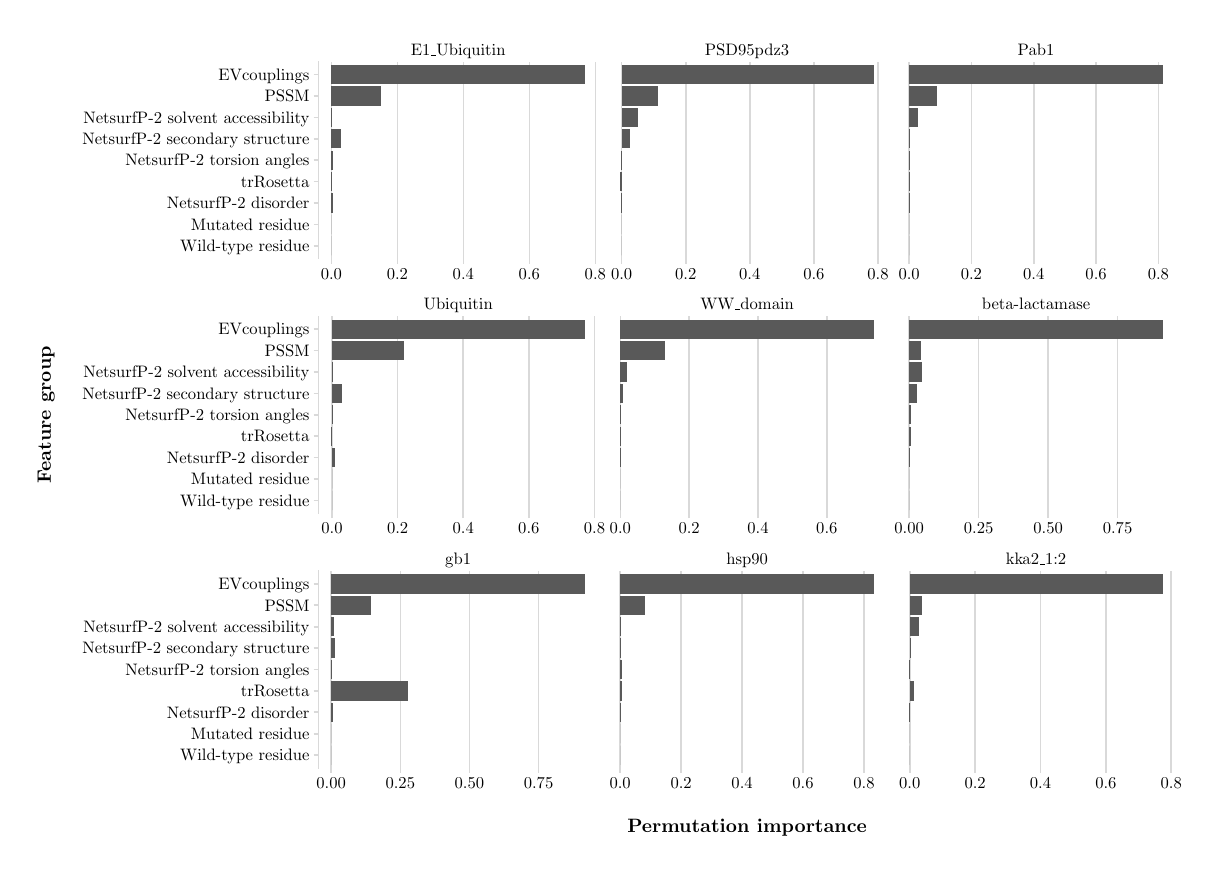
\begin{tikzpicture}[x=1pt,y=1pt]
\definecolor{fillColor}{RGB}{255,255,255}
\path[use as bounding box,fill=fillColor,fill opacity=0.00] (0,0) rectangle (418.34,295.82);
\begin{scope}
\path[clip] (105.09,212.35) rectangle (206.00,283.52);
\definecolor{drawColor}{gray}{0.85}

\path[draw=drawColor,line width= 0.6pt,line join=round] (109.74,212.35) --
	(109.74,283.52);

\path[draw=drawColor,line width= 0.6pt,line join=round] (133.59,212.35) --
	(133.59,283.52);

\path[draw=drawColor,line width= 0.6pt,line join=round] (157.43,212.35) --
	(157.43,283.52);

\path[draw=drawColor,line width= 0.6pt,line join=round] (181.28,212.35) --
	(181.28,283.52);

\path[draw=drawColor,line width= 0.6pt,line join=round] (205.13,212.35) --
	(205.13,283.52);
\definecolor{fillColor}{gray}{0.35}

\path[fill=fillColor] (109.68,236.72) rectangle (109.74,243.68);

\path[fill=fillColor] (109.74,267.66) rectangle (127.58,274.63);

\path[fill=fillColor] (109.74,259.93) rectangle (109.96,266.89);

\path[fill=fillColor] (109.74,252.19) rectangle (113.10,259.15);

\path[fill=fillColor] (109.74,228.98) rectangle (110.46,235.95);

\path[fill=fillColor] (109.74,244.46) rectangle (110.31,251.42);

\path[fill=fillColor] (109.74,275.40) rectangle (201.42,282.36);

\path[fill=fillColor] (109.74,213.51) rectangle (109.74,220.47);

\path[fill=fillColor] (109.74,221.25) rectangle (109.74,228.21);
\end{scope}
\begin{scope}
\path[clip] (105.09,120.33) rectangle (206.00,191.50);
\definecolor{drawColor}{gray}{0.85}

\path[draw=drawColor,line width= 0.6pt,line join=round] (109.98,120.33) --
	(109.98,191.50);

\path[draw=drawColor,line width= 0.6pt,line join=round] (133.69,120.33) --
	(133.69,191.50);

\path[draw=drawColor,line width= 0.6pt,line join=round] (157.39,120.33) --
	(157.39,191.50);

\path[draw=drawColor,line width= 0.6pt,line join=round] (181.10,120.33) --
	(181.10,191.50);

\path[draw=drawColor,line width= 0.6pt,line join=round] (204.81,120.33) --
	(204.81,191.50);
\definecolor{fillColor}{gray}{0.35}

\path[fill=fillColor] (109.68,144.70) rectangle (109.98,151.66);

\path[fill=fillColor] (109.98,175.64) rectangle (135.96,182.60);

\path[fill=fillColor] (109.98,167.90) rectangle (110.06,174.87);

\path[fill=fillColor] (109.98,160.17) rectangle (113.46,167.13);

\path[fill=fillColor] (109.98,136.96) rectangle (110.98,143.92);

\path[fill=fillColor] (109.98,152.43) rectangle (110.47,159.39);

\path[fill=fillColor] (109.98,183.38) rectangle (201.42,190.34);

\path[fill=fillColor] (109.98,121.49) rectangle (109.98,128.45);

\path[fill=fillColor] (109.98,129.22) rectangle (109.98,136.19);
\end{scope}
\begin{scope}
\path[clip] (105.09, 28.30) rectangle (206.00, 99.48);
\definecolor{drawColor}{gray}{0.85}

\path[draw=drawColor,line width= 0.6pt,line join=round] (109.68, 28.30) --
	(109.68, 99.48);

\path[draw=drawColor,line width= 0.6pt,line join=round] (134.66, 28.30) --
	(134.66, 99.48);

\path[draw=drawColor,line width= 0.6pt,line join=round] (159.63, 28.30) --
	(159.63, 99.48);

\path[draw=drawColor,line width= 0.6pt,line join=round] (184.61, 28.30) --
	(184.61, 99.48);
\definecolor{fillColor}{gray}{0.35}

\path[fill=fillColor] (109.68, 52.67) rectangle (137.25, 59.64);

\path[fill=fillColor] (109.68, 83.62) rectangle (124.11, 90.58);

\path[fill=fillColor] (109.68, 75.88) rectangle (110.53, 82.84);

\path[fill=fillColor] (109.68, 68.15) rectangle (110.88, 75.11);

\path[fill=fillColor] (109.68, 44.94) rectangle (110.23, 51.90);

\path[fill=fillColor] (109.68, 60.41) rectangle (110.06, 67.37);

\path[fill=fillColor] (109.68, 91.35) rectangle (201.42, 98.32);

\path[fill=fillColor] (109.68, 29.46) rectangle (109.68, 36.43);

\path[fill=fillColor] (109.68, 37.20) rectangle (109.68, 44.16);
\end{scope}
\begin{scope}
\path[clip] (209.50,212.35) rectangle (310.42,283.52);
\definecolor{drawColor}{gray}{0.85}

\path[draw=drawColor,line width= 0.6pt,line join=round] (214.62,212.35) --
	(214.62,283.52);

\path[draw=drawColor,line width= 0.6pt,line join=round] (237.78,212.35) --
	(237.78,283.52);

\path[draw=drawColor,line width= 0.6pt,line join=round] (260.94,212.35) --
	(260.94,283.52);

\path[draw=drawColor,line width= 0.6pt,line join=round] (284.10,212.35) --
	(284.10,283.52);

\path[draw=drawColor,line width= 0.6pt,line join=round] (307.26,212.35) --
	(307.26,283.52);
\definecolor{fillColor}{gray}{0.35}

\path[fill=fillColor] (214.09,236.72) rectangle (214.62,243.68);

\path[fill=fillColor] (214.62,267.66) rectangle (227.87,274.63);

\path[fill=fillColor] (214.62,259.93) rectangle (220.46,266.89);

\path[fill=fillColor] (214.62,252.19) rectangle (217.79,259.15);

\path[fill=fillColor] (214.48,228.98) rectangle (214.62,235.95);

\path[fill=fillColor] (214.47,244.46) rectangle (214.62,251.42);

\path[fill=fillColor] (214.62,275.40) rectangle (305.83,282.36);

\path[fill=fillColor] (214.62,213.51) rectangle (214.62,220.47);

\path[fill=fillColor] (214.62,221.25) rectangle (214.62,228.21);
\end{scope}
\begin{scope}
\path[clip] (209.50,120.33) rectangle (310.42,191.50);
\definecolor{drawColor}{gray}{0.85}

\path[draw=drawColor,line width= 0.6pt,line join=round] (214.16,120.33) --
	(214.16,191.50);

\path[draw=drawColor,line width= 0.6pt,line join=round] (239.03,120.33) --
	(239.03,191.50);

\path[draw=drawColor,line width= 0.6pt,line join=round] (263.90,120.33) --
	(263.90,191.50);

\path[draw=drawColor,line width= 0.6pt,line join=round] (288.77,120.33) --
	(288.77,191.50);
\definecolor{fillColor}{gray}{0.35}

\path[fill=fillColor] (214.16,144.70) rectangle (214.51,151.66);

\path[fill=fillColor] (214.16,175.64) rectangle (230.15,182.60);

\path[fill=fillColor] (214.16,167.90) rectangle (216.39,174.87);

\path[fill=fillColor] (214.16,160.17) rectangle (214.99,167.13);

\path[fill=fillColor] (214.09,136.96) rectangle (214.16,143.92);

\path[fill=fillColor] (214.16,152.43) rectangle (214.46,159.39);

\path[fill=fillColor] (214.16,183.38) rectangle (305.83,190.34);

\path[fill=fillColor] (214.16,121.49) rectangle (214.16,128.45);

\path[fill=fillColor] (214.16,129.22) rectangle (214.16,136.19);
\end{scope}
\begin{scope}
\path[clip] (209.50, 28.30) rectangle (310.42, 99.48);
\definecolor{drawColor}{gray}{0.85}

\path[draw=drawColor,line width= 0.6pt,line join=round] (214.09, 28.30) --
	(214.09, 99.48);

\path[draw=drawColor,line width= 0.6pt,line join=round] (236.12, 28.30) --
	(236.12, 99.48);

\path[draw=drawColor,line width= 0.6pt,line join=round] (258.15, 28.30) --
	(258.15, 99.48);

\path[draw=drawColor,line width= 0.6pt,line join=round] (280.17, 28.30) --
	(280.17, 99.48);

\path[draw=drawColor,line width= 0.6pt,line join=round] (302.20, 28.30) --
	(302.20, 99.48);
\definecolor{fillColor}{gray}{0.35}

\path[fill=fillColor] (214.09, 52.67) rectangle (214.65, 59.64);

\path[fill=fillColor] (214.09, 83.62) rectangle (223.23, 90.58);

\path[fill=fillColor] (214.09, 75.88) rectangle (214.26, 82.84);

\path[fill=fillColor] (214.09, 68.15) rectangle (214.29, 75.11);

\path[fill=fillColor] (214.09, 44.94) rectangle (214.34, 51.90);

\path[fill=fillColor] (214.09, 60.41) rectangle (214.83, 67.37);

\path[fill=fillColor] (214.09, 91.35) rectangle (305.83, 98.32);

\path[fill=fillColor] (214.09, 29.46) rectangle (214.09, 36.43);

\path[fill=fillColor] (214.09, 37.20) rectangle (214.09, 44.16);
\end{scope}
\begin{scope}
\path[clip] (313.92,212.35) rectangle (414.84,283.52);
\definecolor{drawColor}{gray}{0.85}

\path[draw=drawColor,line width= 0.6pt,line join=round] (318.51,212.35) --
	(318.51,283.52);

\path[draw=drawColor,line width= 0.6pt,line join=round] (341.03,212.35) --
	(341.03,283.52);

\path[draw=drawColor,line width= 0.6pt,line join=round] (363.55,212.35) --
	(363.55,283.52);

\path[draw=drawColor,line width= 0.6pt,line join=round] (386.07,212.35) --
	(386.07,283.52);

\path[draw=drawColor,line width= 0.6pt,line join=round] (408.59,212.35) --
	(408.59,283.52);
\definecolor{fillColor}{gray}{0.35}

\path[fill=fillColor] (318.51,236.72) rectangle (318.54,243.68);

\path[fill=fillColor] (318.51,267.66) rectangle (328.62,274.63);

\path[fill=fillColor] (318.51,259.93) rectangle (321.78,266.89);

\path[fill=fillColor] (318.51,252.19) rectangle (318.76,259.15);

\path[fill=fillColor] (318.51,228.98) rectangle (318.70,235.95);

\path[fill=fillColor] (318.51,244.46) rectangle (318.96,251.42);

\path[fill=fillColor] (318.51,275.40) rectangle (410.25,282.36);

\path[fill=fillColor] (318.51,213.51) rectangle (318.51,220.47);

\path[fill=fillColor] (318.51,221.25) rectangle (318.51,228.21);
\end{scope}
\begin{scope}
\path[clip] (313.92,120.33) rectangle (414.84,191.50);
\definecolor{drawColor}{gray}{0.85}

\path[draw=drawColor,line width= 0.6pt,line join=round] (318.51,120.33) --
	(318.51,191.50);

\path[draw=drawColor,line width= 0.6pt,line join=round] (343.62,120.33) --
	(343.62,191.50);

\path[draw=drawColor,line width= 0.6pt,line join=round] (368.73,120.33) --
	(368.73,191.50);

\path[draw=drawColor,line width= 0.6pt,line join=round] (393.84,120.33) --
	(393.84,191.50);
\definecolor{fillColor}{gray}{0.35}

\path[fill=fillColor] (318.51,144.70) rectangle (319.21,151.66);

\path[fill=fillColor] (318.51,175.64) rectangle (322.90,182.60);

\path[fill=fillColor] (318.51,167.90) rectangle (322.99,174.87);

\path[fill=fillColor] (318.51,160.17) rectangle (321.20,167.13);

\path[fill=fillColor] (318.51,136.96) rectangle (318.72,143.92);

\path[fill=fillColor] (318.51,152.43) rectangle (319.13,159.39);

\path[fill=fillColor] (318.51,183.38) rectangle (410.25,190.34);

\path[fill=fillColor] (318.51,121.49) rectangle (318.51,128.45);

\path[fill=fillColor] (318.51,129.22) rectangle (318.51,136.19);
\end{scope}
\begin{scope}
\path[clip] (313.92, 28.30) rectangle (414.84, 99.48);
\definecolor{drawColor}{gray}{0.85}

\path[draw=drawColor,line width= 0.6pt,line join=round] (318.75, 28.30) --
	(318.75, 99.48);

\path[draw=drawColor,line width= 0.6pt,line join=round] (342.37, 28.30) --
	(342.37, 99.48);

\path[draw=drawColor,line width= 0.6pt,line join=round] (365.99, 28.30) --
	(365.99, 99.48);

\path[draw=drawColor,line width= 0.6pt,line join=round] (389.61, 28.30) --
	(389.61, 99.48);

\path[draw=drawColor,line width= 0.6pt,line join=round] (413.22, 28.30) --
	(413.22, 99.48);
\definecolor{fillColor}{gray}{0.35}

\path[fill=fillColor] (318.75, 52.67) rectangle (320.40, 59.64);

\path[fill=fillColor] (318.75, 83.62) rectangle (323.34, 90.58);

\path[fill=fillColor] (318.75, 75.88) rectangle (322.03, 82.84);

\path[fill=fillColor] (318.75, 68.15) rectangle (318.81, 75.11);

\path[fill=fillColor] (318.59, 44.94) rectangle (318.75, 51.90);

\path[fill=fillColor] (318.51, 60.41) rectangle (318.75, 67.37);

\path[fill=fillColor] (318.75, 91.35) rectangle (410.25, 98.32);

\path[fill=fillColor] (318.75, 29.46) rectangle (318.75, 36.43);

\path[fill=fillColor] (318.75, 37.20) rectangle (318.75, 44.16);
\end{scope}
\begin{scope}
\path[clip] (105.09, 99.48) rectangle (206.00,108.28);
\definecolor{drawColor}{RGB}{0,0,0}

\node[text=drawColor,anchor=base,inner sep=0pt, outer sep=0pt, scale=  0.60] at (155.55,101.81) {gb1};
\end{scope}
\begin{scope}
\path[clip] (209.50, 99.48) rectangle (310.42,108.28);
\definecolor{drawColor}{RGB}{0,0,0}

\node[text=drawColor,anchor=base,inner sep=0pt, outer sep=0pt, scale=  0.60] at (259.96,101.81) {hsp90};
\end{scope}
\begin{scope}
\path[clip] (313.92, 99.48) rectangle (414.84,108.28);
\definecolor{drawColor}{RGB}{0,0,0}

\node[text=drawColor,anchor=base,inner sep=0pt, outer sep=0pt, scale=  0.60] at (364.38,101.81) {kka2\_1:2};
\end{scope}
\begin{scope}
\path[clip] (105.09,191.50) rectangle (206.00,200.30);
\definecolor{drawColor}{RGB}{0,0,0}

\node[text=drawColor,anchor=base,inner sep=0pt, outer sep=0pt, scale=  0.60] at (155.55,193.83) {Ubiquitin};
\end{scope}
\begin{scope}
\path[clip] (209.50,191.50) rectangle (310.42,200.30);
\definecolor{drawColor}{RGB}{0,0,0}

\node[text=drawColor,anchor=base,inner sep=0pt, outer sep=0pt, scale=  0.60] at (259.96,193.83) {WW\_domain};
\end{scope}
\begin{scope}
\path[clip] (313.92,191.50) rectangle (414.84,200.30);
\definecolor{drawColor}{RGB}{0,0,0}

\node[text=drawColor,anchor=base,inner sep=0pt, outer sep=0pt, scale=  0.60] at (364.38,193.83) {beta-lactamase};
\end{scope}
\begin{scope}
\path[clip] (105.09,283.52) rectangle (206.00,292.32);
\definecolor{drawColor}{RGB}{0,0,0}

\node[text=drawColor,anchor=base,inner sep=0pt, outer sep=0pt, scale=  0.60] at (155.55,285.86) {E1\_Ubiquitin};
\end{scope}
\begin{scope}
\path[clip] (209.50,283.52) rectangle (310.42,292.32);
\definecolor{drawColor}{RGB}{0,0,0}

\node[text=drawColor,anchor=base,inner sep=0pt, outer sep=0pt, scale=  0.60] at (259.96,285.86) {PSD95pdz3};
\end{scope}
\begin{scope}
\path[clip] (313.92,283.52) rectangle (414.84,292.32);
\definecolor{drawColor}{RGB}{0,0,0}

\node[text=drawColor,anchor=base,inner sep=0pt, outer sep=0pt, scale=  0.60] at (364.38,285.86) {Pab1};
\end{scope}
\begin{scope}
\path[clip] (  0.00,  0.00) rectangle (418.34,295.82);
\definecolor{drawColor}{gray}{0.85}

\path[draw=drawColor,line width= 0.6pt,line join=round] (109.68, 26.55) --
	(109.68, 28.30);

\path[draw=drawColor,line width= 0.6pt,line join=round] (134.66, 26.55) --
	(134.66, 28.30);

\path[draw=drawColor,line width= 0.6pt,line join=round] (159.63, 26.55) --
	(159.63, 28.30);

\path[draw=drawColor,line width= 0.6pt,line join=round] (184.61, 26.55) --
	(184.61, 28.30);
\end{scope}
\begin{scope}
\path[clip] (  0.00,  0.00) rectangle (418.34,295.82);
\definecolor{drawColor}{RGB}{0,0,0}

\node[text=drawColor,anchor=base,inner sep=0pt, outer sep=0pt, scale=  0.60] at (109.68, 20.92) {0.00};

\node[text=drawColor,anchor=base,inner sep=0pt, outer sep=0pt, scale=  0.60] at (134.66, 20.92) {0.25};

\node[text=drawColor,anchor=base,inner sep=0pt, outer sep=0pt, scale=  0.60] at (159.63, 20.92) {0.50};

\node[text=drawColor,anchor=base,inner sep=0pt, outer sep=0pt, scale=  0.60] at (184.61, 20.92) {0.75};
\end{scope}
\begin{scope}
\path[clip] (  0.00,  0.00) rectangle (418.34,295.82);
\definecolor{drawColor}{gray}{0.85}

\path[draw=drawColor,line width= 0.6pt,line join=round] (214.09, 26.55) --
	(214.09, 28.30);

\path[draw=drawColor,line width= 0.6pt,line join=round] (236.12, 26.55) --
	(236.12, 28.30);

\path[draw=drawColor,line width= 0.6pt,line join=round] (258.15, 26.55) --
	(258.15, 28.30);

\path[draw=drawColor,line width= 0.6pt,line join=round] (280.17, 26.55) --
	(280.17, 28.30);

\path[draw=drawColor,line width= 0.6pt,line join=round] (302.20, 26.55) --
	(302.20, 28.30);
\end{scope}
\begin{scope}
\path[clip] (  0.00,  0.00) rectangle (418.34,295.82);
\definecolor{drawColor}{RGB}{0,0,0}

\node[text=drawColor,anchor=base,inner sep=0pt, outer sep=0pt, scale=  0.60] at (214.09, 20.92) {0.0};

\node[text=drawColor,anchor=base,inner sep=0pt, outer sep=0pt, scale=  0.60] at (236.12, 20.92) {0.2};

\node[text=drawColor,anchor=base,inner sep=0pt, outer sep=0pt, scale=  0.60] at (258.15, 20.92) {0.4};

\node[text=drawColor,anchor=base,inner sep=0pt, outer sep=0pt, scale=  0.60] at (280.17, 20.92) {0.6};

\node[text=drawColor,anchor=base,inner sep=0pt, outer sep=0pt, scale=  0.60] at (302.20, 20.92) {0.8};
\end{scope}
\begin{scope}
\path[clip] (  0.00,  0.00) rectangle (418.34,295.82);
\definecolor{drawColor}{gray}{0.85}

\path[draw=drawColor,line width= 0.6pt,line join=round] (318.75, 26.55) --
	(318.75, 28.30);

\path[draw=drawColor,line width= 0.6pt,line join=round] (342.37, 26.55) --
	(342.37, 28.30);

\path[draw=drawColor,line width= 0.6pt,line join=round] (365.99, 26.55) --
	(365.99, 28.30);

\path[draw=drawColor,line width= 0.6pt,line join=round] (389.61, 26.55) --
	(389.61, 28.30);

\path[draw=drawColor,line width= 0.6pt,line join=round] (413.22, 26.55) --
	(413.22, 28.30);
\end{scope}
\begin{scope}
\path[clip] (  0.00,  0.00) rectangle (418.34,295.82);
\definecolor{drawColor}{RGB}{0,0,0}

\node[text=drawColor,anchor=base,inner sep=0pt, outer sep=0pt, scale=  0.60] at (318.75, 20.92) {0.0};

\node[text=drawColor,anchor=base,inner sep=0pt, outer sep=0pt, scale=  0.60] at (342.37, 20.92) {0.2};

\node[text=drawColor,anchor=base,inner sep=0pt, outer sep=0pt, scale=  0.60] at (365.99, 20.92) {0.4};

\node[text=drawColor,anchor=base,inner sep=0pt, outer sep=0pt, scale=  0.60] at (389.61, 20.92) {0.6};

\node[text=drawColor,anchor=base,inner sep=0pt, outer sep=0pt, scale=  0.60] at (413.22, 20.92) {0.8};
\end{scope}
\begin{scope}
\path[clip] (  0.00,  0.00) rectangle (418.34,295.82);
\definecolor{drawColor}{gray}{0.85}

\path[draw=drawColor,line width= 0.6pt,line join=round] (109.98,118.58) --
	(109.98,120.33);

\path[draw=drawColor,line width= 0.6pt,line join=round] (133.69,118.58) --
	(133.69,120.33);

\path[draw=drawColor,line width= 0.6pt,line join=round] (157.39,118.58) --
	(157.39,120.33);

\path[draw=drawColor,line width= 0.6pt,line join=round] (181.10,118.58) --
	(181.10,120.33);

\path[draw=drawColor,line width= 0.6pt,line join=round] (204.81,118.58) --
	(204.81,120.33);
\end{scope}
\begin{scope}
\path[clip] (  0.00,  0.00) rectangle (418.34,295.82);
\definecolor{drawColor}{RGB}{0,0,0}

\node[text=drawColor,anchor=base,inner sep=0pt, outer sep=0pt, scale=  0.60] at (109.98,112.94) {0.0};

\node[text=drawColor,anchor=base,inner sep=0pt, outer sep=0pt, scale=  0.60] at (133.69,112.94) {0.2};

\node[text=drawColor,anchor=base,inner sep=0pt, outer sep=0pt, scale=  0.60] at (157.39,112.94) {0.4};

\node[text=drawColor,anchor=base,inner sep=0pt, outer sep=0pt, scale=  0.60] at (181.10,112.94) {0.6};

\node[text=drawColor,anchor=base,inner sep=0pt, outer sep=0pt, scale=  0.60] at (204.81,112.94) {0.8};
\end{scope}
\begin{scope}
\path[clip] (  0.00,  0.00) rectangle (418.34,295.82);
\definecolor{drawColor}{gray}{0.85}

\path[draw=drawColor,line width= 0.6pt,line join=round] (214.16,118.58) --
	(214.16,120.33);

\path[draw=drawColor,line width= 0.6pt,line join=round] (239.03,118.58) --
	(239.03,120.33);

\path[draw=drawColor,line width= 0.6pt,line join=round] (263.90,118.58) --
	(263.90,120.33);

\path[draw=drawColor,line width= 0.6pt,line join=round] (288.77,118.58) --
	(288.77,120.33);
\end{scope}
\begin{scope}
\path[clip] (  0.00,  0.00) rectangle (418.34,295.82);
\definecolor{drawColor}{RGB}{0,0,0}

\node[text=drawColor,anchor=base,inner sep=0pt, outer sep=0pt, scale=  0.60] at (214.16,112.94) {0.0};

\node[text=drawColor,anchor=base,inner sep=0pt, outer sep=0pt, scale=  0.60] at (239.03,112.94) {0.2};

\node[text=drawColor,anchor=base,inner sep=0pt, outer sep=0pt, scale=  0.60] at (263.90,112.94) {0.4};

\node[text=drawColor,anchor=base,inner sep=0pt, outer sep=0pt, scale=  0.60] at (288.77,112.94) {0.6};
\end{scope}
\begin{scope}
\path[clip] (  0.00,  0.00) rectangle (418.34,295.82);
\definecolor{drawColor}{gray}{0.85}

\path[draw=drawColor,line width= 0.6pt,line join=round] (318.51,118.58) --
	(318.51,120.33);

\path[draw=drawColor,line width= 0.6pt,line join=round] (343.62,118.58) --
	(343.62,120.33);

\path[draw=drawColor,line width= 0.6pt,line join=round] (368.73,118.58) --
	(368.73,120.33);

\path[draw=drawColor,line width= 0.6pt,line join=round] (393.84,118.58) --
	(393.84,120.33);
\end{scope}
\begin{scope}
\path[clip] (  0.00,  0.00) rectangle (418.34,295.82);
\definecolor{drawColor}{RGB}{0,0,0}

\node[text=drawColor,anchor=base,inner sep=0pt, outer sep=0pt, scale=  0.60] at (318.51,112.94) {0.00};

\node[text=drawColor,anchor=base,inner sep=0pt, outer sep=0pt, scale=  0.60] at (343.62,112.94) {0.25};

\node[text=drawColor,anchor=base,inner sep=0pt, outer sep=0pt, scale=  0.60] at (368.73,112.94) {0.50};

\node[text=drawColor,anchor=base,inner sep=0pt, outer sep=0pt, scale=  0.60] at (393.84,112.94) {0.75};
\end{scope}
\begin{scope}
\path[clip] (  0.00,  0.00) rectangle (418.34,295.82);
\definecolor{drawColor}{gray}{0.85}

\path[draw=drawColor,line width= 0.6pt,line join=round] (109.74,210.60) --
	(109.74,212.35);

\path[draw=drawColor,line width= 0.6pt,line join=round] (133.59,210.60) --
	(133.59,212.35);

\path[draw=drawColor,line width= 0.6pt,line join=round] (157.43,210.60) --
	(157.43,212.35);

\path[draw=drawColor,line width= 0.6pt,line join=round] (181.28,210.60) --
	(181.28,212.35);

\path[draw=drawColor,line width= 0.6pt,line join=round] (205.13,210.60) --
	(205.13,212.35);
\end{scope}
\begin{scope}
\path[clip] (  0.00,  0.00) rectangle (418.34,295.82);
\definecolor{drawColor}{RGB}{0,0,0}

\node[text=drawColor,anchor=base,inner sep=0pt, outer sep=0pt, scale=  0.60] at (109.74,204.97) {0.0};

\node[text=drawColor,anchor=base,inner sep=0pt, outer sep=0pt, scale=  0.60] at (133.59,204.97) {0.2};

\node[text=drawColor,anchor=base,inner sep=0pt, outer sep=0pt, scale=  0.60] at (157.43,204.97) {0.4};

\node[text=drawColor,anchor=base,inner sep=0pt, outer sep=0pt, scale=  0.60] at (181.28,204.97) {0.6};

\node[text=drawColor,anchor=base,inner sep=0pt, outer sep=0pt, scale=  0.60] at (205.13,204.97) {0.8};
\end{scope}
\begin{scope}
\path[clip] (  0.00,  0.00) rectangle (418.34,295.82);
\definecolor{drawColor}{gray}{0.85}

\path[draw=drawColor,line width= 0.6pt,line join=round] (214.62,210.60) --
	(214.62,212.35);

\path[draw=drawColor,line width= 0.6pt,line join=round] (237.78,210.60) --
	(237.78,212.35);

\path[draw=drawColor,line width= 0.6pt,line join=round] (260.94,210.60) --
	(260.94,212.35);

\path[draw=drawColor,line width= 0.6pt,line join=round] (284.10,210.60) --
	(284.10,212.35);

\path[draw=drawColor,line width= 0.6pt,line join=round] (307.26,210.60) --
	(307.26,212.35);
\end{scope}
\begin{scope}
\path[clip] (  0.00,  0.00) rectangle (418.34,295.82);
\definecolor{drawColor}{RGB}{0,0,0}

\node[text=drawColor,anchor=base,inner sep=0pt, outer sep=0pt, scale=  0.60] at (214.62,204.97) {0.0};

\node[text=drawColor,anchor=base,inner sep=0pt, outer sep=0pt, scale=  0.60] at (237.78,204.97) {0.2};

\node[text=drawColor,anchor=base,inner sep=0pt, outer sep=0pt, scale=  0.60] at (260.94,204.97) {0.4};

\node[text=drawColor,anchor=base,inner sep=0pt, outer sep=0pt, scale=  0.60] at (284.10,204.97) {0.6};

\node[text=drawColor,anchor=base,inner sep=0pt, outer sep=0pt, scale=  0.60] at (307.26,204.97) {0.8};
\end{scope}
\begin{scope}
\path[clip] (  0.00,  0.00) rectangle (418.34,295.82);
\definecolor{drawColor}{gray}{0.85}

\path[draw=drawColor,line width= 0.6pt,line join=round] (318.51,210.60) --
	(318.51,212.35);

\path[draw=drawColor,line width= 0.6pt,line join=round] (341.03,210.60) --
	(341.03,212.35);

\path[draw=drawColor,line width= 0.6pt,line join=round] (363.55,210.60) --
	(363.55,212.35);

\path[draw=drawColor,line width= 0.6pt,line join=round] (386.07,210.60) --
	(386.07,212.35);

\path[draw=drawColor,line width= 0.6pt,line join=round] (408.59,210.60) --
	(408.59,212.35);
\end{scope}
\begin{scope}
\path[clip] (  0.00,  0.00) rectangle (418.34,295.82);
\definecolor{drawColor}{RGB}{0,0,0}

\node[text=drawColor,anchor=base,inner sep=0pt, outer sep=0pt, scale=  0.60] at (318.51,204.97) {0.0};

\node[text=drawColor,anchor=base,inner sep=0pt, outer sep=0pt, scale=  0.60] at (341.03,204.97) {0.2};

\node[text=drawColor,anchor=base,inner sep=0pt, outer sep=0pt, scale=  0.60] at (363.55,204.97) {0.4};

\node[text=drawColor,anchor=base,inner sep=0pt, outer sep=0pt, scale=  0.60] at (386.07,204.97) {0.6};

\node[text=drawColor,anchor=base,inner sep=0pt, outer sep=0pt, scale=  0.60] at (408.59,204.97) {0.8};
\end{scope}
\begin{scope}
\path[clip] (  0.00,  0.00) rectangle (418.34,295.82);
\definecolor{drawColor}{gray}{0.85}

\path[draw=drawColor,line width= 0.6pt,line join=round,line cap=rect] (105.09,212.35) --
	(105.09,283.52);
\end{scope}
\begin{scope}
\path[clip] (  0.00,  0.00) rectangle (418.34,295.82);
\definecolor{drawColor}{RGB}{0,0,0}

\node[text=drawColor,anchor=base east,inner sep=0pt, outer sep=0pt, scale=  0.60] at (101.84,214.92) {Wild-type residue};

\node[text=drawColor,anchor=base east,inner sep=0pt, outer sep=0pt, scale=  0.60] at (101.84,222.66) {Mutated residue};

\node[text=drawColor,anchor=base east,inner sep=0pt, outer sep=0pt, scale=  0.60] at (101.84,230.40) {NetsurfP-2 disorder};

\node[text=drawColor,anchor=base east,inner sep=0pt, outer sep=0pt, scale=  0.60] at (101.84,238.13) {trRosetta};

\node[text=drawColor,anchor=base east,inner sep=0pt, outer sep=0pt, scale=  0.60] at (101.84,245.87) {NetsurfP-2 torsion angles};

\node[text=drawColor,anchor=base east,inner sep=0pt, outer sep=0pt, scale=  0.60] at (101.84,253.61) {NetsurfP-2 secondary structure};

\node[text=drawColor,anchor=base east,inner sep=0pt, outer sep=0pt, scale=  0.60] at (101.84,261.34) {NetsurfP-2 solvent accessibility};

\node[text=drawColor,anchor=base east,inner sep=0pt, outer sep=0pt, scale=  0.60] at (101.84,269.08) {PSSM};

\node[text=drawColor,anchor=base east,inner sep=0pt, outer sep=0pt, scale=  0.60] at (101.84,276.81) {EVcouplings};
\end{scope}
\begin{scope}
\path[clip] (  0.00,  0.00) rectangle (418.34,295.82);
\definecolor{drawColor}{gray}{0.85}

\path[draw=drawColor,line width= 0.6pt,line join=round] (103.34,216.99) --
	(105.09,216.99);

\path[draw=drawColor,line width= 0.6pt,line join=round] (103.34,224.73) --
	(105.09,224.73);

\path[draw=drawColor,line width= 0.6pt,line join=round] (103.34,232.46) --
	(105.09,232.46);

\path[draw=drawColor,line width= 0.6pt,line join=round] (103.34,240.20) --
	(105.09,240.20);

\path[draw=drawColor,line width= 0.6pt,line join=round] (103.34,247.94) --
	(105.09,247.94);

\path[draw=drawColor,line width= 0.6pt,line join=round] (103.34,255.67) --
	(105.09,255.67);

\path[draw=drawColor,line width= 0.6pt,line join=round] (103.34,263.41) --
	(105.09,263.41);

\path[draw=drawColor,line width= 0.6pt,line join=round] (103.34,271.14) --
	(105.09,271.14);

\path[draw=drawColor,line width= 0.6pt,line join=round] (103.34,278.88) --
	(105.09,278.88);
\end{scope}
\begin{scope}
\path[clip] (  0.00,  0.00) rectangle (418.34,295.82);
\definecolor{drawColor}{gray}{0.85}

\path[draw=drawColor,line width= 0.6pt,line join=round,line cap=rect] (105.09,120.33) --
	(105.09,191.50);
\end{scope}
\begin{scope}
\path[clip] (  0.00,  0.00) rectangle (418.34,295.82);
\definecolor{drawColor}{RGB}{0,0,0}

\node[text=drawColor,anchor=base east,inner sep=0pt, outer sep=0pt, scale=  0.60] at (101.84,122.90) {Wild-type residue};

\node[text=drawColor,anchor=base east,inner sep=0pt, outer sep=0pt, scale=  0.60] at (101.84,130.64) {Mutated residue};

\node[text=drawColor,anchor=base east,inner sep=0pt, outer sep=0pt, scale=  0.60] at (101.84,138.37) {NetsurfP-2 disorder};

\node[text=drawColor,anchor=base east,inner sep=0pt, outer sep=0pt, scale=  0.60] at (101.84,146.11) {trRosetta};

\node[text=drawColor,anchor=base east,inner sep=0pt, outer sep=0pt, scale=  0.60] at (101.84,153.85) {NetsurfP-2 torsion angles};

\node[text=drawColor,anchor=base east,inner sep=0pt, outer sep=0pt, scale=  0.60] at (101.84,161.58) {NetsurfP-2 secondary structure};

\node[text=drawColor,anchor=base east,inner sep=0pt, outer sep=0pt, scale=  0.60] at (101.84,169.32) {NetsurfP-2 solvent accessibility};

\node[text=drawColor,anchor=base east,inner sep=0pt, outer sep=0pt, scale=  0.60] at (101.84,177.06) {PSSM};

\node[text=drawColor,anchor=base east,inner sep=0pt, outer sep=0pt, scale=  0.60] at (101.84,184.79) {EVcouplings};
\end{scope}
\begin{scope}
\path[clip] (  0.00,  0.00) rectangle (418.34,295.82);
\definecolor{drawColor}{gray}{0.85}

\path[draw=drawColor,line width= 0.6pt,line join=round] (103.34,124.97) --
	(105.09,124.97);

\path[draw=drawColor,line width= 0.6pt,line join=round] (103.34,132.71) --
	(105.09,132.71);

\path[draw=drawColor,line width= 0.6pt,line join=round] (103.34,140.44) --
	(105.09,140.44);

\path[draw=drawColor,line width= 0.6pt,line join=round] (103.34,148.18) --
	(105.09,148.18);

\path[draw=drawColor,line width= 0.6pt,line join=round] (103.34,155.91) --
	(105.09,155.91);

\path[draw=drawColor,line width= 0.6pt,line join=round] (103.34,163.65) --
	(105.09,163.65);

\path[draw=drawColor,line width= 0.6pt,line join=round] (103.34,171.39) --
	(105.09,171.39);

\path[draw=drawColor,line width= 0.6pt,line join=round] (103.34,179.12) --
	(105.09,179.12);

\path[draw=drawColor,line width= 0.6pt,line join=round] (103.34,186.86) --
	(105.09,186.86);
\end{scope}
\begin{scope}
\path[clip] (  0.00,  0.00) rectangle (418.34,295.82);
\definecolor{drawColor}{gray}{0.85}

\path[draw=drawColor,line width= 0.6pt,line join=round,line cap=rect] (105.09, 28.30) --
	(105.09, 99.48);
\end{scope}
\begin{scope}
\path[clip] (  0.00,  0.00) rectangle (418.34,295.82);
\definecolor{drawColor}{RGB}{0,0,0}

\node[text=drawColor,anchor=base east,inner sep=0pt, outer sep=0pt, scale=  0.60] at (101.84, 30.88) {Wild-type residue};

\node[text=drawColor,anchor=base east,inner sep=0pt, outer sep=0pt, scale=  0.60] at (101.84, 38.62) {Mutated residue};

\node[text=drawColor,anchor=base east,inner sep=0pt, outer sep=0pt, scale=  0.60] at (101.84, 46.35) {NetsurfP-2 disorder};

\node[text=drawColor,anchor=base east,inner sep=0pt, outer sep=0pt, scale=  0.60] at (101.84, 54.09) {trRosetta};

\node[text=drawColor,anchor=base east,inner sep=0pt, outer sep=0pt, scale=  0.60] at (101.84, 61.82) {NetsurfP-2 torsion angles};

\node[text=drawColor,anchor=base east,inner sep=0pt, outer sep=0pt, scale=  0.60] at (101.84, 69.56) {NetsurfP-2 secondary structure};

\node[text=drawColor,anchor=base east,inner sep=0pt, outer sep=0pt, scale=  0.60] at (101.84, 77.30) {NetsurfP-2 solvent accessibility};

\node[text=drawColor,anchor=base east,inner sep=0pt, outer sep=0pt, scale=  0.60] at (101.84, 85.03) {PSSM};

\node[text=drawColor,anchor=base east,inner sep=0pt, outer sep=0pt, scale=  0.60] at (101.84, 92.77) {EVcouplings};
\end{scope}
\begin{scope}
\path[clip] (  0.00,  0.00) rectangle (418.34,295.82);
\definecolor{drawColor}{gray}{0.85}

\path[draw=drawColor,line width= 0.6pt,line join=round] (103.34, 32.95) --
	(105.09, 32.95);

\path[draw=drawColor,line width= 0.6pt,line join=round] (103.34, 40.68) --
	(105.09, 40.68);

\path[draw=drawColor,line width= 0.6pt,line join=round] (103.34, 48.42) --
	(105.09, 48.42);

\path[draw=drawColor,line width= 0.6pt,line join=round] (103.34, 56.15) --
	(105.09, 56.15);

\path[draw=drawColor,line width= 0.6pt,line join=round] (103.34, 63.89) --
	(105.09, 63.89);

\path[draw=drawColor,line width= 0.6pt,line join=round] (103.34, 71.63) --
	(105.09, 71.63);

\path[draw=drawColor,line width= 0.6pt,line join=round] (103.34, 79.36) --
	(105.09, 79.36);

\path[draw=drawColor,line width= 0.6pt,line join=round] (103.34, 87.10) --
	(105.09, 87.10);

\path[draw=drawColor,line width= 0.6pt,line join=round] (103.34, 94.84) --
	(105.09, 94.84);
\end{scope}
\begin{scope}
\path[clip] (  0.00,  0.00) rectangle (418.34,295.82);
\definecolor{drawColor}{RGB}{0,0,0}

\node[text=drawColor,anchor=base,inner sep=0pt, outer sep=0pt, scale=  0.70] at (259.96,  4.86) {\bfseries Permutation importance};
\end{scope}
\begin{scope}
\path[clip] (  0.00,  0.00) rectangle (418.34,295.82);
\definecolor{drawColor}{RGB}{0,0,0}

\node[text=drawColor,rotate= 90.00,anchor=base,inner sep=0pt, outer sep=0pt, scale=  0.70] at (  8.39,155.91) {\bfseries Feature group};
\end{scope}
\end{tikzpicture}
}{%
			\caption[Feature importance for the naive single protein models]{%
				\textbf{Feature importance for the naive single protein models.}
				Series of bar plots showing the grouped permutation importance of the features used in the single protein models trained with the naive approach, subdivided by dataset.
			}\label{sup:fig:feature_importance_single_protein_naive}%
		}%
	\end{figure}

	\begin{figure}
		\ffigbox[\FBwidth]{% Created by tikzDevice version 0.12.3.1 on 2021-06-13 15:08:41
% !TEX encoding = UTF-8 Unicode
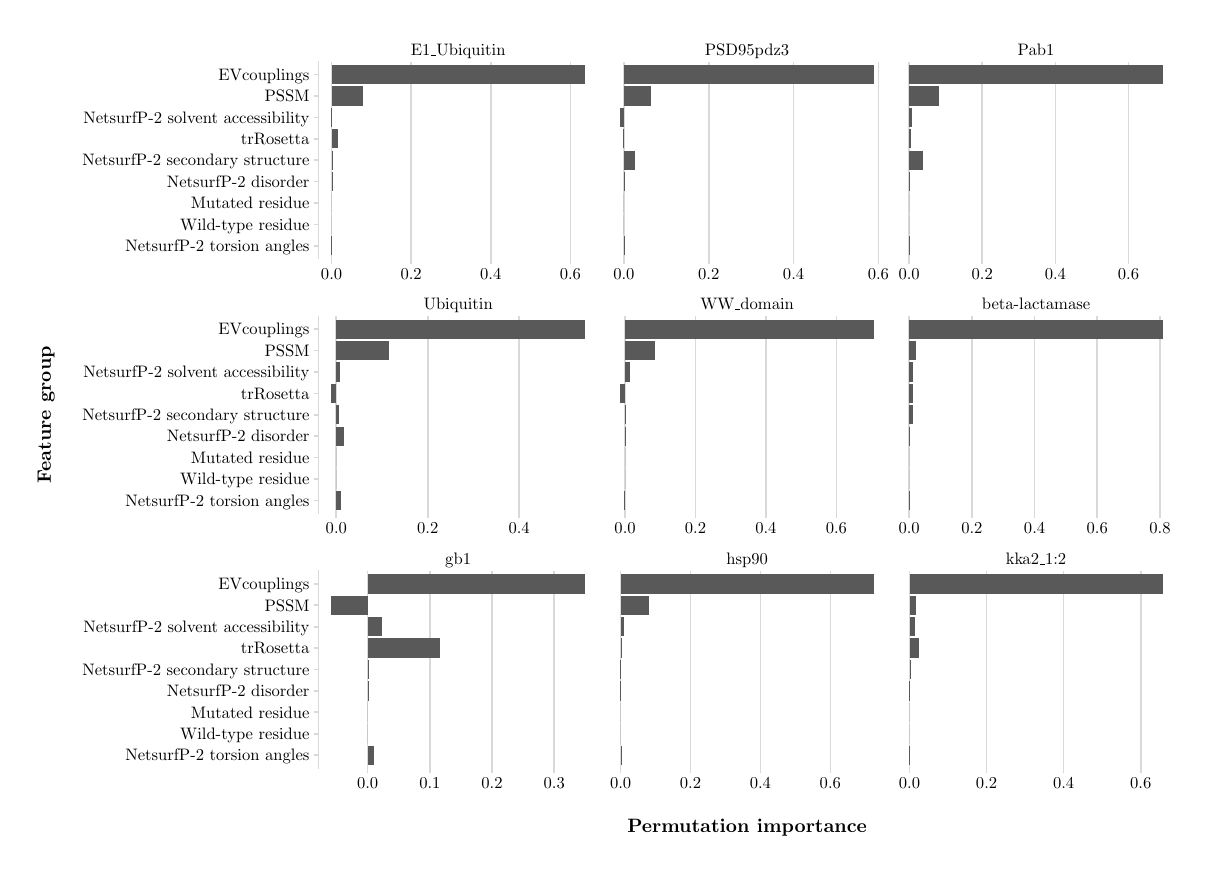
\begin{tikzpicture}[x=1pt,y=1pt]
\definecolor{fillColor}{RGB}{255,255,255}
\path[use as bounding box,fill=fillColor,fill opacity=0.00] (0,0) rectangle (418.34,295.82);
\begin{scope}
\path[clip] (105.09,212.35) rectangle (206.00,283.52);
\definecolor{drawColor}{gray}{0.85}

\path[draw=drawColor,line width= 0.6pt,line join=round] (109.81,212.35) --
	(109.81,283.52);

\path[draw=drawColor,line width= 0.6pt,line join=round] (138.58,212.35) --
	(138.58,283.52);

\path[draw=drawColor,line width= 0.6pt,line join=round] (167.35,212.35) --
	(167.35,283.52);

\path[draw=drawColor,line width= 0.6pt,line join=round] (196.12,212.35) --
	(196.12,283.52);
\definecolor{fillColor}{gray}{0.35}

\path[fill=fillColor] (109.81,252.19) rectangle (112.08,259.15);

\path[fill=fillColor] (109.81,267.66) rectangle (121.31,274.63);

\path[fill=fillColor] (109.69,259.93) rectangle (109.81,266.89);

\path[fill=fillColor] (109.81,244.46) rectangle (110.29,251.42);

\path[fill=fillColor] (109.81,236.72) rectangle (109.86,243.68);

\path[fill=fillColor] (109.68,213.51) rectangle (109.81,220.47);

\path[fill=fillColor] (109.81,275.40) rectangle (201.42,282.36);

\path[fill=fillColor] (109.81,221.25) rectangle (109.81,228.21);

\path[fill=fillColor] (109.81,228.98) rectangle (109.81,235.95);
\end{scope}
\begin{scope}
\path[clip] (105.09,120.33) rectangle (206.00,191.50);
\definecolor{drawColor}{gray}{0.85}

\path[draw=drawColor,line width= 0.6pt,line join=round] (111.53,120.33) --
	(111.53,191.50);

\path[draw=drawColor,line width= 0.6pt,line join=round] (144.56,120.33) --
	(144.56,191.50);

\path[draw=drawColor,line width= 0.6pt,line join=round] (177.59,120.33) --
	(177.59,191.50);
\definecolor{fillColor}{gray}{0.35}

\path[fill=fillColor] (109.68,160.17) rectangle (111.53,167.13);

\path[fill=fillColor] (111.53,175.64) rectangle (130.66,182.60);

\path[fill=fillColor] (111.53,167.90) rectangle (112.78,174.87);

\path[fill=fillColor] (111.53,152.43) rectangle (112.38,159.39);

\path[fill=fillColor] (111.53,144.70) rectangle (114.18,151.66);

\path[fill=fillColor] (111.53,121.49) rectangle (113.31,128.45);

\path[fill=fillColor] (111.53,183.38) rectangle (201.42,190.34);

\path[fill=fillColor] (111.53,129.22) rectangle (111.53,136.19);

\path[fill=fillColor] (111.53,136.96) rectangle (111.53,143.92);
\end{scope}
\begin{scope}
\path[clip] (105.09, 28.30) rectangle (206.00, 99.48);
\definecolor{drawColor}{gray}{0.85}

\path[draw=drawColor,line width= 0.6pt,line join=round] (122.85, 28.30) --
	(122.85, 99.48);

\path[draw=drawColor,line width= 0.6pt,line join=round] (145.33, 28.30) --
	(145.33, 99.48);

\path[draw=drawColor,line width= 0.6pt,line join=round] (167.80, 28.30) --
	(167.80, 99.48);

\path[draw=drawColor,line width= 0.6pt,line join=round] (190.27, 28.30) --
	(190.27, 99.48);
\definecolor{fillColor}{gray}{0.35}

\path[fill=fillColor] (122.85, 68.15) rectangle (149.00, 75.11);

\path[fill=fillColor] (109.68, 83.62) rectangle (122.85, 90.58);

\path[fill=fillColor] (122.85, 75.88) rectangle (128.20, 82.84);

\path[fill=fillColor] (122.85, 60.41) rectangle (123.05, 67.37);

\path[fill=fillColor] (122.85, 52.67) rectangle (122.92, 59.64);

\path[fill=fillColor] (122.85, 29.46) rectangle (125.12, 36.43);

\path[fill=fillColor] (122.85, 91.35) rectangle (201.42, 98.32);

\path[fill=fillColor] (122.85, 37.20) rectangle (122.85, 44.16);

\path[fill=fillColor] (122.85, 44.94) rectangle (122.85, 51.90);
\end{scope}
\begin{scope}
\path[clip] (209.50,212.35) rectangle (310.42,283.52);
\definecolor{drawColor}{gray}{0.85}

\path[draw=drawColor,line width= 0.6pt,line join=round] (215.46,212.35) --
	(215.46,283.52);

\path[draw=drawColor,line width= 0.6pt,line join=round] (246.11,212.35) --
	(246.11,283.52);

\path[draw=drawColor,line width= 0.6pt,line join=round] (276.76,212.35) --
	(276.76,283.52);

\path[draw=drawColor,line width= 0.6pt,line join=round] (307.40,212.35) --
	(307.40,283.52);
\definecolor{fillColor}{gray}{0.35}

\path[fill=fillColor] (215.27,252.19) rectangle (215.46,259.15);

\path[fill=fillColor] (215.46,267.66) rectangle (225.13,274.63);

\path[fill=fillColor] (214.09,259.93) rectangle (215.46,266.89);

\path[fill=fillColor] (215.46,244.46) rectangle (219.37,251.42);

\path[fill=fillColor] (215.46,236.72) rectangle (215.82,243.68);

\path[fill=fillColor] (215.46,213.51) rectangle (215.80,220.47);

\path[fill=fillColor] (215.46,275.40) rectangle (305.83,282.36);

\path[fill=fillColor] (215.46,221.25) rectangle (215.46,228.21);

\path[fill=fillColor] (215.46,228.98) rectangle (215.46,235.95);
\end{scope}
\begin{scope}
\path[clip] (209.50,120.33) rectangle (310.42,191.50);
\definecolor{drawColor}{gray}{0.85}

\path[draw=drawColor,line width= 0.6pt,line join=round] (215.87,120.33) --
	(215.87,191.50);

\path[draw=drawColor,line width= 0.6pt,line join=round] (241.32,120.33) --
	(241.32,191.50);

\path[draw=drawColor,line width= 0.6pt,line join=round] (266.77,120.33) --
	(266.77,191.50);

\path[draw=drawColor,line width= 0.6pt,line join=round] (292.22,120.33) --
	(292.22,191.50);
\definecolor{fillColor}{gray}{0.35}

\path[fill=fillColor] (214.09,160.17) rectangle (215.87,167.13);

\path[fill=fillColor] (215.87,175.64) rectangle (226.66,182.60);

\path[fill=fillColor] (215.87,167.90) rectangle (217.69,174.87);

\path[fill=fillColor] (215.72,152.43) rectangle (215.87,159.39);

\path[fill=fillColor] (215.87,144.70) rectangle (215.93,151.66);

\path[fill=fillColor] (215.31,121.49) rectangle (215.87,128.45);

\path[fill=fillColor] (215.87,183.38) rectangle (305.83,190.34);

\path[fill=fillColor] (215.87,129.22) rectangle (215.87,136.19);

\path[fill=fillColor] (215.87,136.96) rectangle (215.87,143.92);
\end{scope}
\begin{scope}
\path[clip] (209.50, 28.30) rectangle (310.42, 99.48);
\definecolor{drawColor}{gray}{0.85}

\path[draw=drawColor,line width= 0.6pt,line join=round] (214.27, 28.30) --
	(214.27, 99.48);

\path[draw=drawColor,line width= 0.6pt,line join=round] (239.53, 28.30) --
	(239.53, 99.48);

\path[draw=drawColor,line width= 0.6pt,line join=round] (264.78, 28.30) --
	(264.78, 99.48);

\path[draw=drawColor,line width= 0.6pt,line join=round] (290.04, 28.30) --
	(290.04, 99.48);
\definecolor{fillColor}{gray}{0.35}

\path[fill=fillColor] (214.27, 68.15) rectangle (214.90, 75.11);

\path[fill=fillColor] (214.27, 83.62) rectangle (224.43, 90.58);

\path[fill=fillColor] (214.27, 75.88) rectangle (215.57, 82.84);

\path[fill=fillColor] (214.09, 60.41) rectangle (214.27, 67.37);

\path[fill=fillColor] (214.19, 52.67) rectangle (214.27, 59.64);

\path[fill=fillColor] (214.25, 29.46) rectangle (214.27, 36.43);

\path[fill=fillColor] (214.27, 91.35) rectangle (305.83, 98.32);

\path[fill=fillColor] (214.27, 37.20) rectangle (214.27, 44.16);

\path[fill=fillColor] (214.27, 44.94) rectangle (214.27, 51.90);
\end{scope}
\begin{scope}
\path[clip] (313.92,212.35) rectangle (414.84,283.52);
\definecolor{drawColor}{gray}{0.85}

\path[draw=drawColor,line width= 0.6pt,line join=round] (318.51,212.35) --
	(318.51,283.52);

\path[draw=drawColor,line width= 0.6pt,line join=round] (344.94,212.35) --
	(344.94,283.52);

\path[draw=drawColor,line width= 0.6pt,line join=round] (371.37,212.35) --
	(371.37,283.52);

\path[draw=drawColor,line width= 0.6pt,line join=round] (397.80,212.35) --
	(397.80,283.52);
\definecolor{fillColor}{gray}{0.35}

\path[fill=fillColor] (318.51,252.19) rectangle (319.32,259.15);

\path[fill=fillColor] (318.51,267.66) rectangle (329.43,274.63);

\path[fill=fillColor] (318.51,259.93) rectangle (319.72,266.89);

\path[fill=fillColor] (318.51,244.46) rectangle (323.43,251.42);

\path[fill=fillColor] (318.51,236.72) rectangle (318.70,243.68);

\path[fill=fillColor] (318.51,213.51) rectangle (318.77,220.47);

\path[fill=fillColor] (318.51,275.40) rectangle (410.25,282.36);

\path[fill=fillColor] (318.51,221.25) rectangle (318.51,228.21);

\path[fill=fillColor] (318.51,228.98) rectangle (318.51,235.95);
\end{scope}
\begin{scope}
\path[clip] (313.92,120.33) rectangle (414.84,191.50);
\definecolor{drawColor}{gray}{0.85}

\path[draw=drawColor,line width= 0.6pt,line join=round] (318.53,120.33) --
	(318.53,191.50);

\path[draw=drawColor,line width= 0.6pt,line join=round] (341.19,120.33) --
	(341.19,191.50);

\path[draw=drawColor,line width= 0.6pt,line join=round] (363.84,120.33) --
	(363.84,191.50);

\path[draw=drawColor,line width= 0.6pt,line join=round] (386.50,120.33) --
	(386.50,191.50);

\path[draw=drawColor,line width= 0.6pt,line join=round] (409.16,120.33) --
	(409.16,191.50);
\definecolor{fillColor}{gray}{0.35}

\path[fill=fillColor] (318.53,160.17) rectangle (319.89,167.13);

\path[fill=fillColor] (318.53,175.64) rectangle (321.17,182.60);

\path[fill=fillColor] (318.53,167.90) rectangle (320.02,174.87);

\path[fill=fillColor] (318.53,152.43) rectangle (319.95,159.39);

\path[fill=fillColor] (318.53,144.70) rectangle (318.71,151.66);

\path[fill=fillColor] (318.51,121.49) rectangle (318.53,128.45);

\path[fill=fillColor] (318.53,183.38) rectangle (410.25,190.34);

\path[fill=fillColor] (318.53,129.22) rectangle (318.53,136.19);

\path[fill=fillColor] (318.53,136.96) rectangle (318.53,143.92);
\end{scope}
\begin{scope}
\path[clip] (313.92, 28.30) rectangle (414.84, 99.48);
\definecolor{drawColor}{gray}{0.85}

\path[draw=drawColor,line width= 0.6pt,line join=round] (318.65, 28.30) --
	(318.65, 99.48);

\path[draw=drawColor,line width= 0.6pt,line join=round] (346.50, 28.30) --
	(346.50, 99.48);

\path[draw=drawColor,line width= 0.6pt,line join=round] (374.35, 28.30) --
	(374.35, 99.48);

\path[draw=drawColor,line width= 0.6pt,line join=round] (402.19, 28.30) --
	(402.19, 99.48);
\definecolor{fillColor}{gray}{0.35}

\path[fill=fillColor] (318.65, 68.15) rectangle (321.92, 75.11);

\path[fill=fillColor] (318.65, 83.62) rectangle (320.82, 90.58);

\path[fill=fillColor] (318.65, 75.88) rectangle (320.61, 82.84);

\path[fill=fillColor] (318.65, 60.41) rectangle (318.94, 67.37);

\path[fill=fillColor] (318.62, 52.67) rectangle (318.65, 59.64);

\path[fill=fillColor] (318.51, 29.46) rectangle (318.65, 36.43);

\path[fill=fillColor] (318.65, 91.35) rectangle (410.25, 98.32);

\path[fill=fillColor] (318.65, 37.20) rectangle (318.65, 44.16);

\path[fill=fillColor] (318.65, 44.94) rectangle (318.65, 51.90);
\end{scope}
\begin{scope}
\path[clip] (105.09, 99.48) rectangle (206.00,108.28);
\definecolor{drawColor}{RGB}{0,0,0}

\node[text=drawColor,anchor=base,inner sep=0pt, outer sep=0pt, scale=  0.60] at (155.55,101.81) {gb1};
\end{scope}
\begin{scope}
\path[clip] (209.50, 99.48) rectangle (310.42,108.28);
\definecolor{drawColor}{RGB}{0,0,0}

\node[text=drawColor,anchor=base,inner sep=0pt, outer sep=0pt, scale=  0.60] at (259.96,101.81) {hsp90};
\end{scope}
\begin{scope}
\path[clip] (313.92, 99.48) rectangle (414.84,108.28);
\definecolor{drawColor}{RGB}{0,0,0}

\node[text=drawColor,anchor=base,inner sep=0pt, outer sep=0pt, scale=  0.60] at (364.38,101.81) {kka2\_1:2};
\end{scope}
\begin{scope}
\path[clip] (105.09,191.50) rectangle (206.00,200.30);
\definecolor{drawColor}{RGB}{0,0,0}

\node[text=drawColor,anchor=base,inner sep=0pt, outer sep=0pt, scale=  0.60] at (155.55,193.83) {Ubiquitin};
\end{scope}
\begin{scope}
\path[clip] (209.50,191.50) rectangle (310.42,200.30);
\definecolor{drawColor}{RGB}{0,0,0}

\node[text=drawColor,anchor=base,inner sep=0pt, outer sep=0pt, scale=  0.60] at (259.96,193.83) {WW\_domain};
\end{scope}
\begin{scope}
\path[clip] (313.92,191.50) rectangle (414.84,200.30);
\definecolor{drawColor}{RGB}{0,0,0}

\node[text=drawColor,anchor=base,inner sep=0pt, outer sep=0pt, scale=  0.60] at (364.38,193.83) {beta-lactamase};
\end{scope}
\begin{scope}
\path[clip] (105.09,283.52) rectangle (206.00,292.32);
\definecolor{drawColor}{RGB}{0,0,0}

\node[text=drawColor,anchor=base,inner sep=0pt, outer sep=0pt, scale=  0.60] at (155.55,285.86) {E1\_Ubiquitin};
\end{scope}
\begin{scope}
\path[clip] (209.50,283.52) rectangle (310.42,292.32);
\definecolor{drawColor}{RGB}{0,0,0}

\node[text=drawColor,anchor=base,inner sep=0pt, outer sep=0pt, scale=  0.60] at (259.96,285.86) {PSD95pdz3};
\end{scope}
\begin{scope}
\path[clip] (313.92,283.52) rectangle (414.84,292.32);
\definecolor{drawColor}{RGB}{0,0,0}

\node[text=drawColor,anchor=base,inner sep=0pt, outer sep=0pt, scale=  0.60] at (364.38,285.86) {Pab1};
\end{scope}
\begin{scope}
\path[clip] (  0.00,  0.00) rectangle (418.34,295.82);
\definecolor{drawColor}{gray}{0.85}

\path[draw=drawColor,line width= 0.6pt,line join=round] (122.85, 26.55) --
	(122.85, 28.30);

\path[draw=drawColor,line width= 0.6pt,line join=round] (145.33, 26.55) --
	(145.33, 28.30);

\path[draw=drawColor,line width= 0.6pt,line join=round] (167.80, 26.55) --
	(167.80, 28.30);

\path[draw=drawColor,line width= 0.6pt,line join=round] (190.27, 26.55) --
	(190.27, 28.30);
\end{scope}
\begin{scope}
\path[clip] (  0.00,  0.00) rectangle (418.34,295.82);
\definecolor{drawColor}{RGB}{0,0,0}

\node[text=drawColor,anchor=base,inner sep=0pt, outer sep=0pt, scale=  0.60] at (122.85, 20.92) {0.0};

\node[text=drawColor,anchor=base,inner sep=0pt, outer sep=0pt, scale=  0.60] at (145.33, 20.92) {0.1};

\node[text=drawColor,anchor=base,inner sep=0pt, outer sep=0pt, scale=  0.60] at (167.80, 20.92) {0.2};

\node[text=drawColor,anchor=base,inner sep=0pt, outer sep=0pt, scale=  0.60] at (190.27, 20.92) {0.3};
\end{scope}
\begin{scope}
\path[clip] (  0.00,  0.00) rectangle (418.34,295.82);
\definecolor{drawColor}{gray}{0.85}

\path[draw=drawColor,line width= 0.6pt,line join=round] (214.27, 26.55) --
	(214.27, 28.30);

\path[draw=drawColor,line width= 0.6pt,line join=round] (239.53, 26.55) --
	(239.53, 28.30);

\path[draw=drawColor,line width= 0.6pt,line join=round] (264.78, 26.55) --
	(264.78, 28.30);

\path[draw=drawColor,line width= 0.6pt,line join=round] (290.04, 26.55) --
	(290.04, 28.30);
\end{scope}
\begin{scope}
\path[clip] (  0.00,  0.00) rectangle (418.34,295.82);
\definecolor{drawColor}{RGB}{0,0,0}

\node[text=drawColor,anchor=base,inner sep=0pt, outer sep=0pt, scale=  0.60] at (214.27, 20.92) {0.0};

\node[text=drawColor,anchor=base,inner sep=0pt, outer sep=0pt, scale=  0.60] at (239.53, 20.92) {0.2};

\node[text=drawColor,anchor=base,inner sep=0pt, outer sep=0pt, scale=  0.60] at (264.78, 20.92) {0.4};

\node[text=drawColor,anchor=base,inner sep=0pt, outer sep=0pt, scale=  0.60] at (290.04, 20.92) {0.6};
\end{scope}
\begin{scope}
\path[clip] (  0.00,  0.00) rectangle (418.34,295.82);
\definecolor{drawColor}{gray}{0.85}

\path[draw=drawColor,line width= 0.6pt,line join=round] (318.65, 26.55) --
	(318.65, 28.30);

\path[draw=drawColor,line width= 0.6pt,line join=round] (346.50, 26.55) --
	(346.50, 28.30);

\path[draw=drawColor,line width= 0.6pt,line join=round] (374.35, 26.55) --
	(374.35, 28.30);

\path[draw=drawColor,line width= 0.6pt,line join=round] (402.19, 26.55) --
	(402.19, 28.30);
\end{scope}
\begin{scope}
\path[clip] (  0.00,  0.00) rectangle (418.34,295.82);
\definecolor{drawColor}{RGB}{0,0,0}

\node[text=drawColor,anchor=base,inner sep=0pt, outer sep=0pt, scale=  0.60] at (318.65, 20.92) {0.0};

\node[text=drawColor,anchor=base,inner sep=0pt, outer sep=0pt, scale=  0.60] at (346.50, 20.92) {0.2};

\node[text=drawColor,anchor=base,inner sep=0pt, outer sep=0pt, scale=  0.60] at (374.35, 20.92) {0.4};

\node[text=drawColor,anchor=base,inner sep=0pt, outer sep=0pt, scale=  0.60] at (402.19, 20.92) {0.6};
\end{scope}
\begin{scope}
\path[clip] (  0.00,  0.00) rectangle (418.34,295.82);
\definecolor{drawColor}{gray}{0.85}

\path[draw=drawColor,line width= 0.6pt,line join=round] (111.53,118.58) --
	(111.53,120.33);

\path[draw=drawColor,line width= 0.6pt,line join=round] (144.56,118.58) --
	(144.56,120.33);

\path[draw=drawColor,line width= 0.6pt,line join=round] (177.59,118.58) --
	(177.59,120.33);
\end{scope}
\begin{scope}
\path[clip] (  0.00,  0.00) rectangle (418.34,295.82);
\definecolor{drawColor}{RGB}{0,0,0}

\node[text=drawColor,anchor=base,inner sep=0pt, outer sep=0pt, scale=  0.60] at (111.53,112.94) {0.0};

\node[text=drawColor,anchor=base,inner sep=0pt, outer sep=0pt, scale=  0.60] at (144.56,112.94) {0.2};

\node[text=drawColor,anchor=base,inner sep=0pt, outer sep=0pt, scale=  0.60] at (177.59,112.94) {0.4};
\end{scope}
\begin{scope}
\path[clip] (  0.00,  0.00) rectangle (418.34,295.82);
\definecolor{drawColor}{gray}{0.85}

\path[draw=drawColor,line width= 0.6pt,line join=round] (215.87,118.58) --
	(215.87,120.33);

\path[draw=drawColor,line width= 0.6pt,line join=round] (241.32,118.58) --
	(241.32,120.33);

\path[draw=drawColor,line width= 0.6pt,line join=round] (266.77,118.58) --
	(266.77,120.33);

\path[draw=drawColor,line width= 0.6pt,line join=round] (292.22,118.58) --
	(292.22,120.33);
\end{scope}
\begin{scope}
\path[clip] (  0.00,  0.00) rectangle (418.34,295.82);
\definecolor{drawColor}{RGB}{0,0,0}

\node[text=drawColor,anchor=base,inner sep=0pt, outer sep=0pt, scale=  0.60] at (215.87,112.94) {0.0};

\node[text=drawColor,anchor=base,inner sep=0pt, outer sep=0pt, scale=  0.60] at (241.32,112.94) {0.2};

\node[text=drawColor,anchor=base,inner sep=0pt, outer sep=0pt, scale=  0.60] at (266.77,112.94) {0.4};

\node[text=drawColor,anchor=base,inner sep=0pt, outer sep=0pt, scale=  0.60] at (292.22,112.94) {0.6};
\end{scope}
\begin{scope}
\path[clip] (  0.00,  0.00) rectangle (418.34,295.82);
\definecolor{drawColor}{gray}{0.85}

\path[draw=drawColor,line width= 0.6pt,line join=round] (318.53,118.58) --
	(318.53,120.33);

\path[draw=drawColor,line width= 0.6pt,line join=round] (341.19,118.58) --
	(341.19,120.33);

\path[draw=drawColor,line width= 0.6pt,line join=round] (363.84,118.58) --
	(363.84,120.33);

\path[draw=drawColor,line width= 0.6pt,line join=round] (386.50,118.58) --
	(386.50,120.33);

\path[draw=drawColor,line width= 0.6pt,line join=round] (409.16,118.58) --
	(409.16,120.33);
\end{scope}
\begin{scope}
\path[clip] (  0.00,  0.00) rectangle (418.34,295.82);
\definecolor{drawColor}{RGB}{0,0,0}

\node[text=drawColor,anchor=base,inner sep=0pt, outer sep=0pt, scale=  0.60] at (318.53,112.94) {0.0};

\node[text=drawColor,anchor=base,inner sep=0pt, outer sep=0pt, scale=  0.60] at (341.19,112.94) {0.2};

\node[text=drawColor,anchor=base,inner sep=0pt, outer sep=0pt, scale=  0.60] at (363.84,112.94) {0.4};

\node[text=drawColor,anchor=base,inner sep=0pt, outer sep=0pt, scale=  0.60] at (386.50,112.94) {0.6};

\node[text=drawColor,anchor=base,inner sep=0pt, outer sep=0pt, scale=  0.60] at (409.16,112.94) {0.8};
\end{scope}
\begin{scope}
\path[clip] (  0.00,  0.00) rectangle (418.34,295.82);
\definecolor{drawColor}{gray}{0.85}

\path[draw=drawColor,line width= 0.6pt,line join=round] (109.81,210.60) --
	(109.81,212.35);

\path[draw=drawColor,line width= 0.6pt,line join=round] (138.58,210.60) --
	(138.58,212.35);

\path[draw=drawColor,line width= 0.6pt,line join=round] (167.35,210.60) --
	(167.35,212.35);

\path[draw=drawColor,line width= 0.6pt,line join=round] (196.12,210.60) --
	(196.12,212.35);
\end{scope}
\begin{scope}
\path[clip] (  0.00,  0.00) rectangle (418.34,295.82);
\definecolor{drawColor}{RGB}{0,0,0}

\node[text=drawColor,anchor=base,inner sep=0pt, outer sep=0pt, scale=  0.60] at (109.81,204.97) {0.0};

\node[text=drawColor,anchor=base,inner sep=0pt, outer sep=0pt, scale=  0.60] at (138.58,204.97) {0.2};

\node[text=drawColor,anchor=base,inner sep=0pt, outer sep=0pt, scale=  0.60] at (167.35,204.97) {0.4};

\node[text=drawColor,anchor=base,inner sep=0pt, outer sep=0pt, scale=  0.60] at (196.12,204.97) {0.6};
\end{scope}
\begin{scope}
\path[clip] (  0.00,  0.00) rectangle (418.34,295.82);
\definecolor{drawColor}{gray}{0.85}

\path[draw=drawColor,line width= 0.6pt,line join=round] (215.46,210.60) --
	(215.46,212.35);

\path[draw=drawColor,line width= 0.6pt,line join=round] (246.11,210.60) --
	(246.11,212.35);

\path[draw=drawColor,line width= 0.6pt,line join=round] (276.76,210.60) --
	(276.76,212.35);

\path[draw=drawColor,line width= 0.6pt,line join=round] (307.40,210.60) --
	(307.40,212.35);
\end{scope}
\begin{scope}
\path[clip] (  0.00,  0.00) rectangle (418.34,295.82);
\definecolor{drawColor}{RGB}{0,0,0}

\node[text=drawColor,anchor=base,inner sep=0pt, outer sep=0pt, scale=  0.60] at (215.46,204.97) {0.0};

\node[text=drawColor,anchor=base,inner sep=0pt, outer sep=0pt, scale=  0.60] at (246.11,204.97) {0.2};

\node[text=drawColor,anchor=base,inner sep=0pt, outer sep=0pt, scale=  0.60] at (276.76,204.97) {0.4};

\node[text=drawColor,anchor=base,inner sep=0pt, outer sep=0pt, scale=  0.60] at (307.40,204.97) {0.6};
\end{scope}
\begin{scope}
\path[clip] (  0.00,  0.00) rectangle (418.34,295.82);
\definecolor{drawColor}{gray}{0.85}

\path[draw=drawColor,line width= 0.6pt,line join=round] (318.51,210.60) --
	(318.51,212.35);

\path[draw=drawColor,line width= 0.6pt,line join=round] (344.94,210.60) --
	(344.94,212.35);

\path[draw=drawColor,line width= 0.6pt,line join=round] (371.37,210.60) --
	(371.37,212.35);

\path[draw=drawColor,line width= 0.6pt,line join=round] (397.80,210.60) --
	(397.80,212.35);
\end{scope}
\begin{scope}
\path[clip] (  0.00,  0.00) rectangle (418.34,295.82);
\definecolor{drawColor}{RGB}{0,0,0}

\node[text=drawColor,anchor=base,inner sep=0pt, outer sep=0pt, scale=  0.60] at (318.51,204.97) {0.0};

\node[text=drawColor,anchor=base,inner sep=0pt, outer sep=0pt, scale=  0.60] at (344.94,204.97) {0.2};

\node[text=drawColor,anchor=base,inner sep=0pt, outer sep=0pt, scale=  0.60] at (371.37,204.97) {0.4};

\node[text=drawColor,anchor=base,inner sep=0pt, outer sep=0pt, scale=  0.60] at (397.80,204.97) {0.6};
\end{scope}
\begin{scope}
\path[clip] (  0.00,  0.00) rectangle (418.34,295.82);
\definecolor{drawColor}{gray}{0.85}

\path[draw=drawColor,line width= 0.6pt,line join=round,line cap=rect] (105.09,212.35) --
	(105.09,283.52);
\end{scope}
\begin{scope}
\path[clip] (  0.00,  0.00) rectangle (418.34,295.82);
\definecolor{drawColor}{RGB}{0,0,0}

\node[text=drawColor,anchor=base east,inner sep=0pt, outer sep=0pt, scale=  0.60] at (101.84,214.92) {NetsurfP-2 torsion angles};

\node[text=drawColor,anchor=base east,inner sep=0pt, outer sep=0pt, scale=  0.60] at (101.84,222.66) {Wild-type residue};

\node[text=drawColor,anchor=base east,inner sep=0pt, outer sep=0pt, scale=  0.60] at (101.84,230.40) {Mutated residue};

\node[text=drawColor,anchor=base east,inner sep=0pt, outer sep=0pt, scale=  0.60] at (101.84,238.13) {NetsurfP-2 disorder};

\node[text=drawColor,anchor=base east,inner sep=0pt, outer sep=0pt, scale=  0.60] at (101.84,245.87) {NetsurfP-2 secondary structure};

\node[text=drawColor,anchor=base east,inner sep=0pt, outer sep=0pt, scale=  0.60] at (101.84,253.61) {trRosetta};

\node[text=drawColor,anchor=base east,inner sep=0pt, outer sep=0pt, scale=  0.60] at (101.84,261.34) {NetsurfP-2 solvent accessibility};

\node[text=drawColor,anchor=base east,inner sep=0pt, outer sep=0pt, scale=  0.60] at (101.84,269.08) {PSSM};

\node[text=drawColor,anchor=base east,inner sep=0pt, outer sep=0pt, scale=  0.60] at (101.84,276.81) {EVcouplings};
\end{scope}
\begin{scope}
\path[clip] (  0.00,  0.00) rectangle (418.34,295.82);
\definecolor{drawColor}{gray}{0.85}

\path[draw=drawColor,line width= 0.6pt,line join=round] (103.34,216.99) --
	(105.09,216.99);

\path[draw=drawColor,line width= 0.6pt,line join=round] (103.34,224.73) --
	(105.09,224.73);

\path[draw=drawColor,line width= 0.6pt,line join=round] (103.34,232.46) --
	(105.09,232.46);

\path[draw=drawColor,line width= 0.6pt,line join=round] (103.34,240.20) --
	(105.09,240.20);

\path[draw=drawColor,line width= 0.6pt,line join=round] (103.34,247.94) --
	(105.09,247.94);

\path[draw=drawColor,line width= 0.6pt,line join=round] (103.34,255.67) --
	(105.09,255.67);

\path[draw=drawColor,line width= 0.6pt,line join=round] (103.34,263.41) --
	(105.09,263.41);

\path[draw=drawColor,line width= 0.6pt,line join=round] (103.34,271.14) --
	(105.09,271.14);

\path[draw=drawColor,line width= 0.6pt,line join=round] (103.34,278.88) --
	(105.09,278.88);
\end{scope}
\begin{scope}
\path[clip] (  0.00,  0.00) rectangle (418.34,295.82);
\definecolor{drawColor}{gray}{0.85}

\path[draw=drawColor,line width= 0.6pt,line join=round,line cap=rect] (105.09,120.33) --
	(105.09,191.50);
\end{scope}
\begin{scope}
\path[clip] (  0.00,  0.00) rectangle (418.34,295.82);
\definecolor{drawColor}{RGB}{0,0,0}

\node[text=drawColor,anchor=base east,inner sep=0pt, outer sep=0pt, scale=  0.60] at (101.84,122.90) {NetsurfP-2 torsion angles};

\node[text=drawColor,anchor=base east,inner sep=0pt, outer sep=0pt, scale=  0.60] at (101.84,130.64) {Wild-type residue};

\node[text=drawColor,anchor=base east,inner sep=0pt, outer sep=0pt, scale=  0.60] at (101.84,138.37) {Mutated residue};

\node[text=drawColor,anchor=base east,inner sep=0pt, outer sep=0pt, scale=  0.60] at (101.84,146.11) {NetsurfP-2 disorder};

\node[text=drawColor,anchor=base east,inner sep=0pt, outer sep=0pt, scale=  0.60] at (101.84,153.85) {NetsurfP-2 secondary structure};

\node[text=drawColor,anchor=base east,inner sep=0pt, outer sep=0pt, scale=  0.60] at (101.84,161.58) {trRosetta};

\node[text=drawColor,anchor=base east,inner sep=0pt, outer sep=0pt, scale=  0.60] at (101.84,169.32) {NetsurfP-2 solvent accessibility};

\node[text=drawColor,anchor=base east,inner sep=0pt, outer sep=0pt, scale=  0.60] at (101.84,177.06) {PSSM};

\node[text=drawColor,anchor=base east,inner sep=0pt, outer sep=0pt, scale=  0.60] at (101.84,184.79) {EVcouplings};
\end{scope}
\begin{scope}
\path[clip] (  0.00,  0.00) rectangle (418.34,295.82);
\definecolor{drawColor}{gray}{0.85}

\path[draw=drawColor,line width= 0.6pt,line join=round] (103.34,124.97) --
	(105.09,124.97);

\path[draw=drawColor,line width= 0.6pt,line join=round] (103.34,132.71) --
	(105.09,132.71);

\path[draw=drawColor,line width= 0.6pt,line join=round] (103.34,140.44) --
	(105.09,140.44);

\path[draw=drawColor,line width= 0.6pt,line join=round] (103.34,148.18) --
	(105.09,148.18);

\path[draw=drawColor,line width= 0.6pt,line join=round] (103.34,155.91) --
	(105.09,155.91);

\path[draw=drawColor,line width= 0.6pt,line join=round] (103.34,163.65) --
	(105.09,163.65);

\path[draw=drawColor,line width= 0.6pt,line join=round] (103.34,171.39) --
	(105.09,171.39);

\path[draw=drawColor,line width= 0.6pt,line join=round] (103.34,179.12) --
	(105.09,179.12);

\path[draw=drawColor,line width= 0.6pt,line join=round] (103.34,186.86) --
	(105.09,186.86);
\end{scope}
\begin{scope}
\path[clip] (  0.00,  0.00) rectangle (418.34,295.82);
\definecolor{drawColor}{gray}{0.85}

\path[draw=drawColor,line width= 0.6pt,line join=round,line cap=rect] (105.09, 28.30) --
	(105.09, 99.48);
\end{scope}
\begin{scope}
\path[clip] (  0.00,  0.00) rectangle (418.34,295.82);
\definecolor{drawColor}{RGB}{0,0,0}

\node[text=drawColor,anchor=base east,inner sep=0pt, outer sep=0pt, scale=  0.60] at (101.84, 30.88) {NetsurfP-2 torsion angles};

\node[text=drawColor,anchor=base east,inner sep=0pt, outer sep=0pt, scale=  0.60] at (101.84, 38.62) {Wild-type residue};

\node[text=drawColor,anchor=base east,inner sep=0pt, outer sep=0pt, scale=  0.60] at (101.84, 46.35) {Mutated residue};

\node[text=drawColor,anchor=base east,inner sep=0pt, outer sep=0pt, scale=  0.60] at (101.84, 54.09) {NetsurfP-2 disorder};

\node[text=drawColor,anchor=base east,inner sep=0pt, outer sep=0pt, scale=  0.60] at (101.84, 61.82) {NetsurfP-2 secondary structure};

\node[text=drawColor,anchor=base east,inner sep=0pt, outer sep=0pt, scale=  0.60] at (101.84, 69.56) {trRosetta};

\node[text=drawColor,anchor=base east,inner sep=0pt, outer sep=0pt, scale=  0.60] at (101.84, 77.30) {NetsurfP-2 solvent accessibility};

\node[text=drawColor,anchor=base east,inner sep=0pt, outer sep=0pt, scale=  0.60] at (101.84, 85.03) {PSSM};

\node[text=drawColor,anchor=base east,inner sep=0pt, outer sep=0pt, scale=  0.60] at (101.84, 92.77) {EVcouplings};
\end{scope}
\begin{scope}
\path[clip] (  0.00,  0.00) rectangle (418.34,295.82);
\definecolor{drawColor}{gray}{0.85}

\path[draw=drawColor,line width= 0.6pt,line join=round] (103.34, 32.95) --
	(105.09, 32.95);

\path[draw=drawColor,line width= 0.6pt,line join=round] (103.34, 40.68) --
	(105.09, 40.68);

\path[draw=drawColor,line width= 0.6pt,line join=round] (103.34, 48.42) --
	(105.09, 48.42);

\path[draw=drawColor,line width= 0.6pt,line join=round] (103.34, 56.15) --
	(105.09, 56.15);

\path[draw=drawColor,line width= 0.6pt,line join=round] (103.34, 63.89) --
	(105.09, 63.89);

\path[draw=drawColor,line width= 0.6pt,line join=round] (103.34, 71.63) --
	(105.09, 71.63);

\path[draw=drawColor,line width= 0.6pt,line join=round] (103.34, 79.36) --
	(105.09, 79.36);

\path[draw=drawColor,line width= 0.6pt,line join=round] (103.34, 87.10) --
	(105.09, 87.10);

\path[draw=drawColor,line width= 0.6pt,line join=round] (103.34, 94.84) --
	(105.09, 94.84);
\end{scope}
\begin{scope}
\path[clip] (  0.00,  0.00) rectangle (418.34,295.82);
\definecolor{drawColor}{RGB}{0,0,0}

\node[text=drawColor,anchor=base,inner sep=0pt, outer sep=0pt, scale=  0.70] at (259.96,  4.86) {\bfseries Permutation importance};
\end{scope}
\begin{scope}
\path[clip] (  0.00,  0.00) rectangle (418.34,295.82);
\definecolor{drawColor}{RGB}{0,0,0}

\node[text=drawColor,rotate= 90.00,anchor=base,inner sep=0pt, outer sep=0pt, scale=  0.70] at (  8.39,155.91) {\bfseries Feature group};
\end{scope}
\end{tikzpicture}%
}{%
			\caption[Feature importance for the single protein models trained by segregating protein positions]{%
				\textbf{Feature importance for the single protein models trained by segregating protein positions}
				Series of bar plots showing the grouped permutation importance of the features used in the single protein models trained by segregating protein positions, subdivided by dataset.
			}\label{sup:fig:feature_importance_single_protein_by_position}%
		}%
	\end{figure}
\end{appendices}
{%
\hypersetup{linkcolor=.}%
\listoffigures%
\addcontentsline{toc}{chapter}{List of Figures}%
\listoftables%
\addcontentsline{toc}{chapter}{List of Tables}%
}%
